\section{Results}

Pyro\cite{bingham2019pyro} was used to perform stochastic variational inference automatically and ArviZ\cite{kumar2019arviz} was used to generate simple statistics, summaries and visualizations for the inference results.

\begin{figure}
    \centering
    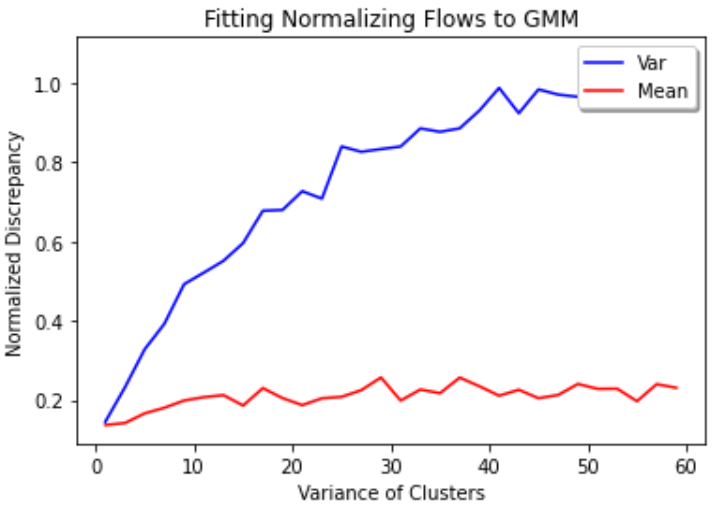
\includegraphics[scale=0.6]{figures/Mean_Var_really_accurate.PNG}
\caption{Experimentation on fitting planar flows on Gaussian Mixture Model with increasing variance and comparing mean (red) and variance (blue) of the two. Here the x-axis denotes the difference in variance $\sigma^2_{\mathrm{NF}}-\sigma^2_{\mathrm{gmm}}$ and the y-axis denotes the difference in mean $|\mu_{\mathrm{gmm}}-\mu_{\mathrm{NF}}|$ }
    \label{fig:my_label}
\end{figure}

\subsection{Multivatiate normal}

\lipsum[3]

With covariance matrix

\begin{figure}
    \centering
    % % This file was created with tikzplotlib v0.9.13.
\begin{tikzpicture}

\begin{axis}[
legend cell align={left},
legend style={
  fill opacity=0.8,
  draw opacity=1,
  text opacity=1,
  at={(0.97,0.03)},
  anchor=south east,
  draw=white!80!black
},
tick align=outside,
tick pos=left,
x grid style={white!69.0196078431373!black},
xlabel={Number of flows},
xmin=2.6, xmax=33.4,
xtick style={color=black},
y grid style={white!69.0196078431373!black},
ylabel={ELBO},
ymin=-18107.9666384118, ymax=-17870.5896779011,
ytick style={color=black}
]
\addplot [draw=blue, fill=blue, mark=*, only marks]
table{%
x  y
4 -18097.1767765704
8 -17904.5776323087
16 -17888.9819208821
32 -17881.3795397425
};
\addlegendentry{Planar}
\addplot [draw=red, fill=red, mark=*, only marks]
table{%
x  y
4 -18038.6877921755
8 -17931.7873051845
16 -17915.0520597312
32 -17885.7323459633
};
\addlegendentry{Radial}
\addplot [semithick, blue, dashed, forget plot]
table {%
4 -18097.1767765704
8 -17904.5776323087
16 -17888.9819208821
32 -17881.3795397425
};
\addplot [semithick, red, dashed, forget plot]
table {%
4 -18038.6877921755
8 -17931.7873051845
16 -17915.0520597312
32 -17885.7323459633
};
\end{axis}

\end{tikzpicture}

    \caption{Final ELBO of normalizing flow as a function of number of flows for correlated multivariate Normal posterior. The final ELBO was calculated as the mean of the ELBOs of the last 500 iterations from training.}
    \label{fig:planarvsradial}
\end{figure}

\subsection{Energy functions}

\lipsum[1]

\begin{table}
    \caption{Final ELBO for different potential energy posteriors from \textcite{rezende2015variational} (\cref{tab:test_energy_functions}).}
    \label{tab:energyresults}
    \centering
    \begin{tabular}{lrrrrrr}
\toprule
{} & \multicolumn{3}{l}{Planar} & \multicolumn{3}{l}{Radial} \\
{} &     2  &     8  &     32 &     2  &     8  &     32 \\
\midrule
\$U\_1(z)\$ &  73.50 & 256.24 & 279.24 & -61.84 & 236.32 & 272.28 \\
\$U\_2(z)\$ & 271.71 & 501.16 & 659.48 & -94.02 & 184.09 & 550.71 \\
\$U\_3(z)\$ & 418.16 & 666.00 & 967.83 & 211.54 & 576.92 & 761.59 \\
\$U\_4(z)\$ & 473.85 & 638.39 & 750.76 & 229.20 & 462.36 & 648.31 \\
\bottomrule
\end{tabular}

\end{table}

The normalizing flows were trained for 10000 epochs with an ADAM learning rate of $0.005$, 16 Markov Chain gradient estimation samples and 256 base distribution samples ($\Vec z_0 \sim q_0\left(\bullet |\Vec x\right)$).

\begin{figure}
    \centering
    % \resizebox{\textwidth}{!}{
    %     %% Creator: Matplotlib, PGF backend
%%
%% To include the figure in your LaTeX document, write
%%   \input{<filename>.pgf}
%%
%% Make sure the required packages are loaded in your preamble
%%   \usepackage{pgf}
%%
%% Figures using additional raster images can only be included by \input if
%% they are in the same directory as the main LaTeX file. For loading figures
%% from other directories you can use the `import` package
%%   \usepackage{import}
%% and then include the figures with
%%   \import{<path to file>}{<filename>.pgf}
%%
%% Matplotlib used the following preamble
%%
\begingroup%
\makeatletter%
\begin{pgfpicture}%
\pgfpathrectangle{\pgfpointorigin}{\pgfqpoint{6.720034in}{4.917417in}}%
\pgfusepath{use as bounding box, clip}%
\begin{pgfscope}%
\pgfsetbuttcap%
\pgfsetmiterjoin%
\definecolor{currentfill}{rgb}{1.000000,1.000000,1.000000}%
\pgfsetfillcolor{currentfill}%
\pgfsetlinewidth{0.000000pt}%
\definecolor{currentstroke}{rgb}{1.000000,1.000000,1.000000}%
\pgfsetstrokecolor{currentstroke}%
\pgfsetdash{}{0pt}%
\pgfpathmoveto{\pgfqpoint{0.000000in}{0.000000in}}%
\pgfpathlineto{\pgfqpoint{6.720034in}{0.000000in}}%
\pgfpathlineto{\pgfqpoint{6.720034in}{4.917417in}}%
\pgfpathlineto{\pgfqpoint{0.000000in}{4.917417in}}%
\pgfpathclose%
\pgfusepath{fill}%
\end{pgfscope}%
\begin{pgfscope}%
\pgfsetbuttcap%
\pgfsetmiterjoin%
\definecolor{currentfill}{rgb}{1.000000,1.000000,1.000000}%
\pgfsetfillcolor{currentfill}%
\pgfsetlinewidth{0.000000pt}%
\definecolor{currentstroke}{rgb}{0.000000,0.000000,0.000000}%
\pgfsetstrokecolor{currentstroke}%
\pgfsetstrokeopacity{0.000000}%
\pgfsetdash{}{0pt}%
\pgfpathmoveto{\pgfqpoint{0.651233in}{2.768162in}}%
\pgfpathlineto{\pgfqpoint{2.998438in}{2.768162in}}%
\pgfpathlineto{\pgfqpoint{2.998438in}{4.629917in}}%
\pgfpathlineto{\pgfqpoint{0.651233in}{4.629917in}}%
\pgfpathclose%
\pgfusepath{fill}%
\end{pgfscope}%
\begin{pgfscope}%
\pgfsetbuttcap%
\pgfsetroundjoin%
\definecolor{currentfill}{rgb}{0.150000,0.150000,0.150000}%
\pgfsetfillcolor{currentfill}%
\pgfsetlinewidth{1.003750pt}%
\definecolor{currentstroke}{rgb}{0.150000,0.150000,0.150000}%
\pgfsetstrokecolor{currentstroke}%
\pgfsetdash{}{0pt}%
\pgfsys@defobject{currentmarker}{\pgfqpoint{0.000000in}{-0.066667in}}{\pgfqpoint{0.000000in}{0.000000in}}{%
\pgfpathmoveto{\pgfqpoint{0.000000in}{0.000000in}}%
\pgfpathlineto{\pgfqpoint{0.000000in}{-0.066667in}}%
\pgfusepath{stroke,fill}%
}%
\begin{pgfscope}%
\pgfsys@transformshift{0.781195in}{2.768162in}%
\pgfsys@useobject{currentmarker}{}%
\end{pgfscope}%
\end{pgfscope}%
\begin{pgfscope}%
\pgfsetbuttcap%
\pgfsetroundjoin%
\definecolor{currentfill}{rgb}{0.150000,0.150000,0.150000}%
\pgfsetfillcolor{currentfill}%
\pgfsetlinewidth{1.003750pt}%
\definecolor{currentstroke}{rgb}{0.150000,0.150000,0.150000}%
\pgfsetstrokecolor{currentstroke}%
\pgfsetdash{}{0pt}%
\pgfsys@defobject{currentmarker}{\pgfqpoint{0.000000in}{-0.066667in}}{\pgfqpoint{0.000000in}{0.000000in}}{%
\pgfpathmoveto{\pgfqpoint{0.000000in}{0.000000in}}%
\pgfpathlineto{\pgfqpoint{0.000000in}{-0.066667in}}%
\pgfusepath{stroke,fill}%
}%
\begin{pgfscope}%
\pgfsys@transformshift{1.824835in}{2.768162in}%
\pgfsys@useobject{currentmarker}{}%
\end{pgfscope}%
\end{pgfscope}%
\begin{pgfscope}%
\pgfsetbuttcap%
\pgfsetroundjoin%
\definecolor{currentfill}{rgb}{0.150000,0.150000,0.150000}%
\pgfsetfillcolor{currentfill}%
\pgfsetlinewidth{1.003750pt}%
\definecolor{currentstroke}{rgb}{0.150000,0.150000,0.150000}%
\pgfsetstrokecolor{currentstroke}%
\pgfsetdash{}{0pt}%
\pgfsys@defobject{currentmarker}{\pgfqpoint{0.000000in}{-0.066667in}}{\pgfqpoint{0.000000in}{0.000000in}}{%
\pgfpathmoveto{\pgfqpoint{0.000000in}{0.000000in}}%
\pgfpathlineto{\pgfqpoint{0.000000in}{-0.066667in}}%
\pgfusepath{stroke,fill}%
}%
\begin{pgfscope}%
\pgfsys@transformshift{2.868476in}{2.768162in}%
\pgfsys@useobject{currentmarker}{}%
\end{pgfscope}%
\end{pgfscope}%
\begin{pgfscope}%
\pgfsetbuttcap%
\pgfsetroundjoin%
\definecolor{currentfill}{rgb}{0.150000,0.150000,0.150000}%
\pgfsetfillcolor{currentfill}%
\pgfsetlinewidth{1.003750pt}%
\definecolor{currentstroke}{rgb}{0.150000,0.150000,0.150000}%
\pgfsetstrokecolor{currentstroke}%
\pgfsetdash{}{0pt}%
\pgfsys@defobject{currentmarker}{\pgfqpoint{-0.066667in}{0.000000in}}{\pgfqpoint{0.000000in}{0.000000in}}{%
\pgfpathmoveto{\pgfqpoint{0.000000in}{0.000000in}}%
\pgfpathlineto{\pgfqpoint{-0.066667in}{0.000000in}}%
\pgfusepath{stroke,fill}%
}%
\begin{pgfscope}%
\pgfsys@transformshift{0.651233in}{3.159699in}%
\pgfsys@useobject{currentmarker}{}%
\end{pgfscope}%
\end{pgfscope}%
\begin{pgfscope}%
\definecolor{textcolor}{rgb}{0.150000,0.150000,0.150000}%
\pgfsetstrokecolor{textcolor}%
\pgfsetfillcolor{textcolor}%
\pgftext[x=0.471719in,y=3.116297in,left,base]{\color{textcolor}\rmfamily\fontsize{8.800000}{10.560000}\selectfont \(\displaystyle 0\)}%
\end{pgfscope}%
\begin{pgfscope}%
\pgfsetbuttcap%
\pgfsetroundjoin%
\definecolor{currentfill}{rgb}{0.150000,0.150000,0.150000}%
\pgfsetfillcolor{currentfill}%
\pgfsetlinewidth{1.003750pt}%
\definecolor{currentstroke}{rgb}{0.150000,0.150000,0.150000}%
\pgfsetstrokecolor{currentstroke}%
\pgfsetdash{}{0pt}%
\pgfsys@defobject{currentmarker}{\pgfqpoint{-0.066667in}{0.000000in}}{\pgfqpoint{0.000000in}{0.000000in}}{%
\pgfpathmoveto{\pgfqpoint{0.000000in}{0.000000in}}%
\pgfpathlineto{\pgfqpoint{-0.066667in}{0.000000in}}%
\pgfusepath{stroke,fill}%
}%
\begin{pgfscope}%
\pgfsys@transformshift{0.651233in}{3.655882in}%
\pgfsys@useobject{currentmarker}{}%
\end{pgfscope}%
\end{pgfscope}%
\begin{pgfscope}%
\definecolor{textcolor}{rgb}{0.150000,0.150000,0.150000}%
\pgfsetstrokecolor{textcolor}%
\pgfsetfillcolor{textcolor}%
\pgftext[x=0.343248in,y=3.612479in,left,base]{\color{textcolor}\rmfamily\fontsize{8.800000}{10.560000}\selectfont \(\displaystyle 100\)}%
\end{pgfscope}%
\begin{pgfscope}%
\pgfsetbuttcap%
\pgfsetroundjoin%
\definecolor{currentfill}{rgb}{0.150000,0.150000,0.150000}%
\pgfsetfillcolor{currentfill}%
\pgfsetlinewidth{1.003750pt}%
\definecolor{currentstroke}{rgb}{0.150000,0.150000,0.150000}%
\pgfsetstrokecolor{currentstroke}%
\pgfsetdash{}{0pt}%
\pgfsys@defobject{currentmarker}{\pgfqpoint{-0.066667in}{0.000000in}}{\pgfqpoint{0.000000in}{0.000000in}}{%
\pgfpathmoveto{\pgfqpoint{0.000000in}{0.000000in}}%
\pgfpathlineto{\pgfqpoint{-0.066667in}{0.000000in}}%
\pgfusepath{stroke,fill}%
}%
\begin{pgfscope}%
\pgfsys@transformshift{0.651233in}{4.152064in}%
\pgfsys@useobject{currentmarker}{}%
\end{pgfscope}%
\end{pgfscope}%
\begin{pgfscope}%
\definecolor{textcolor}{rgb}{0.150000,0.150000,0.150000}%
\pgfsetstrokecolor{textcolor}%
\pgfsetfillcolor{textcolor}%
\pgftext[x=0.343248in,y=4.108661in,left,base]{\color{textcolor}\rmfamily\fontsize{8.800000}{10.560000}\selectfont \(\displaystyle 200\)}%
\end{pgfscope}%
\begin{pgfscope}%
\definecolor{textcolor}{rgb}{0.150000,0.150000,0.150000}%
\pgfsetstrokecolor{textcolor}%
\pgfsetfillcolor{textcolor}%
\pgftext[x=0.287692in,y=3.699039in,,bottom,rotate=90.000000]{\color{textcolor}\rmfamily\fontsize{9.600000}{11.520000}\selectfont ELBO}%
\end{pgfscope}%
\begin{pgfscope}%
\pgfpathrectangle{\pgfqpoint{0.651233in}{2.768162in}}{\pgfqpoint{2.347205in}{1.861755in}}%
\pgfusepath{clip}%
\pgfsetbuttcap%
\pgfsetroundjoin%
\definecolor{currentfill}{rgb}{0.768627,0.305882,0.321569}%
\pgfsetfillcolor{currentfill}%
\pgfsetlinewidth{0.385440pt}%
\definecolor{currentstroke}{rgb}{1.000000,1.000000,1.000000}%
\pgfsetstrokecolor{currentstroke}%
\pgfsetdash{}{0pt}%
\pgfpathmoveto{\pgfqpoint{0.781195in}{3.491054in}}%
\pgfpathcurveto{\pgfqpoint{0.790035in}{3.491054in}}{\pgfqpoint{0.798514in}{3.494566in}}{\pgfqpoint{0.804765in}{3.500817in}}%
\pgfpathcurveto{\pgfqpoint{0.811016in}{3.507068in}}{\pgfqpoint{0.814528in}{3.515547in}}{\pgfqpoint{0.814528in}{3.524387in}}%
\pgfpathcurveto{\pgfqpoint{0.814528in}{3.533228in}}{\pgfqpoint{0.811016in}{3.541707in}}{\pgfqpoint{0.804765in}{3.547958in}}%
\pgfpathcurveto{\pgfqpoint{0.798514in}{3.554209in}}{\pgfqpoint{0.790035in}{3.557721in}}{\pgfqpoint{0.781195in}{3.557721in}}%
\pgfpathcurveto{\pgfqpoint{0.772355in}{3.557721in}}{\pgfqpoint{0.763875in}{3.554209in}}{\pgfqpoint{0.757624in}{3.547958in}}%
\pgfpathcurveto{\pgfqpoint{0.751374in}{3.541707in}}{\pgfqpoint{0.747861in}{3.533228in}}{\pgfqpoint{0.747861in}{3.524387in}}%
\pgfpathcurveto{\pgfqpoint{0.747861in}{3.515547in}}{\pgfqpoint{0.751374in}{3.507068in}}{\pgfqpoint{0.757624in}{3.500817in}}%
\pgfpathcurveto{\pgfqpoint{0.763875in}{3.494566in}}{\pgfqpoint{0.772355in}{3.491054in}}{\pgfqpoint{0.781195in}{3.491054in}}%
\pgfpathclose%
\pgfusepath{stroke,fill}%
\end{pgfscope}%
\begin{pgfscope}%
\pgfpathrectangle{\pgfqpoint{0.651233in}{2.768162in}}{\pgfqpoint{2.347205in}{1.861755in}}%
\pgfusepath{clip}%
\pgfsetbuttcap%
\pgfsetroundjoin%
\definecolor{currentfill}{rgb}{0.768627,0.305882,0.321569}%
\pgfsetfillcolor{currentfill}%
\pgfsetlinewidth{0.385440pt}%
\definecolor{currentstroke}{rgb}{1.000000,1.000000,1.000000}%
\pgfsetstrokecolor{currentstroke}%
\pgfsetdash{}{0pt}%
\pgfpathmoveto{\pgfqpoint{1.824835in}{4.397807in}}%
\pgfpathcurveto{\pgfqpoint{1.833676in}{4.397807in}}{\pgfqpoint{1.842155in}{4.401319in}}{\pgfqpoint{1.848406in}{4.407570in}}%
\pgfpathcurveto{\pgfqpoint{1.854657in}{4.413821in}}{\pgfqpoint{1.858169in}{4.422300in}}{\pgfqpoint{1.858169in}{4.431140in}}%
\pgfpathcurveto{\pgfqpoint{1.858169in}{4.439980in}}{\pgfqpoint{1.854657in}{4.448459in}}{\pgfqpoint{1.848406in}{4.454710in}}%
\pgfpathcurveto{\pgfqpoint{1.842155in}{4.460961in}}{\pgfqpoint{1.833676in}{4.464473in}}{\pgfqpoint{1.824835in}{4.464473in}}%
\pgfpathcurveto{\pgfqpoint{1.815995in}{4.464473in}}{\pgfqpoint{1.807516in}{4.460961in}}{\pgfqpoint{1.801265in}{4.454710in}}%
\pgfpathcurveto{\pgfqpoint{1.795014in}{4.448459in}}{\pgfqpoint{1.791502in}{4.439980in}}{\pgfqpoint{1.791502in}{4.431140in}}%
\pgfpathcurveto{\pgfqpoint{1.791502in}{4.422300in}}{\pgfqpoint{1.795014in}{4.413821in}}{\pgfqpoint{1.801265in}{4.407570in}}%
\pgfpathcurveto{\pgfqpoint{1.807516in}{4.401319in}}{\pgfqpoint{1.815995in}{4.397807in}}{\pgfqpoint{1.824835in}{4.397807in}}%
\pgfpathclose%
\pgfusepath{stroke,fill}%
\end{pgfscope}%
\begin{pgfscope}%
\pgfpathrectangle{\pgfqpoint{0.651233in}{2.768162in}}{\pgfqpoint{2.347205in}{1.861755in}}%
\pgfusepath{clip}%
\pgfsetbuttcap%
\pgfsetroundjoin%
\definecolor{currentfill}{rgb}{0.768627,0.305882,0.321569}%
\pgfsetfillcolor{currentfill}%
\pgfsetlinewidth{0.385440pt}%
\definecolor{currentstroke}{rgb}{1.000000,1.000000,1.000000}%
\pgfsetstrokecolor{currentstroke}%
\pgfsetdash{}{0pt}%
\pgfpathmoveto{\pgfqpoint{2.868476in}{4.511893in}}%
\pgfpathcurveto{\pgfqpoint{2.877316in}{4.511893in}}{\pgfqpoint{2.885796in}{4.515405in}}{\pgfqpoint{2.892046in}{4.521656in}}%
\pgfpathcurveto{\pgfqpoint{2.898297in}{4.527907in}}{\pgfqpoint{2.901810in}{4.536386in}}{\pgfqpoint{2.901810in}{4.545226in}}%
\pgfpathcurveto{\pgfqpoint{2.901810in}{4.554067in}}{\pgfqpoint{2.898297in}{4.562546in}}{\pgfqpoint{2.892046in}{4.568797in}}%
\pgfpathcurveto{\pgfqpoint{2.885796in}{4.575048in}}{\pgfqpoint{2.877316in}{4.578560in}}{\pgfqpoint{2.868476in}{4.578560in}}%
\pgfpathcurveto{\pgfqpoint{2.859636in}{4.578560in}}{\pgfqpoint{2.851157in}{4.575048in}}{\pgfqpoint{2.844906in}{4.568797in}}%
\pgfpathcurveto{\pgfqpoint{2.838655in}{4.562546in}}{\pgfqpoint{2.835143in}{4.554067in}}{\pgfqpoint{2.835143in}{4.545226in}}%
\pgfpathcurveto{\pgfqpoint{2.835143in}{4.536386in}}{\pgfqpoint{2.838655in}{4.527907in}}{\pgfqpoint{2.844906in}{4.521656in}}%
\pgfpathcurveto{\pgfqpoint{2.851157in}{4.515405in}}{\pgfqpoint{2.859636in}{4.511893in}}{\pgfqpoint{2.868476in}{4.511893in}}%
\pgfpathclose%
\pgfusepath{stroke,fill}%
\end{pgfscope}%
\begin{pgfscope}%
\pgfpathrectangle{\pgfqpoint{0.651233in}{2.768162in}}{\pgfqpoint{2.347205in}{1.861755in}}%
\pgfusepath{clip}%
\pgfsetbuttcap%
\pgfsetroundjoin%
\definecolor{currentfill}{rgb}{0.298039,0.447059,0.690196}%
\pgfsetfillcolor{currentfill}%
\pgfsetlinewidth{0.385440pt}%
\definecolor{currentstroke}{rgb}{1.000000,1.000000,1.000000}%
\pgfsetstrokecolor{currentstroke}%
\pgfsetdash{}{0pt}%
\pgfpathmoveto{\pgfqpoint{0.781195in}{2.819519in}}%
\pgfpathcurveto{\pgfqpoint{0.790035in}{2.819519in}}{\pgfqpoint{0.798514in}{2.823031in}}{\pgfqpoint{0.804765in}{2.829282in}}%
\pgfpathcurveto{\pgfqpoint{0.811016in}{2.835533in}}{\pgfqpoint{0.814528in}{2.844012in}}{\pgfqpoint{0.814528in}{2.852852in}}%
\pgfpathcurveto{\pgfqpoint{0.814528in}{2.861692in}}{\pgfqpoint{0.811016in}{2.870171in}}{\pgfqpoint{0.804765in}{2.876422in}}%
\pgfpathcurveto{\pgfqpoint{0.798514in}{2.882673in}}{\pgfqpoint{0.790035in}{2.886185in}}{\pgfqpoint{0.781195in}{2.886185in}}%
\pgfpathcurveto{\pgfqpoint{0.772355in}{2.886185in}}{\pgfqpoint{0.763875in}{2.882673in}}{\pgfqpoint{0.757624in}{2.876422in}}%
\pgfpathcurveto{\pgfqpoint{0.751374in}{2.870171in}}{\pgfqpoint{0.747861in}{2.861692in}}{\pgfqpoint{0.747861in}{2.852852in}}%
\pgfpathcurveto{\pgfqpoint{0.747861in}{2.844012in}}{\pgfqpoint{0.751374in}{2.835533in}}{\pgfqpoint{0.757624in}{2.829282in}}%
\pgfpathcurveto{\pgfqpoint{0.763875in}{2.823031in}}{\pgfqpoint{0.772355in}{2.819519in}}{\pgfqpoint{0.781195in}{2.819519in}}%
\pgfpathclose%
\pgfusepath{stroke,fill}%
\end{pgfscope}%
\begin{pgfscope}%
\pgfpathrectangle{\pgfqpoint{0.651233in}{2.768162in}}{\pgfqpoint{2.347205in}{1.861755in}}%
\pgfusepath{clip}%
\pgfsetbuttcap%
\pgfsetroundjoin%
\definecolor{currentfill}{rgb}{0.298039,0.447059,0.690196}%
\pgfsetfillcolor{currentfill}%
\pgfsetlinewidth{0.385440pt}%
\definecolor{currentstroke}{rgb}{1.000000,1.000000,1.000000}%
\pgfsetstrokecolor{currentstroke}%
\pgfsetdash{}{0pt}%
\pgfpathmoveto{\pgfqpoint{1.824835in}{4.298948in}}%
\pgfpathcurveto{\pgfqpoint{1.833676in}{4.298948in}}{\pgfqpoint{1.842155in}{4.302460in}}{\pgfqpoint{1.848406in}{4.308711in}}%
\pgfpathcurveto{\pgfqpoint{1.854657in}{4.314962in}}{\pgfqpoint{1.858169in}{4.323441in}}{\pgfqpoint{1.858169in}{4.332282in}}%
\pgfpathcurveto{\pgfqpoint{1.858169in}{4.341122in}}{\pgfqpoint{1.854657in}{4.349601in}}{\pgfqpoint{1.848406in}{4.355852in}}%
\pgfpathcurveto{\pgfqpoint{1.842155in}{4.362103in}}{\pgfqpoint{1.833676in}{4.365615in}}{\pgfqpoint{1.824835in}{4.365615in}}%
\pgfpathcurveto{\pgfqpoint{1.815995in}{4.365615in}}{\pgfqpoint{1.807516in}{4.362103in}}{\pgfqpoint{1.801265in}{4.355852in}}%
\pgfpathcurveto{\pgfqpoint{1.795014in}{4.349601in}}{\pgfqpoint{1.791502in}{4.341122in}}{\pgfqpoint{1.791502in}{4.332282in}}%
\pgfpathcurveto{\pgfqpoint{1.791502in}{4.323441in}}{\pgfqpoint{1.795014in}{4.314962in}}{\pgfqpoint{1.801265in}{4.308711in}}%
\pgfpathcurveto{\pgfqpoint{1.807516in}{4.302460in}}{\pgfqpoint{1.815995in}{4.298948in}}{\pgfqpoint{1.824835in}{4.298948in}}%
\pgfpathclose%
\pgfusepath{stroke,fill}%
\end{pgfscope}%
\begin{pgfscope}%
\pgfpathrectangle{\pgfqpoint{0.651233in}{2.768162in}}{\pgfqpoint{2.347205in}{1.861755in}}%
\pgfusepath{clip}%
\pgfsetbuttcap%
\pgfsetroundjoin%
\definecolor{currentfill}{rgb}{0.298039,0.447059,0.690196}%
\pgfsetfillcolor{currentfill}%
\pgfsetlinewidth{0.385440pt}%
\definecolor{currentstroke}{rgb}{1.000000,1.000000,1.000000}%
\pgfsetstrokecolor{currentstroke}%
\pgfsetdash{}{0pt}%
\pgfpathmoveto{\pgfqpoint{2.868476in}{4.477395in}}%
\pgfpathcurveto{\pgfqpoint{2.877316in}{4.477395in}}{\pgfqpoint{2.885796in}{4.480907in}}{\pgfqpoint{2.892046in}{4.487158in}}%
\pgfpathcurveto{\pgfqpoint{2.898297in}{4.493409in}}{\pgfqpoint{2.901810in}{4.501888in}}{\pgfqpoint{2.901810in}{4.510728in}}%
\pgfpathcurveto{\pgfqpoint{2.901810in}{4.519568in}}{\pgfqpoint{2.898297in}{4.528047in}}{\pgfqpoint{2.892046in}{4.534298in}}%
\pgfpathcurveto{\pgfqpoint{2.885796in}{4.540549in}}{\pgfqpoint{2.877316in}{4.544061in}}{\pgfqpoint{2.868476in}{4.544061in}}%
\pgfpathcurveto{\pgfqpoint{2.859636in}{4.544061in}}{\pgfqpoint{2.851157in}{4.540549in}}{\pgfqpoint{2.844906in}{4.534298in}}%
\pgfpathcurveto{\pgfqpoint{2.838655in}{4.528047in}}{\pgfqpoint{2.835143in}{4.519568in}}{\pgfqpoint{2.835143in}{4.510728in}}%
\pgfpathcurveto{\pgfqpoint{2.835143in}{4.501888in}}{\pgfqpoint{2.838655in}{4.493409in}}{\pgfqpoint{2.844906in}{4.487158in}}%
\pgfpathcurveto{\pgfqpoint{2.851157in}{4.480907in}}{\pgfqpoint{2.859636in}{4.477395in}}{\pgfqpoint{2.868476in}{4.477395in}}%
\pgfpathclose%
\pgfusepath{stroke,fill}%
\end{pgfscope}%
\begin{pgfscope}%
\pgfpathrectangle{\pgfqpoint{0.651233in}{2.768162in}}{\pgfqpoint{2.347205in}{1.861755in}}%
\pgfusepath{clip}%
\pgfsetbuttcap%
\pgfsetroundjoin%
\definecolor{currentfill}{rgb}{0.768627,0.305882,0.321569}%
\pgfsetfillcolor{currentfill}%
\pgfsetlinewidth{0.803000pt}%
\definecolor{currentstroke}{rgb}{0.768627,0.305882,0.321569}%
\pgfsetstrokecolor{currentstroke}%
\pgfsetdash{}{0pt}%
\pgfpathmoveto{\pgfqpoint{0.000000in}{-0.033333in}}%
\pgfpathcurveto{\pgfqpoint{0.008840in}{-0.033333in}}{\pgfqpoint{0.017319in}{-0.029821in}}{\pgfqpoint{0.023570in}{-0.023570in}}%
\pgfpathcurveto{\pgfqpoint{0.029821in}{-0.017319in}}{\pgfqpoint{0.033333in}{-0.008840in}}{\pgfqpoint{0.033333in}{0.000000in}}%
\pgfpathcurveto{\pgfqpoint{0.033333in}{0.008840in}}{\pgfqpoint{0.029821in}{0.017319in}}{\pgfqpoint{0.023570in}{0.023570in}}%
\pgfpathcurveto{\pgfqpoint{0.017319in}{0.029821in}}{\pgfqpoint{0.008840in}{0.033333in}}{\pgfqpoint{0.000000in}{0.033333in}}%
\pgfpathcurveto{\pgfqpoint{-0.008840in}{0.033333in}}{\pgfqpoint{-0.017319in}{0.029821in}}{\pgfqpoint{-0.023570in}{0.023570in}}%
\pgfpathcurveto{\pgfqpoint{-0.029821in}{0.017319in}}{\pgfqpoint{-0.033333in}{0.008840in}}{\pgfqpoint{-0.033333in}{0.000000in}}%
\pgfpathcurveto{\pgfqpoint{-0.033333in}{-0.008840in}}{\pgfqpoint{-0.029821in}{-0.017319in}}{\pgfqpoint{-0.023570in}{-0.023570in}}%
\pgfpathcurveto{\pgfqpoint{-0.017319in}{-0.029821in}}{\pgfqpoint{-0.008840in}{-0.033333in}}{\pgfqpoint{0.000000in}{-0.033333in}}%
\pgfpathclose%
\pgfusepath{stroke,fill}%
\end{pgfscope}%
\begin{pgfscope}%
\pgfpathrectangle{\pgfqpoint{0.651233in}{2.768162in}}{\pgfqpoint{2.347205in}{1.861755in}}%
\pgfusepath{clip}%
\pgfsetbuttcap%
\pgfsetroundjoin%
\definecolor{currentfill}{rgb}{0.298039,0.447059,0.690196}%
\pgfsetfillcolor{currentfill}%
\pgfsetlinewidth{0.803000pt}%
\definecolor{currentstroke}{rgb}{0.298039,0.447059,0.690196}%
\pgfsetstrokecolor{currentstroke}%
\pgfsetdash{}{0pt}%
\pgfpathmoveto{\pgfqpoint{0.000000in}{-0.033333in}}%
\pgfpathcurveto{\pgfqpoint{0.008840in}{-0.033333in}}{\pgfqpoint{0.017319in}{-0.029821in}}{\pgfqpoint{0.023570in}{-0.023570in}}%
\pgfpathcurveto{\pgfqpoint{0.029821in}{-0.017319in}}{\pgfqpoint{0.033333in}{-0.008840in}}{\pgfqpoint{0.033333in}{0.000000in}}%
\pgfpathcurveto{\pgfqpoint{0.033333in}{0.008840in}}{\pgfqpoint{0.029821in}{0.017319in}}{\pgfqpoint{0.023570in}{0.023570in}}%
\pgfpathcurveto{\pgfqpoint{0.017319in}{0.029821in}}{\pgfqpoint{0.008840in}{0.033333in}}{\pgfqpoint{0.000000in}{0.033333in}}%
\pgfpathcurveto{\pgfqpoint{-0.008840in}{0.033333in}}{\pgfqpoint{-0.017319in}{0.029821in}}{\pgfqpoint{-0.023570in}{0.023570in}}%
\pgfpathcurveto{\pgfqpoint{-0.029821in}{0.017319in}}{\pgfqpoint{-0.033333in}{0.008840in}}{\pgfqpoint{-0.033333in}{0.000000in}}%
\pgfpathcurveto{\pgfqpoint{-0.033333in}{-0.008840in}}{\pgfqpoint{-0.029821in}{-0.017319in}}{\pgfqpoint{-0.023570in}{-0.023570in}}%
\pgfpathcurveto{\pgfqpoint{-0.017319in}{-0.029821in}}{\pgfqpoint{-0.008840in}{-0.033333in}}{\pgfqpoint{0.000000in}{-0.033333in}}%
\pgfpathclose%
\pgfusepath{stroke,fill}%
\end{pgfscope}%
\begin{pgfscope}%
\pgfpathrectangle{\pgfqpoint{0.651233in}{2.768162in}}{\pgfqpoint{2.347205in}{1.861755in}}%
\pgfusepath{clip}%
\pgfsetbuttcap%
\pgfsetroundjoin%
\pgfsetlinewidth{2.007500pt}%
\definecolor{currentstroke}{rgb}{0.768627,0.305882,0.321569}%
\pgfsetstrokecolor{currentstroke}%
\pgfsetdash{{7.400000pt}{3.200000pt}}{0.000000pt}%
\pgfpathmoveto{\pgfqpoint{0.781195in}{3.524387in}}%
\pgfpathlineto{\pgfqpoint{1.824835in}{4.431140in}}%
\pgfpathlineto{\pgfqpoint{2.868476in}{4.545226in}}%
\pgfusepath{stroke}%
\end{pgfscope}%
\begin{pgfscope}%
\pgfpathrectangle{\pgfqpoint{0.651233in}{2.768162in}}{\pgfqpoint{2.347205in}{1.861755in}}%
\pgfusepath{clip}%
\pgfsetbuttcap%
\pgfsetroundjoin%
\pgfsetlinewidth{2.007500pt}%
\definecolor{currentstroke}{rgb}{0.298039,0.447059,0.690196}%
\pgfsetstrokecolor{currentstroke}%
\pgfsetdash{{7.400000pt}{3.200000pt}}{0.000000pt}%
\pgfpathmoveto{\pgfqpoint{0.781195in}{2.852852in}}%
\pgfpathlineto{\pgfqpoint{1.824835in}{4.332282in}}%
\pgfpathlineto{\pgfqpoint{2.868476in}{4.510728in}}%
\pgfusepath{stroke}%
\end{pgfscope}%
\begin{pgfscope}%
\pgfsetrectcap%
\pgfsetmiterjoin%
\pgfsetlinewidth{1.003750pt}%
\definecolor{currentstroke}{rgb}{0.150000,0.150000,0.150000}%
\pgfsetstrokecolor{currentstroke}%
\pgfsetdash{}{0pt}%
\pgfpathmoveto{\pgfqpoint{0.651233in}{2.768162in}}%
\pgfpathlineto{\pgfqpoint{0.651233in}{4.629917in}}%
\pgfusepath{stroke}%
\end{pgfscope}%
\begin{pgfscope}%
\pgfsetrectcap%
\pgfsetmiterjoin%
\pgfsetlinewidth{1.003750pt}%
\definecolor{currentstroke}{rgb}{0.150000,0.150000,0.150000}%
\pgfsetstrokecolor{currentstroke}%
\pgfsetdash{}{0pt}%
\pgfpathmoveto{\pgfqpoint{0.651233in}{2.768162in}}%
\pgfpathlineto{\pgfqpoint{2.998438in}{2.768162in}}%
\pgfusepath{stroke}%
\end{pgfscope}%
\begin{pgfscope}%
\definecolor{textcolor}{rgb}{0.150000,0.150000,0.150000}%
\pgfsetstrokecolor{textcolor}%
\pgfsetfillcolor{textcolor}%
\pgftext[x=1.824835in,y=4.713250in,,base]{\color{textcolor}\rmfamily\fontsize{9.600000}{11.520000}\selectfont \(\displaystyle U_1(z)\)}%
\end{pgfscope}%
\begin{pgfscope}%
\pgfsetbuttcap%
\pgfsetmiterjoin%
\definecolor{currentfill}{rgb}{1.000000,1.000000,1.000000}%
\pgfsetfillcolor{currentfill}%
\pgfsetlinewidth{0.000000pt}%
\definecolor{currentstroke}{rgb}{0.000000,0.000000,0.000000}%
\pgfsetstrokecolor{currentstroke}%
\pgfsetstrokeopacity{0.000000}%
\pgfsetdash{}{0pt}%
\pgfpathmoveto{\pgfqpoint{3.450187in}{2.768162in}}%
\pgfpathlineto{\pgfqpoint{5.797392in}{2.768162in}}%
\pgfpathlineto{\pgfqpoint{5.797392in}{4.629917in}}%
\pgfpathlineto{\pgfqpoint{3.450187in}{4.629917in}}%
\pgfpathclose%
\pgfusepath{fill}%
\end{pgfscope}%
\begin{pgfscope}%
\pgfsetbuttcap%
\pgfsetroundjoin%
\definecolor{currentfill}{rgb}{0.150000,0.150000,0.150000}%
\pgfsetfillcolor{currentfill}%
\pgfsetlinewidth{1.003750pt}%
\definecolor{currentstroke}{rgb}{0.150000,0.150000,0.150000}%
\pgfsetstrokecolor{currentstroke}%
\pgfsetdash{}{0pt}%
\pgfsys@defobject{currentmarker}{\pgfqpoint{0.000000in}{-0.066667in}}{\pgfqpoint{0.000000in}{0.000000in}}{%
\pgfpathmoveto{\pgfqpoint{0.000000in}{0.000000in}}%
\pgfpathlineto{\pgfqpoint{0.000000in}{-0.066667in}}%
\pgfusepath{stroke,fill}%
}%
\begin{pgfscope}%
\pgfsys@transformshift{3.580149in}{2.768162in}%
\pgfsys@useobject{currentmarker}{}%
\end{pgfscope}%
\end{pgfscope}%
\begin{pgfscope}%
\pgfsetbuttcap%
\pgfsetroundjoin%
\definecolor{currentfill}{rgb}{0.150000,0.150000,0.150000}%
\pgfsetfillcolor{currentfill}%
\pgfsetlinewidth{1.003750pt}%
\definecolor{currentstroke}{rgb}{0.150000,0.150000,0.150000}%
\pgfsetstrokecolor{currentstroke}%
\pgfsetdash{}{0pt}%
\pgfsys@defobject{currentmarker}{\pgfqpoint{0.000000in}{-0.066667in}}{\pgfqpoint{0.000000in}{0.000000in}}{%
\pgfpathmoveto{\pgfqpoint{0.000000in}{0.000000in}}%
\pgfpathlineto{\pgfqpoint{0.000000in}{-0.066667in}}%
\pgfusepath{stroke,fill}%
}%
\begin{pgfscope}%
\pgfsys@transformshift{4.623790in}{2.768162in}%
\pgfsys@useobject{currentmarker}{}%
\end{pgfscope}%
\end{pgfscope}%
\begin{pgfscope}%
\pgfsetbuttcap%
\pgfsetroundjoin%
\definecolor{currentfill}{rgb}{0.150000,0.150000,0.150000}%
\pgfsetfillcolor{currentfill}%
\pgfsetlinewidth{1.003750pt}%
\definecolor{currentstroke}{rgb}{0.150000,0.150000,0.150000}%
\pgfsetstrokecolor{currentstroke}%
\pgfsetdash{}{0pt}%
\pgfsys@defobject{currentmarker}{\pgfqpoint{0.000000in}{-0.066667in}}{\pgfqpoint{0.000000in}{0.000000in}}{%
\pgfpathmoveto{\pgfqpoint{0.000000in}{0.000000in}}%
\pgfpathlineto{\pgfqpoint{0.000000in}{-0.066667in}}%
\pgfusepath{stroke,fill}%
}%
\begin{pgfscope}%
\pgfsys@transformshift{5.667430in}{2.768162in}%
\pgfsys@useobject{currentmarker}{}%
\end{pgfscope}%
\end{pgfscope}%
\begin{pgfscope}%
\pgfsetbuttcap%
\pgfsetroundjoin%
\definecolor{currentfill}{rgb}{0.150000,0.150000,0.150000}%
\pgfsetfillcolor{currentfill}%
\pgfsetlinewidth{1.003750pt}%
\definecolor{currentstroke}{rgb}{0.150000,0.150000,0.150000}%
\pgfsetstrokecolor{currentstroke}%
\pgfsetdash{}{0pt}%
\pgfsys@defobject{currentmarker}{\pgfqpoint{-0.066667in}{0.000000in}}{\pgfqpoint{0.000000in}{0.000000in}}{%
\pgfpathmoveto{\pgfqpoint{0.000000in}{0.000000in}}%
\pgfpathlineto{\pgfqpoint{-0.066667in}{0.000000in}}%
\pgfusepath{stroke,fill}%
}%
\begin{pgfscope}%
\pgfsys@transformshift{3.450187in}{3.063986in}%
\pgfsys@useobject{currentmarker}{}%
\end{pgfscope}%
\end{pgfscope}%
\begin{pgfscope}%
\definecolor{textcolor}{rgb}{0.150000,0.150000,0.150000}%
\pgfsetstrokecolor{textcolor}%
\pgfsetfillcolor{textcolor}%
\pgftext[x=3.270673in,y=3.020583in,left,base]{\color{textcolor}\rmfamily\fontsize{8.800000}{10.560000}\selectfont \(\displaystyle 0\)}%
\end{pgfscope}%
\begin{pgfscope}%
\pgfsetbuttcap%
\pgfsetroundjoin%
\definecolor{currentfill}{rgb}{0.150000,0.150000,0.150000}%
\pgfsetfillcolor{currentfill}%
\pgfsetlinewidth{1.003750pt}%
\definecolor{currentstroke}{rgb}{0.150000,0.150000,0.150000}%
\pgfsetstrokecolor{currentstroke}%
\pgfsetdash{}{0pt}%
\pgfsys@defobject{currentmarker}{\pgfqpoint{-0.066667in}{0.000000in}}{\pgfqpoint{0.000000in}{0.000000in}}{%
\pgfpathmoveto{\pgfqpoint{0.000000in}{0.000000in}}%
\pgfpathlineto{\pgfqpoint{-0.066667in}{0.000000in}}%
\pgfusepath{stroke,fill}%
}%
\begin{pgfscope}%
\pgfsys@transformshift{3.450187in}{3.513208in}%
\pgfsys@useobject{currentmarker}{}%
\end{pgfscope}%
\end{pgfscope}%
\begin{pgfscope}%
\definecolor{textcolor}{rgb}{0.150000,0.150000,0.150000}%
\pgfsetstrokecolor{textcolor}%
\pgfsetfillcolor{textcolor}%
\pgftext[x=3.142202in,y=3.469805in,left,base]{\color{textcolor}\rmfamily\fontsize{8.800000}{10.560000}\selectfont \(\displaystyle 200\)}%
\end{pgfscope}%
\begin{pgfscope}%
\pgfsetbuttcap%
\pgfsetroundjoin%
\definecolor{currentfill}{rgb}{0.150000,0.150000,0.150000}%
\pgfsetfillcolor{currentfill}%
\pgfsetlinewidth{1.003750pt}%
\definecolor{currentstroke}{rgb}{0.150000,0.150000,0.150000}%
\pgfsetstrokecolor{currentstroke}%
\pgfsetdash{}{0pt}%
\pgfsys@defobject{currentmarker}{\pgfqpoint{-0.066667in}{0.000000in}}{\pgfqpoint{0.000000in}{0.000000in}}{%
\pgfpathmoveto{\pgfqpoint{0.000000in}{0.000000in}}%
\pgfpathlineto{\pgfqpoint{-0.066667in}{0.000000in}}%
\pgfusepath{stroke,fill}%
}%
\begin{pgfscope}%
\pgfsys@transformshift{3.450187in}{3.962430in}%
\pgfsys@useobject{currentmarker}{}%
\end{pgfscope}%
\end{pgfscope}%
\begin{pgfscope}%
\definecolor{textcolor}{rgb}{0.150000,0.150000,0.150000}%
\pgfsetstrokecolor{textcolor}%
\pgfsetfillcolor{textcolor}%
\pgftext[x=3.142202in,y=3.919027in,left,base]{\color{textcolor}\rmfamily\fontsize{8.800000}{10.560000}\selectfont \(\displaystyle 400\)}%
\end{pgfscope}%
\begin{pgfscope}%
\pgfsetbuttcap%
\pgfsetroundjoin%
\definecolor{currentfill}{rgb}{0.150000,0.150000,0.150000}%
\pgfsetfillcolor{currentfill}%
\pgfsetlinewidth{1.003750pt}%
\definecolor{currentstroke}{rgb}{0.150000,0.150000,0.150000}%
\pgfsetstrokecolor{currentstroke}%
\pgfsetdash{}{0pt}%
\pgfsys@defobject{currentmarker}{\pgfqpoint{-0.066667in}{0.000000in}}{\pgfqpoint{0.000000in}{0.000000in}}{%
\pgfpathmoveto{\pgfqpoint{0.000000in}{0.000000in}}%
\pgfpathlineto{\pgfqpoint{-0.066667in}{0.000000in}}%
\pgfusepath{stroke,fill}%
}%
\begin{pgfscope}%
\pgfsys@transformshift{3.450187in}{4.411652in}%
\pgfsys@useobject{currentmarker}{}%
\end{pgfscope}%
\end{pgfscope}%
\begin{pgfscope}%
\definecolor{textcolor}{rgb}{0.150000,0.150000,0.150000}%
\pgfsetstrokecolor{textcolor}%
\pgfsetfillcolor{textcolor}%
\pgftext[x=3.142202in,y=4.368249in,left,base]{\color{textcolor}\rmfamily\fontsize{8.800000}{10.560000}\selectfont \(\displaystyle 600\)}%
\end{pgfscope}%
\begin{pgfscope}%
\pgfpathrectangle{\pgfqpoint{3.450187in}{2.768162in}}{\pgfqpoint{2.347205in}{1.861755in}}%
\pgfusepath{clip}%
\pgfsetbuttcap%
\pgfsetroundjoin%
\definecolor{currentfill}{rgb}{0.768627,0.305882,0.321569}%
\pgfsetfillcolor{currentfill}%
\pgfsetlinewidth{0.385440pt}%
\definecolor{currentstroke}{rgb}{1.000000,1.000000,1.000000}%
\pgfsetstrokecolor{currentstroke}%
\pgfsetdash{}{0pt}%
\pgfpathmoveto{\pgfqpoint{3.580149in}{3.640953in}}%
\pgfpathcurveto{\pgfqpoint{3.588989in}{3.640953in}}{\pgfqpoint{3.597468in}{3.644465in}}{\pgfqpoint{3.603719in}{3.650716in}}%
\pgfpathcurveto{\pgfqpoint{3.609970in}{3.656967in}}{\pgfqpoint{3.613482in}{3.665446in}}{\pgfqpoint{3.613482in}{3.674286in}}%
\pgfpathcurveto{\pgfqpoint{3.613482in}{3.683126in}}{\pgfqpoint{3.609970in}{3.691605in}}{\pgfqpoint{3.603719in}{3.697856in}}%
\pgfpathcurveto{\pgfqpoint{3.597468in}{3.704107in}}{\pgfqpoint{3.588989in}{3.707619in}}{\pgfqpoint{3.580149in}{3.707619in}}%
\pgfpathcurveto{\pgfqpoint{3.571309in}{3.707619in}}{\pgfqpoint{3.562829in}{3.704107in}}{\pgfqpoint{3.556579in}{3.697856in}}%
\pgfpathcurveto{\pgfqpoint{3.550328in}{3.691605in}}{\pgfqpoint{3.546815in}{3.683126in}}{\pgfqpoint{3.546815in}{3.674286in}}%
\pgfpathcurveto{\pgfqpoint{3.546815in}{3.665446in}}{\pgfqpoint{3.550328in}{3.656967in}}{\pgfqpoint{3.556579in}{3.650716in}}%
\pgfpathcurveto{\pgfqpoint{3.562829in}{3.644465in}}{\pgfqpoint{3.571309in}{3.640953in}}{\pgfqpoint{3.580149in}{3.640953in}}%
\pgfpathclose%
\pgfusepath{stroke,fill}%
\end{pgfscope}%
\begin{pgfscope}%
\pgfpathrectangle{\pgfqpoint{3.450187in}{2.768162in}}{\pgfqpoint{2.347205in}{1.861755in}}%
\pgfusepath{clip}%
\pgfsetbuttcap%
\pgfsetroundjoin%
\definecolor{currentfill}{rgb}{0.768627,0.305882,0.321569}%
\pgfsetfillcolor{currentfill}%
\pgfsetlinewidth{0.385440pt}%
\definecolor{currentstroke}{rgb}{1.000000,1.000000,1.000000}%
\pgfsetstrokecolor{currentstroke}%
\pgfsetdash{}{0pt}%
\pgfpathmoveto{\pgfqpoint{4.623790in}{4.156320in}}%
\pgfpathcurveto{\pgfqpoint{4.632630in}{4.156320in}}{\pgfqpoint{4.641109in}{4.159832in}}{\pgfqpoint{4.647360in}{4.166083in}}%
\pgfpathcurveto{\pgfqpoint{4.653611in}{4.172334in}}{\pgfqpoint{4.657123in}{4.180813in}}{\pgfqpoint{4.657123in}{4.189653in}}%
\pgfpathcurveto{\pgfqpoint{4.657123in}{4.198493in}}{\pgfqpoint{4.653611in}{4.206972in}}{\pgfqpoint{4.647360in}{4.213223in}}%
\pgfpathcurveto{\pgfqpoint{4.641109in}{4.219474in}}{\pgfqpoint{4.632630in}{4.222986in}}{\pgfqpoint{4.623790in}{4.222986in}}%
\pgfpathcurveto{\pgfqpoint{4.614949in}{4.222986in}}{\pgfqpoint{4.606470in}{4.219474in}}{\pgfqpoint{4.600219in}{4.213223in}}%
\pgfpathcurveto{\pgfqpoint{4.593968in}{4.206972in}}{\pgfqpoint{4.590456in}{4.198493in}}{\pgfqpoint{4.590456in}{4.189653in}}%
\pgfpathcurveto{\pgfqpoint{4.590456in}{4.180813in}}{\pgfqpoint{4.593968in}{4.172334in}}{\pgfqpoint{4.600219in}{4.166083in}}%
\pgfpathcurveto{\pgfqpoint{4.606470in}{4.159832in}}{\pgfqpoint{4.614949in}{4.156320in}}{\pgfqpoint{4.623790in}{4.156320in}}%
\pgfpathclose%
\pgfusepath{stroke,fill}%
\end{pgfscope}%
\begin{pgfscope}%
\pgfpathrectangle{\pgfqpoint{3.450187in}{2.768162in}}{\pgfqpoint{2.347205in}{1.861755in}}%
\pgfusepath{clip}%
\pgfsetbuttcap%
\pgfsetroundjoin%
\definecolor{currentfill}{rgb}{0.768627,0.305882,0.321569}%
\pgfsetfillcolor{currentfill}%
\pgfsetlinewidth{0.385440pt}%
\definecolor{currentstroke}{rgb}{1.000000,1.000000,1.000000}%
\pgfsetstrokecolor{currentstroke}%
\pgfsetdash{}{0pt}%
\pgfpathmoveto{\pgfqpoint{5.667430in}{4.511929in}}%
\pgfpathcurveto{\pgfqpoint{5.676270in}{4.511929in}}{\pgfqpoint{5.684750in}{4.515441in}}{\pgfqpoint{5.691001in}{4.521692in}}%
\pgfpathcurveto{\pgfqpoint{5.697251in}{4.527943in}}{\pgfqpoint{5.700764in}{4.536422in}}{\pgfqpoint{5.700764in}{4.545262in}}%
\pgfpathcurveto{\pgfqpoint{5.700764in}{4.554102in}}{\pgfqpoint{5.697251in}{4.562581in}}{\pgfqpoint{5.691001in}{4.568832in}}%
\pgfpathcurveto{\pgfqpoint{5.684750in}{4.575083in}}{\pgfqpoint{5.676270in}{4.578595in}}{\pgfqpoint{5.667430in}{4.578595in}}%
\pgfpathcurveto{\pgfqpoint{5.658590in}{4.578595in}}{\pgfqpoint{5.650111in}{4.575083in}}{\pgfqpoint{5.643860in}{4.568832in}}%
\pgfpathcurveto{\pgfqpoint{5.637609in}{4.562581in}}{\pgfqpoint{5.634097in}{4.554102in}}{\pgfqpoint{5.634097in}{4.545262in}}%
\pgfpathcurveto{\pgfqpoint{5.634097in}{4.536422in}}{\pgfqpoint{5.637609in}{4.527943in}}{\pgfqpoint{5.643860in}{4.521692in}}%
\pgfpathcurveto{\pgfqpoint{5.650111in}{4.515441in}}{\pgfqpoint{5.658590in}{4.511929in}}{\pgfqpoint{5.667430in}{4.511929in}}%
\pgfpathclose%
\pgfusepath{stroke,fill}%
\end{pgfscope}%
\begin{pgfscope}%
\pgfpathrectangle{\pgfqpoint{3.450187in}{2.768162in}}{\pgfqpoint{2.347205in}{1.861755in}}%
\pgfusepath{clip}%
\pgfsetbuttcap%
\pgfsetroundjoin%
\definecolor{currentfill}{rgb}{0.298039,0.447059,0.690196}%
\pgfsetfillcolor{currentfill}%
\pgfsetlinewidth{0.385440pt}%
\definecolor{currentstroke}{rgb}{1.000000,1.000000,1.000000}%
\pgfsetstrokecolor{currentstroke}%
\pgfsetdash{}{0pt}%
\pgfpathmoveto{\pgfqpoint{3.580149in}{2.819483in}}%
\pgfpathcurveto{\pgfqpoint{3.588989in}{2.819483in}}{\pgfqpoint{3.597468in}{2.822995in}}{\pgfqpoint{3.603719in}{2.829246in}}%
\pgfpathcurveto{\pgfqpoint{3.609970in}{2.835497in}}{\pgfqpoint{3.613482in}{2.843976in}}{\pgfqpoint{3.613482in}{2.852816in}}%
\pgfpathcurveto{\pgfqpoint{3.613482in}{2.861657in}}{\pgfqpoint{3.609970in}{2.870136in}}{\pgfqpoint{3.603719in}{2.876387in}}%
\pgfpathcurveto{\pgfqpoint{3.597468in}{2.882638in}}{\pgfqpoint{3.588989in}{2.886150in}}{\pgfqpoint{3.580149in}{2.886150in}}%
\pgfpathcurveto{\pgfqpoint{3.571309in}{2.886150in}}{\pgfqpoint{3.562829in}{2.882638in}}{\pgfqpoint{3.556579in}{2.876387in}}%
\pgfpathcurveto{\pgfqpoint{3.550328in}{2.870136in}}{\pgfqpoint{3.546815in}{2.861657in}}{\pgfqpoint{3.546815in}{2.852816in}}%
\pgfpathcurveto{\pgfqpoint{3.546815in}{2.843976in}}{\pgfqpoint{3.550328in}{2.835497in}}{\pgfqpoint{3.556579in}{2.829246in}}%
\pgfpathcurveto{\pgfqpoint{3.562829in}{2.822995in}}{\pgfqpoint{3.571309in}{2.819483in}}{\pgfqpoint{3.580149in}{2.819483in}}%
\pgfpathclose%
\pgfusepath{stroke,fill}%
\end{pgfscope}%
\begin{pgfscope}%
\pgfpathrectangle{\pgfqpoint{3.450187in}{2.768162in}}{\pgfqpoint{2.347205in}{1.861755in}}%
\pgfusepath{clip}%
\pgfsetbuttcap%
\pgfsetroundjoin%
\definecolor{currentfill}{rgb}{0.298039,0.447059,0.690196}%
\pgfsetfillcolor{currentfill}%
\pgfsetlinewidth{0.385440pt}%
\definecolor{currentstroke}{rgb}{1.000000,1.000000,1.000000}%
\pgfsetstrokecolor{currentstroke}%
\pgfsetdash{}{0pt}%
\pgfpathmoveto{\pgfqpoint{4.623790in}{3.444148in}}%
\pgfpathcurveto{\pgfqpoint{4.632630in}{3.444148in}}{\pgfqpoint{4.641109in}{3.447660in}}{\pgfqpoint{4.647360in}{3.453911in}}%
\pgfpathcurveto{\pgfqpoint{4.653611in}{3.460162in}}{\pgfqpoint{4.657123in}{3.468641in}}{\pgfqpoint{4.657123in}{3.477481in}}%
\pgfpathcurveto{\pgfqpoint{4.657123in}{3.486321in}}{\pgfqpoint{4.653611in}{3.494801in}}{\pgfqpoint{4.647360in}{3.501051in}}%
\pgfpathcurveto{\pgfqpoint{4.641109in}{3.507302in}}{\pgfqpoint{4.632630in}{3.510815in}}{\pgfqpoint{4.623790in}{3.510815in}}%
\pgfpathcurveto{\pgfqpoint{4.614949in}{3.510815in}}{\pgfqpoint{4.606470in}{3.507302in}}{\pgfqpoint{4.600219in}{3.501051in}}%
\pgfpathcurveto{\pgfqpoint{4.593968in}{3.494801in}}{\pgfqpoint{4.590456in}{3.486321in}}{\pgfqpoint{4.590456in}{3.477481in}}%
\pgfpathcurveto{\pgfqpoint{4.590456in}{3.468641in}}{\pgfqpoint{4.593968in}{3.460162in}}{\pgfqpoint{4.600219in}{3.453911in}}%
\pgfpathcurveto{\pgfqpoint{4.606470in}{3.447660in}}{\pgfqpoint{4.614949in}{3.444148in}}{\pgfqpoint{4.623790in}{3.444148in}}%
\pgfpathclose%
\pgfusepath{stroke,fill}%
\end{pgfscope}%
\begin{pgfscope}%
\pgfpathrectangle{\pgfqpoint{3.450187in}{2.768162in}}{\pgfqpoint{2.347205in}{1.861755in}}%
\pgfusepath{clip}%
\pgfsetbuttcap%
\pgfsetroundjoin%
\definecolor{currentfill}{rgb}{0.298039,0.447059,0.690196}%
\pgfsetfillcolor{currentfill}%
\pgfsetlinewidth{0.385440pt}%
\definecolor{currentstroke}{rgb}{1.000000,1.000000,1.000000}%
\pgfsetstrokecolor{currentstroke}%
\pgfsetdash{}{0pt}%
\pgfpathmoveto{\pgfqpoint{5.667430in}{4.267604in}}%
\pgfpathcurveto{\pgfqpoint{5.676270in}{4.267604in}}{\pgfqpoint{5.684750in}{4.271116in}}{\pgfqpoint{5.691001in}{4.277367in}}%
\pgfpathcurveto{\pgfqpoint{5.697251in}{4.283618in}}{\pgfqpoint{5.700764in}{4.292097in}}{\pgfqpoint{5.700764in}{4.300937in}}%
\pgfpathcurveto{\pgfqpoint{5.700764in}{4.309777in}}{\pgfqpoint{5.697251in}{4.318256in}}{\pgfqpoint{5.691001in}{4.324507in}}%
\pgfpathcurveto{\pgfqpoint{5.684750in}{4.330758in}}{\pgfqpoint{5.676270in}{4.334270in}}{\pgfqpoint{5.667430in}{4.334270in}}%
\pgfpathcurveto{\pgfqpoint{5.658590in}{4.334270in}}{\pgfqpoint{5.650111in}{4.330758in}}{\pgfqpoint{5.643860in}{4.324507in}}%
\pgfpathcurveto{\pgfqpoint{5.637609in}{4.318256in}}{\pgfqpoint{5.634097in}{4.309777in}}{\pgfqpoint{5.634097in}{4.300937in}}%
\pgfpathcurveto{\pgfqpoint{5.634097in}{4.292097in}}{\pgfqpoint{5.637609in}{4.283618in}}{\pgfqpoint{5.643860in}{4.277367in}}%
\pgfpathcurveto{\pgfqpoint{5.650111in}{4.271116in}}{\pgfqpoint{5.658590in}{4.267604in}}{\pgfqpoint{5.667430in}{4.267604in}}%
\pgfpathclose%
\pgfusepath{stroke,fill}%
\end{pgfscope}%
\begin{pgfscope}%
\pgfpathrectangle{\pgfqpoint{3.450187in}{2.768162in}}{\pgfqpoint{2.347205in}{1.861755in}}%
\pgfusepath{clip}%
\pgfsetbuttcap%
\pgfsetroundjoin%
\definecolor{currentfill}{rgb}{0.768627,0.305882,0.321569}%
\pgfsetfillcolor{currentfill}%
\pgfsetlinewidth{0.803000pt}%
\definecolor{currentstroke}{rgb}{0.768627,0.305882,0.321569}%
\pgfsetstrokecolor{currentstroke}%
\pgfsetdash{}{0pt}%
\pgfpathmoveto{\pgfqpoint{0.000000in}{-0.033333in}}%
\pgfpathcurveto{\pgfqpoint{0.008840in}{-0.033333in}}{\pgfqpoint{0.017319in}{-0.029821in}}{\pgfqpoint{0.023570in}{-0.023570in}}%
\pgfpathcurveto{\pgfqpoint{0.029821in}{-0.017319in}}{\pgfqpoint{0.033333in}{-0.008840in}}{\pgfqpoint{0.033333in}{0.000000in}}%
\pgfpathcurveto{\pgfqpoint{0.033333in}{0.008840in}}{\pgfqpoint{0.029821in}{0.017319in}}{\pgfqpoint{0.023570in}{0.023570in}}%
\pgfpathcurveto{\pgfqpoint{0.017319in}{0.029821in}}{\pgfqpoint{0.008840in}{0.033333in}}{\pgfqpoint{0.000000in}{0.033333in}}%
\pgfpathcurveto{\pgfqpoint{-0.008840in}{0.033333in}}{\pgfqpoint{-0.017319in}{0.029821in}}{\pgfqpoint{-0.023570in}{0.023570in}}%
\pgfpathcurveto{\pgfqpoint{-0.029821in}{0.017319in}}{\pgfqpoint{-0.033333in}{0.008840in}}{\pgfqpoint{-0.033333in}{0.000000in}}%
\pgfpathcurveto{\pgfqpoint{-0.033333in}{-0.008840in}}{\pgfqpoint{-0.029821in}{-0.017319in}}{\pgfqpoint{-0.023570in}{-0.023570in}}%
\pgfpathcurveto{\pgfqpoint{-0.017319in}{-0.029821in}}{\pgfqpoint{-0.008840in}{-0.033333in}}{\pgfqpoint{0.000000in}{-0.033333in}}%
\pgfpathclose%
\pgfusepath{stroke,fill}%
\end{pgfscope}%
\begin{pgfscope}%
\pgfpathrectangle{\pgfqpoint{3.450187in}{2.768162in}}{\pgfqpoint{2.347205in}{1.861755in}}%
\pgfusepath{clip}%
\pgfsetbuttcap%
\pgfsetroundjoin%
\definecolor{currentfill}{rgb}{0.298039,0.447059,0.690196}%
\pgfsetfillcolor{currentfill}%
\pgfsetlinewidth{0.803000pt}%
\definecolor{currentstroke}{rgb}{0.298039,0.447059,0.690196}%
\pgfsetstrokecolor{currentstroke}%
\pgfsetdash{}{0pt}%
\pgfpathmoveto{\pgfqpoint{0.000000in}{-0.033333in}}%
\pgfpathcurveto{\pgfqpoint{0.008840in}{-0.033333in}}{\pgfqpoint{0.017319in}{-0.029821in}}{\pgfqpoint{0.023570in}{-0.023570in}}%
\pgfpathcurveto{\pgfqpoint{0.029821in}{-0.017319in}}{\pgfqpoint{0.033333in}{-0.008840in}}{\pgfqpoint{0.033333in}{0.000000in}}%
\pgfpathcurveto{\pgfqpoint{0.033333in}{0.008840in}}{\pgfqpoint{0.029821in}{0.017319in}}{\pgfqpoint{0.023570in}{0.023570in}}%
\pgfpathcurveto{\pgfqpoint{0.017319in}{0.029821in}}{\pgfqpoint{0.008840in}{0.033333in}}{\pgfqpoint{0.000000in}{0.033333in}}%
\pgfpathcurveto{\pgfqpoint{-0.008840in}{0.033333in}}{\pgfqpoint{-0.017319in}{0.029821in}}{\pgfqpoint{-0.023570in}{0.023570in}}%
\pgfpathcurveto{\pgfqpoint{-0.029821in}{0.017319in}}{\pgfqpoint{-0.033333in}{0.008840in}}{\pgfqpoint{-0.033333in}{0.000000in}}%
\pgfpathcurveto{\pgfqpoint{-0.033333in}{-0.008840in}}{\pgfqpoint{-0.029821in}{-0.017319in}}{\pgfqpoint{-0.023570in}{-0.023570in}}%
\pgfpathcurveto{\pgfqpoint{-0.017319in}{-0.029821in}}{\pgfqpoint{-0.008840in}{-0.033333in}}{\pgfqpoint{0.000000in}{-0.033333in}}%
\pgfpathclose%
\pgfusepath{stroke,fill}%
\end{pgfscope}%
\begin{pgfscope}%
\pgfpathrectangle{\pgfqpoint{3.450187in}{2.768162in}}{\pgfqpoint{2.347205in}{1.861755in}}%
\pgfusepath{clip}%
\pgfsetbuttcap%
\pgfsetroundjoin%
\pgfsetlinewidth{2.007500pt}%
\definecolor{currentstroke}{rgb}{0.768627,0.305882,0.321569}%
\pgfsetstrokecolor{currentstroke}%
\pgfsetdash{{7.400000pt}{3.200000pt}}{0.000000pt}%
\pgfpathmoveto{\pgfqpoint{3.580149in}{3.674286in}}%
\pgfpathlineto{\pgfqpoint{4.623790in}{4.189653in}}%
\pgfpathlineto{\pgfqpoint{5.667430in}{4.545262in}}%
\pgfusepath{stroke}%
\end{pgfscope}%
\begin{pgfscope}%
\pgfpathrectangle{\pgfqpoint{3.450187in}{2.768162in}}{\pgfqpoint{2.347205in}{1.861755in}}%
\pgfusepath{clip}%
\pgfsetbuttcap%
\pgfsetroundjoin%
\pgfsetlinewidth{2.007500pt}%
\definecolor{currentstroke}{rgb}{0.298039,0.447059,0.690196}%
\pgfsetstrokecolor{currentstroke}%
\pgfsetdash{{7.400000pt}{3.200000pt}}{0.000000pt}%
\pgfpathmoveto{\pgfqpoint{3.580149in}{2.852816in}}%
\pgfpathlineto{\pgfqpoint{4.623790in}{3.477481in}}%
\pgfpathlineto{\pgfqpoint{5.667430in}{4.300937in}}%
\pgfusepath{stroke}%
\end{pgfscope}%
\begin{pgfscope}%
\pgfsetrectcap%
\pgfsetmiterjoin%
\pgfsetlinewidth{1.003750pt}%
\definecolor{currentstroke}{rgb}{0.150000,0.150000,0.150000}%
\pgfsetstrokecolor{currentstroke}%
\pgfsetdash{}{0pt}%
\pgfpathmoveto{\pgfqpoint{3.450187in}{2.768162in}}%
\pgfpathlineto{\pgfqpoint{3.450187in}{4.629917in}}%
\pgfusepath{stroke}%
\end{pgfscope}%
\begin{pgfscope}%
\pgfsetrectcap%
\pgfsetmiterjoin%
\pgfsetlinewidth{1.003750pt}%
\definecolor{currentstroke}{rgb}{0.150000,0.150000,0.150000}%
\pgfsetstrokecolor{currentstroke}%
\pgfsetdash{}{0pt}%
\pgfpathmoveto{\pgfqpoint{3.450187in}{2.768162in}}%
\pgfpathlineto{\pgfqpoint{5.797392in}{2.768162in}}%
\pgfusepath{stroke}%
\end{pgfscope}%
\begin{pgfscope}%
\definecolor{textcolor}{rgb}{0.150000,0.150000,0.150000}%
\pgfsetstrokecolor{textcolor}%
\pgfsetfillcolor{textcolor}%
\pgftext[x=4.623790in,y=4.713250in,,base]{\color{textcolor}\rmfamily\fontsize{9.600000}{11.520000}\selectfont \(\displaystyle U_2(z)\)}%
\end{pgfscope}%
\begin{pgfscope}%
\pgfsetbuttcap%
\pgfsetmiterjoin%
\definecolor{currentfill}{rgb}{1.000000,1.000000,1.000000}%
\pgfsetfillcolor{currentfill}%
\pgfsetlinewidth{0.000000pt}%
\definecolor{currentstroke}{rgb}{0.000000,0.000000,0.000000}%
\pgfsetstrokecolor{currentstroke}%
\pgfsetstrokeopacity{0.000000}%
\pgfsetdash{}{0pt}%
\pgfpathmoveto{\pgfqpoint{0.651233in}{0.505401in}}%
\pgfpathlineto{\pgfqpoint{2.998438in}{0.505401in}}%
\pgfpathlineto{\pgfqpoint{2.998438in}{2.367156in}}%
\pgfpathlineto{\pgfqpoint{0.651233in}{2.367156in}}%
\pgfpathclose%
\pgfusepath{fill}%
\end{pgfscope}%
\begin{pgfscope}%
\pgfsetbuttcap%
\pgfsetroundjoin%
\definecolor{currentfill}{rgb}{0.150000,0.150000,0.150000}%
\pgfsetfillcolor{currentfill}%
\pgfsetlinewidth{1.003750pt}%
\definecolor{currentstroke}{rgb}{0.150000,0.150000,0.150000}%
\pgfsetstrokecolor{currentstroke}%
\pgfsetdash{}{0pt}%
\pgfsys@defobject{currentmarker}{\pgfqpoint{0.000000in}{-0.066667in}}{\pgfqpoint{0.000000in}{0.000000in}}{%
\pgfpathmoveto{\pgfqpoint{0.000000in}{0.000000in}}%
\pgfpathlineto{\pgfqpoint{0.000000in}{-0.066667in}}%
\pgfusepath{stroke,fill}%
}%
\begin{pgfscope}%
\pgfsys@transformshift{0.781195in}{0.505401in}%
\pgfsys@useobject{currentmarker}{}%
\end{pgfscope}%
\end{pgfscope}%
\begin{pgfscope}%
\definecolor{textcolor}{rgb}{0.150000,0.150000,0.150000}%
\pgfsetstrokecolor{textcolor}%
\pgfsetfillcolor{textcolor}%
\pgftext[x=0.781195in,y=0.390123in,,top]{\color{textcolor}\rmfamily\fontsize{8.800000}{10.560000}\selectfont 2}%
\end{pgfscope}%
\begin{pgfscope}%
\pgfsetbuttcap%
\pgfsetroundjoin%
\definecolor{currentfill}{rgb}{0.150000,0.150000,0.150000}%
\pgfsetfillcolor{currentfill}%
\pgfsetlinewidth{1.003750pt}%
\definecolor{currentstroke}{rgb}{0.150000,0.150000,0.150000}%
\pgfsetstrokecolor{currentstroke}%
\pgfsetdash{}{0pt}%
\pgfsys@defobject{currentmarker}{\pgfqpoint{0.000000in}{-0.066667in}}{\pgfqpoint{0.000000in}{0.000000in}}{%
\pgfpathmoveto{\pgfqpoint{0.000000in}{0.000000in}}%
\pgfpathlineto{\pgfqpoint{0.000000in}{-0.066667in}}%
\pgfusepath{stroke,fill}%
}%
\begin{pgfscope}%
\pgfsys@transformshift{1.824835in}{0.505401in}%
\pgfsys@useobject{currentmarker}{}%
\end{pgfscope}%
\end{pgfscope}%
\begin{pgfscope}%
\definecolor{textcolor}{rgb}{0.150000,0.150000,0.150000}%
\pgfsetstrokecolor{textcolor}%
\pgfsetfillcolor{textcolor}%
\pgftext[x=1.824835in,y=0.390123in,,top]{\color{textcolor}\rmfamily\fontsize{8.800000}{10.560000}\selectfont 8}%
\end{pgfscope}%
\begin{pgfscope}%
\pgfsetbuttcap%
\pgfsetroundjoin%
\definecolor{currentfill}{rgb}{0.150000,0.150000,0.150000}%
\pgfsetfillcolor{currentfill}%
\pgfsetlinewidth{1.003750pt}%
\definecolor{currentstroke}{rgb}{0.150000,0.150000,0.150000}%
\pgfsetstrokecolor{currentstroke}%
\pgfsetdash{}{0pt}%
\pgfsys@defobject{currentmarker}{\pgfqpoint{0.000000in}{-0.066667in}}{\pgfqpoint{0.000000in}{0.000000in}}{%
\pgfpathmoveto{\pgfqpoint{0.000000in}{0.000000in}}%
\pgfpathlineto{\pgfqpoint{0.000000in}{-0.066667in}}%
\pgfusepath{stroke,fill}%
}%
\begin{pgfscope}%
\pgfsys@transformshift{2.868476in}{0.505401in}%
\pgfsys@useobject{currentmarker}{}%
\end{pgfscope}%
\end{pgfscope}%
\begin{pgfscope}%
\definecolor{textcolor}{rgb}{0.150000,0.150000,0.150000}%
\pgfsetstrokecolor{textcolor}%
\pgfsetfillcolor{textcolor}%
\pgftext[x=2.868476in,y=0.390123in,,top]{\color{textcolor}\rmfamily\fontsize{8.800000}{10.560000}\selectfont 32}%
\end{pgfscope}%
\begin{pgfscope}%
\definecolor{textcolor}{rgb}{0.150000,0.150000,0.150000}%
\pgfsetstrokecolor{textcolor}%
\pgfsetfillcolor{textcolor}%
\pgftext[x=1.824835in,y=0.223457in,,top]{\color{textcolor}\rmfamily\fontsize{9.600000}{11.520000}\selectfont Number of flows}%
\end{pgfscope}%
\begin{pgfscope}%
\pgfsetbuttcap%
\pgfsetroundjoin%
\definecolor{currentfill}{rgb}{0.150000,0.150000,0.150000}%
\pgfsetfillcolor{currentfill}%
\pgfsetlinewidth{1.003750pt}%
\definecolor{currentstroke}{rgb}{0.150000,0.150000,0.150000}%
\pgfsetstrokecolor{currentstroke}%
\pgfsetdash{}{0pt}%
\pgfsys@defobject{currentmarker}{\pgfqpoint{-0.066667in}{0.000000in}}{\pgfqpoint{0.000000in}{0.000000in}}{%
\pgfpathmoveto{\pgfqpoint{0.000000in}{0.000000in}}%
\pgfpathlineto{\pgfqpoint{-0.066667in}{0.000000in}}%
\pgfusepath{stroke,fill}%
}%
\begin{pgfscope}%
\pgfsys@transformshift{0.651233in}{0.564224in}%
\pgfsys@useobject{currentmarker}{}%
\end{pgfscope}%
\end{pgfscope}%
\begin{pgfscope}%
\definecolor{textcolor}{rgb}{0.150000,0.150000,0.150000}%
\pgfsetstrokecolor{textcolor}%
\pgfsetfillcolor{textcolor}%
\pgftext[x=0.343248in,y=0.520821in,left,base]{\color{textcolor}\rmfamily\fontsize{8.800000}{10.560000}\selectfont \(\displaystyle 200\)}%
\end{pgfscope}%
\begin{pgfscope}%
\pgfsetbuttcap%
\pgfsetroundjoin%
\definecolor{currentfill}{rgb}{0.150000,0.150000,0.150000}%
\pgfsetfillcolor{currentfill}%
\pgfsetlinewidth{1.003750pt}%
\definecolor{currentstroke}{rgb}{0.150000,0.150000,0.150000}%
\pgfsetstrokecolor{currentstroke}%
\pgfsetdash{}{0pt}%
\pgfsys@defobject{currentmarker}{\pgfqpoint{-0.066667in}{0.000000in}}{\pgfqpoint{0.000000in}{0.000000in}}{%
\pgfpathmoveto{\pgfqpoint{0.000000in}{0.000000in}}%
\pgfpathlineto{\pgfqpoint{-0.066667in}{0.000000in}}%
\pgfusepath{stroke,fill}%
}%
\begin{pgfscope}%
\pgfsys@transformshift{0.651233in}{1.011792in}%
\pgfsys@useobject{currentmarker}{}%
\end{pgfscope}%
\end{pgfscope}%
\begin{pgfscope}%
\definecolor{textcolor}{rgb}{0.150000,0.150000,0.150000}%
\pgfsetstrokecolor{textcolor}%
\pgfsetfillcolor{textcolor}%
\pgftext[x=0.343248in,y=0.968389in,left,base]{\color{textcolor}\rmfamily\fontsize{8.800000}{10.560000}\selectfont \(\displaystyle 400\)}%
\end{pgfscope}%
\begin{pgfscope}%
\pgfsetbuttcap%
\pgfsetroundjoin%
\definecolor{currentfill}{rgb}{0.150000,0.150000,0.150000}%
\pgfsetfillcolor{currentfill}%
\pgfsetlinewidth{1.003750pt}%
\definecolor{currentstroke}{rgb}{0.150000,0.150000,0.150000}%
\pgfsetstrokecolor{currentstroke}%
\pgfsetdash{}{0pt}%
\pgfsys@defobject{currentmarker}{\pgfqpoint{-0.066667in}{0.000000in}}{\pgfqpoint{0.000000in}{0.000000in}}{%
\pgfpathmoveto{\pgfqpoint{0.000000in}{0.000000in}}%
\pgfpathlineto{\pgfqpoint{-0.066667in}{0.000000in}}%
\pgfusepath{stroke,fill}%
}%
\begin{pgfscope}%
\pgfsys@transformshift{0.651233in}{1.459360in}%
\pgfsys@useobject{currentmarker}{}%
\end{pgfscope}%
\end{pgfscope}%
\begin{pgfscope}%
\definecolor{textcolor}{rgb}{0.150000,0.150000,0.150000}%
\pgfsetstrokecolor{textcolor}%
\pgfsetfillcolor{textcolor}%
\pgftext[x=0.343248in,y=1.415957in,left,base]{\color{textcolor}\rmfamily\fontsize{8.800000}{10.560000}\selectfont \(\displaystyle 600\)}%
\end{pgfscope}%
\begin{pgfscope}%
\pgfsetbuttcap%
\pgfsetroundjoin%
\definecolor{currentfill}{rgb}{0.150000,0.150000,0.150000}%
\pgfsetfillcolor{currentfill}%
\pgfsetlinewidth{1.003750pt}%
\definecolor{currentstroke}{rgb}{0.150000,0.150000,0.150000}%
\pgfsetstrokecolor{currentstroke}%
\pgfsetdash{}{0pt}%
\pgfsys@defobject{currentmarker}{\pgfqpoint{-0.066667in}{0.000000in}}{\pgfqpoint{0.000000in}{0.000000in}}{%
\pgfpathmoveto{\pgfqpoint{0.000000in}{0.000000in}}%
\pgfpathlineto{\pgfqpoint{-0.066667in}{0.000000in}}%
\pgfusepath{stroke,fill}%
}%
\begin{pgfscope}%
\pgfsys@transformshift{0.651233in}{1.906928in}%
\pgfsys@useobject{currentmarker}{}%
\end{pgfscope}%
\end{pgfscope}%
\begin{pgfscope}%
\definecolor{textcolor}{rgb}{0.150000,0.150000,0.150000}%
\pgfsetstrokecolor{textcolor}%
\pgfsetfillcolor{textcolor}%
\pgftext[x=0.343248in,y=1.863525in,left,base]{\color{textcolor}\rmfamily\fontsize{8.800000}{10.560000}\selectfont \(\displaystyle 800\)}%
\end{pgfscope}%
\begin{pgfscope}%
\pgfsetbuttcap%
\pgfsetroundjoin%
\definecolor{currentfill}{rgb}{0.150000,0.150000,0.150000}%
\pgfsetfillcolor{currentfill}%
\pgfsetlinewidth{1.003750pt}%
\definecolor{currentstroke}{rgb}{0.150000,0.150000,0.150000}%
\pgfsetstrokecolor{currentstroke}%
\pgfsetdash{}{0pt}%
\pgfsys@defobject{currentmarker}{\pgfqpoint{-0.066667in}{0.000000in}}{\pgfqpoint{0.000000in}{0.000000in}}{%
\pgfpathmoveto{\pgfqpoint{0.000000in}{0.000000in}}%
\pgfpathlineto{\pgfqpoint{-0.066667in}{0.000000in}}%
\pgfusepath{stroke,fill}%
}%
\begin{pgfscope}%
\pgfsys@transformshift{0.651233in}{2.354496in}%
\pgfsys@useobject{currentmarker}{}%
\end{pgfscope}%
\end{pgfscope}%
\begin{pgfscope}%
\definecolor{textcolor}{rgb}{0.150000,0.150000,0.150000}%
\pgfsetstrokecolor{textcolor}%
\pgfsetfillcolor{textcolor}%
\pgftext[x=0.279012in,y=2.311093in,left,base]{\color{textcolor}\rmfamily\fontsize{8.800000}{10.560000}\selectfont \(\displaystyle 1000\)}%
\end{pgfscope}%
\begin{pgfscope}%
\definecolor{textcolor}{rgb}{0.150000,0.150000,0.150000}%
\pgfsetstrokecolor{textcolor}%
\pgfsetfillcolor{textcolor}%
\pgftext[x=0.223457in,y=1.436278in,,bottom,rotate=90.000000]{\color{textcolor}\rmfamily\fontsize{9.600000}{11.520000}\selectfont ELBO}%
\end{pgfscope}%
\begin{pgfscope}%
\pgfpathrectangle{\pgfqpoint{0.651233in}{0.505401in}}{\pgfqpoint{2.347205in}{1.861755in}}%
\pgfusepath{clip}%
\pgfsetbuttcap%
\pgfsetroundjoin%
\definecolor{currentfill}{rgb}{0.768627,0.305882,0.321569}%
\pgfsetfillcolor{currentfill}%
\pgfsetlinewidth{0.385440pt}%
\definecolor{currentstroke}{rgb}{1.000000,1.000000,1.000000}%
\pgfsetstrokecolor{currentstroke}%
\pgfsetdash{}{0pt}%
\pgfpathmoveto{\pgfqpoint{0.781195in}{1.019086in}}%
\pgfpathcurveto{\pgfqpoint{0.790035in}{1.019086in}}{\pgfqpoint{0.798514in}{1.022599in}}{\pgfqpoint{0.804765in}{1.028849in}}%
\pgfpathcurveto{\pgfqpoint{0.811016in}{1.035100in}}{\pgfqpoint{0.814528in}{1.043580in}}{\pgfqpoint{0.814528in}{1.052420in}}%
\pgfpathcurveto{\pgfqpoint{0.814528in}{1.061260in}}{\pgfqpoint{0.811016in}{1.069739in}}{\pgfqpoint{0.804765in}{1.075990in}}%
\pgfpathcurveto{\pgfqpoint{0.798514in}{1.082241in}}{\pgfqpoint{0.790035in}{1.085753in}}{\pgfqpoint{0.781195in}{1.085753in}}%
\pgfpathcurveto{\pgfqpoint{0.772355in}{1.085753in}}{\pgfqpoint{0.763875in}{1.082241in}}{\pgfqpoint{0.757624in}{1.075990in}}%
\pgfpathcurveto{\pgfqpoint{0.751374in}{1.069739in}}{\pgfqpoint{0.747861in}{1.061260in}}{\pgfqpoint{0.747861in}{1.052420in}}%
\pgfpathcurveto{\pgfqpoint{0.747861in}{1.043580in}}{\pgfqpoint{0.751374in}{1.035100in}}{\pgfqpoint{0.757624in}{1.028849in}}%
\pgfpathcurveto{\pgfqpoint{0.763875in}{1.022599in}}{\pgfqpoint{0.772355in}{1.019086in}}{\pgfqpoint{0.781195in}{1.019086in}}%
\pgfpathclose%
\pgfusepath{stroke,fill}%
\end{pgfscope}%
\begin{pgfscope}%
\pgfpathrectangle{\pgfqpoint{0.651233in}{0.505401in}}{\pgfqpoint{2.347205in}{1.861755in}}%
\pgfusepath{clip}%
\pgfsetbuttcap%
\pgfsetroundjoin%
\definecolor{currentfill}{rgb}{0.768627,0.305882,0.321569}%
\pgfsetfillcolor{currentfill}%
\pgfsetlinewidth{0.385440pt}%
\definecolor{currentstroke}{rgb}{1.000000,1.000000,1.000000}%
\pgfsetstrokecolor{currentstroke}%
\pgfsetdash{}{0pt}%
\pgfpathmoveto{\pgfqpoint{1.824835in}{1.573716in}}%
\pgfpathcurveto{\pgfqpoint{1.833676in}{1.573716in}}{\pgfqpoint{1.842155in}{1.577228in}}{\pgfqpoint{1.848406in}{1.583479in}}%
\pgfpathcurveto{\pgfqpoint{1.854657in}{1.589730in}}{\pgfqpoint{1.858169in}{1.598209in}}{\pgfqpoint{1.858169in}{1.607049in}}%
\pgfpathcurveto{\pgfqpoint{1.858169in}{1.615889in}}{\pgfqpoint{1.854657in}{1.624368in}}{\pgfqpoint{1.848406in}{1.630619in}}%
\pgfpathcurveto{\pgfqpoint{1.842155in}{1.636870in}}{\pgfqpoint{1.833676in}{1.640382in}}{\pgfqpoint{1.824835in}{1.640382in}}%
\pgfpathcurveto{\pgfqpoint{1.815995in}{1.640382in}}{\pgfqpoint{1.807516in}{1.636870in}}{\pgfqpoint{1.801265in}{1.630619in}}%
\pgfpathcurveto{\pgfqpoint{1.795014in}{1.624368in}}{\pgfqpoint{1.791502in}{1.615889in}}{\pgfqpoint{1.791502in}{1.607049in}}%
\pgfpathcurveto{\pgfqpoint{1.791502in}{1.598209in}}{\pgfqpoint{1.795014in}{1.589730in}}{\pgfqpoint{1.801265in}{1.583479in}}%
\pgfpathcurveto{\pgfqpoint{1.807516in}{1.577228in}}{\pgfqpoint{1.815995in}{1.573716in}}{\pgfqpoint{1.824835in}{1.573716in}}%
\pgfpathclose%
\pgfusepath{stroke,fill}%
\end{pgfscope}%
\begin{pgfscope}%
\pgfpathrectangle{\pgfqpoint{0.651233in}{0.505401in}}{\pgfqpoint{2.347205in}{1.861755in}}%
\pgfusepath{clip}%
\pgfsetbuttcap%
\pgfsetroundjoin%
\definecolor{currentfill}{rgb}{0.768627,0.305882,0.321569}%
\pgfsetfillcolor{currentfill}%
\pgfsetlinewidth{0.385440pt}%
\definecolor{currentstroke}{rgb}{1.000000,1.000000,1.000000}%
\pgfsetstrokecolor{currentstroke}%
\pgfsetdash{}{0pt}%
\pgfpathmoveto{\pgfqpoint{2.868476in}{2.249168in}}%
\pgfpathcurveto{\pgfqpoint{2.877316in}{2.249168in}}{\pgfqpoint{2.885796in}{2.252680in}}{\pgfqpoint{2.892046in}{2.258931in}}%
\pgfpathcurveto{\pgfqpoint{2.898297in}{2.265182in}}{\pgfqpoint{2.901810in}{2.273661in}}{\pgfqpoint{2.901810in}{2.282501in}}%
\pgfpathcurveto{\pgfqpoint{2.901810in}{2.291341in}}{\pgfqpoint{2.898297in}{2.299821in}}{\pgfqpoint{2.892046in}{2.306072in}}%
\pgfpathcurveto{\pgfqpoint{2.885796in}{2.312322in}}{\pgfqpoint{2.877316in}{2.315835in}}{\pgfqpoint{2.868476in}{2.315835in}}%
\pgfpathcurveto{\pgfqpoint{2.859636in}{2.315835in}}{\pgfqpoint{2.851157in}{2.312322in}}{\pgfqpoint{2.844906in}{2.306072in}}%
\pgfpathcurveto{\pgfqpoint{2.838655in}{2.299821in}}{\pgfqpoint{2.835143in}{2.291341in}}{\pgfqpoint{2.835143in}{2.282501in}}%
\pgfpathcurveto{\pgfqpoint{2.835143in}{2.273661in}}{\pgfqpoint{2.838655in}{2.265182in}}{\pgfqpoint{2.844906in}{2.258931in}}%
\pgfpathcurveto{\pgfqpoint{2.851157in}{2.252680in}}{\pgfqpoint{2.859636in}{2.249168in}}{\pgfqpoint{2.868476in}{2.249168in}}%
\pgfpathclose%
\pgfusepath{stroke,fill}%
\end{pgfscope}%
\begin{pgfscope}%
\pgfpathrectangle{\pgfqpoint{0.651233in}{0.505401in}}{\pgfqpoint{2.347205in}{1.861755in}}%
\pgfusepath{clip}%
\pgfsetbuttcap%
\pgfsetroundjoin%
\definecolor{currentfill}{rgb}{0.298039,0.447059,0.690196}%
\pgfsetfillcolor{currentfill}%
\pgfsetlinewidth{0.385440pt}%
\definecolor{currentstroke}{rgb}{1.000000,1.000000,1.000000}%
\pgfsetstrokecolor{currentstroke}%
\pgfsetdash{}{0pt}%
\pgfpathmoveto{\pgfqpoint{0.781195in}{0.556722in}}%
\pgfpathcurveto{\pgfqpoint{0.790035in}{0.556722in}}{\pgfqpoint{0.798514in}{0.560234in}}{\pgfqpoint{0.804765in}{0.566485in}}%
\pgfpathcurveto{\pgfqpoint{0.811016in}{0.572736in}}{\pgfqpoint{0.814528in}{0.581215in}}{\pgfqpoint{0.814528in}{0.590056in}}%
\pgfpathcurveto{\pgfqpoint{0.814528in}{0.598896in}}{\pgfqpoint{0.811016in}{0.607375in}}{\pgfqpoint{0.804765in}{0.613626in}}%
\pgfpathcurveto{\pgfqpoint{0.798514in}{0.619877in}}{\pgfqpoint{0.790035in}{0.623389in}}{\pgfqpoint{0.781195in}{0.623389in}}%
\pgfpathcurveto{\pgfqpoint{0.772355in}{0.623389in}}{\pgfqpoint{0.763875in}{0.619877in}}{\pgfqpoint{0.757624in}{0.613626in}}%
\pgfpathcurveto{\pgfqpoint{0.751374in}{0.607375in}}{\pgfqpoint{0.747861in}{0.598896in}}{\pgfqpoint{0.747861in}{0.590056in}}%
\pgfpathcurveto{\pgfqpoint{0.747861in}{0.581215in}}{\pgfqpoint{0.751374in}{0.572736in}}{\pgfqpoint{0.757624in}{0.566485in}}%
\pgfpathcurveto{\pgfqpoint{0.763875in}{0.560234in}}{\pgfqpoint{0.772355in}{0.556722in}}{\pgfqpoint{0.781195in}{0.556722in}}%
\pgfpathclose%
\pgfusepath{stroke,fill}%
\end{pgfscope}%
\begin{pgfscope}%
\pgfpathrectangle{\pgfqpoint{0.651233in}{0.505401in}}{\pgfqpoint{2.347205in}{1.861755in}}%
\pgfusepath{clip}%
\pgfsetbuttcap%
\pgfsetroundjoin%
\definecolor{currentfill}{rgb}{0.298039,0.447059,0.690196}%
\pgfsetfillcolor{currentfill}%
\pgfsetlinewidth{0.385440pt}%
\definecolor{currentstroke}{rgb}{1.000000,1.000000,1.000000}%
\pgfsetstrokecolor{currentstroke}%
\pgfsetdash{}{0pt}%
\pgfpathmoveto{\pgfqpoint{1.824835in}{1.374368in}}%
\pgfpathcurveto{\pgfqpoint{1.833676in}{1.374368in}}{\pgfqpoint{1.842155in}{1.377880in}}{\pgfqpoint{1.848406in}{1.384131in}}%
\pgfpathcurveto{\pgfqpoint{1.854657in}{1.390382in}}{\pgfqpoint{1.858169in}{1.398861in}}{\pgfqpoint{1.858169in}{1.407701in}}%
\pgfpathcurveto{\pgfqpoint{1.858169in}{1.416541in}}{\pgfqpoint{1.854657in}{1.425021in}}{\pgfqpoint{1.848406in}{1.431271in}}%
\pgfpathcurveto{\pgfqpoint{1.842155in}{1.437522in}}{\pgfqpoint{1.833676in}{1.441035in}}{\pgfqpoint{1.824835in}{1.441035in}}%
\pgfpathcurveto{\pgfqpoint{1.815995in}{1.441035in}}{\pgfqpoint{1.807516in}{1.437522in}}{\pgfqpoint{1.801265in}{1.431271in}}%
\pgfpathcurveto{\pgfqpoint{1.795014in}{1.425021in}}{\pgfqpoint{1.791502in}{1.416541in}}{\pgfqpoint{1.791502in}{1.407701in}}%
\pgfpathcurveto{\pgfqpoint{1.791502in}{1.398861in}}{\pgfqpoint{1.795014in}{1.390382in}}{\pgfqpoint{1.801265in}{1.384131in}}%
\pgfpathcurveto{\pgfqpoint{1.807516in}{1.377880in}}{\pgfqpoint{1.815995in}{1.374368in}}{\pgfqpoint{1.824835in}{1.374368in}}%
\pgfpathclose%
\pgfusepath{stroke,fill}%
\end{pgfscope}%
\begin{pgfscope}%
\pgfpathrectangle{\pgfqpoint{0.651233in}{0.505401in}}{\pgfqpoint{2.347205in}{1.861755in}}%
\pgfusepath{clip}%
\pgfsetbuttcap%
\pgfsetroundjoin%
\definecolor{currentfill}{rgb}{0.298039,0.447059,0.690196}%
\pgfsetfillcolor{currentfill}%
\pgfsetlinewidth{0.385440pt}%
\definecolor{currentstroke}{rgb}{1.000000,1.000000,1.000000}%
\pgfsetstrokecolor{currentstroke}%
\pgfsetdash{}{0pt}%
\pgfpathmoveto{\pgfqpoint{2.868476in}{1.787632in}}%
\pgfpathcurveto{\pgfqpoint{2.877316in}{1.787632in}}{\pgfqpoint{2.885796in}{1.791144in}}{\pgfqpoint{2.892046in}{1.797395in}}%
\pgfpathcurveto{\pgfqpoint{2.898297in}{1.803646in}}{\pgfqpoint{2.901810in}{1.812125in}}{\pgfqpoint{2.901810in}{1.820965in}}%
\pgfpathcurveto{\pgfqpoint{2.901810in}{1.829805in}}{\pgfqpoint{2.898297in}{1.838285in}}{\pgfqpoint{2.892046in}{1.844536in}}%
\pgfpathcurveto{\pgfqpoint{2.885796in}{1.850786in}}{\pgfqpoint{2.877316in}{1.854299in}}{\pgfqpoint{2.868476in}{1.854299in}}%
\pgfpathcurveto{\pgfqpoint{2.859636in}{1.854299in}}{\pgfqpoint{2.851157in}{1.850786in}}{\pgfqpoint{2.844906in}{1.844536in}}%
\pgfpathcurveto{\pgfqpoint{2.838655in}{1.838285in}}{\pgfqpoint{2.835143in}{1.829805in}}{\pgfqpoint{2.835143in}{1.820965in}}%
\pgfpathcurveto{\pgfqpoint{2.835143in}{1.812125in}}{\pgfqpoint{2.838655in}{1.803646in}}{\pgfqpoint{2.844906in}{1.797395in}}%
\pgfpathcurveto{\pgfqpoint{2.851157in}{1.791144in}}{\pgfqpoint{2.859636in}{1.787632in}}{\pgfqpoint{2.868476in}{1.787632in}}%
\pgfpathclose%
\pgfusepath{stroke,fill}%
\end{pgfscope}%
\begin{pgfscope}%
\pgfpathrectangle{\pgfqpoint{0.651233in}{0.505401in}}{\pgfqpoint{2.347205in}{1.861755in}}%
\pgfusepath{clip}%
\pgfsetbuttcap%
\pgfsetroundjoin%
\definecolor{currentfill}{rgb}{0.768627,0.305882,0.321569}%
\pgfsetfillcolor{currentfill}%
\pgfsetlinewidth{0.803000pt}%
\definecolor{currentstroke}{rgb}{0.768627,0.305882,0.321569}%
\pgfsetstrokecolor{currentstroke}%
\pgfsetdash{}{0pt}%
\pgfpathmoveto{\pgfqpoint{0.000000in}{-0.033333in}}%
\pgfpathcurveto{\pgfqpoint{0.008840in}{-0.033333in}}{\pgfqpoint{0.017319in}{-0.029821in}}{\pgfqpoint{0.023570in}{-0.023570in}}%
\pgfpathcurveto{\pgfqpoint{0.029821in}{-0.017319in}}{\pgfqpoint{0.033333in}{-0.008840in}}{\pgfqpoint{0.033333in}{0.000000in}}%
\pgfpathcurveto{\pgfqpoint{0.033333in}{0.008840in}}{\pgfqpoint{0.029821in}{0.017319in}}{\pgfqpoint{0.023570in}{0.023570in}}%
\pgfpathcurveto{\pgfqpoint{0.017319in}{0.029821in}}{\pgfqpoint{0.008840in}{0.033333in}}{\pgfqpoint{0.000000in}{0.033333in}}%
\pgfpathcurveto{\pgfqpoint{-0.008840in}{0.033333in}}{\pgfqpoint{-0.017319in}{0.029821in}}{\pgfqpoint{-0.023570in}{0.023570in}}%
\pgfpathcurveto{\pgfqpoint{-0.029821in}{0.017319in}}{\pgfqpoint{-0.033333in}{0.008840in}}{\pgfqpoint{-0.033333in}{0.000000in}}%
\pgfpathcurveto{\pgfqpoint{-0.033333in}{-0.008840in}}{\pgfqpoint{-0.029821in}{-0.017319in}}{\pgfqpoint{-0.023570in}{-0.023570in}}%
\pgfpathcurveto{\pgfqpoint{-0.017319in}{-0.029821in}}{\pgfqpoint{-0.008840in}{-0.033333in}}{\pgfqpoint{0.000000in}{-0.033333in}}%
\pgfpathclose%
\pgfusepath{stroke,fill}%
\end{pgfscope}%
\begin{pgfscope}%
\pgfpathrectangle{\pgfqpoint{0.651233in}{0.505401in}}{\pgfqpoint{2.347205in}{1.861755in}}%
\pgfusepath{clip}%
\pgfsetbuttcap%
\pgfsetroundjoin%
\definecolor{currentfill}{rgb}{0.298039,0.447059,0.690196}%
\pgfsetfillcolor{currentfill}%
\pgfsetlinewidth{0.803000pt}%
\definecolor{currentstroke}{rgb}{0.298039,0.447059,0.690196}%
\pgfsetstrokecolor{currentstroke}%
\pgfsetdash{}{0pt}%
\pgfpathmoveto{\pgfqpoint{0.000000in}{-0.033333in}}%
\pgfpathcurveto{\pgfqpoint{0.008840in}{-0.033333in}}{\pgfqpoint{0.017319in}{-0.029821in}}{\pgfqpoint{0.023570in}{-0.023570in}}%
\pgfpathcurveto{\pgfqpoint{0.029821in}{-0.017319in}}{\pgfqpoint{0.033333in}{-0.008840in}}{\pgfqpoint{0.033333in}{0.000000in}}%
\pgfpathcurveto{\pgfqpoint{0.033333in}{0.008840in}}{\pgfqpoint{0.029821in}{0.017319in}}{\pgfqpoint{0.023570in}{0.023570in}}%
\pgfpathcurveto{\pgfqpoint{0.017319in}{0.029821in}}{\pgfqpoint{0.008840in}{0.033333in}}{\pgfqpoint{0.000000in}{0.033333in}}%
\pgfpathcurveto{\pgfqpoint{-0.008840in}{0.033333in}}{\pgfqpoint{-0.017319in}{0.029821in}}{\pgfqpoint{-0.023570in}{0.023570in}}%
\pgfpathcurveto{\pgfqpoint{-0.029821in}{0.017319in}}{\pgfqpoint{-0.033333in}{0.008840in}}{\pgfqpoint{-0.033333in}{0.000000in}}%
\pgfpathcurveto{\pgfqpoint{-0.033333in}{-0.008840in}}{\pgfqpoint{-0.029821in}{-0.017319in}}{\pgfqpoint{-0.023570in}{-0.023570in}}%
\pgfpathcurveto{\pgfqpoint{-0.017319in}{-0.029821in}}{\pgfqpoint{-0.008840in}{-0.033333in}}{\pgfqpoint{0.000000in}{-0.033333in}}%
\pgfpathclose%
\pgfusepath{stroke,fill}%
\end{pgfscope}%
\begin{pgfscope}%
\pgfpathrectangle{\pgfqpoint{0.651233in}{0.505401in}}{\pgfqpoint{2.347205in}{1.861755in}}%
\pgfusepath{clip}%
\pgfsetbuttcap%
\pgfsetroundjoin%
\pgfsetlinewidth{2.007500pt}%
\definecolor{currentstroke}{rgb}{0.768627,0.305882,0.321569}%
\pgfsetstrokecolor{currentstroke}%
\pgfsetdash{{7.400000pt}{3.200000pt}}{0.000000pt}%
\pgfpathmoveto{\pgfqpoint{0.781195in}{1.052420in}}%
\pgfpathlineto{\pgfqpoint{1.824835in}{1.607049in}}%
\pgfpathlineto{\pgfqpoint{2.868476in}{2.282501in}}%
\pgfusepath{stroke}%
\end{pgfscope}%
\begin{pgfscope}%
\pgfpathrectangle{\pgfqpoint{0.651233in}{0.505401in}}{\pgfqpoint{2.347205in}{1.861755in}}%
\pgfusepath{clip}%
\pgfsetbuttcap%
\pgfsetroundjoin%
\pgfsetlinewidth{2.007500pt}%
\definecolor{currentstroke}{rgb}{0.298039,0.447059,0.690196}%
\pgfsetstrokecolor{currentstroke}%
\pgfsetdash{{7.400000pt}{3.200000pt}}{0.000000pt}%
\pgfpathmoveto{\pgfqpoint{0.781195in}{0.590056in}}%
\pgfpathlineto{\pgfqpoint{1.824835in}{1.407701in}}%
\pgfpathlineto{\pgfqpoint{2.868476in}{1.820965in}}%
\pgfusepath{stroke}%
\end{pgfscope}%
\begin{pgfscope}%
\pgfsetrectcap%
\pgfsetmiterjoin%
\pgfsetlinewidth{1.003750pt}%
\definecolor{currentstroke}{rgb}{0.150000,0.150000,0.150000}%
\pgfsetstrokecolor{currentstroke}%
\pgfsetdash{}{0pt}%
\pgfpathmoveto{\pgfqpoint{0.651233in}{0.505401in}}%
\pgfpathlineto{\pgfqpoint{0.651233in}{2.367156in}}%
\pgfusepath{stroke}%
\end{pgfscope}%
\begin{pgfscope}%
\pgfsetrectcap%
\pgfsetmiterjoin%
\pgfsetlinewidth{1.003750pt}%
\definecolor{currentstroke}{rgb}{0.150000,0.150000,0.150000}%
\pgfsetstrokecolor{currentstroke}%
\pgfsetdash{}{0pt}%
\pgfpathmoveto{\pgfqpoint{0.651233in}{0.505401in}}%
\pgfpathlineto{\pgfqpoint{2.998438in}{0.505401in}}%
\pgfusepath{stroke}%
\end{pgfscope}%
\begin{pgfscope}%
\definecolor{textcolor}{rgb}{0.150000,0.150000,0.150000}%
\pgfsetstrokecolor{textcolor}%
\pgfsetfillcolor{textcolor}%
\pgftext[x=1.824835in,y=2.450489in,,base]{\color{textcolor}\rmfamily\fontsize{9.600000}{11.520000}\selectfont \(\displaystyle U_3(z)\)}%
\end{pgfscope}%
\begin{pgfscope}%
\pgfsetbuttcap%
\pgfsetmiterjoin%
\definecolor{currentfill}{rgb}{1.000000,1.000000,1.000000}%
\pgfsetfillcolor{currentfill}%
\pgfsetlinewidth{0.000000pt}%
\definecolor{currentstroke}{rgb}{0.000000,0.000000,0.000000}%
\pgfsetstrokecolor{currentstroke}%
\pgfsetstrokeopacity{0.000000}%
\pgfsetdash{}{0pt}%
\pgfpathmoveto{\pgfqpoint{3.450187in}{0.505401in}}%
\pgfpathlineto{\pgfqpoint{5.797392in}{0.505401in}}%
\pgfpathlineto{\pgfqpoint{5.797392in}{2.367156in}}%
\pgfpathlineto{\pgfqpoint{3.450187in}{2.367156in}}%
\pgfpathclose%
\pgfusepath{fill}%
\end{pgfscope}%
\begin{pgfscope}%
\pgfsetbuttcap%
\pgfsetroundjoin%
\definecolor{currentfill}{rgb}{0.150000,0.150000,0.150000}%
\pgfsetfillcolor{currentfill}%
\pgfsetlinewidth{1.003750pt}%
\definecolor{currentstroke}{rgb}{0.150000,0.150000,0.150000}%
\pgfsetstrokecolor{currentstroke}%
\pgfsetdash{}{0pt}%
\pgfsys@defobject{currentmarker}{\pgfqpoint{0.000000in}{-0.066667in}}{\pgfqpoint{0.000000in}{0.000000in}}{%
\pgfpathmoveto{\pgfqpoint{0.000000in}{0.000000in}}%
\pgfpathlineto{\pgfqpoint{0.000000in}{-0.066667in}}%
\pgfusepath{stroke,fill}%
}%
\begin{pgfscope}%
\pgfsys@transformshift{3.580149in}{0.505401in}%
\pgfsys@useobject{currentmarker}{}%
\end{pgfscope}%
\end{pgfscope}%
\begin{pgfscope}%
\definecolor{textcolor}{rgb}{0.150000,0.150000,0.150000}%
\pgfsetstrokecolor{textcolor}%
\pgfsetfillcolor{textcolor}%
\pgftext[x=3.580149in,y=0.390123in,,top]{\color{textcolor}\rmfamily\fontsize{8.800000}{10.560000}\selectfont 2}%
\end{pgfscope}%
\begin{pgfscope}%
\pgfsetbuttcap%
\pgfsetroundjoin%
\definecolor{currentfill}{rgb}{0.150000,0.150000,0.150000}%
\pgfsetfillcolor{currentfill}%
\pgfsetlinewidth{1.003750pt}%
\definecolor{currentstroke}{rgb}{0.150000,0.150000,0.150000}%
\pgfsetstrokecolor{currentstroke}%
\pgfsetdash{}{0pt}%
\pgfsys@defobject{currentmarker}{\pgfqpoint{0.000000in}{-0.066667in}}{\pgfqpoint{0.000000in}{0.000000in}}{%
\pgfpathmoveto{\pgfqpoint{0.000000in}{0.000000in}}%
\pgfpathlineto{\pgfqpoint{0.000000in}{-0.066667in}}%
\pgfusepath{stroke,fill}%
}%
\begin{pgfscope}%
\pgfsys@transformshift{4.623790in}{0.505401in}%
\pgfsys@useobject{currentmarker}{}%
\end{pgfscope}%
\end{pgfscope}%
\begin{pgfscope}%
\definecolor{textcolor}{rgb}{0.150000,0.150000,0.150000}%
\pgfsetstrokecolor{textcolor}%
\pgfsetfillcolor{textcolor}%
\pgftext[x=4.623790in,y=0.390123in,,top]{\color{textcolor}\rmfamily\fontsize{8.800000}{10.560000}\selectfont 8}%
\end{pgfscope}%
\begin{pgfscope}%
\pgfsetbuttcap%
\pgfsetroundjoin%
\definecolor{currentfill}{rgb}{0.150000,0.150000,0.150000}%
\pgfsetfillcolor{currentfill}%
\pgfsetlinewidth{1.003750pt}%
\definecolor{currentstroke}{rgb}{0.150000,0.150000,0.150000}%
\pgfsetstrokecolor{currentstroke}%
\pgfsetdash{}{0pt}%
\pgfsys@defobject{currentmarker}{\pgfqpoint{0.000000in}{-0.066667in}}{\pgfqpoint{0.000000in}{0.000000in}}{%
\pgfpathmoveto{\pgfqpoint{0.000000in}{0.000000in}}%
\pgfpathlineto{\pgfqpoint{0.000000in}{-0.066667in}}%
\pgfusepath{stroke,fill}%
}%
\begin{pgfscope}%
\pgfsys@transformshift{5.667430in}{0.505401in}%
\pgfsys@useobject{currentmarker}{}%
\end{pgfscope}%
\end{pgfscope}%
\begin{pgfscope}%
\definecolor{textcolor}{rgb}{0.150000,0.150000,0.150000}%
\pgfsetstrokecolor{textcolor}%
\pgfsetfillcolor{textcolor}%
\pgftext[x=5.667430in,y=0.390123in,,top]{\color{textcolor}\rmfamily\fontsize{8.800000}{10.560000}\selectfont 32}%
\end{pgfscope}%
\begin{pgfscope}%
\definecolor{textcolor}{rgb}{0.150000,0.150000,0.150000}%
\pgfsetstrokecolor{textcolor}%
\pgfsetfillcolor{textcolor}%
\pgftext[x=4.623790in,y=0.223457in,,top]{\color{textcolor}\rmfamily\fontsize{9.600000}{11.520000}\selectfont Number of flows}%
\end{pgfscope}%
\begin{pgfscope}%
\pgfsetbuttcap%
\pgfsetroundjoin%
\definecolor{currentfill}{rgb}{0.150000,0.150000,0.150000}%
\pgfsetfillcolor{currentfill}%
\pgfsetlinewidth{1.003750pt}%
\definecolor{currentstroke}{rgb}{0.150000,0.150000,0.150000}%
\pgfsetstrokecolor{currentstroke}%
\pgfsetdash{}{0pt}%
\pgfsys@defobject{currentmarker}{\pgfqpoint{-0.066667in}{0.000000in}}{\pgfqpoint{0.000000in}{0.000000in}}{%
\pgfpathmoveto{\pgfqpoint{0.000000in}{0.000000in}}%
\pgfpathlineto{\pgfqpoint{-0.066667in}{0.000000in}}%
\pgfusepath{stroke,fill}%
}%
\begin{pgfscope}%
\pgfsys@transformshift{3.450187in}{0.819823in}%
\pgfsys@useobject{currentmarker}{}%
\end{pgfscope}%
\end{pgfscope}%
\begin{pgfscope}%
\definecolor{textcolor}{rgb}{0.150000,0.150000,0.150000}%
\pgfsetstrokecolor{textcolor}%
\pgfsetfillcolor{textcolor}%
\pgftext[x=3.142202in,y=0.776420in,left,base]{\color{textcolor}\rmfamily\fontsize{8.800000}{10.560000}\selectfont \(\displaystyle 300\)}%
\end{pgfscope}%
\begin{pgfscope}%
\pgfsetbuttcap%
\pgfsetroundjoin%
\definecolor{currentfill}{rgb}{0.150000,0.150000,0.150000}%
\pgfsetfillcolor{currentfill}%
\pgfsetlinewidth{1.003750pt}%
\definecolor{currentstroke}{rgb}{0.150000,0.150000,0.150000}%
\pgfsetstrokecolor{currentstroke}%
\pgfsetdash{}{0pt}%
\pgfsys@defobject{currentmarker}{\pgfqpoint{-0.066667in}{0.000000in}}{\pgfqpoint{0.000000in}{0.000000in}}{%
\pgfpathmoveto{\pgfqpoint{0.000000in}{0.000000in}}%
\pgfpathlineto{\pgfqpoint{-0.066667in}{0.000000in}}%
\pgfusepath{stroke,fill}%
}%
\begin{pgfscope}%
\pgfsys@transformshift{3.450187in}{1.144314in}%
\pgfsys@useobject{currentmarker}{}%
\end{pgfscope}%
\end{pgfscope}%
\begin{pgfscope}%
\definecolor{textcolor}{rgb}{0.150000,0.150000,0.150000}%
\pgfsetstrokecolor{textcolor}%
\pgfsetfillcolor{textcolor}%
\pgftext[x=3.142202in,y=1.100911in,left,base]{\color{textcolor}\rmfamily\fontsize{8.800000}{10.560000}\selectfont \(\displaystyle 400\)}%
\end{pgfscope}%
\begin{pgfscope}%
\pgfsetbuttcap%
\pgfsetroundjoin%
\definecolor{currentfill}{rgb}{0.150000,0.150000,0.150000}%
\pgfsetfillcolor{currentfill}%
\pgfsetlinewidth{1.003750pt}%
\definecolor{currentstroke}{rgb}{0.150000,0.150000,0.150000}%
\pgfsetstrokecolor{currentstroke}%
\pgfsetdash{}{0pt}%
\pgfsys@defobject{currentmarker}{\pgfqpoint{-0.066667in}{0.000000in}}{\pgfqpoint{0.000000in}{0.000000in}}{%
\pgfpathmoveto{\pgfqpoint{0.000000in}{0.000000in}}%
\pgfpathlineto{\pgfqpoint{-0.066667in}{0.000000in}}%
\pgfusepath{stroke,fill}%
}%
\begin{pgfscope}%
\pgfsys@transformshift{3.450187in}{1.468805in}%
\pgfsys@useobject{currentmarker}{}%
\end{pgfscope}%
\end{pgfscope}%
\begin{pgfscope}%
\definecolor{textcolor}{rgb}{0.150000,0.150000,0.150000}%
\pgfsetstrokecolor{textcolor}%
\pgfsetfillcolor{textcolor}%
\pgftext[x=3.142202in,y=1.425402in,left,base]{\color{textcolor}\rmfamily\fontsize{8.800000}{10.560000}\selectfont \(\displaystyle 500\)}%
\end{pgfscope}%
\begin{pgfscope}%
\pgfsetbuttcap%
\pgfsetroundjoin%
\definecolor{currentfill}{rgb}{0.150000,0.150000,0.150000}%
\pgfsetfillcolor{currentfill}%
\pgfsetlinewidth{1.003750pt}%
\definecolor{currentstroke}{rgb}{0.150000,0.150000,0.150000}%
\pgfsetstrokecolor{currentstroke}%
\pgfsetdash{}{0pt}%
\pgfsys@defobject{currentmarker}{\pgfqpoint{-0.066667in}{0.000000in}}{\pgfqpoint{0.000000in}{0.000000in}}{%
\pgfpathmoveto{\pgfqpoint{0.000000in}{0.000000in}}%
\pgfpathlineto{\pgfqpoint{-0.066667in}{0.000000in}}%
\pgfusepath{stroke,fill}%
}%
\begin{pgfscope}%
\pgfsys@transformshift{3.450187in}{1.793296in}%
\pgfsys@useobject{currentmarker}{}%
\end{pgfscope}%
\end{pgfscope}%
\begin{pgfscope}%
\definecolor{textcolor}{rgb}{0.150000,0.150000,0.150000}%
\pgfsetstrokecolor{textcolor}%
\pgfsetfillcolor{textcolor}%
\pgftext[x=3.142202in,y=1.749893in,left,base]{\color{textcolor}\rmfamily\fontsize{8.800000}{10.560000}\selectfont \(\displaystyle 600\)}%
\end{pgfscope}%
\begin{pgfscope}%
\pgfsetbuttcap%
\pgfsetroundjoin%
\definecolor{currentfill}{rgb}{0.150000,0.150000,0.150000}%
\pgfsetfillcolor{currentfill}%
\pgfsetlinewidth{1.003750pt}%
\definecolor{currentstroke}{rgb}{0.150000,0.150000,0.150000}%
\pgfsetstrokecolor{currentstroke}%
\pgfsetdash{}{0pt}%
\pgfsys@defobject{currentmarker}{\pgfqpoint{-0.066667in}{0.000000in}}{\pgfqpoint{0.000000in}{0.000000in}}{%
\pgfpathmoveto{\pgfqpoint{0.000000in}{0.000000in}}%
\pgfpathlineto{\pgfqpoint{-0.066667in}{0.000000in}}%
\pgfusepath{stroke,fill}%
}%
\begin{pgfscope}%
\pgfsys@transformshift{3.450187in}{2.117786in}%
\pgfsys@useobject{currentmarker}{}%
\end{pgfscope}%
\end{pgfscope}%
\begin{pgfscope}%
\definecolor{textcolor}{rgb}{0.150000,0.150000,0.150000}%
\pgfsetstrokecolor{textcolor}%
\pgfsetfillcolor{textcolor}%
\pgftext[x=3.142202in,y=2.074384in,left,base]{\color{textcolor}\rmfamily\fontsize{8.800000}{10.560000}\selectfont \(\displaystyle 700\)}%
\end{pgfscope}%
\begin{pgfscope}%
\pgfpathrectangle{\pgfqpoint{3.450187in}{0.505401in}}{\pgfqpoint{2.347205in}{1.861755in}}%
\pgfusepath{clip}%
\pgfsetbuttcap%
\pgfsetroundjoin%
\definecolor{currentfill}{rgb}{0.768627,0.305882,0.321569}%
\pgfsetfillcolor{currentfill}%
\pgfsetlinewidth{0.385440pt}%
\definecolor{currentstroke}{rgb}{1.000000,1.000000,1.000000}%
\pgfsetstrokecolor{currentstroke}%
\pgfsetdash{}{0pt}%
\pgfpathmoveto{\pgfqpoint{3.580149in}{1.350631in}}%
\pgfpathcurveto{\pgfqpoint{3.588989in}{1.350631in}}{\pgfqpoint{3.597468in}{1.354143in}}{\pgfqpoint{3.603719in}{1.360394in}}%
\pgfpathcurveto{\pgfqpoint{3.609970in}{1.366645in}}{\pgfqpoint{3.613482in}{1.375124in}}{\pgfqpoint{3.613482in}{1.383964in}}%
\pgfpathcurveto{\pgfqpoint{3.613482in}{1.392804in}}{\pgfqpoint{3.609970in}{1.401284in}}{\pgfqpoint{3.603719in}{1.407535in}}%
\pgfpathcurveto{\pgfqpoint{3.597468in}{1.413786in}}{\pgfqpoint{3.588989in}{1.417298in}}{\pgfqpoint{3.580149in}{1.417298in}}%
\pgfpathcurveto{\pgfqpoint{3.571309in}{1.417298in}}{\pgfqpoint{3.562829in}{1.413786in}}{\pgfqpoint{3.556579in}{1.407535in}}%
\pgfpathcurveto{\pgfqpoint{3.550328in}{1.401284in}}{\pgfqpoint{3.546815in}{1.392804in}}{\pgfqpoint{3.546815in}{1.383964in}}%
\pgfpathcurveto{\pgfqpoint{3.546815in}{1.375124in}}{\pgfqpoint{3.550328in}{1.366645in}}{\pgfqpoint{3.556579in}{1.360394in}}%
\pgfpathcurveto{\pgfqpoint{3.562829in}{1.354143in}}{\pgfqpoint{3.571309in}{1.350631in}}{\pgfqpoint{3.580149in}{1.350631in}}%
\pgfpathclose%
\pgfusepath{stroke,fill}%
\end{pgfscope}%
\begin{pgfscope}%
\pgfpathrectangle{\pgfqpoint{3.450187in}{0.505401in}}{\pgfqpoint{2.347205in}{1.861755in}}%
\pgfusepath{clip}%
\pgfsetbuttcap%
\pgfsetroundjoin%
\definecolor{currentfill}{rgb}{0.768627,0.305882,0.321569}%
\pgfsetfillcolor{currentfill}%
\pgfsetlinewidth{0.385440pt}%
\definecolor{currentstroke}{rgb}{1.000000,1.000000,1.000000}%
\pgfsetstrokecolor{currentstroke}%
\pgfsetdash{}{0pt}%
\pgfpathmoveto{\pgfqpoint{4.623790in}{1.884527in}}%
\pgfpathcurveto{\pgfqpoint{4.632630in}{1.884527in}}{\pgfqpoint{4.641109in}{1.888040in}}{\pgfqpoint{4.647360in}{1.894290in}}%
\pgfpathcurveto{\pgfqpoint{4.653611in}{1.900541in}}{\pgfqpoint{4.657123in}{1.909021in}}{\pgfqpoint{4.657123in}{1.917861in}}%
\pgfpathcurveto{\pgfqpoint{4.657123in}{1.926701in}}{\pgfqpoint{4.653611in}{1.935180in}}{\pgfqpoint{4.647360in}{1.941431in}}%
\pgfpathcurveto{\pgfqpoint{4.641109in}{1.947682in}}{\pgfqpoint{4.632630in}{1.951194in}}{\pgfqpoint{4.623790in}{1.951194in}}%
\pgfpathcurveto{\pgfqpoint{4.614949in}{1.951194in}}{\pgfqpoint{4.606470in}{1.947682in}}{\pgfqpoint{4.600219in}{1.941431in}}%
\pgfpathcurveto{\pgfqpoint{4.593968in}{1.935180in}}{\pgfqpoint{4.590456in}{1.926701in}}{\pgfqpoint{4.590456in}{1.917861in}}%
\pgfpathcurveto{\pgfqpoint{4.590456in}{1.909021in}}{\pgfqpoint{4.593968in}{1.900541in}}{\pgfqpoint{4.600219in}{1.894290in}}%
\pgfpathcurveto{\pgfqpoint{4.606470in}{1.888040in}}{\pgfqpoint{4.614949in}{1.884527in}}{\pgfqpoint{4.623790in}{1.884527in}}%
\pgfpathclose%
\pgfusepath{stroke,fill}%
\end{pgfscope}%
\begin{pgfscope}%
\pgfpathrectangle{\pgfqpoint{3.450187in}{0.505401in}}{\pgfqpoint{2.347205in}{1.861755in}}%
\pgfusepath{clip}%
\pgfsetbuttcap%
\pgfsetroundjoin%
\definecolor{currentfill}{rgb}{0.768627,0.305882,0.321569}%
\pgfsetfillcolor{currentfill}%
\pgfsetlinewidth{0.385440pt}%
\definecolor{currentstroke}{rgb}{1.000000,1.000000,1.000000}%
\pgfsetstrokecolor{currentstroke}%
\pgfsetdash{}{0pt}%
\pgfpathmoveto{\pgfqpoint{5.667430in}{2.249155in}}%
\pgfpathcurveto{\pgfqpoint{5.676270in}{2.249155in}}{\pgfqpoint{5.684750in}{2.252667in}}{\pgfqpoint{5.691001in}{2.258918in}}%
\pgfpathcurveto{\pgfqpoint{5.697251in}{2.265169in}}{\pgfqpoint{5.700764in}{2.273648in}}{\pgfqpoint{5.700764in}{2.282488in}}%
\pgfpathcurveto{\pgfqpoint{5.700764in}{2.291328in}}{\pgfqpoint{5.697251in}{2.299808in}}{\pgfqpoint{5.691001in}{2.306058in}}%
\pgfpathcurveto{\pgfqpoint{5.684750in}{2.312309in}}{\pgfqpoint{5.676270in}{2.315822in}}{\pgfqpoint{5.667430in}{2.315822in}}%
\pgfpathcurveto{\pgfqpoint{5.658590in}{2.315822in}}{\pgfqpoint{5.650111in}{2.312309in}}{\pgfqpoint{5.643860in}{2.306058in}}%
\pgfpathcurveto{\pgfqpoint{5.637609in}{2.299808in}}{\pgfqpoint{5.634097in}{2.291328in}}{\pgfqpoint{5.634097in}{2.282488in}}%
\pgfpathcurveto{\pgfqpoint{5.634097in}{2.273648in}}{\pgfqpoint{5.637609in}{2.265169in}}{\pgfqpoint{5.643860in}{2.258918in}}%
\pgfpathcurveto{\pgfqpoint{5.650111in}{2.252667in}}{\pgfqpoint{5.658590in}{2.249155in}}{\pgfqpoint{5.667430in}{2.249155in}}%
\pgfpathclose%
\pgfusepath{stroke,fill}%
\end{pgfscope}%
\begin{pgfscope}%
\pgfpathrectangle{\pgfqpoint{3.450187in}{0.505401in}}{\pgfqpoint{2.347205in}{1.861755in}}%
\pgfusepath{clip}%
\pgfsetbuttcap%
\pgfsetroundjoin%
\definecolor{currentfill}{rgb}{0.298039,0.447059,0.690196}%
\pgfsetfillcolor{currentfill}%
\pgfsetlinewidth{0.385440pt}%
\definecolor{currentstroke}{rgb}{1.000000,1.000000,1.000000}%
\pgfsetstrokecolor{currentstroke}%
\pgfsetdash{}{0pt}%
\pgfpathmoveto{\pgfqpoint{3.580149in}{0.556735in}}%
\pgfpathcurveto{\pgfqpoint{3.588989in}{0.556735in}}{\pgfqpoint{3.597468in}{0.560248in}}{\pgfqpoint{3.603719in}{0.566499in}}%
\pgfpathcurveto{\pgfqpoint{3.609970in}{0.572749in}}{\pgfqpoint{3.613482in}{0.581229in}}{\pgfqpoint{3.613482in}{0.590069in}}%
\pgfpathcurveto{\pgfqpoint{3.613482in}{0.598909in}}{\pgfqpoint{3.609970in}{0.607388in}}{\pgfqpoint{3.603719in}{0.613639in}}%
\pgfpathcurveto{\pgfqpoint{3.597468in}{0.619890in}}{\pgfqpoint{3.588989in}{0.623402in}}{\pgfqpoint{3.580149in}{0.623402in}}%
\pgfpathcurveto{\pgfqpoint{3.571309in}{0.623402in}}{\pgfqpoint{3.562829in}{0.619890in}}{\pgfqpoint{3.556579in}{0.613639in}}%
\pgfpathcurveto{\pgfqpoint{3.550328in}{0.607388in}}{\pgfqpoint{3.546815in}{0.598909in}}{\pgfqpoint{3.546815in}{0.590069in}}%
\pgfpathcurveto{\pgfqpoint{3.546815in}{0.581229in}}{\pgfqpoint{3.550328in}{0.572749in}}{\pgfqpoint{3.556579in}{0.566499in}}%
\pgfpathcurveto{\pgfqpoint{3.562829in}{0.560248in}}{\pgfqpoint{3.571309in}{0.556735in}}{\pgfqpoint{3.580149in}{0.556735in}}%
\pgfpathclose%
\pgfusepath{stroke,fill}%
\end{pgfscope}%
\begin{pgfscope}%
\pgfpathrectangle{\pgfqpoint{3.450187in}{0.505401in}}{\pgfqpoint{2.347205in}{1.861755in}}%
\pgfusepath{clip}%
\pgfsetbuttcap%
\pgfsetroundjoin%
\definecolor{currentfill}{rgb}{0.298039,0.447059,0.690196}%
\pgfsetfillcolor{currentfill}%
\pgfsetlinewidth{0.385440pt}%
\definecolor{currentstroke}{rgb}{1.000000,1.000000,1.000000}%
\pgfsetstrokecolor{currentstroke}%
\pgfsetdash{}{0pt}%
\pgfpathmoveto{\pgfqpoint{4.623790in}{1.313323in}}%
\pgfpathcurveto{\pgfqpoint{4.632630in}{1.313323in}}{\pgfqpoint{4.641109in}{1.316835in}}{\pgfqpoint{4.647360in}{1.323086in}}%
\pgfpathcurveto{\pgfqpoint{4.653611in}{1.329337in}}{\pgfqpoint{4.657123in}{1.337816in}}{\pgfqpoint{4.657123in}{1.346657in}}%
\pgfpathcurveto{\pgfqpoint{4.657123in}{1.355497in}}{\pgfqpoint{4.653611in}{1.363976in}}{\pgfqpoint{4.647360in}{1.370227in}}%
\pgfpathcurveto{\pgfqpoint{4.641109in}{1.376478in}}{\pgfqpoint{4.632630in}{1.379990in}}{\pgfqpoint{4.623790in}{1.379990in}}%
\pgfpathcurveto{\pgfqpoint{4.614949in}{1.379990in}}{\pgfqpoint{4.606470in}{1.376478in}}{\pgfqpoint{4.600219in}{1.370227in}}%
\pgfpathcurveto{\pgfqpoint{4.593968in}{1.363976in}}{\pgfqpoint{4.590456in}{1.355497in}}{\pgfqpoint{4.590456in}{1.346657in}}%
\pgfpathcurveto{\pgfqpoint{4.590456in}{1.337816in}}{\pgfqpoint{4.593968in}{1.329337in}}{\pgfqpoint{4.600219in}{1.323086in}}%
\pgfpathcurveto{\pgfqpoint{4.606470in}{1.316835in}}{\pgfqpoint{4.614949in}{1.313323in}}{\pgfqpoint{4.623790in}{1.313323in}}%
\pgfpathclose%
\pgfusepath{stroke,fill}%
\end{pgfscope}%
\begin{pgfscope}%
\pgfpathrectangle{\pgfqpoint{3.450187in}{0.505401in}}{\pgfqpoint{2.347205in}{1.861755in}}%
\pgfusepath{clip}%
\pgfsetbuttcap%
\pgfsetroundjoin%
\definecolor{currentfill}{rgb}{0.298039,0.447059,0.690196}%
\pgfsetfillcolor{currentfill}%
\pgfsetlinewidth{0.385440pt}%
\definecolor{currentstroke}{rgb}{1.000000,1.000000,1.000000}%
\pgfsetstrokecolor{currentstroke}%
\pgfsetdash{}{0pt}%
\pgfpathmoveto{\pgfqpoint{5.667430in}{1.916728in}}%
\pgfpathcurveto{\pgfqpoint{5.676270in}{1.916728in}}{\pgfqpoint{5.684750in}{1.920241in}}{\pgfqpoint{5.691001in}{1.926492in}}%
\pgfpathcurveto{\pgfqpoint{5.697251in}{1.932742in}}{\pgfqpoint{5.700764in}{1.941222in}}{\pgfqpoint{5.700764in}{1.950062in}}%
\pgfpathcurveto{\pgfqpoint{5.700764in}{1.958902in}}{\pgfqpoint{5.697251in}{1.967381in}}{\pgfqpoint{5.691001in}{1.973632in}}%
\pgfpathcurveto{\pgfqpoint{5.684750in}{1.979883in}}{\pgfqpoint{5.676270in}{1.983395in}}{\pgfqpoint{5.667430in}{1.983395in}}%
\pgfpathcurveto{\pgfqpoint{5.658590in}{1.983395in}}{\pgfqpoint{5.650111in}{1.979883in}}{\pgfqpoint{5.643860in}{1.973632in}}%
\pgfpathcurveto{\pgfqpoint{5.637609in}{1.967381in}}{\pgfqpoint{5.634097in}{1.958902in}}{\pgfqpoint{5.634097in}{1.950062in}}%
\pgfpathcurveto{\pgfqpoint{5.634097in}{1.941222in}}{\pgfqpoint{5.637609in}{1.932742in}}{\pgfqpoint{5.643860in}{1.926492in}}%
\pgfpathcurveto{\pgfqpoint{5.650111in}{1.920241in}}{\pgfqpoint{5.658590in}{1.916728in}}{\pgfqpoint{5.667430in}{1.916728in}}%
\pgfpathclose%
\pgfusepath{stroke,fill}%
\end{pgfscope}%
\begin{pgfscope}%
\pgfpathrectangle{\pgfqpoint{3.450187in}{0.505401in}}{\pgfqpoint{2.347205in}{1.861755in}}%
\pgfusepath{clip}%
\pgfsetbuttcap%
\pgfsetroundjoin%
\definecolor{currentfill}{rgb}{0.768627,0.305882,0.321569}%
\pgfsetfillcolor{currentfill}%
\pgfsetlinewidth{0.803000pt}%
\definecolor{currentstroke}{rgb}{0.768627,0.305882,0.321569}%
\pgfsetstrokecolor{currentstroke}%
\pgfsetdash{}{0pt}%
\pgfpathmoveto{\pgfqpoint{0.000000in}{-0.033333in}}%
\pgfpathcurveto{\pgfqpoint{0.008840in}{-0.033333in}}{\pgfqpoint{0.017319in}{-0.029821in}}{\pgfqpoint{0.023570in}{-0.023570in}}%
\pgfpathcurveto{\pgfqpoint{0.029821in}{-0.017319in}}{\pgfqpoint{0.033333in}{-0.008840in}}{\pgfqpoint{0.033333in}{0.000000in}}%
\pgfpathcurveto{\pgfqpoint{0.033333in}{0.008840in}}{\pgfqpoint{0.029821in}{0.017319in}}{\pgfqpoint{0.023570in}{0.023570in}}%
\pgfpathcurveto{\pgfqpoint{0.017319in}{0.029821in}}{\pgfqpoint{0.008840in}{0.033333in}}{\pgfqpoint{0.000000in}{0.033333in}}%
\pgfpathcurveto{\pgfqpoint{-0.008840in}{0.033333in}}{\pgfqpoint{-0.017319in}{0.029821in}}{\pgfqpoint{-0.023570in}{0.023570in}}%
\pgfpathcurveto{\pgfqpoint{-0.029821in}{0.017319in}}{\pgfqpoint{-0.033333in}{0.008840in}}{\pgfqpoint{-0.033333in}{0.000000in}}%
\pgfpathcurveto{\pgfqpoint{-0.033333in}{-0.008840in}}{\pgfqpoint{-0.029821in}{-0.017319in}}{\pgfqpoint{-0.023570in}{-0.023570in}}%
\pgfpathcurveto{\pgfqpoint{-0.017319in}{-0.029821in}}{\pgfqpoint{-0.008840in}{-0.033333in}}{\pgfqpoint{0.000000in}{-0.033333in}}%
\pgfpathclose%
\pgfusepath{stroke,fill}%
\end{pgfscope}%
\begin{pgfscope}%
\pgfpathrectangle{\pgfqpoint{3.450187in}{0.505401in}}{\pgfqpoint{2.347205in}{1.861755in}}%
\pgfusepath{clip}%
\pgfsetbuttcap%
\pgfsetroundjoin%
\definecolor{currentfill}{rgb}{0.298039,0.447059,0.690196}%
\pgfsetfillcolor{currentfill}%
\pgfsetlinewidth{0.803000pt}%
\definecolor{currentstroke}{rgb}{0.298039,0.447059,0.690196}%
\pgfsetstrokecolor{currentstroke}%
\pgfsetdash{}{0pt}%
\pgfpathmoveto{\pgfqpoint{0.000000in}{-0.033333in}}%
\pgfpathcurveto{\pgfqpoint{0.008840in}{-0.033333in}}{\pgfqpoint{0.017319in}{-0.029821in}}{\pgfqpoint{0.023570in}{-0.023570in}}%
\pgfpathcurveto{\pgfqpoint{0.029821in}{-0.017319in}}{\pgfqpoint{0.033333in}{-0.008840in}}{\pgfqpoint{0.033333in}{0.000000in}}%
\pgfpathcurveto{\pgfqpoint{0.033333in}{0.008840in}}{\pgfqpoint{0.029821in}{0.017319in}}{\pgfqpoint{0.023570in}{0.023570in}}%
\pgfpathcurveto{\pgfqpoint{0.017319in}{0.029821in}}{\pgfqpoint{0.008840in}{0.033333in}}{\pgfqpoint{0.000000in}{0.033333in}}%
\pgfpathcurveto{\pgfqpoint{-0.008840in}{0.033333in}}{\pgfqpoint{-0.017319in}{0.029821in}}{\pgfqpoint{-0.023570in}{0.023570in}}%
\pgfpathcurveto{\pgfqpoint{-0.029821in}{0.017319in}}{\pgfqpoint{-0.033333in}{0.008840in}}{\pgfqpoint{-0.033333in}{0.000000in}}%
\pgfpathcurveto{\pgfqpoint{-0.033333in}{-0.008840in}}{\pgfqpoint{-0.029821in}{-0.017319in}}{\pgfqpoint{-0.023570in}{-0.023570in}}%
\pgfpathcurveto{\pgfqpoint{-0.017319in}{-0.029821in}}{\pgfqpoint{-0.008840in}{-0.033333in}}{\pgfqpoint{0.000000in}{-0.033333in}}%
\pgfpathclose%
\pgfusepath{stroke,fill}%
\end{pgfscope}%
\begin{pgfscope}%
\pgfpathrectangle{\pgfqpoint{3.450187in}{0.505401in}}{\pgfqpoint{2.347205in}{1.861755in}}%
\pgfusepath{clip}%
\pgfsetbuttcap%
\pgfsetroundjoin%
\pgfsetlinewidth{2.007500pt}%
\definecolor{currentstroke}{rgb}{0.768627,0.305882,0.321569}%
\pgfsetstrokecolor{currentstroke}%
\pgfsetdash{{7.400000pt}{3.200000pt}}{0.000000pt}%
\pgfpathmoveto{\pgfqpoint{3.580149in}{1.383964in}}%
\pgfpathlineto{\pgfqpoint{4.623790in}{1.917861in}}%
\pgfpathlineto{\pgfqpoint{5.667430in}{2.282488in}}%
\pgfusepath{stroke}%
\end{pgfscope}%
\begin{pgfscope}%
\pgfpathrectangle{\pgfqpoint{3.450187in}{0.505401in}}{\pgfqpoint{2.347205in}{1.861755in}}%
\pgfusepath{clip}%
\pgfsetbuttcap%
\pgfsetroundjoin%
\pgfsetlinewidth{2.007500pt}%
\definecolor{currentstroke}{rgb}{0.298039,0.447059,0.690196}%
\pgfsetstrokecolor{currentstroke}%
\pgfsetdash{{7.400000pt}{3.200000pt}}{0.000000pt}%
\pgfpathmoveto{\pgfqpoint{3.580149in}{0.590069in}}%
\pgfpathlineto{\pgfqpoint{4.623790in}{1.346657in}}%
\pgfpathlineto{\pgfqpoint{5.667430in}{1.950062in}}%
\pgfusepath{stroke}%
\end{pgfscope}%
\begin{pgfscope}%
\pgfsetrectcap%
\pgfsetmiterjoin%
\pgfsetlinewidth{1.003750pt}%
\definecolor{currentstroke}{rgb}{0.150000,0.150000,0.150000}%
\pgfsetstrokecolor{currentstroke}%
\pgfsetdash{}{0pt}%
\pgfpathmoveto{\pgfqpoint{3.450187in}{0.505401in}}%
\pgfpathlineto{\pgfqpoint{3.450187in}{2.367156in}}%
\pgfusepath{stroke}%
\end{pgfscope}%
\begin{pgfscope}%
\pgfsetrectcap%
\pgfsetmiterjoin%
\pgfsetlinewidth{1.003750pt}%
\definecolor{currentstroke}{rgb}{0.150000,0.150000,0.150000}%
\pgfsetstrokecolor{currentstroke}%
\pgfsetdash{}{0pt}%
\pgfpathmoveto{\pgfqpoint{3.450187in}{0.505401in}}%
\pgfpathlineto{\pgfqpoint{5.797392in}{0.505401in}}%
\pgfusepath{stroke}%
\end{pgfscope}%
\begin{pgfscope}%
\definecolor{textcolor}{rgb}{0.150000,0.150000,0.150000}%
\pgfsetstrokecolor{textcolor}%
\pgfsetfillcolor{textcolor}%
\pgftext[x=4.623790in,y=2.450489in,,base]{\color{textcolor}\rmfamily\fontsize{9.600000}{11.520000}\selectfont \(\displaystyle U_4(z)\)}%
\end{pgfscope}%
\begin{pgfscope}%
\pgfsetbuttcap%
\pgfsetroundjoin%
\definecolor{currentfill}{rgb}{0.768627,0.305882,0.321569}%
\pgfsetfillcolor{currentfill}%
\pgfsetlinewidth{0.803000pt}%
\definecolor{currentstroke}{rgb}{0.768627,0.305882,0.321569}%
\pgfsetstrokecolor{currentstroke}%
\pgfsetdash{}{0pt}%
\pgfpathmoveto{\pgfqpoint{6.016831in}{2.512319in}}%
\pgfpathcurveto{\pgfqpoint{6.025671in}{2.512319in}}{\pgfqpoint{6.034150in}{2.515832in}}{\pgfqpoint{6.040401in}{2.522083in}}%
\pgfpathcurveto{\pgfqpoint{6.046652in}{2.528333in}}{\pgfqpoint{6.050164in}{2.536813in}}{\pgfqpoint{6.050164in}{2.545653in}}%
\pgfpathcurveto{\pgfqpoint{6.050164in}{2.554493in}}{\pgfqpoint{6.046652in}{2.562972in}}{\pgfqpoint{6.040401in}{2.569223in}}%
\pgfpathcurveto{\pgfqpoint{6.034150in}{2.575474in}}{\pgfqpoint{6.025671in}{2.578986in}}{\pgfqpoint{6.016831in}{2.578986in}}%
\pgfpathcurveto{\pgfqpoint{6.007991in}{2.578986in}}{\pgfqpoint{5.999512in}{2.575474in}}{\pgfqpoint{5.993261in}{2.569223in}}%
\pgfpathcurveto{\pgfqpoint{5.987010in}{2.562972in}}{\pgfqpoint{5.983498in}{2.554493in}}{\pgfqpoint{5.983498in}{2.545653in}}%
\pgfpathcurveto{\pgfqpoint{5.983498in}{2.536813in}}{\pgfqpoint{5.987010in}{2.528333in}}{\pgfqpoint{5.993261in}{2.522083in}}%
\pgfpathcurveto{\pgfqpoint{5.999512in}{2.515832in}}{\pgfqpoint{6.007991in}{2.512319in}}{\pgfqpoint{6.016831in}{2.512319in}}%
\pgfpathclose%
\pgfusepath{stroke,fill}%
\end{pgfscope}%
\begin{pgfscope}%
\definecolor{textcolor}{rgb}{0.150000,0.150000,0.150000}%
\pgfsetstrokecolor{textcolor}%
\pgfsetfillcolor{textcolor}%
\pgftext[x=6.236831in,y=2.513569in,left,base]{\color{textcolor}\rmfamily\fontsize{8.800000}{10.560000}\selectfont Planar}%
\end{pgfscope}%
\begin{pgfscope}%
\pgfsetbuttcap%
\pgfsetroundjoin%
\definecolor{currentfill}{rgb}{0.298039,0.447059,0.690196}%
\pgfsetfillcolor{currentfill}%
\pgfsetlinewidth{0.803000pt}%
\definecolor{currentstroke}{rgb}{0.298039,0.447059,0.690196}%
\pgfsetstrokecolor{currentstroke}%
\pgfsetdash{}{0pt}%
\pgfpathmoveto{\pgfqpoint{6.016831in}{2.340097in}}%
\pgfpathcurveto{\pgfqpoint{6.025671in}{2.340097in}}{\pgfqpoint{6.034150in}{2.343609in}}{\pgfqpoint{6.040401in}{2.349860in}}%
\pgfpathcurveto{\pgfqpoint{6.046652in}{2.356111in}}{\pgfqpoint{6.050164in}{2.364590in}}{\pgfqpoint{6.050164in}{2.373431in}}%
\pgfpathcurveto{\pgfqpoint{6.050164in}{2.382271in}}{\pgfqpoint{6.046652in}{2.390750in}}{\pgfqpoint{6.040401in}{2.397001in}}%
\pgfpathcurveto{\pgfqpoint{6.034150in}{2.403252in}}{\pgfqpoint{6.025671in}{2.406764in}}{\pgfqpoint{6.016831in}{2.406764in}}%
\pgfpathcurveto{\pgfqpoint{6.007991in}{2.406764in}}{\pgfqpoint{5.999512in}{2.403252in}}{\pgfqpoint{5.993261in}{2.397001in}}%
\pgfpathcurveto{\pgfqpoint{5.987010in}{2.390750in}}{\pgfqpoint{5.983498in}{2.382271in}}{\pgfqpoint{5.983498in}{2.373431in}}%
\pgfpathcurveto{\pgfqpoint{5.983498in}{2.364590in}}{\pgfqpoint{5.987010in}{2.356111in}}{\pgfqpoint{5.993261in}{2.349860in}}%
\pgfpathcurveto{\pgfqpoint{5.999512in}{2.343609in}}{\pgfqpoint{6.007991in}{2.340097in}}{\pgfqpoint{6.016831in}{2.340097in}}%
\pgfpathclose%
\pgfusepath{stroke,fill}%
\end{pgfscope}%
\begin{pgfscope}%
\definecolor{textcolor}{rgb}{0.150000,0.150000,0.150000}%
\pgfsetstrokecolor{textcolor}%
\pgfsetfillcolor{textcolor}%
\pgftext[x=6.236831in,y=2.341347in,left,base]{\color{textcolor}\rmfamily\fontsize{8.800000}{10.560000}\selectfont Radial}%
\end{pgfscope}%
\end{pgfpicture}%
\makeatother%
\endgroup%

    % }
    \caption{Average ELBO of the last 1000 iterations for ...}
\end{figure}

\textcite{rezende2015variational} used normalizing flows for variational inference on four target posterior distributions, defined as in \cref{tab:test_energy_functions}.

\begin{table}
\caption{Test energy functions.}
\label{tab:test_energy_functions}
\begin{tabular}{@{}l@{}}
\toprule
\textbf{Potential} $U(\mathbf{z})$ \\ \midrule\midrule
\textbf{1:} $\frac{1}{2}\left(\frac{\|\mathbf{z}\|-2}{0.4}\right)^{2}-\ln \left(e^{-\frac{1}{2}\left[\frac{\mathbf{z}_{1}-2}{0.6}\right]^{2}}+e^{-\frac{1}{2}\left[\frac{\mathbf{z}_{1}+2}{0.6}\right]^{2}}\right)$ \\
\textbf{2:} $\frac{1}{2}\left[\frac{\mathbf{z}_{2}-w_{1}(\mathbf{z})}{0.4}\right]^{2}$ \\
\textbf{3:} $-\ln \left(e^{-\frac{1}{2}\left[\frac{\mathbf{z}_{2}-w_{1}(\mathbf{z})}{0.35}\right]^{2}}+e^{-\frac{1}{2}\left[\frac{\mathbf{z}_{2}-w_{1}(\mathbf{z})+w_{2}(\mathbf{z})}{0.35}\right]^{2}}\right)$ \\
\textbf{4:} $-\ln \left(e^{-\frac{1}{2}\left[\frac{\mathbf{z}_{2}-w_{1}(\mathbf{z})}{0.4}\right]^{2}}+e^{-\frac{1}{2}\left[\frac{\mathbf{z}_{2}-w_{1}(\mathbf{z})+w_{3}(\mathbf{z})}{0.35}\right]^{2}}\right)$ \\ \midrule
 with $w_1(\mathbf{z}) = \sin\left(\frac{2 \pi \mathbf{z}_1}{4}\right)$,
      $w_2(\mathbf{z}) = 3 e^{-\frac{1}{2} \left[ \frac{(\mathbf{z}_1 - 1)}{0.6} \right]^2}$,\\
     $w_3(\mathbf{z}) = 3 \sigma \left( \frac{\mathbf{z}_1-1}{0.3} \right)$ and $\sigma(x) = 1 / (1 + e^{-x})$.  \\ \midrule           
\end{tabular}
\end{table}

\begin{figure}
    \centering
    % \resizebox{\textwidth}{!}{
    %     %% Creator: Matplotlib, PGF backend
%%
%% To include the figure in your LaTeX document, write
%%   \input{<filename>.pgf}
%%
%% Make sure the required packages are loaded in your preamble
%%   \usepackage{pgf}
%%
%% Figures using additional raster images can only be included by \input if
%% they are in the same directory as the main LaTeX file. For loading figures
%% from other directories you can use the `import` package
%%   \usepackage{import}
%% and then include the figures with
%%   \import{<path to file>}{<filename>.pgf}
%%
%% Matplotlib used the following preamble
%%
\begingroup%
\makeatletter%
\begin{pgfpicture}%
\pgfpathrectangle{\pgfpointorigin}{\pgfqpoint{10.000000in}{5.000000in}}%
\pgfusepath{use as bounding box, clip}%
\begin{pgfscope}%
\pgfsetbuttcap%
\pgfsetmiterjoin%
\definecolor{currentfill}{rgb}{1.000000,1.000000,1.000000}%
\pgfsetfillcolor{currentfill}%
\pgfsetlinewidth{0.000000pt}%
\definecolor{currentstroke}{rgb}{1.000000,1.000000,1.000000}%
\pgfsetstrokecolor{currentstroke}%
\pgfsetdash{}{0pt}%
\pgfpathmoveto{\pgfqpoint{0.000000in}{0.000000in}}%
\pgfpathlineto{\pgfqpoint{10.000000in}{0.000000in}}%
\pgfpathlineto{\pgfqpoint{10.000000in}{5.000000in}}%
\pgfpathlineto{\pgfqpoint{0.000000in}{5.000000in}}%
\pgfpathclose%
\pgfusepath{fill}%
\end{pgfscope}%
\begin{pgfscope}%
\pgfsetbuttcap%
\pgfsetmiterjoin%
\definecolor{currentfill}{rgb}{1.000000,1.000000,1.000000}%
\pgfsetfillcolor{currentfill}%
\pgfsetlinewidth{0.000000pt}%
\definecolor{currentstroke}{rgb}{0.000000,0.000000,0.000000}%
\pgfsetstrokecolor{currentstroke}%
\pgfsetstrokeopacity{0.000000}%
\pgfsetdash{}{0pt}%
\pgfpathmoveto{\pgfqpoint{1.250000in}{3.736207in}}%
\pgfpathlineto{\pgfqpoint{2.195122in}{3.736207in}}%
\pgfpathlineto{\pgfqpoint{2.195122in}{4.400000in}}%
\pgfpathlineto{\pgfqpoint{1.250000in}{4.400000in}}%
\pgfpathclose%
\pgfusepath{fill}%
\end{pgfscope}%
\begin{pgfscope}%
\definecolor{textcolor}{rgb}{0.150000,0.150000,0.150000}%
\pgfsetstrokecolor{textcolor}%
\pgfsetfillcolor{textcolor}%
\pgftext[x=1.194444in,y=4.068103in,,bottom,rotate=90.000000]{\color{textcolor}\rmfamily\fontsize{9.600000}{11.520000}\selectfont U1}%
\end{pgfscope}%
\begin{pgfscope}%
\pgfpathrectangle{\pgfqpoint{1.250000in}{3.736207in}}{\pgfqpoint{0.945122in}{0.663793in}}%
\pgfusepath{clip}%
\pgfsetbuttcap%
\pgfsetroundjoin%
\pgfsetlinewidth{1.204500pt}%
\definecolor{currentstroke}{rgb}{0.146334,0.079734,0.198615}%
\pgfsetstrokecolor{currentstroke}%
\pgfsetdash{}{0pt}%
\pgfpathmoveto{\pgfqpoint{1.565041in}{3.869990in}}%
\pgfpathlineto{\pgfqpoint{1.584818in}{3.870307in}}%
\pgfpathlineto{\pgfqpoint{1.603227in}{3.873828in}}%
\pgfpathlineto{\pgfqpoint{1.612774in}{3.877597in}}%
\pgfpathlineto{\pgfqpoint{1.622980in}{3.883716in}}%
\pgfpathlineto{\pgfqpoint{1.631867in}{3.892869in}}%
\pgfpathlineto{\pgfqpoint{1.634738in}{3.897126in}}%
\pgfpathlineto{\pgfqpoint{1.637413in}{3.903831in}}%
\pgfpathlineto{\pgfqpoint{1.638527in}{3.910536in}}%
\pgfpathlineto{\pgfqpoint{1.637252in}{3.923946in}}%
\pgfpathlineto{\pgfqpoint{1.631867in}{3.937503in}}%
\pgfpathlineto{\pgfqpoint{1.624640in}{3.950766in}}%
\pgfpathlineto{\pgfqpoint{1.601681in}{3.984291in}}%
\pgfpathlineto{\pgfqpoint{1.584134in}{4.013840in}}%
\pgfpathlineto{\pgfqpoint{1.574587in}{4.039013in}}%
\pgfpathlineto{\pgfqpoint{1.571558in}{4.058046in}}%
\pgfpathlineto{\pgfqpoint{1.571167in}{4.071456in}}%
\pgfpathlineto{\pgfqpoint{1.573416in}{4.091571in}}%
\pgfpathlineto{\pgfqpoint{1.577272in}{4.104981in}}%
\pgfpathlineto{\pgfqpoint{1.585635in}{4.125096in}}%
\pgfpathlineto{\pgfqpoint{1.603227in}{4.154442in}}%
\pgfpathlineto{\pgfqpoint{1.620271in}{4.178736in}}%
\pgfpathlineto{\pgfqpoint{1.635111in}{4.205556in}}%
\pgfpathlineto{\pgfqpoint{1.638413in}{4.218966in}}%
\pgfpathlineto{\pgfqpoint{1.638527in}{4.225670in}}%
\pgfpathlineto{\pgfqpoint{1.637413in}{4.232375in}}%
\pgfpathlineto{\pgfqpoint{1.631867in}{4.243338in}}%
\pgfpathlineto{\pgfqpoint{1.630147in}{4.245785in}}%
\pgfpathlineto{\pgfqpoint{1.622321in}{4.252970in}}%
\pgfpathlineto{\pgfqpoint{1.611422in}{4.259195in}}%
\pgfpathlineto{\pgfqpoint{1.603227in}{4.262379in}}%
\pgfpathlineto{\pgfqpoint{1.584134in}{4.265998in}}%
\pgfpathlineto{\pgfqpoint{1.565041in}{4.266217in}}%
\pgfpathlineto{\pgfqpoint{1.545947in}{4.263703in}}%
\pgfpathlineto{\pgfqpoint{1.526854in}{4.258307in}}%
\pgfpathlineto{\pgfqpoint{1.507761in}{4.250362in}}%
\pgfpathlineto{\pgfqpoint{1.488533in}{4.239080in}}%
\pgfpathlineto{\pgfqpoint{1.469574in}{4.224637in}}%
\pgfpathlineto{\pgfqpoint{1.456531in}{4.212261in}}%
\pgfpathlineto{\pgfqpoint{1.440212in}{4.192146in}}%
\pgfpathlineto{\pgfqpoint{1.431387in}{4.178461in}}%
\pgfpathlineto{\pgfqpoint{1.423933in}{4.165326in}}%
\pgfpathlineto{\pgfqpoint{1.410839in}{4.131801in}}%
\pgfpathlineto{\pgfqpoint{1.405701in}{4.111686in}}%
\pgfpathlineto{\pgfqpoint{1.402747in}{4.087467in}}%
\pgfpathlineto{\pgfqpoint{1.401758in}{4.071456in}}%
\pgfpathlineto{\pgfqpoint{1.402747in}{4.048739in}}%
\pgfpathlineto{\pgfqpoint{1.404596in}{4.031226in}}%
\pgfpathlineto{\pgfqpoint{1.408762in}{4.011111in}}%
\pgfpathlineto{\pgfqpoint{1.417725in}{3.984291in}}%
\pgfpathlineto{\pgfqpoint{1.431532in}{3.957471in}}%
\pgfpathlineto{\pgfqpoint{1.440934in}{3.943146in}}%
\pgfpathlineto{\pgfqpoint{1.450762in}{3.930651in}}%
\pgfpathlineto{\pgfqpoint{1.463218in}{3.917241in}}%
\pgfpathlineto{\pgfqpoint{1.479140in}{3.903831in}}%
\pgfpathlineto{\pgfqpoint{1.499415in}{3.890421in}}%
\pgfpathlineto{\pgfqpoint{1.517307in}{3.881478in}}%
\pgfpathlineto{\pgfqpoint{1.536401in}{3.874831in}}%
\pgfpathlineto{\pgfqpoint{1.555494in}{3.870948in}}%
\pgfpathlineto{\pgfqpoint{1.565041in}{3.869990in}}%
\pgfpathlineto{\pgfqpoint{1.565041in}{3.869990in}}%
\pgfusepath{stroke}%
\end{pgfscope}%
\begin{pgfscope}%
\pgfpathrectangle{\pgfqpoint{1.250000in}{3.736207in}}{\pgfqpoint{0.945122in}{0.663793in}}%
\pgfusepath{clip}%
\pgfsetbuttcap%
\pgfsetroundjoin%
\pgfsetlinewidth{1.204500pt}%
\definecolor{currentstroke}{rgb}{0.146334,0.079734,0.198615}%
\pgfsetstrokecolor{currentstroke}%
\pgfsetdash{}{0pt}%
\pgfpathmoveto{\pgfqpoint{1.860988in}{3.870209in}}%
\pgfpathlineto{\pgfqpoint{1.880081in}{3.869990in}}%
\pgfpathlineto{\pgfqpoint{1.899175in}{3.872504in}}%
\pgfpathlineto{\pgfqpoint{1.918268in}{3.877900in}}%
\pgfpathlineto{\pgfqpoint{1.937361in}{3.885845in}}%
\pgfpathlineto{\pgfqpoint{1.956588in}{3.897126in}}%
\pgfpathlineto{\pgfqpoint{1.975548in}{3.911569in}}%
\pgfpathlineto{\pgfqpoint{1.988590in}{3.923946in}}%
\pgfpathlineto{\pgfqpoint{2.004910in}{3.944061in}}%
\pgfpathlineto{\pgfqpoint{2.013735in}{3.957746in}}%
\pgfpathlineto{\pgfqpoint{2.021189in}{3.970881in}}%
\pgfpathlineto{\pgfqpoint{2.034282in}{4.004406in}}%
\pgfpathlineto{\pgfqpoint{2.039421in}{4.024521in}}%
\pgfpathlineto{\pgfqpoint{2.042375in}{4.048739in}}%
\pgfpathlineto{\pgfqpoint{2.043364in}{4.064751in}}%
\pgfpathlineto{\pgfqpoint{2.042375in}{4.087467in}}%
\pgfpathlineto{\pgfqpoint{2.040526in}{4.104981in}}%
\pgfpathlineto{\pgfqpoint{2.036360in}{4.125096in}}%
\pgfpathlineto{\pgfqpoint{2.027397in}{4.151916in}}%
\pgfpathlineto{\pgfqpoint{2.013590in}{4.178736in}}%
\pgfpathlineto{\pgfqpoint{2.004188in}{4.193061in}}%
\pgfpathlineto{\pgfqpoint{1.994359in}{4.205556in}}%
\pgfpathlineto{\pgfqpoint{1.981904in}{4.218966in}}%
\pgfpathlineto{\pgfqpoint{1.965982in}{4.232375in}}%
\pgfpathlineto{\pgfqpoint{1.945707in}{4.245785in}}%
\pgfpathlineto{\pgfqpoint{1.927815in}{4.254729in}}%
\pgfpathlineto{\pgfqpoint{1.908721in}{4.261375in}}%
\pgfpathlineto{\pgfqpoint{1.889628in}{4.265259in}}%
\pgfpathlineto{\pgfqpoint{1.870535in}{4.266527in}}%
\pgfpathlineto{\pgfqpoint{1.851441in}{4.264719in}}%
\pgfpathlineto{\pgfqpoint{1.841895in}{4.262379in}}%
\pgfpathlineto{\pgfqpoint{1.832348in}{4.258610in}}%
\pgfpathlineto{\pgfqpoint{1.822142in}{4.252490in}}%
\pgfpathlineto{\pgfqpoint{1.813254in}{4.243338in}}%
\pgfpathlineto{\pgfqpoint{1.810384in}{4.239080in}}%
\pgfpathlineto{\pgfqpoint{1.807709in}{4.232375in}}%
\pgfpathlineto{\pgfqpoint{1.806595in}{4.225670in}}%
\pgfpathlineto{\pgfqpoint{1.807870in}{4.212261in}}%
\pgfpathlineto{\pgfqpoint{1.813254in}{4.198703in}}%
\pgfpathlineto{\pgfqpoint{1.820481in}{4.185441in}}%
\pgfpathlineto{\pgfqpoint{1.843441in}{4.151916in}}%
\pgfpathlineto{\pgfqpoint{1.860988in}{4.122367in}}%
\pgfpathlineto{\pgfqpoint{1.870535in}{4.097194in}}%
\pgfpathlineto{\pgfqpoint{1.873564in}{4.078161in}}%
\pgfpathlineto{\pgfqpoint{1.873955in}{4.064751in}}%
\pgfpathlineto{\pgfqpoint{1.871706in}{4.044636in}}%
\pgfpathlineto{\pgfqpoint{1.867850in}{4.031226in}}%
\pgfpathlineto{\pgfqpoint{1.859487in}{4.011111in}}%
\pgfpathlineto{\pgfqpoint{1.841895in}{3.981764in}}%
\pgfpathlineto{\pgfqpoint{1.824851in}{3.957471in}}%
\pgfpathlineto{\pgfqpoint{1.810011in}{3.930651in}}%
\pgfpathlineto{\pgfqpoint{1.806709in}{3.917241in}}%
\pgfpathlineto{\pgfqpoint{1.806595in}{3.910536in}}%
\pgfpathlineto{\pgfqpoint{1.807709in}{3.903831in}}%
\pgfpathlineto{\pgfqpoint{1.813254in}{3.892869in}}%
\pgfpathlineto{\pgfqpoint{1.814975in}{3.890421in}}%
\pgfpathlineto{\pgfqpoint{1.822801in}{3.883237in}}%
\pgfpathlineto{\pgfqpoint{1.833700in}{3.877011in}}%
\pgfpathlineto{\pgfqpoint{1.841895in}{3.873828in}}%
\pgfpathlineto{\pgfqpoint{1.860988in}{3.870209in}}%
\pgfpathlineto{\pgfqpoint{1.860988in}{3.870209in}}%
\pgfusepath{stroke}%
\end{pgfscope}%
\begin{pgfscope}%
\pgfpathrectangle{\pgfqpoint{1.250000in}{3.736207in}}{\pgfqpoint{0.945122in}{0.663793in}}%
\pgfusepath{clip}%
\pgfsetbuttcap%
\pgfsetroundjoin%
\pgfsetlinewidth{1.204500pt}%
\definecolor{currentstroke}{rgb}{0.299777,0.113561,0.292548}%
\pgfsetstrokecolor{currentstroke}%
\pgfsetdash{}{0pt}%
\pgfpathmoveto{\pgfqpoint{1.536401in}{3.890324in}}%
\pgfpathlineto{\pgfqpoint{1.555494in}{3.886759in}}%
\pgfpathlineto{\pgfqpoint{1.574587in}{3.886939in}}%
\pgfpathlineto{\pgfqpoint{1.589129in}{3.890421in}}%
\pgfpathlineto{\pgfqpoint{1.593681in}{3.892209in}}%
\pgfpathlineto{\pgfqpoint{1.603227in}{3.898397in}}%
\pgfpathlineto{\pgfqpoint{1.608262in}{3.903831in}}%
\pgfpathlineto{\pgfqpoint{1.611753in}{3.910536in}}%
\pgfpathlineto{\pgfqpoint{1.613289in}{3.917241in}}%
\pgfpathlineto{\pgfqpoint{1.612774in}{3.927333in}}%
\pgfpathlineto{\pgfqpoint{1.610425in}{3.937356in}}%
\pgfpathlineto{\pgfqpoint{1.603227in}{3.952733in}}%
\pgfpathlineto{\pgfqpoint{1.593681in}{3.969224in}}%
\pgfpathlineto{\pgfqpoint{1.567598in}{4.017816in}}%
\pgfpathlineto{\pgfqpoint{1.562783in}{4.031226in}}%
\pgfpathlineto{\pgfqpoint{1.558306in}{4.051341in}}%
\pgfpathlineto{\pgfqpoint{1.557066in}{4.064751in}}%
\pgfpathlineto{\pgfqpoint{1.557486in}{4.078161in}}%
\pgfpathlineto{\pgfqpoint{1.561001in}{4.098276in}}%
\pgfpathlineto{\pgfqpoint{1.565041in}{4.112407in}}%
\pgfpathlineto{\pgfqpoint{1.577171in}{4.138506in}}%
\pgfpathlineto{\pgfqpoint{1.610425in}{4.198851in}}%
\pgfpathlineto{\pgfqpoint{1.613372in}{4.212261in}}%
\pgfpathlineto{\pgfqpoint{1.612774in}{4.221225in}}%
\pgfpathlineto{\pgfqpoint{1.611753in}{4.225670in}}%
\pgfpathlineto{\pgfqpoint{1.608262in}{4.232375in}}%
\pgfpathlineto{\pgfqpoint{1.601749in}{4.239080in}}%
\pgfpathlineto{\pgfqpoint{1.589129in}{4.245785in}}%
\pgfpathlineto{\pgfqpoint{1.584134in}{4.247456in}}%
\pgfpathlineto{\pgfqpoint{1.574587in}{4.249268in}}%
\pgfpathlineto{\pgfqpoint{1.555494in}{4.249448in}}%
\pgfpathlineto{\pgfqpoint{1.536102in}{4.245785in}}%
\pgfpathlineto{\pgfqpoint{1.517143in}{4.239080in}}%
\pgfpathlineto{\pgfqpoint{1.498214in}{4.229176in}}%
\pgfpathlineto{\pgfqpoint{1.479120in}{4.215090in}}%
\pgfpathlineto{\pgfqpoint{1.468981in}{4.205556in}}%
\pgfpathlineto{\pgfqpoint{1.456924in}{4.192146in}}%
\pgfpathlineto{\pgfqpoint{1.443069in}{4.172031in}}%
\pgfpathlineto{\pgfqpoint{1.429971in}{4.145211in}}%
\pgfpathlineto{\pgfqpoint{1.425074in}{4.131801in}}%
\pgfpathlineto{\pgfqpoint{1.418570in}{4.104981in}}%
\pgfpathlineto{\pgfqpoint{1.416039in}{4.084866in}}%
\pgfpathlineto{\pgfqpoint{1.415444in}{4.064751in}}%
\pgfpathlineto{\pgfqpoint{1.416648in}{4.044636in}}%
\pgfpathlineto{\pgfqpoint{1.419937in}{4.024521in}}%
\pgfpathlineto{\pgfqpoint{1.427294in}{3.997701in}}%
\pgfpathlineto{\pgfqpoint{1.435731in}{3.977586in}}%
\pgfpathlineto{\pgfqpoint{1.447195in}{3.957471in}}%
\pgfpathlineto{\pgfqpoint{1.462600in}{3.937356in}}%
\pgfpathlineto{\pgfqpoint{1.479120in}{3.921117in}}%
\pgfpathlineto{\pgfqpoint{1.492980in}{3.910536in}}%
\pgfpathlineto{\pgfqpoint{1.507761in}{3.901537in}}%
\pgfpathlineto{\pgfqpoint{1.526854in}{3.893156in}}%
\pgfpathlineto{\pgfqpoint{1.536401in}{3.890324in}}%
\pgfpathlineto{\pgfqpoint{1.536401in}{3.890324in}}%
\pgfusepath{stroke}%
\end{pgfscope}%
\begin{pgfscope}%
\pgfpathrectangle{\pgfqpoint{1.250000in}{3.736207in}}{\pgfqpoint{0.945122in}{0.663793in}}%
\pgfusepath{clip}%
\pgfsetbuttcap%
\pgfsetroundjoin%
\pgfsetlinewidth{1.204500pt}%
\definecolor{currentstroke}{rgb}{0.299777,0.113561,0.292548}%
\pgfsetstrokecolor{currentstroke}%
\pgfsetdash{}{0pt}%
\pgfpathmoveto{\pgfqpoint{1.860988in}{3.888751in}}%
\pgfpathlineto{\pgfqpoint{1.870535in}{3.886939in}}%
\pgfpathlineto{\pgfqpoint{1.889628in}{3.886759in}}%
\pgfpathlineto{\pgfqpoint{1.909020in}{3.890421in}}%
\pgfpathlineto{\pgfqpoint{1.927979in}{3.897126in}}%
\pgfpathlineto{\pgfqpoint{1.946908in}{3.907031in}}%
\pgfpathlineto{\pgfqpoint{1.966001in}{3.921117in}}%
\pgfpathlineto{\pgfqpoint{1.976141in}{3.930651in}}%
\pgfpathlineto{\pgfqpoint{1.988198in}{3.944061in}}%
\pgfpathlineto{\pgfqpoint{2.002053in}{3.964176in}}%
\pgfpathlineto{\pgfqpoint{2.015151in}{3.990996in}}%
\pgfpathlineto{\pgfqpoint{2.020048in}{4.004406in}}%
\pgfpathlineto{\pgfqpoint{2.026552in}{4.031226in}}%
\pgfpathlineto{\pgfqpoint{2.029083in}{4.051341in}}%
\pgfpathlineto{\pgfqpoint{2.029678in}{4.071456in}}%
\pgfpathlineto{\pgfqpoint{2.028474in}{4.091571in}}%
\pgfpathlineto{\pgfqpoint{2.025185in}{4.111686in}}%
\pgfpathlineto{\pgfqpoint{2.017828in}{4.138506in}}%
\pgfpathlineto{\pgfqpoint{2.009391in}{4.158621in}}%
\pgfpathlineto{\pgfqpoint{1.997927in}{4.178736in}}%
\pgfpathlineto{\pgfqpoint{1.982522in}{4.198851in}}%
\pgfpathlineto{\pgfqpoint{1.966001in}{4.215090in}}%
\pgfpathlineto{\pgfqpoint{1.952142in}{4.225670in}}%
\pgfpathlineto{\pgfqpoint{1.937361in}{4.234670in}}%
\pgfpathlineto{\pgfqpoint{1.918268in}{4.243051in}}%
\pgfpathlineto{\pgfqpoint{1.899175in}{4.248135in}}%
\pgfpathlineto{\pgfqpoint{1.880081in}{4.249855in}}%
\pgfpathlineto{\pgfqpoint{1.870535in}{4.249268in}}%
\pgfpathlineto{\pgfqpoint{1.855993in}{4.245785in}}%
\pgfpathlineto{\pgfqpoint{1.851441in}{4.243998in}}%
\pgfpathlineto{\pgfqpoint{1.841895in}{4.237810in}}%
\pgfpathlineto{\pgfqpoint{1.836860in}{4.232375in}}%
\pgfpathlineto{\pgfqpoint{1.833369in}{4.225670in}}%
\pgfpathlineto{\pgfqpoint{1.831833in}{4.218966in}}%
\pgfpathlineto{\pgfqpoint{1.832348in}{4.208874in}}%
\pgfpathlineto{\pgfqpoint{1.834697in}{4.198851in}}%
\pgfpathlineto{\pgfqpoint{1.841895in}{4.183474in}}%
\pgfpathlineto{\pgfqpoint{1.851441in}{4.166983in}}%
\pgfpathlineto{\pgfqpoint{1.877524in}{4.118391in}}%
\pgfpathlineto{\pgfqpoint{1.882339in}{4.104981in}}%
\pgfpathlineto{\pgfqpoint{1.886816in}{4.084866in}}%
\pgfpathlineto{\pgfqpoint{1.888056in}{4.071456in}}%
\pgfpathlineto{\pgfqpoint{1.887636in}{4.058046in}}%
\pgfpathlineto{\pgfqpoint{1.884121in}{4.037931in}}%
\pgfpathlineto{\pgfqpoint{1.880081in}{4.023800in}}%
\pgfpathlineto{\pgfqpoint{1.867951in}{3.997701in}}%
\pgfpathlineto{\pgfqpoint{1.834697in}{3.937356in}}%
\pgfpathlineto{\pgfqpoint{1.831750in}{3.923946in}}%
\pgfpathlineto{\pgfqpoint{1.832348in}{3.914982in}}%
\pgfpathlineto{\pgfqpoint{1.833369in}{3.910536in}}%
\pgfpathlineto{\pgfqpoint{1.836860in}{3.903831in}}%
\pgfpathlineto{\pgfqpoint{1.843373in}{3.897126in}}%
\pgfpathlineto{\pgfqpoint{1.855993in}{3.890421in}}%
\pgfpathlineto{\pgfqpoint{1.860988in}{3.888751in}}%
\pgfpathlineto{\pgfqpoint{1.860988in}{3.888751in}}%
\pgfusepath{stroke}%
\end{pgfscope}%
\begin{pgfscope}%
\pgfpathrectangle{\pgfqpoint{1.250000in}{3.736207in}}{\pgfqpoint{0.945122in}{0.663793in}}%
\pgfusepath{clip}%
\pgfsetbuttcap%
\pgfsetroundjoin%
\pgfsetlinewidth{1.204500pt}%
\definecolor{currentstroke}{rgb}{0.458090,0.121430,0.345400}%
\pgfsetstrokecolor{currentstroke}%
\pgfsetdash{}{0pt}%
\pgfpathmoveto{\pgfqpoint{1.536401in}{3.901414in}}%
\pgfpathlineto{\pgfqpoint{1.555494in}{3.898790in}}%
\pgfpathlineto{\pgfqpoint{1.565041in}{3.899207in}}%
\pgfpathlineto{\pgfqpoint{1.574587in}{3.901181in}}%
\pgfpathlineto{\pgfqpoint{1.584134in}{3.905573in}}%
\pgfpathlineto{\pgfqpoint{1.589988in}{3.910536in}}%
\pgfpathlineto{\pgfqpoint{1.594284in}{3.917241in}}%
\pgfpathlineto{\pgfqpoint{1.596086in}{3.923946in}}%
\pgfpathlineto{\pgfqpoint{1.596245in}{3.930651in}}%
\pgfpathlineto{\pgfqpoint{1.593184in}{3.944061in}}%
\pgfpathlineto{\pgfqpoint{1.587636in}{3.957471in}}%
\pgfpathlineto{\pgfqpoint{1.560138in}{4.011111in}}%
\pgfpathlineto{\pgfqpoint{1.552875in}{4.031226in}}%
\pgfpathlineto{\pgfqpoint{1.548633in}{4.051341in}}%
\pgfpathlineto{\pgfqpoint{1.547486in}{4.064751in}}%
\pgfpathlineto{\pgfqpoint{1.547873in}{4.078161in}}%
\pgfpathlineto{\pgfqpoint{1.551168in}{4.098276in}}%
\pgfpathlineto{\pgfqpoint{1.557341in}{4.118391in}}%
\pgfpathlineto{\pgfqpoint{1.566200in}{4.138506in}}%
\pgfpathlineto{\pgfqpoint{1.590689in}{4.185441in}}%
\pgfpathlineto{\pgfqpoint{1.595177in}{4.198851in}}%
\pgfpathlineto{\pgfqpoint{1.596245in}{4.205556in}}%
\pgfpathlineto{\pgfqpoint{1.596086in}{4.212261in}}%
\pgfpathlineto{\pgfqpoint{1.593681in}{4.220075in}}%
\pgfpathlineto{\pgfqpoint{1.589988in}{4.225670in}}%
\pgfpathlineto{\pgfqpoint{1.581000in}{4.232375in}}%
\pgfpathlineto{\pgfqpoint{1.574587in}{4.235026in}}%
\pgfpathlineto{\pgfqpoint{1.565041in}{4.237000in}}%
\pgfpathlineto{\pgfqpoint{1.555494in}{4.237417in}}%
\pgfpathlineto{\pgfqpoint{1.536401in}{4.234793in}}%
\pgfpathlineto{\pgfqpoint{1.517307in}{4.228181in}}%
\pgfpathlineto{\pgfqpoint{1.498214in}{4.217573in}}%
\pgfpathlineto{\pgfqpoint{1.482637in}{4.205556in}}%
\pgfpathlineto{\pgfqpoint{1.469316in}{4.192146in}}%
\pgfpathlineto{\pgfqpoint{1.458638in}{4.178736in}}%
\pgfpathlineto{\pgfqpoint{1.450140in}{4.165326in}}%
\pgfpathlineto{\pgfqpoint{1.443072in}{4.151916in}}%
\pgfpathlineto{\pgfqpoint{1.433073in}{4.125096in}}%
\pgfpathlineto{\pgfqpoint{1.427178in}{4.098276in}}%
\pgfpathlineto{\pgfqpoint{1.425267in}{4.078161in}}%
\pgfpathlineto{\pgfqpoint{1.425267in}{4.058046in}}%
\pgfpathlineto{\pgfqpoint{1.427178in}{4.037931in}}%
\pgfpathlineto{\pgfqpoint{1.431402in}{4.017816in}}%
\pgfpathlineto{\pgfqpoint{1.437402in}{3.997701in}}%
\pgfpathlineto{\pgfqpoint{1.446296in}{3.977586in}}%
\pgfpathlineto{\pgfqpoint{1.460027in}{3.955639in}}%
\pgfpathlineto{\pgfqpoint{1.469574in}{3.943778in}}%
\pgfpathlineto{\pgfqpoint{1.482637in}{3.930651in}}%
\pgfpathlineto{\pgfqpoint{1.498214in}{3.918634in}}%
\pgfpathlineto{\pgfqpoint{1.517307in}{3.908025in}}%
\pgfpathlineto{\pgfqpoint{1.536401in}{3.901414in}}%
\pgfpathlineto{\pgfqpoint{1.536401in}{3.901414in}}%
\pgfusepath{stroke}%
\end{pgfscope}%
\begin{pgfscope}%
\pgfpathrectangle{\pgfqpoint{1.250000in}{3.736207in}}{\pgfqpoint{0.945122in}{0.663793in}}%
\pgfusepath{clip}%
\pgfsetbuttcap%
\pgfsetroundjoin%
\pgfsetlinewidth{1.204500pt}%
\definecolor{currentstroke}{rgb}{0.458090,0.121430,0.345400}%
\pgfsetstrokecolor{currentstroke}%
\pgfsetdash{}{0pt}%
\pgfpathmoveto{\pgfqpoint{1.870535in}{3.901181in}}%
\pgfpathlineto{\pgfqpoint{1.880081in}{3.899207in}}%
\pgfpathlineto{\pgfqpoint{1.889628in}{3.898790in}}%
\pgfpathlineto{\pgfqpoint{1.908721in}{3.901414in}}%
\pgfpathlineto{\pgfqpoint{1.927815in}{3.908025in}}%
\pgfpathlineto{\pgfqpoint{1.946908in}{3.918634in}}%
\pgfpathlineto{\pgfqpoint{1.962485in}{3.930651in}}%
\pgfpathlineto{\pgfqpoint{1.975806in}{3.944061in}}%
\pgfpathlineto{\pgfqpoint{1.986484in}{3.957471in}}%
\pgfpathlineto{\pgfqpoint{1.994982in}{3.970881in}}%
\pgfpathlineto{\pgfqpoint{2.002050in}{3.984291in}}%
\pgfpathlineto{\pgfqpoint{2.012049in}{4.011111in}}%
\pgfpathlineto{\pgfqpoint{2.017944in}{4.037931in}}%
\pgfpathlineto{\pgfqpoint{2.019855in}{4.058046in}}%
\pgfpathlineto{\pgfqpoint{2.019855in}{4.078161in}}%
\pgfpathlineto{\pgfqpoint{2.017944in}{4.098276in}}%
\pgfpathlineto{\pgfqpoint{2.013720in}{4.118391in}}%
\pgfpathlineto{\pgfqpoint{2.007720in}{4.138506in}}%
\pgfpathlineto{\pgfqpoint{1.998826in}{4.158621in}}%
\pgfpathlineto{\pgfqpoint{1.985095in}{4.180568in}}%
\pgfpathlineto{\pgfqpoint{1.975548in}{4.192429in}}%
\pgfpathlineto{\pgfqpoint{1.962485in}{4.205556in}}%
\pgfpathlineto{\pgfqpoint{1.946908in}{4.217573in}}%
\pgfpathlineto{\pgfqpoint{1.927815in}{4.228181in}}%
\pgfpathlineto{\pgfqpoint{1.908721in}{4.234793in}}%
\pgfpathlineto{\pgfqpoint{1.889628in}{4.237417in}}%
\pgfpathlineto{\pgfqpoint{1.880081in}{4.237000in}}%
\pgfpathlineto{\pgfqpoint{1.870535in}{4.235026in}}%
\pgfpathlineto{\pgfqpoint{1.860988in}{4.230634in}}%
\pgfpathlineto{\pgfqpoint{1.855133in}{4.225670in}}%
\pgfpathlineto{\pgfqpoint{1.850838in}{4.218966in}}%
\pgfpathlineto{\pgfqpoint{1.849036in}{4.212261in}}%
\pgfpathlineto{\pgfqpoint{1.848877in}{4.205556in}}%
\pgfpathlineto{\pgfqpoint{1.851938in}{4.192146in}}%
\pgfpathlineto{\pgfqpoint{1.857486in}{4.178736in}}%
\pgfpathlineto{\pgfqpoint{1.884984in}{4.125096in}}%
\pgfpathlineto{\pgfqpoint{1.892247in}{4.104981in}}%
\pgfpathlineto{\pgfqpoint{1.896489in}{4.084866in}}%
\pgfpathlineto{\pgfqpoint{1.897636in}{4.071456in}}%
\pgfpathlineto{\pgfqpoint{1.897249in}{4.058046in}}%
\pgfpathlineto{\pgfqpoint{1.893954in}{4.037931in}}%
\pgfpathlineto{\pgfqpoint{1.887781in}{4.017816in}}%
\pgfpathlineto{\pgfqpoint{1.878922in}{3.997701in}}%
\pgfpathlineto{\pgfqpoint{1.854433in}{3.950766in}}%
\pgfpathlineto{\pgfqpoint{1.849945in}{3.937356in}}%
\pgfpathlineto{\pgfqpoint{1.848877in}{3.930651in}}%
\pgfpathlineto{\pgfqpoint{1.849036in}{3.923946in}}%
\pgfpathlineto{\pgfqpoint{1.851441in}{3.916132in}}%
\pgfpathlineto{\pgfqpoint{1.855133in}{3.910536in}}%
\pgfpathlineto{\pgfqpoint{1.864121in}{3.903831in}}%
\pgfpathlineto{\pgfqpoint{1.870535in}{3.901181in}}%
\pgfpathlineto{\pgfqpoint{1.870535in}{3.901181in}}%
\pgfusepath{stroke}%
\end{pgfscope}%
\begin{pgfscope}%
\pgfpathrectangle{\pgfqpoint{1.250000in}{3.736207in}}{\pgfqpoint{0.945122in}{0.663793in}}%
\pgfusepath{clip}%
\pgfsetbuttcap%
\pgfsetroundjoin%
\pgfsetlinewidth{1.204500pt}%
\definecolor{currentstroke}{rgb}{0.631397,0.100674,0.356648}%
\pgfsetstrokecolor{currentstroke}%
\pgfsetdash{}{0pt}%
\pgfpathmoveto{\pgfqpoint{1.545947in}{3.909765in}}%
\pgfpathlineto{\pgfqpoint{1.559751in}{3.910536in}}%
\pgfpathlineto{\pgfqpoint{1.565041in}{3.911709in}}%
\pgfpathlineto{\pgfqpoint{1.575016in}{3.917241in}}%
\pgfpathlineto{\pgfqpoint{1.579943in}{3.923946in}}%
\pgfpathlineto{\pgfqpoint{1.581950in}{3.930651in}}%
\pgfpathlineto{\pgfqpoint{1.582129in}{3.937356in}}%
\pgfpathlineto{\pgfqpoint{1.579232in}{3.950766in}}%
\pgfpathlineto{\pgfqpoint{1.570630in}{3.970881in}}%
\pgfpathlineto{\pgfqpoint{1.551644in}{4.011111in}}%
\pgfpathlineto{\pgfqpoint{1.544715in}{4.031226in}}%
\pgfpathlineto{\pgfqpoint{1.540762in}{4.051341in}}%
\pgfpathlineto{\pgfqpoint{1.539721in}{4.071456in}}%
\pgfpathlineto{\pgfqpoint{1.541779in}{4.091571in}}%
\pgfpathlineto{\pgfqpoint{1.546692in}{4.111686in}}%
\pgfpathlineto{\pgfqpoint{1.557429in}{4.138506in}}%
\pgfpathlineto{\pgfqpoint{1.579232in}{4.185441in}}%
\pgfpathlineto{\pgfqpoint{1.582129in}{4.198851in}}%
\pgfpathlineto{\pgfqpoint{1.581950in}{4.205556in}}%
\pgfpathlineto{\pgfqpoint{1.579943in}{4.212261in}}%
\pgfpathlineto{\pgfqpoint{1.574587in}{4.219333in}}%
\pgfpathlineto{\pgfqpoint{1.565041in}{4.224498in}}%
\pgfpathlineto{\pgfqpoint{1.555494in}{4.226424in}}%
\pgfpathlineto{\pgfqpoint{1.540862in}{4.225670in}}%
\pgfpathlineto{\pgfqpoint{1.536401in}{4.225042in}}%
\pgfpathlineto{\pgfqpoint{1.518011in}{4.218966in}}%
\pgfpathlineto{\pgfqpoint{1.507761in}{4.213847in}}%
\pgfpathlineto{\pgfqpoint{1.495261in}{4.205556in}}%
\pgfpathlineto{\pgfqpoint{1.479919in}{4.192146in}}%
\pgfpathlineto{\pgfqpoint{1.468229in}{4.178736in}}%
\pgfpathlineto{\pgfqpoint{1.459029in}{4.165326in}}%
\pgfpathlineto{\pgfqpoint{1.450480in}{4.149290in}}%
\pgfpathlineto{\pgfqpoint{1.445701in}{4.138506in}}%
\pgfpathlineto{\pgfqpoint{1.439274in}{4.118391in}}%
\pgfpathlineto{\pgfqpoint{1.435122in}{4.098276in}}%
\pgfpathlineto{\pgfqpoint{1.433200in}{4.078161in}}%
\pgfpathlineto{\pgfqpoint{1.433200in}{4.058046in}}%
\pgfpathlineto{\pgfqpoint{1.435122in}{4.037931in}}%
\pgfpathlineto{\pgfqpoint{1.439274in}{4.017816in}}%
\pgfpathlineto{\pgfqpoint{1.445701in}{3.997701in}}%
\pgfpathlineto{\pgfqpoint{1.455067in}{3.977586in}}%
\pgfpathlineto{\pgfqpoint{1.468229in}{3.957471in}}%
\pgfpathlineto{\pgfqpoint{1.479919in}{3.944061in}}%
\pgfpathlineto{\pgfqpoint{1.495261in}{3.930651in}}%
\pgfpathlineto{\pgfqpoint{1.507761in}{3.922359in}}%
\pgfpathlineto{\pgfqpoint{1.526854in}{3.913740in}}%
\pgfpathlineto{\pgfqpoint{1.540862in}{3.910536in}}%
\pgfpathlineto{\pgfqpoint{1.545947in}{3.909765in}}%
\pgfpathlineto{\pgfqpoint{1.545947in}{3.909765in}}%
\pgfusepath{stroke}%
\end{pgfscope}%
\begin{pgfscope}%
\pgfpathrectangle{\pgfqpoint{1.250000in}{3.736207in}}{\pgfqpoint{0.945122in}{0.663793in}}%
\pgfusepath{clip}%
\pgfsetbuttcap%
\pgfsetroundjoin%
\pgfsetlinewidth{1.204500pt}%
\definecolor{currentstroke}{rgb}{0.631397,0.100674,0.356648}%
\pgfsetstrokecolor{currentstroke}%
\pgfsetdash{}{0pt}%
\pgfpathmoveto{\pgfqpoint{1.889628in}{3.909782in}}%
\pgfpathlineto{\pgfqpoint{1.904260in}{3.910536in}}%
\pgfpathlineto{\pgfqpoint{1.908721in}{3.911165in}}%
\pgfpathlineto{\pgfqpoint{1.927111in}{3.917241in}}%
\pgfpathlineto{\pgfqpoint{1.937361in}{3.922359in}}%
\pgfpathlineto{\pgfqpoint{1.949861in}{3.930651in}}%
\pgfpathlineto{\pgfqpoint{1.965203in}{3.944061in}}%
\pgfpathlineto{\pgfqpoint{1.976893in}{3.957471in}}%
\pgfpathlineto{\pgfqpoint{1.986092in}{3.970881in}}%
\pgfpathlineto{\pgfqpoint{1.994642in}{3.986917in}}%
\pgfpathlineto{\pgfqpoint{1.999421in}{3.997701in}}%
\pgfpathlineto{\pgfqpoint{2.005848in}{4.017816in}}%
\pgfpathlineto{\pgfqpoint{2.010000in}{4.037931in}}%
\pgfpathlineto{\pgfqpoint{2.011922in}{4.058046in}}%
\pgfpathlineto{\pgfqpoint{2.011922in}{4.078161in}}%
\pgfpathlineto{\pgfqpoint{2.010000in}{4.098276in}}%
\pgfpathlineto{\pgfqpoint{2.005848in}{4.118391in}}%
\pgfpathlineto{\pgfqpoint{1.999421in}{4.138506in}}%
\pgfpathlineto{\pgfqpoint{1.990055in}{4.158621in}}%
\pgfpathlineto{\pgfqpoint{1.976893in}{4.178736in}}%
\pgfpathlineto{\pgfqpoint{1.965203in}{4.192146in}}%
\pgfpathlineto{\pgfqpoint{1.949861in}{4.205556in}}%
\pgfpathlineto{\pgfqpoint{1.937361in}{4.213847in}}%
\pgfpathlineto{\pgfqpoint{1.918268in}{4.222466in}}%
\pgfpathlineto{\pgfqpoint{1.904260in}{4.225670in}}%
\pgfpathlineto{\pgfqpoint{1.899175in}{4.226441in}}%
\pgfpathlineto{\pgfqpoint{1.885371in}{4.225670in}}%
\pgfpathlineto{\pgfqpoint{1.880081in}{4.224498in}}%
\pgfpathlineto{\pgfqpoint{1.870106in}{4.218966in}}%
\pgfpathlineto{\pgfqpoint{1.865179in}{4.212261in}}%
\pgfpathlineto{\pgfqpoint{1.863172in}{4.205556in}}%
\pgfpathlineto{\pgfqpoint{1.862992in}{4.198851in}}%
\pgfpathlineto{\pgfqpoint{1.865890in}{4.185441in}}%
\pgfpathlineto{\pgfqpoint{1.874492in}{4.165326in}}%
\pgfpathlineto{\pgfqpoint{1.893478in}{4.125096in}}%
\pgfpathlineto{\pgfqpoint{1.900407in}{4.104981in}}%
\pgfpathlineto{\pgfqpoint{1.904360in}{4.084866in}}%
\pgfpathlineto{\pgfqpoint{1.905401in}{4.064751in}}%
\pgfpathlineto{\pgfqpoint{1.903343in}{4.044636in}}%
\pgfpathlineto{\pgfqpoint{1.898430in}{4.024521in}}%
\pgfpathlineto{\pgfqpoint{1.887693in}{3.997701in}}%
\pgfpathlineto{\pgfqpoint{1.865890in}{3.950766in}}%
\pgfpathlineto{\pgfqpoint{1.862992in}{3.937356in}}%
\pgfpathlineto{\pgfqpoint{1.863172in}{3.930651in}}%
\pgfpathlineto{\pgfqpoint{1.865179in}{3.923946in}}%
\pgfpathlineto{\pgfqpoint{1.870535in}{3.916874in}}%
\pgfpathlineto{\pgfqpoint{1.880081in}{3.911709in}}%
\pgfpathlineto{\pgfqpoint{1.889628in}{3.909782in}}%
\pgfpathlineto{\pgfqpoint{1.889628in}{3.909782in}}%
\pgfusepath{stroke}%
\end{pgfscope}%
\begin{pgfscope}%
\pgfpathrectangle{\pgfqpoint{1.250000in}{3.736207in}}{\pgfqpoint{0.945122in}{0.663793in}}%
\pgfusepath{clip}%
\pgfsetbuttcap%
\pgfsetroundjoin%
\pgfsetlinewidth{1.204500pt}%
\definecolor{currentstroke}{rgb}{0.796501,0.105066,0.310630}%
\pgfsetstrokecolor{currentstroke}%
\pgfsetdash{}{0pt}%
\pgfpathmoveto{\pgfqpoint{1.526854in}{3.922689in}}%
\pgfpathlineto{\pgfqpoint{1.536401in}{3.920518in}}%
\pgfpathlineto{\pgfqpoint{1.545947in}{3.919956in}}%
\pgfpathlineto{\pgfqpoint{1.555494in}{3.921605in}}%
\pgfpathlineto{\pgfqpoint{1.560304in}{3.923946in}}%
\pgfpathlineto{\pgfqpoint{1.565041in}{3.927841in}}%
\pgfpathlineto{\pgfqpoint{1.567082in}{3.930651in}}%
\pgfpathlineto{\pgfqpoint{1.569321in}{3.937356in}}%
\pgfpathlineto{\pgfqpoint{1.569589in}{3.944061in}}%
\pgfpathlineto{\pgfqpoint{1.568608in}{3.950766in}}%
\pgfpathlineto{\pgfqpoint{1.566782in}{3.957471in}}%
\pgfpathlineto{\pgfqpoint{1.565041in}{3.962188in}}%
\pgfpathlineto{\pgfqpoint{1.564358in}{3.964176in}}%
\pgfpathlineto{\pgfqpoint{1.561630in}{3.970881in}}%
\pgfpathlineto{\pgfqpoint{1.558686in}{3.977586in}}%
\pgfpathlineto{\pgfqpoint{1.555563in}{3.984291in}}%
\pgfpathlineto{\pgfqpoint{1.555494in}{3.984434in}}%
\pgfpathlineto{\pgfqpoint{1.552559in}{3.990996in}}%
\pgfpathlineto{\pgfqpoint{1.549611in}{3.997701in}}%
\pgfpathlineto{\pgfqpoint{1.546717in}{4.004406in}}%
\pgfpathlineto{\pgfqpoint{1.545947in}{4.006251in}}%
\pgfpathlineto{\pgfqpoint{1.544071in}{4.011111in}}%
\pgfpathlineto{\pgfqpoint{1.541683in}{4.017816in}}%
\pgfpathlineto{\pgfqpoint{1.539508in}{4.024521in}}%
\pgfpathlineto{\pgfqpoint{1.537561in}{4.031226in}}%
\pgfpathlineto{\pgfqpoint{1.536401in}{4.035839in}}%
\pgfpathlineto{\pgfqpoint{1.535911in}{4.037931in}}%
\pgfpathlineto{\pgfqpoint{1.534638in}{4.044636in}}%
\pgfpathlineto{\pgfqpoint{1.533674in}{4.051341in}}%
\pgfpathlineto{\pgfqpoint{1.533025in}{4.058046in}}%
\pgfpathlineto{\pgfqpoint{1.532699in}{4.064751in}}%
\pgfpathlineto{\pgfqpoint{1.532699in}{4.071456in}}%
\pgfpathlineto{\pgfqpoint{1.533025in}{4.078161in}}%
\pgfpathlineto{\pgfqpoint{1.533674in}{4.084866in}}%
\pgfpathlineto{\pgfqpoint{1.534638in}{4.091571in}}%
\pgfpathlineto{\pgfqpoint{1.535911in}{4.098276in}}%
\pgfpathlineto{\pgfqpoint{1.536401in}{4.100368in}}%
\pgfpathlineto{\pgfqpoint{1.537561in}{4.104981in}}%
\pgfpathlineto{\pgfqpoint{1.539508in}{4.111686in}}%
\pgfpathlineto{\pgfqpoint{1.541683in}{4.118391in}}%
\pgfpathlineto{\pgfqpoint{1.544071in}{4.125096in}}%
\pgfpathlineto{\pgfqpoint{1.545947in}{4.129956in}}%
\pgfpathlineto{\pgfqpoint{1.546717in}{4.131801in}}%
\pgfpathlineto{\pgfqpoint{1.549611in}{4.138506in}}%
\pgfpathlineto{\pgfqpoint{1.552559in}{4.145211in}}%
\pgfpathlineto{\pgfqpoint{1.555494in}{4.151773in}}%
\pgfpathlineto{\pgfqpoint{1.555563in}{4.151916in}}%
\pgfpathlineto{\pgfqpoint{1.558686in}{4.158621in}}%
\pgfpathlineto{\pgfqpoint{1.561630in}{4.165326in}}%
\pgfpathlineto{\pgfqpoint{1.564358in}{4.172031in}}%
\pgfpathlineto{\pgfqpoint{1.565041in}{4.174019in}}%
\pgfpathlineto{\pgfqpoint{1.566782in}{4.178736in}}%
\pgfpathlineto{\pgfqpoint{1.568608in}{4.185441in}}%
\pgfpathlineto{\pgfqpoint{1.569589in}{4.192146in}}%
\pgfpathlineto{\pgfqpoint{1.569321in}{4.198851in}}%
\pgfpathlineto{\pgfqpoint{1.567082in}{4.205556in}}%
\pgfpathlineto{\pgfqpoint{1.565041in}{4.208366in}}%
\pgfpathlineto{\pgfqpoint{1.560304in}{4.212261in}}%
\pgfpathlineto{\pgfqpoint{1.555494in}{4.214602in}}%
\pgfpathlineto{\pgfqpoint{1.545947in}{4.216251in}}%
\pgfpathlineto{\pgfqpoint{1.536401in}{4.215689in}}%
\pgfpathlineto{\pgfqpoint{1.526854in}{4.213518in}}%
\pgfpathlineto{\pgfqpoint{1.523563in}{4.212261in}}%
\pgfpathlineto{\pgfqpoint{1.517307in}{4.209925in}}%
\pgfpathlineto{\pgfqpoint{1.508851in}{4.205556in}}%
\pgfpathlineto{\pgfqpoint{1.507761in}{4.204991in}}%
\pgfpathlineto{\pgfqpoint{1.498500in}{4.198851in}}%
\pgfpathlineto{\pgfqpoint{1.498214in}{4.198655in}}%
\pgfpathlineto{\pgfqpoint{1.490272in}{4.192146in}}%
\pgfpathlineto{\pgfqpoint{1.488667in}{4.190756in}}%
\pgfpathlineto{\pgfqpoint{1.483272in}{4.185441in}}%
\pgfpathlineto{\pgfqpoint{1.479120in}{4.180989in}}%
\pgfpathlineto{\pgfqpoint{1.477176in}{4.178736in}}%
\pgfpathlineto{\pgfqpoint{1.471898in}{4.172031in}}%
\pgfpathlineto{\pgfqpoint{1.469574in}{4.168788in}}%
\pgfpathlineto{\pgfqpoint{1.467184in}{4.165326in}}%
\pgfpathlineto{\pgfqpoint{1.463051in}{4.158621in}}%
\pgfpathlineto{\pgfqpoint{1.460027in}{4.153099in}}%
\pgfpathlineto{\pgfqpoint{1.459376in}{4.151916in}}%
\pgfpathlineto{\pgfqpoint{1.456060in}{4.145211in}}%
\pgfpathlineto{\pgfqpoint{1.453190in}{4.138506in}}%
\pgfpathlineto{\pgfqpoint{1.450680in}{4.131801in}}%
\pgfpathlineto{\pgfqpoint{1.450480in}{4.131204in}}%
\pgfpathlineto{\pgfqpoint{1.448374in}{4.125096in}}%
\pgfpathlineto{\pgfqpoint{1.446410in}{4.118391in}}%
\pgfpathlineto{\pgfqpoint{1.444755in}{4.111686in}}%
\pgfpathlineto{\pgfqpoint{1.443374in}{4.104981in}}%
\pgfpathlineto{\pgfqpoint{1.442246in}{4.098276in}}%
\pgfpathlineto{\pgfqpoint{1.441354in}{4.091571in}}%
\pgfpathlineto{\pgfqpoint{1.440934in}{4.087325in}}%
\pgfpathlineto{\pgfqpoint{1.440673in}{4.084866in}}%
\pgfpathlineto{\pgfqpoint{1.440202in}{4.078161in}}%
\pgfpathlineto{\pgfqpoint{1.439969in}{4.071456in}}%
\pgfpathlineto{\pgfqpoint{1.439969in}{4.064751in}}%
\pgfpathlineto{\pgfqpoint{1.440202in}{4.058046in}}%
\pgfpathlineto{\pgfqpoint{1.440673in}{4.051341in}}%
\pgfpathlineto{\pgfqpoint{1.440934in}{4.048882in}}%
\pgfpathlineto{\pgfqpoint{1.441354in}{4.044636in}}%
\pgfpathlineto{\pgfqpoint{1.442246in}{4.037931in}}%
\pgfpathlineto{\pgfqpoint{1.443374in}{4.031226in}}%
\pgfpathlineto{\pgfqpoint{1.444755in}{4.024521in}}%
\pgfpathlineto{\pgfqpoint{1.446410in}{4.017816in}}%
\pgfpathlineto{\pgfqpoint{1.448374in}{4.011111in}}%
\pgfpathlineto{\pgfqpoint{1.450480in}{4.005003in}}%
\pgfpathlineto{\pgfqpoint{1.450680in}{4.004406in}}%
\pgfpathlineto{\pgfqpoint{1.453190in}{3.997701in}}%
\pgfpathlineto{\pgfqpoint{1.456060in}{3.990996in}}%
\pgfpathlineto{\pgfqpoint{1.459376in}{3.984291in}}%
\pgfpathlineto{\pgfqpoint{1.460027in}{3.983108in}}%
\pgfpathlineto{\pgfqpoint{1.463051in}{3.977586in}}%
\pgfpathlineto{\pgfqpoint{1.467184in}{3.970881in}}%
\pgfpathlineto{\pgfqpoint{1.469574in}{3.967419in}}%
\pgfpathlineto{\pgfqpoint{1.471898in}{3.964176in}}%
\pgfpathlineto{\pgfqpoint{1.477176in}{3.957471in}}%
\pgfpathlineto{\pgfqpoint{1.479120in}{3.955218in}}%
\pgfpathlineto{\pgfqpoint{1.483272in}{3.950766in}}%
\pgfpathlineto{\pgfqpoint{1.488667in}{3.945451in}}%
\pgfpathlineto{\pgfqpoint{1.490272in}{3.944061in}}%
\pgfpathlineto{\pgfqpoint{1.498214in}{3.937551in}}%
\pgfpathlineto{\pgfqpoint{1.498500in}{3.937356in}}%
\pgfpathlineto{\pgfqpoint{1.507761in}{3.931216in}}%
\pgfpathlineto{\pgfqpoint{1.508851in}{3.930651in}}%
\pgfpathlineto{\pgfqpoint{1.517307in}{3.926282in}}%
\pgfpathlineto{\pgfqpoint{1.523563in}{3.923946in}}%
\pgfpathlineto{\pgfqpoint{1.526854in}{3.922689in}}%
\pgfusepath{stroke}%
\end{pgfscope}%
\begin{pgfscope}%
\pgfpathrectangle{\pgfqpoint{1.250000in}{3.736207in}}{\pgfqpoint{0.945122in}{0.663793in}}%
\pgfusepath{clip}%
\pgfsetbuttcap%
\pgfsetroundjoin%
\pgfsetlinewidth{1.204500pt}%
\definecolor{currentstroke}{rgb}{0.796501,0.105066,0.310630}%
\pgfsetstrokecolor{currentstroke}%
\pgfsetdash{}{0pt}%
\pgfpathmoveto{\pgfqpoint{1.889628in}{3.921605in}}%
\pgfpathlineto{\pgfqpoint{1.899175in}{3.919956in}}%
\pgfpathlineto{\pgfqpoint{1.908721in}{3.920518in}}%
\pgfpathlineto{\pgfqpoint{1.918268in}{3.922689in}}%
\pgfpathlineto{\pgfqpoint{1.921559in}{3.923946in}}%
\pgfpathlineto{\pgfqpoint{1.927815in}{3.926282in}}%
\pgfpathlineto{\pgfqpoint{1.936270in}{3.930651in}}%
\pgfpathlineto{\pgfqpoint{1.937361in}{3.931216in}}%
\pgfpathlineto{\pgfqpoint{1.946622in}{3.937356in}}%
\pgfpathlineto{\pgfqpoint{1.946908in}{3.937551in}}%
\pgfpathlineto{\pgfqpoint{1.954850in}{3.944061in}}%
\pgfpathlineto{\pgfqpoint{1.956455in}{3.945451in}}%
\pgfpathlineto{\pgfqpoint{1.961850in}{3.950766in}}%
\pgfpathlineto{\pgfqpoint{1.966001in}{3.955218in}}%
\pgfpathlineto{\pgfqpoint{1.967946in}{3.957471in}}%
\pgfpathlineto{\pgfqpoint{1.973224in}{3.964176in}}%
\pgfpathlineto{\pgfqpoint{1.975548in}{3.967419in}}%
\pgfpathlineto{\pgfqpoint{1.977938in}{3.970881in}}%
\pgfpathlineto{\pgfqpoint{1.982071in}{3.977586in}}%
\pgfpathlineto{\pgfqpoint{1.985095in}{3.983108in}}%
\pgfpathlineto{\pgfqpoint{1.985746in}{3.984291in}}%
\pgfpathlineto{\pgfqpoint{1.989062in}{3.990996in}}%
\pgfpathlineto{\pgfqpoint{1.991932in}{3.997701in}}%
\pgfpathlineto{\pgfqpoint{1.994442in}{4.004406in}}%
\pgfpathlineto{\pgfqpoint{1.994642in}{4.005003in}}%
\pgfpathlineto{\pgfqpoint{1.996748in}{4.011111in}}%
\pgfpathlineto{\pgfqpoint{1.998712in}{4.017816in}}%
\pgfpathlineto{\pgfqpoint{2.000367in}{4.024521in}}%
\pgfpathlineto{\pgfqpoint{2.001748in}{4.031226in}}%
\pgfpathlineto{\pgfqpoint{2.002876in}{4.037931in}}%
\pgfpathlineto{\pgfqpoint{2.003768in}{4.044636in}}%
\pgfpathlineto{\pgfqpoint{2.004188in}{4.048882in}}%
\pgfpathlineto{\pgfqpoint{2.004449in}{4.051341in}}%
\pgfpathlineto{\pgfqpoint{2.004920in}{4.058046in}}%
\pgfpathlineto{\pgfqpoint{2.005153in}{4.064751in}}%
\pgfpathlineto{\pgfqpoint{2.005153in}{4.071456in}}%
\pgfpathlineto{\pgfqpoint{2.004920in}{4.078161in}}%
\pgfpathlineto{\pgfqpoint{2.004449in}{4.084866in}}%
\pgfpathlineto{\pgfqpoint{2.004188in}{4.087325in}}%
\pgfpathlineto{\pgfqpoint{2.003768in}{4.091571in}}%
\pgfpathlineto{\pgfqpoint{2.002876in}{4.098276in}}%
\pgfpathlineto{\pgfqpoint{2.001748in}{4.104981in}}%
\pgfpathlineto{\pgfqpoint{2.000367in}{4.111686in}}%
\pgfpathlineto{\pgfqpoint{1.998712in}{4.118391in}}%
\pgfpathlineto{\pgfqpoint{1.996748in}{4.125096in}}%
\pgfpathlineto{\pgfqpoint{1.994642in}{4.131204in}}%
\pgfpathlineto{\pgfqpoint{1.994442in}{4.131801in}}%
\pgfpathlineto{\pgfqpoint{1.991932in}{4.138506in}}%
\pgfpathlineto{\pgfqpoint{1.989062in}{4.145211in}}%
\pgfpathlineto{\pgfqpoint{1.985746in}{4.151916in}}%
\pgfpathlineto{\pgfqpoint{1.985095in}{4.153099in}}%
\pgfpathlineto{\pgfqpoint{1.982071in}{4.158621in}}%
\pgfpathlineto{\pgfqpoint{1.977938in}{4.165326in}}%
\pgfpathlineto{\pgfqpoint{1.975548in}{4.168788in}}%
\pgfpathlineto{\pgfqpoint{1.973224in}{4.172031in}}%
\pgfpathlineto{\pgfqpoint{1.967946in}{4.178736in}}%
\pgfpathlineto{\pgfqpoint{1.966001in}{4.180989in}}%
\pgfpathlineto{\pgfqpoint{1.961850in}{4.185441in}}%
\pgfpathlineto{\pgfqpoint{1.956455in}{4.190756in}}%
\pgfpathlineto{\pgfqpoint{1.954850in}{4.192146in}}%
\pgfpathlineto{\pgfqpoint{1.946908in}{4.198655in}}%
\pgfpathlineto{\pgfqpoint{1.946622in}{4.198851in}}%
\pgfpathlineto{\pgfqpoint{1.937361in}{4.204991in}}%
\pgfpathlineto{\pgfqpoint{1.936270in}{4.205556in}}%
\pgfpathlineto{\pgfqpoint{1.927815in}{4.209925in}}%
\pgfpathlineto{\pgfqpoint{1.921559in}{4.212261in}}%
\pgfpathlineto{\pgfqpoint{1.918268in}{4.213518in}}%
\pgfpathlineto{\pgfqpoint{1.908721in}{4.215689in}}%
\pgfpathlineto{\pgfqpoint{1.899175in}{4.216251in}}%
\pgfpathlineto{\pgfqpoint{1.889628in}{4.214602in}}%
\pgfpathlineto{\pgfqpoint{1.884818in}{4.212261in}}%
\pgfpathlineto{\pgfqpoint{1.880081in}{4.208366in}}%
\pgfpathlineto{\pgfqpoint{1.878040in}{4.205556in}}%
\pgfpathlineto{\pgfqpoint{1.875801in}{4.198851in}}%
\pgfpathlineto{\pgfqpoint{1.875533in}{4.192146in}}%
\pgfpathlineto{\pgfqpoint{1.876514in}{4.185441in}}%
\pgfpathlineto{\pgfqpoint{1.878340in}{4.178736in}}%
\pgfpathlineto{\pgfqpoint{1.880081in}{4.174019in}}%
\pgfpathlineto{\pgfqpoint{1.880764in}{4.172031in}}%
\pgfpathlineto{\pgfqpoint{1.883492in}{4.165326in}}%
\pgfpathlineto{\pgfqpoint{1.886436in}{4.158621in}}%
\pgfpathlineto{\pgfqpoint{1.889559in}{4.151916in}}%
\pgfpathlineto{\pgfqpoint{1.889628in}{4.151773in}}%
\pgfpathlineto{\pgfqpoint{1.892563in}{4.145211in}}%
\pgfpathlineto{\pgfqpoint{1.895511in}{4.138506in}}%
\pgfpathlineto{\pgfqpoint{1.898405in}{4.131801in}}%
\pgfpathlineto{\pgfqpoint{1.899175in}{4.129956in}}%
\pgfpathlineto{\pgfqpoint{1.901051in}{4.125096in}}%
\pgfpathlineto{\pgfqpoint{1.903439in}{4.118391in}}%
\pgfpathlineto{\pgfqpoint{1.905614in}{4.111686in}}%
\pgfpathlineto{\pgfqpoint{1.907561in}{4.104981in}}%
\pgfpathlineto{\pgfqpoint{1.908721in}{4.100368in}}%
\pgfpathlineto{\pgfqpoint{1.909211in}{4.098276in}}%
\pgfpathlineto{\pgfqpoint{1.910484in}{4.091571in}}%
\pgfpathlineto{\pgfqpoint{1.911448in}{4.084866in}}%
\pgfpathlineto{\pgfqpoint{1.912097in}{4.078161in}}%
\pgfpathlineto{\pgfqpoint{1.912423in}{4.071456in}}%
\pgfpathlineto{\pgfqpoint{1.912423in}{4.064751in}}%
\pgfpathlineto{\pgfqpoint{1.912097in}{4.058046in}}%
\pgfpathlineto{\pgfqpoint{1.911448in}{4.051341in}}%
\pgfpathlineto{\pgfqpoint{1.910484in}{4.044636in}}%
\pgfpathlineto{\pgfqpoint{1.909211in}{4.037931in}}%
\pgfpathlineto{\pgfqpoint{1.908721in}{4.035839in}}%
\pgfpathlineto{\pgfqpoint{1.907561in}{4.031226in}}%
\pgfpathlineto{\pgfqpoint{1.905614in}{4.024521in}}%
\pgfpathlineto{\pgfqpoint{1.903439in}{4.017816in}}%
\pgfpathlineto{\pgfqpoint{1.901051in}{4.011111in}}%
\pgfpathlineto{\pgfqpoint{1.899175in}{4.006251in}}%
\pgfpathlineto{\pgfqpoint{1.898405in}{4.004406in}}%
\pgfpathlineto{\pgfqpoint{1.895511in}{3.997701in}}%
\pgfpathlineto{\pgfqpoint{1.892563in}{3.990996in}}%
\pgfpathlineto{\pgfqpoint{1.889628in}{3.984434in}}%
\pgfpathlineto{\pgfqpoint{1.889559in}{3.984291in}}%
\pgfpathlineto{\pgfqpoint{1.886436in}{3.977586in}}%
\pgfpathlineto{\pgfqpoint{1.883492in}{3.970881in}}%
\pgfpathlineto{\pgfqpoint{1.880764in}{3.964176in}}%
\pgfpathlineto{\pgfqpoint{1.880081in}{3.962188in}}%
\pgfpathlineto{\pgfqpoint{1.878340in}{3.957471in}}%
\pgfpathlineto{\pgfqpoint{1.876514in}{3.950766in}}%
\pgfpathlineto{\pgfqpoint{1.875533in}{3.944061in}}%
\pgfpathlineto{\pgfqpoint{1.875801in}{3.937356in}}%
\pgfpathlineto{\pgfqpoint{1.878040in}{3.930651in}}%
\pgfpathlineto{\pgfqpoint{1.880081in}{3.927841in}}%
\pgfpathlineto{\pgfqpoint{1.884818in}{3.923946in}}%
\pgfpathlineto{\pgfqpoint{1.889628in}{3.921605in}}%
\pgfusepath{stroke}%
\end{pgfscope}%
\begin{pgfscope}%
\pgfpathrectangle{\pgfqpoint{1.250000in}{3.736207in}}{\pgfqpoint{0.945122in}{0.663793in}}%
\pgfusepath{clip}%
\pgfsetbuttcap%
\pgfsetroundjoin%
\pgfsetlinewidth{1.204500pt}%
\definecolor{currentstroke}{rgb}{0.908486,0.245685,0.245983}%
\pgfsetstrokecolor{currentstroke}%
\pgfsetdash{}{0pt}%
\pgfpathmoveto{\pgfqpoint{1.536401in}{3.930368in}}%
\pgfpathlineto{\pgfqpoint{1.539311in}{3.930651in}}%
\pgfpathlineto{\pgfqpoint{1.545947in}{3.931585in}}%
\pgfpathlineto{\pgfqpoint{1.554371in}{3.937356in}}%
\pgfpathlineto{\pgfqpoint{1.555494in}{3.939160in}}%
\pgfpathlineto{\pgfqpoint{1.557323in}{3.944061in}}%
\pgfpathlineto{\pgfqpoint{1.557786in}{3.950766in}}%
\pgfpathlineto{\pgfqpoint{1.556941in}{3.957471in}}%
\pgfpathlineto{\pgfqpoint{1.555494in}{3.963170in}}%
\pgfpathlineto{\pgfqpoint{1.555244in}{3.964176in}}%
\pgfpathlineto{\pgfqpoint{1.552955in}{3.970881in}}%
\pgfpathlineto{\pgfqpoint{1.550413in}{3.977586in}}%
\pgfpathlineto{\pgfqpoint{1.547711in}{3.984291in}}%
\pgfpathlineto{\pgfqpoint{1.545947in}{3.988458in}}%
\pgfpathlineto{\pgfqpoint{1.544900in}{3.990996in}}%
\pgfpathlineto{\pgfqpoint{1.542145in}{3.997701in}}%
\pgfpathlineto{\pgfqpoint{1.539510in}{4.004406in}}%
\pgfpathlineto{\pgfqpoint{1.536999in}{4.011111in}}%
\pgfpathlineto{\pgfqpoint{1.536401in}{4.012801in}}%
\pgfpathlineto{\pgfqpoint{1.534667in}{4.017816in}}%
\pgfpathlineto{\pgfqpoint{1.532598in}{4.024521in}}%
\pgfpathlineto{\pgfqpoint{1.530790in}{4.031226in}}%
\pgfpathlineto{\pgfqpoint{1.529250in}{4.037931in}}%
\pgfpathlineto{\pgfqpoint{1.527990in}{4.044636in}}%
\pgfpathlineto{\pgfqpoint{1.527026in}{4.051341in}}%
\pgfpathlineto{\pgfqpoint{1.526854in}{4.053106in}}%
\pgfpathlineto{\pgfqpoint{1.526377in}{4.058046in}}%
\pgfpathlineto{\pgfqpoint{1.526053in}{4.064751in}}%
\pgfpathlineto{\pgfqpoint{1.526053in}{4.071456in}}%
\pgfpathlineto{\pgfqpoint{1.526377in}{4.078161in}}%
\pgfpathlineto{\pgfqpoint{1.526854in}{4.083101in}}%
\pgfpathlineto{\pgfqpoint{1.527026in}{4.084866in}}%
\pgfpathlineto{\pgfqpoint{1.527990in}{4.091571in}}%
\pgfpathlineto{\pgfqpoint{1.529250in}{4.098276in}}%
\pgfpathlineto{\pgfqpoint{1.530790in}{4.104981in}}%
\pgfpathlineto{\pgfqpoint{1.532598in}{4.111686in}}%
\pgfpathlineto{\pgfqpoint{1.534667in}{4.118391in}}%
\pgfpathlineto{\pgfqpoint{1.536401in}{4.123406in}}%
\pgfpathlineto{\pgfqpoint{1.536999in}{4.125096in}}%
\pgfpathlineto{\pgfqpoint{1.539510in}{4.131801in}}%
\pgfpathlineto{\pgfqpoint{1.542145in}{4.138506in}}%
\pgfpathlineto{\pgfqpoint{1.544900in}{4.145211in}}%
\pgfpathlineto{\pgfqpoint{1.545947in}{4.147749in}}%
\pgfpathlineto{\pgfqpoint{1.547711in}{4.151916in}}%
\pgfpathlineto{\pgfqpoint{1.550413in}{4.158621in}}%
\pgfpathlineto{\pgfqpoint{1.552955in}{4.165326in}}%
\pgfpathlineto{\pgfqpoint{1.555244in}{4.172031in}}%
\pgfpathlineto{\pgfqpoint{1.555494in}{4.173037in}}%
\pgfpathlineto{\pgfqpoint{1.556941in}{4.178736in}}%
\pgfpathlineto{\pgfqpoint{1.557786in}{4.185441in}}%
\pgfpathlineto{\pgfqpoint{1.557323in}{4.192146in}}%
\pgfpathlineto{\pgfqpoint{1.555494in}{4.197047in}}%
\pgfpathlineto{\pgfqpoint{1.554371in}{4.198851in}}%
\pgfpathlineto{\pgfqpoint{1.545947in}{4.204622in}}%
\pgfpathlineto{\pgfqpoint{1.539311in}{4.205556in}}%
\pgfpathlineto{\pgfqpoint{1.536401in}{4.205839in}}%
\pgfpathlineto{\pgfqpoint{1.534578in}{4.205556in}}%
\pgfpathlineto{\pgfqpoint{1.526854in}{4.204396in}}%
\pgfpathlineto{\pgfqpoint{1.517307in}{4.201138in}}%
\pgfpathlineto{\pgfqpoint{1.512851in}{4.198851in}}%
\pgfpathlineto{\pgfqpoint{1.507761in}{4.196232in}}%
\pgfpathlineto{\pgfqpoint{1.501765in}{4.192146in}}%
\pgfpathlineto{\pgfqpoint{1.498214in}{4.189664in}}%
\pgfpathlineto{\pgfqpoint{1.493307in}{4.185441in}}%
\pgfpathlineto{\pgfqpoint{1.488667in}{4.181238in}}%
\pgfpathlineto{\pgfqpoint{1.486282in}{4.178736in}}%
\pgfpathlineto{\pgfqpoint{1.480359in}{4.172031in}}%
\pgfpathlineto{\pgfqpoint{1.479120in}{4.170535in}}%
\pgfpathlineto{\pgfqpoint{1.475252in}{4.165326in}}%
\pgfpathlineto{\pgfqpoint{1.470755in}{4.158621in}}%
\pgfpathlineto{\pgfqpoint{1.469574in}{4.156711in}}%
\pgfpathlineto{\pgfqpoint{1.466802in}{4.151916in}}%
\pgfpathlineto{\pgfqpoint{1.463358in}{4.145211in}}%
\pgfpathlineto{\pgfqpoint{1.460281in}{4.138506in}}%
\pgfpathlineto{\pgfqpoint{1.460027in}{4.137893in}}%
\pgfpathlineto{\pgfqpoint{1.457592in}{4.131801in}}%
\pgfpathlineto{\pgfqpoint{1.455273in}{4.125096in}}%
\pgfpathlineto{\pgfqpoint{1.453266in}{4.118391in}}%
\pgfpathlineto{\pgfqpoint{1.451538in}{4.111686in}}%
\pgfpathlineto{\pgfqpoint{1.450480in}{4.106865in}}%
\pgfpathlineto{\pgfqpoint{1.450068in}{4.104981in}}%
\pgfpathlineto{\pgfqpoint{1.448869in}{4.098276in}}%
\pgfpathlineto{\pgfqpoint{1.447930in}{4.091571in}}%
\pgfpathlineto{\pgfqpoint{1.447237in}{4.084866in}}%
\pgfpathlineto{\pgfqpoint{1.446780in}{4.078161in}}%
\pgfpathlineto{\pgfqpoint{1.446553in}{4.071456in}}%
\pgfpathlineto{\pgfqpoint{1.446553in}{4.064751in}}%
\pgfpathlineto{\pgfqpoint{1.446780in}{4.058046in}}%
\pgfpathlineto{\pgfqpoint{1.447237in}{4.051341in}}%
\pgfpathlineto{\pgfqpoint{1.447930in}{4.044636in}}%
\pgfpathlineto{\pgfqpoint{1.448869in}{4.037931in}}%
\pgfpathlineto{\pgfqpoint{1.450068in}{4.031226in}}%
\pgfpathlineto{\pgfqpoint{1.450480in}{4.029342in}}%
\pgfpathlineto{\pgfqpoint{1.451538in}{4.024521in}}%
\pgfpathlineto{\pgfqpoint{1.453266in}{4.017816in}}%
\pgfpathlineto{\pgfqpoint{1.455273in}{4.011111in}}%
\pgfpathlineto{\pgfqpoint{1.457592in}{4.004406in}}%
\pgfpathlineto{\pgfqpoint{1.460027in}{3.998314in}}%
\pgfpathlineto{\pgfqpoint{1.460281in}{3.997701in}}%
\pgfpathlineto{\pgfqpoint{1.463358in}{3.990996in}}%
\pgfpathlineto{\pgfqpoint{1.466802in}{3.984291in}}%
\pgfpathlineto{\pgfqpoint{1.469574in}{3.979496in}}%
\pgfpathlineto{\pgfqpoint{1.470755in}{3.977586in}}%
\pgfpathlineto{\pgfqpoint{1.475252in}{3.970881in}}%
\pgfpathlineto{\pgfqpoint{1.479120in}{3.965672in}}%
\pgfpathlineto{\pgfqpoint{1.480359in}{3.964176in}}%
\pgfpathlineto{\pgfqpoint{1.486282in}{3.957471in}}%
\pgfpathlineto{\pgfqpoint{1.488667in}{3.954969in}}%
\pgfpathlineto{\pgfqpoint{1.493307in}{3.950766in}}%
\pgfpathlineto{\pgfqpoint{1.498214in}{3.946543in}}%
\pgfpathlineto{\pgfqpoint{1.501765in}{3.944061in}}%
\pgfpathlineto{\pgfqpoint{1.507761in}{3.939975in}}%
\pgfpathlineto{\pgfqpoint{1.512851in}{3.937356in}}%
\pgfpathlineto{\pgfqpoint{1.517307in}{3.935069in}}%
\pgfpathlineto{\pgfqpoint{1.526854in}{3.931811in}}%
\pgfpathlineto{\pgfqpoint{1.534578in}{3.930651in}}%
\pgfpathlineto{\pgfqpoint{1.536401in}{3.930368in}}%
\pgfusepath{stroke}%
\end{pgfscope}%
\begin{pgfscope}%
\pgfpathrectangle{\pgfqpoint{1.250000in}{3.736207in}}{\pgfqpoint{0.945122in}{0.663793in}}%
\pgfusepath{clip}%
\pgfsetbuttcap%
\pgfsetroundjoin%
\pgfsetlinewidth{1.204500pt}%
\definecolor{currentstroke}{rgb}{0.908486,0.245685,0.245983}%
\pgfsetstrokecolor{currentstroke}%
\pgfsetdash{}{0pt}%
\pgfpathmoveto{\pgfqpoint{1.908721in}{3.930368in}}%
\pgfpathlineto{\pgfqpoint{1.910544in}{3.930651in}}%
\pgfpathlineto{\pgfqpoint{1.918268in}{3.931811in}}%
\pgfpathlineto{\pgfqpoint{1.927815in}{3.935069in}}%
\pgfpathlineto{\pgfqpoint{1.932271in}{3.937356in}}%
\pgfpathlineto{\pgfqpoint{1.937361in}{3.939975in}}%
\pgfpathlineto{\pgfqpoint{1.943357in}{3.944061in}}%
\pgfpathlineto{\pgfqpoint{1.946908in}{3.946543in}}%
\pgfpathlineto{\pgfqpoint{1.951815in}{3.950766in}}%
\pgfpathlineto{\pgfqpoint{1.956455in}{3.954969in}}%
\pgfpathlineto{\pgfqpoint{1.958840in}{3.957471in}}%
\pgfpathlineto{\pgfqpoint{1.964763in}{3.964176in}}%
\pgfpathlineto{\pgfqpoint{1.966001in}{3.965672in}}%
\pgfpathlineto{\pgfqpoint{1.969870in}{3.970881in}}%
\pgfpathlineto{\pgfqpoint{1.974367in}{3.977586in}}%
\pgfpathlineto{\pgfqpoint{1.975548in}{3.979496in}}%
\pgfpathlineto{\pgfqpoint{1.978320in}{3.984291in}}%
\pgfpathlineto{\pgfqpoint{1.981764in}{3.990996in}}%
\pgfpathlineto{\pgfqpoint{1.984841in}{3.997701in}}%
\pgfpathlineto{\pgfqpoint{1.985095in}{3.998314in}}%
\pgfpathlineto{\pgfqpoint{1.987530in}{4.004406in}}%
\pgfpathlineto{\pgfqpoint{1.989849in}{4.011111in}}%
\pgfpathlineto{\pgfqpoint{1.991856in}{4.017816in}}%
\pgfpathlineto{\pgfqpoint{1.993584in}{4.024521in}}%
\pgfpathlineto{\pgfqpoint{1.994642in}{4.029342in}}%
\pgfpathlineto{\pgfqpoint{1.995054in}{4.031226in}}%
\pgfpathlineto{\pgfqpoint{1.996253in}{4.037931in}}%
\pgfpathlineto{\pgfqpoint{1.997191in}{4.044636in}}%
\pgfpathlineto{\pgfqpoint{1.997884in}{4.051341in}}%
\pgfpathlineto{\pgfqpoint{1.998342in}{4.058046in}}%
\pgfpathlineto{\pgfqpoint{1.998569in}{4.064751in}}%
\pgfpathlineto{\pgfqpoint{1.998569in}{4.071456in}}%
\pgfpathlineto{\pgfqpoint{1.998342in}{4.078161in}}%
\pgfpathlineto{\pgfqpoint{1.997884in}{4.084866in}}%
\pgfpathlineto{\pgfqpoint{1.997191in}{4.091571in}}%
\pgfpathlineto{\pgfqpoint{1.996253in}{4.098276in}}%
\pgfpathlineto{\pgfqpoint{1.995054in}{4.104981in}}%
\pgfpathlineto{\pgfqpoint{1.994642in}{4.106865in}}%
\pgfpathlineto{\pgfqpoint{1.993584in}{4.111686in}}%
\pgfpathlineto{\pgfqpoint{1.991856in}{4.118391in}}%
\pgfpathlineto{\pgfqpoint{1.989849in}{4.125096in}}%
\pgfpathlineto{\pgfqpoint{1.987530in}{4.131801in}}%
\pgfpathlineto{\pgfqpoint{1.985095in}{4.137893in}}%
\pgfpathlineto{\pgfqpoint{1.984841in}{4.138506in}}%
\pgfpathlineto{\pgfqpoint{1.981764in}{4.145211in}}%
\pgfpathlineto{\pgfqpoint{1.978320in}{4.151916in}}%
\pgfpathlineto{\pgfqpoint{1.975548in}{4.156711in}}%
\pgfpathlineto{\pgfqpoint{1.974367in}{4.158621in}}%
\pgfpathlineto{\pgfqpoint{1.969870in}{4.165326in}}%
\pgfpathlineto{\pgfqpoint{1.966001in}{4.170535in}}%
\pgfpathlineto{\pgfqpoint{1.964763in}{4.172031in}}%
\pgfpathlineto{\pgfqpoint{1.958840in}{4.178736in}}%
\pgfpathlineto{\pgfqpoint{1.956455in}{4.181238in}}%
\pgfpathlineto{\pgfqpoint{1.951815in}{4.185441in}}%
\pgfpathlineto{\pgfqpoint{1.946908in}{4.189664in}}%
\pgfpathlineto{\pgfqpoint{1.943357in}{4.192146in}}%
\pgfpathlineto{\pgfqpoint{1.937361in}{4.196232in}}%
\pgfpathlineto{\pgfqpoint{1.932271in}{4.198851in}}%
\pgfpathlineto{\pgfqpoint{1.927815in}{4.201138in}}%
\pgfpathlineto{\pgfqpoint{1.918268in}{4.204396in}}%
\pgfpathlineto{\pgfqpoint{1.910544in}{4.205556in}}%
\pgfpathlineto{\pgfqpoint{1.908721in}{4.205839in}}%
\pgfpathlineto{\pgfqpoint{1.905811in}{4.205556in}}%
\pgfpathlineto{\pgfqpoint{1.899175in}{4.204622in}}%
\pgfpathlineto{\pgfqpoint{1.890751in}{4.198851in}}%
\pgfpathlineto{\pgfqpoint{1.889628in}{4.197047in}}%
\pgfpathlineto{\pgfqpoint{1.887798in}{4.192146in}}%
\pgfpathlineto{\pgfqpoint{1.887336in}{4.185441in}}%
\pgfpathlineto{\pgfqpoint{1.888181in}{4.178736in}}%
\pgfpathlineto{\pgfqpoint{1.889628in}{4.173037in}}%
\pgfpathlineto{\pgfqpoint{1.889878in}{4.172031in}}%
\pgfpathlineto{\pgfqpoint{1.892167in}{4.165326in}}%
\pgfpathlineto{\pgfqpoint{1.894709in}{4.158621in}}%
\pgfpathlineto{\pgfqpoint{1.897411in}{4.151916in}}%
\pgfpathlineto{\pgfqpoint{1.899175in}{4.147749in}}%
\pgfpathlineto{\pgfqpoint{1.900222in}{4.145211in}}%
\pgfpathlineto{\pgfqpoint{1.902976in}{4.138506in}}%
\pgfpathlineto{\pgfqpoint{1.905612in}{4.131801in}}%
\pgfpathlineto{\pgfqpoint{1.908122in}{4.125096in}}%
\pgfpathlineto{\pgfqpoint{1.908721in}{4.123406in}}%
\pgfpathlineto{\pgfqpoint{1.910455in}{4.118391in}}%
\pgfpathlineto{\pgfqpoint{1.912524in}{4.111686in}}%
\pgfpathlineto{\pgfqpoint{1.914332in}{4.104981in}}%
\pgfpathlineto{\pgfqpoint{1.915872in}{4.098276in}}%
\pgfpathlineto{\pgfqpoint{1.917132in}{4.091571in}}%
\pgfpathlineto{\pgfqpoint{1.918096in}{4.084866in}}%
\pgfpathlineto{\pgfqpoint{1.918268in}{4.083101in}}%
\pgfpathlineto{\pgfqpoint{1.918745in}{4.078161in}}%
\pgfpathlineto{\pgfqpoint{1.919069in}{4.071456in}}%
\pgfpathlineto{\pgfqpoint{1.919069in}{4.064751in}}%
\pgfpathlineto{\pgfqpoint{1.918745in}{4.058046in}}%
\pgfpathlineto{\pgfqpoint{1.918268in}{4.053106in}}%
\pgfpathlineto{\pgfqpoint{1.918096in}{4.051341in}}%
\pgfpathlineto{\pgfqpoint{1.917132in}{4.044636in}}%
\pgfpathlineto{\pgfqpoint{1.915872in}{4.037931in}}%
\pgfpathlineto{\pgfqpoint{1.914332in}{4.031226in}}%
\pgfpathlineto{\pgfqpoint{1.912524in}{4.024521in}}%
\pgfpathlineto{\pgfqpoint{1.910455in}{4.017816in}}%
\pgfpathlineto{\pgfqpoint{1.908721in}{4.012801in}}%
\pgfpathlineto{\pgfqpoint{1.908122in}{4.011111in}}%
\pgfpathlineto{\pgfqpoint{1.905612in}{4.004406in}}%
\pgfpathlineto{\pgfqpoint{1.902976in}{3.997701in}}%
\pgfpathlineto{\pgfqpoint{1.900222in}{3.990996in}}%
\pgfpathlineto{\pgfqpoint{1.899175in}{3.988458in}}%
\pgfpathlineto{\pgfqpoint{1.897411in}{3.984291in}}%
\pgfpathlineto{\pgfqpoint{1.894709in}{3.977586in}}%
\pgfpathlineto{\pgfqpoint{1.892167in}{3.970881in}}%
\pgfpathlineto{\pgfqpoint{1.889878in}{3.964176in}}%
\pgfpathlineto{\pgfqpoint{1.889628in}{3.963170in}}%
\pgfpathlineto{\pgfqpoint{1.888181in}{3.957471in}}%
\pgfpathlineto{\pgfqpoint{1.887336in}{3.950766in}}%
\pgfpathlineto{\pgfqpoint{1.887798in}{3.944061in}}%
\pgfpathlineto{\pgfqpoint{1.889628in}{3.939160in}}%
\pgfpathlineto{\pgfqpoint{1.890751in}{3.937356in}}%
\pgfpathlineto{\pgfqpoint{1.899175in}{3.931585in}}%
\pgfpathlineto{\pgfqpoint{1.905811in}{3.930651in}}%
\pgfpathlineto{\pgfqpoint{1.908721in}{3.930368in}}%
\pgfusepath{stroke}%
\end{pgfscope}%
\begin{pgfscope}%
\pgfpathrectangle{\pgfqpoint{1.250000in}{3.736207in}}{\pgfqpoint{0.945122in}{0.663793in}}%
\pgfusepath{clip}%
\pgfsetbuttcap%
\pgfsetroundjoin%
\pgfsetlinewidth{1.204500pt}%
\definecolor{currentstroke}{rgb}{0.951650,0.442241,0.302145}%
\pgfsetstrokecolor{currentstroke}%
\pgfsetdash{}{0pt}%
\pgfpathmoveto{\pgfqpoint{1.526854in}{3.942072in}}%
\pgfpathlineto{\pgfqpoint{1.536401in}{3.942676in}}%
\pgfpathlineto{\pgfqpoint{1.539027in}{3.944061in}}%
\pgfpathlineto{\pgfqpoint{1.544911in}{3.950766in}}%
\pgfpathlineto{\pgfqpoint{1.545947in}{3.955939in}}%
\pgfpathlineto{\pgfqpoint{1.546130in}{3.957471in}}%
\pgfpathlineto{\pgfqpoint{1.545947in}{3.959546in}}%
\pgfpathlineto{\pgfqpoint{1.545516in}{3.964176in}}%
\pgfpathlineto{\pgfqpoint{1.543938in}{3.970881in}}%
\pgfpathlineto{\pgfqpoint{1.541906in}{3.977586in}}%
\pgfpathlineto{\pgfqpoint{1.539638in}{3.984291in}}%
\pgfpathlineto{\pgfqpoint{1.537249in}{3.990996in}}%
\pgfpathlineto{\pgfqpoint{1.536401in}{3.993262in}}%
\pgfpathlineto{\pgfqpoint{1.534687in}{3.997701in}}%
\pgfpathlineto{\pgfqpoint{1.532204in}{4.004406in}}%
\pgfpathlineto{\pgfqpoint{1.529896in}{4.011111in}}%
\pgfpathlineto{\pgfqpoint{1.527767in}{4.017816in}}%
\pgfpathlineto{\pgfqpoint{1.526854in}{4.020941in}}%
\pgfpathlineto{\pgfqpoint{1.525754in}{4.024521in}}%
\pgfpathlineto{\pgfqpoint{1.523967in}{4.031226in}}%
\pgfpathlineto{\pgfqpoint{1.522480in}{4.037931in}}%
\pgfpathlineto{\pgfqpoint{1.521286in}{4.044636in}}%
\pgfpathlineto{\pgfqpoint{1.520385in}{4.051341in}}%
\pgfpathlineto{\pgfqpoint{1.519782in}{4.058046in}}%
\pgfpathlineto{\pgfqpoint{1.519479in}{4.064751in}}%
\pgfpathlineto{\pgfqpoint{1.519479in}{4.071456in}}%
\pgfpathlineto{\pgfqpoint{1.519782in}{4.078161in}}%
\pgfpathlineto{\pgfqpoint{1.520385in}{4.084866in}}%
\pgfpathlineto{\pgfqpoint{1.521286in}{4.091571in}}%
\pgfpathlineto{\pgfqpoint{1.522480in}{4.098276in}}%
\pgfpathlineto{\pgfqpoint{1.523967in}{4.104981in}}%
\pgfpathlineto{\pgfqpoint{1.525754in}{4.111686in}}%
\pgfpathlineto{\pgfqpoint{1.526854in}{4.115266in}}%
\pgfpathlineto{\pgfqpoint{1.527767in}{4.118391in}}%
\pgfpathlineto{\pgfqpoint{1.529896in}{4.125096in}}%
\pgfpathlineto{\pgfqpoint{1.532204in}{4.131801in}}%
\pgfpathlineto{\pgfqpoint{1.534687in}{4.138506in}}%
\pgfpathlineto{\pgfqpoint{1.536401in}{4.142945in}}%
\pgfpathlineto{\pgfqpoint{1.537249in}{4.145211in}}%
\pgfpathlineto{\pgfqpoint{1.539638in}{4.151916in}}%
\pgfpathlineto{\pgfqpoint{1.541906in}{4.158621in}}%
\pgfpathlineto{\pgfqpoint{1.543938in}{4.165326in}}%
\pgfpathlineto{\pgfqpoint{1.545516in}{4.172031in}}%
\pgfpathlineto{\pgfqpoint{1.545947in}{4.176661in}}%
\pgfpathlineto{\pgfqpoint{1.546130in}{4.178736in}}%
\pgfpathlineto{\pgfqpoint{1.545947in}{4.180268in}}%
\pgfpathlineto{\pgfqpoint{1.544911in}{4.185441in}}%
\pgfpathlineto{\pgfqpoint{1.539027in}{4.192146in}}%
\pgfpathlineto{\pgfqpoint{1.536401in}{4.193531in}}%
\pgfpathlineto{\pgfqpoint{1.526854in}{4.194135in}}%
\pgfpathlineto{\pgfqpoint{1.519002in}{4.192146in}}%
\pgfpathlineto{\pgfqpoint{1.517307in}{4.191728in}}%
\pgfpathlineto{\pgfqpoint{1.507761in}{4.186997in}}%
\pgfpathlineto{\pgfqpoint{1.505533in}{4.185441in}}%
\pgfpathlineto{\pgfqpoint{1.498214in}{4.180232in}}%
\pgfpathlineto{\pgfqpoint{1.496564in}{4.178736in}}%
\pgfpathlineto{\pgfqpoint{1.489513in}{4.172031in}}%
\pgfpathlineto{\pgfqpoint{1.488667in}{4.171194in}}%
\pgfpathlineto{\pgfqpoint{1.483822in}{4.165326in}}%
\pgfpathlineto{\pgfqpoint{1.479120in}{4.159277in}}%
\pgfpathlineto{\pgfqpoint{1.478673in}{4.158621in}}%
\pgfpathlineto{\pgfqpoint{1.474519in}{4.151916in}}%
\pgfpathlineto{\pgfqpoint{1.470711in}{4.145211in}}%
\pgfpathlineto{\pgfqpoint{1.469574in}{4.143034in}}%
\pgfpathlineto{\pgfqpoint{1.467457in}{4.138506in}}%
\pgfpathlineto{\pgfqpoint{1.464682in}{4.131801in}}%
\pgfpathlineto{\pgfqpoint{1.462211in}{4.125096in}}%
\pgfpathlineto{\pgfqpoint{1.460027in}{4.118461in}}%
\pgfpathlineto{\pgfqpoint{1.460006in}{4.118391in}}%
\pgfpathlineto{\pgfqpoint{1.458255in}{4.111686in}}%
\pgfpathlineto{\pgfqpoint{1.456788in}{4.104981in}}%
\pgfpathlineto{\pgfqpoint{1.455583in}{4.098276in}}%
\pgfpathlineto{\pgfqpoint{1.454627in}{4.091571in}}%
\pgfpathlineto{\pgfqpoint{1.453913in}{4.084866in}}%
\pgfpathlineto{\pgfqpoint{1.453439in}{4.078161in}}%
\pgfpathlineto{\pgfqpoint{1.453201in}{4.071456in}}%
\pgfpathlineto{\pgfqpoint{1.453201in}{4.064751in}}%
\pgfpathlineto{\pgfqpoint{1.453439in}{4.058046in}}%
\pgfpathlineto{\pgfqpoint{1.453913in}{4.051341in}}%
\pgfpathlineto{\pgfqpoint{1.454627in}{4.044636in}}%
\pgfpathlineto{\pgfqpoint{1.455583in}{4.037931in}}%
\pgfpathlineto{\pgfqpoint{1.456788in}{4.031226in}}%
\pgfpathlineto{\pgfqpoint{1.458255in}{4.024521in}}%
\pgfpathlineto{\pgfqpoint{1.460006in}{4.017816in}}%
\pgfpathlineto{\pgfqpoint{1.460027in}{4.017746in}}%
\pgfpathlineto{\pgfqpoint{1.462211in}{4.011111in}}%
\pgfpathlineto{\pgfqpoint{1.464682in}{4.004406in}}%
\pgfpathlineto{\pgfqpoint{1.467457in}{3.997701in}}%
\pgfpathlineto{\pgfqpoint{1.469574in}{3.993173in}}%
\pgfpathlineto{\pgfqpoint{1.470711in}{3.990996in}}%
\pgfpathlineto{\pgfqpoint{1.474519in}{3.984291in}}%
\pgfpathlineto{\pgfqpoint{1.478673in}{3.977586in}}%
\pgfpathlineto{\pgfqpoint{1.479120in}{3.976930in}}%
\pgfpathlineto{\pgfqpoint{1.483822in}{3.970881in}}%
\pgfpathlineto{\pgfqpoint{1.488667in}{3.965013in}}%
\pgfpathlineto{\pgfqpoint{1.489513in}{3.964176in}}%
\pgfpathlineto{\pgfqpoint{1.496564in}{3.957471in}}%
\pgfpathlineto{\pgfqpoint{1.498214in}{3.955975in}}%
\pgfpathlineto{\pgfqpoint{1.505533in}{3.950766in}}%
\pgfpathlineto{\pgfqpoint{1.507761in}{3.949210in}}%
\pgfpathlineto{\pgfqpoint{1.517307in}{3.944479in}}%
\pgfpathlineto{\pgfqpoint{1.519002in}{3.944061in}}%
\pgfpathlineto{\pgfqpoint{1.526854in}{3.942072in}}%
\pgfusepath{stroke}%
\end{pgfscope}%
\begin{pgfscope}%
\pgfpathrectangle{\pgfqpoint{1.250000in}{3.736207in}}{\pgfqpoint{0.945122in}{0.663793in}}%
\pgfusepath{clip}%
\pgfsetbuttcap%
\pgfsetroundjoin%
\pgfsetlinewidth{1.204500pt}%
\definecolor{currentstroke}{rgb}{0.951650,0.442241,0.302145}%
\pgfsetstrokecolor{currentstroke}%
\pgfsetdash{}{0pt}%
\pgfpathmoveto{\pgfqpoint{1.908721in}{3.942676in}}%
\pgfpathlineto{\pgfqpoint{1.918268in}{3.942072in}}%
\pgfpathlineto{\pgfqpoint{1.926120in}{3.944061in}}%
\pgfpathlineto{\pgfqpoint{1.927815in}{3.944479in}}%
\pgfpathlineto{\pgfqpoint{1.937361in}{3.949210in}}%
\pgfpathlineto{\pgfqpoint{1.939589in}{3.950766in}}%
\pgfpathlineto{\pgfqpoint{1.946908in}{3.955975in}}%
\pgfpathlineto{\pgfqpoint{1.948558in}{3.957471in}}%
\pgfpathlineto{\pgfqpoint{1.955608in}{3.964176in}}%
\pgfpathlineto{\pgfqpoint{1.956455in}{3.965013in}}%
\pgfpathlineto{\pgfqpoint{1.961300in}{3.970881in}}%
\pgfpathlineto{\pgfqpoint{1.966001in}{3.976930in}}%
\pgfpathlineto{\pgfqpoint{1.966448in}{3.977586in}}%
\pgfpathlineto{\pgfqpoint{1.970603in}{3.984291in}}%
\pgfpathlineto{\pgfqpoint{1.974411in}{3.990996in}}%
\pgfpathlineto{\pgfqpoint{1.975548in}{3.993173in}}%
\pgfpathlineto{\pgfqpoint{1.977665in}{3.997701in}}%
\pgfpathlineto{\pgfqpoint{1.980440in}{4.004406in}}%
\pgfpathlineto{\pgfqpoint{1.982911in}{4.011111in}}%
\pgfpathlineto{\pgfqpoint{1.985095in}{4.017746in}}%
\pgfpathlineto{\pgfqpoint{1.985116in}{4.017816in}}%
\pgfpathlineto{\pgfqpoint{1.986867in}{4.024521in}}%
\pgfpathlineto{\pgfqpoint{1.988334in}{4.031226in}}%
\pgfpathlineto{\pgfqpoint{1.989539in}{4.037931in}}%
\pgfpathlineto{\pgfqpoint{1.990495in}{4.044636in}}%
\pgfpathlineto{\pgfqpoint{1.991208in}{4.051341in}}%
\pgfpathlineto{\pgfqpoint{1.991683in}{4.058046in}}%
\pgfpathlineto{\pgfqpoint{1.991921in}{4.064751in}}%
\pgfpathlineto{\pgfqpoint{1.991921in}{4.071456in}}%
\pgfpathlineto{\pgfqpoint{1.991683in}{4.078161in}}%
\pgfpathlineto{\pgfqpoint{1.991208in}{4.084866in}}%
\pgfpathlineto{\pgfqpoint{1.990495in}{4.091571in}}%
\pgfpathlineto{\pgfqpoint{1.989539in}{4.098276in}}%
\pgfpathlineto{\pgfqpoint{1.988334in}{4.104981in}}%
\pgfpathlineto{\pgfqpoint{1.986867in}{4.111686in}}%
\pgfpathlineto{\pgfqpoint{1.985116in}{4.118391in}}%
\pgfpathlineto{\pgfqpoint{1.985095in}{4.118461in}}%
\pgfpathlineto{\pgfqpoint{1.982911in}{4.125096in}}%
\pgfpathlineto{\pgfqpoint{1.980440in}{4.131801in}}%
\pgfpathlineto{\pgfqpoint{1.977665in}{4.138506in}}%
\pgfpathlineto{\pgfqpoint{1.975548in}{4.143034in}}%
\pgfpathlineto{\pgfqpoint{1.974411in}{4.145211in}}%
\pgfpathlineto{\pgfqpoint{1.970603in}{4.151916in}}%
\pgfpathlineto{\pgfqpoint{1.966448in}{4.158621in}}%
\pgfpathlineto{\pgfqpoint{1.966001in}{4.159277in}}%
\pgfpathlineto{\pgfqpoint{1.961300in}{4.165326in}}%
\pgfpathlineto{\pgfqpoint{1.956455in}{4.171194in}}%
\pgfpathlineto{\pgfqpoint{1.955608in}{4.172031in}}%
\pgfpathlineto{\pgfqpoint{1.948558in}{4.178736in}}%
\pgfpathlineto{\pgfqpoint{1.946908in}{4.180232in}}%
\pgfpathlineto{\pgfqpoint{1.939589in}{4.185441in}}%
\pgfpathlineto{\pgfqpoint{1.937361in}{4.186997in}}%
\pgfpathlineto{\pgfqpoint{1.927815in}{4.191728in}}%
\pgfpathlineto{\pgfqpoint{1.926120in}{4.192146in}}%
\pgfpathlineto{\pgfqpoint{1.918268in}{4.194135in}}%
\pgfpathlineto{\pgfqpoint{1.908721in}{4.193531in}}%
\pgfpathlineto{\pgfqpoint{1.906095in}{4.192146in}}%
\pgfpathlineto{\pgfqpoint{1.900211in}{4.185441in}}%
\pgfpathlineto{\pgfqpoint{1.899175in}{4.180268in}}%
\pgfpathlineto{\pgfqpoint{1.898992in}{4.178736in}}%
\pgfpathlineto{\pgfqpoint{1.899175in}{4.176661in}}%
\pgfpathlineto{\pgfqpoint{1.899606in}{4.172031in}}%
\pgfpathlineto{\pgfqpoint{1.901184in}{4.165326in}}%
\pgfpathlineto{\pgfqpoint{1.903216in}{4.158621in}}%
\pgfpathlineto{\pgfqpoint{1.905484in}{4.151916in}}%
\pgfpathlineto{\pgfqpoint{1.907873in}{4.145211in}}%
\pgfpathlineto{\pgfqpoint{1.908721in}{4.142945in}}%
\pgfpathlineto{\pgfqpoint{1.910435in}{4.138506in}}%
\pgfpathlineto{\pgfqpoint{1.912918in}{4.131801in}}%
\pgfpathlineto{\pgfqpoint{1.915225in}{4.125096in}}%
\pgfpathlineto{\pgfqpoint{1.917355in}{4.118391in}}%
\pgfpathlineto{\pgfqpoint{1.918268in}{4.115266in}}%
\pgfpathlineto{\pgfqpoint{1.919368in}{4.111686in}}%
\pgfpathlineto{\pgfqpoint{1.921155in}{4.104981in}}%
\pgfpathlineto{\pgfqpoint{1.922642in}{4.098276in}}%
\pgfpathlineto{\pgfqpoint{1.923836in}{4.091571in}}%
\pgfpathlineto{\pgfqpoint{1.924736in}{4.084866in}}%
\pgfpathlineto{\pgfqpoint{1.925340in}{4.078161in}}%
\pgfpathlineto{\pgfqpoint{1.925643in}{4.071456in}}%
\pgfpathlineto{\pgfqpoint{1.925643in}{4.064751in}}%
\pgfpathlineto{\pgfqpoint{1.925340in}{4.058046in}}%
\pgfpathlineto{\pgfqpoint{1.924736in}{4.051341in}}%
\pgfpathlineto{\pgfqpoint{1.923836in}{4.044636in}}%
\pgfpathlineto{\pgfqpoint{1.922642in}{4.037931in}}%
\pgfpathlineto{\pgfqpoint{1.921155in}{4.031226in}}%
\pgfpathlineto{\pgfqpoint{1.919368in}{4.024521in}}%
\pgfpathlineto{\pgfqpoint{1.918268in}{4.020941in}}%
\pgfpathlineto{\pgfqpoint{1.917355in}{4.017816in}}%
\pgfpathlineto{\pgfqpoint{1.915225in}{4.011111in}}%
\pgfpathlineto{\pgfqpoint{1.912918in}{4.004406in}}%
\pgfpathlineto{\pgfqpoint{1.910435in}{3.997701in}}%
\pgfpathlineto{\pgfqpoint{1.908721in}{3.993262in}}%
\pgfpathlineto{\pgfqpoint{1.907873in}{3.990996in}}%
\pgfpathlineto{\pgfqpoint{1.905484in}{3.984291in}}%
\pgfpathlineto{\pgfqpoint{1.903216in}{3.977586in}}%
\pgfpathlineto{\pgfqpoint{1.901184in}{3.970881in}}%
\pgfpathlineto{\pgfqpoint{1.899606in}{3.964176in}}%
\pgfpathlineto{\pgfqpoint{1.899175in}{3.959546in}}%
\pgfpathlineto{\pgfqpoint{1.898992in}{3.957471in}}%
\pgfpathlineto{\pgfqpoint{1.899175in}{3.955939in}}%
\pgfpathlineto{\pgfqpoint{1.900211in}{3.950766in}}%
\pgfpathlineto{\pgfqpoint{1.906095in}{3.944061in}}%
\pgfpathlineto{\pgfqpoint{1.908721in}{3.942676in}}%
\pgfusepath{stroke}%
\end{pgfscope}%
\begin{pgfscope}%
\pgfpathrectangle{\pgfqpoint{1.250000in}{3.736207in}}{\pgfqpoint{0.945122in}{0.663793in}}%
\pgfusepath{clip}%
\pgfsetbuttcap%
\pgfsetroundjoin%
\pgfsetlinewidth{1.204500pt}%
\definecolor{currentstroke}{rgb}{0.962985,0.612625,0.451451}%
\pgfsetstrokecolor{currentstroke}%
\pgfsetdash{}{0pt}%
\pgfpathmoveto{\pgfqpoint{1.517307in}{3.955990in}}%
\pgfpathlineto{\pgfqpoint{1.526854in}{3.956172in}}%
\pgfpathlineto{\pgfqpoint{1.528706in}{3.957471in}}%
\pgfpathlineto{\pgfqpoint{1.532653in}{3.964176in}}%
\pgfpathlineto{\pgfqpoint{1.533124in}{3.970881in}}%
\pgfpathlineto{\pgfqpoint{1.532194in}{3.977586in}}%
\pgfpathlineto{\pgfqpoint{1.530634in}{3.984291in}}%
\pgfpathlineto{\pgfqpoint{1.528781in}{3.990996in}}%
\pgfpathlineto{\pgfqpoint{1.526854in}{3.997502in}}%
\pgfpathlineto{\pgfqpoint{1.526786in}{3.997701in}}%
\pgfpathlineto{\pgfqpoint{1.524394in}{4.004406in}}%
\pgfpathlineto{\pgfqpoint{1.522221in}{4.011111in}}%
\pgfpathlineto{\pgfqpoint{1.520259in}{4.017816in}}%
\pgfpathlineto{\pgfqpoint{1.518505in}{4.024521in}}%
\pgfpathlineto{\pgfqpoint{1.517307in}{4.029693in}}%
\pgfpathlineto{\pgfqpoint{1.516890in}{4.031226in}}%
\pgfpathlineto{\pgfqpoint{1.515343in}{4.037931in}}%
\pgfpathlineto{\pgfqpoint{1.514131in}{4.044636in}}%
\pgfpathlineto{\pgfqpoint{1.513233in}{4.051341in}}%
\pgfpathlineto{\pgfqpoint{1.512639in}{4.058046in}}%
\pgfpathlineto{\pgfqpoint{1.512343in}{4.064751in}}%
\pgfpathlineto{\pgfqpoint{1.512343in}{4.071456in}}%
\pgfpathlineto{\pgfqpoint{1.512639in}{4.078161in}}%
\pgfpathlineto{\pgfqpoint{1.513233in}{4.084866in}}%
\pgfpathlineto{\pgfqpoint{1.514131in}{4.091571in}}%
\pgfpathlineto{\pgfqpoint{1.515343in}{4.098276in}}%
\pgfpathlineto{\pgfqpoint{1.516890in}{4.104981in}}%
\pgfpathlineto{\pgfqpoint{1.517307in}{4.106514in}}%
\pgfpathlineto{\pgfqpoint{1.518505in}{4.111686in}}%
\pgfpathlineto{\pgfqpoint{1.520259in}{4.118391in}}%
\pgfpathlineto{\pgfqpoint{1.522221in}{4.125096in}}%
\pgfpathlineto{\pgfqpoint{1.524394in}{4.131801in}}%
\pgfpathlineto{\pgfqpoint{1.526786in}{4.138506in}}%
\pgfpathlineto{\pgfqpoint{1.526854in}{4.138705in}}%
\pgfpathlineto{\pgfqpoint{1.528781in}{4.145211in}}%
\pgfpathlineto{\pgfqpoint{1.530634in}{4.151916in}}%
\pgfpathlineto{\pgfqpoint{1.532194in}{4.158621in}}%
\pgfpathlineto{\pgfqpoint{1.533124in}{4.165326in}}%
\pgfpathlineto{\pgfqpoint{1.532653in}{4.172031in}}%
\pgfpathlineto{\pgfqpoint{1.528706in}{4.178736in}}%
\pgfpathlineto{\pgfqpoint{1.526854in}{4.180035in}}%
\pgfpathlineto{\pgfqpoint{1.517307in}{4.180217in}}%
\pgfpathlineto{\pgfqpoint{1.513799in}{4.178736in}}%
\pgfpathlineto{\pgfqpoint{1.507761in}{4.176267in}}%
\pgfpathlineto{\pgfqpoint{1.501868in}{4.172031in}}%
\pgfpathlineto{\pgfqpoint{1.498214in}{4.169442in}}%
\pgfpathlineto{\pgfqpoint{1.494173in}{4.165326in}}%
\pgfpathlineto{\pgfqpoint{1.488667in}{4.159660in}}%
\pgfpathlineto{\pgfqpoint{1.487878in}{4.158621in}}%
\pgfpathlineto{\pgfqpoint{1.483198in}{4.151916in}}%
\pgfpathlineto{\pgfqpoint{1.479120in}{4.145908in}}%
\pgfpathlineto{\pgfqpoint{1.478732in}{4.145211in}}%
\pgfpathlineto{\pgfqpoint{1.475392in}{4.138506in}}%
\pgfpathlineto{\pgfqpoint{1.472317in}{4.131801in}}%
\pgfpathlineto{\pgfqpoint{1.469574in}{4.125387in}}%
\pgfpathlineto{\pgfqpoint{1.469469in}{4.125096in}}%
\pgfpathlineto{\pgfqpoint{1.467384in}{4.118391in}}%
\pgfpathlineto{\pgfqpoint{1.465576in}{4.111686in}}%
\pgfpathlineto{\pgfqpoint{1.464026in}{4.104981in}}%
\pgfpathlineto{\pgfqpoint{1.462722in}{4.098276in}}%
\pgfpathlineto{\pgfqpoint{1.461666in}{4.091571in}}%
\pgfpathlineto{\pgfqpoint{1.460862in}{4.084866in}}%
\pgfpathlineto{\pgfqpoint{1.460319in}{4.078161in}}%
\pgfpathlineto{\pgfqpoint{1.460046in}{4.071456in}}%
\pgfpathlineto{\pgfqpoint{1.460046in}{4.064751in}}%
\pgfpathlineto{\pgfqpoint{1.460319in}{4.058046in}}%
\pgfpathlineto{\pgfqpoint{1.460862in}{4.051341in}}%
\pgfpathlineto{\pgfqpoint{1.461666in}{4.044636in}}%
\pgfpathlineto{\pgfqpoint{1.462722in}{4.037931in}}%
\pgfpathlineto{\pgfqpoint{1.464026in}{4.031226in}}%
\pgfpathlineto{\pgfqpoint{1.465576in}{4.024521in}}%
\pgfpathlineto{\pgfqpoint{1.467384in}{4.017816in}}%
\pgfpathlineto{\pgfqpoint{1.469469in}{4.011111in}}%
\pgfpathlineto{\pgfqpoint{1.469574in}{4.010820in}}%
\pgfpathlineto{\pgfqpoint{1.472317in}{4.004406in}}%
\pgfpathlineto{\pgfqpoint{1.475392in}{3.997701in}}%
\pgfpathlineto{\pgfqpoint{1.478732in}{3.990996in}}%
\pgfpathlineto{\pgfqpoint{1.479120in}{3.990299in}}%
\pgfpathlineto{\pgfqpoint{1.483198in}{3.984291in}}%
\pgfpathlineto{\pgfqpoint{1.487878in}{3.977586in}}%
\pgfpathlineto{\pgfqpoint{1.488667in}{3.976547in}}%
\pgfpathlineto{\pgfqpoint{1.494173in}{3.970881in}}%
\pgfpathlineto{\pgfqpoint{1.498214in}{3.966765in}}%
\pgfpathlineto{\pgfqpoint{1.501868in}{3.964176in}}%
\pgfpathlineto{\pgfqpoint{1.507761in}{3.959940in}}%
\pgfpathlineto{\pgfqpoint{1.513799in}{3.957471in}}%
\pgfpathlineto{\pgfqpoint{1.517307in}{3.955990in}}%
\pgfusepath{stroke}%
\end{pgfscope}%
\begin{pgfscope}%
\pgfpathrectangle{\pgfqpoint{1.250000in}{3.736207in}}{\pgfqpoint{0.945122in}{0.663793in}}%
\pgfusepath{clip}%
\pgfsetbuttcap%
\pgfsetroundjoin%
\pgfsetlinewidth{1.204500pt}%
\definecolor{currentstroke}{rgb}{0.962985,0.612625,0.451451}%
\pgfsetstrokecolor{currentstroke}%
\pgfsetdash{}{0pt}%
\pgfpathmoveto{\pgfqpoint{1.918268in}{3.956172in}}%
\pgfpathlineto{\pgfqpoint{1.927815in}{3.955990in}}%
\pgfpathlineto{\pgfqpoint{1.931323in}{3.957471in}}%
\pgfpathlineto{\pgfqpoint{1.937361in}{3.959940in}}%
\pgfpathlineto{\pgfqpoint{1.943254in}{3.964176in}}%
\pgfpathlineto{\pgfqpoint{1.946908in}{3.966765in}}%
\pgfpathlineto{\pgfqpoint{1.950949in}{3.970881in}}%
\pgfpathlineto{\pgfqpoint{1.956455in}{3.976547in}}%
\pgfpathlineto{\pgfqpoint{1.957244in}{3.977586in}}%
\pgfpathlineto{\pgfqpoint{1.961924in}{3.984291in}}%
\pgfpathlineto{\pgfqpoint{1.966001in}{3.990299in}}%
\pgfpathlineto{\pgfqpoint{1.966390in}{3.990996in}}%
\pgfpathlineto{\pgfqpoint{1.969730in}{3.997701in}}%
\pgfpathlineto{\pgfqpoint{1.972805in}{4.004406in}}%
\pgfpathlineto{\pgfqpoint{1.975548in}{4.010820in}}%
\pgfpathlineto{\pgfqpoint{1.975653in}{4.011111in}}%
\pgfpathlineto{\pgfqpoint{1.977738in}{4.017816in}}%
\pgfpathlineto{\pgfqpoint{1.979546in}{4.024521in}}%
\pgfpathlineto{\pgfqpoint{1.981096in}{4.031226in}}%
\pgfpathlineto{\pgfqpoint{1.982400in}{4.037931in}}%
\pgfpathlineto{\pgfqpoint{1.983456in}{4.044636in}}%
\pgfpathlineto{\pgfqpoint{1.984260in}{4.051341in}}%
\pgfpathlineto{\pgfqpoint{1.984803in}{4.058046in}}%
\pgfpathlineto{\pgfqpoint{1.985076in}{4.064751in}}%
\pgfpathlineto{\pgfqpoint{1.985076in}{4.071456in}}%
\pgfpathlineto{\pgfqpoint{1.984803in}{4.078161in}}%
\pgfpathlineto{\pgfqpoint{1.984260in}{4.084866in}}%
\pgfpathlineto{\pgfqpoint{1.983456in}{4.091571in}}%
\pgfpathlineto{\pgfqpoint{1.982400in}{4.098276in}}%
\pgfpathlineto{\pgfqpoint{1.981096in}{4.104981in}}%
\pgfpathlineto{\pgfqpoint{1.979546in}{4.111686in}}%
\pgfpathlineto{\pgfqpoint{1.977738in}{4.118391in}}%
\pgfpathlineto{\pgfqpoint{1.975653in}{4.125096in}}%
\pgfpathlineto{\pgfqpoint{1.975548in}{4.125387in}}%
\pgfpathlineto{\pgfqpoint{1.972805in}{4.131801in}}%
\pgfpathlineto{\pgfqpoint{1.969730in}{4.138506in}}%
\pgfpathlineto{\pgfqpoint{1.966390in}{4.145211in}}%
\pgfpathlineto{\pgfqpoint{1.966001in}{4.145908in}}%
\pgfpathlineto{\pgfqpoint{1.961924in}{4.151916in}}%
\pgfpathlineto{\pgfqpoint{1.957244in}{4.158621in}}%
\pgfpathlineto{\pgfqpoint{1.956455in}{4.159660in}}%
\pgfpathlineto{\pgfqpoint{1.950949in}{4.165326in}}%
\pgfpathlineto{\pgfqpoint{1.946908in}{4.169442in}}%
\pgfpathlineto{\pgfqpoint{1.943254in}{4.172031in}}%
\pgfpathlineto{\pgfqpoint{1.937361in}{4.176267in}}%
\pgfpathlineto{\pgfqpoint{1.931323in}{4.178736in}}%
\pgfpathlineto{\pgfqpoint{1.927815in}{4.180217in}}%
\pgfpathlineto{\pgfqpoint{1.918268in}{4.180035in}}%
\pgfpathlineto{\pgfqpoint{1.916416in}{4.178736in}}%
\pgfpathlineto{\pgfqpoint{1.912469in}{4.172031in}}%
\pgfpathlineto{\pgfqpoint{1.911998in}{4.165326in}}%
\pgfpathlineto{\pgfqpoint{1.912928in}{4.158621in}}%
\pgfpathlineto{\pgfqpoint{1.914488in}{4.151916in}}%
\pgfpathlineto{\pgfqpoint{1.916341in}{4.145211in}}%
\pgfpathlineto{\pgfqpoint{1.918268in}{4.138705in}}%
\pgfpathlineto{\pgfqpoint{1.918336in}{4.138506in}}%
\pgfpathlineto{\pgfqpoint{1.920728in}{4.131801in}}%
\pgfpathlineto{\pgfqpoint{1.922901in}{4.125096in}}%
\pgfpathlineto{\pgfqpoint{1.924863in}{4.118391in}}%
\pgfpathlineto{\pgfqpoint{1.926617in}{4.111686in}}%
\pgfpathlineto{\pgfqpoint{1.927815in}{4.106514in}}%
\pgfpathlineto{\pgfqpoint{1.928232in}{4.104981in}}%
\pgfpathlineto{\pgfqpoint{1.929779in}{4.098276in}}%
\pgfpathlineto{\pgfqpoint{1.930991in}{4.091571in}}%
\pgfpathlineto{\pgfqpoint{1.931889in}{4.084866in}}%
\pgfpathlineto{\pgfqpoint{1.932483in}{4.078161in}}%
\pgfpathlineto{\pgfqpoint{1.932779in}{4.071456in}}%
\pgfpathlineto{\pgfqpoint{1.932779in}{4.064751in}}%
\pgfpathlineto{\pgfqpoint{1.932483in}{4.058046in}}%
\pgfpathlineto{\pgfqpoint{1.931889in}{4.051341in}}%
\pgfpathlineto{\pgfqpoint{1.930991in}{4.044636in}}%
\pgfpathlineto{\pgfqpoint{1.929779in}{4.037931in}}%
\pgfpathlineto{\pgfqpoint{1.928232in}{4.031226in}}%
\pgfpathlineto{\pgfqpoint{1.927815in}{4.029693in}}%
\pgfpathlineto{\pgfqpoint{1.926617in}{4.024521in}}%
\pgfpathlineto{\pgfqpoint{1.924863in}{4.017816in}}%
\pgfpathlineto{\pgfqpoint{1.922901in}{4.011111in}}%
\pgfpathlineto{\pgfqpoint{1.920728in}{4.004406in}}%
\pgfpathlineto{\pgfqpoint{1.918336in}{3.997701in}}%
\pgfpathlineto{\pgfqpoint{1.918268in}{3.997502in}}%
\pgfpathlineto{\pgfqpoint{1.916341in}{3.990996in}}%
\pgfpathlineto{\pgfqpoint{1.914488in}{3.984291in}}%
\pgfpathlineto{\pgfqpoint{1.912928in}{3.977586in}}%
\pgfpathlineto{\pgfqpoint{1.911998in}{3.970881in}}%
\pgfpathlineto{\pgfqpoint{1.912469in}{3.964176in}}%
\pgfpathlineto{\pgfqpoint{1.916416in}{3.957471in}}%
\pgfpathlineto{\pgfqpoint{1.918268in}{3.956172in}}%
\pgfusepath{stroke}%
\end{pgfscope}%
\begin{pgfscope}%
\pgfpathrectangle{\pgfqpoint{1.250000in}{3.736207in}}{\pgfqpoint{0.945122in}{0.663793in}}%
\pgfusepath{clip}%
\pgfsetbuttcap%
\pgfsetroundjoin%
\pgfsetlinewidth{1.204500pt}%
\definecolor{currentstroke}{rgb}{0.967398,0.774513,0.650573}%
\pgfsetstrokecolor{currentstroke}%
\pgfsetdash{}{0pt}%
\pgfpathmoveto{\pgfqpoint{1.507761in}{3.975040in}}%
\pgfpathlineto{\pgfqpoint{1.517307in}{3.977157in}}%
\pgfpathlineto{\pgfqpoint{1.517516in}{3.977586in}}%
\pgfpathlineto{\pgfqpoint{1.518469in}{3.984291in}}%
\pgfpathlineto{\pgfqpoint{1.518009in}{3.990996in}}%
\pgfpathlineto{\pgfqpoint{1.517307in}{3.995130in}}%
\pgfpathlineto{\pgfqpoint{1.516687in}{3.997701in}}%
\pgfpathlineto{\pgfqpoint{1.514729in}{4.004406in}}%
\pgfpathlineto{\pgfqpoint{1.512889in}{4.011111in}}%
\pgfpathlineto{\pgfqpoint{1.511207in}{4.017816in}}%
\pgfpathlineto{\pgfqpoint{1.509699in}{4.024521in}}%
\pgfpathlineto{\pgfqpoint{1.508377in}{4.031226in}}%
\pgfpathlineto{\pgfqpoint{1.507761in}{4.034820in}}%
\pgfpathlineto{\pgfqpoint{1.506999in}{4.037931in}}%
\pgfpathlineto{\pgfqpoint{1.505700in}{4.044636in}}%
\pgfpathlineto{\pgfqpoint{1.504766in}{4.051341in}}%
\pgfpathlineto{\pgfqpoint{1.504159in}{4.058046in}}%
\pgfpathlineto{\pgfqpoint{1.503859in}{4.064751in}}%
\pgfpathlineto{\pgfqpoint{1.503859in}{4.071456in}}%
\pgfpathlineto{\pgfqpoint{1.504159in}{4.078161in}}%
\pgfpathlineto{\pgfqpoint{1.504766in}{4.084866in}}%
\pgfpathlineto{\pgfqpoint{1.505700in}{4.091571in}}%
\pgfpathlineto{\pgfqpoint{1.506999in}{4.098276in}}%
\pgfpathlineto{\pgfqpoint{1.507761in}{4.101387in}}%
\pgfpathlineto{\pgfqpoint{1.508377in}{4.104981in}}%
\pgfpathlineto{\pgfqpoint{1.509699in}{4.111686in}}%
\pgfpathlineto{\pgfqpoint{1.511207in}{4.118391in}}%
\pgfpathlineto{\pgfqpoint{1.512889in}{4.125096in}}%
\pgfpathlineto{\pgfqpoint{1.514729in}{4.131801in}}%
\pgfpathlineto{\pgfqpoint{1.516687in}{4.138506in}}%
\pgfpathlineto{\pgfqpoint{1.517307in}{4.141077in}}%
\pgfpathlineto{\pgfqpoint{1.518009in}{4.145211in}}%
\pgfpathlineto{\pgfqpoint{1.518469in}{4.151916in}}%
\pgfpathlineto{\pgfqpoint{1.517516in}{4.158621in}}%
\pgfpathlineto{\pgfqpoint{1.517307in}{4.159050in}}%
\pgfpathlineto{\pgfqpoint{1.507761in}{4.161167in}}%
\pgfpathlineto{\pgfqpoint{1.503942in}{4.158621in}}%
\pgfpathlineto{\pgfqpoint{1.498214in}{4.155170in}}%
\pgfpathlineto{\pgfqpoint{1.495418in}{4.151916in}}%
\pgfpathlineto{\pgfqpoint{1.489436in}{4.145211in}}%
\pgfpathlineto{\pgfqpoint{1.488667in}{4.144360in}}%
\pgfpathlineto{\pgfqpoint{1.485433in}{4.138506in}}%
\pgfpathlineto{\pgfqpoint{1.481817in}{4.131801in}}%
\pgfpathlineto{\pgfqpoint{1.479120in}{4.126779in}}%
\pgfpathlineto{\pgfqpoint{1.478488in}{4.125096in}}%
\pgfpathlineto{\pgfqpoint{1.476320in}{4.118391in}}%
\pgfpathlineto{\pgfqpoint{1.474377in}{4.111686in}}%
\pgfpathlineto{\pgfqpoint{1.472645in}{4.104981in}}%
\pgfpathlineto{\pgfqpoint{1.471127in}{4.098276in}}%
\pgfpathlineto{\pgfqpoint{1.469843in}{4.091571in}}%
\pgfpathlineto{\pgfqpoint{1.469574in}{4.089735in}}%
\pgfpathlineto{\pgfqpoint{1.469097in}{4.084866in}}%
\pgfpathlineto{\pgfqpoint{1.468665in}{4.078161in}}%
\pgfpathlineto{\pgfqpoint{1.468450in}{4.071456in}}%
\pgfpathlineto{\pgfqpoint{1.468450in}{4.064751in}}%
\pgfpathlineto{\pgfqpoint{1.468665in}{4.058046in}}%
\pgfpathlineto{\pgfqpoint{1.469097in}{4.051341in}}%
\pgfpathlineto{\pgfqpoint{1.469574in}{4.046471in}}%
\pgfpathlineto{\pgfqpoint{1.469843in}{4.044636in}}%
\pgfpathlineto{\pgfqpoint{1.471127in}{4.037931in}}%
\pgfpathlineto{\pgfqpoint{1.472645in}{4.031226in}}%
\pgfpathlineto{\pgfqpoint{1.474377in}{4.024521in}}%
\pgfpathlineto{\pgfqpoint{1.476320in}{4.017816in}}%
\pgfpathlineto{\pgfqpoint{1.478488in}{4.011111in}}%
\pgfpathlineto{\pgfqpoint{1.479120in}{4.009428in}}%
\pgfpathlineto{\pgfqpoint{1.481817in}{4.004406in}}%
\pgfpathlineto{\pgfqpoint{1.485433in}{3.997701in}}%
\pgfpathlineto{\pgfqpoint{1.488667in}{3.991847in}}%
\pgfpathlineto{\pgfqpoint{1.489436in}{3.990996in}}%
\pgfpathlineto{\pgfqpoint{1.495418in}{3.984291in}}%
\pgfpathlineto{\pgfqpoint{1.498214in}{3.981037in}}%
\pgfpathlineto{\pgfqpoint{1.503942in}{3.977586in}}%
\pgfpathlineto{\pgfqpoint{1.507761in}{3.975040in}}%
\pgfusepath{stroke}%
\end{pgfscope}%
\begin{pgfscope}%
\pgfpathrectangle{\pgfqpoint{1.250000in}{3.736207in}}{\pgfqpoint{0.945122in}{0.663793in}}%
\pgfusepath{clip}%
\pgfsetbuttcap%
\pgfsetroundjoin%
\pgfsetlinewidth{1.204500pt}%
\definecolor{currentstroke}{rgb}{0.967398,0.774513,0.650573}%
\pgfsetstrokecolor{currentstroke}%
\pgfsetdash{}{0pt}%
\pgfpathmoveto{\pgfqpoint{1.927815in}{3.977157in}}%
\pgfpathlineto{\pgfqpoint{1.937361in}{3.975040in}}%
\pgfpathlineto{\pgfqpoint{1.941180in}{3.977586in}}%
\pgfpathlineto{\pgfqpoint{1.946908in}{3.981037in}}%
\pgfpathlineto{\pgfqpoint{1.949704in}{3.984291in}}%
\pgfpathlineto{\pgfqpoint{1.955686in}{3.990996in}}%
\pgfpathlineto{\pgfqpoint{1.956455in}{3.991847in}}%
\pgfpathlineto{\pgfqpoint{1.959689in}{3.997701in}}%
\pgfpathlineto{\pgfqpoint{1.963305in}{4.004406in}}%
\pgfpathlineto{\pgfqpoint{1.966001in}{4.009428in}}%
\pgfpathlineto{\pgfqpoint{1.966634in}{4.011111in}}%
\pgfpathlineto{\pgfqpoint{1.968802in}{4.017816in}}%
\pgfpathlineto{\pgfqpoint{1.970745in}{4.024521in}}%
\pgfpathlineto{\pgfqpoint{1.972477in}{4.031226in}}%
\pgfpathlineto{\pgfqpoint{1.973995in}{4.037931in}}%
\pgfpathlineto{\pgfqpoint{1.975279in}{4.044636in}}%
\pgfpathlineto{\pgfqpoint{1.975548in}{4.046471in}}%
\pgfpathlineto{\pgfqpoint{1.976024in}{4.051341in}}%
\pgfpathlineto{\pgfqpoint{1.976457in}{4.058046in}}%
\pgfpathlineto{\pgfqpoint{1.976672in}{4.064751in}}%
\pgfpathlineto{\pgfqpoint{1.976672in}{4.071456in}}%
\pgfpathlineto{\pgfqpoint{1.976457in}{4.078161in}}%
\pgfpathlineto{\pgfqpoint{1.976024in}{4.084866in}}%
\pgfpathlineto{\pgfqpoint{1.975548in}{4.089735in}}%
\pgfpathlineto{\pgfqpoint{1.975279in}{4.091571in}}%
\pgfpathlineto{\pgfqpoint{1.973995in}{4.098276in}}%
\pgfpathlineto{\pgfqpoint{1.972477in}{4.104981in}}%
\pgfpathlineto{\pgfqpoint{1.970745in}{4.111686in}}%
\pgfpathlineto{\pgfqpoint{1.968802in}{4.118391in}}%
\pgfpathlineto{\pgfqpoint{1.966634in}{4.125096in}}%
\pgfpathlineto{\pgfqpoint{1.966001in}{4.126779in}}%
\pgfpathlineto{\pgfqpoint{1.963305in}{4.131801in}}%
\pgfpathlineto{\pgfqpoint{1.959689in}{4.138506in}}%
\pgfpathlineto{\pgfqpoint{1.956455in}{4.144360in}}%
\pgfpathlineto{\pgfqpoint{1.955686in}{4.145211in}}%
\pgfpathlineto{\pgfqpoint{1.949704in}{4.151916in}}%
\pgfpathlineto{\pgfqpoint{1.946908in}{4.155170in}}%
\pgfpathlineto{\pgfqpoint{1.941180in}{4.158621in}}%
\pgfpathlineto{\pgfqpoint{1.937361in}{4.161167in}}%
\pgfpathlineto{\pgfqpoint{1.927815in}{4.159050in}}%
\pgfpathlineto{\pgfqpoint{1.927606in}{4.158621in}}%
\pgfpathlineto{\pgfqpoint{1.926653in}{4.151916in}}%
\pgfpathlineto{\pgfqpoint{1.927113in}{4.145211in}}%
\pgfpathlineto{\pgfqpoint{1.927815in}{4.141077in}}%
\pgfpathlineto{\pgfqpoint{1.928435in}{4.138506in}}%
\pgfpathlineto{\pgfqpoint{1.930393in}{4.131801in}}%
\pgfpathlineto{\pgfqpoint{1.932233in}{4.125096in}}%
\pgfpathlineto{\pgfqpoint{1.933915in}{4.118391in}}%
\pgfpathlineto{\pgfqpoint{1.935423in}{4.111686in}}%
\pgfpathlineto{\pgfqpoint{1.936745in}{4.104981in}}%
\pgfpathlineto{\pgfqpoint{1.937361in}{4.101387in}}%
\pgfpathlineto{\pgfqpoint{1.938123in}{4.098276in}}%
\pgfpathlineto{\pgfqpoint{1.939422in}{4.091571in}}%
\pgfpathlineto{\pgfqpoint{1.940356in}{4.084866in}}%
\pgfpathlineto{\pgfqpoint{1.940963in}{4.078161in}}%
\pgfpathlineto{\pgfqpoint{1.941263in}{4.071456in}}%
\pgfpathlineto{\pgfqpoint{1.941263in}{4.064751in}}%
\pgfpathlineto{\pgfqpoint{1.940963in}{4.058046in}}%
\pgfpathlineto{\pgfqpoint{1.940356in}{4.051341in}}%
\pgfpathlineto{\pgfqpoint{1.939422in}{4.044636in}}%
\pgfpathlineto{\pgfqpoint{1.938123in}{4.037931in}}%
\pgfpathlineto{\pgfqpoint{1.937361in}{4.034820in}}%
\pgfpathlineto{\pgfqpoint{1.936745in}{4.031226in}}%
\pgfpathlineto{\pgfqpoint{1.935423in}{4.024521in}}%
\pgfpathlineto{\pgfqpoint{1.933915in}{4.017816in}}%
\pgfpathlineto{\pgfqpoint{1.932233in}{4.011111in}}%
\pgfpathlineto{\pgfqpoint{1.930393in}{4.004406in}}%
\pgfpathlineto{\pgfqpoint{1.928435in}{3.997701in}}%
\pgfpathlineto{\pgfqpoint{1.927815in}{3.995130in}}%
\pgfpathlineto{\pgfqpoint{1.927113in}{3.990996in}}%
\pgfpathlineto{\pgfqpoint{1.926653in}{3.984291in}}%
\pgfpathlineto{\pgfqpoint{1.927606in}{3.977586in}}%
\pgfpathlineto{\pgfqpoint{1.927815in}{3.977157in}}%
\pgfusepath{stroke}%
\end{pgfscope}%
\begin{pgfscope}%
\pgfsetrectcap%
\pgfsetmiterjoin%
\pgfsetlinewidth{1.003750pt}%
\definecolor{currentstroke}{rgb}{0.150000,0.150000,0.150000}%
\pgfsetstrokecolor{currentstroke}%
\pgfsetdash{}{0pt}%
\pgfpathmoveto{\pgfqpoint{1.250000in}{3.736207in}}%
\pgfpathlineto{\pgfqpoint{1.250000in}{4.400000in}}%
\pgfusepath{stroke}%
\end{pgfscope}%
\begin{pgfscope}%
\pgfsetrectcap%
\pgfsetmiterjoin%
\pgfsetlinewidth{1.003750pt}%
\definecolor{currentstroke}{rgb}{0.150000,0.150000,0.150000}%
\pgfsetstrokecolor{currentstroke}%
\pgfsetdash{}{0pt}%
\pgfpathmoveto{\pgfqpoint{2.195122in}{3.736207in}}%
\pgfpathlineto{\pgfqpoint{2.195122in}{4.400000in}}%
\pgfusepath{stroke}%
\end{pgfscope}%
\begin{pgfscope}%
\pgfsetrectcap%
\pgfsetmiterjoin%
\pgfsetlinewidth{1.003750pt}%
\definecolor{currentstroke}{rgb}{0.150000,0.150000,0.150000}%
\pgfsetstrokecolor{currentstroke}%
\pgfsetdash{}{0pt}%
\pgfpathmoveto{\pgfqpoint{1.250000in}{3.736207in}}%
\pgfpathlineto{\pgfqpoint{2.195122in}{3.736207in}}%
\pgfusepath{stroke}%
\end{pgfscope}%
\begin{pgfscope}%
\pgfsetrectcap%
\pgfsetmiterjoin%
\pgfsetlinewidth{1.003750pt}%
\definecolor{currentstroke}{rgb}{0.150000,0.150000,0.150000}%
\pgfsetstrokecolor{currentstroke}%
\pgfsetdash{}{0pt}%
\pgfpathmoveto{\pgfqpoint{1.250000in}{4.400000in}}%
\pgfpathlineto{\pgfqpoint{2.195122in}{4.400000in}}%
\pgfusepath{stroke}%
\end{pgfscope}%
\begin{pgfscope}%
\pgfsetbuttcap%
\pgfsetmiterjoin%
\definecolor{currentfill}{rgb}{1.000000,1.000000,1.000000}%
\pgfsetfillcolor{currentfill}%
\pgfsetlinewidth{0.000000pt}%
\definecolor{currentstroke}{rgb}{0.000000,0.000000,0.000000}%
\pgfsetstrokecolor{currentstroke}%
\pgfsetstrokeopacity{0.000000}%
\pgfsetdash{}{0pt}%
\pgfpathmoveto{\pgfqpoint{2.384146in}{3.736207in}}%
\pgfpathlineto{\pgfqpoint{3.329268in}{3.736207in}}%
\pgfpathlineto{\pgfqpoint{3.329268in}{4.400000in}}%
\pgfpathlineto{\pgfqpoint{2.384146in}{4.400000in}}%
\pgfpathclose%
\pgfusepath{fill}%
\end{pgfscope}%
\begin{pgfscope}%
\pgfpathrectangle{\pgfqpoint{2.384146in}{3.736207in}}{\pgfqpoint{0.945122in}{0.663793in}}%
\pgfusepath{clip}%
\pgfsetbuttcap%
\pgfsetroundjoin%
\pgfsetlinewidth{1.204500pt}%
\definecolor{currentstroke}{rgb}{0.010608,0.018082,0.100187}%
\pgfsetstrokecolor{currentstroke}%
\pgfsetdash{}{0pt}%
\pgfpathmoveto{\pgfqpoint{2.836253in}{3.801682in}}%
\pgfpathlineto{\pgfqpoint{2.850032in}{3.799614in}}%
\pgfpathlineto{\pgfqpoint{2.863812in}{3.799371in}}%
\pgfpathlineto{\pgfqpoint{2.877591in}{3.801191in}}%
\pgfpathlineto{\pgfqpoint{2.891371in}{3.805658in}}%
\pgfpathlineto{\pgfqpoint{2.900644in}{3.811027in}}%
\pgfpathlineto{\pgfqpoint{2.914055in}{3.822856in}}%
\pgfpathlineto{\pgfqpoint{2.925819in}{3.832277in}}%
\pgfpathlineto{\pgfqpoint{2.938237in}{3.838628in}}%
\pgfpathlineto{\pgfqpoint{2.951775in}{3.842571in}}%
\pgfpathlineto{\pgfqpoint{2.967157in}{3.844671in}}%
\pgfpathlineto{\pgfqpoint{2.987827in}{3.845089in}}%
\pgfpathlineto{\pgfqpoint{3.070503in}{3.843187in}}%
\pgfpathlineto{\pgfqpoint{3.095362in}{3.846514in}}%
\pgfpathlineto{\pgfqpoint{3.111842in}{3.850456in}}%
\pgfpathlineto{\pgfqpoint{3.133516in}{3.858342in}}%
\pgfpathlineto{\pgfqpoint{3.153180in}{3.868106in}}%
\pgfpathlineto{\pgfqpoint{3.194518in}{3.890437in}}%
\pgfpathlineto{\pgfqpoint{3.236512in}{3.909601in}}%
\pgfpathlineto{\pgfqpoint{3.263415in}{3.922853in}}%
\pgfpathlineto{\pgfqpoint{3.279789in}{3.933259in}}%
\pgfpathlineto{\pgfqpoint{3.290974in}{3.943268in}}%
\pgfpathlineto{\pgfqpoint{3.295704in}{3.949030in}}%
\pgfpathlineto{\pgfqpoint{3.300103in}{3.956916in}}%
\pgfpathlineto{\pgfqpoint{3.302550in}{3.964802in}}%
\pgfpathlineto{\pgfqpoint{3.303494in}{3.976631in}}%
\pgfpathlineto{\pgfqpoint{3.303026in}{4.004232in}}%
\pgfpathlineto{\pgfqpoint{3.305520in}{4.016061in}}%
\pgfpathlineto{\pgfqpoint{3.312196in}{4.031832in}}%
\pgfpathlineto{\pgfqpoint{3.334861in}{4.075205in}}%
\pgfpathlineto{\pgfqpoint{3.338485in}{4.087034in}}%
\pgfpathlineto{\pgfqpoint{3.339268in}{4.090912in}}%
\pgfpathmoveto{\pgfqpoint{3.339268in}{4.121698in}}%
\pgfpathlineto{\pgfqpoint{3.335892in}{4.138292in}}%
\pgfpathlineto{\pgfqpoint{3.328959in}{4.161950in}}%
\pgfpathlineto{\pgfqpoint{3.322456in}{4.177722in}}%
\pgfpathlineto{\pgfqpoint{3.315549in}{4.189550in}}%
\pgfpathlineto{\pgfqpoint{3.304754in}{4.202831in}}%
\pgfpathlineto{\pgfqpoint{3.293841in}{4.213208in}}%
\pgfpathlineto{\pgfqpoint{3.277195in}{4.225744in}}%
\pgfpathlineto{\pgfqpoint{3.256526in}{4.238128in}}%
\pgfpathlineto{\pgfqpoint{3.234213in}{4.248695in}}%
\pgfpathlineto{\pgfqpoint{3.208298in}{4.258355in}}%
\pgfpathlineto{\pgfqpoint{3.172700in}{4.268410in}}%
\pgfpathlineto{\pgfqpoint{3.132511in}{4.277374in}}%
\pgfpathlineto{\pgfqpoint{3.029165in}{4.297411in}}%
\pgfpathlineto{\pgfqpoint{3.001606in}{4.300911in}}%
\pgfpathlineto{\pgfqpoint{2.974047in}{4.301901in}}%
\pgfpathlineto{\pgfqpoint{2.939599in}{4.300285in}}%
\pgfpathlineto{\pgfqpoint{2.905150in}{4.299128in}}%
\pgfpathlineto{\pgfqpoint{2.884481in}{4.300573in}}%
\pgfpathlineto{\pgfqpoint{2.863812in}{4.304292in}}%
\pgfpathlineto{\pgfqpoint{2.780736in}{4.323611in}}%
\pgfpathlineto{\pgfqpoint{2.753576in}{4.326297in}}%
\pgfpathlineto{\pgfqpoint{2.726017in}{4.326521in}}%
\pgfpathlineto{\pgfqpoint{2.698458in}{4.324137in}}%
\pgfpathlineto{\pgfqpoint{2.670899in}{4.318972in}}%
\pgfpathlineto{\pgfqpoint{2.646319in}{4.311782in}}%
\pgfpathlineto{\pgfqpoint{2.622671in}{4.302585in}}%
\pgfpathlineto{\pgfqpoint{2.546884in}{4.270276in}}%
\pgfpathlineto{\pgfqpoint{2.498656in}{4.254428in}}%
\pgfpathlineto{\pgfqpoint{2.460908in}{4.240809in}}%
\pgfpathlineto{\pgfqpoint{2.436649in}{4.229719in}}%
\pgfpathlineto{\pgfqpoint{2.421553in}{4.221094in}}%
\pgfpathlineto{\pgfqpoint{2.405598in}{4.209265in}}%
\pgfpathlineto{\pgfqpoint{2.394552in}{4.197436in}}%
\pgfpathlineto{\pgfqpoint{2.388421in}{4.187069in}}%
\pgfpathlineto{\pgfqpoint{2.385054in}{4.177722in}}%
\pgfpathlineto{\pgfqpoint{2.382395in}{4.161950in}}%
\pgfpathlineto{\pgfqpoint{2.379313in}{4.146178in}}%
\pgfpathlineto{\pgfqpoint{2.374146in}{4.132922in}}%
\pgfpathmoveto{\pgfqpoint{2.374146in}{4.055237in}}%
\pgfpathlineto{\pgfqpoint{2.395311in}{4.029493in}}%
\pgfpathlineto{\pgfqpoint{2.403702in}{4.016061in}}%
\pgfpathlineto{\pgfqpoint{2.409090in}{4.002618in}}%
\pgfpathlineto{\pgfqpoint{2.410539in}{3.992403in}}%
\pgfpathlineto{\pgfqpoint{2.409090in}{3.980854in}}%
\pgfpathlineto{\pgfqpoint{2.405937in}{3.972688in}}%
\pgfpathlineto{\pgfqpoint{2.396930in}{3.956916in}}%
\pgfpathlineto{\pgfqpoint{2.388362in}{3.941144in}}%
\pgfpathlineto{\pgfqpoint{2.385814in}{3.933259in}}%
\pgfpathlineto{\pgfqpoint{2.385113in}{3.925373in}}%
\pgfpathlineto{\pgfqpoint{2.386415in}{3.917487in}}%
\pgfpathlineto{\pgfqpoint{2.389770in}{3.909601in}}%
\pgfpathlineto{\pgfqpoint{2.395311in}{3.901547in}}%
\pgfpathlineto{\pgfqpoint{2.402442in}{3.893829in}}%
\pgfpathlineto{\pgfqpoint{2.416697in}{3.882000in}}%
\pgfpathlineto{\pgfqpoint{2.436649in}{3.869127in}}%
\pgfpathlineto{\pgfqpoint{2.457509in}{3.858342in}}%
\pgfpathlineto{\pgfqpoint{2.484877in}{3.847172in}}%
\pgfpathlineto{\pgfqpoint{2.512653in}{3.838628in}}%
\pgfpathlineto{\pgfqpoint{2.539995in}{3.832404in}}%
\pgfpathlineto{\pgfqpoint{2.567554in}{3.828157in}}%
\pgfpathlineto{\pgfqpoint{2.595112in}{3.825835in}}%
\pgfpathlineto{\pgfqpoint{2.622671in}{3.825395in}}%
\pgfpathlineto{\pgfqpoint{2.657120in}{3.827237in}}%
\pgfpathlineto{\pgfqpoint{2.726017in}{3.832185in}}%
\pgfpathlineto{\pgfqpoint{2.747501in}{3.830742in}}%
\pgfpathlineto{\pgfqpoint{2.767797in}{3.826799in}}%
\pgfpathlineto{\pgfqpoint{2.788025in}{3.819982in}}%
\pgfpathlineto{\pgfqpoint{2.830108in}{3.803141in}}%
\pgfpathlineto{\pgfqpoint{2.836253in}{3.801682in}}%
\pgfpathlineto{\pgfqpoint{2.836253in}{3.801682in}}%
\pgfusepath{stroke}%
\end{pgfscope}%
\begin{pgfscope}%
\pgfpathrectangle{\pgfqpoint{2.384146in}{3.736207in}}{\pgfqpoint{0.945122in}{0.663793in}}%
\pgfusepath{clip}%
\pgfsetbuttcap%
\pgfsetroundjoin%
\pgfsetlinewidth{1.204500pt}%
\definecolor{currentstroke}{rgb}{0.140669,0.077822,0.194527}%
\pgfsetstrokecolor{currentstroke}%
\pgfsetdash{}{0pt}%
\pgfpathmoveto{\pgfqpoint{2.567554in}{3.874075in}}%
\pgfpathlineto{\pgfqpoint{2.592386in}{3.874114in}}%
\pgfpathlineto{\pgfqpoint{2.608892in}{3.875584in}}%
\pgfpathlineto{\pgfqpoint{2.636451in}{3.880392in}}%
\pgfpathlineto{\pgfqpoint{2.684679in}{3.892398in}}%
\pgfpathlineto{\pgfqpoint{2.760734in}{3.913544in}}%
\pgfpathlineto{\pgfqpoint{2.781471in}{3.921430in}}%
\pgfpathlineto{\pgfqpoint{2.805461in}{3.933259in}}%
\pgfpathlineto{\pgfqpoint{2.843142in}{3.953232in}}%
\pgfpathlineto{\pgfqpoint{2.856922in}{3.957876in}}%
\pgfpathlineto{\pgfqpoint{2.870701in}{3.960341in}}%
\pgfpathlineto{\pgfqpoint{2.884481in}{3.960622in}}%
\pgfpathlineto{\pgfqpoint{2.898260in}{3.958915in}}%
\pgfpathlineto{\pgfqpoint{2.918929in}{3.953569in}}%
\pgfpathlineto{\pgfqpoint{2.941121in}{3.945087in}}%
\pgfpathlineto{\pgfqpoint{3.008496in}{3.915989in}}%
\pgfpathlineto{\pgfqpoint{3.029165in}{3.910394in}}%
\pgfpathlineto{\pgfqpoint{3.049834in}{3.907172in}}%
\pgfpathlineto{\pgfqpoint{3.070503in}{3.906328in}}%
\pgfpathlineto{\pgfqpoint{3.091172in}{3.907652in}}%
\pgfpathlineto{\pgfqpoint{3.118731in}{3.912316in}}%
\pgfpathlineto{\pgfqpoint{3.146290in}{3.919511in}}%
\pgfpathlineto{\pgfqpoint{3.174581in}{3.929316in}}%
\pgfpathlineto{\pgfqpoint{3.194518in}{3.938416in}}%
\pgfpathlineto{\pgfqpoint{3.208298in}{3.946865in}}%
\pgfpathlineto{\pgfqpoint{3.215872in}{3.952973in}}%
\pgfpathlineto{\pgfqpoint{3.223124in}{3.960859in}}%
\pgfpathlineto{\pgfqpoint{3.230280in}{3.972688in}}%
\pgfpathlineto{\pgfqpoint{3.252798in}{4.020003in}}%
\pgfpathlineto{\pgfqpoint{3.285659in}{4.071262in}}%
\pgfpathlineto{\pgfqpoint{3.290060in}{4.083091in}}%
\pgfpathlineto{\pgfqpoint{3.292372in}{4.094920in}}%
\pgfpathlineto{\pgfqpoint{3.292476in}{4.106748in}}%
\pgfpathlineto{\pgfqpoint{3.290509in}{4.118577in}}%
\pgfpathlineto{\pgfqpoint{3.285375in}{4.134349in}}%
\pgfpathlineto{\pgfqpoint{3.275812in}{4.154064in}}%
\pgfpathlineto{\pgfqpoint{3.265438in}{4.169836in}}%
\pgfpathlineto{\pgfqpoint{3.255068in}{4.181665in}}%
\pgfpathlineto{\pgfqpoint{3.241343in}{4.193493in}}%
\pgfpathlineto{\pgfqpoint{3.222910in}{4.205322in}}%
\pgfpathlineto{\pgfqpoint{3.207071in}{4.213208in}}%
\pgfpathlineto{\pgfqpoint{3.187256in}{4.221094in}}%
\pgfpathlineto{\pgfqpoint{3.160070in}{4.229364in}}%
\pgfpathlineto{\pgfqpoint{3.132511in}{4.235520in}}%
\pgfpathlineto{\pgfqpoint{3.097730in}{4.240809in}}%
\pgfpathlineto{\pgfqpoint{3.063614in}{4.243993in}}%
\pgfpathlineto{\pgfqpoint{3.022275in}{4.245602in}}%
\pgfpathlineto{\pgfqpoint{2.980937in}{4.245028in}}%
\pgfpathlineto{\pgfqpoint{2.932709in}{4.241900in}}%
\pgfpathlineto{\pgfqpoint{2.863812in}{4.236659in}}%
\pgfpathlineto{\pgfqpoint{2.836253in}{4.237307in}}%
\pgfpathlineto{\pgfqpoint{2.810537in}{4.240809in}}%
\pgfpathlineto{\pgfqpoint{2.794113in}{4.244752in}}%
\pgfpathlineto{\pgfqpoint{2.767356in}{4.253975in}}%
\pgfpathlineto{\pgfqpoint{2.737530in}{4.264467in}}%
\pgfpathlineto{\pgfqpoint{2.726017in}{4.266891in}}%
\pgfpathlineto{\pgfqpoint{2.712238in}{4.268016in}}%
\pgfpathlineto{\pgfqpoint{2.698458in}{4.267428in}}%
\pgfpathlineto{\pgfqpoint{2.677789in}{4.264065in}}%
\pgfpathlineto{\pgfqpoint{2.643341in}{4.255127in}}%
\pgfpathlineto{\pgfqpoint{2.546884in}{4.227023in}}%
\pgfpathlineto{\pgfqpoint{2.522512in}{4.217151in}}%
\pgfpathlineto{\pgfqpoint{2.505546in}{4.207823in}}%
\pgfpathlineto{\pgfqpoint{2.496591in}{4.201379in}}%
\pgfpathlineto{\pgfqpoint{2.488287in}{4.193493in}}%
\pgfpathlineto{\pgfqpoint{2.479833in}{4.181665in}}%
\pgfpathlineto{\pgfqpoint{2.470637in}{4.161950in}}%
\pgfpathlineto{\pgfqpoint{2.462386in}{4.146178in}}%
\pgfpathlineto{\pgfqpoint{2.448790in}{4.126463in}}%
\pgfpathlineto{\pgfqpoint{2.435730in}{4.106748in}}%
\pgfpathlineto{\pgfqpoint{2.430894in}{4.094920in}}%
\pgfpathlineto{\pgfqpoint{2.429398in}{4.083091in}}%
\pgfpathlineto{\pgfqpoint{2.431019in}{4.071262in}}%
\pgfpathlineto{\pgfqpoint{2.434960in}{4.059433in}}%
\pgfpathlineto{\pgfqpoint{2.451395in}{4.023946in}}%
\pgfpathlineto{\pgfqpoint{2.460856in}{4.000289in}}%
\pgfpathlineto{\pgfqpoint{2.464208in}{3.984677in}}%
\pgfpathlineto{\pgfqpoint{2.464550in}{3.976631in}}%
\pgfpathlineto{\pgfqpoint{2.462885in}{3.960859in}}%
\pgfpathlineto{\pgfqpoint{2.460060in}{3.941144in}}%
\pgfpathlineto{\pgfqpoint{2.461021in}{3.929316in}}%
\pgfpathlineto{\pgfqpoint{2.464208in}{3.920729in}}%
\pgfpathlineto{\pgfqpoint{2.468769in}{3.913544in}}%
\pgfpathlineto{\pgfqpoint{2.477987in}{3.904211in}}%
\pgfpathlineto{\pgfqpoint{2.486778in}{3.897772in}}%
\pgfpathlineto{\pgfqpoint{2.501220in}{3.889886in}}%
\pgfpathlineto{\pgfqpoint{2.519326in}{3.882832in}}%
\pgfpathlineto{\pgfqpoint{2.539995in}{3.877528in}}%
\pgfpathlineto{\pgfqpoint{2.560664in}{3.874577in}}%
\pgfpathlineto{\pgfqpoint{2.567554in}{3.874075in}}%
\pgfpathlineto{\pgfqpoint{2.567554in}{3.874075in}}%
\pgfusepath{stroke}%
\end{pgfscope}%
\begin{pgfscope}%
\pgfpathrectangle{\pgfqpoint{2.384146in}{3.736207in}}{\pgfqpoint{0.945122in}{0.663793in}}%
\pgfusepath{clip}%
\pgfsetbuttcap%
\pgfsetroundjoin%
\pgfsetlinewidth{1.204500pt}%
\definecolor{currentstroke}{rgb}{0.299777,0.113561,0.292548}%
\pgfsetstrokecolor{currentstroke}%
\pgfsetdash{}{0pt}%
\pgfpathmoveto{\pgfqpoint{2.560664in}{3.909292in}}%
\pgfpathlineto{\pgfqpoint{2.581333in}{3.906689in}}%
\pgfpathlineto{\pgfqpoint{2.602002in}{3.906539in}}%
\pgfpathlineto{\pgfqpoint{2.629561in}{3.908978in}}%
\pgfpathlineto{\pgfqpoint{2.664010in}{3.914710in}}%
\pgfpathlineto{\pgfqpoint{2.698458in}{3.922545in}}%
\pgfpathlineto{\pgfqpoint{2.726017in}{3.930557in}}%
\pgfpathlineto{\pgfqpoint{2.753944in}{3.941144in}}%
\pgfpathlineto{\pgfqpoint{2.778185in}{3.952973in}}%
\pgfpathlineto{\pgfqpoint{2.843142in}{3.987225in}}%
\pgfpathlineto{\pgfqpoint{2.856922in}{3.990826in}}%
\pgfpathlineto{\pgfqpoint{2.870701in}{3.992176in}}%
\pgfpathlineto{\pgfqpoint{2.884481in}{3.991414in}}%
\pgfpathlineto{\pgfqpoint{2.905150in}{3.987236in}}%
\pgfpathlineto{\pgfqpoint{2.932709in}{3.978414in}}%
\pgfpathlineto{\pgfqpoint{3.015386in}{3.949891in}}%
\pgfpathlineto{\pgfqpoint{3.042944in}{3.943780in}}%
\pgfpathlineto{\pgfqpoint{3.063614in}{3.941433in}}%
\pgfpathlineto{\pgfqpoint{3.084283in}{3.941224in}}%
\pgfpathlineto{\pgfqpoint{3.104952in}{3.943236in}}%
\pgfpathlineto{\pgfqpoint{3.125621in}{3.947646in}}%
\pgfpathlineto{\pgfqpoint{3.146290in}{3.954950in}}%
\pgfpathlineto{\pgfqpoint{3.160070in}{3.962126in}}%
\pgfpathlineto{\pgfqpoint{3.174416in}{3.972688in}}%
\pgfpathlineto{\pgfqpoint{3.187629in}{3.986049in}}%
\pgfpathlineto{\pgfqpoint{3.232845in}{4.039718in}}%
\pgfpathlineto{\pgfqpoint{3.247267in}{4.059433in}}%
\pgfpathlineto{\pgfqpoint{3.255599in}{4.075205in}}%
\pgfpathlineto{\pgfqpoint{3.259355in}{4.087034in}}%
\pgfpathlineto{\pgfqpoint{3.260633in}{4.098863in}}%
\pgfpathlineto{\pgfqpoint{3.259447in}{4.110691in}}%
\pgfpathlineto{\pgfqpoint{3.255963in}{4.122520in}}%
\pgfpathlineto{\pgfqpoint{3.249636in}{4.136020in}}%
\pgfpathlineto{\pgfqpoint{3.240684in}{4.150121in}}%
\pgfpathlineto{\pgfqpoint{3.228967in}{4.163990in}}%
\pgfpathlineto{\pgfqpoint{3.218248in}{4.173779in}}%
\pgfpathlineto{\pgfqpoint{3.207354in}{4.181665in}}%
\pgfpathlineto{\pgfqpoint{3.193667in}{4.189550in}}%
\pgfpathlineto{\pgfqpoint{3.173849in}{4.198261in}}%
\pgfpathlineto{\pgfqpoint{3.151999in}{4.205322in}}%
\pgfpathlineto{\pgfqpoint{3.125621in}{4.211529in}}%
\pgfpathlineto{\pgfqpoint{3.091172in}{4.216823in}}%
\pgfpathlineto{\pgfqpoint{3.056724in}{4.219802in}}%
\pgfpathlineto{\pgfqpoint{3.022275in}{4.220734in}}%
\pgfpathlineto{\pgfqpoint{2.987827in}{4.219685in}}%
\pgfpathlineto{\pgfqpoint{2.953378in}{4.216443in}}%
\pgfpathlineto{\pgfqpoint{2.918929in}{4.211043in}}%
\pgfpathlineto{\pgfqpoint{2.856922in}{4.200219in}}%
\pgfpathlineto{\pgfqpoint{2.836253in}{4.198745in}}%
\pgfpathlineto{\pgfqpoint{2.808694in}{4.199450in}}%
\pgfpathlineto{\pgfqpoint{2.774245in}{4.203438in}}%
\pgfpathlineto{\pgfqpoint{2.705348in}{4.212473in}}%
\pgfpathlineto{\pgfqpoint{2.677789in}{4.213458in}}%
\pgfpathlineto{\pgfqpoint{2.650230in}{4.212045in}}%
\pgfpathlineto{\pgfqpoint{2.622671in}{4.208002in}}%
\pgfpathlineto{\pgfqpoint{2.602002in}{4.202908in}}%
\pgfpathlineto{\pgfqpoint{2.581333in}{4.195301in}}%
\pgfpathlineto{\pgfqpoint{2.567554in}{4.188140in}}%
\pgfpathlineto{\pgfqpoint{2.552723in}{4.177722in}}%
\pgfpathlineto{\pgfqpoint{2.535402in}{4.161950in}}%
\pgfpathlineto{\pgfqpoint{2.498656in}{4.124889in}}%
\pgfpathlineto{\pgfqpoint{2.486517in}{4.110691in}}%
\pgfpathlineto{\pgfqpoint{2.477987in}{4.096964in}}%
\pgfpathlineto{\pgfqpoint{2.474157in}{4.087034in}}%
\pgfpathlineto{\pgfqpoint{2.472372in}{4.075205in}}%
\pgfpathlineto{\pgfqpoint{2.472968in}{4.063376in}}%
\pgfpathlineto{\pgfqpoint{2.476369in}{4.047604in}}%
\pgfpathlineto{\pgfqpoint{2.483183in}{4.027889in}}%
\pgfpathlineto{\pgfqpoint{2.499912in}{3.984517in}}%
\pgfpathlineto{\pgfqpoint{2.505035in}{3.960859in}}%
\pgfpathlineto{\pgfqpoint{2.509176in}{3.945087in}}%
\pgfpathlineto{\pgfqpoint{2.513016in}{3.937201in}}%
\pgfpathlineto{\pgfqpoint{2.519326in}{3.929083in}}%
\pgfpathlineto{\pgfqpoint{2.528791in}{3.921430in}}%
\pgfpathlineto{\pgfqpoint{2.539995in}{3.915529in}}%
\pgfpathlineto{\pgfqpoint{2.553774in}{3.910875in}}%
\pgfpathlineto{\pgfqpoint{2.560664in}{3.909292in}}%
\pgfpathlineto{\pgfqpoint{2.560664in}{3.909292in}}%
\pgfusepath{stroke}%
\end{pgfscope}%
\begin{pgfscope}%
\pgfpathrectangle{\pgfqpoint{2.384146in}{3.736207in}}{\pgfqpoint{0.945122in}{0.663793in}}%
\pgfusepath{clip}%
\pgfsetbuttcap%
\pgfsetroundjoin%
\pgfsetlinewidth{1.204500pt}%
\definecolor{currentstroke}{rgb}{0.471148,0.120987,0.347880}%
\pgfsetstrokecolor{currentstroke}%
\pgfsetdash{}{0pt}%
\pgfpathmoveto{\pgfqpoint{2.602002in}{3.929114in}}%
\pgfpathlineto{\pgfqpoint{2.622671in}{3.928626in}}%
\pgfpathlineto{\pgfqpoint{2.650230in}{3.930758in}}%
\pgfpathlineto{\pgfqpoint{2.677789in}{3.935298in}}%
\pgfpathlineto{\pgfqpoint{2.705348in}{3.942134in}}%
\pgfpathlineto{\pgfqpoint{2.732907in}{3.951740in}}%
\pgfpathlineto{\pgfqpoint{2.753576in}{3.961275in}}%
\pgfpathlineto{\pgfqpoint{2.774245in}{3.973053in}}%
\pgfpathlineto{\pgfqpoint{2.802953in}{3.992403in}}%
\pgfpathlineto{\pgfqpoint{2.829363in}{4.010292in}}%
\pgfpathlineto{\pgfqpoint{2.843142in}{4.017290in}}%
\pgfpathlineto{\pgfqpoint{2.856922in}{4.021100in}}%
\pgfpathlineto{\pgfqpoint{2.870701in}{4.021274in}}%
\pgfpathlineto{\pgfqpoint{2.884481in}{4.018401in}}%
\pgfpathlineto{\pgfqpoint{2.905150in}{4.010850in}}%
\pgfpathlineto{\pgfqpoint{2.969748in}{3.984517in}}%
\pgfpathlineto{\pgfqpoint{2.994716in}{3.976404in}}%
\pgfpathlineto{\pgfqpoint{3.022275in}{3.969567in}}%
\pgfpathlineto{\pgfqpoint{3.049834in}{3.965558in}}%
\pgfpathlineto{\pgfqpoint{3.070503in}{3.964861in}}%
\pgfpathlineto{\pgfqpoint{3.091172in}{3.966491in}}%
\pgfpathlineto{\pgfqpoint{3.111842in}{3.970970in}}%
\pgfpathlineto{\pgfqpoint{3.127352in}{3.976631in}}%
\pgfpathlineto{\pgfqpoint{3.142738in}{3.984517in}}%
\pgfpathlineto{\pgfqpoint{3.154770in}{3.992403in}}%
\pgfpathlineto{\pgfqpoint{3.174467in}{4.008175in}}%
\pgfpathlineto{\pgfqpoint{3.195553in}{4.027889in}}%
\pgfpathlineto{\pgfqpoint{3.213619in}{4.047604in}}%
\pgfpathlineto{\pgfqpoint{3.225039in}{4.063376in}}%
\pgfpathlineto{\pgfqpoint{3.231194in}{4.075205in}}%
\pgfpathlineto{\pgfqpoint{3.234875in}{4.087034in}}%
\pgfpathlineto{\pgfqpoint{3.235857in}{4.098993in}}%
\pgfpathlineto{\pgfqpoint{3.234184in}{4.110691in}}%
\pgfpathlineto{\pgfqpoint{3.229917in}{4.122520in}}%
\pgfpathlineto{\pgfqpoint{3.222077in}{4.136211in}}%
\pgfpathlineto{\pgfqpoint{3.214490in}{4.146178in}}%
\pgfpathlineto{\pgfqpoint{3.201408in}{4.159295in}}%
\pgfpathlineto{\pgfqpoint{3.187154in}{4.169836in}}%
\pgfpathlineto{\pgfqpoint{3.172964in}{4.177722in}}%
\pgfpathlineto{\pgfqpoint{3.153180in}{4.185844in}}%
\pgfpathlineto{\pgfqpoint{3.132511in}{4.191907in}}%
\pgfpathlineto{\pgfqpoint{3.104231in}{4.197436in}}%
\pgfpathlineto{\pgfqpoint{3.077393in}{4.200611in}}%
\pgfpathlineto{\pgfqpoint{3.042944in}{4.202251in}}%
\pgfpathlineto{\pgfqpoint{3.008496in}{4.201279in}}%
\pgfpathlineto{\pgfqpoint{2.980937in}{4.198365in}}%
\pgfpathlineto{\pgfqpoint{2.953378in}{4.193051in}}%
\pgfpathlineto{\pgfqpoint{2.925819in}{4.184818in}}%
\pgfpathlineto{\pgfqpoint{2.870701in}{4.165574in}}%
\pgfpathlineto{\pgfqpoint{2.856922in}{4.163679in}}%
\pgfpathlineto{\pgfqpoint{2.836253in}{4.163616in}}%
\pgfpathlineto{\pgfqpoint{2.808694in}{4.166475in}}%
\pgfpathlineto{\pgfqpoint{2.721549in}{4.177722in}}%
\pgfpathlineto{\pgfqpoint{2.698458in}{4.178916in}}%
\pgfpathlineto{\pgfqpoint{2.670899in}{4.178390in}}%
\pgfpathlineto{\pgfqpoint{2.643341in}{4.175152in}}%
\pgfpathlineto{\pgfqpoint{2.620920in}{4.169836in}}%
\pgfpathlineto{\pgfqpoint{2.602002in}{4.163177in}}%
\pgfpathlineto{\pgfqpoint{2.581333in}{4.153282in}}%
\pgfpathlineto{\pgfqpoint{2.556998in}{4.138292in}}%
\pgfpathlineto{\pgfqpoint{2.539995in}{4.125638in}}%
\pgfpathlineto{\pgfqpoint{2.523616in}{4.110691in}}%
\pgfpathlineto{\pgfqpoint{2.513846in}{4.098863in}}%
\pgfpathlineto{\pgfqpoint{2.507127in}{4.087034in}}%
\pgfpathlineto{\pgfqpoint{2.503335in}{4.075205in}}%
\pgfpathlineto{\pgfqpoint{2.502054in}{4.063376in}}%
\pgfpathlineto{\pgfqpoint{2.502793in}{4.051547in}}%
\pgfpathlineto{\pgfqpoint{2.506286in}{4.035775in}}%
\pgfpathlineto{\pgfqpoint{2.512436in}{4.018984in}}%
\pgfpathlineto{\pgfqpoint{2.526404in}{3.988460in}}%
\pgfpathlineto{\pgfqpoint{2.539995in}{3.960700in}}%
\pgfpathlineto{\pgfqpoint{2.546884in}{3.951414in}}%
\pgfpathlineto{\pgfqpoint{2.553774in}{3.944962in}}%
\pgfpathlineto{\pgfqpoint{2.566847in}{3.937201in}}%
\pgfpathlineto{\pgfqpoint{2.577907in}{3.933259in}}%
\pgfpathlineto{\pgfqpoint{2.588223in}{3.930859in}}%
\pgfpathlineto{\pgfqpoint{2.602002in}{3.929114in}}%
\pgfpathlineto{\pgfqpoint{2.602002in}{3.929114in}}%
\pgfusepath{stroke}%
\end{pgfscope}%
\begin{pgfscope}%
\pgfpathrectangle{\pgfqpoint{2.384146in}{3.736207in}}{\pgfqpoint{0.945122in}{0.663793in}}%
\pgfusepath{clip}%
\pgfsetbuttcap%
\pgfsetroundjoin%
\pgfsetlinewidth{1.204500pt}%
\definecolor{currentstroke}{rgb}{0.638121,0.099382,0.356038}%
\pgfsetstrokecolor{currentstroke}%
\pgfsetdash{}{0pt}%
\pgfpathmoveto{\pgfqpoint{2.615782in}{3.945071in}}%
\pgfpathlineto{\pgfqpoint{2.636451in}{3.944244in}}%
\pgfpathlineto{\pgfqpoint{2.657120in}{3.945647in}}%
\pgfpathlineto{\pgfqpoint{2.678507in}{3.949030in}}%
\pgfpathlineto{\pgfqpoint{2.698458in}{3.953875in}}%
\pgfpathlineto{\pgfqpoint{2.719155in}{3.960859in}}%
\pgfpathlineto{\pgfqpoint{2.739797in}{3.970179in}}%
\pgfpathlineto{\pgfqpoint{2.760466in}{3.982393in}}%
\pgfpathlineto{\pgfqpoint{2.774245in}{3.992438in}}%
\pgfpathlineto{\pgfqpoint{2.791894in}{4.008175in}}%
\pgfpathlineto{\pgfqpoint{2.805851in}{4.023946in}}%
\pgfpathlineto{\pgfqpoint{2.830549in}{4.055490in}}%
\pgfpathlineto{\pgfqpoint{2.843142in}{4.066115in}}%
\pgfpathlineto{\pgfqpoint{2.856922in}{4.072640in}}%
\pgfpathlineto{\pgfqpoint{2.863812in}{4.073583in}}%
\pgfpathlineto{\pgfqpoint{2.872645in}{4.071262in}}%
\pgfpathlineto{\pgfqpoint{2.878752in}{4.067319in}}%
\pgfpathlineto{\pgfqpoint{2.891371in}{4.053776in}}%
\pgfpathlineto{\pgfqpoint{2.899977in}{4.043661in}}%
\pgfpathlineto{\pgfqpoint{2.912557in}{4.031832in}}%
\pgfpathlineto{\pgfqpoint{2.928838in}{4.020003in}}%
\pgfpathlineto{\pgfqpoint{2.950070in}{4.008175in}}%
\pgfpathlineto{\pgfqpoint{2.974047in}{3.997837in}}%
\pgfpathlineto{\pgfqpoint{2.994716in}{3.990936in}}%
\pgfpathlineto{\pgfqpoint{3.022112in}{3.984517in}}%
\pgfpathlineto{\pgfqpoint{3.036055in}{3.982456in}}%
\pgfpathlineto{\pgfqpoint{3.056724in}{3.981156in}}%
\pgfpathlineto{\pgfqpoint{3.077393in}{3.982153in}}%
\pgfpathlineto{\pgfqpoint{3.098062in}{3.985875in}}%
\pgfpathlineto{\pgfqpoint{3.118731in}{3.992782in}}%
\pgfpathlineto{\pgfqpoint{3.139400in}{4.003190in}}%
\pgfpathlineto{\pgfqpoint{3.160070in}{4.017119in}}%
\pgfpathlineto{\pgfqpoint{3.177826in}{4.031832in}}%
\pgfpathlineto{\pgfqpoint{3.194518in}{4.048762in}}%
\pgfpathlineto{\pgfqpoint{3.205651in}{4.063376in}}%
\pgfpathlineto{\pgfqpoint{3.212003in}{4.075205in}}%
\pgfpathlineto{\pgfqpoint{3.215642in}{4.087034in}}%
\pgfpathlineto{\pgfqpoint{3.216402in}{4.098863in}}%
\pgfpathlineto{\pgfqpoint{3.214202in}{4.110691in}}%
\pgfpathlineto{\pgfqpoint{3.209176in}{4.122520in}}%
\pgfpathlineto{\pgfqpoint{3.201408in}{4.134376in}}%
\pgfpathlineto{\pgfqpoint{3.190766in}{4.146178in}}%
\pgfpathlineto{\pgfqpoint{3.180739in}{4.154685in}}%
\pgfpathlineto{\pgfqpoint{3.166959in}{4.163677in}}%
\pgfpathlineto{\pgfqpoint{3.153180in}{4.170455in}}%
\pgfpathlineto{\pgfqpoint{3.132511in}{4.177772in}}%
\pgfpathlineto{\pgfqpoint{3.111842in}{4.182712in}}%
\pgfpathlineto{\pgfqpoint{3.084283in}{4.186654in}}%
\pgfpathlineto{\pgfqpoint{3.056724in}{4.188220in}}%
\pgfpathlineto{\pgfqpoint{3.029165in}{4.187594in}}%
\pgfpathlineto{\pgfqpoint{3.001606in}{4.184494in}}%
\pgfpathlineto{\pgfqpoint{2.980937in}{4.180052in}}%
\pgfpathlineto{\pgfqpoint{2.960268in}{4.173029in}}%
\pgfpathlineto{\pgfqpoint{2.945638in}{4.165893in}}%
\pgfpathlineto{\pgfqpoint{2.927726in}{4.154064in}}%
\pgfpathlineto{\pgfqpoint{2.896365in}{4.130406in}}%
\pgfpathlineto{\pgfqpoint{2.884481in}{4.124330in}}%
\pgfpathlineto{\pgfqpoint{2.876993in}{4.122520in}}%
\pgfpathlineto{\pgfqpoint{2.866854in}{4.122520in}}%
\pgfpathlineto{\pgfqpoint{2.856922in}{4.124449in}}%
\pgfpathlineto{\pgfqpoint{2.794914in}{4.144461in}}%
\pgfpathlineto{\pgfqpoint{2.767356in}{4.150452in}}%
\pgfpathlineto{\pgfqpoint{2.739797in}{4.154502in}}%
\pgfpathlineto{\pgfqpoint{2.712238in}{4.156595in}}%
\pgfpathlineto{\pgfqpoint{2.684679in}{4.156518in}}%
\pgfpathlineto{\pgfqpoint{2.657120in}{4.153884in}}%
\pgfpathlineto{\pgfqpoint{2.636451in}{4.149924in}}%
\pgfpathlineto{\pgfqpoint{2.615782in}{4.143965in}}%
\pgfpathlineto{\pgfqpoint{2.592323in}{4.134349in}}%
\pgfpathlineto{\pgfqpoint{2.574443in}{4.124749in}}%
\pgfpathlineto{\pgfqpoint{2.559445in}{4.114634in}}%
\pgfpathlineto{\pgfqpoint{2.545742in}{4.102805in}}%
\pgfpathlineto{\pgfqpoint{2.535761in}{4.090977in}}%
\pgfpathlineto{\pgfqpoint{2.529154in}{4.079148in}}%
\pgfpathlineto{\pgfqpoint{2.525498in}{4.067319in}}%
\pgfpathlineto{\pgfqpoint{2.524315in}{4.055490in}}%
\pgfpathlineto{\pgfqpoint{2.525264in}{4.043661in}}%
\pgfpathlineto{\pgfqpoint{2.529364in}{4.027889in}}%
\pgfpathlineto{\pgfqpoint{2.536107in}{4.012118in}}%
\pgfpathlineto{\pgfqpoint{2.549260in}{3.988460in}}%
\pgfpathlineto{\pgfqpoint{2.560664in}{3.972072in}}%
\pgfpathlineto{\pgfqpoint{2.567554in}{3.964688in}}%
\pgfpathlineto{\pgfqpoint{2.577733in}{3.956916in}}%
\pgfpathlineto{\pgfqpoint{2.588223in}{3.951583in}}%
\pgfpathlineto{\pgfqpoint{2.602002in}{3.947316in}}%
\pgfpathlineto{\pgfqpoint{2.615782in}{3.945071in}}%
\pgfpathlineto{\pgfqpoint{2.615782in}{3.945071in}}%
\pgfusepath{stroke}%
\end{pgfscope}%
\begin{pgfscope}%
\pgfpathrectangle{\pgfqpoint{2.384146in}{3.736207in}}{\pgfqpoint{0.945122in}{0.663793in}}%
\pgfusepath{clip}%
\pgfsetbuttcap%
\pgfsetroundjoin%
\pgfsetlinewidth{1.204500pt}%
\definecolor{currentstroke}{rgb}{0.767484,0.092136,0.323905}%
\pgfsetstrokecolor{currentstroke}%
\pgfsetdash{}{0pt}%
\pgfpathmoveto{\pgfqpoint{2.629561in}{3.956683in}}%
\pgfpathlineto{\pgfqpoint{2.650230in}{3.956339in}}%
\pgfpathlineto{\pgfqpoint{2.670899in}{3.958520in}}%
\pgfpathlineto{\pgfqpoint{2.691569in}{3.962958in}}%
\pgfpathlineto{\pgfqpoint{2.712238in}{3.969781in}}%
\pgfpathlineto{\pgfqpoint{2.732907in}{3.979466in}}%
\pgfpathlineto{\pgfqpoint{2.747432in}{3.988460in}}%
\pgfpathlineto{\pgfqpoint{2.762236in}{4.000289in}}%
\pgfpathlineto{\pgfqpoint{2.774245in}{4.013247in}}%
\pgfpathlineto{\pgfqpoint{2.781593in}{4.023946in}}%
\pgfpathlineto{\pgfqpoint{2.789231in}{4.039718in}}%
\pgfpathlineto{\pgfqpoint{2.802766in}{4.071262in}}%
\pgfpathlineto{\pgfqpoint{2.810438in}{4.087034in}}%
\pgfpathlineto{\pgfqpoint{2.812667in}{4.094920in}}%
\pgfpathlineto{\pgfqpoint{2.812399in}{4.102805in}}%
\pgfpathlineto{\pgfqpoint{2.808563in}{4.110691in}}%
\pgfpathlineto{\pgfqpoint{2.800217in}{4.118577in}}%
\pgfpathlineto{\pgfqpoint{2.785798in}{4.126463in}}%
\pgfpathlineto{\pgfqpoint{2.767356in}{4.132847in}}%
\pgfpathlineto{\pgfqpoint{2.746686in}{4.137488in}}%
\pgfpathlineto{\pgfqpoint{2.726017in}{4.140249in}}%
\pgfpathlineto{\pgfqpoint{2.698458in}{4.141486in}}%
\pgfpathlineto{\pgfqpoint{2.670899in}{4.140001in}}%
\pgfpathlineto{\pgfqpoint{2.650230in}{4.136939in}}%
\pgfpathlineto{\pgfqpoint{2.629561in}{4.131972in}}%
\pgfpathlineto{\pgfqpoint{2.608892in}{4.124767in}}%
\pgfpathlineto{\pgfqpoint{2.588002in}{4.114634in}}%
\pgfpathlineto{\pgfqpoint{2.570371in}{4.102805in}}%
\pgfpathlineto{\pgfqpoint{2.560664in}{4.094078in}}%
\pgfpathlineto{\pgfqpoint{2.551699in}{4.083091in}}%
\pgfpathlineto{\pgfqpoint{2.545499in}{4.071262in}}%
\pgfpathlineto{\pgfqpoint{2.542322in}{4.059433in}}%
\pgfpathlineto{\pgfqpoint{2.541746in}{4.047604in}}%
\pgfpathlineto{\pgfqpoint{2.543488in}{4.035775in}}%
\pgfpathlineto{\pgfqpoint{2.547312in}{4.023946in}}%
\pgfpathlineto{\pgfqpoint{2.555128in}{4.008175in}}%
\pgfpathlineto{\pgfqpoint{2.565522in}{3.992403in}}%
\pgfpathlineto{\pgfqpoint{2.575515in}{3.980574in}}%
\pgfpathlineto{\pgfqpoint{2.584400in}{3.972688in}}%
\pgfpathlineto{\pgfqpoint{2.595112in}{3.965902in}}%
\pgfpathlineto{\pgfqpoint{2.608892in}{3.960455in}}%
\pgfpathlineto{\pgfqpoint{2.627485in}{3.956916in}}%
\pgfpathlineto{\pgfqpoint{2.629561in}{3.956683in}}%
\pgfpathlineto{\pgfqpoint{2.629561in}{3.956683in}}%
\pgfusepath{stroke}%
\end{pgfscope}%
\begin{pgfscope}%
\pgfpathrectangle{\pgfqpoint{2.384146in}{3.736207in}}{\pgfqpoint{0.945122in}{0.663793in}}%
\pgfusepath{clip}%
\pgfsetbuttcap%
\pgfsetroundjoin%
\pgfsetlinewidth{1.204500pt}%
\definecolor{currentstroke}{rgb}{0.767484,0.092136,0.323905}%
\pgfsetstrokecolor{currentstroke}%
\pgfsetdash{}{0pt}%
\pgfpathmoveto{\pgfqpoint{3.022275in}{3.995455in}}%
\pgfpathlineto{\pgfqpoint{3.042944in}{3.993020in}}%
\pgfpathlineto{\pgfqpoint{3.063614in}{3.992909in}}%
\pgfpathlineto{\pgfqpoint{3.084283in}{3.995379in}}%
\pgfpathlineto{\pgfqpoint{3.104952in}{4.000787in}}%
\pgfpathlineto{\pgfqpoint{3.125621in}{4.009419in}}%
\pgfpathlineto{\pgfqpoint{3.146290in}{4.021504in}}%
\pgfpathlineto{\pgfqpoint{3.165074in}{4.035775in}}%
\pgfpathlineto{\pgfqpoint{3.177605in}{4.047604in}}%
\pgfpathlineto{\pgfqpoint{3.187636in}{4.059433in}}%
\pgfpathlineto{\pgfqpoint{3.195089in}{4.071262in}}%
\pgfpathlineto{\pgfqpoint{3.199714in}{4.083091in}}%
\pgfpathlineto{\pgfqpoint{3.201268in}{4.094920in}}%
\pgfpathlineto{\pgfqpoint{3.199674in}{4.106748in}}%
\pgfpathlineto{\pgfqpoint{3.194931in}{4.118577in}}%
\pgfpathlineto{\pgfqpoint{3.187081in}{4.130406in}}%
\pgfpathlineto{\pgfqpoint{3.175776in}{4.142235in}}%
\pgfpathlineto{\pgfqpoint{3.165707in}{4.150121in}}%
\pgfpathlineto{\pgfqpoint{3.152569in}{4.158007in}}%
\pgfpathlineto{\pgfqpoint{3.134158in}{4.165893in}}%
\pgfpathlineto{\pgfqpoint{3.118731in}{4.170531in}}%
\pgfpathlineto{\pgfqpoint{3.098062in}{4.174659in}}%
\pgfpathlineto{\pgfqpoint{3.077393in}{4.176924in}}%
\pgfpathlineto{\pgfqpoint{3.049834in}{4.177457in}}%
\pgfpathlineto{\pgfqpoint{3.029165in}{4.175979in}}%
\pgfpathlineto{\pgfqpoint{3.008496in}{4.172569in}}%
\pgfpathlineto{\pgfqpoint{2.987827in}{4.166534in}}%
\pgfpathlineto{\pgfqpoint{2.974047in}{4.160369in}}%
\pgfpathlineto{\pgfqpoint{2.960268in}{4.151670in}}%
\pgfpathlineto{\pgfqpoint{2.949226in}{4.142235in}}%
\pgfpathlineto{\pgfqpoint{2.935529in}{4.126463in}}%
\pgfpathlineto{\pgfqpoint{2.925607in}{4.110691in}}%
\pgfpathlineto{\pgfqpoint{2.920530in}{4.098863in}}%
\pgfpathlineto{\pgfqpoint{2.917942in}{4.087034in}}%
\pgfpathlineto{\pgfqpoint{2.917576in}{4.075205in}}%
\pgfpathlineto{\pgfqpoint{2.919400in}{4.063376in}}%
\pgfpathlineto{\pgfqpoint{2.923623in}{4.051547in}}%
\pgfpathlineto{\pgfqpoint{2.931253in}{4.039718in}}%
\pgfpathlineto{\pgfqpoint{2.943356in}{4.027889in}}%
\pgfpathlineto{\pgfqpoint{2.954631in}{4.020003in}}%
\pgfpathlineto{\pgfqpoint{2.974047in}{4.009886in}}%
\pgfpathlineto{\pgfqpoint{2.994716in}{4.002127in}}%
\pgfpathlineto{\pgfqpoint{3.017593in}{3.996346in}}%
\pgfpathlineto{\pgfqpoint{3.022275in}{3.995455in}}%
\pgfpathlineto{\pgfqpoint{3.022275in}{3.995455in}}%
\pgfusepath{stroke}%
\end{pgfscope}%
\begin{pgfscope}%
\pgfpathrectangle{\pgfqpoint{2.384146in}{3.736207in}}{\pgfqpoint{0.945122in}{0.663793in}}%
\pgfusepath{clip}%
\pgfsetbuttcap%
\pgfsetroundjoin%
\pgfsetlinewidth{1.204500pt}%
\definecolor{currentstroke}{rgb}{0.894903,0.217856,0.253144}%
\pgfsetstrokecolor{currentstroke}%
\pgfsetdash{}{0pt}%
\pgfpathmoveto{\pgfqpoint{2.629561in}{3.972598in}}%
\pgfpathlineto{\pgfqpoint{2.643341in}{3.970881in}}%
\pgfpathlineto{\pgfqpoint{2.657120in}{3.970845in}}%
\pgfpathlineto{\pgfqpoint{2.677789in}{3.973451in}}%
\pgfpathlineto{\pgfqpoint{2.698458in}{3.979141in}}%
\pgfpathlineto{\pgfqpoint{2.712238in}{3.984836in}}%
\pgfpathlineto{\pgfqpoint{2.726017in}{3.992496in}}%
\pgfpathlineto{\pgfqpoint{2.739797in}{4.003082in}}%
\pgfpathlineto{\pgfqpoint{2.748320in}{4.012118in}}%
\pgfpathlineto{\pgfqpoint{2.755944in}{4.023946in}}%
\pgfpathlineto{\pgfqpoint{2.760560in}{4.035775in}}%
\pgfpathlineto{\pgfqpoint{2.763998in}{4.051547in}}%
\pgfpathlineto{\pgfqpoint{2.768551in}{4.083091in}}%
\pgfpathlineto{\pgfqpoint{2.768226in}{4.090977in}}%
\pgfpathlineto{\pgfqpoint{2.765619in}{4.098863in}}%
\pgfpathlineto{\pgfqpoint{2.759027in}{4.106748in}}%
\pgfpathlineto{\pgfqpoint{2.753393in}{4.110691in}}%
\pgfpathlineto{\pgfqpoint{2.739797in}{4.116557in}}%
\pgfpathlineto{\pgfqpoint{2.726017in}{4.120049in}}%
\pgfpathlineto{\pgfqpoint{2.705348in}{4.122615in}}%
\pgfpathlineto{\pgfqpoint{2.684679in}{4.122805in}}%
\pgfpathlineto{\pgfqpoint{2.664010in}{4.120934in}}%
\pgfpathlineto{\pgfqpoint{2.643341in}{4.116966in}}%
\pgfpathlineto{\pgfqpoint{2.622671in}{4.110584in}}%
\pgfpathlineto{\pgfqpoint{2.605358in}{4.102805in}}%
\pgfpathlineto{\pgfqpoint{2.592366in}{4.094920in}}%
\pgfpathlineto{\pgfqpoint{2.581333in}{4.085929in}}%
\pgfpathlineto{\pgfqpoint{2.572137in}{4.075205in}}%
\pgfpathlineto{\pgfqpoint{2.565906in}{4.063376in}}%
\pgfpathlineto{\pgfqpoint{2.563118in}{4.051547in}}%
\pgfpathlineto{\pgfqpoint{2.563342in}{4.039718in}}%
\pgfpathlineto{\pgfqpoint{2.566312in}{4.027889in}}%
\pgfpathlineto{\pgfqpoint{2.571827in}{4.016061in}}%
\pgfpathlineto{\pgfqpoint{2.581333in}{4.002202in}}%
\pgfpathlineto{\pgfqpoint{2.590511in}{3.992403in}}%
\pgfpathlineto{\pgfqpoint{2.602002in}{3.983430in}}%
\pgfpathlineto{\pgfqpoint{2.615782in}{3.976505in}}%
\pgfpathlineto{\pgfqpoint{2.629561in}{3.972598in}}%
\pgfpathlineto{\pgfqpoint{2.629561in}{3.972598in}}%
\pgfusepath{stroke}%
\end{pgfscope}%
\begin{pgfscope}%
\pgfpathrectangle{\pgfqpoint{2.384146in}{3.736207in}}{\pgfqpoint{0.945122in}{0.663793in}}%
\pgfusepath{clip}%
\pgfsetbuttcap%
\pgfsetroundjoin%
\pgfsetlinewidth{1.204500pt}%
\definecolor{currentstroke}{rgb}{0.894903,0.217856,0.253144}%
\pgfsetstrokecolor{currentstroke}%
\pgfsetdash{}{0pt}%
\pgfpathmoveto{\pgfqpoint{3.022275in}{4.008149in}}%
\pgfpathlineto{\pgfqpoint{3.042944in}{4.005660in}}%
\pgfpathlineto{\pgfqpoint{3.063614in}{4.005834in}}%
\pgfpathlineto{\pgfqpoint{3.084283in}{4.008813in}}%
\pgfpathlineto{\pgfqpoint{3.104952in}{4.014836in}}%
\pgfpathlineto{\pgfqpoint{3.125078in}{4.023946in}}%
\pgfpathlineto{\pgfqpoint{3.139400in}{4.032602in}}%
\pgfpathlineto{\pgfqpoint{3.153882in}{4.043661in}}%
\pgfpathlineto{\pgfqpoint{3.166959in}{4.056705in}}%
\pgfpathlineto{\pgfqpoint{3.174836in}{4.067319in}}%
\pgfpathlineto{\pgfqpoint{3.180739in}{4.079610in}}%
\pgfpathlineto{\pgfqpoint{3.183056in}{4.090977in}}%
\pgfpathlineto{\pgfqpoint{3.182780in}{4.098863in}}%
\pgfpathlineto{\pgfqpoint{3.180739in}{4.107297in}}%
\pgfpathlineto{\pgfqpoint{3.175219in}{4.118577in}}%
\pgfpathlineto{\pgfqpoint{3.166959in}{4.129076in}}%
\pgfpathlineto{\pgfqpoint{3.156780in}{4.138292in}}%
\pgfpathlineto{\pgfqpoint{3.144979in}{4.146178in}}%
\pgfpathlineto{\pgfqpoint{3.128284in}{4.154064in}}%
\pgfpathlineto{\pgfqpoint{3.111842in}{4.159303in}}%
\pgfpathlineto{\pgfqpoint{3.091172in}{4.163267in}}%
\pgfpathlineto{\pgfqpoint{3.070503in}{4.164921in}}%
\pgfpathlineto{\pgfqpoint{3.049834in}{4.164471in}}%
\pgfpathlineto{\pgfqpoint{3.029165in}{4.161745in}}%
\pgfpathlineto{\pgfqpoint{3.014279in}{4.158007in}}%
\pgfpathlineto{\pgfqpoint{3.001606in}{4.153259in}}%
\pgfpathlineto{\pgfqpoint{2.987827in}{4.145760in}}%
\pgfpathlineto{\pgfqpoint{2.978007in}{4.138292in}}%
\pgfpathlineto{\pgfqpoint{2.966743in}{4.126463in}}%
\pgfpathlineto{\pgfqpoint{2.958546in}{4.114634in}}%
\pgfpathlineto{\pgfqpoint{2.952494in}{4.102805in}}%
\pgfpathlineto{\pgfqpoint{2.948246in}{4.090977in}}%
\pgfpathlineto{\pgfqpoint{2.945909in}{4.079148in}}%
\pgfpathlineto{\pgfqpoint{2.945701in}{4.067319in}}%
\pgfpathlineto{\pgfqpoint{2.948224in}{4.055490in}}%
\pgfpathlineto{\pgfqpoint{2.953378in}{4.045329in}}%
\pgfpathlineto{\pgfqpoint{2.957592in}{4.039718in}}%
\pgfpathlineto{\pgfqpoint{2.967157in}{4.030840in}}%
\pgfpathlineto{\pgfqpoint{2.980937in}{4.022073in}}%
\pgfpathlineto{\pgfqpoint{2.994716in}{4.015839in}}%
\pgfpathlineto{\pgfqpoint{3.015386in}{4.009577in}}%
\pgfpathlineto{\pgfqpoint{3.022275in}{4.008149in}}%
\pgfpathlineto{\pgfqpoint{3.022275in}{4.008149in}}%
\pgfusepath{stroke}%
\end{pgfscope}%
\begin{pgfscope}%
\pgfpathrectangle{\pgfqpoint{2.384146in}{3.736207in}}{\pgfqpoint{0.945122in}{0.663793in}}%
\pgfusepath{clip}%
\pgfsetbuttcap%
\pgfsetroundjoin%
\pgfsetlinewidth{1.204500pt}%
\definecolor{currentstroke}{rgb}{0.949145,0.420383,0.287810}%
\pgfsetstrokecolor{currentstroke}%
\pgfsetdash{}{0pt}%
\pgfpathmoveto{\pgfqpoint{2.643341in}{3.988302in}}%
\pgfpathlineto{\pgfqpoint{2.650230in}{3.987566in}}%
\pgfpathlineto{\pgfqpoint{2.657120in}{3.987367in}}%
\pgfpathlineto{\pgfqpoint{2.664010in}{3.987675in}}%
\pgfpathlineto{\pgfqpoint{2.670899in}{3.988460in}}%
\pgfpathlineto{\pgfqpoint{2.677789in}{3.989778in}}%
\pgfpathlineto{\pgfqpoint{2.684679in}{3.991566in}}%
\pgfpathlineto{\pgfqpoint{2.687251in}{3.992403in}}%
\pgfpathlineto{\pgfqpoint{2.691569in}{3.993910in}}%
\pgfpathlineto{\pgfqpoint{2.697399in}{3.996346in}}%
\pgfpathlineto{\pgfqpoint{2.698458in}{3.996828in}}%
\pgfpathlineto{\pgfqpoint{2.705032in}{4.000289in}}%
\pgfpathlineto{\pgfqpoint{2.705348in}{4.000473in}}%
\pgfpathlineto{\pgfqpoint{2.711080in}{4.004232in}}%
\pgfpathlineto{\pgfqpoint{2.712238in}{4.005086in}}%
\pgfpathlineto{\pgfqpoint{2.716046in}{4.008175in}}%
\pgfpathlineto{\pgfqpoint{2.719127in}{4.011035in}}%
\pgfpathlineto{\pgfqpoint{2.720210in}{4.012118in}}%
\pgfpathlineto{\pgfqpoint{2.723600in}{4.016061in}}%
\pgfpathlineto{\pgfqpoint{2.726017in}{4.019403in}}%
\pgfpathlineto{\pgfqpoint{2.726429in}{4.020003in}}%
\pgfpathlineto{\pgfqpoint{2.728648in}{4.023946in}}%
\pgfpathlineto{\pgfqpoint{2.730421in}{4.027889in}}%
\pgfpathlineto{\pgfqpoint{2.731784in}{4.031832in}}%
\pgfpathlineto{\pgfqpoint{2.732777in}{4.035775in}}%
\pgfpathlineto{\pgfqpoint{2.732907in}{4.036559in}}%
\pgfpathlineto{\pgfqpoint{2.733419in}{4.039718in}}%
\pgfpathlineto{\pgfqpoint{2.733779in}{4.043661in}}%
\pgfpathlineto{\pgfqpoint{2.733897in}{4.047604in}}%
\pgfpathlineto{\pgfqpoint{2.733804in}{4.051547in}}%
\pgfpathlineto{\pgfqpoint{2.733525in}{4.055490in}}%
\pgfpathlineto{\pgfqpoint{2.733074in}{4.059433in}}%
\pgfpathlineto{\pgfqpoint{2.732907in}{4.060526in}}%
\pgfpathlineto{\pgfqpoint{2.732431in}{4.063376in}}%
\pgfpathlineto{\pgfqpoint{2.731584in}{4.067319in}}%
\pgfpathlineto{\pgfqpoint{2.730498in}{4.071262in}}%
\pgfpathlineto{\pgfqpoint{2.729105in}{4.075205in}}%
\pgfpathlineto{\pgfqpoint{2.727302in}{4.079148in}}%
\pgfpathlineto{\pgfqpoint{2.726017in}{4.081364in}}%
\pgfpathlineto{\pgfqpoint{2.724855in}{4.083091in}}%
\pgfpathlineto{\pgfqpoint{2.721455in}{4.087034in}}%
\pgfpathlineto{\pgfqpoint{2.719127in}{4.089130in}}%
\pgfpathlineto{\pgfqpoint{2.716617in}{4.090977in}}%
\pgfpathlineto{\pgfqpoint{2.712238in}{4.093543in}}%
\pgfpathlineto{\pgfqpoint{2.709189in}{4.094920in}}%
\pgfpathlineto{\pgfqpoint{2.705348in}{4.096359in}}%
\pgfpathlineto{\pgfqpoint{2.698458in}{4.098223in}}%
\pgfpathlineto{\pgfqpoint{2.694904in}{4.098863in}}%
\pgfpathlineto{\pgfqpoint{2.691569in}{4.099386in}}%
\pgfpathlineto{\pgfqpoint{2.684679in}{4.100000in}}%
\pgfpathlineto{\pgfqpoint{2.677789in}{4.100176in}}%
\pgfpathlineto{\pgfqpoint{2.670899in}{4.099957in}}%
\pgfpathlineto{\pgfqpoint{2.664010in}{4.099373in}}%
\pgfpathlineto{\pgfqpoint{2.660268in}{4.098863in}}%
\pgfpathlineto{\pgfqpoint{2.657120in}{4.098423in}}%
\pgfpathlineto{\pgfqpoint{2.650230in}{4.097099in}}%
\pgfpathlineto{\pgfqpoint{2.643341in}{4.095426in}}%
\pgfpathlineto{\pgfqpoint{2.641633in}{4.094920in}}%
\pgfpathlineto{\pgfqpoint{2.636451in}{4.093331in}}%
\pgfpathlineto{\pgfqpoint{2.629973in}{4.090977in}}%
\pgfpathlineto{\pgfqpoint{2.629561in}{4.090821in}}%
\pgfpathlineto{\pgfqpoint{2.622671in}{4.087768in}}%
\pgfpathlineto{\pgfqpoint{2.621229in}{4.087034in}}%
\pgfpathlineto{\pgfqpoint{2.615782in}{4.084095in}}%
\pgfpathlineto{\pgfqpoint{2.614146in}{4.083091in}}%
\pgfpathlineto{\pgfqpoint{2.608892in}{4.079619in}}%
\pgfpathlineto{\pgfqpoint{2.608258in}{4.079148in}}%
\pgfpathlineto{\pgfqpoint{2.603409in}{4.075205in}}%
\pgfpathlineto{\pgfqpoint{2.602002in}{4.073933in}}%
\pgfpathlineto{\pgfqpoint{2.599358in}{4.071262in}}%
\pgfpathlineto{\pgfqpoint{2.595946in}{4.067319in}}%
\pgfpathlineto{\pgfqpoint{2.595112in}{4.066199in}}%
\pgfpathlineto{\pgfqpoint{2.593212in}{4.063376in}}%
\pgfpathlineto{\pgfqpoint{2.591027in}{4.059433in}}%
\pgfpathlineto{\pgfqpoint{2.589324in}{4.055490in}}%
\pgfpathlineto{\pgfqpoint{2.588223in}{4.051963in}}%
\pgfpathlineto{\pgfqpoint{2.588104in}{4.051547in}}%
\pgfpathlineto{\pgfqpoint{2.587393in}{4.047604in}}%
\pgfpathlineto{\pgfqpoint{2.587111in}{4.043661in}}%
\pgfpathlineto{\pgfqpoint{2.587249in}{4.039718in}}%
\pgfpathlineto{\pgfqpoint{2.587794in}{4.035775in}}%
\pgfpathlineto{\pgfqpoint{2.588223in}{4.033981in}}%
\pgfpathlineto{\pgfqpoint{2.588766in}{4.031832in}}%
\pgfpathlineto{\pgfqpoint{2.590171in}{4.027889in}}%
\pgfpathlineto{\pgfqpoint{2.591963in}{4.023946in}}%
\pgfpathlineto{\pgfqpoint{2.594129in}{4.020003in}}%
\pgfpathlineto{\pgfqpoint{2.595112in}{4.018467in}}%
\pgfpathlineto{\pgfqpoint{2.596777in}{4.016061in}}%
\pgfpathlineto{\pgfqpoint{2.599883in}{4.012118in}}%
\pgfpathlineto{\pgfqpoint{2.602002in}{4.009713in}}%
\pgfpathlineto{\pgfqpoint{2.603502in}{4.008175in}}%
\pgfpathlineto{\pgfqpoint{2.607759in}{4.004232in}}%
\pgfpathlineto{\pgfqpoint{2.608892in}{4.003273in}}%
\pgfpathlineto{\pgfqpoint{2.612917in}{4.000289in}}%
\pgfpathlineto{\pgfqpoint{2.615782in}{3.998351in}}%
\pgfpathlineto{\pgfqpoint{2.619283in}{3.996346in}}%
\pgfpathlineto{\pgfqpoint{2.622671in}{3.994568in}}%
\pgfpathlineto{\pgfqpoint{2.627794in}{3.992403in}}%
\pgfpathlineto{\pgfqpoint{2.629561in}{3.991716in}}%
\pgfpathlineto{\pgfqpoint{2.636451in}{3.989679in}}%
\pgfpathlineto{\pgfqpoint{2.642496in}{3.988460in}}%
\pgfpathlineto{\pgfqpoint{2.643341in}{3.988302in}}%
\pgfusepath{stroke}%
\end{pgfscope}%
\begin{pgfscope}%
\pgfpathrectangle{\pgfqpoint{2.384146in}{3.736207in}}{\pgfqpoint{0.945122in}{0.663793in}}%
\pgfusepath{clip}%
\pgfsetbuttcap%
\pgfsetroundjoin%
\pgfsetlinewidth{1.204500pt}%
\definecolor{currentstroke}{rgb}{0.949145,0.420383,0.287810}%
\pgfsetstrokecolor{currentstroke}%
\pgfsetdash{}{0pt}%
\pgfpathmoveto{\pgfqpoint{3.036055in}{4.019264in}}%
\pgfpathlineto{\pgfqpoint{3.042944in}{4.018623in}}%
\pgfpathlineto{\pgfqpoint{3.049834in}{4.018335in}}%
\pgfpathlineto{\pgfqpoint{3.056724in}{4.018395in}}%
\pgfpathlineto{\pgfqpoint{3.063614in}{4.018802in}}%
\pgfpathlineto{\pgfqpoint{3.070503in}{4.019558in}}%
\pgfpathlineto{\pgfqpoint{3.073276in}{4.020003in}}%
\pgfpathlineto{\pgfqpoint{3.077393in}{4.020674in}}%
\pgfpathlineto{\pgfqpoint{3.084283in}{4.022152in}}%
\pgfpathlineto{\pgfqpoint{3.090975in}{4.023946in}}%
\pgfpathlineto{\pgfqpoint{3.091172in}{4.024001in}}%
\pgfpathlineto{\pgfqpoint{3.098062in}{4.026247in}}%
\pgfpathlineto{\pgfqpoint{3.102380in}{4.027889in}}%
\pgfpathlineto{\pgfqpoint{3.104952in}{4.028898in}}%
\pgfpathlineto{\pgfqpoint{3.111529in}{4.031832in}}%
\pgfpathlineto{\pgfqpoint{3.111842in}{4.031977in}}%
\pgfpathlineto{\pgfqpoint{3.118731in}{4.035531in}}%
\pgfpathlineto{\pgfqpoint{3.119163in}{4.035775in}}%
\pgfpathlineto{\pgfqpoint{3.125621in}{4.039605in}}%
\pgfpathlineto{\pgfqpoint{3.125798in}{4.039718in}}%
\pgfpathlineto{\pgfqpoint{3.131632in}{4.043661in}}%
\pgfpathlineto{\pgfqpoint{3.132511in}{4.044293in}}%
\pgfpathlineto{\pgfqpoint{3.136829in}{4.047604in}}%
\pgfpathlineto{\pgfqpoint{3.139400in}{4.049725in}}%
\pgfpathlineto{\pgfqpoint{3.141498in}{4.051547in}}%
\pgfpathlineto{\pgfqpoint{3.145680in}{4.055490in}}%
\pgfpathlineto{\pgfqpoint{3.146290in}{4.056121in}}%
\pgfpathlineto{\pgfqpoint{3.149370in}{4.059433in}}%
\pgfpathlineto{\pgfqpoint{3.152657in}{4.063376in}}%
\pgfpathlineto{\pgfqpoint{3.153180in}{4.064085in}}%
\pgfpathlineto{\pgfqpoint{3.155492in}{4.067319in}}%
\pgfpathlineto{\pgfqpoint{3.157923in}{4.071262in}}%
\pgfpathlineto{\pgfqpoint{3.159956in}{4.075205in}}%
\pgfpathlineto{\pgfqpoint{3.160070in}{4.075481in}}%
\pgfpathlineto{\pgfqpoint{3.161547in}{4.079148in}}%
\pgfpathlineto{\pgfqpoint{3.162724in}{4.083091in}}%
\pgfpathlineto{\pgfqpoint{3.163482in}{4.087034in}}%
\pgfpathlineto{\pgfqpoint{3.163812in}{4.090977in}}%
\pgfpathlineto{\pgfqpoint{3.163706in}{4.094920in}}%
\pgfpathlineto{\pgfqpoint{3.163159in}{4.098863in}}%
\pgfpathlineto{\pgfqpoint{3.162166in}{4.102805in}}%
\pgfpathlineto{\pgfqpoint{3.160724in}{4.106748in}}%
\pgfpathlineto{\pgfqpoint{3.160070in}{4.108125in}}%
\pgfpathlineto{\pgfqpoint{3.158791in}{4.110691in}}%
\pgfpathlineto{\pgfqpoint{3.156365in}{4.114634in}}%
\pgfpathlineto{\pgfqpoint{3.153459in}{4.118577in}}%
\pgfpathlineto{\pgfqpoint{3.153180in}{4.118908in}}%
\pgfpathlineto{\pgfqpoint{3.149931in}{4.122520in}}%
\pgfpathlineto{\pgfqpoint{3.146290in}{4.126056in}}%
\pgfpathlineto{\pgfqpoint{3.145837in}{4.126463in}}%
\pgfpathlineto{\pgfqpoint{3.140957in}{4.130406in}}%
\pgfpathlineto{\pgfqpoint{3.139400in}{4.131544in}}%
\pgfpathlineto{\pgfqpoint{3.135179in}{4.134349in}}%
\pgfpathlineto{\pgfqpoint{3.132511in}{4.135971in}}%
\pgfpathlineto{\pgfqpoint{3.128235in}{4.138292in}}%
\pgfpathlineto{\pgfqpoint{3.125621in}{4.139606in}}%
\pgfpathlineto{\pgfqpoint{3.119643in}{4.142235in}}%
\pgfpathlineto{\pgfqpoint{3.118731in}{4.142610in}}%
\pgfpathlineto{\pgfqpoint{3.111842in}{4.145061in}}%
\pgfpathlineto{\pgfqpoint{3.108087in}{4.146178in}}%
\pgfpathlineto{\pgfqpoint{3.104952in}{4.147064in}}%
\pgfpathlineto{\pgfqpoint{3.098062in}{4.148653in}}%
\pgfpathlineto{\pgfqpoint{3.091172in}{4.149885in}}%
\pgfpathlineto{\pgfqpoint{3.089357in}{4.150121in}}%
\pgfpathlineto{\pgfqpoint{3.084283in}{4.150761in}}%
\pgfpathlineto{\pgfqpoint{3.077393in}{4.151311in}}%
\pgfpathlineto{\pgfqpoint{3.070503in}{4.151546in}}%
\pgfpathlineto{\pgfqpoint{3.063614in}{4.151468in}}%
\pgfpathlineto{\pgfqpoint{3.056724in}{4.151070in}}%
\pgfpathlineto{\pgfqpoint{3.049834in}{4.150341in}}%
\pgfpathlineto{\pgfqpoint{3.048398in}{4.150121in}}%
\pgfpathlineto{\pgfqpoint{3.042944in}{4.149238in}}%
\pgfpathlineto{\pgfqpoint{3.036055in}{4.147742in}}%
\pgfpathlineto{\pgfqpoint{3.030391in}{4.146178in}}%
\pgfpathlineto{\pgfqpoint{3.029165in}{4.145814in}}%
\pgfpathlineto{\pgfqpoint{3.022275in}{4.143353in}}%
\pgfpathlineto{\pgfqpoint{3.019622in}{4.142235in}}%
\pgfpathlineto{\pgfqpoint{3.015386in}{4.140285in}}%
\pgfpathlineto{\pgfqpoint{3.011614in}{4.138292in}}%
\pgfpathlineto{\pgfqpoint{3.008496in}{4.136476in}}%
\pgfpathlineto{\pgfqpoint{3.005222in}{4.134349in}}%
\pgfpathlineto{\pgfqpoint{3.001606in}{4.131739in}}%
\pgfpathlineto{\pgfqpoint{2.999910in}{4.130406in}}%
\pgfpathlineto{\pgfqpoint{2.995396in}{4.126463in}}%
\pgfpathlineto{\pgfqpoint{2.994716in}{4.125808in}}%
\pgfpathlineto{\pgfqpoint{2.991501in}{4.122520in}}%
\pgfpathlineto{\pgfqpoint{2.988073in}{4.118577in}}%
\pgfpathlineto{\pgfqpoint{2.987827in}{4.118266in}}%
\pgfpathlineto{\pgfqpoint{2.985050in}{4.114634in}}%
\pgfpathlineto{\pgfqpoint{2.982362in}{4.110691in}}%
\pgfpathlineto{\pgfqpoint{2.980937in}{4.108367in}}%
\pgfpathlineto{\pgfqpoint{2.979962in}{4.106748in}}%
\pgfpathlineto{\pgfqpoint{2.977823in}{4.102805in}}%
\pgfpathlineto{\pgfqpoint{2.975933in}{4.098863in}}%
\pgfpathlineto{\pgfqpoint{2.974279in}{4.094920in}}%
\pgfpathlineto{\pgfqpoint{2.974047in}{4.094285in}}%
\pgfpathlineto{\pgfqpoint{2.972839in}{4.090977in}}%
\pgfpathlineto{\pgfqpoint{2.971633in}{4.087034in}}%
\pgfpathlineto{\pgfqpoint{2.970670in}{4.083091in}}%
\pgfpathlineto{\pgfqpoint{2.969962in}{4.079148in}}%
\pgfpathlineto{\pgfqpoint{2.969527in}{4.075205in}}%
\pgfpathlineto{\pgfqpoint{2.969388in}{4.071262in}}%
\pgfpathlineto{\pgfqpoint{2.969575in}{4.067319in}}%
\pgfpathlineto{\pgfqpoint{2.970126in}{4.063376in}}%
\pgfpathlineto{\pgfqpoint{2.971083in}{4.059433in}}%
\pgfpathlineto{\pgfqpoint{2.972496in}{4.055490in}}%
\pgfpathlineto{\pgfqpoint{2.974047in}{4.052301in}}%
\pgfpathlineto{\pgfqpoint{2.974425in}{4.051547in}}%
\pgfpathlineto{\pgfqpoint{2.976959in}{4.047604in}}%
\pgfpathlineto{\pgfqpoint{2.980155in}{4.043661in}}%
\pgfpathlineto{\pgfqpoint{2.980937in}{4.042857in}}%
\pgfpathlineto{\pgfqpoint{2.984189in}{4.039718in}}%
\pgfpathlineto{\pgfqpoint{2.987827in}{4.036774in}}%
\pgfpathlineto{\pgfqpoint{2.989170in}{4.035775in}}%
\pgfpathlineto{\pgfqpoint{2.994716in}{4.032217in}}%
\pgfpathlineto{\pgfqpoint{2.995384in}{4.031832in}}%
\pgfpathlineto{\pgfqpoint{3.001606in}{4.028660in}}%
\pgfpathlineto{\pgfqpoint{3.003340in}{4.027889in}}%
\pgfpathlineto{\pgfqpoint{3.008496in}{4.025808in}}%
\pgfpathlineto{\pgfqpoint{3.013957in}{4.023946in}}%
\pgfpathlineto{\pgfqpoint{3.015386in}{4.023494in}}%
\pgfpathlineto{\pgfqpoint{3.022275in}{4.021682in}}%
\pgfpathlineto{\pgfqpoint{3.029165in}{4.020272in}}%
\pgfpathlineto{\pgfqpoint{3.030944in}{4.020003in}}%
\pgfpathlineto{\pgfqpoint{3.036055in}{4.019264in}}%
\pgfusepath{stroke}%
\end{pgfscope}%
\begin{pgfscope}%
\pgfpathrectangle{\pgfqpoint{2.384146in}{3.736207in}}{\pgfqpoint{0.945122in}{0.663793in}}%
\pgfusepath{clip}%
\pgfsetbuttcap%
\pgfsetroundjoin%
\pgfsetlinewidth{1.204500pt}%
\definecolor{currentstroke}{rgb}{0.963190,0.619109,0.458249}%
\pgfsetstrokecolor{currentstroke}%
\pgfsetdash{}{0pt}%
\pgfpathmoveto{\pgfqpoint{2.650230in}{4.011672in}}%
\pgfpathlineto{\pgfqpoint{2.657120in}{4.010928in}}%
\pgfpathlineto{\pgfqpoint{2.664010in}{4.011117in}}%
\pgfpathlineto{\pgfqpoint{2.670256in}{4.012118in}}%
\pgfpathlineto{\pgfqpoint{2.670899in}{4.012238in}}%
\pgfpathlineto{\pgfqpoint{2.677789in}{4.014572in}}%
\pgfpathlineto{\pgfqpoint{2.680854in}{4.016061in}}%
\pgfpathlineto{\pgfqpoint{2.684679in}{4.018309in}}%
\pgfpathlineto{\pgfqpoint{2.686919in}{4.020003in}}%
\pgfpathlineto{\pgfqpoint{2.691050in}{4.023946in}}%
\pgfpathlineto{\pgfqpoint{2.691569in}{4.024611in}}%
\pgfpathlineto{\pgfqpoint{2.693700in}{4.027889in}}%
\pgfpathlineto{\pgfqpoint{2.695442in}{4.031832in}}%
\pgfpathlineto{\pgfqpoint{2.696411in}{4.035775in}}%
\pgfpathlineto{\pgfqpoint{2.696650in}{4.039718in}}%
\pgfpathlineto{\pgfqpoint{2.696198in}{4.043661in}}%
\pgfpathlineto{\pgfqpoint{2.695076in}{4.047604in}}%
\pgfpathlineto{\pgfqpoint{2.693289in}{4.051547in}}%
\pgfpathlineto{\pgfqpoint{2.691569in}{4.054317in}}%
\pgfpathlineto{\pgfqpoint{2.690655in}{4.055490in}}%
\pgfpathlineto{\pgfqpoint{2.686740in}{4.059433in}}%
\pgfpathlineto{\pgfqpoint{2.684679in}{4.061112in}}%
\pgfpathlineto{\pgfqpoint{2.680833in}{4.063376in}}%
\pgfpathlineto{\pgfqpoint{2.677789in}{4.064872in}}%
\pgfpathlineto{\pgfqpoint{2.670899in}{4.066962in}}%
\pgfpathlineto{\pgfqpoint{2.668258in}{4.067319in}}%
\pgfpathlineto{\pgfqpoint{2.664010in}{4.067818in}}%
\pgfpathlineto{\pgfqpoint{2.657120in}{4.067699in}}%
\pgfpathlineto{\pgfqpoint{2.654501in}{4.067319in}}%
\pgfpathlineto{\pgfqpoint{2.650230in}{4.066657in}}%
\pgfpathlineto{\pgfqpoint{2.643341in}{4.064662in}}%
\pgfpathlineto{\pgfqpoint{2.640319in}{4.063376in}}%
\pgfpathlineto{\pgfqpoint{2.636451in}{4.061529in}}%
\pgfpathlineto{\pgfqpoint{2.633177in}{4.059433in}}%
\pgfpathlineto{\pgfqpoint{2.629561in}{4.056702in}}%
\pgfpathlineto{\pgfqpoint{2.628295in}{4.055490in}}%
\pgfpathlineto{\pgfqpoint{2.625013in}{4.051547in}}%
\pgfpathlineto{\pgfqpoint{2.622671in}{4.047650in}}%
\pgfpathlineto{\pgfqpoint{2.622649in}{4.047604in}}%
\pgfpathlineto{\pgfqpoint{2.621447in}{4.043661in}}%
\pgfpathlineto{\pgfqpoint{2.621017in}{4.039718in}}%
\pgfpathlineto{\pgfqpoint{2.621345in}{4.035775in}}%
\pgfpathlineto{\pgfqpoint{2.622413in}{4.031832in}}%
\pgfpathlineto{\pgfqpoint{2.622671in}{4.031266in}}%
\pgfpathlineto{\pgfqpoint{2.624492in}{4.027889in}}%
\pgfpathlineto{\pgfqpoint{2.627445in}{4.023946in}}%
\pgfpathlineto{\pgfqpoint{2.629561in}{4.021733in}}%
\pgfpathlineto{\pgfqpoint{2.631612in}{4.020003in}}%
\pgfpathlineto{\pgfqpoint{2.636451in}{4.016650in}}%
\pgfpathlineto{\pgfqpoint{2.637591in}{4.016061in}}%
\pgfpathlineto{\pgfqpoint{2.643341in}{4.013546in}}%
\pgfpathlineto{\pgfqpoint{2.648403in}{4.012118in}}%
\pgfpathlineto{\pgfqpoint{2.650230in}{4.011672in}}%
\pgfusepath{stroke}%
\end{pgfscope}%
\begin{pgfscope}%
\pgfpathrectangle{\pgfqpoint{2.384146in}{3.736207in}}{\pgfqpoint{0.945122in}{0.663793in}}%
\pgfusepath{clip}%
\pgfsetbuttcap%
\pgfsetroundjoin%
\pgfsetlinewidth{1.204500pt}%
\definecolor{currentstroke}{rgb}{0.963190,0.619109,0.458249}%
\pgfsetstrokecolor{currentstroke}%
\pgfsetdash{}{0pt}%
\pgfpathmoveto{\pgfqpoint{3.029165in}{4.035704in}}%
\pgfpathlineto{\pgfqpoint{3.036055in}{4.034155in}}%
\pgfpathlineto{\pgfqpoint{3.042944in}{4.033124in}}%
\pgfpathlineto{\pgfqpoint{3.049834in}{4.032582in}}%
\pgfpathlineto{\pgfqpoint{3.056724in}{4.032506in}}%
\pgfpathlineto{\pgfqpoint{3.063614in}{4.032878in}}%
\pgfpathlineto{\pgfqpoint{3.070503in}{4.033683in}}%
\pgfpathlineto{\pgfqpoint{3.077393in}{4.034912in}}%
\pgfpathlineto{\pgfqpoint{3.081001in}{4.035775in}}%
\pgfpathlineto{\pgfqpoint{3.084283in}{4.036596in}}%
\pgfpathlineto{\pgfqpoint{3.091172in}{4.038749in}}%
\pgfpathlineto{\pgfqpoint{3.093768in}{4.039718in}}%
\pgfpathlineto{\pgfqpoint{3.098062in}{4.041410in}}%
\pgfpathlineto{\pgfqpoint{3.102997in}{4.043661in}}%
\pgfpathlineto{\pgfqpoint{3.104952in}{4.044611in}}%
\pgfpathlineto{\pgfqpoint{3.110405in}{4.047604in}}%
\pgfpathlineto{\pgfqpoint{3.111842in}{4.048453in}}%
\pgfpathlineto{\pgfqpoint{3.116572in}{4.051547in}}%
\pgfpathlineto{\pgfqpoint{3.118731in}{4.053084in}}%
\pgfpathlineto{\pgfqpoint{3.121834in}{4.055490in}}%
\pgfpathlineto{\pgfqpoint{3.125621in}{4.058726in}}%
\pgfpathlineto{\pgfqpoint{3.126392in}{4.059433in}}%
\pgfpathlineto{\pgfqpoint{3.130230in}{4.063376in}}%
\pgfpathlineto{\pgfqpoint{3.132511in}{4.066048in}}%
\pgfpathlineto{\pgfqpoint{3.133534in}{4.067319in}}%
\pgfpathlineto{\pgfqpoint{3.136239in}{4.071262in}}%
\pgfpathlineto{\pgfqpoint{3.138468in}{4.075205in}}%
\pgfpathlineto{\pgfqpoint{3.139400in}{4.077328in}}%
\pgfpathlineto{\pgfqpoint{3.140162in}{4.079148in}}%
\pgfpathlineto{\pgfqpoint{3.141323in}{4.083091in}}%
\pgfpathlineto{\pgfqpoint{3.141984in}{4.087034in}}%
\pgfpathlineto{\pgfqpoint{3.142134in}{4.090977in}}%
\pgfpathlineto{\pgfqpoint{3.141760in}{4.094920in}}%
\pgfpathlineto{\pgfqpoint{3.140852in}{4.098863in}}%
\pgfpathlineto{\pgfqpoint{3.139400in}{4.102805in}}%
\pgfpathlineto{\pgfqpoint{3.137262in}{4.106748in}}%
\pgfpathlineto{\pgfqpoint{3.134526in}{4.110691in}}%
\pgfpathlineto{\pgfqpoint{3.132511in}{4.113084in}}%
\pgfpathlineto{\pgfqpoint{3.131066in}{4.114634in}}%
\pgfpathlineto{\pgfqpoint{3.126756in}{4.118577in}}%
\pgfpathlineto{\pgfqpoint{3.125621in}{4.119487in}}%
\pgfpathlineto{\pgfqpoint{3.121335in}{4.122520in}}%
\pgfpathlineto{\pgfqpoint{3.118731in}{4.124161in}}%
\pgfpathlineto{\pgfqpoint{3.114492in}{4.126463in}}%
\pgfpathlineto{\pgfqpoint{3.111842in}{4.127769in}}%
\pgfpathlineto{\pgfqpoint{3.105436in}{4.130406in}}%
\pgfpathlineto{\pgfqpoint{3.104952in}{4.130590in}}%
\pgfpathlineto{\pgfqpoint{3.098062in}{4.132710in}}%
\pgfpathlineto{\pgfqpoint{3.091172in}{4.134320in}}%
\pgfpathlineto{\pgfqpoint{3.090995in}{4.134349in}}%
\pgfpathlineto{\pgfqpoint{3.084283in}{4.135381in}}%
\pgfpathlineto{\pgfqpoint{3.077393in}{4.135986in}}%
\pgfpathlineto{\pgfqpoint{3.070503in}{4.136141in}}%
\pgfpathlineto{\pgfqpoint{3.063614in}{4.135844in}}%
\pgfpathlineto{\pgfqpoint{3.056724in}{4.135084in}}%
\pgfpathlineto{\pgfqpoint{3.052613in}{4.134349in}}%
\pgfpathlineto{\pgfqpoint{3.049834in}{4.133814in}}%
\pgfpathlineto{\pgfqpoint{3.042944in}{4.131970in}}%
\pgfpathlineto{\pgfqpoint{3.038436in}{4.130406in}}%
\pgfpathlineto{\pgfqpoint{3.036055in}{4.129504in}}%
\pgfpathlineto{\pgfqpoint{3.029517in}{4.126463in}}%
\pgfpathlineto{\pgfqpoint{3.029165in}{4.126283in}}%
\pgfpathlineto{\pgfqpoint{3.022914in}{4.122520in}}%
\pgfpathlineto{\pgfqpoint{3.022275in}{4.122093in}}%
\pgfpathlineto{\pgfqpoint{3.017643in}{4.118577in}}%
\pgfpathlineto{\pgfqpoint{3.015386in}{4.116659in}}%
\pgfpathlineto{\pgfqpoint{3.013228in}{4.114634in}}%
\pgfpathlineto{\pgfqpoint{3.009474in}{4.110691in}}%
\pgfpathlineto{\pgfqpoint{3.008496in}{4.109543in}}%
\pgfpathlineto{\pgfqpoint{3.006283in}{4.106748in}}%
\pgfpathlineto{\pgfqpoint{3.003517in}{4.102805in}}%
\pgfpathlineto{\pgfqpoint{3.001606in}{4.099709in}}%
\pgfpathlineto{\pgfqpoint{3.001110in}{4.098863in}}%
\pgfpathlineto{\pgfqpoint{2.999088in}{4.094920in}}%
\pgfpathlineto{\pgfqpoint{2.997368in}{4.090977in}}%
\pgfpathlineto{\pgfqpoint{2.995951in}{4.087034in}}%
\pgfpathlineto{\pgfqpoint{2.994845in}{4.083091in}}%
\pgfpathlineto{\pgfqpoint{2.994716in}{4.082436in}}%
\pgfpathlineto{\pgfqpoint{2.994091in}{4.079148in}}%
\pgfpathlineto{\pgfqpoint{2.993692in}{4.075205in}}%
\pgfpathlineto{\pgfqpoint{2.993678in}{4.071262in}}%
\pgfpathlineto{\pgfqpoint{2.994091in}{4.067319in}}%
\pgfpathlineto{\pgfqpoint{2.994716in}{4.064540in}}%
\pgfpathlineto{\pgfqpoint{2.994995in}{4.063376in}}%
\pgfpathlineto{\pgfqpoint{2.996498in}{4.059433in}}%
\pgfpathlineto{\pgfqpoint{2.998651in}{4.055490in}}%
\pgfpathlineto{\pgfqpoint{3.001541in}{4.051547in}}%
\pgfpathlineto{\pgfqpoint{3.001606in}{4.051476in}}%
\pgfpathlineto{\pgfqpoint{3.005552in}{4.047604in}}%
\pgfpathlineto{\pgfqpoint{3.008496in}{4.045270in}}%
\pgfpathlineto{\pgfqpoint{3.010834in}{4.043661in}}%
\pgfpathlineto{\pgfqpoint{3.015386in}{4.041029in}}%
\pgfpathlineto{\pgfqpoint{3.018105in}{4.039718in}}%
\pgfpathlineto{\pgfqpoint{3.022275in}{4.037973in}}%
\pgfpathlineto{\pgfqpoint{3.028925in}{4.035775in}}%
\pgfpathlineto{\pgfqpoint{3.029165in}{4.035704in}}%
\pgfusepath{stroke}%
\end{pgfscope}%
\begin{pgfscope}%
\pgfsetrectcap%
\pgfsetmiterjoin%
\pgfsetlinewidth{1.003750pt}%
\definecolor{currentstroke}{rgb}{0.150000,0.150000,0.150000}%
\pgfsetstrokecolor{currentstroke}%
\pgfsetdash{}{0pt}%
\pgfpathmoveto{\pgfqpoint{2.384146in}{3.736207in}}%
\pgfpathlineto{\pgfqpoint{2.384146in}{4.400000in}}%
\pgfusepath{stroke}%
\end{pgfscope}%
\begin{pgfscope}%
\pgfsetrectcap%
\pgfsetmiterjoin%
\pgfsetlinewidth{1.003750pt}%
\definecolor{currentstroke}{rgb}{0.150000,0.150000,0.150000}%
\pgfsetstrokecolor{currentstroke}%
\pgfsetdash{}{0pt}%
\pgfpathmoveto{\pgfqpoint{3.329268in}{3.736207in}}%
\pgfpathlineto{\pgfqpoint{3.329268in}{4.400000in}}%
\pgfusepath{stroke}%
\end{pgfscope}%
\begin{pgfscope}%
\pgfsetrectcap%
\pgfsetmiterjoin%
\pgfsetlinewidth{1.003750pt}%
\definecolor{currentstroke}{rgb}{0.150000,0.150000,0.150000}%
\pgfsetstrokecolor{currentstroke}%
\pgfsetdash{}{0pt}%
\pgfpathmoveto{\pgfqpoint{2.384146in}{3.736207in}}%
\pgfpathlineto{\pgfqpoint{3.329268in}{3.736207in}}%
\pgfusepath{stroke}%
\end{pgfscope}%
\begin{pgfscope}%
\pgfsetrectcap%
\pgfsetmiterjoin%
\pgfsetlinewidth{1.003750pt}%
\definecolor{currentstroke}{rgb}{0.150000,0.150000,0.150000}%
\pgfsetstrokecolor{currentstroke}%
\pgfsetdash{}{0pt}%
\pgfpathmoveto{\pgfqpoint{2.384146in}{4.400000in}}%
\pgfpathlineto{\pgfqpoint{3.329268in}{4.400000in}}%
\pgfusepath{stroke}%
\end{pgfscope}%
\begin{pgfscope}%
\definecolor{textcolor}{rgb}{0.150000,0.150000,0.150000}%
\pgfsetstrokecolor{textcolor}%
\pgfsetfillcolor{textcolor}%
\pgftext[x=2.856707in,y=4.483333in,,base]{\color{textcolor}\rmfamily\fontsize{9.600000}{11.520000}\selectfont K = 2}%
\end{pgfscope}%
\begin{pgfscope}%
\pgfsetbuttcap%
\pgfsetmiterjoin%
\definecolor{currentfill}{rgb}{1.000000,1.000000,1.000000}%
\pgfsetfillcolor{currentfill}%
\pgfsetlinewidth{0.000000pt}%
\definecolor{currentstroke}{rgb}{0.000000,0.000000,0.000000}%
\pgfsetstrokecolor{currentstroke}%
\pgfsetstrokeopacity{0.000000}%
\pgfsetdash{}{0pt}%
\pgfpathmoveto{\pgfqpoint{3.518293in}{3.736207in}}%
\pgfpathlineto{\pgfqpoint{4.463415in}{3.736207in}}%
\pgfpathlineto{\pgfqpoint{4.463415in}{4.400000in}}%
\pgfpathlineto{\pgfqpoint{3.518293in}{4.400000in}}%
\pgfpathclose%
\pgfusepath{fill}%
\end{pgfscope}%
\begin{pgfscope}%
\pgfpathrectangle{\pgfqpoint{3.518293in}{3.736207in}}{\pgfqpoint{0.945122in}{0.663793in}}%
\pgfusepath{clip}%
\pgfsetbuttcap%
\pgfsetroundjoin%
\pgfsetlinewidth{1.204500pt}%
\definecolor{currentstroke}{rgb}{0.010608,0.018082,0.100187}%
\pgfsetstrokecolor{currentstroke}%
\pgfsetdash{}{0pt}%
\pgfpathmoveto{\pgfqpoint{4.160237in}{3.806662in}}%
\pgfpathlineto{\pgfqpoint{4.167936in}{3.806652in}}%
\pgfpathlineto{\pgfqpoint{4.173710in}{3.808406in}}%
\pgfpathlineto{\pgfqpoint{4.179485in}{3.812082in}}%
\pgfpathlineto{\pgfqpoint{4.188083in}{3.821067in}}%
\pgfpathlineto{\pgfqpoint{4.198341in}{3.831616in}}%
\pgfpathlineto{\pgfqpoint{4.202582in}{3.833909in}}%
\pgfpathlineto{\pgfqpoint{4.208356in}{3.834955in}}%
\pgfpathlineto{\pgfqpoint{4.216055in}{3.833714in}}%
\pgfpathlineto{\pgfqpoint{4.225679in}{3.832068in}}%
\pgfpathlineto{\pgfqpoint{4.231453in}{3.833370in}}%
\pgfpathlineto{\pgfqpoint{4.237227in}{3.837729in}}%
\pgfpathlineto{\pgfqpoint{4.243001in}{3.845761in}}%
\pgfpathlineto{\pgfqpoint{4.249702in}{3.859749in}}%
\pgfpathlineto{\pgfqpoint{4.268023in}{3.902355in}}%
\pgfpathlineto{\pgfqpoint{4.275722in}{3.913367in}}%
\pgfpathlineto{\pgfqpoint{4.285346in}{3.923379in}}%
\pgfpathlineto{\pgfqpoint{4.303703in}{3.940629in}}%
\pgfpathlineto{\pgfqpoint{4.308629in}{3.947662in}}%
\pgfpathlineto{\pgfqpoint{4.314217in}{3.959206in}}%
\pgfpathlineto{\pgfqpoint{4.318315in}{3.972278in}}%
\pgfpathlineto{\pgfqpoint{4.322259in}{3.993378in}}%
\pgfpathlineto{\pgfqpoint{4.325518in}{4.025026in}}%
\pgfpathlineto{\pgfqpoint{4.326380in}{4.053159in}}%
\pgfpathlineto{\pgfqpoint{4.324621in}{4.074258in}}%
\pgfpathlineto{\pgfqpoint{4.310368in}{4.169744in}}%
\pgfpathlineto{\pgfqpoint{4.304313in}{4.186788in}}%
\pgfpathlineto{\pgfqpoint{4.296895in}{4.200319in}}%
\pgfpathlineto{\pgfqpoint{4.289196in}{4.209627in}}%
\pgfpathlineto{\pgfqpoint{4.271873in}{4.227915in}}%
\pgfpathlineto{\pgfqpoint{4.264174in}{4.240334in}}%
\pgfpathlineto{\pgfqpoint{4.254857in}{4.260635in}}%
\pgfpathlineto{\pgfqpoint{4.244926in}{4.283057in}}%
\pgfpathlineto{\pgfqpoint{4.239152in}{4.291286in}}%
\pgfpathlineto{\pgfqpoint{4.233378in}{4.294916in}}%
\pgfpathlineto{\pgfqpoint{4.229528in}{4.295048in}}%
\pgfpathlineto{\pgfqpoint{4.223438in}{4.292284in}}%
\pgfpathlineto{\pgfqpoint{4.210281in}{4.283978in}}%
\pgfpathlineto{\pgfqpoint{4.204506in}{4.283108in}}%
\pgfpathlineto{\pgfqpoint{4.196807in}{4.284490in}}%
\pgfpathlineto{\pgfqpoint{4.166011in}{4.293415in}}%
\pgfpathlineto{\pgfqpoint{4.156387in}{4.292616in}}%
\pgfpathlineto{\pgfqpoint{4.144839in}{4.288638in}}%
\pgfpathlineto{\pgfqpoint{4.106344in}{4.270643in}}%
\pgfpathlineto{\pgfqpoint{4.098645in}{4.263897in}}%
\pgfpathlineto{\pgfqpoint{4.083247in}{4.246332in}}%
\pgfpathlineto{\pgfqpoint{4.072725in}{4.232503in}}%
\pgfpathlineto{\pgfqpoint{4.068040in}{4.221953in}}%
\pgfpathlineto{\pgfqpoint{4.067001in}{4.214920in}}%
\pgfpathlineto{\pgfqpoint{4.067849in}{4.206667in}}%
\pgfpathlineto{\pgfqpoint{4.071048in}{4.197337in}}%
\pgfpathlineto{\pgfqpoint{4.077473in}{4.186332in}}%
\pgfpathlineto{\pgfqpoint{4.089021in}{4.167842in}}%
\pgfpathlineto{\pgfqpoint{4.092162in}{4.158655in}}%
\pgfpathlineto{\pgfqpoint{4.093650in}{4.148106in}}%
\pgfpathlineto{\pgfqpoint{4.093069in}{4.134039in}}%
\pgfpathlineto{\pgfqpoint{4.089933in}{4.102390in}}%
\pgfpathlineto{\pgfqpoint{4.091009in}{4.091841in}}%
\pgfpathlineto{\pgfqpoint{4.094795in}{4.080216in}}%
\pgfpathlineto{\pgfqpoint{4.098645in}{4.074134in}}%
\pgfpathlineto{\pgfqpoint{4.106344in}{4.067005in}}%
\pgfpathlineto{\pgfqpoint{4.113007in}{4.060192in}}%
\pgfpathlineto{\pgfqpoint{4.115969in}{4.053159in}}%
\pgfpathlineto{\pgfqpoint{4.116921in}{4.042609in}}%
\pgfpathlineto{\pgfqpoint{4.115102in}{4.028543in}}%
\pgfpathlineto{\pgfqpoint{4.109519in}{4.007444in}}%
\pgfpathlineto{\pgfqpoint{4.100144in}{3.979311in}}%
\pgfpathlineto{\pgfqpoint{4.094795in}{3.970503in}}%
\pgfpathlineto{\pgfqpoint{4.088399in}{3.965245in}}%
\pgfpathlineto{\pgfqpoint{4.062074in}{3.949413in}}%
\pgfpathlineto{\pgfqpoint{4.055202in}{3.940629in}}%
\pgfpathlineto{\pgfqpoint{4.050076in}{3.930080in}}%
\pgfpathlineto{\pgfqpoint{4.047269in}{3.919530in}}%
\pgfpathlineto{\pgfqpoint{4.046385in}{3.908980in}}%
\pgfpathlineto{\pgfqpoint{4.047530in}{3.898431in}}%
\pgfpathlineto{\pgfqpoint{4.050526in}{3.889863in}}%
\pgfpathlineto{\pgfqpoint{4.054375in}{3.884218in}}%
\pgfpathlineto{\pgfqpoint{4.060150in}{3.879986in}}%
\pgfpathlineto{\pgfqpoint{4.065924in}{3.878339in}}%
\pgfpathlineto{\pgfqpoint{4.073623in}{3.878541in}}%
\pgfpathlineto{\pgfqpoint{4.081487in}{3.880848in}}%
\pgfpathlineto{\pgfqpoint{4.090946in}{3.886354in}}%
\pgfpathlineto{\pgfqpoint{4.108269in}{3.898600in}}%
\pgfpathlineto{\pgfqpoint{4.112118in}{3.898083in}}%
\pgfpathlineto{\pgfqpoint{4.115968in}{3.894743in}}%
\pgfpathlineto{\pgfqpoint{4.119817in}{3.887439in}}%
\pgfpathlineto{\pgfqpoint{4.123667in}{3.872730in}}%
\pgfpathlineto{\pgfqpoint{4.130377in}{3.838649in}}%
\pgfpathlineto{\pgfqpoint{4.135215in}{3.826335in}}%
\pgfpathlineto{\pgfqpoint{4.141029in}{3.817550in}}%
\pgfpathlineto{\pgfqpoint{4.146764in}{3.812232in}}%
\pgfpathlineto{\pgfqpoint{4.154463in}{3.808134in}}%
\pgfpathlineto{\pgfqpoint{4.160237in}{3.806662in}}%
\pgfpathlineto{\pgfqpoint{4.160237in}{3.806662in}}%
\pgfusepath{stroke}%
\end{pgfscope}%
\begin{pgfscope}%
\pgfpathrectangle{\pgfqpoint{3.518293in}{3.736207in}}{\pgfqpoint{0.945122in}{0.663793in}}%
\pgfusepath{clip}%
\pgfsetbuttcap%
\pgfsetroundjoin%
\pgfsetlinewidth{1.204500pt}%
\definecolor{currentstroke}{rgb}{0.163422,0.085140,0.210889}%
\pgfsetstrokecolor{currentstroke}%
\pgfsetdash{}{0pt}%
\pgfpathmoveto{\pgfqpoint{4.166011in}{3.866390in}}%
\pgfpathlineto{\pgfqpoint{4.171786in}{3.865698in}}%
\pgfpathlineto{\pgfqpoint{4.179485in}{3.867857in}}%
\pgfpathlineto{\pgfqpoint{4.198732in}{3.874783in}}%
\pgfpathlineto{\pgfqpoint{4.221829in}{3.880854in}}%
\pgfpathlineto{\pgfqpoint{4.227603in}{3.884640in}}%
\pgfpathlineto{\pgfqpoint{4.235302in}{3.892690in}}%
\pgfpathlineto{\pgfqpoint{4.279572in}{3.949389in}}%
\pgfpathlineto{\pgfqpoint{4.293045in}{3.965740in}}%
\pgfpathlineto{\pgfqpoint{4.298819in}{3.976590in}}%
\pgfpathlineto{\pgfqpoint{4.303042in}{3.989861in}}%
\pgfpathlineto{\pgfqpoint{4.305752in}{4.007444in}}%
\pgfpathlineto{\pgfqpoint{4.306493in}{4.028543in}}%
\pgfpathlineto{\pgfqpoint{4.305075in}{4.053159in}}%
\pgfpathlineto{\pgfqpoint{4.294907in}{4.144589in}}%
\pgfpathlineto{\pgfqpoint{4.290295in}{4.158655in}}%
\pgfpathlineto{\pgfqpoint{4.283097in}{4.172721in}}%
\pgfpathlineto{\pgfqpoint{4.268023in}{4.194918in}}%
\pgfpathlineto{\pgfqpoint{4.237227in}{4.238823in}}%
\pgfpathlineto{\pgfqpoint{4.229528in}{4.243395in}}%
\pgfpathlineto{\pgfqpoint{4.219904in}{4.245925in}}%
\pgfpathlineto{\pgfqpoint{4.210281in}{4.248783in}}%
\pgfpathlineto{\pgfqpoint{4.198732in}{4.254721in}}%
\pgfpathlineto{\pgfqpoint{4.183334in}{4.262542in}}%
\pgfpathlineto{\pgfqpoint{4.173710in}{4.265001in}}%
\pgfpathlineto{\pgfqpoint{4.164087in}{4.265015in}}%
\pgfpathlineto{\pgfqpoint{4.154463in}{4.262336in}}%
\pgfpathlineto{\pgfqpoint{4.144839in}{4.256848in}}%
\pgfpathlineto{\pgfqpoint{4.135215in}{4.248683in}}%
\pgfpathlineto{\pgfqpoint{4.127465in}{4.239536in}}%
\pgfpathlineto{\pgfqpoint{4.121493in}{4.228986in}}%
\pgfpathlineto{\pgfqpoint{4.117892in}{4.218011in}}%
\pgfpathlineto{\pgfqpoint{4.115950in}{4.204370in}}%
\pgfpathlineto{\pgfqpoint{4.116101in}{4.186788in}}%
\pgfpathlineto{\pgfqpoint{4.118996in}{4.162172in}}%
\pgfpathlineto{\pgfqpoint{4.125591in}{4.128692in}}%
\pgfpathlineto{\pgfqpoint{4.139222in}{4.063708in}}%
\pgfpathlineto{\pgfqpoint{4.139846in}{4.046126in}}%
\pgfpathlineto{\pgfqpoint{4.137797in}{4.028543in}}%
\pgfpathlineto{\pgfqpoint{4.128256in}{3.975795in}}%
\pgfpathlineto{\pgfqpoint{4.128983in}{3.958212in}}%
\pgfpathlineto{\pgfqpoint{4.132383in}{3.940629in}}%
\pgfpathlineto{\pgfqpoint{4.139310in}{3.919530in}}%
\pgfpathlineto{\pgfqpoint{4.156387in}{3.876389in}}%
\pgfpathlineto{\pgfqpoint{4.162162in}{3.868724in}}%
\pgfpathlineto{\pgfqpoint{4.166011in}{3.866390in}}%
\pgfpathlineto{\pgfqpoint{4.166011in}{3.866390in}}%
\pgfusepath{stroke}%
\end{pgfscope}%
\begin{pgfscope}%
\pgfpathrectangle{\pgfqpoint{3.518293in}{3.736207in}}{\pgfqpoint{0.945122in}{0.663793in}}%
\pgfusepath{clip}%
\pgfsetbuttcap%
\pgfsetroundjoin%
\pgfsetlinewidth{1.204500pt}%
\definecolor{currentstroke}{rgb}{0.374593,0.120294,0.322948}%
\pgfsetstrokecolor{currentstroke}%
\pgfsetdash{}{0pt}%
\pgfpathmoveto{\pgfqpoint{4.177560in}{3.904913in}}%
\pgfpathlineto{\pgfqpoint{4.185259in}{3.902871in}}%
\pgfpathlineto{\pgfqpoint{4.196807in}{3.902440in}}%
\pgfpathlineto{\pgfqpoint{4.208356in}{3.904393in}}%
\pgfpathlineto{\pgfqpoint{4.217980in}{3.908648in}}%
\pgfpathlineto{\pgfqpoint{4.227774in}{3.916013in}}%
\pgfpathlineto{\pgfqpoint{4.241988in}{3.930080in}}%
\pgfpathlineto{\pgfqpoint{4.258400in}{3.948309in}}%
\pgfpathlineto{\pgfqpoint{4.274270in}{3.968762in}}%
\pgfpathlineto{\pgfqpoint{4.282700in}{3.982828in}}%
\pgfpathlineto{\pgfqpoint{4.287271in}{3.994478in}}%
\pgfpathlineto{\pgfqpoint{4.290124in}{4.007444in}}%
\pgfpathlineto{\pgfqpoint{4.291317in}{4.025026in}}%
\pgfpathlineto{\pgfqpoint{4.290173in}{4.049642in}}%
\pgfpathlineto{\pgfqpoint{4.282996in}{4.130523in}}%
\pgfpathlineto{\pgfqpoint{4.278894in}{4.144589in}}%
\pgfpathlineto{\pgfqpoint{4.271873in}{4.159971in}}%
\pgfpathlineto{\pgfqpoint{4.259993in}{4.179754in}}%
\pgfpathlineto{\pgfqpoint{4.243001in}{4.204466in}}%
\pgfpathlineto{\pgfqpoint{4.235302in}{4.212447in}}%
\pgfpathlineto{\pgfqpoint{4.225679in}{4.218799in}}%
\pgfpathlineto{\pgfqpoint{4.202582in}{4.231697in}}%
\pgfpathlineto{\pgfqpoint{4.185259in}{4.242328in}}%
\pgfpathlineto{\pgfqpoint{4.175635in}{4.244952in}}%
\pgfpathlineto{\pgfqpoint{4.167936in}{4.244752in}}%
\pgfpathlineto{\pgfqpoint{4.160237in}{4.242393in}}%
\pgfpathlineto{\pgfqpoint{4.152538in}{4.237659in}}%
\pgfpathlineto{\pgfqpoint{4.144839in}{4.229908in}}%
\pgfpathlineto{\pgfqpoint{4.139065in}{4.220924in}}%
\pgfpathlineto{\pgfqpoint{4.135117in}{4.211403in}}%
\pgfpathlineto{\pgfqpoint{4.132075in}{4.197337in}}%
\pgfpathlineto{\pgfqpoint{4.131380in}{4.183271in}}%
\pgfpathlineto{\pgfqpoint{4.132775in}{4.165688in}}%
\pgfpathlineto{\pgfqpoint{4.137296in}{4.141072in}}%
\pgfpathlineto{\pgfqpoint{4.154967in}{4.053159in}}%
\pgfpathlineto{\pgfqpoint{4.155703in}{4.035576in}}%
\pgfpathlineto{\pgfqpoint{4.153978in}{4.021510in}}%
\pgfpathlineto{\pgfqpoint{4.144669in}{3.972278in}}%
\pgfpathlineto{\pgfqpoint{4.145752in}{3.958212in}}%
\pgfpathlineto{\pgfqpoint{4.149127in}{3.944146in}}%
\pgfpathlineto{\pgfqpoint{4.154878in}{3.930080in}}%
\pgfpathlineto{\pgfqpoint{4.162162in}{3.917935in}}%
\pgfpathlineto{\pgfqpoint{4.169861in}{3.909545in}}%
\pgfpathlineto{\pgfqpoint{4.177560in}{3.904913in}}%
\pgfpathlineto{\pgfqpoint{4.177560in}{3.904913in}}%
\pgfusepath{stroke}%
\end{pgfscope}%
\begin{pgfscope}%
\pgfpathrectangle{\pgfqpoint{3.518293in}{3.736207in}}{\pgfqpoint{0.945122in}{0.663793in}}%
\pgfusepath{clip}%
\pgfsetbuttcap%
\pgfsetroundjoin%
\pgfsetlinewidth{1.204500pt}%
\definecolor{currentstroke}{rgb}{0.590964,0.108102,0.358473}%
\pgfsetstrokecolor{currentstroke}%
\pgfsetdash{}{0pt}%
\pgfpathmoveto{\pgfqpoint{4.198732in}{3.922922in}}%
\pgfpathlineto{\pgfqpoint{4.206431in}{3.923429in}}%
\pgfpathlineto{\pgfqpoint{4.215621in}{3.926563in}}%
\pgfpathlineto{\pgfqpoint{4.223754in}{3.931346in}}%
\pgfpathlineto{\pgfqpoint{4.237227in}{3.942077in}}%
\pgfpathlineto{\pgfqpoint{4.250700in}{3.955564in}}%
\pgfpathlineto{\pgfqpoint{4.262249in}{3.970398in}}%
\pgfpathlineto{\pgfqpoint{4.269948in}{3.983150in}}%
\pgfpathlineto{\pgfqpoint{4.275811in}{3.996894in}}%
\pgfpathlineto{\pgfqpoint{4.279196in}{4.010960in}}%
\pgfpathlineto{\pgfqpoint{4.280599in}{4.028543in}}%
\pgfpathlineto{\pgfqpoint{4.279660in}{4.056675in}}%
\pgfpathlineto{\pgfqpoint{4.275140in}{4.119973in}}%
\pgfpathlineto{\pgfqpoint{4.271637in}{4.134039in}}%
\pgfpathlineto{\pgfqpoint{4.266017in}{4.148106in}}%
\pgfpathlineto{\pgfqpoint{4.256160in}{4.165688in}}%
\pgfpathlineto{\pgfqpoint{4.243001in}{4.184735in}}%
\pgfpathlineto{\pgfqpoint{4.233378in}{4.195297in}}%
\pgfpathlineto{\pgfqpoint{4.223754in}{4.202647in}}%
\pgfpathlineto{\pgfqpoint{4.198732in}{4.219917in}}%
\pgfpathlineto{\pgfqpoint{4.187184in}{4.227411in}}%
\pgfpathlineto{\pgfqpoint{4.179485in}{4.230109in}}%
\pgfpathlineto{\pgfqpoint{4.171786in}{4.230334in}}%
\pgfpathlineto{\pgfqpoint{4.164087in}{4.227828in}}%
\pgfpathlineto{\pgfqpoint{4.158312in}{4.223891in}}%
\pgfpathlineto{\pgfqpoint{4.152538in}{4.217612in}}%
\pgfpathlineto{\pgfqpoint{4.147036in}{4.207887in}}%
\pgfpathlineto{\pgfqpoint{4.143706in}{4.197337in}}%
\pgfpathlineto{\pgfqpoint{4.141994in}{4.183271in}}%
\pgfpathlineto{\pgfqpoint{4.142796in}{4.165688in}}%
\pgfpathlineto{\pgfqpoint{4.146904in}{4.141072in}}%
\pgfpathlineto{\pgfqpoint{4.158602in}{4.088324in}}%
\pgfpathlineto{\pgfqpoint{4.171786in}{4.037204in}}%
\pgfpathlineto{\pgfqpoint{4.171679in}{4.025026in}}%
\pgfpathlineto{\pgfqpoint{4.169511in}{4.010960in}}%
\pgfpathlineto{\pgfqpoint{4.161365in}{3.972278in}}%
\pgfpathlineto{\pgfqpoint{4.162162in}{3.960581in}}%
\pgfpathlineto{\pgfqpoint{4.164674in}{3.951179in}}%
\pgfpathlineto{\pgfqpoint{4.170001in}{3.940629in}}%
\pgfpathlineto{\pgfqpoint{4.177560in}{3.931920in}}%
\pgfpathlineto{\pgfqpoint{4.185434in}{3.926563in}}%
\pgfpathlineto{\pgfqpoint{4.192958in}{3.923786in}}%
\pgfpathlineto{\pgfqpoint{4.198732in}{3.922922in}}%
\pgfpathlineto{\pgfqpoint{4.198732in}{3.922922in}}%
\pgfusepath{stroke}%
\end{pgfscope}%
\begin{pgfscope}%
\pgfpathrectangle{\pgfqpoint{3.518293in}{3.736207in}}{\pgfqpoint{0.945122in}{0.663793in}}%
\pgfusepath{clip}%
\pgfsetbuttcap%
\pgfsetroundjoin%
\pgfsetlinewidth{1.204500pt}%
\definecolor{currentstroke}{rgb}{0.785136,0.098925,0.316105}%
\pgfsetstrokecolor{currentstroke}%
\pgfsetdash{}{0pt}%
\pgfpathmoveto{\pgfqpoint{4.202582in}{3.940224in}}%
\pgfpathlineto{\pgfqpoint{4.210281in}{3.940245in}}%
\pgfpathlineto{\pgfqpoint{4.217980in}{3.942537in}}%
\pgfpathlineto{\pgfqpoint{4.227603in}{3.947780in}}%
\pgfpathlineto{\pgfqpoint{4.239152in}{3.956688in}}%
\pgfpathlineto{\pgfqpoint{4.248776in}{3.966644in}}%
\pgfpathlineto{\pgfqpoint{4.257895in}{3.979311in}}%
\pgfpathlineto{\pgfqpoint{4.265062in}{3.993378in}}%
\pgfpathlineto{\pgfqpoint{4.269534in}{4.007444in}}%
\pgfpathlineto{\pgfqpoint{4.271873in}{4.023252in}}%
\pgfpathlineto{\pgfqpoint{4.272312in}{4.042609in}}%
\pgfpathlineto{\pgfqpoint{4.269948in}{4.100381in}}%
\pgfpathlineto{\pgfqpoint{4.267730in}{4.116457in}}%
\pgfpathlineto{\pgfqpoint{4.263953in}{4.130523in}}%
\pgfpathlineto{\pgfqpoint{4.257884in}{4.144589in}}%
\pgfpathlineto{\pgfqpoint{4.248776in}{4.159793in}}%
\pgfpathlineto{\pgfqpoint{4.236226in}{4.176238in}}%
\pgfpathlineto{\pgfqpoint{4.225414in}{4.186788in}}%
\pgfpathlineto{\pgfqpoint{4.193861in}{4.211403in}}%
\pgfpathlineto{\pgfqpoint{4.185259in}{4.216319in}}%
\pgfpathlineto{\pgfqpoint{4.177560in}{4.218050in}}%
\pgfpathlineto{\pgfqpoint{4.171786in}{4.217264in}}%
\pgfpathlineto{\pgfqpoint{4.166011in}{4.214381in}}%
\pgfpathlineto{\pgfqpoint{4.159595in}{4.207887in}}%
\pgfpathlineto{\pgfqpoint{4.155594in}{4.200854in}}%
\pgfpathlineto{\pgfqpoint{4.152278in}{4.190304in}}%
\pgfpathlineto{\pgfqpoint{4.150871in}{4.176238in}}%
\pgfpathlineto{\pgfqpoint{4.152048in}{4.158655in}}%
\pgfpathlineto{\pgfqpoint{4.156983in}{4.130523in}}%
\pgfpathlineto{\pgfqpoint{4.164584in}{4.098874in}}%
\pgfpathlineto{\pgfqpoint{4.171786in}{4.078912in}}%
\pgfpathlineto{\pgfqpoint{4.181903in}{4.053159in}}%
\pgfpathlineto{\pgfqpoint{4.184285in}{4.039093in}}%
\pgfpathlineto{\pgfqpoint{4.184322in}{4.025026in}}%
\pgfpathlineto{\pgfqpoint{4.181409in}{3.998890in}}%
\pgfpathlineto{\pgfqpoint{4.179551in}{3.979311in}}%
\pgfpathlineto{\pgfqpoint{4.180031in}{3.968762in}}%
\pgfpathlineto{\pgfqpoint{4.182703in}{3.958212in}}%
\pgfpathlineto{\pgfqpoint{4.187184in}{3.950176in}}%
\pgfpathlineto{\pgfqpoint{4.193283in}{3.944146in}}%
\pgfpathlineto{\pgfqpoint{4.200699in}{3.940629in}}%
\pgfpathlineto{\pgfqpoint{4.202582in}{3.940224in}}%
\pgfpathlineto{\pgfqpoint{4.202582in}{3.940224in}}%
\pgfusepath{stroke}%
\end{pgfscope}%
\begin{pgfscope}%
\pgfpathrectangle{\pgfqpoint{3.518293in}{3.736207in}}{\pgfqpoint{0.945122in}{0.663793in}}%
\pgfusepath{clip}%
\pgfsetbuttcap%
\pgfsetroundjoin%
\pgfsetlinewidth{1.204500pt}%
\definecolor{currentstroke}{rgb}{0.919781,0.275262,0.242460}%
\pgfsetstrokecolor{currentstroke}%
\pgfsetdash{}{0pt}%
\pgfpathmoveto{\pgfqpoint{4.206431in}{3.957385in}}%
\pgfpathlineto{\pgfqpoint{4.212205in}{3.956198in}}%
\pgfpathlineto{\pgfqpoint{4.219904in}{3.957365in}}%
\pgfpathlineto{\pgfqpoint{4.229213in}{3.961729in}}%
\pgfpathlineto{\pgfqpoint{4.237227in}{3.967650in}}%
\pgfpathlineto{\pgfqpoint{4.245115in}{3.975795in}}%
\pgfpathlineto{\pgfqpoint{4.252625in}{3.986722in}}%
\pgfpathlineto{\pgfqpoint{4.258889in}{4.000411in}}%
\pgfpathlineto{\pgfqpoint{4.262610in}{4.014477in}}%
\pgfpathlineto{\pgfqpoint{4.264474in}{4.032060in}}%
\pgfpathlineto{\pgfqpoint{4.264371in}{4.060192in}}%
\pgfpathlineto{\pgfqpoint{4.262249in}{4.100318in}}%
\pgfpathlineto{\pgfqpoint{4.259293in}{4.116457in}}%
\pgfpathlineto{\pgfqpoint{4.254415in}{4.130523in}}%
\pgfpathlineto{\pgfqpoint{4.246792in}{4.144589in}}%
\pgfpathlineto{\pgfqpoint{4.235302in}{4.160289in}}%
\pgfpathlineto{\pgfqpoint{4.221829in}{4.174881in}}%
\pgfpathlineto{\pgfqpoint{4.202582in}{4.192071in}}%
\pgfpathlineto{\pgfqpoint{4.191005in}{4.200854in}}%
\pgfpathlineto{\pgfqpoint{4.183334in}{4.204229in}}%
\pgfpathlineto{\pgfqpoint{4.176699in}{4.204370in}}%
\pgfpathlineto{\pgfqpoint{4.171786in}{4.202276in}}%
\pgfpathlineto{\pgfqpoint{4.166800in}{4.197337in}}%
\pgfpathlineto{\pgfqpoint{4.163111in}{4.190304in}}%
\pgfpathlineto{\pgfqpoint{4.160539in}{4.179754in}}%
\pgfpathlineto{\pgfqpoint{4.160022in}{4.165688in}}%
\pgfpathlineto{\pgfqpoint{4.162162in}{4.146222in}}%
\pgfpathlineto{\pgfqpoint{4.167390in}{4.119973in}}%
\pgfpathlineto{\pgfqpoint{4.173764in}{4.098874in}}%
\pgfpathlineto{\pgfqpoint{4.181509in}{4.081291in}}%
\pgfpathlineto{\pgfqpoint{4.189255in}{4.063708in}}%
\pgfpathlineto{\pgfqpoint{4.192830in}{4.049642in}}%
\pgfpathlineto{\pgfqpoint{4.193965in}{4.035576in}}%
\pgfpathlineto{\pgfqpoint{4.192958in}{4.012304in}}%
\pgfpathlineto{\pgfqpoint{4.192066in}{3.989861in}}%
\pgfpathlineto{\pgfqpoint{4.193619in}{3.975795in}}%
\pgfpathlineto{\pgfqpoint{4.196807in}{3.966815in}}%
\pgfpathlineto{\pgfqpoint{4.200657in}{3.961346in}}%
\pgfpathlineto{\pgfqpoint{4.206431in}{3.957385in}}%
\pgfpathlineto{\pgfqpoint{4.206431in}{3.957385in}}%
\pgfusepath{stroke}%
\end{pgfscope}%
\begin{pgfscope}%
\pgfpathrectangle{\pgfqpoint{3.518293in}{3.736207in}}{\pgfqpoint{0.945122in}{0.663793in}}%
\pgfusepath{clip}%
\pgfsetbuttcap%
\pgfsetroundjoin%
\pgfsetlinewidth{1.204500pt}%
\definecolor{currentstroke}{rgb}{0.956817,0.498820,0.345554}%
\pgfsetstrokecolor{currentstroke}%
\pgfsetdash{}{0pt}%
\pgfpathmoveto{\pgfqpoint{4.214130in}{3.971989in}}%
\pgfpathlineto{\pgfqpoint{4.219904in}{3.971392in}}%
\pgfpathlineto{\pgfqpoint{4.225679in}{3.972831in}}%
\pgfpathlineto{\pgfqpoint{4.233378in}{3.977286in}}%
\pgfpathlineto{\pgfqpoint{4.241077in}{3.984782in}}%
\pgfpathlineto{\pgfqpoint{4.246937in}{3.993378in}}%
\pgfpathlineto{\pgfqpoint{4.252625in}{4.006595in}}%
\pgfpathlineto{\pgfqpoint{4.255423in}{4.017993in}}%
\pgfpathlineto{\pgfqpoint{4.257202in}{4.035576in}}%
\pgfpathlineto{\pgfqpoint{4.257041in}{4.063708in}}%
\pgfpathlineto{\pgfqpoint{4.254879in}{4.095357in}}%
\pgfpathlineto{\pgfqpoint{4.252120in}{4.109424in}}%
\pgfpathlineto{\pgfqpoint{4.246851in}{4.123750in}}%
\pgfpathlineto{\pgfqpoint{4.238742in}{4.137556in}}%
\pgfpathlineto{\pgfqpoint{4.223754in}{4.157041in}}%
\pgfpathlineto{\pgfqpoint{4.209352in}{4.172721in}}%
\pgfpathlineto{\pgfqpoint{4.196807in}{4.183775in}}%
\pgfpathlineto{\pgfqpoint{4.189108in}{4.188450in}}%
\pgfpathlineto{\pgfqpoint{4.183334in}{4.189861in}}%
\pgfpathlineto{\pgfqpoint{4.179485in}{4.189195in}}%
\pgfpathlineto{\pgfqpoint{4.175635in}{4.186650in}}%
\pgfpathlineto{\pgfqpoint{4.171522in}{4.179754in}}%
\pgfpathlineto{\pgfqpoint{4.169342in}{4.169205in}}%
\pgfpathlineto{\pgfqpoint{4.169384in}{4.155139in}}%
\pgfpathlineto{\pgfqpoint{4.172277in}{4.134039in}}%
\pgfpathlineto{\pgfqpoint{4.177560in}{4.112736in}}%
\pgfpathlineto{\pgfqpoint{4.184397in}{4.095357in}}%
\pgfpathlineto{\pgfqpoint{4.198360in}{4.063708in}}%
\pgfpathlineto{\pgfqpoint{4.201162in}{4.049642in}}%
\pgfpathlineto{\pgfqpoint{4.201907in}{4.032060in}}%
\pgfpathlineto{\pgfqpoint{4.201874in}{3.993378in}}%
\pgfpathlineto{\pgfqpoint{4.204506in}{3.982382in}}%
\pgfpathlineto{\pgfqpoint{4.208432in}{3.975795in}}%
\pgfpathlineto{\pgfqpoint{4.214130in}{3.971989in}}%
\pgfpathlineto{\pgfqpoint{4.214130in}{3.971989in}}%
\pgfusepath{stroke}%
\end{pgfscope}%
\begin{pgfscope}%
\pgfpathrectangle{\pgfqpoint{3.518293in}{3.736207in}}{\pgfqpoint{0.945122in}{0.663793in}}%
\pgfusepath{clip}%
\pgfsetbuttcap%
\pgfsetroundjoin%
\pgfsetlinewidth{1.204500pt}%
\definecolor{currentstroke}{rgb}{0.964679,0.682838,0.530002}%
\pgfsetstrokecolor{currentstroke}%
\pgfsetdash{}{0pt}%
\pgfpathmoveto{\pgfqpoint{4.216055in}{3.989296in}}%
\pgfpathlineto{\pgfqpoint{4.219904in}{3.986946in}}%
\pgfpathlineto{\pgfqpoint{4.223754in}{3.986512in}}%
\pgfpathlineto{\pgfqpoint{4.229528in}{3.988386in}}%
\pgfpathlineto{\pgfqpoint{4.235809in}{3.993378in}}%
\pgfpathlineto{\pgfqpoint{4.241077in}{4.000530in}}%
\pgfpathlineto{\pgfqpoint{4.245691in}{4.010960in}}%
\pgfpathlineto{\pgfqpoint{4.248897in}{4.025026in}}%
\pgfpathlineto{\pgfqpoint{4.250106in}{4.042609in}}%
\pgfpathlineto{\pgfqpoint{4.249247in}{4.070742in}}%
\pgfpathlineto{\pgfqpoint{4.246851in}{4.091841in}}%
\pgfpathlineto{\pgfqpoint{4.243001in}{4.106551in}}%
\pgfpathlineto{\pgfqpoint{4.236790in}{4.119973in}}%
\pgfpathlineto{\pgfqpoint{4.225378in}{4.137556in}}%
\pgfpathlineto{\pgfqpoint{4.209132in}{4.158655in}}%
\pgfpathlineto{\pgfqpoint{4.198732in}{4.168328in}}%
\pgfpathlineto{\pgfqpoint{4.191033in}{4.172414in}}%
\pgfpathlineto{\pgfqpoint{4.187184in}{4.172721in}}%
\pgfpathlineto{\pgfqpoint{4.183334in}{4.170754in}}%
\pgfpathlineto{\pgfqpoint{4.180282in}{4.165688in}}%
\pgfpathlineto{\pgfqpoint{4.178782in}{4.158655in}}%
\pgfpathlineto{\pgfqpoint{4.178819in}{4.144589in}}%
\pgfpathlineto{\pgfqpoint{4.181560in}{4.127006in}}%
\pgfpathlineto{\pgfqpoint{4.186945in}{4.109424in}}%
\pgfpathlineto{\pgfqpoint{4.194883in}{4.092592in}}%
\pgfpathlineto{\pgfqpoint{4.203588in}{4.074258in}}%
\pgfpathlineto{\pgfqpoint{4.207545in}{4.060192in}}%
\pgfpathlineto{\pgfqpoint{4.209202in}{4.046126in}}%
\pgfpathlineto{\pgfqpoint{4.209301in}{4.021510in}}%
\pgfpathlineto{\pgfqpoint{4.210281in}{4.002972in}}%
\pgfpathlineto{\pgfqpoint{4.213154in}{3.993378in}}%
\pgfpathlineto{\pgfqpoint{4.216055in}{3.989296in}}%
\pgfpathlineto{\pgfqpoint{4.216055in}{3.989296in}}%
\pgfusepath{stroke}%
\end{pgfscope}%
\begin{pgfscope}%
\pgfpathrectangle{\pgfqpoint{3.518293in}{3.736207in}}{\pgfqpoint{0.945122in}{0.663793in}}%
\pgfusepath{clip}%
\pgfsetbuttcap%
\pgfsetroundjoin%
\pgfsetlinewidth{1.204500pt}%
\definecolor{currentstroke}{rgb}{0.971694,0.833208,0.737161}%
\pgfsetstrokecolor{currentstroke}%
\pgfsetdash{}{0pt}%
\pgfpathmoveto{\pgfqpoint{4.223754in}{4.006449in}}%
\pgfpathlineto{\pgfqpoint{4.227603in}{4.005544in}}%
\pgfpathlineto{\pgfqpoint{4.231496in}{4.007444in}}%
\pgfpathlineto{\pgfqpoint{4.235302in}{4.012130in}}%
\pgfpathlineto{\pgfqpoint{4.239199in}{4.021510in}}%
\pgfpathlineto{\pgfqpoint{4.241467in}{4.035576in}}%
\pgfpathlineto{\pgfqpoint{4.241598in}{4.053159in}}%
\pgfpathlineto{\pgfqpoint{4.239673in}{4.074258in}}%
\pgfpathlineto{\pgfqpoint{4.236876in}{4.088324in}}%
\pgfpathlineto{\pgfqpoint{4.231453in}{4.103321in}}%
\pgfpathlineto{\pgfqpoint{4.220787in}{4.123490in}}%
\pgfpathlineto{\pgfqpoint{4.208356in}{4.142638in}}%
\pgfpathlineto{\pgfqpoint{4.202582in}{4.148669in}}%
\pgfpathlineto{\pgfqpoint{4.196807in}{4.151900in}}%
\pgfpathlineto{\pgfqpoint{4.192958in}{4.151404in}}%
\pgfpathlineto{\pgfqpoint{4.190432in}{4.148106in}}%
\pgfpathlineto{\pgfqpoint{4.189018in}{4.141072in}}%
\pgfpathlineto{\pgfqpoint{4.189711in}{4.130523in}}%
\pgfpathlineto{\pgfqpoint{4.193402in}{4.116457in}}%
\pgfpathlineto{\pgfqpoint{4.200041in}{4.102390in}}%
\pgfpathlineto{\pgfqpoint{4.212710in}{4.077775in}}%
\pgfpathlineto{\pgfqpoint{4.216272in}{4.063708in}}%
\pgfpathlineto{\pgfqpoint{4.217819in}{4.046126in}}%
\pgfpathlineto{\pgfqpoint{4.219499in}{4.014477in}}%
\pgfpathlineto{\pgfqpoint{4.221829in}{4.008530in}}%
\pgfpathlineto{\pgfqpoint{4.223754in}{4.006449in}}%
\pgfpathlineto{\pgfqpoint{4.223754in}{4.006449in}}%
\pgfusepath{stroke}%
\end{pgfscope}%
\begin{pgfscope}%
\pgfsetrectcap%
\pgfsetmiterjoin%
\pgfsetlinewidth{1.003750pt}%
\definecolor{currentstroke}{rgb}{0.150000,0.150000,0.150000}%
\pgfsetstrokecolor{currentstroke}%
\pgfsetdash{}{0pt}%
\pgfpathmoveto{\pgfqpoint{3.518293in}{3.736207in}}%
\pgfpathlineto{\pgfqpoint{3.518293in}{4.400000in}}%
\pgfusepath{stroke}%
\end{pgfscope}%
\begin{pgfscope}%
\pgfsetrectcap%
\pgfsetmiterjoin%
\pgfsetlinewidth{1.003750pt}%
\definecolor{currentstroke}{rgb}{0.150000,0.150000,0.150000}%
\pgfsetstrokecolor{currentstroke}%
\pgfsetdash{}{0pt}%
\pgfpathmoveto{\pgfqpoint{4.463415in}{3.736207in}}%
\pgfpathlineto{\pgfqpoint{4.463415in}{4.400000in}}%
\pgfusepath{stroke}%
\end{pgfscope}%
\begin{pgfscope}%
\pgfsetrectcap%
\pgfsetmiterjoin%
\pgfsetlinewidth{1.003750pt}%
\definecolor{currentstroke}{rgb}{0.150000,0.150000,0.150000}%
\pgfsetstrokecolor{currentstroke}%
\pgfsetdash{}{0pt}%
\pgfpathmoveto{\pgfqpoint{3.518293in}{3.736207in}}%
\pgfpathlineto{\pgfqpoint{4.463415in}{3.736207in}}%
\pgfusepath{stroke}%
\end{pgfscope}%
\begin{pgfscope}%
\pgfsetrectcap%
\pgfsetmiterjoin%
\pgfsetlinewidth{1.003750pt}%
\definecolor{currentstroke}{rgb}{0.150000,0.150000,0.150000}%
\pgfsetstrokecolor{currentstroke}%
\pgfsetdash{}{0pt}%
\pgfpathmoveto{\pgfqpoint{3.518293in}{4.400000in}}%
\pgfpathlineto{\pgfqpoint{4.463415in}{4.400000in}}%
\pgfusepath{stroke}%
\end{pgfscope}%
\begin{pgfscope}%
\definecolor{textcolor}{rgb}{0.150000,0.150000,0.150000}%
\pgfsetstrokecolor{textcolor}%
\pgfsetfillcolor{textcolor}%
\pgftext[x=3.990854in,y=4.483333in,,base]{\color{textcolor}\rmfamily\fontsize{9.600000}{11.520000}\selectfont K = 8}%
\end{pgfscope}%
\begin{pgfscope}%
\pgfsetbuttcap%
\pgfsetmiterjoin%
\definecolor{currentfill}{rgb}{1.000000,1.000000,1.000000}%
\pgfsetfillcolor{currentfill}%
\pgfsetlinewidth{0.000000pt}%
\definecolor{currentstroke}{rgb}{0.000000,0.000000,0.000000}%
\pgfsetstrokecolor{currentstroke}%
\pgfsetstrokeopacity{0.000000}%
\pgfsetdash{}{0pt}%
\pgfpathmoveto{\pgfqpoint{4.652439in}{3.736207in}}%
\pgfpathlineto{\pgfqpoint{5.597561in}{3.736207in}}%
\pgfpathlineto{\pgfqpoint{5.597561in}{4.400000in}}%
\pgfpathlineto{\pgfqpoint{4.652439in}{4.400000in}}%
\pgfpathclose%
\pgfusepath{fill}%
\end{pgfscope}%
\begin{pgfscope}%
\pgfpathrectangle{\pgfqpoint{4.652439in}{3.736207in}}{\pgfqpoint{0.945122in}{0.663793in}}%
\pgfusepath{clip}%
\pgfsetbuttcap%
\pgfsetroundjoin%
\pgfsetlinewidth{1.204500pt}%
\definecolor{currentstroke}{rgb}{0.010608,0.018082,0.100187}%
\pgfsetstrokecolor{currentstroke}%
\pgfsetdash{}{0pt}%
\pgfpathmoveto{\pgfqpoint{5.312268in}{3.857085in}}%
\pgfpathlineto{\pgfqpoint{5.327609in}{3.854304in}}%
\pgfpathlineto{\pgfqpoint{5.339114in}{3.854057in}}%
\pgfpathlineto{\pgfqpoint{5.348703in}{3.855986in}}%
\pgfpathlineto{\pgfqpoint{5.358291in}{3.860676in}}%
\pgfpathlineto{\pgfqpoint{5.369797in}{3.869299in}}%
\pgfpathlineto{\pgfqpoint{5.387055in}{3.882361in}}%
\pgfpathlineto{\pgfqpoint{5.397806in}{3.891496in}}%
\pgfpathlineto{\pgfqpoint{5.404314in}{3.899674in}}%
\pgfpathlineto{\pgfqpoint{5.411097in}{3.912073in}}%
\pgfpathlineto{\pgfqpoint{5.431161in}{3.954805in}}%
\pgfpathlineto{\pgfqpoint{5.448554in}{3.977232in}}%
\pgfpathlineto{\pgfqpoint{5.452255in}{3.987952in}}%
\pgfpathlineto{\pgfqpoint{5.454643in}{4.001238in}}%
\pgfpathlineto{\pgfqpoint{5.456253in}{4.025244in}}%
\pgfpathlineto{\pgfqpoint{5.456720in}{4.073257in}}%
\pgfpathlineto{\pgfqpoint{5.455090in}{4.100692in}}%
\pgfpathlineto{\pgfqpoint{5.451816in}{4.121269in}}%
\pgfpathlineto{\pgfqpoint{5.446041in}{4.141845in}}%
\pgfpathlineto{\pgfqpoint{5.434996in}{4.169741in}}%
\pgfpathlineto{\pgfqpoint{5.425172in}{4.196717in}}%
\pgfpathlineto{\pgfqpoint{5.411473in}{4.237870in}}%
\pgfpathlineto{\pgfqpoint{5.404314in}{4.250213in}}%
\pgfpathlineto{\pgfqpoint{5.396643in}{4.258637in}}%
\pgfpathlineto{\pgfqpoint{5.388973in}{4.264145in}}%
\pgfpathlineto{\pgfqpoint{5.379385in}{4.268245in}}%
\pgfpathlineto{\pgfqpoint{5.367879in}{4.270332in}}%
\pgfpathlineto{\pgfqpoint{5.339114in}{4.273554in}}%
\pgfpathlineto{\pgfqpoint{5.314185in}{4.281281in}}%
\pgfpathlineto{\pgfqpoint{5.291174in}{4.289459in}}%
\pgfpathlineto{\pgfqpoint{5.273780in}{4.296171in}}%
\pgfpathlineto{\pgfqpoint{5.266245in}{4.297110in}}%
\pgfpathlineto{\pgfqpoint{5.256656in}{4.295995in}}%
\pgfpathlineto{\pgfqpoint{5.245151in}{4.292155in}}%
\pgfpathlineto{\pgfqpoint{5.234108in}{4.285882in}}%
\pgfpathlineto{\pgfqpoint{5.225548in}{4.279023in}}%
\pgfpathlineto{\pgfqpoint{5.192682in}{4.248158in}}%
\pgfpathlineto{\pgfqpoint{5.187622in}{4.240803in}}%
\pgfpathlineto{\pgfqpoint{5.183294in}{4.231011in}}%
\pgfpathlineto{\pgfqpoint{5.180182in}{4.217293in}}%
\pgfpathlineto{\pgfqpoint{5.179574in}{4.203576in}}%
\pgfpathlineto{\pgfqpoint{5.181342in}{4.189858in}}%
\pgfpathlineto{\pgfqpoint{5.184630in}{4.179569in}}%
\pgfpathlineto{\pgfqpoint{5.189539in}{4.170896in}}%
\pgfpathlineto{\pgfqpoint{5.195292in}{4.164942in}}%
\pgfpathlineto{\pgfqpoint{5.202963in}{4.160620in}}%
\pgfpathlineto{\pgfqpoint{5.220221in}{4.153324in}}%
\pgfpathlineto{\pgfqpoint{5.225974in}{4.148050in}}%
\pgfpathlineto{\pgfqpoint{5.233645in}{4.137104in}}%
\pgfpathlineto{\pgfqpoint{5.241579in}{4.121269in}}%
\pgfpathlineto{\pgfqpoint{5.246327in}{4.107551in}}%
\pgfpathlineto{\pgfqpoint{5.247965in}{4.097263in}}%
\pgfpathlineto{\pgfqpoint{5.247495in}{4.086974in}}%
\pgfpathlineto{\pgfqpoint{5.244116in}{4.073257in}}%
\pgfpathlineto{\pgfqpoint{5.232134in}{4.032103in}}%
\pgfpathlineto{\pgfqpoint{5.222991in}{3.997809in}}%
\pgfpathlineto{\pgfqpoint{5.214705in}{3.966944in}}%
\pgfpathlineto{\pgfqpoint{5.213225in}{3.949797in}}%
\pgfpathlineto{\pgfqpoint{5.214469in}{3.934993in}}%
\pgfpathlineto{\pgfqpoint{5.217553in}{3.922361in}}%
\pgfpathlineto{\pgfqpoint{5.223426in}{3.908643in}}%
\pgfpathlineto{\pgfqpoint{5.232129in}{3.894925in}}%
\pgfpathlineto{\pgfqpoint{5.243611in}{3.881208in}}%
\pgfpathlineto{\pgfqpoint{5.251413in}{3.874349in}}%
\pgfpathlineto{\pgfqpoint{5.258574in}{3.870390in}}%
\pgfpathlineto{\pgfqpoint{5.268162in}{3.868035in}}%
\pgfpathlineto{\pgfqpoint{5.288053in}{3.864060in}}%
\pgfpathlineto{\pgfqpoint{5.312268in}{3.857085in}}%
\pgfpathlineto{\pgfqpoint{5.312268in}{3.857085in}}%
\pgfusepath{stroke}%
\end{pgfscope}%
\begin{pgfscope}%
\pgfpathrectangle{\pgfqpoint{4.652439in}{3.736207in}}{\pgfqpoint{0.945122in}{0.663793in}}%
\pgfusepath{clip}%
\pgfsetbuttcap%
\pgfsetroundjoin%
\pgfsetlinewidth{1.204500pt}%
\definecolor{currentstroke}{rgb}{0.203881,0.096087,0.238609}%
\pgfsetstrokecolor{currentstroke}%
\pgfsetdash{}{0pt}%
\pgfpathmoveto{\pgfqpoint{5.327609in}{3.880966in}}%
\pgfpathlineto{\pgfqpoint{5.337197in}{3.880400in}}%
\pgfpathlineto{\pgfqpoint{5.344867in}{3.881924in}}%
\pgfpathlineto{\pgfqpoint{5.352538in}{3.885591in}}%
\pgfpathlineto{\pgfqpoint{5.362126in}{3.892799in}}%
\pgfpathlineto{\pgfqpoint{5.392808in}{3.919495in}}%
\pgfpathlineto{\pgfqpoint{5.398718in}{3.929220in}}%
\pgfpathlineto{\pgfqpoint{5.404314in}{3.943438in}}%
\pgfpathlineto{\pgfqpoint{5.410560in}{3.966944in}}%
\pgfpathlineto{\pgfqpoint{5.417737in}{3.992606in}}%
\pgfpathlineto{\pgfqpoint{5.427340in}{4.014956in}}%
\pgfpathlineto{\pgfqpoint{5.432123in}{4.028674in}}%
\pgfpathlineto{\pgfqpoint{5.435415in}{4.045821in}}%
\pgfpathlineto{\pgfqpoint{5.436915in}{4.066398in}}%
\pgfpathlineto{\pgfqpoint{5.436246in}{4.090404in}}%
\pgfpathlineto{\pgfqpoint{5.433407in}{4.110980in}}%
\pgfpathlineto{\pgfqpoint{5.428231in}{4.131557in}}%
\pgfpathlineto{\pgfqpoint{5.417359in}{4.162422in}}%
\pgfpathlineto{\pgfqpoint{5.402396in}{4.198408in}}%
\pgfpathlineto{\pgfqpoint{5.393780in}{4.213864in}}%
\pgfpathlineto{\pgfqpoint{5.387055in}{4.222090in}}%
\pgfpathlineto{\pgfqpoint{5.379385in}{4.227956in}}%
\pgfpathlineto{\pgfqpoint{5.369797in}{4.231838in}}%
\pgfpathlineto{\pgfqpoint{5.346785in}{4.239094in}}%
\pgfpathlineto{\pgfqpoint{5.310350in}{4.256162in}}%
\pgfpathlineto{\pgfqpoint{5.296914in}{4.258447in}}%
\pgfpathlineto{\pgfqpoint{5.273915in}{4.259869in}}%
\pgfpathlineto{\pgfqpoint{5.262409in}{4.258410in}}%
\pgfpathlineto{\pgfqpoint{5.253847in}{4.255017in}}%
\pgfpathlineto{\pgfqpoint{5.247068in}{4.250281in}}%
\pgfpathlineto{\pgfqpoint{5.239398in}{4.241780in}}%
\pgfpathlineto{\pgfqpoint{5.234918in}{4.234441in}}%
\pgfpathlineto{\pgfqpoint{5.230840in}{4.224152in}}%
\pgfpathlineto{\pgfqpoint{5.229131in}{4.213864in}}%
\pgfpathlineto{\pgfqpoint{5.229810in}{4.203576in}}%
\pgfpathlineto{\pgfqpoint{5.233645in}{4.188966in}}%
\pgfpathlineto{\pgfqpoint{5.243233in}{4.161921in}}%
\pgfpathlineto{\pgfqpoint{5.255621in}{4.131557in}}%
\pgfpathlineto{\pgfqpoint{5.265029in}{4.107551in}}%
\pgfpathlineto{\pgfqpoint{5.267926in}{4.093833in}}%
\pgfpathlineto{\pgfqpoint{5.267949in}{4.083545in}}%
\pgfpathlineto{\pgfqpoint{5.265569in}{4.073257in}}%
\pgfpathlineto{\pgfqpoint{5.258574in}{4.057943in}}%
\pgfpathlineto{\pgfqpoint{5.252002in}{4.042392in}}%
\pgfpathlineto{\pgfqpoint{5.247068in}{4.024083in}}%
\pgfpathlineto{\pgfqpoint{5.243453in}{4.001238in}}%
\pgfpathlineto{\pgfqpoint{5.239859in}{3.963514in}}%
\pgfpathlineto{\pgfqpoint{5.240377in}{3.949797in}}%
\pgfpathlineto{\pgfqpoint{5.243233in}{3.937225in}}%
\pgfpathlineto{\pgfqpoint{5.247068in}{3.928568in}}%
\pgfpathlineto{\pgfqpoint{5.253789in}{3.918932in}}%
\pgfpathlineto{\pgfqpoint{5.262409in}{3.910652in}}%
\pgfpathlineto{\pgfqpoint{5.275500in}{3.901784in}}%
\pgfpathlineto{\pgfqpoint{5.291174in}{3.893686in}}%
\pgfpathlineto{\pgfqpoint{5.312268in}{3.885200in}}%
\pgfpathlineto{\pgfqpoint{5.327609in}{3.880966in}}%
\pgfpathlineto{\pgfqpoint{5.327609in}{3.880966in}}%
\pgfusepath{stroke}%
\end{pgfscope}%
\begin{pgfscope}%
\pgfpathrectangle{\pgfqpoint{4.652439in}{3.736207in}}{\pgfqpoint{0.945122in}{0.663793in}}%
\pgfusepath{clip}%
\pgfsetbuttcap%
\pgfsetroundjoin%
\pgfsetlinewidth{1.204500pt}%
\definecolor{currentstroke}{rgb}{0.419253,0.121738,0.336404}%
\pgfsetstrokecolor{currentstroke}%
\pgfsetdash{}{0pt}%
\pgfpathmoveto{\pgfqpoint{5.331444in}{3.898196in}}%
\pgfpathlineto{\pgfqpoint{5.339114in}{3.898447in}}%
\pgfpathlineto{\pgfqpoint{5.346785in}{3.901063in}}%
\pgfpathlineto{\pgfqpoint{5.356373in}{3.907579in}}%
\pgfpathlineto{\pgfqpoint{5.385422in}{3.932649in}}%
\pgfpathlineto{\pgfqpoint{5.390890in}{3.940892in}}%
\pgfpathlineto{\pgfqpoint{5.396033in}{3.953226in}}%
\pgfpathlineto{\pgfqpoint{5.400479in}{3.970909in}}%
\pgfpathlineto{\pgfqpoint{5.413902in}{4.033735in}}%
\pgfpathlineto{\pgfqpoint{5.419444in}{4.056109in}}%
\pgfpathlineto{\pgfqpoint{5.421573in}{4.074507in}}%
\pgfpathlineto{\pgfqpoint{5.421531in}{4.093833in}}%
\pgfpathlineto{\pgfqpoint{5.419117in}{4.114410in}}%
\pgfpathlineto{\pgfqpoint{5.414347in}{4.134987in}}%
\pgfpathlineto{\pgfqpoint{5.406231in}{4.158384in}}%
\pgfpathlineto{\pgfqpoint{5.397888in}{4.176140in}}%
\pgfpathlineto{\pgfqpoint{5.388973in}{4.190053in}}%
\pgfpathlineto{\pgfqpoint{5.381302in}{4.198298in}}%
\pgfpathlineto{\pgfqpoint{5.371714in}{4.204839in}}%
\pgfpathlineto{\pgfqpoint{5.342534in}{4.220723in}}%
\pgfpathlineto{\pgfqpoint{5.321856in}{4.235048in}}%
\pgfpathlineto{\pgfqpoint{5.312268in}{4.239077in}}%
\pgfpathlineto{\pgfqpoint{5.300762in}{4.241272in}}%
\pgfpathlineto{\pgfqpoint{5.285901in}{4.241299in}}%
\pgfpathlineto{\pgfqpoint{5.275833in}{4.239724in}}%
\pgfpathlineto{\pgfqpoint{5.268162in}{4.236780in}}%
\pgfpathlineto{\pgfqpoint{5.262409in}{4.232755in}}%
\pgfpathlineto{\pgfqpoint{5.256656in}{4.225895in}}%
\pgfpathlineto{\pgfqpoint{5.252561in}{4.217293in}}%
\pgfpathlineto{\pgfqpoint{5.250170in}{4.207005in}}%
\pgfpathlineto{\pgfqpoint{5.249663in}{4.193287in}}%
\pgfpathlineto{\pgfqpoint{5.251851in}{4.176140in}}%
\pgfpathlineto{\pgfqpoint{5.256656in}{4.157959in}}%
\pgfpathlineto{\pgfqpoint{5.264327in}{4.138095in}}%
\pgfpathlineto{\pgfqpoint{5.279686in}{4.100692in}}%
\pgfpathlineto{\pgfqpoint{5.282692in}{4.086974in}}%
\pgfpathlineto{\pgfqpoint{5.283326in}{4.076686in}}%
\pgfpathlineto{\pgfqpoint{5.281586in}{4.065250in}}%
\pgfpathlineto{\pgfqpoint{5.277417in}{4.056109in}}%
\pgfpathlineto{\pgfqpoint{5.262409in}{4.031980in}}%
\pgfpathlineto{\pgfqpoint{5.258310in}{4.018385in}}%
\pgfpathlineto{\pgfqpoint{5.256043in}{4.001238in}}%
\pgfpathlineto{\pgfqpoint{5.255911in}{3.980662in}}%
\pgfpathlineto{\pgfqpoint{5.257754in}{3.963514in}}%
\pgfpathlineto{\pgfqpoint{5.261318in}{3.949797in}}%
\pgfpathlineto{\pgfqpoint{5.266245in}{3.939238in}}%
\pgfpathlineto{\pgfqpoint{5.273915in}{3.928897in}}%
\pgfpathlineto{\pgfqpoint{5.283503in}{3.920312in}}%
\pgfpathlineto{\pgfqpoint{5.296710in}{3.912073in}}%
\pgfpathlineto{\pgfqpoint{5.318021in}{3.901868in}}%
\pgfpathlineto{\pgfqpoint{5.329526in}{3.898450in}}%
\pgfpathlineto{\pgfqpoint{5.331444in}{3.898196in}}%
\pgfpathlineto{\pgfqpoint{5.331444in}{3.898196in}}%
\pgfusepath{stroke}%
\end{pgfscope}%
\begin{pgfscope}%
\pgfpathrectangle{\pgfqpoint{4.652439in}{3.736207in}}{\pgfqpoint{0.945122in}{0.663793in}}%
\pgfusepath{clip}%
\pgfsetbuttcap%
\pgfsetroundjoin%
\pgfsetlinewidth{1.204500pt}%
\definecolor{currentstroke}{rgb}{0.631397,0.100674,0.356648}%
\pgfsetstrokecolor{currentstroke}%
\pgfsetdash{}{0pt}%
\pgfpathmoveto{\pgfqpoint{5.321856in}{3.915370in}}%
\pgfpathlineto{\pgfqpoint{5.331444in}{3.912552in}}%
\pgfpathlineto{\pgfqpoint{5.339114in}{3.912887in}}%
\pgfpathlineto{\pgfqpoint{5.346785in}{3.915982in}}%
\pgfpathlineto{\pgfqpoint{5.356373in}{3.923029in}}%
\pgfpathlineto{\pgfqpoint{5.381302in}{3.945059in}}%
\pgfpathlineto{\pgfqpoint{5.387055in}{3.954627in}}%
\pgfpathlineto{\pgfqpoint{5.391432in}{3.966944in}}%
\pgfpathlineto{\pgfqpoint{5.394966in}{3.984091in}}%
\pgfpathlineto{\pgfqpoint{5.406521in}{4.052680in}}%
\pgfpathlineto{\pgfqpoint{5.410544in}{4.076686in}}%
\pgfpathlineto{\pgfqpoint{5.411373in}{4.093833in}}%
\pgfpathlineto{\pgfqpoint{5.410067in}{4.112465in}}%
\pgfpathlineto{\pgfqpoint{5.407187in}{4.128128in}}%
\pgfpathlineto{\pgfqpoint{5.401980in}{4.145275in}}%
\pgfpathlineto{\pgfqpoint{5.394726in}{4.161357in}}%
\pgfpathlineto{\pgfqpoint{5.387055in}{4.173179in}}%
\pgfpathlineto{\pgfqpoint{5.379385in}{4.181373in}}%
\pgfpathlineto{\pgfqpoint{5.369797in}{4.188158in}}%
\pgfpathlineto{\pgfqpoint{5.342950in}{4.204238in}}%
\pgfpathlineto{\pgfqpoint{5.318021in}{4.223421in}}%
\pgfpathlineto{\pgfqpoint{5.308432in}{4.227026in}}%
\pgfpathlineto{\pgfqpoint{5.298844in}{4.228318in}}%
\pgfpathlineto{\pgfqpoint{5.287338in}{4.227552in}}%
\pgfpathlineto{\pgfqpoint{5.277750in}{4.224582in}}%
\pgfpathlineto{\pgfqpoint{5.271858in}{4.220723in}}%
\pgfpathlineto{\pgfqpoint{5.266172in}{4.213864in}}%
\pgfpathlineto{\pgfqpoint{5.262005in}{4.203576in}}%
\pgfpathlineto{\pgfqpoint{5.260408in}{4.193287in}}%
\pgfpathlineto{\pgfqpoint{5.260741in}{4.179569in}}%
\pgfpathlineto{\pgfqpoint{5.263199in}{4.165852in}}%
\pgfpathlineto{\pgfqpoint{5.268822in}{4.148704in}}%
\pgfpathlineto{\pgfqpoint{5.279945in}{4.124698in}}%
\pgfpathlineto{\pgfqpoint{5.289256in}{4.103135in}}%
\pgfpathlineto{\pgfqpoint{5.294136in}{4.086974in}}%
\pgfpathlineto{\pgfqpoint{5.296967in}{4.069827in}}%
\pgfpathlineto{\pgfqpoint{5.296923in}{4.056109in}}%
\pgfpathlineto{\pgfqpoint{5.294681in}{4.045821in}}%
\pgfpathlineto{\pgfqpoint{5.291174in}{4.038790in}}%
\pgfpathlineto{\pgfqpoint{5.285073in}{4.032103in}}%
\pgfpathlineto{\pgfqpoint{5.275833in}{4.022906in}}%
\pgfpathlineto{\pgfqpoint{5.271575in}{4.014956in}}%
\pgfpathlineto{\pgfqpoint{5.269036in}{4.004668in}}%
\pgfpathlineto{\pgfqpoint{5.268430in}{3.990950in}}%
\pgfpathlineto{\pgfqpoint{5.270080in}{3.976628in}}%
\pgfpathlineto{\pgfqpoint{5.273915in}{3.962330in}}%
\pgfpathlineto{\pgfqpoint{5.279668in}{3.950018in}}%
\pgfpathlineto{\pgfqpoint{5.285421in}{3.942002in}}%
\pgfpathlineto{\pgfqpoint{5.295078in}{3.932649in}}%
\pgfpathlineto{\pgfqpoint{5.312268in}{3.920553in}}%
\pgfpathlineto{\pgfqpoint{5.321856in}{3.915370in}}%
\pgfpathlineto{\pgfqpoint{5.321856in}{3.915370in}}%
\pgfusepath{stroke}%
\end{pgfscope}%
\begin{pgfscope}%
\pgfpathrectangle{\pgfqpoint{4.652439in}{3.736207in}}{\pgfqpoint{0.945122in}{0.663793in}}%
\pgfusepath{clip}%
\pgfsetbuttcap%
\pgfsetroundjoin%
\pgfsetlinewidth{1.204500pt}%
\definecolor{currentstroke}{rgb}{0.796501,0.105066,0.310630}%
\pgfsetstrokecolor{currentstroke}%
\pgfsetdash{}{0pt}%
\pgfpathmoveto{\pgfqpoint{5.327609in}{3.925736in}}%
\pgfpathlineto{\pgfqpoint{5.335279in}{3.924533in}}%
\pgfpathlineto{\pgfqpoint{5.341404in}{3.925790in}}%
\pgfpathlineto{\pgfqpoint{5.348703in}{3.929747in}}%
\pgfpathlineto{\pgfqpoint{5.365961in}{3.943486in}}%
\pgfpathlineto{\pgfqpoint{5.376373in}{3.953226in}}%
\pgfpathlineto{\pgfqpoint{5.381302in}{3.960557in}}%
\pgfpathlineto{\pgfqpoint{5.385403in}{3.970373in}}%
\pgfpathlineto{\pgfqpoint{5.388973in}{3.985408in}}%
\pgfpathlineto{\pgfqpoint{5.392300in}{4.011527in}}%
\pgfpathlineto{\pgfqpoint{5.397104in}{4.045821in}}%
\pgfpathlineto{\pgfqpoint{5.403764in}{4.086974in}}%
\pgfpathlineto{\pgfqpoint{5.403960in}{4.104122in}}%
\pgfpathlineto{\pgfqpoint{5.401916in}{4.121269in}}%
\pgfpathlineto{\pgfqpoint{5.397324in}{4.138416in}}%
\pgfpathlineto{\pgfqpoint{5.390890in}{4.152877in}}%
\pgfpathlineto{\pgfqpoint{5.383220in}{4.164127in}}%
\pgfpathlineto{\pgfqpoint{5.375549in}{4.171578in}}%
\pgfpathlineto{\pgfqpoint{5.365961in}{4.177744in}}%
\pgfpathlineto{\pgfqpoint{5.344443in}{4.189858in}}%
\pgfpathlineto{\pgfqpoint{5.332645in}{4.200146in}}%
\pgfpathlineto{\pgfqpoint{5.319938in}{4.210655in}}%
\pgfpathlineto{\pgfqpoint{5.310350in}{4.215367in}}%
\pgfpathlineto{\pgfqpoint{5.300762in}{4.217228in}}%
\pgfpathlineto{\pgfqpoint{5.291174in}{4.216694in}}%
\pgfpathlineto{\pgfqpoint{5.282656in}{4.213864in}}%
\pgfpathlineto{\pgfqpoint{5.277723in}{4.210434in}}%
\pgfpathlineto{\pgfqpoint{5.272509in}{4.203576in}}%
\pgfpathlineto{\pgfqpoint{5.269836in}{4.196717in}}%
\pgfpathlineto{\pgfqpoint{5.268266in}{4.186428in}}%
\pgfpathlineto{\pgfqpoint{5.269078in}{4.172711in}}%
\pgfpathlineto{\pgfqpoint{5.272420in}{4.158993in}}%
\pgfpathlineto{\pgfqpoint{5.277910in}{4.145275in}}%
\pgfpathlineto{\pgfqpoint{5.301320in}{4.093833in}}%
\pgfpathlineto{\pgfqpoint{5.306515in}{4.072887in}}%
\pgfpathlineto{\pgfqpoint{5.308451in}{4.056109in}}%
\pgfpathlineto{\pgfqpoint{5.308118in}{4.042392in}}%
\pgfpathlineto{\pgfqpoint{5.305659in}{4.028674in}}%
\pgfpathlineto{\pgfqpoint{5.300662in}{4.014956in}}%
\pgfpathlineto{\pgfqpoint{5.288968in}{3.990950in}}%
\pgfpathlineto{\pgfqpoint{5.288339in}{3.980662in}}%
\pgfpathlineto{\pgfqpoint{5.290123in}{3.970373in}}%
\pgfpathlineto{\pgfqpoint{5.295009in}{3.957865in}}%
\pgfpathlineto{\pgfqpoint{5.300762in}{3.948533in}}%
\pgfpathlineto{\pgfqpoint{5.308432in}{3.939381in}}%
\pgfpathlineto{\pgfqpoint{5.318021in}{3.930965in}}%
\pgfpathlineto{\pgfqpoint{5.325691in}{3.926488in}}%
\pgfpathlineto{\pgfqpoint{5.327609in}{3.925736in}}%
\pgfpathlineto{\pgfqpoint{5.327609in}{3.925736in}}%
\pgfusepath{stroke}%
\end{pgfscope}%
\begin{pgfscope}%
\pgfpathrectangle{\pgfqpoint{4.652439in}{3.736207in}}{\pgfqpoint{0.945122in}{0.663793in}}%
\pgfusepath{clip}%
\pgfsetbuttcap%
\pgfsetroundjoin%
\pgfsetlinewidth{1.204500pt}%
\definecolor{currentstroke}{rgb}{0.914423,0.260289,0.243694}%
\pgfsetstrokecolor{currentstroke}%
\pgfsetdash{}{0pt}%
\pgfpathmoveto{\pgfqpoint{5.329526in}{3.938941in}}%
\pgfpathlineto{\pgfqpoint{5.335279in}{3.937841in}}%
\pgfpathlineto{\pgfqpoint{5.341032in}{3.938888in}}%
\pgfpathlineto{\pgfqpoint{5.348703in}{3.943087in}}%
\pgfpathlineto{\pgfqpoint{5.367879in}{3.958328in}}%
\pgfpathlineto{\pgfqpoint{5.373632in}{3.964648in}}%
\pgfpathlineto{\pgfqpoint{5.378787in}{3.973803in}}%
\pgfpathlineto{\pgfqpoint{5.382118in}{3.984091in}}%
\pgfpathlineto{\pgfqpoint{5.385138in}{4.001580in}}%
\pgfpathlineto{\pgfqpoint{5.393131in}{4.062968in}}%
\pgfpathlineto{\pgfqpoint{5.397124in}{4.090404in}}%
\pgfpathlineto{\pgfqpoint{5.397212in}{4.107551in}}%
\pgfpathlineto{\pgfqpoint{5.394726in}{4.124257in}}%
\pgfpathlineto{\pgfqpoint{5.390890in}{4.136544in}}%
\pgfpathlineto{\pgfqpoint{5.385138in}{4.148035in}}%
\pgfpathlineto{\pgfqpoint{5.379385in}{4.155691in}}%
\pgfpathlineto{\pgfqpoint{5.371714in}{4.162513in}}%
\pgfpathlineto{\pgfqpoint{5.362126in}{4.167958in}}%
\pgfpathlineto{\pgfqpoint{5.341032in}{4.178588in}}%
\pgfpathlineto{\pgfqpoint{5.331444in}{4.186737in}}%
\pgfpathlineto{\pgfqpoint{5.316103in}{4.199869in}}%
\pgfpathlineto{\pgfqpoint{5.308164in}{4.203576in}}%
\pgfpathlineto{\pgfqpoint{5.300762in}{4.204895in}}%
\pgfpathlineto{\pgfqpoint{5.293091in}{4.204244in}}%
\pgfpathlineto{\pgfqpoint{5.287338in}{4.201944in}}%
\pgfpathlineto{\pgfqpoint{5.283503in}{4.198948in}}%
\pgfpathlineto{\pgfqpoint{5.279589in}{4.193287in}}%
\pgfpathlineto{\pgfqpoint{5.277436in}{4.186428in}}%
\pgfpathlineto{\pgfqpoint{5.276905in}{4.176140in}}%
\pgfpathlineto{\pgfqpoint{5.278565in}{4.165852in}}%
\pgfpathlineto{\pgfqpoint{5.283503in}{4.152108in}}%
\pgfpathlineto{\pgfqpoint{5.294655in}{4.131557in}}%
\pgfpathlineto{\pgfqpoint{5.303226in}{4.114410in}}%
\pgfpathlineto{\pgfqpoint{5.309392in}{4.097263in}}%
\pgfpathlineto{\pgfqpoint{5.314534in}{4.076686in}}%
\pgfpathlineto{\pgfqpoint{5.317400in}{4.056109in}}%
\pgfpathlineto{\pgfqpoint{5.317659in}{4.038962in}}%
\pgfpathlineto{\pgfqpoint{5.315777in}{4.021815in}}%
\pgfpathlineto{\pgfqpoint{5.308432in}{3.974458in}}%
\pgfpathlineto{\pgfqpoint{5.309431in}{3.966944in}}%
\pgfpathlineto{\pgfqpoint{5.312868in}{3.956655in}}%
\pgfpathlineto{\pgfqpoint{5.318021in}{3.948221in}}%
\pgfpathlineto{\pgfqpoint{5.323773in}{3.942312in}}%
\pgfpathlineto{\pgfqpoint{5.329526in}{3.938941in}}%
\pgfpathlineto{\pgfqpoint{5.329526in}{3.938941in}}%
\pgfusepath{stroke}%
\end{pgfscope}%
\begin{pgfscope}%
\pgfpathrectangle{\pgfqpoint{4.652439in}{3.736207in}}{\pgfqpoint{0.945122in}{0.663793in}}%
\pgfusepath{clip}%
\pgfsetbuttcap%
\pgfsetroundjoin%
\pgfsetlinewidth{1.204500pt}%
\definecolor{currentstroke}{rgb}{0.951650,0.442241,0.302145}%
\pgfsetstrokecolor{currentstroke}%
\pgfsetdash{}{0pt}%
\pgfpathmoveto{\pgfqpoint{5.335279in}{3.952951in}}%
\pgfpathlineto{\pgfqpoint{5.341032in}{3.953376in}}%
\pgfpathlineto{\pgfqpoint{5.348703in}{3.957141in}}%
\pgfpathlineto{\pgfqpoint{5.364044in}{3.968612in}}%
\pgfpathlineto{\pgfqpoint{5.369797in}{3.974986in}}%
\pgfpathlineto{\pgfqpoint{5.374658in}{3.984091in}}%
\pgfpathlineto{\pgfqpoint{5.377712in}{3.994379in}}%
\pgfpathlineto{\pgfqpoint{5.380329in}{4.011527in}}%
\pgfpathlineto{\pgfqpoint{5.387055in}{4.065238in}}%
\pgfpathlineto{\pgfqpoint{5.391101in}{4.093833in}}%
\pgfpathlineto{\pgfqpoint{5.390804in}{4.110980in}}%
\pgfpathlineto{\pgfqpoint{5.388189in}{4.124698in}}%
\pgfpathlineto{\pgfqpoint{5.383220in}{4.137221in}}%
\pgfpathlineto{\pgfqpoint{5.377467in}{4.145820in}}%
\pgfpathlineto{\pgfqpoint{5.369797in}{4.152839in}}%
\pgfpathlineto{\pgfqpoint{5.360208in}{4.157846in}}%
\pgfpathlineto{\pgfqpoint{5.331444in}{4.169624in}}%
\pgfpathlineto{\pgfqpoint{5.320188in}{4.179569in}}%
\pgfpathlineto{\pgfqpoint{5.311035in}{4.186428in}}%
\pgfpathlineto{\pgfqpoint{5.304597in}{4.188827in}}%
\pgfpathlineto{\pgfqpoint{5.298844in}{4.189050in}}%
\pgfpathlineto{\pgfqpoint{5.293091in}{4.186670in}}%
\pgfpathlineto{\pgfqpoint{5.290049in}{4.182999in}}%
\pgfpathlineto{\pgfqpoint{5.288118in}{4.176140in}}%
\pgfpathlineto{\pgfqpoint{5.288467in}{4.169281in}}%
\pgfpathlineto{\pgfqpoint{5.291700in}{4.158993in}}%
\pgfpathlineto{\pgfqpoint{5.299423in}{4.145275in}}%
\pgfpathlineto{\pgfqpoint{5.308432in}{4.128912in}}%
\pgfpathlineto{\pgfqpoint{5.313630in}{4.114410in}}%
\pgfpathlineto{\pgfqpoint{5.319450in}{4.090404in}}%
\pgfpathlineto{\pgfqpoint{5.323942in}{4.062968in}}%
\pgfpathlineto{\pgfqpoint{5.325266in}{4.042392in}}%
\pgfpathlineto{\pgfqpoint{5.324356in}{4.021815in}}%
\pgfpathlineto{\pgfqpoint{5.320439in}{3.977232in}}%
\pgfpathlineto{\pgfqpoint{5.322447in}{3.966944in}}%
\pgfpathlineto{\pgfqpoint{5.325691in}{3.960021in}}%
\pgfpathlineto{\pgfqpoint{5.331444in}{3.954365in}}%
\pgfpathlineto{\pgfqpoint{5.335279in}{3.952951in}}%
\pgfpathlineto{\pgfqpoint{5.335279in}{3.952951in}}%
\pgfusepath{stroke}%
\end{pgfscope}%
\begin{pgfscope}%
\pgfpathrectangle{\pgfqpoint{4.652439in}{3.736207in}}{\pgfqpoint{0.945122in}{0.663793in}}%
\pgfusepath{clip}%
\pgfsetbuttcap%
\pgfsetroundjoin%
\pgfsetlinewidth{1.204500pt}%
\definecolor{currentstroke}{rgb}{0.961734,0.579886,0.418445}%
\pgfsetstrokecolor{currentstroke}%
\pgfsetdash{}{0pt}%
\pgfpathmoveto{\pgfqpoint{5.339114in}{3.969818in}}%
\pgfpathlineto{\pgfqpoint{5.344867in}{3.970022in}}%
\pgfpathlineto{\pgfqpoint{5.353197in}{3.973803in}}%
\pgfpathlineto{\pgfqpoint{5.362126in}{3.980365in}}%
\pgfpathlineto{\pgfqpoint{5.367748in}{3.987520in}}%
\pgfpathlineto{\pgfqpoint{5.370876in}{3.994379in}}%
\pgfpathlineto{\pgfqpoint{5.373663in}{4.004668in}}%
\pgfpathlineto{\pgfqpoint{5.376417in}{4.025244in}}%
\pgfpathlineto{\pgfqpoint{5.381302in}{4.063782in}}%
\pgfpathlineto{\pgfqpoint{5.385837in}{4.097263in}}%
\pgfpathlineto{\pgfqpoint{5.385138in}{4.112213in}}%
\pgfpathlineto{\pgfqpoint{5.382136in}{4.124698in}}%
\pgfpathlineto{\pgfqpoint{5.377055in}{4.134987in}}%
\pgfpathlineto{\pgfqpoint{5.371137in}{4.141845in}}%
\pgfpathlineto{\pgfqpoint{5.364044in}{4.146594in}}%
\pgfpathlineto{\pgfqpoint{5.356373in}{4.149250in}}%
\pgfpathlineto{\pgfqpoint{5.344867in}{4.150447in}}%
\pgfpathlineto{\pgfqpoint{5.333362in}{4.149640in}}%
\pgfpathlineto{\pgfqpoint{5.327609in}{4.147837in}}%
\pgfpathlineto{\pgfqpoint{5.323773in}{4.143967in}}%
\pgfpathlineto{\pgfqpoint{5.322180in}{4.138416in}}%
\pgfpathlineto{\pgfqpoint{5.322107in}{4.124698in}}%
\pgfpathlineto{\pgfqpoint{5.325101in}{4.097263in}}%
\pgfpathlineto{\pgfqpoint{5.330857in}{4.049250in}}%
\pgfpathlineto{\pgfqpoint{5.331296in}{4.025244in}}%
\pgfpathlineto{\pgfqpoint{5.330522in}{3.984091in}}%
\pgfpathlineto{\pgfqpoint{5.332202in}{3.977232in}}%
\pgfpathlineto{\pgfqpoint{5.335279in}{3.972148in}}%
\pgfpathlineto{\pgfqpoint{5.339114in}{3.969818in}}%
\pgfpathlineto{\pgfqpoint{5.339114in}{3.969818in}}%
\pgfusepath{stroke}%
\end{pgfscope}%
\begin{pgfscope}%
\pgfpathrectangle{\pgfqpoint{4.652439in}{3.736207in}}{\pgfqpoint{0.945122in}{0.663793in}}%
\pgfusepath{clip}%
\pgfsetbuttcap%
\pgfsetroundjoin%
\pgfsetlinewidth{1.204500pt}%
\definecolor{currentstroke}{rgb}{0.966328,0.750560,0.616961}%
\pgfsetstrokecolor{currentstroke}%
\pgfsetdash{}{0pt}%
\pgfpathmoveto{\pgfqpoint{5.350620in}{4.001190in}}%
\pgfpathlineto{\pgfqpoint{5.352538in}{4.000811in}}%
\pgfpathlineto{\pgfqpoint{5.354455in}{4.001031in}}%
\pgfpathlineto{\pgfqpoint{5.354968in}{4.001238in}}%
\pgfpathlineto{\pgfqpoint{5.356373in}{4.001831in}}%
\pgfpathlineto{\pgfqpoint{5.358291in}{4.003222in}}%
\pgfpathlineto{\pgfqpoint{5.359672in}{4.004668in}}%
\pgfpathlineto{\pgfqpoint{5.360208in}{4.005274in}}%
\pgfpathlineto{\pgfqpoint{5.362047in}{4.008097in}}%
\pgfpathlineto{\pgfqpoint{5.362126in}{4.008231in}}%
\pgfpathlineto{\pgfqpoint{5.363629in}{4.011527in}}%
\pgfpathlineto{\pgfqpoint{5.364044in}{4.012542in}}%
\pgfpathlineto{\pgfqpoint{5.364832in}{4.014956in}}%
\pgfpathlineto{\pgfqpoint{5.365828in}{4.018385in}}%
\pgfpathlineto{\pgfqpoint{5.365961in}{4.018894in}}%
\pgfpathlineto{\pgfqpoint{5.366597in}{4.021815in}}%
\pgfpathlineto{\pgfqpoint{5.367272in}{4.025244in}}%
\pgfpathlineto{\pgfqpoint{5.367879in}{4.028608in}}%
\pgfpathlineto{\pgfqpoint{5.367889in}{4.028674in}}%
\pgfpathlineto{\pgfqpoint{5.368395in}{4.032103in}}%
\pgfpathlineto{\pgfqpoint{5.368882in}{4.035533in}}%
\pgfpathlineto{\pgfqpoint{5.369359in}{4.038962in}}%
\pgfpathlineto{\pgfqpoint{5.369797in}{4.042098in}}%
\pgfpathlineto{\pgfqpoint{5.369834in}{4.042392in}}%
\pgfpathlineto{\pgfqpoint{5.370275in}{4.045821in}}%
\pgfpathlineto{\pgfqpoint{5.370734in}{4.049250in}}%
\pgfpathlineto{\pgfqpoint{5.371216in}{4.052680in}}%
\pgfpathlineto{\pgfqpoint{5.371714in}{4.056024in}}%
\pgfpathlineto{\pgfqpoint{5.371726in}{4.056109in}}%
\pgfpathlineto{\pgfqpoint{5.372224in}{4.059539in}}%
\pgfpathlineto{\pgfqpoint{5.372752in}{4.062968in}}%
\pgfpathlineto{\pgfqpoint{5.373308in}{4.066398in}}%
\pgfpathlineto{\pgfqpoint{5.373632in}{4.068339in}}%
\pgfpathlineto{\pgfqpoint{5.373868in}{4.069827in}}%
\pgfpathlineto{\pgfqpoint{5.374420in}{4.073257in}}%
\pgfpathlineto{\pgfqpoint{5.374973in}{4.076686in}}%
\pgfpathlineto{\pgfqpoint{5.375516in}{4.080115in}}%
\pgfpathlineto{\pgfqpoint{5.375549in}{4.080343in}}%
\pgfpathlineto{\pgfqpoint{5.375996in}{4.083545in}}%
\pgfpathlineto{\pgfqpoint{5.376424in}{4.086974in}}%
\pgfpathlineto{\pgfqpoint{5.376782in}{4.090404in}}%
\pgfpathlineto{\pgfqpoint{5.377046in}{4.093833in}}%
\pgfpathlineto{\pgfqpoint{5.377192in}{4.097263in}}%
\pgfpathlineto{\pgfqpoint{5.377194in}{4.100692in}}%
\pgfpathlineto{\pgfqpoint{5.377029in}{4.104122in}}%
\pgfpathlineto{\pgfqpoint{5.376675in}{4.107551in}}%
\pgfpathlineto{\pgfqpoint{5.376111in}{4.110980in}}%
\pgfpathlineto{\pgfqpoint{5.375549in}{4.113423in}}%
\pgfpathlineto{\pgfqpoint{5.375294in}{4.114410in}}%
\pgfpathlineto{\pgfqpoint{5.374147in}{4.117839in}}%
\pgfpathlineto{\pgfqpoint{5.373632in}{4.119086in}}%
\pgfpathlineto{\pgfqpoint{5.372602in}{4.121269in}}%
\pgfpathlineto{\pgfqpoint{5.371714in}{4.122852in}}%
\pgfpathlineto{\pgfqpoint{5.370513in}{4.124698in}}%
\pgfpathlineto{\pgfqpoint{5.369797in}{4.125653in}}%
\pgfpathlineto{\pgfqpoint{5.367879in}{4.127824in}}%
\pgfpathlineto{\pgfqpoint{5.367556in}{4.128128in}}%
\pgfpathlineto{\pgfqpoint{5.365961in}{4.129464in}}%
\pgfpathlineto{\pgfqpoint{5.364044in}{4.130766in}}%
\pgfpathlineto{\pgfqpoint{5.362543in}{4.131557in}}%
\pgfpathlineto{\pgfqpoint{5.362126in}{4.131759in}}%
\pgfpathlineto{\pgfqpoint{5.360208in}{4.132430in}}%
\pgfpathlineto{\pgfqpoint{5.358291in}{4.132864in}}%
\pgfpathlineto{\pgfqpoint{5.356373in}{4.133066in}}%
\pgfpathlineto{\pgfqpoint{5.354455in}{4.133041in}}%
\pgfpathlineto{\pgfqpoint{5.352538in}{4.132788in}}%
\pgfpathlineto{\pgfqpoint{5.350620in}{4.132302in}}%
\pgfpathlineto{\pgfqpoint{5.348703in}{4.131571in}}%
\pgfpathlineto{\pgfqpoint{5.348675in}{4.131557in}}%
\pgfpathlineto{\pgfqpoint{5.346785in}{4.130488in}}%
\pgfpathlineto{\pgfqpoint{5.344867in}{4.129080in}}%
\pgfpathlineto{\pgfqpoint{5.343817in}{4.128128in}}%
\pgfpathlineto{\pgfqpoint{5.342950in}{4.127208in}}%
\pgfpathlineto{\pgfqpoint{5.341032in}{4.124722in}}%
\pgfpathlineto{\pgfqpoint{5.341016in}{4.124698in}}%
\pgfpathlineto{\pgfqpoint{5.339154in}{4.121269in}}%
\pgfpathlineto{\pgfqpoint{5.339114in}{4.121179in}}%
\pgfpathlineto{\pgfqpoint{5.337854in}{4.117839in}}%
\pgfpathlineto{\pgfqpoint{5.337197in}{4.115532in}}%
\pgfpathlineto{\pgfqpoint{5.336915in}{4.114410in}}%
\pgfpathlineto{\pgfqpoint{5.336267in}{4.110980in}}%
\pgfpathlineto{\pgfqpoint{5.335823in}{4.107551in}}%
\pgfpathlineto{\pgfqpoint{5.335545in}{4.104122in}}%
\pgfpathlineto{\pgfqpoint{5.335404in}{4.100692in}}%
\pgfpathlineto{\pgfqpoint{5.335376in}{4.097263in}}%
\pgfpathlineto{\pgfqpoint{5.335440in}{4.093833in}}%
\pgfpathlineto{\pgfqpoint{5.335580in}{4.090404in}}%
\pgfpathlineto{\pgfqpoint{5.335781in}{4.086974in}}%
\pgfpathlineto{\pgfqpoint{5.336029in}{4.083545in}}%
\pgfpathlineto{\pgfqpoint{5.336314in}{4.080115in}}%
\pgfpathlineto{\pgfqpoint{5.336625in}{4.076686in}}%
\pgfpathlineto{\pgfqpoint{5.336954in}{4.073257in}}%
\pgfpathlineto{\pgfqpoint{5.337197in}{4.070818in}}%
\pgfpathlineto{\pgfqpoint{5.337300in}{4.069827in}}%
\pgfpathlineto{\pgfqpoint{5.337668in}{4.066398in}}%
\pgfpathlineto{\pgfqpoint{5.338035in}{4.062968in}}%
\pgfpathlineto{\pgfqpoint{5.338398in}{4.059539in}}%
\pgfpathlineto{\pgfqpoint{5.338752in}{4.056109in}}%
\pgfpathlineto{\pgfqpoint{5.339096in}{4.052680in}}%
\pgfpathlineto{\pgfqpoint{5.339114in}{4.052485in}}%
\pgfpathlineto{\pgfqpoint{5.339455in}{4.049250in}}%
\pgfpathlineto{\pgfqpoint{5.339804in}{4.045821in}}%
\pgfpathlineto{\pgfqpoint{5.340142in}{4.042392in}}%
\pgfpathlineto{\pgfqpoint{5.340471in}{4.038962in}}%
\pgfpathlineto{\pgfqpoint{5.340794in}{4.035533in}}%
\pgfpathlineto{\pgfqpoint{5.341032in}{4.032981in}}%
\pgfpathlineto{\pgfqpoint{5.341126in}{4.032103in}}%
\pgfpathlineto{\pgfqpoint{5.341492in}{4.028674in}}%
\pgfpathlineto{\pgfqpoint{5.341876in}{4.025244in}}%
\pgfpathlineto{\pgfqpoint{5.342294in}{4.021815in}}%
\pgfpathlineto{\pgfqpoint{5.342764in}{4.018385in}}%
\pgfpathlineto{\pgfqpoint{5.342950in}{4.017178in}}%
\pgfpathlineto{\pgfqpoint{5.343370in}{4.014956in}}%
\pgfpathlineto{\pgfqpoint{5.344144in}{4.011527in}}%
\pgfpathlineto{\pgfqpoint{5.344867in}{4.008945in}}%
\pgfpathlineto{\pgfqpoint{5.345184in}{4.008097in}}%
\pgfpathlineto{\pgfqpoint{5.346785in}{4.004668in}}%
\pgfpathlineto{\pgfqpoint{5.348703in}{4.002389in}}%
\pgfpathlineto{\pgfqpoint{5.350529in}{4.001238in}}%
\pgfpathlineto{\pgfqpoint{5.350620in}{4.001190in}}%
\pgfusepath{stroke}%
\end{pgfscope}%
\begin{pgfscope}%
\pgfsetrectcap%
\pgfsetmiterjoin%
\pgfsetlinewidth{1.003750pt}%
\definecolor{currentstroke}{rgb}{0.150000,0.150000,0.150000}%
\pgfsetstrokecolor{currentstroke}%
\pgfsetdash{}{0pt}%
\pgfpathmoveto{\pgfqpoint{4.652439in}{3.736207in}}%
\pgfpathlineto{\pgfqpoint{4.652439in}{4.400000in}}%
\pgfusepath{stroke}%
\end{pgfscope}%
\begin{pgfscope}%
\pgfsetrectcap%
\pgfsetmiterjoin%
\pgfsetlinewidth{1.003750pt}%
\definecolor{currentstroke}{rgb}{0.150000,0.150000,0.150000}%
\pgfsetstrokecolor{currentstroke}%
\pgfsetdash{}{0pt}%
\pgfpathmoveto{\pgfqpoint{5.597561in}{3.736207in}}%
\pgfpathlineto{\pgfqpoint{5.597561in}{4.400000in}}%
\pgfusepath{stroke}%
\end{pgfscope}%
\begin{pgfscope}%
\pgfsetrectcap%
\pgfsetmiterjoin%
\pgfsetlinewidth{1.003750pt}%
\definecolor{currentstroke}{rgb}{0.150000,0.150000,0.150000}%
\pgfsetstrokecolor{currentstroke}%
\pgfsetdash{}{0pt}%
\pgfpathmoveto{\pgfqpoint{4.652439in}{3.736207in}}%
\pgfpathlineto{\pgfqpoint{5.597561in}{3.736207in}}%
\pgfusepath{stroke}%
\end{pgfscope}%
\begin{pgfscope}%
\pgfsetrectcap%
\pgfsetmiterjoin%
\pgfsetlinewidth{1.003750pt}%
\definecolor{currentstroke}{rgb}{0.150000,0.150000,0.150000}%
\pgfsetstrokecolor{currentstroke}%
\pgfsetdash{}{0pt}%
\pgfpathmoveto{\pgfqpoint{4.652439in}{4.400000in}}%
\pgfpathlineto{\pgfqpoint{5.597561in}{4.400000in}}%
\pgfusepath{stroke}%
\end{pgfscope}%
\begin{pgfscope}%
\definecolor{textcolor}{rgb}{0.150000,0.150000,0.150000}%
\pgfsetstrokecolor{textcolor}%
\pgfsetfillcolor{textcolor}%
\pgftext[x=5.125000in,y=4.483333in,,base]{\color{textcolor}\rmfamily\fontsize{9.600000}{11.520000}\selectfont K = 32}%
\end{pgfscope}%
\begin{pgfscope}%
\pgfsetbuttcap%
\pgfsetmiterjoin%
\definecolor{currentfill}{rgb}{1.000000,1.000000,1.000000}%
\pgfsetfillcolor{currentfill}%
\pgfsetlinewidth{0.000000pt}%
\definecolor{currentstroke}{rgb}{0.000000,0.000000,0.000000}%
\pgfsetstrokecolor{currentstroke}%
\pgfsetstrokeopacity{0.000000}%
\pgfsetdash{}{0pt}%
\pgfpathmoveto{\pgfqpoint{5.786585in}{3.736207in}}%
\pgfpathlineto{\pgfqpoint{6.731707in}{3.736207in}}%
\pgfpathlineto{\pgfqpoint{6.731707in}{4.400000in}}%
\pgfpathlineto{\pgfqpoint{5.786585in}{4.400000in}}%
\pgfpathclose%
\pgfusepath{fill}%
\end{pgfscope}%
\begin{pgfscope}%
\pgfpathrectangle{\pgfqpoint{5.786585in}{3.736207in}}{\pgfqpoint{0.945122in}{0.663793in}}%
\pgfusepath{clip}%
\pgfsetbuttcap%
\pgfsetroundjoin%
\pgfsetlinewidth{1.204500pt}%
\definecolor{currentstroke}{rgb}{0.010608,0.018082,0.100187}%
\pgfsetstrokecolor{currentstroke}%
\pgfsetdash{}{0pt}%
\pgfpathmoveto{\pgfqpoint{6.380377in}{3.726207in}}%
\pgfpathlineto{\pgfqpoint{6.395283in}{3.741344in}}%
\pgfpathlineto{\pgfqpoint{6.419798in}{3.766395in}}%
\pgfpathlineto{\pgfqpoint{6.433914in}{3.777499in}}%
\pgfpathlineto{\pgfqpoint{6.448029in}{3.786307in}}%
\pgfpathlineto{\pgfqpoint{6.469203in}{3.796794in}}%
\pgfpathlineto{\pgfqpoint{6.504491in}{3.811283in}}%
\pgfpathlineto{\pgfqpoint{6.539780in}{3.826416in}}%
\pgfpathlineto{\pgfqpoint{6.568011in}{3.841184in}}%
\pgfpathlineto{\pgfqpoint{6.589185in}{3.854513in}}%
\pgfpathlineto{\pgfqpoint{6.610358in}{3.870322in}}%
\pgfpathlineto{\pgfqpoint{6.628298in}{3.886400in}}%
\pgfpathlineto{\pgfqpoint{6.647782in}{3.907890in}}%
\pgfpathlineto{\pgfqpoint{6.673878in}{3.942142in}}%
\pgfpathlineto{\pgfqpoint{6.698891in}{3.977732in}}%
\pgfpathlineto{\pgfqpoint{6.716224in}{4.007377in}}%
\pgfpathlineto{\pgfqpoint{6.725247in}{4.026084in}}%
\pgfpathlineto{\pgfqpoint{6.735694in}{4.052946in}}%
\pgfpathlineto{\pgfqpoint{6.741707in}{4.074052in}}%
\pgfpathmoveto{\pgfqpoint{6.741707in}{4.131588in}}%
\pgfpathlineto{\pgfqpoint{6.737137in}{4.149650in}}%
\pgfpathlineto{\pgfqpoint{6.727233in}{4.181885in}}%
\pgfpathlineto{\pgfqpoint{6.716967in}{4.208747in}}%
\pgfpathlineto{\pgfqpoint{6.708801in}{4.224864in}}%
\pgfpathlineto{\pgfqpoint{6.697852in}{4.240982in}}%
\pgfpathlineto{\pgfqpoint{6.687993in}{4.251848in}}%
\pgfpathlineto{\pgfqpoint{6.673878in}{4.263801in}}%
\pgfpathlineto{\pgfqpoint{6.659235in}{4.273216in}}%
\pgfpathlineto{\pgfqpoint{6.638589in}{4.283303in}}%
\pgfpathlineto{\pgfqpoint{6.617416in}{4.291276in}}%
\pgfpathlineto{\pgfqpoint{6.570571in}{4.305451in}}%
\pgfpathlineto{\pgfqpoint{6.532722in}{4.317734in}}%
\pgfpathlineto{\pgfqpoint{6.504491in}{4.328936in}}%
\pgfpathlineto{\pgfqpoint{6.476260in}{4.342422in}}%
\pgfpathlineto{\pgfqpoint{6.456319in}{4.353803in}}%
\pgfpathlineto{\pgfqpoint{6.433543in}{4.369920in}}%
\pgfpathlineto{\pgfqpoint{6.415929in}{4.386038in}}%
\pgfpathlineto{\pgfqpoint{6.392050in}{4.410000in}}%
\pgfpathmoveto{\pgfqpoint{6.291447in}{4.410000in}}%
\pgfpathlineto{\pgfqpoint{6.229239in}{4.378080in}}%
\pgfpathlineto{\pgfqpoint{6.206548in}{4.369920in}}%
\pgfpathlineto{\pgfqpoint{6.179834in}{4.363642in}}%
\pgfpathlineto{\pgfqpoint{6.151603in}{4.360011in}}%
\pgfpathlineto{\pgfqpoint{6.116315in}{4.358284in}}%
\pgfpathlineto{\pgfqpoint{6.066910in}{4.356033in}}%
\pgfpathlineto{\pgfqpoint{6.038679in}{4.352015in}}%
\pgfpathlineto{\pgfqpoint{6.017506in}{4.346885in}}%
\pgfpathlineto{\pgfqpoint{5.996333in}{4.339534in}}%
\pgfpathlineto{\pgfqpoint{5.975159in}{4.329399in}}%
\pgfpathlineto{\pgfqpoint{5.954710in}{4.316196in}}%
\pgfpathlineto{\pgfqpoint{5.939871in}{4.304351in}}%
\pgfpathlineto{\pgfqpoint{5.884391in}{4.257099in}}%
\pgfpathlineto{\pgfqpoint{5.859025in}{4.240982in}}%
\pgfpathlineto{\pgfqpoint{5.819889in}{4.216942in}}%
\pgfpathlineto{\pgfqpoint{5.802132in}{4.203374in}}%
\pgfpathlineto{\pgfqpoint{5.790944in}{4.192630in}}%
\pgfpathlineto{\pgfqpoint{5.781976in}{4.181885in}}%
\pgfpathlineto{\pgfqpoint{5.776585in}{4.173625in}}%
\pgfpathmoveto{\pgfqpoint{5.776585in}{4.079723in}}%
\pgfpathlineto{\pgfqpoint{5.795301in}{4.036829in}}%
\pgfpathlineto{\pgfqpoint{5.800006in}{4.020711in}}%
\pgfpathlineto{\pgfqpoint{5.803601in}{3.999222in}}%
\pgfpathlineto{\pgfqpoint{5.808870in}{3.961615in}}%
\pgfpathlineto{\pgfqpoint{5.813592in}{3.945497in}}%
\pgfpathlineto{\pgfqpoint{5.820881in}{3.929380in}}%
\pgfpathlineto{\pgfqpoint{5.831147in}{3.913263in}}%
\pgfpathlineto{\pgfqpoint{5.844418in}{3.897145in}}%
\pgfpathlineto{\pgfqpoint{5.865966in}{3.875656in}}%
\pgfpathlineto{\pgfqpoint{5.890904in}{3.854166in}}%
\pgfpathlineto{\pgfqpoint{5.918697in}{3.833397in}}%
\pgfpathlineto{\pgfqpoint{5.939871in}{3.820282in}}%
\pgfpathlineto{\pgfqpoint{5.961044in}{3.809647in}}%
\pgfpathlineto{\pgfqpoint{5.984565in}{3.800441in}}%
\pgfpathlineto{\pgfqpoint{6.010448in}{3.792700in}}%
\pgfpathlineto{\pgfqpoint{6.045737in}{3.785082in}}%
\pgfpathlineto{\pgfqpoint{6.105062in}{3.773579in}}%
\pgfpathlineto{\pgfqpoint{6.130430in}{3.765995in}}%
\pgfpathlineto{\pgfqpoint{6.151603in}{3.757071in}}%
\pgfpathlineto{\pgfqpoint{6.172777in}{3.745159in}}%
\pgfpathlineto{\pgfqpoint{6.201697in}{3.726207in}}%
\pgfpathlineto{\pgfqpoint{6.201697in}{3.726207in}}%
\pgfusepath{stroke}%
\end{pgfscope}%
\begin{pgfscope}%
\pgfpathrectangle{\pgfqpoint{5.786585in}{3.736207in}}{\pgfqpoint{0.945122in}{0.663793in}}%
\pgfusepath{clip}%
\pgfsetbuttcap%
\pgfsetroundjoin%
\pgfsetlinewidth{1.204500pt}%
\definecolor{currentstroke}{rgb}{0.269309,0.109173,0.277250}%
\pgfsetstrokecolor{currentstroke}%
\pgfsetdash{}{0pt}%
\pgfpathmoveto{\pgfqpoint{6.250412in}{3.783094in}}%
\pgfpathlineto{\pgfqpoint{6.271585in}{3.779760in}}%
\pgfpathlineto{\pgfqpoint{6.285701in}{3.779325in}}%
\pgfpathlineto{\pgfqpoint{6.299816in}{3.780487in}}%
\pgfpathlineto{\pgfqpoint{6.317001in}{3.784324in}}%
\pgfpathlineto{\pgfqpoint{6.332642in}{3.789696in}}%
\pgfpathlineto{\pgfqpoint{6.349221in}{3.796848in}}%
\pgfpathlineto{\pgfqpoint{6.425365in}{3.832676in}}%
\pgfpathlineto{\pgfqpoint{6.490376in}{3.859770in}}%
\pgfpathlineto{\pgfqpoint{6.511549in}{3.871070in}}%
\pgfpathlineto{\pgfqpoint{6.534479in}{3.886400in}}%
\pgfpathlineto{\pgfqpoint{6.553908in}{3.902518in}}%
\pgfpathlineto{\pgfqpoint{6.575795in}{3.924008in}}%
\pgfpathlineto{\pgfqpoint{6.604792in}{3.956242in}}%
\pgfpathlineto{\pgfqpoint{6.626445in}{3.983104in}}%
\pgfpathlineto{\pgfqpoint{6.640783in}{4.004594in}}%
\pgfpathlineto{\pgfqpoint{6.649147in}{4.020711in}}%
\pgfpathlineto{\pgfqpoint{6.655340in}{4.036829in}}%
\pgfpathlineto{\pgfqpoint{6.659762in}{4.054565in}}%
\pgfpathlineto{\pgfqpoint{6.661884in}{4.069063in}}%
\pgfpathlineto{\pgfqpoint{6.662698in}{4.090553in}}%
\pgfpathlineto{\pgfqpoint{6.661330in}{4.112043in}}%
\pgfpathlineto{\pgfqpoint{6.657261in}{4.138905in}}%
\pgfpathlineto{\pgfqpoint{6.652015in}{4.160395in}}%
\pgfpathlineto{\pgfqpoint{6.645647in}{4.178119in}}%
\pgfpathlineto{\pgfqpoint{6.638217in}{4.192630in}}%
\pgfpathlineto{\pgfqpoint{6.630704in}{4.203374in}}%
\pgfpathlineto{\pgfqpoint{6.620723in}{4.214119in}}%
\pgfpathlineto{\pgfqpoint{6.607276in}{4.224864in}}%
\pgfpathlineto{\pgfqpoint{6.589090in}{4.235609in}}%
\pgfpathlineto{\pgfqpoint{6.560953in}{4.248187in}}%
\pgfpathlineto{\pgfqpoint{6.483318in}{4.280327in}}%
\pgfpathlineto{\pgfqpoint{6.425493in}{4.305451in}}%
\pgfpathlineto{\pgfqpoint{6.398625in}{4.314801in}}%
\pgfpathlineto{\pgfqpoint{6.370394in}{4.321883in}}%
\pgfpathlineto{\pgfqpoint{6.349221in}{4.325163in}}%
\pgfpathlineto{\pgfqpoint{6.328047in}{4.326509in}}%
\pgfpathlineto{\pgfqpoint{6.299816in}{4.325753in}}%
\pgfpathlineto{\pgfqpoint{6.271585in}{4.322755in}}%
\pgfpathlineto{\pgfqpoint{6.116315in}{4.301718in}}%
\pgfpathlineto{\pgfqpoint{6.073968in}{4.296246in}}%
\pgfpathlineto{\pgfqpoint{6.045737in}{4.290242in}}%
\pgfpathlineto{\pgfqpoint{6.024564in}{4.283394in}}%
\pgfpathlineto{\pgfqpoint{6.003390in}{4.273752in}}%
\pgfpathlineto{\pgfqpoint{5.982217in}{4.260989in}}%
\pgfpathlineto{\pgfqpoint{5.869187in}{4.181885in}}%
\pgfpathlineto{\pgfqpoint{5.858463in}{4.171140in}}%
\pgfpathlineto{\pgfqpoint{5.850635in}{4.160395in}}%
\pgfpathlineto{\pgfqpoint{5.845444in}{4.149650in}}%
\pgfpathlineto{\pgfqpoint{5.842606in}{4.138905in}}%
\pgfpathlineto{\pgfqpoint{5.841815in}{4.128160in}}%
\pgfpathlineto{\pgfqpoint{5.842742in}{4.117415in}}%
\pgfpathlineto{\pgfqpoint{5.846623in}{4.101298in}}%
\pgfpathlineto{\pgfqpoint{5.865373in}{4.042201in}}%
\pgfpathlineto{\pgfqpoint{5.868736in}{4.020711in}}%
\pgfpathlineto{\pgfqpoint{5.874477in}{3.972359in}}%
\pgfpathlineto{\pgfqpoint{5.879117in}{3.956242in}}%
\pgfpathlineto{\pgfqpoint{5.886684in}{3.940125in}}%
\pgfpathlineto{\pgfqpoint{5.897841in}{3.924008in}}%
\pgfpathlineto{\pgfqpoint{5.912867in}{3.907890in}}%
\pgfpathlineto{\pgfqpoint{5.932813in}{3.891151in}}%
\pgfpathlineto{\pgfqpoint{5.955639in}{3.875656in}}%
\pgfpathlineto{\pgfqpoint{5.975159in}{3.864614in}}%
\pgfpathlineto{\pgfqpoint{5.997434in}{3.854166in}}%
\pgfpathlineto{\pgfqpoint{6.017506in}{3.846452in}}%
\pgfpathlineto{\pgfqpoint{6.045737in}{3.838003in}}%
\pgfpathlineto{\pgfqpoint{6.081026in}{3.830020in}}%
\pgfpathlineto{\pgfqpoint{6.143101in}{3.816559in}}%
\pgfpathlineto{\pgfqpoint{6.172777in}{3.807850in}}%
\pgfpathlineto{\pgfqpoint{6.250412in}{3.783094in}}%
\pgfpathlineto{\pgfqpoint{6.250412in}{3.783094in}}%
\pgfusepath{stroke}%
\end{pgfscope}%
\begin{pgfscope}%
\pgfpathrectangle{\pgfqpoint{5.786585in}{3.736207in}}{\pgfqpoint{0.945122in}{0.663793in}}%
\pgfusepath{clip}%
\pgfsetbuttcap%
\pgfsetroundjoin%
\pgfsetlinewidth{1.204500pt}%
\definecolor{currentstroke}{rgb}{0.510651,0.118540,0.353774}%
\pgfsetstrokecolor{currentstroke}%
\pgfsetdash{}{0pt}%
\pgfpathmoveto{\pgfqpoint{6.243354in}{3.815795in}}%
\pgfpathlineto{\pgfqpoint{6.264528in}{3.812892in}}%
\pgfpathlineto{\pgfqpoint{6.285701in}{3.812610in}}%
\pgfpathlineto{\pgfqpoint{6.306874in}{3.815226in}}%
\pgfpathlineto{\pgfqpoint{6.328047in}{3.820591in}}%
\pgfpathlineto{\pgfqpoint{6.356278in}{3.830873in}}%
\pgfpathlineto{\pgfqpoint{6.469203in}{3.878904in}}%
\pgfpathlineto{\pgfqpoint{6.492472in}{3.891773in}}%
\pgfpathlineto{\pgfqpoint{6.511549in}{3.904731in}}%
\pgfpathlineto{\pgfqpoint{6.532722in}{3.922194in}}%
\pgfpathlineto{\pgfqpoint{6.553896in}{3.942801in}}%
\pgfpathlineto{\pgfqpoint{6.575719in}{3.966987in}}%
\pgfpathlineto{\pgfqpoint{6.592645in}{3.988477in}}%
\pgfpathlineto{\pgfqpoint{6.606336in}{4.009967in}}%
\pgfpathlineto{\pgfqpoint{6.613950in}{4.026084in}}%
\pgfpathlineto{\pgfqpoint{6.619126in}{4.042201in}}%
\pgfpathlineto{\pgfqpoint{6.621997in}{4.058319in}}%
\pgfpathlineto{\pgfqpoint{6.622804in}{4.074436in}}%
\pgfpathlineto{\pgfqpoint{6.621241in}{4.095926in}}%
\pgfpathlineto{\pgfqpoint{6.617240in}{4.117415in}}%
\pgfpathlineto{\pgfqpoint{6.610358in}{4.140784in}}%
\pgfpathlineto{\pgfqpoint{6.603300in}{4.157480in}}%
\pgfpathlineto{\pgfqpoint{6.595423in}{4.171140in}}%
\pgfpathlineto{\pgfqpoint{6.587191in}{4.181885in}}%
\pgfpathlineto{\pgfqpoint{6.575069in}{4.193815in}}%
\pgfpathlineto{\pgfqpoint{6.560953in}{4.204348in}}%
\pgfpathlineto{\pgfqpoint{6.539780in}{4.216727in}}%
\pgfpathlineto{\pgfqpoint{6.490376in}{4.241545in}}%
\pgfpathlineto{\pgfqpoint{6.412741in}{4.280378in}}%
\pgfpathlineto{\pgfqpoint{6.387363in}{4.289334in}}%
\pgfpathlineto{\pgfqpoint{6.365799in}{4.294706in}}%
\pgfpathlineto{\pgfqpoint{6.349221in}{4.297490in}}%
\pgfpathlineto{\pgfqpoint{6.328047in}{4.299350in}}%
\pgfpathlineto{\pgfqpoint{6.299816in}{4.299346in}}%
\pgfpathlineto{\pgfqpoint{6.271585in}{4.297151in}}%
\pgfpathlineto{\pgfqpoint{6.229239in}{4.291376in}}%
\pgfpathlineto{\pgfqpoint{6.123372in}{4.275790in}}%
\pgfpathlineto{\pgfqpoint{6.081026in}{4.269246in}}%
\pgfpathlineto{\pgfqpoint{6.053712in}{4.262471in}}%
\pgfpathlineto{\pgfqpoint{6.038365in}{4.257099in}}%
\pgfpathlineto{\pgfqpoint{6.017506in}{4.247428in}}%
\pgfpathlineto{\pgfqpoint{5.996333in}{4.234726in}}%
\pgfpathlineto{\pgfqpoint{5.959407in}{4.208747in}}%
\pgfpathlineto{\pgfqpoint{5.916167in}{4.176512in}}%
\pgfpathlineto{\pgfqpoint{5.904582in}{4.165415in}}%
\pgfpathlineto{\pgfqpoint{5.896374in}{4.155023in}}%
\pgfpathlineto{\pgfqpoint{5.890466in}{4.143680in}}%
\pgfpathlineto{\pgfqpoint{5.887493in}{4.133533in}}%
\pgfpathlineto{\pgfqpoint{5.886401in}{4.122788in}}%
\pgfpathlineto{\pgfqpoint{5.887556in}{4.106671in}}%
\pgfpathlineto{\pgfqpoint{5.893827in}{4.074436in}}%
\pgfpathlineto{\pgfqpoint{5.898888in}{4.042201in}}%
\pgfpathlineto{\pgfqpoint{5.905929in}{3.983104in}}%
\pgfpathlineto{\pgfqpoint{5.910559in}{3.966987in}}%
\pgfpathlineto{\pgfqpoint{5.918147in}{3.950870in}}%
\pgfpathlineto{\pgfqpoint{5.925755in}{3.939612in}}%
\pgfpathlineto{\pgfqpoint{5.934618in}{3.929380in}}%
\pgfpathlineto{\pgfqpoint{5.946928in}{3.918067in}}%
\pgfpathlineto{\pgfqpoint{5.961044in}{3.907578in}}%
\pgfpathlineto{\pgfqpoint{5.982217in}{3.894944in}}%
\pgfpathlineto{\pgfqpoint{6.003390in}{3.884857in}}%
\pgfpathlineto{\pgfqpoint{6.031621in}{3.874202in}}%
\pgfpathlineto{\pgfqpoint{6.066910in}{3.863968in}}%
\pgfpathlineto{\pgfqpoint{6.165719in}{3.837971in}}%
\pgfpathlineto{\pgfqpoint{6.229239in}{3.818860in}}%
\pgfpathlineto{\pgfqpoint{6.243354in}{3.815795in}}%
\pgfpathlineto{\pgfqpoint{6.243354in}{3.815795in}}%
\pgfusepath{stroke}%
\end{pgfscope}%
\begin{pgfscope}%
\pgfpathrectangle{\pgfqpoint{5.786585in}{3.736207in}}{\pgfqpoint{0.945122in}{0.663793in}}%
\pgfusepath{clip}%
\pgfsetbuttcap%
\pgfsetroundjoin%
\pgfsetlinewidth{1.204500pt}%
\definecolor{currentstroke}{rgb}{0.510651,0.118540,0.353774}%
\pgfsetstrokecolor{currentstroke}%
\pgfsetdash{}{0pt}%
\pgfpathmoveto{\pgfqpoint{6.222181in}{4.040523in}}%
\pgfpathlineto{\pgfqpoint{6.218082in}{4.042201in}}%
\pgfpathlineto{\pgfqpoint{6.215123in}{4.043646in}}%
\pgfpathlineto{\pgfqpoint{6.209048in}{4.047574in}}%
\pgfpathlineto{\pgfqpoint{6.208065in}{4.048349in}}%
\pgfpathlineto{\pgfqpoint{6.203318in}{4.052946in}}%
\pgfpathlineto{\pgfqpoint{6.201008in}{4.055750in}}%
\pgfpathlineto{\pgfqpoint{6.199194in}{4.058319in}}%
\pgfpathlineto{\pgfqpoint{6.196215in}{4.063691in}}%
\pgfpathlineto{\pgfqpoint{6.194002in}{4.069063in}}%
\pgfpathlineto{\pgfqpoint{6.193950in}{4.069246in}}%
\pgfpathlineto{\pgfqpoint{6.192616in}{4.074436in}}%
\pgfpathlineto{\pgfqpoint{6.191834in}{4.079808in}}%
\pgfpathlineto{\pgfqpoint{6.191641in}{4.085181in}}%
\pgfpathlineto{\pgfqpoint{6.192045in}{4.090553in}}%
\pgfpathlineto{\pgfqpoint{6.193069in}{4.095926in}}%
\pgfpathlineto{\pgfqpoint{6.193950in}{4.098768in}}%
\pgfpathlineto{\pgfqpoint{6.194818in}{4.101298in}}%
\pgfpathlineto{\pgfqpoint{6.197414in}{4.106671in}}%
\pgfpathlineto{\pgfqpoint{6.200859in}{4.112043in}}%
\pgfpathlineto{\pgfqpoint{6.201008in}{4.112230in}}%
\pgfpathlineto{\pgfqpoint{6.205701in}{4.117415in}}%
\pgfpathlineto{\pgfqpoint{6.208065in}{4.119558in}}%
\pgfpathlineto{\pgfqpoint{6.212250in}{4.122788in}}%
\pgfpathlineto{\pgfqpoint{6.215123in}{4.124665in}}%
\pgfpathlineto{\pgfqpoint{6.221624in}{4.128160in}}%
\pgfpathlineto{\pgfqpoint{6.222181in}{4.128421in}}%
\pgfpathlineto{\pgfqpoint{6.229239in}{4.131103in}}%
\pgfpathlineto{\pgfqpoint{6.236297in}{4.133145in}}%
\pgfpathlineto{\pgfqpoint{6.238103in}{4.133533in}}%
\pgfpathlineto{\pgfqpoint{6.243354in}{4.134546in}}%
\pgfpathlineto{\pgfqpoint{6.250412in}{4.135468in}}%
\pgfpathlineto{\pgfqpoint{6.257470in}{4.135994in}}%
\pgfpathlineto{\pgfqpoint{6.264528in}{4.136161in}}%
\pgfpathlineto{\pgfqpoint{6.271585in}{4.135995in}}%
\pgfpathlineto{\pgfqpoint{6.278643in}{4.135512in}}%
\pgfpathlineto{\pgfqpoint{6.285701in}{4.134715in}}%
\pgfpathlineto{\pgfqpoint{6.292759in}{4.133596in}}%
\pgfpathlineto{\pgfqpoint{6.293073in}{4.133533in}}%
\pgfpathlineto{\pgfqpoint{6.299816in}{4.131999in}}%
\pgfpathlineto{\pgfqpoint{6.306874in}{4.129974in}}%
\pgfpathlineto{\pgfqpoint{6.312033in}{4.128160in}}%
\pgfpathlineto{\pgfqpoint{6.313932in}{4.127373in}}%
\pgfpathlineto{\pgfqpoint{6.320990in}{4.123857in}}%
\pgfpathlineto{\pgfqpoint{6.322804in}{4.122788in}}%
\pgfpathlineto{\pgfqpoint{6.328047in}{4.118862in}}%
\pgfpathlineto{\pgfqpoint{6.329699in}{4.117415in}}%
\pgfpathlineto{\pgfqpoint{6.334132in}{4.112043in}}%
\pgfpathlineto{\pgfqpoint{6.335105in}{4.110196in}}%
\pgfpathlineto{\pgfqpoint{6.336738in}{4.106671in}}%
\pgfpathlineto{\pgfqpoint{6.337916in}{4.101298in}}%
\pgfpathlineto{\pgfqpoint{6.337911in}{4.095926in}}%
\pgfpathlineto{\pgfqpoint{6.336862in}{4.090553in}}%
\pgfpathlineto{\pgfqpoint{6.335105in}{4.085810in}}%
\pgfpathlineto{\pgfqpoint{6.334866in}{4.085181in}}%
\pgfpathlineto{\pgfqpoint{6.331861in}{4.079808in}}%
\pgfpathlineto{\pgfqpoint{6.328047in}{4.074436in}}%
\pgfpathlineto{\pgfqpoint{6.323165in}{4.069063in}}%
\pgfpathlineto{\pgfqpoint{6.320990in}{4.067011in}}%
\pgfpathlineto{\pgfqpoint{6.317289in}{4.063691in}}%
\pgfpathlineto{\pgfqpoint{6.313932in}{4.061052in}}%
\pgfpathlineto{\pgfqpoint{6.310234in}{4.058319in}}%
\pgfpathlineto{\pgfqpoint{6.306874in}{4.056103in}}%
\pgfpathlineto{\pgfqpoint{6.301724in}{4.052946in}}%
\pgfpathlineto{\pgfqpoint{6.299816in}{4.051887in}}%
\pgfpathlineto{\pgfqpoint{6.292759in}{4.048307in}}%
\pgfpathlineto{\pgfqpoint{6.291141in}{4.047574in}}%
\pgfpathlineto{\pgfqpoint{6.285701in}{4.045311in}}%
\pgfpathlineto{\pgfqpoint{6.278643in}{4.042718in}}%
\pgfpathlineto{\pgfqpoint{6.276967in}{4.042201in}}%
\pgfpathlineto{\pgfqpoint{6.271585in}{4.040661in}}%
\pgfpathlineto{\pgfqpoint{6.264528in}{4.039034in}}%
\pgfpathlineto{\pgfqpoint{6.257470in}{4.037830in}}%
\pgfpathlineto{\pgfqpoint{6.250412in}{4.037104in}}%
\pgfpathlineto{\pgfqpoint{6.243354in}{4.036923in}}%
\pgfpathlineto{\pgfqpoint{6.236297in}{4.037366in}}%
\pgfpathlineto{\pgfqpoint{6.229239in}{4.038529in}}%
\pgfpathlineto{\pgfqpoint{6.222181in}{4.040523in}}%
\pgfusepath{stroke}%
\end{pgfscope}%
\begin{pgfscope}%
\pgfpathrectangle{\pgfqpoint{5.786585in}{3.736207in}}{\pgfqpoint{0.945122in}{0.663793in}}%
\pgfusepath{clip}%
\pgfsetbuttcap%
\pgfsetroundjoin%
\pgfsetlinewidth{1.204500pt}%
\definecolor{currentstroke}{rgb}{0.711081,0.087612,0.343064}%
\pgfsetstrokecolor{currentstroke}%
\pgfsetdash{}{0pt}%
\pgfpathmoveto{\pgfqpoint{6.264528in}{3.832240in}}%
\pgfpathlineto{\pgfqpoint{6.285701in}{3.832131in}}%
\pgfpathlineto{\pgfqpoint{6.306874in}{3.834768in}}%
\pgfpathlineto{\pgfqpoint{6.328047in}{3.839977in}}%
\pgfpathlineto{\pgfqpoint{6.356278in}{3.849837in}}%
\pgfpathlineto{\pgfqpoint{6.418996in}{3.875656in}}%
\pgfpathlineto{\pgfqpoint{6.455087in}{3.892074in}}%
\pgfpathlineto{\pgfqpoint{6.476260in}{3.903718in}}%
\pgfpathlineto{\pgfqpoint{6.498416in}{3.918635in}}%
\pgfpathlineto{\pgfqpoint{6.518607in}{3.935228in}}%
\pgfpathlineto{\pgfqpoint{6.540043in}{3.956242in}}%
\pgfpathlineto{\pgfqpoint{6.558675in}{3.977732in}}%
\pgfpathlineto{\pgfqpoint{6.574052in}{3.999222in}}%
\pgfpathlineto{\pgfqpoint{6.583043in}{4.015339in}}%
\pgfpathlineto{\pgfqpoint{6.589512in}{4.031456in}}%
\pgfpathlineto{\pgfqpoint{6.593362in}{4.047574in}}%
\pgfpathlineto{\pgfqpoint{6.594667in}{4.063691in}}%
\pgfpathlineto{\pgfqpoint{6.593663in}{4.079808in}}%
\pgfpathlineto{\pgfqpoint{6.590608in}{4.095926in}}%
\pgfpathlineto{\pgfqpoint{6.585674in}{4.112043in}}%
\pgfpathlineto{\pgfqpoint{6.578859in}{4.128160in}}%
\pgfpathlineto{\pgfqpoint{6.569788in}{4.144278in}}%
\pgfpathlineto{\pgfqpoint{6.560953in}{4.156389in}}%
\pgfpathlineto{\pgfqpoint{6.546828in}{4.171140in}}%
\pgfpathlineto{\pgfqpoint{6.532722in}{4.182435in}}%
\pgfpathlineto{\pgfqpoint{6.508511in}{4.198002in}}%
\pgfpathlineto{\pgfqpoint{6.454868in}{4.230237in}}%
\pgfpathlineto{\pgfqpoint{6.412741in}{4.255783in}}%
\pgfpathlineto{\pgfqpoint{6.398625in}{4.262719in}}%
\pgfpathlineto{\pgfqpoint{6.377452in}{4.270869in}}%
\pgfpathlineto{\pgfqpoint{6.356278in}{4.276488in}}%
\pgfpathlineto{\pgfqpoint{6.335105in}{4.279807in}}%
\pgfpathlineto{\pgfqpoint{6.313932in}{4.281123in}}%
\pgfpathlineto{\pgfqpoint{6.285701in}{4.280346in}}%
\pgfpathlineto{\pgfqpoint{6.257470in}{4.277352in}}%
\pgfpathlineto{\pgfqpoint{6.215123in}{4.270265in}}%
\pgfpathlineto{\pgfqpoint{6.144546in}{4.257980in}}%
\pgfpathlineto{\pgfqpoint{6.088084in}{4.249349in}}%
\pgfpathlineto{\pgfqpoint{6.066910in}{4.244234in}}%
\pgfpathlineto{\pgfqpoint{6.045737in}{4.236848in}}%
\pgfpathlineto{\pgfqpoint{6.024564in}{4.226557in}}%
\pgfpathlineto{\pgfqpoint{6.003390in}{4.213367in}}%
\pgfpathlineto{\pgfqpoint{5.974968in}{4.192630in}}%
\pgfpathlineto{\pgfqpoint{5.948834in}{4.171140in}}%
\pgfpathlineto{\pgfqpoint{5.938066in}{4.160395in}}%
\pgfpathlineto{\pgfqpoint{5.929632in}{4.149650in}}%
\pgfpathlineto{\pgfqpoint{5.923701in}{4.138905in}}%
\pgfpathlineto{\pgfqpoint{5.920047in}{4.128160in}}%
\pgfpathlineto{\pgfqpoint{5.917799in}{4.112043in}}%
\pgfpathlineto{\pgfqpoint{5.918133in}{4.090553in}}%
\pgfpathlineto{\pgfqpoint{5.923946in}{4.009967in}}%
\pgfpathlineto{\pgfqpoint{5.927803in}{3.988477in}}%
\pgfpathlineto{\pgfqpoint{5.933130in}{3.972359in}}%
\pgfpathlineto{\pgfqpoint{5.939871in}{3.959286in}}%
\pgfpathlineto{\pgfqpoint{5.946928in}{3.949301in}}%
\pgfpathlineto{\pgfqpoint{5.955263in}{3.940125in}}%
\pgfpathlineto{\pgfqpoint{5.968102in}{3.929161in}}%
\pgfpathlineto{\pgfqpoint{5.984257in}{3.918635in}}%
\pgfpathlineto{\pgfqpoint{6.003390in}{3.908984in}}%
\pgfpathlineto{\pgfqpoint{6.024564in}{3.900690in}}%
\pgfpathlineto{\pgfqpoint{6.053774in}{3.891773in}}%
\pgfpathlineto{\pgfqpoint{6.137488in}{3.868260in}}%
\pgfpathlineto{\pgfqpoint{6.229239in}{3.837955in}}%
\pgfpathlineto{\pgfqpoint{6.250412in}{3.833765in}}%
\pgfpathlineto{\pgfqpoint{6.264528in}{3.832240in}}%
\pgfpathlineto{\pgfqpoint{6.264528in}{3.832240in}}%
\pgfusepath{stroke}%
\end{pgfscope}%
\begin{pgfscope}%
\pgfpathrectangle{\pgfqpoint{5.786585in}{3.736207in}}{\pgfqpoint{0.945122in}{0.663793in}}%
\pgfusepath{clip}%
\pgfsetbuttcap%
\pgfsetroundjoin%
\pgfsetlinewidth{1.204500pt}%
\definecolor{currentstroke}{rgb}{0.711081,0.087612,0.343064}%
\pgfsetstrokecolor{currentstroke}%
\pgfsetdash{}{0pt}%
\pgfpathmoveto{\pgfqpoint{6.208065in}{4.018650in}}%
\pgfpathlineto{\pgfqpoint{6.201909in}{4.020711in}}%
\pgfpathlineto{\pgfqpoint{6.201008in}{4.021053in}}%
\pgfpathlineto{\pgfqpoint{6.193950in}{4.024572in}}%
\pgfpathlineto{\pgfqpoint{6.191571in}{4.026084in}}%
\pgfpathlineto{\pgfqpoint{6.186892in}{4.029508in}}%
\pgfpathlineto{\pgfqpoint{6.184683in}{4.031456in}}%
\pgfpathlineto{\pgfqpoint{6.179834in}{4.036436in}}%
\pgfpathlineto{\pgfqpoint{6.179503in}{4.036829in}}%
\pgfpathlineto{\pgfqpoint{6.175533in}{4.042201in}}%
\pgfpathlineto{\pgfqpoint{6.172777in}{4.046610in}}%
\pgfpathlineto{\pgfqpoint{6.172230in}{4.047574in}}%
\pgfpathlineto{\pgfqpoint{6.169596in}{4.052946in}}%
\pgfpathlineto{\pgfqpoint{6.167385in}{4.058319in}}%
\pgfpathlineto{\pgfqpoint{6.165719in}{4.063220in}}%
\pgfpathlineto{\pgfqpoint{6.165567in}{4.063691in}}%
\pgfpathlineto{\pgfqpoint{6.164173in}{4.069063in}}%
\pgfpathlineto{\pgfqpoint{6.163113in}{4.074436in}}%
\pgfpathlineto{\pgfqpoint{6.162391in}{4.079808in}}%
\pgfpathlineto{\pgfqpoint{6.162017in}{4.085181in}}%
\pgfpathlineto{\pgfqpoint{6.162009in}{4.090553in}}%
\pgfpathlineto{\pgfqpoint{6.162388in}{4.095926in}}%
\pgfpathlineto{\pgfqpoint{6.163183in}{4.101298in}}%
\pgfpathlineto{\pgfqpoint{6.164424in}{4.106671in}}%
\pgfpathlineto{\pgfqpoint{6.165719in}{4.110736in}}%
\pgfpathlineto{\pgfqpoint{6.166163in}{4.112043in}}%
\pgfpathlineto{\pgfqpoint{6.168494in}{4.117415in}}%
\pgfpathlineto{\pgfqpoint{6.171422in}{4.122788in}}%
\pgfpathlineto{\pgfqpoint{6.172777in}{4.124870in}}%
\pgfpathlineto{\pgfqpoint{6.175124in}{4.128160in}}%
\pgfpathlineto{\pgfqpoint{6.179687in}{4.133533in}}%
\pgfpathlineto{\pgfqpoint{6.179834in}{4.133686in}}%
\pgfpathlineto{\pgfqpoint{6.185528in}{4.138905in}}%
\pgfpathlineto{\pgfqpoint{6.186892in}{4.140004in}}%
\pgfpathlineto{\pgfqpoint{6.193074in}{4.144278in}}%
\pgfpathlineto{\pgfqpoint{6.193950in}{4.144821in}}%
\pgfpathlineto{\pgfqpoint{6.201008in}{4.148517in}}%
\pgfpathlineto{\pgfqpoint{6.203666in}{4.149650in}}%
\pgfpathlineto{\pgfqpoint{6.208065in}{4.151376in}}%
\pgfpathlineto{\pgfqpoint{6.215123in}{4.153564in}}%
\pgfpathlineto{\pgfqpoint{6.221296in}{4.155023in}}%
\pgfpathlineto{\pgfqpoint{6.222181in}{4.155220in}}%
\pgfpathlineto{\pgfqpoint{6.229239in}{4.156423in}}%
\pgfpathlineto{\pgfqpoint{6.236297in}{4.157268in}}%
\pgfpathlineto{\pgfqpoint{6.243354in}{4.157814in}}%
\pgfpathlineto{\pgfqpoint{6.250412in}{4.158111in}}%
\pgfpathlineto{\pgfqpoint{6.257470in}{4.158197in}}%
\pgfpathlineto{\pgfqpoint{6.264528in}{4.158103in}}%
\pgfpathlineto{\pgfqpoint{6.271585in}{4.157849in}}%
\pgfpathlineto{\pgfqpoint{6.278643in}{4.157451in}}%
\pgfpathlineto{\pgfqpoint{6.285701in}{4.156916in}}%
\pgfpathlineto{\pgfqpoint{6.292759in}{4.156246in}}%
\pgfpathlineto{\pgfqpoint{6.299816in}{4.155437in}}%
\pgfpathlineto{\pgfqpoint{6.302910in}{4.155023in}}%
\pgfpathlineto{\pgfqpoint{6.306874in}{4.154467in}}%
\pgfpathlineto{\pgfqpoint{6.313932in}{4.153315in}}%
\pgfpathlineto{\pgfqpoint{6.320990in}{4.151964in}}%
\pgfpathlineto{\pgfqpoint{6.328047in}{4.150374in}}%
\pgfpathlineto{\pgfqpoint{6.330861in}{4.149650in}}%
\pgfpathlineto{\pgfqpoint{6.335105in}{4.148447in}}%
\pgfpathlineto{\pgfqpoint{6.342163in}{4.146110in}}%
\pgfpathlineto{\pgfqpoint{6.346874in}{4.144278in}}%
\pgfpathlineto{\pgfqpoint{6.349221in}{4.143224in}}%
\pgfpathlineto{\pgfqpoint{6.356278in}{4.139526in}}%
\pgfpathlineto{\pgfqpoint{6.357314in}{4.138905in}}%
\pgfpathlineto{\pgfqpoint{6.363336in}{4.134449in}}%
\pgfpathlineto{\pgfqpoint{6.364418in}{4.133533in}}%
\pgfpathlineto{\pgfqpoint{6.369280in}{4.128160in}}%
\pgfpathlineto{\pgfqpoint{6.370394in}{4.126420in}}%
\pgfpathlineto{\pgfqpoint{6.372498in}{4.122788in}}%
\pgfpathlineto{\pgfqpoint{6.374427in}{4.117415in}}%
\pgfpathlineto{\pgfqpoint{6.375302in}{4.112043in}}%
\pgfpathlineto{\pgfqpoint{6.375275in}{4.106671in}}%
\pgfpathlineto{\pgfqpoint{6.374455in}{4.101298in}}%
\pgfpathlineto{\pgfqpoint{6.372919in}{4.095926in}}%
\pgfpathlineto{\pgfqpoint{6.370722in}{4.090553in}}%
\pgfpathlineto{\pgfqpoint{6.370394in}{4.089944in}}%
\pgfpathlineto{\pgfqpoint{6.367882in}{4.085181in}}%
\pgfpathlineto{\pgfqpoint{6.364444in}{4.079808in}}%
\pgfpathlineto{\pgfqpoint{6.363336in}{4.078349in}}%
\pgfpathlineto{\pgfqpoint{6.360388in}{4.074436in}}%
\pgfpathlineto{\pgfqpoint{6.356278in}{4.069684in}}%
\pgfpathlineto{\pgfqpoint{6.355740in}{4.069063in}}%
\pgfpathlineto{\pgfqpoint{6.350444in}{4.063691in}}%
\pgfpathlineto{\pgfqpoint{6.349221in}{4.062578in}}%
\pgfpathlineto{\pgfqpoint{6.344470in}{4.058319in}}%
\pgfpathlineto{\pgfqpoint{6.342163in}{4.056441in}}%
\pgfpathlineto{\pgfqpoint{6.337767in}{4.052946in}}%
\pgfpathlineto{\pgfqpoint{6.335105in}{4.051005in}}%
\pgfpathlineto{\pgfqpoint{6.330243in}{4.047574in}}%
\pgfpathlineto{\pgfqpoint{6.328047in}{4.046139in}}%
\pgfpathlineto{\pgfqpoint{6.321769in}{4.042201in}}%
\pgfpathlineto{\pgfqpoint{6.320990in}{4.041745in}}%
\pgfpathlineto{\pgfqpoint{6.313932in}{4.037816in}}%
\pgfpathlineto{\pgfqpoint{6.312053in}{4.036829in}}%
\pgfpathlineto{\pgfqpoint{6.306874in}{4.034267in}}%
\pgfpathlineto{\pgfqpoint{6.300808in}{4.031456in}}%
\pgfpathlineto{\pgfqpoint{6.299816in}{4.031020in}}%
\pgfpathlineto{\pgfqpoint{6.292759in}{4.028153in}}%
\pgfpathlineto{\pgfqpoint{6.287214in}{4.026084in}}%
\pgfpathlineto{\pgfqpoint{6.285701in}{4.025542in}}%
\pgfpathlineto{\pgfqpoint{6.278643in}{4.023273in}}%
\pgfpathlineto{\pgfqpoint{6.271585in}{4.021245in}}%
\pgfpathlineto{\pgfqpoint{6.269426in}{4.020711in}}%
\pgfpathlineto{\pgfqpoint{6.264528in}{4.019536in}}%
\pgfpathlineto{\pgfqpoint{6.257470in}{4.018119in}}%
\pgfpathlineto{\pgfqpoint{6.250412in}{4.016990in}}%
\pgfpathlineto{\pgfqpoint{6.243354in}{4.016178in}}%
\pgfpathlineto{\pgfqpoint{6.236297in}{4.015721in}}%
\pgfpathlineto{\pgfqpoint{6.229239in}{4.015667in}}%
\pgfpathlineto{\pgfqpoint{6.222181in}{4.016081in}}%
\pgfpathlineto{\pgfqpoint{6.215123in}{4.017042in}}%
\pgfpathlineto{\pgfqpoint{6.208065in}{4.018650in}}%
\pgfusepath{stroke}%
\end{pgfscope}%
\begin{pgfscope}%
\pgfpathrectangle{\pgfqpoint{5.786585in}{3.736207in}}{\pgfqpoint{0.945122in}{0.663793in}}%
\pgfusepath{clip}%
\pgfsetbuttcap%
\pgfsetroundjoin%
\pgfsetlinewidth{1.204500pt}%
\definecolor{currentstroke}{rgb}{0.852817,0.156578,0.279098}%
\pgfsetstrokecolor{currentstroke}%
\pgfsetdash{}{0pt}%
\pgfpathmoveto{\pgfqpoint{6.250412in}{3.847754in}}%
\pgfpathlineto{\pgfqpoint{6.271585in}{3.845794in}}%
\pgfpathlineto{\pgfqpoint{6.292759in}{3.846599in}}%
\pgfpathlineto{\pgfqpoint{6.313932in}{3.850150in}}%
\pgfpathlineto{\pgfqpoint{6.335105in}{3.856058in}}%
\pgfpathlineto{\pgfqpoint{6.363336in}{3.866392in}}%
\pgfpathlineto{\pgfqpoint{6.419798in}{3.890098in}}%
\pgfpathlineto{\pgfqpoint{6.448029in}{3.903548in}}%
\pgfpathlineto{\pgfqpoint{6.474046in}{3.918635in}}%
\pgfpathlineto{\pgfqpoint{6.490376in}{3.930137in}}%
\pgfpathlineto{\pgfqpoint{6.511549in}{3.948054in}}%
\pgfpathlineto{\pgfqpoint{6.530059in}{3.966987in}}%
\pgfpathlineto{\pgfqpoint{6.546838in}{3.987841in}}%
\pgfpathlineto{\pgfqpoint{6.554456in}{3.999222in}}%
\pgfpathlineto{\pgfqpoint{6.563138in}{4.015339in}}%
\pgfpathlineto{\pgfqpoint{6.569126in}{4.031456in}}%
\pgfpathlineto{\pgfqpoint{6.572251in}{4.047574in}}%
\pgfpathlineto{\pgfqpoint{6.572516in}{4.063691in}}%
\pgfpathlineto{\pgfqpoint{6.570012in}{4.079808in}}%
\pgfpathlineto{\pgfqpoint{6.564801in}{4.095926in}}%
\pgfpathlineto{\pgfqpoint{6.556822in}{4.112043in}}%
\pgfpathlineto{\pgfqpoint{6.546838in}{4.126734in}}%
\pgfpathlineto{\pgfqpoint{6.535932in}{4.138905in}}%
\pgfpathlineto{\pgfqpoint{6.523902in}{4.149650in}}%
\pgfpathlineto{\pgfqpoint{6.508945in}{4.160395in}}%
\pgfpathlineto{\pgfqpoint{6.490376in}{4.171597in}}%
\pgfpathlineto{\pgfqpoint{6.462145in}{4.188139in}}%
\pgfpathlineto{\pgfqpoint{6.441938in}{4.203374in}}%
\pgfpathlineto{\pgfqpoint{6.423777in}{4.219492in}}%
\pgfpathlineto{\pgfqpoint{6.403907in}{4.235609in}}%
\pgfpathlineto{\pgfqpoint{6.384509in}{4.247585in}}%
\pgfpathlineto{\pgfqpoint{6.370394in}{4.254044in}}%
\pgfpathlineto{\pgfqpoint{6.356278in}{4.258882in}}%
\pgfpathlineto{\pgfqpoint{6.335105in}{4.263544in}}%
\pgfpathlineto{\pgfqpoint{6.313932in}{4.265605in}}%
\pgfpathlineto{\pgfqpoint{6.292759in}{4.265588in}}%
\pgfpathlineto{\pgfqpoint{6.264528in}{4.262968in}}%
\pgfpathlineto{\pgfqpoint{6.236297in}{4.257955in}}%
\pgfpathlineto{\pgfqpoint{6.201008in}{4.249655in}}%
\pgfpathlineto{\pgfqpoint{6.165719in}{4.241945in}}%
\pgfpathlineto{\pgfqpoint{6.130430in}{4.236957in}}%
\pgfpathlineto{\pgfqpoint{6.095141in}{4.232191in}}%
\pgfpathlineto{\pgfqpoint{6.073968in}{4.227495in}}%
\pgfpathlineto{\pgfqpoint{6.052795in}{4.220296in}}%
\pgfpathlineto{\pgfqpoint{6.038679in}{4.213748in}}%
\pgfpathlineto{\pgfqpoint{6.017506in}{4.201140in}}%
\pgfpathlineto{\pgfqpoint{5.996333in}{4.185652in}}%
\pgfpathlineto{\pgfqpoint{5.975159in}{4.167455in}}%
\pgfpathlineto{\pgfqpoint{5.963152in}{4.155023in}}%
\pgfpathlineto{\pgfqpoint{5.953986in}{4.142799in}}%
\pgfpathlineto{\pgfqpoint{5.946928in}{4.129277in}}%
\pgfpathlineto{\pgfqpoint{5.943034in}{4.117415in}}%
\pgfpathlineto{\pgfqpoint{5.939871in}{4.099157in}}%
\pgfpathlineto{\pgfqpoint{5.938208in}{4.074436in}}%
\pgfpathlineto{\pgfqpoint{5.938162in}{4.036829in}}%
\pgfpathlineto{\pgfqpoint{5.940543in}{4.009967in}}%
\pgfpathlineto{\pgfqpoint{5.943901in}{3.993849in}}%
\pgfpathlineto{\pgfqpoint{5.949746in}{3.977732in}}%
\pgfpathlineto{\pgfqpoint{5.955651in}{3.966987in}}%
\pgfpathlineto{\pgfqpoint{5.963792in}{3.956242in}}%
\pgfpathlineto{\pgfqpoint{5.975159in}{3.945256in}}%
\pgfpathlineto{\pgfqpoint{5.990167in}{3.934752in}}%
\pgfpathlineto{\pgfqpoint{6.003390in}{3.927720in}}%
\pgfpathlineto{\pgfqpoint{6.026527in}{3.918635in}}%
\pgfpathlineto{\pgfqpoint{6.052795in}{3.911263in}}%
\pgfpathlineto{\pgfqpoint{6.116315in}{3.895302in}}%
\pgfpathlineto{\pgfqpoint{6.144546in}{3.884696in}}%
\pgfpathlineto{\pgfqpoint{6.208065in}{3.858709in}}%
\pgfpathlineto{\pgfqpoint{6.229239in}{3.852209in}}%
\pgfpathlineto{\pgfqpoint{6.250412in}{3.847754in}}%
\pgfpathlineto{\pgfqpoint{6.250412in}{3.847754in}}%
\pgfusepath{stroke}%
\end{pgfscope}%
\begin{pgfscope}%
\pgfpathrectangle{\pgfqpoint{5.786585in}{3.736207in}}{\pgfqpoint{0.945122in}{0.663793in}}%
\pgfusepath{clip}%
\pgfsetbuttcap%
\pgfsetroundjoin%
\pgfsetlinewidth{1.204500pt}%
\definecolor{currentstroke}{rgb}{0.852817,0.156578,0.279098}%
\pgfsetstrokecolor{currentstroke}%
\pgfsetdash{}{0pt}%
\pgfpathmoveto{\pgfqpoint{6.193950in}{4.003283in}}%
\pgfpathlineto{\pgfqpoint{6.186892in}{4.005759in}}%
\pgfpathlineto{\pgfqpoint{6.178813in}{4.009967in}}%
\pgfpathlineto{\pgfqpoint{6.171625in}{4.015339in}}%
\pgfpathlineto{\pgfqpoint{6.162006in}{4.026084in}}%
\pgfpathlineto{\pgfqpoint{6.155427in}{4.036829in}}%
\pgfpathlineto{\pgfqpoint{6.148492in}{4.052946in}}%
\pgfpathlineto{\pgfqpoint{6.143819in}{4.069063in}}%
\pgfpathlineto{\pgfqpoint{6.141202in}{4.085181in}}%
\pgfpathlineto{\pgfqpoint{6.141009in}{4.101298in}}%
\pgfpathlineto{\pgfqpoint{6.142558in}{4.112043in}}%
\pgfpathlineto{\pgfqpoint{6.145700in}{4.122788in}}%
\pgfpathlineto{\pgfqpoint{6.151603in}{4.135161in}}%
\pgfpathlineto{\pgfqpoint{6.158661in}{4.145361in}}%
\pgfpathlineto{\pgfqpoint{6.167989in}{4.155023in}}%
\pgfpathlineto{\pgfqpoint{6.179834in}{4.163600in}}%
\pgfpathlineto{\pgfqpoint{6.193950in}{4.169993in}}%
\pgfpathlineto{\pgfqpoint{6.208065in}{4.173600in}}%
\pgfpathlineto{\pgfqpoint{6.229239in}{4.175687in}}%
\pgfpathlineto{\pgfqpoint{6.257470in}{4.175391in}}%
\pgfpathlineto{\pgfqpoint{6.306874in}{4.172090in}}%
\pgfpathlineto{\pgfqpoint{6.349221in}{4.167470in}}%
\pgfpathlineto{\pgfqpoint{6.370394in}{4.163239in}}%
\pgfpathlineto{\pgfqpoint{6.384509in}{4.158479in}}%
\pgfpathlineto{\pgfqpoint{6.391567in}{4.154905in}}%
\pgfpathlineto{\pgfqpoint{6.398665in}{4.149650in}}%
\pgfpathlineto{\pgfqpoint{6.405683in}{4.140167in}}%
\pgfpathlineto{\pgfqpoint{6.408060in}{4.133533in}}%
\pgfpathlineto{\pgfqpoint{6.408770in}{4.122788in}}%
\pgfpathlineto{\pgfqpoint{6.406747in}{4.112043in}}%
\pgfpathlineto{\pgfqpoint{6.402615in}{4.101298in}}%
\pgfpathlineto{\pgfqpoint{6.396599in}{4.090553in}}%
\pgfpathlineto{\pgfqpoint{6.384311in}{4.074436in}}%
\pgfpathlineto{\pgfqpoint{6.368024in}{4.058319in}}%
\pgfpathlineto{\pgfqpoint{6.349221in}{4.043750in}}%
\pgfpathlineto{\pgfqpoint{6.335105in}{4.034708in}}%
\pgfpathlineto{\pgfqpoint{6.313932in}{4.023538in}}%
\pgfpathlineto{\pgfqpoint{6.292759in}{4.014746in}}%
\pgfpathlineto{\pgfqpoint{6.271585in}{4.008028in}}%
\pgfpathlineto{\pgfqpoint{6.250412in}{4.003214in}}%
\pgfpathlineto{\pgfqpoint{6.229239in}{4.000501in}}%
\pgfpathlineto{\pgfqpoint{6.215123in}{4.000199in}}%
\pgfpathlineto{\pgfqpoint{6.201008in}{4.001647in}}%
\pgfpathlineto{\pgfqpoint{6.193950in}{4.003283in}}%
\pgfpathlineto{\pgfqpoint{6.193950in}{4.003283in}}%
\pgfusepath{stroke}%
\end{pgfscope}%
\begin{pgfscope}%
\pgfpathrectangle{\pgfqpoint{5.786585in}{3.736207in}}{\pgfqpoint{0.945122in}{0.663793in}}%
\pgfusepath{clip}%
\pgfsetbuttcap%
\pgfsetroundjoin%
\pgfsetlinewidth{1.204500pt}%
\definecolor{currentstroke}{rgb}{0.919781,0.275262,0.242460}%
\pgfsetstrokecolor{currentstroke}%
\pgfsetdash{}{0pt}%
\pgfpathmoveto{\pgfqpoint{6.243354in}{3.858974in}}%
\pgfpathlineto{\pgfqpoint{6.264528in}{3.855889in}}%
\pgfpathlineto{\pgfqpoint{6.285701in}{3.855657in}}%
\pgfpathlineto{\pgfqpoint{6.306874in}{3.858293in}}%
\pgfpathlineto{\pgfqpoint{6.328047in}{3.863488in}}%
\pgfpathlineto{\pgfqpoint{6.356278in}{3.873272in}}%
\pgfpathlineto{\pgfqpoint{6.405683in}{3.893804in}}%
\pgfpathlineto{\pgfqpoint{6.440972in}{3.910485in}}%
\pgfpathlineto{\pgfqpoint{6.464509in}{3.924008in}}%
\pgfpathlineto{\pgfqpoint{6.483318in}{3.937147in}}%
\pgfpathlineto{\pgfqpoint{6.499746in}{3.950870in}}%
\pgfpathlineto{\pgfqpoint{6.518607in}{3.969965in}}%
\pgfpathlineto{\pgfqpoint{6.532722in}{3.987557in}}%
\pgfpathlineto{\pgfqpoint{6.540449in}{3.999222in}}%
\pgfpathlineto{\pgfqpoint{6.548802in}{4.015339in}}%
\pgfpathlineto{\pgfqpoint{6.554274in}{4.031456in}}%
\pgfpathlineto{\pgfqpoint{6.556603in}{4.047574in}}%
\pgfpathlineto{\pgfqpoint{6.555702in}{4.063691in}}%
\pgfpathlineto{\pgfqpoint{6.553247in}{4.074436in}}%
\pgfpathlineto{\pgfqpoint{6.546552in}{4.090553in}}%
\pgfpathlineto{\pgfqpoint{6.539780in}{4.101334in}}%
\pgfpathlineto{\pgfqpoint{6.530627in}{4.112043in}}%
\pgfpathlineto{\pgfqpoint{6.518249in}{4.122788in}}%
\pgfpathlineto{\pgfqpoint{6.504491in}{4.131186in}}%
\pgfpathlineto{\pgfqpoint{6.490376in}{4.136801in}}%
\pgfpathlineto{\pgfqpoint{6.476260in}{4.139435in}}%
\pgfpathlineto{\pgfqpoint{6.466645in}{4.138905in}}%
\pgfpathlineto{\pgfqpoint{6.462145in}{4.138028in}}%
\pgfpathlineto{\pgfqpoint{6.453287in}{4.133533in}}%
\pgfpathlineto{\pgfqpoint{6.446961in}{4.128160in}}%
\pgfpathlineto{\pgfqpoint{6.433800in}{4.112043in}}%
\pgfpathlineto{\pgfqpoint{6.417082in}{4.090553in}}%
\pgfpathlineto{\pgfqpoint{6.396903in}{4.069063in}}%
\pgfpathlineto{\pgfqpoint{6.377452in}{4.052183in}}%
\pgfpathlineto{\pgfqpoint{6.356114in}{4.036829in}}%
\pgfpathlineto{\pgfqpoint{6.335105in}{4.024385in}}%
\pgfpathlineto{\pgfqpoint{6.313932in}{4.014063in}}%
\pgfpathlineto{\pgfqpoint{6.285701in}{4.003254in}}%
\pgfpathlineto{\pgfqpoint{6.257470in}{3.995279in}}%
\pgfpathlineto{\pgfqpoint{6.229239in}{3.989991in}}%
\pgfpathlineto{\pgfqpoint{6.208065in}{3.988346in}}%
\pgfpathlineto{\pgfqpoint{6.193950in}{3.989041in}}%
\pgfpathlineto{\pgfqpoint{6.179834in}{3.992183in}}%
\pgfpathlineto{\pgfqpoint{6.172777in}{3.995195in}}%
\pgfpathlineto{\pgfqpoint{6.165719in}{3.999609in}}%
\pgfpathlineto{\pgfqpoint{6.155224in}{4.009967in}}%
\pgfpathlineto{\pgfqpoint{6.148007in}{4.020711in}}%
\pgfpathlineto{\pgfqpoint{6.140242in}{4.036829in}}%
\pgfpathlineto{\pgfqpoint{6.132684in}{4.058319in}}%
\pgfpathlineto{\pgfqpoint{6.127390in}{4.079808in}}%
\pgfpathlineto{\pgfqpoint{6.125343in}{4.095926in}}%
\pgfpathlineto{\pgfqpoint{6.125672in}{4.112043in}}%
\pgfpathlineto{\pgfqpoint{6.128989in}{4.128160in}}%
\pgfpathlineto{\pgfqpoint{6.135525in}{4.144278in}}%
\pgfpathlineto{\pgfqpoint{6.145353in}{4.160395in}}%
\pgfpathlineto{\pgfqpoint{6.154054in}{4.171140in}}%
\pgfpathlineto{\pgfqpoint{6.165719in}{4.182005in}}%
\pgfpathlineto{\pgfqpoint{6.179834in}{4.190292in}}%
\pgfpathlineto{\pgfqpoint{6.193950in}{4.193728in}}%
\pgfpathlineto{\pgfqpoint{6.208065in}{4.194347in}}%
\pgfpathlineto{\pgfqpoint{6.236297in}{4.192099in}}%
\pgfpathlineto{\pgfqpoint{6.299816in}{4.186514in}}%
\pgfpathlineto{\pgfqpoint{6.335105in}{4.185788in}}%
\pgfpathlineto{\pgfqpoint{6.363336in}{4.187319in}}%
\pgfpathlineto{\pgfqpoint{6.377452in}{4.190223in}}%
\pgfpathlineto{\pgfqpoint{6.384509in}{4.193164in}}%
\pgfpathlineto{\pgfqpoint{6.389746in}{4.198002in}}%
\pgfpathlineto{\pgfqpoint{6.391567in}{4.203374in}}%
\pgfpathlineto{\pgfqpoint{6.391113in}{4.208747in}}%
\pgfpathlineto{\pgfqpoint{6.389124in}{4.214119in}}%
\pgfpathlineto{\pgfqpoint{6.381489in}{4.224864in}}%
\pgfpathlineto{\pgfqpoint{6.370394in}{4.234230in}}%
\pgfpathlineto{\pgfqpoint{6.363336in}{4.238582in}}%
\pgfpathlineto{\pgfqpoint{6.349221in}{4.245031in}}%
\pgfpathlineto{\pgfqpoint{6.335105in}{4.249174in}}%
\pgfpathlineto{\pgfqpoint{6.313932in}{4.252420in}}%
\pgfpathlineto{\pgfqpoint{6.292759in}{4.252755in}}%
\pgfpathlineto{\pgfqpoint{6.271585in}{4.250768in}}%
\pgfpathlineto{\pgfqpoint{6.248764in}{4.246354in}}%
\pgfpathlineto{\pgfqpoint{6.222181in}{4.238201in}}%
\pgfpathlineto{\pgfqpoint{6.172777in}{4.221004in}}%
\pgfpathlineto{\pgfqpoint{6.151603in}{4.218838in}}%
\pgfpathlineto{\pgfqpoint{6.102199in}{4.217020in}}%
\pgfpathlineto{\pgfqpoint{6.081026in}{4.213654in}}%
\pgfpathlineto{\pgfqpoint{6.059853in}{4.207235in}}%
\pgfpathlineto{\pgfqpoint{6.040100in}{4.198002in}}%
\pgfpathlineto{\pgfqpoint{6.024564in}{4.188398in}}%
\pgfpathlineto{\pgfqpoint{6.008680in}{4.176512in}}%
\pgfpathlineto{\pgfqpoint{5.989275in}{4.158949in}}%
\pgfpathlineto{\pgfqpoint{5.976466in}{4.144278in}}%
\pgfpathlineto{\pgfqpoint{5.968102in}{4.131568in}}%
\pgfpathlineto{\pgfqpoint{5.961044in}{4.116289in}}%
\pgfpathlineto{\pgfqpoint{5.956531in}{4.101298in}}%
\pgfpathlineto{\pgfqpoint{5.952533in}{4.079808in}}%
\pgfpathlineto{\pgfqpoint{5.950126in}{4.052946in}}%
\pgfpathlineto{\pgfqpoint{5.950125in}{4.031456in}}%
\pgfpathlineto{\pgfqpoint{5.952447in}{4.009967in}}%
\pgfpathlineto{\pgfqpoint{5.956517in}{3.993849in}}%
\pgfpathlineto{\pgfqpoint{5.961044in}{3.982707in}}%
\pgfpathlineto{\pgfqpoint{5.968102in}{3.970850in}}%
\pgfpathlineto{\pgfqpoint{5.975728in}{3.961615in}}%
\pgfpathlineto{\pgfqpoint{5.989275in}{3.949950in}}%
\pgfpathlineto{\pgfqpoint{6.005995in}{3.940125in}}%
\pgfpathlineto{\pgfqpoint{6.024564in}{3.932538in}}%
\pgfpathlineto{\pgfqpoint{6.045737in}{3.926640in}}%
\pgfpathlineto{\pgfqpoint{6.081026in}{3.920029in}}%
\pgfpathlineto{\pgfqpoint{6.109257in}{3.914199in}}%
\pgfpathlineto{\pgfqpoint{6.130430in}{3.907095in}}%
\pgfpathlineto{\pgfqpoint{6.151603in}{3.897116in}}%
\pgfpathlineto{\pgfqpoint{6.201008in}{3.872685in}}%
\pgfpathlineto{\pgfqpoint{6.222181in}{3.864680in}}%
\pgfpathlineto{\pgfqpoint{6.243354in}{3.858974in}}%
\pgfpathlineto{\pgfqpoint{6.243354in}{3.858974in}}%
\pgfusepath{stroke}%
\end{pgfscope}%
\begin{pgfscope}%
\pgfpathrectangle{\pgfqpoint{5.786585in}{3.736207in}}{\pgfqpoint{0.945122in}{0.663793in}}%
\pgfusepath{clip}%
\pgfsetbuttcap%
\pgfsetroundjoin%
\pgfsetlinewidth{1.204500pt}%
\definecolor{currentstroke}{rgb}{0.947270,0.405591,0.279023}%
\pgfsetstrokecolor{currentstroke}%
\pgfsetdash{}{0pt}%
\pgfpathmoveto{\pgfqpoint{6.271585in}{3.864651in}}%
\pgfpathlineto{\pgfqpoint{6.292759in}{3.865262in}}%
\pgfpathlineto{\pgfqpoint{6.313932in}{3.868783in}}%
\pgfpathlineto{\pgfqpoint{6.337871in}{3.875656in}}%
\pgfpathlineto{\pgfqpoint{6.366484in}{3.886400in}}%
\pgfpathlineto{\pgfqpoint{6.412741in}{3.906400in}}%
\pgfpathlineto{\pgfqpoint{6.440972in}{3.920562in}}%
\pgfpathlineto{\pgfqpoint{6.464211in}{3.934752in}}%
\pgfpathlineto{\pgfqpoint{6.485341in}{3.950870in}}%
\pgfpathlineto{\pgfqpoint{6.502324in}{3.966987in}}%
\pgfpathlineto{\pgfqpoint{6.516087in}{3.983104in}}%
\pgfpathlineto{\pgfqpoint{6.526973in}{3.999222in}}%
\pgfpathlineto{\pgfqpoint{6.534903in}{4.015339in}}%
\pgfpathlineto{\pgfqpoint{6.539668in}{4.031456in}}%
\pgfpathlineto{\pgfqpoint{6.540876in}{4.042201in}}%
\pgfpathlineto{\pgfqpoint{6.539780in}{4.056998in}}%
\pgfpathlineto{\pgfqpoint{6.538128in}{4.063691in}}%
\pgfpathlineto{\pgfqpoint{6.532722in}{4.076430in}}%
\pgfpathlineto{\pgfqpoint{6.525665in}{4.086641in}}%
\pgfpathlineto{\pgfqpoint{6.515861in}{4.095926in}}%
\pgfpathlineto{\pgfqpoint{6.504491in}{4.102995in}}%
\pgfpathlineto{\pgfqpoint{6.490376in}{4.107367in}}%
\pgfpathlineto{\pgfqpoint{6.476260in}{4.107537in}}%
\pgfpathlineto{\pgfqpoint{6.462145in}{4.103474in}}%
\pgfpathlineto{\pgfqpoint{6.448029in}{4.095389in}}%
\pgfpathlineto{\pgfqpoint{6.426856in}{4.078798in}}%
\pgfpathlineto{\pgfqpoint{6.395188in}{4.052946in}}%
\pgfpathlineto{\pgfqpoint{6.364217in}{4.031456in}}%
\pgfpathlineto{\pgfqpoint{6.342163in}{4.018731in}}%
\pgfpathlineto{\pgfqpoint{6.313932in}{4.005360in}}%
\pgfpathlineto{\pgfqpoint{6.285701in}{3.994803in}}%
\pgfpathlineto{\pgfqpoint{6.250412in}{3.984627in}}%
\pgfpathlineto{\pgfqpoint{6.215123in}{3.977306in}}%
\pgfpathlineto{\pgfqpoint{6.193950in}{3.974865in}}%
\pgfpathlineto{\pgfqpoint{6.179834in}{3.974992in}}%
\pgfpathlineto{\pgfqpoint{6.165719in}{3.978112in}}%
\pgfpathlineto{\pgfqpoint{6.156694in}{3.983104in}}%
\pgfpathlineto{\pgfqpoint{6.150648in}{3.988477in}}%
\pgfpathlineto{\pgfqpoint{6.142723in}{3.999222in}}%
\pgfpathlineto{\pgfqpoint{6.134680in}{4.015339in}}%
\pgfpathlineto{\pgfqpoint{6.124704in}{4.042201in}}%
\pgfpathlineto{\pgfqpoint{6.113394in}{4.079808in}}%
\pgfpathlineto{\pgfqpoint{6.109363in}{4.101298in}}%
\pgfpathlineto{\pgfqpoint{6.108693in}{4.117415in}}%
\pgfpathlineto{\pgfqpoint{6.110595in}{4.133533in}}%
\pgfpathlineto{\pgfqpoint{6.116337in}{4.155023in}}%
\pgfpathlineto{\pgfqpoint{6.120368in}{4.171140in}}%
\pgfpathlineto{\pgfqpoint{6.120799in}{4.176512in}}%
\pgfpathlineto{\pgfqpoint{6.120047in}{4.181885in}}%
\pgfpathlineto{\pgfqpoint{6.116315in}{4.188021in}}%
\pgfpathlineto{\pgfqpoint{6.108616in}{4.192630in}}%
\pgfpathlineto{\pgfqpoint{6.095141in}{4.194940in}}%
\pgfpathlineto{\pgfqpoint{6.081026in}{4.194182in}}%
\pgfpathlineto{\pgfqpoint{6.066910in}{4.190964in}}%
\pgfpathlineto{\pgfqpoint{6.052795in}{4.185491in}}%
\pgfpathlineto{\pgfqpoint{6.036677in}{4.176512in}}%
\pgfpathlineto{\pgfqpoint{6.021885in}{4.165767in}}%
\pgfpathlineto{\pgfqpoint{6.009618in}{4.155023in}}%
\pgfpathlineto{\pgfqpoint{5.994729in}{4.138905in}}%
\pgfpathlineto{\pgfqpoint{5.983411in}{4.122788in}}%
\pgfpathlineto{\pgfqpoint{5.977638in}{4.112043in}}%
\pgfpathlineto{\pgfqpoint{5.971032in}{4.095926in}}%
\pgfpathlineto{\pgfqpoint{5.966342in}{4.079808in}}%
\pgfpathlineto{\pgfqpoint{5.962499in}{4.058319in}}%
\pgfpathlineto{\pgfqpoint{5.961222in}{4.036829in}}%
\pgfpathlineto{\pgfqpoint{5.962196in}{4.020711in}}%
\pgfpathlineto{\pgfqpoint{5.965284in}{4.004594in}}%
\pgfpathlineto{\pgfqpoint{5.968904in}{3.993849in}}%
\pgfpathlineto{\pgfqpoint{5.975159in}{3.981710in}}%
\pgfpathlineto{\pgfqpoint{5.982217in}{3.972202in}}%
\pgfpathlineto{\pgfqpoint{5.993537in}{3.961615in}}%
\pgfpathlineto{\pgfqpoint{6.003390in}{3.954899in}}%
\pgfpathlineto{\pgfqpoint{6.017506in}{3.947923in}}%
\pgfpathlineto{\pgfqpoint{6.031621in}{3.943022in}}%
\pgfpathlineto{\pgfqpoint{6.052795in}{3.938329in}}%
\pgfpathlineto{\pgfqpoint{6.081026in}{3.935133in}}%
\pgfpathlineto{\pgfqpoint{6.116315in}{3.931564in}}%
\pgfpathlineto{\pgfqpoint{6.130430in}{3.927795in}}%
\pgfpathlineto{\pgfqpoint{6.144546in}{3.921049in}}%
\pgfpathlineto{\pgfqpoint{6.201008in}{3.884634in}}%
\pgfpathlineto{\pgfqpoint{6.222181in}{3.875155in}}%
\pgfpathlineto{\pgfqpoint{6.243354in}{3.868650in}}%
\pgfpathlineto{\pgfqpoint{6.264528in}{3.865132in}}%
\pgfpathlineto{\pgfqpoint{6.271585in}{3.864651in}}%
\pgfpathlineto{\pgfqpoint{6.271585in}{3.864651in}}%
\pgfusepath{stroke}%
\end{pgfscope}%
\begin{pgfscope}%
\pgfpathrectangle{\pgfqpoint{5.786585in}{3.736207in}}{\pgfqpoint{0.945122in}{0.663793in}}%
\pgfusepath{clip}%
\pgfsetbuttcap%
\pgfsetroundjoin%
\pgfsetlinewidth{1.204500pt}%
\definecolor{currentstroke}{rgb}{0.947270,0.405591,0.279023}%
\pgfsetstrokecolor{currentstroke}%
\pgfsetdash{}{0pt}%
\pgfpathmoveto{\pgfqpoint{6.278643in}{4.207545in}}%
\pgfpathlineto{\pgfqpoint{6.285701in}{4.206507in}}%
\pgfpathlineto{\pgfqpoint{6.292759in}{4.205833in}}%
\pgfpathlineto{\pgfqpoint{6.299816in}{4.205540in}}%
\pgfpathlineto{\pgfqpoint{6.306874in}{4.205657in}}%
\pgfpathlineto{\pgfqpoint{6.313932in}{4.206237in}}%
\pgfpathlineto{\pgfqpoint{6.320990in}{4.207357in}}%
\pgfpathlineto{\pgfqpoint{6.326563in}{4.208747in}}%
\pgfpathlineto{\pgfqpoint{6.328047in}{4.209414in}}%
\pgfpathlineto{\pgfqpoint{6.335105in}{4.214071in}}%
\pgfpathlineto{\pgfqpoint{6.335160in}{4.214119in}}%
\pgfpathlineto{\pgfqpoint{6.336328in}{4.219492in}}%
\pgfpathlineto{\pgfqpoint{6.335105in}{4.221530in}}%
\pgfpathlineto{\pgfqpoint{6.332877in}{4.224864in}}%
\pgfpathlineto{\pgfqpoint{6.328047in}{4.228022in}}%
\pgfpathlineto{\pgfqpoint{6.323980in}{4.230237in}}%
\pgfpathlineto{\pgfqpoint{6.320990in}{4.231255in}}%
\pgfpathlineto{\pgfqpoint{6.313932in}{4.233042in}}%
\pgfpathlineto{\pgfqpoint{6.306874in}{4.234190in}}%
\pgfpathlineto{\pgfqpoint{6.299816in}{4.234689in}}%
\pgfpathlineto{\pgfqpoint{6.292759in}{4.234552in}}%
\pgfpathlineto{\pgfqpoint{6.285701in}{4.233814in}}%
\pgfpathlineto{\pgfqpoint{6.278643in}{4.232526in}}%
\pgfpathlineto{\pgfqpoint{6.271585in}{4.230756in}}%
\pgfpathlineto{\pgfqpoint{6.269919in}{4.230237in}}%
\pgfpathlineto{\pgfqpoint{6.264528in}{4.227471in}}%
\pgfpathlineto{\pgfqpoint{6.260036in}{4.224864in}}%
\pgfpathlineto{\pgfqpoint{6.257470in}{4.220648in}}%
\pgfpathlineto{\pgfqpoint{6.256807in}{4.219492in}}%
\pgfpathlineto{\pgfqpoint{6.257470in}{4.218243in}}%
\pgfpathlineto{\pgfqpoint{6.260076in}{4.214119in}}%
\pgfpathlineto{\pgfqpoint{6.264528in}{4.211907in}}%
\pgfpathlineto{\pgfqpoint{6.271585in}{4.209058in}}%
\pgfpathlineto{\pgfqpoint{6.272559in}{4.208747in}}%
\pgfpathlineto{\pgfqpoint{6.278643in}{4.207545in}}%
\pgfusepath{stroke}%
\end{pgfscope}%
\begin{pgfscope}%
\pgfpathrectangle{\pgfqpoint{5.786585in}{3.736207in}}{\pgfqpoint{0.945122in}{0.663793in}}%
\pgfusepath{clip}%
\pgfsetbuttcap%
\pgfsetroundjoin%
\pgfsetlinewidth{1.204500pt}%
\definecolor{currentstroke}{rgb}{0.960043,0.546576,0.387029}%
\pgfsetstrokecolor{currentstroke}%
\pgfsetdash{}{0pt}%
\pgfpathmoveto{\pgfqpoint{6.250412in}{3.879498in}}%
\pgfpathlineto{\pgfqpoint{6.264528in}{3.876969in}}%
\pgfpathlineto{\pgfqpoint{6.278643in}{3.876019in}}%
\pgfpathlineto{\pgfqpoint{6.299816in}{3.877436in}}%
\pgfpathlineto{\pgfqpoint{6.320990in}{3.881784in}}%
\pgfpathlineto{\pgfqpoint{6.342163in}{3.888433in}}%
\pgfpathlineto{\pgfqpoint{6.377733in}{3.902518in}}%
\pgfpathlineto{\pgfqpoint{6.419798in}{3.921901in}}%
\pgfpathlineto{\pgfqpoint{6.443089in}{3.934752in}}%
\pgfpathlineto{\pgfqpoint{6.462145in}{3.947547in}}%
\pgfpathlineto{\pgfqpoint{6.479163in}{3.961615in}}%
\pgfpathlineto{\pgfqpoint{6.494607in}{3.977732in}}%
\pgfpathlineto{\pgfqpoint{6.506419in}{3.993849in}}%
\pgfpathlineto{\pgfqpoint{6.514739in}{4.009967in}}%
\pgfpathlineto{\pgfqpoint{6.518607in}{4.022225in}}%
\pgfpathlineto{\pgfqpoint{6.519981in}{4.031456in}}%
\pgfpathlineto{\pgfqpoint{6.519639in}{4.042201in}}%
\pgfpathlineto{\pgfqpoint{6.516754in}{4.052946in}}%
\pgfpathlineto{\pgfqpoint{6.510414in}{4.063691in}}%
\pgfpathlineto{\pgfqpoint{6.504491in}{4.069606in}}%
\pgfpathlineto{\pgfqpoint{6.496613in}{4.074436in}}%
\pgfpathlineto{\pgfqpoint{6.490376in}{4.076780in}}%
\pgfpathlineto{\pgfqpoint{6.483318in}{4.078095in}}%
\pgfpathlineto{\pgfqpoint{6.469203in}{4.077394in}}%
\pgfpathlineto{\pgfqpoint{6.455087in}{4.073131in}}%
\pgfpathlineto{\pgfqpoint{6.436510in}{4.063691in}}%
\pgfpathlineto{\pgfqpoint{6.419085in}{4.052946in}}%
\pgfpathlineto{\pgfqpoint{6.363336in}{4.018276in}}%
\pgfpathlineto{\pgfqpoint{6.335105in}{4.003806in}}%
\pgfpathlineto{\pgfqpoint{6.306874in}{3.991820in}}%
\pgfpathlineto{\pgfqpoint{6.271585in}{3.979509in}}%
\pgfpathlineto{\pgfqpoint{6.208065in}{3.958745in}}%
\pgfpathlineto{\pgfqpoint{6.193950in}{3.952158in}}%
\pgfpathlineto{\pgfqpoint{6.191553in}{3.950870in}}%
\pgfpathlineto{\pgfqpoint{6.185038in}{3.945497in}}%
\pgfpathlineto{\pgfqpoint{6.181673in}{3.940125in}}%
\pgfpathlineto{\pgfqpoint{6.180706in}{3.934752in}}%
\pgfpathlineto{\pgfqpoint{6.181427in}{3.929380in}}%
\pgfpathlineto{\pgfqpoint{6.186666in}{3.918635in}}%
\pgfpathlineto{\pgfqpoint{6.195915in}{3.907890in}}%
\pgfpathlineto{\pgfqpoint{6.209449in}{3.897145in}}%
\pgfpathlineto{\pgfqpoint{6.222181in}{3.889807in}}%
\pgfpathlineto{\pgfqpoint{6.236297in}{3.883728in}}%
\pgfpathlineto{\pgfqpoint{6.250412in}{3.879498in}}%
\pgfpathlineto{\pgfqpoint{6.250412in}{3.879498in}}%
\pgfusepath{stroke}%
\end{pgfscope}%
\begin{pgfscope}%
\pgfpathrectangle{\pgfqpoint{5.786585in}{3.736207in}}{\pgfqpoint{0.945122in}{0.663793in}}%
\pgfusepath{clip}%
\pgfsetbuttcap%
\pgfsetroundjoin%
\pgfsetlinewidth{1.204500pt}%
\definecolor{currentstroke}{rgb}{0.960043,0.546576,0.387029}%
\pgfsetstrokecolor{currentstroke}%
\pgfsetdash{}{0pt}%
\pgfpathmoveto{\pgfqpoint{6.045737in}{3.956071in}}%
\pgfpathlineto{\pgfqpoint{6.052795in}{3.955172in}}%
\pgfpathlineto{\pgfqpoint{6.059853in}{3.954669in}}%
\pgfpathlineto{\pgfqpoint{6.066910in}{3.954548in}}%
\pgfpathlineto{\pgfqpoint{6.073968in}{3.954809in}}%
\pgfpathlineto{\pgfqpoint{6.081026in}{3.955463in}}%
\pgfpathlineto{\pgfqpoint{6.086241in}{3.956242in}}%
\pgfpathlineto{\pgfqpoint{6.088084in}{3.956563in}}%
\pgfpathlineto{\pgfqpoint{6.095141in}{3.958266in}}%
\pgfpathlineto{\pgfqpoint{6.102199in}{3.960698in}}%
\pgfpathlineto{\pgfqpoint{6.104304in}{3.961615in}}%
\pgfpathlineto{\pgfqpoint{6.109257in}{3.964586in}}%
\pgfpathlineto{\pgfqpoint{6.112315in}{3.966987in}}%
\pgfpathlineto{\pgfqpoint{6.116315in}{3.972234in}}%
\pgfpathlineto{\pgfqpoint{6.116392in}{3.972359in}}%
\pgfpathlineto{\pgfqpoint{6.118428in}{3.977732in}}%
\pgfpathlineto{\pgfqpoint{6.119273in}{3.983104in}}%
\pgfpathlineto{\pgfqpoint{6.119399in}{3.988477in}}%
\pgfpathlineto{\pgfqpoint{6.119065in}{3.993849in}}%
\pgfpathlineto{\pgfqpoint{6.118421in}{3.999222in}}%
\pgfpathlineto{\pgfqpoint{6.117557in}{4.004594in}}%
\pgfpathlineto{\pgfqpoint{6.116531in}{4.009967in}}%
\pgfpathlineto{\pgfqpoint{6.116315in}{4.010929in}}%
\pgfpathlineto{\pgfqpoint{6.115360in}{4.015339in}}%
\pgfpathlineto{\pgfqpoint{6.114075in}{4.020711in}}%
\pgfpathlineto{\pgfqpoint{6.112696in}{4.026084in}}%
\pgfpathlineto{\pgfqpoint{6.111234in}{4.031456in}}%
\pgfpathlineto{\pgfqpoint{6.109696in}{4.036829in}}%
\pgfpathlineto{\pgfqpoint{6.109257in}{4.038282in}}%
\pgfpathlineto{\pgfqpoint{6.108043in}{4.042201in}}%
\pgfpathlineto{\pgfqpoint{6.106305in}{4.047574in}}%
\pgfpathlineto{\pgfqpoint{6.104511in}{4.052946in}}%
\pgfpathlineto{\pgfqpoint{6.102671in}{4.058319in}}%
\pgfpathlineto{\pgfqpoint{6.102199in}{4.059680in}}%
\pgfpathlineto{\pgfqpoint{6.100709in}{4.063691in}}%
\pgfpathlineto{\pgfqpoint{6.098696in}{4.069063in}}%
\pgfpathlineto{\pgfqpoint{6.096681in}{4.074436in}}%
\pgfpathlineto{\pgfqpoint{6.095141in}{4.078604in}}%
\pgfpathlineto{\pgfqpoint{6.094645in}{4.079808in}}%
\pgfpathlineto{\pgfqpoint{6.092516in}{4.085181in}}%
\pgfpathlineto{\pgfqpoint{6.090453in}{4.090553in}}%
\pgfpathlineto{\pgfqpoint{6.088484in}{4.095926in}}%
\pgfpathlineto{\pgfqpoint{6.088084in}{4.097126in}}%
\pgfpathlineto{\pgfqpoint{6.086442in}{4.101298in}}%
\pgfpathlineto{\pgfqpoint{6.084482in}{4.106671in}}%
\pgfpathlineto{\pgfqpoint{6.082663in}{4.112043in}}%
\pgfpathlineto{\pgfqpoint{6.081026in}{4.117270in}}%
\pgfpathlineto{\pgfqpoint{6.080968in}{4.117415in}}%
\pgfpathlineto{\pgfqpoint{6.079053in}{4.122788in}}%
\pgfpathlineto{\pgfqpoint{6.077142in}{4.128160in}}%
\pgfpathlineto{\pgfqpoint{6.075091in}{4.133533in}}%
\pgfpathlineto{\pgfqpoint{6.073968in}{4.136179in}}%
\pgfpathlineto{\pgfqpoint{6.072110in}{4.138905in}}%
\pgfpathlineto{\pgfqpoint{6.067131in}{4.144278in}}%
\pgfpathlineto{\pgfqpoint{6.066910in}{4.144457in}}%
\pgfpathlineto{\pgfqpoint{6.059853in}{4.146670in}}%
\pgfpathlineto{\pgfqpoint{6.052795in}{4.146164in}}%
\pgfpathlineto{\pgfqpoint{6.046643in}{4.144278in}}%
\pgfpathlineto{\pgfqpoint{6.045737in}{4.144022in}}%
\pgfpathlineto{\pgfqpoint{6.038679in}{4.140639in}}%
\pgfpathlineto{\pgfqpoint{6.035938in}{4.138905in}}%
\pgfpathlineto{\pgfqpoint{6.031621in}{4.136332in}}%
\pgfpathlineto{\pgfqpoint{6.027872in}{4.133533in}}%
\pgfpathlineto{\pgfqpoint{6.024564in}{4.131190in}}%
\pgfpathlineto{\pgfqpoint{6.021048in}{4.128160in}}%
\pgfpathlineto{\pgfqpoint{6.017506in}{4.125230in}}%
\pgfpathlineto{\pgfqpoint{6.015032in}{4.122788in}}%
\pgfpathlineto{\pgfqpoint{6.010448in}{4.118368in}}%
\pgfpathlineto{\pgfqpoint{6.009607in}{4.117415in}}%
\pgfpathlineto{\pgfqpoint{6.004846in}{4.112043in}}%
\pgfpathlineto{\pgfqpoint{6.003390in}{4.110403in}}%
\pgfpathlineto{\pgfqpoint{6.000569in}{4.106671in}}%
\pgfpathlineto{\pgfqpoint{5.996615in}{4.101298in}}%
\pgfpathlineto{\pgfqpoint{5.996333in}{4.100906in}}%
\pgfpathlineto{\pgfqpoint{5.993244in}{4.095926in}}%
\pgfpathlineto{\pgfqpoint{5.990113in}{4.090553in}}%
\pgfpathlineto{\pgfqpoint{5.989275in}{4.089037in}}%
\pgfpathlineto{\pgfqpoint{5.987413in}{4.085181in}}%
\pgfpathlineto{\pgfqpoint{5.985026in}{4.079808in}}%
\pgfpathlineto{\pgfqpoint{5.982883in}{4.074436in}}%
\pgfpathlineto{\pgfqpoint{5.982217in}{4.072581in}}%
\pgfpathlineto{\pgfqpoint{5.981089in}{4.069063in}}%
\pgfpathlineto{\pgfqpoint{5.979586in}{4.063691in}}%
\pgfpathlineto{\pgfqpoint{5.978325in}{4.058319in}}%
\pgfpathlineto{\pgfqpoint{5.977312in}{4.052946in}}%
\pgfpathlineto{\pgfqpoint{5.976551in}{4.047574in}}%
\pgfpathlineto{\pgfqpoint{5.976047in}{4.042201in}}%
\pgfpathlineto{\pgfqpoint{5.975807in}{4.036829in}}%
\pgfpathlineto{\pgfqpoint{5.975842in}{4.031456in}}%
\pgfpathlineto{\pgfqpoint{5.976164in}{4.026084in}}%
\pgfpathlineto{\pgfqpoint{5.976790in}{4.020711in}}%
\pgfpathlineto{\pgfqpoint{5.977740in}{4.015339in}}%
\pgfpathlineto{\pgfqpoint{5.979039in}{4.009967in}}%
\pgfpathlineto{\pgfqpoint{5.980718in}{4.004594in}}%
\pgfpathlineto{\pgfqpoint{5.982217in}{4.000725in}}%
\pgfpathlineto{\pgfqpoint{5.982858in}{3.999222in}}%
\pgfpathlineto{\pgfqpoint{5.985604in}{3.993849in}}%
\pgfpathlineto{\pgfqpoint{5.988883in}{3.988477in}}%
\pgfpathlineto{\pgfqpoint{5.989275in}{3.987917in}}%
\pgfpathlineto{\pgfqpoint{5.993078in}{3.983104in}}%
\pgfpathlineto{\pgfqpoint{5.996333in}{3.979511in}}%
\pgfpathlineto{\pgfqpoint{5.998186in}{3.977732in}}%
\pgfpathlineto{\pgfqpoint{6.003390in}{3.973260in}}%
\pgfpathlineto{\pgfqpoint{6.004619in}{3.972359in}}%
\pgfpathlineto{\pgfqpoint{6.010448in}{3.968449in}}%
\pgfpathlineto{\pgfqpoint{6.013053in}{3.966987in}}%
\pgfpathlineto{\pgfqpoint{6.017506in}{3.964650in}}%
\pgfpathlineto{\pgfqpoint{6.024542in}{3.961615in}}%
\pgfpathlineto{\pgfqpoint{6.024564in}{3.961606in}}%
\pgfpathlineto{\pgfqpoint{6.031621in}{3.959262in}}%
\pgfpathlineto{\pgfqpoint{6.038679in}{3.957430in}}%
\pgfpathlineto{\pgfqpoint{6.044837in}{3.956242in}}%
\pgfpathlineto{\pgfqpoint{6.045737in}{3.956071in}}%
\pgfusepath{stroke}%
\end{pgfscope}%
\begin{pgfscope}%
\pgfpathrectangle{\pgfqpoint{5.786585in}{3.736207in}}{\pgfqpoint{0.945122in}{0.663793in}}%
\pgfusepath{clip}%
\pgfsetbuttcap%
\pgfsetroundjoin%
\pgfsetlinewidth{1.204500pt}%
\definecolor{currentstroke}{rgb}{0.965592,0.726236,0.584384}%
\pgfsetstrokecolor{currentstroke}%
\pgfsetdash{}{0pt}%
\pgfpathmoveto{\pgfqpoint{6.264528in}{3.895974in}}%
\pgfpathlineto{\pgfqpoint{6.278643in}{3.893943in}}%
\pgfpathlineto{\pgfqpoint{6.292759in}{3.893918in}}%
\pgfpathlineto{\pgfqpoint{6.313932in}{3.896950in}}%
\pgfpathlineto{\pgfqpoint{6.335105in}{3.902923in}}%
\pgfpathlineto{\pgfqpoint{6.363336in}{3.913687in}}%
\pgfpathlineto{\pgfqpoint{6.398625in}{3.929632in}}%
\pgfpathlineto{\pgfqpoint{6.427863in}{3.945497in}}%
\pgfpathlineto{\pgfqpoint{6.448029in}{3.959501in}}%
\pgfpathlineto{\pgfqpoint{6.462504in}{3.972359in}}%
\pgfpathlineto{\pgfqpoint{6.471796in}{3.983104in}}%
\pgfpathlineto{\pgfqpoint{6.478883in}{3.993849in}}%
\pgfpathlineto{\pgfqpoint{6.483741in}{4.004594in}}%
\pgfpathlineto{\pgfqpoint{6.485847in}{4.015339in}}%
\pgfpathlineto{\pgfqpoint{6.484571in}{4.026084in}}%
\pgfpathlineto{\pgfqpoint{6.481802in}{4.031456in}}%
\pgfpathlineto{\pgfqpoint{6.476260in}{4.036872in}}%
\pgfpathlineto{\pgfqpoint{6.469203in}{4.039816in}}%
\pgfpathlineto{\pgfqpoint{6.462145in}{4.040835in}}%
\pgfpathlineto{\pgfqpoint{6.448029in}{4.039306in}}%
\pgfpathlineto{\pgfqpoint{6.433914in}{4.034920in}}%
\pgfpathlineto{\pgfqpoint{6.412741in}{4.025509in}}%
\pgfpathlineto{\pgfqpoint{6.335105in}{3.987186in}}%
\pgfpathlineto{\pgfqpoint{6.292759in}{3.970394in}}%
\pgfpathlineto{\pgfqpoint{6.257470in}{3.956242in}}%
\pgfpathlineto{\pgfqpoint{6.238678in}{3.945497in}}%
\pgfpathlineto{\pgfqpoint{6.232667in}{3.940125in}}%
\pgfpathlineto{\pgfqpoint{6.228819in}{3.934752in}}%
\pgfpathlineto{\pgfqpoint{6.226991in}{3.929380in}}%
\pgfpathlineto{\pgfqpoint{6.227005in}{3.924008in}}%
\pgfpathlineto{\pgfqpoint{6.229239in}{3.917897in}}%
\pgfpathlineto{\pgfqpoint{6.236297in}{3.909410in}}%
\pgfpathlineto{\pgfqpoint{6.243354in}{3.904289in}}%
\pgfpathlineto{\pgfqpoint{6.250412in}{3.900628in}}%
\pgfpathlineto{\pgfqpoint{6.264528in}{3.895974in}}%
\pgfpathlineto{\pgfqpoint{6.264528in}{3.895974in}}%
\pgfusepath{stroke}%
\end{pgfscope}%
\begin{pgfscope}%
\pgfpathrectangle{\pgfqpoint{5.786585in}{3.736207in}}{\pgfqpoint{0.945122in}{0.663793in}}%
\pgfusepath{clip}%
\pgfsetbuttcap%
\pgfsetroundjoin%
\pgfsetlinewidth{1.204500pt}%
\definecolor{currentstroke}{rgb}{0.965592,0.726236,0.584384}%
\pgfsetstrokecolor{currentstroke}%
\pgfsetdash{}{0pt}%
\pgfpathmoveto{\pgfqpoint{6.045737in}{3.982335in}}%
\pgfpathlineto{\pgfqpoint{6.052795in}{3.982211in}}%
\pgfpathlineto{\pgfqpoint{6.059853in}{3.983045in}}%
\pgfpathlineto{\pgfqpoint{6.060088in}{3.983104in}}%
\pgfpathlineto{\pgfqpoint{6.066910in}{3.985189in}}%
\pgfpathlineto{\pgfqpoint{6.073255in}{3.988477in}}%
\pgfpathlineto{\pgfqpoint{6.073968in}{3.988951in}}%
\pgfpathlineto{\pgfqpoint{6.079194in}{3.993849in}}%
\pgfpathlineto{\pgfqpoint{6.081026in}{3.996284in}}%
\pgfpathlineto{\pgfqpoint{6.082748in}{3.999222in}}%
\pgfpathlineto{\pgfqpoint{6.084842in}{4.004594in}}%
\pgfpathlineto{\pgfqpoint{6.086030in}{4.009967in}}%
\pgfpathlineto{\pgfqpoint{6.086505in}{4.015339in}}%
\pgfpathlineto{\pgfqpoint{6.086404in}{4.020711in}}%
\pgfpathlineto{\pgfqpoint{6.085824in}{4.026084in}}%
\pgfpathlineto{\pgfqpoint{6.084834in}{4.031456in}}%
\pgfpathlineto{\pgfqpoint{6.083485in}{4.036829in}}%
\pgfpathlineto{\pgfqpoint{6.081815in}{4.042201in}}%
\pgfpathlineto{\pgfqpoint{6.081026in}{4.044352in}}%
\pgfpathlineto{\pgfqpoint{6.079685in}{4.047574in}}%
\pgfpathlineto{\pgfqpoint{6.077138in}{4.052946in}}%
\pgfpathlineto{\pgfqpoint{6.074309in}{4.058319in}}%
\pgfpathlineto{\pgfqpoint{6.073968in}{4.058916in}}%
\pgfpathlineto{\pgfqpoint{6.070686in}{4.063691in}}%
\pgfpathlineto{\pgfqpoint{6.066910in}{4.068783in}}%
\pgfpathlineto{\pgfqpoint{6.066642in}{4.069063in}}%
\pgfpathlineto{\pgfqpoint{6.061213in}{4.074436in}}%
\pgfpathlineto{\pgfqpoint{6.059853in}{4.075724in}}%
\pgfpathlineto{\pgfqpoint{6.053580in}{4.079808in}}%
\pgfpathlineto{\pgfqpoint{6.052795in}{4.080305in}}%
\pgfpathlineto{\pgfqpoint{6.045737in}{4.082801in}}%
\pgfpathlineto{\pgfqpoint{6.038679in}{4.083384in}}%
\pgfpathlineto{\pgfqpoint{6.031621in}{4.082167in}}%
\pgfpathlineto{\pgfqpoint{6.026079in}{4.079808in}}%
\pgfpathlineto{\pgfqpoint{6.024564in}{4.079147in}}%
\pgfpathlineto{\pgfqpoint{6.017922in}{4.074436in}}%
\pgfpathlineto{\pgfqpoint{6.017506in}{4.074121in}}%
\pgfpathlineto{\pgfqpoint{6.012732in}{4.069063in}}%
\pgfpathlineto{\pgfqpoint{6.010448in}{4.066359in}}%
\pgfpathlineto{\pgfqpoint{6.008697in}{4.063691in}}%
\pgfpathlineto{\pgfqpoint{6.005644in}{4.058319in}}%
\pgfpathlineto{\pgfqpoint{6.003390in}{4.053497in}}%
\pgfpathlineto{\pgfqpoint{6.003178in}{4.052946in}}%
\pgfpathlineto{\pgfqpoint{6.001537in}{4.047574in}}%
\pgfpathlineto{\pgfqpoint{6.000378in}{4.042201in}}%
\pgfpathlineto{\pgfqpoint{5.999709in}{4.036829in}}%
\pgfpathlineto{\pgfqpoint{5.999541in}{4.031456in}}%
\pgfpathlineto{\pgfqpoint{5.999887in}{4.026084in}}%
\pgfpathlineto{\pgfqpoint{6.000766in}{4.020711in}}%
\pgfpathlineto{\pgfqpoint{6.002199in}{4.015339in}}%
\pgfpathlineto{\pgfqpoint{6.003390in}{4.012152in}}%
\pgfpathlineto{\pgfqpoint{6.004351in}{4.009967in}}%
\pgfpathlineto{\pgfqpoint{6.007411in}{4.004594in}}%
\pgfpathlineto{\pgfqpoint{6.010448in}{4.000291in}}%
\pgfpathlineto{\pgfqpoint{6.011370in}{3.999222in}}%
\pgfpathlineto{\pgfqpoint{6.016871in}{3.993849in}}%
\pgfpathlineto{\pgfqpoint{6.017506in}{3.993312in}}%
\pgfpathlineto{\pgfqpoint{6.024564in}{3.988616in}}%
\pgfpathlineto{\pgfqpoint{6.024847in}{3.988477in}}%
\pgfpathlineto{\pgfqpoint{6.031621in}{3.985487in}}%
\pgfpathlineto{\pgfqpoint{6.038679in}{3.983384in}}%
\pgfpathlineto{\pgfqpoint{6.040468in}{3.983104in}}%
\pgfpathlineto{\pgfqpoint{6.045737in}{3.982335in}}%
\pgfusepath{stroke}%
\end{pgfscope}%
\begin{pgfscope}%
\pgfsetrectcap%
\pgfsetmiterjoin%
\pgfsetlinewidth{1.003750pt}%
\definecolor{currentstroke}{rgb}{0.150000,0.150000,0.150000}%
\pgfsetstrokecolor{currentstroke}%
\pgfsetdash{}{0pt}%
\pgfpathmoveto{\pgfqpoint{5.786585in}{3.736207in}}%
\pgfpathlineto{\pgfqpoint{5.786585in}{4.400000in}}%
\pgfusepath{stroke}%
\end{pgfscope}%
\begin{pgfscope}%
\pgfsetrectcap%
\pgfsetmiterjoin%
\pgfsetlinewidth{1.003750pt}%
\definecolor{currentstroke}{rgb}{0.150000,0.150000,0.150000}%
\pgfsetstrokecolor{currentstroke}%
\pgfsetdash{}{0pt}%
\pgfpathmoveto{\pgfqpoint{6.731707in}{3.736207in}}%
\pgfpathlineto{\pgfqpoint{6.731707in}{4.400000in}}%
\pgfusepath{stroke}%
\end{pgfscope}%
\begin{pgfscope}%
\pgfsetrectcap%
\pgfsetmiterjoin%
\pgfsetlinewidth{1.003750pt}%
\definecolor{currentstroke}{rgb}{0.150000,0.150000,0.150000}%
\pgfsetstrokecolor{currentstroke}%
\pgfsetdash{}{0pt}%
\pgfpathmoveto{\pgfqpoint{5.786585in}{3.736207in}}%
\pgfpathlineto{\pgfqpoint{6.731707in}{3.736207in}}%
\pgfusepath{stroke}%
\end{pgfscope}%
\begin{pgfscope}%
\pgfsetrectcap%
\pgfsetmiterjoin%
\pgfsetlinewidth{1.003750pt}%
\definecolor{currentstroke}{rgb}{0.150000,0.150000,0.150000}%
\pgfsetstrokecolor{currentstroke}%
\pgfsetdash{}{0pt}%
\pgfpathmoveto{\pgfqpoint{5.786585in}{4.400000in}}%
\pgfpathlineto{\pgfqpoint{6.731707in}{4.400000in}}%
\pgfusepath{stroke}%
\end{pgfscope}%
\begin{pgfscope}%
\definecolor{textcolor}{rgb}{0.150000,0.150000,0.150000}%
\pgfsetstrokecolor{textcolor}%
\pgfsetfillcolor{textcolor}%
\pgftext[x=6.259146in,y=4.483333in,,base]{\color{textcolor}\rmfamily\fontsize{9.600000}{11.520000}\selectfont K = 2}%
\end{pgfscope}%
\begin{pgfscope}%
\pgfsetbuttcap%
\pgfsetmiterjoin%
\definecolor{currentfill}{rgb}{1.000000,1.000000,1.000000}%
\pgfsetfillcolor{currentfill}%
\pgfsetlinewidth{0.000000pt}%
\definecolor{currentstroke}{rgb}{0.000000,0.000000,0.000000}%
\pgfsetstrokecolor{currentstroke}%
\pgfsetstrokeopacity{0.000000}%
\pgfsetdash{}{0pt}%
\pgfpathmoveto{\pgfqpoint{6.920732in}{3.736207in}}%
\pgfpathlineto{\pgfqpoint{7.865854in}{3.736207in}}%
\pgfpathlineto{\pgfqpoint{7.865854in}{4.400000in}}%
\pgfpathlineto{\pgfqpoint{6.920732in}{4.400000in}}%
\pgfpathclose%
\pgfusepath{fill}%
\end{pgfscope}%
\begin{pgfscope}%
\pgfpathrectangle{\pgfqpoint{6.920732in}{3.736207in}}{\pgfqpoint{0.945122in}{0.663793in}}%
\pgfusepath{clip}%
\pgfsetbuttcap%
\pgfsetroundjoin%
\pgfsetlinewidth{1.204500pt}%
\definecolor{currentstroke}{rgb}{0.010608,0.018082,0.100187}%
\pgfsetstrokecolor{currentstroke}%
\pgfsetdash{}{0pt}%
\pgfpathmoveto{\pgfqpoint{7.432452in}{3.815779in}}%
\pgfpathlineto{\pgfqpoint{7.496145in}{3.813913in}}%
\pgfpathlineto{\pgfqpoint{7.527992in}{3.814952in}}%
\pgfpathlineto{\pgfqpoint{7.559838in}{3.818341in}}%
\pgfpathlineto{\pgfqpoint{7.591685in}{3.824399in}}%
\pgfpathlineto{\pgfqpoint{7.629901in}{3.834497in}}%
\pgfpathlineto{\pgfqpoint{7.687224in}{3.852154in}}%
\pgfpathlineto{\pgfqpoint{7.719071in}{3.863813in}}%
\pgfpathlineto{\pgfqpoint{7.744548in}{3.876033in}}%
\pgfpathlineto{\pgfqpoint{7.758545in}{3.884647in}}%
\pgfpathlineto{\pgfqpoint{7.777086in}{3.899120in}}%
\pgfpathlineto{\pgfqpoint{7.791817in}{3.913594in}}%
\pgfpathlineto{\pgfqpoint{7.819635in}{3.946159in}}%
\pgfpathlineto{\pgfqpoint{7.844545in}{3.978725in}}%
\pgfpathlineto{\pgfqpoint{7.849583in}{3.989580in}}%
\pgfpathlineto{\pgfqpoint{7.851654in}{4.000435in}}%
\pgfpathlineto{\pgfqpoint{7.850856in}{4.011290in}}%
\pgfpathlineto{\pgfqpoint{7.847675in}{4.022145in}}%
\pgfpathlineto{\pgfqpoint{7.820980in}{4.089855in}}%
\pgfpathlineto{\pgfqpoint{7.812190in}{4.116224in}}%
\pgfpathlineto{\pgfqpoint{7.801872in}{4.140326in}}%
\pgfpathlineto{\pgfqpoint{7.793939in}{4.156026in}}%
\pgfpathlineto{\pgfqpoint{7.780723in}{4.177736in}}%
\pgfpathlineto{\pgfqpoint{7.767386in}{4.195828in}}%
\pgfpathlineto{\pgfqpoint{7.748197in}{4.217538in}}%
\pgfpathlineto{\pgfqpoint{7.696429in}{4.268196in}}%
\pgfpathlineto{\pgfqpoint{7.674486in}{4.287103in}}%
\pgfpathlineto{\pgfqpoint{7.659797in}{4.297143in}}%
\pgfpathlineto{\pgfqpoint{7.639617in}{4.307998in}}%
\pgfpathlineto{\pgfqpoint{7.617162in}{4.317532in}}%
\pgfpathlineto{\pgfqpoint{7.585315in}{4.328237in}}%
\pgfpathlineto{\pgfqpoint{7.550284in}{4.336945in}}%
\pgfpathlineto{\pgfqpoint{7.527992in}{4.340922in}}%
\pgfpathlineto{\pgfqpoint{7.496145in}{4.344440in}}%
\pgfpathlineto{\pgfqpoint{7.464298in}{4.345667in}}%
\pgfpathlineto{\pgfqpoint{7.432452in}{4.344762in}}%
\pgfpathlineto{\pgfqpoint{7.394236in}{4.341091in}}%
\pgfpathlineto{\pgfqpoint{7.362389in}{4.335647in}}%
\pgfpathlineto{\pgfqpoint{7.330543in}{4.327557in}}%
\pgfpathlineto{\pgfqpoint{7.292327in}{4.314881in}}%
\pgfpathlineto{\pgfqpoint{7.254111in}{4.303032in}}%
\pgfpathlineto{\pgfqpoint{7.215895in}{4.294267in}}%
\pgfpathlineto{\pgfqpoint{7.183569in}{4.286288in}}%
\pgfpathlineto{\pgfqpoint{7.163063in}{4.279051in}}%
\pgfpathlineto{\pgfqpoint{7.145833in}{4.270705in}}%
\pgfpathlineto{\pgfqpoint{7.130729in}{4.260959in}}%
\pgfpathlineto{\pgfqpoint{7.117733in}{4.250104in}}%
\pgfpathlineto{\pgfqpoint{7.104626in}{4.235630in}}%
\pgfpathlineto{\pgfqpoint{7.094878in}{4.220753in}}%
\pgfpathlineto{\pgfqpoint{7.088202in}{4.206683in}}%
\pgfpathlineto{\pgfqpoint{7.082140in}{4.188515in}}%
\pgfpathlineto{\pgfqpoint{7.069401in}{4.147057in}}%
\pgfpathlineto{\pgfqpoint{7.062634in}{4.134315in}}%
\pgfpathlineto{\pgfqpoint{7.054485in}{4.123460in}}%
\pgfpathlineto{\pgfqpoint{7.043665in}{4.112605in}}%
\pgfpathlineto{\pgfqpoint{7.005452in}{4.080040in}}%
\pgfpathlineto{\pgfqpoint{6.999338in}{4.070051in}}%
\pgfpathlineto{\pgfqpoint{6.997716in}{4.065566in}}%
\pgfpathlineto{\pgfqpoint{6.996574in}{4.058329in}}%
\pgfpathlineto{\pgfqpoint{6.997734in}{4.047474in}}%
\pgfpathlineto{\pgfqpoint{7.001607in}{4.036619in}}%
\pgfpathlineto{\pgfqpoint{7.011408in}{4.018527in}}%
\pgfpathlineto{\pgfqpoint{7.025774in}{3.993198in}}%
\pgfpathlineto{\pgfqpoint{7.042506in}{3.964251in}}%
\pgfpathlineto{\pgfqpoint{7.053586in}{3.949778in}}%
\pgfpathlineto{\pgfqpoint{7.064694in}{3.938923in}}%
\pgfpathlineto{\pgfqpoint{7.079940in}{3.928067in}}%
\pgfpathlineto{\pgfqpoint{7.094878in}{3.920333in}}%
\pgfpathlineto{\pgfqpoint{7.120355in}{3.910608in}}%
\pgfpathlineto{\pgfqpoint{7.152509in}{3.899120in}}%
\pgfpathlineto{\pgfqpoint{7.171310in}{3.889527in}}%
\pgfpathlineto{\pgfqpoint{7.184049in}{3.880381in}}%
\pgfpathlineto{\pgfqpoint{7.203157in}{3.862823in}}%
\pgfpathlineto{\pgfqpoint{7.220114in}{3.848463in}}%
\pgfpathlineto{\pgfqpoint{7.235003in}{3.839249in}}%
\pgfpathlineto{\pgfqpoint{7.247742in}{3.833548in}}%
\pgfpathlineto{\pgfqpoint{7.266850in}{3.827705in}}%
\pgfpathlineto{\pgfqpoint{7.285958in}{3.824104in}}%
\pgfpathlineto{\pgfqpoint{7.317804in}{3.820946in}}%
\pgfpathlineto{\pgfqpoint{7.387867in}{3.817736in}}%
\pgfpathlineto{\pgfqpoint{7.432452in}{3.815779in}}%
\pgfpathlineto{\pgfqpoint{7.432452in}{3.815779in}}%
\pgfusepath{stroke}%
\end{pgfscope}%
\begin{pgfscope}%
\pgfpathrectangle{\pgfqpoint{6.920732in}{3.736207in}}{\pgfqpoint{0.945122in}{0.663793in}}%
\pgfusepath{clip}%
\pgfsetbuttcap%
\pgfsetroundjoin%
\pgfsetlinewidth{1.204500pt}%
\definecolor{currentstroke}{rgb}{0.010608,0.018082,0.100187}%
\pgfsetstrokecolor{currentstroke}%
\pgfsetdash{}{0pt}%
\pgfpathmoveto{\pgfqpoint{7.349651in}{4.006722in}}%
\pgfpathlineto{\pgfqpoint{7.344046in}{4.007672in}}%
\pgfpathlineto{\pgfqpoint{7.343281in}{4.007821in}}%
\pgfpathlineto{\pgfqpoint{7.336912in}{4.009988in}}%
\pgfpathlineto{\pgfqpoint{7.334218in}{4.011290in}}%
\pgfpathlineto{\pgfqpoint{7.330543in}{4.013376in}}%
\pgfpathlineto{\pgfqpoint{7.328433in}{4.014909in}}%
\pgfpathlineto{\pgfqpoint{7.324293in}{4.018527in}}%
\pgfpathlineto{\pgfqpoint{7.324174in}{4.018657in}}%
\pgfpathlineto{\pgfqpoint{7.321505in}{4.022145in}}%
\pgfpathlineto{\pgfqpoint{7.319398in}{4.025764in}}%
\pgfpathlineto{\pgfqpoint{7.317935in}{4.029382in}}%
\pgfpathlineto{\pgfqpoint{7.317804in}{4.029935in}}%
\pgfpathlineto{\pgfqpoint{7.317175in}{4.033001in}}%
\pgfpathlineto{\pgfqpoint{7.316934in}{4.036619in}}%
\pgfpathlineto{\pgfqpoint{7.317158in}{4.040237in}}%
\pgfpathlineto{\pgfqpoint{7.317804in}{4.043856in}}%
\pgfpathlineto{\pgfqpoint{7.318947in}{4.047474in}}%
\pgfpathlineto{\pgfqpoint{7.320432in}{4.051093in}}%
\pgfpathlineto{\pgfqpoint{7.322191in}{4.054711in}}%
\pgfpathlineto{\pgfqpoint{7.324154in}{4.058329in}}%
\pgfpathlineto{\pgfqpoint{7.324174in}{4.058363in}}%
\pgfpathlineto{\pgfqpoint{7.326502in}{4.061948in}}%
\pgfpathlineto{\pgfqpoint{7.328923in}{4.065566in}}%
\pgfpathlineto{\pgfqpoint{7.330543in}{4.067953in}}%
\pgfpathlineto{\pgfqpoint{7.331460in}{4.069184in}}%
\pgfpathlineto{\pgfqpoint{7.334148in}{4.072803in}}%
\pgfpathlineto{\pgfqpoint{7.336744in}{4.076421in}}%
\pgfpathlineto{\pgfqpoint{7.336912in}{4.076662in}}%
\pgfpathlineto{\pgfqpoint{7.339516in}{4.080040in}}%
\pgfpathlineto{\pgfqpoint{7.342143in}{4.083658in}}%
\pgfpathlineto{\pgfqpoint{7.343281in}{4.085313in}}%
\pgfpathlineto{\pgfqpoint{7.344784in}{4.087276in}}%
\pgfpathlineto{\pgfqpoint{7.347381in}{4.090895in}}%
\pgfpathlineto{\pgfqpoint{7.349651in}{4.094301in}}%
\pgfpathlineto{\pgfqpoint{7.349811in}{4.094513in}}%
\pgfpathlineto{\pgfqpoint{7.352389in}{4.098132in}}%
\pgfpathlineto{\pgfqpoint{7.354788in}{4.101750in}}%
\pgfpathlineto{\pgfqpoint{7.356020in}{4.103713in}}%
\pgfpathlineto{\pgfqpoint{7.357223in}{4.105368in}}%
\pgfpathlineto{\pgfqpoint{7.359741in}{4.108987in}}%
\pgfpathlineto{\pgfqpoint{7.362171in}{4.112605in}}%
\pgfpathlineto{\pgfqpoint{7.362389in}{4.112931in}}%
\pgfpathlineto{\pgfqpoint{7.365026in}{4.116224in}}%
\pgfpathlineto{\pgfqpoint{7.367936in}{4.119842in}}%
\pgfpathlineto{\pgfqpoint{7.368759in}{4.120827in}}%
\pgfpathlineto{\pgfqpoint{7.371523in}{4.123460in}}%
\pgfpathlineto{\pgfqpoint{7.375128in}{4.126729in}}%
\pgfpathlineto{\pgfqpoint{7.375665in}{4.127079in}}%
\pgfpathlineto{\pgfqpoint{7.381497in}{4.130604in}}%
\pgfpathlineto{\pgfqpoint{7.381773in}{4.130697in}}%
\pgfpathlineto{\pgfqpoint{7.387867in}{4.132562in}}%
\pgfpathlineto{\pgfqpoint{7.394236in}{4.132725in}}%
\pgfpathlineto{\pgfqpoint{7.400605in}{4.130780in}}%
\pgfpathlineto{\pgfqpoint{7.400727in}{4.130697in}}%
\pgfpathlineto{\pgfqpoint{7.405244in}{4.127079in}}%
\pgfpathlineto{\pgfqpoint{7.406975in}{4.125441in}}%
\pgfpathlineto{\pgfqpoint{7.408248in}{4.123460in}}%
\pgfpathlineto{\pgfqpoint{7.410215in}{4.119842in}}%
\pgfpathlineto{\pgfqpoint{7.411862in}{4.116224in}}%
\pgfpathlineto{\pgfqpoint{7.413243in}{4.112605in}}%
\pgfpathlineto{\pgfqpoint{7.413344in}{4.112297in}}%
\pgfpathlineto{\pgfqpoint{7.414096in}{4.108987in}}%
\pgfpathlineto{\pgfqpoint{7.414800in}{4.105368in}}%
\pgfpathlineto{\pgfqpoint{7.415405in}{4.101750in}}%
\pgfpathlineto{\pgfqpoint{7.415923in}{4.098132in}}%
\pgfpathlineto{\pgfqpoint{7.416362in}{4.094513in}}%
\pgfpathlineto{\pgfqpoint{7.416724in}{4.090895in}}%
\pgfpathlineto{\pgfqpoint{7.417007in}{4.087276in}}%
\pgfpathlineto{\pgfqpoint{7.417203in}{4.083658in}}%
\pgfpathlineto{\pgfqpoint{7.417303in}{4.080040in}}%
\pgfpathlineto{\pgfqpoint{7.417296in}{4.076421in}}%
\pgfpathlineto{\pgfqpoint{7.417169in}{4.072803in}}%
\pgfpathlineto{\pgfqpoint{7.416910in}{4.069184in}}%
\pgfpathlineto{\pgfqpoint{7.416507in}{4.065566in}}%
\pgfpathlineto{\pgfqpoint{7.415950in}{4.061948in}}%
\pgfpathlineto{\pgfqpoint{7.415232in}{4.058329in}}%
\pgfpathlineto{\pgfqpoint{7.414348in}{4.054711in}}%
\pgfpathlineto{\pgfqpoint{7.413344in}{4.051267in}}%
\pgfpathlineto{\pgfqpoint{7.413283in}{4.051093in}}%
\pgfpathlineto{\pgfqpoint{7.411777in}{4.047474in}}%
\pgfpathlineto{\pgfqpoint{7.410093in}{4.043856in}}%
\pgfpathlineto{\pgfqpoint{7.408240in}{4.040237in}}%
\pgfpathlineto{\pgfqpoint{7.406975in}{4.037995in}}%
\pgfpathlineto{\pgfqpoint{7.406060in}{4.036619in}}%
\pgfpathlineto{\pgfqpoint{7.403442in}{4.033001in}}%
\pgfpathlineto{\pgfqpoint{7.400702in}{4.029382in}}%
\pgfpathlineto{\pgfqpoint{7.400605in}{4.029265in}}%
\pgfpathlineto{\pgfqpoint{7.397231in}{4.025764in}}%
\pgfpathlineto{\pgfqpoint{7.394236in}{4.022749in}}%
\pgfpathlineto{\pgfqpoint{7.393526in}{4.022145in}}%
\pgfpathlineto{\pgfqpoint{7.389036in}{4.018527in}}%
\pgfpathlineto{\pgfqpoint{7.387867in}{4.017627in}}%
\pgfpathlineto{\pgfqpoint{7.383617in}{4.014909in}}%
\pgfpathlineto{\pgfqpoint{7.381497in}{4.013612in}}%
\pgfpathlineto{\pgfqpoint{7.376752in}{4.011290in}}%
\pgfpathlineto{\pgfqpoint{7.375128in}{4.010537in}}%
\pgfpathlineto{\pgfqpoint{7.368759in}{4.008350in}}%
\pgfpathlineto{\pgfqpoint{7.365688in}{4.007672in}}%
\pgfpathlineto{\pgfqpoint{7.362389in}{4.006994in}}%
\pgfpathlineto{\pgfqpoint{7.356020in}{4.006460in}}%
\pgfpathlineto{\pgfqpoint{7.349651in}{4.006722in}}%
\pgfusepath{stroke}%
\end{pgfscope}%
\begin{pgfscope}%
\pgfpathrectangle{\pgfqpoint{6.920732in}{3.736207in}}{\pgfqpoint{0.945122in}{0.663793in}}%
\pgfusepath{clip}%
\pgfsetbuttcap%
\pgfsetroundjoin%
\pgfsetlinewidth{1.204500pt}%
\definecolor{currentstroke}{rgb}{0.101323,0.062868,0.166043}%
\pgfsetstrokecolor{currentstroke}%
\pgfsetdash{}{0pt}%
\pgfpathmoveto{\pgfqpoint{7.477037in}{3.844211in}}%
\pgfpathlineto{\pgfqpoint{7.508884in}{3.841834in}}%
\pgfpathlineto{\pgfqpoint{7.534361in}{3.841999in}}%
\pgfpathlineto{\pgfqpoint{7.559838in}{3.844167in}}%
\pgfpathlineto{\pgfqpoint{7.591685in}{3.849444in}}%
\pgfpathlineto{\pgfqpoint{7.629901in}{3.858541in}}%
\pgfpathlineto{\pgfqpoint{7.674486in}{3.871889in}}%
\pgfpathlineto{\pgfqpoint{7.699963in}{3.881713in}}%
\pgfpathlineto{\pgfqpoint{7.720302in}{3.891884in}}%
\pgfpathlineto{\pgfqpoint{7.738179in}{3.903779in}}%
\pgfpathlineto{\pgfqpoint{7.750918in}{3.914908in}}%
\pgfpathlineto{\pgfqpoint{7.762714in}{3.928067in}}%
\pgfpathlineto{\pgfqpoint{7.775132in}{3.946159in}}%
\pgfpathlineto{\pgfqpoint{7.786189in}{3.967870in}}%
\pgfpathlineto{\pgfqpoint{7.792351in}{3.985962in}}%
\pgfpathlineto{\pgfqpoint{7.794931in}{4.000435in}}%
\pgfpathlineto{\pgfqpoint{7.795537in}{4.018527in}}%
\pgfpathlineto{\pgfqpoint{7.793352in}{4.047474in}}%
\pgfpathlineto{\pgfqpoint{7.788664in}{4.083658in}}%
\pgfpathlineto{\pgfqpoint{7.784078in}{4.105368in}}%
\pgfpathlineto{\pgfqpoint{7.776395in}{4.128703in}}%
\pgfpathlineto{\pgfqpoint{7.769184in}{4.145171in}}%
\pgfpathlineto{\pgfqpoint{7.759184in}{4.163263in}}%
\pgfpathlineto{\pgfqpoint{7.743580in}{4.184973in}}%
\pgfpathlineto{\pgfqpoint{7.730514in}{4.199446in}}%
\pgfpathlineto{\pgfqpoint{7.710735in}{4.217538in}}%
\pgfpathlineto{\pgfqpoint{7.680855in}{4.240653in}}%
\pgfpathlineto{\pgfqpoint{7.631486in}{4.275433in}}%
\pgfpathlineto{\pgfqpoint{7.610793in}{4.287596in}}%
\pgfpathlineto{\pgfqpoint{7.590902in}{4.297143in}}%
\pgfpathlineto{\pgfqpoint{7.566207in}{4.306349in}}%
\pgfpathlineto{\pgfqpoint{7.540730in}{4.313093in}}%
\pgfpathlineto{\pgfqpoint{7.515253in}{4.317371in}}%
\pgfpathlineto{\pgfqpoint{7.489776in}{4.319416in}}%
\pgfpathlineto{\pgfqpoint{7.464298in}{4.319434in}}%
\pgfpathlineto{\pgfqpoint{7.438821in}{4.317507in}}%
\pgfpathlineto{\pgfqpoint{7.413344in}{4.313554in}}%
\pgfpathlineto{\pgfqpoint{7.387867in}{4.307279in}}%
\pgfpathlineto{\pgfqpoint{7.362389in}{4.298195in}}%
\pgfpathlineto{\pgfqpoint{7.343281in}{4.289472in}}%
\pgfpathlineto{\pgfqpoint{7.298209in}{4.268196in}}%
\pgfpathlineto{\pgfqpoint{7.276569in}{4.260959in}}%
\pgfpathlineto{\pgfqpoint{7.247436in}{4.253722in}}%
\pgfpathlineto{\pgfqpoint{7.209526in}{4.244362in}}%
\pgfpathlineto{\pgfqpoint{7.190418in}{4.237462in}}%
\pgfpathlineto{\pgfqpoint{7.173119in}{4.228394in}}%
\pgfpathlineto{\pgfqpoint{7.163003in}{4.221157in}}%
\pgfpathlineto{\pgfqpoint{7.151631in}{4.210302in}}%
\pgfpathlineto{\pgfqpoint{7.143424in}{4.199446in}}%
\pgfpathlineto{\pgfqpoint{7.135657in}{4.184973in}}%
\pgfpathlineto{\pgfqpoint{7.129030in}{4.166881in}}%
\pgfpathlineto{\pgfqpoint{7.103974in}{4.087276in}}%
\pgfpathlineto{\pgfqpoint{7.087188in}{4.040237in}}%
\pgfpathlineto{\pgfqpoint{7.084552in}{4.025764in}}%
\pgfpathlineto{\pgfqpoint{7.084226in}{4.011290in}}%
\pgfpathlineto{\pgfqpoint{7.085800in}{4.000435in}}%
\pgfpathlineto{\pgfqpoint{7.089289in}{3.989580in}}%
\pgfpathlineto{\pgfqpoint{7.095232in}{3.978725in}}%
\pgfpathlineto{\pgfqpoint{7.104610in}{3.967870in}}%
\pgfpathlineto{\pgfqpoint{7.113986in}{3.960355in}}%
\pgfpathlineto{\pgfqpoint{7.126725in}{3.952965in}}%
\pgfpathlineto{\pgfqpoint{7.145833in}{3.945129in}}%
\pgfpathlineto{\pgfqpoint{7.178275in}{3.935304in}}%
\pgfpathlineto{\pgfqpoint{7.203157in}{3.927100in}}%
\pgfpathlineto{\pgfqpoint{7.216934in}{3.920831in}}%
\pgfpathlineto{\pgfqpoint{7.228646in}{3.913594in}}%
\pgfpathlineto{\pgfqpoint{7.241887in}{3.902739in}}%
\pgfpathlineto{\pgfqpoint{7.262388in}{3.884647in}}%
\pgfpathlineto{\pgfqpoint{7.273219in}{3.877358in}}%
\pgfpathlineto{\pgfqpoint{7.288629in}{3.870173in}}%
\pgfpathlineto{\pgfqpoint{7.305066in}{3.865355in}}%
\pgfpathlineto{\pgfqpoint{7.324174in}{3.862116in}}%
\pgfpathlineto{\pgfqpoint{7.357268in}{3.859318in}}%
\pgfpathlineto{\pgfqpoint{7.400605in}{3.855458in}}%
\pgfpathlineto{\pgfqpoint{7.451560in}{3.847675in}}%
\pgfpathlineto{\pgfqpoint{7.477037in}{3.844211in}}%
\pgfpathlineto{\pgfqpoint{7.477037in}{3.844211in}}%
\pgfusepath{stroke}%
\end{pgfscope}%
\begin{pgfscope}%
\pgfpathrectangle{\pgfqpoint{6.920732in}{3.736207in}}{\pgfqpoint{0.945122in}{0.663793in}}%
\pgfusepath{clip}%
\pgfsetbuttcap%
\pgfsetroundjoin%
\pgfsetlinewidth{1.204500pt}%
\definecolor{currentstroke}{rgb}{0.101323,0.062868,0.166043}%
\pgfsetstrokecolor{currentstroke}%
\pgfsetdash{}{0pt}%
\pgfpathmoveto{\pgfqpoint{7.324174in}{3.959708in}}%
\pgfpathlineto{\pgfqpoint{7.307719in}{3.964251in}}%
\pgfpathlineto{\pgfqpoint{7.298696in}{3.968016in}}%
\pgfpathlineto{\pgfqpoint{7.285958in}{3.975544in}}%
\pgfpathlineto{\pgfqpoint{7.273219in}{3.986526in}}%
\pgfpathlineto{\pgfqpoint{7.261743in}{4.000435in}}%
\pgfpathlineto{\pgfqpoint{7.253196in}{4.014909in}}%
\pgfpathlineto{\pgfqpoint{7.249030in}{4.025764in}}%
\pgfpathlineto{\pgfqpoint{7.247166in}{4.036619in}}%
\pgfpathlineto{\pgfqpoint{7.247907in}{4.047474in}}%
\pgfpathlineto{\pgfqpoint{7.251147in}{4.058329in}}%
\pgfpathlineto{\pgfqpoint{7.258228in}{4.072803in}}%
\pgfpathlineto{\pgfqpoint{7.273219in}{4.102070in}}%
\pgfpathlineto{\pgfqpoint{7.279588in}{4.120237in}}%
\pgfpathlineto{\pgfqpoint{7.288117in}{4.145171in}}%
\pgfpathlineto{\pgfqpoint{7.293982in}{4.156026in}}%
\pgfpathlineto{\pgfqpoint{7.302627in}{4.166881in}}%
\pgfpathlineto{\pgfqpoint{7.311435in}{4.174866in}}%
\pgfpathlineto{\pgfqpoint{7.324174in}{4.183522in}}%
\pgfpathlineto{\pgfqpoint{7.336912in}{4.189965in}}%
\pgfpathlineto{\pgfqpoint{7.349651in}{4.194547in}}%
\pgfpathlineto{\pgfqpoint{7.362389in}{4.197304in}}%
\pgfpathlineto{\pgfqpoint{7.375128in}{4.198253in}}%
\pgfpathlineto{\pgfqpoint{7.387867in}{4.197459in}}%
\pgfpathlineto{\pgfqpoint{7.400605in}{4.194978in}}%
\pgfpathlineto{\pgfqpoint{7.413344in}{4.190763in}}%
\pgfpathlineto{\pgfqpoint{7.426083in}{4.184587in}}%
\pgfpathlineto{\pgfqpoint{7.438821in}{4.175612in}}%
\pgfpathlineto{\pgfqpoint{7.447291in}{4.166881in}}%
\pgfpathlineto{\pgfqpoint{7.454253in}{4.156026in}}%
\pgfpathlineto{\pgfqpoint{7.458378in}{4.145171in}}%
\pgfpathlineto{\pgfqpoint{7.460564in}{4.130697in}}%
\pgfpathlineto{\pgfqpoint{7.460544in}{4.112605in}}%
\pgfpathlineto{\pgfqpoint{7.457522in}{4.072803in}}%
\pgfpathlineto{\pgfqpoint{7.453873in}{4.051093in}}%
\pgfpathlineto{\pgfqpoint{7.449293in}{4.036619in}}%
\pgfpathlineto{\pgfqpoint{7.442180in}{4.022145in}}%
\pgfpathlineto{\pgfqpoint{7.432452in}{4.007666in}}%
\pgfpathlineto{\pgfqpoint{7.416213in}{3.989580in}}%
\pgfpathlineto{\pgfqpoint{7.403850in}{3.978725in}}%
\pgfpathlineto{\pgfqpoint{7.393640in}{3.971488in}}%
\pgfpathlineto{\pgfqpoint{7.379524in}{3.964251in}}%
\pgfpathlineto{\pgfqpoint{7.368759in}{3.960579in}}%
\pgfpathlineto{\pgfqpoint{7.356020in}{3.958228in}}%
\pgfpathlineto{\pgfqpoint{7.343281in}{3.957671in}}%
\pgfpathlineto{\pgfqpoint{7.324174in}{3.959708in}}%
\pgfpathlineto{\pgfqpoint{7.324174in}{3.959708in}}%
\pgfusepath{stroke}%
\end{pgfscope}%
\begin{pgfscope}%
\pgfpathrectangle{\pgfqpoint{6.920732in}{3.736207in}}{\pgfqpoint{0.945122in}{0.663793in}}%
\pgfusepath{clip}%
\pgfsetbuttcap%
\pgfsetroundjoin%
\pgfsetlinewidth{1.204500pt}%
\definecolor{currentstroke}{rgb}{0.163422,0.085140,0.210889}%
\pgfsetstrokecolor{currentstroke}%
\pgfsetdash{}{0pt}%
\pgfpathmoveto{\pgfqpoint{7.489776in}{3.855646in}}%
\pgfpathlineto{\pgfqpoint{7.515253in}{3.853291in}}%
\pgfpathlineto{\pgfqpoint{7.540730in}{3.853246in}}%
\pgfpathlineto{\pgfqpoint{7.568312in}{3.855700in}}%
\pgfpathlineto{\pgfqpoint{7.591685in}{3.859441in}}%
\pgfpathlineto{\pgfqpoint{7.623813in}{3.866555in}}%
\pgfpathlineto{\pgfqpoint{7.655378in}{3.875318in}}%
\pgfpathlineto{\pgfqpoint{7.687224in}{3.886757in}}%
\pgfpathlineto{\pgfqpoint{7.706332in}{3.895906in}}%
\pgfpathlineto{\pgfqpoint{7.723054in}{3.906357in}}%
\pgfpathlineto{\pgfqpoint{7.736243in}{3.917212in}}%
\pgfpathlineto{\pgfqpoint{7.749387in}{3.931686in}}%
\pgfpathlineto{\pgfqpoint{7.759153in}{3.946159in}}%
\pgfpathlineto{\pgfqpoint{7.766567in}{3.960633in}}%
\pgfpathlineto{\pgfqpoint{7.773179in}{3.978725in}}%
\pgfpathlineto{\pgfqpoint{7.777052in}{3.996817in}}%
\pgfpathlineto{\pgfqpoint{7.778739in}{4.014909in}}%
\pgfpathlineto{\pgfqpoint{7.778692in}{4.043856in}}%
\pgfpathlineto{\pgfqpoint{7.776656in}{4.076421in}}%
\pgfpathlineto{\pgfqpoint{7.772659in}{4.101750in}}%
\pgfpathlineto{\pgfqpoint{7.766391in}{4.123460in}}%
\pgfpathlineto{\pgfqpoint{7.757287in}{4.144712in}}%
\pgfpathlineto{\pgfqpoint{7.749076in}{4.159644in}}%
\pgfpathlineto{\pgfqpoint{7.736364in}{4.177736in}}%
\pgfpathlineto{\pgfqpoint{7.723555in}{4.192210in}}%
\pgfpathlineto{\pgfqpoint{7.706332in}{4.208011in}}%
\pgfpathlineto{\pgfqpoint{7.684304in}{4.224775in}}%
\pgfpathlineto{\pgfqpoint{7.642639in}{4.252759in}}%
\pgfpathlineto{\pgfqpoint{7.604423in}{4.276590in}}%
\pgfpathlineto{\pgfqpoint{7.585272in}{4.286288in}}%
\pgfpathlineto{\pgfqpoint{7.566207in}{4.294002in}}%
\pgfpathlineto{\pgfqpoint{7.543452in}{4.300761in}}%
\pgfpathlineto{\pgfqpoint{7.521622in}{4.305050in}}%
\pgfpathlineto{\pgfqpoint{7.496145in}{4.307518in}}%
\pgfpathlineto{\pgfqpoint{7.470668in}{4.307476in}}%
\pgfpathlineto{\pgfqpoint{7.445190in}{4.304940in}}%
\pgfpathlineto{\pgfqpoint{7.424179in}{4.300761in}}%
\pgfpathlineto{\pgfqpoint{7.406975in}{4.295593in}}%
\pgfpathlineto{\pgfqpoint{7.387867in}{4.287344in}}%
\pgfpathlineto{\pgfqpoint{7.374091in}{4.279051in}}%
\pgfpathlineto{\pgfqpoint{7.361024in}{4.268196in}}%
\pgfpathlineto{\pgfqpoint{7.351909in}{4.257341in}}%
\pgfpathlineto{\pgfqpoint{7.348149in}{4.250104in}}%
\pgfpathlineto{\pgfqpoint{7.347360in}{4.242867in}}%
\pgfpathlineto{\pgfqpoint{7.349651in}{4.238639in}}%
\pgfpathlineto{\pgfqpoint{7.356020in}{4.233832in}}%
\pgfpathlineto{\pgfqpoint{7.362389in}{4.230835in}}%
\pgfpathlineto{\pgfqpoint{7.421277in}{4.206683in}}%
\pgfpathlineto{\pgfqpoint{7.439107in}{4.195828in}}%
\pgfpathlineto{\pgfqpoint{7.452346in}{4.184973in}}%
\pgfpathlineto{\pgfqpoint{7.461807in}{4.174118in}}%
\pgfpathlineto{\pgfqpoint{7.468207in}{4.163263in}}%
\pgfpathlineto{\pgfqpoint{7.472146in}{4.152407in}}%
\pgfpathlineto{\pgfqpoint{7.474469in}{4.137934in}}%
\pgfpathlineto{\pgfqpoint{7.474470in}{4.119842in}}%
\pgfpathlineto{\pgfqpoint{7.470545in}{4.072803in}}%
\pgfpathlineto{\pgfqpoint{7.467342in}{4.051093in}}%
\pgfpathlineto{\pgfqpoint{7.463489in}{4.036619in}}%
\pgfpathlineto{\pgfqpoint{7.457412in}{4.022145in}}%
\pgfpathlineto{\pgfqpoint{7.446560in}{4.004054in}}%
\pgfpathlineto{\pgfqpoint{7.435757in}{3.989580in}}%
\pgfpathlineto{\pgfqpoint{7.419713in}{3.970851in}}%
\pgfpathlineto{\pgfqpoint{7.400605in}{3.952358in}}%
\pgfpathlineto{\pgfqpoint{7.381497in}{3.938619in}}%
\pgfpathlineto{\pgfqpoint{7.367057in}{3.931686in}}%
\pgfpathlineto{\pgfqpoint{7.356020in}{3.928029in}}%
\pgfpathlineto{\pgfqpoint{7.336912in}{3.924379in}}%
\pgfpathlineto{\pgfqpoint{7.316284in}{3.920831in}}%
\pgfpathlineto{\pgfqpoint{7.309337in}{3.917212in}}%
\pgfpathlineto{\pgfqpoint{7.307471in}{3.913594in}}%
\pgfpathlineto{\pgfqpoint{7.308009in}{3.909975in}}%
\pgfpathlineto{\pgfqpoint{7.311435in}{3.905129in}}%
\pgfpathlineto{\pgfqpoint{7.317804in}{3.900309in}}%
\pgfpathlineto{\pgfqpoint{7.324174in}{3.897184in}}%
\pgfpathlineto{\pgfqpoint{7.336912in}{3.893020in}}%
\pgfpathlineto{\pgfqpoint{7.358358in}{3.888265in}}%
\pgfpathlineto{\pgfqpoint{7.381497in}{3.883137in}}%
\pgfpathlineto{\pgfqpoint{7.426289in}{3.870173in}}%
\pgfpathlineto{\pgfqpoint{7.464298in}{3.860172in}}%
\pgfpathlineto{\pgfqpoint{7.489776in}{3.855646in}}%
\pgfpathlineto{\pgfqpoint{7.489776in}{3.855646in}}%
\pgfusepath{stroke}%
\end{pgfscope}%
\begin{pgfscope}%
\pgfpathrectangle{\pgfqpoint{6.920732in}{3.736207in}}{\pgfqpoint{0.945122in}{0.663793in}}%
\pgfusepath{clip}%
\pgfsetbuttcap%
\pgfsetroundjoin%
\pgfsetlinewidth{1.204500pt}%
\definecolor{currentstroke}{rgb}{0.163422,0.085140,0.210889}%
\pgfsetstrokecolor{currentstroke}%
\pgfsetdash{}{0pt}%
\pgfpathmoveto{\pgfqpoint{7.184049in}{3.959721in}}%
\pgfpathlineto{\pgfqpoint{7.203157in}{3.957827in}}%
\pgfpathlineto{\pgfqpoint{7.215895in}{3.958294in}}%
\pgfpathlineto{\pgfqpoint{7.224892in}{3.960633in}}%
\pgfpathlineto{\pgfqpoint{7.229734in}{3.964251in}}%
\pgfpathlineto{\pgfqpoint{7.232108in}{3.971488in}}%
\pgfpathlineto{\pgfqpoint{7.231265in}{3.978725in}}%
\pgfpathlineto{\pgfqpoint{7.227507in}{3.989580in}}%
\pgfpathlineto{\pgfqpoint{7.216274in}{4.011290in}}%
\pgfpathlineto{\pgfqpoint{7.205525in}{4.033001in}}%
\pgfpathlineto{\pgfqpoint{7.203375in}{4.043856in}}%
\pgfpathlineto{\pgfqpoint{7.203975in}{4.051093in}}%
\pgfpathlineto{\pgfqpoint{7.206441in}{4.058329in}}%
\pgfpathlineto{\pgfqpoint{7.213056in}{4.069184in}}%
\pgfpathlineto{\pgfqpoint{7.231193in}{4.094513in}}%
\pgfpathlineto{\pgfqpoint{7.238735in}{4.108987in}}%
\pgfpathlineto{\pgfqpoint{7.243672in}{4.123460in}}%
\pgfpathlineto{\pgfqpoint{7.249888in}{4.152407in}}%
\pgfpathlineto{\pgfqpoint{7.254802in}{4.170499in}}%
\pgfpathlineto{\pgfqpoint{7.265683in}{4.203065in}}%
\pgfpathlineto{\pgfqpoint{7.264750in}{4.206683in}}%
\pgfpathlineto{\pgfqpoint{7.260480in}{4.210597in}}%
\pgfpathlineto{\pgfqpoint{7.247742in}{4.213269in}}%
\pgfpathlineto{\pgfqpoint{7.235003in}{4.213048in}}%
\pgfpathlineto{\pgfqpoint{7.215895in}{4.209841in}}%
\pgfpathlineto{\pgfqpoint{7.203157in}{4.205603in}}%
\pgfpathlineto{\pgfqpoint{7.190418in}{4.199062in}}%
\pgfpathlineto{\pgfqpoint{7.177432in}{4.188591in}}%
\pgfpathlineto{\pgfqpoint{7.168741in}{4.177736in}}%
\pgfpathlineto{\pgfqpoint{7.162572in}{4.166881in}}%
\pgfpathlineto{\pgfqpoint{7.156701in}{4.152407in}}%
\pgfpathlineto{\pgfqpoint{7.150653in}{4.130697in}}%
\pgfpathlineto{\pgfqpoint{7.146873in}{4.108987in}}%
\pgfpathlineto{\pgfqpoint{7.145700in}{4.090895in}}%
\pgfpathlineto{\pgfqpoint{7.144965in}{4.058329in}}%
\pgfpathlineto{\pgfqpoint{7.141438in}{4.047474in}}%
\pgfpathlineto{\pgfqpoint{7.124861in}{4.014909in}}%
\pgfpathlineto{\pgfqpoint{7.123256in}{4.004054in}}%
\pgfpathlineto{\pgfqpoint{7.124157in}{3.996817in}}%
\pgfpathlineto{\pgfqpoint{7.126892in}{3.989580in}}%
\pgfpathlineto{\pgfqpoint{7.133094in}{3.981278in}}%
\pgfpathlineto{\pgfqpoint{7.140438in}{3.975106in}}%
\pgfpathlineto{\pgfqpoint{7.153968in}{3.967870in}}%
\pgfpathlineto{\pgfqpoint{7.171310in}{3.962283in}}%
\pgfpathlineto{\pgfqpoint{7.184049in}{3.959721in}}%
\pgfpathlineto{\pgfqpoint{7.184049in}{3.959721in}}%
\pgfusepath{stroke}%
\end{pgfscope}%
\begin{pgfscope}%
\pgfpathrectangle{\pgfqpoint{6.920732in}{3.736207in}}{\pgfqpoint{0.945122in}{0.663793in}}%
\pgfusepath{clip}%
\pgfsetbuttcap%
\pgfsetroundjoin%
\pgfsetlinewidth{1.204500pt}%
\definecolor{currentstroke}{rgb}{0.263269,0.108181,0.274011}%
\pgfsetstrokecolor{currentstroke}%
\pgfsetdash{}{0pt}%
\pgfpathmoveto{\pgfqpoint{7.534361in}{3.866490in}}%
\pgfpathlineto{\pgfqpoint{7.559838in}{3.867217in}}%
\pgfpathlineto{\pgfqpoint{7.585315in}{3.870183in}}%
\pgfpathlineto{\pgfqpoint{7.617162in}{3.876287in}}%
\pgfpathlineto{\pgfqpoint{7.649009in}{3.884814in}}%
\pgfpathlineto{\pgfqpoint{7.674486in}{3.893848in}}%
\pgfpathlineto{\pgfqpoint{7.693594in}{3.902850in}}%
\pgfpathlineto{\pgfqpoint{7.710682in}{3.913594in}}%
\pgfpathlineto{\pgfqpoint{7.723492in}{3.924449in}}%
\pgfpathlineto{\pgfqpoint{7.733201in}{3.935304in}}%
\pgfpathlineto{\pgfqpoint{7.742813in}{3.949778in}}%
\pgfpathlineto{\pgfqpoint{7.751021in}{3.967870in}}%
\pgfpathlineto{\pgfqpoint{7.755473in}{3.982343in}}%
\pgfpathlineto{\pgfqpoint{7.759358in}{4.004054in}}%
\pgfpathlineto{\pgfqpoint{7.761580in}{4.033001in}}%
\pgfpathlineto{\pgfqpoint{7.762042in}{4.069184in}}%
\pgfpathlineto{\pgfqpoint{7.760185in}{4.090895in}}%
\pgfpathlineto{\pgfqpoint{7.756560in}{4.108987in}}%
\pgfpathlineto{\pgfqpoint{7.750816in}{4.127079in}}%
\pgfpathlineto{\pgfqpoint{7.742781in}{4.145171in}}%
\pgfpathlineto{\pgfqpoint{7.734330in}{4.159644in}}%
\pgfpathlineto{\pgfqpoint{7.720590in}{4.177736in}}%
\pgfpathlineto{\pgfqpoint{7.706332in}{4.192219in}}%
\pgfpathlineto{\pgfqpoint{7.688590in}{4.206683in}}%
\pgfpathlineto{\pgfqpoint{7.667053in}{4.221157in}}%
\pgfpathlineto{\pgfqpoint{7.617162in}{4.250763in}}%
\pgfpathlineto{\pgfqpoint{7.585315in}{4.268646in}}%
\pgfpathlineto{\pgfqpoint{7.561882in}{4.279051in}}%
\pgfpathlineto{\pgfqpoint{7.547100in}{4.283999in}}%
\pgfpathlineto{\pgfqpoint{7.527992in}{4.288502in}}%
\pgfpathlineto{\pgfqpoint{7.508884in}{4.291003in}}%
\pgfpathlineto{\pgfqpoint{7.489776in}{4.291559in}}%
\pgfpathlineto{\pgfqpoint{7.469267in}{4.289906in}}%
\pgfpathlineto{\pgfqpoint{7.451560in}{4.286279in}}%
\pgfpathlineto{\pgfqpoint{7.438821in}{4.281850in}}%
\pgfpathlineto{\pgfqpoint{7.426083in}{4.274820in}}%
\pgfpathlineto{\pgfqpoint{7.418901in}{4.268196in}}%
\pgfpathlineto{\pgfqpoint{7.414927in}{4.260959in}}%
\pgfpathlineto{\pgfqpoint{7.414291in}{4.253722in}}%
\pgfpathlineto{\pgfqpoint{7.416585in}{4.246485in}}%
\pgfpathlineto{\pgfqpoint{7.421489in}{4.239249in}}%
\pgfpathlineto{\pgfqpoint{7.432452in}{4.228365in}}%
\pgfpathlineto{\pgfqpoint{7.470668in}{4.193825in}}%
\pgfpathlineto{\pgfqpoint{7.479717in}{4.181354in}}%
\pgfpathlineto{\pgfqpoint{7.485106in}{4.170499in}}%
\pgfpathlineto{\pgfqpoint{7.489239in}{4.156026in}}%
\pgfpathlineto{\pgfqpoint{7.490665in}{4.141552in}}%
\pgfpathlineto{\pgfqpoint{7.490085in}{4.123460in}}%
\pgfpathlineto{\pgfqpoint{7.483721in}{4.058329in}}%
\pgfpathlineto{\pgfqpoint{7.480314in}{4.040237in}}%
\pgfpathlineto{\pgfqpoint{7.475705in}{4.025764in}}%
\pgfpathlineto{\pgfqpoint{7.467058in}{4.007672in}}%
\pgfpathlineto{\pgfqpoint{7.456045in}{3.989580in}}%
\pgfpathlineto{\pgfqpoint{7.428860in}{3.946159in}}%
\pgfpathlineto{\pgfqpoint{7.422919in}{3.931686in}}%
\pgfpathlineto{\pgfqpoint{7.421395in}{3.920831in}}%
\pgfpathlineto{\pgfqpoint{7.422503in}{3.913594in}}%
\pgfpathlineto{\pgfqpoint{7.426083in}{3.906186in}}%
\pgfpathlineto{\pgfqpoint{7.432452in}{3.898673in}}%
\pgfpathlineto{\pgfqpoint{7.440894in}{3.891884in}}%
\pgfpathlineto{\pgfqpoint{7.453394in}{3.884647in}}%
\pgfpathlineto{\pgfqpoint{7.470714in}{3.877410in}}%
\pgfpathlineto{\pgfqpoint{7.489776in}{3.871895in}}%
\pgfpathlineto{\pgfqpoint{7.508884in}{3.868408in}}%
\pgfpathlineto{\pgfqpoint{7.534361in}{3.866490in}}%
\pgfpathlineto{\pgfqpoint{7.534361in}{3.866490in}}%
\pgfusepath{stroke}%
\end{pgfscope}%
\begin{pgfscope}%
\pgfpathrectangle{\pgfqpoint{6.920732in}{3.736207in}}{\pgfqpoint{0.945122in}{0.663793in}}%
\pgfusepath{clip}%
\pgfsetbuttcap%
\pgfsetroundjoin%
\pgfsetlinewidth{1.204500pt}%
\definecolor{currentstroke}{rgb}{0.464612,0.121231,0.346672}%
\pgfsetstrokecolor{currentstroke}%
\pgfsetdash{}{0pt}%
\pgfpathmoveto{\pgfqpoint{7.534361in}{3.888193in}}%
\pgfpathlineto{\pgfqpoint{7.553469in}{3.886883in}}%
\pgfpathlineto{\pgfqpoint{7.578946in}{3.887889in}}%
\pgfpathlineto{\pgfqpoint{7.607101in}{3.891884in}}%
\pgfpathlineto{\pgfqpoint{7.629901in}{3.897042in}}%
\pgfpathlineto{\pgfqpoint{7.655378in}{3.905295in}}%
\pgfpathlineto{\pgfqpoint{7.674486in}{3.913985in}}%
\pgfpathlineto{\pgfqpoint{7.691084in}{3.924449in}}%
\pgfpathlineto{\pgfqpoint{7.703450in}{3.935304in}}%
\pgfpathlineto{\pgfqpoint{7.712702in}{3.946535in}}%
\pgfpathlineto{\pgfqpoint{7.719094in}{3.957014in}}%
\pgfpathlineto{\pgfqpoint{7.725440in}{3.971779in}}%
\pgfpathlineto{\pgfqpoint{7.730337in}{3.989580in}}%
\pgfpathlineto{\pgfqpoint{7.734438in}{4.014909in}}%
\pgfpathlineto{\pgfqpoint{7.738873in}{4.058329in}}%
\pgfpathlineto{\pgfqpoint{7.739094in}{4.080040in}}%
\pgfpathlineto{\pgfqpoint{7.737174in}{4.098132in}}%
\pgfpathlineto{\pgfqpoint{7.732901in}{4.116224in}}%
\pgfpathlineto{\pgfqpoint{7.725440in}{4.135399in}}%
\pgfpathlineto{\pgfqpoint{7.718229in}{4.148789in}}%
\pgfpathlineto{\pgfqpoint{7.708037in}{4.163263in}}%
\pgfpathlineto{\pgfqpoint{7.694586in}{4.177736in}}%
\pgfpathlineto{\pgfqpoint{7.680855in}{4.189217in}}%
\pgfpathlineto{\pgfqpoint{7.661747in}{4.201777in}}%
\pgfpathlineto{\pgfqpoint{7.636270in}{4.214882in}}%
\pgfpathlineto{\pgfqpoint{7.591685in}{4.233783in}}%
\pgfpathlineto{\pgfqpoint{7.553469in}{4.248017in}}%
\pgfpathlineto{\pgfqpoint{7.534361in}{4.252442in}}%
\pgfpathlineto{\pgfqpoint{7.521622in}{4.253375in}}%
\pgfpathlineto{\pgfqpoint{7.508884in}{4.251540in}}%
\pgfpathlineto{\pgfqpoint{7.502514in}{4.248606in}}%
\pgfpathlineto{\pgfqpoint{7.499942in}{4.246485in}}%
\pgfpathlineto{\pgfqpoint{7.497396in}{4.242867in}}%
\pgfpathlineto{\pgfqpoint{7.496183in}{4.235630in}}%
\pgfpathlineto{\pgfqpoint{7.497760in}{4.228394in}}%
\pgfpathlineto{\pgfqpoint{7.505358in}{4.210302in}}%
\pgfpathlineto{\pgfqpoint{7.511859in}{4.192210in}}%
\pgfpathlineto{\pgfqpoint{7.514807in}{4.177736in}}%
\pgfpathlineto{\pgfqpoint{7.515982in}{4.159644in}}%
\pgfpathlineto{\pgfqpoint{7.514697in}{4.137934in}}%
\pgfpathlineto{\pgfqpoint{7.501072in}{4.029382in}}%
\pgfpathlineto{\pgfqpoint{7.494681in}{4.011290in}}%
\pgfpathlineto{\pgfqpoint{7.482538in}{3.985962in}}%
\pgfpathlineto{\pgfqpoint{7.472529in}{3.964251in}}%
\pgfpathlineto{\pgfqpoint{7.468113in}{3.949778in}}%
\pgfpathlineto{\pgfqpoint{7.466930in}{3.938923in}}%
\pgfpathlineto{\pgfqpoint{7.468376in}{3.928067in}}%
\pgfpathlineto{\pgfqpoint{7.471302in}{3.920831in}}%
\pgfpathlineto{\pgfqpoint{7.477037in}{3.912723in}}%
\pgfpathlineto{\pgfqpoint{7.483891in}{3.906357in}}%
\pgfpathlineto{\pgfqpoint{7.496145in}{3.898820in}}%
\pgfpathlineto{\pgfqpoint{7.508884in}{3.893696in}}%
\pgfpathlineto{\pgfqpoint{7.527992in}{3.889104in}}%
\pgfpathlineto{\pgfqpoint{7.534361in}{3.888193in}}%
\pgfpathlineto{\pgfqpoint{7.534361in}{3.888193in}}%
\pgfusepath{stroke}%
\end{pgfscope}%
\begin{pgfscope}%
\pgfpathrectangle{\pgfqpoint{6.920732in}{3.736207in}}{\pgfqpoint{0.945122in}{0.663793in}}%
\pgfusepath{clip}%
\pgfsetbuttcap%
\pgfsetroundjoin%
\pgfsetlinewidth{1.204500pt}%
\definecolor{currentstroke}{rgb}{0.698038,0.088972,0.346299}%
\pgfsetstrokecolor{currentstroke}%
\pgfsetdash{}{0pt}%
\pgfpathmoveto{\pgfqpoint{7.553469in}{3.906130in}}%
\pgfpathlineto{\pgfqpoint{7.572577in}{3.905039in}}%
\pgfpathlineto{\pgfqpoint{7.593897in}{3.906357in}}%
\pgfpathlineto{\pgfqpoint{7.615586in}{3.909975in}}%
\pgfpathlineto{\pgfqpoint{7.629901in}{3.913654in}}%
\pgfpathlineto{\pgfqpoint{7.649582in}{3.920831in}}%
\pgfpathlineto{\pgfqpoint{7.663698in}{3.928067in}}%
\pgfpathlineto{\pgfqpoint{7.674486in}{3.935404in}}%
\pgfpathlineto{\pgfqpoint{7.686038in}{3.946159in}}%
\pgfpathlineto{\pgfqpoint{7.694230in}{3.957014in}}%
\pgfpathlineto{\pgfqpoint{7.700029in}{3.967870in}}%
\pgfpathlineto{\pgfqpoint{7.705278in}{3.982343in}}%
\pgfpathlineto{\pgfqpoint{7.710131in}{4.004054in}}%
\pgfpathlineto{\pgfqpoint{7.717991in}{4.054711in}}%
\pgfpathlineto{\pgfqpoint{7.719395in}{4.076421in}}%
\pgfpathlineto{\pgfqpoint{7.718259in}{4.094513in}}%
\pgfpathlineto{\pgfqpoint{7.715453in}{4.108987in}}%
\pgfpathlineto{\pgfqpoint{7.710715in}{4.123460in}}%
\pgfpathlineto{\pgfqpoint{7.703790in}{4.137934in}}%
\pgfpathlineto{\pgfqpoint{7.693594in}{4.153093in}}%
\pgfpathlineto{\pgfqpoint{7.684519in}{4.163263in}}%
\pgfpathlineto{\pgfqpoint{7.672044in}{4.174118in}}%
\pgfpathlineto{\pgfqpoint{7.661543in}{4.181354in}}%
\pgfpathlineto{\pgfqpoint{7.642639in}{4.191277in}}%
\pgfpathlineto{\pgfqpoint{7.623531in}{4.198331in}}%
\pgfpathlineto{\pgfqpoint{7.603070in}{4.203065in}}%
\pgfpathlineto{\pgfqpoint{7.591685in}{4.204400in}}%
\pgfpathlineto{\pgfqpoint{7.578946in}{4.204194in}}%
\pgfpathlineto{\pgfqpoint{7.566207in}{4.200978in}}%
\pgfpathlineto{\pgfqpoint{7.558246in}{4.195828in}}%
\pgfpathlineto{\pgfqpoint{7.552152in}{4.188591in}}%
\pgfpathlineto{\pgfqpoint{7.546840in}{4.177736in}}%
\pgfpathlineto{\pgfqpoint{7.541397in}{4.159644in}}%
\pgfpathlineto{\pgfqpoint{7.532503in}{4.119842in}}%
\pgfpathlineto{\pgfqpoint{7.528444in}{4.094513in}}%
\pgfpathlineto{\pgfqpoint{7.526300in}{4.065566in}}%
\pgfpathlineto{\pgfqpoint{7.524227in}{4.040237in}}%
\pgfpathlineto{\pgfqpoint{7.520464in}{4.022145in}}%
\pgfpathlineto{\pgfqpoint{7.514323in}{4.004054in}}%
\pgfpathlineto{\pgfqpoint{7.500795in}{3.967870in}}%
\pgfpathlineto{\pgfqpoint{7.498689in}{3.957014in}}%
\pgfpathlineto{\pgfqpoint{7.498649in}{3.946159in}}%
\pgfpathlineto{\pgfqpoint{7.500213in}{3.938923in}}%
\pgfpathlineto{\pgfqpoint{7.503506in}{3.931686in}}%
\pgfpathlineto{\pgfqpoint{7.509152in}{3.924449in}}%
\pgfpathlineto{\pgfqpoint{7.518444in}{3.917212in}}%
\pgfpathlineto{\pgfqpoint{7.527992in}{3.912436in}}%
\pgfpathlineto{\pgfqpoint{7.540730in}{3.908406in}}%
\pgfpathlineto{\pgfqpoint{7.553469in}{3.906130in}}%
\pgfpathlineto{\pgfqpoint{7.553469in}{3.906130in}}%
\pgfusepath{stroke}%
\end{pgfscope}%
\begin{pgfscope}%
\pgfpathrectangle{\pgfqpoint{6.920732in}{3.736207in}}{\pgfqpoint{0.945122in}{0.663793in}}%
\pgfusepath{clip}%
\pgfsetbuttcap%
\pgfsetroundjoin%
\pgfsetlinewidth{1.204500pt}%
\definecolor{currentstroke}{rgb}{0.905301,0.238545,0.247481}%
\pgfsetstrokecolor{currentstroke}%
\pgfsetdash{}{0pt}%
\pgfpathmoveto{\pgfqpoint{7.572577in}{3.924203in}}%
\pgfpathlineto{\pgfqpoint{7.591685in}{3.923834in}}%
\pgfpathlineto{\pgfqpoint{7.610793in}{3.926336in}}%
\pgfpathlineto{\pgfqpoint{7.629901in}{3.931686in}}%
\pgfpathlineto{\pgfqpoint{7.645657in}{3.938923in}}%
\pgfpathlineto{\pgfqpoint{7.656591in}{3.946159in}}%
\pgfpathlineto{\pgfqpoint{7.667875in}{3.957014in}}%
\pgfpathlineto{\pgfqpoint{7.675357in}{3.967870in}}%
\pgfpathlineto{\pgfqpoint{7.681765in}{3.982343in}}%
\pgfpathlineto{\pgfqpoint{7.686652in}{4.000435in}}%
\pgfpathlineto{\pgfqpoint{7.698003in}{4.058329in}}%
\pgfpathlineto{\pgfqpoint{7.699683in}{4.076421in}}%
\pgfpathlineto{\pgfqpoint{7.699206in}{4.090895in}}%
\pgfpathlineto{\pgfqpoint{7.696732in}{4.105368in}}%
\pgfpathlineto{\pgfqpoint{7.691960in}{4.119842in}}%
\pgfpathlineto{\pgfqpoint{7.684423in}{4.134315in}}%
\pgfpathlineto{\pgfqpoint{7.674486in}{4.147374in}}%
\pgfpathlineto{\pgfqpoint{7.665440in}{4.156026in}}%
\pgfpathlineto{\pgfqpoint{7.655378in}{4.163457in}}%
\pgfpathlineto{\pgfqpoint{7.642139in}{4.170499in}}%
\pgfpathlineto{\pgfqpoint{7.629901in}{4.174906in}}%
\pgfpathlineto{\pgfqpoint{7.613980in}{4.177736in}}%
\pgfpathlineto{\pgfqpoint{7.603071in}{4.177736in}}%
\pgfpathlineto{\pgfqpoint{7.591685in}{4.175464in}}%
\pgfpathlineto{\pgfqpoint{7.581710in}{4.170499in}}%
\pgfpathlineto{\pgfqpoint{7.577046in}{4.166881in}}%
\pgfpathlineto{\pgfqpoint{7.570484in}{4.159644in}}%
\pgfpathlineto{\pgfqpoint{7.563834in}{4.148789in}}%
\pgfpathlineto{\pgfqpoint{7.557638in}{4.134315in}}%
\pgfpathlineto{\pgfqpoint{7.551199in}{4.112605in}}%
\pgfpathlineto{\pgfqpoint{7.547456in}{4.090895in}}%
\pgfpathlineto{\pgfqpoint{7.546120in}{4.069184in}}%
\pgfpathlineto{\pgfqpoint{7.544639in}{4.036619in}}%
\pgfpathlineto{\pgfqpoint{7.541310in}{4.018527in}}%
\pgfpathlineto{\pgfqpoint{7.533494in}{3.993198in}}%
\pgfpathlineto{\pgfqpoint{7.527992in}{3.972503in}}%
\pgfpathlineto{\pgfqpoint{7.527145in}{3.964251in}}%
\pgfpathlineto{\pgfqpoint{7.528257in}{3.953396in}}%
\pgfpathlineto{\pgfqpoint{7.531083in}{3.946159in}}%
\pgfpathlineto{\pgfqpoint{7.536444in}{3.938923in}}%
\pgfpathlineto{\pgfqpoint{7.546221in}{3.931686in}}%
\pgfpathlineto{\pgfqpoint{7.554571in}{3.928067in}}%
\pgfpathlineto{\pgfqpoint{7.566207in}{3.925097in}}%
\pgfpathlineto{\pgfqpoint{7.572577in}{3.924203in}}%
\pgfpathlineto{\pgfqpoint{7.572577in}{3.924203in}}%
\pgfusepath{stroke}%
\end{pgfscope}%
\begin{pgfscope}%
\pgfpathrectangle{\pgfqpoint{6.920732in}{3.736207in}}{\pgfqpoint{0.945122in}{0.663793in}}%
\pgfusepath{clip}%
\pgfsetbuttcap%
\pgfsetroundjoin%
\pgfsetlinewidth{1.204500pt}%
\definecolor{currentstroke}{rgb}{0.958791,0.526283,0.368909}%
\pgfsetstrokecolor{currentstroke}%
\pgfsetdash{}{0pt}%
\pgfpathmoveto{\pgfqpoint{7.578946in}{3.944831in}}%
\pgfpathlineto{\pgfqpoint{7.591685in}{3.943156in}}%
\pgfpathlineto{\pgfqpoint{7.604423in}{3.943913in}}%
\pgfpathlineto{\pgfqpoint{7.617162in}{3.946775in}}%
\pgfpathlineto{\pgfqpoint{7.632217in}{3.953396in}}%
\pgfpathlineto{\pgfqpoint{7.642639in}{3.960869in}}%
\pgfpathlineto{\pgfqpoint{7.651907in}{3.971488in}}%
\pgfpathlineto{\pgfqpoint{7.657907in}{3.982343in}}%
\pgfpathlineto{\pgfqpoint{7.662963in}{3.996817in}}%
\pgfpathlineto{\pgfqpoint{7.678245in}{4.058329in}}%
\pgfpathlineto{\pgfqpoint{7.680738in}{4.076421in}}%
\pgfpathlineto{\pgfqpoint{7.680429in}{4.090895in}}%
\pgfpathlineto{\pgfqpoint{7.677556in}{4.105368in}}%
\pgfpathlineto{\pgfqpoint{7.673457in}{4.116224in}}%
\pgfpathlineto{\pgfqpoint{7.667194in}{4.127079in}}%
\pgfpathlineto{\pgfqpoint{7.657813in}{4.137934in}}%
\pgfpathlineto{\pgfqpoint{7.648813in}{4.145171in}}%
\pgfpathlineto{\pgfqpoint{7.636270in}{4.151619in}}%
\pgfpathlineto{\pgfqpoint{7.623531in}{4.154806in}}%
\pgfpathlineto{\pgfqpoint{7.610793in}{4.154671in}}%
\pgfpathlineto{\pgfqpoint{7.602567in}{4.152407in}}%
\pgfpathlineto{\pgfqpoint{7.595475in}{4.148789in}}%
\pgfpathlineto{\pgfqpoint{7.586906in}{4.141552in}}%
\pgfpathlineto{\pgfqpoint{7.581270in}{4.134315in}}%
\pgfpathlineto{\pgfqpoint{7.575275in}{4.123460in}}%
\pgfpathlineto{\pgfqpoint{7.569934in}{4.108987in}}%
\pgfpathlineto{\pgfqpoint{7.566726in}{4.094513in}}%
\pgfpathlineto{\pgfqpoint{7.565191in}{4.076421in}}%
\pgfpathlineto{\pgfqpoint{7.563790in}{4.022145in}}%
\pgfpathlineto{\pgfqpoint{7.558717in}{4.000435in}}%
\pgfpathlineto{\pgfqpoint{7.554708in}{3.982343in}}%
\pgfpathlineto{\pgfqpoint{7.554232in}{3.971488in}}%
\pgfpathlineto{\pgfqpoint{7.555628in}{3.964251in}}%
\pgfpathlineto{\pgfqpoint{7.559838in}{3.956157in}}%
\pgfpathlineto{\pgfqpoint{7.566965in}{3.949778in}}%
\pgfpathlineto{\pgfqpoint{7.578946in}{3.944831in}}%
\pgfpathlineto{\pgfqpoint{7.578946in}{3.944831in}}%
\pgfusepath{stroke}%
\end{pgfscope}%
\begin{pgfscope}%
\pgfpathrectangle{\pgfqpoint{6.920732in}{3.736207in}}{\pgfqpoint{0.945122in}{0.663793in}}%
\pgfusepath{clip}%
\pgfsetbuttcap%
\pgfsetroundjoin%
\pgfsetlinewidth{1.204500pt}%
\definecolor{currentstroke}{rgb}{0.965928,0.738443,0.600540}%
\pgfsetstrokecolor{currentstroke}%
\pgfsetdash{}{0pt}%
\pgfpathmoveto{\pgfqpoint{7.598054in}{3.969648in}}%
\pgfpathlineto{\pgfqpoint{7.604423in}{3.969231in}}%
\pgfpathlineto{\pgfqpoint{7.610793in}{3.970355in}}%
\pgfpathlineto{\pgfqpoint{7.613703in}{3.971488in}}%
\pgfpathlineto{\pgfqpoint{7.617162in}{3.972977in}}%
\pgfpathlineto{\pgfqpoint{7.620402in}{3.975106in}}%
\pgfpathlineto{\pgfqpoint{7.623531in}{3.977392in}}%
\pgfpathlineto{\pgfqpoint{7.624887in}{3.978725in}}%
\pgfpathlineto{\pgfqpoint{7.628140in}{3.982343in}}%
\pgfpathlineto{\pgfqpoint{7.629901in}{3.984539in}}%
\pgfpathlineto{\pgfqpoint{7.630803in}{3.985962in}}%
\pgfpathlineto{\pgfqpoint{7.632815in}{3.989580in}}%
\pgfpathlineto{\pgfqpoint{7.634620in}{3.993198in}}%
\pgfpathlineto{\pgfqpoint{7.636270in}{3.996817in}}%
\pgfpathlineto{\pgfqpoint{7.637496in}{4.000435in}}%
\pgfpathlineto{\pgfqpoint{7.638659in}{4.004054in}}%
\pgfpathlineto{\pgfqpoint{7.639800in}{4.007672in}}%
\pgfpathlineto{\pgfqpoint{7.640962in}{4.011290in}}%
\pgfpathlineto{\pgfqpoint{7.642182in}{4.014909in}}%
\pgfpathlineto{\pgfqpoint{7.642639in}{4.016186in}}%
\pgfpathlineto{\pgfqpoint{7.643334in}{4.018527in}}%
\pgfpathlineto{\pgfqpoint{7.644485in}{4.022145in}}%
\pgfpathlineto{\pgfqpoint{7.645734in}{4.025764in}}%
\pgfpathlineto{\pgfqpoint{7.647087in}{4.029382in}}%
\pgfpathlineto{\pgfqpoint{7.648547in}{4.033001in}}%
\pgfpathlineto{\pgfqpoint{7.649009in}{4.034081in}}%
\pgfpathlineto{\pgfqpoint{7.649924in}{4.036619in}}%
\pgfpathlineto{\pgfqpoint{7.651284in}{4.040237in}}%
\pgfpathlineto{\pgfqpoint{7.652685in}{4.043856in}}%
\pgfpathlineto{\pgfqpoint{7.654103in}{4.047474in}}%
\pgfpathlineto{\pgfqpoint{7.655378in}{4.050747in}}%
\pgfpathlineto{\pgfqpoint{7.655494in}{4.051093in}}%
\pgfpathlineto{\pgfqpoint{7.656673in}{4.054711in}}%
\pgfpathlineto{\pgfqpoint{7.657790in}{4.058329in}}%
\pgfpathlineto{\pgfqpoint{7.658819in}{4.061948in}}%
\pgfpathlineto{\pgfqpoint{7.659737in}{4.065566in}}%
\pgfpathlineto{\pgfqpoint{7.660522in}{4.069184in}}%
\pgfpathlineto{\pgfqpoint{7.661152in}{4.072803in}}%
\pgfpathlineto{\pgfqpoint{7.661608in}{4.076421in}}%
\pgfpathlineto{\pgfqpoint{7.661747in}{4.078307in}}%
\pgfpathlineto{\pgfqpoint{7.661860in}{4.080040in}}%
\pgfpathlineto{\pgfqpoint{7.661914in}{4.083658in}}%
\pgfpathlineto{\pgfqpoint{7.661777in}{4.087276in}}%
\pgfpathlineto{\pgfqpoint{7.661747in}{4.087600in}}%
\pgfpathlineto{\pgfqpoint{7.661399in}{4.090895in}}%
\pgfpathlineto{\pgfqpoint{7.660779in}{4.094513in}}%
\pgfpathlineto{\pgfqpoint{7.659916in}{4.098132in}}%
\pgfpathlineto{\pgfqpoint{7.658802in}{4.101750in}}%
\pgfpathlineto{\pgfqpoint{7.657432in}{4.105368in}}%
\pgfpathlineto{\pgfqpoint{7.655801in}{4.108987in}}%
\pgfpathlineto{\pgfqpoint{7.655378in}{4.109798in}}%
\pgfpathlineto{\pgfqpoint{7.653646in}{4.112605in}}%
\pgfpathlineto{\pgfqpoint{7.651103in}{4.116224in}}%
\pgfpathlineto{\pgfqpoint{7.649009in}{4.118881in}}%
\pgfpathlineto{\pgfqpoint{7.648064in}{4.119842in}}%
\pgfpathlineto{\pgfqpoint{7.644143in}{4.123460in}}%
\pgfpathlineto{\pgfqpoint{7.642639in}{4.124732in}}%
\pgfpathlineto{\pgfqpoint{7.638906in}{4.127079in}}%
\pgfpathlineto{\pgfqpoint{7.636270in}{4.128622in}}%
\pgfpathlineto{\pgfqpoint{7.630796in}{4.130697in}}%
\pgfpathlineto{\pgfqpoint{7.629901in}{4.131018in}}%
\pgfpathlineto{\pgfqpoint{7.623531in}{4.132029in}}%
\pgfpathlineto{\pgfqpoint{7.617162in}{4.131723in}}%
\pgfpathlineto{\pgfqpoint{7.613323in}{4.130697in}}%
\pgfpathlineto{\pgfqpoint{7.610793in}{4.129954in}}%
\pgfpathlineto{\pgfqpoint{7.605493in}{4.127079in}}%
\pgfpathlineto{\pgfqpoint{7.604423in}{4.126435in}}%
\pgfpathlineto{\pgfqpoint{7.601000in}{4.123460in}}%
\pgfpathlineto{\pgfqpoint{7.598054in}{4.120591in}}%
\pgfpathlineto{\pgfqpoint{7.597457in}{4.119842in}}%
\pgfpathlineto{\pgfqpoint{7.594852in}{4.116224in}}%
\pgfpathlineto{\pgfqpoint{7.592547in}{4.112605in}}%
\pgfpathlineto{\pgfqpoint{7.591685in}{4.111078in}}%
\pgfpathlineto{\pgfqpoint{7.590697in}{4.108987in}}%
\pgfpathlineto{\pgfqpoint{7.589199in}{4.105368in}}%
\pgfpathlineto{\pgfqpoint{7.587912in}{4.101750in}}%
\pgfpathlineto{\pgfqpoint{7.586826in}{4.098132in}}%
\pgfpathlineto{\pgfqpoint{7.585935in}{4.094513in}}%
\pgfpathlineto{\pgfqpoint{7.585315in}{4.091325in}}%
\pgfpathlineto{\pgfqpoint{7.585242in}{4.090895in}}%
\pgfpathlineto{\pgfqpoint{7.584782in}{4.087276in}}%
\pgfpathlineto{\pgfqpoint{7.584474in}{4.083658in}}%
\pgfpathlineto{\pgfqpoint{7.584309in}{4.080040in}}%
\pgfpathlineto{\pgfqpoint{7.584276in}{4.076421in}}%
\pgfpathlineto{\pgfqpoint{7.584362in}{4.072803in}}%
\pgfpathlineto{\pgfqpoint{7.584553in}{4.069184in}}%
\pgfpathlineto{\pgfqpoint{7.584831in}{4.065566in}}%
\pgfpathlineto{\pgfqpoint{7.585180in}{4.061948in}}%
\pgfpathlineto{\pgfqpoint{7.585315in}{4.060708in}}%
\pgfpathlineto{\pgfqpoint{7.585618in}{4.058329in}}%
\pgfpathlineto{\pgfqpoint{7.586110in}{4.054711in}}%
\pgfpathlineto{\pgfqpoint{7.586614in}{4.051093in}}%
\pgfpathlineto{\pgfqpoint{7.587104in}{4.047474in}}%
\pgfpathlineto{\pgfqpoint{7.587556in}{4.043856in}}%
\pgfpathlineto{\pgfqpoint{7.587946in}{4.040237in}}%
\pgfpathlineto{\pgfqpoint{7.588253in}{4.036619in}}%
\pgfpathlineto{\pgfqpoint{7.588457in}{4.033001in}}%
\pgfpathlineto{\pgfqpoint{7.588544in}{4.029382in}}%
\pgfpathlineto{\pgfqpoint{7.588503in}{4.025764in}}%
\pgfpathlineto{\pgfqpoint{7.588328in}{4.022145in}}%
\pgfpathlineto{\pgfqpoint{7.588021in}{4.018527in}}%
\pgfpathlineto{\pgfqpoint{7.587588in}{4.014909in}}%
\pgfpathlineto{\pgfqpoint{7.587048in}{4.011290in}}%
\pgfpathlineto{\pgfqpoint{7.586424in}{4.007672in}}%
\pgfpathlineto{\pgfqpoint{7.585755in}{4.004054in}}%
\pgfpathlineto{\pgfqpoint{7.585315in}{4.001636in}}%
\pgfpathlineto{\pgfqpoint{7.585132in}{4.000435in}}%
\pgfpathlineto{\pgfqpoint{7.584654in}{3.996817in}}%
\pgfpathlineto{\pgfqpoint{7.584299in}{3.993198in}}%
\pgfpathlineto{\pgfqpoint{7.584144in}{3.989580in}}%
\pgfpathlineto{\pgfqpoint{7.584281in}{3.985962in}}%
\pgfpathlineto{\pgfqpoint{7.584822in}{3.982343in}}%
\pgfpathlineto{\pgfqpoint{7.585315in}{3.980641in}}%
\pgfpathlineto{\pgfqpoint{7.586107in}{3.978725in}}%
\pgfpathlineto{\pgfqpoint{7.588582in}{3.975106in}}%
\pgfpathlineto{\pgfqpoint{7.591685in}{3.972167in}}%
\pgfpathlineto{\pgfqpoint{7.593032in}{3.971488in}}%
\pgfpathlineto{\pgfqpoint{7.598054in}{3.969648in}}%
\pgfusepath{stroke}%
\end{pgfscope}%
\begin{pgfscope}%
\pgfsetrectcap%
\pgfsetmiterjoin%
\pgfsetlinewidth{1.003750pt}%
\definecolor{currentstroke}{rgb}{0.150000,0.150000,0.150000}%
\pgfsetstrokecolor{currentstroke}%
\pgfsetdash{}{0pt}%
\pgfpathmoveto{\pgfqpoint{6.920732in}{3.736207in}}%
\pgfpathlineto{\pgfqpoint{6.920732in}{4.400000in}}%
\pgfusepath{stroke}%
\end{pgfscope}%
\begin{pgfscope}%
\pgfsetrectcap%
\pgfsetmiterjoin%
\pgfsetlinewidth{1.003750pt}%
\definecolor{currentstroke}{rgb}{0.150000,0.150000,0.150000}%
\pgfsetstrokecolor{currentstroke}%
\pgfsetdash{}{0pt}%
\pgfpathmoveto{\pgfqpoint{7.865854in}{3.736207in}}%
\pgfpathlineto{\pgfqpoint{7.865854in}{4.400000in}}%
\pgfusepath{stroke}%
\end{pgfscope}%
\begin{pgfscope}%
\pgfsetrectcap%
\pgfsetmiterjoin%
\pgfsetlinewidth{1.003750pt}%
\definecolor{currentstroke}{rgb}{0.150000,0.150000,0.150000}%
\pgfsetstrokecolor{currentstroke}%
\pgfsetdash{}{0pt}%
\pgfpathmoveto{\pgfqpoint{6.920732in}{3.736207in}}%
\pgfpathlineto{\pgfqpoint{7.865854in}{3.736207in}}%
\pgfusepath{stroke}%
\end{pgfscope}%
\begin{pgfscope}%
\pgfsetrectcap%
\pgfsetmiterjoin%
\pgfsetlinewidth{1.003750pt}%
\definecolor{currentstroke}{rgb}{0.150000,0.150000,0.150000}%
\pgfsetstrokecolor{currentstroke}%
\pgfsetdash{}{0pt}%
\pgfpathmoveto{\pgfqpoint{6.920732in}{4.400000in}}%
\pgfpathlineto{\pgfqpoint{7.865854in}{4.400000in}}%
\pgfusepath{stroke}%
\end{pgfscope}%
\begin{pgfscope}%
\definecolor{textcolor}{rgb}{0.150000,0.150000,0.150000}%
\pgfsetstrokecolor{textcolor}%
\pgfsetfillcolor{textcolor}%
\pgftext[x=7.393293in,y=4.483333in,,base]{\color{textcolor}\rmfamily\fontsize{9.600000}{11.520000}\selectfont K = 8}%
\end{pgfscope}%
\begin{pgfscope}%
\pgfsetbuttcap%
\pgfsetmiterjoin%
\definecolor{currentfill}{rgb}{1.000000,1.000000,1.000000}%
\pgfsetfillcolor{currentfill}%
\pgfsetlinewidth{0.000000pt}%
\definecolor{currentstroke}{rgb}{0.000000,0.000000,0.000000}%
\pgfsetstrokecolor{currentstroke}%
\pgfsetstrokeopacity{0.000000}%
\pgfsetdash{}{0pt}%
\pgfpathmoveto{\pgfqpoint{8.054878in}{3.736207in}}%
\pgfpathlineto{\pgfqpoint{9.000000in}{3.736207in}}%
\pgfpathlineto{\pgfqpoint{9.000000in}{4.400000in}}%
\pgfpathlineto{\pgfqpoint{8.054878in}{4.400000in}}%
\pgfpathclose%
\pgfusepath{fill}%
\end{pgfscope}%
\begin{pgfscope}%
\pgfpathrectangle{\pgfqpoint{8.054878in}{3.736207in}}{\pgfqpoint{0.945122in}{0.663793in}}%
\pgfusepath{clip}%
\pgfsetbuttcap%
\pgfsetroundjoin%
\pgfsetlinewidth{1.204500pt}%
\definecolor{currentstroke}{rgb}{0.010608,0.018082,0.100187}%
\pgfsetstrokecolor{currentstroke}%
\pgfsetdash{}{0pt}%
\pgfpathmoveto{\pgfqpoint{8.438076in}{3.843080in}}%
\pgfpathlineto{\pgfqpoint{8.469023in}{3.844209in}}%
\pgfpathlineto{\pgfqpoint{8.506159in}{3.848052in}}%
\pgfpathlineto{\pgfqpoint{8.543295in}{3.851905in}}%
\pgfpathlineto{\pgfqpoint{8.568053in}{3.852146in}}%
\pgfpathlineto{\pgfqpoint{8.599000in}{3.849539in}}%
\pgfpathlineto{\pgfqpoint{8.654704in}{3.843617in}}%
\pgfpathlineto{\pgfqpoint{8.685651in}{3.842974in}}%
\pgfpathlineto{\pgfqpoint{8.710409in}{3.844507in}}%
\pgfpathlineto{\pgfqpoint{8.735166in}{3.848044in}}%
\pgfpathlineto{\pgfqpoint{8.759924in}{3.853588in}}%
\pgfpathlineto{\pgfqpoint{8.784681in}{3.861008in}}%
\pgfpathlineto{\pgfqpoint{8.815628in}{3.872893in}}%
\pgfpathlineto{\pgfqpoint{8.846575in}{3.887813in}}%
\pgfpathlineto{\pgfqpoint{8.871333in}{3.902437in}}%
\pgfpathlineto{\pgfqpoint{8.889901in}{3.915710in}}%
\pgfpathlineto{\pgfqpoint{8.905335in}{3.928862in}}%
\pgfpathlineto{\pgfqpoint{8.921620in}{3.946016in}}%
\pgfpathlineto{\pgfqpoint{8.933227in}{3.961356in}}%
\pgfpathlineto{\pgfqpoint{8.940779in}{3.973462in}}%
\pgfpathlineto{\pgfqpoint{8.949121in}{3.990616in}}%
\pgfpathlineto{\pgfqpoint{8.954871in}{4.007771in}}%
\pgfpathlineto{\pgfqpoint{8.958163in}{4.024925in}}%
\pgfpathlineto{\pgfqpoint{8.959748in}{4.045510in}}%
\pgfpathlineto{\pgfqpoint{8.959397in}{4.076387in}}%
\pgfpathlineto{\pgfqpoint{8.956957in}{4.114126in}}%
\pgfpathlineto{\pgfqpoint{8.953488in}{4.134711in}}%
\pgfpathlineto{\pgfqpoint{8.948324in}{4.151865in}}%
\pgfpathlineto{\pgfqpoint{8.940301in}{4.169019in}}%
\pgfpathlineto{\pgfqpoint{8.929050in}{4.186174in}}%
\pgfpathlineto{\pgfqpoint{8.914112in}{4.203328in}}%
\pgfpathlineto{\pgfqpoint{8.899355in}{4.217051in}}%
\pgfpathlineto{\pgfqpoint{8.881467in}{4.230774in}}%
\pgfpathlineto{\pgfqpoint{8.858954in}{4.244745in}}%
\pgfpathlineto{\pgfqpoint{8.834197in}{4.256867in}}%
\pgfpathlineto{\pgfqpoint{8.809439in}{4.266299in}}%
\pgfpathlineto{\pgfqpoint{8.777984in}{4.275375in}}%
\pgfpathlineto{\pgfqpoint{8.746504in}{4.282237in}}%
\pgfpathlineto{\pgfqpoint{8.704219in}{4.289461in}}%
\pgfpathlineto{\pgfqpoint{8.617568in}{4.301943in}}%
\pgfpathlineto{\pgfqpoint{8.537106in}{4.311454in}}%
\pgfpathlineto{\pgfqpoint{8.487591in}{4.315117in}}%
\pgfpathlineto{\pgfqpoint{8.450455in}{4.315509in}}%
\pgfpathlineto{\pgfqpoint{8.419508in}{4.313524in}}%
\pgfpathlineto{\pgfqpoint{8.388561in}{4.308918in}}%
\pgfpathlineto{\pgfqpoint{8.362962in}{4.302822in}}%
\pgfpathlineto{\pgfqpoint{8.339046in}{4.295279in}}%
\pgfpathlineto{\pgfqpoint{8.305945in}{4.282237in}}%
\pgfpathlineto{\pgfqpoint{8.268601in}{4.265083in}}%
\pgfpathlineto{\pgfqpoint{8.227637in}{4.244061in}}%
\pgfpathlineto{\pgfqpoint{8.186508in}{4.220482in}}%
\pgfpathlineto{\pgfqpoint{8.159554in}{4.202788in}}%
\pgfpathlineto{\pgfqpoint{8.137970in}{4.186174in}}%
\pgfpathlineto{\pgfqpoint{8.119918in}{4.169019in}}%
\pgfpathlineto{\pgfqpoint{8.106052in}{4.151865in}}%
\pgfpathlineto{\pgfqpoint{8.096173in}{4.134711in}}%
\pgfpathlineto{\pgfqpoint{8.090941in}{4.120988in}}%
\pgfpathlineto{\pgfqpoint{8.087711in}{4.107265in}}%
\pgfpathlineto{\pgfqpoint{8.086216in}{4.090110in}}%
\pgfpathlineto{\pgfqpoint{8.086868in}{4.069525in}}%
\pgfpathlineto{\pgfqpoint{8.090061in}{4.042079in}}%
\pgfpathlineto{\pgfqpoint{8.097374in}{4.000909in}}%
\pgfpathlineto{\pgfqpoint{8.103446in}{3.980324in}}%
\pgfpathlineto{\pgfqpoint{8.110038in}{3.966264in}}%
\pgfpathlineto{\pgfqpoint{8.118791in}{3.952877in}}%
\pgfpathlineto{\pgfqpoint{8.130694in}{3.939154in}}%
\pgfpathlineto{\pgfqpoint{8.147175in}{3.924080in}}%
\pgfpathlineto{\pgfqpoint{8.163494in}{3.911707in}}%
\pgfpathlineto{\pgfqpoint{8.185625in}{3.897984in}}%
\pgfpathlineto{\pgfqpoint{8.209069in}{3.886331in}}%
\pgfpathlineto{\pgfqpoint{8.233826in}{3.876509in}}%
\pgfpathlineto{\pgfqpoint{8.264773in}{3.866879in}}%
\pgfpathlineto{\pgfqpoint{8.295720in}{3.859335in}}%
\pgfpathlineto{\pgfqpoint{8.332856in}{3.852336in}}%
\pgfpathlineto{\pgfqpoint{8.376182in}{3.846511in}}%
\pgfpathlineto{\pgfqpoint{8.413318in}{3.843617in}}%
\pgfpathlineto{\pgfqpoint{8.438076in}{3.843080in}}%
\pgfpathlineto{\pgfqpoint{8.438076in}{3.843080in}}%
\pgfusepath{stroke}%
\end{pgfscope}%
\begin{pgfscope}%
\pgfpathrectangle{\pgfqpoint{8.054878in}{3.736207in}}{\pgfqpoint{0.945122in}{0.663793in}}%
\pgfusepath{clip}%
\pgfsetbuttcap%
\pgfsetroundjoin%
\pgfsetlinewidth{1.204500pt}%
\definecolor{currentstroke}{rgb}{0.010608,0.018082,0.100187}%
\pgfsetstrokecolor{currentstroke}%
\pgfsetdash{}{0pt}%
\pgfpathmoveto{\pgfqpoint{8.530917in}{4.014410in}}%
\pgfpathlineto{\pgfqpoint{8.530383in}{4.014632in}}%
\pgfpathlineto{\pgfqpoint{8.524727in}{4.017368in}}%
\pgfpathlineto{\pgfqpoint{8.523879in}{4.018063in}}%
\pgfpathlineto{\pgfqpoint{8.520248in}{4.021494in}}%
\pgfpathlineto{\pgfqpoint{8.518538in}{4.023372in}}%
\pgfpathlineto{\pgfqpoint{8.517523in}{4.024925in}}%
\pgfpathlineto{\pgfqpoint{8.515580in}{4.028356in}}%
\pgfpathlineto{\pgfqpoint{8.513910in}{4.031786in}}%
\pgfpathlineto{\pgfqpoint{8.512485in}{4.035217in}}%
\pgfpathlineto{\pgfqpoint{8.512349in}{4.035612in}}%
\pgfpathlineto{\pgfqpoint{8.511525in}{4.038648in}}%
\pgfpathlineto{\pgfqpoint{8.510773in}{4.042079in}}%
\pgfpathlineto{\pgfqpoint{8.510199in}{4.045510in}}%
\pgfpathlineto{\pgfqpoint{8.509804in}{4.048941in}}%
\pgfpathlineto{\pgfqpoint{8.509597in}{4.052371in}}%
\pgfpathlineto{\pgfqpoint{8.509590in}{4.055802in}}%
\pgfpathlineto{\pgfqpoint{8.509800in}{4.059233in}}%
\pgfpathlineto{\pgfqpoint{8.510247in}{4.062664in}}%
\pgfpathlineto{\pgfqpoint{8.510957in}{4.066095in}}%
\pgfpathlineto{\pgfqpoint{8.511959in}{4.069525in}}%
\pgfpathlineto{\pgfqpoint{8.512349in}{4.070554in}}%
\pgfpathlineto{\pgfqpoint{8.513698in}{4.072956in}}%
\pgfpathlineto{\pgfqpoint{8.516205in}{4.076387in}}%
\pgfpathlineto{\pgfqpoint{8.518538in}{4.078909in}}%
\pgfpathlineto{\pgfqpoint{8.520291in}{4.079818in}}%
\pgfpathlineto{\pgfqpoint{8.524727in}{4.081668in}}%
\pgfpathlineto{\pgfqpoint{8.530917in}{4.081559in}}%
\pgfpathlineto{\pgfqpoint{8.535703in}{4.079818in}}%
\pgfpathlineto{\pgfqpoint{8.537106in}{4.079308in}}%
\pgfpathlineto{\pgfqpoint{8.541406in}{4.076387in}}%
\pgfpathlineto{\pgfqpoint{8.543295in}{4.075115in}}%
\pgfpathlineto{\pgfqpoint{8.545500in}{4.072956in}}%
\pgfpathlineto{\pgfqpoint{8.549026in}{4.069525in}}%
\pgfpathlineto{\pgfqpoint{8.549485in}{4.069064in}}%
\pgfpathlineto{\pgfqpoint{8.551717in}{4.066095in}}%
\pgfpathlineto{\pgfqpoint{8.554252in}{4.062664in}}%
\pgfpathlineto{\pgfqpoint{8.555674in}{4.060648in}}%
\pgfpathlineto{\pgfqpoint{8.556471in}{4.059233in}}%
\pgfpathlineto{\pgfqpoint{8.558235in}{4.055802in}}%
\pgfpathlineto{\pgfqpoint{8.559837in}{4.052371in}}%
\pgfpathlineto{\pgfqpoint{8.561223in}{4.048941in}}%
\pgfpathlineto{\pgfqpoint{8.561864in}{4.046908in}}%
\pgfpathlineto{\pgfqpoint{8.562223in}{4.045510in}}%
\pgfpathlineto{\pgfqpoint{8.562797in}{4.042079in}}%
\pgfpathlineto{\pgfqpoint{8.563028in}{4.038648in}}%
\pgfpathlineto{\pgfqpoint{8.562863in}{4.035217in}}%
\pgfpathlineto{\pgfqpoint{8.562255in}{4.031786in}}%
\pgfpathlineto{\pgfqpoint{8.561864in}{4.030535in}}%
\pgfpathlineto{\pgfqpoint{8.560958in}{4.028356in}}%
\pgfpathlineto{\pgfqpoint{8.558895in}{4.024925in}}%
\pgfpathlineto{\pgfqpoint{8.556201in}{4.021494in}}%
\pgfpathlineto{\pgfqpoint{8.555674in}{4.020944in}}%
\pgfpathlineto{\pgfqpoint{8.551767in}{4.018063in}}%
\pgfpathlineto{\pgfqpoint{8.549485in}{4.016600in}}%
\pgfpathlineto{\pgfqpoint{8.544401in}{4.014632in}}%
\pgfpathlineto{\pgfqpoint{8.543295in}{4.014244in}}%
\pgfpathlineto{\pgfqpoint{8.537106in}{4.013537in}}%
\pgfpathlineto{\pgfqpoint{8.530917in}{4.014410in}}%
\pgfusepath{stroke}%
\end{pgfscope}%
\begin{pgfscope}%
\pgfpathrectangle{\pgfqpoint{8.054878in}{3.736207in}}{\pgfqpoint{0.945122in}{0.663793in}}%
\pgfusepath{clip}%
\pgfsetbuttcap%
\pgfsetroundjoin%
\pgfsetlinewidth{1.204500pt}%
\definecolor{currentstroke}{rgb}{0.180655,0.090090,0.223035}%
\pgfsetstrokecolor{currentstroke}%
\pgfsetdash{}{0pt}%
\pgfpathmoveto{\pgfqpoint{8.351425in}{3.876859in}}%
\pgfpathlineto{\pgfqpoint{8.382371in}{3.875358in}}%
\pgfpathlineto{\pgfqpoint{8.407129in}{3.876134in}}%
\pgfpathlineto{\pgfqpoint{8.431887in}{3.879330in}}%
\pgfpathlineto{\pgfqpoint{8.451277in}{3.884261in}}%
\pgfpathlineto{\pgfqpoint{8.469023in}{3.891676in}}%
\pgfpathlineto{\pgfqpoint{8.481402in}{3.899448in}}%
\pgfpathlineto{\pgfqpoint{8.487858in}{3.904846in}}%
\pgfpathlineto{\pgfqpoint{8.493780in}{3.911867in}}%
\pgfpathlineto{\pgfqpoint{8.497020in}{3.918569in}}%
\pgfpathlineto{\pgfqpoint{8.497037in}{3.925431in}}%
\pgfpathlineto{\pgfqpoint{8.493780in}{3.932624in}}%
\pgfpathlineto{\pgfqpoint{8.485093in}{3.946016in}}%
\pgfpathlineto{\pgfqpoint{8.477041in}{3.959739in}}%
\pgfpathlineto{\pgfqpoint{8.471479in}{3.973462in}}%
\pgfpathlineto{\pgfqpoint{8.467148in}{3.990616in}}%
\pgfpathlineto{\pgfqpoint{8.462833in}{4.020465in}}%
\pgfpathlineto{\pgfqpoint{8.459947in}{4.055802in}}%
\pgfpathlineto{\pgfqpoint{8.460122in}{4.076387in}}%
\pgfpathlineto{\pgfqpoint{8.462330in}{4.093541in}}%
\pgfpathlineto{\pgfqpoint{8.466171in}{4.107265in}}%
\pgfpathlineto{\pgfqpoint{8.472222in}{4.120988in}}%
\pgfpathlineto{\pgfqpoint{8.478655in}{4.131280in}}%
\pgfpathlineto{\pgfqpoint{8.487591in}{4.141917in}}%
\pgfpathlineto{\pgfqpoint{8.500098in}{4.151865in}}%
\pgfpathlineto{\pgfqpoint{8.512349in}{4.157522in}}%
\pgfpathlineto{\pgfqpoint{8.524727in}{4.159337in}}%
\pgfpathlineto{\pgfqpoint{8.530917in}{4.158633in}}%
\pgfpathlineto{\pgfqpoint{8.539735in}{4.155296in}}%
\pgfpathlineto{\pgfqpoint{8.545180in}{4.151865in}}%
\pgfpathlineto{\pgfqpoint{8.552714in}{4.145004in}}%
\pgfpathlineto{\pgfqpoint{8.561864in}{4.133821in}}%
\pgfpathlineto{\pgfqpoint{8.583019in}{4.100403in}}%
\pgfpathlineto{\pgfqpoint{8.602559in}{4.066095in}}%
\pgfpathlineto{\pgfqpoint{8.610396in}{4.048941in}}%
\pgfpathlineto{\pgfqpoint{8.613462in}{4.038648in}}%
\pgfpathlineto{\pgfqpoint{8.614653in}{4.028356in}}%
\pgfpathlineto{\pgfqpoint{8.613415in}{4.018063in}}%
\pgfpathlineto{\pgfqpoint{8.609371in}{4.007771in}}%
\pgfpathlineto{\pgfqpoint{8.602524in}{3.997478in}}%
\pgfpathlineto{\pgfqpoint{8.592811in}{3.986593in}}%
\pgfpathlineto{\pgfqpoint{8.548694in}{3.942585in}}%
\pgfpathlineto{\pgfqpoint{8.544625in}{3.935723in}}%
\pgfpathlineto{\pgfqpoint{8.543295in}{3.928287in}}%
\pgfpathlineto{\pgfqpoint{8.545317in}{3.922000in}}%
\pgfpathlineto{\pgfqpoint{8.552166in}{3.915138in}}%
\pgfpathlineto{\pgfqpoint{8.568053in}{3.905785in}}%
\pgfpathlineto{\pgfqpoint{8.580432in}{3.900094in}}%
\pgfpathlineto{\pgfqpoint{8.605189in}{3.890794in}}%
\pgfpathlineto{\pgfqpoint{8.629947in}{3.883663in}}%
\pgfpathlineto{\pgfqpoint{8.654704in}{3.878704in}}%
\pgfpathlineto{\pgfqpoint{8.679462in}{3.876077in}}%
\pgfpathlineto{\pgfqpoint{8.704219in}{3.875852in}}%
\pgfpathlineto{\pgfqpoint{8.728977in}{3.878021in}}%
\pgfpathlineto{\pgfqpoint{8.753735in}{3.882492in}}%
\pgfpathlineto{\pgfqpoint{8.778492in}{3.889259in}}%
\pgfpathlineto{\pgfqpoint{8.803250in}{3.898424in}}%
\pgfpathlineto{\pgfqpoint{8.828007in}{3.910356in}}%
\pgfpathlineto{\pgfqpoint{8.847015in}{3.922000in}}%
\pgfpathlineto{\pgfqpoint{8.865143in}{3.935950in}}%
\pgfpathlineto{\pgfqpoint{8.879129in}{3.949447in}}%
\pgfpathlineto{\pgfqpoint{8.890545in}{3.963170in}}%
\pgfpathlineto{\pgfqpoint{8.899760in}{3.976893in}}%
\pgfpathlineto{\pgfqpoint{8.908514in}{3.994047in}}%
\pgfpathlineto{\pgfqpoint{8.913606in}{4.007771in}}%
\pgfpathlineto{\pgfqpoint{8.917739in}{4.024925in}}%
\pgfpathlineto{\pgfqpoint{8.920075in}{4.045510in}}%
\pgfpathlineto{\pgfqpoint{8.920846in}{4.076387in}}%
\pgfpathlineto{\pgfqpoint{8.919717in}{4.107265in}}%
\pgfpathlineto{\pgfqpoint{8.916770in}{4.127850in}}%
\pgfpathlineto{\pgfqpoint{8.911849in}{4.145004in}}%
\pgfpathlineto{\pgfqpoint{8.905641in}{4.158727in}}%
\pgfpathlineto{\pgfqpoint{8.896090in}{4.173481in}}%
\pgfpathlineto{\pgfqpoint{8.885223in}{4.186174in}}%
\pgfpathlineto{\pgfqpoint{8.870116in}{4.199897in}}%
\pgfpathlineto{\pgfqpoint{8.850847in}{4.213620in}}%
\pgfpathlineto{\pgfqpoint{8.832748in}{4.223913in}}%
\pgfpathlineto{\pgfqpoint{8.809439in}{4.234408in}}%
\pgfpathlineto{\pgfqpoint{8.784681in}{4.242825in}}%
\pgfpathlineto{\pgfqpoint{8.759924in}{4.248927in}}%
\pgfpathlineto{\pgfqpoint{8.728977in}{4.253989in}}%
\pgfpathlineto{\pgfqpoint{8.691841in}{4.257250in}}%
\pgfpathlineto{\pgfqpoint{8.642326in}{4.258733in}}%
\pgfpathlineto{\pgfqpoint{8.592811in}{4.260431in}}%
\pgfpathlineto{\pgfqpoint{8.561864in}{4.263979in}}%
\pgfpathlineto{\pgfqpoint{8.466592in}{4.278806in}}%
\pgfpathlineto{\pgfqpoint{8.444265in}{4.279495in}}%
\pgfpathlineto{\pgfqpoint{8.419508in}{4.278316in}}%
\pgfpathlineto{\pgfqpoint{8.394750in}{4.275080in}}%
\pgfpathlineto{\pgfqpoint{8.364385in}{4.268513in}}%
\pgfpathlineto{\pgfqpoint{8.339046in}{4.261217in}}%
\pgfpathlineto{\pgfqpoint{8.308099in}{4.250464in}}%
\pgfpathlineto{\pgfqpoint{8.268789in}{4.234205in}}%
\pgfpathlineto{\pgfqpoint{8.240016in}{4.220482in}}%
\pgfpathlineto{\pgfqpoint{8.208634in}{4.203328in}}%
\pgfpathlineto{\pgfqpoint{8.182398in}{4.186174in}}%
\pgfpathlineto{\pgfqpoint{8.165255in}{4.172450in}}%
\pgfpathlineto{\pgfqpoint{8.151327in}{4.158727in}}%
\pgfpathlineto{\pgfqpoint{8.140549in}{4.145004in}}%
\pgfpathlineto{\pgfqpoint{8.132572in}{4.131280in}}%
\pgfpathlineto{\pgfqpoint{8.127284in}{4.117557in}}%
\pgfpathlineto{\pgfqpoint{8.124300in}{4.103834in}}%
\pgfpathlineto{\pgfqpoint{8.123298in}{4.086680in}}%
\pgfpathlineto{\pgfqpoint{8.124917in}{4.066095in}}%
\pgfpathlineto{\pgfqpoint{8.129513in}{4.042079in}}%
\pgfpathlineto{\pgfqpoint{8.136320in}{4.018063in}}%
\pgfpathlineto{\pgfqpoint{8.145465in}{3.994047in}}%
\pgfpathlineto{\pgfqpoint{8.155872in}{3.973462in}}%
\pgfpathlineto{\pgfqpoint{8.167497in}{3.956308in}}%
\pgfpathlineto{\pgfqpoint{8.179597in}{3.942585in}}%
\pgfpathlineto{\pgfqpoint{8.195095in}{3.928862in}}%
\pgfpathlineto{\pgfqpoint{8.209768in}{3.918569in}}%
\pgfpathlineto{\pgfqpoint{8.228128in}{3.908277in}}%
\pgfpathlineto{\pgfqpoint{8.252394in}{3.897850in}}%
\pgfpathlineto{\pgfqpoint{8.277152in}{3.889896in}}%
\pgfpathlineto{\pgfqpoint{8.308099in}{3.882769in}}%
\pgfpathlineto{\pgfqpoint{8.339046in}{3.878105in}}%
\pgfpathlineto{\pgfqpoint{8.351425in}{3.876859in}}%
\pgfpathlineto{\pgfqpoint{8.351425in}{3.876859in}}%
\pgfusepath{stroke}%
\end{pgfscope}%
\begin{pgfscope}%
\pgfpathrectangle{\pgfqpoint{8.054878in}{3.736207in}}{\pgfqpoint{0.945122in}{0.663793in}}%
\pgfusepath{clip}%
\pgfsetbuttcap%
\pgfsetroundjoin%
\pgfsetlinewidth{1.204500pt}%
\definecolor{currentstroke}{rgb}{0.318263,0.115743,0.301001}%
\pgfsetstrokecolor{currentstroke}%
\pgfsetdash{}{0pt}%
\pgfpathmoveto{\pgfqpoint{8.332856in}{3.894290in}}%
\pgfpathlineto{\pgfqpoint{8.357614in}{3.892972in}}%
\pgfpathlineto{\pgfqpoint{8.382371in}{3.894141in}}%
\pgfpathlineto{\pgfqpoint{8.400940in}{3.897357in}}%
\pgfpathlineto{\pgfqpoint{8.413584in}{3.901415in}}%
\pgfpathlineto{\pgfqpoint{8.426044in}{3.908277in}}%
\pgfpathlineto{\pgfqpoint{8.433218in}{3.915138in}}%
\pgfpathlineto{\pgfqpoint{8.438076in}{3.923698in}}%
\pgfpathlineto{\pgfqpoint{8.440395in}{3.932292in}}%
\pgfpathlineto{\pgfqpoint{8.441200in}{3.946016in}}%
\pgfpathlineto{\pgfqpoint{8.440026in}{4.086680in}}%
\pgfpathlineto{\pgfqpoint{8.443477in}{4.107265in}}%
\pgfpathlineto{\pgfqpoint{8.448667in}{4.124419in}}%
\pgfpathlineto{\pgfqpoint{8.456644in}{4.143100in}}%
\pgfpathlineto{\pgfqpoint{8.469506in}{4.165589in}}%
\pgfpathlineto{\pgfqpoint{8.489298in}{4.193035in}}%
\pgfpathlineto{\pgfqpoint{8.498402in}{4.206759in}}%
\pgfpathlineto{\pgfqpoint{8.501113in}{4.213620in}}%
\pgfpathlineto{\pgfqpoint{8.501612in}{4.220482in}}%
\pgfpathlineto{\pgfqpoint{8.499173in}{4.227343in}}%
\pgfpathlineto{\pgfqpoint{8.493351in}{4.234205in}}%
\pgfpathlineto{\pgfqpoint{8.483399in}{4.241067in}}%
\pgfpathlineto{\pgfqpoint{8.469023in}{4.247255in}}%
\pgfpathlineto{\pgfqpoint{8.453835in}{4.251359in}}%
\pgfpathlineto{\pgfqpoint{8.438076in}{4.253802in}}%
\pgfpathlineto{\pgfqpoint{8.419508in}{4.254848in}}%
\pgfpathlineto{\pgfqpoint{8.394750in}{4.253740in}}%
\pgfpathlineto{\pgfqpoint{8.369993in}{4.250319in}}%
\pgfpathlineto{\pgfqpoint{8.339046in}{4.243406in}}%
\pgfpathlineto{\pgfqpoint{8.308099in}{4.234011in}}%
\pgfpathlineto{\pgfqpoint{8.277152in}{4.222405in}}%
\pgfpathlineto{\pgfqpoint{8.242699in}{4.206759in}}%
\pgfpathlineto{\pgfqpoint{8.217474in}{4.193035in}}%
\pgfpathlineto{\pgfqpoint{8.196492in}{4.179312in}}%
\pgfpathlineto{\pgfqpoint{8.178122in}{4.164389in}}%
\pgfpathlineto{\pgfqpoint{8.165743in}{4.151560in}}%
\pgfpathlineto{\pgfqpoint{8.155839in}{4.138142in}}%
\pgfpathlineto{\pgfqpoint{8.148755in}{4.124419in}}%
\pgfpathlineto{\pgfqpoint{8.144364in}{4.110695in}}%
\pgfpathlineto{\pgfqpoint{8.142339in}{4.096972in}}%
\pgfpathlineto{\pgfqpoint{8.142421in}{4.079818in}}%
\pgfpathlineto{\pgfqpoint{8.144669in}{4.062664in}}%
\pgfpathlineto{\pgfqpoint{8.149529in}{4.042079in}}%
\pgfpathlineto{\pgfqpoint{8.156453in}{4.021494in}}%
\pgfpathlineto{\pgfqpoint{8.167102in}{3.997478in}}%
\pgfpathlineto{\pgfqpoint{8.178659in}{3.976893in}}%
\pgfpathlineto{\pgfqpoint{8.190914in}{3.959739in}}%
\pgfpathlineto{\pgfqpoint{8.203548in}{3.946016in}}%
\pgfpathlineto{\pgfqpoint{8.215516in}{3.935723in}}%
\pgfpathlineto{\pgfqpoint{8.230577in}{3.925431in}}%
\pgfpathlineto{\pgfqpoint{8.246205in}{3.917029in}}%
\pgfpathlineto{\pgfqpoint{8.267597in}{3.908277in}}%
\pgfpathlineto{\pgfqpoint{8.290825in}{3.901415in}}%
\pgfpathlineto{\pgfqpoint{8.314288in}{3.896667in}}%
\pgfpathlineto{\pgfqpoint{8.332856in}{3.894290in}}%
\pgfpathlineto{\pgfqpoint{8.332856in}{3.894290in}}%
\pgfusepath{stroke}%
\end{pgfscope}%
\begin{pgfscope}%
\pgfpathrectangle{\pgfqpoint{8.054878in}{3.736207in}}{\pgfqpoint{0.945122in}{0.663793in}}%
\pgfusepath{clip}%
\pgfsetbuttcap%
\pgfsetroundjoin%
\pgfsetlinewidth{1.204500pt}%
\definecolor{currentstroke}{rgb}{0.318263,0.115743,0.301001}%
\pgfsetstrokecolor{currentstroke}%
\pgfsetdash{}{0pt}%
\pgfpathmoveto{\pgfqpoint{8.673273in}{3.894169in}}%
\pgfpathlineto{\pgfqpoint{8.691841in}{3.892441in}}%
\pgfpathlineto{\pgfqpoint{8.716598in}{3.892662in}}%
\pgfpathlineto{\pgfqpoint{8.741356in}{3.895601in}}%
\pgfpathlineto{\pgfqpoint{8.766845in}{3.901415in}}%
\pgfpathlineto{\pgfqpoint{8.790871in}{3.909575in}}%
\pgfpathlineto{\pgfqpoint{8.810567in}{3.918569in}}%
\pgfpathlineto{\pgfqpoint{8.828247in}{3.928862in}}%
\pgfpathlineto{\pgfqpoint{8.846575in}{3.942610in}}%
\pgfpathlineto{\pgfqpoint{8.860718in}{3.956308in}}%
\pgfpathlineto{\pgfqpoint{8.871885in}{3.970032in}}%
\pgfpathlineto{\pgfqpoint{8.880767in}{3.983755in}}%
\pgfpathlineto{\pgfqpoint{8.889109in}{4.000909in}}%
\pgfpathlineto{\pgfqpoint{8.894782in}{4.018063in}}%
\pgfpathlineto{\pgfqpoint{8.898673in}{4.038648in}}%
\pgfpathlineto{\pgfqpoint{8.900663in}{4.062664in}}%
\pgfpathlineto{\pgfqpoint{8.901157in}{4.093541in}}%
\pgfpathlineto{\pgfqpoint{8.899751in}{4.114126in}}%
\pgfpathlineto{\pgfqpoint{8.896510in}{4.131280in}}%
\pgfpathlineto{\pgfqpoint{8.891986in}{4.145004in}}%
\pgfpathlineto{\pgfqpoint{8.885050in}{4.158727in}}%
\pgfpathlineto{\pgfqpoint{8.875160in}{4.172450in}}%
\pgfpathlineto{\pgfqpoint{8.861622in}{4.186174in}}%
\pgfpathlineto{\pgfqpoint{8.846575in}{4.197844in}}%
\pgfpathlineto{\pgfqpoint{8.828007in}{4.209117in}}%
\pgfpathlineto{\pgfqpoint{8.809439in}{4.217947in}}%
\pgfpathlineto{\pgfqpoint{8.784681in}{4.226804in}}%
\pgfpathlineto{\pgfqpoint{8.759924in}{4.232941in}}%
\pgfpathlineto{\pgfqpoint{8.735166in}{4.236742in}}%
\pgfpathlineto{\pgfqpoint{8.710409in}{4.238494in}}%
\pgfpathlineto{\pgfqpoint{8.685651in}{4.238346in}}%
\pgfpathlineto{\pgfqpoint{8.660894in}{4.236307in}}%
\pgfpathlineto{\pgfqpoint{8.636136in}{4.232124in}}%
\pgfpathlineto{\pgfqpoint{8.617568in}{4.227102in}}%
\pgfpathlineto{\pgfqpoint{8.601376in}{4.220482in}}%
\pgfpathlineto{\pgfqpoint{8.590857in}{4.213620in}}%
\pgfpathlineto{\pgfqpoint{8.584603in}{4.206759in}}%
\pgfpathlineto{\pgfqpoint{8.581241in}{4.199897in}}%
\pgfpathlineto{\pgfqpoint{8.579251in}{4.189604in}}%
\pgfpathlineto{\pgfqpoint{8.579568in}{4.175881in}}%
\pgfpathlineto{\pgfqpoint{8.582269in}{4.158727in}}%
\pgfpathlineto{\pgfqpoint{8.586981in}{4.141573in}}%
\pgfpathlineto{\pgfqpoint{8.593429in}{4.124419in}}%
\pgfpathlineto{\pgfqpoint{8.603082in}{4.103834in}}%
\pgfpathlineto{\pgfqpoint{8.633083in}{4.045510in}}%
\pgfpathlineto{\pgfqpoint{8.636932in}{4.031786in}}%
\pgfpathlineto{\pgfqpoint{8.637518in}{4.021494in}}%
\pgfpathlineto{\pgfqpoint{8.635741in}{4.011201in}}%
\pgfpathlineto{\pgfqpoint{8.631461in}{4.000909in}}%
\pgfpathlineto{\pgfqpoint{8.623757in}{3.988757in}}%
\pgfpathlineto{\pgfqpoint{8.600391in}{3.956308in}}%
\pgfpathlineto{\pgfqpoint{8.596540in}{3.946016in}}%
\pgfpathlineto{\pgfqpoint{8.595982in}{3.939154in}}%
\pgfpathlineto{\pgfqpoint{8.597440in}{3.932292in}}%
\pgfpathlineto{\pgfqpoint{8.601258in}{3.925431in}}%
\pgfpathlineto{\pgfqpoint{8.607863in}{3.918569in}}%
\pgfpathlineto{\pgfqpoint{8.617802in}{3.911707in}}%
\pgfpathlineto{\pgfqpoint{8.632034in}{3.904846in}}%
\pgfpathlineto{\pgfqpoint{8.648515in}{3.899280in}}%
\pgfpathlineto{\pgfqpoint{8.670770in}{3.894553in}}%
\pgfpathlineto{\pgfqpoint{8.673273in}{3.894169in}}%
\pgfpathlineto{\pgfqpoint{8.673273in}{3.894169in}}%
\pgfusepath{stroke}%
\end{pgfscope}%
\begin{pgfscope}%
\pgfpathrectangle{\pgfqpoint{8.054878in}{3.736207in}}{\pgfqpoint{0.945122in}{0.663793in}}%
\pgfusepath{clip}%
\pgfsetbuttcap%
\pgfsetroundjoin%
\pgfsetlinewidth{1.204500pt}%
\definecolor{currentstroke}{rgb}{0.484261,0.120363,0.350101}%
\pgfsetstrokecolor{currentstroke}%
\pgfsetdash{}{0pt}%
\pgfpathmoveto{\pgfqpoint{8.704219in}{3.908126in}}%
\pgfpathlineto{\pgfqpoint{8.722788in}{3.908466in}}%
\pgfpathlineto{\pgfqpoint{8.741356in}{3.910654in}}%
\pgfpathlineto{\pgfqpoint{8.761640in}{3.915138in}}%
\pgfpathlineto{\pgfqpoint{8.782156in}{3.922000in}}%
\pgfpathlineto{\pgfqpoint{8.797424in}{3.928862in}}%
\pgfpathlineto{\pgfqpoint{8.815628in}{3.939564in}}%
\pgfpathlineto{\pgfqpoint{8.828670in}{3.949447in}}%
\pgfpathlineto{\pgfqpoint{8.842851in}{3.963170in}}%
\pgfpathlineto{\pgfqpoint{8.853842in}{3.976893in}}%
\pgfpathlineto{\pgfqpoint{8.864306in}{3.994047in}}%
\pgfpathlineto{\pgfqpoint{8.871816in}{4.011201in}}%
\pgfpathlineto{\pgfqpoint{8.876834in}{4.028356in}}%
\pgfpathlineto{\pgfqpoint{8.880439in}{4.048941in}}%
\pgfpathlineto{\pgfqpoint{8.882869in}{4.076387in}}%
\pgfpathlineto{\pgfqpoint{8.883147in}{4.100403in}}%
\pgfpathlineto{\pgfqpoint{8.881597in}{4.117557in}}%
\pgfpathlineto{\pgfqpoint{8.878657in}{4.131280in}}%
\pgfpathlineto{\pgfqpoint{8.873647in}{4.145004in}}%
\pgfpathlineto{\pgfqpoint{8.865846in}{4.158727in}}%
\pgfpathlineto{\pgfqpoint{8.857714in}{4.169019in}}%
\pgfpathlineto{\pgfqpoint{8.846575in}{4.179787in}}%
\pgfpathlineto{\pgfqpoint{8.833513in}{4.189604in}}%
\pgfpathlineto{\pgfqpoint{8.815628in}{4.199963in}}%
\pgfpathlineto{\pgfqpoint{8.797060in}{4.208106in}}%
\pgfpathlineto{\pgfqpoint{8.778492in}{4.214170in}}%
\pgfpathlineto{\pgfqpoint{8.753735in}{4.219576in}}%
\pgfpathlineto{\pgfqpoint{8.728977in}{4.222229in}}%
\pgfpathlineto{\pgfqpoint{8.704219in}{4.222217in}}%
\pgfpathlineto{\pgfqpoint{8.685651in}{4.220328in}}%
\pgfpathlineto{\pgfqpoint{8.667083in}{4.216524in}}%
\pgfpathlineto{\pgfqpoint{8.648515in}{4.210045in}}%
\pgfpathlineto{\pgfqpoint{8.636080in}{4.203328in}}%
\pgfpathlineto{\pgfqpoint{8.627170in}{4.196466in}}%
\pgfpathlineto{\pgfqpoint{8.618277in}{4.186174in}}%
\pgfpathlineto{\pgfqpoint{8.612846in}{4.175881in}}%
\pgfpathlineto{\pgfqpoint{8.609856in}{4.165589in}}%
\pgfpathlineto{\pgfqpoint{8.608712in}{4.151865in}}%
\pgfpathlineto{\pgfqpoint{8.610193in}{4.138142in}}%
\pgfpathlineto{\pgfqpoint{8.614904in}{4.120988in}}%
\pgfpathlineto{\pgfqpoint{8.622053in}{4.103834in}}%
\pgfpathlineto{\pgfqpoint{8.636548in}{4.076387in}}%
\pgfpathlineto{\pgfqpoint{8.652887in}{4.045510in}}%
\pgfpathlineto{\pgfqpoint{8.657626in}{4.031786in}}%
\pgfpathlineto{\pgfqpoint{8.659101in}{4.021494in}}%
\pgfpathlineto{\pgfqpoint{8.658366in}{4.011201in}}%
\pgfpathlineto{\pgfqpoint{8.654704in}{3.999334in}}%
\pgfpathlineto{\pgfqpoint{8.648446in}{3.987186in}}%
\pgfpathlineto{\pgfqpoint{8.633045in}{3.959739in}}%
\pgfpathlineto{\pgfqpoint{8.630616in}{3.949447in}}%
\pgfpathlineto{\pgfqpoint{8.631078in}{3.942585in}}%
\pgfpathlineto{\pgfqpoint{8.633733in}{3.935723in}}%
\pgfpathlineto{\pgfqpoint{8.639173in}{3.928862in}}%
\pgfpathlineto{\pgfqpoint{8.648515in}{3.921893in}}%
\pgfpathlineto{\pgfqpoint{8.663542in}{3.915138in}}%
\pgfpathlineto{\pgfqpoint{8.679462in}{3.910896in}}%
\pgfpathlineto{\pgfqpoint{8.698030in}{3.908450in}}%
\pgfpathlineto{\pgfqpoint{8.704219in}{3.908126in}}%
\pgfpathlineto{\pgfqpoint{8.704219in}{3.908126in}}%
\pgfusepath{stroke}%
\end{pgfscope}%
\begin{pgfscope}%
\pgfpathrectangle{\pgfqpoint{8.054878in}{3.736207in}}{\pgfqpoint{0.945122in}{0.663793in}}%
\pgfusepath{clip}%
\pgfsetbuttcap%
\pgfsetroundjoin%
\pgfsetlinewidth{1.204500pt}%
\definecolor{currentstroke}{rgb}{0.484261,0.120363,0.350101}%
\pgfsetstrokecolor{currentstroke}%
\pgfsetdash{}{0pt}%
\pgfpathmoveto{\pgfqpoint{8.320478in}{3.911618in}}%
\pgfpathlineto{\pgfqpoint{8.339046in}{3.910556in}}%
\pgfpathlineto{\pgfqpoint{8.358758in}{3.911707in}}%
\pgfpathlineto{\pgfqpoint{8.374977in}{3.915138in}}%
\pgfpathlineto{\pgfqpoint{8.383884in}{3.918569in}}%
\pgfpathlineto{\pgfqpoint{8.394750in}{3.925500in}}%
\pgfpathlineto{\pgfqpoint{8.401044in}{3.932292in}}%
\pgfpathlineto{\pgfqpoint{8.406722in}{3.942585in}}%
\pgfpathlineto{\pgfqpoint{8.410959in}{3.956308in}}%
\pgfpathlineto{\pgfqpoint{8.415347in}{3.980324in}}%
\pgfpathlineto{\pgfqpoint{8.418853in}{4.011201in}}%
\pgfpathlineto{\pgfqpoint{8.420023in}{4.042079in}}%
\pgfpathlineto{\pgfqpoint{8.421499in}{4.086680in}}%
\pgfpathlineto{\pgfqpoint{8.424917in}{4.110695in}}%
\pgfpathlineto{\pgfqpoint{8.430901in}{4.134711in}}%
\pgfpathlineto{\pgfqpoint{8.444753in}{4.186174in}}%
\pgfpathlineto{\pgfqpoint{8.445149in}{4.196466in}}%
\pgfpathlineto{\pgfqpoint{8.442904in}{4.206759in}}%
\pgfpathlineto{\pgfqpoint{8.438076in}{4.214618in}}%
\pgfpathlineto{\pgfqpoint{8.431522in}{4.220482in}}%
\pgfpathlineto{\pgfqpoint{8.419508in}{4.226449in}}%
\pgfpathlineto{\pgfqpoint{8.407129in}{4.229711in}}%
\pgfpathlineto{\pgfqpoint{8.388561in}{4.231618in}}%
\pgfpathlineto{\pgfqpoint{8.369993in}{4.231183in}}%
\pgfpathlineto{\pgfqpoint{8.345235in}{4.228025in}}%
\pgfpathlineto{\pgfqpoint{8.320478in}{4.222564in}}%
\pgfpathlineto{\pgfqpoint{8.289531in}{4.213003in}}%
\pgfpathlineto{\pgfqpoint{8.258584in}{4.200566in}}%
\pgfpathlineto{\pgfqpoint{8.233826in}{4.188196in}}%
\pgfpathlineto{\pgfqpoint{8.213708in}{4.175881in}}%
\pgfpathlineto{\pgfqpoint{8.195771in}{4.162158in}}%
\pgfpathlineto{\pgfqpoint{8.181952in}{4.148434in}}%
\pgfpathlineto{\pgfqpoint{8.171825in}{4.134711in}}%
\pgfpathlineto{\pgfqpoint{8.164921in}{4.120988in}}%
\pgfpathlineto{\pgfqpoint{8.160894in}{4.107265in}}%
\pgfpathlineto{\pgfqpoint{8.159332in}{4.093541in}}%
\pgfpathlineto{\pgfqpoint{8.160080in}{4.076387in}}%
\pgfpathlineto{\pgfqpoint{8.163113in}{4.059233in}}%
\pgfpathlineto{\pgfqpoint{8.169205in}{4.038648in}}%
\pgfpathlineto{\pgfqpoint{8.178122in}{4.017376in}}%
\pgfpathlineto{\pgfqpoint{8.188702in}{3.997478in}}%
\pgfpathlineto{\pgfqpoint{8.202879in}{3.975815in}}%
\pgfpathlineto{\pgfqpoint{8.216173in}{3.959739in}}%
\pgfpathlineto{\pgfqpoint{8.231034in}{3.946016in}}%
\pgfpathlineto{\pgfqpoint{8.246205in}{3.935473in}}%
\pgfpathlineto{\pgfqpoint{8.264773in}{3.925966in}}%
\pgfpathlineto{\pgfqpoint{8.283341in}{3.919169in}}%
\pgfpathlineto{\pgfqpoint{8.301909in}{3.914482in}}%
\pgfpathlineto{\pgfqpoint{8.320478in}{3.911618in}}%
\pgfpathlineto{\pgfqpoint{8.320478in}{3.911618in}}%
\pgfusepath{stroke}%
\end{pgfscope}%
\begin{pgfscope}%
\pgfpathrectangle{\pgfqpoint{8.054878in}{3.736207in}}{\pgfqpoint{0.945122in}{0.663793in}}%
\pgfusepath{clip}%
\pgfsetbuttcap%
\pgfsetroundjoin%
\pgfsetlinewidth{1.204500pt}%
\definecolor{currentstroke}{rgb}{0.658242,0.095529,0.353653}%
\pgfsetstrokecolor{currentstroke}%
\pgfsetdash{}{0pt}%
\pgfpathmoveto{\pgfqpoint{8.710409in}{3.924846in}}%
\pgfpathlineto{\pgfqpoint{8.728977in}{3.924915in}}%
\pgfpathlineto{\pgfqpoint{8.747545in}{3.927487in}}%
\pgfpathlineto{\pgfqpoint{8.766113in}{3.932468in}}%
\pgfpathlineto{\pgfqpoint{8.784681in}{3.940170in}}%
\pgfpathlineto{\pgfqpoint{8.800589in}{3.949447in}}%
\pgfpathlineto{\pgfqpoint{8.813922in}{3.959739in}}%
\pgfpathlineto{\pgfqpoint{8.824403in}{3.970032in}}%
\pgfpathlineto{\pgfqpoint{8.835455in}{3.983755in}}%
\pgfpathlineto{\pgfqpoint{8.845932in}{4.000909in}}%
\pgfpathlineto{\pgfqpoint{8.853528in}{4.018063in}}%
\pgfpathlineto{\pgfqpoint{8.858954in}{4.035801in}}%
\pgfpathlineto{\pgfqpoint{8.863542in}{4.059233in}}%
\pgfpathlineto{\pgfqpoint{8.866396in}{4.086680in}}%
\pgfpathlineto{\pgfqpoint{8.866293in}{4.107265in}}%
\pgfpathlineto{\pgfqpoint{8.863826in}{4.124419in}}%
\pgfpathlineto{\pgfqpoint{8.859554in}{4.138142in}}%
\pgfpathlineto{\pgfqpoint{8.852454in}{4.151865in}}%
\pgfpathlineto{\pgfqpoint{8.844699in}{4.162158in}}%
\pgfpathlineto{\pgfqpoint{8.834197in}{4.172481in}}%
\pgfpathlineto{\pgfqpoint{8.820165in}{4.182743in}}%
\pgfpathlineto{\pgfqpoint{8.803250in}{4.191905in}}%
\pgfpathlineto{\pgfqpoint{8.784681in}{4.199181in}}%
\pgfpathlineto{\pgfqpoint{8.766113in}{4.204209in}}%
\pgfpathlineto{\pgfqpoint{8.747545in}{4.207286in}}%
\pgfpathlineto{\pgfqpoint{8.728977in}{4.208533in}}%
\pgfpathlineto{\pgfqpoint{8.710409in}{4.207893in}}%
\pgfpathlineto{\pgfqpoint{8.691841in}{4.205143in}}%
\pgfpathlineto{\pgfqpoint{8.673273in}{4.199696in}}%
\pgfpathlineto{\pgfqpoint{8.659348in}{4.193035in}}%
\pgfpathlineto{\pgfqpoint{8.648515in}{4.185327in}}%
\pgfpathlineto{\pgfqpoint{8.639630in}{4.175881in}}%
\pgfpathlineto{\pgfqpoint{8.633576in}{4.165589in}}%
\pgfpathlineto{\pgfqpoint{8.630271in}{4.155296in}}%
\pgfpathlineto{\pgfqpoint{8.629086in}{4.145004in}}%
\pgfpathlineto{\pgfqpoint{8.630211in}{4.131280in}}%
\pgfpathlineto{\pgfqpoint{8.633759in}{4.117557in}}%
\pgfpathlineto{\pgfqpoint{8.640821in}{4.100403in}}%
\pgfpathlineto{\pgfqpoint{8.653909in}{4.076387in}}%
\pgfpathlineto{\pgfqpoint{8.673539in}{4.042079in}}%
\pgfpathlineto{\pgfqpoint{8.678715in}{4.028356in}}%
\pgfpathlineto{\pgfqpoint{8.680491in}{4.018063in}}%
\pgfpathlineto{\pgfqpoint{8.680125in}{4.007771in}}%
\pgfpathlineto{\pgfqpoint{8.677674in}{3.997478in}}%
\pgfpathlineto{\pgfqpoint{8.672031in}{3.983755in}}%
\pgfpathlineto{\pgfqpoint{8.664668in}{3.966601in}}%
\pgfpathlineto{\pgfqpoint{8.662668in}{3.956308in}}%
\pgfpathlineto{\pgfqpoint{8.663452in}{3.949447in}}%
\pgfpathlineto{\pgfqpoint{8.667083in}{3.942154in}}%
\pgfpathlineto{\pgfqpoint{8.673868in}{3.935723in}}%
\pgfpathlineto{\pgfqpoint{8.685651in}{3.929780in}}%
\pgfpathlineto{\pgfqpoint{8.698030in}{3.926433in}}%
\pgfpathlineto{\pgfqpoint{8.710409in}{3.924846in}}%
\pgfpathlineto{\pgfqpoint{8.710409in}{3.924846in}}%
\pgfusepath{stroke}%
\end{pgfscope}%
\begin{pgfscope}%
\pgfpathrectangle{\pgfqpoint{8.054878in}{3.736207in}}{\pgfqpoint{0.945122in}{0.663793in}}%
\pgfusepath{clip}%
\pgfsetbuttcap%
\pgfsetroundjoin%
\pgfsetlinewidth{1.204500pt}%
\definecolor{currentstroke}{rgb}{0.658242,0.095529,0.353653}%
\pgfsetstrokecolor{currentstroke}%
\pgfsetdash{}{0pt}%
\pgfpathmoveto{\pgfqpoint{8.301909in}{3.931666in}}%
\pgfpathlineto{\pgfqpoint{8.320478in}{3.929405in}}%
\pgfpathlineto{\pgfqpoint{8.339046in}{3.930143in}}%
\pgfpathlineto{\pgfqpoint{8.351425in}{3.932834in}}%
\pgfpathlineto{\pgfqpoint{8.363803in}{3.938358in}}%
\pgfpathlineto{\pgfqpoint{8.369993in}{3.942836in}}%
\pgfpathlineto{\pgfqpoint{8.376356in}{3.949447in}}%
\pgfpathlineto{\pgfqpoint{8.382970in}{3.959739in}}%
\pgfpathlineto{\pgfqpoint{8.388905in}{3.973462in}}%
\pgfpathlineto{\pgfqpoint{8.395059in}{3.994047in}}%
\pgfpathlineto{\pgfqpoint{8.399663in}{4.018063in}}%
\pgfpathlineto{\pgfqpoint{8.402262in}{4.045510in}}%
\pgfpathlineto{\pgfqpoint{8.406531in}{4.103834in}}%
\pgfpathlineto{\pgfqpoint{8.412396in}{4.138142in}}%
\pgfpathlineto{\pgfqpoint{8.415662in}{4.162158in}}%
\pgfpathlineto{\pgfqpoint{8.415367in}{4.175881in}}%
\pgfpathlineto{\pgfqpoint{8.412907in}{4.186174in}}%
\pgfpathlineto{\pgfqpoint{8.409396in}{4.193035in}}%
\pgfpathlineto{\pgfqpoint{8.403296in}{4.199897in}}%
\pgfpathlineto{\pgfqpoint{8.394750in}{4.205482in}}%
\pgfpathlineto{\pgfqpoint{8.382371in}{4.209870in}}%
\pgfpathlineto{\pgfqpoint{8.369993in}{4.211886in}}%
\pgfpathlineto{\pgfqpoint{8.351425in}{4.212239in}}%
\pgfpathlineto{\pgfqpoint{8.331822in}{4.210189in}}%
\pgfpathlineto{\pgfqpoint{8.308099in}{4.205293in}}%
\pgfpathlineto{\pgfqpoint{8.283341in}{4.197736in}}%
\pgfpathlineto{\pgfqpoint{8.258584in}{4.187743in}}%
\pgfpathlineto{\pgfqpoint{8.235694in}{4.175881in}}%
\pgfpathlineto{\pgfqpoint{8.219828in}{4.165589in}}%
\pgfpathlineto{\pgfqpoint{8.203283in}{4.151865in}}%
\pgfpathlineto{\pgfqpoint{8.193793in}{4.141573in}}%
\pgfpathlineto{\pgfqpoint{8.184552in}{4.127850in}}%
\pgfpathlineto{\pgfqpoint{8.178700in}{4.114126in}}%
\pgfpathlineto{\pgfqpoint{8.175759in}{4.100403in}}%
\pgfpathlineto{\pgfqpoint{8.175258in}{4.086680in}}%
\pgfpathlineto{\pgfqpoint{8.177333in}{4.069525in}}%
\pgfpathlineto{\pgfqpoint{8.181749in}{4.052371in}}%
\pgfpathlineto{\pgfqpoint{8.188257in}{4.035217in}}%
\pgfpathlineto{\pgfqpoint{8.198776in}{4.014632in}}%
\pgfpathlineto{\pgfqpoint{8.212122in}{3.994047in}}%
\pgfpathlineto{\pgfqpoint{8.227637in}{3.974573in}}%
\pgfpathlineto{\pgfqpoint{8.240016in}{3.962188in}}%
\pgfpathlineto{\pgfqpoint{8.252394in}{3.952407in}}%
\pgfpathlineto{\pgfqpoint{8.269198in}{3.942585in}}%
\pgfpathlineto{\pgfqpoint{8.283341in}{3.936690in}}%
\pgfpathlineto{\pgfqpoint{8.301909in}{3.931666in}}%
\pgfpathlineto{\pgfqpoint{8.301909in}{3.931666in}}%
\pgfusepath{stroke}%
\end{pgfscope}%
\begin{pgfscope}%
\pgfpathrectangle{\pgfqpoint{8.054878in}{3.736207in}}{\pgfqpoint{0.945122in}{0.663793in}}%
\pgfusepath{clip}%
\pgfsetbuttcap%
\pgfsetroundjoin%
\pgfsetlinewidth{1.204500pt}%
\definecolor{currentstroke}{rgb}{0.823415,0.125353,0.296370}%
\pgfsetstrokecolor{currentstroke}%
\pgfsetdash{}{0pt}%
\pgfpathmoveto{\pgfqpoint{8.716598in}{3.945819in}}%
\pgfpathlineto{\pgfqpoint{8.728977in}{3.944356in}}%
\pgfpathlineto{\pgfqpoint{8.741356in}{3.945025in}}%
\pgfpathlineto{\pgfqpoint{8.753735in}{3.947462in}}%
\pgfpathlineto{\pgfqpoint{8.769107in}{3.952877in}}%
\pgfpathlineto{\pgfqpoint{8.782160in}{3.959739in}}%
\pgfpathlineto{\pgfqpoint{8.792061in}{3.966601in}}%
\pgfpathlineto{\pgfqpoint{8.803646in}{3.976893in}}%
\pgfpathlineto{\pgfqpoint{8.815628in}{3.990758in}}%
\pgfpathlineto{\pgfqpoint{8.826814in}{4.007771in}}%
\pgfpathlineto{\pgfqpoint{8.834197in}{4.022339in}}%
\pgfpathlineto{\pgfqpoint{8.841546in}{4.042079in}}%
\pgfpathlineto{\pgfqpoint{8.847572in}{4.066095in}}%
\pgfpathlineto{\pgfqpoint{8.850570in}{4.086680in}}%
\pgfpathlineto{\pgfqpoint{8.851146in}{4.103834in}}%
\pgfpathlineto{\pgfqpoint{8.849869in}{4.117557in}}%
\pgfpathlineto{\pgfqpoint{8.846476in}{4.131280in}}%
\pgfpathlineto{\pgfqpoint{8.840386in}{4.144700in}}%
\pgfpathlineto{\pgfqpoint{8.834197in}{4.153773in}}%
\pgfpathlineto{\pgfqpoint{8.826576in}{4.162158in}}%
\pgfpathlineto{\pgfqpoint{8.813814in}{4.172450in}}%
\pgfpathlineto{\pgfqpoint{8.802376in}{4.179312in}}%
\pgfpathlineto{\pgfqpoint{8.784681in}{4.187067in}}%
\pgfpathlineto{\pgfqpoint{8.766113in}{4.192417in}}%
\pgfpathlineto{\pgfqpoint{8.747545in}{4.195418in}}%
\pgfpathlineto{\pgfqpoint{8.728977in}{4.196209in}}%
\pgfpathlineto{\pgfqpoint{8.710409in}{4.194687in}}%
\pgfpathlineto{\pgfqpoint{8.691841in}{4.190384in}}%
\pgfpathlineto{\pgfqpoint{8.679462in}{4.185427in}}%
\pgfpathlineto{\pgfqpoint{8.667083in}{4.177857in}}%
\pgfpathlineto{\pgfqpoint{8.657734in}{4.169019in}}%
\pgfpathlineto{\pgfqpoint{8.651058in}{4.158727in}}%
\pgfpathlineto{\pgfqpoint{8.647549in}{4.148434in}}%
\pgfpathlineto{\pgfqpoint{8.646451in}{4.138142in}}%
\pgfpathlineto{\pgfqpoint{8.647298in}{4.127850in}}%
\pgfpathlineto{\pgfqpoint{8.650841in}{4.114126in}}%
\pgfpathlineto{\pgfqpoint{8.656557in}{4.100403in}}%
\pgfpathlineto{\pgfqpoint{8.667083in}{4.081429in}}%
\pgfpathlineto{\pgfqpoint{8.699249in}{4.028356in}}%
\pgfpathlineto{\pgfqpoint{8.702375in}{4.018063in}}%
\pgfpathlineto{\pgfqpoint{8.703479in}{4.007771in}}%
\pgfpathlineto{\pgfqpoint{8.702660in}{3.997478in}}%
\pgfpathlineto{\pgfqpoint{8.698030in}{3.978274in}}%
\pgfpathlineto{\pgfqpoint{8.696577in}{3.970032in}}%
\pgfpathlineto{\pgfqpoint{8.696745in}{3.963170in}}%
\pgfpathlineto{\pgfqpoint{8.699372in}{3.956308in}}%
\pgfpathlineto{\pgfqpoint{8.704219in}{3.951255in}}%
\pgfpathlineto{\pgfqpoint{8.710409in}{3.947825in}}%
\pgfpathlineto{\pgfqpoint{8.716598in}{3.945819in}}%
\pgfpathlineto{\pgfqpoint{8.716598in}{3.945819in}}%
\pgfusepath{stroke}%
\end{pgfscope}%
\begin{pgfscope}%
\pgfpathrectangle{\pgfqpoint{8.054878in}{3.736207in}}{\pgfqpoint{0.945122in}{0.663793in}}%
\pgfusepath{clip}%
\pgfsetbuttcap%
\pgfsetroundjoin%
\pgfsetlinewidth{1.204500pt}%
\definecolor{currentstroke}{rgb}{0.823415,0.125353,0.296370}%
\pgfsetstrokecolor{currentstroke}%
\pgfsetdash{}{0pt}%
\pgfpathmoveto{\pgfqpoint{8.295720in}{3.952743in}}%
\pgfpathlineto{\pgfqpoint{8.308099in}{3.950620in}}%
\pgfpathlineto{\pgfqpoint{8.320478in}{3.950445in}}%
\pgfpathlineto{\pgfqpoint{8.333684in}{3.952877in}}%
\pgfpathlineto{\pgfqpoint{8.345235in}{3.958022in}}%
\pgfpathlineto{\pgfqpoint{8.352198in}{3.963170in}}%
\pgfpathlineto{\pgfqpoint{8.361431in}{3.973462in}}%
\pgfpathlineto{\pgfqpoint{8.367850in}{3.983755in}}%
\pgfpathlineto{\pgfqpoint{8.374190in}{3.997478in}}%
\pgfpathlineto{\pgfqpoint{8.379845in}{4.014632in}}%
\pgfpathlineto{\pgfqpoint{8.384174in}{4.035217in}}%
\pgfpathlineto{\pgfqpoint{8.387276in}{4.062664in}}%
\pgfpathlineto{\pgfqpoint{8.393376in}{4.124419in}}%
\pgfpathlineto{\pgfqpoint{8.395086in}{4.148434in}}%
\pgfpathlineto{\pgfqpoint{8.393882in}{4.162158in}}%
\pgfpathlineto{\pgfqpoint{8.390643in}{4.172450in}}%
\pgfpathlineto{\pgfqpoint{8.386495in}{4.179312in}}%
\pgfpathlineto{\pgfqpoint{8.379405in}{4.186174in}}%
\pgfpathlineto{\pgfqpoint{8.369993in}{4.191366in}}%
\pgfpathlineto{\pgfqpoint{8.357614in}{4.194847in}}%
\pgfpathlineto{\pgfqpoint{8.345235in}{4.196152in}}%
\pgfpathlineto{\pgfqpoint{8.326667in}{4.195475in}}%
\pgfpathlineto{\pgfqpoint{8.308099in}{4.192514in}}%
\pgfpathlineto{\pgfqpoint{8.284823in}{4.186174in}}%
\pgfpathlineto{\pgfqpoint{8.266639in}{4.179312in}}%
\pgfpathlineto{\pgfqpoint{8.252031in}{4.172450in}}%
\pgfpathlineto{\pgfqpoint{8.233826in}{4.161687in}}%
\pgfpathlineto{\pgfqpoint{8.220866in}{4.151865in}}%
\pgfpathlineto{\pgfqpoint{8.209069in}{4.140217in}}%
\pgfpathlineto{\pgfqpoint{8.202204in}{4.131280in}}%
\pgfpathlineto{\pgfqpoint{8.196407in}{4.120988in}}%
\pgfpathlineto{\pgfqpoint{8.192589in}{4.110695in}}%
\pgfpathlineto{\pgfqpoint{8.190171in}{4.096972in}}%
\pgfpathlineto{\pgfqpoint{8.190293in}{4.083249in}}%
\pgfpathlineto{\pgfqpoint{8.192467in}{4.069525in}}%
\pgfpathlineto{\pgfqpoint{8.197584in}{4.052371in}}%
\pgfpathlineto{\pgfqpoint{8.205171in}{4.035217in}}%
\pgfpathlineto{\pgfqpoint{8.215280in}{4.018063in}}%
\pgfpathlineto{\pgfqpoint{8.227989in}{4.000909in}}%
\pgfpathlineto{\pgfqpoint{8.243651in}{3.983755in}}%
\pgfpathlineto{\pgfqpoint{8.255247in}{3.973462in}}%
\pgfpathlineto{\pgfqpoint{8.264773in}{3.966490in}}%
\pgfpathlineto{\pgfqpoint{8.277152in}{3.959476in}}%
\pgfpathlineto{\pgfqpoint{8.289531in}{3.954520in}}%
\pgfpathlineto{\pgfqpoint{8.295720in}{3.952743in}}%
\pgfpathlineto{\pgfqpoint{8.295720in}{3.952743in}}%
\pgfusepath{stroke}%
\end{pgfscope}%
\begin{pgfscope}%
\pgfpathrectangle{\pgfqpoint{8.054878in}{3.736207in}}{\pgfqpoint{0.945122in}{0.663793in}}%
\pgfusepath{clip}%
\pgfsetbuttcap%
\pgfsetroundjoin%
\pgfsetlinewidth{1.204500pt}%
\definecolor{currentstroke}{rgb}{0.922239,0.282873,0.242296}%
\pgfsetstrokecolor{currentstroke}%
\pgfsetdash{}{0pt}%
\pgfpathmoveto{\pgfqpoint{8.289531in}{3.976759in}}%
\pgfpathlineto{\pgfqpoint{8.301909in}{3.974116in}}%
\pgfpathlineto{\pgfqpoint{8.314288in}{3.974176in}}%
\pgfpathlineto{\pgfqpoint{8.326667in}{3.977481in}}%
\pgfpathlineto{\pgfqpoint{8.337284in}{3.983755in}}%
\pgfpathlineto{\pgfqpoint{8.345235in}{3.991004in}}%
\pgfpathlineto{\pgfqpoint{8.352793in}{4.000909in}}%
\pgfpathlineto{\pgfqpoint{8.360217in}{4.014632in}}%
\pgfpathlineto{\pgfqpoint{8.366404in}{4.031786in}}%
\pgfpathlineto{\pgfqpoint{8.370901in}{4.052371in}}%
\pgfpathlineto{\pgfqpoint{8.374647in}{4.083249in}}%
\pgfpathlineto{\pgfqpoint{8.378260in}{4.131280in}}%
\pgfpathlineto{\pgfqpoint{8.377476in}{4.145004in}}%
\pgfpathlineto{\pgfqpoint{8.375103in}{4.155296in}}%
\pgfpathlineto{\pgfqpoint{8.369993in}{4.165322in}}%
\pgfpathlineto{\pgfqpoint{8.366827in}{4.169019in}}%
\pgfpathlineto{\pgfqpoint{8.362979in}{4.172450in}}%
\pgfpathlineto{\pgfqpoint{8.351425in}{4.178545in}}%
\pgfpathlineto{\pgfqpoint{8.339046in}{4.181409in}}%
\pgfpathlineto{\pgfqpoint{8.326667in}{4.182120in}}%
\pgfpathlineto{\pgfqpoint{8.308099in}{4.180460in}}%
\pgfpathlineto{\pgfqpoint{8.288211in}{4.175881in}}%
\pgfpathlineto{\pgfqpoint{8.269071in}{4.169019in}}%
\pgfpathlineto{\pgfqpoint{8.252394in}{4.160855in}}%
\pgfpathlineto{\pgfqpoint{8.238399in}{4.151865in}}%
\pgfpathlineto{\pgfqpoint{8.226178in}{4.141573in}}%
\pgfpathlineto{\pgfqpoint{8.217131in}{4.131280in}}%
\pgfpathlineto{\pgfqpoint{8.210700in}{4.120988in}}%
\pgfpathlineto{\pgfqpoint{8.206518in}{4.110695in}}%
\pgfpathlineto{\pgfqpoint{8.204278in}{4.100403in}}%
\pgfpathlineto{\pgfqpoint{8.203854in}{4.086680in}}%
\pgfpathlineto{\pgfqpoint{8.205866in}{4.072956in}}%
\pgfpathlineto{\pgfqpoint{8.209914in}{4.059233in}}%
\pgfpathlineto{\pgfqpoint{8.217672in}{4.042079in}}%
\pgfpathlineto{\pgfqpoint{8.227637in}{4.026209in}}%
\pgfpathlineto{\pgfqpoint{8.240016in}{4.011097in}}%
\pgfpathlineto{\pgfqpoint{8.254240in}{3.997478in}}%
\pgfpathlineto{\pgfqpoint{8.268043in}{3.987186in}}%
\pgfpathlineto{\pgfqpoint{8.280501in}{3.980324in}}%
\pgfpathlineto{\pgfqpoint{8.289531in}{3.976759in}}%
\pgfpathlineto{\pgfqpoint{8.289531in}{3.976759in}}%
\pgfusepath{stroke}%
\end{pgfscope}%
\begin{pgfscope}%
\pgfpathrectangle{\pgfqpoint{8.054878in}{3.736207in}}{\pgfqpoint{0.945122in}{0.663793in}}%
\pgfusepath{clip}%
\pgfsetbuttcap%
\pgfsetroundjoin%
\pgfsetlinewidth{1.204500pt}%
\definecolor{currentstroke}{rgb}{0.922239,0.282873,0.242296}%
\pgfsetstrokecolor{currentstroke}%
\pgfsetdash{}{0pt}%
\pgfpathmoveto{\pgfqpoint{8.753735in}{3.980060in}}%
\pgfpathlineto{\pgfqpoint{8.759924in}{3.980891in}}%
\pgfpathlineto{\pgfqpoint{8.772303in}{3.985857in}}%
\pgfpathlineto{\pgfqpoint{8.784681in}{3.994249in}}%
\pgfpathlineto{\pgfqpoint{8.798785in}{4.007771in}}%
\pgfpathlineto{\pgfqpoint{8.809783in}{4.021494in}}%
\pgfpathlineto{\pgfqpoint{8.820021in}{4.038648in}}%
\pgfpathlineto{\pgfqpoint{8.827531in}{4.055802in}}%
\pgfpathlineto{\pgfqpoint{8.832791in}{4.072956in}}%
\pgfpathlineto{\pgfqpoint{8.835946in}{4.090110in}}%
\pgfpathlineto{\pgfqpoint{8.836624in}{4.107265in}}%
\pgfpathlineto{\pgfqpoint{8.834902in}{4.120988in}}%
\pgfpathlineto{\pgfqpoint{8.831866in}{4.131280in}}%
\pgfpathlineto{\pgfqpoint{8.826910in}{4.141573in}}%
\pgfpathlineto{\pgfqpoint{8.819399in}{4.151865in}}%
\pgfpathlineto{\pgfqpoint{8.808363in}{4.162158in}}%
\pgfpathlineto{\pgfqpoint{8.797060in}{4.169622in}}%
\pgfpathlineto{\pgfqpoint{8.783941in}{4.175881in}}%
\pgfpathlineto{\pgfqpoint{8.766113in}{4.181516in}}%
\pgfpathlineto{\pgfqpoint{8.747545in}{4.184546in}}%
\pgfpathlineto{\pgfqpoint{8.728977in}{4.184915in}}%
\pgfpathlineto{\pgfqpoint{8.710409in}{4.182408in}}%
\pgfpathlineto{\pgfqpoint{8.698030in}{4.178740in}}%
\pgfpathlineto{\pgfqpoint{8.685118in}{4.172450in}}%
\pgfpathlineto{\pgfqpoint{8.676120in}{4.165589in}}%
\pgfpathlineto{\pgfqpoint{8.670050in}{4.158727in}}%
\pgfpathlineto{\pgfqpoint{8.664601in}{4.148434in}}%
\pgfpathlineto{\pgfqpoint{8.662321in}{4.138142in}}%
\pgfpathlineto{\pgfqpoint{8.662451in}{4.127850in}}%
\pgfpathlineto{\pgfqpoint{8.664501in}{4.117557in}}%
\pgfpathlineto{\pgfqpoint{8.669628in}{4.103834in}}%
\pgfpathlineto{\pgfqpoint{8.679049in}{4.086680in}}%
\pgfpathlineto{\pgfqpoint{8.691841in}{4.068405in}}%
\pgfpathlineto{\pgfqpoint{8.722788in}{4.026807in}}%
\pgfpathlineto{\pgfqpoint{8.728977in}{4.015248in}}%
\pgfpathlineto{\pgfqpoint{8.732206in}{4.007771in}}%
\pgfpathlineto{\pgfqpoint{8.740010in}{3.987186in}}%
\pgfpathlineto{\pgfqpoint{8.742949in}{3.983755in}}%
\pgfpathlineto{\pgfqpoint{8.747545in}{3.980946in}}%
\pgfpathlineto{\pgfqpoint{8.753735in}{3.980060in}}%
\pgfpathlineto{\pgfqpoint{8.753735in}{3.980060in}}%
\pgfusepath{stroke}%
\end{pgfscope}%
\begin{pgfscope}%
\pgfpathrectangle{\pgfqpoint{8.054878in}{3.736207in}}{\pgfqpoint{0.945122in}{0.663793in}}%
\pgfusepath{clip}%
\pgfsetbuttcap%
\pgfsetroundjoin%
\pgfsetlinewidth{1.204500pt}%
\definecolor{currentstroke}{rgb}{0.956268,0.491874,0.339856}%
\pgfsetstrokecolor{currentstroke}%
\pgfsetdash{}{0pt}%
\pgfpathmoveto{\pgfqpoint{8.289531in}{4.002728in}}%
\pgfpathlineto{\pgfqpoint{8.301909in}{4.001301in}}%
\pgfpathlineto{\pgfqpoint{8.314288in}{4.003283in}}%
\pgfpathlineto{\pgfqpoint{8.323805in}{4.007771in}}%
\pgfpathlineto{\pgfqpoint{8.328688in}{4.011201in}}%
\pgfpathlineto{\pgfqpoint{8.335762in}{4.018063in}}%
\pgfpathlineto{\pgfqpoint{8.343066in}{4.028356in}}%
\pgfpathlineto{\pgfqpoint{8.348126in}{4.038648in}}%
\pgfpathlineto{\pgfqpoint{8.352781in}{4.052371in}}%
\pgfpathlineto{\pgfqpoint{8.357059in}{4.072956in}}%
\pgfpathlineto{\pgfqpoint{8.360138in}{4.100403in}}%
\pgfpathlineto{\pgfqpoint{8.360750in}{4.120988in}}%
\pgfpathlineto{\pgfqpoint{8.359348in}{4.134711in}}%
\pgfpathlineto{\pgfqpoint{8.356202in}{4.145004in}}%
\pgfpathlineto{\pgfqpoint{8.351425in}{4.152900in}}%
\pgfpathlineto{\pgfqpoint{8.345235in}{4.158746in}}%
\pgfpathlineto{\pgfqpoint{8.339046in}{4.162302in}}%
\pgfpathlineto{\pgfqpoint{8.326667in}{4.165905in}}%
\pgfpathlineto{\pgfqpoint{8.314288in}{4.166714in}}%
\pgfpathlineto{\pgfqpoint{8.301441in}{4.165589in}}%
\pgfpathlineto{\pgfqpoint{8.283341in}{4.161307in}}%
\pgfpathlineto{\pgfqpoint{8.264773in}{4.153746in}}%
\pgfpathlineto{\pgfqpoint{8.250152in}{4.145004in}}%
\pgfpathlineto{\pgfqpoint{8.237886in}{4.134711in}}%
\pgfpathlineto{\pgfqpoint{8.229354in}{4.124419in}}%
\pgfpathlineto{\pgfqpoint{8.223736in}{4.114126in}}%
\pgfpathlineto{\pgfqpoint{8.220508in}{4.103834in}}%
\pgfpathlineto{\pgfqpoint{8.219352in}{4.093541in}}%
\pgfpathlineto{\pgfqpoint{8.220467in}{4.079818in}}%
\pgfpathlineto{\pgfqpoint{8.224241in}{4.066095in}}%
\pgfpathlineto{\pgfqpoint{8.230444in}{4.052371in}}%
\pgfpathlineto{\pgfqpoint{8.239268in}{4.038648in}}%
\pgfpathlineto{\pgfqpoint{8.248101in}{4.028356in}}%
\pgfpathlineto{\pgfqpoint{8.259487in}{4.018063in}}%
\pgfpathlineto{\pgfqpoint{8.270963in}{4.010285in}}%
\pgfpathlineto{\pgfqpoint{8.284102in}{4.004340in}}%
\pgfpathlineto{\pgfqpoint{8.289531in}{4.002728in}}%
\pgfpathlineto{\pgfqpoint{8.289531in}{4.002728in}}%
\pgfusepath{stroke}%
\end{pgfscope}%
\begin{pgfscope}%
\pgfpathrectangle{\pgfqpoint{8.054878in}{3.736207in}}{\pgfqpoint{0.945122in}{0.663793in}}%
\pgfusepath{clip}%
\pgfsetbuttcap%
\pgfsetroundjoin%
\pgfsetlinewidth{1.204500pt}%
\definecolor{currentstroke}{rgb}{0.956268,0.491874,0.339856}%
\pgfsetstrokecolor{currentstroke}%
\pgfsetdash{}{0pt}%
\pgfpathmoveto{\pgfqpoint{8.759924in}{4.034698in}}%
\pgfpathlineto{\pgfqpoint{8.766113in}{4.033750in}}%
\pgfpathlineto{\pgfqpoint{8.772303in}{4.034001in}}%
\pgfpathlineto{\pgfqpoint{8.777331in}{4.035217in}}%
\pgfpathlineto{\pgfqpoint{8.778492in}{4.035493in}}%
\pgfpathlineto{\pgfqpoint{8.784681in}{4.038236in}}%
\pgfpathlineto{\pgfqpoint{8.785313in}{4.038648in}}%
\pgfpathlineto{\pgfqpoint{8.790518in}{4.042079in}}%
\pgfpathlineto{\pgfqpoint{8.790871in}{4.042315in}}%
\pgfpathlineto{\pgfqpoint{8.794487in}{4.045510in}}%
\pgfpathlineto{\pgfqpoint{8.797060in}{4.047872in}}%
\pgfpathlineto{\pgfqpoint{8.798003in}{4.048941in}}%
\pgfpathlineto{\pgfqpoint{8.800936in}{4.052371in}}%
\pgfpathlineto{\pgfqpoint{8.803250in}{4.055228in}}%
\pgfpathlineto{\pgfqpoint{8.803644in}{4.055802in}}%
\pgfpathlineto{\pgfqpoint{8.805918in}{4.059233in}}%
\pgfpathlineto{\pgfqpoint{8.808046in}{4.062664in}}%
\pgfpathlineto{\pgfqpoint{8.809439in}{4.065061in}}%
\pgfpathlineto{\pgfqpoint{8.809969in}{4.066095in}}%
\pgfpathlineto{\pgfqpoint{8.811628in}{4.069525in}}%
\pgfpathlineto{\pgfqpoint{8.813152in}{4.072956in}}%
\pgfpathlineto{\pgfqpoint{8.814540in}{4.076387in}}%
\pgfpathlineto{\pgfqpoint{8.815628in}{4.079372in}}%
\pgfpathlineto{\pgfqpoint{8.815777in}{4.079818in}}%
\pgfpathlineto{\pgfqpoint{8.816811in}{4.083249in}}%
\pgfpathlineto{\pgfqpoint{8.817713in}{4.086680in}}%
\pgfpathlineto{\pgfqpoint{8.818479in}{4.090110in}}%
\pgfpathlineto{\pgfqpoint{8.819106in}{4.093541in}}%
\pgfpathlineto{\pgfqpoint{8.819589in}{4.096972in}}%
\pgfpathlineto{\pgfqpoint{8.819924in}{4.100403in}}%
\pgfpathlineto{\pgfqpoint{8.820105in}{4.103834in}}%
\pgfpathlineto{\pgfqpoint{8.820126in}{4.107265in}}%
\pgfpathlineto{\pgfqpoint{8.819980in}{4.110695in}}%
\pgfpathlineto{\pgfqpoint{8.819659in}{4.114126in}}%
\pgfpathlineto{\pgfqpoint{8.819154in}{4.117557in}}%
\pgfpathlineto{\pgfqpoint{8.818453in}{4.120988in}}%
\pgfpathlineto{\pgfqpoint{8.817546in}{4.124419in}}%
\pgfpathlineto{\pgfqpoint{8.816418in}{4.127850in}}%
\pgfpathlineto{\pgfqpoint{8.815628in}{4.129838in}}%
\pgfpathlineto{\pgfqpoint{8.815027in}{4.131280in}}%
\pgfpathlineto{\pgfqpoint{8.813337in}{4.134711in}}%
\pgfpathlineto{\pgfqpoint{8.811367in}{4.138142in}}%
\pgfpathlineto{\pgfqpoint{8.809439in}{4.141062in}}%
\pgfpathlineto{\pgfqpoint{8.809079in}{4.141573in}}%
\pgfpathlineto{\pgfqpoint{8.806343in}{4.145004in}}%
\pgfpathlineto{\pgfqpoint{8.803250in}{4.148434in}}%
\pgfpathlineto{\pgfqpoint{8.799534in}{4.151865in}}%
\pgfpathlineto{\pgfqpoint{8.797060in}{4.153927in}}%
\pgfpathlineto{\pgfqpoint{8.795248in}{4.155296in}}%
\pgfpathlineto{\pgfqpoint{8.790871in}{4.158318in}}%
\pgfpathlineto{\pgfqpoint{8.790206in}{4.158727in}}%
\pgfpathlineto{\pgfqpoint{8.784681in}{4.161868in}}%
\pgfpathlineto{\pgfqpoint{8.784097in}{4.162158in}}%
\pgfpathlineto{\pgfqpoint{8.778492in}{4.164758in}}%
\pgfpathlineto{\pgfqpoint{8.776389in}{4.165589in}}%
\pgfpathlineto{\pgfqpoint{8.772303in}{4.167115in}}%
\pgfpathlineto{\pgfqpoint{8.766130in}{4.169019in}}%
\pgfpathlineto{\pgfqpoint{8.766113in}{4.169024in}}%
\pgfpathlineto{\pgfqpoint{8.759924in}{4.170478in}}%
\pgfpathlineto{\pgfqpoint{8.753735in}{4.171555in}}%
\pgfpathlineto{\pgfqpoint{8.747545in}{4.172258in}}%
\pgfpathlineto{\pgfqpoint{8.743871in}{4.172450in}}%
\pgfpathlineto{\pgfqpoint{8.741356in}{4.172579in}}%
\pgfpathlineto{\pgfqpoint{8.735166in}{4.172520in}}%
\pgfpathlineto{\pgfqpoint{8.734182in}{4.172450in}}%
\pgfpathlineto{\pgfqpoint{8.728977in}{4.172059in}}%
\pgfpathlineto{\pgfqpoint{8.722788in}{4.171169in}}%
\pgfpathlineto{\pgfqpoint{8.716598in}{4.169819in}}%
\pgfpathlineto{\pgfqpoint{8.713868in}{4.169019in}}%
\pgfpathlineto{\pgfqpoint{8.710409in}{4.167914in}}%
\pgfpathlineto{\pgfqpoint{8.704716in}{4.165589in}}%
\pgfpathlineto{\pgfqpoint{8.704219in}{4.165363in}}%
\pgfpathlineto{\pgfqpoint{8.698404in}{4.162158in}}%
\pgfpathlineto{\pgfqpoint{8.698030in}{4.161924in}}%
\pgfpathlineto{\pgfqpoint{8.693665in}{4.158727in}}%
\pgfpathlineto{\pgfqpoint{8.691841in}{4.157166in}}%
\pgfpathlineto{\pgfqpoint{8.689915in}{4.155296in}}%
\pgfpathlineto{\pgfqpoint{8.686943in}{4.151865in}}%
\pgfpathlineto{\pgfqpoint{8.685651in}{4.150053in}}%
\pgfpathlineto{\pgfqpoint{8.684604in}{4.148434in}}%
\pgfpathlineto{\pgfqpoint{8.682819in}{4.145004in}}%
\pgfpathlineto{\pgfqpoint{8.681463in}{4.141573in}}%
\pgfpathlineto{\pgfqpoint{8.680498in}{4.138142in}}%
\pgfpathlineto{\pgfqpoint{8.679891in}{4.134711in}}%
\pgfpathlineto{\pgfqpoint{8.679612in}{4.131280in}}%
\pgfpathlineto{\pgfqpoint{8.679632in}{4.127850in}}%
\pgfpathlineto{\pgfqpoint{8.679928in}{4.124419in}}%
\pgfpathlineto{\pgfqpoint{8.680477in}{4.120988in}}%
\pgfpathlineto{\pgfqpoint{8.681260in}{4.117557in}}%
\pgfpathlineto{\pgfqpoint{8.682257in}{4.114126in}}%
\pgfpathlineto{\pgfqpoint{8.683452in}{4.110695in}}%
\pgfpathlineto{\pgfqpoint{8.684831in}{4.107265in}}%
\pgfpathlineto{\pgfqpoint{8.685651in}{4.105449in}}%
\pgfpathlineto{\pgfqpoint{8.686410in}{4.103834in}}%
\pgfpathlineto{\pgfqpoint{8.688185in}{4.100403in}}%
\pgfpathlineto{\pgfqpoint{8.690106in}{4.096972in}}%
\pgfpathlineto{\pgfqpoint{8.691841in}{4.094075in}}%
\pgfpathlineto{\pgfqpoint{8.692177in}{4.093541in}}%
\pgfpathlineto{\pgfqpoint{8.694464in}{4.090110in}}%
\pgfpathlineto{\pgfqpoint{8.696859in}{4.086680in}}%
\pgfpathlineto{\pgfqpoint{8.698030in}{4.085066in}}%
\pgfpathlineto{\pgfqpoint{8.699433in}{4.083249in}}%
\pgfpathlineto{\pgfqpoint{8.702163in}{4.079818in}}%
\pgfpathlineto{\pgfqpoint{8.704219in}{4.077294in}}%
\pgfpathlineto{\pgfqpoint{8.705015in}{4.076387in}}%
\pgfpathlineto{\pgfqpoint{8.708068in}{4.072956in}}%
\pgfpathlineto{\pgfqpoint{8.710409in}{4.070351in}}%
\pgfpathlineto{\pgfqpoint{8.711217in}{4.069525in}}%
\pgfpathlineto{\pgfqpoint{8.714579in}{4.066095in}}%
\pgfpathlineto{\pgfqpoint{8.716598in}{4.064021in}}%
\pgfpathlineto{\pgfqpoint{8.718062in}{4.062664in}}%
\pgfpathlineto{\pgfqpoint{8.721706in}{4.059233in}}%
\pgfpathlineto{\pgfqpoint{8.722788in}{4.058192in}}%
\pgfpathlineto{\pgfqpoint{8.725589in}{4.055802in}}%
\pgfpathlineto{\pgfqpoint{8.728977in}{4.052821in}}%
\pgfpathlineto{\pgfqpoint{8.729567in}{4.052371in}}%
\pgfpathlineto{\pgfqpoint{8.733901in}{4.048941in}}%
\pgfpathlineto{\pgfqpoint{8.735166in}{4.047891in}}%
\pgfpathlineto{\pgfqpoint{8.738593in}{4.045510in}}%
\pgfpathlineto{\pgfqpoint{8.741356in}{4.043483in}}%
\pgfpathlineto{\pgfqpoint{8.743746in}{4.042079in}}%
\pgfpathlineto{\pgfqpoint{8.747545in}{4.039710in}}%
\pgfpathlineto{\pgfqpoint{8.749834in}{4.038648in}}%
\pgfpathlineto{\pgfqpoint{8.753735in}{4.036718in}}%
\pgfpathlineto{\pgfqpoint{8.758409in}{4.035217in}}%
\pgfpathlineto{\pgfqpoint{8.759924in}{4.034698in}}%
\pgfusepath{stroke}%
\end{pgfscope}%
\begin{pgfscope}%
\pgfpathrectangle{\pgfqpoint{8.054878in}{3.736207in}}{\pgfqpoint{0.945122in}{0.663793in}}%
\pgfusepath{clip}%
\pgfsetbuttcap%
\pgfsetroundjoin%
\pgfsetlinewidth{1.204500pt}%
\definecolor{currentstroke}{rgb}{0.965169,0.707764,0.560659}%
\pgfsetstrokecolor{currentstroke}%
\pgfsetdash{}{0pt}%
\pgfpathmoveto{\pgfqpoint{8.283341in}{4.034483in}}%
\pgfpathlineto{\pgfqpoint{8.289531in}{4.033163in}}%
\pgfpathlineto{\pgfqpoint{8.295720in}{4.032838in}}%
\pgfpathlineto{\pgfqpoint{8.301909in}{4.033598in}}%
\pgfpathlineto{\pgfqpoint{8.307032in}{4.035217in}}%
\pgfpathlineto{\pgfqpoint{8.308099in}{4.035580in}}%
\pgfpathlineto{\pgfqpoint{8.313614in}{4.038648in}}%
\pgfpathlineto{\pgfqpoint{8.314288in}{4.039057in}}%
\pgfpathlineto{\pgfqpoint{8.317889in}{4.042079in}}%
\pgfpathlineto{\pgfqpoint{8.320478in}{4.044482in}}%
\pgfpathlineto{\pgfqpoint{8.321351in}{4.045510in}}%
\pgfpathlineto{\pgfqpoint{8.324028in}{4.048941in}}%
\pgfpathlineto{\pgfqpoint{8.326431in}{4.052371in}}%
\pgfpathlineto{\pgfqpoint{8.326667in}{4.052739in}}%
\pgfpathlineto{\pgfqpoint{8.328323in}{4.055802in}}%
\pgfpathlineto{\pgfqpoint{8.329998in}{4.059233in}}%
\pgfpathlineto{\pgfqpoint{8.331504in}{4.062664in}}%
\pgfpathlineto{\pgfqpoint{8.332856in}{4.066095in}}%
\pgfpathlineto{\pgfqpoint{8.333942in}{4.069525in}}%
\pgfpathlineto{\pgfqpoint{8.334914in}{4.072956in}}%
\pgfpathlineto{\pgfqpoint{8.335780in}{4.076387in}}%
\pgfpathlineto{\pgfqpoint{8.336548in}{4.079818in}}%
\pgfpathlineto{\pgfqpoint{8.337221in}{4.083249in}}%
\pgfpathlineto{\pgfqpoint{8.337803in}{4.086680in}}%
\pgfpathlineto{\pgfqpoint{8.338296in}{4.090110in}}%
\pgfpathlineto{\pgfqpoint{8.338697in}{4.093541in}}%
\pgfpathlineto{\pgfqpoint{8.339005in}{4.096972in}}%
\pgfpathlineto{\pgfqpoint{8.339046in}{4.097653in}}%
\pgfpathlineto{\pgfqpoint{8.339199in}{4.100403in}}%
\pgfpathlineto{\pgfqpoint{8.339291in}{4.103834in}}%
\pgfpathlineto{\pgfqpoint{8.339275in}{4.107265in}}%
\pgfpathlineto{\pgfqpoint{8.339136in}{4.110695in}}%
\pgfpathlineto{\pgfqpoint{8.339046in}{4.111816in}}%
\pgfpathlineto{\pgfqpoint{8.338838in}{4.114126in}}%
\pgfpathlineto{\pgfqpoint{8.338352in}{4.117557in}}%
\pgfpathlineto{\pgfqpoint{8.337655in}{4.120988in}}%
\pgfpathlineto{\pgfqpoint{8.336706in}{4.124419in}}%
\pgfpathlineto{\pgfqpoint{8.335455in}{4.127850in}}%
\pgfpathlineto{\pgfqpoint{8.333839in}{4.131280in}}%
\pgfpathlineto{\pgfqpoint{8.332856in}{4.132957in}}%
\pgfpathlineto{\pgfqpoint{8.331602in}{4.134711in}}%
\pgfpathlineto{\pgfqpoint{8.328530in}{4.138142in}}%
\pgfpathlineto{\pgfqpoint{8.326667in}{4.139824in}}%
\pgfpathlineto{\pgfqpoint{8.324073in}{4.141573in}}%
\pgfpathlineto{\pgfqpoint{8.320478in}{4.143558in}}%
\pgfpathlineto{\pgfqpoint{8.316440in}{4.145004in}}%
\pgfpathlineto{\pgfqpoint{8.314288in}{4.145655in}}%
\pgfpathlineto{\pgfqpoint{8.308099in}{4.146634in}}%
\pgfpathlineto{\pgfqpoint{8.301909in}{4.146801in}}%
\pgfpathlineto{\pgfqpoint{8.295720in}{4.146290in}}%
\pgfpathlineto{\pgfqpoint{8.289531in}{4.145191in}}%
\pgfpathlineto{\pgfqpoint{8.288837in}{4.145004in}}%
\pgfpathlineto{\pgfqpoint{8.283341in}{4.143474in}}%
\pgfpathlineto{\pgfqpoint{8.278095in}{4.141573in}}%
\pgfpathlineto{\pgfqpoint{8.277152in}{4.141218in}}%
\pgfpathlineto{\pgfqpoint{8.270963in}{4.138323in}}%
\pgfpathlineto{\pgfqpoint{8.270636in}{4.138142in}}%
\pgfpathlineto{\pgfqpoint{8.264783in}{4.134711in}}%
\pgfpathlineto{\pgfqpoint{8.264773in}{4.134705in}}%
\pgfpathlineto{\pgfqpoint{8.260061in}{4.131280in}}%
\pgfpathlineto{\pgfqpoint{8.258584in}{4.130124in}}%
\pgfpathlineto{\pgfqpoint{8.256034in}{4.127850in}}%
\pgfpathlineto{\pgfqpoint{8.252519in}{4.124419in}}%
\pgfpathlineto{\pgfqpoint{8.252394in}{4.124283in}}%
\pgfpathlineto{\pgfqpoint{8.249692in}{4.120988in}}%
\pgfpathlineto{\pgfqpoint{8.247205in}{4.117557in}}%
\pgfpathlineto{\pgfqpoint{8.246205in}{4.115963in}}%
\pgfpathlineto{\pgfqpoint{8.245162in}{4.114126in}}%
\pgfpathlineto{\pgfqpoint{8.243523in}{4.110695in}}%
\pgfpathlineto{\pgfqpoint{8.242188in}{4.107265in}}%
\pgfpathlineto{\pgfqpoint{8.241152in}{4.103834in}}%
\pgfpathlineto{\pgfqpoint{8.240409in}{4.100403in}}%
\pgfpathlineto{\pgfqpoint{8.240016in}{4.097457in}}%
\pgfpathlineto{\pgfqpoint{8.239956in}{4.096972in}}%
\pgfpathlineto{\pgfqpoint{8.239790in}{4.093541in}}%
\pgfpathlineto{\pgfqpoint{8.239865in}{4.090110in}}%
\pgfpathlineto{\pgfqpoint{8.240016in}{4.088421in}}%
\pgfpathlineto{\pgfqpoint{8.240186in}{4.086680in}}%
\pgfpathlineto{\pgfqpoint{8.240764in}{4.083249in}}%
\pgfpathlineto{\pgfqpoint{8.241572in}{4.079818in}}%
\pgfpathlineto{\pgfqpoint{8.242596in}{4.076387in}}%
\pgfpathlineto{\pgfqpoint{8.243827in}{4.072956in}}%
\pgfpathlineto{\pgfqpoint{8.245254in}{4.069525in}}%
\pgfpathlineto{\pgfqpoint{8.246205in}{4.067497in}}%
\pgfpathlineto{\pgfqpoint{8.246945in}{4.066095in}}%
\pgfpathlineto{\pgfqpoint{8.248943in}{4.062664in}}%
\pgfpathlineto{\pgfqpoint{8.251126in}{4.059233in}}%
\pgfpathlineto{\pgfqpoint{8.252394in}{4.057384in}}%
\pgfpathlineto{\pgfqpoint{8.253641in}{4.055802in}}%
\pgfpathlineto{\pgfqpoint{8.256523in}{4.052371in}}%
\pgfpathlineto{\pgfqpoint{8.258584in}{4.050053in}}%
\pgfpathlineto{\pgfqpoint{8.259753in}{4.048941in}}%
\pgfpathlineto{\pgfqpoint{8.263525in}{4.045510in}}%
\pgfpathlineto{\pgfqpoint{8.264773in}{4.044419in}}%
\pgfpathlineto{\pgfqpoint{8.268051in}{4.042079in}}%
\pgfpathlineto{\pgfqpoint{8.270963in}{4.040061in}}%
\pgfpathlineto{\pgfqpoint{8.273598in}{4.038648in}}%
\pgfpathlineto{\pgfqpoint{8.277152in}{4.036779in}}%
\pgfpathlineto{\pgfqpoint{8.281350in}{4.035217in}}%
\pgfpathlineto{\pgfqpoint{8.283341in}{4.034483in}}%
\pgfusepath{stroke}%
\end{pgfscope}%
\begin{pgfscope}%
\pgfpathrectangle{\pgfqpoint{8.054878in}{3.736207in}}{\pgfqpoint{0.945122in}{0.663793in}}%
\pgfusepath{clip}%
\pgfsetbuttcap%
\pgfsetroundjoin%
\pgfsetlinewidth{1.204500pt}%
\definecolor{currentstroke}{rgb}{0.965169,0.707764,0.560659}%
\pgfsetstrokecolor{currentstroke}%
\pgfsetdash{}{0pt}%
\pgfpathmoveto{\pgfqpoint{8.753735in}{4.069293in}}%
\pgfpathlineto{\pgfqpoint{8.759924in}{4.068493in}}%
\pgfpathlineto{\pgfqpoint{8.766113in}{4.068739in}}%
\pgfpathlineto{\pgfqpoint{8.769581in}{4.069525in}}%
\pgfpathlineto{\pgfqpoint{8.772303in}{4.070186in}}%
\pgfpathlineto{\pgfqpoint{8.778293in}{4.072956in}}%
\pgfpathlineto{\pgfqpoint{8.778492in}{4.073057in}}%
\pgfpathlineto{\pgfqpoint{8.782979in}{4.076387in}}%
\pgfpathlineto{\pgfqpoint{8.784681in}{4.077799in}}%
\pgfpathlineto{\pgfqpoint{8.786541in}{4.079818in}}%
\pgfpathlineto{\pgfqpoint{8.789352in}{4.083249in}}%
\pgfpathlineto{\pgfqpoint{8.790871in}{4.085367in}}%
\pgfpathlineto{\pgfqpoint{8.791645in}{4.086680in}}%
\pgfpathlineto{\pgfqpoint{8.793412in}{4.090110in}}%
\pgfpathlineto{\pgfqpoint{8.794890in}{4.093541in}}%
\pgfpathlineto{\pgfqpoint{8.796082in}{4.096972in}}%
\pgfpathlineto{\pgfqpoint{8.796993in}{4.100403in}}%
\pgfpathlineto{\pgfqpoint{8.797060in}{4.100766in}}%
\pgfpathlineto{\pgfqpoint{8.797562in}{4.103834in}}%
\pgfpathlineto{\pgfqpoint{8.797875in}{4.107265in}}%
\pgfpathlineto{\pgfqpoint{8.797933in}{4.110695in}}%
\pgfpathlineto{\pgfqpoint{8.797729in}{4.114126in}}%
\pgfpathlineto{\pgfqpoint{8.797257in}{4.117557in}}%
\pgfpathlineto{\pgfqpoint{8.797060in}{4.118451in}}%
\pgfpathlineto{\pgfqpoint{8.796447in}{4.120988in}}%
\pgfpathlineto{\pgfqpoint{8.795298in}{4.124419in}}%
\pgfpathlineto{\pgfqpoint{8.793818in}{4.127850in}}%
\pgfpathlineto{\pgfqpoint{8.791988in}{4.131280in}}%
\pgfpathlineto{\pgfqpoint{8.790871in}{4.133026in}}%
\pgfpathlineto{\pgfqpoint{8.789663in}{4.134711in}}%
\pgfpathlineto{\pgfqpoint{8.786778in}{4.138142in}}%
\pgfpathlineto{\pgfqpoint{8.784681in}{4.140304in}}%
\pgfpathlineto{\pgfqpoint{8.783270in}{4.141573in}}%
\pgfpathlineto{\pgfqpoint{8.778936in}{4.145004in}}%
\pgfpathlineto{\pgfqpoint{8.778492in}{4.145317in}}%
\pgfpathlineto{\pgfqpoint{8.773280in}{4.148434in}}%
\pgfpathlineto{\pgfqpoint{8.772303in}{4.148963in}}%
\pgfpathlineto{\pgfqpoint{8.766113in}{4.151689in}}%
\pgfpathlineto{\pgfqpoint{8.765592in}{4.151865in}}%
\pgfpathlineto{\pgfqpoint{8.759924in}{4.153626in}}%
\pgfpathlineto{\pgfqpoint{8.753735in}{4.154968in}}%
\pgfpathlineto{\pgfqpoint{8.751025in}{4.155296in}}%
\pgfpathlineto{\pgfqpoint{8.747545in}{4.155690in}}%
\pgfpathlineto{\pgfqpoint{8.741356in}{4.155824in}}%
\pgfpathlineto{\pgfqpoint{8.735166in}{4.155370in}}%
\pgfpathlineto{\pgfqpoint{8.734735in}{4.155296in}}%
\pgfpathlineto{\pgfqpoint{8.728977in}{4.154194in}}%
\pgfpathlineto{\pgfqpoint{8.722788in}{4.152258in}}%
\pgfpathlineto{\pgfqpoint{8.721880in}{4.151865in}}%
\pgfpathlineto{\pgfqpoint{8.716598in}{4.149199in}}%
\pgfpathlineto{\pgfqpoint{8.715421in}{4.148434in}}%
\pgfpathlineto{\pgfqpoint{8.711033in}{4.145004in}}%
\pgfpathlineto{\pgfqpoint{8.710409in}{4.144400in}}%
\pgfpathlineto{\pgfqpoint{8.707986in}{4.141573in}}%
\pgfpathlineto{\pgfqpoint{8.705734in}{4.138142in}}%
\pgfpathlineto{\pgfqpoint{8.704219in}{4.134941in}}%
\pgfpathlineto{\pgfqpoint{8.704125in}{4.134711in}}%
\pgfpathlineto{\pgfqpoint{8.703181in}{4.131280in}}%
\pgfpathlineto{\pgfqpoint{8.702687in}{4.127850in}}%
\pgfpathlineto{\pgfqpoint{8.702600in}{4.124419in}}%
\pgfpathlineto{\pgfqpoint{8.702882in}{4.120988in}}%
\pgfpathlineto{\pgfqpoint{8.703498in}{4.117557in}}%
\pgfpathlineto{\pgfqpoint{8.704219in}{4.114871in}}%
\pgfpathlineto{\pgfqpoint{8.704437in}{4.114126in}}%
\pgfpathlineto{\pgfqpoint{8.705749in}{4.110695in}}%
\pgfpathlineto{\pgfqpoint{8.707327in}{4.107265in}}%
\pgfpathlineto{\pgfqpoint{8.709146in}{4.103834in}}%
\pgfpathlineto{\pgfqpoint{8.710409in}{4.101711in}}%
\pgfpathlineto{\pgfqpoint{8.711269in}{4.100403in}}%
\pgfpathlineto{\pgfqpoint{8.713746in}{4.096972in}}%
\pgfpathlineto{\pgfqpoint{8.716401in}{4.093541in}}%
\pgfpathlineto{\pgfqpoint{8.716598in}{4.093303in}}%
\pgfpathlineto{\pgfqpoint{8.719566in}{4.090110in}}%
\pgfpathlineto{\pgfqpoint{8.722788in}{4.086785in}}%
\pgfpathlineto{\pgfqpoint{8.722905in}{4.086680in}}%
\pgfpathlineto{\pgfqpoint{8.726893in}{4.083249in}}%
\pgfpathlineto{\pgfqpoint{8.728977in}{4.081494in}}%
\pgfpathlineto{\pgfqpoint{8.731347in}{4.079818in}}%
\pgfpathlineto{\pgfqpoint{8.735166in}{4.077147in}}%
\pgfpathlineto{\pgfqpoint{8.736518in}{4.076387in}}%
\pgfpathlineto{\pgfqpoint{8.741356in}{4.073671in}}%
\pgfpathlineto{\pgfqpoint{8.743052in}{4.072956in}}%
\pgfpathlineto{\pgfqpoint{8.747545in}{4.071046in}}%
\pgfpathlineto{\pgfqpoint{8.752926in}{4.069525in}}%
\pgfpathlineto{\pgfqpoint{8.753735in}{4.069293in}}%
\pgfusepath{stroke}%
\end{pgfscope}%
\begin{pgfscope}%
\pgfsetrectcap%
\pgfsetmiterjoin%
\pgfsetlinewidth{1.003750pt}%
\definecolor{currentstroke}{rgb}{0.150000,0.150000,0.150000}%
\pgfsetstrokecolor{currentstroke}%
\pgfsetdash{}{0pt}%
\pgfpathmoveto{\pgfqpoint{8.054878in}{3.736207in}}%
\pgfpathlineto{\pgfqpoint{8.054878in}{4.400000in}}%
\pgfusepath{stroke}%
\end{pgfscope}%
\begin{pgfscope}%
\pgfsetrectcap%
\pgfsetmiterjoin%
\pgfsetlinewidth{1.003750pt}%
\definecolor{currentstroke}{rgb}{0.150000,0.150000,0.150000}%
\pgfsetstrokecolor{currentstroke}%
\pgfsetdash{}{0pt}%
\pgfpathmoveto{\pgfqpoint{9.000000in}{3.736207in}}%
\pgfpathlineto{\pgfqpoint{9.000000in}{4.400000in}}%
\pgfusepath{stroke}%
\end{pgfscope}%
\begin{pgfscope}%
\pgfsetrectcap%
\pgfsetmiterjoin%
\pgfsetlinewidth{1.003750pt}%
\definecolor{currentstroke}{rgb}{0.150000,0.150000,0.150000}%
\pgfsetstrokecolor{currentstroke}%
\pgfsetdash{}{0pt}%
\pgfpathmoveto{\pgfqpoint{8.054878in}{3.736207in}}%
\pgfpathlineto{\pgfqpoint{9.000000in}{3.736207in}}%
\pgfusepath{stroke}%
\end{pgfscope}%
\begin{pgfscope}%
\pgfsetrectcap%
\pgfsetmiterjoin%
\pgfsetlinewidth{1.003750pt}%
\definecolor{currentstroke}{rgb}{0.150000,0.150000,0.150000}%
\pgfsetstrokecolor{currentstroke}%
\pgfsetdash{}{0pt}%
\pgfpathmoveto{\pgfqpoint{8.054878in}{4.400000in}}%
\pgfpathlineto{\pgfqpoint{9.000000in}{4.400000in}}%
\pgfusepath{stroke}%
\end{pgfscope}%
\begin{pgfscope}%
\definecolor{textcolor}{rgb}{0.150000,0.150000,0.150000}%
\pgfsetstrokecolor{textcolor}%
\pgfsetfillcolor{textcolor}%
\pgftext[x=8.527439in,y=4.483333in,,base]{\color{textcolor}\rmfamily\fontsize{9.600000}{11.520000}\selectfont K = 32}%
\end{pgfscope}%
\begin{pgfscope}%
\pgfsetbuttcap%
\pgfsetmiterjoin%
\definecolor{currentfill}{rgb}{1.000000,1.000000,1.000000}%
\pgfsetfillcolor{currentfill}%
\pgfsetlinewidth{0.000000pt}%
\definecolor{currentstroke}{rgb}{0.000000,0.000000,0.000000}%
\pgfsetstrokecolor{currentstroke}%
\pgfsetstrokeopacity{0.000000}%
\pgfsetdash{}{0pt}%
\pgfpathmoveto{\pgfqpoint{1.250000in}{2.939655in}}%
\pgfpathlineto{\pgfqpoint{2.195122in}{2.939655in}}%
\pgfpathlineto{\pgfqpoint{2.195122in}{3.603448in}}%
\pgfpathlineto{\pgfqpoint{1.250000in}{3.603448in}}%
\pgfpathclose%
\pgfusepath{fill}%
\end{pgfscope}%
\begin{pgfscope}%
\definecolor{textcolor}{rgb}{0.150000,0.150000,0.150000}%
\pgfsetstrokecolor{textcolor}%
\pgfsetfillcolor{textcolor}%
\pgftext[x=1.194444in,y=3.271552in,,bottom,rotate=90.000000]{\color{textcolor}\rmfamily\fontsize{9.600000}{11.520000}\selectfont U2}%
\end{pgfscope}%
\begin{pgfscope}%
\pgfpathrectangle{\pgfqpoint{1.250000in}{2.939655in}}{\pgfqpoint{0.945122in}{0.663793in}}%
\pgfusepath{clip}%
\pgfsetbuttcap%
\pgfsetroundjoin%
\pgfsetlinewidth{1.204500pt}%
\definecolor{currentstroke}{rgb}{0.146334,0.079734,0.198615}%
\pgfsetstrokecolor{currentstroke}%
\pgfsetdash{}{0pt}%
\pgfpathmoveto{\pgfqpoint{1.250000in}{3.200196in}}%
\pgfpathlineto{\pgfqpoint{1.263587in}{3.214559in}}%
\pgfpathlineto{\pgfqpoint{1.278640in}{3.230885in}}%
\pgfpathlineto{\pgfqpoint{1.312925in}{3.261494in}}%
\pgfpathlineto{\pgfqpoint{1.326373in}{3.270569in}}%
\pgfpathlineto{\pgfqpoint{1.335920in}{3.275682in}}%
\pgfpathlineto{\pgfqpoint{1.355014in}{3.281979in}}%
\pgfpathlineto{\pgfqpoint{1.364560in}{3.283013in}}%
\pgfpathlineto{\pgfqpoint{1.383217in}{3.281609in}}%
\pgfpathlineto{\pgfqpoint{1.383654in}{3.281531in}}%
\pgfpathlineto{\pgfqpoint{1.402747in}{3.274630in}}%
\pgfpathlineto{\pgfqpoint{1.421840in}{3.262846in}}%
\pgfpathlineto{\pgfqpoint{1.440934in}{3.247263in}}%
\pgfpathlineto{\pgfqpoint{1.479376in}{3.207854in}}%
\pgfpathlineto{\pgfqpoint{1.491124in}{3.194444in}}%
\pgfpathlineto{\pgfqpoint{1.537985in}{3.147510in}}%
\pgfpathlineto{\pgfqpoint{1.555780in}{3.134100in}}%
\pgfpathlineto{\pgfqpoint{1.574587in}{3.123517in}}%
\pgfpathlineto{\pgfqpoint{1.593681in}{3.117926in}}%
\pgfpathlineto{\pgfqpoint{1.603227in}{3.117080in}}%
\pgfpathlineto{\pgfqpoint{1.612774in}{3.117584in}}%
\pgfpathlineto{\pgfqpoint{1.631867in}{3.122581in}}%
\pgfpathlineto{\pgfqpoint{1.650961in}{3.132544in}}%
\pgfpathlineto{\pgfqpoint{1.670767in}{3.147510in}}%
\pgfpathlineto{\pgfqpoint{1.692564in}{3.167625in}}%
\pgfpathlineto{\pgfqpoint{1.746428in}{3.225988in}}%
\pgfpathlineto{\pgfqpoint{1.784978in}{3.261494in}}%
\pgfpathlineto{\pgfqpoint{1.803708in}{3.273263in}}%
\pgfpathlineto{\pgfqpoint{1.813254in}{3.277563in}}%
\pgfpathlineto{\pgfqpoint{1.826278in}{3.281609in}}%
\pgfpathlineto{\pgfqpoint{1.832348in}{3.282637in}}%
\pgfpathlineto{\pgfqpoint{1.841895in}{3.283089in}}%
\pgfpathlineto{\pgfqpoint{1.855075in}{3.281609in}}%
\pgfpathlineto{\pgfqpoint{1.870535in}{3.276635in}}%
\pgfpathlineto{\pgfqpoint{1.886295in}{3.268199in}}%
\pgfpathlineto{\pgfqpoint{1.899175in}{3.259213in}}%
\pgfpathlineto{\pgfqpoint{1.926456in}{3.234674in}}%
\pgfpathlineto{\pgfqpoint{1.937361in}{3.223449in}}%
\pgfpathlineto{\pgfqpoint{1.951364in}{3.207854in}}%
\pgfpathlineto{\pgfqpoint{1.966001in}{3.192193in}}%
\pgfpathlineto{\pgfqpoint{1.976313in}{3.181034in}}%
\pgfpathlineto{\pgfqpoint{1.995852in}{3.160920in}}%
\pgfpathlineto{\pgfqpoint{2.018721in}{3.140805in}}%
\pgfpathlineto{\pgfqpoint{2.032828in}{3.130965in}}%
\pgfpathlineto{\pgfqpoint{2.051922in}{3.121758in}}%
\pgfpathlineto{\pgfqpoint{2.071015in}{3.117331in}}%
\pgfpathlineto{\pgfqpoint{2.080562in}{3.117164in}}%
\pgfpathlineto{\pgfqpoint{2.090108in}{3.118362in}}%
\pgfpathlineto{\pgfqpoint{2.109202in}{3.124578in}}%
\pgfpathlineto{\pgfqpoint{2.128295in}{3.135713in}}%
\pgfpathlineto{\pgfqpoint{2.147389in}{3.150848in}}%
\pgfpathlineto{\pgfqpoint{2.164937in}{3.167625in}}%
\pgfpathlineto{\pgfqpoint{2.195122in}{3.200196in}}%
\pgfpathlineto{\pgfqpoint{2.195122in}{3.200196in}}%
\pgfusepath{stroke}%
\end{pgfscope}%
\begin{pgfscope}%
\pgfpathrectangle{\pgfqpoint{1.250000in}{2.939655in}}{\pgfqpoint{0.945122in}{0.663793in}}%
\pgfusepath{clip}%
\pgfsetbuttcap%
\pgfsetroundjoin%
\pgfsetlinewidth{1.204500pt}%
\definecolor{currentstroke}{rgb}{0.146334,0.079734,0.198615}%
\pgfsetstrokecolor{currentstroke}%
\pgfsetdash{}{0pt}%
\pgfpathmoveto{\pgfqpoint{2.195122in}{3.342908in}}%
\pgfpathlineto{\pgfqpoint{2.181535in}{3.328544in}}%
\pgfpathlineto{\pgfqpoint{2.166482in}{3.312219in}}%
\pgfpathlineto{\pgfqpoint{2.132197in}{3.281609in}}%
\pgfpathlineto{\pgfqpoint{2.118748in}{3.272535in}}%
\pgfpathlineto{\pgfqpoint{2.109202in}{3.267422in}}%
\pgfpathlineto{\pgfqpoint{2.090108in}{3.261125in}}%
\pgfpathlineto{\pgfqpoint{2.080562in}{3.260090in}}%
\pgfpathlineto{\pgfqpoint{2.061905in}{3.261494in}}%
\pgfpathlineto{\pgfqpoint{2.061468in}{3.261573in}}%
\pgfpathlineto{\pgfqpoint{2.042375in}{3.268473in}}%
\pgfpathlineto{\pgfqpoint{2.023282in}{3.280258in}}%
\pgfpathlineto{\pgfqpoint{2.004188in}{3.295840in}}%
\pgfpathlineto{\pgfqpoint{1.965746in}{3.335249in}}%
\pgfpathlineto{\pgfqpoint{1.953998in}{3.348659in}}%
\pgfpathlineto{\pgfqpoint{1.907137in}{3.395594in}}%
\pgfpathlineto{\pgfqpoint{1.889342in}{3.409004in}}%
\pgfpathlineto{\pgfqpoint{1.870535in}{3.419587in}}%
\pgfpathlineto{\pgfqpoint{1.851441in}{3.425177in}}%
\pgfpathlineto{\pgfqpoint{1.841895in}{3.426023in}}%
\pgfpathlineto{\pgfqpoint{1.832348in}{3.425520in}}%
\pgfpathlineto{\pgfqpoint{1.813254in}{3.420522in}}%
\pgfpathlineto{\pgfqpoint{1.794161in}{3.410560in}}%
\pgfpathlineto{\pgfqpoint{1.774355in}{3.395594in}}%
\pgfpathlineto{\pgfqpoint{1.752558in}{3.375479in}}%
\pgfpathlineto{\pgfqpoint{1.698694in}{3.317115in}}%
\pgfpathlineto{\pgfqpoint{1.660144in}{3.281609in}}%
\pgfpathlineto{\pgfqpoint{1.641414in}{3.269841in}}%
\pgfpathlineto{\pgfqpoint{1.631867in}{3.265541in}}%
\pgfpathlineto{\pgfqpoint{1.618844in}{3.261494in}}%
\pgfpathlineto{\pgfqpoint{1.612774in}{3.260467in}}%
\pgfpathlineto{\pgfqpoint{1.603227in}{3.260014in}}%
\pgfpathlineto{\pgfqpoint{1.590047in}{3.261494in}}%
\pgfpathlineto{\pgfqpoint{1.574587in}{3.266468in}}%
\pgfpathlineto{\pgfqpoint{1.558827in}{3.274904in}}%
\pgfpathlineto{\pgfqpoint{1.545947in}{3.283890in}}%
\pgfpathlineto{\pgfqpoint{1.518666in}{3.308429in}}%
\pgfpathlineto{\pgfqpoint{1.507761in}{3.319654in}}%
\pgfpathlineto{\pgfqpoint{1.493758in}{3.335249in}}%
\pgfpathlineto{\pgfqpoint{1.479120in}{3.350911in}}%
\pgfpathlineto{\pgfqpoint{1.468809in}{3.362069in}}%
\pgfpathlineto{\pgfqpoint{1.449270in}{3.382184in}}%
\pgfpathlineto{\pgfqpoint{1.426401in}{3.402299in}}%
\pgfpathlineto{\pgfqpoint{1.412294in}{3.412139in}}%
\pgfpathlineto{\pgfqpoint{1.393200in}{3.421345in}}%
\pgfpathlineto{\pgfqpoint{1.374107in}{3.425773in}}%
\pgfpathlineto{\pgfqpoint{1.364560in}{3.425940in}}%
\pgfpathlineto{\pgfqpoint{1.355014in}{3.424741in}}%
\pgfpathlineto{\pgfqpoint{1.335920in}{3.418525in}}%
\pgfpathlineto{\pgfqpoint{1.316827in}{3.407390in}}%
\pgfpathlineto{\pgfqpoint{1.297733in}{3.392256in}}%
\pgfpathlineto{\pgfqpoint{1.280184in}{3.375479in}}%
\pgfpathlineto{\pgfqpoint{1.250000in}{3.342908in}}%
\pgfpathlineto{\pgfqpoint{1.250000in}{3.342908in}}%
\pgfusepath{stroke}%
\end{pgfscope}%
\begin{pgfscope}%
\pgfpathrectangle{\pgfqpoint{1.250000in}{2.939655in}}{\pgfqpoint{0.945122in}{0.663793in}}%
\pgfusepath{clip}%
\pgfsetbuttcap%
\pgfsetroundjoin%
\pgfsetlinewidth{1.204500pt}%
\definecolor{currentstroke}{rgb}{0.299777,0.113561,0.292548}%
\pgfsetstrokecolor{currentstroke}%
\pgfsetdash{}{0pt}%
\pgfpathmoveto{\pgfqpoint{1.250000in}{3.211803in}}%
\pgfpathlineto{\pgfqpoint{1.277438in}{3.241379in}}%
\pgfpathlineto{\pgfqpoint{1.288187in}{3.252148in}}%
\pgfpathlineto{\pgfqpoint{1.316827in}{3.276269in}}%
\pgfpathlineto{\pgfqpoint{1.335920in}{3.287382in}}%
\pgfpathlineto{\pgfqpoint{1.345467in}{3.291035in}}%
\pgfpathlineto{\pgfqpoint{1.355014in}{3.293579in}}%
\pgfpathlineto{\pgfqpoint{1.364560in}{3.294867in}}%
\pgfpathlineto{\pgfqpoint{1.374107in}{3.294679in}}%
\pgfpathlineto{\pgfqpoint{1.383654in}{3.293048in}}%
\pgfpathlineto{\pgfqpoint{1.397954in}{3.288314in}}%
\pgfpathlineto{\pgfqpoint{1.412294in}{3.281021in}}%
\pgfpathlineto{\pgfqpoint{1.431387in}{3.267228in}}%
\pgfpathlineto{\pgfqpoint{1.460027in}{3.240270in}}%
\pgfpathlineto{\pgfqpoint{1.501917in}{3.194444in}}%
\pgfpathlineto{\pgfqpoint{1.536401in}{3.160687in}}%
\pgfpathlineto{\pgfqpoint{1.555494in}{3.145821in}}%
\pgfpathlineto{\pgfqpoint{1.574587in}{3.135347in}}%
\pgfpathlineto{\pgfqpoint{1.593681in}{3.129687in}}%
\pgfpathlineto{\pgfqpoint{1.603227in}{3.128896in}}%
\pgfpathlineto{\pgfqpoint{1.612774in}{3.129368in}}%
\pgfpathlineto{\pgfqpoint{1.622321in}{3.131164in}}%
\pgfpathlineto{\pgfqpoint{1.641414in}{3.138688in}}%
\pgfpathlineto{\pgfqpoint{1.660508in}{3.150844in}}%
\pgfpathlineto{\pgfqpoint{1.680190in}{3.167625in}}%
\pgfpathlineto{\pgfqpoint{1.700488in}{3.187739in}}%
\pgfpathlineto{\pgfqpoint{1.765521in}{3.256694in}}%
\pgfpathlineto{\pgfqpoint{1.787670in}{3.274904in}}%
\pgfpathlineto{\pgfqpoint{1.803708in}{3.284934in}}%
\pgfpathlineto{\pgfqpoint{1.813254in}{3.289401in}}%
\pgfpathlineto{\pgfqpoint{1.832348in}{3.294399in}}%
\pgfpathlineto{\pgfqpoint{1.841895in}{3.294962in}}%
\pgfpathlineto{\pgfqpoint{1.851441in}{3.294031in}}%
\pgfpathlineto{\pgfqpoint{1.870955in}{3.288314in}}%
\pgfpathlineto{\pgfqpoint{1.889628in}{3.277827in}}%
\pgfpathlineto{\pgfqpoint{1.910474in}{3.261494in}}%
\pgfpathlineto{\pgfqpoint{1.927815in}{3.245065in}}%
\pgfpathlineto{\pgfqpoint{1.987350in}{3.181034in}}%
\pgfpathlineto{\pgfqpoint{2.013735in}{3.156492in}}%
\pgfpathlineto{\pgfqpoint{2.032828in}{3.142750in}}%
\pgfpathlineto{\pgfqpoint{2.051922in}{3.133531in}}%
\pgfpathlineto{\pgfqpoint{2.061468in}{3.130581in}}%
\pgfpathlineto{\pgfqpoint{2.071015in}{3.129131in}}%
\pgfpathlineto{\pgfqpoint{2.080562in}{3.128974in}}%
\pgfpathlineto{\pgfqpoint{2.090108in}{3.130090in}}%
\pgfpathlineto{\pgfqpoint{2.103182in}{3.134100in}}%
\pgfpathlineto{\pgfqpoint{2.109202in}{3.136342in}}%
\pgfpathlineto{\pgfqpoint{2.128295in}{3.147595in}}%
\pgfpathlineto{\pgfqpoint{2.147389in}{3.162648in}}%
\pgfpathlineto{\pgfqpoint{2.166482in}{3.181153in}}%
\pgfpathlineto{\pgfqpoint{2.185575in}{3.201464in}}%
\pgfpathlineto{\pgfqpoint{2.195122in}{3.211803in}}%
\pgfpathlineto{\pgfqpoint{2.195122in}{3.211803in}}%
\pgfusepath{stroke}%
\end{pgfscope}%
\begin{pgfscope}%
\pgfpathrectangle{\pgfqpoint{1.250000in}{2.939655in}}{\pgfqpoint{0.945122in}{0.663793in}}%
\pgfusepath{clip}%
\pgfsetbuttcap%
\pgfsetroundjoin%
\pgfsetlinewidth{1.204500pt}%
\definecolor{currentstroke}{rgb}{0.299777,0.113561,0.292548}%
\pgfsetstrokecolor{currentstroke}%
\pgfsetdash{}{0pt}%
\pgfpathmoveto{\pgfqpoint{2.195122in}{3.331300in}}%
\pgfpathlineto{\pgfqpoint{2.167684in}{3.301724in}}%
\pgfpathlineto{\pgfqpoint{2.156935in}{3.290956in}}%
\pgfpathlineto{\pgfqpoint{2.128295in}{3.266834in}}%
\pgfpathlineto{\pgfqpoint{2.109202in}{3.255721in}}%
\pgfpathlineto{\pgfqpoint{2.099655in}{3.252068in}}%
\pgfpathlineto{\pgfqpoint{2.090108in}{3.249524in}}%
\pgfpathlineto{\pgfqpoint{2.080562in}{3.248236in}}%
\pgfpathlineto{\pgfqpoint{2.071015in}{3.248425in}}%
\pgfpathlineto{\pgfqpoint{2.061468in}{3.250056in}}%
\pgfpathlineto{\pgfqpoint{2.047168in}{3.254789in}}%
\pgfpathlineto{\pgfqpoint{2.032828in}{3.262082in}}%
\pgfpathlineto{\pgfqpoint{2.013735in}{3.275876in}}%
\pgfpathlineto{\pgfqpoint{1.985095in}{3.302833in}}%
\pgfpathlineto{\pgfqpoint{1.943205in}{3.348659in}}%
\pgfpathlineto{\pgfqpoint{1.908721in}{3.382417in}}%
\pgfpathlineto{\pgfqpoint{1.889628in}{3.397282in}}%
\pgfpathlineto{\pgfqpoint{1.870535in}{3.407757in}}%
\pgfpathlineto{\pgfqpoint{1.851441in}{3.413417in}}%
\pgfpathlineto{\pgfqpoint{1.841895in}{3.414208in}}%
\pgfpathlineto{\pgfqpoint{1.832348in}{3.413736in}}%
\pgfpathlineto{\pgfqpoint{1.822801in}{3.411939in}}%
\pgfpathlineto{\pgfqpoint{1.803708in}{3.404416in}}%
\pgfpathlineto{\pgfqpoint{1.784614in}{3.392260in}}%
\pgfpathlineto{\pgfqpoint{1.764932in}{3.375479in}}%
\pgfpathlineto{\pgfqpoint{1.744634in}{3.355364in}}%
\pgfpathlineto{\pgfqpoint{1.679601in}{3.286410in}}%
\pgfpathlineto{\pgfqpoint{1.657452in}{3.268199in}}%
\pgfpathlineto{\pgfqpoint{1.641414in}{3.258170in}}%
\pgfpathlineto{\pgfqpoint{1.631867in}{3.253702in}}%
\pgfpathlineto{\pgfqpoint{1.612774in}{3.248704in}}%
\pgfpathlineto{\pgfqpoint{1.603227in}{3.248141in}}%
\pgfpathlineto{\pgfqpoint{1.593681in}{3.249072in}}%
\pgfpathlineto{\pgfqpoint{1.574167in}{3.254789in}}%
\pgfpathlineto{\pgfqpoint{1.555494in}{3.265277in}}%
\pgfpathlineto{\pgfqpoint{1.534648in}{3.281609in}}%
\pgfpathlineto{\pgfqpoint{1.517307in}{3.298038in}}%
\pgfpathlineto{\pgfqpoint{1.457772in}{3.362069in}}%
\pgfpathlineto{\pgfqpoint{1.431387in}{3.386611in}}%
\pgfpathlineto{\pgfqpoint{1.412294in}{3.400353in}}%
\pgfpathlineto{\pgfqpoint{1.393200in}{3.409573in}}%
\pgfpathlineto{\pgfqpoint{1.383654in}{3.412522in}}%
\pgfpathlineto{\pgfqpoint{1.374107in}{3.413973in}}%
\pgfpathlineto{\pgfqpoint{1.364560in}{3.414130in}}%
\pgfpathlineto{\pgfqpoint{1.355014in}{3.413013in}}%
\pgfpathlineto{\pgfqpoint{1.341940in}{3.409004in}}%
\pgfpathlineto{\pgfqpoint{1.335920in}{3.406761in}}%
\pgfpathlineto{\pgfqpoint{1.316827in}{3.395509in}}%
\pgfpathlineto{\pgfqpoint{1.297733in}{3.380455in}}%
\pgfpathlineto{\pgfqpoint{1.278640in}{3.361951in}}%
\pgfpathlineto{\pgfqpoint{1.259547in}{3.341639in}}%
\pgfpathlineto{\pgfqpoint{1.250000in}{3.331300in}}%
\pgfpathlineto{\pgfqpoint{1.250000in}{3.331300in}}%
\pgfusepath{stroke}%
\end{pgfscope}%
\begin{pgfscope}%
\pgfpathrectangle{\pgfqpoint{1.250000in}{2.939655in}}{\pgfqpoint{0.945122in}{0.663793in}}%
\pgfusepath{clip}%
\pgfsetbuttcap%
\pgfsetroundjoin%
\pgfsetlinewidth{1.204500pt}%
\definecolor{currentstroke}{rgb}{0.458090,0.121430,0.345400}%
\pgfsetstrokecolor{currentstroke}%
\pgfsetdash{}{0pt}%
\pgfpathmoveto{\pgfqpoint{1.250000in}{3.219950in}}%
\pgfpathlineto{\pgfqpoint{1.297733in}{3.269172in}}%
\pgfpathlineto{\pgfqpoint{1.316827in}{3.284303in}}%
\pgfpathlineto{\pgfqpoint{1.335920in}{3.295487in}}%
\pgfpathlineto{\pgfqpoint{1.355014in}{3.301760in}}%
\pgfpathlineto{\pgfqpoint{1.364560in}{3.302847in}}%
\pgfpathlineto{\pgfqpoint{1.380684in}{3.301724in}}%
\pgfpathlineto{\pgfqpoint{1.383654in}{3.301221in}}%
\pgfpathlineto{\pgfqpoint{1.402747in}{3.294336in}}%
\pgfpathlineto{\pgfqpoint{1.421840in}{3.282678in}}%
\pgfpathlineto{\pgfqpoint{1.440934in}{3.267009in}}%
\pgfpathlineto{\pgfqpoint{1.472643in}{3.234674in}}%
\pgfpathlineto{\pgfqpoint{1.498214in}{3.206860in}}%
\pgfpathlineto{\pgfqpoint{1.517307in}{3.186700in}}%
\pgfpathlineto{\pgfqpoint{1.536401in}{3.168680in}}%
\pgfpathlineto{\pgfqpoint{1.555494in}{3.154002in}}%
\pgfpathlineto{\pgfqpoint{1.574587in}{3.143374in}}%
\pgfpathlineto{\pgfqpoint{1.593681in}{3.137767in}}%
\pgfpathlineto{\pgfqpoint{1.603227in}{3.136937in}}%
\pgfpathlineto{\pgfqpoint{1.612774in}{3.137433in}}%
\pgfpathlineto{\pgfqpoint{1.626669in}{3.140805in}}%
\pgfpathlineto{\pgfqpoint{1.631867in}{3.142429in}}%
\pgfpathlineto{\pgfqpoint{1.650961in}{3.152335in}}%
\pgfpathlineto{\pgfqpoint{1.671199in}{3.167625in}}%
\pgfpathlineto{\pgfqpoint{1.692726in}{3.187739in}}%
\pgfpathlineto{\pgfqpoint{1.765521in}{3.264755in}}%
\pgfpathlineto{\pgfqpoint{1.785568in}{3.281609in}}%
\pgfpathlineto{\pgfqpoint{1.803708in}{3.293058in}}%
\pgfpathlineto{\pgfqpoint{1.813254in}{3.297420in}}%
\pgfpathlineto{\pgfqpoint{1.828289in}{3.301724in}}%
\pgfpathlineto{\pgfqpoint{1.832348in}{3.302455in}}%
\pgfpathlineto{\pgfqpoint{1.841895in}{3.302926in}}%
\pgfpathlineto{\pgfqpoint{1.853410in}{3.301724in}}%
\pgfpathlineto{\pgfqpoint{1.870535in}{3.296479in}}%
\pgfpathlineto{\pgfqpoint{1.885780in}{3.288314in}}%
\pgfpathlineto{\pgfqpoint{1.899175in}{3.279038in}}%
\pgfpathlineto{\pgfqpoint{1.919354in}{3.261494in}}%
\pgfpathlineto{\pgfqpoint{1.946908in}{3.233044in}}%
\pgfpathlineto{\pgfqpoint{1.969643in}{3.207854in}}%
\pgfpathlineto{\pgfqpoint{2.004188in}{3.172892in}}%
\pgfpathlineto{\pgfqpoint{2.023282in}{3.157191in}}%
\pgfpathlineto{\pgfqpoint{2.042375in}{3.145577in}}%
\pgfpathlineto{\pgfqpoint{2.061468in}{3.138700in}}%
\pgfpathlineto{\pgfqpoint{2.071015in}{3.137184in}}%
\pgfpathlineto{\pgfqpoint{2.080562in}{3.137019in}}%
\pgfpathlineto{\pgfqpoint{2.090108in}{3.138188in}}%
\pgfpathlineto{\pgfqpoint{2.109202in}{3.144420in}}%
\pgfpathlineto{\pgfqpoint{2.128295in}{3.155554in}}%
\pgfpathlineto{\pgfqpoint{2.147389in}{3.170701in}}%
\pgfpathlineto{\pgfqpoint{2.166482in}{3.189114in}}%
\pgfpathlineto{\pgfqpoint{2.190475in}{3.214559in}}%
\pgfpathlineto{\pgfqpoint{2.195122in}{3.219950in}}%
\pgfpathlineto{\pgfqpoint{2.195122in}{3.219950in}}%
\pgfusepath{stroke}%
\end{pgfscope}%
\begin{pgfscope}%
\pgfpathrectangle{\pgfqpoint{1.250000in}{2.939655in}}{\pgfqpoint{0.945122in}{0.663793in}}%
\pgfusepath{clip}%
\pgfsetbuttcap%
\pgfsetroundjoin%
\pgfsetlinewidth{1.204500pt}%
\definecolor{currentstroke}{rgb}{0.458090,0.121430,0.345400}%
\pgfsetstrokecolor{currentstroke}%
\pgfsetdash{}{0pt}%
\pgfpathmoveto{\pgfqpoint{2.195122in}{3.323153in}}%
\pgfpathlineto{\pgfqpoint{2.147389in}{3.273931in}}%
\pgfpathlineto{\pgfqpoint{2.128295in}{3.258800in}}%
\pgfpathlineto{\pgfqpoint{2.109202in}{3.247616in}}%
\pgfpathlineto{\pgfqpoint{2.090108in}{3.241343in}}%
\pgfpathlineto{\pgfqpoint{2.080562in}{3.240257in}}%
\pgfpathlineto{\pgfqpoint{2.064438in}{3.241379in}}%
\pgfpathlineto{\pgfqpoint{2.061468in}{3.241883in}}%
\pgfpathlineto{\pgfqpoint{2.042375in}{3.248767in}}%
\pgfpathlineto{\pgfqpoint{2.023282in}{3.260426in}}%
\pgfpathlineto{\pgfqpoint{2.004188in}{3.276094in}}%
\pgfpathlineto{\pgfqpoint{1.972479in}{3.308429in}}%
\pgfpathlineto{\pgfqpoint{1.946908in}{3.336244in}}%
\pgfpathlineto{\pgfqpoint{1.927815in}{3.356403in}}%
\pgfpathlineto{\pgfqpoint{1.908721in}{3.374424in}}%
\pgfpathlineto{\pgfqpoint{1.889628in}{3.389101in}}%
\pgfpathlineto{\pgfqpoint{1.870535in}{3.399729in}}%
\pgfpathlineto{\pgfqpoint{1.851441in}{3.405337in}}%
\pgfpathlineto{\pgfqpoint{1.841895in}{3.406167in}}%
\pgfpathlineto{\pgfqpoint{1.832348in}{3.405671in}}%
\pgfpathlineto{\pgfqpoint{1.818453in}{3.402299in}}%
\pgfpathlineto{\pgfqpoint{1.813254in}{3.400674in}}%
\pgfpathlineto{\pgfqpoint{1.794161in}{3.390769in}}%
\pgfpathlineto{\pgfqpoint{1.773923in}{3.375479in}}%
\pgfpathlineto{\pgfqpoint{1.752396in}{3.355364in}}%
\pgfpathlineto{\pgfqpoint{1.679601in}{3.278348in}}%
\pgfpathlineto{\pgfqpoint{1.659554in}{3.261494in}}%
\pgfpathlineto{\pgfqpoint{1.641414in}{3.250045in}}%
\pgfpathlineto{\pgfqpoint{1.631867in}{3.245683in}}%
\pgfpathlineto{\pgfqpoint{1.616833in}{3.241379in}}%
\pgfpathlineto{\pgfqpoint{1.612774in}{3.240648in}}%
\pgfpathlineto{\pgfqpoint{1.603227in}{3.240178in}}%
\pgfpathlineto{\pgfqpoint{1.591712in}{3.241379in}}%
\pgfpathlineto{\pgfqpoint{1.574587in}{3.246624in}}%
\pgfpathlineto{\pgfqpoint{1.559342in}{3.254789in}}%
\pgfpathlineto{\pgfqpoint{1.545947in}{3.264066in}}%
\pgfpathlineto{\pgfqpoint{1.525768in}{3.281609in}}%
\pgfpathlineto{\pgfqpoint{1.498214in}{3.310059in}}%
\pgfpathlineto{\pgfqpoint{1.475479in}{3.335249in}}%
\pgfpathlineto{\pgfqpoint{1.440934in}{3.370211in}}%
\pgfpathlineto{\pgfqpoint{1.421840in}{3.385913in}}%
\pgfpathlineto{\pgfqpoint{1.402747in}{3.397527in}}%
\pgfpathlineto{\pgfqpoint{1.383654in}{3.404404in}}%
\pgfpathlineto{\pgfqpoint{1.374107in}{3.405919in}}%
\pgfpathlineto{\pgfqpoint{1.364560in}{3.406085in}}%
\pgfpathlineto{\pgfqpoint{1.355014in}{3.404915in}}%
\pgfpathlineto{\pgfqpoint{1.335920in}{3.398683in}}%
\pgfpathlineto{\pgfqpoint{1.316827in}{3.387549in}}%
\pgfpathlineto{\pgfqpoint{1.297733in}{3.372402in}}%
\pgfpathlineto{\pgfqpoint{1.278640in}{3.353990in}}%
\pgfpathlineto{\pgfqpoint{1.254647in}{3.328544in}}%
\pgfpathlineto{\pgfqpoint{1.250000in}{3.323153in}}%
\pgfpathlineto{\pgfqpoint{1.250000in}{3.323153in}}%
\pgfusepath{stroke}%
\end{pgfscope}%
\begin{pgfscope}%
\pgfpathrectangle{\pgfqpoint{1.250000in}{2.939655in}}{\pgfqpoint{0.945122in}{0.663793in}}%
\pgfusepath{clip}%
\pgfsetbuttcap%
\pgfsetroundjoin%
\pgfsetlinewidth{1.204500pt}%
\definecolor{currentstroke}{rgb}{0.631397,0.100674,0.356648}%
\pgfsetstrokecolor{currentstroke}%
\pgfsetdash{}{0pt}%
\pgfpathmoveto{\pgfqpoint{1.250000in}{3.226548in}}%
\pgfpathlineto{\pgfqpoint{1.297733in}{3.275776in}}%
\pgfpathlineto{\pgfqpoint{1.316827in}{3.290926in}}%
\pgfpathlineto{\pgfqpoint{1.335920in}{3.302080in}}%
\pgfpathlineto{\pgfqpoint{1.355014in}{3.308329in}}%
\pgfpathlineto{\pgfqpoint{1.364560in}{3.309453in}}%
\pgfpathlineto{\pgfqpoint{1.379849in}{3.308429in}}%
\pgfpathlineto{\pgfqpoint{1.383654in}{3.307798in}}%
\pgfpathlineto{\pgfqpoint{1.402747in}{3.300918in}}%
\pgfpathlineto{\pgfqpoint{1.421840in}{3.289283in}}%
\pgfpathlineto{\pgfqpoint{1.440934in}{3.273603in}}%
\pgfpathlineto{\pgfqpoint{1.469574in}{3.244797in}}%
\pgfpathlineto{\pgfqpoint{1.509662in}{3.201149in}}%
\pgfpathlineto{\pgfqpoint{1.529961in}{3.181034in}}%
\pgfpathlineto{\pgfqpoint{1.545947in}{3.167477in}}%
\pgfpathlineto{\pgfqpoint{1.566125in}{3.154215in}}%
\pgfpathlineto{\pgfqpoint{1.581685in}{3.147510in}}%
\pgfpathlineto{\pgfqpoint{1.584134in}{3.146595in}}%
\pgfpathlineto{\pgfqpoint{1.593681in}{3.144388in}}%
\pgfpathlineto{\pgfqpoint{1.603227in}{3.143560in}}%
\pgfpathlineto{\pgfqpoint{1.612774in}{3.144055in}}%
\pgfpathlineto{\pgfqpoint{1.627042in}{3.147510in}}%
\pgfpathlineto{\pgfqpoint{1.631867in}{3.149044in}}%
\pgfpathlineto{\pgfqpoint{1.650961in}{3.158942in}}%
\pgfpathlineto{\pgfqpoint{1.671324in}{3.174330in}}%
\pgfpathlineto{\pgfqpoint{1.692765in}{3.194444in}}%
\pgfpathlineto{\pgfqpoint{1.775068in}{3.279872in}}%
\pgfpathlineto{\pgfqpoint{1.795620in}{3.295019in}}%
\pgfpathlineto{\pgfqpoint{1.813254in}{3.304042in}}%
\pgfpathlineto{\pgfqpoint{1.828959in}{3.308429in}}%
\pgfpathlineto{\pgfqpoint{1.832348in}{3.309054in}}%
\pgfpathlineto{\pgfqpoint{1.841895in}{3.309534in}}%
\pgfpathlineto{\pgfqpoint{1.852846in}{3.308429in}}%
\pgfpathlineto{\pgfqpoint{1.860988in}{3.306506in}}%
\pgfpathlineto{\pgfqpoint{1.873371in}{3.301724in}}%
\pgfpathlineto{\pgfqpoint{1.889628in}{3.292549in}}%
\pgfpathlineto{\pgfqpoint{1.908721in}{3.277812in}}%
\pgfpathlineto{\pgfqpoint{1.937361in}{3.249921in}}%
\pgfpathlineto{\pgfqpoint{1.988665in}{3.194444in}}%
\pgfpathlineto{\pgfqpoint{2.013735in}{3.171193in}}%
\pgfpathlineto{\pgfqpoint{2.032828in}{3.157436in}}%
\pgfpathlineto{\pgfqpoint{2.051922in}{3.148178in}}%
\pgfpathlineto{\pgfqpoint{2.071015in}{3.143807in}}%
\pgfpathlineto{\pgfqpoint{2.080562in}{3.143642in}}%
\pgfpathlineto{\pgfqpoint{2.090108in}{3.144806in}}%
\pgfpathlineto{\pgfqpoint{2.109202in}{3.151041in}}%
\pgfpathlineto{\pgfqpoint{2.128295in}{3.162164in}}%
\pgfpathlineto{\pgfqpoint{2.147389in}{3.177324in}}%
\pgfpathlineto{\pgfqpoint{2.166482in}{3.195725in}}%
\pgfpathlineto{\pgfqpoint{2.190485in}{3.221264in}}%
\pgfpathlineto{\pgfqpoint{2.195122in}{3.226548in}}%
\pgfpathlineto{\pgfqpoint{2.195122in}{3.226548in}}%
\pgfusepath{stroke}%
\end{pgfscope}%
\begin{pgfscope}%
\pgfpathrectangle{\pgfqpoint{1.250000in}{2.939655in}}{\pgfqpoint{0.945122in}{0.663793in}}%
\pgfusepath{clip}%
\pgfsetbuttcap%
\pgfsetroundjoin%
\pgfsetlinewidth{1.204500pt}%
\definecolor{currentstroke}{rgb}{0.631397,0.100674,0.356648}%
\pgfsetstrokecolor{currentstroke}%
\pgfsetdash{}{0pt}%
\pgfpathmoveto{\pgfqpoint{2.195122in}{3.316556in}}%
\pgfpathlineto{\pgfqpoint{2.147389in}{3.267328in}}%
\pgfpathlineto{\pgfqpoint{2.128295in}{3.252178in}}%
\pgfpathlineto{\pgfqpoint{2.109202in}{3.241024in}}%
\pgfpathlineto{\pgfqpoint{2.090108in}{3.234775in}}%
\pgfpathlineto{\pgfqpoint{2.080562in}{3.233650in}}%
\pgfpathlineto{\pgfqpoint{2.065273in}{3.234674in}}%
\pgfpathlineto{\pgfqpoint{2.061468in}{3.235305in}}%
\pgfpathlineto{\pgfqpoint{2.042375in}{3.242185in}}%
\pgfpathlineto{\pgfqpoint{2.023282in}{3.253820in}}%
\pgfpathlineto{\pgfqpoint{2.004188in}{3.269500in}}%
\pgfpathlineto{\pgfqpoint{1.975548in}{3.298306in}}%
\pgfpathlineto{\pgfqpoint{1.935460in}{3.341954in}}%
\pgfpathlineto{\pgfqpoint{1.915161in}{3.362069in}}%
\pgfpathlineto{\pgfqpoint{1.899175in}{3.375627in}}%
\pgfpathlineto{\pgfqpoint{1.878997in}{3.388889in}}%
\pgfpathlineto{\pgfqpoint{1.863437in}{3.395594in}}%
\pgfpathlineto{\pgfqpoint{1.860988in}{3.396509in}}%
\pgfpathlineto{\pgfqpoint{1.851441in}{3.398716in}}%
\pgfpathlineto{\pgfqpoint{1.841895in}{3.399544in}}%
\pgfpathlineto{\pgfqpoint{1.832348in}{3.399048in}}%
\pgfpathlineto{\pgfqpoint{1.818080in}{3.395594in}}%
\pgfpathlineto{\pgfqpoint{1.813254in}{3.394060in}}%
\pgfpathlineto{\pgfqpoint{1.794161in}{3.384161in}}%
\pgfpathlineto{\pgfqpoint{1.773798in}{3.368774in}}%
\pgfpathlineto{\pgfqpoint{1.752357in}{3.348659in}}%
\pgfpathlineto{\pgfqpoint{1.670054in}{3.263231in}}%
\pgfpathlineto{\pgfqpoint{1.649502in}{3.248084in}}%
\pgfpathlineto{\pgfqpoint{1.631867in}{3.239062in}}%
\pgfpathlineto{\pgfqpoint{1.616162in}{3.234674in}}%
\pgfpathlineto{\pgfqpoint{1.612774in}{3.234050in}}%
\pgfpathlineto{\pgfqpoint{1.603227in}{3.233570in}}%
\pgfpathlineto{\pgfqpoint{1.592276in}{3.234674in}}%
\pgfpathlineto{\pgfqpoint{1.584134in}{3.236597in}}%
\pgfpathlineto{\pgfqpoint{1.571751in}{3.241379in}}%
\pgfpathlineto{\pgfqpoint{1.555494in}{3.250554in}}%
\pgfpathlineto{\pgfqpoint{1.536401in}{3.265291in}}%
\pgfpathlineto{\pgfqpoint{1.507761in}{3.293183in}}%
\pgfpathlineto{\pgfqpoint{1.456457in}{3.348659in}}%
\pgfpathlineto{\pgfqpoint{1.431387in}{3.371911in}}%
\pgfpathlineto{\pgfqpoint{1.412294in}{3.385667in}}%
\pgfpathlineto{\pgfqpoint{1.393200in}{3.394925in}}%
\pgfpathlineto{\pgfqpoint{1.374107in}{3.399297in}}%
\pgfpathlineto{\pgfqpoint{1.364560in}{3.399462in}}%
\pgfpathlineto{\pgfqpoint{1.355014in}{3.398298in}}%
\pgfpathlineto{\pgfqpoint{1.335920in}{3.392062in}}%
\pgfpathlineto{\pgfqpoint{1.316827in}{3.380939in}}%
\pgfpathlineto{\pgfqpoint{1.297733in}{3.365779in}}%
\pgfpathlineto{\pgfqpoint{1.278640in}{3.347379in}}%
\pgfpathlineto{\pgfqpoint{1.254637in}{3.321839in}}%
\pgfpathlineto{\pgfqpoint{1.250000in}{3.316556in}}%
\pgfpathlineto{\pgfqpoint{1.250000in}{3.316556in}}%
\pgfusepath{stroke}%
\end{pgfscope}%
\begin{pgfscope}%
\pgfpathrectangle{\pgfqpoint{1.250000in}{2.939655in}}{\pgfqpoint{0.945122in}{0.663793in}}%
\pgfusepath{clip}%
\pgfsetbuttcap%
\pgfsetroundjoin%
\pgfsetlinewidth{1.204500pt}%
\definecolor{currentstroke}{rgb}{0.796501,0.105066,0.310630}%
\pgfsetstrokecolor{currentstroke}%
\pgfsetdash{}{0pt}%
\pgfpathmoveto{\pgfqpoint{1.250000in}{3.232419in}}%
\pgfpathlineto{\pgfqpoint{1.290532in}{3.274904in}}%
\pgfpathlineto{\pgfqpoint{1.307280in}{3.289704in}}%
\pgfpathlineto{\pgfqpoint{1.326373in}{3.302953in}}%
\pgfpathlineto{\pgfqpoint{1.337161in}{3.308429in}}%
\pgfpathlineto{\pgfqpoint{1.345467in}{3.311651in}}%
\pgfpathlineto{\pgfqpoint{1.362768in}{3.315134in}}%
\pgfpathlineto{\pgfqpoint{1.364560in}{3.315349in}}%
\pgfpathlineto{\pgfqpoint{1.374442in}{3.315134in}}%
\pgfpathlineto{\pgfqpoint{1.383654in}{3.313644in}}%
\pgfpathlineto{\pgfqpoint{1.398917in}{3.308429in}}%
\pgfpathlineto{\pgfqpoint{1.412294in}{3.301548in}}%
\pgfpathlineto{\pgfqpoint{1.431387in}{3.287778in}}%
\pgfpathlineto{\pgfqpoint{1.452694in}{3.268199in}}%
\pgfpathlineto{\pgfqpoint{1.479120in}{3.240325in}}%
\pgfpathlineto{\pgfqpoint{1.515335in}{3.201149in}}%
\pgfpathlineto{\pgfqpoint{1.536577in}{3.181034in}}%
\pgfpathlineto{\pgfqpoint{1.555494in}{3.166407in}}%
\pgfpathlineto{\pgfqpoint{1.574587in}{3.155908in}}%
\pgfpathlineto{\pgfqpoint{1.584134in}{3.152450in}}%
\pgfpathlineto{\pgfqpoint{1.593681in}{3.150293in}}%
\pgfpathlineto{\pgfqpoint{1.603227in}{3.149471in}}%
\pgfpathlineto{\pgfqpoint{1.612774in}{3.149964in}}%
\pgfpathlineto{\pgfqpoint{1.629603in}{3.154215in}}%
\pgfpathlineto{\pgfqpoint{1.631867in}{3.154948in}}%
\pgfpathlineto{\pgfqpoint{1.650961in}{3.164828in}}%
\pgfpathlineto{\pgfqpoint{1.670054in}{3.179087in}}%
\pgfpathlineto{\pgfqpoint{1.689148in}{3.196767in}}%
\pgfpathlineto{\pgfqpoint{1.712479in}{3.221264in}}%
\pgfpathlineto{\pgfqpoint{1.756045in}{3.268199in}}%
\pgfpathlineto{\pgfqpoint{1.778298in}{3.288314in}}%
\pgfpathlineto{\pgfqpoint{1.794161in}{3.300014in}}%
\pgfpathlineto{\pgfqpoint{1.813254in}{3.309952in}}%
\pgfpathlineto{\pgfqpoint{1.822801in}{3.313056in}}%
\pgfpathlineto{\pgfqpoint{1.836115in}{3.315134in}}%
\pgfpathlineto{\pgfqpoint{1.845359in}{3.315134in}}%
\pgfpathlineto{\pgfqpoint{1.851441in}{3.314582in}}%
\pgfpathlineto{\pgfqpoint{1.860988in}{3.312391in}}%
\pgfpathlineto{\pgfqpoint{1.871693in}{3.308429in}}%
\pgfpathlineto{\pgfqpoint{1.889628in}{3.298446in}}%
\pgfpathlineto{\pgfqpoint{1.911038in}{3.281609in}}%
\pgfpathlineto{\pgfqpoint{1.931809in}{3.261494in}}%
\pgfpathlineto{\pgfqpoint{1.956838in}{3.234674in}}%
\pgfpathlineto{\pgfqpoint{1.987935in}{3.201149in}}%
\pgfpathlineto{\pgfqpoint{2.009153in}{3.181034in}}%
\pgfpathlineto{\pgfqpoint{2.026430in}{3.167625in}}%
\pgfpathlineto{\pgfqpoint{2.042375in}{3.158073in}}%
\pgfpathlineto{\pgfqpoint{2.061468in}{3.151202in}}%
\pgfpathlineto{\pgfqpoint{2.071015in}{3.149717in}}%
\pgfpathlineto{\pgfqpoint{2.080562in}{3.149553in}}%
\pgfpathlineto{\pgfqpoint{2.090108in}{3.150706in}}%
\pgfpathlineto{\pgfqpoint{2.102165in}{3.154215in}}%
\pgfpathlineto{\pgfqpoint{2.116766in}{3.160920in}}%
\pgfpathlineto{\pgfqpoint{2.128295in}{3.168064in}}%
\pgfpathlineto{\pgfqpoint{2.147389in}{3.183235in}}%
\pgfpathlineto{\pgfqpoint{2.166482in}{3.201625in}}%
\pgfpathlineto{\pgfqpoint{2.195122in}{3.232419in}}%
\pgfpathlineto{\pgfqpoint{2.195122in}{3.232419in}}%
\pgfusepath{stroke}%
\end{pgfscope}%
\begin{pgfscope}%
\pgfpathrectangle{\pgfqpoint{1.250000in}{2.939655in}}{\pgfqpoint{0.945122in}{0.663793in}}%
\pgfusepath{clip}%
\pgfsetbuttcap%
\pgfsetroundjoin%
\pgfsetlinewidth{1.204500pt}%
\definecolor{currentstroke}{rgb}{0.796501,0.105066,0.310630}%
\pgfsetstrokecolor{currentstroke}%
\pgfsetdash{}{0pt}%
\pgfpathmoveto{\pgfqpoint{2.195122in}{3.310684in}}%
\pgfpathlineto{\pgfqpoint{2.154590in}{3.268199in}}%
\pgfpathlineto{\pgfqpoint{2.137842in}{3.253400in}}%
\pgfpathlineto{\pgfqpoint{2.118748in}{3.240150in}}%
\pgfpathlineto{\pgfqpoint{2.107961in}{3.234674in}}%
\pgfpathlineto{\pgfqpoint{2.099655in}{3.231452in}}%
\pgfpathlineto{\pgfqpoint{2.082354in}{3.227969in}}%
\pgfpathlineto{\pgfqpoint{2.080562in}{3.227754in}}%
\pgfpathlineto{\pgfqpoint{2.070680in}{3.227969in}}%
\pgfpathlineto{\pgfqpoint{2.061468in}{3.229459in}}%
\pgfpathlineto{\pgfqpoint{2.046205in}{3.234674in}}%
\pgfpathlineto{\pgfqpoint{2.032828in}{3.241555in}}%
\pgfpathlineto{\pgfqpoint{2.013735in}{3.255326in}}%
\pgfpathlineto{\pgfqpoint{1.992428in}{3.274904in}}%
\pgfpathlineto{\pgfqpoint{1.966001in}{3.302778in}}%
\pgfpathlineto{\pgfqpoint{1.929786in}{3.341954in}}%
\pgfpathlineto{\pgfqpoint{1.908545in}{3.362069in}}%
\pgfpathlineto{\pgfqpoint{1.889628in}{3.376697in}}%
\pgfpathlineto{\pgfqpoint{1.870535in}{3.387196in}}%
\pgfpathlineto{\pgfqpoint{1.860988in}{3.390653in}}%
\pgfpathlineto{\pgfqpoint{1.851441in}{3.392810in}}%
\pgfpathlineto{\pgfqpoint{1.841895in}{3.393633in}}%
\pgfpathlineto{\pgfqpoint{1.832348in}{3.393139in}}%
\pgfpathlineto{\pgfqpoint{1.815519in}{3.388889in}}%
\pgfpathlineto{\pgfqpoint{1.813254in}{3.388155in}}%
\pgfpathlineto{\pgfqpoint{1.794161in}{3.378275in}}%
\pgfpathlineto{\pgfqpoint{1.775068in}{3.364016in}}%
\pgfpathlineto{\pgfqpoint{1.755974in}{3.346336in}}%
\pgfpathlineto{\pgfqpoint{1.732643in}{3.321839in}}%
\pgfpathlineto{\pgfqpoint{1.689077in}{3.274904in}}%
\pgfpathlineto{\pgfqpoint{1.666824in}{3.254789in}}%
\pgfpathlineto{\pgfqpoint{1.650961in}{3.243090in}}%
\pgfpathlineto{\pgfqpoint{1.631867in}{3.233151in}}%
\pgfpathlineto{\pgfqpoint{1.622321in}{3.230048in}}%
\pgfpathlineto{\pgfqpoint{1.609007in}{3.227969in}}%
\pgfpathlineto{\pgfqpoint{1.599763in}{3.227969in}}%
\pgfpathlineto{\pgfqpoint{1.593681in}{3.228521in}}%
\pgfpathlineto{\pgfqpoint{1.584134in}{3.230713in}}%
\pgfpathlineto{\pgfqpoint{1.573429in}{3.234674in}}%
\pgfpathlineto{\pgfqpoint{1.555494in}{3.244658in}}%
\pgfpathlineto{\pgfqpoint{1.534084in}{3.261494in}}%
\pgfpathlineto{\pgfqpoint{1.513313in}{3.281609in}}%
\pgfpathlineto{\pgfqpoint{1.488284in}{3.308429in}}%
\pgfpathlineto{\pgfqpoint{1.457186in}{3.341954in}}%
\pgfpathlineto{\pgfqpoint{1.435969in}{3.362069in}}%
\pgfpathlineto{\pgfqpoint{1.418692in}{3.375479in}}%
\pgfpathlineto{\pgfqpoint{1.402747in}{3.385031in}}%
\pgfpathlineto{\pgfqpoint{1.383654in}{3.391902in}}%
\pgfpathlineto{\pgfqpoint{1.374107in}{3.393386in}}%
\pgfpathlineto{\pgfqpoint{1.364560in}{3.393551in}}%
\pgfpathlineto{\pgfqpoint{1.355014in}{3.392398in}}%
\pgfpathlineto{\pgfqpoint{1.342957in}{3.388889in}}%
\pgfpathlineto{\pgfqpoint{1.328356in}{3.382184in}}%
\pgfpathlineto{\pgfqpoint{1.316827in}{3.375039in}}%
\pgfpathlineto{\pgfqpoint{1.297733in}{3.359869in}}%
\pgfpathlineto{\pgfqpoint{1.278640in}{3.341478in}}%
\pgfpathlineto{\pgfqpoint{1.250000in}{3.310684in}}%
\pgfpathlineto{\pgfqpoint{1.250000in}{3.310684in}}%
\pgfusepath{stroke}%
\end{pgfscope}%
\begin{pgfscope}%
\pgfpathrectangle{\pgfqpoint{1.250000in}{2.939655in}}{\pgfqpoint{0.945122in}{0.663793in}}%
\pgfusepath{clip}%
\pgfsetbuttcap%
\pgfsetroundjoin%
\pgfsetlinewidth{1.204500pt}%
\definecolor{currentstroke}{rgb}{0.908486,0.245685,0.245983}%
\pgfsetstrokecolor{currentstroke}%
\pgfsetdash{}{0pt}%
\pgfpathmoveto{\pgfqpoint{1.250000in}{3.238002in}}%
\pgfpathlineto{\pgfqpoint{1.288187in}{3.278343in}}%
\pgfpathlineto{\pgfqpoint{1.307280in}{3.295266in}}%
\pgfpathlineto{\pgfqpoint{1.326373in}{3.308511in}}%
\pgfpathlineto{\pgfqpoint{1.345467in}{3.317241in}}%
\pgfpathlineto{\pgfqpoint{1.355014in}{3.319708in}}%
\pgfpathlineto{\pgfqpoint{1.364560in}{3.320876in}}%
\pgfpathlineto{\pgfqpoint{1.374107in}{3.320708in}}%
\pgfpathlineto{\pgfqpoint{1.383654in}{3.319212in}}%
\pgfpathlineto{\pgfqpoint{1.396209in}{3.315134in}}%
\pgfpathlineto{\pgfqpoint{1.412294in}{3.307076in}}%
\pgfpathlineto{\pgfqpoint{1.431387in}{3.293318in}}%
\pgfpathlineto{\pgfqpoint{1.451610in}{3.274904in}}%
\pgfpathlineto{\pgfqpoint{1.483220in}{3.241379in}}%
\pgfpathlineto{\pgfqpoint{1.520977in}{3.201149in}}%
\pgfpathlineto{\pgfqpoint{1.536401in}{3.186704in}}%
\pgfpathlineto{\pgfqpoint{1.555494in}{3.171968in}}%
\pgfpathlineto{\pgfqpoint{1.574587in}{3.161478in}}%
\pgfpathlineto{\pgfqpoint{1.584134in}{3.158024in}}%
\pgfpathlineto{\pgfqpoint{1.593681in}{3.155881in}}%
\pgfpathlineto{\pgfqpoint{1.603227in}{3.155047in}}%
\pgfpathlineto{\pgfqpoint{1.612774in}{3.155549in}}%
\pgfpathlineto{\pgfqpoint{1.622321in}{3.157367in}}%
\pgfpathlineto{\pgfqpoint{1.632800in}{3.160920in}}%
\pgfpathlineto{\pgfqpoint{1.650961in}{3.170416in}}%
\pgfpathlineto{\pgfqpoint{1.670054in}{3.184665in}}%
\pgfpathlineto{\pgfqpoint{1.689148in}{3.202350in}}%
\pgfpathlineto{\pgfqpoint{1.719573in}{3.234674in}}%
\pgfpathlineto{\pgfqpoint{1.755974in}{3.273656in}}%
\pgfpathlineto{\pgfqpoint{1.779686in}{3.295019in}}%
\pgfpathlineto{\pgfqpoint{1.794161in}{3.305587in}}%
\pgfpathlineto{\pgfqpoint{1.813254in}{3.315519in}}%
\pgfpathlineto{\pgfqpoint{1.822801in}{3.318636in}}%
\pgfpathlineto{\pgfqpoint{1.832348in}{3.320457in}}%
\pgfpathlineto{\pgfqpoint{1.841895in}{3.320959in}}%
\pgfpathlineto{\pgfqpoint{1.851441in}{3.320123in}}%
\pgfpathlineto{\pgfqpoint{1.868872in}{3.315134in}}%
\pgfpathlineto{\pgfqpoint{1.870535in}{3.314529in}}%
\pgfpathlineto{\pgfqpoint{1.889628in}{3.304036in}}%
\pgfpathlineto{\pgfqpoint{1.909818in}{3.288314in}}%
\pgfpathlineto{\pgfqpoint{1.930798in}{3.268199in}}%
\pgfpathlineto{\pgfqpoint{1.968001in}{3.227969in}}%
\pgfpathlineto{\pgfqpoint{1.994642in}{3.199974in}}%
\pgfpathlineto{\pgfqpoint{2.015875in}{3.181034in}}%
\pgfpathlineto{\pgfqpoint{2.032828in}{3.168930in}}%
\pgfpathlineto{\pgfqpoint{2.051922in}{3.159583in}}%
\pgfpathlineto{\pgfqpoint{2.061468in}{3.156791in}}%
\pgfpathlineto{\pgfqpoint{2.071015in}{3.155298in}}%
\pgfpathlineto{\pgfqpoint{2.080562in}{3.155131in}}%
\pgfpathlineto{\pgfqpoint{2.090108in}{3.156296in}}%
\pgfpathlineto{\pgfqpoint{2.105113in}{3.160920in}}%
\pgfpathlineto{\pgfqpoint{2.118748in}{3.167498in}}%
\pgfpathlineto{\pgfqpoint{2.138190in}{3.181034in}}%
\pgfpathlineto{\pgfqpoint{2.160459in}{3.201149in}}%
\pgfpathlineto{\pgfqpoint{2.186014in}{3.227969in}}%
\pgfpathlineto{\pgfqpoint{2.195122in}{3.238002in}}%
\pgfpathlineto{\pgfqpoint{2.195122in}{3.238002in}}%
\pgfusepath{stroke}%
\end{pgfscope}%
\begin{pgfscope}%
\pgfpathrectangle{\pgfqpoint{1.250000in}{2.939655in}}{\pgfqpoint{0.945122in}{0.663793in}}%
\pgfusepath{clip}%
\pgfsetbuttcap%
\pgfsetroundjoin%
\pgfsetlinewidth{1.204500pt}%
\definecolor{currentstroke}{rgb}{0.908486,0.245685,0.245983}%
\pgfsetstrokecolor{currentstroke}%
\pgfsetdash{}{0pt}%
\pgfpathmoveto{\pgfqpoint{2.195122in}{3.305102in}}%
\pgfpathlineto{\pgfqpoint{2.156935in}{3.264761in}}%
\pgfpathlineto{\pgfqpoint{2.137842in}{3.247837in}}%
\pgfpathlineto{\pgfqpoint{2.118748in}{3.234593in}}%
\pgfpathlineto{\pgfqpoint{2.099655in}{3.225862in}}%
\pgfpathlineto{\pgfqpoint{2.090108in}{3.223395in}}%
\pgfpathlineto{\pgfqpoint{2.080562in}{3.222228in}}%
\pgfpathlineto{\pgfqpoint{2.071015in}{3.222396in}}%
\pgfpathlineto{\pgfqpoint{2.061468in}{3.223891in}}%
\pgfpathlineto{\pgfqpoint{2.048912in}{3.227969in}}%
\pgfpathlineto{\pgfqpoint{2.032828in}{3.236028in}}%
\pgfpathlineto{\pgfqpoint{2.013735in}{3.249785in}}%
\pgfpathlineto{\pgfqpoint{1.993512in}{3.268199in}}%
\pgfpathlineto{\pgfqpoint{1.961902in}{3.301724in}}%
\pgfpathlineto{\pgfqpoint{1.924145in}{3.341954in}}%
\pgfpathlineto{\pgfqpoint{1.908721in}{3.356400in}}%
\pgfpathlineto{\pgfqpoint{1.889628in}{3.371136in}}%
\pgfpathlineto{\pgfqpoint{1.870535in}{3.381625in}}%
\pgfpathlineto{\pgfqpoint{1.860988in}{3.385079in}}%
\pgfpathlineto{\pgfqpoint{1.851441in}{3.387222in}}%
\pgfpathlineto{\pgfqpoint{1.841895in}{3.388056in}}%
\pgfpathlineto{\pgfqpoint{1.832348in}{3.387555in}}%
\pgfpathlineto{\pgfqpoint{1.822801in}{3.385736in}}%
\pgfpathlineto{\pgfqpoint{1.812322in}{3.382184in}}%
\pgfpathlineto{\pgfqpoint{1.794161in}{3.372687in}}%
\pgfpathlineto{\pgfqpoint{1.775068in}{3.358439in}}%
\pgfpathlineto{\pgfqpoint{1.755974in}{3.340754in}}%
\pgfpathlineto{\pgfqpoint{1.725549in}{3.308429in}}%
\pgfpathlineto{\pgfqpoint{1.689148in}{3.269447in}}%
\pgfpathlineto{\pgfqpoint{1.665436in}{3.248084in}}%
\pgfpathlineto{\pgfqpoint{1.650961in}{3.237517in}}%
\pgfpathlineto{\pgfqpoint{1.631867in}{3.227585in}}%
\pgfpathlineto{\pgfqpoint{1.622321in}{3.224468in}}%
\pgfpathlineto{\pgfqpoint{1.612774in}{3.222647in}}%
\pgfpathlineto{\pgfqpoint{1.603227in}{3.222144in}}%
\pgfpathlineto{\pgfqpoint{1.593681in}{3.222980in}}%
\pgfpathlineto{\pgfqpoint{1.576250in}{3.227969in}}%
\pgfpathlineto{\pgfqpoint{1.574587in}{3.228574in}}%
\pgfpathlineto{\pgfqpoint{1.555494in}{3.239068in}}%
\pgfpathlineto{\pgfqpoint{1.535304in}{3.254789in}}%
\pgfpathlineto{\pgfqpoint{1.514324in}{3.274904in}}%
\pgfpathlineto{\pgfqpoint{1.477121in}{3.315134in}}%
\pgfpathlineto{\pgfqpoint{1.450480in}{3.343130in}}%
\pgfpathlineto{\pgfqpoint{1.429247in}{3.362069in}}%
\pgfpathlineto{\pgfqpoint{1.412294in}{3.374174in}}%
\pgfpathlineto{\pgfqpoint{1.393200in}{3.383520in}}%
\pgfpathlineto{\pgfqpoint{1.383654in}{3.386312in}}%
\pgfpathlineto{\pgfqpoint{1.374107in}{3.387805in}}%
\pgfpathlineto{\pgfqpoint{1.364560in}{3.387973in}}%
\pgfpathlineto{\pgfqpoint{1.355014in}{3.386808in}}%
\pgfpathlineto{\pgfqpoint{1.340009in}{3.382184in}}%
\pgfpathlineto{\pgfqpoint{1.326373in}{3.375606in}}%
\pgfpathlineto{\pgfqpoint{1.306932in}{3.362069in}}%
\pgfpathlineto{\pgfqpoint{1.284663in}{3.341954in}}%
\pgfpathlineto{\pgfqpoint{1.259108in}{3.315134in}}%
\pgfpathlineto{\pgfqpoint{1.250000in}{3.305102in}}%
\pgfpathlineto{\pgfqpoint{1.250000in}{3.305102in}}%
\pgfusepath{stroke}%
\end{pgfscope}%
\begin{pgfscope}%
\pgfpathrectangle{\pgfqpoint{1.250000in}{2.939655in}}{\pgfqpoint{0.945122in}{0.663793in}}%
\pgfusepath{clip}%
\pgfsetbuttcap%
\pgfsetroundjoin%
\pgfsetlinewidth{1.204500pt}%
\definecolor{currentstroke}{rgb}{0.951650,0.442241,0.302145}%
\pgfsetstrokecolor{currentstroke}%
\pgfsetdash{}{0pt}%
\pgfpathmoveto{\pgfqpoint{1.250000in}{3.243579in}}%
\pgfpathlineto{\pgfqpoint{1.279177in}{3.274904in}}%
\pgfpathlineto{\pgfqpoint{1.300399in}{3.295019in}}%
\pgfpathlineto{\pgfqpoint{1.317608in}{3.308429in}}%
\pgfpathlineto{\pgfqpoint{1.335920in}{3.319048in}}%
\pgfpathlineto{\pgfqpoint{1.355014in}{3.325291in}}%
\pgfpathlineto{\pgfqpoint{1.364560in}{3.326442in}}%
\pgfpathlineto{\pgfqpoint{1.374107in}{3.326277in}}%
\pgfpathlineto{\pgfqpoint{1.383654in}{3.324796in}}%
\pgfpathlineto{\pgfqpoint{1.402747in}{3.317925in}}%
\pgfpathlineto{\pgfqpoint{1.421840in}{3.306270in}}%
\pgfpathlineto{\pgfqpoint{1.443432in}{3.288314in}}%
\pgfpathlineto{\pgfqpoint{1.469881in}{3.261494in}}%
\pgfpathlineto{\pgfqpoint{1.526854in}{3.200903in}}%
\pgfpathlineto{\pgfqpoint{1.545947in}{3.184442in}}%
\pgfpathlineto{\pgfqpoint{1.565041in}{3.171712in}}%
\pgfpathlineto{\pgfqpoint{1.574587in}{3.167001in}}%
\pgfpathlineto{\pgfqpoint{1.584134in}{3.163607in}}%
\pgfpathlineto{\pgfqpoint{1.599077in}{3.160920in}}%
\pgfpathlineto{\pgfqpoint{1.610152in}{3.160920in}}%
\pgfpathlineto{\pgfqpoint{1.612774in}{3.161064in}}%
\pgfpathlineto{\pgfqpoint{1.622321in}{3.162942in}}%
\pgfpathlineto{\pgfqpoint{1.635348in}{3.167625in}}%
\pgfpathlineto{\pgfqpoint{1.650961in}{3.175984in}}%
\pgfpathlineto{\pgfqpoint{1.670054in}{3.190246in}}%
\pgfpathlineto{\pgfqpoint{1.689148in}{3.207858in}}%
\pgfpathlineto{\pgfqpoint{1.738956in}{3.261494in}}%
\pgfpathlineto{\pgfqpoint{1.765521in}{3.288382in}}%
\pgfpathlineto{\pgfqpoint{1.784614in}{3.304533in}}%
\pgfpathlineto{\pgfqpoint{1.803708in}{3.316709in}}%
\pgfpathlineto{\pgfqpoint{1.822801in}{3.324215in}}%
\pgfpathlineto{\pgfqpoint{1.832348in}{3.326031in}}%
\pgfpathlineto{\pgfqpoint{1.841895in}{3.326524in}}%
\pgfpathlineto{\pgfqpoint{1.851441in}{3.325702in}}%
\pgfpathlineto{\pgfqpoint{1.865619in}{3.321839in}}%
\pgfpathlineto{\pgfqpoint{1.870535in}{3.320087in}}%
\pgfpathlineto{\pgfqpoint{1.889628in}{3.309590in}}%
\pgfpathlineto{\pgfqpoint{1.908721in}{3.294815in}}%
\pgfpathlineto{\pgfqpoint{1.929743in}{3.274904in}}%
\pgfpathlineto{\pgfqpoint{1.979444in}{3.221264in}}%
\pgfpathlineto{\pgfqpoint{1.999354in}{3.201149in}}%
\pgfpathlineto{\pgfqpoint{2.014356in}{3.187739in}}%
\pgfpathlineto{\pgfqpoint{2.033032in}{3.174330in}}%
\pgfpathlineto{\pgfqpoint{2.051922in}{3.165157in}}%
\pgfpathlineto{\pgfqpoint{2.061468in}{3.162354in}}%
\pgfpathlineto{\pgfqpoint{2.071015in}{3.160809in}}%
\pgfpathlineto{\pgfqpoint{2.082843in}{3.160920in}}%
\pgfpathlineto{\pgfqpoint{2.090108in}{3.161843in}}%
\pgfpathlineto{\pgfqpoint{2.108114in}{3.167625in}}%
\pgfpathlineto{\pgfqpoint{2.118748in}{3.173041in}}%
\pgfpathlineto{\pgfqpoint{2.137842in}{3.186290in}}%
\pgfpathlineto{\pgfqpoint{2.156935in}{3.203236in}}%
\pgfpathlineto{\pgfqpoint{2.187047in}{3.234674in}}%
\pgfpathlineto{\pgfqpoint{2.195122in}{3.243579in}}%
\pgfpathlineto{\pgfqpoint{2.195122in}{3.243579in}}%
\pgfusepath{stroke}%
\end{pgfscope}%
\begin{pgfscope}%
\pgfpathrectangle{\pgfqpoint{1.250000in}{2.939655in}}{\pgfqpoint{0.945122in}{0.663793in}}%
\pgfusepath{clip}%
\pgfsetbuttcap%
\pgfsetroundjoin%
\pgfsetlinewidth{1.204500pt}%
\definecolor{currentstroke}{rgb}{0.951650,0.442241,0.302145}%
\pgfsetstrokecolor{currentstroke}%
\pgfsetdash{}{0pt}%
\pgfpathmoveto{\pgfqpoint{2.195122in}{3.299524in}}%
\pgfpathlineto{\pgfqpoint{2.165944in}{3.268199in}}%
\pgfpathlineto{\pgfqpoint{2.144723in}{3.248084in}}%
\pgfpathlineto{\pgfqpoint{2.127514in}{3.234674in}}%
\pgfpathlineto{\pgfqpoint{2.109202in}{3.224055in}}%
\pgfpathlineto{\pgfqpoint{2.090108in}{3.217813in}}%
\pgfpathlineto{\pgfqpoint{2.080562in}{3.216662in}}%
\pgfpathlineto{\pgfqpoint{2.071015in}{3.216826in}}%
\pgfpathlineto{\pgfqpoint{2.061468in}{3.218308in}}%
\pgfpathlineto{\pgfqpoint{2.042375in}{3.225178in}}%
\pgfpathlineto{\pgfqpoint{2.023282in}{3.236833in}}%
\pgfpathlineto{\pgfqpoint{2.001690in}{3.254789in}}%
\pgfpathlineto{\pgfqpoint{1.975241in}{3.281609in}}%
\pgfpathlineto{\pgfqpoint{1.918268in}{3.342201in}}%
\pgfpathlineto{\pgfqpoint{1.899175in}{3.358661in}}%
\pgfpathlineto{\pgfqpoint{1.880081in}{3.371391in}}%
\pgfpathlineto{\pgfqpoint{1.870535in}{3.376103in}}%
\pgfpathlineto{\pgfqpoint{1.860988in}{3.379497in}}%
\pgfpathlineto{\pgfqpoint{1.846045in}{3.382184in}}%
\pgfpathlineto{\pgfqpoint{1.834970in}{3.382184in}}%
\pgfpathlineto{\pgfqpoint{1.832348in}{3.382040in}}%
\pgfpathlineto{\pgfqpoint{1.822801in}{3.380161in}}%
\pgfpathlineto{\pgfqpoint{1.809774in}{3.375479in}}%
\pgfpathlineto{\pgfqpoint{1.794161in}{3.367119in}}%
\pgfpathlineto{\pgfqpoint{1.775068in}{3.352858in}}%
\pgfpathlineto{\pgfqpoint{1.755974in}{3.335245in}}%
\pgfpathlineto{\pgfqpoint{1.706166in}{3.281609in}}%
\pgfpathlineto{\pgfqpoint{1.679601in}{3.254721in}}%
\pgfpathlineto{\pgfqpoint{1.660508in}{3.238571in}}%
\pgfpathlineto{\pgfqpoint{1.641414in}{3.226394in}}%
\pgfpathlineto{\pgfqpoint{1.622321in}{3.218888in}}%
\pgfpathlineto{\pgfqpoint{1.612774in}{3.217072in}}%
\pgfpathlineto{\pgfqpoint{1.603227in}{3.216580in}}%
\pgfpathlineto{\pgfqpoint{1.593681in}{3.217401in}}%
\pgfpathlineto{\pgfqpoint{1.579503in}{3.221264in}}%
\pgfpathlineto{\pgfqpoint{1.574587in}{3.223017in}}%
\pgfpathlineto{\pgfqpoint{1.555494in}{3.233513in}}%
\pgfpathlineto{\pgfqpoint{1.536401in}{3.248289in}}%
\pgfpathlineto{\pgfqpoint{1.515379in}{3.268199in}}%
\pgfpathlineto{\pgfqpoint{1.465678in}{3.321839in}}%
\pgfpathlineto{\pgfqpoint{1.445768in}{3.341954in}}%
\pgfpathlineto{\pgfqpoint{1.430766in}{3.355364in}}%
\pgfpathlineto{\pgfqpoint{1.412090in}{3.368774in}}%
\pgfpathlineto{\pgfqpoint{1.393200in}{3.377947in}}%
\pgfpathlineto{\pgfqpoint{1.383654in}{3.380750in}}%
\pgfpathlineto{\pgfqpoint{1.374107in}{3.382295in}}%
\pgfpathlineto{\pgfqpoint{1.362279in}{3.382184in}}%
\pgfpathlineto{\pgfqpoint{1.355014in}{3.381261in}}%
\pgfpathlineto{\pgfqpoint{1.337008in}{3.375479in}}%
\pgfpathlineto{\pgfqpoint{1.326373in}{3.370063in}}%
\pgfpathlineto{\pgfqpoint{1.307280in}{3.356813in}}%
\pgfpathlineto{\pgfqpoint{1.288187in}{3.339867in}}%
\pgfpathlineto{\pgfqpoint{1.258075in}{3.308429in}}%
\pgfpathlineto{\pgfqpoint{1.250000in}{3.299524in}}%
\pgfpathlineto{\pgfqpoint{1.250000in}{3.299524in}}%
\pgfusepath{stroke}%
\end{pgfscope}%
\begin{pgfscope}%
\pgfpathrectangle{\pgfqpoint{1.250000in}{2.939655in}}{\pgfqpoint{0.945122in}{0.663793in}}%
\pgfusepath{clip}%
\pgfsetbuttcap%
\pgfsetroundjoin%
\pgfsetlinewidth{1.204500pt}%
\definecolor{currentstroke}{rgb}{0.962985,0.612625,0.451451}%
\pgfsetstrokecolor{currentstroke}%
\pgfsetdash{}{0pt}%
\pgfpathmoveto{\pgfqpoint{1.250000in}{3.249484in}}%
\pgfpathlineto{\pgfqpoint{1.273276in}{3.274904in}}%
\pgfpathlineto{\pgfqpoint{1.301249in}{3.301724in}}%
\pgfpathlineto{\pgfqpoint{1.318836in}{3.315134in}}%
\pgfpathlineto{\pgfqpoint{1.335920in}{3.324999in}}%
\pgfpathlineto{\pgfqpoint{1.355014in}{3.331235in}}%
\pgfpathlineto{\pgfqpoint{1.364560in}{3.332394in}}%
\pgfpathlineto{\pgfqpoint{1.374107in}{3.332231in}}%
\pgfpathlineto{\pgfqpoint{1.390696in}{3.328544in}}%
\pgfpathlineto{\pgfqpoint{1.393200in}{3.327835in}}%
\pgfpathlineto{\pgfqpoint{1.406320in}{3.321839in}}%
\pgfpathlineto{\pgfqpoint{1.421840in}{3.312223in}}%
\pgfpathlineto{\pgfqpoint{1.442612in}{3.295019in}}%
\pgfpathlineto{\pgfqpoint{1.469574in}{3.267692in}}%
\pgfpathlineto{\pgfqpoint{1.499916in}{3.234674in}}%
\pgfpathlineto{\pgfqpoint{1.526854in}{3.206821in}}%
\pgfpathlineto{\pgfqpoint{1.549624in}{3.187739in}}%
\pgfpathlineto{\pgfqpoint{1.565041in}{3.177664in}}%
\pgfpathlineto{\pgfqpoint{1.574587in}{3.172930in}}%
\pgfpathlineto{\pgfqpoint{1.593681in}{3.167273in}}%
\pgfpathlineto{\pgfqpoint{1.603227in}{3.166485in}}%
\pgfpathlineto{\pgfqpoint{1.616421in}{3.167625in}}%
\pgfpathlineto{\pgfqpoint{1.622321in}{3.168839in}}%
\pgfpathlineto{\pgfqpoint{1.637108in}{3.174330in}}%
\pgfpathlineto{\pgfqpoint{1.650961in}{3.181861in}}%
\pgfpathlineto{\pgfqpoint{1.670054in}{3.196164in}}%
\pgfpathlineto{\pgfqpoint{1.698694in}{3.223626in}}%
\pgfpathlineto{\pgfqpoint{1.752318in}{3.281609in}}%
\pgfpathlineto{\pgfqpoint{1.775068in}{3.302801in}}%
\pgfpathlineto{\pgfqpoint{1.794161in}{3.317096in}}%
\pgfpathlineto{\pgfqpoint{1.813254in}{3.326980in}}%
\pgfpathlineto{\pgfqpoint{1.832348in}{3.331984in}}%
\pgfpathlineto{\pgfqpoint{1.841895in}{3.332476in}}%
\pgfpathlineto{\pgfqpoint{1.851441in}{3.331653in}}%
\pgfpathlineto{\pgfqpoint{1.863312in}{3.328544in}}%
\pgfpathlineto{\pgfqpoint{1.870535in}{3.326037in}}%
\pgfpathlineto{\pgfqpoint{1.890047in}{3.315134in}}%
\pgfpathlineto{\pgfqpoint{1.908721in}{3.300732in}}%
\pgfpathlineto{\pgfqpoint{1.928972in}{3.281609in}}%
\pgfpathlineto{\pgfqpoint{1.960351in}{3.248084in}}%
\pgfpathlineto{\pgfqpoint{1.978813in}{3.227969in}}%
\pgfpathlineto{\pgfqpoint{1.994642in}{3.211497in}}%
\pgfpathlineto{\pgfqpoint{2.023282in}{3.186733in}}%
\pgfpathlineto{\pgfqpoint{2.042375in}{3.175102in}}%
\pgfpathlineto{\pgfqpoint{2.051922in}{3.171110in}}%
\pgfpathlineto{\pgfqpoint{2.064950in}{3.167625in}}%
\pgfpathlineto{\pgfqpoint{2.071015in}{3.166722in}}%
\pgfpathlineto{\pgfqpoint{2.080562in}{3.166564in}}%
\pgfpathlineto{\pgfqpoint{2.090108in}{3.167670in}}%
\pgfpathlineto{\pgfqpoint{2.109202in}{3.173929in}}%
\pgfpathlineto{\pgfqpoint{2.121972in}{3.181034in}}%
\pgfpathlineto{\pgfqpoint{2.137842in}{3.192237in}}%
\pgfpathlineto{\pgfqpoint{2.156935in}{3.209136in}}%
\pgfpathlineto{\pgfqpoint{2.195122in}{3.249484in}}%
\pgfpathlineto{\pgfqpoint{2.195122in}{3.249484in}}%
\pgfusepath{stroke}%
\end{pgfscope}%
\begin{pgfscope}%
\pgfpathrectangle{\pgfqpoint{1.250000in}{2.939655in}}{\pgfqpoint{0.945122in}{0.663793in}}%
\pgfusepath{clip}%
\pgfsetbuttcap%
\pgfsetroundjoin%
\pgfsetlinewidth{1.204500pt}%
\definecolor{currentstroke}{rgb}{0.962985,0.612625,0.451451}%
\pgfsetstrokecolor{currentstroke}%
\pgfsetdash{}{0pt}%
\pgfpathmoveto{\pgfqpoint{2.195122in}{3.293619in}}%
\pgfpathlineto{\pgfqpoint{2.171846in}{3.268199in}}%
\pgfpathlineto{\pgfqpoint{2.143873in}{3.241379in}}%
\pgfpathlineto{\pgfqpoint{2.126286in}{3.227969in}}%
\pgfpathlineto{\pgfqpoint{2.109202in}{3.218105in}}%
\pgfpathlineto{\pgfqpoint{2.090108in}{3.211868in}}%
\pgfpathlineto{\pgfqpoint{2.080562in}{3.210709in}}%
\pgfpathlineto{\pgfqpoint{2.071015in}{3.210873in}}%
\pgfpathlineto{\pgfqpoint{2.054426in}{3.214559in}}%
\pgfpathlineto{\pgfqpoint{2.051922in}{3.215269in}}%
\pgfpathlineto{\pgfqpoint{2.038802in}{3.221264in}}%
\pgfpathlineto{\pgfqpoint{2.023282in}{3.230880in}}%
\pgfpathlineto{\pgfqpoint{2.002510in}{3.248084in}}%
\pgfpathlineto{\pgfqpoint{1.975548in}{3.275411in}}%
\pgfpathlineto{\pgfqpoint{1.945206in}{3.308429in}}%
\pgfpathlineto{\pgfqpoint{1.918268in}{3.336283in}}%
\pgfpathlineto{\pgfqpoint{1.895498in}{3.355364in}}%
\pgfpathlineto{\pgfqpoint{1.880081in}{3.365439in}}%
\pgfpathlineto{\pgfqpoint{1.870535in}{3.370173in}}%
\pgfpathlineto{\pgfqpoint{1.851441in}{3.375831in}}%
\pgfpathlineto{\pgfqpoint{1.841895in}{3.376619in}}%
\pgfpathlineto{\pgfqpoint{1.828701in}{3.375479in}}%
\pgfpathlineto{\pgfqpoint{1.822801in}{3.374264in}}%
\pgfpathlineto{\pgfqpoint{1.808014in}{3.368774in}}%
\pgfpathlineto{\pgfqpoint{1.794161in}{3.361242in}}%
\pgfpathlineto{\pgfqpoint{1.775068in}{3.346940in}}%
\pgfpathlineto{\pgfqpoint{1.746428in}{3.319477in}}%
\pgfpathlineto{\pgfqpoint{1.692804in}{3.261494in}}%
\pgfpathlineto{\pgfqpoint{1.670054in}{3.240302in}}%
\pgfpathlineto{\pgfqpoint{1.650961in}{3.226008in}}%
\pgfpathlineto{\pgfqpoint{1.631867in}{3.216124in}}%
\pgfpathlineto{\pgfqpoint{1.612774in}{3.211120in}}%
\pgfpathlineto{\pgfqpoint{1.603227in}{3.210627in}}%
\pgfpathlineto{\pgfqpoint{1.593681in}{3.211451in}}%
\pgfpathlineto{\pgfqpoint{1.581810in}{3.214559in}}%
\pgfpathlineto{\pgfqpoint{1.574587in}{3.217066in}}%
\pgfpathlineto{\pgfqpoint{1.555075in}{3.227969in}}%
\pgfpathlineto{\pgfqpoint{1.536401in}{3.242372in}}%
\pgfpathlineto{\pgfqpoint{1.516150in}{3.261494in}}%
\pgfpathlineto{\pgfqpoint{1.484771in}{3.295019in}}%
\pgfpathlineto{\pgfqpoint{1.466309in}{3.315134in}}%
\pgfpathlineto{\pgfqpoint{1.450480in}{3.331606in}}%
\pgfpathlineto{\pgfqpoint{1.421840in}{3.356370in}}%
\pgfpathlineto{\pgfqpoint{1.402747in}{3.368002in}}%
\pgfpathlineto{\pgfqpoint{1.393200in}{3.371994in}}%
\pgfpathlineto{\pgfqpoint{1.380172in}{3.375479in}}%
\pgfpathlineto{\pgfqpoint{1.374107in}{3.376381in}}%
\pgfpathlineto{\pgfqpoint{1.364560in}{3.376540in}}%
\pgfpathlineto{\pgfqpoint{1.355014in}{3.375433in}}%
\pgfpathlineto{\pgfqpoint{1.335920in}{3.369174in}}%
\pgfpathlineto{\pgfqpoint{1.323150in}{3.362069in}}%
\pgfpathlineto{\pgfqpoint{1.307280in}{3.350866in}}%
\pgfpathlineto{\pgfqpoint{1.288187in}{3.333967in}}%
\pgfpathlineto{\pgfqpoint{1.250000in}{3.293619in}}%
\pgfpathlineto{\pgfqpoint{1.250000in}{3.293619in}}%
\pgfusepath{stroke}%
\end{pgfscope}%
\begin{pgfscope}%
\pgfpathrectangle{\pgfqpoint{1.250000in}{2.939655in}}{\pgfqpoint{0.945122in}{0.663793in}}%
\pgfusepath{clip}%
\pgfsetbuttcap%
\pgfsetroundjoin%
\pgfsetlinewidth{1.204500pt}%
\definecolor{currentstroke}{rgb}{0.967398,0.774513,0.650573}%
\pgfsetstrokecolor{currentstroke}%
\pgfsetdash{}{0pt}%
\pgfpathmoveto{\pgfqpoint{1.250000in}{3.256557in}}%
\pgfpathlineto{\pgfqpoint{1.266445in}{3.274904in}}%
\pgfpathlineto{\pgfqpoint{1.309108in}{3.315134in}}%
\pgfpathlineto{\pgfqpoint{1.326373in}{3.327016in}}%
\pgfpathlineto{\pgfqpoint{1.345467in}{3.335614in}}%
\pgfpathlineto{\pgfqpoint{1.355014in}{3.338327in}}%
\pgfpathlineto{\pgfqpoint{1.364560in}{3.339465in}}%
\pgfpathlineto{\pgfqpoint{1.374107in}{3.339306in}}%
\pgfpathlineto{\pgfqpoint{1.383654in}{3.337819in}}%
\pgfpathlineto{\pgfqpoint{1.402747in}{3.330941in}}%
\pgfpathlineto{\pgfqpoint{1.421840in}{3.319296in}}%
\pgfpathlineto{\pgfqpoint{1.440934in}{3.303618in}}%
\pgfpathlineto{\pgfqpoint{1.456953in}{3.288314in}}%
\pgfpathlineto{\pgfqpoint{1.526854in}{3.213802in}}%
\pgfpathlineto{\pgfqpoint{1.550173in}{3.194444in}}%
\pgfpathlineto{\pgfqpoint{1.565041in}{3.184749in}}%
\pgfpathlineto{\pgfqpoint{1.574587in}{3.179934in}}%
\pgfpathlineto{\pgfqpoint{1.593681in}{3.174205in}}%
\pgfpathlineto{\pgfqpoint{1.603227in}{3.173472in}}%
\pgfpathlineto{\pgfqpoint{1.615177in}{3.174330in}}%
\pgfpathlineto{\pgfqpoint{1.631867in}{3.179042in}}%
\pgfpathlineto{\pgfqpoint{1.641414in}{3.183460in}}%
\pgfpathlineto{\pgfqpoint{1.658942in}{3.194444in}}%
\pgfpathlineto{\pgfqpoint{1.670054in}{3.203246in}}%
\pgfpathlineto{\pgfqpoint{1.698694in}{3.230718in}}%
\pgfpathlineto{\pgfqpoint{1.720647in}{3.254789in}}%
\pgfpathlineto{\pgfqpoint{1.746428in}{3.282328in}}%
\pgfpathlineto{\pgfqpoint{1.758686in}{3.295019in}}%
\pgfpathlineto{\pgfqpoint{1.784614in}{3.317550in}}%
\pgfpathlineto{\pgfqpoint{1.803708in}{3.329624in}}%
\pgfpathlineto{\pgfqpoint{1.822801in}{3.337207in}}%
\pgfpathlineto{\pgfqpoint{1.832348in}{3.339066in}}%
\pgfpathlineto{\pgfqpoint{1.841895in}{3.339545in}}%
\pgfpathlineto{\pgfqpoint{1.851441in}{3.338741in}}%
\pgfpathlineto{\pgfqpoint{1.870535in}{3.333096in}}%
\pgfpathlineto{\pgfqpoint{1.890478in}{3.321839in}}%
\pgfpathlineto{\pgfqpoint{1.908721in}{3.307710in}}%
\pgfpathlineto{\pgfqpoint{1.929425in}{3.288314in}}%
\pgfpathlineto{\pgfqpoint{1.979373in}{3.234674in}}%
\pgfpathlineto{\pgfqpoint{1.992141in}{3.221264in}}%
\pgfpathlineto{\pgfqpoint{2.004188in}{3.209495in}}%
\pgfpathlineto{\pgfqpoint{2.032828in}{3.187299in}}%
\pgfpathlineto{\pgfqpoint{2.051922in}{3.178191in}}%
\pgfpathlineto{\pgfqpoint{2.066477in}{3.174330in}}%
\pgfpathlineto{\pgfqpoint{2.071015in}{3.173694in}}%
\pgfpathlineto{\pgfqpoint{2.087820in}{3.174330in}}%
\pgfpathlineto{\pgfqpoint{2.090108in}{3.174663in}}%
\pgfpathlineto{\pgfqpoint{2.109536in}{3.181034in}}%
\pgfpathlineto{\pgfqpoint{2.128295in}{3.192172in}}%
\pgfpathlineto{\pgfqpoint{2.148056in}{3.207854in}}%
\pgfpathlineto{\pgfqpoint{2.176029in}{3.235632in}}%
\pgfpathlineto{\pgfqpoint{2.193277in}{3.254789in}}%
\pgfpathlineto{\pgfqpoint{2.195122in}{3.256557in}}%
\pgfpathlineto{\pgfqpoint{2.195122in}{3.256557in}}%
\pgfusepath{stroke}%
\end{pgfscope}%
\begin{pgfscope}%
\pgfpathrectangle{\pgfqpoint{1.250000in}{2.939655in}}{\pgfqpoint{0.945122in}{0.663793in}}%
\pgfusepath{clip}%
\pgfsetbuttcap%
\pgfsetroundjoin%
\pgfsetlinewidth{1.204500pt}%
\definecolor{currentstroke}{rgb}{0.967398,0.774513,0.650573}%
\pgfsetstrokecolor{currentstroke}%
\pgfsetdash{}{0pt}%
\pgfpathmoveto{\pgfqpoint{2.195122in}{3.286546in}}%
\pgfpathlineto{\pgfqpoint{2.178677in}{3.268199in}}%
\pgfpathlineto{\pgfqpoint{2.136014in}{3.227969in}}%
\pgfpathlineto{\pgfqpoint{2.118748in}{3.216087in}}%
\pgfpathlineto{\pgfqpoint{2.099655in}{3.207489in}}%
\pgfpathlineto{\pgfqpoint{2.090108in}{3.204776in}}%
\pgfpathlineto{\pgfqpoint{2.080562in}{3.203638in}}%
\pgfpathlineto{\pgfqpoint{2.071015in}{3.203797in}}%
\pgfpathlineto{\pgfqpoint{2.061468in}{3.205284in}}%
\pgfpathlineto{\pgfqpoint{2.042375in}{3.212162in}}%
\pgfpathlineto{\pgfqpoint{2.023282in}{3.223808in}}%
\pgfpathlineto{\pgfqpoint{2.004188in}{3.239485in}}%
\pgfpathlineto{\pgfqpoint{1.988169in}{3.254789in}}%
\pgfpathlineto{\pgfqpoint{1.918268in}{3.329302in}}%
\pgfpathlineto{\pgfqpoint{1.894949in}{3.348659in}}%
\pgfpathlineto{\pgfqpoint{1.880081in}{3.358355in}}%
\pgfpathlineto{\pgfqpoint{1.870535in}{3.363170in}}%
\pgfpathlineto{\pgfqpoint{1.851441in}{3.368898in}}%
\pgfpathlineto{\pgfqpoint{1.841895in}{3.369631in}}%
\pgfpathlineto{\pgfqpoint{1.829945in}{3.368774in}}%
\pgfpathlineto{\pgfqpoint{1.813254in}{3.364061in}}%
\pgfpathlineto{\pgfqpoint{1.803708in}{3.359643in}}%
\pgfpathlineto{\pgfqpoint{1.786180in}{3.348659in}}%
\pgfpathlineto{\pgfqpoint{1.775068in}{3.339857in}}%
\pgfpathlineto{\pgfqpoint{1.746428in}{3.312385in}}%
\pgfpathlineto{\pgfqpoint{1.724475in}{3.288314in}}%
\pgfpathlineto{\pgfqpoint{1.698694in}{3.260775in}}%
\pgfpathlineto{\pgfqpoint{1.686436in}{3.248084in}}%
\pgfpathlineto{\pgfqpoint{1.660508in}{3.225554in}}%
\pgfpathlineto{\pgfqpoint{1.641414in}{3.213479in}}%
\pgfpathlineto{\pgfqpoint{1.622321in}{3.205897in}}%
\pgfpathlineto{\pgfqpoint{1.612774in}{3.204038in}}%
\pgfpathlineto{\pgfqpoint{1.603227in}{3.203559in}}%
\pgfpathlineto{\pgfqpoint{1.593681in}{3.204362in}}%
\pgfpathlineto{\pgfqpoint{1.574587in}{3.210008in}}%
\pgfpathlineto{\pgfqpoint{1.554644in}{3.221264in}}%
\pgfpathlineto{\pgfqpoint{1.536401in}{3.235394in}}%
\pgfpathlineto{\pgfqpoint{1.515697in}{3.254789in}}%
\pgfpathlineto{\pgfqpoint{1.465749in}{3.308429in}}%
\pgfpathlineto{\pgfqpoint{1.452981in}{3.321839in}}%
\pgfpathlineto{\pgfqpoint{1.440934in}{3.333608in}}%
\pgfpathlineto{\pgfqpoint{1.412294in}{3.355804in}}%
\pgfpathlineto{\pgfqpoint{1.393200in}{3.364913in}}%
\pgfpathlineto{\pgfqpoint{1.378645in}{3.368774in}}%
\pgfpathlineto{\pgfqpoint{1.374107in}{3.369409in}}%
\pgfpathlineto{\pgfqpoint{1.357302in}{3.368774in}}%
\pgfpathlineto{\pgfqpoint{1.355014in}{3.368441in}}%
\pgfpathlineto{\pgfqpoint{1.335586in}{3.362069in}}%
\pgfpathlineto{\pgfqpoint{1.316827in}{3.350931in}}%
\pgfpathlineto{\pgfqpoint{1.297066in}{3.335249in}}%
\pgfpathlineto{\pgfqpoint{1.269093in}{3.307471in}}%
\pgfpathlineto{\pgfqpoint{1.251845in}{3.288314in}}%
\pgfpathlineto{\pgfqpoint{1.250000in}{3.286546in}}%
\pgfpathlineto{\pgfqpoint{1.250000in}{3.286546in}}%
\pgfusepath{stroke}%
\end{pgfscope}%
\begin{pgfscope}%
\pgfsetrectcap%
\pgfsetmiterjoin%
\pgfsetlinewidth{1.003750pt}%
\definecolor{currentstroke}{rgb}{0.150000,0.150000,0.150000}%
\pgfsetstrokecolor{currentstroke}%
\pgfsetdash{}{0pt}%
\pgfpathmoveto{\pgfqpoint{1.250000in}{2.939655in}}%
\pgfpathlineto{\pgfqpoint{1.250000in}{3.603448in}}%
\pgfusepath{stroke}%
\end{pgfscope}%
\begin{pgfscope}%
\pgfsetrectcap%
\pgfsetmiterjoin%
\pgfsetlinewidth{1.003750pt}%
\definecolor{currentstroke}{rgb}{0.150000,0.150000,0.150000}%
\pgfsetstrokecolor{currentstroke}%
\pgfsetdash{}{0pt}%
\pgfpathmoveto{\pgfqpoint{2.195122in}{2.939655in}}%
\pgfpathlineto{\pgfqpoint{2.195122in}{3.603448in}}%
\pgfusepath{stroke}%
\end{pgfscope}%
\begin{pgfscope}%
\pgfsetrectcap%
\pgfsetmiterjoin%
\pgfsetlinewidth{1.003750pt}%
\definecolor{currentstroke}{rgb}{0.150000,0.150000,0.150000}%
\pgfsetstrokecolor{currentstroke}%
\pgfsetdash{}{0pt}%
\pgfpathmoveto{\pgfqpoint{1.250000in}{2.939655in}}%
\pgfpathlineto{\pgfqpoint{2.195122in}{2.939655in}}%
\pgfusepath{stroke}%
\end{pgfscope}%
\begin{pgfscope}%
\pgfsetrectcap%
\pgfsetmiterjoin%
\pgfsetlinewidth{1.003750pt}%
\definecolor{currentstroke}{rgb}{0.150000,0.150000,0.150000}%
\pgfsetstrokecolor{currentstroke}%
\pgfsetdash{}{0pt}%
\pgfpathmoveto{\pgfqpoint{1.250000in}{3.603448in}}%
\pgfpathlineto{\pgfqpoint{2.195122in}{3.603448in}}%
\pgfusepath{stroke}%
\end{pgfscope}%
\begin{pgfscope}%
\pgfsetbuttcap%
\pgfsetmiterjoin%
\definecolor{currentfill}{rgb}{1.000000,1.000000,1.000000}%
\pgfsetfillcolor{currentfill}%
\pgfsetlinewidth{0.000000pt}%
\definecolor{currentstroke}{rgb}{0.000000,0.000000,0.000000}%
\pgfsetstrokecolor{currentstroke}%
\pgfsetstrokeopacity{0.000000}%
\pgfsetdash{}{0pt}%
\pgfpathmoveto{\pgfqpoint{2.384146in}{2.939655in}}%
\pgfpathlineto{\pgfqpoint{3.329268in}{2.939655in}}%
\pgfpathlineto{\pgfqpoint{3.329268in}{3.603448in}}%
\pgfpathlineto{\pgfqpoint{2.384146in}{3.603448in}}%
\pgfpathclose%
\pgfusepath{fill}%
\end{pgfscope}%
\begin{pgfscope}%
\pgfpathrectangle{\pgfqpoint{2.384146in}{2.939655in}}{\pgfqpoint{0.945122in}{0.663793in}}%
\pgfusepath{clip}%
\pgfsetbuttcap%
\pgfsetroundjoin%
\pgfsetlinewidth{1.204500pt}%
\definecolor{currentstroke}{rgb}{0.010608,0.018082,0.100187}%
\pgfsetstrokecolor{currentstroke}%
\pgfsetdash{}{0pt}%
\pgfpathmoveto{\pgfqpoint{2.702401in}{3.108718in}}%
\pgfpathlineto{\pgfqpoint{2.732236in}{3.107264in}}%
\pgfpathlineto{\pgfqpoint{2.762070in}{3.108168in}}%
\pgfpathlineto{\pgfqpoint{2.791904in}{3.111661in}}%
\pgfpathlineto{\pgfqpoint{2.814279in}{3.116130in}}%
\pgfpathlineto{\pgfqpoint{2.844113in}{3.124717in}}%
\pgfpathlineto{\pgfqpoint{2.869318in}{3.134345in}}%
\pgfpathlineto{\pgfqpoint{2.898921in}{3.148190in}}%
\pgfpathlineto{\pgfqpoint{2.948926in}{3.173572in}}%
\pgfpathlineto{\pgfqpoint{2.963450in}{3.178635in}}%
\pgfpathlineto{\pgfqpoint{2.978367in}{3.180738in}}%
\pgfpathlineto{\pgfqpoint{2.993284in}{3.178996in}}%
\pgfpathlineto{\pgfqpoint{3.009091in}{3.173572in}}%
\pgfpathlineto{\pgfqpoint{3.082786in}{3.142624in}}%
\pgfpathlineto{\pgfqpoint{3.117858in}{3.132038in}}%
\pgfpathlineto{\pgfqpoint{3.149913in}{3.124497in}}%
\pgfpathlineto{\pgfqpoint{3.187205in}{3.117904in}}%
\pgfpathlineto{\pgfqpoint{3.231957in}{3.112164in}}%
\pgfpathlineto{\pgfqpoint{3.269249in}{3.109246in}}%
\pgfpathlineto{\pgfqpoint{3.299083in}{3.109271in}}%
\pgfpathlineto{\pgfqpoint{3.321459in}{3.112048in}}%
\pgfpathlineto{\pgfqpoint{3.334102in}{3.115885in}}%
\pgfpathlineto{\pgfqpoint{3.339268in}{3.118743in}}%
\pgfpathmoveto{\pgfqpoint{3.339268in}{3.140059in}}%
\pgfpathlineto{\pgfqpoint{3.326866in}{3.157420in}}%
\pgfpathlineto{\pgfqpoint{3.323649in}{3.166649in}}%
\pgfpathlineto{\pgfqpoint{3.323349in}{3.173572in}}%
\pgfpathlineto{\pgfqpoint{3.324867in}{3.180494in}}%
\pgfpathlineto{\pgfqpoint{3.329247in}{3.189724in}}%
\pgfpathlineto{\pgfqpoint{3.339268in}{3.203600in}}%
\pgfpathmoveto{\pgfqpoint{3.339268in}{3.252234in}}%
\pgfpathlineto{\pgfqpoint{3.323828in}{3.265870in}}%
\pgfpathlineto{\pgfqpoint{3.298817in}{3.286638in}}%
\pgfpathlineto{\pgfqpoint{3.278714in}{3.307405in}}%
\pgfpathlineto{\pgfqpoint{3.242591in}{3.344324in}}%
\pgfpathlineto{\pgfqpoint{3.224146in}{3.358169in}}%
\pgfpathlineto{\pgfqpoint{3.209002in}{3.367399in}}%
\pgfpathlineto{\pgfqpoint{3.187205in}{3.378301in}}%
\pgfpathlineto{\pgfqpoint{3.163298in}{3.388166in}}%
\pgfpathlineto{\pgfqpoint{3.122626in}{3.402011in}}%
\pgfpathlineto{\pgfqpoint{3.074349in}{3.415855in}}%
\pgfpathlineto{\pgfqpoint{3.034958in}{3.425085in}}%
\pgfpathlineto{\pgfqpoint{3.007961in}{3.429700in}}%
\pgfpathlineto{\pgfqpoint{2.978367in}{3.432793in}}%
\pgfpathlineto{\pgfqpoint{2.948533in}{3.433640in}}%
\pgfpathlineto{\pgfqpoint{2.917600in}{3.432008in}}%
\pgfpathlineto{\pgfqpoint{2.888864in}{3.428096in}}%
\pgfpathlineto{\pgfqpoint{2.859030in}{3.421164in}}%
\pgfpathlineto{\pgfqpoint{2.836025in}{3.413548in}}%
\pgfpathlineto{\pgfqpoint{2.814279in}{3.404318in}}%
\pgfpathlineto{\pgfqpoint{2.792542in}{3.392781in}}%
\pgfpathlineto{\pgfqpoint{2.772038in}{3.378936in}}%
\pgfpathlineto{\pgfqpoint{2.743221in}{3.355861in}}%
\pgfpathlineto{\pgfqpoint{2.733816in}{3.351246in}}%
\pgfpathlineto{\pgfqpoint{2.732236in}{3.350631in}}%
\pgfpathlineto{\pgfqpoint{2.724415in}{3.348939in}}%
\pgfpathlineto{\pgfqpoint{2.709860in}{3.349068in}}%
\pgfpathlineto{\pgfqpoint{2.694943in}{3.352881in}}%
\pgfpathlineto{\pgfqpoint{2.680026in}{3.360117in}}%
\pgfpathlineto{\pgfqpoint{2.669945in}{3.367399in}}%
\pgfpathlineto{\pgfqpoint{2.660396in}{3.376629in}}%
\pgfpathlineto{\pgfqpoint{2.634571in}{3.404318in}}%
\pgfpathlineto{\pgfqpoint{2.623894in}{3.411241in}}%
\pgfpathlineto{\pgfqpoint{2.608511in}{3.418163in}}%
\pgfpathlineto{\pgfqpoint{2.590524in}{3.423613in}}%
\pgfpathlineto{\pgfqpoint{2.568148in}{3.427900in}}%
\pgfpathlineto{\pgfqpoint{2.545772in}{3.430244in}}%
\pgfpathlineto{\pgfqpoint{2.515938in}{3.430985in}}%
\pgfpathlineto{\pgfqpoint{2.486104in}{3.429230in}}%
\pgfpathlineto{\pgfqpoint{2.456270in}{3.424803in}}%
\pgfpathlineto{\pgfqpoint{2.430517in}{3.418163in}}%
\pgfpathlineto{\pgfqpoint{2.412933in}{3.411241in}}%
\pgfpathlineto{\pgfqpoint{2.400828in}{3.404318in}}%
\pgfpathlineto{\pgfqpoint{2.392759in}{3.397396in}}%
\pgfpathlineto{\pgfqpoint{2.388045in}{3.390473in}}%
\pgfpathlineto{\pgfqpoint{2.386204in}{3.383551in}}%
\pgfpathlineto{\pgfqpoint{2.387040in}{3.376629in}}%
\pgfpathlineto{\pgfqpoint{2.390190in}{3.369706in}}%
\pgfpathlineto{\pgfqpoint{2.397000in}{3.360476in}}%
\pgfpathlineto{\pgfqpoint{2.412931in}{3.339709in}}%
\pgfpathlineto{\pgfqpoint{2.416392in}{3.330479in}}%
\pgfpathlineto{\pgfqpoint{2.417417in}{3.321249in}}%
\pgfpathlineto{\pgfqpoint{2.416325in}{3.309712in}}%
\pgfpathlineto{\pgfqpoint{2.411808in}{3.279715in}}%
\pgfpathlineto{\pgfqpoint{2.413001in}{3.270485in}}%
\pgfpathlineto{\pgfqpoint{2.416917in}{3.261255in}}%
\pgfpathlineto{\pgfqpoint{2.439006in}{3.224336in}}%
\pgfpathlineto{\pgfqpoint{2.446782in}{3.208184in}}%
\pgfpathlineto{\pgfqpoint{2.454520in}{3.198954in}}%
\pgfpathlineto{\pgfqpoint{2.466774in}{3.189724in}}%
\pgfpathlineto{\pgfqpoint{2.484658in}{3.180494in}}%
\pgfpathlineto{\pgfqpoint{2.535592in}{3.159727in}}%
\pgfpathlineto{\pgfqpoint{2.568148in}{3.144995in}}%
\pgfpathlineto{\pgfqpoint{2.598064in}{3.132038in}}%
\pgfpathlineto{\pgfqpoint{2.625370in}{3.122808in}}%
\pgfpathlineto{\pgfqpoint{2.650192in}{3.116537in}}%
\pgfpathlineto{\pgfqpoint{2.680026in}{3.111258in}}%
\pgfpathlineto{\pgfqpoint{2.702401in}{3.108718in}}%
\pgfpathlineto{\pgfqpoint{2.702401in}{3.108718in}}%
\pgfusepath{stroke}%
\end{pgfscope}%
\begin{pgfscope}%
\pgfpathrectangle{\pgfqpoint{2.384146in}{2.939655in}}{\pgfqpoint{0.945122in}{0.663793in}}%
\pgfusepath{clip}%
\pgfsetbuttcap%
\pgfsetroundjoin%
\pgfsetlinewidth{1.204500pt}%
\definecolor{currentstroke}{rgb}{0.140669,0.077822,0.194527}%
\pgfsetstrokecolor{currentstroke}%
\pgfsetdash{}{0pt}%
\pgfpathmoveto{\pgfqpoint{2.709860in}{3.129645in}}%
\pgfpathlineto{\pgfqpoint{2.739694in}{3.128998in}}%
\pgfpathlineto{\pgfqpoint{2.769528in}{3.131057in}}%
\pgfpathlineto{\pgfqpoint{2.799362in}{3.135966in}}%
\pgfpathlineto{\pgfqpoint{2.828019in}{3.143575in}}%
\pgfpathlineto{\pgfqpoint{2.847589in}{3.150497in}}%
\pgfpathlineto{\pgfqpoint{2.873363in}{3.162035in}}%
\pgfpathlineto{\pgfqpoint{2.896323in}{3.174968in}}%
\pgfpathlineto{\pgfqpoint{2.911358in}{3.185109in}}%
\pgfpathlineto{\pgfqpoint{2.929197in}{3.198954in}}%
\pgfpathlineto{\pgfqpoint{2.948533in}{3.213991in}}%
\pgfpathlineto{\pgfqpoint{2.963450in}{3.221298in}}%
\pgfpathlineto{\pgfqpoint{2.978367in}{3.224597in}}%
\pgfpathlineto{\pgfqpoint{2.993284in}{3.224739in}}%
\pgfpathlineto{\pgfqpoint{3.008201in}{3.221842in}}%
\pgfpathlineto{\pgfqpoint{3.018743in}{3.217414in}}%
\pgfpathlineto{\pgfqpoint{3.030576in}{3.209684in}}%
\pgfpathlineto{\pgfqpoint{3.058647in}{3.187417in}}%
\pgfpathlineto{\pgfqpoint{3.075328in}{3.178056in}}%
\pgfpathlineto{\pgfqpoint{3.091358in}{3.171264in}}%
\pgfpathlineto{\pgfqpoint{3.113186in}{3.164342in}}%
\pgfpathlineto{\pgfqpoint{3.134996in}{3.159394in}}%
\pgfpathlineto{\pgfqpoint{3.157371in}{3.156090in}}%
\pgfpathlineto{\pgfqpoint{3.179747in}{3.154678in}}%
\pgfpathlineto{\pgfqpoint{3.202122in}{3.155711in}}%
\pgfpathlineto{\pgfqpoint{3.217040in}{3.158454in}}%
\pgfpathlineto{\pgfqpoint{3.231957in}{3.163897in}}%
\pgfpathlineto{\pgfqpoint{3.244044in}{3.171264in}}%
\pgfpathlineto{\pgfqpoint{3.257450in}{3.182802in}}%
\pgfpathlineto{\pgfqpoint{3.272434in}{3.198954in}}%
\pgfpathlineto{\pgfqpoint{3.280591in}{3.210491in}}%
\pgfpathlineto{\pgfqpoint{3.284233in}{3.219721in}}%
\pgfpathlineto{\pgfqpoint{3.284603in}{3.226644in}}%
\pgfpathlineto{\pgfqpoint{3.282476in}{3.233566in}}%
\pgfpathlineto{\pgfqpoint{3.277572in}{3.240488in}}%
\pgfpathlineto{\pgfqpoint{3.269249in}{3.247894in}}%
\pgfpathlineto{\pgfqpoint{3.254332in}{3.257657in}}%
\pgfpathlineto{\pgfqpoint{3.227185in}{3.275100in}}%
\pgfpathlineto{\pgfqpoint{3.220329in}{3.282023in}}%
\pgfpathlineto{\pgfqpoint{3.216003in}{3.288945in}}%
\pgfpathlineto{\pgfqpoint{3.212985in}{3.298175in}}%
\pgfpathlineto{\pgfqpoint{3.206778in}{3.321249in}}%
\pgfpathlineto{\pgfqpoint{3.201570in}{3.330479in}}%
\pgfpathlineto{\pgfqpoint{3.194014in}{3.339709in}}%
\pgfpathlineto{\pgfqpoint{3.183772in}{3.348939in}}%
\pgfpathlineto{\pgfqpoint{3.166492in}{3.360476in}}%
\pgfpathlineto{\pgfqpoint{3.143532in}{3.372014in}}%
\pgfpathlineto{\pgfqpoint{3.120079in}{3.381306in}}%
\pgfpathlineto{\pgfqpoint{3.090245in}{3.390931in}}%
\pgfpathlineto{\pgfqpoint{3.052952in}{3.400539in}}%
\pgfpathlineto{\pgfqpoint{3.015659in}{3.407647in}}%
\pgfpathlineto{\pgfqpoint{2.984249in}{3.411241in}}%
\pgfpathlineto{\pgfqpoint{2.955991in}{3.412308in}}%
\pgfpathlineto{\pgfqpoint{2.926157in}{3.410783in}}%
\pgfpathlineto{\pgfqpoint{2.898218in}{3.406626in}}%
\pgfpathlineto{\pgfqpoint{2.878759in}{3.402011in}}%
\pgfpathlineto{\pgfqpoint{2.857561in}{3.395088in}}%
\pgfpathlineto{\pgfqpoint{2.836655in}{3.385735in}}%
\pgfpathlineto{\pgfqpoint{2.821655in}{3.376629in}}%
\pgfpathlineto{\pgfqpoint{2.810318in}{3.367399in}}%
\pgfpathlineto{\pgfqpoint{2.800234in}{3.355861in}}%
\pgfpathlineto{\pgfqpoint{2.784353in}{3.335094in}}%
\pgfpathlineto{\pgfqpoint{2.775901in}{3.328172in}}%
\pgfpathlineto{\pgfqpoint{2.762720in}{3.321249in}}%
\pgfpathlineto{\pgfqpoint{2.754611in}{3.318451in}}%
\pgfpathlineto{\pgfqpoint{2.739694in}{3.315304in}}%
\pgfpathlineto{\pgfqpoint{2.724777in}{3.314175in}}%
\pgfpathlineto{\pgfqpoint{2.709860in}{3.314776in}}%
\pgfpathlineto{\pgfqpoint{2.687484in}{3.318434in}}%
\pgfpathlineto{\pgfqpoint{2.665109in}{3.324837in}}%
\pgfpathlineto{\pgfqpoint{2.637961in}{3.335094in}}%
\pgfpathlineto{\pgfqpoint{2.605441in}{3.350080in}}%
\pgfpathlineto{\pgfqpoint{2.591601in}{3.358169in}}%
\pgfpathlineto{\pgfqpoint{2.580154in}{3.367399in}}%
\pgfpathlineto{\pgfqpoint{2.559350in}{3.388166in}}%
\pgfpathlineto{\pgfqpoint{2.550345in}{3.392781in}}%
\pgfpathlineto{\pgfqpoint{2.538314in}{3.396394in}}%
\pgfpathlineto{\pgfqpoint{2.523397in}{3.398268in}}%
\pgfpathlineto{\pgfqpoint{2.508480in}{3.397981in}}%
\pgfpathlineto{\pgfqpoint{2.492618in}{3.395088in}}%
\pgfpathlineto{\pgfqpoint{2.482000in}{3.390473in}}%
\pgfpathlineto{\pgfqpoint{2.476857in}{3.385858in}}%
\pgfpathlineto{\pgfqpoint{2.475010in}{3.381244in}}%
\pgfpathlineto{\pgfqpoint{2.475384in}{3.376629in}}%
\pgfpathlineto{\pgfqpoint{2.478646in}{3.369706in}}%
\pgfpathlineto{\pgfqpoint{2.488629in}{3.353554in}}%
\pgfpathlineto{\pgfqpoint{2.490082in}{3.346632in}}%
\pgfpathlineto{\pgfqpoint{2.489512in}{3.339709in}}%
\pgfpathlineto{\pgfqpoint{2.485700in}{3.328172in}}%
\pgfpathlineto{\pgfqpoint{2.475836in}{3.302790in}}%
\pgfpathlineto{\pgfqpoint{2.474124in}{3.291252in}}%
\pgfpathlineto{\pgfqpoint{2.474761in}{3.282023in}}%
\pgfpathlineto{\pgfqpoint{2.478154in}{3.270485in}}%
\pgfpathlineto{\pgfqpoint{2.488205in}{3.249718in}}%
\pgfpathlineto{\pgfqpoint{2.495909in}{3.231258in}}%
\pgfpathlineto{\pgfqpoint{2.501810in}{3.217414in}}%
\pgfpathlineto{\pgfqpoint{2.508189in}{3.208184in}}%
\pgfpathlineto{\pgfqpoint{2.518149in}{3.198954in}}%
\pgfpathlineto{\pgfqpoint{2.532477in}{3.189724in}}%
\pgfpathlineto{\pgfqpoint{2.559842in}{3.175879in}}%
\pgfpathlineto{\pgfqpoint{2.621987in}{3.148190in}}%
\pgfpathlineto{\pgfqpoint{2.642774in}{3.141267in}}%
\pgfpathlineto{\pgfqpoint{2.665109in}{3.135673in}}%
\pgfpathlineto{\pgfqpoint{2.694943in}{3.130940in}}%
\pgfpathlineto{\pgfqpoint{2.709860in}{3.129645in}}%
\pgfpathlineto{\pgfqpoint{2.709860in}{3.129645in}}%
\pgfusepath{stroke}%
\end{pgfscope}%
\begin{pgfscope}%
\pgfpathrectangle{\pgfqpoint{2.384146in}{2.939655in}}{\pgfqpoint{0.945122in}{0.663793in}}%
\pgfusepath{clip}%
\pgfsetbuttcap%
\pgfsetroundjoin%
\pgfsetlinewidth{1.204500pt}%
\definecolor{currentstroke}{rgb}{0.269309,0.109173,0.277250}%
\pgfsetstrokecolor{currentstroke}%
\pgfsetdash{}{0pt}%
\pgfpathmoveto{\pgfqpoint{2.709860in}{3.140887in}}%
\pgfpathlineto{\pgfqpoint{2.732236in}{3.140074in}}%
\pgfpathlineto{\pgfqpoint{2.758317in}{3.141267in}}%
\pgfpathlineto{\pgfqpoint{2.777612in}{3.143575in}}%
\pgfpathlineto{\pgfqpoint{2.801136in}{3.148190in}}%
\pgfpathlineto{\pgfqpoint{2.825242in}{3.155112in}}%
\pgfpathlineto{\pgfqpoint{2.848805in}{3.164342in}}%
\pgfpathlineto{\pgfqpoint{2.867046in}{3.173572in}}%
\pgfpathlineto{\pgfqpoint{2.885059in}{3.185109in}}%
\pgfpathlineto{\pgfqpoint{2.898936in}{3.196647in}}%
\pgfpathlineto{\pgfqpoint{2.911773in}{3.210491in}}%
\pgfpathlineto{\pgfqpoint{2.926606in}{3.226644in}}%
\pgfpathlineto{\pgfqpoint{2.936497in}{3.233566in}}%
\pgfpathlineto{\pgfqpoint{2.948533in}{3.238917in}}%
\pgfpathlineto{\pgfqpoint{2.964052in}{3.242796in}}%
\pgfpathlineto{\pgfqpoint{2.985825in}{3.244893in}}%
\pgfpathlineto{\pgfqpoint{3.008201in}{3.244046in}}%
\pgfpathlineto{\pgfqpoint{3.029330in}{3.240488in}}%
\pgfpathlineto{\pgfqpoint{3.043614in}{3.235873in}}%
\pgfpathlineto{\pgfqpoint{3.052952in}{3.231135in}}%
\pgfpathlineto{\pgfqpoint{3.061787in}{3.224336in}}%
\pgfpathlineto{\pgfqpoint{3.074265in}{3.210491in}}%
\pgfpathlineto{\pgfqpoint{3.083667in}{3.201261in}}%
\pgfpathlineto{\pgfqpoint{3.093444in}{3.194339in}}%
\pgfpathlineto{\pgfqpoint{3.107477in}{3.187417in}}%
\pgfpathlineto{\pgfqpoint{3.121173in}{3.182802in}}%
\pgfpathlineto{\pgfqpoint{3.142454in}{3.178492in}}%
\pgfpathlineto{\pgfqpoint{3.164830in}{3.177129in}}%
\pgfpathlineto{\pgfqpoint{3.180242in}{3.178187in}}%
\pgfpathlineto{\pgfqpoint{3.194664in}{3.180962in}}%
\pgfpathlineto{\pgfqpoint{3.209581in}{3.186237in}}%
\pgfpathlineto{\pgfqpoint{3.220269in}{3.192032in}}%
\pgfpathlineto{\pgfqpoint{3.231957in}{3.201144in}}%
\pgfpathlineto{\pgfqpoint{3.237981in}{3.208184in}}%
\pgfpathlineto{\pgfqpoint{3.241563in}{3.215106in}}%
\pgfpathlineto{\pgfqpoint{3.242554in}{3.222029in}}%
\pgfpathlineto{\pgfqpoint{3.240585in}{3.228951in}}%
\pgfpathlineto{\pgfqpoint{3.235277in}{3.235873in}}%
\pgfpathlineto{\pgfqpoint{3.226539in}{3.242796in}}%
\pgfpathlineto{\pgfqpoint{3.209581in}{3.252623in}}%
\pgfpathlineto{\pgfqpoint{3.190986in}{3.263563in}}%
\pgfpathlineto{\pgfqpoint{3.183035in}{3.270485in}}%
\pgfpathlineto{\pgfqpoint{3.178445in}{3.277408in}}%
\pgfpathlineto{\pgfqpoint{3.176520in}{3.284330in}}%
\pgfpathlineto{\pgfqpoint{3.176476in}{3.293560in}}%
\pgfpathlineto{\pgfqpoint{3.177645in}{3.314327in}}%
\pgfpathlineto{\pgfqpoint{3.175527in}{3.323557in}}%
\pgfpathlineto{\pgfqpoint{3.170635in}{3.332787in}}%
\pgfpathlineto{\pgfqpoint{3.162654in}{3.342017in}}%
\pgfpathlineto{\pgfqpoint{3.151233in}{3.351246in}}%
\pgfpathlineto{\pgfqpoint{3.134996in}{3.361005in}}%
\pgfpathlineto{\pgfqpoint{3.116415in}{3.369706in}}%
\pgfpathlineto{\pgfqpoint{3.090245in}{3.379279in}}%
\pgfpathlineto{\pgfqpoint{3.058648in}{3.388166in}}%
\pgfpathlineto{\pgfqpoint{3.025224in}{3.395088in}}%
\pgfpathlineto{\pgfqpoint{3.000742in}{3.398578in}}%
\pgfpathlineto{\pgfqpoint{2.970908in}{3.400701in}}%
\pgfpathlineto{\pgfqpoint{2.941074in}{3.400161in}}%
\pgfpathlineto{\pgfqpoint{2.916422in}{3.397396in}}%
\pgfpathlineto{\pgfqpoint{2.893857in}{3.392781in}}%
\pgfpathlineto{\pgfqpoint{2.871791in}{3.385858in}}%
\pgfpathlineto{\pgfqpoint{2.856138in}{3.378936in}}%
\pgfpathlineto{\pgfqpoint{2.841201in}{3.369706in}}%
\pgfpathlineto{\pgfqpoint{2.830962in}{3.360476in}}%
\pgfpathlineto{\pgfqpoint{2.822410in}{3.348939in}}%
\pgfpathlineto{\pgfqpoint{2.810803in}{3.330479in}}%
\pgfpathlineto{\pgfqpoint{2.804348in}{3.323557in}}%
\pgfpathlineto{\pgfqpoint{2.795145in}{3.316635in}}%
\pgfpathlineto{\pgfqpoint{2.781812in}{3.309712in}}%
\pgfpathlineto{\pgfqpoint{2.769050in}{3.305097in}}%
\pgfpathlineto{\pgfqpoint{2.754611in}{3.301646in}}%
\pgfpathlineto{\pgfqpoint{2.732236in}{3.299145in}}%
\pgfpathlineto{\pgfqpoint{2.709860in}{3.299395in}}%
\pgfpathlineto{\pgfqpoint{2.687484in}{3.301884in}}%
\pgfpathlineto{\pgfqpoint{2.660072in}{3.307405in}}%
\pgfpathlineto{\pgfqpoint{2.590524in}{3.323885in}}%
\pgfpathlineto{\pgfqpoint{2.575607in}{3.325326in}}%
\pgfpathlineto{\pgfqpoint{2.560689in}{3.324928in}}%
\pgfpathlineto{\pgfqpoint{2.545772in}{3.321834in}}%
\pgfpathlineto{\pgfqpoint{2.534119in}{3.316635in}}%
\pgfpathlineto{\pgfqpoint{2.524586in}{3.309712in}}%
\pgfpathlineto{\pgfqpoint{2.518520in}{3.302790in}}%
\pgfpathlineto{\pgfqpoint{2.514722in}{3.295867in}}%
\pgfpathlineto{\pgfqpoint{2.512520in}{3.286638in}}%
\pgfpathlineto{\pgfqpoint{2.512939in}{3.277408in}}%
\pgfpathlineto{\pgfqpoint{2.516064in}{3.265870in}}%
\pgfpathlineto{\pgfqpoint{2.533935in}{3.217414in}}%
\pgfpathlineto{\pgfqpoint{2.540818in}{3.208184in}}%
\pgfpathlineto{\pgfqpoint{2.551250in}{3.198954in}}%
\pgfpathlineto{\pgfqpoint{2.569336in}{3.187417in}}%
\pgfpathlineto{\pgfqpoint{2.597982in}{3.172647in}}%
\pgfpathlineto{\pgfqpoint{2.621603in}{3.162035in}}%
\pgfpathlineto{\pgfqpoint{2.646843in}{3.152805in}}%
\pgfpathlineto{\pgfqpoint{2.665109in}{3.147748in}}%
\pgfpathlineto{\pgfqpoint{2.687484in}{3.143401in}}%
\pgfpathlineto{\pgfqpoint{2.709860in}{3.140887in}}%
\pgfpathlineto{\pgfqpoint{2.709860in}{3.140887in}}%
\pgfusepath{stroke}%
\end{pgfscope}%
\begin{pgfscope}%
\pgfpathrectangle{\pgfqpoint{2.384146in}{2.939655in}}{\pgfqpoint{0.945122in}{0.663793in}}%
\pgfusepath{clip}%
\pgfsetbuttcap%
\pgfsetroundjoin%
\pgfsetlinewidth{1.204500pt}%
\definecolor{currentstroke}{rgb}{0.400025,0.121350,0.331027}%
\pgfsetstrokecolor{currentstroke}%
\pgfsetdash{}{0pt}%
\pgfpathmoveto{\pgfqpoint{2.702401in}{3.149860in}}%
\pgfpathlineto{\pgfqpoint{2.724777in}{3.148326in}}%
\pgfpathlineto{\pgfqpoint{2.747153in}{3.148598in}}%
\pgfpathlineto{\pgfqpoint{2.769528in}{3.150687in}}%
\pgfpathlineto{\pgfqpoint{2.793882in}{3.155112in}}%
\pgfpathlineto{\pgfqpoint{2.818379in}{3.162035in}}%
\pgfpathlineto{\pgfqpoint{2.836655in}{3.169126in}}%
\pgfpathlineto{\pgfqpoint{2.854653in}{3.178187in}}%
\pgfpathlineto{\pgfqpoint{2.871754in}{3.189724in}}%
\pgfpathlineto{\pgfqpoint{2.884076in}{3.201261in}}%
\pgfpathlineto{\pgfqpoint{2.892911in}{3.212799in}}%
\pgfpathlineto{\pgfqpoint{2.906956in}{3.233566in}}%
\pgfpathlineto{\pgfqpoint{2.914753in}{3.240488in}}%
\pgfpathlineto{\pgfqpoint{2.926157in}{3.246796in}}%
\pgfpathlineto{\pgfqpoint{2.941074in}{3.251774in}}%
\pgfpathlineto{\pgfqpoint{2.955991in}{3.254822in}}%
\pgfpathlineto{\pgfqpoint{2.978367in}{3.257190in}}%
\pgfpathlineto{\pgfqpoint{3.008201in}{3.257508in}}%
\pgfpathlineto{\pgfqpoint{3.038035in}{3.255448in}}%
\pgfpathlineto{\pgfqpoint{3.067869in}{3.251224in}}%
\pgfpathlineto{\pgfqpoint{3.084194in}{3.247411in}}%
\pgfpathlineto{\pgfqpoint{3.095515in}{3.242796in}}%
\pgfpathlineto{\pgfqpoint{3.101487in}{3.238181in}}%
\pgfpathlineto{\pgfqpoint{3.105985in}{3.231258in}}%
\pgfpathlineto{\pgfqpoint{3.114684in}{3.215106in}}%
\pgfpathlineto{\pgfqpoint{3.122197in}{3.208184in}}%
\pgfpathlineto{\pgfqpoint{3.130793in}{3.203569in}}%
\pgfpathlineto{\pgfqpoint{3.142454in}{3.199992in}}%
\pgfpathlineto{\pgfqpoint{3.157371in}{3.198469in}}%
\pgfpathlineto{\pgfqpoint{3.172288in}{3.199876in}}%
\pgfpathlineto{\pgfqpoint{3.184059in}{3.203569in}}%
\pgfpathlineto{\pgfqpoint{3.191968in}{3.208184in}}%
\pgfpathlineto{\pgfqpoint{3.196423in}{3.212799in}}%
\pgfpathlineto{\pgfqpoint{3.198328in}{3.217414in}}%
\pgfpathlineto{\pgfqpoint{3.198040in}{3.222029in}}%
\pgfpathlineto{\pgfqpoint{3.194664in}{3.227674in}}%
\pgfpathlineto{\pgfqpoint{3.187205in}{3.233603in}}%
\pgfpathlineto{\pgfqpoint{3.172288in}{3.240950in}}%
\pgfpathlineto{\pgfqpoint{3.147531in}{3.252026in}}%
\pgfpathlineto{\pgfqpoint{3.142111in}{3.256641in}}%
\pgfpathlineto{\pgfqpoint{3.139361in}{3.261255in}}%
\pgfpathlineto{\pgfqpoint{3.138555in}{3.268178in}}%
\pgfpathlineto{\pgfqpoint{3.140590in}{3.277408in}}%
\pgfpathlineto{\pgfqpoint{3.147628in}{3.293560in}}%
\pgfpathlineto{\pgfqpoint{3.152911in}{3.307405in}}%
\pgfpathlineto{\pgfqpoint{3.153996in}{3.316635in}}%
\pgfpathlineto{\pgfqpoint{3.152930in}{3.323557in}}%
\pgfpathlineto{\pgfqpoint{3.149913in}{3.330572in}}%
\pgfpathlineto{\pgfqpoint{3.145105in}{3.337402in}}%
\pgfpathlineto{\pgfqpoint{3.134996in}{3.346796in}}%
\pgfpathlineto{\pgfqpoint{3.121254in}{3.355861in}}%
\pgfpathlineto{\pgfqpoint{3.102469in}{3.365091in}}%
\pgfpathlineto{\pgfqpoint{3.077484in}{3.374321in}}%
\pgfpathlineto{\pgfqpoint{3.052844in}{3.381244in}}%
\pgfpathlineto{\pgfqpoint{3.023118in}{3.387383in}}%
\pgfpathlineto{\pgfqpoint{2.993284in}{3.391208in}}%
\pgfpathlineto{\pgfqpoint{2.963450in}{3.392475in}}%
\pgfpathlineto{\pgfqpoint{2.941074in}{3.391525in}}%
\pgfpathlineto{\pgfqpoint{2.916079in}{3.388166in}}%
\pgfpathlineto{\pgfqpoint{2.896323in}{3.383503in}}%
\pgfpathlineto{\pgfqpoint{2.877239in}{3.376629in}}%
\pgfpathlineto{\pgfqpoint{2.863952in}{3.369706in}}%
\pgfpathlineto{\pgfqpoint{2.854448in}{3.362784in}}%
\pgfpathlineto{\pgfqpoint{2.845834in}{3.353554in}}%
\pgfpathlineto{\pgfqpoint{2.838993in}{3.342017in}}%
\pgfpathlineto{\pgfqpoint{2.830395in}{3.325864in}}%
\pgfpathlineto{\pgfqpoint{2.824678in}{3.318942in}}%
\pgfpathlineto{\pgfqpoint{2.816623in}{3.312020in}}%
\pgfpathlineto{\pgfqpoint{2.805493in}{3.305097in}}%
\pgfpathlineto{\pgfqpoint{2.789925in}{3.298175in}}%
\pgfpathlineto{\pgfqpoint{2.774787in}{3.293560in}}%
\pgfpathlineto{\pgfqpoint{2.754611in}{3.289875in}}%
\pgfpathlineto{\pgfqpoint{2.732236in}{3.288259in}}%
\pgfpathlineto{\pgfqpoint{2.702219in}{3.288945in}}%
\pgfpathlineto{\pgfqpoint{2.672567in}{3.292012in}}%
\pgfpathlineto{\pgfqpoint{2.597982in}{3.302288in}}%
\pgfpathlineto{\pgfqpoint{2.583065in}{3.301944in}}%
\pgfpathlineto{\pgfqpoint{2.568148in}{3.299010in}}%
\pgfpathlineto{\pgfqpoint{2.560689in}{3.295867in}}%
\pgfpathlineto{\pgfqpoint{2.551954in}{3.288945in}}%
\pgfpathlineto{\pgfqpoint{2.547818in}{3.282023in}}%
\pgfpathlineto{\pgfqpoint{2.546137in}{3.275100in}}%
\pgfpathlineto{\pgfqpoint{2.546131in}{3.265870in}}%
\pgfpathlineto{\pgfqpoint{2.549181in}{3.245103in}}%
\pgfpathlineto{\pgfqpoint{2.553309in}{3.226644in}}%
\pgfpathlineto{\pgfqpoint{2.557354in}{3.217414in}}%
\pgfpathlineto{\pgfqpoint{2.564222in}{3.208184in}}%
\pgfpathlineto{\pgfqpoint{2.574595in}{3.198954in}}%
\pgfpathlineto{\pgfqpoint{2.592270in}{3.187417in}}%
\pgfpathlineto{\pgfqpoint{2.614311in}{3.175879in}}%
\pgfpathlineto{\pgfqpoint{2.641414in}{3.164342in}}%
\pgfpathlineto{\pgfqpoint{2.662885in}{3.157420in}}%
\pgfpathlineto{\pgfqpoint{2.682870in}{3.152805in}}%
\pgfpathlineto{\pgfqpoint{2.702401in}{3.149860in}}%
\pgfpathlineto{\pgfqpoint{2.702401in}{3.149860in}}%
\pgfusepath{stroke}%
\end{pgfscope}%
\begin{pgfscope}%
\pgfpathrectangle{\pgfqpoint{2.384146in}{2.939655in}}{\pgfqpoint{0.945122in}{0.663793in}}%
\pgfusepath{clip}%
\pgfsetbuttcap%
\pgfsetroundjoin%
\pgfsetlinewidth{1.204500pt}%
\definecolor{currentstroke}{rgb}{0.543949,0.115063,0.356935}%
\pgfsetstrokecolor{currentstroke}%
\pgfsetdash{}{0pt}%
\pgfpathmoveto{\pgfqpoint{2.702401in}{3.157116in}}%
\pgfpathlineto{\pgfqpoint{2.724777in}{3.155374in}}%
\pgfpathlineto{\pgfqpoint{2.747153in}{3.155615in}}%
\pgfpathlineto{\pgfqpoint{2.769528in}{3.157828in}}%
\pgfpathlineto{\pgfqpoint{2.791904in}{3.162117in}}%
\pgfpathlineto{\pgfqpoint{2.814829in}{3.168957in}}%
\pgfpathlineto{\pgfqpoint{2.836198in}{3.178187in}}%
\pgfpathlineto{\pgfqpoint{2.851594in}{3.187417in}}%
\pgfpathlineto{\pgfqpoint{2.862923in}{3.196647in}}%
\pgfpathlineto{\pgfqpoint{2.870998in}{3.205876in}}%
\pgfpathlineto{\pgfqpoint{2.877685in}{3.217414in}}%
\pgfpathlineto{\pgfqpoint{2.889840in}{3.242796in}}%
\pgfpathlineto{\pgfqpoint{2.897463in}{3.249718in}}%
\pgfpathlineto{\pgfqpoint{2.905657in}{3.254333in}}%
\pgfpathlineto{\pgfqpoint{2.918699in}{3.259176in}}%
\pgfpathlineto{\pgfqpoint{2.941074in}{3.264177in}}%
\pgfpathlineto{\pgfqpoint{2.970908in}{3.267539in}}%
\pgfpathlineto{\pgfqpoint{3.008201in}{3.268780in}}%
\pgfpathlineto{\pgfqpoint{3.060411in}{3.269594in}}%
\pgfpathlineto{\pgfqpoint{3.075328in}{3.271170in}}%
\pgfpathlineto{\pgfqpoint{3.091476in}{3.275100in}}%
\pgfpathlineto{\pgfqpoint{3.105162in}{3.281549in}}%
\pgfpathlineto{\pgfqpoint{3.115170in}{3.288945in}}%
\pgfpathlineto{\pgfqpoint{3.124187in}{3.298175in}}%
\pgfpathlineto{\pgfqpoint{3.130215in}{3.307405in}}%
\pgfpathlineto{\pgfqpoint{3.132637in}{3.314327in}}%
\pgfpathlineto{\pgfqpoint{3.133060in}{3.321249in}}%
\pgfpathlineto{\pgfqpoint{3.131346in}{3.328172in}}%
\pgfpathlineto{\pgfqpoint{3.127341in}{3.335094in}}%
\pgfpathlineto{\pgfqpoint{3.120079in}{3.342816in}}%
\pgfpathlineto{\pgfqpoint{3.112142in}{3.348939in}}%
\pgfpathlineto{\pgfqpoint{3.097703in}{3.357289in}}%
\pgfpathlineto{\pgfqpoint{3.079788in}{3.365091in}}%
\pgfpathlineto{\pgfqpoint{3.058928in}{3.372014in}}%
\pgfpathlineto{\pgfqpoint{3.030194in}{3.378936in}}%
\pgfpathlineto{\pgfqpoint{3.000742in}{3.383407in}}%
\pgfpathlineto{\pgfqpoint{2.970908in}{3.385217in}}%
\pgfpathlineto{\pgfqpoint{2.948533in}{3.384565in}}%
\pgfpathlineto{\pgfqpoint{2.922775in}{3.381244in}}%
\pgfpathlineto{\pgfqpoint{2.903782in}{3.376613in}}%
\pgfpathlineto{\pgfqpoint{2.886047in}{3.369706in}}%
\pgfpathlineto{\pgfqpoint{2.873947in}{3.362481in}}%
\pgfpathlineto{\pgfqpoint{2.866433in}{3.355861in}}%
\pgfpathlineto{\pgfqpoint{2.859731in}{3.346632in}}%
\pgfpathlineto{\pgfqpoint{2.854728in}{3.335094in}}%
\pgfpathlineto{\pgfqpoint{2.848786in}{3.321249in}}%
\pgfpathlineto{\pgfqpoint{2.841920in}{3.312020in}}%
\pgfpathlineto{\pgfqpoint{2.834185in}{3.305097in}}%
\pgfpathlineto{\pgfqpoint{2.821738in}{3.297042in}}%
\pgfpathlineto{\pgfqpoint{2.806821in}{3.290152in}}%
\pgfpathlineto{\pgfqpoint{2.791904in}{3.285443in}}%
\pgfpathlineto{\pgfqpoint{2.774668in}{3.282023in}}%
\pgfpathlineto{\pgfqpoint{2.751853in}{3.279715in}}%
\pgfpathlineto{\pgfqpoint{2.724777in}{3.279054in}}%
\pgfpathlineto{\pgfqpoint{2.687484in}{3.280392in}}%
\pgfpathlineto{\pgfqpoint{2.620358in}{3.283705in}}%
\pgfpathlineto{\pgfqpoint{2.603538in}{3.282023in}}%
\pgfpathlineto{\pgfqpoint{2.590524in}{3.277978in}}%
\pgfpathlineto{\pgfqpoint{2.582841in}{3.272793in}}%
\pgfpathlineto{\pgfqpoint{2.577550in}{3.265870in}}%
\pgfpathlineto{\pgfqpoint{2.574106in}{3.256641in}}%
\pgfpathlineto{\pgfqpoint{2.572409in}{3.245103in}}%
\pgfpathlineto{\pgfqpoint{2.572554in}{3.233566in}}%
\pgfpathlineto{\pgfqpoint{2.574441in}{3.224336in}}%
\pgfpathlineto{\pgfqpoint{2.578703in}{3.215106in}}%
\pgfpathlineto{\pgfqpoint{2.586183in}{3.205876in}}%
\pgfpathlineto{\pgfqpoint{2.597982in}{3.196165in}}%
\pgfpathlineto{\pgfqpoint{2.612899in}{3.186814in}}%
\pgfpathlineto{\pgfqpoint{2.629740in}{3.178187in}}%
\pgfpathlineto{\pgfqpoint{2.652289in}{3.168957in}}%
\pgfpathlineto{\pgfqpoint{2.675531in}{3.162035in}}%
\pgfpathlineto{\pgfqpoint{2.694943in}{3.158153in}}%
\pgfpathlineto{\pgfqpoint{2.702401in}{3.157116in}}%
\pgfpathlineto{\pgfqpoint{2.702401in}{3.157116in}}%
\pgfusepath{stroke}%
\end{pgfscope}%
\begin{pgfscope}%
\pgfpathrectangle{\pgfqpoint{2.384146in}{2.939655in}}{\pgfqpoint{0.945122in}{0.663793in}}%
\pgfusepath{clip}%
\pgfsetbuttcap%
\pgfsetroundjoin%
\pgfsetlinewidth{1.204500pt}%
\definecolor{currentstroke}{rgb}{0.717551,0.087162,0.341300}%
\pgfsetstrokecolor{currentstroke}%
\pgfsetdash{}{0pt}%
\pgfpathmoveto{\pgfqpoint{2.709860in}{3.163757in}}%
\pgfpathlineto{\pgfqpoint{2.732236in}{3.162510in}}%
\pgfpathlineto{\pgfqpoint{2.754611in}{3.163438in}}%
\pgfpathlineto{\pgfqpoint{2.777254in}{3.166649in}}%
\pgfpathlineto{\pgfqpoint{2.799362in}{3.172225in}}%
\pgfpathlineto{\pgfqpoint{2.815470in}{3.178187in}}%
\pgfpathlineto{\pgfqpoint{2.833188in}{3.187417in}}%
\pgfpathlineto{\pgfqpoint{2.845340in}{3.196647in}}%
\pgfpathlineto{\pgfqpoint{2.853427in}{3.205876in}}%
\pgfpathlineto{\pgfqpoint{2.858254in}{3.215106in}}%
\pgfpathlineto{\pgfqpoint{2.860597in}{3.224336in}}%
\pgfpathlineto{\pgfqpoint{2.861334in}{3.238181in}}%
\pgfpathlineto{\pgfqpoint{2.862581in}{3.252026in}}%
\pgfpathlineto{\pgfqpoint{2.865890in}{3.258948in}}%
\pgfpathlineto{\pgfqpoint{2.870822in}{3.263563in}}%
\pgfpathlineto{\pgfqpoint{2.881406in}{3.268364in}}%
\pgfpathlineto{\pgfqpoint{2.900526in}{3.272793in}}%
\pgfpathlineto{\pgfqpoint{2.926157in}{3.276233in}}%
\pgfpathlineto{\pgfqpoint{2.963450in}{3.278970in}}%
\pgfpathlineto{\pgfqpoint{3.045493in}{3.283089in}}%
\pgfpathlineto{\pgfqpoint{3.067869in}{3.287242in}}%
\pgfpathlineto{\pgfqpoint{3.085292in}{3.293560in}}%
\pgfpathlineto{\pgfqpoint{3.097703in}{3.301021in}}%
\pgfpathlineto{\pgfqpoint{3.105162in}{3.308128in}}%
\pgfpathlineto{\pgfqpoint{3.109085in}{3.314327in}}%
\pgfpathlineto{\pgfqpoint{3.110839in}{3.321249in}}%
\pgfpathlineto{\pgfqpoint{3.109898in}{3.328172in}}%
\pgfpathlineto{\pgfqpoint{3.106251in}{3.335094in}}%
\pgfpathlineto{\pgfqpoint{3.099827in}{3.342017in}}%
\pgfpathlineto{\pgfqpoint{3.090245in}{3.349044in}}%
\pgfpathlineto{\pgfqpoint{3.075328in}{3.356894in}}%
\pgfpathlineto{\pgfqpoint{3.060411in}{3.362797in}}%
\pgfpathlineto{\pgfqpoint{3.036555in}{3.369706in}}%
\pgfpathlineto{\pgfqpoint{3.012737in}{3.374321in}}%
\pgfpathlineto{\pgfqpoint{2.993284in}{3.376629in}}%
\pgfpathlineto{\pgfqpoint{2.970908in}{3.377583in}}%
\pgfpathlineto{\pgfqpoint{2.948533in}{3.376539in}}%
\pgfpathlineto{\pgfqpoint{2.926157in}{3.373042in}}%
\pgfpathlineto{\pgfqpoint{2.907399in}{3.367399in}}%
\pgfpathlineto{\pgfqpoint{2.896323in}{3.362143in}}%
\pgfpathlineto{\pgfqpoint{2.887430in}{3.355861in}}%
\pgfpathlineto{\pgfqpoint{2.881196in}{3.348939in}}%
\pgfpathlineto{\pgfqpoint{2.876612in}{3.339709in}}%
\pgfpathlineto{\pgfqpoint{2.873947in}{3.328157in}}%
\pgfpathlineto{\pgfqpoint{2.870707in}{3.314327in}}%
\pgfpathlineto{\pgfqpoint{2.866353in}{3.305097in}}%
\pgfpathlineto{\pgfqpoint{2.859030in}{3.295313in}}%
\pgfpathlineto{\pgfqpoint{2.849870in}{3.286638in}}%
\pgfpathlineto{\pgfqpoint{2.842969in}{3.282023in}}%
\pgfpathlineto{\pgfqpoint{2.832084in}{3.277408in}}%
\pgfpathlineto{\pgfqpoint{2.821738in}{3.274865in}}%
\pgfpathlineto{\pgfqpoint{2.799362in}{3.271855in}}%
\pgfpathlineto{\pgfqpoint{2.762070in}{3.269953in}}%
\pgfpathlineto{\pgfqpoint{2.709860in}{3.270071in}}%
\pgfpathlineto{\pgfqpoint{2.657650in}{3.270162in}}%
\pgfpathlineto{\pgfqpoint{2.635275in}{3.268114in}}%
\pgfpathlineto{\pgfqpoint{2.620358in}{3.264379in}}%
\pgfpathlineto{\pgfqpoint{2.609720in}{3.258948in}}%
\pgfpathlineto{\pgfqpoint{2.602297in}{3.252026in}}%
\pgfpathlineto{\pgfqpoint{2.597982in}{3.245008in}}%
\pgfpathlineto{\pgfqpoint{2.595188in}{3.235873in}}%
\pgfpathlineto{\pgfqpoint{2.595025in}{3.226644in}}%
\pgfpathlineto{\pgfqpoint{2.596805in}{3.219721in}}%
\pgfpathlineto{\pgfqpoint{2.600428in}{3.212799in}}%
\pgfpathlineto{\pgfqpoint{2.606148in}{3.205876in}}%
\pgfpathlineto{\pgfqpoint{2.617122in}{3.196647in}}%
\pgfpathlineto{\pgfqpoint{2.632111in}{3.187417in}}%
\pgfpathlineto{\pgfqpoint{2.651821in}{3.178187in}}%
\pgfpathlineto{\pgfqpoint{2.672567in}{3.171012in}}%
\pgfpathlineto{\pgfqpoint{2.694943in}{3.165844in}}%
\pgfpathlineto{\pgfqpoint{2.709860in}{3.163757in}}%
\pgfpathlineto{\pgfqpoint{2.709860in}{3.163757in}}%
\pgfusepath{stroke}%
\end{pgfscope}%
\begin{pgfscope}%
\pgfpathrectangle{\pgfqpoint{2.384146in}{2.939655in}}{\pgfqpoint{0.945122in}{0.663793in}}%
\pgfusepath{clip}%
\pgfsetbuttcap%
\pgfsetroundjoin%
\pgfsetlinewidth{1.204500pt}%
\definecolor{currentstroke}{rgb}{0.848131,0.150999,0.281943}%
\pgfsetstrokecolor{currentstroke}%
\pgfsetdash{}{0pt}%
\pgfpathmoveto{\pgfqpoint{2.724777in}{3.168771in}}%
\pgfpathlineto{\pgfqpoint{2.747153in}{3.168957in}}%
\pgfpathlineto{\pgfqpoint{2.769528in}{3.171571in}}%
\pgfpathlineto{\pgfqpoint{2.791904in}{3.176914in}}%
\pgfpathlineto{\pgfqpoint{2.807727in}{3.182802in}}%
\pgfpathlineto{\pgfqpoint{2.821738in}{3.190234in}}%
\pgfpathlineto{\pgfqpoint{2.832909in}{3.198954in}}%
\pgfpathlineto{\pgfqpoint{2.838719in}{3.205876in}}%
\pgfpathlineto{\pgfqpoint{2.842283in}{3.212799in}}%
\pgfpathlineto{\pgfqpoint{2.843877in}{3.219721in}}%
\pgfpathlineto{\pgfqpoint{2.843300in}{3.228951in}}%
\pgfpathlineto{\pgfqpoint{2.839778in}{3.238181in}}%
\pgfpathlineto{\pgfqpoint{2.834770in}{3.245103in}}%
\pgfpathlineto{\pgfqpoint{2.829196in}{3.249931in}}%
\pgfpathlineto{\pgfqpoint{2.820671in}{3.254333in}}%
\pgfpathlineto{\pgfqpoint{2.806821in}{3.257980in}}%
\pgfpathlineto{\pgfqpoint{2.784445in}{3.260435in}}%
\pgfpathlineto{\pgfqpoint{2.739694in}{3.262145in}}%
\pgfpathlineto{\pgfqpoint{2.687484in}{3.262216in}}%
\pgfpathlineto{\pgfqpoint{2.665109in}{3.260769in}}%
\pgfpathlineto{\pgfqpoint{2.650192in}{3.258498in}}%
\pgfpathlineto{\pgfqpoint{2.635275in}{3.254049in}}%
\pgfpathlineto{\pgfqpoint{2.627004in}{3.249718in}}%
\pgfpathlineto{\pgfqpoint{2.619095in}{3.242796in}}%
\pgfpathlineto{\pgfqpoint{2.614777in}{3.235873in}}%
\pgfpathlineto{\pgfqpoint{2.612899in}{3.228793in}}%
\pgfpathlineto{\pgfqpoint{2.613190in}{3.222029in}}%
\pgfpathlineto{\pgfqpoint{2.615615in}{3.215106in}}%
\pgfpathlineto{\pgfqpoint{2.620358in}{3.208166in}}%
\pgfpathlineto{\pgfqpoint{2.627816in}{3.200962in}}%
\pgfpathlineto{\pgfqpoint{2.640851in}{3.192032in}}%
\pgfpathlineto{\pgfqpoint{2.657650in}{3.183672in}}%
\pgfpathlineto{\pgfqpoint{2.672567in}{3.178094in}}%
\pgfpathlineto{\pgfqpoint{2.694943in}{3.172315in}}%
\pgfpathlineto{\pgfqpoint{2.717318in}{3.169242in}}%
\pgfpathlineto{\pgfqpoint{2.724777in}{3.168771in}}%
\pgfpathlineto{\pgfqpoint{2.724777in}{3.168771in}}%
\pgfusepath{stroke}%
\end{pgfscope}%
\begin{pgfscope}%
\pgfpathrectangle{\pgfqpoint{2.384146in}{2.939655in}}{\pgfqpoint{0.945122in}{0.663793in}}%
\pgfusepath{clip}%
\pgfsetbuttcap%
\pgfsetroundjoin%
\pgfsetlinewidth{1.204500pt}%
\definecolor{currentstroke}{rgb}{0.848131,0.150999,0.281943}%
\pgfsetstrokecolor{currentstroke}%
\pgfsetdash{}{0pt}%
\pgfpathmoveto{\pgfqpoint{2.933616in}{3.290838in}}%
\pgfpathlineto{\pgfqpoint{2.941074in}{3.290380in}}%
\pgfpathlineto{\pgfqpoint{2.948533in}{3.290081in}}%
\pgfpathlineto{\pgfqpoint{2.955991in}{3.289891in}}%
\pgfpathlineto{\pgfqpoint{2.963450in}{3.289780in}}%
\pgfpathlineto{\pgfqpoint{2.970908in}{3.289735in}}%
\pgfpathlineto{\pgfqpoint{2.978367in}{3.289749in}}%
\pgfpathlineto{\pgfqpoint{2.985825in}{3.289822in}}%
\pgfpathlineto{\pgfqpoint{2.993284in}{3.289963in}}%
\pgfpathlineto{\pgfqpoint{3.000742in}{3.290182in}}%
\pgfpathlineto{\pgfqpoint{3.008201in}{3.290497in}}%
\pgfpathlineto{\pgfqpoint{3.015659in}{3.290931in}}%
\pgfpathlineto{\pgfqpoint{3.019810in}{3.291252in}}%
\pgfpathlineto{\pgfqpoint{3.023118in}{3.291513in}}%
\pgfpathlineto{\pgfqpoint{3.030576in}{3.292277in}}%
\pgfpathlineto{\pgfqpoint{3.038035in}{3.293269in}}%
\pgfpathlineto{\pgfqpoint{3.039796in}{3.293560in}}%
\pgfpathlineto{\pgfqpoint{3.045493in}{3.294545in}}%
\pgfpathlineto{\pgfqpoint{3.051603in}{3.295867in}}%
\pgfpathlineto{\pgfqpoint{3.052952in}{3.296177in}}%
\pgfpathlineto{\pgfqpoint{3.060116in}{3.298175in}}%
\pgfpathlineto{\pgfqpoint{3.060411in}{3.298263in}}%
\pgfpathlineto{\pgfqpoint{3.066655in}{3.300482in}}%
\pgfpathlineto{\pgfqpoint{3.067869in}{3.300956in}}%
\pgfpathlineto{\pgfqpoint{3.071940in}{3.302790in}}%
\pgfpathlineto{\pgfqpoint{3.075328in}{3.304506in}}%
\pgfpathlineto{\pgfqpoint{3.076362in}{3.305097in}}%
\pgfpathlineto{\pgfqpoint{3.079982in}{3.307405in}}%
\pgfpathlineto{\pgfqpoint{3.082786in}{3.309493in}}%
\pgfpathlineto{\pgfqpoint{3.083054in}{3.309712in}}%
\pgfpathlineto{\pgfqpoint{3.085515in}{3.312020in}}%
\pgfpathlineto{\pgfqpoint{3.087528in}{3.314327in}}%
\pgfpathlineto{\pgfqpoint{3.089112in}{3.316635in}}%
\pgfpathlineto{\pgfqpoint{3.090245in}{3.318869in}}%
\pgfpathlineto{\pgfqpoint{3.090279in}{3.318942in}}%
\pgfpathlineto{\pgfqpoint{3.091026in}{3.321249in}}%
\pgfpathlineto{\pgfqpoint{3.091397in}{3.323557in}}%
\pgfpathlineto{\pgfqpoint{3.091399in}{3.325864in}}%
\pgfpathlineto{\pgfqpoint{3.091037in}{3.328172in}}%
\pgfpathlineto{\pgfqpoint{3.090317in}{3.330479in}}%
\pgfpathlineto{\pgfqpoint{3.090245in}{3.330633in}}%
\pgfpathlineto{\pgfqpoint{3.089224in}{3.332787in}}%
\pgfpathlineto{\pgfqpoint{3.087773in}{3.335094in}}%
\pgfpathlineto{\pgfqpoint{3.085965in}{3.337402in}}%
\pgfpathlineto{\pgfqpoint{3.083794in}{3.339709in}}%
\pgfpathlineto{\pgfqpoint{3.082786in}{3.340625in}}%
\pgfpathlineto{\pgfqpoint{3.081229in}{3.342017in}}%
\pgfpathlineto{\pgfqpoint{3.078271in}{3.344324in}}%
\pgfpathlineto{\pgfqpoint{3.075328in}{3.346355in}}%
\pgfpathlineto{\pgfqpoint{3.074916in}{3.346632in}}%
\pgfpathlineto{\pgfqpoint{3.071092in}{3.348939in}}%
\pgfpathlineto{\pgfqpoint{3.067869in}{3.350696in}}%
\pgfpathlineto{\pgfqpoint{3.066818in}{3.351246in}}%
\pgfpathlineto{\pgfqpoint{3.062008in}{3.353554in}}%
\pgfpathlineto{\pgfqpoint{3.060411in}{3.354260in}}%
\pgfpathlineto{\pgfqpoint{3.056595in}{3.355861in}}%
\pgfpathlineto{\pgfqpoint{3.052952in}{3.357280in}}%
\pgfpathlineto{\pgfqpoint{3.050514in}{3.358169in}}%
\pgfpathlineto{\pgfqpoint{3.045493in}{3.359883in}}%
\pgfpathlineto{\pgfqpoint{3.043611in}{3.360476in}}%
\pgfpathlineto{\pgfqpoint{3.038035in}{3.362137in}}%
\pgfpathlineto{\pgfqpoint{3.035643in}{3.362784in}}%
\pgfpathlineto{\pgfqpoint{3.030576in}{3.364090in}}%
\pgfpathlineto{\pgfqpoint{3.026219in}{3.365091in}}%
\pgfpathlineto{\pgfqpoint{3.023118in}{3.365777in}}%
\pgfpathlineto{\pgfqpoint{3.015659in}{3.367215in}}%
\pgfpathlineto{\pgfqpoint{3.014537in}{3.367399in}}%
\pgfpathlineto{\pgfqpoint{3.008201in}{3.368410in}}%
\pgfpathlineto{\pgfqpoint{3.000742in}{3.369380in}}%
\pgfpathlineto{\pgfqpoint{2.997478in}{3.369706in}}%
\pgfpathlineto{\pgfqpoint{2.993284in}{3.370120in}}%
\pgfpathlineto{\pgfqpoint{2.985825in}{3.370628in}}%
\pgfpathlineto{\pgfqpoint{2.978367in}{3.370903in}}%
\pgfpathlineto{\pgfqpoint{2.970908in}{3.370933in}}%
\pgfpathlineto{\pgfqpoint{2.963450in}{3.370706in}}%
\pgfpathlineto{\pgfqpoint{2.955991in}{3.370203in}}%
\pgfpathlineto{\pgfqpoint{2.951304in}{3.369706in}}%
\pgfpathlineto{\pgfqpoint{2.948533in}{3.369396in}}%
\pgfpathlineto{\pgfqpoint{2.941074in}{3.368243in}}%
\pgfpathlineto{\pgfqpoint{2.936852in}{3.367399in}}%
\pgfpathlineto{\pgfqpoint{2.933616in}{3.366698in}}%
\pgfpathlineto{\pgfqpoint{2.927573in}{3.365091in}}%
\pgfpathlineto{\pgfqpoint{2.926157in}{3.364676in}}%
\pgfpathlineto{\pgfqpoint{2.920664in}{3.362784in}}%
\pgfpathlineto{\pgfqpoint{2.918699in}{3.362023in}}%
\pgfpathlineto{\pgfqpoint{2.915176in}{3.360476in}}%
\pgfpathlineto{\pgfqpoint{2.911240in}{3.358497in}}%
\pgfpathlineto{\pgfqpoint{2.910648in}{3.358169in}}%
\pgfpathlineto{\pgfqpoint{2.906986in}{3.355861in}}%
\pgfpathlineto{\pgfqpoint{2.903880in}{3.353554in}}%
\pgfpathlineto{\pgfqpoint{2.903782in}{3.353469in}}%
\pgfpathlineto{\pgfqpoint{2.901373in}{3.351246in}}%
\pgfpathlineto{\pgfqpoint{2.899290in}{3.348939in}}%
\pgfpathlineto{\pgfqpoint{2.897582in}{3.346632in}}%
\pgfpathlineto{\pgfqpoint{2.896323in}{3.344517in}}%
\pgfpathlineto{\pgfqpoint{2.896212in}{3.344324in}}%
\pgfpathlineto{\pgfqpoint{2.895160in}{3.342017in}}%
\pgfpathlineto{\pgfqpoint{2.894363in}{3.339709in}}%
\pgfpathlineto{\pgfqpoint{2.893789in}{3.337402in}}%
\pgfpathlineto{\pgfqpoint{2.893410in}{3.335094in}}%
\pgfpathlineto{\pgfqpoint{2.893199in}{3.332787in}}%
\pgfpathlineto{\pgfqpoint{2.893132in}{3.330479in}}%
\pgfpathlineto{\pgfqpoint{2.893187in}{3.328172in}}%
\pgfpathlineto{\pgfqpoint{2.893343in}{3.325864in}}%
\pgfpathlineto{\pgfqpoint{2.893586in}{3.323557in}}%
\pgfpathlineto{\pgfqpoint{2.893900in}{3.321249in}}%
\pgfpathlineto{\pgfqpoint{2.894278in}{3.318942in}}%
\pgfpathlineto{\pgfqpoint{2.894717in}{3.316635in}}%
\pgfpathlineto{\pgfqpoint{2.895218in}{3.314327in}}%
\pgfpathlineto{\pgfqpoint{2.895793in}{3.312020in}}%
\pgfpathlineto{\pgfqpoint{2.896323in}{3.310176in}}%
\pgfpathlineto{\pgfqpoint{2.896472in}{3.309712in}}%
\pgfpathlineto{\pgfqpoint{2.897318in}{3.307405in}}%
\pgfpathlineto{\pgfqpoint{2.898377in}{3.305097in}}%
\pgfpathlineto{\pgfqpoint{2.899749in}{3.302790in}}%
\pgfpathlineto{\pgfqpoint{2.901588in}{3.300482in}}%
\pgfpathlineto{\pgfqpoint{2.903782in}{3.298461in}}%
\pgfpathlineto{\pgfqpoint{2.904167in}{3.298175in}}%
\pgfpathlineto{\pgfqpoint{2.908213in}{3.295867in}}%
\pgfpathlineto{\pgfqpoint{2.911240in}{3.294633in}}%
\pgfpathlineto{\pgfqpoint{2.914882in}{3.293560in}}%
\pgfpathlineto{\pgfqpoint{2.918699in}{3.292690in}}%
\pgfpathlineto{\pgfqpoint{2.926157in}{3.291547in}}%
\pgfpathlineto{\pgfqpoint{2.928971in}{3.291252in}}%
\pgfpathlineto{\pgfqpoint{2.933616in}{3.290838in}}%
\pgfusepath{stroke}%
\end{pgfscope}%
\begin{pgfscope}%
\pgfpathrectangle{\pgfqpoint{2.384146in}{2.939655in}}{\pgfqpoint{0.945122in}{0.663793in}}%
\pgfusepath{clip}%
\pgfsetbuttcap%
\pgfsetroundjoin%
\pgfsetlinewidth{1.204500pt}%
\definecolor{currentstroke}{rgb}{0.938993,0.352507,0.254528}%
\pgfsetstrokecolor{currentstroke}%
\pgfsetdash{}{0pt}%
\pgfpathmoveto{\pgfqpoint{2.709860in}{3.177738in}}%
\pgfpathlineto{\pgfqpoint{2.717318in}{3.176871in}}%
\pgfpathlineto{\pgfqpoint{2.724777in}{3.176316in}}%
\pgfpathlineto{\pgfqpoint{2.732236in}{3.176069in}}%
\pgfpathlineto{\pgfqpoint{2.739694in}{3.176129in}}%
\pgfpathlineto{\pgfqpoint{2.747153in}{3.176497in}}%
\pgfpathlineto{\pgfqpoint{2.754611in}{3.177179in}}%
\pgfpathlineto{\pgfqpoint{2.762070in}{3.178182in}}%
\pgfpathlineto{\pgfqpoint{2.762098in}{3.178187in}}%
\pgfpathlineto{\pgfqpoint{2.769528in}{3.179541in}}%
\pgfpathlineto{\pgfqpoint{2.773725in}{3.180494in}}%
\pgfpathlineto{\pgfqpoint{2.776987in}{3.181274in}}%
\pgfpathlineto{\pgfqpoint{2.782366in}{3.182802in}}%
\pgfpathlineto{\pgfqpoint{2.784445in}{3.183431in}}%
\pgfpathlineto{\pgfqpoint{2.789278in}{3.185109in}}%
\pgfpathlineto{\pgfqpoint{2.791904in}{3.186093in}}%
\pgfpathlineto{\pgfqpoint{2.795074in}{3.187417in}}%
\pgfpathlineto{\pgfqpoint{2.799362in}{3.189372in}}%
\pgfpathlineto{\pgfqpoint{2.800071in}{3.189724in}}%
\pgfpathlineto{\pgfqpoint{2.804332in}{3.192032in}}%
\pgfpathlineto{\pgfqpoint{2.806821in}{3.193532in}}%
\pgfpathlineto{\pgfqpoint{2.808081in}{3.194339in}}%
\pgfpathlineto{\pgfqpoint{2.811312in}{3.196647in}}%
\pgfpathlineto{\pgfqpoint{2.814153in}{3.198954in}}%
\pgfpathlineto{\pgfqpoint{2.814279in}{3.199071in}}%
\pgfpathlineto{\pgfqpoint{2.816556in}{3.201261in}}%
\pgfpathlineto{\pgfqpoint{2.818610in}{3.203569in}}%
\pgfpathlineto{\pgfqpoint{2.820333in}{3.205876in}}%
\pgfpathlineto{\pgfqpoint{2.821738in}{3.208184in}}%
\pgfpathlineto{\pgfqpoint{2.822814in}{3.210491in}}%
\pgfpathlineto{\pgfqpoint{2.823593in}{3.212799in}}%
\pgfpathlineto{\pgfqpoint{2.824081in}{3.215106in}}%
\pgfpathlineto{\pgfqpoint{2.824280in}{3.217414in}}%
\pgfpathlineto{\pgfqpoint{2.824192in}{3.219721in}}%
\pgfpathlineto{\pgfqpoint{2.823813in}{3.222029in}}%
\pgfpathlineto{\pgfqpoint{2.823138in}{3.224336in}}%
\pgfpathlineto{\pgfqpoint{2.822156in}{3.226644in}}%
\pgfpathlineto{\pgfqpoint{2.821738in}{3.227404in}}%
\pgfpathlineto{\pgfqpoint{2.820830in}{3.228951in}}%
\pgfpathlineto{\pgfqpoint{2.819136in}{3.231258in}}%
\pgfpathlineto{\pgfqpoint{2.817047in}{3.233566in}}%
\pgfpathlineto{\pgfqpoint{2.814512in}{3.235873in}}%
\pgfpathlineto{\pgfqpoint{2.814279in}{3.236060in}}%
\pgfpathlineto{\pgfqpoint{2.811347in}{3.238181in}}%
\pgfpathlineto{\pgfqpoint{2.807519in}{3.240488in}}%
\pgfpathlineto{\pgfqpoint{2.806821in}{3.240861in}}%
\pgfpathlineto{\pgfqpoint{2.802668in}{3.242796in}}%
\pgfpathlineto{\pgfqpoint{2.799362in}{3.244122in}}%
\pgfpathlineto{\pgfqpoint{2.796484in}{3.245103in}}%
\pgfpathlineto{\pgfqpoint{2.791904in}{3.246485in}}%
\pgfpathlineto{\pgfqpoint{2.788195in}{3.247411in}}%
\pgfpathlineto{\pgfqpoint{2.784445in}{3.248258in}}%
\pgfpathlineto{\pgfqpoint{2.776987in}{3.249617in}}%
\pgfpathlineto{\pgfqpoint{2.776318in}{3.249718in}}%
\pgfpathlineto{\pgfqpoint{2.769528in}{3.250675in}}%
\pgfpathlineto{\pgfqpoint{2.762070in}{3.251505in}}%
\pgfpathlineto{\pgfqpoint{2.756140in}{3.252026in}}%
\pgfpathlineto{\pgfqpoint{2.754611in}{3.252155in}}%
\pgfpathlineto{\pgfqpoint{2.747153in}{3.252656in}}%
\pgfpathlineto{\pgfqpoint{2.739694in}{3.253029in}}%
\pgfpathlineto{\pgfqpoint{2.732236in}{3.253284in}}%
\pgfpathlineto{\pgfqpoint{2.724777in}{3.253426in}}%
\pgfpathlineto{\pgfqpoint{2.717318in}{3.253451in}}%
\pgfpathlineto{\pgfqpoint{2.709860in}{3.253350in}}%
\pgfpathlineto{\pgfqpoint{2.702401in}{3.253107in}}%
\pgfpathlineto{\pgfqpoint{2.694943in}{3.252697in}}%
\pgfpathlineto{\pgfqpoint{2.687484in}{3.252085in}}%
\pgfpathlineto{\pgfqpoint{2.686942in}{3.252026in}}%
\pgfpathlineto{\pgfqpoint{2.680026in}{3.251214in}}%
\pgfpathlineto{\pgfqpoint{2.672567in}{3.250022in}}%
\pgfpathlineto{\pgfqpoint{2.671062in}{3.249718in}}%
\pgfpathlineto{\pgfqpoint{2.665109in}{3.248386in}}%
\pgfpathlineto{\pgfqpoint{2.661635in}{3.247411in}}%
\pgfpathlineto{\pgfqpoint{2.657650in}{3.246139in}}%
\pgfpathlineto{\pgfqpoint{2.654946in}{3.245103in}}%
\pgfpathlineto{\pgfqpoint{2.650192in}{3.242973in}}%
\pgfpathlineto{\pgfqpoint{2.649850in}{3.242796in}}%
\pgfpathlineto{\pgfqpoint{2.645954in}{3.240488in}}%
\pgfpathlineto{\pgfqpoint{2.642772in}{3.238181in}}%
\pgfpathlineto{\pgfqpoint{2.642733in}{3.238148in}}%
\pgfpathlineto{\pgfqpoint{2.640304in}{3.235873in}}%
\pgfpathlineto{\pgfqpoint{2.638327in}{3.233566in}}%
\pgfpathlineto{\pgfqpoint{2.636786in}{3.231258in}}%
\pgfpathlineto{\pgfqpoint{2.635640in}{3.228951in}}%
\pgfpathlineto{\pgfqpoint{2.635275in}{3.227886in}}%
\pgfpathlineto{\pgfqpoint{2.634870in}{3.226644in}}%
\pgfpathlineto{\pgfqpoint{2.634442in}{3.224336in}}%
\pgfpathlineto{\pgfqpoint{2.634337in}{3.222029in}}%
\pgfpathlineto{\pgfqpoint{2.634546in}{3.219721in}}%
\pgfpathlineto{\pgfqpoint{2.635065in}{3.217414in}}%
\pgfpathlineto{\pgfqpoint{2.635275in}{3.216835in}}%
\pgfpathlineto{\pgfqpoint{2.635896in}{3.215106in}}%
\pgfpathlineto{\pgfqpoint{2.637036in}{3.212799in}}%
\pgfpathlineto{\pgfqpoint{2.638483in}{3.210491in}}%
\pgfpathlineto{\pgfqpoint{2.640241in}{3.208184in}}%
\pgfpathlineto{\pgfqpoint{2.642314in}{3.205876in}}%
\pgfpathlineto{\pgfqpoint{2.642733in}{3.205472in}}%
\pgfpathlineto{\pgfqpoint{2.644728in}{3.203569in}}%
\pgfpathlineto{\pgfqpoint{2.647471in}{3.201261in}}%
\pgfpathlineto{\pgfqpoint{2.650192in}{3.199220in}}%
\pgfpathlineto{\pgfqpoint{2.650556in}{3.198954in}}%
\pgfpathlineto{\pgfqpoint{2.654040in}{3.196647in}}%
\pgfpathlineto{\pgfqpoint{2.657650in}{3.194477in}}%
\pgfpathlineto{\pgfqpoint{2.657891in}{3.194339in}}%
\pgfpathlineto{\pgfqpoint{2.662236in}{3.192032in}}%
\pgfpathlineto{\pgfqpoint{2.665109in}{3.190625in}}%
\pgfpathlineto{\pgfqpoint{2.667068in}{3.189724in}}%
\pgfpathlineto{\pgfqpoint{2.672472in}{3.187417in}}%
\pgfpathlineto{\pgfqpoint{2.672567in}{3.187378in}}%
\pgfpathlineto{\pgfqpoint{2.678721in}{3.185109in}}%
\pgfpathlineto{\pgfqpoint{2.680026in}{3.184656in}}%
\pgfpathlineto{\pgfqpoint{2.686002in}{3.182802in}}%
\pgfpathlineto{\pgfqpoint{2.687484in}{3.182365in}}%
\pgfpathlineto{\pgfqpoint{2.694821in}{3.180494in}}%
\pgfpathlineto{\pgfqpoint{2.694943in}{3.180464in}}%
\pgfpathlineto{\pgfqpoint{2.702401in}{3.178934in}}%
\pgfpathlineto{\pgfqpoint{2.707003in}{3.178187in}}%
\pgfpathlineto{\pgfqpoint{2.709860in}{3.177738in}}%
\pgfusepath{stroke}%
\end{pgfscope}%
\begin{pgfscope}%
\pgfpathrectangle{\pgfqpoint{2.384146in}{2.939655in}}{\pgfqpoint{0.945122in}{0.663793in}}%
\pgfusepath{clip}%
\pgfsetbuttcap%
\pgfsetroundjoin%
\pgfsetlinewidth{1.204500pt}%
\definecolor{currentstroke}{rgb}{0.938993,0.352507,0.254528}%
\pgfsetstrokecolor{currentstroke}%
\pgfsetdash{}{0pt}%
\pgfpathmoveto{\pgfqpoint{2.985825in}{3.302746in}}%
\pgfpathlineto{\pgfqpoint{2.993284in}{3.302663in}}%
\pgfpathlineto{\pgfqpoint{3.000742in}{3.302789in}}%
\pgfpathlineto{\pgfqpoint{3.000754in}{3.302790in}}%
\pgfpathlineto{\pgfqpoint{3.008201in}{3.303143in}}%
\pgfpathlineto{\pgfqpoint{3.015659in}{3.303741in}}%
\pgfpathlineto{\pgfqpoint{3.023118in}{3.304618in}}%
\pgfpathlineto{\pgfqpoint{3.026151in}{3.305097in}}%
\pgfpathlineto{\pgfqpoint{3.030576in}{3.305844in}}%
\pgfpathlineto{\pgfqpoint{3.037662in}{3.307405in}}%
\pgfpathlineto{\pgfqpoint{3.038035in}{3.307494in}}%
\pgfpathlineto{\pgfqpoint{3.045394in}{3.309712in}}%
\pgfpathlineto{\pgfqpoint{3.045493in}{3.309746in}}%
\pgfpathlineto{\pgfqpoint{3.051042in}{3.312020in}}%
\pgfpathlineto{\pgfqpoint{3.052952in}{3.312936in}}%
\pgfpathlineto{\pgfqpoint{3.055430in}{3.314327in}}%
\pgfpathlineto{\pgfqpoint{3.058837in}{3.316635in}}%
\pgfpathlineto{\pgfqpoint{3.060411in}{3.317968in}}%
\pgfpathlineto{\pgfqpoint{3.061425in}{3.318942in}}%
\pgfpathlineto{\pgfqpoint{3.063265in}{3.321249in}}%
\pgfpathlineto{\pgfqpoint{3.064519in}{3.323557in}}%
\pgfpathlineto{\pgfqpoint{3.065218in}{3.325864in}}%
\pgfpathlineto{\pgfqpoint{3.065387in}{3.328172in}}%
\pgfpathlineto{\pgfqpoint{3.065049in}{3.330479in}}%
\pgfpathlineto{\pgfqpoint{3.064223in}{3.332787in}}%
\pgfpathlineto{\pgfqpoint{3.062924in}{3.335094in}}%
\pgfpathlineto{\pgfqpoint{3.061161in}{3.337402in}}%
\pgfpathlineto{\pgfqpoint{3.060411in}{3.338177in}}%
\pgfpathlineto{\pgfqpoint{3.058856in}{3.339709in}}%
\pgfpathlineto{\pgfqpoint{3.056037in}{3.342017in}}%
\pgfpathlineto{\pgfqpoint{3.052952in}{3.344181in}}%
\pgfpathlineto{\pgfqpoint{3.052736in}{3.344324in}}%
\pgfpathlineto{\pgfqpoint{3.048731in}{3.346632in}}%
\pgfpathlineto{\pgfqpoint{3.045493in}{3.348292in}}%
\pgfpathlineto{\pgfqpoint{3.044131in}{3.348939in}}%
\pgfpathlineto{\pgfqpoint{3.038744in}{3.351246in}}%
\pgfpathlineto{\pgfqpoint{3.038035in}{3.351523in}}%
\pgfpathlineto{\pgfqpoint{3.032326in}{3.353554in}}%
\pgfpathlineto{\pgfqpoint{3.030576in}{3.354128in}}%
\pgfpathlineto{\pgfqpoint{3.024646in}{3.355861in}}%
\pgfpathlineto{\pgfqpoint{3.023118in}{3.356278in}}%
\pgfpathlineto{\pgfqpoint{3.015659in}{3.358044in}}%
\pgfpathlineto{\pgfqpoint{3.015030in}{3.358169in}}%
\pgfpathlineto{\pgfqpoint{3.008201in}{3.359448in}}%
\pgfpathlineto{\pgfqpoint{3.001346in}{3.360476in}}%
\pgfpathlineto{\pgfqpoint{3.000742in}{3.360563in}}%
\pgfpathlineto{\pgfqpoint{2.993284in}{3.361348in}}%
\pgfpathlineto{\pgfqpoint{2.985825in}{3.361843in}}%
\pgfpathlineto{\pgfqpoint{2.978367in}{3.362032in}}%
\pgfpathlineto{\pgfqpoint{2.970908in}{3.361893in}}%
\pgfpathlineto{\pgfqpoint{2.963450in}{3.361402in}}%
\pgfpathlineto{\pgfqpoint{2.955991in}{3.360527in}}%
\pgfpathlineto{\pgfqpoint{2.955692in}{3.360476in}}%
\pgfpathlineto{\pgfqpoint{2.948533in}{3.359137in}}%
\pgfpathlineto{\pgfqpoint{2.944640in}{3.358169in}}%
\pgfpathlineto{\pgfqpoint{2.941074in}{3.357156in}}%
\pgfpathlineto{\pgfqpoint{2.937390in}{3.355861in}}%
\pgfpathlineto{\pgfqpoint{2.933616in}{3.354309in}}%
\pgfpathlineto{\pgfqpoint{2.932053in}{3.353554in}}%
\pgfpathlineto{\pgfqpoint{2.928028in}{3.351246in}}%
\pgfpathlineto{\pgfqpoint{2.926157in}{3.349938in}}%
\pgfpathlineto{\pgfqpoint{2.924886in}{3.348939in}}%
\pgfpathlineto{\pgfqpoint{2.922517in}{3.346632in}}%
\pgfpathlineto{\pgfqpoint{2.920689in}{3.344324in}}%
\pgfpathlineto{\pgfqpoint{2.919347in}{3.342017in}}%
\pgfpathlineto{\pgfqpoint{2.918699in}{3.340357in}}%
\pgfpathlineto{\pgfqpoint{2.918461in}{3.339709in}}%
\pgfpathlineto{\pgfqpoint{2.917989in}{3.337402in}}%
\pgfpathlineto{\pgfqpoint{2.917856in}{3.335094in}}%
\pgfpathlineto{\pgfqpoint{2.918040in}{3.332787in}}%
\pgfpathlineto{\pgfqpoint{2.918521in}{3.330479in}}%
\pgfpathlineto{\pgfqpoint{2.918699in}{3.329933in}}%
\pgfpathlineto{\pgfqpoint{2.919321in}{3.328172in}}%
\pgfpathlineto{\pgfqpoint{2.920428in}{3.325864in}}%
\pgfpathlineto{\pgfqpoint{2.921834in}{3.323557in}}%
\pgfpathlineto{\pgfqpoint{2.923557in}{3.321249in}}%
\pgfpathlineto{\pgfqpoint{2.925631in}{3.318942in}}%
\pgfpathlineto{\pgfqpoint{2.926157in}{3.318429in}}%
\pgfpathlineto{\pgfqpoint{2.928254in}{3.316635in}}%
\pgfpathlineto{\pgfqpoint{2.931443in}{3.314327in}}%
\pgfpathlineto{\pgfqpoint{2.933616in}{3.312981in}}%
\pgfpathlineto{\pgfqpoint{2.935450in}{3.312020in}}%
\pgfpathlineto{\pgfqpoint{2.940614in}{3.309712in}}%
\pgfpathlineto{\pgfqpoint{2.941074in}{3.309531in}}%
\pgfpathlineto{\pgfqpoint{2.947784in}{3.307405in}}%
\pgfpathlineto{\pgfqpoint{2.948533in}{3.307197in}}%
\pgfpathlineto{\pgfqpoint{2.955991in}{3.305561in}}%
\pgfpathlineto{\pgfqpoint{2.958804in}{3.305097in}}%
\pgfpathlineto{\pgfqpoint{2.963450in}{3.304400in}}%
\pgfpathlineto{\pgfqpoint{2.970908in}{3.303587in}}%
\pgfpathlineto{\pgfqpoint{2.978367in}{3.303048in}}%
\pgfpathlineto{\pgfqpoint{2.984704in}{3.302790in}}%
\pgfpathlineto{\pgfqpoint{2.985825in}{3.302746in}}%
\pgfusepath{stroke}%
\end{pgfscope}%
\begin{pgfscope}%
\pgfpathrectangle{\pgfqpoint{2.384146in}{2.939655in}}{\pgfqpoint{0.945122in}{0.663793in}}%
\pgfusepath{clip}%
\pgfsetbuttcap%
\pgfsetroundjoin%
\pgfsetlinewidth{1.204500pt}%
\definecolor{currentstroke}{rgb}{0.961734,0.579886,0.418445}%
\pgfsetstrokecolor{currentstroke}%
\pgfsetdash{}{0pt}%
\pgfpathmoveto{\pgfqpoint{2.724777in}{3.184851in}}%
\pgfpathlineto{\pgfqpoint{2.732236in}{3.184554in}}%
\pgfpathlineto{\pgfqpoint{2.739694in}{3.184630in}}%
\pgfpathlineto{\pgfqpoint{2.747153in}{3.185083in}}%
\pgfpathlineto{\pgfqpoint{2.747387in}{3.185109in}}%
\pgfpathlineto{\pgfqpoint{2.754611in}{3.185958in}}%
\pgfpathlineto{\pgfqpoint{2.762070in}{3.187244in}}%
\pgfpathlineto{\pgfqpoint{2.762836in}{3.187417in}}%
\pgfpathlineto{\pgfqpoint{2.769528in}{3.189042in}}%
\pgfpathlineto{\pgfqpoint{2.771808in}{3.189724in}}%
\pgfpathlineto{\pgfqpoint{2.776987in}{3.191421in}}%
\pgfpathlineto{\pgfqpoint{2.778572in}{3.192032in}}%
\pgfpathlineto{\pgfqpoint{2.783968in}{3.194339in}}%
\pgfpathlineto{\pgfqpoint{2.784445in}{3.194568in}}%
\pgfpathlineto{\pgfqpoint{2.788275in}{3.196647in}}%
\pgfpathlineto{\pgfqpoint{2.791904in}{3.198911in}}%
\pgfpathlineto{\pgfqpoint{2.791967in}{3.198954in}}%
\pgfpathlineto{\pgfqpoint{2.794879in}{3.201261in}}%
\pgfpathlineto{\pgfqpoint{2.797316in}{3.203569in}}%
\pgfpathlineto{\pgfqpoint{2.799293in}{3.205876in}}%
\pgfpathlineto{\pgfqpoint{2.799362in}{3.205981in}}%
\pgfpathlineto{\pgfqpoint{2.800733in}{3.208184in}}%
\pgfpathlineto{\pgfqpoint{2.801754in}{3.210491in}}%
\pgfpathlineto{\pgfqpoint{2.802365in}{3.212799in}}%
\pgfpathlineto{\pgfqpoint{2.802564in}{3.215106in}}%
\pgfpathlineto{\pgfqpoint{2.802348in}{3.217414in}}%
\pgfpathlineto{\pgfqpoint{2.801707in}{3.219721in}}%
\pgfpathlineto{\pgfqpoint{2.800625in}{3.222029in}}%
\pgfpathlineto{\pgfqpoint{2.799362in}{3.223926in}}%
\pgfpathlineto{\pgfqpoint{2.799062in}{3.224336in}}%
\pgfpathlineto{\pgfqpoint{2.796893in}{3.226644in}}%
\pgfpathlineto{\pgfqpoint{2.794148in}{3.228951in}}%
\pgfpathlineto{\pgfqpoint{2.791904in}{3.230506in}}%
\pgfpathlineto{\pgfqpoint{2.790672in}{3.231258in}}%
\pgfpathlineto{\pgfqpoint{2.786230in}{3.233566in}}%
\pgfpathlineto{\pgfqpoint{2.784445in}{3.234366in}}%
\pgfpathlineto{\pgfqpoint{2.780517in}{3.235873in}}%
\pgfpathlineto{\pgfqpoint{2.776987in}{3.237062in}}%
\pgfpathlineto{\pgfqpoint{2.772994in}{3.238181in}}%
\pgfpathlineto{\pgfqpoint{2.769528in}{3.239056in}}%
\pgfpathlineto{\pgfqpoint{2.762485in}{3.240488in}}%
\pgfpathlineto{\pgfqpoint{2.762070in}{3.240566in}}%
\pgfpathlineto{\pgfqpoint{2.754611in}{3.241690in}}%
\pgfpathlineto{\pgfqpoint{2.747153in}{3.242530in}}%
\pgfpathlineto{\pgfqpoint{2.743821in}{3.242796in}}%
\pgfpathlineto{\pgfqpoint{2.739694in}{3.243111in}}%
\pgfpathlineto{\pgfqpoint{2.732236in}{3.243461in}}%
\pgfpathlineto{\pgfqpoint{2.724777in}{3.243593in}}%
\pgfpathlineto{\pgfqpoint{2.717318in}{3.243503in}}%
\pgfpathlineto{\pgfqpoint{2.709860in}{3.243176in}}%
\pgfpathlineto{\pgfqpoint{2.705023in}{3.242796in}}%
\pgfpathlineto{\pgfqpoint{2.702401in}{3.242575in}}%
\pgfpathlineto{\pgfqpoint{2.694943in}{3.241636in}}%
\pgfpathlineto{\pgfqpoint{2.688440in}{3.240488in}}%
\pgfpathlineto{\pgfqpoint{2.687484in}{3.240300in}}%
\pgfpathlineto{\pgfqpoint{2.680026in}{3.238391in}}%
\pgfpathlineto{\pgfqpoint{2.679368in}{3.238181in}}%
\pgfpathlineto{\pgfqpoint{2.673123in}{3.235873in}}%
\pgfpathlineto{\pgfqpoint{2.672567in}{3.235631in}}%
\pgfpathlineto{\pgfqpoint{2.668581in}{3.233566in}}%
\pgfpathlineto{\pgfqpoint{2.665109in}{3.231324in}}%
\pgfpathlineto{\pgfqpoint{2.665020in}{3.231258in}}%
\pgfpathlineto{\pgfqpoint{2.662449in}{3.228951in}}%
\pgfpathlineto{\pgfqpoint{2.660505in}{3.226644in}}%
\pgfpathlineto{\pgfqpoint{2.659127in}{3.224336in}}%
\pgfpathlineto{\pgfqpoint{2.658266in}{3.222029in}}%
\pgfpathlineto{\pgfqpoint{2.657885in}{3.219721in}}%
\pgfpathlineto{\pgfqpoint{2.657958in}{3.217414in}}%
\pgfpathlineto{\pgfqpoint{2.658464in}{3.215106in}}%
\pgfpathlineto{\pgfqpoint{2.659387in}{3.212799in}}%
\pgfpathlineto{\pgfqpoint{2.660718in}{3.210491in}}%
\pgfpathlineto{\pgfqpoint{2.662450in}{3.208184in}}%
\pgfpathlineto{\pgfqpoint{2.664583in}{3.205876in}}%
\pgfpathlineto{\pgfqpoint{2.665109in}{3.205399in}}%
\pgfpathlineto{\pgfqpoint{2.667225in}{3.203569in}}%
\pgfpathlineto{\pgfqpoint{2.670317in}{3.201261in}}%
\pgfpathlineto{\pgfqpoint{2.672567in}{3.199784in}}%
\pgfpathlineto{\pgfqpoint{2.673926in}{3.198954in}}%
\pgfpathlineto{\pgfqpoint{2.678160in}{3.196647in}}%
\pgfpathlineto{\pgfqpoint{2.680026in}{3.195728in}}%
\pgfpathlineto{\pgfqpoint{2.683138in}{3.194339in}}%
\pgfpathlineto{\pgfqpoint{2.687484in}{3.192572in}}%
\pgfpathlineto{\pgfqpoint{2.688995in}{3.192032in}}%
\pgfpathlineto{\pgfqpoint{2.694943in}{3.190074in}}%
\pgfpathlineto{\pgfqpoint{2.696198in}{3.189724in}}%
\pgfpathlineto{\pgfqpoint{2.702401in}{3.188117in}}%
\pgfpathlineto{\pgfqpoint{2.705773in}{3.187417in}}%
\pgfpathlineto{\pgfqpoint{2.709860in}{3.186618in}}%
\pgfpathlineto{\pgfqpoint{2.717318in}{3.185537in}}%
\pgfpathlineto{\pgfqpoint{2.721885in}{3.185109in}}%
\pgfpathlineto{\pgfqpoint{2.724777in}{3.184851in}}%
\pgfusepath{stroke}%
\end{pgfscope}%
\begin{pgfscope}%
\pgfpathrectangle{\pgfqpoint{2.384146in}{2.939655in}}{\pgfqpoint{0.945122in}{0.663793in}}%
\pgfusepath{clip}%
\pgfsetbuttcap%
\pgfsetroundjoin%
\pgfsetlinewidth{1.204500pt}%
\definecolor{currentstroke}{rgb}{0.961734,0.579886,0.418445}%
\pgfsetstrokecolor{currentstroke}%
\pgfsetdash{}{0pt}%
\pgfpathmoveto{\pgfqpoint{2.978367in}{3.320334in}}%
\pgfpathlineto{\pgfqpoint{2.985825in}{3.319354in}}%
\pgfpathlineto{\pgfqpoint{2.993284in}{3.318942in}}%
\pgfpathlineto{\pgfqpoint{3.000742in}{3.319100in}}%
\pgfpathlineto{\pgfqpoint{3.008201in}{3.319871in}}%
\pgfpathlineto{\pgfqpoint{3.015230in}{3.321249in}}%
\pgfpathlineto{\pgfqpoint{3.015659in}{3.321353in}}%
\pgfpathlineto{\pgfqpoint{3.021716in}{3.323557in}}%
\pgfpathlineto{\pgfqpoint{3.023118in}{3.324252in}}%
\pgfpathlineto{\pgfqpoint{3.025539in}{3.325864in}}%
\pgfpathlineto{\pgfqpoint{3.027765in}{3.328172in}}%
\pgfpathlineto{\pgfqpoint{3.028816in}{3.330479in}}%
\pgfpathlineto{\pgfqpoint{3.028798in}{3.332787in}}%
\pgfpathlineto{\pgfqpoint{3.027803in}{3.335094in}}%
\pgfpathlineto{\pgfqpoint{3.025912in}{3.337402in}}%
\pgfpathlineto{\pgfqpoint{3.023192in}{3.339709in}}%
\pgfpathlineto{\pgfqpoint{3.023118in}{3.339757in}}%
\pgfpathlineto{\pgfqpoint{3.019008in}{3.342017in}}%
\pgfpathlineto{\pgfqpoint{3.015659in}{3.343540in}}%
\pgfpathlineto{\pgfqpoint{3.013555in}{3.344324in}}%
\pgfpathlineto{\pgfqpoint{3.008201in}{3.346022in}}%
\pgfpathlineto{\pgfqpoint{3.005689in}{3.346632in}}%
\pgfpathlineto{\pgfqpoint{3.000742in}{3.347678in}}%
\pgfpathlineto{\pgfqpoint{2.993284in}{3.348742in}}%
\pgfpathlineto{\pgfqpoint{2.990262in}{3.348939in}}%
\pgfpathlineto{\pgfqpoint{2.985825in}{3.349195in}}%
\pgfpathlineto{\pgfqpoint{2.978367in}{3.349065in}}%
\pgfpathlineto{\pgfqpoint{2.977081in}{3.348939in}}%
\pgfpathlineto{\pgfqpoint{2.970908in}{3.348190in}}%
\pgfpathlineto{\pgfqpoint{2.964227in}{3.346632in}}%
\pgfpathlineto{\pgfqpoint{2.963450in}{3.346394in}}%
\pgfpathlineto{\pgfqpoint{2.958823in}{3.344324in}}%
\pgfpathlineto{\pgfqpoint{2.955991in}{3.342517in}}%
\pgfpathlineto{\pgfqpoint{2.955384in}{3.342017in}}%
\pgfpathlineto{\pgfqpoint{2.953584in}{3.339709in}}%
\pgfpathlineto{\pgfqpoint{2.952723in}{3.337402in}}%
\pgfpathlineto{\pgfqpoint{2.952715in}{3.335094in}}%
\pgfpathlineto{\pgfqpoint{2.953497in}{3.332787in}}%
\pgfpathlineto{\pgfqpoint{2.955033in}{3.330479in}}%
\pgfpathlineto{\pgfqpoint{2.955991in}{3.329499in}}%
\pgfpathlineto{\pgfqpoint{2.957570in}{3.328172in}}%
\pgfpathlineto{\pgfqpoint{2.961180in}{3.325864in}}%
\pgfpathlineto{\pgfqpoint{2.963450in}{3.324695in}}%
\pgfpathlineto{\pgfqpoint{2.966290in}{3.323557in}}%
\pgfpathlineto{\pgfqpoint{2.970908in}{3.322002in}}%
\pgfpathlineto{\pgfqpoint{2.974019in}{3.321249in}}%
\pgfpathlineto{\pgfqpoint{2.978367in}{3.320334in}}%
\pgfusepath{stroke}%
\end{pgfscope}%
\begin{pgfscope}%
\pgfsetrectcap%
\pgfsetmiterjoin%
\pgfsetlinewidth{1.003750pt}%
\definecolor{currentstroke}{rgb}{0.150000,0.150000,0.150000}%
\pgfsetstrokecolor{currentstroke}%
\pgfsetdash{}{0pt}%
\pgfpathmoveto{\pgfqpoint{2.384146in}{2.939655in}}%
\pgfpathlineto{\pgfqpoint{2.384146in}{3.603448in}}%
\pgfusepath{stroke}%
\end{pgfscope}%
\begin{pgfscope}%
\pgfsetrectcap%
\pgfsetmiterjoin%
\pgfsetlinewidth{1.003750pt}%
\definecolor{currentstroke}{rgb}{0.150000,0.150000,0.150000}%
\pgfsetstrokecolor{currentstroke}%
\pgfsetdash{}{0pt}%
\pgfpathmoveto{\pgfqpoint{3.329268in}{2.939655in}}%
\pgfpathlineto{\pgfqpoint{3.329268in}{3.603448in}}%
\pgfusepath{stroke}%
\end{pgfscope}%
\begin{pgfscope}%
\pgfsetrectcap%
\pgfsetmiterjoin%
\pgfsetlinewidth{1.003750pt}%
\definecolor{currentstroke}{rgb}{0.150000,0.150000,0.150000}%
\pgfsetstrokecolor{currentstroke}%
\pgfsetdash{}{0pt}%
\pgfpathmoveto{\pgfqpoint{2.384146in}{2.939655in}}%
\pgfpathlineto{\pgfqpoint{3.329268in}{2.939655in}}%
\pgfusepath{stroke}%
\end{pgfscope}%
\begin{pgfscope}%
\pgfsetrectcap%
\pgfsetmiterjoin%
\pgfsetlinewidth{1.003750pt}%
\definecolor{currentstroke}{rgb}{0.150000,0.150000,0.150000}%
\pgfsetstrokecolor{currentstroke}%
\pgfsetdash{}{0pt}%
\pgfpathmoveto{\pgfqpoint{2.384146in}{3.603448in}}%
\pgfpathlineto{\pgfqpoint{3.329268in}{3.603448in}}%
\pgfusepath{stroke}%
\end{pgfscope}%
\begin{pgfscope}%
\pgfsetbuttcap%
\pgfsetmiterjoin%
\definecolor{currentfill}{rgb}{1.000000,1.000000,1.000000}%
\pgfsetfillcolor{currentfill}%
\pgfsetlinewidth{0.000000pt}%
\definecolor{currentstroke}{rgb}{0.000000,0.000000,0.000000}%
\pgfsetstrokecolor{currentstroke}%
\pgfsetstrokeopacity{0.000000}%
\pgfsetdash{}{0pt}%
\pgfpathmoveto{\pgfqpoint{3.518293in}{2.939655in}}%
\pgfpathlineto{\pgfqpoint{4.463415in}{2.939655in}}%
\pgfpathlineto{\pgfqpoint{4.463415in}{3.603448in}}%
\pgfpathlineto{\pgfqpoint{3.518293in}{3.603448in}}%
\pgfpathclose%
\pgfusepath{fill}%
\end{pgfscope}%
\begin{pgfscope}%
\pgfpathrectangle{\pgfqpoint{3.518293in}{2.939655in}}{\pgfqpoint{0.945122in}{0.663793in}}%
\pgfusepath{clip}%
\pgfsetbuttcap%
\pgfsetroundjoin%
\pgfsetlinewidth{1.204500pt}%
\definecolor{currentstroke}{rgb}{0.010608,0.018082,0.100187}%
\pgfsetstrokecolor{currentstroke}%
\pgfsetdash{}{0pt}%
\pgfpathmoveto{\pgfqpoint{4.375294in}{3.116536in}}%
\pgfpathlineto{\pgfqpoint{4.417537in}{3.115838in}}%
\pgfpathlineto{\pgfqpoint{4.451332in}{3.117482in}}%
\pgfpathlineto{\pgfqpoint{4.473415in}{3.120012in}}%
\pgfpathmoveto{\pgfqpoint{4.473415in}{3.271068in}}%
\pgfpathlineto{\pgfqpoint{4.451332in}{3.283118in}}%
\pgfpathlineto{\pgfqpoint{4.429695in}{3.298629in}}%
\pgfpathlineto{\pgfqpoint{4.404567in}{3.316576in}}%
\pgfpathlineto{\pgfqpoint{4.379932in}{3.330036in}}%
\pgfpathlineto{\pgfqpoint{4.282358in}{3.375021in}}%
\pgfpathlineto{\pgfqpoint{4.250780in}{3.388364in}}%
\pgfpathlineto{\pgfqpoint{4.217774in}{3.399581in}}%
\pgfpathlineto{\pgfqpoint{4.189422in}{3.407180in}}%
\pgfpathlineto{\pgfqpoint{4.149542in}{3.415284in}}%
\pgfpathlineto{\pgfqpoint{4.113383in}{3.420543in}}%
\pgfpathlineto{\pgfqpoint{4.071140in}{3.424316in}}%
\pgfpathlineto{\pgfqpoint{4.037345in}{3.425460in}}%
\pgfpathlineto{\pgfqpoint{4.003550in}{3.424530in}}%
\pgfpathlineto{\pgfqpoint{3.977424in}{3.422014in}}%
\pgfpathlineto{\pgfqpoint{3.951845in}{3.417528in}}%
\pgfpathlineto{\pgfqpoint{3.927511in}{3.410623in}}%
\pgfpathlineto{\pgfqpoint{3.910614in}{3.403577in}}%
\pgfpathlineto{\pgfqpoint{3.895559in}{3.395094in}}%
\pgfpathlineto{\pgfqpoint{3.870845in}{3.379390in}}%
\pgfpathlineto{\pgfqpoint{3.865420in}{3.377147in}}%
\pgfpathlineto{\pgfqpoint{3.856977in}{3.374903in}}%
\pgfpathlineto{\pgfqpoint{3.843024in}{3.373827in}}%
\pgfpathlineto{\pgfqpoint{3.826127in}{3.375638in}}%
\pgfpathlineto{\pgfqpoint{3.800781in}{3.381668in}}%
\pgfpathlineto{\pgfqpoint{3.714451in}{3.406311in}}%
\pgfpathlineto{\pgfqpoint{3.681213in}{3.413041in}}%
\pgfpathlineto{\pgfqpoint{3.648704in}{3.417837in}}%
\pgfpathlineto{\pgfqpoint{3.614909in}{3.421085in}}%
\pgfpathlineto{\pgfqpoint{3.572665in}{3.422781in}}%
\pgfpathlineto{\pgfqpoint{3.535684in}{3.422014in}}%
\pgfpathlineto{\pgfqpoint{3.508293in}{3.419868in}}%
\pgfpathmoveto{\pgfqpoint{3.508293in}{3.274669in}}%
\pgfpathlineto{\pgfqpoint{3.529167in}{3.258248in}}%
\pgfpathlineto{\pgfqpoint{3.563752in}{3.235814in}}%
\pgfpathlineto{\pgfqpoint{3.598011in}{3.214611in}}%
\pgfpathlineto{\pgfqpoint{3.652357in}{3.179729in}}%
\pgfpathlineto{\pgfqpoint{3.677926in}{3.166269in}}%
\pgfpathlineto{\pgfqpoint{3.705417in}{3.155052in}}%
\pgfpathlineto{\pgfqpoint{3.734202in}{3.146079in}}%
\pgfpathlineto{\pgfqpoint{3.766986in}{3.138299in}}%
\pgfpathlineto{\pgfqpoint{3.809229in}{3.131171in}}%
\pgfpathlineto{\pgfqpoint{3.851473in}{3.126654in}}%
\pgfpathlineto{\pgfqpoint{3.893717in}{3.124502in}}%
\pgfpathlineto{\pgfqpoint{3.935960in}{3.124799in}}%
\pgfpathlineto{\pgfqpoint{3.969755in}{3.127075in}}%
\pgfpathlineto{\pgfqpoint{4.003550in}{3.131645in}}%
\pgfpathlineto{\pgfqpoint{4.029124in}{3.137105in}}%
\pgfpathlineto{\pgfqpoint{4.058625in}{3.146079in}}%
\pgfpathlineto{\pgfqpoint{4.113383in}{3.166300in}}%
\pgfpathlineto{\pgfqpoint{4.130281in}{3.168021in}}%
\pgfpathlineto{\pgfqpoint{4.147178in}{3.165978in}}%
\pgfpathlineto{\pgfqpoint{4.169034in}{3.159539in}}%
\pgfpathlineto{\pgfqpoint{4.248563in}{3.133979in}}%
\pgfpathlineto{\pgfqpoint{4.282358in}{3.126864in}}%
\pgfpathlineto{\pgfqpoint{4.324601in}{3.120660in}}%
\pgfpathlineto{\pgfqpoint{4.368346in}{3.116915in}}%
\pgfpathlineto{\pgfqpoint{4.375294in}{3.116536in}}%
\pgfpathlineto{\pgfqpoint{4.375294in}{3.116536in}}%
\pgfusepath{stroke}%
\end{pgfscope}%
\begin{pgfscope}%
\pgfpathrectangle{\pgfqpoint{3.518293in}{2.939655in}}{\pgfqpoint{0.945122in}{0.663793in}}%
\pgfusepath{clip}%
\pgfsetbuttcap%
\pgfsetroundjoin%
\pgfsetlinewidth{1.204500pt}%
\definecolor{currentstroke}{rgb}{0.233340,0.102637,0.256977}%
\pgfsetstrokecolor{currentstroke}%
\pgfsetdash{}{0pt}%
\pgfpathmoveto{\pgfqpoint{4.349947in}{3.141070in}}%
\pgfpathlineto{\pgfqpoint{4.383742in}{3.140000in}}%
\pgfpathlineto{\pgfqpoint{4.411771in}{3.141592in}}%
\pgfpathlineto{\pgfqpoint{4.434435in}{3.145129in}}%
\pgfpathlineto{\pgfqpoint{4.452935in}{3.150565in}}%
\pgfpathlineto{\pgfqpoint{4.466405in}{3.157296in}}%
\pgfpathlineto{\pgfqpoint{4.473415in}{3.162683in}}%
\pgfpathmoveto{\pgfqpoint{4.473415in}{3.238733in}}%
\pgfpathlineto{\pgfqpoint{4.459781in}{3.247351in}}%
\pgfpathlineto{\pgfqpoint{4.438997in}{3.258248in}}%
\pgfpathlineto{\pgfqpoint{4.399456in}{3.278438in}}%
\pgfpathlineto{\pgfqpoint{4.378920in}{3.291898in}}%
\pgfpathlineto{\pgfqpoint{4.341499in}{3.317808in}}%
\pgfpathlineto{\pgfqpoint{4.322913in}{3.327792in}}%
\pgfpathlineto{\pgfqpoint{4.282358in}{3.346701in}}%
\pgfpathlineto{\pgfqpoint{4.227904in}{3.370417in}}%
\pgfpathlineto{\pgfqpoint{4.196468in}{3.381634in}}%
\pgfpathlineto{\pgfqpoint{4.163284in}{3.390607in}}%
\pgfpathlineto{\pgfqpoint{4.130281in}{3.396880in}}%
\pgfpathlineto{\pgfqpoint{4.096486in}{3.400846in}}%
\pgfpathlineto{\pgfqpoint{4.062691in}{3.402361in}}%
\pgfpathlineto{\pgfqpoint{4.037345in}{3.401694in}}%
\pgfpathlineto{\pgfqpoint{4.011999in}{3.399083in}}%
\pgfpathlineto{\pgfqpoint{3.991964in}{3.395094in}}%
\pgfpathlineto{\pgfqpoint{3.977295in}{3.390607in}}%
\pgfpathlineto{\pgfqpoint{3.961306in}{3.383228in}}%
\pgfpathlineto{\pgfqpoint{3.949244in}{3.374903in}}%
\pgfpathlineto{\pgfqpoint{3.937705in}{3.363687in}}%
\pgfpathlineto{\pgfqpoint{3.913357in}{3.336766in}}%
\pgfpathlineto{\pgfqpoint{3.910264in}{3.334523in}}%
\pgfpathlineto{\pgfqpoint{3.902165in}{3.330998in}}%
\pgfpathlineto{\pgfqpoint{3.893717in}{3.329500in}}%
\pgfpathlineto{\pgfqpoint{3.876819in}{3.330058in}}%
\pgfpathlineto{\pgfqpoint{3.854878in}{3.334523in}}%
\pgfpathlineto{\pgfqpoint{3.834576in}{3.340424in}}%
\pgfpathlineto{\pgfqpoint{3.757350in}{3.368173in}}%
\pgfpathlineto{\pgfqpoint{3.715624in}{3.381634in}}%
\pgfpathlineto{\pgfqpoint{3.682499in}{3.389892in}}%
\pgfpathlineto{\pgfqpoint{3.648704in}{3.395809in}}%
\pgfpathlineto{\pgfqpoint{3.614909in}{3.399234in}}%
\pgfpathlineto{\pgfqpoint{3.581114in}{3.400105in}}%
\pgfpathlineto{\pgfqpoint{3.555768in}{3.398790in}}%
\pgfpathlineto{\pgfqpoint{3.530372in}{3.395094in}}%
\pgfpathlineto{\pgfqpoint{3.513524in}{3.390464in}}%
\pgfpathlineto{\pgfqpoint{3.508293in}{3.388411in}}%
\pgfpathmoveto{\pgfqpoint{3.508293in}{3.323591in}}%
\pgfpathlineto{\pgfqpoint{3.522887in}{3.312089in}}%
\pgfpathlineto{\pgfqpoint{3.559710in}{3.282925in}}%
\pgfpathlineto{\pgfqpoint{3.594763in}{3.253761in}}%
\pgfpathlineto{\pgfqpoint{3.652471in}{3.213380in}}%
\pgfpathlineto{\pgfqpoint{3.687553in}{3.190946in}}%
\pgfpathlineto{\pgfqpoint{3.716293in}{3.176009in}}%
\pgfpathlineto{\pgfqpoint{3.734226in}{3.168513in}}%
\pgfpathlineto{\pgfqpoint{3.761365in}{3.159539in}}%
\pgfpathlineto{\pgfqpoint{3.792332in}{3.152047in}}%
\pgfpathlineto{\pgfqpoint{3.829309in}{3.146079in}}%
\pgfpathlineto{\pgfqpoint{3.859922in}{3.143119in}}%
\pgfpathlineto{\pgfqpoint{3.893717in}{3.141882in}}%
\pgfpathlineto{\pgfqpoint{3.927511in}{3.142860in}}%
\pgfpathlineto{\pgfqpoint{3.958027in}{3.146079in}}%
\pgfpathlineto{\pgfqpoint{3.981721in}{3.150565in}}%
\pgfpathlineto{\pgfqpoint{4.004470in}{3.157296in}}%
\pgfpathlineto{\pgfqpoint{4.020447in}{3.164262in}}%
\pgfpathlineto{\pgfqpoint{4.031356in}{3.170756in}}%
\pgfpathlineto{\pgfqpoint{4.041977in}{3.179729in}}%
\pgfpathlineto{\pgfqpoint{4.048940in}{3.188703in}}%
\pgfpathlineto{\pgfqpoint{4.055718in}{3.202163in}}%
\pgfpathlineto{\pgfqpoint{4.061342in}{3.211137in}}%
\pgfpathlineto{\pgfqpoint{4.063612in}{3.213380in}}%
\pgfpathlineto{\pgfqpoint{4.071303in}{3.217867in}}%
\pgfpathlineto{\pgfqpoint{4.081588in}{3.220110in}}%
\pgfpathlineto{\pgfqpoint{4.097129in}{3.220110in}}%
\pgfpathlineto{\pgfqpoint{4.113383in}{3.217486in}}%
\pgfpathlineto{\pgfqpoint{4.138729in}{3.210228in}}%
\pgfpathlineto{\pgfqpoint{4.176712in}{3.195433in}}%
\pgfpathlineto{\pgfqpoint{4.214768in}{3.178223in}}%
\pgfpathlineto{\pgfqpoint{4.252261in}{3.161782in}}%
\pgfpathlineto{\pgfqpoint{4.273909in}{3.154449in}}%
\pgfpathlineto{\pgfqpoint{4.299255in}{3.148099in}}%
\pgfpathlineto{\pgfqpoint{4.324601in}{3.143742in}}%
\pgfpathlineto{\pgfqpoint{4.349947in}{3.141070in}}%
\pgfpathlineto{\pgfqpoint{4.349947in}{3.141070in}}%
\pgfusepath{stroke}%
\end{pgfscope}%
\begin{pgfscope}%
\pgfpathrectangle{\pgfqpoint{3.518293in}{2.939655in}}{\pgfqpoint{0.945122in}{0.663793in}}%
\pgfusepath{clip}%
\pgfsetbuttcap%
\pgfsetroundjoin%
\pgfsetlinewidth{1.204500pt}%
\definecolor{currentstroke}{rgb}{0.432143,0.121800,0.339663}%
\pgfsetstrokecolor{currentstroke}%
\pgfsetdash{}{0pt}%
\pgfpathmoveto{\pgfqpoint{3.859922in}{3.152440in}}%
\pgfpathlineto{\pgfqpoint{3.893717in}{3.151442in}}%
\pgfpathlineto{\pgfqpoint{3.922539in}{3.152809in}}%
\pgfpathlineto{\pgfqpoint{3.944409in}{3.155447in}}%
\pgfpathlineto{\pgfqpoint{3.969755in}{3.160989in}}%
\pgfpathlineto{\pgfqpoint{3.986653in}{3.166951in}}%
\pgfpathlineto{\pgfqpoint{3.998467in}{3.172999in}}%
\pgfpathlineto{\pgfqpoint{4.007518in}{3.179729in}}%
\pgfpathlineto{\pgfqpoint{4.013411in}{3.186460in}}%
\pgfpathlineto{\pgfqpoint{4.016927in}{3.193190in}}%
\pgfpathlineto{\pgfqpoint{4.018723in}{3.202163in}}%
\pgfpathlineto{\pgfqpoint{4.018274in}{3.213380in}}%
\pgfpathlineto{\pgfqpoint{4.017914in}{3.226840in}}%
\pgfpathlineto{\pgfqpoint{4.020447in}{3.234714in}}%
\pgfpathlineto{\pgfqpoint{4.025242in}{3.240301in}}%
\pgfpathlineto{\pgfqpoint{4.032283in}{3.244787in}}%
\pgfpathlineto{\pgfqpoint{4.038099in}{3.247031in}}%
\pgfpathlineto{\pgfqpoint{4.045794in}{3.248663in}}%
\pgfpathlineto{\pgfqpoint{4.062691in}{3.248980in}}%
\pgfpathlineto{\pgfqpoint{4.079588in}{3.246633in}}%
\pgfpathlineto{\pgfqpoint{4.104935in}{3.240074in}}%
\pgfpathlineto{\pgfqpoint{4.138729in}{3.227627in}}%
\pgfpathlineto{\pgfqpoint{4.252106in}{3.179729in}}%
\pgfpathlineto{\pgfqpoint{4.284565in}{3.168513in}}%
\pgfpathlineto{\pgfqpoint{4.311456in}{3.161782in}}%
\pgfpathlineto{\pgfqpoint{4.333050in}{3.158246in}}%
\pgfpathlineto{\pgfqpoint{4.358396in}{3.156284in}}%
\pgfpathlineto{\pgfqpoint{4.383742in}{3.156821in}}%
\pgfpathlineto{\pgfqpoint{4.403883in}{3.159539in}}%
\pgfpathlineto{\pgfqpoint{4.420624in}{3.164026in}}%
\pgfpathlineto{\pgfqpoint{4.435381in}{3.170756in}}%
\pgfpathlineto{\pgfqpoint{4.444970in}{3.177486in}}%
\pgfpathlineto{\pgfqpoint{4.453784in}{3.186460in}}%
\pgfpathlineto{\pgfqpoint{4.459781in}{3.195947in}}%
\pgfpathlineto{\pgfqpoint{4.462635in}{3.204407in}}%
\pgfpathlineto{\pgfqpoint{4.463015in}{3.211137in}}%
\pgfpathlineto{\pgfqpoint{4.461521in}{3.217867in}}%
\pgfpathlineto{\pgfqpoint{4.457982in}{3.224597in}}%
\pgfpathlineto{\pgfqpoint{4.451332in}{3.232113in}}%
\pgfpathlineto{\pgfqpoint{4.442883in}{3.238941in}}%
\pgfpathlineto{\pgfqpoint{4.430088in}{3.247031in}}%
\pgfpathlineto{\pgfqpoint{4.399126in}{3.262734in}}%
\pgfpathlineto{\pgfqpoint{4.366845in}{3.279530in}}%
\pgfpathlineto{\pgfqpoint{4.348160in}{3.291898in}}%
\pgfpathlineto{\pgfqpoint{4.316153in}{3.314369in}}%
\pgfpathlineto{\pgfqpoint{4.295983in}{3.325549in}}%
\pgfpathlineto{\pgfqpoint{4.257012in}{3.343749in}}%
\pgfpathlineto{\pgfqpoint{4.214768in}{3.361535in}}%
\pgfpathlineto{\pgfqpoint{4.183047in}{3.372660in}}%
\pgfpathlineto{\pgfqpoint{4.155627in}{3.380038in}}%
\pgfpathlineto{\pgfqpoint{4.122606in}{3.386120in}}%
\pgfpathlineto{\pgfqpoint{4.102919in}{3.388364in}}%
\pgfpathlineto{\pgfqpoint{4.079588in}{3.389712in}}%
\pgfpathlineto{\pgfqpoint{4.054242in}{3.389329in}}%
\pgfpathlineto{\pgfqpoint{4.028896in}{3.386557in}}%
\pgfpathlineto{\pgfqpoint{4.008055in}{3.381634in}}%
\pgfpathlineto{\pgfqpoint{3.995101in}{3.376691in}}%
\pgfpathlineto{\pgfqpoint{3.983819in}{3.370417in}}%
\pgfpathlineto{\pgfqpoint{3.972856in}{3.361443in}}%
\pgfpathlineto{\pgfqpoint{3.965501in}{3.352470in}}%
\pgfpathlineto{\pgfqpoint{3.960944in}{3.343496in}}%
\pgfpathlineto{\pgfqpoint{3.958941in}{3.334523in}}%
\pgfpathlineto{\pgfqpoint{3.959587in}{3.325549in}}%
\pgfpathlineto{\pgfqpoint{3.964897in}{3.303115in}}%
\pgfpathlineto{\pgfqpoint{3.961803in}{3.298629in}}%
\pgfpathlineto{\pgfqpoint{3.961306in}{3.298306in}}%
\pgfpathlineto{\pgfqpoint{3.952858in}{3.295699in}}%
\pgfpathlineto{\pgfqpoint{3.935960in}{3.295098in}}%
\pgfpathlineto{\pgfqpoint{3.910614in}{3.297863in}}%
\pgfpathlineto{\pgfqpoint{3.885268in}{3.303463in}}%
\pgfpathlineto{\pgfqpoint{3.859095in}{3.312089in}}%
\pgfpathlineto{\pgfqpoint{3.817678in}{3.329433in}}%
\pgfpathlineto{\pgfqpoint{3.779103in}{3.345739in}}%
\pgfpathlineto{\pgfqpoint{3.733191in}{3.362798in}}%
\pgfpathlineto{\pgfqpoint{3.699396in}{3.372953in}}%
\pgfpathlineto{\pgfqpoint{3.665601in}{3.380487in}}%
\pgfpathlineto{\pgfqpoint{3.631806in}{3.385119in}}%
\pgfpathlineto{\pgfqpoint{3.606460in}{3.386528in}}%
\pgfpathlineto{\pgfqpoint{3.581114in}{3.385823in}}%
\pgfpathlineto{\pgfqpoint{3.564217in}{3.383770in}}%
\pgfpathlineto{\pgfqpoint{3.546484in}{3.379390in}}%
\pgfpathlineto{\pgfqpoint{3.536218in}{3.374903in}}%
\pgfpathlineto{\pgfqpoint{3.527388in}{3.368173in}}%
\pgfpathlineto{\pgfqpoint{3.523157in}{3.361443in}}%
\pgfpathlineto{\pgfqpoint{3.521979in}{3.354713in}}%
\pgfpathlineto{\pgfqpoint{3.523107in}{3.347983in}}%
\pgfpathlineto{\pgfqpoint{3.526149in}{3.341253in}}%
\pgfpathlineto{\pgfqpoint{3.532816in}{3.332279in}}%
\pgfpathlineto{\pgfqpoint{3.544504in}{3.321062in}}%
\pgfpathlineto{\pgfqpoint{3.651850in}{3.233571in}}%
\pgfpathlineto{\pgfqpoint{3.689061in}{3.206650in}}%
\pgfpathlineto{\pgfqpoint{3.716293in}{3.190424in}}%
\pgfpathlineto{\pgfqpoint{3.738509in}{3.179729in}}%
\pgfpathlineto{\pgfqpoint{3.762159in}{3.170756in}}%
\pgfpathlineto{\pgfqpoint{3.785251in}{3.164026in}}%
\pgfpathlineto{\pgfqpoint{3.809229in}{3.158772in}}%
\pgfpathlineto{\pgfqpoint{3.843024in}{3.153891in}}%
\pgfpathlineto{\pgfqpoint{3.859922in}{3.152440in}}%
\pgfpathlineto{\pgfqpoint{3.859922in}{3.152440in}}%
\pgfusepath{stroke}%
\end{pgfscope}%
\begin{pgfscope}%
\pgfpathrectangle{\pgfqpoint{3.518293in}{2.939655in}}{\pgfqpoint{0.945122in}{0.663793in}}%
\pgfusepath{clip}%
\pgfsetbuttcap%
\pgfsetroundjoin%
\pgfsetlinewidth{1.204500pt}%
\definecolor{currentstroke}{rgb}{0.590964,0.108102,0.358473}%
\pgfsetstrokecolor{currentstroke}%
\pgfsetdash{}{0pt}%
\pgfpathmoveto{\pgfqpoint{3.851473in}{3.159422in}}%
\pgfpathlineto{\pgfqpoint{3.885268in}{3.157917in}}%
\pgfpathlineto{\pgfqpoint{3.910614in}{3.158833in}}%
\pgfpathlineto{\pgfqpoint{3.935960in}{3.161905in}}%
\pgfpathlineto{\pgfqpoint{3.955291in}{3.166269in}}%
\pgfpathlineto{\pgfqpoint{3.973517in}{3.172999in}}%
\pgfpathlineto{\pgfqpoint{3.984847in}{3.179729in}}%
\pgfpathlineto{\pgfqpoint{3.991912in}{3.186460in}}%
\pgfpathlineto{\pgfqpoint{3.995816in}{3.193190in}}%
\pgfpathlineto{\pgfqpoint{3.997309in}{3.199920in}}%
\pgfpathlineto{\pgfqpoint{3.996363in}{3.208893in}}%
\pgfpathlineto{\pgfqpoint{3.992255in}{3.220110in}}%
\pgfpathlineto{\pgfqpoint{3.975525in}{3.256004in}}%
\pgfpathlineto{\pgfqpoint{3.969755in}{3.261276in}}%
\pgfpathlineto{\pgfqpoint{3.961306in}{3.266037in}}%
\pgfpathlineto{\pgfqpoint{3.952640in}{3.269465in}}%
\pgfpathlineto{\pgfqpoint{3.927511in}{3.276603in}}%
\pgfpathlineto{\pgfqpoint{3.876819in}{3.290564in}}%
\pgfpathlineto{\pgfqpoint{3.850271in}{3.300872in}}%
\pgfpathlineto{\pgfqpoint{3.817678in}{3.316733in}}%
\pgfpathlineto{\pgfqpoint{3.780972in}{3.334523in}}%
\pgfpathlineto{\pgfqpoint{3.748508in}{3.347983in}}%
\pgfpathlineto{\pgfqpoint{3.716029in}{3.359200in}}%
\pgfpathlineto{\pgfqpoint{3.682499in}{3.368182in}}%
\pgfpathlineto{\pgfqpoint{3.657152in}{3.372992in}}%
\pgfpathlineto{\pgfqpoint{3.631806in}{3.375891in}}%
\pgfpathlineto{\pgfqpoint{3.606460in}{3.376546in}}%
\pgfpathlineto{\pgfqpoint{3.586409in}{3.374903in}}%
\pgfpathlineto{\pgfqpoint{3.572665in}{3.372126in}}%
\pgfpathlineto{\pgfqpoint{3.561977in}{3.368173in}}%
\pgfpathlineto{\pgfqpoint{3.554774in}{3.363687in}}%
\pgfpathlineto{\pgfqpoint{3.549292in}{3.356956in}}%
\pgfpathlineto{\pgfqpoint{3.547715in}{3.350226in}}%
\pgfpathlineto{\pgfqpoint{3.548932in}{3.343496in}}%
\pgfpathlineto{\pgfqpoint{3.552329in}{3.336766in}}%
\pgfpathlineto{\pgfqpoint{3.559615in}{3.327792in}}%
\pgfpathlineto{\pgfqpoint{3.572665in}{3.316029in}}%
\pgfpathlineto{\pgfqpoint{3.636284in}{3.262734in}}%
\pgfpathlineto{\pgfqpoint{3.676147in}{3.229084in}}%
\pgfpathlineto{\pgfqpoint{3.699813in}{3.211137in}}%
\pgfpathlineto{\pgfqpoint{3.721174in}{3.197676in}}%
\pgfpathlineto{\pgfqpoint{3.743192in}{3.186460in}}%
\pgfpathlineto{\pgfqpoint{3.766986in}{3.176936in}}%
\pgfpathlineto{\pgfqpoint{3.792332in}{3.169321in}}%
\pgfpathlineto{\pgfqpoint{3.817678in}{3.163872in}}%
\pgfpathlineto{\pgfqpoint{3.850289in}{3.159539in}}%
\pgfpathlineto{\pgfqpoint{3.851473in}{3.159422in}}%
\pgfpathlineto{\pgfqpoint{3.851473in}{3.159422in}}%
\pgfusepath{stroke}%
\end{pgfscope}%
\begin{pgfscope}%
\pgfpathrectangle{\pgfqpoint{3.518293in}{2.939655in}}{\pgfqpoint{0.945122in}{0.663793in}}%
\pgfusepath{clip}%
\pgfsetbuttcap%
\pgfsetroundjoin%
\pgfsetlinewidth{1.204500pt}%
\definecolor{currentstroke}{rgb}{0.590964,0.108102,0.358473}%
\pgfsetstrokecolor{currentstroke}%
\pgfsetdash{}{0pt}%
\pgfpathmoveto{\pgfqpoint{4.349947in}{3.168477in}}%
\pgfpathlineto{\pgfqpoint{4.375294in}{3.169089in}}%
\pgfpathlineto{\pgfqpoint{4.392191in}{3.171619in}}%
\pgfpathlineto{\pgfqpoint{4.409089in}{3.176576in}}%
\pgfpathlineto{\pgfqpoint{4.420432in}{3.181973in}}%
\pgfpathlineto{\pgfqpoint{4.430138in}{3.188703in}}%
\pgfpathlineto{\pgfqpoint{4.436715in}{3.195433in}}%
\pgfpathlineto{\pgfqpoint{4.440850in}{3.202163in}}%
\pgfpathlineto{\pgfqpoint{4.442762in}{3.208893in}}%
\pgfpathlineto{\pgfqpoint{4.442484in}{3.215623in}}%
\pgfpathlineto{\pgfqpoint{4.439955in}{3.222354in}}%
\pgfpathlineto{\pgfqpoint{4.434435in}{3.229669in}}%
\pgfpathlineto{\pgfqpoint{4.425986in}{3.237083in}}%
\pgfpathlineto{\pgfqpoint{4.414304in}{3.244787in}}%
\pgfpathlineto{\pgfqpoint{4.392191in}{3.256357in}}%
\pgfpathlineto{\pgfqpoint{4.344402in}{3.280681in}}%
\pgfpathlineto{\pgfqpoint{4.324601in}{3.294165in}}%
\pgfpathlineto{\pgfqpoint{4.299255in}{3.312139in}}%
\pgfpathlineto{\pgfqpoint{4.279658in}{3.323306in}}%
\pgfpathlineto{\pgfqpoint{4.246470in}{3.339009in}}%
\pgfpathlineto{\pgfqpoint{4.202717in}{3.356956in}}%
\pgfpathlineto{\pgfqpoint{4.172524in}{3.367069in}}%
\pgfpathlineto{\pgfqpoint{4.147178in}{3.373522in}}%
\pgfpathlineto{\pgfqpoint{4.121832in}{3.378023in}}%
\pgfpathlineto{\pgfqpoint{4.096486in}{3.380558in}}%
\pgfpathlineto{\pgfqpoint{4.071140in}{3.380987in}}%
\pgfpathlineto{\pgfqpoint{4.045794in}{3.378835in}}%
\pgfpathlineto{\pgfqpoint{4.027150in}{3.374903in}}%
\pgfpathlineto{\pgfqpoint{4.011999in}{3.369406in}}%
\pgfpathlineto{\pgfqpoint{4.001713in}{3.363687in}}%
\pgfpathlineto{\pgfqpoint{3.993372in}{3.356956in}}%
\pgfpathlineto{\pgfqpoint{3.986653in}{3.348331in}}%
\pgfpathlineto{\pgfqpoint{3.984447in}{3.343496in}}%
\pgfpathlineto{\pgfqpoint{3.983261in}{3.336766in}}%
\pgfpathlineto{\pgfqpoint{3.984261in}{3.330036in}}%
\pgfpathlineto{\pgfqpoint{3.987458in}{3.323306in}}%
\pgfpathlineto{\pgfqpoint{3.992674in}{3.316576in}}%
\pgfpathlineto{\pgfqpoint{4.003550in}{3.306853in}}%
\pgfpathlineto{\pgfqpoint{4.018570in}{3.296385in}}%
\pgfpathlineto{\pgfqpoint{4.042097in}{3.282925in}}%
\pgfpathlineto{\pgfqpoint{4.076403in}{3.267221in}}%
\pgfpathlineto{\pgfqpoint{4.113383in}{3.251373in}}%
\pgfpathlineto{\pgfqpoint{4.231665in}{3.197577in}}%
\pgfpathlineto{\pgfqpoint{4.269101in}{3.184216in}}%
\pgfpathlineto{\pgfqpoint{4.292179in}{3.177486in}}%
\pgfpathlineto{\pgfqpoint{4.316153in}{3.172195in}}%
\pgfpathlineto{\pgfqpoint{4.341499in}{3.168958in}}%
\pgfpathlineto{\pgfqpoint{4.349947in}{3.168477in}}%
\pgfpathlineto{\pgfqpoint{4.349947in}{3.168477in}}%
\pgfusepath{stroke}%
\end{pgfscope}%
\begin{pgfscope}%
\pgfpathrectangle{\pgfqpoint{3.518293in}{2.939655in}}{\pgfqpoint{0.945122in}{0.663793in}}%
\pgfusepath{clip}%
\pgfsetbuttcap%
\pgfsetroundjoin%
\pgfsetlinewidth{1.204500pt}%
\definecolor{currentstroke}{rgb}{0.761456,0.090507,0.326371}%
\pgfsetstrokecolor{currentstroke}%
\pgfsetdash{}{0pt}%
\pgfpathmoveto{\pgfqpoint{3.851473in}{3.165684in}}%
\pgfpathlineto{\pgfqpoint{3.876819in}{3.164386in}}%
\pgfpathlineto{\pgfqpoint{3.902165in}{3.165096in}}%
\pgfpathlineto{\pgfqpoint{3.928643in}{3.168513in}}%
\pgfpathlineto{\pgfqpoint{3.946228in}{3.172999in}}%
\pgfpathlineto{\pgfqpoint{3.961833in}{3.179729in}}%
\pgfpathlineto{\pgfqpoint{3.970882in}{3.186460in}}%
\pgfpathlineto{\pgfqpoint{3.975754in}{3.193190in}}%
\pgfpathlineto{\pgfqpoint{3.977482in}{3.199920in}}%
\pgfpathlineto{\pgfqpoint{3.976744in}{3.206650in}}%
\pgfpathlineto{\pgfqpoint{3.972767in}{3.215623in}}%
\pgfpathlineto{\pgfqpoint{3.964348in}{3.226840in}}%
\pgfpathlineto{\pgfqpoint{3.950761in}{3.240301in}}%
\pgfpathlineto{\pgfqpoint{3.938976in}{3.249274in}}%
\pgfpathlineto{\pgfqpoint{3.927243in}{3.256004in}}%
\pgfpathlineto{\pgfqpoint{3.910614in}{3.263235in}}%
\pgfpathlineto{\pgfqpoint{3.831781in}{3.294142in}}%
\pgfpathlineto{\pgfqpoint{3.800781in}{3.311764in}}%
\pgfpathlineto{\pgfqpoint{3.775435in}{3.325656in}}%
\pgfpathlineto{\pgfqpoint{3.750088in}{3.337355in}}%
\pgfpathlineto{\pgfqpoint{3.721901in}{3.347983in}}%
\pgfpathlineto{\pgfqpoint{3.691343in}{3.356956in}}%
\pgfpathlineto{\pgfqpoint{3.670498in}{3.361443in}}%
\pgfpathlineto{\pgfqpoint{3.648704in}{3.364650in}}%
\pgfpathlineto{\pgfqpoint{3.622623in}{3.365930in}}%
\pgfpathlineto{\pgfqpoint{3.606460in}{3.364835in}}%
\pgfpathlineto{\pgfqpoint{3.589563in}{3.360923in}}%
\pgfpathlineto{\pgfqpoint{3.581114in}{3.356554in}}%
\pgfpathlineto{\pgfqpoint{3.576967in}{3.352470in}}%
\pgfpathlineto{\pgfqpoint{3.574756in}{3.347983in}}%
\pgfpathlineto{\pgfqpoint{3.574366in}{3.343496in}}%
\pgfpathlineto{\pgfqpoint{3.576336in}{3.336766in}}%
\pgfpathlineto{\pgfqpoint{3.581114in}{3.329455in}}%
\pgfpathlineto{\pgfqpoint{3.589563in}{3.320668in}}%
\pgfpathlineto{\pgfqpoint{3.606460in}{3.306806in}}%
\pgfpathlineto{\pgfqpoint{3.638817in}{3.280681in}}%
\pgfpathlineto{\pgfqpoint{3.679457in}{3.242544in}}%
\pgfpathlineto{\pgfqpoint{3.704605in}{3.220110in}}%
\pgfpathlineto{\pgfqpoint{3.723315in}{3.206650in}}%
\pgfpathlineto{\pgfqpoint{3.742874in}{3.195433in}}%
\pgfpathlineto{\pgfqpoint{3.762503in}{3.186460in}}%
\pgfpathlineto{\pgfqpoint{3.783883in}{3.178795in}}%
\pgfpathlineto{\pgfqpoint{3.809229in}{3.172102in}}%
\pgfpathlineto{\pgfqpoint{3.834576in}{3.167599in}}%
\pgfpathlineto{\pgfqpoint{3.851473in}{3.165684in}}%
\pgfpathlineto{\pgfqpoint{3.851473in}{3.165684in}}%
\pgfusepath{stroke}%
\end{pgfscope}%
\begin{pgfscope}%
\pgfpathrectangle{\pgfqpoint{3.518293in}{2.939655in}}{\pgfqpoint{0.945122in}{0.663793in}}%
\pgfusepath{clip}%
\pgfsetbuttcap%
\pgfsetroundjoin%
\pgfsetlinewidth{1.204500pt}%
\definecolor{currentstroke}{rgb}{0.761456,0.090507,0.326371}%
\pgfsetstrokecolor{currentstroke}%
\pgfsetdash{}{0pt}%
\pgfpathmoveto{\pgfqpoint{4.324601in}{3.181324in}}%
\pgfpathlineto{\pgfqpoint{4.349947in}{3.179744in}}%
\pgfpathlineto{\pgfqpoint{4.366845in}{3.180530in}}%
\pgfpathlineto{\pgfqpoint{4.387329in}{3.184216in}}%
\pgfpathlineto{\pgfqpoint{4.400640in}{3.188834in}}%
\pgfpathlineto{\pgfqpoint{4.411989in}{3.195433in}}%
\pgfpathlineto{\pgfqpoint{4.418918in}{3.202163in}}%
\pgfpathlineto{\pgfqpoint{4.422444in}{3.208893in}}%
\pgfpathlineto{\pgfqpoint{4.423099in}{3.215623in}}%
\pgfpathlineto{\pgfqpoint{4.421040in}{3.222354in}}%
\pgfpathlineto{\pgfqpoint{4.416297in}{3.229084in}}%
\pgfpathlineto{\pgfqpoint{4.408922in}{3.235814in}}%
\pgfpathlineto{\pgfqpoint{4.395254in}{3.244787in}}%
\pgfpathlineto{\pgfqpoint{4.373304in}{3.256004in}}%
\pgfpathlineto{\pgfqpoint{4.327764in}{3.278438in}}%
\pgfpathlineto{\pgfqpoint{4.310447in}{3.289655in}}%
\pgfpathlineto{\pgfqpoint{4.271791in}{3.316576in}}%
\pgfpathlineto{\pgfqpoint{4.248563in}{3.328637in}}%
\pgfpathlineto{\pgfqpoint{4.214768in}{3.343383in}}%
\pgfpathlineto{\pgfqpoint{4.180973in}{3.355806in}}%
\pgfpathlineto{\pgfqpoint{4.153339in}{3.363687in}}%
\pgfpathlineto{\pgfqpoint{4.130281in}{3.368427in}}%
\pgfpathlineto{\pgfqpoint{4.104935in}{3.371500in}}%
\pgfpathlineto{\pgfqpoint{4.079588in}{3.372134in}}%
\pgfpathlineto{\pgfqpoint{4.059092in}{3.370417in}}%
\pgfpathlineto{\pgfqpoint{4.045794in}{3.367938in}}%
\pgfpathlineto{\pgfqpoint{4.028896in}{3.362242in}}%
\pgfpathlineto{\pgfqpoint{4.019383in}{3.356956in}}%
\pgfpathlineto{\pgfqpoint{4.011618in}{3.350226in}}%
\pgfpathlineto{\pgfqpoint{4.007299in}{3.343496in}}%
\pgfpathlineto{\pgfqpoint{4.005880in}{3.336766in}}%
\pgfpathlineto{\pgfqpoint{4.007243in}{3.330036in}}%
\pgfpathlineto{\pgfqpoint{4.011999in}{3.322599in}}%
\pgfpathlineto{\pgfqpoint{4.018166in}{3.316576in}}%
\pgfpathlineto{\pgfqpoint{4.031145in}{3.307602in}}%
\pgfpathlineto{\pgfqpoint{4.052517in}{3.296385in}}%
\pgfpathlineto{\pgfqpoint{4.121832in}{3.262530in}}%
\pgfpathlineto{\pgfqpoint{4.190835in}{3.224597in}}%
\pgfpathlineto{\pgfqpoint{4.223217in}{3.209777in}}%
\pgfpathlineto{\pgfqpoint{4.255539in}{3.197676in}}%
\pgfpathlineto{\pgfqpoint{4.282358in}{3.189604in}}%
\pgfpathlineto{\pgfqpoint{4.307704in}{3.183897in}}%
\pgfpathlineto{\pgfqpoint{4.324601in}{3.181324in}}%
\pgfpathlineto{\pgfqpoint{4.324601in}{3.181324in}}%
\pgfusepath{stroke}%
\end{pgfscope}%
\begin{pgfscope}%
\pgfpathrectangle{\pgfqpoint{3.518293in}{2.939655in}}{\pgfqpoint{0.945122in}{0.663793in}}%
\pgfusepath{clip}%
\pgfsetbuttcap%
\pgfsetroundjoin%
\pgfsetlinewidth{1.204500pt}%
\definecolor{currentstroke}{rgb}{0.887314,0.204699,0.257695}%
\pgfsetstrokecolor{currentstroke}%
\pgfsetdash{}{0pt}%
\pgfpathmoveto{\pgfqpoint{3.876819in}{3.170707in}}%
\pgfpathlineto{\pgfqpoint{3.902165in}{3.171995in}}%
\pgfpathlineto{\pgfqpoint{3.922021in}{3.175243in}}%
\pgfpathlineto{\pgfqpoint{3.937019in}{3.179729in}}%
\pgfpathlineto{\pgfqpoint{3.949702in}{3.186460in}}%
\pgfpathlineto{\pgfqpoint{3.956234in}{3.193190in}}%
\pgfpathlineto{\pgfqpoint{3.958647in}{3.199920in}}%
\pgfpathlineto{\pgfqpoint{3.957908in}{3.206650in}}%
\pgfpathlineto{\pgfqpoint{3.954604in}{3.213380in}}%
\pgfpathlineto{\pgfqpoint{3.946923in}{3.222354in}}%
\pgfpathlineto{\pgfqpoint{3.935960in}{3.231380in}}%
\pgfpathlineto{\pgfqpoint{3.919063in}{3.241961in}}%
\pgfpathlineto{\pgfqpoint{3.899124in}{3.251518in}}%
\pgfpathlineto{\pgfqpoint{3.863803in}{3.264978in}}%
\pgfpathlineto{\pgfqpoint{3.830011in}{3.278438in}}%
\pgfpathlineto{\pgfqpoint{3.808652in}{3.289655in}}%
\pgfpathlineto{\pgfqpoint{3.783883in}{3.305972in}}%
\pgfpathlineto{\pgfqpoint{3.759350in}{3.321062in}}%
\pgfpathlineto{\pgfqpoint{3.741223in}{3.330036in}}%
\pgfpathlineto{\pgfqpoint{3.716293in}{3.339839in}}%
\pgfpathlineto{\pgfqpoint{3.687970in}{3.347983in}}%
\pgfpathlineto{\pgfqpoint{3.663888in}{3.352470in}}%
\pgfpathlineto{\pgfqpoint{3.648704in}{3.353946in}}%
\pgfpathlineto{\pgfqpoint{3.631806in}{3.353882in}}%
\pgfpathlineto{\pgfqpoint{3.621396in}{3.352470in}}%
\pgfpathlineto{\pgfqpoint{3.613579in}{3.350226in}}%
\pgfpathlineto{\pgfqpoint{3.606155in}{3.345739in}}%
\pgfpathlineto{\pgfqpoint{3.603406in}{3.341253in}}%
\pgfpathlineto{\pgfqpoint{3.603034in}{3.336766in}}%
\pgfpathlineto{\pgfqpoint{3.605517in}{3.330036in}}%
\pgfpathlineto{\pgfqpoint{3.610717in}{3.323306in}}%
\pgfpathlineto{\pgfqpoint{3.620319in}{3.314332in}}%
\pgfpathlineto{\pgfqpoint{3.640647in}{3.298629in}}%
\pgfpathlineto{\pgfqpoint{3.662976in}{3.280681in}}%
\pgfpathlineto{\pgfqpoint{3.682499in}{3.261203in}}%
\pgfpathlineto{\pgfqpoint{3.724742in}{3.217204in}}%
\pgfpathlineto{\pgfqpoint{3.739662in}{3.206650in}}%
\pgfpathlineto{\pgfqpoint{3.758537in}{3.196283in}}%
\pgfpathlineto{\pgfqpoint{3.776187in}{3.188703in}}%
\pgfpathlineto{\pgfqpoint{3.800781in}{3.180746in}}%
\pgfpathlineto{\pgfqpoint{3.826127in}{3.175149in}}%
\pgfpathlineto{\pgfqpoint{3.851473in}{3.171838in}}%
\pgfpathlineto{\pgfqpoint{3.876819in}{3.170707in}}%
\pgfpathlineto{\pgfqpoint{3.876819in}{3.170707in}}%
\pgfusepath{stroke}%
\end{pgfscope}%
\begin{pgfscope}%
\pgfpathrectangle{\pgfqpoint{3.518293in}{2.939655in}}{\pgfqpoint{0.945122in}{0.663793in}}%
\pgfusepath{clip}%
\pgfsetbuttcap%
\pgfsetroundjoin%
\pgfsetlinewidth{1.204500pt}%
\definecolor{currentstroke}{rgb}{0.887314,0.204699,0.257695}%
\pgfsetstrokecolor{currentstroke}%
\pgfsetdash{}{0pt}%
\pgfpathmoveto{\pgfqpoint{4.324601in}{3.190545in}}%
\pgfpathlineto{\pgfqpoint{4.341499in}{3.189723in}}%
\pgfpathlineto{\pgfqpoint{4.361672in}{3.190946in}}%
\pgfpathlineto{\pgfqpoint{4.375294in}{3.193499in}}%
\pgfpathlineto{\pgfqpoint{4.387097in}{3.197676in}}%
\pgfpathlineto{\pgfqpoint{4.394909in}{3.202163in}}%
\pgfpathlineto{\pgfqpoint{4.401438in}{3.208893in}}%
\pgfpathlineto{\pgfqpoint{4.403624in}{3.215623in}}%
\pgfpathlineto{\pgfqpoint{4.402376in}{3.222354in}}%
\pgfpathlineto{\pgfqpoint{4.397968in}{3.229084in}}%
\pgfpathlineto{\pgfqpoint{4.390607in}{3.235814in}}%
\pgfpathlineto{\pgfqpoint{4.376569in}{3.244787in}}%
\pgfpathlineto{\pgfqpoint{4.353794in}{3.256004in}}%
\pgfpathlineto{\pgfqpoint{4.307040in}{3.278438in}}%
\pgfpathlineto{\pgfqpoint{4.289880in}{3.289655in}}%
\pgfpathlineto{\pgfqpoint{4.255653in}{3.314332in}}%
\pgfpathlineto{\pgfqpoint{4.234735in}{3.325549in}}%
\pgfpathlineto{\pgfqpoint{4.206319in}{3.338006in}}%
\pgfpathlineto{\pgfqpoint{4.178881in}{3.347983in}}%
\pgfpathlineto{\pgfqpoint{4.155627in}{3.354789in}}%
\pgfpathlineto{\pgfqpoint{4.130281in}{3.360085in}}%
\pgfpathlineto{\pgfqpoint{4.104935in}{3.362878in}}%
\pgfpathlineto{\pgfqpoint{4.088037in}{3.363129in}}%
\pgfpathlineto{\pgfqpoint{4.069131in}{3.361443in}}%
\pgfpathlineto{\pgfqpoint{4.054242in}{3.358130in}}%
\pgfpathlineto{\pgfqpoint{4.040920in}{3.352470in}}%
\pgfpathlineto{\pgfqpoint{4.034607in}{3.347983in}}%
\pgfpathlineto{\pgfqpoint{4.029386in}{3.341253in}}%
\pgfpathlineto{\pgfqpoint{4.028171in}{3.336766in}}%
\pgfpathlineto{\pgfqpoint{4.028896in}{3.331255in}}%
\pgfpathlineto{\pgfqpoint{4.031969in}{3.325549in}}%
\pgfpathlineto{\pgfqpoint{4.038644in}{3.318819in}}%
\pgfpathlineto{\pgfqpoint{4.048396in}{3.312089in}}%
\pgfpathlineto{\pgfqpoint{4.065506in}{3.303115in}}%
\pgfpathlineto{\pgfqpoint{4.138729in}{3.268217in}}%
\pgfpathlineto{\pgfqpoint{4.172524in}{3.246383in}}%
\pgfpathlineto{\pgfqpoint{4.197871in}{3.231187in}}%
\pgfpathlineto{\pgfqpoint{4.224648in}{3.217867in}}%
\pgfpathlineto{\pgfqpoint{4.253158in}{3.206650in}}%
\pgfpathlineto{\pgfqpoint{4.274807in}{3.199920in}}%
\pgfpathlineto{\pgfqpoint{4.299255in}{3.194164in}}%
\pgfpathlineto{\pgfqpoint{4.324601in}{3.190545in}}%
\pgfpathlineto{\pgfqpoint{4.324601in}{3.190545in}}%
\pgfusepath{stroke}%
\end{pgfscope}%
\begin{pgfscope}%
\pgfpathrectangle{\pgfqpoint{3.518293in}{2.939655in}}{\pgfqpoint{0.945122in}{0.663793in}}%
\pgfusepath{clip}%
\pgfsetbuttcap%
\pgfsetroundjoin%
\pgfsetlinewidth{1.204500pt}%
\definecolor{currentstroke}{rgb}{0.942910,0.375495,0.263698}%
\pgfsetstrokecolor{currentstroke}%
\pgfsetdash{}{0pt}%
\pgfpathmoveto{\pgfqpoint{3.859922in}{3.176927in}}%
\pgfpathlineto{\pgfqpoint{3.885268in}{3.176953in}}%
\pgfpathlineto{\pgfqpoint{3.907650in}{3.179729in}}%
\pgfpathlineto{\pgfqpoint{3.919063in}{3.182609in}}%
\pgfpathlineto{\pgfqpoint{3.928653in}{3.186460in}}%
\pgfpathlineto{\pgfqpoint{3.935960in}{3.191252in}}%
\pgfpathlineto{\pgfqpoint{3.939610in}{3.195433in}}%
\pgfpathlineto{\pgfqpoint{3.941464in}{3.199920in}}%
\pgfpathlineto{\pgfqpoint{3.941551in}{3.204407in}}%
\pgfpathlineto{\pgfqpoint{3.938906in}{3.211137in}}%
\pgfpathlineto{\pgfqpoint{3.933389in}{3.217867in}}%
\pgfpathlineto{\pgfqpoint{3.925319in}{3.224597in}}%
\pgfpathlineto{\pgfqpoint{3.910614in}{3.233657in}}%
\pgfpathlineto{\pgfqpoint{3.891668in}{3.242544in}}%
\pgfpathlineto{\pgfqpoint{3.859922in}{3.254270in}}%
\pgfpathlineto{\pgfqpoint{3.809229in}{3.272201in}}%
\pgfpathlineto{\pgfqpoint{3.791289in}{3.280681in}}%
\pgfpathlineto{\pgfqpoint{3.777098in}{3.289655in}}%
\pgfpathlineto{\pgfqpoint{3.740682in}{3.316576in}}%
\pgfpathlineto{\pgfqpoint{3.723041in}{3.325549in}}%
\pgfpathlineto{\pgfqpoint{3.705287in}{3.332279in}}%
\pgfpathlineto{\pgfqpoint{3.689219in}{3.336766in}}%
\pgfpathlineto{\pgfqpoint{3.674050in}{3.339609in}}%
\pgfpathlineto{\pgfqpoint{3.657152in}{3.340735in}}%
\pgfpathlineto{\pgfqpoint{3.644161in}{3.339009in}}%
\pgfpathlineto{\pgfqpoint{3.638756in}{3.336766in}}%
\pgfpathlineto{\pgfqpoint{3.635150in}{3.332279in}}%
\pgfpathlineto{\pgfqpoint{3.635245in}{3.327792in}}%
\pgfpathlineto{\pgfqpoint{3.639080in}{3.321062in}}%
\pgfpathlineto{\pgfqpoint{3.645864in}{3.314332in}}%
\pgfpathlineto{\pgfqpoint{3.657231in}{3.305359in}}%
\pgfpathlineto{\pgfqpoint{3.685050in}{3.285168in}}%
\pgfpathlineto{\pgfqpoint{3.696979in}{3.273951in}}%
\pgfpathlineto{\pgfqpoint{3.707845in}{3.259239in}}%
\pgfpathlineto{\pgfqpoint{3.729699in}{3.226840in}}%
\pgfpathlineto{\pgfqpoint{3.738984in}{3.217867in}}%
\pgfpathlineto{\pgfqpoint{3.751115in}{3.208893in}}%
\pgfpathlineto{\pgfqpoint{3.766986in}{3.199920in}}%
\pgfpathlineto{\pgfqpoint{3.788398in}{3.190946in}}%
\pgfpathlineto{\pgfqpoint{3.810843in}{3.184216in}}%
\pgfpathlineto{\pgfqpoint{3.834576in}{3.179499in}}%
\pgfpathlineto{\pgfqpoint{3.859922in}{3.176927in}}%
\pgfpathlineto{\pgfqpoint{3.859922in}{3.176927in}}%
\pgfusepath{stroke}%
\end{pgfscope}%
\begin{pgfscope}%
\pgfpathrectangle{\pgfqpoint{3.518293in}{2.939655in}}{\pgfqpoint{0.945122in}{0.663793in}}%
\pgfusepath{clip}%
\pgfsetbuttcap%
\pgfsetroundjoin%
\pgfsetlinewidth{1.204500pt}%
\definecolor{currentstroke}{rgb}{0.942910,0.375495,0.263698}%
\pgfsetstrokecolor{currentstroke}%
\pgfsetdash{}{0pt}%
\pgfpathmoveto{\pgfqpoint{4.316153in}{3.199187in}}%
\pgfpathlineto{\pgfqpoint{4.333050in}{3.198196in}}%
\pgfpathlineto{\pgfqpoint{4.349947in}{3.198982in}}%
\pgfpathlineto{\pgfqpoint{4.366845in}{3.202425in}}%
\pgfpathlineto{\pgfqpoint{4.376371in}{3.206650in}}%
\pgfpathlineto{\pgfqpoint{4.381871in}{3.211137in}}%
\pgfpathlineto{\pgfqpoint{4.384563in}{3.215623in}}%
\pgfpathlineto{\pgfqpoint{4.385048in}{3.220110in}}%
\pgfpathlineto{\pgfqpoint{4.383742in}{3.224606in}}%
\pgfpathlineto{\pgfqpoint{4.378661in}{3.231327in}}%
\pgfpathlineto{\pgfqpoint{4.370291in}{3.238057in}}%
\pgfpathlineto{\pgfqpoint{4.354588in}{3.247031in}}%
\pgfpathlineto{\pgfqpoint{4.329838in}{3.258248in}}%
\pgfpathlineto{\pgfqpoint{4.290470in}{3.276195in}}%
\pgfpathlineto{\pgfqpoint{4.273909in}{3.286439in}}%
\pgfpathlineto{\pgfqpoint{4.261190in}{3.296385in}}%
\pgfpathlineto{\pgfqpoint{4.243626in}{3.309845in}}%
\pgfpathlineto{\pgfqpoint{4.228744in}{3.318819in}}%
\pgfpathlineto{\pgfqpoint{4.205274in}{3.330036in}}%
\pgfpathlineto{\pgfqpoint{4.180973in}{3.339356in}}%
\pgfpathlineto{\pgfqpoint{4.151372in}{3.347983in}}%
\pgfpathlineto{\pgfqpoint{4.128003in}{3.352470in}}%
\pgfpathlineto{\pgfqpoint{4.104935in}{3.354475in}}%
\pgfpathlineto{\pgfqpoint{4.088037in}{3.353963in}}%
\pgfpathlineto{\pgfqpoint{4.071140in}{3.351054in}}%
\pgfpathlineto{\pgfqpoint{4.062395in}{3.347983in}}%
\pgfpathlineto{\pgfqpoint{4.054242in}{3.342847in}}%
\pgfpathlineto{\pgfqpoint{4.051089in}{3.339009in}}%
\pgfpathlineto{\pgfqpoint{4.049639in}{3.334523in}}%
\pgfpathlineto{\pgfqpoint{4.050262in}{3.330036in}}%
\pgfpathlineto{\pgfqpoint{4.054242in}{3.323763in}}%
\pgfpathlineto{\pgfqpoint{4.059755in}{3.318819in}}%
\pgfpathlineto{\pgfqpoint{4.071140in}{3.311630in}}%
\pgfpathlineto{\pgfqpoint{4.088873in}{3.303115in}}%
\pgfpathlineto{\pgfqpoint{4.149420in}{3.276195in}}%
\pgfpathlineto{\pgfqpoint{4.167017in}{3.264978in}}%
\pgfpathlineto{\pgfqpoint{4.211669in}{3.233571in}}%
\pgfpathlineto{\pgfqpoint{4.233225in}{3.222354in}}%
\pgfpathlineto{\pgfqpoint{4.257012in}{3.212754in}}%
\pgfpathlineto{\pgfqpoint{4.282358in}{3.205192in}}%
\pgfpathlineto{\pgfqpoint{4.307704in}{3.200222in}}%
\pgfpathlineto{\pgfqpoint{4.316153in}{3.199187in}}%
\pgfpathlineto{\pgfqpoint{4.316153in}{3.199187in}}%
\pgfusepath{stroke}%
\end{pgfscope}%
\begin{pgfscope}%
\pgfpathrectangle{\pgfqpoint{3.518293in}{2.939655in}}{\pgfqpoint{0.945122in}{0.663793in}}%
\pgfusepath{clip}%
\pgfsetbuttcap%
\pgfsetroundjoin%
\pgfsetlinewidth{1.204500pt}%
\definecolor{currentstroke}{rgb}{0.957848,0.512613,0.357119}%
\pgfsetstrokecolor{currentstroke}%
\pgfsetdash{}{0pt}%
\pgfpathmoveto{\pgfqpoint{3.859922in}{3.181685in}}%
\pgfpathlineto{\pgfqpoint{3.885268in}{3.182209in}}%
\pgfpathlineto{\pgfqpoint{3.902165in}{3.184856in}}%
\pgfpathlineto{\pgfqpoint{3.914122in}{3.188703in}}%
\pgfpathlineto{\pgfqpoint{3.921938in}{3.193190in}}%
\pgfpathlineto{\pgfqpoint{3.926084in}{3.197676in}}%
\pgfpathlineto{\pgfqpoint{3.927686in}{3.202163in}}%
\pgfpathlineto{\pgfqpoint{3.927243in}{3.206650in}}%
\pgfpathlineto{\pgfqpoint{3.923408in}{3.213380in}}%
\pgfpathlineto{\pgfqpoint{3.916293in}{3.220110in}}%
\pgfpathlineto{\pgfqpoint{3.906077in}{3.226840in}}%
\pgfpathlineto{\pgfqpoint{3.892766in}{3.233571in}}%
\pgfpathlineto{\pgfqpoint{3.868370in}{3.243053in}}%
\pgfpathlineto{\pgfqpoint{3.833114in}{3.253761in}}%
\pgfpathlineto{\pgfqpoint{3.750088in}{3.275943in}}%
\pgfpathlineto{\pgfqpoint{3.741640in}{3.276063in}}%
\pgfpathlineto{\pgfqpoint{3.737051in}{3.271708in}}%
\pgfpathlineto{\pgfqpoint{3.734310in}{3.264978in}}%
\pgfpathlineto{\pgfqpoint{3.733235in}{3.256004in}}%
\pgfpathlineto{\pgfqpoint{3.734534in}{3.244787in}}%
\pgfpathlineto{\pgfqpoint{3.737664in}{3.235814in}}%
\pgfpathlineto{\pgfqpoint{3.743088in}{3.226840in}}%
\pgfpathlineto{\pgfqpoint{3.751492in}{3.217867in}}%
\pgfpathlineto{\pgfqpoint{3.763554in}{3.208893in}}%
\pgfpathlineto{\pgfqpoint{3.775536in}{3.202163in}}%
\pgfpathlineto{\pgfqpoint{3.792332in}{3.194984in}}%
\pgfpathlineto{\pgfqpoint{3.812708in}{3.188703in}}%
\pgfpathlineto{\pgfqpoint{3.834576in}{3.184200in}}%
\pgfpathlineto{\pgfqpoint{3.859922in}{3.181685in}}%
\pgfpathlineto{\pgfqpoint{3.859922in}{3.181685in}}%
\pgfusepath{stroke}%
\end{pgfscope}%
\begin{pgfscope}%
\pgfpathrectangle{\pgfqpoint{3.518293in}{2.939655in}}{\pgfqpoint{0.945122in}{0.663793in}}%
\pgfusepath{clip}%
\pgfsetbuttcap%
\pgfsetroundjoin%
\pgfsetlinewidth{1.204500pt}%
\definecolor{currentstroke}{rgb}{0.957848,0.512613,0.357119}%
\pgfsetstrokecolor{currentstroke}%
\pgfsetdash{}{0pt}%
\pgfpathmoveto{\pgfqpoint{4.307704in}{3.206411in}}%
\pgfpathlineto{\pgfqpoint{4.324601in}{3.205103in}}%
\pgfpathlineto{\pgfqpoint{4.341499in}{3.205781in}}%
\pgfpathlineto{\pgfqpoint{4.355734in}{3.208893in}}%
\pgfpathlineto{\pgfqpoint{4.360940in}{3.211137in}}%
\pgfpathlineto{\pgfqpoint{4.366845in}{3.215708in}}%
\pgfpathlineto{\pgfqpoint{4.368773in}{3.220110in}}%
\pgfpathlineto{\pgfqpoint{4.368332in}{3.224597in}}%
\pgfpathlineto{\pgfqpoint{4.365820in}{3.229084in}}%
\pgfpathlineto{\pgfqpoint{4.358396in}{3.236033in}}%
\pgfpathlineto{\pgfqpoint{4.343666in}{3.244787in}}%
\pgfpathlineto{\pgfqpoint{4.323816in}{3.253761in}}%
\pgfpathlineto{\pgfqpoint{4.270578in}{3.276195in}}%
\pgfpathlineto{\pgfqpoint{4.256011in}{3.285168in}}%
\pgfpathlineto{\pgfqpoint{4.245263in}{3.294142in}}%
\pgfpathlineto{\pgfqpoint{4.229718in}{3.307602in}}%
\pgfpathlineto{\pgfqpoint{4.214768in}{3.317244in}}%
\pgfpathlineto{\pgfqpoint{4.197871in}{3.325621in}}%
\pgfpathlineto{\pgfqpoint{4.172524in}{3.335282in}}%
\pgfpathlineto{\pgfqpoint{4.147178in}{3.342232in}}%
\pgfpathlineto{\pgfqpoint{4.121832in}{3.346226in}}%
\pgfpathlineto{\pgfqpoint{4.104935in}{3.346813in}}%
\pgfpathlineto{\pgfqpoint{4.088037in}{3.344978in}}%
\pgfpathlineto{\pgfqpoint{4.076967in}{3.341253in}}%
\pgfpathlineto{\pgfqpoint{4.070884in}{3.336766in}}%
\pgfpathlineto{\pgfqpoint{4.068973in}{3.332279in}}%
\pgfpathlineto{\pgfqpoint{4.069729in}{3.327792in}}%
\pgfpathlineto{\pgfqpoint{4.072822in}{3.323306in}}%
\pgfpathlineto{\pgfqpoint{4.081211in}{3.316576in}}%
\pgfpathlineto{\pgfqpoint{4.096486in}{3.308442in}}%
\pgfpathlineto{\pgfqpoint{4.121832in}{3.297948in}}%
\pgfpathlineto{\pgfqpoint{4.158671in}{3.282925in}}%
\pgfpathlineto{\pgfqpoint{4.175125in}{3.273951in}}%
\pgfpathlineto{\pgfqpoint{4.187060in}{3.264978in}}%
\pgfpathlineto{\pgfqpoint{4.214768in}{3.241459in}}%
\pgfpathlineto{\pgfqpoint{4.231665in}{3.230847in}}%
\pgfpathlineto{\pgfqpoint{4.249189in}{3.222354in}}%
\pgfpathlineto{\pgfqpoint{4.273909in}{3.213529in}}%
\pgfpathlineto{\pgfqpoint{4.292814in}{3.208893in}}%
\pgfpathlineto{\pgfqpoint{4.307704in}{3.206411in}}%
\pgfpathlineto{\pgfqpoint{4.307704in}{3.206411in}}%
\pgfusepath{stroke}%
\end{pgfscope}%
\begin{pgfscope}%
\pgfpathrectangle{\pgfqpoint{3.518293in}{2.939655in}}{\pgfqpoint{0.945122in}{0.663793in}}%
\pgfusepath{clip}%
\pgfsetbuttcap%
\pgfsetroundjoin%
\pgfsetlinewidth{1.204500pt}%
\definecolor{currentstroke}{rgb}{0.957848,0.512613,0.357119}%
\pgfsetstrokecolor{currentstroke}%
\pgfsetdash{}{0pt}%
\pgfpathmoveto{\pgfqpoint{3.716293in}{3.296323in}}%
\pgfpathlineto{\pgfqpoint{3.716690in}{3.296385in}}%
\pgfpathlineto{\pgfqpoint{3.721357in}{3.298629in}}%
\pgfpathlineto{\pgfqpoint{3.721529in}{3.300872in}}%
\pgfpathlineto{\pgfqpoint{3.720615in}{3.303115in}}%
\pgfpathlineto{\pgfqpoint{3.719177in}{3.305359in}}%
\pgfpathlineto{\pgfqpoint{3.717391in}{3.307602in}}%
\pgfpathlineto{\pgfqpoint{3.716293in}{3.308703in}}%
\pgfpathlineto{\pgfqpoint{3.714635in}{3.309845in}}%
\pgfpathlineto{\pgfqpoint{3.711188in}{3.312089in}}%
\pgfpathlineto{\pgfqpoint{3.707845in}{3.314332in}}%
\pgfpathlineto{\pgfqpoint{3.702184in}{3.316576in}}%
\pgfpathlineto{\pgfqpoint{3.699396in}{3.317756in}}%
\pgfpathlineto{\pgfqpoint{3.694818in}{3.318819in}}%
\pgfpathlineto{\pgfqpoint{3.690947in}{3.319772in}}%
\pgfpathlineto{\pgfqpoint{3.682499in}{3.319366in}}%
\pgfpathlineto{\pgfqpoint{3.681732in}{3.318819in}}%
\pgfpathlineto{\pgfqpoint{3.681082in}{3.316576in}}%
\pgfpathlineto{\pgfqpoint{3.681914in}{3.314332in}}%
\pgfpathlineto{\pgfqpoint{3.682499in}{3.313576in}}%
\pgfpathlineto{\pgfqpoint{3.684215in}{3.312089in}}%
\pgfpathlineto{\pgfqpoint{3.687156in}{3.309845in}}%
\pgfpathlineto{\pgfqpoint{3.690045in}{3.307602in}}%
\pgfpathlineto{\pgfqpoint{3.690947in}{3.306951in}}%
\pgfpathlineto{\pgfqpoint{3.694224in}{3.305359in}}%
\pgfpathlineto{\pgfqpoint{3.698177in}{3.303115in}}%
\pgfpathlineto{\pgfqpoint{3.699396in}{3.302382in}}%
\pgfpathlineto{\pgfqpoint{3.703516in}{3.300872in}}%
\pgfpathlineto{\pgfqpoint{3.707845in}{3.298732in}}%
\pgfpathlineto{\pgfqpoint{3.708415in}{3.298629in}}%
\pgfpathlineto{\pgfqpoint{3.716149in}{3.296385in}}%
\pgfpathlineto{\pgfqpoint{3.716293in}{3.296323in}}%
\pgfusepath{stroke}%
\end{pgfscope}%
\begin{pgfscope}%
\pgfpathrectangle{\pgfqpoint{3.518293in}{2.939655in}}{\pgfqpoint{0.945122in}{0.663793in}}%
\pgfusepath{clip}%
\pgfsetbuttcap%
\pgfsetroundjoin%
\pgfsetlinewidth{1.204500pt}%
\definecolor{currentstroke}{rgb}{0.964173,0.657587,0.500469}%
\pgfsetstrokecolor{currentstroke}%
\pgfsetdash{}{0pt}%
\pgfpathmoveto{\pgfqpoint{3.851473in}{3.188412in}}%
\pgfpathlineto{\pgfqpoint{3.859922in}{3.188025in}}%
\pgfpathlineto{\pgfqpoint{3.868370in}{3.188057in}}%
\pgfpathlineto{\pgfqpoint{3.876819in}{3.188565in}}%
\pgfpathlineto{\pgfqpoint{3.877981in}{3.188703in}}%
\pgfpathlineto{\pgfqpoint{3.885268in}{3.189713in}}%
\pgfpathlineto{\pgfqpoint{3.890925in}{3.190946in}}%
\pgfpathlineto{\pgfqpoint{3.893717in}{3.191689in}}%
\pgfpathlineto{\pgfqpoint{3.897899in}{3.193190in}}%
\pgfpathlineto{\pgfqpoint{3.902165in}{3.195175in}}%
\pgfpathlineto{\pgfqpoint{3.902615in}{3.195433in}}%
\pgfpathlineto{\pgfqpoint{3.905605in}{3.197676in}}%
\pgfpathlineto{\pgfqpoint{3.907643in}{3.199920in}}%
\pgfpathlineto{\pgfqpoint{3.908848in}{3.202163in}}%
\pgfpathlineto{\pgfqpoint{3.909322in}{3.204407in}}%
\pgfpathlineto{\pgfqpoint{3.909148in}{3.206650in}}%
\pgfpathlineto{\pgfqpoint{3.908395in}{3.208893in}}%
\pgfpathlineto{\pgfqpoint{3.907121in}{3.211137in}}%
\pgfpathlineto{\pgfqpoint{3.905372in}{3.213380in}}%
\pgfpathlineto{\pgfqpoint{3.903183in}{3.215623in}}%
\pgfpathlineto{\pgfqpoint{3.902165in}{3.216500in}}%
\pgfpathlineto{\pgfqpoint{3.900473in}{3.217867in}}%
\pgfpathlineto{\pgfqpoint{3.897306in}{3.220110in}}%
\pgfpathlineto{\pgfqpoint{3.893777in}{3.222354in}}%
\pgfpathlineto{\pgfqpoint{3.893717in}{3.222389in}}%
\pgfpathlineto{\pgfqpoint{3.889640in}{3.224597in}}%
\pgfpathlineto{\pgfqpoint{3.885268in}{3.226800in}}%
\pgfpathlineto{\pgfqpoint{3.885181in}{3.226840in}}%
\pgfpathlineto{\pgfqpoint{3.880075in}{3.229084in}}%
\pgfpathlineto{\pgfqpoint{3.876819in}{3.230451in}}%
\pgfpathlineto{\pgfqpoint{3.874533in}{3.231327in}}%
\pgfpathlineto{\pgfqpoint{3.868504in}{3.233571in}}%
\pgfpathlineto{\pgfqpoint{3.868370in}{3.233619in}}%
\pgfpathlineto{\pgfqpoint{3.861735in}{3.235814in}}%
\pgfpathlineto{\pgfqpoint{3.859922in}{3.236408in}}%
\pgfpathlineto{\pgfqpoint{3.854333in}{3.238057in}}%
\pgfpathlineto{\pgfqpoint{3.851473in}{3.238905in}}%
\pgfpathlineto{\pgfqpoint{3.846193in}{3.240301in}}%
\pgfpathlineto{\pgfqpoint{3.843024in}{3.241154in}}%
\pgfpathlineto{\pgfqpoint{3.837168in}{3.242544in}}%
\pgfpathlineto{\pgfqpoint{3.834576in}{3.243180in}}%
\pgfpathlineto{\pgfqpoint{3.827043in}{3.244787in}}%
\pgfpathlineto{\pgfqpoint{3.826127in}{3.244992in}}%
\pgfpathlineto{\pgfqpoint{3.817678in}{3.246585in}}%
\pgfpathlineto{\pgfqpoint{3.814726in}{3.247031in}}%
\pgfpathlineto{\pgfqpoint{3.809229in}{3.247929in}}%
\pgfpathlineto{\pgfqpoint{3.800781in}{3.248966in}}%
\pgfpathlineto{\pgfqpoint{3.796375in}{3.249274in}}%
\pgfpathlineto{\pgfqpoint{3.792332in}{3.249592in}}%
\pgfpathlineto{\pgfqpoint{3.783883in}{3.249614in}}%
\pgfpathlineto{\pgfqpoint{3.780510in}{3.249274in}}%
\pgfpathlineto{\pgfqpoint{3.775435in}{3.248646in}}%
\pgfpathlineto{\pgfqpoint{3.770148in}{3.247031in}}%
\pgfpathlineto{\pgfqpoint{3.766986in}{3.245711in}}%
\pgfpathlineto{\pgfqpoint{3.765613in}{3.244787in}}%
\pgfpathlineto{\pgfqpoint{3.763062in}{3.242544in}}%
\pgfpathlineto{\pgfqpoint{3.761323in}{3.240301in}}%
\pgfpathlineto{\pgfqpoint{3.760226in}{3.238057in}}%
\pgfpathlineto{\pgfqpoint{3.759657in}{3.235814in}}%
\pgfpathlineto{\pgfqpoint{3.759536in}{3.233571in}}%
\pgfpathlineto{\pgfqpoint{3.759805in}{3.231327in}}%
\pgfpathlineto{\pgfqpoint{3.760423in}{3.229084in}}%
\pgfpathlineto{\pgfqpoint{3.761361in}{3.226840in}}%
\pgfpathlineto{\pgfqpoint{3.762597in}{3.224597in}}%
\pgfpathlineto{\pgfqpoint{3.764117in}{3.222354in}}%
\pgfpathlineto{\pgfqpoint{3.765912in}{3.220110in}}%
\pgfpathlineto{\pgfqpoint{3.766986in}{3.218964in}}%
\pgfpathlineto{\pgfqpoint{3.768067in}{3.217867in}}%
\pgfpathlineto{\pgfqpoint{3.770587in}{3.215623in}}%
\pgfpathlineto{\pgfqpoint{3.773363in}{3.213380in}}%
\pgfpathlineto{\pgfqpoint{3.775435in}{3.211862in}}%
\pgfpathlineto{\pgfqpoint{3.776486in}{3.211137in}}%
\pgfpathlineto{\pgfqpoint{3.780059in}{3.208893in}}%
\pgfpathlineto{\pgfqpoint{3.783883in}{3.206650in}}%
\pgfpathlineto{\pgfqpoint{3.788359in}{3.204407in}}%
\pgfpathlineto{\pgfqpoint{3.792332in}{3.202525in}}%
\pgfpathlineto{\pgfqpoint{3.793167in}{3.202163in}}%
\pgfpathlineto{\pgfqpoint{3.798686in}{3.199920in}}%
\pgfpathlineto{\pgfqpoint{3.800781in}{3.199113in}}%
\pgfpathlineto{\pgfqpoint{3.804933in}{3.197676in}}%
\pgfpathlineto{\pgfqpoint{3.809229in}{3.196259in}}%
\pgfpathlineto{\pgfqpoint{3.812082in}{3.195433in}}%
\pgfpathlineto{\pgfqpoint{3.817678in}{3.193882in}}%
\pgfpathlineto{\pgfqpoint{3.820607in}{3.193190in}}%
\pgfpathlineto{\pgfqpoint{3.826127in}{3.191935in}}%
\pgfpathlineto{\pgfqpoint{3.831425in}{3.190946in}}%
\pgfpathlineto{\pgfqpoint{3.834576in}{3.190378in}}%
\pgfpathlineto{\pgfqpoint{3.843024in}{3.189207in}}%
\pgfpathlineto{\pgfqpoint{3.848329in}{3.188703in}}%
\pgfpathlineto{\pgfqpoint{3.851473in}{3.188412in}}%
\pgfusepath{stroke}%
\end{pgfscope}%
\begin{pgfscope}%
\pgfpathrectangle{\pgfqpoint{3.518293in}{2.939655in}}{\pgfqpoint{0.945122in}{0.663793in}}%
\pgfusepath{clip}%
\pgfsetbuttcap%
\pgfsetroundjoin%
\pgfsetlinewidth{1.204500pt}%
\definecolor{currentstroke}{rgb}{0.964173,0.657587,0.500469}%
\pgfsetstrokecolor{currentstroke}%
\pgfsetdash{}{0pt}%
\pgfpathmoveto{\pgfqpoint{4.307704in}{3.215151in}}%
\pgfpathlineto{\pgfqpoint{4.316153in}{3.214678in}}%
\pgfpathlineto{\pgfqpoint{4.324601in}{3.214893in}}%
\pgfpathlineto{\pgfqpoint{4.330221in}{3.215623in}}%
\pgfpathlineto{\pgfqpoint{4.333050in}{3.216112in}}%
\pgfpathlineto{\pgfqpoint{4.338331in}{3.217867in}}%
\pgfpathlineto{\pgfqpoint{4.341499in}{3.219479in}}%
\pgfpathlineto{\pgfqpoint{4.342349in}{3.220110in}}%
\pgfpathlineto{\pgfqpoint{4.344198in}{3.222354in}}%
\pgfpathlineto{\pgfqpoint{4.344946in}{3.224597in}}%
\pgfpathlineto{\pgfqpoint{4.344792in}{3.226840in}}%
\pgfpathlineto{\pgfqpoint{4.343892in}{3.229084in}}%
\pgfpathlineto{\pgfqpoint{4.342366in}{3.231327in}}%
\pgfpathlineto{\pgfqpoint{4.341499in}{3.232248in}}%
\pgfpathlineto{\pgfqpoint{4.340123in}{3.233571in}}%
\pgfpathlineto{\pgfqpoint{4.337280in}{3.235814in}}%
\pgfpathlineto{\pgfqpoint{4.334071in}{3.238057in}}%
\pgfpathlineto{\pgfqpoint{4.333050in}{3.238689in}}%
\pgfpathlineto{\pgfqpoint{4.330184in}{3.240301in}}%
\pgfpathlineto{\pgfqpoint{4.325958in}{3.242544in}}%
\pgfpathlineto{\pgfqpoint{4.324601in}{3.243220in}}%
\pgfpathlineto{\pgfqpoint{4.321132in}{3.244787in}}%
\pgfpathlineto{\pgfqpoint{4.316153in}{3.247014in}}%
\pgfpathlineto{\pgfqpoint{4.316111in}{3.247031in}}%
\pgfpathlineto{\pgfqpoint{4.310348in}{3.249274in}}%
\pgfpathlineto{\pgfqpoint{4.307704in}{3.250319in}}%
\pgfpathlineto{\pgfqpoint{4.304309in}{3.251518in}}%
\pgfpathlineto{\pgfqpoint{4.299255in}{3.253363in}}%
\pgfpathlineto{\pgfqpoint{4.298015in}{3.253761in}}%
\pgfpathlineto{\pgfqpoint{4.291333in}{3.256004in}}%
\pgfpathlineto{\pgfqpoint{4.290806in}{3.256189in}}%
\pgfpathlineto{\pgfqpoint{4.284123in}{3.258248in}}%
\pgfpathlineto{\pgfqpoint{4.282358in}{3.258836in}}%
\pgfpathlineto{\pgfqpoint{4.276603in}{3.260491in}}%
\pgfpathlineto{\pgfqpoint{4.273909in}{3.261350in}}%
\pgfpathlineto{\pgfqpoint{4.268738in}{3.262734in}}%
\pgfpathlineto{\pgfqpoint{4.265460in}{3.263736in}}%
\pgfpathlineto{\pgfqpoint{4.260440in}{3.264978in}}%
\pgfpathlineto{\pgfqpoint{4.257012in}{3.265982in}}%
\pgfpathlineto{\pgfqpoint{4.251486in}{3.267221in}}%
\pgfpathlineto{\pgfqpoint{4.248563in}{3.268038in}}%
\pgfpathlineto{\pgfqpoint{4.241229in}{3.269465in}}%
\pgfpathlineto{\pgfqpoint{4.240114in}{3.269757in}}%
\pgfpathlineto{\pgfqpoint{4.231665in}{3.270579in}}%
\pgfpathlineto{\pgfqpoint{4.227589in}{3.269465in}}%
\pgfpathlineto{\pgfqpoint{4.224417in}{3.267221in}}%
\pgfpathlineto{\pgfqpoint{4.223390in}{3.264978in}}%
\pgfpathlineto{\pgfqpoint{4.223220in}{3.262734in}}%
\pgfpathlineto{\pgfqpoint{4.223539in}{3.260491in}}%
\pgfpathlineto{\pgfqpoint{4.224202in}{3.258248in}}%
\pgfpathlineto{\pgfqpoint{4.225143in}{3.256004in}}%
\pgfpathlineto{\pgfqpoint{4.226326in}{3.253761in}}%
\pgfpathlineto{\pgfqpoint{4.227732in}{3.251518in}}%
\pgfpathlineto{\pgfqpoint{4.229347in}{3.249274in}}%
\pgfpathlineto{\pgfqpoint{4.231167in}{3.247031in}}%
\pgfpathlineto{\pgfqpoint{4.231665in}{3.246506in}}%
\pgfpathlineto{\pgfqpoint{4.233426in}{3.244787in}}%
\pgfpathlineto{\pgfqpoint{4.235927in}{3.242544in}}%
\pgfpathlineto{\pgfqpoint{4.238588in}{3.240301in}}%
\pgfpathlineto{\pgfqpoint{4.240114in}{3.239126in}}%
\pgfpathlineto{\pgfqpoint{4.241614in}{3.238057in}}%
\pgfpathlineto{\pgfqpoint{4.245005in}{3.235814in}}%
\pgfpathlineto{\pgfqpoint{4.248531in}{3.233571in}}%
\pgfpathlineto{\pgfqpoint{4.248563in}{3.233552in}}%
\pgfpathlineto{\pgfqpoint{4.252734in}{3.231327in}}%
\pgfpathlineto{\pgfqpoint{4.257012in}{3.229098in}}%
\pgfpathlineto{\pgfqpoint{4.257042in}{3.229084in}}%
\pgfpathlineto{\pgfqpoint{4.262166in}{3.226840in}}%
\pgfpathlineto{\pgfqpoint{4.265460in}{3.225440in}}%
\pgfpathlineto{\pgfqpoint{4.267703in}{3.224597in}}%
\pgfpathlineto{\pgfqpoint{4.273858in}{3.222354in}}%
\pgfpathlineto{\pgfqpoint{4.273909in}{3.222336in}}%
\pgfpathlineto{\pgfqpoint{4.281321in}{3.220110in}}%
\pgfpathlineto{\pgfqpoint{4.282358in}{3.219807in}}%
\pgfpathlineto{\pgfqpoint{4.290326in}{3.217867in}}%
\pgfpathlineto{\pgfqpoint{4.290806in}{3.217753in}}%
\pgfpathlineto{\pgfqpoint{4.299255in}{3.216208in}}%
\pgfpathlineto{\pgfqpoint{4.303883in}{3.215623in}}%
\pgfpathlineto{\pgfqpoint{4.307704in}{3.215151in}}%
\pgfusepath{stroke}%
\end{pgfscope}%
\begin{pgfscope}%
\pgfpathrectangle{\pgfqpoint{3.518293in}{2.939655in}}{\pgfqpoint{0.945122in}{0.663793in}}%
\pgfusepath{clip}%
\pgfsetbuttcap%
\pgfsetroundjoin%
\pgfsetlinewidth{1.204500pt}%
\definecolor{currentstroke}{rgb}{0.964173,0.657587,0.500469}%
\pgfsetstrokecolor{currentstroke}%
\pgfsetdash{}{0pt}%
\pgfpathmoveto{\pgfqpoint{4.189422in}{3.289276in}}%
\pgfpathlineto{\pgfqpoint{4.197871in}{3.287895in}}%
\pgfpathlineto{\pgfqpoint{4.206319in}{3.288432in}}%
\pgfpathlineto{\pgfqpoint{4.207800in}{3.289655in}}%
\pgfpathlineto{\pgfqpoint{4.209142in}{3.291898in}}%
\pgfpathlineto{\pgfqpoint{4.209556in}{3.294142in}}%
\pgfpathlineto{\pgfqpoint{4.209389in}{3.296385in}}%
\pgfpathlineto{\pgfqpoint{4.208786in}{3.298629in}}%
\pgfpathlineto{\pgfqpoint{4.207818in}{3.300872in}}%
\pgfpathlineto{\pgfqpoint{4.206522in}{3.303115in}}%
\pgfpathlineto{\pgfqpoint{4.206319in}{3.303376in}}%
\pgfpathlineto{\pgfqpoint{4.204586in}{3.305359in}}%
\pgfpathlineto{\pgfqpoint{4.202348in}{3.307602in}}%
\pgfpathlineto{\pgfqpoint{4.199871in}{3.309845in}}%
\pgfpathlineto{\pgfqpoint{4.197871in}{3.311464in}}%
\pgfpathlineto{\pgfqpoint{4.197012in}{3.312089in}}%
\pgfpathlineto{\pgfqpoint{4.193554in}{3.314332in}}%
\pgfpathlineto{\pgfqpoint{4.189959in}{3.316576in}}%
\pgfpathlineto{\pgfqpoint{4.189422in}{3.316878in}}%
\pgfpathlineto{\pgfqpoint{4.185617in}{3.318819in}}%
\pgfpathlineto{\pgfqpoint{4.181141in}{3.321062in}}%
\pgfpathlineto{\pgfqpoint{4.180973in}{3.321140in}}%
\pgfpathlineto{\pgfqpoint{4.175764in}{3.323306in}}%
\pgfpathlineto{\pgfqpoint{4.172524in}{3.324630in}}%
\pgfpathlineto{\pgfqpoint{4.169968in}{3.325549in}}%
\pgfpathlineto{\pgfqpoint{4.164076in}{3.327630in}}%
\pgfpathlineto{\pgfqpoint{4.163538in}{3.327792in}}%
\pgfpathlineto{\pgfqpoint{4.155935in}{3.330036in}}%
\pgfpathlineto{\pgfqpoint{4.155627in}{3.330125in}}%
\pgfpathlineto{\pgfqpoint{4.147178in}{3.332150in}}%
\pgfpathlineto{\pgfqpoint{4.146474in}{3.332279in}}%
\pgfpathlineto{\pgfqpoint{4.138729in}{3.333674in}}%
\pgfpathlineto{\pgfqpoint{4.131888in}{3.334523in}}%
\pgfpathlineto{\pgfqpoint{4.130281in}{3.334718in}}%
\pgfpathlineto{\pgfqpoint{4.121832in}{3.335087in}}%
\pgfpathlineto{\pgfqpoint{4.113383in}{3.334638in}}%
\pgfpathlineto{\pgfqpoint{4.112703in}{3.334523in}}%
\pgfpathlineto{\pgfqpoint{4.104935in}{3.332576in}}%
\pgfpathlineto{\pgfqpoint{4.104286in}{3.332279in}}%
\pgfpathlineto{\pgfqpoint{4.101227in}{3.330036in}}%
\pgfpathlineto{\pgfqpoint{4.099931in}{3.327792in}}%
\pgfpathlineto{\pgfqpoint{4.099960in}{3.325549in}}%
\pgfpathlineto{\pgfqpoint{4.101003in}{3.323306in}}%
\pgfpathlineto{\pgfqpoint{4.102837in}{3.321062in}}%
\pgfpathlineto{\pgfqpoint{4.104935in}{3.319169in}}%
\pgfpathlineto{\pgfqpoint{4.105367in}{3.318819in}}%
\pgfpathlineto{\pgfqpoint{4.108817in}{3.316576in}}%
\pgfpathlineto{\pgfqpoint{4.112616in}{3.314332in}}%
\pgfpathlineto{\pgfqpoint{4.113383in}{3.313929in}}%
\pgfpathlineto{\pgfqpoint{4.117237in}{3.312089in}}%
\pgfpathlineto{\pgfqpoint{4.121832in}{3.309961in}}%
\pgfpathlineto{\pgfqpoint{4.122109in}{3.309845in}}%
\pgfpathlineto{\pgfqpoint{4.127775in}{3.307602in}}%
\pgfpathlineto{\pgfqpoint{4.130281in}{3.306613in}}%
\pgfpathlineto{\pgfqpoint{4.133809in}{3.305359in}}%
\pgfpathlineto{\pgfqpoint{4.138729in}{3.303573in}}%
\pgfpathlineto{\pgfqpoint{4.140150in}{3.303115in}}%
\pgfpathlineto{\pgfqpoint{4.146871in}{3.300872in}}%
\pgfpathlineto{\pgfqpoint{4.147178in}{3.300767in}}%
\pgfpathlineto{\pgfqpoint{4.154193in}{3.298629in}}%
\pgfpathlineto{\pgfqpoint{4.155627in}{3.298159in}}%
\pgfpathlineto{\pgfqpoint{4.161865in}{3.296385in}}%
\pgfpathlineto{\pgfqpoint{4.164076in}{3.295692in}}%
\pgfpathlineto{\pgfqpoint{4.169936in}{3.294142in}}%
\pgfpathlineto{\pgfqpoint{4.172524in}{3.293362in}}%
\pgfpathlineto{\pgfqpoint{4.178542in}{3.291898in}}%
\pgfpathlineto{\pgfqpoint{4.180973in}{3.291195in}}%
\pgfpathlineto{\pgfqpoint{4.188046in}{3.289655in}}%
\pgfpathlineto{\pgfqpoint{4.189422in}{3.289276in}}%
\pgfusepath{stroke}%
\end{pgfscope}%
\begin{pgfscope}%
\pgfsetrectcap%
\pgfsetmiterjoin%
\pgfsetlinewidth{1.003750pt}%
\definecolor{currentstroke}{rgb}{0.150000,0.150000,0.150000}%
\pgfsetstrokecolor{currentstroke}%
\pgfsetdash{}{0pt}%
\pgfpathmoveto{\pgfqpoint{3.518293in}{2.939655in}}%
\pgfpathlineto{\pgfqpoint{3.518293in}{3.603448in}}%
\pgfusepath{stroke}%
\end{pgfscope}%
\begin{pgfscope}%
\pgfsetrectcap%
\pgfsetmiterjoin%
\pgfsetlinewidth{1.003750pt}%
\definecolor{currentstroke}{rgb}{0.150000,0.150000,0.150000}%
\pgfsetstrokecolor{currentstroke}%
\pgfsetdash{}{0pt}%
\pgfpathmoveto{\pgfqpoint{4.463415in}{2.939655in}}%
\pgfpathlineto{\pgfqpoint{4.463415in}{3.603448in}}%
\pgfusepath{stroke}%
\end{pgfscope}%
\begin{pgfscope}%
\pgfsetrectcap%
\pgfsetmiterjoin%
\pgfsetlinewidth{1.003750pt}%
\definecolor{currentstroke}{rgb}{0.150000,0.150000,0.150000}%
\pgfsetstrokecolor{currentstroke}%
\pgfsetdash{}{0pt}%
\pgfpathmoveto{\pgfqpoint{3.518293in}{2.939655in}}%
\pgfpathlineto{\pgfqpoint{4.463415in}{2.939655in}}%
\pgfusepath{stroke}%
\end{pgfscope}%
\begin{pgfscope}%
\pgfsetrectcap%
\pgfsetmiterjoin%
\pgfsetlinewidth{1.003750pt}%
\definecolor{currentstroke}{rgb}{0.150000,0.150000,0.150000}%
\pgfsetstrokecolor{currentstroke}%
\pgfsetdash{}{0pt}%
\pgfpathmoveto{\pgfqpoint{3.518293in}{3.603448in}}%
\pgfpathlineto{\pgfqpoint{4.463415in}{3.603448in}}%
\pgfusepath{stroke}%
\end{pgfscope}%
\begin{pgfscope}%
\pgfsetbuttcap%
\pgfsetmiterjoin%
\definecolor{currentfill}{rgb}{1.000000,1.000000,1.000000}%
\pgfsetfillcolor{currentfill}%
\pgfsetlinewidth{0.000000pt}%
\definecolor{currentstroke}{rgb}{0.000000,0.000000,0.000000}%
\pgfsetstrokecolor{currentstroke}%
\pgfsetstrokeopacity{0.000000}%
\pgfsetdash{}{0pt}%
\pgfpathmoveto{\pgfqpoint{4.652439in}{2.939655in}}%
\pgfpathlineto{\pgfqpoint{5.597561in}{2.939655in}}%
\pgfpathlineto{\pgfqpoint{5.597561in}{3.603448in}}%
\pgfpathlineto{\pgfqpoint{4.652439in}{3.603448in}}%
\pgfpathclose%
\pgfusepath{fill}%
\end{pgfscope}%
\begin{pgfscope}%
\pgfpathrectangle{\pgfqpoint{4.652439in}{2.939655in}}{\pgfqpoint{0.945122in}{0.663793in}}%
\pgfusepath{clip}%
\pgfsetbuttcap%
\pgfsetroundjoin%
\pgfsetlinewidth{1.204500pt}%
\definecolor{currentstroke}{rgb}{0.010608,0.018082,0.100187}%
\pgfsetstrokecolor{currentstroke}%
\pgfsetdash{}{0pt}%
\pgfpathmoveto{\pgfqpoint{5.444750in}{3.123335in}}%
\pgfpathlineto{\pgfqpoint{5.508895in}{3.122868in}}%
\pgfpathlineto{\pgfqpoint{5.573040in}{3.124261in}}%
\pgfpathlineto{\pgfqpoint{5.607561in}{3.125852in}}%
\pgfpathmoveto{\pgfqpoint{5.607561in}{3.414531in}}%
\pgfpathlineto{\pgfqpoint{5.154920in}{3.417875in}}%
\pgfpathlineto{\pgfqpoint{4.819333in}{3.414213in}}%
\pgfpathlineto{\pgfqpoint{4.707079in}{3.412620in}}%
\pgfpathlineto{\pgfqpoint{4.642439in}{3.410604in}}%
\pgfpathmoveto{\pgfqpoint{4.642439in}{3.141571in}}%
\pgfpathlineto{\pgfqpoint{4.765182in}{3.142909in}}%
\pgfpathlineto{\pgfqpoint{4.915551in}{3.143702in}}%
\pgfpathlineto{\pgfqpoint{5.075914in}{3.142384in}}%
\pgfpathlineto{\pgfqpoint{5.156096in}{3.139706in}}%
\pgfpathlineto{\pgfqpoint{5.242319in}{3.134316in}}%
\pgfpathlineto{\pgfqpoint{5.380605in}{3.125487in}}%
\pgfpathlineto{\pgfqpoint{5.444750in}{3.123335in}}%
\pgfpathlineto{\pgfqpoint{5.444750in}{3.123335in}}%
\pgfusepath{stroke}%
\end{pgfscope}%
\begin{pgfscope}%
\pgfpathrectangle{\pgfqpoint{4.652439in}{2.939655in}}{\pgfqpoint{0.945122in}{0.663793in}}%
\pgfusepath{clip}%
\pgfsetbuttcap%
\pgfsetroundjoin%
\pgfsetlinewidth{1.204500pt}%
\definecolor{currentstroke}{rgb}{0.251242,0.106082,0.267364}%
\pgfsetstrokecolor{currentstroke}%
\pgfsetdash{}{0pt}%
\pgfpathmoveto{\pgfqpoint{5.444750in}{3.153266in}}%
\pgfpathlineto{\pgfqpoint{5.492859in}{3.152940in}}%
\pgfpathlineto{\pgfqpoint{5.540968in}{3.154639in}}%
\pgfpathlineto{\pgfqpoint{5.605113in}{3.159792in}}%
\pgfpathlineto{\pgfqpoint{5.607561in}{3.160043in}}%
\pgfpathmoveto{\pgfqpoint{5.607561in}{3.393945in}}%
\pgfpathlineto{\pgfqpoint{5.172132in}{3.394065in}}%
\pgfpathlineto{\pgfqpoint{4.995733in}{3.391923in}}%
\pgfpathlineto{\pgfqpoint{4.755188in}{3.393044in}}%
\pgfpathlineto{\pgfqpoint{4.675007in}{3.389869in}}%
\pgfpathlineto{\pgfqpoint{4.642439in}{3.387877in}}%
\pgfpathmoveto{\pgfqpoint{4.642439in}{3.168277in}}%
\pgfpathlineto{\pgfqpoint{4.707079in}{3.170839in}}%
\pgfpathlineto{\pgfqpoint{4.819333in}{3.175023in}}%
\pgfpathlineto{\pgfqpoint{4.915551in}{3.175769in}}%
\pgfpathlineto{\pgfqpoint{5.124023in}{3.174661in}}%
\pgfpathlineto{\pgfqpoint{5.188169in}{3.172476in}}%
\pgfpathlineto{\pgfqpoint{5.252314in}{3.168195in}}%
\pgfpathlineto{\pgfqpoint{5.433324in}{3.153650in}}%
\pgfpathlineto{\pgfqpoint{5.444750in}{3.153266in}}%
\pgfpathlineto{\pgfqpoint{5.444750in}{3.153266in}}%
\pgfusepath{stroke}%
\end{pgfscope}%
\begin{pgfscope}%
\pgfpathrectangle{\pgfqpoint{4.652439in}{2.939655in}}{\pgfqpoint{0.945122in}{0.663793in}}%
\pgfusepath{clip}%
\pgfsetbuttcap%
\pgfsetroundjoin%
\pgfsetlinewidth{1.204500pt}%
\definecolor{currentstroke}{rgb}{0.471148,0.120987,0.347880}%
\pgfsetstrokecolor{currentstroke}%
\pgfsetdash{}{0pt}%
\pgfpathmoveto{\pgfqpoint{5.444750in}{3.177258in}}%
\pgfpathlineto{\pgfqpoint{5.492859in}{3.177403in}}%
\pgfpathlineto{\pgfqpoint{5.540968in}{3.179472in}}%
\pgfpathlineto{\pgfqpoint{5.607561in}{3.184618in}}%
\pgfpathmoveto{\pgfqpoint{5.607561in}{3.383214in}}%
\pgfpathlineto{\pgfqpoint{5.524931in}{3.381844in}}%
\pgfpathlineto{\pgfqpoint{5.348532in}{3.378536in}}%
\pgfpathlineto{\pgfqpoint{5.188169in}{3.376119in}}%
\pgfpathlineto{\pgfqpoint{5.075914in}{3.373992in}}%
\pgfpathlineto{\pgfqpoint{4.995733in}{3.375103in}}%
\pgfpathlineto{\pgfqpoint{4.819333in}{3.379847in}}%
\pgfpathlineto{\pgfqpoint{4.755188in}{3.378931in}}%
\pgfpathlineto{\pgfqpoint{4.691043in}{3.375684in}}%
\pgfpathlineto{\pgfqpoint{4.642439in}{3.371779in}}%
\pgfpathmoveto{\pgfqpoint{4.642439in}{3.193914in}}%
\pgfpathlineto{\pgfqpoint{4.771224in}{3.195894in}}%
\pgfpathlineto{\pgfqpoint{4.883479in}{3.194081in}}%
\pgfpathlineto{\pgfqpoint{5.027806in}{3.192111in}}%
\pgfpathlineto{\pgfqpoint{5.193995in}{3.190169in}}%
\pgfpathlineto{\pgfqpoint{5.268350in}{3.186867in}}%
\pgfpathlineto{\pgfqpoint{5.444750in}{3.177258in}}%
\pgfpathlineto{\pgfqpoint{5.444750in}{3.177258in}}%
\pgfusepath{stroke}%
\end{pgfscope}%
\begin{pgfscope}%
\pgfpathrectangle{\pgfqpoint{4.652439in}{2.939655in}}{\pgfqpoint{0.945122in}{0.663793in}}%
\pgfusepath{clip}%
\pgfsetbuttcap%
\pgfsetroundjoin%
\pgfsetlinewidth{1.204500pt}%
\definecolor{currentstroke}{rgb}{0.684863,0.090856,0.349141}%
\pgfsetstrokecolor{currentstroke}%
\pgfsetdash{}{0pt}%
\pgfpathmoveto{\pgfqpoint{5.364568in}{3.196579in}}%
\pgfpathlineto{\pgfqpoint{5.428713in}{3.194812in}}%
\pgfpathlineto{\pgfqpoint{5.492859in}{3.195488in}}%
\pgfpathlineto{\pgfqpoint{5.557004in}{3.198904in}}%
\pgfpathlineto{\pgfqpoint{5.607561in}{3.202696in}}%
\pgfpathmoveto{\pgfqpoint{5.607561in}{3.374455in}}%
\pgfpathlineto{\pgfqpoint{5.540968in}{3.372539in}}%
\pgfpathlineto{\pgfqpoint{5.156096in}{3.357447in}}%
\pgfpathlineto{\pgfqpoint{5.075914in}{3.356710in}}%
\pgfpathlineto{\pgfqpoint{5.011769in}{3.358362in}}%
\pgfpathlineto{\pgfqpoint{4.803297in}{3.366352in}}%
\pgfpathlineto{\pgfqpoint{4.755188in}{3.365276in}}%
\pgfpathlineto{\pgfqpoint{4.691043in}{3.361272in}}%
\pgfpathlineto{\pgfqpoint{4.642439in}{3.356706in}}%
\pgfpathmoveto{\pgfqpoint{4.642439in}{3.215883in}}%
\pgfpathlineto{\pgfqpoint{4.776122in}{3.211650in}}%
\pgfpathlineto{\pgfqpoint{4.963660in}{3.204486in}}%
\pgfpathlineto{\pgfqpoint{5.075914in}{3.203371in}}%
\pgfpathlineto{\pgfqpoint{5.220241in}{3.202135in}}%
\pgfpathlineto{\pgfqpoint{5.316459in}{3.198663in}}%
\pgfpathlineto{\pgfqpoint{5.364568in}{3.196579in}}%
\pgfpathlineto{\pgfqpoint{5.364568in}{3.196579in}}%
\pgfusepath{stroke}%
\end{pgfscope}%
\begin{pgfscope}%
\pgfpathrectangle{\pgfqpoint{4.652439in}{2.939655in}}{\pgfqpoint{0.945122in}{0.663793in}}%
\pgfusepath{clip}%
\pgfsetbuttcap%
\pgfsetroundjoin%
\pgfsetlinewidth{1.204500pt}%
\definecolor{currentstroke}{rgb}{0.852817,0.156578,0.279098}%
\pgfsetstrokecolor{currentstroke}%
\pgfsetdash{}{0pt}%
\pgfpathmoveto{\pgfqpoint{5.380605in}{3.209429in}}%
\pgfpathlineto{\pgfqpoint{5.444750in}{3.209099in}}%
\pgfpathlineto{\pgfqpoint{5.508895in}{3.211182in}}%
\pgfpathlineto{\pgfqpoint{5.589077in}{3.216473in}}%
\pgfpathlineto{\pgfqpoint{5.607561in}{3.217858in}}%
\pgfpathmoveto{\pgfqpoint{5.607561in}{3.366834in}}%
\pgfpathlineto{\pgfqpoint{5.557004in}{3.364687in}}%
\pgfpathlineto{\pgfqpoint{5.490256in}{3.359874in}}%
\pgfpathlineto{\pgfqpoint{5.406964in}{3.351281in}}%
\pgfpathlineto{\pgfqpoint{5.327816in}{3.342689in}}%
\pgfpathlineto{\pgfqpoint{5.284387in}{3.339945in}}%
\pgfpathlineto{\pgfqpoint{5.220241in}{3.338810in}}%
\pgfpathlineto{\pgfqpoint{5.124023in}{3.339453in}}%
\pgfpathlineto{\pgfqpoint{5.043842in}{3.342120in}}%
\pgfpathlineto{\pgfqpoint{4.931588in}{3.348945in}}%
\pgfpathlineto{\pgfqpoint{4.851406in}{3.353087in}}%
\pgfpathlineto{\pgfqpoint{4.803297in}{3.353794in}}%
\pgfpathlineto{\pgfqpoint{4.755188in}{3.352677in}}%
\pgfpathlineto{\pgfqpoint{4.691043in}{3.348422in}}%
\pgfpathlineto{\pgfqpoint{4.642439in}{3.343664in}}%
\pgfpathmoveto{\pgfqpoint{4.642439in}{3.227756in}}%
\pgfpathlineto{\pgfqpoint{4.755188in}{3.223647in}}%
\pgfpathlineto{\pgfqpoint{4.979697in}{3.213290in}}%
\pgfpathlineto{\pgfqpoint{5.075914in}{3.212547in}}%
\pgfpathlineto{\pgfqpoint{5.268350in}{3.212322in}}%
\pgfpathlineto{\pgfqpoint{5.380605in}{3.209429in}}%
\pgfpathlineto{\pgfqpoint{5.380605in}{3.209429in}}%
\pgfusepath{stroke}%
\end{pgfscope}%
\begin{pgfscope}%
\pgfpathrectangle{\pgfqpoint{4.652439in}{2.939655in}}{\pgfqpoint{0.945122in}{0.663793in}}%
\pgfusepath{clip}%
\pgfsetbuttcap%
\pgfsetroundjoin%
\pgfsetlinewidth{1.204500pt}%
\definecolor{currentstroke}{rgb}{0.852817,0.156578,0.279098}%
\pgfsetstrokecolor{currentstroke}%
\pgfsetdash{}{0pt}%
\pgfpathmoveto{\pgfqpoint{5.332496in}{3.279873in}}%
\pgfpathlineto{\pgfqpoint{5.323728in}{3.280392in}}%
\pgfpathlineto{\pgfqpoint{5.316459in}{3.280935in}}%
\pgfpathlineto{\pgfqpoint{5.305350in}{3.282540in}}%
\pgfpathlineto{\pgfqpoint{5.300423in}{3.283512in}}%
\pgfpathlineto{\pgfqpoint{5.296383in}{3.284688in}}%
\pgfpathlineto{\pgfqpoint{5.291356in}{3.286836in}}%
\pgfpathlineto{\pgfqpoint{5.288448in}{3.288984in}}%
\pgfpathlineto{\pgfqpoint{5.287343in}{3.291133in}}%
\pgfpathlineto{\pgfqpoint{5.287775in}{3.293281in}}%
\pgfpathlineto{\pgfqpoint{5.289525in}{3.295429in}}%
\pgfpathlineto{\pgfqpoint{5.292424in}{3.297577in}}%
\pgfpathlineto{\pgfqpoint{5.296353in}{3.299725in}}%
\pgfpathlineto{\pgfqpoint{5.300423in}{3.301519in}}%
\pgfpathlineto{\pgfqpoint{5.301495in}{3.301873in}}%
\pgfpathlineto{\pgfqpoint{5.309143in}{3.304022in}}%
\pgfpathlineto{\pgfqpoint{5.316459in}{3.305785in}}%
\pgfpathlineto{\pgfqpoint{5.319041in}{3.306170in}}%
\pgfpathlineto{\pgfqpoint{5.332496in}{3.307919in}}%
\pgfpathlineto{\pgfqpoint{5.342124in}{3.308318in}}%
\pgfpathlineto{\pgfqpoint{5.348532in}{3.308553in}}%
\pgfpathlineto{\pgfqpoint{5.354323in}{3.308318in}}%
\pgfpathlineto{\pgfqpoint{5.364568in}{3.307901in}}%
\pgfpathlineto{\pgfqpoint{5.379353in}{3.306170in}}%
\pgfpathlineto{\pgfqpoint{5.380605in}{3.306016in}}%
\pgfpathlineto{\pgfqpoint{5.390111in}{3.304022in}}%
\pgfpathlineto{\pgfqpoint{5.396641in}{3.302515in}}%
\pgfpathlineto{\pgfqpoint{5.398590in}{3.301873in}}%
\pgfpathlineto{\pgfqpoint{5.404072in}{3.299725in}}%
\pgfpathlineto{\pgfqpoint{5.408356in}{3.297577in}}%
\pgfpathlineto{\pgfqpoint{5.411191in}{3.295429in}}%
\pgfpathlineto{\pgfqpoint{5.412363in}{3.293281in}}%
\pgfpathlineto{\pgfqpoint{5.411697in}{3.291133in}}%
\pgfpathlineto{\pgfqpoint{5.409061in}{3.288984in}}%
\pgfpathlineto{\pgfqpoint{5.404363in}{3.286836in}}%
\pgfpathlineto{\pgfqpoint{5.397543in}{3.284688in}}%
\pgfpathlineto{\pgfqpoint{5.396641in}{3.284470in}}%
\pgfpathlineto{\pgfqpoint{5.385627in}{3.282540in}}%
\pgfpathlineto{\pgfqpoint{5.380605in}{3.281815in}}%
\pgfpathlineto{\pgfqpoint{5.365387in}{3.280392in}}%
\pgfpathlineto{\pgfqpoint{5.364568in}{3.280325in}}%
\pgfpathlineto{\pgfqpoint{5.348532in}{3.279732in}}%
\pgfpathlineto{\pgfqpoint{5.332496in}{3.279873in}}%
\pgfusepath{stroke}%
\end{pgfscope}%
\begin{pgfscope}%
\pgfpathrectangle{\pgfqpoint{4.652439in}{2.939655in}}{\pgfqpoint{0.945122in}{0.663793in}}%
\pgfusepath{clip}%
\pgfsetbuttcap%
\pgfsetroundjoin%
\pgfsetlinewidth{1.204500pt}%
\definecolor{currentstroke}{rgb}{0.917171,0.267738,0.242941}%
\pgfsetstrokecolor{currentstroke}%
\pgfsetdash{}{0pt}%
\pgfpathmoveto{\pgfqpoint{5.027806in}{3.217984in}}%
\pgfpathlineto{\pgfqpoint{5.124023in}{3.218770in}}%
\pgfpathlineto{\pgfqpoint{5.268350in}{3.220482in}}%
\pgfpathlineto{\pgfqpoint{5.476822in}{3.219918in}}%
\pgfpathlineto{\pgfqpoint{5.540968in}{3.223453in}}%
\pgfpathlineto{\pgfqpoint{5.607561in}{3.228551in}}%
\pgfpathmoveto{\pgfqpoint{5.607561in}{3.362112in}}%
\pgfpathlineto{\pgfqpoint{5.566264in}{3.359874in}}%
\pgfpathlineto{\pgfqpoint{5.518115in}{3.355578in}}%
\pgfpathlineto{\pgfqpoint{5.472075in}{3.349133in}}%
\pgfpathlineto{\pgfqpoint{5.443722in}{3.342689in}}%
\pgfpathlineto{\pgfqpoint{5.432647in}{3.338392in}}%
\pgfpathlineto{\pgfqpoint{5.427933in}{3.334096in}}%
\pgfpathlineto{\pgfqpoint{5.427625in}{3.331948in}}%
\pgfpathlineto{\pgfqpoint{5.430716in}{3.327651in}}%
\pgfpathlineto{\pgfqpoint{5.437506in}{3.323355in}}%
\pgfpathlineto{\pgfqpoint{5.494536in}{3.295429in}}%
\pgfpathlineto{\pgfqpoint{5.498506in}{3.291133in}}%
\pgfpathlineto{\pgfqpoint{5.500111in}{3.286836in}}%
\pgfpathlineto{\pgfqpoint{5.498609in}{3.282540in}}%
\pgfpathlineto{\pgfqpoint{5.492859in}{3.278121in}}%
\pgfpathlineto{\pgfqpoint{5.481965in}{3.273947in}}%
\pgfpathlineto{\pgfqpoint{5.460786in}{3.269134in}}%
\pgfpathlineto{\pgfqpoint{5.428713in}{3.264678in}}%
\pgfpathlineto{\pgfqpoint{5.380605in}{3.260857in}}%
\pgfpathlineto{\pgfqpoint{5.332496in}{3.259622in}}%
\pgfpathlineto{\pgfqpoint{5.284387in}{3.261338in}}%
\pgfpathlineto{\pgfqpoint{5.247685in}{3.265355in}}%
\pgfpathlineto{\pgfqpoint{5.220241in}{3.270762in}}%
\pgfpathlineto{\pgfqpoint{5.204060in}{3.276095in}}%
\pgfpathlineto{\pgfqpoint{5.193551in}{3.282540in}}%
\pgfpathlineto{\pgfqpoint{5.190109in}{3.286836in}}%
\pgfpathlineto{\pgfqpoint{5.188801in}{3.291133in}}%
\pgfpathlineto{\pgfqpoint{5.189253in}{3.297577in}}%
\pgfpathlineto{\pgfqpoint{5.190126in}{3.306170in}}%
\pgfpathlineto{\pgfqpoint{5.188169in}{3.310717in}}%
\pgfpathlineto{\pgfqpoint{5.183287in}{3.314762in}}%
\pgfpathlineto{\pgfqpoint{5.171615in}{3.319059in}}%
\pgfpathlineto{\pgfqpoint{5.148755in}{3.323355in}}%
\pgfpathlineto{\pgfqpoint{5.107987in}{3.327661in}}%
\pgfpathlineto{\pgfqpoint{4.931588in}{3.341022in}}%
\pgfpathlineto{\pgfqpoint{4.851406in}{3.345515in}}%
\pgfpathlineto{\pgfqpoint{4.803297in}{3.346323in}}%
\pgfpathlineto{\pgfqpoint{4.747089in}{3.344837in}}%
\pgfpathlineto{\pgfqpoint{4.707079in}{3.342285in}}%
\pgfpathlineto{\pgfqpoint{4.642439in}{3.336045in}}%
\pgfpathmoveto{\pgfqpoint{4.642439in}{3.233530in}}%
\pgfpathlineto{\pgfqpoint{4.771224in}{3.228637in}}%
\pgfpathlineto{\pgfqpoint{4.979697in}{3.218613in}}%
\pgfpathlineto{\pgfqpoint{5.027806in}{3.217984in}}%
\pgfpathlineto{\pgfqpoint{5.027806in}{3.217984in}}%
\pgfusepath{stroke}%
\end{pgfscope}%
\begin{pgfscope}%
\pgfpathrectangle{\pgfqpoint{4.652439in}{2.939655in}}{\pgfqpoint{0.945122in}{0.663793in}}%
\pgfusepath{clip}%
\pgfsetbuttcap%
\pgfsetroundjoin%
\pgfsetlinewidth{1.204500pt}%
\definecolor{currentstroke}{rgb}{0.945204,0.390623,0.270949}%
\pgfsetstrokecolor{currentstroke}%
\pgfsetdash{}{0pt}%
\pgfpathmoveto{\pgfqpoint{4.963660in}{3.224157in}}%
\pgfpathlineto{\pgfqpoint{5.043842in}{3.223365in}}%
\pgfpathlineto{\pgfqpoint{5.124023in}{3.225203in}}%
\pgfpathlineto{\pgfqpoint{5.204205in}{3.229211in}}%
\pgfpathlineto{\pgfqpoint{5.268350in}{3.234287in}}%
\pgfpathlineto{\pgfqpoint{5.284387in}{3.236670in}}%
\pgfpathlineto{\pgfqpoint{5.288518in}{3.237428in}}%
\pgfpathlineto{\pgfqpoint{5.287782in}{3.239576in}}%
\pgfpathlineto{\pgfqpoint{5.167394in}{3.265355in}}%
\pgfpathlineto{\pgfqpoint{5.150488in}{3.271799in}}%
\pgfpathlineto{\pgfqpoint{5.139280in}{3.278244in}}%
\pgfpathlineto{\pgfqpoint{5.132786in}{3.284688in}}%
\pgfpathlineto{\pgfqpoint{5.127950in}{3.293281in}}%
\pgfpathlineto{\pgfqpoint{5.124023in}{3.299857in}}%
\pgfpathlineto{\pgfqpoint{5.119895in}{3.304022in}}%
\pgfpathlineto{\pgfqpoint{5.112707in}{3.308318in}}%
\pgfpathlineto{\pgfqpoint{5.100960in}{3.312614in}}%
\pgfpathlineto{\pgfqpoint{5.075914in}{3.318079in}}%
\pgfpathlineto{\pgfqpoint{5.043842in}{3.322703in}}%
\pgfpathlineto{\pgfqpoint{4.995733in}{3.327945in}}%
\pgfpathlineto{\pgfqpoint{4.915551in}{3.334883in}}%
\pgfpathlineto{\pgfqpoint{4.851406in}{3.338542in}}%
\pgfpathlineto{\pgfqpoint{4.803297in}{3.339441in}}%
\pgfpathlineto{\pgfqpoint{4.755188in}{3.338385in}}%
\pgfpathlineto{\pgfqpoint{4.707079in}{3.335390in}}%
\pgfpathlineto{\pgfqpoint{4.642439in}{3.328831in}}%
\pgfpathmoveto{\pgfqpoint{4.642439in}{3.238592in}}%
\pgfpathlineto{\pgfqpoint{4.787261in}{3.232984in}}%
\pgfpathlineto{\pgfqpoint{4.963660in}{3.224157in}}%
\pgfpathlineto{\pgfqpoint{4.963660in}{3.224157in}}%
\pgfusepath{stroke}%
\end{pgfscope}%
\begin{pgfscope}%
\pgfpathrectangle{\pgfqpoint{4.652439in}{2.939655in}}{\pgfqpoint{0.945122in}{0.663793in}}%
\pgfusepath{clip}%
\pgfsetbuttcap%
\pgfsetroundjoin%
\pgfsetlinewidth{1.204500pt}%
\definecolor{currentstroke}{rgb}{0.945204,0.390623,0.270949}%
\pgfsetstrokecolor{currentstroke}%
\pgfsetdash{}{0pt}%
\pgfpathmoveto{\pgfqpoint{5.428713in}{3.237160in}}%
\pgfpathlineto{\pgfqpoint{5.460786in}{3.236593in}}%
\pgfpathlineto{\pgfqpoint{5.508895in}{3.238272in}}%
\pgfpathlineto{\pgfqpoint{5.557547in}{3.241725in}}%
\pgfpathlineto{\pgfqpoint{5.607561in}{3.247001in}}%
\pgfpathmoveto{\pgfqpoint{5.607561in}{3.357361in}}%
\pgfpathlineto{\pgfqpoint{5.573040in}{3.354898in}}%
\pgfpathlineto{\pgfqpoint{5.540851in}{3.351281in}}%
\pgfpathlineto{\pgfqpoint{5.508895in}{3.345414in}}%
\pgfpathlineto{\pgfqpoint{5.499081in}{3.342689in}}%
\pgfpathlineto{\pgfqpoint{5.489282in}{3.338392in}}%
\pgfpathlineto{\pgfqpoint{5.484886in}{3.334096in}}%
\pgfpathlineto{\pgfqpoint{5.484980in}{3.329800in}}%
\pgfpathlineto{\pgfqpoint{5.488533in}{3.325503in}}%
\pgfpathlineto{\pgfqpoint{5.498069in}{3.319059in}}%
\pgfpathlineto{\pgfqpoint{5.523426in}{3.306170in}}%
\pgfpathlineto{\pgfqpoint{5.547926in}{3.293281in}}%
\pgfpathlineto{\pgfqpoint{5.561134in}{3.284688in}}%
\pgfpathlineto{\pgfqpoint{5.568061in}{3.278244in}}%
\pgfpathlineto{\pgfqpoint{5.570483in}{3.273947in}}%
\pgfpathlineto{\pgfqpoint{5.570366in}{3.269651in}}%
\pgfpathlineto{\pgfqpoint{5.566667in}{3.265355in}}%
\pgfpathlineto{\pgfqpoint{5.557004in}{3.260903in}}%
\pgfpathlineto{\pgfqpoint{5.540968in}{3.256684in}}%
\pgfpathlineto{\pgfqpoint{5.508895in}{3.251258in}}%
\pgfpathlineto{\pgfqpoint{5.419832in}{3.239576in}}%
\pgfpathlineto{\pgfqpoint{5.424358in}{3.237428in}}%
\pgfpathlineto{\pgfqpoint{5.428713in}{3.237160in}}%
\pgfpathlineto{\pgfqpoint{5.428713in}{3.237160in}}%
\pgfusepath{stroke}%
\end{pgfscope}%
\begin{pgfscope}%
\pgfpathrectangle{\pgfqpoint{4.652439in}{2.939655in}}{\pgfqpoint{0.945122in}{0.663793in}}%
\pgfusepath{clip}%
\pgfsetbuttcap%
\pgfsetroundjoin%
\pgfsetlinewidth{1.204500pt}%
\definecolor{currentstroke}{rgb}{0.959645,0.539840,0.380928}%
\pgfsetstrokecolor{currentstroke}%
\pgfsetdash{}{0pt}%
\pgfpathmoveto{\pgfqpoint{4.947624in}{3.232659in}}%
\pgfpathlineto{\pgfqpoint{5.011769in}{3.231993in}}%
\pgfpathlineto{\pgfqpoint{5.059878in}{3.233462in}}%
\pgfpathlineto{\pgfqpoint{5.102373in}{3.237428in}}%
\pgfpathlineto{\pgfqpoint{5.119648in}{3.241725in}}%
\pgfpathlineto{\pgfqpoint{5.122808in}{3.243873in}}%
\pgfpathlineto{\pgfqpoint{5.123541in}{3.246021in}}%
\pgfpathlineto{\pgfqpoint{5.122469in}{3.248169in}}%
\pgfpathlineto{\pgfqpoint{5.116735in}{3.252465in}}%
\pgfpathlineto{\pgfqpoint{5.090511in}{3.265355in}}%
\pgfpathlineto{\pgfqpoint{5.075914in}{3.274188in}}%
\pgfpathlineto{\pgfqpoint{5.066592in}{3.282540in}}%
\pgfpathlineto{\pgfqpoint{5.054117in}{3.295429in}}%
\pgfpathlineto{\pgfqpoint{5.043420in}{3.301873in}}%
\pgfpathlineto{\pgfqpoint{5.027806in}{3.307514in}}%
\pgfpathlineto{\pgfqpoint{5.006336in}{3.312614in}}%
\pgfpathlineto{\pgfqpoint{4.965385in}{3.319059in}}%
\pgfpathlineto{\pgfqpoint{4.915551in}{3.324442in}}%
\pgfpathlineto{\pgfqpoint{4.867442in}{3.327945in}}%
\pgfpathlineto{\pgfqpoint{4.819333in}{3.329659in}}%
\pgfpathlineto{\pgfqpoint{4.771224in}{3.329310in}}%
\pgfpathlineto{\pgfqpoint{4.723116in}{3.326802in}}%
\pgfpathlineto{\pgfqpoint{4.666525in}{3.321207in}}%
\pgfpathlineto{\pgfqpoint{4.642439in}{3.317997in}}%
\pgfpathmoveto{\pgfqpoint{4.642439in}{3.245737in}}%
\pgfpathlineto{\pgfqpoint{4.835370in}{3.237865in}}%
\pgfpathlineto{\pgfqpoint{4.947624in}{3.232659in}}%
\pgfpathlineto{\pgfqpoint{4.947624in}{3.232659in}}%
\pgfusepath{stroke}%
\end{pgfscope}%
\begin{pgfscope}%
\pgfpathrectangle{\pgfqpoint{4.652439in}{2.939655in}}{\pgfqpoint{0.945122in}{0.663793in}}%
\pgfusepath{clip}%
\pgfsetbuttcap%
\pgfsetroundjoin%
\pgfsetlinewidth{1.204500pt}%
\definecolor{currentstroke}{rgb}{0.959645,0.539840,0.380928}%
\pgfsetstrokecolor{currentstroke}%
\pgfsetdash{}{0pt}%
\pgfpathmoveto{\pgfqpoint{5.607561in}{3.349473in}}%
\pgfpathlineto{\pgfqpoint{5.605113in}{3.349266in}}%
\pgfpathlineto{\pgfqpoint{5.603811in}{3.349133in}}%
\pgfpathlineto{\pgfqpoint{5.589077in}{3.347374in}}%
\pgfpathlineto{\pgfqpoint{5.586274in}{3.346985in}}%
\pgfpathlineto{\pgfqpoint{5.573396in}{3.344837in}}%
\pgfpathlineto{\pgfqpoint{5.573040in}{3.344764in}}%
\pgfpathlineto{\pgfqpoint{5.563779in}{3.342689in}}%
\pgfpathlineto{\pgfqpoint{5.557004in}{3.340726in}}%
\pgfpathlineto{\pgfqpoint{5.556400in}{3.340541in}}%
\pgfpathlineto{\pgfqpoint{5.550977in}{3.338392in}}%
\pgfpathlineto{\pgfqpoint{5.547123in}{3.336244in}}%
\pgfpathlineto{\pgfqpoint{5.544625in}{3.334096in}}%
\pgfpathlineto{\pgfqpoint{5.543298in}{3.331948in}}%
\pgfpathlineto{\pgfqpoint{5.542980in}{3.329800in}}%
\pgfpathlineto{\pgfqpoint{5.543535in}{3.327651in}}%
\pgfpathlineto{\pgfqpoint{5.544841in}{3.325503in}}%
\pgfpathlineto{\pgfqpoint{5.546798in}{3.323355in}}%
\pgfpathlineto{\pgfqpoint{5.549320in}{3.321207in}}%
\pgfpathlineto{\pgfqpoint{5.552334in}{3.319059in}}%
\pgfpathlineto{\pgfqpoint{5.555781in}{3.316911in}}%
\pgfpathlineto{\pgfqpoint{5.557004in}{3.316223in}}%
\pgfpathlineto{\pgfqpoint{5.559563in}{3.314762in}}%
\pgfpathlineto{\pgfqpoint{5.563650in}{3.312614in}}%
\pgfpathlineto{\pgfqpoint{5.568034in}{3.310466in}}%
\pgfpathlineto{\pgfqpoint{5.572693in}{3.308318in}}%
\pgfpathlineto{\pgfqpoint{5.573040in}{3.308164in}}%
\pgfpathlineto{\pgfqpoint{5.577593in}{3.306170in}}%
\pgfpathlineto{\pgfqpoint{5.582739in}{3.304022in}}%
\pgfpathlineto{\pgfqpoint{5.588137in}{3.301873in}}%
\pgfpathlineto{\pgfqpoint{5.589077in}{3.301507in}}%
\pgfpathlineto{\pgfqpoint{5.593862in}{3.299725in}}%
\pgfpathlineto{\pgfqpoint{5.599887in}{3.297577in}}%
\pgfpathlineto{\pgfqpoint{5.605113in}{3.295795in}}%
\pgfpathlineto{\pgfqpoint{5.606274in}{3.295429in}}%
\pgfpathlineto{\pgfqpoint{5.607561in}{3.295032in}}%
\pgfusepath{stroke}%
\end{pgfscope}%
\begin{pgfscope}%
\pgfpathrectangle{\pgfqpoint{4.652439in}{2.939655in}}{\pgfqpoint{0.945122in}{0.663793in}}%
\pgfusepath{clip}%
\pgfsetbuttcap%
\pgfsetroundjoin%
\pgfsetlinewidth{1.204500pt}%
\definecolor{currentstroke}{rgb}{0.965592,0.726236,0.584384}%
\pgfsetstrokecolor{currentstroke}%
\pgfsetdash{}{0pt}%
\pgfpathmoveto{\pgfqpoint{4.883479in}{3.248009in}}%
\pgfpathlineto{\pgfqpoint{4.899515in}{3.247723in}}%
\pgfpathlineto{\pgfqpoint{4.915551in}{3.247594in}}%
\pgfpathlineto{\pgfqpoint{4.931588in}{3.247691in}}%
\pgfpathlineto{\pgfqpoint{4.947624in}{3.248113in}}%
\pgfpathlineto{\pgfqpoint{4.948769in}{3.248169in}}%
\pgfpathlineto{\pgfqpoint{4.963660in}{3.249153in}}%
\pgfpathlineto{\pgfqpoint{4.973925in}{3.250317in}}%
\pgfpathlineto{\pgfqpoint{4.979697in}{3.251289in}}%
\pgfpathlineto{\pgfqpoint{4.984673in}{3.252465in}}%
\pgfpathlineto{\pgfqpoint{4.990345in}{3.254614in}}%
\pgfpathlineto{\pgfqpoint{4.993431in}{3.256762in}}%
\pgfpathlineto{\pgfqpoint{4.994831in}{3.258910in}}%
\pgfpathlineto{\pgfqpoint{4.995125in}{3.261058in}}%
\pgfpathlineto{\pgfqpoint{4.994697in}{3.263206in}}%
\pgfpathlineto{\pgfqpoint{4.993806in}{3.265355in}}%
\pgfpathlineto{\pgfqpoint{4.992623in}{3.267503in}}%
\pgfpathlineto{\pgfqpoint{4.991263in}{3.269651in}}%
\pgfpathlineto{\pgfqpoint{4.989796in}{3.271799in}}%
\pgfpathlineto{\pgfqpoint{4.988261in}{3.273947in}}%
\pgfpathlineto{\pgfqpoint{4.986673in}{3.276095in}}%
\pgfpathlineto{\pgfqpoint{4.985023in}{3.278244in}}%
\pgfpathlineto{\pgfqpoint{4.983289in}{3.280392in}}%
\pgfpathlineto{\pgfqpoint{4.981431in}{3.282540in}}%
\pgfpathlineto{\pgfqpoint{4.979697in}{3.284369in}}%
\pgfpathlineto{\pgfqpoint{4.979382in}{3.284688in}}%
\pgfpathlineto{\pgfqpoint{4.977013in}{3.286836in}}%
\pgfpathlineto{\pgfqpoint{4.974318in}{3.288984in}}%
\pgfpathlineto{\pgfqpoint{4.971208in}{3.291133in}}%
\pgfpathlineto{\pgfqpoint{4.967578in}{3.293281in}}%
\pgfpathlineto{\pgfqpoint{4.963660in}{3.295259in}}%
\pgfpathlineto{\pgfqpoint{4.963304in}{3.295429in}}%
\pgfpathlineto{\pgfqpoint{4.958075in}{3.297577in}}%
\pgfpathlineto{\pgfqpoint{4.951950in}{3.299725in}}%
\pgfpathlineto{\pgfqpoint{4.947624in}{3.301034in}}%
\pgfpathlineto{\pgfqpoint{4.944636in}{3.301873in}}%
\pgfpathlineto{\pgfqpoint{4.935870in}{3.304022in}}%
\pgfpathlineto{\pgfqpoint{4.931588in}{3.304944in}}%
\pgfpathlineto{\pgfqpoint{4.925353in}{3.306170in}}%
\pgfpathlineto{\pgfqpoint{4.915551in}{3.307882in}}%
\pgfpathlineto{\pgfqpoint{4.912756in}{3.308318in}}%
\pgfpathlineto{\pgfqpoint{4.899515in}{3.310185in}}%
\pgfpathlineto{\pgfqpoint{4.897223in}{3.310466in}}%
\pgfpathlineto{\pgfqpoint{4.883479in}{3.312013in}}%
\pgfpathlineto{\pgfqpoint{4.877113in}{3.312614in}}%
\pgfpathlineto{\pgfqpoint{4.867442in}{3.313463in}}%
\pgfpathlineto{\pgfqpoint{4.851406in}{3.314587in}}%
\pgfpathlineto{\pgfqpoint{4.848019in}{3.314762in}}%
\pgfpathlineto{\pgfqpoint{4.835370in}{3.315379in}}%
\pgfpathlineto{\pgfqpoint{4.819333in}{3.315870in}}%
\pgfpathlineto{\pgfqpoint{4.803297in}{3.316061in}}%
\pgfpathlineto{\pgfqpoint{4.787261in}{3.315949in}}%
\pgfpathlineto{\pgfqpoint{4.771224in}{3.315533in}}%
\pgfpathlineto{\pgfqpoint{4.755188in}{3.314818in}}%
\pgfpathlineto{\pgfqpoint{4.754301in}{3.314762in}}%
\pgfpathlineto{\pgfqpoint{4.739152in}{3.313770in}}%
\pgfpathlineto{\pgfqpoint{4.725289in}{3.312614in}}%
\pgfpathlineto{\pgfqpoint{4.723116in}{3.312424in}}%
\pgfpathlineto{\pgfqpoint{4.707079in}{3.310743in}}%
\pgfpathlineto{\pgfqpoint{4.704786in}{3.310466in}}%
\pgfpathlineto{\pgfqpoint{4.691043in}{3.308725in}}%
\pgfpathlineto{\pgfqpoint{4.688169in}{3.308318in}}%
\pgfpathlineto{\pgfqpoint{4.675007in}{3.306363in}}%
\pgfpathlineto{\pgfqpoint{4.673817in}{3.306170in}}%
\pgfpathlineto{\pgfqpoint{4.661192in}{3.304022in}}%
\pgfpathlineto{\pgfqpoint{4.658970in}{3.303625in}}%
\pgfpathlineto{\pgfqpoint{4.649805in}{3.301873in}}%
\pgfpathlineto{\pgfqpoint{4.642934in}{3.300502in}}%
\pgfpathlineto{\pgfqpoint{4.642439in}{3.300398in}}%
\pgfpathmoveto{\pgfqpoint{4.642439in}{3.256972in}}%
\pgfpathlineto{\pgfqpoint{4.642934in}{3.256939in}}%
\pgfpathlineto{\pgfqpoint{4.645936in}{3.256762in}}%
\pgfpathlineto{\pgfqpoint{4.658970in}{3.256081in}}%
\pgfpathlineto{\pgfqpoint{4.675007in}{3.255327in}}%
\pgfpathlineto{\pgfqpoint{4.691043in}{3.254633in}}%
\pgfpathlineto{\pgfqpoint{4.691518in}{3.254614in}}%
\pgfpathlineto{\pgfqpoint{4.707079in}{3.254027in}}%
\pgfpathlineto{\pgfqpoint{4.723116in}{3.253438in}}%
\pgfpathlineto{\pgfqpoint{4.739152in}{3.252855in}}%
\pgfpathlineto{\pgfqpoint{4.749835in}{3.252465in}}%
\pgfpathlineto{\pgfqpoint{4.755188in}{3.252279in}}%
\pgfpathlineto{\pgfqpoint{4.771224in}{3.251719in}}%
\pgfpathlineto{\pgfqpoint{4.787261in}{3.251147in}}%
\pgfpathlineto{\pgfqpoint{4.803297in}{3.250562in}}%
\pgfpathlineto{\pgfqpoint{4.810115in}{3.250317in}}%
\pgfpathlineto{\pgfqpoint{4.819333in}{3.249992in}}%
\pgfpathlineto{\pgfqpoint{4.835370in}{3.249443in}}%
\pgfpathlineto{\pgfqpoint{4.851406in}{3.248912in}}%
\pgfpathlineto{\pgfqpoint{4.867442in}{3.248419in}}%
\pgfpathlineto{\pgfqpoint{4.877197in}{3.248169in}}%
\pgfpathlineto{\pgfqpoint{4.883479in}{3.248009in}}%
\pgfusepath{stroke}%
\end{pgfscope}%
\begin{pgfscope}%
\pgfpathrectangle{\pgfqpoint{4.652439in}{2.939655in}}{\pgfqpoint{0.945122in}{0.663793in}}%
\pgfusepath{clip}%
\pgfsetbuttcap%
\pgfsetroundjoin%
\pgfsetlinewidth{1.204500pt}%
\definecolor{currentstroke}{rgb}{0.965592,0.726236,0.584384}%
\pgfsetstrokecolor{currentstroke}%
\pgfsetdash{}{0pt}%
\pgfusepath{stroke}%
\end{pgfscope}%
\begin{pgfscope}%
\pgfsetrectcap%
\pgfsetmiterjoin%
\pgfsetlinewidth{1.003750pt}%
\definecolor{currentstroke}{rgb}{0.150000,0.150000,0.150000}%
\pgfsetstrokecolor{currentstroke}%
\pgfsetdash{}{0pt}%
\pgfpathmoveto{\pgfqpoint{4.652439in}{2.939655in}}%
\pgfpathlineto{\pgfqpoint{4.652439in}{3.603448in}}%
\pgfusepath{stroke}%
\end{pgfscope}%
\begin{pgfscope}%
\pgfsetrectcap%
\pgfsetmiterjoin%
\pgfsetlinewidth{1.003750pt}%
\definecolor{currentstroke}{rgb}{0.150000,0.150000,0.150000}%
\pgfsetstrokecolor{currentstroke}%
\pgfsetdash{}{0pt}%
\pgfpathmoveto{\pgfqpoint{5.597561in}{2.939655in}}%
\pgfpathlineto{\pgfqpoint{5.597561in}{3.603448in}}%
\pgfusepath{stroke}%
\end{pgfscope}%
\begin{pgfscope}%
\pgfsetrectcap%
\pgfsetmiterjoin%
\pgfsetlinewidth{1.003750pt}%
\definecolor{currentstroke}{rgb}{0.150000,0.150000,0.150000}%
\pgfsetstrokecolor{currentstroke}%
\pgfsetdash{}{0pt}%
\pgfpathmoveto{\pgfqpoint{4.652439in}{2.939655in}}%
\pgfpathlineto{\pgfqpoint{5.597561in}{2.939655in}}%
\pgfusepath{stroke}%
\end{pgfscope}%
\begin{pgfscope}%
\pgfsetrectcap%
\pgfsetmiterjoin%
\pgfsetlinewidth{1.003750pt}%
\definecolor{currentstroke}{rgb}{0.150000,0.150000,0.150000}%
\pgfsetstrokecolor{currentstroke}%
\pgfsetdash{}{0pt}%
\pgfpathmoveto{\pgfqpoint{4.652439in}{3.603448in}}%
\pgfpathlineto{\pgfqpoint{5.597561in}{3.603448in}}%
\pgfusepath{stroke}%
\end{pgfscope}%
\begin{pgfscope}%
\pgfsetbuttcap%
\pgfsetmiterjoin%
\definecolor{currentfill}{rgb}{1.000000,1.000000,1.000000}%
\pgfsetfillcolor{currentfill}%
\pgfsetlinewidth{0.000000pt}%
\definecolor{currentstroke}{rgb}{0.000000,0.000000,0.000000}%
\pgfsetstrokecolor{currentstroke}%
\pgfsetstrokeopacity{0.000000}%
\pgfsetdash{}{0pt}%
\pgfpathmoveto{\pgfqpoint{5.786585in}{2.939655in}}%
\pgfpathlineto{\pgfqpoint{6.731707in}{2.939655in}}%
\pgfpathlineto{\pgfqpoint{6.731707in}{3.603448in}}%
\pgfpathlineto{\pgfqpoint{5.786585in}{3.603448in}}%
\pgfpathclose%
\pgfusepath{fill}%
\end{pgfscope}%
\begin{pgfscope}%
\pgfpathrectangle{\pgfqpoint{5.786585in}{2.939655in}}{\pgfqpoint{0.945122in}{0.663793in}}%
\pgfusepath{clip}%
\pgfsetbuttcap%
\pgfsetroundjoin%
\pgfsetlinewidth{1.204500pt}%
\definecolor{currentstroke}{rgb}{0.010608,0.018082,0.100187}%
\pgfsetstrokecolor{currentstroke}%
\pgfsetdash{}{0pt}%
\pgfpathmoveto{\pgfqpoint{6.135470in}{3.098423in}}%
\pgfpathlineto{\pgfqpoint{6.149206in}{3.097107in}}%
\pgfpathlineto{\pgfqpoint{6.160195in}{3.097964in}}%
\pgfpathlineto{\pgfqpoint{6.171184in}{3.100756in}}%
\pgfpathlineto{\pgfqpoint{6.209645in}{3.114151in}}%
\pgfpathlineto{\pgfqpoint{6.223381in}{3.114670in}}%
\pgfpathlineto{\pgfqpoint{6.239864in}{3.115212in}}%
\pgfpathlineto{\pgfqpoint{6.249407in}{3.118162in}}%
\pgfpathlineto{\pgfqpoint{6.254009in}{3.121422in}}%
\pgfpathlineto{\pgfqpoint{6.257135in}{3.126312in}}%
\pgfpathlineto{\pgfqpoint{6.257670in}{3.131203in}}%
\pgfpathlineto{\pgfqpoint{6.255801in}{3.137724in}}%
\pgfpathlineto{\pgfqpoint{6.249332in}{3.154025in}}%
\pgfpathlineto{\pgfqpoint{6.249613in}{3.160546in}}%
\pgfpathlineto{\pgfqpoint{6.252098in}{3.165436in}}%
\pgfpathlineto{\pgfqpoint{6.256347in}{3.169275in}}%
\pgfpathlineto{\pgfqpoint{6.264934in}{3.173587in}}%
\pgfpathlineto{\pgfqpoint{6.278229in}{3.180108in}}%
\pgfpathlineto{\pgfqpoint{6.280492in}{3.183368in}}%
\pgfpathlineto{\pgfqpoint{6.280780in}{3.188259in}}%
\pgfpathlineto{\pgfqpoint{6.277908in}{3.198040in}}%
\pgfpathlineto{\pgfqpoint{6.274707in}{3.211081in}}%
\pgfpathlineto{\pgfqpoint{6.275578in}{3.217610in}}%
\pgfpathlineto{\pgfqpoint{6.280535in}{3.232274in}}%
\pgfpathlineto{\pgfqpoint{6.278565in}{3.238794in}}%
\pgfpathlineto{\pgfqpoint{6.272025in}{3.248575in}}%
\pgfpathlineto{\pgfqpoint{6.263048in}{3.256726in}}%
\pgfpathlineto{\pgfqpoint{6.239524in}{3.274658in}}%
\pgfpathlineto{\pgfqpoint{6.236500in}{3.281179in}}%
\pgfpathlineto{\pgfqpoint{6.230834in}{3.299111in}}%
\pgfpathlineto{\pgfqpoint{6.226128in}{3.302962in}}%
\pgfpathlineto{\pgfqpoint{6.217886in}{3.305939in}}%
\pgfpathlineto{\pgfqpoint{6.204150in}{3.307832in}}%
\pgfpathlineto{\pgfqpoint{6.182173in}{3.308471in}}%
\pgfpathlineto{\pgfqpoint{6.154700in}{3.306933in}}%
\pgfpathlineto{\pgfqpoint{6.113492in}{3.303005in}}%
\pgfpathlineto{\pgfqpoint{6.099756in}{3.301416in}}%
\pgfpathlineto{\pgfqpoint{6.086020in}{3.302177in}}%
\pgfpathlineto{\pgfqpoint{6.047559in}{3.306319in}}%
\pgfpathlineto{\pgfqpoint{6.036570in}{3.304874in}}%
\pgfpathlineto{\pgfqpoint{6.028329in}{3.301140in}}%
\pgfpathlineto{\pgfqpoint{6.022834in}{3.295747in}}%
\pgfpathlineto{\pgfqpoint{6.013327in}{3.284439in}}%
\pgfpathlineto{\pgfqpoint{6.003415in}{3.277918in}}%
\pgfpathlineto{\pgfqpoint{5.987121in}{3.270639in}}%
\pgfpathlineto{\pgfqpoint{5.972991in}{3.266507in}}%
\pgfpathlineto{\pgfqpoint{5.951407in}{3.261279in}}%
\pgfpathlineto{\pgfqpoint{5.944237in}{3.256726in}}%
\pgfpathlineto{\pgfqpoint{5.940973in}{3.251836in}}%
\pgfpathlineto{\pgfqpoint{5.940189in}{3.246945in}}%
\pgfpathlineto{\pgfqpoint{5.941901in}{3.240424in}}%
\pgfpathlineto{\pgfqpoint{5.946409in}{3.233904in}}%
\pgfpathlineto{\pgfqpoint{5.955621in}{3.225753in}}%
\pgfpathlineto{\pgfqpoint{5.971418in}{3.212711in}}%
\pgfpathlineto{\pgfqpoint{5.979223in}{3.202930in}}%
\pgfpathlineto{\pgfqpoint{6.002600in}{3.168697in}}%
\pgfpathlineto{\pgfqpoint{6.028329in}{3.142614in}}%
\pgfpathlineto{\pgfqpoint{6.040546in}{3.132833in}}%
\pgfpathlineto{\pgfqpoint{6.053054in}{3.125595in}}%
\pgfpathlineto{\pgfqpoint{6.068209in}{3.119792in}}%
\pgfpathlineto{\pgfqpoint{6.135470in}{3.098423in}}%
\pgfpathlineto{\pgfqpoint{6.135470in}{3.098423in}}%
\pgfusepath{stroke}%
\end{pgfscope}%
\begin{pgfscope}%
\pgfpathrectangle{\pgfqpoint{5.786585in}{2.939655in}}{\pgfqpoint{0.945122in}{0.663793in}}%
\pgfusepath{clip}%
\pgfsetbuttcap%
\pgfsetroundjoin%
\pgfsetlinewidth{1.204500pt}%
\definecolor{currentstroke}{rgb}{0.157709,0.083393,0.206797}%
\pgfsetstrokecolor{currentstroke}%
\pgfsetdash{}{0pt}%
\pgfpathmoveto{\pgfqpoint{6.132723in}{3.118020in}}%
\pgfpathlineto{\pgfqpoint{6.146459in}{3.116742in}}%
\pgfpathlineto{\pgfqpoint{6.158794in}{3.118162in}}%
\pgfpathlineto{\pgfqpoint{6.171184in}{3.121794in}}%
\pgfpathlineto{\pgfqpoint{6.190414in}{3.130206in}}%
\pgfpathlineto{\pgfqpoint{6.207325in}{3.139354in}}%
\pgfpathlineto{\pgfqpoint{6.214777in}{3.145874in}}%
\pgfpathlineto{\pgfqpoint{6.218706in}{3.152395in}}%
\pgfpathlineto{\pgfqpoint{6.222870in}{3.165436in}}%
\pgfpathlineto{\pgfqpoint{6.227035in}{3.175218in}}%
\pgfpathlineto{\pgfqpoint{6.234370in}{3.185680in}}%
\pgfpathlineto{\pgfqpoint{6.239170in}{3.193149in}}%
\pgfpathlineto{\pgfqpoint{6.240449in}{3.199670in}}%
\pgfpathlineto{\pgfqpoint{6.239069in}{3.206191in}}%
\pgfpathlineto{\pgfqpoint{6.224822in}{3.240424in}}%
\pgfpathlineto{\pgfqpoint{6.208942in}{3.268137in}}%
\pgfpathlineto{\pgfqpoint{6.204066in}{3.277918in}}%
\pgfpathlineto{\pgfqpoint{6.198656in}{3.283436in}}%
\pgfpathlineto{\pgfqpoint{6.193161in}{3.286453in}}%
\pgfpathlineto{\pgfqpoint{6.184920in}{3.288566in}}%
\pgfpathlineto{\pgfqpoint{6.173931in}{3.288675in}}%
\pgfpathlineto{\pgfqpoint{6.161373in}{3.286069in}}%
\pgfpathlineto{\pgfqpoint{6.140964in}{3.280834in}}%
\pgfpathlineto{\pgfqpoint{6.124481in}{3.279980in}}%
\pgfpathlineto{\pgfqpoint{6.055801in}{3.278949in}}%
\pgfpathlineto{\pgfqpoint{6.039318in}{3.274038in}}%
\pgfpathlineto{\pgfqpoint{6.006351in}{3.261743in}}%
\pgfpathlineto{\pgfqpoint{5.995013in}{3.255096in}}%
\pgfpathlineto{\pgfqpoint{5.987121in}{3.248135in}}%
\pgfpathlineto{\pgfqpoint{5.984372in}{3.243685in}}%
\pgfpathlineto{\pgfqpoint{5.983572in}{3.238794in}}%
\pgfpathlineto{\pgfqpoint{5.985431in}{3.232274in}}%
\pgfpathlineto{\pgfqpoint{5.991636in}{3.222492in}}%
\pgfpathlineto{\pgfqpoint{6.003604in}{3.208813in}}%
\pgfpathlineto{\pgfqpoint{6.023417in}{3.188259in}}%
\pgfpathlineto{\pgfqpoint{6.030320in}{3.175218in}}%
\pgfpathlineto{\pgfqpoint{6.038283in}{3.162176in}}%
\pgfpathlineto{\pgfqpoint{6.048469in}{3.150765in}}%
\pgfpathlineto{\pgfqpoint{6.058902in}{3.142614in}}%
\pgfpathlineto{\pgfqpoint{6.069537in}{3.136980in}}%
\pgfpathlineto{\pgfqpoint{6.086194in}{3.131203in}}%
\pgfpathlineto{\pgfqpoint{6.132723in}{3.118020in}}%
\pgfpathlineto{\pgfqpoint{6.132723in}{3.118020in}}%
\pgfusepath{stroke}%
\end{pgfscope}%
\begin{pgfscope}%
\pgfpathrectangle{\pgfqpoint{5.786585in}{2.939655in}}{\pgfqpoint{0.945122in}{0.663793in}}%
\pgfusepath{clip}%
\pgfsetbuttcap%
\pgfsetroundjoin%
\pgfsetlinewidth{1.204500pt}%
\definecolor{currentstroke}{rgb}{0.312084,0.115053,0.298245}%
\pgfsetstrokecolor{currentstroke}%
\pgfsetdash{}{0pt}%
\pgfpathmoveto{\pgfqpoint{6.132723in}{3.129313in}}%
\pgfpathlineto{\pgfqpoint{6.146459in}{3.128191in}}%
\pgfpathlineto{\pgfqpoint{6.158901in}{3.129573in}}%
\pgfpathlineto{\pgfqpoint{6.169996in}{3.132833in}}%
\pgfpathlineto{\pgfqpoint{6.182173in}{3.138607in}}%
\pgfpathlineto{\pgfqpoint{6.193161in}{3.145955in}}%
\pgfpathlineto{\pgfqpoint{6.201294in}{3.154025in}}%
\pgfpathlineto{\pgfqpoint{6.206286in}{3.162176in}}%
\pgfpathlineto{\pgfqpoint{6.220709in}{3.194780in}}%
\pgfpathlineto{\pgfqpoint{6.221167in}{3.201300in}}%
\pgfpathlineto{\pgfqpoint{6.218930in}{3.209451in}}%
\pgfpathlineto{\pgfqpoint{6.212392in}{3.221370in}}%
\pgfpathlineto{\pgfqpoint{6.203585in}{3.233904in}}%
\pgfpathlineto{\pgfqpoint{6.181181in}{3.259986in}}%
\pgfpathlineto{\pgfqpoint{6.176614in}{3.263247in}}%
\pgfpathlineto{\pgfqpoint{6.168437in}{3.265382in}}%
\pgfpathlineto{\pgfqpoint{6.105251in}{3.270450in}}%
\pgfpathlineto{\pgfqpoint{6.077779in}{3.268676in}}%
\pgfpathlineto{\pgfqpoint{6.049020in}{3.264877in}}%
\pgfpathlineto{\pgfqpoint{6.028329in}{3.260386in}}%
\pgfpathlineto{\pgfqpoint{6.017340in}{3.256376in}}%
\pgfpathlineto{\pgfqpoint{6.009098in}{3.251525in}}%
\pgfpathlineto{\pgfqpoint{6.003094in}{3.245315in}}%
\pgfpathlineto{\pgfqpoint{6.000857in}{3.239540in}}%
\pgfpathlineto{\pgfqpoint{6.000857in}{3.235175in}}%
\pgfpathlineto{\pgfqpoint{6.002889in}{3.229013in}}%
\pgfpathlineto{\pgfqpoint{6.008537in}{3.220862in}}%
\pgfpathlineto{\pgfqpoint{6.017340in}{3.212513in}}%
\pgfpathlineto{\pgfqpoint{6.035585in}{3.196410in}}%
\pgfpathlineto{\pgfqpoint{6.040946in}{3.188259in}}%
\pgfpathlineto{\pgfqpoint{6.055801in}{3.162706in}}%
\pgfpathlineto{\pgfqpoint{6.064043in}{3.154433in}}%
\pgfpathlineto{\pgfqpoint{6.072284in}{3.148672in}}%
\pgfpathlineto{\pgfqpoint{6.083273in}{3.143446in}}%
\pgfpathlineto{\pgfqpoint{6.102503in}{3.137120in}}%
\pgfpathlineto{\pgfqpoint{6.132723in}{3.129313in}}%
\pgfpathlineto{\pgfqpoint{6.132723in}{3.129313in}}%
\pgfusepath{stroke}%
\end{pgfscope}%
\begin{pgfscope}%
\pgfpathrectangle{\pgfqpoint{5.786585in}{2.939655in}}{\pgfqpoint{0.945122in}{0.663793in}}%
\pgfusepath{clip}%
\pgfsetbuttcap%
\pgfsetroundjoin%
\pgfsetlinewidth{1.204500pt}%
\definecolor{currentstroke}{rgb}{0.484261,0.120363,0.350101}%
\pgfsetstrokecolor{currentstroke}%
\pgfsetdash{}{0pt}%
\pgfpathmoveto{\pgfqpoint{6.135470in}{3.137475in}}%
\pgfpathlineto{\pgfqpoint{6.149206in}{3.136910in}}%
\pgfpathlineto{\pgfqpoint{6.160195in}{3.138709in}}%
\pgfpathlineto{\pgfqpoint{6.171184in}{3.142938in}}%
\pgfpathlineto{\pgfqpoint{6.182173in}{3.150092in}}%
\pgfpathlineto{\pgfqpoint{6.189588in}{3.157286in}}%
\pgfpathlineto{\pgfqpoint{6.196375in}{3.167067in}}%
\pgfpathlineto{\pgfqpoint{6.205347in}{3.184999in}}%
\pgfpathlineto{\pgfqpoint{6.208504in}{3.194780in}}%
\pgfpathlineto{\pgfqpoint{6.208731in}{3.201300in}}%
\pgfpathlineto{\pgfqpoint{6.206897in}{3.208273in}}%
\pgfpathlineto{\pgfqpoint{6.202796in}{3.215972in}}%
\pgfpathlineto{\pgfqpoint{6.194916in}{3.225753in}}%
\pgfpathlineto{\pgfqpoint{6.183661in}{3.235534in}}%
\pgfpathlineto{\pgfqpoint{6.168437in}{3.245344in}}%
\pgfpathlineto{\pgfqpoint{6.151953in}{3.253651in}}%
\pgfpathlineto{\pgfqpoint{6.135470in}{3.259409in}}%
\pgfpathlineto{\pgfqpoint{6.121734in}{3.261956in}}%
\pgfpathlineto{\pgfqpoint{6.107998in}{3.262367in}}%
\pgfpathlineto{\pgfqpoint{6.091515in}{3.260472in}}%
\pgfpathlineto{\pgfqpoint{6.058548in}{3.255623in}}%
\pgfpathlineto{\pgfqpoint{6.036570in}{3.253131in}}%
\pgfpathlineto{\pgfqpoint{6.025582in}{3.249706in}}%
\pgfpathlineto{\pgfqpoint{6.018831in}{3.245315in}}%
\pgfpathlineto{\pgfqpoint{6.015371in}{3.240424in}}%
\pgfpathlineto{\pgfqpoint{6.014600in}{3.235534in}}%
\pgfpathlineto{\pgfqpoint{6.015960in}{3.230643in}}%
\pgfpathlineto{\pgfqpoint{6.020581in}{3.224123in}}%
\pgfpathlineto{\pgfqpoint{6.030246in}{3.215972in}}%
\pgfpathlineto{\pgfqpoint{6.042065in}{3.205898in}}%
\pgfpathlineto{\pgfqpoint{6.048952in}{3.196410in}}%
\pgfpathlineto{\pgfqpoint{6.066790in}{3.167547in}}%
\pgfpathlineto{\pgfqpoint{6.075031in}{3.160106in}}%
\pgfpathlineto{\pgfqpoint{6.086020in}{3.153316in}}%
\pgfpathlineto{\pgfqpoint{6.102503in}{3.146415in}}%
\pgfpathlineto{\pgfqpoint{6.124481in}{3.139617in}}%
\pgfpathlineto{\pgfqpoint{6.135470in}{3.137475in}}%
\pgfpathlineto{\pgfqpoint{6.135470in}{3.137475in}}%
\pgfusepath{stroke}%
\end{pgfscope}%
\begin{pgfscope}%
\pgfpathrectangle{\pgfqpoint{5.786585in}{2.939655in}}{\pgfqpoint{0.945122in}{0.663793in}}%
\pgfusepath{clip}%
\pgfsetbuttcap%
\pgfsetroundjoin%
\pgfsetlinewidth{1.204500pt}%
\definecolor{currentstroke}{rgb}{0.651546,0.096802,0.354541}%
\pgfsetstrokecolor{currentstroke}%
\pgfsetdash{}{0pt}%
\pgfpathmoveto{\pgfqpoint{6.138217in}{3.143976in}}%
\pgfpathlineto{\pgfqpoint{6.149206in}{3.143906in}}%
\pgfpathlineto{\pgfqpoint{6.160195in}{3.146247in}}%
\pgfpathlineto{\pgfqpoint{6.169682in}{3.150765in}}%
\pgfpathlineto{\pgfqpoint{6.178128in}{3.157286in}}%
\pgfpathlineto{\pgfqpoint{6.185284in}{3.165436in}}%
\pgfpathlineto{\pgfqpoint{6.193161in}{3.178296in}}%
\pgfpathlineto{\pgfqpoint{6.198202in}{3.189889in}}%
\pgfpathlineto{\pgfqpoint{6.199613in}{3.198040in}}%
\pgfpathlineto{\pgfqpoint{6.198656in}{3.204769in}}%
\pgfpathlineto{\pgfqpoint{6.195906in}{3.211081in}}%
\pgfpathlineto{\pgfqpoint{6.189799in}{3.219232in}}%
\pgfpathlineto{\pgfqpoint{6.180718in}{3.227383in}}%
\pgfpathlineto{\pgfqpoint{6.168437in}{3.235569in}}%
\pgfpathlineto{\pgfqpoint{6.146459in}{3.247298in}}%
\pgfpathlineto{\pgfqpoint{6.132723in}{3.252552in}}%
\pgfpathlineto{\pgfqpoint{6.121734in}{3.254832in}}%
\pgfpathlineto{\pgfqpoint{6.109792in}{3.255096in}}%
\pgfpathlineto{\pgfqpoint{6.099277in}{3.253466in}}%
\pgfpathlineto{\pgfqpoint{6.084069in}{3.248575in}}%
\pgfpathlineto{\pgfqpoint{6.069537in}{3.243655in}}%
\pgfpathlineto{\pgfqpoint{6.058548in}{3.242274in}}%
\pgfpathlineto{\pgfqpoint{6.042065in}{3.241566in}}%
\pgfpathlineto{\pgfqpoint{6.035386in}{3.238794in}}%
\pgfpathlineto{\pgfqpoint{6.033323in}{3.235534in}}%
\pgfpathlineto{\pgfqpoint{6.033823in}{3.232142in}}%
\pgfpathlineto{\pgfqpoint{6.037662in}{3.227383in}}%
\pgfpathlineto{\pgfqpoint{6.049304in}{3.215972in}}%
\pgfpathlineto{\pgfqpoint{6.054729in}{3.206191in}}%
\pgfpathlineto{\pgfqpoint{6.067814in}{3.180108in}}%
\pgfpathlineto{\pgfqpoint{6.075031in}{3.171640in}}%
\pgfpathlineto{\pgfqpoint{6.084913in}{3.163806in}}%
\pgfpathlineto{\pgfqpoint{6.097009in}{3.157021in}}%
\pgfpathlineto{\pgfqpoint{6.116240in}{3.149100in}}%
\pgfpathlineto{\pgfqpoint{6.132723in}{3.144728in}}%
\pgfpathlineto{\pgfqpoint{6.138217in}{3.143976in}}%
\pgfpathlineto{\pgfqpoint{6.138217in}{3.143976in}}%
\pgfusepath{stroke}%
\end{pgfscope}%
\begin{pgfscope}%
\pgfpathrectangle{\pgfqpoint{5.786585in}{2.939655in}}{\pgfqpoint{0.945122in}{0.663793in}}%
\pgfusepath{clip}%
\pgfsetbuttcap%
\pgfsetroundjoin%
\pgfsetlinewidth{1.204500pt}%
\definecolor{currentstroke}{rgb}{0.807528,0.112400,0.304997}%
\pgfsetstrokecolor{currentstroke}%
\pgfsetdash{}{0pt}%
\pgfpathmoveto{\pgfqpoint{6.135470in}{3.150410in}}%
\pgfpathlineto{\pgfqpoint{6.146459in}{3.150014in}}%
\pgfpathlineto{\pgfqpoint{6.154700in}{3.151436in}}%
\pgfpathlineto{\pgfqpoint{6.164525in}{3.155655in}}%
\pgfpathlineto{\pgfqpoint{6.171269in}{3.160546in}}%
\pgfpathlineto{\pgfqpoint{6.179425in}{3.169427in}}%
\pgfpathlineto{\pgfqpoint{6.186174in}{3.180108in}}%
\pgfpathlineto{\pgfqpoint{6.190414in}{3.190232in}}%
\pgfpathlineto{\pgfqpoint{6.191552in}{3.198040in}}%
\pgfpathlineto{\pgfqpoint{6.190411in}{3.204561in}}%
\pgfpathlineto{\pgfqpoint{6.187143in}{3.211081in}}%
\pgfpathlineto{\pgfqpoint{6.180023in}{3.219232in}}%
\pgfpathlineto{\pgfqpoint{6.169558in}{3.227383in}}%
\pgfpathlineto{\pgfqpoint{6.153038in}{3.237164in}}%
\pgfpathlineto{\pgfqpoint{6.138217in}{3.243992in}}%
\pgfpathlineto{\pgfqpoint{6.127228in}{3.247274in}}%
\pgfpathlineto{\pgfqpoint{6.116240in}{3.248358in}}%
\pgfpathlineto{\pgfqpoint{6.105251in}{3.246785in}}%
\pgfpathlineto{\pgfqpoint{6.097009in}{3.243566in}}%
\pgfpathlineto{\pgfqpoint{6.087214in}{3.237164in}}%
\pgfpathlineto{\pgfqpoint{6.070775in}{3.222492in}}%
\pgfpathlineto{\pgfqpoint{6.066755in}{3.215972in}}%
\pgfpathlineto{\pgfqpoint{6.065596in}{3.209451in}}%
\pgfpathlineto{\pgfqpoint{6.066790in}{3.200630in}}%
\pgfpathlineto{\pgfqpoint{6.070051in}{3.191519in}}%
\pgfpathlineto{\pgfqpoint{6.075986in}{3.181738in}}%
\pgfpathlineto{\pgfqpoint{6.083953in}{3.173587in}}%
\pgfpathlineto{\pgfqpoint{6.095897in}{3.165436in}}%
\pgfpathlineto{\pgfqpoint{6.112231in}{3.157286in}}%
\pgfpathlineto{\pgfqpoint{6.127228in}{3.152056in}}%
\pgfpathlineto{\pgfqpoint{6.135470in}{3.150410in}}%
\pgfpathlineto{\pgfqpoint{6.135470in}{3.150410in}}%
\pgfusepath{stroke}%
\end{pgfscope}%
\begin{pgfscope}%
\pgfpathrectangle{\pgfqpoint{5.786585in}{2.939655in}}{\pgfqpoint{0.945122in}{0.663793in}}%
\pgfusepath{clip}%
\pgfsetbuttcap%
\pgfsetroundjoin%
\pgfsetlinewidth{1.204500pt}%
\definecolor{currentstroke}{rgb}{0.928830,0.305981,0.243623}%
\pgfsetstrokecolor{currentstroke}%
\pgfsetdash{}{0pt}%
\pgfpathmoveto{\pgfqpoint{6.129976in}{3.158877in}}%
\pgfpathlineto{\pgfqpoint{6.140964in}{3.157462in}}%
\pgfpathlineto{\pgfqpoint{6.149206in}{3.158248in}}%
\pgfpathlineto{\pgfqpoint{6.157448in}{3.161069in}}%
\pgfpathlineto{\pgfqpoint{6.165689in}{3.166540in}}%
\pgfpathlineto{\pgfqpoint{6.172334in}{3.173587in}}%
\pgfpathlineto{\pgfqpoint{6.178413in}{3.183368in}}%
\pgfpathlineto{\pgfqpoint{6.181311in}{3.191519in}}%
\pgfpathlineto{\pgfqpoint{6.181815in}{3.198040in}}%
\pgfpathlineto{\pgfqpoint{6.180228in}{3.204561in}}%
\pgfpathlineto{\pgfqpoint{6.176304in}{3.211081in}}%
\pgfpathlineto{\pgfqpoint{6.168142in}{3.219232in}}%
\pgfpathlineto{\pgfqpoint{6.156551in}{3.227383in}}%
\pgfpathlineto{\pgfqpoint{6.143712in}{3.234149in}}%
\pgfpathlineto{\pgfqpoint{6.129976in}{3.238798in}}%
\pgfpathlineto{\pgfqpoint{6.118987in}{3.239771in}}%
\pgfpathlineto{\pgfqpoint{6.110745in}{3.238227in}}%
\pgfpathlineto{\pgfqpoint{6.102297in}{3.233904in}}%
\pgfpathlineto{\pgfqpoint{6.092990in}{3.225753in}}%
\pgfpathlineto{\pgfqpoint{6.081590in}{3.212711in}}%
\pgfpathlineto{\pgfqpoint{6.078890in}{3.206191in}}%
\pgfpathlineto{\pgfqpoint{6.078677in}{3.199670in}}%
\pgfpathlineto{\pgfqpoint{6.080526in}{3.193025in}}%
\pgfpathlineto{\pgfqpoint{6.085395in}{3.184999in}}%
\pgfpathlineto{\pgfqpoint{6.091869in}{3.178478in}}%
\pgfpathlineto{\pgfqpoint{6.103620in}{3.170327in}}%
\pgfpathlineto{\pgfqpoint{6.118987in}{3.162509in}}%
\pgfpathlineto{\pgfqpoint{6.129976in}{3.158877in}}%
\pgfpathlineto{\pgfqpoint{6.129976in}{3.158877in}}%
\pgfusepath{stroke}%
\end{pgfscope}%
\begin{pgfscope}%
\pgfpathrectangle{\pgfqpoint{5.786585in}{2.939655in}}{\pgfqpoint{0.945122in}{0.663793in}}%
\pgfusepath{clip}%
\pgfsetbuttcap%
\pgfsetroundjoin%
\pgfsetlinewidth{1.204500pt}%
\definecolor{currentstroke}{rgb}{0.959645,0.539840,0.380928}%
\pgfsetstrokecolor{currentstroke}%
\pgfsetdash{}{0pt}%
\pgfpathmoveto{\pgfqpoint{6.132723in}{3.166426in}}%
\pgfpathlineto{\pgfqpoint{6.140964in}{3.165673in}}%
\pgfpathlineto{\pgfqpoint{6.149411in}{3.167067in}}%
\pgfpathlineto{\pgfqpoint{6.157448in}{3.171018in}}%
\pgfpathlineto{\pgfqpoint{6.163851in}{3.176848in}}%
\pgfpathlineto{\pgfqpoint{6.169079in}{3.184999in}}%
\pgfpathlineto{\pgfqpoint{6.171372in}{3.193149in}}%
\pgfpathlineto{\pgfqpoint{6.170924in}{3.199670in}}%
\pgfpathlineto{\pgfqpoint{6.168136in}{3.206191in}}%
\pgfpathlineto{\pgfqpoint{6.162942in}{3.212714in}}%
\pgfpathlineto{\pgfqpoint{6.153034in}{3.220862in}}%
\pgfpathlineto{\pgfqpoint{6.143712in}{3.226174in}}%
\pgfpathlineto{\pgfqpoint{6.132723in}{3.230005in}}%
\pgfpathlineto{\pgfqpoint{6.124481in}{3.230870in}}%
\pgfpathlineto{\pgfqpoint{6.116240in}{3.229376in}}%
\pgfpathlineto{\pgfqpoint{6.109443in}{3.225753in}}%
\pgfpathlineto{\pgfqpoint{6.102138in}{3.219232in}}%
\pgfpathlineto{\pgfqpoint{6.094692in}{3.209451in}}%
\pgfpathlineto{\pgfqpoint{6.092369in}{3.202930in}}%
\pgfpathlineto{\pgfqpoint{6.092742in}{3.196410in}}%
\pgfpathlineto{\pgfqpoint{6.095792in}{3.189889in}}%
\pgfpathlineto{\pgfqpoint{6.101501in}{3.183368in}}%
\pgfpathlineto{\pgfqpoint{6.110745in}{3.176210in}}%
\pgfpathlineto{\pgfqpoint{6.121734in}{3.170061in}}%
\pgfpathlineto{\pgfqpoint{6.132723in}{3.166426in}}%
\pgfpathlineto{\pgfqpoint{6.132723in}{3.166426in}}%
\pgfusepath{stroke}%
\end{pgfscope}%
\begin{pgfscope}%
\pgfpathrectangle{\pgfqpoint{5.786585in}{2.939655in}}{\pgfqpoint{0.945122in}{0.663793in}}%
\pgfusepath{clip}%
\pgfsetbuttcap%
\pgfsetroundjoin%
\pgfsetlinewidth{1.204500pt}%
\definecolor{currentstroke}{rgb}{0.966120,0.744512,0.608720}%
\pgfsetstrokecolor{currentstroke}%
\pgfsetdash{}{0pt}%
\pgfpathmoveto{\pgfqpoint{6.138217in}{3.175013in}}%
\pgfpathlineto{\pgfqpoint{6.140964in}{3.175058in}}%
\pgfpathlineto{\pgfqpoint{6.142171in}{3.175218in}}%
\pgfpathlineto{\pgfqpoint{6.143712in}{3.175439in}}%
\pgfpathlineto{\pgfqpoint{6.146459in}{3.176196in}}%
\pgfpathlineto{\pgfqpoint{6.148043in}{3.176848in}}%
\pgfpathlineto{\pgfqpoint{6.149206in}{3.177375in}}%
\pgfpathlineto{\pgfqpoint{6.151045in}{3.178478in}}%
\pgfpathlineto{\pgfqpoint{6.151953in}{3.179086in}}%
\pgfpathlineto{\pgfqpoint{6.153195in}{3.180108in}}%
\pgfpathlineto{\pgfqpoint{6.154700in}{3.181509in}}%
\pgfpathlineto{\pgfqpoint{6.154911in}{3.181738in}}%
\pgfpathlineto{\pgfqpoint{6.156223in}{3.183368in}}%
\pgfpathlineto{\pgfqpoint{6.157346in}{3.184999in}}%
\pgfpathlineto{\pgfqpoint{6.157448in}{3.185175in}}%
\pgfpathlineto{\pgfqpoint{6.158192in}{3.186629in}}%
\pgfpathlineto{\pgfqpoint{6.158862in}{3.188259in}}%
\pgfpathlineto{\pgfqpoint{6.159366in}{3.189889in}}%
\pgfpathlineto{\pgfqpoint{6.159703in}{3.191519in}}%
\pgfpathlineto{\pgfqpoint{6.159872in}{3.193149in}}%
\pgfpathlineto{\pgfqpoint{6.159872in}{3.194780in}}%
\pgfpathlineto{\pgfqpoint{6.159705in}{3.196410in}}%
\pgfpathlineto{\pgfqpoint{6.159373in}{3.198040in}}%
\pgfpathlineto{\pgfqpoint{6.158882in}{3.199670in}}%
\pgfpathlineto{\pgfqpoint{6.158238in}{3.201300in}}%
\pgfpathlineto{\pgfqpoint{6.157448in}{3.202930in}}%
\pgfpathlineto{\pgfqpoint{6.156448in}{3.204561in}}%
\pgfpathlineto{\pgfqpoint{6.155318in}{3.206191in}}%
\pgfpathlineto{\pgfqpoint{6.154700in}{3.206991in}}%
\pgfpathlineto{\pgfqpoint{6.154013in}{3.207821in}}%
\pgfpathlineto{\pgfqpoint{6.152541in}{3.209451in}}%
\pgfpathlineto{\pgfqpoint{6.151953in}{3.210052in}}%
\pgfpathlineto{\pgfqpoint{6.150866in}{3.211081in}}%
\pgfpathlineto{\pgfqpoint{6.149206in}{3.212559in}}%
\pgfpathlineto{\pgfqpoint{6.149018in}{3.212711in}}%
\pgfpathlineto{\pgfqpoint{6.146879in}{3.214342in}}%
\pgfpathlineto{\pgfqpoint{6.146459in}{3.214644in}}%
\pgfpathlineto{\pgfqpoint{6.144402in}{3.215972in}}%
\pgfpathlineto{\pgfqpoint{6.143712in}{3.216395in}}%
\pgfpathlineto{\pgfqpoint{6.141455in}{3.217602in}}%
\pgfpathlineto{\pgfqpoint{6.140964in}{3.217852in}}%
\pgfpathlineto{\pgfqpoint{6.138217in}{3.219019in}}%
\pgfpathlineto{\pgfqpoint{6.137571in}{3.219232in}}%
\pgfpathlineto{\pgfqpoint{6.135470in}{3.219894in}}%
\pgfpathlineto{\pgfqpoint{6.132723in}{3.220492in}}%
\pgfpathlineto{\pgfqpoint{6.129976in}{3.220788in}}%
\pgfpathlineto{\pgfqpoint{6.127228in}{3.220739in}}%
\pgfpathlineto{\pgfqpoint{6.124481in}{3.220310in}}%
\pgfpathlineto{\pgfqpoint{6.121734in}{3.219477in}}%
\pgfpathlineto{\pgfqpoint{6.121179in}{3.219232in}}%
\pgfpathlineto{\pgfqpoint{6.118987in}{3.218147in}}%
\pgfpathlineto{\pgfqpoint{6.118128in}{3.217602in}}%
\pgfpathlineto{\pgfqpoint{6.116240in}{3.216263in}}%
\pgfpathlineto{\pgfqpoint{6.115892in}{3.215972in}}%
\pgfpathlineto{\pgfqpoint{6.114137in}{3.214342in}}%
\pgfpathlineto{\pgfqpoint{6.113492in}{3.213670in}}%
\pgfpathlineto{\pgfqpoint{6.112664in}{3.212711in}}%
\pgfpathlineto{\pgfqpoint{6.111417in}{3.211081in}}%
\pgfpathlineto{\pgfqpoint{6.110745in}{3.210069in}}%
\pgfpathlineto{\pgfqpoint{6.110361in}{3.209451in}}%
\pgfpathlineto{\pgfqpoint{6.109508in}{3.207821in}}%
\pgfpathlineto{\pgfqpoint{6.108820in}{3.206191in}}%
\pgfpathlineto{\pgfqpoint{6.108305in}{3.204561in}}%
\pgfpathlineto{\pgfqpoint{6.107998in}{3.203048in}}%
\pgfpathlineto{\pgfqpoint{6.107975in}{3.202930in}}%
\pgfpathlineto{\pgfqpoint{6.107838in}{3.201300in}}%
\pgfpathlineto{\pgfqpoint{6.107884in}{3.199670in}}%
\pgfpathlineto{\pgfqpoint{6.107998in}{3.198860in}}%
\pgfpathlineto{\pgfqpoint{6.108118in}{3.198040in}}%
\pgfpathlineto{\pgfqpoint{6.108545in}{3.196410in}}%
\pgfpathlineto{\pgfqpoint{6.109153in}{3.194780in}}%
\pgfpathlineto{\pgfqpoint{6.109934in}{3.193149in}}%
\pgfpathlineto{\pgfqpoint{6.110745in}{3.191756in}}%
\pgfpathlineto{\pgfqpoint{6.110887in}{3.191519in}}%
\pgfpathlineto{\pgfqpoint{6.112034in}{3.189889in}}%
\pgfpathlineto{\pgfqpoint{6.113332in}{3.188259in}}%
\pgfpathlineto{\pgfqpoint{6.113492in}{3.188080in}}%
\pgfpathlineto{\pgfqpoint{6.114830in}{3.186629in}}%
\pgfpathlineto{\pgfqpoint{6.116240in}{3.185237in}}%
\pgfpathlineto{\pgfqpoint{6.116491in}{3.184999in}}%
\pgfpathlineto{\pgfqpoint{6.118374in}{3.183368in}}%
\pgfpathlineto{\pgfqpoint{6.118987in}{3.182880in}}%
\pgfpathlineto{\pgfqpoint{6.120503in}{3.181738in}}%
\pgfpathlineto{\pgfqpoint{6.121734in}{3.180880in}}%
\pgfpathlineto{\pgfqpoint{6.122939in}{3.180108in}}%
\pgfpathlineto{\pgfqpoint{6.124481in}{3.179191in}}%
\pgfpathlineto{\pgfqpoint{6.125832in}{3.178478in}}%
\pgfpathlineto{\pgfqpoint{6.127228in}{3.177793in}}%
\pgfpathlineto{\pgfqpoint{6.129508in}{3.176848in}}%
\pgfpathlineto{\pgfqpoint{6.129976in}{3.176667in}}%
\pgfpathlineto{\pgfqpoint{6.132723in}{3.175838in}}%
\pgfpathlineto{\pgfqpoint{6.135470in}{3.175271in}}%
\pgfpathlineto{\pgfqpoint{6.136014in}{3.175218in}}%
\pgfpathlineto{\pgfqpoint{6.138217in}{3.175013in}}%
\pgfusepath{stroke}%
\end{pgfscope}%
\begin{pgfscope}%
\pgfsetrectcap%
\pgfsetmiterjoin%
\pgfsetlinewidth{1.003750pt}%
\definecolor{currentstroke}{rgb}{0.150000,0.150000,0.150000}%
\pgfsetstrokecolor{currentstroke}%
\pgfsetdash{}{0pt}%
\pgfpathmoveto{\pgfqpoint{5.786585in}{2.939655in}}%
\pgfpathlineto{\pgfqpoint{5.786585in}{3.603448in}}%
\pgfusepath{stroke}%
\end{pgfscope}%
\begin{pgfscope}%
\pgfsetrectcap%
\pgfsetmiterjoin%
\pgfsetlinewidth{1.003750pt}%
\definecolor{currentstroke}{rgb}{0.150000,0.150000,0.150000}%
\pgfsetstrokecolor{currentstroke}%
\pgfsetdash{}{0pt}%
\pgfpathmoveto{\pgfqpoint{6.731707in}{2.939655in}}%
\pgfpathlineto{\pgfqpoint{6.731707in}{3.603448in}}%
\pgfusepath{stroke}%
\end{pgfscope}%
\begin{pgfscope}%
\pgfsetrectcap%
\pgfsetmiterjoin%
\pgfsetlinewidth{1.003750pt}%
\definecolor{currentstroke}{rgb}{0.150000,0.150000,0.150000}%
\pgfsetstrokecolor{currentstroke}%
\pgfsetdash{}{0pt}%
\pgfpathmoveto{\pgfqpoint{5.786585in}{2.939655in}}%
\pgfpathlineto{\pgfqpoint{6.731707in}{2.939655in}}%
\pgfusepath{stroke}%
\end{pgfscope}%
\begin{pgfscope}%
\pgfsetrectcap%
\pgfsetmiterjoin%
\pgfsetlinewidth{1.003750pt}%
\definecolor{currentstroke}{rgb}{0.150000,0.150000,0.150000}%
\pgfsetstrokecolor{currentstroke}%
\pgfsetdash{}{0pt}%
\pgfpathmoveto{\pgfqpoint{5.786585in}{3.603448in}}%
\pgfpathlineto{\pgfqpoint{6.731707in}{3.603448in}}%
\pgfusepath{stroke}%
\end{pgfscope}%
\begin{pgfscope}%
\pgfsetbuttcap%
\pgfsetmiterjoin%
\definecolor{currentfill}{rgb}{1.000000,1.000000,1.000000}%
\pgfsetfillcolor{currentfill}%
\pgfsetlinewidth{0.000000pt}%
\definecolor{currentstroke}{rgb}{0.000000,0.000000,0.000000}%
\pgfsetstrokecolor{currentstroke}%
\pgfsetstrokeopacity{0.000000}%
\pgfsetdash{}{0pt}%
\pgfpathmoveto{\pgfqpoint{6.920732in}{2.939655in}}%
\pgfpathlineto{\pgfqpoint{7.865854in}{2.939655in}}%
\pgfpathlineto{\pgfqpoint{7.865854in}{3.603448in}}%
\pgfpathlineto{\pgfqpoint{6.920732in}{3.603448in}}%
\pgfpathclose%
\pgfusepath{fill}%
\end{pgfscope}%
\begin{pgfscope}%
\pgfpathrectangle{\pgfqpoint{6.920732in}{2.939655in}}{\pgfqpoint{0.945122in}{0.663793in}}%
\pgfusepath{clip}%
\pgfsetbuttcap%
\pgfsetroundjoin%
\pgfsetlinewidth{1.204500pt}%
\definecolor{currentstroke}{rgb}{0.010608,0.018082,0.100187}%
\pgfsetstrokecolor{currentstroke}%
\pgfsetdash{}{0pt}%
\pgfpathmoveto{\pgfqpoint{7.249204in}{3.102073in}}%
\pgfpathlineto{\pgfqpoint{7.264520in}{3.100615in}}%
\pgfpathlineto{\pgfqpoint{7.279836in}{3.101985in}}%
\pgfpathlineto{\pgfqpoint{7.295152in}{3.105883in}}%
\pgfpathlineto{\pgfqpoint{7.315450in}{3.113846in}}%
\pgfpathlineto{\pgfqpoint{7.341100in}{3.126571in}}%
\pgfpathlineto{\pgfqpoint{7.435258in}{3.177541in}}%
\pgfpathlineto{\pgfqpoint{7.455970in}{3.193501in}}%
\pgfpathlineto{\pgfqpoint{7.494260in}{3.223955in}}%
\pgfpathlineto{\pgfqpoint{7.511465in}{3.234412in}}%
\pgfpathlineto{\pgfqpoint{7.524892in}{3.240266in}}%
\pgfpathlineto{\pgfqpoint{7.536379in}{3.243178in}}%
\pgfpathlineto{\pgfqpoint{7.545670in}{3.243511in}}%
\pgfpathlineto{\pgfqpoint{7.551695in}{3.242429in}}%
\pgfpathlineto{\pgfqpoint{7.574669in}{3.236191in}}%
\pgfpathlineto{\pgfqpoint{7.589985in}{3.235862in}}%
\pgfpathlineto{\pgfqpoint{7.609129in}{3.237972in}}%
\pgfpathlineto{\pgfqpoint{7.624445in}{3.241534in}}%
\pgfpathlineto{\pgfqpoint{7.641864in}{3.248060in}}%
\pgfpathlineto{\pgfqpoint{7.655077in}{3.255330in}}%
\pgfpathlineto{\pgfqpoint{7.665767in}{3.263984in}}%
\pgfpathlineto{\pgfqpoint{7.670645in}{3.270809in}}%
\pgfpathlineto{\pgfqpoint{7.671775in}{3.275358in}}%
\pgfpathlineto{\pgfqpoint{7.670393in}{3.280666in}}%
\pgfpathlineto{\pgfqpoint{7.663058in}{3.293557in}}%
\pgfpathlineto{\pgfqpoint{7.664101in}{3.300381in}}%
\pgfpathlineto{\pgfqpoint{7.669582in}{3.311755in}}%
\pgfpathlineto{\pgfqpoint{7.676880in}{3.327679in}}%
\pgfpathlineto{\pgfqpoint{7.677958in}{3.334504in}}%
\pgfpathlineto{\pgfqpoint{7.677235in}{3.341328in}}%
\pgfpathlineto{\pgfqpoint{7.673952in}{3.350427in}}%
\pgfpathlineto{\pgfqpoint{7.665916in}{3.366351in}}%
\pgfpathlineto{\pgfqpoint{7.647419in}{3.393756in}}%
\pgfpathlineto{\pgfqpoint{7.642099in}{3.400473in}}%
\pgfpathlineto{\pgfqpoint{7.633550in}{3.407298in}}%
\pgfpathlineto{\pgfqpoint{7.620616in}{3.414145in}}%
\pgfpathlineto{\pgfqpoint{7.597643in}{3.423894in}}%
\pgfpathlineto{\pgfqpoint{7.578498in}{3.429424in}}%
\pgfpathlineto{\pgfqpoint{7.559353in}{3.432116in}}%
\pgfpathlineto{\pgfqpoint{7.544037in}{3.432121in}}%
\pgfpathlineto{\pgfqpoint{7.524892in}{3.429815in}}%
\pgfpathlineto{\pgfqpoint{7.501918in}{3.424643in}}%
\pgfpathlineto{\pgfqpoint{7.452141in}{3.411794in}}%
\pgfpathlineto{\pgfqpoint{7.444483in}{3.412199in}}%
\pgfpathlineto{\pgfqpoint{7.429167in}{3.415770in}}%
\pgfpathlineto{\pgfqpoint{7.417680in}{3.415146in}}%
\pgfpathlineto{\pgfqpoint{7.404242in}{3.411847in}}%
\pgfpathlineto{\pgfqpoint{7.390877in}{3.406574in}}%
\pgfpathlineto{\pgfqpoint{7.379390in}{3.400219in}}%
\pgfpathlineto{\pgfqpoint{7.368334in}{3.391374in}}%
\pgfpathlineto{\pgfqpoint{7.360245in}{3.381975in}}%
\pgfpathlineto{\pgfqpoint{7.350171in}{3.366351in}}%
\pgfpathlineto{\pgfqpoint{7.341100in}{3.349226in}}%
\pgfpathlineto{\pgfqpoint{7.334077in}{3.336778in}}%
\pgfpathlineto{\pgfqpoint{7.325784in}{3.327612in}}%
\pgfpathlineto{\pgfqpoint{7.313520in}{3.318580in}}%
\pgfpathlineto{\pgfqpoint{7.296286in}{3.309481in}}%
\pgfpathlineto{\pgfqpoint{7.272178in}{3.300131in}}%
\pgfpathlineto{\pgfqpoint{7.222401in}{3.282851in}}%
\pgfpathlineto{\pgfqpoint{7.203256in}{3.273069in}}%
\pgfpathlineto{\pgfqpoint{7.180282in}{3.258497in}}%
\pgfpathlineto{\pgfqpoint{7.149650in}{3.236178in}}%
\pgfpathlineto{\pgfqpoint{7.134334in}{3.223004in}}%
\pgfpathlineto{\pgfqpoint{7.124145in}{3.211663in}}%
\pgfpathlineto{\pgfqpoint{7.118906in}{3.202564in}}%
\pgfpathlineto{\pgfqpoint{7.117150in}{3.195740in}}%
\pgfpathlineto{\pgfqpoint{7.117776in}{3.188915in}}%
\pgfpathlineto{\pgfqpoint{7.121903in}{3.179816in}}%
\pgfpathlineto{\pgfqpoint{7.127505in}{3.168442in}}%
\pgfpathlineto{\pgfqpoint{7.132804in}{3.157068in}}%
\pgfpathlineto{\pgfqpoint{7.138703in}{3.150243in}}%
\pgfpathlineto{\pgfqpoint{7.149650in}{3.142997in}}%
\pgfpathlineto{\pgfqpoint{7.162735in}{3.134320in}}%
\pgfpathlineto{\pgfqpoint{7.170992in}{3.125220in}}%
\pgfpathlineto{\pgfqpoint{7.177255in}{3.118396in}}%
\pgfpathlineto{\pgfqpoint{7.184111in}{3.113619in}}%
\pgfpathlineto{\pgfqpoint{7.195963in}{3.109297in}}%
\pgfpathlineto{\pgfqpoint{7.210914in}{3.106779in}}%
\pgfpathlineto{\pgfqpoint{7.249204in}{3.102073in}}%
\pgfpathlineto{\pgfqpoint{7.249204in}{3.102073in}}%
\pgfusepath{stroke}%
\end{pgfscope}%
\begin{pgfscope}%
\pgfpathrectangle{\pgfqpoint{6.920732in}{2.939655in}}{\pgfqpoint{0.945122in}{0.663793in}}%
\pgfusepath{clip}%
\pgfsetbuttcap%
\pgfsetroundjoin%
\pgfsetlinewidth{1.204500pt}%
\definecolor{currentstroke}{rgb}{0.163422,0.085140,0.210889}%
\pgfsetstrokecolor{currentstroke}%
\pgfsetdash{}{0pt}%
\pgfpathmoveto{\pgfqpoint{7.230059in}{3.127229in}}%
\pgfpathlineto{\pgfqpoint{7.245375in}{3.127592in}}%
\pgfpathlineto{\pgfqpoint{7.264520in}{3.130247in}}%
\pgfpathlineto{\pgfqpoint{7.287494in}{3.135636in}}%
\pgfpathlineto{\pgfqpoint{7.318227in}{3.145694in}}%
\pgfpathlineto{\pgfqpoint{7.352892in}{3.159343in}}%
\pgfpathlineto{\pgfqpoint{7.377030in}{3.170717in}}%
\pgfpathlineto{\pgfqpoint{7.396366in}{3.182091in}}%
\pgfpathlineto{\pgfqpoint{7.414832in}{3.195740in}}%
\pgfpathlineto{\pgfqpoint{7.475115in}{3.244787in}}%
\pgfpathlineto{\pgfqpoint{7.494260in}{3.255503in}}%
\pgfpathlineto{\pgfqpoint{7.513810in}{3.263984in}}%
\pgfpathlineto{\pgfqpoint{7.544037in}{3.274068in}}%
\pgfpathlineto{\pgfqpoint{7.586156in}{3.287971in}}%
\pgfpathlineto{\pgfqpoint{7.602390in}{3.295832in}}%
\pgfpathlineto{\pgfqpoint{7.615332in}{3.304931in}}%
\pgfpathlineto{\pgfqpoint{7.623746in}{3.314030in}}%
\pgfpathlineto{\pgfqpoint{7.628559in}{3.323129in}}%
\pgfpathlineto{\pgfqpoint{7.630739in}{3.332229in}}%
\pgfpathlineto{\pgfqpoint{7.630967in}{3.343603in}}%
\pgfpathlineto{\pgfqpoint{7.629203in}{3.352702in}}%
\pgfpathlineto{\pgfqpoint{7.623613in}{3.366351in}}%
\pgfpathlineto{\pgfqpoint{7.616787in}{3.378293in}}%
\pgfpathlineto{\pgfqpoint{7.611498in}{3.384549in}}%
\pgfpathlineto{\pgfqpoint{7.601472in}{3.392339in}}%
\pgfpathlineto{\pgfqpoint{7.586156in}{3.400687in}}%
\pgfpathlineto{\pgfqpoint{7.570840in}{3.406337in}}%
\pgfpathlineto{\pgfqpoint{7.553436in}{3.409572in}}%
\pgfpathlineto{\pgfqpoint{7.540208in}{3.410388in}}%
\pgfpathlineto{\pgfqpoint{7.521063in}{3.409212in}}%
\pgfpathlineto{\pgfqpoint{7.501918in}{3.405310in}}%
\pgfpathlineto{\pgfqpoint{7.481249in}{3.398198in}}%
\pgfpathlineto{\pgfqpoint{7.463628in}{3.389933in}}%
\pgfpathlineto{\pgfqpoint{7.442932in}{3.377725in}}%
\pgfpathlineto{\pgfqpoint{7.416918in}{3.359526in}}%
\pgfpathlineto{\pgfqpoint{7.371732in}{3.326925in}}%
\pgfpathlineto{\pgfqpoint{7.352587in}{3.315832in}}%
\pgfpathlineto{\pgfqpoint{7.329365in}{3.304931in}}%
\pgfpathlineto{\pgfqpoint{7.233888in}{3.263766in}}%
\pgfpathlineto{\pgfqpoint{7.203256in}{3.247341in}}%
\pgfpathlineto{\pgfqpoint{7.183122in}{3.234412in}}%
\pgfpathlineto{\pgfqpoint{7.169560in}{3.223038in}}%
\pgfpathlineto{\pgfqpoint{7.162540in}{3.213938in}}%
\pgfpathlineto{\pgfqpoint{7.159984in}{3.207114in}}%
\pgfpathlineto{\pgfqpoint{7.159661in}{3.200289in}}%
\pgfpathlineto{\pgfqpoint{7.162206in}{3.186640in}}%
\pgfpathlineto{\pgfqpoint{7.165739in}{3.175266in}}%
\pgfpathlineto{\pgfqpoint{7.170128in}{3.168442in}}%
\pgfpathlineto{\pgfqpoint{7.177524in}{3.161617in}}%
\pgfpathlineto{\pgfqpoint{7.191769in}{3.149711in}}%
\pgfpathlineto{\pgfqpoint{7.207085in}{3.133916in}}%
\pgfpathlineto{\pgfqpoint{7.215387in}{3.129770in}}%
\pgfpathlineto{\pgfqpoint{7.226614in}{3.127495in}}%
\pgfpathlineto{\pgfqpoint{7.230059in}{3.127229in}}%
\pgfpathlineto{\pgfqpoint{7.230059in}{3.127229in}}%
\pgfusepath{stroke}%
\end{pgfscope}%
\begin{pgfscope}%
\pgfpathrectangle{\pgfqpoint{6.920732in}{2.939655in}}{\pgfqpoint{0.945122in}{0.663793in}}%
\pgfusepath{clip}%
\pgfsetbuttcap%
\pgfsetroundjoin%
\pgfsetlinewidth{1.204500pt}%
\definecolor{currentstroke}{rgb}{0.349401,0.118640,0.313835}%
\pgfsetstrokecolor{currentstroke}%
\pgfsetdash{}{0pt}%
\pgfpathmoveto{\pgfqpoint{7.233888in}{3.143368in}}%
\pgfpathlineto{\pgfqpoint{7.245375in}{3.141809in}}%
\pgfpathlineto{\pgfqpoint{7.260691in}{3.142989in}}%
\pgfpathlineto{\pgfqpoint{7.279836in}{3.147323in}}%
\pgfpathlineto{\pgfqpoint{7.306639in}{3.156416in}}%
\pgfpathlineto{\pgfqpoint{7.344929in}{3.172299in}}%
\pgfpathlineto{\pgfqpoint{7.369020in}{3.184366in}}%
\pgfpathlineto{\pgfqpoint{7.387048in}{3.195897in}}%
\pgfpathlineto{\pgfqpoint{7.403916in}{3.209389in}}%
\pgfpathlineto{\pgfqpoint{7.440654in}{3.240353in}}%
\pgfpathlineto{\pgfqpoint{7.462309in}{3.254885in}}%
\pgfpathlineto{\pgfqpoint{7.482773in}{3.266447in}}%
\pgfpathlineto{\pgfqpoint{7.507075in}{3.277633in}}%
\pgfpathlineto{\pgfqpoint{7.544037in}{3.291508in}}%
\pgfpathlineto{\pgfqpoint{7.567011in}{3.301442in}}%
\pgfpathlineto{\pgfqpoint{7.580233in}{3.309481in}}%
\pgfpathlineto{\pgfqpoint{7.590403in}{3.318580in}}%
\pgfpathlineto{\pgfqpoint{7.596908in}{3.327679in}}%
\pgfpathlineto{\pgfqpoint{7.600613in}{3.336778in}}%
\pgfpathlineto{\pgfqpoint{7.601899in}{3.345878in}}%
\pgfpathlineto{\pgfqpoint{7.601098in}{3.354977in}}%
\pgfpathlineto{\pgfqpoint{7.598262in}{3.364076in}}%
\pgfpathlineto{\pgfqpoint{7.593814in}{3.371423in}}%
\pgfpathlineto{\pgfqpoint{7.587677in}{3.377725in}}%
\pgfpathlineto{\pgfqpoint{7.578012in}{3.384549in}}%
\pgfpathlineto{\pgfqpoint{7.564010in}{3.391374in}}%
\pgfpathlineto{\pgfqpoint{7.555524in}{3.393950in}}%
\pgfpathlineto{\pgfqpoint{7.540208in}{3.396109in}}%
\pgfpathlineto{\pgfqpoint{7.524776in}{3.395924in}}%
\pgfpathlineto{\pgfqpoint{7.508400in}{3.393649in}}%
\pgfpathlineto{\pgfqpoint{7.491310in}{3.389099in}}%
\pgfpathlineto{\pgfqpoint{7.478944in}{3.384433in}}%
\pgfpathlineto{\pgfqpoint{7.459799in}{3.375032in}}%
\pgfpathlineto{\pgfqpoint{7.436825in}{3.360740in}}%
\pgfpathlineto{\pgfqpoint{7.407110in}{3.339053in}}%
\pgfpathlineto{\pgfqpoint{7.378592in}{3.318580in}}%
\pgfpathlineto{\pgfqpoint{7.358897in}{3.307206in}}%
\pgfpathlineto{\pgfqpoint{7.337271in}{3.297401in}}%
\pgfpathlineto{\pgfqpoint{7.260691in}{3.265212in}}%
\pgfpathlineto{\pgfqpoint{7.233669in}{3.250335in}}%
\pgfpathlineto{\pgfqpoint{7.212968in}{3.236686in}}%
\pgfpathlineto{\pgfqpoint{7.199857in}{3.225312in}}%
\pgfpathlineto{\pgfqpoint{7.193140in}{3.216213in}}%
\pgfpathlineto{\pgfqpoint{7.189875in}{3.207114in}}%
\pgfpathlineto{\pgfqpoint{7.189043in}{3.198015in}}%
\pgfpathlineto{\pgfqpoint{7.190043in}{3.188915in}}%
\pgfpathlineto{\pgfqpoint{7.192510in}{3.182091in}}%
\pgfpathlineto{\pgfqpoint{7.197012in}{3.175266in}}%
\pgfpathlineto{\pgfqpoint{7.211991in}{3.159343in}}%
\pgfpathlineto{\pgfqpoint{7.224200in}{3.147969in}}%
\pgfpathlineto{\pgfqpoint{7.230059in}{3.144709in}}%
\pgfpathlineto{\pgfqpoint{7.233888in}{3.143368in}}%
\pgfpathlineto{\pgfqpoint{7.233888in}{3.143368in}}%
\pgfusepath{stroke}%
\end{pgfscope}%
\begin{pgfscope}%
\pgfpathrectangle{\pgfqpoint{6.920732in}{2.939655in}}{\pgfqpoint{0.945122in}{0.663793in}}%
\pgfusepath{clip}%
\pgfsetbuttcap%
\pgfsetroundjoin%
\pgfsetlinewidth{1.204500pt}%
\definecolor{currentstroke}{rgb}{0.543949,0.115063,0.356935}%
\pgfsetstrokecolor{currentstroke}%
\pgfsetdash{}{0pt}%
\pgfpathmoveto{\pgfqpoint{7.253033in}{3.154542in}}%
\pgfpathlineto{\pgfqpoint{7.264520in}{3.154806in}}%
\pgfpathlineto{\pgfqpoint{7.279836in}{3.157862in}}%
\pgfpathlineto{\pgfqpoint{7.298981in}{3.164194in}}%
\pgfpathlineto{\pgfqpoint{7.325784in}{3.175579in}}%
\pgfpathlineto{\pgfqpoint{7.352587in}{3.189018in}}%
\pgfpathlineto{\pgfqpoint{7.371732in}{3.200880in}}%
\pgfpathlineto{\pgfqpoint{7.391681in}{3.216213in}}%
\pgfpathlineto{\pgfqpoint{7.426338in}{3.243511in}}%
\pgfpathlineto{\pgfqpoint{7.453982in}{3.261709in}}%
\pgfpathlineto{\pgfqpoint{7.482773in}{3.278212in}}%
\pgfpathlineto{\pgfqpoint{7.513405in}{3.293030in}}%
\pgfpathlineto{\pgfqpoint{7.548551in}{3.309481in}}%
\pgfpathlineto{\pgfqpoint{7.563182in}{3.319013in}}%
\pgfpathlineto{\pgfqpoint{7.572337in}{3.327679in}}%
\pgfpathlineto{\pgfqpoint{7.578498in}{3.336972in}}%
\pgfpathlineto{\pgfqpoint{7.581415in}{3.345878in}}%
\pgfpathlineto{\pgfqpoint{7.581710in}{3.352702in}}%
\pgfpathlineto{\pgfqpoint{7.580111in}{3.359526in}}%
\pgfpathlineto{\pgfqpoint{7.576071in}{3.366351in}}%
\pgfpathlineto{\pgfqpoint{7.568946in}{3.373175in}}%
\pgfpathlineto{\pgfqpoint{7.557825in}{3.380000in}}%
\pgfpathlineto{\pgfqpoint{7.547866in}{3.383739in}}%
\pgfpathlineto{\pgfqpoint{7.536379in}{3.385817in}}%
\pgfpathlineto{\pgfqpoint{7.521063in}{3.385921in}}%
\pgfpathlineto{\pgfqpoint{7.505747in}{3.383786in}}%
\pgfpathlineto{\pgfqpoint{7.490431in}{3.379729in}}%
\pgfpathlineto{\pgfqpoint{7.471286in}{3.372121in}}%
\pgfpathlineto{\pgfqpoint{7.452062in}{3.361801in}}%
\pgfpathlineto{\pgfqpoint{7.429167in}{3.346610in}}%
\pgfpathlineto{\pgfqpoint{7.366866in}{3.302656in}}%
\pgfpathlineto{\pgfqpoint{7.348458in}{3.293557in}}%
\pgfpathlineto{\pgfqpoint{7.319458in}{3.282183in}}%
\pgfpathlineto{\pgfqpoint{7.283665in}{3.267861in}}%
\pgfpathlineto{\pgfqpoint{7.260691in}{3.256248in}}%
\pgfpathlineto{\pgfqpoint{7.240439in}{3.243511in}}%
\pgfpathlineto{\pgfqpoint{7.226230in}{3.231920in}}%
\pgfpathlineto{\pgfqpoint{7.218465in}{3.223038in}}%
\pgfpathlineto{\pgfqpoint{7.213545in}{3.213938in}}%
\pgfpathlineto{\pgfqpoint{7.211253in}{3.204839in}}%
\pgfpathlineto{\pgfqpoint{7.211154in}{3.195740in}}%
\pgfpathlineto{\pgfqpoint{7.213477in}{3.186640in}}%
\pgfpathlineto{\pgfqpoint{7.218572in}{3.177503in}}%
\pgfpathlineto{\pgfqpoint{7.226239in}{3.168442in}}%
\pgfpathlineto{\pgfqpoint{7.234166in}{3.161617in}}%
\pgfpathlineto{\pgfqpoint{7.242283in}{3.157068in}}%
\pgfpathlineto{\pgfqpoint{7.251051in}{3.154793in}}%
\pgfpathlineto{\pgfqpoint{7.253033in}{3.154542in}}%
\pgfpathlineto{\pgfqpoint{7.253033in}{3.154542in}}%
\pgfusepath{stroke}%
\end{pgfscope}%
\begin{pgfscope}%
\pgfpathrectangle{\pgfqpoint{6.920732in}{2.939655in}}{\pgfqpoint{0.945122in}{0.663793in}}%
\pgfusepath{clip}%
\pgfsetbuttcap%
\pgfsetroundjoin%
\pgfsetlinewidth{1.204500pt}%
\definecolor{currentstroke}{rgb}{0.736691,0.087047,0.335437}%
\pgfsetstrokecolor{currentstroke}%
\pgfsetdash{}{0pt}%
\pgfpathmoveto{\pgfqpoint{7.253033in}{3.168314in}}%
\pgfpathlineto{\pgfqpoint{7.260691in}{3.166743in}}%
\pgfpathlineto{\pgfqpoint{7.272178in}{3.166930in}}%
\pgfpathlineto{\pgfqpoint{7.287494in}{3.170269in}}%
\pgfpathlineto{\pgfqpoint{7.307102in}{3.177541in}}%
\pgfpathlineto{\pgfqpoint{7.330983in}{3.188915in}}%
\pgfpathlineto{\pgfqpoint{7.354850in}{3.202564in}}%
\pgfpathlineto{\pgfqpoint{7.375561in}{3.216838in}}%
\pgfpathlineto{\pgfqpoint{7.429167in}{3.255510in}}%
\pgfpathlineto{\pgfqpoint{7.465276in}{3.277633in}}%
\pgfpathlineto{\pgfqpoint{7.501918in}{3.297645in}}%
\pgfpathlineto{\pgfqpoint{7.536996in}{3.316305in}}%
\pgfpathlineto{\pgfqpoint{7.550022in}{3.325404in}}%
\pgfpathlineto{\pgfqpoint{7.558967in}{3.334504in}}%
\pgfpathlineto{\pgfqpoint{7.563182in}{3.341596in}}%
\pgfpathlineto{\pgfqpoint{7.564965in}{3.348152in}}%
\pgfpathlineto{\pgfqpoint{7.564378in}{3.354977in}}%
\pgfpathlineto{\pgfqpoint{7.560847in}{3.361801in}}%
\pgfpathlineto{\pgfqpoint{7.553638in}{3.368626in}}%
\pgfpathlineto{\pgfqpoint{7.544037in}{3.373889in}}%
\pgfpathlineto{\pgfqpoint{7.532550in}{3.376995in}}%
\pgfpathlineto{\pgfqpoint{7.520777in}{3.377725in}}%
\pgfpathlineto{\pgfqpoint{7.505747in}{3.376208in}}%
\pgfpathlineto{\pgfqpoint{7.490431in}{3.372460in}}%
\pgfpathlineto{\pgfqpoint{7.471286in}{3.365053in}}%
\pgfpathlineto{\pgfqpoint{7.452141in}{3.354849in}}%
\pgfpathlineto{\pgfqpoint{7.431796in}{3.341328in}}%
\pgfpathlineto{\pgfqpoint{7.367903in}{3.295503in}}%
\pgfpathlineto{\pgfqpoint{7.345708in}{3.284458in}}%
\pgfpathlineto{\pgfqpoint{7.322786in}{3.275358in}}%
\pgfpathlineto{\pgfqpoint{7.283456in}{3.259435in}}%
\pgfpathlineto{\pgfqpoint{7.264520in}{3.248912in}}%
\pgfpathlineto{\pgfqpoint{7.250866in}{3.238961in}}%
\pgfpathlineto{\pgfqpoint{7.241546in}{3.229688in}}%
\pgfpathlineto{\pgfqpoint{7.235512in}{3.220763in}}%
\pgfpathlineto{\pgfqpoint{7.231825in}{3.211663in}}%
\pgfpathlineto{\pgfqpoint{7.229936in}{3.200289in}}%
\pgfpathlineto{\pgfqpoint{7.230743in}{3.191190in}}%
\pgfpathlineto{\pgfqpoint{7.233888in}{3.183249in}}%
\pgfpathlineto{\pgfqpoint{7.238148in}{3.177541in}}%
\pgfpathlineto{\pgfqpoint{7.245375in}{3.171772in}}%
\pgfpathlineto{\pgfqpoint{7.253033in}{3.168314in}}%
\pgfpathlineto{\pgfqpoint{7.253033in}{3.168314in}}%
\pgfusepath{stroke}%
\end{pgfscope}%
\begin{pgfscope}%
\pgfpathrectangle{\pgfqpoint{6.920732in}{2.939655in}}{\pgfqpoint{0.945122in}{0.663793in}}%
\pgfusepath{clip}%
\pgfsetbuttcap%
\pgfsetroundjoin%
\pgfsetlinewidth{1.204500pt}%
\definecolor{currentstroke}{rgb}{0.883342,0.198306,0.260142}%
\pgfsetstrokecolor{currentstroke}%
\pgfsetdash{}{0pt}%
\pgfpathmoveto{\pgfqpoint{7.260691in}{3.179625in}}%
\pgfpathlineto{\pgfqpoint{7.268349in}{3.178186in}}%
\pgfpathlineto{\pgfqpoint{7.279836in}{3.178703in}}%
\pgfpathlineto{\pgfqpoint{7.295152in}{3.182517in}}%
\pgfpathlineto{\pgfqpoint{7.314297in}{3.190228in}}%
\pgfpathlineto{\pgfqpoint{7.338118in}{3.202564in}}%
\pgfpathlineto{\pgfqpoint{7.360245in}{3.216360in}}%
\pgfpathlineto{\pgfqpoint{7.452153in}{3.277633in}}%
\pgfpathlineto{\pgfqpoint{7.505747in}{3.307934in}}%
\pgfpathlineto{\pgfqpoint{7.528721in}{3.321798in}}%
\pgfpathlineto{\pgfqpoint{7.540208in}{3.331008in}}%
\pgfpathlineto{\pgfqpoint{7.545296in}{3.336778in}}%
\pgfpathlineto{\pgfqpoint{7.548886in}{3.343603in}}%
\pgfpathlineto{\pgfqpoint{7.549606in}{3.350427in}}%
\pgfpathlineto{\pgfqpoint{7.547866in}{3.355651in}}%
\pgfpathlineto{\pgfqpoint{7.544037in}{3.360588in}}%
\pgfpathlineto{\pgfqpoint{7.539569in}{3.364076in}}%
\pgfpathlineto{\pgfqpoint{7.532550in}{3.367426in}}%
\pgfpathlineto{\pgfqpoint{7.521063in}{3.369792in}}%
\pgfpathlineto{\pgfqpoint{7.509576in}{3.369705in}}%
\pgfpathlineto{\pgfqpoint{7.494260in}{3.367030in}}%
\pgfpathlineto{\pgfqpoint{7.478307in}{3.361801in}}%
\pgfpathlineto{\pgfqpoint{7.463437in}{3.354977in}}%
\pgfpathlineto{\pgfqpoint{7.444285in}{3.343603in}}%
\pgfpathlineto{\pgfqpoint{7.421509in}{3.326884in}}%
\pgfpathlineto{\pgfqpoint{7.379390in}{3.295122in}}%
\pgfpathlineto{\pgfqpoint{7.356416in}{3.281776in}}%
\pgfpathlineto{\pgfqpoint{7.329613in}{3.269392in}}%
\pgfpathlineto{\pgfqpoint{7.290706in}{3.252610in}}%
\pgfpathlineto{\pgfqpoint{7.275478in}{3.243511in}}%
\pgfpathlineto{\pgfqpoint{7.264520in}{3.234347in}}%
\pgfpathlineto{\pgfqpoint{7.256862in}{3.225194in}}%
\pgfpathlineto{\pgfqpoint{7.250459in}{3.213938in}}%
\pgfpathlineto{\pgfqpoint{7.246825in}{3.202564in}}%
\pgfpathlineto{\pgfqpoint{7.246528in}{3.195740in}}%
\pgfpathlineto{\pgfqpoint{7.248569in}{3.188915in}}%
\pgfpathlineto{\pgfqpoint{7.253033in}{3.183638in}}%
\pgfpathlineto{\pgfqpoint{7.260691in}{3.179625in}}%
\pgfpathlineto{\pgfqpoint{7.260691in}{3.179625in}}%
\pgfusepath{stroke}%
\end{pgfscope}%
\begin{pgfscope}%
\pgfpathrectangle{\pgfqpoint{6.920732in}{2.939655in}}{\pgfqpoint{0.945122in}{0.663793in}}%
\pgfusepath{clip}%
\pgfsetbuttcap%
\pgfsetroundjoin%
\pgfsetlinewidth{1.204500pt}%
\definecolor{currentstroke}{rgb}{0.947270,0.405591,0.279023}%
\pgfsetstrokecolor{currentstroke}%
\pgfsetdash{}{0pt}%
\pgfpathmoveto{\pgfqpoint{7.272178in}{3.189849in}}%
\pgfpathlineto{\pgfqpoint{7.279836in}{3.189028in}}%
\pgfpathlineto{\pgfqpoint{7.291323in}{3.190570in}}%
\pgfpathlineto{\pgfqpoint{7.307369in}{3.195740in}}%
\pgfpathlineto{\pgfqpoint{7.326992in}{3.204839in}}%
\pgfpathlineto{\pgfqpoint{7.348758in}{3.217483in}}%
\pgfpathlineto{\pgfqpoint{7.376569in}{3.236686in}}%
\pgfpathlineto{\pgfqpoint{7.410022in}{3.259503in}}%
\pgfpathlineto{\pgfqpoint{7.448312in}{3.282318in}}%
\pgfpathlineto{\pgfqpoint{7.517234in}{3.323139in}}%
\pgfpathlineto{\pgfqpoint{7.528721in}{3.333118in}}%
\pgfpathlineto{\pgfqpoint{7.533098in}{3.339053in}}%
\pgfpathlineto{\pgfqpoint{7.535194in}{3.345878in}}%
\pgfpathlineto{\pgfqpoint{7.534516in}{3.350427in}}%
\pgfpathlineto{\pgfqpoint{7.531662in}{3.354977in}}%
\pgfpathlineto{\pgfqpoint{7.524892in}{3.359629in}}%
\pgfpathlineto{\pgfqpoint{7.517234in}{3.361863in}}%
\pgfpathlineto{\pgfqpoint{7.505747in}{3.362351in}}%
\pgfpathlineto{\pgfqpoint{7.494260in}{3.360701in}}%
\pgfpathlineto{\pgfqpoint{7.478944in}{3.356105in}}%
\pgfpathlineto{\pgfqpoint{7.461661in}{3.348152in}}%
\pgfpathlineto{\pgfqpoint{7.444483in}{3.337649in}}%
\pgfpathlineto{\pgfqpoint{7.425161in}{3.323129in}}%
\pgfpathlineto{\pgfqpoint{7.383219in}{3.290245in}}%
\pgfpathlineto{\pgfqpoint{7.360245in}{3.276048in}}%
\pgfpathlineto{\pgfqpoint{7.327715in}{3.259435in}}%
\pgfpathlineto{\pgfqpoint{7.297431in}{3.243511in}}%
\pgfpathlineto{\pgfqpoint{7.283665in}{3.233616in}}%
\pgfpathlineto{\pgfqpoint{7.273002in}{3.223038in}}%
\pgfpathlineto{\pgfqpoint{7.266509in}{3.213938in}}%
\pgfpathlineto{\pgfqpoint{7.262765in}{3.204839in}}%
\pgfpathlineto{\pgfqpoint{7.262764in}{3.198015in}}%
\pgfpathlineto{\pgfqpoint{7.265385in}{3.193465in}}%
\pgfpathlineto{\pgfqpoint{7.268504in}{3.191190in}}%
\pgfpathlineto{\pgfqpoint{7.272178in}{3.189849in}}%
\pgfpathlineto{\pgfqpoint{7.272178in}{3.189849in}}%
\pgfusepath{stroke}%
\end{pgfscope}%
\begin{pgfscope}%
\pgfpathrectangle{\pgfqpoint{6.920732in}{2.939655in}}{\pgfqpoint{0.945122in}{0.663793in}}%
\pgfusepath{clip}%
\pgfsetbuttcap%
\pgfsetroundjoin%
\pgfsetlinewidth{1.204500pt}%
\definecolor{currentstroke}{rgb}{0.962018,0.586477,0.424918}%
\pgfsetstrokecolor{currentstroke}%
\pgfsetdash{}{0pt}%
\pgfpathmoveto{\pgfqpoint{7.283665in}{3.202161in}}%
\pgfpathlineto{\pgfqpoint{7.291323in}{3.200813in}}%
\pgfpathlineto{\pgfqpoint{7.302810in}{3.202809in}}%
\pgfpathlineto{\pgfqpoint{7.318126in}{3.208572in}}%
\pgfpathlineto{\pgfqpoint{7.337271in}{3.218652in}}%
\pgfpathlineto{\pgfqpoint{7.360245in}{3.233931in}}%
\pgfpathlineto{\pgfqpoint{7.403865in}{3.263984in}}%
\pgfpathlineto{\pgfqpoint{7.440654in}{3.284765in}}%
\pgfpathlineto{\pgfqpoint{7.492076in}{3.314030in}}%
\pgfpathlineto{\pgfqpoint{7.509576in}{3.326448in}}%
\pgfpathlineto{\pgfqpoint{7.517428in}{3.334504in}}%
\pgfpathlineto{\pgfqpoint{7.520720in}{3.341328in}}%
\pgfpathlineto{\pgfqpoint{7.520581in}{3.345878in}}%
\pgfpathlineto{\pgfqpoint{7.517234in}{3.350655in}}%
\pgfpathlineto{\pgfqpoint{7.509576in}{3.354006in}}%
\pgfpathlineto{\pgfqpoint{7.501918in}{3.354747in}}%
\pgfpathlineto{\pgfqpoint{7.490431in}{3.353400in}}%
\pgfpathlineto{\pgfqpoint{7.478944in}{3.350112in}}%
\pgfpathlineto{\pgfqpoint{7.463628in}{3.343328in}}%
\pgfpathlineto{\pgfqpoint{7.448312in}{3.334089in}}%
\pgfpathlineto{\pgfqpoint{7.429167in}{3.319456in}}%
\pgfpathlineto{\pgfqpoint{7.380338in}{3.279908in}}%
\pgfpathlineto{\pgfqpoint{7.360245in}{3.267442in}}%
\pgfpathlineto{\pgfqpoint{7.298981in}{3.231882in}}%
\pgfpathlineto{\pgfqpoint{7.287494in}{3.221382in}}%
\pgfpathlineto{\pgfqpoint{7.282159in}{3.213938in}}%
\pgfpathlineto{\pgfqpoint{7.280472in}{3.209389in}}%
\pgfpathlineto{\pgfqpoint{7.280974in}{3.204839in}}%
\pgfpathlineto{\pgfqpoint{7.283665in}{3.202161in}}%
\pgfpathlineto{\pgfqpoint{7.283665in}{3.202161in}}%
\pgfusepath{stroke}%
\end{pgfscope}%
\begin{pgfscope}%
\pgfpathrectangle{\pgfqpoint{6.920732in}{2.939655in}}{\pgfqpoint{0.945122in}{0.663793in}}%
\pgfusepath{clip}%
\pgfsetbuttcap%
\pgfsetroundjoin%
\pgfsetlinewidth{1.204500pt}%
\definecolor{currentstroke}{rgb}{0.965440,0.720101,0.576404}%
\pgfsetstrokecolor{currentstroke}%
\pgfsetdash{}{0pt}%
\pgfpathmoveto{\pgfqpoint{7.306639in}{3.215189in}}%
\pgfpathlineto{\pgfqpoint{7.314297in}{3.216296in}}%
\pgfpathlineto{\pgfqpoint{7.325784in}{3.221041in}}%
\pgfpathlineto{\pgfqpoint{7.341100in}{3.230202in}}%
\pgfpathlineto{\pgfqpoint{7.360245in}{3.245193in}}%
\pgfpathlineto{\pgfqpoint{7.383656in}{3.263984in}}%
\pgfpathlineto{\pgfqpoint{7.398535in}{3.271474in}}%
\pgfpathlineto{\pgfqpoint{7.440986in}{3.291282in}}%
\pgfpathlineto{\pgfqpoint{7.475115in}{3.309565in}}%
\pgfpathlineto{\pgfqpoint{7.494260in}{3.322143in}}%
\pgfpathlineto{\pgfqpoint{7.503016in}{3.329954in}}%
\pgfpathlineto{\pgfqpoint{7.507368in}{3.336778in}}%
\pgfpathlineto{\pgfqpoint{7.507626in}{3.341328in}}%
\pgfpathlineto{\pgfqpoint{7.505747in}{3.344286in}}%
\pgfpathlineto{\pgfqpoint{7.501918in}{3.346417in}}%
\pgfpathlineto{\pgfqpoint{7.494260in}{3.347376in}}%
\pgfpathlineto{\pgfqpoint{7.482773in}{3.345625in}}%
\pgfpathlineto{\pgfqpoint{7.470728in}{3.341328in}}%
\pgfpathlineto{\pgfqpoint{7.455970in}{3.333432in}}%
\pgfpathlineto{\pgfqpoint{7.440654in}{3.322424in}}%
\pgfpathlineto{\pgfqpoint{7.421185in}{3.304931in}}%
\pgfpathlineto{\pgfqpoint{7.385497in}{3.270809in}}%
\pgfpathlineto{\pgfqpoint{7.375561in}{3.263929in}}%
\pgfpathlineto{\pgfqpoint{7.356416in}{3.254343in}}%
\pgfpathlineto{\pgfqpoint{7.330122in}{3.241236in}}%
\pgfpathlineto{\pgfqpoint{7.315596in}{3.232137in}}%
\pgfpathlineto{\pgfqpoint{7.306639in}{3.224441in}}%
\pgfpathlineto{\pgfqpoint{7.302940in}{3.218488in}}%
\pgfpathlineto{\pgfqpoint{7.303712in}{3.216213in}}%
\pgfpathlineto{\pgfqpoint{7.306639in}{3.215189in}}%
\pgfpathlineto{\pgfqpoint{7.306639in}{3.215189in}}%
\pgfusepath{stroke}%
\end{pgfscope}%
\begin{pgfscope}%
\pgfsetrectcap%
\pgfsetmiterjoin%
\pgfsetlinewidth{1.003750pt}%
\definecolor{currentstroke}{rgb}{0.150000,0.150000,0.150000}%
\pgfsetstrokecolor{currentstroke}%
\pgfsetdash{}{0pt}%
\pgfpathmoveto{\pgfqpoint{6.920732in}{2.939655in}}%
\pgfpathlineto{\pgfqpoint{6.920732in}{3.603448in}}%
\pgfusepath{stroke}%
\end{pgfscope}%
\begin{pgfscope}%
\pgfsetrectcap%
\pgfsetmiterjoin%
\pgfsetlinewidth{1.003750pt}%
\definecolor{currentstroke}{rgb}{0.150000,0.150000,0.150000}%
\pgfsetstrokecolor{currentstroke}%
\pgfsetdash{}{0pt}%
\pgfpathmoveto{\pgfqpoint{7.865854in}{2.939655in}}%
\pgfpathlineto{\pgfqpoint{7.865854in}{3.603448in}}%
\pgfusepath{stroke}%
\end{pgfscope}%
\begin{pgfscope}%
\pgfsetrectcap%
\pgfsetmiterjoin%
\pgfsetlinewidth{1.003750pt}%
\definecolor{currentstroke}{rgb}{0.150000,0.150000,0.150000}%
\pgfsetstrokecolor{currentstroke}%
\pgfsetdash{}{0pt}%
\pgfpathmoveto{\pgfqpoint{6.920732in}{2.939655in}}%
\pgfpathlineto{\pgfqpoint{7.865854in}{2.939655in}}%
\pgfusepath{stroke}%
\end{pgfscope}%
\begin{pgfscope}%
\pgfsetrectcap%
\pgfsetmiterjoin%
\pgfsetlinewidth{1.003750pt}%
\definecolor{currentstroke}{rgb}{0.150000,0.150000,0.150000}%
\pgfsetstrokecolor{currentstroke}%
\pgfsetdash{}{0pt}%
\pgfpathmoveto{\pgfqpoint{6.920732in}{3.603448in}}%
\pgfpathlineto{\pgfqpoint{7.865854in}{3.603448in}}%
\pgfusepath{stroke}%
\end{pgfscope}%
\begin{pgfscope}%
\pgfsetbuttcap%
\pgfsetmiterjoin%
\definecolor{currentfill}{rgb}{1.000000,1.000000,1.000000}%
\pgfsetfillcolor{currentfill}%
\pgfsetlinewidth{0.000000pt}%
\definecolor{currentstroke}{rgb}{0.000000,0.000000,0.000000}%
\pgfsetstrokecolor{currentstroke}%
\pgfsetstrokeopacity{0.000000}%
\pgfsetdash{}{0pt}%
\pgfpathmoveto{\pgfqpoint{8.054878in}{2.939655in}}%
\pgfpathlineto{\pgfqpoint{9.000000in}{2.939655in}}%
\pgfpathlineto{\pgfqpoint{9.000000in}{3.603448in}}%
\pgfpathlineto{\pgfqpoint{8.054878in}{3.603448in}}%
\pgfpathclose%
\pgfusepath{fill}%
\end{pgfscope}%
\begin{pgfscope}%
\pgfpathrectangle{\pgfqpoint{8.054878in}{2.939655in}}{\pgfqpoint{0.945122in}{0.663793in}}%
\pgfusepath{clip}%
\pgfsetbuttcap%
\pgfsetroundjoin%
\pgfsetlinewidth{1.204500pt}%
\definecolor{currentstroke}{rgb}{0.010608,0.018082,0.100187}%
\pgfsetstrokecolor{currentstroke}%
\pgfsetdash{}{0pt}%
\pgfpathmoveto{\pgfqpoint{8.350024in}{3.118589in}}%
\pgfpathlineto{\pgfqpoint{8.370059in}{3.117721in}}%
\pgfpathlineto{\pgfqpoint{8.395103in}{3.119150in}}%
\pgfpathlineto{\pgfqpoint{8.422851in}{3.123275in}}%
\pgfpathlineto{\pgfqpoint{8.450199in}{3.129434in}}%
\pgfpathlineto{\pgfqpoint{8.486929in}{3.140416in}}%
\pgfpathlineto{\pgfqpoint{8.520321in}{3.152839in}}%
\pgfpathlineto{\pgfqpoint{8.550418in}{3.166127in}}%
\pgfpathlineto{\pgfqpoint{8.593206in}{3.187553in}}%
\pgfpathlineto{\pgfqpoint{8.615871in}{3.198266in}}%
\pgfpathlineto{\pgfqpoint{8.630513in}{3.202660in}}%
\pgfpathlineto{\pgfqpoint{8.640530in}{3.203730in}}%
\pgfpathlineto{\pgfqpoint{8.654240in}{3.202551in}}%
\pgfpathlineto{\pgfqpoint{8.665574in}{3.199697in}}%
\pgfpathlineto{\pgfqpoint{8.690617in}{3.190413in}}%
\pgfpathlineto{\pgfqpoint{8.721013in}{3.178983in}}%
\pgfpathlineto{\pgfqpoint{8.740705in}{3.173554in}}%
\pgfpathlineto{\pgfqpoint{8.760740in}{3.170248in}}%
\pgfpathlineto{\pgfqpoint{8.780774in}{3.168941in}}%
\pgfpathlineto{\pgfqpoint{8.805818in}{3.169709in}}%
\pgfpathlineto{\pgfqpoint{8.830862in}{3.172873in}}%
\pgfpathlineto{\pgfqpoint{8.855905in}{3.178468in}}%
\pgfpathlineto{\pgfqpoint{8.876855in}{3.185410in}}%
\pgfpathlineto{\pgfqpoint{8.895975in}{3.194288in}}%
\pgfpathlineto{\pgfqpoint{8.908987in}{3.202551in}}%
\pgfpathlineto{\pgfqpoint{8.918896in}{3.211121in}}%
\pgfpathlineto{\pgfqpoint{8.927186in}{3.221834in}}%
\pgfpathlineto{\pgfqpoint{8.931036in}{3.230681in}}%
\pgfpathlineto{\pgfqpoint{8.932567in}{3.238975in}}%
\pgfpathlineto{\pgfqpoint{8.932156in}{3.247545in}}%
\pgfpathlineto{\pgfqpoint{8.929378in}{3.258258in}}%
\pgfpathlineto{\pgfqpoint{8.924349in}{3.268971in}}%
\pgfpathlineto{\pgfqpoint{8.916010in}{3.281026in}}%
\pgfpathlineto{\pgfqpoint{8.900912in}{3.298968in}}%
\pgfpathlineto{\pgfqpoint{8.885958in}{3.315404in}}%
\pgfpathlineto{\pgfqpoint{8.874838in}{3.324679in}}%
\pgfpathlineto{\pgfqpoint{8.850113in}{3.343962in}}%
\pgfpathlineto{\pgfqpoint{8.840720in}{3.354675in}}%
\pgfpathlineto{\pgfqpoint{8.825107in}{3.373958in}}%
\pgfpathlineto{\pgfqpoint{8.813626in}{3.384671in}}%
\pgfpathlineto{\pgfqpoint{8.798108in}{3.395384in}}%
\pgfpathlineto{\pgfqpoint{8.780774in}{3.404237in}}%
\pgfpathlineto{\pgfqpoint{8.755731in}{3.414092in}}%
\pgfpathlineto{\pgfqpoint{8.735696in}{3.420000in}}%
\pgfpathlineto{\pgfqpoint{8.715661in}{3.423889in}}%
\pgfpathlineto{\pgfqpoint{8.695626in}{3.425797in}}%
\pgfpathlineto{\pgfqpoint{8.670583in}{3.425801in}}%
\pgfpathlineto{\pgfqpoint{8.643128in}{3.423238in}}%
\pgfpathlineto{\pgfqpoint{8.618245in}{3.418953in}}%
\pgfpathlineto{\pgfqpoint{8.590443in}{3.412190in}}%
\pgfpathlineto{\pgfqpoint{8.557651in}{3.401812in}}%
\pgfpathlineto{\pgfqpoint{8.530003in}{3.391099in}}%
\pgfpathlineto{\pgfqpoint{8.503054in}{3.378243in}}%
\pgfpathlineto{\pgfqpoint{8.485260in}{3.367290in}}%
\pgfpathlineto{\pgfqpoint{8.471768in}{3.356818in}}%
\pgfpathlineto{\pgfqpoint{8.444323in}{3.333249in}}%
\pgfpathlineto{\pgfqpoint{8.432955in}{3.326821in}}%
\pgfpathlineto{\pgfqpoint{8.420146in}{3.322249in}}%
\pgfpathlineto{\pgfqpoint{8.405120in}{3.320096in}}%
\pgfpathlineto{\pgfqpoint{8.390094in}{3.320547in}}%
\pgfpathlineto{\pgfqpoint{8.309955in}{3.328302in}}%
\pgfpathlineto{\pgfqpoint{8.284911in}{3.327252in}}%
\pgfpathlineto{\pgfqpoint{8.259867in}{3.324196in}}%
\pgfpathlineto{\pgfqpoint{8.234824in}{3.318941in}}%
\pgfpathlineto{\pgfqpoint{8.212024in}{3.311823in}}%
\pgfpathlineto{\pgfqpoint{8.194754in}{3.304459in}}%
\pgfpathlineto{\pgfqpoint{8.179728in}{3.295950in}}%
\pgfpathlineto{\pgfqpoint{8.169412in}{3.288255in}}%
\pgfpathlineto{\pgfqpoint{8.160870in}{3.279684in}}%
\pgfpathlineto{\pgfqpoint{8.154684in}{3.270209in}}%
\pgfpathlineto{\pgfqpoint{8.151788in}{3.262544in}}%
\pgfpathlineto{\pgfqpoint{8.150887in}{3.253973in}}%
\pgfpathlineto{\pgfqpoint{8.152311in}{3.245403in}}%
\pgfpathlineto{\pgfqpoint{8.156251in}{3.236833in}}%
\pgfpathlineto{\pgfqpoint{8.162927in}{3.228262in}}%
\pgfpathlineto{\pgfqpoint{8.175083in}{3.217549in}}%
\pgfpathlineto{\pgfqpoint{8.201325in}{3.196123in}}%
\pgfpathlineto{\pgfqpoint{8.214789in}{3.181095in}}%
\pgfpathlineto{\pgfqpoint{8.224879in}{3.170412in}}%
\pgfpathlineto{\pgfqpoint{8.235940in}{3.161842in}}%
\pgfpathlineto{\pgfqpoint{8.251684in}{3.153272in}}%
\pgfpathlineto{\pgfqpoint{8.301067in}{3.131846in}}%
\pgfpathlineto{\pgfqpoint{8.319972in}{3.124545in}}%
\pgfpathlineto{\pgfqpoint{8.334998in}{3.120745in}}%
\pgfpathlineto{\pgfqpoint{8.350024in}{3.118589in}}%
\pgfpathlineto{\pgfqpoint{8.350024in}{3.118589in}}%
\pgfusepath{stroke}%
\end{pgfscope}%
\begin{pgfscope}%
\pgfpathrectangle{\pgfqpoint{8.054878in}{2.939655in}}{\pgfqpoint{0.945122in}{0.663793in}}%
\pgfusepath{clip}%
\pgfsetbuttcap%
\pgfsetroundjoin%
\pgfsetlinewidth{1.204500pt}%
\definecolor{currentstroke}{rgb}{0.198046,0.094652,0.234785}%
\pgfsetstrokecolor{currentstroke}%
\pgfsetdash{}{0pt}%
\pgfpathmoveto{\pgfqpoint{8.365051in}{3.142265in}}%
\pgfpathlineto{\pgfqpoint{8.385085in}{3.140624in}}%
\pgfpathlineto{\pgfqpoint{8.405120in}{3.141327in}}%
\pgfpathlineto{\pgfqpoint{8.430164in}{3.144832in}}%
\pgfpathlineto{\pgfqpoint{8.457147in}{3.151129in}}%
\pgfpathlineto{\pgfqpoint{8.485260in}{3.159924in}}%
\pgfpathlineto{\pgfqpoint{8.517342in}{3.172555in}}%
\pgfpathlineto{\pgfqpoint{8.545365in}{3.186135in}}%
\pgfpathlineto{\pgfqpoint{8.566244in}{3.198266in}}%
\pgfpathlineto{\pgfqpoint{8.615487in}{3.228942in}}%
\pgfpathlineto{\pgfqpoint{8.630513in}{3.233942in}}%
\pgfpathlineto{\pgfqpoint{8.645539in}{3.235720in}}%
\pgfpathlineto{\pgfqpoint{8.657602in}{3.234690in}}%
\pgfpathlineto{\pgfqpoint{8.670583in}{3.231384in}}%
\pgfpathlineto{\pgfqpoint{8.700635in}{3.219690in}}%
\pgfpathlineto{\pgfqpoint{8.750722in}{3.201414in}}%
\pgfpathlineto{\pgfqpoint{8.770757in}{3.195577in}}%
\pgfpathlineto{\pgfqpoint{8.785783in}{3.193045in}}%
\pgfpathlineto{\pgfqpoint{8.800809in}{3.192262in}}%
\pgfpathlineto{\pgfqpoint{8.820844in}{3.193762in}}%
\pgfpathlineto{\pgfqpoint{8.835870in}{3.196791in}}%
\pgfpathlineto{\pgfqpoint{8.852880in}{3.202551in}}%
\pgfpathlineto{\pgfqpoint{8.865923in}{3.209354in}}%
\pgfpathlineto{\pgfqpoint{8.876333in}{3.217549in}}%
\pgfpathlineto{\pgfqpoint{8.883157in}{3.226120in}}%
\pgfpathlineto{\pgfqpoint{8.886920in}{3.234690in}}%
\pgfpathlineto{\pgfqpoint{8.888310in}{3.243260in}}%
\pgfpathlineto{\pgfqpoint{8.887655in}{3.251831in}}%
\pgfpathlineto{\pgfqpoint{8.884945in}{3.260401in}}%
\pgfpathlineto{\pgfqpoint{8.879954in}{3.268971in}}%
\pgfpathlineto{\pgfqpoint{8.870622in}{3.279684in}}%
\pgfpathlineto{\pgfqpoint{8.835171in}{3.313966in}}%
\pgfpathlineto{\pgfqpoint{8.803120in}{3.339677in}}%
\pgfpathlineto{\pgfqpoint{8.768595in}{3.376101in}}%
\pgfpathlineto{\pgfqpoint{8.755525in}{3.384671in}}%
\pgfpathlineto{\pgfqpoint{8.740705in}{3.391818in}}%
\pgfpathlineto{\pgfqpoint{8.720670in}{3.398701in}}%
\pgfpathlineto{\pgfqpoint{8.700635in}{3.403187in}}%
\pgfpathlineto{\pgfqpoint{8.680600in}{3.405489in}}%
\pgfpathlineto{\pgfqpoint{8.660565in}{3.405769in}}%
\pgfpathlineto{\pgfqpoint{8.635522in}{3.403642in}}%
\pgfpathlineto{\pgfqpoint{8.610478in}{3.399149in}}%
\pgfpathlineto{\pgfqpoint{8.585434in}{3.392552in}}%
\pgfpathlineto{\pgfqpoint{8.560391in}{3.383795in}}%
\pgfpathlineto{\pgfqpoint{8.538913in}{3.373958in}}%
\pgfpathlineto{\pgfqpoint{8.521643in}{3.363245in}}%
\pgfpathlineto{\pgfqpoint{8.509186in}{3.352532in}}%
\pgfpathlineto{\pgfqpoint{8.470145in}{3.313966in}}%
\pgfpathlineto{\pgfqpoint{8.453165in}{3.303253in}}%
\pgfpathlineto{\pgfqpoint{8.438883in}{3.296825in}}%
\pgfpathlineto{\pgfqpoint{8.424163in}{3.292540in}}%
\pgfpathlineto{\pgfqpoint{8.408999in}{3.290397in}}%
\pgfpathlineto{\pgfqpoint{8.394836in}{3.290397in}}%
\pgfpathlineto{\pgfqpoint{8.379944in}{3.292540in}}%
\pgfpathlineto{\pgfqpoint{8.355033in}{3.299533in}}%
\pgfpathlineto{\pgfqpoint{8.331054in}{3.305395in}}%
\pgfpathlineto{\pgfqpoint{8.314455in}{3.307538in}}%
\pgfpathlineto{\pgfqpoint{8.294928in}{3.308118in}}%
\pgfpathlineto{\pgfqpoint{8.274894in}{3.306684in}}%
\pgfpathlineto{\pgfqpoint{8.254859in}{3.303173in}}%
\pgfpathlineto{\pgfqpoint{8.234824in}{3.297226in}}%
\pgfpathlineto{\pgfqpoint{8.219587in}{3.290397in}}%
\pgfpathlineto{\pgfqpoint{8.206658in}{3.281827in}}%
\pgfpathlineto{\pgfqpoint{8.198464in}{3.273257in}}%
\pgfpathlineto{\pgfqpoint{8.194754in}{3.266587in}}%
\pgfpathlineto{\pgfqpoint{8.193113in}{3.260401in}}%
\pgfpathlineto{\pgfqpoint{8.193252in}{3.253973in}}%
\pgfpathlineto{\pgfqpoint{8.195246in}{3.247545in}}%
\pgfpathlineto{\pgfqpoint{8.199763in}{3.240285in}}%
\pgfpathlineto{\pgfqpoint{8.207019in}{3.232547in}}%
\pgfpathlineto{\pgfqpoint{8.244841in}{3.197709in}}%
\pgfpathlineto{\pgfqpoint{8.259867in}{3.181950in}}%
\pgfpathlineto{\pgfqpoint{8.269885in}{3.174390in}}%
\pgfpathlineto{\pgfqpoint{8.280967in}{3.168270in}}%
\pgfpathlineto{\pgfqpoint{8.299937in}{3.160603in}}%
\pgfpathlineto{\pgfqpoint{8.340007in}{3.147849in}}%
\pgfpathlineto{\pgfqpoint{8.363263in}{3.142559in}}%
\pgfpathlineto{\pgfqpoint{8.365051in}{3.142265in}}%
\pgfpathlineto{\pgfqpoint{8.365051in}{3.142265in}}%
\pgfusepath{stroke}%
\end{pgfscope}%
\begin{pgfscope}%
\pgfpathrectangle{\pgfqpoint{8.054878in}{2.939655in}}{\pgfqpoint{0.945122in}{0.663793in}}%
\pgfusepath{clip}%
\pgfsetbuttcap%
\pgfsetroundjoin%
\pgfsetlinewidth{1.204500pt}%
\definecolor{currentstroke}{rgb}{0.374593,0.120294,0.322948}%
\pgfsetstrokecolor{currentstroke}%
\pgfsetdash{}{0pt}%
\pgfpathmoveto{\pgfqpoint{8.375068in}{3.154792in}}%
\pgfpathlineto{\pgfqpoint{8.395103in}{3.153401in}}%
\pgfpathlineto{\pgfqpoint{8.415138in}{3.154209in}}%
\pgfpathlineto{\pgfqpoint{8.440181in}{3.157897in}}%
\pgfpathlineto{\pgfqpoint{8.465307in}{3.163984in}}%
\pgfpathlineto{\pgfqpoint{8.491649in}{3.172555in}}%
\pgfpathlineto{\pgfqpoint{8.517561in}{3.183268in}}%
\pgfpathlineto{\pgfqpoint{8.540356in}{3.195144in}}%
\pgfpathlineto{\pgfqpoint{8.558394in}{3.206836in}}%
\pgfpathlineto{\pgfqpoint{8.605556in}{3.241118in}}%
\pgfpathlineto{\pgfqpoint{8.620495in}{3.247789in}}%
\pgfpathlineto{\pgfqpoint{8.635522in}{3.251879in}}%
\pgfpathlineto{\pgfqpoint{8.650548in}{3.253479in}}%
\pgfpathlineto{\pgfqpoint{8.665574in}{3.252417in}}%
\pgfpathlineto{\pgfqpoint{8.676162in}{3.249688in}}%
\pgfpathlineto{\pgfqpoint{8.690617in}{3.243037in}}%
\pgfpathlineto{\pgfqpoint{8.715661in}{3.230143in}}%
\pgfpathlineto{\pgfqpoint{8.735696in}{3.222817in}}%
\pgfpathlineto{\pgfqpoint{8.765748in}{3.214764in}}%
\pgfpathlineto{\pgfqpoint{8.786255in}{3.211121in}}%
\pgfpathlineto{\pgfqpoint{8.800809in}{3.210139in}}%
\pgfpathlineto{\pgfqpoint{8.815835in}{3.211147in}}%
\pgfpathlineto{\pgfqpoint{8.830862in}{3.214750in}}%
\pgfpathlineto{\pgfqpoint{8.841849in}{3.219692in}}%
\pgfpathlineto{\pgfqpoint{8.850897in}{3.226250in}}%
\pgfpathlineto{\pgfqpoint{8.856372in}{3.232547in}}%
\pgfpathlineto{\pgfqpoint{8.860540in}{3.241118in}}%
\pgfpathlineto{\pgfqpoint{8.861662in}{3.249688in}}%
\pgfpathlineto{\pgfqpoint{8.860546in}{3.256116in}}%
\pgfpathlineto{\pgfqpoint{8.857621in}{3.262544in}}%
\pgfpathlineto{\pgfqpoint{8.850799in}{3.271114in}}%
\pgfpathlineto{\pgfqpoint{8.834041in}{3.286112in}}%
\pgfpathlineto{\pgfqpoint{8.797149in}{3.318251in}}%
\pgfpathlineto{\pgfqpoint{8.784175in}{3.328964in}}%
\pgfpathlineto{\pgfqpoint{8.772425in}{3.341819in}}%
\pgfpathlineto{\pgfqpoint{8.755245in}{3.361103in}}%
\pgfpathlineto{\pgfqpoint{8.742222in}{3.371816in}}%
\pgfpathlineto{\pgfqpoint{8.730687in}{3.378708in}}%
\pgfpathlineto{\pgfqpoint{8.715661in}{3.385113in}}%
\pgfpathlineto{\pgfqpoint{8.695626in}{3.390597in}}%
\pgfpathlineto{\pgfqpoint{8.675591in}{3.393451in}}%
\pgfpathlineto{\pgfqpoint{8.655556in}{3.394049in}}%
\pgfpathlineto{\pgfqpoint{8.635522in}{3.392638in}}%
\pgfpathlineto{\pgfqpoint{8.610478in}{3.388359in}}%
\pgfpathlineto{\pgfqpoint{8.585434in}{3.381387in}}%
\pgfpathlineto{\pgfqpoint{8.565399in}{3.373497in}}%
\pgfpathlineto{\pgfqpoint{8.550182in}{3.365388in}}%
\pgfpathlineto{\pgfqpoint{8.538285in}{3.356818in}}%
\pgfpathlineto{\pgfqpoint{8.527248in}{3.346105in}}%
\pgfpathlineto{\pgfqpoint{8.500869in}{3.318251in}}%
\pgfpathlineto{\pgfqpoint{8.485260in}{3.305374in}}%
\pgfpathlineto{\pgfqpoint{8.468673in}{3.294682in}}%
\pgfpathlineto{\pgfqpoint{8.455169in}{3.288255in}}%
\pgfpathlineto{\pgfqpoint{8.435173in}{3.281788in}}%
\pgfpathlineto{\pgfqpoint{8.415138in}{3.278096in}}%
\pgfpathlineto{\pgfqpoint{8.395103in}{3.276817in}}%
\pgfpathlineto{\pgfqpoint{8.375068in}{3.278149in}}%
\pgfpathlineto{\pgfqpoint{8.357519in}{3.281827in}}%
\pgfpathlineto{\pgfqpoint{8.309955in}{3.294197in}}%
\pgfpathlineto{\pgfqpoint{8.294928in}{3.295168in}}%
\pgfpathlineto{\pgfqpoint{8.274894in}{3.293899in}}%
\pgfpathlineto{\pgfqpoint{8.257815in}{3.290397in}}%
\pgfpathlineto{\pgfqpoint{8.244841in}{3.285890in}}%
\pgfpathlineto{\pgfqpoint{8.233288in}{3.279684in}}%
\pgfpathlineto{\pgfqpoint{8.224806in}{3.272285in}}%
\pgfpathlineto{\pgfqpoint{8.221164in}{3.266829in}}%
\pgfpathlineto{\pgfqpoint{8.219308in}{3.260401in}}%
\pgfpathlineto{\pgfqpoint{8.219852in}{3.253973in}}%
\pgfpathlineto{\pgfqpoint{8.222669in}{3.247545in}}%
\pgfpathlineto{\pgfqpoint{8.229815in}{3.238717in}}%
\pgfpathlineto{\pgfqpoint{8.269885in}{3.197217in}}%
\pgfpathlineto{\pgfqpoint{8.279902in}{3.187492in}}%
\pgfpathlineto{\pgfqpoint{8.292215in}{3.178983in}}%
\pgfpathlineto{\pgfqpoint{8.305733in}{3.172555in}}%
\pgfpathlineto{\pgfqpoint{8.324981in}{3.165963in}}%
\pgfpathlineto{\pgfqpoint{8.355033in}{3.158263in}}%
\pgfpathlineto{\pgfqpoint{8.375068in}{3.154792in}}%
\pgfpathlineto{\pgfqpoint{8.375068in}{3.154792in}}%
\pgfusepath{stroke}%
\end{pgfscope}%
\begin{pgfscope}%
\pgfpathrectangle{\pgfqpoint{8.054878in}{2.939655in}}{\pgfqpoint{0.945122in}{0.663793in}}%
\pgfusepath{clip}%
\pgfsetbuttcap%
\pgfsetroundjoin%
\pgfsetlinewidth{1.204500pt}%
\definecolor{currentstroke}{rgb}{0.543949,0.115063,0.356935}%
\pgfsetstrokecolor{currentstroke}%
\pgfsetdash{}{0pt}%
\pgfpathmoveto{\pgfqpoint{8.375068in}{3.163964in}}%
\pgfpathlineto{\pgfqpoint{8.395103in}{3.162178in}}%
\pgfpathlineto{\pgfqpoint{8.415138in}{3.162444in}}%
\pgfpathlineto{\pgfqpoint{8.435173in}{3.164680in}}%
\pgfpathlineto{\pgfqpoint{8.460216in}{3.169867in}}%
\pgfpathlineto{\pgfqpoint{8.485260in}{3.177429in}}%
\pgfpathlineto{\pgfqpoint{8.510358in}{3.187553in}}%
\pgfpathlineto{\pgfqpoint{8.530747in}{3.198266in}}%
\pgfpathlineto{\pgfqpoint{8.546721in}{3.208979in}}%
\pgfpathlineto{\pgfqpoint{8.565399in}{3.224681in}}%
\pgfpathlineto{\pgfqpoint{8.590443in}{3.245422in}}%
\pgfpathlineto{\pgfqpoint{8.605469in}{3.254429in}}%
\pgfpathlineto{\pgfqpoint{8.620495in}{3.260641in}}%
\pgfpathlineto{\pgfqpoint{8.636376in}{3.264686in}}%
\pgfpathlineto{\pgfqpoint{8.650548in}{3.266541in}}%
\pgfpathlineto{\pgfqpoint{8.665574in}{3.266806in}}%
\pgfpathlineto{\pgfqpoint{8.682423in}{3.264686in}}%
\pgfpathlineto{\pgfqpoint{8.690617in}{3.262377in}}%
\pgfpathlineto{\pgfqpoint{8.700635in}{3.257618in}}%
\pgfpathlineto{\pgfqpoint{8.714171in}{3.247545in}}%
\pgfpathlineto{\pgfqpoint{8.727535in}{3.238975in}}%
\pgfpathlineto{\pgfqpoint{8.740705in}{3.233405in}}%
\pgfpathlineto{\pgfqpoint{8.759607in}{3.228262in}}%
\pgfpathlineto{\pgfqpoint{8.775766in}{3.225628in}}%
\pgfpathlineto{\pgfqpoint{8.795801in}{3.224740in}}%
\pgfpathlineto{\pgfqpoint{8.810827in}{3.226571in}}%
\pgfpathlineto{\pgfqpoint{8.822423in}{3.230405in}}%
\pgfpathlineto{\pgfqpoint{8.830862in}{3.235553in}}%
\pgfpathlineto{\pgfqpoint{8.836104in}{3.241118in}}%
\pgfpathlineto{\pgfqpoint{8.838996in}{3.247545in}}%
\pgfpathlineto{\pgfqpoint{8.839149in}{3.253973in}}%
\pgfpathlineto{\pgfqpoint{8.836628in}{3.260401in}}%
\pgfpathlineto{\pgfqpoint{8.830862in}{3.267352in}}%
\pgfpathlineto{\pgfqpoint{8.818105in}{3.277542in}}%
\pgfpathlineto{\pgfqpoint{8.802427in}{3.290397in}}%
\pgfpathlineto{\pgfqpoint{8.779000in}{3.311823in}}%
\pgfpathlineto{\pgfqpoint{8.764854in}{3.324679in}}%
\pgfpathlineto{\pgfqpoint{8.752326in}{3.339677in}}%
\pgfpathlineto{\pgfqpoint{8.739151in}{3.354675in}}%
\pgfpathlineto{\pgfqpoint{8.726368in}{3.365388in}}%
\pgfpathlineto{\pgfqpoint{8.715661in}{3.371830in}}%
\pgfpathlineto{\pgfqpoint{8.699999in}{3.378243in}}%
\pgfpathlineto{\pgfqpoint{8.682451in}{3.382529in}}%
\pgfpathlineto{\pgfqpoint{8.665574in}{3.384537in}}%
\pgfpathlineto{\pgfqpoint{8.645539in}{3.384633in}}%
\pgfpathlineto{\pgfqpoint{8.625504in}{3.382527in}}%
\pgfpathlineto{\pgfqpoint{8.605209in}{3.378243in}}%
\pgfpathlineto{\pgfqpoint{8.585434in}{3.371771in}}%
\pgfpathlineto{\pgfqpoint{8.567739in}{3.363245in}}%
\pgfpathlineto{\pgfqpoint{8.555312in}{3.354675in}}%
\pgfpathlineto{\pgfqpoint{8.543873in}{3.343962in}}%
\pgfpathlineto{\pgfqpoint{8.512217in}{3.311823in}}%
\pgfpathlineto{\pgfqpoint{8.495277in}{3.297926in}}%
\pgfpathlineto{\pgfqpoint{8.483442in}{3.290397in}}%
\pgfpathlineto{\pgfqpoint{8.470181in}{3.283969in}}%
\pgfpathlineto{\pgfqpoint{8.450199in}{3.277083in}}%
\pgfpathlineto{\pgfqpoint{8.430164in}{3.272439in}}%
\pgfpathlineto{\pgfqpoint{8.405120in}{3.269066in}}%
\pgfpathlineto{\pgfqpoint{8.380077in}{3.268305in}}%
\pgfpathlineto{\pgfqpoint{8.360042in}{3.269852in}}%
\pgfpathlineto{\pgfqpoint{8.340007in}{3.273788in}}%
\pgfpathlineto{\pgfqpoint{8.304946in}{3.282212in}}%
\pgfpathlineto{\pgfqpoint{8.289920in}{3.283128in}}%
\pgfpathlineto{\pgfqpoint{8.274894in}{3.281699in}}%
\pgfpathlineto{\pgfqpoint{8.259867in}{3.277291in}}%
\pgfpathlineto{\pgfqpoint{8.249552in}{3.271114in}}%
\pgfpathlineto{\pgfqpoint{8.244350in}{3.264686in}}%
\pgfpathlineto{\pgfqpoint{8.242904in}{3.258258in}}%
\pgfpathlineto{\pgfqpoint{8.244415in}{3.251831in}}%
\pgfpathlineto{\pgfqpoint{8.248336in}{3.245403in}}%
\pgfpathlineto{\pgfqpoint{8.263111in}{3.228262in}}%
\pgfpathlineto{\pgfqpoint{8.294928in}{3.191469in}}%
\pgfpathlineto{\pgfqpoint{8.304946in}{3.184617in}}%
\pgfpathlineto{\pgfqpoint{8.316359in}{3.178983in}}%
\pgfpathlineto{\pgfqpoint{8.334998in}{3.172506in}}%
\pgfpathlineto{\pgfqpoint{8.361910in}{3.166127in}}%
\pgfpathlineto{\pgfqpoint{8.375068in}{3.163964in}}%
\pgfpathlineto{\pgfqpoint{8.375068in}{3.163964in}}%
\pgfusepath{stroke}%
\end{pgfscope}%
\begin{pgfscope}%
\pgfpathrectangle{\pgfqpoint{8.054878in}{2.939655in}}{\pgfqpoint{0.945122in}{0.663793in}}%
\pgfusepath{clip}%
\pgfsetbuttcap%
\pgfsetroundjoin%
\pgfsetlinewidth{1.204500pt}%
\definecolor{currentstroke}{rgb}{0.684863,0.090856,0.349141}%
\pgfsetstrokecolor{currentstroke}%
\pgfsetdash{}{0pt}%
\pgfpathmoveto{\pgfqpoint{8.405120in}{3.168265in}}%
\pgfpathlineto{\pgfqpoint{8.425155in}{3.169183in}}%
\pgfpathlineto{\pgfqpoint{8.447880in}{3.172555in}}%
\pgfpathlineto{\pgfqpoint{8.470234in}{3.178002in}}%
\pgfpathlineto{\pgfqpoint{8.495277in}{3.186721in}}%
\pgfpathlineto{\pgfqpoint{8.515312in}{3.196138in}}%
\pgfpathlineto{\pgfqpoint{8.532577in}{3.206836in}}%
\pgfpathlineto{\pgfqpoint{8.548316in}{3.219692in}}%
\pgfpathlineto{\pgfqpoint{8.588247in}{3.256116in}}%
\pgfpathlineto{\pgfqpoint{8.600460in}{3.263457in}}%
\pgfpathlineto{\pgfqpoint{8.615487in}{3.269591in}}%
\pgfpathlineto{\pgfqpoint{8.630513in}{3.273535in}}%
\pgfpathlineto{\pgfqpoint{8.650548in}{3.276520in}}%
\pgfpathlineto{\pgfqpoint{8.670583in}{3.277497in}}%
\pgfpathlineto{\pgfqpoint{8.690617in}{3.276467in}}%
\pgfpathlineto{\pgfqpoint{8.708115in}{3.273257in}}%
\pgfpathlineto{\pgfqpoint{8.718879in}{3.268971in}}%
\pgfpathlineto{\pgfqpoint{8.725678in}{3.263687in}}%
\pgfpathlineto{\pgfqpoint{8.743865in}{3.245403in}}%
\pgfpathlineto{\pgfqpoint{8.753302in}{3.241118in}}%
\pgfpathlineto{\pgfqpoint{8.765748in}{3.237833in}}%
\pgfpathlineto{\pgfqpoint{8.780774in}{3.236230in}}%
\pgfpathlineto{\pgfqpoint{8.795801in}{3.237200in}}%
\pgfpathlineto{\pgfqpoint{8.805818in}{3.239996in}}%
\pgfpathlineto{\pgfqpoint{8.811768in}{3.243260in}}%
\pgfpathlineto{\pgfqpoint{8.815925in}{3.247545in}}%
\pgfpathlineto{\pgfqpoint{8.817385in}{3.251831in}}%
\pgfpathlineto{\pgfqpoint{8.816821in}{3.256116in}}%
\pgfpathlineto{\pgfqpoint{8.814287in}{3.260401in}}%
\pgfpathlineto{\pgfqpoint{8.807026in}{3.266829in}}%
\pgfpathlineto{\pgfqpoint{8.795801in}{3.273680in}}%
\pgfpathlineto{\pgfqpoint{8.782690in}{3.281827in}}%
\pgfpathlineto{\pgfqpoint{8.773859in}{3.290397in}}%
\pgfpathlineto{\pgfqpoint{8.720670in}{3.354429in}}%
\pgfpathlineto{\pgfqpoint{8.710652in}{3.361872in}}%
\pgfpathlineto{\pgfqpoint{8.700143in}{3.367530in}}%
\pgfpathlineto{\pgfqpoint{8.685609in}{3.372701in}}%
\pgfpathlineto{\pgfqpoint{8.667590in}{3.376101in}}%
\pgfpathlineto{\pgfqpoint{8.650548in}{3.377031in}}%
\pgfpathlineto{\pgfqpoint{8.630513in}{3.375662in}}%
\pgfpathlineto{\pgfqpoint{8.610478in}{3.371744in}}%
\pgfpathlineto{\pgfqpoint{8.591710in}{3.365388in}}%
\pgfpathlineto{\pgfqpoint{8.578877in}{3.358960in}}%
\pgfpathlineto{\pgfqpoint{8.565399in}{3.349393in}}%
\pgfpathlineto{\pgfqpoint{8.550710in}{3.335392in}}%
\pgfpathlineto{\pgfqpoint{8.513452in}{3.298968in}}%
\pgfpathlineto{\pgfqpoint{8.500286in}{3.289482in}}%
\pgfpathlineto{\pgfqpoint{8.490016in}{3.283969in}}%
\pgfpathlineto{\pgfqpoint{8.470234in}{3.276270in}}%
\pgfpathlineto{\pgfqpoint{8.450199in}{3.270708in}}%
\pgfpathlineto{\pgfqpoint{8.425155in}{3.265839in}}%
\pgfpathlineto{\pgfqpoint{8.395103in}{3.262497in}}%
\pgfpathlineto{\pgfqpoint{8.365051in}{3.261812in}}%
\pgfpathlineto{\pgfqpoint{8.340007in}{3.263504in}}%
\pgfpathlineto{\pgfqpoint{8.289600in}{3.268971in}}%
\pgfpathlineto{\pgfqpoint{8.279535in}{3.266829in}}%
\pgfpathlineto{\pgfqpoint{8.272401in}{3.262544in}}%
\pgfpathlineto{\pgfqpoint{8.269578in}{3.258258in}}%
\pgfpathlineto{\pgfqpoint{8.269123in}{3.253973in}}%
\pgfpathlineto{\pgfqpoint{8.270863in}{3.247545in}}%
\pgfpathlineto{\pgfqpoint{8.279902in}{3.229877in}}%
\pgfpathlineto{\pgfqpoint{8.289920in}{3.212913in}}%
\pgfpathlineto{\pgfqpoint{8.298199in}{3.202551in}}%
\pgfpathlineto{\pgfqpoint{8.307640in}{3.193981in}}%
\pgfpathlineto{\pgfqpoint{8.319972in}{3.186304in}}%
\pgfpathlineto{\pgfqpoint{8.334998in}{3.180033in}}%
\pgfpathlineto{\pgfqpoint{8.355033in}{3.174376in}}%
\pgfpathlineto{\pgfqpoint{8.380077in}{3.169904in}}%
\pgfpathlineto{\pgfqpoint{8.400112in}{3.168346in}}%
\pgfpathlineto{\pgfqpoint{8.405120in}{3.168265in}}%
\pgfpathlineto{\pgfqpoint{8.405120in}{3.168265in}}%
\pgfusepath{stroke}%
\end{pgfscope}%
\begin{pgfscope}%
\pgfpathrectangle{\pgfqpoint{8.054878in}{2.939655in}}{\pgfqpoint{0.945122in}{0.663793in}}%
\pgfusepath{clip}%
\pgfsetbuttcap%
\pgfsetroundjoin%
\pgfsetlinewidth{1.204500pt}%
\definecolor{currentstroke}{rgb}{0.790859,0.101847,0.313391}%
\pgfsetstrokecolor{currentstroke}%
\pgfsetdash{}{0pt}%
\pgfpathmoveto{\pgfqpoint{8.380077in}{3.174671in}}%
\pgfpathlineto{\pgfqpoint{8.400112in}{3.172861in}}%
\pgfpathlineto{\pgfqpoint{8.420146in}{3.173043in}}%
\pgfpathlineto{\pgfqpoint{8.440181in}{3.175212in}}%
\pgfpathlineto{\pgfqpoint{8.460216in}{3.179265in}}%
\pgfpathlineto{\pgfqpoint{8.480897in}{3.185410in}}%
\pgfpathlineto{\pgfqpoint{8.501868in}{3.193981in}}%
\pgfpathlineto{\pgfqpoint{8.517623in}{3.202551in}}%
\pgfpathlineto{\pgfqpoint{8.532541in}{3.213264in}}%
\pgfpathlineto{\pgfqpoint{8.546209in}{3.226120in}}%
\pgfpathlineto{\pgfqpoint{8.581680in}{3.262544in}}%
\pgfpathlineto{\pgfqpoint{8.591695in}{3.268971in}}%
\pgfpathlineto{\pgfqpoint{8.605469in}{3.274851in}}%
\pgfpathlineto{\pgfqpoint{8.623412in}{3.279684in}}%
\pgfpathlineto{\pgfqpoint{8.645539in}{3.283346in}}%
\pgfpathlineto{\pgfqpoint{8.675591in}{3.285866in}}%
\pgfpathlineto{\pgfqpoint{8.730687in}{3.289247in}}%
\pgfpathlineto{\pgfqpoint{8.736497in}{3.292540in}}%
\pgfpathlineto{\pgfqpoint{8.738970in}{3.296825in}}%
\pgfpathlineto{\pgfqpoint{8.738954in}{3.303253in}}%
\pgfpathlineto{\pgfqpoint{8.735696in}{3.312793in}}%
\pgfpathlineto{\pgfqpoint{8.727714in}{3.328964in}}%
\pgfpathlineto{\pgfqpoint{8.720508in}{3.339677in}}%
\pgfpathlineto{\pgfqpoint{8.710652in}{3.349987in}}%
\pgfpathlineto{\pgfqpoint{8.700635in}{3.357372in}}%
\pgfpathlineto{\pgfqpoint{8.689039in}{3.363245in}}%
\pgfpathlineto{\pgfqpoint{8.675591in}{3.367540in}}%
\pgfpathlineto{\pgfqpoint{8.660565in}{3.369974in}}%
\pgfpathlineto{\pgfqpoint{8.645539in}{3.370467in}}%
\pgfpathlineto{\pgfqpoint{8.630513in}{3.369252in}}%
\pgfpathlineto{\pgfqpoint{8.612089in}{3.365388in}}%
\pgfpathlineto{\pgfqpoint{8.599694in}{3.361103in}}%
\pgfpathlineto{\pgfqpoint{8.585434in}{3.353860in}}%
\pgfpathlineto{\pgfqpoint{8.571954in}{3.343962in}}%
\pgfpathlineto{\pgfqpoint{8.555382in}{3.328398in}}%
\pgfpathlineto{\pgfqpoint{8.515312in}{3.289214in}}%
\pgfpathlineto{\pgfqpoint{8.505295in}{3.283454in}}%
\pgfpathlineto{\pgfqpoint{8.490269in}{3.277188in}}%
\pgfpathlineto{\pgfqpoint{8.465225in}{3.269728in}}%
\pgfpathlineto{\pgfqpoint{8.440181in}{3.264281in}}%
\pgfpathlineto{\pgfqpoint{8.410129in}{3.259761in}}%
\pgfpathlineto{\pgfqpoint{8.375068in}{3.256944in}}%
\pgfpathlineto{\pgfqpoint{8.329989in}{3.256047in}}%
\pgfpathlineto{\pgfqpoint{8.309955in}{3.254714in}}%
\pgfpathlineto{\pgfqpoint{8.299937in}{3.251491in}}%
\pgfpathlineto{\pgfqpoint{8.294928in}{3.246584in}}%
\pgfpathlineto{\pgfqpoint{8.293129in}{3.241118in}}%
\pgfpathlineto{\pgfqpoint{8.293334in}{3.232547in}}%
\pgfpathlineto{\pgfqpoint{8.296461in}{3.221834in}}%
\pgfpathlineto{\pgfqpoint{8.302422in}{3.211121in}}%
\pgfpathlineto{\pgfqpoint{8.309955in}{3.202230in}}%
\pgfpathlineto{\pgfqpoint{8.320134in}{3.193981in}}%
\pgfpathlineto{\pgfqpoint{8.331837in}{3.187553in}}%
\pgfpathlineto{\pgfqpoint{8.345016in}{3.182495in}}%
\pgfpathlineto{\pgfqpoint{8.365051in}{3.177262in}}%
\pgfpathlineto{\pgfqpoint{8.380077in}{3.174671in}}%
\pgfpathlineto{\pgfqpoint{8.380077in}{3.174671in}}%
\pgfusepath{stroke}%
\end{pgfscope}%
\begin{pgfscope}%
\pgfpathrectangle{\pgfqpoint{8.054878in}{2.939655in}}{\pgfqpoint{0.945122in}{0.663793in}}%
\pgfusepath{clip}%
\pgfsetbuttcap%
\pgfsetroundjoin%
\pgfsetlinewidth{1.204500pt}%
\definecolor{currentstroke}{rgb}{0.790859,0.101847,0.313391}%
\pgfsetstrokecolor{currentstroke}%
\pgfsetdash{}{0pt}%
\pgfpathmoveto{\pgfqpoint{8.770757in}{3.251826in}}%
\pgfpathlineto{\pgfqpoint{8.775766in}{3.250825in}}%
\pgfpathlineto{\pgfqpoint{8.780774in}{3.250924in}}%
\pgfpathlineto{\pgfqpoint{8.783893in}{3.251831in}}%
\pgfpathlineto{\pgfqpoint{8.785783in}{3.253151in}}%
\pgfpathlineto{\pgfqpoint{8.786372in}{3.253973in}}%
\pgfpathlineto{\pgfqpoint{8.786104in}{3.256116in}}%
\pgfpathlineto{\pgfqpoint{8.785783in}{3.256498in}}%
\pgfpathlineto{\pgfqpoint{8.783552in}{3.258258in}}%
\pgfpathlineto{\pgfqpoint{8.780774in}{3.259664in}}%
\pgfpathlineto{\pgfqpoint{8.778045in}{3.260401in}}%
\pgfpathlineto{\pgfqpoint{8.775766in}{3.260902in}}%
\pgfpathlineto{\pgfqpoint{8.770757in}{3.260900in}}%
\pgfpathlineto{\pgfqpoint{8.769061in}{3.260401in}}%
\pgfpathlineto{\pgfqpoint{8.765748in}{3.258258in}}%
\pgfpathlineto{\pgfqpoint{8.765588in}{3.256116in}}%
\pgfpathlineto{\pgfqpoint{8.765748in}{3.255836in}}%
\pgfpathlineto{\pgfqpoint{8.767271in}{3.253973in}}%
\pgfpathlineto{\pgfqpoint{8.770745in}{3.251831in}}%
\pgfpathlineto{\pgfqpoint{8.770757in}{3.251826in}}%
\pgfusepath{stroke}%
\end{pgfscope}%
\begin{pgfscope}%
\pgfpathrectangle{\pgfqpoint{8.054878in}{2.939655in}}{\pgfqpoint{0.945122in}{0.663793in}}%
\pgfusepath{clip}%
\pgfsetbuttcap%
\pgfsetroundjoin%
\pgfsetlinewidth{1.204500pt}%
\definecolor{currentstroke}{rgb}{0.894903,0.217856,0.253144}%
\pgfsetstrokecolor{currentstroke}%
\pgfsetdash{}{0pt}%
\pgfpathmoveto{\pgfqpoint{8.400112in}{3.178722in}}%
\pgfpathlineto{\pgfqpoint{8.420146in}{3.178564in}}%
\pgfpathlineto{\pgfqpoint{8.440181in}{3.180497in}}%
\pgfpathlineto{\pgfqpoint{8.463730in}{3.185410in}}%
\pgfpathlineto{\pgfqpoint{8.480251in}{3.190627in}}%
\pgfpathlineto{\pgfqpoint{8.498008in}{3.198266in}}%
\pgfpathlineto{\pgfqpoint{8.512705in}{3.206836in}}%
\pgfpathlineto{\pgfqpoint{8.526179in}{3.217549in}}%
\pgfpathlineto{\pgfqpoint{8.538136in}{3.230405in}}%
\pgfpathlineto{\pgfqpoint{8.549050in}{3.245403in}}%
\pgfpathlineto{\pgfqpoint{8.557425in}{3.260401in}}%
\pgfpathlineto{\pgfqpoint{8.563773in}{3.271114in}}%
\pgfpathlineto{\pgfqpoint{8.570408in}{3.276555in}}%
\pgfpathlineto{\pgfqpoint{8.577042in}{3.279684in}}%
\pgfpathlineto{\pgfqpoint{8.591584in}{3.283969in}}%
\pgfpathlineto{\pgfqpoint{8.620495in}{3.289528in}}%
\pgfpathlineto{\pgfqpoint{8.690818in}{3.301110in}}%
\pgfpathlineto{\pgfqpoint{8.700851in}{3.305395in}}%
\pgfpathlineto{\pgfqpoint{8.705860in}{3.309681in}}%
\pgfpathlineto{\pgfqpoint{8.708835in}{3.316108in}}%
\pgfpathlineto{\pgfqpoint{8.708895in}{3.322536in}}%
\pgfpathlineto{\pgfqpoint{8.707017in}{3.328964in}}%
\pgfpathlineto{\pgfqpoint{8.701814in}{3.337534in}}%
\pgfpathlineto{\pgfqpoint{8.695626in}{3.343991in}}%
\pgfpathlineto{\pgfqpoint{8.685609in}{3.351016in}}%
\pgfpathlineto{\pgfqpoint{8.675591in}{3.355594in}}%
\pgfpathlineto{\pgfqpoint{8.660565in}{3.359400in}}%
\pgfpathlineto{\pgfqpoint{8.645539in}{3.360476in}}%
\pgfpathlineto{\pgfqpoint{8.628776in}{3.358960in}}%
\pgfpathlineto{\pgfqpoint{8.615487in}{3.355737in}}%
\pgfpathlineto{\pgfqpoint{8.600460in}{3.349472in}}%
\pgfpathlineto{\pgfqpoint{8.588172in}{3.341819in}}%
\pgfpathlineto{\pgfqpoint{8.575032in}{3.331106in}}%
\pgfpathlineto{\pgfqpoint{8.560391in}{3.315901in}}%
\pgfpathlineto{\pgfqpoint{8.551585in}{3.303253in}}%
\pgfpathlineto{\pgfqpoint{8.542400in}{3.288255in}}%
\pgfpathlineto{\pgfqpoint{8.535347in}{3.282879in}}%
\pgfpathlineto{\pgfqpoint{8.528583in}{3.279684in}}%
\pgfpathlineto{\pgfqpoint{8.507766in}{3.273257in}}%
\pgfpathlineto{\pgfqpoint{8.460216in}{3.262537in}}%
\pgfpathlineto{\pgfqpoint{8.420146in}{3.255813in}}%
\pgfpathlineto{\pgfqpoint{8.375068in}{3.250722in}}%
\pgfpathlineto{\pgfqpoint{8.340007in}{3.246456in}}%
\pgfpathlineto{\pgfqpoint{8.327729in}{3.243260in}}%
\pgfpathlineto{\pgfqpoint{8.319416in}{3.238975in}}%
\pgfpathlineto{\pgfqpoint{8.314963in}{3.234292in}}%
\pgfpathlineto{\pgfqpoint{8.312703in}{3.228262in}}%
\pgfpathlineto{\pgfqpoint{8.312960in}{3.221834in}}%
\pgfpathlineto{\pgfqpoint{8.315256in}{3.215407in}}%
\pgfpathlineto{\pgfqpoint{8.321212in}{3.206836in}}%
\pgfpathlineto{\pgfqpoint{8.329989in}{3.199025in}}%
\pgfpathlineto{\pgfqpoint{8.340007in}{3.193004in}}%
\pgfpathlineto{\pgfqpoint{8.355033in}{3.186938in}}%
\pgfpathlineto{\pgfqpoint{8.375068in}{3.181867in}}%
\pgfpathlineto{\pgfqpoint{8.396543in}{3.178983in}}%
\pgfpathlineto{\pgfqpoint{8.400112in}{3.178722in}}%
\pgfpathlineto{\pgfqpoint{8.400112in}{3.178722in}}%
\pgfusepath{stroke}%
\end{pgfscope}%
\begin{pgfscope}%
\pgfpathrectangle{\pgfqpoint{8.054878in}{2.939655in}}{\pgfqpoint{0.945122in}{0.663793in}}%
\pgfusepath{clip}%
\pgfsetbuttcap%
\pgfsetroundjoin%
\pgfsetlinewidth{1.204500pt}%
\definecolor{currentstroke}{rgb}{0.944085,0.383081,0.267220}%
\pgfsetstrokecolor{currentstroke}%
\pgfsetdash{}{0pt}%
\pgfpathmoveto{\pgfqpoint{8.390094in}{3.185358in}}%
\pgfpathlineto{\pgfqpoint{8.410129in}{3.183675in}}%
\pgfpathlineto{\pgfqpoint{8.430164in}{3.184273in}}%
\pgfpathlineto{\pgfqpoint{8.452195in}{3.187553in}}%
\pgfpathlineto{\pgfqpoint{8.470234in}{3.192343in}}%
\pgfpathlineto{\pgfqpoint{8.485704in}{3.198266in}}%
\pgfpathlineto{\pgfqpoint{8.501659in}{3.206836in}}%
\pgfpathlineto{\pgfqpoint{8.513072in}{3.215407in}}%
\pgfpathlineto{\pgfqpoint{8.523369in}{3.226120in}}%
\pgfpathlineto{\pgfqpoint{8.530718in}{3.236833in}}%
\pgfpathlineto{\pgfqpoint{8.534466in}{3.245403in}}%
\pgfpathlineto{\pgfqpoint{8.535347in}{3.252376in}}%
\pgfpathlineto{\pgfqpoint{8.534381in}{3.256116in}}%
\pgfpathlineto{\pgfqpoint{8.530338in}{3.260576in}}%
\pgfpathlineto{\pgfqpoint{8.525330in}{3.262622in}}%
\pgfpathlineto{\pgfqpoint{8.515312in}{3.263769in}}%
\pgfpathlineto{\pgfqpoint{8.495277in}{3.262420in}}%
\pgfpathlineto{\pgfqpoint{8.450199in}{3.255547in}}%
\pgfpathlineto{\pgfqpoint{8.385085in}{3.246227in}}%
\pgfpathlineto{\pgfqpoint{8.355033in}{3.241102in}}%
\pgfpathlineto{\pgfqpoint{8.340007in}{3.235961in}}%
\pgfpathlineto{\pgfqpoint{8.334608in}{3.232547in}}%
\pgfpathlineto{\pgfqpoint{8.329989in}{3.226563in}}%
\pgfpathlineto{\pgfqpoint{8.329025in}{3.221834in}}%
\pgfpathlineto{\pgfqpoint{8.330470in}{3.215407in}}%
\pgfpathlineto{\pgfqpoint{8.334998in}{3.208537in}}%
\pgfpathlineto{\pgfqpoint{8.341539in}{3.202551in}}%
\pgfpathlineto{\pgfqpoint{8.352224in}{3.196123in}}%
\pgfpathlineto{\pgfqpoint{8.365051in}{3.191031in}}%
\pgfpathlineto{\pgfqpoint{8.380077in}{3.187103in}}%
\pgfpathlineto{\pgfqpoint{8.390094in}{3.185358in}}%
\pgfpathlineto{\pgfqpoint{8.390094in}{3.185358in}}%
\pgfusepath{stroke}%
\end{pgfscope}%
\begin{pgfscope}%
\pgfpathrectangle{\pgfqpoint{8.054878in}{2.939655in}}{\pgfqpoint{0.945122in}{0.663793in}}%
\pgfusepath{clip}%
\pgfsetbuttcap%
\pgfsetroundjoin%
\pgfsetlinewidth{1.204500pt}%
\definecolor{currentstroke}{rgb}{0.944085,0.383081,0.267220}%
\pgfsetstrokecolor{currentstroke}%
\pgfsetdash{}{0pt}%
\pgfpathmoveto{\pgfqpoint{8.595452in}{3.298788in}}%
\pgfpathlineto{\pgfqpoint{8.600460in}{3.298670in}}%
\pgfpathlineto{\pgfqpoint{8.605469in}{3.298771in}}%
\pgfpathlineto{\pgfqpoint{8.609295in}{3.298968in}}%
\pgfpathlineto{\pgfqpoint{8.610478in}{3.299028in}}%
\pgfpathlineto{\pgfqpoint{8.615487in}{3.299411in}}%
\pgfpathlineto{\pgfqpoint{8.620495in}{3.299879in}}%
\pgfpathlineto{\pgfqpoint{8.625504in}{3.300417in}}%
\pgfpathlineto{\pgfqpoint{8.630513in}{3.301013in}}%
\pgfpathlineto{\pgfqpoint{8.631245in}{3.301110in}}%
\pgfpathlineto{\pgfqpoint{8.635522in}{3.301698in}}%
\pgfpathlineto{\pgfqpoint{8.640530in}{3.302445in}}%
\pgfpathlineto{\pgfqpoint{8.645530in}{3.303253in}}%
\pgfpathlineto{\pgfqpoint{8.645539in}{3.303254in}}%
\pgfpathlineto{\pgfqpoint{8.650548in}{3.304194in}}%
\pgfpathlineto{\pgfqpoint{8.655556in}{3.305225in}}%
\pgfpathlineto{\pgfqpoint{8.656317in}{3.305395in}}%
\pgfpathlineto{\pgfqpoint{8.660565in}{3.306447in}}%
\pgfpathlineto{\pgfqpoint{8.664518in}{3.307538in}}%
\pgfpathlineto{\pgfqpoint{8.665574in}{3.307868in}}%
\pgfpathlineto{\pgfqpoint{8.670583in}{3.309622in}}%
\pgfpathlineto{\pgfqpoint{8.670734in}{3.309681in}}%
\pgfpathlineto{\pgfqpoint{8.675386in}{3.311823in}}%
\pgfpathlineto{\pgfqpoint{8.675591in}{3.311938in}}%
\pgfpathlineto{\pgfqpoint{8.678832in}{3.313966in}}%
\pgfpathlineto{\pgfqpoint{8.680600in}{3.315394in}}%
\pgfpathlineto{\pgfqpoint{8.681397in}{3.316108in}}%
\pgfpathlineto{\pgfqpoint{8.683194in}{3.318251in}}%
\pgfpathlineto{\pgfqpoint{8.684412in}{3.320394in}}%
\pgfpathlineto{\pgfqpoint{8.685118in}{3.322536in}}%
\pgfpathlineto{\pgfqpoint{8.685366in}{3.324679in}}%
\pgfpathlineto{\pgfqpoint{8.685190in}{3.326821in}}%
\pgfpathlineto{\pgfqpoint{8.684617in}{3.328964in}}%
\pgfpathlineto{\pgfqpoint{8.683666in}{3.331106in}}%
\pgfpathlineto{\pgfqpoint{8.682350in}{3.333249in}}%
\pgfpathlineto{\pgfqpoint{8.680680in}{3.335392in}}%
\pgfpathlineto{\pgfqpoint{8.680600in}{3.335477in}}%
\pgfpathlineto{\pgfqpoint{8.678467in}{3.337534in}}%
\pgfpathlineto{\pgfqpoint{8.675851in}{3.339677in}}%
\pgfpathlineto{\pgfqpoint{8.675591in}{3.339864in}}%
\pgfpathlineto{\pgfqpoint{8.672479in}{3.341819in}}%
\pgfpathlineto{\pgfqpoint{8.670583in}{3.342874in}}%
\pgfpathlineto{\pgfqpoint{8.668254in}{3.343962in}}%
\pgfpathlineto{\pgfqpoint{8.665574in}{3.345087in}}%
\pgfpathlineto{\pgfqpoint{8.662530in}{3.346105in}}%
\pgfpathlineto{\pgfqpoint{8.660565in}{3.346702in}}%
\pgfpathlineto{\pgfqpoint{8.655556in}{3.347825in}}%
\pgfpathlineto{\pgfqpoint{8.652626in}{3.348247in}}%
\pgfpathlineto{\pgfqpoint{8.650548in}{3.348524in}}%
\pgfpathlineto{\pgfqpoint{8.645539in}{3.348831in}}%
\pgfpathlineto{\pgfqpoint{8.640530in}{3.348788in}}%
\pgfpathlineto{\pgfqpoint{8.635522in}{3.348406in}}%
\pgfpathlineto{\pgfqpoint{8.634410in}{3.348247in}}%
\pgfpathlineto{\pgfqpoint{8.630513in}{3.347670in}}%
\pgfpathlineto{\pgfqpoint{8.625504in}{3.346599in}}%
\pgfpathlineto{\pgfqpoint{8.623731in}{3.346105in}}%
\pgfpathlineto{\pgfqpoint{8.620495in}{3.345169in}}%
\pgfpathlineto{\pgfqpoint{8.617085in}{3.343962in}}%
\pgfpathlineto{\pgfqpoint{8.615487in}{3.343375in}}%
\pgfpathlineto{\pgfqpoint{8.611885in}{3.341819in}}%
\pgfpathlineto{\pgfqpoint{8.610478in}{3.341190in}}%
\pgfpathlineto{\pgfqpoint{8.607523in}{3.339677in}}%
\pgfpathlineto{\pgfqpoint{8.605469in}{3.338589in}}%
\pgfpathlineto{\pgfqpoint{8.603689in}{3.337534in}}%
\pgfpathlineto{\pgfqpoint{8.600460in}{3.335559in}}%
\pgfpathlineto{\pgfqpoint{8.600211in}{3.335392in}}%
\pgfpathlineto{\pgfqpoint{8.597152in}{3.333249in}}%
\pgfpathlineto{\pgfqpoint{8.595452in}{3.332016in}}%
\pgfpathlineto{\pgfqpoint{8.594292in}{3.331106in}}%
\pgfpathlineto{\pgfqpoint{8.591679in}{3.328964in}}%
\pgfpathlineto{\pgfqpoint{8.590443in}{3.327898in}}%
\pgfpathlineto{\pgfqpoint{8.589271in}{3.326821in}}%
\pgfpathlineto{\pgfqpoint{8.587078in}{3.324679in}}%
\pgfpathlineto{\pgfqpoint{8.585434in}{3.322968in}}%
\pgfpathlineto{\pgfqpoint{8.585040in}{3.322536in}}%
\pgfpathlineto{\pgfqpoint{8.583284in}{3.320394in}}%
\pgfpathlineto{\pgfqpoint{8.581694in}{3.318251in}}%
\pgfpathlineto{\pgfqpoint{8.580426in}{3.316292in}}%
\pgfpathlineto{\pgfqpoint{8.580311in}{3.316108in}}%
\pgfpathlineto{\pgfqpoint{8.579275in}{3.313966in}}%
\pgfpathlineto{\pgfqpoint{8.578522in}{3.311823in}}%
\pgfpathlineto{\pgfqpoint{8.578120in}{3.309681in}}%
\pgfpathlineto{\pgfqpoint{8.578168in}{3.307538in}}%
\pgfpathlineto{\pgfqpoint{8.578815in}{3.305395in}}%
\pgfpathlineto{\pgfqpoint{8.580298in}{3.303253in}}%
\pgfpathlineto{\pgfqpoint{8.580426in}{3.303135in}}%
\pgfpathlineto{\pgfqpoint{8.583684in}{3.301110in}}%
\pgfpathlineto{\pgfqpoint{8.585434in}{3.300413in}}%
\pgfpathlineto{\pgfqpoint{8.590443in}{3.299273in}}%
\pgfpathlineto{\pgfqpoint{8.593318in}{3.298968in}}%
\pgfpathlineto{\pgfqpoint{8.595452in}{3.298788in}}%
\pgfusepath{stroke}%
\end{pgfscope}%
\begin{pgfscope}%
\pgfpathrectangle{\pgfqpoint{8.054878in}{2.939655in}}{\pgfqpoint{0.945122in}{0.663793in}}%
\pgfusepath{clip}%
\pgfsetbuttcap%
\pgfsetroundjoin%
\pgfsetlinewidth{1.204500pt}%
\definecolor{currentstroke}{rgb}{0.961734,0.579886,0.418445}%
\pgfsetstrokecolor{currentstroke}%
\pgfsetdash{}{0pt}%
\pgfpathmoveto{\pgfqpoint{8.405120in}{3.191697in}}%
\pgfpathlineto{\pgfqpoint{8.410129in}{3.191294in}}%
\pgfpathlineto{\pgfqpoint{8.415138in}{3.191061in}}%
\pgfpathlineto{\pgfqpoint{8.420146in}{3.190998in}}%
\pgfpathlineto{\pgfqpoint{8.425155in}{3.191102in}}%
\pgfpathlineto{\pgfqpoint{8.430164in}{3.191371in}}%
\pgfpathlineto{\pgfqpoint{8.435173in}{3.191803in}}%
\pgfpathlineto{\pgfqpoint{8.435469in}{3.191838in}}%
\pgfpathlineto{\pgfqpoint{8.440181in}{3.192422in}}%
\pgfpathlineto{\pgfqpoint{8.445190in}{3.193203in}}%
\pgfpathlineto{\pgfqpoint{8.449332in}{3.193981in}}%
\pgfpathlineto{\pgfqpoint{8.450199in}{3.194150in}}%
\pgfpathlineto{\pgfqpoint{8.455208in}{3.195298in}}%
\pgfpathlineto{\pgfqpoint{8.458374in}{3.196123in}}%
\pgfpathlineto{\pgfqpoint{8.460216in}{3.196626in}}%
\pgfpathlineto{\pgfqpoint{8.465225in}{3.198153in}}%
\pgfpathlineto{\pgfqpoint{8.465559in}{3.198266in}}%
\pgfpathlineto{\pgfqpoint{8.470234in}{3.199924in}}%
\pgfpathlineto{\pgfqpoint{8.471487in}{3.200408in}}%
\pgfpathlineto{\pgfqpoint{8.475242in}{3.201942in}}%
\pgfpathlineto{\pgfqpoint{8.476628in}{3.202551in}}%
\pgfpathlineto{\pgfqpoint{8.480251in}{3.204243in}}%
\pgfpathlineto{\pgfqpoint{8.481155in}{3.204694in}}%
\pgfpathlineto{\pgfqpoint{8.485188in}{3.206836in}}%
\pgfpathlineto{\pgfqpoint{8.485260in}{3.206877in}}%
\pgfpathlineto{\pgfqpoint{8.488738in}{3.208979in}}%
\pgfpathlineto{\pgfqpoint{8.490269in}{3.209971in}}%
\pgfpathlineto{\pgfqpoint{8.491961in}{3.211121in}}%
\pgfpathlineto{\pgfqpoint{8.494891in}{3.213264in}}%
\pgfpathlineto{\pgfqpoint{8.495277in}{3.213572in}}%
\pgfpathlineto{\pgfqpoint{8.497492in}{3.215407in}}%
\pgfpathlineto{\pgfqpoint{8.499893in}{3.217549in}}%
\pgfpathlineto{\pgfqpoint{8.500286in}{3.217935in}}%
\pgfpathlineto{\pgfqpoint{8.502020in}{3.219692in}}%
\pgfpathlineto{\pgfqpoint{8.503961in}{3.221834in}}%
\pgfpathlineto{\pgfqpoint{8.505295in}{3.223450in}}%
\pgfpathlineto{\pgfqpoint{8.505719in}{3.223977in}}%
\pgfpathlineto{\pgfqpoint{8.507246in}{3.226120in}}%
\pgfpathlineto{\pgfqpoint{8.508610in}{3.228262in}}%
\pgfpathlineto{\pgfqpoint{8.509801in}{3.230405in}}%
\pgfpathlineto{\pgfqpoint{8.510303in}{3.231506in}}%
\pgfpathlineto{\pgfqpoint{8.510771in}{3.232547in}}%
\pgfpathlineto{\pgfqpoint{8.511498in}{3.234690in}}%
\pgfpathlineto{\pgfqpoint{8.511978in}{3.236833in}}%
\pgfpathlineto{\pgfqpoint{8.512158in}{3.238975in}}%
\pgfpathlineto{\pgfqpoint{8.511964in}{3.241118in}}%
\pgfpathlineto{\pgfqpoint{8.511284in}{3.243260in}}%
\pgfpathlineto{\pgfqpoint{8.510303in}{3.244885in}}%
\pgfpathlineto{\pgfqpoint{8.509907in}{3.245403in}}%
\pgfpathlineto{\pgfqpoint{8.507302in}{3.247545in}}%
\pgfpathlineto{\pgfqpoint{8.505295in}{3.248631in}}%
\pgfpathlineto{\pgfqpoint{8.502393in}{3.249688in}}%
\pgfpathlineto{\pgfqpoint{8.500286in}{3.250256in}}%
\pgfpathlineto{\pgfqpoint{8.495277in}{3.251065in}}%
\pgfpathlineto{\pgfqpoint{8.490269in}{3.251435in}}%
\pgfpathlineto{\pgfqpoint{8.485260in}{3.251509in}}%
\pgfpathlineto{\pgfqpoint{8.480251in}{3.251374in}}%
\pgfpathlineto{\pgfqpoint{8.475242in}{3.251090in}}%
\pgfpathlineto{\pgfqpoint{8.470234in}{3.250697in}}%
\pgfpathlineto{\pgfqpoint{8.465225in}{3.250223in}}%
\pgfpathlineto{\pgfqpoint{8.460216in}{3.249688in}}%
\pgfpathlineto{\pgfqpoint{8.455208in}{3.249082in}}%
\pgfpathlineto{\pgfqpoint{8.450199in}{3.248445in}}%
\pgfpathlineto{\pgfqpoint{8.445190in}{3.247786in}}%
\pgfpathlineto{\pgfqpoint{8.443438in}{3.247545in}}%
\pgfpathlineto{\pgfqpoint{8.440181in}{3.247090in}}%
\pgfpathlineto{\pgfqpoint{8.435173in}{3.246375in}}%
\pgfpathlineto{\pgfqpoint{8.430164in}{3.245655in}}%
\pgfpathlineto{\pgfqpoint{8.428431in}{3.245403in}}%
\pgfpathlineto{\pgfqpoint{8.425155in}{3.244908in}}%
\pgfpathlineto{\pgfqpoint{8.420146in}{3.244147in}}%
\pgfpathlineto{\pgfqpoint{8.415138in}{3.243384in}}%
\pgfpathlineto{\pgfqpoint{8.414329in}{3.243260in}}%
\pgfpathlineto{\pgfqpoint{8.410129in}{3.242580in}}%
\pgfpathlineto{\pgfqpoint{8.405120in}{3.241762in}}%
\pgfpathlineto{\pgfqpoint{8.401231in}{3.241118in}}%
\pgfpathlineto{\pgfqpoint{8.400112in}{3.240918in}}%
\pgfpathlineto{\pgfqpoint{8.395103in}{3.240010in}}%
\pgfpathlineto{\pgfqpoint{8.390094in}{3.239069in}}%
\pgfpathlineto{\pgfqpoint{8.389605in}{3.238975in}}%
\pgfpathlineto{\pgfqpoint{8.385085in}{3.238013in}}%
\pgfpathlineto{\pgfqpoint{8.380077in}{3.236882in}}%
\pgfpathlineto{\pgfqpoint{8.379866in}{3.236833in}}%
\pgfpathlineto{\pgfqpoint{8.375068in}{3.235549in}}%
\pgfpathlineto{\pgfqpoint{8.372094in}{3.234690in}}%
\pgfpathlineto{\pgfqpoint{8.370059in}{3.234006in}}%
\pgfpathlineto{\pgfqpoint{8.366049in}{3.232547in}}%
\pgfpathlineto{\pgfqpoint{8.365051in}{3.232110in}}%
\pgfpathlineto{\pgfqpoint{8.361458in}{3.230405in}}%
\pgfpathlineto{\pgfqpoint{8.360042in}{3.229559in}}%
\pgfpathlineto{\pgfqpoint{8.358036in}{3.228262in}}%
\pgfpathlineto{\pgfqpoint{8.355548in}{3.226120in}}%
\pgfpathlineto{\pgfqpoint{8.355033in}{3.225494in}}%
\pgfpathlineto{\pgfqpoint{8.353869in}{3.223977in}}%
\pgfpathlineto{\pgfqpoint{8.352857in}{3.221834in}}%
\pgfpathlineto{\pgfqpoint{8.352420in}{3.219692in}}%
\pgfpathlineto{\pgfqpoint{8.352505in}{3.217549in}}%
\pgfpathlineto{\pgfqpoint{8.353069in}{3.215407in}}%
\pgfpathlineto{\pgfqpoint{8.354080in}{3.213264in}}%
\pgfpathlineto{\pgfqpoint{8.355033in}{3.211848in}}%
\pgfpathlineto{\pgfqpoint{8.355540in}{3.211121in}}%
\pgfpathlineto{\pgfqpoint{8.357477in}{3.208979in}}%
\pgfpathlineto{\pgfqpoint{8.359848in}{3.206836in}}%
\pgfpathlineto{\pgfqpoint{8.360042in}{3.206688in}}%
\pgfpathlineto{\pgfqpoint{8.362790in}{3.204694in}}%
\pgfpathlineto{\pgfqpoint{8.365051in}{3.203281in}}%
\pgfpathlineto{\pgfqpoint{8.366294in}{3.202551in}}%
\pgfpathlineto{\pgfqpoint{8.370059in}{3.200619in}}%
\pgfpathlineto{\pgfqpoint{8.370501in}{3.200408in}}%
\pgfpathlineto{\pgfqpoint{8.375068in}{3.198483in}}%
\pgfpathlineto{\pgfqpoint{8.375632in}{3.198266in}}%
\pgfpathlineto{\pgfqpoint{8.380077in}{3.196733in}}%
\pgfpathlineto{\pgfqpoint{8.382047in}{3.196123in}}%
\pgfpathlineto{\pgfqpoint{8.385085in}{3.195274in}}%
\pgfpathlineto{\pgfqpoint{8.390094in}{3.194050in}}%
\pgfpathlineto{\pgfqpoint{8.390423in}{3.193981in}}%
\pgfpathlineto{\pgfqpoint{8.395103in}{3.193081in}}%
\pgfpathlineto{\pgfqpoint{8.400112in}{3.192295in}}%
\pgfpathlineto{\pgfqpoint{8.403859in}{3.191838in}}%
\pgfpathlineto{\pgfqpoint{8.405120in}{3.191697in}}%
\pgfusepath{stroke}%
\end{pgfscope}%
\begin{pgfscope}%
\pgfsetrectcap%
\pgfsetmiterjoin%
\pgfsetlinewidth{1.003750pt}%
\definecolor{currentstroke}{rgb}{0.150000,0.150000,0.150000}%
\pgfsetstrokecolor{currentstroke}%
\pgfsetdash{}{0pt}%
\pgfpathmoveto{\pgfqpoint{8.054878in}{2.939655in}}%
\pgfpathlineto{\pgfqpoint{8.054878in}{3.603448in}}%
\pgfusepath{stroke}%
\end{pgfscope}%
\begin{pgfscope}%
\pgfsetrectcap%
\pgfsetmiterjoin%
\pgfsetlinewidth{1.003750pt}%
\definecolor{currentstroke}{rgb}{0.150000,0.150000,0.150000}%
\pgfsetstrokecolor{currentstroke}%
\pgfsetdash{}{0pt}%
\pgfpathmoveto{\pgfqpoint{9.000000in}{2.939655in}}%
\pgfpathlineto{\pgfqpoint{9.000000in}{3.603448in}}%
\pgfusepath{stroke}%
\end{pgfscope}%
\begin{pgfscope}%
\pgfsetrectcap%
\pgfsetmiterjoin%
\pgfsetlinewidth{1.003750pt}%
\definecolor{currentstroke}{rgb}{0.150000,0.150000,0.150000}%
\pgfsetstrokecolor{currentstroke}%
\pgfsetdash{}{0pt}%
\pgfpathmoveto{\pgfqpoint{8.054878in}{2.939655in}}%
\pgfpathlineto{\pgfqpoint{9.000000in}{2.939655in}}%
\pgfusepath{stroke}%
\end{pgfscope}%
\begin{pgfscope}%
\pgfsetrectcap%
\pgfsetmiterjoin%
\pgfsetlinewidth{1.003750pt}%
\definecolor{currentstroke}{rgb}{0.150000,0.150000,0.150000}%
\pgfsetstrokecolor{currentstroke}%
\pgfsetdash{}{0pt}%
\pgfpathmoveto{\pgfqpoint{8.054878in}{3.603448in}}%
\pgfpathlineto{\pgfqpoint{9.000000in}{3.603448in}}%
\pgfusepath{stroke}%
\end{pgfscope}%
\begin{pgfscope}%
\pgfsetbuttcap%
\pgfsetmiterjoin%
\definecolor{currentfill}{rgb}{1.000000,1.000000,1.000000}%
\pgfsetfillcolor{currentfill}%
\pgfsetlinewidth{0.000000pt}%
\definecolor{currentstroke}{rgb}{0.000000,0.000000,0.000000}%
\pgfsetstrokecolor{currentstroke}%
\pgfsetstrokeopacity{0.000000}%
\pgfsetdash{}{0pt}%
\pgfpathmoveto{\pgfqpoint{1.250000in}{2.143103in}}%
\pgfpathlineto{\pgfqpoint{2.195122in}{2.143103in}}%
\pgfpathlineto{\pgfqpoint{2.195122in}{2.806897in}}%
\pgfpathlineto{\pgfqpoint{1.250000in}{2.806897in}}%
\pgfpathclose%
\pgfusepath{fill}%
\end{pgfscope}%
\begin{pgfscope}%
\definecolor{textcolor}{rgb}{0.150000,0.150000,0.150000}%
\pgfsetstrokecolor{textcolor}%
\pgfsetfillcolor{textcolor}%
\pgftext[x=1.194444in,y=2.475000in,,bottom,rotate=90.000000]{\color{textcolor}\rmfamily\fontsize{9.600000}{11.520000}\selectfont U3}%
\end{pgfscope}%
\begin{pgfscope}%
\pgfpathrectangle{\pgfqpoint{1.250000in}{2.143103in}}{\pgfqpoint{0.945122in}{0.663793in}}%
\pgfusepath{clip}%
\pgfsetbuttcap%
\pgfsetroundjoin%
\pgfsetlinewidth{1.204500pt}%
\definecolor{currentstroke}{rgb}{0.146334,0.079734,0.198615}%
\pgfsetstrokecolor{currentstroke}%
\pgfsetdash{}{0pt}%
\pgfpathmoveto{\pgfqpoint{1.250000in}{2.412482in}}%
\pgfpathlineto{\pgfqpoint{1.267564in}{2.431418in}}%
\pgfpathlineto{\pgfqpoint{1.278640in}{2.443298in}}%
\pgfpathlineto{\pgfqpoint{1.316827in}{2.476865in}}%
\pgfpathlineto{\pgfqpoint{1.330300in}{2.485057in}}%
\pgfpathlineto{\pgfqpoint{1.345467in}{2.491886in}}%
\pgfpathlineto{\pgfqpoint{1.364560in}{2.495236in}}%
\pgfpathlineto{\pgfqpoint{1.374107in}{2.495068in}}%
\pgfpathlineto{\pgfqpoint{1.390766in}{2.491762in}}%
\pgfpathlineto{\pgfqpoint{1.402747in}{2.486768in}}%
\pgfpathlineto{\pgfqpoint{1.416959in}{2.478352in}}%
\pgfpathlineto{\pgfqpoint{1.431387in}{2.467686in}}%
\pgfpathlineto{\pgfqpoint{1.460027in}{2.440744in}}%
\pgfpathlineto{\pgfqpoint{1.474605in}{2.424713in}}%
\pgfpathlineto{\pgfqpoint{1.488667in}{2.409833in}}%
\pgfpathlineto{\pgfqpoint{1.499432in}{2.397893in}}%
\pgfpathlineto{\pgfqpoint{1.518640in}{2.377778in}}%
\pgfpathlineto{\pgfqpoint{1.540381in}{2.357663in}}%
\pgfpathlineto{\pgfqpoint{1.558962in}{2.344253in}}%
\pgfpathlineto{\pgfqpoint{1.571242in}{2.337548in}}%
\pgfpathlineto{\pgfqpoint{1.574587in}{2.335798in}}%
\pgfpathlineto{\pgfqpoint{1.591104in}{2.330843in}}%
\pgfpathlineto{\pgfqpoint{1.593681in}{2.330146in}}%
\pgfpathlineto{\pgfqpoint{1.603227in}{2.329005in}}%
\pgfpathlineto{\pgfqpoint{1.612774in}{2.329270in}}%
\pgfpathlineto{\pgfqpoint{1.631867in}{2.333170in}}%
\pgfpathlineto{\pgfqpoint{1.650961in}{2.340964in}}%
\pgfpathlineto{\pgfqpoint{1.684114in}{2.357663in}}%
\pgfpathlineto{\pgfqpoint{1.698694in}{2.362345in}}%
\pgfpathlineto{\pgfqpoint{1.708241in}{2.363279in}}%
\pgfpathlineto{\pgfqpoint{1.717788in}{2.361972in}}%
\pgfpathlineto{\pgfqpoint{1.729268in}{2.357663in}}%
\pgfpathlineto{\pgfqpoint{1.739742in}{2.350958in}}%
\pgfpathlineto{\pgfqpoint{1.747962in}{2.344253in}}%
\pgfpathlineto{\pgfqpoint{1.760614in}{2.330843in}}%
\pgfpathlineto{\pgfqpoint{1.766697in}{2.324138in}}%
\pgfpathlineto{\pgfqpoint{1.798727in}{2.283908in}}%
\pgfpathlineto{\pgfqpoint{1.813254in}{2.269326in}}%
\pgfpathlineto{\pgfqpoint{1.822801in}{2.262254in}}%
\pgfpathlineto{\pgfqpoint{1.832348in}{2.258043in}}%
\pgfpathlineto{\pgfqpoint{1.842472in}{2.257088in}}%
\pgfpathlineto{\pgfqpoint{1.851441in}{2.258765in}}%
\pgfpathlineto{\pgfqpoint{1.860988in}{2.263919in}}%
\pgfpathlineto{\pgfqpoint{1.876448in}{2.277203in}}%
\pgfpathlineto{\pgfqpoint{1.893816in}{2.297318in}}%
\pgfpathlineto{\pgfqpoint{1.909062in}{2.317433in}}%
\pgfpathlineto{\pgfqpoint{1.937361in}{2.347797in}}%
\pgfpathlineto{\pgfqpoint{1.952356in}{2.357663in}}%
\pgfpathlineto{\pgfqpoint{1.956455in}{2.359689in}}%
\pgfpathlineto{\pgfqpoint{1.966001in}{2.362502in}}%
\pgfpathlineto{\pgfqpoint{1.975548in}{2.363251in}}%
\pgfpathlineto{\pgfqpoint{1.985095in}{2.361801in}}%
\pgfpathlineto{\pgfqpoint{1.997386in}{2.357663in}}%
\pgfpathlineto{\pgfqpoint{2.051922in}{2.332489in}}%
\pgfpathlineto{\pgfqpoint{2.071015in}{2.329077in}}%
\pgfpathlineto{\pgfqpoint{2.080562in}{2.329153in}}%
\pgfpathlineto{\pgfqpoint{2.099655in}{2.332998in}}%
\pgfpathlineto{\pgfqpoint{2.118748in}{2.341823in}}%
\pgfpathlineto{\pgfqpoint{2.140993in}{2.357663in}}%
\pgfpathlineto{\pgfqpoint{2.166482in}{2.381520in}}%
\pgfpathlineto{\pgfqpoint{2.182284in}{2.397893in}}%
\pgfpathlineto{\pgfqpoint{2.195122in}{2.412482in}}%
\pgfpathlineto{\pgfqpoint{2.195122in}{2.412482in}}%
\pgfusepath{stroke}%
\end{pgfscope}%
\begin{pgfscope}%
\pgfpathrectangle{\pgfqpoint{1.250000in}{2.143103in}}{\pgfqpoint{0.945122in}{0.663793in}}%
\pgfusepath{clip}%
\pgfsetbuttcap%
\pgfsetroundjoin%
\pgfsetlinewidth{1.204500pt}%
\definecolor{currentstroke}{rgb}{0.146334,0.079734,0.198615}%
\pgfsetstrokecolor{currentstroke}%
\pgfsetdash{}{0pt}%
\pgfpathmoveto{\pgfqpoint{2.195122in}{2.537517in}}%
\pgfpathlineto{\pgfqpoint{2.177559in}{2.518582in}}%
\pgfpathlineto{\pgfqpoint{2.166482in}{2.506698in}}%
\pgfpathlineto{\pgfqpoint{2.128295in}{2.473098in}}%
\pgfpathlineto{\pgfqpoint{2.114960in}{2.464943in}}%
\pgfpathlineto{\pgfqpoint{2.099655in}{2.457983in}}%
\pgfpathlineto{\pgfqpoint{2.080562in}{2.454352in}}%
\pgfpathlineto{\pgfqpoint{2.071015in}{2.454295in}}%
\pgfpathlineto{\pgfqpoint{2.051922in}{2.457619in}}%
\pgfpathlineto{\pgfqpoint{2.042375in}{2.461257in}}%
\pgfpathlineto{\pgfqpoint{2.032828in}{2.465451in}}%
\pgfpathlineto{\pgfqpoint{2.011872in}{2.478352in}}%
\pgfpathlineto{\pgfqpoint{1.994294in}{2.491762in}}%
\pgfpathlineto{\pgfqpoint{1.973427in}{2.511877in}}%
\pgfpathlineto{\pgfqpoint{1.946908in}{2.540395in}}%
\pgfpathlineto{\pgfqpoint{1.929620in}{2.558812in}}%
\pgfpathlineto{\pgfqpoint{1.908161in}{2.578927in}}%
\pgfpathlineto{\pgfqpoint{1.889628in}{2.593240in}}%
\pgfpathlineto{\pgfqpoint{1.870535in}{2.603831in}}%
\pgfpathlineto{\pgfqpoint{1.851441in}{2.609470in}}%
\pgfpathlineto{\pgfqpoint{1.841895in}{2.610277in}}%
\pgfpathlineto{\pgfqpoint{1.832348in}{2.609796in}}%
\pgfpathlineto{\pgfqpoint{1.816574in}{2.605747in}}%
\pgfpathlineto{\pgfqpoint{1.813254in}{2.604736in}}%
\pgfpathlineto{\pgfqpoint{1.794161in}{2.594918in}}%
\pgfpathlineto{\pgfqpoint{1.773088in}{2.578927in}}%
\pgfpathlineto{\pgfqpoint{1.745405in}{2.552107in}}%
\pgfpathlineto{\pgfqpoint{1.714183in}{2.518582in}}%
\pgfpathlineto{\pgfqpoint{1.698694in}{2.502452in}}%
\pgfpathlineto{\pgfqpoint{1.669843in}{2.478352in}}%
\pgfpathlineto{\pgfqpoint{1.650961in}{2.466872in}}%
\pgfpathlineto{\pgfqpoint{1.641414in}{2.462271in}}%
\pgfpathlineto{\pgfqpoint{1.631763in}{2.458238in}}%
\pgfpathlineto{\pgfqpoint{1.612774in}{2.454481in}}%
\pgfpathlineto{\pgfqpoint{1.603227in}{2.454215in}}%
\pgfpathlineto{\pgfqpoint{1.584134in}{2.457330in}}%
\pgfpathlineto{\pgfqpoint{1.574587in}{2.460991in}}%
\pgfpathlineto{\pgfqpoint{1.565041in}{2.465490in}}%
\pgfpathlineto{\pgfqpoint{1.545762in}{2.478352in}}%
\pgfpathlineto{\pgfqpoint{1.523599in}{2.498467in}}%
\pgfpathlineto{\pgfqpoint{1.507761in}{2.514231in}}%
\pgfpathlineto{\pgfqpoint{1.491722in}{2.531992in}}%
\pgfpathlineto{\pgfqpoint{1.478986in}{2.545402in}}%
\pgfpathlineto{\pgfqpoint{1.467099in}{2.558812in}}%
\pgfpathlineto{\pgfqpoint{1.431387in}{2.592709in}}%
\pgfpathlineto{\pgfqpoint{1.412294in}{2.606529in}}%
\pgfpathlineto{\pgfqpoint{1.393200in}{2.616056in}}%
\pgfpathlineto{\pgfqpoint{1.374107in}{2.620195in}}%
\pgfpathlineto{\pgfqpoint{1.364560in}{2.620386in}}%
\pgfpathlineto{\pgfqpoint{1.345467in}{2.616852in}}%
\pgfpathlineto{\pgfqpoint{1.326373in}{2.608116in}}%
\pgfpathlineto{\pgfqpoint{1.304151in}{2.592337in}}%
\pgfpathlineto{\pgfqpoint{1.278640in}{2.568476in}}%
\pgfpathlineto{\pgfqpoint{1.262839in}{2.552107in}}%
\pgfpathlineto{\pgfqpoint{1.250000in}{2.537518in}}%
\pgfpathlineto{\pgfqpoint{1.250000in}{2.537518in}}%
\pgfusepath{stroke}%
\end{pgfscope}%
\begin{pgfscope}%
\pgfpathrectangle{\pgfqpoint{1.250000in}{2.143103in}}{\pgfqpoint{0.945122in}{0.663793in}}%
\pgfusepath{clip}%
\pgfsetbuttcap%
\pgfsetroundjoin%
\pgfsetlinewidth{1.204500pt}%
\definecolor{currentstroke}{rgb}{0.146334,0.079734,0.198615}%
\pgfsetstrokecolor{currentstroke}%
\pgfsetdash{}{0pt}%
\pgfpathmoveto{\pgfqpoint{1.832348in}{2.362556in}}%
\pgfpathlineto{\pgfqpoint{1.828078in}{2.364368in}}%
\pgfpathlineto{\pgfqpoint{1.822801in}{2.366850in}}%
\pgfpathlineto{\pgfqpoint{1.817118in}{2.371073in}}%
\pgfpathlineto{\pgfqpoint{1.813254in}{2.373902in}}%
\pgfpathlineto{\pgfqpoint{1.809510in}{2.377778in}}%
\pgfpathlineto{\pgfqpoint{1.803708in}{2.383162in}}%
\pgfpathlineto{\pgfqpoint{1.802653in}{2.384483in}}%
\pgfpathlineto{\pgfqpoint{1.797097in}{2.391188in}}%
\pgfpathlineto{\pgfqpoint{1.794161in}{2.394272in}}%
\pgfpathlineto{\pgfqpoint{1.791577in}{2.397893in}}%
\pgfpathlineto{\pgfqpoint{1.786065in}{2.404598in}}%
\pgfpathlineto{\pgfqpoint{1.784614in}{2.406215in}}%
\pgfpathlineto{\pgfqpoint{1.781108in}{2.411303in}}%
\pgfpathlineto{\pgfqpoint{1.775422in}{2.418008in}}%
\pgfpathlineto{\pgfqpoint{1.775068in}{2.418414in}}%
\pgfpathlineto{\pgfqpoint{1.770694in}{2.424713in}}%
\pgfpathlineto{\pgfqpoint{1.765521in}{2.430954in}}%
\pgfpathlineto{\pgfqpoint{1.765193in}{2.431418in}}%
\pgfpathlineto{\pgfqpoint{1.761319in}{2.438123in}}%
\pgfpathlineto{\pgfqpoint{1.758420in}{2.444828in}}%
\pgfpathlineto{\pgfqpoint{1.757805in}{2.451533in}}%
\pgfpathlineto{\pgfqpoint{1.760021in}{2.458238in}}%
\pgfpathlineto{\pgfqpoint{1.764097in}{2.464943in}}%
\pgfpathlineto{\pgfqpoint{1.765521in}{2.466756in}}%
\pgfpathlineto{\pgfqpoint{1.770640in}{2.471648in}}%
\pgfpathlineto{\pgfqpoint{1.775068in}{2.475942in}}%
\pgfpathlineto{\pgfqpoint{1.778103in}{2.478352in}}%
\pgfpathlineto{\pgfqpoint{1.784614in}{2.483692in}}%
\pgfpathlineto{\pgfqpoint{1.786574in}{2.485057in}}%
\pgfpathlineto{\pgfqpoint{1.794161in}{2.490326in}}%
\pgfpathlineto{\pgfqpoint{1.796569in}{2.491762in}}%
\pgfpathlineto{\pgfqpoint{1.803708in}{2.495806in}}%
\pgfpathlineto{\pgfqpoint{1.809236in}{2.498467in}}%
\pgfpathlineto{\pgfqpoint{1.813254in}{2.500221in}}%
\pgfpathlineto{\pgfqpoint{1.822801in}{2.503344in}}%
\pgfpathlineto{\pgfqpoint{1.831402in}{2.505172in}}%
\pgfpathlineto{\pgfqpoint{1.832348in}{2.505337in}}%
\pgfpathlineto{\pgfqpoint{1.841895in}{2.505781in}}%
\pgfpathlineto{\pgfqpoint{1.849747in}{2.505172in}}%
\pgfpathlineto{\pgfqpoint{1.851441in}{2.505004in}}%
\pgfpathlineto{\pgfqpoint{1.860988in}{2.502647in}}%
\pgfpathlineto{\pgfqpoint{1.870535in}{2.499322in}}%
\pgfpathlineto{\pgfqpoint{1.872351in}{2.498467in}}%
\pgfpathlineto{\pgfqpoint{1.880081in}{2.494522in}}%
\pgfpathlineto{\pgfqpoint{1.884685in}{2.491762in}}%
\pgfpathlineto{\pgfqpoint{1.889628in}{2.488687in}}%
\pgfpathlineto{\pgfqpoint{1.894631in}{2.485057in}}%
\pgfpathlineto{\pgfqpoint{1.899175in}{2.481784in}}%
\pgfpathlineto{\pgfqpoint{1.903217in}{2.478352in}}%
\pgfpathlineto{\pgfqpoint{1.908721in}{2.473844in}}%
\pgfpathlineto{\pgfqpoint{1.910911in}{2.471648in}}%
\pgfpathlineto{\pgfqpoint{1.917470in}{2.464943in}}%
\pgfpathlineto{\pgfqpoint{1.918268in}{2.463974in}}%
\pgfpathlineto{\pgfqpoint{1.921418in}{2.458238in}}%
\pgfpathlineto{\pgfqpoint{1.923341in}{2.451533in}}%
\pgfpathlineto{\pgfqpoint{1.922833in}{2.444828in}}%
\pgfpathlineto{\pgfqpoint{1.920267in}{2.438123in}}%
\pgfpathlineto{\pgfqpoint{1.918268in}{2.434672in}}%
\pgfpathlineto{\pgfqpoint{1.915871in}{2.431418in}}%
\pgfpathlineto{\pgfqpoint{1.910885in}{2.424713in}}%
\pgfpathlineto{\pgfqpoint{1.908721in}{2.421690in}}%
\pgfpathlineto{\pgfqpoint{1.905540in}{2.418008in}}%
\pgfpathlineto{\pgfqpoint{1.900571in}{2.411303in}}%
\pgfpathlineto{\pgfqpoint{1.899175in}{2.409315in}}%
\pgfpathlineto{\pgfqpoint{1.895021in}{2.404598in}}%
\pgfpathlineto{\pgfqpoint{1.890212in}{2.397893in}}%
\pgfpathlineto{\pgfqpoint{1.889628in}{2.397074in}}%
\pgfpathlineto{\pgfqpoint{1.884190in}{2.391188in}}%
\pgfpathlineto{\pgfqpoint{1.880081in}{2.385783in}}%
\pgfpathlineto{\pgfqpoint{1.878725in}{2.384483in}}%
\pgfpathlineto{\pgfqpoint{1.872163in}{2.377778in}}%
\pgfpathlineto{\pgfqpoint{1.870535in}{2.375998in}}%
\pgfpathlineto{\pgfqpoint{1.864282in}{2.371073in}}%
\pgfpathlineto{\pgfqpoint{1.860988in}{2.368374in}}%
\pgfpathlineto{\pgfqpoint{1.853590in}{2.364368in}}%
\pgfpathlineto{\pgfqpoint{1.851441in}{2.363282in}}%
\pgfpathlineto{\pgfqpoint{1.841895in}{2.361416in}}%
\pgfpathlineto{\pgfqpoint{1.832348in}{2.362556in}}%
\pgfusepath{stroke}%
\end{pgfscope}%
\begin{pgfscope}%
\pgfpathrectangle{\pgfqpoint{1.250000in}{2.143103in}}{\pgfqpoint{0.945122in}{0.663793in}}%
\pgfusepath{clip}%
\pgfsetbuttcap%
\pgfsetroundjoin%
\pgfsetlinewidth{1.204500pt}%
\definecolor{currentstroke}{rgb}{0.299777,0.113561,0.292548}%
\pgfsetstrokecolor{currentstroke}%
\pgfsetdash{}{0pt}%
\pgfpathmoveto{\pgfqpoint{1.250000in}{2.422697in}}%
\pgfpathlineto{\pgfqpoint{1.264434in}{2.438123in}}%
\pgfpathlineto{\pgfqpoint{1.278640in}{2.453534in}}%
\pgfpathlineto{\pgfqpoint{1.307280in}{2.479979in}}%
\pgfpathlineto{\pgfqpoint{1.326373in}{2.493237in}}%
\pgfpathlineto{\pgfqpoint{1.336180in}{2.498467in}}%
\pgfpathlineto{\pgfqpoint{1.355014in}{2.504529in}}%
\pgfpathlineto{\pgfqpoint{1.364560in}{2.505707in}}%
\pgfpathlineto{\pgfqpoint{1.376835in}{2.505172in}}%
\pgfpathlineto{\pgfqpoint{1.383654in}{2.503974in}}%
\pgfpathlineto{\pgfqpoint{1.402747in}{2.497087in}}%
\pgfpathlineto{\pgfqpoint{1.412580in}{2.491762in}}%
\pgfpathlineto{\pgfqpoint{1.431387in}{2.478201in}}%
\pgfpathlineto{\pgfqpoint{1.460027in}{2.451236in}}%
\pgfpathlineto{\pgfqpoint{1.490405in}{2.418008in}}%
\pgfpathlineto{\pgfqpoint{1.522078in}{2.384483in}}%
\pgfpathlineto{\pgfqpoint{1.545947in}{2.363650in}}%
\pgfpathlineto{\pgfqpoint{1.565071in}{2.350958in}}%
\pgfpathlineto{\pgfqpoint{1.579858in}{2.344253in}}%
\pgfpathlineto{\pgfqpoint{1.584134in}{2.342566in}}%
\pgfpathlineto{\pgfqpoint{1.593681in}{2.340248in}}%
\pgfpathlineto{\pgfqpoint{1.603227in}{2.339289in}}%
\pgfpathlineto{\pgfqpoint{1.612774in}{2.339516in}}%
\pgfpathlineto{\pgfqpoint{1.622321in}{2.340916in}}%
\pgfpathlineto{\pgfqpoint{1.641414in}{2.347015in}}%
\pgfpathlineto{\pgfqpoint{1.675415in}{2.364368in}}%
\pgfpathlineto{\pgfqpoint{1.689148in}{2.371147in}}%
\pgfpathlineto{\pgfqpoint{1.698694in}{2.374159in}}%
\pgfpathlineto{\pgfqpoint{1.708241in}{2.375554in}}%
\pgfpathlineto{\pgfqpoint{1.717788in}{2.374677in}}%
\pgfpathlineto{\pgfqpoint{1.728256in}{2.371073in}}%
\pgfpathlineto{\pgfqpoint{1.739138in}{2.364368in}}%
\pgfpathlineto{\pgfqpoint{1.747502in}{2.357663in}}%
\pgfpathlineto{\pgfqpoint{1.765521in}{2.338648in}}%
\pgfpathlineto{\pgfqpoint{1.803708in}{2.291544in}}%
\pgfpathlineto{\pgfqpoint{1.813254in}{2.282154in}}%
\pgfpathlineto{\pgfqpoint{1.822801in}{2.275103in}}%
\pgfpathlineto{\pgfqpoint{1.835951in}{2.270498in}}%
\pgfpathlineto{\pgfqpoint{1.841895in}{2.269709in}}%
\pgfpathlineto{\pgfqpoint{1.851441in}{2.271673in}}%
\pgfpathlineto{\pgfqpoint{1.861636in}{2.277203in}}%
\pgfpathlineto{\pgfqpoint{1.876787in}{2.290613in}}%
\pgfpathlineto{\pgfqpoint{1.889628in}{2.305481in}}%
\pgfpathlineto{\pgfqpoint{1.934137in}{2.357663in}}%
\pgfpathlineto{\pgfqpoint{1.942404in}{2.364368in}}%
\pgfpathlineto{\pgfqpoint{1.953490in}{2.371073in}}%
\pgfpathlineto{\pgfqpoint{1.956455in}{2.372547in}}%
\pgfpathlineto{\pgfqpoint{1.966001in}{2.375116in}}%
\pgfpathlineto{\pgfqpoint{1.975548in}{2.375404in}}%
\pgfpathlineto{\pgfqpoint{1.991923in}{2.371073in}}%
\pgfpathlineto{\pgfqpoint{2.004188in}{2.365402in}}%
\pgfpathlineto{\pgfqpoint{2.042375in}{2.346088in}}%
\pgfpathlineto{\pgfqpoint{2.061468in}{2.340452in}}%
\pgfpathlineto{\pgfqpoint{2.071015in}{2.339351in}}%
\pgfpathlineto{\pgfqpoint{2.080562in}{2.339414in}}%
\pgfpathlineto{\pgfqpoint{2.090108in}{2.340688in}}%
\pgfpathlineto{\pgfqpoint{2.109202in}{2.347091in}}%
\pgfpathlineto{\pgfqpoint{2.128295in}{2.358373in}}%
\pgfpathlineto{\pgfqpoint{2.147389in}{2.373470in}}%
\pgfpathlineto{\pgfqpoint{2.165748in}{2.391188in}}%
\pgfpathlineto{\pgfqpoint{2.195122in}{2.422697in}}%
\pgfpathlineto{\pgfqpoint{2.195122in}{2.422697in}}%
\pgfusepath{stroke}%
\end{pgfscope}%
\begin{pgfscope}%
\pgfpathrectangle{\pgfqpoint{1.250000in}{2.143103in}}{\pgfqpoint{0.945122in}{0.663793in}}%
\pgfusepath{clip}%
\pgfsetbuttcap%
\pgfsetroundjoin%
\pgfsetlinewidth{1.204500pt}%
\definecolor{currentstroke}{rgb}{0.299777,0.113561,0.292548}%
\pgfsetstrokecolor{currentstroke}%
\pgfsetdash{}{0pt}%
\pgfpathmoveto{\pgfqpoint{2.195122in}{2.527302in}}%
\pgfpathlineto{\pgfqpoint{2.180689in}{2.511877in}}%
\pgfpathlineto{\pgfqpoint{2.166482in}{2.496463in}}%
\pgfpathlineto{\pgfqpoint{2.137842in}{2.470003in}}%
\pgfpathlineto{\pgfqpoint{2.118748in}{2.456710in}}%
\pgfpathlineto{\pgfqpoint{2.109202in}{2.451532in}}%
\pgfpathlineto{\pgfqpoint{2.090108in}{2.445183in}}%
\pgfpathlineto{\pgfqpoint{2.080562in}{2.443932in}}%
\pgfpathlineto{\pgfqpoint{2.062353in}{2.444828in}}%
\pgfpathlineto{\pgfqpoint{2.061468in}{2.444950in}}%
\pgfpathlineto{\pgfqpoint{2.040657in}{2.451533in}}%
\pgfpathlineto{\pgfqpoint{2.023282in}{2.460528in}}%
\pgfpathlineto{\pgfqpoint{2.004188in}{2.473114in}}%
\pgfpathlineto{\pgfqpoint{1.981508in}{2.491762in}}%
\pgfpathlineto{\pgfqpoint{1.966001in}{2.506899in}}%
\pgfpathlineto{\pgfqpoint{1.927815in}{2.547692in}}%
\pgfpathlineto{\pgfqpoint{1.908721in}{2.565612in}}%
\pgfpathlineto{\pgfqpoint{1.889628in}{2.580430in}}%
\pgfpathlineto{\pgfqpoint{1.870535in}{2.590917in}}%
\pgfpathlineto{\pgfqpoint{1.851441in}{2.596550in}}%
\pgfpathlineto{\pgfqpoint{1.841895in}{2.597360in}}%
\pgfpathlineto{\pgfqpoint{1.832348in}{2.596875in}}%
\pgfpathlineto{\pgfqpoint{1.822801in}{2.595067in}}%
\pgfpathlineto{\pgfqpoint{1.803708in}{2.587555in}}%
\pgfpathlineto{\pgfqpoint{1.784614in}{2.575386in}}%
\pgfpathlineto{\pgfqpoint{1.765102in}{2.558812in}}%
\pgfpathlineto{\pgfqpoint{1.744855in}{2.538697in}}%
\pgfpathlineto{\pgfqpoint{1.698694in}{2.490525in}}%
\pgfpathlineto{\pgfqpoint{1.675029in}{2.471648in}}%
\pgfpathlineto{\pgfqpoint{1.654125in}{2.458238in}}%
\pgfpathlineto{\pgfqpoint{1.640957in}{2.451533in}}%
\pgfpathlineto{\pgfqpoint{1.622321in}{2.445495in}}%
\pgfpathlineto{\pgfqpoint{1.612774in}{2.444042in}}%
\pgfpathlineto{\pgfqpoint{1.603227in}{2.443812in}}%
\pgfpathlineto{\pgfqpoint{1.593118in}{2.444828in}}%
\pgfpathlineto{\pgfqpoint{1.574587in}{2.450581in}}%
\pgfpathlineto{\pgfqpoint{1.560356in}{2.458238in}}%
\pgfpathlineto{\pgfqpoint{1.545947in}{2.468185in}}%
\pgfpathlineto{\pgfqpoint{1.526353in}{2.485057in}}%
\pgfpathlineto{\pgfqpoint{1.488053in}{2.525287in}}%
\pgfpathlineto{\pgfqpoint{1.463700in}{2.552107in}}%
\pgfpathlineto{\pgfqpoint{1.431387in}{2.582664in}}%
\pgfpathlineto{\pgfqpoint{1.412294in}{2.596414in}}%
\pgfpathlineto{\pgfqpoint{1.393200in}{2.605542in}}%
\pgfpathlineto{\pgfqpoint{1.374107in}{2.610038in}}%
\pgfpathlineto{\pgfqpoint{1.364560in}{2.610198in}}%
\pgfpathlineto{\pgfqpoint{1.355014in}{2.609056in}}%
\pgfpathlineto{\pgfqpoint{1.335920in}{2.602815in}}%
\pgfpathlineto{\pgfqpoint{1.316827in}{2.591597in}}%
\pgfpathlineto{\pgfqpoint{1.297733in}{2.576520in}}%
\pgfpathlineto{\pgfqpoint{1.279377in}{2.558812in}}%
\pgfpathlineto{\pgfqpoint{1.250000in}{2.527303in}}%
\pgfpathlineto{\pgfqpoint{1.250000in}{2.527303in}}%
\pgfusepath{stroke}%
\end{pgfscope}%
\begin{pgfscope}%
\pgfpathrectangle{\pgfqpoint{1.250000in}{2.143103in}}{\pgfqpoint{0.945122in}{0.663793in}}%
\pgfusepath{clip}%
\pgfsetbuttcap%
\pgfsetroundjoin%
\pgfsetlinewidth{1.204500pt}%
\definecolor{currentstroke}{rgb}{0.299777,0.113561,0.292548}%
\pgfsetstrokecolor{currentstroke}%
\pgfsetdash{}{0pt}%
\pgfpathmoveto{\pgfqpoint{1.832348in}{2.349644in}}%
\pgfpathlineto{\pgfqpoint{1.829343in}{2.350958in}}%
\pgfpathlineto{\pgfqpoint{1.822801in}{2.353958in}}%
\pgfpathlineto{\pgfqpoint{1.817795in}{2.357663in}}%
\pgfpathlineto{\pgfqpoint{1.813254in}{2.360999in}}%
\pgfpathlineto{\pgfqpoint{1.809892in}{2.364368in}}%
\pgfpathlineto{\pgfqpoint{1.803708in}{2.370265in}}%
\pgfpathlineto{\pgfqpoint{1.803025in}{2.371073in}}%
\pgfpathlineto{\pgfqpoint{1.797433in}{2.377778in}}%
\pgfpathlineto{\pgfqpoint{1.794161in}{2.381362in}}%
\pgfpathlineto{\pgfqpoint{1.791780in}{2.384483in}}%
\pgfpathlineto{\pgfqpoint{1.786468in}{2.391188in}}%
\pgfpathlineto{\pgfqpoint{1.784614in}{2.393357in}}%
\pgfpathlineto{\pgfqpoint{1.781258in}{2.397893in}}%
\pgfpathlineto{\pgfqpoint{1.775894in}{2.404598in}}%
\pgfpathlineto{\pgfqpoint{1.775068in}{2.405579in}}%
\pgfpathlineto{\pgfqpoint{1.770707in}{2.411303in}}%
\pgfpathlineto{\pgfqpoint{1.765521in}{2.417473in}}%
\pgfpathlineto{\pgfqpoint{1.765071in}{2.418008in}}%
\pgfpathlineto{\pgfqpoint{1.759729in}{2.424713in}}%
\pgfpathlineto{\pgfqpoint{1.755974in}{2.429349in}}%
\pgfpathlineto{\pgfqpoint{1.754385in}{2.431418in}}%
\pgfpathlineto{\pgfqpoint{1.750360in}{2.438123in}}%
\pgfpathlineto{\pgfqpoint{1.747840in}{2.444828in}}%
\pgfpathlineto{\pgfqpoint{1.747392in}{2.451533in}}%
\pgfpathlineto{\pgfqpoint{1.749109in}{2.458238in}}%
\pgfpathlineto{\pgfqpoint{1.752481in}{2.464943in}}%
\pgfpathlineto{\pgfqpoint{1.755974in}{2.470139in}}%
\pgfpathlineto{\pgfqpoint{1.757288in}{2.471648in}}%
\pgfpathlineto{\pgfqpoint{1.763589in}{2.478352in}}%
\pgfpathlineto{\pgfqpoint{1.765521in}{2.480337in}}%
\pgfpathlineto{\pgfqpoint{1.770849in}{2.485057in}}%
\pgfpathlineto{\pgfqpoint{1.775068in}{2.488894in}}%
\pgfpathlineto{\pgfqpoint{1.778696in}{2.491762in}}%
\pgfpathlineto{\pgfqpoint{1.784614in}{2.496535in}}%
\pgfpathlineto{\pgfqpoint{1.787392in}{2.498467in}}%
\pgfpathlineto{\pgfqpoint{1.794161in}{2.503170in}}%
\pgfpathlineto{\pgfqpoint{1.797558in}{2.505172in}}%
\pgfpathlineto{\pgfqpoint{1.803708in}{2.508704in}}%
\pgfpathlineto{\pgfqpoint{1.810462in}{2.511877in}}%
\pgfpathlineto{\pgfqpoint{1.813254in}{2.513131in}}%
\pgfpathlineto{\pgfqpoint{1.822801in}{2.516208in}}%
\pgfpathlineto{\pgfqpoint{1.832348in}{2.518115in}}%
\pgfpathlineto{\pgfqpoint{1.840609in}{2.518582in}}%
\pgfpathlineto{\pgfqpoint{1.841895in}{2.518646in}}%
\pgfpathlineto{\pgfqpoint{1.842664in}{2.518582in}}%
\pgfpathlineto{\pgfqpoint{1.851441in}{2.517760in}}%
\pgfpathlineto{\pgfqpoint{1.860988in}{2.515541in}}%
\pgfpathlineto{\pgfqpoint{1.870535in}{2.512200in}}%
\pgfpathlineto{\pgfqpoint{1.871203in}{2.511877in}}%
\pgfpathlineto{\pgfqpoint{1.880081in}{2.507443in}}%
\pgfpathlineto{\pgfqpoint{1.883828in}{2.505172in}}%
\pgfpathlineto{\pgfqpoint{1.889628in}{2.501596in}}%
\pgfpathlineto{\pgfqpoint{1.893954in}{2.498467in}}%
\pgfpathlineto{\pgfqpoint{1.899175in}{2.494705in}}%
\pgfpathlineto{\pgfqpoint{1.902717in}{2.491762in}}%
\pgfpathlineto{\pgfqpoint{1.908721in}{2.486874in}}%
\pgfpathlineto{\pgfqpoint{1.910675in}{2.485057in}}%
\pgfpathlineto{\pgfqpoint{1.917984in}{2.478352in}}%
\pgfpathlineto{\pgfqpoint{1.918268in}{2.478088in}}%
\pgfpathlineto{\pgfqpoint{1.923930in}{2.471648in}}%
\pgfpathlineto{\pgfqpoint{1.927815in}{2.466946in}}%
\pgfpathlineto{\pgfqpoint{1.929114in}{2.464943in}}%
\pgfpathlineto{\pgfqpoint{1.932228in}{2.458238in}}%
\pgfpathlineto{\pgfqpoint{1.933783in}{2.451533in}}%
\pgfpathlineto{\pgfqpoint{1.933401in}{2.444828in}}%
\pgfpathlineto{\pgfqpoint{1.931079in}{2.438123in}}%
\pgfpathlineto{\pgfqpoint{1.927815in}{2.432562in}}%
\pgfpathlineto{\pgfqpoint{1.927028in}{2.431418in}}%
\pgfpathlineto{\pgfqpoint{1.921722in}{2.424713in}}%
\pgfpathlineto{\pgfqpoint{1.918268in}{2.420479in}}%
\pgfpathlineto{\pgfqpoint{1.916176in}{2.418008in}}%
\pgfpathlineto{\pgfqpoint{1.910806in}{2.411303in}}%
\pgfpathlineto{\pgfqpoint{1.908721in}{2.408656in}}%
\pgfpathlineto{\pgfqpoint{1.905339in}{2.404598in}}%
\pgfpathlineto{\pgfqpoint{1.900309in}{2.397893in}}%
\pgfpathlineto{\pgfqpoint{1.899175in}{2.396393in}}%
\pgfpathlineto{\pgfqpoint{1.894826in}{2.391188in}}%
\pgfpathlineto{\pgfqpoint{1.889846in}{2.384483in}}%
\pgfpathlineto{\pgfqpoint{1.889628in}{2.384198in}}%
\pgfpathlineto{\pgfqpoint{1.883969in}{2.377778in}}%
\pgfpathlineto{\pgfqpoint{1.880081in}{2.372947in}}%
\pgfpathlineto{\pgfqpoint{1.878183in}{2.371073in}}%
\pgfpathlineto{\pgfqpoint{1.871753in}{2.364368in}}%
\pgfpathlineto{\pgfqpoint{1.870535in}{2.363088in}}%
\pgfpathlineto{\pgfqpoint{1.863717in}{2.357663in}}%
\pgfpathlineto{\pgfqpoint{1.860988in}{2.355453in}}%
\pgfpathlineto{\pgfqpoint{1.852535in}{2.350958in}}%
\pgfpathlineto{\pgfqpoint{1.851441in}{2.350393in}}%
\pgfpathlineto{\pgfqpoint{1.841895in}{2.348497in}}%
\pgfpathlineto{\pgfqpoint{1.832348in}{2.349644in}}%
\pgfusepath{stroke}%
\end{pgfscope}%
\begin{pgfscope}%
\pgfpathrectangle{\pgfqpoint{1.250000in}{2.143103in}}{\pgfqpoint{0.945122in}{0.663793in}}%
\pgfusepath{clip}%
\pgfsetbuttcap%
\pgfsetroundjoin%
\pgfsetlinewidth{1.204500pt}%
\definecolor{currentstroke}{rgb}{0.458090,0.121430,0.345400}%
\pgfsetstrokecolor{currentstroke}%
\pgfsetdash{}{0pt}%
\pgfpathmoveto{\pgfqpoint{1.250000in}{2.429804in}}%
\pgfpathlineto{\pgfqpoint{1.304963in}{2.485057in}}%
\pgfpathlineto{\pgfqpoint{1.316827in}{2.494176in}}%
\pgfpathlineto{\pgfqpoint{1.335920in}{2.505391in}}%
\pgfpathlineto{\pgfqpoint{1.355014in}{2.511623in}}%
\pgfpathlineto{\pgfqpoint{1.364560in}{2.512741in}}%
\pgfpathlineto{\pgfqpoint{1.378967in}{2.511877in}}%
\pgfpathlineto{\pgfqpoint{1.383654in}{2.511075in}}%
\pgfpathlineto{\pgfqpoint{1.402747in}{2.504190in}}%
\pgfpathlineto{\pgfqpoint{1.421840in}{2.492572in}}%
\pgfpathlineto{\pgfqpoint{1.440934in}{2.476863in}}%
\pgfpathlineto{\pgfqpoint{1.478791in}{2.438123in}}%
\pgfpathlineto{\pgfqpoint{1.490772in}{2.424713in}}%
\pgfpathlineto{\pgfqpoint{1.526854in}{2.387140in}}%
\pgfpathlineto{\pgfqpoint{1.545947in}{2.370745in}}%
\pgfpathlineto{\pgfqpoint{1.565705in}{2.357663in}}%
\pgfpathlineto{\pgfqpoint{1.580822in}{2.350958in}}%
\pgfpathlineto{\pgfqpoint{1.584134in}{2.349672in}}%
\pgfpathlineto{\pgfqpoint{1.593681in}{2.347343in}}%
\pgfpathlineto{\pgfqpoint{1.603227in}{2.346365in}}%
\pgfpathlineto{\pgfqpoint{1.612774in}{2.346600in}}%
\pgfpathlineto{\pgfqpoint{1.622321in}{2.348027in}}%
\pgfpathlineto{\pgfqpoint{1.641414in}{2.354143in}}%
\pgfpathlineto{\pgfqpoint{1.670054in}{2.368845in}}%
\pgfpathlineto{\pgfqpoint{1.689148in}{2.378963in}}%
\pgfpathlineto{\pgfqpoint{1.698694in}{2.382656in}}%
\pgfpathlineto{\pgfqpoint{1.708241in}{2.384728in}}%
\pgfpathlineto{\pgfqpoint{1.717788in}{2.384388in}}%
\pgfpathlineto{\pgfqpoint{1.727334in}{2.381459in}}%
\pgfpathlineto{\pgfqpoint{1.736881in}{2.376153in}}%
\pgfpathlineto{\pgfqpoint{1.750924in}{2.364368in}}%
\pgfpathlineto{\pgfqpoint{1.763448in}{2.350958in}}%
\pgfpathlineto{\pgfqpoint{1.775068in}{2.336829in}}%
\pgfpathlineto{\pgfqpoint{1.803708in}{2.301543in}}%
\pgfpathlineto{\pgfqpoint{1.815437in}{2.290613in}}%
\pgfpathlineto{\pgfqpoint{1.825633in}{2.283908in}}%
\pgfpathlineto{\pgfqpoint{1.832348in}{2.280903in}}%
\pgfpathlineto{\pgfqpoint{1.841895in}{2.279726in}}%
\pgfpathlineto{\pgfqpoint{1.851441in}{2.281682in}}%
\pgfpathlineto{\pgfqpoint{1.860988in}{2.286688in}}%
\pgfpathlineto{\pgfqpoint{1.873450in}{2.297318in}}%
\pgfpathlineto{\pgfqpoint{1.889628in}{2.315501in}}%
\pgfpathlineto{\pgfqpoint{1.930469in}{2.364368in}}%
\pgfpathlineto{\pgfqpoint{1.937769in}{2.371073in}}%
\pgfpathlineto{\pgfqpoint{1.947056in}{2.377778in}}%
\pgfpathlineto{\pgfqpoint{1.956455in}{2.382416in}}%
\pgfpathlineto{\pgfqpoint{1.966001in}{2.384714in}}%
\pgfpathlineto{\pgfqpoint{1.975548in}{2.384437in}}%
\pgfpathlineto{\pgfqpoint{1.985095in}{2.381839in}}%
\pgfpathlineto{\pgfqpoint{2.004188in}{2.372854in}}%
\pgfpathlineto{\pgfqpoint{2.032828in}{2.357522in}}%
\pgfpathlineto{\pgfqpoint{2.051922in}{2.349929in}}%
\pgfpathlineto{\pgfqpoint{2.061468in}{2.347555in}}%
\pgfpathlineto{\pgfqpoint{2.071015in}{2.346430in}}%
\pgfpathlineto{\pgfqpoint{2.080562in}{2.346493in}}%
\pgfpathlineto{\pgfqpoint{2.090108in}{2.347790in}}%
\pgfpathlineto{\pgfqpoint{2.109202in}{2.354189in}}%
\pgfpathlineto{\pgfqpoint{2.128295in}{2.365414in}}%
\pgfpathlineto{\pgfqpoint{2.147389in}{2.380559in}}%
\pgfpathlineto{\pgfqpoint{2.166482in}{2.399001in}}%
\pgfpathlineto{\pgfqpoint{2.190764in}{2.424713in}}%
\pgfpathlineto{\pgfqpoint{2.195122in}{2.429804in}}%
\pgfpathlineto{\pgfqpoint{2.195122in}{2.429804in}}%
\pgfusepath{stroke}%
\end{pgfscope}%
\begin{pgfscope}%
\pgfpathrectangle{\pgfqpoint{1.250000in}{2.143103in}}{\pgfqpoint{0.945122in}{0.663793in}}%
\pgfusepath{clip}%
\pgfsetbuttcap%
\pgfsetroundjoin%
\pgfsetlinewidth{1.204500pt}%
\definecolor{currentstroke}{rgb}{0.458090,0.121430,0.345400}%
\pgfsetstrokecolor{currentstroke}%
\pgfsetdash{}{0pt}%
\pgfpathmoveto{\pgfqpoint{2.195122in}{2.520195in}}%
\pgfpathlineto{\pgfqpoint{2.140177in}{2.464943in}}%
\pgfpathlineto{\pgfqpoint{2.128295in}{2.455792in}}%
\pgfpathlineto{\pgfqpoint{2.109202in}{2.444522in}}%
\pgfpathlineto{\pgfqpoint{2.090108in}{2.438099in}}%
\pgfpathlineto{\pgfqpoint{2.080562in}{2.436883in}}%
\pgfpathlineto{\pgfqpoint{2.071015in}{2.436828in}}%
\pgfpathlineto{\pgfqpoint{2.060543in}{2.438123in}}%
\pgfpathlineto{\pgfqpoint{2.042375in}{2.443713in}}%
\pgfpathlineto{\pgfqpoint{2.023282in}{2.453300in}}%
\pgfpathlineto{\pgfqpoint{2.004188in}{2.465562in}}%
\pgfpathlineto{\pgfqpoint{1.979237in}{2.485057in}}%
\pgfpathlineto{\pgfqpoint{1.964836in}{2.498467in}}%
\pgfpathlineto{\pgfqpoint{1.908721in}{2.555647in}}%
\pgfpathlineto{\pgfqpoint{1.889628in}{2.570373in}}%
\pgfpathlineto{\pgfqpoint{1.870535in}{2.580898in}}%
\pgfpathlineto{\pgfqpoint{1.855213in}{2.585632in}}%
\pgfpathlineto{\pgfqpoint{1.851441in}{2.586494in}}%
\pgfpathlineto{\pgfqpoint{1.841895in}{2.587331in}}%
\pgfpathlineto{\pgfqpoint{1.826161in}{2.585632in}}%
\pgfpathlineto{\pgfqpoint{1.822801in}{2.584982in}}%
\pgfpathlineto{\pgfqpoint{1.806845in}{2.578927in}}%
\pgfpathlineto{\pgfqpoint{1.794161in}{2.571938in}}%
\pgfpathlineto{\pgfqpoint{1.775068in}{2.557679in}}%
\pgfpathlineto{\pgfqpoint{1.754654in}{2.538697in}}%
\pgfpathlineto{\pgfqpoint{1.698694in}{2.482117in}}%
\pgfpathlineto{\pgfqpoint{1.676183in}{2.464943in}}%
\pgfpathlineto{\pgfqpoint{1.654936in}{2.451533in}}%
\pgfpathlineto{\pgfqpoint{1.641414in}{2.444642in}}%
\pgfpathlineto{\pgfqpoint{1.620704in}{2.438123in}}%
\pgfpathlineto{\pgfqpoint{1.603227in}{2.436759in}}%
\pgfpathlineto{\pgfqpoint{1.591738in}{2.438123in}}%
\pgfpathlineto{\pgfqpoint{1.574587in}{2.443530in}}%
\pgfpathlineto{\pgfqpoint{1.559731in}{2.451533in}}%
\pgfpathlineto{\pgfqpoint{1.545947in}{2.461080in}}%
\pgfpathlineto{\pgfqpoint{1.526021in}{2.478352in}}%
\pgfpathlineto{\pgfqpoint{1.498214in}{2.507100in}}%
\pgfpathlineto{\pgfqpoint{1.475755in}{2.531992in}}%
\pgfpathlineto{\pgfqpoint{1.435345in}{2.572222in}}%
\pgfpathlineto{\pgfqpoint{1.417788in}{2.585632in}}%
\pgfpathlineto{\pgfqpoint{1.402747in}{2.594567in}}%
\pgfpathlineto{\pgfqpoint{1.383654in}{2.601444in}}%
\pgfpathlineto{\pgfqpoint{1.374107in}{2.602947in}}%
\pgfpathlineto{\pgfqpoint{1.364560in}{2.603111in}}%
\pgfpathlineto{\pgfqpoint{1.355014in}{2.601952in}}%
\pgfpathlineto{\pgfqpoint{1.335920in}{2.595716in}}%
\pgfpathlineto{\pgfqpoint{1.316827in}{2.584555in}}%
\pgfpathlineto{\pgfqpoint{1.297733in}{2.569430in}}%
\pgfpathlineto{\pgfqpoint{1.278640in}{2.550996in}}%
\pgfpathlineto{\pgfqpoint{1.254359in}{2.525287in}}%
\pgfpathlineto{\pgfqpoint{1.250000in}{2.520196in}}%
\pgfpathlineto{\pgfqpoint{1.250000in}{2.520196in}}%
\pgfusepath{stroke}%
\end{pgfscope}%
\begin{pgfscope}%
\pgfpathrectangle{\pgfqpoint{1.250000in}{2.143103in}}{\pgfqpoint{0.945122in}{0.663793in}}%
\pgfusepath{clip}%
\pgfsetbuttcap%
\pgfsetroundjoin%
\pgfsetlinewidth{1.204500pt}%
\definecolor{currentstroke}{rgb}{0.458090,0.121430,0.345400}%
\pgfsetstrokecolor{currentstroke}%
\pgfsetdash{}{0pt}%
\pgfpathmoveto{\pgfqpoint{1.822801in}{2.343873in}}%
\pgfpathlineto{\pgfqpoint{1.822285in}{2.344253in}}%
\pgfpathlineto{\pgfqpoint{1.813254in}{2.350919in}}%
\pgfpathlineto{\pgfqpoint{1.813214in}{2.350958in}}%
\pgfpathlineto{\pgfqpoint{1.806397in}{2.357663in}}%
\pgfpathlineto{\pgfqpoint{1.803708in}{2.360271in}}%
\pgfpathlineto{\pgfqpoint{1.800130in}{2.364368in}}%
\pgfpathlineto{\pgfqpoint{1.794353in}{2.371073in}}%
\pgfpathlineto{\pgfqpoint{1.794161in}{2.371288in}}%
\pgfpathlineto{\pgfqpoint{1.789015in}{2.377778in}}%
\pgfpathlineto{\pgfqpoint{1.784614in}{2.383278in}}%
\pgfpathlineto{\pgfqpoint{1.783643in}{2.384483in}}%
\pgfpathlineto{\pgfqpoint{1.778506in}{2.391188in}}%
\pgfpathlineto{\pgfqpoint{1.775068in}{2.395543in}}%
\pgfpathlineto{\pgfqpoint{1.773128in}{2.397893in}}%
\pgfpathlineto{\pgfqpoint{1.767827in}{2.404598in}}%
\pgfpathlineto{\pgfqpoint{1.765521in}{2.407411in}}%
\pgfpathlineto{\pgfqpoint{1.762093in}{2.411303in}}%
\pgfpathlineto{\pgfqpoint{1.756386in}{2.418008in}}%
\pgfpathlineto{\pgfqpoint{1.755974in}{2.418492in}}%
\pgfpathlineto{\pgfqpoint{1.750462in}{2.424713in}}%
\pgfpathlineto{\pgfqpoint{1.746428in}{2.429945in}}%
\pgfpathlineto{\pgfqpoint{1.745349in}{2.431418in}}%
\pgfpathlineto{\pgfqpoint{1.741863in}{2.438123in}}%
\pgfpathlineto{\pgfqpoint{1.740118in}{2.444828in}}%
\pgfpathlineto{\pgfqpoint{1.740015in}{2.451533in}}%
\pgfpathlineto{\pgfqpoint{1.741396in}{2.458238in}}%
\pgfpathlineto{\pgfqpoint{1.744084in}{2.464943in}}%
\pgfpathlineto{\pgfqpoint{1.746428in}{2.468974in}}%
\pgfpathlineto{\pgfqpoint{1.748283in}{2.471648in}}%
\pgfpathlineto{\pgfqpoint{1.753626in}{2.478352in}}%
\pgfpathlineto{\pgfqpoint{1.755974in}{2.480978in}}%
\pgfpathlineto{\pgfqpoint{1.760029in}{2.485057in}}%
\pgfpathlineto{\pgfqpoint{1.765521in}{2.490464in}}%
\pgfpathlineto{\pgfqpoint{1.766986in}{2.491762in}}%
\pgfpathlineto{\pgfqpoint{1.774479in}{2.498467in}}%
\pgfpathlineto{\pgfqpoint{1.775068in}{2.498986in}}%
\pgfpathlineto{\pgfqpoint{1.782810in}{2.505172in}}%
\pgfpathlineto{\pgfqpoint{1.784614in}{2.506608in}}%
\pgfpathlineto{\pgfqpoint{1.792195in}{2.511877in}}%
\pgfpathlineto{\pgfqpoint{1.794161in}{2.513244in}}%
\pgfpathlineto{\pgfqpoint{1.803357in}{2.518582in}}%
\pgfpathlineto{\pgfqpoint{1.803708in}{2.518787in}}%
\pgfpathlineto{\pgfqpoint{1.813254in}{2.523144in}}%
\pgfpathlineto{\pgfqpoint{1.819763in}{2.525287in}}%
\pgfpathlineto{\pgfqpoint{1.822801in}{2.526291in}}%
\pgfpathlineto{\pgfqpoint{1.832348in}{2.528110in}}%
\pgfpathlineto{\pgfqpoint{1.841895in}{2.528607in}}%
\pgfpathlineto{\pgfqpoint{1.851441in}{2.527780in}}%
\pgfpathlineto{\pgfqpoint{1.860988in}{2.525625in}}%
\pgfpathlineto{\pgfqpoint{1.861913in}{2.525287in}}%
\pgfpathlineto{\pgfqpoint{1.870535in}{2.522172in}}%
\pgfpathlineto{\pgfqpoint{1.877868in}{2.518582in}}%
\pgfpathlineto{\pgfqpoint{1.880081in}{2.517492in}}%
\pgfpathlineto{\pgfqpoint{1.889290in}{2.511877in}}%
\pgfpathlineto{\pgfqpoint{1.889628in}{2.511670in}}%
\pgfpathlineto{\pgfqpoint{1.898624in}{2.505172in}}%
\pgfpathlineto{\pgfqpoint{1.899175in}{2.504775in}}%
\pgfpathlineto{\pgfqpoint{1.906832in}{2.498467in}}%
\pgfpathlineto{\pgfqpoint{1.908721in}{2.496920in}}%
\pgfpathlineto{\pgfqpoint{1.914377in}{2.491762in}}%
\pgfpathlineto{\pgfqpoint{1.918268in}{2.488210in}}%
\pgfpathlineto{\pgfqpoint{1.921421in}{2.485057in}}%
\pgfpathlineto{\pgfqpoint{1.927815in}{2.478379in}}%
\pgfpathlineto{\pgfqpoint{1.927838in}{2.478352in}}%
\pgfpathlineto{\pgfqpoint{1.933081in}{2.471648in}}%
\pgfpathlineto{\pgfqpoint{1.937361in}{2.465046in}}%
\pgfpathlineto{\pgfqpoint{1.937419in}{2.464943in}}%
\pgfpathlineto{\pgfqpoint{1.940079in}{2.458238in}}%
\pgfpathlineto{\pgfqpoint{1.941394in}{2.451533in}}%
\pgfpathlineto{\pgfqpoint{1.941288in}{2.444828in}}%
\pgfpathlineto{\pgfqpoint{1.939592in}{2.438123in}}%
\pgfpathlineto{\pgfqpoint{1.937361in}{2.433685in}}%
\pgfpathlineto{\pgfqpoint{1.936030in}{2.431418in}}%
\pgfpathlineto{\pgfqpoint{1.930960in}{2.424713in}}%
\pgfpathlineto{\pgfqpoint{1.927815in}{2.421221in}}%
\pgfpathlineto{\pgfqpoint{1.925076in}{2.418008in}}%
\pgfpathlineto{\pgfqpoint{1.919248in}{2.411303in}}%
\pgfpathlineto{\pgfqpoint{1.918268in}{2.410234in}}%
\pgfpathlineto{\pgfqpoint{1.913649in}{2.404598in}}%
\pgfpathlineto{\pgfqpoint{1.908721in}{2.398582in}}%
\pgfpathlineto{\pgfqpoint{1.908164in}{2.397893in}}%
\pgfpathlineto{\pgfqpoint{1.902973in}{2.391188in}}%
\pgfpathlineto{\pgfqpoint{1.899175in}{2.386370in}}%
\pgfpathlineto{\pgfqpoint{1.897649in}{2.384483in}}%
\pgfpathlineto{\pgfqpoint{1.892469in}{2.377778in}}%
\pgfpathlineto{\pgfqpoint{1.889628in}{2.374227in}}%
\pgfpathlineto{\pgfqpoint{1.886929in}{2.371073in}}%
\pgfpathlineto{\pgfqpoint{1.881369in}{2.364368in}}%
\pgfpathlineto{\pgfqpoint{1.880081in}{2.362877in}}%
\pgfpathlineto{\pgfqpoint{1.875005in}{2.357663in}}%
\pgfpathlineto{\pgfqpoint{1.870535in}{2.353074in}}%
\pgfpathlineto{\pgfqpoint{1.867892in}{2.350958in}}%
\pgfpathlineto{\pgfqpoint{1.860988in}{2.345406in}}%
\pgfpathlineto{\pgfqpoint{1.858795in}{2.344253in}}%
\pgfpathlineto{\pgfqpoint{1.851441in}{2.340410in}}%
\pgfpathlineto{\pgfqpoint{1.841895in}{2.338442in}}%
\pgfpathlineto{\pgfqpoint{1.832348in}{2.339629in}}%
\pgfpathlineto{\pgfqpoint{1.822801in}{2.343873in}}%
\pgfusepath{stroke}%
\end{pgfscope}%
\begin{pgfscope}%
\pgfpathrectangle{\pgfqpoint{1.250000in}{2.143103in}}{\pgfqpoint{0.945122in}{0.663793in}}%
\pgfusepath{clip}%
\pgfsetbuttcap%
\pgfsetroundjoin%
\pgfsetlinewidth{1.204500pt}%
\definecolor{currentstroke}{rgb}{0.631397,0.100674,0.356648}%
\pgfsetstrokecolor{currentstroke}%
\pgfsetdash{}{0pt}%
\pgfpathmoveto{\pgfqpoint{1.250000in}{2.435570in}}%
\pgfpathlineto{\pgfqpoint{1.297962in}{2.485057in}}%
\pgfpathlineto{\pgfqpoint{1.316827in}{2.500009in}}%
\pgfpathlineto{\pgfqpoint{1.335920in}{2.511109in}}%
\pgfpathlineto{\pgfqpoint{1.345467in}{2.514803in}}%
\pgfpathlineto{\pgfqpoint{1.355014in}{2.517321in}}%
\pgfpathlineto{\pgfqpoint{1.364560in}{2.518565in}}%
\pgfpathlineto{\pgfqpoint{1.374107in}{2.518384in}}%
\pgfpathlineto{\pgfqpoint{1.383654in}{2.516803in}}%
\pgfpathlineto{\pgfqpoint{1.398309in}{2.511877in}}%
\pgfpathlineto{\pgfqpoint{1.412294in}{2.504736in}}%
\pgfpathlineto{\pgfqpoint{1.431387in}{2.490956in}}%
\pgfpathlineto{\pgfqpoint{1.452386in}{2.471648in}}%
\pgfpathlineto{\pgfqpoint{1.479120in}{2.443491in}}%
\pgfpathlineto{\pgfqpoint{1.507761in}{2.412257in}}%
\pgfpathlineto{\pgfqpoint{1.528788in}{2.391188in}}%
\pgfpathlineto{\pgfqpoint{1.545947in}{2.376448in}}%
\pgfpathlineto{\pgfqpoint{1.565041in}{2.363718in}}%
\pgfpathlineto{\pgfqpoint{1.584134in}{2.355423in}}%
\pgfpathlineto{\pgfqpoint{1.593681in}{2.353169in}}%
\pgfpathlineto{\pgfqpoint{1.603227in}{2.352201in}}%
\pgfpathlineto{\pgfqpoint{1.612774in}{2.352436in}}%
\pgfpathlineto{\pgfqpoint{1.622321in}{2.353843in}}%
\pgfpathlineto{\pgfqpoint{1.641414in}{2.359994in}}%
\pgfpathlineto{\pgfqpoint{1.663323in}{2.371073in}}%
\pgfpathlineto{\pgfqpoint{1.698694in}{2.389852in}}%
\pgfpathlineto{\pgfqpoint{1.708241in}{2.392716in}}%
\pgfpathlineto{\pgfqpoint{1.717788in}{2.393371in}}%
\pgfpathlineto{\pgfqpoint{1.727334in}{2.391098in}}%
\pgfpathlineto{\pgfqpoint{1.739146in}{2.384483in}}%
\pgfpathlineto{\pgfqpoint{1.747527in}{2.377778in}}%
\pgfpathlineto{\pgfqpoint{1.765521in}{2.358718in}}%
\pgfpathlineto{\pgfqpoint{1.777440in}{2.344253in}}%
\pgfpathlineto{\pgfqpoint{1.798969in}{2.317433in}}%
\pgfpathlineto{\pgfqpoint{1.804647in}{2.310728in}}%
\pgfpathlineto{\pgfqpoint{1.813254in}{2.302276in}}%
\pgfpathlineto{\pgfqpoint{1.822801in}{2.295250in}}%
\pgfpathlineto{\pgfqpoint{1.834381in}{2.290613in}}%
\pgfpathlineto{\pgfqpoint{1.841895in}{2.289736in}}%
\pgfpathlineto{\pgfqpoint{1.851441in}{2.291753in}}%
\pgfpathlineto{\pgfqpoint{1.861772in}{2.297318in}}%
\pgfpathlineto{\pgfqpoint{1.870535in}{2.304342in}}%
\pgfpathlineto{\pgfqpoint{1.893470in}{2.330843in}}%
\pgfpathlineto{\pgfqpoint{1.933863in}{2.377778in}}%
\pgfpathlineto{\pgfqpoint{1.942344in}{2.384483in}}%
\pgfpathlineto{\pgfqpoint{1.946908in}{2.387705in}}%
\pgfpathlineto{\pgfqpoint{1.956455in}{2.391978in}}%
\pgfpathlineto{\pgfqpoint{1.966001in}{2.393454in}}%
\pgfpathlineto{\pgfqpoint{1.978207in}{2.391188in}}%
\pgfpathlineto{\pgfqpoint{1.985095in}{2.388868in}}%
\pgfpathlineto{\pgfqpoint{2.006360in}{2.377778in}}%
\pgfpathlineto{\pgfqpoint{2.032828in}{2.363268in}}%
\pgfpathlineto{\pgfqpoint{2.051922in}{2.355680in}}%
\pgfpathlineto{\pgfqpoint{2.061468in}{2.353381in}}%
\pgfpathlineto{\pgfqpoint{2.071015in}{2.352267in}}%
\pgfpathlineto{\pgfqpoint{2.080562in}{2.352328in}}%
\pgfpathlineto{\pgfqpoint{2.090108in}{2.353607in}}%
\pgfpathlineto{\pgfqpoint{2.103163in}{2.357663in}}%
\pgfpathlineto{\pgfqpoint{2.117364in}{2.364368in}}%
\pgfpathlineto{\pgfqpoint{2.128295in}{2.371243in}}%
\pgfpathlineto{\pgfqpoint{2.147389in}{2.386389in}}%
\pgfpathlineto{\pgfqpoint{2.166482in}{2.404831in}}%
\pgfpathlineto{\pgfqpoint{2.191481in}{2.431418in}}%
\pgfpathlineto{\pgfqpoint{2.195122in}{2.435570in}}%
\pgfpathlineto{\pgfqpoint{2.195122in}{2.435570in}}%
\pgfusepath{stroke}%
\end{pgfscope}%
\begin{pgfscope}%
\pgfpathrectangle{\pgfqpoint{1.250000in}{2.143103in}}{\pgfqpoint{0.945122in}{0.663793in}}%
\pgfusepath{clip}%
\pgfsetbuttcap%
\pgfsetroundjoin%
\pgfsetlinewidth{1.204500pt}%
\definecolor{currentstroke}{rgb}{0.631397,0.100674,0.356648}%
\pgfsetstrokecolor{currentstroke}%
\pgfsetdash{}{0pt}%
\pgfpathmoveto{\pgfqpoint{2.195122in}{2.514429in}}%
\pgfpathlineto{\pgfqpoint{2.147174in}{2.464943in}}%
\pgfpathlineto{\pgfqpoint{2.128295in}{2.449959in}}%
\pgfpathlineto{\pgfqpoint{2.109202in}{2.438789in}}%
\pgfpathlineto{\pgfqpoint{2.099655in}{2.435041in}}%
\pgfpathlineto{\pgfqpoint{2.083352in}{2.431418in}}%
\pgfpathlineto{\pgfqpoint{2.080562in}{2.431050in}}%
\pgfpathlineto{\pgfqpoint{2.067370in}{2.431418in}}%
\pgfpathlineto{\pgfqpoint{2.061468in}{2.432187in}}%
\pgfpathlineto{\pgfqpoint{2.041784in}{2.438123in}}%
\pgfpathlineto{\pgfqpoint{2.023282in}{2.447424in}}%
\pgfpathlineto{\pgfqpoint{2.004188in}{2.459439in}}%
\pgfpathlineto{\pgfqpoint{1.975548in}{2.480520in}}%
\pgfpathlineto{\pgfqpoint{1.962245in}{2.491762in}}%
\pgfpathlineto{\pgfqpoint{1.908721in}{2.545673in}}%
\pgfpathlineto{\pgfqpoint{1.889628in}{2.560329in}}%
\pgfpathlineto{\pgfqpoint{1.880081in}{2.566210in}}%
\pgfpathlineto{\pgfqpoint{1.860988in}{2.574250in}}%
\pgfpathlineto{\pgfqpoint{1.851441in}{2.576368in}}%
\pgfpathlineto{\pgfqpoint{1.841895in}{2.577227in}}%
\pgfpathlineto{\pgfqpoint{1.832348in}{2.576708in}}%
\pgfpathlineto{\pgfqpoint{1.814249in}{2.572222in}}%
\pgfpathlineto{\pgfqpoint{1.803708in}{2.567420in}}%
\pgfpathlineto{\pgfqpoint{1.784614in}{2.555194in}}%
\pgfpathlineto{\pgfqpoint{1.764985in}{2.538697in}}%
\pgfpathlineto{\pgfqpoint{1.703360in}{2.478352in}}%
\pgfpathlineto{\pgfqpoint{1.670054in}{2.454730in}}%
\pgfpathlineto{\pgfqpoint{1.650961in}{2.443460in}}%
\pgfpathlineto{\pgfqpoint{1.631867in}{2.435321in}}%
\pgfpathlineto{\pgfqpoint{1.612774in}{2.431163in}}%
\pgfpathlineto{\pgfqpoint{1.598288in}{2.431418in}}%
\pgfpathlineto{\pgfqpoint{1.593681in}{2.431935in}}%
\pgfpathlineto{\pgfqpoint{1.574587in}{2.437698in}}%
\pgfpathlineto{\pgfqpoint{1.561208in}{2.444828in}}%
\pgfpathlineto{\pgfqpoint{1.545947in}{2.455272in}}%
\pgfpathlineto{\pgfqpoint{1.526854in}{2.471688in}}%
\pgfpathlineto{\pgfqpoint{1.488502in}{2.511877in}}%
\pgfpathlineto{\pgfqpoint{1.464062in}{2.538697in}}%
\pgfpathlineto{\pgfqpoint{1.436350in}{2.565517in}}%
\pgfpathlineto{\pgfqpoint{1.419109in}{2.578927in}}%
\pgfpathlineto{\pgfqpoint{1.402747in}{2.588778in}}%
\pgfpathlineto{\pgfqpoint{1.383654in}{2.595648in}}%
\pgfpathlineto{\pgfqpoint{1.374107in}{2.597118in}}%
\pgfpathlineto{\pgfqpoint{1.364560in}{2.597279in}}%
\pgfpathlineto{\pgfqpoint{1.355014in}{2.596142in}}%
\pgfpathlineto{\pgfqpoint{1.342309in}{2.592337in}}%
\pgfpathlineto{\pgfqpoint{1.327874in}{2.585632in}}%
\pgfpathlineto{\pgfqpoint{1.316827in}{2.578725in}}%
\pgfpathlineto{\pgfqpoint{1.297733in}{2.563600in}}%
\pgfpathlineto{\pgfqpoint{1.278640in}{2.545166in}}%
\pgfpathlineto{\pgfqpoint{1.253642in}{2.518582in}}%
\pgfpathlineto{\pgfqpoint{1.250000in}{2.514430in}}%
\pgfpathlineto{\pgfqpoint{1.250000in}{2.514430in}}%
\pgfusepath{stroke}%
\end{pgfscope}%
\begin{pgfscope}%
\pgfpathrectangle{\pgfqpoint{1.250000in}{2.143103in}}{\pgfqpoint{0.945122in}{0.663793in}}%
\pgfusepath{clip}%
\pgfsetbuttcap%
\pgfsetroundjoin%
\pgfsetlinewidth{1.204500pt}%
\definecolor{currentstroke}{rgb}{0.631397,0.100674,0.356648}%
\pgfsetstrokecolor{currentstroke}%
\pgfsetdash{}{0pt}%
\pgfpathmoveto{\pgfqpoint{1.832348in}{2.329548in}}%
\pgfpathlineto{\pgfqpoint{1.829578in}{2.330843in}}%
\pgfpathlineto{\pgfqpoint{1.822801in}{2.333769in}}%
\pgfpathlineto{\pgfqpoint{1.817651in}{2.337548in}}%
\pgfpathlineto{\pgfqpoint{1.813254in}{2.340804in}}%
\pgfpathlineto{\pgfqpoint{1.809561in}{2.344253in}}%
\pgfpathlineto{\pgfqpoint{1.803708in}{2.350235in}}%
\pgfpathlineto{\pgfqpoint{1.803009in}{2.350958in}}%
\pgfpathlineto{\pgfqpoint{1.797058in}{2.357663in}}%
\pgfpathlineto{\pgfqpoint{1.794161in}{2.361167in}}%
\pgfpathlineto{\pgfqpoint{1.791328in}{2.364368in}}%
\pgfpathlineto{\pgfqpoint{1.786241in}{2.371073in}}%
\pgfpathlineto{\pgfqpoint{1.784614in}{2.373206in}}%
\pgfpathlineto{\pgfqpoint{1.780692in}{2.377778in}}%
\pgfpathlineto{\pgfqpoint{1.775851in}{2.384483in}}%
\pgfpathlineto{\pgfqpoint{1.775068in}{2.385523in}}%
\pgfpathlineto{\pgfqpoint{1.770133in}{2.391188in}}%
\pgfpathlineto{\pgfqpoint{1.765521in}{2.397373in}}%
\pgfpathlineto{\pgfqpoint{1.765012in}{2.397893in}}%
\pgfpathlineto{\pgfqpoint{1.758941in}{2.404598in}}%
\pgfpathlineto{\pgfqpoint{1.755974in}{2.408166in}}%
\pgfpathlineto{\pgfqpoint{1.752752in}{2.411303in}}%
\pgfpathlineto{\pgfqpoint{1.746792in}{2.418008in}}%
\pgfpathlineto{\pgfqpoint{1.746428in}{2.418435in}}%
\pgfpathlineto{\pgfqpoint{1.740877in}{2.424713in}}%
\pgfpathlineto{\pgfqpoint{1.736881in}{2.431162in}}%
\pgfpathlineto{\pgfqpoint{1.736748in}{2.431418in}}%
\pgfpathlineto{\pgfqpoint{1.734284in}{2.438123in}}%
\pgfpathlineto{\pgfqpoint{1.733238in}{2.444828in}}%
\pgfpathlineto{\pgfqpoint{1.733344in}{2.451533in}}%
\pgfpathlineto{\pgfqpoint{1.734498in}{2.458238in}}%
\pgfpathlineto{\pgfqpoint{1.736812in}{2.464943in}}%
\pgfpathlineto{\pgfqpoint{1.736881in}{2.465088in}}%
\pgfpathlineto{\pgfqpoint{1.740135in}{2.471648in}}%
\pgfpathlineto{\pgfqpoint{1.744561in}{2.478352in}}%
\pgfpathlineto{\pgfqpoint{1.746428in}{2.480647in}}%
\pgfpathlineto{\pgfqpoint{1.750084in}{2.485057in}}%
\pgfpathlineto{\pgfqpoint{1.755974in}{2.491189in}}%
\pgfpathlineto{\pgfqpoint{1.756545in}{2.491762in}}%
\pgfpathlineto{\pgfqpoint{1.763199in}{2.498467in}}%
\pgfpathlineto{\pgfqpoint{1.765521in}{2.500604in}}%
\pgfpathlineto{\pgfqpoint{1.770532in}{2.505172in}}%
\pgfpathlineto{\pgfqpoint{1.775068in}{2.509086in}}%
\pgfpathlineto{\pgfqpoint{1.778530in}{2.511877in}}%
\pgfpathlineto{\pgfqpoint{1.784614in}{2.516671in}}%
\pgfpathlineto{\pgfqpoint{1.787366in}{2.518582in}}%
\pgfpathlineto{\pgfqpoint{1.794161in}{2.523310in}}%
\pgfpathlineto{\pgfqpoint{1.797606in}{2.525287in}}%
\pgfpathlineto{\pgfqpoint{1.803708in}{2.528897in}}%
\pgfpathlineto{\pgfqpoint{1.810689in}{2.531992in}}%
\pgfpathlineto{\pgfqpoint{1.813254in}{2.533221in}}%
\pgfpathlineto{\pgfqpoint{1.822801in}{2.536372in}}%
\pgfpathlineto{\pgfqpoint{1.832348in}{2.538104in}}%
\pgfpathlineto{\pgfqpoint{1.841895in}{2.538572in}}%
\pgfpathlineto{\pgfqpoint{1.851441in}{2.537791in}}%
\pgfpathlineto{\pgfqpoint{1.860988in}{2.535730in}}%
\pgfpathlineto{\pgfqpoint{1.870535in}{2.532149in}}%
\pgfpathlineto{\pgfqpoint{1.870840in}{2.531992in}}%
\pgfpathlineto{\pgfqpoint{1.880081in}{2.527615in}}%
\pgfpathlineto{\pgfqpoint{1.883834in}{2.525287in}}%
\pgfpathlineto{\pgfqpoint{1.889628in}{2.521792in}}%
\pgfpathlineto{\pgfqpoint{1.894087in}{2.518582in}}%
\pgfpathlineto{\pgfqpoint{1.899175in}{2.514900in}}%
\pgfpathlineto{\pgfqpoint{1.902928in}{2.511877in}}%
\pgfpathlineto{\pgfqpoint{1.908721in}{2.507034in}}%
\pgfpathlineto{\pgfqpoint{1.910855in}{2.505172in}}%
\pgfpathlineto{\pgfqpoint{1.918003in}{2.498467in}}%
\pgfpathlineto{\pgfqpoint{1.918268in}{2.498223in}}%
\pgfpathlineto{\pgfqpoint{1.924983in}{2.491762in}}%
\pgfpathlineto{\pgfqpoint{1.927815in}{2.488812in}}%
\pgfpathlineto{\pgfqpoint{1.931378in}{2.485057in}}%
\pgfpathlineto{\pgfqpoint{1.936696in}{2.478352in}}%
\pgfpathlineto{\pgfqpoint{1.937361in}{2.477453in}}%
\pgfpathlineto{\pgfqpoint{1.941335in}{2.471648in}}%
\pgfpathlineto{\pgfqpoint{1.944582in}{2.464943in}}%
\pgfpathlineto{\pgfqpoint{1.946866in}{2.458238in}}%
\pgfpathlineto{\pgfqpoint{1.946908in}{2.458022in}}%
\pgfpathlineto{\pgfqpoint{1.948095in}{2.451533in}}%
\pgfpathlineto{\pgfqpoint{1.948216in}{2.444828in}}%
\pgfpathlineto{\pgfqpoint{1.947176in}{2.438123in}}%
\pgfpathlineto{\pgfqpoint{1.946908in}{2.437277in}}%
\pgfpathlineto{\pgfqpoint{1.944643in}{2.431418in}}%
\pgfpathlineto{\pgfqpoint{1.940501in}{2.424713in}}%
\pgfpathlineto{\pgfqpoint{1.937361in}{2.421007in}}%
\pgfpathlineto{\pgfqpoint{1.934837in}{2.418008in}}%
\pgfpathlineto{\pgfqpoint{1.928304in}{2.411303in}}%
\pgfpathlineto{\pgfqpoint{1.927815in}{2.410840in}}%
\pgfpathlineto{\pgfqpoint{1.922578in}{2.404598in}}%
\pgfpathlineto{\pgfqpoint{1.918268in}{2.400120in}}%
\pgfpathlineto{\pgfqpoint{1.916516in}{2.397893in}}%
\pgfpathlineto{\pgfqpoint{1.911212in}{2.391188in}}%
\pgfpathlineto{\pgfqpoint{1.908721in}{2.388452in}}%
\pgfpathlineto{\pgfqpoint{1.905800in}{2.384483in}}%
\pgfpathlineto{\pgfqpoint{1.900517in}{2.377778in}}%
\pgfpathlineto{\pgfqpoint{1.899175in}{2.376276in}}%
\pgfpathlineto{\pgfqpoint{1.895365in}{2.371073in}}%
\pgfpathlineto{\pgfqpoint{1.889730in}{2.364368in}}%
\pgfpathlineto{\pgfqpoint{1.889628in}{2.364256in}}%
\pgfpathlineto{\pgfqpoint{1.884482in}{2.357663in}}%
\pgfpathlineto{\pgfqpoint{1.880081in}{2.352816in}}%
\pgfpathlineto{\pgfqpoint{1.878323in}{2.350958in}}%
\pgfpathlineto{\pgfqpoint{1.871848in}{2.344253in}}%
\pgfpathlineto{\pgfqpoint{1.870535in}{2.342995in}}%
\pgfpathlineto{\pgfqpoint{1.863860in}{2.337548in}}%
\pgfpathlineto{\pgfqpoint{1.860988in}{2.335284in}}%
\pgfpathlineto{\pgfqpoint{1.852256in}{2.330843in}}%
\pgfpathlineto{\pgfqpoint{1.851441in}{2.330401in}}%
\pgfpathlineto{\pgfqpoint{1.841895in}{2.328315in}}%
\pgfpathlineto{\pgfqpoint{1.832348in}{2.329548in}}%
\pgfusepath{stroke}%
\end{pgfscope}%
\begin{pgfscope}%
\pgfpathrectangle{\pgfqpoint{1.250000in}{2.143103in}}{\pgfqpoint{0.945122in}{0.663793in}}%
\pgfusepath{clip}%
\pgfsetbuttcap%
\pgfsetroundjoin%
\pgfsetlinewidth{1.204500pt}%
\definecolor{currentstroke}{rgb}{0.796501,0.105066,0.310630}%
\pgfsetstrokecolor{currentstroke}%
\pgfsetdash{}{0pt}%
\pgfpathmoveto{\pgfqpoint{1.250000in}{2.440751in}}%
\pgfpathlineto{\pgfqpoint{1.292525in}{2.485057in}}%
\pgfpathlineto{\pgfqpoint{1.307846in}{2.498467in}}%
\pgfpathlineto{\pgfqpoint{1.327492in}{2.511877in}}%
\pgfpathlineto{\pgfqpoint{1.345467in}{2.520006in}}%
\pgfpathlineto{\pgfqpoint{1.355014in}{2.522455in}}%
\pgfpathlineto{\pgfqpoint{1.364560in}{2.523631in}}%
\pgfpathlineto{\pgfqpoint{1.374107in}{2.523461in}}%
\pgfpathlineto{\pgfqpoint{1.383654in}{2.521958in}}%
\pgfpathlineto{\pgfqpoint{1.394668in}{2.518582in}}%
\pgfpathlineto{\pgfqpoint{1.412294in}{2.509827in}}%
\pgfpathlineto{\pgfqpoint{1.431387in}{2.496067in}}%
\pgfpathlineto{\pgfqpoint{1.450940in}{2.478352in}}%
\pgfpathlineto{\pgfqpoint{1.488713in}{2.438123in}}%
\pgfpathlineto{\pgfqpoint{1.517307in}{2.407477in}}%
\pgfpathlineto{\pgfqpoint{1.536401in}{2.389446in}}%
\pgfpathlineto{\pgfqpoint{1.555494in}{2.374676in}}%
\pgfpathlineto{\pgfqpoint{1.574587in}{2.364157in}}%
\pgfpathlineto{\pgfqpoint{1.584134in}{2.360595in}}%
\pgfpathlineto{\pgfqpoint{1.600592in}{2.357663in}}%
\pgfpathlineto{\pgfqpoint{1.603227in}{2.357373in}}%
\pgfpathlineto{\pgfqpoint{1.612969in}{2.357663in}}%
\pgfpathlineto{\pgfqpoint{1.622321in}{2.359052in}}%
\pgfpathlineto{\pgfqpoint{1.641414in}{2.365226in}}%
\pgfpathlineto{\pgfqpoint{1.660508in}{2.374740in}}%
\pgfpathlineto{\pgfqpoint{1.702290in}{2.397893in}}%
\pgfpathlineto{\pgfqpoint{1.708241in}{2.400638in}}%
\pgfpathlineto{\pgfqpoint{1.717788in}{2.403252in}}%
\pgfpathlineto{\pgfqpoint{1.727334in}{2.403860in}}%
\pgfpathlineto{\pgfqpoint{1.736881in}{2.402611in}}%
\pgfpathlineto{\pgfqpoint{1.740353in}{2.404598in}}%
\pgfpathlineto{\pgfqpoint{1.728331in}{2.431418in}}%
\pgfpathlineto{\pgfqpoint{1.726736in}{2.444828in}}%
\pgfpathlineto{\pgfqpoint{1.727868in}{2.458238in}}%
\pgfpathlineto{\pgfqpoint{1.730868in}{2.471648in}}%
\pgfpathlineto{\pgfqpoint{1.733086in}{2.478352in}}%
\pgfpathlineto{\pgfqpoint{1.737232in}{2.485057in}}%
\pgfpathlineto{\pgfqpoint{1.738910in}{2.491762in}}%
\pgfpathlineto{\pgfqpoint{1.736881in}{2.493663in}}%
\pgfpathlineto{\pgfqpoint{1.735216in}{2.491762in}}%
\pgfpathlineto{\pgfqpoint{1.717788in}{2.480815in}}%
\pgfpathlineto{\pgfqpoint{1.708241in}{2.474532in}}%
\pgfpathlineto{\pgfqpoint{1.694116in}{2.464943in}}%
\pgfpathlineto{\pgfqpoint{1.650768in}{2.438123in}}%
\pgfpathlineto{\pgfqpoint{1.631867in}{2.430105in}}%
\pgfpathlineto{\pgfqpoint{1.612774in}{2.426075in}}%
\pgfpathlineto{\pgfqpoint{1.603227in}{2.425819in}}%
\pgfpathlineto{\pgfqpoint{1.593681in}{2.426839in}}%
\pgfpathlineto{\pgfqpoint{1.577719in}{2.431418in}}%
\pgfpathlineto{\pgfqpoint{1.565041in}{2.437290in}}%
\pgfpathlineto{\pgfqpoint{1.545947in}{2.450070in}}%
\pgfpathlineto{\pgfqpoint{1.526854in}{2.466621in}}%
\pgfpathlineto{\pgfqpoint{1.496103in}{2.498467in}}%
\pgfpathlineto{\pgfqpoint{1.450480in}{2.547273in}}%
\pgfpathlineto{\pgfqpoint{1.430125in}{2.565517in}}%
\pgfpathlineto{\pgfqpoint{1.411133in}{2.578927in}}%
\pgfpathlineto{\pgfqpoint{1.393200in}{2.587665in}}%
\pgfpathlineto{\pgfqpoint{1.383654in}{2.590451in}}%
\pgfpathlineto{\pgfqpoint{1.374107in}{2.591916in}}%
\pgfpathlineto{\pgfqpoint{1.364560in}{2.592079in}}%
\pgfpathlineto{\pgfqpoint{1.355014in}{2.590939in}}%
\pgfpathlineto{\pgfqpoint{1.338334in}{2.585632in}}%
\pgfpathlineto{\pgfqpoint{1.335920in}{2.584691in}}%
\pgfpathlineto{\pgfqpoint{1.316827in}{2.573644in}}%
\pgfpathlineto{\pgfqpoint{1.297733in}{2.558399in}}%
\pgfpathlineto{\pgfqpoint{1.277277in}{2.538697in}}%
\pgfpathlineto{\pgfqpoint{1.250000in}{2.509249in}}%
\pgfpathlineto{\pgfqpoint{1.250000in}{2.509249in}}%
\pgfusepath{stroke}%
\end{pgfscope}%
\begin{pgfscope}%
\pgfpathrectangle{\pgfqpoint{1.250000in}{2.143103in}}{\pgfqpoint{0.945122in}{0.663793in}}%
\pgfusepath{clip}%
\pgfsetbuttcap%
\pgfsetroundjoin%
\pgfsetlinewidth{1.204500pt}%
\definecolor{currentstroke}{rgb}{0.796501,0.105066,0.310630}%
\pgfsetstrokecolor{currentstroke}%
\pgfsetdash{}{0pt}%
\pgfpathmoveto{\pgfqpoint{2.195122in}{2.509248in}}%
\pgfpathlineto{\pgfqpoint{2.191316in}{2.505172in}}%
\pgfpathlineto{\pgfqpoint{2.185575in}{2.498699in}}%
\pgfpathlineto{\pgfqpoint{2.185353in}{2.498467in}}%
\pgfpathlineto{\pgfqpoint{2.179084in}{2.491762in}}%
\pgfpathlineto{\pgfqpoint{2.176029in}{2.488416in}}%
\pgfpathlineto{\pgfqpoint{2.172741in}{2.485057in}}%
\pgfpathlineto{\pgfqpoint{2.166483in}{2.478352in}}%
\pgfpathlineto{\pgfqpoint{2.166482in}{2.478352in}}%
\pgfpathlineto{\pgfqpoint{2.159670in}{2.471648in}}%
\pgfpathlineto{\pgfqpoint{2.156935in}{2.468903in}}%
\pgfpathlineto{\pgfqpoint{2.152605in}{2.464943in}}%
\pgfpathlineto{\pgfqpoint{2.147389in}{2.460045in}}%
\pgfpathlineto{\pgfqpoint{2.145226in}{2.458238in}}%
\pgfpathlineto{\pgfqpoint{2.137842in}{2.451934in}}%
\pgfpathlineto{\pgfqpoint{2.137304in}{2.451533in}}%
\pgfpathlineto{\pgfqpoint{2.128383in}{2.444828in}}%
\pgfpathlineto{\pgfqpoint{2.128295in}{2.444761in}}%
\pgfpathlineto{\pgfqpoint{2.118748in}{2.438655in}}%
\pgfpathlineto{\pgfqpoint{2.117749in}{2.438123in}}%
\pgfpathlineto{\pgfqpoint{2.109202in}{2.433686in}}%
\pgfpathlineto{\pgfqpoint{2.103642in}{2.431418in}}%
\pgfpathlineto{\pgfqpoint{2.099655in}{2.429840in}}%
\pgfpathlineto{\pgfqpoint{2.090108in}{2.427290in}}%
\pgfpathlineto{\pgfqpoint{2.080562in}{2.425955in}}%
\pgfpathlineto{\pgfqpoint{2.071015in}{2.425893in}}%
\pgfpathlineto{\pgfqpoint{2.061468in}{2.427073in}}%
\pgfpathlineto{\pgfqpoint{2.051922in}{2.429371in}}%
\pgfpathlineto{\pgfqpoint{2.046044in}{2.431418in}}%
\pgfpathlineto{\pgfqpoint{2.042375in}{2.432750in}}%
\pgfpathlineto{\pgfqpoint{2.032828in}{2.437031in}}%
\pgfpathlineto{\pgfqpoint{2.030752in}{2.438123in}}%
\pgfpathlineto{\pgfqpoint{2.023282in}{2.442141in}}%
\pgfpathlineto{\pgfqpoint{2.018699in}{2.444828in}}%
\pgfpathlineto{\pgfqpoint{2.013735in}{2.447827in}}%
\pgfpathlineto{\pgfqpoint{2.007830in}{2.451533in}}%
\pgfpathlineto{\pgfqpoint{2.004188in}{2.453915in}}%
\pgfpathlineto{\pgfqpoint{1.997521in}{2.458238in}}%
\pgfpathlineto{\pgfqpoint{1.994642in}{2.460230in}}%
\pgfpathlineto{\pgfqpoint{1.987410in}{2.464943in}}%
\pgfpathlineto{\pgfqpoint{1.985095in}{2.466617in}}%
\pgfpathlineto{\pgfqpoint{1.977298in}{2.471648in}}%
\pgfpathlineto{\pgfqpoint{1.975548in}{2.472977in}}%
\pgfpathlineto{\pgfqpoint{1.967171in}{2.478352in}}%
\pgfpathlineto{\pgfqpoint{1.966001in}{2.479310in}}%
\pgfpathlineto{\pgfqpoint{1.957202in}{2.485057in}}%
\pgfpathlineto{\pgfqpoint{1.956455in}{2.485747in}}%
\pgfpathlineto{\pgfqpoint{1.947550in}{2.491762in}}%
\pgfpathlineto{\pgfqpoint{1.946908in}{2.492465in}}%
\pgfpathlineto{\pgfqpoint{1.944479in}{2.491762in}}%
\pgfpathlineto{\pgfqpoint{1.944982in}{2.485057in}}%
\pgfpathlineto{\pgfqpoint{1.946908in}{2.479730in}}%
\pgfpathlineto{\pgfqpoint{1.947587in}{2.478352in}}%
\pgfpathlineto{\pgfqpoint{1.950619in}{2.471648in}}%
\pgfpathlineto{\pgfqpoint{1.952417in}{2.464943in}}%
\pgfpathlineto{\pgfqpoint{1.953668in}{2.458238in}}%
\pgfpathlineto{\pgfqpoint{1.954428in}{2.451533in}}%
\pgfpathlineto{\pgfqpoint{1.954638in}{2.444828in}}%
\pgfpathlineto{\pgfqpoint{1.954206in}{2.438123in}}%
\pgfpathlineto{\pgfqpoint{1.953041in}{2.431418in}}%
\pgfpathlineto{\pgfqpoint{1.951050in}{2.424713in}}%
\pgfpathlineto{\pgfqpoint{1.948069in}{2.418008in}}%
\pgfpathlineto{\pgfqpoint{1.946908in}{2.415243in}}%
\pgfpathlineto{\pgfqpoint{1.944539in}{2.411303in}}%
\pgfpathlineto{\pgfqpoint{1.940583in}{2.404598in}}%
\pgfpathlineto{\pgfqpoint{1.946908in}{2.403046in}}%
\pgfpathlineto{\pgfqpoint{1.956455in}{2.403904in}}%
\pgfpathlineto{\pgfqpoint{1.966001in}{2.402773in}}%
\pgfpathlineto{\pgfqpoint{1.975548in}{2.399727in}}%
\pgfpathlineto{\pgfqpoint{1.979124in}{2.397893in}}%
\pgfpathlineto{\pgfqpoint{1.985095in}{2.395366in}}%
\pgfpathlineto{\pgfqpoint{1.992664in}{2.391188in}}%
\pgfpathlineto{\pgfqpoint{1.994642in}{2.390193in}}%
\pgfpathlineto{\pgfqpoint{2.004188in}{2.384613in}}%
\pgfpathlineto{\pgfqpoint{2.004399in}{2.384483in}}%
\pgfpathlineto{\pgfqpoint{2.013735in}{2.378908in}}%
\pgfpathlineto{\pgfqpoint{2.015683in}{2.377778in}}%
\pgfpathlineto{\pgfqpoint{2.023282in}{2.373425in}}%
\pgfpathlineto{\pgfqpoint{2.027808in}{2.371073in}}%
\pgfpathlineto{\pgfqpoint{2.032828in}{2.368445in}}%
\pgfpathlineto{\pgfqpoint{2.042128in}{2.364368in}}%
\pgfpathlineto{\pgfqpoint{2.042375in}{2.364256in}}%
\pgfpathlineto{\pgfqpoint{2.051922in}{2.360854in}}%
\pgfpathlineto{\pgfqpoint{2.061468in}{2.358591in}}%
\pgfpathlineto{\pgfqpoint{2.069301in}{2.357663in}}%
\pgfpathlineto{\pgfqpoint{2.071015in}{2.357446in}}%
\pgfpathlineto{\pgfqpoint{2.080562in}{2.357512in}}%
\pgfpathlineto{\pgfqpoint{2.081605in}{2.357663in}}%
\pgfpathlineto{\pgfqpoint{2.090108in}{2.358811in}}%
\pgfpathlineto{\pgfqpoint{2.099655in}{2.361352in}}%
\pgfpathlineto{\pgfqpoint{2.107064in}{2.364368in}}%
\pgfpathlineto{\pgfqpoint{2.109202in}{2.365216in}}%
\pgfpathlineto{\pgfqpoint{2.118748in}{2.370209in}}%
\pgfpathlineto{\pgfqpoint{2.120087in}{2.371073in}}%
\pgfpathlineto{\pgfqpoint{2.128295in}{2.376322in}}%
\pgfpathlineto{\pgfqpoint{2.130245in}{2.377778in}}%
\pgfpathlineto{\pgfqpoint{2.137842in}{2.383489in}}%
\pgfpathlineto{\pgfqpoint{2.139032in}{2.384483in}}%
\pgfpathlineto{\pgfqpoint{2.146912in}{2.391188in}}%
\pgfpathlineto{\pgfqpoint{2.147389in}{2.391591in}}%
\pgfpathlineto{\pgfqpoint{2.154244in}{2.397893in}}%
\pgfpathlineto{\pgfqpoint{2.156935in}{2.400405in}}%
\pgfpathlineto{\pgfqpoint{2.161225in}{2.404598in}}%
\pgfpathlineto{\pgfqpoint{2.166482in}{2.409915in}}%
\pgfpathlineto{\pgfqpoint{2.167848in}{2.411303in}}%
\pgfpathlineto{\pgfqpoint{2.174210in}{2.418008in}}%
\pgfpathlineto{\pgfqpoint{2.176029in}{2.419923in}}%
\pgfpathlineto{\pgfqpoint{2.180556in}{2.424713in}}%
\pgfpathlineto{\pgfqpoint{2.185575in}{2.430257in}}%
\pgfpathlineto{\pgfqpoint{2.186670in}{2.431418in}}%
\pgfpathlineto{\pgfqpoint{2.192754in}{2.438123in}}%
\pgfpathlineto{\pgfqpoint{2.195122in}{2.440751in}}%
\pgfusepath{stroke}%
\end{pgfscope}%
\begin{pgfscope}%
\pgfpathrectangle{\pgfqpoint{1.250000in}{2.143103in}}{\pgfqpoint{0.945122in}{0.663793in}}%
\pgfusepath{clip}%
\pgfsetbuttcap%
\pgfsetroundjoin%
\pgfsetlinewidth{1.204500pt}%
\definecolor{currentstroke}{rgb}{0.796501,0.105066,0.310630}%
\pgfsetstrokecolor{currentstroke}%
\pgfsetdash{}{0pt}%
\pgfpathmoveto{\pgfqpoint{1.927815in}{2.391117in}}%
\pgfpathlineto{\pgfqpoint{1.927875in}{2.391188in}}%
\pgfpathlineto{\pgfqpoint{1.927815in}{2.391265in}}%
\pgfpathlineto{\pgfqpoint{1.927770in}{2.391188in}}%
\pgfpathlineto{\pgfqpoint{1.927815in}{2.391117in}}%
\pgfusepath{stroke}%
\end{pgfscope}%
\begin{pgfscope}%
\pgfpathrectangle{\pgfqpoint{1.250000in}{2.143103in}}{\pgfqpoint{0.945122in}{0.663793in}}%
\pgfusepath{clip}%
\pgfsetbuttcap%
\pgfsetroundjoin%
\pgfsetlinewidth{1.204500pt}%
\definecolor{currentstroke}{rgb}{0.796501,0.105066,0.310630}%
\pgfsetstrokecolor{currentstroke}%
\pgfsetdash{}{0pt}%
\pgfpathmoveto{\pgfqpoint{1.746428in}{2.397468in}}%
\pgfpathlineto{\pgfqpoint{1.746784in}{2.397893in}}%
\pgfpathlineto{\pgfqpoint{1.746428in}{2.398439in}}%
\pgfpathlineto{\pgfqpoint{1.745842in}{2.397893in}}%
\pgfpathlineto{\pgfqpoint{1.746428in}{2.397468in}}%
\pgfusepath{stroke}%
\end{pgfscope}%
\begin{pgfscope}%
\pgfpathrectangle{\pgfqpoint{1.250000in}{2.143103in}}{\pgfqpoint{0.945122in}{0.663793in}}%
\pgfusepath{clip}%
\pgfsetbuttcap%
\pgfsetroundjoin%
\pgfsetlinewidth{1.204500pt}%
\definecolor{currentstroke}{rgb}{0.796501,0.105066,0.310630}%
\pgfsetstrokecolor{currentstroke}%
\pgfsetdash{}{0pt}%
\pgfpathmoveto{\pgfqpoint{1.937361in}{2.497479in}}%
\pgfpathlineto{\pgfqpoint{1.937896in}{2.498467in}}%
\pgfpathlineto{\pgfqpoint{1.937361in}{2.499221in}}%
\pgfpathlineto{\pgfqpoint{1.936824in}{2.498467in}}%
\pgfpathlineto{\pgfqpoint{1.937361in}{2.497479in}}%
\pgfusepath{stroke}%
\end{pgfscope}%
\begin{pgfscope}%
\pgfpathrectangle{\pgfqpoint{1.250000in}{2.143103in}}{\pgfqpoint{0.945122in}{0.663793in}}%
\pgfusepath{clip}%
\pgfsetbuttcap%
\pgfsetroundjoin%
\pgfsetlinewidth{1.204500pt}%
\definecolor{currentstroke}{rgb}{0.908486,0.245685,0.245983}%
\pgfsetstrokecolor{currentstroke}%
\pgfsetdash{}{0pt}%
\pgfpathmoveto{\pgfqpoint{1.250000in}{2.445655in}}%
\pgfpathlineto{\pgfqpoint{1.287229in}{2.485057in}}%
\pgfpathlineto{\pgfqpoint{1.302038in}{2.498467in}}%
\pgfpathlineto{\pgfqpoint{1.316827in}{2.510033in}}%
\pgfpathlineto{\pgfqpoint{1.335920in}{2.521126in}}%
\pgfpathlineto{\pgfqpoint{1.347043in}{2.525287in}}%
\pgfpathlineto{\pgfqpoint{1.355014in}{2.527367in}}%
\pgfpathlineto{\pgfqpoint{1.364560in}{2.528524in}}%
\pgfpathlineto{\pgfqpoint{1.374107in}{2.528358in}}%
\pgfpathlineto{\pgfqpoint{1.389009in}{2.525287in}}%
\pgfpathlineto{\pgfqpoint{1.393200in}{2.524044in}}%
\pgfpathlineto{\pgfqpoint{1.405308in}{2.518582in}}%
\pgfpathlineto{\pgfqpoint{1.421840in}{2.508352in}}%
\pgfpathlineto{\pgfqpoint{1.441944in}{2.491762in}}%
\pgfpathlineto{\pgfqpoint{1.469574in}{2.463914in}}%
\pgfpathlineto{\pgfqpoint{1.526854in}{2.403004in}}%
\pgfpathlineto{\pgfqpoint{1.548731in}{2.384483in}}%
\pgfpathlineto{\pgfqpoint{1.565041in}{2.373726in}}%
\pgfpathlineto{\pgfqpoint{1.584134in}{2.365504in}}%
\pgfpathlineto{\pgfqpoint{1.593681in}{2.363217in}}%
\pgfpathlineto{\pgfqpoint{1.603227in}{2.362215in}}%
\pgfpathlineto{\pgfqpoint{1.612774in}{2.362462in}}%
\pgfpathlineto{\pgfqpoint{1.623947in}{2.364368in}}%
\pgfpathlineto{\pgfqpoint{1.641414in}{2.370104in}}%
\pgfpathlineto{\pgfqpoint{1.660508in}{2.379781in}}%
\pgfpathlineto{\pgfqpoint{1.701324in}{2.404598in}}%
\pgfpathlineto{\pgfqpoint{1.711761in}{2.411303in}}%
\pgfpathlineto{\pgfqpoint{1.717788in}{2.418499in}}%
\pgfpathlineto{\pgfqpoint{1.719822in}{2.424713in}}%
\pgfpathlineto{\pgfqpoint{1.720094in}{2.444828in}}%
\pgfpathlineto{\pgfqpoint{1.719643in}{2.458238in}}%
\pgfpathlineto{\pgfqpoint{1.717788in}{2.465576in}}%
\pgfpathlineto{\pgfqpoint{1.706595in}{2.464943in}}%
\pgfpathlineto{\pgfqpoint{1.693475in}{2.458238in}}%
\pgfpathlineto{\pgfqpoint{1.679601in}{2.450072in}}%
\pgfpathlineto{\pgfqpoint{1.650961in}{2.433319in}}%
\pgfpathlineto{\pgfqpoint{1.631867in}{2.425229in}}%
\pgfpathlineto{\pgfqpoint{1.622321in}{2.422631in}}%
\pgfpathlineto{\pgfqpoint{1.612774in}{2.421188in}}%
\pgfpathlineto{\pgfqpoint{1.603227in}{2.420942in}}%
\pgfpathlineto{\pgfqpoint{1.593681in}{2.421936in}}%
\pgfpathlineto{\pgfqpoint{1.582743in}{2.424713in}}%
\pgfpathlineto{\pgfqpoint{1.567102in}{2.431418in}}%
\pgfpathlineto{\pgfqpoint{1.555494in}{2.438291in}}%
\pgfpathlineto{\pgfqpoint{1.536401in}{2.453064in}}%
\pgfpathlineto{\pgfqpoint{1.516745in}{2.471648in}}%
\pgfpathlineto{\pgfqpoint{1.473323in}{2.518582in}}%
\pgfpathlineto{\pgfqpoint{1.447263in}{2.545402in}}%
\pgfpathlineto{\pgfqpoint{1.431387in}{2.559689in}}%
\pgfpathlineto{\pgfqpoint{1.412294in}{2.573449in}}%
\pgfpathlineto{\pgfqpoint{1.393200in}{2.582764in}}%
\pgfpathlineto{\pgfqpoint{1.383250in}{2.585632in}}%
\pgfpathlineto{\pgfqpoint{1.374107in}{2.587080in}}%
\pgfpathlineto{\pgfqpoint{1.364560in}{2.587247in}}%
\pgfpathlineto{\pgfqpoint{1.353336in}{2.585632in}}%
\pgfpathlineto{\pgfqpoint{1.345467in}{2.583579in}}%
\pgfpathlineto{\pgfqpoint{1.334176in}{2.578927in}}%
\pgfpathlineto{\pgfqpoint{1.316827in}{2.568758in}}%
\pgfpathlineto{\pgfqpoint{1.296149in}{2.552107in}}%
\pgfpathlineto{\pgfqpoint{1.275551in}{2.531992in}}%
\pgfpathlineto{\pgfqpoint{1.250000in}{2.504345in}}%
\pgfpathlineto{\pgfqpoint{1.250000in}{2.504345in}}%
\pgfusepath{stroke}%
\end{pgfscope}%
\begin{pgfscope}%
\pgfpathrectangle{\pgfqpoint{1.250000in}{2.143103in}}{\pgfqpoint{0.945122in}{0.663793in}}%
\pgfusepath{clip}%
\pgfsetbuttcap%
\pgfsetroundjoin%
\pgfsetlinewidth{1.204500pt}%
\definecolor{currentstroke}{rgb}{0.908486,0.245685,0.245983}%
\pgfsetstrokecolor{currentstroke}%
\pgfsetdash{}{0pt}%
\pgfpathmoveto{\pgfqpoint{2.195122in}{2.504345in}}%
\pgfpathlineto{\pgfqpoint{2.189778in}{2.498467in}}%
\pgfpathlineto{\pgfqpoint{2.185575in}{2.493861in}}%
\pgfpathlineto{\pgfqpoint{2.183607in}{2.491762in}}%
\pgfpathlineto{\pgfqpoint{2.177489in}{2.485057in}}%
\pgfpathlineto{\pgfqpoint{2.176029in}{2.483504in}}%
\pgfpathlineto{\pgfqpoint{2.171099in}{2.478352in}}%
\pgfpathlineto{\pgfqpoint{2.166482in}{2.473525in}}%
\pgfpathlineto{\pgfqpoint{2.164574in}{2.471648in}}%
\pgfpathlineto{\pgfqpoint{2.157899in}{2.464943in}}%
\pgfpathlineto{\pgfqpoint{2.156935in}{2.463997in}}%
\pgfpathlineto{\pgfqpoint{2.150734in}{2.458238in}}%
\pgfpathlineto{\pgfqpoint{2.147389in}{2.455148in}}%
\pgfpathlineto{\pgfqpoint{2.143101in}{2.451533in}}%
\pgfpathlineto{\pgfqpoint{2.137842in}{2.447088in}}%
\pgfpathlineto{\pgfqpoint{2.134822in}{2.444828in}}%
\pgfpathlineto{\pgfqpoint{2.128295in}{2.439934in}}%
\pgfpathlineto{\pgfqpoint{2.125479in}{2.438123in}}%
\pgfpathlineto{\pgfqpoint{2.118748in}{2.433803in}}%
\pgfpathlineto{\pgfqpoint{2.114219in}{2.431418in}}%
\pgfpathlineto{\pgfqpoint{2.109202in}{2.428780in}}%
\pgfpathlineto{\pgfqpoint{2.099655in}{2.424968in}}%
\pgfpathlineto{\pgfqpoint{2.098722in}{2.424713in}}%
\pgfpathlineto{\pgfqpoint{2.090108in}{2.422380in}}%
\pgfpathlineto{\pgfqpoint{2.080562in}{2.421074in}}%
\pgfpathlineto{\pgfqpoint{2.071015in}{2.421013in}}%
\pgfpathlineto{\pgfqpoint{2.061468in}{2.422161in}}%
\pgfpathlineto{\pgfqpoint{2.051922in}{2.424472in}}%
\pgfpathlineto{\pgfqpoint{2.051243in}{2.424713in}}%
\pgfpathlineto{\pgfqpoint{2.042375in}{2.427841in}}%
\pgfpathlineto{\pgfqpoint{2.034383in}{2.431418in}}%
\pgfpathlineto{\pgfqpoint{2.032828in}{2.432124in}}%
\pgfpathlineto{\pgfqpoint{2.023282in}{2.437129in}}%
\pgfpathlineto{\pgfqpoint{2.021552in}{2.438123in}}%
\pgfpathlineto{\pgfqpoint{2.013735in}{2.442699in}}%
\pgfpathlineto{\pgfqpoint{2.010191in}{2.444828in}}%
\pgfpathlineto{\pgfqpoint{2.004188in}{2.448586in}}%
\pgfpathlineto{\pgfqpoint{1.999264in}{2.451533in}}%
\pgfpathlineto{\pgfqpoint{1.994642in}{2.454516in}}%
\pgfpathlineto{\pgfqpoint{1.988074in}{2.458238in}}%
\pgfpathlineto{\pgfqpoint{1.985095in}{2.460160in}}%
\pgfpathlineto{\pgfqpoint{1.975667in}{2.464943in}}%
\pgfpathlineto{\pgfqpoint{1.975548in}{2.465017in}}%
\pgfpathlineto{\pgfqpoint{1.966001in}{2.466788in}}%
\pgfpathlineto{\pgfqpoint{1.964159in}{2.464943in}}%
\pgfpathlineto{\pgfqpoint{1.962054in}{2.458238in}}%
\pgfpathlineto{\pgfqpoint{1.961570in}{2.451533in}}%
\pgfpathlineto{\pgfqpoint{1.961398in}{2.444828in}}%
\pgfpathlineto{\pgfqpoint{1.961255in}{2.438123in}}%
\pgfpathlineto{\pgfqpoint{1.961171in}{2.431418in}}%
\pgfpathlineto{\pgfqpoint{1.961524in}{2.424713in}}%
\pgfpathlineto{\pgfqpoint{1.963581in}{2.418008in}}%
\pgfpathlineto{\pgfqpoint{1.966001in}{2.415303in}}%
\pgfpathlineto{\pgfqpoint{1.969628in}{2.411303in}}%
\pgfpathlineto{\pgfqpoint{1.975548in}{2.407785in}}%
\pgfpathlineto{\pgfqpoint{1.979999in}{2.404598in}}%
\pgfpathlineto{\pgfqpoint{1.985095in}{2.401835in}}%
\pgfpathlineto{\pgfqpoint{1.991112in}{2.397893in}}%
\pgfpathlineto{\pgfqpoint{1.994642in}{2.395885in}}%
\pgfpathlineto{\pgfqpoint{2.001982in}{2.391188in}}%
\pgfpathlineto{\pgfqpoint{2.004188in}{2.389876in}}%
\pgfpathlineto{\pgfqpoint{2.012896in}{2.384483in}}%
\pgfpathlineto{\pgfqpoint{2.013735in}{2.383982in}}%
\pgfpathlineto{\pgfqpoint{2.023282in}{2.378429in}}%
\pgfpathlineto{\pgfqpoint{2.024498in}{2.377778in}}%
\pgfpathlineto{\pgfqpoint{2.032828in}{2.373408in}}%
\pgfpathlineto{\pgfqpoint{2.038009in}{2.371073in}}%
\pgfpathlineto{\pgfqpoint{2.042375in}{2.369114in}}%
\pgfpathlineto{\pgfqpoint{2.051922in}{2.365776in}}%
\pgfpathlineto{\pgfqpoint{2.057695in}{2.364368in}}%
\pgfpathlineto{\pgfqpoint{2.061468in}{2.363445in}}%
\pgfpathlineto{\pgfqpoint{2.071015in}{2.362286in}}%
\pgfpathlineto{\pgfqpoint{2.080562in}{2.362347in}}%
\pgfpathlineto{\pgfqpoint{2.090108in}{2.363668in}}%
\pgfpathlineto{\pgfqpoint{2.092667in}{2.364368in}}%
\pgfpathlineto{\pgfqpoint{2.099655in}{2.366264in}}%
\pgfpathlineto{\pgfqpoint{2.109202in}{2.370063in}}%
\pgfpathlineto{\pgfqpoint{2.111115in}{2.371073in}}%
\pgfpathlineto{\pgfqpoint{2.118748in}{2.375075in}}%
\pgfpathlineto{\pgfqpoint{2.122953in}{2.377778in}}%
\pgfpathlineto{\pgfqpoint{2.128295in}{2.381209in}}%
\pgfpathlineto{\pgfqpoint{2.132667in}{2.384483in}}%
\pgfpathlineto{\pgfqpoint{2.137842in}{2.388360in}}%
\pgfpathlineto{\pgfqpoint{2.141198in}{2.391188in}}%
\pgfpathlineto{\pgfqpoint{2.147389in}{2.396426in}}%
\pgfpathlineto{\pgfqpoint{2.148984in}{2.397893in}}%
\pgfpathlineto{\pgfqpoint{2.156163in}{2.404598in}}%
\pgfpathlineto{\pgfqpoint{2.156935in}{2.405306in}}%
\pgfpathlineto{\pgfqpoint{2.162950in}{2.411303in}}%
\pgfpathlineto{\pgfqpoint{2.166482in}{2.414800in}}%
\pgfpathlineto{\pgfqpoint{2.169574in}{2.418008in}}%
\pgfpathlineto{\pgfqpoint{2.175936in}{2.424713in}}%
\pgfpathlineto{\pgfqpoint{2.176029in}{2.424807in}}%
\pgfpathlineto{\pgfqpoint{2.182116in}{2.431418in}}%
\pgfpathlineto{\pgfqpoint{2.185575in}{2.435135in}}%
\pgfpathlineto{\pgfqpoint{2.188326in}{2.438123in}}%
\pgfpathlineto{\pgfqpoint{2.194353in}{2.444828in}}%
\pgfpathlineto{\pgfqpoint{2.195122in}{2.445654in}}%
\pgfusepath{stroke}%
\end{pgfscope}%
\begin{pgfscope}%
\pgfpathrectangle{\pgfqpoint{1.250000in}{2.143103in}}{\pgfqpoint{0.945122in}{0.663793in}}%
\pgfusepath{clip}%
\pgfsetbuttcap%
\pgfsetroundjoin%
\pgfsetlinewidth{1.204500pt}%
\definecolor{currentstroke}{rgb}{0.951650,0.442241,0.302145}%
\pgfsetstrokecolor{currentstroke}%
\pgfsetdash{}{0pt}%
\pgfpathmoveto{\pgfqpoint{1.250000in}{2.450495in}}%
\pgfpathlineto{\pgfqpoint{1.282296in}{2.485057in}}%
\pgfpathlineto{\pgfqpoint{1.304128in}{2.505172in}}%
\pgfpathlineto{\pgfqpoint{1.316827in}{2.514941in}}%
\pgfpathlineto{\pgfqpoint{1.335920in}{2.525983in}}%
\pgfpathlineto{\pgfqpoint{1.345467in}{2.529754in}}%
\pgfpathlineto{\pgfqpoint{1.355014in}{2.532197in}}%
\pgfpathlineto{\pgfqpoint{1.364560in}{2.533410in}}%
\pgfpathlineto{\pgfqpoint{1.381722in}{2.531992in}}%
\pgfpathlineto{\pgfqpoint{1.383654in}{2.531693in}}%
\pgfpathlineto{\pgfqpoint{1.393200in}{2.528946in}}%
\pgfpathlineto{\pgfqpoint{1.412294in}{2.519600in}}%
\pgfpathlineto{\pgfqpoint{1.432161in}{2.505172in}}%
\pgfpathlineto{\pgfqpoint{1.454037in}{2.485057in}}%
\pgfpathlineto{\pgfqpoint{1.491580in}{2.444828in}}%
\pgfpathlineto{\pgfqpoint{1.517307in}{2.417218in}}%
\pgfpathlineto{\pgfqpoint{1.538040in}{2.397893in}}%
\pgfpathlineto{\pgfqpoint{1.555494in}{2.384408in}}%
\pgfpathlineto{\pgfqpoint{1.574587in}{2.373903in}}%
\pgfpathlineto{\pgfqpoint{1.584134in}{2.370336in}}%
\pgfpathlineto{\pgfqpoint{1.593681in}{2.368118in}}%
\pgfpathlineto{\pgfqpoint{1.603227in}{2.367125in}}%
\pgfpathlineto{\pgfqpoint{1.612774in}{2.367374in}}%
\pgfpathlineto{\pgfqpoint{1.631867in}{2.371371in}}%
\pgfpathlineto{\pgfqpoint{1.650961in}{2.379561in}}%
\pgfpathlineto{\pgfqpoint{1.671020in}{2.391188in}}%
\pgfpathlineto{\pgfqpoint{1.699647in}{2.411303in}}%
\pgfpathlineto{\pgfqpoint{1.708241in}{2.421046in}}%
\pgfpathlineto{\pgfqpoint{1.710393in}{2.424713in}}%
\pgfpathlineto{\pgfqpoint{1.712165in}{2.431418in}}%
\pgfpathlineto{\pgfqpoint{1.712175in}{2.444828in}}%
\pgfpathlineto{\pgfqpoint{1.710196in}{2.451533in}}%
\pgfpathlineto{\pgfqpoint{1.708241in}{2.454134in}}%
\pgfpathlineto{\pgfqpoint{1.698694in}{2.454007in}}%
\pgfpathlineto{\pgfqpoint{1.679601in}{2.444649in}}%
\pgfpathlineto{\pgfqpoint{1.650961in}{2.428335in}}%
\pgfpathlineto{\pgfqpoint{1.631867in}{2.420328in}}%
\pgfpathlineto{\pgfqpoint{1.612774in}{2.416291in}}%
\pgfpathlineto{\pgfqpoint{1.603227in}{2.416041in}}%
\pgfpathlineto{\pgfqpoint{1.589870in}{2.418008in}}%
\pgfpathlineto{\pgfqpoint{1.584134in}{2.419346in}}%
\pgfpathlineto{\pgfqpoint{1.570827in}{2.424713in}}%
\pgfpathlineto{\pgfqpoint{1.555494in}{2.433418in}}%
\pgfpathlineto{\pgfqpoint{1.536401in}{2.448158in}}%
\pgfpathlineto{\pgfqpoint{1.517307in}{2.466229in}}%
\pgfpathlineto{\pgfqpoint{1.487113in}{2.498467in}}%
\pgfpathlineto{\pgfqpoint{1.455832in}{2.531992in}}%
\pgfpathlineto{\pgfqpoint{1.440934in}{2.546554in}}%
\pgfpathlineto{\pgfqpoint{1.421840in}{2.562169in}}%
\pgfpathlineto{\pgfqpoint{1.402747in}{2.573836in}}%
\pgfpathlineto{\pgfqpoint{1.389797in}{2.578927in}}%
\pgfpathlineto{\pgfqpoint{1.383654in}{2.580704in}}%
\pgfpathlineto{\pgfqpoint{1.374107in}{2.582175in}}%
\pgfpathlineto{\pgfqpoint{1.364560in}{2.582341in}}%
\pgfpathlineto{\pgfqpoint{1.355014in}{2.581192in}}%
\pgfpathlineto{\pgfqpoint{1.345467in}{2.578750in}}%
\pgfpathlineto{\pgfqpoint{1.326373in}{2.569963in}}%
\pgfpathlineto{\pgfqpoint{1.307280in}{2.556718in}}%
\pgfpathlineto{\pgfqpoint{1.287036in}{2.538697in}}%
\pgfpathlineto{\pgfqpoint{1.255269in}{2.505172in}}%
\pgfpathlineto{\pgfqpoint{1.250000in}{2.499505in}}%
\pgfpathlineto{\pgfqpoint{1.250000in}{2.499505in}}%
\pgfusepath{stroke}%
\end{pgfscope}%
\begin{pgfscope}%
\pgfpathrectangle{\pgfqpoint{1.250000in}{2.143103in}}{\pgfqpoint{0.945122in}{0.663793in}}%
\pgfusepath{clip}%
\pgfsetbuttcap%
\pgfsetroundjoin%
\pgfsetlinewidth{1.204500pt}%
\definecolor{currentstroke}{rgb}{0.951650,0.442241,0.302145}%
\pgfsetstrokecolor{currentstroke}%
\pgfsetdash{}{0pt}%
\pgfpathmoveto{\pgfqpoint{2.195122in}{2.499505in}}%
\pgfpathlineto{\pgfqpoint{2.194179in}{2.498467in}}%
\pgfpathlineto{\pgfqpoint{2.188231in}{2.491762in}}%
\pgfpathlineto{\pgfqpoint{2.185575in}{2.488953in}}%
\pgfpathlineto{\pgfqpoint{2.182025in}{2.485057in}}%
\pgfpathlineto{\pgfqpoint{2.176029in}{2.478681in}}%
\pgfpathlineto{\pgfqpoint{2.175714in}{2.478352in}}%
\pgfpathlineto{\pgfqpoint{2.169469in}{2.471648in}}%
\pgfpathlineto{\pgfqpoint{2.166482in}{2.468617in}}%
\pgfpathlineto{\pgfqpoint{2.162830in}{2.464943in}}%
\pgfpathlineto{\pgfqpoint{2.156935in}{2.459160in}}%
\pgfpathlineto{\pgfqpoint{2.155942in}{2.458238in}}%
\pgfpathlineto{\pgfqpoint{2.148787in}{2.451533in}}%
\pgfpathlineto{\pgfqpoint{2.147389in}{2.450267in}}%
\pgfpathlineto{\pgfqpoint{2.141014in}{2.444828in}}%
\pgfpathlineto{\pgfqpoint{2.137842in}{2.442179in}}%
\pgfpathlineto{\pgfqpoint{2.132442in}{2.438123in}}%
\pgfpathlineto{\pgfqpoint{2.128295in}{2.435026in}}%
\pgfpathlineto{\pgfqpoint{2.122658in}{2.431418in}}%
\pgfpathlineto{\pgfqpoint{2.118748in}{2.428895in}}%
\pgfpathlineto{\pgfqpoint{2.110689in}{2.424713in}}%
\pgfpathlineto{\pgfqpoint{2.109202in}{2.423918in}}%
\pgfpathlineto{\pgfqpoint{2.099655in}{2.420092in}}%
\pgfpathlineto{\pgfqpoint{2.091793in}{2.418008in}}%
\pgfpathlineto{\pgfqpoint{2.090108in}{2.417534in}}%
\pgfpathlineto{\pgfqpoint{2.080562in}{2.416175in}}%
\pgfpathlineto{\pgfqpoint{2.071015in}{2.416111in}}%
\pgfpathlineto{\pgfqpoint{2.061468in}{2.417297in}}%
\pgfpathlineto{\pgfqpoint{2.058639in}{2.418008in}}%
\pgfpathlineto{\pgfqpoint{2.051922in}{2.419600in}}%
\pgfpathlineto{\pgfqpoint{2.042375in}{2.422916in}}%
\pgfpathlineto{\pgfqpoint{2.038401in}{2.424713in}}%
\pgfpathlineto{\pgfqpoint{2.032828in}{2.427170in}}%
\pgfpathlineto{\pgfqpoint{2.024713in}{2.431418in}}%
\pgfpathlineto{\pgfqpoint{2.023282in}{2.432167in}}%
\pgfpathlineto{\pgfqpoint{2.013735in}{2.437597in}}%
\pgfpathlineto{\pgfqpoint{2.012808in}{2.438123in}}%
\pgfpathlineto{\pgfqpoint{2.004188in}{2.443186in}}%
\pgfpathlineto{\pgfqpoint{2.001124in}{2.444828in}}%
\pgfpathlineto{\pgfqpoint{1.994642in}{2.448590in}}%
\pgfpathlineto{\pgfqpoint{1.988215in}{2.451533in}}%
\pgfpathlineto{\pgfqpoint{1.985095in}{2.453190in}}%
\pgfpathlineto{\pgfqpoint{1.975548in}{2.454937in}}%
\pgfpathlineto{\pgfqpoint{1.971660in}{2.451533in}}%
\pgfpathlineto{\pgfqpoint{1.969235in}{2.444828in}}%
\pgfpathlineto{\pgfqpoint{1.968750in}{2.438123in}}%
\pgfpathlineto{\pgfqpoint{1.969266in}{2.431418in}}%
\pgfpathlineto{\pgfqpoint{1.971009in}{2.424713in}}%
\pgfpathlineto{\pgfqpoint{1.975068in}{2.418008in}}%
\pgfpathlineto{\pgfqpoint{1.975548in}{2.417544in}}%
\pgfpathlineto{\pgfqpoint{1.981624in}{2.411303in}}%
\pgfpathlineto{\pgfqpoint{1.985095in}{2.408825in}}%
\pgfpathlineto{\pgfqpoint{1.990410in}{2.404598in}}%
\pgfpathlineto{\pgfqpoint{1.994642in}{2.401811in}}%
\pgfpathlineto{\pgfqpoint{2.000143in}{2.397893in}}%
\pgfpathlineto{\pgfqpoint{2.004188in}{2.395295in}}%
\pgfpathlineto{\pgfqpoint{2.010419in}{2.391188in}}%
\pgfpathlineto{\pgfqpoint{2.013735in}{2.389128in}}%
\pgfpathlineto{\pgfqpoint{2.021427in}{2.384483in}}%
\pgfpathlineto{\pgfqpoint{2.023282in}{2.383402in}}%
\pgfpathlineto{\pgfqpoint{2.032828in}{2.378318in}}%
\pgfpathlineto{\pgfqpoint{2.033987in}{2.377778in}}%
\pgfpathlineto{\pgfqpoint{2.042375in}{2.374053in}}%
\pgfpathlineto{\pgfqpoint{2.050614in}{2.371073in}}%
\pgfpathlineto{\pgfqpoint{2.051922in}{2.370615in}}%
\pgfpathlineto{\pgfqpoint{2.061468in}{2.368347in}}%
\pgfpathlineto{\pgfqpoint{2.071015in}{2.367197in}}%
\pgfpathlineto{\pgfqpoint{2.080562in}{2.367257in}}%
\pgfpathlineto{\pgfqpoint{2.090108in}{2.368558in}}%
\pgfpathlineto{\pgfqpoint{2.099618in}{2.371073in}}%
\pgfpathlineto{\pgfqpoint{2.099655in}{2.371083in}}%
\pgfpathlineto{\pgfqpoint{2.109202in}{2.374961in}}%
\pgfpathlineto{\pgfqpoint{2.114612in}{2.377778in}}%
\pgfpathlineto{\pgfqpoint{2.118748in}{2.379979in}}%
\pgfpathlineto{\pgfqpoint{2.125789in}{2.384483in}}%
\pgfpathlineto{\pgfqpoint{2.128295in}{2.386101in}}%
\pgfpathlineto{\pgfqpoint{2.135062in}{2.391188in}}%
\pgfpathlineto{\pgfqpoint{2.137842in}{2.393263in}}%
\pgfpathlineto{\pgfqpoint{2.143276in}{2.397893in}}%
\pgfpathlineto{\pgfqpoint{2.147389in}{2.401331in}}%
\pgfpathlineto{\pgfqpoint{2.150883in}{2.404598in}}%
\pgfpathlineto{\pgfqpoint{2.156935in}{2.410150in}}%
\pgfpathlineto{\pgfqpoint{2.158092in}{2.411303in}}%
\pgfpathlineto{\pgfqpoint{2.164733in}{2.418008in}}%
\pgfpathlineto{\pgfqpoint{2.166482in}{2.419694in}}%
\pgfpathlineto{\pgfqpoint{2.171189in}{2.424713in}}%
\pgfpathlineto{\pgfqpoint{2.176029in}{2.429670in}}%
\pgfpathlineto{\pgfqpoint{2.177638in}{2.431418in}}%
\pgfpathlineto{\pgfqpoint{2.183734in}{2.438123in}}%
\pgfpathlineto{\pgfqpoint{2.185575in}{2.440034in}}%
\pgfpathlineto{\pgfqpoint{2.189853in}{2.444828in}}%
\pgfpathlineto{\pgfqpoint{2.195122in}{2.450494in}}%
\pgfusepath{stroke}%
\end{pgfscope}%
\begin{pgfscope}%
\pgfpathrectangle{\pgfqpoint{1.250000in}{2.143103in}}{\pgfqpoint{0.945122in}{0.663793in}}%
\pgfusepath{clip}%
\pgfsetbuttcap%
\pgfsetroundjoin%
\pgfsetlinewidth{1.204500pt}%
\definecolor{currentstroke}{rgb}{0.962985,0.612625,0.451451}%
\pgfsetstrokecolor{currentstroke}%
\pgfsetdash{}{0pt}%
\pgfpathmoveto{\pgfqpoint{1.250000in}{2.455743in}}%
\pgfpathlineto{\pgfqpoint{1.277089in}{2.485057in}}%
\pgfpathlineto{\pgfqpoint{1.307280in}{2.512959in}}%
\pgfpathlineto{\pgfqpoint{1.326373in}{2.526193in}}%
\pgfpathlineto{\pgfqpoint{1.345467in}{2.534997in}}%
\pgfpathlineto{\pgfqpoint{1.355014in}{2.537399in}}%
\pgfpathlineto{\pgfqpoint{1.364560in}{2.538494in}}%
\pgfpathlineto{\pgfqpoint{1.374107in}{2.538338in}}%
\pgfpathlineto{\pgfqpoint{1.383654in}{2.536927in}}%
\pgfpathlineto{\pgfqpoint{1.398076in}{2.531992in}}%
\pgfpathlineto{\pgfqpoint{1.402747in}{2.530064in}}%
\pgfpathlineto{\pgfqpoint{1.421840in}{2.518325in}}%
\pgfpathlineto{\pgfqpoint{1.440934in}{2.502790in}}%
\pgfpathlineto{\pgfqpoint{1.460027in}{2.484047in}}%
\pgfpathlineto{\pgfqpoint{1.484246in}{2.458238in}}%
\pgfpathlineto{\pgfqpoint{1.508688in}{2.431418in}}%
\pgfpathlineto{\pgfqpoint{1.536401in}{2.404316in}}%
\pgfpathlineto{\pgfqpoint{1.555494in}{2.389635in}}%
\pgfpathlineto{\pgfqpoint{1.574587in}{2.379075in}}%
\pgfpathlineto{\pgfqpoint{1.584134in}{2.375580in}}%
\pgfpathlineto{\pgfqpoint{1.593681in}{2.373341in}}%
\pgfpathlineto{\pgfqpoint{1.603227in}{2.372295in}}%
\pgfpathlineto{\pgfqpoint{1.612774in}{2.372563in}}%
\pgfpathlineto{\pgfqpoint{1.631867in}{2.376585in}}%
\pgfpathlineto{\pgfqpoint{1.650961in}{2.384755in}}%
\pgfpathlineto{\pgfqpoint{1.672550in}{2.397893in}}%
\pgfpathlineto{\pgfqpoint{1.690222in}{2.411303in}}%
\pgfpathlineto{\pgfqpoint{1.698694in}{2.420816in}}%
\pgfpathlineto{\pgfqpoint{1.701220in}{2.424713in}}%
\pgfpathlineto{\pgfqpoint{1.703243in}{2.431418in}}%
\pgfpathlineto{\pgfqpoint{1.702999in}{2.438123in}}%
\pgfpathlineto{\pgfqpoint{1.698694in}{2.444220in}}%
\pgfpathlineto{\pgfqpoint{1.689148in}{2.442761in}}%
\pgfpathlineto{\pgfqpoint{1.670054in}{2.433336in}}%
\pgfpathlineto{\pgfqpoint{1.650961in}{2.423037in}}%
\pgfpathlineto{\pgfqpoint{1.631867in}{2.415063in}}%
\pgfpathlineto{\pgfqpoint{1.612774in}{2.411213in}}%
\pgfpathlineto{\pgfqpoint{1.600121in}{2.411303in}}%
\pgfpathlineto{\pgfqpoint{1.593681in}{2.411938in}}%
\pgfpathlineto{\pgfqpoint{1.584134in}{2.414096in}}%
\pgfpathlineto{\pgfqpoint{1.565041in}{2.422318in}}%
\pgfpathlineto{\pgfqpoint{1.545947in}{2.435078in}}%
\pgfpathlineto{\pgfqpoint{1.526854in}{2.451756in}}%
\pgfpathlineto{\pgfqpoint{1.507053in}{2.471648in}}%
\pgfpathlineto{\pgfqpoint{1.436087in}{2.545402in}}%
\pgfpathlineto{\pgfqpoint{1.421840in}{2.556965in}}%
\pgfpathlineto{\pgfqpoint{1.402747in}{2.568586in}}%
\pgfpathlineto{\pgfqpoint{1.393200in}{2.572772in}}%
\pgfpathlineto{\pgfqpoint{1.383654in}{2.575454in}}%
\pgfpathlineto{\pgfqpoint{1.374107in}{2.576966in}}%
\pgfpathlineto{\pgfqpoint{1.364560in}{2.577140in}}%
\pgfpathlineto{\pgfqpoint{1.355014in}{2.575949in}}%
\pgfpathlineto{\pgfqpoint{1.341996in}{2.572222in}}%
\pgfpathlineto{\pgfqpoint{1.326373in}{2.564836in}}%
\pgfpathlineto{\pgfqpoint{1.307280in}{2.551606in}}%
\pgfpathlineto{\pgfqpoint{1.285644in}{2.531992in}}%
\pgfpathlineto{\pgfqpoint{1.266248in}{2.511877in}}%
\pgfpathlineto{\pgfqpoint{1.250000in}{2.494257in}}%
\pgfpathlineto{\pgfqpoint{1.250000in}{2.494257in}}%
\pgfusepath{stroke}%
\end{pgfscope}%
\begin{pgfscope}%
\pgfpathrectangle{\pgfqpoint{1.250000in}{2.143103in}}{\pgfqpoint{0.945122in}{0.663793in}}%
\pgfusepath{clip}%
\pgfsetbuttcap%
\pgfsetroundjoin%
\pgfsetlinewidth{1.204500pt}%
\definecolor{currentstroke}{rgb}{0.962985,0.612625,0.451451}%
\pgfsetstrokecolor{currentstroke}%
\pgfsetdash{}{0pt}%
\pgfpathmoveto{\pgfqpoint{2.195122in}{2.494257in}}%
\pgfpathlineto{\pgfqpoint{2.192933in}{2.491762in}}%
\pgfpathlineto{\pgfqpoint{2.186843in}{2.485057in}}%
\pgfpathlineto{\pgfqpoint{2.185575in}{2.483782in}}%
\pgfpathlineto{\pgfqpoint{2.180822in}{2.478352in}}%
\pgfpathlineto{\pgfqpoint{2.176029in}{2.473447in}}%
\pgfpathlineto{\pgfqpoint{2.174358in}{2.471648in}}%
\pgfpathlineto{\pgfqpoint{2.168036in}{2.464943in}}%
\pgfpathlineto{\pgfqpoint{2.166482in}{2.463431in}}%
\pgfpathlineto{\pgfqpoint{2.161478in}{2.458238in}}%
\pgfpathlineto{\pgfqpoint{2.156935in}{2.453914in}}%
\pgfpathlineto{\pgfqpoint{2.154423in}{2.451533in}}%
\pgfpathlineto{\pgfqpoint{2.147389in}{2.445169in}}%
\pgfpathlineto{\pgfqpoint{2.146988in}{2.444828in}}%
\pgfpathlineto{\pgfqpoint{2.139186in}{2.438123in}}%
\pgfpathlineto{\pgfqpoint{2.137842in}{2.437020in}}%
\pgfpathlineto{\pgfqpoint{2.130425in}{2.431418in}}%
\pgfpathlineto{\pgfqpoint{2.128295in}{2.429836in}}%
\pgfpathlineto{\pgfqpoint{2.120237in}{2.424713in}}%
\pgfpathlineto{\pgfqpoint{2.118748in}{2.423746in}}%
\pgfpathlineto{\pgfqpoint{2.109202in}{2.418776in}}%
\pgfpathlineto{\pgfqpoint{2.107226in}{2.418008in}}%
\pgfpathlineto{\pgfqpoint{2.099655in}{2.414846in}}%
\pgfpathlineto{\pgfqpoint{2.090108in}{2.412359in}}%
\pgfpathlineto{\pgfqpoint{2.081964in}{2.411303in}}%
\pgfpathlineto{\pgfqpoint{2.080562in}{2.411088in}}%
\pgfpathlineto{\pgfqpoint{2.071015in}{2.411015in}}%
\pgfpathlineto{\pgfqpoint{2.068864in}{2.411303in}}%
\pgfpathlineto{\pgfqpoint{2.061468in}{2.412139in}}%
\pgfpathlineto{\pgfqpoint{2.051922in}{2.414331in}}%
\pgfpathlineto{\pgfqpoint{2.042375in}{2.417789in}}%
\pgfpathlineto{\pgfqpoint{2.041900in}{2.418008in}}%
\pgfpathlineto{\pgfqpoint{2.032828in}{2.421844in}}%
\pgfpathlineto{\pgfqpoint{2.027319in}{2.424713in}}%
\pgfpathlineto{\pgfqpoint{2.023282in}{2.426747in}}%
\pgfpathlineto{\pgfqpoint{2.014928in}{2.431418in}}%
\pgfpathlineto{\pgfqpoint{2.013735in}{2.432086in}}%
\pgfpathlineto{\pgfqpoint{2.004188in}{2.437311in}}%
\pgfpathlineto{\pgfqpoint{2.002360in}{2.438123in}}%
\pgfpathlineto{\pgfqpoint{1.994642in}{2.441813in}}%
\pgfpathlineto{\pgfqpoint{1.985095in}{2.444534in}}%
\pgfpathlineto{\pgfqpoint{1.978304in}{2.438123in}}%
\pgfpathlineto{\pgfqpoint{1.978115in}{2.431418in}}%
\pgfpathlineto{\pgfqpoint{1.980269in}{2.424713in}}%
\pgfpathlineto{\pgfqpoint{1.984562in}{2.418008in}}%
\pgfpathlineto{\pgfqpoint{1.985095in}{2.417480in}}%
\pgfpathlineto{\pgfqpoint{1.991224in}{2.411303in}}%
\pgfpathlineto{\pgfqpoint{1.994642in}{2.408583in}}%
\pgfpathlineto{\pgfqpoint{1.999529in}{2.404598in}}%
\pgfpathlineto{\pgfqpoint{2.004188in}{2.401276in}}%
\pgfpathlineto{\pgfqpoint{2.008927in}{2.397893in}}%
\pgfpathlineto{\pgfqpoint{2.013735in}{2.394740in}}%
\pgfpathlineto{\pgfqpoint{2.019324in}{2.391188in}}%
\pgfpathlineto{\pgfqpoint{2.023282in}{2.388828in}}%
\pgfpathlineto{\pgfqpoint{2.031089in}{2.384483in}}%
\pgfpathlineto{\pgfqpoint{2.032828in}{2.383567in}}%
\pgfpathlineto{\pgfqpoint{2.042375in}{2.379278in}}%
\pgfpathlineto{\pgfqpoint{2.046332in}{2.377778in}}%
\pgfpathlineto{\pgfqpoint{2.051922in}{2.375871in}}%
\pgfpathlineto{\pgfqpoint{2.061468in}{2.373586in}}%
\pgfpathlineto{\pgfqpoint{2.071015in}{2.372373in}}%
\pgfpathlineto{\pgfqpoint{2.080562in}{2.372435in}}%
\pgfpathlineto{\pgfqpoint{2.090108in}{2.373796in}}%
\pgfpathlineto{\pgfqpoint{2.099655in}{2.376306in}}%
\pgfpathlineto{\pgfqpoint{2.103453in}{2.377778in}}%
\pgfpathlineto{\pgfqpoint{2.109202in}{2.380188in}}%
\pgfpathlineto{\pgfqpoint{2.117610in}{2.384483in}}%
\pgfpathlineto{\pgfqpoint{2.118748in}{2.385102in}}%
\pgfpathlineto{\pgfqpoint{2.128295in}{2.391168in}}%
\pgfpathlineto{\pgfqpoint{2.128322in}{2.391188in}}%
\pgfpathlineto{\pgfqpoint{2.137195in}{2.397893in}}%
\pgfpathlineto{\pgfqpoint{2.137842in}{2.398373in}}%
\pgfpathlineto{\pgfqpoint{2.145027in}{2.404598in}}%
\pgfpathlineto{\pgfqpoint{2.147389in}{2.406540in}}%
\pgfpathlineto{\pgfqpoint{2.152365in}{2.411303in}}%
\pgfpathlineto{\pgfqpoint{2.156935in}{2.415399in}}%
\pgfpathlineto{\pgfqpoint{2.159483in}{2.418008in}}%
\pgfpathlineto{\pgfqpoint{2.166427in}{2.424713in}}%
\pgfpathlineto{\pgfqpoint{2.166482in}{2.424764in}}%
\pgfpathlineto{\pgfqpoint{2.172479in}{2.431418in}}%
\pgfpathlineto{\pgfqpoint{2.176029in}{2.434920in}}%
\pgfpathlineto{\pgfqpoint{2.178875in}{2.438123in}}%
\pgfpathlineto{\pgfqpoint{2.185271in}{2.444828in}}%
\pgfpathlineto{\pgfqpoint{2.185575in}{2.445128in}}%
\pgfpathlineto{\pgfqpoint{2.191041in}{2.451533in}}%
\pgfpathlineto{\pgfqpoint{2.195122in}{2.455742in}}%
\pgfusepath{stroke}%
\end{pgfscope}%
\begin{pgfscope}%
\pgfpathrectangle{\pgfqpoint{1.250000in}{2.143103in}}{\pgfqpoint{0.945122in}{0.663793in}}%
\pgfusepath{clip}%
\pgfsetbuttcap%
\pgfsetroundjoin%
\pgfsetlinewidth{1.204500pt}%
\definecolor{currentstroke}{rgb}{0.967398,0.774513,0.650573}%
\pgfsetstrokecolor{currentstroke}%
\pgfsetdash{}{0pt}%
\pgfpathmoveto{\pgfqpoint{1.250000in}{2.462000in}}%
\pgfpathlineto{\pgfqpoint{1.264472in}{2.478352in}}%
\pgfpathlineto{\pgfqpoint{1.307280in}{2.519017in}}%
\pgfpathlineto{\pgfqpoint{1.326373in}{2.532223in}}%
\pgfpathlineto{\pgfqpoint{1.345467in}{2.541231in}}%
\pgfpathlineto{\pgfqpoint{1.355014in}{2.543631in}}%
\pgfpathlineto{\pgfqpoint{1.364560in}{2.544667in}}%
\pgfpathlineto{\pgfqpoint{1.374107in}{2.544521in}}%
\pgfpathlineto{\pgfqpoint{1.383654in}{2.543174in}}%
\pgfpathlineto{\pgfqpoint{1.396721in}{2.538697in}}%
\pgfpathlineto{\pgfqpoint{1.402747in}{2.536314in}}%
\pgfpathlineto{\pgfqpoint{1.421840in}{2.524502in}}%
\pgfpathlineto{\pgfqpoint{1.440934in}{2.509047in}}%
\pgfpathlineto{\pgfqpoint{1.452136in}{2.498467in}}%
\pgfpathlineto{\pgfqpoint{1.489736in}{2.458238in}}%
\pgfpathlineto{\pgfqpoint{1.528356in}{2.418008in}}%
\pgfpathlineto{\pgfqpoint{1.545947in}{2.402766in}}%
\pgfpathlineto{\pgfqpoint{1.565041in}{2.389935in}}%
\pgfpathlineto{\pgfqpoint{1.576221in}{2.384483in}}%
\pgfpathlineto{\pgfqpoint{1.593681in}{2.379532in}}%
\pgfpathlineto{\pgfqpoint{1.603227in}{2.378376in}}%
\pgfpathlineto{\pgfqpoint{1.612774in}{2.378684in}}%
\pgfpathlineto{\pgfqpoint{1.631867in}{2.382850in}}%
\pgfpathlineto{\pgfqpoint{1.641414in}{2.386627in}}%
\pgfpathlineto{\pgfqpoint{1.651275in}{2.391188in}}%
\pgfpathlineto{\pgfqpoint{1.671879in}{2.404598in}}%
\pgfpathlineto{\pgfqpoint{1.680125in}{2.411303in}}%
\pgfpathlineto{\pgfqpoint{1.689148in}{2.423029in}}%
\pgfpathlineto{\pgfqpoint{1.690063in}{2.424713in}}%
\pgfpathlineto{\pgfqpoint{1.689148in}{2.431096in}}%
\pgfpathlineto{\pgfqpoint{1.679601in}{2.430454in}}%
\pgfpathlineto{\pgfqpoint{1.653517in}{2.418008in}}%
\pgfpathlineto{\pgfqpoint{1.641414in}{2.412451in}}%
\pgfpathlineto{\pgfqpoint{1.622321in}{2.406334in}}%
\pgfpathlineto{\pgfqpoint{1.603227in}{2.404862in}}%
\pgfpathlineto{\pgfqpoint{1.593681in}{2.405738in}}%
\pgfpathlineto{\pgfqpoint{1.584134in}{2.407838in}}%
\pgfpathlineto{\pgfqpoint{1.565041in}{2.416119in}}%
\pgfpathlineto{\pgfqpoint{1.542681in}{2.431418in}}%
\pgfpathlineto{\pgfqpoint{1.520345in}{2.451533in}}%
\pgfpathlineto{\pgfqpoint{1.431387in}{2.543353in}}%
\pgfpathlineto{\pgfqpoint{1.409426in}{2.558812in}}%
\pgfpathlineto{\pgfqpoint{1.393200in}{2.566578in}}%
\pgfpathlineto{\pgfqpoint{1.374107in}{2.570803in}}%
\pgfpathlineto{\pgfqpoint{1.364560in}{2.570994in}}%
\pgfpathlineto{\pgfqpoint{1.355014in}{2.569716in}}%
\pgfpathlineto{\pgfqpoint{1.340535in}{2.565517in}}%
\pgfpathlineto{\pgfqpoint{1.326341in}{2.558812in}}%
\pgfpathlineto{\pgfqpoint{1.307095in}{2.545402in}}%
\pgfpathlineto{\pgfqpoint{1.278185in}{2.518582in}}%
\pgfpathlineto{\pgfqpoint{1.266027in}{2.505172in}}%
\pgfpathlineto{\pgfqpoint{1.250000in}{2.488000in}}%
\pgfpathlineto{\pgfqpoint{1.250000in}{2.488000in}}%
\pgfusepath{stroke}%
\end{pgfscope}%
\begin{pgfscope}%
\pgfpathrectangle{\pgfqpoint{1.250000in}{2.143103in}}{\pgfqpoint{0.945122in}{0.663793in}}%
\pgfusepath{clip}%
\pgfsetbuttcap%
\pgfsetroundjoin%
\pgfsetlinewidth{1.204500pt}%
\definecolor{currentstroke}{rgb}{0.967398,0.774513,0.650573}%
\pgfsetstrokecolor{currentstroke}%
\pgfsetdash{}{0pt}%
\pgfpathmoveto{\pgfqpoint{2.195122in}{2.487999in}}%
\pgfpathlineto{\pgfqpoint{2.192682in}{2.485057in}}%
\pgfpathlineto{\pgfqpoint{2.186294in}{2.478352in}}%
\pgfpathlineto{\pgfqpoint{2.185575in}{2.477697in}}%
\pgfpathlineto{\pgfqpoint{2.180651in}{2.471648in}}%
\pgfpathlineto{\pgfqpoint{2.176029in}{2.467199in}}%
\pgfpathlineto{\pgfqpoint{2.174028in}{2.464943in}}%
\pgfpathlineto{\pgfqpoint{2.167509in}{2.458238in}}%
\pgfpathlineto{\pgfqpoint{2.166482in}{2.457316in}}%
\pgfpathlineto{\pgfqpoint{2.161213in}{2.451533in}}%
\pgfpathlineto{\pgfqpoint{2.156935in}{2.447657in}}%
\pgfpathlineto{\pgfqpoint{2.154047in}{2.444828in}}%
\pgfpathlineto{\pgfqpoint{2.147389in}{2.438988in}}%
\pgfpathlineto{\pgfqpoint{2.146393in}{2.438123in}}%
\pgfpathlineto{\pgfqpoint{2.138419in}{2.431418in}}%
\pgfpathlineto{\pgfqpoint{2.137842in}{2.430960in}}%
\pgfpathlineto{\pgfqpoint{2.129655in}{2.424713in}}%
\pgfpathlineto{\pgfqpoint{2.128295in}{2.423713in}}%
\pgfpathlineto{\pgfqpoint{2.119207in}{2.418008in}}%
\pgfpathlineto{\pgfqpoint{2.118748in}{2.417705in}}%
\pgfpathlineto{\pgfqpoint{2.109202in}{2.412569in}}%
\pgfpathlineto{\pgfqpoint{2.105804in}{2.411303in}}%
\pgfpathlineto{\pgfqpoint{2.099655in}{2.408605in}}%
\pgfpathlineto{\pgfqpoint{2.090108in}{2.406137in}}%
\pgfpathlineto{\pgfqpoint{2.080562in}{2.404977in}}%
\pgfpathlineto{\pgfqpoint{2.071015in}{2.404918in}}%
\pgfpathlineto{\pgfqpoint{2.061468in}{2.405916in}}%
\pgfpathlineto{\pgfqpoint{2.051922in}{2.408042in}}%
\pgfpathlineto{\pgfqpoint{2.043355in}{2.411303in}}%
\pgfpathlineto{\pgfqpoint{2.042375in}{2.411617in}}%
\pgfpathlineto{\pgfqpoint{2.032828in}{2.415442in}}%
\pgfpathlineto{\pgfqpoint{2.027861in}{2.418008in}}%
\pgfpathlineto{\pgfqpoint{2.023282in}{2.420170in}}%
\pgfpathlineto{\pgfqpoint{2.014797in}{2.424713in}}%
\pgfpathlineto{\pgfqpoint{2.013735in}{2.425265in}}%
\pgfpathlineto{\pgfqpoint{2.004188in}{2.429403in}}%
\pgfpathlineto{\pgfqpoint{1.996297in}{2.431418in}}%
\pgfpathlineto{\pgfqpoint{1.994642in}{2.431859in}}%
\pgfpathlineto{\pgfqpoint{1.993734in}{2.431418in}}%
\pgfpathlineto{\pgfqpoint{1.991781in}{2.424713in}}%
\pgfpathlineto{\pgfqpoint{1.994642in}{2.418654in}}%
\pgfpathlineto{\pgfqpoint{1.995013in}{2.418008in}}%
\pgfpathlineto{\pgfqpoint{2.001552in}{2.411303in}}%
\pgfpathlineto{\pgfqpoint{2.004188in}{2.409076in}}%
\pgfpathlineto{\pgfqpoint{2.009716in}{2.404598in}}%
\pgfpathlineto{\pgfqpoint{2.013735in}{2.401716in}}%
\pgfpathlineto{\pgfqpoint{2.019283in}{2.397893in}}%
\pgfpathlineto{\pgfqpoint{2.023282in}{2.395416in}}%
\pgfpathlineto{\pgfqpoint{2.030446in}{2.391188in}}%
\pgfpathlineto{\pgfqpoint{2.032828in}{2.389927in}}%
\pgfpathlineto{\pgfqpoint{2.042375in}{2.385480in}}%
\pgfpathlineto{\pgfqpoint{2.044799in}{2.384483in}}%
\pgfpathlineto{\pgfqpoint{2.051922in}{2.382153in}}%
\pgfpathlineto{\pgfqpoint{2.061468in}{2.379809in}}%
\pgfpathlineto{\pgfqpoint{2.071015in}{2.378469in}}%
\pgfpathlineto{\pgfqpoint{2.080562in}{2.378534in}}%
\pgfpathlineto{\pgfqpoint{2.090108in}{2.380017in}}%
\pgfpathlineto{\pgfqpoint{2.099655in}{2.382545in}}%
\pgfpathlineto{\pgfqpoint{2.104892in}{2.384483in}}%
\pgfpathlineto{\pgfqpoint{2.109202in}{2.386389in}}%
\pgfpathlineto{\pgfqpoint{2.118748in}{2.391119in}}%
\pgfpathlineto{\pgfqpoint{2.118857in}{2.391188in}}%
\pgfpathlineto{\pgfqpoint{2.128295in}{2.397328in}}%
\pgfpathlineto{\pgfqpoint{2.129042in}{2.397893in}}%
\pgfpathlineto{\pgfqpoint{2.137842in}{2.404421in}}%
\pgfpathlineto{\pgfqpoint{2.138046in}{2.404598in}}%
\pgfpathlineto{\pgfqpoint{2.145637in}{2.411303in}}%
\pgfpathlineto{\pgfqpoint{2.147389in}{2.412701in}}%
\pgfpathlineto{\pgfqpoint{2.152706in}{2.418008in}}%
\pgfpathlineto{\pgfqpoint{2.156935in}{2.421656in}}%
\pgfpathlineto{\pgfqpoint{2.159794in}{2.424713in}}%
\pgfpathlineto{\pgfqpoint{2.166482in}{2.430911in}}%
\pgfpathlineto{\pgfqpoint{2.166939in}{2.431418in}}%
\pgfpathlineto{\pgfqpoint{2.172735in}{2.438123in}}%
\pgfpathlineto{\pgfqpoint{2.176029in}{2.441171in}}%
\pgfpathlineto{\pgfqpoint{2.179096in}{2.444828in}}%
\pgfpathlineto{\pgfqpoint{2.185575in}{2.451217in}}%
\pgfpathlineto{\pgfqpoint{2.185845in}{2.451533in}}%
\pgfpathlineto{\pgfqpoint{2.191212in}{2.458238in}}%
\pgfpathlineto{\pgfqpoint{2.195122in}{2.462000in}}%
\pgfusepath{stroke}%
\end{pgfscope}%
\begin{pgfscope}%
\pgfsetrectcap%
\pgfsetmiterjoin%
\pgfsetlinewidth{1.003750pt}%
\definecolor{currentstroke}{rgb}{0.150000,0.150000,0.150000}%
\pgfsetstrokecolor{currentstroke}%
\pgfsetdash{}{0pt}%
\pgfpathmoveto{\pgfqpoint{1.250000in}{2.143103in}}%
\pgfpathlineto{\pgfqpoint{1.250000in}{2.806897in}}%
\pgfusepath{stroke}%
\end{pgfscope}%
\begin{pgfscope}%
\pgfsetrectcap%
\pgfsetmiterjoin%
\pgfsetlinewidth{1.003750pt}%
\definecolor{currentstroke}{rgb}{0.150000,0.150000,0.150000}%
\pgfsetstrokecolor{currentstroke}%
\pgfsetdash{}{0pt}%
\pgfpathmoveto{\pgfqpoint{2.195122in}{2.143103in}}%
\pgfpathlineto{\pgfqpoint{2.195122in}{2.806897in}}%
\pgfusepath{stroke}%
\end{pgfscope}%
\begin{pgfscope}%
\pgfsetrectcap%
\pgfsetmiterjoin%
\pgfsetlinewidth{1.003750pt}%
\definecolor{currentstroke}{rgb}{0.150000,0.150000,0.150000}%
\pgfsetstrokecolor{currentstroke}%
\pgfsetdash{}{0pt}%
\pgfpathmoveto{\pgfqpoint{1.250000in}{2.143103in}}%
\pgfpathlineto{\pgfqpoint{2.195122in}{2.143103in}}%
\pgfusepath{stroke}%
\end{pgfscope}%
\begin{pgfscope}%
\pgfsetrectcap%
\pgfsetmiterjoin%
\pgfsetlinewidth{1.003750pt}%
\definecolor{currentstroke}{rgb}{0.150000,0.150000,0.150000}%
\pgfsetstrokecolor{currentstroke}%
\pgfsetdash{}{0pt}%
\pgfpathmoveto{\pgfqpoint{1.250000in}{2.806897in}}%
\pgfpathlineto{\pgfqpoint{2.195122in}{2.806897in}}%
\pgfusepath{stroke}%
\end{pgfscope}%
\begin{pgfscope}%
\pgfsetbuttcap%
\pgfsetmiterjoin%
\definecolor{currentfill}{rgb}{1.000000,1.000000,1.000000}%
\pgfsetfillcolor{currentfill}%
\pgfsetlinewidth{0.000000pt}%
\definecolor{currentstroke}{rgb}{0.000000,0.000000,0.000000}%
\pgfsetstrokecolor{currentstroke}%
\pgfsetstrokeopacity{0.000000}%
\pgfsetdash{}{0pt}%
\pgfpathmoveto{\pgfqpoint{2.384146in}{2.143103in}}%
\pgfpathlineto{\pgfqpoint{3.329268in}{2.143103in}}%
\pgfpathlineto{\pgfqpoint{3.329268in}{2.806897in}}%
\pgfpathlineto{\pgfqpoint{2.384146in}{2.806897in}}%
\pgfpathclose%
\pgfusepath{fill}%
\end{pgfscope}%
\begin{pgfscope}%
\pgfpathrectangle{\pgfqpoint{2.384146in}{2.143103in}}{\pgfqpoint{0.945122in}{0.663793in}}%
\pgfusepath{clip}%
\pgfsetbuttcap%
\pgfsetroundjoin%
\pgfsetlinewidth{1.204500pt}%
\definecolor{currentstroke}{rgb}{0.010608,0.018082,0.100187}%
\pgfsetstrokecolor{currentstroke}%
\pgfsetdash{}{0pt}%
\pgfpathmoveto{\pgfqpoint{2.936264in}{2.288263in}}%
\pgfpathlineto{\pgfqpoint{2.967454in}{2.287729in}}%
\pgfpathlineto{\pgfqpoint{2.998644in}{2.289259in}}%
\pgfpathlineto{\pgfqpoint{3.076619in}{2.294842in}}%
\pgfpathlineto{\pgfqpoint{3.171546in}{2.297672in}}%
\pgfpathlineto{\pgfqpoint{3.180802in}{2.299923in}}%
\pgfpathlineto{\pgfqpoint{3.188108in}{2.304426in}}%
\pgfpathlineto{\pgfqpoint{3.189997in}{2.308928in}}%
\pgfpathlineto{\pgfqpoint{3.188806in}{2.315681in}}%
\pgfpathlineto{\pgfqpoint{3.185008in}{2.326937in}}%
\pgfpathlineto{\pgfqpoint{3.185784in}{2.329208in}}%
\pgfpathlineto{\pgfqpoint{3.189624in}{2.331439in}}%
\pgfpathlineto{\pgfqpoint{3.201379in}{2.332968in}}%
\pgfpathlineto{\pgfqpoint{3.232569in}{2.332385in}}%
\pgfpathlineto{\pgfqpoint{3.279353in}{2.331673in}}%
\pgfpathlineto{\pgfqpoint{3.310543in}{2.333390in}}%
\pgfpathlineto{\pgfqpoint{3.327494in}{2.335942in}}%
\pgfpathlineto{\pgfqpoint{3.339268in}{2.339098in}}%
\pgfpathmoveto{\pgfqpoint{3.339268in}{2.403937in}}%
\pgfpathlineto{\pgfqpoint{3.322556in}{2.419235in}}%
\pgfpathlineto{\pgfqpoint{3.287862in}{2.448500in}}%
\pgfpathlineto{\pgfqpoint{3.263759in}{2.459186in}}%
\pgfpathlineto{\pgfqpoint{3.240366in}{2.467319in}}%
\pgfpathlineto{\pgfqpoint{3.204736in}{2.477765in}}%
\pgfpathlineto{\pgfqpoint{3.154594in}{2.490090in}}%
\pgfpathlineto{\pgfqpoint{3.100011in}{2.500990in}}%
\pgfpathlineto{\pgfqpoint{3.068822in}{2.505181in}}%
\pgfpathlineto{\pgfqpoint{3.037632in}{2.506864in}}%
\pgfpathlineto{\pgfqpoint{2.998644in}{2.505966in}}%
\pgfpathlineto{\pgfqpoint{2.920669in}{2.503390in}}%
\pgfpathlineto{\pgfqpoint{2.887691in}{2.504779in}}%
\pgfpathlineto{\pgfqpoint{2.858290in}{2.508114in}}%
\pgfpathlineto{\pgfqpoint{2.827100in}{2.513905in}}%
\pgfpathlineto{\pgfqpoint{2.793509in}{2.522788in}}%
\pgfpathlineto{\pgfqpoint{2.702340in}{2.548968in}}%
\pgfpathlineto{\pgfqpoint{2.561475in}{2.583570in}}%
\pgfpathlineto{\pgfqpoint{2.515200in}{2.593193in}}%
\pgfpathlineto{\pgfqpoint{2.476213in}{2.598784in}}%
\pgfpathlineto{\pgfqpoint{2.445023in}{2.600556in}}%
\pgfpathlineto{\pgfqpoint{2.419563in}{2.599328in}}%
\pgfpathlineto{\pgfqpoint{2.398238in}{2.596190in}}%
\pgfpathlineto{\pgfqpoint{2.374146in}{2.591147in}}%
\pgfpathmoveto{\pgfqpoint{2.374146in}{2.481098in}}%
\pgfpathlineto{\pgfqpoint{2.403080in}{2.466509in}}%
\pgfpathlineto{\pgfqpoint{2.452821in}{2.445985in}}%
\pgfpathlineto{\pgfqpoint{2.546390in}{2.407849in}}%
\pgfpathlineto{\pgfqpoint{2.649726in}{2.360705in}}%
\pgfpathlineto{\pgfqpoint{2.705140in}{2.338193in}}%
\pgfpathlineto{\pgfqpoint{2.751323in}{2.322435in}}%
\pgfpathlineto{\pgfqpoint{2.791424in}{2.311179in}}%
\pgfpathlineto{\pgfqpoint{2.830915in}{2.302174in}}%
\pgfpathlineto{\pgfqpoint{2.868584in}{2.295421in}}%
\pgfpathlineto{\pgfqpoint{2.905074in}{2.290663in}}%
\pgfpathlineto{\pgfqpoint{2.936264in}{2.288263in}}%
\pgfpathlineto{\pgfqpoint{2.936264in}{2.288263in}}%
\pgfusepath{stroke}%
\end{pgfscope}%
\begin{pgfscope}%
\pgfpathrectangle{\pgfqpoint{2.384146in}{2.143103in}}{\pgfqpoint{0.945122in}{0.663793in}}%
\pgfusepath{clip}%
\pgfsetbuttcap%
\pgfsetroundjoin%
\pgfsetlinewidth{1.204500pt}%
\definecolor{currentstroke}{rgb}{0.118139,0.069615,0.178213}%
\pgfsetstrokecolor{currentstroke}%
\pgfsetdash{}{0pt}%
\pgfpathmoveto{\pgfqpoint{2.905074in}{2.306240in}}%
\pgfpathlineto{\pgfqpoint{2.936264in}{2.305708in}}%
\pgfpathlineto{\pgfqpoint{2.967454in}{2.307936in}}%
\pgfpathlineto{\pgfqpoint{3.002108in}{2.313430in}}%
\pgfpathlineto{\pgfqpoint{3.037632in}{2.321302in}}%
\pgfpathlineto{\pgfqpoint{3.047837in}{2.324686in}}%
\pgfpathlineto{\pgfqpoint{3.056029in}{2.329188in}}%
\pgfpathlineto{\pgfqpoint{3.060080in}{2.333691in}}%
\pgfpathlineto{\pgfqpoint{3.061979in}{2.340444in}}%
\pgfpathlineto{\pgfqpoint{3.061176in}{2.351700in}}%
\pgfpathlineto{\pgfqpoint{3.056913in}{2.380965in}}%
\pgfpathlineto{\pgfqpoint{3.051175in}{2.394472in}}%
\pgfpathlineto{\pgfqpoint{3.047205in}{2.405728in}}%
\pgfpathlineto{\pgfqpoint{3.047996in}{2.410230in}}%
\pgfpathlineto{\pgfqpoint{3.049742in}{2.412481in}}%
\pgfpathlineto{\pgfqpoint{3.053227in}{2.414873in}}%
\pgfpathlineto{\pgfqpoint{3.061024in}{2.416394in}}%
\pgfpathlineto{\pgfqpoint{3.076619in}{2.415096in}}%
\pgfpathlineto{\pgfqpoint{3.093576in}{2.410230in}}%
\pgfpathlineto{\pgfqpoint{3.109314in}{2.403477in}}%
\pgfpathlineto{\pgfqpoint{3.164169in}{2.376463in}}%
\pgfpathlineto{\pgfqpoint{3.185784in}{2.369436in}}%
\pgfpathlineto{\pgfqpoint{3.209176in}{2.364042in}}%
\pgfpathlineto{\pgfqpoint{3.232569in}{2.360912in}}%
\pgfpathlineto{\pgfqpoint{3.254274in}{2.360705in}}%
\pgfpathlineto{\pgfqpoint{3.263759in}{2.361961in}}%
\pgfpathlineto{\pgfqpoint{3.273226in}{2.365207in}}%
\pgfpathlineto{\pgfqpoint{3.278299in}{2.369709in}}%
\pgfpathlineto{\pgfqpoint{3.279860in}{2.374212in}}%
\pgfpathlineto{\pgfqpoint{3.279236in}{2.380965in}}%
\pgfpathlineto{\pgfqpoint{3.275803in}{2.389970in}}%
\pgfpathlineto{\pgfqpoint{3.270006in}{2.398974in}}%
\pgfpathlineto{\pgfqpoint{3.263194in}{2.405728in}}%
\pgfpathlineto{\pgfqpoint{3.249914in}{2.414733in}}%
\pgfpathlineto{\pgfqpoint{3.232235in}{2.423737in}}%
\pgfpathlineto{\pgfqpoint{3.189682in}{2.441746in}}%
\pgfpathlineto{\pgfqpoint{3.154594in}{2.455396in}}%
\pgfpathlineto{\pgfqpoint{3.131201in}{2.462190in}}%
\pgfpathlineto{\pgfqpoint{3.107809in}{2.466902in}}%
\pgfpathlineto{\pgfqpoint{3.076619in}{2.470731in}}%
\pgfpathlineto{\pgfqpoint{3.045429in}{2.472402in}}%
\pgfpathlineto{\pgfqpoint{2.967454in}{2.475282in}}%
\pgfpathlineto{\pgfqpoint{2.904341in}{2.482267in}}%
\pgfpathlineto{\pgfqpoint{2.819302in}{2.494270in}}%
\pgfpathlineto{\pgfqpoint{2.775629in}{2.502528in}}%
\pgfpathlineto{\pgfqpoint{2.740665in}{2.511533in}}%
\pgfpathlineto{\pgfqpoint{2.686745in}{2.528655in}}%
\pgfpathlineto{\pgfqpoint{2.624365in}{2.548144in}}%
\pgfpathlineto{\pgfqpoint{2.577297in}{2.561058in}}%
\pgfpathlineto{\pgfqpoint{2.538593in}{2.569447in}}%
\pgfpathlineto{\pgfqpoint{2.507403in}{2.574014in}}%
\pgfpathlineto{\pgfqpoint{2.484011in}{2.575677in}}%
\pgfpathlineto{\pgfqpoint{2.460618in}{2.575320in}}%
\pgfpathlineto{\pgfqpoint{2.436247in}{2.572314in}}%
\pgfpathlineto{\pgfqpoint{2.413833in}{2.567212in}}%
\pgfpathlineto{\pgfqpoint{2.394880in}{2.561058in}}%
\pgfpathlineto{\pgfqpoint{2.381996in}{2.554305in}}%
\pgfpathlineto{\pgfqpoint{2.377192in}{2.549802in}}%
\pgfpathlineto{\pgfqpoint{2.374146in}{2.544266in}}%
\pgfpathmoveto{\pgfqpoint{2.374146in}{2.530869in}}%
\pgfpathlineto{\pgfqpoint{2.377580in}{2.522788in}}%
\pgfpathlineto{\pgfqpoint{2.384072in}{2.513784in}}%
\pgfpathlineto{\pgfqpoint{2.392911in}{2.504779in}}%
\pgfpathlineto{\pgfqpoint{2.406962in}{2.493523in}}%
\pgfpathlineto{\pgfqpoint{2.423832in}{2.482267in}}%
\pgfpathlineto{\pgfqpoint{2.447829in}{2.468760in}}%
\pgfpathlineto{\pgfqpoint{2.490258in}{2.448500in}}%
\pgfpathlineto{\pgfqpoint{2.560011in}{2.416984in}}%
\pgfpathlineto{\pgfqpoint{2.633536in}{2.383216in}}%
\pgfpathlineto{\pgfqpoint{2.691530in}{2.358453in}}%
\pgfpathlineto{\pgfqpoint{2.741327in}{2.340005in}}%
\pgfpathlineto{\pgfqpoint{2.780315in}{2.327944in}}%
\pgfpathlineto{\pgfqpoint{2.821145in}{2.317932in}}%
\pgfpathlineto{\pgfqpoint{2.858290in}{2.311176in}}%
\pgfpathlineto{\pgfqpoint{2.889479in}{2.307382in}}%
\pgfpathlineto{\pgfqpoint{2.905074in}{2.306240in}}%
\pgfpathlineto{\pgfqpoint{2.905074in}{2.306240in}}%
\pgfusepath{stroke}%
\end{pgfscope}%
\begin{pgfscope}%
\pgfpathrectangle{\pgfqpoint{2.384146in}{2.143103in}}{\pgfqpoint{0.945122in}{0.663793in}}%
\pgfusepath{clip}%
\pgfsetbuttcap%
\pgfsetroundjoin%
\pgfsetlinewidth{1.204500pt}%
\definecolor{currentstroke}{rgb}{0.198046,0.094652,0.234785}%
\pgfsetstrokecolor{currentstroke}%
\pgfsetdash{}{0pt}%
\pgfpathmoveto{\pgfqpoint{2.881682in}{2.315111in}}%
\pgfpathlineto{\pgfqpoint{2.912872in}{2.313774in}}%
\pgfpathlineto{\pgfqpoint{2.936264in}{2.314785in}}%
\pgfpathlineto{\pgfqpoint{2.959657in}{2.318011in}}%
\pgfpathlineto{\pgfqpoint{2.983049in}{2.323870in}}%
\pgfpathlineto{\pgfqpoint{2.998644in}{2.329461in}}%
\pgfpathlineto{\pgfqpoint{3.011475in}{2.335942in}}%
\pgfpathlineto{\pgfqpoint{3.019525in}{2.342695in}}%
\pgfpathlineto{\pgfqpoint{3.023980in}{2.349449in}}%
\pgfpathlineto{\pgfqpoint{3.026994in}{2.358453in}}%
\pgfpathlineto{\pgfqpoint{3.027857in}{2.367458in}}%
\pgfpathlineto{\pgfqpoint{3.026336in}{2.376463in}}%
\pgfpathlineto{\pgfqpoint{3.021926in}{2.385467in}}%
\pgfpathlineto{\pgfqpoint{3.014239in}{2.395456in}}%
\pgfpathlineto{\pgfqpoint{2.991279in}{2.423737in}}%
\pgfpathlineto{\pgfqpoint{2.986895in}{2.434993in}}%
\pgfpathlineto{\pgfqpoint{2.983049in}{2.442380in}}%
\pgfpathlineto{\pgfqpoint{2.979820in}{2.446249in}}%
\pgfpathlineto{\pgfqpoint{2.973868in}{2.450751in}}%
\pgfpathlineto{\pgfqpoint{2.965250in}{2.455253in}}%
\pgfpathlineto{\pgfqpoint{2.945988in}{2.462007in}}%
\pgfpathlineto{\pgfqpoint{2.917866in}{2.468760in}}%
\pgfpathlineto{\pgfqpoint{2.873885in}{2.476434in}}%
\pgfpathlineto{\pgfqpoint{2.751155in}{2.495774in}}%
\pgfpathlineto{\pgfqpoint{2.725732in}{2.502664in}}%
\pgfpathlineto{\pgfqpoint{2.678440in}{2.518286in}}%
\pgfpathlineto{\pgfqpoint{2.600973in}{2.543972in}}%
\pgfpathlineto{\pgfqpoint{2.561985in}{2.554413in}}%
\pgfpathlineto{\pgfqpoint{2.530795in}{2.560393in}}%
\pgfpathlineto{\pgfqpoint{2.501947in}{2.563309in}}%
\pgfpathlineto{\pgfqpoint{2.484011in}{2.563542in}}%
\pgfpathlineto{\pgfqpoint{2.460618in}{2.561479in}}%
\pgfpathlineto{\pgfqpoint{2.437226in}{2.556502in}}%
\pgfpathlineto{\pgfqpoint{2.418348in}{2.549802in}}%
\pgfpathlineto{\pgfqpoint{2.407215in}{2.543049in}}%
\pgfpathlineto{\pgfqpoint{2.402985in}{2.538546in}}%
\pgfpathlineto{\pgfqpoint{2.400112in}{2.531793in}}%
\pgfpathlineto{\pgfqpoint{2.400415in}{2.525039in}}%
\pgfpathlineto{\pgfqpoint{2.403243in}{2.518286in}}%
\pgfpathlineto{\pgfqpoint{2.410217in}{2.509281in}}%
\pgfpathlineto{\pgfqpoint{2.422972in}{2.498026in}}%
\pgfpathlineto{\pgfqpoint{2.438904in}{2.486770in}}%
\pgfpathlineto{\pgfqpoint{2.465086in}{2.471012in}}%
\pgfpathlineto{\pgfqpoint{2.513142in}{2.446249in}}%
\pgfpathlineto{\pgfqpoint{2.671150in}{2.373218in}}%
\pgfpathlineto{\pgfqpoint{2.713760in}{2.356202in}}%
\pgfpathlineto{\pgfqpoint{2.759294in}{2.340444in}}%
\pgfpathlineto{\pgfqpoint{2.795910in}{2.330013in}}%
\pgfpathlineto{\pgfqpoint{2.834897in}{2.321467in}}%
\pgfpathlineto{\pgfqpoint{2.866087in}{2.316708in}}%
\pgfpathlineto{\pgfqpoint{2.881682in}{2.315111in}}%
\pgfpathlineto{\pgfqpoint{2.881682in}{2.315111in}}%
\pgfusepath{stroke}%
\end{pgfscope}%
\begin{pgfscope}%
\pgfpathrectangle{\pgfqpoint{2.384146in}{2.143103in}}{\pgfqpoint{0.945122in}{0.663793in}}%
\pgfusepath{clip}%
\pgfsetbuttcap%
\pgfsetroundjoin%
\pgfsetlinewidth{1.204500pt}%
\definecolor{currentstroke}{rgb}{0.355676,0.119109,0.316210}%
\pgfsetstrokecolor{currentstroke}%
\pgfsetdash{}{0pt}%
\pgfpathmoveto{\pgfqpoint{2.866087in}{2.326697in}}%
\pgfpathlineto{\pgfqpoint{2.889479in}{2.325666in}}%
\pgfpathlineto{\pgfqpoint{2.912872in}{2.326968in}}%
\pgfpathlineto{\pgfqpoint{2.928467in}{2.329821in}}%
\pgfpathlineto{\pgfqpoint{2.944062in}{2.335282in}}%
\pgfpathlineto{\pgfqpoint{2.953410in}{2.340444in}}%
\pgfpathlineto{\pgfqpoint{2.965093in}{2.349449in}}%
\pgfpathlineto{\pgfqpoint{2.976025in}{2.360705in}}%
\pgfpathlineto{\pgfqpoint{2.980482in}{2.367458in}}%
\pgfpathlineto{\pgfqpoint{2.982623in}{2.374212in}}%
\pgfpathlineto{\pgfqpoint{2.982135in}{2.380965in}}%
\pgfpathlineto{\pgfqpoint{2.979081in}{2.387719in}}%
\pgfpathlineto{\pgfqpoint{2.971681in}{2.396723in}}%
\pgfpathlineto{\pgfqpoint{2.958934in}{2.407979in}}%
\pgfpathlineto{\pgfqpoint{2.920669in}{2.437600in}}%
\pgfpathlineto{\pgfqpoint{2.906216in}{2.446249in}}%
\pgfpathlineto{\pgfqpoint{2.895748in}{2.450751in}}%
\pgfpathlineto{\pgfqpoint{2.881651in}{2.455253in}}%
\pgfpathlineto{\pgfqpoint{2.858290in}{2.460366in}}%
\pgfpathlineto{\pgfqpoint{2.816327in}{2.466509in}}%
\pgfpathlineto{\pgfqpoint{2.780315in}{2.472301in}}%
\pgfpathlineto{\pgfqpoint{2.747687in}{2.480016in}}%
\pgfpathlineto{\pgfqpoint{2.711682in}{2.491272in}}%
\pgfpathlineto{\pgfqpoint{2.585378in}{2.532645in}}%
\pgfpathlineto{\pgfqpoint{2.554188in}{2.539780in}}%
\pgfpathlineto{\pgfqpoint{2.530795in}{2.543342in}}%
\pgfpathlineto{\pgfqpoint{2.507403in}{2.544837in}}%
\pgfpathlineto{\pgfqpoint{2.484011in}{2.543787in}}%
\pgfpathlineto{\pgfqpoint{2.465833in}{2.540798in}}%
\pgfpathlineto{\pgfqpoint{2.451105in}{2.536295in}}%
\pgfpathlineto{\pgfqpoint{2.442709in}{2.531793in}}%
\pgfpathlineto{\pgfqpoint{2.437226in}{2.525883in}}%
\pgfpathlineto{\pgfqpoint{2.436061in}{2.522788in}}%
\pgfpathlineto{\pgfqpoint{2.436097in}{2.518286in}}%
\pgfpathlineto{\pgfqpoint{2.439085in}{2.511533in}}%
\pgfpathlineto{\pgfqpoint{2.445023in}{2.504584in}}%
\pgfpathlineto{\pgfqpoint{2.455424in}{2.495774in}}%
\pgfpathlineto{\pgfqpoint{2.476213in}{2.481793in}}%
\pgfpathlineto{\pgfqpoint{2.512875in}{2.459756in}}%
\pgfpathlineto{\pgfqpoint{2.571030in}{2.428239in}}%
\pgfpathlineto{\pgfqpoint{2.622155in}{2.403477in}}%
\pgfpathlineto{\pgfqpoint{2.689208in}{2.374212in}}%
\pgfpathlineto{\pgfqpoint{2.737463in}{2.356202in}}%
\pgfpathlineto{\pgfqpoint{2.773014in}{2.344946in}}%
\pgfpathlineto{\pgfqpoint{2.811505in}{2.335138in}}%
\pgfpathlineto{\pgfqpoint{2.844444in}{2.329188in}}%
\pgfpathlineto{\pgfqpoint{2.866087in}{2.326697in}}%
\pgfpathlineto{\pgfqpoint{2.866087in}{2.326697in}}%
\pgfusepath{stroke}%
\end{pgfscope}%
\begin{pgfscope}%
\pgfpathrectangle{\pgfqpoint{2.384146in}{2.143103in}}{\pgfqpoint{0.945122in}{0.663793in}}%
\pgfusepath{clip}%
\pgfsetbuttcap%
\pgfsetroundjoin%
\pgfsetlinewidth{1.204500pt}%
\definecolor{currentstroke}{rgb}{0.523929,0.117318,0.355228}%
\pgfsetstrokecolor{currentstroke}%
\pgfsetdash{}{0pt}%
\pgfpathmoveto{\pgfqpoint{2.842695in}{2.338051in}}%
\pgfpathlineto{\pgfqpoint{2.866087in}{2.336494in}}%
\pgfpathlineto{\pgfqpoint{2.881682in}{2.336928in}}%
\pgfpathlineto{\pgfqpoint{2.897277in}{2.339219in}}%
\pgfpathlineto{\pgfqpoint{2.908254in}{2.342695in}}%
\pgfpathlineto{\pgfqpoint{2.916788in}{2.347198in}}%
\pgfpathlineto{\pgfqpoint{2.925151in}{2.353951in}}%
\pgfpathlineto{\pgfqpoint{2.934791in}{2.365207in}}%
\pgfpathlineto{\pgfqpoint{2.939959in}{2.374212in}}%
\pgfpathlineto{\pgfqpoint{2.941363in}{2.380965in}}%
\pgfpathlineto{\pgfqpoint{2.939925in}{2.387719in}}%
\pgfpathlineto{\pgfqpoint{2.935558in}{2.394472in}}%
\pgfpathlineto{\pgfqpoint{2.928467in}{2.401358in}}%
\pgfpathlineto{\pgfqpoint{2.916225in}{2.410230in}}%
\pgfpathlineto{\pgfqpoint{2.896498in}{2.421486in}}%
\pgfpathlineto{\pgfqpoint{2.873885in}{2.431655in}}%
\pgfpathlineto{\pgfqpoint{2.850492in}{2.439656in}}%
\pgfpathlineto{\pgfqpoint{2.811505in}{2.449845in}}%
\pgfpathlineto{\pgfqpoint{2.756840in}{2.464258in}}%
\pgfpathlineto{\pgfqpoint{2.716006in}{2.477765in}}%
\pgfpathlineto{\pgfqpoint{2.608770in}{2.515117in}}%
\pgfpathlineto{\pgfqpoint{2.577580in}{2.522949in}}%
\pgfpathlineto{\pgfqpoint{2.546390in}{2.528449in}}%
\pgfpathlineto{\pgfqpoint{2.522998in}{2.530433in}}%
\pgfpathlineto{\pgfqpoint{2.499605in}{2.529827in}}%
\pgfpathlineto{\pgfqpoint{2.484011in}{2.527145in}}%
\pgfpathlineto{\pgfqpoint{2.473268in}{2.522788in}}%
\pgfpathlineto{\pgfqpoint{2.468389in}{2.518286in}}%
\pgfpathlineto{\pgfqpoint{2.467142in}{2.513784in}}%
\pgfpathlineto{\pgfqpoint{2.468416in}{2.508966in}}%
\pgfpathlineto{\pgfqpoint{2.473042in}{2.502528in}}%
\pgfpathlineto{\pgfqpoint{2.483398in}{2.493523in}}%
\pgfpathlineto{\pgfqpoint{2.507403in}{2.477417in}}%
\pgfpathlineto{\pgfqpoint{2.575270in}{2.434993in}}%
\pgfpathlineto{\pgfqpoint{2.618649in}{2.412481in}}%
\pgfpathlineto{\pgfqpoint{2.667775in}{2.389970in}}%
\pgfpathlineto{\pgfqpoint{2.712670in}{2.371960in}}%
\pgfpathlineto{\pgfqpoint{2.752047in}{2.358453in}}%
\pgfpathlineto{\pgfqpoint{2.788112in}{2.348222in}}%
\pgfpathlineto{\pgfqpoint{2.819302in}{2.341479in}}%
\pgfpathlineto{\pgfqpoint{2.842695in}{2.338051in}}%
\pgfpathlineto{\pgfqpoint{2.842695in}{2.338051in}}%
\pgfusepath{stroke}%
\end{pgfscope}%
\begin{pgfscope}%
\pgfpathrectangle{\pgfqpoint{2.384146in}{2.143103in}}{\pgfqpoint{0.945122in}{0.663793in}}%
\pgfusepath{clip}%
\pgfsetbuttcap%
\pgfsetroundjoin%
\pgfsetlinewidth{1.204500pt}%
\definecolor{currentstroke}{rgb}{0.711081,0.087612,0.343064}%
\pgfsetstrokecolor{currentstroke}%
\pgfsetdash{}{0pt}%
\pgfpathmoveto{\pgfqpoint{2.842695in}{2.347163in}}%
\pgfpathlineto{\pgfqpoint{2.858290in}{2.347257in}}%
\pgfpathlineto{\pgfqpoint{2.873885in}{2.349468in}}%
\pgfpathlineto{\pgfqpoint{2.886025in}{2.353951in}}%
\pgfpathlineto{\pgfqpoint{2.892831in}{2.358453in}}%
\pgfpathlineto{\pgfqpoint{2.899105in}{2.365207in}}%
\pgfpathlineto{\pgfqpoint{2.902741in}{2.371960in}}%
\pgfpathlineto{\pgfqpoint{2.904198in}{2.378714in}}%
\pgfpathlineto{\pgfqpoint{2.903356in}{2.385467in}}%
\pgfpathlineto{\pgfqpoint{2.899819in}{2.392221in}}%
\pgfpathlineto{\pgfqpoint{2.893442in}{2.398974in}}%
\pgfpathlineto{\pgfqpoint{2.880654in}{2.407979in}}%
\pgfpathlineto{\pgfqpoint{2.863376in}{2.416984in}}%
\pgfpathlineto{\pgfqpoint{2.834897in}{2.428389in}}%
\pgfpathlineto{\pgfqpoint{2.793805in}{2.441746in}}%
\pgfpathlineto{\pgfqpoint{2.730492in}{2.462007in}}%
\pgfpathlineto{\pgfqpoint{2.686745in}{2.478145in}}%
\pgfpathlineto{\pgfqpoint{2.632163in}{2.498356in}}%
\pgfpathlineto{\pgfqpoint{2.600973in}{2.507635in}}%
\pgfpathlineto{\pgfqpoint{2.569783in}{2.514441in}}%
\pgfpathlineto{\pgfqpoint{2.546390in}{2.517456in}}%
\pgfpathlineto{\pgfqpoint{2.530795in}{2.518074in}}%
\pgfpathlineto{\pgfqpoint{2.515200in}{2.516840in}}%
\pgfpathlineto{\pgfqpoint{2.504948in}{2.513784in}}%
\pgfpathlineto{\pgfqpoint{2.499795in}{2.509281in}}%
\pgfpathlineto{\pgfqpoint{2.499464in}{2.504779in}}%
\pgfpathlineto{\pgfqpoint{2.501802in}{2.500277in}}%
\pgfpathlineto{\pgfqpoint{2.508267in}{2.493523in}}%
\pgfpathlineto{\pgfqpoint{2.523374in}{2.482267in}}%
\pgfpathlineto{\pgfqpoint{2.564540in}{2.453002in}}%
\pgfpathlineto{\pgfqpoint{2.587697in}{2.437244in}}%
\pgfpathlineto{\pgfqpoint{2.615282in}{2.421486in}}%
\pgfpathlineto{\pgfqpoint{2.656764in}{2.401226in}}%
\pgfpathlineto{\pgfqpoint{2.694542in}{2.385109in}}%
\pgfpathlineto{\pgfqpoint{2.733530in}{2.370804in}}%
\pgfpathlineto{\pgfqpoint{2.772517in}{2.359099in}}%
\pgfpathlineto{\pgfqpoint{2.805362in}{2.351700in}}%
\pgfpathlineto{\pgfqpoint{2.827100in}{2.348403in}}%
\pgfpathlineto{\pgfqpoint{2.842695in}{2.347163in}}%
\pgfpathlineto{\pgfqpoint{2.842695in}{2.347163in}}%
\pgfusepath{stroke}%
\end{pgfscope}%
\begin{pgfscope}%
\pgfpathrectangle{\pgfqpoint{2.384146in}{2.143103in}}{\pgfqpoint{0.945122in}{0.663793in}}%
\pgfusepath{clip}%
\pgfsetbuttcap%
\pgfsetroundjoin%
\pgfsetlinewidth{1.204500pt}%
\definecolor{currentstroke}{rgb}{0.870791,0.179821,0.267974}%
\pgfsetstrokecolor{currentstroke}%
\pgfsetdash{}{0pt}%
\pgfpathmoveto{\pgfqpoint{2.819302in}{2.357835in}}%
\pgfpathlineto{\pgfqpoint{2.834897in}{2.357399in}}%
\pgfpathlineto{\pgfqpoint{2.850492in}{2.359077in}}%
\pgfpathlineto{\pgfqpoint{2.861970in}{2.362956in}}%
\pgfpathlineto{\pgfqpoint{2.868563in}{2.367458in}}%
\pgfpathlineto{\pgfqpoint{2.872139in}{2.371960in}}%
\pgfpathlineto{\pgfqpoint{2.874098in}{2.378714in}}%
\pgfpathlineto{\pgfqpoint{2.872882in}{2.385467in}}%
\pgfpathlineto{\pgfqpoint{2.868742in}{2.392221in}}%
\pgfpathlineto{\pgfqpoint{2.861705in}{2.398974in}}%
\pgfpathlineto{\pgfqpoint{2.848020in}{2.407979in}}%
\pgfpathlineto{\pgfqpoint{2.827100in}{2.418143in}}%
\pgfpathlineto{\pgfqpoint{2.801500in}{2.428239in}}%
\pgfpathlineto{\pgfqpoint{2.741327in}{2.448651in}}%
\pgfpathlineto{\pgfqpoint{2.677600in}{2.471012in}}%
\pgfpathlineto{\pgfqpoint{2.621162in}{2.491272in}}%
\pgfpathlineto{\pgfqpoint{2.593175in}{2.498888in}}%
\pgfpathlineto{\pgfqpoint{2.569783in}{2.502870in}}%
\pgfpathlineto{\pgfqpoint{2.554188in}{2.503546in}}%
\pgfpathlineto{\pgfqpoint{2.545604in}{2.502528in}}%
\pgfpathlineto{\pgfqpoint{2.540452in}{2.500277in}}%
\pgfpathlineto{\pgfqpoint{2.538573in}{2.498026in}}%
\pgfpathlineto{\pgfqpoint{2.539359in}{2.493523in}}%
\pgfpathlineto{\pgfqpoint{2.545058in}{2.486770in}}%
\pgfpathlineto{\pgfqpoint{2.561462in}{2.473263in}}%
\pgfpathlineto{\pgfqpoint{2.582009in}{2.455253in}}%
\pgfpathlineto{\pgfqpoint{2.597984in}{2.441746in}}%
\pgfpathlineto{\pgfqpoint{2.616568in}{2.429177in}}%
\pgfpathlineto{\pgfqpoint{2.638234in}{2.416984in}}%
\pgfpathlineto{\pgfqpoint{2.671150in}{2.401111in}}%
\pgfpathlineto{\pgfqpoint{2.709161in}{2.385467in}}%
\pgfpathlineto{\pgfqpoint{2.741923in}{2.374212in}}%
\pgfpathlineto{\pgfqpoint{2.774799in}{2.365207in}}%
\pgfpathlineto{\pgfqpoint{2.803707in}{2.359589in}}%
\pgfpathlineto{\pgfqpoint{2.819302in}{2.357835in}}%
\pgfpathlineto{\pgfqpoint{2.819302in}{2.357835in}}%
\pgfusepath{stroke}%
\end{pgfscope}%
\begin{pgfscope}%
\pgfpathrectangle{\pgfqpoint{2.384146in}{2.143103in}}{\pgfqpoint{0.945122in}{0.663793in}}%
\pgfusepath{clip}%
\pgfsetbuttcap%
\pgfsetroundjoin%
\pgfsetlinewidth{1.204500pt}%
\definecolor{currentstroke}{rgb}{0.946260,0.398132,0.274897}%
\pgfsetstrokecolor{currentstroke}%
\pgfsetdash{}{0pt}%
\pgfpathmoveto{\pgfqpoint{2.811505in}{2.367137in}}%
\pgfpathlineto{\pgfqpoint{2.827100in}{2.367933in}}%
\pgfpathlineto{\pgfqpoint{2.840396in}{2.371960in}}%
\pgfpathlineto{\pgfqpoint{2.845852in}{2.376463in}}%
\pgfpathlineto{\pgfqpoint{2.847765in}{2.380965in}}%
\pgfpathlineto{\pgfqpoint{2.847434in}{2.385467in}}%
\pgfpathlineto{\pgfqpoint{2.845332in}{2.389970in}}%
\pgfpathlineto{\pgfqpoint{2.839315in}{2.396723in}}%
\pgfpathlineto{\pgfqpoint{2.830231in}{2.403477in}}%
\pgfpathlineto{\pgfqpoint{2.811505in}{2.413588in}}%
\pgfpathlineto{\pgfqpoint{2.787559in}{2.423737in}}%
\pgfpathlineto{\pgfqpoint{2.749125in}{2.437414in}}%
\pgfpathlineto{\pgfqpoint{2.671150in}{2.462141in}}%
\pgfpathlineto{\pgfqpoint{2.624365in}{2.475038in}}%
\pgfpathlineto{\pgfqpoint{2.608770in}{2.477161in}}%
\pgfpathlineto{\pgfqpoint{2.600828in}{2.475514in}}%
\pgfpathlineto{\pgfqpoint{2.599423in}{2.471012in}}%
\pgfpathlineto{\pgfqpoint{2.601180in}{2.464258in}}%
\pgfpathlineto{\pgfqpoint{2.608770in}{2.450410in}}%
\pgfpathlineto{\pgfqpoint{2.616568in}{2.441463in}}%
\pgfpathlineto{\pgfqpoint{2.627043in}{2.432742in}}%
\pgfpathlineto{\pgfqpoint{2.644467in}{2.421486in}}%
\pgfpathlineto{\pgfqpoint{2.665673in}{2.410230in}}%
\pgfpathlineto{\pgfqpoint{2.695685in}{2.396723in}}%
\pgfpathlineto{\pgfqpoint{2.725732in}{2.385397in}}%
\pgfpathlineto{\pgfqpoint{2.756922in}{2.375981in}}%
\pgfpathlineto{\pgfqpoint{2.786260in}{2.369709in}}%
\pgfpathlineto{\pgfqpoint{2.805251in}{2.367458in}}%
\pgfpathlineto{\pgfqpoint{2.811505in}{2.367137in}}%
\pgfpathlineto{\pgfqpoint{2.811505in}{2.367137in}}%
\pgfusepath{stroke}%
\end{pgfscope}%
\begin{pgfscope}%
\pgfpathrectangle{\pgfqpoint{2.384146in}{2.143103in}}{\pgfqpoint{0.945122in}{0.663793in}}%
\pgfusepath{clip}%
\pgfsetbuttcap%
\pgfsetroundjoin%
\pgfsetlinewidth{1.204500pt}%
\definecolor{currentstroke}{rgb}{0.964032,0.651225,0.493258}%
\pgfsetstrokecolor{currentstroke}%
\pgfsetdash{}{0pt}%
\pgfpathmoveto{\pgfqpoint{2.780315in}{2.380182in}}%
\pgfpathlineto{\pgfqpoint{2.788112in}{2.379568in}}%
\pgfpathlineto{\pgfqpoint{2.795910in}{2.379520in}}%
\pgfpathlineto{\pgfqpoint{2.803707in}{2.380345in}}%
\pgfpathlineto{\pgfqpoint{2.806204in}{2.380965in}}%
\pgfpathlineto{\pgfqpoint{2.811505in}{2.383076in}}%
\pgfpathlineto{\pgfqpoint{2.811730in}{2.383216in}}%
\pgfpathlineto{\pgfqpoint{2.813956in}{2.385467in}}%
\pgfpathlineto{\pgfqpoint{2.814879in}{2.387719in}}%
\pgfpathlineto{\pgfqpoint{2.814851in}{2.389970in}}%
\pgfpathlineto{\pgfqpoint{2.814087in}{2.392221in}}%
\pgfpathlineto{\pgfqpoint{2.812724in}{2.394472in}}%
\pgfpathlineto{\pgfqpoint{2.811505in}{2.395913in}}%
\pgfpathlineto{\pgfqpoint{2.810808in}{2.396723in}}%
\pgfpathlineto{\pgfqpoint{2.808382in}{2.398974in}}%
\pgfpathlineto{\pgfqpoint{2.805575in}{2.401226in}}%
\pgfpathlineto{\pgfqpoint{2.803707in}{2.402536in}}%
\pgfpathlineto{\pgfqpoint{2.802349in}{2.403477in}}%
\pgfpathlineto{\pgfqpoint{2.798744in}{2.405728in}}%
\pgfpathlineto{\pgfqpoint{2.795910in}{2.407353in}}%
\pgfpathlineto{\pgfqpoint{2.794801in}{2.407979in}}%
\pgfpathlineto{\pgfqpoint{2.790508in}{2.410230in}}%
\pgfpathlineto{\pgfqpoint{2.788112in}{2.411409in}}%
\pgfpathlineto{\pgfqpoint{2.785895in}{2.412481in}}%
\pgfpathlineto{\pgfqpoint{2.781002in}{2.414733in}}%
\pgfpathlineto{\pgfqpoint{2.780315in}{2.415033in}}%
\pgfpathlineto{\pgfqpoint{2.775767in}{2.416984in}}%
\pgfpathlineto{\pgfqpoint{2.772517in}{2.418329in}}%
\pgfpathlineto{\pgfqpoint{2.770271in}{2.419235in}}%
\pgfpathlineto{\pgfqpoint{2.764720in}{2.421415in}}%
\pgfpathlineto{\pgfqpoint{2.764532in}{2.421486in}}%
\pgfpathlineto{\pgfqpoint{2.758465in}{2.423737in}}%
\pgfpathlineto{\pgfqpoint{2.756922in}{2.424299in}}%
\pgfpathlineto{\pgfqpoint{2.752127in}{2.425988in}}%
\pgfpathlineto{\pgfqpoint{2.749125in}{2.427036in}}%
\pgfpathlineto{\pgfqpoint{2.745529in}{2.428239in}}%
\pgfpathlineto{\pgfqpoint{2.741327in}{2.429644in}}%
\pgfpathlineto{\pgfqpoint{2.738661in}{2.430491in}}%
\pgfpathlineto{\pgfqpoint{2.733530in}{2.432132in}}%
\pgfpathlineto{\pgfqpoint{2.731503in}{2.432742in}}%
\pgfpathlineto{\pgfqpoint{2.725732in}{2.434505in}}%
\pgfpathlineto{\pgfqpoint{2.724015in}{2.434993in}}%
\pgfpathlineto{\pgfqpoint{2.717935in}{2.436762in}}%
\pgfpathlineto{\pgfqpoint{2.716131in}{2.437244in}}%
\pgfpathlineto{\pgfqpoint{2.710137in}{2.438898in}}%
\pgfpathlineto{\pgfqpoint{2.707742in}{2.439495in}}%
\pgfpathlineto{\pgfqpoint{2.702340in}{2.440900in}}%
\pgfpathlineto{\pgfqpoint{2.698666in}{2.441746in}}%
\pgfpathlineto{\pgfqpoint{2.694542in}{2.442748in}}%
\pgfpathlineto{\pgfqpoint{2.688586in}{2.443998in}}%
\pgfpathlineto{\pgfqpoint{2.686745in}{2.444410in}}%
\pgfpathlineto{\pgfqpoint{2.678948in}{2.445816in}}%
\pgfpathlineto{\pgfqpoint{2.675575in}{2.446249in}}%
\pgfpathlineto{\pgfqpoint{2.671150in}{2.446873in}}%
\pgfpathlineto{\pgfqpoint{2.663353in}{2.447386in}}%
\pgfpathlineto{\pgfqpoint{2.655555in}{2.446907in}}%
\pgfpathlineto{\pgfqpoint{2.653200in}{2.446249in}}%
\pgfpathlineto{\pgfqpoint{2.648814in}{2.443998in}}%
\pgfpathlineto{\pgfqpoint{2.647758in}{2.442628in}}%
\pgfpathlineto{\pgfqpoint{2.647363in}{2.441746in}}%
\pgfpathlineto{\pgfqpoint{2.647250in}{2.439495in}}%
\pgfpathlineto{\pgfqpoint{2.647758in}{2.437629in}}%
\pgfpathlineto{\pgfqpoint{2.647871in}{2.437244in}}%
\pgfpathlineto{\pgfqpoint{2.649223in}{2.434993in}}%
\pgfpathlineto{\pgfqpoint{2.650994in}{2.432742in}}%
\pgfpathlineto{\pgfqpoint{2.653084in}{2.430491in}}%
\pgfpathlineto{\pgfqpoint{2.655437in}{2.428239in}}%
\pgfpathlineto{\pgfqpoint{2.655555in}{2.428144in}}%
\pgfpathlineto{\pgfqpoint{2.658339in}{2.425988in}}%
\pgfpathlineto{\pgfqpoint{2.661378in}{2.423737in}}%
\pgfpathlineto{\pgfqpoint{2.663353in}{2.422373in}}%
\pgfpathlineto{\pgfqpoint{2.664688in}{2.421486in}}%
\pgfpathlineto{\pgfqpoint{2.668296in}{2.419235in}}%
\pgfpathlineto{\pgfqpoint{2.671150in}{2.417503in}}%
\pgfpathlineto{\pgfqpoint{2.672041in}{2.416984in}}%
\pgfpathlineto{\pgfqpoint{2.676112in}{2.414733in}}%
\pgfpathlineto{\pgfqpoint{2.678948in}{2.413191in}}%
\pgfpathlineto{\pgfqpoint{2.680308in}{2.412481in}}%
\pgfpathlineto{\pgfqpoint{2.684759in}{2.410230in}}%
\pgfpathlineto{\pgfqpoint{2.686745in}{2.409248in}}%
\pgfpathlineto{\pgfqpoint{2.689426in}{2.407979in}}%
\pgfpathlineto{\pgfqpoint{2.694200in}{2.405728in}}%
\pgfpathlineto{\pgfqpoint{2.694542in}{2.405572in}}%
\pgfpathlineto{\pgfqpoint{2.699364in}{2.403477in}}%
\pgfpathlineto{\pgfqpoint{2.702340in}{2.402183in}}%
\pgfpathlineto{\pgfqpoint{2.704672in}{2.401226in}}%
\pgfpathlineto{\pgfqpoint{2.710137in}{2.398974in}}%
\pgfpathlineto{\pgfqpoint{2.716077in}{2.396723in}}%
\pgfpathlineto{\pgfqpoint{2.717935in}{2.396017in}}%
\pgfpathlineto{\pgfqpoint{2.722295in}{2.394472in}}%
\pgfpathlineto{\pgfqpoint{2.725732in}{2.393247in}}%
\pgfpathlineto{\pgfqpoint{2.728859in}{2.392221in}}%
\pgfpathlineto{\pgfqpoint{2.733530in}{2.390674in}}%
\pgfpathlineto{\pgfqpoint{2.735874in}{2.389970in}}%
\pgfpathlineto{\pgfqpoint{2.741327in}{2.388310in}}%
\pgfpathlineto{\pgfqpoint{2.743504in}{2.387719in}}%
\pgfpathlineto{\pgfqpoint{2.749125in}{2.386166in}}%
\pgfpathlineto{\pgfqpoint{2.752010in}{2.385467in}}%
\pgfpathlineto{\pgfqpoint{2.756922in}{2.384254in}}%
\pgfpathlineto{\pgfqpoint{2.761825in}{2.383216in}}%
\pgfpathlineto{\pgfqpoint{2.764720in}{2.382589in}}%
\pgfpathlineto{\pgfqpoint{2.772517in}{2.381205in}}%
\pgfpathlineto{\pgfqpoint{2.774392in}{2.380965in}}%
\pgfpathlineto{\pgfqpoint{2.780315in}{2.380182in}}%
\pgfusepath{stroke}%
\end{pgfscope}%
\begin{pgfscope}%
\pgfsetrectcap%
\pgfsetmiterjoin%
\pgfsetlinewidth{1.003750pt}%
\definecolor{currentstroke}{rgb}{0.150000,0.150000,0.150000}%
\pgfsetstrokecolor{currentstroke}%
\pgfsetdash{}{0pt}%
\pgfpathmoveto{\pgfqpoint{2.384146in}{2.143103in}}%
\pgfpathlineto{\pgfqpoint{2.384146in}{2.806897in}}%
\pgfusepath{stroke}%
\end{pgfscope}%
\begin{pgfscope}%
\pgfsetrectcap%
\pgfsetmiterjoin%
\pgfsetlinewidth{1.003750pt}%
\definecolor{currentstroke}{rgb}{0.150000,0.150000,0.150000}%
\pgfsetstrokecolor{currentstroke}%
\pgfsetdash{}{0pt}%
\pgfpathmoveto{\pgfqpoint{3.329268in}{2.143103in}}%
\pgfpathlineto{\pgfqpoint{3.329268in}{2.806897in}}%
\pgfusepath{stroke}%
\end{pgfscope}%
\begin{pgfscope}%
\pgfsetrectcap%
\pgfsetmiterjoin%
\pgfsetlinewidth{1.003750pt}%
\definecolor{currentstroke}{rgb}{0.150000,0.150000,0.150000}%
\pgfsetstrokecolor{currentstroke}%
\pgfsetdash{}{0pt}%
\pgfpathmoveto{\pgfqpoint{2.384146in}{2.143103in}}%
\pgfpathlineto{\pgfqpoint{3.329268in}{2.143103in}}%
\pgfusepath{stroke}%
\end{pgfscope}%
\begin{pgfscope}%
\pgfsetrectcap%
\pgfsetmiterjoin%
\pgfsetlinewidth{1.003750pt}%
\definecolor{currentstroke}{rgb}{0.150000,0.150000,0.150000}%
\pgfsetstrokecolor{currentstroke}%
\pgfsetdash{}{0pt}%
\pgfpathmoveto{\pgfqpoint{2.384146in}{2.806897in}}%
\pgfpathlineto{\pgfqpoint{3.329268in}{2.806897in}}%
\pgfusepath{stroke}%
\end{pgfscope}%
\begin{pgfscope}%
\pgfsetbuttcap%
\pgfsetmiterjoin%
\definecolor{currentfill}{rgb}{1.000000,1.000000,1.000000}%
\pgfsetfillcolor{currentfill}%
\pgfsetlinewidth{0.000000pt}%
\definecolor{currentstroke}{rgb}{0.000000,0.000000,0.000000}%
\pgfsetstrokecolor{currentstroke}%
\pgfsetstrokeopacity{0.000000}%
\pgfsetdash{}{0pt}%
\pgfpathmoveto{\pgfqpoint{3.518293in}{2.143103in}}%
\pgfpathlineto{\pgfqpoint{4.463415in}{2.143103in}}%
\pgfpathlineto{\pgfqpoint{4.463415in}{2.806897in}}%
\pgfpathlineto{\pgfqpoint{3.518293in}{2.806897in}}%
\pgfpathclose%
\pgfusepath{fill}%
\end{pgfscope}%
\begin{pgfscope}%
\pgfpathrectangle{\pgfqpoint{3.518293in}{2.143103in}}{\pgfqpoint{0.945122in}{0.663793in}}%
\pgfusepath{clip}%
\pgfsetbuttcap%
\pgfsetroundjoin%
\pgfsetlinewidth{1.204500pt}%
\definecolor{currentstroke}{rgb}{0.010608,0.018082,0.100187}%
\pgfsetstrokecolor{currentstroke}%
\pgfsetdash{}{0pt}%
\pgfpathmoveto{\pgfqpoint{4.004388in}{2.302170in}}%
\pgfpathlineto{\pgfqpoint{4.058942in}{2.301303in}}%
\pgfpathlineto{\pgfqpoint{4.131681in}{2.302688in}}%
\pgfpathlineto{\pgfqpoint{4.268067in}{2.308003in}}%
\pgfpathlineto{\pgfqpoint{4.404453in}{2.314765in}}%
\pgfpathlineto{\pgfqpoint{4.459007in}{2.319567in}}%
\pgfpathlineto{\pgfqpoint{4.473415in}{2.321342in}}%
\pgfpathmoveto{\pgfqpoint{4.473415in}{2.553148in}}%
\pgfpathlineto{\pgfqpoint{4.431297in}{2.554490in}}%
\pgfpathlineto{\pgfqpoint{4.386268in}{2.553595in}}%
\pgfpathlineto{\pgfqpoint{4.349898in}{2.550896in}}%
\pgfpathlineto{\pgfqpoint{4.313529in}{2.545971in}}%
\pgfpathlineto{\pgfqpoint{4.285478in}{2.540083in}}%
\pgfpathlineto{\pgfqpoint{4.258975in}{2.532189in}}%
\pgfpathlineto{\pgfqpoint{4.236374in}{2.523275in}}%
\pgfpathlineto{\pgfqpoint{4.190819in}{2.504067in}}%
\pgfpathlineto{\pgfqpoint{4.166514in}{2.496863in}}%
\pgfpathlineto{\pgfqpoint{4.140773in}{2.491334in}}%
\pgfpathlineto{\pgfqpoint{4.104404in}{2.485891in}}%
\pgfpathlineto{\pgfqpoint{4.077127in}{2.483766in}}%
\pgfpathlineto{\pgfqpoint{4.049850in}{2.484435in}}%
\pgfpathlineto{\pgfqpoint{4.030062in}{2.487259in}}%
\pgfpathlineto{\pgfqpoint{4.010510in}{2.492061in}}%
\pgfpathlineto{\pgfqpoint{3.989788in}{2.499264in}}%
\pgfpathlineto{\pgfqpoint{3.973429in}{2.506468in}}%
\pgfpathlineto{\pgfqpoint{3.950899in}{2.518473in}}%
\pgfpathlineto{\pgfqpoint{3.931432in}{2.530479in}}%
\pgfpathlineto{\pgfqpoint{3.890258in}{2.556891in}}%
\pgfpathlineto{\pgfqpoint{3.840724in}{2.584836in}}%
\pgfpathlineto{\pgfqpoint{3.819078in}{2.595308in}}%
\pgfpathlineto{\pgfqpoint{3.783653in}{2.609715in}}%
\pgfpathlineto{\pgfqpoint{3.746232in}{2.621720in}}%
\pgfpathlineto{\pgfqpoint{3.713431in}{2.629975in}}%
\pgfpathlineto{\pgfqpoint{3.677061in}{2.636991in}}%
\pgfpathlineto{\pgfqpoint{3.631599in}{2.642974in}}%
\pgfpathlineto{\pgfqpoint{3.586137in}{2.646150in}}%
\pgfpathlineto{\pgfqpoint{3.540676in}{2.646645in}}%
\pgfpathlineto{\pgfqpoint{3.508293in}{2.645313in}}%
\pgfpathmoveto{\pgfqpoint{3.508293in}{2.461094in}}%
\pgfpathlineto{\pgfqpoint{3.558860in}{2.432414in}}%
\pgfpathlineto{\pgfqpoint{3.623125in}{2.393616in}}%
\pgfpathlineto{\pgfqpoint{3.653985in}{2.376808in}}%
\pgfpathlineto{\pgfqpoint{3.690684in}{2.360001in}}%
\pgfpathlineto{\pgfqpoint{3.722925in}{2.347995in}}%
\pgfpathlineto{\pgfqpoint{3.758893in}{2.336970in}}%
\pgfpathlineto{\pgfqpoint{3.795263in}{2.327876in}}%
\pgfpathlineto{\pgfqpoint{3.840724in}{2.318807in}}%
\pgfpathlineto{\pgfqpoint{3.886186in}{2.311854in}}%
\pgfpathlineto{\pgfqpoint{3.931648in}{2.306746in}}%
\pgfpathlineto{\pgfqpoint{3.986203in}{2.302910in}}%
\pgfpathlineto{\pgfqpoint{4.004388in}{2.302170in}}%
\pgfpathlineto{\pgfqpoint{4.004388in}{2.302170in}}%
\pgfusepath{stroke}%
\end{pgfscope}%
\begin{pgfscope}%
\pgfpathrectangle{\pgfqpoint{3.518293in}{2.143103in}}{\pgfqpoint{0.945122in}{0.663793in}}%
\pgfusepath{clip}%
\pgfsetbuttcap%
\pgfsetroundjoin%
\pgfsetlinewidth{1.204500pt}%
\definecolor{currentstroke}{rgb}{0.209735,0.097479,0.242385}%
\pgfsetstrokecolor{currentstroke}%
\pgfsetdash{}{0pt}%
\pgfpathmoveto{\pgfqpoint{3.977110in}{2.321346in}}%
\pgfpathlineto{\pgfqpoint{4.022572in}{2.320203in}}%
\pgfpathlineto{\pgfqpoint{4.077127in}{2.321040in}}%
\pgfpathlineto{\pgfqpoint{4.158958in}{2.325002in}}%
\pgfpathlineto{\pgfqpoint{4.258975in}{2.329603in}}%
\pgfpathlineto{\pgfqpoint{4.377176in}{2.334146in}}%
\pgfpathlineto{\pgfqpoint{4.420561in}{2.338391in}}%
\pgfpathlineto{\pgfqpoint{4.449915in}{2.343365in}}%
\pgfpathlineto{\pgfqpoint{4.473415in}{2.349735in}}%
\pgfpathmoveto{\pgfqpoint{4.473415in}{2.527480in}}%
\pgfpathlineto{\pgfqpoint{4.440822in}{2.528686in}}%
\pgfpathlineto{\pgfqpoint{4.404453in}{2.527511in}}%
\pgfpathlineto{\pgfqpoint{4.377176in}{2.524575in}}%
\pgfpathlineto{\pgfqpoint{4.349898in}{2.519342in}}%
\pgfpathlineto{\pgfqpoint{4.329930in}{2.513671in}}%
\pgfpathlineto{\pgfqpoint{4.304162in}{2.504067in}}%
\pgfpathlineto{\pgfqpoint{4.258975in}{2.486591in}}%
\pgfpathlineto{\pgfqpoint{4.222605in}{2.475637in}}%
\pgfpathlineto{\pgfqpoint{4.131681in}{2.452311in}}%
\pgfpathlineto{\pgfqpoint{4.110670in}{2.448841in}}%
\pgfpathlineto{\pgfqpoint{4.086219in}{2.447184in}}%
\pgfpathlineto{\pgfqpoint{4.058942in}{2.448320in}}%
\pgfpathlineto{\pgfqpoint{4.031665in}{2.452514in}}%
\pgfpathlineto{\pgfqpoint{4.004388in}{2.459831in}}%
\pgfpathlineto{\pgfqpoint{3.976482in}{2.470451in}}%
\pgfpathlineto{\pgfqpoint{3.946427in}{2.484858in}}%
\pgfpathlineto{\pgfqpoint{3.920614in}{2.499264in}}%
\pgfpathlineto{\pgfqpoint{3.886186in}{2.521285in}}%
\pgfpathlineto{\pgfqpoint{3.853753in}{2.542484in}}%
\pgfpathlineto{\pgfqpoint{3.819908in}{2.561693in}}%
\pgfpathlineto{\pgfqpoint{3.786170in}{2.577857in}}%
\pgfpathlineto{\pgfqpoint{3.758893in}{2.588939in}}%
\pgfpathlineto{\pgfqpoint{3.731616in}{2.598218in}}%
\pgfpathlineto{\pgfqpoint{3.697887in}{2.607314in}}%
\pgfpathlineto{\pgfqpoint{3.667969in}{2.613407in}}%
\pgfpathlineto{\pgfqpoint{3.631599in}{2.618499in}}%
\pgfpathlineto{\pgfqpoint{3.595230in}{2.621208in}}%
\pgfpathlineto{\pgfqpoint{3.558860in}{2.621482in}}%
\pgfpathlineto{\pgfqpoint{3.526487in}{2.619319in}}%
\pgfpathlineto{\pgfqpoint{3.508293in}{2.616813in}}%
\pgfpathmoveto{\pgfqpoint{3.508293in}{2.491667in}}%
\pgfpathlineto{\pgfqpoint{3.577045in}{2.458389in}}%
\pgfpathlineto{\pgfqpoint{3.622708in}{2.432034in}}%
\pgfpathlineto{\pgfqpoint{3.678837in}{2.398418in}}%
\pgfpathlineto{\pgfqpoint{3.713431in}{2.379954in}}%
\pgfpathlineto{\pgfqpoint{3.735869in}{2.369605in}}%
\pgfpathlineto{\pgfqpoint{3.767985in}{2.357287in}}%
\pgfpathlineto{\pgfqpoint{3.798037in}{2.347995in}}%
\pgfpathlineto{\pgfqpoint{3.831632in}{2.339684in}}%
\pgfpathlineto{\pgfqpoint{3.868002in}{2.332679in}}%
\pgfpathlineto{\pgfqpoint{3.913464in}{2.326353in}}%
\pgfpathlineto{\pgfqpoint{3.958926in}{2.322338in}}%
\pgfpathlineto{\pgfqpoint{3.977110in}{2.321346in}}%
\pgfpathlineto{\pgfqpoint{3.977110in}{2.321346in}}%
\pgfusepath{stroke}%
\end{pgfscope}%
\begin{pgfscope}%
\pgfpathrectangle{\pgfqpoint{3.518293in}{2.143103in}}{\pgfqpoint{0.945122in}{0.663793in}}%
\pgfusepath{clip}%
\pgfsetbuttcap%
\pgfsetroundjoin%
\pgfsetlinewidth{1.204500pt}%
\definecolor{currentstroke}{rgb}{0.393645,0.121143,0.329105}%
\pgfsetstrokecolor{currentstroke}%
\pgfsetdash{}{0pt}%
\pgfpathmoveto{\pgfqpoint{4.004388in}{2.331067in}}%
\pgfpathlineto{\pgfqpoint{4.049850in}{2.331711in}}%
\pgfpathlineto{\pgfqpoint{4.104404in}{2.334665in}}%
\pgfpathlineto{\pgfqpoint{4.204625in}{2.340792in}}%
\pgfpathlineto{\pgfqpoint{4.286252in}{2.342173in}}%
\pgfpathlineto{\pgfqpoint{4.349898in}{2.344259in}}%
\pgfpathlineto{\pgfqpoint{4.390204in}{2.347995in}}%
\pgfpathlineto{\pgfqpoint{4.417715in}{2.352798in}}%
\pgfpathlineto{\pgfqpoint{4.435110in}{2.357600in}}%
\pgfpathlineto{\pgfqpoint{4.452310in}{2.364803in}}%
\pgfpathlineto{\pgfqpoint{4.467469in}{2.374407in}}%
\pgfpathlineto{\pgfqpoint{4.473415in}{2.379009in}}%
\pgfpathmoveto{\pgfqpoint{4.473415in}{2.510371in}}%
\pgfpathlineto{\pgfqpoint{4.449915in}{2.511255in}}%
\pgfpathlineto{\pgfqpoint{4.422638in}{2.510076in}}%
\pgfpathlineto{\pgfqpoint{4.395360in}{2.506273in}}%
\pgfpathlineto{\pgfqpoint{4.367552in}{2.499264in}}%
\pgfpathlineto{\pgfqpoint{4.231697in}{2.457333in}}%
\pgfpathlineto{\pgfqpoint{4.149866in}{2.435115in}}%
\pgfpathlineto{\pgfqpoint{4.122589in}{2.431646in}}%
\pgfpathlineto{\pgfqpoint{4.095311in}{2.430503in}}%
\pgfpathlineto{\pgfqpoint{4.068034in}{2.431495in}}%
\pgfpathlineto{\pgfqpoint{4.040757in}{2.434708in}}%
\pgfpathlineto{\pgfqpoint{4.013480in}{2.440404in}}%
\pgfpathlineto{\pgfqpoint{3.986203in}{2.448906in}}%
\pgfpathlineto{\pgfqpoint{3.957887in}{2.460847in}}%
\pgfpathlineto{\pgfqpoint{3.922556in}{2.479149in}}%
\pgfpathlineto{\pgfqpoint{3.885106in}{2.501665in}}%
\pgfpathlineto{\pgfqpoint{3.813447in}{2.547687in}}%
\pgfpathlineto{\pgfqpoint{3.786170in}{2.561628in}}%
\pgfpathlineto{\pgfqpoint{3.758231in}{2.573698in}}%
\pgfpathlineto{\pgfqpoint{3.724335in}{2.585704in}}%
\pgfpathlineto{\pgfqpoint{3.695246in}{2.593829in}}%
\pgfpathlineto{\pgfqpoint{3.658877in}{2.601252in}}%
\pgfpathlineto{\pgfqpoint{3.622507in}{2.605773in}}%
\pgfpathlineto{\pgfqpoint{3.588664in}{2.607314in}}%
\pgfpathlineto{\pgfqpoint{3.567953in}{2.606902in}}%
\pgfpathlineto{\pgfqpoint{3.540676in}{2.604293in}}%
\pgfpathlineto{\pgfqpoint{3.519942in}{2.600110in}}%
\pgfpathlineto{\pgfqpoint{3.508293in}{2.596441in}}%
\pgfpathmoveto{\pgfqpoint{3.508293in}{2.507935in}}%
\pgfpathlineto{\pgfqpoint{3.531583in}{2.495829in}}%
\pgfpathlineto{\pgfqpoint{3.581017in}{2.472852in}}%
\pgfpathlineto{\pgfqpoint{3.614550in}{2.456045in}}%
\pgfpathlineto{\pgfqpoint{3.656402in}{2.432034in}}%
\pgfpathlineto{\pgfqpoint{3.731867in}{2.388814in}}%
\pgfpathlineto{\pgfqpoint{3.762289in}{2.374407in}}%
\pgfpathlineto{\pgfqpoint{3.793628in}{2.362402in}}%
\pgfpathlineto{\pgfqpoint{3.825669in}{2.352798in}}%
\pgfpathlineto{\pgfqpoint{3.858909in}{2.345136in}}%
\pgfpathlineto{\pgfqpoint{3.899271in}{2.338391in}}%
\pgfpathlineto{\pgfqpoint{3.931648in}{2.334656in}}%
\pgfpathlineto{\pgfqpoint{3.977110in}{2.331693in}}%
\pgfpathlineto{\pgfqpoint{4.004388in}{2.331067in}}%
\pgfpathlineto{\pgfqpoint{4.004388in}{2.331067in}}%
\pgfusepath{stroke}%
\end{pgfscope}%
\begin{pgfscope}%
\pgfpathrectangle{\pgfqpoint{3.518293in}{2.143103in}}{\pgfqpoint{0.945122in}{0.663793in}}%
\pgfusepath{clip}%
\pgfsetbuttcap%
\pgfsetroundjoin%
\pgfsetlinewidth{1.204500pt}%
\definecolor{currentstroke}{rgb}{0.564056,0.112353,0.358048}%
\pgfsetstrokecolor{currentstroke}%
\pgfsetdash{}{0pt}%
\pgfpathmoveto{\pgfqpoint{3.958926in}{2.340474in}}%
\pgfpathlineto{\pgfqpoint{4.004388in}{2.339414in}}%
\pgfpathlineto{\pgfqpoint{4.049850in}{2.340943in}}%
\pgfpathlineto{\pgfqpoint{4.106634in}{2.345594in}}%
\pgfpathlineto{\pgfqpoint{4.158958in}{2.349792in}}%
\pgfpathlineto{\pgfqpoint{4.204420in}{2.351060in}}%
\pgfpathlineto{\pgfqpoint{4.331714in}{2.352220in}}%
\pgfpathlineto{\pgfqpoint{4.368083in}{2.355522in}}%
\pgfpathlineto{\pgfqpoint{4.395360in}{2.360614in}}%
\pgfpathlineto{\pgfqpoint{4.415281in}{2.367204in}}%
\pgfpathlineto{\pgfqpoint{4.428900in}{2.374407in}}%
\pgfpathlineto{\pgfqpoint{4.441833in}{2.384012in}}%
\pgfpathlineto{\pgfqpoint{4.473415in}{2.409793in}}%
\pgfpathmoveto{\pgfqpoint{4.473415in}{2.488844in}}%
\pgfpathlineto{\pgfqpoint{4.459007in}{2.490485in}}%
\pgfpathlineto{\pgfqpoint{4.440822in}{2.490470in}}%
\pgfpathlineto{\pgfqpoint{4.422638in}{2.488715in}}%
\pgfpathlineto{\pgfqpoint{4.395360in}{2.483695in}}%
\pgfpathlineto{\pgfqpoint{4.331714in}{2.467915in}}%
\pgfpathlineto{\pgfqpoint{4.243639in}{2.444039in}}%
\pgfpathlineto{\pgfqpoint{4.194387in}{2.429633in}}%
\pgfpathlineto{\pgfqpoint{4.168051in}{2.424375in}}%
\pgfpathlineto{\pgfqpoint{4.140773in}{2.420923in}}%
\pgfpathlineto{\pgfqpoint{4.113496in}{2.419194in}}%
\pgfpathlineto{\pgfqpoint{4.086219in}{2.419177in}}%
\pgfpathlineto{\pgfqpoint{4.058942in}{2.421012in}}%
\pgfpathlineto{\pgfqpoint{4.031665in}{2.424874in}}%
\pgfpathlineto{\pgfqpoint{4.000731in}{2.432034in}}%
\pgfpathlineto{\pgfqpoint{3.977110in}{2.439753in}}%
\pgfpathlineto{\pgfqpoint{3.949833in}{2.451458in}}%
\pgfpathlineto{\pgfqpoint{3.918393in}{2.468050in}}%
\pgfpathlineto{\pgfqpoint{3.882007in}{2.489660in}}%
\pgfpathlineto{\pgfqpoint{3.845615in}{2.513671in}}%
\pgfpathlineto{\pgfqpoint{3.808766in}{2.537682in}}%
\pgfpathlineto{\pgfqpoint{3.782202in}{2.552088in}}%
\pgfpathlineto{\pgfqpoint{3.755439in}{2.564094in}}%
\pgfpathlineto{\pgfqpoint{3.729638in}{2.573698in}}%
\pgfpathlineto{\pgfqpoint{3.697347in}{2.583303in}}%
\pgfpathlineto{\pgfqpoint{3.676712in}{2.588105in}}%
\pgfpathlineto{\pgfqpoint{3.649075in}{2.592907in}}%
\pgfpathlineto{\pgfqpoint{3.622507in}{2.595772in}}%
\pgfpathlineto{\pgfqpoint{3.595230in}{2.596771in}}%
\pgfpathlineto{\pgfqpoint{3.566712in}{2.595308in}}%
\pgfpathlineto{\pgfqpoint{3.549768in}{2.592867in}}%
\pgfpathlineto{\pgfqpoint{3.531184in}{2.588105in}}%
\pgfpathlineto{\pgfqpoint{3.514940in}{2.580902in}}%
\pgfpathlineto{\pgfqpoint{3.508293in}{2.576393in}}%
\pgfpathmoveto{\pgfqpoint{3.508293in}{2.523534in}}%
\pgfpathlineto{\pgfqpoint{3.517681in}{2.516072in}}%
\pgfpathlineto{\pgfqpoint{3.533173in}{2.506468in}}%
\pgfpathlineto{\pgfqpoint{3.558860in}{2.493497in}}%
\pgfpathlineto{\pgfqpoint{3.651464in}{2.448841in}}%
\pgfpathlineto{\pgfqpoint{3.773637in}{2.381611in}}%
\pgfpathlineto{\pgfqpoint{3.803234in}{2.369605in}}%
\pgfpathlineto{\pgfqpoint{3.831632in}{2.360498in}}%
\pgfpathlineto{\pgfqpoint{3.862935in}{2.352798in}}%
\pgfpathlineto{\pgfqpoint{3.895279in}{2.346928in}}%
\pgfpathlineto{\pgfqpoint{3.931648in}{2.342485in}}%
\pgfpathlineto{\pgfqpoint{3.958926in}{2.340474in}}%
\pgfpathlineto{\pgfqpoint{3.958926in}{2.340474in}}%
\pgfusepath{stroke}%
\end{pgfscope}%
\begin{pgfscope}%
\pgfpathrectangle{\pgfqpoint{3.518293in}{2.143103in}}{\pgfqpoint{0.945122in}{0.663793in}}%
\pgfusepath{clip}%
\pgfsetbuttcap%
\pgfsetroundjoin%
\pgfsetlinewidth{1.204500pt}%
\definecolor{currentstroke}{rgb}{0.717551,0.087162,0.341300}%
\pgfsetstrokecolor{currentstroke}%
\pgfsetdash{}{0pt}%
\pgfpathmoveto{\pgfqpoint{3.958926in}{2.347507in}}%
\pgfpathlineto{\pgfqpoint{3.995295in}{2.346896in}}%
\pgfpathlineto{\pgfqpoint{4.031665in}{2.348399in}}%
\pgfpathlineto{\pgfqpoint{4.077127in}{2.353009in}}%
\pgfpathlineto{\pgfqpoint{4.131681in}{2.359297in}}%
\pgfpathlineto{\pgfqpoint{4.168051in}{2.360688in}}%
\pgfpathlineto{\pgfqpoint{4.222605in}{2.359646in}}%
\pgfpathlineto{\pgfqpoint{4.286252in}{2.358594in}}%
\pgfpathlineto{\pgfqpoint{4.325312in}{2.360001in}}%
\pgfpathlineto{\pgfqpoint{4.349898in}{2.362529in}}%
\pgfpathlineto{\pgfqpoint{4.373362in}{2.367204in}}%
\pgfpathlineto{\pgfqpoint{4.387630in}{2.372006in}}%
\pgfpathlineto{\pgfqpoint{4.401156in}{2.379210in}}%
\pgfpathlineto{\pgfqpoint{4.413545in}{2.388975in}}%
\pgfpathlineto{\pgfqpoint{4.448877in}{2.422429in}}%
\pgfpathlineto{\pgfqpoint{4.453975in}{2.429633in}}%
\pgfpathlineto{\pgfqpoint{4.456698in}{2.436836in}}%
\pgfpathlineto{\pgfqpoint{4.456792in}{2.441638in}}%
\pgfpathlineto{\pgfqpoint{4.455189in}{2.446440in}}%
\pgfpathlineto{\pgfqpoint{4.449915in}{2.452709in}}%
\pgfpathlineto{\pgfqpoint{4.444494in}{2.456045in}}%
\pgfpathlineto{\pgfqpoint{4.438746in}{2.458446in}}%
\pgfpathlineto{\pgfqpoint{4.422638in}{2.461740in}}%
\pgfpathlineto{\pgfqpoint{4.404453in}{2.462266in}}%
\pgfpathlineto{\pgfqpoint{4.377176in}{2.459943in}}%
\pgfpathlineto{\pgfqpoint{4.339903in}{2.453644in}}%
\pgfpathlineto{\pgfqpoint{4.295344in}{2.443492in}}%
\pgfpathlineto{\pgfqpoint{4.247124in}{2.429633in}}%
\pgfpathlineto{\pgfqpoint{4.213513in}{2.420922in}}%
\pgfpathlineto{\pgfqpoint{4.182637in}{2.415226in}}%
\pgfpathlineto{\pgfqpoint{4.149866in}{2.411041in}}%
\pgfpathlineto{\pgfqpoint{4.113496in}{2.408578in}}%
\pgfpathlineto{\pgfqpoint{4.086219in}{2.408667in}}%
\pgfpathlineto{\pgfqpoint{4.058942in}{2.410727in}}%
\pgfpathlineto{\pgfqpoint{4.029309in}{2.415226in}}%
\pgfpathlineto{\pgfqpoint{4.004388in}{2.420791in}}%
\pgfpathlineto{\pgfqpoint{3.975614in}{2.429633in}}%
\pgfpathlineto{\pgfqpoint{3.949833in}{2.440168in}}%
\pgfpathlineto{\pgfqpoint{3.922556in}{2.454199in}}%
\pgfpathlineto{\pgfqpoint{3.879239in}{2.480056in}}%
\pgfpathlineto{\pgfqpoint{3.840724in}{2.505236in}}%
\pgfpathlineto{\pgfqpoint{3.795162in}{2.535281in}}%
\pgfpathlineto{\pgfqpoint{3.773096in}{2.547286in}}%
\pgfpathlineto{\pgfqpoint{3.746252in}{2.559292in}}%
\pgfpathlineto{\pgfqpoint{3.719610in}{2.568896in}}%
\pgfpathlineto{\pgfqpoint{3.694645in}{2.576099in}}%
\pgfpathlineto{\pgfqpoint{3.667969in}{2.581980in}}%
\pgfpathlineto{\pgfqpoint{3.640692in}{2.586034in}}%
\pgfpathlineto{\pgfqpoint{3.613415in}{2.588007in}}%
\pgfpathlineto{\pgfqpoint{3.586137in}{2.587557in}}%
\pgfpathlineto{\pgfqpoint{3.567953in}{2.585513in}}%
\pgfpathlineto{\pgfqpoint{3.548151in}{2.580902in}}%
\pgfpathlineto{\pgfqpoint{3.536089in}{2.576099in}}%
\pgfpathlineto{\pgfqpoint{3.524836in}{2.568896in}}%
\pgfpathlineto{\pgfqpoint{3.518290in}{2.561693in}}%
\pgfpathlineto{\pgfqpoint{3.514850in}{2.554490in}}%
\pgfpathlineto{\pgfqpoint{3.513862in}{2.547286in}}%
\pgfpathlineto{\pgfqpoint{3.515083in}{2.540083in}}%
\pgfpathlineto{\pgfqpoint{3.518522in}{2.532880in}}%
\pgfpathlineto{\pgfqpoint{3.524297in}{2.525676in}}%
\pgfpathlineto{\pgfqpoint{3.532441in}{2.518473in}}%
\pgfpathlineto{\pgfqpoint{3.546837in}{2.508869in}}%
\pgfpathlineto{\pgfqpoint{3.569715in}{2.496863in}}%
\pgfpathlineto{\pgfqpoint{3.622717in}{2.472852in}}%
\pgfpathlineto{\pgfqpoint{3.662033in}{2.453644in}}%
\pgfpathlineto{\pgfqpoint{3.705354in}{2.429633in}}%
\pgfpathlineto{\pgfqpoint{3.766512in}{2.396017in}}%
\pgfpathlineto{\pgfqpoint{3.797285in}{2.381611in}}%
\pgfpathlineto{\pgfqpoint{3.822540in}{2.371914in}}%
\pgfpathlineto{\pgfqpoint{3.854560in}{2.362402in}}%
\pgfpathlineto{\pgfqpoint{3.886186in}{2.355565in}}%
\pgfpathlineto{\pgfqpoint{3.922556in}{2.350327in}}%
\pgfpathlineto{\pgfqpoint{3.958926in}{2.347507in}}%
\pgfpathlineto{\pgfqpoint{3.958926in}{2.347507in}}%
\pgfusepath{stroke}%
\end{pgfscope}%
\begin{pgfscope}%
\pgfpathrectangle{\pgfqpoint{3.518293in}{2.143103in}}{\pgfqpoint{0.945122in}{0.663793in}}%
\pgfusepath{clip}%
\pgfsetbuttcap%
\pgfsetroundjoin%
\pgfsetlinewidth{1.204500pt}%
\definecolor{currentstroke}{rgb}{0.833558,0.135110,0.290579}%
\pgfsetstrokecolor{currentstroke}%
\pgfsetdash{}{0pt}%
\pgfpathmoveto{\pgfqpoint{3.949833in}{2.354684in}}%
\pgfpathlineto{\pgfqpoint{3.986203in}{2.354107in}}%
\pgfpathlineto{\pgfqpoint{4.013480in}{2.355509in}}%
\pgfpathlineto{\pgfqpoint{4.048938in}{2.360001in}}%
\pgfpathlineto{\pgfqpoint{4.086219in}{2.367766in}}%
\pgfpathlineto{\pgfqpoint{4.113496in}{2.372503in}}%
\pgfpathlineto{\pgfqpoint{4.131681in}{2.373593in}}%
\pgfpathlineto{\pgfqpoint{4.158958in}{2.372761in}}%
\pgfpathlineto{\pgfqpoint{4.268067in}{2.366278in}}%
\pgfpathlineto{\pgfqpoint{4.304437in}{2.366880in}}%
\pgfpathlineto{\pgfqpoint{4.332036in}{2.369605in}}%
\pgfpathlineto{\pgfqpoint{4.353312in}{2.374407in}}%
\pgfpathlineto{\pgfqpoint{4.368083in}{2.380754in}}%
\pgfpathlineto{\pgfqpoint{4.377176in}{2.387279in}}%
\pgfpathlineto{\pgfqpoint{4.386268in}{2.396743in}}%
\pgfpathlineto{\pgfqpoint{4.400162in}{2.415226in}}%
\pgfpathlineto{\pgfqpoint{4.403264in}{2.422429in}}%
\pgfpathlineto{\pgfqpoint{4.403291in}{2.427231in}}%
\pgfpathlineto{\pgfqpoint{4.400237in}{2.432034in}}%
\pgfpathlineto{\pgfqpoint{4.395360in}{2.435177in}}%
\pgfpathlineto{\pgfqpoint{4.386268in}{2.437737in}}%
\pgfpathlineto{\pgfqpoint{4.368083in}{2.438923in}}%
\pgfpathlineto{\pgfqpoint{4.342458in}{2.436836in}}%
\pgfpathlineto{\pgfqpoint{4.322621in}{2.433586in}}%
\pgfpathlineto{\pgfqpoint{4.284980in}{2.424830in}}%
\pgfpathlineto{\pgfqpoint{4.240790in}{2.414353in}}%
\pgfpathlineto{\pgfqpoint{4.192160in}{2.405622in}}%
\pgfpathlineto{\pgfqpoint{4.131681in}{2.396650in}}%
\pgfpathlineto{\pgfqpoint{4.104404in}{2.395008in}}%
\pgfpathlineto{\pgfqpoint{4.077127in}{2.396677in}}%
\pgfpathlineto{\pgfqpoint{4.049610in}{2.400819in}}%
\pgfpathlineto{\pgfqpoint{4.013480in}{2.408617in}}%
\pgfpathlineto{\pgfqpoint{3.977110in}{2.419273in}}%
\pgfpathlineto{\pgfqpoint{3.949833in}{2.429860in}}%
\pgfpathlineto{\pgfqpoint{3.925950in}{2.441638in}}%
\pgfpathlineto{\pgfqpoint{3.897476in}{2.458446in}}%
\pgfpathlineto{\pgfqpoint{3.848971in}{2.489660in}}%
\pgfpathlineto{\pgfqpoint{3.775858in}{2.537682in}}%
\pgfpathlineto{\pgfqpoint{3.749801in}{2.550536in}}%
\pgfpathlineto{\pgfqpoint{3.722523in}{2.561145in}}%
\pgfpathlineto{\pgfqpoint{3.695246in}{2.569354in}}%
\pgfpathlineto{\pgfqpoint{3.663813in}{2.576099in}}%
\pgfpathlineto{\pgfqpoint{3.640692in}{2.579293in}}%
\pgfpathlineto{\pgfqpoint{3.613415in}{2.580849in}}%
\pgfpathlineto{\pgfqpoint{3.586137in}{2.579514in}}%
\pgfpathlineto{\pgfqpoint{3.567081in}{2.576099in}}%
\pgfpathlineto{\pgfqpoint{3.549768in}{2.569849in}}%
\pgfpathlineto{\pgfqpoint{3.540676in}{2.564041in}}%
\pgfpathlineto{\pgfqpoint{3.534244in}{2.556891in}}%
\pgfpathlineto{\pgfqpoint{3.531202in}{2.549687in}}%
\pgfpathlineto{\pgfqpoint{3.530904in}{2.542484in}}%
\pgfpathlineto{\pgfqpoint{3.533072in}{2.535281in}}%
\pgfpathlineto{\pgfqpoint{3.537675in}{2.528077in}}%
\pgfpathlineto{\pgfqpoint{3.544766in}{2.520874in}}%
\pgfpathlineto{\pgfqpoint{3.558025in}{2.511270in}}%
\pgfpathlineto{\pgfqpoint{3.579974in}{2.499264in}}%
\pgfpathlineto{\pgfqpoint{3.616935in}{2.482457in}}%
\pgfpathlineto{\pgfqpoint{3.669369in}{2.458446in}}%
\pgfpathlineto{\pgfqpoint{3.710424in}{2.436836in}}%
\pgfpathlineto{\pgfqpoint{3.781948in}{2.398418in}}%
\pgfpathlineto{\pgfqpoint{3.813404in}{2.384012in}}%
\pgfpathlineto{\pgfqpoint{3.839480in}{2.374407in}}%
\pgfpathlineto{\pgfqpoint{3.864552in}{2.367204in}}%
\pgfpathlineto{\pgfqpoint{3.886186in}{2.362387in}}%
\pgfpathlineto{\pgfqpoint{3.922556in}{2.356912in}}%
\pgfpathlineto{\pgfqpoint{3.949833in}{2.354684in}}%
\pgfpathlineto{\pgfqpoint{3.949833in}{2.354684in}}%
\pgfusepath{stroke}%
\end{pgfscope}%
\begin{pgfscope}%
\pgfpathrectangle{\pgfqpoint{3.518293in}{2.143103in}}{\pgfqpoint{0.945122in}{0.663793in}}%
\pgfusepath{clip}%
\pgfsetbuttcap%
\pgfsetroundjoin%
\pgfsetlinewidth{1.204500pt}%
\definecolor{currentstroke}{rgb}{0.905301,0.238545,0.247481}%
\pgfsetstrokecolor{currentstroke}%
\pgfsetdash{}{0pt}%
\pgfpathmoveto{\pgfqpoint{3.931648in}{2.362321in}}%
\pgfpathlineto{\pgfqpoint{3.958926in}{2.360978in}}%
\pgfpathlineto{\pgfqpoint{3.986203in}{2.361648in}}%
\pgfpathlineto{\pgfqpoint{4.013480in}{2.364889in}}%
\pgfpathlineto{\pgfqpoint{4.032074in}{2.369605in}}%
\pgfpathlineto{\pgfqpoint{4.042267in}{2.374407in}}%
\pgfpathlineto{\pgfqpoint{4.046382in}{2.379210in}}%
\pgfpathlineto{\pgfqpoint{4.046228in}{2.381611in}}%
\pgfpathlineto{\pgfqpoint{4.044595in}{2.384012in}}%
\pgfpathlineto{\pgfqpoint{4.037186in}{2.388814in}}%
\pgfpathlineto{\pgfqpoint{4.018779in}{2.396017in}}%
\pgfpathlineto{\pgfqpoint{3.958926in}{2.416684in}}%
\pgfpathlineto{\pgfqpoint{3.931648in}{2.428794in}}%
\pgfpathlineto{\pgfqpoint{3.908561in}{2.441638in}}%
\pgfpathlineto{\pgfqpoint{3.871810in}{2.465649in}}%
\pgfpathlineto{\pgfqpoint{3.767442in}{2.535281in}}%
\pgfpathlineto{\pgfqpoint{3.743084in}{2.547286in}}%
\pgfpathlineto{\pgfqpoint{3.718305in}{2.556891in}}%
\pgfpathlineto{\pgfqpoint{3.694457in}{2.564094in}}%
\pgfpathlineto{\pgfqpoint{3.667969in}{2.569965in}}%
\pgfpathlineto{\pgfqpoint{3.640492in}{2.573698in}}%
\pgfpathlineto{\pgfqpoint{3.613415in}{2.574778in}}%
\pgfpathlineto{\pgfqpoint{3.595230in}{2.573685in}}%
\pgfpathlineto{\pgfqpoint{3.577045in}{2.570454in}}%
\pgfpathlineto{\pgfqpoint{3.565253in}{2.566495in}}%
\pgfpathlineto{\pgfqpoint{3.556334in}{2.561693in}}%
\pgfpathlineto{\pgfqpoint{3.548699in}{2.554490in}}%
\pgfpathlineto{\pgfqpoint{3.545361in}{2.547286in}}%
\pgfpathlineto{\pgfqpoint{3.545110in}{2.540083in}}%
\pgfpathlineto{\pgfqpoint{3.547576in}{2.532880in}}%
\pgfpathlineto{\pgfqpoint{3.552682in}{2.525676in}}%
\pgfpathlineto{\pgfqpoint{3.560393in}{2.518473in}}%
\pgfpathlineto{\pgfqpoint{3.574579in}{2.508869in}}%
\pgfpathlineto{\pgfqpoint{3.597667in}{2.496863in}}%
\pgfpathlineto{\pgfqpoint{3.641238in}{2.477654in}}%
\pgfpathlineto{\pgfqpoint{3.688616in}{2.456045in}}%
\pgfpathlineto{\pgfqpoint{3.739605in}{2.429633in}}%
\pgfpathlineto{\pgfqpoint{3.790491in}{2.403221in}}%
\pgfpathlineto{\pgfqpoint{3.822540in}{2.388512in}}%
\pgfpathlineto{\pgfqpoint{3.849817in}{2.378474in}}%
\pgfpathlineto{\pgfqpoint{3.877094in}{2.370917in}}%
\pgfpathlineto{\pgfqpoint{3.904371in}{2.365617in}}%
\pgfpathlineto{\pgfqpoint{3.931648in}{2.362321in}}%
\pgfpathlineto{\pgfqpoint{3.931648in}{2.362321in}}%
\pgfusepath{stroke}%
\end{pgfscope}%
\begin{pgfscope}%
\pgfpathrectangle{\pgfqpoint{3.518293in}{2.143103in}}{\pgfqpoint{0.945122in}{0.663793in}}%
\pgfusepath{clip}%
\pgfsetbuttcap%
\pgfsetroundjoin%
\pgfsetlinewidth{1.204500pt}%
\definecolor{currentstroke}{rgb}{0.905301,0.238545,0.247481}%
\pgfsetstrokecolor{currentstroke}%
\pgfsetdash{}{0pt}%
\pgfpathmoveto{\pgfqpoint{4.240790in}{2.376326in}}%
\pgfpathlineto{\pgfqpoint{4.249882in}{2.375633in}}%
\pgfpathlineto{\pgfqpoint{4.258975in}{2.375130in}}%
\pgfpathlineto{\pgfqpoint{4.268067in}{2.374841in}}%
\pgfpathlineto{\pgfqpoint{4.277159in}{2.374794in}}%
\pgfpathlineto{\pgfqpoint{4.286252in}{2.375019in}}%
\pgfpathlineto{\pgfqpoint{4.295344in}{2.375548in}}%
\pgfpathlineto{\pgfqpoint{4.304437in}{2.376416in}}%
\pgfpathlineto{\pgfqpoint{4.307358in}{2.376808in}}%
\pgfpathlineto{\pgfqpoint{4.313529in}{2.377831in}}%
\pgfpathlineto{\pgfqpoint{4.319930in}{2.379210in}}%
\pgfpathlineto{\pgfqpoint{4.322621in}{2.379941in}}%
\pgfpathlineto{\pgfqpoint{4.327680in}{2.381611in}}%
\pgfpathlineto{\pgfqpoint{4.331714in}{2.383312in}}%
\pgfpathlineto{\pgfqpoint{4.333148in}{2.384012in}}%
\pgfpathlineto{\pgfqpoint{4.336948in}{2.386413in}}%
\pgfpathlineto{\pgfqpoint{4.339855in}{2.388814in}}%
\pgfpathlineto{\pgfqpoint{4.340806in}{2.389901in}}%
\pgfpathlineto{\pgfqpoint{4.341854in}{2.391215in}}%
\pgfpathlineto{\pgfqpoint{4.343149in}{2.393616in}}%
\pgfpathlineto{\pgfqpoint{4.343916in}{2.396017in}}%
\pgfpathlineto{\pgfqpoint{4.344170in}{2.398418in}}%
\pgfpathlineto{\pgfqpoint{4.343882in}{2.400819in}}%
\pgfpathlineto{\pgfqpoint{4.342961in}{2.403221in}}%
\pgfpathlineto{\pgfqpoint{4.341226in}{2.405622in}}%
\pgfpathlineto{\pgfqpoint{4.340806in}{2.406016in}}%
\pgfpathlineto{\pgfqpoint{4.337453in}{2.408023in}}%
\pgfpathlineto{\pgfqpoint{4.331714in}{2.410064in}}%
\pgfpathlineto{\pgfqpoint{4.329355in}{2.410424in}}%
\pgfpathlineto{\pgfqpoint{4.322621in}{2.411155in}}%
\pgfpathlineto{\pgfqpoint{4.313529in}{2.411179in}}%
\pgfpathlineto{\pgfqpoint{4.304437in}{2.410645in}}%
\pgfpathlineto{\pgfqpoint{4.302308in}{2.410424in}}%
\pgfpathlineto{\pgfqpoint{4.295344in}{2.409760in}}%
\pgfpathlineto{\pgfqpoint{4.286252in}{2.408678in}}%
\pgfpathlineto{\pgfqpoint{4.281473in}{2.408023in}}%
\pgfpathlineto{\pgfqpoint{4.277159in}{2.407463in}}%
\pgfpathlineto{\pgfqpoint{4.268067in}{2.406161in}}%
\pgfpathlineto{\pgfqpoint{4.264554in}{2.405622in}}%
\pgfpathlineto{\pgfqpoint{4.258975in}{2.404779in}}%
\pgfpathlineto{\pgfqpoint{4.249882in}{2.403352in}}%
\pgfpathlineto{\pgfqpoint{4.249087in}{2.403221in}}%
\pgfpathlineto{\pgfqpoint{4.240790in}{2.401799in}}%
\pgfpathlineto{\pgfqpoint{4.235192in}{2.400819in}}%
\pgfpathlineto{\pgfqpoint{4.231697in}{2.400156in}}%
\pgfpathlineto{\pgfqpoint{4.222793in}{2.398418in}}%
\pgfpathlineto{\pgfqpoint{4.222605in}{2.398376in}}%
\pgfpathlineto{\pgfqpoint{4.213513in}{2.396255in}}%
\pgfpathlineto{\pgfqpoint{4.212507in}{2.396017in}}%
\pgfpathlineto{\pgfqpoint{4.204474in}{2.393616in}}%
\pgfpathlineto{\pgfqpoint{4.204420in}{2.393593in}}%
\pgfpathlineto{\pgfqpoint{4.198993in}{2.391215in}}%
\pgfpathlineto{\pgfqpoint{4.196194in}{2.388814in}}%
\pgfpathlineto{\pgfqpoint{4.196355in}{2.386413in}}%
\pgfpathlineto{\pgfqpoint{4.199733in}{2.384012in}}%
\pgfpathlineto{\pgfqpoint{4.204420in}{2.382364in}}%
\pgfpathlineto{\pgfqpoint{4.206691in}{2.381611in}}%
\pgfpathlineto{\pgfqpoint{4.213513in}{2.380108in}}%
\pgfpathlineto{\pgfqpoint{4.217958in}{2.379210in}}%
\pgfpathlineto{\pgfqpoint{4.222605in}{2.378503in}}%
\pgfpathlineto{\pgfqpoint{4.231697in}{2.377270in}}%
\pgfpathlineto{\pgfqpoint{4.235669in}{2.376808in}}%
\pgfpathlineto{\pgfqpoint{4.240790in}{2.376326in}}%
\pgfusepath{stroke}%
\end{pgfscope}%
\begin{pgfscope}%
\pgfpathrectangle{\pgfqpoint{3.518293in}{2.143103in}}{\pgfqpoint{0.945122in}{0.663793in}}%
\pgfusepath{clip}%
\pgfsetbuttcap%
\pgfsetroundjoin%
\pgfsetlinewidth{1.204500pt}%
\definecolor{currentstroke}{rgb}{0.950851,0.435000,0.297228}%
\pgfsetstrokecolor{currentstroke}%
\pgfsetdash{}{0pt}%
\pgfpathmoveto{\pgfqpoint{3.922556in}{2.376105in}}%
\pgfpathlineto{\pgfqpoint{3.940741in}{2.375508in}}%
\pgfpathlineto{\pgfqpoint{3.958926in}{2.377131in}}%
\pgfpathlineto{\pgfqpoint{3.968018in}{2.380080in}}%
\pgfpathlineto{\pgfqpoint{3.970314in}{2.381611in}}%
\pgfpathlineto{\pgfqpoint{3.971778in}{2.384012in}}%
\pgfpathlineto{\pgfqpoint{3.971564in}{2.386413in}}%
\pgfpathlineto{\pgfqpoint{3.967632in}{2.391215in}}%
\pgfpathlineto{\pgfqpoint{3.956113in}{2.398418in}}%
\pgfpathlineto{\pgfqpoint{3.893886in}{2.432034in}}%
\pgfpathlineto{\pgfqpoint{3.871185in}{2.448841in}}%
\pgfpathlineto{\pgfqpoint{3.833190in}{2.477654in}}%
\pgfpathlineto{\pgfqpoint{3.776138in}{2.518473in}}%
\pgfpathlineto{\pgfqpoint{3.752241in}{2.532880in}}%
\pgfpathlineto{\pgfqpoint{3.731616in}{2.542863in}}%
\pgfpathlineto{\pgfqpoint{3.706889in}{2.552088in}}%
\pgfpathlineto{\pgfqpoint{3.686154in}{2.557939in}}%
\pgfpathlineto{\pgfqpoint{3.658877in}{2.563174in}}%
\pgfpathlineto{\pgfqpoint{3.631599in}{2.565528in}}%
\pgfpathlineto{\pgfqpoint{3.613415in}{2.565156in}}%
\pgfpathlineto{\pgfqpoint{3.595230in}{2.562541in}}%
\pgfpathlineto{\pgfqpoint{3.584609in}{2.559292in}}%
\pgfpathlineto{\pgfqpoint{3.575493in}{2.554490in}}%
\pgfpathlineto{\pgfqpoint{3.570310in}{2.549687in}}%
\pgfpathlineto{\pgfqpoint{3.567491in}{2.544885in}}%
\pgfpathlineto{\pgfqpoint{3.566560in}{2.540083in}}%
\pgfpathlineto{\pgfqpoint{3.567953in}{2.532839in}}%
\pgfpathlineto{\pgfqpoint{3.572415in}{2.525676in}}%
\pgfpathlineto{\pgfqpoint{3.579744in}{2.518473in}}%
\pgfpathlineto{\pgfqpoint{3.593762in}{2.508869in}}%
\pgfpathlineto{\pgfqpoint{3.613415in}{2.498609in}}%
\pgfpathlineto{\pgfqpoint{3.650524in}{2.482457in}}%
\pgfpathlineto{\pgfqpoint{3.713431in}{2.455364in}}%
\pgfpathlineto{\pgfqpoint{3.762513in}{2.432034in}}%
\pgfpathlineto{\pgfqpoint{3.822540in}{2.403730in}}%
\pgfpathlineto{\pgfqpoint{3.858909in}{2.389395in}}%
\pgfpathlineto{\pgfqpoint{3.886593in}{2.381611in}}%
\pgfpathlineto{\pgfqpoint{3.915140in}{2.376808in}}%
\pgfpathlineto{\pgfqpoint{3.922556in}{2.376105in}}%
\pgfpathlineto{\pgfqpoint{3.922556in}{2.376105in}}%
\pgfusepath{stroke}%
\end{pgfscope}%
\begin{pgfscope}%
\pgfpathrectangle{\pgfqpoint{3.518293in}{2.143103in}}{\pgfqpoint{0.945122in}{0.663793in}}%
\pgfusepath{clip}%
\pgfsetbuttcap%
\pgfsetroundjoin%
\pgfsetlinewidth{1.204500pt}%
\definecolor{currentstroke}{rgb}{0.963559,0.632016,0.472047}%
\pgfsetstrokecolor{currentstroke}%
\pgfsetdash{}{0pt}%
\pgfpathmoveto{\pgfqpoint{3.813447in}{2.435765in}}%
\pgfpathlineto{\pgfqpoint{3.822540in}{2.435134in}}%
\pgfpathlineto{\pgfqpoint{3.828850in}{2.436836in}}%
\pgfpathlineto{\pgfqpoint{3.831743in}{2.439237in}}%
\pgfpathlineto{\pgfqpoint{3.832050in}{2.444039in}}%
\pgfpathlineto{\pgfqpoint{3.830317in}{2.448841in}}%
\pgfpathlineto{\pgfqpoint{3.824180in}{2.458446in}}%
\pgfpathlineto{\pgfqpoint{3.815673in}{2.468050in}}%
\pgfpathlineto{\pgfqpoint{3.803017in}{2.480056in}}%
\pgfpathlineto{\pgfqpoint{3.773517in}{2.504067in}}%
\pgfpathlineto{\pgfqpoint{3.749801in}{2.520542in}}%
\pgfpathlineto{\pgfqpoint{3.731616in}{2.530779in}}%
\pgfpathlineto{\pgfqpoint{3.710262in}{2.540083in}}%
\pgfpathlineto{\pgfqpoint{3.687579in}{2.547286in}}%
\pgfpathlineto{\pgfqpoint{3.667969in}{2.551488in}}%
\pgfpathlineto{\pgfqpoint{3.649784in}{2.553679in}}%
\pgfpathlineto{\pgfqpoint{3.631599in}{2.553974in}}%
\pgfpathlineto{\pgfqpoint{3.613415in}{2.551466in}}%
\pgfpathlineto{\pgfqpoint{3.602582in}{2.547286in}}%
\pgfpathlineto{\pgfqpoint{3.596604in}{2.542484in}}%
\pgfpathlineto{\pgfqpoint{3.594067in}{2.537682in}}%
\pgfpathlineto{\pgfqpoint{3.593866in}{2.532880in}}%
\pgfpathlineto{\pgfqpoint{3.595481in}{2.528077in}}%
\pgfpathlineto{\pgfqpoint{3.601060in}{2.520874in}}%
\pgfpathlineto{\pgfqpoint{3.609894in}{2.513671in}}%
\pgfpathlineto{\pgfqpoint{3.622507in}{2.506032in}}%
\pgfpathlineto{\pgfqpoint{3.647113in}{2.494462in}}%
\pgfpathlineto{\pgfqpoint{3.683463in}{2.480056in}}%
\pgfpathlineto{\pgfqpoint{3.758893in}{2.451731in}}%
\pgfpathlineto{\pgfqpoint{3.804355in}{2.437488in}}%
\pgfpathlineto{\pgfqpoint{3.813447in}{2.435765in}}%
\pgfpathlineto{\pgfqpoint{3.813447in}{2.435765in}}%
\pgfusepath{stroke}%
\end{pgfscope}%
\begin{pgfscope}%
\pgfsetrectcap%
\pgfsetmiterjoin%
\pgfsetlinewidth{1.003750pt}%
\definecolor{currentstroke}{rgb}{0.150000,0.150000,0.150000}%
\pgfsetstrokecolor{currentstroke}%
\pgfsetdash{}{0pt}%
\pgfpathmoveto{\pgfqpoint{3.518293in}{2.143103in}}%
\pgfpathlineto{\pgfqpoint{3.518293in}{2.806897in}}%
\pgfusepath{stroke}%
\end{pgfscope}%
\begin{pgfscope}%
\pgfsetrectcap%
\pgfsetmiterjoin%
\pgfsetlinewidth{1.003750pt}%
\definecolor{currentstroke}{rgb}{0.150000,0.150000,0.150000}%
\pgfsetstrokecolor{currentstroke}%
\pgfsetdash{}{0pt}%
\pgfpathmoveto{\pgfqpoint{4.463415in}{2.143103in}}%
\pgfpathlineto{\pgfqpoint{4.463415in}{2.806897in}}%
\pgfusepath{stroke}%
\end{pgfscope}%
\begin{pgfscope}%
\pgfsetrectcap%
\pgfsetmiterjoin%
\pgfsetlinewidth{1.003750pt}%
\definecolor{currentstroke}{rgb}{0.150000,0.150000,0.150000}%
\pgfsetstrokecolor{currentstroke}%
\pgfsetdash{}{0pt}%
\pgfpathmoveto{\pgfqpoint{3.518293in}{2.143103in}}%
\pgfpathlineto{\pgfqpoint{4.463415in}{2.143103in}}%
\pgfusepath{stroke}%
\end{pgfscope}%
\begin{pgfscope}%
\pgfsetrectcap%
\pgfsetmiterjoin%
\pgfsetlinewidth{1.003750pt}%
\definecolor{currentstroke}{rgb}{0.150000,0.150000,0.150000}%
\pgfsetstrokecolor{currentstroke}%
\pgfsetdash{}{0pt}%
\pgfpathmoveto{\pgfqpoint{3.518293in}{2.806897in}}%
\pgfpathlineto{\pgfqpoint{4.463415in}{2.806897in}}%
\pgfusepath{stroke}%
\end{pgfscope}%
\begin{pgfscope}%
\pgfsetbuttcap%
\pgfsetmiterjoin%
\definecolor{currentfill}{rgb}{1.000000,1.000000,1.000000}%
\pgfsetfillcolor{currentfill}%
\pgfsetlinewidth{0.000000pt}%
\definecolor{currentstroke}{rgb}{0.000000,0.000000,0.000000}%
\pgfsetstrokecolor{currentstroke}%
\pgfsetstrokeopacity{0.000000}%
\pgfsetdash{}{0pt}%
\pgfpathmoveto{\pgfqpoint{4.652439in}{2.143103in}}%
\pgfpathlineto{\pgfqpoint{5.597561in}{2.143103in}}%
\pgfpathlineto{\pgfqpoint{5.597561in}{2.806897in}}%
\pgfpathlineto{\pgfqpoint{4.652439in}{2.806897in}}%
\pgfpathclose%
\pgfusepath{fill}%
\end{pgfscope}%
\begin{pgfscope}%
\pgfpathrectangle{\pgfqpoint{4.652439in}{2.143103in}}{\pgfqpoint{0.945122in}{0.663793in}}%
\pgfusepath{clip}%
\pgfsetbuttcap%
\pgfsetroundjoin%
\pgfsetlinewidth{1.204500pt}%
\definecolor{currentstroke}{rgb}{0.010608,0.018082,0.100187}%
\pgfsetstrokecolor{currentstroke}%
\pgfsetdash{}{0pt}%
\pgfpathmoveto{\pgfqpoint{4.970170in}{2.324389in}}%
\pgfpathlineto{\pgfqpoint{5.019736in}{2.322891in}}%
\pgfpathlineto{\pgfqpoint{5.069301in}{2.323776in}}%
\pgfpathlineto{\pgfqpoint{5.119623in}{2.327026in}}%
\pgfpathlineto{\pgfqpoint{5.168432in}{2.332189in}}%
\pgfpathlineto{\pgfqpoint{5.240384in}{2.340347in}}%
\pgfpathlineto{\pgfqpoint{5.277477in}{2.342098in}}%
\pgfpathlineto{\pgfqpoint{5.327042in}{2.341587in}}%
\pgfpathlineto{\pgfqpoint{5.416261in}{2.339889in}}%
\pgfpathlineto{\pgfqpoint{5.475739in}{2.341314in}}%
\pgfpathlineto{\pgfqpoint{5.545131in}{2.345715in}}%
\pgfpathlineto{\pgfqpoint{5.607561in}{2.350867in}}%
\pgfpathmoveto{\pgfqpoint{5.607561in}{2.622011in}}%
\pgfpathlineto{\pgfqpoint{5.564957in}{2.616536in}}%
\pgfpathlineto{\pgfqpoint{5.465826in}{2.602187in}}%
\pgfpathlineto{\pgfqpoint{5.436087in}{2.600560in}}%
\pgfpathlineto{\pgfqpoint{5.396434in}{2.601285in}}%
\pgfpathlineto{\pgfqpoint{5.267564in}{2.607086in}}%
\pgfpathlineto{\pgfqpoint{5.217998in}{2.606350in}}%
\pgfpathlineto{\pgfqpoint{5.168432in}{2.603351in}}%
\pgfpathlineto{\pgfqpoint{5.118867in}{2.597722in}}%
\pgfpathlineto{\pgfqpoint{5.079214in}{2.590901in}}%
\pgfpathlineto{\pgfqpoint{5.043222in}{2.582339in}}%
\pgfpathlineto{\pgfqpoint{5.014608in}{2.573459in}}%
\pgfpathlineto{\pgfqpoint{4.974071in}{2.557918in}}%
\pgfpathlineto{\pgfqpoint{4.944216in}{2.546817in}}%
\pgfpathlineto{\pgfqpoint{4.920604in}{2.539791in}}%
\pgfpathlineto{\pgfqpoint{4.890865in}{2.533004in}}%
\pgfpathlineto{\pgfqpoint{4.831386in}{2.522375in}}%
\pgfpathlineto{\pgfqpoint{4.781821in}{2.512460in}}%
\pgfpathlineto{\pgfqpoint{4.754113in}{2.504635in}}%
\pgfpathlineto{\pgfqpoint{4.737147in}{2.497975in}}%
\pgfpathlineto{\pgfqpoint{4.722342in}{2.489442in}}%
\pgfpathlineto{\pgfqpoint{4.716540in}{2.484654in}}%
\pgfpathlineto{\pgfqpoint{4.711113in}{2.477994in}}%
\pgfpathlineto{\pgfqpoint{4.707846in}{2.471333in}}%
\pgfpathlineto{\pgfqpoint{4.705972in}{2.462453in}}%
\pgfpathlineto{\pgfqpoint{4.705634in}{2.444692in}}%
\pgfpathlineto{\pgfqpoint{4.704356in}{2.426931in}}%
\pgfpathlineto{\pgfqpoint{4.703182in}{2.409170in}}%
\pgfpathlineto{\pgfqpoint{4.704926in}{2.400290in}}%
\pgfpathlineto{\pgfqpoint{4.708237in}{2.393629in}}%
\pgfpathlineto{\pgfqpoint{4.713828in}{2.386969in}}%
\pgfpathlineto{\pgfqpoint{4.722342in}{2.380087in}}%
\pgfpathlineto{\pgfqpoint{4.733093in}{2.373648in}}%
\pgfpathlineto{\pgfqpoint{4.752081in}{2.365197in}}%
\pgfpathlineto{\pgfqpoint{4.772574in}{2.358108in}}%
\pgfpathlineto{\pgfqpoint{4.804558in}{2.349227in}}%
\pgfpathlineto{\pgfqpoint{4.844431in}{2.340347in}}%
\pgfpathlineto{\pgfqpoint{4.881917in}{2.333686in}}%
\pgfpathlineto{\pgfqpoint{4.920604in}{2.328496in}}%
\pgfpathlineto{\pgfqpoint{4.970170in}{2.324389in}}%
\pgfpathlineto{\pgfqpoint{4.970170in}{2.324389in}}%
\pgfusepath{stroke}%
\end{pgfscope}%
\begin{pgfscope}%
\pgfpathrectangle{\pgfqpoint{4.652439in}{2.143103in}}{\pgfqpoint{0.945122in}{0.663793in}}%
\pgfusepath{clip}%
\pgfsetbuttcap%
\pgfsetroundjoin%
\pgfsetlinewidth{1.204500pt}%
\definecolor{currentstroke}{rgb}{0.299777,0.113561,0.292548}%
\pgfsetstrokecolor{currentstroke}%
\pgfsetdash{}{0pt}%
\pgfpathmoveto{\pgfqpoint{4.980083in}{2.348856in}}%
\pgfpathlineto{\pgfqpoint{5.019736in}{2.348209in}}%
\pgfpathlineto{\pgfqpoint{5.059388in}{2.349733in}}%
\pgfpathlineto{\pgfqpoint{5.100142in}{2.353667in}}%
\pgfpathlineto{\pgfqpoint{5.148606in}{2.360933in}}%
\pgfpathlineto{\pgfqpoint{5.198172in}{2.368328in}}%
\pgfpathlineto{\pgfqpoint{5.227911in}{2.370774in}}%
\pgfpathlineto{\pgfqpoint{5.257651in}{2.371129in}}%
\pgfpathlineto{\pgfqpoint{5.297303in}{2.369078in}}%
\pgfpathlineto{\pgfqpoint{5.406347in}{2.361546in}}%
\pgfpathlineto{\pgfqpoint{5.455913in}{2.360922in}}%
\pgfpathlineto{\pgfqpoint{5.505479in}{2.362656in}}%
\pgfpathlineto{\pgfqpoint{5.557825in}{2.366988in}}%
\pgfpathlineto{\pgfqpoint{5.607561in}{2.373120in}}%
\pgfpathmoveto{\pgfqpoint{5.607561in}{2.600678in}}%
\pgfpathlineto{\pgfqpoint{5.574871in}{2.595214in}}%
\pgfpathlineto{\pgfqpoint{5.526394in}{2.584559in}}%
\pgfpathlineto{\pgfqpoint{5.485652in}{2.574998in}}%
\pgfpathlineto{\pgfqpoint{5.455913in}{2.570478in}}%
\pgfpathlineto{\pgfqpoint{5.436087in}{2.569672in}}%
\pgfpathlineto{\pgfqpoint{5.406347in}{2.571550in}}%
\pgfpathlineto{\pgfqpoint{5.287390in}{2.584984in}}%
\pgfpathlineto{\pgfqpoint{5.247737in}{2.585982in}}%
\pgfpathlineto{\pgfqpoint{5.204100in}{2.584559in}}%
\pgfpathlineto{\pgfqpoint{5.168432in}{2.581377in}}%
\pgfpathlineto{\pgfqpoint{5.128780in}{2.575266in}}%
\pgfpathlineto{\pgfqpoint{5.099041in}{2.568497in}}%
\pgfpathlineto{\pgfqpoint{5.069301in}{2.559396in}}%
\pgfpathlineto{\pgfqpoint{5.036717in}{2.546817in}}%
\pgfpathlineto{\pgfqpoint{4.989996in}{2.528517in}}%
\pgfpathlineto{\pgfqpoint{4.960257in}{2.519494in}}%
\pgfpathlineto{\pgfqpoint{4.915992in}{2.509075in}}%
\pgfpathlineto{\pgfqpoint{4.859396in}{2.495755in}}%
\pgfpathlineto{\pgfqpoint{4.839585in}{2.489094in}}%
\pgfpathlineto{\pgfqpoint{4.825500in}{2.482434in}}%
\pgfpathlineto{\pgfqpoint{4.815741in}{2.475774in}}%
\pgfpathlineto{\pgfqpoint{4.807226in}{2.466893in}}%
\pgfpathlineto{\pgfqpoint{4.800474in}{2.455793in}}%
\pgfpathlineto{\pgfqpoint{4.783365in}{2.420271in}}%
\pgfpathlineto{\pgfqpoint{4.781220in}{2.411390in}}%
\pgfpathlineto{\pgfqpoint{4.781821in}{2.403516in}}%
\pgfpathlineto{\pgfqpoint{4.784002in}{2.398070in}}%
\pgfpathlineto{\pgfqpoint{4.789385in}{2.391409in}}%
\pgfpathlineto{\pgfqpoint{4.798250in}{2.384749in}}%
\pgfpathlineto{\pgfqpoint{4.811560in}{2.378020in}}%
\pgfpathlineto{\pgfqpoint{4.831386in}{2.370905in}}%
\pgfpathlineto{\pgfqpoint{4.854607in}{2.364768in}}%
\pgfpathlineto{\pgfqpoint{4.890865in}{2.357773in}}%
\pgfpathlineto{\pgfqpoint{4.930517in}{2.352517in}}%
\pgfpathlineto{\pgfqpoint{4.972625in}{2.349227in}}%
\pgfpathlineto{\pgfqpoint{4.980083in}{2.348856in}}%
\pgfpathlineto{\pgfqpoint{4.980083in}{2.348856in}}%
\pgfusepath{stroke}%
\end{pgfscope}%
\begin{pgfscope}%
\pgfpathrectangle{\pgfqpoint{4.652439in}{2.143103in}}{\pgfqpoint{0.945122in}{0.663793in}}%
\pgfusepath{clip}%
\pgfsetbuttcap%
\pgfsetroundjoin%
\pgfsetlinewidth{1.204500pt}%
\definecolor{currentstroke}{rgb}{0.550643,0.114208,0.357379}%
\pgfsetstrokecolor{currentstroke}%
\pgfsetdash{}{0pt}%
\pgfpathmoveto{\pgfqpoint{4.960257in}{2.362114in}}%
\pgfpathlineto{\pgfqpoint{4.999909in}{2.360736in}}%
\pgfpathlineto{\pgfqpoint{5.039562in}{2.361769in}}%
\pgfpathlineto{\pgfqpoint{5.079214in}{2.365312in}}%
\pgfpathlineto{\pgfqpoint{5.120154in}{2.371428in}}%
\pgfpathlineto{\pgfqpoint{5.199612in}{2.384749in}}%
\pgfpathlineto{\pgfqpoint{5.228129in}{2.386969in}}%
\pgfpathlineto{\pgfqpoint{5.257651in}{2.386680in}}%
\pgfpathlineto{\pgfqpoint{5.297303in}{2.383075in}}%
\pgfpathlineto{\pgfqpoint{5.376608in}{2.374240in}}%
\pgfpathlineto{\pgfqpoint{5.426174in}{2.371428in}}%
\pgfpathlineto{\pgfqpoint{5.474292in}{2.371428in}}%
\pgfpathlineto{\pgfqpoint{5.505479in}{2.372905in}}%
\pgfpathlineto{\pgfqpoint{5.545131in}{2.376572in}}%
\pgfpathlineto{\pgfqpoint{5.586032in}{2.382529in}}%
\pgfpathlineto{\pgfqpoint{5.607561in}{2.386533in}}%
\pgfpathmoveto{\pgfqpoint{5.607561in}{2.589102in}}%
\pgfpathlineto{\pgfqpoint{5.584784in}{2.584462in}}%
\pgfpathlineto{\pgfqpoint{5.552293in}{2.575679in}}%
\pgfpathlineto{\pgfqpoint{5.521394in}{2.564578in}}%
\pgfpathlineto{\pgfqpoint{5.481340in}{2.549037in}}%
\pgfpathlineto{\pgfqpoint{5.465826in}{2.545078in}}%
\pgfpathlineto{\pgfqpoint{5.446000in}{2.543306in}}%
\pgfpathlineto{\pgfqpoint{5.426174in}{2.544813in}}%
\pgfpathlineto{\pgfqpoint{5.396434in}{2.550878in}}%
\pgfpathlineto{\pgfqpoint{5.348957in}{2.562358in}}%
\pgfpathlineto{\pgfqpoint{5.317129in}{2.568127in}}%
\pgfpathlineto{\pgfqpoint{5.287390in}{2.571579in}}%
\pgfpathlineto{\pgfqpoint{5.257651in}{2.573243in}}%
\pgfpathlineto{\pgfqpoint{5.217998in}{2.572876in}}%
\pgfpathlineto{\pgfqpoint{5.188259in}{2.570667in}}%
\pgfpathlineto{\pgfqpoint{5.158519in}{2.566650in}}%
\pgfpathlineto{\pgfqpoint{5.127260in}{2.560138in}}%
\pgfpathlineto{\pgfqpoint{5.097254in}{2.551258in}}%
\pgfpathlineto{\pgfqpoint{5.068302in}{2.540157in}}%
\pgfpathlineto{\pgfqpoint{5.002512in}{2.513516in}}%
\pgfpathlineto{\pgfqpoint{4.970170in}{2.503402in}}%
\pgfpathlineto{\pgfqpoint{4.905617in}{2.484654in}}%
\pgfpathlineto{\pgfqpoint{4.884303in}{2.475774in}}%
\pgfpathlineto{\pgfqpoint{4.869478in}{2.466893in}}%
\pgfpathlineto{\pgfqpoint{4.856117in}{2.455793in}}%
\pgfpathlineto{\pgfqpoint{4.838902in}{2.438032in}}%
\pgfpathlineto{\pgfqpoint{4.828110in}{2.424711in}}%
\pgfpathlineto{\pgfqpoint{4.823317in}{2.415831in}}%
\pgfpathlineto{\pgfqpoint{4.821872in}{2.409170in}}%
\pgfpathlineto{\pgfqpoint{4.822908in}{2.402510in}}%
\pgfpathlineto{\pgfqpoint{4.827129in}{2.395850in}}%
\pgfpathlineto{\pgfqpoint{4.835366in}{2.389189in}}%
\pgfpathlineto{\pgfqpoint{4.848683in}{2.382529in}}%
\pgfpathlineto{\pgfqpoint{4.868793in}{2.375869in}}%
\pgfpathlineto{\pgfqpoint{4.890865in}{2.370754in}}%
\pgfpathlineto{\pgfqpoint{4.920604in}{2.365947in}}%
\pgfpathlineto{\pgfqpoint{4.960257in}{2.362114in}}%
\pgfpathlineto{\pgfqpoint{4.960257in}{2.362114in}}%
\pgfusepath{stroke}%
\end{pgfscope}%
\begin{pgfscope}%
\pgfpathrectangle{\pgfqpoint{4.652439in}{2.143103in}}{\pgfqpoint{0.945122in}{0.663793in}}%
\pgfusepath{clip}%
\pgfsetbuttcap%
\pgfsetroundjoin%
\pgfsetlinewidth{1.204500pt}%
\definecolor{currentstroke}{rgb}{0.723982,0.086887,0.339440}%
\pgfsetstrokecolor{currentstroke}%
\pgfsetdash{}{0pt}%
\pgfpathmoveto{\pgfqpoint{4.960257in}{2.369091in}}%
\pgfpathlineto{\pgfqpoint{4.999909in}{2.367763in}}%
\pgfpathlineto{\pgfqpoint{5.040499in}{2.369208in}}%
\pgfpathlineto{\pgfqpoint{5.079214in}{2.373234in}}%
\pgfpathlineto{\pgfqpoint{5.121033in}{2.380309in}}%
\pgfpathlineto{\pgfqpoint{5.208085in}{2.396958in}}%
\pgfpathlineto{\pgfqpoint{5.227911in}{2.398673in}}%
\pgfpathlineto{\pgfqpoint{5.247737in}{2.398745in}}%
\pgfpathlineto{\pgfqpoint{5.277940in}{2.395850in}}%
\pgfpathlineto{\pgfqpoint{5.396434in}{2.379471in}}%
\pgfpathlineto{\pgfqpoint{5.436087in}{2.377473in}}%
\pgfpathlineto{\pgfqpoint{5.475739in}{2.377654in}}%
\pgfpathlineto{\pgfqpoint{5.517608in}{2.380309in}}%
\pgfpathlineto{\pgfqpoint{5.555044in}{2.385027in}}%
\pgfpathlineto{\pgfqpoint{5.588350in}{2.391409in}}%
\pgfpathlineto{\pgfqpoint{5.607561in}{2.396160in}}%
\pgfpathmoveto{\pgfqpoint{5.607561in}{2.581708in}}%
\pgfpathlineto{\pgfqpoint{5.583571in}{2.575679in}}%
\pgfpathlineto{\pgfqpoint{5.558159in}{2.566798in}}%
\pgfpathlineto{\pgfqpoint{5.539546in}{2.557918in}}%
\pgfpathlineto{\pgfqpoint{5.518345in}{2.544597in}}%
\pgfpathlineto{\pgfqpoint{5.486871in}{2.520176in}}%
\pgfpathlineto{\pgfqpoint{5.468508in}{2.502415in}}%
\pgfpathlineto{\pgfqpoint{5.465308in}{2.500195in}}%
\pgfpathlineto{\pgfqpoint{5.455913in}{2.496777in}}%
\pgfpathlineto{\pgfqpoint{5.441203in}{2.495755in}}%
\pgfpathlineto{\pgfqpoint{5.436087in}{2.496295in}}%
\pgfpathlineto{\pgfqpoint{5.429987in}{2.500195in}}%
\pgfpathlineto{\pgfqpoint{5.426075in}{2.506855in}}%
\pgfpathlineto{\pgfqpoint{5.422478in}{2.513516in}}%
\pgfpathlineto{\pgfqpoint{5.415168in}{2.520176in}}%
\pgfpathlineto{\pgfqpoint{5.404961in}{2.526836in}}%
\pgfpathlineto{\pgfqpoint{5.387180in}{2.535717in}}%
\pgfpathlineto{\pgfqpoint{5.351698in}{2.549037in}}%
\pgfpathlineto{\pgfqpoint{5.327042in}{2.555721in}}%
\pgfpathlineto{\pgfqpoint{5.297303in}{2.561256in}}%
\pgfpathlineto{\pgfqpoint{5.267564in}{2.564344in}}%
\pgfpathlineto{\pgfqpoint{5.237824in}{2.565276in}}%
\pgfpathlineto{\pgfqpoint{5.208085in}{2.564211in}}%
\pgfpathlineto{\pgfqpoint{5.178346in}{2.561111in}}%
\pgfpathlineto{\pgfqpoint{5.148382in}{2.555698in}}%
\pgfpathlineto{\pgfqpoint{5.118867in}{2.547714in}}%
\pgfpathlineto{\pgfqpoint{5.092087in}{2.537937in}}%
\pgfpathlineto{\pgfqpoint{5.056932in}{2.522396in}}%
\pgfpathlineto{\pgfqpoint{5.019736in}{2.506428in}}%
\pgfpathlineto{\pgfqpoint{4.980083in}{2.492339in}}%
\pgfpathlineto{\pgfqpoint{4.932438in}{2.475774in}}%
\pgfpathlineto{\pgfqpoint{4.910691in}{2.465906in}}%
\pgfpathlineto{\pgfqpoint{4.889727in}{2.453573in}}%
\pgfpathlineto{\pgfqpoint{4.868395in}{2.438032in}}%
\pgfpathlineto{\pgfqpoint{4.856199in}{2.426931in}}%
\pgfpathlineto{\pgfqpoint{4.849349in}{2.418051in}}%
\pgfpathlineto{\pgfqpoint{4.846679in}{2.411390in}}%
\pgfpathlineto{\pgfqpoint{4.846809in}{2.404730in}}%
\pgfpathlineto{\pgfqpoint{4.848807in}{2.400290in}}%
\pgfpathlineto{\pgfqpoint{4.852637in}{2.395850in}}%
\pgfpathlineto{\pgfqpoint{4.861126in}{2.389981in}}%
\pgfpathlineto{\pgfqpoint{4.872705in}{2.384749in}}%
\pgfpathlineto{\pgfqpoint{4.890865in}{2.379194in}}%
\pgfpathlineto{\pgfqpoint{4.910691in}{2.374978in}}%
\pgfpathlineto{\pgfqpoint{4.940431in}{2.370811in}}%
\pgfpathlineto{\pgfqpoint{4.960257in}{2.369091in}}%
\pgfpathlineto{\pgfqpoint{4.960257in}{2.369091in}}%
\pgfusepath{stroke}%
\end{pgfscope}%
\begin{pgfscope}%
\pgfpathrectangle{\pgfqpoint{4.652439in}{2.143103in}}{\pgfqpoint{0.945122in}{0.663793in}}%
\pgfusepath{clip}%
\pgfsetbuttcap%
\pgfsetroundjoin%
\pgfsetlinewidth{1.204500pt}%
\definecolor{currentstroke}{rgb}{0.723982,0.086887,0.339440}%
\pgfsetstrokecolor{currentstroke}%
\pgfsetdash{}{0pt}%
\pgfusepath{stroke}%
\end{pgfscope}%
\begin{pgfscope}%
\pgfpathrectangle{\pgfqpoint{4.652439in}{2.143103in}}{\pgfqpoint{0.945122in}{0.663793in}}%
\pgfusepath{clip}%
\pgfsetbuttcap%
\pgfsetroundjoin%
\pgfsetlinewidth{1.204500pt}%
\definecolor{currentstroke}{rgb}{0.828528,0.130141,0.293475}%
\pgfsetstrokecolor{currentstroke}%
\pgfsetdash{}{0pt}%
\pgfpathmoveto{\pgfqpoint{4.970170in}{2.373123in}}%
\pgfpathlineto{\pgfqpoint{4.999909in}{2.372378in}}%
\pgfpathlineto{\pgfqpoint{5.039562in}{2.373957in}}%
\pgfpathlineto{\pgfqpoint{5.076460in}{2.378089in}}%
\pgfpathlineto{\pgfqpoint{5.108954in}{2.383779in}}%
\pgfpathlineto{\pgfqpoint{5.151887in}{2.393629in}}%
\pgfpathlineto{\pgfqpoint{5.208085in}{2.407238in}}%
\pgfpathlineto{\pgfqpoint{5.227911in}{2.410351in}}%
\pgfpathlineto{\pgfqpoint{5.247737in}{2.410831in}}%
\pgfpathlineto{\pgfqpoint{5.267564in}{2.408227in}}%
\pgfpathlineto{\pgfqpoint{5.356782in}{2.389122in}}%
\pgfpathlineto{\pgfqpoint{5.396434in}{2.384186in}}%
\pgfpathlineto{\pgfqpoint{5.436087in}{2.381825in}}%
\pgfpathlineto{\pgfqpoint{5.475739in}{2.381949in}}%
\pgfpathlineto{\pgfqpoint{5.516374in}{2.384749in}}%
\pgfpathlineto{\pgfqpoint{5.548758in}{2.389189in}}%
\pgfpathlineto{\pgfqpoint{5.580253in}{2.395850in}}%
\pgfpathlineto{\pgfqpoint{5.607561in}{2.404162in}}%
\pgfpathmoveto{\pgfqpoint{5.607561in}{2.576351in}}%
\pgfpathlineto{\pgfqpoint{5.589688in}{2.571239in}}%
\pgfpathlineto{\pgfqpoint{5.572225in}{2.564578in}}%
\pgfpathlineto{\pgfqpoint{5.555044in}{2.555491in}}%
\pgfpathlineto{\pgfqpoint{5.543065in}{2.546817in}}%
\pgfpathlineto{\pgfqpoint{5.533871in}{2.537937in}}%
\pgfpathlineto{\pgfqpoint{5.527184in}{2.529056in}}%
\pgfpathlineto{\pgfqpoint{5.523386in}{2.520176in}}%
\pgfpathlineto{\pgfqpoint{5.522685in}{2.513516in}}%
\pgfpathlineto{\pgfqpoint{5.524158in}{2.504635in}}%
\pgfpathlineto{\pgfqpoint{5.525637in}{2.495755in}}%
\pgfpathlineto{\pgfqpoint{5.524487in}{2.491315in}}%
\pgfpathlineto{\pgfqpoint{5.520110in}{2.486874in}}%
\pgfpathlineto{\pgfqpoint{5.509734in}{2.482434in}}%
\pgfpathlineto{\pgfqpoint{5.495566in}{2.479186in}}%
\pgfpathlineto{\pgfqpoint{5.465826in}{2.475037in}}%
\pgfpathlineto{\pgfqpoint{5.406347in}{2.469713in}}%
\pgfpathlineto{\pgfqpoint{5.356782in}{2.466529in}}%
\pgfpathlineto{\pgfqpoint{5.336956in}{2.467044in}}%
\pgfpathlineto{\pgfqpoint{5.333400in}{2.469113in}}%
\pgfpathlineto{\pgfqpoint{5.333722in}{2.471333in}}%
\pgfpathlineto{\pgfqpoint{5.337952in}{2.475774in}}%
\pgfpathlineto{\pgfqpoint{5.372992in}{2.502415in}}%
\pgfpathlineto{\pgfqpoint{5.377371in}{2.509075in}}%
\pgfpathlineto{\pgfqpoint{5.378472in}{2.513516in}}%
\pgfpathlineto{\pgfqpoint{5.377788in}{2.517956in}}%
\pgfpathlineto{\pgfqpoint{5.373442in}{2.524616in}}%
\pgfpathlineto{\pgfqpoint{5.364982in}{2.531277in}}%
\pgfpathlineto{\pgfqpoint{5.352570in}{2.537937in}}%
\pgfpathlineto{\pgfqpoint{5.335693in}{2.544597in}}%
\pgfpathlineto{\pgfqpoint{5.312216in}{2.551258in}}%
\pgfpathlineto{\pgfqpoint{5.287390in}{2.555921in}}%
\pgfpathlineto{\pgfqpoint{5.257651in}{2.558867in}}%
\pgfpathlineto{\pgfqpoint{5.227911in}{2.559371in}}%
\pgfpathlineto{\pgfqpoint{5.198172in}{2.557596in}}%
\pgfpathlineto{\pgfqpoint{5.168432in}{2.553448in}}%
\pgfpathlineto{\pgfqpoint{5.138693in}{2.546586in}}%
\pgfpathlineto{\pgfqpoint{5.112568in}{2.537937in}}%
\pgfpathlineto{\pgfqpoint{5.086507in}{2.526836in}}%
\pgfpathlineto{\pgfqpoint{5.009356in}{2.491315in}}%
\pgfpathlineto{\pgfqpoint{4.920604in}{2.455715in}}%
\pgfpathlineto{\pgfqpoint{4.896184in}{2.442472in}}%
\pgfpathlineto{\pgfqpoint{4.879737in}{2.431371in}}%
\pgfpathlineto{\pgfqpoint{4.869909in}{2.422491in}}%
\pgfpathlineto{\pgfqpoint{4.865088in}{2.415831in}}%
\pgfpathlineto{\pgfqpoint{4.863038in}{2.409170in}}%
\pgfpathlineto{\pgfqpoint{4.863550in}{2.404730in}}%
\pgfpathlineto{\pgfqpoint{4.865853in}{2.400290in}}%
\pgfpathlineto{\pgfqpoint{4.871039in}{2.395277in}}%
\pgfpathlineto{\pgfqpoint{4.880952in}{2.389599in}}%
\pgfpathlineto{\pgfqpoint{4.894030in}{2.384749in}}%
\pgfpathlineto{\pgfqpoint{4.911463in}{2.380309in}}%
\pgfpathlineto{\pgfqpoint{4.940431in}{2.375651in}}%
\pgfpathlineto{\pgfqpoint{4.970170in}{2.373123in}}%
\pgfpathlineto{\pgfqpoint{4.970170in}{2.373123in}}%
\pgfusepath{stroke}%
\end{pgfscope}%
\begin{pgfscope}%
\pgfpathrectangle{\pgfqpoint{4.652439in}{2.143103in}}{\pgfqpoint{0.945122in}{0.663793in}}%
\pgfusepath{clip}%
\pgfsetbuttcap%
\pgfsetroundjoin%
\pgfsetlinewidth{1.204500pt}%
\definecolor{currentstroke}{rgb}{0.828528,0.130141,0.293475}%
\pgfsetstrokecolor{currentstroke}%
\pgfsetdash{}{0pt}%
\pgfusepath{stroke}%
\end{pgfscope}%
\begin{pgfscope}%
\pgfpathrectangle{\pgfqpoint{4.652439in}{2.143103in}}{\pgfqpoint{0.945122in}{0.663793in}}%
\pgfusepath{clip}%
\pgfsetbuttcap%
\pgfsetroundjoin%
\pgfsetlinewidth{1.204500pt}%
\definecolor{currentstroke}{rgb}{0.894903,0.217856,0.253144}%
\pgfsetstrokecolor{currentstroke}%
\pgfsetdash{}{0pt}%
\pgfpathmoveto{\pgfqpoint{4.960257in}{2.377508in}}%
\pgfpathlineto{\pgfqpoint{4.989996in}{2.376083in}}%
\pgfpathlineto{\pgfqpoint{5.019736in}{2.376500in}}%
\pgfpathlineto{\pgfqpoint{5.049475in}{2.378696in}}%
\pgfpathlineto{\pgfqpoint{5.079214in}{2.382700in}}%
\pgfpathlineto{\pgfqpoint{5.111857in}{2.389189in}}%
\pgfpathlineto{\pgfqpoint{5.148606in}{2.399039in}}%
\pgfpathlineto{\pgfqpoint{5.172601in}{2.406950in}}%
\pgfpathlineto{\pgfqpoint{5.193400in}{2.415831in}}%
\pgfpathlineto{\pgfqpoint{5.203013in}{2.422491in}}%
\pgfpathlineto{\pgfqpoint{5.205876in}{2.426931in}}%
\pgfpathlineto{\pgfqpoint{5.206327in}{2.433592in}}%
\pgfpathlineto{\pgfqpoint{5.205541in}{2.442472in}}%
\pgfpathlineto{\pgfqpoint{5.206988in}{2.446912in}}%
\pgfpathlineto{\pgfqpoint{5.211141in}{2.451352in}}%
\pgfpathlineto{\pgfqpoint{5.218521in}{2.455793in}}%
\pgfpathlineto{\pgfqpoint{5.236533in}{2.462453in}}%
\pgfpathlineto{\pgfqpoint{5.317129in}{2.487044in}}%
\pgfpathlineto{\pgfqpoint{5.336956in}{2.496534in}}%
\pgfpathlineto{\pgfqpoint{5.346869in}{2.503326in}}%
\pgfpathlineto{\pgfqpoint{5.352364in}{2.509075in}}%
\pgfpathlineto{\pgfqpoint{5.354486in}{2.513516in}}%
\pgfpathlineto{\pgfqpoint{5.354729in}{2.517956in}}%
\pgfpathlineto{\pgfqpoint{5.353029in}{2.522396in}}%
\pgfpathlineto{\pgfqpoint{5.349316in}{2.526836in}}%
\pgfpathlineto{\pgfqpoint{5.339912in}{2.533497in}}%
\pgfpathlineto{\pgfqpoint{5.325421in}{2.540157in}}%
\pgfpathlineto{\pgfqpoint{5.303738in}{2.546817in}}%
\pgfpathlineto{\pgfqpoint{5.277477in}{2.551786in}}%
\pgfpathlineto{\pgfqpoint{5.247737in}{2.554366in}}%
\pgfpathlineto{\pgfqpoint{5.217998in}{2.554256in}}%
\pgfpathlineto{\pgfqpoint{5.185966in}{2.551258in}}%
\pgfpathlineto{\pgfqpoint{5.158519in}{2.546180in}}%
\pgfpathlineto{\pgfqpoint{5.136619in}{2.540157in}}%
\pgfpathlineto{\pgfqpoint{5.112623in}{2.531277in}}%
\pgfpathlineto{\pgfqpoint{5.089016in}{2.520176in}}%
\pgfpathlineto{\pgfqpoint{5.009822in}{2.480080in}}%
\pgfpathlineto{\pgfqpoint{4.975310in}{2.466893in}}%
\pgfpathlineto{\pgfqpoint{4.934408in}{2.451352in}}%
\pgfpathlineto{\pgfqpoint{4.910505in}{2.440252in}}%
\pgfpathlineto{\pgfqpoint{4.892160in}{2.429151in}}%
\pgfpathlineto{\pgfqpoint{4.884113in}{2.422491in}}%
\pgfpathlineto{\pgfqpoint{4.878692in}{2.415831in}}%
\pgfpathlineto{\pgfqpoint{4.876456in}{2.409170in}}%
\pgfpathlineto{\pgfqpoint{4.877070in}{2.404730in}}%
\pgfpathlineto{\pgfqpoint{4.880952in}{2.398979in}}%
\pgfpathlineto{\pgfqpoint{4.884744in}{2.395850in}}%
\pgfpathlineto{\pgfqpoint{4.892764in}{2.391409in}}%
\pgfpathlineto{\pgfqpoint{4.904802in}{2.386969in}}%
\pgfpathlineto{\pgfqpoint{4.922833in}{2.382529in}}%
\pgfpathlineto{\pgfqpoint{4.950344in}{2.378436in}}%
\pgfpathlineto{\pgfqpoint{4.960257in}{2.377508in}}%
\pgfpathlineto{\pgfqpoint{4.960257in}{2.377508in}}%
\pgfusepath{stroke}%
\end{pgfscope}%
\begin{pgfscope}%
\pgfpathrectangle{\pgfqpoint{4.652439in}{2.143103in}}{\pgfqpoint{0.945122in}{0.663793in}}%
\pgfusepath{clip}%
\pgfsetbuttcap%
\pgfsetroundjoin%
\pgfsetlinewidth{1.204500pt}%
\definecolor{currentstroke}{rgb}{0.894903,0.217856,0.253144}%
\pgfsetstrokecolor{currentstroke}%
\pgfsetdash{}{0pt}%
\pgfpathmoveto{\pgfqpoint{5.416261in}{2.386417in}}%
\pgfpathlineto{\pgfqpoint{5.455913in}{2.385097in}}%
\pgfpathlineto{\pgfqpoint{5.495566in}{2.386579in}}%
\pgfpathlineto{\pgfqpoint{5.525305in}{2.389693in}}%
\pgfpathlineto{\pgfqpoint{5.559233in}{2.395850in}}%
\pgfpathlineto{\pgfqpoint{5.584784in}{2.403055in}}%
\pgfpathlineto{\pgfqpoint{5.604610in}{2.411135in}}%
\pgfpathlineto{\pgfqpoint{5.607561in}{2.412644in}}%
\pgfpathmoveto{\pgfqpoint{5.607561in}{2.571751in}}%
\pgfpathlineto{\pgfqpoint{5.592610in}{2.566798in}}%
\pgfpathlineto{\pgfqpoint{5.574871in}{2.558614in}}%
\pgfpathlineto{\pgfqpoint{5.563570in}{2.551258in}}%
\pgfpathlineto{\pgfqpoint{5.553953in}{2.542377in}}%
\pgfpathlineto{\pgfqpoint{5.547611in}{2.533497in}}%
\pgfpathlineto{\pgfqpoint{5.544510in}{2.524616in}}%
\pgfpathlineto{\pgfqpoint{5.544532in}{2.517956in}}%
\pgfpathlineto{\pgfqpoint{5.546740in}{2.511296in}}%
\pgfpathlineto{\pgfqpoint{5.551033in}{2.504635in}}%
\pgfpathlineto{\pgfqpoint{5.561520in}{2.493535in}}%
\pgfpathlineto{\pgfqpoint{5.569837in}{2.484654in}}%
\pgfpathlineto{\pgfqpoint{5.571050in}{2.480214in}}%
\pgfpathlineto{\pgfqpoint{5.569003in}{2.477994in}}%
\pgfpathlineto{\pgfqpoint{5.562650in}{2.475774in}}%
\pgfpathlineto{\pgfqpoint{5.535218in}{2.472111in}}%
\pgfpathlineto{\pgfqpoint{5.376608in}{2.455686in}}%
\pgfpathlineto{\pgfqpoint{5.344858in}{2.449132in}}%
\pgfpathlineto{\pgfqpoint{5.315477in}{2.440252in}}%
\pgfpathlineto{\pgfqpoint{5.299943in}{2.433592in}}%
\pgfpathlineto{\pgfqpoint{5.290479in}{2.426931in}}%
\pgfpathlineto{\pgfqpoint{5.288626in}{2.422491in}}%
\pgfpathlineto{\pgfqpoint{5.290401in}{2.418051in}}%
\pgfpathlineto{\pgfqpoint{5.295902in}{2.413610in}}%
\pgfpathlineto{\pgfqpoint{5.309723in}{2.406950in}}%
\pgfpathlineto{\pgfqpoint{5.330050in}{2.400290in}}%
\pgfpathlineto{\pgfqpoint{5.358934in}{2.393629in}}%
\pgfpathlineto{\pgfqpoint{5.387412in}{2.389189in}}%
\pgfpathlineto{\pgfqpoint{5.416261in}{2.386417in}}%
\pgfpathlineto{\pgfqpoint{5.416261in}{2.386417in}}%
\pgfusepath{stroke}%
\end{pgfscope}%
\begin{pgfscope}%
\pgfpathrectangle{\pgfqpoint{4.652439in}{2.143103in}}{\pgfqpoint{0.945122in}{0.663793in}}%
\pgfusepath{clip}%
\pgfsetbuttcap%
\pgfsetroundjoin%
\pgfsetlinewidth{1.204500pt}%
\definecolor{currentstroke}{rgb}{0.894903,0.217856,0.253144}%
\pgfsetstrokecolor{currentstroke}%
\pgfsetdash{}{0pt}%
\pgfusepath{stroke}%
\end{pgfscope}%
\begin{pgfscope}%
\pgfpathrectangle{\pgfqpoint{4.652439in}{2.143103in}}{\pgfqpoint{0.945122in}{0.663793in}}%
\pgfusepath{clip}%
\pgfsetbuttcap%
\pgfsetroundjoin%
\pgfsetlinewidth{1.204500pt}%
\definecolor{currentstroke}{rgb}{0.937528,0.344792,0.251999}%
\pgfsetstrokecolor{currentstroke}%
\pgfsetdash{}{0pt}%
\pgfpathmoveto{\pgfqpoint{4.960257in}{2.382106in}}%
\pgfpathlineto{\pgfqpoint{4.989996in}{2.380455in}}%
\pgfpathlineto{\pgfqpoint{5.019736in}{2.380916in}}%
\pgfpathlineto{\pgfqpoint{5.049475in}{2.383362in}}%
\pgfpathlineto{\pgfqpoint{5.079214in}{2.387870in}}%
\pgfpathlineto{\pgfqpoint{5.108954in}{2.394650in}}%
\pgfpathlineto{\pgfqpoint{5.133900in}{2.402510in}}%
\pgfpathlineto{\pgfqpoint{5.153479in}{2.411390in}}%
\pgfpathlineto{\pgfqpoint{5.162331in}{2.418051in}}%
\pgfpathlineto{\pgfqpoint{5.165408in}{2.422491in}}%
\pgfpathlineto{\pgfqpoint{5.166437in}{2.426931in}}%
\pgfpathlineto{\pgfqpoint{5.165142in}{2.433592in}}%
\pgfpathlineto{\pgfqpoint{5.160248in}{2.446912in}}%
\pgfpathlineto{\pgfqpoint{5.161015in}{2.451352in}}%
\pgfpathlineto{\pgfqpoint{5.164750in}{2.455793in}}%
\pgfpathlineto{\pgfqpoint{5.172673in}{2.460233in}}%
\pgfpathlineto{\pgfqpoint{5.188259in}{2.465403in}}%
\pgfpathlineto{\pgfqpoint{5.217998in}{2.472469in}}%
\pgfpathlineto{\pgfqpoint{5.278056in}{2.486874in}}%
\pgfpathlineto{\pgfqpoint{5.303713in}{2.495755in}}%
\pgfpathlineto{\pgfqpoint{5.317173in}{2.502415in}}%
\pgfpathlineto{\pgfqpoint{5.325863in}{2.509075in}}%
\pgfpathlineto{\pgfqpoint{5.328999in}{2.513516in}}%
\pgfpathlineto{\pgfqpoint{5.329946in}{2.517956in}}%
\pgfpathlineto{\pgfqpoint{5.328653in}{2.522396in}}%
\pgfpathlineto{\pgfqpoint{5.325024in}{2.526836in}}%
\pgfpathlineto{\pgfqpoint{5.317129in}{2.532280in}}%
\pgfpathlineto{\pgfqpoint{5.304208in}{2.537937in}}%
\pgfpathlineto{\pgfqpoint{5.287390in}{2.542772in}}%
\pgfpathlineto{\pgfqpoint{5.263228in}{2.546817in}}%
\pgfpathlineto{\pgfqpoint{5.237824in}{2.548536in}}%
\pgfpathlineto{\pgfqpoint{5.208085in}{2.547675in}}%
\pgfpathlineto{\pgfqpoint{5.178346in}{2.543828in}}%
\pgfpathlineto{\pgfqpoint{5.153175in}{2.537937in}}%
\pgfpathlineto{\pgfqpoint{5.133304in}{2.531277in}}%
\pgfpathlineto{\pgfqpoint{5.113335in}{2.522396in}}%
\pgfpathlineto{\pgfqpoint{5.093784in}{2.511296in}}%
\pgfpathlineto{\pgfqpoint{5.071175in}{2.495755in}}%
\pgfpathlineto{\pgfqpoint{5.048806in}{2.480214in}}%
\pgfpathlineto{\pgfqpoint{5.036035in}{2.473554in}}%
\pgfpathlineto{\pgfqpoint{5.018323in}{2.466893in}}%
\pgfpathlineto{\pgfqpoint{4.965301in}{2.451352in}}%
\pgfpathlineto{\pgfqpoint{4.939239in}{2.442472in}}%
\pgfpathlineto{\pgfqpoint{4.919012in}{2.433592in}}%
\pgfpathlineto{\pgfqpoint{4.904273in}{2.424711in}}%
\pgfpathlineto{\pgfqpoint{4.896902in}{2.418051in}}%
\pgfpathlineto{\pgfqpoint{4.893094in}{2.411390in}}%
\pgfpathlineto{\pgfqpoint{4.892858in}{2.406950in}}%
\pgfpathlineto{\pgfqpoint{4.894812in}{2.402510in}}%
\pgfpathlineto{\pgfqpoint{4.900778in}{2.397101in}}%
\pgfpathlineto{\pgfqpoint{4.910691in}{2.392173in}}%
\pgfpathlineto{\pgfqpoint{4.920604in}{2.388903in}}%
\pgfpathlineto{\pgfqpoint{4.940431in}{2.384634in}}%
\pgfpathlineto{\pgfqpoint{4.960257in}{2.382106in}}%
\pgfpathlineto{\pgfqpoint{4.960257in}{2.382106in}}%
\pgfusepath{stroke}%
\end{pgfscope}%
\begin{pgfscope}%
\pgfpathrectangle{\pgfqpoint{4.652439in}{2.143103in}}{\pgfqpoint{0.945122in}{0.663793in}}%
\pgfusepath{clip}%
\pgfsetbuttcap%
\pgfsetroundjoin%
\pgfsetlinewidth{1.204500pt}%
\definecolor{currentstroke}{rgb}{0.937528,0.344792,0.251999}%
\pgfsetstrokecolor{currentstroke}%
\pgfsetdash{}{0pt}%
\pgfpathmoveto{\pgfqpoint{5.416261in}{2.391129in}}%
\pgfpathlineto{\pgfqpoint{5.426174in}{2.390410in}}%
\pgfpathlineto{\pgfqpoint{5.436087in}{2.389895in}}%
\pgfpathlineto{\pgfqpoint{5.446000in}{2.389584in}}%
\pgfpathlineto{\pgfqpoint{5.455913in}{2.389479in}}%
\pgfpathlineto{\pgfqpoint{5.465826in}{2.389579in}}%
\pgfpathlineto{\pgfqpoint{5.475739in}{2.389884in}}%
\pgfpathlineto{\pgfqpoint{5.485652in}{2.390396in}}%
\pgfpathlineto{\pgfqpoint{5.495566in}{2.391116in}}%
\pgfpathlineto{\pgfqpoint{5.498716in}{2.391409in}}%
\pgfpathlineto{\pgfqpoint{5.505479in}{2.392078in}}%
\pgfpathlineto{\pgfqpoint{5.515392in}{2.393273in}}%
\pgfpathlineto{\pgfqpoint{5.517913in}{2.393629in}}%
\pgfpathlineto{\pgfqpoint{5.525305in}{2.394750in}}%
\pgfpathlineto{\pgfqpoint{5.531662in}{2.395850in}}%
\pgfpathlineto{\pgfqpoint{5.535218in}{2.396516in}}%
\pgfpathlineto{\pgfqpoint{5.542686in}{2.398070in}}%
\pgfpathlineto{\pgfqpoint{5.545131in}{2.398625in}}%
\pgfpathlineto{\pgfqpoint{5.551881in}{2.400290in}}%
\pgfpathlineto{\pgfqpoint{5.555044in}{2.401147in}}%
\pgfpathlineto{\pgfqpoint{5.559768in}{2.402510in}}%
\pgfpathlineto{\pgfqpoint{5.564957in}{2.404165in}}%
\pgfpathlineto{\pgfqpoint{5.566653in}{2.404730in}}%
\pgfpathlineto{\pgfqpoint{5.572659in}{2.406950in}}%
\pgfpathlineto{\pgfqpoint{5.574871in}{2.407865in}}%
\pgfpathlineto{\pgfqpoint{5.577956in}{2.409170in}}%
\pgfpathlineto{\pgfqpoint{5.582615in}{2.411390in}}%
\pgfpathlineto{\pgfqpoint{5.584784in}{2.412564in}}%
\pgfpathlineto{\pgfqpoint{5.586709in}{2.413610in}}%
\pgfpathlineto{\pgfqpoint{5.590266in}{2.415831in}}%
\pgfpathlineto{\pgfqpoint{5.593330in}{2.418051in}}%
\pgfpathlineto{\pgfqpoint{5.594697in}{2.419227in}}%
\pgfpathlineto{\pgfqpoint{5.595928in}{2.420271in}}%
\pgfpathlineto{\pgfqpoint{5.598069in}{2.422491in}}%
\pgfpathlineto{\pgfqpoint{5.599761in}{2.424711in}}%
\pgfpathlineto{\pgfqpoint{5.601013in}{2.426931in}}%
\pgfpathlineto{\pgfqpoint{5.601830in}{2.429151in}}%
\pgfpathlineto{\pgfqpoint{5.602214in}{2.431371in}}%
\pgfpathlineto{\pgfqpoint{5.602161in}{2.433592in}}%
\pgfpathlineto{\pgfqpoint{5.601664in}{2.435812in}}%
\pgfpathlineto{\pgfqpoint{5.600711in}{2.438032in}}%
\pgfpathlineto{\pgfqpoint{5.599284in}{2.440252in}}%
\pgfpathlineto{\pgfqpoint{5.597357in}{2.442472in}}%
\pgfpathlineto{\pgfqpoint{5.594895in}{2.444692in}}%
\pgfpathlineto{\pgfqpoint{5.594697in}{2.444846in}}%
\pgfpathlineto{\pgfqpoint{5.591746in}{2.446912in}}%
\pgfpathlineto{\pgfqpoint{5.587877in}{2.449132in}}%
\pgfpathlineto{\pgfqpoint{5.584784in}{2.450636in}}%
\pgfpathlineto{\pgfqpoint{5.583060in}{2.451352in}}%
\pgfpathlineto{\pgfqpoint{5.576870in}{2.453573in}}%
\pgfpathlineto{\pgfqpoint{5.574871in}{2.454200in}}%
\pgfpathlineto{\pgfqpoint{5.568447in}{2.455793in}}%
\pgfpathlineto{\pgfqpoint{5.564957in}{2.456552in}}%
\pgfpathlineto{\pgfqpoint{5.555647in}{2.458013in}}%
\pgfpathlineto{\pgfqpoint{5.555044in}{2.458098in}}%
\pgfpathlineto{\pgfqpoint{5.545131in}{2.459095in}}%
\pgfpathlineto{\pgfqpoint{5.535218in}{2.459673in}}%
\pgfpathlineto{\pgfqpoint{5.525305in}{2.459944in}}%
\pgfpathlineto{\pgfqpoint{5.515392in}{2.459980in}}%
\pgfpathlineto{\pgfqpoint{5.505479in}{2.459829in}}%
\pgfpathlineto{\pgfqpoint{5.495566in}{2.459520in}}%
\pgfpathlineto{\pgfqpoint{5.485652in}{2.459072in}}%
\pgfpathlineto{\pgfqpoint{5.475739in}{2.458497in}}%
\pgfpathlineto{\pgfqpoint{5.468877in}{2.458013in}}%
\pgfpathlineto{\pgfqpoint{5.465826in}{2.457804in}}%
\pgfpathlineto{\pgfqpoint{5.455913in}{2.457000in}}%
\pgfpathlineto{\pgfqpoint{5.446000in}{2.456069in}}%
\pgfpathlineto{\pgfqpoint{5.443398in}{2.455793in}}%
\pgfpathlineto{\pgfqpoint{5.436087in}{2.455016in}}%
\pgfpathlineto{\pgfqpoint{5.426174in}{2.453820in}}%
\pgfpathlineto{\pgfqpoint{5.424316in}{2.453573in}}%
\pgfpathlineto{\pgfqpoint{5.416261in}{2.452475in}}%
\pgfpathlineto{\pgfqpoint{5.408888in}{2.451352in}}%
\pgfpathlineto{\pgfqpoint{5.406347in}{2.450952in}}%
\pgfpathlineto{\pgfqpoint{5.396434in}{2.449230in}}%
\pgfpathlineto{\pgfqpoint{5.395911in}{2.449132in}}%
\pgfpathlineto{\pgfqpoint{5.386521in}{2.447277in}}%
\pgfpathlineto{\pgfqpoint{5.384811in}{2.446912in}}%
\pgfpathlineto{\pgfqpoint{5.376608in}{2.445044in}}%
\pgfpathlineto{\pgfqpoint{5.375155in}{2.444692in}}%
\pgfpathlineto{\pgfqpoint{5.366695in}{2.442472in}}%
\pgfpathlineto{\pgfqpoint{5.359201in}{2.440252in}}%
\pgfpathlineto{\pgfqpoint{5.356782in}{2.439453in}}%
\pgfpathlineto{\pgfqpoint{5.352582in}{2.438032in}}%
\pgfpathlineto{\pgfqpoint{5.346869in}{2.435829in}}%
\pgfpathlineto{\pgfqpoint{5.346823in}{2.435812in}}%
\pgfpathlineto{\pgfqpoint{5.341705in}{2.433592in}}%
\pgfpathlineto{\pgfqpoint{5.337419in}{2.431371in}}%
\pgfpathlineto{\pgfqpoint{5.336956in}{2.431087in}}%
\pgfpathlineto{\pgfqpoint{5.333744in}{2.429151in}}%
\pgfpathlineto{\pgfqpoint{5.330846in}{2.426931in}}%
\pgfpathlineto{\pgfqpoint{5.328723in}{2.424711in}}%
\pgfpathlineto{\pgfqpoint{5.327366in}{2.422491in}}%
\pgfpathlineto{\pgfqpoint{5.327042in}{2.421286in}}%
\pgfpathlineto{\pgfqpoint{5.326759in}{2.420271in}}%
\pgfpathlineto{\pgfqpoint{5.326960in}{2.418051in}}%
\pgfpathlineto{\pgfqpoint{5.327042in}{2.417879in}}%
\pgfpathlineto{\pgfqpoint{5.327954in}{2.415831in}}%
\pgfpathlineto{\pgfqpoint{5.329770in}{2.413610in}}%
\pgfpathlineto{\pgfqpoint{5.332449in}{2.411390in}}%
\pgfpathlineto{\pgfqpoint{5.336030in}{2.409170in}}%
\pgfpathlineto{\pgfqpoint{5.336956in}{2.408716in}}%
\pgfpathlineto{\pgfqpoint{5.340466in}{2.406950in}}%
\pgfpathlineto{\pgfqpoint{5.345874in}{2.404730in}}%
\pgfpathlineto{\pgfqpoint{5.346869in}{2.404386in}}%
\pgfpathlineto{\pgfqpoint{5.352319in}{2.402510in}}%
\pgfpathlineto{\pgfqpoint{5.356782in}{2.401197in}}%
\pgfpathlineto{\pgfqpoint{5.359964in}{2.400290in}}%
\pgfpathlineto{\pgfqpoint{5.366695in}{2.398621in}}%
\pgfpathlineto{\pgfqpoint{5.369049in}{2.398070in}}%
\pgfpathlineto{\pgfqpoint{5.376608in}{2.396505in}}%
\pgfpathlineto{\pgfqpoint{5.380058in}{2.395850in}}%
\pgfpathlineto{\pgfqpoint{5.386521in}{2.394747in}}%
\pgfpathlineto{\pgfqpoint{5.393887in}{2.393629in}}%
\pgfpathlineto{\pgfqpoint{5.396434in}{2.393278in}}%
\pgfpathlineto{\pgfqpoint{5.406347in}{2.392089in}}%
\pgfpathlineto{\pgfqpoint{5.413206in}{2.391409in}}%
\pgfpathlineto{\pgfqpoint{5.416261in}{2.391129in}}%
\pgfusepath{stroke}%
\end{pgfscope}%
\begin{pgfscope}%
\pgfpathrectangle{\pgfqpoint{4.652439in}{2.143103in}}{\pgfqpoint{0.945122in}{0.663793in}}%
\pgfusepath{clip}%
\pgfsetbuttcap%
\pgfsetroundjoin%
\pgfsetlinewidth{1.204500pt}%
\definecolor{currentstroke}{rgb}{0.937528,0.344792,0.251999}%
\pgfsetstrokecolor{currentstroke}%
\pgfsetdash{}{0pt}%
\pgfpathmoveto{\pgfqpoint{5.607561in}{2.565600in}}%
\pgfpathlineto{\pgfqpoint{5.594623in}{2.560138in}}%
\pgfpathlineto{\pgfqpoint{5.583276in}{2.553478in}}%
\pgfpathlineto{\pgfqpoint{5.573130in}{2.544597in}}%
\pgfpathlineto{\pgfqpoint{5.568304in}{2.537937in}}%
\pgfpathlineto{\pgfqpoint{5.565594in}{2.531277in}}%
\pgfpathlineto{\pgfqpoint{5.565061in}{2.524616in}}%
\pgfpathlineto{\pgfqpoint{5.567002in}{2.517956in}}%
\pgfpathlineto{\pgfqpoint{5.571851in}{2.511296in}}%
\pgfpathlineto{\pgfqpoint{5.580177in}{2.504635in}}%
\pgfpathlineto{\pgfqpoint{5.593227in}{2.497975in}}%
\pgfpathlineto{\pgfqpoint{5.606778in}{2.493535in}}%
\pgfpathlineto{\pgfqpoint{5.607561in}{2.493351in}}%
\pgfpathlineto{\pgfqpoint{5.607561in}{2.493351in}}%
\pgfusepath{stroke}%
\end{pgfscope}%
\begin{pgfscope}%
\pgfpathrectangle{\pgfqpoint{4.652439in}{2.143103in}}{\pgfqpoint{0.945122in}{0.663793in}}%
\pgfusepath{clip}%
\pgfsetbuttcap%
\pgfsetroundjoin%
\pgfsetlinewidth{1.204500pt}%
\definecolor{currentstroke}{rgb}{0.955697,0.484891,0.334214}%
\pgfsetstrokecolor{currentstroke}%
\pgfsetdash{}{0pt}%
\pgfpathmoveto{\pgfqpoint{4.970170in}{2.386800in}}%
\pgfpathlineto{\pgfqpoint{4.980083in}{2.386114in}}%
\pgfpathlineto{\pgfqpoint{4.989996in}{2.385724in}}%
\pgfpathlineto{\pgfqpoint{4.999909in}{2.385613in}}%
\pgfpathlineto{\pgfqpoint{5.009822in}{2.385769in}}%
\pgfpathlineto{\pgfqpoint{5.019736in}{2.386184in}}%
\pgfpathlineto{\pgfqpoint{5.029649in}{2.386848in}}%
\pgfpathlineto{\pgfqpoint{5.030978in}{2.386969in}}%
\pgfpathlineto{\pgfqpoint{5.039562in}{2.387793in}}%
\pgfpathlineto{\pgfqpoint{5.049475in}{2.388987in}}%
\pgfpathlineto{\pgfqpoint{5.050887in}{2.389189in}}%
\pgfpathlineto{\pgfqpoint{5.059388in}{2.390482in}}%
\pgfpathlineto{\pgfqpoint{5.064714in}{2.391409in}}%
\pgfpathlineto{\pgfqpoint{5.069301in}{2.392267in}}%
\pgfpathlineto{\pgfqpoint{5.075877in}{2.393629in}}%
\pgfpathlineto{\pgfqpoint{5.079214in}{2.394378in}}%
\pgfpathlineto{\pgfqpoint{5.085284in}{2.395850in}}%
\pgfpathlineto{\pgfqpoint{5.089127in}{2.396866in}}%
\pgfpathlineto{\pgfqpoint{5.093434in}{2.398070in}}%
\pgfpathlineto{\pgfqpoint{5.099041in}{2.399794in}}%
\pgfpathlineto{\pgfqpoint{5.100598in}{2.400290in}}%
\pgfpathlineto{\pgfqpoint{5.106875in}{2.402510in}}%
\pgfpathlineto{\pgfqpoint{5.108954in}{2.403338in}}%
\pgfpathlineto{\pgfqpoint{5.112405in}{2.404730in}}%
\pgfpathlineto{\pgfqpoint{5.117230in}{2.406950in}}%
\pgfpathlineto{\pgfqpoint{5.118867in}{2.407827in}}%
\pgfpathlineto{\pgfqpoint{5.121392in}{2.409170in}}%
\pgfpathlineto{\pgfqpoint{5.124901in}{2.411390in}}%
\pgfpathlineto{\pgfqpoint{5.127774in}{2.413610in}}%
\pgfpathlineto{\pgfqpoint{5.128780in}{2.414611in}}%
\pgfpathlineto{\pgfqpoint{5.130037in}{2.415831in}}%
\pgfpathlineto{\pgfqpoint{5.131688in}{2.418051in}}%
\pgfpathlineto{\pgfqpoint{5.132738in}{2.420271in}}%
\pgfpathlineto{\pgfqpoint{5.133208in}{2.422491in}}%
\pgfpathlineto{\pgfqpoint{5.133122in}{2.424711in}}%
\pgfpathlineto{\pgfqpoint{5.132505in}{2.426931in}}%
\pgfpathlineto{\pgfqpoint{5.131389in}{2.429151in}}%
\pgfpathlineto{\pgfqpoint{5.129810in}{2.431371in}}%
\pgfpathlineto{\pgfqpoint{5.128780in}{2.432536in}}%
\pgfpathlineto{\pgfqpoint{5.127785in}{2.433592in}}%
\pgfpathlineto{\pgfqpoint{5.125334in}{2.435812in}}%
\pgfpathlineto{\pgfqpoint{5.122517in}{2.438032in}}%
\pgfpathlineto{\pgfqpoint{5.119380in}{2.440252in}}%
\pgfpathlineto{\pgfqpoint{5.118867in}{2.440605in}}%
\pgfpathlineto{\pgfqpoint{5.115770in}{2.442472in}}%
\pgfpathlineto{\pgfqpoint{5.111824in}{2.444692in}}%
\pgfpathlineto{\pgfqpoint{5.108954in}{2.446243in}}%
\pgfpathlineto{\pgfqpoint{5.107436in}{2.446912in}}%
\pgfpathlineto{\pgfqpoint{5.102295in}{2.449132in}}%
\pgfpathlineto{\pgfqpoint{5.099041in}{2.450476in}}%
\pgfpathlineto{\pgfqpoint{5.096092in}{2.451352in}}%
\pgfpathlineto{\pgfqpoint{5.089127in}{2.453286in}}%
\pgfpathlineto{\pgfqpoint{5.087379in}{2.453573in}}%
\pgfpathlineto{\pgfqpoint{5.079214in}{2.454832in}}%
\pgfpathlineto{\pgfqpoint{5.069301in}{2.455356in}}%
\pgfpathlineto{\pgfqpoint{5.059388in}{2.455239in}}%
\pgfpathlineto{\pgfqpoint{5.049475in}{2.454688in}}%
\pgfpathlineto{\pgfqpoint{5.039562in}{2.453809in}}%
\pgfpathlineto{\pgfqpoint{5.037645in}{2.453573in}}%
\pgfpathlineto{\pgfqpoint{5.029649in}{2.452712in}}%
\pgfpathlineto{\pgfqpoint{5.019736in}{2.451382in}}%
\pgfpathlineto{\pgfqpoint{5.019558in}{2.451352in}}%
\pgfpathlineto{\pgfqpoint{5.009822in}{2.449878in}}%
\pgfpathlineto{\pgfqpoint{5.005682in}{2.449132in}}%
\pgfpathlineto{\pgfqpoint{4.999909in}{2.448161in}}%
\pgfpathlineto{\pgfqpoint{4.993637in}{2.446912in}}%
\pgfpathlineto{\pgfqpoint{4.989996in}{2.446222in}}%
\pgfpathlineto{\pgfqpoint{4.983107in}{2.444692in}}%
\pgfpathlineto{\pgfqpoint{4.980083in}{2.444041in}}%
\pgfpathlineto{\pgfqpoint{4.973799in}{2.442472in}}%
\pgfpathlineto{\pgfqpoint{4.970170in}{2.441579in}}%
\pgfpathlineto{\pgfqpoint{4.965467in}{2.440252in}}%
\pgfpathlineto{\pgfqpoint{4.960257in}{2.438779in}}%
\pgfpathlineto{\pgfqpoint{4.957921in}{2.438032in}}%
\pgfpathlineto{\pgfqpoint{4.951095in}{2.435812in}}%
\pgfpathlineto{\pgfqpoint{4.950344in}{2.435562in}}%
\pgfpathlineto{\pgfqpoint{4.945055in}{2.433592in}}%
\pgfpathlineto{\pgfqpoint{4.940431in}{2.431792in}}%
\pgfpathlineto{\pgfqpoint{4.939454in}{2.431371in}}%
\pgfpathlineto{\pgfqpoint{4.934536in}{2.429151in}}%
\pgfpathlineto{\pgfqpoint{4.930517in}{2.427204in}}%
\pgfpathlineto{\pgfqpoint{4.930003in}{2.426931in}}%
\pgfpathlineto{\pgfqpoint{4.926114in}{2.424711in}}%
\pgfpathlineto{\pgfqpoint{4.922618in}{2.422491in}}%
\pgfpathlineto{\pgfqpoint{4.920604in}{2.421041in}}%
\pgfpathlineto{\pgfqpoint{4.919611in}{2.420271in}}%
\pgfpathlineto{\pgfqpoint{4.917162in}{2.418051in}}%
\pgfpathlineto{\pgfqpoint{4.915180in}{2.415831in}}%
\pgfpathlineto{\pgfqpoint{4.913699in}{2.413610in}}%
\pgfpathlineto{\pgfqpoint{4.912757in}{2.411390in}}%
\pgfpathlineto{\pgfqpoint{4.912397in}{2.409170in}}%
\pgfpathlineto{\pgfqpoint{4.912666in}{2.406950in}}%
\pgfpathlineto{\pgfqpoint{4.913618in}{2.404730in}}%
\pgfpathlineto{\pgfqpoint{4.915310in}{2.402510in}}%
\pgfpathlineto{\pgfqpoint{4.917808in}{2.400290in}}%
\pgfpathlineto{\pgfqpoint{4.920604in}{2.398443in}}%
\pgfpathlineto{\pgfqpoint{4.921232in}{2.398070in}}%
\pgfpathlineto{\pgfqpoint{4.925955in}{2.395850in}}%
\pgfpathlineto{\pgfqpoint{4.930517in}{2.394113in}}%
\pgfpathlineto{\pgfqpoint{4.931981in}{2.393629in}}%
\pgfpathlineto{\pgfqpoint{4.939962in}{2.391409in}}%
\pgfpathlineto{\pgfqpoint{4.940431in}{2.391296in}}%
\pgfpathlineto{\pgfqpoint{4.950344in}{2.389298in}}%
\pgfpathlineto{\pgfqpoint{4.951017in}{2.389189in}}%
\pgfpathlineto{\pgfqpoint{4.960257in}{2.387856in}}%
\pgfpathlineto{\pgfqpoint{4.968455in}{2.386969in}}%
\pgfpathlineto{\pgfqpoint{4.970170in}{2.386800in}}%
\pgfusepath{stroke}%
\end{pgfscope}%
\begin{pgfscope}%
\pgfpathrectangle{\pgfqpoint{4.652439in}{2.143103in}}{\pgfqpoint{0.945122in}{0.663793in}}%
\pgfusepath{clip}%
\pgfsetbuttcap%
\pgfsetroundjoin%
\pgfsetlinewidth{1.204500pt}%
\definecolor{currentstroke}{rgb}{0.955697,0.484891,0.334214}%
\pgfsetstrokecolor{currentstroke}%
\pgfsetdash{}{0pt}%
\pgfpathmoveto{\pgfqpoint{5.436087in}{2.395604in}}%
\pgfpathlineto{\pgfqpoint{5.446000in}{2.395185in}}%
\pgfpathlineto{\pgfqpoint{5.455913in}{2.395018in}}%
\pgfpathlineto{\pgfqpoint{5.465826in}{2.395101in}}%
\pgfpathlineto{\pgfqpoint{5.475739in}{2.395435in}}%
\pgfpathlineto{\pgfqpoint{5.482806in}{2.395850in}}%
\pgfpathlineto{\pgfqpoint{5.485652in}{2.396030in}}%
\pgfpathlineto{\pgfqpoint{5.495566in}{2.396922in}}%
\pgfpathlineto{\pgfqpoint{5.505414in}{2.398070in}}%
\pgfpathlineto{\pgfqpoint{5.505479in}{2.398078in}}%
\pgfpathlineto{\pgfqpoint{5.515392in}{2.399610in}}%
\pgfpathlineto{\pgfqpoint{5.519152in}{2.400290in}}%
\pgfpathlineto{\pgfqpoint{5.525305in}{2.401515in}}%
\pgfpathlineto{\pgfqpoint{5.529714in}{2.402510in}}%
\pgfpathlineto{\pgfqpoint{5.535218in}{2.403889in}}%
\pgfpathlineto{\pgfqpoint{5.538260in}{2.404730in}}%
\pgfpathlineto{\pgfqpoint{5.545131in}{2.406857in}}%
\pgfpathlineto{\pgfqpoint{5.545411in}{2.406950in}}%
\pgfpathlineto{\pgfqpoint{5.551303in}{2.409170in}}%
\pgfpathlineto{\pgfqpoint{5.555044in}{2.410779in}}%
\pgfpathlineto{\pgfqpoint{5.556393in}{2.411390in}}%
\pgfpathlineto{\pgfqpoint{5.560622in}{2.413610in}}%
\pgfpathlineto{\pgfqpoint{5.564227in}{2.415831in}}%
\pgfpathlineto{\pgfqpoint{5.564957in}{2.416377in}}%
\pgfpathlineto{\pgfqpoint{5.567131in}{2.418051in}}%
\pgfpathlineto{\pgfqpoint{5.569433in}{2.420271in}}%
\pgfpathlineto{\pgfqpoint{5.571173in}{2.422491in}}%
\pgfpathlineto{\pgfqpoint{5.572351in}{2.424711in}}%
\pgfpathlineto{\pgfqpoint{5.572957in}{2.426931in}}%
\pgfpathlineto{\pgfqpoint{5.572975in}{2.429151in}}%
\pgfpathlineto{\pgfqpoint{5.572377in}{2.431371in}}%
\pgfpathlineto{\pgfqpoint{5.571125in}{2.433592in}}%
\pgfpathlineto{\pgfqpoint{5.569164in}{2.435812in}}%
\pgfpathlineto{\pgfqpoint{5.566426in}{2.438032in}}%
\pgfpathlineto{\pgfqpoint{5.564957in}{2.438967in}}%
\pgfpathlineto{\pgfqpoint{5.562638in}{2.440252in}}%
\pgfpathlineto{\pgfqpoint{5.557608in}{2.442472in}}%
\pgfpathlineto{\pgfqpoint{5.555044in}{2.443408in}}%
\pgfpathlineto{\pgfqpoint{5.550753in}{2.444692in}}%
\pgfpathlineto{\pgfqpoint{5.545131in}{2.446107in}}%
\pgfpathlineto{\pgfqpoint{5.540968in}{2.446912in}}%
\pgfpathlineto{\pgfqpoint{5.535218in}{2.447884in}}%
\pgfpathlineto{\pgfqpoint{5.525305in}{2.449058in}}%
\pgfpathlineto{\pgfqpoint{5.524349in}{2.449132in}}%
\pgfpathlineto{\pgfqpoint{5.515392in}{2.449773in}}%
\pgfpathlineto{\pgfqpoint{5.505479in}{2.450143in}}%
\pgfpathlineto{\pgfqpoint{5.495566in}{2.450227in}}%
\pgfpathlineto{\pgfqpoint{5.485652in}{2.450067in}}%
\pgfpathlineto{\pgfqpoint{5.475739in}{2.449688in}}%
\pgfpathlineto{\pgfqpoint{5.466278in}{2.449132in}}%
\pgfpathlineto{\pgfqpoint{5.465826in}{2.449106in}}%
\pgfpathlineto{\pgfqpoint{5.455913in}{2.448321in}}%
\pgfpathlineto{\pgfqpoint{5.446000in}{2.447342in}}%
\pgfpathlineto{\pgfqpoint{5.442362in}{2.446912in}}%
\pgfpathlineto{\pgfqpoint{5.436087in}{2.446150in}}%
\pgfpathlineto{\pgfqpoint{5.426174in}{2.444739in}}%
\pgfpathlineto{\pgfqpoint{5.425880in}{2.444692in}}%
\pgfpathlineto{\pgfqpoint{5.416261in}{2.443063in}}%
\pgfpathlineto{\pgfqpoint{5.413155in}{2.442472in}}%
\pgfpathlineto{\pgfqpoint{5.406347in}{2.441090in}}%
\pgfpathlineto{\pgfqpoint{5.402609in}{2.440252in}}%
\pgfpathlineto{\pgfqpoint{5.396434in}{2.438751in}}%
\pgfpathlineto{\pgfqpoint{5.393713in}{2.438032in}}%
\pgfpathlineto{\pgfqpoint{5.386521in}{2.435933in}}%
\pgfpathlineto{\pgfqpoint{5.386132in}{2.435812in}}%
\pgfpathlineto{\pgfqpoint{5.379730in}{2.433592in}}%
\pgfpathlineto{\pgfqpoint{5.376608in}{2.432346in}}%
\pgfpathlineto{\pgfqpoint{5.374283in}{2.431371in}}%
\pgfpathlineto{\pgfqpoint{5.369769in}{2.429151in}}%
\pgfpathlineto{\pgfqpoint{5.366695in}{2.427297in}}%
\pgfpathlineto{\pgfqpoint{5.366107in}{2.426931in}}%
\pgfpathlineto{\pgfqpoint{5.363308in}{2.424711in}}%
\pgfpathlineto{\pgfqpoint{5.361347in}{2.422491in}}%
\pgfpathlineto{\pgfqpoint{5.360230in}{2.420271in}}%
\pgfpathlineto{\pgfqpoint{5.359976in}{2.418051in}}%
\pgfpathlineto{\pgfqpoint{5.360609in}{2.415831in}}%
\pgfpathlineto{\pgfqpoint{5.362165in}{2.413610in}}%
\pgfpathlineto{\pgfqpoint{5.364686in}{2.411390in}}%
\pgfpathlineto{\pgfqpoint{5.366695in}{2.410128in}}%
\pgfpathlineto{\pgfqpoint{5.368268in}{2.409170in}}%
\pgfpathlineto{\pgfqpoint{5.373024in}{2.406950in}}%
\pgfpathlineto{\pgfqpoint{5.376608in}{2.405607in}}%
\pgfpathlineto{\pgfqpoint{5.379106in}{2.404730in}}%
\pgfpathlineto{\pgfqpoint{5.386521in}{2.402576in}}%
\pgfpathlineto{\pgfqpoint{5.386771in}{2.402510in}}%
\pgfpathlineto{\pgfqpoint{5.396434in}{2.400341in}}%
\pgfpathlineto{\pgfqpoint{5.396696in}{2.400290in}}%
\pgfpathlineto{\pgfqpoint{5.406347in}{2.398638in}}%
\pgfpathlineto{\pgfqpoint{5.410313in}{2.398070in}}%
\pgfpathlineto{\pgfqpoint{5.416261in}{2.397313in}}%
\pgfpathlineto{\pgfqpoint{5.426174in}{2.396311in}}%
\pgfpathlineto{\pgfqpoint{5.432424in}{2.395850in}}%
\pgfpathlineto{\pgfqpoint{5.436087in}{2.395604in}}%
\pgfusepath{stroke}%
\end{pgfscope}%
\begin{pgfscope}%
\pgfpathrectangle{\pgfqpoint{4.652439in}{2.143103in}}{\pgfqpoint{0.945122in}{0.663793in}}%
\pgfusepath{clip}%
\pgfsetbuttcap%
\pgfsetroundjoin%
\pgfsetlinewidth{1.204500pt}%
\definecolor{currentstroke}{rgb}{0.955697,0.484891,0.334214}%
\pgfsetstrokecolor{currentstroke}%
\pgfsetdash{}{0pt}%
\pgfpathmoveto{\pgfqpoint{5.118867in}{2.477984in}}%
\pgfpathlineto{\pgfqpoint{5.128780in}{2.476663in}}%
\pgfpathlineto{\pgfqpoint{5.138693in}{2.476427in}}%
\pgfpathlineto{\pgfqpoint{5.148606in}{2.476744in}}%
\pgfpathlineto{\pgfqpoint{5.158519in}{2.477396in}}%
\pgfpathlineto{\pgfqpoint{5.164988in}{2.477994in}}%
\pgfpathlineto{\pgfqpoint{5.168432in}{2.478277in}}%
\pgfpathlineto{\pgfqpoint{5.178346in}{2.479327in}}%
\pgfpathlineto{\pgfqpoint{5.185503in}{2.480214in}}%
\pgfpathlineto{\pgfqpoint{5.188259in}{2.480530in}}%
\pgfpathlineto{\pgfqpoint{5.198172in}{2.481867in}}%
\pgfpathlineto{\pgfqpoint{5.201868in}{2.482434in}}%
\pgfpathlineto{\pgfqpoint{5.208085in}{2.483344in}}%
\pgfpathlineto{\pgfqpoint{5.216036in}{2.484654in}}%
\pgfpathlineto{\pgfqpoint{5.217998in}{2.484968in}}%
\pgfpathlineto{\pgfqpoint{5.227911in}{2.486753in}}%
\pgfpathlineto{\pgfqpoint{5.228515in}{2.486874in}}%
\pgfpathlineto{\pgfqpoint{5.237824in}{2.488729in}}%
\pgfpathlineto{\pgfqpoint{5.239485in}{2.489094in}}%
\pgfpathlineto{\pgfqpoint{5.247737in}{2.490930in}}%
\pgfpathlineto{\pgfqpoint{5.249304in}{2.491315in}}%
\pgfpathlineto{\pgfqpoint{5.257651in}{2.493414in}}%
\pgfpathlineto{\pgfqpoint{5.258090in}{2.493535in}}%
\pgfpathlineto{\pgfqpoint{5.265832in}{2.495755in}}%
\pgfpathlineto{\pgfqpoint{5.267564in}{2.496278in}}%
\pgfpathlineto{\pgfqpoint{5.272702in}{2.497975in}}%
\pgfpathlineto{\pgfqpoint{5.277477in}{2.499674in}}%
\pgfpathlineto{\pgfqpoint{5.278830in}{2.500195in}}%
\pgfpathlineto{\pgfqpoint{5.284103in}{2.502415in}}%
\pgfpathlineto{\pgfqpoint{5.287390in}{2.503968in}}%
\pgfpathlineto{\pgfqpoint{5.288706in}{2.504635in}}%
\pgfpathlineto{\pgfqpoint{5.292523in}{2.506855in}}%
\pgfpathlineto{\pgfqpoint{5.295710in}{2.509075in}}%
\pgfpathlineto{\pgfqpoint{5.297303in}{2.510463in}}%
\pgfpathlineto{\pgfqpoint{5.298202in}{2.511296in}}%
\pgfpathlineto{\pgfqpoint{5.299967in}{2.513516in}}%
\pgfpathlineto{\pgfqpoint{5.301067in}{2.515736in}}%
\pgfpathlineto{\pgfqpoint{5.301487in}{2.517956in}}%
\pgfpathlineto{\pgfqpoint{5.301209in}{2.520176in}}%
\pgfpathlineto{\pgfqpoint{5.300215in}{2.522396in}}%
\pgfpathlineto{\pgfqpoint{5.298487in}{2.524616in}}%
\pgfpathlineto{\pgfqpoint{5.297303in}{2.525680in}}%
\pgfpathlineto{\pgfqpoint{5.295904in}{2.526836in}}%
\pgfpathlineto{\pgfqpoint{5.292379in}{2.529056in}}%
\pgfpathlineto{\pgfqpoint{5.287974in}{2.531277in}}%
\pgfpathlineto{\pgfqpoint{5.287390in}{2.531524in}}%
\pgfpathlineto{\pgfqpoint{5.282091in}{2.533497in}}%
\pgfpathlineto{\pgfqpoint{5.277477in}{2.534960in}}%
\pgfpathlineto{\pgfqpoint{5.274629in}{2.535717in}}%
\pgfpathlineto{\pgfqpoint{5.267564in}{2.537356in}}%
\pgfpathlineto{\pgfqpoint{5.264373in}{2.537937in}}%
\pgfpathlineto{\pgfqpoint{5.257651in}{2.539028in}}%
\pgfpathlineto{\pgfqpoint{5.247774in}{2.540157in}}%
\pgfpathlineto{\pgfqpoint{5.247737in}{2.540161in}}%
\pgfpathlineto{\pgfqpoint{5.237824in}{2.540776in}}%
\pgfpathlineto{\pgfqpoint{5.227911in}{2.540966in}}%
\pgfpathlineto{\pgfqpoint{5.217998in}{2.540747in}}%
\pgfpathlineto{\pgfqpoint{5.208435in}{2.540157in}}%
\pgfpathlineto{\pgfqpoint{5.208085in}{2.540134in}}%
\pgfpathlineto{\pgfqpoint{5.198172in}{2.539088in}}%
\pgfpathlineto{\pgfqpoint{5.190173in}{2.537937in}}%
\pgfpathlineto{\pgfqpoint{5.188259in}{2.537647in}}%
\pgfpathlineto{\pgfqpoint{5.178346in}{2.535760in}}%
\pgfpathlineto{\pgfqpoint{5.178158in}{2.535717in}}%
\pgfpathlineto{\pgfqpoint{5.168904in}{2.533497in}}%
\pgfpathlineto{\pgfqpoint{5.168432in}{2.533377in}}%
\pgfpathlineto{\pgfqpoint{5.161242in}{2.531277in}}%
\pgfpathlineto{\pgfqpoint{5.158519in}{2.530434in}}%
\pgfpathlineto{\pgfqpoint{5.154531in}{2.529056in}}%
\pgfpathlineto{\pgfqpoint{5.148606in}{2.526892in}}%
\pgfpathlineto{\pgfqpoint{5.148468in}{2.526836in}}%
\pgfpathlineto{\pgfqpoint{5.143271in}{2.524616in}}%
\pgfpathlineto{\pgfqpoint{5.138693in}{2.522551in}}%
\pgfpathlineto{\pgfqpoint{5.138372in}{2.522396in}}%
\pgfpathlineto{\pgfqpoint{5.134107in}{2.520176in}}%
\pgfpathlineto{\pgfqpoint{5.130079in}{2.517956in}}%
\pgfpathlineto{\pgfqpoint{5.128780in}{2.517179in}}%
\pgfpathlineto{\pgfqpoint{5.126469in}{2.515736in}}%
\pgfpathlineto{\pgfqpoint{5.123175in}{2.513516in}}%
\pgfpathlineto{\pgfqpoint{5.120096in}{2.511296in}}%
\pgfpathlineto{\pgfqpoint{5.118867in}{2.510318in}}%
\pgfpathlineto{\pgfqpoint{5.117343in}{2.509075in}}%
\pgfpathlineto{\pgfqpoint{5.114892in}{2.506855in}}%
\pgfpathlineto{\pgfqpoint{5.112660in}{2.504635in}}%
\pgfpathlineto{\pgfqpoint{5.110657in}{2.502415in}}%
\pgfpathlineto{\pgfqpoint{5.108954in}{2.500264in}}%
\pgfpathlineto{\pgfqpoint{5.108900in}{2.500195in}}%
\pgfpathlineto{\pgfqpoint{5.107523in}{2.497975in}}%
\pgfpathlineto{\pgfqpoint{5.106430in}{2.495755in}}%
\pgfpathlineto{\pgfqpoint{5.105655in}{2.493535in}}%
\pgfpathlineto{\pgfqpoint{5.105240in}{2.491315in}}%
\pgfpathlineto{\pgfqpoint{5.105245in}{2.489094in}}%
\pgfpathlineto{\pgfqpoint{5.105751in}{2.486874in}}%
\pgfpathlineto{\pgfqpoint{5.106875in}{2.484654in}}%
\pgfpathlineto{\pgfqpoint{5.108792in}{2.482434in}}%
\pgfpathlineto{\pgfqpoint{5.108954in}{2.482294in}}%
\pgfpathlineto{\pgfqpoint{5.112529in}{2.480214in}}%
\pgfpathlineto{\pgfqpoint{5.118830in}{2.477994in}}%
\pgfpathlineto{\pgfqpoint{5.118867in}{2.477984in}}%
\pgfusepath{stroke}%
\end{pgfscope}%
\begin{pgfscope}%
\pgfpathrectangle{\pgfqpoint{4.652439in}{2.143103in}}{\pgfqpoint{0.945122in}{0.663793in}}%
\pgfusepath{clip}%
\pgfsetbuttcap%
\pgfsetroundjoin%
\pgfsetlinewidth{1.204500pt}%
\definecolor{currentstroke}{rgb}{0.955697,0.484891,0.334214}%
\pgfsetstrokecolor{currentstroke}%
\pgfsetdash{}{0pt}%
\pgfpathmoveto{\pgfqpoint{5.607561in}{2.556684in}}%
\pgfpathlineto{\pgfqpoint{5.605737in}{2.555698in}}%
\pgfpathlineto{\pgfqpoint{5.604610in}{2.555011in}}%
\pgfpathlineto{\pgfqpoint{5.602187in}{2.553478in}}%
\pgfpathlineto{\pgfqpoint{5.599090in}{2.551258in}}%
\pgfpathlineto{\pgfqpoint{5.596375in}{2.549037in}}%
\pgfpathlineto{\pgfqpoint{5.594697in}{2.547459in}}%
\pgfpathlineto{\pgfqpoint{5.594025in}{2.546817in}}%
\pgfpathlineto{\pgfqpoint{5.592031in}{2.544597in}}%
\pgfpathlineto{\pgfqpoint{5.590341in}{2.542377in}}%
\pgfpathlineto{\pgfqpoint{5.588943in}{2.540157in}}%
\pgfpathlineto{\pgfqpoint{5.587828in}{2.537937in}}%
\pgfpathlineto{\pgfqpoint{5.586993in}{2.535717in}}%
\pgfpathlineto{\pgfqpoint{5.586439in}{2.533497in}}%
\pgfpathlineto{\pgfqpoint{5.586175in}{2.531277in}}%
\pgfpathlineto{\pgfqpoint{5.586210in}{2.529056in}}%
\pgfpathlineto{\pgfqpoint{5.586560in}{2.526836in}}%
\pgfpathlineto{\pgfqpoint{5.587246in}{2.524616in}}%
\pgfpathlineto{\pgfqpoint{5.588291in}{2.522396in}}%
\pgfpathlineto{\pgfqpoint{5.589722in}{2.520176in}}%
\pgfpathlineto{\pgfqpoint{5.591573in}{2.517956in}}%
\pgfpathlineto{\pgfqpoint{5.593878in}{2.515736in}}%
\pgfpathlineto{\pgfqpoint{5.594697in}{2.515066in}}%
\pgfpathlineto{\pgfqpoint{5.596754in}{2.513516in}}%
\pgfpathlineto{\pgfqpoint{5.600237in}{2.511296in}}%
\pgfpathlineto{\pgfqpoint{5.604366in}{2.509075in}}%
\pgfpathlineto{\pgfqpoint{5.604610in}{2.508957in}}%
\pgfpathlineto{\pgfqpoint{5.607561in}{2.507695in}}%
\pgfusepath{stroke}%
\end{pgfscope}%
\begin{pgfscope}%
\pgfpathrectangle{\pgfqpoint{4.652439in}{2.143103in}}{\pgfqpoint{0.945122in}{0.663793in}}%
\pgfusepath{clip}%
\pgfsetbuttcap%
\pgfsetroundjoin%
\pgfsetlinewidth{1.204500pt}%
\definecolor{currentstroke}{rgb}{0.963728,0.638439,0.479050}%
\pgfsetstrokecolor{currentstroke}%
\pgfsetdash{}{0pt}%
\pgfpathmoveto{\pgfqpoint{4.980083in}{2.393619in}}%
\pgfpathlineto{\pgfqpoint{4.989996in}{2.392980in}}%
\pgfpathlineto{\pgfqpoint{4.999909in}{2.392733in}}%
\pgfpathlineto{\pgfqpoint{5.009822in}{2.392851in}}%
\pgfpathlineto{\pgfqpoint{5.019736in}{2.393311in}}%
\pgfpathlineto{\pgfqpoint{5.023756in}{2.393629in}}%
\pgfpathlineto{\pgfqpoint{5.029649in}{2.394137in}}%
\pgfpathlineto{\pgfqpoint{5.039562in}{2.395317in}}%
\pgfpathlineto{\pgfqpoint{5.043113in}{2.395850in}}%
\pgfpathlineto{\pgfqpoint{5.049475in}{2.396898in}}%
\pgfpathlineto{\pgfqpoint{5.055482in}{2.398070in}}%
\pgfpathlineto{\pgfqpoint{5.059388in}{2.398918in}}%
\pgfpathlineto{\pgfqpoint{5.064950in}{2.400290in}}%
\pgfpathlineto{\pgfqpoint{5.069301in}{2.401499in}}%
\pgfpathlineto{\pgfqpoint{5.072607in}{2.402510in}}%
\pgfpathlineto{\pgfqpoint{5.078965in}{2.404730in}}%
\pgfpathlineto{\pgfqpoint{5.079214in}{2.404832in}}%
\pgfpathlineto{\pgfqpoint{5.084036in}{2.406950in}}%
\pgfpathlineto{\pgfqpoint{5.088281in}{2.409170in}}%
\pgfpathlineto{\pgfqpoint{5.089127in}{2.409726in}}%
\pgfpathlineto{\pgfqpoint{5.091549in}{2.411390in}}%
\pgfpathlineto{\pgfqpoint{5.093986in}{2.413610in}}%
\pgfpathlineto{\pgfqpoint{5.095638in}{2.415831in}}%
\pgfpathlineto{\pgfqpoint{5.096497in}{2.418051in}}%
\pgfpathlineto{\pgfqpoint{5.096546in}{2.420271in}}%
\pgfpathlineto{\pgfqpoint{5.095765in}{2.422491in}}%
\pgfpathlineto{\pgfqpoint{5.094132in}{2.424711in}}%
\pgfpathlineto{\pgfqpoint{5.091619in}{2.426931in}}%
\pgfpathlineto{\pgfqpoint{5.089127in}{2.428568in}}%
\pgfpathlineto{\pgfqpoint{5.088081in}{2.429151in}}%
\pgfpathlineto{\pgfqpoint{5.083142in}{2.431371in}}%
\pgfpathlineto{\pgfqpoint{5.079214in}{2.432821in}}%
\pgfpathlineto{\pgfqpoint{5.076564in}{2.433592in}}%
\pgfpathlineto{\pgfqpoint{5.069301in}{2.435404in}}%
\pgfpathlineto{\pgfqpoint{5.067006in}{2.435812in}}%
\pgfpathlineto{\pgfqpoint{5.059388in}{2.437025in}}%
\pgfpathlineto{\pgfqpoint{5.049475in}{2.437956in}}%
\pgfpathlineto{\pgfqpoint{5.047590in}{2.438032in}}%
\pgfpathlineto{\pgfqpoint{5.039562in}{2.438333in}}%
\pgfpathlineto{\pgfqpoint{5.029649in}{2.438241in}}%
\pgfpathlineto{\pgfqpoint{5.025635in}{2.438032in}}%
\pgfpathlineto{\pgfqpoint{5.019736in}{2.437735in}}%
\pgfpathlineto{\pgfqpoint{5.009822in}{2.436844in}}%
\pgfpathlineto{\pgfqpoint{5.001749in}{2.435812in}}%
\pgfpathlineto{\pgfqpoint{4.999909in}{2.435578in}}%
\pgfpathlineto{\pgfqpoint{4.989996in}{2.433921in}}%
\pgfpathlineto{\pgfqpoint{4.988412in}{2.433592in}}%
\pgfpathlineto{\pgfqpoint{4.980083in}{2.431829in}}%
\pgfpathlineto{\pgfqpoint{4.978287in}{2.431371in}}%
\pgfpathlineto{\pgfqpoint{4.970170in}{2.429226in}}%
\pgfpathlineto{\pgfqpoint{4.969930in}{2.429151in}}%
\pgfpathlineto{\pgfqpoint{4.963164in}{2.426931in}}%
\pgfpathlineto{\pgfqpoint{4.960257in}{2.425903in}}%
\pgfpathlineto{\pgfqpoint{4.957328in}{2.424711in}}%
\pgfpathlineto{\pgfqpoint{4.952391in}{2.422491in}}%
\pgfpathlineto{\pgfqpoint{4.950344in}{2.421446in}}%
\pgfpathlineto{\pgfqpoint{4.948304in}{2.420271in}}%
\pgfpathlineto{\pgfqpoint{4.945044in}{2.418051in}}%
\pgfpathlineto{\pgfqpoint{4.942436in}{2.415831in}}%
\pgfpathlineto{\pgfqpoint{4.940542in}{2.413610in}}%
\pgfpathlineto{\pgfqpoint{4.940431in}{2.413386in}}%
\pgfpathlineto{\pgfqpoint{4.939535in}{2.411390in}}%
\pgfpathlineto{\pgfqpoint{4.939311in}{2.409170in}}%
\pgfpathlineto{\pgfqpoint{4.939929in}{2.406950in}}%
\pgfpathlineto{\pgfqpoint{4.940431in}{2.406218in}}%
\pgfpathlineto{\pgfqpoint{4.941601in}{2.404730in}}%
\pgfpathlineto{\pgfqpoint{4.944490in}{2.402510in}}%
\pgfpathlineto{\pgfqpoint{4.948651in}{2.400290in}}%
\pgfpathlineto{\pgfqpoint{4.950344in}{2.399601in}}%
\pgfpathlineto{\pgfqpoint{4.954918in}{2.398070in}}%
\pgfpathlineto{\pgfqpoint{4.960257in}{2.396649in}}%
\pgfpathlineto{\pgfqpoint{4.964141in}{2.395850in}}%
\pgfpathlineto{\pgfqpoint{4.970170in}{2.394814in}}%
\pgfpathlineto{\pgfqpoint{4.979987in}{2.393629in}}%
\pgfpathlineto{\pgfqpoint{4.980083in}{2.393619in}}%
\pgfusepath{stroke}%
\end{pgfscope}%
\begin{pgfscope}%
\pgfpathrectangle{\pgfqpoint{4.652439in}{2.143103in}}{\pgfqpoint{0.945122in}{0.663793in}}%
\pgfusepath{clip}%
\pgfsetbuttcap%
\pgfsetroundjoin%
\pgfsetlinewidth{1.204500pt}%
\definecolor{currentstroke}{rgb}{0.963728,0.638439,0.479050}%
\pgfsetstrokecolor{currentstroke}%
\pgfsetdash{}{0pt}%
\pgfpathmoveto{\pgfqpoint{5.436087in}{2.404526in}}%
\pgfpathlineto{\pgfqpoint{5.446000in}{2.403726in}}%
\pgfpathlineto{\pgfqpoint{5.455913in}{2.403343in}}%
\pgfpathlineto{\pgfqpoint{5.465826in}{2.403366in}}%
\pgfpathlineto{\pgfqpoint{5.475739in}{2.403786in}}%
\pgfpathlineto{\pgfqpoint{5.485652in}{2.404588in}}%
\pgfpathlineto{\pgfqpoint{5.486841in}{2.404730in}}%
\pgfpathlineto{\pgfqpoint{5.495566in}{2.405907in}}%
\pgfpathlineto{\pgfqpoint{5.501520in}{2.406950in}}%
\pgfpathlineto{\pgfqpoint{5.505479in}{2.407748in}}%
\pgfpathlineto{\pgfqpoint{5.511280in}{2.409170in}}%
\pgfpathlineto{\pgfqpoint{5.515392in}{2.410347in}}%
\pgfpathlineto{\pgfqpoint{5.518524in}{2.411390in}}%
\pgfpathlineto{\pgfqpoint{5.524118in}{2.413610in}}%
\pgfpathlineto{\pgfqpoint{5.525305in}{2.414194in}}%
\pgfpathlineto{\pgfqpoint{5.528267in}{2.415831in}}%
\pgfpathlineto{\pgfqpoint{5.531368in}{2.418051in}}%
\pgfpathlineto{\pgfqpoint{5.533560in}{2.420271in}}%
\pgfpathlineto{\pgfqpoint{5.534815in}{2.422491in}}%
\pgfpathlineto{\pgfqpoint{5.535082in}{2.424711in}}%
\pgfpathlineto{\pgfqpoint{5.534284in}{2.426931in}}%
\pgfpathlineto{\pgfqpoint{5.532313in}{2.429151in}}%
\pgfpathlineto{\pgfqpoint{5.529023in}{2.431371in}}%
\pgfpathlineto{\pgfqpoint{5.525305in}{2.433112in}}%
\pgfpathlineto{\pgfqpoint{5.523982in}{2.433592in}}%
\pgfpathlineto{\pgfqpoint{5.515887in}{2.435812in}}%
\pgfpathlineto{\pgfqpoint{5.515392in}{2.435921in}}%
\pgfpathlineto{\pgfqpoint{5.505479in}{2.437457in}}%
\pgfpathlineto{\pgfqpoint{5.499111in}{2.438032in}}%
\pgfpathlineto{\pgfqpoint{5.495566in}{2.438306in}}%
\pgfpathlineto{\pgfqpoint{5.485652in}{2.438622in}}%
\pgfpathlineto{\pgfqpoint{5.475739in}{2.438528in}}%
\pgfpathlineto{\pgfqpoint{5.465826in}{2.438075in}}%
\pgfpathlineto{\pgfqpoint{5.465288in}{2.438032in}}%
\pgfpathlineto{\pgfqpoint{5.455913in}{2.437234in}}%
\pgfpathlineto{\pgfqpoint{5.446000in}{2.436059in}}%
\pgfpathlineto{\pgfqpoint{5.444370in}{2.435812in}}%
\pgfpathlineto{\pgfqpoint{5.436087in}{2.434445in}}%
\pgfpathlineto{\pgfqpoint{5.431817in}{2.433592in}}%
\pgfpathlineto{\pgfqpoint{5.426174in}{2.432333in}}%
\pgfpathlineto{\pgfqpoint{5.422484in}{2.431371in}}%
\pgfpathlineto{\pgfqpoint{5.416261in}{2.429505in}}%
\pgfpathlineto{\pgfqpoint{5.415224in}{2.429151in}}%
\pgfpathlineto{\pgfqpoint{5.409770in}{2.426931in}}%
\pgfpathlineto{\pgfqpoint{5.406347in}{2.425174in}}%
\pgfpathlineto{\pgfqpoint{5.405537in}{2.424711in}}%
\pgfpathlineto{\pgfqpoint{5.402714in}{2.422491in}}%
\pgfpathlineto{\pgfqpoint{5.401020in}{2.420271in}}%
\pgfpathlineto{\pgfqpoint{5.400506in}{2.418051in}}%
\pgfpathlineto{\pgfqpoint{5.401239in}{2.415831in}}%
\pgfpathlineto{\pgfqpoint{5.403295in}{2.413610in}}%
\pgfpathlineto{\pgfqpoint{5.406347in}{2.411653in}}%
\pgfpathlineto{\pgfqpoint{5.406819in}{2.411390in}}%
\pgfpathlineto{\pgfqpoint{5.412505in}{2.409170in}}%
\pgfpathlineto{\pgfqpoint{5.416261in}{2.408060in}}%
\pgfpathlineto{\pgfqpoint{5.420860in}{2.406950in}}%
\pgfpathlineto{\pgfqpoint{5.426174in}{2.405924in}}%
\pgfpathlineto{\pgfqpoint{5.434397in}{2.404730in}}%
\pgfpathlineto{\pgfqpoint{5.436087in}{2.404526in}}%
\pgfusepath{stroke}%
\end{pgfscope}%
\begin{pgfscope}%
\pgfpathrectangle{\pgfqpoint{4.652439in}{2.143103in}}{\pgfqpoint{0.945122in}{0.663793in}}%
\pgfusepath{clip}%
\pgfsetbuttcap%
\pgfsetroundjoin%
\pgfsetlinewidth{1.204500pt}%
\definecolor{currentstroke}{rgb}{0.963728,0.638439,0.479050}%
\pgfsetstrokecolor{currentstroke}%
\pgfsetdash{}{0pt}%
\pgfpathmoveto{\pgfqpoint{5.188259in}{2.497670in}}%
\pgfpathlineto{\pgfqpoint{5.198172in}{2.497948in}}%
\pgfpathlineto{\pgfqpoint{5.198493in}{2.497975in}}%
\pgfpathlineto{\pgfqpoint{5.208085in}{2.498797in}}%
\pgfpathlineto{\pgfqpoint{5.217998in}{2.500078in}}%
\pgfpathlineto{\pgfqpoint{5.218663in}{2.500195in}}%
\pgfpathlineto{\pgfqpoint{5.227911in}{2.501891in}}%
\pgfpathlineto{\pgfqpoint{5.230205in}{2.502415in}}%
\pgfpathlineto{\pgfqpoint{5.237824in}{2.504288in}}%
\pgfpathlineto{\pgfqpoint{5.238996in}{2.504635in}}%
\pgfpathlineto{\pgfqpoint{5.245670in}{2.506855in}}%
\pgfpathlineto{\pgfqpoint{5.247737in}{2.507652in}}%
\pgfpathlineto{\pgfqpoint{5.250850in}{2.509075in}}%
\pgfpathlineto{\pgfqpoint{5.254764in}{2.511296in}}%
\pgfpathlineto{\pgfqpoint{5.257651in}{2.513516in}}%
\pgfpathlineto{\pgfqpoint{5.259081in}{2.515736in}}%
\pgfpathlineto{\pgfqpoint{5.259409in}{2.517956in}}%
\pgfpathlineto{\pgfqpoint{5.258541in}{2.520176in}}%
\pgfpathlineto{\pgfqpoint{5.257651in}{2.521103in}}%
\pgfpathlineto{\pgfqpoint{5.256068in}{2.522396in}}%
\pgfpathlineto{\pgfqpoint{5.251572in}{2.524616in}}%
\pgfpathlineto{\pgfqpoint{5.247737in}{2.525945in}}%
\pgfpathlineto{\pgfqpoint{5.243950in}{2.526836in}}%
\pgfpathlineto{\pgfqpoint{5.237824in}{2.527940in}}%
\pgfpathlineto{\pgfqpoint{5.227911in}{2.528837in}}%
\pgfpathlineto{\pgfqpoint{5.217998in}{2.528906in}}%
\pgfpathlineto{\pgfqpoint{5.208085in}{2.528249in}}%
\pgfpathlineto{\pgfqpoint{5.198172in}{2.526962in}}%
\pgfpathlineto{\pgfqpoint{5.197518in}{2.526836in}}%
\pgfpathlineto{\pgfqpoint{5.188259in}{2.524882in}}%
\pgfpathlineto{\pgfqpoint{5.187281in}{2.524616in}}%
\pgfpathlineto{\pgfqpoint{5.179951in}{2.522396in}}%
\pgfpathlineto{\pgfqpoint{5.178346in}{2.521847in}}%
\pgfpathlineto{\pgfqpoint{5.174300in}{2.520176in}}%
\pgfpathlineto{\pgfqpoint{5.169545in}{2.517956in}}%
\pgfpathlineto{\pgfqpoint{5.168432in}{2.517334in}}%
\pgfpathlineto{\pgfqpoint{5.165958in}{2.515736in}}%
\pgfpathlineto{\pgfqpoint{5.163174in}{2.513516in}}%
\pgfpathlineto{\pgfqpoint{5.161063in}{2.511296in}}%
\pgfpathlineto{\pgfqpoint{5.159731in}{2.509075in}}%
\pgfpathlineto{\pgfqpoint{5.159341in}{2.506855in}}%
\pgfpathlineto{\pgfqpoint{5.160142in}{2.504635in}}%
\pgfpathlineto{\pgfqpoint{5.162525in}{2.502415in}}%
\pgfpathlineto{\pgfqpoint{5.167126in}{2.500195in}}%
\pgfpathlineto{\pgfqpoint{5.168432in}{2.499774in}}%
\pgfpathlineto{\pgfqpoint{5.178346in}{2.498087in}}%
\pgfpathlineto{\pgfqpoint{5.180523in}{2.497975in}}%
\pgfpathlineto{\pgfqpoint{5.188259in}{2.497670in}}%
\pgfusepath{stroke}%
\end{pgfscope}%
\begin{pgfscope}%
\pgfpathrectangle{\pgfqpoint{4.652439in}{2.143103in}}{\pgfqpoint{0.945122in}{0.663793in}}%
\pgfusepath{clip}%
\pgfsetbuttcap%
\pgfsetroundjoin%
\pgfsetlinewidth{1.204500pt}%
\definecolor{currentstroke}{rgb}{0.963728,0.638439,0.479050}%
\pgfsetstrokecolor{currentstroke}%
\pgfsetdash{}{0pt}%
\pgfusepath{stroke}%
\end{pgfscope}%
\begin{pgfscope}%
\pgfsetrectcap%
\pgfsetmiterjoin%
\pgfsetlinewidth{1.003750pt}%
\definecolor{currentstroke}{rgb}{0.150000,0.150000,0.150000}%
\pgfsetstrokecolor{currentstroke}%
\pgfsetdash{}{0pt}%
\pgfpathmoveto{\pgfqpoint{4.652439in}{2.143103in}}%
\pgfpathlineto{\pgfqpoint{4.652439in}{2.806897in}}%
\pgfusepath{stroke}%
\end{pgfscope}%
\begin{pgfscope}%
\pgfsetrectcap%
\pgfsetmiterjoin%
\pgfsetlinewidth{1.003750pt}%
\definecolor{currentstroke}{rgb}{0.150000,0.150000,0.150000}%
\pgfsetstrokecolor{currentstroke}%
\pgfsetdash{}{0pt}%
\pgfpathmoveto{\pgfqpoint{5.597561in}{2.143103in}}%
\pgfpathlineto{\pgfqpoint{5.597561in}{2.806897in}}%
\pgfusepath{stroke}%
\end{pgfscope}%
\begin{pgfscope}%
\pgfsetrectcap%
\pgfsetmiterjoin%
\pgfsetlinewidth{1.003750pt}%
\definecolor{currentstroke}{rgb}{0.150000,0.150000,0.150000}%
\pgfsetstrokecolor{currentstroke}%
\pgfsetdash{}{0pt}%
\pgfpathmoveto{\pgfqpoint{4.652439in}{2.143103in}}%
\pgfpathlineto{\pgfqpoint{5.597561in}{2.143103in}}%
\pgfusepath{stroke}%
\end{pgfscope}%
\begin{pgfscope}%
\pgfsetrectcap%
\pgfsetmiterjoin%
\pgfsetlinewidth{1.003750pt}%
\definecolor{currentstroke}{rgb}{0.150000,0.150000,0.150000}%
\pgfsetstrokecolor{currentstroke}%
\pgfsetdash{}{0pt}%
\pgfpathmoveto{\pgfqpoint{4.652439in}{2.806897in}}%
\pgfpathlineto{\pgfqpoint{5.597561in}{2.806897in}}%
\pgfusepath{stroke}%
\end{pgfscope}%
\begin{pgfscope}%
\pgfsetbuttcap%
\pgfsetmiterjoin%
\definecolor{currentfill}{rgb}{1.000000,1.000000,1.000000}%
\pgfsetfillcolor{currentfill}%
\pgfsetlinewidth{0.000000pt}%
\definecolor{currentstroke}{rgb}{0.000000,0.000000,0.000000}%
\pgfsetstrokecolor{currentstroke}%
\pgfsetstrokeopacity{0.000000}%
\pgfsetdash{}{0pt}%
\pgfpathmoveto{\pgfqpoint{5.786585in}{2.143103in}}%
\pgfpathlineto{\pgfqpoint{6.731707in}{2.143103in}}%
\pgfpathlineto{\pgfqpoint{6.731707in}{2.806897in}}%
\pgfpathlineto{\pgfqpoint{5.786585in}{2.806897in}}%
\pgfpathclose%
\pgfusepath{fill}%
\end{pgfscope}%
\begin{pgfscope}%
\pgfpathrectangle{\pgfqpoint{5.786585in}{2.143103in}}{\pgfqpoint{0.945122in}{0.663793in}}%
\pgfusepath{clip}%
\pgfsetbuttcap%
\pgfsetroundjoin%
\pgfsetlinewidth{1.204500pt}%
\definecolor{currentstroke}{rgb}{0.010608,0.018082,0.100187}%
\pgfsetstrokecolor{currentstroke}%
\pgfsetdash{}{0pt}%
\pgfpathmoveto{\pgfqpoint{6.137946in}{2.314326in}}%
\pgfpathlineto{\pgfqpoint{6.151494in}{2.313569in}}%
\pgfpathlineto{\pgfqpoint{6.165043in}{2.314795in}}%
\pgfpathlineto{\pgfqpoint{6.180850in}{2.318417in}}%
\pgfpathlineto{\pgfqpoint{6.221495in}{2.329556in}}%
\pgfpathlineto{\pgfqpoint{6.242242in}{2.333327in}}%
\pgfpathlineto{\pgfqpoint{6.257625in}{2.338852in}}%
\pgfpathlineto{\pgfqpoint{6.273432in}{2.346504in}}%
\pgfpathlineto{\pgfqpoint{6.280875in}{2.352013in}}%
\pgfpathlineto{\pgfqpoint{6.300664in}{2.369000in}}%
\pgfpathlineto{\pgfqpoint{6.325368in}{2.379769in}}%
\pgfpathlineto{\pgfqpoint{6.329884in}{2.384371in}}%
\pgfpathlineto{\pgfqpoint{6.333109in}{2.391084in}}%
\pgfpathlineto{\pgfqpoint{6.334523in}{2.401276in}}%
\pgfpathlineto{\pgfqpoint{6.336658in}{2.413608in}}%
\pgfpathlineto{\pgfqpoint{6.339279in}{2.426757in}}%
\pgfpathlineto{\pgfqpoint{6.337954in}{2.433552in}}%
\pgfpathlineto{\pgfqpoint{6.333608in}{2.440347in}}%
\pgfpathlineto{\pgfqpoint{6.322941in}{2.450539in}}%
\pgfpathlineto{\pgfqpoint{6.307303in}{2.462982in}}%
\pgfpathlineto{\pgfqpoint{6.300487in}{2.469225in}}%
\pgfpathlineto{\pgfqpoint{6.297927in}{2.474322in}}%
\pgfpathlineto{\pgfqpoint{6.296162in}{2.484514in}}%
\pgfpathlineto{\pgfqpoint{6.293209in}{2.504899in}}%
\pgfpathlineto{\pgfqpoint{6.289736in}{2.511694in}}%
\pgfpathlineto{\pgfqpoint{6.284722in}{2.516294in}}%
\pgfpathlineto{\pgfqpoint{6.277948in}{2.519151in}}%
\pgfpathlineto{\pgfqpoint{6.268916in}{2.519903in}}%
\pgfpathlineto{\pgfqpoint{6.259883in}{2.518253in}}%
\pgfpathlineto{\pgfqpoint{6.246335in}{2.512953in}}%
\pgfpathlineto{\pgfqpoint{6.232786in}{2.508143in}}%
\pgfpathlineto{\pgfqpoint{6.214721in}{2.504827in}}%
\pgfpathlineto{\pgfqpoint{6.183108in}{2.501855in}}%
\pgfpathlineto{\pgfqpoint{6.169559in}{2.502543in}}%
\pgfpathlineto{\pgfqpoint{6.156011in}{2.505422in}}%
\pgfpathlineto{\pgfqpoint{6.128914in}{2.512494in}}%
\pgfpathlineto{\pgfqpoint{6.119881in}{2.511694in}}%
\pgfpathlineto{\pgfqpoint{6.108591in}{2.508104in}}%
\pgfpathlineto{\pgfqpoint{6.095042in}{2.501412in}}%
\pgfpathlineto{\pgfqpoint{6.081493in}{2.492063in}}%
\pgfpathlineto{\pgfqpoint{6.069944in}{2.484514in}}%
\pgfpathlineto{\pgfqpoint{6.044487in}{2.470924in}}%
\pgfpathlineto{\pgfqpoint{6.039417in}{2.464129in}}%
\pgfpathlineto{\pgfqpoint{6.027111in}{2.442046in}}%
\pgfpathlineto{\pgfqpoint{6.010302in}{2.423360in}}%
\pgfpathlineto{\pgfqpoint{6.007550in}{2.416565in}}%
\pgfpathlineto{\pgfqpoint{6.007151in}{2.409770in}}%
\pgfpathlineto{\pgfqpoint{6.009295in}{2.402975in}}%
\pgfpathlineto{\pgfqpoint{6.013751in}{2.397012in}}%
\pgfpathlineto{\pgfqpoint{6.021244in}{2.391084in}}%
\pgfpathlineto{\pgfqpoint{6.040856in}{2.377494in}}%
\pgfpathlineto{\pgfqpoint{6.065807in}{2.352013in}}%
\pgfpathlineto{\pgfqpoint{6.099558in}{2.328208in}}%
\pgfpathlineto{\pgfqpoint{6.113107in}{2.321242in}}%
\pgfpathlineto{\pgfqpoint{6.127520in}{2.316339in}}%
\pgfpathlineto{\pgfqpoint{6.137946in}{2.314326in}}%
\pgfpathlineto{\pgfqpoint{6.137946in}{2.314326in}}%
\pgfusepath{stroke}%
\end{pgfscope}%
\begin{pgfscope}%
\pgfpathrectangle{\pgfqpoint{5.786585in}{2.143103in}}{\pgfqpoint{0.945122in}{0.663793in}}%
\pgfusepath{clip}%
\pgfsetbuttcap%
\pgfsetroundjoin%
\pgfsetlinewidth{1.204500pt}%
\definecolor{currentstroke}{rgb}{0.112532,0.067422,0.174148}%
\pgfsetstrokecolor{currentstroke}%
\pgfsetdash{}{0pt}%
\pgfpathmoveto{\pgfqpoint{6.137946in}{2.324470in}}%
\pgfpathlineto{\pgfqpoint{6.151494in}{2.323497in}}%
\pgfpathlineto{\pgfqpoint{6.165445in}{2.324833in}}%
\pgfpathlineto{\pgfqpoint{6.178687in}{2.328230in}}%
\pgfpathlineto{\pgfqpoint{6.194398in}{2.334581in}}%
\pgfpathlineto{\pgfqpoint{6.235044in}{2.352914in}}%
\pgfpathlineto{\pgfqpoint{6.253109in}{2.359617in}}%
\pgfpathlineto{\pgfqpoint{6.259883in}{2.364516in}}%
\pgfpathlineto{\pgfqpoint{6.265042in}{2.370699in}}%
\pgfpathlineto{\pgfqpoint{6.274897in}{2.387686in}}%
\pgfpathlineto{\pgfqpoint{6.279094in}{2.397879in}}%
\pgfpathlineto{\pgfqpoint{6.277747in}{2.401276in}}%
\pgfpathlineto{\pgfqpoint{6.271174in}{2.406421in}}%
\pgfpathlineto{\pgfqpoint{6.255367in}{2.417707in}}%
\pgfpathlineto{\pgfqpoint{6.248593in}{2.425289in}}%
\pgfpathlineto{\pgfqpoint{6.243970in}{2.433552in}}%
\pgfpathlineto{\pgfqpoint{6.241524in}{2.442046in}}%
\pgfpathlineto{\pgfqpoint{6.241427in}{2.450539in}}%
\pgfpathlineto{\pgfqpoint{6.243590in}{2.459033in}}%
\pgfpathlineto{\pgfqpoint{6.247890in}{2.467527in}}%
\pgfpathlineto{\pgfqpoint{6.258273in}{2.486213in}}%
\pgfpathlineto{\pgfqpoint{6.256631in}{2.489610in}}%
\pgfpathlineto{\pgfqpoint{6.253109in}{2.491624in}}%
\pgfpathlineto{\pgfqpoint{6.244076in}{2.493281in}}%
\pgfpathlineto{\pgfqpoint{6.221495in}{2.494221in}}%
\pgfpathlineto{\pgfqpoint{6.198645in}{2.493008in}}%
\pgfpathlineto{\pgfqpoint{6.162785in}{2.490678in}}%
\pgfpathlineto{\pgfqpoint{6.131172in}{2.490429in}}%
\pgfpathlineto{\pgfqpoint{6.119881in}{2.487148in}}%
\pgfpathlineto{\pgfqpoint{6.108591in}{2.480802in}}%
\pgfpathlineto{\pgfqpoint{6.089372in}{2.469225in}}%
\pgfpathlineto{\pgfqpoint{6.064824in}{2.455636in}}%
\pgfpathlineto{\pgfqpoint{6.054274in}{2.445443in}}%
\pgfpathlineto{\pgfqpoint{6.043106in}{2.436493in}}%
\pgfpathlineto{\pgfqpoint{6.028664in}{2.425058in}}%
\pgfpathlineto{\pgfqpoint{6.024212in}{2.418263in}}%
\pgfpathlineto{\pgfqpoint{6.023203in}{2.413167in}}%
\pgfpathlineto{\pgfqpoint{6.024264in}{2.408071in}}%
\pgfpathlineto{\pgfqpoint{6.027689in}{2.402975in}}%
\pgfpathlineto{\pgfqpoint{6.036191in}{2.396180in}}%
\pgfpathlineto{\pgfqpoint{6.047622in}{2.387429in}}%
\pgfpathlineto{\pgfqpoint{6.055867in}{2.377494in}}%
\pgfpathlineto{\pgfqpoint{6.067584in}{2.363904in}}%
\pgfpathlineto{\pgfqpoint{6.080354in}{2.353711in}}%
\pgfpathlineto{\pgfqpoint{6.108591in}{2.334352in}}%
\pgfpathlineto{\pgfqpoint{6.122734in}{2.328230in}}%
\pgfpathlineto{\pgfqpoint{6.135847in}{2.324833in}}%
\pgfpathlineto{\pgfqpoint{6.137946in}{2.324470in}}%
\pgfpathlineto{\pgfqpoint{6.137946in}{2.324470in}}%
\pgfusepath{stroke}%
\end{pgfscope}%
\begin{pgfscope}%
\pgfpathrectangle{\pgfqpoint{5.786585in}{2.143103in}}{\pgfqpoint{0.945122in}{0.663793in}}%
\pgfusepath{clip}%
\pgfsetbuttcap%
\pgfsetroundjoin%
\pgfsetlinewidth{1.204500pt}%
\definecolor{currentstroke}{rgb}{0.275368,0.110126,0.280430}%
\pgfsetstrokecolor{currentstroke}%
\pgfsetdash{}{0pt}%
\pgfpathmoveto{\pgfqpoint{6.137946in}{2.333265in}}%
\pgfpathlineto{\pgfqpoint{6.151494in}{2.332259in}}%
\pgfpathlineto{\pgfqpoint{6.165043in}{2.333625in}}%
\pgfpathlineto{\pgfqpoint{6.178592in}{2.337422in}}%
\pgfpathlineto{\pgfqpoint{6.192140in}{2.343542in}}%
\pgfpathlineto{\pgfqpoint{6.210205in}{2.354425in}}%
\pgfpathlineto{\pgfqpoint{6.244076in}{2.377522in}}%
\pgfpathlineto{\pgfqpoint{6.248426in}{2.384289in}}%
\pgfpathlineto{\pgfqpoint{6.249665in}{2.391084in}}%
\pgfpathlineto{\pgfqpoint{6.247957in}{2.397879in}}%
\pgfpathlineto{\pgfqpoint{6.242453in}{2.406372in}}%
\pgfpathlineto{\pgfqpoint{6.232695in}{2.419962in}}%
\pgfpathlineto{\pgfqpoint{6.225942in}{2.433552in}}%
\pgfpathlineto{\pgfqpoint{6.222580in}{2.445443in}}%
\pgfpathlineto{\pgfqpoint{6.222631in}{2.453937in}}%
\pgfpathlineto{\pgfqpoint{6.224916in}{2.472623in}}%
\pgfpathlineto{\pgfqpoint{6.223435in}{2.476020in}}%
\pgfpathlineto{\pgfqpoint{6.219237in}{2.479528in}}%
\pgfpathlineto{\pgfqpoint{6.212463in}{2.481677in}}%
\pgfpathlineto{\pgfqpoint{6.201173in}{2.482295in}}%
\pgfpathlineto{\pgfqpoint{6.185366in}{2.480318in}}%
\pgfpathlineto{\pgfqpoint{6.153753in}{2.475369in}}%
\pgfpathlineto{\pgfqpoint{6.135688in}{2.472314in}}%
\pgfpathlineto{\pgfqpoint{6.119881in}{2.466924in}}%
\pgfpathlineto{\pgfqpoint{6.097300in}{2.456599in}}%
\pgfpathlineto{\pgfqpoint{6.085237in}{2.448841in}}%
\pgfpathlineto{\pgfqpoint{6.058913in}{2.429347in}}%
\pgfpathlineto{\pgfqpoint{6.047136in}{2.421661in}}%
\pgfpathlineto{\pgfqpoint{6.043336in}{2.416565in}}%
\pgfpathlineto{\pgfqpoint{6.042768in}{2.413167in}}%
\pgfpathlineto{\pgfqpoint{6.044650in}{2.408071in}}%
\pgfpathlineto{\pgfqpoint{6.052320in}{2.399577in}}%
\pgfpathlineto{\pgfqpoint{6.060253in}{2.389385in}}%
\pgfpathlineto{\pgfqpoint{6.073601in}{2.370699in}}%
\pgfpathlineto{\pgfqpoint{6.083752in}{2.361907in}}%
\pgfpathlineto{\pgfqpoint{6.110849in}{2.342731in}}%
\pgfpathlineto{\pgfqpoint{6.122139in}{2.337419in}}%
\pgfpathlineto{\pgfqpoint{6.135688in}{2.333650in}}%
\pgfpathlineto{\pgfqpoint{6.137946in}{2.333265in}}%
\pgfpathlineto{\pgfqpoint{6.137946in}{2.333265in}}%
\pgfusepath{stroke}%
\end{pgfscope}%
\begin{pgfscope}%
\pgfpathrectangle{\pgfqpoint{5.786585in}{2.143103in}}{\pgfqpoint{0.945122in}{0.663793in}}%
\pgfusepath{clip}%
\pgfsetbuttcap%
\pgfsetroundjoin%
\pgfsetlinewidth{1.204500pt}%
\definecolor{currentstroke}{rgb}{0.438608,0.121770,0.341195}%
\pgfsetstrokecolor{currentstroke}%
\pgfsetdash{}{0pt}%
\pgfpathmoveto{\pgfqpoint{6.135688in}{2.340014in}}%
\pgfpathlineto{\pgfqpoint{6.149236in}{2.338647in}}%
\pgfpathlineto{\pgfqpoint{6.162785in}{2.339737in}}%
\pgfpathlineto{\pgfqpoint{6.176648in}{2.343519in}}%
\pgfpathlineto{\pgfqpoint{6.189882in}{2.349713in}}%
\pgfpathlineto{\pgfqpoint{6.203610in}{2.358808in}}%
\pgfpathlineto{\pgfqpoint{6.224245in}{2.375795in}}%
\pgfpathlineto{\pgfqpoint{6.230528in}{2.382737in}}%
\pgfpathlineto{\pgfqpoint{6.232988in}{2.387686in}}%
\pgfpathlineto{\pgfqpoint{6.233594in}{2.392782in}}%
\pgfpathlineto{\pgfqpoint{6.231873in}{2.399577in}}%
\pgfpathlineto{\pgfqpoint{6.223754in}{2.415208in}}%
\pgfpathlineto{\pgfqpoint{6.198915in}{2.464129in}}%
\pgfpathlineto{\pgfqpoint{6.194398in}{2.465359in}}%
\pgfpathlineto{\pgfqpoint{6.185366in}{2.464620in}}%
\pgfpathlineto{\pgfqpoint{6.162785in}{2.461897in}}%
\pgfpathlineto{\pgfqpoint{6.137946in}{2.459286in}}%
\pgfpathlineto{\pgfqpoint{6.122139in}{2.454889in}}%
\pgfpathlineto{\pgfqpoint{6.106333in}{2.448085in}}%
\pgfpathlineto{\pgfqpoint{6.094485in}{2.440347in}}%
\pgfpathlineto{\pgfqpoint{6.065063in}{2.416565in}}%
\pgfpathlineto{\pgfqpoint{6.062849in}{2.411468in}}%
\pgfpathlineto{\pgfqpoint{6.063429in}{2.405804in}}%
\pgfpathlineto{\pgfqpoint{6.067571in}{2.394481in}}%
\pgfpathlineto{\pgfqpoint{6.074719in}{2.380366in}}%
\pgfpathlineto{\pgfqpoint{6.081493in}{2.372302in}}%
\pgfpathlineto{\pgfqpoint{6.092784in}{2.363108in}}%
\pgfpathlineto{\pgfqpoint{6.117623in}{2.346189in}}%
\pgfpathlineto{\pgfqpoint{6.128914in}{2.341672in}}%
\pgfpathlineto{\pgfqpoint{6.135688in}{2.340014in}}%
\pgfpathlineto{\pgfqpoint{6.135688in}{2.340014in}}%
\pgfusepath{stroke}%
\end{pgfscope}%
\begin{pgfscope}%
\pgfpathrectangle{\pgfqpoint{5.786585in}{2.143103in}}{\pgfqpoint{0.945122in}{0.663793in}}%
\pgfusepath{clip}%
\pgfsetbuttcap%
\pgfsetroundjoin%
\pgfsetlinewidth{1.204500pt}%
\definecolor{currentstroke}{rgb}{0.631397,0.100674,0.356648}%
\pgfsetstrokecolor{currentstroke}%
\pgfsetdash{}{0pt}%
\pgfpathmoveto{\pgfqpoint{6.142462in}{2.345127in}}%
\pgfpathlineto{\pgfqpoint{6.153753in}{2.344870in}}%
\pgfpathlineto{\pgfqpoint{6.167301in}{2.347000in}}%
\pgfpathlineto{\pgfqpoint{6.178592in}{2.350948in}}%
\pgfpathlineto{\pgfqpoint{6.189882in}{2.357182in}}%
\pgfpathlineto{\pgfqpoint{6.201173in}{2.366156in}}%
\pgfpathlineto{\pgfqpoint{6.212463in}{2.377997in}}%
\pgfpathlineto{\pgfqpoint{6.217861in}{2.385987in}}%
\pgfpathlineto{\pgfqpoint{6.219746in}{2.392782in}}%
\pgfpathlineto{\pgfqpoint{6.219149in}{2.399577in}}%
\pgfpathlineto{\pgfqpoint{6.215278in}{2.411468in}}%
\pgfpathlineto{\pgfqpoint{6.207900in}{2.428456in}}%
\pgfpathlineto{\pgfqpoint{6.201173in}{2.438100in}}%
\pgfpathlineto{\pgfqpoint{6.194398in}{2.444293in}}%
\pgfpathlineto{\pgfqpoint{6.185452in}{2.448841in}}%
\pgfpathlineto{\pgfqpoint{6.178592in}{2.450573in}}%
\pgfpathlineto{\pgfqpoint{6.165043in}{2.451727in}}%
\pgfpathlineto{\pgfqpoint{6.151494in}{2.450882in}}%
\pgfpathlineto{\pgfqpoint{6.137946in}{2.447801in}}%
\pgfpathlineto{\pgfqpoint{6.123821in}{2.442046in}}%
\pgfpathlineto{\pgfqpoint{6.106333in}{2.432496in}}%
\pgfpathlineto{\pgfqpoint{6.088268in}{2.419654in}}%
\pgfpathlineto{\pgfqpoint{6.081480in}{2.413167in}}%
\pgfpathlineto{\pgfqpoint{6.077705in}{2.406372in}}%
\pgfpathlineto{\pgfqpoint{6.076793in}{2.399577in}}%
\pgfpathlineto{\pgfqpoint{6.078126in}{2.391084in}}%
\pgfpathlineto{\pgfqpoint{6.081965in}{2.382590in}}%
\pgfpathlineto{\pgfqpoint{6.088268in}{2.375008in}}%
\pgfpathlineto{\pgfqpoint{6.097830in}{2.367301in}}%
\pgfpathlineto{\pgfqpoint{6.122139in}{2.350926in}}%
\pgfpathlineto{\pgfqpoint{6.133430in}{2.346737in}}%
\pgfpathlineto{\pgfqpoint{6.142462in}{2.345127in}}%
\pgfpathlineto{\pgfqpoint{6.142462in}{2.345127in}}%
\pgfusepath{stroke}%
\end{pgfscope}%
\begin{pgfscope}%
\pgfpathrectangle{\pgfqpoint{5.786585in}{2.143103in}}{\pgfqpoint{0.945122in}{0.663793in}}%
\pgfusepath{clip}%
\pgfsetbuttcap%
\pgfsetroundjoin%
\pgfsetlinewidth{1.204500pt}%
\definecolor{currentstroke}{rgb}{0.833558,0.135110,0.290579}%
\pgfsetstrokecolor{currentstroke}%
\pgfsetdash{}{0pt}%
\pgfpathmoveto{\pgfqpoint{6.142462in}{2.351736in}}%
\pgfpathlineto{\pgfqpoint{6.153753in}{2.351358in}}%
\pgfpathlineto{\pgfqpoint{6.165043in}{2.353101in}}%
\pgfpathlineto{\pgfqpoint{6.176334in}{2.357144in}}%
\pgfpathlineto{\pgfqpoint{6.185366in}{2.362502in}}%
\pgfpathlineto{\pgfqpoint{6.194519in}{2.370699in}}%
\pgfpathlineto{\pgfqpoint{6.202242in}{2.380891in}}%
\pgfpathlineto{\pgfqpoint{6.206212in}{2.389385in}}%
\pgfpathlineto{\pgfqpoint{6.207388in}{2.397879in}}%
\pgfpathlineto{\pgfqpoint{6.206129in}{2.408071in}}%
\pgfpathlineto{\pgfqpoint{6.202727in}{2.419962in}}%
\pgfpathlineto{\pgfqpoint{6.198129in}{2.428456in}}%
\pgfpathlineto{\pgfqpoint{6.191673in}{2.435251in}}%
\pgfpathlineto{\pgfqpoint{6.183108in}{2.440295in}}%
\pgfpathlineto{\pgfqpoint{6.174075in}{2.442970in}}%
\pgfpathlineto{\pgfqpoint{6.162785in}{2.443891in}}%
\pgfpathlineto{\pgfqpoint{6.151494in}{2.442557in}}%
\pgfpathlineto{\pgfqpoint{6.139989in}{2.438648in}}%
\pgfpathlineto{\pgfqpoint{6.126655in}{2.431241in}}%
\pgfpathlineto{\pgfqpoint{6.097024in}{2.411468in}}%
\pgfpathlineto{\pgfqpoint{6.090526in}{2.404250in}}%
\pgfpathlineto{\pgfqpoint{6.087969in}{2.397879in}}%
\pgfpathlineto{\pgfqpoint{6.088012in}{2.391084in}}%
\pgfpathlineto{\pgfqpoint{6.090743in}{2.384289in}}%
\pgfpathlineto{\pgfqpoint{6.096584in}{2.377494in}}%
\pgfpathlineto{\pgfqpoint{6.107907in}{2.369000in}}%
\pgfpathlineto{\pgfqpoint{6.129141in}{2.355410in}}%
\pgfpathlineto{\pgfqpoint{6.140204in}{2.352085in}}%
\pgfpathlineto{\pgfqpoint{6.142462in}{2.351736in}}%
\pgfpathlineto{\pgfqpoint{6.142462in}{2.351736in}}%
\pgfusepath{stroke}%
\end{pgfscope}%
\begin{pgfscope}%
\pgfpathrectangle{\pgfqpoint{5.786585in}{2.143103in}}{\pgfqpoint{0.945122in}{0.663793in}}%
\pgfusepath{clip}%
\pgfsetbuttcap%
\pgfsetroundjoin%
\pgfsetlinewidth{1.204500pt}%
\definecolor{currentstroke}{rgb}{0.941676,0.367866,0.260395}%
\pgfsetstrokecolor{currentstroke}%
\pgfsetdash{}{0pt}%
\pgfpathmoveto{\pgfqpoint{6.144720in}{2.358487in}}%
\pgfpathlineto{\pgfqpoint{6.156011in}{2.358209in}}%
\pgfpathlineto{\pgfqpoint{6.167301in}{2.360640in}}%
\pgfpathlineto{\pgfqpoint{6.177399in}{2.365603in}}%
\pgfpathlineto{\pgfqpoint{6.183666in}{2.370699in}}%
\pgfpathlineto{\pgfqpoint{6.190272in}{2.379192in}}%
\pgfpathlineto{\pgfqpoint{6.194398in}{2.388386in}}%
\pgfpathlineto{\pgfqpoint{6.196308in}{2.397879in}}%
\pgfpathlineto{\pgfqpoint{6.196309in}{2.409770in}}%
\pgfpathlineto{\pgfqpoint{6.194398in}{2.418483in}}%
\pgfpathlineto{\pgfqpoint{6.190916in}{2.425058in}}%
\pgfpathlineto{\pgfqpoint{6.185366in}{2.430638in}}%
\pgfpathlineto{\pgfqpoint{6.178592in}{2.434428in}}%
\pgfpathlineto{\pgfqpoint{6.169559in}{2.436809in}}%
\pgfpathlineto{\pgfqpoint{6.159748in}{2.436949in}}%
\pgfpathlineto{\pgfqpoint{6.151423in}{2.435251in}}%
\pgfpathlineto{\pgfqpoint{6.142462in}{2.431435in}}%
\pgfpathlineto{\pgfqpoint{6.128914in}{2.422591in}}%
\pgfpathlineto{\pgfqpoint{6.103272in}{2.402975in}}%
\pgfpathlineto{\pgfqpoint{6.099558in}{2.396959in}}%
\pgfpathlineto{\pgfqpoint{6.098832in}{2.392782in}}%
\pgfpathlineto{\pgfqpoint{6.100045in}{2.387686in}}%
\pgfpathlineto{\pgfqpoint{6.104074in}{2.382241in}}%
\pgfpathlineto{\pgfqpoint{6.113107in}{2.375323in}}%
\pgfpathlineto{\pgfqpoint{6.136875in}{2.360506in}}%
\pgfpathlineto{\pgfqpoint{6.144720in}{2.358487in}}%
\pgfpathlineto{\pgfqpoint{6.144720in}{2.358487in}}%
\pgfusepath{stroke}%
\end{pgfscope}%
\begin{pgfscope}%
\pgfpathrectangle{\pgfqpoint{5.786585in}{2.143103in}}{\pgfqpoint{0.945122in}{0.663793in}}%
\pgfusepath{clip}%
\pgfsetbuttcap%
\pgfsetroundjoin%
\pgfsetlinewidth{1.204500pt}%
\definecolor{currentstroke}{rgb}{0.962283,0.593046,0.431453}%
\pgfsetstrokecolor{currentstroke}%
\pgfsetdash{}{0pt}%
\pgfpathmoveto{\pgfqpoint{6.151494in}{2.365452in}}%
\pgfpathlineto{\pgfqpoint{6.160527in}{2.366111in}}%
\pgfpathlineto{\pgfqpoint{6.169559in}{2.369506in}}%
\pgfpathlineto{\pgfqpoint{6.176334in}{2.374831in}}%
\pgfpathlineto{\pgfqpoint{6.180850in}{2.381325in}}%
\pgfpathlineto{\pgfqpoint{6.183838in}{2.389385in}}%
\pgfpathlineto{\pgfqpoint{6.187127in}{2.406372in}}%
\pgfpathlineto{\pgfqpoint{6.186781in}{2.414866in}}%
\pgfpathlineto{\pgfqpoint{6.183876in}{2.421661in}}%
\pgfpathlineto{\pgfqpoint{6.180846in}{2.425058in}}%
\pgfpathlineto{\pgfqpoint{6.174075in}{2.429065in}}%
\pgfpathlineto{\pgfqpoint{6.167301in}{2.430706in}}%
\pgfpathlineto{\pgfqpoint{6.158269in}{2.430402in}}%
\pgfpathlineto{\pgfqpoint{6.149236in}{2.427468in}}%
\pgfpathlineto{\pgfqpoint{6.139712in}{2.421661in}}%
\pgfpathlineto{\pgfqpoint{6.122139in}{2.407083in}}%
\pgfpathlineto{\pgfqpoint{6.114825in}{2.399577in}}%
\pgfpathlineto{\pgfqpoint{6.112488in}{2.394481in}}%
\pgfpathlineto{\pgfqpoint{6.113107in}{2.389931in}}%
\pgfpathlineto{\pgfqpoint{6.115981in}{2.385987in}}%
\pgfpathlineto{\pgfqpoint{6.125046in}{2.379192in}}%
\pgfpathlineto{\pgfqpoint{6.143091in}{2.367301in}}%
\pgfpathlineto{\pgfqpoint{6.151494in}{2.365452in}}%
\pgfpathlineto{\pgfqpoint{6.151494in}{2.365452in}}%
\pgfusepath{stroke}%
\end{pgfscope}%
\begin{pgfscope}%
\pgfpathrectangle{\pgfqpoint{5.786585in}{2.143103in}}{\pgfqpoint{0.945122in}{0.663793in}}%
\pgfusepath{clip}%
\pgfsetbuttcap%
\pgfsetroundjoin%
\pgfsetlinewidth{1.204500pt}%
\definecolor{currentstroke}{rgb}{0.967092,0.768560,0.642079}%
\pgfsetstrokecolor{currentstroke}%
\pgfsetdash{}{0pt}%
\pgfpathmoveto{\pgfqpoint{6.156011in}{2.375604in}}%
\pgfpathlineto{\pgfqpoint{6.158269in}{2.375741in}}%
\pgfpathlineto{\pgfqpoint{6.158528in}{2.375795in}}%
\pgfpathlineto{\pgfqpoint{6.160527in}{2.376277in}}%
\pgfpathlineto{\pgfqpoint{6.162785in}{2.377189in}}%
\pgfpathlineto{\pgfqpoint{6.163325in}{2.377494in}}%
\pgfpathlineto{\pgfqpoint{6.165043in}{2.378627in}}%
\pgfpathlineto{\pgfqpoint{6.165715in}{2.379192in}}%
\pgfpathlineto{\pgfqpoint{6.167301in}{2.380757in}}%
\pgfpathlineto{\pgfqpoint{6.167413in}{2.380891in}}%
\pgfpathlineto{\pgfqpoint{6.168610in}{2.382590in}}%
\pgfpathlineto{\pgfqpoint{6.169559in}{2.384158in}}%
\pgfpathlineto{\pgfqpoint{6.169627in}{2.384289in}}%
\pgfpathlineto{\pgfqpoint{6.170383in}{2.385987in}}%
\pgfpathlineto{\pgfqpoint{6.171062in}{2.387686in}}%
\pgfpathlineto{\pgfqpoint{6.171700in}{2.389385in}}%
\pgfpathlineto{\pgfqpoint{6.171817in}{2.389702in}}%
\pgfpathlineto{\pgfqpoint{6.172266in}{2.391084in}}%
\pgfpathlineto{\pgfqpoint{6.172834in}{2.392782in}}%
\pgfpathlineto{\pgfqpoint{6.173435in}{2.394481in}}%
\pgfpathlineto{\pgfqpoint{6.174075in}{2.396180in}}%
\pgfpathlineto{\pgfqpoint{6.174075in}{2.396181in}}%
\pgfpathlineto{\pgfqpoint{6.174685in}{2.397879in}}%
\pgfpathlineto{\pgfqpoint{6.175318in}{2.399577in}}%
\pgfpathlineto{\pgfqpoint{6.175955in}{2.401276in}}%
\pgfpathlineto{\pgfqpoint{6.176334in}{2.402308in}}%
\pgfpathlineto{\pgfqpoint{6.176554in}{2.402975in}}%
\pgfpathlineto{\pgfqpoint{6.177076in}{2.404673in}}%
\pgfpathlineto{\pgfqpoint{6.177528in}{2.406372in}}%
\pgfpathlineto{\pgfqpoint{6.177881in}{2.408071in}}%
\pgfpathlineto{\pgfqpoint{6.178105in}{2.409770in}}%
\pgfpathlineto{\pgfqpoint{6.178170in}{2.411468in}}%
\pgfpathlineto{\pgfqpoint{6.178045in}{2.413167in}}%
\pgfpathlineto{\pgfqpoint{6.177698in}{2.414866in}}%
\pgfpathlineto{\pgfqpoint{6.177095in}{2.416565in}}%
\pgfpathlineto{\pgfqpoint{6.176334in}{2.418011in}}%
\pgfpathlineto{\pgfqpoint{6.176181in}{2.418263in}}%
\pgfpathlineto{\pgfqpoint{6.174779in}{2.419962in}}%
\pgfpathlineto{\pgfqpoint{6.174075in}{2.420622in}}%
\pgfpathlineto{\pgfqpoint{6.172720in}{2.421661in}}%
\pgfpathlineto{\pgfqpoint{6.171817in}{2.422221in}}%
\pgfpathlineto{\pgfqpoint{6.169559in}{2.423286in}}%
\pgfpathlineto{\pgfqpoint{6.169334in}{2.423360in}}%
\pgfpathlineto{\pgfqpoint{6.167301in}{2.423925in}}%
\pgfpathlineto{\pgfqpoint{6.165043in}{2.424276in}}%
\pgfpathlineto{\pgfqpoint{6.162785in}{2.424367in}}%
\pgfpathlineto{\pgfqpoint{6.160527in}{2.424215in}}%
\pgfpathlineto{\pgfqpoint{6.158269in}{2.423837in}}%
\pgfpathlineto{\pgfqpoint{6.156429in}{2.423360in}}%
\pgfpathlineto{\pgfqpoint{6.156011in}{2.423241in}}%
\pgfpathlineto{\pgfqpoint{6.153753in}{2.422394in}}%
\pgfpathlineto{\pgfqpoint{6.152133in}{2.421661in}}%
\pgfpathlineto{\pgfqpoint{6.151494in}{2.421346in}}%
\pgfpathlineto{\pgfqpoint{6.149236in}{2.420074in}}%
\pgfpathlineto{\pgfqpoint{6.149058in}{2.419962in}}%
\pgfpathlineto{\pgfqpoint{6.146978in}{2.418560in}}%
\pgfpathlineto{\pgfqpoint{6.146566in}{2.418263in}}%
\pgfpathlineto{\pgfqpoint{6.144720in}{2.416832in}}%
\pgfpathlineto{\pgfqpoint{6.144389in}{2.416565in}}%
\pgfpathlineto{\pgfqpoint{6.142462in}{2.414896in}}%
\pgfpathlineto{\pgfqpoint{6.142428in}{2.414866in}}%
\pgfpathlineto{\pgfqpoint{6.140651in}{2.413167in}}%
\pgfpathlineto{\pgfqpoint{6.140204in}{2.412707in}}%
\pgfpathlineto{\pgfqpoint{6.138999in}{2.411468in}}%
\pgfpathlineto{\pgfqpoint{6.137946in}{2.410307in}}%
\pgfpathlineto{\pgfqpoint{6.137451in}{2.409770in}}%
\pgfpathlineto{\pgfqpoint{6.136012in}{2.408071in}}%
\pgfpathlineto{\pgfqpoint{6.135688in}{2.407644in}}%
\pgfpathlineto{\pgfqpoint{6.134689in}{2.406372in}}%
\pgfpathlineto{\pgfqpoint{6.133472in}{2.404673in}}%
\pgfpathlineto{\pgfqpoint{6.133430in}{2.404602in}}%
\pgfpathlineto{\pgfqpoint{6.132419in}{2.402975in}}%
\pgfpathlineto{\pgfqpoint{6.131530in}{2.401276in}}%
\pgfpathlineto{\pgfqpoint{6.131172in}{2.400339in}}%
\pgfpathlineto{\pgfqpoint{6.130868in}{2.399577in}}%
\pgfpathlineto{\pgfqpoint{6.130489in}{2.397879in}}%
\pgfpathlineto{\pgfqpoint{6.130446in}{2.396180in}}%
\pgfpathlineto{\pgfqpoint{6.130796in}{2.394481in}}%
\pgfpathlineto{\pgfqpoint{6.131172in}{2.393635in}}%
\pgfpathlineto{\pgfqpoint{6.131589in}{2.392782in}}%
\pgfpathlineto{\pgfqpoint{6.132820in}{2.391084in}}%
\pgfpathlineto{\pgfqpoint{6.133430in}{2.390420in}}%
\pgfpathlineto{\pgfqpoint{6.134425in}{2.389385in}}%
\pgfpathlineto{\pgfqpoint{6.135688in}{2.388218in}}%
\pgfpathlineto{\pgfqpoint{6.136274in}{2.387686in}}%
\pgfpathlineto{\pgfqpoint{6.137946in}{2.386232in}}%
\pgfpathlineto{\pgfqpoint{6.138228in}{2.385987in}}%
\pgfpathlineto{\pgfqpoint{6.140185in}{2.384289in}}%
\pgfpathlineto{\pgfqpoint{6.140204in}{2.384272in}}%
\pgfpathlineto{\pgfqpoint{6.142137in}{2.382590in}}%
\pgfpathlineto{\pgfqpoint{6.142462in}{2.382306in}}%
\pgfpathlineto{\pgfqpoint{6.144126in}{2.380891in}}%
\pgfpathlineto{\pgfqpoint{6.144720in}{2.380398in}}%
\pgfpathlineto{\pgfqpoint{6.146290in}{2.379192in}}%
\pgfpathlineto{\pgfqpoint{6.146978in}{2.378702in}}%
\pgfpathlineto{\pgfqpoint{6.148946in}{2.377494in}}%
\pgfpathlineto{\pgfqpoint{6.149236in}{2.377336in}}%
\pgfpathlineto{\pgfqpoint{6.151494in}{2.376397in}}%
\pgfpathlineto{\pgfqpoint{6.153753in}{2.375795in}}%
\pgfpathlineto{\pgfqpoint{6.156011in}{2.375604in}}%
\pgfusepath{stroke}%
\end{pgfscope}%
\begin{pgfscope}%
\pgfsetrectcap%
\pgfsetmiterjoin%
\pgfsetlinewidth{1.003750pt}%
\definecolor{currentstroke}{rgb}{0.150000,0.150000,0.150000}%
\pgfsetstrokecolor{currentstroke}%
\pgfsetdash{}{0pt}%
\pgfpathmoveto{\pgfqpoint{5.786585in}{2.143103in}}%
\pgfpathlineto{\pgfqpoint{5.786585in}{2.806897in}}%
\pgfusepath{stroke}%
\end{pgfscope}%
\begin{pgfscope}%
\pgfsetrectcap%
\pgfsetmiterjoin%
\pgfsetlinewidth{1.003750pt}%
\definecolor{currentstroke}{rgb}{0.150000,0.150000,0.150000}%
\pgfsetstrokecolor{currentstroke}%
\pgfsetdash{}{0pt}%
\pgfpathmoveto{\pgfqpoint{6.731707in}{2.143103in}}%
\pgfpathlineto{\pgfqpoint{6.731707in}{2.806897in}}%
\pgfusepath{stroke}%
\end{pgfscope}%
\begin{pgfscope}%
\pgfsetrectcap%
\pgfsetmiterjoin%
\pgfsetlinewidth{1.003750pt}%
\definecolor{currentstroke}{rgb}{0.150000,0.150000,0.150000}%
\pgfsetstrokecolor{currentstroke}%
\pgfsetdash{}{0pt}%
\pgfpathmoveto{\pgfqpoint{5.786585in}{2.143103in}}%
\pgfpathlineto{\pgfqpoint{6.731707in}{2.143103in}}%
\pgfusepath{stroke}%
\end{pgfscope}%
\begin{pgfscope}%
\pgfsetrectcap%
\pgfsetmiterjoin%
\pgfsetlinewidth{1.003750pt}%
\definecolor{currentstroke}{rgb}{0.150000,0.150000,0.150000}%
\pgfsetstrokecolor{currentstroke}%
\pgfsetdash{}{0pt}%
\pgfpathmoveto{\pgfqpoint{5.786585in}{2.806897in}}%
\pgfpathlineto{\pgfqpoint{6.731707in}{2.806897in}}%
\pgfusepath{stroke}%
\end{pgfscope}%
\begin{pgfscope}%
\pgfsetbuttcap%
\pgfsetmiterjoin%
\definecolor{currentfill}{rgb}{1.000000,1.000000,1.000000}%
\pgfsetfillcolor{currentfill}%
\pgfsetlinewidth{0.000000pt}%
\definecolor{currentstroke}{rgb}{0.000000,0.000000,0.000000}%
\pgfsetstrokecolor{currentstroke}%
\pgfsetstrokeopacity{0.000000}%
\pgfsetdash{}{0pt}%
\pgfpathmoveto{\pgfqpoint{6.920732in}{2.143103in}}%
\pgfpathlineto{\pgfqpoint{7.865854in}{2.143103in}}%
\pgfpathlineto{\pgfqpoint{7.865854in}{2.806897in}}%
\pgfpathlineto{\pgfqpoint{6.920732in}{2.806897in}}%
\pgfpathclose%
\pgfusepath{fill}%
\end{pgfscope}%
\begin{pgfscope}%
\pgfpathrectangle{\pgfqpoint{6.920732in}{2.143103in}}{\pgfqpoint{0.945122in}{0.663793in}}%
\pgfusepath{clip}%
\pgfsetbuttcap%
\pgfsetroundjoin%
\pgfsetlinewidth{1.204500pt}%
\definecolor{currentstroke}{rgb}{0.010608,0.018082,0.100187}%
\pgfsetstrokecolor{currentstroke}%
\pgfsetdash{}{0pt}%
\pgfpathmoveto{\pgfqpoint{7.335759in}{2.306366in}}%
\pgfpathlineto{\pgfqpoint{7.365881in}{2.304964in}}%
\pgfpathlineto{\pgfqpoint{7.388473in}{2.305886in}}%
\pgfpathlineto{\pgfqpoint{7.401322in}{2.308758in}}%
\pgfpathlineto{\pgfqpoint{7.410036in}{2.313228in}}%
\pgfpathlineto{\pgfqpoint{7.429892in}{2.326814in}}%
\pgfpathlineto{\pgfqpoint{7.446006in}{2.331111in}}%
\pgfpathlineto{\pgfqpoint{7.463780in}{2.336039in}}%
\pgfpathlineto{\pgfqpoint{7.476787in}{2.342287in}}%
\pgfpathlineto{\pgfqpoint{7.501433in}{2.356331in}}%
\pgfpathlineto{\pgfqpoint{7.516495in}{2.360979in}}%
\pgfpathlineto{\pgfqpoint{7.527959in}{2.364640in}}%
\pgfpathlineto{\pgfqpoint{7.534434in}{2.369111in}}%
\pgfpathlineto{\pgfqpoint{7.536444in}{2.373581in}}%
\pgfpathlineto{\pgfqpoint{7.536041in}{2.378052in}}%
\pgfpathlineto{\pgfqpoint{7.532618in}{2.384758in}}%
\pgfpathlineto{\pgfqpoint{7.524025in}{2.394351in}}%
\pgfpathlineto{\pgfqpoint{7.493267in}{2.424993in}}%
\pgfpathlineto{\pgfqpoint{7.490880in}{2.431699in}}%
\pgfpathlineto{\pgfqpoint{7.492139in}{2.436170in}}%
\pgfpathlineto{\pgfqpoint{7.497668in}{2.441211in}}%
\pgfpathlineto{\pgfqpoint{7.505456in}{2.447346in}}%
\pgfpathlineto{\pgfqpoint{7.508964in}{2.452776in}}%
\pgfpathlineto{\pgfqpoint{7.509881in}{2.458523in}}%
\pgfpathlineto{\pgfqpoint{7.508399in}{2.465229in}}%
\pgfpathlineto{\pgfqpoint{7.503568in}{2.474170in}}%
\pgfpathlineto{\pgfqpoint{7.495819in}{2.483111in}}%
\pgfpathlineto{\pgfqpoint{7.486372in}{2.490598in}}%
\pgfpathlineto{\pgfqpoint{7.475076in}{2.497089in}}%
\pgfpathlineto{\pgfqpoint{7.455420in}{2.505464in}}%
\pgfpathlineto{\pgfqpoint{7.433657in}{2.512656in}}%
\pgfpathlineto{\pgfqpoint{7.414831in}{2.516815in}}%
\pgfpathlineto{\pgfqpoint{7.403535in}{2.516847in}}%
\pgfpathlineto{\pgfqpoint{7.397116in}{2.514405in}}%
\pgfpathlineto{\pgfqpoint{7.394303in}{2.512170in}}%
\pgfpathlineto{\pgfqpoint{7.389572in}{2.505464in}}%
\pgfpathlineto{\pgfqpoint{7.382504in}{2.492052in}}%
\pgfpathlineto{\pgfqpoint{7.377177in}{2.488753in}}%
\pgfpathlineto{\pgfqpoint{7.369647in}{2.487152in}}%
\pgfpathlineto{\pgfqpoint{7.354585in}{2.486886in}}%
\pgfpathlineto{\pgfqpoint{7.328228in}{2.489010in}}%
\pgfpathlineto{\pgfqpoint{7.305636in}{2.493024in}}%
\pgfpathlineto{\pgfqpoint{7.283044in}{2.499205in}}%
\pgfpathlineto{\pgfqpoint{7.249156in}{2.510825in}}%
\pgfpathlineto{\pgfqpoint{7.230329in}{2.518896in}}%
\pgfpathlineto{\pgfqpoint{7.209906in}{2.530052in}}%
\pgfpathlineto{\pgfqpoint{7.190123in}{2.543464in}}%
\pgfpathlineto{\pgfqpoint{7.161821in}{2.565817in}}%
\pgfpathlineto{\pgfqpoint{7.134941in}{2.585935in}}%
\pgfpathlineto{\pgfqpoint{7.124900in}{2.591281in}}%
\pgfpathlineto{\pgfqpoint{7.109838in}{2.596382in}}%
\pgfpathlineto{\pgfqpoint{7.075950in}{2.603379in}}%
\pgfpathlineto{\pgfqpoint{7.030766in}{2.610470in}}%
\pgfpathlineto{\pgfqpoint{7.015705in}{2.610825in}}%
\pgfpathlineto{\pgfqpoint{7.004409in}{2.609361in}}%
\pgfpathlineto{\pgfqpoint{6.995307in}{2.606053in}}%
\pgfpathlineto{\pgfqpoint{6.989237in}{2.601582in}}%
\pgfpathlineto{\pgfqpoint{6.984774in}{2.594876in}}%
\pgfpathlineto{\pgfqpoint{6.982940in}{2.588170in}}%
\pgfpathlineto{\pgfqpoint{6.982786in}{2.579229in}}%
\pgfpathlineto{\pgfqpoint{6.985072in}{2.568053in}}%
\pgfpathlineto{\pgfqpoint{6.990599in}{2.554641in}}%
\pgfpathlineto{\pgfqpoint{7.000108in}{2.538994in}}%
\pgfpathlineto{\pgfqpoint{7.030776in}{2.494288in}}%
\pgfpathlineto{\pgfqpoint{7.043617in}{2.476405in}}%
\pgfpathlineto{\pgfqpoint{7.066129in}{2.449582in}}%
\pgfpathlineto{\pgfqpoint{7.092891in}{2.422758in}}%
\pgfpathlineto{\pgfqpoint{7.118092in}{2.402640in}}%
\pgfpathlineto{\pgfqpoint{7.162621in}{2.371346in}}%
\pgfpathlineto{\pgfqpoint{7.188945in}{2.355699in}}%
\pgfpathlineto{\pgfqpoint{7.219033in}{2.340535in}}%
\pgfpathlineto{\pgfqpoint{7.256687in}{2.324601in}}%
\pgfpathlineto{\pgfqpoint{7.286809in}{2.314728in}}%
\pgfpathlineto{\pgfqpoint{7.309401in}{2.309656in}}%
\pgfpathlineto{\pgfqpoint{7.335759in}{2.306366in}}%
\pgfpathlineto{\pgfqpoint{7.335759in}{2.306366in}}%
\pgfusepath{stroke}%
\end{pgfscope}%
\begin{pgfscope}%
\pgfpathrectangle{\pgfqpoint{6.920732in}{2.143103in}}{\pgfqpoint{0.945122in}{0.663793in}}%
\pgfusepath{clip}%
\pgfsetbuttcap%
\pgfsetroundjoin%
\pgfsetlinewidth{1.204500pt}%
\definecolor{currentstroke}{rgb}{0.146334,0.079734,0.198615}%
\pgfsetstrokecolor{currentstroke}%
\pgfsetdash{}{0pt}%
\pgfpathmoveto{\pgfqpoint{7.320697in}{2.326495in}}%
\pgfpathlineto{\pgfqpoint{7.341408in}{2.326640in}}%
\pgfpathlineto{\pgfqpoint{7.356293in}{2.328875in}}%
\pgfpathlineto{\pgfqpoint{7.365881in}{2.332205in}}%
\pgfpathlineto{\pgfqpoint{7.375013in}{2.337817in}}%
\pgfpathlineto{\pgfqpoint{7.388473in}{2.346907in}}%
\pgfpathlineto{\pgfqpoint{7.399769in}{2.350693in}}%
\pgfpathlineto{\pgfqpoint{7.418596in}{2.353726in}}%
\pgfpathlineto{\pgfqpoint{7.433657in}{2.356851in}}%
\pgfpathlineto{\pgfqpoint{7.444953in}{2.361583in}}%
\pgfpathlineto{\pgfqpoint{7.452484in}{2.367193in}}%
\pgfpathlineto{\pgfqpoint{7.457682in}{2.373581in}}%
\pgfpathlineto{\pgfqpoint{7.460579in}{2.380287in}}%
\pgfpathlineto{\pgfqpoint{7.461308in}{2.386993in}}%
\pgfpathlineto{\pgfqpoint{7.460015in}{2.393753in}}%
\pgfpathlineto{\pgfqpoint{7.456181in}{2.402640in}}%
\pgfpathlineto{\pgfqpoint{7.445518in}{2.420523in}}%
\pgfpathlineto{\pgfqpoint{7.435045in}{2.433935in}}%
\pgfpathlineto{\pgfqpoint{7.424989in}{2.442876in}}%
\pgfpathlineto{\pgfqpoint{7.414514in}{2.449582in}}%
\pgfpathlineto{\pgfqpoint{7.399491in}{2.456288in}}%
\pgfpathlineto{\pgfqpoint{7.380943in}{2.461607in}}%
\pgfpathlineto{\pgfqpoint{7.358351in}{2.465295in}}%
\pgfpathlineto{\pgfqpoint{7.305636in}{2.472382in}}%
\pgfpathlineto{\pgfqpoint{7.279279in}{2.479283in}}%
\pgfpathlineto{\pgfqpoint{7.252921in}{2.488226in}}%
\pgfpathlineto{\pgfqpoint{7.228586in}{2.498758in}}%
\pgfpathlineto{\pgfqpoint{7.207737in}{2.509953in}}%
\pgfpathlineto{\pgfqpoint{7.177614in}{2.528973in}}%
\pgfpathlineto{\pgfqpoint{7.124715in}{2.563582in}}%
\pgfpathlineto{\pgfqpoint{7.105899in}{2.572523in}}%
\pgfpathlineto{\pgfqpoint{7.083481in}{2.580642in}}%
\pgfpathlineto{\pgfqpoint{7.060889in}{2.586155in}}%
\pgfpathlineto{\pgfqpoint{7.045828in}{2.587796in}}%
\pgfpathlineto{\pgfqpoint{7.034532in}{2.587088in}}%
\pgfpathlineto{\pgfqpoint{7.027001in}{2.584786in}}%
\pgfpathlineto{\pgfqpoint{7.022016in}{2.581464in}}%
\pgfpathlineto{\pgfqpoint{7.018656in}{2.576994in}}%
\pgfpathlineto{\pgfqpoint{7.016827in}{2.570288in}}%
\pgfpathlineto{\pgfqpoint{7.017552in}{2.561347in}}%
\pgfpathlineto{\pgfqpoint{7.020593in}{2.552405in}}%
\pgfpathlineto{\pgfqpoint{7.027001in}{2.540797in}}%
\pgfpathlineto{\pgfqpoint{7.038005in}{2.525582in}}%
\pgfpathlineto{\pgfqpoint{7.068420in}{2.485862in}}%
\pgfpathlineto{\pgfqpoint{7.084167in}{2.465229in}}%
\pgfpathlineto{\pgfqpoint{7.098831in}{2.449582in}}%
\pgfpathlineto{\pgfqpoint{7.118798in}{2.431699in}}%
\pgfpathlineto{\pgfqpoint{7.190120in}{2.373581in}}%
\pgfpathlineto{\pgfqpoint{7.212918in}{2.360170in}}%
\pgfpathlineto{\pgfqpoint{7.237860in}{2.348202in}}%
\pgfpathlineto{\pgfqpoint{7.264765in}{2.337817in}}%
\pgfpathlineto{\pgfqpoint{7.286809in}{2.331456in}}%
\pgfpathlineto{\pgfqpoint{7.309401in}{2.327449in}}%
\pgfpathlineto{\pgfqpoint{7.320697in}{2.326495in}}%
\pgfpathlineto{\pgfqpoint{7.320697in}{2.326495in}}%
\pgfusepath{stroke}%
\end{pgfscope}%
\begin{pgfscope}%
\pgfpathrectangle{\pgfqpoint{6.920732in}{2.143103in}}{\pgfqpoint{0.945122in}{0.663793in}}%
\pgfusepath{clip}%
\pgfsetbuttcap%
\pgfsetroundjoin%
\pgfsetlinewidth{1.204500pt}%
\definecolor{currentstroke}{rgb}{0.305922,0.114326,0.295427}%
\pgfsetstrokecolor{currentstroke}%
\pgfsetdash{}{0pt}%
\pgfpathmoveto{\pgfqpoint{7.294340in}{2.339859in}}%
\pgfpathlineto{\pgfqpoint{7.313167in}{2.337922in}}%
\pgfpathlineto{\pgfqpoint{7.328228in}{2.338345in}}%
\pgfpathlineto{\pgfqpoint{7.339524in}{2.340373in}}%
\pgfpathlineto{\pgfqpoint{7.350820in}{2.345020in}}%
\pgfpathlineto{\pgfqpoint{7.359407in}{2.351228in}}%
\pgfpathlineto{\pgfqpoint{7.371553in}{2.360170in}}%
\pgfpathlineto{\pgfqpoint{7.380943in}{2.364007in}}%
\pgfpathlineto{\pgfqpoint{7.396004in}{2.367063in}}%
\pgfpathlineto{\pgfqpoint{7.414831in}{2.370784in}}%
\pgfpathlineto{\pgfqpoint{7.422361in}{2.373984in}}%
\pgfpathlineto{\pgfqpoint{7.427469in}{2.378052in}}%
\pgfpathlineto{\pgfqpoint{7.430230in}{2.382523in}}%
\pgfpathlineto{\pgfqpoint{7.431088in}{2.389229in}}%
\pgfpathlineto{\pgfqpoint{7.429399in}{2.395934in}}%
\pgfpathlineto{\pgfqpoint{7.424783in}{2.404876in}}%
\pgfpathlineto{\pgfqpoint{7.412482in}{2.422758in}}%
\pgfpathlineto{\pgfqpoint{7.403535in}{2.432492in}}%
\pgfpathlineto{\pgfqpoint{7.395521in}{2.438405in}}%
\pgfpathlineto{\pgfqpoint{7.384708in}{2.443753in}}%
\pgfpathlineto{\pgfqpoint{7.369647in}{2.448401in}}%
\pgfpathlineto{\pgfqpoint{7.347055in}{2.452576in}}%
\pgfpathlineto{\pgfqpoint{7.313167in}{2.458900in}}%
\pgfpathlineto{\pgfqpoint{7.279279in}{2.467737in}}%
\pgfpathlineto{\pgfqpoint{7.245365in}{2.478641in}}%
\pgfpathlineto{\pgfqpoint{7.222799in}{2.488289in}}%
\pgfpathlineto{\pgfqpoint{7.200207in}{2.500778in}}%
\pgfpathlineto{\pgfqpoint{7.165180in}{2.523347in}}%
\pgfpathlineto{\pgfqpoint{7.116925in}{2.554641in}}%
\pgfpathlineto{\pgfqpoint{7.098024in}{2.563582in}}%
\pgfpathlineto{\pgfqpoint{7.079716in}{2.569713in}}%
\pgfpathlineto{\pgfqpoint{7.064437in}{2.572523in}}%
\pgfpathlineto{\pgfqpoint{7.053358in}{2.572427in}}%
\pgfpathlineto{\pgfqpoint{7.045828in}{2.570155in}}%
\pgfpathlineto{\pgfqpoint{7.040982in}{2.565817in}}%
\pgfpathlineto{\pgfqpoint{7.039221in}{2.561347in}}%
\pgfpathlineto{\pgfqpoint{7.039299in}{2.554641in}}%
\pgfpathlineto{\pgfqpoint{7.042261in}{2.545700in}}%
\pgfpathlineto{\pgfqpoint{7.048783in}{2.534523in}}%
\pgfpathlineto{\pgfqpoint{7.062697in}{2.516641in}}%
\pgfpathlineto{\pgfqpoint{7.087246in}{2.485857in}}%
\pgfpathlineto{\pgfqpoint{7.106265in}{2.460758in}}%
\pgfpathlineto{\pgfqpoint{7.119268in}{2.447346in}}%
\pgfpathlineto{\pgfqpoint{7.145194in}{2.424993in}}%
\pgfpathlineto{\pgfqpoint{7.208403in}{2.373581in}}%
\pgfpathlineto{\pgfqpoint{7.230329in}{2.361407in}}%
\pgfpathlineto{\pgfqpoint{7.253705in}{2.351228in}}%
\pgfpathlineto{\pgfqpoint{7.275513in}{2.344023in}}%
\pgfpathlineto{\pgfqpoint{7.294340in}{2.339859in}}%
\pgfpathlineto{\pgfqpoint{7.294340in}{2.339859in}}%
\pgfusepath{stroke}%
\end{pgfscope}%
\begin{pgfscope}%
\pgfpathrectangle{\pgfqpoint{6.920732in}{2.143103in}}{\pgfqpoint{0.945122in}{0.663793in}}%
\pgfusepath{clip}%
\pgfsetbuttcap%
\pgfsetroundjoin%
\pgfsetlinewidth{1.204500pt}%
\definecolor{currentstroke}{rgb}{0.451583,0.121586,0.344063}%
\pgfsetstrokecolor{currentstroke}%
\pgfsetdash{}{0pt}%
\pgfpathmoveto{\pgfqpoint{7.298105in}{2.346496in}}%
\pgfpathlineto{\pgfqpoint{7.313167in}{2.345844in}}%
\pgfpathlineto{\pgfqpoint{7.324463in}{2.347013in}}%
\pgfpathlineto{\pgfqpoint{7.335759in}{2.350546in}}%
\pgfpathlineto{\pgfqpoint{7.343951in}{2.355699in}}%
\pgfpathlineto{\pgfqpoint{7.363177in}{2.371346in}}%
\pgfpathlineto{\pgfqpoint{7.374147in}{2.375817in}}%
\pgfpathlineto{\pgfqpoint{7.401088in}{2.384758in}}%
\pgfpathlineto{\pgfqpoint{7.405007in}{2.389229in}}%
\pgfpathlineto{\pgfqpoint{7.405837in}{2.393699in}}%
\pgfpathlineto{\pgfqpoint{7.403922in}{2.400405in}}%
\pgfpathlineto{\pgfqpoint{7.398055in}{2.409346in}}%
\pgfpathlineto{\pgfqpoint{7.387643in}{2.420523in}}%
\pgfpathlineto{\pgfqpoint{7.377177in}{2.428600in}}%
\pgfpathlineto{\pgfqpoint{7.365881in}{2.434536in}}%
\pgfpathlineto{\pgfqpoint{7.347055in}{2.441161in}}%
\pgfpathlineto{\pgfqpoint{7.222799in}{2.478904in}}%
\pgfpathlineto{\pgfqpoint{7.203972in}{2.488162in}}%
\pgfpathlineto{\pgfqpoint{7.179237in}{2.503229in}}%
\pgfpathlineto{\pgfqpoint{7.106073in}{2.549530in}}%
\pgfpathlineto{\pgfqpoint{7.091012in}{2.555768in}}%
\pgfpathlineto{\pgfqpoint{7.079716in}{2.558673in}}%
\pgfpathlineto{\pgfqpoint{7.068420in}{2.559143in}}%
\pgfpathlineto{\pgfqpoint{7.062131in}{2.556876in}}%
\pgfpathlineto{\pgfqpoint{7.059860in}{2.554641in}}%
\pgfpathlineto{\pgfqpoint{7.058356in}{2.550170in}}%
\pgfpathlineto{\pgfqpoint{7.059304in}{2.543464in}}%
\pgfpathlineto{\pgfqpoint{7.063493in}{2.534523in}}%
\pgfpathlineto{\pgfqpoint{7.072185in}{2.522148in}}%
\pgfpathlineto{\pgfqpoint{7.132430in}{2.447030in}}%
\pgfpathlineto{\pgfqpoint{7.152364in}{2.429464in}}%
\pgfpathlineto{\pgfqpoint{7.215268in}{2.377505in}}%
\pgfpathlineto{\pgfqpoint{7.234095in}{2.366765in}}%
\pgfpathlineto{\pgfqpoint{7.256687in}{2.356847in}}%
\pgfpathlineto{\pgfqpoint{7.279279in}{2.349842in}}%
\pgfpathlineto{\pgfqpoint{7.298105in}{2.346496in}}%
\pgfpathlineto{\pgfqpoint{7.298105in}{2.346496in}}%
\pgfusepath{stroke}%
\end{pgfscope}%
\begin{pgfscope}%
\pgfpathrectangle{\pgfqpoint{6.920732in}{2.143103in}}{\pgfqpoint{0.945122in}{0.663793in}}%
\pgfusepath{clip}%
\pgfsetbuttcap%
\pgfsetroundjoin%
\pgfsetlinewidth{1.204500pt}%
\definecolor{currentstroke}{rgb}{0.597702,0.106938,0.358380}%
\pgfsetstrokecolor{currentstroke}%
\pgfsetdash{}{0pt}%
\pgfpathmoveto{\pgfqpoint{7.290575in}{2.353322in}}%
\pgfpathlineto{\pgfqpoint{7.305636in}{2.352280in}}%
\pgfpathlineto{\pgfqpoint{7.317452in}{2.353464in}}%
\pgfpathlineto{\pgfqpoint{7.324991in}{2.355699in}}%
\pgfpathlineto{\pgfqpoint{7.332848in}{2.360170in}}%
\pgfpathlineto{\pgfqpoint{7.342082in}{2.369111in}}%
\pgfpathlineto{\pgfqpoint{7.350820in}{2.377202in}}%
\pgfpathlineto{\pgfqpoint{7.363141in}{2.384758in}}%
\pgfpathlineto{\pgfqpoint{7.374529in}{2.391464in}}%
\pgfpathlineto{\pgfqpoint{7.378316in}{2.395934in}}%
\pgfpathlineto{\pgfqpoint{7.379043in}{2.400405in}}%
\pgfpathlineto{\pgfqpoint{7.377177in}{2.405784in}}%
\pgfpathlineto{\pgfqpoint{7.373129in}{2.411582in}}%
\pgfpathlineto{\pgfqpoint{7.363533in}{2.420523in}}%
\pgfpathlineto{\pgfqpoint{7.350820in}{2.428650in}}%
\pgfpathlineto{\pgfqpoint{7.335759in}{2.435726in}}%
\pgfpathlineto{\pgfqpoint{7.316806in}{2.442876in}}%
\pgfpathlineto{\pgfqpoint{7.279279in}{2.454733in}}%
\pgfpathlineto{\pgfqpoint{7.222551in}{2.471935in}}%
\pgfpathlineto{\pgfqpoint{7.200207in}{2.481706in}}%
\pgfpathlineto{\pgfqpoint{7.177811in}{2.494288in}}%
\pgfpathlineto{\pgfqpoint{7.109838in}{2.535511in}}%
\pgfpathlineto{\pgfqpoint{7.098542in}{2.540204in}}%
\pgfpathlineto{\pgfqpoint{7.091012in}{2.541906in}}%
\pgfpathlineto{\pgfqpoint{7.084729in}{2.541229in}}%
\pgfpathlineto{\pgfqpoint{7.082176in}{2.538994in}}%
\pgfpathlineto{\pgfqpoint{7.081613in}{2.534523in}}%
\pgfpathlineto{\pgfqpoint{7.083910in}{2.527817in}}%
\pgfpathlineto{\pgfqpoint{7.091029in}{2.516641in}}%
\pgfpathlineto{\pgfqpoint{7.117164in}{2.480876in}}%
\pgfpathlineto{\pgfqpoint{7.130624in}{2.460758in}}%
\pgfpathlineto{\pgfqpoint{7.142727in}{2.447346in}}%
\pgfpathlineto{\pgfqpoint{7.167487in}{2.424993in}}%
\pgfpathlineto{\pgfqpoint{7.215268in}{2.384523in}}%
\pgfpathlineto{\pgfqpoint{7.232762in}{2.373581in}}%
\pgfpathlineto{\pgfqpoint{7.251246in}{2.364640in}}%
\pgfpathlineto{\pgfqpoint{7.269920in}{2.357934in}}%
\pgfpathlineto{\pgfqpoint{7.286809in}{2.353913in}}%
\pgfpathlineto{\pgfqpoint{7.290575in}{2.353322in}}%
\pgfpathlineto{\pgfqpoint{7.290575in}{2.353322in}}%
\pgfusepath{stroke}%
\end{pgfscope}%
\begin{pgfscope}%
\pgfpathrectangle{\pgfqpoint{6.920732in}{2.143103in}}{\pgfqpoint{0.945122in}{0.663793in}}%
\pgfusepath{clip}%
\pgfsetbuttcap%
\pgfsetroundjoin%
\pgfsetlinewidth{1.204500pt}%
\definecolor{currentstroke}{rgb}{0.736691,0.087047,0.335437}%
\pgfsetstrokecolor{currentstroke}%
\pgfsetdash{}{0pt}%
\pgfpathmoveto{\pgfqpoint{7.283044in}{2.359761in}}%
\pgfpathlineto{\pgfqpoint{7.298105in}{2.358142in}}%
\pgfpathlineto{\pgfqpoint{7.309401in}{2.358931in}}%
\pgfpathlineto{\pgfqpoint{7.316932in}{2.361010in}}%
\pgfpathlineto{\pgfqpoint{7.324463in}{2.365292in}}%
\pgfpathlineto{\pgfqpoint{7.332660in}{2.373581in}}%
\pgfpathlineto{\pgfqpoint{7.343409in}{2.384758in}}%
\pgfpathlineto{\pgfqpoint{7.354738in}{2.395934in}}%
\pgfpathlineto{\pgfqpoint{7.356838in}{2.400405in}}%
\pgfpathlineto{\pgfqpoint{7.356928in}{2.404876in}}%
\pgfpathlineto{\pgfqpoint{7.353925in}{2.411582in}}%
\pgfpathlineto{\pgfqpoint{7.347055in}{2.419032in}}%
\pgfpathlineto{\pgfqpoint{7.339199in}{2.424993in}}%
\pgfpathlineto{\pgfqpoint{7.322967in}{2.433935in}}%
\pgfpathlineto{\pgfqpoint{7.300963in}{2.442876in}}%
\pgfpathlineto{\pgfqpoint{7.271748in}{2.452145in}}%
\pgfpathlineto{\pgfqpoint{7.211503in}{2.470041in}}%
\pgfpathlineto{\pgfqpoint{7.185970in}{2.480876in}}%
\pgfpathlineto{\pgfqpoint{7.128665in}{2.508537in}}%
\pgfpathlineto{\pgfqpoint{7.124900in}{2.509116in}}%
\pgfpathlineto{\pgfqpoint{7.121116in}{2.507699in}}%
\pgfpathlineto{\pgfqpoint{7.121134in}{2.502964in}}%
\pgfpathlineto{\pgfqpoint{7.126649in}{2.489817in}}%
\pgfpathlineto{\pgfqpoint{7.138475in}{2.465229in}}%
\pgfpathlineto{\pgfqpoint{7.146525in}{2.454052in}}%
\pgfpathlineto{\pgfqpoint{7.159196in}{2.440640in}}%
\pgfpathlineto{\pgfqpoint{7.193481in}{2.409346in}}%
\pgfpathlineto{\pgfqpoint{7.217735in}{2.389229in}}%
\pgfpathlineto{\pgfqpoint{7.234879in}{2.378052in}}%
\pgfpathlineto{\pgfqpoint{7.252921in}{2.369077in}}%
\pgfpathlineto{\pgfqpoint{7.271760in}{2.362405in}}%
\pgfpathlineto{\pgfqpoint{7.283044in}{2.359761in}}%
\pgfpathlineto{\pgfqpoint{7.283044in}{2.359761in}}%
\pgfusepath{stroke}%
\end{pgfscope}%
\begin{pgfscope}%
\pgfpathrectangle{\pgfqpoint{6.920732in}{2.143103in}}{\pgfqpoint{0.945122in}{0.663793in}}%
\pgfusepath{clip}%
\pgfsetbuttcap%
\pgfsetroundjoin%
\pgfsetlinewidth{1.204500pt}%
\definecolor{currentstroke}{rgb}{0.875073,0.185874,0.265297}%
\pgfsetstrokecolor{currentstroke}%
\pgfsetdash{}{0pt}%
\pgfpathmoveto{\pgfqpoint{7.283044in}{2.366314in}}%
\pgfpathlineto{\pgfqpoint{7.294340in}{2.365531in}}%
\pgfpathlineto{\pgfqpoint{7.305636in}{2.367208in}}%
\pgfpathlineto{\pgfqpoint{7.313845in}{2.371346in}}%
\pgfpathlineto{\pgfqpoint{7.320738in}{2.378052in}}%
\pgfpathlineto{\pgfqpoint{7.336380in}{2.398170in}}%
\pgfpathlineto{\pgfqpoint{7.337908in}{2.404876in}}%
\pgfpathlineto{\pgfqpoint{7.336986in}{2.409346in}}%
\pgfpathlineto{\pgfqpoint{7.332865in}{2.416052in}}%
\pgfpathlineto{\pgfqpoint{7.324463in}{2.423638in}}%
\pgfpathlineto{\pgfqpoint{7.313167in}{2.430655in}}%
\pgfpathlineto{\pgfqpoint{7.298105in}{2.437636in}}%
\pgfpathlineto{\pgfqpoint{7.276914in}{2.445111in}}%
\pgfpathlineto{\pgfqpoint{7.245391in}{2.453739in}}%
\pgfpathlineto{\pgfqpoint{7.203688in}{2.465229in}}%
\pgfpathlineto{\pgfqpoint{7.170084in}{2.474736in}}%
\pgfpathlineto{\pgfqpoint{7.162553in}{2.475156in}}%
\pgfpathlineto{\pgfqpoint{7.158788in}{2.474170in}}%
\pgfpathlineto{\pgfqpoint{7.155467in}{2.469699in}}%
\pgfpathlineto{\pgfqpoint{7.155450in}{2.465229in}}%
\pgfpathlineto{\pgfqpoint{7.157733in}{2.458523in}}%
\pgfpathlineto{\pgfqpoint{7.163342in}{2.449582in}}%
\pgfpathlineto{\pgfqpoint{7.175128in}{2.436170in}}%
\pgfpathlineto{\pgfqpoint{7.198468in}{2.413817in}}%
\pgfpathlineto{\pgfqpoint{7.219462in}{2.395934in}}%
\pgfpathlineto{\pgfqpoint{7.235531in}{2.384758in}}%
\pgfpathlineto{\pgfqpoint{7.252921in}{2.375520in}}%
\pgfpathlineto{\pgfqpoint{7.270372in}{2.369111in}}%
\pgfpathlineto{\pgfqpoint{7.283044in}{2.366314in}}%
\pgfpathlineto{\pgfqpoint{7.283044in}{2.366314in}}%
\pgfusepath{stroke}%
\end{pgfscope}%
\begin{pgfscope}%
\pgfpathrectangle{\pgfqpoint{6.920732in}{2.143103in}}{\pgfqpoint{0.945122in}{0.663793in}}%
\pgfusepath{clip}%
\pgfsetbuttcap%
\pgfsetroundjoin%
\pgfsetlinewidth{1.204500pt}%
\definecolor{currentstroke}{rgb}{0.950017,0.427714,0.292447}%
\pgfsetstrokecolor{currentstroke}%
\pgfsetdash{}{0pt}%
\pgfpathmoveto{\pgfqpoint{7.283044in}{2.375627in}}%
\pgfpathlineto{\pgfqpoint{7.290575in}{2.375987in}}%
\pgfpathlineto{\pgfqpoint{7.298105in}{2.378260in}}%
\pgfpathlineto{\pgfqpoint{7.305636in}{2.383619in}}%
\pgfpathlineto{\pgfqpoint{7.314438in}{2.393699in}}%
\pgfpathlineto{\pgfqpoint{7.318408in}{2.400405in}}%
\pgfpathlineto{\pgfqpoint{7.319537in}{2.407111in}}%
\pgfpathlineto{\pgfqpoint{7.318386in}{2.411582in}}%
\pgfpathlineto{\pgfqpoint{7.313757in}{2.418287in}}%
\pgfpathlineto{\pgfqpoint{7.305623in}{2.424993in}}%
\pgfpathlineto{\pgfqpoint{7.293638in}{2.431699in}}%
\pgfpathlineto{\pgfqpoint{7.275513in}{2.438862in}}%
\pgfpathlineto{\pgfqpoint{7.252921in}{2.445297in}}%
\pgfpathlineto{\pgfqpoint{7.215268in}{2.453399in}}%
\pgfpathlineto{\pgfqpoint{7.196441in}{2.455906in}}%
\pgfpathlineto{\pgfqpoint{7.188910in}{2.455330in}}%
\pgfpathlineto{\pgfqpoint{7.185145in}{2.453505in}}%
\pgfpathlineto{\pgfqpoint{7.183468in}{2.449582in}}%
\pgfpathlineto{\pgfqpoint{7.185145in}{2.443419in}}%
\pgfpathlineto{\pgfqpoint{7.188910in}{2.437283in}}%
\pgfpathlineto{\pgfqpoint{7.197231in}{2.427229in}}%
\pgfpathlineto{\pgfqpoint{7.213249in}{2.411582in}}%
\pgfpathlineto{\pgfqpoint{7.230329in}{2.397712in}}%
\pgfpathlineto{\pgfqpoint{7.247238in}{2.386993in}}%
\pgfpathlineto{\pgfqpoint{7.261994in}{2.380287in}}%
\pgfpathlineto{\pgfqpoint{7.275513in}{2.376510in}}%
\pgfpathlineto{\pgfqpoint{7.283044in}{2.375627in}}%
\pgfpathlineto{\pgfqpoint{7.283044in}{2.375627in}}%
\pgfusepath{stroke}%
\end{pgfscope}%
\begin{pgfscope}%
\pgfpathrectangle{\pgfqpoint{6.920732in}{2.143103in}}{\pgfqpoint{0.945122in}{0.663793in}}%
\pgfusepath{clip}%
\pgfsetbuttcap%
\pgfsetroundjoin%
\pgfsetlinewidth{1.204500pt}%
\definecolor{currentstroke}{rgb}{0.964558,0.676556,0.522514}%
\pgfsetstrokecolor{currentstroke}%
\pgfsetdash{}{0pt}%
\pgfpathmoveto{\pgfqpoint{7.264217in}{2.391341in}}%
\pgfpathlineto{\pgfqpoint{7.267983in}{2.390462in}}%
\pgfpathlineto{\pgfqpoint{7.271748in}{2.389894in}}%
\pgfpathlineto{\pgfqpoint{7.275513in}{2.389705in}}%
\pgfpathlineto{\pgfqpoint{7.279279in}{2.389974in}}%
\pgfpathlineto{\pgfqpoint{7.283044in}{2.390778in}}%
\pgfpathlineto{\pgfqpoint{7.284936in}{2.391464in}}%
\pgfpathlineto{\pgfqpoint{7.286809in}{2.392224in}}%
\pgfpathlineto{\pgfqpoint{7.289434in}{2.393699in}}%
\pgfpathlineto{\pgfqpoint{7.290575in}{2.394411in}}%
\pgfpathlineto{\pgfqpoint{7.292550in}{2.395934in}}%
\pgfpathlineto{\pgfqpoint{7.294340in}{2.397486in}}%
\pgfpathlineto{\pgfqpoint{7.295019in}{2.398170in}}%
\pgfpathlineto{\pgfqpoint{7.296944in}{2.400405in}}%
\pgfpathlineto{\pgfqpoint{7.298105in}{2.402095in}}%
\pgfpathlineto{\pgfqpoint{7.298441in}{2.402640in}}%
\pgfpathlineto{\pgfqpoint{7.299436in}{2.404876in}}%
\pgfpathlineto{\pgfqpoint{7.299980in}{2.407111in}}%
\pgfpathlineto{\pgfqpoint{7.300049in}{2.409346in}}%
\pgfpathlineto{\pgfqpoint{7.299639in}{2.411582in}}%
\pgfpathlineto{\pgfqpoint{7.298754in}{2.413817in}}%
\pgfpathlineto{\pgfqpoint{7.298105in}{2.414877in}}%
\pgfpathlineto{\pgfqpoint{7.297373in}{2.416052in}}%
\pgfpathlineto{\pgfqpoint{7.295501in}{2.418287in}}%
\pgfpathlineto{\pgfqpoint{7.294340in}{2.419396in}}%
\pgfpathlineto{\pgfqpoint{7.293129in}{2.420523in}}%
\pgfpathlineto{\pgfqpoint{7.290575in}{2.422513in}}%
\pgfpathlineto{\pgfqpoint{7.290250in}{2.422758in}}%
\pgfpathlineto{\pgfqpoint{7.286809in}{2.424993in}}%
\pgfpathlineto{\pgfqpoint{7.283044in}{2.427070in}}%
\pgfpathlineto{\pgfqpoint{7.282743in}{2.427229in}}%
\pgfpathlineto{\pgfqpoint{7.279279in}{2.428875in}}%
\pgfpathlineto{\pgfqpoint{7.277980in}{2.429464in}}%
\pgfpathlineto{\pgfqpoint{7.275513in}{2.430488in}}%
\pgfpathlineto{\pgfqpoint{7.272451in}{2.431699in}}%
\pgfpathlineto{\pgfqpoint{7.271748in}{2.431958in}}%
\pgfpathlineto{\pgfqpoint{7.267983in}{2.433261in}}%
\pgfpathlineto{\pgfqpoint{7.265926in}{2.433935in}}%
\pgfpathlineto{\pgfqpoint{7.264217in}{2.434462in}}%
\pgfpathlineto{\pgfqpoint{7.260452in}{2.435550in}}%
\pgfpathlineto{\pgfqpoint{7.258173in}{2.436170in}}%
\pgfpathlineto{\pgfqpoint{7.256687in}{2.436555in}}%
\pgfpathlineto{\pgfqpoint{7.252921in}{2.437456in}}%
\pgfpathlineto{\pgfqpoint{7.249156in}{2.438306in}}%
\pgfpathlineto{\pgfqpoint{7.248664in}{2.438405in}}%
\pgfpathlineto{\pgfqpoint{7.245391in}{2.439042in}}%
\pgfpathlineto{\pgfqpoint{7.241625in}{2.439709in}}%
\pgfpathlineto{\pgfqpoint{7.237860in}{2.440309in}}%
\pgfpathlineto{\pgfqpoint{7.235390in}{2.440640in}}%
\pgfpathlineto{\pgfqpoint{7.234095in}{2.440810in}}%
\pgfpathlineto{\pgfqpoint{7.230329in}{2.441176in}}%
\pgfpathlineto{\pgfqpoint{7.226564in}{2.441404in}}%
\pgfpathlineto{\pgfqpoint{7.222799in}{2.441437in}}%
\pgfpathlineto{\pgfqpoint{7.219033in}{2.441170in}}%
\pgfpathlineto{\pgfqpoint{7.216291in}{2.440640in}}%
\pgfpathlineto{\pgfqpoint{7.215268in}{2.440321in}}%
\pgfpathlineto{\pgfqpoint{7.212186in}{2.438405in}}%
\pgfpathlineto{\pgfqpoint{7.211503in}{2.437282in}}%
\pgfpathlineto{\pgfqpoint{7.211046in}{2.436170in}}%
\pgfpathlineto{\pgfqpoint{7.211017in}{2.433935in}}%
\pgfpathlineto{\pgfqpoint{7.211503in}{2.432054in}}%
\pgfpathlineto{\pgfqpoint{7.211593in}{2.431699in}}%
\pgfpathlineto{\pgfqpoint{7.212643in}{2.429464in}}%
\pgfpathlineto{\pgfqpoint{7.213970in}{2.427229in}}%
\pgfpathlineto{\pgfqpoint{7.215268in}{2.425356in}}%
\pgfpathlineto{\pgfqpoint{7.215520in}{2.424993in}}%
\pgfpathlineto{\pgfqpoint{7.217328in}{2.422758in}}%
\pgfpathlineto{\pgfqpoint{7.219033in}{2.420786in}}%
\pgfpathlineto{\pgfqpoint{7.219264in}{2.420523in}}%
\pgfpathlineto{\pgfqpoint{7.221412in}{2.418287in}}%
\pgfpathlineto{\pgfqpoint{7.222799in}{2.416909in}}%
\pgfpathlineto{\pgfqpoint{7.223682in}{2.416052in}}%
\pgfpathlineto{\pgfqpoint{7.226095in}{2.413817in}}%
\pgfpathlineto{\pgfqpoint{7.226564in}{2.413400in}}%
\pgfpathlineto{\pgfqpoint{7.228686in}{2.411582in}}%
\pgfpathlineto{\pgfqpoint{7.230329in}{2.410207in}}%
\pgfpathlineto{\pgfqpoint{7.231404in}{2.409346in}}%
\pgfpathlineto{\pgfqpoint{7.234095in}{2.407236in}}%
\pgfpathlineto{\pgfqpoint{7.234263in}{2.407111in}}%
\pgfpathlineto{\pgfqpoint{7.237343in}{2.404876in}}%
\pgfpathlineto{\pgfqpoint{7.237860in}{2.404505in}}%
\pgfpathlineto{\pgfqpoint{7.240636in}{2.402640in}}%
\pgfpathlineto{\pgfqpoint{7.241625in}{2.401982in}}%
\pgfpathlineto{\pgfqpoint{7.244178in}{2.400405in}}%
\pgfpathlineto{\pgfqpoint{7.245391in}{2.399661in}}%
\pgfpathlineto{\pgfqpoint{7.248040in}{2.398170in}}%
\pgfpathlineto{\pgfqpoint{7.249156in}{2.397545in}}%
\pgfpathlineto{\pgfqpoint{7.252336in}{2.395934in}}%
\pgfpathlineto{\pgfqpoint{7.252921in}{2.395639in}}%
\pgfpathlineto{\pgfqpoint{7.256687in}{2.393961in}}%
\pgfpathlineto{\pgfqpoint{7.257378in}{2.393699in}}%
\pgfpathlineto{\pgfqpoint{7.260452in}{2.392532in}}%
\pgfpathlineto{\pgfqpoint{7.263828in}{2.391464in}}%
\pgfpathlineto{\pgfqpoint{7.264217in}{2.391341in}}%
\pgfusepath{stroke}%
\end{pgfscope}%
\begin{pgfscope}%
\pgfsetrectcap%
\pgfsetmiterjoin%
\pgfsetlinewidth{1.003750pt}%
\definecolor{currentstroke}{rgb}{0.150000,0.150000,0.150000}%
\pgfsetstrokecolor{currentstroke}%
\pgfsetdash{}{0pt}%
\pgfpathmoveto{\pgfqpoint{6.920732in}{2.143103in}}%
\pgfpathlineto{\pgfqpoint{6.920732in}{2.806897in}}%
\pgfusepath{stroke}%
\end{pgfscope}%
\begin{pgfscope}%
\pgfsetrectcap%
\pgfsetmiterjoin%
\pgfsetlinewidth{1.003750pt}%
\definecolor{currentstroke}{rgb}{0.150000,0.150000,0.150000}%
\pgfsetstrokecolor{currentstroke}%
\pgfsetdash{}{0pt}%
\pgfpathmoveto{\pgfqpoint{7.865854in}{2.143103in}}%
\pgfpathlineto{\pgfqpoint{7.865854in}{2.806897in}}%
\pgfusepath{stroke}%
\end{pgfscope}%
\begin{pgfscope}%
\pgfsetrectcap%
\pgfsetmiterjoin%
\pgfsetlinewidth{1.003750pt}%
\definecolor{currentstroke}{rgb}{0.150000,0.150000,0.150000}%
\pgfsetstrokecolor{currentstroke}%
\pgfsetdash{}{0pt}%
\pgfpathmoveto{\pgfqpoint{6.920732in}{2.143103in}}%
\pgfpathlineto{\pgfqpoint{7.865854in}{2.143103in}}%
\pgfusepath{stroke}%
\end{pgfscope}%
\begin{pgfscope}%
\pgfsetrectcap%
\pgfsetmiterjoin%
\pgfsetlinewidth{1.003750pt}%
\definecolor{currentstroke}{rgb}{0.150000,0.150000,0.150000}%
\pgfsetstrokecolor{currentstroke}%
\pgfsetdash{}{0pt}%
\pgfpathmoveto{\pgfqpoint{6.920732in}{2.806897in}}%
\pgfpathlineto{\pgfqpoint{7.865854in}{2.806897in}}%
\pgfusepath{stroke}%
\end{pgfscope}%
\begin{pgfscope}%
\pgfsetbuttcap%
\pgfsetmiterjoin%
\definecolor{currentfill}{rgb}{1.000000,1.000000,1.000000}%
\pgfsetfillcolor{currentfill}%
\pgfsetlinewidth{0.000000pt}%
\definecolor{currentstroke}{rgb}{0.000000,0.000000,0.000000}%
\pgfsetstrokecolor{currentstroke}%
\pgfsetstrokeopacity{0.000000}%
\pgfsetdash{}{0pt}%
\pgfpathmoveto{\pgfqpoint{8.054878in}{2.143103in}}%
\pgfpathlineto{\pgfqpoint{9.000000in}{2.143103in}}%
\pgfpathlineto{\pgfqpoint{9.000000in}{2.806897in}}%
\pgfpathlineto{\pgfqpoint{8.054878in}{2.806897in}}%
\pgfpathclose%
\pgfusepath{fill}%
\end{pgfscope}%
\begin{pgfscope}%
\pgfpathrectangle{\pgfqpoint{8.054878in}{2.143103in}}{\pgfqpoint{0.945122in}{0.663793in}}%
\pgfusepath{clip}%
\pgfsetbuttcap%
\pgfsetroundjoin%
\pgfsetlinewidth{1.204500pt}%
\definecolor{currentstroke}{rgb}{0.010608,0.018082,0.100187}%
\pgfsetstrokecolor{currentstroke}%
\pgfsetdash{}{0pt}%
\pgfpathmoveto{\pgfqpoint{8.684223in}{2.296892in}}%
\pgfpathlineto{\pgfqpoint{8.716284in}{2.295794in}}%
\pgfpathlineto{\pgfqpoint{8.748345in}{2.296934in}}%
\pgfpathlineto{\pgfqpoint{8.775062in}{2.300237in}}%
\pgfpathlineto{\pgfqpoint{8.797454in}{2.305509in}}%
\pgfpathlineto{\pgfqpoint{8.817810in}{2.312970in}}%
\pgfpathlineto{\pgfqpoint{8.904732in}{2.352258in}}%
\pgfpathlineto{\pgfqpoint{8.922154in}{2.362883in}}%
\pgfpathlineto{\pgfqpoint{8.932075in}{2.371382in}}%
\pgfpathlineto{\pgfqpoint{8.938930in}{2.379882in}}%
\pgfpathlineto{\pgfqpoint{8.943996in}{2.390507in}}%
\pgfpathlineto{\pgfqpoint{8.945947in}{2.401132in}}%
\pgfpathlineto{\pgfqpoint{8.945593in}{2.411757in}}%
\pgfpathlineto{\pgfqpoint{8.942664in}{2.424506in}}%
\pgfpathlineto{\pgfqpoint{8.936333in}{2.439381in}}%
\pgfpathlineto{\pgfqpoint{8.923643in}{2.460631in}}%
\pgfpathlineto{\pgfqpoint{8.901850in}{2.492505in}}%
\pgfpathlineto{\pgfqpoint{8.890883in}{2.505255in}}%
\pgfpathlineto{\pgfqpoint{8.874606in}{2.520129in}}%
\pgfpathlineto{\pgfqpoint{8.828497in}{2.557965in}}%
\pgfpathlineto{\pgfqpoint{8.815079in}{2.564754in}}%
\pgfpathlineto{\pgfqpoint{8.791093in}{2.574175in}}%
\pgfpathlineto{\pgfqpoint{8.753688in}{2.586203in}}%
\pgfpathlineto{\pgfqpoint{8.721627in}{2.594715in}}%
\pgfpathlineto{\pgfqpoint{8.694910in}{2.599853in}}%
\pgfpathlineto{\pgfqpoint{8.665251in}{2.603003in}}%
\pgfpathlineto{\pgfqpoint{8.641475in}{2.603671in}}%
\pgfpathlineto{\pgfqpoint{8.614758in}{2.602395in}}%
\pgfpathlineto{\pgfqpoint{8.586986in}{2.598753in}}%
\pgfpathlineto{\pgfqpoint{8.561323in}{2.593191in}}%
\pgfpathlineto{\pgfqpoint{8.534606in}{2.584889in}}%
\pgfpathlineto{\pgfqpoint{8.511813in}{2.575378in}}%
\pgfpathlineto{\pgfqpoint{8.491858in}{2.564183in}}%
\pgfpathlineto{\pgfqpoint{8.470484in}{2.549162in}}%
\pgfpathlineto{\pgfqpoint{8.454110in}{2.539254in}}%
\pgfpathlineto{\pgfqpoint{8.443766in}{2.534881in}}%
\pgfpathlineto{\pgfqpoint{8.427736in}{2.530994in}}%
\pgfpathlineto{\pgfqpoint{8.411706in}{2.530221in}}%
\pgfpathlineto{\pgfqpoint{8.395675in}{2.532179in}}%
\pgfpathlineto{\pgfqpoint{8.377116in}{2.537129in}}%
\pgfpathlineto{\pgfqpoint{8.331553in}{2.550761in}}%
\pgfpathlineto{\pgfqpoint{8.310179in}{2.554367in}}%
\pgfpathlineto{\pgfqpoint{8.288805in}{2.556076in}}%
\pgfpathlineto{\pgfqpoint{8.262088in}{2.555815in}}%
\pgfpathlineto{\pgfqpoint{8.235371in}{2.552932in}}%
\pgfpathlineto{\pgfqpoint{8.210965in}{2.547754in}}%
\pgfpathlineto{\pgfqpoint{8.191339in}{2.541379in}}%
\pgfpathlineto{\pgfqpoint{8.176592in}{2.534556in}}%
\pgfpathlineto{\pgfqpoint{8.164488in}{2.526504in}}%
\pgfpathlineto{\pgfqpoint{8.156317in}{2.518004in}}%
\pgfpathlineto{\pgfqpoint{8.151672in}{2.509505in}}%
\pgfpathlineto{\pgfqpoint{8.149709in}{2.501005in}}%
\pgfpathlineto{\pgfqpoint{8.149796in}{2.490380in}}%
\pgfpathlineto{\pgfqpoint{8.152464in}{2.477630in}}%
\pgfpathlineto{\pgfqpoint{8.157596in}{2.464881in}}%
\pgfpathlineto{\pgfqpoint{8.167475in}{2.447881in}}%
\pgfpathlineto{\pgfqpoint{8.202007in}{2.394757in}}%
\pgfpathlineto{\pgfqpoint{8.215777in}{2.379882in}}%
\pgfpathlineto{\pgfqpoint{8.230027in}{2.368351in}}%
\pgfpathlineto{\pgfqpoint{8.241930in}{2.360758in}}%
\pgfpathlineto{\pgfqpoint{8.262088in}{2.350766in}}%
\pgfpathlineto{\pgfqpoint{8.283462in}{2.342601in}}%
\pgfpathlineto{\pgfqpoint{8.310179in}{2.334562in}}%
\pgfpathlineto{\pgfqpoint{8.347584in}{2.326064in}}%
\pgfpathlineto{\pgfqpoint{8.379645in}{2.321061in}}%
\pgfpathlineto{\pgfqpoint{8.417049in}{2.317814in}}%
\pgfpathlineto{\pgfqpoint{8.459797in}{2.316650in}}%
\pgfpathlineto{\pgfqpoint{8.518575in}{2.315093in}}%
\pgfpathlineto{\pgfqpoint{8.555980in}{2.311747in}}%
\pgfpathlineto{\pgfqpoint{8.684223in}{2.296892in}}%
\pgfpathlineto{\pgfqpoint{8.684223in}{2.296892in}}%
\pgfusepath{stroke}%
\end{pgfscope}%
\begin{pgfscope}%
\pgfpathrectangle{\pgfqpoint{8.054878in}{2.143103in}}{\pgfqpoint{0.945122in}{0.663793in}}%
\pgfusepath{clip}%
\pgfsetbuttcap%
\pgfsetroundjoin%
\pgfsetlinewidth{1.204500pt}%
\definecolor{currentstroke}{rgb}{0.163422,0.085140,0.210889}%
\pgfsetstrokecolor{currentstroke}%
\pgfsetdash{}{0pt}%
\pgfpathmoveto{\pgfqpoint{8.657506in}{2.322237in}}%
\pgfpathlineto{\pgfqpoint{8.694910in}{2.320769in}}%
\pgfpathlineto{\pgfqpoint{8.721627in}{2.321798in}}%
\pgfpathlineto{\pgfqpoint{8.748345in}{2.325253in}}%
\pgfpathlineto{\pgfqpoint{8.775062in}{2.331286in}}%
\pgfpathlineto{\pgfqpoint{8.817810in}{2.344018in}}%
\pgfpathlineto{\pgfqpoint{8.852866in}{2.356508in}}%
\pgfpathlineto{\pgfqpoint{8.871245in}{2.365367in}}%
\pgfpathlineto{\pgfqpoint{8.883232in}{2.373507in}}%
\pgfpathlineto{\pgfqpoint{8.891492in}{2.382007in}}%
\pgfpathlineto{\pgfqpoint{8.896293in}{2.390507in}}%
\pgfpathlineto{\pgfqpoint{8.898349in}{2.399007in}}%
\pgfpathlineto{\pgfqpoint{8.898269in}{2.407507in}}%
\pgfpathlineto{\pgfqpoint{8.895804in}{2.418131in}}%
\pgfpathlineto{\pgfqpoint{8.890049in}{2.430881in}}%
\pgfpathlineto{\pgfqpoint{8.880381in}{2.445756in}}%
\pgfpathlineto{\pgfqpoint{8.860558in}{2.470652in}}%
\pgfpathlineto{\pgfqpoint{8.844527in}{2.488654in}}%
\pgfpathlineto{\pgfqpoint{8.832637in}{2.498880in}}%
\pgfpathlineto{\pgfqpoint{8.800004in}{2.524379in}}%
\pgfpathlineto{\pgfqpoint{8.779198in}{2.545629in}}%
\pgfpathlineto{\pgfqpoint{8.766118in}{2.554129in}}%
\pgfpathlineto{\pgfqpoint{8.748345in}{2.562255in}}%
\pgfpathlineto{\pgfqpoint{8.726971in}{2.569500in}}%
\pgfpathlineto{\pgfqpoint{8.700253in}{2.576140in}}%
\pgfpathlineto{\pgfqpoint{8.673536in}{2.580334in}}%
\pgfpathlineto{\pgfqpoint{8.646819in}{2.581874in}}%
\pgfpathlineto{\pgfqpoint{8.625445in}{2.581048in}}%
\pgfpathlineto{\pgfqpoint{8.604071in}{2.578201in}}%
\pgfpathlineto{\pgfqpoint{8.582697in}{2.573035in}}%
\pgfpathlineto{\pgfqpoint{8.565557in}{2.566878in}}%
\pgfpathlineto{\pgfqpoint{8.548176in}{2.558379in}}%
\pgfpathlineto{\pgfqpoint{8.529262in}{2.546181in}}%
\pgfpathlineto{\pgfqpoint{8.484827in}{2.515880in}}%
\pgfpathlineto{\pgfqpoint{8.468612in}{2.509505in}}%
\pgfpathlineto{\pgfqpoint{8.449110in}{2.504777in}}%
\pgfpathlineto{\pgfqpoint{8.427736in}{2.502273in}}%
\pgfpathlineto{\pgfqpoint{8.406362in}{2.502144in}}%
\pgfpathlineto{\pgfqpoint{8.384988in}{2.504487in}}%
\pgfpathlineto{\pgfqpoint{8.364045in}{2.509505in}}%
\pgfpathlineto{\pgfqpoint{8.339387in}{2.518004in}}%
\pgfpathlineto{\pgfqpoint{8.315523in}{2.525427in}}%
\pgfpathlineto{\pgfqpoint{8.294149in}{2.529424in}}%
\pgfpathlineto{\pgfqpoint{8.272775in}{2.530640in}}%
\pgfpathlineto{\pgfqpoint{8.256745in}{2.529683in}}%
\pgfpathlineto{\pgfqpoint{8.239209in}{2.526504in}}%
\pgfpathlineto{\pgfqpoint{8.224684in}{2.521504in}}%
\pgfpathlineto{\pgfqpoint{8.213997in}{2.515158in}}%
\pgfpathlineto{\pgfqpoint{8.208336in}{2.509505in}}%
\pgfpathlineto{\pgfqpoint{8.204873in}{2.503130in}}%
\pgfpathlineto{\pgfqpoint{8.203597in}{2.496755in}}%
\pgfpathlineto{\pgfqpoint{8.204261in}{2.488255in}}%
\pgfpathlineto{\pgfqpoint{8.208200in}{2.475505in}}%
\pgfpathlineto{\pgfqpoint{8.219666in}{2.443631in}}%
\pgfpathlineto{\pgfqpoint{8.226973in}{2.422381in}}%
\pgfpathlineto{\pgfqpoint{8.234642in}{2.407507in}}%
\pgfpathlineto{\pgfqpoint{8.243773in}{2.394757in}}%
\pgfpathlineto{\pgfqpoint{8.253962in}{2.384132in}}%
\pgfpathlineto{\pgfqpoint{8.267681in}{2.373507in}}%
\pgfpathlineto{\pgfqpoint{8.283462in}{2.364459in}}%
\pgfpathlineto{\pgfqpoint{8.301895in}{2.356508in}}%
\pgfpathlineto{\pgfqpoint{8.326210in}{2.348650in}}%
\pgfpathlineto{\pgfqpoint{8.356337in}{2.341633in}}%
\pgfpathlineto{\pgfqpoint{8.384988in}{2.337085in}}%
\pgfpathlineto{\pgfqpoint{8.417049in}{2.334213in}}%
\pgfpathlineto{\pgfqpoint{8.454453in}{2.333325in}}%
\pgfpathlineto{\pgfqpoint{8.545293in}{2.332725in}}%
\pgfpathlineto{\pgfqpoint{8.589274in}{2.328883in}}%
\pgfpathlineto{\pgfqpoint{8.657506in}{2.322237in}}%
\pgfpathlineto{\pgfqpoint{8.657506in}{2.322237in}}%
\pgfusepath{stroke}%
\end{pgfscope}%
\begin{pgfscope}%
\pgfpathrectangle{\pgfqpoint{8.054878in}{2.143103in}}{\pgfqpoint{0.945122in}{0.663793in}}%
\pgfusepath{clip}%
\pgfsetbuttcap%
\pgfsetroundjoin%
\pgfsetlinewidth{1.204500pt}%
\definecolor{currentstroke}{rgb}{0.163422,0.085140,0.210889}%
\pgfsetstrokecolor{currentstroke}%
\pgfsetdash{}{0pt}%
\pgfpathmoveto{\pgfqpoint{8.652162in}{2.434823in}}%
\pgfpathlineto{\pgfqpoint{8.650277in}{2.435131in}}%
\pgfpathlineto{\pgfqpoint{8.646819in}{2.435950in}}%
\pgfpathlineto{\pgfqpoint{8.644959in}{2.437256in}}%
\pgfpathlineto{\pgfqpoint{8.643064in}{2.439381in}}%
\pgfpathlineto{\pgfqpoint{8.642069in}{2.441506in}}%
\pgfpathlineto{\pgfqpoint{8.641729in}{2.443631in}}%
\pgfpathlineto{\pgfqpoint{8.641881in}{2.445756in}}%
\pgfpathlineto{\pgfqpoint{8.642416in}{2.447881in}}%
\pgfpathlineto{\pgfqpoint{8.643263in}{2.450006in}}%
\pgfpathlineto{\pgfqpoint{8.644375in}{2.452131in}}%
\pgfpathlineto{\pgfqpoint{8.645727in}{2.454256in}}%
\pgfpathlineto{\pgfqpoint{8.646819in}{2.455706in}}%
\pgfpathlineto{\pgfqpoint{8.647502in}{2.456381in}}%
\pgfpathlineto{\pgfqpoint{8.649982in}{2.458506in}}%
\pgfpathlineto{\pgfqpoint{8.652162in}{2.460174in}}%
\pgfpathlineto{\pgfqpoint{8.653053in}{2.460631in}}%
\pgfpathlineto{\pgfqpoint{8.657506in}{2.462671in}}%
\pgfpathlineto{\pgfqpoint{8.657863in}{2.462756in}}%
\pgfpathlineto{\pgfqpoint{8.662849in}{2.463799in}}%
\pgfpathlineto{\pgfqpoint{8.668193in}{2.463819in}}%
\pgfpathlineto{\pgfqpoint{8.672660in}{2.462756in}}%
\pgfpathlineto{\pgfqpoint{8.673536in}{2.462469in}}%
\pgfpathlineto{\pgfqpoint{8.676248in}{2.460631in}}%
\pgfpathlineto{\pgfqpoint{8.678226in}{2.458506in}}%
\pgfpathlineto{\pgfqpoint{8.678880in}{2.457178in}}%
\pgfpathlineto{\pgfqpoint{8.679146in}{2.456381in}}%
\pgfpathlineto{\pgfqpoint{8.679333in}{2.454256in}}%
\pgfpathlineto{\pgfqpoint{8.679056in}{2.452131in}}%
\pgfpathlineto{\pgfqpoint{8.678880in}{2.451593in}}%
\pgfpathlineto{\pgfqpoint{8.678232in}{2.450006in}}%
\pgfpathlineto{\pgfqpoint{8.676946in}{2.447881in}}%
\pgfpathlineto{\pgfqpoint{8.675336in}{2.445756in}}%
\pgfpathlineto{\pgfqpoint{8.673536in}{2.443715in}}%
\pgfpathlineto{\pgfqpoint{8.673441in}{2.443631in}}%
\pgfpathlineto{\pgfqpoint{8.670670in}{2.441506in}}%
\pgfpathlineto{\pgfqpoint{8.668193in}{2.439698in}}%
\pgfpathlineto{\pgfqpoint{8.667595in}{2.439381in}}%
\pgfpathlineto{\pgfqpoint{8.663381in}{2.437256in}}%
\pgfpathlineto{\pgfqpoint{8.662849in}{2.436999in}}%
\pgfpathlineto{\pgfqpoint{8.657506in}{2.435348in}}%
\pgfpathlineto{\pgfqpoint{8.655331in}{2.435131in}}%
\pgfpathlineto{\pgfqpoint{8.652162in}{2.434823in}}%
\pgfusepath{stroke}%
\end{pgfscope}%
\begin{pgfscope}%
\pgfpathrectangle{\pgfqpoint{8.054878in}{2.143103in}}{\pgfqpoint{0.945122in}{0.663793in}}%
\pgfusepath{clip}%
\pgfsetbuttcap%
\pgfsetroundjoin%
\pgfsetlinewidth{1.204500pt}%
\definecolor{currentstroke}{rgb}{0.269309,0.109173,0.277250}%
\pgfsetstrokecolor{currentstroke}%
\pgfsetdash{}{0pt}%
\pgfpathmoveto{\pgfqpoint{8.657506in}{2.332899in}}%
\pgfpathlineto{\pgfqpoint{8.689567in}{2.331944in}}%
\pgfpathlineto{\pgfqpoint{8.717065in}{2.333133in}}%
\pgfpathlineto{\pgfqpoint{8.743001in}{2.336374in}}%
\pgfpathlineto{\pgfqpoint{8.775062in}{2.342998in}}%
\pgfpathlineto{\pgfqpoint{8.812467in}{2.353189in}}%
\pgfpathlineto{\pgfqpoint{8.839613in}{2.362883in}}%
\pgfpathlineto{\pgfqpoint{8.856309in}{2.371382in}}%
\pgfpathlineto{\pgfqpoint{8.867279in}{2.379882in}}%
\pgfpathlineto{\pgfqpoint{8.873734in}{2.388382in}}%
\pgfpathlineto{\pgfqpoint{8.876685in}{2.396882in}}%
\pgfpathlineto{\pgfqpoint{8.876922in}{2.405382in}}%
\pgfpathlineto{\pgfqpoint{8.874999in}{2.413882in}}%
\pgfpathlineto{\pgfqpoint{8.870135in}{2.424506in}}%
\pgfpathlineto{\pgfqpoint{8.861311in}{2.437256in}}%
\pgfpathlineto{\pgfqpoint{8.849871in}{2.450007in}}%
\pgfpathlineto{\pgfqpoint{8.822941in}{2.475505in}}%
\pgfpathlineto{\pgfqpoint{8.806429in}{2.488255in}}%
\pgfpathlineto{\pgfqpoint{8.778390in}{2.507380in}}%
\pgfpathlineto{\pgfqpoint{8.772105in}{2.515880in}}%
\pgfpathlineto{\pgfqpoint{8.759032in}{2.538704in}}%
\pgfpathlineto{\pgfqpoint{8.753688in}{2.543759in}}%
\pgfpathlineto{\pgfqpoint{8.743001in}{2.550817in}}%
\pgfpathlineto{\pgfqpoint{8.731485in}{2.556254in}}%
\pgfpathlineto{\pgfqpoint{8.710940in}{2.563166in}}%
\pgfpathlineto{\pgfqpoint{8.689567in}{2.568034in}}%
\pgfpathlineto{\pgfqpoint{8.665988in}{2.571128in}}%
\pgfpathlineto{\pgfqpoint{8.646819in}{2.571906in}}%
\pgfpathlineto{\pgfqpoint{8.625445in}{2.570712in}}%
\pgfpathlineto{\pgfqpoint{8.603300in}{2.566878in}}%
\pgfpathlineto{\pgfqpoint{8.588040in}{2.562412in}}%
\pgfpathlineto{\pgfqpoint{8.572010in}{2.555707in}}%
\pgfpathlineto{\pgfqpoint{8.555980in}{2.546459in}}%
\pgfpathlineto{\pgfqpoint{8.540764in}{2.535004in}}%
\pgfpathlineto{\pgfqpoint{8.513232in}{2.512760in}}%
\pgfpathlineto{\pgfqpoint{8.502545in}{2.507021in}}%
\pgfpathlineto{\pgfqpoint{8.486309in}{2.501005in}}%
\pgfpathlineto{\pgfqpoint{8.465140in}{2.495976in}}%
\pgfpathlineto{\pgfqpoint{8.438423in}{2.492435in}}%
\pgfpathlineto{\pgfqpoint{8.411706in}{2.491410in}}%
\pgfpathlineto{\pgfqpoint{8.384988in}{2.492808in}}%
\pgfpathlineto{\pgfqpoint{8.360365in}{2.496755in}}%
\pgfpathlineto{\pgfqpoint{8.342240in}{2.501713in}}%
\pgfpathlineto{\pgfqpoint{8.299492in}{2.514626in}}%
\pgfpathlineto{\pgfqpoint{8.283462in}{2.516648in}}%
\pgfpathlineto{\pgfqpoint{8.267432in}{2.516379in}}%
\pgfpathlineto{\pgfqpoint{8.253521in}{2.513755in}}%
\pgfpathlineto{\pgfqpoint{8.243344in}{2.509505in}}%
\pgfpathlineto{\pgfqpoint{8.237757in}{2.505255in}}%
\pgfpathlineto{\pgfqpoint{8.233604in}{2.498880in}}%
\pgfpathlineto{\pgfqpoint{8.232496in}{2.492505in}}%
\pgfpathlineto{\pgfqpoint{8.233636in}{2.484005in}}%
\pgfpathlineto{\pgfqpoint{8.239150in}{2.458506in}}%
\pgfpathlineto{\pgfqpoint{8.243127in}{2.426631in}}%
\pgfpathlineto{\pgfqpoint{8.247858in}{2.413882in}}%
\pgfpathlineto{\pgfqpoint{8.253879in}{2.403257in}}%
\pgfpathlineto{\pgfqpoint{8.262202in}{2.392632in}}%
\pgfpathlineto{\pgfqpoint{8.272775in}{2.382632in}}%
\pgfpathlineto{\pgfqpoint{8.283462in}{2.374955in}}%
\pgfpathlineto{\pgfqpoint{8.297624in}{2.367133in}}%
\pgfpathlineto{\pgfqpoint{8.315523in}{2.359678in}}%
\pgfpathlineto{\pgfqpoint{8.339747in}{2.352258in}}%
\pgfpathlineto{\pgfqpoint{8.363614in}{2.346958in}}%
\pgfpathlineto{\pgfqpoint{8.395675in}{2.342333in}}%
\pgfpathlineto{\pgfqpoint{8.427736in}{2.340172in}}%
\pgfpathlineto{\pgfqpoint{8.465140in}{2.340101in}}%
\pgfpathlineto{\pgfqpoint{8.550636in}{2.341380in}}%
\pgfpathlineto{\pgfqpoint{8.588040in}{2.338903in}}%
\pgfpathlineto{\pgfqpoint{8.657506in}{2.332899in}}%
\pgfpathlineto{\pgfqpoint{8.657506in}{2.332899in}}%
\pgfusepath{stroke}%
\end{pgfscope}%
\begin{pgfscope}%
\pgfpathrectangle{\pgfqpoint{8.054878in}{2.143103in}}{\pgfqpoint{0.945122in}{0.663793in}}%
\pgfusepath{clip}%
\pgfsetbuttcap%
\pgfsetroundjoin%
\pgfsetlinewidth{1.204500pt}%
\definecolor{currentstroke}{rgb}{0.269309,0.109173,0.277250}%
\pgfsetstrokecolor{currentstroke}%
\pgfsetdash{}{0pt}%
\pgfpathmoveto{\pgfqpoint{8.625445in}{2.405135in}}%
\pgfpathlineto{\pgfqpoint{8.618459in}{2.407507in}}%
\pgfpathlineto{\pgfqpoint{8.611403in}{2.411757in}}%
\pgfpathlineto{\pgfqpoint{8.607202in}{2.416007in}}%
\pgfpathlineto{\pgfqpoint{8.603461in}{2.422381in}}%
\pgfpathlineto{\pgfqpoint{8.601437in}{2.430881in}}%
\pgfpathlineto{\pgfqpoint{8.601505in}{2.439381in}}%
\pgfpathlineto{\pgfqpoint{8.604252in}{2.452131in}}%
\pgfpathlineto{\pgfqpoint{8.609414in}{2.465045in}}%
\pgfpathlineto{\pgfqpoint{8.615144in}{2.473380in}}%
\pgfpathlineto{\pgfqpoint{8.623219in}{2.479755in}}%
\pgfpathlineto{\pgfqpoint{8.632689in}{2.484005in}}%
\pgfpathlineto{\pgfqpoint{8.646819in}{2.487615in}}%
\pgfpathlineto{\pgfqpoint{8.662849in}{2.489698in}}%
\pgfpathlineto{\pgfqpoint{8.684223in}{2.490308in}}%
\pgfpathlineto{\pgfqpoint{8.700253in}{2.489025in}}%
\pgfpathlineto{\pgfqpoint{8.713255in}{2.486130in}}%
\pgfpathlineto{\pgfqpoint{8.722040in}{2.481880in}}%
\pgfpathlineto{\pgfqpoint{8.726971in}{2.476940in}}%
\pgfpathlineto{\pgfqpoint{8.729506in}{2.471255in}}%
\pgfpathlineto{\pgfqpoint{8.729871in}{2.464881in}}%
\pgfpathlineto{\pgfqpoint{8.728344in}{2.458506in}}%
\pgfpathlineto{\pgfqpoint{8.723872in}{2.450006in}}%
\pgfpathlineto{\pgfqpoint{8.716284in}{2.440764in}}%
\pgfpathlineto{\pgfqpoint{8.705486in}{2.430881in}}%
\pgfpathlineto{\pgfqpoint{8.689567in}{2.419533in}}%
\pgfpathlineto{\pgfqpoint{8.673536in}{2.411125in}}%
\pgfpathlineto{\pgfqpoint{8.657506in}{2.405844in}}%
\pgfpathlineto{\pgfqpoint{8.641475in}{2.403682in}}%
\pgfpathlineto{\pgfqpoint{8.630788in}{2.404168in}}%
\pgfpathlineto{\pgfqpoint{8.625445in}{2.405135in}}%
\pgfpathlineto{\pgfqpoint{8.625445in}{2.405135in}}%
\pgfusepath{stroke}%
\end{pgfscope}%
\begin{pgfscope}%
\pgfpathrectangle{\pgfqpoint{8.054878in}{2.143103in}}{\pgfqpoint{0.945122in}{0.663793in}}%
\pgfusepath{clip}%
\pgfsetbuttcap%
\pgfsetroundjoin%
\pgfsetlinewidth{1.204500pt}%
\definecolor{currentstroke}{rgb}{0.349401,0.118640,0.313835}%
\pgfsetstrokecolor{currentstroke}%
\pgfsetdash{}{0pt}%
\pgfpathmoveto{\pgfqpoint{8.646819in}{2.341428in}}%
\pgfpathlineto{\pgfqpoint{8.684223in}{2.339829in}}%
\pgfpathlineto{\pgfqpoint{8.710940in}{2.340622in}}%
\pgfpathlineto{\pgfqpoint{8.739696in}{2.343758in}}%
\pgfpathlineto{\pgfqpoint{8.769719in}{2.349310in}}%
\pgfpathlineto{\pgfqpoint{8.801780in}{2.357377in}}%
\pgfpathlineto{\pgfqpoint{8.824514in}{2.365008in}}%
\pgfpathlineto{\pgfqpoint{8.839184in}{2.371781in}}%
\pgfpathlineto{\pgfqpoint{8.851066in}{2.379882in}}%
\pgfpathlineto{\pgfqpoint{8.856926in}{2.386257in}}%
\pgfpathlineto{\pgfqpoint{8.860558in}{2.393297in}}%
\pgfpathlineto{\pgfqpoint{8.861746in}{2.399007in}}%
\pgfpathlineto{\pgfqpoint{8.861070in}{2.407507in}}%
\pgfpathlineto{\pgfqpoint{8.857963in}{2.416007in}}%
\pgfpathlineto{\pgfqpoint{8.851191in}{2.426631in}}%
\pgfpathlineto{\pgfqpoint{8.841366in}{2.437256in}}%
\pgfpathlineto{\pgfqpoint{8.828413in}{2.447881in}}%
\pgfpathlineto{\pgfqpoint{8.811215in}{2.458506in}}%
\pgfpathlineto{\pgfqpoint{8.796436in}{2.464851in}}%
\pgfpathlineto{\pgfqpoint{8.785749in}{2.466974in}}%
\pgfpathlineto{\pgfqpoint{8.775062in}{2.465838in}}%
\pgfpathlineto{\pgfqpoint{8.765074in}{2.460631in}}%
\pgfpathlineto{\pgfqpoint{8.759032in}{2.455997in}}%
\pgfpathlineto{\pgfqpoint{8.729184in}{2.430881in}}%
\pgfpathlineto{\pgfqpoint{8.705597in}{2.413849in}}%
\pgfpathlineto{\pgfqpoint{8.686855in}{2.403257in}}%
\pgfpathlineto{\pgfqpoint{8.670601in}{2.396882in}}%
\pgfpathlineto{\pgfqpoint{8.657506in}{2.393524in}}%
\pgfpathlineto{\pgfqpoint{8.641475in}{2.391465in}}%
\pgfpathlineto{\pgfqpoint{8.625445in}{2.391820in}}%
\pgfpathlineto{\pgfqpoint{8.611967in}{2.394757in}}%
\pgfpathlineto{\pgfqpoint{8.602798in}{2.399007in}}%
\pgfpathlineto{\pgfqpoint{8.595121in}{2.405382in}}%
\pgfpathlineto{\pgfqpoint{8.590520in}{2.411757in}}%
\pgfpathlineto{\pgfqpoint{8.586830in}{2.420256in}}%
\pgfpathlineto{\pgfqpoint{8.584695in}{2.430881in}}%
\pgfpathlineto{\pgfqpoint{8.584670in}{2.443631in}}%
\pgfpathlineto{\pgfqpoint{8.587642in}{2.462756in}}%
\pgfpathlineto{\pgfqpoint{8.591218in}{2.475505in}}%
\pgfpathlineto{\pgfqpoint{8.595323in}{2.481880in}}%
\pgfpathlineto{\pgfqpoint{8.600448in}{2.486130in}}%
\pgfpathlineto{\pgfqpoint{8.609414in}{2.490419in}}%
\pgfpathlineto{\pgfqpoint{8.625445in}{2.494709in}}%
\pgfpathlineto{\pgfqpoint{8.652162in}{2.498546in}}%
\pgfpathlineto{\pgfqpoint{8.694910in}{2.501738in}}%
\pgfpathlineto{\pgfqpoint{8.721627in}{2.504414in}}%
\pgfpathlineto{\pgfqpoint{8.732378in}{2.507380in}}%
\pgfpathlineto{\pgfqpoint{8.739306in}{2.511630in}}%
\pgfpathlineto{\pgfqpoint{8.743909in}{2.518004in}}%
\pgfpathlineto{\pgfqpoint{8.745333in}{2.524379in}}%
\pgfpathlineto{\pgfqpoint{8.744418in}{2.530754in}}%
\pgfpathlineto{\pgfqpoint{8.740996in}{2.537129in}}%
\pgfpathlineto{\pgfqpoint{8.734489in}{2.543504in}}%
\pgfpathlineto{\pgfqpoint{8.723933in}{2.549879in}}%
\pgfpathlineto{\pgfqpoint{8.710940in}{2.555157in}}%
\pgfpathlineto{\pgfqpoint{8.691199in}{2.560504in}}%
\pgfpathlineto{\pgfqpoint{8.673536in}{2.563430in}}%
\pgfpathlineto{\pgfqpoint{8.652162in}{2.564885in}}%
\pgfpathlineto{\pgfqpoint{8.630788in}{2.563955in}}%
\pgfpathlineto{\pgfqpoint{8.609414in}{2.560276in}}%
\pgfpathlineto{\pgfqpoint{8.590527in}{2.554129in}}%
\pgfpathlineto{\pgfqpoint{8.577353in}{2.547738in}}%
\pgfpathlineto{\pgfqpoint{8.564608in}{2.539254in}}%
\pgfpathlineto{\pgfqpoint{8.552797in}{2.528629in}}%
\pgfpathlineto{\pgfqpoint{8.531633in}{2.507380in}}%
\pgfpathlineto{\pgfqpoint{8.523919in}{2.502938in}}%
\pgfpathlineto{\pgfqpoint{8.507888in}{2.496937in}}%
\pgfpathlineto{\pgfqpoint{8.490050in}{2.492505in}}%
\pgfpathlineto{\pgfqpoint{8.464962in}{2.488255in}}%
\pgfpathlineto{\pgfqpoint{8.433079in}{2.485342in}}%
\pgfpathlineto{\pgfqpoint{8.401019in}{2.484886in}}%
\pgfpathlineto{\pgfqpoint{8.368958in}{2.486846in}}%
\pgfpathlineto{\pgfqpoint{8.342240in}{2.490804in}}%
\pgfpathlineto{\pgfqpoint{8.315523in}{2.497308in}}%
\pgfpathlineto{\pgfqpoint{8.294149in}{2.501949in}}%
\pgfpathlineto{\pgfqpoint{8.283462in}{2.502635in}}%
\pgfpathlineto{\pgfqpoint{8.271745in}{2.501005in}}%
\pgfpathlineto{\pgfqpoint{8.263660in}{2.496755in}}%
\pgfpathlineto{\pgfqpoint{8.260440in}{2.492505in}}%
\pgfpathlineto{\pgfqpoint{8.258825in}{2.486130in}}%
\pgfpathlineto{\pgfqpoint{8.255768in}{2.456381in}}%
\pgfpathlineto{\pgfqpoint{8.253544in}{2.439381in}}%
\pgfpathlineto{\pgfqpoint{8.254187in}{2.428756in}}%
\pgfpathlineto{\pgfqpoint{8.256904in}{2.418131in}}%
\pgfpathlineto{\pgfqpoint{8.262088in}{2.406969in}}%
\pgfpathlineto{\pgfqpoint{8.268992in}{2.396882in}}%
\pgfpathlineto{\pgfqpoint{8.279244in}{2.386257in}}%
\pgfpathlineto{\pgfqpoint{8.290476in}{2.377757in}}%
\pgfpathlineto{\pgfqpoint{8.305695in}{2.369257in}}%
\pgfpathlineto{\pgfqpoint{8.326210in}{2.360991in}}%
\pgfpathlineto{\pgfqpoint{8.349138in}{2.354383in}}%
\pgfpathlineto{\pgfqpoint{8.374301in}{2.349281in}}%
\pgfpathlineto{\pgfqpoint{8.406362in}{2.345404in}}%
\pgfpathlineto{\pgfqpoint{8.438423in}{2.344027in}}%
\pgfpathlineto{\pgfqpoint{8.475827in}{2.344799in}}%
\pgfpathlineto{\pgfqpoint{8.561323in}{2.347684in}}%
\pgfpathlineto{\pgfqpoint{8.598727in}{2.345595in}}%
\pgfpathlineto{\pgfqpoint{8.646819in}{2.341428in}}%
\pgfpathlineto{\pgfqpoint{8.646819in}{2.341428in}}%
\pgfusepath{stroke}%
\end{pgfscope}%
\begin{pgfscope}%
\pgfpathrectangle{\pgfqpoint{8.054878in}{2.143103in}}{\pgfqpoint{0.945122in}{0.663793in}}%
\pgfusepath{clip}%
\pgfsetbuttcap%
\pgfsetroundjoin%
\pgfsetlinewidth{1.204500pt}%
\definecolor{currentstroke}{rgb}{0.425691,0.121789,0.338066}%
\pgfsetstrokecolor{currentstroke}%
\pgfsetdash{}{0pt}%
\pgfpathmoveto{\pgfqpoint{8.422393in}{2.347914in}}%
\pgfpathlineto{\pgfqpoint{8.454453in}{2.347732in}}%
\pgfpathlineto{\pgfqpoint{8.497438in}{2.350133in}}%
\pgfpathlineto{\pgfqpoint{8.572010in}{2.355051in}}%
\pgfpathlineto{\pgfqpoint{8.598727in}{2.354653in}}%
\pgfpathlineto{\pgfqpoint{8.636132in}{2.351326in}}%
\pgfpathlineto{\pgfqpoint{8.673536in}{2.348324in}}%
\pgfpathlineto{\pgfqpoint{8.700307in}{2.348008in}}%
\pgfpathlineto{\pgfqpoint{8.730988in}{2.350133in}}%
\pgfpathlineto{\pgfqpoint{8.759032in}{2.354291in}}%
\pgfpathlineto{\pgfqpoint{8.791093in}{2.361465in}}%
\pgfpathlineto{\pgfqpoint{8.814992in}{2.369257in}}%
\pgfpathlineto{\pgfqpoint{8.828497in}{2.375697in}}%
\pgfpathlineto{\pgfqpoint{8.837410in}{2.382007in}}%
\pgfpathlineto{\pgfqpoint{8.843058in}{2.388382in}}%
\pgfpathlineto{\pgfqpoint{8.845973in}{2.394757in}}%
\pgfpathlineto{\pgfqpoint{8.846636in}{2.401132in}}%
\pgfpathlineto{\pgfqpoint{8.845410in}{2.407507in}}%
\pgfpathlineto{\pgfqpoint{8.841104in}{2.416007in}}%
\pgfpathlineto{\pgfqpoint{8.833841in}{2.424555in}}%
\pgfpathlineto{\pgfqpoint{8.822937in}{2.433006in}}%
\pgfpathlineto{\pgfqpoint{8.810006in}{2.439381in}}%
\pgfpathlineto{\pgfqpoint{8.801780in}{2.441894in}}%
\pgfpathlineto{\pgfqpoint{8.791093in}{2.443152in}}%
\pgfpathlineto{\pgfqpoint{8.777924in}{2.441506in}}%
\pgfpathlineto{\pgfqpoint{8.769719in}{2.438928in}}%
\pgfpathlineto{\pgfqpoint{8.753579in}{2.430881in}}%
\pgfpathlineto{\pgfqpoint{8.726971in}{2.413726in}}%
\pgfpathlineto{\pgfqpoint{8.703185in}{2.399007in}}%
\pgfpathlineto{\pgfqpoint{8.684885in}{2.390507in}}%
\pgfpathlineto{\pgfqpoint{8.672419in}{2.386257in}}%
\pgfpathlineto{\pgfqpoint{8.654265in}{2.382007in}}%
\pgfpathlineto{\pgfqpoint{8.641475in}{2.380282in}}%
\pgfpathlineto{\pgfqpoint{8.625445in}{2.379922in}}%
\pgfpathlineto{\pgfqpoint{8.610707in}{2.382007in}}%
\pgfpathlineto{\pgfqpoint{8.603784in}{2.384132in}}%
\pgfpathlineto{\pgfqpoint{8.593384in}{2.389600in}}%
\pgfpathlineto{\pgfqpoint{8.585517in}{2.396882in}}%
\pgfpathlineto{\pgfqpoint{8.579805in}{2.405382in}}%
\pgfpathlineto{\pgfqpoint{8.575334in}{2.416007in}}%
\pgfpathlineto{\pgfqpoint{8.571686in}{2.430881in}}%
\pgfpathlineto{\pgfqpoint{8.570089in}{2.447881in}}%
\pgfpathlineto{\pgfqpoint{8.568165in}{2.469130in}}%
\pgfpathlineto{\pgfqpoint{8.564632in}{2.479755in}}%
\pgfpathlineto{\pgfqpoint{8.560401in}{2.486130in}}%
\pgfpathlineto{\pgfqpoint{8.555980in}{2.489147in}}%
\pgfpathlineto{\pgfqpoint{8.545293in}{2.490571in}}%
\pgfpathlineto{\pgfqpoint{8.523919in}{2.488740in}}%
\pgfpathlineto{\pgfqpoint{8.454453in}{2.480740in}}%
\pgfpathlineto{\pgfqpoint{8.417049in}{2.479128in}}%
\pgfpathlineto{\pgfqpoint{8.374301in}{2.479779in}}%
\pgfpathlineto{\pgfqpoint{8.302287in}{2.481880in}}%
\pgfpathlineto{\pgfqpoint{8.294146in}{2.479755in}}%
\pgfpathlineto{\pgfqpoint{8.286704in}{2.475505in}}%
\pgfpathlineto{\pgfqpoint{8.280029in}{2.469130in}}%
\pgfpathlineto{\pgfqpoint{8.272405in}{2.458506in}}%
\pgfpathlineto{\pgfqpoint{8.267262in}{2.447881in}}%
\pgfpathlineto{\pgfqpoint{8.264588in}{2.437256in}}%
\pgfpathlineto{\pgfqpoint{8.264518in}{2.426631in}}%
\pgfpathlineto{\pgfqpoint{8.267029in}{2.416007in}}%
\pgfpathlineto{\pgfqpoint{8.272044in}{2.405382in}}%
\pgfpathlineto{\pgfqpoint{8.279803in}{2.394757in}}%
\pgfpathlineto{\pgfqpoint{8.288805in}{2.386034in}}%
\pgfpathlineto{\pgfqpoint{8.300324in}{2.377757in}}%
\pgfpathlineto{\pgfqpoint{8.316635in}{2.369257in}}%
\pgfpathlineto{\pgfqpoint{8.336897in}{2.361722in}}%
\pgfpathlineto{\pgfqpoint{8.358271in}{2.356033in}}%
\pgfpathlineto{\pgfqpoint{8.384988in}{2.351215in}}%
\pgfpathlineto{\pgfqpoint{8.411706in}{2.348483in}}%
\pgfpathlineto{\pgfqpoint{8.422393in}{2.347914in}}%
\pgfpathlineto{\pgfqpoint{8.422393in}{2.347914in}}%
\pgfusepath{stroke}%
\end{pgfscope}%
\begin{pgfscope}%
\pgfpathrectangle{\pgfqpoint{8.054878in}{2.143103in}}{\pgfqpoint{0.945122in}{0.663793in}}%
\pgfusepath{clip}%
\pgfsetbuttcap%
\pgfsetroundjoin%
\pgfsetlinewidth{1.204500pt}%
\definecolor{currentstroke}{rgb}{0.425691,0.121789,0.338066}%
\pgfsetstrokecolor{currentstroke}%
\pgfsetdash{}{0pt}%
\pgfpathmoveto{\pgfqpoint{8.577353in}{2.501892in}}%
\pgfpathlineto{\pgfqpoint{8.582697in}{2.501565in}}%
\pgfpathlineto{\pgfqpoint{8.588040in}{2.501646in}}%
\pgfpathlineto{\pgfqpoint{8.593384in}{2.501914in}}%
\pgfpathlineto{\pgfqpoint{8.598727in}{2.502277in}}%
\pgfpathlineto{\pgfqpoint{8.604071in}{2.502690in}}%
\pgfpathlineto{\pgfqpoint{8.609414in}{2.503130in}}%
\pgfpathlineto{\pgfqpoint{8.614758in}{2.503581in}}%
\pgfpathlineto{\pgfqpoint{8.620101in}{2.504035in}}%
\pgfpathlineto{\pgfqpoint{8.625445in}{2.504490in}}%
\pgfpathlineto{\pgfqpoint{8.630788in}{2.504943in}}%
\pgfpathlineto{\pgfqpoint{8.634443in}{2.505255in}}%
\pgfpathlineto{\pgfqpoint{8.636132in}{2.505394in}}%
\pgfpathlineto{\pgfqpoint{8.641475in}{2.505845in}}%
\pgfpathlineto{\pgfqpoint{8.646819in}{2.506297in}}%
\pgfpathlineto{\pgfqpoint{8.652162in}{2.506754in}}%
\pgfpathlineto{\pgfqpoint{8.657506in}{2.507221in}}%
\pgfpathlineto{\pgfqpoint{8.659260in}{2.507380in}}%
\pgfpathlineto{\pgfqpoint{8.662849in}{2.507708in}}%
\pgfpathlineto{\pgfqpoint{8.668193in}{2.508223in}}%
\pgfpathlineto{\pgfqpoint{8.673536in}{2.508773in}}%
\pgfpathlineto{\pgfqpoint{8.678880in}{2.509374in}}%
\pgfpathlineto{\pgfqpoint{8.679951in}{2.509505in}}%
\pgfpathlineto{\pgfqpoint{8.684223in}{2.510056in}}%
\pgfpathlineto{\pgfqpoint{8.689567in}{2.510836in}}%
\pgfpathlineto{\pgfqpoint{8.694256in}{2.511630in}}%
\pgfpathlineto{\pgfqpoint{8.694910in}{2.511751in}}%
\pgfpathlineto{\pgfqpoint{8.700253in}{2.512875in}}%
\pgfpathlineto{\pgfqpoint{8.703760in}{2.513755in}}%
\pgfpathlineto{\pgfqpoint{8.705597in}{2.514279in}}%
\pgfpathlineto{\pgfqpoint{8.710335in}{2.515880in}}%
\pgfpathlineto{\pgfqpoint{8.710940in}{2.516121in}}%
\pgfpathlineto{\pgfqpoint{8.714999in}{2.518004in}}%
\pgfpathlineto{\pgfqpoint{8.716284in}{2.518745in}}%
\pgfpathlineto{\pgfqpoint{8.718388in}{2.520129in}}%
\pgfpathlineto{\pgfqpoint{8.720860in}{2.522254in}}%
\pgfpathlineto{\pgfqpoint{8.721627in}{2.523146in}}%
\pgfpathlineto{\pgfqpoint{8.722585in}{2.524379in}}%
\pgfpathlineto{\pgfqpoint{8.723696in}{2.526504in}}%
\pgfpathlineto{\pgfqpoint{8.724281in}{2.528629in}}%
\pgfpathlineto{\pgfqpoint{8.724378in}{2.530754in}}%
\pgfpathlineto{\pgfqpoint{8.724006in}{2.532879in}}%
\pgfpathlineto{\pgfqpoint{8.723173in}{2.535004in}}%
\pgfpathlineto{\pgfqpoint{8.721876in}{2.537129in}}%
\pgfpathlineto{\pgfqpoint{8.721627in}{2.537426in}}%
\pgfpathlineto{\pgfqpoint{8.720046in}{2.539254in}}%
\pgfpathlineto{\pgfqpoint{8.717702in}{2.541379in}}%
\pgfpathlineto{\pgfqpoint{8.716284in}{2.542433in}}%
\pgfpathlineto{\pgfqpoint{8.714768in}{2.543504in}}%
\pgfpathlineto{\pgfqpoint{8.711204in}{2.545629in}}%
\pgfpathlineto{\pgfqpoint{8.710940in}{2.545765in}}%
\pgfpathlineto{\pgfqpoint{8.706834in}{2.547754in}}%
\pgfpathlineto{\pgfqpoint{8.705597in}{2.548284in}}%
\pgfpathlineto{\pgfqpoint{8.701561in}{2.549879in}}%
\pgfpathlineto{\pgfqpoint{8.700253in}{2.550345in}}%
\pgfpathlineto{\pgfqpoint{8.695134in}{2.552004in}}%
\pgfpathlineto{\pgfqpoint{8.694910in}{2.552071in}}%
\pgfpathlineto{\pgfqpoint{8.689567in}{2.553498in}}%
\pgfpathlineto{\pgfqpoint{8.686876in}{2.554129in}}%
\pgfpathlineto{\pgfqpoint{8.684223in}{2.554710in}}%
\pgfpathlineto{\pgfqpoint{8.678880in}{2.555716in}}%
\pgfpathlineto{\pgfqpoint{8.675449in}{2.556254in}}%
\pgfpathlineto{\pgfqpoint{8.673536in}{2.556539in}}%
\pgfpathlineto{\pgfqpoint{8.668193in}{2.557172in}}%
\pgfpathlineto{\pgfqpoint{8.662849in}{2.557639in}}%
\pgfpathlineto{\pgfqpoint{8.657506in}{2.557936in}}%
\pgfpathlineto{\pgfqpoint{8.652162in}{2.558062in}}%
\pgfpathlineto{\pgfqpoint{8.646819in}{2.558010in}}%
\pgfpathlineto{\pgfqpoint{8.641475in}{2.557777in}}%
\pgfpathlineto{\pgfqpoint{8.636132in}{2.557358in}}%
\pgfpathlineto{\pgfqpoint{8.630788in}{2.556749in}}%
\pgfpathlineto{\pgfqpoint{8.627481in}{2.556254in}}%
\pgfpathlineto{\pgfqpoint{8.625445in}{2.555931in}}%
\pgfpathlineto{\pgfqpoint{8.620101in}{2.554885in}}%
\pgfpathlineto{\pgfqpoint{8.616864in}{2.554129in}}%
\pgfpathlineto{\pgfqpoint{8.614758in}{2.553604in}}%
\pgfpathlineto{\pgfqpoint{8.609414in}{2.552068in}}%
\pgfpathlineto{\pgfqpoint{8.609217in}{2.552004in}}%
\pgfpathlineto{\pgfqpoint{8.604071in}{2.550220in}}%
\pgfpathlineto{\pgfqpoint{8.603179in}{2.549879in}}%
\pgfpathlineto{\pgfqpoint{8.598727in}{2.548044in}}%
\pgfpathlineto{\pgfqpoint{8.598077in}{2.547754in}}%
\pgfpathlineto{\pgfqpoint{8.593671in}{2.545629in}}%
\pgfpathlineto{\pgfqpoint{8.593384in}{2.545478in}}%
\pgfpathlineto{\pgfqpoint{8.589839in}{2.543504in}}%
\pgfpathlineto{\pgfqpoint{8.588040in}{2.542413in}}%
\pgfpathlineto{\pgfqpoint{8.586414in}{2.541379in}}%
\pgfpathlineto{\pgfqpoint{8.583350in}{2.539254in}}%
\pgfpathlineto{\pgfqpoint{8.582697in}{2.538754in}}%
\pgfpathlineto{\pgfqpoint{8.580636in}{2.537129in}}%
\pgfpathlineto{\pgfqpoint{8.578183in}{2.535004in}}%
\pgfpathlineto{\pgfqpoint{8.577353in}{2.534202in}}%
\pgfpathlineto{\pgfqpoint{8.576009in}{2.532879in}}%
\pgfpathlineto{\pgfqpoint{8.574081in}{2.530754in}}%
\pgfpathlineto{\pgfqpoint{8.572357in}{2.528629in}}%
\pgfpathlineto{\pgfqpoint{8.572010in}{2.528127in}}%
\pgfpathlineto{\pgfqpoint{8.570888in}{2.526504in}}%
\pgfpathlineto{\pgfqpoint{8.569634in}{2.524379in}}%
\pgfpathlineto{\pgfqpoint{8.568580in}{2.522254in}}%
\pgfpathlineto{\pgfqpoint{8.567729in}{2.520129in}}%
\pgfpathlineto{\pgfqpoint{8.567087in}{2.518004in}}%
\pgfpathlineto{\pgfqpoint{8.566666in}{2.515888in}}%
\pgfpathlineto{\pgfqpoint{8.566665in}{2.515880in}}%
\pgfpathlineto{\pgfqpoint{8.566495in}{2.513755in}}%
\pgfpathlineto{\pgfqpoint{8.566577in}{2.511630in}}%
\pgfpathlineto{\pgfqpoint{8.566666in}{2.511066in}}%
\pgfpathlineto{\pgfqpoint{8.566986in}{2.509505in}}%
\pgfpathlineto{\pgfqpoint{8.567852in}{2.507380in}}%
\pgfpathlineto{\pgfqpoint{8.569421in}{2.505255in}}%
\pgfpathlineto{\pgfqpoint{8.572010in}{2.503320in}}%
\pgfpathlineto{\pgfqpoint{8.572497in}{2.503130in}}%
\pgfpathlineto{\pgfqpoint{8.577353in}{2.501892in}}%
\pgfusepath{stroke}%
\end{pgfscope}%
\begin{pgfscope}%
\pgfpathrectangle{\pgfqpoint{8.054878in}{2.143103in}}{\pgfqpoint{0.945122in}{0.663793in}}%
\pgfusepath{clip}%
\pgfsetbuttcap%
\pgfsetroundjoin%
\pgfsetlinewidth{1.204500pt}%
\definecolor{currentstroke}{rgb}{0.497428,0.119551,0.352065}%
\pgfsetstrokecolor{currentstroke}%
\pgfsetdash{}{0pt}%
\pgfpathmoveto{\pgfqpoint{8.406362in}{2.351993in}}%
\pgfpathlineto{\pgfqpoint{8.433079in}{2.350749in}}%
\pgfpathlineto{\pgfqpoint{8.465140in}{2.351471in}}%
\pgfpathlineto{\pgfqpoint{8.502545in}{2.354595in}}%
\pgfpathlineto{\pgfqpoint{8.548873in}{2.360758in}}%
\pgfpathlineto{\pgfqpoint{8.572010in}{2.365849in}}%
\pgfpathlineto{\pgfqpoint{8.579622in}{2.369257in}}%
\pgfpathlineto{\pgfqpoint{8.582269in}{2.373507in}}%
\pgfpathlineto{\pgfqpoint{8.581485in}{2.377757in}}%
\pgfpathlineto{\pgfqpoint{8.574702in}{2.390507in}}%
\pgfpathlineto{\pgfqpoint{8.568169in}{2.405382in}}%
\pgfpathlineto{\pgfqpoint{8.561658in}{2.426631in}}%
\pgfpathlineto{\pgfqpoint{8.551539in}{2.460631in}}%
\pgfpathlineto{\pgfqpoint{8.546902in}{2.467005in}}%
\pgfpathlineto{\pgfqpoint{8.541519in}{2.471255in}}%
\pgfpathlineto{\pgfqpoint{8.534606in}{2.474391in}}%
\pgfpathlineto{\pgfqpoint{8.523919in}{2.476654in}}%
\pgfpathlineto{\pgfqpoint{8.507888in}{2.477451in}}%
\pgfpathlineto{\pgfqpoint{8.470484in}{2.475847in}}%
\pgfpathlineto{\pgfqpoint{8.417049in}{2.474039in}}%
\pgfpathlineto{\pgfqpoint{8.326210in}{2.472815in}}%
\pgfpathlineto{\pgfqpoint{8.310179in}{2.469803in}}%
\pgfpathlineto{\pgfqpoint{8.298084in}{2.464881in}}%
\pgfpathlineto{\pgfqpoint{8.288805in}{2.458506in}}%
\pgfpathlineto{\pgfqpoint{8.280978in}{2.450006in}}%
\pgfpathlineto{\pgfqpoint{8.276231in}{2.441506in}}%
\pgfpathlineto{\pgfqpoint{8.273917in}{2.433006in}}%
\pgfpathlineto{\pgfqpoint{8.273723in}{2.424506in}}%
\pgfpathlineto{\pgfqpoint{8.275441in}{2.416007in}}%
\pgfpathlineto{\pgfqpoint{8.280165in}{2.405382in}}%
\pgfpathlineto{\pgfqpoint{8.286104in}{2.396882in}}%
\pgfpathlineto{\pgfqpoint{8.294396in}{2.388382in}}%
\pgfpathlineto{\pgfqpoint{8.305804in}{2.379882in}}%
\pgfpathlineto{\pgfqpoint{8.321818in}{2.371382in}}%
\pgfpathlineto{\pgfqpoint{8.342240in}{2.363785in}}%
\pgfpathlineto{\pgfqpoint{8.363614in}{2.358222in}}%
\pgfpathlineto{\pgfqpoint{8.390332in}{2.353664in}}%
\pgfpathlineto{\pgfqpoint{8.406362in}{2.351993in}}%
\pgfpathlineto{\pgfqpoint{8.406362in}{2.351993in}}%
\pgfusepath{stroke}%
\end{pgfscope}%
\begin{pgfscope}%
\pgfpathrectangle{\pgfqpoint{8.054878in}{2.143103in}}{\pgfqpoint{0.945122in}{0.663793in}}%
\pgfusepath{clip}%
\pgfsetbuttcap%
\pgfsetroundjoin%
\pgfsetlinewidth{1.204500pt}%
\definecolor{currentstroke}{rgb}{0.497428,0.119551,0.352065}%
\pgfsetstrokecolor{currentstroke}%
\pgfsetdash{}{0pt}%
\pgfpathmoveto{\pgfqpoint{8.694910in}{2.358223in}}%
\pgfpathlineto{\pgfqpoint{8.700253in}{2.357915in}}%
\pgfpathlineto{\pgfqpoint{8.705597in}{2.357742in}}%
\pgfpathlineto{\pgfqpoint{8.710940in}{2.357694in}}%
\pgfpathlineto{\pgfqpoint{8.716284in}{2.357765in}}%
\pgfpathlineto{\pgfqpoint{8.721627in}{2.357944in}}%
\pgfpathlineto{\pgfqpoint{8.726971in}{2.358225in}}%
\pgfpathlineto{\pgfqpoint{8.732314in}{2.358600in}}%
\pgfpathlineto{\pgfqpoint{8.732681in}{2.358633in}}%
\pgfpathlineto{\pgfqpoint{8.737658in}{2.359097in}}%
\pgfpathlineto{\pgfqpoint{8.743001in}{2.359678in}}%
\pgfpathlineto{\pgfqpoint{8.748345in}{2.360335in}}%
\pgfpathlineto{\pgfqpoint{8.751382in}{2.360758in}}%
\pgfpathlineto{\pgfqpoint{8.753688in}{2.361087in}}%
\pgfpathlineto{\pgfqpoint{8.759032in}{2.361937in}}%
\pgfpathlineto{\pgfqpoint{8.764375in}{2.362854in}}%
\pgfpathlineto{\pgfqpoint{8.764526in}{2.362883in}}%
\pgfpathlineto{\pgfqpoint{8.769719in}{2.363899in}}%
\pgfpathlineto{\pgfqpoint{8.775046in}{2.365008in}}%
\pgfpathlineto{\pgfqpoint{8.775062in}{2.365011in}}%
\pgfpathlineto{\pgfqpoint{8.780406in}{2.366270in}}%
\pgfpathlineto{\pgfqpoint{8.783837in}{2.367133in}}%
\pgfpathlineto{\pgfqpoint{8.785749in}{2.367633in}}%
\pgfpathlineto{\pgfqpoint{8.791093in}{2.369135in}}%
\pgfpathlineto{\pgfqpoint{8.791495in}{2.369257in}}%
\pgfpathlineto{\pgfqpoint{8.796436in}{2.370834in}}%
\pgfpathlineto{\pgfqpoint{8.798039in}{2.371382in}}%
\pgfpathlineto{\pgfqpoint{8.801780in}{2.372742in}}%
\pgfpathlineto{\pgfqpoint{8.803741in}{2.373507in}}%
\pgfpathlineto{\pgfqpoint{8.807123in}{2.374926in}}%
\pgfpathlineto{\pgfqpoint{8.808692in}{2.375632in}}%
\pgfpathlineto{\pgfqpoint{8.812467in}{2.377482in}}%
\pgfpathlineto{\pgfqpoint{8.812991in}{2.377757in}}%
\pgfpathlineto{\pgfqpoint{8.816640in}{2.379882in}}%
\pgfpathlineto{\pgfqpoint{8.817810in}{2.380645in}}%
\pgfpathlineto{\pgfqpoint{8.819756in}{2.382007in}}%
\pgfpathlineto{\pgfqpoint{8.822416in}{2.384132in}}%
\pgfpathlineto{\pgfqpoint{8.823154in}{2.384821in}}%
\pgfpathlineto{\pgfqpoint{8.824589in}{2.386257in}}%
\pgfpathlineto{\pgfqpoint{8.826355in}{2.388382in}}%
\pgfpathlineto{\pgfqpoint{8.827775in}{2.390507in}}%
\pgfpathlineto{\pgfqpoint{8.828497in}{2.391934in}}%
\pgfpathlineto{\pgfqpoint{8.828827in}{2.392632in}}%
\pgfpathlineto{\pgfqpoint{8.829513in}{2.394757in}}%
\pgfpathlineto{\pgfqpoint{8.829894in}{2.396882in}}%
\pgfpathlineto{\pgfqpoint{8.829981in}{2.399007in}}%
\pgfpathlineto{\pgfqpoint{8.829784in}{2.401132in}}%
\pgfpathlineto{\pgfqpoint{8.829312in}{2.403257in}}%
\pgfpathlineto{\pgfqpoint{8.828578in}{2.405382in}}%
\pgfpathlineto{\pgfqpoint{8.828497in}{2.405557in}}%
\pgfpathlineto{\pgfqpoint{8.827494in}{2.407507in}}%
\pgfpathlineto{\pgfqpoint{8.826129in}{2.409632in}}%
\pgfpathlineto{\pgfqpoint{8.824503in}{2.411757in}}%
\pgfpathlineto{\pgfqpoint{8.823154in}{2.413295in}}%
\pgfpathlineto{\pgfqpoint{8.822556in}{2.413882in}}%
\pgfpathlineto{\pgfqpoint{8.820143in}{2.416007in}}%
\pgfpathlineto{\pgfqpoint{8.817810in}{2.417863in}}%
\pgfpathlineto{\pgfqpoint{8.817402in}{2.418131in}}%
\pgfpathlineto{\pgfqpoint{8.813928in}{2.420256in}}%
\pgfpathlineto{\pgfqpoint{8.812467in}{2.421092in}}%
\pgfpathlineto{\pgfqpoint{8.809589in}{2.422381in}}%
\pgfpathlineto{\pgfqpoint{8.807123in}{2.423429in}}%
\pgfpathlineto{\pgfqpoint{8.803601in}{2.424506in}}%
\pgfpathlineto{\pgfqpoint{8.801780in}{2.425042in}}%
\pgfpathlineto{\pgfqpoint{8.796436in}{2.426014in}}%
\pgfpathlineto{\pgfqpoint{8.791093in}{2.426399in}}%
\pgfpathlineto{\pgfqpoint{8.785749in}{2.426230in}}%
\pgfpathlineto{\pgfqpoint{8.780406in}{2.425542in}}%
\pgfpathlineto{\pgfqpoint{8.775700in}{2.424506in}}%
\pgfpathlineto{\pgfqpoint{8.775062in}{2.424367in}}%
\pgfpathlineto{\pgfqpoint{8.769719in}{2.422746in}}%
\pgfpathlineto{\pgfqpoint{8.768763in}{2.422381in}}%
\pgfpathlineto{\pgfqpoint{8.764375in}{2.420723in}}%
\pgfpathlineto{\pgfqpoint{8.763337in}{2.420256in}}%
\pgfpathlineto{\pgfqpoint{8.759032in}{2.418343in}}%
\pgfpathlineto{\pgfqpoint{8.758614in}{2.418131in}}%
\pgfpathlineto{\pgfqpoint{8.754391in}{2.416007in}}%
\pgfpathlineto{\pgfqpoint{8.753688in}{2.415656in}}%
\pgfpathlineto{\pgfqpoint{8.750480in}{2.413882in}}%
\pgfpathlineto{\pgfqpoint{8.748345in}{2.412712in}}%
\pgfpathlineto{\pgfqpoint{8.746731in}{2.411757in}}%
\pgfpathlineto{\pgfqpoint{8.743102in}{2.409632in}}%
\pgfpathlineto{\pgfqpoint{8.743001in}{2.409573in}}%
\pgfpathlineto{\pgfqpoint{8.739659in}{2.407507in}}%
\pgfpathlineto{\pgfqpoint{8.737658in}{2.406286in}}%
\pgfpathlineto{\pgfqpoint{8.736231in}{2.405382in}}%
\pgfpathlineto{\pgfqpoint{8.732836in}{2.403257in}}%
\pgfpathlineto{\pgfqpoint{8.732314in}{2.402932in}}%
\pgfpathlineto{\pgfqpoint{8.729482in}{2.401132in}}%
\pgfpathlineto{\pgfqpoint{8.726971in}{2.399567in}}%
\pgfpathlineto{\pgfqpoint{8.726078in}{2.399007in}}%
\pgfpathlineto{\pgfqpoint{8.722649in}{2.396882in}}%
\pgfpathlineto{\pgfqpoint{8.721627in}{2.396256in}}%
\pgfpathlineto{\pgfqpoint{8.719156in}{2.394757in}}%
\pgfpathlineto{\pgfqpoint{8.716284in}{2.393050in}}%
\pgfpathlineto{\pgfqpoint{8.715563in}{2.392632in}}%
\pgfpathlineto{\pgfqpoint{8.711872in}{2.390507in}}%
\pgfpathlineto{\pgfqpoint{8.710940in}{2.389972in}}%
\pgfpathlineto{\pgfqpoint{8.708049in}{2.388382in}}%
\pgfpathlineto{\pgfqpoint{8.705597in}{2.387042in}}%
\pgfpathlineto{\pgfqpoint{8.704077in}{2.386257in}}%
\pgfpathlineto{\pgfqpoint{8.700253in}{2.384278in}}%
\pgfpathlineto{\pgfqpoint{8.699952in}{2.384132in}}%
\pgfpathlineto{\pgfqpoint{8.695662in}{2.382007in}}%
\pgfpathlineto{\pgfqpoint{8.694910in}{2.381620in}}%
\pgfpathlineto{\pgfqpoint{8.691217in}{2.379882in}}%
\pgfpathlineto{\pgfqpoint{8.689567in}{2.379062in}}%
\pgfpathlineto{\pgfqpoint{8.686657in}{2.377757in}}%
\pgfpathlineto{\pgfqpoint{8.684223in}{2.376570in}}%
\pgfpathlineto{\pgfqpoint{8.682066in}{2.375632in}}%
\pgfpathlineto{\pgfqpoint{8.678880in}{2.374064in}}%
\pgfpathlineto{\pgfqpoint{8.677597in}{2.373507in}}%
\pgfpathlineto{\pgfqpoint{8.673536in}{2.371390in}}%
\pgfpathlineto{\pgfqpoint{8.673519in}{2.371382in}}%
\pgfpathlineto{\pgfqpoint{8.670156in}{2.369257in}}%
\pgfpathlineto{\pgfqpoint{8.668193in}{2.367162in}}%
\pgfpathlineto{\pgfqpoint{8.668161in}{2.367133in}}%
\pgfpathlineto{\pgfqpoint{8.668089in}{2.365008in}}%
\pgfpathlineto{\pgfqpoint{8.668193in}{2.364916in}}%
\pgfpathlineto{\pgfqpoint{8.670671in}{2.362883in}}%
\pgfpathlineto{\pgfqpoint{8.673536in}{2.361838in}}%
\pgfpathlineto{\pgfqpoint{8.676926in}{2.360758in}}%
\pgfpathlineto{\pgfqpoint{8.678880in}{2.360357in}}%
\pgfpathlineto{\pgfqpoint{8.684223in}{2.359415in}}%
\pgfpathlineto{\pgfqpoint{8.689567in}{2.358678in}}%
\pgfpathlineto{\pgfqpoint{8.689989in}{2.358633in}}%
\pgfpathlineto{\pgfqpoint{8.694910in}{2.358223in}}%
\pgfusepath{stroke}%
\end{pgfscope}%
\begin{pgfscope}%
\pgfpathrectangle{\pgfqpoint{8.054878in}{2.143103in}}{\pgfqpoint{0.945122in}{0.663793in}}%
\pgfusepath{clip}%
\pgfsetbuttcap%
\pgfsetroundjoin%
\pgfsetlinewidth{1.204500pt}%
\definecolor{currentstroke}{rgb}{0.497428,0.119551,0.352065}%
\pgfsetstrokecolor{currentstroke}%
\pgfsetdash{}{0pt}%
\pgfpathmoveto{\pgfqpoint{8.609414in}{2.515403in}}%
\pgfpathlineto{\pgfqpoint{8.614758in}{2.514696in}}%
\pgfpathlineto{\pgfqpoint{8.620101in}{2.514289in}}%
\pgfpathlineto{\pgfqpoint{8.625445in}{2.514095in}}%
\pgfpathlineto{\pgfqpoint{8.630788in}{2.514061in}}%
\pgfpathlineto{\pgfqpoint{8.636132in}{2.514153in}}%
\pgfpathlineto{\pgfqpoint{8.641475in}{2.514348in}}%
\pgfpathlineto{\pgfqpoint{8.646819in}{2.514634in}}%
\pgfpathlineto{\pgfqpoint{8.652162in}{2.515005in}}%
\pgfpathlineto{\pgfqpoint{8.657506in}{2.515462in}}%
\pgfpathlineto{\pgfqpoint{8.661590in}{2.515880in}}%
\pgfpathlineto{\pgfqpoint{8.662849in}{2.516018in}}%
\pgfpathlineto{\pgfqpoint{8.668193in}{2.516712in}}%
\pgfpathlineto{\pgfqpoint{8.673536in}{2.517530in}}%
\pgfpathlineto{\pgfqpoint{8.676193in}{2.518004in}}%
\pgfpathlineto{\pgfqpoint{8.678880in}{2.518543in}}%
\pgfpathlineto{\pgfqpoint{8.684223in}{2.519801in}}%
\pgfpathlineto{\pgfqpoint{8.685426in}{2.520129in}}%
\pgfpathlineto{\pgfqpoint{8.689567in}{2.521463in}}%
\pgfpathlineto{\pgfqpoint{8.691676in}{2.522254in}}%
\pgfpathlineto{\pgfqpoint{8.694910in}{2.523766in}}%
\pgfpathlineto{\pgfqpoint{8.696052in}{2.524379in}}%
\pgfpathlineto{\pgfqpoint{8.699035in}{2.526504in}}%
\pgfpathlineto{\pgfqpoint{8.700253in}{2.527789in}}%
\pgfpathlineto{\pgfqpoint{8.700961in}{2.528629in}}%
\pgfpathlineto{\pgfqpoint{8.701950in}{2.530754in}}%
\pgfpathlineto{\pgfqpoint{8.702154in}{2.532879in}}%
\pgfpathlineto{\pgfqpoint{8.701606in}{2.535004in}}%
\pgfpathlineto{\pgfqpoint{8.700329in}{2.537129in}}%
\pgfpathlineto{\pgfqpoint{8.700253in}{2.537209in}}%
\pgfpathlineto{\pgfqpoint{8.698158in}{2.539254in}}%
\pgfpathlineto{\pgfqpoint{8.695199in}{2.541379in}}%
\pgfpathlineto{\pgfqpoint{8.694910in}{2.541543in}}%
\pgfpathlineto{\pgfqpoint{8.691083in}{2.543504in}}%
\pgfpathlineto{\pgfqpoint{8.689567in}{2.544149in}}%
\pgfpathlineto{\pgfqpoint{8.685615in}{2.545629in}}%
\pgfpathlineto{\pgfqpoint{8.684223in}{2.546077in}}%
\pgfpathlineto{\pgfqpoint{8.678880in}{2.547551in}}%
\pgfpathlineto{\pgfqpoint{8.677989in}{2.547754in}}%
\pgfpathlineto{\pgfqpoint{8.673536in}{2.548653in}}%
\pgfpathlineto{\pgfqpoint{8.668193in}{2.549499in}}%
\pgfpathlineto{\pgfqpoint{8.664857in}{2.549879in}}%
\pgfpathlineto{\pgfqpoint{8.662849in}{2.550087in}}%
\pgfpathlineto{\pgfqpoint{8.657506in}{2.550421in}}%
\pgfpathlineto{\pgfqpoint{8.652162in}{2.550534in}}%
\pgfpathlineto{\pgfqpoint{8.646819in}{2.550422in}}%
\pgfpathlineto{\pgfqpoint{8.641475in}{2.550082in}}%
\pgfpathlineto{\pgfqpoint{8.639563in}{2.549879in}}%
\pgfpathlineto{\pgfqpoint{8.636132in}{2.549479in}}%
\pgfpathlineto{\pgfqpoint{8.630788in}{2.548608in}}%
\pgfpathlineto{\pgfqpoint{8.626693in}{2.547754in}}%
\pgfpathlineto{\pgfqpoint{8.625445in}{2.547465in}}%
\pgfpathlineto{\pgfqpoint{8.620101in}{2.545975in}}%
\pgfpathlineto{\pgfqpoint{8.619035in}{2.545629in}}%
\pgfpathlineto{\pgfqpoint{8.614758in}{2.544081in}}%
\pgfpathlineto{\pgfqpoint{8.613342in}{2.543504in}}%
\pgfpathlineto{\pgfqpoint{8.609414in}{2.541703in}}%
\pgfpathlineto{\pgfqpoint{8.608771in}{2.541379in}}%
\pgfpathlineto{\pgfqpoint{8.605067in}{2.539254in}}%
\pgfpathlineto{\pgfqpoint{8.604071in}{2.538591in}}%
\pgfpathlineto{\pgfqpoint{8.602020in}{2.537129in}}%
\pgfpathlineto{\pgfqpoint{8.599485in}{2.535004in}}%
\pgfpathlineto{\pgfqpoint{8.598727in}{2.534220in}}%
\pgfpathlineto{\pgfqpoint{8.597490in}{2.532879in}}%
\pgfpathlineto{\pgfqpoint{8.595984in}{2.530754in}}%
\pgfpathlineto{\pgfqpoint{8.594939in}{2.528629in}}%
\pgfpathlineto{\pgfqpoint{8.594413in}{2.526504in}}%
\pgfpathlineto{\pgfqpoint{8.594495in}{2.524379in}}%
\pgfpathlineto{\pgfqpoint{8.595322in}{2.522254in}}%
\pgfpathlineto{\pgfqpoint{8.597113in}{2.520129in}}%
\pgfpathlineto{\pgfqpoint{8.598727in}{2.518960in}}%
\pgfpathlineto{\pgfqpoint{8.600464in}{2.518004in}}%
\pgfpathlineto{\pgfqpoint{8.604071in}{2.516644in}}%
\pgfpathlineto{\pgfqpoint{8.607023in}{2.515880in}}%
\pgfpathlineto{\pgfqpoint{8.609414in}{2.515403in}}%
\pgfusepath{stroke}%
\end{pgfscope}%
\begin{pgfscope}%
\pgfpathrectangle{\pgfqpoint{8.054878in}{2.143103in}}{\pgfqpoint{0.945122in}{0.663793in}}%
\pgfusepath{clip}%
\pgfsetbuttcap%
\pgfsetroundjoin%
\pgfsetlinewidth{1.204500pt}%
\definecolor{currentstroke}{rgb}{0.597702,0.106938,0.358380}%
\pgfsetstrokecolor{currentstroke}%
\pgfsetdash{}{0pt}%
\pgfpathmoveto{\pgfqpoint{8.401019in}{2.356233in}}%
\pgfpathlineto{\pgfqpoint{8.427736in}{2.354629in}}%
\pgfpathlineto{\pgfqpoint{8.459797in}{2.355235in}}%
\pgfpathlineto{\pgfqpoint{8.491858in}{2.358241in}}%
\pgfpathlineto{\pgfqpoint{8.520113in}{2.362883in}}%
\pgfpathlineto{\pgfqpoint{8.539949in}{2.368239in}}%
\pgfpathlineto{\pgfqpoint{8.547281in}{2.371382in}}%
\pgfpathlineto{\pgfqpoint{8.553328in}{2.375632in}}%
\pgfpathlineto{\pgfqpoint{8.556429in}{2.379882in}}%
\pgfpathlineto{\pgfqpoint{8.558090in}{2.386257in}}%
\pgfpathlineto{\pgfqpoint{8.557625in}{2.394757in}}%
\pgfpathlineto{\pgfqpoint{8.553880in}{2.411757in}}%
\pgfpathlineto{\pgfqpoint{8.547338in}{2.430881in}}%
\pgfpathlineto{\pgfqpoint{8.539795in}{2.445756in}}%
\pgfpathlineto{\pgfqpoint{8.532897in}{2.454256in}}%
\pgfpathlineto{\pgfqpoint{8.527508in}{2.458506in}}%
\pgfpathlineto{\pgfqpoint{8.518575in}{2.462880in}}%
\pgfpathlineto{\pgfqpoint{8.507888in}{2.465668in}}%
\pgfpathlineto{\pgfqpoint{8.491858in}{2.467500in}}%
\pgfpathlineto{\pgfqpoint{8.459797in}{2.468146in}}%
\pgfpathlineto{\pgfqpoint{8.358271in}{2.466871in}}%
\pgfpathlineto{\pgfqpoint{8.336897in}{2.464789in}}%
\pgfpathlineto{\pgfqpoint{8.318440in}{2.460631in}}%
\pgfpathlineto{\pgfqpoint{8.307907in}{2.456381in}}%
\pgfpathlineto{\pgfqpoint{8.297906in}{2.450006in}}%
\pgfpathlineto{\pgfqpoint{8.291546in}{2.443631in}}%
\pgfpathlineto{\pgfqpoint{8.286613in}{2.435131in}}%
\pgfpathlineto{\pgfqpoint{8.284695in}{2.426631in}}%
\pgfpathlineto{\pgfqpoint{8.285213in}{2.418131in}}%
\pgfpathlineto{\pgfqpoint{8.287892in}{2.409632in}}%
\pgfpathlineto{\pgfqpoint{8.292669in}{2.401132in}}%
\pgfpathlineto{\pgfqpoint{8.299822in}{2.392632in}}%
\pgfpathlineto{\pgfqpoint{8.310179in}{2.384008in}}%
\pgfpathlineto{\pgfqpoint{8.324509in}{2.375632in}}%
\pgfpathlineto{\pgfqpoint{8.342240in}{2.368373in}}%
\pgfpathlineto{\pgfqpoint{8.363614in}{2.362304in}}%
\pgfpathlineto{\pgfqpoint{8.390332in}{2.357473in}}%
\pgfpathlineto{\pgfqpoint{8.401019in}{2.356233in}}%
\pgfpathlineto{\pgfqpoint{8.401019in}{2.356233in}}%
\pgfusepath{stroke}%
\end{pgfscope}%
\begin{pgfscope}%
\pgfpathrectangle{\pgfqpoint{8.054878in}{2.143103in}}{\pgfqpoint{0.945122in}{0.663793in}}%
\pgfusepath{clip}%
\pgfsetbuttcap%
\pgfsetroundjoin%
\pgfsetlinewidth{1.204500pt}%
\definecolor{currentstroke}{rgb}{0.597702,0.106938,0.358380}%
\pgfsetstrokecolor{currentstroke}%
\pgfsetdash{}{0pt}%
\pgfpathmoveto{\pgfqpoint{8.759032in}{2.377647in}}%
\pgfpathlineto{\pgfqpoint{8.760810in}{2.377757in}}%
\pgfpathlineto{\pgfqpoint{8.764375in}{2.378003in}}%
\pgfpathlineto{\pgfqpoint{8.769719in}{2.378785in}}%
\pgfpathlineto{\pgfqpoint{8.775062in}{2.379846in}}%
\pgfpathlineto{\pgfqpoint{8.775198in}{2.379882in}}%
\pgfpathlineto{\pgfqpoint{8.780406in}{2.381427in}}%
\pgfpathlineto{\pgfqpoint{8.782031in}{2.382007in}}%
\pgfpathlineto{\pgfqpoint{8.785749in}{2.383516in}}%
\pgfpathlineto{\pgfqpoint{8.787023in}{2.384132in}}%
\pgfpathlineto{\pgfqpoint{8.790759in}{2.386257in}}%
\pgfpathlineto{\pgfqpoint{8.791093in}{2.386496in}}%
\pgfpathlineto{\pgfqpoint{8.793264in}{2.388382in}}%
\pgfpathlineto{\pgfqpoint{8.795064in}{2.390507in}}%
\pgfpathlineto{\pgfqpoint{8.796123in}{2.392632in}}%
\pgfpathlineto{\pgfqpoint{8.796306in}{2.394757in}}%
\pgfpathlineto{\pgfqpoint{8.795446in}{2.396882in}}%
\pgfpathlineto{\pgfqpoint{8.793346in}{2.399007in}}%
\pgfpathlineto{\pgfqpoint{8.791093in}{2.400391in}}%
\pgfpathlineto{\pgfqpoint{8.788627in}{2.401132in}}%
\pgfpathlineto{\pgfqpoint{8.785749in}{2.401759in}}%
\pgfpathlineto{\pgfqpoint{8.780406in}{2.401858in}}%
\pgfpathlineto{\pgfqpoint{8.775062in}{2.401132in}}%
\pgfpathlineto{\pgfqpoint{8.769719in}{2.399634in}}%
\pgfpathlineto{\pgfqpoint{8.768085in}{2.399007in}}%
\pgfpathlineto{\pgfqpoint{8.764375in}{2.397528in}}%
\pgfpathlineto{\pgfqpoint{8.763062in}{2.396882in}}%
\pgfpathlineto{\pgfqpoint{8.759032in}{2.394829in}}%
\pgfpathlineto{\pgfqpoint{8.758910in}{2.394757in}}%
\pgfpathlineto{\pgfqpoint{8.755606in}{2.392632in}}%
\pgfpathlineto{\pgfqpoint{8.753688in}{2.391327in}}%
\pgfpathlineto{\pgfqpoint{8.752602in}{2.390507in}}%
\pgfpathlineto{\pgfqpoint{8.750130in}{2.388382in}}%
\pgfpathlineto{\pgfqpoint{8.748345in}{2.386598in}}%
\pgfpathlineto{\pgfqpoint{8.748026in}{2.386257in}}%
\pgfpathlineto{\pgfqpoint{8.746728in}{2.384132in}}%
\pgfpathlineto{\pgfqpoint{8.746284in}{2.382007in}}%
\pgfpathlineto{\pgfqpoint{8.747406in}{2.379882in}}%
\pgfpathlineto{\pgfqpoint{8.748345in}{2.379315in}}%
\pgfpathlineto{\pgfqpoint{8.753688in}{2.377844in}}%
\pgfpathlineto{\pgfqpoint{8.755386in}{2.377757in}}%
\pgfpathlineto{\pgfqpoint{8.759032in}{2.377647in}}%
\pgfusepath{stroke}%
\end{pgfscope}%
\begin{pgfscope}%
\pgfpathrectangle{\pgfqpoint{8.054878in}{2.143103in}}{\pgfqpoint{0.945122in}{0.663793in}}%
\pgfusepath{clip}%
\pgfsetbuttcap%
\pgfsetroundjoin%
\pgfsetlinewidth{1.204500pt}%
\definecolor{currentstroke}{rgb}{0.857426,0.162258,0.276275}%
\pgfsetstrokecolor{currentstroke}%
\pgfsetdash{}{0pt}%
\pgfpathmoveto{\pgfqpoint{8.422393in}{2.364793in}}%
\pgfpathlineto{\pgfqpoint{8.449110in}{2.365280in}}%
\pgfpathlineto{\pgfqpoint{8.470484in}{2.367601in}}%
\pgfpathlineto{\pgfqpoint{8.491858in}{2.372124in}}%
\pgfpathlineto{\pgfqpoint{8.507125in}{2.377757in}}%
\pgfpathlineto{\pgfqpoint{8.514326in}{2.382007in}}%
\pgfpathlineto{\pgfqpoint{8.520933in}{2.388382in}}%
\pgfpathlineto{\pgfqpoint{8.524279in}{2.394757in}}%
\pgfpathlineto{\pgfqpoint{8.525511in}{2.401132in}}%
\pgfpathlineto{\pgfqpoint{8.524727in}{2.409632in}}%
\pgfpathlineto{\pgfqpoint{8.521542in}{2.418131in}}%
\pgfpathlineto{\pgfqpoint{8.515699in}{2.426631in}}%
\pgfpathlineto{\pgfqpoint{8.507888in}{2.433829in}}%
\pgfpathlineto{\pgfqpoint{8.497201in}{2.440203in}}%
\pgfpathlineto{\pgfqpoint{8.486514in}{2.444352in}}%
\pgfpathlineto{\pgfqpoint{8.470484in}{2.448215in}}%
\pgfpathlineto{\pgfqpoint{8.449110in}{2.450987in}}%
\pgfpathlineto{\pgfqpoint{8.417049in}{2.452595in}}%
\pgfpathlineto{\pgfqpoint{8.384988in}{2.452021in}}%
\pgfpathlineto{\pgfqpoint{8.363614in}{2.449937in}}%
\pgfpathlineto{\pgfqpoint{8.343999in}{2.445756in}}%
\pgfpathlineto{\pgfqpoint{8.331553in}{2.440933in}}%
\pgfpathlineto{\pgfqpoint{8.322592in}{2.435131in}}%
\pgfpathlineto{\pgfqpoint{8.316896in}{2.428756in}}%
\pgfpathlineto{\pgfqpoint{8.314078in}{2.422381in}}%
\pgfpathlineto{\pgfqpoint{8.313429in}{2.416007in}}%
\pgfpathlineto{\pgfqpoint{8.314607in}{2.409632in}}%
\pgfpathlineto{\pgfqpoint{8.318860in}{2.401132in}}%
\pgfpathlineto{\pgfqpoint{8.326476in}{2.392632in}}%
\pgfpathlineto{\pgfqpoint{8.336897in}{2.385097in}}%
\pgfpathlineto{\pgfqpoint{8.347584in}{2.379591in}}%
\pgfpathlineto{\pgfqpoint{8.364308in}{2.373507in}}%
\pgfpathlineto{\pgfqpoint{8.384988in}{2.368630in}}%
\pgfpathlineto{\pgfqpoint{8.406362in}{2.365755in}}%
\pgfpathlineto{\pgfqpoint{8.422393in}{2.364793in}}%
\pgfpathlineto{\pgfqpoint{8.422393in}{2.364793in}}%
\pgfusepath{stroke}%
\end{pgfscope}%
\begin{pgfscope}%
\pgfpathrectangle{\pgfqpoint{8.054878in}{2.143103in}}{\pgfqpoint{0.945122in}{0.663793in}}%
\pgfusepath{clip}%
\pgfsetbuttcap%
\pgfsetroundjoin%
\pgfsetlinewidth{1.204500pt}%
\definecolor{currentstroke}{rgb}{0.960043,0.546576,0.387029}%
\pgfsetstrokecolor{currentstroke}%
\pgfsetdash{}{0pt}%
\pgfpathmoveto{\pgfqpoint{8.417049in}{2.377604in}}%
\pgfpathlineto{\pgfqpoint{8.422393in}{2.377417in}}%
\pgfpathlineto{\pgfqpoint{8.427736in}{2.377389in}}%
\pgfpathlineto{\pgfqpoint{8.433079in}{2.377522in}}%
\pgfpathlineto{\pgfqpoint{8.437304in}{2.377757in}}%
\pgfpathlineto{\pgfqpoint{8.438423in}{2.377823in}}%
\pgfpathlineto{\pgfqpoint{8.443766in}{2.378312in}}%
\pgfpathlineto{\pgfqpoint{8.449110in}{2.378986in}}%
\pgfpathlineto{\pgfqpoint{8.454453in}{2.379855in}}%
\pgfpathlineto{\pgfqpoint{8.454594in}{2.379882in}}%
\pgfpathlineto{\pgfqpoint{8.459797in}{2.380992in}}%
\pgfpathlineto{\pgfqpoint{8.463768in}{2.382007in}}%
\pgfpathlineto{\pgfqpoint{8.465140in}{2.382397in}}%
\pgfpathlineto{\pgfqpoint{8.470411in}{2.384132in}}%
\pgfpathlineto{\pgfqpoint{8.470484in}{2.384159in}}%
\pgfpathlineto{\pgfqpoint{8.475463in}{2.386257in}}%
\pgfpathlineto{\pgfqpoint{8.475827in}{2.386435in}}%
\pgfpathlineto{\pgfqpoint{8.479437in}{2.388382in}}%
\pgfpathlineto{\pgfqpoint{8.481171in}{2.389493in}}%
\pgfpathlineto{\pgfqpoint{8.482627in}{2.390507in}}%
\pgfpathlineto{\pgfqpoint{8.485157in}{2.392632in}}%
\pgfpathlineto{\pgfqpoint{8.486514in}{2.394050in}}%
\pgfpathlineto{\pgfqpoint{8.487150in}{2.394757in}}%
\pgfpathlineto{\pgfqpoint{8.488647in}{2.396882in}}%
\pgfpathlineto{\pgfqpoint{8.489736in}{2.399007in}}%
\pgfpathlineto{\pgfqpoint{8.490448in}{2.401132in}}%
\pgfpathlineto{\pgfqpoint{8.490805in}{2.403257in}}%
\pgfpathlineto{\pgfqpoint{8.490820in}{2.405382in}}%
\pgfpathlineto{\pgfqpoint{8.490502in}{2.407507in}}%
\pgfpathlineto{\pgfqpoint{8.489853in}{2.409632in}}%
\pgfpathlineto{\pgfqpoint{8.488872in}{2.411757in}}%
\pgfpathlineto{\pgfqpoint{8.487548in}{2.413882in}}%
\pgfpathlineto{\pgfqpoint{8.486514in}{2.415200in}}%
\pgfpathlineto{\pgfqpoint{8.485840in}{2.416007in}}%
\pgfpathlineto{\pgfqpoint{8.483696in}{2.418131in}}%
\pgfpathlineto{\pgfqpoint{8.481171in}{2.420224in}}%
\pgfpathlineto{\pgfqpoint{8.481128in}{2.420256in}}%
\pgfpathlineto{\pgfqpoint{8.477943in}{2.422381in}}%
\pgfpathlineto{\pgfqpoint{8.475827in}{2.423613in}}%
\pgfpathlineto{\pgfqpoint{8.474125in}{2.424506in}}%
\pgfpathlineto{\pgfqpoint{8.470484in}{2.426210in}}%
\pgfpathlineto{\pgfqpoint{8.469471in}{2.426631in}}%
\pgfpathlineto{\pgfqpoint{8.465140in}{2.428267in}}%
\pgfpathlineto{\pgfqpoint{8.463657in}{2.428756in}}%
\pgfpathlineto{\pgfqpoint{8.459797in}{2.429934in}}%
\pgfpathlineto{\pgfqpoint{8.456178in}{2.430881in}}%
\pgfpathlineto{\pgfqpoint{8.454453in}{2.431306in}}%
\pgfpathlineto{\pgfqpoint{8.449110in}{2.432429in}}%
\pgfpathlineto{\pgfqpoint{8.445819in}{2.433006in}}%
\pgfpathlineto{\pgfqpoint{8.443766in}{2.433351in}}%
\pgfpathlineto{\pgfqpoint{8.438423in}{2.434094in}}%
\pgfpathlineto{\pgfqpoint{8.433079in}{2.434683in}}%
\pgfpathlineto{\pgfqpoint{8.427736in}{2.435131in}}%
\pgfpathlineto{\pgfqpoint{8.422393in}{2.435441in}}%
\pgfpathlineto{\pgfqpoint{8.417049in}{2.435624in}}%
\pgfpathlineto{\pgfqpoint{8.411706in}{2.435678in}}%
\pgfpathlineto{\pgfqpoint{8.406362in}{2.435602in}}%
\pgfpathlineto{\pgfqpoint{8.401019in}{2.435390in}}%
\pgfpathlineto{\pgfqpoint{8.397139in}{2.435131in}}%
\pgfpathlineto{\pgfqpoint{8.395675in}{2.435029in}}%
\pgfpathlineto{\pgfqpoint{8.390332in}{2.434498in}}%
\pgfpathlineto{\pgfqpoint{8.384988in}{2.433781in}}%
\pgfpathlineto{\pgfqpoint{8.380496in}{2.433006in}}%
\pgfpathlineto{\pgfqpoint{8.379645in}{2.432848in}}%
\pgfpathlineto{\pgfqpoint{8.374301in}{2.431628in}}%
\pgfpathlineto{\pgfqpoint{8.371611in}{2.430881in}}%
\pgfpathlineto{\pgfqpoint{8.368958in}{2.430062in}}%
\pgfpathlineto{\pgfqpoint{8.365397in}{2.428756in}}%
\pgfpathlineto{\pgfqpoint{8.363614in}{2.428011in}}%
\pgfpathlineto{\pgfqpoint{8.360767in}{2.426631in}}%
\pgfpathlineto{\pgfqpoint{8.358271in}{2.425207in}}%
\pgfpathlineto{\pgfqpoint{8.357187in}{2.424506in}}%
\pgfpathlineto{\pgfqpoint{8.354438in}{2.422381in}}%
\pgfpathlineto{\pgfqpoint{8.352927in}{2.420921in}}%
\pgfpathlineto{\pgfqpoint{8.352305in}{2.420256in}}%
\pgfpathlineto{\pgfqpoint{8.350742in}{2.418131in}}%
\pgfpathlineto{\pgfqpoint{8.349619in}{2.416007in}}%
\pgfpathlineto{\pgfqpoint{8.348901in}{2.413882in}}%
\pgfpathlineto{\pgfqpoint{8.348558in}{2.411757in}}%
\pgfpathlineto{\pgfqpoint{8.348571in}{2.409632in}}%
\pgfpathlineto{\pgfqpoint{8.348922in}{2.407507in}}%
\pgfpathlineto{\pgfqpoint{8.349603in}{2.405382in}}%
\pgfpathlineto{\pgfqpoint{8.350609in}{2.403257in}}%
\pgfpathlineto{\pgfqpoint{8.351940in}{2.401132in}}%
\pgfpathlineto{\pgfqpoint{8.352927in}{2.399873in}}%
\pgfpathlineto{\pgfqpoint{8.353631in}{2.399007in}}%
\pgfpathlineto{\pgfqpoint{8.355715in}{2.396882in}}%
\pgfpathlineto{\pgfqpoint{8.358166in}{2.394757in}}%
\pgfpathlineto{\pgfqpoint{8.358271in}{2.394678in}}%
\pgfpathlineto{\pgfqpoint{8.361133in}{2.392632in}}%
\pgfpathlineto{\pgfqpoint{8.363614in}{2.391077in}}%
\pgfpathlineto{\pgfqpoint{8.364585in}{2.390507in}}%
\pgfpathlineto{\pgfqpoint{8.368658in}{2.388382in}}%
\pgfpathlineto{\pgfqpoint{8.368958in}{2.388241in}}%
\pgfpathlineto{\pgfqpoint{8.373536in}{2.386257in}}%
\pgfpathlineto{\pgfqpoint{8.374301in}{2.385956in}}%
\pgfpathlineto{\pgfqpoint{8.379404in}{2.384132in}}%
\pgfpathlineto{\pgfqpoint{8.379645in}{2.384053in}}%
\pgfpathlineto{\pgfqpoint{8.384988in}{2.382481in}}%
\pgfpathlineto{\pgfqpoint{8.386825in}{2.382007in}}%
\pgfpathlineto{\pgfqpoint{8.390332in}{2.381165in}}%
\pgfpathlineto{\pgfqpoint{8.395675in}{2.380066in}}%
\pgfpathlineto{\pgfqpoint{8.396740in}{2.379882in}}%
\pgfpathlineto{\pgfqpoint{8.401019in}{2.379186in}}%
\pgfpathlineto{\pgfqpoint{8.406362in}{2.378488in}}%
\pgfpathlineto{\pgfqpoint{8.411706in}{2.377960in}}%
\pgfpathlineto{\pgfqpoint{8.414693in}{2.377757in}}%
\pgfpathlineto{\pgfqpoint{8.417049in}{2.377604in}}%
\pgfusepath{stroke}%
\end{pgfscope}%
\begin{pgfscope}%
\pgfsetrectcap%
\pgfsetmiterjoin%
\pgfsetlinewidth{1.003750pt}%
\definecolor{currentstroke}{rgb}{0.150000,0.150000,0.150000}%
\pgfsetstrokecolor{currentstroke}%
\pgfsetdash{}{0pt}%
\pgfpathmoveto{\pgfqpoint{8.054878in}{2.143103in}}%
\pgfpathlineto{\pgfqpoint{8.054878in}{2.806897in}}%
\pgfusepath{stroke}%
\end{pgfscope}%
\begin{pgfscope}%
\pgfsetrectcap%
\pgfsetmiterjoin%
\pgfsetlinewidth{1.003750pt}%
\definecolor{currentstroke}{rgb}{0.150000,0.150000,0.150000}%
\pgfsetstrokecolor{currentstroke}%
\pgfsetdash{}{0pt}%
\pgfpathmoveto{\pgfqpoint{9.000000in}{2.143103in}}%
\pgfpathlineto{\pgfqpoint{9.000000in}{2.806897in}}%
\pgfusepath{stroke}%
\end{pgfscope}%
\begin{pgfscope}%
\pgfsetrectcap%
\pgfsetmiterjoin%
\pgfsetlinewidth{1.003750pt}%
\definecolor{currentstroke}{rgb}{0.150000,0.150000,0.150000}%
\pgfsetstrokecolor{currentstroke}%
\pgfsetdash{}{0pt}%
\pgfpathmoveto{\pgfqpoint{8.054878in}{2.143103in}}%
\pgfpathlineto{\pgfqpoint{9.000000in}{2.143103in}}%
\pgfusepath{stroke}%
\end{pgfscope}%
\begin{pgfscope}%
\pgfsetrectcap%
\pgfsetmiterjoin%
\pgfsetlinewidth{1.003750pt}%
\definecolor{currentstroke}{rgb}{0.150000,0.150000,0.150000}%
\pgfsetstrokecolor{currentstroke}%
\pgfsetdash{}{0pt}%
\pgfpathmoveto{\pgfqpoint{8.054878in}{2.806897in}}%
\pgfpathlineto{\pgfqpoint{9.000000in}{2.806897in}}%
\pgfusepath{stroke}%
\end{pgfscope}%
\begin{pgfscope}%
\pgfsetbuttcap%
\pgfsetmiterjoin%
\definecolor{currentfill}{rgb}{1.000000,1.000000,1.000000}%
\pgfsetfillcolor{currentfill}%
\pgfsetlinewidth{0.000000pt}%
\definecolor{currentstroke}{rgb}{0.000000,0.000000,0.000000}%
\pgfsetstrokecolor{currentstroke}%
\pgfsetstrokeopacity{0.000000}%
\pgfsetdash{}{0pt}%
\pgfpathmoveto{\pgfqpoint{1.250000in}{1.346552in}}%
\pgfpathlineto{\pgfqpoint{2.195122in}{1.346552in}}%
\pgfpathlineto{\pgfqpoint{2.195122in}{2.010345in}}%
\pgfpathlineto{\pgfqpoint{1.250000in}{2.010345in}}%
\pgfpathclose%
\pgfusepath{fill}%
\end{pgfscope}%
\begin{pgfscope}%
\definecolor{textcolor}{rgb}{0.150000,0.150000,0.150000}%
\pgfsetstrokecolor{textcolor}%
\pgfsetfillcolor{textcolor}%
\pgftext[x=1.194444in,y=1.678448in,,bottom,rotate=90.000000]{\color{textcolor}\rmfamily\fontsize{9.600000}{11.520000}\selectfont U4}%
\end{pgfscope}%
\begin{pgfscope}%
\pgfpathrectangle{\pgfqpoint{1.250000in}{1.346552in}}{\pgfqpoint{0.945122in}{0.663793in}}%
\pgfusepath{clip}%
\pgfsetbuttcap%
\pgfsetroundjoin%
\pgfsetlinewidth{1.204500pt}%
\definecolor{currentstroke}{rgb}{0.146334,0.079734,0.198615}%
\pgfsetstrokecolor{currentstroke}%
\pgfsetdash{}{0pt}%
\pgfpathmoveto{\pgfqpoint{2.166433in}{1.346552in}}%
\pgfpathlineto{\pgfqpoint{2.166482in}{1.346603in}}%
\pgfpathlineto{\pgfqpoint{2.173253in}{1.353257in}}%
\pgfpathlineto{\pgfqpoint{2.176029in}{1.356365in}}%
\pgfpathlineto{\pgfqpoint{2.179622in}{1.359962in}}%
\pgfpathlineto{\pgfqpoint{2.185372in}{1.366667in}}%
\pgfpathlineto{\pgfqpoint{2.185575in}{1.366901in}}%
\pgfpathlineto{\pgfqpoint{2.191908in}{1.373372in}}%
\pgfpathlineto{\pgfqpoint{2.195122in}{1.377200in}}%
\pgfusepath{stroke}%
\end{pgfscope}%
\begin{pgfscope}%
\pgfpathrectangle{\pgfqpoint{1.250000in}{1.346552in}}{\pgfqpoint{0.945122in}{0.663793in}}%
\pgfusepath{clip}%
\pgfsetbuttcap%
\pgfsetroundjoin%
\pgfsetlinewidth{1.204500pt}%
\definecolor{currentstroke}{rgb}{0.146334,0.079734,0.198615}%
\pgfsetstrokecolor{currentstroke}%
\pgfsetdash{}{0pt}%
\pgfpathmoveto{\pgfqpoint{2.195122in}{1.481772in}}%
\pgfpathlineto{\pgfqpoint{2.181459in}{1.467241in}}%
\pgfpathlineto{\pgfqpoint{2.166482in}{1.451049in}}%
\pgfpathlineto{\pgfqpoint{2.137842in}{1.424646in}}%
\pgfpathlineto{\pgfqpoint{2.118748in}{1.411432in}}%
\pgfpathlineto{\pgfqpoint{2.109202in}{1.406352in}}%
\pgfpathlineto{\pgfqpoint{2.090108in}{1.400141in}}%
\pgfpathlineto{\pgfqpoint{2.080562in}{1.399160in}}%
\pgfpathlineto{\pgfqpoint{2.065761in}{1.400192in}}%
\pgfpathlineto{\pgfqpoint{2.061468in}{1.401004in}}%
\pgfpathlineto{\pgfqpoint{2.042375in}{1.408277in}}%
\pgfpathlineto{\pgfqpoint{2.032828in}{1.413650in}}%
\pgfpathlineto{\pgfqpoint{2.013735in}{1.428326in}}%
\pgfpathlineto{\pgfqpoint{1.985095in}{1.457648in}}%
\pgfpathlineto{\pgfqpoint{1.937051in}{1.520881in}}%
\pgfpathlineto{\pgfqpoint{1.933184in}{1.527586in}}%
\pgfpathlineto{\pgfqpoint{1.927815in}{1.534563in}}%
\pgfpathlineto{\pgfqpoint{1.919686in}{1.547701in}}%
\pgfpathlineto{\pgfqpoint{1.915747in}{1.554406in}}%
\pgfpathlineto{\pgfqpoint{1.888100in}{1.601341in}}%
\pgfpathlineto{\pgfqpoint{1.880410in}{1.614751in}}%
\pgfpathlineto{\pgfqpoint{1.880081in}{1.615217in}}%
\pgfpathlineto{\pgfqpoint{1.874043in}{1.628161in}}%
\pgfpathlineto{\pgfqpoint{1.869906in}{1.634866in}}%
\pgfpathlineto{\pgfqpoint{1.863504in}{1.648276in}}%
\pgfpathlineto{\pgfqpoint{1.859822in}{1.654981in}}%
\pgfpathlineto{\pgfqpoint{1.853667in}{1.668391in}}%
\pgfpathlineto{\pgfqpoint{1.850464in}{1.675096in}}%
\pgfpathlineto{\pgfqpoint{1.847258in}{1.688506in}}%
\pgfpathlineto{\pgfqpoint{1.848060in}{1.695211in}}%
\pgfpathlineto{\pgfqpoint{1.851441in}{1.698842in}}%
\pgfpathlineto{\pgfqpoint{1.860988in}{1.698370in}}%
\pgfpathlineto{\pgfqpoint{1.870880in}{1.695211in}}%
\pgfpathlineto{\pgfqpoint{1.889628in}{1.684722in}}%
\pgfpathlineto{\pgfqpoint{1.910474in}{1.668391in}}%
\pgfpathlineto{\pgfqpoint{1.927815in}{1.651962in}}%
\pgfpathlineto{\pgfqpoint{1.987350in}{1.587931in}}%
\pgfpathlineto{\pgfqpoint{2.013735in}{1.563389in}}%
\pgfpathlineto{\pgfqpoint{2.032828in}{1.549647in}}%
\pgfpathlineto{\pgfqpoint{2.051922in}{1.540427in}}%
\pgfpathlineto{\pgfqpoint{2.061468in}{1.537478in}}%
\pgfpathlineto{\pgfqpoint{2.071015in}{1.536027in}}%
\pgfpathlineto{\pgfqpoint{2.080562in}{1.535870in}}%
\pgfpathlineto{\pgfqpoint{2.090108in}{1.536987in}}%
\pgfpathlineto{\pgfqpoint{2.103182in}{1.540996in}}%
\pgfpathlineto{\pgfqpoint{2.109202in}{1.543239in}}%
\pgfpathlineto{\pgfqpoint{2.128295in}{1.554491in}}%
\pgfpathlineto{\pgfqpoint{2.147389in}{1.569545in}}%
\pgfpathlineto{\pgfqpoint{2.166482in}{1.588049in}}%
\pgfpathlineto{\pgfqpoint{2.185575in}{1.608361in}}%
\pgfpathlineto{\pgfqpoint{2.195122in}{1.618700in}}%
\pgfpathlineto{\pgfqpoint{2.195122in}{1.618700in}}%
\pgfusepath{stroke}%
\end{pgfscope}%
\begin{pgfscope}%
\pgfpathrectangle{\pgfqpoint{1.250000in}{1.346552in}}{\pgfqpoint{0.945122in}{0.663793in}}%
\pgfusepath{clip}%
\pgfsetbuttcap%
\pgfsetroundjoin%
\pgfsetlinewidth{1.204500pt}%
\definecolor{currentstroke}{rgb}{0.146334,0.079734,0.198615}%
\pgfsetstrokecolor{currentstroke}%
\pgfsetdash{}{0pt}%
\pgfpathmoveto{\pgfqpoint{1.250000in}{1.611133in}}%
\pgfpathlineto{\pgfqpoint{1.265902in}{1.628161in}}%
\pgfpathlineto{\pgfqpoint{1.278640in}{1.642169in}}%
\pgfpathlineto{\pgfqpoint{1.307280in}{1.668645in}}%
\pgfpathlineto{\pgfqpoint{1.326373in}{1.681917in}}%
\pgfpathlineto{\pgfqpoint{1.345467in}{1.690413in}}%
\pgfpathlineto{\pgfqpoint{1.355014in}{1.692880in}}%
\pgfpathlineto{\pgfqpoint{1.364560in}{1.694163in}}%
\pgfpathlineto{\pgfqpoint{1.374107in}{1.693974in}}%
\pgfpathlineto{\pgfqpoint{1.393200in}{1.689664in}}%
\pgfpathlineto{\pgfqpoint{1.402747in}{1.685482in}}%
\pgfpathlineto{\pgfqpoint{1.420187in}{1.675096in}}%
\pgfpathlineto{\pgfqpoint{1.431387in}{1.666523in}}%
\pgfpathlineto{\pgfqpoint{1.460027in}{1.639565in}}%
\pgfpathlineto{\pgfqpoint{1.476680in}{1.621456in}}%
\pgfpathlineto{\pgfqpoint{1.489197in}{1.608046in}}%
\pgfpathlineto{\pgfqpoint{1.501065in}{1.594636in}}%
\pgfpathlineto{\pgfqpoint{1.542934in}{1.554406in}}%
\pgfpathlineto{\pgfqpoint{1.555494in}{1.545092in}}%
\pgfpathlineto{\pgfqpoint{1.574587in}{1.534762in}}%
\pgfpathlineto{\pgfqpoint{1.593681in}{1.528999in}}%
\pgfpathlineto{\pgfqpoint{1.603227in}{1.528232in}}%
\pgfpathlineto{\pgfqpoint{1.612774in}{1.528638in}}%
\pgfpathlineto{\pgfqpoint{1.622321in}{1.530287in}}%
\pgfpathlineto{\pgfqpoint{1.641414in}{1.537620in}}%
\pgfpathlineto{\pgfqpoint{1.660508in}{1.549583in}}%
\pgfpathlineto{\pgfqpoint{1.682626in}{1.567816in}}%
\pgfpathlineto{\pgfqpoint{1.737769in}{1.621456in}}%
\pgfpathlineto{\pgfqpoint{1.755974in}{1.635458in}}%
\pgfpathlineto{\pgfqpoint{1.768990in}{1.641571in}}%
\pgfpathlineto{\pgfqpoint{1.775068in}{1.643225in}}%
\pgfpathlineto{\pgfqpoint{1.784614in}{1.643366in}}%
\pgfpathlineto{\pgfqpoint{1.794161in}{1.640510in}}%
\pgfpathlineto{\pgfqpoint{1.803708in}{1.634440in}}%
\pgfpathlineto{\pgfqpoint{1.815820in}{1.621456in}}%
\pgfpathlineto{\pgfqpoint{1.825674in}{1.608046in}}%
\pgfpathlineto{\pgfqpoint{1.834343in}{1.594636in}}%
\pgfpathlineto{\pgfqpoint{1.881522in}{1.507471in}}%
\pgfpathlineto{\pgfqpoint{1.889148in}{1.494061in}}%
\pgfpathlineto{\pgfqpoint{1.889628in}{1.493382in}}%
\pgfpathlineto{\pgfqpoint{1.896196in}{1.480651in}}%
\pgfpathlineto{\pgfqpoint{1.900421in}{1.473946in}}%
\pgfpathlineto{\pgfqpoint{1.903942in}{1.467241in}}%
\pgfpathlineto{\pgfqpoint{1.908734in}{1.460536in}}%
\pgfpathlineto{\pgfqpoint{1.916603in}{1.447126in}}%
\pgfpathlineto{\pgfqpoint{1.920725in}{1.440421in}}%
\pgfpathlineto{\pgfqpoint{1.943096in}{1.406897in}}%
\pgfpathlineto{\pgfqpoint{1.957949in}{1.386782in}}%
\pgfpathlineto{\pgfqpoint{1.973474in}{1.366667in}}%
\pgfpathlineto{\pgfqpoint{1.990555in}{1.346552in}}%
\pgfpathlineto{\pgfqpoint{1.990555in}{1.346552in}}%
\pgfusepath{stroke}%
\end{pgfscope}%
\begin{pgfscope}%
\pgfpathrectangle{\pgfqpoint{1.250000in}{1.346552in}}{\pgfqpoint{0.945122in}{0.663793in}}%
\pgfusepath{clip}%
\pgfsetbuttcap%
\pgfsetroundjoin%
\pgfsetlinewidth{1.204500pt}%
\definecolor{currentstroke}{rgb}{0.146334,0.079734,0.198615}%
\pgfsetstrokecolor{currentstroke}%
\pgfsetdash{}{0pt}%
\pgfpathmoveto{\pgfqpoint{2.195122in}{1.738197in}}%
\pgfpathlineto{\pgfqpoint{2.167684in}{1.708621in}}%
\pgfpathlineto{\pgfqpoint{2.156935in}{1.697852in}}%
\pgfpathlineto{\pgfqpoint{2.128295in}{1.673731in}}%
\pgfpathlineto{\pgfqpoint{2.109202in}{1.662618in}}%
\pgfpathlineto{\pgfqpoint{2.099655in}{1.658965in}}%
\pgfpathlineto{\pgfqpoint{2.090108in}{1.656421in}}%
\pgfpathlineto{\pgfqpoint{2.080562in}{1.655133in}}%
\pgfpathlineto{\pgfqpoint{2.071015in}{1.655321in}}%
\pgfpathlineto{\pgfqpoint{2.061468in}{1.656952in}}%
\pgfpathlineto{\pgfqpoint{2.047168in}{1.661686in}}%
\pgfpathlineto{\pgfqpoint{2.032828in}{1.668979in}}%
\pgfpathlineto{\pgfqpoint{2.013735in}{1.682772in}}%
\pgfpathlineto{\pgfqpoint{1.985095in}{1.709730in}}%
\pgfpathlineto{\pgfqpoint{1.943205in}{1.755556in}}%
\pgfpathlineto{\pgfqpoint{1.908721in}{1.789313in}}%
\pgfpathlineto{\pgfqpoint{1.889628in}{1.804179in}}%
\pgfpathlineto{\pgfqpoint{1.870535in}{1.814653in}}%
\pgfpathlineto{\pgfqpoint{1.851441in}{1.820313in}}%
\pgfpathlineto{\pgfqpoint{1.841895in}{1.821104in}}%
\pgfpathlineto{\pgfqpoint{1.832348in}{1.820632in}}%
\pgfpathlineto{\pgfqpoint{1.822801in}{1.818836in}}%
\pgfpathlineto{\pgfqpoint{1.803708in}{1.811323in}}%
\pgfpathlineto{\pgfqpoint{1.784614in}{1.799357in}}%
\pgfpathlineto{\pgfqpoint{1.763573in}{1.782375in}}%
\pgfpathlineto{\pgfqpoint{1.735100in}{1.755556in}}%
\pgfpathlineto{\pgfqpoint{1.679601in}{1.699836in}}%
\pgfpathlineto{\pgfqpoint{1.657058in}{1.681801in}}%
\pgfpathlineto{\pgfqpoint{1.641414in}{1.672257in}}%
\pgfpathlineto{\pgfqpoint{1.631867in}{1.667779in}}%
\pgfpathlineto{\pgfqpoint{1.612774in}{1.663019in}}%
\pgfpathlineto{\pgfqpoint{1.603227in}{1.662494in}}%
\pgfpathlineto{\pgfqpoint{1.593681in}{1.663464in}}%
\pgfpathlineto{\pgfqpoint{1.574587in}{1.668964in}}%
\pgfpathlineto{\pgfqpoint{1.555494in}{1.679670in}}%
\pgfpathlineto{\pgfqpoint{1.535449in}{1.695211in}}%
\pgfpathlineto{\pgfqpoint{1.514790in}{1.715326in}}%
\pgfpathlineto{\pgfqpoint{1.498214in}{1.732642in}}%
\pgfpathlineto{\pgfqpoint{1.483868in}{1.748851in}}%
\pgfpathlineto{\pgfqpoint{1.429497in}{1.802490in}}%
\pgfpathlineto{\pgfqpoint{1.410080in}{1.815900in}}%
\pgfpathlineto{\pgfqpoint{1.396406in}{1.822605in}}%
\pgfpathlineto{\pgfqpoint{1.393200in}{1.824070in}}%
\pgfpathlineto{\pgfqpoint{1.383654in}{1.826958in}}%
\pgfpathlineto{\pgfqpoint{1.374107in}{1.828333in}}%
\pgfpathlineto{\pgfqpoint{1.364560in}{1.828480in}}%
\pgfpathlineto{\pgfqpoint{1.355014in}{1.827427in}}%
\pgfpathlineto{\pgfqpoint{1.339920in}{1.822605in}}%
\pgfpathlineto{\pgfqpoint{1.335920in}{1.821151in}}%
\pgfpathlineto{\pgfqpoint{1.315765in}{1.809195in}}%
\pgfpathlineto{\pgfqpoint{1.297733in}{1.794815in}}%
\pgfpathlineto{\pgfqpoint{1.284161in}{1.782375in}}%
\pgfpathlineto{\pgfqpoint{1.250000in}{1.745763in}}%
\pgfpathlineto{\pgfqpoint{1.250000in}{1.745763in}}%
\pgfusepath{stroke}%
\end{pgfscope}%
\begin{pgfscope}%
\pgfpathrectangle{\pgfqpoint{1.250000in}{1.346552in}}{\pgfqpoint{0.945122in}{0.663793in}}%
\pgfusepath{clip}%
\pgfsetbuttcap%
\pgfsetroundjoin%
\pgfsetlinewidth{1.204500pt}%
\definecolor{currentstroke}{rgb}{0.299777,0.113561,0.292548}%
\pgfsetstrokecolor{currentstroke}%
\pgfsetdash{}{0pt}%
\pgfpathmoveto{\pgfqpoint{2.153512in}{1.346552in}}%
\pgfpathlineto{\pgfqpoint{2.156935in}{1.349785in}}%
\pgfpathlineto{\pgfqpoint{2.160544in}{1.353257in}}%
\pgfpathlineto{\pgfqpoint{2.166482in}{1.359356in}}%
\pgfpathlineto{\pgfqpoint{2.167088in}{1.359962in}}%
\pgfpathlineto{\pgfqpoint{2.173594in}{1.366667in}}%
\pgfpathlineto{\pgfqpoint{2.176029in}{1.369283in}}%
\pgfpathlineto{\pgfqpoint{2.179970in}{1.373372in}}%
\pgfpathlineto{\pgfqpoint{2.185575in}{1.379695in}}%
\pgfpathlineto{\pgfqpoint{2.185942in}{1.380077in}}%
\pgfpathlineto{\pgfqpoint{2.192197in}{1.386782in}}%
\pgfpathlineto{\pgfqpoint{2.195122in}{1.390104in}}%
\pgfusepath{stroke}%
\end{pgfscope}%
\begin{pgfscope}%
\pgfpathrectangle{\pgfqpoint{1.250000in}{1.346552in}}{\pgfqpoint{0.945122in}{0.663793in}}%
\pgfusepath{clip}%
\pgfsetbuttcap%
\pgfsetroundjoin%
\pgfsetlinewidth{1.204500pt}%
\definecolor{currentstroke}{rgb}{0.299777,0.113561,0.292548}%
\pgfsetstrokecolor{currentstroke}%
\pgfsetdash{}{0pt}%
\pgfpathmoveto{\pgfqpoint{2.195122in}{1.468947in}}%
\pgfpathlineto{\pgfqpoint{2.147389in}{1.419720in}}%
\pgfpathlineto{\pgfqpoint{2.128295in}{1.404616in}}%
\pgfpathlineto{\pgfqpoint{2.109190in}{1.393487in}}%
\pgfpathlineto{\pgfqpoint{2.090108in}{1.387388in}}%
\pgfpathlineto{\pgfqpoint{2.080562in}{1.386274in}}%
\pgfpathlineto{\pgfqpoint{2.069375in}{1.386782in}}%
\pgfpathlineto{\pgfqpoint{2.061468in}{1.388199in}}%
\pgfpathlineto{\pgfqpoint{2.046618in}{1.393487in}}%
\pgfpathlineto{\pgfqpoint{2.032828in}{1.400904in}}%
\pgfpathlineto{\pgfqpoint{2.013735in}{1.415490in}}%
\pgfpathlineto{\pgfqpoint{1.994642in}{1.434035in}}%
\pgfpathlineto{\pgfqpoint{1.966001in}{1.468058in}}%
\pgfpathlineto{\pgfqpoint{1.918268in}{1.536662in}}%
\pgfpathlineto{\pgfqpoint{1.870008in}{1.621456in}}%
\pgfpathlineto{\pgfqpoint{1.856457in}{1.648276in}}%
\pgfpathlineto{\pgfqpoint{1.841895in}{1.676356in}}%
\pgfpathlineto{\pgfqpoint{1.834958in}{1.695211in}}%
\pgfpathlineto{\pgfqpoint{1.833714in}{1.701916in}}%
\pgfpathlineto{\pgfqpoint{1.834949in}{1.708621in}}%
\pgfpathlineto{\pgfqpoint{1.841895in}{1.715089in}}%
\pgfpathlineto{\pgfqpoint{1.851982in}{1.715326in}}%
\pgfpathlineto{\pgfqpoint{1.860988in}{1.713372in}}%
\pgfpathlineto{\pgfqpoint{1.873365in}{1.708621in}}%
\pgfpathlineto{\pgfqpoint{1.889628in}{1.699446in}}%
\pgfpathlineto{\pgfqpoint{1.908721in}{1.684709in}}%
\pgfpathlineto{\pgfqpoint{1.937361in}{1.656817in}}%
\pgfpathlineto{\pgfqpoint{1.988665in}{1.601341in}}%
\pgfpathlineto{\pgfqpoint{2.013735in}{1.578089in}}%
\pgfpathlineto{\pgfqpoint{2.032828in}{1.564333in}}%
\pgfpathlineto{\pgfqpoint{2.051922in}{1.555075in}}%
\pgfpathlineto{\pgfqpoint{2.071015in}{1.550703in}}%
\pgfpathlineto{\pgfqpoint{2.080562in}{1.550538in}}%
\pgfpathlineto{\pgfqpoint{2.090108in}{1.551702in}}%
\pgfpathlineto{\pgfqpoint{2.109202in}{1.557938in}}%
\pgfpathlineto{\pgfqpoint{2.128295in}{1.569061in}}%
\pgfpathlineto{\pgfqpoint{2.147389in}{1.584221in}}%
\pgfpathlineto{\pgfqpoint{2.166482in}{1.602621in}}%
\pgfpathlineto{\pgfqpoint{2.190485in}{1.628161in}}%
\pgfpathlineto{\pgfqpoint{2.195122in}{1.633444in}}%
\pgfpathlineto{\pgfqpoint{2.195122in}{1.633444in}}%
\pgfusepath{stroke}%
\end{pgfscope}%
\begin{pgfscope}%
\pgfpathrectangle{\pgfqpoint{1.250000in}{1.346552in}}{\pgfqpoint{0.945122in}{0.663793in}}%
\pgfusepath{clip}%
\pgfsetbuttcap%
\pgfsetroundjoin%
\pgfsetlinewidth{1.204500pt}%
\definecolor{currentstroke}{rgb}{0.299777,0.113561,0.292548}%
\pgfsetstrokecolor{currentstroke}%
\pgfsetdash{}{0pt}%
\pgfpathmoveto{\pgfqpoint{1.250000in}{1.622478in}}%
\pgfpathlineto{\pgfqpoint{1.307280in}{1.679660in}}%
\pgfpathlineto{\pgfqpoint{1.326373in}{1.692898in}}%
\pgfpathlineto{\pgfqpoint{1.335920in}{1.697856in}}%
\pgfpathlineto{\pgfqpoint{1.345826in}{1.701916in}}%
\pgfpathlineto{\pgfqpoint{1.364560in}{1.705250in}}%
\pgfpathlineto{\pgfqpoint{1.374107in}{1.705084in}}%
\pgfpathlineto{\pgfqpoint{1.389981in}{1.701916in}}%
\pgfpathlineto{\pgfqpoint{1.402747in}{1.696777in}}%
\pgfpathlineto{\pgfqpoint{1.416739in}{1.688506in}}%
\pgfpathlineto{\pgfqpoint{1.431387in}{1.677704in}}%
\pgfpathlineto{\pgfqpoint{1.460027in}{1.650761in}}%
\pgfpathlineto{\pgfqpoint{1.499340in}{1.608046in}}%
\pgfpathlineto{\pgfqpoint{1.518520in}{1.587931in}}%
\pgfpathlineto{\pgfqpoint{1.540254in}{1.567816in}}%
\pgfpathlineto{\pgfqpoint{1.555494in}{1.556345in}}%
\pgfpathlineto{\pgfqpoint{1.574587in}{1.545821in}}%
\pgfpathlineto{\pgfqpoint{1.590798in}{1.540996in}}%
\pgfpathlineto{\pgfqpoint{1.593681in}{1.540273in}}%
\pgfpathlineto{\pgfqpoint{1.603227in}{1.539324in}}%
\pgfpathlineto{\pgfqpoint{1.618509in}{1.540996in}}%
\pgfpathlineto{\pgfqpoint{1.622321in}{1.541640in}}%
\pgfpathlineto{\pgfqpoint{1.638588in}{1.547701in}}%
\pgfpathlineto{\pgfqpoint{1.641414in}{1.548908in}}%
\pgfpathlineto{\pgfqpoint{1.660782in}{1.561111in}}%
\pgfpathlineto{\pgfqpoint{1.685129in}{1.581226in}}%
\pgfpathlineto{\pgfqpoint{1.749330in}{1.641571in}}%
\pgfpathlineto{\pgfqpoint{1.759451in}{1.648276in}}%
\pgfpathlineto{\pgfqpoint{1.765521in}{1.651528in}}%
\pgfpathlineto{\pgfqpoint{1.776994in}{1.654981in}}%
\pgfpathlineto{\pgfqpoint{1.786299in}{1.654981in}}%
\pgfpathlineto{\pgfqpoint{1.794161in}{1.652764in}}%
\pgfpathlineto{\pgfqpoint{1.803708in}{1.646980in}}%
\pgfpathlineto{\pgfqpoint{1.815583in}{1.634866in}}%
\pgfpathlineto{\pgfqpoint{1.825615in}{1.621456in}}%
\pgfpathlineto{\pgfqpoint{1.842348in}{1.594636in}}%
\pgfpathlineto{\pgfqpoint{1.856381in}{1.567816in}}%
\pgfpathlineto{\pgfqpoint{1.870882in}{1.540996in}}%
\pgfpathlineto{\pgfqpoint{1.884849in}{1.514176in}}%
\pgfpathlineto{\pgfqpoint{1.929461in}{1.440421in}}%
\pgfpathlineto{\pgfqpoint{1.946908in}{1.415091in}}%
\pgfpathlineto{\pgfqpoint{1.967902in}{1.386782in}}%
\pgfpathlineto{\pgfqpoint{1.985095in}{1.365946in}}%
\pgfpathlineto{\pgfqpoint{2.003158in}{1.346552in}}%
\pgfpathlineto{\pgfqpoint{2.003158in}{1.346552in}}%
\pgfusepath{stroke}%
\end{pgfscope}%
\begin{pgfscope}%
\pgfpathrectangle{\pgfqpoint{1.250000in}{1.346552in}}{\pgfqpoint{0.945122in}{0.663793in}}%
\pgfusepath{clip}%
\pgfsetbuttcap%
\pgfsetroundjoin%
\pgfsetlinewidth{1.204500pt}%
\definecolor{currentstroke}{rgb}{0.299777,0.113561,0.292548}%
\pgfsetstrokecolor{currentstroke}%
\pgfsetdash{}{0pt}%
\pgfpathmoveto{\pgfqpoint{2.195122in}{1.723452in}}%
\pgfpathlineto{\pgfqpoint{2.147389in}{1.674224in}}%
\pgfpathlineto{\pgfqpoint{2.128295in}{1.659074in}}%
\pgfpathlineto{\pgfqpoint{2.109202in}{1.647920in}}%
\pgfpathlineto{\pgfqpoint{2.090108in}{1.641671in}}%
\pgfpathlineto{\pgfqpoint{2.080562in}{1.640547in}}%
\pgfpathlineto{\pgfqpoint{2.065273in}{1.641571in}}%
\pgfpathlineto{\pgfqpoint{2.061468in}{1.642202in}}%
\pgfpathlineto{\pgfqpoint{2.042375in}{1.649082in}}%
\pgfpathlineto{\pgfqpoint{2.023282in}{1.660717in}}%
\pgfpathlineto{\pgfqpoint{2.004188in}{1.676397in}}%
\pgfpathlineto{\pgfqpoint{1.975548in}{1.705203in}}%
\pgfpathlineto{\pgfqpoint{1.935460in}{1.748851in}}%
\pgfpathlineto{\pgfqpoint{1.915161in}{1.768966in}}%
\pgfpathlineto{\pgfqpoint{1.899175in}{1.782523in}}%
\pgfpathlineto{\pgfqpoint{1.878997in}{1.795785in}}%
\pgfpathlineto{\pgfqpoint{1.863437in}{1.802490in}}%
\pgfpathlineto{\pgfqpoint{1.860988in}{1.803405in}}%
\pgfpathlineto{\pgfqpoint{1.851441in}{1.805612in}}%
\pgfpathlineto{\pgfqpoint{1.841895in}{1.806440in}}%
\pgfpathlineto{\pgfqpoint{1.832348in}{1.805945in}}%
\pgfpathlineto{\pgfqpoint{1.818070in}{1.802490in}}%
\pgfpathlineto{\pgfqpoint{1.813254in}{1.800964in}}%
\pgfpathlineto{\pgfqpoint{1.794161in}{1.791283in}}%
\pgfpathlineto{\pgfqpoint{1.771810in}{1.775670in}}%
\pgfpathlineto{\pgfqpoint{1.755447in}{1.762261in}}%
\pgfpathlineto{\pgfqpoint{1.733613in}{1.742146in}}%
\pgfpathlineto{\pgfqpoint{1.689148in}{1.697326in}}%
\pgfpathlineto{\pgfqpoint{1.660508in}{1.672859in}}%
\pgfpathlineto{\pgfqpoint{1.641414in}{1.660855in}}%
\pgfpathlineto{\pgfqpoint{1.622321in}{1.653577in}}%
\pgfpathlineto{\pgfqpoint{1.612774in}{1.651879in}}%
\pgfpathlineto{\pgfqpoint{1.603227in}{1.651421in}}%
\pgfpathlineto{\pgfqpoint{1.593681in}{1.652282in}}%
\pgfpathlineto{\pgfqpoint{1.582214in}{1.654981in}}%
\pgfpathlineto{\pgfqpoint{1.565041in}{1.662489in}}%
\pgfpathlineto{\pgfqpoint{1.545947in}{1.675145in}}%
\pgfpathlineto{\pgfqpoint{1.523637in}{1.695211in}}%
\pgfpathlineto{\pgfqpoint{1.507761in}{1.711125in}}%
\pgfpathlineto{\pgfqpoint{1.485675in}{1.735441in}}%
\pgfpathlineto{\pgfqpoint{1.432125in}{1.789080in}}%
\pgfpathlineto{\pgfqpoint{1.421840in}{1.797152in}}%
\pgfpathlineto{\pgfqpoint{1.402747in}{1.808707in}}%
\pgfpathlineto{\pgfqpoint{1.383654in}{1.815560in}}%
\pgfpathlineto{\pgfqpoint{1.364560in}{1.817330in}}%
\pgfpathlineto{\pgfqpoint{1.345467in}{1.813731in}}%
\pgfpathlineto{\pgfqpoint{1.326373in}{1.805017in}}%
\pgfpathlineto{\pgfqpoint{1.307280in}{1.791775in}}%
\pgfpathlineto{\pgfqpoint{1.288187in}{1.774750in}}%
\pgfpathlineto{\pgfqpoint{1.269093in}{1.755187in}}%
\pgfpathlineto{\pgfqpoint{1.250000in}{1.734419in}}%
\pgfpathlineto{\pgfqpoint{1.250000in}{1.734419in}}%
\pgfusepath{stroke}%
\end{pgfscope}%
\begin{pgfscope}%
\pgfpathrectangle{\pgfqpoint{1.250000in}{1.346552in}}{\pgfqpoint{0.945122in}{0.663793in}}%
\pgfusepath{clip}%
\pgfsetbuttcap%
\pgfsetroundjoin%
\pgfsetlinewidth{1.204500pt}%
\definecolor{currentstroke}{rgb}{0.458090,0.121430,0.345400}%
\pgfsetstrokecolor{currentstroke}%
\pgfsetdash{}{0pt}%
\pgfpathmoveto{\pgfqpoint{2.142102in}{1.346552in}}%
\pgfpathlineto{\pgfqpoint{2.147389in}{1.351008in}}%
\pgfpathlineto{\pgfqpoint{2.149835in}{1.353257in}}%
\pgfpathlineto{\pgfqpoint{2.156935in}{1.359862in}}%
\pgfpathlineto{\pgfqpoint{2.157037in}{1.359962in}}%
\pgfpathlineto{\pgfqpoint{2.163750in}{1.366667in}}%
\pgfpathlineto{\pgfqpoint{2.166482in}{1.369361in}}%
\pgfpathlineto{\pgfqpoint{2.170339in}{1.373372in}}%
\pgfpathlineto{\pgfqpoint{2.176029in}{1.379343in}}%
\pgfpathlineto{\pgfqpoint{2.176721in}{1.380077in}}%
\pgfpathlineto{\pgfqpoint{2.182863in}{1.386782in}}%
\pgfpathlineto{\pgfqpoint{2.185575in}{1.389683in}}%
\pgfpathlineto{\pgfqpoint{2.189065in}{1.393487in}}%
\pgfpathlineto{\pgfqpoint{2.195122in}{1.400183in}}%
\pgfusepath{stroke}%
\end{pgfscope}%
\begin{pgfscope}%
\pgfpathrectangle{\pgfqpoint{1.250000in}{1.346552in}}{\pgfqpoint{0.945122in}{0.663793in}}%
\pgfusepath{clip}%
\pgfsetbuttcap%
\pgfsetroundjoin%
\pgfsetlinewidth{1.204500pt}%
\definecolor{currentstroke}{rgb}{0.458090,0.121430,0.345400}%
\pgfsetstrokecolor{currentstroke}%
\pgfsetdash{}{0pt}%
\pgfpathmoveto{\pgfqpoint{2.195122in}{1.458882in}}%
\pgfpathlineto{\pgfqpoint{2.156935in}{1.418563in}}%
\pgfpathlineto{\pgfqpoint{2.135829in}{1.400192in}}%
\pgfpathlineto{\pgfqpoint{2.118748in}{1.388485in}}%
\pgfpathlineto{\pgfqpoint{2.100331in}{1.380077in}}%
\pgfpathlineto{\pgfqpoint{2.099655in}{1.379811in}}%
\pgfpathlineto{\pgfqpoint{2.090108in}{1.377382in}}%
\pgfpathlineto{\pgfqpoint{2.080562in}{1.376293in}}%
\pgfpathlineto{\pgfqpoint{2.071015in}{1.376546in}}%
\pgfpathlineto{\pgfqpoint{2.055263in}{1.380077in}}%
\pgfpathlineto{\pgfqpoint{2.051922in}{1.381122in}}%
\pgfpathlineto{\pgfqpoint{2.039932in}{1.386782in}}%
\pgfpathlineto{\pgfqpoint{2.023282in}{1.397602in}}%
\pgfpathlineto{\pgfqpoint{2.004188in}{1.414284in}}%
\pgfpathlineto{\pgfqpoint{1.980264in}{1.440421in}}%
\pgfpathlineto{\pgfqpoint{1.964059in}{1.460536in}}%
\pgfpathlineto{\pgfqpoint{1.935123in}{1.500766in}}%
\pgfpathlineto{\pgfqpoint{1.899175in}{1.558125in}}%
\pgfpathlineto{\pgfqpoint{1.886111in}{1.581226in}}%
\pgfpathlineto{\pgfqpoint{1.827625in}{1.695211in}}%
\pgfpathlineto{\pgfqpoint{1.824799in}{1.708621in}}%
\pgfpathlineto{\pgfqpoint{1.825440in}{1.715326in}}%
\pgfpathlineto{\pgfqpoint{1.829009in}{1.722031in}}%
\pgfpathlineto{\pgfqpoint{1.832348in}{1.725148in}}%
\pgfpathlineto{\pgfqpoint{1.841895in}{1.727501in}}%
\pgfpathlineto{\pgfqpoint{1.851441in}{1.726972in}}%
\pgfpathlineto{\pgfqpoint{1.868868in}{1.722031in}}%
\pgfpathlineto{\pgfqpoint{1.870535in}{1.721425in}}%
\pgfpathlineto{\pgfqpoint{1.889628in}{1.710932in}}%
\pgfpathlineto{\pgfqpoint{1.909818in}{1.695211in}}%
\pgfpathlineto{\pgfqpoint{1.930798in}{1.675096in}}%
\pgfpathlineto{\pgfqpoint{1.968001in}{1.634866in}}%
\pgfpathlineto{\pgfqpoint{1.994642in}{1.606870in}}%
\pgfpathlineto{\pgfqpoint{2.015875in}{1.587931in}}%
\pgfpathlineto{\pgfqpoint{2.032828in}{1.575826in}}%
\pgfpathlineto{\pgfqpoint{2.051922in}{1.566480in}}%
\pgfpathlineto{\pgfqpoint{2.061468in}{1.563688in}}%
\pgfpathlineto{\pgfqpoint{2.071015in}{1.562195in}}%
\pgfpathlineto{\pgfqpoint{2.080562in}{1.562027in}}%
\pgfpathlineto{\pgfqpoint{2.090108in}{1.563192in}}%
\pgfpathlineto{\pgfqpoint{2.105113in}{1.567816in}}%
\pgfpathlineto{\pgfqpoint{2.118748in}{1.574394in}}%
\pgfpathlineto{\pgfqpoint{2.138190in}{1.587931in}}%
\pgfpathlineto{\pgfqpoint{2.160459in}{1.608046in}}%
\pgfpathlineto{\pgfqpoint{2.186014in}{1.634866in}}%
\pgfpathlineto{\pgfqpoint{2.195122in}{1.644898in}}%
\pgfpathlineto{\pgfqpoint{2.195122in}{1.644898in}}%
\pgfusepath{stroke}%
\end{pgfscope}%
\begin{pgfscope}%
\pgfpathrectangle{\pgfqpoint{1.250000in}{1.346552in}}{\pgfqpoint{0.945122in}{0.663793in}}%
\pgfusepath{clip}%
\pgfsetbuttcap%
\pgfsetroundjoin%
\pgfsetlinewidth{1.204500pt}%
\definecolor{currentstroke}{rgb}{0.458090,0.121430,0.345400}%
\pgfsetstrokecolor{currentstroke}%
\pgfsetdash{}{0pt}%
\pgfpathmoveto{\pgfqpoint{1.250000in}{1.630094in}}%
\pgfpathlineto{\pgfqpoint{1.300800in}{1.681801in}}%
\pgfpathlineto{\pgfqpoint{1.317820in}{1.695211in}}%
\pgfpathlineto{\pgfqpoint{1.335920in}{1.705538in}}%
\pgfpathlineto{\pgfqpoint{1.345467in}{1.709395in}}%
\pgfpathlineto{\pgfqpoint{1.355014in}{1.711776in}}%
\pgfpathlineto{\pgfqpoint{1.364560in}{1.712954in}}%
\pgfpathlineto{\pgfqpoint{1.374107in}{1.712783in}}%
\pgfpathlineto{\pgfqpoint{1.383654in}{1.711285in}}%
\pgfpathlineto{\pgfqpoint{1.393239in}{1.708621in}}%
\pgfpathlineto{\pgfqpoint{1.412294in}{1.699147in}}%
\pgfpathlineto{\pgfqpoint{1.431387in}{1.685385in}}%
\pgfpathlineto{\pgfqpoint{1.456660in}{1.661686in}}%
\pgfpathlineto{\pgfqpoint{1.469759in}{1.648276in}}%
\pgfpathlineto{\pgfqpoint{1.500181in}{1.614751in}}%
\pgfpathlineto{\pgfqpoint{1.526854in}{1.587552in}}%
\pgfpathlineto{\pgfqpoint{1.545947in}{1.570898in}}%
\pgfpathlineto{\pgfqpoint{1.565041in}{1.558155in}}%
\pgfpathlineto{\pgfqpoint{1.584134in}{1.550019in}}%
\pgfpathlineto{\pgfqpoint{1.596765in}{1.547701in}}%
\pgfpathlineto{\pgfqpoint{1.603227in}{1.547056in}}%
\pgfpathlineto{\pgfqpoint{1.613501in}{1.547701in}}%
\pgfpathlineto{\pgfqpoint{1.622321in}{1.549224in}}%
\pgfpathlineto{\pgfqpoint{1.636542in}{1.554406in}}%
\pgfpathlineto{\pgfqpoint{1.649381in}{1.561111in}}%
\pgfpathlineto{\pgfqpoint{1.660508in}{1.568467in}}%
\pgfpathlineto{\pgfqpoint{1.684097in}{1.587931in}}%
\pgfpathlineto{\pgfqpoint{1.748003in}{1.648276in}}%
\pgfpathlineto{\pgfqpoint{1.757571in}{1.654981in}}%
\pgfpathlineto{\pgfqpoint{1.771632in}{1.661686in}}%
\pgfpathlineto{\pgfqpoint{1.775068in}{1.662923in}}%
\pgfpathlineto{\pgfqpoint{1.784614in}{1.663890in}}%
\pgfpathlineto{\pgfqpoint{1.794710in}{1.661686in}}%
\pgfpathlineto{\pgfqpoint{1.805540in}{1.654981in}}%
\pgfpathlineto{\pgfqpoint{1.813254in}{1.647816in}}%
\pgfpathlineto{\pgfqpoint{1.828010in}{1.628161in}}%
\pgfpathlineto{\pgfqpoint{1.841895in}{1.605491in}}%
\pgfpathlineto{\pgfqpoint{1.858456in}{1.574521in}}%
\pgfpathlineto{\pgfqpoint{1.918715in}{1.467241in}}%
\pgfpathlineto{\pgfqpoint{1.946908in}{1.425112in}}%
\pgfpathlineto{\pgfqpoint{1.976016in}{1.386782in}}%
\pgfpathlineto{\pgfqpoint{1.994642in}{1.365330in}}%
\pgfpathlineto{\pgfqpoint{2.013945in}{1.346552in}}%
\pgfpathlineto{\pgfqpoint{2.013945in}{1.346552in}}%
\pgfusepath{stroke}%
\end{pgfscope}%
\begin{pgfscope}%
\pgfpathrectangle{\pgfqpoint{1.250000in}{1.346552in}}{\pgfqpoint{0.945122in}{0.663793in}}%
\pgfusepath{clip}%
\pgfsetbuttcap%
\pgfsetroundjoin%
\pgfsetlinewidth{1.204500pt}%
\definecolor{currentstroke}{rgb}{0.458090,0.121430,0.345400}%
\pgfsetstrokecolor{currentstroke}%
\pgfsetdash{}{0pt}%
\pgfpathmoveto{\pgfqpoint{2.195122in}{1.711998in}}%
\pgfpathlineto{\pgfqpoint{2.156935in}{1.671657in}}%
\pgfpathlineto{\pgfqpoint{2.137842in}{1.654734in}}%
\pgfpathlineto{\pgfqpoint{2.118748in}{1.641489in}}%
\pgfpathlineto{\pgfqpoint{2.099655in}{1.632759in}}%
\pgfpathlineto{\pgfqpoint{2.090108in}{1.630292in}}%
\pgfpathlineto{\pgfqpoint{2.080562in}{1.629124in}}%
\pgfpathlineto{\pgfqpoint{2.071015in}{1.629292in}}%
\pgfpathlineto{\pgfqpoint{2.061468in}{1.630788in}}%
\pgfpathlineto{\pgfqpoint{2.048912in}{1.634866in}}%
\pgfpathlineto{\pgfqpoint{2.032828in}{1.642924in}}%
\pgfpathlineto{\pgfqpoint{2.013735in}{1.656682in}}%
\pgfpathlineto{\pgfqpoint{1.993512in}{1.675096in}}%
\pgfpathlineto{\pgfqpoint{1.961902in}{1.708621in}}%
\pgfpathlineto{\pgfqpoint{1.924145in}{1.748851in}}%
\pgfpathlineto{\pgfqpoint{1.908721in}{1.763296in}}%
\pgfpathlineto{\pgfqpoint{1.889628in}{1.778032in}}%
\pgfpathlineto{\pgfqpoint{1.870535in}{1.788522in}}%
\pgfpathlineto{\pgfqpoint{1.860988in}{1.791976in}}%
\pgfpathlineto{\pgfqpoint{1.851441in}{1.794119in}}%
\pgfpathlineto{\pgfqpoint{1.841895in}{1.794953in}}%
\pgfpathlineto{\pgfqpoint{1.832348in}{1.794452in}}%
\pgfpathlineto{\pgfqpoint{1.822801in}{1.792637in}}%
\pgfpathlineto{\pgfqpoint{1.803708in}{1.785325in}}%
\pgfpathlineto{\pgfqpoint{1.784614in}{1.774537in}}%
\pgfpathlineto{\pgfqpoint{1.765521in}{1.761486in}}%
\pgfpathlineto{\pgfqpoint{1.742388in}{1.742146in}}%
\pgfpathlineto{\pgfqpoint{1.714919in}{1.715326in}}%
\pgfpathlineto{\pgfqpoint{1.688064in}{1.688506in}}%
\pgfpathlineto{\pgfqpoint{1.670054in}{1.672531in}}%
\pgfpathlineto{\pgfqpoint{1.650961in}{1.658679in}}%
\pgfpathlineto{\pgfqpoint{1.631867in}{1.648883in}}%
\pgfpathlineto{\pgfqpoint{1.622321in}{1.645929in}}%
\pgfpathlineto{\pgfqpoint{1.612774in}{1.644171in}}%
\pgfpathlineto{\pgfqpoint{1.603227in}{1.643703in}}%
\pgfpathlineto{\pgfqpoint{1.593681in}{1.644591in}}%
\pgfpathlineto{\pgfqpoint{1.579658in}{1.648276in}}%
\pgfpathlineto{\pgfqpoint{1.564707in}{1.654981in}}%
\pgfpathlineto{\pgfqpoint{1.544966in}{1.668391in}}%
\pgfpathlineto{\pgfqpoint{1.526854in}{1.684183in}}%
\pgfpathlineto{\pgfqpoint{1.488667in}{1.724177in}}%
\pgfpathlineto{\pgfqpoint{1.466202in}{1.748851in}}%
\pgfpathlineto{\pgfqpoint{1.438872in}{1.775670in}}%
\pgfpathlineto{\pgfqpoint{1.421840in}{1.789407in}}%
\pgfpathlineto{\pgfqpoint{1.402747in}{1.801117in}}%
\pgfpathlineto{\pgfqpoint{1.383654in}{1.807979in}}%
\pgfpathlineto{\pgfqpoint{1.374107in}{1.809402in}}%
\pgfpathlineto{\pgfqpoint{1.361634in}{1.809195in}}%
\pgfpathlineto{\pgfqpoint{1.355014in}{1.808445in}}%
\pgfpathlineto{\pgfqpoint{1.345467in}{1.806066in}}%
\pgfpathlineto{\pgfqpoint{1.326373in}{1.797292in}}%
\pgfpathlineto{\pgfqpoint{1.305248in}{1.782375in}}%
\pgfpathlineto{\pgfqpoint{1.283082in}{1.762261in}}%
\pgfpathlineto{\pgfqpoint{1.250000in}{1.726802in}}%
\pgfpathlineto{\pgfqpoint{1.250000in}{1.726802in}}%
\pgfusepath{stroke}%
\end{pgfscope}%
\begin{pgfscope}%
\pgfpathrectangle{\pgfqpoint{1.250000in}{1.346552in}}{\pgfqpoint{0.945122in}{0.663793in}}%
\pgfusepath{clip}%
\pgfsetbuttcap%
\pgfsetroundjoin%
\pgfsetlinewidth{1.204500pt}%
\definecolor{currentstroke}{rgb}{0.631397,0.100674,0.356648}%
\pgfsetstrokecolor{currentstroke}%
\pgfsetdash{}{0pt}%
\pgfpathmoveto{\pgfqpoint{2.129234in}{1.346552in}}%
\pgfpathlineto{\pgfqpoint{2.137842in}{1.352946in}}%
\pgfpathlineto{\pgfqpoint{2.138207in}{1.353257in}}%
\pgfpathlineto{\pgfqpoint{2.146027in}{1.359962in}}%
\pgfpathlineto{\pgfqpoint{2.147389in}{1.361076in}}%
\pgfpathlineto{\pgfqpoint{2.153220in}{1.366667in}}%
\pgfpathlineto{\pgfqpoint{2.156935in}{1.369980in}}%
\pgfpathlineto{\pgfqpoint{2.160238in}{1.373372in}}%
\pgfpathlineto{\pgfqpoint{2.166482in}{1.379362in}}%
\pgfpathlineto{\pgfqpoint{2.167150in}{1.380077in}}%
\pgfpathlineto{\pgfqpoint{2.173287in}{1.386782in}}%
\pgfpathlineto{\pgfqpoint{2.176029in}{1.389470in}}%
\pgfpathlineto{\pgfqpoint{2.179582in}{1.393487in}}%
\pgfpathlineto{\pgfqpoint{2.185575in}{1.399673in}}%
\pgfpathlineto{\pgfqpoint{2.186036in}{1.400192in}}%
\pgfpathlineto{\pgfqpoint{2.191801in}{1.406897in}}%
\pgfpathlineto{\pgfqpoint{2.195122in}{1.410299in}}%
\pgfusepath{stroke}%
\end{pgfscope}%
\begin{pgfscope}%
\pgfpathrectangle{\pgfqpoint{1.250000in}{1.346552in}}{\pgfqpoint{0.945122in}{0.663793in}}%
\pgfusepath{clip}%
\pgfsetbuttcap%
\pgfsetroundjoin%
\pgfsetlinewidth{1.204500pt}%
\definecolor{currentstroke}{rgb}{0.631397,0.100674,0.356648}%
\pgfsetstrokecolor{currentstroke}%
\pgfsetdash{}{0pt}%
\pgfpathmoveto{\pgfqpoint{2.195122in}{1.448829in}}%
\pgfpathlineto{\pgfqpoint{2.166482in}{1.417955in}}%
\pgfpathlineto{\pgfqpoint{2.147389in}{1.399724in}}%
\pgfpathlineto{\pgfqpoint{2.128295in}{1.384442in}}%
\pgfpathlineto{\pgfqpoint{2.108694in}{1.373372in}}%
\pgfpathlineto{\pgfqpoint{2.099655in}{1.369703in}}%
\pgfpathlineto{\pgfqpoint{2.083497in}{1.366667in}}%
\pgfpathlineto{\pgfqpoint{2.080562in}{1.366291in}}%
\pgfpathlineto{\pgfqpoint{2.070537in}{1.366667in}}%
\pgfpathlineto{\pgfqpoint{2.061468in}{1.368106in}}%
\pgfpathlineto{\pgfqpoint{2.046818in}{1.373372in}}%
\pgfpathlineto{\pgfqpoint{2.042375in}{1.375301in}}%
\pgfpathlineto{\pgfqpoint{2.023282in}{1.387596in}}%
\pgfpathlineto{\pgfqpoint{2.004188in}{1.404157in}}%
\pgfpathlineto{\pgfqpoint{1.988732in}{1.420307in}}%
\pgfpathlineto{\pgfqpoint{1.961199in}{1.453831in}}%
\pgfpathlineto{\pgfqpoint{1.911175in}{1.527586in}}%
\pgfpathlineto{\pgfqpoint{1.862796in}{1.614751in}}%
\pgfpathlineto{\pgfqpoint{1.851441in}{1.636741in}}%
\pgfpathlineto{\pgfqpoint{1.844836in}{1.648276in}}%
\pgfpathlineto{\pgfqpoint{1.837292in}{1.661686in}}%
\pgfpathlineto{\pgfqpoint{1.818808in}{1.701916in}}%
\pgfpathlineto{\pgfqpoint{1.817017in}{1.715326in}}%
\pgfpathlineto{\pgfqpoint{1.817715in}{1.722031in}}%
\pgfpathlineto{\pgfqpoint{1.820103in}{1.728736in}}%
\pgfpathlineto{\pgfqpoint{1.822801in}{1.732868in}}%
\pgfpathlineto{\pgfqpoint{1.832348in}{1.738150in}}%
\pgfpathlineto{\pgfqpoint{1.841895in}{1.739269in}}%
\pgfpathlineto{\pgfqpoint{1.851441in}{1.738538in}}%
\pgfpathlineto{\pgfqpoint{1.863310in}{1.735441in}}%
\pgfpathlineto{\pgfqpoint{1.870535in}{1.732934in}}%
\pgfpathlineto{\pgfqpoint{1.890047in}{1.722031in}}%
\pgfpathlineto{\pgfqpoint{1.908721in}{1.707628in}}%
\pgfpathlineto{\pgfqpoint{1.928972in}{1.688506in}}%
\pgfpathlineto{\pgfqpoint{1.960351in}{1.654981in}}%
\pgfpathlineto{\pgfqpoint{1.978813in}{1.634866in}}%
\pgfpathlineto{\pgfqpoint{1.994642in}{1.618394in}}%
\pgfpathlineto{\pgfqpoint{2.023282in}{1.593630in}}%
\pgfpathlineto{\pgfqpoint{2.042375in}{1.581998in}}%
\pgfpathlineto{\pgfqpoint{2.051922in}{1.578006in}}%
\pgfpathlineto{\pgfqpoint{2.064950in}{1.574521in}}%
\pgfpathlineto{\pgfqpoint{2.071015in}{1.573619in}}%
\pgfpathlineto{\pgfqpoint{2.080562in}{1.573460in}}%
\pgfpathlineto{\pgfqpoint{2.090108in}{1.574567in}}%
\pgfpathlineto{\pgfqpoint{2.109202in}{1.580826in}}%
\pgfpathlineto{\pgfqpoint{2.121972in}{1.587931in}}%
\pgfpathlineto{\pgfqpoint{2.137842in}{1.599134in}}%
\pgfpathlineto{\pgfqpoint{2.156935in}{1.616033in}}%
\pgfpathlineto{\pgfqpoint{2.195122in}{1.656381in}}%
\pgfpathlineto{\pgfqpoint{2.195122in}{1.656381in}}%
\pgfusepath{stroke}%
\end{pgfscope}%
\begin{pgfscope}%
\pgfpathrectangle{\pgfqpoint{1.250000in}{1.346552in}}{\pgfqpoint{0.945122in}{0.663793in}}%
\pgfusepath{clip}%
\pgfsetbuttcap%
\pgfsetroundjoin%
\pgfsetlinewidth{1.204500pt}%
\definecolor{currentstroke}{rgb}{0.631397,0.100674,0.356648}%
\pgfsetstrokecolor{currentstroke}%
\pgfsetdash{}{0pt}%
\pgfpathmoveto{\pgfqpoint{1.250000in}{1.636363in}}%
\pgfpathlineto{\pgfqpoint{1.297733in}{1.685518in}}%
\pgfpathlineto{\pgfqpoint{1.318611in}{1.701916in}}%
\pgfpathlineto{\pgfqpoint{1.335920in}{1.711799in}}%
\pgfpathlineto{\pgfqpoint{1.345467in}{1.715650in}}%
\pgfpathlineto{\pgfqpoint{1.355014in}{1.718042in}}%
\pgfpathlineto{\pgfqpoint{1.364560in}{1.719202in}}%
\pgfpathlineto{\pgfqpoint{1.374107in}{1.719035in}}%
\pgfpathlineto{\pgfqpoint{1.391527in}{1.715326in}}%
\pgfpathlineto{\pgfqpoint{1.393200in}{1.714811in}}%
\pgfpathlineto{\pgfqpoint{1.412294in}{1.705402in}}%
\pgfpathlineto{\pgfqpoint{1.431387in}{1.691647in}}%
\pgfpathlineto{\pgfqpoint{1.456252in}{1.668391in}}%
\pgfpathlineto{\pgfqpoint{1.469574in}{1.654692in}}%
\pgfpathlineto{\pgfqpoint{1.507761in}{1.612954in}}%
\pgfpathlineto{\pgfqpoint{1.526854in}{1.593739in}}%
\pgfpathlineto{\pgfqpoint{1.545947in}{1.577164in}}%
\pgfpathlineto{\pgfqpoint{1.565041in}{1.564412in}}%
\pgfpathlineto{\pgfqpoint{1.584134in}{1.556285in}}%
\pgfpathlineto{\pgfqpoint{1.593681in}{1.554171in}}%
\pgfpathlineto{\pgfqpoint{1.603227in}{1.553247in}}%
\pgfpathlineto{\pgfqpoint{1.616253in}{1.554406in}}%
\pgfpathlineto{\pgfqpoint{1.622321in}{1.555480in}}%
\pgfpathlineto{\pgfqpoint{1.637633in}{1.561111in}}%
\pgfpathlineto{\pgfqpoint{1.650226in}{1.567816in}}%
\pgfpathlineto{\pgfqpoint{1.660508in}{1.574694in}}%
\pgfpathlineto{\pgfqpoint{1.679601in}{1.590142in}}%
\pgfpathlineto{\pgfqpoint{1.705418in}{1.614751in}}%
\pgfpathlineto{\pgfqpoint{1.736881in}{1.645255in}}%
\pgfpathlineto{\pgfqpoint{1.758197in}{1.661686in}}%
\pgfpathlineto{\pgfqpoint{1.771583in}{1.668391in}}%
\pgfpathlineto{\pgfqpoint{1.775068in}{1.669810in}}%
\pgfpathlineto{\pgfqpoint{1.784614in}{1.671325in}}%
\pgfpathlineto{\pgfqpoint{1.794161in}{1.670102in}}%
\pgfpathlineto{\pgfqpoint{1.803708in}{1.665578in}}%
\pgfpathlineto{\pgfqpoint{1.815638in}{1.654981in}}%
\pgfpathlineto{\pgfqpoint{1.830412in}{1.634866in}}%
\pgfpathlineto{\pgfqpoint{1.846627in}{1.608046in}}%
\pgfpathlineto{\pgfqpoint{1.860988in}{1.579966in}}%
\pgfpathlineto{\pgfqpoint{1.867725in}{1.567816in}}%
\pgfpathlineto{\pgfqpoint{1.875087in}{1.554406in}}%
\pgfpathlineto{\pgfqpoint{1.882095in}{1.540996in}}%
\pgfpathlineto{\pgfqpoint{1.908721in}{1.493318in}}%
\pgfpathlineto{\pgfqpoint{1.916717in}{1.480651in}}%
\pgfpathlineto{\pgfqpoint{1.927815in}{1.463186in}}%
\pgfpathlineto{\pgfqpoint{1.934344in}{1.453831in}}%
\pgfpathlineto{\pgfqpoint{1.946908in}{1.435205in}}%
\pgfpathlineto{\pgfqpoint{1.953129in}{1.427011in}}%
\pgfpathlineto{\pgfqpoint{1.966001in}{1.409451in}}%
\pgfpathlineto{\pgfqpoint{1.979145in}{1.393487in}}%
\pgfpathlineto{\pgfqpoint{1.994642in}{1.375448in}}%
\pgfpathlineto{\pgfqpoint{2.023282in}{1.349012in}}%
\pgfpathlineto{\pgfqpoint{2.026781in}{1.346552in}}%
\pgfpathlineto{\pgfqpoint{2.026781in}{1.346552in}}%
\pgfusepath{stroke}%
\end{pgfscope}%
\begin{pgfscope}%
\pgfpathrectangle{\pgfqpoint{1.250000in}{1.346552in}}{\pgfqpoint{0.945122in}{0.663793in}}%
\pgfusepath{clip}%
\pgfsetbuttcap%
\pgfsetroundjoin%
\pgfsetlinewidth{1.204500pt}%
\definecolor{currentstroke}{rgb}{0.631397,0.100674,0.356648}%
\pgfsetstrokecolor{currentstroke}%
\pgfsetdash{}{0pt}%
\pgfpathmoveto{\pgfqpoint{2.195122in}{1.700516in}}%
\pgfpathlineto{\pgfqpoint{2.171846in}{1.675096in}}%
\pgfpathlineto{\pgfqpoint{2.143873in}{1.648276in}}%
\pgfpathlineto{\pgfqpoint{2.126286in}{1.634866in}}%
\pgfpathlineto{\pgfqpoint{2.109202in}{1.625001in}}%
\pgfpathlineto{\pgfqpoint{2.090108in}{1.618765in}}%
\pgfpathlineto{\pgfqpoint{2.080562in}{1.617606in}}%
\pgfpathlineto{\pgfqpoint{2.071015in}{1.617769in}}%
\pgfpathlineto{\pgfqpoint{2.054426in}{1.621456in}}%
\pgfpathlineto{\pgfqpoint{2.051922in}{1.622165in}}%
\pgfpathlineto{\pgfqpoint{2.038802in}{1.628161in}}%
\pgfpathlineto{\pgfqpoint{2.023282in}{1.637777in}}%
\pgfpathlineto{\pgfqpoint{2.002510in}{1.654981in}}%
\pgfpathlineto{\pgfqpoint{1.975548in}{1.682308in}}%
\pgfpathlineto{\pgfqpoint{1.945206in}{1.715326in}}%
\pgfpathlineto{\pgfqpoint{1.918268in}{1.743179in}}%
\pgfpathlineto{\pgfqpoint{1.895498in}{1.762261in}}%
\pgfpathlineto{\pgfqpoint{1.880081in}{1.772336in}}%
\pgfpathlineto{\pgfqpoint{1.870535in}{1.777070in}}%
\pgfpathlineto{\pgfqpoint{1.851441in}{1.782727in}}%
\pgfpathlineto{\pgfqpoint{1.841895in}{1.783516in}}%
\pgfpathlineto{\pgfqpoint{1.828656in}{1.782375in}}%
\pgfpathlineto{\pgfqpoint{1.813254in}{1.778168in}}%
\pgfpathlineto{\pgfqpoint{1.792185in}{1.768966in}}%
\pgfpathlineto{\pgfqpoint{1.775068in}{1.760016in}}%
\pgfpathlineto{\pgfqpoint{1.755974in}{1.746811in}}%
\pgfpathlineto{\pgfqpoint{1.735254in}{1.728736in}}%
\pgfpathlineto{\pgfqpoint{1.670054in}{1.666219in}}%
\pgfpathlineto{\pgfqpoint{1.650961in}{1.652388in}}%
\pgfpathlineto{\pgfqpoint{1.631867in}{1.642673in}}%
\pgfpathlineto{\pgfqpoint{1.622321in}{1.639649in}}%
\pgfpathlineto{\pgfqpoint{1.612774in}{1.637910in}}%
\pgfpathlineto{\pgfqpoint{1.603227in}{1.637454in}}%
\pgfpathlineto{\pgfqpoint{1.593681in}{1.638327in}}%
\pgfpathlineto{\pgfqpoint{1.580970in}{1.641571in}}%
\pgfpathlineto{\pgfqpoint{1.565041in}{1.648571in}}%
\pgfpathlineto{\pgfqpoint{1.545500in}{1.661686in}}%
\pgfpathlineto{\pgfqpoint{1.526854in}{1.677934in}}%
\pgfpathlineto{\pgfqpoint{1.491154in}{1.715326in}}%
\pgfpathlineto{\pgfqpoint{1.439352in}{1.768966in}}%
\pgfpathlineto{\pgfqpoint{1.421840in}{1.783222in}}%
\pgfpathlineto{\pgfqpoint{1.402747in}{1.794853in}}%
\pgfpathlineto{\pgfqpoint{1.383654in}{1.801717in}}%
\pgfpathlineto{\pgfqpoint{1.374107in}{1.803222in}}%
\pgfpathlineto{\pgfqpoint{1.357580in}{1.802490in}}%
\pgfpathlineto{\pgfqpoint{1.355014in}{1.802191in}}%
\pgfpathlineto{\pgfqpoint{1.345467in}{1.799800in}}%
\pgfpathlineto{\pgfqpoint{1.326373in}{1.791066in}}%
\pgfpathlineto{\pgfqpoint{1.307280in}{1.777823in}}%
\pgfpathlineto{\pgfqpoint{1.288187in}{1.760871in}}%
\pgfpathlineto{\pgfqpoint{1.263448in}{1.735441in}}%
\pgfpathlineto{\pgfqpoint{1.250000in}{1.720534in}}%
\pgfpathlineto{\pgfqpoint{1.250000in}{1.720534in}}%
\pgfusepath{stroke}%
\end{pgfscope}%
\begin{pgfscope}%
\pgfpathrectangle{\pgfqpoint{1.250000in}{1.346552in}}{\pgfqpoint{0.945122in}{0.663793in}}%
\pgfusepath{clip}%
\pgfsetbuttcap%
\pgfsetroundjoin%
\pgfsetlinewidth{1.204500pt}%
\definecolor{currentstroke}{rgb}{0.796501,0.105066,0.310630}%
\pgfsetstrokecolor{currentstroke}%
\pgfsetdash{}{0pt}%
\pgfpathmoveto{\pgfqpoint{1.250000in}{1.641936in}}%
\pgfpathlineto{\pgfqpoint{1.288187in}{1.682275in}}%
\pgfpathlineto{\pgfqpoint{1.311003in}{1.701916in}}%
\pgfpathlineto{\pgfqpoint{1.326373in}{1.712386in}}%
\pgfpathlineto{\pgfqpoint{1.335920in}{1.717375in}}%
\pgfpathlineto{\pgfqpoint{1.348784in}{1.722031in}}%
\pgfpathlineto{\pgfqpoint{1.355014in}{1.723621in}}%
\pgfpathlineto{\pgfqpoint{1.364560in}{1.724768in}}%
\pgfpathlineto{\pgfqpoint{1.374107in}{1.724603in}}%
\pgfpathlineto{\pgfqpoint{1.387461in}{1.722031in}}%
\pgfpathlineto{\pgfqpoint{1.402747in}{1.716266in}}%
\pgfpathlineto{\pgfqpoint{1.421840in}{1.704596in}}%
\pgfpathlineto{\pgfqpoint{1.441437in}{1.688506in}}%
\pgfpathlineto{\pgfqpoint{1.469574in}{1.660170in}}%
\pgfpathlineto{\pgfqpoint{1.517921in}{1.608046in}}%
\pgfpathlineto{\pgfqpoint{1.539601in}{1.587931in}}%
\pgfpathlineto{\pgfqpoint{1.557661in}{1.574521in}}%
\pgfpathlineto{\pgfqpoint{1.574587in}{1.565279in}}%
\pgfpathlineto{\pgfqpoint{1.587457in}{1.561111in}}%
\pgfpathlineto{\pgfqpoint{1.593681in}{1.559643in}}%
\pgfpathlineto{\pgfqpoint{1.603227in}{1.558759in}}%
\pgfpathlineto{\pgfqpoint{1.612774in}{1.559216in}}%
\pgfpathlineto{\pgfqpoint{1.622561in}{1.561111in}}%
\pgfpathlineto{\pgfqpoint{1.631867in}{1.564019in}}%
\pgfpathlineto{\pgfqpoint{1.650961in}{1.573711in}}%
\pgfpathlineto{\pgfqpoint{1.670512in}{1.587931in}}%
\pgfpathlineto{\pgfqpoint{1.692950in}{1.608046in}}%
\pgfpathlineto{\pgfqpoint{1.746428in}{1.658967in}}%
\pgfpathlineto{\pgfqpoint{1.765521in}{1.671972in}}%
\pgfpathlineto{\pgfqpoint{1.775068in}{1.676202in}}%
\pgfpathlineto{\pgfqpoint{1.784614in}{1.678444in}}%
\pgfpathlineto{\pgfqpoint{1.794161in}{1.678394in}}%
\pgfpathlineto{\pgfqpoint{1.804956in}{1.675096in}}%
\pgfpathlineto{\pgfqpoint{1.817720in}{1.668391in}}%
\pgfpathlineto{\pgfqpoint{1.823669in}{1.661686in}}%
\pgfpathlineto{\pgfqpoint{1.823903in}{1.668391in}}%
\pgfpathlineto{\pgfqpoint{1.822801in}{1.672276in}}%
\pgfpathlineto{\pgfqpoint{1.820711in}{1.675096in}}%
\pgfpathlineto{\pgfqpoint{1.815667in}{1.688506in}}%
\pgfpathlineto{\pgfqpoint{1.810460in}{1.708621in}}%
\pgfpathlineto{\pgfqpoint{1.809458in}{1.722031in}}%
\pgfpathlineto{\pgfqpoint{1.811140in}{1.735441in}}%
\pgfpathlineto{\pgfqpoint{1.813302in}{1.742146in}}%
\pgfpathlineto{\pgfqpoint{1.822801in}{1.755055in}}%
\pgfpathlineto{\pgfqpoint{1.824487in}{1.755556in}}%
\pgfpathlineto{\pgfqpoint{1.822801in}{1.760718in}}%
\pgfpathlineto{\pgfqpoint{1.813254in}{1.761416in}}%
\pgfpathlineto{\pgfqpoint{1.794161in}{1.759113in}}%
\pgfpathlineto{\pgfqpoint{1.782883in}{1.755556in}}%
\pgfpathlineto{\pgfqpoint{1.769183in}{1.748851in}}%
\pgfpathlineto{\pgfqpoint{1.765521in}{1.746944in}}%
\pgfpathlineto{\pgfqpoint{1.746428in}{1.732779in}}%
\pgfpathlineto{\pgfqpoint{1.717788in}{1.705904in}}%
\pgfpathlineto{\pgfqpoint{1.679167in}{1.668391in}}%
\pgfpathlineto{\pgfqpoint{1.660508in}{1.653246in}}%
\pgfpathlineto{\pgfqpoint{1.641414in}{1.641354in}}%
\pgfpathlineto{\pgfqpoint{1.622321in}{1.634064in}}%
\pgfpathlineto{\pgfqpoint{1.612774in}{1.632335in}}%
\pgfpathlineto{\pgfqpoint{1.603227in}{1.631888in}}%
\pgfpathlineto{\pgfqpoint{1.593681in}{1.632748in}}%
\pgfpathlineto{\pgfqpoint{1.584134in}{1.634886in}}%
\pgfpathlineto{\pgfqpoint{1.565041in}{1.643091in}}%
\pgfpathlineto{\pgfqpoint{1.545947in}{1.655819in}}%
\pgfpathlineto{\pgfqpoint{1.524094in}{1.675096in}}%
\pgfpathlineto{\pgfqpoint{1.504473in}{1.695211in}}%
\pgfpathlineto{\pgfqpoint{1.440643in}{1.762261in}}%
\pgfpathlineto{\pgfqpoint{1.421840in}{1.777718in}}%
\pgfpathlineto{\pgfqpoint{1.402747in}{1.789306in}}%
\pgfpathlineto{\pgfqpoint{1.384973in}{1.795785in}}%
\pgfpathlineto{\pgfqpoint{1.383654in}{1.796185in}}%
\pgfpathlineto{\pgfqpoint{1.374107in}{1.797723in}}%
\pgfpathlineto{\pgfqpoint{1.364560in}{1.797892in}}%
\pgfpathlineto{\pgfqpoint{1.351596in}{1.795785in}}%
\pgfpathlineto{\pgfqpoint{1.345467in}{1.794220in}}%
\pgfpathlineto{\pgfqpoint{1.333274in}{1.789080in}}%
\pgfpathlineto{\pgfqpoint{1.316827in}{1.779411in}}%
\pgfpathlineto{\pgfqpoint{1.295599in}{1.762261in}}%
\pgfpathlineto{\pgfqpoint{1.275021in}{1.742146in}}%
\pgfpathlineto{\pgfqpoint{1.250000in}{1.714961in}}%
\pgfpathlineto{\pgfqpoint{1.250000in}{1.714961in}}%
\pgfusepath{stroke}%
\end{pgfscope}%
\begin{pgfscope}%
\pgfpathrectangle{\pgfqpoint{1.250000in}{1.346552in}}{\pgfqpoint{0.945122in}{0.663793in}}%
\pgfusepath{clip}%
\pgfsetbuttcap%
\pgfsetroundjoin%
\pgfsetlinewidth{1.204500pt}%
\definecolor{currentstroke}{rgb}{0.796501,0.105066,0.310630}%
\pgfsetstrokecolor{currentstroke}%
\pgfsetdash{}{0pt}%
\pgfpathmoveto{\pgfqpoint{1.841895in}{1.634690in}}%
\pgfpathlineto{\pgfqpoint{1.841935in}{1.634866in}}%
\pgfpathlineto{\pgfqpoint{1.841895in}{1.635048in}}%
\pgfpathlineto{\pgfqpoint{1.841848in}{1.634866in}}%
\pgfpathlineto{\pgfqpoint{1.841895in}{1.634690in}}%
\pgfusepath{stroke}%
\end{pgfscope}%
\begin{pgfscope}%
\pgfpathrectangle{\pgfqpoint{1.250000in}{1.346552in}}{\pgfqpoint{0.945122in}{0.663793in}}%
\pgfusepath{clip}%
\pgfsetbuttcap%
\pgfsetroundjoin%
\pgfsetlinewidth{1.204500pt}%
\definecolor{currentstroke}{rgb}{0.908486,0.245685,0.245983}%
\pgfsetstrokecolor{currentstroke}%
\pgfsetdash{}{0pt}%
\pgfpathmoveto{\pgfqpoint{1.250000in}{1.647123in}}%
\pgfpathlineto{\pgfqpoint{1.289319in}{1.688506in}}%
\pgfpathlineto{\pgfqpoint{1.307280in}{1.704396in}}%
\pgfpathlineto{\pgfqpoint{1.326373in}{1.717643in}}%
\pgfpathlineto{\pgfqpoint{1.345467in}{1.726356in}}%
\pgfpathlineto{\pgfqpoint{1.355014in}{1.728851in}}%
\pgfpathlineto{\pgfqpoint{1.364560in}{1.730023in}}%
\pgfpathlineto{\pgfqpoint{1.381201in}{1.728736in}}%
\pgfpathlineto{\pgfqpoint{1.383654in}{1.728345in}}%
\pgfpathlineto{\pgfqpoint{1.401447in}{1.722031in}}%
\pgfpathlineto{\pgfqpoint{1.412294in}{1.716224in}}%
\pgfpathlineto{\pgfqpoint{1.432025in}{1.701916in}}%
\pgfpathlineto{\pgfqpoint{1.453812in}{1.681801in}}%
\pgfpathlineto{\pgfqpoint{1.479156in}{1.654981in}}%
\pgfpathlineto{\pgfqpoint{1.517307in}{1.613844in}}%
\pgfpathlineto{\pgfqpoint{1.537854in}{1.594636in}}%
\pgfpathlineto{\pgfqpoint{1.555494in}{1.581063in}}%
\pgfpathlineto{\pgfqpoint{1.574587in}{1.570531in}}%
\pgfpathlineto{\pgfqpoint{1.584134in}{1.567057in}}%
\pgfpathlineto{\pgfqpoint{1.593681in}{1.564873in}}%
\pgfpathlineto{\pgfqpoint{1.603227in}{1.564007in}}%
\pgfpathlineto{\pgfqpoint{1.612774in}{1.564454in}}%
\pgfpathlineto{\pgfqpoint{1.627331in}{1.567816in}}%
\pgfpathlineto{\pgfqpoint{1.631867in}{1.569267in}}%
\pgfpathlineto{\pgfqpoint{1.650961in}{1.578911in}}%
\pgfpathlineto{\pgfqpoint{1.672307in}{1.594636in}}%
\pgfpathlineto{\pgfqpoint{1.694423in}{1.614751in}}%
\pgfpathlineto{\pgfqpoint{1.746428in}{1.664357in}}%
\pgfpathlineto{\pgfqpoint{1.765521in}{1.677829in}}%
\pgfpathlineto{\pgfqpoint{1.784614in}{1.685906in}}%
\pgfpathlineto{\pgfqpoint{1.796043in}{1.688506in}}%
\pgfpathlineto{\pgfqpoint{1.803272in}{1.695211in}}%
\pgfpathlineto{\pgfqpoint{1.803078in}{1.708621in}}%
\pgfpathlineto{\pgfqpoint{1.799878in}{1.735441in}}%
\pgfpathlineto{\pgfqpoint{1.797183in}{1.742146in}}%
\pgfpathlineto{\pgfqpoint{1.794161in}{1.745180in}}%
\pgfpathlineto{\pgfqpoint{1.784614in}{1.746972in}}%
\pgfpathlineto{\pgfqpoint{1.775068in}{1.744731in}}%
\pgfpathlineto{\pgfqpoint{1.755974in}{1.734254in}}%
\pgfpathlineto{\pgfqpoint{1.733256in}{1.715326in}}%
\pgfpathlineto{\pgfqpoint{1.705729in}{1.688506in}}%
\pgfpathlineto{\pgfqpoint{1.677441in}{1.661686in}}%
\pgfpathlineto{\pgfqpoint{1.660508in}{1.647989in}}%
\pgfpathlineto{\pgfqpoint{1.641414in}{1.636159in}}%
\pgfpathlineto{\pgfqpoint{1.631867in}{1.631888in}}%
\pgfpathlineto{\pgfqpoint{1.618606in}{1.628161in}}%
\pgfpathlineto{\pgfqpoint{1.612774in}{1.627078in}}%
\pgfpathlineto{\pgfqpoint{1.603227in}{1.626628in}}%
\pgfpathlineto{\pgfqpoint{1.590822in}{1.628161in}}%
\pgfpathlineto{\pgfqpoint{1.584134in}{1.629705in}}%
\pgfpathlineto{\pgfqpoint{1.571109in}{1.634866in}}%
\pgfpathlineto{\pgfqpoint{1.555494in}{1.643704in}}%
\pgfpathlineto{\pgfqpoint{1.536401in}{1.658449in}}%
\pgfpathlineto{\pgfqpoint{1.512190in}{1.681801in}}%
\pgfpathlineto{\pgfqpoint{1.487279in}{1.708621in}}%
\pgfpathlineto{\pgfqpoint{1.456056in}{1.742146in}}%
\pgfpathlineto{\pgfqpoint{1.434669in}{1.762261in}}%
\pgfpathlineto{\pgfqpoint{1.421840in}{1.772472in}}%
\pgfpathlineto{\pgfqpoint{1.402747in}{1.784118in}}%
\pgfpathlineto{\pgfqpoint{1.390104in}{1.789080in}}%
\pgfpathlineto{\pgfqpoint{1.383654in}{1.790989in}}%
\pgfpathlineto{\pgfqpoint{1.374107in}{1.792479in}}%
\pgfpathlineto{\pgfqpoint{1.364560in}{1.792645in}}%
\pgfpathlineto{\pgfqpoint{1.355014in}{1.791486in}}%
\pgfpathlineto{\pgfqpoint{1.345467in}{1.788991in}}%
\pgfpathlineto{\pgfqpoint{1.330423in}{1.782375in}}%
\pgfpathlineto{\pgfqpoint{1.316827in}{1.774154in}}%
\pgfpathlineto{\pgfqpoint{1.297733in}{1.758962in}}%
\pgfpathlineto{\pgfqpoint{1.273707in}{1.735441in}}%
\pgfpathlineto{\pgfqpoint{1.250000in}{1.709773in}}%
\pgfpathlineto{\pgfqpoint{1.250000in}{1.709773in}}%
\pgfusepath{stroke}%
\end{pgfscope}%
\begin{pgfscope}%
\pgfpathrectangle{\pgfqpoint{1.250000in}{1.346552in}}{\pgfqpoint{0.945122in}{0.663793in}}%
\pgfusepath{clip}%
\pgfsetbuttcap%
\pgfsetroundjoin%
\pgfsetlinewidth{1.204500pt}%
\definecolor{currentstroke}{rgb}{0.951650,0.442241,0.302145}%
\pgfsetstrokecolor{currentstroke}%
\pgfsetdash{}{0pt}%
\pgfpathmoveto{\pgfqpoint{1.250000in}{1.652353in}}%
\pgfpathlineto{\pgfqpoint{1.283899in}{1.688506in}}%
\pgfpathlineto{\pgfqpoint{1.298219in}{1.701916in}}%
\pgfpathlineto{\pgfqpoint{1.316827in}{1.716754in}}%
\pgfpathlineto{\pgfqpoint{1.335920in}{1.727796in}}%
\pgfpathlineto{\pgfqpoint{1.345467in}{1.731597in}}%
\pgfpathlineto{\pgfqpoint{1.355014in}{1.734043in}}%
\pgfpathlineto{\pgfqpoint{1.364560in}{1.735186in}}%
\pgfpathlineto{\pgfqpoint{1.374107in}{1.735023in}}%
\pgfpathlineto{\pgfqpoint{1.383654in}{1.733555in}}%
\pgfpathlineto{\pgfqpoint{1.397892in}{1.728736in}}%
\pgfpathlineto{\pgfqpoint{1.411138in}{1.722031in}}%
\pgfpathlineto{\pgfqpoint{1.421840in}{1.715014in}}%
\pgfpathlineto{\pgfqpoint{1.440934in}{1.699401in}}%
\pgfpathlineto{\pgfqpoint{1.465421in}{1.675096in}}%
\pgfpathlineto{\pgfqpoint{1.528729in}{1.608046in}}%
\pgfpathlineto{\pgfqpoint{1.545947in}{1.593163in}}%
\pgfpathlineto{\pgfqpoint{1.565041in}{1.580404in}}%
\pgfpathlineto{\pgfqpoint{1.584134in}{1.572276in}}%
\pgfpathlineto{\pgfqpoint{1.593681in}{1.570108in}}%
\pgfpathlineto{\pgfqpoint{1.603227in}{1.569224in}}%
\pgfpathlineto{\pgfqpoint{1.612774in}{1.569681in}}%
\pgfpathlineto{\pgfqpoint{1.622321in}{1.571440in}}%
\pgfpathlineto{\pgfqpoint{1.632090in}{1.574521in}}%
\pgfpathlineto{\pgfqpoint{1.650961in}{1.584142in}}%
\pgfpathlineto{\pgfqpoint{1.670054in}{1.597948in}}%
\pgfpathlineto{\pgfqpoint{1.695905in}{1.621456in}}%
\pgfpathlineto{\pgfqpoint{1.755974in}{1.677368in}}%
\pgfpathlineto{\pgfqpoint{1.775068in}{1.689515in}}%
\pgfpathlineto{\pgfqpoint{1.785571in}{1.695211in}}%
\pgfpathlineto{\pgfqpoint{1.792173in}{1.701916in}}%
\pgfpathlineto{\pgfqpoint{1.794161in}{1.710791in}}%
\pgfpathlineto{\pgfqpoint{1.793217in}{1.722031in}}%
\pgfpathlineto{\pgfqpoint{1.790863in}{1.728736in}}%
\pgfpathlineto{\pgfqpoint{1.784614in}{1.735960in}}%
\pgfpathlineto{\pgfqpoint{1.775068in}{1.736674in}}%
\pgfpathlineto{\pgfqpoint{1.765521in}{1.733457in}}%
\pgfpathlineto{\pgfqpoint{1.755974in}{1.728107in}}%
\pgfpathlineto{\pgfqpoint{1.736881in}{1.713130in}}%
\pgfpathlineto{\pgfqpoint{1.660508in}{1.642783in}}%
\pgfpathlineto{\pgfqpoint{1.641414in}{1.630916in}}%
\pgfpathlineto{\pgfqpoint{1.622321in}{1.623631in}}%
\pgfpathlineto{\pgfqpoint{1.612774in}{1.621906in}}%
\pgfpathlineto{\pgfqpoint{1.603227in}{1.621465in}}%
\pgfpathlineto{\pgfqpoint{1.593681in}{1.622321in}}%
\pgfpathlineto{\pgfqpoint{1.584134in}{1.624467in}}%
\pgfpathlineto{\pgfqpoint{1.565041in}{1.632618in}}%
\pgfpathlineto{\pgfqpoint{1.545947in}{1.645363in}}%
\pgfpathlineto{\pgfqpoint{1.526854in}{1.661949in}}%
\pgfpathlineto{\pgfqpoint{1.500903in}{1.688506in}}%
\pgfpathlineto{\pgfqpoint{1.443815in}{1.748851in}}%
\pgfpathlineto{\pgfqpoint{1.428259in}{1.762261in}}%
\pgfpathlineto{\pgfqpoint{1.412294in}{1.773614in}}%
\pgfpathlineto{\pgfqpoint{1.393200in}{1.782993in}}%
\pgfpathlineto{\pgfqpoint{1.383654in}{1.785749in}}%
\pgfpathlineto{\pgfqpoint{1.374107in}{1.787249in}}%
\pgfpathlineto{\pgfqpoint{1.364560in}{1.787418in}}%
\pgfpathlineto{\pgfqpoint{1.355014in}{1.786245in}}%
\pgfpathlineto{\pgfqpoint{1.341820in}{1.782375in}}%
\pgfpathlineto{\pgfqpoint{1.326373in}{1.775072in}}%
\pgfpathlineto{\pgfqpoint{1.307280in}{1.761833in}}%
\pgfpathlineto{\pgfqpoint{1.285454in}{1.742146in}}%
\pgfpathlineto{\pgfqpoint{1.259547in}{1.715087in}}%
\pgfpathlineto{\pgfqpoint{1.250000in}{1.704543in}}%
\pgfpathlineto{\pgfqpoint{1.250000in}{1.704543in}}%
\pgfusepath{stroke}%
\end{pgfscope}%
\begin{pgfscope}%
\pgfpathrectangle{\pgfqpoint{1.250000in}{1.346552in}}{\pgfqpoint{0.945122in}{0.663793in}}%
\pgfusepath{clip}%
\pgfsetbuttcap%
\pgfsetroundjoin%
\pgfsetlinewidth{1.204500pt}%
\definecolor{currentstroke}{rgb}{0.962985,0.612625,0.451451}%
\pgfsetstrokecolor{currentstroke}%
\pgfsetdash{}{0pt}%
\pgfpathmoveto{\pgfqpoint{1.250000in}{1.657933in}}%
\pgfpathlineto{\pgfqpoint{1.271899in}{1.681801in}}%
\pgfpathlineto{\pgfqpoint{1.299549in}{1.708621in}}%
\pgfpathlineto{\pgfqpoint{1.316827in}{1.722197in}}%
\pgfpathlineto{\pgfqpoint{1.335920in}{1.733373in}}%
\pgfpathlineto{\pgfqpoint{1.355014in}{1.739627in}}%
\pgfpathlineto{\pgfqpoint{1.364560in}{1.740746in}}%
\pgfpathlineto{\pgfqpoint{1.374107in}{1.740587in}}%
\pgfpathlineto{\pgfqpoint{1.383654in}{1.739141in}}%
\pgfpathlineto{\pgfqpoint{1.402747in}{1.732272in}}%
\pgfpathlineto{\pgfqpoint{1.421840in}{1.720575in}}%
\pgfpathlineto{\pgfqpoint{1.440934in}{1.704982in}}%
\pgfpathlineto{\pgfqpoint{1.460027in}{1.686279in}}%
\pgfpathlineto{\pgfqpoint{1.483084in}{1.661686in}}%
\pgfpathlineto{\pgfqpoint{1.507761in}{1.634421in}}%
\pgfpathlineto{\pgfqpoint{1.536401in}{1.606554in}}%
\pgfpathlineto{\pgfqpoint{1.555494in}{1.591849in}}%
\pgfpathlineto{\pgfqpoint{1.574587in}{1.581176in}}%
\pgfpathlineto{\pgfqpoint{1.593681in}{1.575616in}}%
\pgfpathlineto{\pgfqpoint{1.603227in}{1.574662in}}%
\pgfpathlineto{\pgfqpoint{1.612774in}{1.575157in}}%
\pgfpathlineto{\pgfqpoint{1.631867in}{1.579972in}}%
\pgfpathlineto{\pgfqpoint{1.647941in}{1.587931in}}%
\pgfpathlineto{\pgfqpoint{1.660508in}{1.596107in}}%
\pgfpathlineto{\pgfqpoint{1.682902in}{1.614751in}}%
\pgfpathlineto{\pgfqpoint{1.703773in}{1.634866in}}%
\pgfpathlineto{\pgfqpoint{1.755974in}{1.683718in}}%
\pgfpathlineto{\pgfqpoint{1.778918in}{1.701916in}}%
\pgfpathlineto{\pgfqpoint{1.782865in}{1.708621in}}%
\pgfpathlineto{\pgfqpoint{1.783736in}{1.715326in}}%
\pgfpathlineto{\pgfqpoint{1.781152in}{1.722031in}}%
\pgfpathlineto{\pgfqpoint{1.775068in}{1.726561in}}%
\pgfpathlineto{\pgfqpoint{1.765521in}{1.725650in}}%
\pgfpathlineto{\pgfqpoint{1.755974in}{1.721355in}}%
\pgfpathlineto{\pgfqpoint{1.738827in}{1.708621in}}%
\pgfpathlineto{\pgfqpoint{1.731319in}{1.701916in}}%
\pgfpathlineto{\pgfqpoint{1.716863in}{1.688506in}}%
\pgfpathlineto{\pgfqpoint{1.682251in}{1.654981in}}%
\pgfpathlineto{\pgfqpoint{1.660508in}{1.637185in}}%
\pgfpathlineto{\pgfqpoint{1.641414in}{1.625330in}}%
\pgfpathlineto{\pgfqpoint{1.622321in}{1.618042in}}%
\pgfpathlineto{\pgfqpoint{1.612774in}{1.616337in}}%
\pgfpathlineto{\pgfqpoint{1.603227in}{1.615911in}}%
\pgfpathlineto{\pgfqpoint{1.593681in}{1.616744in}}%
\pgfpathlineto{\pgfqpoint{1.577404in}{1.621456in}}%
\pgfpathlineto{\pgfqpoint{1.574587in}{1.622447in}}%
\pgfpathlineto{\pgfqpoint{1.555494in}{1.632909in}}%
\pgfpathlineto{\pgfqpoint{1.535795in}{1.648276in}}%
\pgfpathlineto{\pgfqpoint{1.514540in}{1.668391in}}%
\pgfpathlineto{\pgfqpoint{1.444913in}{1.742146in}}%
\pgfpathlineto{\pgfqpoint{1.429792in}{1.755556in}}%
\pgfpathlineto{\pgfqpoint{1.412294in}{1.768121in}}%
\pgfpathlineto{\pgfqpoint{1.397433in}{1.775670in}}%
\pgfpathlineto{\pgfqpoint{1.383654in}{1.780189in}}%
\pgfpathlineto{\pgfqpoint{1.374107in}{1.781772in}}%
\pgfpathlineto{\pgfqpoint{1.364560in}{1.781955in}}%
\pgfpathlineto{\pgfqpoint{1.355014in}{1.780705in}}%
\pgfpathlineto{\pgfqpoint{1.338764in}{1.775670in}}%
\pgfpathlineto{\pgfqpoint{1.325406in}{1.768966in}}%
\pgfpathlineto{\pgfqpoint{1.306377in}{1.755556in}}%
\pgfpathlineto{\pgfqpoint{1.288187in}{1.739306in}}%
\pgfpathlineto{\pgfqpoint{1.250000in}{1.698964in}}%
\pgfpathlineto{\pgfqpoint{1.250000in}{1.698964in}}%
\pgfusepath{stroke}%
\end{pgfscope}%
\begin{pgfscope}%
\pgfpathrectangle{\pgfqpoint{1.250000in}{1.346552in}}{\pgfqpoint{0.945122in}{0.663793in}}%
\pgfusepath{clip}%
\pgfsetbuttcap%
\pgfsetroundjoin%
\pgfsetlinewidth{1.204500pt}%
\definecolor{currentstroke}{rgb}{0.967398,0.774513,0.650573}%
\pgfsetstrokecolor{currentstroke}%
\pgfsetdash{}{0pt}%
\pgfpathmoveto{\pgfqpoint{1.250000in}{1.664571in}}%
\pgfpathlineto{\pgfqpoint{1.265339in}{1.681801in}}%
\pgfpathlineto{\pgfqpoint{1.307875in}{1.722031in}}%
\pgfpathlineto{\pgfqpoint{1.327551in}{1.735441in}}%
\pgfpathlineto{\pgfqpoint{1.341822in}{1.742146in}}%
\pgfpathlineto{\pgfqpoint{1.345467in}{1.743727in}}%
\pgfpathlineto{\pgfqpoint{1.355014in}{1.746260in}}%
\pgfpathlineto{\pgfqpoint{1.364560in}{1.747339in}}%
\pgfpathlineto{\pgfqpoint{1.374107in}{1.747188in}}%
\pgfpathlineto{\pgfqpoint{1.383654in}{1.745781in}}%
\pgfpathlineto{\pgfqpoint{1.402747in}{1.738914in}}%
\pgfpathlineto{\pgfqpoint{1.421840in}{1.727171in}}%
\pgfpathlineto{\pgfqpoint{1.440934in}{1.711622in}}%
\pgfpathlineto{\pgfqpoint{1.450977in}{1.701916in}}%
\pgfpathlineto{\pgfqpoint{1.470528in}{1.681801in}}%
\pgfpathlineto{\pgfqpoint{1.536401in}{1.613151in}}%
\pgfpathlineto{\pgfqpoint{1.555494in}{1.598487in}}%
\pgfpathlineto{\pgfqpoint{1.574587in}{1.587685in}}%
\pgfpathlineto{\pgfqpoint{1.593681in}{1.582156in}}%
\pgfpathlineto{\pgfqpoint{1.605482in}{1.581226in}}%
\pgfpathlineto{\pgfqpoint{1.612774in}{1.581649in}}%
\pgfpathlineto{\pgfqpoint{1.631867in}{1.586555in}}%
\pgfpathlineto{\pgfqpoint{1.648208in}{1.594636in}}%
\pgfpathlineto{\pgfqpoint{1.660508in}{1.602676in}}%
\pgfpathlineto{\pgfqpoint{1.682864in}{1.621456in}}%
\pgfpathlineto{\pgfqpoint{1.698694in}{1.636235in}}%
\pgfpathlineto{\pgfqpoint{1.710519in}{1.648276in}}%
\pgfpathlineto{\pgfqpoint{1.765138in}{1.701916in}}%
\pgfpathlineto{\pgfqpoint{1.767809in}{1.708621in}}%
\pgfpathlineto{\pgfqpoint{1.765521in}{1.712824in}}%
\pgfpathlineto{\pgfqpoint{1.755974in}{1.712076in}}%
\pgfpathlineto{\pgfqpoint{1.746428in}{1.706947in}}%
\pgfpathlineto{\pgfqpoint{1.724473in}{1.688506in}}%
\pgfpathlineto{\pgfqpoint{1.708241in}{1.673188in}}%
\pgfpathlineto{\pgfqpoint{1.696552in}{1.661686in}}%
\pgfpathlineto{\pgfqpoint{1.660508in}{1.630537in}}%
\pgfpathlineto{\pgfqpoint{1.641414in}{1.618684in}}%
\pgfpathlineto{\pgfqpoint{1.622321in}{1.611395in}}%
\pgfpathlineto{\pgfqpoint{1.612774in}{1.609732in}}%
\pgfpathlineto{\pgfqpoint{1.603227in}{1.609328in}}%
\pgfpathlineto{\pgfqpoint{1.593681in}{1.610124in}}%
\pgfpathlineto{\pgfqpoint{1.577919in}{1.614751in}}%
\pgfpathlineto{\pgfqpoint{1.574587in}{1.615874in}}%
\pgfpathlineto{\pgfqpoint{1.555494in}{1.626304in}}%
\pgfpathlineto{\pgfqpoint{1.536035in}{1.641571in}}%
\pgfpathlineto{\pgfqpoint{1.514454in}{1.661686in}}%
\pgfpathlineto{\pgfqpoint{1.469574in}{1.710663in}}%
\pgfpathlineto{\pgfqpoint{1.421462in}{1.755556in}}%
\pgfpathlineto{\pgfqpoint{1.402747in}{1.766692in}}%
\pgfpathlineto{\pgfqpoint{1.393200in}{1.770814in}}%
\pgfpathlineto{\pgfqpoint{1.374107in}{1.775281in}}%
\pgfpathlineto{\pgfqpoint{1.364560in}{1.775486in}}%
\pgfpathlineto{\pgfqpoint{1.355014in}{1.774118in}}%
\pgfpathlineto{\pgfqpoint{1.335920in}{1.767944in}}%
\pgfpathlineto{\pgfqpoint{1.325152in}{1.762261in}}%
\pgfpathlineto{\pgfqpoint{1.306223in}{1.748851in}}%
\pgfpathlineto{\pgfqpoint{1.288187in}{1.732670in}}%
\pgfpathlineto{\pgfqpoint{1.250000in}{1.692326in}}%
\pgfpathlineto{\pgfqpoint{1.250000in}{1.692326in}}%
\pgfusepath{stroke}%
\end{pgfscope}%
\begin{pgfscope}%
\pgfsetrectcap%
\pgfsetmiterjoin%
\pgfsetlinewidth{1.003750pt}%
\definecolor{currentstroke}{rgb}{0.150000,0.150000,0.150000}%
\pgfsetstrokecolor{currentstroke}%
\pgfsetdash{}{0pt}%
\pgfpathmoveto{\pgfqpoint{1.250000in}{1.346552in}}%
\pgfpathlineto{\pgfqpoint{1.250000in}{2.010345in}}%
\pgfusepath{stroke}%
\end{pgfscope}%
\begin{pgfscope}%
\pgfsetrectcap%
\pgfsetmiterjoin%
\pgfsetlinewidth{1.003750pt}%
\definecolor{currentstroke}{rgb}{0.150000,0.150000,0.150000}%
\pgfsetstrokecolor{currentstroke}%
\pgfsetdash{}{0pt}%
\pgfpathmoveto{\pgfqpoint{2.195122in}{1.346552in}}%
\pgfpathlineto{\pgfqpoint{2.195122in}{2.010345in}}%
\pgfusepath{stroke}%
\end{pgfscope}%
\begin{pgfscope}%
\pgfsetrectcap%
\pgfsetmiterjoin%
\pgfsetlinewidth{1.003750pt}%
\definecolor{currentstroke}{rgb}{0.150000,0.150000,0.150000}%
\pgfsetstrokecolor{currentstroke}%
\pgfsetdash{}{0pt}%
\pgfpathmoveto{\pgfqpoint{1.250000in}{1.346552in}}%
\pgfpathlineto{\pgfqpoint{2.195122in}{1.346552in}}%
\pgfusepath{stroke}%
\end{pgfscope}%
\begin{pgfscope}%
\pgfsetrectcap%
\pgfsetmiterjoin%
\pgfsetlinewidth{1.003750pt}%
\definecolor{currentstroke}{rgb}{0.150000,0.150000,0.150000}%
\pgfsetstrokecolor{currentstroke}%
\pgfsetdash{}{0pt}%
\pgfpathmoveto{\pgfqpoint{1.250000in}{2.010345in}}%
\pgfpathlineto{\pgfqpoint{2.195122in}{2.010345in}}%
\pgfusepath{stroke}%
\end{pgfscope}%
\begin{pgfscope}%
\pgfsetbuttcap%
\pgfsetmiterjoin%
\definecolor{currentfill}{rgb}{1.000000,1.000000,1.000000}%
\pgfsetfillcolor{currentfill}%
\pgfsetlinewidth{0.000000pt}%
\definecolor{currentstroke}{rgb}{0.000000,0.000000,0.000000}%
\pgfsetstrokecolor{currentstroke}%
\pgfsetstrokeopacity{0.000000}%
\pgfsetdash{}{0pt}%
\pgfpathmoveto{\pgfqpoint{2.384146in}{1.346552in}}%
\pgfpathlineto{\pgfqpoint{3.329268in}{1.346552in}}%
\pgfpathlineto{\pgfqpoint{3.329268in}{2.010345in}}%
\pgfpathlineto{\pgfqpoint{2.384146in}{2.010345in}}%
\pgfpathclose%
\pgfusepath{fill}%
\end{pgfscope}%
\begin{pgfscope}%
\pgfpathrectangle{\pgfqpoint{2.384146in}{1.346552in}}{\pgfqpoint{0.945122in}{0.663793in}}%
\pgfusepath{clip}%
\pgfsetbuttcap%
\pgfsetroundjoin%
\pgfsetlinewidth{1.204500pt}%
\definecolor{currentstroke}{rgb}{0.010608,0.018082,0.100187}%
\pgfsetstrokecolor{currentstroke}%
\pgfsetdash{}{0pt}%
\pgfpathmoveto{\pgfqpoint{3.295800in}{1.515741in}}%
\pgfpathlineto{\pgfqpoint{3.318602in}{1.515301in}}%
\pgfpathlineto{\pgfqpoint{3.339268in}{1.516996in}}%
\pgfpathmoveto{\pgfqpoint{3.339268in}{1.643621in}}%
\pgfpathlineto{\pgfqpoint{3.327448in}{1.656712in}}%
\pgfpathlineto{\pgfqpoint{3.296719in}{1.684874in}}%
\pgfpathlineto{\pgfqpoint{3.283746in}{1.697676in}}%
\pgfpathlineto{\pgfqpoint{3.270750in}{1.713037in}}%
\pgfpathlineto{\pgfqpoint{3.253161in}{1.733519in}}%
\pgfpathlineto{\pgfqpoint{3.230808in}{1.754001in}}%
\pgfpathlineto{\pgfqpoint{3.196993in}{1.779806in}}%
\pgfpathlineto{\pgfqpoint{3.177455in}{1.792405in}}%
\pgfpathlineto{\pgfqpoint{3.143789in}{1.810686in}}%
\pgfpathlineto{\pgfqpoint{3.102492in}{1.830809in}}%
\pgfpathlineto{\pgfqpoint{3.088638in}{1.835930in}}%
\pgfpathlineto{\pgfqpoint{3.075383in}{1.839497in}}%
\pgfpathlineto{\pgfqpoint{3.052582in}{1.842769in}}%
\pgfpathlineto{\pgfqpoint{3.029780in}{1.843327in}}%
\pgfpathlineto{\pgfqpoint{2.999377in}{1.841440in}}%
\pgfpathlineto{\pgfqpoint{2.946173in}{1.835073in}}%
\pgfpathlineto{\pgfqpoint{2.900570in}{1.827310in}}%
\pgfpathlineto{\pgfqpoint{2.870167in}{1.819875in}}%
\pgfpathlineto{\pgfqpoint{2.839765in}{1.809743in}}%
\pgfpathlineto{\pgfqpoint{2.804213in}{1.794966in}}%
\pgfpathlineto{\pgfqpoint{2.748558in}{1.770797in}}%
\pgfpathlineto{\pgfqpoint{2.733357in}{1.766404in}}%
\pgfpathlineto{\pgfqpoint{2.718155in}{1.764389in}}%
\pgfpathlineto{\pgfqpoint{2.702954in}{1.764591in}}%
\pgfpathlineto{\pgfqpoint{2.680152in}{1.767663in}}%
\pgfpathlineto{\pgfqpoint{2.649750in}{1.774503in}}%
\pgfpathlineto{\pgfqpoint{2.625624in}{1.782164in}}%
\pgfpathlineto{\pgfqpoint{2.611747in}{1.789335in}}%
\pgfpathlineto{\pgfqpoint{2.607870in}{1.792405in}}%
\pgfpathlineto{\pgfqpoint{2.601483in}{1.800086in}}%
\pgfpathlineto{\pgfqpoint{2.593668in}{1.810327in}}%
\pgfpathlineto{\pgfqpoint{2.584067in}{1.818008in}}%
\pgfpathlineto{\pgfqpoint{2.573744in}{1.823373in}}%
\pgfpathlineto{\pgfqpoint{2.558543in}{1.828784in}}%
\pgfpathlineto{\pgfqpoint{2.535741in}{1.833910in}}%
\pgfpathlineto{\pgfqpoint{2.512939in}{1.836690in}}%
\pgfpathlineto{\pgfqpoint{2.490138in}{1.837559in}}%
\pgfpathlineto{\pgfqpoint{2.467336in}{1.836484in}}%
\pgfpathlineto{\pgfqpoint{2.444534in}{1.832880in}}%
\pgfpathlineto{\pgfqpoint{2.429333in}{1.828064in}}%
\pgfpathlineto{\pgfqpoint{2.420479in}{1.823128in}}%
\pgfpathlineto{\pgfqpoint{2.415481in}{1.818008in}}%
\pgfpathlineto{\pgfqpoint{2.413504in}{1.812887in}}%
\pgfpathlineto{\pgfqpoint{2.414132in}{1.807085in}}%
\pgfpathlineto{\pgfqpoint{2.416156in}{1.802646in}}%
\pgfpathlineto{\pgfqpoint{2.422112in}{1.794966in}}%
\pgfpathlineto{\pgfqpoint{2.432619in}{1.782164in}}%
\pgfpathlineto{\pgfqpoint{2.433872in}{1.777044in}}%
\pgfpathlineto{\pgfqpoint{2.432439in}{1.771923in}}%
\pgfpathlineto{\pgfqpoint{2.426550in}{1.764242in}}%
\pgfpathlineto{\pgfqpoint{2.413521in}{1.748881in}}%
\pgfpathlineto{\pgfqpoint{2.409522in}{1.741200in}}%
\pgfpathlineto{\pgfqpoint{2.407069in}{1.730959in}}%
\pgfpathlineto{\pgfqpoint{2.406973in}{1.720718in}}%
\pgfpathlineto{\pgfqpoint{2.409324in}{1.707917in}}%
\pgfpathlineto{\pgfqpoint{2.419150in}{1.677194in}}%
\pgfpathlineto{\pgfqpoint{2.426647in}{1.656712in}}%
\pgfpathlineto{\pgfqpoint{2.434112in}{1.643910in}}%
\pgfpathlineto{\pgfqpoint{2.444751in}{1.631109in}}%
\pgfpathlineto{\pgfqpoint{2.455394in}{1.620868in}}%
\pgfpathlineto{\pgfqpoint{2.472035in}{1.608067in}}%
\pgfpathlineto{\pgfqpoint{2.501195in}{1.590145in}}%
\pgfpathlineto{\pgfqpoint{2.588945in}{1.543258in}}%
\pgfpathlineto{\pgfqpoint{2.611747in}{1.535229in}}%
\pgfpathlineto{\pgfqpoint{2.636589in}{1.528699in}}%
\pgfpathlineto{\pgfqpoint{2.664951in}{1.523269in}}%
\pgfpathlineto{\pgfqpoint{2.695354in}{1.519340in}}%
\pgfpathlineto{\pgfqpoint{2.733357in}{1.516827in}}%
\pgfpathlineto{\pgfqpoint{2.771360in}{1.516937in}}%
\pgfpathlineto{\pgfqpoint{2.801762in}{1.519176in}}%
\pgfpathlineto{\pgfqpoint{2.832164in}{1.523825in}}%
\pgfpathlineto{\pgfqpoint{2.854966in}{1.529395in}}%
\pgfpathlineto{\pgfqpoint{2.877768in}{1.537402in}}%
\pgfpathlineto{\pgfqpoint{2.900570in}{1.548144in}}%
\pgfpathlineto{\pgfqpoint{2.954168in}{1.574783in}}%
\pgfpathlineto{\pgfqpoint{2.969762in}{1.579904in}}%
\pgfpathlineto{\pgfqpoint{2.984176in}{1.582692in}}%
\pgfpathlineto{\pgfqpoint{2.999377in}{1.583240in}}%
\pgfpathlineto{\pgfqpoint{3.014579in}{1.581411in}}%
\pgfpathlineto{\pgfqpoint{3.030395in}{1.577344in}}%
\pgfpathlineto{\pgfqpoint{3.060182in}{1.566355in}}%
\pgfpathlineto{\pgfqpoint{3.093804in}{1.554301in}}%
\pgfpathlineto{\pgfqpoint{3.120987in}{1.546484in}}%
\pgfpathlineto{\pgfqpoint{3.158990in}{1.537696in}}%
\pgfpathlineto{\pgfqpoint{3.227395in}{1.524924in}}%
\pgfpathlineto{\pgfqpoint{3.280599in}{1.517021in}}%
\pgfpathlineto{\pgfqpoint{3.295800in}{1.515741in}}%
\pgfpathlineto{\pgfqpoint{3.295800in}{1.515741in}}%
\pgfusepath{stroke}%
\end{pgfscope}%
\begin{pgfscope}%
\pgfpathrectangle{\pgfqpoint{2.384146in}{1.346552in}}{\pgfqpoint{0.945122in}{0.663793in}}%
\pgfusepath{clip}%
\pgfsetbuttcap%
\pgfsetroundjoin%
\pgfsetlinewidth{1.204500pt}%
\definecolor{currentstroke}{rgb}{0.169154,0.086830,0.214981}%
\pgfsetstrokecolor{currentstroke}%
\pgfsetdash{}{0pt}%
\pgfpathmoveto{\pgfqpoint{2.725756in}{1.538877in}}%
\pgfpathlineto{\pgfqpoint{2.756158in}{1.538816in}}%
\pgfpathlineto{\pgfqpoint{2.786561in}{1.541511in}}%
\pgfpathlineto{\pgfqpoint{2.813121in}{1.546620in}}%
\pgfpathlineto{\pgfqpoint{2.832164in}{1.552145in}}%
\pgfpathlineto{\pgfqpoint{2.857513in}{1.561982in}}%
\pgfpathlineto{\pgfqpoint{2.892969in}{1.578905in}}%
\pgfpathlineto{\pgfqpoint{2.953774in}{1.608640in}}%
\pgfpathlineto{\pgfqpoint{2.970747in}{1.613187in}}%
\pgfpathlineto{\pgfqpoint{2.984176in}{1.614798in}}%
\pgfpathlineto{\pgfqpoint{2.999377in}{1.614698in}}%
\pgfpathlineto{\pgfqpoint{3.022179in}{1.611722in}}%
\pgfpathlineto{\pgfqpoint{3.047898in}{1.605506in}}%
\pgfpathlineto{\pgfqpoint{3.075383in}{1.596298in}}%
\pgfpathlineto{\pgfqpoint{3.108904in}{1.582464in}}%
\pgfpathlineto{\pgfqpoint{3.136188in}{1.572123in}}%
\pgfpathlineto{\pgfqpoint{3.163535in}{1.564542in}}%
\pgfpathlineto{\pgfqpoint{3.190444in}{1.559422in}}%
\pgfpathlineto{\pgfqpoint{3.219795in}{1.556017in}}%
\pgfpathlineto{\pgfqpoint{3.250197in}{1.555014in}}%
\pgfpathlineto{\pgfqpoint{3.272999in}{1.556900in}}%
\pgfpathlineto{\pgfqpoint{3.288200in}{1.561289in}}%
\pgfpathlineto{\pgfqpoint{3.293345in}{1.564542in}}%
\pgfpathlineto{\pgfqpoint{3.296987in}{1.569663in}}%
\pgfpathlineto{\pgfqpoint{3.297513in}{1.574783in}}%
\pgfpathlineto{\pgfqpoint{3.295127in}{1.582464in}}%
\pgfpathlineto{\pgfqpoint{3.287590in}{1.595265in}}%
\pgfpathlineto{\pgfqpoint{3.280599in}{1.608067in}}%
\pgfpathlineto{\pgfqpoint{3.277487in}{1.618308in}}%
\pgfpathlineto{\pgfqpoint{3.271304in}{1.646471in}}%
\pgfpathlineto{\pgfqpoint{3.265398in}{1.657000in}}%
\pgfpathlineto{\pgfqpoint{3.257583in}{1.666953in}}%
\pgfpathlineto{\pgfqpoint{3.203348in}{1.728399in}}%
\pgfpathlineto{\pgfqpoint{3.187758in}{1.741200in}}%
\pgfpathlineto{\pgfqpoint{3.165437in}{1.756562in}}%
\pgfpathlineto{\pgfqpoint{3.139760in}{1.771923in}}%
\pgfpathlineto{\pgfqpoint{3.119011in}{1.782164in}}%
\pgfpathlineto{\pgfqpoint{3.098185in}{1.790359in}}%
\pgfpathlineto{\pgfqpoint{3.074380in}{1.797526in}}%
\pgfpathlineto{\pgfqpoint{3.044981in}{1.803776in}}%
\pgfpathlineto{\pgfqpoint{3.014579in}{1.807520in}}%
\pgfpathlineto{\pgfqpoint{2.984176in}{1.808801in}}%
\pgfpathlineto{\pgfqpoint{2.953774in}{1.807645in}}%
\pgfpathlineto{\pgfqpoint{2.923371in}{1.804028in}}%
\pgfpathlineto{\pgfqpoint{2.892369in}{1.797526in}}%
\pgfpathlineto{\pgfqpoint{2.862567in}{1.788646in}}%
\pgfpathlineto{\pgfqpoint{2.838794in}{1.779604in}}%
\pgfpathlineto{\pgfqpoint{2.816963in}{1.769300in}}%
\pgfpathlineto{\pgfqpoint{2.799758in}{1.759122in}}%
\pgfpathlineto{\pgfqpoint{2.762125in}{1.733519in}}%
\pgfpathlineto{\pgfqpoint{2.748558in}{1.729152in}}%
\pgfpathlineto{\pgfqpoint{2.733357in}{1.727892in}}%
\pgfpathlineto{\pgfqpoint{2.718155in}{1.729198in}}%
\pgfpathlineto{\pgfqpoint{2.695354in}{1.733964in}}%
\pgfpathlineto{\pgfqpoint{2.634549in}{1.748453in}}%
\pgfpathlineto{\pgfqpoint{2.604147in}{1.752861in}}%
\pgfpathlineto{\pgfqpoint{2.573744in}{1.754653in}}%
\pgfpathlineto{\pgfqpoint{2.550942in}{1.753949in}}%
\pgfpathlineto{\pgfqpoint{2.528141in}{1.751101in}}%
\pgfpathlineto{\pgfqpoint{2.508354in}{1.746321in}}%
\pgfpathlineto{\pgfqpoint{2.494672in}{1.741200in}}%
\pgfpathlineto{\pgfqpoint{2.481455in}{1.733519in}}%
\pgfpathlineto{\pgfqpoint{2.473776in}{1.725839in}}%
\pgfpathlineto{\pgfqpoint{2.469912in}{1.718158in}}%
\pgfpathlineto{\pgfqpoint{2.468804in}{1.710477in}}%
\pgfpathlineto{\pgfqpoint{2.469968in}{1.700236in}}%
\pgfpathlineto{\pgfqpoint{2.478377in}{1.666953in}}%
\pgfpathlineto{\pgfqpoint{2.482984in}{1.654151in}}%
\pgfpathlineto{\pgfqpoint{2.488365in}{1.643910in}}%
\pgfpathlineto{\pgfqpoint{2.498102in}{1.631109in}}%
\pgfpathlineto{\pgfqpoint{2.508554in}{1.620868in}}%
\pgfpathlineto{\pgfqpoint{2.525796in}{1.608067in}}%
\pgfpathlineto{\pgfqpoint{2.552294in}{1.592705in}}%
\pgfpathlineto{\pgfqpoint{2.598380in}{1.569663in}}%
\pgfpathlineto{\pgfqpoint{2.626948in}{1.557636in}}%
\pgfpathlineto{\pgfqpoint{2.649750in}{1.550343in}}%
\pgfpathlineto{\pgfqpoint{2.677965in}{1.544060in}}%
\pgfpathlineto{\pgfqpoint{2.702954in}{1.540543in}}%
\pgfpathlineto{\pgfqpoint{2.725756in}{1.538877in}}%
\pgfpathlineto{\pgfqpoint{2.725756in}{1.538877in}}%
\pgfusepath{stroke}%
\end{pgfscope}%
\begin{pgfscope}%
\pgfpathrectangle{\pgfqpoint{2.384146in}{1.346552in}}{\pgfqpoint{0.945122in}{0.663793in}}%
\pgfusepath{clip}%
\pgfsetbuttcap%
\pgfsetroundjoin%
\pgfsetlinewidth{1.204500pt}%
\definecolor{currentstroke}{rgb}{0.336898,0.117591,0.308894}%
\pgfsetstrokecolor{currentstroke}%
\pgfsetdash{}{0pt}%
\pgfpathmoveto{\pgfqpoint{2.710555in}{1.553784in}}%
\pgfpathlineto{\pgfqpoint{2.733357in}{1.552587in}}%
\pgfpathlineto{\pgfqpoint{2.756158in}{1.553170in}}%
\pgfpathlineto{\pgfqpoint{2.778960in}{1.555659in}}%
\pgfpathlineto{\pgfqpoint{2.801762in}{1.560241in}}%
\pgfpathlineto{\pgfqpoint{2.824828in}{1.567103in}}%
\pgfpathlineto{\pgfqpoint{2.851047in}{1.577344in}}%
\pgfpathlineto{\pgfqpoint{2.877768in}{1.590175in}}%
\pgfpathlineto{\pgfqpoint{2.904683in}{1.605506in}}%
\pgfpathlineto{\pgfqpoint{2.930972in}{1.621286in}}%
\pgfpathlineto{\pgfqpoint{2.948116in}{1.628549in}}%
\pgfpathlineto{\pgfqpoint{2.961374in}{1.631653in}}%
\pgfpathlineto{\pgfqpoint{2.976576in}{1.632869in}}%
\pgfpathlineto{\pgfqpoint{2.999377in}{1.631585in}}%
\pgfpathlineto{\pgfqpoint{3.029780in}{1.626489in}}%
\pgfpathlineto{\pgfqpoint{3.075642in}{1.615747in}}%
\pgfpathlineto{\pgfqpoint{3.166590in}{1.593491in}}%
\pgfpathlineto{\pgfqpoint{3.181792in}{1.591531in}}%
\pgfpathlineto{\pgfqpoint{3.196993in}{1.591940in}}%
\pgfpathlineto{\pgfqpoint{3.206881in}{1.595265in}}%
\pgfpathlineto{\pgfqpoint{3.213123in}{1.600386in}}%
\pgfpathlineto{\pgfqpoint{3.221732in}{1.613187in}}%
\pgfpathlineto{\pgfqpoint{3.230122in}{1.628549in}}%
\pgfpathlineto{\pgfqpoint{3.233041in}{1.638790in}}%
\pgfpathlineto{\pgfqpoint{3.232990in}{1.646471in}}%
\pgfpathlineto{\pgfqpoint{3.230885in}{1.654151in}}%
\pgfpathlineto{\pgfqpoint{3.225251in}{1.664392in}}%
\pgfpathlineto{\pgfqpoint{3.212194in}{1.681321in}}%
\pgfpathlineto{\pgfqpoint{3.181792in}{1.718734in}}%
\pgfpathlineto{\pgfqpoint{3.170896in}{1.728399in}}%
\pgfpathlineto{\pgfqpoint{3.151389in}{1.742245in}}%
\pgfpathlineto{\pgfqpoint{3.127489in}{1.756562in}}%
\pgfpathlineto{\pgfqpoint{3.102192in}{1.769363in}}%
\pgfpathlineto{\pgfqpoint{3.082984in}{1.777088in}}%
\pgfpathlineto{\pgfqpoint{3.057496in}{1.784724in}}%
\pgfpathlineto{\pgfqpoint{3.032007in}{1.789845in}}%
\pgfpathlineto{\pgfqpoint{3.006978in}{1.792824in}}%
\pgfpathlineto{\pgfqpoint{2.976576in}{1.793904in}}%
\pgfpathlineto{\pgfqpoint{2.946173in}{1.792240in}}%
\pgfpathlineto{\pgfqpoint{2.923371in}{1.789175in}}%
\pgfpathlineto{\pgfqpoint{2.892969in}{1.782497in}}%
\pgfpathlineto{\pgfqpoint{2.867844in}{1.774483in}}%
\pgfpathlineto{\pgfqpoint{2.847366in}{1.765624in}}%
\pgfpathlineto{\pgfqpoint{2.831842in}{1.756562in}}%
\pgfpathlineto{\pgfqpoint{2.819058in}{1.746321in}}%
\pgfpathlineto{\pgfqpoint{2.805216in}{1.730959in}}%
\pgfpathlineto{\pgfqpoint{2.794161in}{1.719246in}}%
\pgfpathlineto{\pgfqpoint{2.784764in}{1.713037in}}%
\pgfpathlineto{\pgfqpoint{2.771360in}{1.708088in}}%
\pgfpathlineto{\pgfqpoint{2.756158in}{1.705782in}}%
\pgfpathlineto{\pgfqpoint{2.740957in}{1.705584in}}%
\pgfpathlineto{\pgfqpoint{2.718155in}{1.708145in}}%
\pgfpathlineto{\pgfqpoint{2.695354in}{1.713486in}}%
\pgfpathlineto{\pgfqpoint{2.624806in}{1.733519in}}%
\pgfpathlineto{\pgfqpoint{2.604147in}{1.736493in}}%
\pgfpathlineto{\pgfqpoint{2.581345in}{1.737687in}}%
\pgfpathlineto{\pgfqpoint{2.558543in}{1.736439in}}%
\pgfpathlineto{\pgfqpoint{2.542043in}{1.733519in}}%
\pgfpathlineto{\pgfqpoint{2.526819in}{1.728399in}}%
\pgfpathlineto{\pgfqpoint{2.518065in}{1.723278in}}%
\pgfpathlineto{\pgfqpoint{2.512735in}{1.718158in}}%
\pgfpathlineto{\pgfqpoint{2.508832in}{1.710477in}}%
\pgfpathlineto{\pgfqpoint{2.507859in}{1.702796in}}%
\pgfpathlineto{\pgfqpoint{2.509286in}{1.687435in}}%
\pgfpathlineto{\pgfqpoint{2.514036in}{1.656712in}}%
\pgfpathlineto{\pgfqpoint{2.517952in}{1.646471in}}%
\pgfpathlineto{\pgfqpoint{2.524105in}{1.636230in}}%
\pgfpathlineto{\pgfqpoint{2.532966in}{1.625988in}}%
\pgfpathlineto{\pgfqpoint{2.545041in}{1.615747in}}%
\pgfpathlineto{\pgfqpoint{2.560612in}{1.605506in}}%
\pgfpathlineto{\pgfqpoint{2.584623in}{1.592705in}}%
\pgfpathlineto{\pgfqpoint{2.619348in}{1.577048in}}%
\pgfpathlineto{\pgfqpoint{2.649750in}{1.565907in}}%
\pgfpathlineto{\pgfqpoint{2.674151in}{1.559422in}}%
\pgfpathlineto{\pgfqpoint{2.695354in}{1.555555in}}%
\pgfpathlineto{\pgfqpoint{2.710555in}{1.553784in}}%
\pgfpathlineto{\pgfqpoint{2.710555in}{1.553784in}}%
\pgfusepath{stroke}%
\end{pgfscope}%
\begin{pgfscope}%
\pgfpathrectangle{\pgfqpoint{2.384146in}{1.346552in}}{\pgfqpoint{0.945122in}{0.663793in}}%
\pgfusepath{clip}%
\pgfsetbuttcap%
\pgfsetroundjoin%
\pgfsetlinewidth{1.204500pt}%
\definecolor{currentstroke}{rgb}{0.510651,0.118540,0.353774}%
\pgfsetstrokecolor{currentstroke}%
\pgfsetdash{}{0pt}%
\pgfpathmoveto{\pgfqpoint{2.718155in}{1.564139in}}%
\pgfpathlineto{\pgfqpoint{2.740957in}{1.563643in}}%
\pgfpathlineto{\pgfqpoint{2.763759in}{1.565183in}}%
\pgfpathlineto{\pgfqpoint{2.790224in}{1.569663in}}%
\pgfpathlineto{\pgfqpoint{2.809654in}{1.574783in}}%
\pgfpathlineto{\pgfqpoint{2.832164in}{1.582697in}}%
\pgfpathlineto{\pgfqpoint{2.854966in}{1.592966in}}%
\pgfpathlineto{\pgfqpoint{2.876927in}{1.605506in}}%
\pgfpathlineto{\pgfqpoint{2.897920in}{1.620868in}}%
\pgfpathlineto{\pgfqpoint{2.917397in}{1.636230in}}%
\pgfpathlineto{\pgfqpoint{2.926651in}{1.641350in}}%
\pgfpathlineto{\pgfqpoint{2.938573in}{1.645384in}}%
\pgfpathlineto{\pgfqpoint{2.953774in}{1.647501in}}%
\pgfpathlineto{\pgfqpoint{2.968975in}{1.647580in}}%
\pgfpathlineto{\pgfqpoint{2.991777in}{1.645382in}}%
\pgfpathlineto{\pgfqpoint{3.022179in}{1.639999in}}%
\pgfpathlineto{\pgfqpoint{3.105786in}{1.623424in}}%
\pgfpathlineto{\pgfqpoint{3.128587in}{1.620857in}}%
\pgfpathlineto{\pgfqpoint{3.151389in}{1.620499in}}%
\pgfpathlineto{\pgfqpoint{3.166590in}{1.622375in}}%
\pgfpathlineto{\pgfqpoint{3.181792in}{1.627190in}}%
\pgfpathlineto{\pgfqpoint{3.192247in}{1.633669in}}%
\pgfpathlineto{\pgfqpoint{3.197188in}{1.638790in}}%
\pgfpathlineto{\pgfqpoint{3.200864in}{1.646471in}}%
\pgfpathlineto{\pgfqpoint{3.201195in}{1.654151in}}%
\pgfpathlineto{\pgfqpoint{3.198971in}{1.661832in}}%
\pgfpathlineto{\pgfqpoint{3.193449in}{1.672073in}}%
\pgfpathlineto{\pgfqpoint{3.175942in}{1.697676in}}%
\pgfpathlineto{\pgfqpoint{3.163132in}{1.713037in}}%
\pgfpathlineto{\pgfqpoint{3.151389in}{1.723518in}}%
\pgfpathlineto{\pgfqpoint{3.133462in}{1.736080in}}%
\pgfpathlineto{\pgfqpoint{3.105786in}{1.751918in}}%
\pgfpathlineto{\pgfqpoint{3.082984in}{1.762748in}}%
\pgfpathlineto{\pgfqpoint{3.060182in}{1.771122in}}%
\pgfpathlineto{\pgfqpoint{3.037380in}{1.777044in}}%
\pgfpathlineto{\pgfqpoint{3.014579in}{1.780853in}}%
\pgfpathlineto{\pgfqpoint{2.991777in}{1.782790in}}%
\pgfpathlineto{\pgfqpoint{2.968975in}{1.783002in}}%
\pgfpathlineto{\pgfqpoint{2.946173in}{1.781508in}}%
\pgfpathlineto{\pgfqpoint{2.917232in}{1.777044in}}%
\pgfpathlineto{\pgfqpoint{2.896630in}{1.771923in}}%
\pgfpathlineto{\pgfqpoint{2.877768in}{1.765391in}}%
\pgfpathlineto{\pgfqpoint{2.862567in}{1.758164in}}%
\pgfpathlineto{\pgfqpoint{2.852027in}{1.751441in}}%
\pgfpathlineto{\pgfqpoint{2.843173in}{1.743760in}}%
\pgfpathlineto{\pgfqpoint{2.834989in}{1.733519in}}%
\pgfpathlineto{\pgfqpoint{2.816692in}{1.705356in}}%
\pgfpathlineto{\pgfqpoint{2.809363in}{1.700058in}}%
\pgfpathlineto{\pgfqpoint{2.797205in}{1.695115in}}%
\pgfpathlineto{\pgfqpoint{2.785611in}{1.692555in}}%
\pgfpathlineto{\pgfqpoint{2.763759in}{1.690766in}}%
\pgfpathlineto{\pgfqpoint{2.740957in}{1.691463in}}%
\pgfpathlineto{\pgfqpoint{2.711376in}{1.695115in}}%
\pgfpathlineto{\pgfqpoint{2.686579in}{1.700236in}}%
\pgfpathlineto{\pgfqpoint{2.649750in}{1.710557in}}%
\pgfpathlineto{\pgfqpoint{2.619348in}{1.718220in}}%
\pgfpathlineto{\pgfqpoint{2.596546in}{1.720924in}}%
\pgfpathlineto{\pgfqpoint{2.581337in}{1.720718in}}%
\pgfpathlineto{\pgfqpoint{2.566015in}{1.718158in}}%
\pgfpathlineto{\pgfqpoint{2.554202in}{1.713037in}}%
\pgfpathlineto{\pgfqpoint{2.548375in}{1.707917in}}%
\pgfpathlineto{\pgfqpoint{2.544159in}{1.700236in}}%
\pgfpathlineto{\pgfqpoint{2.541748in}{1.689995in}}%
\pgfpathlineto{\pgfqpoint{2.538820in}{1.666953in}}%
\pgfpathlineto{\pgfqpoint{2.539326in}{1.656712in}}%
\pgfpathlineto{\pgfqpoint{2.541996in}{1.646471in}}%
\pgfpathlineto{\pgfqpoint{2.547294in}{1.636230in}}%
\pgfpathlineto{\pgfqpoint{2.555781in}{1.625988in}}%
\pgfpathlineto{\pgfqpoint{2.568001in}{1.615747in}}%
\pgfpathlineto{\pgfqpoint{2.584287in}{1.605506in}}%
\pgfpathlineto{\pgfqpoint{2.610245in}{1.592705in}}%
\pgfpathlineto{\pgfqpoint{2.635509in}{1.582464in}}%
\pgfpathlineto{\pgfqpoint{2.664951in}{1.573019in}}%
\pgfpathlineto{\pgfqpoint{2.692464in}{1.567103in}}%
\pgfpathlineto{\pgfqpoint{2.713177in}{1.564542in}}%
\pgfpathlineto{\pgfqpoint{2.718155in}{1.564139in}}%
\pgfpathlineto{\pgfqpoint{2.718155in}{1.564139in}}%
\pgfusepath{stroke}%
\end{pgfscope}%
\begin{pgfscope}%
\pgfpathrectangle{\pgfqpoint{2.384146in}{1.346552in}}{\pgfqpoint{0.945122in}{0.663793in}}%
\pgfusepath{clip}%
\pgfsetbuttcap%
\pgfsetroundjoin%
\pgfsetlinewidth{1.204500pt}%
\definecolor{currentstroke}{rgb}{0.684863,0.090856,0.349141}%
\pgfsetstrokecolor{currentstroke}%
\pgfsetdash{}{0pt}%
\pgfpathmoveto{\pgfqpoint{2.733357in}{1.572179in}}%
\pgfpathlineto{\pgfqpoint{2.756158in}{1.573203in}}%
\pgfpathlineto{\pgfqpoint{2.778960in}{1.576444in}}%
\pgfpathlineto{\pgfqpoint{2.803362in}{1.582464in}}%
\pgfpathlineto{\pgfqpoint{2.825068in}{1.590145in}}%
\pgfpathlineto{\pgfqpoint{2.847366in}{1.600857in}}%
\pgfpathlineto{\pgfqpoint{2.862625in}{1.610627in}}%
\pgfpathlineto{\pgfqpoint{2.874671in}{1.620868in}}%
\pgfpathlineto{\pgfqpoint{2.883449in}{1.631109in}}%
\pgfpathlineto{\pgfqpoint{2.900570in}{1.653748in}}%
\pgfpathlineto{\pgfqpoint{2.908170in}{1.657820in}}%
\pgfpathlineto{\pgfqpoint{2.915771in}{1.659973in}}%
\pgfpathlineto{\pgfqpoint{2.930972in}{1.661676in}}%
\pgfpathlineto{\pgfqpoint{2.953774in}{1.661096in}}%
\pgfpathlineto{\pgfqpoint{2.984176in}{1.657206in}}%
\pgfpathlineto{\pgfqpoint{3.029780in}{1.648023in}}%
\pgfpathlineto{\pgfqpoint{3.082984in}{1.637605in}}%
\pgfpathlineto{\pgfqpoint{3.113386in}{1.634331in}}%
\pgfpathlineto{\pgfqpoint{3.136188in}{1.634579in}}%
\pgfpathlineto{\pgfqpoint{3.151389in}{1.637063in}}%
\pgfpathlineto{\pgfqpoint{3.162824in}{1.641350in}}%
\pgfpathlineto{\pgfqpoint{3.169962in}{1.646471in}}%
\pgfpathlineto{\pgfqpoint{3.174191in}{1.653131in}}%
\pgfpathlineto{\pgfqpoint{3.174993in}{1.656712in}}%
\pgfpathlineto{\pgfqpoint{3.174191in}{1.664715in}}%
\pgfpathlineto{\pgfqpoint{3.170264in}{1.674633in}}%
\pgfpathlineto{\pgfqpoint{3.159859in}{1.692555in}}%
\pgfpathlineto{\pgfqpoint{3.150322in}{1.705356in}}%
\pgfpathlineto{\pgfqpoint{3.140135in}{1.715598in}}%
\pgfpathlineto{\pgfqpoint{3.126825in}{1.725839in}}%
\pgfpathlineto{\pgfqpoint{3.105786in}{1.738767in}}%
\pgfpathlineto{\pgfqpoint{3.081189in}{1.751441in}}%
\pgfpathlineto{\pgfqpoint{3.056043in}{1.761682in}}%
\pgfpathlineto{\pgfqpoint{3.037380in}{1.767234in}}%
\pgfpathlineto{\pgfqpoint{3.013391in}{1.771923in}}%
\pgfpathlineto{\pgfqpoint{2.991777in}{1.774120in}}%
\pgfpathlineto{\pgfqpoint{2.968518in}{1.774483in}}%
\pgfpathlineto{\pgfqpoint{2.946173in}{1.772961in}}%
\pgfpathlineto{\pgfqpoint{2.923371in}{1.769363in}}%
\pgfpathlineto{\pgfqpoint{2.900570in}{1.763254in}}%
\pgfpathlineto{\pgfqpoint{2.884128in}{1.756562in}}%
\pgfpathlineto{\pgfqpoint{2.870167in}{1.748044in}}%
\pgfpathlineto{\pgfqpoint{2.862567in}{1.741146in}}%
\pgfpathlineto{\pgfqpoint{2.856912in}{1.733519in}}%
\pgfpathlineto{\pgfqpoint{2.852350in}{1.723278in}}%
\pgfpathlineto{\pgfqpoint{2.841859in}{1.692555in}}%
\pgfpathlineto{\pgfqpoint{2.835353in}{1.687435in}}%
\pgfpathlineto{\pgfqpoint{2.824564in}{1.683377in}}%
\pgfpathlineto{\pgfqpoint{2.809363in}{1.680741in}}%
\pgfpathlineto{\pgfqpoint{2.786561in}{1.679394in}}%
\pgfpathlineto{\pgfqpoint{2.756158in}{1.680157in}}%
\pgfpathlineto{\pgfqpoint{2.718155in}{1.683938in}}%
\pgfpathlineto{\pgfqpoint{2.679887in}{1.689995in}}%
\pgfpathlineto{\pgfqpoint{2.626948in}{1.699099in}}%
\pgfpathlineto{\pgfqpoint{2.611747in}{1.700169in}}%
\pgfpathlineto{\pgfqpoint{2.596546in}{1.698931in}}%
\pgfpathlineto{\pgfqpoint{2.585423in}{1.695115in}}%
\pgfpathlineto{\pgfqpoint{2.577698in}{1.689995in}}%
\pgfpathlineto{\pgfqpoint{2.570519in}{1.682314in}}%
\pgfpathlineto{\pgfqpoint{2.564376in}{1.672073in}}%
\pgfpathlineto{\pgfqpoint{2.561079in}{1.661832in}}%
\pgfpathlineto{\pgfqpoint{2.560652in}{1.651591in}}%
\pgfpathlineto{\pgfqpoint{2.562353in}{1.643910in}}%
\pgfpathlineto{\pgfqpoint{2.566144in}{1.635959in}}%
\pgfpathlineto{\pgfqpoint{2.571634in}{1.628549in}}%
\pgfpathlineto{\pgfqpoint{2.581345in}{1.619539in}}%
\pgfpathlineto{\pgfqpoint{2.590238in}{1.613187in}}%
\pgfpathlineto{\pgfqpoint{2.608545in}{1.602946in}}%
\pgfpathlineto{\pgfqpoint{2.631937in}{1.592705in}}%
\pgfpathlineto{\pgfqpoint{2.657351in}{1.583901in}}%
\pgfpathlineto{\pgfqpoint{2.683447in}{1.577344in}}%
\pgfpathlineto{\pgfqpoint{2.702954in}{1.574110in}}%
\pgfpathlineto{\pgfqpoint{2.725756in}{1.572311in}}%
\pgfpathlineto{\pgfqpoint{2.733357in}{1.572179in}}%
\pgfpathlineto{\pgfqpoint{2.733357in}{1.572179in}}%
\pgfusepath{stroke}%
\end{pgfscope}%
\begin{pgfscope}%
\pgfpathrectangle{\pgfqpoint{2.384146in}{1.346552in}}{\pgfqpoint{0.945122in}{0.663793in}}%
\pgfusepath{clip}%
\pgfsetbuttcap%
\pgfsetroundjoin%
\pgfsetlinewidth{1.204500pt}%
\definecolor{currentstroke}{rgb}{0.812916,0.116458,0.302138}%
\pgfsetstrokecolor{currentstroke}%
\pgfsetdash{}{0pt}%
\pgfpathmoveto{\pgfqpoint{2.710555in}{1.579766in}}%
\pgfpathlineto{\pgfqpoint{2.733357in}{1.578710in}}%
\pgfpathlineto{\pgfqpoint{2.756158in}{1.579907in}}%
\pgfpathlineto{\pgfqpoint{2.778960in}{1.583419in}}%
\pgfpathlineto{\pgfqpoint{2.803864in}{1.590145in}}%
\pgfpathlineto{\pgfqpoint{2.824564in}{1.598431in}}%
\pgfpathlineto{\pgfqpoint{2.841747in}{1.608067in}}%
\pgfpathlineto{\pgfqpoint{2.851692in}{1.615747in}}%
\pgfpathlineto{\pgfqpoint{2.858819in}{1.623428in}}%
\pgfpathlineto{\pgfqpoint{2.863317in}{1.631109in}}%
\pgfpathlineto{\pgfqpoint{2.865286in}{1.638790in}}%
\pgfpathlineto{\pgfqpoint{2.864597in}{1.646471in}}%
\pgfpathlineto{\pgfqpoint{2.862390in}{1.651591in}}%
\pgfpathlineto{\pgfqpoint{2.858101in}{1.656712in}}%
\pgfpathlineto{\pgfqpoint{2.849554in}{1.661832in}}%
\pgfpathlineto{\pgfqpoint{2.839765in}{1.664743in}}%
\pgfpathlineto{\pgfqpoint{2.816963in}{1.667748in}}%
\pgfpathlineto{\pgfqpoint{2.718155in}{1.676420in}}%
\pgfpathlineto{\pgfqpoint{2.642150in}{1.685173in}}%
\pgfpathlineto{\pgfqpoint{2.622029in}{1.684874in}}%
\pgfpathlineto{\pgfqpoint{2.611747in}{1.683399in}}%
\pgfpathlineto{\pgfqpoint{2.600498in}{1.679754in}}%
\pgfpathlineto{\pgfqpoint{2.591501in}{1.674633in}}%
\pgfpathlineto{\pgfqpoint{2.585731in}{1.669513in}}%
\pgfpathlineto{\pgfqpoint{2.580328in}{1.661832in}}%
\pgfpathlineto{\pgfqpoint{2.577781in}{1.654151in}}%
\pgfpathlineto{\pgfqpoint{2.577598in}{1.646471in}}%
\pgfpathlineto{\pgfqpoint{2.579703in}{1.638790in}}%
\pgfpathlineto{\pgfqpoint{2.584187in}{1.631109in}}%
\pgfpathlineto{\pgfqpoint{2.591251in}{1.623428in}}%
\pgfpathlineto{\pgfqpoint{2.601138in}{1.615747in}}%
\pgfpathlineto{\pgfqpoint{2.614089in}{1.608067in}}%
\pgfpathlineto{\pgfqpoint{2.636636in}{1.597826in}}%
\pgfpathlineto{\pgfqpoint{2.658730in}{1.590145in}}%
\pgfpathlineto{\pgfqpoint{2.680152in}{1.584533in}}%
\pgfpathlineto{\pgfqpoint{2.702954in}{1.580597in}}%
\pgfpathlineto{\pgfqpoint{2.710555in}{1.579766in}}%
\pgfpathlineto{\pgfqpoint{2.710555in}{1.579766in}}%
\pgfusepath{stroke}%
\end{pgfscope}%
\begin{pgfscope}%
\pgfpathrectangle{\pgfqpoint{2.384146in}{1.346552in}}{\pgfqpoint{0.945122in}{0.663793in}}%
\pgfusepath{clip}%
\pgfsetbuttcap%
\pgfsetroundjoin%
\pgfsetlinewidth{1.204500pt}%
\definecolor{currentstroke}{rgb}{0.812916,0.116458,0.302138}%
\pgfsetstrokecolor{currentstroke}%
\pgfsetdash{}{0pt}%
\pgfpathmoveto{\pgfqpoint{3.082984in}{1.646144in}}%
\pgfpathlineto{\pgfqpoint{3.105786in}{1.644430in}}%
\pgfpathlineto{\pgfqpoint{3.120987in}{1.644903in}}%
\pgfpathlineto{\pgfqpoint{3.136188in}{1.647702in}}%
\pgfpathlineto{\pgfqpoint{3.145024in}{1.651591in}}%
\pgfpathlineto{\pgfqpoint{3.151389in}{1.657867in}}%
\pgfpathlineto{\pgfqpoint{3.152995in}{1.661832in}}%
\pgfpathlineto{\pgfqpoint{3.153152in}{1.669513in}}%
\pgfpathlineto{\pgfqpoint{3.150045in}{1.679754in}}%
\pgfpathlineto{\pgfqpoint{3.143457in}{1.692555in}}%
\pgfpathlineto{\pgfqpoint{3.136130in}{1.702796in}}%
\pgfpathlineto{\pgfqpoint{3.126043in}{1.713037in}}%
\pgfpathlineto{\pgfqpoint{3.112516in}{1.723278in}}%
\pgfpathlineto{\pgfqpoint{3.090584in}{1.736325in}}%
\pgfpathlineto{\pgfqpoint{3.064971in}{1.748881in}}%
\pgfpathlineto{\pgfqpoint{3.044981in}{1.756603in}}%
\pgfpathlineto{\pgfqpoint{3.022179in}{1.762785in}}%
\pgfpathlineto{\pgfqpoint{2.999377in}{1.766378in}}%
\pgfpathlineto{\pgfqpoint{2.976576in}{1.767653in}}%
\pgfpathlineto{\pgfqpoint{2.953774in}{1.766729in}}%
\pgfpathlineto{\pgfqpoint{2.930972in}{1.763452in}}%
\pgfpathlineto{\pgfqpoint{2.913968in}{1.759122in}}%
\pgfpathlineto{\pgfqpoint{2.900356in}{1.754001in}}%
\pgfpathlineto{\pgfqpoint{2.886923in}{1.746321in}}%
\pgfpathlineto{\pgfqpoint{2.878577in}{1.738640in}}%
\pgfpathlineto{\pgfqpoint{2.873705in}{1.730959in}}%
\pgfpathlineto{\pgfqpoint{2.871324in}{1.723278in}}%
\pgfpathlineto{\pgfqpoint{2.870860in}{1.715598in}}%
\pgfpathlineto{\pgfqpoint{2.872719in}{1.705356in}}%
\pgfpathlineto{\pgfqpoint{2.876064in}{1.697676in}}%
\pgfpathlineto{\pgfqpoint{2.882170in}{1.689995in}}%
\pgfpathlineto{\pgfqpoint{2.889684in}{1.684874in}}%
\pgfpathlineto{\pgfqpoint{2.900570in}{1.680868in}}%
\pgfpathlineto{\pgfqpoint{2.918607in}{1.677194in}}%
\pgfpathlineto{\pgfqpoint{2.984176in}{1.666001in}}%
\pgfpathlineto{\pgfqpoint{3.082984in}{1.646144in}}%
\pgfpathlineto{\pgfqpoint{3.082984in}{1.646144in}}%
\pgfusepath{stroke}%
\end{pgfscope}%
\begin{pgfscope}%
\pgfpathrectangle{\pgfqpoint{2.384146in}{1.346552in}}{\pgfqpoint{0.945122in}{0.663793in}}%
\pgfusepath{clip}%
\pgfsetbuttcap%
\pgfsetroundjoin%
\pgfsetlinewidth{1.204500pt}%
\definecolor{currentstroke}{rgb}{0.911533,0.252926,0.244703}%
\pgfsetstrokecolor{currentstroke}%
\pgfsetdash{}{0pt}%
\pgfpathmoveto{\pgfqpoint{2.702954in}{1.587324in}}%
\pgfpathlineto{\pgfqpoint{2.725756in}{1.585581in}}%
\pgfpathlineto{\pgfqpoint{2.748558in}{1.586181in}}%
\pgfpathlineto{\pgfqpoint{2.771360in}{1.589261in}}%
\pgfpathlineto{\pgfqpoint{2.794580in}{1.595265in}}%
\pgfpathlineto{\pgfqpoint{2.813508in}{1.602946in}}%
\pgfpathlineto{\pgfqpoint{2.826556in}{1.610627in}}%
\pgfpathlineto{\pgfqpoint{2.835385in}{1.618308in}}%
\pgfpathlineto{\pgfqpoint{2.840502in}{1.625988in}}%
\pgfpathlineto{\pgfqpoint{2.841841in}{1.631109in}}%
\pgfpathlineto{\pgfqpoint{2.841368in}{1.636230in}}%
\pgfpathlineto{\pgfqpoint{2.838763in}{1.641350in}}%
\pgfpathlineto{\pgfqpoint{2.832164in}{1.647264in}}%
\pgfpathlineto{\pgfqpoint{2.823666in}{1.651591in}}%
\pgfpathlineto{\pgfqpoint{2.806142in}{1.656712in}}%
\pgfpathlineto{\pgfqpoint{2.778960in}{1.661244in}}%
\pgfpathlineto{\pgfqpoint{2.702954in}{1.670392in}}%
\pgfpathlineto{\pgfqpoint{2.664951in}{1.673684in}}%
\pgfpathlineto{\pgfqpoint{2.642150in}{1.673648in}}%
\pgfpathlineto{\pgfqpoint{2.626948in}{1.671667in}}%
\pgfpathlineto{\pgfqpoint{2.611747in}{1.666523in}}%
\pgfpathlineto{\pgfqpoint{2.604147in}{1.661515in}}%
\pgfpathlineto{\pgfqpoint{2.598091in}{1.654151in}}%
\pgfpathlineto{\pgfqpoint{2.595716in}{1.646471in}}%
\pgfpathlineto{\pgfqpoint{2.596546in}{1.638729in}}%
\pgfpathlineto{\pgfqpoint{2.600317in}{1.631109in}}%
\pgfpathlineto{\pgfqpoint{2.607164in}{1.623428in}}%
\pgfpathlineto{\pgfqpoint{2.617324in}{1.615747in}}%
\pgfpathlineto{\pgfqpoint{2.631177in}{1.608067in}}%
\pgfpathlineto{\pgfqpoint{2.649750in}{1.600256in}}%
\pgfpathlineto{\pgfqpoint{2.674496in}{1.592705in}}%
\pgfpathlineto{\pgfqpoint{2.695354in}{1.588411in}}%
\pgfpathlineto{\pgfqpoint{2.702954in}{1.587324in}}%
\pgfpathlineto{\pgfqpoint{2.702954in}{1.587324in}}%
\pgfusepath{stroke}%
\end{pgfscope}%
\begin{pgfscope}%
\pgfpathrectangle{\pgfqpoint{2.384146in}{1.346552in}}{\pgfqpoint{0.945122in}{0.663793in}}%
\pgfusepath{clip}%
\pgfsetbuttcap%
\pgfsetroundjoin%
\pgfsetlinewidth{1.204500pt}%
\definecolor{currentstroke}{rgb}{0.911533,0.252926,0.244703}%
\pgfsetstrokecolor{currentstroke}%
\pgfsetdash{}{0pt}%
\pgfpathmoveto{\pgfqpoint{3.082984in}{1.656470in}}%
\pgfpathlineto{\pgfqpoint{3.103084in}{1.656712in}}%
\pgfpathlineto{\pgfqpoint{3.113386in}{1.658518in}}%
\pgfpathlineto{\pgfqpoint{3.121463in}{1.661832in}}%
\pgfpathlineto{\pgfqpoint{3.126937in}{1.666953in}}%
\pgfpathlineto{\pgfqpoint{3.129067in}{1.672073in}}%
\pgfpathlineto{\pgfqpoint{3.129005in}{1.679754in}}%
\pgfpathlineto{\pgfqpoint{3.126687in}{1.687435in}}%
\pgfpathlineto{\pgfqpoint{3.120987in}{1.697804in}}%
\pgfpathlineto{\pgfqpoint{3.112125in}{1.707917in}}%
\pgfpathlineto{\pgfqpoint{3.099258in}{1.718158in}}%
\pgfpathlineto{\pgfqpoint{3.082541in}{1.728399in}}%
\pgfpathlineto{\pgfqpoint{3.057080in}{1.741200in}}%
\pgfpathlineto{\pgfqpoint{3.037380in}{1.749100in}}%
\pgfpathlineto{\pgfqpoint{3.014579in}{1.755444in}}%
\pgfpathlineto{\pgfqpoint{2.991777in}{1.758866in}}%
\pgfpathlineto{\pgfqpoint{2.968975in}{1.759571in}}%
\pgfpathlineto{\pgfqpoint{2.946173in}{1.757531in}}%
\pgfpathlineto{\pgfqpoint{2.929676in}{1.754001in}}%
\pgfpathlineto{\pgfqpoint{2.915398in}{1.748881in}}%
\pgfpathlineto{\pgfqpoint{2.906272in}{1.743760in}}%
\pgfpathlineto{\pgfqpoint{2.897963in}{1.736080in}}%
\pgfpathlineto{\pgfqpoint{2.894047in}{1.728399in}}%
\pgfpathlineto{\pgfqpoint{2.893482in}{1.720718in}}%
\pgfpathlineto{\pgfqpoint{2.895961in}{1.713037in}}%
\pgfpathlineto{\pgfqpoint{2.901770in}{1.705356in}}%
\pgfpathlineto{\pgfqpoint{2.908170in}{1.700236in}}%
\pgfpathlineto{\pgfqpoint{2.917571in}{1.695115in}}%
\pgfpathlineto{\pgfqpoint{2.931056in}{1.689995in}}%
\pgfpathlineto{\pgfqpoint{2.961374in}{1.681711in}}%
\pgfpathlineto{\pgfqpoint{3.044981in}{1.661783in}}%
\pgfpathlineto{\pgfqpoint{3.075383in}{1.657091in}}%
\pgfpathlineto{\pgfqpoint{3.082984in}{1.656470in}}%
\pgfpathlineto{\pgfqpoint{3.082984in}{1.656470in}}%
\pgfusepath{stroke}%
\end{pgfscope}%
\begin{pgfscope}%
\pgfpathrectangle{\pgfqpoint{2.384146in}{1.346552in}}{\pgfqpoint{0.945122in}{0.663793in}}%
\pgfusepath{clip}%
\pgfsetbuttcap%
\pgfsetroundjoin%
\pgfsetlinewidth{1.204500pt}%
\definecolor{currentstroke}{rgb}{0.952404,0.449449,0.307210}%
\pgfsetstrokecolor{currentstroke}%
\pgfsetdash{}{0pt}%
\pgfpathmoveto{\pgfqpoint{2.725756in}{1.592506in}}%
\pgfpathlineto{\pgfqpoint{2.733357in}{1.592499in}}%
\pgfpathlineto{\pgfqpoint{2.738939in}{1.592705in}}%
\pgfpathlineto{\pgfqpoint{2.740957in}{1.592782in}}%
\pgfpathlineto{\pgfqpoint{2.748558in}{1.593367in}}%
\pgfpathlineto{\pgfqpoint{2.756158in}{1.594261in}}%
\pgfpathlineto{\pgfqpoint{2.762478in}{1.595265in}}%
\pgfpathlineto{\pgfqpoint{2.763759in}{1.595479in}}%
\pgfpathlineto{\pgfqpoint{2.771360in}{1.597060in}}%
\pgfpathlineto{\pgfqpoint{2.774432in}{1.597826in}}%
\pgfpathlineto{\pgfqpoint{2.778960in}{1.599032in}}%
\pgfpathlineto{\pgfqpoint{2.783364in}{1.600386in}}%
\pgfpathlineto{\pgfqpoint{2.786561in}{1.601453in}}%
\pgfpathlineto{\pgfqpoint{2.790566in}{1.602946in}}%
\pgfpathlineto{\pgfqpoint{2.794161in}{1.604425in}}%
\pgfpathlineto{\pgfqpoint{2.796581in}{1.605506in}}%
\pgfpathlineto{\pgfqpoint{2.801698in}{1.608067in}}%
\pgfpathlineto{\pgfqpoint{2.801762in}{1.608103in}}%
\pgfpathlineto{\pgfqpoint{2.805973in}{1.610627in}}%
\pgfpathlineto{\pgfqpoint{2.809363in}{1.612983in}}%
\pgfpathlineto{\pgfqpoint{2.809645in}{1.613187in}}%
\pgfpathlineto{\pgfqpoint{2.812656in}{1.615747in}}%
\pgfpathlineto{\pgfqpoint{2.815120in}{1.618308in}}%
\pgfpathlineto{\pgfqpoint{2.816963in}{1.620767in}}%
\pgfpathlineto{\pgfqpoint{2.817038in}{1.620868in}}%
\pgfpathlineto{\pgfqpoint{2.818379in}{1.623428in}}%
\pgfpathlineto{\pgfqpoint{2.819167in}{1.625988in}}%
\pgfpathlineto{\pgfqpoint{2.819376in}{1.628549in}}%
\pgfpathlineto{\pgfqpoint{2.818972in}{1.631109in}}%
\pgfpathlineto{\pgfqpoint{2.817902in}{1.633669in}}%
\pgfpathlineto{\pgfqpoint{2.816963in}{1.635035in}}%
\pgfpathlineto{\pgfqpoint{2.816080in}{1.636230in}}%
\pgfpathlineto{\pgfqpoint{2.813395in}{1.638790in}}%
\pgfpathlineto{\pgfqpoint{2.809736in}{1.641350in}}%
\pgfpathlineto{\pgfqpoint{2.809363in}{1.641563in}}%
\pgfpathlineto{\pgfqpoint{2.804830in}{1.643910in}}%
\pgfpathlineto{\pgfqpoint{2.801762in}{1.645207in}}%
\pgfpathlineto{\pgfqpoint{2.798437in}{1.646471in}}%
\pgfpathlineto{\pgfqpoint{2.794161in}{1.647863in}}%
\pgfpathlineto{\pgfqpoint{2.790158in}{1.649031in}}%
\pgfpathlineto{\pgfqpoint{2.786561in}{1.649963in}}%
\pgfpathlineto{\pgfqpoint{2.779544in}{1.651591in}}%
\pgfpathlineto{\pgfqpoint{2.778960in}{1.651715in}}%
\pgfpathlineto{\pgfqpoint{2.771360in}{1.653216in}}%
\pgfpathlineto{\pgfqpoint{2.766153in}{1.654151in}}%
\pgfpathlineto{\pgfqpoint{2.763759in}{1.654557in}}%
\pgfpathlineto{\pgfqpoint{2.756158in}{1.655772in}}%
\pgfpathlineto{\pgfqpoint{2.749846in}{1.656712in}}%
\pgfpathlineto{\pgfqpoint{2.748558in}{1.656897in}}%
\pgfpathlineto{\pgfqpoint{2.740957in}{1.657946in}}%
\pgfpathlineto{\pgfqpoint{2.733357in}{1.658933in}}%
\pgfpathlineto{\pgfqpoint{2.730599in}{1.659272in}}%
\pgfpathlineto{\pgfqpoint{2.725756in}{1.659863in}}%
\pgfpathlineto{\pgfqpoint{2.718155in}{1.660732in}}%
\pgfpathlineto{\pgfqpoint{2.710555in}{1.661536in}}%
\pgfpathlineto{\pgfqpoint{2.707434in}{1.661832in}}%
\pgfpathlineto{\pgfqpoint{2.702954in}{1.662263in}}%
\pgfpathlineto{\pgfqpoint{2.695354in}{1.662896in}}%
\pgfpathlineto{\pgfqpoint{2.687753in}{1.663413in}}%
\pgfpathlineto{\pgfqpoint{2.680152in}{1.663784in}}%
\pgfpathlineto{\pgfqpoint{2.672552in}{1.663972in}}%
\pgfpathlineto{\pgfqpoint{2.664951in}{1.663925in}}%
\pgfpathlineto{\pgfqpoint{2.657351in}{1.663576in}}%
\pgfpathlineto{\pgfqpoint{2.649750in}{1.662835in}}%
\pgfpathlineto{\pgfqpoint{2.643588in}{1.661832in}}%
\pgfpathlineto{\pgfqpoint{2.642150in}{1.661568in}}%
\pgfpathlineto{\pgfqpoint{2.634549in}{1.659540in}}%
\pgfpathlineto{\pgfqpoint{2.633799in}{1.659272in}}%
\pgfpathlineto{\pgfqpoint{2.627744in}{1.656712in}}%
\pgfpathlineto{\pgfqpoint{2.626948in}{1.656303in}}%
\pgfpathlineto{\pgfqpoint{2.623555in}{1.654151in}}%
\pgfpathlineto{\pgfqpoint{2.620414in}{1.651591in}}%
\pgfpathlineto{\pgfqpoint{2.619348in}{1.650463in}}%
\pgfpathlineto{\pgfqpoint{2.618178in}{1.649031in}}%
\pgfpathlineto{\pgfqpoint{2.616650in}{1.646471in}}%
\pgfpathlineto{\pgfqpoint{2.615677in}{1.643910in}}%
\pgfpathlineto{\pgfqpoint{2.615213in}{1.641350in}}%
\pgfpathlineto{\pgfqpoint{2.615222in}{1.638790in}}%
\pgfpathlineto{\pgfqpoint{2.615679in}{1.636230in}}%
\pgfpathlineto{\pgfqpoint{2.616566in}{1.633669in}}%
\pgfpathlineto{\pgfqpoint{2.617872in}{1.631109in}}%
\pgfpathlineto{\pgfqpoint{2.619348in}{1.628918in}}%
\pgfpathlineto{\pgfqpoint{2.619600in}{1.628549in}}%
\pgfpathlineto{\pgfqpoint{2.621796in}{1.625988in}}%
\pgfpathlineto{\pgfqpoint{2.624405in}{1.623428in}}%
\pgfpathlineto{\pgfqpoint{2.626948in}{1.621279in}}%
\pgfpathlineto{\pgfqpoint{2.627447in}{1.620868in}}%
\pgfpathlineto{\pgfqpoint{2.631000in}{1.618308in}}%
\pgfpathlineto{\pgfqpoint{2.634549in}{1.616023in}}%
\pgfpathlineto{\pgfqpoint{2.634993in}{1.615747in}}%
\pgfpathlineto{\pgfqpoint{2.639560in}{1.613187in}}%
\pgfpathlineto{\pgfqpoint{2.642150in}{1.611858in}}%
\pgfpathlineto{\pgfqpoint{2.644670in}{1.610627in}}%
\pgfpathlineto{\pgfqpoint{2.649750in}{1.608331in}}%
\pgfpathlineto{\pgfqpoint{2.650373in}{1.608067in}}%
\pgfpathlineto{\pgfqpoint{2.656819in}{1.605506in}}%
\pgfpathlineto{\pgfqpoint{2.657351in}{1.605307in}}%
\pgfpathlineto{\pgfqpoint{2.664149in}{1.602946in}}%
\pgfpathlineto{\pgfqpoint{2.664951in}{1.602680in}}%
\pgfpathlineto{\pgfqpoint{2.672552in}{1.600391in}}%
\pgfpathlineto{\pgfqpoint{2.672571in}{1.600386in}}%
\pgfpathlineto{\pgfqpoint{2.680152in}{1.598421in}}%
\pgfpathlineto{\pgfqpoint{2.682797in}{1.597826in}}%
\pgfpathlineto{\pgfqpoint{2.687753in}{1.596738in}}%
\pgfpathlineto{\pgfqpoint{2.695354in}{1.595334in}}%
\pgfpathlineto{\pgfqpoint{2.695815in}{1.595265in}}%
\pgfpathlineto{\pgfqpoint{2.702954in}{1.594214in}}%
\pgfpathlineto{\pgfqpoint{2.710555in}{1.593368in}}%
\pgfpathlineto{\pgfqpoint{2.718155in}{1.592796in}}%
\pgfpathlineto{\pgfqpoint{2.720536in}{1.592705in}}%
\pgfpathlineto{\pgfqpoint{2.725756in}{1.592506in}}%
\pgfusepath{stroke}%
\end{pgfscope}%
\begin{pgfscope}%
\pgfpathrectangle{\pgfqpoint{2.384146in}{1.346552in}}{\pgfqpoint{0.945122in}{0.663793in}}%
\pgfusepath{clip}%
\pgfsetbuttcap%
\pgfsetroundjoin%
\pgfsetlinewidth{1.204500pt}%
\definecolor{currentstroke}{rgb}{0.952404,0.449449,0.307210}%
\pgfsetstrokecolor{currentstroke}%
\pgfsetdash{}{0pt}%
\pgfpathmoveto{\pgfqpoint{3.052582in}{1.671846in}}%
\pgfpathlineto{\pgfqpoint{3.060182in}{1.670969in}}%
\pgfpathlineto{\pgfqpoint{3.067783in}{1.670435in}}%
\pgfpathlineto{\pgfqpoint{3.075383in}{1.670378in}}%
\pgfpathlineto{\pgfqpoint{3.082984in}{1.671007in}}%
\pgfpathlineto{\pgfqpoint{3.088127in}{1.672073in}}%
\pgfpathlineto{\pgfqpoint{3.090584in}{1.672757in}}%
\pgfpathlineto{\pgfqpoint{3.094605in}{1.674633in}}%
\pgfpathlineto{\pgfqpoint{3.098185in}{1.677161in}}%
\pgfpathlineto{\pgfqpoint{3.098218in}{1.677194in}}%
\pgfpathlineto{\pgfqpoint{3.100051in}{1.679754in}}%
\pgfpathlineto{\pgfqpoint{3.101105in}{1.682314in}}%
\pgfpathlineto{\pgfqpoint{3.101553in}{1.684874in}}%
\pgfpathlineto{\pgfqpoint{3.101511in}{1.687435in}}%
\pgfpathlineto{\pgfqpoint{3.101057in}{1.689995in}}%
\pgfpathlineto{\pgfqpoint{3.100244in}{1.692555in}}%
\pgfpathlineto{\pgfqpoint{3.099109in}{1.695115in}}%
\pgfpathlineto{\pgfqpoint{3.098185in}{1.696745in}}%
\pgfpathlineto{\pgfqpoint{3.097617in}{1.697676in}}%
\pgfpathlineto{\pgfqpoint{3.095729in}{1.700236in}}%
\pgfpathlineto{\pgfqpoint{3.093571in}{1.702796in}}%
\pgfpathlineto{\pgfqpoint{3.091155in}{1.705356in}}%
\pgfpathlineto{\pgfqpoint{3.090584in}{1.705896in}}%
\pgfpathlineto{\pgfqpoint{3.088294in}{1.707917in}}%
\pgfpathlineto{\pgfqpoint{3.085165in}{1.710477in}}%
\pgfpathlineto{\pgfqpoint{3.082984in}{1.712145in}}%
\pgfpathlineto{\pgfqpoint{3.081736in}{1.713037in}}%
\pgfpathlineto{\pgfqpoint{3.077947in}{1.715598in}}%
\pgfpathlineto{\pgfqpoint{3.075383in}{1.717264in}}%
\pgfpathlineto{\pgfqpoint{3.073921in}{1.718158in}}%
\pgfpathlineto{\pgfqpoint{3.069595in}{1.720718in}}%
\pgfpathlineto{\pgfqpoint{3.067783in}{1.721764in}}%
\pgfpathlineto{\pgfqpoint{3.065011in}{1.723278in}}%
\pgfpathlineto{\pgfqpoint{3.060289in}{1.725839in}}%
\pgfpathlineto{\pgfqpoint{3.060182in}{1.725895in}}%
\pgfpathlineto{\pgfqpoint{3.055197in}{1.728399in}}%
\pgfpathlineto{\pgfqpoint{3.052582in}{1.729706in}}%
\pgfpathlineto{\pgfqpoint{3.049938in}{1.730959in}}%
\pgfpathlineto{\pgfqpoint{3.044981in}{1.733291in}}%
\pgfpathlineto{\pgfqpoint{3.044465in}{1.733519in}}%
\pgfpathlineto{\pgfqpoint{3.038560in}{1.736080in}}%
\pgfpathlineto{\pgfqpoint{3.037380in}{1.736579in}}%
\pgfpathlineto{\pgfqpoint{3.032157in}{1.738640in}}%
\pgfpathlineto{\pgfqpoint{3.029780in}{1.739550in}}%
\pgfpathlineto{\pgfqpoint{3.025063in}{1.741200in}}%
\pgfpathlineto{\pgfqpoint{3.022179in}{1.742168in}}%
\pgfpathlineto{\pgfqpoint{3.016856in}{1.743760in}}%
\pgfpathlineto{\pgfqpoint{3.014579in}{1.744407in}}%
\pgfpathlineto{\pgfqpoint{3.006978in}{1.746263in}}%
\pgfpathlineto{\pgfqpoint{3.006687in}{1.746321in}}%
\pgfpathlineto{\pgfqpoint{2.999377in}{1.747682in}}%
\pgfpathlineto{\pgfqpoint{2.991777in}{1.748752in}}%
\pgfpathlineto{\pgfqpoint{2.990354in}{1.748881in}}%
\pgfpathlineto{\pgfqpoint{2.984176in}{1.749400in}}%
\pgfpathlineto{\pgfqpoint{2.976576in}{1.749662in}}%
\pgfpathlineto{\pgfqpoint{2.968975in}{1.749528in}}%
\pgfpathlineto{\pgfqpoint{2.961374in}{1.748981in}}%
\pgfpathlineto{\pgfqpoint{2.960590in}{1.748881in}}%
\pgfpathlineto{\pgfqpoint{2.953774in}{1.747906in}}%
\pgfpathlineto{\pgfqpoint{2.946173in}{1.746321in}}%
\pgfpathlineto{\pgfqpoint{2.938573in}{1.743936in}}%
\pgfpathlineto{\pgfqpoint{2.938118in}{1.743760in}}%
\pgfpathlineto{\pgfqpoint{2.932497in}{1.741200in}}%
\pgfpathlineto{\pgfqpoint{2.930972in}{1.740353in}}%
\pgfpathlineto{\pgfqpoint{2.928328in}{1.738640in}}%
\pgfpathlineto{\pgfqpoint{2.925189in}{1.736080in}}%
\pgfpathlineto{\pgfqpoint{2.923371in}{1.734117in}}%
\pgfpathlineto{\pgfqpoint{2.922877in}{1.733519in}}%
\pgfpathlineto{\pgfqpoint{2.921389in}{1.730959in}}%
\pgfpathlineto{\pgfqpoint{2.920498in}{1.728399in}}%
\pgfpathlineto{\pgfqpoint{2.920171in}{1.725839in}}%
\pgfpathlineto{\pgfqpoint{2.920385in}{1.723278in}}%
\pgfpathlineto{\pgfqpoint{2.921121in}{1.720718in}}%
\pgfpathlineto{\pgfqpoint{2.922369in}{1.718158in}}%
\pgfpathlineto{\pgfqpoint{2.923371in}{1.716685in}}%
\pgfpathlineto{\pgfqpoint{2.924184in}{1.715598in}}%
\pgfpathlineto{\pgfqpoint{2.926614in}{1.713037in}}%
\pgfpathlineto{\pgfqpoint{2.929585in}{1.710477in}}%
\pgfpathlineto{\pgfqpoint{2.930972in}{1.709458in}}%
\pgfpathlineto{\pgfqpoint{2.933251in}{1.707917in}}%
\pgfpathlineto{\pgfqpoint{2.937583in}{1.705356in}}%
\pgfpathlineto{\pgfqpoint{2.938573in}{1.704835in}}%
\pgfpathlineto{\pgfqpoint{2.942702in}{1.702796in}}%
\pgfpathlineto{\pgfqpoint{2.946173in}{1.701244in}}%
\pgfpathlineto{\pgfqpoint{2.948544in}{1.700236in}}%
\pgfpathlineto{\pgfqpoint{2.953774in}{1.698184in}}%
\pgfpathlineto{\pgfqpoint{2.955112in}{1.697676in}}%
\pgfpathlineto{\pgfqpoint{2.961374in}{1.695451in}}%
\pgfpathlineto{\pgfqpoint{2.962336in}{1.695115in}}%
\pgfpathlineto{\pgfqpoint{2.968975in}{1.692925in}}%
\pgfpathlineto{\pgfqpoint{2.970101in}{1.692555in}}%
\pgfpathlineto{\pgfqpoint{2.976576in}{1.690531in}}%
\pgfpathlineto{\pgfqpoint{2.978284in}{1.689995in}}%
\pgfpathlineto{\pgfqpoint{2.984176in}{1.688226in}}%
\pgfpathlineto{\pgfqpoint{2.986802in}{1.687435in}}%
\pgfpathlineto{\pgfqpoint{2.991777in}{1.685992in}}%
\pgfpathlineto{\pgfqpoint{2.995624in}{1.684874in}}%
\pgfpathlineto{\pgfqpoint{2.999377in}{1.683822in}}%
\pgfpathlineto{\pgfqpoint{3.004785in}{1.682314in}}%
\pgfpathlineto{\pgfqpoint{3.006978in}{1.681722in}}%
\pgfpathlineto{\pgfqpoint{3.014381in}{1.679754in}}%
\pgfpathlineto{\pgfqpoint{3.014579in}{1.679703in}}%
\pgfpathlineto{\pgfqpoint{3.022179in}{1.677820in}}%
\pgfpathlineto{\pgfqpoint{3.024846in}{1.677194in}}%
\pgfpathlineto{\pgfqpoint{3.029780in}{1.676060in}}%
\pgfpathlineto{\pgfqpoint{3.036455in}{1.674633in}}%
\pgfpathlineto{\pgfqpoint{3.037380in}{1.674439in}}%
\pgfpathlineto{\pgfqpoint{3.044981in}{1.673041in}}%
\pgfpathlineto{\pgfqpoint{3.051131in}{1.672073in}}%
\pgfpathlineto{\pgfqpoint{3.052582in}{1.671846in}}%
\pgfusepath{stroke}%
\end{pgfscope}%
\begin{pgfscope}%
\pgfpathrectangle{\pgfqpoint{2.384146in}{1.346552in}}{\pgfqpoint{0.945122in}{0.663793in}}%
\pgfusepath{clip}%
\pgfsetbuttcap%
\pgfsetroundjoin%
\pgfsetlinewidth{1.204500pt}%
\definecolor{currentstroke}{rgb}{0.962985,0.612625,0.451451}%
\pgfsetstrokecolor{currentstroke}%
\pgfsetdash{}{0pt}%
\pgfpathmoveto{\pgfqpoint{2.710555in}{1.600179in}}%
\pgfpathlineto{\pgfqpoint{2.718155in}{1.599624in}}%
\pgfpathlineto{\pgfqpoint{2.725756in}{1.599383in}}%
\pgfpathlineto{\pgfqpoint{2.733357in}{1.599465in}}%
\pgfpathlineto{\pgfqpoint{2.740957in}{1.599883in}}%
\pgfpathlineto{\pgfqpoint{2.746012in}{1.600386in}}%
\pgfpathlineto{\pgfqpoint{2.748558in}{1.600659in}}%
\pgfpathlineto{\pgfqpoint{2.756158in}{1.601840in}}%
\pgfpathlineto{\pgfqpoint{2.761568in}{1.602946in}}%
\pgfpathlineto{\pgfqpoint{2.763759in}{1.603441in}}%
\pgfpathlineto{\pgfqpoint{2.771215in}{1.605506in}}%
\pgfpathlineto{\pgfqpoint{2.771360in}{1.605552in}}%
\pgfpathlineto{\pgfqpoint{2.778260in}{1.608067in}}%
\pgfpathlineto{\pgfqpoint{2.778960in}{1.608362in}}%
\pgfpathlineto{\pgfqpoint{2.783753in}{1.610627in}}%
\pgfpathlineto{\pgfqpoint{2.786561in}{1.612204in}}%
\pgfpathlineto{\pgfqpoint{2.788172in}{1.613187in}}%
\pgfpathlineto{\pgfqpoint{2.791604in}{1.615747in}}%
\pgfpathlineto{\pgfqpoint{2.794161in}{1.618209in}}%
\pgfpathlineto{\pgfqpoint{2.794259in}{1.618308in}}%
\pgfpathlineto{\pgfqpoint{2.796054in}{1.620868in}}%
\pgfpathlineto{\pgfqpoint{2.797114in}{1.623428in}}%
\pgfpathlineto{\pgfqpoint{2.797415in}{1.625988in}}%
\pgfpathlineto{\pgfqpoint{2.796920in}{1.628549in}}%
\pgfpathlineto{\pgfqpoint{2.795575in}{1.631109in}}%
\pgfpathlineto{\pgfqpoint{2.794161in}{1.632730in}}%
\pgfpathlineto{\pgfqpoint{2.793270in}{1.633669in}}%
\pgfpathlineto{\pgfqpoint{2.789849in}{1.636230in}}%
\pgfpathlineto{\pgfqpoint{2.786561in}{1.638089in}}%
\pgfpathlineto{\pgfqpoint{2.785193in}{1.638790in}}%
\pgfpathlineto{\pgfqpoint{2.779023in}{1.641350in}}%
\pgfpathlineto{\pgfqpoint{2.778960in}{1.641372in}}%
\pgfpathlineto{\pgfqpoint{2.771360in}{1.643795in}}%
\pgfpathlineto{\pgfqpoint{2.770958in}{1.643910in}}%
\pgfpathlineto{\pgfqpoint{2.763759in}{1.645741in}}%
\pgfpathlineto{\pgfqpoint{2.760559in}{1.646471in}}%
\pgfpathlineto{\pgfqpoint{2.756158in}{1.647390in}}%
\pgfpathlineto{\pgfqpoint{2.748558in}{1.648823in}}%
\pgfpathlineto{\pgfqpoint{2.747342in}{1.649031in}}%
\pgfpathlineto{\pgfqpoint{2.740957in}{1.650065in}}%
\pgfpathlineto{\pgfqpoint{2.733357in}{1.651174in}}%
\pgfpathlineto{\pgfqpoint{2.730164in}{1.651591in}}%
\pgfpathlineto{\pgfqpoint{2.725756in}{1.652150in}}%
\pgfpathlineto{\pgfqpoint{2.718155in}{1.652998in}}%
\pgfpathlineto{\pgfqpoint{2.710555in}{1.653725in}}%
\pgfpathlineto{\pgfqpoint{2.705028in}{1.654151in}}%
\pgfpathlineto{\pgfqpoint{2.702954in}{1.654311in}}%
\pgfpathlineto{\pgfqpoint{2.695354in}{1.654727in}}%
\pgfpathlineto{\pgfqpoint{2.687753in}{1.654951in}}%
\pgfpathlineto{\pgfqpoint{2.680152in}{1.654938in}}%
\pgfpathlineto{\pgfqpoint{2.672552in}{1.654625in}}%
\pgfpathlineto{\pgfqpoint{2.667282in}{1.654151in}}%
\pgfpathlineto{\pgfqpoint{2.664951in}{1.653914in}}%
\pgfpathlineto{\pgfqpoint{2.657351in}{1.652633in}}%
\pgfpathlineto{\pgfqpoint{2.653237in}{1.651591in}}%
\pgfpathlineto{\pgfqpoint{2.649750in}{1.650521in}}%
\pgfpathlineto{\pgfqpoint{2.646156in}{1.649031in}}%
\pgfpathlineto{\pgfqpoint{2.642150in}{1.646872in}}%
\pgfpathlineto{\pgfqpoint{2.641554in}{1.646471in}}%
\pgfpathlineto{\pgfqpoint{2.638642in}{1.643910in}}%
\pgfpathlineto{\pgfqpoint{2.636698in}{1.641350in}}%
\pgfpathlineto{\pgfqpoint{2.635589in}{1.638790in}}%
\pgfpathlineto{\pgfqpoint{2.635216in}{1.636230in}}%
\pgfpathlineto{\pgfqpoint{2.635503in}{1.633669in}}%
\pgfpathlineto{\pgfqpoint{2.636397in}{1.631109in}}%
\pgfpathlineto{\pgfqpoint{2.637858in}{1.628549in}}%
\pgfpathlineto{\pgfqpoint{2.639859in}{1.625988in}}%
\pgfpathlineto{\pgfqpoint{2.642150in}{1.623668in}}%
\pgfpathlineto{\pgfqpoint{2.642397in}{1.623428in}}%
\pgfpathlineto{\pgfqpoint{2.645619in}{1.620868in}}%
\pgfpathlineto{\pgfqpoint{2.649351in}{1.618308in}}%
\pgfpathlineto{\pgfqpoint{2.649750in}{1.618069in}}%
\pgfpathlineto{\pgfqpoint{2.653860in}{1.615747in}}%
\pgfpathlineto{\pgfqpoint{2.657351in}{1.613980in}}%
\pgfpathlineto{\pgfqpoint{2.659037in}{1.613187in}}%
\pgfpathlineto{\pgfqpoint{2.664951in}{1.610661in}}%
\pgfpathlineto{\pgfqpoint{2.665040in}{1.610627in}}%
\pgfpathlineto{\pgfqpoint{2.672183in}{1.608067in}}%
\pgfpathlineto{\pgfqpoint{2.672552in}{1.607943in}}%
\pgfpathlineto{\pgfqpoint{2.680152in}{1.605675in}}%
\pgfpathlineto{\pgfqpoint{2.680800in}{1.605506in}}%
\pgfpathlineto{\pgfqpoint{2.687753in}{1.603803in}}%
\pgfpathlineto{\pgfqpoint{2.691905in}{1.602946in}}%
\pgfpathlineto{\pgfqpoint{2.695354in}{1.602267in}}%
\pgfpathlineto{\pgfqpoint{2.702954in}{1.601067in}}%
\pgfpathlineto{\pgfqpoint{2.708739in}{1.600386in}}%
\pgfpathlineto{\pgfqpoint{2.710555in}{1.600179in}}%
\pgfusepath{stroke}%
\end{pgfscope}%
\begin{pgfscope}%
\pgfpathrectangle{\pgfqpoint{2.384146in}{1.346552in}}{\pgfqpoint{0.945122in}{0.663793in}}%
\pgfusepath{clip}%
\pgfsetbuttcap%
\pgfsetroundjoin%
\pgfsetlinewidth{1.204500pt}%
\definecolor{currentstroke}{rgb}{0.962985,0.612625,0.451451}%
\pgfsetstrokecolor{currentstroke}%
\pgfsetdash{}{0pt}%
\pgfpathmoveto{\pgfqpoint{3.029780in}{1.691868in}}%
\pgfpathlineto{\pgfqpoint{3.037380in}{1.690673in}}%
\pgfpathlineto{\pgfqpoint{3.044981in}{1.690040in}}%
\pgfpathlineto{\pgfqpoint{3.052582in}{1.690505in}}%
\pgfpathlineto{\pgfqpoint{3.058506in}{1.692555in}}%
\pgfpathlineto{\pgfqpoint{3.060182in}{1.693888in}}%
\pgfpathlineto{\pgfqpoint{3.061021in}{1.695115in}}%
\pgfpathlineto{\pgfqpoint{3.061389in}{1.697676in}}%
\pgfpathlineto{\pgfqpoint{3.060716in}{1.700236in}}%
\pgfpathlineto{\pgfqpoint{3.060182in}{1.701147in}}%
\pgfpathlineto{\pgfqpoint{3.059050in}{1.702796in}}%
\pgfpathlineto{\pgfqpoint{3.056632in}{1.705356in}}%
\pgfpathlineto{\pgfqpoint{3.053821in}{1.707917in}}%
\pgfpathlineto{\pgfqpoint{3.052582in}{1.708892in}}%
\pgfpathlineto{\pgfqpoint{3.050303in}{1.710477in}}%
\pgfpathlineto{\pgfqpoint{3.046411in}{1.713037in}}%
\pgfpathlineto{\pgfqpoint{3.044981in}{1.713922in}}%
\pgfpathlineto{\pgfqpoint{3.041964in}{1.715598in}}%
\pgfpathlineto{\pgfqpoint{3.037380in}{1.718158in}}%
\pgfpathlineto{\pgfqpoint{3.032042in}{1.720718in}}%
\pgfpathlineto{\pgfqpoint{3.029780in}{1.721812in}}%
\pgfpathlineto{\pgfqpoint{3.026414in}{1.723278in}}%
\pgfpathlineto{\pgfqpoint{3.022179in}{1.725125in}}%
\pgfpathlineto{\pgfqpoint{3.020333in}{1.725839in}}%
\pgfpathlineto{\pgfqpoint{3.014579in}{1.728031in}}%
\pgfpathlineto{\pgfqpoint{3.013452in}{1.728399in}}%
\pgfpathlineto{\pgfqpoint{3.006978in}{1.730439in}}%
\pgfpathlineto{\pgfqpoint{3.004942in}{1.730959in}}%
\pgfpathlineto{\pgfqpoint{2.999377in}{1.732296in}}%
\pgfpathlineto{\pgfqpoint{2.992386in}{1.733519in}}%
\pgfpathlineto{\pgfqpoint{2.991777in}{1.733617in}}%
\pgfpathlineto{\pgfqpoint{2.984176in}{1.734176in}}%
\pgfpathlineto{\pgfqpoint{2.976576in}{1.733976in}}%
\pgfpathlineto{\pgfqpoint{2.973435in}{1.733519in}}%
\pgfpathlineto{\pgfqpoint{2.968975in}{1.732606in}}%
\pgfpathlineto{\pgfqpoint{2.964793in}{1.730959in}}%
\pgfpathlineto{\pgfqpoint{2.961374in}{1.728736in}}%
\pgfpathlineto{\pgfqpoint{2.961017in}{1.728399in}}%
\pgfpathlineto{\pgfqpoint{2.959691in}{1.725839in}}%
\pgfpathlineto{\pgfqpoint{2.959622in}{1.723278in}}%
\pgfpathlineto{\pgfqpoint{2.960605in}{1.720718in}}%
\pgfpathlineto{\pgfqpoint{2.961374in}{1.719684in}}%
\pgfpathlineto{\pgfqpoint{2.962683in}{1.718158in}}%
\pgfpathlineto{\pgfqpoint{2.965700in}{1.715598in}}%
\pgfpathlineto{\pgfqpoint{2.968975in}{1.713292in}}%
\pgfpathlineto{\pgfqpoint{2.969379in}{1.713037in}}%
\pgfpathlineto{\pgfqpoint{2.974087in}{1.710477in}}%
\pgfpathlineto{\pgfqpoint{2.976576in}{1.709239in}}%
\pgfpathlineto{\pgfqpoint{2.979436in}{1.707917in}}%
\pgfpathlineto{\pgfqpoint{2.984176in}{1.705851in}}%
\pgfpathlineto{\pgfqpoint{2.985384in}{1.705356in}}%
\pgfpathlineto{\pgfqpoint{2.991777in}{1.702850in}}%
\pgfpathlineto{\pgfqpoint{2.991923in}{1.702796in}}%
\pgfpathlineto{\pgfqpoint{2.999121in}{1.700236in}}%
\pgfpathlineto{\pgfqpoint{2.999377in}{1.700148in}}%
\pgfpathlineto{\pgfqpoint{3.006949in}{1.697676in}}%
\pgfpathlineto{\pgfqpoint{3.006978in}{1.697666in}}%
\pgfpathlineto{\pgfqpoint{3.014579in}{1.695449in}}%
\pgfpathlineto{\pgfqpoint{3.015848in}{1.695115in}}%
\pgfpathlineto{\pgfqpoint{3.022179in}{1.693508in}}%
\pgfpathlineto{\pgfqpoint{3.026530in}{1.692555in}}%
\pgfpathlineto{\pgfqpoint{3.029780in}{1.691868in}}%
\pgfusepath{stroke}%
\end{pgfscope}%
\begin{pgfscope}%
\pgfsetrectcap%
\pgfsetmiterjoin%
\pgfsetlinewidth{1.003750pt}%
\definecolor{currentstroke}{rgb}{0.150000,0.150000,0.150000}%
\pgfsetstrokecolor{currentstroke}%
\pgfsetdash{}{0pt}%
\pgfpathmoveto{\pgfqpoint{2.384146in}{1.346552in}}%
\pgfpathlineto{\pgfqpoint{2.384146in}{2.010345in}}%
\pgfusepath{stroke}%
\end{pgfscope}%
\begin{pgfscope}%
\pgfsetrectcap%
\pgfsetmiterjoin%
\pgfsetlinewidth{1.003750pt}%
\definecolor{currentstroke}{rgb}{0.150000,0.150000,0.150000}%
\pgfsetstrokecolor{currentstroke}%
\pgfsetdash{}{0pt}%
\pgfpathmoveto{\pgfqpoint{3.329268in}{1.346552in}}%
\pgfpathlineto{\pgfqpoint{3.329268in}{2.010345in}}%
\pgfusepath{stroke}%
\end{pgfscope}%
\begin{pgfscope}%
\pgfsetrectcap%
\pgfsetmiterjoin%
\pgfsetlinewidth{1.003750pt}%
\definecolor{currentstroke}{rgb}{0.150000,0.150000,0.150000}%
\pgfsetstrokecolor{currentstroke}%
\pgfsetdash{}{0pt}%
\pgfpathmoveto{\pgfqpoint{2.384146in}{1.346552in}}%
\pgfpathlineto{\pgfqpoint{3.329268in}{1.346552in}}%
\pgfusepath{stroke}%
\end{pgfscope}%
\begin{pgfscope}%
\pgfsetrectcap%
\pgfsetmiterjoin%
\pgfsetlinewidth{1.003750pt}%
\definecolor{currentstroke}{rgb}{0.150000,0.150000,0.150000}%
\pgfsetstrokecolor{currentstroke}%
\pgfsetdash{}{0pt}%
\pgfpathmoveto{\pgfqpoint{2.384146in}{2.010345in}}%
\pgfpathlineto{\pgfqpoint{3.329268in}{2.010345in}}%
\pgfusepath{stroke}%
\end{pgfscope}%
\begin{pgfscope}%
\pgfsetbuttcap%
\pgfsetmiterjoin%
\definecolor{currentfill}{rgb}{1.000000,1.000000,1.000000}%
\pgfsetfillcolor{currentfill}%
\pgfsetlinewidth{0.000000pt}%
\definecolor{currentstroke}{rgb}{0.000000,0.000000,0.000000}%
\pgfsetstrokecolor{currentstroke}%
\pgfsetstrokeopacity{0.000000}%
\pgfsetdash{}{0pt}%
\pgfpathmoveto{\pgfqpoint{3.518293in}{1.346552in}}%
\pgfpathlineto{\pgfqpoint{4.463415in}{1.346552in}}%
\pgfpathlineto{\pgfqpoint{4.463415in}{2.010345in}}%
\pgfpathlineto{\pgfqpoint{3.518293in}{2.010345in}}%
\pgfpathclose%
\pgfusepath{fill}%
\end{pgfscope}%
\begin{pgfscope}%
\pgfpathrectangle{\pgfqpoint{3.518293in}{1.346552in}}{\pgfqpoint{0.945122in}{0.663793in}}%
\pgfusepath{clip}%
\pgfsetbuttcap%
\pgfsetroundjoin%
\pgfsetlinewidth{1.204500pt}%
\definecolor{currentstroke}{rgb}{0.010608,0.018082,0.100187}%
\pgfsetstrokecolor{currentstroke}%
\pgfsetdash{}{0pt}%
\pgfpathmoveto{\pgfqpoint{3.866435in}{1.495631in}}%
\pgfpathlineto{\pgfqpoint{3.887965in}{1.493726in}}%
\pgfpathlineto{\pgfqpoint{3.902318in}{1.494130in}}%
\pgfpathlineto{\pgfqpoint{3.917005in}{1.496255in}}%
\pgfpathlineto{\pgfqpoint{3.934780in}{1.501424in}}%
\pgfpathlineto{\pgfqpoint{3.953641in}{1.509176in}}%
\pgfpathlineto{\pgfqpoint{3.995613in}{1.526223in}}%
\pgfpathlineto{\pgfqpoint{4.088908in}{1.561539in}}%
\pgfpathlineto{\pgfqpoint{4.103262in}{1.564243in}}%
\pgfpathlineto{\pgfqpoint{4.117615in}{1.564961in}}%
\pgfpathlineto{\pgfqpoint{4.139144in}{1.563135in}}%
\pgfpathlineto{\pgfqpoint{4.182204in}{1.555294in}}%
\pgfpathlineto{\pgfqpoint{4.225263in}{1.548225in}}%
\pgfpathlineto{\pgfqpoint{4.268323in}{1.543868in}}%
\pgfpathlineto{\pgfqpoint{4.304206in}{1.542397in}}%
\pgfpathlineto{\pgfqpoint{4.340088in}{1.542905in}}%
\pgfpathlineto{\pgfqpoint{4.370319in}{1.545355in}}%
\pgfpathlineto{\pgfqpoint{4.390324in}{1.548603in}}%
\pgfpathlineto{\pgfqpoint{4.411854in}{1.554474in}}%
\pgfpathlineto{\pgfqpoint{4.434152in}{1.563444in}}%
\pgfpathlineto{\pgfqpoint{4.469267in}{1.580402in}}%
\pgfpathlineto{\pgfqpoint{4.473415in}{1.582712in}}%
\pgfpathmoveto{\pgfqpoint{4.473415in}{1.665262in}}%
\pgfpathlineto{\pgfqpoint{4.462090in}{1.677153in}}%
\pgfpathlineto{\pgfqpoint{4.449298in}{1.687485in}}%
\pgfpathlineto{\pgfqpoint{4.427919in}{1.700406in}}%
\pgfpathlineto{\pgfqpoint{4.400307in}{1.713327in}}%
\pgfpathlineto{\pgfqpoint{4.359760in}{1.728832in}}%
\pgfpathlineto{\pgfqpoint{4.327786in}{1.741753in}}%
\pgfpathlineto{\pgfqpoint{4.311382in}{1.750803in}}%
\pgfpathlineto{\pgfqpoint{4.297029in}{1.761699in}}%
\pgfpathlineto{\pgfqpoint{4.274164in}{1.780516in}}%
\pgfpathlineto{\pgfqpoint{4.260912in}{1.788269in}}%
\pgfpathlineto{\pgfqpoint{4.242583in}{1.796021in}}%
\pgfpathlineto{\pgfqpoint{4.225263in}{1.801362in}}%
\pgfpathlineto{\pgfqpoint{4.196557in}{1.807855in}}%
\pgfpathlineto{\pgfqpoint{4.160674in}{1.813448in}}%
\pgfpathlineto{\pgfqpoint{4.117615in}{1.817700in}}%
\pgfpathlineto{\pgfqpoint{4.081732in}{1.819279in}}%
\pgfpathlineto{\pgfqpoint{4.045849in}{1.818892in}}%
\pgfpathlineto{\pgfqpoint{4.016559in}{1.816695in}}%
\pgfpathlineto{\pgfqpoint{3.988437in}{1.812626in}}%
\pgfpathlineto{\pgfqpoint{3.962145in}{1.806358in}}%
\pgfpathlineto{\pgfqpoint{3.945377in}{1.800685in}}%
\pgfpathlineto{\pgfqpoint{3.928904in}{1.793437in}}%
\pgfpathlineto{\pgfqpoint{3.896591in}{1.775348in}}%
\pgfpathlineto{\pgfqpoint{3.885107in}{1.770180in}}%
\pgfpathlineto{\pgfqpoint{3.873611in}{1.767019in}}%
\pgfpathlineto{\pgfqpoint{3.859258in}{1.766270in}}%
\pgfpathlineto{\pgfqpoint{3.844905in}{1.768254in}}%
\pgfpathlineto{\pgfqpoint{3.823375in}{1.774640in}}%
\pgfpathlineto{\pgfqpoint{3.776753in}{1.793437in}}%
\pgfpathlineto{\pgfqpoint{3.751610in}{1.802365in}}%
\pgfpathlineto{\pgfqpoint{3.722903in}{1.809992in}}%
\pgfpathlineto{\pgfqpoint{3.694197in}{1.815015in}}%
\pgfpathlineto{\pgfqpoint{3.665491in}{1.817889in}}%
\pgfpathlineto{\pgfqpoint{3.629608in}{1.819000in}}%
\pgfpathlineto{\pgfqpoint{3.593725in}{1.817798in}}%
\pgfpathlineto{\pgfqpoint{3.557089in}{1.814111in}}%
\pgfpathlineto{\pgfqpoint{3.527163in}{1.808942in}}%
\pgfpathlineto{\pgfqpoint{3.508293in}{1.804281in}}%
\pgfpathmoveto{\pgfqpoint{3.508293in}{1.706842in}}%
\pgfpathlineto{\pgfqpoint{3.515670in}{1.697822in}}%
\pgfpathlineto{\pgfqpoint{3.521960in}{1.685966in}}%
\pgfpathlineto{\pgfqpoint{3.532569in}{1.659059in}}%
\pgfpathlineto{\pgfqpoint{3.539546in}{1.651307in}}%
\pgfpathlineto{\pgfqpoint{3.550666in}{1.643066in}}%
\pgfpathlineto{\pgfqpoint{3.567884in}{1.633217in}}%
\pgfpathlineto{\pgfqpoint{3.617039in}{1.607375in}}%
\pgfpathlineto{\pgfqpoint{3.640892in}{1.591870in}}%
\pgfpathlineto{\pgfqpoint{3.688080in}{1.560860in}}%
\pgfpathlineto{\pgfqpoint{3.715727in}{1.546661in}}%
\pgfpathlineto{\pgfqpoint{3.744433in}{1.534282in}}%
\pgfpathlineto{\pgfqpoint{3.791064in}{1.516929in}}%
\pgfpathlineto{\pgfqpoint{3.823375in}{1.506106in}}%
\pgfpathlineto{\pgfqpoint{3.852082in}{1.498312in}}%
\pgfpathlineto{\pgfqpoint{3.866435in}{1.495631in}}%
\pgfpathlineto{\pgfqpoint{3.866435in}{1.495631in}}%
\pgfusepath{stroke}%
\end{pgfscope}%
\begin{pgfscope}%
\pgfpathrectangle{\pgfqpoint{3.518293in}{1.346552in}}{\pgfqpoint{0.945122in}{0.663793in}}%
\pgfusepath{clip}%
\pgfsetbuttcap%
\pgfsetroundjoin%
\pgfsetlinewidth{1.204500pt}%
\definecolor{currentstroke}{rgb}{0.163422,0.085140,0.210889}%
\pgfsetstrokecolor{currentstroke}%
\pgfsetdash{}{0pt}%
\pgfpathmoveto{\pgfqpoint{3.859258in}{1.534740in}}%
\pgfpathlineto{\pgfqpoint{3.887965in}{1.534332in}}%
\pgfpathlineto{\pgfqpoint{3.916671in}{1.536536in}}%
\pgfpathlineto{\pgfqpoint{3.945377in}{1.541157in}}%
\pgfpathlineto{\pgfqpoint{3.974083in}{1.548120in}}%
\pgfpathlineto{\pgfqpoint{3.997105in}{1.555692in}}%
\pgfpathlineto{\pgfqpoint{4.020541in}{1.566028in}}%
\pgfpathlineto{\pgfqpoint{4.042217in}{1.578949in}}%
\pgfpathlineto{\pgfqpoint{4.083371in}{1.607375in}}%
\pgfpathlineto{\pgfqpoint{4.096085in}{1.612563in}}%
\pgfpathlineto{\pgfqpoint{4.110438in}{1.614638in}}%
\pgfpathlineto{\pgfqpoint{4.124791in}{1.612869in}}%
\pgfpathlineto{\pgfqpoint{4.139953in}{1.607375in}}%
\pgfpathlineto{\pgfqpoint{4.182204in}{1.588559in}}%
\pgfpathlineto{\pgfqpoint{4.204493in}{1.581534in}}%
\pgfpathlineto{\pgfqpoint{4.228351in}{1.576365in}}%
\pgfpathlineto{\pgfqpoint{4.253970in}{1.573097in}}%
\pgfpathlineto{\pgfqpoint{4.282676in}{1.572063in}}%
\pgfpathlineto{\pgfqpoint{4.311513in}{1.573781in}}%
\pgfpathlineto{\pgfqpoint{4.340088in}{1.578185in}}%
\pgfpathlineto{\pgfqpoint{4.368795in}{1.585032in}}%
\pgfpathlineto{\pgfqpoint{4.390580in}{1.591870in}}%
\pgfpathlineto{\pgfqpoint{4.408852in}{1.599623in}}%
\pgfpathlineto{\pgfqpoint{4.420668in}{1.607375in}}%
\pgfpathlineto{\pgfqpoint{4.426207in}{1.614107in}}%
\pgfpathlineto{\pgfqpoint{4.427714in}{1.617712in}}%
\pgfpathlineto{\pgfqpoint{4.428107in}{1.622881in}}%
\pgfpathlineto{\pgfqpoint{4.426207in}{1.629128in}}%
\pgfpathlineto{\pgfqpoint{4.421982in}{1.635802in}}%
\pgfpathlineto{\pgfqpoint{4.411854in}{1.646187in}}%
\pgfpathlineto{\pgfqpoint{4.361318in}{1.690070in}}%
\pgfpathlineto{\pgfqpoint{4.345079in}{1.700406in}}%
\pgfpathlineto{\pgfqpoint{4.323486in}{1.710743in}}%
\pgfpathlineto{\pgfqpoint{4.263949in}{1.736585in}}%
\pgfpathlineto{\pgfqpoint{4.246793in}{1.747470in}}%
\pgfpathlineto{\pgfqpoint{4.218087in}{1.767709in}}%
\pgfpathlineto{\pgfqpoint{4.203569in}{1.775348in}}%
\pgfpathlineto{\pgfqpoint{4.182204in}{1.783510in}}%
\pgfpathlineto{\pgfqpoint{4.160674in}{1.789284in}}%
\pgfpathlineto{\pgfqpoint{4.131968in}{1.794445in}}%
\pgfpathlineto{\pgfqpoint{4.103262in}{1.797383in}}%
\pgfpathlineto{\pgfqpoint{4.074555in}{1.798264in}}%
\pgfpathlineto{\pgfqpoint{4.045849in}{1.796924in}}%
\pgfpathlineto{\pgfqpoint{4.020693in}{1.793437in}}%
\pgfpathlineto{\pgfqpoint{3.999509in}{1.788269in}}%
\pgfpathlineto{\pgfqpoint{3.981260in}{1.781444in}}%
\pgfpathlineto{\pgfqpoint{3.966907in}{1.773913in}}%
\pgfpathlineto{\pgfqpoint{3.953909in}{1.765011in}}%
\pgfpathlineto{\pgfqpoint{3.939317in}{1.752090in}}%
\pgfpathlineto{\pgfqpoint{3.918370in}{1.731417in}}%
\pgfpathlineto{\pgfqpoint{3.913949in}{1.728832in}}%
\pgfpathlineto{\pgfqpoint{3.906915in}{1.726248in}}%
\pgfpathlineto{\pgfqpoint{3.895141in}{1.724713in}}%
\pgfpathlineto{\pgfqpoint{3.877345in}{1.726248in}}%
\pgfpathlineto{\pgfqpoint{3.859258in}{1.730183in}}%
\pgfpathlineto{\pgfqpoint{3.830552in}{1.739359in}}%
\pgfpathlineto{\pgfqpoint{3.792083in}{1.754674in}}%
\pgfpathlineto{\pgfqpoint{3.740000in}{1.775348in}}%
\pgfpathlineto{\pgfqpoint{3.714718in}{1.783101in}}%
\pgfpathlineto{\pgfqpoint{3.687021in}{1.789226in}}%
\pgfpathlineto{\pgfqpoint{3.658314in}{1.792995in}}%
\pgfpathlineto{\pgfqpoint{3.629608in}{1.794365in}}%
\pgfpathlineto{\pgfqpoint{3.600902in}{1.793340in}}%
\pgfpathlineto{\pgfqpoint{3.579372in}{1.790800in}}%
\pgfpathlineto{\pgfqpoint{3.556222in}{1.785685in}}%
\pgfpathlineto{\pgfqpoint{3.542113in}{1.780516in}}%
\pgfpathlineto{\pgfqpoint{3.532928in}{1.775348in}}%
\pgfpathlineto{\pgfqpoint{3.527137in}{1.770180in}}%
\pgfpathlineto{\pgfqpoint{3.523997in}{1.765011in}}%
\pgfpathlineto{\pgfqpoint{3.523056in}{1.759843in}}%
\pgfpathlineto{\pgfqpoint{3.523952in}{1.754674in}}%
\pgfpathlineto{\pgfqpoint{3.528130in}{1.746922in}}%
\pgfpathlineto{\pgfqpoint{3.537227in}{1.736585in}}%
\pgfpathlineto{\pgfqpoint{3.564236in}{1.708159in}}%
\pgfpathlineto{\pgfqpoint{3.573093in}{1.695238in}}%
\pgfpathlineto{\pgfqpoint{3.593776in}{1.661644in}}%
\pgfpathlineto{\pgfqpoint{3.603861in}{1.651307in}}%
\pgfpathlineto{\pgfqpoint{3.621051in}{1.638386in}}%
\pgfpathlineto{\pgfqpoint{3.683228in}{1.597039in}}%
\pgfpathlineto{\pgfqpoint{3.715727in}{1.575756in}}%
\pgfpathlineto{\pgfqpoint{3.737257in}{1.564663in}}%
\pgfpathlineto{\pgfqpoint{3.759178in}{1.555692in}}%
\pgfpathlineto{\pgfqpoint{3.787493in}{1.546699in}}%
\pgfpathlineto{\pgfqpoint{3.816199in}{1.540138in}}%
\pgfpathlineto{\pgfqpoint{3.844905in}{1.535898in}}%
\pgfpathlineto{\pgfqpoint{3.859258in}{1.534740in}}%
\pgfpathlineto{\pgfqpoint{3.859258in}{1.534740in}}%
\pgfusepath{stroke}%
\end{pgfscope}%
\begin{pgfscope}%
\pgfpathrectangle{\pgfqpoint{3.518293in}{1.346552in}}{\pgfqpoint{0.945122in}{0.663793in}}%
\pgfusepath{clip}%
\pgfsetbuttcap%
\pgfsetroundjoin%
\pgfsetlinewidth{1.204500pt}%
\definecolor{currentstroke}{rgb}{0.287537,0.111919,0.286609}%
\pgfsetstrokecolor{currentstroke}%
\pgfsetdash{}{0pt}%
\pgfpathmoveto{\pgfqpoint{3.866435in}{1.545171in}}%
\pgfpathlineto{\pgfqpoint{3.895141in}{1.545499in}}%
\pgfpathlineto{\pgfqpoint{3.923847in}{1.548339in}}%
\pgfpathlineto{\pgfqpoint{3.952554in}{1.553816in}}%
\pgfpathlineto{\pgfqpoint{3.976575in}{1.560860in}}%
\pgfpathlineto{\pgfqpoint{3.995613in}{1.568726in}}%
\pgfpathlineto{\pgfqpoint{4.009966in}{1.576751in}}%
\pgfpathlineto{\pgfqpoint{4.023193in}{1.586702in}}%
\pgfpathlineto{\pgfqpoint{4.035333in}{1.599623in}}%
\pgfpathlineto{\pgfqpoint{4.043780in}{1.612544in}}%
\pgfpathlineto{\pgfqpoint{4.054067in}{1.630633in}}%
\pgfpathlineto{\pgfqpoint{4.060943in}{1.638386in}}%
\pgfpathlineto{\pgfqpoint{4.068627in}{1.643554in}}%
\pgfpathlineto{\pgfqpoint{4.081732in}{1.648293in}}%
\pgfpathlineto{\pgfqpoint{4.096085in}{1.650543in}}%
\pgfpathlineto{\pgfqpoint{4.117615in}{1.651054in}}%
\pgfpathlineto{\pgfqpoint{4.142438in}{1.648723in}}%
\pgfpathlineto{\pgfqpoint{4.160674in}{1.644891in}}%
\pgfpathlineto{\pgfqpoint{4.175027in}{1.639742in}}%
\pgfpathlineto{\pgfqpoint{4.185904in}{1.633217in}}%
\pgfpathlineto{\pgfqpoint{4.193978in}{1.625465in}}%
\pgfpathlineto{\pgfqpoint{4.206009in}{1.612544in}}%
\pgfpathlineto{\pgfqpoint{4.217237in}{1.604791in}}%
\pgfpathlineto{\pgfqpoint{4.228973in}{1.599623in}}%
\pgfpathlineto{\pgfqpoint{4.239616in}{1.596401in}}%
\pgfpathlineto{\pgfqpoint{4.261146in}{1.592707in}}%
\pgfpathlineto{\pgfqpoint{4.282676in}{1.591717in}}%
\pgfpathlineto{\pgfqpoint{4.304206in}{1.592874in}}%
\pgfpathlineto{\pgfqpoint{4.331970in}{1.597039in}}%
\pgfpathlineto{\pgfqpoint{4.352590in}{1.602207in}}%
\pgfpathlineto{\pgfqpoint{4.366528in}{1.607375in}}%
\pgfpathlineto{\pgfqpoint{4.375971in}{1.612715in}}%
\pgfpathlineto{\pgfqpoint{4.381120in}{1.617712in}}%
\pgfpathlineto{\pgfqpoint{4.383439in}{1.622881in}}%
\pgfpathlineto{\pgfqpoint{4.383148in}{1.628049in}}%
\pgfpathlineto{\pgfqpoint{4.380685in}{1.633217in}}%
\pgfpathlineto{\pgfqpoint{4.373964in}{1.640970in}}%
\pgfpathlineto{\pgfqpoint{4.355348in}{1.656475in}}%
\pgfpathlineto{\pgfqpoint{4.338553in}{1.671980in}}%
\pgfpathlineto{\pgfqpoint{4.322440in}{1.687485in}}%
\pgfpathlineto{\pgfqpoint{4.311382in}{1.695371in}}%
\pgfpathlineto{\pgfqpoint{4.297029in}{1.703289in}}%
\pgfpathlineto{\pgfqpoint{4.268323in}{1.716167in}}%
\pgfpathlineto{\pgfqpoint{4.241861in}{1.728832in}}%
\pgfpathlineto{\pgfqpoint{4.225138in}{1.739169in}}%
\pgfpathlineto{\pgfqpoint{4.189380in}{1.763512in}}%
\pgfpathlineto{\pgfqpoint{4.175027in}{1.770334in}}%
\pgfpathlineto{\pgfqpoint{4.153498in}{1.777615in}}%
\pgfpathlineto{\pgfqpoint{4.131968in}{1.782443in}}%
\pgfpathlineto{\pgfqpoint{4.107732in}{1.785685in}}%
\pgfpathlineto{\pgfqpoint{4.081732in}{1.786987in}}%
\pgfpathlineto{\pgfqpoint{4.053739in}{1.785685in}}%
\pgfpathlineto{\pgfqpoint{4.035782in}{1.783101in}}%
\pgfpathlineto{\pgfqpoint{4.017143in}{1.778542in}}%
\pgfpathlineto{\pgfqpoint{4.001729in}{1.772764in}}%
\pgfpathlineto{\pgfqpoint{3.987239in}{1.765011in}}%
\pgfpathlineto{\pgfqpoint{3.974083in}{1.754939in}}%
\pgfpathlineto{\pgfqpoint{3.966704in}{1.746922in}}%
\pgfpathlineto{\pgfqpoint{3.961721in}{1.739169in}}%
\pgfpathlineto{\pgfqpoint{3.957786in}{1.728832in}}%
\pgfpathlineto{\pgfqpoint{3.952554in}{1.712067in}}%
\pgfpathlineto{\pgfqpoint{3.948945in}{1.708159in}}%
\pgfpathlineto{\pgfqpoint{3.944798in}{1.705575in}}%
\pgfpathlineto{\pgfqpoint{3.935357in}{1.702991in}}%
\pgfpathlineto{\pgfqpoint{3.923847in}{1.702194in}}%
\pgfpathlineto{\pgfqpoint{3.909494in}{1.703134in}}%
\pgfpathlineto{\pgfqpoint{3.887965in}{1.707021in}}%
\pgfpathlineto{\pgfqpoint{3.859258in}{1.715160in}}%
\pgfpathlineto{\pgfqpoint{3.814408in}{1.731417in}}%
\pgfpathlineto{\pgfqpoint{3.718292in}{1.767595in}}%
\pgfpathlineto{\pgfqpoint{3.694197in}{1.773917in}}%
\pgfpathlineto{\pgfqpoint{3.665491in}{1.778818in}}%
\pgfpathlineto{\pgfqpoint{3.643961in}{1.780564in}}%
\pgfpathlineto{\pgfqpoint{3.621708in}{1.780516in}}%
\pgfpathlineto{\pgfqpoint{3.600902in}{1.778455in}}%
\pgfpathlineto{\pgfqpoint{3.586341in}{1.775348in}}%
\pgfpathlineto{\pgfqpoint{3.572196in}{1.769769in}}%
\pgfpathlineto{\pgfqpoint{3.565019in}{1.764290in}}%
\pgfpathlineto{\pgfqpoint{3.562108in}{1.759843in}}%
\pgfpathlineto{\pgfqpoint{3.561182in}{1.754674in}}%
\pgfpathlineto{\pgfqpoint{3.562208in}{1.749506in}}%
\pgfpathlineto{\pgfqpoint{3.566262in}{1.741753in}}%
\pgfpathlineto{\pgfqpoint{3.578119in}{1.726248in}}%
\pgfpathlineto{\pgfqpoint{3.589279in}{1.710743in}}%
\pgfpathlineto{\pgfqpoint{3.601311in}{1.690070in}}%
\pgfpathlineto{\pgfqpoint{3.613452in}{1.669396in}}%
\pgfpathlineto{\pgfqpoint{3.624272in}{1.656475in}}%
\pgfpathlineto{\pgfqpoint{3.636785in}{1.645548in}}%
\pgfpathlineto{\pgfqpoint{3.653786in}{1.633217in}}%
\pgfpathlineto{\pgfqpoint{3.709334in}{1.594455in}}%
\pgfpathlineto{\pgfqpoint{3.730080in}{1.581285in}}%
\pgfpathlineto{\pgfqpoint{3.751610in}{1.570356in}}%
\pgfpathlineto{\pgfqpoint{3.773139in}{1.561925in}}%
\pgfpathlineto{\pgfqpoint{3.794669in}{1.555487in}}%
\pgfpathlineto{\pgfqpoint{3.823375in}{1.549400in}}%
\pgfpathlineto{\pgfqpoint{3.852082in}{1.545942in}}%
\pgfpathlineto{\pgfqpoint{3.866435in}{1.545171in}}%
\pgfpathlineto{\pgfqpoint{3.866435in}{1.545171in}}%
\pgfusepath{stroke}%
\end{pgfscope}%
\begin{pgfscope}%
\pgfpathrectangle{\pgfqpoint{3.518293in}{1.346552in}}{\pgfqpoint{0.945122in}{0.663793in}}%
\pgfusepath{clip}%
\pgfsetbuttcap%
\pgfsetroundjoin%
\pgfsetlinewidth{1.204500pt}%
\definecolor{currentstroke}{rgb}{0.393645,0.121143,0.329105}%
\pgfsetstrokecolor{currentstroke}%
\pgfsetdash{}{0pt}%
\pgfpathmoveto{\pgfqpoint{3.844905in}{1.553078in}}%
\pgfpathlineto{\pgfqpoint{3.873611in}{1.551510in}}%
\pgfpathlineto{\pgfqpoint{3.902318in}{1.552577in}}%
\pgfpathlineto{\pgfqpoint{3.931024in}{1.556344in}}%
\pgfpathlineto{\pgfqpoint{3.952554in}{1.561213in}}%
\pgfpathlineto{\pgfqpoint{3.974544in}{1.568613in}}%
\pgfpathlineto{\pgfqpoint{3.990546in}{1.576365in}}%
\pgfpathlineto{\pgfqpoint{4.002790in}{1.584691in}}%
\pgfpathlineto{\pgfqpoint{4.010601in}{1.591870in}}%
\pgfpathlineto{\pgfqpoint{4.018447in}{1.602207in}}%
\pgfpathlineto{\pgfqpoint{4.023250in}{1.612544in}}%
\pgfpathlineto{\pgfqpoint{4.026428in}{1.625465in}}%
\pgfpathlineto{\pgfqpoint{4.031496in}{1.650676in}}%
\pgfpathlineto{\pgfqpoint{4.035087in}{1.656475in}}%
\pgfpathlineto{\pgfqpoint{4.038673in}{1.659795in}}%
\pgfpathlineto{\pgfqpoint{4.045849in}{1.663233in}}%
\pgfpathlineto{\pgfqpoint{4.053026in}{1.664963in}}%
\pgfpathlineto{\pgfqpoint{4.074555in}{1.666716in}}%
\pgfpathlineto{\pgfqpoint{4.103262in}{1.666267in}}%
\pgfpathlineto{\pgfqpoint{4.139144in}{1.663709in}}%
\pgfpathlineto{\pgfqpoint{4.175324in}{1.659059in}}%
\pgfpathlineto{\pgfqpoint{4.203734in}{1.653100in}}%
\pgfpathlineto{\pgfqpoint{4.218087in}{1.648549in}}%
\pgfpathlineto{\pgfqpoint{4.232440in}{1.641388in}}%
\pgfpathlineto{\pgfqpoint{4.239639in}{1.635802in}}%
\pgfpathlineto{\pgfqpoint{4.258130in}{1.620296in}}%
\pgfpathlineto{\pgfqpoint{4.268323in}{1.615970in}}%
\pgfpathlineto{\pgfqpoint{4.282676in}{1.613095in}}%
\pgfpathlineto{\pgfqpoint{4.297587in}{1.612544in}}%
\pgfpathlineto{\pgfqpoint{4.311382in}{1.613836in}}%
\pgfpathlineto{\pgfqpoint{4.326716in}{1.617712in}}%
\pgfpathlineto{\pgfqpoint{4.335431in}{1.622881in}}%
\pgfpathlineto{\pgfqpoint{4.338226in}{1.628049in}}%
\pgfpathlineto{\pgfqpoint{4.337091in}{1.633217in}}%
\pgfpathlineto{\pgfqpoint{4.332912in}{1.638845in}}%
\pgfpathlineto{\pgfqpoint{4.304206in}{1.667394in}}%
\pgfpathlineto{\pgfqpoint{4.291417in}{1.684901in}}%
\pgfpathlineto{\pgfqpoint{4.282343in}{1.692654in}}%
\pgfpathlineto{\pgfqpoint{4.268323in}{1.701244in}}%
\pgfpathlineto{\pgfqpoint{4.233814in}{1.718496in}}%
\pgfpathlineto{\pgfqpoint{4.215949in}{1.728832in}}%
\pgfpathlineto{\pgfqpoint{4.194351in}{1.744338in}}%
\pgfpathlineto{\pgfqpoint{4.174871in}{1.757259in}}%
\pgfpathlineto{\pgfqpoint{4.158563in}{1.765011in}}%
\pgfpathlineto{\pgfqpoint{4.139144in}{1.771348in}}%
\pgfpathlineto{\pgfqpoint{4.117615in}{1.775747in}}%
\pgfpathlineto{\pgfqpoint{4.096085in}{1.777990in}}%
\pgfpathlineto{\pgfqpoint{4.074555in}{1.778248in}}%
\pgfpathlineto{\pgfqpoint{4.053026in}{1.776358in}}%
\pgfpathlineto{\pgfqpoint{4.031496in}{1.771765in}}%
\pgfpathlineto{\pgfqpoint{4.013592in}{1.765011in}}%
\pgfpathlineto{\pgfqpoint{4.000241in}{1.757259in}}%
\pgfpathlineto{\pgfqpoint{3.991193in}{1.749506in}}%
\pgfpathlineto{\pgfqpoint{3.985361in}{1.741753in}}%
\pgfpathlineto{\pgfqpoint{3.982330in}{1.734001in}}%
\pgfpathlineto{\pgfqpoint{3.981724in}{1.726248in}}%
\pgfpathlineto{\pgfqpoint{3.983717in}{1.715912in}}%
\pgfpathlineto{\pgfqpoint{3.988098in}{1.700406in}}%
\pgfpathlineto{\pgfqpoint{3.987695in}{1.695238in}}%
\pgfpathlineto{\pgfqpoint{3.986322in}{1.692654in}}%
\pgfpathlineto{\pgfqpoint{3.981260in}{1.688974in}}%
\pgfpathlineto{\pgfqpoint{3.974083in}{1.686976in}}%
\pgfpathlineto{\pgfqpoint{3.959730in}{1.685949in}}%
\pgfpathlineto{\pgfqpoint{3.934825in}{1.687485in}}%
\pgfpathlineto{\pgfqpoint{3.916671in}{1.690111in}}%
\pgfpathlineto{\pgfqpoint{3.887965in}{1.696648in}}%
\pgfpathlineto{\pgfqpoint{3.859258in}{1.705622in}}%
\pgfpathlineto{\pgfqpoint{3.803984in}{1.726248in}}%
\pgfpathlineto{\pgfqpoint{3.733641in}{1.752090in}}%
\pgfpathlineto{\pgfqpoint{3.708164in}{1.759843in}}%
\pgfpathlineto{\pgfqpoint{3.679844in}{1.766139in}}%
\pgfpathlineto{\pgfqpoint{3.658314in}{1.768857in}}%
\pgfpathlineto{\pgfqpoint{3.636785in}{1.769446in}}%
\pgfpathlineto{\pgfqpoint{3.617813in}{1.767595in}}%
\pgfpathlineto{\pgfqpoint{3.607147in}{1.765011in}}%
\pgfpathlineto{\pgfqpoint{3.596642in}{1.759843in}}%
\pgfpathlineto{\pgfqpoint{3.592022in}{1.754674in}}%
\pgfpathlineto{\pgfqpoint{3.590641in}{1.749506in}}%
\pgfpathlineto{\pgfqpoint{3.592031in}{1.741753in}}%
\pgfpathlineto{\pgfqpoint{3.596974in}{1.731417in}}%
\pgfpathlineto{\pgfqpoint{3.615744in}{1.695238in}}%
\pgfpathlineto{\pgfqpoint{3.626742in}{1.674564in}}%
\pgfpathlineto{\pgfqpoint{3.636785in}{1.661087in}}%
\pgfpathlineto{\pgfqpoint{3.646524in}{1.651307in}}%
\pgfpathlineto{\pgfqpoint{3.662736in}{1.638386in}}%
\pgfpathlineto{\pgfqpoint{3.737257in}{1.586270in}}%
\pgfpathlineto{\pgfqpoint{3.756057in}{1.576365in}}%
\pgfpathlineto{\pgfqpoint{3.774874in}{1.568613in}}%
\pgfpathlineto{\pgfqpoint{3.800243in}{1.560860in}}%
\pgfpathlineto{\pgfqpoint{3.823375in}{1.555969in}}%
\pgfpathlineto{\pgfqpoint{3.844905in}{1.553078in}}%
\pgfpathlineto{\pgfqpoint{3.844905in}{1.553078in}}%
\pgfusepath{stroke}%
\end{pgfscope}%
\begin{pgfscope}%
\pgfpathrectangle{\pgfqpoint{3.518293in}{1.346552in}}{\pgfqpoint{0.945122in}{0.663793in}}%
\pgfusepath{clip}%
\pgfsetbuttcap%
\pgfsetroundjoin%
\pgfsetlinewidth{1.204500pt}%
\definecolor{currentstroke}{rgb}{0.490838,0.119982,0.351115}%
\pgfsetstrokecolor{currentstroke}%
\pgfsetdash{}{0pt}%
\pgfpathmoveto{\pgfqpoint{3.844905in}{1.557736in}}%
\pgfpathlineto{\pgfqpoint{3.873611in}{1.556187in}}%
\pgfpathlineto{\pgfqpoint{3.902318in}{1.557366in}}%
\pgfpathlineto{\pgfqpoint{3.927700in}{1.560860in}}%
\pgfpathlineto{\pgfqpoint{3.949584in}{1.566028in}}%
\pgfpathlineto{\pgfqpoint{3.966907in}{1.572097in}}%
\pgfpathlineto{\pgfqpoint{3.981260in}{1.579198in}}%
\pgfpathlineto{\pgfqpoint{3.992142in}{1.586702in}}%
\pgfpathlineto{\pgfqpoint{4.000075in}{1.594455in}}%
\pgfpathlineto{\pgfqpoint{4.006807in}{1.604791in}}%
\pgfpathlineto{\pgfqpoint{4.010064in}{1.615128in}}%
\pgfpathlineto{\pgfqpoint{4.010767in}{1.625465in}}%
\pgfpathlineto{\pgfqpoint{4.008818in}{1.638386in}}%
\pgfpathlineto{\pgfqpoint{4.005029in}{1.648723in}}%
\pgfpathlineto{\pgfqpoint{3.999774in}{1.656475in}}%
\pgfpathlineto{\pgfqpoint{3.993748in}{1.661644in}}%
\pgfpathlineto{\pgfqpoint{3.983502in}{1.666812in}}%
\pgfpathlineto{\pgfqpoint{3.966907in}{1.671633in}}%
\pgfpathlineto{\pgfqpoint{3.938201in}{1.677475in}}%
\pgfpathlineto{\pgfqpoint{3.902318in}{1.685406in}}%
\pgfpathlineto{\pgfqpoint{3.869243in}{1.695238in}}%
\pgfpathlineto{\pgfqpoint{3.833672in}{1.708159in}}%
\pgfpathlineto{\pgfqpoint{3.751610in}{1.738143in}}%
\pgfpathlineto{\pgfqpoint{3.708550in}{1.751007in}}%
\pgfpathlineto{\pgfqpoint{3.679844in}{1.756829in}}%
\pgfpathlineto{\pgfqpoint{3.658314in}{1.758802in}}%
\pgfpathlineto{\pgfqpoint{3.643961in}{1.758455in}}%
\pgfpathlineto{\pgfqpoint{3.629608in}{1.755829in}}%
\pgfpathlineto{\pgfqpoint{3.621495in}{1.752090in}}%
\pgfpathlineto{\pgfqpoint{3.616665in}{1.746922in}}%
\pgfpathlineto{\pgfqpoint{3.615060in}{1.741753in}}%
\pgfpathlineto{\pgfqpoint{3.615616in}{1.734001in}}%
\pgfpathlineto{\pgfqpoint{3.620231in}{1.718496in}}%
\pgfpathlineto{\pgfqpoint{3.631226in}{1.690070in}}%
\pgfpathlineto{\pgfqpoint{3.639284in}{1.674564in}}%
\pgfpathlineto{\pgfqpoint{3.648711in}{1.661644in}}%
\pgfpathlineto{\pgfqpoint{3.661848in}{1.648723in}}%
\pgfpathlineto{\pgfqpoint{3.685305in}{1.630633in}}%
\pgfpathlineto{\pgfqpoint{3.748228in}{1.586702in}}%
\pgfpathlineto{\pgfqpoint{3.769340in}{1.576365in}}%
\pgfpathlineto{\pgfqpoint{3.790669in}{1.568613in}}%
\pgfpathlineto{\pgfqpoint{3.809988in}{1.563444in}}%
\pgfpathlineto{\pgfqpoint{3.830552in}{1.559544in}}%
\pgfpathlineto{\pgfqpoint{3.844905in}{1.557736in}}%
\pgfpathlineto{\pgfqpoint{3.844905in}{1.557736in}}%
\pgfusepath{stroke}%
\end{pgfscope}%
\begin{pgfscope}%
\pgfpathrectangle{\pgfqpoint{3.518293in}{1.346552in}}{\pgfqpoint{0.945122in}{0.663793in}}%
\pgfusepath{clip}%
\pgfsetbuttcap%
\pgfsetroundjoin%
\pgfsetlinewidth{1.204500pt}%
\definecolor{currentstroke}{rgb}{0.490838,0.119982,0.351115}%
\pgfsetstrokecolor{currentstroke}%
\pgfsetdash{}{0pt}%
\pgfpathmoveto{\pgfqpoint{4.232440in}{1.666807in}}%
\pgfpathlineto{\pgfqpoint{4.246793in}{1.668422in}}%
\pgfpathlineto{\pgfqpoint{4.254980in}{1.671980in}}%
\pgfpathlineto{\pgfqpoint{4.258820in}{1.677149in}}%
\pgfpathlineto{\pgfqpoint{4.258891in}{1.682317in}}%
\pgfpathlineto{\pgfqpoint{4.256365in}{1.687485in}}%
\pgfpathlineto{\pgfqpoint{4.251632in}{1.692654in}}%
\pgfpathlineto{\pgfqpoint{4.239616in}{1.701316in}}%
\pgfpathlineto{\pgfqpoint{4.188757in}{1.734001in}}%
\pgfpathlineto{\pgfqpoint{4.167523in}{1.749506in}}%
\pgfpathlineto{\pgfqpoint{4.153177in}{1.757259in}}%
\pgfpathlineto{\pgfqpoint{4.139144in}{1.762712in}}%
\pgfpathlineto{\pgfqpoint{4.117615in}{1.768076in}}%
\pgfpathlineto{\pgfqpoint{4.096085in}{1.770668in}}%
\pgfpathlineto{\pgfqpoint{4.074555in}{1.770803in}}%
\pgfpathlineto{\pgfqpoint{4.053026in}{1.768270in}}%
\pgfpathlineto{\pgfqpoint{4.038673in}{1.764718in}}%
\pgfpathlineto{\pgfqpoint{4.024319in}{1.759031in}}%
\pgfpathlineto{\pgfqpoint{4.012974in}{1.752090in}}%
\pgfpathlineto{\pgfqpoint{4.005025in}{1.744338in}}%
\pgfpathlineto{\pgfqpoint{4.000908in}{1.736585in}}%
\pgfpathlineto{\pgfqpoint{4.000109in}{1.728832in}}%
\pgfpathlineto{\pgfqpoint{4.002218in}{1.721080in}}%
\pgfpathlineto{\pgfqpoint{4.006806in}{1.713327in}}%
\pgfpathlineto{\pgfqpoint{4.016117in}{1.702991in}}%
\pgfpathlineto{\pgfqpoint{4.025818in}{1.695238in}}%
\pgfpathlineto{\pgfqpoint{4.038673in}{1.688375in}}%
\pgfpathlineto{\pgfqpoint{4.053026in}{1.683904in}}%
\pgfpathlineto{\pgfqpoint{4.077310in}{1.679733in}}%
\pgfpathlineto{\pgfqpoint{4.117615in}{1.675611in}}%
\pgfpathlineto{\pgfqpoint{4.225263in}{1.666812in}}%
\pgfpathlineto{\pgfqpoint{4.232440in}{1.666807in}}%
\pgfpathlineto{\pgfqpoint{4.232440in}{1.666807in}}%
\pgfusepath{stroke}%
\end{pgfscope}%
\begin{pgfscope}%
\pgfpathrectangle{\pgfqpoint{3.518293in}{1.346552in}}{\pgfqpoint{0.945122in}{0.663793in}}%
\pgfusepath{clip}%
\pgfsetbuttcap%
\pgfsetroundjoin%
\pgfsetlinewidth{1.204500pt}%
\definecolor{currentstroke}{rgb}{0.617923,0.103253,0.357601}%
\pgfsetstrokecolor{currentstroke}%
\pgfsetdash{}{0pt}%
\pgfpathmoveto{\pgfqpoint{3.844905in}{1.563415in}}%
\pgfpathlineto{\pgfqpoint{3.866435in}{1.561957in}}%
\pgfpathlineto{\pgfqpoint{3.895141in}{1.562607in}}%
\pgfpathlineto{\pgfqpoint{3.921640in}{1.566028in}}%
\pgfpathlineto{\pgfqpoint{3.938201in}{1.569787in}}%
\pgfpathlineto{\pgfqpoint{3.957294in}{1.576365in}}%
\pgfpathlineto{\pgfqpoint{3.972096in}{1.584118in}}%
\pgfpathlineto{\pgfqpoint{3.981972in}{1.591870in}}%
\pgfpathlineto{\pgfqpoint{3.988437in}{1.599639in}}%
\pgfpathlineto{\pgfqpoint{3.992276in}{1.607375in}}%
\pgfpathlineto{\pgfqpoint{3.993843in}{1.615128in}}%
\pgfpathlineto{\pgfqpoint{3.993456in}{1.622881in}}%
\pgfpathlineto{\pgfqpoint{3.991225in}{1.630633in}}%
\pgfpathlineto{\pgfqpoint{3.987029in}{1.638386in}}%
\pgfpathlineto{\pgfqpoint{3.980340in}{1.646138in}}%
\pgfpathlineto{\pgfqpoint{3.969757in}{1.653891in}}%
\pgfpathlineto{\pgfqpoint{3.959209in}{1.659059in}}%
\pgfpathlineto{\pgfqpoint{3.936537in}{1.666812in}}%
\pgfpathlineto{\pgfqpoint{3.866435in}{1.687585in}}%
\pgfpathlineto{\pgfqpoint{3.811553in}{1.708159in}}%
\pgfpathlineto{\pgfqpoint{3.767379in}{1.723664in}}%
\pgfpathlineto{\pgfqpoint{3.737257in}{1.732579in}}%
\pgfpathlineto{\pgfqpoint{3.708550in}{1.739169in}}%
\pgfpathlineto{\pgfqpoint{3.687021in}{1.742114in}}%
\pgfpathlineto{\pgfqpoint{3.672668in}{1.742417in}}%
\pgfpathlineto{\pgfqpoint{3.658314in}{1.740088in}}%
\pgfpathlineto{\pgfqpoint{3.651043in}{1.736585in}}%
\pgfpathlineto{\pgfqpoint{3.646208in}{1.731417in}}%
\pgfpathlineto{\pgfqpoint{3.643245in}{1.723664in}}%
\pgfpathlineto{\pgfqpoint{3.642734in}{1.713327in}}%
\pgfpathlineto{\pgfqpoint{3.644739in}{1.700406in}}%
\pgfpathlineto{\pgfqpoint{3.648841in}{1.687485in}}%
\pgfpathlineto{\pgfqpoint{3.655077in}{1.674564in}}%
\pgfpathlineto{\pgfqpoint{3.662130in}{1.664228in}}%
\pgfpathlineto{\pgfqpoint{3.672668in}{1.652843in}}%
\pgfpathlineto{\pgfqpoint{3.687021in}{1.640521in}}%
\pgfpathlineto{\pgfqpoint{3.727006in}{1.609960in}}%
\pgfpathlineto{\pgfqpoint{3.751610in}{1.593162in}}%
\pgfpathlineto{\pgfqpoint{3.768365in}{1.584118in}}%
\pgfpathlineto{\pgfqpoint{3.787493in}{1.576173in}}%
\pgfpathlineto{\pgfqpoint{3.809022in}{1.569686in}}%
\pgfpathlineto{\pgfqpoint{3.830552in}{1.565309in}}%
\pgfpathlineto{\pgfqpoint{3.844905in}{1.563415in}}%
\pgfpathlineto{\pgfqpoint{3.844905in}{1.563415in}}%
\pgfusepath{stroke}%
\end{pgfscope}%
\begin{pgfscope}%
\pgfpathrectangle{\pgfqpoint{3.518293in}{1.346552in}}{\pgfqpoint{0.945122in}{0.663793in}}%
\pgfusepath{clip}%
\pgfsetbuttcap%
\pgfsetroundjoin%
\pgfsetlinewidth{1.204500pt}%
\definecolor{currentstroke}{rgb}{0.617923,0.103253,0.357601}%
\pgfsetstrokecolor{currentstroke}%
\pgfsetdash{}{0pt}%
\pgfpathmoveto{\pgfqpoint{4.117615in}{1.689721in}}%
\pgfpathlineto{\pgfqpoint{4.124791in}{1.689063in}}%
\pgfpathlineto{\pgfqpoint{4.131968in}{1.688515in}}%
\pgfpathlineto{\pgfqpoint{4.139144in}{1.688077in}}%
\pgfpathlineto{\pgfqpoint{4.146321in}{1.687756in}}%
\pgfpathlineto{\pgfqpoint{4.153498in}{1.687572in}}%
\pgfpathlineto{\pgfqpoint{4.160674in}{1.687556in}}%
\pgfpathlineto{\pgfqpoint{4.167851in}{1.687765in}}%
\pgfpathlineto{\pgfqpoint{4.175027in}{1.688290in}}%
\pgfpathlineto{\pgfqpoint{4.182204in}{1.689288in}}%
\pgfpathlineto{\pgfqpoint{4.185707in}{1.690070in}}%
\pgfpathlineto{\pgfqpoint{4.189380in}{1.691358in}}%
\pgfpathlineto{\pgfqpoint{4.191887in}{1.692654in}}%
\pgfpathlineto{\pgfqpoint{4.194318in}{1.695238in}}%
\pgfpathlineto{\pgfqpoint{4.194868in}{1.697822in}}%
\pgfpathlineto{\pgfqpoint{4.194233in}{1.700406in}}%
\pgfpathlineto{\pgfqpoint{4.192837in}{1.702991in}}%
\pgfpathlineto{\pgfqpoint{4.190951in}{1.705575in}}%
\pgfpathlineto{\pgfqpoint{4.189380in}{1.707371in}}%
\pgfpathlineto{\pgfqpoint{4.188716in}{1.708159in}}%
\pgfpathlineto{\pgfqpoint{4.186214in}{1.710743in}}%
\pgfpathlineto{\pgfqpoint{4.183629in}{1.713327in}}%
\pgfpathlineto{\pgfqpoint{4.182204in}{1.714688in}}%
\pgfpathlineto{\pgfqpoint{4.180955in}{1.715912in}}%
\pgfpathlineto{\pgfqpoint{4.178231in}{1.718496in}}%
\pgfpathlineto{\pgfqpoint{4.175533in}{1.721080in}}%
\pgfpathlineto{\pgfqpoint{4.175027in}{1.721548in}}%
\pgfpathlineto{\pgfqpoint{4.172766in}{1.723664in}}%
\pgfpathlineto{\pgfqpoint{4.170004in}{1.726248in}}%
\pgfpathlineto{\pgfqpoint{4.167851in}{1.728244in}}%
\pgfpathlineto{\pgfqpoint{4.167212in}{1.728832in}}%
\pgfpathlineto{\pgfqpoint{4.164299in}{1.731417in}}%
\pgfpathlineto{\pgfqpoint{4.161333in}{1.734001in}}%
\pgfpathlineto{\pgfqpoint{4.160674in}{1.734548in}}%
\pgfpathlineto{\pgfqpoint{4.158146in}{1.736585in}}%
\pgfpathlineto{\pgfqpoint{4.154790in}{1.739169in}}%
\pgfpathlineto{\pgfqpoint{4.153498in}{1.740107in}}%
\pgfpathlineto{\pgfqpoint{4.151106in}{1.741753in}}%
\pgfpathlineto{\pgfqpoint{4.147100in}{1.744338in}}%
\pgfpathlineto{\pgfqpoint{4.146321in}{1.744805in}}%
\pgfpathlineto{\pgfqpoint{4.142510in}{1.746922in}}%
\pgfpathlineto{\pgfqpoint{4.139144in}{1.748653in}}%
\pgfpathlineto{\pgfqpoint{4.137310in}{1.749506in}}%
\pgfpathlineto{\pgfqpoint{4.131968in}{1.751798in}}%
\pgfpathlineto{\pgfqpoint{4.131193in}{1.752090in}}%
\pgfpathlineto{\pgfqpoint{4.124791in}{1.754317in}}%
\pgfpathlineto{\pgfqpoint{4.123579in}{1.754674in}}%
\pgfpathlineto{\pgfqpoint{4.117615in}{1.756304in}}%
\pgfpathlineto{\pgfqpoint{4.113280in}{1.757259in}}%
\pgfpathlineto{\pgfqpoint{4.110438in}{1.757843in}}%
\pgfpathlineto{\pgfqpoint{4.103262in}{1.758956in}}%
\pgfpathlineto{\pgfqpoint{4.096085in}{1.759694in}}%
\pgfpathlineto{\pgfqpoint{4.093098in}{1.759843in}}%
\pgfpathlineto{\pgfqpoint{4.088908in}{1.760040in}}%
\pgfpathlineto{\pgfqpoint{4.081732in}{1.760008in}}%
\pgfpathlineto{\pgfqpoint{4.078825in}{1.759843in}}%
\pgfpathlineto{\pgfqpoint{4.074555in}{1.759581in}}%
\pgfpathlineto{\pgfqpoint{4.067379in}{1.758722in}}%
\pgfpathlineto{\pgfqpoint{4.060202in}{1.757422in}}%
\pgfpathlineto{\pgfqpoint{4.059522in}{1.757259in}}%
\pgfpathlineto{\pgfqpoint{4.053026in}{1.755537in}}%
\pgfpathlineto{\pgfqpoint{4.050424in}{1.754674in}}%
\pgfpathlineto{\pgfqpoint{4.045849in}{1.752972in}}%
\pgfpathlineto{\pgfqpoint{4.043857in}{1.752090in}}%
\pgfpathlineto{\pgfqpoint{4.038762in}{1.749506in}}%
\pgfpathlineto{\pgfqpoint{4.038673in}{1.749453in}}%
\pgfpathlineto{\pgfqpoint{4.034905in}{1.746922in}}%
\pgfpathlineto{\pgfqpoint{4.031730in}{1.744338in}}%
\pgfpathlineto{\pgfqpoint{4.031496in}{1.744102in}}%
\pgfpathlineto{\pgfqpoint{4.029386in}{1.741753in}}%
\pgfpathlineto{\pgfqpoint{4.027631in}{1.739169in}}%
\pgfpathlineto{\pgfqpoint{4.026430in}{1.736585in}}%
\pgfpathlineto{\pgfqpoint{4.025766in}{1.734001in}}%
\pgfpathlineto{\pgfqpoint{4.025622in}{1.731417in}}%
\pgfpathlineto{\pgfqpoint{4.025979in}{1.728832in}}%
\pgfpathlineto{\pgfqpoint{4.026817in}{1.726248in}}%
\pgfpathlineto{\pgfqpoint{4.028118in}{1.723664in}}%
\pgfpathlineto{\pgfqpoint{4.029863in}{1.721080in}}%
\pgfpathlineto{\pgfqpoint{4.031496in}{1.719127in}}%
\pgfpathlineto{\pgfqpoint{4.032068in}{1.718496in}}%
\pgfpathlineto{\pgfqpoint{4.034802in}{1.715912in}}%
\pgfpathlineto{\pgfqpoint{4.037952in}{1.713327in}}%
\pgfpathlineto{\pgfqpoint{4.038673in}{1.712792in}}%
\pgfpathlineto{\pgfqpoint{4.041699in}{1.710743in}}%
\pgfpathlineto{\pgfqpoint{4.045849in}{1.708204in}}%
\pgfpathlineto{\pgfqpoint{4.045931in}{1.708159in}}%
\pgfpathlineto{\pgfqpoint{4.050941in}{1.705575in}}%
\pgfpathlineto{\pgfqpoint{4.053026in}{1.704574in}}%
\pgfpathlineto{\pgfqpoint{4.056729in}{1.702991in}}%
\pgfpathlineto{\pgfqpoint{4.060202in}{1.701594in}}%
\pgfpathlineto{\pgfqpoint{4.063545in}{1.700406in}}%
\pgfpathlineto{\pgfqpoint{4.067379in}{1.699115in}}%
\pgfpathlineto{\pgfqpoint{4.071762in}{1.697822in}}%
\pgfpathlineto{\pgfqpoint{4.074555in}{1.697036in}}%
\pgfpathlineto{\pgfqpoint{4.081732in}{1.695278in}}%
\pgfpathlineto{\pgfqpoint{4.081918in}{1.695238in}}%
\pgfpathlineto{\pgfqpoint{4.088908in}{1.693796in}}%
\pgfpathlineto{\pgfqpoint{4.095310in}{1.692654in}}%
\pgfpathlineto{\pgfqpoint{4.096085in}{1.692521in}}%
\pgfpathlineto{\pgfqpoint{4.103262in}{1.691445in}}%
\pgfpathlineto{\pgfqpoint{4.110438in}{1.690513in}}%
\pgfpathlineto{\pgfqpoint{4.114402in}{1.690070in}}%
\pgfpathlineto{\pgfqpoint{4.117615in}{1.689721in}}%
\pgfusepath{stroke}%
\end{pgfscope}%
\begin{pgfscope}%
\pgfpathrectangle{\pgfqpoint{3.518293in}{1.346552in}}{\pgfqpoint{0.945122in}{0.663793in}}%
\pgfusepath{clip}%
\pgfsetbuttcap%
\pgfsetroundjoin%
\pgfsetlinewidth{1.204500pt}%
\definecolor{currentstroke}{rgb}{0.761456,0.090507,0.326371}%
\pgfsetstrokecolor{currentstroke}%
\pgfsetdash{}{0pt}%
\pgfpathmoveto{\pgfqpoint{3.852082in}{1.568586in}}%
\pgfpathlineto{\pgfqpoint{3.873611in}{1.567703in}}%
\pgfpathlineto{\pgfqpoint{3.895141in}{1.568676in}}%
\pgfpathlineto{\pgfqpoint{3.916671in}{1.571691in}}%
\pgfpathlineto{\pgfqpoint{3.938201in}{1.577365in}}%
\pgfpathlineto{\pgfqpoint{3.953881in}{1.584118in}}%
\pgfpathlineto{\pgfqpoint{3.965413in}{1.591870in}}%
\pgfpathlineto{\pgfqpoint{3.972560in}{1.599623in}}%
\pgfpathlineto{\pgfqpoint{3.976442in}{1.607375in}}%
\pgfpathlineto{\pgfqpoint{3.977583in}{1.615128in}}%
\pgfpathlineto{\pgfqpoint{3.976222in}{1.622881in}}%
\pgfpathlineto{\pgfqpoint{3.972374in}{1.630633in}}%
\pgfpathlineto{\pgfqpoint{3.965735in}{1.638386in}}%
\pgfpathlineto{\pgfqpoint{3.955508in}{1.646138in}}%
\pgfpathlineto{\pgfqpoint{3.940283in}{1.653891in}}%
\pgfpathlineto{\pgfqpoint{3.916671in}{1.662468in}}%
\pgfpathlineto{\pgfqpoint{3.842314in}{1.687485in}}%
\pgfpathlineto{\pgfqpoint{3.778366in}{1.710743in}}%
\pgfpathlineto{\pgfqpoint{3.751114in}{1.718496in}}%
\pgfpathlineto{\pgfqpoint{3.722903in}{1.724127in}}%
\pgfpathlineto{\pgfqpoint{3.701374in}{1.725737in}}%
\pgfpathlineto{\pgfqpoint{3.687021in}{1.724272in}}%
\pgfpathlineto{\pgfqpoint{3.678074in}{1.721080in}}%
\pgfpathlineto{\pgfqpoint{3.671272in}{1.715912in}}%
\pgfpathlineto{\pgfqpoint{3.667891in}{1.710743in}}%
\pgfpathlineto{\pgfqpoint{3.665695in}{1.702991in}}%
\pgfpathlineto{\pgfqpoint{3.665670in}{1.695238in}}%
\pgfpathlineto{\pgfqpoint{3.667881in}{1.684901in}}%
\pgfpathlineto{\pgfqpoint{3.672668in}{1.673740in}}%
\pgfpathlineto{\pgfqpoint{3.679844in}{1.662924in}}%
\pgfpathlineto{\pgfqpoint{3.687883in}{1.653891in}}%
\pgfpathlineto{\pgfqpoint{3.702183in}{1.640970in}}%
\pgfpathlineto{\pgfqpoint{3.737802in}{1.612544in}}%
\pgfpathlineto{\pgfqpoint{3.758786in}{1.597857in}}%
\pgfpathlineto{\pgfqpoint{3.774087in}{1.589286in}}%
\pgfpathlineto{\pgfqpoint{3.794669in}{1.580569in}}%
\pgfpathlineto{\pgfqpoint{3.816199in}{1.574243in}}%
\pgfpathlineto{\pgfqpoint{3.837729in}{1.570188in}}%
\pgfpathlineto{\pgfqpoint{3.852082in}{1.568586in}}%
\pgfpathlineto{\pgfqpoint{3.852082in}{1.568586in}}%
\pgfusepath{stroke}%
\end{pgfscope}%
\begin{pgfscope}%
\pgfpathrectangle{\pgfqpoint{3.518293in}{1.346552in}}{\pgfqpoint{0.945122in}{0.663793in}}%
\pgfusepath{clip}%
\pgfsetbuttcap%
\pgfsetroundjoin%
\pgfsetlinewidth{1.204500pt}%
\definecolor{currentstroke}{rgb}{0.761456,0.090507,0.326371}%
\pgfsetstrokecolor{currentstroke}%
\pgfsetdash{}{0pt}%
\pgfpathmoveto{\pgfqpoint{4.088908in}{1.715836in}}%
\pgfpathlineto{\pgfqpoint{4.096085in}{1.714426in}}%
\pgfpathlineto{\pgfqpoint{4.103262in}{1.713564in}}%
\pgfpathlineto{\pgfqpoint{4.110438in}{1.713389in}}%
\pgfpathlineto{\pgfqpoint{4.117615in}{1.714219in}}%
\pgfpathlineto{\pgfqpoint{4.122674in}{1.715912in}}%
\pgfpathlineto{\pgfqpoint{4.124791in}{1.717211in}}%
\pgfpathlineto{\pgfqpoint{4.126042in}{1.718496in}}%
\pgfpathlineto{\pgfqpoint{4.127082in}{1.721080in}}%
\pgfpathlineto{\pgfqpoint{4.126981in}{1.723664in}}%
\pgfpathlineto{\pgfqpoint{4.126043in}{1.726248in}}%
\pgfpathlineto{\pgfqpoint{4.124791in}{1.728232in}}%
\pgfpathlineto{\pgfqpoint{4.124355in}{1.728832in}}%
\pgfpathlineto{\pgfqpoint{4.121691in}{1.731417in}}%
\pgfpathlineto{\pgfqpoint{4.118437in}{1.734001in}}%
\pgfpathlineto{\pgfqpoint{4.117615in}{1.734535in}}%
\pgfpathlineto{\pgfqpoint{4.113748in}{1.736585in}}%
\pgfpathlineto{\pgfqpoint{4.110438in}{1.738086in}}%
\pgfpathlineto{\pgfqpoint{4.107234in}{1.739169in}}%
\pgfpathlineto{\pgfqpoint{4.103262in}{1.740319in}}%
\pgfpathlineto{\pgfqpoint{4.096085in}{1.741613in}}%
\pgfpathlineto{\pgfqpoint{4.093545in}{1.741753in}}%
\pgfpathlineto{\pgfqpoint{4.088908in}{1.741973in}}%
\pgfpathlineto{\pgfqpoint{4.085697in}{1.741753in}}%
\pgfpathlineto{\pgfqpoint{4.081732in}{1.741406in}}%
\pgfpathlineto{\pgfqpoint{4.074555in}{1.739619in}}%
\pgfpathlineto{\pgfqpoint{4.073471in}{1.739169in}}%
\pgfpathlineto{\pgfqpoint{4.069086in}{1.736585in}}%
\pgfpathlineto{\pgfqpoint{4.067379in}{1.734863in}}%
\pgfpathlineto{\pgfqpoint{4.066754in}{1.734001in}}%
\pgfpathlineto{\pgfqpoint{4.066070in}{1.731417in}}%
\pgfpathlineto{\pgfqpoint{4.066497in}{1.728832in}}%
\pgfpathlineto{\pgfqpoint{4.067379in}{1.727252in}}%
\pgfpathlineto{\pgfqpoint{4.068070in}{1.726248in}}%
\pgfpathlineto{\pgfqpoint{4.070947in}{1.723664in}}%
\pgfpathlineto{\pgfqpoint{4.074555in}{1.721194in}}%
\pgfpathlineto{\pgfqpoint{4.074767in}{1.721080in}}%
\pgfpathlineto{\pgfqpoint{4.080532in}{1.718496in}}%
\pgfpathlineto{\pgfqpoint{4.081732in}{1.718023in}}%
\pgfpathlineto{\pgfqpoint{4.088637in}{1.715912in}}%
\pgfpathlineto{\pgfqpoint{4.088908in}{1.715836in}}%
\pgfusepath{stroke}%
\end{pgfscope}%
\begin{pgfscope}%
\pgfpathrectangle{\pgfqpoint{3.518293in}{1.346552in}}{\pgfqpoint{0.945122in}{0.663793in}}%
\pgfusepath{clip}%
\pgfsetbuttcap%
\pgfsetroundjoin%
\pgfsetlinewidth{1.204500pt}%
\definecolor{currentstroke}{rgb}{0.928830,0.305981,0.243623}%
\pgfsetstrokecolor{currentstroke}%
\pgfsetdash{}{0pt}%
\pgfpathmoveto{\pgfqpoint{3.852082in}{1.578560in}}%
\pgfpathlineto{\pgfqpoint{3.873611in}{1.577757in}}%
\pgfpathlineto{\pgfqpoint{3.895141in}{1.579306in}}%
\pgfpathlineto{\pgfqpoint{3.916671in}{1.583783in}}%
\pgfpathlineto{\pgfqpoint{3.931024in}{1.589289in}}%
\pgfpathlineto{\pgfqpoint{3.939607in}{1.594455in}}%
\pgfpathlineto{\pgfqpoint{3.947359in}{1.602207in}}%
\pgfpathlineto{\pgfqpoint{3.949983in}{1.607375in}}%
\pgfpathlineto{\pgfqpoint{3.950908in}{1.612544in}}%
\pgfpathlineto{\pgfqpoint{3.950251in}{1.617712in}}%
\pgfpathlineto{\pgfqpoint{3.948043in}{1.622881in}}%
\pgfpathlineto{\pgfqpoint{3.941685in}{1.630633in}}%
\pgfpathlineto{\pgfqpoint{3.931024in}{1.638494in}}%
\pgfpathlineto{\pgfqpoint{3.915871in}{1.646138in}}%
\pgfpathlineto{\pgfqpoint{3.887965in}{1.656520in}}%
\pgfpathlineto{\pgfqpoint{3.806488in}{1.684901in}}%
\pgfpathlineto{\pgfqpoint{3.780316in}{1.693304in}}%
\pgfpathlineto{\pgfqpoint{3.758786in}{1.698409in}}%
\pgfpathlineto{\pgfqpoint{3.737257in}{1.700843in}}%
\pgfpathlineto{\pgfqpoint{3.722903in}{1.699826in}}%
\pgfpathlineto{\pgfqpoint{3.715727in}{1.697756in}}%
\pgfpathlineto{\pgfqpoint{3.708123in}{1.692654in}}%
\pgfpathlineto{\pgfqpoint{3.705006in}{1.687485in}}%
\pgfpathlineto{\pgfqpoint{3.703915in}{1.682317in}}%
\pgfpathlineto{\pgfqpoint{3.704818in}{1.674564in}}%
\pgfpathlineto{\pgfqpoint{3.708550in}{1.665705in}}%
\pgfpathlineto{\pgfqpoint{3.715727in}{1.655522in}}%
\pgfpathlineto{\pgfqpoint{3.726958in}{1.643554in}}%
\pgfpathlineto{\pgfqpoint{3.751610in}{1.621079in}}%
\pgfpathlineto{\pgfqpoint{3.769181in}{1.607375in}}%
\pgfpathlineto{\pgfqpoint{3.786193in}{1.597039in}}%
\pgfpathlineto{\pgfqpoint{3.801846in}{1.589962in}}%
\pgfpathlineto{\pgfqpoint{3.820055in}{1.584118in}}%
\pgfpathlineto{\pgfqpoint{3.837729in}{1.580369in}}%
\pgfpathlineto{\pgfqpoint{3.852082in}{1.578560in}}%
\pgfpathlineto{\pgfqpoint{3.852082in}{1.578560in}}%
\pgfusepath{stroke}%
\end{pgfscope}%
\begin{pgfscope}%
\pgfpathrectangle{\pgfqpoint{3.518293in}{1.346552in}}{\pgfqpoint{0.945122in}{0.663793in}}%
\pgfusepath{clip}%
\pgfsetbuttcap%
\pgfsetroundjoin%
\pgfsetlinewidth{1.204500pt}%
\definecolor{currentstroke}{rgb}{0.962985,0.612625,0.451451}%
\pgfsetstrokecolor{currentstroke}%
\pgfsetdash{}{0pt}%
\pgfpathmoveto{\pgfqpoint{3.844905in}{1.591132in}}%
\pgfpathlineto{\pgfqpoint{3.852082in}{1.590245in}}%
\pgfpathlineto{\pgfqpoint{3.859258in}{1.589700in}}%
\pgfpathlineto{\pgfqpoint{3.866435in}{1.589510in}}%
\pgfpathlineto{\pgfqpoint{3.873611in}{1.589693in}}%
\pgfpathlineto{\pgfqpoint{3.880788in}{1.590272in}}%
\pgfpathlineto{\pgfqpoint{3.887965in}{1.591273in}}%
\pgfpathlineto{\pgfqpoint{3.890966in}{1.591870in}}%
\pgfpathlineto{\pgfqpoint{3.895141in}{1.592812in}}%
\pgfpathlineto{\pgfqpoint{3.900699in}{1.594455in}}%
\pgfpathlineto{\pgfqpoint{3.902318in}{1.595013in}}%
\pgfpathlineto{\pgfqpoint{3.907114in}{1.597039in}}%
\pgfpathlineto{\pgfqpoint{3.909494in}{1.598255in}}%
\pgfpathlineto{\pgfqpoint{3.911792in}{1.599623in}}%
\pgfpathlineto{\pgfqpoint{3.915261in}{1.602207in}}%
\pgfpathlineto{\pgfqpoint{3.916671in}{1.603586in}}%
\pgfpathlineto{\pgfqpoint{3.917778in}{1.604791in}}%
\pgfpathlineto{\pgfqpoint{3.919467in}{1.607375in}}%
\pgfpathlineto{\pgfqpoint{3.920492in}{1.609960in}}%
\pgfpathlineto{\pgfqpoint{3.920889in}{1.612544in}}%
\pgfpathlineto{\pgfqpoint{3.920690in}{1.615128in}}%
\pgfpathlineto{\pgfqpoint{3.919916in}{1.617712in}}%
\pgfpathlineto{\pgfqpoint{3.918583in}{1.620296in}}%
\pgfpathlineto{\pgfqpoint{3.916703in}{1.622881in}}%
\pgfpathlineto{\pgfqpoint{3.916671in}{1.622915in}}%
\pgfpathlineto{\pgfqpoint{3.914161in}{1.625465in}}%
\pgfpathlineto{\pgfqpoint{3.911072in}{1.628049in}}%
\pgfpathlineto{\pgfqpoint{3.909494in}{1.629180in}}%
\pgfpathlineto{\pgfqpoint{3.907332in}{1.630633in}}%
\pgfpathlineto{\pgfqpoint{3.902974in}{1.633217in}}%
\pgfpathlineto{\pgfqpoint{3.902318in}{1.633570in}}%
\pgfpathlineto{\pgfqpoint{3.897878in}{1.635802in}}%
\pgfpathlineto{\pgfqpoint{3.895141in}{1.637071in}}%
\pgfpathlineto{\pgfqpoint{3.892112in}{1.638386in}}%
\pgfpathlineto{\pgfqpoint{3.887965in}{1.640084in}}%
\pgfpathlineto{\pgfqpoint{3.885657in}{1.640970in}}%
\pgfpathlineto{\pgfqpoint{3.880788in}{1.642768in}}%
\pgfpathlineto{\pgfqpoint{3.878524in}{1.643554in}}%
\pgfpathlineto{\pgfqpoint{3.873611in}{1.645225in}}%
\pgfpathlineto{\pgfqpoint{3.870770in}{1.646138in}}%
\pgfpathlineto{\pgfqpoint{3.866435in}{1.647525in}}%
\pgfpathlineto{\pgfqpoint{3.862495in}{1.648723in}}%
\pgfpathlineto{\pgfqpoint{3.859258in}{1.649715in}}%
\pgfpathlineto{\pgfqpoint{3.853828in}{1.651307in}}%
\pgfpathlineto{\pgfqpoint{3.852082in}{1.651829in}}%
\pgfpathlineto{\pgfqpoint{3.844905in}{1.653891in}}%
\pgfpathlineto{\pgfqpoint{3.837729in}{1.655904in}}%
\pgfpathlineto{\pgfqpoint{3.835596in}{1.656475in}}%
\pgfpathlineto{\pgfqpoint{3.830552in}{1.657886in}}%
\pgfpathlineto{\pgfqpoint{3.826140in}{1.659059in}}%
\pgfpathlineto{\pgfqpoint{3.823375in}{1.659832in}}%
\pgfpathlineto{\pgfqpoint{3.816510in}{1.661644in}}%
\pgfpathlineto{\pgfqpoint{3.816199in}{1.661730in}}%
\pgfpathlineto{\pgfqpoint{3.809022in}{1.663530in}}%
\pgfpathlineto{\pgfqpoint{3.805936in}{1.664228in}}%
\pgfpathlineto{\pgfqpoint{3.801846in}{1.665209in}}%
\pgfpathlineto{\pgfqpoint{3.794669in}{1.666716in}}%
\pgfpathlineto{\pgfqpoint{3.794060in}{1.666812in}}%
\pgfpathlineto{\pgfqpoint{3.787493in}{1.667910in}}%
\pgfpathlineto{\pgfqpoint{3.780316in}{1.668712in}}%
\pgfpathlineto{\pgfqpoint{3.773139in}{1.668871in}}%
\pgfpathlineto{\pgfqpoint{3.765963in}{1.667868in}}%
\pgfpathlineto{\pgfqpoint{3.763233in}{1.666812in}}%
\pgfpathlineto{\pgfqpoint{3.759257in}{1.664228in}}%
\pgfpathlineto{\pgfqpoint{3.758786in}{1.663673in}}%
\pgfpathlineto{\pgfqpoint{3.757670in}{1.661644in}}%
\pgfpathlineto{\pgfqpoint{3.757061in}{1.659059in}}%
\pgfpathlineto{\pgfqpoint{3.757053in}{1.656475in}}%
\pgfpathlineto{\pgfqpoint{3.757481in}{1.653891in}}%
\pgfpathlineto{\pgfqpoint{3.758233in}{1.651307in}}%
\pgfpathlineto{\pgfqpoint{3.758786in}{1.649926in}}%
\pgfpathlineto{\pgfqpoint{3.759289in}{1.648723in}}%
\pgfpathlineto{\pgfqpoint{3.760610in}{1.646138in}}%
\pgfpathlineto{\pgfqpoint{3.762070in}{1.643554in}}%
\pgfpathlineto{\pgfqpoint{3.763646in}{1.640970in}}%
\pgfpathlineto{\pgfqpoint{3.765325in}{1.638386in}}%
\pgfpathlineto{\pgfqpoint{3.765963in}{1.637492in}}%
\pgfpathlineto{\pgfqpoint{3.767193in}{1.635802in}}%
\pgfpathlineto{\pgfqpoint{3.769186in}{1.633217in}}%
\pgfpathlineto{\pgfqpoint{3.771257in}{1.630633in}}%
\pgfpathlineto{\pgfqpoint{3.773139in}{1.628396in}}%
\pgfpathlineto{\pgfqpoint{3.773437in}{1.628049in}}%
\pgfpathlineto{\pgfqpoint{3.775839in}{1.625465in}}%
\pgfpathlineto{\pgfqpoint{3.778338in}{1.622881in}}%
\pgfpathlineto{\pgfqpoint{3.780316in}{1.620945in}}%
\pgfpathlineto{\pgfqpoint{3.780997in}{1.620296in}}%
\pgfpathlineto{\pgfqpoint{3.783915in}{1.617712in}}%
\pgfpathlineto{\pgfqpoint{3.786980in}{1.615128in}}%
\pgfpathlineto{\pgfqpoint{3.787493in}{1.614727in}}%
\pgfpathlineto{\pgfqpoint{3.790398in}{1.612544in}}%
\pgfpathlineto{\pgfqpoint{3.794043in}{1.609960in}}%
\pgfpathlineto{\pgfqpoint{3.794669in}{1.609547in}}%
\pgfpathlineto{\pgfqpoint{3.798151in}{1.607375in}}%
\pgfpathlineto{\pgfqpoint{3.801846in}{1.605215in}}%
\pgfpathlineto{\pgfqpoint{3.802625in}{1.604791in}}%
\pgfpathlineto{\pgfqpoint{3.807728in}{1.602207in}}%
\pgfpathlineto{\pgfqpoint{3.809022in}{1.601595in}}%
\pgfpathlineto{\pgfqpoint{3.813601in}{1.599623in}}%
\pgfpathlineto{\pgfqpoint{3.816199in}{1.598576in}}%
\pgfpathlineto{\pgfqpoint{3.820489in}{1.597039in}}%
\pgfpathlineto{\pgfqpoint{3.823375in}{1.596069in}}%
\pgfpathlineto{\pgfqpoint{3.828939in}{1.594455in}}%
\pgfpathlineto{\pgfqpoint{3.830552in}{1.594014in}}%
\pgfpathlineto{\pgfqpoint{3.837729in}{1.592381in}}%
\pgfpathlineto{\pgfqpoint{3.840571in}{1.591870in}}%
\pgfpathlineto{\pgfqpoint{3.844905in}{1.591132in}}%
\pgfusepath{stroke}%
\end{pgfscope}%
\begin{pgfscope}%
\pgfsetrectcap%
\pgfsetmiterjoin%
\pgfsetlinewidth{1.003750pt}%
\definecolor{currentstroke}{rgb}{0.150000,0.150000,0.150000}%
\pgfsetstrokecolor{currentstroke}%
\pgfsetdash{}{0pt}%
\pgfpathmoveto{\pgfqpoint{3.518293in}{1.346552in}}%
\pgfpathlineto{\pgfqpoint{3.518293in}{2.010345in}}%
\pgfusepath{stroke}%
\end{pgfscope}%
\begin{pgfscope}%
\pgfsetrectcap%
\pgfsetmiterjoin%
\pgfsetlinewidth{1.003750pt}%
\definecolor{currentstroke}{rgb}{0.150000,0.150000,0.150000}%
\pgfsetstrokecolor{currentstroke}%
\pgfsetdash{}{0pt}%
\pgfpathmoveto{\pgfqpoint{4.463415in}{1.346552in}}%
\pgfpathlineto{\pgfqpoint{4.463415in}{2.010345in}}%
\pgfusepath{stroke}%
\end{pgfscope}%
\begin{pgfscope}%
\pgfsetrectcap%
\pgfsetmiterjoin%
\pgfsetlinewidth{1.003750pt}%
\definecolor{currentstroke}{rgb}{0.150000,0.150000,0.150000}%
\pgfsetstrokecolor{currentstroke}%
\pgfsetdash{}{0pt}%
\pgfpathmoveto{\pgfqpoint{3.518293in}{1.346552in}}%
\pgfpathlineto{\pgfqpoint{4.463415in}{1.346552in}}%
\pgfusepath{stroke}%
\end{pgfscope}%
\begin{pgfscope}%
\pgfsetrectcap%
\pgfsetmiterjoin%
\pgfsetlinewidth{1.003750pt}%
\definecolor{currentstroke}{rgb}{0.150000,0.150000,0.150000}%
\pgfsetstrokecolor{currentstroke}%
\pgfsetdash{}{0pt}%
\pgfpathmoveto{\pgfqpoint{3.518293in}{2.010345in}}%
\pgfpathlineto{\pgfqpoint{4.463415in}{2.010345in}}%
\pgfusepath{stroke}%
\end{pgfscope}%
\begin{pgfscope}%
\pgfsetbuttcap%
\pgfsetmiterjoin%
\definecolor{currentfill}{rgb}{1.000000,1.000000,1.000000}%
\pgfsetfillcolor{currentfill}%
\pgfsetlinewidth{0.000000pt}%
\definecolor{currentstroke}{rgb}{0.000000,0.000000,0.000000}%
\pgfsetstrokecolor{currentstroke}%
\pgfsetstrokeopacity{0.000000}%
\pgfsetdash{}{0pt}%
\pgfpathmoveto{\pgfqpoint{4.652439in}{1.346552in}}%
\pgfpathlineto{\pgfqpoint{5.597561in}{1.346552in}}%
\pgfpathlineto{\pgfqpoint{5.597561in}{2.010345in}}%
\pgfpathlineto{\pgfqpoint{4.652439in}{2.010345in}}%
\pgfpathclose%
\pgfusepath{fill}%
\end{pgfscope}%
\begin{pgfscope}%
\pgfpathrectangle{\pgfqpoint{4.652439in}{1.346552in}}{\pgfqpoint{0.945122in}{0.663793in}}%
\pgfusepath{clip}%
\pgfsetbuttcap%
\pgfsetroundjoin%
\pgfsetlinewidth{1.204500pt}%
\definecolor{currentstroke}{rgb}{0.010608,0.018082,0.100187}%
\pgfsetstrokecolor{currentstroke}%
\pgfsetdash{}{0pt}%
\pgfpathmoveto{\pgfqpoint{4.999988in}{1.535479in}}%
\pgfpathlineto{\pgfqpoint{5.037667in}{1.534719in}}%
\pgfpathlineto{\pgfqpoint{5.075345in}{1.536536in}}%
\pgfpathlineto{\pgfqpoint{5.106744in}{1.540216in}}%
\pgfpathlineto{\pgfqpoint{5.138143in}{1.546205in}}%
\pgfpathlineto{\pgfqpoint{5.163262in}{1.553068in}}%
\pgfpathlineto{\pgfqpoint{5.188381in}{1.562381in}}%
\pgfpathlineto{\pgfqpoint{5.289763in}{1.605634in}}%
\pgfpathlineto{\pgfqpoint{5.320256in}{1.623358in}}%
\pgfpathlineto{\pgfqpoint{5.357328in}{1.646018in}}%
\pgfpathlineto{\pgfqpoint{5.389333in}{1.668063in}}%
\pgfpathlineto{\pgfqpoint{5.408172in}{1.676588in}}%
\pgfpathlineto{\pgfqpoint{5.453554in}{1.694903in}}%
\pgfpathlineto{\pgfqpoint{5.463036in}{1.701279in}}%
\pgfpathlineto{\pgfqpoint{5.468236in}{1.707655in}}%
\pgfpathlineto{\pgfqpoint{5.469634in}{1.714032in}}%
\pgfpathlineto{\pgfqpoint{5.467900in}{1.720408in}}%
\pgfpathlineto{\pgfqpoint{5.463577in}{1.726784in}}%
\pgfpathlineto{\pgfqpoint{5.455118in}{1.735286in}}%
\pgfpathlineto{\pgfqpoint{5.423908in}{1.760791in}}%
\pgfpathlineto{\pgfqpoint{5.405341in}{1.773544in}}%
\pgfpathlineto{\pgfqpoint{5.388202in}{1.782046in}}%
\pgfpathlineto{\pgfqpoint{5.370494in}{1.788470in}}%
\pgfpathlineto{\pgfqpoint{5.345375in}{1.795026in}}%
\pgfpathlineto{\pgfqpoint{5.313976in}{1.800598in}}%
\pgfpathlineto{\pgfqpoint{5.270018in}{1.805464in}}%
\pgfpathlineto{\pgfqpoint{5.219780in}{1.808564in}}%
\pgfpathlineto{\pgfqpoint{5.175821in}{1.809052in}}%
\pgfpathlineto{\pgfqpoint{5.144422in}{1.807095in}}%
\pgfpathlineto{\pgfqpoint{5.119303in}{1.803056in}}%
\pgfpathlineto{\pgfqpoint{5.097889in}{1.796924in}}%
\pgfpathlineto{\pgfqpoint{5.081625in}{1.790129in}}%
\pgfpathlineto{\pgfqpoint{5.058576in}{1.777795in}}%
\pgfpathlineto{\pgfqpoint{5.031387in}{1.763253in}}%
\pgfpathlineto{\pgfqpoint{5.018827in}{1.758623in}}%
\pgfpathlineto{\pgfqpoint{5.006268in}{1.756469in}}%
\pgfpathlineto{\pgfqpoint{4.993708in}{1.757044in}}%
\pgfpathlineto{\pgfqpoint{4.978527in}{1.760791in}}%
\pgfpathlineto{\pgfqpoint{4.961667in}{1.767168in}}%
\pgfpathlineto{\pgfqpoint{4.894549in}{1.794798in}}%
\pgfpathlineto{\pgfqpoint{4.866191in}{1.803300in}}%
\pgfpathlineto{\pgfqpoint{4.836714in}{1.809972in}}%
\pgfpathlineto{\pgfqpoint{4.805315in}{1.814722in}}%
\pgfpathlineto{\pgfqpoint{4.773917in}{1.817235in}}%
\pgfpathlineto{\pgfqpoint{4.736238in}{1.817953in}}%
\pgfpathlineto{\pgfqpoint{4.698560in}{1.816749in}}%
\pgfpathlineto{\pgfqpoint{4.660881in}{1.813433in}}%
\pgfpathlineto{\pgfqpoint{4.642439in}{1.810840in}}%
\pgfpathmoveto{\pgfqpoint{4.642439in}{1.662993in}}%
\pgfpathlineto{\pgfqpoint{4.717399in}{1.645385in}}%
\pgfpathlineto{\pgfqpoint{4.734193in}{1.637516in}}%
\pgfpathlineto{\pgfqpoint{4.746895in}{1.629014in}}%
\pgfpathlineto{\pgfqpoint{4.762237in}{1.616261in}}%
\pgfpathlineto{\pgfqpoint{4.782967in}{1.599258in}}%
\pgfpathlineto{\pgfqpoint{4.802088in}{1.586505in}}%
\pgfpathlineto{\pgfqpoint{4.826477in}{1.573753in}}%
\pgfpathlineto{\pgfqpoint{4.852755in}{1.563125in}}%
\pgfpathlineto{\pgfqpoint{4.880673in}{1.554335in}}%
\pgfpathlineto{\pgfqpoint{4.915127in}{1.546122in}}%
\pgfpathlineto{\pgfqpoint{4.943470in}{1.541123in}}%
\pgfpathlineto{\pgfqpoint{4.981149in}{1.536731in}}%
\pgfpathlineto{\pgfqpoint{4.999988in}{1.535479in}}%
\pgfpathlineto{\pgfqpoint{4.999988in}{1.535479in}}%
\pgfusepath{stroke}%
\end{pgfscope}%
\begin{pgfscope}%
\pgfpathrectangle{\pgfqpoint{4.652439in}{1.346552in}}{\pgfqpoint{0.945122in}{0.663793in}}%
\pgfusepath{clip}%
\pgfsetbuttcap%
\pgfsetroundjoin%
\pgfsetlinewidth{1.204500pt}%
\definecolor{currentstroke}{rgb}{0.221500,0.100139,0.249787}%
\pgfsetstrokecolor{currentstroke}%
\pgfsetdash{}{0pt}%
\pgfpathmoveto{\pgfqpoint{4.987428in}{1.552406in}}%
\pgfpathlineto{\pgfqpoint{5.018827in}{1.551450in}}%
\pgfpathlineto{\pgfqpoint{5.050226in}{1.552858in}}%
\pgfpathlineto{\pgfqpoint{5.075345in}{1.555976in}}%
\pgfpathlineto{\pgfqpoint{5.100464in}{1.561479in}}%
\pgfpathlineto{\pgfqpoint{5.119303in}{1.567842in}}%
\pgfpathlineto{\pgfqpoint{5.138143in}{1.576849in}}%
\pgfpathlineto{\pgfqpoint{5.182101in}{1.599743in}}%
\pgfpathlineto{\pgfqpoint{5.246851in}{1.626889in}}%
\pgfpathlineto{\pgfqpoint{5.277224in}{1.643892in}}%
\pgfpathlineto{\pgfqpoint{5.306579in}{1.663021in}}%
\pgfpathlineto{\pgfqpoint{5.326535in}{1.674888in}}%
\pgfpathlineto{\pgfqpoint{5.346837in}{1.684275in}}%
\pgfpathlineto{\pgfqpoint{5.385868in}{1.701279in}}%
\pgfpathlineto{\pgfqpoint{5.395613in}{1.708040in}}%
\pgfpathlineto{\pgfqpoint{5.400334in}{1.714032in}}%
\pgfpathlineto{\pgfqpoint{5.401502in}{1.718282in}}%
\pgfpathlineto{\pgfqpoint{5.400478in}{1.724659in}}%
\pgfpathlineto{\pgfqpoint{5.396728in}{1.731035in}}%
\pgfpathlineto{\pgfqpoint{5.388763in}{1.739537in}}%
\pgfpathlineto{\pgfqpoint{5.375762in}{1.750164in}}%
\pgfpathlineto{\pgfqpoint{5.359492in}{1.760791in}}%
\pgfpathlineto{\pgfqpoint{5.345375in}{1.767814in}}%
\pgfpathlineto{\pgfqpoint{5.326535in}{1.774586in}}%
\pgfpathlineto{\pgfqpoint{5.304376in}{1.779920in}}%
\pgfpathlineto{\pgfqpoint{5.282577in}{1.783362in}}%
\pgfpathlineto{\pgfqpoint{5.251178in}{1.786106in}}%
\pgfpathlineto{\pgfqpoint{5.219780in}{1.786766in}}%
\pgfpathlineto{\pgfqpoint{5.188381in}{1.785183in}}%
\pgfpathlineto{\pgfqpoint{5.163262in}{1.781721in}}%
\pgfpathlineto{\pgfqpoint{5.138546in}{1.775669in}}%
\pgfpathlineto{\pgfqpoint{5.119303in}{1.768834in}}%
\pgfpathlineto{\pgfqpoint{5.097203in}{1.758666in}}%
\pgfpathlineto{\pgfqpoint{5.078833in}{1.748039in}}%
\pgfpathlineto{\pgfqpoint{5.061668in}{1.735286in}}%
\pgfpathlineto{\pgfqpoint{5.037667in}{1.715684in}}%
\pgfpathlineto{\pgfqpoint{5.025107in}{1.710544in}}%
\pgfpathlineto{\pgfqpoint{5.012548in}{1.708634in}}%
\pgfpathlineto{\pgfqpoint{4.999988in}{1.709106in}}%
\pgfpathlineto{\pgfqpoint{4.987428in}{1.711998in}}%
\pgfpathlineto{\pgfqpoint{4.974739in}{1.718282in}}%
\pgfpathlineto{\pgfqpoint{4.961517in}{1.728910in}}%
\pgfpathlineto{\pgfqpoint{4.945955in}{1.741662in}}%
\pgfpathlineto{\pgfqpoint{4.926083in}{1.754415in}}%
\pgfpathlineto{\pgfqpoint{4.900525in}{1.767168in}}%
\pgfpathlineto{\pgfqpoint{4.874393in}{1.777390in}}%
\pgfpathlineto{\pgfqpoint{4.849274in}{1.785045in}}%
\pgfpathlineto{\pgfqpoint{4.817875in}{1.792106in}}%
\pgfpathlineto{\pgfqpoint{4.785804in}{1.796924in}}%
\pgfpathlineto{\pgfqpoint{4.755077in}{1.799601in}}%
\pgfpathlineto{\pgfqpoint{4.723679in}{1.800414in}}%
\pgfpathlineto{\pgfqpoint{4.691081in}{1.799049in}}%
\pgfpathlineto{\pgfqpoint{4.667161in}{1.796401in}}%
\pgfpathlineto{\pgfqpoint{4.642439in}{1.791684in}}%
\pgfpathmoveto{\pgfqpoint{4.642439in}{1.690146in}}%
\pgfpathlineto{\pgfqpoint{4.661144in}{1.684275in}}%
\pgfpathlineto{\pgfqpoint{4.692280in}{1.677188in}}%
\pgfpathlineto{\pgfqpoint{4.737568in}{1.667272in}}%
\pgfpathlineto{\pgfqpoint{4.755417in}{1.660896in}}%
\pgfpathlineto{\pgfqpoint{4.770681in}{1.652394in}}%
\pgfpathlineto{\pgfqpoint{4.781418in}{1.643892in}}%
\pgfpathlineto{\pgfqpoint{4.798037in}{1.626889in}}%
\pgfpathlineto{\pgfqpoint{4.817875in}{1.607503in}}%
\pgfpathlineto{\pgfqpoint{4.831481in}{1.597132in}}%
\pgfpathlineto{\pgfqpoint{4.849333in}{1.586505in}}%
\pgfpathlineto{\pgfqpoint{4.868113in}{1.577804in}}%
\pgfpathlineto{\pgfqpoint{4.893232in}{1.568900in}}%
\pgfpathlineto{\pgfqpoint{4.918351in}{1.562259in}}%
\pgfpathlineto{\pgfqpoint{4.949750in}{1.556406in}}%
\pgfpathlineto{\pgfqpoint{4.981149in}{1.552849in}}%
\pgfpathlineto{\pgfqpoint{4.987428in}{1.552406in}}%
\pgfpathlineto{\pgfqpoint{4.987428in}{1.552406in}}%
\pgfusepath{stroke}%
\end{pgfscope}%
\begin{pgfscope}%
\pgfpathrectangle{\pgfqpoint{4.652439in}{1.346552in}}{\pgfqpoint{0.945122in}{0.663793in}}%
\pgfusepath{clip}%
\pgfsetbuttcap%
\pgfsetroundjoin%
\pgfsetlinewidth{1.204500pt}%
\definecolor{currentstroke}{rgb}{0.412829,0.121648,0.334677}%
\pgfsetstrokecolor{currentstroke}%
\pgfsetdash{}{0pt}%
\pgfpathmoveto{\pgfqpoint{4.987428in}{1.560966in}}%
\pgfpathlineto{\pgfqpoint{5.018827in}{1.560434in}}%
\pgfpathlineto{\pgfqpoint{5.043946in}{1.562085in}}%
\pgfpathlineto{\pgfqpoint{5.069065in}{1.566069in}}%
\pgfpathlineto{\pgfqpoint{5.089209in}{1.571627in}}%
\pgfpathlineto{\pgfqpoint{5.106744in}{1.578985in}}%
\pgfpathlineto{\pgfqpoint{5.123687in}{1.588631in}}%
\pgfpathlineto{\pgfqpoint{5.145392in}{1.601383in}}%
\pgfpathlineto{\pgfqpoint{5.169541in}{1.612385in}}%
\pgfpathlineto{\pgfqpoint{5.207845in}{1.629014in}}%
\pgfpathlineto{\pgfqpoint{5.230564in}{1.641767in}}%
\pgfpathlineto{\pgfqpoint{5.282743in}{1.673648in}}%
\pgfpathlineto{\pgfqpoint{5.309991in}{1.686401in}}%
\pgfpathlineto{\pgfqpoint{5.348233in}{1.703404in}}%
\pgfpathlineto{\pgfqpoint{5.357934in}{1.709837in}}%
\pgfpathlineto{\pgfqpoint{5.363332in}{1.716157in}}%
\pgfpathlineto{\pgfqpoint{5.364675in}{1.720408in}}%
\pgfpathlineto{\pgfqpoint{5.364214in}{1.725126in}}%
\pgfpathlineto{\pgfqpoint{5.361277in}{1.731035in}}%
\pgfpathlineto{\pgfqpoint{5.355543in}{1.737411in}}%
\pgfpathlineto{\pgfqpoint{5.344567in}{1.745913in}}%
\pgfpathlineto{\pgfqpoint{5.329665in}{1.754415in}}%
\pgfpathlineto{\pgfqpoint{5.313976in}{1.760977in}}%
\pgfpathlineto{\pgfqpoint{5.291784in}{1.767168in}}%
\pgfpathlineto{\pgfqpoint{5.270018in}{1.770790in}}%
\pgfpathlineto{\pgfqpoint{5.244899in}{1.772754in}}%
\pgfpathlineto{\pgfqpoint{5.219780in}{1.772738in}}%
\pgfpathlineto{\pgfqpoint{5.194661in}{1.770725in}}%
\pgfpathlineto{\pgfqpoint{5.169541in}{1.766426in}}%
\pgfpathlineto{\pgfqpoint{5.144422in}{1.759511in}}%
\pgfpathlineto{\pgfqpoint{5.125426in}{1.752290in}}%
\pgfpathlineto{\pgfqpoint{5.106744in}{1.742805in}}%
\pgfpathlineto{\pgfqpoint{5.094184in}{1.733985in}}%
\pgfpathlineto{\pgfqpoint{5.086543in}{1.726784in}}%
\pgfpathlineto{\pgfqpoint{5.076507in}{1.714032in}}%
\pgfpathlineto{\pgfqpoint{5.069065in}{1.705149in}}%
\pgfpathlineto{\pgfqpoint{5.060924in}{1.699154in}}%
\pgfpathlineto{\pgfqpoint{5.050226in}{1.694556in}}%
\pgfpathlineto{\pgfqpoint{5.032546in}{1.690652in}}%
\pgfpathlineto{\pgfqpoint{5.018827in}{1.689289in}}%
\pgfpathlineto{\pgfqpoint{4.999988in}{1.689166in}}%
\pgfpathlineto{\pgfqpoint{4.981149in}{1.691127in}}%
\pgfpathlineto{\pgfqpoint{4.965414in}{1.694903in}}%
\pgfpathlineto{\pgfqpoint{4.954914in}{1.699154in}}%
\pgfpathlineto{\pgfqpoint{4.945414in}{1.705530in}}%
\pgfpathlineto{\pgfqpoint{4.939712in}{1.711906in}}%
\pgfpathlineto{\pgfqpoint{4.921288in}{1.737411in}}%
\pgfpathlineto{\pgfqpoint{4.910683in}{1.745913in}}%
\pgfpathlineto{\pgfqpoint{4.896667in}{1.754415in}}%
\pgfpathlineto{\pgfqpoint{4.874393in}{1.764753in}}%
\pgfpathlineto{\pgfqpoint{4.855554in}{1.771647in}}%
\pgfpathlineto{\pgfqpoint{4.826180in}{1.779920in}}%
\pgfpathlineto{\pgfqpoint{4.799036in}{1.785402in}}%
\pgfpathlineto{\pgfqpoint{4.767637in}{1.789498in}}%
\pgfpathlineto{\pgfqpoint{4.736238in}{1.791339in}}%
\pgfpathlineto{\pgfqpoint{4.704839in}{1.790798in}}%
\pgfpathlineto{\pgfqpoint{4.679720in}{1.788337in}}%
\pgfpathlineto{\pgfqpoint{4.654601in}{1.783462in}}%
\pgfpathlineto{\pgfqpoint{4.642439in}{1.779865in}}%
\pgfpathmoveto{\pgfqpoint{4.642439in}{1.706384in}}%
\pgfpathlineto{\pgfqpoint{4.660939in}{1.699154in}}%
\pgfpathlineto{\pgfqpoint{4.686000in}{1.692253in}}%
\pgfpathlineto{\pgfqpoint{4.723679in}{1.685082in}}%
\pgfpathlineto{\pgfqpoint{4.758903in}{1.677899in}}%
\pgfpathlineto{\pgfqpoint{4.773917in}{1.673052in}}%
\pgfpathlineto{\pgfqpoint{4.786476in}{1.666943in}}%
\pgfpathlineto{\pgfqpoint{4.797522in}{1.658770in}}%
\pgfpathlineto{\pgfqpoint{4.807502in}{1.648143in}}%
\pgfpathlineto{\pgfqpoint{4.839210in}{1.609885in}}%
\pgfpathlineto{\pgfqpoint{4.852695in}{1.599258in}}%
\pgfpathlineto{\pgfqpoint{4.870874in}{1.588631in}}%
\pgfpathlineto{\pgfqpoint{4.890517in}{1.580129in}}%
\pgfpathlineto{\pgfqpoint{4.912071in}{1.573141in}}%
\pgfpathlineto{\pgfqpoint{4.937190in}{1.567242in}}%
\pgfpathlineto{\pgfqpoint{4.963451in}{1.563125in}}%
\pgfpathlineto{\pgfqpoint{4.987428in}{1.560966in}}%
\pgfpathlineto{\pgfqpoint{4.987428in}{1.560966in}}%
\pgfusepath{stroke}%
\end{pgfscope}%
\begin{pgfscope}%
\pgfpathrectangle{\pgfqpoint{4.652439in}{1.346552in}}{\pgfqpoint{0.945122in}{0.663793in}}%
\pgfusepath{clip}%
\pgfsetbuttcap%
\pgfsetroundjoin%
\pgfsetlinewidth{1.204500pt}%
\definecolor{currentstroke}{rgb}{0.597702,0.106938,0.358380}%
\pgfsetstrokecolor{currentstroke}%
\pgfsetdash{}{0pt}%
\pgfpathmoveto{\pgfqpoint{4.987428in}{1.567081in}}%
\pgfpathlineto{\pgfqpoint{5.012548in}{1.566710in}}%
\pgfpathlineto{\pgfqpoint{5.037667in}{1.568478in}}%
\pgfpathlineto{\pgfqpoint{5.056804in}{1.571627in}}%
\pgfpathlineto{\pgfqpoint{5.075345in}{1.576740in}}%
\pgfpathlineto{\pgfqpoint{5.088829in}{1.582254in}}%
\pgfpathlineto{\pgfqpoint{5.104065in}{1.590756in}}%
\pgfpathlineto{\pgfqpoint{5.135325in}{1.609885in}}%
\pgfpathlineto{\pgfqpoint{5.158166in}{1.620512in}}%
\pgfpathlineto{\pgfqpoint{5.184970in}{1.633265in}}%
\pgfpathlineto{\pgfqpoint{5.202094in}{1.643892in}}%
\pgfpathlineto{\pgfqpoint{5.236971in}{1.667272in}}%
\pgfpathlineto{\pgfqpoint{5.263775in}{1.680025in}}%
\pgfpathlineto{\pgfqpoint{5.325500in}{1.707655in}}%
\pgfpathlineto{\pgfqpoint{5.333355in}{1.714032in}}%
\pgfpathlineto{\pgfqpoint{5.336176in}{1.718282in}}%
\pgfpathlineto{\pgfqpoint{5.337092in}{1.722533in}}%
\pgfpathlineto{\pgfqpoint{5.336227in}{1.726784in}}%
\pgfpathlineto{\pgfqpoint{5.331907in}{1.733161in}}%
\pgfpathlineto{\pgfqpoint{5.324257in}{1.739537in}}%
\pgfpathlineto{\pgfqpoint{5.313213in}{1.745913in}}%
\pgfpathlineto{\pgfqpoint{5.295137in}{1.753063in}}%
\pgfpathlineto{\pgfqpoint{5.276297in}{1.757784in}}%
\pgfpathlineto{\pgfqpoint{5.254134in}{1.760791in}}%
\pgfpathlineto{\pgfqpoint{5.232339in}{1.761701in}}%
\pgfpathlineto{\pgfqpoint{5.207220in}{1.760482in}}%
\pgfpathlineto{\pgfqpoint{5.180395in}{1.756540in}}%
\pgfpathlineto{\pgfqpoint{5.156982in}{1.750713in}}%
\pgfpathlineto{\pgfqpoint{5.137831in}{1.743788in}}%
\pgfpathlineto{\pgfqpoint{5.121448in}{1.735286in}}%
\pgfpathlineto{\pgfqpoint{5.110501in}{1.726784in}}%
\pgfpathlineto{\pgfqpoint{5.103410in}{1.718282in}}%
\pgfpathlineto{\pgfqpoint{5.096548in}{1.705530in}}%
\pgfpathlineto{\pgfqpoint{5.090980in}{1.697028in}}%
\pgfpathlineto{\pgfqpoint{5.086206in}{1.692777in}}%
\pgfpathlineto{\pgfqpoint{5.078537in}{1.688526in}}%
\pgfpathlineto{\pgfqpoint{5.065671in}{1.684275in}}%
\pgfpathlineto{\pgfqpoint{5.050226in}{1.681170in}}%
\pgfpathlineto{\pgfqpoint{5.025107in}{1.678357in}}%
\pgfpathlineto{\pgfqpoint{4.999988in}{1.677605in}}%
\pgfpathlineto{\pgfqpoint{4.974869in}{1.679116in}}%
\pgfpathlineto{\pgfqpoint{4.955683in}{1.682150in}}%
\pgfpathlineto{\pgfqpoint{4.937190in}{1.687264in}}%
\pgfpathlineto{\pgfqpoint{4.924631in}{1.693029in}}%
\pgfpathlineto{\pgfqpoint{4.917105in}{1.699154in}}%
\pgfpathlineto{\pgfqpoint{4.913343in}{1.705530in}}%
\pgfpathlineto{\pgfqpoint{4.910943in}{1.716157in}}%
\pgfpathlineto{\pgfqpoint{4.907797in}{1.726784in}}%
\pgfpathlineto{\pgfqpoint{4.902184in}{1.735286in}}%
\pgfpathlineto{\pgfqpoint{4.892790in}{1.743788in}}%
\pgfpathlineto{\pgfqpoint{4.879188in}{1.752290in}}%
\pgfpathlineto{\pgfqpoint{4.860876in}{1.760791in}}%
\pgfpathlineto{\pgfqpoint{4.836587in}{1.769293in}}%
\pgfpathlineto{\pgfqpoint{4.811595in}{1.775787in}}%
\pgfpathlineto{\pgfqpoint{4.780196in}{1.781368in}}%
\pgfpathlineto{\pgfqpoint{4.748798in}{1.784363in}}%
\pgfpathlineto{\pgfqpoint{4.717399in}{1.784736in}}%
\pgfpathlineto{\pgfqpoint{4.692280in}{1.782833in}}%
\pgfpathlineto{\pgfqpoint{4.673441in}{1.779742in}}%
\pgfpathlineto{\pgfqpoint{4.654601in}{1.774584in}}%
\pgfpathlineto{\pgfqpoint{4.642439in}{1.769484in}}%
\pgfpathmoveto{\pgfqpoint{4.642439in}{1.719077in}}%
\pgfpathlineto{\pgfqpoint{4.656513in}{1.711906in}}%
\pgfpathlineto{\pgfqpoint{4.673891in}{1.705530in}}%
\pgfpathlineto{\pgfqpoint{4.699185in}{1.699154in}}%
\pgfpathlineto{\pgfqpoint{4.729958in}{1.693920in}}%
\pgfpathlineto{\pgfqpoint{4.780196in}{1.685677in}}%
\pgfpathlineto{\pgfqpoint{4.799132in}{1.680025in}}%
\pgfpathlineto{\pgfqpoint{4.811595in}{1.673334in}}%
\pgfpathlineto{\pgfqpoint{4.818385in}{1.667272in}}%
\pgfpathlineto{\pgfqpoint{4.824665in}{1.658770in}}%
\pgfpathlineto{\pgfqpoint{4.833689in}{1.641767in}}%
\pgfpathlineto{\pgfqpoint{4.843575in}{1.624763in}}%
\pgfpathlineto{\pgfqpoint{4.852201in}{1.614136in}}%
\pgfpathlineto{\pgfqpoint{4.864164in}{1.603509in}}%
\pgfpathlineto{\pgfqpoint{4.877178in}{1.595007in}}%
\pgfpathlineto{\pgfqpoint{4.894671in}{1.586505in}}%
\pgfpathlineto{\pgfqpoint{4.912241in}{1.580129in}}%
\pgfpathlineto{\pgfqpoint{4.937190in}{1.573621in}}%
\pgfpathlineto{\pgfqpoint{4.962309in}{1.569369in}}%
\pgfpathlineto{\pgfqpoint{4.987428in}{1.567081in}}%
\pgfpathlineto{\pgfqpoint{4.987428in}{1.567081in}}%
\pgfusepath{stroke}%
\end{pgfscope}%
\begin{pgfscope}%
\pgfpathrectangle{\pgfqpoint{4.652439in}{1.346552in}}{\pgfqpoint{0.945122in}{0.663793in}}%
\pgfusepath{clip}%
\pgfsetbuttcap%
\pgfsetroundjoin%
\pgfsetlinewidth{1.204500pt}%
\definecolor{currentstroke}{rgb}{0.742975,0.087472,0.333298}%
\pgfsetstrokecolor{currentstroke}%
\pgfsetdash{}{0pt}%
\pgfpathmoveto{\pgfqpoint{4.993708in}{1.571453in}}%
\pgfpathlineto{\pgfqpoint{5.018827in}{1.571899in}}%
\pgfpathlineto{\pgfqpoint{5.043946in}{1.574985in}}%
\pgfpathlineto{\pgfqpoint{5.064066in}{1.580129in}}%
\pgfpathlineto{\pgfqpoint{5.079498in}{1.586505in}}%
\pgfpathlineto{\pgfqpoint{5.094184in}{1.595189in}}%
\pgfpathlineto{\pgfqpoint{5.127047in}{1.616261in}}%
\pgfpathlineto{\pgfqpoint{5.174281in}{1.641767in}}%
\pgfpathlineto{\pgfqpoint{5.186503in}{1.652394in}}%
\pgfpathlineto{\pgfqpoint{5.198545in}{1.663021in}}%
\pgfpathlineto{\pgfqpoint{5.209324in}{1.669397in}}%
\pgfpathlineto{\pgfqpoint{5.229625in}{1.677899in}}%
\pgfpathlineto{\pgfqpoint{5.285100in}{1.699154in}}%
\pgfpathlineto{\pgfqpoint{5.302145in}{1.707655in}}%
\pgfpathlineto{\pgfqpoint{5.310542in}{1.714032in}}%
\pgfpathlineto{\pgfqpoint{5.313976in}{1.719221in}}%
\pgfpathlineto{\pgfqpoint{5.314644in}{1.722533in}}%
\pgfpathlineto{\pgfqpoint{5.313613in}{1.726784in}}%
\pgfpathlineto{\pgfqpoint{5.310565in}{1.731035in}}%
\pgfpathlineto{\pgfqpoint{5.302218in}{1.737411in}}%
\pgfpathlineto{\pgfqpoint{5.293688in}{1.741662in}}%
\pgfpathlineto{\pgfqpoint{5.276297in}{1.747409in}}%
\pgfpathlineto{\pgfqpoint{5.257458in}{1.750932in}}%
\pgfpathlineto{\pgfqpoint{5.238619in}{1.752464in}}%
\pgfpathlineto{\pgfqpoint{5.213500in}{1.751995in}}%
\pgfpathlineto{\pgfqpoint{5.188381in}{1.748896in}}%
\pgfpathlineto{\pgfqpoint{5.166226in}{1.743788in}}%
\pgfpathlineto{\pgfqpoint{5.148209in}{1.737411in}}%
\pgfpathlineto{\pgfqpoint{5.135928in}{1.731035in}}%
\pgfpathlineto{\pgfqpoint{5.127526in}{1.724659in}}%
\pgfpathlineto{\pgfqpoint{5.121994in}{1.718282in}}%
\pgfpathlineto{\pgfqpoint{5.117789in}{1.709781in}}%
\pgfpathlineto{\pgfqpoint{5.111441in}{1.690652in}}%
\pgfpathlineto{\pgfqpoint{5.106744in}{1.686131in}}%
\pgfpathlineto{\pgfqpoint{5.099159in}{1.682150in}}%
\pgfpathlineto{\pgfqpoint{5.084679in}{1.677899in}}%
\pgfpathlineto{\pgfqpoint{5.059595in}{1.673648in}}%
\pgfpathlineto{\pgfqpoint{5.025107in}{1.670265in}}%
\pgfpathlineto{\pgfqpoint{4.991870in}{1.669397in}}%
\pgfpathlineto{\pgfqpoint{4.968589in}{1.670527in}}%
\pgfpathlineto{\pgfqpoint{4.942580in}{1.673648in}}%
\pgfpathlineto{\pgfqpoint{4.912071in}{1.679860in}}%
\pgfpathlineto{\pgfqpoint{4.897160in}{1.684275in}}%
\pgfpathlineto{\pgfqpoint{4.886952in}{1.689644in}}%
\pgfpathlineto{\pgfqpoint{4.884233in}{1.692777in}}%
\pgfpathlineto{\pgfqpoint{4.883516in}{1.697028in}}%
\pgfpathlineto{\pgfqpoint{4.885304in}{1.703404in}}%
\pgfpathlineto{\pgfqpoint{4.890625in}{1.718282in}}%
\pgfpathlineto{\pgfqpoint{4.890701in}{1.724659in}}%
\pgfpathlineto{\pgfqpoint{4.888593in}{1.731035in}}%
\pgfpathlineto{\pgfqpoint{4.883991in}{1.737411in}}%
\pgfpathlineto{\pgfqpoint{4.876712in}{1.743788in}}%
\pgfpathlineto{\pgfqpoint{4.866607in}{1.750164in}}%
\pgfpathlineto{\pgfqpoint{4.848309in}{1.758666in}}%
\pgfpathlineto{\pgfqpoint{4.824155in}{1.766826in}}%
\pgfpathlineto{\pgfqpoint{4.799036in}{1.772925in}}%
\pgfpathlineto{\pgfqpoint{4.773917in}{1.777067in}}%
\pgfpathlineto{\pgfqpoint{4.748798in}{1.779393in}}%
\pgfpathlineto{\pgfqpoint{4.723679in}{1.779843in}}%
\pgfpathlineto{\pgfqpoint{4.698560in}{1.778115in}}%
\pgfpathlineto{\pgfqpoint{4.679720in}{1.774945in}}%
\pgfpathlineto{\pgfqpoint{4.660855in}{1.769293in}}%
\pgfpathlineto{\pgfqpoint{4.648306in}{1.762917in}}%
\pgfpathlineto{\pgfqpoint{4.642439in}{1.758221in}}%
\pgfpathmoveto{\pgfqpoint{4.642439in}{1.731609in}}%
\pgfpathlineto{\pgfqpoint{4.648322in}{1.726416in}}%
\pgfpathlineto{\pgfqpoint{4.657940in}{1.720408in}}%
\pgfpathlineto{\pgfqpoint{4.673441in}{1.713614in}}%
\pgfpathlineto{\pgfqpoint{4.693426in}{1.707655in}}%
\pgfpathlineto{\pgfqpoint{4.717399in}{1.702881in}}%
\pgfpathlineto{\pgfqpoint{4.755077in}{1.698016in}}%
\pgfpathlineto{\pgfqpoint{4.811595in}{1.690778in}}%
\pgfpathlineto{\pgfqpoint{4.824155in}{1.688149in}}%
\pgfpathlineto{\pgfqpoint{4.836714in}{1.683992in}}%
\pgfpathlineto{\pgfqpoint{4.842994in}{1.679663in}}%
\pgfpathlineto{\pgfqpoint{4.845582in}{1.675774in}}%
\pgfpathlineto{\pgfqpoint{4.847219in}{1.667272in}}%
\pgfpathlineto{\pgfqpoint{4.850061in}{1.643892in}}%
\pgfpathlineto{\pgfqpoint{4.854258in}{1.631139in}}%
\pgfpathlineto{\pgfqpoint{4.860262in}{1.620512in}}%
\pgfpathlineto{\pgfqpoint{4.868113in}{1.611306in}}%
\pgfpathlineto{\pgfqpoint{4.877256in}{1.603509in}}%
\pgfpathlineto{\pgfqpoint{4.890879in}{1.595007in}}%
\pgfpathlineto{\pgfqpoint{4.905792in}{1.588141in}}%
\pgfpathlineto{\pgfqpoint{4.924631in}{1.581744in}}%
\pgfpathlineto{\pgfqpoint{4.950196in}{1.575878in}}%
\pgfpathlineto{\pgfqpoint{4.974869in}{1.572571in}}%
\pgfpathlineto{\pgfqpoint{4.993708in}{1.571453in}}%
\pgfpathlineto{\pgfqpoint{4.993708in}{1.571453in}}%
\pgfusepath{stroke}%
\end{pgfscope}%
\begin{pgfscope}%
\pgfpathrectangle{\pgfqpoint{4.652439in}{1.346552in}}{\pgfqpoint{0.945122in}{0.663793in}}%
\pgfusepath{clip}%
\pgfsetbuttcap%
\pgfsetroundjoin%
\pgfsetlinewidth{1.204500pt}%
\definecolor{currentstroke}{rgb}{0.843354,0.145567,0.284808}%
\pgfsetstrokecolor{currentstroke}%
\pgfsetdash{}{0pt}%
\pgfpathmoveto{\pgfqpoint{4.981149in}{1.575631in}}%
\pgfpathlineto{\pgfqpoint{5.006268in}{1.575105in}}%
\pgfpathlineto{\pgfqpoint{5.031387in}{1.577243in}}%
\pgfpathlineto{\pgfqpoint{5.050226in}{1.581167in}}%
\pgfpathlineto{\pgfqpoint{5.065491in}{1.586505in}}%
\pgfpathlineto{\pgfqpoint{5.077869in}{1.592882in}}%
\pgfpathlineto{\pgfqpoint{5.094184in}{1.604328in}}%
\pgfpathlineto{\pgfqpoint{5.114644in}{1.618387in}}%
\pgfpathlineto{\pgfqpoint{5.156221in}{1.643892in}}%
\pgfpathlineto{\pgfqpoint{5.161584in}{1.650268in}}%
\pgfpathlineto{\pgfqpoint{5.165640in}{1.658770in}}%
\pgfpathlineto{\pgfqpoint{5.169819in}{1.667272in}}%
\pgfpathlineto{\pgfqpoint{5.175821in}{1.671628in}}%
\pgfpathlineto{\pgfqpoint{5.188381in}{1.676040in}}%
\pgfpathlineto{\pgfqpoint{5.251178in}{1.694050in}}%
\pgfpathlineto{\pgfqpoint{5.276297in}{1.704254in}}%
\pgfpathlineto{\pgfqpoint{5.288857in}{1.711707in}}%
\pgfpathlineto{\pgfqpoint{5.293358in}{1.716157in}}%
\pgfpathlineto{\pgfqpoint{5.295364in}{1.720408in}}%
\pgfpathlineto{\pgfqpoint{5.295000in}{1.724659in}}%
\pgfpathlineto{\pgfqpoint{5.292147in}{1.728910in}}%
\pgfpathlineto{\pgfqpoint{5.286642in}{1.733161in}}%
\pgfpathlineto{\pgfqpoint{5.276297in}{1.737977in}}%
\pgfpathlineto{\pgfqpoint{5.263411in}{1.741662in}}%
\pgfpathlineto{\pgfqpoint{5.244899in}{1.744476in}}%
\pgfpathlineto{\pgfqpoint{5.226059in}{1.745242in}}%
\pgfpathlineto{\pgfqpoint{5.202970in}{1.743788in}}%
\pgfpathlineto{\pgfqpoint{5.188381in}{1.741584in}}%
\pgfpathlineto{\pgfqpoint{5.169541in}{1.736922in}}%
\pgfpathlineto{\pgfqpoint{5.154515in}{1.731035in}}%
\pgfpathlineto{\pgfqpoint{5.144030in}{1.724659in}}%
\pgfpathlineto{\pgfqpoint{5.137652in}{1.718282in}}%
\pgfpathlineto{\pgfqpoint{5.134291in}{1.711906in}}%
\pgfpathlineto{\pgfqpoint{5.133161in}{1.705530in}}%
\pgfpathlineto{\pgfqpoint{5.134081in}{1.697028in}}%
\pgfpathlineto{\pgfqpoint{5.135796in}{1.684275in}}%
\pgfpathlineto{\pgfqpoint{5.133207in}{1.680025in}}%
\pgfpathlineto{\pgfqpoint{5.129866in}{1.677899in}}%
\pgfpathlineto{\pgfqpoint{5.119303in}{1.674643in}}%
\pgfpathlineto{\pgfqpoint{5.100464in}{1.671451in}}%
\pgfpathlineto{\pgfqpoint{5.050226in}{1.665942in}}%
\pgfpathlineto{\pgfqpoint{5.006268in}{1.663208in}}%
\pgfpathlineto{\pgfqpoint{4.974869in}{1.663413in}}%
\pgfpathlineto{\pgfqpoint{4.937190in}{1.665998in}}%
\pgfpathlineto{\pgfqpoint{4.899512in}{1.668339in}}%
\pgfpathlineto{\pgfqpoint{4.886952in}{1.667163in}}%
\pgfpathlineto{\pgfqpoint{4.875899in}{1.663021in}}%
\pgfpathlineto{\pgfqpoint{4.870848in}{1.658770in}}%
\pgfpathlineto{\pgfqpoint{4.866833in}{1.652394in}}%
\pgfpathlineto{\pgfqpoint{4.864791in}{1.643892in}}%
\pgfpathlineto{\pgfqpoint{4.865124in}{1.635390in}}%
\pgfpathlineto{\pgfqpoint{4.868113in}{1.625661in}}%
\pgfpathlineto{\pgfqpoint{4.872275in}{1.618387in}}%
\pgfpathlineto{\pgfqpoint{4.879694in}{1.609885in}}%
\pgfpathlineto{\pgfqpoint{4.890553in}{1.601383in}}%
\pgfpathlineto{\pgfqpoint{4.905792in}{1.593065in}}%
\pgfpathlineto{\pgfqpoint{4.918351in}{1.588007in}}%
\pgfpathlineto{\pgfqpoint{4.937754in}{1.582254in}}%
\pgfpathlineto{\pgfqpoint{4.962309in}{1.577586in}}%
\pgfpathlineto{\pgfqpoint{4.981149in}{1.575631in}}%
\pgfpathlineto{\pgfqpoint{4.981149in}{1.575631in}}%
\pgfusepath{stroke}%
\end{pgfscope}%
\begin{pgfscope}%
\pgfpathrectangle{\pgfqpoint{4.652439in}{1.346552in}}{\pgfqpoint{0.945122in}{0.663793in}}%
\pgfusepath{clip}%
\pgfsetbuttcap%
\pgfsetroundjoin%
\pgfsetlinewidth{1.204500pt}%
\definecolor{currentstroke}{rgb}{0.843354,0.145567,0.284808}%
\pgfsetstrokecolor{currentstroke}%
\pgfsetdash{}{0pt}%
\pgfpathmoveto{\pgfqpoint{4.792756in}{1.700924in}}%
\pgfpathlineto{\pgfqpoint{4.824155in}{1.699931in}}%
\pgfpathlineto{\pgfqpoint{4.842994in}{1.701352in}}%
\pgfpathlineto{\pgfqpoint{4.855554in}{1.704637in}}%
\pgfpathlineto{\pgfqpoint{4.865281in}{1.709781in}}%
\pgfpathlineto{\pgfqpoint{4.872191in}{1.716157in}}%
\pgfpathlineto{\pgfqpoint{4.875499in}{1.722533in}}%
\pgfpathlineto{\pgfqpoint{4.875638in}{1.728910in}}%
\pgfpathlineto{\pgfqpoint{4.872676in}{1.735286in}}%
\pgfpathlineto{\pgfqpoint{4.866588in}{1.741662in}}%
\pgfpathlineto{\pgfqpoint{4.855554in}{1.749006in}}%
\pgfpathlineto{\pgfqpoint{4.842994in}{1.755081in}}%
\pgfpathlineto{\pgfqpoint{4.824155in}{1.761972in}}%
\pgfpathlineto{\pgfqpoint{4.799036in}{1.768610in}}%
\pgfpathlineto{\pgfqpoint{4.773917in}{1.773036in}}%
\pgfpathlineto{\pgfqpoint{4.744449in}{1.775669in}}%
\pgfpathlineto{\pgfqpoint{4.723679in}{1.775822in}}%
\pgfpathlineto{\pgfqpoint{4.698560in}{1.773697in}}%
\pgfpathlineto{\pgfqpoint{4.679720in}{1.769810in}}%
\pgfpathlineto{\pgfqpoint{4.666290in}{1.765042in}}%
\pgfpathlineto{\pgfqpoint{4.655529in}{1.758666in}}%
\pgfpathlineto{\pgfqpoint{4.649746in}{1.752290in}}%
\pgfpathlineto{\pgfqpoint{4.647668in}{1.745913in}}%
\pgfpathlineto{\pgfqpoint{4.648847in}{1.739537in}}%
\pgfpathlineto{\pgfqpoint{4.653211in}{1.733161in}}%
\pgfpathlineto{\pgfqpoint{4.660988in}{1.726784in}}%
\pgfpathlineto{\pgfqpoint{4.673441in}{1.720190in}}%
\pgfpathlineto{\pgfqpoint{4.692280in}{1.713658in}}%
\pgfpathlineto{\pgfqpoint{4.717399in}{1.708222in}}%
\pgfpathlineto{\pgfqpoint{4.748798in}{1.704217in}}%
\pgfpathlineto{\pgfqpoint{4.792756in}{1.700924in}}%
\pgfpathlineto{\pgfqpoint{4.792756in}{1.700924in}}%
\pgfusepath{stroke}%
\end{pgfscope}%
\begin{pgfscope}%
\pgfpathrectangle{\pgfqpoint{4.652439in}{1.346552in}}{\pgfqpoint{0.945122in}{0.663793in}}%
\pgfusepath{clip}%
\pgfsetbuttcap%
\pgfsetroundjoin%
\pgfsetlinewidth{1.204500pt}%
\definecolor{currentstroke}{rgb}{0.914423,0.260289,0.243694}%
\pgfsetstrokecolor{currentstroke}%
\pgfsetdash{}{0pt}%
\pgfpathmoveto{\pgfqpoint{4.974869in}{1.579656in}}%
\pgfpathlineto{\pgfqpoint{4.999988in}{1.578635in}}%
\pgfpathlineto{\pgfqpoint{5.022291in}{1.580129in}}%
\pgfpathlineto{\pgfqpoint{5.037667in}{1.582779in}}%
\pgfpathlineto{\pgfqpoint{5.050749in}{1.586505in}}%
\pgfpathlineto{\pgfqpoint{5.065143in}{1.592882in}}%
\pgfpathlineto{\pgfqpoint{5.077999in}{1.601383in}}%
\pgfpathlineto{\pgfqpoint{5.114680in}{1.629014in}}%
\pgfpathlineto{\pgfqpoint{5.129382in}{1.639641in}}%
\pgfpathlineto{\pgfqpoint{5.134317in}{1.646018in}}%
\pgfpathlineto{\pgfqpoint{5.135045in}{1.650268in}}%
\pgfpathlineto{\pgfqpoint{5.132927in}{1.654519in}}%
\pgfpathlineto{\pgfqpoint{5.130128in}{1.656645in}}%
\pgfpathlineto{\pgfqpoint{5.125244in}{1.658770in}}%
\pgfpathlineto{\pgfqpoint{5.113024in}{1.661002in}}%
\pgfpathlineto{\pgfqpoint{5.094184in}{1.661553in}}%
\pgfpathlineto{\pgfqpoint{5.056506in}{1.659689in}}%
\pgfpathlineto{\pgfqpoint{4.999988in}{1.657041in}}%
\pgfpathlineto{\pgfqpoint{4.956030in}{1.657728in}}%
\pgfpathlineto{\pgfqpoint{4.918351in}{1.658200in}}%
\pgfpathlineto{\pgfqpoint{4.903783in}{1.656645in}}%
\pgfpathlineto{\pgfqpoint{4.893232in}{1.653654in}}%
\pgfpathlineto{\pgfqpoint{4.886952in}{1.650162in}}%
\pgfpathlineto{\pgfqpoint{4.881076in}{1.643892in}}%
\pgfpathlineto{\pgfqpoint{4.878537in}{1.637516in}}%
\pgfpathlineto{\pgfqpoint{4.878142in}{1.631139in}}%
\pgfpathlineto{\pgfqpoint{4.879525in}{1.624763in}}%
\pgfpathlineto{\pgfqpoint{4.882646in}{1.618387in}}%
\pgfpathlineto{\pgfqpoint{4.889704in}{1.609885in}}%
\pgfpathlineto{\pgfqpoint{4.899512in}{1.602215in}}%
\pgfpathlineto{\pgfqpoint{4.912071in}{1.595290in}}%
\pgfpathlineto{\pgfqpoint{4.924631in}{1.590197in}}%
\pgfpathlineto{\pgfqpoint{4.945002in}{1.584380in}}%
\pgfpathlineto{\pgfqpoint{4.968589in}{1.580323in}}%
\pgfpathlineto{\pgfqpoint{4.974869in}{1.579656in}}%
\pgfpathlineto{\pgfqpoint{4.974869in}{1.579656in}}%
\pgfusepath{stroke}%
\end{pgfscope}%
\begin{pgfscope}%
\pgfpathrectangle{\pgfqpoint{4.652439in}{1.346552in}}{\pgfqpoint{0.945122in}{0.663793in}}%
\pgfusepath{clip}%
\pgfsetbuttcap%
\pgfsetroundjoin%
\pgfsetlinewidth{1.204500pt}%
\definecolor{currentstroke}{rgb}{0.914423,0.260289,0.243694}%
\pgfsetstrokecolor{currentstroke}%
\pgfsetdash{}{0pt}%
\pgfpathmoveto{\pgfqpoint{5.175821in}{1.690034in}}%
\pgfpathlineto{\pgfqpoint{5.182101in}{1.689420in}}%
\pgfpathlineto{\pgfqpoint{5.188381in}{1.689314in}}%
\pgfpathlineto{\pgfqpoint{5.194661in}{1.689594in}}%
\pgfpathlineto{\pgfqpoint{5.200940in}{1.690182in}}%
\pgfpathlineto{\pgfqpoint{5.204340in}{1.690652in}}%
\pgfpathlineto{\pgfqpoint{5.207220in}{1.691032in}}%
\pgfpathlineto{\pgfqpoint{5.213500in}{1.692109in}}%
\pgfpathlineto{\pgfqpoint{5.216727in}{1.692777in}}%
\pgfpathlineto{\pgfqpoint{5.219780in}{1.693398in}}%
\pgfpathlineto{\pgfqpoint{5.226059in}{1.694879in}}%
\pgfpathlineto{\pgfqpoint{5.226149in}{1.694903in}}%
\pgfpathlineto{\pgfqpoint{5.232339in}{1.696571in}}%
\pgfpathlineto{\pgfqpoint{5.233875in}{1.697028in}}%
\pgfpathlineto{\pgfqpoint{5.238619in}{1.698467in}}%
\pgfpathlineto{\pgfqpoint{5.240701in}{1.699154in}}%
\pgfpathlineto{\pgfqpoint{5.244899in}{1.700586in}}%
\pgfpathlineto{\pgfqpoint{5.246789in}{1.701279in}}%
\pgfpathlineto{\pgfqpoint{5.251178in}{1.702969in}}%
\pgfpathlineto{\pgfqpoint{5.252245in}{1.703404in}}%
\pgfpathlineto{\pgfqpoint{5.257101in}{1.705530in}}%
\pgfpathlineto{\pgfqpoint{5.257458in}{1.705702in}}%
\pgfpathlineto{\pgfqpoint{5.261316in}{1.707655in}}%
\pgfpathlineto{\pgfqpoint{5.263738in}{1.709029in}}%
\pgfpathlineto{\pgfqpoint{5.265006in}{1.709781in}}%
\pgfpathlineto{\pgfqpoint{5.268067in}{1.711906in}}%
\pgfpathlineto{\pgfqpoint{5.270018in}{1.713562in}}%
\pgfpathlineto{\pgfqpoint{5.270550in}{1.714032in}}%
\pgfpathlineto{\pgfqpoint{5.272329in}{1.716157in}}%
\pgfpathlineto{\pgfqpoint{5.273463in}{1.718282in}}%
\pgfpathlineto{\pgfqpoint{5.273902in}{1.720408in}}%
\pgfpathlineto{\pgfqpoint{5.273597in}{1.722533in}}%
\pgfpathlineto{\pgfqpoint{5.272502in}{1.724659in}}%
\pgfpathlineto{\pgfqpoint{5.270579in}{1.726784in}}%
\pgfpathlineto{\pgfqpoint{5.270018in}{1.727222in}}%
\pgfpathlineto{\pgfqpoint{5.267560in}{1.728910in}}%
\pgfpathlineto{\pgfqpoint{5.263738in}{1.730897in}}%
\pgfpathlineto{\pgfqpoint{5.263426in}{1.731035in}}%
\pgfpathlineto{\pgfqpoint{5.257544in}{1.733161in}}%
\pgfpathlineto{\pgfqpoint{5.257458in}{1.733187in}}%
\pgfpathlineto{\pgfqpoint{5.251178in}{1.734774in}}%
\pgfpathlineto{\pgfqpoint{5.248553in}{1.735286in}}%
\pgfpathlineto{\pgfqpoint{5.244899in}{1.735918in}}%
\pgfpathlineto{\pgfqpoint{5.238619in}{1.736703in}}%
\pgfpathlineto{\pgfqpoint{5.232339in}{1.737196in}}%
\pgfpathlineto{\pgfqpoint{5.226267in}{1.737411in}}%
\pgfpathlineto{\pgfqpoint{5.226059in}{1.737418in}}%
\pgfpathlineto{\pgfqpoint{5.224653in}{1.737411in}}%
\pgfpathlineto{\pgfqpoint{5.219780in}{1.737387in}}%
\pgfpathlineto{\pgfqpoint{5.213500in}{1.737115in}}%
\pgfpathlineto{\pgfqpoint{5.207220in}{1.736612in}}%
\pgfpathlineto{\pgfqpoint{5.200940in}{1.735882in}}%
\pgfpathlineto{\pgfqpoint{5.197034in}{1.735286in}}%
\pgfpathlineto{\pgfqpoint{5.194661in}{1.734905in}}%
\pgfpathlineto{\pgfqpoint{5.188381in}{1.733653in}}%
\pgfpathlineto{\pgfqpoint{5.186320in}{1.733161in}}%
\pgfpathlineto{\pgfqpoint{5.182101in}{1.732084in}}%
\pgfpathlineto{\pgfqpoint{5.178586in}{1.731035in}}%
\pgfpathlineto{\pgfqpoint{5.175821in}{1.730140in}}%
\pgfpathlineto{\pgfqpoint{5.172510in}{1.728910in}}%
\pgfpathlineto{\pgfqpoint{5.169541in}{1.727692in}}%
\pgfpathlineto{\pgfqpoint{5.167581in}{1.726784in}}%
\pgfpathlineto{\pgfqpoint{5.163504in}{1.724659in}}%
\pgfpathlineto{\pgfqpoint{5.163262in}{1.724514in}}%
\pgfpathlineto{\pgfqpoint{5.160286in}{1.722533in}}%
\pgfpathlineto{\pgfqpoint{5.157575in}{1.720408in}}%
\pgfpathlineto{\pgfqpoint{5.156982in}{1.719842in}}%
\pgfpathlineto{\pgfqpoint{5.155487in}{1.718282in}}%
\pgfpathlineto{\pgfqpoint{5.153885in}{1.716157in}}%
\pgfpathlineto{\pgfqpoint{5.152706in}{1.714032in}}%
\pgfpathlineto{\pgfqpoint{5.151942in}{1.711906in}}%
\pgfpathlineto{\pgfqpoint{5.151584in}{1.709781in}}%
\pgfpathlineto{\pgfqpoint{5.151626in}{1.707655in}}%
\pgfpathlineto{\pgfqpoint{5.152068in}{1.705530in}}%
\pgfpathlineto{\pgfqpoint{5.152910in}{1.703404in}}%
\pgfpathlineto{\pgfqpoint{5.154163in}{1.701279in}}%
\pgfpathlineto{\pgfqpoint{5.155845in}{1.699154in}}%
\pgfpathlineto{\pgfqpoint{5.156982in}{1.697991in}}%
\pgfpathlineto{\pgfqpoint{5.158140in}{1.697028in}}%
\pgfpathlineto{\pgfqpoint{5.161241in}{1.694903in}}%
\pgfpathlineto{\pgfqpoint{5.163262in}{1.693746in}}%
\pgfpathlineto{\pgfqpoint{5.165567in}{1.692777in}}%
\pgfpathlineto{\pgfqpoint{5.169541in}{1.691360in}}%
\pgfpathlineto{\pgfqpoint{5.172697in}{1.690652in}}%
\pgfpathlineto{\pgfqpoint{5.175821in}{1.690034in}}%
\pgfusepath{stroke}%
\end{pgfscope}%
\begin{pgfscope}%
\pgfpathrectangle{\pgfqpoint{4.652439in}{1.346552in}}{\pgfqpoint{0.945122in}{0.663793in}}%
\pgfusepath{clip}%
\pgfsetbuttcap%
\pgfsetroundjoin%
\pgfsetlinewidth{1.204500pt}%
\definecolor{currentstroke}{rgb}{0.914423,0.260289,0.243694}%
\pgfsetstrokecolor{currentstroke}%
\pgfsetdash{}{0pt}%
\pgfpathmoveto{\pgfqpoint{4.780196in}{1.707572in}}%
\pgfpathlineto{\pgfqpoint{4.786476in}{1.707403in}}%
\pgfpathlineto{\pgfqpoint{4.792756in}{1.707312in}}%
\pgfpathlineto{\pgfqpoint{4.799036in}{1.707310in}}%
\pgfpathlineto{\pgfqpoint{4.805315in}{1.707416in}}%
\pgfpathlineto{\pgfqpoint{4.811595in}{1.707655in}}%
\pgfpathlineto{\pgfqpoint{4.817875in}{1.708057in}}%
\pgfpathlineto{\pgfqpoint{4.824155in}{1.708675in}}%
\pgfpathlineto{\pgfqpoint{4.830435in}{1.709577in}}%
\pgfpathlineto{\pgfqpoint{4.831509in}{1.709781in}}%
\pgfpathlineto{\pgfqpoint{4.836714in}{1.710851in}}%
\pgfpathlineto{\pgfqpoint{4.840579in}{1.711906in}}%
\pgfpathlineto{\pgfqpoint{4.842994in}{1.712643in}}%
\pgfpathlineto{\pgfqpoint{4.846629in}{1.714032in}}%
\pgfpathlineto{\pgfqpoint{4.849274in}{1.715206in}}%
\pgfpathlineto{\pgfqpoint{4.851060in}{1.716157in}}%
\pgfpathlineto{\pgfqpoint{4.854407in}{1.718282in}}%
\pgfpathlineto{\pgfqpoint{4.855554in}{1.719180in}}%
\pgfpathlineto{\pgfqpoint{4.856921in}{1.720408in}}%
\pgfpathlineto{\pgfqpoint{4.858757in}{1.722533in}}%
\pgfpathlineto{\pgfqpoint{4.860038in}{1.724659in}}%
\pgfpathlineto{\pgfqpoint{4.860798in}{1.726784in}}%
\pgfpathlineto{\pgfqpoint{4.861067in}{1.728910in}}%
\pgfpathlineto{\pgfqpoint{4.860871in}{1.731035in}}%
\pgfpathlineto{\pgfqpoint{4.860229in}{1.733161in}}%
\pgfpathlineto{\pgfqpoint{4.859159in}{1.735286in}}%
\pgfpathlineto{\pgfqpoint{4.857677in}{1.737411in}}%
\pgfpathlineto{\pgfqpoint{4.855791in}{1.739537in}}%
\pgfpathlineto{\pgfqpoint{4.855554in}{1.739755in}}%
\pgfpathlineto{\pgfqpoint{4.853455in}{1.741662in}}%
\pgfpathlineto{\pgfqpoint{4.850725in}{1.743788in}}%
\pgfpathlineto{\pgfqpoint{4.849274in}{1.744774in}}%
\pgfpathlineto{\pgfqpoint{4.847565in}{1.745913in}}%
\pgfpathlineto{\pgfqpoint{4.843986in}{1.748039in}}%
\pgfpathlineto{\pgfqpoint{4.842994in}{1.748570in}}%
\pgfpathlineto{\pgfqpoint{4.839943in}{1.750164in}}%
\pgfpathlineto{\pgfqpoint{4.836714in}{1.751706in}}%
\pgfpathlineto{\pgfqpoint{4.835454in}{1.752290in}}%
\pgfpathlineto{\pgfqpoint{4.830477in}{1.754415in}}%
\pgfpathlineto{\pgfqpoint{4.830435in}{1.754432in}}%
\pgfpathlineto{\pgfqpoint{4.824932in}{1.756540in}}%
\pgfpathlineto{\pgfqpoint{4.824155in}{1.756820in}}%
\pgfpathlineto{\pgfqpoint{4.818785in}{1.758666in}}%
\pgfpathlineto{\pgfqpoint{4.817875in}{1.758962in}}%
\pgfpathlineto{\pgfqpoint{4.811943in}{1.760791in}}%
\pgfpathlineto{\pgfqpoint{4.811595in}{1.760893in}}%
\pgfpathlineto{\pgfqpoint{4.805315in}{1.762630in}}%
\pgfpathlineto{\pgfqpoint{4.804206in}{1.762917in}}%
\pgfpathlineto{\pgfqpoint{4.799036in}{1.764195in}}%
\pgfpathlineto{\pgfqpoint{4.795332in}{1.765042in}}%
\pgfpathlineto{\pgfqpoint{4.792756in}{1.765608in}}%
\pgfpathlineto{\pgfqpoint{4.786476in}{1.766872in}}%
\pgfpathlineto{\pgfqpoint{4.784853in}{1.767168in}}%
\pgfpathlineto{\pgfqpoint{4.780196in}{1.767987in}}%
\pgfpathlineto{\pgfqpoint{4.773917in}{1.768968in}}%
\pgfpathlineto{\pgfqpoint{4.771525in}{1.769293in}}%
\pgfpathlineto{\pgfqpoint{4.767637in}{1.769807in}}%
\pgfpathlineto{\pgfqpoint{4.761357in}{1.770509in}}%
\pgfpathlineto{\pgfqpoint{4.755077in}{1.771077in}}%
\pgfpathlineto{\pgfqpoint{4.750102in}{1.771418in}}%
\pgfpathlineto{\pgfqpoint{4.748798in}{1.771506in}}%
\pgfpathlineto{\pgfqpoint{4.742518in}{1.771787in}}%
\pgfpathlineto{\pgfqpoint{4.736238in}{1.771920in}}%
\pgfpathlineto{\pgfqpoint{4.729958in}{1.771901in}}%
\pgfpathlineto{\pgfqpoint{4.723679in}{1.771718in}}%
\pgfpathlineto{\pgfqpoint{4.718355in}{1.771418in}}%
\pgfpathlineto{\pgfqpoint{4.717399in}{1.771362in}}%
\pgfpathlineto{\pgfqpoint{4.711119in}{1.770802in}}%
\pgfpathlineto{\pgfqpoint{4.704839in}{1.770035in}}%
\pgfpathlineto{\pgfqpoint{4.700101in}{1.769293in}}%
\pgfpathlineto{\pgfqpoint{4.698560in}{1.769032in}}%
\pgfpathlineto{\pgfqpoint{4.692280in}{1.767733in}}%
\pgfpathlineto{\pgfqpoint{4.689979in}{1.767168in}}%
\pgfpathlineto{\pgfqpoint{4.686000in}{1.766086in}}%
\pgfpathlineto{\pgfqpoint{4.682684in}{1.765042in}}%
\pgfpathlineto{\pgfqpoint{4.679720in}{1.763991in}}%
\pgfpathlineto{\pgfqpoint{4.677033in}{1.762917in}}%
\pgfpathlineto{\pgfqpoint{4.673441in}{1.761264in}}%
\pgfpathlineto{\pgfqpoint{4.672508in}{1.760791in}}%
\pgfpathlineto{\pgfqpoint{4.668901in}{1.758666in}}%
\pgfpathlineto{\pgfqpoint{4.667161in}{1.757435in}}%
\pgfpathlineto{\pgfqpoint{4.665986in}{1.756540in}}%
\pgfpathlineto{\pgfqpoint{4.663703in}{1.754415in}}%
\pgfpathlineto{\pgfqpoint{4.661932in}{1.752290in}}%
\pgfpathlineto{\pgfqpoint{4.660881in}{1.750561in}}%
\pgfpathlineto{\pgfqpoint{4.660651in}{1.750164in}}%
\pgfpathlineto{\pgfqpoint{4.659847in}{1.748039in}}%
\pgfpathlineto{\pgfqpoint{4.659466in}{1.745913in}}%
\pgfpathlineto{\pgfqpoint{4.659496in}{1.743788in}}%
\pgfpathlineto{\pgfqpoint{4.659928in}{1.741662in}}%
\pgfpathlineto{\pgfqpoint{4.660758in}{1.739537in}}%
\pgfpathlineto{\pgfqpoint{4.660881in}{1.739321in}}%
\pgfpathlineto{\pgfqpoint{4.662019in}{1.737411in}}%
\pgfpathlineto{\pgfqpoint{4.663693in}{1.735286in}}%
\pgfpathlineto{\pgfqpoint{4.665779in}{1.733161in}}%
\pgfpathlineto{\pgfqpoint{4.667161in}{1.731979in}}%
\pgfpathlineto{\pgfqpoint{4.668328in}{1.731035in}}%
\pgfpathlineto{\pgfqpoint{4.671376in}{1.728910in}}%
\pgfpathlineto{\pgfqpoint{4.673441in}{1.727645in}}%
\pgfpathlineto{\pgfqpoint{4.674946in}{1.726784in}}%
\pgfpathlineto{\pgfqpoint{4.679103in}{1.724659in}}%
\pgfpathlineto{\pgfqpoint{4.679720in}{1.724370in}}%
\pgfpathlineto{\pgfqpoint{4.683990in}{1.722533in}}%
\pgfpathlineto{\pgfqpoint{4.686000in}{1.721738in}}%
\pgfpathlineto{\pgfqpoint{4.689683in}{1.720408in}}%
\pgfpathlineto{\pgfqpoint{4.692280in}{1.719533in}}%
\pgfpathlineto{\pgfqpoint{4.696388in}{1.718282in}}%
\pgfpathlineto{\pgfqpoint{4.698560in}{1.717657in}}%
\pgfpathlineto{\pgfqpoint{4.704385in}{1.716157in}}%
\pgfpathlineto{\pgfqpoint{4.704839in}{1.716045in}}%
\pgfpathlineto{\pgfqpoint{4.711119in}{1.714659in}}%
\pgfpathlineto{\pgfqpoint{4.714344in}{1.714032in}}%
\pgfpathlineto{\pgfqpoint{4.717399in}{1.713454in}}%
\pgfpathlineto{\pgfqpoint{4.723679in}{1.712408in}}%
\pgfpathlineto{\pgfqpoint{4.727123in}{1.711906in}}%
\pgfpathlineto{\pgfqpoint{4.729958in}{1.711498in}}%
\pgfpathlineto{\pgfqpoint{4.736238in}{1.710709in}}%
\pgfpathlineto{\pgfqpoint{4.742518in}{1.710023in}}%
\pgfpathlineto{\pgfqpoint{4.745089in}{1.709781in}}%
\pgfpathlineto{\pgfqpoint{4.748798in}{1.709429in}}%
\pgfpathlineto{\pgfqpoint{4.755077in}{1.708916in}}%
\pgfpathlineto{\pgfqpoint{4.761357in}{1.708478in}}%
\pgfpathlineto{\pgfqpoint{4.767637in}{1.708110in}}%
\pgfpathlineto{\pgfqpoint{4.773917in}{1.707808in}}%
\pgfpathlineto{\pgfqpoint{4.778032in}{1.707655in}}%
\pgfpathlineto{\pgfqpoint{4.780196in}{1.707572in}}%
\pgfusepath{stroke}%
\end{pgfscope}%
\begin{pgfscope}%
\pgfpathrectangle{\pgfqpoint{4.652439in}{1.346552in}}{\pgfqpoint{0.945122in}{0.663793in}}%
\pgfusepath{clip}%
\pgfsetbuttcap%
\pgfsetroundjoin%
\pgfsetlinewidth{1.204500pt}%
\definecolor{currentstroke}{rgb}{0.948235,0.413004,0.283323}%
\pgfsetstrokecolor{currentstroke}%
\pgfsetdash{}{0pt}%
\pgfpathmoveto{\pgfqpoint{4.974869in}{1.583782in}}%
\pgfpathlineto{\pgfqpoint{4.993708in}{1.582834in}}%
\pgfpathlineto{\pgfqpoint{5.012548in}{1.583670in}}%
\pgfpathlineto{\pgfqpoint{5.031387in}{1.586703in}}%
\pgfpathlineto{\pgfqpoint{5.044733in}{1.590756in}}%
\pgfpathlineto{\pgfqpoint{5.057775in}{1.597132in}}%
\pgfpathlineto{\pgfqpoint{5.069065in}{1.605668in}}%
\pgfpathlineto{\pgfqpoint{5.083478in}{1.620512in}}%
\pgfpathlineto{\pgfqpoint{5.098089in}{1.637516in}}%
\pgfpathlineto{\pgfqpoint{5.098839in}{1.641767in}}%
\pgfpathlineto{\pgfqpoint{5.097819in}{1.643892in}}%
\pgfpathlineto{\pgfqpoint{5.094184in}{1.646571in}}%
\pgfpathlineto{\pgfqpoint{5.087905in}{1.648616in}}%
\pgfpathlineto{\pgfqpoint{5.075345in}{1.650287in}}%
\pgfpathlineto{\pgfqpoint{5.050226in}{1.650751in}}%
\pgfpathlineto{\pgfqpoint{4.919225in}{1.648143in}}%
\pgfpathlineto{\pgfqpoint{4.910498in}{1.646018in}}%
\pgfpathlineto{\pgfqpoint{4.901225in}{1.641767in}}%
\pgfpathlineto{\pgfqpoint{4.896347in}{1.637516in}}%
\pgfpathlineto{\pgfqpoint{4.892946in}{1.631139in}}%
\pgfpathlineto{\pgfqpoint{4.892668in}{1.624763in}}%
\pgfpathlineto{\pgfqpoint{4.894838in}{1.618387in}}%
\pgfpathlineto{\pgfqpoint{4.899512in}{1.611823in}}%
\pgfpathlineto{\pgfqpoint{4.906435in}{1.605634in}}%
\pgfpathlineto{\pgfqpoint{4.918351in}{1.598450in}}%
\pgfpathlineto{\pgfqpoint{4.931661in}{1.592882in}}%
\pgfpathlineto{\pgfqpoint{4.949750in}{1.587749in}}%
\pgfpathlineto{\pgfqpoint{4.969396in}{1.584380in}}%
\pgfpathlineto{\pgfqpoint{4.974869in}{1.583782in}}%
\pgfpathlineto{\pgfqpoint{4.974869in}{1.583782in}}%
\pgfusepath{stroke}%
\end{pgfscope}%
\begin{pgfscope}%
\pgfpathrectangle{\pgfqpoint{4.652439in}{1.346552in}}{\pgfqpoint{0.945122in}{0.663793in}}%
\pgfusepath{clip}%
\pgfsetbuttcap%
\pgfsetroundjoin%
\pgfsetlinewidth{1.204500pt}%
\definecolor{currentstroke}{rgb}{0.948235,0.413004,0.283323}%
\pgfsetstrokecolor{currentstroke}%
\pgfsetdash{}{0pt}%
\pgfpathmoveto{\pgfqpoint{5.194661in}{1.704231in}}%
\pgfpathlineto{\pgfqpoint{5.200940in}{1.703805in}}%
\pgfpathlineto{\pgfqpoint{5.207220in}{1.704056in}}%
\pgfpathlineto{\pgfqpoint{5.213500in}{1.704827in}}%
\pgfpathlineto{\pgfqpoint{5.217162in}{1.705530in}}%
\pgfpathlineto{\pgfqpoint{5.219780in}{1.706091in}}%
\pgfpathlineto{\pgfqpoint{5.225358in}{1.707655in}}%
\pgfpathlineto{\pgfqpoint{5.226059in}{1.707883in}}%
\pgfpathlineto{\pgfqpoint{5.230839in}{1.709781in}}%
\pgfpathlineto{\pgfqpoint{5.232339in}{1.710506in}}%
\pgfpathlineto{\pgfqpoint{5.234821in}{1.711906in}}%
\pgfpathlineto{\pgfqpoint{5.237642in}{1.714032in}}%
\pgfpathlineto{\pgfqpoint{5.238619in}{1.715271in}}%
\pgfpathlineto{\pgfqpoint{5.239230in}{1.716157in}}%
\pgfpathlineto{\pgfqpoint{5.239506in}{1.718282in}}%
\pgfpathlineto{\pgfqpoint{5.238619in}{1.720035in}}%
\pgfpathlineto{\pgfqpoint{5.238368in}{1.720408in}}%
\pgfpathlineto{\pgfqpoint{5.234927in}{1.722533in}}%
\pgfpathlineto{\pgfqpoint{5.232339in}{1.723492in}}%
\pgfpathlineto{\pgfqpoint{5.227354in}{1.724659in}}%
\pgfpathlineto{\pgfqpoint{5.226059in}{1.724878in}}%
\pgfpathlineto{\pgfqpoint{5.219780in}{1.725397in}}%
\pgfpathlineto{\pgfqpoint{5.213500in}{1.725399in}}%
\pgfpathlineto{\pgfqpoint{5.207220in}{1.724941in}}%
\pgfpathlineto{\pgfqpoint{5.205245in}{1.724659in}}%
\pgfpathlineto{\pgfqpoint{5.200940in}{1.723946in}}%
\pgfpathlineto{\pgfqpoint{5.195056in}{1.722533in}}%
\pgfpathlineto{\pgfqpoint{5.194661in}{1.722419in}}%
\pgfpathlineto{\pgfqpoint{5.189388in}{1.720408in}}%
\pgfpathlineto{\pgfqpoint{5.188381in}{1.719923in}}%
\pgfpathlineto{\pgfqpoint{5.185654in}{1.718282in}}%
\pgfpathlineto{\pgfqpoint{5.183084in}{1.716157in}}%
\pgfpathlineto{\pgfqpoint{5.182101in}{1.714791in}}%
\pgfpathlineto{\pgfqpoint{5.181648in}{1.714032in}}%
\pgfpathlineto{\pgfqpoint{5.181319in}{1.711906in}}%
\pgfpathlineto{\pgfqpoint{5.181982in}{1.709781in}}%
\pgfpathlineto{\pgfqpoint{5.182101in}{1.709630in}}%
\pgfpathlineto{\pgfqpoint{5.184287in}{1.707655in}}%
\pgfpathlineto{\pgfqpoint{5.188381in}{1.705564in}}%
\pgfpathlineto{\pgfqpoint{5.188496in}{1.705530in}}%
\pgfpathlineto{\pgfqpoint{5.194661in}{1.704231in}}%
\pgfusepath{stroke}%
\end{pgfscope}%
\begin{pgfscope}%
\pgfpathrectangle{\pgfqpoint{4.652439in}{1.346552in}}{\pgfqpoint{0.945122in}{0.663793in}}%
\pgfusepath{clip}%
\pgfsetbuttcap%
\pgfsetroundjoin%
\pgfsetlinewidth{1.204500pt}%
\definecolor{currentstroke}{rgb}{0.948235,0.413004,0.283323}%
\pgfsetstrokecolor{currentstroke}%
\pgfsetdash{}{0pt}%
\pgfpathmoveto{\pgfqpoint{4.742518in}{1.715939in}}%
\pgfpathlineto{\pgfqpoint{4.748798in}{1.715365in}}%
\pgfpathlineto{\pgfqpoint{4.755077in}{1.714901in}}%
\pgfpathlineto{\pgfqpoint{4.761357in}{1.714541in}}%
\pgfpathlineto{\pgfqpoint{4.767637in}{1.714281in}}%
\pgfpathlineto{\pgfqpoint{4.773917in}{1.714120in}}%
\pgfpathlineto{\pgfqpoint{4.780196in}{1.714064in}}%
\pgfpathlineto{\pgfqpoint{4.786476in}{1.714118in}}%
\pgfpathlineto{\pgfqpoint{4.792756in}{1.714296in}}%
\pgfpathlineto{\pgfqpoint{4.799036in}{1.714619in}}%
\pgfpathlineto{\pgfqpoint{4.805315in}{1.715113in}}%
\pgfpathlineto{\pgfqpoint{4.811595in}{1.715819in}}%
\pgfpathlineto{\pgfqpoint{4.813880in}{1.716157in}}%
\pgfpathlineto{\pgfqpoint{4.817875in}{1.716813in}}%
\pgfpathlineto{\pgfqpoint{4.824155in}{1.718178in}}%
\pgfpathlineto{\pgfqpoint{4.824541in}{1.718282in}}%
\pgfpathlineto{\pgfqpoint{4.830435in}{1.720135in}}%
\pgfpathlineto{\pgfqpoint{4.831140in}{1.720408in}}%
\pgfpathlineto{\pgfqpoint{4.835680in}{1.722533in}}%
\pgfpathlineto{\pgfqpoint{4.836714in}{1.723155in}}%
\pgfpathlineto{\pgfqpoint{4.838848in}{1.724659in}}%
\pgfpathlineto{\pgfqpoint{4.841021in}{1.726784in}}%
\pgfpathlineto{\pgfqpoint{4.842388in}{1.728910in}}%
\pgfpathlineto{\pgfqpoint{4.842994in}{1.730904in}}%
\pgfpathlineto{\pgfqpoint{4.843030in}{1.731035in}}%
\pgfpathlineto{\pgfqpoint{4.843018in}{1.733161in}}%
\pgfpathlineto{\pgfqpoint{4.842994in}{1.733245in}}%
\pgfpathlineto{\pgfqpoint{4.842405in}{1.735286in}}%
\pgfpathlineto{\pgfqpoint{4.841235in}{1.737411in}}%
\pgfpathlineto{\pgfqpoint{4.839546in}{1.739537in}}%
\pgfpathlineto{\pgfqpoint{4.837367in}{1.741662in}}%
\pgfpathlineto{\pgfqpoint{4.836714in}{1.742178in}}%
\pgfpathlineto{\pgfqpoint{4.834628in}{1.743788in}}%
\pgfpathlineto{\pgfqpoint{4.831404in}{1.745913in}}%
\pgfpathlineto{\pgfqpoint{4.830435in}{1.746470in}}%
\pgfpathlineto{\pgfqpoint{4.827614in}{1.748039in}}%
\pgfpathlineto{\pgfqpoint{4.824155in}{1.749757in}}%
\pgfpathlineto{\pgfqpoint{4.823305in}{1.750164in}}%
\pgfpathlineto{\pgfqpoint{4.818386in}{1.752290in}}%
\pgfpathlineto{\pgfqpoint{4.817875in}{1.752492in}}%
\pgfpathlineto{\pgfqpoint{4.812785in}{1.754415in}}%
\pgfpathlineto{\pgfqpoint{4.811595in}{1.754831in}}%
\pgfpathlineto{\pgfqpoint{4.806437in}{1.756540in}}%
\pgfpathlineto{\pgfqpoint{4.805315in}{1.756887in}}%
\pgfpathlineto{\pgfqpoint{4.799192in}{1.758666in}}%
\pgfpathlineto{\pgfqpoint{4.799036in}{1.758709in}}%
\pgfpathlineto{\pgfqpoint{4.792756in}{1.760301in}}%
\pgfpathlineto{\pgfqpoint{4.790656in}{1.760791in}}%
\pgfpathlineto{\pgfqpoint{4.786476in}{1.761713in}}%
\pgfpathlineto{\pgfqpoint{4.780451in}{1.762917in}}%
\pgfpathlineto{\pgfqpoint{4.780196in}{1.762965in}}%
\pgfpathlineto{\pgfqpoint{4.773917in}{1.764025in}}%
\pgfpathlineto{\pgfqpoint{4.767637in}{1.764946in}}%
\pgfpathlineto{\pgfqpoint{4.766850in}{1.765042in}}%
\pgfpathlineto{\pgfqpoint{4.761357in}{1.765688in}}%
\pgfpathlineto{\pgfqpoint{4.755077in}{1.766276in}}%
\pgfpathlineto{\pgfqpoint{4.748798in}{1.766708in}}%
\pgfpathlineto{\pgfqpoint{4.742518in}{1.766974in}}%
\pgfpathlineto{\pgfqpoint{4.736238in}{1.767063in}}%
\pgfpathlineto{\pgfqpoint{4.729958in}{1.766963in}}%
\pgfpathlineto{\pgfqpoint{4.723679in}{1.766660in}}%
\pgfpathlineto{\pgfqpoint{4.717399in}{1.766138in}}%
\pgfpathlineto{\pgfqpoint{4.711119in}{1.765379in}}%
\pgfpathlineto{\pgfqpoint{4.708995in}{1.765042in}}%
\pgfpathlineto{\pgfqpoint{4.704839in}{1.764312in}}%
\pgfpathlineto{\pgfqpoint{4.698560in}{1.762917in}}%
\pgfpathlineto{\pgfqpoint{4.692280in}{1.761024in}}%
\pgfpathlineto{\pgfqpoint{4.691618in}{1.760791in}}%
\pgfpathlineto{\pgfqpoint{4.686423in}{1.758666in}}%
\pgfpathlineto{\pgfqpoint{4.686000in}{1.758460in}}%
\pgfpathlineto{\pgfqpoint{4.682502in}{1.756540in}}%
\pgfpathlineto{\pgfqpoint{4.679720in}{1.754648in}}%
\pgfpathlineto{\pgfqpoint{4.679409in}{1.754415in}}%
\pgfpathlineto{\pgfqpoint{4.677163in}{1.752290in}}%
\pgfpathlineto{\pgfqpoint{4.675522in}{1.750164in}}%
\pgfpathlineto{\pgfqpoint{4.674452in}{1.748039in}}%
\pgfpathlineto{\pgfqpoint{4.673925in}{1.745913in}}%
\pgfpathlineto{\pgfqpoint{4.673922in}{1.743788in}}%
\pgfpathlineto{\pgfqpoint{4.674426in}{1.741662in}}%
\pgfpathlineto{\pgfqpoint{4.675430in}{1.739537in}}%
\pgfpathlineto{\pgfqpoint{4.676926in}{1.737411in}}%
\pgfpathlineto{\pgfqpoint{4.678915in}{1.735286in}}%
\pgfpathlineto{\pgfqpoint{4.679720in}{1.734591in}}%
\pgfpathlineto{\pgfqpoint{4.681501in}{1.733161in}}%
\pgfpathlineto{\pgfqpoint{4.684664in}{1.731035in}}%
\pgfpathlineto{\pgfqpoint{4.686000in}{1.730259in}}%
\pgfpathlineto{\pgfqpoint{4.688529in}{1.728910in}}%
\pgfpathlineto{\pgfqpoint{4.692280in}{1.727147in}}%
\pgfpathlineto{\pgfqpoint{4.693131in}{1.726784in}}%
\pgfpathlineto{\pgfqpoint{4.698560in}{1.724700in}}%
\pgfpathlineto{\pgfqpoint{4.698678in}{1.724659in}}%
\pgfpathlineto{\pgfqpoint{4.704839in}{1.722712in}}%
\pgfpathlineto{\pgfqpoint{4.705476in}{1.722533in}}%
\pgfpathlineto{\pgfqpoint{4.711119in}{1.721058in}}%
\pgfpathlineto{\pgfqpoint{4.713955in}{1.720408in}}%
\pgfpathlineto{\pgfqpoint{4.717399in}{1.719661in}}%
\pgfpathlineto{\pgfqpoint{4.723679in}{1.718475in}}%
\pgfpathlineto{\pgfqpoint{4.724860in}{1.718282in}}%
\pgfpathlineto{\pgfqpoint{4.729958in}{1.717482in}}%
\pgfpathlineto{\pgfqpoint{4.736238in}{1.716642in}}%
\pgfpathlineto{\pgfqpoint{4.740538in}{1.716157in}}%
\pgfpathlineto{\pgfqpoint{4.742518in}{1.715939in}}%
\pgfusepath{stroke}%
\end{pgfscope}%
\begin{pgfscope}%
\pgfpathrectangle{\pgfqpoint{4.652439in}{1.346552in}}{\pgfqpoint{0.945122in}{0.663793in}}%
\pgfusepath{clip}%
\pgfsetbuttcap%
\pgfsetroundjoin%
\pgfsetlinewidth{1.204500pt}%
\definecolor{currentstroke}{rgb}{0.963190,0.619109,0.458249}%
\pgfsetstrokecolor{currentstroke}%
\pgfsetdash{}{0pt}%
\pgfpathmoveto{\pgfqpoint{4.974869in}{1.590422in}}%
\pgfpathlineto{\pgfqpoint{4.981149in}{1.589912in}}%
\pgfpathlineto{\pgfqpoint{4.987428in}{1.589638in}}%
\pgfpathlineto{\pgfqpoint{4.993708in}{1.589611in}}%
\pgfpathlineto{\pgfqpoint{4.999988in}{1.589843in}}%
\pgfpathlineto{\pgfqpoint{5.006268in}{1.590348in}}%
\pgfpathlineto{\pgfqpoint{5.009545in}{1.590756in}}%
\pgfpathlineto{\pgfqpoint{5.012548in}{1.591171in}}%
\pgfpathlineto{\pgfqpoint{5.018827in}{1.592354in}}%
\pgfpathlineto{\pgfqpoint{5.021043in}{1.592882in}}%
\pgfpathlineto{\pgfqpoint{5.025107in}{1.593973in}}%
\pgfpathlineto{\pgfqpoint{5.028321in}{1.595007in}}%
\pgfpathlineto{\pgfqpoint{5.031387in}{1.596133in}}%
\pgfpathlineto{\pgfqpoint{5.033770in}{1.597132in}}%
\pgfpathlineto{\pgfqpoint{5.037667in}{1.599013in}}%
\pgfpathlineto{\pgfqpoint{5.038126in}{1.599258in}}%
\pgfpathlineto{\pgfqpoint{5.041611in}{1.601383in}}%
\pgfpathlineto{\pgfqpoint{5.043946in}{1.603038in}}%
\pgfpathlineto{\pgfqpoint{5.044573in}{1.603509in}}%
\pgfpathlineto{\pgfqpoint{5.047008in}{1.605634in}}%
\pgfpathlineto{\pgfqpoint{5.049097in}{1.607760in}}%
\pgfpathlineto{\pgfqpoint{5.050226in}{1.609120in}}%
\pgfpathlineto{\pgfqpoint{5.050850in}{1.609885in}}%
\pgfpathlineto{\pgfqpoint{5.052285in}{1.612011in}}%
\pgfpathlineto{\pgfqpoint{5.053464in}{1.614136in}}%
\pgfpathlineto{\pgfqpoint{5.054391in}{1.616261in}}%
\pgfpathlineto{\pgfqpoint{5.055060in}{1.618387in}}%
\pgfpathlineto{\pgfqpoint{5.055449in}{1.620512in}}%
\pgfpathlineto{\pgfqpoint{5.055518in}{1.622638in}}%
\pgfpathlineto{\pgfqpoint{5.055198in}{1.624763in}}%
\pgfpathlineto{\pgfqpoint{5.054382in}{1.626889in}}%
\pgfpathlineto{\pgfqpoint{5.052904in}{1.629014in}}%
\pgfpathlineto{\pgfqpoint{5.050507in}{1.631139in}}%
\pgfpathlineto{\pgfqpoint{5.050226in}{1.631322in}}%
\pgfpathlineto{\pgfqpoint{5.046583in}{1.633265in}}%
\pgfpathlineto{\pgfqpoint{5.043946in}{1.634270in}}%
\pgfpathlineto{\pgfqpoint{5.040227in}{1.635390in}}%
\pgfpathlineto{\pgfqpoint{5.037667in}{1.635999in}}%
\pgfpathlineto{\pgfqpoint{5.031387in}{1.637168in}}%
\pgfpathlineto{\pgfqpoint{5.029029in}{1.637516in}}%
\pgfpathlineto{\pgfqpoint{5.025107in}{1.638014in}}%
\pgfpathlineto{\pgfqpoint{5.018827in}{1.638654in}}%
\pgfpathlineto{\pgfqpoint{5.012548in}{1.639159in}}%
\pgfpathlineto{\pgfqpoint{5.006268in}{1.639560in}}%
\pgfpathlineto{\pgfqpoint{5.004702in}{1.639641in}}%
\pgfpathlineto{\pgfqpoint{4.999988in}{1.639871in}}%
\pgfpathlineto{\pgfqpoint{4.993708in}{1.640109in}}%
\pgfpathlineto{\pgfqpoint{4.987428in}{1.640281in}}%
\pgfpathlineto{\pgfqpoint{4.981149in}{1.640386in}}%
\pgfpathlineto{\pgfqpoint{4.974869in}{1.640416in}}%
\pgfpathlineto{\pgfqpoint{4.968589in}{1.640358in}}%
\pgfpathlineto{\pgfqpoint{4.962309in}{1.640195in}}%
\pgfpathlineto{\pgfqpoint{4.956030in}{1.639900in}}%
\pgfpathlineto{\pgfqpoint{4.952475in}{1.639641in}}%
\pgfpathlineto{\pgfqpoint{4.949750in}{1.639429in}}%
\pgfpathlineto{\pgfqpoint{4.943470in}{1.638719in}}%
\pgfpathlineto{\pgfqpoint{4.937190in}{1.637698in}}%
\pgfpathlineto{\pgfqpoint{4.936340in}{1.637516in}}%
\pgfpathlineto{\pgfqpoint{4.930911in}{1.636182in}}%
\pgfpathlineto{\pgfqpoint{4.928472in}{1.635390in}}%
\pgfpathlineto{\pgfqpoint{4.924631in}{1.633889in}}%
\pgfpathlineto{\pgfqpoint{4.923361in}{1.633265in}}%
\pgfpathlineto{\pgfqpoint{4.919880in}{1.631139in}}%
\pgfpathlineto{\pgfqpoint{4.918351in}{1.629907in}}%
\pgfpathlineto{\pgfqpoint{4.917424in}{1.629014in}}%
\pgfpathlineto{\pgfqpoint{4.915803in}{1.626889in}}%
\pgfpathlineto{\pgfqpoint{4.914773in}{1.624763in}}%
\pgfpathlineto{\pgfqpoint{4.914264in}{1.622638in}}%
\pgfpathlineto{\pgfqpoint{4.914225in}{1.620512in}}%
\pgfpathlineto{\pgfqpoint{4.914617in}{1.618387in}}%
\pgfpathlineto{\pgfqpoint{4.915413in}{1.616261in}}%
\pgfpathlineto{\pgfqpoint{4.916594in}{1.614136in}}%
\pgfpathlineto{\pgfqpoint{4.918148in}{1.612011in}}%
\pgfpathlineto{\pgfqpoint{4.918351in}{1.611790in}}%
\pgfpathlineto{\pgfqpoint{4.920182in}{1.609885in}}%
\pgfpathlineto{\pgfqpoint{4.922611in}{1.607760in}}%
\pgfpathlineto{\pgfqpoint{4.924631in}{1.606241in}}%
\pgfpathlineto{\pgfqpoint{4.925484in}{1.605634in}}%
\pgfpathlineto{\pgfqpoint{4.928917in}{1.603509in}}%
\pgfpathlineto{\pgfqpoint{4.930911in}{1.602413in}}%
\pgfpathlineto{\pgfqpoint{4.932927in}{1.601383in}}%
\pgfpathlineto{\pgfqpoint{4.937190in}{1.599429in}}%
\pgfpathlineto{\pgfqpoint{4.937599in}{1.599258in}}%
\pgfpathlineto{\pgfqpoint{4.943204in}{1.597132in}}%
\pgfpathlineto{\pgfqpoint{4.943470in}{1.597040in}}%
\pgfpathlineto{\pgfqpoint{4.949750in}{1.595088in}}%
\pgfpathlineto{\pgfqpoint{4.950048in}{1.595007in}}%
\pgfpathlineto{\pgfqpoint{4.956030in}{1.593505in}}%
\pgfpathlineto{\pgfqpoint{4.958946in}{1.592882in}}%
\pgfpathlineto{\pgfqpoint{4.962309in}{1.592211in}}%
\pgfpathlineto{\pgfqpoint{4.968589in}{1.591188in}}%
\pgfpathlineto{\pgfqpoint{4.972042in}{1.590756in}}%
\pgfpathlineto{\pgfqpoint{4.974869in}{1.590422in}}%
\pgfusepath{stroke}%
\end{pgfscope}%
\begin{pgfscope}%
\pgfpathrectangle{\pgfqpoint{4.652439in}{1.346552in}}{\pgfqpoint{0.945122in}{0.663793in}}%
\pgfusepath{clip}%
\pgfsetbuttcap%
\pgfsetroundjoin%
\pgfsetlinewidth{1.204500pt}%
\definecolor{currentstroke}{rgb}{0.963190,0.619109,0.458249}%
\pgfsetstrokecolor{currentstroke}%
\pgfsetdash{}{0pt}%
\pgfpathmoveto{\pgfqpoint{4.755077in}{1.724601in}}%
\pgfpathlineto{\pgfqpoint{4.761357in}{1.724345in}}%
\pgfpathlineto{\pgfqpoint{4.767637in}{1.724262in}}%
\pgfpathlineto{\pgfqpoint{4.773917in}{1.724362in}}%
\pgfpathlineto{\pgfqpoint{4.780196in}{1.724659in}}%
\pgfpathlineto{\pgfqpoint{4.786476in}{1.725237in}}%
\pgfpathlineto{\pgfqpoint{4.792756in}{1.726113in}}%
\pgfpathlineto{\pgfqpoint{4.796244in}{1.726784in}}%
\pgfpathlineto{\pgfqpoint{4.799036in}{1.727454in}}%
\pgfpathlineto{\pgfqpoint{4.803643in}{1.728910in}}%
\pgfpathlineto{\pgfqpoint{4.805315in}{1.729636in}}%
\pgfpathlineto{\pgfqpoint{4.807897in}{1.731035in}}%
\pgfpathlineto{\pgfqpoint{4.810342in}{1.733161in}}%
\pgfpathlineto{\pgfqpoint{4.811454in}{1.735286in}}%
\pgfpathlineto{\pgfqpoint{4.811430in}{1.737411in}}%
\pgfpathlineto{\pgfqpoint{4.810428in}{1.739537in}}%
\pgfpathlineto{\pgfqpoint{4.808573in}{1.741662in}}%
\pgfpathlineto{\pgfqpoint{4.805963in}{1.743788in}}%
\pgfpathlineto{\pgfqpoint{4.805315in}{1.744195in}}%
\pgfpathlineto{\pgfqpoint{4.802420in}{1.745913in}}%
\pgfpathlineto{\pgfqpoint{4.799036in}{1.747592in}}%
\pgfpathlineto{\pgfqpoint{4.798074in}{1.748039in}}%
\pgfpathlineto{\pgfqpoint{4.792756in}{1.750157in}}%
\pgfpathlineto{\pgfqpoint{4.792736in}{1.750164in}}%
\pgfpathlineto{\pgfqpoint{4.786476in}{1.752182in}}%
\pgfpathlineto{\pgfqpoint{4.786108in}{1.752290in}}%
\pgfpathlineto{\pgfqpoint{4.780196in}{1.753834in}}%
\pgfpathlineto{\pgfqpoint{4.777695in}{1.754415in}}%
\pgfpathlineto{\pgfqpoint{4.773917in}{1.755210in}}%
\pgfpathlineto{\pgfqpoint{4.767637in}{1.756350in}}%
\pgfpathlineto{\pgfqpoint{4.766349in}{1.756540in}}%
\pgfpathlineto{\pgfqpoint{4.761357in}{1.757216in}}%
\pgfpathlineto{\pgfqpoint{4.755077in}{1.757863in}}%
\pgfpathlineto{\pgfqpoint{4.748798in}{1.758289in}}%
\pgfpathlineto{\pgfqpoint{4.742518in}{1.758471in}}%
\pgfpathlineto{\pgfqpoint{4.736238in}{1.758380in}}%
\pgfpathlineto{\pgfqpoint{4.729958in}{1.757987in}}%
\pgfpathlineto{\pgfqpoint{4.723679in}{1.757259in}}%
\pgfpathlineto{\pgfqpoint{4.719519in}{1.756540in}}%
\pgfpathlineto{\pgfqpoint{4.717399in}{1.756099in}}%
\pgfpathlineto{\pgfqpoint{4.711377in}{1.754415in}}%
\pgfpathlineto{\pgfqpoint{4.711119in}{1.754324in}}%
\pgfpathlineto{\pgfqpoint{4.706501in}{1.752290in}}%
\pgfpathlineto{\pgfqpoint{4.704839in}{1.751299in}}%
\pgfpathlineto{\pgfqpoint{4.703236in}{1.750164in}}%
\pgfpathlineto{\pgfqpoint{4.701208in}{1.748039in}}%
\pgfpathlineto{\pgfqpoint{4.700114in}{1.745913in}}%
\pgfpathlineto{\pgfqpoint{4.699894in}{1.743788in}}%
\pgfpathlineto{\pgfqpoint{4.700500in}{1.741662in}}%
\pgfpathlineto{\pgfqpoint{4.701897in}{1.739537in}}%
\pgfpathlineto{\pgfqpoint{4.704061in}{1.737411in}}%
\pgfpathlineto{\pgfqpoint{4.704839in}{1.736843in}}%
\pgfpathlineto{\pgfqpoint{4.707232in}{1.735286in}}%
\pgfpathlineto{\pgfqpoint{4.711119in}{1.733260in}}%
\pgfpathlineto{\pgfqpoint{4.711337in}{1.733161in}}%
\pgfpathlineto{\pgfqpoint{4.716867in}{1.731035in}}%
\pgfpathlineto{\pgfqpoint{4.717399in}{1.730857in}}%
\pgfpathlineto{\pgfqpoint{4.723679in}{1.729047in}}%
\pgfpathlineto{\pgfqpoint{4.724239in}{1.728910in}}%
\pgfpathlineto{\pgfqpoint{4.729958in}{1.727660in}}%
\pgfpathlineto{\pgfqpoint{4.734787in}{1.726784in}}%
\pgfpathlineto{\pgfqpoint{4.736238in}{1.726544in}}%
\pgfpathlineto{\pgfqpoint{4.742518in}{1.725706in}}%
\pgfpathlineto{\pgfqpoint{4.748798in}{1.725059in}}%
\pgfpathlineto{\pgfqpoint{4.754244in}{1.724659in}}%
\pgfpathlineto{\pgfqpoint{4.755077in}{1.724601in}}%
\pgfusepath{stroke}%
\end{pgfscope}%
\begin{pgfscope}%
\pgfsetrectcap%
\pgfsetmiterjoin%
\pgfsetlinewidth{1.003750pt}%
\definecolor{currentstroke}{rgb}{0.150000,0.150000,0.150000}%
\pgfsetstrokecolor{currentstroke}%
\pgfsetdash{}{0pt}%
\pgfpathmoveto{\pgfqpoint{4.652439in}{1.346552in}}%
\pgfpathlineto{\pgfqpoint{4.652439in}{2.010345in}}%
\pgfusepath{stroke}%
\end{pgfscope}%
\begin{pgfscope}%
\pgfsetrectcap%
\pgfsetmiterjoin%
\pgfsetlinewidth{1.003750pt}%
\definecolor{currentstroke}{rgb}{0.150000,0.150000,0.150000}%
\pgfsetstrokecolor{currentstroke}%
\pgfsetdash{}{0pt}%
\pgfpathmoveto{\pgfqpoint{5.597561in}{1.346552in}}%
\pgfpathlineto{\pgfqpoint{5.597561in}{2.010345in}}%
\pgfusepath{stroke}%
\end{pgfscope}%
\begin{pgfscope}%
\pgfsetrectcap%
\pgfsetmiterjoin%
\pgfsetlinewidth{1.003750pt}%
\definecolor{currentstroke}{rgb}{0.150000,0.150000,0.150000}%
\pgfsetstrokecolor{currentstroke}%
\pgfsetdash{}{0pt}%
\pgfpathmoveto{\pgfqpoint{4.652439in}{1.346552in}}%
\pgfpathlineto{\pgfqpoint{5.597561in}{1.346552in}}%
\pgfusepath{stroke}%
\end{pgfscope}%
\begin{pgfscope}%
\pgfsetrectcap%
\pgfsetmiterjoin%
\pgfsetlinewidth{1.003750pt}%
\definecolor{currentstroke}{rgb}{0.150000,0.150000,0.150000}%
\pgfsetstrokecolor{currentstroke}%
\pgfsetdash{}{0pt}%
\pgfpathmoveto{\pgfqpoint{4.652439in}{2.010345in}}%
\pgfpathlineto{\pgfqpoint{5.597561in}{2.010345in}}%
\pgfusepath{stroke}%
\end{pgfscope}%
\begin{pgfscope}%
\pgfsetbuttcap%
\pgfsetmiterjoin%
\definecolor{currentfill}{rgb}{1.000000,1.000000,1.000000}%
\pgfsetfillcolor{currentfill}%
\pgfsetlinewidth{0.000000pt}%
\definecolor{currentstroke}{rgb}{0.000000,0.000000,0.000000}%
\pgfsetstrokecolor{currentstroke}%
\pgfsetstrokeopacity{0.000000}%
\pgfsetdash{}{0pt}%
\pgfpathmoveto{\pgfqpoint{5.786585in}{1.346552in}}%
\pgfpathlineto{\pgfqpoint{6.731707in}{1.346552in}}%
\pgfpathlineto{\pgfqpoint{6.731707in}{2.010345in}}%
\pgfpathlineto{\pgfqpoint{5.786585in}{2.010345in}}%
\pgfpathclose%
\pgfusepath{fill}%
\end{pgfscope}%
\begin{pgfscope}%
\pgfpathrectangle{\pgfqpoint{5.786585in}{1.346552in}}{\pgfqpoint{0.945122in}{0.663793in}}%
\pgfusepath{clip}%
\pgfsetbuttcap%
\pgfsetroundjoin%
\pgfsetlinewidth{1.204500pt}%
\definecolor{currentstroke}{rgb}{0.010608,0.018082,0.100187}%
\pgfsetstrokecolor{currentstroke}%
\pgfsetdash{}{0pt}%
\pgfpathmoveto{\pgfqpoint{6.123389in}{1.520826in}}%
\pgfpathlineto{\pgfqpoint{6.136248in}{1.519974in}}%
\pgfpathlineto{\pgfqpoint{6.151678in}{1.521280in}}%
\pgfpathlineto{\pgfqpoint{6.197968in}{1.529660in}}%
\pgfpathlineto{\pgfqpoint{6.213399in}{1.534081in}}%
\pgfpathlineto{\pgfqpoint{6.223686in}{1.539404in}}%
\pgfpathlineto{\pgfqpoint{6.231887in}{1.546157in}}%
\pgfpathlineto{\pgfqpoint{6.240091in}{1.555984in}}%
\pgfpathlineto{\pgfqpoint{6.248725in}{1.570022in}}%
\pgfpathlineto{\pgfqpoint{6.251819in}{1.579848in}}%
\pgfpathlineto{\pgfqpoint{6.252453in}{1.591079in}}%
\pgfpathlineto{\pgfqpoint{6.251974in}{1.615381in}}%
\pgfpathlineto{\pgfqpoint{6.254980in}{1.619155in}}%
\pgfpathlineto{\pgfqpoint{6.261586in}{1.621962in}}%
\pgfpathlineto{\pgfqpoint{6.295693in}{1.631904in}}%
\pgfpathlineto{\pgfqpoint{6.301219in}{1.636001in}}%
\pgfpathlineto{\pgfqpoint{6.304777in}{1.641616in}}%
\pgfpathlineto{\pgfqpoint{6.311906in}{1.658461in}}%
\pgfpathlineto{\pgfqpoint{6.315553in}{1.666884in}}%
\pgfpathlineto{\pgfqpoint{6.315478in}{1.672499in}}%
\pgfpathlineto{\pgfqpoint{6.312714in}{1.678115in}}%
\pgfpathlineto{\pgfqpoint{6.308269in}{1.682326in}}%
\pgfpathlineto{\pgfqpoint{6.300237in}{1.686537in}}%
\pgfpathlineto{\pgfqpoint{6.285406in}{1.690871in}}%
\pgfpathlineto{\pgfqpoint{6.261806in}{1.697768in}}%
\pgfpathlineto{\pgfqpoint{6.241687in}{1.705147in}}%
\pgfpathlineto{\pgfqpoint{6.237788in}{1.703383in}}%
\pgfpathlineto{\pgfqpoint{6.225430in}{1.694960in}}%
\pgfpathlineto{\pgfqpoint{6.215970in}{1.693007in}}%
\pgfpathlineto{\pgfqpoint{6.203112in}{1.693083in}}%
\pgfpathlineto{\pgfqpoint{6.179967in}{1.695819in}}%
\pgfpathlineto{\pgfqpoint{6.159298in}{1.700575in}}%
\pgfpathlineto{\pgfqpoint{6.118246in}{1.712470in}}%
\pgfpathlineto{\pgfqpoint{6.102815in}{1.718619in}}%
\pgfpathlineto{\pgfqpoint{6.092529in}{1.718508in}}%
\pgfpathlineto{\pgfqpoint{6.079670in}{1.715534in}}%
\pgfpathlineto{\pgfqpoint{6.073017in}{1.711806in}}%
\pgfpathlineto{\pgfqpoint{6.067942in}{1.706191in}}%
\pgfpathlineto{\pgfqpoint{6.059933in}{1.697768in}}%
\pgfpathlineto{\pgfqpoint{6.048810in}{1.690401in}}%
\pgfpathlineto{\pgfqpoint{6.033379in}{1.683323in}}%
\pgfpathlineto{\pgfqpoint{6.012042in}{1.673903in}}%
\pgfpathlineto{\pgfqpoint{6.001820in}{1.666884in}}%
\pgfpathlineto{\pgfqpoint{5.991795in}{1.657058in}}%
\pgfpathlineto{\pgfqpoint{5.985167in}{1.647231in}}%
\pgfpathlineto{\pgfqpoint{5.981366in}{1.637404in}}%
\pgfpathlineto{\pgfqpoint{5.980265in}{1.628982in}}%
\pgfpathlineto{\pgfqpoint{5.981271in}{1.619155in}}%
\pgfpathlineto{\pgfqpoint{5.985508in}{1.603713in}}%
\pgfpathlineto{\pgfqpoint{5.989660in}{1.596084in}}%
\pgfpathlineto{\pgfqpoint{5.994804in}{1.590574in}}%
\pgfpathlineto{\pgfqpoint{6.002519in}{1.585371in}}%
\pgfpathlineto{\pgfqpoint{6.018008in}{1.578445in}}%
\pgfpathlineto{\pgfqpoint{6.035088in}{1.570022in}}%
\pgfpathlineto{\pgfqpoint{6.057158in}{1.555984in}}%
\pgfpathlineto{\pgfqpoint{6.071955in}{1.544374in}}%
\pgfpathlineto{\pgfqpoint{6.084813in}{1.534822in}}%
\pgfpathlineto{\pgfqpoint{6.098081in}{1.527908in}}%
\pgfpathlineto{\pgfqpoint{6.113102in}{1.522826in}}%
\pgfpathlineto{\pgfqpoint{6.123389in}{1.520826in}}%
\pgfpathlineto{\pgfqpoint{6.123389in}{1.520826in}}%
\pgfusepath{stroke}%
\end{pgfscope}%
\begin{pgfscope}%
\pgfpathrectangle{\pgfqpoint{5.786585in}{1.346552in}}{\pgfqpoint{0.945122in}{0.663793in}}%
\pgfusepath{clip}%
\pgfsetbuttcap%
\pgfsetroundjoin%
\pgfsetlinewidth{1.204500pt}%
\definecolor{currentstroke}{rgb}{0.152013,0.081591,0.202705}%
\pgfsetstrokecolor{currentstroke}%
\pgfsetdash{}{0pt}%
\pgfpathmoveto{\pgfqpoint{6.123389in}{1.533131in}}%
\pgfpathlineto{\pgfqpoint{6.136248in}{1.532354in}}%
\pgfpathlineto{\pgfqpoint{6.149106in}{1.533687in}}%
\pgfpathlineto{\pgfqpoint{6.173637in}{1.539138in}}%
\pgfpathlineto{\pgfqpoint{6.198204in}{1.546157in}}%
\pgfpathlineto{\pgfqpoint{6.208746in}{1.551772in}}%
\pgfpathlineto{\pgfqpoint{6.216736in}{1.558791in}}%
\pgfpathlineto{\pgfqpoint{6.226922in}{1.571426in}}%
\pgfpathlineto{\pgfqpoint{6.232272in}{1.581252in}}%
\pgfpathlineto{\pgfqpoint{6.234112in}{1.589675in}}%
\pgfpathlineto{\pgfqpoint{6.233704in}{1.598098in}}%
\pgfpathlineto{\pgfqpoint{6.231100in}{1.607924in}}%
\pgfpathlineto{\pgfqpoint{6.226257in}{1.618108in}}%
\pgfpathlineto{\pgfqpoint{6.218021in}{1.634597in}}%
\pgfpathlineto{\pgfqpoint{6.218256in}{1.640212in}}%
\pgfpathlineto{\pgfqpoint{6.221114in}{1.646042in}}%
\pgfpathlineto{\pgfqpoint{6.231896in}{1.661269in}}%
\pgfpathlineto{\pgfqpoint{6.231401in}{1.664209in}}%
\pgfpathlineto{\pgfqpoint{6.228829in}{1.666887in}}%
\pgfpathlineto{\pgfqpoint{6.218542in}{1.672444in}}%
\pgfpathlineto{\pgfqpoint{6.207878in}{1.676711in}}%
\pgfpathlineto{\pgfqpoint{6.192825in}{1.680639in}}%
\pgfpathlineto{\pgfqpoint{6.153914in}{1.686537in}}%
\pgfpathlineto{\pgfqpoint{6.131104in}{1.689612in}}%
\pgfpathlineto{\pgfqpoint{6.110530in}{1.690323in}}%
\pgfpathlineto{\pgfqpoint{6.095100in}{1.688607in}}%
\pgfpathlineto{\pgfqpoint{6.079670in}{1.684030in}}%
\pgfpathlineto{\pgfqpoint{6.064240in}{1.676693in}}%
\pgfpathlineto{\pgfqpoint{6.043666in}{1.663545in}}%
\pgfpathlineto{\pgfqpoint{6.020113in}{1.647231in}}%
\pgfpathlineto{\pgfqpoint{6.014447in}{1.640212in}}%
\pgfpathlineto{\pgfqpoint{6.011725in}{1.633193in}}%
\pgfpathlineto{\pgfqpoint{6.010673in}{1.623366in}}%
\pgfpathlineto{\pgfqpoint{6.011232in}{1.609328in}}%
\pgfpathlineto{\pgfqpoint{6.013196in}{1.603713in}}%
\pgfpathlineto{\pgfqpoint{6.017686in}{1.598098in}}%
\pgfpathlineto{\pgfqpoint{6.025872in}{1.592483in}}%
\pgfpathlineto{\pgfqpoint{6.056525in}{1.574578in}}%
\pgfpathlineto{\pgfqpoint{6.077279in}{1.558791in}}%
\pgfpathlineto{\pgfqpoint{6.096243in}{1.543350in}}%
\pgfpathlineto{\pgfqpoint{6.107959in}{1.537317in}}%
\pgfpathlineto{\pgfqpoint{6.121142in}{1.533523in}}%
\pgfpathlineto{\pgfqpoint{6.123389in}{1.533131in}}%
\pgfpathlineto{\pgfqpoint{6.123389in}{1.533131in}}%
\pgfusepath{stroke}%
\end{pgfscope}%
\begin{pgfscope}%
\pgfpathrectangle{\pgfqpoint{5.786585in}{1.346552in}}{\pgfqpoint{0.945122in}{0.663793in}}%
\pgfusepath{clip}%
\pgfsetbuttcap%
\pgfsetroundjoin%
\pgfsetlinewidth{1.204500pt}%
\definecolor{currentstroke}{rgb}{0.355676,0.119109,0.316210}%
\pgfsetstrokecolor{currentstroke}%
\pgfsetdash{}{0pt}%
\pgfpathmoveto{\pgfqpoint{6.133676in}{1.541926in}}%
\pgfpathlineto{\pgfqpoint{6.146871in}{1.543350in}}%
\pgfpathlineto{\pgfqpoint{6.162681in}{1.547561in}}%
\pgfpathlineto{\pgfqpoint{6.182538in}{1.554895in}}%
\pgfpathlineto{\pgfqpoint{6.195397in}{1.561647in}}%
\pgfpathlineto{\pgfqpoint{6.206408in}{1.570022in}}%
\pgfpathlineto{\pgfqpoint{6.214351in}{1.578445in}}%
\pgfpathlineto{\pgfqpoint{6.218542in}{1.585713in}}%
\pgfpathlineto{\pgfqpoint{6.220218in}{1.592483in}}%
\pgfpathlineto{\pgfqpoint{6.219779in}{1.600905in}}%
\pgfpathlineto{\pgfqpoint{6.216901in}{1.609328in}}%
\pgfpathlineto{\pgfqpoint{6.210827in}{1.618612in}}%
\pgfpathlineto{\pgfqpoint{6.197968in}{1.636097in}}%
\pgfpathlineto{\pgfqpoint{6.195683in}{1.644423in}}%
\pgfpathlineto{\pgfqpoint{6.195818in}{1.654250in}}%
\pgfpathlineto{\pgfqpoint{6.195320in}{1.659865in}}%
\pgfpathlineto{\pgfqpoint{6.192825in}{1.664123in}}%
\pgfpathlineto{\pgfqpoint{6.187682in}{1.667654in}}%
\pgfpathlineto{\pgfqpoint{6.179967in}{1.670338in}}%
\pgfpathlineto{\pgfqpoint{6.146534in}{1.677552in}}%
\pgfpathlineto{\pgfqpoint{6.125961in}{1.680366in}}%
\pgfpathlineto{\pgfqpoint{6.110530in}{1.680346in}}%
\pgfpathlineto{\pgfqpoint{6.095100in}{1.677942in}}%
\pgfpathlineto{\pgfqpoint{6.082242in}{1.673676in}}%
\pgfpathlineto{\pgfqpoint{6.069383in}{1.666709in}}%
\pgfpathlineto{\pgfqpoint{6.057247in}{1.657058in}}%
\pgfpathlineto{\pgfqpoint{6.042141in}{1.641616in}}%
\pgfpathlineto{\pgfqpoint{6.035763in}{1.631789in}}%
\pgfpathlineto{\pgfqpoint{6.032656in}{1.623366in}}%
\pgfpathlineto{\pgfqpoint{6.031537in}{1.614943in}}%
\pgfpathlineto{\pgfqpoint{6.032959in}{1.607924in}}%
\pgfpathlineto{\pgfqpoint{6.036738in}{1.602309in}}%
\pgfpathlineto{\pgfqpoint{6.043666in}{1.596556in}}%
\pgfpathlineto{\pgfqpoint{6.067887in}{1.581252in}}%
\pgfpathlineto{\pgfqpoint{6.082242in}{1.570473in}}%
\pgfpathlineto{\pgfqpoint{6.107959in}{1.548254in}}%
\pgfpathlineto{\pgfqpoint{6.118246in}{1.543996in}}%
\pgfpathlineto{\pgfqpoint{6.128532in}{1.542117in}}%
\pgfpathlineto{\pgfqpoint{6.133676in}{1.541926in}}%
\pgfpathlineto{\pgfqpoint{6.133676in}{1.541926in}}%
\pgfusepath{stroke}%
\end{pgfscope}%
\begin{pgfscope}%
\pgfpathrectangle{\pgfqpoint{5.786585in}{1.346552in}}{\pgfqpoint{0.945122in}{0.663793in}}%
\pgfusepath{clip}%
\pgfsetbuttcap%
\pgfsetroundjoin%
\pgfsetlinewidth{1.204500pt}%
\definecolor{currentstroke}{rgb}{0.570774,0.111356,0.358271}%
\pgfsetstrokecolor{currentstroke}%
\pgfsetdash{}{0pt}%
\pgfpathmoveto{\pgfqpoint{6.123389in}{1.551728in}}%
\pgfpathlineto{\pgfqpoint{6.133676in}{1.550597in}}%
\pgfpathlineto{\pgfqpoint{6.143963in}{1.551842in}}%
\pgfpathlineto{\pgfqpoint{6.157147in}{1.555984in}}%
\pgfpathlineto{\pgfqpoint{6.177395in}{1.565292in}}%
\pgfpathlineto{\pgfqpoint{6.192825in}{1.574386in}}%
\pgfpathlineto{\pgfqpoint{6.201055in}{1.581252in}}%
\pgfpathlineto{\pgfqpoint{6.206218in}{1.588271in}}%
\pgfpathlineto{\pgfqpoint{6.208425in}{1.595290in}}%
\pgfpathlineto{\pgfqpoint{6.208169in}{1.602309in}}%
\pgfpathlineto{\pgfqpoint{6.205626in}{1.609328in}}%
\pgfpathlineto{\pgfqpoint{6.199690in}{1.617751in}}%
\pgfpathlineto{\pgfqpoint{6.185110in}{1.636067in}}%
\pgfpathlineto{\pgfqpoint{6.172251in}{1.657180in}}%
\pgfpathlineto{\pgfqpoint{6.164536in}{1.662432in}}%
\pgfpathlineto{\pgfqpoint{6.154249in}{1.666963in}}%
\pgfpathlineto{\pgfqpoint{6.138819in}{1.671650in}}%
\pgfpathlineto{\pgfqpoint{6.123389in}{1.673855in}}%
\pgfpathlineto{\pgfqpoint{6.110530in}{1.673693in}}%
\pgfpathlineto{\pgfqpoint{6.097672in}{1.671525in}}%
\pgfpathlineto{\pgfqpoint{6.084764in}{1.666884in}}%
\pgfpathlineto{\pgfqpoint{6.074527in}{1.660751in}}%
\pgfpathlineto{\pgfqpoint{6.065431in}{1.652846in}}%
\pgfpathlineto{\pgfqpoint{6.053189in}{1.638808in}}%
\pgfpathlineto{\pgfqpoint{6.047343in}{1.628982in}}%
\pgfpathlineto{\pgfqpoint{6.044760in}{1.620559in}}%
\pgfpathlineto{\pgfqpoint{6.044767in}{1.613540in}}%
\pgfpathlineto{\pgfqpoint{6.046887in}{1.607924in}}%
\pgfpathlineto{\pgfqpoint{6.051557in}{1.602309in}}%
\pgfpathlineto{\pgfqpoint{6.061069in}{1.595290in}}%
\pgfpathlineto{\pgfqpoint{6.079670in}{1.585034in}}%
\pgfpathlineto{\pgfqpoint{6.090240in}{1.578445in}}%
\pgfpathlineto{\pgfqpoint{6.097672in}{1.571197in}}%
\pgfpathlineto{\pgfqpoint{6.109256in}{1.558791in}}%
\pgfpathlineto{\pgfqpoint{6.115708in}{1.554580in}}%
\pgfpathlineto{\pgfqpoint{6.123389in}{1.551728in}}%
\pgfpathlineto{\pgfqpoint{6.123389in}{1.551728in}}%
\pgfusepath{stroke}%
\end{pgfscope}%
\begin{pgfscope}%
\pgfpathrectangle{\pgfqpoint{5.786585in}{1.346552in}}{\pgfqpoint{0.945122in}{0.663793in}}%
\pgfusepath{clip}%
\pgfsetbuttcap%
\pgfsetroundjoin%
\pgfsetlinewidth{1.204500pt}%
\definecolor{currentstroke}{rgb}{0.779326,0.096348,0.318766}%
\pgfsetstrokecolor{currentstroke}%
\pgfsetdash{}{0pt}%
\pgfpathmoveto{\pgfqpoint{6.125961in}{1.561431in}}%
\pgfpathlineto{\pgfqpoint{6.133676in}{1.560236in}}%
\pgfpathlineto{\pgfqpoint{6.143463in}{1.561599in}}%
\pgfpathlineto{\pgfqpoint{6.154249in}{1.565358in}}%
\pgfpathlineto{\pgfqpoint{6.179239in}{1.577041in}}%
\pgfpathlineto{\pgfqpoint{6.189396in}{1.584060in}}%
\pgfpathlineto{\pgfqpoint{6.194532in}{1.589675in}}%
\pgfpathlineto{\pgfqpoint{6.197323in}{1.595290in}}%
\pgfpathlineto{\pgfqpoint{6.198073in}{1.600905in}}%
\pgfpathlineto{\pgfqpoint{6.196955in}{1.606521in}}%
\pgfpathlineto{\pgfqpoint{6.192825in}{1.613905in}}%
\pgfpathlineto{\pgfqpoint{6.182419in}{1.626174in}}%
\pgfpathlineto{\pgfqpoint{6.169680in}{1.643232in}}%
\pgfpathlineto{\pgfqpoint{6.161150in}{1.652846in}}%
\pgfpathlineto{\pgfqpoint{6.151372in}{1.659865in}}%
\pgfpathlineto{\pgfqpoint{6.141391in}{1.664477in}}%
\pgfpathlineto{\pgfqpoint{6.128532in}{1.667821in}}%
\pgfpathlineto{\pgfqpoint{6.115674in}{1.668687in}}%
\pgfpathlineto{\pgfqpoint{6.102815in}{1.667173in}}%
\pgfpathlineto{\pgfqpoint{6.092529in}{1.664024in}}%
\pgfpathlineto{\pgfqpoint{6.082162in}{1.658461in}}%
\pgfpathlineto{\pgfqpoint{6.073819in}{1.651442in}}%
\pgfpathlineto{\pgfqpoint{6.063003in}{1.638808in}}%
\pgfpathlineto{\pgfqpoint{6.056525in}{1.628177in}}%
\pgfpathlineto{\pgfqpoint{6.054227in}{1.620559in}}%
\pgfpathlineto{\pgfqpoint{6.054595in}{1.613540in}}%
\pgfpathlineto{\pgfqpoint{6.057315in}{1.607924in}}%
\pgfpathlineto{\pgfqpoint{6.062844in}{1.602309in}}%
\pgfpathlineto{\pgfqpoint{6.071955in}{1.596517in}}%
\pgfpathlineto{\pgfqpoint{6.087685in}{1.589675in}}%
\pgfpathlineto{\pgfqpoint{6.102545in}{1.582656in}}%
\pgfpathlineto{\pgfqpoint{6.108720in}{1.577041in}}%
\pgfpathlineto{\pgfqpoint{6.120817in}{1.563840in}}%
\pgfpathlineto{\pgfqpoint{6.125961in}{1.561431in}}%
\pgfpathlineto{\pgfqpoint{6.125961in}{1.561431in}}%
\pgfusepath{stroke}%
\end{pgfscope}%
\begin{pgfscope}%
\pgfpathrectangle{\pgfqpoint{5.786585in}{1.346552in}}{\pgfqpoint{0.945122in}{0.663793in}}%
\pgfusepath{clip}%
\pgfsetbuttcap%
\pgfsetroundjoin%
\pgfsetlinewidth{1.204500pt}%
\definecolor{currentstroke}{rgb}{0.917171,0.267738,0.242941}%
\pgfsetstrokecolor{currentstroke}%
\pgfsetdash{}{0pt}%
\pgfpathmoveto{\pgfqpoint{6.136248in}{1.573762in}}%
\pgfpathlineto{\pgfqpoint{6.143963in}{1.573581in}}%
\pgfpathlineto{\pgfqpoint{6.156821in}{1.576247in}}%
\pgfpathlineto{\pgfqpoint{6.170163in}{1.581252in}}%
\pgfpathlineto{\pgfqpoint{6.179967in}{1.587216in}}%
\pgfpathlineto{\pgfqpoint{6.185195in}{1.592483in}}%
\pgfpathlineto{\pgfqpoint{6.188068in}{1.598098in}}%
\pgfpathlineto{\pgfqpoint{6.188547in}{1.603713in}}%
\pgfpathlineto{\pgfqpoint{6.186863in}{1.609328in}}%
\pgfpathlineto{\pgfqpoint{6.182265in}{1.616347in}}%
\pgfpathlineto{\pgfqpoint{6.155720in}{1.647231in}}%
\pgfpathlineto{\pgfqpoint{6.146534in}{1.654937in}}%
\pgfpathlineto{\pgfqpoint{6.137439in}{1.659865in}}%
\pgfpathlineto{\pgfqpoint{6.128532in}{1.662673in}}%
\pgfpathlineto{\pgfqpoint{6.118246in}{1.663921in}}%
\pgfpathlineto{\pgfqpoint{6.107959in}{1.663273in}}%
\pgfpathlineto{\pgfqpoint{6.097672in}{1.660619in}}%
\pgfpathlineto{\pgfqpoint{6.087928in}{1.655654in}}%
\pgfpathlineto{\pgfqpoint{6.081100in}{1.650039in}}%
\pgfpathlineto{\pgfqpoint{6.071575in}{1.638808in}}%
\pgfpathlineto{\pgfqpoint{6.064240in}{1.627000in}}%
\pgfpathlineto{\pgfqpoint{6.062340in}{1.620559in}}%
\pgfpathlineto{\pgfqpoint{6.062589in}{1.614943in}}%
\pgfpathlineto{\pgfqpoint{6.065249in}{1.609328in}}%
\pgfpathlineto{\pgfqpoint{6.071179in}{1.603713in}}%
\pgfpathlineto{\pgfqpoint{6.079670in}{1.599039in}}%
\pgfpathlineto{\pgfqpoint{6.092529in}{1.594682in}}%
\pgfpathlineto{\pgfqpoint{6.113102in}{1.588153in}}%
\pgfpathlineto{\pgfqpoint{6.121516in}{1.582656in}}%
\pgfpathlineto{\pgfqpoint{6.131104in}{1.575472in}}%
\pgfpathlineto{\pgfqpoint{6.136248in}{1.573762in}}%
\pgfpathlineto{\pgfqpoint{6.136248in}{1.573762in}}%
\pgfusepath{stroke}%
\end{pgfscope}%
\begin{pgfscope}%
\pgfpathrectangle{\pgfqpoint{5.786585in}{1.346552in}}{\pgfqpoint{0.945122in}{0.663793in}}%
\pgfusepath{clip}%
\pgfsetbuttcap%
\pgfsetroundjoin%
\pgfsetlinewidth{1.204500pt}%
\definecolor{currentstroke}{rgb}{0.957344,0.505732,0.351309}%
\pgfsetstrokecolor{currentstroke}%
\pgfsetdash{}{0pt}%
\pgfpathmoveto{\pgfqpoint{6.141391in}{1.585342in}}%
\pgfpathlineto{\pgfqpoint{6.149106in}{1.584287in}}%
\pgfpathlineto{\pgfqpoint{6.159393in}{1.585548in}}%
\pgfpathlineto{\pgfqpoint{6.167108in}{1.588374in}}%
\pgfpathlineto{\pgfqpoint{6.174949in}{1.593886in}}%
\pgfpathlineto{\pgfqpoint{6.178594in}{1.599502in}}%
\pgfpathlineto{\pgfqpoint{6.179234in}{1.605117in}}%
\pgfpathlineto{\pgfqpoint{6.177372in}{1.610732in}}%
\pgfpathlineto{\pgfqpoint{6.172251in}{1.617892in}}%
\pgfpathlineto{\pgfqpoint{6.144912in}{1.647231in}}%
\pgfpathlineto{\pgfqpoint{6.136248in}{1.653639in}}%
\pgfpathlineto{\pgfqpoint{6.128323in}{1.657058in}}%
\pgfpathlineto{\pgfqpoint{6.118246in}{1.658825in}}%
\pgfpathlineto{\pgfqpoint{6.107959in}{1.658146in}}%
\pgfpathlineto{\pgfqpoint{6.097672in}{1.654760in}}%
\pgfpathlineto{\pgfqpoint{6.089957in}{1.649646in}}%
\pgfpathlineto{\pgfqpoint{6.082579in}{1.641616in}}%
\pgfpathlineto{\pgfqpoint{6.073076in}{1.627578in}}%
\pgfpathlineto{\pgfqpoint{6.070692in}{1.620559in}}%
\pgfpathlineto{\pgfqpoint{6.071159in}{1.614943in}}%
\pgfpathlineto{\pgfqpoint{6.073477in}{1.610732in}}%
\pgfpathlineto{\pgfqpoint{6.078217in}{1.606521in}}%
\pgfpathlineto{\pgfqpoint{6.084813in}{1.603166in}}%
\pgfpathlineto{\pgfqpoint{6.095100in}{1.600267in}}%
\pgfpathlineto{\pgfqpoint{6.120817in}{1.594679in}}%
\pgfpathlineto{\pgfqpoint{6.141391in}{1.585342in}}%
\pgfpathlineto{\pgfqpoint{6.141391in}{1.585342in}}%
\pgfusepath{stroke}%
\end{pgfscope}%
\begin{pgfscope}%
\pgfpathrectangle{\pgfqpoint{5.786585in}{1.346552in}}{\pgfqpoint{0.945122in}{0.663793in}}%
\pgfusepath{clip}%
\pgfsetbuttcap%
\pgfsetroundjoin%
\pgfsetlinewidth{1.204500pt}%
\definecolor{currentstroke}{rgb}{0.965042,0.701564,0.552889}%
\pgfsetstrokecolor{currentstroke}%
\pgfsetdash{}{0pt}%
\pgfpathmoveto{\pgfqpoint{6.143963in}{1.593748in}}%
\pgfpathlineto{\pgfqpoint{6.151678in}{1.592612in}}%
\pgfpathlineto{\pgfqpoint{6.159695in}{1.593886in}}%
\pgfpathlineto{\pgfqpoint{6.165116in}{1.596694in}}%
\pgfpathlineto{\pgfqpoint{6.168772in}{1.600905in}}%
\pgfpathlineto{\pgfqpoint{6.169803in}{1.605117in}}%
\pgfpathlineto{\pgfqpoint{6.168879in}{1.609328in}}%
\pgfpathlineto{\pgfqpoint{6.165310in}{1.614943in}}%
\pgfpathlineto{\pgfqpoint{6.156821in}{1.623247in}}%
\pgfpathlineto{\pgfqpoint{6.146316in}{1.633193in}}%
\pgfpathlineto{\pgfqpoint{6.131045in}{1.648635in}}%
\pgfpathlineto{\pgfqpoint{6.123389in}{1.652025in}}%
\pgfpathlineto{\pgfqpoint{6.115674in}{1.653119in}}%
\pgfpathlineto{\pgfqpoint{6.107959in}{1.652192in}}%
\pgfpathlineto{\pgfqpoint{6.099772in}{1.648635in}}%
\pgfpathlineto{\pgfqpoint{6.093457in}{1.643020in}}%
\pgfpathlineto{\pgfqpoint{6.085298in}{1.631789in}}%
\pgfpathlineto{\pgfqpoint{6.080642in}{1.623366in}}%
\pgfpathlineto{\pgfqpoint{6.079986in}{1.617751in}}%
\pgfpathlineto{\pgfqpoint{6.082242in}{1.613056in}}%
\pgfpathlineto{\pgfqpoint{6.087385in}{1.609231in}}%
\pgfpathlineto{\pgfqpoint{6.096189in}{1.606521in}}%
\pgfpathlineto{\pgfqpoint{6.110530in}{1.605101in}}%
\pgfpathlineto{\pgfqpoint{6.120817in}{1.603474in}}%
\pgfpathlineto{\pgfqpoint{6.131104in}{1.599363in}}%
\pgfpathlineto{\pgfqpoint{6.143963in}{1.593748in}}%
\pgfpathlineto{\pgfqpoint{6.143963in}{1.593748in}}%
\pgfusepath{stroke}%
\end{pgfscope}%
\begin{pgfscope}%
\pgfpathrectangle{\pgfqpoint{5.786585in}{1.346552in}}{\pgfqpoint{0.945122in}{0.663793in}}%
\pgfusepath{clip}%
\pgfsetbuttcap%
\pgfsetroundjoin%
\pgfsetlinewidth{1.204500pt}%
\definecolor{currentstroke}{rgb}{0.972726,0.844889,0.754401}%
\pgfsetstrokecolor{currentstroke}%
\pgfsetdash{}{0pt}%
\pgfpathmoveto{\pgfqpoint{6.149106in}{1.600680in}}%
\pgfpathlineto{\pgfqpoint{6.151678in}{1.600593in}}%
\pgfpathlineto{\pgfqpoint{6.153914in}{1.600905in}}%
\pgfpathlineto{\pgfqpoint{6.154249in}{1.600964in}}%
\pgfpathlineto{\pgfqpoint{6.156821in}{1.602063in}}%
\pgfpathlineto{\pgfqpoint{6.157170in}{1.602309in}}%
\pgfpathlineto{\pgfqpoint{6.158585in}{1.603713in}}%
\pgfpathlineto{\pgfqpoint{6.159393in}{1.605103in}}%
\pgfpathlineto{\pgfqpoint{6.159399in}{1.605117in}}%
\pgfpathlineto{\pgfqpoint{6.159634in}{1.606521in}}%
\pgfpathlineto{\pgfqpoint{6.159532in}{1.607924in}}%
\pgfpathlineto{\pgfqpoint{6.159393in}{1.608410in}}%
\pgfpathlineto{\pgfqpoint{6.159081in}{1.609328in}}%
\pgfpathlineto{\pgfqpoint{6.158315in}{1.610732in}}%
\pgfpathlineto{\pgfqpoint{6.157337in}{1.612136in}}%
\pgfpathlineto{\pgfqpoint{6.156821in}{1.612758in}}%
\pgfpathlineto{\pgfqpoint{6.156053in}{1.613540in}}%
\pgfpathlineto{\pgfqpoint{6.154557in}{1.614943in}}%
\pgfpathlineto{\pgfqpoint{6.154249in}{1.615213in}}%
\pgfpathlineto{\pgfqpoint{6.152727in}{1.616347in}}%
\pgfpathlineto{\pgfqpoint{6.151678in}{1.617131in}}%
\pgfpathlineto{\pgfqpoint{6.150696in}{1.617751in}}%
\pgfpathlineto{\pgfqpoint{6.149106in}{1.618795in}}%
\pgfpathlineto{\pgfqpoint{6.148464in}{1.619155in}}%
\pgfpathlineto{\pgfqpoint{6.146534in}{1.620319in}}%
\pgfpathlineto{\pgfqpoint{6.146080in}{1.620559in}}%
\pgfpathlineto{\pgfqpoint{6.143963in}{1.621808in}}%
\pgfpathlineto{\pgfqpoint{6.143676in}{1.621962in}}%
\pgfpathlineto{\pgfqpoint{6.141429in}{1.623366in}}%
\pgfpathlineto{\pgfqpoint{6.141391in}{1.623394in}}%
\pgfpathlineto{\pgfqpoint{6.139404in}{1.624770in}}%
\pgfpathlineto{\pgfqpoint{6.138819in}{1.625266in}}%
\pgfpathlineto{\pgfqpoint{6.137743in}{1.626174in}}%
\pgfpathlineto{\pgfqpoint{6.136418in}{1.627578in}}%
\pgfpathlineto{\pgfqpoint{6.136248in}{1.627784in}}%
\pgfpathlineto{\pgfqpoint{6.135261in}{1.628982in}}%
\pgfpathlineto{\pgfqpoint{6.134303in}{1.630385in}}%
\pgfpathlineto{\pgfqpoint{6.133676in}{1.631432in}}%
\pgfpathlineto{\pgfqpoint{6.133460in}{1.631789in}}%
\pgfpathlineto{\pgfqpoint{6.132634in}{1.633193in}}%
\pgfpathlineto{\pgfqpoint{6.131854in}{1.634597in}}%
\pgfpathlineto{\pgfqpoint{6.131104in}{1.635955in}}%
\pgfpathlineto{\pgfqpoint{6.131078in}{1.636001in}}%
\pgfpathlineto{\pgfqpoint{6.130174in}{1.637404in}}%
\pgfpathlineto{\pgfqpoint{6.129213in}{1.638808in}}%
\pgfpathlineto{\pgfqpoint{6.128532in}{1.639703in}}%
\pgfpathlineto{\pgfqpoint{6.128106in}{1.640212in}}%
\pgfpathlineto{\pgfqpoint{6.126757in}{1.641616in}}%
\pgfpathlineto{\pgfqpoint{6.125961in}{1.642342in}}%
\pgfpathlineto{\pgfqpoint{6.125089in}{1.643020in}}%
\pgfpathlineto{\pgfqpoint{6.123389in}{1.644160in}}%
\pgfpathlineto{\pgfqpoint{6.122887in}{1.644423in}}%
\pgfpathlineto{\pgfqpoint{6.120817in}{1.645348in}}%
\pgfpathlineto{\pgfqpoint{6.119214in}{1.645827in}}%
\pgfpathlineto{\pgfqpoint{6.118246in}{1.646073in}}%
\pgfpathlineto{\pgfqpoint{6.115674in}{1.646366in}}%
\pgfpathlineto{\pgfqpoint{6.113102in}{1.646282in}}%
\pgfpathlineto{\pgfqpoint{6.110530in}{1.645827in}}%
\pgfpathlineto{\pgfqpoint{6.107959in}{1.644880in}}%
\pgfpathlineto{\pgfqpoint{6.107076in}{1.644423in}}%
\pgfpathlineto{\pgfqpoint{6.105387in}{1.643425in}}%
\pgfpathlineto{\pgfqpoint{6.104843in}{1.643020in}}%
\pgfpathlineto{\pgfqpoint{6.103175in}{1.641616in}}%
\pgfpathlineto{\pgfqpoint{6.102815in}{1.641276in}}%
\pgfpathlineto{\pgfqpoint{6.101860in}{1.640212in}}%
\pgfpathlineto{\pgfqpoint{6.100689in}{1.638808in}}%
\pgfpathlineto{\pgfqpoint{6.100244in}{1.638236in}}%
\pgfpathlineto{\pgfqpoint{6.099670in}{1.637404in}}%
\pgfpathlineto{\pgfqpoint{6.098733in}{1.636001in}}%
\pgfpathlineto{\pgfqpoint{6.097776in}{1.634597in}}%
\pgfpathlineto{\pgfqpoint{6.097672in}{1.634442in}}%
\pgfpathlineto{\pgfqpoint{6.096911in}{1.633193in}}%
\pgfpathlineto{\pgfqpoint{6.096015in}{1.631789in}}%
\pgfpathlineto{\pgfqpoint{6.095100in}{1.630445in}}%
\pgfpathlineto{\pgfqpoint{6.095063in}{1.630385in}}%
\pgfpathlineto{\pgfqpoint{6.094209in}{1.628982in}}%
\pgfpathlineto{\pgfqpoint{6.093333in}{1.627578in}}%
\pgfpathlineto{\pgfqpoint{6.092529in}{1.626275in}}%
\pgfpathlineto{\pgfqpoint{6.092473in}{1.626174in}}%
\pgfpathlineto{\pgfqpoint{6.091797in}{1.624770in}}%
\pgfpathlineto{\pgfqpoint{6.091232in}{1.623366in}}%
\pgfpathlineto{\pgfqpoint{6.090839in}{1.621962in}}%
\pgfpathlineto{\pgfqpoint{6.090688in}{1.620559in}}%
\pgfpathlineto{\pgfqpoint{6.090857in}{1.619155in}}%
\pgfpathlineto{\pgfqpoint{6.091420in}{1.617751in}}%
\pgfpathlineto{\pgfqpoint{6.092449in}{1.616347in}}%
\pgfpathlineto{\pgfqpoint{6.092529in}{1.616274in}}%
\pgfpathlineto{\pgfqpoint{6.094475in}{1.614943in}}%
\pgfpathlineto{\pgfqpoint{6.095100in}{1.614624in}}%
\pgfpathlineto{\pgfqpoint{6.097672in}{1.613722in}}%
\pgfpathlineto{\pgfqpoint{6.098519in}{1.613540in}}%
\pgfpathlineto{\pgfqpoint{6.100244in}{1.613233in}}%
\pgfpathlineto{\pgfqpoint{6.102815in}{1.612998in}}%
\pgfpathlineto{\pgfqpoint{6.105387in}{1.612929in}}%
\pgfpathlineto{\pgfqpoint{6.107959in}{1.612974in}}%
\pgfpathlineto{\pgfqpoint{6.110530in}{1.613082in}}%
\pgfpathlineto{\pgfqpoint{6.113102in}{1.613201in}}%
\pgfpathlineto{\pgfqpoint{6.115674in}{1.613279in}}%
\pgfpathlineto{\pgfqpoint{6.118246in}{1.613262in}}%
\pgfpathlineto{\pgfqpoint{6.120817in}{1.613088in}}%
\pgfpathlineto{\pgfqpoint{6.123389in}{1.612677in}}%
\pgfpathlineto{\pgfqpoint{6.125289in}{1.612136in}}%
\pgfpathlineto{\pgfqpoint{6.125961in}{1.611950in}}%
\pgfpathlineto{\pgfqpoint{6.128532in}{1.610888in}}%
\pgfpathlineto{\pgfqpoint{6.128815in}{1.610732in}}%
\pgfpathlineto{\pgfqpoint{6.131104in}{1.609501in}}%
\pgfpathlineto{\pgfqpoint{6.131366in}{1.609328in}}%
\pgfpathlineto{\pgfqpoint{6.133592in}{1.607924in}}%
\pgfpathlineto{\pgfqpoint{6.133676in}{1.607874in}}%
\pgfpathlineto{\pgfqpoint{6.135734in}{1.606521in}}%
\pgfpathlineto{\pgfqpoint{6.136248in}{1.606201in}}%
\pgfpathlineto{\pgfqpoint{6.137944in}{1.605117in}}%
\pgfpathlineto{\pgfqpoint{6.138819in}{1.604594in}}%
\pgfpathlineto{\pgfqpoint{6.140365in}{1.603713in}}%
\pgfpathlineto{\pgfqpoint{6.141391in}{1.603173in}}%
\pgfpathlineto{\pgfqpoint{6.143260in}{1.602309in}}%
\pgfpathlineto{\pgfqpoint{6.143963in}{1.602011in}}%
\pgfpathlineto{\pgfqpoint{6.146534in}{1.601171in}}%
\pgfpathlineto{\pgfqpoint{6.147862in}{1.600905in}}%
\pgfpathlineto{\pgfqpoint{6.149106in}{1.600680in}}%
\pgfusepath{stroke}%
\end{pgfscope}%
\begin{pgfscope}%
\pgfsetrectcap%
\pgfsetmiterjoin%
\pgfsetlinewidth{1.003750pt}%
\definecolor{currentstroke}{rgb}{0.150000,0.150000,0.150000}%
\pgfsetstrokecolor{currentstroke}%
\pgfsetdash{}{0pt}%
\pgfpathmoveto{\pgfqpoint{5.786585in}{1.346552in}}%
\pgfpathlineto{\pgfqpoint{5.786585in}{2.010345in}}%
\pgfusepath{stroke}%
\end{pgfscope}%
\begin{pgfscope}%
\pgfsetrectcap%
\pgfsetmiterjoin%
\pgfsetlinewidth{1.003750pt}%
\definecolor{currentstroke}{rgb}{0.150000,0.150000,0.150000}%
\pgfsetstrokecolor{currentstroke}%
\pgfsetdash{}{0pt}%
\pgfpathmoveto{\pgfqpoint{6.731707in}{1.346552in}}%
\pgfpathlineto{\pgfqpoint{6.731707in}{2.010345in}}%
\pgfusepath{stroke}%
\end{pgfscope}%
\begin{pgfscope}%
\pgfsetrectcap%
\pgfsetmiterjoin%
\pgfsetlinewidth{1.003750pt}%
\definecolor{currentstroke}{rgb}{0.150000,0.150000,0.150000}%
\pgfsetstrokecolor{currentstroke}%
\pgfsetdash{}{0pt}%
\pgfpathmoveto{\pgfqpoint{5.786585in}{1.346552in}}%
\pgfpathlineto{\pgfqpoint{6.731707in}{1.346552in}}%
\pgfusepath{stroke}%
\end{pgfscope}%
\begin{pgfscope}%
\pgfsetrectcap%
\pgfsetmiterjoin%
\pgfsetlinewidth{1.003750pt}%
\definecolor{currentstroke}{rgb}{0.150000,0.150000,0.150000}%
\pgfsetstrokecolor{currentstroke}%
\pgfsetdash{}{0pt}%
\pgfpathmoveto{\pgfqpoint{5.786585in}{2.010345in}}%
\pgfpathlineto{\pgfqpoint{6.731707in}{2.010345in}}%
\pgfusepath{stroke}%
\end{pgfscope}%
\begin{pgfscope}%
\pgfsetbuttcap%
\pgfsetmiterjoin%
\definecolor{currentfill}{rgb}{1.000000,1.000000,1.000000}%
\pgfsetfillcolor{currentfill}%
\pgfsetlinewidth{0.000000pt}%
\definecolor{currentstroke}{rgb}{0.000000,0.000000,0.000000}%
\pgfsetstrokecolor{currentstroke}%
\pgfsetstrokeopacity{0.000000}%
\pgfsetdash{}{0pt}%
\pgfpathmoveto{\pgfqpoint{6.920732in}{1.346552in}}%
\pgfpathlineto{\pgfqpoint{7.865854in}{1.346552in}}%
\pgfpathlineto{\pgfqpoint{7.865854in}{2.010345in}}%
\pgfpathlineto{\pgfqpoint{6.920732in}{2.010345in}}%
\pgfpathclose%
\pgfusepath{fill}%
\end{pgfscope}%
\begin{pgfscope}%
\pgfpathrectangle{\pgfqpoint{6.920732in}{1.346552in}}{\pgfqpoint{0.945122in}{0.663793in}}%
\pgfusepath{clip}%
\pgfsetbuttcap%
\pgfsetroundjoin%
\pgfsetlinewidth{1.204500pt}%
\definecolor{currentstroke}{rgb}{0.010608,0.018082,0.100187}%
\pgfsetstrokecolor{currentstroke}%
\pgfsetdash{}{0pt}%
\pgfpathmoveto{\pgfqpoint{7.213324in}{1.540757in}}%
\pgfpathlineto{\pgfqpoint{7.235713in}{1.539774in}}%
\pgfpathlineto{\pgfqpoint{7.260087in}{1.540910in}}%
\pgfpathlineto{\pgfqpoint{7.284223in}{1.544005in}}%
\pgfpathlineto{\pgfqpoint{7.329001in}{1.552845in}}%
\pgfpathlineto{\pgfqpoint{7.377511in}{1.563961in}}%
\pgfpathlineto{\pgfqpoint{7.418557in}{1.576094in}}%
\pgfpathlineto{\pgfqpoint{7.448409in}{1.587681in}}%
\pgfpathlineto{\pgfqpoint{7.474530in}{1.600358in}}%
\pgfpathlineto{\pgfqpoint{7.505441in}{1.618012in}}%
\pgfpathlineto{\pgfqpoint{7.538503in}{1.639758in}}%
\pgfpathlineto{\pgfqpoint{7.560355in}{1.656791in}}%
\pgfpathlineto{\pgfqpoint{7.571549in}{1.667651in}}%
\pgfpathlineto{\pgfqpoint{7.580758in}{1.679298in}}%
\pgfpathlineto{\pgfqpoint{7.601482in}{1.708952in}}%
\pgfpathlineto{\pgfqpoint{7.611350in}{1.722791in}}%
\pgfpathlineto{\pgfqpoint{7.615968in}{1.732676in}}%
\pgfpathlineto{\pgfqpoint{7.617157in}{1.740584in}}%
\pgfpathlineto{\pgfqpoint{7.615664in}{1.746515in}}%
\pgfpathlineto{\pgfqpoint{7.612596in}{1.750728in}}%
\pgfpathlineto{\pgfqpoint{7.605133in}{1.755936in}}%
\pgfpathlineto{\pgfqpoint{7.591263in}{1.764307in}}%
\pgfpathlineto{\pgfqpoint{7.589582in}{1.768261in}}%
\pgfpathlineto{\pgfqpoint{7.590466in}{1.774192in}}%
\pgfpathlineto{\pgfqpoint{7.599815in}{1.797916in}}%
\pgfpathlineto{\pgfqpoint{7.598443in}{1.803847in}}%
\pgfpathlineto{\pgfqpoint{7.594952in}{1.807801in}}%
\pgfpathlineto{\pgfqpoint{7.590207in}{1.810535in}}%
\pgfpathlineto{\pgfqpoint{7.579012in}{1.813854in}}%
\pgfpathlineto{\pgfqpoint{7.552826in}{1.819662in}}%
\pgfpathlineto{\pgfqpoint{7.523040in}{1.830858in}}%
\pgfpathlineto{\pgfqpoint{7.508114in}{1.832005in}}%
\pgfpathlineto{\pgfqpoint{7.485724in}{1.830919in}}%
\pgfpathlineto{\pgfqpoint{7.459604in}{1.827534in}}%
\pgfpathlineto{\pgfqpoint{7.440946in}{1.823362in}}%
\pgfpathlineto{\pgfqpoint{7.429752in}{1.819053in}}%
\pgfpathlineto{\pgfqpoint{7.421803in}{1.813732in}}%
\pgfpathlineto{\pgfqpoint{7.414826in}{1.805452in}}%
\pgfpathlineto{\pgfqpoint{7.388705in}{1.769531in}}%
\pgfpathlineto{\pgfqpoint{7.373779in}{1.753544in}}%
\pgfpathlineto{\pgfqpoint{7.358853in}{1.741878in}}%
\pgfpathlineto{\pgfqpoint{7.340195in}{1.730668in}}%
\pgfpathlineto{\pgfqpoint{7.321538in}{1.722084in}}%
\pgfpathlineto{\pgfqpoint{7.299149in}{1.714151in}}%
\pgfpathlineto{\pgfqpoint{7.261834in}{1.702861in}}%
\pgfpathlineto{\pgfqpoint{7.213324in}{1.690630in}}%
\pgfpathlineto{\pgfqpoint{7.185859in}{1.683252in}}%
\pgfpathlineto{\pgfqpoint{7.171099in}{1.677321in}}%
\pgfpathlineto{\pgfqpoint{7.156898in}{1.669413in}}%
\pgfpathlineto{\pgfqpoint{7.138694in}{1.656107in}}%
\pgfpathlineto{\pgfqpoint{7.106569in}{1.629874in}}%
\pgfpathlineto{\pgfqpoint{7.096199in}{1.618012in}}%
\pgfpathlineto{\pgfqpoint{7.090860in}{1.608127in}}%
\pgfpathlineto{\pgfqpoint{7.087209in}{1.596265in}}%
\pgfpathlineto{\pgfqpoint{7.086767in}{1.588357in}}%
\pgfpathlineto{\pgfqpoint{7.087999in}{1.582426in}}%
\pgfpathlineto{\pgfqpoint{7.091371in}{1.576495in}}%
\pgfpathlineto{\pgfqpoint{7.098159in}{1.570564in}}%
\pgfpathlineto{\pgfqpoint{7.108841in}{1.565638in}}%
\pgfpathlineto{\pgfqpoint{7.123767in}{1.562034in}}%
\pgfpathlineto{\pgfqpoint{7.157351in}{1.555582in}}%
\pgfpathlineto{\pgfqpoint{7.202129in}{1.542028in}}%
\pgfpathlineto{\pgfqpoint{7.213324in}{1.540757in}}%
\pgfpathlineto{\pgfqpoint{7.213324in}{1.540757in}}%
\pgfusepath{stroke}%
\end{pgfscope}%
\begin{pgfscope}%
\pgfpathrectangle{\pgfqpoint{6.920732in}{1.346552in}}{\pgfqpoint{0.945122in}{0.663793in}}%
\pgfusepath{clip}%
\pgfsetbuttcap%
\pgfsetroundjoin%
\pgfsetlinewidth{1.204500pt}%
\definecolor{currentstroke}{rgb}{0.180655,0.090090,0.223035}%
\pgfsetstrokecolor{currentstroke}%
\pgfsetdash{}{0pt}%
\pgfpathmoveto{\pgfqpoint{7.228250in}{1.558338in}}%
\pgfpathlineto{\pgfqpoint{7.246907in}{1.557276in}}%
\pgfpathlineto{\pgfqpoint{7.269523in}{1.558703in}}%
\pgfpathlineto{\pgfqpoint{7.295417in}{1.562753in}}%
\pgfpathlineto{\pgfqpoint{7.363046in}{1.576495in}}%
\pgfpathlineto{\pgfqpoint{7.388705in}{1.583258in}}%
\pgfpathlineto{\pgfqpoint{7.414008in}{1.592311in}}%
\pgfpathlineto{\pgfqpoint{7.433483in}{1.601574in}}%
\pgfpathlineto{\pgfqpoint{7.452141in}{1.612817in}}%
\pgfpathlineto{\pgfqpoint{7.521762in}{1.659528in}}%
\pgfpathlineto{\pgfqpoint{7.529894in}{1.669413in}}%
\pgfpathlineto{\pgfqpoint{7.541697in}{1.685255in}}%
\pgfpathlineto{\pgfqpoint{7.571635in}{1.716860in}}%
\pgfpathlineto{\pgfqpoint{7.573804in}{1.722791in}}%
\pgfpathlineto{\pgfqpoint{7.573742in}{1.726745in}}%
\pgfpathlineto{\pgfqpoint{7.571549in}{1.731036in}}%
\pgfpathlineto{\pgfqpoint{7.567059in}{1.734653in}}%
\pgfpathlineto{\pgfqpoint{7.546295in}{1.746515in}}%
\pgfpathlineto{\pgfqpoint{7.544537in}{1.750469in}}%
\pgfpathlineto{\pgfqpoint{7.544809in}{1.756399in}}%
\pgfpathlineto{\pgfqpoint{7.547843in}{1.764307in}}%
\pgfpathlineto{\pgfqpoint{7.553720in}{1.778146in}}%
\pgfpathlineto{\pgfqpoint{7.553582in}{1.784077in}}%
\pgfpathlineto{\pgfqpoint{7.550627in}{1.788031in}}%
\pgfpathlineto{\pgfqpoint{7.545429in}{1.790757in}}%
\pgfpathlineto{\pgfqpoint{7.534234in}{1.793400in}}%
\pgfpathlineto{\pgfqpoint{7.504382in}{1.799001in}}%
\pgfpathlineto{\pgfqpoint{7.489456in}{1.801577in}}%
\pgfpathlineto{\pgfqpoint{7.478261in}{1.800968in}}%
\pgfpathlineto{\pgfqpoint{7.466235in}{1.797916in}}%
\pgfpathlineto{\pgfqpoint{7.453227in}{1.791985in}}%
\pgfpathlineto{\pgfqpoint{7.444156in}{1.786054in}}%
\pgfpathlineto{\pgfqpoint{7.432677in}{1.776169in}}%
\pgfpathlineto{\pgfqpoint{7.403631in}{1.749226in}}%
\pgfpathlineto{\pgfqpoint{7.381242in}{1.732649in}}%
\pgfpathlineto{\pgfqpoint{7.351390in}{1.713225in}}%
\pgfpathlineto{\pgfqpoint{7.334673in}{1.704998in}}%
\pgfpathlineto{\pgfqpoint{7.317806in}{1.698943in}}%
\pgfpathlineto{\pgfqpoint{7.291686in}{1.692523in}}%
\pgfpathlineto{\pgfqpoint{7.250639in}{1.682849in}}%
\pgfpathlineto{\pgfqpoint{7.220766in}{1.673367in}}%
\pgfpathlineto{\pgfqpoint{7.196695in}{1.663482in}}%
\pgfpathlineto{\pgfqpoint{7.177952in}{1.653597in}}%
\pgfpathlineto{\pgfqpoint{7.156849in}{1.639758in}}%
\pgfpathlineto{\pgfqpoint{7.138694in}{1.625181in}}%
\pgfpathlineto{\pgfqpoint{7.129793in}{1.616035in}}%
\pgfpathlineto{\pgfqpoint{7.123352in}{1.606150in}}%
\pgfpathlineto{\pgfqpoint{7.121547in}{1.600219in}}%
\pgfpathlineto{\pgfqpoint{7.121944in}{1.594288in}}%
\pgfpathlineto{\pgfqpoint{7.123934in}{1.590334in}}%
\pgfpathlineto{\pgfqpoint{7.128065in}{1.586380in}}%
\pgfpathlineto{\pgfqpoint{7.136076in}{1.582426in}}%
\pgfpathlineto{\pgfqpoint{7.146157in}{1.579792in}}%
\pgfpathlineto{\pgfqpoint{7.187203in}{1.572274in}}%
\pgfpathlineto{\pgfqpoint{7.220787in}{1.559546in}}%
\pgfpathlineto{\pgfqpoint{7.228250in}{1.558338in}}%
\pgfpathlineto{\pgfqpoint{7.228250in}{1.558338in}}%
\pgfusepath{stroke}%
\end{pgfscope}%
\begin{pgfscope}%
\pgfpathrectangle{\pgfqpoint{6.920732in}{1.346552in}}{\pgfqpoint{0.945122in}{0.663793in}}%
\pgfusepath{clip}%
\pgfsetbuttcap%
\pgfsetroundjoin%
\pgfsetlinewidth{1.204500pt}%
\definecolor{currentstroke}{rgb}{0.343142,0.118134,0.311397}%
\pgfsetstrokecolor{currentstroke}%
\pgfsetdash{}{0pt}%
\pgfpathmoveto{\pgfqpoint{7.235713in}{1.568212in}}%
\pgfpathlineto{\pgfqpoint{7.250639in}{1.566692in}}%
\pgfpathlineto{\pgfqpoint{7.269297in}{1.567399in}}%
\pgfpathlineto{\pgfqpoint{7.291686in}{1.570699in}}%
\pgfpathlineto{\pgfqpoint{7.347739in}{1.582426in}}%
\pgfpathlineto{\pgfqpoint{7.377511in}{1.589599in}}%
\pgfpathlineto{\pgfqpoint{7.399900in}{1.597443in}}%
\pgfpathlineto{\pgfqpoint{7.417590in}{1.606150in}}%
\pgfpathlineto{\pgfqpoint{7.433483in}{1.616495in}}%
\pgfpathlineto{\pgfqpoint{7.472154in}{1.645689in}}%
\pgfpathlineto{\pgfqpoint{7.489456in}{1.661079in}}%
\pgfpathlineto{\pgfqpoint{7.515577in}{1.685322in}}%
\pgfpathlineto{\pgfqpoint{7.538747in}{1.704998in}}%
\pgfpathlineto{\pgfqpoint{7.544216in}{1.712906in}}%
\pgfpathlineto{\pgfqpoint{7.545052in}{1.716860in}}%
\pgfpathlineto{\pgfqpoint{7.543985in}{1.720814in}}%
\pgfpathlineto{\pgfqpoint{7.540417in}{1.724768in}}%
\pgfpathlineto{\pgfqpoint{7.521731in}{1.738607in}}%
\pgfpathlineto{\pgfqpoint{7.519308in}{1.744686in}}%
\pgfpathlineto{\pgfqpoint{7.519539in}{1.750469in}}%
\pgfpathlineto{\pgfqpoint{7.522812in}{1.770238in}}%
\pgfpathlineto{\pgfqpoint{7.519308in}{1.774354in}}%
\pgfpathlineto{\pgfqpoint{7.511845in}{1.777072in}}%
\pgfpathlineto{\pgfqpoint{7.500651in}{1.778369in}}%
\pgfpathlineto{\pgfqpoint{7.485700in}{1.778146in}}%
\pgfpathlineto{\pgfqpoint{7.470798in}{1.775642in}}%
\pgfpathlineto{\pgfqpoint{7.459604in}{1.771599in}}%
\pgfpathlineto{\pgfqpoint{7.444678in}{1.763441in}}%
\pgfpathlineto{\pgfqpoint{7.399089in}{1.732676in}}%
\pgfpathlineto{\pgfqpoint{7.360646in}{1.706975in}}%
\pgfpathlineto{\pgfqpoint{7.343927in}{1.698692in}}%
\pgfpathlineto{\pgfqpoint{7.323787in}{1.691160in}}%
\pgfpathlineto{\pgfqpoint{7.302880in}{1.685679in}}%
\pgfpathlineto{\pgfqpoint{7.239444in}{1.671382in}}%
\pgfpathlineto{\pgfqpoint{7.217055in}{1.663233in}}%
\pgfpathlineto{\pgfqpoint{7.194666in}{1.652675in}}%
\pgfpathlineto{\pgfqpoint{7.176009in}{1.641644in}}%
\pgfpathlineto{\pgfqpoint{7.159670in}{1.629874in}}%
\pgfpathlineto{\pgfqpoint{7.147173in}{1.618012in}}%
\pgfpathlineto{\pgfqpoint{7.141891in}{1.610104in}}%
\pgfpathlineto{\pgfqpoint{7.140267in}{1.604173in}}%
\pgfpathlineto{\pgfqpoint{7.140794in}{1.600219in}}%
\pgfpathlineto{\pgfqpoint{7.143272in}{1.596265in}}%
\pgfpathlineto{\pgfqpoint{7.149888in}{1.592002in}}%
\pgfpathlineto{\pgfqpoint{7.161083in}{1.588941in}}%
\pgfpathlineto{\pgfqpoint{7.202129in}{1.582258in}}%
\pgfpathlineto{\pgfqpoint{7.217209in}{1.574518in}}%
\pgfpathlineto{\pgfqpoint{7.228250in}{1.570019in}}%
\pgfpathlineto{\pgfqpoint{7.235713in}{1.568212in}}%
\pgfpathlineto{\pgfqpoint{7.235713in}{1.568212in}}%
\pgfusepath{stroke}%
\end{pgfscope}%
\begin{pgfscope}%
\pgfpathrectangle{\pgfqpoint{6.920732in}{1.346552in}}{\pgfqpoint{0.945122in}{0.663793in}}%
\pgfusepath{clip}%
\pgfsetbuttcap%
\pgfsetroundjoin%
\pgfsetlinewidth{1.204500pt}%
\definecolor{currentstroke}{rgb}{0.504033,0.119071,0.352952}%
\pgfsetstrokecolor{currentstroke}%
\pgfsetdash{}{0pt}%
\pgfpathmoveto{\pgfqpoint{7.261834in}{1.574496in}}%
\pgfpathlineto{\pgfqpoint{7.280491in}{1.575824in}}%
\pgfpathlineto{\pgfqpoint{7.306612in}{1.580651in}}%
\pgfpathlineto{\pgfqpoint{7.370047in}{1.595657in}}%
\pgfpathlineto{\pgfqpoint{7.388957in}{1.602196in}}%
\pgfpathlineto{\pgfqpoint{7.405224in}{1.610104in}}%
\pgfpathlineto{\pgfqpoint{7.422289in}{1.621239in}}%
\pgfpathlineto{\pgfqpoint{7.454252in}{1.645689in}}%
\pgfpathlineto{\pgfqpoint{7.483980in}{1.671390in}}%
\pgfpathlineto{\pgfqpoint{7.519881in}{1.704998in}}%
\pgfpathlineto{\pgfqpoint{7.522120in}{1.710929in}}%
\pgfpathlineto{\pgfqpoint{7.521575in}{1.714883in}}%
\pgfpathlineto{\pgfqpoint{7.518935in}{1.718837in}}%
\pgfpathlineto{\pgfqpoint{7.511360in}{1.724768in}}%
\pgfpathlineto{\pgfqpoint{7.498186in}{1.734653in}}%
\pgfpathlineto{\pgfqpoint{7.494424in}{1.740584in}}%
\pgfpathlineto{\pgfqpoint{7.489456in}{1.754422in}}%
\pgfpathlineto{\pgfqpoint{7.485724in}{1.756621in}}%
\pgfpathlineto{\pgfqpoint{7.478261in}{1.757667in}}%
\pgfpathlineto{\pgfqpoint{7.467067in}{1.756235in}}%
\pgfpathlineto{\pgfqpoint{7.452141in}{1.751324in}}%
\pgfpathlineto{\pgfqpoint{7.433483in}{1.742206in}}%
\pgfpathlineto{\pgfqpoint{7.411094in}{1.728463in}}%
\pgfpathlineto{\pgfqpoint{7.374766in}{1.704998in}}%
\pgfpathlineto{\pgfqpoint{7.351390in}{1.693972in}}%
\pgfpathlineto{\pgfqpoint{7.328294in}{1.685229in}}%
\pgfpathlineto{\pgfqpoint{7.306612in}{1.678963in}}%
\pgfpathlineto{\pgfqpoint{7.280491in}{1.674055in}}%
\pgfpathlineto{\pgfqpoint{7.250639in}{1.668032in}}%
\pgfpathlineto{\pgfqpoint{7.228250in}{1.660927in}}%
\pgfpathlineto{\pgfqpoint{7.205861in}{1.651126in}}%
\pgfpathlineto{\pgfqpoint{7.185887in}{1.639758in}}%
\pgfpathlineto{\pgfqpoint{7.169711in}{1.627897in}}%
\pgfpathlineto{\pgfqpoint{7.160208in}{1.618012in}}%
\pgfpathlineto{\pgfqpoint{7.156979in}{1.612081in}}%
\pgfpathlineto{\pgfqpoint{7.156368in}{1.608127in}}%
\pgfpathlineto{\pgfqpoint{7.157603in}{1.604173in}}%
\pgfpathlineto{\pgfqpoint{7.162215in}{1.600219in}}%
\pgfpathlineto{\pgfqpoint{7.168546in}{1.597866in}}%
\pgfpathlineto{\pgfqpoint{7.183472in}{1.595758in}}%
\pgfpathlineto{\pgfqpoint{7.209592in}{1.592976in}}%
\pgfpathlineto{\pgfqpoint{7.217055in}{1.590229in}}%
\pgfpathlineto{\pgfqpoint{7.243731in}{1.576495in}}%
\pgfpathlineto{\pgfqpoint{7.254371in}{1.574804in}}%
\pgfpathlineto{\pgfqpoint{7.261834in}{1.574496in}}%
\pgfpathlineto{\pgfqpoint{7.261834in}{1.574496in}}%
\pgfusepath{stroke}%
\end{pgfscope}%
\begin{pgfscope}%
\pgfpathrectangle{\pgfqpoint{6.920732in}{1.346552in}}{\pgfqpoint{0.945122in}{0.663793in}}%
\pgfusepath{clip}%
\pgfsetbuttcap%
\pgfsetroundjoin%
\pgfsetlinewidth{1.204500pt}%
\definecolor{currentstroke}{rgb}{0.671596,0.093066,0.351591}%
\pgfsetstrokecolor{currentstroke}%
\pgfsetdash{}{0pt}%
\pgfpathmoveto{\pgfqpoint{7.261834in}{1.582234in}}%
\pgfpathlineto{\pgfqpoint{7.276760in}{1.582047in}}%
\pgfpathlineto{\pgfqpoint{7.295417in}{1.584494in}}%
\pgfpathlineto{\pgfqpoint{7.329001in}{1.591973in}}%
\pgfpathlineto{\pgfqpoint{7.370047in}{1.602942in}}%
\pgfpathlineto{\pgfqpoint{7.388705in}{1.610287in}}%
\pgfpathlineto{\pgfqpoint{7.406387in}{1.619989in}}%
\pgfpathlineto{\pgfqpoint{7.426737in}{1.633827in}}%
\pgfpathlineto{\pgfqpoint{7.455872in}{1.656088in}}%
\pgfpathlineto{\pgfqpoint{7.482494in}{1.679298in}}%
\pgfpathlineto{\pgfqpoint{7.498843in}{1.695113in}}%
\pgfpathlineto{\pgfqpoint{7.504127in}{1.703021in}}%
\pgfpathlineto{\pgfqpoint{7.505018in}{1.708952in}}%
\pgfpathlineto{\pgfqpoint{7.503267in}{1.712906in}}%
\pgfpathlineto{\pgfqpoint{7.498968in}{1.716860in}}%
\pgfpathlineto{\pgfqpoint{7.489456in}{1.721671in}}%
\pgfpathlineto{\pgfqpoint{7.474530in}{1.726126in}}%
\pgfpathlineto{\pgfqpoint{7.459604in}{1.728393in}}%
\pgfpathlineto{\pgfqpoint{7.448409in}{1.727947in}}%
\pgfpathlineto{\pgfqpoint{7.436238in}{1.724768in}}%
\pgfpathlineto{\pgfqpoint{7.422232in}{1.718837in}}%
\pgfpathlineto{\pgfqpoint{7.370047in}{1.694881in}}%
\pgfpathlineto{\pgfqpoint{7.325269in}{1.677989in}}%
\pgfpathlineto{\pgfqpoint{7.299149in}{1.670375in}}%
\pgfpathlineto{\pgfqpoint{7.276760in}{1.666463in}}%
\pgfpathlineto{\pgfqpoint{7.249535in}{1.661505in}}%
\pgfpathlineto{\pgfqpoint{7.230239in}{1.655574in}}%
\pgfpathlineto{\pgfqpoint{7.211866in}{1.647666in}}%
\pgfpathlineto{\pgfqpoint{7.194400in}{1.637781in}}%
\pgfpathlineto{\pgfqpoint{7.181260in}{1.627897in}}%
\pgfpathlineto{\pgfqpoint{7.174200in}{1.619989in}}%
\pgfpathlineto{\pgfqpoint{7.171929in}{1.614058in}}%
\pgfpathlineto{\pgfqpoint{7.172988in}{1.610104in}}%
\pgfpathlineto{\pgfqpoint{7.176009in}{1.607440in}}%
\pgfpathlineto{\pgfqpoint{7.183472in}{1.604916in}}%
\pgfpathlineto{\pgfqpoint{7.198398in}{1.603673in}}%
\pgfpathlineto{\pgfqpoint{7.221412in}{1.602196in}}%
\pgfpathlineto{\pgfqpoint{7.228250in}{1.599828in}}%
\pgfpathlineto{\pgfqpoint{7.235894in}{1.594288in}}%
\pgfpathlineto{\pgfqpoint{7.243302in}{1.588357in}}%
\pgfpathlineto{\pgfqpoint{7.251576in}{1.584403in}}%
\pgfpathlineto{\pgfqpoint{7.261834in}{1.582234in}}%
\pgfpathlineto{\pgfqpoint{7.261834in}{1.582234in}}%
\pgfusepath{stroke}%
\end{pgfscope}%
\begin{pgfscope}%
\pgfpathrectangle{\pgfqpoint{6.920732in}{1.346552in}}{\pgfqpoint{0.945122in}{0.663793in}}%
\pgfusepath{clip}%
\pgfsetbuttcap%
\pgfsetroundjoin%
\pgfsetlinewidth{1.204500pt}%
\definecolor{currentstroke}{rgb}{0.823415,0.125353,0.296370}%
\pgfsetstrokecolor{currentstroke}%
\pgfsetdash{}{0pt}%
\pgfpathmoveto{\pgfqpoint{7.273028in}{1.590160in}}%
\pgfpathlineto{\pgfqpoint{7.284223in}{1.590009in}}%
\pgfpathlineto{\pgfqpoint{7.302880in}{1.592467in}}%
\pgfpathlineto{\pgfqpoint{7.332732in}{1.599270in}}%
\pgfpathlineto{\pgfqpoint{7.366316in}{1.608858in}}%
\pgfpathlineto{\pgfqpoint{7.384974in}{1.616338in}}%
\pgfpathlineto{\pgfqpoint{7.403631in}{1.626303in}}%
\pgfpathlineto{\pgfqpoint{7.429752in}{1.643406in}}%
\pgfpathlineto{\pgfqpoint{7.452141in}{1.660619in}}%
\pgfpathlineto{\pgfqpoint{7.473091in}{1.679298in}}%
\pgfpathlineto{\pgfqpoint{7.485827in}{1.693136in}}%
\pgfpathlineto{\pgfqpoint{7.489456in}{1.700496in}}%
\pgfpathlineto{\pgfqpoint{7.489456in}{1.704458in}}%
\pgfpathlineto{\pgfqpoint{7.488297in}{1.706975in}}%
\pgfpathlineto{\pgfqpoint{7.483273in}{1.710929in}}%
\pgfpathlineto{\pgfqpoint{7.477744in}{1.712906in}}%
\pgfpathlineto{\pgfqpoint{7.467067in}{1.714323in}}%
\pgfpathlineto{\pgfqpoint{7.452141in}{1.713407in}}%
\pgfpathlineto{\pgfqpoint{7.433483in}{1.709363in}}%
\pgfpathlineto{\pgfqpoint{7.395691in}{1.697090in}}%
\pgfpathlineto{\pgfqpoint{7.340096in}{1.677321in}}%
\pgfpathlineto{\pgfqpoint{7.295109in}{1.661505in}}%
\pgfpathlineto{\pgfqpoint{7.276760in}{1.657793in}}%
\pgfpathlineto{\pgfqpoint{7.246907in}{1.653420in}}%
\pgfpathlineto{\pgfqpoint{7.228152in}{1.647666in}}%
\pgfpathlineto{\pgfqpoint{7.211474in}{1.639758in}}%
\pgfpathlineto{\pgfqpoint{7.199609in}{1.631850in}}%
\pgfpathlineto{\pgfqpoint{7.193570in}{1.625920in}}%
\pgfpathlineto{\pgfqpoint{7.191342in}{1.621966in}}%
\pgfpathlineto{\pgfqpoint{7.191682in}{1.618012in}}%
\pgfpathlineto{\pgfqpoint{7.194666in}{1.615600in}}%
\pgfpathlineto{\pgfqpoint{7.202129in}{1.613918in}}%
\pgfpathlineto{\pgfqpoint{7.218051in}{1.614058in}}%
\pgfpathlineto{\pgfqpoint{7.235713in}{1.613983in}}%
\pgfpathlineto{\pgfqpoint{7.243176in}{1.611284in}}%
\pgfpathlineto{\pgfqpoint{7.248157in}{1.606150in}}%
\pgfpathlineto{\pgfqpoint{7.256294in}{1.596265in}}%
\pgfpathlineto{\pgfqpoint{7.263322in}{1.592311in}}%
\pgfpathlineto{\pgfqpoint{7.273028in}{1.590160in}}%
\pgfpathlineto{\pgfqpoint{7.273028in}{1.590160in}}%
\pgfusepath{stroke}%
\end{pgfscope}%
\begin{pgfscope}%
\pgfpathrectangle{\pgfqpoint{6.920732in}{1.346552in}}{\pgfqpoint{0.945122in}{0.663793in}}%
\pgfusepath{clip}%
\pgfsetbuttcap%
\pgfsetroundjoin%
\pgfsetlinewidth{1.204500pt}%
\definecolor{currentstroke}{rgb}{0.914423,0.260289,0.243694}%
\pgfsetstrokecolor{currentstroke}%
\pgfsetdash{}{0pt}%
\pgfpathmoveto{\pgfqpoint{7.280491in}{1.598144in}}%
\pgfpathlineto{\pgfqpoint{7.291686in}{1.597565in}}%
\pgfpathlineto{\pgfqpoint{7.306612in}{1.599247in}}%
\pgfpathlineto{\pgfqpoint{7.332732in}{1.604900in}}%
\pgfpathlineto{\pgfqpoint{7.362584in}{1.613428in}}%
\pgfpathlineto{\pgfqpoint{7.384135in}{1.621966in}}%
\pgfpathlineto{\pgfqpoint{7.399900in}{1.630004in}}%
\pgfpathlineto{\pgfqpoint{7.422289in}{1.643748in}}%
\pgfpathlineto{\pgfqpoint{7.443666in}{1.659528in}}%
\pgfpathlineto{\pgfqpoint{7.461480in}{1.675344in}}%
\pgfpathlineto{\pgfqpoint{7.472346in}{1.687206in}}%
\pgfpathlineto{\pgfqpoint{7.476718in}{1.695113in}}%
\pgfpathlineto{\pgfqpoint{7.476931in}{1.699067in}}%
\pgfpathlineto{\pgfqpoint{7.474309in}{1.703021in}}%
\pgfpathlineto{\pgfqpoint{7.467067in}{1.705808in}}%
\pgfpathlineto{\pgfqpoint{7.455872in}{1.706271in}}%
\pgfpathlineto{\pgfqpoint{7.440946in}{1.704108in}}%
\pgfpathlineto{\pgfqpoint{7.418557in}{1.698244in}}%
\pgfpathlineto{\pgfqpoint{7.358853in}{1.679285in}}%
\pgfpathlineto{\pgfqpoint{7.323631in}{1.665459in}}%
\pgfpathlineto{\pgfqpoint{7.273028in}{1.644281in}}%
\pgfpathlineto{\pgfqpoint{7.261834in}{1.641758in}}%
\pgfpathlineto{\pgfqpoint{7.239444in}{1.641007in}}%
\pgfpathlineto{\pgfqpoint{7.228250in}{1.637280in}}%
\pgfpathlineto{\pgfqpoint{7.220787in}{1.632178in}}%
\pgfpathlineto{\pgfqpoint{7.219956in}{1.629874in}}%
\pgfpathlineto{\pgfqpoint{7.220787in}{1.628959in}}%
\pgfpathlineto{\pgfqpoint{7.224518in}{1.627962in}}%
\pgfpathlineto{\pgfqpoint{7.235713in}{1.629278in}}%
\pgfpathlineto{\pgfqpoint{7.254371in}{1.632501in}}%
\pgfpathlineto{\pgfqpoint{7.258102in}{1.631522in}}%
\pgfpathlineto{\pgfqpoint{7.261834in}{1.626744in}}%
\pgfpathlineto{\pgfqpoint{7.263485in}{1.618012in}}%
\pgfpathlineto{\pgfqpoint{7.265832in}{1.608127in}}%
\pgfpathlineto{\pgfqpoint{7.269297in}{1.603221in}}%
\pgfpathlineto{\pgfqpoint{7.273726in}{1.600219in}}%
\pgfpathlineto{\pgfqpoint{7.280491in}{1.598144in}}%
\pgfpathlineto{\pgfqpoint{7.280491in}{1.598144in}}%
\pgfusepath{stroke}%
\end{pgfscope}%
\begin{pgfscope}%
\pgfpathrectangle{\pgfqpoint{6.920732in}{1.346552in}}{\pgfqpoint{0.945122in}{0.663793in}}%
\pgfusepath{clip}%
\pgfsetbuttcap%
\pgfsetroundjoin%
\pgfsetlinewidth{1.204500pt}%
\definecolor{currentstroke}{rgb}{0.954476,0.470822,0.323110}%
\pgfsetstrokecolor{currentstroke}%
\pgfsetdash{}{0pt}%
\pgfpathmoveto{\pgfqpoint{7.295417in}{1.609723in}}%
\pgfpathlineto{\pgfqpoint{7.306612in}{1.608836in}}%
\pgfpathlineto{\pgfqpoint{7.321538in}{1.610546in}}%
\pgfpathlineto{\pgfqpoint{7.347658in}{1.616333in}}%
\pgfpathlineto{\pgfqpoint{7.371795in}{1.623943in}}%
\pgfpathlineto{\pgfqpoint{7.390376in}{1.631850in}}%
\pgfpathlineto{\pgfqpoint{7.408856in}{1.641735in}}%
\pgfpathlineto{\pgfqpoint{7.426974in}{1.653597in}}%
\pgfpathlineto{\pgfqpoint{7.443968in}{1.667436in}}%
\pgfpathlineto{\pgfqpoint{7.455872in}{1.680015in}}%
\pgfpathlineto{\pgfqpoint{7.460179in}{1.687206in}}%
\pgfpathlineto{\pgfqpoint{7.460677in}{1.691160in}}%
\pgfpathlineto{\pgfqpoint{7.459604in}{1.693533in}}%
\pgfpathlineto{\pgfqpoint{7.455872in}{1.695774in}}%
\pgfpathlineto{\pgfqpoint{7.448409in}{1.696688in}}%
\pgfpathlineto{\pgfqpoint{7.434811in}{1.695113in}}%
\pgfpathlineto{\pgfqpoint{7.418007in}{1.691160in}}%
\pgfpathlineto{\pgfqpoint{7.373779in}{1.678074in}}%
\pgfpathlineto{\pgfqpoint{7.347658in}{1.668569in}}%
\pgfpathlineto{\pgfqpoint{7.325269in}{1.658115in}}%
\pgfpathlineto{\pgfqpoint{7.310343in}{1.649314in}}%
\pgfpathlineto{\pgfqpoint{7.298056in}{1.639758in}}%
\pgfpathlineto{\pgfqpoint{7.291196in}{1.631850in}}%
\pgfpathlineto{\pgfqpoint{7.287260in}{1.623943in}}%
\pgfpathlineto{\pgfqpoint{7.286672in}{1.618012in}}%
\pgfpathlineto{\pgfqpoint{7.288194in}{1.614058in}}%
\pgfpathlineto{\pgfqpoint{7.291686in}{1.611150in}}%
\pgfpathlineto{\pgfqpoint{7.295417in}{1.609723in}}%
\pgfpathlineto{\pgfqpoint{7.295417in}{1.609723in}}%
\pgfusepath{stroke}%
\end{pgfscope}%
\begin{pgfscope}%
\pgfpathrectangle{\pgfqpoint{6.920732in}{1.346552in}}{\pgfqpoint{0.945122in}{0.663793in}}%
\pgfusepath{clip}%
\pgfsetbuttcap%
\pgfsetroundjoin%
\pgfsetlinewidth{1.204500pt}%
\definecolor{currentstroke}{rgb}{0.964799,0.689101,0.537560}%
\pgfsetstrokecolor{currentstroke}%
\pgfsetdash{}{0pt}%
\pgfpathmoveto{\pgfqpoint{7.332732in}{1.625815in}}%
\pgfpathlineto{\pgfqpoint{7.336464in}{1.625894in}}%
\pgfpathlineto{\pgfqpoint{7.336798in}{1.625920in}}%
\pgfpathlineto{\pgfqpoint{7.340195in}{1.626182in}}%
\pgfpathlineto{\pgfqpoint{7.343927in}{1.626615in}}%
\pgfpathlineto{\pgfqpoint{7.347658in}{1.627156in}}%
\pgfpathlineto{\pgfqpoint{7.351390in}{1.627786in}}%
\pgfpathlineto{\pgfqpoint{7.351934in}{1.627897in}}%
\pgfpathlineto{\pgfqpoint{7.355121in}{1.628542in}}%
\pgfpathlineto{\pgfqpoint{7.358853in}{1.629373in}}%
\pgfpathlineto{\pgfqpoint{7.360869in}{1.629874in}}%
\pgfpathlineto{\pgfqpoint{7.362584in}{1.630297in}}%
\pgfpathlineto{\pgfqpoint{7.366316in}{1.631312in}}%
\pgfpathlineto{\pgfqpoint{7.368121in}{1.631850in}}%
\pgfpathlineto{\pgfqpoint{7.370047in}{1.632420in}}%
\pgfpathlineto{\pgfqpoint{7.373779in}{1.633612in}}%
\pgfpathlineto{\pgfqpoint{7.374392in}{1.633827in}}%
\pgfpathlineto{\pgfqpoint{7.377511in}{1.634914in}}%
\pgfpathlineto{\pgfqpoint{7.379899in}{1.635804in}}%
\pgfpathlineto{\pgfqpoint{7.381242in}{1.636302in}}%
\pgfpathlineto{\pgfqpoint{7.384974in}{1.637781in}}%
\pgfpathlineto{\pgfqpoint{7.388705in}{1.639379in}}%
\pgfpathlineto{\pgfqpoint{7.389535in}{1.639758in}}%
\pgfpathlineto{\pgfqpoint{7.392437in}{1.641078in}}%
\pgfpathlineto{\pgfqpoint{7.393795in}{1.641735in}}%
\pgfpathlineto{\pgfqpoint{7.396168in}{1.642882in}}%
\pgfpathlineto{\pgfqpoint{7.397786in}{1.643712in}}%
\pgfpathlineto{\pgfqpoint{7.399900in}{1.644799in}}%
\pgfpathlineto{\pgfqpoint{7.401537in}{1.645689in}}%
\pgfpathlineto{\pgfqpoint{7.403631in}{1.646834in}}%
\pgfpathlineto{\pgfqpoint{7.405076in}{1.647666in}}%
\pgfpathlineto{\pgfqpoint{7.407363in}{1.648995in}}%
\pgfpathlineto{\pgfqpoint{7.408426in}{1.649643in}}%
\pgfpathlineto{\pgfqpoint{7.411094in}{1.651289in}}%
\pgfpathlineto{\pgfqpoint{7.411608in}{1.651620in}}%
\pgfpathlineto{\pgfqpoint{7.414619in}{1.653597in}}%
\pgfpathlineto{\pgfqpoint{7.414826in}{1.653737in}}%
\pgfpathlineto{\pgfqpoint{7.417434in}{1.655574in}}%
\pgfpathlineto{\pgfqpoint{7.418557in}{1.656382in}}%
\pgfpathlineto{\pgfqpoint{7.420124in}{1.657551in}}%
\pgfpathlineto{\pgfqpoint{7.422289in}{1.659202in}}%
\pgfpathlineto{\pgfqpoint{7.422703in}{1.659528in}}%
\pgfpathlineto{\pgfqpoint{7.425095in}{1.661505in}}%
\pgfpathlineto{\pgfqpoint{7.426020in}{1.662300in}}%
\pgfpathlineto{\pgfqpoint{7.427356in}{1.663482in}}%
\pgfpathlineto{\pgfqpoint{7.429515in}{1.665459in}}%
\pgfpathlineto{\pgfqpoint{7.429752in}{1.665695in}}%
\pgfpathlineto{\pgfqpoint{7.431450in}{1.667436in}}%
\pgfpathlineto{\pgfqpoint{7.433307in}{1.669413in}}%
\pgfpathlineto{\pgfqpoint{7.433483in}{1.669628in}}%
\pgfpathlineto{\pgfqpoint{7.434892in}{1.671390in}}%
\pgfpathlineto{\pgfqpoint{7.436319in}{1.673367in}}%
\pgfpathlineto{\pgfqpoint{7.437215in}{1.674850in}}%
\pgfpathlineto{\pgfqpoint{7.437506in}{1.675344in}}%
\pgfpathlineto{\pgfqpoint{7.438264in}{1.677321in}}%
\pgfpathlineto{\pgfqpoint{7.438536in}{1.679298in}}%
\pgfpathlineto{\pgfqpoint{7.437962in}{1.681275in}}%
\pgfpathlineto{\pgfqpoint{7.437215in}{1.682063in}}%
\pgfpathlineto{\pgfqpoint{7.434777in}{1.683252in}}%
\pgfpathlineto{\pgfqpoint{7.433483in}{1.683575in}}%
\pgfpathlineto{\pgfqpoint{7.429752in}{1.683822in}}%
\pgfpathlineto{\pgfqpoint{7.426020in}{1.683635in}}%
\pgfpathlineto{\pgfqpoint{7.422776in}{1.683252in}}%
\pgfpathlineto{\pgfqpoint{7.422289in}{1.683194in}}%
\pgfpathlineto{\pgfqpoint{7.418557in}{1.682544in}}%
\pgfpathlineto{\pgfqpoint{7.414826in}{1.681799in}}%
\pgfpathlineto{\pgfqpoint{7.412478in}{1.681275in}}%
\pgfpathlineto{\pgfqpoint{7.411094in}{1.680962in}}%
\pgfpathlineto{\pgfqpoint{7.407363in}{1.680044in}}%
\pgfpathlineto{\pgfqpoint{7.404453in}{1.679298in}}%
\pgfpathlineto{\pgfqpoint{7.403631in}{1.679083in}}%
\pgfpathlineto{\pgfqpoint{7.399900in}{1.678059in}}%
\pgfpathlineto{\pgfqpoint{7.397266in}{1.677321in}}%
\pgfpathlineto{\pgfqpoint{7.396168in}{1.677006in}}%
\pgfpathlineto{\pgfqpoint{7.392437in}{1.675906in}}%
\pgfpathlineto{\pgfqpoint{7.390558in}{1.675344in}}%
\pgfpathlineto{\pgfqpoint{7.388705in}{1.674772in}}%
\pgfpathlineto{\pgfqpoint{7.384974in}{1.673608in}}%
\pgfpathlineto{\pgfqpoint{7.384213in}{1.673367in}}%
\pgfpathlineto{\pgfqpoint{7.381242in}{1.672389in}}%
\pgfpathlineto{\pgfqpoint{7.378226in}{1.671390in}}%
\pgfpathlineto{\pgfqpoint{7.377511in}{1.671142in}}%
\pgfpathlineto{\pgfqpoint{7.373779in}{1.669835in}}%
\pgfpathlineto{\pgfqpoint{7.372587in}{1.669413in}}%
\pgfpathlineto{\pgfqpoint{7.370047in}{1.668469in}}%
\pgfpathlineto{\pgfqpoint{7.367288in}{1.667436in}}%
\pgfpathlineto{\pgfqpoint{7.366316in}{1.667052in}}%
\pgfpathlineto{\pgfqpoint{7.362584in}{1.665565in}}%
\pgfpathlineto{\pgfqpoint{7.362323in}{1.665459in}}%
\pgfpathlineto{\pgfqpoint{7.358853in}{1.663974in}}%
\pgfpathlineto{\pgfqpoint{7.357713in}{1.663482in}}%
\pgfpathlineto{\pgfqpoint{7.355121in}{1.662293in}}%
\pgfpathlineto{\pgfqpoint{7.353415in}{1.661505in}}%
\pgfpathlineto{\pgfqpoint{7.351390in}{1.660506in}}%
\pgfpathlineto{\pgfqpoint{7.349416in}{1.659528in}}%
\pgfpathlineto{\pgfqpoint{7.347658in}{1.658594in}}%
\pgfpathlineto{\pgfqpoint{7.345702in}{1.657551in}}%
\pgfpathlineto{\pgfqpoint{7.343927in}{1.656534in}}%
\pgfpathlineto{\pgfqpoint{7.342254in}{1.655574in}}%
\pgfpathlineto{\pgfqpoint{7.340195in}{1.654301in}}%
\pgfpathlineto{\pgfqpoint{7.339055in}{1.653597in}}%
\pgfpathlineto{\pgfqpoint{7.336464in}{1.651869in}}%
\pgfpathlineto{\pgfqpoint{7.336090in}{1.651620in}}%
\pgfpathlineto{\pgfqpoint{7.333367in}{1.649643in}}%
\pgfpathlineto{\pgfqpoint{7.332732in}{1.649138in}}%
\pgfpathlineto{\pgfqpoint{7.330872in}{1.647666in}}%
\pgfpathlineto{\pgfqpoint{7.329001in}{1.646055in}}%
\pgfpathlineto{\pgfqpoint{7.328574in}{1.645689in}}%
\pgfpathlineto{\pgfqpoint{7.326522in}{1.643712in}}%
\pgfpathlineto{\pgfqpoint{7.325269in}{1.642369in}}%
\pgfpathlineto{\pgfqpoint{7.324674in}{1.641735in}}%
\pgfpathlineto{\pgfqpoint{7.323092in}{1.639758in}}%
\pgfpathlineto{\pgfqpoint{7.321733in}{1.637781in}}%
\pgfpathlineto{\pgfqpoint{7.321538in}{1.637395in}}%
\pgfpathlineto{\pgfqpoint{7.320727in}{1.635804in}}%
\pgfpathlineto{\pgfqpoint{7.320092in}{1.633827in}}%
\pgfpathlineto{\pgfqpoint{7.319946in}{1.631850in}}%
\pgfpathlineto{\pgfqpoint{7.320527in}{1.629874in}}%
\pgfpathlineto{\pgfqpoint{7.321538in}{1.628651in}}%
\pgfpathlineto{\pgfqpoint{7.322494in}{1.627897in}}%
\pgfpathlineto{\pgfqpoint{7.325269in}{1.626738in}}%
\pgfpathlineto{\pgfqpoint{7.329001in}{1.626012in}}%
\pgfpathlineto{\pgfqpoint{7.330459in}{1.625920in}}%
\pgfpathlineto{\pgfqpoint{7.332732in}{1.625815in}}%
\pgfusepath{stroke}%
\end{pgfscope}%
\begin{pgfscope}%
\pgfsetrectcap%
\pgfsetmiterjoin%
\pgfsetlinewidth{1.003750pt}%
\definecolor{currentstroke}{rgb}{0.150000,0.150000,0.150000}%
\pgfsetstrokecolor{currentstroke}%
\pgfsetdash{}{0pt}%
\pgfpathmoveto{\pgfqpoint{6.920732in}{1.346552in}}%
\pgfpathlineto{\pgfqpoint{6.920732in}{2.010345in}}%
\pgfusepath{stroke}%
\end{pgfscope}%
\begin{pgfscope}%
\pgfsetrectcap%
\pgfsetmiterjoin%
\pgfsetlinewidth{1.003750pt}%
\definecolor{currentstroke}{rgb}{0.150000,0.150000,0.150000}%
\pgfsetstrokecolor{currentstroke}%
\pgfsetdash{}{0pt}%
\pgfpathmoveto{\pgfqpoint{7.865854in}{1.346552in}}%
\pgfpathlineto{\pgfqpoint{7.865854in}{2.010345in}}%
\pgfusepath{stroke}%
\end{pgfscope}%
\begin{pgfscope}%
\pgfsetrectcap%
\pgfsetmiterjoin%
\pgfsetlinewidth{1.003750pt}%
\definecolor{currentstroke}{rgb}{0.150000,0.150000,0.150000}%
\pgfsetstrokecolor{currentstroke}%
\pgfsetdash{}{0pt}%
\pgfpathmoveto{\pgfqpoint{6.920732in}{1.346552in}}%
\pgfpathlineto{\pgfqpoint{7.865854in}{1.346552in}}%
\pgfusepath{stroke}%
\end{pgfscope}%
\begin{pgfscope}%
\pgfsetrectcap%
\pgfsetmiterjoin%
\pgfsetlinewidth{1.003750pt}%
\definecolor{currentstroke}{rgb}{0.150000,0.150000,0.150000}%
\pgfsetstrokecolor{currentstroke}%
\pgfsetdash{}{0pt}%
\pgfpathmoveto{\pgfqpoint{6.920732in}{2.010345in}}%
\pgfpathlineto{\pgfqpoint{7.865854in}{2.010345in}}%
\pgfusepath{stroke}%
\end{pgfscope}%
\begin{pgfscope}%
\pgfsetbuttcap%
\pgfsetmiterjoin%
\definecolor{currentfill}{rgb}{1.000000,1.000000,1.000000}%
\pgfsetfillcolor{currentfill}%
\pgfsetlinewidth{0.000000pt}%
\definecolor{currentstroke}{rgb}{0.000000,0.000000,0.000000}%
\pgfsetstrokecolor{currentstroke}%
\pgfsetstrokeopacity{0.000000}%
\pgfsetdash{}{0pt}%
\pgfpathmoveto{\pgfqpoint{8.054878in}{1.346552in}}%
\pgfpathlineto{\pgfqpoint{9.000000in}{1.346552in}}%
\pgfpathlineto{\pgfqpoint{9.000000in}{2.010345in}}%
\pgfpathlineto{\pgfqpoint{8.054878in}{2.010345in}}%
\pgfpathclose%
\pgfusepath{fill}%
\end{pgfscope}%
\begin{pgfscope}%
\pgfpathrectangle{\pgfqpoint{8.054878in}{1.346552in}}{\pgfqpoint{0.945122in}{0.663793in}}%
\pgfusepath{clip}%
\pgfsetbuttcap%
\pgfsetroundjoin%
\pgfsetlinewidth{1.204500pt}%
\definecolor{currentstroke}{rgb}{0.010608,0.018082,0.100187}%
\pgfsetstrokecolor{currentstroke}%
\pgfsetdash{}{0pt}%
\pgfpathmoveto{\pgfqpoint{8.307270in}{1.529757in}}%
\pgfpathlineto{\pgfqpoint{8.332247in}{1.528343in}}%
\pgfpathlineto{\pgfqpoint{8.362219in}{1.528903in}}%
\pgfpathlineto{\pgfqpoint{8.402182in}{1.532276in}}%
\pgfpathlineto{\pgfqpoint{8.442145in}{1.537685in}}%
\pgfpathlineto{\pgfqpoint{8.487560in}{1.546081in}}%
\pgfpathlineto{\pgfqpoint{8.517127in}{1.553060in}}%
\pgfpathlineto{\pgfqpoint{8.542052in}{1.560447in}}%
\pgfpathlineto{\pgfqpoint{8.567029in}{1.570174in}}%
\pgfpathlineto{\pgfqpoint{8.587010in}{1.580595in}}%
\pgfpathlineto{\pgfqpoint{8.605598in}{1.592609in}}%
\pgfpathlineto{\pgfqpoint{8.626973in}{1.606592in}}%
\pgfpathlineto{\pgfqpoint{8.646955in}{1.616782in}}%
\pgfpathlineto{\pgfqpoint{8.661941in}{1.621950in}}%
\pgfpathlineto{\pgfqpoint{8.676927in}{1.624834in}}%
\pgfpathlineto{\pgfqpoint{8.691913in}{1.625477in}}%
\pgfpathlineto{\pgfqpoint{8.706899in}{1.624005in}}%
\pgfpathlineto{\pgfqpoint{8.722689in}{1.620526in}}%
\pgfpathlineto{\pgfqpoint{8.736871in}{1.615756in}}%
\pgfpathlineto{\pgfqpoint{8.746862in}{1.610518in}}%
\pgfpathlineto{\pgfqpoint{8.751857in}{1.605830in}}%
\pgfpathlineto{\pgfqpoint{8.762192in}{1.592609in}}%
\pgfpathlineto{\pgfqpoint{8.771839in}{1.588357in}}%
\pgfpathlineto{\pgfqpoint{8.781830in}{1.586202in}}%
\pgfpathlineto{\pgfqpoint{8.796816in}{1.584931in}}%
\pgfpathlineto{\pgfqpoint{8.817677in}{1.585630in}}%
\pgfpathlineto{\pgfqpoint{8.836779in}{1.588327in}}%
\pgfpathlineto{\pgfqpoint{8.856760in}{1.593446in}}%
\pgfpathlineto{\pgfqpoint{8.871746in}{1.599589in}}%
\pgfpathlineto{\pgfqpoint{8.881887in}{1.606568in}}%
\pgfpathlineto{\pgfqpoint{8.885398in}{1.611221in}}%
\pgfpathlineto{\pgfqpoint{8.886606in}{1.615873in}}%
\pgfpathlineto{\pgfqpoint{8.885099in}{1.622853in}}%
\pgfpathlineto{\pgfqpoint{8.883513in}{1.629832in}}%
\pgfpathlineto{\pgfqpoint{8.884429in}{1.634485in}}%
\pgfpathlineto{\pgfqpoint{8.888603in}{1.641464in}}%
\pgfpathlineto{\pgfqpoint{8.906714in}{1.666039in}}%
\pgfpathlineto{\pgfqpoint{8.908809in}{1.671707in}}%
\pgfpathlineto{\pgfqpoint{8.909633in}{1.678686in}}%
\pgfpathlineto{\pgfqpoint{8.908616in}{1.685666in}}%
\pgfpathlineto{\pgfqpoint{8.904620in}{1.694971in}}%
\pgfpathlineto{\pgfqpoint{8.897831in}{1.704277in}}%
\pgfpathlineto{\pgfqpoint{8.886732in}{1.714899in}}%
\pgfpathlineto{\pgfqpoint{8.853908in}{1.743826in}}%
\pgfpathlineto{\pgfqpoint{8.830340in}{1.776396in}}%
\pgfpathlineto{\pgfqpoint{8.816763in}{1.788028in}}%
\pgfpathlineto{\pgfqpoint{8.805128in}{1.795007in}}%
\pgfpathlineto{\pgfqpoint{8.791820in}{1.799974in}}%
\pgfpathlineto{\pgfqpoint{8.776834in}{1.803105in}}%
\pgfpathlineto{\pgfqpoint{8.751857in}{1.805660in}}%
\pgfpathlineto{\pgfqpoint{8.657745in}{1.811292in}}%
\pgfpathlineto{\pgfqpoint{8.636964in}{1.809675in}}%
\pgfpathlineto{\pgfqpoint{8.606992in}{1.804664in}}%
\pgfpathlineto{\pgfqpoint{8.577020in}{1.796907in}}%
\pgfpathlineto{\pgfqpoint{8.551283in}{1.788028in}}%
\pgfpathlineto{\pgfqpoint{8.527066in}{1.777438in}}%
\pgfpathlineto{\pgfqpoint{8.507085in}{1.766549in}}%
\pgfpathlineto{\pgfqpoint{8.452136in}{1.734952in}}%
\pgfpathlineto{\pgfqpoint{8.435726in}{1.729867in}}%
\pgfpathlineto{\pgfqpoint{8.422163in}{1.727785in}}%
\pgfpathlineto{\pgfqpoint{8.407177in}{1.727658in}}%
\pgfpathlineto{\pgfqpoint{8.387196in}{1.730185in}}%
\pgfpathlineto{\pgfqpoint{8.327252in}{1.742488in}}%
\pgfpathlineto{\pgfqpoint{8.282293in}{1.752325in}}%
\pgfpathlineto{\pgfqpoint{8.267307in}{1.752843in}}%
\pgfpathlineto{\pgfqpoint{8.247326in}{1.750969in}}%
\pgfpathlineto{\pgfqpoint{8.226172in}{1.746152in}}%
\pgfpathlineto{\pgfqpoint{8.212358in}{1.741293in}}%
\pgfpathlineto{\pgfqpoint{8.197372in}{1.733729in}}%
\pgfpathlineto{\pgfqpoint{8.187381in}{1.726278in}}%
\pgfpathlineto{\pgfqpoint{8.180087in}{1.718235in}}%
\pgfpathlineto{\pgfqpoint{8.173104in}{1.706603in}}%
\pgfpathlineto{\pgfqpoint{8.165070in}{1.687992in}}%
\pgfpathlineto{\pgfqpoint{8.161506in}{1.674034in}}%
\pgfpathlineto{\pgfqpoint{8.160325in}{1.660075in}}%
\pgfpathlineto{\pgfqpoint{8.161796in}{1.650770in}}%
\pgfpathlineto{\pgfqpoint{8.164918in}{1.643790in}}%
\pgfpathlineto{\pgfqpoint{8.170404in}{1.636811in}}%
\pgfpathlineto{\pgfqpoint{8.183721in}{1.625179in}}%
\pgfpathlineto{\pgfqpoint{8.202367in}{1.608761in}}%
\pgfpathlineto{\pgfqpoint{8.220515in}{1.590283in}}%
\pgfpathlineto{\pgfqpoint{8.224806in}{1.583304in}}%
\pgfpathlineto{\pgfqpoint{8.229157in}{1.571672in}}%
\pgfpathlineto{\pgfqpoint{8.233075in}{1.562366in}}%
\pgfpathlineto{\pgfqpoint{8.237943in}{1.555387in}}%
\pgfpathlineto{\pgfqpoint{8.245692in}{1.548407in}}%
\pgfpathlineto{\pgfqpoint{8.257316in}{1.541749in}}%
\pgfpathlineto{\pgfqpoint{8.270396in}{1.536775in}}%
\pgfpathlineto{\pgfqpoint{8.287289in}{1.532582in}}%
\pgfpathlineto{\pgfqpoint{8.307270in}{1.529757in}}%
\pgfpathlineto{\pgfqpoint{8.307270in}{1.529757in}}%
\pgfusepath{stroke}%
\end{pgfscope}%
\begin{pgfscope}%
\pgfpathrectangle{\pgfqpoint{8.054878in}{1.346552in}}{\pgfqpoint{0.945122in}{0.663793in}}%
\pgfusepath{clip}%
\pgfsetbuttcap%
\pgfsetroundjoin%
\pgfsetlinewidth{1.204500pt}%
\definecolor{currentstroke}{rgb}{0.135016,0.075856,0.190441}%
\pgfsetstrokecolor{currentstroke}%
\pgfsetdash{}{0pt}%
\pgfpathmoveto{\pgfqpoint{8.322256in}{1.543702in}}%
\pgfpathlineto{\pgfqpoint{8.342238in}{1.541983in}}%
\pgfpathlineto{\pgfqpoint{8.372210in}{1.542025in}}%
\pgfpathlineto{\pgfqpoint{8.402182in}{1.544271in}}%
\pgfpathlineto{\pgfqpoint{8.437150in}{1.549012in}}%
\pgfpathlineto{\pgfqpoint{8.472117in}{1.555878in}}%
\pgfpathlineto{\pgfqpoint{8.505027in}{1.564692in}}%
\pgfpathlineto{\pgfqpoint{8.527066in}{1.572477in}}%
\pgfpathlineto{\pgfqpoint{8.547048in}{1.581545in}}%
\pgfpathlineto{\pgfqpoint{8.567029in}{1.592979in}}%
\pgfpathlineto{\pgfqpoint{8.597978in}{1.613547in}}%
\pgfpathlineto{\pgfqpoint{8.626973in}{1.631836in}}%
\pgfpathlineto{\pgfqpoint{8.642607in}{1.639137in}}%
\pgfpathlineto{\pgfqpoint{8.656946in}{1.643829in}}%
\pgfpathlineto{\pgfqpoint{8.676927in}{1.647811in}}%
\pgfpathlineto{\pgfqpoint{8.696908in}{1.649709in}}%
\pgfpathlineto{\pgfqpoint{8.721885in}{1.649825in}}%
\pgfpathlineto{\pgfqpoint{8.746862in}{1.647626in}}%
\pgfpathlineto{\pgfqpoint{8.781830in}{1.643957in}}%
\pgfpathlineto{\pgfqpoint{8.801811in}{1.644555in}}%
\pgfpathlineto{\pgfqpoint{8.816797in}{1.647046in}}%
\pgfpathlineto{\pgfqpoint{8.831783in}{1.651890in}}%
\pgfpathlineto{\pgfqpoint{8.842541in}{1.657749in}}%
\pgfpathlineto{\pgfqpoint{8.849943in}{1.664728in}}%
\pgfpathlineto{\pgfqpoint{8.853290in}{1.671707in}}%
\pgfpathlineto{\pgfqpoint{8.853510in}{1.678686in}}%
\pgfpathlineto{\pgfqpoint{8.851340in}{1.685666in}}%
\pgfpathlineto{\pgfqpoint{8.845479in}{1.694971in}}%
\pgfpathlineto{\pgfqpoint{8.836779in}{1.703638in}}%
\pgfpathlineto{\pgfqpoint{8.825905in}{1.711256in}}%
\pgfpathlineto{\pgfqpoint{8.791820in}{1.732436in}}%
\pgfpathlineto{\pgfqpoint{8.789290in}{1.736847in}}%
\pgfpathlineto{\pgfqpoint{8.787854in}{1.743826in}}%
\pgfpathlineto{\pgfqpoint{8.786295in}{1.755458in}}%
\pgfpathlineto{\pgfqpoint{8.783254in}{1.762437in}}%
\pgfpathlineto{\pgfqpoint{8.776834in}{1.769615in}}%
\pgfpathlineto{\pgfqpoint{8.770259in}{1.774069in}}%
\pgfpathlineto{\pgfqpoint{8.759536in}{1.778722in}}%
\pgfpathlineto{\pgfqpoint{8.746862in}{1.782129in}}%
\pgfpathlineto{\pgfqpoint{8.721885in}{1.785833in}}%
\pgfpathlineto{\pgfqpoint{8.671932in}{1.790133in}}%
\pgfpathlineto{\pgfqpoint{8.646955in}{1.790775in}}%
\pgfpathlineto{\pgfqpoint{8.621978in}{1.788935in}}%
\pgfpathlineto{\pgfqpoint{8.597001in}{1.784276in}}%
\pgfpathlineto{\pgfqpoint{8.577020in}{1.778429in}}%
\pgfpathlineto{\pgfqpoint{8.554941in}{1.769416in}}%
\pgfpathlineto{\pgfqpoint{8.537057in}{1.759622in}}%
\pgfpathlineto{\pgfqpoint{8.517075in}{1.746121in}}%
\pgfpathlineto{\pgfqpoint{8.479136in}{1.720562in}}%
\pgfpathlineto{\pgfqpoint{8.462126in}{1.711016in}}%
\pgfpathlineto{\pgfqpoint{8.446396in}{1.704277in}}%
\pgfpathlineto{\pgfqpoint{8.428906in}{1.699624in}}%
\pgfpathlineto{\pgfqpoint{8.417168in}{1.698107in}}%
\pgfpathlineto{\pgfqpoint{8.402182in}{1.697824in}}%
\pgfpathlineto{\pgfqpoint{8.382201in}{1.699810in}}%
\pgfpathlineto{\pgfqpoint{8.352228in}{1.705944in}}%
\pgfpathlineto{\pgfqpoint{8.322256in}{1.711656in}}%
\pgfpathlineto{\pgfqpoint{8.302275in}{1.713245in}}%
\pgfpathlineto{\pgfqpoint{8.282293in}{1.712662in}}%
\pgfpathlineto{\pgfqpoint{8.262312in}{1.709489in}}%
\pgfpathlineto{\pgfqpoint{8.246262in}{1.704277in}}%
\pgfpathlineto{\pgfqpoint{8.233146in}{1.697298in}}%
\pgfpathlineto{\pgfqpoint{8.224320in}{1.690318in}}%
\pgfpathlineto{\pgfqpoint{8.216322in}{1.681013in}}%
\pgfpathlineto{\pgfqpoint{8.211347in}{1.671707in}}%
\pgfpathlineto{\pgfqpoint{8.209514in}{1.664728in}}%
\pgfpathlineto{\pgfqpoint{8.209689in}{1.657749in}}%
\pgfpathlineto{\pgfqpoint{8.212358in}{1.650734in}}%
\pgfpathlineto{\pgfqpoint{8.217482in}{1.643790in}}%
\pgfpathlineto{\pgfqpoint{8.256660in}{1.599589in}}%
\pgfpathlineto{\pgfqpoint{8.259750in}{1.592609in}}%
\pgfpathlineto{\pgfqpoint{8.268526in}{1.567019in}}%
\pgfpathlineto{\pgfqpoint{8.275122in}{1.560040in}}%
\pgfpathlineto{\pgfqpoint{8.282293in}{1.555260in}}%
\pgfpathlineto{\pgfqpoint{8.292284in}{1.550699in}}%
\pgfpathlineto{\pgfqpoint{8.308370in}{1.546081in}}%
\pgfpathlineto{\pgfqpoint{8.322256in}{1.543702in}}%
\pgfpathlineto{\pgfqpoint{8.322256in}{1.543702in}}%
\pgfusepath{stroke}%
\end{pgfscope}%
\begin{pgfscope}%
\pgfpathrectangle{\pgfqpoint{8.054878in}{1.346552in}}{\pgfqpoint{0.945122in}{0.663793in}}%
\pgfusepath{clip}%
\pgfsetbuttcap%
\pgfsetroundjoin%
\pgfsetlinewidth{1.204500pt}%
\definecolor{currentstroke}{rgb}{0.251242,0.106082,0.267364}%
\pgfsetstrokecolor{currentstroke}%
\pgfsetdash{}{0pt}%
\pgfpathmoveto{\pgfqpoint{8.337242in}{1.550417in}}%
\pgfpathlineto{\pgfqpoint{8.357224in}{1.549026in}}%
\pgfpathlineto{\pgfqpoint{8.382201in}{1.549340in}}%
\pgfpathlineto{\pgfqpoint{8.412173in}{1.551917in}}%
\pgfpathlineto{\pgfqpoint{8.447140in}{1.557425in}}%
\pgfpathlineto{\pgfqpoint{8.482108in}{1.565656in}}%
\pgfpathlineto{\pgfqpoint{8.507681in}{1.573998in}}%
\pgfpathlineto{\pgfqpoint{8.529424in}{1.583304in}}%
\pgfpathlineto{\pgfqpoint{8.550590in}{1.594936in}}%
\pgfpathlineto{\pgfqpoint{8.577020in}{1.612579in}}%
\pgfpathlineto{\pgfqpoint{8.626973in}{1.646690in}}%
\pgfpathlineto{\pgfqpoint{8.642662in}{1.653096in}}%
\pgfpathlineto{\pgfqpoint{8.661941in}{1.658291in}}%
\pgfpathlineto{\pgfqpoint{8.686918in}{1.662247in}}%
\pgfpathlineto{\pgfqpoint{8.721885in}{1.665090in}}%
\pgfpathlineto{\pgfqpoint{8.777698in}{1.669381in}}%
\pgfpathlineto{\pgfqpoint{8.787126in}{1.671707in}}%
\pgfpathlineto{\pgfqpoint{8.796816in}{1.676854in}}%
\pgfpathlineto{\pgfqpoint{8.800175in}{1.681013in}}%
\pgfpathlineto{\pgfqpoint{8.801334in}{1.685666in}}%
\pgfpathlineto{\pgfqpoint{8.800298in}{1.690318in}}%
\pgfpathlineto{\pgfqpoint{8.796816in}{1.695267in}}%
\pgfpathlineto{\pgfqpoint{8.791393in}{1.699624in}}%
\pgfpathlineto{\pgfqpoint{8.781830in}{1.704512in}}%
\pgfpathlineto{\pgfqpoint{8.761668in}{1.711256in}}%
\pgfpathlineto{\pgfqpoint{8.746862in}{1.716489in}}%
\pgfpathlineto{\pgfqpoint{8.741014in}{1.720562in}}%
\pgfpathlineto{\pgfqpoint{8.739378in}{1.725215in}}%
\pgfpathlineto{\pgfqpoint{8.740704in}{1.729867in}}%
\pgfpathlineto{\pgfqpoint{8.751361in}{1.750805in}}%
\pgfpathlineto{\pgfqpoint{8.751001in}{1.755458in}}%
\pgfpathlineto{\pgfqpoint{8.748591in}{1.760111in}}%
\pgfpathlineto{\pgfqpoint{8.743272in}{1.764764in}}%
\pgfpathlineto{\pgfqpoint{8.733101in}{1.769416in}}%
\pgfpathlineto{\pgfqpoint{8.721885in}{1.772347in}}%
\pgfpathlineto{\pgfqpoint{8.701904in}{1.775325in}}%
\pgfpathlineto{\pgfqpoint{8.666936in}{1.777980in}}%
\pgfpathlineto{\pgfqpoint{8.636964in}{1.778161in}}%
\pgfpathlineto{\pgfqpoint{8.616983in}{1.776230in}}%
\pgfpathlineto{\pgfqpoint{8.595742in}{1.771743in}}%
\pgfpathlineto{\pgfqpoint{8.577020in}{1.765361in}}%
\pgfpathlineto{\pgfqpoint{8.561107in}{1.757784in}}%
\pgfpathlineto{\pgfqpoint{8.542052in}{1.746152in}}%
\pgfpathlineto{\pgfqpoint{8.473829in}{1.701951in}}%
\pgfpathlineto{\pgfqpoint{8.457131in}{1.694113in}}%
\pgfpathlineto{\pgfqpoint{8.442145in}{1.689121in}}%
\pgfpathlineto{\pgfqpoint{8.425721in}{1.685666in}}%
\pgfpathlineto{\pgfqpoint{8.407177in}{1.683840in}}%
\pgfpathlineto{\pgfqpoint{8.387196in}{1.683802in}}%
\pgfpathlineto{\pgfqpoint{8.362219in}{1.685875in}}%
\pgfpathlineto{\pgfqpoint{8.307270in}{1.692055in}}%
\pgfpathlineto{\pgfqpoint{8.292284in}{1.691514in}}%
\pgfpathlineto{\pgfqpoint{8.277298in}{1.688916in}}%
\pgfpathlineto{\pgfqpoint{8.267307in}{1.685627in}}%
\pgfpathlineto{\pgfqpoint{8.254843in}{1.678686in}}%
\pgfpathlineto{\pgfqpoint{8.247682in}{1.671707in}}%
\pgfpathlineto{\pgfqpoint{8.244227in}{1.664728in}}%
\pgfpathlineto{\pgfqpoint{8.244035in}{1.657749in}}%
\pgfpathlineto{\pgfqpoint{8.246718in}{1.650770in}}%
\pgfpathlineto{\pgfqpoint{8.256180in}{1.636811in}}%
\pgfpathlineto{\pgfqpoint{8.275074in}{1.608894in}}%
\pgfpathlineto{\pgfqpoint{8.278778in}{1.599589in}}%
\pgfpathlineto{\pgfqpoint{8.286387in}{1.571672in}}%
\pgfpathlineto{\pgfqpoint{8.293189in}{1.564692in}}%
\pgfpathlineto{\pgfqpoint{8.302275in}{1.559286in}}%
\pgfpathlineto{\pgfqpoint{8.312469in}{1.555387in}}%
\pgfpathlineto{\pgfqpoint{8.327252in}{1.551865in}}%
\pgfpathlineto{\pgfqpoint{8.337242in}{1.550417in}}%
\pgfpathlineto{\pgfqpoint{8.337242in}{1.550417in}}%
\pgfusepath{stroke}%
\end{pgfscope}%
\begin{pgfscope}%
\pgfpathrectangle{\pgfqpoint{8.054878in}{1.346552in}}{\pgfqpoint{0.945122in}{0.663793in}}%
\pgfusepath{clip}%
\pgfsetbuttcap%
\pgfsetroundjoin%
\pgfsetlinewidth{1.204500pt}%
\definecolor{currentstroke}{rgb}{0.374593,0.120294,0.322948}%
\pgfsetstrokecolor{currentstroke}%
\pgfsetdash{}{0pt}%
\pgfpathmoveto{\pgfqpoint{8.352228in}{1.554928in}}%
\pgfpathlineto{\pgfqpoint{8.377205in}{1.554215in}}%
\pgfpathlineto{\pgfqpoint{8.407177in}{1.556122in}}%
\pgfpathlineto{\pgfqpoint{8.437150in}{1.560378in}}%
\pgfpathlineto{\pgfqpoint{8.467588in}{1.567019in}}%
\pgfpathlineto{\pgfqpoint{8.492099in}{1.574395in}}%
\pgfpathlineto{\pgfqpoint{8.517075in}{1.584519in}}%
\pgfpathlineto{\pgfqpoint{8.537057in}{1.595123in}}%
\pgfpathlineto{\pgfqpoint{8.558263in}{1.608894in}}%
\pgfpathlineto{\pgfqpoint{8.582015in}{1.627343in}}%
\pgfpathlineto{\pgfqpoint{8.615522in}{1.653096in}}%
\pgfpathlineto{\pgfqpoint{8.629740in}{1.660075in}}%
\pgfpathlineto{\pgfqpoint{8.646955in}{1.666375in}}%
\pgfpathlineto{\pgfqpoint{8.676927in}{1.674141in}}%
\pgfpathlineto{\pgfqpoint{8.721885in}{1.684668in}}%
\pgfpathlineto{\pgfqpoint{8.724120in}{1.685666in}}%
\pgfpathlineto{\pgfqpoint{8.726425in}{1.687992in}}%
\pgfpathlineto{\pgfqpoint{8.725946in}{1.690318in}}%
\pgfpathlineto{\pgfqpoint{8.721885in}{1.693124in}}%
\pgfpathlineto{\pgfqpoint{8.699033in}{1.704277in}}%
\pgfpathlineto{\pgfqpoint{8.695129in}{1.708930in}}%
\pgfpathlineto{\pgfqpoint{8.694254in}{1.713583in}}%
\pgfpathlineto{\pgfqpoint{8.695733in}{1.718235in}}%
\pgfpathlineto{\pgfqpoint{8.701232in}{1.725215in}}%
\pgfpathlineto{\pgfqpoint{8.720017in}{1.743826in}}%
\pgfpathlineto{\pgfqpoint{8.722053in}{1.748479in}}%
\pgfpathlineto{\pgfqpoint{8.721704in}{1.753132in}}%
\pgfpathlineto{\pgfqpoint{8.717849in}{1.757784in}}%
\pgfpathlineto{\pgfqpoint{8.711895in}{1.760975in}}%
\pgfpathlineto{\pgfqpoint{8.701904in}{1.763982in}}%
\pgfpathlineto{\pgfqpoint{8.686918in}{1.766402in}}%
\pgfpathlineto{\pgfqpoint{8.661941in}{1.768145in}}%
\pgfpathlineto{\pgfqpoint{8.636964in}{1.767911in}}%
\pgfpathlineto{\pgfqpoint{8.616983in}{1.765734in}}%
\pgfpathlineto{\pgfqpoint{8.597001in}{1.761030in}}%
\pgfpathlineto{\pgfqpoint{8.581976in}{1.755458in}}%
\pgfpathlineto{\pgfqpoint{8.562034in}{1.745317in}}%
\pgfpathlineto{\pgfqpoint{8.525874in}{1.722888in}}%
\pgfpathlineto{\pgfqpoint{8.480499in}{1.694971in}}%
\pgfpathlineto{\pgfqpoint{8.462126in}{1.686552in}}%
\pgfpathlineto{\pgfqpoint{8.444866in}{1.681013in}}%
\pgfpathlineto{\pgfqpoint{8.427159in}{1.677341in}}%
\pgfpathlineto{\pgfqpoint{8.402182in}{1.674723in}}%
\pgfpathlineto{\pgfqpoint{8.372210in}{1.674122in}}%
\pgfpathlineto{\pgfqpoint{8.307233in}{1.674034in}}%
\pgfpathlineto{\pgfqpoint{8.292284in}{1.670651in}}%
\pgfpathlineto{\pgfqpoint{8.284893in}{1.667054in}}%
\pgfpathlineto{\pgfqpoint{8.279787in}{1.662402in}}%
\pgfpathlineto{\pgfqpoint{8.277298in}{1.657063in}}%
\pgfpathlineto{\pgfqpoint{8.276960in}{1.650770in}}%
\pgfpathlineto{\pgfqpoint{8.279001in}{1.641464in}}%
\pgfpathlineto{\pgfqpoint{8.284482in}{1.627505in}}%
\pgfpathlineto{\pgfqpoint{8.292460in}{1.608894in}}%
\pgfpathlineto{\pgfqpoint{8.294143in}{1.597262in}}%
\pgfpathlineto{\pgfqpoint{8.295658in}{1.583304in}}%
\pgfpathlineto{\pgfqpoint{8.298533in}{1.576324in}}%
\pgfpathlineto{\pgfqpoint{8.302275in}{1.571555in}}%
\pgfpathlineto{\pgfqpoint{8.307857in}{1.567019in}}%
\pgfpathlineto{\pgfqpoint{8.317261in}{1.562211in}}%
\pgfpathlineto{\pgfqpoint{8.332540in}{1.557713in}}%
\pgfpathlineto{\pgfqpoint{8.352228in}{1.554928in}}%
\pgfpathlineto{\pgfqpoint{8.352228in}{1.554928in}}%
\pgfusepath{stroke}%
\end{pgfscope}%
\begin{pgfscope}%
\pgfpathrectangle{\pgfqpoint{8.054878in}{1.346552in}}{\pgfqpoint{0.945122in}{0.663793in}}%
\pgfusepath{clip}%
\pgfsetbuttcap%
\pgfsetroundjoin%
\pgfsetlinewidth{1.204500pt}%
\definecolor{currentstroke}{rgb}{0.504033,0.119071,0.352952}%
\pgfsetstrokecolor{currentstroke}%
\pgfsetdash{}{0pt}%
\pgfpathmoveto{\pgfqpoint{8.357224in}{1.560014in}}%
\pgfpathlineto{\pgfqpoint{8.377205in}{1.559082in}}%
\pgfpathlineto{\pgfqpoint{8.402182in}{1.560170in}}%
\pgfpathlineto{\pgfqpoint{8.432154in}{1.563983in}}%
\pgfpathlineto{\pgfqpoint{8.462126in}{1.570393in}}%
\pgfpathlineto{\pgfqpoint{8.488722in}{1.578651in}}%
\pgfpathlineto{\pgfqpoint{8.510766in}{1.587956in}}%
\pgfpathlineto{\pgfqpoint{8.528035in}{1.597262in}}%
\pgfpathlineto{\pgfqpoint{8.549012in}{1.611221in}}%
\pgfpathlineto{\pgfqpoint{8.567029in}{1.626142in}}%
\pgfpathlineto{\pgfqpoint{8.582186in}{1.641464in}}%
\pgfpathlineto{\pgfqpoint{8.597001in}{1.655171in}}%
\pgfpathlineto{\pgfqpoint{8.607641in}{1.662402in}}%
\pgfpathlineto{\pgfqpoint{8.629413in}{1.674034in}}%
\pgfpathlineto{\pgfqpoint{8.646955in}{1.684271in}}%
\pgfpathlineto{\pgfqpoint{8.653159in}{1.690318in}}%
\pgfpathlineto{\pgfqpoint{8.656368in}{1.697298in}}%
\pgfpathlineto{\pgfqpoint{8.660451in}{1.711256in}}%
\pgfpathlineto{\pgfqpoint{8.664744in}{1.718235in}}%
\pgfpathlineto{\pgfqpoint{8.673547in}{1.727541in}}%
\pgfpathlineto{\pgfqpoint{8.685280in}{1.739173in}}%
\pgfpathlineto{\pgfqpoint{8.687722in}{1.743826in}}%
\pgfpathlineto{\pgfqpoint{8.686918in}{1.748489in}}%
\pgfpathlineto{\pgfqpoint{8.681922in}{1.752116in}}%
\pgfpathlineto{\pgfqpoint{8.676927in}{1.753894in}}%
\pgfpathlineto{\pgfqpoint{8.661941in}{1.756297in}}%
\pgfpathlineto{\pgfqpoint{8.641959in}{1.756665in}}%
\pgfpathlineto{\pgfqpoint{8.621978in}{1.754703in}}%
\pgfpathlineto{\pgfqpoint{8.601997in}{1.750055in}}%
\pgfpathlineto{\pgfqpoint{8.582015in}{1.742434in}}%
\pgfpathlineto{\pgfqpoint{8.557038in}{1.729727in}}%
\pgfpathlineto{\pgfqpoint{8.518013in}{1.706603in}}%
\pgfpathlineto{\pgfqpoint{8.486067in}{1.687992in}}%
\pgfpathlineto{\pgfqpoint{8.467122in}{1.679700in}}%
\pgfpathlineto{\pgfqpoint{8.447140in}{1.673630in}}%
\pgfpathlineto{\pgfqpoint{8.422163in}{1.668943in}}%
\pgfpathlineto{\pgfqpoint{8.392191in}{1.665929in}}%
\pgfpathlineto{\pgfqpoint{8.337242in}{1.661118in}}%
\pgfpathlineto{\pgfqpoint{8.322256in}{1.657334in}}%
\pgfpathlineto{\pgfqpoint{8.312265in}{1.651894in}}%
\pgfpathlineto{\pgfqpoint{8.308831in}{1.648443in}}%
\pgfpathlineto{\pgfqpoint{8.305355in}{1.641464in}}%
\pgfpathlineto{\pgfqpoint{8.304554in}{1.634485in}}%
\pgfpathlineto{\pgfqpoint{8.306153in}{1.622853in}}%
\pgfpathlineto{\pgfqpoint{8.307943in}{1.608894in}}%
\pgfpathlineto{\pgfqpoint{8.308954in}{1.583304in}}%
\pgfpathlineto{\pgfqpoint{8.312950in}{1.576324in}}%
\pgfpathlineto{\pgfqpoint{8.318048in}{1.571672in}}%
\pgfpathlineto{\pgfqpoint{8.327252in}{1.566682in}}%
\pgfpathlineto{\pgfqpoint{8.342238in}{1.562231in}}%
\pgfpathlineto{\pgfqpoint{8.357224in}{1.560014in}}%
\pgfpathlineto{\pgfqpoint{8.357224in}{1.560014in}}%
\pgfusepath{stroke}%
\end{pgfscope}%
\begin{pgfscope}%
\pgfpathrectangle{\pgfqpoint{8.054878in}{1.346552in}}{\pgfqpoint{0.945122in}{0.663793in}}%
\pgfusepath{clip}%
\pgfsetbuttcap%
\pgfsetroundjoin%
\pgfsetlinewidth{1.204500pt}%
\definecolor{currentstroke}{rgb}{0.658242,0.095529,0.353653}%
\pgfsetstrokecolor{currentstroke}%
\pgfsetdash{}{0pt}%
\pgfpathmoveto{\pgfqpoint{8.367214in}{1.564544in}}%
\pgfpathlineto{\pgfqpoint{8.387196in}{1.563955in}}%
\pgfpathlineto{\pgfqpoint{8.412173in}{1.565571in}}%
\pgfpathlineto{\pgfqpoint{8.437308in}{1.569345in}}%
\pgfpathlineto{\pgfqpoint{8.462126in}{1.575133in}}%
\pgfpathlineto{\pgfqpoint{8.487103in}{1.583468in}}%
\pgfpathlineto{\pgfqpoint{8.507284in}{1.592609in}}%
\pgfpathlineto{\pgfqpoint{8.527066in}{1.604263in}}%
\pgfpathlineto{\pgfqpoint{8.542756in}{1.615873in}}%
\pgfpathlineto{\pgfqpoint{8.555168in}{1.627505in}}%
\pgfpathlineto{\pgfqpoint{8.566226in}{1.641464in}}%
\pgfpathlineto{\pgfqpoint{8.577020in}{1.655808in}}%
\pgfpathlineto{\pgfqpoint{8.587010in}{1.664935in}}%
\pgfpathlineto{\pgfqpoint{8.622724in}{1.692645in}}%
\pgfpathlineto{\pgfqpoint{8.627929in}{1.701951in}}%
\pgfpathlineto{\pgfqpoint{8.639210in}{1.732194in}}%
\pgfpathlineto{\pgfqpoint{8.636964in}{1.735525in}}%
\pgfpathlineto{\pgfqpoint{8.631969in}{1.737421in}}%
\pgfpathlineto{\pgfqpoint{8.621978in}{1.737874in}}%
\pgfpathlineto{\pgfqpoint{8.606992in}{1.735683in}}%
\pgfpathlineto{\pgfqpoint{8.587396in}{1.729867in}}%
\pgfpathlineto{\pgfqpoint{8.572024in}{1.723704in}}%
\pgfpathlineto{\pgfqpoint{8.542052in}{1.708822in}}%
\pgfpathlineto{\pgfqpoint{8.482108in}{1.676313in}}%
\pgfpathlineto{\pgfqpoint{8.461430in}{1.669381in}}%
\pgfpathlineto{\pgfqpoint{8.437150in}{1.663882in}}%
\pgfpathlineto{\pgfqpoint{8.402182in}{1.658805in}}%
\pgfpathlineto{\pgfqpoint{8.362219in}{1.653092in}}%
\pgfpathlineto{\pgfqpoint{8.345767in}{1.648443in}}%
\pgfpathlineto{\pgfqpoint{8.336731in}{1.643790in}}%
\pgfpathlineto{\pgfqpoint{8.331450in}{1.639137in}}%
\pgfpathlineto{\pgfqpoint{8.327252in}{1.632073in}}%
\pgfpathlineto{\pgfqpoint{8.324952in}{1.622853in}}%
\pgfpathlineto{\pgfqpoint{8.320349in}{1.590283in}}%
\pgfpathlineto{\pgfqpoint{8.322338in}{1.583304in}}%
\pgfpathlineto{\pgfqpoint{8.327252in}{1.577082in}}%
\pgfpathlineto{\pgfqpoint{8.332247in}{1.573499in}}%
\pgfpathlineto{\pgfqpoint{8.342238in}{1.569139in}}%
\pgfpathlineto{\pgfqpoint{8.357224in}{1.565705in}}%
\pgfpathlineto{\pgfqpoint{8.367214in}{1.564544in}}%
\pgfpathlineto{\pgfqpoint{8.367214in}{1.564544in}}%
\pgfusepath{stroke}%
\end{pgfscope}%
\begin{pgfscope}%
\pgfpathrectangle{\pgfqpoint{8.054878in}{1.346552in}}{\pgfqpoint{0.945122in}{0.663793in}}%
\pgfusepath{clip}%
\pgfsetbuttcap%
\pgfsetroundjoin%
\pgfsetlinewidth{1.204500pt}%
\definecolor{currentstroke}{rgb}{0.802060,0.108583,0.307830}%
\pgfsetstrokecolor{currentstroke}%
\pgfsetdash{}{0pt}%
\pgfpathmoveto{\pgfqpoint{8.372210in}{1.569321in}}%
\pgfpathlineto{\pgfqpoint{8.392191in}{1.568624in}}%
\pgfpathlineto{\pgfqpoint{8.417168in}{1.570422in}}%
\pgfpathlineto{\pgfqpoint{8.442145in}{1.574633in}}%
\pgfpathlineto{\pgfqpoint{8.467122in}{1.581320in}}%
\pgfpathlineto{\pgfqpoint{8.490308in}{1.590283in}}%
\pgfpathlineto{\pgfqpoint{8.508153in}{1.599589in}}%
\pgfpathlineto{\pgfqpoint{8.525329in}{1.611221in}}%
\pgfpathlineto{\pgfqpoint{8.538253in}{1.622853in}}%
\pgfpathlineto{\pgfqpoint{8.545585in}{1.632158in}}%
\pgfpathlineto{\pgfqpoint{8.550401in}{1.641464in}}%
\pgfpathlineto{\pgfqpoint{8.559454in}{1.662402in}}%
\pgfpathlineto{\pgfqpoint{8.567029in}{1.670613in}}%
\pgfpathlineto{\pgfqpoint{8.592006in}{1.694223in}}%
\pgfpathlineto{\pgfqpoint{8.593129in}{1.697298in}}%
\pgfpathlineto{\pgfqpoint{8.593038in}{1.701951in}}%
\pgfpathlineto{\pgfqpoint{8.591789in}{1.704277in}}%
\pgfpathlineto{\pgfqpoint{8.587010in}{1.706906in}}%
\pgfpathlineto{\pgfqpoint{8.577020in}{1.706986in}}%
\pgfpathlineto{\pgfqpoint{8.562034in}{1.702954in}}%
\pgfpathlineto{\pgfqpoint{8.542052in}{1.693895in}}%
\pgfpathlineto{\pgfqpoint{8.503498in}{1.674034in}}%
\pgfpathlineto{\pgfqpoint{8.482108in}{1.666628in}}%
\pgfpathlineto{\pgfqpoint{8.455616in}{1.660075in}}%
\pgfpathlineto{\pgfqpoint{8.417168in}{1.653268in}}%
\pgfpathlineto{\pgfqpoint{8.382201in}{1.646999in}}%
\pgfpathlineto{\pgfqpoint{8.367214in}{1.642636in}}%
\pgfpathlineto{\pgfqpoint{8.355391in}{1.636811in}}%
\pgfpathlineto{\pgfqpoint{8.347233in}{1.629524in}}%
\pgfpathlineto{\pgfqpoint{8.341388in}{1.620526in}}%
\pgfpathlineto{\pgfqpoint{8.335195in}{1.606568in}}%
\pgfpathlineto{\pgfqpoint{8.332700in}{1.597262in}}%
\pgfpathlineto{\pgfqpoint{8.332719in}{1.590283in}}%
\pgfpathlineto{\pgfqpoint{8.334297in}{1.585630in}}%
\pgfpathlineto{\pgfqpoint{8.337816in}{1.580977in}}%
\pgfpathlineto{\pgfqpoint{8.344482in}{1.576324in}}%
\pgfpathlineto{\pgfqpoint{8.352228in}{1.573163in}}%
\pgfpathlineto{\pgfqpoint{8.367214in}{1.569907in}}%
\pgfpathlineto{\pgfqpoint{8.372210in}{1.569321in}}%
\pgfpathlineto{\pgfqpoint{8.372210in}{1.569321in}}%
\pgfusepath{stroke}%
\end{pgfscope}%
\begin{pgfscope}%
\pgfpathrectangle{\pgfqpoint{8.054878in}{1.346552in}}{\pgfqpoint{0.945122in}{0.663793in}}%
\pgfusepath{clip}%
\pgfsetbuttcap%
\pgfsetroundjoin%
\pgfsetlinewidth{1.204500pt}%
\definecolor{currentstroke}{rgb}{0.922239,0.282873,0.242296}%
\pgfsetstrokecolor{currentstroke}%
\pgfsetdash{}{0pt}%
\pgfpathmoveto{\pgfqpoint{8.372210in}{1.575966in}}%
\pgfpathlineto{\pgfqpoint{8.387196in}{1.574326in}}%
\pgfpathlineto{\pgfqpoint{8.407177in}{1.574607in}}%
\pgfpathlineto{\pgfqpoint{8.427159in}{1.576909in}}%
\pgfpathlineto{\pgfqpoint{8.447140in}{1.581017in}}%
\pgfpathlineto{\pgfqpoint{8.469458in}{1.587956in}}%
\pgfpathlineto{\pgfqpoint{8.487103in}{1.595644in}}%
\pgfpathlineto{\pgfqpoint{8.502089in}{1.604241in}}%
\pgfpathlineto{\pgfqpoint{8.514479in}{1.613547in}}%
\pgfpathlineto{\pgfqpoint{8.523444in}{1.622853in}}%
\pgfpathlineto{\pgfqpoint{8.527758in}{1.629832in}}%
\pgfpathlineto{\pgfqpoint{8.529709in}{1.636811in}}%
\pgfpathlineto{\pgfqpoint{8.529021in}{1.643790in}}%
\pgfpathlineto{\pgfqpoint{8.526801in}{1.648443in}}%
\pgfpathlineto{\pgfqpoint{8.522071in}{1.653099in}}%
\pgfpathlineto{\pgfqpoint{8.517075in}{1.655469in}}%
\pgfpathlineto{\pgfqpoint{8.507085in}{1.657027in}}%
\pgfpathlineto{\pgfqpoint{8.492099in}{1.656300in}}%
\pgfpathlineto{\pgfqpoint{8.457131in}{1.651205in}}%
\pgfpathlineto{\pgfqpoint{8.402182in}{1.640966in}}%
\pgfpathlineto{\pgfqpoint{8.387196in}{1.636544in}}%
\pgfpathlineto{\pgfqpoint{8.372210in}{1.629556in}}%
\pgfpathlineto{\pgfqpoint{8.362219in}{1.621937in}}%
\pgfpathlineto{\pgfqpoint{8.354782in}{1.613547in}}%
\pgfpathlineto{\pgfqpoint{8.349215in}{1.604241in}}%
\pgfpathlineto{\pgfqpoint{8.347104in}{1.597262in}}%
\pgfpathlineto{\pgfqpoint{8.347727in}{1.590283in}}%
\pgfpathlineto{\pgfqpoint{8.350558in}{1.585630in}}%
\pgfpathlineto{\pgfqpoint{8.357224in}{1.580699in}}%
\pgfpathlineto{\pgfqpoint{8.367214in}{1.577065in}}%
\pgfpathlineto{\pgfqpoint{8.372210in}{1.575966in}}%
\pgfpathlineto{\pgfqpoint{8.372210in}{1.575966in}}%
\pgfusepath{stroke}%
\end{pgfscope}%
\begin{pgfscope}%
\pgfpathrectangle{\pgfqpoint{8.054878in}{1.346552in}}{\pgfqpoint{0.945122in}{0.663793in}}%
\pgfusepath{clip}%
\pgfsetbuttcap%
\pgfsetroundjoin%
\pgfsetlinewidth{1.204500pt}%
\definecolor{currentstroke}{rgb}{0.962765,0.606121,0.444717}%
\pgfsetstrokecolor{currentstroke}%
\pgfsetdash{}{0pt}%
\pgfpathmoveto{\pgfqpoint{8.387196in}{1.585470in}}%
\pgfpathlineto{\pgfqpoint{8.392191in}{1.584595in}}%
\pgfpathlineto{\pgfqpoint{8.397187in}{1.584060in}}%
\pgfpathlineto{\pgfqpoint{8.402182in}{1.583810in}}%
\pgfpathlineto{\pgfqpoint{8.407177in}{1.583803in}}%
\pgfpathlineto{\pgfqpoint{8.412173in}{1.584006in}}%
\pgfpathlineto{\pgfqpoint{8.417168in}{1.584394in}}%
\pgfpathlineto{\pgfqpoint{8.422163in}{1.584946in}}%
\pgfpathlineto{\pgfqpoint{8.427016in}{1.585630in}}%
\pgfpathlineto{\pgfqpoint{8.427159in}{1.585651in}}%
\pgfpathlineto{\pgfqpoint{8.432154in}{1.586555in}}%
\pgfpathlineto{\pgfqpoint{8.437150in}{1.587590in}}%
\pgfpathlineto{\pgfqpoint{8.438710in}{1.587956in}}%
\pgfpathlineto{\pgfqpoint{8.442145in}{1.588808in}}%
\pgfpathlineto{\pgfqpoint{8.447140in}{1.590169in}}%
\pgfpathlineto{\pgfqpoint{8.447519in}{1.590283in}}%
\pgfpathlineto{\pgfqpoint{8.452136in}{1.591746in}}%
\pgfpathlineto{\pgfqpoint{8.454676in}{1.592609in}}%
\pgfpathlineto{\pgfqpoint{8.457131in}{1.593499in}}%
\pgfpathlineto{\pgfqpoint{8.460865in}{1.594936in}}%
\pgfpathlineto{\pgfqpoint{8.462126in}{1.595456in}}%
\pgfpathlineto{\pgfqpoint{8.466286in}{1.597262in}}%
\pgfpathlineto{\pgfqpoint{8.467122in}{1.597653in}}%
\pgfpathlineto{\pgfqpoint{8.471088in}{1.599589in}}%
\pgfpathlineto{\pgfqpoint{8.472117in}{1.600132in}}%
\pgfpathlineto{\pgfqpoint{8.475382in}{1.601915in}}%
\pgfpathlineto{\pgfqpoint{8.477112in}{1.602942in}}%
\pgfpathlineto{\pgfqpoint{8.479245in}{1.604241in}}%
\pgfpathlineto{\pgfqpoint{8.482108in}{1.606142in}}%
\pgfpathlineto{\pgfqpoint{8.482737in}{1.606568in}}%
\pgfpathlineto{\pgfqpoint{8.485830in}{1.608894in}}%
\pgfpathlineto{\pgfqpoint{8.487103in}{1.609963in}}%
\pgfpathlineto{\pgfqpoint{8.488583in}{1.611221in}}%
\pgfpathlineto{\pgfqpoint{8.490994in}{1.613547in}}%
\pgfpathlineto{\pgfqpoint{8.492099in}{1.614792in}}%
\pgfpathlineto{\pgfqpoint{8.493051in}{1.615873in}}%
\pgfpathlineto{\pgfqpoint{8.494712in}{1.618200in}}%
\pgfpathlineto{\pgfqpoint{8.496000in}{1.620526in}}%
\pgfpathlineto{\pgfqpoint{8.496849in}{1.622853in}}%
\pgfpathlineto{\pgfqpoint{8.497094in}{1.624680in}}%
\pgfpathlineto{\pgfqpoint{8.497161in}{1.625179in}}%
\pgfpathlineto{\pgfqpoint{8.497094in}{1.625716in}}%
\pgfpathlineto{\pgfqpoint{8.496823in}{1.627505in}}%
\pgfpathlineto{\pgfqpoint{8.495631in}{1.629832in}}%
\pgfpathlineto{\pgfqpoint{8.493323in}{1.632158in}}%
\pgfpathlineto{\pgfqpoint{8.492099in}{1.632978in}}%
\pgfpathlineto{\pgfqpoint{8.488948in}{1.634485in}}%
\pgfpathlineto{\pgfqpoint{8.487103in}{1.635139in}}%
\pgfpathlineto{\pgfqpoint{8.482108in}{1.636297in}}%
\pgfpathlineto{\pgfqpoint{8.478130in}{1.636811in}}%
\pgfpathlineto{\pgfqpoint{8.477112in}{1.636923in}}%
\pgfpathlineto{\pgfqpoint{8.472117in}{1.637178in}}%
\pgfpathlineto{\pgfqpoint{8.467122in}{1.637183in}}%
\pgfpathlineto{\pgfqpoint{8.462126in}{1.636995in}}%
\pgfpathlineto{\pgfqpoint{8.459502in}{1.636811in}}%
\pgfpathlineto{\pgfqpoint{8.457131in}{1.636646in}}%
\pgfpathlineto{\pgfqpoint{8.452136in}{1.636161in}}%
\pgfpathlineto{\pgfqpoint{8.447140in}{1.635562in}}%
\pgfpathlineto{\pgfqpoint{8.442145in}{1.634859in}}%
\pgfpathlineto{\pgfqpoint{8.439832in}{1.634485in}}%
\pgfpathlineto{\pgfqpoint{8.437150in}{1.634047in}}%
\pgfpathlineto{\pgfqpoint{8.432154in}{1.633130in}}%
\pgfpathlineto{\pgfqpoint{8.427406in}{1.632158in}}%
\pgfpathlineto{\pgfqpoint{8.427159in}{1.632107in}}%
\pgfpathlineto{\pgfqpoint{8.422163in}{1.630952in}}%
\pgfpathlineto{\pgfqpoint{8.417788in}{1.629832in}}%
\pgfpathlineto{\pgfqpoint{8.417168in}{1.629668in}}%
\pgfpathlineto{\pgfqpoint{8.412173in}{1.628217in}}%
\pgfpathlineto{\pgfqpoint{8.409948in}{1.627505in}}%
\pgfpathlineto{\pgfqpoint{8.407177in}{1.626579in}}%
\pgfpathlineto{\pgfqpoint{8.403377in}{1.625179in}}%
\pgfpathlineto{\pgfqpoint{8.402182in}{1.624716in}}%
\pgfpathlineto{\pgfqpoint{8.397805in}{1.622853in}}%
\pgfpathlineto{\pgfqpoint{8.397187in}{1.622573in}}%
\pgfpathlineto{\pgfqpoint{8.393040in}{1.620526in}}%
\pgfpathlineto{\pgfqpoint{8.392191in}{1.620076in}}%
\pgfpathlineto{\pgfqpoint{8.388926in}{1.618200in}}%
\pgfpathlineto{\pgfqpoint{8.387196in}{1.617120in}}%
\pgfpathlineto{\pgfqpoint{8.385342in}{1.615873in}}%
\pgfpathlineto{\pgfqpoint{8.382201in}{1.613547in}}%
\pgfpathlineto{\pgfqpoint{8.382200in}{1.613547in}}%
\pgfpathlineto{\pgfqpoint{8.379534in}{1.611221in}}%
\pgfpathlineto{\pgfqpoint{8.377205in}{1.608894in}}%
\pgfpathlineto{\pgfqpoint{8.375316in}{1.606568in}}%
\pgfpathlineto{\pgfqpoint{8.373790in}{1.604241in}}%
\pgfpathlineto{\pgfqpoint{8.372660in}{1.601915in}}%
\pgfpathlineto{\pgfqpoint{8.372210in}{1.600364in}}%
\pgfpathlineto{\pgfqpoint{8.371993in}{1.599589in}}%
\pgfpathlineto{\pgfqpoint{8.371853in}{1.597262in}}%
\pgfpathlineto{\pgfqpoint{8.372210in}{1.595421in}}%
\pgfpathlineto{\pgfqpoint{8.372315in}{1.594936in}}%
\pgfpathlineto{\pgfqpoint{8.373594in}{1.592609in}}%
\pgfpathlineto{\pgfqpoint{8.375870in}{1.590283in}}%
\pgfpathlineto{\pgfqpoint{8.377205in}{1.589366in}}%
\pgfpathlineto{\pgfqpoint{8.379733in}{1.587956in}}%
\pgfpathlineto{\pgfqpoint{8.382201in}{1.586951in}}%
\pgfpathlineto{\pgfqpoint{8.386534in}{1.585630in}}%
\pgfpathlineto{\pgfqpoint{8.387196in}{1.585470in}}%
\pgfusepath{stroke}%
\end{pgfscope}%
\begin{pgfscope}%
\pgfsetrectcap%
\pgfsetmiterjoin%
\pgfsetlinewidth{1.003750pt}%
\definecolor{currentstroke}{rgb}{0.150000,0.150000,0.150000}%
\pgfsetstrokecolor{currentstroke}%
\pgfsetdash{}{0pt}%
\pgfpathmoveto{\pgfqpoint{8.054878in}{1.346552in}}%
\pgfpathlineto{\pgfqpoint{8.054878in}{2.010345in}}%
\pgfusepath{stroke}%
\end{pgfscope}%
\begin{pgfscope}%
\pgfsetrectcap%
\pgfsetmiterjoin%
\pgfsetlinewidth{1.003750pt}%
\definecolor{currentstroke}{rgb}{0.150000,0.150000,0.150000}%
\pgfsetstrokecolor{currentstroke}%
\pgfsetdash{}{0pt}%
\pgfpathmoveto{\pgfqpoint{9.000000in}{1.346552in}}%
\pgfpathlineto{\pgfqpoint{9.000000in}{2.010345in}}%
\pgfusepath{stroke}%
\end{pgfscope}%
\begin{pgfscope}%
\pgfsetrectcap%
\pgfsetmiterjoin%
\pgfsetlinewidth{1.003750pt}%
\definecolor{currentstroke}{rgb}{0.150000,0.150000,0.150000}%
\pgfsetstrokecolor{currentstroke}%
\pgfsetdash{}{0pt}%
\pgfpathmoveto{\pgfqpoint{8.054878in}{1.346552in}}%
\pgfpathlineto{\pgfqpoint{9.000000in}{1.346552in}}%
\pgfusepath{stroke}%
\end{pgfscope}%
\begin{pgfscope}%
\pgfsetrectcap%
\pgfsetmiterjoin%
\pgfsetlinewidth{1.003750pt}%
\definecolor{currentstroke}{rgb}{0.150000,0.150000,0.150000}%
\pgfsetstrokecolor{currentstroke}%
\pgfsetdash{}{0pt}%
\pgfpathmoveto{\pgfqpoint{8.054878in}{2.010345in}}%
\pgfpathlineto{\pgfqpoint{9.000000in}{2.010345in}}%
\pgfusepath{stroke}%
\end{pgfscope}%
\end{pgfpicture}%
\makeatother%
\endgroup%

    % }
    \caption{\the\textwidth}
\end{figure}

\lipsum[2]

\lipsum[3]

\begin{table}[htb]
    \centering
    \caption{Metrics}
    \label{tab:efawf}
    \begin{tabular}{lccccccccc} 
    \toprule
    Number of flows             &    & 2   &     &    & 8   &     &    & 32  &      \\ 
    \cmidrule(lr){2-4}\cmidrule(lr){5-7}\cmidrule(l){8-10}
    ELBO samples                & 32 & 128 & 512 & 32 & 128 & 512 & 32 & 128 & 512  \\ 
    \midrule
    ELBO                        &    &     &     &    &     &     &    &     &      \\
    $\mu - \hat{\mu}$           &    &     &     &    &     &     &    &     &      \\
    $\sigma^2 - \hat{\sigma}^2$ &    &     &     &    &     &     &    &     &      \\
    $\hat{k}$                   &    &     &     &    &     &     &    &     &      \\
    \bottomrule
    \end{tabular}
\end{table}

\lipsum[4]

% (move stuff here from caption of \ref{fig:training_curve_elbow_example})
% This can be seen in \cref{fig:elbow_example_9000,fig:elbow_example_11000}

\setlength\figureheight{5in}
\setlength\figurewidth{5in}

% \begin{figure}
%     \begin{adjustwidth}{-2cm}{-2cm}
%     \centering
%      %% Creator: Matplotlib, PGF backend
%%
%% To include the figure in your LaTeX document, write
%%   \input{<filename>.pgf}
%%
%% Make sure the required packages are loaded in your preamble
%%   \usepackage{pgf}
%%
%% Figures using additional raster images can only be included by \input if
%% they are in the same directory as the main LaTeX file. For loading figures
%% from other directories you can use the `import` package
%%   \usepackage{import}
%%
%% and then include the figures with
%%   \import{<path to file>}{<filename>.pgf}
%%
%% Matplotlib used the following preamble
%%
\begingroup%
\makeatletter%
\begin{pgfpicture}%
\pgfpathrectangle{\pgfpointorigin}{\pgfqpoint{7.500000in}{2.500000in}}%
\pgfusepath{use as bounding box, clip}%
\begin{pgfscope}%
\pgfsetbuttcap%
\pgfsetmiterjoin%
\definecolor{currentfill}{rgb}{1.000000,1.000000,1.000000}%
\pgfsetfillcolor{currentfill}%
\pgfsetlinewidth{0.000000pt}%
\definecolor{currentstroke}{rgb}{1.000000,1.000000,1.000000}%
\pgfsetstrokecolor{currentstroke}%
\pgfsetdash{}{0pt}%
\pgfpathmoveto{\pgfqpoint{0.000000in}{0.000000in}}%
\pgfpathlineto{\pgfqpoint{7.500000in}{0.000000in}}%
\pgfpathlineto{\pgfqpoint{7.500000in}{2.500000in}}%
\pgfpathlineto{\pgfqpoint{0.000000in}{2.500000in}}%
\pgfpathclose%
\pgfusepath{fill}%
\end{pgfscope}%
\begin{pgfscope}%
\pgfsetbuttcap%
\pgfsetmiterjoin%
\definecolor{currentfill}{rgb}{1.000000,1.000000,1.000000}%
\pgfsetfillcolor{currentfill}%
\pgfsetlinewidth{0.000000pt}%
\definecolor{currentstroke}{rgb}{0.000000,0.000000,0.000000}%
\pgfsetstrokecolor{currentstroke}%
\pgfsetstrokeopacity{0.000000}%
\pgfsetdash{}{0pt}%
\pgfpathmoveto{\pgfqpoint{0.750000in}{0.500000in}}%
\pgfpathlineto{\pgfqpoint{2.514706in}{0.500000in}}%
\pgfpathlineto{\pgfqpoint{2.514706in}{2.200000in}}%
\pgfpathlineto{\pgfqpoint{0.750000in}{2.200000in}}%
\pgfpathclose%
\pgfusepath{fill}%
\end{pgfscope}%
\begin{pgfscope}%
\pgfsetbuttcap%
\pgfsetroundjoin%
\definecolor{currentfill}{rgb}{0.150000,0.150000,0.150000}%
\pgfsetfillcolor{currentfill}%
\pgfsetlinewidth{1.003750pt}%
\definecolor{currentstroke}{rgb}{0.150000,0.150000,0.150000}%
\pgfsetstrokecolor{currentstroke}%
\pgfsetdash{}{0pt}%
\pgfsys@defobject{currentmarker}{\pgfqpoint{0.000000in}{-0.066667in}}{\pgfqpoint{0.000000in}{0.000000in}}{%
\pgfpathmoveto{\pgfqpoint{0.000000in}{0.000000in}}%
\pgfpathlineto{\pgfqpoint{0.000000in}{-0.066667in}}%
\pgfusepath{stroke,fill}%
}%
\begin{pgfscope}%
\pgfsys@transformshift{0.750000in}{0.500000in}%
\pgfsys@useobject{currentmarker}{}%
\end{pgfscope}%
\end{pgfscope}%
\begin{pgfscope}%
\definecolor{textcolor}{rgb}{0.150000,0.150000,0.150000}%
\pgfsetstrokecolor{textcolor}%
\pgfsetfillcolor{textcolor}%
\pgftext[x=0.750000in,y=0.384722in,,top]{\color{textcolor}\rmfamily\fontsize{8.800000}{10.560000}\selectfont \(\displaystyle {4500}\)}%
\end{pgfscope}%
\begin{pgfscope}%
\pgfsetbuttcap%
\pgfsetroundjoin%
\definecolor{currentfill}{rgb}{0.150000,0.150000,0.150000}%
\pgfsetfillcolor{currentfill}%
\pgfsetlinewidth{1.003750pt}%
\definecolor{currentstroke}{rgb}{0.150000,0.150000,0.150000}%
\pgfsetstrokecolor{currentstroke}%
\pgfsetdash{}{0pt}%
\pgfsys@defobject{currentmarker}{\pgfqpoint{0.000000in}{-0.066667in}}{\pgfqpoint{0.000000in}{0.000000in}}{%
\pgfpathmoveto{\pgfqpoint{0.000000in}{0.000000in}}%
\pgfpathlineto{\pgfqpoint{0.000000in}{-0.066667in}}%
\pgfusepath{stroke,fill}%
}%
\begin{pgfscope}%
\pgfsys@transformshift{1.338235in}{0.500000in}%
\pgfsys@useobject{currentmarker}{}%
\end{pgfscope}%
\end{pgfscope}%
\begin{pgfscope}%
\definecolor{textcolor}{rgb}{0.150000,0.150000,0.150000}%
\pgfsetstrokecolor{textcolor}%
\pgfsetfillcolor{textcolor}%
\pgftext[x=1.338235in,y=0.384722in,,top]{\color{textcolor}\rmfamily\fontsize{8.800000}{10.560000}\selectfont \(\displaystyle {5000}\)}%
\end{pgfscope}%
\begin{pgfscope}%
\pgfsetbuttcap%
\pgfsetroundjoin%
\definecolor{currentfill}{rgb}{0.150000,0.150000,0.150000}%
\pgfsetfillcolor{currentfill}%
\pgfsetlinewidth{1.003750pt}%
\definecolor{currentstroke}{rgb}{0.150000,0.150000,0.150000}%
\pgfsetstrokecolor{currentstroke}%
\pgfsetdash{}{0pt}%
\pgfsys@defobject{currentmarker}{\pgfqpoint{0.000000in}{-0.066667in}}{\pgfqpoint{0.000000in}{0.000000in}}{%
\pgfpathmoveto{\pgfqpoint{0.000000in}{0.000000in}}%
\pgfpathlineto{\pgfqpoint{0.000000in}{-0.066667in}}%
\pgfusepath{stroke,fill}%
}%
\begin{pgfscope}%
\pgfsys@transformshift{1.926471in}{0.500000in}%
\pgfsys@useobject{currentmarker}{}%
\end{pgfscope}%
\end{pgfscope}%
\begin{pgfscope}%
\definecolor{textcolor}{rgb}{0.150000,0.150000,0.150000}%
\pgfsetstrokecolor{textcolor}%
\pgfsetfillcolor{textcolor}%
\pgftext[x=1.926471in,y=0.384722in,,top]{\color{textcolor}\rmfamily\fontsize{8.800000}{10.560000}\selectfont \(\displaystyle {5500}\)}%
\end{pgfscope}%
\begin{pgfscope}%
\pgfsetbuttcap%
\pgfsetroundjoin%
\definecolor{currentfill}{rgb}{0.150000,0.150000,0.150000}%
\pgfsetfillcolor{currentfill}%
\pgfsetlinewidth{1.003750pt}%
\definecolor{currentstroke}{rgb}{0.150000,0.150000,0.150000}%
\pgfsetstrokecolor{currentstroke}%
\pgfsetdash{}{0pt}%
\pgfsys@defobject{currentmarker}{\pgfqpoint{0.000000in}{-0.066667in}}{\pgfqpoint{0.000000in}{0.000000in}}{%
\pgfpathmoveto{\pgfqpoint{0.000000in}{0.000000in}}%
\pgfpathlineto{\pgfqpoint{0.000000in}{-0.066667in}}%
\pgfusepath{stroke,fill}%
}%
\begin{pgfscope}%
\pgfsys@transformshift{2.514706in}{0.500000in}%
\pgfsys@useobject{currentmarker}{}%
\end{pgfscope}%
\end{pgfscope}%
\begin{pgfscope}%
\definecolor{textcolor}{rgb}{0.150000,0.150000,0.150000}%
\pgfsetstrokecolor{textcolor}%
\pgfsetfillcolor{textcolor}%
\pgftext[x=2.514706in,y=0.384722in,,top]{\color{textcolor}\rmfamily\fontsize{8.800000}{10.560000}\selectfont \(\displaystyle {6000}\)}%
\end{pgfscope}%
\begin{pgfscope}%
\definecolor{textcolor}{rgb}{0.150000,0.150000,0.150000}%
\pgfsetstrokecolor{textcolor}%
\pgfsetfillcolor{textcolor}%
\pgftext[x=1.632353in,y=0.218056in,,top]{\color{textcolor}\rmfamily\fontsize{9.600000}{11.520000}\selectfont Iterations}%
\end{pgfscope}%
\begin{pgfscope}%
\pgfsetbuttcap%
\pgfsetroundjoin%
\definecolor{currentfill}{rgb}{0.150000,0.150000,0.150000}%
\pgfsetfillcolor{currentfill}%
\pgfsetlinewidth{1.003750pt}%
\definecolor{currentstroke}{rgb}{0.150000,0.150000,0.150000}%
\pgfsetstrokecolor{currentstroke}%
\pgfsetdash{}{0pt}%
\pgfsys@defobject{currentmarker}{\pgfqpoint{-0.066667in}{0.000000in}}{\pgfqpoint{-0.000000in}{0.000000in}}{%
\pgfpathmoveto{\pgfqpoint{-0.000000in}{0.000000in}}%
\pgfpathlineto{\pgfqpoint{-0.066667in}{0.000000in}}%
\pgfusepath{stroke,fill}%
}%
\begin{pgfscope}%
\pgfsys@transformshift{0.750000in}{0.712500in}%
\pgfsys@useobject{currentmarker}{}%
\end{pgfscope}%
\end{pgfscope}%
\begin{pgfscope}%
\definecolor{textcolor}{rgb}{0.150000,0.150000,0.150000}%
\pgfsetstrokecolor{textcolor}%
\pgfsetfillcolor{textcolor}%
\pgftext[x=0.570487in, y=0.669097in, left, base]{\color{textcolor}\rmfamily\fontsize{8.800000}{10.560000}\selectfont \(\displaystyle {0}\)}%
\end{pgfscope}%
\begin{pgfscope}%
\pgfsetbuttcap%
\pgfsetroundjoin%
\definecolor{currentfill}{rgb}{0.150000,0.150000,0.150000}%
\pgfsetfillcolor{currentfill}%
\pgfsetlinewidth{1.003750pt}%
\definecolor{currentstroke}{rgb}{0.150000,0.150000,0.150000}%
\pgfsetstrokecolor{currentstroke}%
\pgfsetdash{}{0pt}%
\pgfsys@defobject{currentmarker}{\pgfqpoint{-0.066667in}{0.000000in}}{\pgfqpoint{-0.000000in}{0.000000in}}{%
\pgfpathmoveto{\pgfqpoint{-0.000000in}{0.000000in}}%
\pgfpathlineto{\pgfqpoint{-0.066667in}{0.000000in}}%
\pgfusepath{stroke,fill}%
}%
\begin{pgfscope}%
\pgfsys@transformshift{0.750000in}{1.137500in}%
\pgfsys@useobject{currentmarker}{}%
\end{pgfscope}%
\end{pgfscope}%
\begin{pgfscope}%
\definecolor{textcolor}{rgb}{0.150000,0.150000,0.150000}%
\pgfsetstrokecolor{textcolor}%
\pgfsetfillcolor{textcolor}%
\pgftext[x=0.442015in, y=1.094097in, left, base]{\color{textcolor}\rmfamily\fontsize{8.800000}{10.560000}\selectfont \(\displaystyle {100}\)}%
\end{pgfscope}%
\begin{pgfscope}%
\pgfsetbuttcap%
\pgfsetroundjoin%
\definecolor{currentfill}{rgb}{0.150000,0.150000,0.150000}%
\pgfsetfillcolor{currentfill}%
\pgfsetlinewidth{1.003750pt}%
\definecolor{currentstroke}{rgb}{0.150000,0.150000,0.150000}%
\pgfsetstrokecolor{currentstroke}%
\pgfsetdash{}{0pt}%
\pgfsys@defobject{currentmarker}{\pgfqpoint{-0.066667in}{0.000000in}}{\pgfqpoint{-0.000000in}{0.000000in}}{%
\pgfpathmoveto{\pgfqpoint{-0.000000in}{0.000000in}}%
\pgfpathlineto{\pgfqpoint{-0.066667in}{0.000000in}}%
\pgfusepath{stroke,fill}%
}%
\begin{pgfscope}%
\pgfsys@transformshift{0.750000in}{1.562500in}%
\pgfsys@useobject{currentmarker}{}%
\end{pgfscope}%
\end{pgfscope}%
\begin{pgfscope}%
\definecolor{textcolor}{rgb}{0.150000,0.150000,0.150000}%
\pgfsetstrokecolor{textcolor}%
\pgfsetfillcolor{textcolor}%
\pgftext[x=0.442015in, y=1.519097in, left, base]{\color{textcolor}\rmfamily\fontsize{8.800000}{10.560000}\selectfont \(\displaystyle {200}\)}%
\end{pgfscope}%
\begin{pgfscope}%
\pgfsetbuttcap%
\pgfsetroundjoin%
\definecolor{currentfill}{rgb}{0.150000,0.150000,0.150000}%
\pgfsetfillcolor{currentfill}%
\pgfsetlinewidth{1.003750pt}%
\definecolor{currentstroke}{rgb}{0.150000,0.150000,0.150000}%
\pgfsetstrokecolor{currentstroke}%
\pgfsetdash{}{0pt}%
\pgfsys@defobject{currentmarker}{\pgfqpoint{-0.066667in}{0.000000in}}{\pgfqpoint{-0.000000in}{0.000000in}}{%
\pgfpathmoveto{\pgfqpoint{-0.000000in}{0.000000in}}%
\pgfpathlineto{\pgfqpoint{-0.066667in}{0.000000in}}%
\pgfusepath{stroke,fill}%
}%
\begin{pgfscope}%
\pgfsys@transformshift{0.750000in}{1.987500in}%
\pgfsys@useobject{currentmarker}{}%
\end{pgfscope}%
\end{pgfscope}%
\begin{pgfscope}%
\definecolor{textcolor}{rgb}{0.150000,0.150000,0.150000}%
\pgfsetstrokecolor{textcolor}%
\pgfsetfillcolor{textcolor}%
\pgftext[x=0.442015in, y=1.944097in, left, base]{\color{textcolor}\rmfamily\fontsize{8.800000}{10.560000}\selectfont \(\displaystyle {300}\)}%
\end{pgfscope}%
\begin{pgfscope}%
\definecolor{textcolor}{rgb}{0.150000,0.150000,0.150000}%
\pgfsetstrokecolor{textcolor}%
\pgfsetfillcolor{textcolor}%
\pgftext[x=0.386460in,y=1.350000in,,bottom,rotate=90.000000]{\color{textcolor}\rmfamily\fontsize{9.600000}{11.520000}\selectfont ELBO}%
\end{pgfscope}%
\begin{pgfscope}%
\pgfpathrectangle{\pgfqpoint{0.750000in}{0.500000in}}{\pgfqpoint{1.764706in}{1.700000in}}%
\pgfusepath{clip}%
\pgfsetroundcap%
\pgfsetroundjoin%
\pgfsetlinewidth{1.204500pt}%
\definecolor{currentstroke}{rgb}{0.100000,0.100000,0.100000}%
\pgfsetstrokecolor{currentstroke}%
\pgfsetdash{}{0pt}%
\pgfpathmoveto{\pgfqpoint{0.748824in}{1.097109in}}%
\pgfpathlineto{\pgfqpoint{0.750000in}{1.144939in}}%
\pgfpathlineto{\pgfqpoint{0.751176in}{1.001161in}}%
\pgfpathlineto{\pgfqpoint{0.752353in}{1.103711in}}%
\pgfpathlineto{\pgfqpoint{0.753529in}{1.026955in}}%
\pgfpathlineto{\pgfqpoint{0.754706in}{1.207400in}}%
\pgfpathlineto{\pgfqpoint{0.757059in}{1.003409in}}%
\pgfpathlineto{\pgfqpoint{0.759412in}{1.215592in}}%
\pgfpathlineto{\pgfqpoint{0.760588in}{1.265564in}}%
\pgfpathlineto{\pgfqpoint{0.762941in}{1.082606in}}%
\pgfpathlineto{\pgfqpoint{0.765294in}{1.228878in}}%
\pgfpathlineto{\pgfqpoint{0.766471in}{1.130279in}}%
\pgfpathlineto{\pgfqpoint{0.767647in}{1.145044in}}%
\pgfpathlineto{\pgfqpoint{0.770000in}{1.067868in}}%
\pgfpathlineto{\pgfqpoint{0.771176in}{1.078670in}}%
\pgfpathlineto{\pgfqpoint{0.772353in}{1.091795in}}%
\pgfpathlineto{\pgfqpoint{0.773529in}{1.142839in}}%
\pgfpathlineto{\pgfqpoint{0.775882in}{0.955390in}}%
\pgfpathlineto{\pgfqpoint{0.777059in}{1.241173in}}%
\pgfpathlineto{\pgfqpoint{0.778235in}{1.123307in}}%
\pgfpathlineto{\pgfqpoint{0.779412in}{1.166810in}}%
\pgfpathlineto{\pgfqpoint{0.780588in}{1.104688in}}%
\pgfpathlineto{\pgfqpoint{0.781765in}{1.209898in}}%
\pgfpathlineto{\pgfqpoint{0.784118in}{1.081102in}}%
\pgfpathlineto{\pgfqpoint{0.785294in}{1.188419in}}%
\pgfpathlineto{\pgfqpoint{0.786471in}{1.172935in}}%
\pgfpathlineto{\pgfqpoint{0.787647in}{1.098329in}}%
\pgfpathlineto{\pgfqpoint{0.788824in}{1.146069in}}%
\pgfpathlineto{\pgfqpoint{0.790000in}{1.109911in}}%
\pgfpathlineto{\pgfqpoint{0.791176in}{1.032051in}}%
\pgfpathlineto{\pgfqpoint{0.792353in}{1.168567in}}%
\pgfpathlineto{\pgfqpoint{0.794706in}{1.065382in}}%
\pgfpathlineto{\pgfqpoint{0.795882in}{1.132517in}}%
\pgfpathlineto{\pgfqpoint{0.797059in}{0.953867in}}%
\pgfpathlineto{\pgfqpoint{0.798235in}{1.171518in}}%
\pgfpathlineto{\pgfqpoint{0.800588in}{1.097528in}}%
\pgfpathlineto{\pgfqpoint{0.801765in}{1.126203in}}%
\pgfpathlineto{\pgfqpoint{0.802941in}{1.046479in}}%
\pgfpathlineto{\pgfqpoint{0.804118in}{1.130805in}}%
\pgfpathlineto{\pgfqpoint{0.805294in}{1.126923in}}%
\pgfpathlineto{\pgfqpoint{0.806471in}{1.039668in}}%
\pgfpathlineto{\pgfqpoint{0.807647in}{1.073035in}}%
\pgfpathlineto{\pgfqpoint{0.808824in}{1.184421in}}%
\pgfpathlineto{\pgfqpoint{0.810000in}{1.171722in}}%
\pgfpathlineto{\pgfqpoint{0.812353in}{1.206637in}}%
\pgfpathlineto{\pgfqpoint{0.813529in}{1.102343in}}%
\pgfpathlineto{\pgfqpoint{0.814706in}{1.106694in}}%
\pgfpathlineto{\pgfqpoint{0.815882in}{1.082682in}}%
\pgfpathlineto{\pgfqpoint{0.817059in}{1.083058in}}%
\pgfpathlineto{\pgfqpoint{0.818235in}{1.091493in}}%
\pgfpathlineto{\pgfqpoint{0.820588in}{1.043982in}}%
\pgfpathlineto{\pgfqpoint{0.822941in}{1.244660in}}%
\pgfpathlineto{\pgfqpoint{0.825294in}{1.181471in}}%
\pgfpathlineto{\pgfqpoint{0.826471in}{1.136287in}}%
\pgfpathlineto{\pgfqpoint{0.827647in}{1.199171in}}%
\pgfpathlineto{\pgfqpoint{0.828824in}{1.192016in}}%
\pgfpathlineto{\pgfqpoint{0.830000in}{1.065678in}}%
\pgfpathlineto{\pgfqpoint{0.832353in}{1.141169in}}%
\pgfpathlineto{\pgfqpoint{0.834706in}{0.990447in}}%
\pgfpathlineto{\pgfqpoint{0.835882in}{1.190000in}}%
\pgfpathlineto{\pgfqpoint{0.837059in}{1.184863in}}%
\pgfpathlineto{\pgfqpoint{0.839412in}{1.131231in}}%
\pgfpathlineto{\pgfqpoint{0.840588in}{1.177828in}}%
\pgfpathlineto{\pgfqpoint{0.842941in}{1.145205in}}%
\pgfpathlineto{\pgfqpoint{0.844118in}{1.214353in}}%
\pgfpathlineto{\pgfqpoint{0.846471in}{1.035607in}}%
\pgfpathlineto{\pgfqpoint{0.848824in}{1.104091in}}%
\pgfpathlineto{\pgfqpoint{0.850000in}{1.085391in}}%
\pgfpathlineto{\pgfqpoint{0.851176in}{1.112420in}}%
\pgfpathlineto{\pgfqpoint{0.852353in}{0.984521in}}%
\pgfpathlineto{\pgfqpoint{0.855882in}{1.325632in}}%
\pgfpathlineto{\pgfqpoint{0.857059in}{1.263144in}}%
\pgfpathlineto{\pgfqpoint{0.858235in}{0.993668in}}%
\pgfpathlineto{\pgfqpoint{0.859412in}{1.103360in}}%
\pgfpathlineto{\pgfqpoint{0.860588in}{1.069199in}}%
\pgfpathlineto{\pgfqpoint{0.862941in}{1.193320in}}%
\pgfpathlineto{\pgfqpoint{0.864118in}{1.179245in}}%
\pgfpathlineto{\pgfqpoint{0.865294in}{1.080364in}}%
\pgfpathlineto{\pgfqpoint{0.866471in}{1.109747in}}%
\pgfpathlineto{\pgfqpoint{0.868824in}{1.199271in}}%
\pgfpathlineto{\pgfqpoint{0.870000in}{1.000035in}}%
\pgfpathlineto{\pgfqpoint{0.872353in}{1.236414in}}%
\pgfpathlineto{\pgfqpoint{0.873529in}{1.121497in}}%
\pgfpathlineto{\pgfqpoint{0.875882in}{1.211054in}}%
\pgfpathlineto{\pgfqpoint{0.877059in}{1.168267in}}%
\pgfpathlineto{\pgfqpoint{0.879412in}{0.928387in}}%
\pgfpathlineto{\pgfqpoint{0.880588in}{1.166432in}}%
\pgfpathlineto{\pgfqpoint{0.881765in}{1.073251in}}%
\pgfpathlineto{\pgfqpoint{0.882941in}{1.171532in}}%
\pgfpathlineto{\pgfqpoint{0.884118in}{1.129875in}}%
\pgfpathlineto{\pgfqpoint{0.885294in}{1.198430in}}%
\pgfpathlineto{\pgfqpoint{0.887647in}{1.116061in}}%
\pgfpathlineto{\pgfqpoint{0.888824in}{1.147147in}}%
\pgfpathlineto{\pgfqpoint{0.890000in}{1.073085in}}%
\pgfpathlineto{\pgfqpoint{0.892353in}{1.164568in}}%
\pgfpathlineto{\pgfqpoint{0.893529in}{1.033753in}}%
\pgfpathlineto{\pgfqpoint{0.895882in}{1.212969in}}%
\pgfpathlineto{\pgfqpoint{0.898235in}{1.079192in}}%
\pgfpathlineto{\pgfqpoint{0.899412in}{1.107632in}}%
\pgfpathlineto{\pgfqpoint{0.900588in}{1.169132in}}%
\pgfpathlineto{\pgfqpoint{0.904118in}{1.124774in}}%
\pgfpathlineto{\pgfqpoint{0.905294in}{1.092580in}}%
\pgfpathlineto{\pgfqpoint{0.907647in}{1.164223in}}%
\pgfpathlineto{\pgfqpoint{0.908824in}{1.095243in}}%
\pgfpathlineto{\pgfqpoint{0.911176in}{1.153574in}}%
\pgfpathlineto{\pgfqpoint{0.912353in}{1.133798in}}%
\pgfpathlineto{\pgfqpoint{0.913529in}{1.202640in}}%
\pgfpathlineto{\pgfqpoint{0.914706in}{1.129332in}}%
\pgfpathlineto{\pgfqpoint{0.915882in}{1.250604in}}%
\pgfpathlineto{\pgfqpoint{0.917059in}{1.072165in}}%
\pgfpathlineto{\pgfqpoint{0.918235in}{1.085762in}}%
\pgfpathlineto{\pgfqpoint{0.919412in}{1.113550in}}%
\pgfpathlineto{\pgfqpoint{0.921765in}{1.189784in}}%
\pgfpathlineto{\pgfqpoint{0.922941in}{1.064205in}}%
\pgfpathlineto{\pgfqpoint{0.924118in}{1.139093in}}%
\pgfpathlineto{\pgfqpoint{0.925294in}{1.107168in}}%
\pgfpathlineto{\pgfqpoint{0.926471in}{1.211910in}}%
\pgfpathlineto{\pgfqpoint{0.927647in}{1.137395in}}%
\pgfpathlineto{\pgfqpoint{0.928824in}{1.179470in}}%
\pgfpathlineto{\pgfqpoint{0.930000in}{1.038135in}}%
\pgfpathlineto{\pgfqpoint{0.931176in}{1.141557in}}%
\pgfpathlineto{\pgfqpoint{0.932353in}{1.146508in}}%
\pgfpathlineto{\pgfqpoint{0.934706in}{1.008445in}}%
\pgfpathlineto{\pgfqpoint{0.935882in}{1.100029in}}%
\pgfpathlineto{\pgfqpoint{0.937059in}{1.104479in}}%
\pgfpathlineto{\pgfqpoint{0.938235in}{1.144967in}}%
\pgfpathlineto{\pgfqpoint{0.939412in}{0.994819in}}%
\pgfpathlineto{\pgfqpoint{0.941765in}{1.232222in}}%
\pgfpathlineto{\pgfqpoint{0.942941in}{1.161942in}}%
\pgfpathlineto{\pgfqpoint{0.944118in}{1.225868in}}%
\pgfpathlineto{\pgfqpoint{0.945294in}{1.119649in}}%
\pgfpathlineto{\pgfqpoint{0.946471in}{1.161614in}}%
\pgfpathlineto{\pgfqpoint{0.947647in}{1.070872in}}%
\pgfpathlineto{\pgfqpoint{0.948824in}{1.182052in}}%
\pgfpathlineto{\pgfqpoint{0.950000in}{1.088392in}}%
\pgfpathlineto{\pgfqpoint{0.951176in}{1.165902in}}%
\pgfpathlineto{\pgfqpoint{0.952353in}{1.141107in}}%
\pgfpathlineto{\pgfqpoint{0.953529in}{1.204940in}}%
\pgfpathlineto{\pgfqpoint{0.954706in}{1.192235in}}%
\pgfpathlineto{\pgfqpoint{0.955882in}{1.081745in}}%
\pgfpathlineto{\pgfqpoint{0.957059in}{1.079940in}}%
\pgfpathlineto{\pgfqpoint{0.958235in}{1.035036in}}%
\pgfpathlineto{\pgfqpoint{0.959412in}{1.189732in}}%
\pgfpathlineto{\pgfqpoint{0.960588in}{1.127613in}}%
\pgfpathlineto{\pgfqpoint{0.961765in}{1.140430in}}%
\pgfpathlineto{\pgfqpoint{0.962941in}{1.071589in}}%
\pgfpathlineto{\pgfqpoint{0.964118in}{1.166370in}}%
\pgfpathlineto{\pgfqpoint{0.965294in}{1.159927in}}%
\pgfpathlineto{\pgfqpoint{0.966471in}{1.140565in}}%
\pgfpathlineto{\pgfqpoint{0.967647in}{1.140210in}}%
\pgfpathlineto{\pgfqpoint{0.968824in}{1.164019in}}%
\pgfpathlineto{\pgfqpoint{0.970000in}{1.026587in}}%
\pgfpathlineto{\pgfqpoint{0.971176in}{1.233687in}}%
\pgfpathlineto{\pgfqpoint{0.973529in}{1.068819in}}%
\pgfpathlineto{\pgfqpoint{0.975882in}{1.178416in}}%
\pgfpathlineto{\pgfqpoint{0.977059in}{1.130182in}}%
\pgfpathlineto{\pgfqpoint{0.978235in}{1.146808in}}%
\pgfpathlineto{\pgfqpoint{0.979412in}{1.196846in}}%
\pgfpathlineto{\pgfqpoint{0.981765in}{1.091543in}}%
\pgfpathlineto{\pgfqpoint{0.982941in}{1.096233in}}%
\pgfpathlineto{\pgfqpoint{0.984118in}{1.089943in}}%
\pgfpathlineto{\pgfqpoint{0.985294in}{1.302695in}}%
\pgfpathlineto{\pgfqpoint{0.986471in}{1.048393in}}%
\pgfpathlineto{\pgfqpoint{0.987647in}{1.216352in}}%
\pgfpathlineto{\pgfqpoint{0.990000in}{1.116257in}}%
\pgfpathlineto{\pgfqpoint{0.991176in}{1.060774in}}%
\pgfpathlineto{\pgfqpoint{0.992353in}{1.059650in}}%
\pgfpathlineto{\pgfqpoint{0.993529in}{1.074969in}}%
\pgfpathlineto{\pgfqpoint{0.994706in}{1.020941in}}%
\pgfpathlineto{\pgfqpoint{0.997059in}{1.164204in}}%
\pgfpathlineto{\pgfqpoint{0.999412in}{1.028988in}}%
\pgfpathlineto{\pgfqpoint{1.001765in}{1.172464in}}%
\pgfpathlineto{\pgfqpoint{1.002941in}{1.194157in}}%
\pgfpathlineto{\pgfqpoint{1.004118in}{1.136581in}}%
\pgfpathlineto{\pgfqpoint{1.005294in}{1.137469in}}%
\pgfpathlineto{\pgfqpoint{1.006471in}{1.226018in}}%
\pgfpathlineto{\pgfqpoint{1.007647in}{1.041440in}}%
\pgfpathlineto{\pgfqpoint{1.008824in}{1.157784in}}%
\pgfpathlineto{\pgfqpoint{1.011176in}{1.027967in}}%
\pgfpathlineto{\pgfqpoint{1.012353in}{1.093410in}}%
\pgfpathlineto{\pgfqpoint{1.013529in}{1.015093in}}%
\pgfpathlineto{\pgfqpoint{1.015882in}{1.082638in}}%
\pgfpathlineto{\pgfqpoint{1.017059in}{1.033693in}}%
\pgfpathlineto{\pgfqpoint{1.019412in}{1.254941in}}%
\pgfpathlineto{\pgfqpoint{1.020588in}{1.078221in}}%
\pgfpathlineto{\pgfqpoint{1.022941in}{1.147413in}}%
\pgfpathlineto{\pgfqpoint{1.024118in}{1.056977in}}%
\pgfpathlineto{\pgfqpoint{1.025294in}{1.075034in}}%
\pgfpathlineto{\pgfqpoint{1.026471in}{1.220921in}}%
\pgfpathlineto{\pgfqpoint{1.027647in}{1.065335in}}%
\pgfpathlineto{\pgfqpoint{1.028824in}{1.187421in}}%
\pgfpathlineto{\pgfqpoint{1.031176in}{1.091232in}}%
\pgfpathlineto{\pgfqpoint{1.032353in}{1.115003in}}%
\pgfpathlineto{\pgfqpoint{1.033529in}{0.933701in}}%
\pgfpathlineto{\pgfqpoint{1.035882in}{1.153190in}}%
\pgfpathlineto{\pgfqpoint{1.037059in}{1.196959in}}%
\pgfpathlineto{\pgfqpoint{1.038235in}{1.033039in}}%
\pgfpathlineto{\pgfqpoint{1.040588in}{1.176975in}}%
\pgfpathlineto{\pgfqpoint{1.042941in}{1.138578in}}%
\pgfpathlineto{\pgfqpoint{1.044118in}{1.129275in}}%
\pgfpathlineto{\pgfqpoint{1.046471in}{1.094759in}}%
\pgfpathlineto{\pgfqpoint{1.047647in}{1.098547in}}%
\pgfpathlineto{\pgfqpoint{1.048824in}{1.024920in}}%
\pgfpathlineto{\pgfqpoint{1.050000in}{1.073350in}}%
\pgfpathlineto{\pgfqpoint{1.051176in}{0.952580in}}%
\pgfpathlineto{\pgfqpoint{1.053529in}{1.229714in}}%
\pgfpathlineto{\pgfqpoint{1.055882in}{1.063117in}}%
\pgfpathlineto{\pgfqpoint{1.057059in}{1.200735in}}%
\pgfpathlineto{\pgfqpoint{1.058235in}{1.192829in}}%
\pgfpathlineto{\pgfqpoint{1.059412in}{1.061738in}}%
\pgfpathlineto{\pgfqpoint{1.060588in}{1.140967in}}%
\pgfpathlineto{\pgfqpoint{1.061765in}{1.097577in}}%
\pgfpathlineto{\pgfqpoint{1.062941in}{1.191452in}}%
\pgfpathlineto{\pgfqpoint{1.066471in}{1.018448in}}%
\pgfpathlineto{\pgfqpoint{1.067647in}{1.048552in}}%
\pgfpathlineto{\pgfqpoint{1.068824in}{1.231252in}}%
\pgfpathlineto{\pgfqpoint{1.070000in}{1.210422in}}%
\pgfpathlineto{\pgfqpoint{1.073529in}{1.081666in}}%
\pgfpathlineto{\pgfqpoint{1.075882in}{1.143698in}}%
\pgfpathlineto{\pgfqpoint{1.077059in}{1.079469in}}%
\pgfpathlineto{\pgfqpoint{1.078235in}{1.307881in}}%
\pgfpathlineto{\pgfqpoint{1.080588in}{1.196969in}}%
\pgfpathlineto{\pgfqpoint{1.081765in}{1.154728in}}%
\pgfpathlineto{\pgfqpoint{1.082941in}{1.057350in}}%
\pgfpathlineto{\pgfqpoint{1.084118in}{1.105052in}}%
\pgfpathlineto{\pgfqpoint{1.085294in}{1.102479in}}%
\pgfpathlineto{\pgfqpoint{1.086471in}{1.083236in}}%
\pgfpathlineto{\pgfqpoint{1.088824in}{1.106698in}}%
\pgfpathlineto{\pgfqpoint{1.090000in}{1.178788in}}%
\pgfpathlineto{\pgfqpoint{1.091176in}{1.101633in}}%
\pgfpathlineto{\pgfqpoint{1.092353in}{1.157004in}}%
\pgfpathlineto{\pgfqpoint{1.093529in}{1.026355in}}%
\pgfpathlineto{\pgfqpoint{1.094706in}{1.049228in}}%
\pgfpathlineto{\pgfqpoint{1.095882in}{1.037952in}}%
\pgfpathlineto{\pgfqpoint{1.097059in}{1.189889in}}%
\pgfpathlineto{\pgfqpoint{1.098235in}{1.069352in}}%
\pgfpathlineto{\pgfqpoint{1.099412in}{1.081360in}}%
\pgfpathlineto{\pgfqpoint{1.100588in}{1.120484in}}%
\pgfpathlineto{\pgfqpoint{1.101765in}{1.072788in}}%
\pgfpathlineto{\pgfqpoint{1.102941in}{1.227205in}}%
\pgfpathlineto{\pgfqpoint{1.104118in}{1.087830in}}%
\pgfpathlineto{\pgfqpoint{1.105294in}{1.232107in}}%
\pgfpathlineto{\pgfqpoint{1.106471in}{1.051522in}}%
\pgfpathlineto{\pgfqpoint{1.107647in}{1.087101in}}%
\pgfpathlineto{\pgfqpoint{1.108824in}{1.061758in}}%
\pgfpathlineto{\pgfqpoint{1.110000in}{1.177704in}}%
\pgfpathlineto{\pgfqpoint{1.111176in}{1.180598in}}%
\pgfpathlineto{\pgfqpoint{1.112353in}{1.046701in}}%
\pgfpathlineto{\pgfqpoint{1.115882in}{1.155691in}}%
\pgfpathlineto{\pgfqpoint{1.118235in}{1.045938in}}%
\pgfpathlineto{\pgfqpoint{1.119412in}{1.084955in}}%
\pgfpathlineto{\pgfqpoint{1.120588in}{0.997223in}}%
\pgfpathlineto{\pgfqpoint{1.121765in}{1.221178in}}%
\pgfpathlineto{\pgfqpoint{1.122941in}{1.117074in}}%
\pgfpathlineto{\pgfqpoint{1.125294in}{1.231201in}}%
\pgfpathlineto{\pgfqpoint{1.126471in}{1.042051in}}%
\pgfpathlineto{\pgfqpoint{1.128824in}{1.122804in}}%
\pgfpathlineto{\pgfqpoint{1.130000in}{1.041990in}}%
\pgfpathlineto{\pgfqpoint{1.131176in}{1.150041in}}%
\pgfpathlineto{\pgfqpoint{1.132353in}{1.068202in}}%
\pgfpathlineto{\pgfqpoint{1.133529in}{1.076374in}}%
\pgfpathlineto{\pgfqpoint{1.135882in}{1.257440in}}%
\pgfpathlineto{\pgfqpoint{1.137059in}{1.065524in}}%
\pgfpathlineto{\pgfqpoint{1.139412in}{1.211355in}}%
\pgfpathlineto{\pgfqpoint{1.141765in}{1.014694in}}%
\pgfpathlineto{\pgfqpoint{1.142941in}{1.189945in}}%
\pgfpathlineto{\pgfqpoint{1.144118in}{1.163667in}}%
\pgfpathlineto{\pgfqpoint{1.145294in}{1.219779in}}%
\pgfpathlineto{\pgfqpoint{1.146471in}{1.102605in}}%
\pgfpathlineto{\pgfqpoint{1.147647in}{1.103775in}}%
\pgfpathlineto{\pgfqpoint{1.148824in}{1.068967in}}%
\pgfpathlineto{\pgfqpoint{1.150000in}{0.981873in}}%
\pgfpathlineto{\pgfqpoint{1.151176in}{1.178880in}}%
\pgfpathlineto{\pgfqpoint{1.153529in}{0.963653in}}%
\pgfpathlineto{\pgfqpoint{1.155882in}{1.226523in}}%
\pgfpathlineto{\pgfqpoint{1.157059in}{1.089640in}}%
\pgfpathlineto{\pgfqpoint{1.158235in}{1.103041in}}%
\pgfpathlineto{\pgfqpoint{1.159412in}{1.089994in}}%
\pgfpathlineto{\pgfqpoint{1.160588in}{1.162318in}}%
\pgfpathlineto{\pgfqpoint{1.162941in}{1.141119in}}%
\pgfpathlineto{\pgfqpoint{1.164118in}{1.013383in}}%
\pgfpathlineto{\pgfqpoint{1.165294in}{1.042158in}}%
\pgfpathlineto{\pgfqpoint{1.166471in}{1.145771in}}%
\pgfpathlineto{\pgfqpoint{1.167647in}{1.144459in}}%
\pgfpathlineto{\pgfqpoint{1.168824in}{1.107431in}}%
\pgfpathlineto{\pgfqpoint{1.170000in}{1.109230in}}%
\pgfpathlineto{\pgfqpoint{1.171176in}{1.102947in}}%
\pgfpathlineto{\pgfqpoint{1.173529in}{1.173914in}}%
\pgfpathlineto{\pgfqpoint{1.174706in}{1.087218in}}%
\pgfpathlineto{\pgfqpoint{1.175882in}{1.102887in}}%
\pgfpathlineto{\pgfqpoint{1.177059in}{1.216903in}}%
\pgfpathlineto{\pgfqpoint{1.178235in}{1.105343in}}%
\pgfpathlineto{\pgfqpoint{1.179412in}{1.174135in}}%
\pgfpathlineto{\pgfqpoint{1.180588in}{1.086178in}}%
\pgfpathlineto{\pgfqpoint{1.181765in}{1.096289in}}%
\pgfpathlineto{\pgfqpoint{1.182941in}{1.157381in}}%
\pgfpathlineto{\pgfqpoint{1.185294in}{1.108656in}}%
\pgfpathlineto{\pgfqpoint{1.186471in}{1.102364in}}%
\pgfpathlineto{\pgfqpoint{1.188824in}{1.043142in}}%
\pgfpathlineto{\pgfqpoint{1.191176in}{1.230926in}}%
\pgfpathlineto{\pgfqpoint{1.192353in}{1.196872in}}%
\pgfpathlineto{\pgfqpoint{1.193529in}{1.093333in}}%
\pgfpathlineto{\pgfqpoint{1.194706in}{1.105993in}}%
\pgfpathlineto{\pgfqpoint{1.195882in}{1.137718in}}%
\pgfpathlineto{\pgfqpoint{1.197059in}{1.077631in}}%
\pgfpathlineto{\pgfqpoint{1.198235in}{1.128276in}}%
\pgfpathlineto{\pgfqpoint{1.199412in}{1.048147in}}%
\pgfpathlineto{\pgfqpoint{1.201765in}{1.134341in}}%
\pgfpathlineto{\pgfqpoint{1.202941in}{1.116454in}}%
\pgfpathlineto{\pgfqpoint{1.205294in}{1.129958in}}%
\pgfpathlineto{\pgfqpoint{1.206471in}{1.114841in}}%
\pgfpathlineto{\pgfqpoint{1.207647in}{1.080797in}}%
\pgfpathlineto{\pgfqpoint{1.210000in}{1.140933in}}%
\pgfpathlineto{\pgfqpoint{1.211176in}{1.142066in}}%
\pgfpathlineto{\pgfqpoint{1.212353in}{1.154928in}}%
\pgfpathlineto{\pgfqpoint{1.213529in}{1.205655in}}%
\pgfpathlineto{\pgfqpoint{1.214706in}{1.166152in}}%
\pgfpathlineto{\pgfqpoint{1.215882in}{1.256790in}}%
\pgfpathlineto{\pgfqpoint{1.218235in}{1.160862in}}%
\pgfpathlineto{\pgfqpoint{1.219412in}{1.172227in}}%
\pgfpathlineto{\pgfqpoint{1.220588in}{1.163439in}}%
\pgfpathlineto{\pgfqpoint{1.221765in}{1.188094in}}%
\pgfpathlineto{\pgfqpoint{1.224118in}{1.096773in}}%
\pgfpathlineto{\pgfqpoint{1.225294in}{1.046765in}}%
\pgfpathlineto{\pgfqpoint{1.226471in}{1.153825in}}%
\pgfpathlineto{\pgfqpoint{1.227647in}{1.135076in}}%
\pgfpathlineto{\pgfqpoint{1.228824in}{1.071615in}}%
\pgfpathlineto{\pgfqpoint{1.230000in}{1.076146in}}%
\pgfpathlineto{\pgfqpoint{1.231176in}{1.069549in}}%
\pgfpathlineto{\pgfqpoint{1.232353in}{1.154124in}}%
\pgfpathlineto{\pgfqpoint{1.233529in}{1.101401in}}%
\pgfpathlineto{\pgfqpoint{1.234706in}{1.189306in}}%
\pgfpathlineto{\pgfqpoint{1.237059in}{1.116683in}}%
\pgfpathlineto{\pgfqpoint{1.239412in}{1.221176in}}%
\pgfpathlineto{\pgfqpoint{1.241765in}{1.068546in}}%
\pgfpathlineto{\pgfqpoint{1.242941in}{1.153083in}}%
\pgfpathlineto{\pgfqpoint{1.245294in}{1.041822in}}%
\pgfpathlineto{\pgfqpoint{1.247647in}{1.233498in}}%
\pgfpathlineto{\pgfqpoint{1.248824in}{1.088418in}}%
\pgfpathlineto{\pgfqpoint{1.251176in}{1.149444in}}%
\pgfpathlineto{\pgfqpoint{1.252353in}{1.131302in}}%
\pgfpathlineto{\pgfqpoint{1.253529in}{1.170982in}}%
\pgfpathlineto{\pgfqpoint{1.254706in}{1.016582in}}%
\pgfpathlineto{\pgfqpoint{1.255882in}{1.244581in}}%
\pgfpathlineto{\pgfqpoint{1.258235in}{1.172205in}}%
\pgfpathlineto{\pgfqpoint{1.259412in}{1.172482in}}%
\pgfpathlineto{\pgfqpoint{1.261765in}{1.001610in}}%
\pgfpathlineto{\pgfqpoint{1.264118in}{1.166609in}}%
\pgfpathlineto{\pgfqpoint{1.265294in}{1.064856in}}%
\pgfpathlineto{\pgfqpoint{1.266471in}{1.155165in}}%
\pgfpathlineto{\pgfqpoint{1.267647in}{1.102616in}}%
\pgfpathlineto{\pgfqpoint{1.268824in}{1.175831in}}%
\pgfpathlineto{\pgfqpoint{1.270000in}{1.071973in}}%
\pgfpathlineto{\pgfqpoint{1.271176in}{1.201800in}}%
\pgfpathlineto{\pgfqpoint{1.272353in}{1.147688in}}%
\pgfpathlineto{\pgfqpoint{1.274706in}{1.210990in}}%
\pgfpathlineto{\pgfqpoint{1.278235in}{1.108639in}}%
\pgfpathlineto{\pgfqpoint{1.279412in}{1.030469in}}%
\pgfpathlineto{\pgfqpoint{1.280588in}{1.154058in}}%
\pgfpathlineto{\pgfqpoint{1.281765in}{1.093552in}}%
\pgfpathlineto{\pgfqpoint{1.282941in}{1.164624in}}%
\pgfpathlineto{\pgfqpoint{1.284118in}{1.087973in}}%
\pgfpathlineto{\pgfqpoint{1.285294in}{1.097413in}}%
\pgfpathlineto{\pgfqpoint{1.286471in}{1.229717in}}%
\pgfpathlineto{\pgfqpoint{1.287647in}{1.032802in}}%
\pgfpathlineto{\pgfqpoint{1.288824in}{1.113292in}}%
\pgfpathlineto{\pgfqpoint{1.290000in}{1.116140in}}%
\pgfpathlineto{\pgfqpoint{1.291176in}{1.089173in}}%
\pgfpathlineto{\pgfqpoint{1.292353in}{1.103225in}}%
\pgfpathlineto{\pgfqpoint{1.293529in}{1.150022in}}%
\pgfpathlineto{\pgfqpoint{1.294706in}{1.001932in}}%
\pgfpathlineto{\pgfqpoint{1.295882in}{1.107339in}}%
\pgfpathlineto{\pgfqpoint{1.297059in}{1.046035in}}%
\pgfpathlineto{\pgfqpoint{1.299412in}{1.123569in}}%
\pgfpathlineto{\pgfqpoint{1.300588in}{1.201558in}}%
\pgfpathlineto{\pgfqpoint{1.301765in}{1.201240in}}%
\pgfpathlineto{\pgfqpoint{1.304118in}{0.976151in}}%
\pgfpathlineto{\pgfqpoint{1.305294in}{1.156018in}}%
\pgfpathlineto{\pgfqpoint{1.306471in}{1.129284in}}%
\pgfpathlineto{\pgfqpoint{1.307647in}{1.049870in}}%
\pgfpathlineto{\pgfqpoint{1.310000in}{1.161601in}}%
\pgfpathlineto{\pgfqpoint{1.311176in}{1.044582in}}%
\pgfpathlineto{\pgfqpoint{1.312353in}{1.109459in}}%
\pgfpathlineto{\pgfqpoint{1.313529in}{1.090281in}}%
\pgfpathlineto{\pgfqpoint{1.314706in}{1.112573in}}%
\pgfpathlineto{\pgfqpoint{1.315882in}{1.104681in}}%
\pgfpathlineto{\pgfqpoint{1.317059in}{1.044868in}}%
\pgfpathlineto{\pgfqpoint{1.318235in}{1.239160in}}%
\pgfpathlineto{\pgfqpoint{1.321765in}{1.073409in}}%
\pgfpathlineto{\pgfqpoint{1.322941in}{1.104415in}}%
\pgfpathlineto{\pgfqpoint{1.324118in}{1.222833in}}%
\pgfpathlineto{\pgfqpoint{1.325294in}{1.165669in}}%
\pgfpathlineto{\pgfqpoint{1.327647in}{1.217539in}}%
\pgfpathlineto{\pgfqpoint{1.328824in}{1.215778in}}%
\pgfpathlineto{\pgfqpoint{1.330000in}{1.169749in}}%
\pgfpathlineto{\pgfqpoint{1.331176in}{1.172629in}}%
\pgfpathlineto{\pgfqpoint{1.332353in}{1.081217in}}%
\pgfpathlineto{\pgfqpoint{1.333529in}{1.124844in}}%
\pgfpathlineto{\pgfqpoint{1.334706in}{1.126018in}}%
\pgfpathlineto{\pgfqpoint{1.335882in}{1.008276in}}%
\pgfpathlineto{\pgfqpoint{1.337059in}{1.131020in}}%
\pgfpathlineto{\pgfqpoint{1.338235in}{0.860221in}}%
\pgfpathlineto{\pgfqpoint{1.340588in}{1.133996in}}%
\pgfpathlineto{\pgfqpoint{1.341765in}{1.186500in}}%
\pgfpathlineto{\pgfqpoint{1.344118in}{1.134675in}}%
\pgfpathlineto{\pgfqpoint{1.345294in}{1.141494in}}%
\pgfpathlineto{\pgfqpoint{1.346471in}{1.132085in}}%
\pgfpathlineto{\pgfqpoint{1.348824in}{1.224782in}}%
\pgfpathlineto{\pgfqpoint{1.351176in}{1.016302in}}%
\pgfpathlineto{\pgfqpoint{1.352353in}{1.169364in}}%
\pgfpathlineto{\pgfqpoint{1.353529in}{1.018226in}}%
\pgfpathlineto{\pgfqpoint{1.355882in}{1.148009in}}%
\pgfpathlineto{\pgfqpoint{1.357059in}{1.103517in}}%
\pgfpathlineto{\pgfqpoint{1.358235in}{1.128796in}}%
\pgfpathlineto{\pgfqpoint{1.359412in}{1.000308in}}%
\pgfpathlineto{\pgfqpoint{1.360588in}{1.177546in}}%
\pgfpathlineto{\pgfqpoint{1.361765in}{1.182452in}}%
\pgfpathlineto{\pgfqpoint{1.364118in}{1.053107in}}%
\pgfpathlineto{\pgfqpoint{1.365294in}{1.233093in}}%
\pgfpathlineto{\pgfqpoint{1.367647in}{1.055457in}}%
\pgfpathlineto{\pgfqpoint{1.368824in}{1.098670in}}%
\pgfpathlineto{\pgfqpoint{1.370000in}{1.096514in}}%
\pgfpathlineto{\pgfqpoint{1.371176in}{1.173218in}}%
\pgfpathlineto{\pgfqpoint{1.372353in}{1.170220in}}%
\pgfpathlineto{\pgfqpoint{1.374706in}{1.069025in}}%
\pgfpathlineto{\pgfqpoint{1.377059in}{1.189574in}}%
\pgfpathlineto{\pgfqpoint{1.378235in}{1.045489in}}%
\pgfpathlineto{\pgfqpoint{1.379412in}{1.083426in}}%
\pgfpathlineto{\pgfqpoint{1.380588in}{1.034601in}}%
\pgfpathlineto{\pgfqpoint{1.381765in}{1.192786in}}%
\pgfpathlineto{\pgfqpoint{1.382941in}{1.064908in}}%
\pgfpathlineto{\pgfqpoint{1.385294in}{1.086977in}}%
\pgfpathlineto{\pgfqpoint{1.386471in}{1.165723in}}%
\pgfpathlineto{\pgfqpoint{1.387647in}{1.101647in}}%
\pgfpathlineto{\pgfqpoint{1.388824in}{1.210299in}}%
\pgfpathlineto{\pgfqpoint{1.390000in}{1.068985in}}%
\pgfpathlineto{\pgfqpoint{1.391176in}{1.081777in}}%
\pgfpathlineto{\pgfqpoint{1.392353in}{1.040662in}}%
\pgfpathlineto{\pgfqpoint{1.393529in}{1.232567in}}%
\pgfpathlineto{\pgfqpoint{1.394706in}{1.113560in}}%
\pgfpathlineto{\pgfqpoint{1.395882in}{1.170121in}}%
\pgfpathlineto{\pgfqpoint{1.397059in}{1.115982in}}%
\pgfpathlineto{\pgfqpoint{1.398235in}{1.115826in}}%
\pgfpathlineto{\pgfqpoint{1.399412in}{1.103963in}}%
\pgfpathlineto{\pgfqpoint{1.400588in}{1.205219in}}%
\pgfpathlineto{\pgfqpoint{1.401765in}{1.046430in}}%
\pgfpathlineto{\pgfqpoint{1.402941in}{1.077245in}}%
\pgfpathlineto{\pgfqpoint{1.404118in}{1.206824in}}%
\pgfpathlineto{\pgfqpoint{1.405294in}{1.108100in}}%
\pgfpathlineto{\pgfqpoint{1.406471in}{1.130184in}}%
\pgfpathlineto{\pgfqpoint{1.407647in}{1.190612in}}%
\pgfpathlineto{\pgfqpoint{1.410000in}{1.072430in}}%
\pgfpathlineto{\pgfqpoint{1.411176in}{1.216754in}}%
\pgfpathlineto{\pgfqpoint{1.412353in}{1.039910in}}%
\pgfpathlineto{\pgfqpoint{1.413529in}{1.043291in}}%
\pgfpathlineto{\pgfqpoint{1.414706in}{1.144680in}}%
\pgfpathlineto{\pgfqpoint{1.415882in}{1.113323in}}%
\pgfpathlineto{\pgfqpoint{1.418235in}{1.151915in}}%
\pgfpathlineto{\pgfqpoint{1.419412in}{0.977656in}}%
\pgfpathlineto{\pgfqpoint{1.422941in}{1.160403in}}%
\pgfpathlineto{\pgfqpoint{1.424118in}{1.079599in}}%
\pgfpathlineto{\pgfqpoint{1.425294in}{1.141981in}}%
\pgfpathlineto{\pgfqpoint{1.427647in}{1.064398in}}%
\pgfpathlineto{\pgfqpoint{1.428824in}{1.146223in}}%
\pgfpathlineto{\pgfqpoint{1.430000in}{1.002947in}}%
\pgfpathlineto{\pgfqpoint{1.431176in}{1.147974in}}%
\pgfpathlineto{\pgfqpoint{1.432353in}{1.129761in}}%
\pgfpathlineto{\pgfqpoint{1.433529in}{1.054096in}}%
\pgfpathlineto{\pgfqpoint{1.435882in}{1.195245in}}%
\pgfpathlineto{\pgfqpoint{1.437059in}{1.101740in}}%
\pgfpathlineto{\pgfqpoint{1.438235in}{1.188113in}}%
\pgfpathlineto{\pgfqpoint{1.440588in}{1.079307in}}%
\pgfpathlineto{\pgfqpoint{1.441765in}{0.872918in}}%
\pgfpathlineto{\pgfqpoint{1.444118in}{1.159606in}}%
\pgfpathlineto{\pgfqpoint{1.446471in}{1.062883in}}%
\pgfpathlineto{\pgfqpoint{1.447647in}{1.000968in}}%
\pgfpathlineto{\pgfqpoint{1.451176in}{1.110555in}}%
\pgfpathlineto{\pgfqpoint{1.452353in}{1.100173in}}%
\pgfpathlineto{\pgfqpoint{1.453529in}{1.042793in}}%
\pgfpathlineto{\pgfqpoint{1.454706in}{1.190983in}}%
\pgfpathlineto{\pgfqpoint{1.455882in}{1.184369in}}%
\pgfpathlineto{\pgfqpoint{1.457059in}{1.162359in}}%
\pgfpathlineto{\pgfqpoint{1.458235in}{1.075393in}}%
\pgfpathlineto{\pgfqpoint{1.459412in}{1.164383in}}%
\pgfpathlineto{\pgfqpoint{1.460588in}{1.061367in}}%
\pgfpathlineto{\pgfqpoint{1.462941in}{1.184346in}}%
\pgfpathlineto{\pgfqpoint{1.464118in}{1.230448in}}%
\pgfpathlineto{\pgfqpoint{1.466471in}{0.993048in}}%
\pgfpathlineto{\pgfqpoint{1.468824in}{1.185993in}}%
\pgfpathlineto{\pgfqpoint{1.470000in}{1.069716in}}%
\pgfpathlineto{\pgfqpoint{1.471176in}{1.213585in}}%
\pgfpathlineto{\pgfqpoint{1.473529in}{1.043896in}}%
\pgfpathlineto{\pgfqpoint{1.474706in}{1.235781in}}%
\pgfpathlineto{\pgfqpoint{1.478235in}{1.067971in}}%
\pgfpathlineto{\pgfqpoint{1.479412in}{1.112361in}}%
\pgfpathlineto{\pgfqpoint{1.480588in}{1.026553in}}%
\pgfpathlineto{\pgfqpoint{1.481765in}{1.124389in}}%
\pgfpathlineto{\pgfqpoint{1.482941in}{1.089982in}}%
\pgfpathlineto{\pgfqpoint{1.484118in}{1.102535in}}%
\pgfpathlineto{\pgfqpoint{1.485294in}{0.981132in}}%
\pgfpathlineto{\pgfqpoint{1.486471in}{1.099966in}}%
\pgfpathlineto{\pgfqpoint{1.487647in}{1.016540in}}%
\pgfpathlineto{\pgfqpoint{1.488824in}{1.097065in}}%
\pgfpathlineto{\pgfqpoint{1.490000in}{1.021228in}}%
\pgfpathlineto{\pgfqpoint{1.491176in}{1.151276in}}%
\pgfpathlineto{\pgfqpoint{1.494706in}{1.025301in}}%
\pgfpathlineto{\pgfqpoint{1.497059in}{0.936814in}}%
\pgfpathlineto{\pgfqpoint{1.498235in}{0.992238in}}%
\pgfpathlineto{\pgfqpoint{1.499412in}{1.123983in}}%
\pgfpathlineto{\pgfqpoint{1.500588in}{1.053696in}}%
\pgfpathlineto{\pgfqpoint{1.502941in}{1.066061in}}%
\pgfpathlineto{\pgfqpoint{1.504118in}{1.010379in}}%
\pgfpathlineto{\pgfqpoint{1.506471in}{1.169215in}}%
\pgfpathlineto{\pgfqpoint{1.507647in}{0.989175in}}%
\pgfpathlineto{\pgfqpoint{1.508824in}{1.090223in}}%
\pgfpathlineto{\pgfqpoint{1.510000in}{1.006471in}}%
\pgfpathlineto{\pgfqpoint{1.512353in}{1.230519in}}%
\pgfpathlineto{\pgfqpoint{1.513529in}{1.060728in}}%
\pgfpathlineto{\pgfqpoint{1.514706in}{1.086432in}}%
\pgfpathlineto{\pgfqpoint{1.515882in}{1.052542in}}%
\pgfpathlineto{\pgfqpoint{1.517059in}{1.091559in}}%
\pgfpathlineto{\pgfqpoint{1.518235in}{0.999588in}}%
\pgfpathlineto{\pgfqpoint{1.519412in}{1.007204in}}%
\pgfpathlineto{\pgfqpoint{1.522941in}{1.096601in}}%
\pgfpathlineto{\pgfqpoint{1.525294in}{1.035618in}}%
\pgfpathlineto{\pgfqpoint{1.527647in}{1.131900in}}%
\pgfpathlineto{\pgfqpoint{1.530000in}{1.227869in}}%
\pgfpathlineto{\pgfqpoint{1.531176in}{1.051302in}}%
\pgfpathlineto{\pgfqpoint{1.533529in}{1.131841in}}%
\pgfpathlineto{\pgfqpoint{1.534706in}{1.128414in}}%
\pgfpathlineto{\pgfqpoint{1.535882in}{1.118908in}}%
\pgfpathlineto{\pgfqpoint{1.537059in}{1.024440in}}%
\pgfpathlineto{\pgfqpoint{1.539412in}{1.185305in}}%
\pgfpathlineto{\pgfqpoint{1.541765in}{0.899821in}}%
\pgfpathlineto{\pgfqpoint{1.542941in}{1.118841in}}%
\pgfpathlineto{\pgfqpoint{1.544118in}{0.982765in}}%
\pgfpathlineto{\pgfqpoint{1.545294in}{1.139386in}}%
\pgfpathlineto{\pgfqpoint{1.546471in}{1.082240in}}%
\pgfpathlineto{\pgfqpoint{1.547647in}{1.099601in}}%
\pgfpathlineto{\pgfqpoint{1.548824in}{1.140603in}}%
\pgfpathlineto{\pgfqpoint{1.550000in}{0.985498in}}%
\pgfpathlineto{\pgfqpoint{1.551176in}{1.004739in}}%
\pgfpathlineto{\pgfqpoint{1.552353in}{0.873805in}}%
\pgfpathlineto{\pgfqpoint{1.553529in}{1.073491in}}%
\pgfpathlineto{\pgfqpoint{1.554706in}{1.029813in}}%
\pgfpathlineto{\pgfqpoint{1.555882in}{1.066079in}}%
\pgfpathlineto{\pgfqpoint{1.557059in}{1.056109in}}%
\pgfpathlineto{\pgfqpoint{1.558235in}{1.010148in}}%
\pgfpathlineto{\pgfqpoint{1.559412in}{1.055540in}}%
\pgfpathlineto{\pgfqpoint{1.560588in}{1.001726in}}%
\pgfpathlineto{\pgfqpoint{1.562941in}{1.065341in}}%
\pgfpathlineto{\pgfqpoint{1.564118in}{0.866496in}}%
\pgfpathlineto{\pgfqpoint{1.566471in}{1.056195in}}%
\pgfpathlineto{\pgfqpoint{1.568824in}{1.014511in}}%
\pgfpathlineto{\pgfqpoint{1.570000in}{1.003538in}}%
\pgfpathlineto{\pgfqpoint{1.571176in}{0.973128in}}%
\pgfpathlineto{\pgfqpoint{1.572353in}{1.109087in}}%
\pgfpathlineto{\pgfqpoint{1.574706in}{0.972086in}}%
\pgfpathlineto{\pgfqpoint{1.575882in}{1.023515in}}%
\pgfpathlineto{\pgfqpoint{1.577059in}{0.969631in}}%
\pgfpathlineto{\pgfqpoint{1.578235in}{1.083165in}}%
\pgfpathlineto{\pgfqpoint{1.579412in}{0.962965in}}%
\pgfpathlineto{\pgfqpoint{1.580588in}{0.969377in}}%
\pgfpathlineto{\pgfqpoint{1.581765in}{1.149948in}}%
\pgfpathlineto{\pgfqpoint{1.582941in}{0.959704in}}%
\pgfpathlineto{\pgfqpoint{1.585294in}{1.072340in}}%
\pgfpathlineto{\pgfqpoint{1.586471in}{0.948619in}}%
\pgfpathlineto{\pgfqpoint{1.587647in}{1.061717in}}%
\pgfpathlineto{\pgfqpoint{1.588824in}{1.003954in}}%
\pgfpathlineto{\pgfqpoint{1.590000in}{1.066475in}}%
\pgfpathlineto{\pgfqpoint{1.591176in}{1.194766in}}%
\pgfpathlineto{\pgfqpoint{1.592353in}{0.981000in}}%
\pgfpathlineto{\pgfqpoint{1.593529in}{1.024473in}}%
\pgfpathlineto{\pgfqpoint{1.594706in}{1.134519in}}%
\pgfpathlineto{\pgfqpoint{1.595882in}{0.962776in}}%
\pgfpathlineto{\pgfqpoint{1.597059in}{1.028473in}}%
\pgfpathlineto{\pgfqpoint{1.598235in}{0.942749in}}%
\pgfpathlineto{\pgfqpoint{1.599412in}{1.119037in}}%
\pgfpathlineto{\pgfqpoint{1.600588in}{1.049743in}}%
\pgfpathlineto{\pgfqpoint{1.601765in}{1.154458in}}%
\pgfpathlineto{\pgfqpoint{1.602941in}{0.877793in}}%
\pgfpathlineto{\pgfqpoint{1.605294in}{1.079530in}}%
\pgfpathlineto{\pgfqpoint{1.607647in}{1.063107in}}%
\pgfpathlineto{\pgfqpoint{1.608824in}{1.097501in}}%
\pgfpathlineto{\pgfqpoint{1.610000in}{0.882657in}}%
\pgfpathlineto{\pgfqpoint{1.611176in}{1.015628in}}%
\pgfpathlineto{\pgfqpoint{1.612353in}{1.006304in}}%
\pgfpathlineto{\pgfqpoint{1.613529in}{0.821215in}}%
\pgfpathlineto{\pgfqpoint{1.615882in}{1.065308in}}%
\pgfpathlineto{\pgfqpoint{1.617059in}{0.986438in}}%
\pgfpathlineto{\pgfqpoint{1.618235in}{1.010830in}}%
\pgfpathlineto{\pgfqpoint{1.619412in}{0.919877in}}%
\pgfpathlineto{\pgfqpoint{1.620588in}{1.011304in}}%
\pgfpathlineto{\pgfqpoint{1.621765in}{0.941599in}}%
\pgfpathlineto{\pgfqpoint{1.622941in}{1.179519in}}%
\pgfpathlineto{\pgfqpoint{1.625294in}{1.056492in}}%
\pgfpathlineto{\pgfqpoint{1.626471in}{0.984856in}}%
\pgfpathlineto{\pgfqpoint{1.628824in}{1.219252in}}%
\pgfpathlineto{\pgfqpoint{1.630000in}{1.001429in}}%
\pgfpathlineto{\pgfqpoint{1.631176in}{1.050385in}}%
\pgfpathlineto{\pgfqpoint{1.633529in}{0.919262in}}%
\pgfpathlineto{\pgfqpoint{1.635882in}{1.108544in}}%
\pgfpathlineto{\pgfqpoint{1.637059in}{1.006696in}}%
\pgfpathlineto{\pgfqpoint{1.638235in}{1.048461in}}%
\pgfpathlineto{\pgfqpoint{1.639412in}{0.941201in}}%
\pgfpathlineto{\pgfqpoint{1.640588in}{1.193538in}}%
\pgfpathlineto{\pgfqpoint{1.641765in}{1.203455in}}%
\pgfpathlineto{\pgfqpoint{1.642941in}{1.107936in}}%
\pgfpathlineto{\pgfqpoint{1.644118in}{1.221277in}}%
\pgfpathlineto{\pgfqpoint{1.645294in}{1.094041in}}%
\pgfpathlineto{\pgfqpoint{1.647647in}{1.259012in}}%
\pgfpathlineto{\pgfqpoint{1.648824in}{1.356628in}}%
\pgfpathlineto{\pgfqpoint{1.650000in}{1.193264in}}%
\pgfpathlineto{\pgfqpoint{1.652353in}{1.461575in}}%
\pgfpathlineto{\pgfqpoint{1.654706in}{1.246626in}}%
\pgfpathlineto{\pgfqpoint{1.655882in}{1.483351in}}%
\pgfpathlineto{\pgfqpoint{1.657059in}{1.433021in}}%
\pgfpathlineto{\pgfqpoint{1.658235in}{1.660475in}}%
\pgfpathlineto{\pgfqpoint{1.659412in}{1.604418in}}%
\pgfpathlineto{\pgfqpoint{1.661765in}{1.686047in}}%
\pgfpathlineto{\pgfqpoint{1.662941in}{1.668062in}}%
\pgfpathlineto{\pgfqpoint{1.664118in}{1.561859in}}%
\pgfpathlineto{\pgfqpoint{1.665294in}{1.582548in}}%
\pgfpathlineto{\pgfqpoint{1.666471in}{1.676059in}}%
\pgfpathlineto{\pgfqpoint{1.667647in}{1.597329in}}%
\pgfpathlineto{\pgfqpoint{1.668824in}{1.411838in}}%
\pgfpathlineto{\pgfqpoint{1.670000in}{1.662856in}}%
\pgfpathlineto{\pgfqpoint{1.671176in}{1.500219in}}%
\pgfpathlineto{\pgfqpoint{1.672353in}{1.504200in}}%
\pgfpathlineto{\pgfqpoint{1.673529in}{1.550371in}}%
\pgfpathlineto{\pgfqpoint{1.674706in}{1.682421in}}%
\pgfpathlineto{\pgfqpoint{1.675882in}{1.626994in}}%
\pgfpathlineto{\pgfqpoint{1.677059in}{1.807197in}}%
\pgfpathlineto{\pgfqpoint{1.678235in}{1.600900in}}%
\pgfpathlineto{\pgfqpoint{1.679412in}{1.663383in}}%
\pgfpathlineto{\pgfqpoint{1.680588in}{1.846406in}}%
\pgfpathlineto{\pgfqpoint{1.681765in}{1.840865in}}%
\pgfpathlineto{\pgfqpoint{1.682941in}{1.749431in}}%
\pgfpathlineto{\pgfqpoint{1.684118in}{1.807628in}}%
\pgfpathlineto{\pgfqpoint{1.686471in}{1.666243in}}%
\pgfpathlineto{\pgfqpoint{1.687647in}{1.663581in}}%
\pgfpathlineto{\pgfqpoint{1.688824in}{1.813861in}}%
\pgfpathlineto{\pgfqpoint{1.690000in}{1.751649in}}%
\pgfpathlineto{\pgfqpoint{1.691176in}{1.874336in}}%
\pgfpathlineto{\pgfqpoint{1.692353in}{1.670352in}}%
\pgfpathlineto{\pgfqpoint{1.693529in}{1.681553in}}%
\pgfpathlineto{\pgfqpoint{1.694706in}{1.856492in}}%
\pgfpathlineto{\pgfqpoint{1.695882in}{1.796854in}}%
\pgfpathlineto{\pgfqpoint{1.697059in}{1.806097in}}%
\pgfpathlineto{\pgfqpoint{1.698235in}{1.661178in}}%
\pgfpathlineto{\pgfqpoint{1.700588in}{1.809961in}}%
\pgfpathlineto{\pgfqpoint{1.701765in}{1.678987in}}%
\pgfpathlineto{\pgfqpoint{1.702941in}{1.852344in}}%
\pgfpathlineto{\pgfqpoint{1.705294in}{1.764299in}}%
\pgfpathlineto{\pgfqpoint{1.706471in}{1.787071in}}%
\pgfpathlineto{\pgfqpoint{1.708824in}{1.712405in}}%
\pgfpathlineto{\pgfqpoint{1.711176in}{1.797193in}}%
\pgfpathlineto{\pgfqpoint{1.712353in}{1.822714in}}%
\pgfpathlineto{\pgfqpoint{1.713529in}{1.877445in}}%
\pgfpathlineto{\pgfqpoint{1.715882in}{1.558704in}}%
\pgfpathlineto{\pgfqpoint{1.718235in}{1.752316in}}%
\pgfpathlineto{\pgfqpoint{1.719412in}{1.842069in}}%
\pgfpathlineto{\pgfqpoint{1.721765in}{1.692009in}}%
\pgfpathlineto{\pgfqpoint{1.722941in}{1.824507in}}%
\pgfpathlineto{\pgfqpoint{1.724118in}{1.673283in}}%
\pgfpathlineto{\pgfqpoint{1.725294in}{1.853945in}}%
\pgfpathlineto{\pgfqpoint{1.727647in}{1.739807in}}%
\pgfpathlineto{\pgfqpoint{1.730000in}{1.860579in}}%
\pgfpathlineto{\pgfqpoint{1.731176in}{1.888149in}}%
\pgfpathlineto{\pgfqpoint{1.733529in}{1.694052in}}%
\pgfpathlineto{\pgfqpoint{1.734706in}{1.746342in}}%
\pgfpathlineto{\pgfqpoint{1.735882in}{1.873701in}}%
\pgfpathlineto{\pgfqpoint{1.737059in}{1.825399in}}%
\pgfpathlineto{\pgfqpoint{1.738235in}{1.695783in}}%
\pgfpathlineto{\pgfqpoint{1.740588in}{1.884143in}}%
\pgfpathlineto{\pgfqpoint{1.741765in}{1.684911in}}%
\pgfpathlineto{\pgfqpoint{1.742941in}{1.830776in}}%
\pgfpathlineto{\pgfqpoint{1.744118in}{1.794534in}}%
\pgfpathlineto{\pgfqpoint{1.745294in}{1.871455in}}%
\pgfpathlineto{\pgfqpoint{1.746471in}{1.652917in}}%
\pgfpathlineto{\pgfqpoint{1.747647in}{1.862148in}}%
\pgfpathlineto{\pgfqpoint{1.748824in}{1.630997in}}%
\pgfpathlineto{\pgfqpoint{1.751176in}{1.808715in}}%
\pgfpathlineto{\pgfqpoint{1.752353in}{1.947108in}}%
\pgfpathlineto{\pgfqpoint{1.754706in}{1.759384in}}%
\pgfpathlineto{\pgfqpoint{1.755882in}{1.877575in}}%
\pgfpathlineto{\pgfqpoint{1.757059in}{1.810334in}}%
\pgfpathlineto{\pgfqpoint{1.758235in}{1.832372in}}%
\pgfpathlineto{\pgfqpoint{1.759412in}{1.897398in}}%
\pgfpathlineto{\pgfqpoint{1.760588in}{1.887855in}}%
\pgfpathlineto{\pgfqpoint{1.761765in}{1.720150in}}%
\pgfpathlineto{\pgfqpoint{1.762941in}{1.809919in}}%
\pgfpathlineto{\pgfqpoint{1.765294in}{1.736476in}}%
\pgfpathlineto{\pgfqpoint{1.766471in}{1.844995in}}%
\pgfpathlineto{\pgfqpoint{1.767647in}{1.804982in}}%
\pgfpathlineto{\pgfqpoint{1.768824in}{1.897959in}}%
\pgfpathlineto{\pgfqpoint{1.771176in}{1.731549in}}%
\pgfpathlineto{\pgfqpoint{1.772353in}{1.862666in}}%
\pgfpathlineto{\pgfqpoint{1.773529in}{1.854702in}}%
\pgfpathlineto{\pgfqpoint{1.774706in}{1.748819in}}%
\pgfpathlineto{\pgfqpoint{1.777059in}{1.842311in}}%
\pgfpathlineto{\pgfqpoint{1.778235in}{1.891349in}}%
\pgfpathlineto{\pgfqpoint{1.779412in}{1.874795in}}%
\pgfpathlineto{\pgfqpoint{1.782941in}{1.755791in}}%
\pgfpathlineto{\pgfqpoint{1.784118in}{1.877321in}}%
\pgfpathlineto{\pgfqpoint{1.786471in}{1.770836in}}%
\pgfpathlineto{\pgfqpoint{1.787647in}{1.805943in}}%
\pgfpathlineto{\pgfqpoint{1.788824in}{1.899557in}}%
\pgfpathlineto{\pgfqpoint{1.790000in}{1.834870in}}%
\pgfpathlineto{\pgfqpoint{1.792353in}{1.896979in}}%
\pgfpathlineto{\pgfqpoint{1.793529in}{1.845765in}}%
\pgfpathlineto{\pgfqpoint{1.795882in}{1.694642in}}%
\pgfpathlineto{\pgfqpoint{1.798235in}{1.799705in}}%
\pgfpathlineto{\pgfqpoint{1.799412in}{1.767746in}}%
\pgfpathlineto{\pgfqpoint{1.800588in}{1.855979in}}%
\pgfpathlineto{\pgfqpoint{1.801765in}{1.821129in}}%
\pgfpathlineto{\pgfqpoint{1.802941in}{1.747094in}}%
\pgfpathlineto{\pgfqpoint{1.804118in}{1.772232in}}%
\pgfpathlineto{\pgfqpoint{1.806471in}{1.969845in}}%
\pgfpathlineto{\pgfqpoint{1.808824in}{1.725361in}}%
\pgfpathlineto{\pgfqpoint{1.810000in}{1.690347in}}%
\pgfpathlineto{\pgfqpoint{1.811176in}{1.929265in}}%
\pgfpathlineto{\pgfqpoint{1.814706in}{1.845771in}}%
\pgfpathlineto{\pgfqpoint{1.815882in}{1.870790in}}%
\pgfpathlineto{\pgfqpoint{1.817059in}{1.780397in}}%
\pgfpathlineto{\pgfqpoint{1.818235in}{1.934383in}}%
\pgfpathlineto{\pgfqpoint{1.819412in}{1.892745in}}%
\pgfpathlineto{\pgfqpoint{1.820588in}{1.912715in}}%
\pgfpathlineto{\pgfqpoint{1.821765in}{1.781830in}}%
\pgfpathlineto{\pgfqpoint{1.822941in}{1.861072in}}%
\pgfpathlineto{\pgfqpoint{1.824118in}{1.851053in}}%
\pgfpathlineto{\pgfqpoint{1.825294in}{1.763166in}}%
\pgfpathlineto{\pgfqpoint{1.826471in}{1.968990in}}%
\pgfpathlineto{\pgfqpoint{1.828824in}{1.738599in}}%
\pgfpathlineto{\pgfqpoint{1.830000in}{1.884541in}}%
\pgfpathlineto{\pgfqpoint{1.831176in}{1.756638in}}%
\pgfpathlineto{\pgfqpoint{1.832353in}{1.856104in}}%
\pgfpathlineto{\pgfqpoint{1.834706in}{1.696105in}}%
\pgfpathlineto{\pgfqpoint{1.837059in}{1.906238in}}%
\pgfpathlineto{\pgfqpoint{1.838235in}{1.878282in}}%
\pgfpathlineto{\pgfqpoint{1.839412in}{1.904552in}}%
\pgfpathlineto{\pgfqpoint{1.841765in}{1.778057in}}%
\pgfpathlineto{\pgfqpoint{1.842941in}{1.639644in}}%
\pgfpathlineto{\pgfqpoint{1.844118in}{1.995259in}}%
\pgfpathlineto{\pgfqpoint{1.845294in}{1.946436in}}%
\pgfpathlineto{\pgfqpoint{1.846471in}{1.966362in}}%
\pgfpathlineto{\pgfqpoint{1.847647in}{1.802247in}}%
\pgfpathlineto{\pgfqpoint{1.848824in}{1.808822in}}%
\pgfpathlineto{\pgfqpoint{1.850000in}{1.780589in}}%
\pgfpathlineto{\pgfqpoint{1.851176in}{1.864215in}}%
\pgfpathlineto{\pgfqpoint{1.852353in}{1.850150in}}%
\pgfpathlineto{\pgfqpoint{1.853529in}{1.789499in}}%
\pgfpathlineto{\pgfqpoint{1.854706in}{1.840679in}}%
\pgfpathlineto{\pgfqpoint{1.857059in}{1.715529in}}%
\pgfpathlineto{\pgfqpoint{1.858235in}{1.937213in}}%
\pgfpathlineto{\pgfqpoint{1.859412in}{1.739427in}}%
\pgfpathlineto{\pgfqpoint{1.860588in}{1.825125in}}%
\pgfpathlineto{\pgfqpoint{1.861765in}{1.810402in}}%
\pgfpathlineto{\pgfqpoint{1.862941in}{1.879318in}}%
\pgfpathlineto{\pgfqpoint{1.865294in}{1.717895in}}%
\pgfpathlineto{\pgfqpoint{1.866471in}{1.913373in}}%
\pgfpathlineto{\pgfqpoint{1.867647in}{1.739538in}}%
\pgfpathlineto{\pgfqpoint{1.868824in}{1.997551in}}%
\pgfpathlineto{\pgfqpoint{1.871176in}{1.832813in}}%
\pgfpathlineto{\pgfqpoint{1.872353in}{1.868593in}}%
\pgfpathlineto{\pgfqpoint{1.873529in}{1.851208in}}%
\pgfpathlineto{\pgfqpoint{1.874706in}{1.798963in}}%
\pgfpathlineto{\pgfqpoint{1.878235in}{1.999018in}}%
\pgfpathlineto{\pgfqpoint{1.879412in}{1.818943in}}%
\pgfpathlineto{\pgfqpoint{1.880588in}{1.843325in}}%
\pgfpathlineto{\pgfqpoint{1.881765in}{1.803912in}}%
\pgfpathlineto{\pgfqpoint{1.882941in}{1.805796in}}%
\pgfpathlineto{\pgfqpoint{1.884118in}{1.790610in}}%
\pgfpathlineto{\pgfqpoint{1.887647in}{1.949248in}}%
\pgfpathlineto{\pgfqpoint{1.890000in}{1.813522in}}%
\pgfpathlineto{\pgfqpoint{1.891176in}{1.921406in}}%
\pgfpathlineto{\pgfqpoint{1.892353in}{1.914297in}}%
\pgfpathlineto{\pgfqpoint{1.895882in}{1.810619in}}%
\pgfpathlineto{\pgfqpoint{1.897059in}{1.889149in}}%
\pgfpathlineto{\pgfqpoint{1.898235in}{1.848845in}}%
\pgfpathlineto{\pgfqpoint{1.899412in}{1.852172in}}%
\pgfpathlineto{\pgfqpoint{1.900588in}{1.820435in}}%
\pgfpathlineto{\pgfqpoint{1.902941in}{1.835920in}}%
\pgfpathlineto{\pgfqpoint{1.905294in}{1.947201in}}%
\pgfpathlineto{\pgfqpoint{1.906471in}{1.870309in}}%
\pgfpathlineto{\pgfqpoint{1.907647in}{1.927356in}}%
\pgfpathlineto{\pgfqpoint{1.910000in}{1.862581in}}%
\pgfpathlineto{\pgfqpoint{1.911176in}{1.740829in}}%
\pgfpathlineto{\pgfqpoint{1.912353in}{1.740266in}}%
\pgfpathlineto{\pgfqpoint{1.914706in}{1.797685in}}%
\pgfpathlineto{\pgfqpoint{1.915882in}{1.969175in}}%
\pgfpathlineto{\pgfqpoint{1.917059in}{1.846069in}}%
\pgfpathlineto{\pgfqpoint{1.918235in}{1.917190in}}%
\pgfpathlineto{\pgfqpoint{1.919412in}{1.808509in}}%
\pgfpathlineto{\pgfqpoint{1.920588in}{1.955612in}}%
\pgfpathlineto{\pgfqpoint{1.922941in}{1.802440in}}%
\pgfpathlineto{\pgfqpoint{1.924118in}{1.903765in}}%
\pgfpathlineto{\pgfqpoint{1.925294in}{1.880720in}}%
\pgfpathlineto{\pgfqpoint{1.926471in}{1.880438in}}%
\pgfpathlineto{\pgfqpoint{1.927647in}{1.810821in}}%
\pgfpathlineto{\pgfqpoint{1.930000in}{1.950265in}}%
\pgfpathlineto{\pgfqpoint{1.932353in}{1.918442in}}%
\pgfpathlineto{\pgfqpoint{1.933529in}{1.991624in}}%
\pgfpathlineto{\pgfqpoint{1.934706in}{1.830832in}}%
\pgfpathlineto{\pgfqpoint{1.937059in}{1.913055in}}%
\pgfpathlineto{\pgfqpoint{1.938235in}{1.928193in}}%
\pgfpathlineto{\pgfqpoint{1.939412in}{1.799174in}}%
\pgfpathlineto{\pgfqpoint{1.940588in}{1.855563in}}%
\pgfpathlineto{\pgfqpoint{1.941765in}{1.830161in}}%
\pgfpathlineto{\pgfqpoint{1.942941in}{1.912921in}}%
\pgfpathlineto{\pgfqpoint{1.944118in}{1.916064in}}%
\pgfpathlineto{\pgfqpoint{1.945294in}{1.807888in}}%
\pgfpathlineto{\pgfqpoint{1.946471in}{1.823626in}}%
\pgfpathlineto{\pgfqpoint{1.947647in}{1.896896in}}%
\pgfpathlineto{\pgfqpoint{1.948824in}{1.800610in}}%
\pgfpathlineto{\pgfqpoint{1.950000in}{1.838743in}}%
\pgfpathlineto{\pgfqpoint{1.951176in}{1.829151in}}%
\pgfpathlineto{\pgfqpoint{1.952353in}{1.878383in}}%
\pgfpathlineto{\pgfqpoint{1.954706in}{1.772656in}}%
\pgfpathlineto{\pgfqpoint{1.957059in}{1.972193in}}%
\pgfpathlineto{\pgfqpoint{1.958235in}{1.842715in}}%
\pgfpathlineto{\pgfqpoint{1.960588in}{1.959839in}}%
\pgfpathlineto{\pgfqpoint{1.961765in}{1.894147in}}%
\pgfpathlineto{\pgfqpoint{1.962941in}{1.909610in}}%
\pgfpathlineto{\pgfqpoint{1.964118in}{1.901122in}}%
\pgfpathlineto{\pgfqpoint{1.966471in}{1.759813in}}%
\pgfpathlineto{\pgfqpoint{1.967647in}{1.829676in}}%
\pgfpathlineto{\pgfqpoint{1.968824in}{1.822796in}}%
\pgfpathlineto{\pgfqpoint{1.970000in}{1.962138in}}%
\pgfpathlineto{\pgfqpoint{1.971176in}{1.902340in}}%
\pgfpathlineto{\pgfqpoint{1.972353in}{1.953328in}}%
\pgfpathlineto{\pgfqpoint{1.973529in}{1.791670in}}%
\pgfpathlineto{\pgfqpoint{1.975882in}{1.900661in}}%
\pgfpathlineto{\pgfqpoint{1.977059in}{1.820825in}}%
\pgfpathlineto{\pgfqpoint{1.978235in}{1.889691in}}%
\pgfpathlineto{\pgfqpoint{1.979412in}{1.845047in}}%
\pgfpathlineto{\pgfqpoint{1.980588in}{1.910178in}}%
\pgfpathlineto{\pgfqpoint{1.982941in}{1.723609in}}%
\pgfpathlineto{\pgfqpoint{1.984118in}{1.891306in}}%
\pgfpathlineto{\pgfqpoint{1.985294in}{1.804865in}}%
\pgfpathlineto{\pgfqpoint{1.986471in}{1.840922in}}%
\pgfpathlineto{\pgfqpoint{1.988824in}{1.944804in}}%
\pgfpathlineto{\pgfqpoint{1.990000in}{1.960271in}}%
\pgfpathlineto{\pgfqpoint{1.992353in}{1.846817in}}%
\pgfpathlineto{\pgfqpoint{1.994706in}{1.948806in}}%
\pgfpathlineto{\pgfqpoint{1.995882in}{1.795202in}}%
\pgfpathlineto{\pgfqpoint{1.998235in}{1.883270in}}%
\pgfpathlineto{\pgfqpoint{1.999412in}{1.849685in}}%
\pgfpathlineto{\pgfqpoint{2.000588in}{1.914950in}}%
\pgfpathlineto{\pgfqpoint{2.001765in}{1.874106in}}%
\pgfpathlineto{\pgfqpoint{2.002941in}{1.874834in}}%
\pgfpathlineto{\pgfqpoint{2.004118in}{1.719458in}}%
\pgfpathlineto{\pgfqpoint{2.006471in}{1.870938in}}%
\pgfpathlineto{\pgfqpoint{2.007647in}{1.794998in}}%
\pgfpathlineto{\pgfqpoint{2.010000in}{1.867600in}}%
\pgfpathlineto{\pgfqpoint{2.011176in}{1.789744in}}%
\pgfpathlineto{\pgfqpoint{2.012353in}{1.906621in}}%
\pgfpathlineto{\pgfqpoint{2.013529in}{1.840161in}}%
\pgfpathlineto{\pgfqpoint{2.014706in}{1.839711in}}%
\pgfpathlineto{\pgfqpoint{2.015882in}{1.876559in}}%
\pgfpathlineto{\pgfqpoint{2.017059in}{1.844266in}}%
\pgfpathlineto{\pgfqpoint{2.018235in}{1.928652in}}%
\pgfpathlineto{\pgfqpoint{2.019412in}{1.688771in}}%
\pgfpathlineto{\pgfqpoint{2.022941in}{1.871905in}}%
\pgfpathlineto{\pgfqpoint{2.024118in}{1.753063in}}%
\pgfpathlineto{\pgfqpoint{2.025294in}{1.920522in}}%
\pgfpathlineto{\pgfqpoint{2.026471in}{1.925921in}}%
\pgfpathlineto{\pgfqpoint{2.027647in}{1.936932in}}%
\pgfpathlineto{\pgfqpoint{2.028824in}{1.898261in}}%
\pgfpathlineto{\pgfqpoint{2.030000in}{1.818786in}}%
\pgfpathlineto{\pgfqpoint{2.031176in}{1.819403in}}%
\pgfpathlineto{\pgfqpoint{2.032353in}{1.833063in}}%
\pgfpathlineto{\pgfqpoint{2.033529in}{1.755795in}}%
\pgfpathlineto{\pgfqpoint{2.034706in}{1.865931in}}%
\pgfpathlineto{\pgfqpoint{2.035882in}{1.864350in}}%
\pgfpathlineto{\pgfqpoint{2.037059in}{1.859415in}}%
\pgfpathlineto{\pgfqpoint{2.038235in}{1.938430in}}%
\pgfpathlineto{\pgfqpoint{2.040588in}{1.880844in}}%
\pgfpathlineto{\pgfqpoint{2.041765in}{1.990543in}}%
\pgfpathlineto{\pgfqpoint{2.042941in}{1.988741in}}%
\pgfpathlineto{\pgfqpoint{2.046471in}{1.911148in}}%
\pgfpathlineto{\pgfqpoint{2.047647in}{1.852775in}}%
\pgfpathlineto{\pgfqpoint{2.048824in}{1.857421in}}%
\pgfpathlineto{\pgfqpoint{2.050000in}{1.841858in}}%
\pgfpathlineto{\pgfqpoint{2.052353in}{1.949163in}}%
\pgfpathlineto{\pgfqpoint{2.053529in}{1.865530in}}%
\pgfpathlineto{\pgfqpoint{2.054706in}{1.968088in}}%
\pgfpathlineto{\pgfqpoint{2.057059in}{1.813453in}}%
\pgfpathlineto{\pgfqpoint{2.059412in}{1.937607in}}%
\pgfpathlineto{\pgfqpoint{2.060588in}{1.817841in}}%
\pgfpathlineto{\pgfqpoint{2.062941in}{1.947844in}}%
\pgfpathlineto{\pgfqpoint{2.064118in}{1.959444in}}%
\pgfpathlineto{\pgfqpoint{2.065294in}{1.880375in}}%
\pgfpathlineto{\pgfqpoint{2.066471in}{1.948456in}}%
\pgfpathlineto{\pgfqpoint{2.067647in}{1.886645in}}%
\pgfpathlineto{\pgfqpoint{2.068824in}{1.896157in}}%
\pgfpathlineto{\pgfqpoint{2.070000in}{1.808124in}}%
\pgfpathlineto{\pgfqpoint{2.071176in}{1.845306in}}%
\pgfpathlineto{\pgfqpoint{2.072353in}{1.826828in}}%
\pgfpathlineto{\pgfqpoint{2.073529in}{1.921585in}}%
\pgfpathlineto{\pgfqpoint{2.075882in}{1.843712in}}%
\pgfpathlineto{\pgfqpoint{2.077059in}{1.965502in}}%
\pgfpathlineto{\pgfqpoint{2.078235in}{1.855323in}}%
\pgfpathlineto{\pgfqpoint{2.079412in}{1.914810in}}%
\pgfpathlineto{\pgfqpoint{2.081765in}{1.873419in}}%
\pgfpathlineto{\pgfqpoint{2.082941in}{1.936412in}}%
\pgfpathlineto{\pgfqpoint{2.085294in}{1.874018in}}%
\pgfpathlineto{\pgfqpoint{2.086471in}{1.896534in}}%
\pgfpathlineto{\pgfqpoint{2.087647in}{1.880511in}}%
\pgfpathlineto{\pgfqpoint{2.090000in}{1.977310in}}%
\pgfpathlineto{\pgfqpoint{2.091176in}{1.944093in}}%
\pgfpathlineto{\pgfqpoint{2.092353in}{1.791205in}}%
\pgfpathlineto{\pgfqpoint{2.093529in}{1.897302in}}%
\pgfpathlineto{\pgfqpoint{2.094706in}{1.735290in}}%
\pgfpathlineto{\pgfqpoint{2.095882in}{1.797394in}}%
\pgfpathlineto{\pgfqpoint{2.097059in}{1.958102in}}%
\pgfpathlineto{\pgfqpoint{2.098235in}{1.847111in}}%
\pgfpathlineto{\pgfqpoint{2.099412in}{1.842733in}}%
\pgfpathlineto{\pgfqpoint{2.100588in}{1.723686in}}%
\pgfpathlineto{\pgfqpoint{2.102941in}{1.966600in}}%
\pgfpathlineto{\pgfqpoint{2.105294in}{1.785604in}}%
\pgfpathlineto{\pgfqpoint{2.107647in}{1.965507in}}%
\pgfpathlineto{\pgfqpoint{2.110000in}{1.907360in}}%
\pgfpathlineto{\pgfqpoint{2.112353in}{1.929861in}}%
\pgfpathlineto{\pgfqpoint{2.113529in}{1.827742in}}%
\pgfpathlineto{\pgfqpoint{2.114706in}{1.833636in}}%
\pgfpathlineto{\pgfqpoint{2.115882in}{1.949868in}}%
\pgfpathlineto{\pgfqpoint{2.117059in}{1.917317in}}%
\pgfpathlineto{\pgfqpoint{2.118235in}{1.951733in}}%
\pgfpathlineto{\pgfqpoint{2.119412in}{1.846881in}}%
\pgfpathlineto{\pgfqpoint{2.120588in}{1.921552in}}%
\pgfpathlineto{\pgfqpoint{2.121765in}{1.867790in}}%
\pgfpathlineto{\pgfqpoint{2.122941in}{1.873126in}}%
\pgfpathlineto{\pgfqpoint{2.125294in}{1.897987in}}%
\pgfpathlineto{\pgfqpoint{2.127647in}{1.857759in}}%
\pgfpathlineto{\pgfqpoint{2.128824in}{1.708168in}}%
\pgfpathlineto{\pgfqpoint{2.131176in}{1.886575in}}%
\pgfpathlineto{\pgfqpoint{2.132353in}{1.911308in}}%
\pgfpathlineto{\pgfqpoint{2.134706in}{1.746665in}}%
\pgfpathlineto{\pgfqpoint{2.135882in}{1.780670in}}%
\pgfpathlineto{\pgfqpoint{2.137059in}{1.943669in}}%
\pgfpathlineto{\pgfqpoint{2.138235in}{1.817510in}}%
\pgfpathlineto{\pgfqpoint{2.139412in}{1.827805in}}%
\pgfpathlineto{\pgfqpoint{2.141765in}{1.937996in}}%
\pgfpathlineto{\pgfqpoint{2.142941in}{1.826600in}}%
\pgfpathlineto{\pgfqpoint{2.144118in}{1.858806in}}%
\pgfpathlineto{\pgfqpoint{2.145294in}{1.834194in}}%
\pgfpathlineto{\pgfqpoint{2.146471in}{1.773094in}}%
\pgfpathlineto{\pgfqpoint{2.147647in}{1.851979in}}%
\pgfpathlineto{\pgfqpoint{2.148824in}{1.798519in}}%
\pgfpathlineto{\pgfqpoint{2.150000in}{1.833461in}}%
\pgfpathlineto{\pgfqpoint{2.152353in}{1.914812in}}%
\pgfpathlineto{\pgfqpoint{2.153529in}{1.933521in}}%
\pgfpathlineto{\pgfqpoint{2.154706in}{1.783862in}}%
\pgfpathlineto{\pgfqpoint{2.155882in}{1.939853in}}%
\pgfpathlineto{\pgfqpoint{2.157059in}{1.817271in}}%
\pgfpathlineto{\pgfqpoint{2.159412in}{1.927362in}}%
\pgfpathlineto{\pgfqpoint{2.160588in}{1.807048in}}%
\pgfpathlineto{\pgfqpoint{2.161765in}{1.869074in}}%
\pgfpathlineto{\pgfqpoint{2.162941in}{1.677780in}}%
\pgfpathlineto{\pgfqpoint{2.165294in}{1.825867in}}%
\pgfpathlineto{\pgfqpoint{2.167647in}{1.911725in}}%
\pgfpathlineto{\pgfqpoint{2.168824in}{1.980043in}}%
\pgfpathlineto{\pgfqpoint{2.170000in}{1.867709in}}%
\pgfpathlineto{\pgfqpoint{2.171176in}{1.960971in}}%
\pgfpathlineto{\pgfqpoint{2.173529in}{1.823989in}}%
\pgfpathlineto{\pgfqpoint{2.174706in}{1.949063in}}%
\pgfpathlineto{\pgfqpoint{2.175882in}{1.925404in}}%
\pgfpathlineto{\pgfqpoint{2.178235in}{1.843480in}}%
\pgfpathlineto{\pgfqpoint{2.180588in}{1.767701in}}%
\pgfpathlineto{\pgfqpoint{2.182941in}{1.814042in}}%
\pgfpathlineto{\pgfqpoint{2.185294in}{1.834357in}}%
\pgfpathlineto{\pgfqpoint{2.186471in}{1.695515in}}%
\pgfpathlineto{\pgfqpoint{2.187647in}{1.957896in}}%
\pgfpathlineto{\pgfqpoint{2.190000in}{1.873438in}}%
\pgfpathlineto{\pgfqpoint{2.191176in}{1.910564in}}%
\pgfpathlineto{\pgfqpoint{2.193529in}{1.751114in}}%
\pgfpathlineto{\pgfqpoint{2.195882in}{1.891089in}}%
\pgfpathlineto{\pgfqpoint{2.197059in}{1.853766in}}%
\pgfpathlineto{\pgfqpoint{2.198235in}{1.948267in}}%
\pgfpathlineto{\pgfqpoint{2.199412in}{1.810759in}}%
\pgfpathlineto{\pgfqpoint{2.200588in}{1.883666in}}%
\pgfpathlineto{\pgfqpoint{2.204118in}{1.809111in}}%
\pgfpathlineto{\pgfqpoint{2.205294in}{1.868596in}}%
\pgfpathlineto{\pgfqpoint{2.208824in}{1.729380in}}%
\pgfpathlineto{\pgfqpoint{2.210000in}{1.927941in}}%
\pgfpathlineto{\pgfqpoint{2.212353in}{1.888739in}}%
\pgfpathlineto{\pgfqpoint{2.213529in}{1.878540in}}%
\pgfpathlineto{\pgfqpoint{2.214706in}{1.989417in}}%
\pgfpathlineto{\pgfqpoint{2.217059in}{1.778485in}}%
\pgfpathlineto{\pgfqpoint{2.218235in}{1.882248in}}%
\pgfpathlineto{\pgfqpoint{2.219412in}{1.813421in}}%
\pgfpathlineto{\pgfqpoint{2.220588in}{1.927047in}}%
\pgfpathlineto{\pgfqpoint{2.221765in}{1.750036in}}%
\pgfpathlineto{\pgfqpoint{2.224118in}{1.971198in}}%
\pgfpathlineto{\pgfqpoint{2.225294in}{1.824569in}}%
\pgfpathlineto{\pgfqpoint{2.226471in}{1.961349in}}%
\pgfpathlineto{\pgfqpoint{2.227647in}{1.798625in}}%
\pgfpathlineto{\pgfqpoint{2.228824in}{1.989311in}}%
\pgfpathlineto{\pgfqpoint{2.232353in}{1.722684in}}%
\pgfpathlineto{\pgfqpoint{2.235882in}{1.916580in}}%
\pgfpathlineto{\pgfqpoint{2.237059in}{1.884255in}}%
\pgfpathlineto{\pgfqpoint{2.238235in}{1.916463in}}%
\pgfpathlineto{\pgfqpoint{2.239412in}{1.849611in}}%
\pgfpathlineto{\pgfqpoint{2.240588in}{1.846297in}}%
\pgfpathlineto{\pgfqpoint{2.241765in}{1.847661in}}%
\pgfpathlineto{\pgfqpoint{2.242941in}{1.971009in}}%
\pgfpathlineto{\pgfqpoint{2.244118in}{1.919815in}}%
\pgfpathlineto{\pgfqpoint{2.245294in}{1.770764in}}%
\pgfpathlineto{\pgfqpoint{2.246471in}{1.863016in}}%
\pgfpathlineto{\pgfqpoint{2.247647in}{1.809139in}}%
\pgfpathlineto{\pgfqpoint{2.248824in}{1.935225in}}%
\pgfpathlineto{\pgfqpoint{2.251176in}{1.749907in}}%
\pgfpathlineto{\pgfqpoint{2.253529in}{1.872225in}}%
\pgfpathlineto{\pgfqpoint{2.254706in}{1.836869in}}%
\pgfpathlineto{\pgfqpoint{2.255882in}{1.884138in}}%
\pgfpathlineto{\pgfqpoint{2.257059in}{1.854480in}}%
\pgfpathlineto{\pgfqpoint{2.260588in}{1.973866in}}%
\pgfpathlineto{\pgfqpoint{2.261765in}{1.806153in}}%
\pgfpathlineto{\pgfqpoint{2.262941in}{1.841828in}}%
\pgfpathlineto{\pgfqpoint{2.264118in}{2.007218in}}%
\pgfpathlineto{\pgfqpoint{2.265294in}{1.978614in}}%
\pgfpathlineto{\pgfqpoint{2.266471in}{1.884868in}}%
\pgfpathlineto{\pgfqpoint{2.267647in}{1.885950in}}%
\pgfpathlineto{\pgfqpoint{2.270000in}{1.939975in}}%
\pgfpathlineto{\pgfqpoint{2.271176in}{1.800672in}}%
\pgfpathlineto{\pgfqpoint{2.272353in}{1.860025in}}%
\pgfpathlineto{\pgfqpoint{2.273529in}{1.987174in}}%
\pgfpathlineto{\pgfqpoint{2.274706in}{1.829940in}}%
\pgfpathlineto{\pgfqpoint{2.275882in}{1.993238in}}%
\pgfpathlineto{\pgfqpoint{2.277059in}{1.891705in}}%
\pgfpathlineto{\pgfqpoint{2.278235in}{1.896115in}}%
\pgfpathlineto{\pgfqpoint{2.281765in}{1.788279in}}%
\pgfpathlineto{\pgfqpoint{2.282941in}{1.912486in}}%
\pgfpathlineto{\pgfqpoint{2.285294in}{1.862728in}}%
\pgfpathlineto{\pgfqpoint{2.286471in}{1.960900in}}%
\pgfpathlineto{\pgfqpoint{2.288824in}{1.796219in}}%
\pgfpathlineto{\pgfqpoint{2.290000in}{1.952035in}}%
\pgfpathlineto{\pgfqpoint{2.291176in}{1.919726in}}%
\pgfpathlineto{\pgfqpoint{2.292353in}{1.762305in}}%
\pgfpathlineto{\pgfqpoint{2.293529in}{2.021019in}}%
\pgfpathlineto{\pgfqpoint{2.294706in}{1.998030in}}%
\pgfpathlineto{\pgfqpoint{2.297059in}{1.913245in}}%
\pgfpathlineto{\pgfqpoint{2.298235in}{1.880718in}}%
\pgfpathlineto{\pgfqpoint{2.299412in}{2.012750in}}%
\pgfpathlineto{\pgfqpoint{2.300588in}{1.785189in}}%
\pgfpathlineto{\pgfqpoint{2.302941in}{2.015136in}}%
\pgfpathlineto{\pgfqpoint{2.306471in}{1.803836in}}%
\pgfpathlineto{\pgfqpoint{2.307647in}{1.905361in}}%
\pgfpathlineto{\pgfqpoint{2.308824in}{1.851400in}}%
\pgfpathlineto{\pgfqpoint{2.310000in}{1.971576in}}%
\pgfpathlineto{\pgfqpoint{2.311176in}{1.917109in}}%
\pgfpathlineto{\pgfqpoint{2.312353in}{1.702753in}}%
\pgfpathlineto{\pgfqpoint{2.314706in}{1.805569in}}%
\pgfpathlineto{\pgfqpoint{2.318235in}{1.993188in}}%
\pgfpathlineto{\pgfqpoint{2.319412in}{1.851748in}}%
\pgfpathlineto{\pgfqpoint{2.320588in}{1.865446in}}%
\pgfpathlineto{\pgfqpoint{2.322941in}{1.936468in}}%
\pgfpathlineto{\pgfqpoint{2.325294in}{1.816665in}}%
\pgfpathlineto{\pgfqpoint{2.327647in}{1.877610in}}%
\pgfpathlineto{\pgfqpoint{2.328824in}{1.702078in}}%
\pgfpathlineto{\pgfqpoint{2.330000in}{1.870811in}}%
\pgfpathlineto{\pgfqpoint{2.331176in}{1.840256in}}%
\pgfpathlineto{\pgfqpoint{2.332353in}{1.759595in}}%
\pgfpathlineto{\pgfqpoint{2.334706in}{1.886159in}}%
\pgfpathlineto{\pgfqpoint{2.337059in}{1.928441in}}%
\pgfpathlineto{\pgfqpoint{2.338235in}{1.913654in}}%
\pgfpathlineto{\pgfqpoint{2.339412in}{1.780852in}}%
\pgfpathlineto{\pgfqpoint{2.340588in}{1.867712in}}%
\pgfpathlineto{\pgfqpoint{2.341765in}{1.851161in}}%
\pgfpathlineto{\pgfqpoint{2.342941in}{1.907690in}}%
\pgfpathlineto{\pgfqpoint{2.344118in}{1.870843in}}%
\pgfpathlineto{\pgfqpoint{2.345294in}{1.797265in}}%
\pgfpathlineto{\pgfqpoint{2.346471in}{1.911949in}}%
\pgfpathlineto{\pgfqpoint{2.347647in}{1.849619in}}%
\pgfpathlineto{\pgfqpoint{2.348824in}{2.012075in}}%
\pgfpathlineto{\pgfqpoint{2.351176in}{1.749339in}}%
\pgfpathlineto{\pgfqpoint{2.353529in}{2.002223in}}%
\pgfpathlineto{\pgfqpoint{2.354706in}{1.858153in}}%
\pgfpathlineto{\pgfqpoint{2.355882in}{1.906546in}}%
\pgfpathlineto{\pgfqpoint{2.357059in}{1.860526in}}%
\pgfpathlineto{\pgfqpoint{2.358235in}{1.918493in}}%
\pgfpathlineto{\pgfqpoint{2.359412in}{1.884937in}}%
\pgfpathlineto{\pgfqpoint{2.360588in}{1.771295in}}%
\pgfpathlineto{\pgfqpoint{2.361765in}{1.853813in}}%
\pgfpathlineto{\pgfqpoint{2.362941in}{1.751259in}}%
\pgfpathlineto{\pgfqpoint{2.364118in}{1.826758in}}%
\pgfpathlineto{\pgfqpoint{2.365294in}{1.819603in}}%
\pgfpathlineto{\pgfqpoint{2.366471in}{1.968428in}}%
\pgfpathlineto{\pgfqpoint{2.368824in}{1.724852in}}%
\pgfpathlineto{\pgfqpoint{2.371176in}{1.926707in}}%
\pgfpathlineto{\pgfqpoint{2.372353in}{1.864774in}}%
\pgfpathlineto{\pgfqpoint{2.373529in}{1.886247in}}%
\pgfpathlineto{\pgfqpoint{2.374706in}{1.884125in}}%
\pgfpathlineto{\pgfqpoint{2.377059in}{1.827730in}}%
\pgfpathlineto{\pgfqpoint{2.379412in}{1.901470in}}%
\pgfpathlineto{\pgfqpoint{2.380588in}{1.694968in}}%
\pgfpathlineto{\pgfqpoint{2.381765in}{1.917018in}}%
\pgfpathlineto{\pgfqpoint{2.382941in}{1.840566in}}%
\pgfpathlineto{\pgfqpoint{2.384118in}{1.954687in}}%
\pgfpathlineto{\pgfqpoint{2.385294in}{1.919809in}}%
\pgfpathlineto{\pgfqpoint{2.388824in}{1.964139in}}%
\pgfpathlineto{\pgfqpoint{2.391176in}{1.840985in}}%
\pgfpathlineto{\pgfqpoint{2.392353in}{1.940190in}}%
\pgfpathlineto{\pgfqpoint{2.393529in}{1.762648in}}%
\pgfpathlineto{\pgfqpoint{2.397059in}{1.931688in}}%
\pgfpathlineto{\pgfqpoint{2.398235in}{1.784409in}}%
\pgfpathlineto{\pgfqpoint{2.400588in}{1.884447in}}%
\pgfpathlineto{\pgfqpoint{2.401765in}{1.803833in}}%
\pgfpathlineto{\pgfqpoint{2.404118in}{1.877920in}}%
\pgfpathlineto{\pgfqpoint{2.405294in}{1.879532in}}%
\pgfpathlineto{\pgfqpoint{2.406471in}{1.935332in}}%
\pgfpathlineto{\pgfqpoint{2.407647in}{1.886282in}}%
\pgfpathlineto{\pgfqpoint{2.408824in}{1.924076in}}%
\pgfpathlineto{\pgfqpoint{2.410000in}{1.897122in}}%
\pgfpathlineto{\pgfqpoint{2.411176in}{1.947100in}}%
\pgfpathlineto{\pgfqpoint{2.412353in}{1.917505in}}%
\pgfpathlineto{\pgfqpoint{2.413529in}{1.988653in}}%
\pgfpathlineto{\pgfqpoint{2.415882in}{1.973041in}}%
\pgfpathlineto{\pgfqpoint{2.417059in}{1.905502in}}%
\pgfpathlineto{\pgfqpoint{2.418235in}{1.920307in}}%
\pgfpathlineto{\pgfqpoint{2.419412in}{1.710945in}}%
\pgfpathlineto{\pgfqpoint{2.420588in}{1.829443in}}%
\pgfpathlineto{\pgfqpoint{2.421765in}{1.764256in}}%
\pgfpathlineto{\pgfqpoint{2.422941in}{1.910341in}}%
\pgfpathlineto{\pgfqpoint{2.424118in}{1.909523in}}%
\pgfpathlineto{\pgfqpoint{2.426471in}{1.785909in}}%
\pgfpathlineto{\pgfqpoint{2.428824in}{2.021093in}}%
\pgfpathlineto{\pgfqpoint{2.430000in}{1.877069in}}%
\pgfpathlineto{\pgfqpoint{2.431176in}{1.974462in}}%
\pgfpathlineto{\pgfqpoint{2.432353in}{1.769230in}}%
\pgfpathlineto{\pgfqpoint{2.434706in}{1.951821in}}%
\pgfpathlineto{\pgfqpoint{2.435882in}{1.865911in}}%
\pgfpathlineto{\pgfqpoint{2.437059in}{1.903378in}}%
\pgfpathlineto{\pgfqpoint{2.438235in}{1.842027in}}%
\pgfpathlineto{\pgfqpoint{2.439412in}{1.906794in}}%
\pgfpathlineto{\pgfqpoint{2.440588in}{1.791438in}}%
\pgfpathlineto{\pgfqpoint{2.441765in}{1.894258in}}%
\pgfpathlineto{\pgfqpoint{2.442941in}{1.869689in}}%
\pgfpathlineto{\pgfqpoint{2.444118in}{1.969162in}}%
\pgfpathlineto{\pgfqpoint{2.445294in}{1.921800in}}%
\pgfpathlineto{\pgfqpoint{2.446471in}{1.960258in}}%
\pgfpathlineto{\pgfqpoint{2.451176in}{1.757983in}}%
\pgfpathlineto{\pgfqpoint{2.453529in}{1.931248in}}%
\pgfpathlineto{\pgfqpoint{2.455882in}{1.840121in}}%
\pgfpathlineto{\pgfqpoint{2.457059in}{1.880115in}}%
\pgfpathlineto{\pgfqpoint{2.458235in}{1.847355in}}%
\pgfpathlineto{\pgfqpoint{2.459412in}{1.962137in}}%
\pgfpathlineto{\pgfqpoint{2.460588in}{1.813127in}}%
\pgfpathlineto{\pgfqpoint{2.462941in}{1.935559in}}%
\pgfpathlineto{\pgfqpoint{2.464118in}{1.750966in}}%
\pgfpathlineto{\pgfqpoint{2.466471in}{1.907096in}}%
\pgfpathlineto{\pgfqpoint{2.467647in}{1.871056in}}%
\pgfpathlineto{\pgfqpoint{2.468824in}{1.891416in}}%
\pgfpathlineto{\pgfqpoint{2.470000in}{1.944249in}}%
\pgfpathlineto{\pgfqpoint{2.472353in}{1.918194in}}%
\pgfpathlineto{\pgfqpoint{2.473529in}{1.765559in}}%
\pgfpathlineto{\pgfqpoint{2.474706in}{1.814945in}}%
\pgfpathlineto{\pgfqpoint{2.475882in}{1.970550in}}%
\pgfpathlineto{\pgfqpoint{2.477059in}{1.915392in}}%
\pgfpathlineto{\pgfqpoint{2.478235in}{1.919703in}}%
\pgfpathlineto{\pgfqpoint{2.480588in}{1.976126in}}%
\pgfpathlineto{\pgfqpoint{2.481765in}{1.807721in}}%
\pgfpathlineto{\pgfqpoint{2.484118in}{1.911902in}}%
\pgfpathlineto{\pgfqpoint{2.485294in}{1.946275in}}%
\pgfpathlineto{\pgfqpoint{2.486471in}{1.941356in}}%
\pgfpathlineto{\pgfqpoint{2.488824in}{1.819368in}}%
\pgfpathlineto{\pgfqpoint{2.490000in}{1.931100in}}%
\pgfpathlineto{\pgfqpoint{2.492353in}{1.770487in}}%
\pgfpathlineto{\pgfqpoint{2.494706in}{1.897490in}}%
\pgfpathlineto{\pgfqpoint{2.495882in}{1.961971in}}%
\pgfpathlineto{\pgfqpoint{2.498235in}{1.787708in}}%
\pgfpathlineto{\pgfqpoint{2.499412in}{1.864313in}}%
\pgfpathlineto{\pgfqpoint{2.500588in}{1.826289in}}%
\pgfpathlineto{\pgfqpoint{2.501765in}{1.934812in}}%
\pgfpathlineto{\pgfqpoint{2.502941in}{1.787340in}}%
\pgfpathlineto{\pgfqpoint{2.504118in}{1.907377in}}%
\pgfpathlineto{\pgfqpoint{2.505294in}{1.908987in}}%
\pgfpathlineto{\pgfqpoint{2.506471in}{1.790274in}}%
\pgfpathlineto{\pgfqpoint{2.507647in}{1.892946in}}%
\pgfpathlineto{\pgfqpoint{2.508824in}{1.842318in}}%
\pgfpathlineto{\pgfqpoint{2.510000in}{1.946747in}}%
\pgfpathlineto{\pgfqpoint{2.512353in}{1.845962in}}%
\pgfpathlineto{\pgfqpoint{2.513529in}{1.893727in}}%
\pgfpathlineto{\pgfqpoint{2.514706in}{1.820411in}}%
\pgfpathlineto{\pgfqpoint{2.515882in}{1.889943in}}%
\pgfpathlineto{\pgfqpoint{2.515882in}{1.889943in}}%
\pgfusepath{stroke}%
\end{pgfscope}%
\begin{pgfscope}%
\pgfsetrectcap%
\pgfsetmiterjoin%
\pgfsetlinewidth{1.003750pt}%
\definecolor{currentstroke}{rgb}{0.150000,0.150000,0.150000}%
\pgfsetstrokecolor{currentstroke}%
\pgfsetdash{}{0pt}%
\pgfpathmoveto{\pgfqpoint{0.750000in}{0.500000in}}%
\pgfpathlineto{\pgfqpoint{0.750000in}{2.200000in}}%
\pgfusepath{stroke}%
\end{pgfscope}%
\begin{pgfscope}%
\pgfsetrectcap%
\pgfsetmiterjoin%
\pgfsetlinewidth{1.003750pt}%
\definecolor{currentstroke}{rgb}{0.150000,0.150000,0.150000}%
\pgfsetstrokecolor{currentstroke}%
\pgfsetdash{}{0pt}%
\pgfpathmoveto{\pgfqpoint{2.514706in}{0.500000in}}%
\pgfpathlineto{\pgfqpoint{2.514706in}{2.200000in}}%
\pgfusepath{stroke}%
\end{pgfscope}%
\begin{pgfscope}%
\pgfsetrectcap%
\pgfsetmiterjoin%
\pgfsetlinewidth{1.003750pt}%
\definecolor{currentstroke}{rgb}{0.150000,0.150000,0.150000}%
\pgfsetstrokecolor{currentstroke}%
\pgfsetdash{}{0pt}%
\pgfpathmoveto{\pgfqpoint{0.750000in}{0.500000in}}%
\pgfpathlineto{\pgfqpoint{2.514706in}{0.500000in}}%
\pgfusepath{stroke}%
\end{pgfscope}%
\begin{pgfscope}%
\pgfsetrectcap%
\pgfsetmiterjoin%
\pgfsetlinewidth{1.003750pt}%
\definecolor{currentstroke}{rgb}{0.150000,0.150000,0.150000}%
\pgfsetstrokecolor{currentstroke}%
\pgfsetdash{}{0pt}%
\pgfpathmoveto{\pgfqpoint{0.750000in}{2.200000in}}%
\pgfpathlineto{\pgfqpoint{2.514706in}{2.200000in}}%
\pgfusepath{stroke}%
\end{pgfscope}%
\begin{pgfscope}%
\definecolor{textcolor}{rgb}{0.150000,0.150000,0.150000}%
\pgfsetstrokecolor{textcolor}%
\pgfsetfillcolor{textcolor}%
\pgftext[x=1.632353in,y=2.283333in,,base]{\color{textcolor}\rmfamily\fontsize{9.600000}{11.520000}\selectfont Training curve}%
\end{pgfscope}%
\begin{pgfscope}%
\pgfsetbuttcap%
\pgfsetmiterjoin%
\definecolor{currentfill}{rgb}{1.000000,1.000000,1.000000}%
\pgfsetfillcolor{currentfill}%
\pgfsetlinewidth{0.000000pt}%
\definecolor{currentstroke}{rgb}{0.000000,0.000000,0.000000}%
\pgfsetstrokecolor{currentstroke}%
\pgfsetstrokeopacity{0.000000}%
\pgfsetdash{}{0pt}%
\pgfpathmoveto{\pgfqpoint{2.867647in}{0.500000in}}%
\pgfpathlineto{\pgfqpoint{4.632353in}{0.500000in}}%
\pgfpathlineto{\pgfqpoint{4.632353in}{2.200000in}}%
\pgfpathlineto{\pgfqpoint{2.867647in}{2.200000in}}%
\pgfpathclose%
\pgfusepath{fill}%
\end{pgfscope}%
\begin{pgfscope}%
\pgfpathrectangle{\pgfqpoint{2.867647in}{0.500000in}}{\pgfqpoint{1.764706in}{1.700000in}}%
\pgfusepath{clip}%
\pgfsetbuttcap%
\pgfsetroundjoin%
\definecolor{currentfill}{rgb}{0.980678,0.914765,0.856766}%
\pgfsetfillcolor{currentfill}%
\pgfsetlinewidth{0.311001pt}%
\definecolor{currentstroke}{rgb}{1.000000,1.000000,1.000000}%
\pgfsetstrokecolor{currentstroke}%
\pgfsetdash{}{0pt}%
\pgfpathmoveto{\pgfqpoint{4.154766in}{1.477265in}}%
\pgfpathcurveto{\pgfqpoint{4.161899in}{1.477265in}}{\pgfqpoint{4.168740in}{1.480099in}}{\pgfqpoint{4.173784in}{1.485142in}}%
\pgfpathcurveto{\pgfqpoint{4.178828in}{1.490186in}}{\pgfqpoint{4.181661in}{1.497028in}}{\pgfqpoint{4.181661in}{1.504160in}}%
\pgfpathcurveto{\pgfqpoint{4.181661in}{1.511293in}}{\pgfqpoint{4.178828in}{1.518135in}}{\pgfqpoint{4.173784in}{1.523179in}}%
\pgfpathcurveto{\pgfqpoint{4.168740in}{1.528222in}}{\pgfqpoint{4.161899in}{1.531056in}}{\pgfqpoint{4.154766in}{1.531056in}}%
\pgfpathcurveto{\pgfqpoint{4.147633in}{1.531056in}}{\pgfqpoint{4.140791in}{1.528222in}}{\pgfqpoint{4.135748in}{1.523179in}}%
\pgfpathcurveto{\pgfqpoint{4.130704in}{1.518135in}}{\pgfqpoint{4.127870in}{1.511293in}}{\pgfqpoint{4.127870in}{1.504160in}}%
\pgfpathcurveto{\pgfqpoint{4.127870in}{1.497028in}}{\pgfqpoint{4.130704in}{1.490186in}}{\pgfqpoint{4.135748in}{1.485142in}}%
\pgfpathcurveto{\pgfqpoint{4.140791in}{1.480099in}}{\pgfqpoint{4.147633in}{1.477265in}}{\pgfqpoint{4.154766in}{1.477265in}}%
\pgfpathclose%
\pgfusepath{stroke,fill}%
\end{pgfscope}%
\begin{pgfscope}%
\pgfpathrectangle{\pgfqpoint{2.867647in}{0.500000in}}{\pgfqpoint{1.764706in}{1.700000in}}%
\pgfusepath{clip}%
\pgfsetbuttcap%
\pgfsetroundjoin%
\definecolor{currentfill}{rgb}{0.966328,0.750560,0.616961}%
\pgfsetfillcolor{currentfill}%
\pgfsetlinewidth{0.311001pt}%
\definecolor{currentstroke}{rgb}{1.000000,1.000000,1.000000}%
\pgfsetstrokecolor{currentstroke}%
\pgfsetdash{}{0pt}%
\pgfpathmoveto{\pgfqpoint{4.296817in}{1.326114in}}%
\pgfpathcurveto{\pgfqpoint{4.303950in}{1.326114in}}{\pgfqpoint{4.310791in}{1.328948in}}{\pgfqpoint{4.315835in}{1.333992in}}%
\pgfpathcurveto{\pgfqpoint{4.320879in}{1.339035in}}{\pgfqpoint{4.323713in}{1.345877in}}{\pgfqpoint{4.323713in}{1.353010in}}%
\pgfpathcurveto{\pgfqpoint{4.323713in}{1.360143in}}{\pgfqpoint{4.320879in}{1.366984in}}{\pgfqpoint{4.315835in}{1.372028in}}%
\pgfpathcurveto{\pgfqpoint{4.310791in}{1.377072in}}{\pgfqpoint{4.303950in}{1.379905in}}{\pgfqpoint{4.296817in}{1.379905in}}%
\pgfpathcurveto{\pgfqpoint{4.289684in}{1.379905in}}{\pgfqpoint{4.282842in}{1.377072in}}{\pgfqpoint{4.277799in}{1.372028in}}%
\pgfpathcurveto{\pgfqpoint{4.272755in}{1.366984in}}{\pgfqpoint{4.269921in}{1.360143in}}{\pgfqpoint{4.269921in}{1.353010in}}%
\pgfpathcurveto{\pgfqpoint{4.269921in}{1.345877in}}{\pgfqpoint{4.272755in}{1.339035in}}{\pgfqpoint{4.277799in}{1.333992in}}%
\pgfpathcurveto{\pgfqpoint{4.282842in}{1.328948in}}{\pgfqpoint{4.289684in}{1.326114in}}{\pgfqpoint{4.296817in}{1.326114in}}%
\pgfpathclose%
\pgfusepath{stroke,fill}%
\end{pgfscope}%
\begin{pgfscope}%
\pgfpathrectangle{\pgfqpoint{2.867647in}{0.500000in}}{\pgfqpoint{1.764706in}{1.700000in}}%
\pgfusepath{clip}%
\pgfsetbuttcap%
\pgfsetroundjoin%
\definecolor{currentfill}{rgb}{0.960778,0.559972,0.399412}%
\pgfsetfillcolor{currentfill}%
\pgfsetlinewidth{0.311001pt}%
\definecolor{currentstroke}{rgb}{1.000000,1.000000,1.000000}%
\pgfsetstrokecolor{currentstroke}%
\pgfsetdash{}{0pt}%
\pgfpathmoveto{\pgfqpoint{3.934982in}{1.777294in}}%
\pgfpathcurveto{\pgfqpoint{3.942115in}{1.777294in}}{\pgfqpoint{3.948957in}{1.780128in}}{\pgfqpoint{3.954000in}{1.785171in}}%
\pgfpathcurveto{\pgfqpoint{3.959044in}{1.790215in}}{\pgfqpoint{3.961878in}{1.797057in}}{\pgfqpoint{3.961878in}{1.804190in}}%
\pgfpathcurveto{\pgfqpoint{3.961878in}{1.811322in}}{\pgfqpoint{3.959044in}{1.818164in}}{\pgfqpoint{3.954000in}{1.823208in}}%
\pgfpathcurveto{\pgfqpoint{3.948957in}{1.828251in}}{\pgfqpoint{3.942115in}{1.831085in}}{\pgfqpoint{3.934982in}{1.831085in}}%
\pgfpathcurveto{\pgfqpoint{3.927849in}{1.831085in}}{\pgfqpoint{3.921008in}{1.828251in}}{\pgfqpoint{3.915964in}{1.823208in}}%
\pgfpathcurveto{\pgfqpoint{3.910920in}{1.818164in}}{\pgfqpoint{3.908087in}{1.811322in}}{\pgfqpoint{3.908087in}{1.804190in}}%
\pgfpathcurveto{\pgfqpoint{3.908087in}{1.797057in}}{\pgfqpoint{3.910920in}{1.790215in}}{\pgfqpoint{3.915964in}{1.785171in}}%
\pgfpathcurveto{\pgfqpoint{3.921008in}{1.780128in}}{\pgfqpoint{3.927849in}{1.777294in}}{\pgfqpoint{3.934982in}{1.777294in}}%
\pgfpathclose%
\pgfusepath{stroke,fill}%
\end{pgfscope}%
\begin{pgfscope}%
\pgfpathrectangle{\pgfqpoint{2.867647in}{0.500000in}}{\pgfqpoint{1.764706in}{1.700000in}}%
\pgfusepath{clip}%
\pgfsetbuttcap%
\pgfsetroundjoin%
\definecolor{currentfill}{rgb}{0.950017,0.427714,0.292447}%
\pgfsetfillcolor{currentfill}%
\pgfsetlinewidth{0.311001pt}%
\definecolor{currentstroke}{rgb}{1.000000,1.000000,1.000000}%
\pgfsetstrokecolor{currentstroke}%
\pgfsetdash{}{0pt}%
\pgfpathmoveto{\pgfqpoint{4.361975in}{1.348192in}}%
\pgfpathcurveto{\pgfqpoint{4.369108in}{1.348192in}}{\pgfqpoint{4.375949in}{1.351026in}}{\pgfqpoint{4.380993in}{1.356069in}}%
\pgfpathcurveto{\pgfqpoint{4.386037in}{1.361113in}}{\pgfqpoint{4.388871in}{1.367955in}}{\pgfqpoint{4.388871in}{1.375088in}}%
\pgfpathcurveto{\pgfqpoint{4.388871in}{1.382220in}}{\pgfqpoint{4.386037in}{1.389062in}}{\pgfqpoint{4.380993in}{1.394106in}}%
\pgfpathcurveto{\pgfqpoint{4.375949in}{1.399149in}}{\pgfqpoint{4.369108in}{1.401983in}}{\pgfqpoint{4.361975in}{1.401983in}}%
\pgfpathcurveto{\pgfqpoint{4.354842in}{1.401983in}}{\pgfqpoint{4.348000in}{1.399149in}}{\pgfqpoint{4.342957in}{1.394106in}}%
\pgfpathcurveto{\pgfqpoint{4.337913in}{1.389062in}}{\pgfqpoint{4.335079in}{1.382220in}}{\pgfqpoint{4.335079in}{1.375088in}}%
\pgfpathcurveto{\pgfqpoint{4.335079in}{1.367955in}}{\pgfqpoint{4.337913in}{1.361113in}}{\pgfqpoint{4.342957in}{1.356069in}}%
\pgfpathcurveto{\pgfqpoint{4.348000in}{1.351026in}}{\pgfqpoint{4.354842in}{1.348192in}}{\pgfqpoint{4.361975in}{1.348192in}}%
\pgfpathclose%
\pgfusepath{stroke,fill}%
\end{pgfscope}%
\begin{pgfscope}%
\pgfpathrectangle{\pgfqpoint{2.867647in}{0.500000in}}{\pgfqpoint{1.764706in}{1.700000in}}%
\pgfusepath{clip}%
\pgfsetbuttcap%
\pgfsetroundjoin%
\definecolor{currentfill}{rgb}{0.975018,0.868213,0.788710}%
\pgfsetfillcolor{currentfill}%
\pgfsetlinewidth{0.311001pt}%
\definecolor{currentstroke}{rgb}{1.000000,1.000000,1.000000}%
\pgfsetstrokecolor{currentstroke}%
\pgfsetdash{}{0pt}%
\pgfpathmoveto{\pgfqpoint{4.127732in}{1.267059in}}%
\pgfpathcurveto{\pgfqpoint{4.134865in}{1.267059in}}{\pgfqpoint{4.141707in}{1.269893in}}{\pgfqpoint{4.146750in}{1.274936in}}%
\pgfpathcurveto{\pgfqpoint{4.151794in}{1.279980in}}{\pgfqpoint{4.154628in}{1.286822in}}{\pgfqpoint{4.154628in}{1.293955in}}%
\pgfpathcurveto{\pgfqpoint{4.154628in}{1.301087in}}{\pgfqpoint{4.151794in}{1.307929in}}{\pgfqpoint{4.146750in}{1.312973in}}%
\pgfpathcurveto{\pgfqpoint{4.141707in}{1.318016in}}{\pgfqpoint{4.134865in}{1.320850in}}{\pgfqpoint{4.127732in}{1.320850in}}%
\pgfpathcurveto{\pgfqpoint{4.120599in}{1.320850in}}{\pgfqpoint{4.113758in}{1.318016in}}{\pgfqpoint{4.108714in}{1.312973in}}%
\pgfpathcurveto{\pgfqpoint{4.103670in}{1.307929in}}{\pgfqpoint{4.100836in}{1.301087in}}{\pgfqpoint{4.100836in}{1.293955in}}%
\pgfpathcurveto{\pgfqpoint{4.100836in}{1.286822in}}{\pgfqpoint{4.103670in}{1.279980in}}{\pgfqpoint{4.108714in}{1.274936in}}%
\pgfpathcurveto{\pgfqpoint{4.113758in}{1.269893in}}{\pgfqpoint{4.120599in}{1.267059in}}{\pgfqpoint{4.127732in}{1.267059in}}%
\pgfpathclose%
\pgfusepath{stroke,fill}%
\end{pgfscope}%
\begin{pgfscope}%
\pgfpathrectangle{\pgfqpoint{2.867647in}{0.500000in}}{\pgfqpoint{1.764706in}{1.700000in}}%
\pgfusepath{clip}%
\pgfsetbuttcap%
\pgfsetroundjoin%
\definecolor{currentfill}{rgb}{0.961115,0.566634,0.405693}%
\pgfsetfillcolor{currentfill}%
\pgfsetlinewidth{0.311001pt}%
\definecolor{currentstroke}{rgb}{1.000000,1.000000,1.000000}%
\pgfsetstrokecolor{currentstroke}%
\pgfsetdash{}{0pt}%
\pgfpathmoveto{\pgfqpoint{4.304428in}{1.538324in}}%
\pgfpathcurveto{\pgfqpoint{4.311560in}{1.538324in}}{\pgfqpoint{4.318402in}{1.541158in}}{\pgfqpoint{4.323446in}{1.546202in}}%
\pgfpathcurveto{\pgfqpoint{4.328489in}{1.551246in}}{\pgfqpoint{4.331323in}{1.558087in}}{\pgfqpoint{4.331323in}{1.565220in}}%
\pgfpathcurveto{\pgfqpoint{4.331323in}{1.572353in}}{\pgfqpoint{4.328489in}{1.579195in}}{\pgfqpoint{4.323446in}{1.584238in}}%
\pgfpathcurveto{\pgfqpoint{4.318402in}{1.589282in}}{\pgfqpoint{4.311560in}{1.592116in}}{\pgfqpoint{4.304428in}{1.592116in}}%
\pgfpathcurveto{\pgfqpoint{4.297295in}{1.592116in}}{\pgfqpoint{4.290453in}{1.589282in}}{\pgfqpoint{4.285409in}{1.584238in}}%
\pgfpathcurveto{\pgfqpoint{4.280366in}{1.579195in}}{\pgfqpoint{4.277532in}{1.572353in}}{\pgfqpoint{4.277532in}{1.565220in}}%
\pgfpathcurveto{\pgfqpoint{4.277532in}{1.558087in}}{\pgfqpoint{4.280366in}{1.551246in}}{\pgfqpoint{4.285409in}{1.546202in}}%
\pgfpathcurveto{\pgfqpoint{4.290453in}{1.541158in}}{\pgfqpoint{4.297295in}{1.538324in}}{\pgfqpoint{4.304428in}{1.538324in}}%
\pgfpathclose%
\pgfusepath{stroke,fill}%
\end{pgfscope}%
\begin{pgfscope}%
\pgfpathrectangle{\pgfqpoint{2.867647in}{0.500000in}}{\pgfqpoint{1.764706in}{1.700000in}}%
\pgfusepath{clip}%
\pgfsetbuttcap%
\pgfsetroundjoin%
\definecolor{currentfill}{rgb}{0.967735,0.780441,0.659127}%
\pgfsetfillcolor{currentfill}%
\pgfsetlinewidth{0.311001pt}%
\definecolor{currentstroke}{rgb}{1.000000,1.000000,1.000000}%
\pgfsetstrokecolor{currentstroke}%
\pgfsetdash{}{0pt}%
\pgfpathmoveto{\pgfqpoint{4.027077in}{1.011458in}}%
\pgfpathcurveto{\pgfqpoint{4.034210in}{1.011458in}}{\pgfqpoint{4.041052in}{1.014292in}}{\pgfqpoint{4.046095in}{1.019336in}}%
\pgfpathcurveto{\pgfqpoint{4.051139in}{1.024380in}}{\pgfqpoint{4.053973in}{1.031221in}}{\pgfqpoint{4.053973in}{1.038354in}}%
\pgfpathcurveto{\pgfqpoint{4.053973in}{1.045487in}}{\pgfqpoint{4.051139in}{1.052329in}}{\pgfqpoint{4.046095in}{1.057372in}}%
\pgfpathcurveto{\pgfqpoint{4.041052in}{1.062416in}}{\pgfqpoint{4.034210in}{1.065250in}}{\pgfqpoint{4.027077in}{1.065250in}}%
\pgfpathcurveto{\pgfqpoint{4.019944in}{1.065250in}}{\pgfqpoint{4.013103in}{1.062416in}}{\pgfqpoint{4.008059in}{1.057372in}}%
\pgfpathcurveto{\pgfqpoint{4.003015in}{1.052329in}}{\pgfqpoint{4.000181in}{1.045487in}}{\pgfqpoint{4.000181in}{1.038354in}}%
\pgfpathcurveto{\pgfqpoint{4.000181in}{1.031221in}}{\pgfqpoint{4.003015in}{1.024380in}}{\pgfqpoint{4.008059in}{1.019336in}}%
\pgfpathcurveto{\pgfqpoint{4.013103in}{1.014292in}}{\pgfqpoint{4.019944in}{1.011458in}}{\pgfqpoint{4.027077in}{1.011458in}}%
\pgfpathclose%
\pgfusepath{stroke,fill}%
\end{pgfscope}%
\begin{pgfscope}%
\pgfpathrectangle{\pgfqpoint{2.867647in}{0.500000in}}{\pgfqpoint{1.764706in}{1.700000in}}%
\pgfusepath{clip}%
\pgfsetbuttcap%
\pgfsetroundjoin%
\definecolor{currentfill}{rgb}{0.968931,0.798091,0.685123}%
\pgfsetfillcolor{currentfill}%
\pgfsetlinewidth{0.311001pt}%
\definecolor{currentstroke}{rgb}{1.000000,1.000000,1.000000}%
\pgfsetstrokecolor{currentstroke}%
\pgfsetdash{}{0pt}%
\pgfpathmoveto{\pgfqpoint{4.278398in}{1.378357in}}%
\pgfpathcurveto{\pgfqpoint{4.285530in}{1.378357in}}{\pgfqpoint{4.292372in}{1.381191in}}{\pgfqpoint{4.297416in}{1.386234in}}%
\pgfpathcurveto{\pgfqpoint{4.302459in}{1.391278in}}{\pgfqpoint{4.305293in}{1.398120in}}{\pgfqpoint{4.305293in}{1.405252in}}%
\pgfpathcurveto{\pgfqpoint{4.305293in}{1.412385in}}{\pgfqpoint{4.302459in}{1.419227in}}{\pgfqpoint{4.297416in}{1.424271in}}%
\pgfpathcurveto{\pgfqpoint{4.292372in}{1.429314in}}{\pgfqpoint{4.285530in}{1.432148in}}{\pgfqpoint{4.278398in}{1.432148in}}%
\pgfpathcurveto{\pgfqpoint{4.271265in}{1.432148in}}{\pgfqpoint{4.264423in}{1.429314in}}{\pgfqpoint{4.259379in}{1.424271in}}%
\pgfpathcurveto{\pgfqpoint{4.254336in}{1.419227in}}{\pgfqpoint{4.251502in}{1.412385in}}{\pgfqpoint{4.251502in}{1.405252in}}%
\pgfpathcurveto{\pgfqpoint{4.251502in}{1.398120in}}{\pgfqpoint{4.254336in}{1.391278in}}{\pgfqpoint{4.259379in}{1.386234in}}%
\pgfpathcurveto{\pgfqpoint{4.264423in}{1.381191in}}{\pgfqpoint{4.271265in}{1.378357in}}{\pgfqpoint{4.278398in}{1.378357in}}%
\pgfpathclose%
\pgfusepath{stroke,fill}%
\end{pgfscope}%
\begin{pgfscope}%
\pgfpathrectangle{\pgfqpoint{2.867647in}{0.500000in}}{\pgfqpoint{1.764706in}{1.700000in}}%
\pgfusepath{clip}%
\pgfsetbuttcap%
\pgfsetroundjoin%
\definecolor{currentfill}{rgb}{0.980678,0.914765,0.856766}%
\pgfsetfillcolor{currentfill}%
\pgfsetlinewidth{0.311001pt}%
\definecolor{currentstroke}{rgb}{1.000000,1.000000,1.000000}%
\pgfsetstrokecolor{currentstroke}%
\pgfsetdash{}{0pt}%
\pgfpathmoveto{\pgfqpoint{4.145980in}{1.499547in}}%
\pgfpathcurveto{\pgfqpoint{4.153113in}{1.499547in}}{\pgfqpoint{4.159955in}{1.502381in}}{\pgfqpoint{4.164998in}{1.507425in}}%
\pgfpathcurveto{\pgfqpoint{4.170042in}{1.512468in}}{\pgfqpoint{4.172876in}{1.519310in}}{\pgfqpoint{4.172876in}{1.526443in}}%
\pgfpathcurveto{\pgfqpoint{4.172876in}{1.533576in}}{\pgfqpoint{4.170042in}{1.540417in}}{\pgfqpoint{4.164998in}{1.545461in}}%
\pgfpathcurveto{\pgfqpoint{4.159955in}{1.550505in}}{\pgfqpoint{4.153113in}{1.553338in}}{\pgfqpoint{4.145980in}{1.553338in}}%
\pgfpathcurveto{\pgfqpoint{4.138847in}{1.553338in}}{\pgfqpoint{4.132006in}{1.550505in}}{\pgfqpoint{4.126962in}{1.545461in}}%
\pgfpathcurveto{\pgfqpoint{4.121918in}{1.540417in}}{\pgfqpoint{4.119084in}{1.533576in}}{\pgfqpoint{4.119084in}{1.526443in}}%
\pgfpathcurveto{\pgfqpoint{4.119084in}{1.519310in}}{\pgfqpoint{4.121918in}{1.512468in}}{\pgfqpoint{4.126962in}{1.507425in}}%
\pgfpathcurveto{\pgfqpoint{4.132006in}{1.502381in}}{\pgfqpoint{4.138847in}{1.499547in}}{\pgfqpoint{4.145980in}{1.499547in}}%
\pgfpathclose%
\pgfusepath{stroke,fill}%
\end{pgfscope}%
\begin{pgfscope}%
\pgfpathrectangle{\pgfqpoint{2.867647in}{0.500000in}}{\pgfqpoint{1.764706in}{1.700000in}}%
\pgfusepath{clip}%
\pgfsetbuttcap%
\pgfsetroundjoin%
\definecolor{currentfill}{rgb}{0.968105,0.786346,0.667739}%
\pgfsetfillcolor{currentfill}%
\pgfsetlinewidth{0.311001pt}%
\definecolor{currentstroke}{rgb}{1.000000,1.000000,1.000000}%
\pgfsetstrokecolor{currentstroke}%
\pgfsetdash{}{0pt}%
\pgfpathmoveto{\pgfqpoint{4.071988in}{1.720687in}}%
\pgfpathcurveto{\pgfqpoint{4.079121in}{1.720687in}}{\pgfqpoint{4.085963in}{1.723521in}}{\pgfqpoint{4.091007in}{1.728564in}}%
\pgfpathcurveto{\pgfqpoint{4.096050in}{1.733608in}}{\pgfqpoint{4.098884in}{1.740450in}}{\pgfqpoint{4.098884in}{1.747582in}}%
\pgfpathcurveto{\pgfqpoint{4.098884in}{1.754715in}}{\pgfqpoint{4.096050in}{1.761557in}}{\pgfqpoint{4.091007in}{1.766601in}}%
\pgfpathcurveto{\pgfqpoint{4.085963in}{1.771644in}}{\pgfqpoint{4.079121in}{1.774478in}}{\pgfqpoint{4.071988in}{1.774478in}}%
\pgfpathcurveto{\pgfqpoint{4.064856in}{1.774478in}}{\pgfqpoint{4.058014in}{1.771644in}}{\pgfqpoint{4.052970in}{1.766601in}}%
\pgfpathcurveto{\pgfqpoint{4.047927in}{1.761557in}}{\pgfqpoint{4.045093in}{1.754715in}}{\pgfqpoint{4.045093in}{1.747582in}}%
\pgfpathcurveto{\pgfqpoint{4.045093in}{1.740450in}}{\pgfqpoint{4.047927in}{1.733608in}}{\pgfqpoint{4.052970in}{1.728564in}}%
\pgfpathcurveto{\pgfqpoint{4.058014in}{1.723521in}}{\pgfqpoint{4.064856in}{1.720687in}}{\pgfqpoint{4.071988in}{1.720687in}}%
\pgfpathclose%
\pgfusepath{stroke,fill}%
\end{pgfscope}%
\begin{pgfscope}%
\pgfpathrectangle{\pgfqpoint{2.867647in}{0.500000in}}{\pgfqpoint{1.764706in}{1.700000in}}%
\pgfusepath{clip}%
\pgfsetbuttcap%
\pgfsetroundjoin%
\definecolor{currentfill}{rgb}{0.964173,0.657587,0.500469}%
\pgfsetfillcolor{currentfill}%
\pgfsetlinewidth{0.311001pt}%
\definecolor{currentstroke}{rgb}{1.000000,1.000000,1.000000}%
\pgfsetstrokecolor{currentstroke}%
\pgfsetdash{}{0pt}%
\pgfpathmoveto{\pgfqpoint{4.217098in}{1.671904in}}%
\pgfpathcurveto{\pgfqpoint{4.224231in}{1.671904in}}{\pgfqpoint{4.231072in}{1.674738in}}{\pgfqpoint{4.236116in}{1.679781in}}%
\pgfpathcurveto{\pgfqpoint{4.241160in}{1.684825in}}{\pgfqpoint{4.243994in}{1.691667in}}{\pgfqpoint{4.243994in}{1.698799in}}%
\pgfpathcurveto{\pgfqpoint{4.243994in}{1.705932in}}{\pgfqpoint{4.241160in}{1.712774in}}{\pgfqpoint{4.236116in}{1.717818in}}%
\pgfpathcurveto{\pgfqpoint{4.231072in}{1.722861in}}{\pgfqpoint{4.224231in}{1.725695in}}{\pgfqpoint{4.217098in}{1.725695in}}%
\pgfpathcurveto{\pgfqpoint{4.209965in}{1.725695in}}{\pgfqpoint{4.203123in}{1.722861in}}{\pgfqpoint{4.198080in}{1.717818in}}%
\pgfpathcurveto{\pgfqpoint{4.193036in}{1.712774in}}{\pgfqpoint{4.190202in}{1.705932in}}{\pgfqpoint{4.190202in}{1.698799in}}%
\pgfpathcurveto{\pgfqpoint{4.190202in}{1.691667in}}{\pgfqpoint{4.193036in}{1.684825in}}{\pgfqpoint{4.198080in}{1.679781in}}%
\pgfpathcurveto{\pgfqpoint{4.203123in}{1.674738in}}{\pgfqpoint{4.209965in}{1.671904in}}{\pgfqpoint{4.217098in}{1.671904in}}%
\pgfpathclose%
\pgfusepath{stroke,fill}%
\end{pgfscope}%
\begin{pgfscope}%
\pgfpathrectangle{\pgfqpoint{2.867647in}{0.500000in}}{\pgfqpoint{1.764706in}{1.700000in}}%
\pgfusepath{clip}%
\pgfsetbuttcap%
\pgfsetroundjoin%
\definecolor{currentfill}{rgb}{0.971202,0.827364,0.728520}%
\pgfsetfillcolor{currentfill}%
\pgfsetlinewidth{0.311001pt}%
\definecolor{currentstroke}{rgb}{1.000000,1.000000,1.000000}%
\pgfsetstrokecolor{currentstroke}%
\pgfsetdash{}{0pt}%
\pgfpathmoveto{\pgfqpoint{4.129165in}{1.675845in}}%
\pgfpathcurveto{\pgfqpoint{4.136298in}{1.675845in}}{\pgfqpoint{4.143140in}{1.678679in}}{\pgfqpoint{4.148184in}{1.683722in}}%
\pgfpathcurveto{\pgfqpoint{4.153227in}{1.688766in}}{\pgfqpoint{4.156061in}{1.695608in}}{\pgfqpoint{4.156061in}{1.702741in}}%
\pgfpathcurveto{\pgfqpoint{4.156061in}{1.709873in}}{\pgfqpoint{4.153227in}{1.716715in}}{\pgfqpoint{4.148184in}{1.721759in}}%
\pgfpathcurveto{\pgfqpoint{4.143140in}{1.726802in}}{\pgfqpoint{4.136298in}{1.729636in}}{\pgfqpoint{4.129165in}{1.729636in}}%
\pgfpathcurveto{\pgfqpoint{4.122033in}{1.729636in}}{\pgfqpoint{4.115191in}{1.726802in}}{\pgfqpoint{4.110147in}{1.721759in}}%
\pgfpathcurveto{\pgfqpoint{4.105104in}{1.716715in}}{\pgfqpoint{4.102270in}{1.709873in}}{\pgfqpoint{4.102270in}{1.702741in}}%
\pgfpathcurveto{\pgfqpoint{4.102270in}{1.695608in}}{\pgfqpoint{4.105104in}{1.688766in}}{\pgfqpoint{4.110147in}{1.683722in}}%
\pgfpathcurveto{\pgfqpoint{4.115191in}{1.678679in}}{\pgfqpoint{4.122033in}{1.675845in}}{\pgfqpoint{4.129165in}{1.675845in}}%
\pgfpathclose%
\pgfusepath{stroke,fill}%
\end{pgfscope}%
\begin{pgfscope}%
\pgfpathrectangle{\pgfqpoint{2.867647in}{0.500000in}}{\pgfqpoint{1.764706in}{1.700000in}}%
\pgfusepath{clip}%
\pgfsetbuttcap%
\pgfsetroundjoin%
\definecolor{currentfill}{rgb}{0.972726,0.844889,0.754401}%
\pgfsetfillcolor{currentfill}%
\pgfsetlinewidth{0.311001pt}%
\definecolor{currentstroke}{rgb}{1.000000,1.000000,1.000000}%
\pgfsetstrokecolor{currentstroke}%
\pgfsetdash{}{0pt}%
\pgfpathmoveto{\pgfqpoint{4.082342in}{1.115379in}}%
\pgfpathcurveto{\pgfqpoint{4.089475in}{1.115379in}}{\pgfqpoint{4.096317in}{1.118213in}}{\pgfqpoint{4.101361in}{1.123257in}}%
\pgfpathcurveto{\pgfqpoint{4.106404in}{1.128300in}}{\pgfqpoint{4.109238in}{1.135142in}}{\pgfqpoint{4.109238in}{1.142275in}}%
\pgfpathcurveto{\pgfqpoint{4.109238in}{1.149408in}}{\pgfqpoint{4.106404in}{1.156249in}}{\pgfqpoint{4.101361in}{1.161293in}}%
\pgfpathcurveto{\pgfqpoint{4.096317in}{1.166337in}}{\pgfqpoint{4.089475in}{1.169171in}}{\pgfqpoint{4.082342in}{1.169171in}}%
\pgfpathcurveto{\pgfqpoint{4.075210in}{1.169171in}}{\pgfqpoint{4.068368in}{1.166337in}}{\pgfqpoint{4.063324in}{1.161293in}}%
\pgfpathcurveto{\pgfqpoint{4.058281in}{1.156249in}}{\pgfqpoint{4.055447in}{1.149408in}}{\pgfqpoint{4.055447in}{1.142275in}}%
\pgfpathcurveto{\pgfqpoint{4.055447in}{1.135142in}}{\pgfqpoint{4.058281in}{1.128300in}}{\pgfqpoint{4.063324in}{1.123257in}}%
\pgfpathcurveto{\pgfqpoint{4.068368in}{1.118213in}}{\pgfqpoint{4.075210in}{1.115379in}}{\pgfqpoint{4.082342in}{1.115379in}}%
\pgfpathclose%
\pgfusepath{stroke,fill}%
\end{pgfscope}%
\begin{pgfscope}%
\pgfpathrectangle{\pgfqpoint{2.867647in}{0.500000in}}{\pgfqpoint{1.764706in}{1.700000in}}%
\pgfusepath{clip}%
\pgfsetbuttcap%
\pgfsetroundjoin%
\definecolor{currentfill}{rgb}{0.965302,0.713942,0.568499}%
\pgfsetfillcolor{currentfill}%
\pgfsetlinewidth{0.311001pt}%
\definecolor{currentstroke}{rgb}{1.000000,1.000000,1.000000}%
\pgfsetstrokecolor{currentstroke}%
\pgfsetdash{}{0pt}%
\pgfpathmoveto{\pgfqpoint{4.009014in}{1.047947in}}%
\pgfpathcurveto{\pgfqpoint{4.016147in}{1.047947in}}{\pgfqpoint{4.022988in}{1.050781in}}{\pgfqpoint{4.028032in}{1.055824in}}%
\pgfpathcurveto{\pgfqpoint{4.033076in}{1.060868in}}{\pgfqpoint{4.035910in}{1.067710in}}{\pgfqpoint{4.035910in}{1.074843in}}%
\pgfpathcurveto{\pgfqpoint{4.035910in}{1.081975in}}{\pgfqpoint{4.033076in}{1.088817in}}{\pgfqpoint{4.028032in}{1.093861in}}%
\pgfpathcurveto{\pgfqpoint{4.022988in}{1.098904in}}{\pgfqpoint{4.016147in}{1.101738in}}{\pgfqpoint{4.009014in}{1.101738in}}%
\pgfpathcurveto{\pgfqpoint{4.001881in}{1.101738in}}{\pgfqpoint{3.995039in}{1.098904in}}{\pgfqpoint{3.989996in}{1.093861in}}%
\pgfpathcurveto{\pgfqpoint{3.984952in}{1.088817in}}{\pgfqpoint{3.982118in}{1.081975in}}{\pgfqpoint{3.982118in}{1.074843in}}%
\pgfpathcurveto{\pgfqpoint{3.982118in}{1.067710in}}{\pgfqpoint{3.984952in}{1.060868in}}{\pgfqpoint{3.989996in}{1.055824in}}%
\pgfpathcurveto{\pgfqpoint{3.995039in}{1.050781in}}{\pgfqpoint{4.001881in}{1.047947in}}{\pgfqpoint{4.009014in}{1.047947in}}%
\pgfpathclose%
\pgfusepath{stroke,fill}%
\end{pgfscope}%
\begin{pgfscope}%
\pgfpathrectangle{\pgfqpoint{2.867647in}{0.500000in}}{\pgfqpoint{1.764706in}{1.700000in}}%
\pgfusepath{clip}%
\pgfsetbuttcap%
\pgfsetroundjoin%
\definecolor{currentfill}{rgb}{0.965169,0.707764,0.560659}%
\pgfsetfillcolor{currentfill}%
\pgfsetlinewidth{0.311001pt}%
\definecolor{currentstroke}{rgb}{1.000000,1.000000,1.000000}%
\pgfsetstrokecolor{currentstroke}%
\pgfsetdash{}{0pt}%
\pgfpathmoveto{\pgfqpoint{4.220870in}{0.998676in}}%
\pgfpathcurveto{\pgfqpoint{4.228003in}{0.998676in}}{\pgfqpoint{4.234844in}{1.001510in}}{\pgfqpoint{4.239888in}{1.006554in}}%
\pgfpathcurveto{\pgfqpoint{4.244932in}{1.011598in}}{\pgfqpoint{4.247766in}{1.018439in}}{\pgfqpoint{4.247766in}{1.025572in}}%
\pgfpathcurveto{\pgfqpoint{4.247766in}{1.032705in}}{\pgfqpoint{4.244932in}{1.039546in}}{\pgfqpoint{4.239888in}{1.044590in}}%
\pgfpathcurveto{\pgfqpoint{4.234844in}{1.049634in}}{\pgfqpoint{4.228003in}{1.052468in}}{\pgfqpoint{4.220870in}{1.052468in}}%
\pgfpathcurveto{\pgfqpoint{4.213737in}{1.052468in}}{\pgfqpoint{4.206895in}{1.049634in}}{\pgfqpoint{4.201852in}{1.044590in}}%
\pgfpathcurveto{\pgfqpoint{4.196808in}{1.039546in}}{\pgfqpoint{4.193974in}{1.032705in}}{\pgfqpoint{4.193974in}{1.025572in}}%
\pgfpathcurveto{\pgfqpoint{4.193974in}{1.018439in}}{\pgfqpoint{4.196808in}{1.011598in}}{\pgfqpoint{4.201852in}{1.006554in}}%
\pgfpathcurveto{\pgfqpoint{4.206895in}{1.001510in}}{\pgfqpoint{4.213737in}{0.998676in}}{\pgfqpoint{4.220870in}{0.998676in}}%
\pgfpathclose%
\pgfusepath{stroke,fill}%
\end{pgfscope}%
\begin{pgfscope}%
\pgfpathrectangle{\pgfqpoint{2.867647in}{0.500000in}}{\pgfqpoint{1.764706in}{1.700000in}}%
\pgfusepath{clip}%
\pgfsetbuttcap%
\pgfsetroundjoin%
\definecolor{currentfill}{rgb}{0.975644,0.874038,0.797253}%
\pgfsetfillcolor{currentfill}%
\pgfsetlinewidth{0.311001pt}%
\definecolor{currentstroke}{rgb}{1.000000,1.000000,1.000000}%
\pgfsetstrokecolor{currentstroke}%
\pgfsetdash{}{0pt}%
\pgfpathmoveto{\pgfqpoint{4.242036in}{1.370944in}}%
\pgfpathcurveto{\pgfqpoint{4.249169in}{1.370944in}}{\pgfqpoint{4.256010in}{1.373778in}}{\pgfqpoint{4.261054in}{1.378822in}}%
\pgfpathcurveto{\pgfqpoint{4.266098in}{1.383866in}}{\pgfqpoint{4.268932in}{1.390707in}}{\pgfqpoint{4.268932in}{1.397840in}}%
\pgfpathcurveto{\pgfqpoint{4.268932in}{1.404973in}}{\pgfqpoint{4.266098in}{1.411815in}}{\pgfqpoint{4.261054in}{1.416858in}}%
\pgfpathcurveto{\pgfqpoint{4.256010in}{1.421902in}}{\pgfqpoint{4.249169in}{1.424736in}}{\pgfqpoint{4.242036in}{1.424736in}}%
\pgfpathcurveto{\pgfqpoint{4.234903in}{1.424736in}}{\pgfqpoint{4.228061in}{1.421902in}}{\pgfqpoint{4.223018in}{1.416858in}}%
\pgfpathcurveto{\pgfqpoint{4.217974in}{1.411815in}}{\pgfqpoint{4.215140in}{1.404973in}}{\pgfqpoint{4.215140in}{1.397840in}}%
\pgfpathcurveto{\pgfqpoint{4.215140in}{1.390707in}}{\pgfqpoint{4.217974in}{1.383866in}}{\pgfqpoint{4.223018in}{1.378822in}}%
\pgfpathcurveto{\pgfqpoint{4.228061in}{1.373778in}}{\pgfqpoint{4.234903in}{1.370944in}}{\pgfqpoint{4.242036in}{1.370944in}}%
\pgfpathclose%
\pgfusepath{stroke,fill}%
\end{pgfscope}%
\begin{pgfscope}%
\pgfpathrectangle{\pgfqpoint{2.867647in}{0.500000in}}{\pgfqpoint{1.764706in}{1.700000in}}%
\pgfusepath{clip}%
\pgfsetbuttcap%
\pgfsetroundjoin%
\definecolor{currentfill}{rgb}{0.968509,0.792226,0.676405}%
\pgfsetfillcolor{currentfill}%
\pgfsetlinewidth{0.311001pt}%
\definecolor{currentstroke}{rgb}{1.000000,1.000000,1.000000}%
\pgfsetstrokecolor{currentstroke}%
\pgfsetdash{}{0pt}%
\pgfpathmoveto{\pgfqpoint{4.032605in}{1.667485in}}%
\pgfpathcurveto{\pgfqpoint{4.039738in}{1.667485in}}{\pgfqpoint{4.046579in}{1.670319in}}{\pgfqpoint{4.051623in}{1.675362in}}%
\pgfpathcurveto{\pgfqpoint{4.056667in}{1.680406in}}{\pgfqpoint{4.059500in}{1.687248in}}{\pgfqpoint{4.059500in}{1.694381in}}%
\pgfpathcurveto{\pgfqpoint{4.059500in}{1.701513in}}{\pgfqpoint{4.056667in}{1.708355in}}{\pgfqpoint{4.051623in}{1.713399in}}%
\pgfpathcurveto{\pgfqpoint{4.046579in}{1.718442in}}{\pgfqpoint{4.039738in}{1.721276in}}{\pgfqpoint{4.032605in}{1.721276in}}%
\pgfpathcurveto{\pgfqpoint{4.025472in}{1.721276in}}{\pgfqpoint{4.018630in}{1.718442in}}{\pgfqpoint{4.013587in}{1.713399in}}%
\pgfpathcurveto{\pgfqpoint{4.008543in}{1.708355in}}{\pgfqpoint{4.005709in}{1.701513in}}{\pgfqpoint{4.005709in}{1.694381in}}%
\pgfpathcurveto{\pgfqpoint{4.005709in}{1.687248in}}{\pgfqpoint{4.008543in}{1.680406in}}{\pgfqpoint{4.013587in}{1.675362in}}%
\pgfpathcurveto{\pgfqpoint{4.018630in}{1.670319in}}{\pgfqpoint{4.025472in}{1.667485in}}{\pgfqpoint{4.032605in}{1.667485in}}%
\pgfpathclose%
\pgfusepath{stroke,fill}%
\end{pgfscope}%
\begin{pgfscope}%
\pgfpathrectangle{\pgfqpoint{2.867647in}{0.500000in}}{\pgfqpoint{1.764706in}{1.700000in}}%
\pgfusepath{clip}%
\pgfsetbuttcap%
\pgfsetroundjoin%
\definecolor{currentfill}{rgb}{0.975018,0.868213,0.788710}%
\pgfsetfillcolor{currentfill}%
\pgfsetlinewidth{0.311001pt}%
\definecolor{currentstroke}{rgb}{1.000000,1.000000,1.000000}%
\pgfsetstrokecolor{currentstroke}%
\pgfsetdash{}{0pt}%
\pgfpathmoveto{\pgfqpoint{4.221110in}{1.501040in}}%
\pgfpathcurveto{\pgfqpoint{4.228243in}{1.501040in}}{\pgfqpoint{4.235084in}{1.503874in}}{\pgfqpoint{4.240128in}{1.508918in}}%
\pgfpathcurveto{\pgfqpoint{4.245172in}{1.513962in}}{\pgfqpoint{4.248006in}{1.520803in}}{\pgfqpoint{4.248006in}{1.527936in}}%
\pgfpathcurveto{\pgfqpoint{4.248006in}{1.535069in}}{\pgfqpoint{4.245172in}{1.541911in}}{\pgfqpoint{4.240128in}{1.546954in}}%
\pgfpathcurveto{\pgfqpoint{4.235084in}{1.551998in}}{\pgfqpoint{4.228243in}{1.554832in}}{\pgfqpoint{4.221110in}{1.554832in}}%
\pgfpathcurveto{\pgfqpoint{4.213977in}{1.554832in}}{\pgfqpoint{4.207135in}{1.551998in}}{\pgfqpoint{4.202092in}{1.546954in}}%
\pgfpathcurveto{\pgfqpoint{4.197048in}{1.541911in}}{\pgfqpoint{4.194214in}{1.535069in}}{\pgfqpoint{4.194214in}{1.527936in}}%
\pgfpathcurveto{\pgfqpoint{4.194214in}{1.520803in}}{\pgfqpoint{4.197048in}{1.513962in}}{\pgfqpoint{4.202092in}{1.508918in}}%
\pgfpathcurveto{\pgfqpoint{4.207135in}{1.503874in}}{\pgfqpoint{4.213977in}{1.501040in}}{\pgfqpoint{4.221110in}{1.501040in}}%
\pgfpathclose%
\pgfusepath{stroke,fill}%
\end{pgfscope}%
\begin{pgfscope}%
\pgfpathrectangle{\pgfqpoint{2.867647in}{0.500000in}}{\pgfqpoint{1.764706in}{1.700000in}}%
\pgfusepath{clip}%
\pgfsetbuttcap%
\pgfsetroundjoin%
\definecolor{currentfill}{rgb}{0.965440,0.720101,0.576404}%
\pgfsetfillcolor{currentfill}%
\pgfsetlinewidth{0.311001pt}%
\definecolor{currentstroke}{rgb}{1.000000,1.000000,1.000000}%
\pgfsetstrokecolor{currentstroke}%
\pgfsetdash{}{0pt}%
\pgfpathmoveto{\pgfqpoint{4.076000in}{1.276494in}}%
\pgfpathcurveto{\pgfqpoint{4.083133in}{1.276494in}}{\pgfqpoint{4.089974in}{1.279328in}}{\pgfqpoint{4.095018in}{1.284372in}}%
\pgfpathcurveto{\pgfqpoint{4.100062in}{1.289415in}}{\pgfqpoint{4.102896in}{1.296257in}}{\pgfqpoint{4.102896in}{1.303390in}}%
\pgfpathcurveto{\pgfqpoint{4.102896in}{1.310523in}}{\pgfqpoint{4.100062in}{1.317364in}}{\pgfqpoint{4.095018in}{1.322408in}}%
\pgfpathcurveto{\pgfqpoint{4.089974in}{1.327452in}}{\pgfqpoint{4.083133in}{1.330286in}}{\pgfqpoint{4.076000in}{1.330286in}}%
\pgfpathcurveto{\pgfqpoint{4.068867in}{1.330286in}}{\pgfqpoint{4.062025in}{1.327452in}}{\pgfqpoint{4.056982in}{1.322408in}}%
\pgfpathcurveto{\pgfqpoint{4.051938in}{1.317364in}}{\pgfqpoint{4.049104in}{1.310523in}}{\pgfqpoint{4.049104in}{1.303390in}}%
\pgfpathcurveto{\pgfqpoint{4.049104in}{1.296257in}}{\pgfqpoint{4.051938in}{1.289415in}}{\pgfqpoint{4.056982in}{1.284372in}}%
\pgfpathcurveto{\pgfqpoint{4.062025in}{1.279328in}}{\pgfqpoint{4.068867in}{1.276494in}}{\pgfqpoint{4.076000in}{1.276494in}}%
\pgfpathclose%
\pgfusepath{stroke,fill}%
\end{pgfscope}%
\begin{pgfscope}%
\pgfpathrectangle{\pgfqpoint{2.867647in}{0.500000in}}{\pgfqpoint{1.764706in}{1.700000in}}%
\pgfusepath{clip}%
\pgfsetbuttcap%
\pgfsetroundjoin%
\definecolor{currentfill}{rgb}{0.980678,0.914765,0.856766}%
\pgfsetfillcolor{currentfill}%
\pgfsetlinewidth{0.311001pt}%
\definecolor{currentstroke}{rgb}{1.000000,1.000000,1.000000}%
\pgfsetstrokecolor{currentstroke}%
\pgfsetdash{}{0pt}%
\pgfpathmoveto{\pgfqpoint{4.145821in}{1.151600in}}%
\pgfpathcurveto{\pgfqpoint{4.152954in}{1.151600in}}{\pgfqpoint{4.159796in}{1.154434in}}{\pgfqpoint{4.164839in}{1.159477in}}%
\pgfpathcurveto{\pgfqpoint{4.169883in}{1.164521in}}{\pgfqpoint{4.172717in}{1.171363in}}{\pgfqpoint{4.172717in}{1.178496in}}%
\pgfpathcurveto{\pgfqpoint{4.172717in}{1.185628in}}{\pgfqpoint{4.169883in}{1.192470in}}{\pgfqpoint{4.164839in}{1.197514in}}%
\pgfpathcurveto{\pgfqpoint{4.159796in}{1.202557in}}{\pgfqpoint{4.152954in}{1.205391in}}{\pgfqpoint{4.145821in}{1.205391in}}%
\pgfpathcurveto{\pgfqpoint{4.138688in}{1.205391in}}{\pgfqpoint{4.131847in}{1.202557in}}{\pgfqpoint{4.126803in}{1.197514in}}%
\pgfpathcurveto{\pgfqpoint{4.121759in}{1.192470in}}{\pgfqpoint{4.118926in}{1.185628in}}{\pgfqpoint{4.118926in}{1.178496in}}%
\pgfpathcurveto{\pgfqpoint{4.118926in}{1.171363in}}{\pgfqpoint{4.121759in}{1.164521in}}{\pgfqpoint{4.126803in}{1.159477in}}%
\pgfpathcurveto{\pgfqpoint{4.131847in}{1.154434in}}{\pgfqpoint{4.138688in}{1.151600in}}{\pgfqpoint{4.145821in}{1.151600in}}%
\pgfpathclose%
\pgfusepath{stroke,fill}%
\end{pgfscope}%
\begin{pgfscope}%
\pgfpathrectangle{\pgfqpoint{2.867647in}{0.500000in}}{\pgfqpoint{1.764706in}{1.700000in}}%
\pgfusepath{clip}%
\pgfsetbuttcap%
\pgfsetroundjoin%
\definecolor{currentfill}{rgb}{0.970718,0.821518,0.719872}%
\pgfsetfillcolor{currentfill}%
\pgfsetlinewidth{0.311001pt}%
\definecolor{currentstroke}{rgb}{1.000000,1.000000,1.000000}%
\pgfsetstrokecolor{currentstroke}%
\pgfsetdash{}{0pt}%
\pgfpathmoveto{\pgfqpoint{4.119910in}{0.963370in}}%
\pgfpathcurveto{\pgfqpoint{4.127043in}{0.963370in}}{\pgfqpoint{4.133884in}{0.966204in}}{\pgfqpoint{4.138928in}{0.971248in}}%
\pgfpathcurveto{\pgfqpoint{4.143972in}{0.976292in}}{\pgfqpoint{4.146806in}{0.983133in}}{\pgfqpoint{4.146806in}{0.990266in}}%
\pgfpathcurveto{\pgfqpoint{4.146806in}{0.997399in}}{\pgfqpoint{4.143972in}{1.004241in}}{\pgfqpoint{4.138928in}{1.009284in}}%
\pgfpathcurveto{\pgfqpoint{4.133884in}{1.014328in}}{\pgfqpoint{4.127043in}{1.017162in}}{\pgfqpoint{4.119910in}{1.017162in}}%
\pgfpathcurveto{\pgfqpoint{4.112777in}{1.017162in}}{\pgfqpoint{4.105935in}{1.014328in}}{\pgfqpoint{4.100892in}{1.009284in}}%
\pgfpathcurveto{\pgfqpoint{4.095848in}{1.004241in}}{\pgfqpoint{4.093014in}{0.997399in}}{\pgfqpoint{4.093014in}{0.990266in}}%
\pgfpathcurveto{\pgfqpoint{4.093014in}{0.983133in}}{\pgfqpoint{4.095848in}{0.976292in}}{\pgfqpoint{4.100892in}{0.971248in}}%
\pgfpathcurveto{\pgfqpoint{4.105935in}{0.966204in}}{\pgfqpoint{4.112777in}{0.963370in}}{\pgfqpoint{4.119910in}{0.963370in}}%
\pgfpathclose%
\pgfusepath{stroke,fill}%
\end{pgfscope}%
\begin{pgfscope}%
\pgfpathrectangle{\pgfqpoint{2.867647in}{0.500000in}}{\pgfqpoint{1.764706in}{1.700000in}}%
\pgfusepath{clip}%
\pgfsetbuttcap%
\pgfsetroundjoin%
\definecolor{currentfill}{rgb}{0.146334,0.079734,0.198615}%
\pgfsetfillcolor{currentfill}%
\pgfsetlinewidth{0.311001pt}%
\definecolor{currentstroke}{rgb}{1.000000,1.000000,1.000000}%
\pgfsetstrokecolor{currentstroke}%
\pgfsetdash{}{0pt}%
\pgfpathmoveto{\pgfqpoint{3.600039in}{0.724237in}}%
\pgfpathcurveto{\pgfqpoint{3.607172in}{0.724237in}}{\pgfqpoint{3.614013in}{0.727071in}}{\pgfqpoint{3.619057in}{0.732114in}}%
\pgfpathcurveto{\pgfqpoint{3.624101in}{0.737158in}}{\pgfqpoint{3.626935in}{0.744000in}}{\pgfqpoint{3.626935in}{0.751132in}}%
\pgfpathcurveto{\pgfqpoint{3.626935in}{0.758265in}}{\pgfqpoint{3.624101in}{0.765107in}}{\pgfqpoint{3.619057in}{0.770151in}}%
\pgfpathcurveto{\pgfqpoint{3.614013in}{0.775194in}}{\pgfqpoint{3.607172in}{0.778028in}}{\pgfqpoint{3.600039in}{0.778028in}}%
\pgfpathcurveto{\pgfqpoint{3.592906in}{0.778028in}}{\pgfqpoint{3.586064in}{0.775194in}}{\pgfqpoint{3.581021in}{0.770151in}}%
\pgfpathcurveto{\pgfqpoint{3.575977in}{0.765107in}}{\pgfqpoint{3.573143in}{0.758265in}}{\pgfqpoint{3.573143in}{0.751132in}}%
\pgfpathcurveto{\pgfqpoint{3.573143in}{0.744000in}}{\pgfqpoint{3.575977in}{0.737158in}}{\pgfqpoint{3.581021in}{0.732114in}}%
\pgfpathcurveto{\pgfqpoint{3.586064in}{0.727071in}}{\pgfqpoint{3.592906in}{0.724237in}}{\pgfqpoint{3.600039in}{0.724237in}}%
\pgfpathclose%
\pgfusepath{stroke,fill}%
\end{pgfscope}%
\begin{pgfscope}%
\pgfpathrectangle{\pgfqpoint{2.867647in}{0.500000in}}{\pgfqpoint{1.764706in}{1.700000in}}%
\pgfusepath{clip}%
\pgfsetbuttcap%
\pgfsetroundjoin%
\definecolor{currentfill}{rgb}{0.968509,0.792226,0.676405}%
\pgfsetfillcolor{currentfill}%
\pgfsetlinewidth{0.311001pt}%
\definecolor{currentstroke}{rgb}{1.000000,1.000000,1.000000}%
\pgfsetstrokecolor{currentstroke}%
\pgfsetdash{}{0pt}%
\pgfpathmoveto{\pgfqpoint{4.132333in}{0.951529in}}%
\pgfpathcurveto{\pgfqpoint{4.139466in}{0.951529in}}{\pgfqpoint{4.146307in}{0.954363in}}{\pgfqpoint{4.151351in}{0.959407in}}%
\pgfpathcurveto{\pgfqpoint{4.156395in}{0.964450in}}{\pgfqpoint{4.159229in}{0.971292in}}{\pgfqpoint{4.159229in}{0.978425in}}%
\pgfpathcurveto{\pgfqpoint{4.159229in}{0.985558in}}{\pgfqpoint{4.156395in}{0.992399in}}{\pgfqpoint{4.151351in}{0.997443in}}%
\pgfpathcurveto{\pgfqpoint{4.146307in}{1.002487in}}{\pgfqpoint{4.139466in}{1.005320in}}{\pgfqpoint{4.132333in}{1.005320in}}%
\pgfpathcurveto{\pgfqpoint{4.125200in}{1.005320in}}{\pgfqpoint{4.118359in}{1.002487in}}{\pgfqpoint{4.113315in}{0.997443in}}%
\pgfpathcurveto{\pgfqpoint{4.108271in}{0.992399in}}{\pgfqpoint{4.105437in}{0.985558in}}{\pgfqpoint{4.105437in}{0.978425in}}%
\pgfpathcurveto{\pgfqpoint{4.105437in}{0.971292in}}{\pgfqpoint{4.108271in}{0.964450in}}{\pgfqpoint{4.113315in}{0.959407in}}%
\pgfpathcurveto{\pgfqpoint{4.118359in}{0.954363in}}{\pgfqpoint{4.125200in}{0.951529in}}{\pgfqpoint{4.132333in}{0.951529in}}%
\pgfpathclose%
\pgfusepath{stroke,fill}%
\end{pgfscope}%
\begin{pgfscope}%
\pgfpathrectangle{\pgfqpoint{2.867647in}{0.500000in}}{\pgfqpoint{1.764706in}{1.700000in}}%
\pgfusepath{clip}%
\pgfsetbuttcap%
\pgfsetroundjoin%
\definecolor{currentfill}{rgb}{0.963559,0.632016,0.472047}%
\pgfsetfillcolor{currentfill}%
\pgfsetlinewidth{0.311001pt}%
\definecolor{currentstroke}{rgb}{1.000000,1.000000,1.000000}%
\pgfsetstrokecolor{currentstroke}%
\pgfsetdash{}{0pt}%
\pgfpathmoveto{\pgfqpoint{4.031516in}{1.458767in}}%
\pgfpathcurveto{\pgfqpoint{4.038649in}{1.458767in}}{\pgfqpoint{4.045491in}{1.461601in}}{\pgfqpoint{4.050534in}{1.466644in}}%
\pgfpathcurveto{\pgfqpoint{4.055578in}{1.471688in}}{\pgfqpoint{4.058412in}{1.478530in}}{\pgfqpoint{4.058412in}{1.485662in}}%
\pgfpathcurveto{\pgfqpoint{4.058412in}{1.492795in}}{\pgfqpoint{4.055578in}{1.499637in}}{\pgfqpoint{4.050534in}{1.504681in}}%
\pgfpathcurveto{\pgfqpoint{4.045491in}{1.509724in}}{\pgfqpoint{4.038649in}{1.512558in}}{\pgfqpoint{4.031516in}{1.512558in}}%
\pgfpathcurveto{\pgfqpoint{4.024383in}{1.512558in}}{\pgfqpoint{4.017542in}{1.509724in}}{\pgfqpoint{4.012498in}{1.504681in}}%
\pgfpathcurveto{\pgfqpoint{4.007454in}{1.499637in}}{\pgfqpoint{4.004620in}{1.492795in}}{\pgfqpoint{4.004620in}{1.485662in}}%
\pgfpathcurveto{\pgfqpoint{4.004620in}{1.478530in}}{\pgfqpoint{4.007454in}{1.471688in}}{\pgfqpoint{4.012498in}{1.466644in}}%
\pgfpathcurveto{\pgfqpoint{4.017542in}{1.461601in}}{\pgfqpoint{4.024383in}{1.458767in}}{\pgfqpoint{4.031516in}{1.458767in}}%
\pgfpathclose%
\pgfusepath{stroke,fill}%
\end{pgfscope}%
\begin{pgfscope}%
\pgfpathrectangle{\pgfqpoint{2.867647in}{0.500000in}}{\pgfqpoint{1.764706in}{1.700000in}}%
\pgfusepath{clip}%
\pgfsetbuttcap%
\pgfsetroundjoin%
\definecolor{currentfill}{rgb}{0.979124,0.903132,0.839793}%
\pgfsetfillcolor{currentfill}%
\pgfsetlinewidth{0.311001pt}%
\definecolor{currentstroke}{rgb}{1.000000,1.000000,1.000000}%
\pgfsetstrokecolor{currentstroke}%
\pgfsetdash{}{0pt}%
\pgfpathmoveto{\pgfqpoint{4.148825in}{1.233089in}}%
\pgfpathcurveto{\pgfqpoint{4.155958in}{1.233089in}}{\pgfqpoint{4.162800in}{1.235923in}}{\pgfqpoint{4.167843in}{1.240967in}}%
\pgfpathcurveto{\pgfqpoint{4.172887in}{1.246010in}}{\pgfqpoint{4.175721in}{1.252852in}}{\pgfqpoint{4.175721in}{1.259985in}}%
\pgfpathcurveto{\pgfqpoint{4.175721in}{1.267118in}}{\pgfqpoint{4.172887in}{1.273959in}}{\pgfqpoint{4.167843in}{1.279003in}}%
\pgfpathcurveto{\pgfqpoint{4.162800in}{1.284047in}}{\pgfqpoint{4.155958in}{1.286881in}}{\pgfqpoint{4.148825in}{1.286881in}}%
\pgfpathcurveto{\pgfqpoint{4.141692in}{1.286881in}}{\pgfqpoint{4.134851in}{1.284047in}}{\pgfqpoint{4.129807in}{1.279003in}}%
\pgfpathcurveto{\pgfqpoint{4.124763in}{1.273959in}}{\pgfqpoint{4.121929in}{1.267118in}}{\pgfqpoint{4.121929in}{1.259985in}}%
\pgfpathcurveto{\pgfqpoint{4.121929in}{1.252852in}}{\pgfqpoint{4.124763in}{1.246010in}}{\pgfqpoint{4.129807in}{1.240967in}}%
\pgfpathcurveto{\pgfqpoint{4.134851in}{1.235923in}}{\pgfqpoint{4.141692in}{1.233089in}}{\pgfqpoint{4.148825in}{1.233089in}}%
\pgfpathclose%
\pgfusepath{stroke,fill}%
\end{pgfscope}%
\begin{pgfscope}%
\pgfpathrectangle{\pgfqpoint{2.867647in}{0.500000in}}{\pgfqpoint{1.764706in}{1.700000in}}%
\pgfusepath{clip}%
\pgfsetbuttcap%
\pgfsetroundjoin%
\definecolor{currentfill}{rgb}{0.979124,0.903132,0.839793}%
\pgfsetfillcolor{currentfill}%
\pgfsetlinewidth{0.311001pt}%
\definecolor{currentstroke}{rgb}{1.000000,1.000000,1.000000}%
\pgfsetstrokecolor{currentstroke}%
\pgfsetdash{}{0pt}%
\pgfpathmoveto{\pgfqpoint{4.224040in}{1.252498in}}%
\pgfpathcurveto{\pgfqpoint{4.231173in}{1.252498in}}{\pgfqpoint{4.238015in}{1.255332in}}{\pgfqpoint{4.243059in}{1.260376in}}%
\pgfpathcurveto{\pgfqpoint{4.248102in}{1.265420in}}{\pgfqpoint{4.250936in}{1.272261in}}{\pgfqpoint{4.250936in}{1.279394in}}%
\pgfpathcurveto{\pgfqpoint{4.250936in}{1.286527in}}{\pgfqpoint{4.248102in}{1.293369in}}{\pgfqpoint{4.243059in}{1.298412in}}%
\pgfpathcurveto{\pgfqpoint{4.238015in}{1.303456in}}{\pgfqpoint{4.231173in}{1.306290in}}{\pgfqpoint{4.224040in}{1.306290in}}%
\pgfpathcurveto{\pgfqpoint{4.216908in}{1.306290in}}{\pgfqpoint{4.210066in}{1.303456in}}{\pgfqpoint{4.205022in}{1.298412in}}%
\pgfpathcurveto{\pgfqpoint{4.199979in}{1.293369in}}{\pgfqpoint{4.197145in}{1.286527in}}{\pgfqpoint{4.197145in}{1.279394in}}%
\pgfpathcurveto{\pgfqpoint{4.197145in}{1.272261in}}{\pgfqpoint{4.199979in}{1.265420in}}{\pgfqpoint{4.205022in}{1.260376in}}%
\pgfpathcurveto{\pgfqpoint{4.210066in}{1.255332in}}{\pgfqpoint{4.216908in}{1.252498in}}{\pgfqpoint{4.224040in}{1.252498in}}%
\pgfpathclose%
\pgfusepath{stroke,fill}%
\end{pgfscope}%
\begin{pgfscope}%
\pgfpathrectangle{\pgfqpoint{2.867647in}{0.500000in}}{\pgfqpoint{1.764706in}{1.700000in}}%
\pgfusepath{clip}%
\pgfsetbuttcap%
\pgfsetroundjoin%
\definecolor{currentfill}{rgb}{0.979124,0.903132,0.839793}%
\pgfsetfillcolor{currentfill}%
\pgfsetlinewidth{0.311001pt}%
\definecolor{currentstroke}{rgb}{1.000000,1.000000,1.000000}%
\pgfsetstrokecolor{currentstroke}%
\pgfsetdash{}{0pt}%
\pgfpathmoveto{\pgfqpoint{4.223625in}{1.319719in}}%
\pgfpathcurveto{\pgfqpoint{4.230757in}{1.319719in}}{\pgfqpoint{4.237599in}{1.322553in}}{\pgfqpoint{4.242643in}{1.327597in}}%
\pgfpathcurveto{\pgfqpoint{4.247686in}{1.332641in}}{\pgfqpoint{4.250520in}{1.339482in}}{\pgfqpoint{4.250520in}{1.346615in}}%
\pgfpathcurveto{\pgfqpoint{4.250520in}{1.353748in}}{\pgfqpoint{4.247686in}{1.360590in}}{\pgfqpoint{4.242643in}{1.365633in}}%
\pgfpathcurveto{\pgfqpoint{4.237599in}{1.370677in}}{\pgfqpoint{4.230757in}{1.373511in}}{\pgfqpoint{4.223625in}{1.373511in}}%
\pgfpathcurveto{\pgfqpoint{4.216492in}{1.373511in}}{\pgfqpoint{4.209650in}{1.370677in}}{\pgfqpoint{4.204606in}{1.365633in}}%
\pgfpathcurveto{\pgfqpoint{4.199563in}{1.360590in}}{\pgfqpoint{4.196729in}{1.353748in}}{\pgfqpoint{4.196729in}{1.346615in}}%
\pgfpathcurveto{\pgfqpoint{4.196729in}{1.339482in}}{\pgfqpoint{4.199563in}{1.332641in}}{\pgfqpoint{4.204606in}{1.327597in}}%
\pgfpathcurveto{\pgfqpoint{4.209650in}{1.322553in}}{\pgfqpoint{4.216492in}{1.319719in}}{\pgfqpoint{4.223625in}{1.319719in}}%
\pgfpathclose%
\pgfusepath{stroke,fill}%
\end{pgfscope}%
\begin{pgfscope}%
\pgfpathrectangle{\pgfqpoint{2.867647in}{0.500000in}}{\pgfqpoint{1.764706in}{1.700000in}}%
\pgfusepath{clip}%
\pgfsetbuttcap%
\pgfsetroundjoin%
\definecolor{currentfill}{rgb}{0.971202,0.827364,0.728520}%
\pgfsetfillcolor{currentfill}%
\pgfsetlinewidth{0.311001pt}%
\definecolor{currentstroke}{rgb}{1.000000,1.000000,1.000000}%
\pgfsetstrokecolor{currentstroke}%
\pgfsetdash{}{0pt}%
\pgfpathmoveto{\pgfqpoint{4.080837in}{1.490931in}}%
\pgfpathcurveto{\pgfqpoint{4.087970in}{1.490931in}}{\pgfqpoint{4.094812in}{1.493765in}}{\pgfqpoint{4.099856in}{1.498808in}}%
\pgfpathcurveto{\pgfqpoint{4.104899in}{1.503852in}}{\pgfqpoint{4.107733in}{1.510694in}}{\pgfqpoint{4.107733in}{1.517826in}}%
\pgfpathcurveto{\pgfqpoint{4.107733in}{1.524959in}}{\pgfqpoint{4.104899in}{1.531801in}}{\pgfqpoint{4.099856in}{1.536845in}}%
\pgfpathcurveto{\pgfqpoint{4.094812in}{1.541888in}}{\pgfqpoint{4.087970in}{1.544722in}}{\pgfqpoint{4.080837in}{1.544722in}}%
\pgfpathcurveto{\pgfqpoint{4.073705in}{1.544722in}}{\pgfqpoint{4.066863in}{1.541888in}}{\pgfqpoint{4.061819in}{1.536845in}}%
\pgfpathcurveto{\pgfqpoint{4.056776in}{1.531801in}}{\pgfqpoint{4.053942in}{1.524959in}}{\pgfqpoint{4.053942in}{1.517826in}}%
\pgfpathcurveto{\pgfqpoint{4.053942in}{1.510694in}}{\pgfqpoint{4.056776in}{1.503852in}}{\pgfqpoint{4.061819in}{1.498808in}}%
\pgfpathcurveto{\pgfqpoint{4.066863in}{1.493765in}}{\pgfqpoint{4.073705in}{1.490931in}}{\pgfqpoint{4.080837in}{1.490931in}}%
\pgfpathclose%
\pgfusepath{stroke,fill}%
\end{pgfscope}%
\begin{pgfscope}%
\pgfpathrectangle{\pgfqpoint{2.867647in}{0.500000in}}{\pgfqpoint{1.764706in}{1.700000in}}%
\pgfusepath{clip}%
\pgfsetbuttcap%
\pgfsetroundjoin%
\definecolor{currentfill}{rgb}{0.978376,0.897317,0.831308}%
\pgfsetfillcolor{currentfill}%
\pgfsetlinewidth{0.311001pt}%
\definecolor{currentstroke}{rgb}{1.000000,1.000000,1.000000}%
\pgfsetstrokecolor{currentstroke}%
\pgfsetdash{}{0pt}%
\pgfpathmoveto{\pgfqpoint{4.121935in}{1.088768in}}%
\pgfpathcurveto{\pgfqpoint{4.129068in}{1.088768in}}{\pgfqpoint{4.135910in}{1.091602in}}{\pgfqpoint{4.140953in}{1.096646in}}%
\pgfpathcurveto{\pgfqpoint{4.145997in}{1.101689in}}{\pgfqpoint{4.148831in}{1.108531in}}{\pgfqpoint{4.148831in}{1.115664in}}%
\pgfpathcurveto{\pgfqpoint{4.148831in}{1.122797in}}{\pgfqpoint{4.145997in}{1.129638in}}{\pgfqpoint{4.140953in}{1.134682in}}%
\pgfpathcurveto{\pgfqpoint{4.135910in}{1.139726in}}{\pgfqpoint{4.129068in}{1.142559in}}{\pgfqpoint{4.121935in}{1.142559in}}%
\pgfpathcurveto{\pgfqpoint{4.114803in}{1.142559in}}{\pgfqpoint{4.107961in}{1.139726in}}{\pgfqpoint{4.102917in}{1.134682in}}%
\pgfpathcurveto{\pgfqpoint{4.097874in}{1.129638in}}{\pgfqpoint{4.095040in}{1.122797in}}{\pgfqpoint{4.095040in}{1.115664in}}%
\pgfpathcurveto{\pgfqpoint{4.095040in}{1.108531in}}{\pgfqpoint{4.097874in}{1.101689in}}{\pgfqpoint{4.102917in}{1.096646in}}%
\pgfpathcurveto{\pgfqpoint{4.107961in}{1.091602in}}{\pgfqpoint{4.114803in}{1.088768in}}{\pgfqpoint{4.121935in}{1.088768in}}%
\pgfpathclose%
\pgfusepath{stroke,fill}%
\end{pgfscope}%
\begin{pgfscope}%
\pgfpathrectangle{\pgfqpoint{2.867647in}{0.500000in}}{\pgfqpoint{1.764706in}{1.700000in}}%
\pgfusepath{clip}%
\pgfsetbuttcap%
\pgfsetroundjoin%
\definecolor{currentfill}{rgb}{0.980678,0.914765,0.856766}%
\pgfsetfillcolor{currentfill}%
\pgfsetlinewidth{0.311001pt}%
\definecolor{currentstroke}{rgb}{1.000000,1.000000,1.000000}%
\pgfsetstrokecolor{currentstroke}%
\pgfsetdash{}{0pt}%
\pgfpathmoveto{\pgfqpoint{4.174788in}{1.479710in}}%
\pgfpathcurveto{\pgfqpoint{4.181921in}{1.479710in}}{\pgfqpoint{4.188763in}{1.482543in}}{\pgfqpoint{4.193806in}{1.487587in}}%
\pgfpathcurveto{\pgfqpoint{4.198850in}{1.492631in}}{\pgfqpoint{4.201684in}{1.499472in}}{\pgfqpoint{4.201684in}{1.506605in}}%
\pgfpathcurveto{\pgfqpoint{4.201684in}{1.513738in}}{\pgfqpoint{4.198850in}{1.520580in}}{\pgfqpoint{4.193806in}{1.525623in}}%
\pgfpathcurveto{\pgfqpoint{4.188763in}{1.530667in}}{\pgfqpoint{4.181921in}{1.533501in}}{\pgfqpoint{4.174788in}{1.533501in}}%
\pgfpathcurveto{\pgfqpoint{4.167655in}{1.533501in}}{\pgfqpoint{4.160814in}{1.530667in}}{\pgfqpoint{4.155770in}{1.525623in}}%
\pgfpathcurveto{\pgfqpoint{4.150726in}{1.520580in}}{\pgfqpoint{4.147892in}{1.513738in}}{\pgfqpoint{4.147892in}{1.506605in}}%
\pgfpathcurveto{\pgfqpoint{4.147892in}{1.499472in}}{\pgfqpoint{4.150726in}{1.492631in}}{\pgfqpoint{4.155770in}{1.487587in}}%
\pgfpathcurveto{\pgfqpoint{4.160814in}{1.482543in}}{\pgfqpoint{4.167655in}{1.479710in}}{\pgfqpoint{4.174788in}{1.479710in}}%
\pgfpathclose%
\pgfusepath{stroke,fill}%
\end{pgfscope}%
\begin{pgfscope}%
\pgfpathrectangle{\pgfqpoint{2.867647in}{0.500000in}}{\pgfqpoint{1.764706in}{1.700000in}}%
\pgfusepath{clip}%
\pgfsetbuttcap%
\pgfsetroundjoin%
\definecolor{currentfill}{rgb}{0.980678,0.914765,0.856766}%
\pgfsetfillcolor{currentfill}%
\pgfsetlinewidth{0.311001pt}%
\definecolor{currentstroke}{rgb}{1.000000,1.000000,1.000000}%
\pgfsetstrokecolor{currentstroke}%
\pgfsetdash{}{0pt}%
\pgfpathmoveto{\pgfqpoint{4.183368in}{1.453553in}}%
\pgfpathcurveto{\pgfqpoint{4.190501in}{1.453553in}}{\pgfqpoint{4.197342in}{1.456387in}}{\pgfqpoint{4.202386in}{1.461430in}}%
\pgfpathcurveto{\pgfqpoint{4.207430in}{1.466474in}}{\pgfqpoint{4.210264in}{1.473316in}}{\pgfqpoint{4.210264in}{1.480449in}}%
\pgfpathcurveto{\pgfqpoint{4.210264in}{1.487581in}}{\pgfqpoint{4.207430in}{1.494423in}}{\pgfqpoint{4.202386in}{1.499467in}}%
\pgfpathcurveto{\pgfqpoint{4.197342in}{1.504510in}}{\pgfqpoint{4.190501in}{1.507344in}}{\pgfqpoint{4.183368in}{1.507344in}}%
\pgfpathcurveto{\pgfqpoint{4.176235in}{1.507344in}}{\pgfqpoint{4.169393in}{1.504510in}}{\pgfqpoint{4.164350in}{1.499467in}}%
\pgfpathcurveto{\pgfqpoint{4.159306in}{1.494423in}}{\pgfqpoint{4.156472in}{1.487581in}}{\pgfqpoint{4.156472in}{1.480449in}}%
\pgfpathcurveto{\pgfqpoint{4.156472in}{1.473316in}}{\pgfqpoint{4.159306in}{1.466474in}}{\pgfqpoint{4.164350in}{1.461430in}}%
\pgfpathcurveto{\pgfqpoint{4.169393in}{1.456387in}}{\pgfqpoint{4.176235in}{1.453553in}}{\pgfqpoint{4.183368in}{1.453553in}}%
\pgfpathclose%
\pgfusepath{stroke,fill}%
\end{pgfscope}%
\begin{pgfscope}%
\pgfpathrectangle{\pgfqpoint{2.867647in}{0.500000in}}{\pgfqpoint{1.764706in}{1.700000in}}%
\pgfusepath{clip}%
\pgfsetbuttcap%
\pgfsetroundjoin%
\definecolor{currentfill}{rgb}{0.979124,0.903132,0.839793}%
\pgfsetfillcolor{currentfill}%
\pgfsetlinewidth{0.311001pt}%
\definecolor{currentstroke}{rgb}{1.000000,1.000000,1.000000}%
\pgfsetstrokecolor{currentstroke}%
\pgfsetdash{}{0pt}%
\pgfpathmoveto{\pgfqpoint{4.148554in}{1.246671in}}%
\pgfpathcurveto{\pgfqpoint{4.155686in}{1.246671in}}{\pgfqpoint{4.162528in}{1.249505in}}{\pgfqpoint{4.167572in}{1.254549in}}%
\pgfpathcurveto{\pgfqpoint{4.172615in}{1.259592in}}{\pgfqpoint{4.175449in}{1.266434in}}{\pgfqpoint{4.175449in}{1.273567in}}%
\pgfpathcurveto{\pgfqpoint{4.175449in}{1.280700in}}{\pgfqpoint{4.172615in}{1.287541in}}{\pgfqpoint{4.167572in}{1.292585in}}%
\pgfpathcurveto{\pgfqpoint{4.162528in}{1.297629in}}{\pgfqpoint{4.155686in}{1.300463in}}{\pgfqpoint{4.148554in}{1.300463in}}%
\pgfpathcurveto{\pgfqpoint{4.141421in}{1.300463in}}{\pgfqpoint{4.134579in}{1.297629in}}{\pgfqpoint{4.129535in}{1.292585in}}%
\pgfpathcurveto{\pgfqpoint{4.124492in}{1.287541in}}{\pgfqpoint{4.121658in}{1.280700in}}{\pgfqpoint{4.121658in}{1.273567in}}%
\pgfpathcurveto{\pgfqpoint{4.121658in}{1.266434in}}{\pgfqpoint{4.124492in}{1.259592in}}{\pgfqpoint{4.129535in}{1.254549in}}%
\pgfpathcurveto{\pgfqpoint{4.134579in}{1.249505in}}{\pgfqpoint{4.141421in}{1.246671in}}{\pgfqpoint{4.148554in}{1.246671in}}%
\pgfpathclose%
\pgfusepath{stroke,fill}%
\end{pgfscope}%
\begin{pgfscope}%
\pgfpathrectangle{\pgfqpoint{2.867647in}{0.500000in}}{\pgfqpoint{1.764706in}{1.700000in}}%
\pgfusepath{clip}%
\pgfsetbuttcap%
\pgfsetroundjoin%
\definecolor{currentfill}{rgb}{0.968931,0.798091,0.685123}%
\pgfsetfillcolor{currentfill}%
\pgfsetlinewidth{0.311001pt}%
\definecolor{currentstroke}{rgb}{1.000000,1.000000,1.000000}%
\pgfsetstrokecolor{currentstroke}%
\pgfsetdash{}{0pt}%
\pgfpathmoveto{\pgfqpoint{4.044647in}{1.690768in}}%
\pgfpathcurveto{\pgfqpoint{4.051780in}{1.690768in}}{\pgfqpoint{4.058621in}{1.693602in}}{\pgfqpoint{4.063665in}{1.698645in}}%
\pgfpathcurveto{\pgfqpoint{4.068709in}{1.703689in}}{\pgfqpoint{4.071543in}{1.710531in}}{\pgfqpoint{4.071543in}{1.717663in}}%
\pgfpathcurveto{\pgfqpoint{4.071543in}{1.724796in}}{\pgfqpoint{4.068709in}{1.731638in}}{\pgfqpoint{4.063665in}{1.736682in}}%
\pgfpathcurveto{\pgfqpoint{4.058621in}{1.741725in}}{\pgfqpoint{4.051780in}{1.744559in}}{\pgfqpoint{4.044647in}{1.744559in}}%
\pgfpathcurveto{\pgfqpoint{4.037514in}{1.744559in}}{\pgfqpoint{4.030672in}{1.741725in}}{\pgfqpoint{4.025629in}{1.736682in}}%
\pgfpathcurveto{\pgfqpoint{4.020585in}{1.731638in}}{\pgfqpoint{4.017751in}{1.724796in}}{\pgfqpoint{4.017751in}{1.717663in}}%
\pgfpathcurveto{\pgfqpoint{4.017751in}{1.710531in}}{\pgfqpoint{4.020585in}{1.703689in}}{\pgfqpoint{4.025629in}{1.698645in}}%
\pgfpathcurveto{\pgfqpoint{4.030672in}{1.693602in}}{\pgfqpoint{4.037514in}{1.690768in}}{\pgfqpoint{4.044647in}{1.690768in}}%
\pgfpathclose%
\pgfusepath{stroke,fill}%
\end{pgfscope}%
\begin{pgfscope}%
\pgfpathrectangle{\pgfqpoint{2.867647in}{0.500000in}}{\pgfqpoint{1.764706in}{1.700000in}}%
\pgfusepath{clip}%
\pgfsetbuttcap%
\pgfsetroundjoin%
\definecolor{currentfill}{rgb}{0.949145,0.420383,0.287810}%
\pgfsetfillcolor{currentfill}%
\pgfsetlinewidth{0.311001pt}%
\definecolor{currentstroke}{rgb}{1.000000,1.000000,1.000000}%
\pgfsetstrokecolor{currentstroke}%
\pgfsetdash{}{0pt}%
\pgfpathmoveto{\pgfqpoint{3.904109in}{1.633278in}}%
\pgfpathcurveto{\pgfqpoint{3.911242in}{1.633278in}}{\pgfqpoint{3.918084in}{1.636112in}}{\pgfqpoint{3.923128in}{1.641156in}}%
\pgfpathcurveto{\pgfqpoint{3.928171in}{1.646199in}}{\pgfqpoint{3.931005in}{1.653041in}}{\pgfqpoint{3.931005in}{1.660174in}}%
\pgfpathcurveto{\pgfqpoint{3.931005in}{1.667307in}}{\pgfqpoint{3.928171in}{1.674148in}}{\pgfqpoint{3.923128in}{1.679192in}}%
\pgfpathcurveto{\pgfqpoint{3.918084in}{1.684236in}}{\pgfqpoint{3.911242in}{1.687070in}}{\pgfqpoint{3.904109in}{1.687070in}}%
\pgfpathcurveto{\pgfqpoint{3.896977in}{1.687070in}}{\pgfqpoint{3.890135in}{1.684236in}}{\pgfqpoint{3.885091in}{1.679192in}}%
\pgfpathcurveto{\pgfqpoint{3.880048in}{1.674148in}}{\pgfqpoint{3.877214in}{1.667307in}}{\pgfqpoint{3.877214in}{1.660174in}}%
\pgfpathcurveto{\pgfqpoint{3.877214in}{1.653041in}}{\pgfqpoint{3.880048in}{1.646199in}}{\pgfqpoint{3.885091in}{1.641156in}}%
\pgfpathcurveto{\pgfqpoint{3.890135in}{1.636112in}}{\pgfqpoint{3.896977in}{1.633278in}}{\pgfqpoint{3.904109in}{1.633278in}}%
\pgfpathclose%
\pgfusepath{stroke,fill}%
\end{pgfscope}%
\begin{pgfscope}%
\pgfpathrectangle{\pgfqpoint{2.867647in}{0.500000in}}{\pgfqpoint{1.764706in}{1.700000in}}%
\pgfusepath{clip}%
\pgfsetbuttcap%
\pgfsetroundjoin%
\definecolor{currentfill}{rgb}{0.978376,0.897317,0.831308}%
\pgfsetfillcolor{currentfill}%
\pgfsetlinewidth{0.311001pt}%
\definecolor{currentstroke}{rgb}{1.000000,1.000000,1.000000}%
\pgfsetstrokecolor{currentstroke}%
\pgfsetdash{}{0pt}%
\pgfpathmoveto{\pgfqpoint{4.127369in}{1.088090in}}%
\pgfpathcurveto{\pgfqpoint{4.134501in}{1.088090in}}{\pgfqpoint{4.141343in}{1.090924in}}{\pgfqpoint{4.146387in}{1.095968in}}%
\pgfpathcurveto{\pgfqpoint{4.151430in}{1.101011in}}{\pgfqpoint{4.154264in}{1.107853in}}{\pgfqpoint{4.154264in}{1.114986in}}%
\pgfpathcurveto{\pgfqpoint{4.154264in}{1.122119in}}{\pgfqpoint{4.151430in}{1.128960in}}{\pgfqpoint{4.146387in}{1.134004in}}%
\pgfpathcurveto{\pgfqpoint{4.141343in}{1.139048in}}{\pgfqpoint{4.134501in}{1.141881in}}{\pgfqpoint{4.127369in}{1.141881in}}%
\pgfpathcurveto{\pgfqpoint{4.120236in}{1.141881in}}{\pgfqpoint{4.113394in}{1.139048in}}{\pgfqpoint{4.108350in}{1.134004in}}%
\pgfpathcurveto{\pgfqpoint{4.103307in}{1.128960in}}{\pgfqpoint{4.100473in}{1.122119in}}{\pgfqpoint{4.100473in}{1.114986in}}%
\pgfpathcurveto{\pgfqpoint{4.100473in}{1.107853in}}{\pgfqpoint{4.103307in}{1.101011in}}{\pgfqpoint{4.108350in}{1.095968in}}%
\pgfpathcurveto{\pgfqpoint{4.113394in}{1.090924in}}{\pgfqpoint{4.120236in}{1.088090in}}{\pgfqpoint{4.127369in}{1.088090in}}%
\pgfpathclose%
\pgfusepath{stroke,fill}%
\end{pgfscope}%
\begin{pgfscope}%
\pgfpathrectangle{\pgfqpoint{2.867647in}{0.500000in}}{\pgfqpoint{1.764706in}{1.700000in}}%
\pgfusepath{clip}%
\pgfsetbuttcap%
\pgfsetroundjoin%
\definecolor{currentfill}{rgb}{0.978376,0.897317,0.831308}%
\pgfsetfillcolor{currentfill}%
\pgfsetlinewidth{0.311001pt}%
\definecolor{currentstroke}{rgb}{1.000000,1.000000,1.000000}%
\pgfsetstrokecolor{currentstroke}%
\pgfsetdash{}{0pt}%
\pgfpathmoveto{\pgfqpoint{4.162214in}{1.072624in}}%
\pgfpathcurveto{\pgfqpoint{4.169347in}{1.072624in}}{\pgfqpoint{4.176188in}{1.075458in}}{\pgfqpoint{4.181232in}{1.080502in}}%
\pgfpathcurveto{\pgfqpoint{4.186276in}{1.085546in}}{\pgfqpoint{4.189110in}{1.092387in}}{\pgfqpoint{4.189110in}{1.099520in}}%
\pgfpathcurveto{\pgfqpoint{4.189110in}{1.106653in}}{\pgfqpoint{4.186276in}{1.113494in}}{\pgfqpoint{4.181232in}{1.118538in}}%
\pgfpathcurveto{\pgfqpoint{4.176188in}{1.123582in}}{\pgfqpoint{4.169347in}{1.126416in}}{\pgfqpoint{4.162214in}{1.126416in}}%
\pgfpathcurveto{\pgfqpoint{4.155081in}{1.126416in}}{\pgfqpoint{4.148239in}{1.123582in}}{\pgfqpoint{4.143196in}{1.118538in}}%
\pgfpathcurveto{\pgfqpoint{4.138152in}{1.113494in}}{\pgfqpoint{4.135318in}{1.106653in}}{\pgfqpoint{4.135318in}{1.099520in}}%
\pgfpathcurveto{\pgfqpoint{4.135318in}{1.092387in}}{\pgfqpoint{4.138152in}{1.085546in}}{\pgfqpoint{4.143196in}{1.080502in}}%
\pgfpathcurveto{\pgfqpoint{4.148239in}{1.075458in}}{\pgfqpoint{4.155081in}{1.072624in}}{\pgfqpoint{4.162214in}{1.072624in}}%
\pgfpathclose%
\pgfusepath{stroke,fill}%
\end{pgfscope}%
\begin{pgfscope}%
\pgfpathrectangle{\pgfqpoint{2.867647in}{0.500000in}}{\pgfqpoint{1.764706in}{1.700000in}}%
\pgfusepath{clip}%
\pgfsetbuttcap%
\pgfsetroundjoin%
\definecolor{currentfill}{rgb}{0.966120,0.744512,0.608720}%
\pgfsetfillcolor{currentfill}%
\pgfsetlinewidth{0.311001pt}%
\definecolor{currentstroke}{rgb}{1.000000,1.000000,1.000000}%
\pgfsetstrokecolor{currentstroke}%
\pgfsetdash{}{0pt}%
\pgfpathmoveto{\pgfqpoint{4.203616in}{0.992282in}}%
\pgfpathcurveto{\pgfqpoint{4.210749in}{0.992282in}}{\pgfqpoint{4.217590in}{0.995116in}}{\pgfqpoint{4.222634in}{1.000160in}}%
\pgfpathcurveto{\pgfqpoint{4.227678in}{1.005203in}}{\pgfqpoint{4.230512in}{1.012045in}}{\pgfqpoint{4.230512in}{1.019178in}}%
\pgfpathcurveto{\pgfqpoint{4.230512in}{1.026311in}}{\pgfqpoint{4.227678in}{1.033152in}}{\pgfqpoint{4.222634in}{1.038196in}}%
\pgfpathcurveto{\pgfqpoint{4.217590in}{1.043240in}}{\pgfqpoint{4.210749in}{1.046074in}}{\pgfqpoint{4.203616in}{1.046074in}}%
\pgfpathcurveto{\pgfqpoint{4.196483in}{1.046074in}}{\pgfqpoint{4.189641in}{1.043240in}}{\pgfqpoint{4.184598in}{1.038196in}}%
\pgfpathcurveto{\pgfqpoint{4.179554in}{1.033152in}}{\pgfqpoint{4.176720in}{1.026311in}}{\pgfqpoint{4.176720in}{1.019178in}}%
\pgfpathcurveto{\pgfqpoint{4.176720in}{1.012045in}}{\pgfqpoint{4.179554in}{1.005203in}}{\pgfqpoint{4.184598in}{1.000160in}}%
\pgfpathcurveto{\pgfqpoint{4.189641in}{0.995116in}}{\pgfqpoint{4.196483in}{0.992282in}}{\pgfqpoint{4.203616in}{0.992282in}}%
\pgfpathclose%
\pgfusepath{stroke,fill}%
\end{pgfscope}%
\begin{pgfscope}%
\pgfpathrectangle{\pgfqpoint{2.867647in}{0.500000in}}{\pgfqpoint{1.764706in}{1.700000in}}%
\pgfusepath{clip}%
\pgfsetbuttcap%
\pgfsetroundjoin%
\definecolor{currentfill}{rgb}{0.970255,0.815666,0.711203}%
\pgfsetfillcolor{currentfill}%
\pgfsetlinewidth{0.311001pt}%
\definecolor{currentstroke}{rgb}{1.000000,1.000000,1.000000}%
\pgfsetstrokecolor{currentstroke}%
\pgfsetdash{}{0pt}%
\pgfpathmoveto{\pgfqpoint{4.233179in}{1.542534in}}%
\pgfpathcurveto{\pgfqpoint{4.240312in}{1.542534in}}{\pgfqpoint{4.247154in}{1.545367in}}{\pgfqpoint{4.252197in}{1.550411in}}%
\pgfpathcurveto{\pgfqpoint{4.257241in}{1.555455in}}{\pgfqpoint{4.260075in}{1.562296in}}{\pgfqpoint{4.260075in}{1.569429in}}%
\pgfpathcurveto{\pgfqpoint{4.260075in}{1.576562in}}{\pgfqpoint{4.257241in}{1.583404in}}{\pgfqpoint{4.252197in}{1.588447in}}%
\pgfpathcurveto{\pgfqpoint{4.247154in}{1.593491in}}{\pgfqpoint{4.240312in}{1.596325in}}{\pgfqpoint{4.233179in}{1.596325in}}%
\pgfpathcurveto{\pgfqpoint{4.226047in}{1.596325in}}{\pgfqpoint{4.219205in}{1.593491in}}{\pgfqpoint{4.214161in}{1.588447in}}%
\pgfpathcurveto{\pgfqpoint{4.209118in}{1.583404in}}{\pgfqpoint{4.206284in}{1.576562in}}{\pgfqpoint{4.206284in}{1.569429in}}%
\pgfpathcurveto{\pgfqpoint{4.206284in}{1.562296in}}{\pgfqpoint{4.209118in}{1.555455in}}{\pgfqpoint{4.214161in}{1.550411in}}%
\pgfpathcurveto{\pgfqpoint{4.219205in}{1.545367in}}{\pgfqpoint{4.226047in}{1.542534in}}{\pgfqpoint{4.233179in}{1.542534in}}%
\pgfpathclose%
\pgfusepath{stroke,fill}%
\end{pgfscope}%
\begin{pgfscope}%
\pgfpathrectangle{\pgfqpoint{2.867647in}{0.500000in}}{\pgfqpoint{1.764706in}{1.700000in}}%
\pgfusepath{clip}%
\pgfsetbuttcap%
\pgfsetroundjoin%
\definecolor{currentfill}{rgb}{0.966812,0.762584,0.633643}%
\pgfsetfillcolor{currentfill}%
\pgfsetlinewidth{0.311001pt}%
\definecolor{currentstroke}{rgb}{1.000000,1.000000,1.000000}%
\pgfsetstrokecolor{currentstroke}%
\pgfsetdash{}{0pt}%
\pgfpathmoveto{\pgfqpoint{4.016387in}{1.630057in}}%
\pgfpathcurveto{\pgfqpoint{4.023520in}{1.630057in}}{\pgfqpoint{4.030361in}{1.632891in}}{\pgfqpoint{4.035405in}{1.637935in}}%
\pgfpathcurveto{\pgfqpoint{4.040449in}{1.642978in}}{\pgfqpoint{4.043283in}{1.649820in}}{\pgfqpoint{4.043283in}{1.656953in}}%
\pgfpathcurveto{\pgfqpoint{4.043283in}{1.664086in}}{\pgfqpoint{4.040449in}{1.670927in}}{\pgfqpoint{4.035405in}{1.675971in}}%
\pgfpathcurveto{\pgfqpoint{4.030361in}{1.681015in}}{\pgfqpoint{4.023520in}{1.683849in}}{\pgfqpoint{4.016387in}{1.683849in}}%
\pgfpathcurveto{\pgfqpoint{4.009254in}{1.683849in}}{\pgfqpoint{4.002413in}{1.681015in}}{\pgfqpoint{3.997369in}{1.675971in}}%
\pgfpathcurveto{\pgfqpoint{3.992325in}{1.670927in}}{\pgfqpoint{3.989491in}{1.664086in}}{\pgfqpoint{3.989491in}{1.656953in}}%
\pgfpathcurveto{\pgfqpoint{3.989491in}{1.649820in}}{\pgfqpoint{3.992325in}{1.642978in}}{\pgfqpoint{3.997369in}{1.637935in}}%
\pgfpathcurveto{\pgfqpoint{4.002413in}{1.632891in}}{\pgfqpoint{4.009254in}{1.630057in}}{\pgfqpoint{4.016387in}{1.630057in}}%
\pgfpathclose%
\pgfusepath{stroke,fill}%
\end{pgfscope}%
\begin{pgfscope}%
\pgfpathrectangle{\pgfqpoint{2.867647in}{0.500000in}}{\pgfqpoint{1.764706in}{1.700000in}}%
\pgfusepath{clip}%
\pgfsetbuttcap%
\pgfsetroundjoin%
\definecolor{currentfill}{rgb}{0.967398,0.774513,0.650573}%
\pgfsetfillcolor{currentfill}%
\pgfsetlinewidth{0.311001pt}%
\definecolor{currentstroke}{rgb}{1.000000,1.000000,1.000000}%
\pgfsetstrokecolor{currentstroke}%
\pgfsetdash{}{0pt}%
\pgfpathmoveto{\pgfqpoint{4.023259in}{0.989934in}}%
\pgfpathcurveto{\pgfqpoint{4.030392in}{0.989934in}}{\pgfqpoint{4.037233in}{0.992767in}}{\pgfqpoint{4.042277in}{0.997811in}}%
\pgfpathcurveto{\pgfqpoint{4.047321in}{1.002855in}}{\pgfqpoint{4.050155in}{1.009696in}}{\pgfqpoint{4.050155in}{1.016829in}}%
\pgfpathcurveto{\pgfqpoint{4.050155in}{1.023962in}}{\pgfqpoint{4.047321in}{1.030804in}}{\pgfqpoint{4.042277in}{1.035847in}}%
\pgfpathcurveto{\pgfqpoint{4.037233in}{1.040891in}}{\pgfqpoint{4.030392in}{1.043725in}}{\pgfqpoint{4.023259in}{1.043725in}}%
\pgfpathcurveto{\pgfqpoint{4.016126in}{1.043725in}}{\pgfqpoint{4.009284in}{1.040891in}}{\pgfqpoint{4.004241in}{1.035847in}}%
\pgfpathcurveto{\pgfqpoint{3.999197in}{1.030804in}}{\pgfqpoint{3.996363in}{1.023962in}}{\pgfqpoint{3.996363in}{1.016829in}}%
\pgfpathcurveto{\pgfqpoint{3.996363in}{1.009696in}}{\pgfqpoint{3.999197in}{1.002855in}}{\pgfqpoint{4.004241in}{0.997811in}}%
\pgfpathcurveto{\pgfqpoint{4.009284in}{0.992767in}}{\pgfqpoint{4.016126in}{0.989934in}}{\pgfqpoint{4.023259in}{0.989934in}}%
\pgfpathclose%
\pgfusepath{stroke,fill}%
\end{pgfscope}%
\begin{pgfscope}%
\pgfpathrectangle{\pgfqpoint{2.867647in}{0.500000in}}{\pgfqpoint{1.764706in}{1.700000in}}%
\pgfusepath{clip}%
\pgfsetbuttcap%
\pgfsetroundjoin%
\definecolor{currentfill}{rgb}{0.972726,0.844889,0.754401}%
\pgfsetfillcolor{currentfill}%
\pgfsetlinewidth{0.311001pt}%
\definecolor{currentstroke}{rgb}{1.000000,1.000000,1.000000}%
\pgfsetstrokecolor{currentstroke}%
\pgfsetdash{}{0pt}%
\pgfpathmoveto{\pgfqpoint{4.133322in}{0.990433in}}%
\pgfpathcurveto{\pgfqpoint{4.140455in}{0.990433in}}{\pgfqpoint{4.147297in}{0.993267in}}{\pgfqpoint{4.152341in}{0.998311in}}%
\pgfpathcurveto{\pgfqpoint{4.157384in}{1.003354in}}{\pgfqpoint{4.160218in}{1.010196in}}{\pgfqpoint{4.160218in}{1.017329in}}%
\pgfpathcurveto{\pgfqpoint{4.160218in}{1.024461in}}{\pgfqpoint{4.157384in}{1.031303in}}{\pgfqpoint{4.152341in}{1.036347in}}%
\pgfpathcurveto{\pgfqpoint{4.147297in}{1.041390in}}{\pgfqpoint{4.140455in}{1.044224in}}{\pgfqpoint{4.133322in}{1.044224in}}%
\pgfpathcurveto{\pgfqpoint{4.126190in}{1.044224in}}{\pgfqpoint{4.119348in}{1.041390in}}{\pgfqpoint{4.114304in}{1.036347in}}%
\pgfpathcurveto{\pgfqpoint{4.109261in}{1.031303in}}{\pgfqpoint{4.106427in}{1.024461in}}{\pgfqpoint{4.106427in}{1.017329in}}%
\pgfpathcurveto{\pgfqpoint{4.106427in}{1.010196in}}{\pgfqpoint{4.109261in}{1.003354in}}{\pgfqpoint{4.114304in}{0.998311in}}%
\pgfpathcurveto{\pgfqpoint{4.119348in}{0.993267in}}{\pgfqpoint{4.126190in}{0.990433in}}{\pgfqpoint{4.133322in}{0.990433in}}%
\pgfpathclose%
\pgfusepath{stroke,fill}%
\end{pgfscope}%
\begin{pgfscope}%
\pgfpathrectangle{\pgfqpoint{2.867647in}{0.500000in}}{\pgfqpoint{1.764706in}{1.700000in}}%
\pgfusepath{clip}%
\pgfsetbuttcap%
\pgfsetroundjoin%
\definecolor{currentfill}{rgb}{0.967735,0.780441,0.659127}%
\pgfsetfillcolor{currentfill}%
\pgfsetlinewidth{0.311001pt}%
\definecolor{currentstroke}{rgb}{1.000000,1.000000,1.000000}%
\pgfsetstrokecolor{currentstroke}%
\pgfsetdash{}{0pt}%
\pgfpathmoveto{\pgfqpoint{4.052426in}{1.717865in}}%
\pgfpathcurveto{\pgfqpoint{4.059559in}{1.717865in}}{\pgfqpoint{4.066401in}{1.720698in}}{\pgfqpoint{4.071444in}{1.725742in}}%
\pgfpathcurveto{\pgfqpoint{4.076488in}{1.730786in}}{\pgfqpoint{4.079322in}{1.737627in}}{\pgfqpoint{4.079322in}{1.744760in}}%
\pgfpathcurveto{\pgfqpoint{4.079322in}{1.751893in}}{\pgfqpoint{4.076488in}{1.758735in}}{\pgfqpoint{4.071444in}{1.763778in}}%
\pgfpathcurveto{\pgfqpoint{4.066401in}{1.768822in}}{\pgfqpoint{4.059559in}{1.771656in}}{\pgfqpoint{4.052426in}{1.771656in}}%
\pgfpathcurveto{\pgfqpoint{4.045293in}{1.771656in}}{\pgfqpoint{4.038452in}{1.768822in}}{\pgfqpoint{4.033408in}{1.763778in}}%
\pgfpathcurveto{\pgfqpoint{4.028364in}{1.758735in}}{\pgfqpoint{4.025530in}{1.751893in}}{\pgfqpoint{4.025530in}{1.744760in}}%
\pgfpathcurveto{\pgfqpoint{4.025530in}{1.737627in}}{\pgfqpoint{4.028364in}{1.730786in}}{\pgfqpoint{4.033408in}{1.725742in}}%
\pgfpathcurveto{\pgfqpoint{4.038452in}{1.720698in}}{\pgfqpoint{4.045293in}{1.717865in}}{\pgfqpoint{4.052426in}{1.717865in}}%
\pgfpathclose%
\pgfusepath{stroke,fill}%
\end{pgfscope}%
\begin{pgfscope}%
\pgfpathrectangle{\pgfqpoint{2.867647in}{0.500000in}}{\pgfqpoint{1.764706in}{1.700000in}}%
\pgfusepath{clip}%
\pgfsetbuttcap%
\pgfsetroundjoin%
\definecolor{currentfill}{rgb}{0.976287,0.879862,0.805788}%
\pgfsetfillcolor{currentfill}%
\pgfsetlinewidth{0.311001pt}%
\definecolor{currentstroke}{rgb}{1.000000,1.000000,1.000000}%
\pgfsetstrokecolor{currentstroke}%
\pgfsetdash{}{0pt}%
\pgfpathmoveto{\pgfqpoint{4.131577in}{1.417050in}}%
\pgfpathcurveto{\pgfqpoint{4.138710in}{1.417050in}}{\pgfqpoint{4.145552in}{1.419884in}}{\pgfqpoint{4.150596in}{1.424928in}}%
\pgfpathcurveto{\pgfqpoint{4.155639in}{1.429971in}}{\pgfqpoint{4.158473in}{1.436813in}}{\pgfqpoint{4.158473in}{1.443946in}}%
\pgfpathcurveto{\pgfqpoint{4.158473in}{1.451079in}}{\pgfqpoint{4.155639in}{1.457920in}}{\pgfqpoint{4.150596in}{1.462964in}}%
\pgfpathcurveto{\pgfqpoint{4.145552in}{1.468008in}}{\pgfqpoint{4.138710in}{1.470842in}}{\pgfqpoint{4.131577in}{1.470842in}}%
\pgfpathcurveto{\pgfqpoint{4.124445in}{1.470842in}}{\pgfqpoint{4.117603in}{1.468008in}}{\pgfqpoint{4.112559in}{1.462964in}}%
\pgfpathcurveto{\pgfqpoint{4.107516in}{1.457920in}}{\pgfqpoint{4.104682in}{1.451079in}}{\pgfqpoint{4.104682in}{1.443946in}}%
\pgfpathcurveto{\pgfqpoint{4.104682in}{1.436813in}}{\pgfqpoint{4.107516in}{1.429971in}}{\pgfqpoint{4.112559in}{1.424928in}}%
\pgfpathcurveto{\pgfqpoint{4.117603in}{1.419884in}}{\pgfqpoint{4.124445in}{1.417050in}}{\pgfqpoint{4.131577in}{1.417050in}}%
\pgfpathclose%
\pgfusepath{stroke,fill}%
\end{pgfscope}%
\begin{pgfscope}%
\pgfpathrectangle{\pgfqpoint{2.867647in}{0.500000in}}{\pgfqpoint{1.764706in}{1.700000in}}%
\pgfusepath{clip}%
\pgfsetbuttcap%
\pgfsetroundjoin%
\definecolor{currentfill}{rgb}{0.979124,0.903132,0.839793}%
\pgfsetfillcolor{currentfill}%
\pgfsetlinewidth{0.311001pt}%
\definecolor{currentstroke}{rgb}{1.000000,1.000000,1.000000}%
\pgfsetstrokecolor{currentstroke}%
\pgfsetdash{}{0pt}%
\pgfpathmoveto{\pgfqpoint{4.210953in}{1.429948in}}%
\pgfpathcurveto{\pgfqpoint{4.218086in}{1.429948in}}{\pgfqpoint{4.224927in}{1.432782in}}{\pgfqpoint{4.229971in}{1.437826in}}%
\pgfpathcurveto{\pgfqpoint{4.235015in}{1.442869in}}{\pgfqpoint{4.237849in}{1.449711in}}{\pgfqpoint{4.237849in}{1.456844in}}%
\pgfpathcurveto{\pgfqpoint{4.237849in}{1.463977in}}{\pgfqpoint{4.235015in}{1.470818in}}{\pgfqpoint{4.229971in}{1.475862in}}%
\pgfpathcurveto{\pgfqpoint{4.224927in}{1.480906in}}{\pgfqpoint{4.218086in}{1.483740in}}{\pgfqpoint{4.210953in}{1.483740in}}%
\pgfpathcurveto{\pgfqpoint{4.203820in}{1.483740in}}{\pgfqpoint{4.196979in}{1.480906in}}{\pgfqpoint{4.191935in}{1.475862in}}%
\pgfpathcurveto{\pgfqpoint{4.186891in}{1.470818in}}{\pgfqpoint{4.184057in}{1.463977in}}{\pgfqpoint{4.184057in}{1.456844in}}%
\pgfpathcurveto{\pgfqpoint{4.184057in}{1.449711in}}{\pgfqpoint{4.186891in}{1.442869in}}{\pgfqpoint{4.191935in}{1.437826in}}%
\pgfpathcurveto{\pgfqpoint{4.196979in}{1.432782in}}{\pgfqpoint{4.203820in}{1.429948in}}{\pgfqpoint{4.210953in}{1.429948in}}%
\pgfpathclose%
\pgfusepath{stroke,fill}%
\end{pgfscope}%
\begin{pgfscope}%
\pgfpathrectangle{\pgfqpoint{2.867647in}{0.500000in}}{\pgfqpoint{1.764706in}{1.700000in}}%
\pgfusepath{clip}%
\pgfsetbuttcap%
\pgfsetroundjoin%
\definecolor{currentfill}{rgb}{0.967398,0.774513,0.650573}%
\pgfsetfillcolor{currentfill}%
\pgfsetlinewidth{0.311001pt}%
\definecolor{currentstroke}{rgb}{1.000000,1.000000,1.000000}%
\pgfsetstrokecolor{currentstroke}%
\pgfsetdash{}{0pt}%
\pgfpathmoveto{\pgfqpoint{4.020874in}{1.660409in}}%
\pgfpathcurveto{\pgfqpoint{4.028007in}{1.660409in}}{\pgfqpoint{4.034849in}{1.663243in}}{\pgfqpoint{4.039892in}{1.668286in}}%
\pgfpathcurveto{\pgfqpoint{4.044936in}{1.673330in}}{\pgfqpoint{4.047770in}{1.680172in}}{\pgfqpoint{4.047770in}{1.687305in}}%
\pgfpathcurveto{\pgfqpoint{4.047770in}{1.694437in}}{\pgfqpoint{4.044936in}{1.701279in}}{\pgfqpoint{4.039892in}{1.706323in}}%
\pgfpathcurveto{\pgfqpoint{4.034849in}{1.711366in}}{\pgfqpoint{4.028007in}{1.714200in}}{\pgfqpoint{4.020874in}{1.714200in}}%
\pgfpathcurveto{\pgfqpoint{4.013741in}{1.714200in}}{\pgfqpoint{4.006900in}{1.711366in}}{\pgfqpoint{4.001856in}{1.706323in}}%
\pgfpathcurveto{\pgfqpoint{3.996812in}{1.701279in}}{\pgfqpoint{3.993978in}{1.694437in}}{\pgfqpoint{3.993978in}{1.687305in}}%
\pgfpathcurveto{\pgfqpoint{3.993978in}{1.680172in}}{\pgfqpoint{3.996812in}{1.673330in}}{\pgfqpoint{4.001856in}{1.668286in}}%
\pgfpathcurveto{\pgfqpoint{4.006900in}{1.663243in}}{\pgfqpoint{4.013741in}{1.660409in}}{\pgfqpoint{4.020874in}{1.660409in}}%
\pgfpathclose%
\pgfusepath{stroke,fill}%
\end{pgfscope}%
\begin{pgfscope}%
\pgfpathrectangle{\pgfqpoint{2.867647in}{0.500000in}}{\pgfqpoint{1.764706in}{1.700000in}}%
\pgfusepath{clip}%
\pgfsetbuttcap%
\pgfsetroundjoin%
\definecolor{currentfill}{rgb}{0.970255,0.815666,0.711203}%
\pgfsetfillcolor{currentfill}%
\pgfsetlinewidth{0.311001pt}%
\definecolor{currentstroke}{rgb}{1.000000,1.000000,1.000000}%
\pgfsetstrokecolor{currentstroke}%
\pgfsetdash{}{0pt}%
\pgfpathmoveto{\pgfqpoint{4.165273in}{0.991705in}}%
\pgfpathcurveto{\pgfqpoint{4.172406in}{0.991705in}}{\pgfqpoint{4.179248in}{0.994539in}}{\pgfqpoint{4.184291in}{0.999583in}}%
\pgfpathcurveto{\pgfqpoint{4.189335in}{1.004627in}}{\pgfqpoint{4.192169in}{1.011468in}}{\pgfqpoint{4.192169in}{1.018601in}}%
\pgfpathcurveto{\pgfqpoint{4.192169in}{1.025734in}}{\pgfqpoint{4.189335in}{1.032576in}}{\pgfqpoint{4.184291in}{1.037619in}}%
\pgfpathcurveto{\pgfqpoint{4.179248in}{1.042663in}}{\pgfqpoint{4.172406in}{1.045497in}}{\pgfqpoint{4.165273in}{1.045497in}}%
\pgfpathcurveto{\pgfqpoint{4.158140in}{1.045497in}}{\pgfqpoint{4.151299in}{1.042663in}}{\pgfqpoint{4.146255in}{1.037619in}}%
\pgfpathcurveto{\pgfqpoint{4.141212in}{1.032576in}}{\pgfqpoint{4.138378in}{1.025734in}}{\pgfqpoint{4.138378in}{1.018601in}}%
\pgfpathcurveto{\pgfqpoint{4.138378in}{1.011468in}}{\pgfqpoint{4.141212in}{1.004627in}}{\pgfqpoint{4.146255in}{0.999583in}}%
\pgfpathcurveto{\pgfqpoint{4.151299in}{0.994539in}}{\pgfqpoint{4.158140in}{0.991705in}}{\pgfqpoint{4.165273in}{0.991705in}}%
\pgfpathclose%
\pgfusepath{stroke,fill}%
\end{pgfscope}%
\begin{pgfscope}%
\pgfpathrectangle{\pgfqpoint{2.867647in}{0.500000in}}{\pgfqpoint{1.764706in}{1.700000in}}%
\pgfusepath{clip}%
\pgfsetbuttcap%
\pgfsetroundjoin%
\definecolor{currentfill}{rgb}{0.968931,0.798091,0.685123}%
\pgfsetfillcolor{currentfill}%
\pgfsetlinewidth{0.311001pt}%
\definecolor{currentstroke}{rgb}{1.000000,1.000000,1.000000}%
\pgfsetstrokecolor{currentstroke}%
\pgfsetdash{}{0pt}%
\pgfpathmoveto{\pgfqpoint{4.239015in}{1.550307in}}%
\pgfpathcurveto{\pgfqpoint{4.246147in}{1.550307in}}{\pgfqpoint{4.252989in}{1.553141in}}{\pgfqpoint{4.258033in}{1.558184in}}%
\pgfpathcurveto{\pgfqpoint{4.263076in}{1.563228in}}{\pgfqpoint{4.265910in}{1.570069in}}{\pgfqpoint{4.265910in}{1.577202in}}%
\pgfpathcurveto{\pgfqpoint{4.265910in}{1.584335in}}{\pgfqpoint{4.263076in}{1.591177in}}{\pgfqpoint{4.258033in}{1.596220in}}%
\pgfpathcurveto{\pgfqpoint{4.252989in}{1.601264in}}{\pgfqpoint{4.246147in}{1.604098in}}{\pgfqpoint{4.239015in}{1.604098in}}%
\pgfpathcurveto{\pgfqpoint{4.231882in}{1.604098in}}{\pgfqpoint{4.225040in}{1.601264in}}{\pgfqpoint{4.219996in}{1.596220in}}%
\pgfpathcurveto{\pgfqpoint{4.214953in}{1.591177in}}{\pgfqpoint{4.212119in}{1.584335in}}{\pgfqpoint{4.212119in}{1.577202in}}%
\pgfpathcurveto{\pgfqpoint{4.212119in}{1.570069in}}{\pgfqpoint{4.214953in}{1.563228in}}{\pgfqpoint{4.219996in}{1.558184in}}%
\pgfpathcurveto{\pgfqpoint{4.225040in}{1.553141in}}{\pgfqpoint{4.231882in}{1.550307in}}{\pgfqpoint{4.239015in}{1.550307in}}%
\pgfpathclose%
\pgfusepath{stroke,fill}%
\end{pgfscope}%
\begin{pgfscope}%
\pgfpathrectangle{\pgfqpoint{2.867647in}{0.500000in}}{\pgfqpoint{1.764706in}{1.700000in}}%
\pgfusepath{clip}%
\pgfsetbuttcap%
\pgfsetroundjoin%
\definecolor{currentfill}{rgb}{0.966120,0.744512,0.608720}%
\pgfsetfillcolor{currentfill}%
\pgfsetlinewidth{0.311001pt}%
\definecolor{currentstroke}{rgb}{1.000000,1.000000,1.000000}%
\pgfsetstrokecolor{currentstroke}%
\pgfsetdash{}{0pt}%
\pgfpathmoveto{\pgfqpoint{4.028121in}{1.726294in}}%
\pgfpathcurveto{\pgfqpoint{4.035253in}{1.726294in}}{\pgfqpoint{4.042095in}{1.729128in}}{\pgfqpoint{4.047139in}{1.734172in}}%
\pgfpathcurveto{\pgfqpoint{4.052182in}{1.739216in}}{\pgfqpoint{4.055016in}{1.746057in}}{\pgfqpoint{4.055016in}{1.753190in}}%
\pgfpathcurveto{\pgfqpoint{4.055016in}{1.760323in}}{\pgfqpoint{4.052182in}{1.767165in}}{\pgfqpoint{4.047139in}{1.772208in}}%
\pgfpathcurveto{\pgfqpoint{4.042095in}{1.777252in}}{\pgfqpoint{4.035253in}{1.780086in}}{\pgfqpoint{4.028121in}{1.780086in}}%
\pgfpathcurveto{\pgfqpoint{4.020988in}{1.780086in}}{\pgfqpoint{4.014146in}{1.777252in}}{\pgfqpoint{4.009102in}{1.772208in}}%
\pgfpathcurveto{\pgfqpoint{4.004059in}{1.767165in}}{\pgfqpoint{4.001225in}{1.760323in}}{\pgfqpoint{4.001225in}{1.753190in}}%
\pgfpathcurveto{\pgfqpoint{4.001225in}{1.746057in}}{\pgfqpoint{4.004059in}{1.739216in}}{\pgfqpoint{4.009102in}{1.734172in}}%
\pgfpathcurveto{\pgfqpoint{4.014146in}{1.729128in}}{\pgfqpoint{4.020988in}{1.726294in}}{\pgfqpoint{4.028121in}{1.726294in}}%
\pgfpathclose%
\pgfusepath{stroke,fill}%
\end{pgfscope}%
\begin{pgfscope}%
\pgfpathrectangle{\pgfqpoint{2.867647in}{0.500000in}}{\pgfqpoint{1.764706in}{1.700000in}}%
\pgfusepath{clip}%
\pgfsetbuttcap%
\pgfsetroundjoin%
\definecolor{currentfill}{rgb}{0.980678,0.914765,0.856766}%
\pgfsetfillcolor{currentfill}%
\pgfsetlinewidth{0.311001pt}%
\definecolor{currentstroke}{rgb}{1.000000,1.000000,1.000000}%
\pgfsetstrokecolor{currentstroke}%
\pgfsetdash{}{0pt}%
\pgfpathmoveto{\pgfqpoint{4.209343in}{1.328997in}}%
\pgfpathcurveto{\pgfqpoint{4.216476in}{1.328997in}}{\pgfqpoint{4.223318in}{1.331831in}}{\pgfqpoint{4.228361in}{1.336875in}}%
\pgfpathcurveto{\pgfqpoint{4.233405in}{1.341919in}}{\pgfqpoint{4.236239in}{1.348760in}}{\pgfqpoint{4.236239in}{1.355893in}}%
\pgfpathcurveto{\pgfqpoint{4.236239in}{1.363026in}}{\pgfqpoint{4.233405in}{1.369868in}}{\pgfqpoint{4.228361in}{1.374911in}}%
\pgfpathcurveto{\pgfqpoint{4.223318in}{1.379955in}}{\pgfqpoint{4.216476in}{1.382789in}}{\pgfqpoint{4.209343in}{1.382789in}}%
\pgfpathcurveto{\pgfqpoint{4.202210in}{1.382789in}}{\pgfqpoint{4.195369in}{1.379955in}}{\pgfqpoint{4.190325in}{1.374911in}}%
\pgfpathcurveto{\pgfqpoint{4.185281in}{1.369868in}}{\pgfqpoint{4.182447in}{1.363026in}}{\pgfqpoint{4.182447in}{1.355893in}}%
\pgfpathcurveto{\pgfqpoint{4.182447in}{1.348760in}}{\pgfqpoint{4.185281in}{1.341919in}}{\pgfqpoint{4.190325in}{1.336875in}}%
\pgfpathcurveto{\pgfqpoint{4.195369in}{1.331831in}}{\pgfqpoint{4.202210in}{1.328997in}}{\pgfqpoint{4.209343in}{1.328997in}}%
\pgfpathclose%
\pgfusepath{stroke,fill}%
\end{pgfscope}%
\begin{pgfscope}%
\pgfpathrectangle{\pgfqpoint{2.867647in}{0.500000in}}{\pgfqpoint{1.764706in}{1.700000in}}%
\pgfusepath{clip}%
\pgfsetbuttcap%
\pgfsetroundjoin%
\definecolor{currentfill}{rgb}{0.976961,0.885681,0.814303}%
\pgfsetfillcolor{currentfill}%
\pgfsetlinewidth{0.311001pt}%
\definecolor{currentstroke}{rgb}{1.000000,1.000000,1.000000}%
\pgfsetstrokecolor{currentstroke}%
\pgfsetdash{}{0pt}%
\pgfpathmoveto{\pgfqpoint{4.108641in}{1.044716in}}%
\pgfpathcurveto{\pgfqpoint{4.115774in}{1.044716in}}{\pgfqpoint{4.122616in}{1.047550in}}{\pgfqpoint{4.127659in}{1.052594in}}%
\pgfpathcurveto{\pgfqpoint{4.132703in}{1.057637in}}{\pgfqpoint{4.135537in}{1.064479in}}{\pgfqpoint{4.135537in}{1.071612in}}%
\pgfpathcurveto{\pgfqpoint{4.135537in}{1.078745in}}{\pgfqpoint{4.132703in}{1.085586in}}{\pgfqpoint{4.127659in}{1.090630in}}%
\pgfpathcurveto{\pgfqpoint{4.122616in}{1.095674in}}{\pgfqpoint{4.115774in}{1.098508in}}{\pgfqpoint{4.108641in}{1.098508in}}%
\pgfpathcurveto{\pgfqpoint{4.101508in}{1.098508in}}{\pgfqpoint{4.094667in}{1.095674in}}{\pgfqpoint{4.089623in}{1.090630in}}%
\pgfpathcurveto{\pgfqpoint{4.084579in}{1.085586in}}{\pgfqpoint{4.081745in}{1.078745in}}{\pgfqpoint{4.081745in}{1.071612in}}%
\pgfpathcurveto{\pgfqpoint{4.081745in}{1.064479in}}{\pgfqpoint{4.084579in}{1.057637in}}{\pgfqpoint{4.089623in}{1.052594in}}%
\pgfpathcurveto{\pgfqpoint{4.094667in}{1.047550in}}{\pgfqpoint{4.101508in}{1.044716in}}{\pgfqpoint{4.108641in}{1.044716in}}%
\pgfpathclose%
\pgfusepath{stroke,fill}%
\end{pgfscope}%
\begin{pgfscope}%
\pgfpathrectangle{\pgfqpoint{2.867647in}{0.500000in}}{\pgfqpoint{1.764706in}{1.700000in}}%
\pgfusepath{clip}%
\pgfsetbuttcap%
\pgfsetroundjoin%
\definecolor{currentfill}{rgb}{0.979124,0.903132,0.839793}%
\pgfsetfillcolor{currentfill}%
\pgfsetlinewidth{0.311001pt}%
\definecolor{currentstroke}{rgb}{1.000000,1.000000,1.000000}%
\pgfsetstrokecolor{currentstroke}%
\pgfsetdash{}{0pt}%
\pgfpathmoveto{\pgfqpoint{4.119537in}{1.537848in}}%
\pgfpathcurveto{\pgfqpoint{4.126670in}{1.537848in}}{\pgfqpoint{4.133512in}{1.540682in}}{\pgfqpoint{4.138555in}{1.545726in}}%
\pgfpathcurveto{\pgfqpoint{4.143599in}{1.550770in}}{\pgfqpoint{4.146433in}{1.557611in}}{\pgfqpoint{4.146433in}{1.564744in}}%
\pgfpathcurveto{\pgfqpoint{4.146433in}{1.571877in}}{\pgfqpoint{4.143599in}{1.578719in}}{\pgfqpoint{4.138555in}{1.583762in}}%
\pgfpathcurveto{\pgfqpoint{4.133512in}{1.588806in}}{\pgfqpoint{4.126670in}{1.591640in}}{\pgfqpoint{4.119537in}{1.591640in}}%
\pgfpathcurveto{\pgfqpoint{4.112404in}{1.591640in}}{\pgfqpoint{4.105563in}{1.588806in}}{\pgfqpoint{4.100519in}{1.583762in}}%
\pgfpathcurveto{\pgfqpoint{4.095475in}{1.578719in}}{\pgfqpoint{4.092642in}{1.571877in}}{\pgfqpoint{4.092642in}{1.564744in}}%
\pgfpathcurveto{\pgfqpoint{4.092642in}{1.557611in}}{\pgfqpoint{4.095475in}{1.550770in}}{\pgfqpoint{4.100519in}{1.545726in}}%
\pgfpathcurveto{\pgfqpoint{4.105563in}{1.540682in}}{\pgfqpoint{4.112404in}{1.537848in}}{\pgfqpoint{4.119537in}{1.537848in}}%
\pgfpathclose%
\pgfusepath{stroke,fill}%
\end{pgfscope}%
\begin{pgfscope}%
\pgfpathrectangle{\pgfqpoint{2.867647in}{0.500000in}}{\pgfqpoint{1.764706in}{1.700000in}}%
\pgfusepath{clip}%
\pgfsetbuttcap%
\pgfsetroundjoin%
\definecolor{currentfill}{rgb}{0.977657,0.891500,0.822809}%
\pgfsetfillcolor{currentfill}%
\pgfsetlinewidth{0.311001pt}%
\definecolor{currentstroke}{rgb}{1.000000,1.000000,1.000000}%
\pgfsetstrokecolor{currentstroke}%
\pgfsetdash{}{0pt}%
\pgfpathmoveto{\pgfqpoint{4.148402in}{1.291462in}}%
\pgfpathcurveto{\pgfqpoint{4.155535in}{1.291462in}}{\pgfqpoint{4.162377in}{1.294295in}}{\pgfqpoint{4.167420in}{1.299339in}}%
\pgfpathcurveto{\pgfqpoint{4.172464in}{1.304383in}}{\pgfqpoint{4.175298in}{1.311224in}}{\pgfqpoint{4.175298in}{1.318357in}}%
\pgfpathcurveto{\pgfqpoint{4.175298in}{1.325490in}}{\pgfqpoint{4.172464in}{1.332332in}}{\pgfqpoint{4.167420in}{1.337375in}}%
\pgfpathcurveto{\pgfqpoint{4.162377in}{1.342419in}}{\pgfqpoint{4.155535in}{1.345253in}}{\pgfqpoint{4.148402in}{1.345253in}}%
\pgfpathcurveto{\pgfqpoint{4.141269in}{1.345253in}}{\pgfqpoint{4.134428in}{1.342419in}}{\pgfqpoint{4.129384in}{1.337375in}}%
\pgfpathcurveto{\pgfqpoint{4.124340in}{1.332332in}}{\pgfqpoint{4.121506in}{1.325490in}}{\pgfqpoint{4.121506in}{1.318357in}}%
\pgfpathcurveto{\pgfqpoint{4.121506in}{1.311224in}}{\pgfqpoint{4.124340in}{1.304383in}}{\pgfqpoint{4.129384in}{1.299339in}}%
\pgfpathcurveto{\pgfqpoint{4.134428in}{1.294295in}}{\pgfqpoint{4.141269in}{1.291462in}}{\pgfqpoint{4.148402in}{1.291462in}}%
\pgfpathclose%
\pgfusepath{stroke,fill}%
\end{pgfscope}%
\begin{pgfscope}%
\pgfpathrectangle{\pgfqpoint{2.867647in}{0.500000in}}{\pgfqpoint{1.764706in}{1.700000in}}%
\pgfusepath{clip}%
\pgfsetbuttcap%
\pgfsetroundjoin%
\definecolor{currentfill}{rgb}{0.975644,0.874038,0.797253}%
\pgfsetfillcolor{currentfill}%
\pgfsetlinewidth{0.311001pt}%
\definecolor{currentstroke}{rgb}{1.000000,1.000000,1.000000}%
\pgfsetstrokecolor{currentstroke}%
\pgfsetdash{}{0pt}%
\pgfpathmoveto{\pgfqpoint{4.129674in}{1.402207in}}%
\pgfpathcurveto{\pgfqpoint{4.136807in}{1.402207in}}{\pgfqpoint{4.143649in}{1.405041in}}{\pgfqpoint{4.148692in}{1.410085in}}%
\pgfpathcurveto{\pgfqpoint{4.153736in}{1.415128in}}{\pgfqpoint{4.156570in}{1.421970in}}{\pgfqpoint{4.156570in}{1.429103in}}%
\pgfpathcurveto{\pgfqpoint{4.156570in}{1.436236in}}{\pgfqpoint{4.153736in}{1.443077in}}{\pgfqpoint{4.148692in}{1.448121in}}%
\pgfpathcurveto{\pgfqpoint{4.143649in}{1.453165in}}{\pgfqpoint{4.136807in}{1.455999in}}{\pgfqpoint{4.129674in}{1.455999in}}%
\pgfpathcurveto{\pgfqpoint{4.122541in}{1.455999in}}{\pgfqpoint{4.115700in}{1.453165in}}{\pgfqpoint{4.110656in}{1.448121in}}%
\pgfpathcurveto{\pgfqpoint{4.105612in}{1.443077in}}{\pgfqpoint{4.102779in}{1.436236in}}{\pgfqpoint{4.102779in}{1.429103in}}%
\pgfpathcurveto{\pgfqpoint{4.102779in}{1.421970in}}{\pgfqpoint{4.105612in}{1.415128in}}{\pgfqpoint{4.110656in}{1.410085in}}%
\pgfpathcurveto{\pgfqpoint{4.115700in}{1.405041in}}{\pgfqpoint{4.122541in}{1.402207in}}{\pgfqpoint{4.129674in}{1.402207in}}%
\pgfpathclose%
\pgfusepath{stroke,fill}%
\end{pgfscope}%
\begin{pgfscope}%
\pgfpathrectangle{\pgfqpoint{2.867647in}{0.500000in}}{\pgfqpoint{1.764706in}{1.700000in}}%
\pgfusepath{clip}%
\pgfsetbuttcap%
\pgfsetroundjoin%
\definecolor{currentfill}{rgb}{0.969803,0.809811,0.702523}%
\pgfsetfillcolor{currentfill}%
\pgfsetlinewidth{0.311001pt}%
\definecolor{currentstroke}{rgb}{1.000000,1.000000,1.000000}%
\pgfsetstrokecolor{currentstroke}%
\pgfsetdash{}{0pt}%
\pgfpathmoveto{\pgfqpoint{4.107307in}{0.950615in}}%
\pgfpathcurveto{\pgfqpoint{4.114440in}{0.950615in}}{\pgfqpoint{4.121282in}{0.953449in}}{\pgfqpoint{4.126325in}{0.958493in}}%
\pgfpathcurveto{\pgfqpoint{4.131369in}{0.963536in}}{\pgfqpoint{4.134203in}{0.970378in}}{\pgfqpoint{4.134203in}{0.977511in}}%
\pgfpathcurveto{\pgfqpoint{4.134203in}{0.984644in}}{\pgfqpoint{4.131369in}{0.991485in}}{\pgfqpoint{4.126325in}{0.996529in}}%
\pgfpathcurveto{\pgfqpoint{4.121282in}{1.001573in}}{\pgfqpoint{4.114440in}{1.004407in}}{\pgfqpoint{4.107307in}{1.004407in}}%
\pgfpathcurveto{\pgfqpoint{4.100174in}{1.004407in}}{\pgfqpoint{4.093333in}{1.001573in}}{\pgfqpoint{4.088289in}{0.996529in}}%
\pgfpathcurveto{\pgfqpoint{4.083245in}{0.991485in}}{\pgfqpoint{4.080411in}{0.984644in}}{\pgfqpoint{4.080411in}{0.977511in}}%
\pgfpathcurveto{\pgfqpoint{4.080411in}{0.970378in}}{\pgfqpoint{4.083245in}{0.963536in}}{\pgfqpoint{4.088289in}{0.958493in}}%
\pgfpathcurveto{\pgfqpoint{4.093333in}{0.953449in}}{\pgfqpoint{4.100174in}{0.950615in}}{\pgfqpoint{4.107307in}{0.950615in}}%
\pgfpathclose%
\pgfusepath{stroke,fill}%
\end{pgfscope}%
\begin{pgfscope}%
\pgfpathrectangle{\pgfqpoint{2.867647in}{0.500000in}}{\pgfqpoint{1.764706in}{1.700000in}}%
\pgfusepath{clip}%
\pgfsetbuttcap%
\pgfsetroundjoin%
\definecolor{currentfill}{rgb}{0.975018,0.868213,0.788710}%
\pgfsetfillcolor{currentfill}%
\pgfsetlinewidth{0.311001pt}%
\definecolor{currentstroke}{rgb}{1.000000,1.000000,1.000000}%
\pgfsetstrokecolor{currentstroke}%
\pgfsetdash{}{0pt}%
\pgfpathmoveto{\pgfqpoint{4.089462in}{1.025155in}}%
\pgfpathcurveto{\pgfqpoint{4.096595in}{1.025155in}}{\pgfqpoint{4.103436in}{1.027989in}}{\pgfqpoint{4.108480in}{1.033033in}}%
\pgfpathcurveto{\pgfqpoint{4.113524in}{1.038077in}}{\pgfqpoint{4.116358in}{1.044918in}}{\pgfqpoint{4.116358in}{1.052051in}}%
\pgfpathcurveto{\pgfqpoint{4.116358in}{1.059184in}}{\pgfqpoint{4.113524in}{1.066026in}}{\pgfqpoint{4.108480in}{1.071069in}}%
\pgfpathcurveto{\pgfqpoint{4.103436in}{1.076113in}}{\pgfqpoint{4.096595in}{1.078947in}}{\pgfqpoint{4.089462in}{1.078947in}}%
\pgfpathcurveto{\pgfqpoint{4.082329in}{1.078947in}}{\pgfqpoint{4.075487in}{1.076113in}}{\pgfqpoint{4.070444in}{1.071069in}}%
\pgfpathcurveto{\pgfqpoint{4.065400in}{1.066026in}}{\pgfqpoint{4.062566in}{1.059184in}}{\pgfqpoint{4.062566in}{1.052051in}}%
\pgfpathcurveto{\pgfqpoint{4.062566in}{1.044918in}}{\pgfqpoint{4.065400in}{1.038077in}}{\pgfqpoint{4.070444in}{1.033033in}}%
\pgfpathcurveto{\pgfqpoint{4.075487in}{1.027989in}}{\pgfqpoint{4.082329in}{1.025155in}}{\pgfqpoint{4.089462in}{1.025155in}}%
\pgfpathclose%
\pgfusepath{stroke,fill}%
\end{pgfscope}%
\begin{pgfscope}%
\pgfpathrectangle{\pgfqpoint{2.867647in}{0.500000in}}{\pgfqpoint{1.764706in}{1.700000in}}%
\pgfusepath{clip}%
\pgfsetbuttcap%
\pgfsetroundjoin%
\definecolor{currentfill}{rgb}{0.980678,0.914765,0.856766}%
\pgfsetfillcolor{currentfill}%
\pgfsetlinewidth{0.311001pt}%
\definecolor{currentstroke}{rgb}{1.000000,1.000000,1.000000}%
\pgfsetstrokecolor{currentstroke}%
\pgfsetdash{}{0pt}%
\pgfpathmoveto{\pgfqpoint{4.142892in}{1.540276in}}%
\pgfpathcurveto{\pgfqpoint{4.150025in}{1.540276in}}{\pgfqpoint{4.156867in}{1.543110in}}{\pgfqpoint{4.161911in}{1.548154in}}%
\pgfpathcurveto{\pgfqpoint{4.166954in}{1.553198in}}{\pgfqpoint{4.169788in}{1.560039in}}{\pgfqpoint{4.169788in}{1.567172in}}%
\pgfpathcurveto{\pgfqpoint{4.169788in}{1.574305in}}{\pgfqpoint{4.166954in}{1.581147in}}{\pgfqpoint{4.161911in}{1.586190in}}%
\pgfpathcurveto{\pgfqpoint{4.156867in}{1.591234in}}{\pgfqpoint{4.150025in}{1.594068in}}{\pgfqpoint{4.142892in}{1.594068in}}%
\pgfpathcurveto{\pgfqpoint{4.135760in}{1.594068in}}{\pgfqpoint{4.128918in}{1.591234in}}{\pgfqpoint{4.123874in}{1.586190in}}%
\pgfpathcurveto{\pgfqpoint{4.118831in}{1.581147in}}{\pgfqpoint{4.115997in}{1.574305in}}{\pgfqpoint{4.115997in}{1.567172in}}%
\pgfpathcurveto{\pgfqpoint{4.115997in}{1.560039in}}{\pgfqpoint{4.118831in}{1.553198in}}{\pgfqpoint{4.123874in}{1.548154in}}%
\pgfpathcurveto{\pgfqpoint{4.128918in}{1.543110in}}{\pgfqpoint{4.135760in}{1.540276in}}{\pgfqpoint{4.142892in}{1.540276in}}%
\pgfpathclose%
\pgfusepath{stroke,fill}%
\end{pgfscope}%
\begin{pgfscope}%
\pgfpathrectangle{\pgfqpoint{2.867647in}{0.500000in}}{\pgfqpoint{1.764706in}{1.700000in}}%
\pgfusepath{clip}%
\pgfsetbuttcap%
\pgfsetroundjoin%
\definecolor{currentfill}{rgb}{0.935991,0.337039,0.249722}%
\pgfsetfillcolor{currentfill}%
\pgfsetlinewidth{0.311001pt}%
\definecolor{currentstroke}{rgb}{1.000000,1.000000,1.000000}%
\pgfsetstrokecolor{currentstroke}%
\pgfsetdash{}{0pt}%
\pgfpathmoveto{\pgfqpoint{4.295400in}{1.662546in}}%
\pgfpathcurveto{\pgfqpoint{4.302533in}{1.662546in}}{\pgfqpoint{4.309374in}{1.665380in}}{\pgfqpoint{4.314418in}{1.670424in}}%
\pgfpathcurveto{\pgfqpoint{4.319462in}{1.675467in}}{\pgfqpoint{4.322296in}{1.682309in}}{\pgfqpoint{4.322296in}{1.689442in}}%
\pgfpathcurveto{\pgfqpoint{4.322296in}{1.696575in}}{\pgfqpoint{4.319462in}{1.703416in}}{\pgfqpoint{4.314418in}{1.708460in}}%
\pgfpathcurveto{\pgfqpoint{4.309374in}{1.713504in}}{\pgfqpoint{4.302533in}{1.716338in}}{\pgfqpoint{4.295400in}{1.716338in}}%
\pgfpathcurveto{\pgfqpoint{4.288267in}{1.716338in}}{\pgfqpoint{4.281425in}{1.713504in}}{\pgfqpoint{4.276382in}{1.708460in}}%
\pgfpathcurveto{\pgfqpoint{4.271338in}{1.703416in}}{\pgfqpoint{4.268504in}{1.696575in}}{\pgfqpoint{4.268504in}{1.689442in}}%
\pgfpathcurveto{\pgfqpoint{4.268504in}{1.682309in}}{\pgfqpoint{4.271338in}{1.675467in}}{\pgfqpoint{4.276382in}{1.670424in}}%
\pgfpathcurveto{\pgfqpoint{4.281425in}{1.665380in}}{\pgfqpoint{4.288267in}{1.662546in}}{\pgfqpoint{4.295400in}{1.662546in}}%
\pgfpathclose%
\pgfusepath{stroke,fill}%
\end{pgfscope}%
\begin{pgfscope}%
\pgfpathrectangle{\pgfqpoint{2.867647in}{0.500000in}}{\pgfqpoint{1.764706in}{1.700000in}}%
\pgfusepath{clip}%
\pgfsetbuttcap%
\pgfsetroundjoin%
\definecolor{currentfill}{rgb}{0.973271,0.850724,0.762998}%
\pgfsetfillcolor{currentfill}%
\pgfsetlinewidth{0.311001pt}%
\definecolor{currentstroke}{rgb}{1.000000,1.000000,1.000000}%
\pgfsetstrokecolor{currentstroke}%
\pgfsetdash{}{0pt}%
\pgfpathmoveto{\pgfqpoint{4.204260in}{1.072838in}}%
\pgfpathcurveto{\pgfqpoint{4.211393in}{1.072838in}}{\pgfqpoint{4.218235in}{1.075672in}}{\pgfqpoint{4.223278in}{1.080715in}}%
\pgfpathcurveto{\pgfqpoint{4.228322in}{1.085759in}}{\pgfqpoint{4.231156in}{1.092601in}}{\pgfqpoint{4.231156in}{1.099734in}}%
\pgfpathcurveto{\pgfqpoint{4.231156in}{1.106866in}}{\pgfqpoint{4.228322in}{1.113708in}}{\pgfqpoint{4.223278in}{1.118752in}}%
\pgfpathcurveto{\pgfqpoint{4.218235in}{1.123795in}}{\pgfqpoint{4.211393in}{1.126629in}}{\pgfqpoint{4.204260in}{1.126629in}}%
\pgfpathcurveto{\pgfqpoint{4.197127in}{1.126629in}}{\pgfqpoint{4.190286in}{1.123795in}}{\pgfqpoint{4.185242in}{1.118752in}}%
\pgfpathcurveto{\pgfqpoint{4.180198in}{1.113708in}}{\pgfqpoint{4.177364in}{1.106866in}}{\pgfqpoint{4.177364in}{1.099734in}}%
\pgfpathcurveto{\pgfqpoint{4.177364in}{1.092601in}}{\pgfqpoint{4.180198in}{1.085759in}}{\pgfqpoint{4.185242in}{1.080715in}}%
\pgfpathcurveto{\pgfqpoint{4.190286in}{1.075672in}}{\pgfqpoint{4.197127in}{1.072838in}}{\pgfqpoint{4.204260in}{1.072838in}}%
\pgfpathclose%
\pgfusepath{stroke,fill}%
\end{pgfscope}%
\begin{pgfscope}%
\pgfpathrectangle{\pgfqpoint{2.867647in}{0.500000in}}{\pgfqpoint{1.764706in}{1.700000in}}%
\pgfusepath{clip}%
\pgfsetbuttcap%
\pgfsetroundjoin%
\definecolor{currentfill}{rgb}{0.972201,0.839051,0.745789}%
\pgfsetfillcolor{currentfill}%
\pgfsetlinewidth{0.311001pt}%
\definecolor{currentstroke}{rgb}{1.000000,1.000000,1.000000}%
\pgfsetstrokecolor{currentstroke}%
\pgfsetdash{}{0pt}%
\pgfpathmoveto{\pgfqpoint{4.057558in}{1.597154in}}%
\pgfpathcurveto{\pgfqpoint{4.064691in}{1.597154in}}{\pgfqpoint{4.071533in}{1.599988in}}{\pgfqpoint{4.076577in}{1.605032in}}%
\pgfpathcurveto{\pgfqpoint{4.081620in}{1.610076in}}{\pgfqpoint{4.084454in}{1.616917in}}{\pgfqpoint{4.084454in}{1.624050in}}%
\pgfpathcurveto{\pgfqpoint{4.084454in}{1.631183in}}{\pgfqpoint{4.081620in}{1.638025in}}{\pgfqpoint{4.076577in}{1.643068in}}%
\pgfpathcurveto{\pgfqpoint{4.071533in}{1.648112in}}{\pgfqpoint{4.064691in}{1.650946in}}{\pgfqpoint{4.057558in}{1.650946in}}%
\pgfpathcurveto{\pgfqpoint{4.050426in}{1.650946in}}{\pgfqpoint{4.043584in}{1.648112in}}{\pgfqpoint{4.038540in}{1.643068in}}%
\pgfpathcurveto{\pgfqpoint{4.033497in}{1.638025in}}{\pgfqpoint{4.030663in}{1.631183in}}{\pgfqpoint{4.030663in}{1.624050in}}%
\pgfpathcurveto{\pgfqpoint{4.030663in}{1.616917in}}{\pgfqpoint{4.033497in}{1.610076in}}{\pgfqpoint{4.038540in}{1.605032in}}%
\pgfpathcurveto{\pgfqpoint{4.043584in}{1.599988in}}{\pgfqpoint{4.050426in}{1.597154in}}{\pgfqpoint{4.057558in}{1.597154in}}%
\pgfpathclose%
\pgfusepath{stroke,fill}%
\end{pgfscope}%
\begin{pgfscope}%
\pgfpathrectangle{\pgfqpoint{2.867647in}{0.500000in}}{\pgfqpoint{1.764706in}{1.700000in}}%
\pgfusepath{clip}%
\pgfsetbuttcap%
\pgfsetroundjoin%
\definecolor{currentfill}{rgb}{0.971694,0.833208,0.737161}%
\pgfsetfillcolor{currentfill}%
\pgfsetlinewidth{0.311001pt}%
\definecolor{currentstroke}{rgb}{1.000000,1.000000,1.000000}%
\pgfsetstrokecolor{currentstroke}%
\pgfsetdash{}{0pt}%
\pgfpathmoveto{\pgfqpoint{4.076318in}{0.975899in}}%
\pgfpathcurveto{\pgfqpoint{4.083451in}{0.975899in}}{\pgfqpoint{4.090293in}{0.978733in}}{\pgfqpoint{4.095336in}{0.983777in}}%
\pgfpathcurveto{\pgfqpoint{4.100380in}{0.988821in}}{\pgfqpoint{4.103214in}{0.995662in}}{\pgfqpoint{4.103214in}{1.002795in}}%
\pgfpathcurveto{\pgfqpoint{4.103214in}{1.009928in}}{\pgfqpoint{4.100380in}{1.016770in}}{\pgfqpoint{4.095336in}{1.021813in}}%
\pgfpathcurveto{\pgfqpoint{4.090293in}{1.026857in}}{\pgfqpoint{4.083451in}{1.029691in}}{\pgfqpoint{4.076318in}{1.029691in}}%
\pgfpathcurveto{\pgfqpoint{4.069185in}{1.029691in}}{\pgfqpoint{4.062344in}{1.026857in}}{\pgfqpoint{4.057300in}{1.021813in}}%
\pgfpathcurveto{\pgfqpoint{4.052256in}{1.016770in}}{\pgfqpoint{4.049422in}{1.009928in}}{\pgfqpoint{4.049422in}{1.002795in}}%
\pgfpathcurveto{\pgfqpoint{4.049422in}{0.995662in}}{\pgfqpoint{4.052256in}{0.988821in}}{\pgfqpoint{4.057300in}{0.983777in}}%
\pgfpathcurveto{\pgfqpoint{4.062344in}{0.978733in}}{\pgfqpoint{4.069185in}{0.975899in}}{\pgfqpoint{4.076318in}{0.975899in}}%
\pgfpathclose%
\pgfusepath{stroke,fill}%
\end{pgfscope}%
\begin{pgfscope}%
\pgfpathrectangle{\pgfqpoint{2.867647in}{0.500000in}}{\pgfqpoint{1.764706in}{1.700000in}}%
\pgfusepath{clip}%
\pgfsetbuttcap%
\pgfsetroundjoin%
\definecolor{currentfill}{rgb}{0.968105,0.786346,0.667739}%
\pgfsetfillcolor{currentfill}%
\pgfsetlinewidth{0.311001pt}%
\definecolor{currentstroke}{rgb}{1.000000,1.000000,1.000000}%
\pgfsetstrokecolor{currentstroke}%
\pgfsetdash{}{0pt}%
\pgfpathmoveto{\pgfqpoint{4.108667in}{1.712427in}}%
\pgfpathcurveto{\pgfqpoint{4.115800in}{1.712427in}}{\pgfqpoint{4.122642in}{1.715261in}}{\pgfqpoint{4.127685in}{1.720304in}}%
\pgfpathcurveto{\pgfqpoint{4.132729in}{1.725348in}}{\pgfqpoint{4.135563in}{1.732190in}}{\pgfqpoint{4.135563in}{1.739322in}}%
\pgfpathcurveto{\pgfqpoint{4.135563in}{1.746455in}}{\pgfqpoint{4.132729in}{1.753297in}}{\pgfqpoint{4.127685in}{1.758341in}}%
\pgfpathcurveto{\pgfqpoint{4.122642in}{1.763384in}}{\pgfqpoint{4.115800in}{1.766218in}}{\pgfqpoint{4.108667in}{1.766218in}}%
\pgfpathcurveto{\pgfqpoint{4.101534in}{1.766218in}}{\pgfqpoint{4.094693in}{1.763384in}}{\pgfqpoint{4.089649in}{1.758341in}}%
\pgfpathcurveto{\pgfqpoint{4.084605in}{1.753297in}}{\pgfqpoint{4.081772in}{1.746455in}}{\pgfqpoint{4.081772in}{1.739322in}}%
\pgfpathcurveto{\pgfqpoint{4.081772in}{1.732190in}}{\pgfqpoint{4.084605in}{1.725348in}}{\pgfqpoint{4.089649in}{1.720304in}}%
\pgfpathcurveto{\pgfqpoint{4.094693in}{1.715261in}}{\pgfqpoint{4.101534in}{1.712427in}}{\pgfqpoint{4.108667in}{1.712427in}}%
\pgfpathclose%
\pgfusepath{stroke,fill}%
\end{pgfscope}%
\begin{pgfscope}%
\pgfpathrectangle{\pgfqpoint{2.867647in}{0.500000in}}{\pgfqpoint{1.764706in}{1.700000in}}%
\pgfusepath{clip}%
\pgfsetbuttcap%
\pgfsetroundjoin%
\definecolor{currentfill}{rgb}{0.964306,0.663930,0.507747}%
\pgfsetfillcolor{currentfill}%
\pgfsetlinewidth{0.311001pt}%
\definecolor{currentstroke}{rgb}{1.000000,1.000000,1.000000}%
\pgfsetstrokecolor{currentstroke}%
\pgfsetdash{}{0pt}%
\pgfpathmoveto{\pgfqpoint{4.009309in}{1.770205in}}%
\pgfpathcurveto{\pgfqpoint{4.016442in}{1.770205in}}{\pgfqpoint{4.023284in}{1.773038in}}{\pgfqpoint{4.028328in}{1.778082in}}%
\pgfpathcurveto{\pgfqpoint{4.033371in}{1.783126in}}{\pgfqpoint{4.036205in}{1.789967in}}{\pgfqpoint{4.036205in}{1.797100in}}%
\pgfpathcurveto{\pgfqpoint{4.036205in}{1.804233in}}{\pgfqpoint{4.033371in}{1.811075in}}{\pgfqpoint{4.028328in}{1.816118in}}%
\pgfpathcurveto{\pgfqpoint{4.023284in}{1.821162in}}{\pgfqpoint{4.016442in}{1.823996in}}{\pgfqpoint{4.009309in}{1.823996in}}%
\pgfpathcurveto{\pgfqpoint{4.002177in}{1.823996in}}{\pgfqpoint{3.995335in}{1.821162in}}{\pgfqpoint{3.990291in}{1.816118in}}%
\pgfpathcurveto{\pgfqpoint{3.985248in}{1.811075in}}{\pgfqpoint{3.982414in}{1.804233in}}{\pgfqpoint{3.982414in}{1.797100in}}%
\pgfpathcurveto{\pgfqpoint{3.982414in}{1.789967in}}{\pgfqpoint{3.985248in}{1.783126in}}{\pgfqpoint{3.990291in}{1.778082in}}%
\pgfpathcurveto{\pgfqpoint{3.995335in}{1.773038in}}{\pgfqpoint{4.002177in}{1.770205in}}{\pgfqpoint{4.009309in}{1.770205in}}%
\pgfpathclose%
\pgfusepath{stroke,fill}%
\end{pgfscope}%
\begin{pgfscope}%
\pgfpathrectangle{\pgfqpoint{2.867647in}{0.500000in}}{\pgfqpoint{1.764706in}{1.700000in}}%
\pgfusepath{clip}%
\pgfsetbuttcap%
\pgfsetroundjoin%
\definecolor{currentfill}{rgb}{0.973832,0.856556,0.771584}%
\pgfsetfillcolor{currentfill}%
\pgfsetlinewidth{0.311001pt}%
\definecolor{currentstroke}{rgb}{1.000000,1.000000,1.000000}%
\pgfsetstrokecolor{currentstroke}%
\pgfsetdash{}{0pt}%
\pgfpathmoveto{\pgfqpoint{4.218206in}{1.528568in}}%
\pgfpathcurveto{\pgfqpoint{4.225339in}{1.528568in}}{\pgfqpoint{4.232181in}{1.531402in}}{\pgfqpoint{4.237224in}{1.536445in}}%
\pgfpathcurveto{\pgfqpoint{4.242268in}{1.541489in}}{\pgfqpoint{4.245102in}{1.548331in}}{\pgfqpoint{4.245102in}{1.555463in}}%
\pgfpathcurveto{\pgfqpoint{4.245102in}{1.562596in}}{\pgfqpoint{4.242268in}{1.569438in}}{\pgfqpoint{4.237224in}{1.574481in}}%
\pgfpathcurveto{\pgfqpoint{4.232181in}{1.579525in}}{\pgfqpoint{4.225339in}{1.582359in}}{\pgfqpoint{4.218206in}{1.582359in}}%
\pgfpathcurveto{\pgfqpoint{4.211074in}{1.582359in}}{\pgfqpoint{4.204232in}{1.579525in}}{\pgfqpoint{4.199188in}{1.574481in}}%
\pgfpathcurveto{\pgfqpoint{4.194145in}{1.569438in}}{\pgfqpoint{4.191311in}{1.562596in}}{\pgfqpoint{4.191311in}{1.555463in}}%
\pgfpathcurveto{\pgfqpoint{4.191311in}{1.548331in}}{\pgfqpoint{4.194145in}{1.541489in}}{\pgfqpoint{4.199188in}{1.536445in}}%
\pgfpathcurveto{\pgfqpoint{4.204232in}{1.531402in}}{\pgfqpoint{4.211074in}{1.528568in}}{\pgfqpoint{4.218206in}{1.528568in}}%
\pgfpathclose%
\pgfusepath{stroke,fill}%
\end{pgfscope}%
\begin{pgfscope}%
\pgfpathrectangle{\pgfqpoint{2.867647in}{0.500000in}}{\pgfqpoint{1.764706in}{1.700000in}}%
\pgfusepath{clip}%
\pgfsetbuttcap%
\pgfsetroundjoin%
\definecolor{currentfill}{rgb}{0.979124,0.903132,0.839793}%
\pgfsetfillcolor{currentfill}%
\pgfsetlinewidth{0.311001pt}%
\definecolor{currentstroke}{rgb}{1.000000,1.000000,1.000000}%
\pgfsetstrokecolor{currentstroke}%
\pgfsetdash{}{0pt}%
\pgfpathmoveto{\pgfqpoint{4.157462in}{1.400837in}}%
\pgfpathcurveto{\pgfqpoint{4.164595in}{1.400837in}}{\pgfqpoint{4.171437in}{1.403671in}}{\pgfqpoint{4.176480in}{1.408715in}}%
\pgfpathcurveto{\pgfqpoint{4.181524in}{1.413758in}}{\pgfqpoint{4.184358in}{1.420600in}}{\pgfqpoint{4.184358in}{1.427733in}}%
\pgfpathcurveto{\pgfqpoint{4.184358in}{1.434866in}}{\pgfqpoint{4.181524in}{1.441707in}}{\pgfqpoint{4.176480in}{1.446751in}}%
\pgfpathcurveto{\pgfqpoint{4.171437in}{1.451795in}}{\pgfqpoint{4.164595in}{1.454629in}}{\pgfqpoint{4.157462in}{1.454629in}}%
\pgfpathcurveto{\pgfqpoint{4.150329in}{1.454629in}}{\pgfqpoint{4.143488in}{1.451795in}}{\pgfqpoint{4.138444in}{1.446751in}}%
\pgfpathcurveto{\pgfqpoint{4.133400in}{1.441707in}}{\pgfqpoint{4.130567in}{1.434866in}}{\pgfqpoint{4.130567in}{1.427733in}}%
\pgfpathcurveto{\pgfqpoint{4.130567in}{1.420600in}}{\pgfqpoint{4.133400in}{1.413758in}}{\pgfqpoint{4.138444in}{1.408715in}}%
\pgfpathcurveto{\pgfqpoint{4.143488in}{1.403671in}}{\pgfqpoint{4.150329in}{1.400837in}}{\pgfqpoint{4.157462in}{1.400837in}}%
\pgfpathclose%
\pgfusepath{stroke,fill}%
\end{pgfscope}%
\begin{pgfscope}%
\pgfpathrectangle{\pgfqpoint{2.867647in}{0.500000in}}{\pgfqpoint{1.764706in}{1.700000in}}%
\pgfusepath{clip}%
\pgfsetbuttcap%
\pgfsetroundjoin%
\definecolor{currentfill}{rgb}{0.975018,0.868213,0.788710}%
\pgfsetfillcolor{currentfill}%
\pgfsetlinewidth{0.311001pt}%
\definecolor{currentstroke}{rgb}{1.000000,1.000000,1.000000}%
\pgfsetstrokecolor{currentstroke}%
\pgfsetdash{}{0pt}%
\pgfpathmoveto{\pgfqpoint{4.125742in}{1.406553in}}%
\pgfpathcurveto{\pgfqpoint{4.132875in}{1.406553in}}{\pgfqpoint{4.139716in}{1.409387in}}{\pgfqpoint{4.144760in}{1.414430in}}%
\pgfpathcurveto{\pgfqpoint{4.149804in}{1.419474in}}{\pgfqpoint{4.152638in}{1.426316in}}{\pgfqpoint{4.152638in}{1.433448in}}%
\pgfpathcurveto{\pgfqpoint{4.152638in}{1.440581in}}{\pgfqpoint{4.149804in}{1.447423in}}{\pgfqpoint{4.144760in}{1.452467in}}%
\pgfpathcurveto{\pgfqpoint{4.139716in}{1.457510in}}{\pgfqpoint{4.132875in}{1.460344in}}{\pgfqpoint{4.125742in}{1.460344in}}%
\pgfpathcurveto{\pgfqpoint{4.118609in}{1.460344in}}{\pgfqpoint{4.111767in}{1.457510in}}{\pgfqpoint{4.106724in}{1.452467in}}%
\pgfpathcurveto{\pgfqpoint{4.101680in}{1.447423in}}{\pgfqpoint{4.098846in}{1.440581in}}{\pgfqpoint{4.098846in}{1.433448in}}%
\pgfpathcurveto{\pgfqpoint{4.098846in}{1.426316in}}{\pgfqpoint{4.101680in}{1.419474in}}{\pgfqpoint{4.106724in}{1.414430in}}%
\pgfpathcurveto{\pgfqpoint{4.111767in}{1.409387in}}{\pgfqpoint{4.118609in}{1.406553in}}{\pgfqpoint{4.125742in}{1.406553in}}%
\pgfpathclose%
\pgfusepath{stroke,fill}%
\end{pgfscope}%
\begin{pgfscope}%
\pgfpathrectangle{\pgfqpoint{2.867647in}{0.500000in}}{\pgfqpoint{1.764706in}{1.700000in}}%
\pgfusepath{clip}%
\pgfsetbuttcap%
\pgfsetroundjoin%
\definecolor{currentfill}{rgb}{0.975018,0.868213,0.788710}%
\pgfsetfillcolor{currentfill}%
\pgfsetlinewidth{0.311001pt}%
\definecolor{currentstroke}{rgb}{1.000000,1.000000,1.000000}%
\pgfsetstrokecolor{currentstroke}%
\pgfsetdash{}{0pt}%
\pgfpathmoveto{\pgfqpoint{4.087737in}{1.065311in}}%
\pgfpathcurveto{\pgfqpoint{4.094869in}{1.065311in}}{\pgfqpoint{4.101711in}{1.068145in}}{\pgfqpoint{4.106755in}{1.073189in}}%
\pgfpathcurveto{\pgfqpoint{4.111798in}{1.078232in}}{\pgfqpoint{4.114632in}{1.085074in}}{\pgfqpoint{4.114632in}{1.092207in}}%
\pgfpathcurveto{\pgfqpoint{4.114632in}{1.099340in}}{\pgfqpoint{4.111798in}{1.106181in}}{\pgfqpoint{4.106755in}{1.111225in}}%
\pgfpathcurveto{\pgfqpoint{4.101711in}{1.116269in}}{\pgfqpoint{4.094869in}{1.119103in}}{\pgfqpoint{4.087737in}{1.119103in}}%
\pgfpathcurveto{\pgfqpoint{4.080604in}{1.119103in}}{\pgfqpoint{4.073762in}{1.116269in}}{\pgfqpoint{4.068718in}{1.111225in}}%
\pgfpathcurveto{\pgfqpoint{4.063675in}{1.106181in}}{\pgfqpoint{4.060841in}{1.099340in}}{\pgfqpoint{4.060841in}{1.092207in}}%
\pgfpathcurveto{\pgfqpoint{4.060841in}{1.085074in}}{\pgfqpoint{4.063675in}{1.078232in}}{\pgfqpoint{4.068718in}{1.073189in}}%
\pgfpathcurveto{\pgfqpoint{4.073762in}{1.068145in}}{\pgfqpoint{4.080604in}{1.065311in}}{\pgfqpoint{4.087737in}{1.065311in}}%
\pgfpathclose%
\pgfusepath{stroke,fill}%
\end{pgfscope}%
\begin{pgfscope}%
\pgfpathrectangle{\pgfqpoint{2.867647in}{0.500000in}}{\pgfqpoint{1.764706in}{1.700000in}}%
\pgfusepath{clip}%
\pgfsetbuttcap%
\pgfsetroundjoin%
\definecolor{currentfill}{rgb}{0.966328,0.750560,0.616961}%
\pgfsetfillcolor{currentfill}%
\pgfsetlinewidth{0.311001pt}%
\definecolor{currentstroke}{rgb}{1.000000,1.000000,1.000000}%
\pgfsetstrokecolor{currentstroke}%
\pgfsetdash{}{0pt}%
\pgfpathmoveto{\pgfqpoint{4.092985in}{1.739322in}}%
\pgfpathcurveto{\pgfqpoint{4.100118in}{1.739322in}}{\pgfqpoint{4.106960in}{1.742156in}}{\pgfqpoint{4.112004in}{1.747199in}}%
\pgfpathcurveto{\pgfqpoint{4.117047in}{1.752243in}}{\pgfqpoint{4.119881in}{1.759085in}}{\pgfqpoint{4.119881in}{1.766218in}}%
\pgfpathcurveto{\pgfqpoint{4.119881in}{1.773350in}}{\pgfqpoint{4.117047in}{1.780192in}}{\pgfqpoint{4.112004in}{1.785236in}}%
\pgfpathcurveto{\pgfqpoint{4.106960in}{1.790279in}}{\pgfqpoint{4.100118in}{1.793113in}}{\pgfqpoint{4.092985in}{1.793113in}}%
\pgfpathcurveto{\pgfqpoint{4.085853in}{1.793113in}}{\pgfqpoint{4.079011in}{1.790279in}}{\pgfqpoint{4.073967in}{1.785236in}}%
\pgfpathcurveto{\pgfqpoint{4.068924in}{1.780192in}}{\pgfqpoint{4.066090in}{1.773350in}}{\pgfqpoint{4.066090in}{1.766218in}}%
\pgfpathcurveto{\pgfqpoint{4.066090in}{1.759085in}}{\pgfqpoint{4.068924in}{1.752243in}}{\pgfqpoint{4.073967in}{1.747199in}}%
\pgfpathcurveto{\pgfqpoint{4.079011in}{1.742156in}}{\pgfqpoint{4.085853in}{1.739322in}}{\pgfqpoint{4.092985in}{1.739322in}}%
\pgfpathclose%
\pgfusepath{stroke,fill}%
\end{pgfscope}%
\begin{pgfscope}%
\pgfpathrectangle{\pgfqpoint{2.867647in}{0.500000in}}{\pgfqpoint{1.764706in}{1.700000in}}%
\pgfusepath{clip}%
\pgfsetbuttcap%
\pgfsetroundjoin%
\definecolor{currentfill}{rgb}{0.961734,0.579886,0.418445}%
\pgfsetfillcolor{currentfill}%
\pgfsetlinewidth{0.311001pt}%
\definecolor{currentstroke}{rgb}{1.000000,1.000000,1.000000}%
\pgfsetstrokecolor{currentstroke}%
\pgfsetdash{}{0pt}%
\pgfpathmoveto{\pgfqpoint{4.005571in}{1.138942in}}%
\pgfpathcurveto{\pgfqpoint{4.012704in}{1.138942in}}{\pgfqpoint{4.019546in}{1.141776in}}{\pgfqpoint{4.024589in}{1.146820in}}%
\pgfpathcurveto{\pgfqpoint{4.029633in}{1.151863in}}{\pgfqpoint{4.032467in}{1.158705in}}{\pgfqpoint{4.032467in}{1.165838in}}%
\pgfpathcurveto{\pgfqpoint{4.032467in}{1.172971in}}{\pgfqpoint{4.029633in}{1.179812in}}{\pgfqpoint{4.024589in}{1.184856in}}%
\pgfpathcurveto{\pgfqpoint{4.019546in}{1.189900in}}{\pgfqpoint{4.012704in}{1.192734in}}{\pgfqpoint{4.005571in}{1.192734in}}%
\pgfpathcurveto{\pgfqpoint{3.998438in}{1.192734in}}{\pgfqpoint{3.991597in}{1.189900in}}{\pgfqpoint{3.986553in}{1.184856in}}%
\pgfpathcurveto{\pgfqpoint{3.981509in}{1.179812in}}{\pgfqpoint{3.978675in}{1.172971in}}{\pgfqpoint{3.978675in}{1.165838in}}%
\pgfpathcurveto{\pgfqpoint{3.978675in}{1.158705in}}{\pgfqpoint{3.981509in}{1.151863in}}{\pgfqpoint{3.986553in}{1.146820in}}%
\pgfpathcurveto{\pgfqpoint{3.991597in}{1.141776in}}{\pgfqpoint{3.998438in}{1.138942in}}{\pgfqpoint{4.005571in}{1.138942in}}%
\pgfpathclose%
\pgfusepath{stroke,fill}%
\end{pgfscope}%
\begin{pgfscope}%
\pgfpathrectangle{\pgfqpoint{2.867647in}{0.500000in}}{\pgfqpoint{1.764706in}{1.700000in}}%
\pgfusepath{clip}%
\pgfsetbuttcap%
\pgfsetroundjoin%
\definecolor{currentfill}{rgb}{0.971694,0.833208,0.737161}%
\pgfsetfillcolor{currentfill}%
\pgfsetlinewidth{0.311001pt}%
\definecolor{currentstroke}{rgb}{1.000000,1.000000,1.000000}%
\pgfsetstrokecolor{currentstroke}%
\pgfsetdash{}{0pt}%
\pgfpathmoveto{\pgfqpoint{4.064808in}{1.064654in}}%
\pgfpathcurveto{\pgfqpoint{4.071940in}{1.064654in}}{\pgfqpoint{4.078782in}{1.067488in}}{\pgfqpoint{4.083826in}{1.072532in}}%
\pgfpathcurveto{\pgfqpoint{4.088869in}{1.077576in}}{\pgfqpoint{4.091703in}{1.084417in}}{\pgfqpoint{4.091703in}{1.091550in}}%
\pgfpathcurveto{\pgfqpoint{4.091703in}{1.098683in}}{\pgfqpoint{4.088869in}{1.105525in}}{\pgfqpoint{4.083826in}{1.110568in}}%
\pgfpathcurveto{\pgfqpoint{4.078782in}{1.115612in}}{\pgfqpoint{4.071940in}{1.118446in}}{\pgfqpoint{4.064808in}{1.118446in}}%
\pgfpathcurveto{\pgfqpoint{4.057675in}{1.118446in}}{\pgfqpoint{4.050833in}{1.115612in}}{\pgfqpoint{4.045789in}{1.110568in}}%
\pgfpathcurveto{\pgfqpoint{4.040746in}{1.105525in}}{\pgfqpoint{4.037912in}{1.098683in}}{\pgfqpoint{4.037912in}{1.091550in}}%
\pgfpathcurveto{\pgfqpoint{4.037912in}{1.084417in}}{\pgfqpoint{4.040746in}{1.077576in}}{\pgfqpoint{4.045789in}{1.072532in}}%
\pgfpathcurveto{\pgfqpoint{4.050833in}{1.067488in}}{\pgfqpoint{4.057675in}{1.064654in}}{\pgfqpoint{4.064808in}{1.064654in}}%
\pgfpathclose%
\pgfusepath{stroke,fill}%
\end{pgfscope}%
\begin{pgfscope}%
\pgfpathrectangle{\pgfqpoint{2.867647in}{0.500000in}}{\pgfqpoint{1.764706in}{1.700000in}}%
\pgfusepath{clip}%
\pgfsetbuttcap%
\pgfsetroundjoin%
\definecolor{currentfill}{rgb}{0.973832,0.856556,0.771584}%
\pgfsetfillcolor{currentfill}%
\pgfsetlinewidth{0.311001pt}%
\definecolor{currentstroke}{rgb}{1.000000,1.000000,1.000000}%
\pgfsetstrokecolor{currentstroke}%
\pgfsetdash{}{0pt}%
\pgfpathmoveto{\pgfqpoint{4.156093in}{1.629116in}}%
\pgfpathcurveto{\pgfqpoint{4.163226in}{1.629116in}}{\pgfqpoint{4.170068in}{1.631949in}}{\pgfqpoint{4.175111in}{1.636993in}}%
\pgfpathcurveto{\pgfqpoint{4.180155in}{1.642037in}}{\pgfqpoint{4.182989in}{1.648878in}}{\pgfqpoint{4.182989in}{1.656011in}}%
\pgfpathcurveto{\pgfqpoint{4.182989in}{1.663144in}}{\pgfqpoint{4.180155in}{1.669986in}}{\pgfqpoint{4.175111in}{1.675029in}}%
\pgfpathcurveto{\pgfqpoint{4.170068in}{1.680073in}}{\pgfqpoint{4.163226in}{1.682907in}}{\pgfqpoint{4.156093in}{1.682907in}}%
\pgfpathcurveto{\pgfqpoint{4.148960in}{1.682907in}}{\pgfqpoint{4.142119in}{1.680073in}}{\pgfqpoint{4.137075in}{1.675029in}}%
\pgfpathcurveto{\pgfqpoint{4.132031in}{1.669986in}}{\pgfqpoint{4.129198in}{1.663144in}}{\pgfqpoint{4.129198in}{1.656011in}}%
\pgfpathcurveto{\pgfqpoint{4.129198in}{1.648878in}}{\pgfqpoint{4.132031in}{1.642037in}}{\pgfqpoint{4.137075in}{1.636993in}}%
\pgfpathcurveto{\pgfqpoint{4.142119in}{1.631949in}}{\pgfqpoint{4.148960in}{1.629116in}}{\pgfqpoint{4.156093in}{1.629116in}}%
\pgfpathclose%
\pgfusepath{stroke,fill}%
\end{pgfscope}%
\begin{pgfscope}%
\pgfpathrectangle{\pgfqpoint{2.867647in}{0.500000in}}{\pgfqpoint{1.764706in}{1.700000in}}%
\pgfusepath{clip}%
\pgfsetbuttcap%
\pgfsetroundjoin%
\definecolor{currentfill}{rgb}{0.971694,0.833208,0.737161}%
\pgfsetfillcolor{currentfill}%
\pgfsetlinewidth{0.311001pt}%
\definecolor{currentstroke}{rgb}{1.000000,1.000000,1.000000}%
\pgfsetstrokecolor{currentstroke}%
\pgfsetdash{}{0pt}%
\pgfpathmoveto{\pgfqpoint{4.081393in}{1.125922in}}%
\pgfpathcurveto{\pgfqpoint{4.088526in}{1.125922in}}{\pgfqpoint{4.095367in}{1.128756in}}{\pgfqpoint{4.100411in}{1.133800in}}%
\pgfpathcurveto{\pgfqpoint{4.105455in}{1.138844in}}{\pgfqpoint{4.108288in}{1.145685in}}{\pgfqpoint{4.108288in}{1.152818in}}%
\pgfpathcurveto{\pgfqpoint{4.108288in}{1.159951in}}{\pgfqpoint{4.105455in}{1.166792in}}{\pgfqpoint{4.100411in}{1.171836in}}%
\pgfpathcurveto{\pgfqpoint{4.095367in}{1.176880in}}{\pgfqpoint{4.088526in}{1.179714in}}{\pgfqpoint{4.081393in}{1.179714in}}%
\pgfpathcurveto{\pgfqpoint{4.074260in}{1.179714in}}{\pgfqpoint{4.067418in}{1.176880in}}{\pgfqpoint{4.062375in}{1.171836in}}%
\pgfpathcurveto{\pgfqpoint{4.057331in}{1.166792in}}{\pgfqpoint{4.054497in}{1.159951in}}{\pgfqpoint{4.054497in}{1.152818in}}%
\pgfpathcurveto{\pgfqpoint{4.054497in}{1.145685in}}{\pgfqpoint{4.057331in}{1.138844in}}{\pgfqpoint{4.062375in}{1.133800in}}%
\pgfpathcurveto{\pgfqpoint{4.067418in}{1.128756in}}{\pgfqpoint{4.074260in}{1.125922in}}{\pgfqpoint{4.081393in}{1.125922in}}%
\pgfpathclose%
\pgfusepath{stroke,fill}%
\end{pgfscope}%
\begin{pgfscope}%
\pgfpathrectangle{\pgfqpoint{2.867647in}{0.500000in}}{\pgfqpoint{1.764706in}{1.700000in}}%
\pgfusepath{clip}%
\pgfsetbuttcap%
\pgfsetroundjoin%
\definecolor{currentfill}{rgb}{0.972201,0.839051,0.745789}%
\pgfsetfillcolor{currentfill}%
\pgfsetlinewidth{0.311001pt}%
\definecolor{currentstroke}{rgb}{1.000000,1.000000,1.000000}%
\pgfsetstrokecolor{currentstroke}%
\pgfsetdash{}{0pt}%
\pgfpathmoveto{\pgfqpoint{4.065324in}{0.998847in}}%
\pgfpathcurveto{\pgfqpoint{4.072457in}{0.998847in}}{\pgfqpoint{4.079298in}{1.001681in}}{\pgfqpoint{4.084342in}{1.006724in}}%
\pgfpathcurveto{\pgfqpoint{4.089386in}{1.011768in}}{\pgfqpoint{4.092219in}{1.018610in}}{\pgfqpoint{4.092219in}{1.025743in}}%
\pgfpathcurveto{\pgfqpoint{4.092219in}{1.032875in}}{\pgfqpoint{4.089386in}{1.039717in}}{\pgfqpoint{4.084342in}{1.044761in}}%
\pgfpathcurveto{\pgfqpoint{4.079298in}{1.049804in}}{\pgfqpoint{4.072457in}{1.052638in}}{\pgfqpoint{4.065324in}{1.052638in}}%
\pgfpathcurveto{\pgfqpoint{4.058191in}{1.052638in}}{\pgfqpoint{4.051349in}{1.049804in}}{\pgfqpoint{4.046306in}{1.044761in}}%
\pgfpathcurveto{\pgfqpoint{4.041262in}{1.039717in}}{\pgfqpoint{4.038428in}{1.032875in}}{\pgfqpoint{4.038428in}{1.025743in}}%
\pgfpathcurveto{\pgfqpoint{4.038428in}{1.018610in}}{\pgfqpoint{4.041262in}{1.011768in}}{\pgfqpoint{4.046306in}{1.006724in}}%
\pgfpathcurveto{\pgfqpoint{4.051349in}{1.001681in}}{\pgfqpoint{4.058191in}{0.998847in}}{\pgfqpoint{4.065324in}{0.998847in}}%
\pgfpathclose%
\pgfusepath{stroke,fill}%
\end{pgfscope}%
\begin{pgfscope}%
\pgfpathrectangle{\pgfqpoint{2.867647in}{0.500000in}}{\pgfqpoint{1.764706in}{1.700000in}}%
\pgfusepath{clip}%
\pgfsetbuttcap%
\pgfsetroundjoin%
\definecolor{currentfill}{rgb}{0.978376,0.897317,0.831308}%
\pgfsetfillcolor{currentfill}%
\pgfsetlinewidth{0.311001pt}%
\definecolor{currentstroke}{rgb}{1.000000,1.000000,1.000000}%
\pgfsetstrokecolor{currentstroke}%
\pgfsetdash{}{0pt}%
\pgfpathmoveto{\pgfqpoint{4.209900in}{1.450339in}}%
\pgfpathcurveto{\pgfqpoint{4.217033in}{1.450339in}}{\pgfqpoint{4.223874in}{1.453173in}}{\pgfqpoint{4.228918in}{1.458217in}}%
\pgfpathcurveto{\pgfqpoint{4.233962in}{1.463260in}}{\pgfqpoint{4.236795in}{1.470102in}}{\pgfqpoint{4.236795in}{1.477235in}}%
\pgfpathcurveto{\pgfqpoint{4.236795in}{1.484368in}}{\pgfqpoint{4.233962in}{1.491209in}}{\pgfqpoint{4.228918in}{1.496253in}}%
\pgfpathcurveto{\pgfqpoint{4.223874in}{1.501297in}}{\pgfqpoint{4.217033in}{1.504130in}}{\pgfqpoint{4.209900in}{1.504130in}}%
\pgfpathcurveto{\pgfqpoint{4.202767in}{1.504130in}}{\pgfqpoint{4.195925in}{1.501297in}}{\pgfqpoint{4.190882in}{1.496253in}}%
\pgfpathcurveto{\pgfqpoint{4.185838in}{1.491209in}}{\pgfqpoint{4.183004in}{1.484368in}}{\pgfqpoint{4.183004in}{1.477235in}}%
\pgfpathcurveto{\pgfqpoint{4.183004in}{1.470102in}}{\pgfqpoint{4.185838in}{1.463260in}}{\pgfqpoint{4.190882in}{1.458217in}}%
\pgfpathcurveto{\pgfqpoint{4.195925in}{1.453173in}}{\pgfqpoint{4.202767in}{1.450339in}}{\pgfqpoint{4.209900in}{1.450339in}}%
\pgfpathclose%
\pgfusepath{stroke,fill}%
\end{pgfscope}%
\begin{pgfscope}%
\pgfpathrectangle{\pgfqpoint{2.867647in}{0.500000in}}{\pgfqpoint{1.764706in}{1.700000in}}%
\pgfusepath{clip}%
\pgfsetbuttcap%
\pgfsetroundjoin%
\definecolor{currentfill}{rgb}{0.965928,0.738443,0.600540}%
\pgfsetfillcolor{currentfill}%
\pgfsetlinewidth{0.311001pt}%
\definecolor{currentstroke}{rgb}{1.000000,1.000000,1.000000}%
\pgfsetstrokecolor{currentstroke}%
\pgfsetdash{}{0pt}%
\pgfpathmoveto{\pgfqpoint{4.155241in}{0.941060in}}%
\pgfpathcurveto{\pgfqpoint{4.162374in}{0.941060in}}{\pgfqpoint{4.169216in}{0.943893in}}{\pgfqpoint{4.174259in}{0.948937in}}%
\pgfpathcurveto{\pgfqpoint{4.179303in}{0.953981in}}{\pgfqpoint{4.182137in}{0.960822in}}{\pgfqpoint{4.182137in}{0.967955in}}%
\pgfpathcurveto{\pgfqpoint{4.182137in}{0.975088in}}{\pgfqpoint{4.179303in}{0.981930in}}{\pgfqpoint{4.174259in}{0.986973in}}%
\pgfpathcurveto{\pgfqpoint{4.169216in}{0.992017in}}{\pgfqpoint{4.162374in}{0.994851in}}{\pgfqpoint{4.155241in}{0.994851in}}%
\pgfpathcurveto{\pgfqpoint{4.148108in}{0.994851in}}{\pgfqpoint{4.141267in}{0.992017in}}{\pgfqpoint{4.136223in}{0.986973in}}%
\pgfpathcurveto{\pgfqpoint{4.131179in}{0.981930in}}{\pgfqpoint{4.128345in}{0.975088in}}{\pgfqpoint{4.128345in}{0.967955in}}%
\pgfpathcurveto{\pgfqpoint{4.128345in}{0.960822in}}{\pgfqpoint{4.131179in}{0.953981in}}{\pgfqpoint{4.136223in}{0.948937in}}%
\pgfpathcurveto{\pgfqpoint{4.141267in}{0.943893in}}{\pgfqpoint{4.148108in}{0.941060in}}{\pgfqpoint{4.155241in}{0.941060in}}%
\pgfpathclose%
\pgfusepath{stroke,fill}%
\end{pgfscope}%
\begin{pgfscope}%
\pgfpathrectangle{\pgfqpoint{2.867647in}{0.500000in}}{\pgfqpoint{1.764706in}{1.700000in}}%
\pgfusepath{clip}%
\pgfsetbuttcap%
\pgfsetroundjoin%
\definecolor{currentfill}{rgb}{0.962283,0.593046,0.431453}%
\pgfsetfillcolor{currentfill}%
\pgfsetlinewidth{0.311001pt}%
\definecolor{currentstroke}{rgb}{1.000000,1.000000,1.000000}%
\pgfsetstrokecolor{currentstroke}%
\pgfsetdash{}{0pt}%
\pgfpathmoveto{\pgfqpoint{4.083399in}{0.853882in}}%
\pgfpathcurveto{\pgfqpoint{4.090532in}{0.853882in}}{\pgfqpoint{4.097373in}{0.856716in}}{\pgfqpoint{4.102417in}{0.861759in}}%
\pgfpathcurveto{\pgfqpoint{4.107461in}{0.866803in}}{\pgfqpoint{4.110294in}{0.873645in}}{\pgfqpoint{4.110294in}{0.880778in}}%
\pgfpathcurveto{\pgfqpoint{4.110294in}{0.887910in}}{\pgfqpoint{4.107461in}{0.894752in}}{\pgfqpoint{4.102417in}{0.899796in}}%
\pgfpathcurveto{\pgfqpoint{4.097373in}{0.904839in}}{\pgfqpoint{4.090532in}{0.907673in}}{\pgfqpoint{4.083399in}{0.907673in}}%
\pgfpathcurveto{\pgfqpoint{4.076266in}{0.907673in}}{\pgfqpoint{4.069424in}{0.904839in}}{\pgfqpoint{4.064381in}{0.899796in}}%
\pgfpathcurveto{\pgfqpoint{4.059337in}{0.894752in}}{\pgfqpoint{4.056503in}{0.887910in}}{\pgfqpoint{4.056503in}{0.880778in}}%
\pgfpathcurveto{\pgfqpoint{4.056503in}{0.873645in}}{\pgfqpoint{4.059337in}{0.866803in}}{\pgfqpoint{4.064381in}{0.861759in}}%
\pgfpathcurveto{\pgfqpoint{4.069424in}{0.856716in}}{\pgfqpoint{4.076266in}{0.853882in}}{\pgfqpoint{4.083399in}{0.853882in}}%
\pgfpathclose%
\pgfusepath{stroke,fill}%
\end{pgfscope}%
\begin{pgfscope}%
\pgfpathrectangle{\pgfqpoint{2.867647in}{0.500000in}}{\pgfqpoint{1.764706in}{1.700000in}}%
\pgfusepath{clip}%
\pgfsetbuttcap%
\pgfsetroundjoin%
\definecolor{currentfill}{rgb}{0.972726,0.844889,0.754401}%
\pgfsetfillcolor{currentfill}%
\pgfsetlinewidth{0.311001pt}%
\definecolor{currentstroke}{rgb}{1.000000,1.000000,1.000000}%
\pgfsetstrokecolor{currentstroke}%
\pgfsetdash{}{0pt}%
\pgfpathmoveto{\pgfqpoint{4.120657in}{1.285803in}}%
\pgfpathcurveto{\pgfqpoint{4.127790in}{1.285803in}}{\pgfqpoint{4.134631in}{1.288637in}}{\pgfqpoint{4.139675in}{1.293681in}}%
\pgfpathcurveto{\pgfqpoint{4.144719in}{1.298725in}}{\pgfqpoint{4.147552in}{1.305566in}}{\pgfqpoint{4.147552in}{1.312699in}}%
\pgfpathcurveto{\pgfqpoint{4.147552in}{1.319832in}}{\pgfqpoint{4.144719in}{1.326674in}}{\pgfqpoint{4.139675in}{1.331717in}}%
\pgfpathcurveto{\pgfqpoint{4.134631in}{1.336761in}}{\pgfqpoint{4.127790in}{1.339595in}}{\pgfqpoint{4.120657in}{1.339595in}}%
\pgfpathcurveto{\pgfqpoint{4.113524in}{1.339595in}}{\pgfqpoint{4.106682in}{1.336761in}}{\pgfqpoint{4.101639in}{1.331717in}}%
\pgfpathcurveto{\pgfqpoint{4.096595in}{1.326674in}}{\pgfqpoint{4.093761in}{1.319832in}}{\pgfqpoint{4.093761in}{1.312699in}}%
\pgfpathcurveto{\pgfqpoint{4.093761in}{1.305566in}}{\pgfqpoint{4.096595in}{1.298725in}}{\pgfqpoint{4.101639in}{1.293681in}}%
\pgfpathcurveto{\pgfqpoint{4.106682in}{1.288637in}}{\pgfqpoint{4.113524in}{1.285803in}}{\pgfqpoint{4.120657in}{1.285803in}}%
\pgfpathclose%
\pgfusepath{stroke,fill}%
\end{pgfscope}%
\begin{pgfscope}%
\pgfpathrectangle{\pgfqpoint{2.867647in}{0.500000in}}{\pgfqpoint{1.764706in}{1.700000in}}%
\pgfusepath{clip}%
\pgfsetbuttcap%
\pgfsetroundjoin%
\definecolor{currentfill}{rgb}{0.969803,0.809811,0.702523}%
\pgfsetfillcolor{currentfill}%
\pgfsetlinewidth{0.311001pt}%
\definecolor{currentstroke}{rgb}{1.000000,1.000000,1.000000}%
\pgfsetstrokecolor{currentstroke}%
\pgfsetdash{}{0pt}%
\pgfpathmoveto{\pgfqpoint{4.065737in}{1.109683in}}%
\pgfpathcurveto{\pgfqpoint{4.072870in}{1.109683in}}{\pgfqpoint{4.079711in}{1.112517in}}{\pgfqpoint{4.084755in}{1.117561in}}%
\pgfpathcurveto{\pgfqpoint{4.089799in}{1.122605in}}{\pgfqpoint{4.092633in}{1.129446in}}{\pgfqpoint{4.092633in}{1.136579in}}%
\pgfpathcurveto{\pgfqpoint{4.092633in}{1.143712in}}{\pgfqpoint{4.089799in}{1.150553in}}{\pgfqpoint{4.084755in}{1.155597in}}%
\pgfpathcurveto{\pgfqpoint{4.079711in}{1.160641in}}{\pgfqpoint{4.072870in}{1.163475in}}{\pgfqpoint{4.065737in}{1.163475in}}%
\pgfpathcurveto{\pgfqpoint{4.058604in}{1.163475in}}{\pgfqpoint{4.051762in}{1.160641in}}{\pgfqpoint{4.046719in}{1.155597in}}%
\pgfpathcurveto{\pgfqpoint{4.041675in}{1.150553in}}{\pgfqpoint{4.038841in}{1.143712in}}{\pgfqpoint{4.038841in}{1.136579in}}%
\pgfpathcurveto{\pgfqpoint{4.038841in}{1.129446in}}{\pgfqpoint{4.041675in}{1.122605in}}{\pgfqpoint{4.046719in}{1.117561in}}%
\pgfpathcurveto{\pgfqpoint{4.051762in}{1.112517in}}{\pgfqpoint{4.058604in}{1.109683in}}{\pgfqpoint{4.065737in}{1.109683in}}%
\pgfpathclose%
\pgfusepath{stroke,fill}%
\end{pgfscope}%
\begin{pgfscope}%
\pgfpathrectangle{\pgfqpoint{2.867647in}{0.500000in}}{\pgfqpoint{1.764706in}{1.700000in}}%
\pgfusepath{clip}%
\pgfsetbuttcap%
\pgfsetroundjoin%
\definecolor{currentfill}{rgb}{0.966812,0.762584,0.633643}%
\pgfsetfillcolor{currentfill}%
\pgfsetlinewidth{0.311001pt}%
\definecolor{currentstroke}{rgb}{1.000000,1.000000,1.000000}%
\pgfsetstrokecolor{currentstroke}%
\pgfsetdash{}{0pt}%
\pgfpathmoveto{\pgfqpoint{4.249941in}{1.554532in}}%
\pgfpathcurveto{\pgfqpoint{4.257073in}{1.554532in}}{\pgfqpoint{4.263915in}{1.557366in}}{\pgfqpoint{4.268959in}{1.562409in}}%
\pgfpathcurveto{\pgfqpoint{4.274002in}{1.567453in}}{\pgfqpoint{4.276836in}{1.574295in}}{\pgfqpoint{4.276836in}{1.581427in}}%
\pgfpathcurveto{\pgfqpoint{4.276836in}{1.588560in}}{\pgfqpoint{4.274002in}{1.595402in}}{\pgfqpoint{4.268959in}{1.600446in}}%
\pgfpathcurveto{\pgfqpoint{4.263915in}{1.605489in}}{\pgfqpoint{4.257073in}{1.608323in}}{\pgfqpoint{4.249941in}{1.608323in}}%
\pgfpathcurveto{\pgfqpoint{4.242808in}{1.608323in}}{\pgfqpoint{4.235966in}{1.605489in}}{\pgfqpoint{4.230922in}{1.600446in}}%
\pgfpathcurveto{\pgfqpoint{4.225879in}{1.595402in}}{\pgfqpoint{4.223045in}{1.588560in}}{\pgfqpoint{4.223045in}{1.581427in}}%
\pgfpathcurveto{\pgfqpoint{4.223045in}{1.574295in}}{\pgfqpoint{4.225879in}{1.567453in}}{\pgfqpoint{4.230922in}{1.562409in}}%
\pgfpathcurveto{\pgfqpoint{4.235966in}{1.557366in}}{\pgfqpoint{4.242808in}{1.554532in}}{\pgfqpoint{4.249941in}{1.554532in}}%
\pgfpathclose%
\pgfusepath{stroke,fill}%
\end{pgfscope}%
\begin{pgfscope}%
\pgfpathrectangle{\pgfqpoint{2.867647in}{0.500000in}}{\pgfqpoint{1.764706in}{1.700000in}}%
\pgfusepath{clip}%
\pgfsetbuttcap%
\pgfsetroundjoin%
\definecolor{currentfill}{rgb}{0.964920,0.695342,0.545192}%
\pgfsetfillcolor{currentfill}%
\pgfsetlinewidth{0.311001pt}%
\definecolor{currentstroke}{rgb}{1.000000,1.000000,1.000000}%
\pgfsetstrokecolor{currentstroke}%
\pgfsetdash{}{0pt}%
\pgfpathmoveto{\pgfqpoint{4.072000in}{1.293453in}}%
\pgfpathcurveto{\pgfqpoint{4.079133in}{1.293453in}}{\pgfqpoint{4.085975in}{1.296287in}}{\pgfqpoint{4.091018in}{1.301331in}}%
\pgfpathcurveto{\pgfqpoint{4.096062in}{1.306374in}}{\pgfqpoint{4.098896in}{1.313216in}}{\pgfqpoint{4.098896in}{1.320349in}}%
\pgfpathcurveto{\pgfqpoint{4.098896in}{1.327482in}}{\pgfqpoint{4.096062in}{1.334323in}}{\pgfqpoint{4.091018in}{1.339367in}}%
\pgfpathcurveto{\pgfqpoint{4.085975in}{1.344410in}}{\pgfqpoint{4.079133in}{1.347244in}}{\pgfqpoint{4.072000in}{1.347244in}}%
\pgfpathcurveto{\pgfqpoint{4.064867in}{1.347244in}}{\pgfqpoint{4.058026in}{1.344410in}}{\pgfqpoint{4.052982in}{1.339367in}}%
\pgfpathcurveto{\pgfqpoint{4.047938in}{1.334323in}}{\pgfqpoint{4.045104in}{1.327482in}}{\pgfqpoint{4.045104in}{1.320349in}}%
\pgfpathcurveto{\pgfqpoint{4.045104in}{1.313216in}}{\pgfqpoint{4.047938in}{1.306374in}}{\pgfqpoint{4.052982in}{1.301331in}}%
\pgfpathcurveto{\pgfqpoint{4.058026in}{1.296287in}}{\pgfqpoint{4.064867in}{1.293453in}}{\pgfqpoint{4.072000in}{1.293453in}}%
\pgfpathclose%
\pgfusepath{stroke,fill}%
\end{pgfscope}%
\begin{pgfscope}%
\pgfpathrectangle{\pgfqpoint{2.867647in}{0.500000in}}{\pgfqpoint{1.764706in}{1.700000in}}%
\pgfusepath{clip}%
\pgfsetbuttcap%
\pgfsetroundjoin%
\definecolor{currentfill}{rgb}{0.963884,0.644842,0.486120}%
\pgfsetfillcolor{currentfill}%
\pgfsetlinewidth{0.311001pt}%
\definecolor{currentstroke}{rgb}{1.000000,1.000000,1.000000}%
\pgfsetstrokecolor{currentstroke}%
\pgfsetdash{}{0pt}%
\pgfpathmoveto{\pgfqpoint{4.059288in}{1.342379in}}%
\pgfpathcurveto{\pgfqpoint{4.066421in}{1.342379in}}{\pgfqpoint{4.073263in}{1.345213in}}{\pgfqpoint{4.078306in}{1.350256in}}%
\pgfpathcurveto{\pgfqpoint{4.083350in}{1.355300in}}{\pgfqpoint{4.086184in}{1.362142in}}{\pgfqpoint{4.086184in}{1.369274in}}%
\pgfpathcurveto{\pgfqpoint{4.086184in}{1.376407in}}{\pgfqpoint{4.083350in}{1.383249in}}{\pgfqpoint{4.078306in}{1.388293in}}%
\pgfpathcurveto{\pgfqpoint{4.073263in}{1.393336in}}{\pgfqpoint{4.066421in}{1.396170in}}{\pgfqpoint{4.059288in}{1.396170in}}%
\pgfpathcurveto{\pgfqpoint{4.052155in}{1.396170in}}{\pgfqpoint{4.045314in}{1.393336in}}{\pgfqpoint{4.040270in}{1.388293in}}%
\pgfpathcurveto{\pgfqpoint{4.035226in}{1.383249in}}{\pgfqpoint{4.032392in}{1.376407in}}{\pgfqpoint{4.032392in}{1.369274in}}%
\pgfpathcurveto{\pgfqpoint{4.032392in}{1.362142in}}{\pgfqpoint{4.035226in}{1.355300in}}{\pgfqpoint{4.040270in}{1.350256in}}%
\pgfpathcurveto{\pgfqpoint{4.045314in}{1.345213in}}{\pgfqpoint{4.052155in}{1.342379in}}{\pgfqpoint{4.059288in}{1.342379in}}%
\pgfpathclose%
\pgfusepath{stroke,fill}%
\end{pgfscope}%
\begin{pgfscope}%
\pgfpathrectangle{\pgfqpoint{2.867647in}{0.500000in}}{\pgfqpoint{1.764706in}{1.700000in}}%
\pgfusepath{clip}%
\pgfsetbuttcap%
\pgfsetroundjoin%
\definecolor{currentfill}{rgb}{0.964920,0.695342,0.545192}%
\pgfsetfillcolor{currentfill}%
\pgfsetlinewidth{0.311001pt}%
\definecolor{currentstroke}{rgb}{1.000000,1.000000,1.000000}%
\pgfsetstrokecolor{currentstroke}%
\pgfsetdash{}{0pt}%
\pgfpathmoveto{\pgfqpoint{4.061309in}{1.769049in}}%
\pgfpathcurveto{\pgfqpoint{4.068442in}{1.769049in}}{\pgfqpoint{4.075284in}{1.771883in}}{\pgfqpoint{4.080327in}{1.776927in}}%
\pgfpathcurveto{\pgfqpoint{4.085371in}{1.781970in}}{\pgfqpoint{4.088205in}{1.788812in}}{\pgfqpoint{4.088205in}{1.795945in}}%
\pgfpathcurveto{\pgfqpoint{4.088205in}{1.803078in}}{\pgfqpoint{4.085371in}{1.809919in}}{\pgfqpoint{4.080327in}{1.814963in}}%
\pgfpathcurveto{\pgfqpoint{4.075284in}{1.820007in}}{\pgfqpoint{4.068442in}{1.822841in}}{\pgfqpoint{4.061309in}{1.822841in}}%
\pgfpathcurveto{\pgfqpoint{4.054176in}{1.822841in}}{\pgfqpoint{4.047335in}{1.820007in}}{\pgfqpoint{4.042291in}{1.814963in}}%
\pgfpathcurveto{\pgfqpoint{4.037247in}{1.809919in}}{\pgfqpoint{4.034414in}{1.803078in}}{\pgfqpoint{4.034414in}{1.795945in}}%
\pgfpathcurveto{\pgfqpoint{4.034414in}{1.788812in}}{\pgfqpoint{4.037247in}{1.781970in}}{\pgfqpoint{4.042291in}{1.776927in}}%
\pgfpathcurveto{\pgfqpoint{4.047335in}{1.771883in}}{\pgfqpoint{4.054176in}{1.769049in}}{\pgfqpoint{4.061309in}{1.769049in}}%
\pgfpathclose%
\pgfusepath{stroke,fill}%
\end{pgfscope}%
\begin{pgfscope}%
\pgfpathrectangle{\pgfqpoint{2.867647in}{0.500000in}}{\pgfqpoint{1.764706in}{1.700000in}}%
\pgfusepath{clip}%
\pgfsetbuttcap%
\pgfsetroundjoin%
\definecolor{currentfill}{rgb}{0.942910,0.375495,0.263698}%
\pgfsetfillcolor{currentfill}%
\pgfsetlinewidth{0.311001pt}%
\definecolor{currentstroke}{rgb}{1.000000,1.000000,1.000000}%
\pgfsetstrokecolor{currentstroke}%
\pgfsetdash{}{0pt}%
\pgfpathmoveto{\pgfqpoint{4.299491in}{1.642476in}}%
\pgfpathcurveto{\pgfqpoint{4.306624in}{1.642476in}}{\pgfqpoint{4.313466in}{1.645310in}}{\pgfqpoint{4.318510in}{1.650354in}}%
\pgfpathcurveto{\pgfqpoint{4.323553in}{1.655398in}}{\pgfqpoint{4.326387in}{1.662239in}}{\pgfqpoint{4.326387in}{1.669372in}}%
\pgfpathcurveto{\pgfqpoint{4.326387in}{1.676505in}}{\pgfqpoint{4.323553in}{1.683346in}}{\pgfqpoint{4.318510in}{1.688390in}}%
\pgfpathcurveto{\pgfqpoint{4.313466in}{1.693434in}}{\pgfqpoint{4.306624in}{1.696268in}}{\pgfqpoint{4.299491in}{1.696268in}}%
\pgfpathcurveto{\pgfqpoint{4.292359in}{1.696268in}}{\pgfqpoint{4.285517in}{1.693434in}}{\pgfqpoint{4.280473in}{1.688390in}}%
\pgfpathcurveto{\pgfqpoint{4.275430in}{1.683346in}}{\pgfqpoint{4.272596in}{1.676505in}}{\pgfqpoint{4.272596in}{1.669372in}}%
\pgfpathcurveto{\pgfqpoint{4.272596in}{1.662239in}}{\pgfqpoint{4.275430in}{1.655398in}}{\pgfqpoint{4.280473in}{1.650354in}}%
\pgfpathcurveto{\pgfqpoint{4.285517in}{1.645310in}}{\pgfqpoint{4.292359in}{1.642476in}}{\pgfqpoint{4.299491in}{1.642476in}}%
\pgfpathclose%
\pgfusepath{stroke,fill}%
\end{pgfscope}%
\begin{pgfscope}%
\pgfpathrectangle{\pgfqpoint{2.867647in}{0.500000in}}{\pgfqpoint{1.764706in}{1.700000in}}%
\pgfusepath{clip}%
\pgfsetbuttcap%
\pgfsetroundjoin%
\definecolor{currentfill}{rgb}{0.971694,0.833208,0.737161}%
\pgfsetfillcolor{currentfill}%
\pgfsetlinewidth{0.311001pt}%
\definecolor{currentstroke}{rgb}{1.000000,1.000000,1.000000}%
\pgfsetstrokecolor{currentstroke}%
\pgfsetdash{}{0pt}%
\pgfpathmoveto{\pgfqpoint{4.072856in}{1.097272in}}%
\pgfpathcurveto{\pgfqpoint{4.079989in}{1.097272in}}{\pgfqpoint{4.086831in}{1.100106in}}{\pgfqpoint{4.091874in}{1.105150in}}%
\pgfpathcurveto{\pgfqpoint{4.096918in}{1.110194in}}{\pgfqpoint{4.099752in}{1.117035in}}{\pgfqpoint{4.099752in}{1.124168in}}%
\pgfpathcurveto{\pgfqpoint{4.099752in}{1.131301in}}{\pgfqpoint{4.096918in}{1.138143in}}{\pgfqpoint{4.091874in}{1.143186in}}%
\pgfpathcurveto{\pgfqpoint{4.086831in}{1.148230in}}{\pgfqpoint{4.079989in}{1.151064in}}{\pgfqpoint{4.072856in}{1.151064in}}%
\pgfpathcurveto{\pgfqpoint{4.065723in}{1.151064in}}{\pgfqpoint{4.058882in}{1.148230in}}{\pgfqpoint{4.053838in}{1.143186in}}%
\pgfpathcurveto{\pgfqpoint{4.048794in}{1.138143in}}{\pgfqpoint{4.045961in}{1.131301in}}{\pgfqpoint{4.045961in}{1.124168in}}%
\pgfpathcurveto{\pgfqpoint{4.045961in}{1.117035in}}{\pgfqpoint{4.048794in}{1.110194in}}{\pgfqpoint{4.053838in}{1.105150in}}%
\pgfpathcurveto{\pgfqpoint{4.058882in}{1.100106in}}{\pgfqpoint{4.065723in}{1.097272in}}{\pgfqpoint{4.072856in}{1.097272in}}%
\pgfpathclose%
\pgfusepath{stroke,fill}%
\end{pgfscope}%
\begin{pgfscope}%
\pgfpathrectangle{\pgfqpoint{2.867647in}{0.500000in}}{\pgfqpoint{1.764706in}{1.700000in}}%
\pgfusepath{clip}%
\pgfsetbuttcap%
\pgfsetroundjoin%
\definecolor{currentfill}{rgb}{0.975018,0.868213,0.788710}%
\pgfsetfillcolor{currentfill}%
\pgfsetlinewidth{0.311001pt}%
\definecolor{currentstroke}{rgb}{1.000000,1.000000,1.000000}%
\pgfsetstrokecolor{currentstroke}%
\pgfsetdash{}{0pt}%
\pgfpathmoveto{\pgfqpoint{4.103594in}{1.487428in}}%
\pgfpathcurveto{\pgfqpoint{4.110727in}{1.487428in}}{\pgfqpoint{4.117568in}{1.490262in}}{\pgfqpoint{4.122612in}{1.495305in}}%
\pgfpathcurveto{\pgfqpoint{4.127656in}{1.500349in}}{\pgfqpoint{4.130489in}{1.507191in}}{\pgfqpoint{4.130489in}{1.514323in}}%
\pgfpathcurveto{\pgfqpoint{4.130489in}{1.521456in}}{\pgfqpoint{4.127656in}{1.528298in}}{\pgfqpoint{4.122612in}{1.533342in}}%
\pgfpathcurveto{\pgfqpoint{4.117568in}{1.538385in}}{\pgfqpoint{4.110727in}{1.541219in}}{\pgfqpoint{4.103594in}{1.541219in}}%
\pgfpathcurveto{\pgfqpoint{4.096461in}{1.541219in}}{\pgfqpoint{4.089619in}{1.538385in}}{\pgfqpoint{4.084576in}{1.533342in}}%
\pgfpathcurveto{\pgfqpoint{4.079532in}{1.528298in}}{\pgfqpoint{4.076698in}{1.521456in}}{\pgfqpoint{4.076698in}{1.514323in}}%
\pgfpathcurveto{\pgfqpoint{4.076698in}{1.507191in}}{\pgfqpoint{4.079532in}{1.500349in}}{\pgfqpoint{4.084576in}{1.495305in}}%
\pgfpathcurveto{\pgfqpoint{4.089619in}{1.490262in}}{\pgfqpoint{4.096461in}{1.487428in}}{\pgfqpoint{4.103594in}{1.487428in}}%
\pgfpathclose%
\pgfusepath{stroke,fill}%
\end{pgfscope}%
\begin{pgfscope}%
\pgfpathrectangle{\pgfqpoint{2.867647in}{0.500000in}}{\pgfqpoint{1.764706in}{1.700000in}}%
\pgfusepath{clip}%
\pgfsetbuttcap%
\pgfsetroundjoin%
\definecolor{currentfill}{rgb}{0.980678,0.914765,0.856766}%
\pgfsetfillcolor{currentfill}%
\pgfsetlinewidth{0.311001pt}%
\definecolor{currentstroke}{rgb}{1.000000,1.000000,1.000000}%
\pgfsetstrokecolor{currentstroke}%
\pgfsetdash{}{0pt}%
\pgfpathmoveto{\pgfqpoint{4.153048in}{1.202962in}}%
\pgfpathcurveto{\pgfqpoint{4.160181in}{1.202962in}}{\pgfqpoint{4.167023in}{1.205796in}}{\pgfqpoint{4.172066in}{1.210839in}}%
\pgfpathcurveto{\pgfqpoint{4.177110in}{1.215883in}}{\pgfqpoint{4.179944in}{1.222725in}}{\pgfqpoint{4.179944in}{1.229857in}}%
\pgfpathcurveto{\pgfqpoint{4.179944in}{1.236990in}}{\pgfqpoint{4.177110in}{1.243832in}}{\pgfqpoint{4.172066in}{1.248876in}}%
\pgfpathcurveto{\pgfqpoint{4.167023in}{1.253919in}}{\pgfqpoint{4.160181in}{1.256753in}}{\pgfqpoint{4.153048in}{1.256753in}}%
\pgfpathcurveto{\pgfqpoint{4.145916in}{1.256753in}}{\pgfqpoint{4.139074in}{1.253919in}}{\pgfqpoint{4.134030in}{1.248876in}}%
\pgfpathcurveto{\pgfqpoint{4.128987in}{1.243832in}}{\pgfqpoint{4.126153in}{1.236990in}}{\pgfqpoint{4.126153in}{1.229857in}}%
\pgfpathcurveto{\pgfqpoint{4.126153in}{1.222725in}}{\pgfqpoint{4.128987in}{1.215883in}}{\pgfqpoint{4.134030in}{1.210839in}}%
\pgfpathcurveto{\pgfqpoint{4.139074in}{1.205796in}}{\pgfqpoint{4.145916in}{1.202962in}}{\pgfqpoint{4.153048in}{1.202962in}}%
\pgfpathclose%
\pgfusepath{stroke,fill}%
\end{pgfscope}%
\begin{pgfscope}%
\pgfpathrectangle{\pgfqpoint{2.867647in}{0.500000in}}{\pgfqpoint{1.764706in}{1.700000in}}%
\pgfusepath{clip}%
\pgfsetbuttcap%
\pgfsetroundjoin%
\definecolor{currentfill}{rgb}{0.978376,0.897317,0.831308}%
\pgfsetfillcolor{currentfill}%
\pgfsetlinewidth{0.311001pt}%
\definecolor{currentstroke}{rgb}{1.000000,1.000000,1.000000}%
\pgfsetstrokecolor{currentstroke}%
\pgfsetdash{}{0pt}%
\pgfpathmoveto{\pgfqpoint{4.162846in}{1.080637in}}%
\pgfpathcurveto{\pgfqpoint{4.169978in}{1.080637in}}{\pgfqpoint{4.176820in}{1.083471in}}{\pgfqpoint{4.181864in}{1.088515in}}%
\pgfpathcurveto{\pgfqpoint{4.186907in}{1.093558in}}{\pgfqpoint{4.189741in}{1.100400in}}{\pgfqpoint{4.189741in}{1.107533in}}%
\pgfpathcurveto{\pgfqpoint{4.189741in}{1.114666in}}{\pgfqpoint{4.186907in}{1.121507in}}{\pgfqpoint{4.181864in}{1.126551in}}%
\pgfpathcurveto{\pgfqpoint{4.176820in}{1.131594in}}{\pgfqpoint{4.169978in}{1.134428in}}{\pgfqpoint{4.162846in}{1.134428in}}%
\pgfpathcurveto{\pgfqpoint{4.155713in}{1.134428in}}{\pgfqpoint{4.148871in}{1.131594in}}{\pgfqpoint{4.143827in}{1.126551in}}%
\pgfpathcurveto{\pgfqpoint{4.138784in}{1.121507in}}{\pgfqpoint{4.135950in}{1.114666in}}{\pgfqpoint{4.135950in}{1.107533in}}%
\pgfpathcurveto{\pgfqpoint{4.135950in}{1.100400in}}{\pgfqpoint{4.138784in}{1.093558in}}{\pgfqpoint{4.143827in}{1.088515in}}%
\pgfpathcurveto{\pgfqpoint{4.148871in}{1.083471in}}{\pgfqpoint{4.155713in}{1.080637in}}{\pgfqpoint{4.162846in}{1.080637in}}%
\pgfpathclose%
\pgfusepath{stroke,fill}%
\end{pgfscope}%
\begin{pgfscope}%
\pgfpathrectangle{\pgfqpoint{2.867647in}{0.500000in}}{\pgfqpoint{1.764706in}{1.700000in}}%
\pgfusepath{clip}%
\pgfsetbuttcap%
\pgfsetroundjoin%
\definecolor{currentfill}{rgb}{0.979124,0.903132,0.839793}%
\pgfsetfillcolor{currentfill}%
\pgfsetlinewidth{0.311001pt}%
\definecolor{currentstroke}{rgb}{1.000000,1.000000,1.000000}%
\pgfsetstrokecolor{currentstroke}%
\pgfsetdash{}{0pt}%
\pgfpathmoveto{\pgfqpoint{4.214053in}{1.190156in}}%
\pgfpathcurveto{\pgfqpoint{4.221185in}{1.190156in}}{\pgfqpoint{4.228027in}{1.192989in}}{\pgfqpoint{4.233071in}{1.198033in}}%
\pgfpathcurveto{\pgfqpoint{4.238114in}{1.203077in}}{\pgfqpoint{4.240948in}{1.209918in}}{\pgfqpoint{4.240948in}{1.217051in}}%
\pgfpathcurveto{\pgfqpoint{4.240948in}{1.224184in}}{\pgfqpoint{4.238114in}{1.231026in}}{\pgfqpoint{4.233071in}{1.236069in}}%
\pgfpathcurveto{\pgfqpoint{4.228027in}{1.241113in}}{\pgfqpoint{4.221185in}{1.243947in}}{\pgfqpoint{4.214053in}{1.243947in}}%
\pgfpathcurveto{\pgfqpoint{4.206920in}{1.243947in}}{\pgfqpoint{4.200078in}{1.241113in}}{\pgfqpoint{4.195034in}{1.236069in}}%
\pgfpathcurveto{\pgfqpoint{4.189991in}{1.231026in}}{\pgfqpoint{4.187157in}{1.224184in}}{\pgfqpoint{4.187157in}{1.217051in}}%
\pgfpathcurveto{\pgfqpoint{4.187157in}{1.209918in}}{\pgfqpoint{4.189991in}{1.203077in}}{\pgfqpoint{4.195034in}{1.198033in}}%
\pgfpathcurveto{\pgfqpoint{4.200078in}{1.192989in}}{\pgfqpoint{4.206920in}{1.190156in}}{\pgfqpoint{4.214053in}{1.190156in}}%
\pgfpathclose%
\pgfusepath{stroke,fill}%
\end{pgfscope}%
\begin{pgfscope}%
\pgfpathrectangle{\pgfqpoint{2.867647in}{0.500000in}}{\pgfqpoint{1.764706in}{1.700000in}}%
\pgfusepath{clip}%
\pgfsetbuttcap%
\pgfsetroundjoin%
\definecolor{currentfill}{rgb}{0.968931,0.798091,0.685123}%
\pgfsetfillcolor{currentfill}%
\pgfsetlinewidth{0.311001pt}%
\definecolor{currentstroke}{rgb}{1.000000,1.000000,1.000000}%
\pgfsetstrokecolor{currentstroke}%
\pgfsetdash{}{0pt}%
\pgfpathmoveto{\pgfqpoint{4.049875in}{1.548848in}}%
\pgfpathcurveto{\pgfqpoint{4.057008in}{1.548848in}}{\pgfqpoint{4.063849in}{1.551682in}}{\pgfqpoint{4.068893in}{1.556726in}}%
\pgfpathcurveto{\pgfqpoint{4.073937in}{1.561769in}}{\pgfqpoint{4.076770in}{1.568611in}}{\pgfqpoint{4.076770in}{1.575744in}}%
\pgfpathcurveto{\pgfqpoint{4.076770in}{1.582877in}}{\pgfqpoint{4.073937in}{1.589718in}}{\pgfqpoint{4.068893in}{1.594762in}}%
\pgfpathcurveto{\pgfqpoint{4.063849in}{1.599806in}}{\pgfqpoint{4.057008in}{1.602640in}}{\pgfqpoint{4.049875in}{1.602640in}}%
\pgfpathcurveto{\pgfqpoint{4.042742in}{1.602640in}}{\pgfqpoint{4.035900in}{1.599806in}}{\pgfqpoint{4.030857in}{1.594762in}}%
\pgfpathcurveto{\pgfqpoint{4.025813in}{1.589718in}}{\pgfqpoint{4.022979in}{1.582877in}}{\pgfqpoint{4.022979in}{1.575744in}}%
\pgfpathcurveto{\pgfqpoint{4.022979in}{1.568611in}}{\pgfqpoint{4.025813in}{1.561769in}}{\pgfqpoint{4.030857in}{1.556726in}}%
\pgfpathcurveto{\pgfqpoint{4.035900in}{1.551682in}}{\pgfqpoint{4.042742in}{1.548848in}}{\pgfqpoint{4.049875in}{1.548848in}}%
\pgfpathclose%
\pgfusepath{stroke,fill}%
\end{pgfscope}%
\begin{pgfscope}%
\pgfpathrectangle{\pgfqpoint{2.867647in}{0.500000in}}{\pgfqpoint{1.764706in}{1.700000in}}%
\pgfusepath{clip}%
\pgfsetbuttcap%
\pgfsetroundjoin%
\definecolor{currentfill}{rgb}{0.980678,0.914765,0.856766}%
\pgfsetfillcolor{currentfill}%
\pgfsetlinewidth{0.311001pt}%
\definecolor{currentstroke}{rgb}{1.000000,1.000000,1.000000}%
\pgfsetstrokecolor{currentstroke}%
\pgfsetdash{}{0pt}%
\pgfpathmoveto{\pgfqpoint{4.199489in}{1.394330in}}%
\pgfpathcurveto{\pgfqpoint{4.206621in}{1.394330in}}{\pgfqpoint{4.213463in}{1.397164in}}{\pgfqpoint{4.218507in}{1.402208in}}%
\pgfpathcurveto{\pgfqpoint{4.223550in}{1.407252in}}{\pgfqpoint{4.226384in}{1.414093in}}{\pgfqpoint{4.226384in}{1.421226in}}%
\pgfpathcurveto{\pgfqpoint{4.226384in}{1.428359in}}{\pgfqpoint{4.223550in}{1.435200in}}{\pgfqpoint{4.218507in}{1.440244in}}%
\pgfpathcurveto{\pgfqpoint{4.213463in}{1.445288in}}{\pgfqpoint{4.206621in}{1.448122in}}{\pgfqpoint{4.199489in}{1.448122in}}%
\pgfpathcurveto{\pgfqpoint{4.192356in}{1.448122in}}{\pgfqpoint{4.185514in}{1.445288in}}{\pgfqpoint{4.180470in}{1.440244in}}%
\pgfpathcurveto{\pgfqpoint{4.175427in}{1.435200in}}{\pgfqpoint{4.172593in}{1.428359in}}{\pgfqpoint{4.172593in}{1.421226in}}%
\pgfpathcurveto{\pgfqpoint{4.172593in}{1.414093in}}{\pgfqpoint{4.175427in}{1.407252in}}{\pgfqpoint{4.180470in}{1.402208in}}%
\pgfpathcurveto{\pgfqpoint{4.185514in}{1.397164in}}{\pgfqpoint{4.192356in}{1.394330in}}{\pgfqpoint{4.199489in}{1.394330in}}%
\pgfpathclose%
\pgfusepath{stroke,fill}%
\end{pgfscope}%
\begin{pgfscope}%
\pgfpathrectangle{\pgfqpoint{2.867647in}{0.500000in}}{\pgfqpoint{1.764706in}{1.700000in}}%
\pgfusepath{clip}%
\pgfsetbuttcap%
\pgfsetroundjoin%
\definecolor{currentfill}{rgb}{0.577499,0.110312,0.358417}%
\pgfsetfillcolor{currentfill}%
\pgfsetlinewidth{0.311001pt}%
\definecolor{currentstroke}{rgb}{1.000000,1.000000,1.000000}%
\pgfsetstrokecolor{currentstroke}%
\pgfsetdash{}{0pt}%
\pgfpathmoveto{\pgfqpoint{4.050628in}{0.698879in}}%
\pgfpathcurveto{\pgfqpoint{4.057761in}{0.698879in}}{\pgfqpoint{4.064603in}{0.701713in}}{\pgfqpoint{4.069646in}{0.706756in}}%
\pgfpathcurveto{\pgfqpoint{4.074690in}{0.711800in}}{\pgfqpoint{4.077524in}{0.718642in}}{\pgfqpoint{4.077524in}{0.725774in}}%
\pgfpathcurveto{\pgfqpoint{4.077524in}{0.732907in}}{\pgfqpoint{4.074690in}{0.739749in}}{\pgfqpoint{4.069646in}{0.744793in}}%
\pgfpathcurveto{\pgfqpoint{4.064603in}{0.749836in}}{\pgfqpoint{4.057761in}{0.752670in}}{\pgfqpoint{4.050628in}{0.752670in}}%
\pgfpathcurveto{\pgfqpoint{4.043495in}{0.752670in}}{\pgfqpoint{4.036654in}{0.749836in}}{\pgfqpoint{4.031610in}{0.744793in}}%
\pgfpathcurveto{\pgfqpoint{4.026566in}{0.739749in}}{\pgfqpoint{4.023732in}{0.732907in}}{\pgfqpoint{4.023732in}{0.725774in}}%
\pgfpathcurveto{\pgfqpoint{4.023732in}{0.718642in}}{\pgfqpoint{4.026566in}{0.711800in}}{\pgfqpoint{4.031610in}{0.706756in}}%
\pgfpathcurveto{\pgfqpoint{4.036654in}{0.701713in}}{\pgfqpoint{4.043495in}{0.698879in}}{\pgfqpoint{4.050628in}{0.698879in}}%
\pgfpathclose%
\pgfusepath{stroke,fill}%
\end{pgfscope}%
\begin{pgfscope}%
\pgfpathrectangle{\pgfqpoint{2.867647in}{0.500000in}}{\pgfqpoint{1.764706in}{1.700000in}}%
\pgfusepath{clip}%
\pgfsetbuttcap%
\pgfsetroundjoin%
\definecolor{currentfill}{rgb}{0.977657,0.891500,0.822809}%
\pgfsetfillcolor{currentfill}%
\pgfsetlinewidth{0.311001pt}%
\definecolor{currentstroke}{rgb}{1.000000,1.000000,1.000000}%
\pgfsetstrokecolor{currentstroke}%
\pgfsetdash{}{0pt}%
\pgfpathmoveto{\pgfqpoint{4.208338in}{1.481543in}}%
\pgfpathcurveto{\pgfqpoint{4.215470in}{1.481543in}}{\pgfqpoint{4.222312in}{1.484377in}}{\pgfqpoint{4.227356in}{1.489420in}}%
\pgfpathcurveto{\pgfqpoint{4.232399in}{1.494464in}}{\pgfqpoint{4.235233in}{1.501306in}}{\pgfqpoint{4.235233in}{1.508438in}}%
\pgfpathcurveto{\pgfqpoint{4.235233in}{1.515571in}}{\pgfqpoint{4.232399in}{1.522413in}}{\pgfqpoint{4.227356in}{1.527457in}}%
\pgfpathcurveto{\pgfqpoint{4.222312in}{1.532500in}}{\pgfqpoint{4.215470in}{1.535334in}}{\pgfqpoint{4.208338in}{1.535334in}}%
\pgfpathcurveto{\pgfqpoint{4.201205in}{1.535334in}}{\pgfqpoint{4.194363in}{1.532500in}}{\pgfqpoint{4.189319in}{1.527457in}}%
\pgfpathcurveto{\pgfqpoint{4.184276in}{1.522413in}}{\pgfqpoint{4.181442in}{1.515571in}}{\pgfqpoint{4.181442in}{1.508438in}}%
\pgfpathcurveto{\pgfqpoint{4.181442in}{1.501306in}}{\pgfqpoint{4.184276in}{1.494464in}}{\pgfqpoint{4.189319in}{1.489420in}}%
\pgfpathcurveto{\pgfqpoint{4.194363in}{1.484377in}}{\pgfqpoint{4.201205in}{1.481543in}}{\pgfqpoint{4.208338in}{1.481543in}}%
\pgfpathclose%
\pgfusepath{stroke,fill}%
\end{pgfscope}%
\begin{pgfscope}%
\pgfpathrectangle{\pgfqpoint{2.867647in}{0.500000in}}{\pgfqpoint{1.764706in}{1.700000in}}%
\pgfusepath{clip}%
\pgfsetbuttcap%
\pgfsetroundjoin%
\definecolor{currentfill}{rgb}{0.959229,0.533075,0.374889}%
\pgfsetfillcolor{currentfill}%
\pgfsetlinewidth{0.311001pt}%
\definecolor{currentstroke}{rgb}{1.000000,1.000000,1.000000}%
\pgfsetstrokecolor{currentstroke}%
\pgfsetdash{}{0pt}%
\pgfpathmoveto{\pgfqpoint{4.195325in}{0.904382in}}%
\pgfpathcurveto{\pgfqpoint{4.202458in}{0.904382in}}{\pgfqpoint{4.209299in}{0.907216in}}{\pgfqpoint{4.214343in}{0.912260in}}%
\pgfpathcurveto{\pgfqpoint{4.219387in}{0.917303in}}{\pgfqpoint{4.222221in}{0.924145in}}{\pgfqpoint{4.222221in}{0.931278in}}%
\pgfpathcurveto{\pgfqpoint{4.222221in}{0.938411in}}{\pgfqpoint{4.219387in}{0.945252in}}{\pgfqpoint{4.214343in}{0.950296in}}%
\pgfpathcurveto{\pgfqpoint{4.209299in}{0.955340in}}{\pgfqpoint{4.202458in}{0.958174in}}{\pgfqpoint{4.195325in}{0.958174in}}%
\pgfpathcurveto{\pgfqpoint{4.188192in}{0.958174in}}{\pgfqpoint{4.181350in}{0.955340in}}{\pgfqpoint{4.176307in}{0.950296in}}%
\pgfpathcurveto{\pgfqpoint{4.171263in}{0.945252in}}{\pgfqpoint{4.168429in}{0.938411in}}{\pgfqpoint{4.168429in}{0.931278in}}%
\pgfpathcurveto{\pgfqpoint{4.168429in}{0.924145in}}{\pgfqpoint{4.171263in}{0.917303in}}{\pgfqpoint{4.176307in}{0.912260in}}%
\pgfpathcurveto{\pgfqpoint{4.181350in}{0.907216in}}{\pgfqpoint{4.188192in}{0.904382in}}{\pgfqpoint{4.195325in}{0.904382in}}%
\pgfpathclose%
\pgfusepath{stroke,fill}%
\end{pgfscope}%
\begin{pgfscope}%
\pgfpathrectangle{\pgfqpoint{2.867647in}{0.500000in}}{\pgfqpoint{1.764706in}{1.700000in}}%
\pgfusepath{clip}%
\pgfsetbuttcap%
\pgfsetroundjoin%
\definecolor{currentfill}{rgb}{0.970718,0.821518,0.719872}%
\pgfsetfillcolor{currentfill}%
\pgfsetlinewidth{0.311001pt}%
\definecolor{currentstroke}{rgb}{1.000000,1.000000,1.000000}%
\pgfsetstrokecolor{currentstroke}%
\pgfsetdash{}{0pt}%
\pgfpathmoveto{\pgfqpoint{4.066643in}{1.098172in}}%
\pgfpathcurveto{\pgfqpoint{4.073776in}{1.098172in}}{\pgfqpoint{4.080617in}{1.101006in}}{\pgfqpoint{4.085661in}{1.106050in}}%
\pgfpathcurveto{\pgfqpoint{4.090705in}{1.111093in}}{\pgfqpoint{4.093539in}{1.117935in}}{\pgfqpoint{4.093539in}{1.125068in}}%
\pgfpathcurveto{\pgfqpoint{4.093539in}{1.132201in}}{\pgfqpoint{4.090705in}{1.139042in}}{\pgfqpoint{4.085661in}{1.144086in}}%
\pgfpathcurveto{\pgfqpoint{4.080617in}{1.149130in}}{\pgfqpoint{4.073776in}{1.151964in}}{\pgfqpoint{4.066643in}{1.151964in}}%
\pgfpathcurveto{\pgfqpoint{4.059510in}{1.151964in}}{\pgfqpoint{4.052668in}{1.149130in}}{\pgfqpoint{4.047625in}{1.144086in}}%
\pgfpathcurveto{\pgfqpoint{4.042581in}{1.139042in}}{\pgfqpoint{4.039747in}{1.132201in}}{\pgfqpoint{4.039747in}{1.125068in}}%
\pgfpathcurveto{\pgfqpoint{4.039747in}{1.117935in}}{\pgfqpoint{4.042581in}{1.111093in}}{\pgfqpoint{4.047625in}{1.106050in}}%
\pgfpathcurveto{\pgfqpoint{4.052668in}{1.101006in}}{\pgfqpoint{4.059510in}{1.098172in}}{\pgfqpoint{4.066643in}{1.098172in}}%
\pgfpathclose%
\pgfusepath{stroke,fill}%
\end{pgfscope}%
\begin{pgfscope}%
\pgfpathrectangle{\pgfqpoint{2.867647in}{0.500000in}}{\pgfqpoint{1.764706in}{1.700000in}}%
\pgfusepath{clip}%
\pgfsetbuttcap%
\pgfsetroundjoin%
\definecolor{currentfill}{rgb}{0.965302,0.713942,0.568499}%
\pgfsetfillcolor{currentfill}%
\pgfsetlinewidth{0.311001pt}%
\definecolor{currentstroke}{rgb}{1.000000,1.000000,1.000000}%
\pgfsetstrokecolor{currentstroke}%
\pgfsetdash{}{0pt}%
\pgfpathmoveto{\pgfqpoint{4.042516in}{1.488843in}}%
\pgfpathcurveto{\pgfqpoint{4.049649in}{1.488843in}}{\pgfqpoint{4.056491in}{1.491677in}}{\pgfqpoint{4.061535in}{1.496721in}}%
\pgfpathcurveto{\pgfqpoint{4.066578in}{1.501765in}}{\pgfqpoint{4.069412in}{1.508606in}}{\pgfqpoint{4.069412in}{1.515739in}}%
\pgfpathcurveto{\pgfqpoint{4.069412in}{1.522872in}}{\pgfqpoint{4.066578in}{1.529714in}}{\pgfqpoint{4.061535in}{1.534757in}}%
\pgfpathcurveto{\pgfqpoint{4.056491in}{1.539801in}}{\pgfqpoint{4.049649in}{1.542635in}}{\pgfqpoint{4.042516in}{1.542635in}}%
\pgfpathcurveto{\pgfqpoint{4.035384in}{1.542635in}}{\pgfqpoint{4.028542in}{1.539801in}}{\pgfqpoint{4.023498in}{1.534757in}}%
\pgfpathcurveto{\pgfqpoint{4.018455in}{1.529714in}}{\pgfqpoint{4.015621in}{1.522872in}}{\pgfqpoint{4.015621in}{1.515739in}}%
\pgfpathcurveto{\pgfqpoint{4.015621in}{1.508606in}}{\pgfqpoint{4.018455in}{1.501765in}}{\pgfqpoint{4.023498in}{1.496721in}}%
\pgfpathcurveto{\pgfqpoint{4.028542in}{1.491677in}}{\pgfqpoint{4.035384in}{1.488843in}}{\pgfqpoint{4.042516in}{1.488843in}}%
\pgfpathclose%
\pgfusepath{stroke,fill}%
\end{pgfscope}%
\begin{pgfscope}%
\pgfpathrectangle{\pgfqpoint{2.867647in}{0.500000in}}{\pgfqpoint{1.764706in}{1.700000in}}%
\pgfusepath{clip}%
\pgfsetbuttcap%
\pgfsetroundjoin%
\definecolor{currentfill}{rgb}{0.968105,0.786346,0.667739}%
\pgfsetfillcolor{currentfill}%
\pgfsetlinewidth{0.311001pt}%
\definecolor{currentstroke}{rgb}{1.000000,1.000000,1.000000}%
\pgfsetstrokecolor{currentstroke}%
\pgfsetdash{}{0pt}%
\pgfpathmoveto{\pgfqpoint{4.071307in}{1.164845in}}%
\pgfpathcurveto{\pgfqpoint{4.078440in}{1.164845in}}{\pgfqpoint{4.085282in}{1.167678in}}{\pgfqpoint{4.090325in}{1.172722in}}%
\pgfpathcurveto{\pgfqpoint{4.095369in}{1.177766in}}{\pgfqpoint{4.098203in}{1.184607in}}{\pgfqpoint{4.098203in}{1.191740in}}%
\pgfpathcurveto{\pgfqpoint{4.098203in}{1.198873in}}{\pgfqpoint{4.095369in}{1.205715in}}{\pgfqpoint{4.090325in}{1.210758in}}%
\pgfpathcurveto{\pgfqpoint{4.085282in}{1.215802in}}{\pgfqpoint{4.078440in}{1.218636in}}{\pgfqpoint{4.071307in}{1.218636in}}%
\pgfpathcurveto{\pgfqpoint{4.064174in}{1.218636in}}{\pgfqpoint{4.057333in}{1.215802in}}{\pgfqpoint{4.052289in}{1.210758in}}%
\pgfpathcurveto{\pgfqpoint{4.047245in}{1.205715in}}{\pgfqpoint{4.044412in}{1.198873in}}{\pgfqpoint{4.044412in}{1.191740in}}%
\pgfpathcurveto{\pgfqpoint{4.044412in}{1.184607in}}{\pgfqpoint{4.047245in}{1.177766in}}{\pgfqpoint{4.052289in}{1.172722in}}%
\pgfpathcurveto{\pgfqpoint{4.057333in}{1.167678in}}{\pgfqpoint{4.064174in}{1.164845in}}{\pgfqpoint{4.071307in}{1.164845in}}%
\pgfpathclose%
\pgfusepath{stroke,fill}%
\end{pgfscope}%
\begin{pgfscope}%
\pgfpathrectangle{\pgfqpoint{2.867647in}{0.500000in}}{\pgfqpoint{1.764706in}{1.700000in}}%
\pgfusepath{clip}%
\pgfsetbuttcap%
\pgfsetroundjoin%
\definecolor{currentfill}{rgb}{0.972726,0.844889,0.754401}%
\pgfsetfillcolor{currentfill}%
\pgfsetlinewidth{0.311001pt}%
\definecolor{currentstroke}{rgb}{1.000000,1.000000,1.000000}%
\pgfsetstrokecolor{currentstroke}%
\pgfsetdash{}{0pt}%
\pgfpathmoveto{\pgfqpoint{4.068506in}{1.034124in}}%
\pgfpathcurveto{\pgfqpoint{4.075638in}{1.034124in}}{\pgfqpoint{4.082480in}{1.036958in}}{\pgfqpoint{4.087524in}{1.042002in}}%
\pgfpathcurveto{\pgfqpoint{4.092567in}{1.047045in}}{\pgfqpoint{4.095401in}{1.053887in}}{\pgfqpoint{4.095401in}{1.061020in}}%
\pgfpathcurveto{\pgfqpoint{4.095401in}{1.068153in}}{\pgfqpoint{4.092567in}{1.074994in}}{\pgfqpoint{4.087524in}{1.080038in}}%
\pgfpathcurveto{\pgfqpoint{4.082480in}{1.085082in}}{\pgfqpoint{4.075638in}{1.087916in}}{\pgfqpoint{4.068506in}{1.087916in}}%
\pgfpathcurveto{\pgfqpoint{4.061373in}{1.087916in}}{\pgfqpoint{4.054531in}{1.085082in}}{\pgfqpoint{4.049487in}{1.080038in}}%
\pgfpathcurveto{\pgfqpoint{4.044444in}{1.074994in}}{\pgfqpoint{4.041610in}{1.068153in}}{\pgfqpoint{4.041610in}{1.061020in}}%
\pgfpathcurveto{\pgfqpoint{4.041610in}{1.053887in}}{\pgfqpoint{4.044444in}{1.047045in}}{\pgfqpoint{4.049487in}{1.042002in}}%
\pgfpathcurveto{\pgfqpoint{4.054531in}{1.036958in}}{\pgfqpoint{4.061373in}{1.034124in}}{\pgfqpoint{4.068506in}{1.034124in}}%
\pgfpathclose%
\pgfusepath{stroke,fill}%
\end{pgfscope}%
\begin{pgfscope}%
\pgfpathrectangle{\pgfqpoint{2.867647in}{0.500000in}}{\pgfqpoint{1.764706in}{1.700000in}}%
\pgfusepath{clip}%
\pgfsetbuttcap%
\pgfsetroundjoin%
\definecolor{currentfill}{rgb}{0.979124,0.903132,0.839793}%
\pgfsetfillcolor{currentfill}%
\pgfsetlinewidth{0.311001pt}%
\definecolor{currentstroke}{rgb}{1.000000,1.000000,1.000000}%
\pgfsetstrokecolor{currentstroke}%
\pgfsetdash{}{0pt}%
\pgfpathmoveto{\pgfqpoint{4.155053in}{1.271333in}}%
\pgfpathcurveto{\pgfqpoint{4.162185in}{1.271333in}}{\pgfqpoint{4.169027in}{1.274167in}}{\pgfqpoint{4.174071in}{1.279210in}}%
\pgfpathcurveto{\pgfqpoint{4.179114in}{1.284254in}}{\pgfqpoint{4.181948in}{1.291096in}}{\pgfqpoint{4.181948in}{1.298228in}}%
\pgfpathcurveto{\pgfqpoint{4.181948in}{1.305361in}}{\pgfqpoint{4.179114in}{1.312203in}}{\pgfqpoint{4.174071in}{1.317246in}}%
\pgfpathcurveto{\pgfqpoint{4.169027in}{1.322290in}}{\pgfqpoint{4.162185in}{1.325124in}}{\pgfqpoint{4.155053in}{1.325124in}}%
\pgfpathcurveto{\pgfqpoint{4.147920in}{1.325124in}}{\pgfqpoint{4.141078in}{1.322290in}}{\pgfqpoint{4.136034in}{1.317246in}}%
\pgfpathcurveto{\pgfqpoint{4.130991in}{1.312203in}}{\pgfqpoint{4.128157in}{1.305361in}}{\pgfqpoint{4.128157in}{1.298228in}}%
\pgfpathcurveto{\pgfqpoint{4.128157in}{1.291096in}}{\pgfqpoint{4.130991in}{1.284254in}}{\pgfqpoint{4.136034in}{1.279210in}}%
\pgfpathcurveto{\pgfqpoint{4.141078in}{1.274167in}}{\pgfqpoint{4.147920in}{1.271333in}}{\pgfqpoint{4.155053in}{1.271333in}}%
\pgfpathclose%
\pgfusepath{stroke,fill}%
\end{pgfscope}%
\begin{pgfscope}%
\pgfpathrectangle{\pgfqpoint{2.867647in}{0.500000in}}{\pgfqpoint{1.764706in}{1.700000in}}%
\pgfusepath{clip}%
\pgfsetbuttcap%
\pgfsetroundjoin%
\definecolor{currentfill}{rgb}{0.975644,0.874038,0.797253}%
\pgfsetfillcolor{currentfill}%
\pgfsetlinewidth{0.311001pt}%
\definecolor{currentstroke}{rgb}{1.000000,1.000000,1.000000}%
\pgfsetstrokecolor{currentstroke}%
\pgfsetdash{}{0pt}%
\pgfpathmoveto{\pgfqpoint{4.108539in}{1.486402in}}%
\pgfpathcurveto{\pgfqpoint{4.115672in}{1.486402in}}{\pgfqpoint{4.122514in}{1.489236in}}{\pgfqpoint{4.127557in}{1.494280in}}%
\pgfpathcurveto{\pgfqpoint{4.132601in}{1.499324in}}{\pgfqpoint{4.135435in}{1.506165in}}{\pgfqpoint{4.135435in}{1.513298in}}%
\pgfpathcurveto{\pgfqpoint{4.135435in}{1.520431in}}{\pgfqpoint{4.132601in}{1.527273in}}{\pgfqpoint{4.127557in}{1.532316in}}%
\pgfpathcurveto{\pgfqpoint{4.122514in}{1.537360in}}{\pgfqpoint{4.115672in}{1.540194in}}{\pgfqpoint{4.108539in}{1.540194in}}%
\pgfpathcurveto{\pgfqpoint{4.101406in}{1.540194in}}{\pgfqpoint{4.094565in}{1.537360in}}{\pgfqpoint{4.089521in}{1.532316in}}%
\pgfpathcurveto{\pgfqpoint{4.084477in}{1.527273in}}{\pgfqpoint{4.081643in}{1.520431in}}{\pgfqpoint{4.081643in}{1.513298in}}%
\pgfpathcurveto{\pgfqpoint{4.081643in}{1.506165in}}{\pgfqpoint{4.084477in}{1.499324in}}{\pgfqpoint{4.089521in}{1.494280in}}%
\pgfpathcurveto{\pgfqpoint{4.094565in}{1.489236in}}{\pgfqpoint{4.101406in}{1.486402in}}{\pgfqpoint{4.108539in}{1.486402in}}%
\pgfpathclose%
\pgfusepath{stroke,fill}%
\end{pgfscope}%
\begin{pgfscope}%
\pgfpathrectangle{\pgfqpoint{2.867647in}{0.500000in}}{\pgfqpoint{1.764706in}{1.700000in}}%
\pgfusepath{clip}%
\pgfsetbuttcap%
\pgfsetroundjoin%
\definecolor{currentfill}{rgb}{0.980678,0.914765,0.856766}%
\pgfsetfillcolor{currentfill}%
\pgfsetlinewidth{0.311001pt}%
\definecolor{currentstroke}{rgb}{1.000000,1.000000,1.000000}%
\pgfsetstrokecolor{currentstroke}%
\pgfsetdash{}{0pt}%
\pgfpathmoveto{\pgfqpoint{4.206713in}{1.362794in}}%
\pgfpathcurveto{\pgfqpoint{4.213846in}{1.362794in}}{\pgfqpoint{4.220687in}{1.365628in}}{\pgfqpoint{4.225731in}{1.370672in}}%
\pgfpathcurveto{\pgfqpoint{4.230775in}{1.375715in}}{\pgfqpoint{4.233609in}{1.382557in}}{\pgfqpoint{4.233609in}{1.389690in}}%
\pgfpathcurveto{\pgfqpoint{4.233609in}{1.396823in}}{\pgfqpoint{4.230775in}{1.403664in}}{\pgfqpoint{4.225731in}{1.408708in}}%
\pgfpathcurveto{\pgfqpoint{4.220687in}{1.413752in}}{\pgfqpoint{4.213846in}{1.416585in}}{\pgfqpoint{4.206713in}{1.416585in}}%
\pgfpathcurveto{\pgfqpoint{4.199580in}{1.416585in}}{\pgfqpoint{4.192738in}{1.413752in}}{\pgfqpoint{4.187695in}{1.408708in}}%
\pgfpathcurveto{\pgfqpoint{4.182651in}{1.403664in}}{\pgfqpoint{4.179817in}{1.396823in}}{\pgfqpoint{4.179817in}{1.389690in}}%
\pgfpathcurveto{\pgfqpoint{4.179817in}{1.382557in}}{\pgfqpoint{4.182651in}{1.375715in}}{\pgfqpoint{4.187695in}{1.370672in}}%
\pgfpathcurveto{\pgfqpoint{4.192738in}{1.365628in}}{\pgfqpoint{4.199580in}{1.362794in}}{\pgfqpoint{4.206713in}{1.362794in}}%
\pgfpathclose%
\pgfusepath{stroke,fill}%
\end{pgfscope}%
\begin{pgfscope}%
\pgfpathrectangle{\pgfqpoint{2.867647in}{0.500000in}}{\pgfqpoint{1.764706in}{1.700000in}}%
\pgfusepath{clip}%
\pgfsetbuttcap%
\pgfsetroundjoin%
\definecolor{currentfill}{rgb}{0.970255,0.815666,0.711203}%
\pgfsetfillcolor{currentfill}%
\pgfsetlinewidth{0.311001pt}%
\definecolor{currentstroke}{rgb}{1.000000,1.000000,1.000000}%
\pgfsetstrokecolor{currentstroke}%
\pgfsetdash{}{0pt}%
\pgfpathmoveto{\pgfqpoint{4.268263in}{1.405984in}}%
\pgfpathcurveto{\pgfqpoint{4.275395in}{1.405984in}}{\pgfqpoint{4.282237in}{1.408818in}}{\pgfqpoint{4.287281in}{1.413862in}}%
\pgfpathcurveto{\pgfqpoint{4.292324in}{1.418905in}}{\pgfqpoint{4.295158in}{1.425747in}}{\pgfqpoint{4.295158in}{1.432880in}}%
\pgfpathcurveto{\pgfqpoint{4.295158in}{1.440013in}}{\pgfqpoint{4.292324in}{1.446854in}}{\pgfqpoint{4.287281in}{1.451898in}}%
\pgfpathcurveto{\pgfqpoint{4.282237in}{1.456941in}}{\pgfqpoint{4.275395in}{1.459775in}}{\pgfqpoint{4.268263in}{1.459775in}}%
\pgfpathcurveto{\pgfqpoint{4.261130in}{1.459775in}}{\pgfqpoint{4.254288in}{1.456941in}}{\pgfqpoint{4.249244in}{1.451898in}}%
\pgfpathcurveto{\pgfqpoint{4.244201in}{1.446854in}}{\pgfqpoint{4.241367in}{1.440013in}}{\pgfqpoint{4.241367in}{1.432880in}}%
\pgfpathcurveto{\pgfqpoint{4.241367in}{1.425747in}}{\pgfqpoint{4.244201in}{1.418905in}}{\pgfqpoint{4.249244in}{1.413862in}}%
\pgfpathcurveto{\pgfqpoint{4.254288in}{1.408818in}}{\pgfqpoint{4.261130in}{1.405984in}}{\pgfqpoint{4.268263in}{1.405984in}}%
\pgfpathclose%
\pgfusepath{stroke,fill}%
\end{pgfscope}%
\begin{pgfscope}%
\pgfpathrectangle{\pgfqpoint{2.867647in}{0.500000in}}{\pgfqpoint{1.764706in}{1.700000in}}%
\pgfusepath{clip}%
\pgfsetbuttcap%
\pgfsetroundjoin%
\definecolor{currentfill}{rgb}{0.975644,0.874038,0.797253}%
\pgfsetfillcolor{currentfill}%
\pgfsetlinewidth{0.311001pt}%
\definecolor{currentstroke}{rgb}{1.000000,1.000000,1.000000}%
\pgfsetstrokecolor{currentstroke}%
\pgfsetdash{}{0pt}%
\pgfpathmoveto{\pgfqpoint{4.093890in}{1.047083in}}%
\pgfpathcurveto{\pgfqpoint{4.101023in}{1.047083in}}{\pgfqpoint{4.107865in}{1.049917in}}{\pgfqpoint{4.112908in}{1.054960in}}%
\pgfpathcurveto{\pgfqpoint{4.117952in}{1.060004in}}{\pgfqpoint{4.120786in}{1.066846in}}{\pgfqpoint{4.120786in}{1.073979in}}%
\pgfpathcurveto{\pgfqpoint{4.120786in}{1.081111in}}{\pgfqpoint{4.117952in}{1.087953in}}{\pgfqpoint{4.112908in}{1.092997in}}%
\pgfpathcurveto{\pgfqpoint{4.107865in}{1.098040in}}{\pgfqpoint{4.101023in}{1.100874in}}{\pgfqpoint{4.093890in}{1.100874in}}%
\pgfpathcurveto{\pgfqpoint{4.086757in}{1.100874in}}{\pgfqpoint{4.079916in}{1.098040in}}{\pgfqpoint{4.074872in}{1.092997in}}%
\pgfpathcurveto{\pgfqpoint{4.069828in}{1.087953in}}{\pgfqpoint{4.066994in}{1.081111in}}{\pgfqpoint{4.066994in}{1.073979in}}%
\pgfpathcurveto{\pgfqpoint{4.066994in}{1.066846in}}{\pgfqpoint{4.069828in}{1.060004in}}{\pgfqpoint{4.074872in}{1.054960in}}%
\pgfpathcurveto{\pgfqpoint{4.079916in}{1.049917in}}{\pgfqpoint{4.086757in}{1.047083in}}{\pgfqpoint{4.093890in}{1.047083in}}%
\pgfpathclose%
\pgfusepath{stroke,fill}%
\end{pgfscope}%
\begin{pgfscope}%
\pgfpathrectangle{\pgfqpoint{2.867647in}{0.500000in}}{\pgfqpoint{1.764706in}{1.700000in}}%
\pgfusepath{clip}%
\pgfsetbuttcap%
\pgfsetroundjoin%
\definecolor{currentfill}{rgb}{0.972726,0.844889,0.754401}%
\pgfsetfillcolor{currentfill}%
\pgfsetlinewidth{0.311001pt}%
\definecolor{currentstroke}{rgb}{1.000000,1.000000,1.000000}%
\pgfsetstrokecolor{currentstroke}%
\pgfsetdash{}{0pt}%
\pgfpathmoveto{\pgfqpoint{4.115256in}{0.981960in}}%
\pgfpathcurveto{\pgfqpoint{4.122389in}{0.981960in}}{\pgfqpoint{4.129230in}{0.984794in}}{\pgfqpoint{4.134274in}{0.989838in}}%
\pgfpathcurveto{\pgfqpoint{4.139318in}{0.994882in}}{\pgfqpoint{4.142151in}{1.001723in}}{\pgfqpoint{4.142151in}{1.008856in}}%
\pgfpathcurveto{\pgfqpoint{4.142151in}{1.015989in}}{\pgfqpoint{4.139318in}{1.022831in}}{\pgfqpoint{4.134274in}{1.027874in}}%
\pgfpathcurveto{\pgfqpoint{4.129230in}{1.032918in}}{\pgfqpoint{4.122389in}{1.035752in}}{\pgfqpoint{4.115256in}{1.035752in}}%
\pgfpathcurveto{\pgfqpoint{4.108123in}{1.035752in}}{\pgfqpoint{4.101281in}{1.032918in}}{\pgfqpoint{4.096238in}{1.027874in}}%
\pgfpathcurveto{\pgfqpoint{4.091194in}{1.022831in}}{\pgfqpoint{4.088360in}{1.015989in}}{\pgfqpoint{4.088360in}{1.008856in}}%
\pgfpathcurveto{\pgfqpoint{4.088360in}{1.001723in}}{\pgfqpoint{4.091194in}{0.994882in}}{\pgfqpoint{4.096238in}{0.989838in}}%
\pgfpathcurveto{\pgfqpoint{4.101281in}{0.984794in}}{\pgfqpoint{4.108123in}{0.981960in}}{\pgfqpoint{4.115256in}{0.981960in}}%
\pgfpathclose%
\pgfusepath{stroke,fill}%
\end{pgfscope}%
\begin{pgfscope}%
\pgfpathrectangle{\pgfqpoint{2.867647in}{0.500000in}}{\pgfqpoint{1.764706in}{1.700000in}}%
\pgfusepath{clip}%
\pgfsetbuttcap%
\pgfsetroundjoin%
\definecolor{currentfill}{rgb}{0.967092,0.768560,0.642079}%
\pgfsetfillcolor{currentfill}%
\pgfsetlinewidth{0.311001pt}%
\definecolor{currentstroke}{rgb}{1.000000,1.000000,1.000000}%
\pgfsetstrokecolor{currentstroke}%
\pgfsetdash{}{0pt}%
\pgfpathmoveto{\pgfqpoint{4.095031in}{0.921710in}}%
\pgfpathcurveto{\pgfqpoint{4.102163in}{0.921710in}}{\pgfqpoint{4.109005in}{0.924543in}}{\pgfqpoint{4.114049in}{0.929587in}}%
\pgfpathcurveto{\pgfqpoint{4.119092in}{0.934631in}}{\pgfqpoint{4.121926in}{0.941472in}}{\pgfqpoint{4.121926in}{0.948605in}}%
\pgfpathcurveto{\pgfqpoint{4.121926in}{0.955738in}}{\pgfqpoint{4.119092in}{0.962580in}}{\pgfqpoint{4.114049in}{0.967623in}}%
\pgfpathcurveto{\pgfqpoint{4.109005in}{0.972667in}}{\pgfqpoint{4.102163in}{0.975501in}}{\pgfqpoint{4.095031in}{0.975501in}}%
\pgfpathcurveto{\pgfqpoint{4.087898in}{0.975501in}}{\pgfqpoint{4.081056in}{0.972667in}}{\pgfqpoint{4.076012in}{0.967623in}}%
\pgfpathcurveto{\pgfqpoint{4.070969in}{0.962580in}}{\pgfqpoint{4.068135in}{0.955738in}}{\pgfqpoint{4.068135in}{0.948605in}}%
\pgfpathcurveto{\pgfqpoint{4.068135in}{0.941472in}}{\pgfqpoint{4.070969in}{0.934631in}}{\pgfqpoint{4.076012in}{0.929587in}}%
\pgfpathcurveto{\pgfqpoint{4.081056in}{0.924543in}}{\pgfqpoint{4.087898in}{0.921710in}}{\pgfqpoint{4.095031in}{0.921710in}}%
\pgfpathclose%
\pgfusepath{stroke,fill}%
\end{pgfscope}%
\begin{pgfscope}%
\pgfpathrectangle{\pgfqpoint{2.867647in}{0.500000in}}{\pgfqpoint{1.764706in}{1.700000in}}%
\pgfusepath{clip}%
\pgfsetbuttcap%
\pgfsetroundjoin%
\definecolor{currentfill}{rgb}{0.979124,0.903132,0.839793}%
\pgfsetfillcolor{currentfill}%
\pgfsetlinewidth{0.311001pt}%
\definecolor{currentstroke}{rgb}{1.000000,1.000000,1.000000}%
\pgfsetstrokecolor{currentstroke}%
\pgfsetdash{}{0pt}%
\pgfpathmoveto{\pgfqpoint{4.222953in}{1.251231in}}%
\pgfpathcurveto{\pgfqpoint{4.230086in}{1.251231in}}{\pgfqpoint{4.236927in}{1.254065in}}{\pgfqpoint{4.241971in}{1.259109in}}%
\pgfpathcurveto{\pgfqpoint{4.247015in}{1.264152in}}{\pgfqpoint{4.249849in}{1.270994in}}{\pgfqpoint{4.249849in}{1.278127in}}%
\pgfpathcurveto{\pgfqpoint{4.249849in}{1.285260in}}{\pgfqpoint{4.247015in}{1.292101in}}{\pgfqpoint{4.241971in}{1.297145in}}%
\pgfpathcurveto{\pgfqpoint{4.236927in}{1.302188in}}{\pgfqpoint{4.230086in}{1.305022in}}{\pgfqpoint{4.222953in}{1.305022in}}%
\pgfpathcurveto{\pgfqpoint{4.215820in}{1.305022in}}{\pgfqpoint{4.208979in}{1.302188in}}{\pgfqpoint{4.203935in}{1.297145in}}%
\pgfpathcurveto{\pgfqpoint{4.198891in}{1.292101in}}{\pgfqpoint{4.196057in}{1.285260in}}{\pgfqpoint{4.196057in}{1.278127in}}%
\pgfpathcurveto{\pgfqpoint{4.196057in}{1.270994in}}{\pgfqpoint{4.198891in}{1.264152in}}{\pgfqpoint{4.203935in}{1.259109in}}%
\pgfpathcurveto{\pgfqpoint{4.208979in}{1.254065in}}{\pgfqpoint{4.215820in}{1.251231in}}{\pgfqpoint{4.222953in}{1.251231in}}%
\pgfpathclose%
\pgfusepath{stroke,fill}%
\end{pgfscope}%
\begin{pgfscope}%
\pgfpathrectangle{\pgfqpoint{2.867647in}{0.500000in}}{\pgfqpoint{1.764706in}{1.700000in}}%
\pgfusepath{clip}%
\pgfsetbuttcap%
\pgfsetroundjoin%
\definecolor{currentfill}{rgb}{0.966812,0.762584,0.633643}%
\pgfsetfillcolor{currentfill}%
\pgfsetlinewidth{0.311001pt}%
\definecolor{currentstroke}{rgb}{1.000000,1.000000,1.000000}%
\pgfsetstrokecolor{currentstroke}%
\pgfsetdash{}{0pt}%
\pgfpathmoveto{\pgfqpoint{4.053158in}{1.730320in}}%
\pgfpathcurveto{\pgfqpoint{4.060291in}{1.730320in}}{\pgfqpoint{4.067132in}{1.733154in}}{\pgfqpoint{4.072176in}{1.738198in}}%
\pgfpathcurveto{\pgfqpoint{4.077220in}{1.743241in}}{\pgfqpoint{4.080053in}{1.750083in}}{\pgfqpoint{4.080053in}{1.757216in}}%
\pgfpathcurveto{\pgfqpoint{4.080053in}{1.764349in}}{\pgfqpoint{4.077220in}{1.771190in}}{\pgfqpoint{4.072176in}{1.776234in}}%
\pgfpathcurveto{\pgfqpoint{4.067132in}{1.781278in}}{\pgfqpoint{4.060291in}{1.784112in}}{\pgfqpoint{4.053158in}{1.784112in}}%
\pgfpathcurveto{\pgfqpoint{4.046025in}{1.784112in}}{\pgfqpoint{4.039183in}{1.781278in}}{\pgfqpoint{4.034140in}{1.776234in}}%
\pgfpathcurveto{\pgfqpoint{4.029096in}{1.771190in}}{\pgfqpoint{4.026262in}{1.764349in}}{\pgfqpoint{4.026262in}{1.757216in}}%
\pgfpathcurveto{\pgfqpoint{4.026262in}{1.750083in}}{\pgfqpoint{4.029096in}{1.743241in}}{\pgfqpoint{4.034140in}{1.738198in}}%
\pgfpathcurveto{\pgfqpoint{4.039183in}{1.733154in}}{\pgfqpoint{4.046025in}{1.730320in}}{\pgfqpoint{4.053158in}{1.730320in}}%
\pgfpathclose%
\pgfusepath{stroke,fill}%
\end{pgfscope}%
\begin{pgfscope}%
\pgfpathrectangle{\pgfqpoint{2.867647in}{0.500000in}}{\pgfqpoint{1.764706in}{1.700000in}}%
\pgfusepath{clip}%
\pgfsetbuttcap%
\pgfsetroundjoin%
\definecolor{currentfill}{rgb}{0.974412,0.862387,0.780156}%
\pgfsetfillcolor{currentfill}%
\pgfsetlinewidth{0.311001pt}%
\definecolor{currentstroke}{rgb}{1.000000,1.000000,1.000000}%
\pgfsetstrokecolor{currentstroke}%
\pgfsetdash{}{0pt}%
\pgfpathmoveto{\pgfqpoint{4.099930in}{1.493192in}}%
\pgfpathcurveto{\pgfqpoint{4.107063in}{1.493192in}}{\pgfqpoint{4.113904in}{1.496026in}}{\pgfqpoint{4.118948in}{1.501069in}}%
\pgfpathcurveto{\pgfqpoint{4.123992in}{1.506113in}}{\pgfqpoint{4.126825in}{1.512955in}}{\pgfqpoint{4.126825in}{1.520087in}}%
\pgfpathcurveto{\pgfqpoint{4.126825in}{1.527220in}}{\pgfqpoint{4.123992in}{1.534062in}}{\pgfqpoint{4.118948in}{1.539106in}}%
\pgfpathcurveto{\pgfqpoint{4.113904in}{1.544149in}}{\pgfqpoint{4.107063in}{1.546983in}}{\pgfqpoint{4.099930in}{1.546983in}}%
\pgfpathcurveto{\pgfqpoint{4.092797in}{1.546983in}}{\pgfqpoint{4.085955in}{1.544149in}}{\pgfqpoint{4.080912in}{1.539106in}}%
\pgfpathcurveto{\pgfqpoint{4.075868in}{1.534062in}}{\pgfqpoint{4.073034in}{1.527220in}}{\pgfqpoint{4.073034in}{1.520087in}}%
\pgfpathcurveto{\pgfqpoint{4.073034in}{1.512955in}}{\pgfqpoint{4.075868in}{1.506113in}}{\pgfqpoint{4.080912in}{1.501069in}}%
\pgfpathcurveto{\pgfqpoint{4.085955in}{1.496026in}}{\pgfqpoint{4.092797in}{1.493192in}}{\pgfqpoint{4.099930in}{1.493192in}}%
\pgfpathclose%
\pgfusepath{stroke,fill}%
\end{pgfscope}%
\begin{pgfscope}%
\pgfpathrectangle{\pgfqpoint{2.867647in}{0.500000in}}{\pgfqpoint{1.764706in}{1.700000in}}%
\pgfusepath{clip}%
\pgfsetbuttcap%
\pgfsetroundjoin%
\definecolor{currentfill}{rgb}{0.967735,0.780441,0.659127}%
\pgfsetfillcolor{currentfill}%
\pgfsetlinewidth{0.311001pt}%
\definecolor{currentstroke}{rgb}{1.000000,1.000000,1.000000}%
\pgfsetstrokecolor{currentstroke}%
\pgfsetdash{}{0pt}%
\pgfpathmoveto{\pgfqpoint{4.079964in}{1.199839in}}%
\pgfpathcurveto{\pgfqpoint{4.087097in}{1.199839in}}{\pgfqpoint{4.093938in}{1.202673in}}{\pgfqpoint{4.098982in}{1.207717in}}%
\pgfpathcurveto{\pgfqpoint{4.104026in}{1.212761in}}{\pgfqpoint{4.106860in}{1.219602in}}{\pgfqpoint{4.106860in}{1.226735in}}%
\pgfpathcurveto{\pgfqpoint{4.106860in}{1.233868in}}{\pgfqpoint{4.104026in}{1.240710in}}{\pgfqpoint{4.098982in}{1.245753in}}%
\pgfpathcurveto{\pgfqpoint{4.093938in}{1.250797in}}{\pgfqpoint{4.087097in}{1.253631in}}{\pgfqpoint{4.079964in}{1.253631in}}%
\pgfpathcurveto{\pgfqpoint{4.072831in}{1.253631in}}{\pgfqpoint{4.065990in}{1.250797in}}{\pgfqpoint{4.060946in}{1.245753in}}%
\pgfpathcurveto{\pgfqpoint{4.055902in}{1.240710in}}{\pgfqpoint{4.053068in}{1.233868in}}{\pgfqpoint{4.053068in}{1.226735in}}%
\pgfpathcurveto{\pgfqpoint{4.053068in}{1.219602in}}{\pgfqpoint{4.055902in}{1.212761in}}{\pgfqpoint{4.060946in}{1.207717in}}%
\pgfpathcurveto{\pgfqpoint{4.065990in}{1.202673in}}{\pgfqpoint{4.072831in}{1.199839in}}{\pgfqpoint{4.079964in}{1.199839in}}%
\pgfpathclose%
\pgfusepath{stroke,fill}%
\end{pgfscope}%
\begin{pgfscope}%
\pgfpathrectangle{\pgfqpoint{2.867647in}{0.500000in}}{\pgfqpoint{1.764706in}{1.700000in}}%
\pgfusepath{clip}%
\pgfsetbuttcap%
\pgfsetroundjoin%
\definecolor{currentfill}{rgb}{0.972201,0.839051,0.745789}%
\pgfsetfillcolor{currentfill}%
\pgfsetlinewidth{0.311001pt}%
\definecolor{currentstroke}{rgb}{1.000000,1.000000,1.000000}%
\pgfsetstrokecolor{currentstroke}%
\pgfsetdash{}{0pt}%
\pgfpathmoveto{\pgfqpoint{4.181134in}{1.024014in}}%
\pgfpathcurveto{\pgfqpoint{4.188267in}{1.024014in}}{\pgfqpoint{4.195109in}{1.026848in}}{\pgfqpoint{4.200152in}{1.031892in}}%
\pgfpathcurveto{\pgfqpoint{4.205196in}{1.036936in}}{\pgfqpoint{4.208030in}{1.043777in}}{\pgfqpoint{4.208030in}{1.050910in}}%
\pgfpathcurveto{\pgfqpoint{4.208030in}{1.058043in}}{\pgfqpoint{4.205196in}{1.064885in}}{\pgfqpoint{4.200152in}{1.069928in}}%
\pgfpathcurveto{\pgfqpoint{4.195109in}{1.074972in}}{\pgfqpoint{4.188267in}{1.077806in}}{\pgfqpoint{4.181134in}{1.077806in}}%
\pgfpathcurveto{\pgfqpoint{4.174001in}{1.077806in}}{\pgfqpoint{4.167160in}{1.074972in}}{\pgfqpoint{4.162116in}{1.069928in}}%
\pgfpathcurveto{\pgfqpoint{4.157072in}{1.064885in}}{\pgfqpoint{4.154238in}{1.058043in}}{\pgfqpoint{4.154238in}{1.050910in}}%
\pgfpathcurveto{\pgfqpoint{4.154238in}{1.043777in}}{\pgfqpoint{4.157072in}{1.036936in}}{\pgfqpoint{4.162116in}{1.031892in}}%
\pgfpathcurveto{\pgfqpoint{4.167160in}{1.026848in}}{\pgfqpoint{4.174001in}{1.024014in}}{\pgfqpoint{4.181134in}{1.024014in}}%
\pgfpathclose%
\pgfusepath{stroke,fill}%
\end{pgfscope}%
\begin{pgfscope}%
\pgfpathrectangle{\pgfqpoint{2.867647in}{0.500000in}}{\pgfqpoint{1.764706in}{1.700000in}}%
\pgfusepath{clip}%
\pgfsetbuttcap%
\pgfsetroundjoin%
\definecolor{currentfill}{rgb}{0.952404,0.449449,0.307210}%
\pgfsetfillcolor{currentfill}%
\pgfsetlinewidth{0.311001pt}%
\definecolor{currentstroke}{rgb}{1.000000,1.000000,1.000000}%
\pgfsetstrokecolor{currentstroke}%
\pgfsetdash{}{0pt}%
\pgfpathmoveto{\pgfqpoint{3.962845in}{1.547612in}}%
\pgfpathcurveto{\pgfqpoint{3.969978in}{1.547612in}}{\pgfqpoint{3.976820in}{1.550446in}}{\pgfqpoint{3.981863in}{1.555490in}}%
\pgfpathcurveto{\pgfqpoint{3.986907in}{1.560533in}}{\pgfqpoint{3.989741in}{1.567375in}}{\pgfqpoint{3.989741in}{1.574508in}}%
\pgfpathcurveto{\pgfqpoint{3.989741in}{1.581641in}}{\pgfqpoint{3.986907in}{1.588482in}}{\pgfqpoint{3.981863in}{1.593526in}}%
\pgfpathcurveto{\pgfqpoint{3.976820in}{1.598570in}}{\pgfqpoint{3.969978in}{1.601403in}}{\pgfqpoint{3.962845in}{1.601403in}}%
\pgfpathcurveto{\pgfqpoint{3.955712in}{1.601403in}}{\pgfqpoint{3.948871in}{1.598570in}}{\pgfqpoint{3.943827in}{1.593526in}}%
\pgfpathcurveto{\pgfqpoint{3.938783in}{1.588482in}}{\pgfqpoint{3.935949in}{1.581641in}}{\pgfqpoint{3.935949in}{1.574508in}}%
\pgfpathcurveto{\pgfqpoint{3.935949in}{1.567375in}}{\pgfqpoint{3.938783in}{1.560533in}}{\pgfqpoint{3.943827in}{1.555490in}}%
\pgfpathcurveto{\pgfqpoint{3.948871in}{1.550446in}}{\pgfqpoint{3.955712in}{1.547612in}}{\pgfqpoint{3.962845in}{1.547612in}}%
\pgfpathclose%
\pgfusepath{stroke,fill}%
\end{pgfscope}%
\begin{pgfscope}%
\pgfpathrectangle{\pgfqpoint{2.867647in}{0.500000in}}{\pgfqpoint{1.764706in}{1.700000in}}%
\pgfusepath{clip}%
\pgfsetbuttcap%
\pgfsetroundjoin%
\definecolor{currentfill}{rgb}{0.980678,0.914765,0.856766}%
\pgfsetfillcolor{currentfill}%
\pgfsetlinewidth{0.311001pt}%
\definecolor{currentstroke}{rgb}{1.000000,1.000000,1.000000}%
\pgfsetstrokecolor{currentstroke}%
\pgfsetdash{}{0pt}%
\pgfpathmoveto{\pgfqpoint{4.159748in}{1.476632in}}%
\pgfpathcurveto{\pgfqpoint{4.166881in}{1.476632in}}{\pgfqpoint{4.173723in}{1.479466in}}{\pgfqpoint{4.178767in}{1.484510in}}%
\pgfpathcurveto{\pgfqpoint{4.183810in}{1.489553in}}{\pgfqpoint{4.186644in}{1.496395in}}{\pgfqpoint{4.186644in}{1.503528in}}%
\pgfpathcurveto{\pgfqpoint{4.186644in}{1.510660in}}{\pgfqpoint{4.183810in}{1.517502in}}{\pgfqpoint{4.178767in}{1.522546in}}%
\pgfpathcurveto{\pgfqpoint{4.173723in}{1.527589in}}{\pgfqpoint{4.166881in}{1.530423in}}{\pgfqpoint{4.159748in}{1.530423in}}%
\pgfpathcurveto{\pgfqpoint{4.152616in}{1.530423in}}{\pgfqpoint{4.145774in}{1.527589in}}{\pgfqpoint{4.140730in}{1.522546in}}%
\pgfpathcurveto{\pgfqpoint{4.135687in}{1.517502in}}{\pgfqpoint{4.132853in}{1.510660in}}{\pgfqpoint{4.132853in}{1.503528in}}%
\pgfpathcurveto{\pgfqpoint{4.132853in}{1.496395in}}{\pgfqpoint{4.135687in}{1.489553in}}{\pgfqpoint{4.140730in}{1.484510in}}%
\pgfpathcurveto{\pgfqpoint{4.145774in}{1.479466in}}{\pgfqpoint{4.152616in}{1.476632in}}{\pgfqpoint{4.159748in}{1.476632in}}%
\pgfpathclose%
\pgfusepath{stroke,fill}%
\end{pgfscope}%
\begin{pgfscope}%
\pgfpathrectangle{\pgfqpoint{2.867647in}{0.500000in}}{\pgfqpoint{1.764706in}{1.700000in}}%
\pgfusepath{clip}%
\pgfsetbuttcap%
\pgfsetroundjoin%
\definecolor{currentfill}{rgb}{0.973271,0.850724,0.762998}%
\pgfsetfillcolor{currentfill}%
\pgfsetlinewidth{0.311001pt}%
\definecolor{currentstroke}{rgb}{1.000000,1.000000,1.000000}%
\pgfsetstrokecolor{currentstroke}%
\pgfsetdash{}{0pt}%
\pgfpathmoveto{\pgfqpoint{4.076998in}{1.001594in}}%
\pgfpathcurveto{\pgfqpoint{4.084131in}{1.001594in}}{\pgfqpoint{4.090972in}{1.004428in}}{\pgfqpoint{4.096016in}{1.009472in}}%
\pgfpathcurveto{\pgfqpoint{4.101060in}{1.014516in}}{\pgfqpoint{4.103893in}{1.021357in}}{\pgfqpoint{4.103893in}{1.028490in}}%
\pgfpathcurveto{\pgfqpoint{4.103893in}{1.035623in}}{\pgfqpoint{4.101060in}{1.042465in}}{\pgfqpoint{4.096016in}{1.047508in}}%
\pgfpathcurveto{\pgfqpoint{4.090972in}{1.052552in}}{\pgfqpoint{4.084131in}{1.055386in}}{\pgfqpoint{4.076998in}{1.055386in}}%
\pgfpathcurveto{\pgfqpoint{4.069865in}{1.055386in}}{\pgfqpoint{4.063023in}{1.052552in}}{\pgfqpoint{4.057980in}{1.047508in}}%
\pgfpathcurveto{\pgfqpoint{4.052936in}{1.042465in}}{\pgfqpoint{4.050102in}{1.035623in}}{\pgfqpoint{4.050102in}{1.028490in}}%
\pgfpathcurveto{\pgfqpoint{4.050102in}{1.021357in}}{\pgfqpoint{4.052936in}{1.014516in}}{\pgfqpoint{4.057980in}{1.009472in}}%
\pgfpathcurveto{\pgfqpoint{4.063023in}{1.004428in}}{\pgfqpoint{4.069865in}{1.001594in}}{\pgfqpoint{4.076998in}{1.001594in}}%
\pgfpathclose%
\pgfusepath{stroke,fill}%
\end{pgfscope}%
\begin{pgfscope}%
\pgfpathrectangle{\pgfqpoint{2.867647in}{0.500000in}}{\pgfqpoint{1.764706in}{1.700000in}}%
\pgfusepath{clip}%
\pgfsetbuttcap%
\pgfsetroundjoin%
\definecolor{currentfill}{rgb}{0.967092,0.768560,0.642079}%
\pgfsetfillcolor{currentfill}%
\pgfsetlinewidth{0.311001pt}%
\definecolor{currentstroke}{rgb}{1.000000,1.000000,1.000000}%
\pgfsetstrokecolor{currentstroke}%
\pgfsetdash{}{0pt}%
\pgfpathmoveto{\pgfqpoint{4.086946in}{1.246769in}}%
\pgfpathcurveto{\pgfqpoint{4.094079in}{1.246769in}}{\pgfqpoint{4.100920in}{1.249602in}}{\pgfqpoint{4.105964in}{1.254646in}}%
\pgfpathcurveto{\pgfqpoint{4.111008in}{1.259690in}}{\pgfqpoint{4.113842in}{1.266531in}}{\pgfqpoint{4.113842in}{1.273664in}}%
\pgfpathcurveto{\pgfqpoint{4.113842in}{1.280797in}}{\pgfqpoint{4.111008in}{1.287639in}}{\pgfqpoint{4.105964in}{1.292682in}}%
\pgfpathcurveto{\pgfqpoint{4.100920in}{1.297726in}}{\pgfqpoint{4.094079in}{1.300560in}}{\pgfqpoint{4.086946in}{1.300560in}}%
\pgfpathcurveto{\pgfqpoint{4.079813in}{1.300560in}}{\pgfqpoint{4.072971in}{1.297726in}}{\pgfqpoint{4.067928in}{1.292682in}}%
\pgfpathcurveto{\pgfqpoint{4.062884in}{1.287639in}}{\pgfqpoint{4.060050in}{1.280797in}}{\pgfqpoint{4.060050in}{1.273664in}}%
\pgfpathcurveto{\pgfqpoint{4.060050in}{1.266531in}}{\pgfqpoint{4.062884in}{1.259690in}}{\pgfqpoint{4.067928in}{1.254646in}}%
\pgfpathcurveto{\pgfqpoint{4.072971in}{1.249602in}}{\pgfqpoint{4.079813in}{1.246769in}}{\pgfqpoint{4.086946in}{1.246769in}}%
\pgfpathclose%
\pgfusepath{stroke,fill}%
\end{pgfscope}%
\begin{pgfscope}%
\pgfpathrectangle{\pgfqpoint{2.867647in}{0.500000in}}{\pgfqpoint{1.764706in}{1.700000in}}%
\pgfusepath{clip}%
\pgfsetbuttcap%
\pgfsetroundjoin%
\definecolor{currentfill}{rgb}{0.977657,0.891500,0.822809}%
\pgfsetfillcolor{currentfill}%
\pgfsetlinewidth{0.311001pt}%
\definecolor{currentstroke}{rgb}{1.000000,1.000000,1.000000}%
\pgfsetstrokecolor{currentstroke}%
\pgfsetdash{}{0pt}%
\pgfpathmoveto{\pgfqpoint{4.104668in}{1.564919in}}%
\pgfpathcurveto{\pgfqpoint{4.111801in}{1.564919in}}{\pgfqpoint{4.118643in}{1.567753in}}{\pgfqpoint{4.123686in}{1.572797in}}%
\pgfpathcurveto{\pgfqpoint{4.128730in}{1.577841in}}{\pgfqpoint{4.131564in}{1.584682in}}{\pgfqpoint{4.131564in}{1.591815in}}%
\pgfpathcurveto{\pgfqpoint{4.131564in}{1.598948in}}{\pgfqpoint{4.128730in}{1.605789in}}{\pgfqpoint{4.123686in}{1.610833in}}%
\pgfpathcurveto{\pgfqpoint{4.118643in}{1.615877in}}{\pgfqpoint{4.111801in}{1.618711in}}{\pgfqpoint{4.104668in}{1.618711in}}%
\pgfpathcurveto{\pgfqpoint{4.097535in}{1.618711in}}{\pgfqpoint{4.090694in}{1.615877in}}{\pgfqpoint{4.085650in}{1.610833in}}%
\pgfpathcurveto{\pgfqpoint{4.080606in}{1.605789in}}{\pgfqpoint{4.077772in}{1.598948in}}{\pgfqpoint{4.077772in}{1.591815in}}%
\pgfpathcurveto{\pgfqpoint{4.077772in}{1.584682in}}{\pgfqpoint{4.080606in}{1.577841in}}{\pgfqpoint{4.085650in}{1.572797in}}%
\pgfpathcurveto{\pgfqpoint{4.090694in}{1.567753in}}{\pgfqpoint{4.097535in}{1.564919in}}{\pgfqpoint{4.104668in}{1.564919in}}%
\pgfpathclose%
\pgfusepath{stroke,fill}%
\end{pgfscope}%
\begin{pgfscope}%
\pgfpathrectangle{\pgfqpoint{2.867647in}{0.500000in}}{\pgfqpoint{1.764706in}{1.700000in}}%
\pgfusepath{clip}%
\pgfsetbuttcap%
\pgfsetroundjoin%
\definecolor{currentfill}{rgb}{0.870791,0.179821,0.267974}%
\pgfsetfillcolor{currentfill}%
\pgfsetlinewidth{0.311001pt}%
\definecolor{currentstroke}{rgb}{1.000000,1.000000,1.000000}%
\pgfsetstrokecolor{currentstroke}%
\pgfsetdash{}{0pt}%
\pgfpathmoveto{\pgfqpoint{3.972228in}{1.393495in}}%
\pgfpathcurveto{\pgfqpoint{3.979360in}{1.393495in}}{\pgfqpoint{3.986202in}{1.396329in}}{\pgfqpoint{3.991246in}{1.401373in}}%
\pgfpathcurveto{\pgfqpoint{3.996289in}{1.406417in}}{\pgfqpoint{3.999123in}{1.413258in}}{\pgfqpoint{3.999123in}{1.420391in}}%
\pgfpathcurveto{\pgfqpoint{3.999123in}{1.427524in}}{\pgfqpoint{3.996289in}{1.434366in}}{\pgfqpoint{3.991246in}{1.439409in}}%
\pgfpathcurveto{\pgfqpoint{3.986202in}{1.444453in}}{\pgfqpoint{3.979360in}{1.447287in}}{\pgfqpoint{3.972228in}{1.447287in}}%
\pgfpathcurveto{\pgfqpoint{3.965095in}{1.447287in}}{\pgfqpoint{3.958253in}{1.444453in}}{\pgfqpoint{3.953209in}{1.439409in}}%
\pgfpathcurveto{\pgfqpoint{3.948166in}{1.434366in}}{\pgfqpoint{3.945332in}{1.427524in}}{\pgfqpoint{3.945332in}{1.420391in}}%
\pgfpathcurveto{\pgfqpoint{3.945332in}{1.413258in}}{\pgfqpoint{3.948166in}{1.406417in}}{\pgfqpoint{3.953209in}{1.401373in}}%
\pgfpathcurveto{\pgfqpoint{3.958253in}{1.396329in}}{\pgfqpoint{3.965095in}{1.393495in}}{\pgfqpoint{3.972228in}{1.393495in}}%
\pgfpathclose%
\pgfusepath{stroke,fill}%
\end{pgfscope}%
\begin{pgfscope}%
\pgfpathrectangle{\pgfqpoint{2.867647in}{0.500000in}}{\pgfqpoint{1.764706in}{1.700000in}}%
\pgfusepath{clip}%
\pgfsetbuttcap%
\pgfsetroundjoin%
\definecolor{currentfill}{rgb}{0.972726,0.844889,0.754401}%
\pgfsetfillcolor{currentfill}%
\pgfsetlinewidth{0.311001pt}%
\definecolor{currentstroke}{rgb}{1.000000,1.000000,1.000000}%
\pgfsetstrokecolor{currentstroke}%
\pgfsetdash{}{0pt}%
\pgfpathmoveto{\pgfqpoint{4.117156in}{1.376457in}}%
\pgfpathcurveto{\pgfqpoint{4.124289in}{1.376457in}}{\pgfqpoint{4.131131in}{1.379290in}}{\pgfqpoint{4.136175in}{1.384334in}}%
\pgfpathcurveto{\pgfqpoint{4.141218in}{1.389378in}}{\pgfqpoint{4.144052in}{1.396219in}}{\pgfqpoint{4.144052in}{1.403352in}}%
\pgfpathcurveto{\pgfqpoint{4.144052in}{1.410485in}}{\pgfqpoint{4.141218in}{1.417327in}}{\pgfqpoint{4.136175in}{1.422370in}}%
\pgfpathcurveto{\pgfqpoint{4.131131in}{1.427414in}}{\pgfqpoint{4.124289in}{1.430248in}}{\pgfqpoint{4.117156in}{1.430248in}}%
\pgfpathcurveto{\pgfqpoint{4.110024in}{1.430248in}}{\pgfqpoint{4.103182in}{1.427414in}}{\pgfqpoint{4.098138in}{1.422370in}}%
\pgfpathcurveto{\pgfqpoint{4.093095in}{1.417327in}}{\pgfqpoint{4.090261in}{1.410485in}}{\pgfqpoint{4.090261in}{1.403352in}}%
\pgfpathcurveto{\pgfqpoint{4.090261in}{1.396219in}}{\pgfqpoint{4.093095in}{1.389378in}}{\pgfqpoint{4.098138in}{1.384334in}}%
\pgfpathcurveto{\pgfqpoint{4.103182in}{1.379290in}}{\pgfqpoint{4.110024in}{1.376457in}}{\pgfqpoint{4.117156in}{1.376457in}}%
\pgfpathclose%
\pgfusepath{stroke,fill}%
\end{pgfscope}%
\begin{pgfscope}%
\pgfpathrectangle{\pgfqpoint{2.867647in}{0.500000in}}{\pgfqpoint{1.764706in}{1.700000in}}%
\pgfusepath{clip}%
\pgfsetbuttcap%
\pgfsetroundjoin%
\definecolor{currentfill}{rgb}{0.975644,0.874038,0.797253}%
\pgfsetfillcolor{currentfill}%
\pgfsetlinewidth{0.311001pt}%
\definecolor{currentstroke}{rgb}{1.000000,1.000000,1.000000}%
\pgfsetstrokecolor{currentstroke}%
\pgfsetdash{}{0pt}%
\pgfpathmoveto{\pgfqpoint{4.093102in}{1.067992in}}%
\pgfpathcurveto{\pgfqpoint{4.100235in}{1.067992in}}{\pgfqpoint{4.107076in}{1.070826in}}{\pgfqpoint{4.112120in}{1.075870in}}%
\pgfpathcurveto{\pgfqpoint{4.117164in}{1.080914in}}{\pgfqpoint{4.119998in}{1.087755in}}{\pgfqpoint{4.119998in}{1.094888in}}%
\pgfpathcurveto{\pgfqpoint{4.119998in}{1.102021in}}{\pgfqpoint{4.117164in}{1.108863in}}{\pgfqpoint{4.112120in}{1.113906in}}%
\pgfpathcurveto{\pgfqpoint{4.107076in}{1.118950in}}{\pgfqpoint{4.100235in}{1.121784in}}{\pgfqpoint{4.093102in}{1.121784in}}%
\pgfpathcurveto{\pgfqpoint{4.085969in}{1.121784in}}{\pgfqpoint{4.079127in}{1.118950in}}{\pgfqpoint{4.074084in}{1.113906in}}%
\pgfpathcurveto{\pgfqpoint{4.069040in}{1.108863in}}{\pgfqpoint{4.066206in}{1.102021in}}{\pgfqpoint{4.066206in}{1.094888in}}%
\pgfpathcurveto{\pgfqpoint{4.066206in}{1.087755in}}{\pgfqpoint{4.069040in}{1.080914in}}{\pgfqpoint{4.074084in}{1.075870in}}%
\pgfpathcurveto{\pgfqpoint{4.079127in}{1.070826in}}{\pgfqpoint{4.085969in}{1.067992in}}{\pgfqpoint{4.093102in}{1.067992in}}%
\pgfpathclose%
\pgfusepath{stroke,fill}%
\end{pgfscope}%
\begin{pgfscope}%
\pgfpathrectangle{\pgfqpoint{2.867647in}{0.500000in}}{\pgfqpoint{1.764706in}{1.700000in}}%
\pgfusepath{clip}%
\pgfsetbuttcap%
\pgfsetroundjoin%
\definecolor{currentfill}{rgb}{0.966560,0.756582,0.625273}%
\pgfsetfillcolor{currentfill}%
\pgfsetlinewidth{0.311001pt}%
\definecolor{currentstroke}{rgb}{1.000000,1.000000,1.000000}%
\pgfsetstrokecolor{currentstroke}%
\pgfsetdash{}{0pt}%
\pgfpathmoveto{\pgfqpoint{4.013906in}{0.972035in}}%
\pgfpathcurveto{\pgfqpoint{4.021039in}{0.972035in}}{\pgfqpoint{4.027881in}{0.974869in}}{\pgfqpoint{4.032924in}{0.979913in}}%
\pgfpathcurveto{\pgfqpoint{4.037968in}{0.984956in}}{\pgfqpoint{4.040802in}{0.991798in}}{\pgfqpoint{4.040802in}{0.998931in}}%
\pgfpathcurveto{\pgfqpoint{4.040802in}{1.006064in}}{\pgfqpoint{4.037968in}{1.012905in}}{\pgfqpoint{4.032924in}{1.017949in}}%
\pgfpathcurveto{\pgfqpoint{4.027881in}{1.022993in}}{\pgfqpoint{4.021039in}{1.025826in}}{\pgfqpoint{4.013906in}{1.025826in}}%
\pgfpathcurveto{\pgfqpoint{4.006773in}{1.025826in}}{\pgfqpoint{3.999932in}{1.022993in}}{\pgfqpoint{3.994888in}{1.017949in}}%
\pgfpathcurveto{\pgfqpoint{3.989844in}{1.012905in}}{\pgfqpoint{3.987011in}{1.006064in}}{\pgfqpoint{3.987011in}{0.998931in}}%
\pgfpathcurveto{\pgfqpoint{3.987011in}{0.991798in}}{\pgfqpoint{3.989844in}{0.984956in}}{\pgfqpoint{3.994888in}{0.979913in}}%
\pgfpathcurveto{\pgfqpoint{3.999932in}{0.974869in}}{\pgfqpoint{4.006773in}{0.972035in}}{\pgfqpoint{4.013906in}{0.972035in}}%
\pgfpathclose%
\pgfusepath{stroke,fill}%
\end{pgfscope}%
\begin{pgfscope}%
\pgfpathrectangle{\pgfqpoint{2.867647in}{0.500000in}}{\pgfqpoint{1.764706in}{1.700000in}}%
\pgfusepath{clip}%
\pgfsetbuttcap%
\pgfsetroundjoin%
\definecolor{currentfill}{rgb}{0.972726,0.844889,0.754401}%
\pgfsetfillcolor{currentfill}%
\pgfsetlinewidth{0.311001pt}%
\definecolor{currentstroke}{rgb}{1.000000,1.000000,1.000000}%
\pgfsetstrokecolor{currentstroke}%
\pgfsetdash{}{0pt}%
\pgfpathmoveto{\pgfqpoint{4.261216in}{1.277942in}}%
\pgfpathcurveto{\pgfqpoint{4.268349in}{1.277942in}}{\pgfqpoint{4.275191in}{1.280776in}}{\pgfqpoint{4.280234in}{1.285820in}}%
\pgfpathcurveto{\pgfqpoint{4.285278in}{1.290863in}}{\pgfqpoint{4.288112in}{1.297705in}}{\pgfqpoint{4.288112in}{1.304838in}}%
\pgfpathcurveto{\pgfqpoint{4.288112in}{1.311971in}}{\pgfqpoint{4.285278in}{1.318812in}}{\pgfqpoint{4.280234in}{1.323856in}}%
\pgfpathcurveto{\pgfqpoint{4.275191in}{1.328900in}}{\pgfqpoint{4.268349in}{1.331734in}}{\pgfqpoint{4.261216in}{1.331734in}}%
\pgfpathcurveto{\pgfqpoint{4.254083in}{1.331734in}}{\pgfqpoint{4.247242in}{1.328900in}}{\pgfqpoint{4.242198in}{1.323856in}}%
\pgfpathcurveto{\pgfqpoint{4.237154in}{1.318812in}}{\pgfqpoint{4.234320in}{1.311971in}}{\pgfqpoint{4.234320in}{1.304838in}}%
\pgfpathcurveto{\pgfqpoint{4.234320in}{1.297705in}}{\pgfqpoint{4.237154in}{1.290863in}}{\pgfqpoint{4.242198in}{1.285820in}}%
\pgfpathcurveto{\pgfqpoint{4.247242in}{1.280776in}}{\pgfqpoint{4.254083in}{1.277942in}}{\pgfqpoint{4.261216in}{1.277942in}}%
\pgfpathclose%
\pgfusepath{stroke,fill}%
\end{pgfscope}%
\begin{pgfscope}%
\pgfpathrectangle{\pgfqpoint{2.867647in}{0.500000in}}{\pgfqpoint{1.764706in}{1.700000in}}%
\pgfusepath{clip}%
\pgfsetbuttcap%
\pgfsetroundjoin%
\definecolor{currentfill}{rgb}{0.966328,0.750560,0.616961}%
\pgfsetfillcolor{currentfill}%
\pgfsetlinewidth{0.311001pt}%
\definecolor{currentstroke}{rgb}{1.000000,1.000000,1.000000}%
\pgfsetstrokecolor{currentstroke}%
\pgfsetdash{}{0pt}%
\pgfpathmoveto{\pgfqpoint{4.116410in}{0.923104in}}%
\pgfpathcurveto{\pgfqpoint{4.123543in}{0.923104in}}{\pgfqpoint{4.130385in}{0.925938in}}{\pgfqpoint{4.135429in}{0.930982in}}%
\pgfpathcurveto{\pgfqpoint{4.140472in}{0.936025in}}{\pgfqpoint{4.143306in}{0.942867in}}{\pgfqpoint{4.143306in}{0.950000in}}%
\pgfpathcurveto{\pgfqpoint{4.143306in}{0.957133in}}{\pgfqpoint{4.140472in}{0.963974in}}{\pgfqpoint{4.135429in}{0.969018in}}%
\pgfpathcurveto{\pgfqpoint{4.130385in}{0.974062in}}{\pgfqpoint{4.123543in}{0.976896in}}{\pgfqpoint{4.116410in}{0.976896in}}%
\pgfpathcurveto{\pgfqpoint{4.109278in}{0.976896in}}{\pgfqpoint{4.102436in}{0.974062in}}{\pgfqpoint{4.097392in}{0.969018in}}%
\pgfpathcurveto{\pgfqpoint{4.092349in}{0.963974in}}{\pgfqpoint{4.089515in}{0.957133in}}{\pgfqpoint{4.089515in}{0.950000in}}%
\pgfpathcurveto{\pgfqpoint{4.089515in}{0.942867in}}{\pgfqpoint{4.092349in}{0.936025in}}{\pgfqpoint{4.097392in}{0.930982in}}%
\pgfpathcurveto{\pgfqpoint{4.102436in}{0.925938in}}{\pgfqpoint{4.109278in}{0.923104in}}{\pgfqpoint{4.116410in}{0.923104in}}%
\pgfpathclose%
\pgfusepath{stroke,fill}%
\end{pgfscope}%
\begin{pgfscope}%
\pgfpathrectangle{\pgfqpoint{2.867647in}{0.500000in}}{\pgfqpoint{1.764706in}{1.700000in}}%
\pgfusepath{clip}%
\pgfsetbuttcap%
\pgfsetroundjoin%
\definecolor{currentfill}{rgb}{0.966120,0.744512,0.608720}%
\pgfsetfillcolor{currentfill}%
\pgfsetlinewidth{0.311001pt}%
\definecolor{currentstroke}{rgb}{1.000000,1.000000,1.000000}%
\pgfsetstrokecolor{currentstroke}%
\pgfsetdash{}{0pt}%
\pgfpathmoveto{\pgfqpoint{4.091208in}{0.909692in}}%
\pgfpathcurveto{\pgfqpoint{4.098341in}{0.909692in}}{\pgfqpoint{4.105183in}{0.912526in}}{\pgfqpoint{4.110226in}{0.917570in}}%
\pgfpathcurveto{\pgfqpoint{4.115270in}{0.922613in}}{\pgfqpoint{4.118104in}{0.929455in}}{\pgfqpoint{4.118104in}{0.936588in}}%
\pgfpathcurveto{\pgfqpoint{4.118104in}{0.943721in}}{\pgfqpoint{4.115270in}{0.950562in}}{\pgfqpoint{4.110226in}{0.955606in}}%
\pgfpathcurveto{\pgfqpoint{4.105183in}{0.960650in}}{\pgfqpoint{4.098341in}{0.963484in}}{\pgfqpoint{4.091208in}{0.963484in}}%
\pgfpathcurveto{\pgfqpoint{4.084075in}{0.963484in}}{\pgfqpoint{4.077234in}{0.960650in}}{\pgfqpoint{4.072190in}{0.955606in}}%
\pgfpathcurveto{\pgfqpoint{4.067146in}{0.950562in}}{\pgfqpoint{4.064312in}{0.943721in}}{\pgfqpoint{4.064312in}{0.936588in}}%
\pgfpathcurveto{\pgfqpoint{4.064312in}{0.929455in}}{\pgfqpoint{4.067146in}{0.922613in}}{\pgfqpoint{4.072190in}{0.917570in}}%
\pgfpathcurveto{\pgfqpoint{4.077234in}{0.912526in}}{\pgfqpoint{4.084075in}{0.909692in}}{\pgfqpoint{4.091208in}{0.909692in}}%
\pgfpathclose%
\pgfusepath{stroke,fill}%
\end{pgfscope}%
\begin{pgfscope}%
\pgfpathrectangle{\pgfqpoint{2.867647in}{0.500000in}}{\pgfqpoint{1.764706in}{1.700000in}}%
\pgfusepath{clip}%
\pgfsetbuttcap%
\pgfsetroundjoin%
\definecolor{currentfill}{rgb}{0.970718,0.821518,0.719872}%
\pgfsetfillcolor{currentfill}%
\pgfsetlinewidth{0.311001pt}%
\definecolor{currentstroke}{rgb}{1.000000,1.000000,1.000000}%
\pgfsetstrokecolor{currentstroke}%
\pgfsetdash{}{0pt}%
\pgfpathmoveto{\pgfqpoint{4.051126in}{1.651183in}}%
\pgfpathcurveto{\pgfqpoint{4.058259in}{1.651183in}}{\pgfqpoint{4.065101in}{1.654017in}}{\pgfqpoint{4.070144in}{1.659061in}}%
\pgfpathcurveto{\pgfqpoint{4.075188in}{1.664105in}}{\pgfqpoint{4.078022in}{1.670946in}}{\pgfqpoint{4.078022in}{1.678079in}}%
\pgfpathcurveto{\pgfqpoint{4.078022in}{1.685212in}}{\pgfqpoint{4.075188in}{1.692054in}}{\pgfqpoint{4.070144in}{1.697097in}}%
\pgfpathcurveto{\pgfqpoint{4.065101in}{1.702141in}}{\pgfqpoint{4.058259in}{1.704975in}}{\pgfqpoint{4.051126in}{1.704975in}}%
\pgfpathcurveto{\pgfqpoint{4.043993in}{1.704975in}}{\pgfqpoint{4.037152in}{1.702141in}}{\pgfqpoint{4.032108in}{1.697097in}}%
\pgfpathcurveto{\pgfqpoint{4.027064in}{1.692054in}}{\pgfqpoint{4.024230in}{1.685212in}}{\pgfqpoint{4.024230in}{1.678079in}}%
\pgfpathcurveto{\pgfqpoint{4.024230in}{1.670946in}}{\pgfqpoint{4.027064in}{1.664105in}}{\pgfqpoint{4.032108in}{1.659061in}}%
\pgfpathcurveto{\pgfqpoint{4.037152in}{1.654017in}}{\pgfqpoint{4.043993in}{1.651183in}}{\pgfqpoint{4.051126in}{1.651183in}}%
\pgfpathclose%
\pgfusepath{stroke,fill}%
\end{pgfscope}%
\begin{pgfscope}%
\pgfpathrectangle{\pgfqpoint{2.867647in}{0.500000in}}{\pgfqpoint{1.764706in}{1.700000in}}%
\pgfusepath{clip}%
\pgfsetbuttcap%
\pgfsetroundjoin%
\definecolor{currentfill}{rgb}{0.970255,0.815666,0.711203}%
\pgfsetfillcolor{currentfill}%
\pgfsetlinewidth{0.311001pt}%
\definecolor{currentstroke}{rgb}{1.000000,1.000000,1.000000}%
\pgfsetstrokecolor{currentstroke}%
\pgfsetdash{}{0pt}%
\pgfpathmoveto{\pgfqpoint{4.268731in}{1.392351in}}%
\pgfpathcurveto{\pgfqpoint{4.275864in}{1.392351in}}{\pgfqpoint{4.282705in}{1.395185in}}{\pgfqpoint{4.287749in}{1.400229in}}%
\pgfpathcurveto{\pgfqpoint{4.292793in}{1.405272in}}{\pgfqpoint{4.295627in}{1.412114in}}{\pgfqpoint{4.295627in}{1.419247in}}%
\pgfpathcurveto{\pgfqpoint{4.295627in}{1.426380in}}{\pgfqpoint{4.292793in}{1.433221in}}{\pgfqpoint{4.287749in}{1.438265in}}%
\pgfpathcurveto{\pgfqpoint{4.282705in}{1.443309in}}{\pgfqpoint{4.275864in}{1.446143in}}{\pgfqpoint{4.268731in}{1.446143in}}%
\pgfpathcurveto{\pgfqpoint{4.261598in}{1.446143in}}{\pgfqpoint{4.254757in}{1.443309in}}{\pgfqpoint{4.249713in}{1.438265in}}%
\pgfpathcurveto{\pgfqpoint{4.244669in}{1.433221in}}{\pgfqpoint{4.241835in}{1.426380in}}{\pgfqpoint{4.241835in}{1.419247in}}%
\pgfpathcurveto{\pgfqpoint{4.241835in}{1.412114in}}{\pgfqpoint{4.244669in}{1.405272in}}{\pgfqpoint{4.249713in}{1.400229in}}%
\pgfpathcurveto{\pgfqpoint{4.254757in}{1.395185in}}{\pgfqpoint{4.261598in}{1.392351in}}{\pgfqpoint{4.268731in}{1.392351in}}%
\pgfpathclose%
\pgfusepath{stroke,fill}%
\end{pgfscope}%
\begin{pgfscope}%
\pgfpathrectangle{\pgfqpoint{2.867647in}{0.500000in}}{\pgfqpoint{1.764706in}{1.700000in}}%
\pgfusepath{clip}%
\pgfsetbuttcap%
\pgfsetroundjoin%
\definecolor{currentfill}{rgb}{0.981377,0.920617,0.865369}%
\pgfsetfillcolor{currentfill}%
\pgfsetlinewidth{0.311001pt}%
\definecolor{currentstroke}{rgb}{1.000000,1.000000,1.000000}%
\pgfsetstrokecolor{currentstroke}%
\pgfsetdash{}{0pt}%
\pgfpathmoveto{\pgfqpoint{4.189085in}{1.264972in}}%
\pgfpathcurveto{\pgfqpoint{4.196217in}{1.264972in}}{\pgfqpoint{4.203059in}{1.267806in}}{\pgfqpoint{4.208103in}{1.272850in}}%
\pgfpathcurveto{\pgfqpoint{4.213146in}{1.277893in}}{\pgfqpoint{4.215980in}{1.284735in}}{\pgfqpoint{4.215980in}{1.291868in}}%
\pgfpathcurveto{\pgfqpoint{4.215980in}{1.299001in}}{\pgfqpoint{4.213146in}{1.305842in}}{\pgfqpoint{4.208103in}{1.310886in}}%
\pgfpathcurveto{\pgfqpoint{4.203059in}{1.315930in}}{\pgfqpoint{4.196217in}{1.318764in}}{\pgfqpoint{4.189085in}{1.318764in}}%
\pgfpathcurveto{\pgfqpoint{4.181952in}{1.318764in}}{\pgfqpoint{4.175110in}{1.315930in}}{\pgfqpoint{4.170067in}{1.310886in}}%
\pgfpathcurveto{\pgfqpoint{4.165023in}{1.305842in}}{\pgfqpoint{4.162189in}{1.299001in}}{\pgfqpoint{4.162189in}{1.291868in}}%
\pgfpathcurveto{\pgfqpoint{4.162189in}{1.284735in}}{\pgfqpoint{4.165023in}{1.277893in}}{\pgfqpoint{4.170067in}{1.272850in}}%
\pgfpathcurveto{\pgfqpoint{4.175110in}{1.267806in}}{\pgfqpoint{4.181952in}{1.264972in}}{\pgfqpoint{4.189085in}{1.264972in}}%
\pgfpathclose%
\pgfusepath{stroke,fill}%
\end{pgfscope}%
\begin{pgfscope}%
\pgfpathrectangle{\pgfqpoint{2.867647in}{0.500000in}}{\pgfqpoint{1.764706in}{1.700000in}}%
\pgfusepath{clip}%
\pgfsetbuttcap%
\pgfsetroundjoin%
\definecolor{currentfill}{rgb}{0.823415,0.125353,0.296370}%
\pgfsetfillcolor{currentfill}%
\pgfsetlinewidth{0.311001pt}%
\definecolor{currentstroke}{rgb}{1.000000,1.000000,1.000000}%
\pgfsetstrokecolor{currentstroke}%
\pgfsetdash{}{0pt}%
\pgfpathmoveto{\pgfqpoint{4.342473in}{0.989155in}}%
\pgfpathcurveto{\pgfqpoint{4.349606in}{0.989155in}}{\pgfqpoint{4.356448in}{0.991989in}}{\pgfqpoint{4.361492in}{0.997032in}}%
\pgfpathcurveto{\pgfqpoint{4.366535in}{1.002076in}}{\pgfqpoint{4.369369in}{1.008918in}}{\pgfqpoint{4.369369in}{1.016051in}}%
\pgfpathcurveto{\pgfqpoint{4.369369in}{1.023183in}}{\pgfqpoint{4.366535in}{1.030025in}}{\pgfqpoint{4.361492in}{1.035069in}}%
\pgfpathcurveto{\pgfqpoint{4.356448in}{1.040112in}}{\pgfqpoint{4.349606in}{1.042946in}}{\pgfqpoint{4.342473in}{1.042946in}}%
\pgfpathcurveto{\pgfqpoint{4.335341in}{1.042946in}}{\pgfqpoint{4.328499in}{1.040112in}}{\pgfqpoint{4.323455in}{1.035069in}}%
\pgfpathcurveto{\pgfqpoint{4.318412in}{1.030025in}}{\pgfqpoint{4.315578in}{1.023183in}}{\pgfqpoint{4.315578in}{1.016051in}}%
\pgfpathcurveto{\pgfqpoint{4.315578in}{1.008918in}}{\pgfqpoint{4.318412in}{1.002076in}}{\pgfqpoint{4.323455in}{0.997032in}}%
\pgfpathcurveto{\pgfqpoint{4.328499in}{0.991989in}}{\pgfqpoint{4.335341in}{0.989155in}}{\pgfqpoint{4.342473in}{0.989155in}}%
\pgfpathclose%
\pgfusepath{stroke,fill}%
\end{pgfscope}%
\begin{pgfscope}%
\pgfpathrectangle{\pgfqpoint{2.867647in}{0.500000in}}{\pgfqpoint{1.764706in}{1.700000in}}%
\pgfusepath{clip}%
\pgfsetbuttcap%
\pgfsetroundjoin%
\definecolor{currentfill}{rgb}{0.978376,0.897317,0.831308}%
\pgfsetfillcolor{currentfill}%
\pgfsetlinewidth{0.311001pt}%
\definecolor{currentstroke}{rgb}{1.000000,1.000000,1.000000}%
\pgfsetstrokecolor{currentstroke}%
\pgfsetdash{}{0pt}%
\pgfpathmoveto{\pgfqpoint{4.145590in}{1.254437in}}%
\pgfpathcurveto{\pgfqpoint{4.152722in}{1.254437in}}{\pgfqpoint{4.159564in}{1.257271in}}{\pgfqpoint{4.164608in}{1.262314in}}%
\pgfpathcurveto{\pgfqpoint{4.169651in}{1.267358in}}{\pgfqpoint{4.172485in}{1.274200in}}{\pgfqpoint{4.172485in}{1.281332in}}%
\pgfpathcurveto{\pgfqpoint{4.172485in}{1.288465in}}{\pgfqpoint{4.169651in}{1.295307in}}{\pgfqpoint{4.164608in}{1.300351in}}%
\pgfpathcurveto{\pgfqpoint{4.159564in}{1.305394in}}{\pgfqpoint{4.152722in}{1.308228in}}{\pgfqpoint{4.145590in}{1.308228in}}%
\pgfpathcurveto{\pgfqpoint{4.138457in}{1.308228in}}{\pgfqpoint{4.131615in}{1.305394in}}{\pgfqpoint{4.126571in}{1.300351in}}%
\pgfpathcurveto{\pgfqpoint{4.121528in}{1.295307in}}{\pgfqpoint{4.118694in}{1.288465in}}{\pgfqpoint{4.118694in}{1.281332in}}%
\pgfpathcurveto{\pgfqpoint{4.118694in}{1.274200in}}{\pgfqpoint{4.121528in}{1.267358in}}{\pgfqpoint{4.126571in}{1.262314in}}%
\pgfpathcurveto{\pgfqpoint{4.131615in}{1.257271in}}{\pgfqpoint{4.138457in}{1.254437in}}{\pgfqpoint{4.145590in}{1.254437in}}%
\pgfpathclose%
\pgfusepath{stroke,fill}%
\end{pgfscope}%
\begin{pgfscope}%
\pgfpathrectangle{\pgfqpoint{2.867647in}{0.500000in}}{\pgfqpoint{1.764706in}{1.700000in}}%
\pgfusepath{clip}%
\pgfsetbuttcap%
\pgfsetroundjoin%
\definecolor{currentfill}{rgb}{0.977657,0.891500,0.822809}%
\pgfsetfillcolor{currentfill}%
\pgfsetlinewidth{0.311001pt}%
\definecolor{currentstroke}{rgb}{1.000000,1.000000,1.000000}%
\pgfsetstrokecolor{currentstroke}%
\pgfsetdash{}{0pt}%
\pgfpathmoveto{\pgfqpoint{4.191219in}{1.536971in}}%
\pgfpathcurveto{\pgfqpoint{4.198352in}{1.536971in}}{\pgfqpoint{4.205193in}{1.539804in}}{\pgfqpoint{4.210237in}{1.544848in}}%
\pgfpathcurveto{\pgfqpoint{4.215281in}{1.549892in}}{\pgfqpoint{4.218114in}{1.556733in}}{\pgfqpoint{4.218114in}{1.563866in}}%
\pgfpathcurveto{\pgfqpoint{4.218114in}{1.570999in}}{\pgfqpoint{4.215281in}{1.577841in}}{\pgfqpoint{4.210237in}{1.582884in}}%
\pgfpathcurveto{\pgfqpoint{4.205193in}{1.587928in}}{\pgfqpoint{4.198352in}{1.590762in}}{\pgfqpoint{4.191219in}{1.590762in}}%
\pgfpathcurveto{\pgfqpoint{4.184086in}{1.590762in}}{\pgfqpoint{4.177244in}{1.587928in}}{\pgfqpoint{4.172201in}{1.582884in}}%
\pgfpathcurveto{\pgfqpoint{4.167157in}{1.577841in}}{\pgfqpoint{4.164323in}{1.570999in}}{\pgfqpoint{4.164323in}{1.563866in}}%
\pgfpathcurveto{\pgfqpoint{4.164323in}{1.556733in}}{\pgfqpoint{4.167157in}{1.549892in}}{\pgfqpoint{4.172201in}{1.544848in}}%
\pgfpathcurveto{\pgfqpoint{4.177244in}{1.539804in}}{\pgfqpoint{4.184086in}{1.536971in}}{\pgfqpoint{4.191219in}{1.536971in}}%
\pgfpathclose%
\pgfusepath{stroke,fill}%
\end{pgfscope}%
\begin{pgfscope}%
\pgfpathrectangle{\pgfqpoint{2.867647in}{0.500000in}}{\pgfqpoint{1.764706in}{1.700000in}}%
\pgfusepath{clip}%
\pgfsetbuttcap%
\pgfsetroundjoin%
\definecolor{currentfill}{rgb}{0.978376,0.897317,0.831308}%
\pgfsetfillcolor{currentfill}%
\pgfsetlinewidth{0.311001pt}%
\definecolor{currentstroke}{rgb}{1.000000,1.000000,1.000000}%
\pgfsetstrokecolor{currentstroke}%
\pgfsetdash{}{0pt}%
\pgfpathmoveto{\pgfqpoint{4.215157in}{1.178824in}}%
\pgfpathcurveto{\pgfqpoint{4.222290in}{1.178824in}}{\pgfqpoint{4.229131in}{1.181658in}}{\pgfqpoint{4.234175in}{1.186701in}}%
\pgfpathcurveto{\pgfqpoint{4.239219in}{1.191745in}}{\pgfqpoint{4.242053in}{1.198587in}}{\pgfqpoint{4.242053in}{1.205719in}}%
\pgfpathcurveto{\pgfqpoint{4.242053in}{1.212852in}}{\pgfqpoint{4.239219in}{1.219694in}}{\pgfqpoint{4.234175in}{1.224738in}}%
\pgfpathcurveto{\pgfqpoint{4.229131in}{1.229781in}}{\pgfqpoint{4.222290in}{1.232615in}}{\pgfqpoint{4.215157in}{1.232615in}}%
\pgfpathcurveto{\pgfqpoint{4.208024in}{1.232615in}}{\pgfqpoint{4.201183in}{1.229781in}}{\pgfqpoint{4.196139in}{1.224738in}}%
\pgfpathcurveto{\pgfqpoint{4.191095in}{1.219694in}}{\pgfqpoint{4.188261in}{1.212852in}}{\pgfqpoint{4.188261in}{1.205719in}}%
\pgfpathcurveto{\pgfqpoint{4.188261in}{1.198587in}}{\pgfqpoint{4.191095in}{1.191745in}}{\pgfqpoint{4.196139in}{1.186701in}}%
\pgfpathcurveto{\pgfqpoint{4.201183in}{1.181658in}}{\pgfqpoint{4.208024in}{1.178824in}}{\pgfqpoint{4.215157in}{1.178824in}}%
\pgfpathclose%
\pgfusepath{stroke,fill}%
\end{pgfscope}%
\begin{pgfscope}%
\pgfpathrectangle{\pgfqpoint{2.867647in}{0.500000in}}{\pgfqpoint{1.764706in}{1.700000in}}%
\pgfusepath{clip}%
\pgfsetbuttcap%
\pgfsetroundjoin%
\definecolor{currentfill}{rgb}{0.979891,0.908948,0.848279}%
\pgfsetfillcolor{currentfill}%
\pgfsetlinewidth{0.311001pt}%
\definecolor{currentstroke}{rgb}{1.000000,1.000000,1.000000}%
\pgfsetstrokecolor{currentstroke}%
\pgfsetdash{}{0pt}%
\pgfpathmoveto{\pgfqpoint{4.161409in}{1.400615in}}%
\pgfpathcurveto{\pgfqpoint{4.168542in}{1.400615in}}{\pgfqpoint{4.175384in}{1.403448in}}{\pgfqpoint{4.180427in}{1.408492in}}%
\pgfpathcurveto{\pgfqpoint{4.185471in}{1.413536in}}{\pgfqpoint{4.188305in}{1.420377in}}{\pgfqpoint{4.188305in}{1.427510in}}%
\pgfpathcurveto{\pgfqpoint{4.188305in}{1.434643in}}{\pgfqpoint{4.185471in}{1.441485in}}{\pgfqpoint{4.180427in}{1.446528in}}%
\pgfpathcurveto{\pgfqpoint{4.175384in}{1.451572in}}{\pgfqpoint{4.168542in}{1.454406in}}{\pgfqpoint{4.161409in}{1.454406in}}%
\pgfpathcurveto{\pgfqpoint{4.154276in}{1.454406in}}{\pgfqpoint{4.147435in}{1.451572in}}{\pgfqpoint{4.142391in}{1.446528in}}%
\pgfpathcurveto{\pgfqpoint{4.137347in}{1.441485in}}{\pgfqpoint{4.134513in}{1.434643in}}{\pgfqpoint{4.134513in}{1.427510in}}%
\pgfpathcurveto{\pgfqpoint{4.134513in}{1.420377in}}{\pgfqpoint{4.137347in}{1.413536in}}{\pgfqpoint{4.142391in}{1.408492in}}%
\pgfpathcurveto{\pgfqpoint{4.147435in}{1.403448in}}{\pgfqpoint{4.154276in}{1.400615in}}{\pgfqpoint{4.161409in}{1.400615in}}%
\pgfpathclose%
\pgfusepath{stroke,fill}%
\end{pgfscope}%
\begin{pgfscope}%
\pgfpathrectangle{\pgfqpoint{2.867647in}{0.500000in}}{\pgfqpoint{1.764706in}{1.700000in}}%
\pgfusepath{clip}%
\pgfsetbuttcap%
\pgfsetroundjoin%
\definecolor{currentfill}{rgb}{0.979891,0.908948,0.848279}%
\pgfsetfillcolor{currentfill}%
\pgfsetlinewidth{0.311001pt}%
\definecolor{currentstroke}{rgb}{1.000000,1.000000,1.000000}%
\pgfsetstrokecolor{currentstroke}%
\pgfsetdash{}{0pt}%
\pgfpathmoveto{\pgfqpoint{4.204099in}{1.428364in}}%
\pgfpathcurveto{\pgfqpoint{4.211232in}{1.428364in}}{\pgfqpoint{4.218074in}{1.431198in}}{\pgfqpoint{4.223117in}{1.436242in}}%
\pgfpathcurveto{\pgfqpoint{4.228161in}{1.441286in}}{\pgfqpoint{4.230995in}{1.448127in}}{\pgfqpoint{4.230995in}{1.455260in}}%
\pgfpathcurveto{\pgfqpoint{4.230995in}{1.462393in}}{\pgfqpoint{4.228161in}{1.469235in}}{\pgfqpoint{4.223117in}{1.474278in}}%
\pgfpathcurveto{\pgfqpoint{4.218074in}{1.479322in}}{\pgfqpoint{4.211232in}{1.482156in}}{\pgfqpoint{4.204099in}{1.482156in}}%
\pgfpathcurveto{\pgfqpoint{4.196966in}{1.482156in}}{\pgfqpoint{4.190125in}{1.479322in}}{\pgfqpoint{4.185081in}{1.474278in}}%
\pgfpathcurveto{\pgfqpoint{4.180037in}{1.469235in}}{\pgfqpoint{4.177203in}{1.462393in}}{\pgfqpoint{4.177203in}{1.455260in}}%
\pgfpathcurveto{\pgfqpoint{4.177203in}{1.448127in}}{\pgfqpoint{4.180037in}{1.441286in}}{\pgfqpoint{4.185081in}{1.436242in}}%
\pgfpathcurveto{\pgfqpoint{4.190125in}{1.431198in}}{\pgfqpoint{4.196966in}{1.428364in}}{\pgfqpoint{4.204099in}{1.428364in}}%
\pgfpathclose%
\pgfusepath{stroke,fill}%
\end{pgfscope}%
\begin{pgfscope}%
\pgfpathrectangle{\pgfqpoint{2.867647in}{0.500000in}}{\pgfqpoint{1.764706in}{1.700000in}}%
\pgfusepath{clip}%
\pgfsetbuttcap%
\pgfsetroundjoin%
\definecolor{currentfill}{rgb}{0.964558,0.676556,0.522514}%
\pgfsetfillcolor{currentfill}%
\pgfsetlinewidth{0.311001pt}%
\definecolor{currentstroke}{rgb}{1.000000,1.000000,1.000000}%
\pgfsetstrokecolor{currentstroke}%
\pgfsetdash{}{0pt}%
\pgfpathmoveto{\pgfqpoint{3.970968in}{1.703814in}}%
\pgfpathcurveto{\pgfqpoint{3.978101in}{1.703814in}}{\pgfqpoint{3.984942in}{1.706648in}}{\pgfqpoint{3.989986in}{1.711691in}}%
\pgfpathcurveto{\pgfqpoint{3.995030in}{1.716735in}}{\pgfqpoint{3.997864in}{1.723577in}}{\pgfqpoint{3.997864in}{1.730709in}}%
\pgfpathcurveto{\pgfqpoint{3.997864in}{1.737842in}}{\pgfqpoint{3.995030in}{1.744684in}}{\pgfqpoint{3.989986in}{1.749728in}}%
\pgfpathcurveto{\pgfqpoint{3.984942in}{1.754771in}}{\pgfqpoint{3.978101in}{1.757605in}}{\pgfqpoint{3.970968in}{1.757605in}}%
\pgfpathcurveto{\pgfqpoint{3.963835in}{1.757605in}}{\pgfqpoint{3.956993in}{1.754771in}}{\pgfqpoint{3.951950in}{1.749728in}}%
\pgfpathcurveto{\pgfqpoint{3.946906in}{1.744684in}}{\pgfqpoint{3.944072in}{1.737842in}}{\pgfqpoint{3.944072in}{1.730709in}}%
\pgfpathcurveto{\pgfqpoint{3.944072in}{1.723577in}}{\pgfqpoint{3.946906in}{1.716735in}}{\pgfqpoint{3.951950in}{1.711691in}}%
\pgfpathcurveto{\pgfqpoint{3.956993in}{1.706648in}}{\pgfqpoint{3.963835in}{1.703814in}}{\pgfqpoint{3.970968in}{1.703814in}}%
\pgfpathclose%
\pgfusepath{stroke,fill}%
\end{pgfscope}%
\begin{pgfscope}%
\pgfpathrectangle{\pgfqpoint{2.867647in}{0.500000in}}{\pgfqpoint{1.764706in}{1.700000in}}%
\pgfusepath{clip}%
\pgfsetbuttcap%
\pgfsetroundjoin%
\definecolor{currentfill}{rgb}{0.969803,0.809811,0.702523}%
\pgfsetfillcolor{currentfill}%
\pgfsetlinewidth{0.311001pt}%
\definecolor{currentstroke}{rgb}{1.000000,1.000000,1.000000}%
\pgfsetstrokecolor{currentstroke}%
\pgfsetdash{}{0pt}%
\pgfpathmoveto{\pgfqpoint{4.080279in}{0.949751in}}%
\pgfpathcurveto{\pgfqpoint{4.087411in}{0.949751in}}{\pgfqpoint{4.094253in}{0.952585in}}{\pgfqpoint{4.099297in}{0.957629in}}%
\pgfpathcurveto{\pgfqpoint{4.104340in}{0.962673in}}{\pgfqpoint{4.107174in}{0.969514in}}{\pgfqpoint{4.107174in}{0.976647in}}%
\pgfpathcurveto{\pgfqpoint{4.107174in}{0.983780in}}{\pgfqpoint{4.104340in}{0.990622in}}{\pgfqpoint{4.099297in}{0.995665in}}%
\pgfpathcurveto{\pgfqpoint{4.094253in}{1.000709in}}{\pgfqpoint{4.087411in}{1.003543in}}{\pgfqpoint{4.080279in}{1.003543in}}%
\pgfpathcurveto{\pgfqpoint{4.073146in}{1.003543in}}{\pgfqpoint{4.066304in}{1.000709in}}{\pgfqpoint{4.061261in}{0.995665in}}%
\pgfpathcurveto{\pgfqpoint{4.056217in}{0.990622in}}{\pgfqpoint{4.053383in}{0.983780in}}{\pgfqpoint{4.053383in}{0.976647in}}%
\pgfpathcurveto{\pgfqpoint{4.053383in}{0.969514in}}{\pgfqpoint{4.056217in}{0.962673in}}{\pgfqpoint{4.061261in}{0.957629in}}%
\pgfpathcurveto{\pgfqpoint{4.066304in}{0.952585in}}{\pgfqpoint{4.073146in}{0.949751in}}{\pgfqpoint{4.080279in}{0.949751in}}%
\pgfpathclose%
\pgfusepath{stroke,fill}%
\end{pgfscope}%
\begin{pgfscope}%
\pgfpathrectangle{\pgfqpoint{2.867647in}{0.500000in}}{\pgfqpoint{1.764706in}{1.700000in}}%
\pgfusepath{clip}%
\pgfsetbuttcap%
\pgfsetroundjoin%
\definecolor{currentfill}{rgb}{0.958791,0.526283,0.368909}%
\pgfsetfillcolor{currentfill}%
\pgfsetlinewidth{0.311001pt}%
\definecolor{currentstroke}{rgb}{1.000000,1.000000,1.000000}%
\pgfsetstrokecolor{currentstroke}%
\pgfsetdash{}{0pt}%
\pgfpathmoveto{\pgfqpoint{4.018233in}{1.203469in}}%
\pgfpathcurveto{\pgfqpoint{4.025366in}{1.203469in}}{\pgfqpoint{4.032208in}{1.206303in}}{\pgfqpoint{4.037251in}{1.211347in}}%
\pgfpathcurveto{\pgfqpoint{4.042295in}{1.216390in}}{\pgfqpoint{4.045129in}{1.223232in}}{\pgfqpoint{4.045129in}{1.230365in}}%
\pgfpathcurveto{\pgfqpoint{4.045129in}{1.237498in}}{\pgfqpoint{4.042295in}{1.244339in}}{\pgfqpoint{4.037251in}{1.249383in}}%
\pgfpathcurveto{\pgfqpoint{4.032208in}{1.254427in}}{\pgfqpoint{4.025366in}{1.257260in}}{\pgfqpoint{4.018233in}{1.257260in}}%
\pgfpathcurveto{\pgfqpoint{4.011100in}{1.257260in}}{\pgfqpoint{4.004259in}{1.254427in}}{\pgfqpoint{3.999215in}{1.249383in}}%
\pgfpathcurveto{\pgfqpoint{3.994171in}{1.244339in}}{\pgfqpoint{3.991337in}{1.237498in}}{\pgfqpoint{3.991337in}{1.230365in}}%
\pgfpathcurveto{\pgfqpoint{3.991337in}{1.223232in}}{\pgfqpoint{3.994171in}{1.216390in}}{\pgfqpoint{3.999215in}{1.211347in}}%
\pgfpathcurveto{\pgfqpoint{4.004259in}{1.206303in}}{\pgfqpoint{4.011100in}{1.203469in}}{\pgfqpoint{4.018233in}{1.203469in}}%
\pgfpathclose%
\pgfusepath{stroke,fill}%
\end{pgfscope}%
\begin{pgfscope}%
\pgfpathrectangle{\pgfqpoint{2.867647in}{0.500000in}}{\pgfqpoint{1.764706in}{1.700000in}}%
\pgfusepath{clip}%
\pgfsetbuttcap%
\pgfsetroundjoin%
\definecolor{currentfill}{rgb}{0.972201,0.839051,0.745789}%
\pgfsetfillcolor{currentfill}%
\pgfsetlinewidth{0.311001pt}%
\definecolor{currentstroke}{rgb}{1.000000,1.000000,1.000000}%
\pgfsetstrokecolor{currentstroke}%
\pgfsetdash{}{0pt}%
\pgfpathmoveto{\pgfqpoint{4.073355in}{0.990541in}}%
\pgfpathcurveto{\pgfqpoint{4.080488in}{0.990541in}}{\pgfqpoint{4.087329in}{0.993374in}}{\pgfqpoint{4.092373in}{0.998418in}}%
\pgfpathcurveto{\pgfqpoint{4.097417in}{1.003462in}}{\pgfqpoint{4.100251in}{1.010303in}}{\pgfqpoint{4.100251in}{1.017436in}}%
\pgfpathcurveto{\pgfqpoint{4.100251in}{1.024569in}}{\pgfqpoint{4.097417in}{1.031411in}}{\pgfqpoint{4.092373in}{1.036454in}}%
\pgfpathcurveto{\pgfqpoint{4.087329in}{1.041498in}}{\pgfqpoint{4.080488in}{1.044332in}}{\pgfqpoint{4.073355in}{1.044332in}}%
\pgfpathcurveto{\pgfqpoint{4.066222in}{1.044332in}}{\pgfqpoint{4.059380in}{1.041498in}}{\pgfqpoint{4.054337in}{1.036454in}}%
\pgfpathcurveto{\pgfqpoint{4.049293in}{1.031411in}}{\pgfqpoint{4.046459in}{1.024569in}}{\pgfqpoint{4.046459in}{1.017436in}}%
\pgfpathcurveto{\pgfqpoint{4.046459in}{1.010303in}}{\pgfqpoint{4.049293in}{1.003462in}}{\pgfqpoint{4.054337in}{0.998418in}}%
\pgfpathcurveto{\pgfqpoint{4.059380in}{0.993374in}}{\pgfqpoint{4.066222in}{0.990541in}}{\pgfqpoint{4.073355in}{0.990541in}}%
\pgfpathclose%
\pgfusepath{stroke,fill}%
\end{pgfscope}%
\begin{pgfscope}%
\pgfpathrectangle{\pgfqpoint{2.867647in}{0.500000in}}{\pgfqpoint{1.764706in}{1.700000in}}%
\pgfusepath{clip}%
\pgfsetbuttcap%
\pgfsetroundjoin%
\definecolor{currentfill}{rgb}{0.975644,0.874038,0.797253}%
\pgfsetfillcolor{currentfill}%
\pgfsetlinewidth{0.311001pt}%
\definecolor{currentstroke}{rgb}{1.000000,1.000000,1.000000}%
\pgfsetstrokecolor{currentstroke}%
\pgfsetdash{}{0pt}%
\pgfpathmoveto{\pgfqpoint{4.235976in}{1.193756in}}%
\pgfpathcurveto{\pgfqpoint{4.243108in}{1.193756in}}{\pgfqpoint{4.249950in}{1.196590in}}{\pgfqpoint{4.254994in}{1.201634in}}%
\pgfpathcurveto{\pgfqpoint{4.260037in}{1.206678in}}{\pgfqpoint{4.262871in}{1.213519in}}{\pgfqpoint{4.262871in}{1.220652in}}%
\pgfpathcurveto{\pgfqpoint{4.262871in}{1.227785in}}{\pgfqpoint{4.260037in}{1.234627in}}{\pgfqpoint{4.254994in}{1.239670in}}%
\pgfpathcurveto{\pgfqpoint{4.249950in}{1.244714in}}{\pgfqpoint{4.243108in}{1.247548in}}{\pgfqpoint{4.235976in}{1.247548in}}%
\pgfpathcurveto{\pgfqpoint{4.228843in}{1.247548in}}{\pgfqpoint{4.222001in}{1.244714in}}{\pgfqpoint{4.216958in}{1.239670in}}%
\pgfpathcurveto{\pgfqpoint{4.211914in}{1.234627in}}{\pgfqpoint{4.209080in}{1.227785in}}{\pgfqpoint{4.209080in}{1.220652in}}%
\pgfpathcurveto{\pgfqpoint{4.209080in}{1.213519in}}{\pgfqpoint{4.211914in}{1.206678in}}{\pgfqpoint{4.216958in}{1.201634in}}%
\pgfpathcurveto{\pgfqpoint{4.222001in}{1.196590in}}{\pgfqpoint{4.228843in}{1.193756in}}{\pgfqpoint{4.235976in}{1.193756in}}%
\pgfpathclose%
\pgfusepath{stroke,fill}%
\end{pgfscope}%
\begin{pgfscope}%
\pgfpathrectangle{\pgfqpoint{2.867647in}{0.500000in}}{\pgfqpoint{1.764706in}{1.700000in}}%
\pgfusepath{clip}%
\pgfsetbuttcap%
\pgfsetroundjoin%
\definecolor{currentfill}{rgb}{0.978376,0.897317,0.831308}%
\pgfsetfillcolor{currentfill}%
\pgfsetlinewidth{0.311001pt}%
\definecolor{currentstroke}{rgb}{1.000000,1.000000,1.000000}%
\pgfsetstrokecolor{currentstroke}%
\pgfsetdash{}{0pt}%
\pgfpathmoveto{\pgfqpoint{4.129239in}{1.060411in}}%
\pgfpathcurveto{\pgfqpoint{4.136371in}{1.060411in}}{\pgfqpoint{4.143213in}{1.063245in}}{\pgfqpoint{4.148257in}{1.068288in}}%
\pgfpathcurveto{\pgfqpoint{4.153300in}{1.073332in}}{\pgfqpoint{4.156134in}{1.080174in}}{\pgfqpoint{4.156134in}{1.087307in}}%
\pgfpathcurveto{\pgfqpoint{4.156134in}{1.094439in}}{\pgfqpoint{4.153300in}{1.101281in}}{\pgfqpoint{4.148257in}{1.106325in}}%
\pgfpathcurveto{\pgfqpoint{4.143213in}{1.111368in}}{\pgfqpoint{4.136371in}{1.114202in}}{\pgfqpoint{4.129239in}{1.114202in}}%
\pgfpathcurveto{\pgfqpoint{4.122106in}{1.114202in}}{\pgfqpoint{4.115264in}{1.111368in}}{\pgfqpoint{4.110220in}{1.106325in}}%
\pgfpathcurveto{\pgfqpoint{4.105177in}{1.101281in}}{\pgfqpoint{4.102343in}{1.094439in}}{\pgfqpoint{4.102343in}{1.087307in}}%
\pgfpathcurveto{\pgfqpoint{4.102343in}{1.080174in}}{\pgfqpoint{4.105177in}{1.073332in}}{\pgfqpoint{4.110220in}{1.068288in}}%
\pgfpathcurveto{\pgfqpoint{4.115264in}{1.063245in}}{\pgfqpoint{4.122106in}{1.060411in}}{\pgfqpoint{4.129239in}{1.060411in}}%
\pgfpathclose%
\pgfusepath{stroke,fill}%
\end{pgfscope}%
\begin{pgfscope}%
\pgfpathrectangle{\pgfqpoint{2.867647in}{0.500000in}}{\pgfqpoint{1.764706in}{1.700000in}}%
\pgfusepath{clip}%
\pgfsetbuttcap%
\pgfsetroundjoin%
\definecolor{currentfill}{rgb}{0.975644,0.874038,0.797253}%
\pgfsetfillcolor{currentfill}%
\pgfsetlinewidth{0.311001pt}%
\definecolor{currentstroke}{rgb}{1.000000,1.000000,1.000000}%
\pgfsetstrokecolor{currentstroke}%
\pgfsetdash{}{0pt}%
\pgfpathmoveto{\pgfqpoint{4.243504in}{1.256459in}}%
\pgfpathcurveto{\pgfqpoint{4.250637in}{1.256459in}}{\pgfqpoint{4.257479in}{1.259293in}}{\pgfqpoint{4.262523in}{1.264337in}}%
\pgfpathcurveto{\pgfqpoint{4.267566in}{1.269380in}}{\pgfqpoint{4.270400in}{1.276222in}}{\pgfqpoint{4.270400in}{1.283355in}}%
\pgfpathcurveto{\pgfqpoint{4.270400in}{1.290488in}}{\pgfqpoint{4.267566in}{1.297329in}}{\pgfqpoint{4.262523in}{1.302373in}}%
\pgfpathcurveto{\pgfqpoint{4.257479in}{1.307417in}}{\pgfqpoint{4.250637in}{1.310250in}}{\pgfqpoint{4.243504in}{1.310250in}}%
\pgfpathcurveto{\pgfqpoint{4.236372in}{1.310250in}}{\pgfqpoint{4.229530in}{1.307417in}}{\pgfqpoint{4.224486in}{1.302373in}}%
\pgfpathcurveto{\pgfqpoint{4.219443in}{1.297329in}}{\pgfqpoint{4.216609in}{1.290488in}}{\pgfqpoint{4.216609in}{1.283355in}}%
\pgfpathcurveto{\pgfqpoint{4.216609in}{1.276222in}}{\pgfqpoint{4.219443in}{1.269380in}}{\pgfqpoint{4.224486in}{1.264337in}}%
\pgfpathcurveto{\pgfqpoint{4.229530in}{1.259293in}}{\pgfqpoint{4.236372in}{1.256459in}}{\pgfqpoint{4.243504in}{1.256459in}}%
\pgfpathclose%
\pgfusepath{stroke,fill}%
\end{pgfscope}%
\begin{pgfscope}%
\pgfpathrectangle{\pgfqpoint{2.867647in}{0.500000in}}{\pgfqpoint{1.764706in}{1.700000in}}%
\pgfusepath{clip}%
\pgfsetbuttcap%
\pgfsetroundjoin%
\definecolor{currentfill}{rgb}{0.935991,0.337039,0.249722}%
\pgfsetfillcolor{currentfill}%
\pgfsetlinewidth{0.311001pt}%
\definecolor{currentstroke}{rgb}{1.000000,1.000000,1.000000}%
\pgfsetstrokecolor{currentstroke}%
\pgfsetdash{}{0pt}%
\pgfpathmoveto{\pgfqpoint{4.124137in}{0.809568in}}%
\pgfpathcurveto{\pgfqpoint{4.131270in}{0.809568in}}{\pgfqpoint{4.138112in}{0.812401in}}{\pgfqpoint{4.143156in}{0.817445in}}%
\pgfpathcurveto{\pgfqpoint{4.148199in}{0.822489in}}{\pgfqpoint{4.151033in}{0.829330in}}{\pgfqpoint{4.151033in}{0.836463in}}%
\pgfpathcurveto{\pgfqpoint{4.151033in}{0.843596in}}{\pgfqpoint{4.148199in}{0.850438in}}{\pgfqpoint{4.143156in}{0.855481in}}%
\pgfpathcurveto{\pgfqpoint{4.138112in}{0.860525in}}{\pgfqpoint{4.131270in}{0.863359in}}{\pgfqpoint{4.124137in}{0.863359in}}%
\pgfpathcurveto{\pgfqpoint{4.117005in}{0.863359in}}{\pgfqpoint{4.110163in}{0.860525in}}{\pgfqpoint{4.105119in}{0.855481in}}%
\pgfpathcurveto{\pgfqpoint{4.100076in}{0.850438in}}{\pgfqpoint{4.097242in}{0.843596in}}{\pgfqpoint{4.097242in}{0.836463in}}%
\pgfpathcurveto{\pgfqpoint{4.097242in}{0.829330in}}{\pgfqpoint{4.100076in}{0.822489in}}{\pgfqpoint{4.105119in}{0.817445in}}%
\pgfpathcurveto{\pgfqpoint{4.110163in}{0.812401in}}{\pgfqpoint{4.117005in}{0.809568in}}{\pgfqpoint{4.124137in}{0.809568in}}%
\pgfpathclose%
\pgfusepath{stroke,fill}%
\end{pgfscope}%
\begin{pgfscope}%
\pgfpathrectangle{\pgfqpoint{2.867647in}{0.500000in}}{\pgfqpoint{1.764706in}{1.700000in}}%
\pgfusepath{clip}%
\pgfsetbuttcap%
\pgfsetroundjoin%
\definecolor{currentfill}{rgb}{0.975644,0.874038,0.797253}%
\pgfsetfillcolor{currentfill}%
\pgfsetlinewidth{0.311001pt}%
\definecolor{currentstroke}{rgb}{1.000000,1.000000,1.000000}%
\pgfsetstrokecolor{currentstroke}%
\pgfsetdash{}{0pt}%
\pgfpathmoveto{\pgfqpoint{4.127589in}{1.635360in}}%
\pgfpathcurveto{\pgfqpoint{4.134722in}{1.635360in}}{\pgfqpoint{4.141563in}{1.638194in}}{\pgfqpoint{4.146607in}{1.643238in}}%
\pgfpathcurveto{\pgfqpoint{4.151651in}{1.648281in}}{\pgfqpoint{4.154485in}{1.655123in}}{\pgfqpoint{4.154485in}{1.662256in}}%
\pgfpathcurveto{\pgfqpoint{4.154485in}{1.669389in}}{\pgfqpoint{4.151651in}{1.676230in}}{\pgfqpoint{4.146607in}{1.681274in}}%
\pgfpathcurveto{\pgfqpoint{4.141563in}{1.686318in}}{\pgfqpoint{4.134722in}{1.689151in}}{\pgfqpoint{4.127589in}{1.689151in}}%
\pgfpathcurveto{\pgfqpoint{4.120456in}{1.689151in}}{\pgfqpoint{4.113614in}{1.686318in}}{\pgfqpoint{4.108571in}{1.681274in}}%
\pgfpathcurveto{\pgfqpoint{4.103527in}{1.676230in}}{\pgfqpoint{4.100693in}{1.669389in}}{\pgfqpoint{4.100693in}{1.662256in}}%
\pgfpathcurveto{\pgfqpoint{4.100693in}{1.655123in}}{\pgfqpoint{4.103527in}{1.648281in}}{\pgfqpoint{4.108571in}{1.643238in}}%
\pgfpathcurveto{\pgfqpoint{4.113614in}{1.638194in}}{\pgfqpoint{4.120456in}{1.635360in}}{\pgfqpoint{4.127589in}{1.635360in}}%
\pgfpathclose%
\pgfusepath{stroke,fill}%
\end{pgfscope}%
\begin{pgfscope}%
\pgfpathrectangle{\pgfqpoint{2.867647in}{0.500000in}}{\pgfqpoint{1.764706in}{1.700000in}}%
\pgfusepath{clip}%
\pgfsetbuttcap%
\pgfsetroundjoin%
\definecolor{currentfill}{rgb}{0.979124,0.903132,0.839793}%
\pgfsetfillcolor{currentfill}%
\pgfsetlinewidth{0.311001pt}%
\definecolor{currentstroke}{rgb}{1.000000,1.000000,1.000000}%
\pgfsetstrokecolor{currentstroke}%
\pgfsetdash{}{0pt}%
\pgfpathmoveto{\pgfqpoint{4.213148in}{1.397678in}}%
\pgfpathcurveto{\pgfqpoint{4.220281in}{1.397678in}}{\pgfqpoint{4.227123in}{1.400512in}}{\pgfqpoint{4.232166in}{1.405555in}}%
\pgfpathcurveto{\pgfqpoint{4.237210in}{1.410599in}}{\pgfqpoint{4.240044in}{1.417441in}}{\pgfqpoint{4.240044in}{1.424573in}}%
\pgfpathcurveto{\pgfqpoint{4.240044in}{1.431706in}}{\pgfqpoint{4.237210in}{1.438548in}}{\pgfqpoint{4.232166in}{1.443592in}}%
\pgfpathcurveto{\pgfqpoint{4.227123in}{1.448635in}}{\pgfqpoint{4.220281in}{1.451469in}}{\pgfqpoint{4.213148in}{1.451469in}}%
\pgfpathcurveto{\pgfqpoint{4.206015in}{1.451469in}}{\pgfqpoint{4.199174in}{1.448635in}}{\pgfqpoint{4.194130in}{1.443592in}}%
\pgfpathcurveto{\pgfqpoint{4.189086in}{1.438548in}}{\pgfqpoint{4.186252in}{1.431706in}}{\pgfqpoint{4.186252in}{1.424573in}}%
\pgfpathcurveto{\pgfqpoint{4.186252in}{1.417441in}}{\pgfqpoint{4.189086in}{1.410599in}}{\pgfqpoint{4.194130in}{1.405555in}}%
\pgfpathcurveto{\pgfqpoint{4.199174in}{1.400512in}}{\pgfqpoint{4.206015in}{1.397678in}}{\pgfqpoint{4.213148in}{1.397678in}}%
\pgfpathclose%
\pgfusepath{stroke,fill}%
\end{pgfscope}%
\begin{pgfscope}%
\pgfpathrectangle{\pgfqpoint{2.867647in}{0.500000in}}{\pgfqpoint{1.764706in}{1.700000in}}%
\pgfusepath{clip}%
\pgfsetbuttcap%
\pgfsetroundjoin%
\definecolor{currentfill}{rgb}{0.966560,0.756582,0.625273}%
\pgfsetfillcolor{currentfill}%
\pgfsetlinewidth{0.311001pt}%
\definecolor{currentstroke}{rgb}{1.000000,1.000000,1.000000}%
\pgfsetstrokecolor{currentstroke}%
\pgfsetdash{}{0pt}%
\pgfpathmoveto{\pgfqpoint{4.011541in}{1.676952in}}%
\pgfpathcurveto{\pgfqpoint{4.018674in}{1.676952in}}{\pgfqpoint{4.025516in}{1.679785in}}{\pgfqpoint{4.030559in}{1.684829in}}%
\pgfpathcurveto{\pgfqpoint{4.035603in}{1.689873in}}{\pgfqpoint{4.038437in}{1.696714in}}{\pgfqpoint{4.038437in}{1.703847in}}%
\pgfpathcurveto{\pgfqpoint{4.038437in}{1.710980in}}{\pgfqpoint{4.035603in}{1.717822in}}{\pgfqpoint{4.030559in}{1.722865in}}%
\pgfpathcurveto{\pgfqpoint{4.025516in}{1.727909in}}{\pgfqpoint{4.018674in}{1.730743in}}{\pgfqpoint{4.011541in}{1.730743in}}%
\pgfpathcurveto{\pgfqpoint{4.004408in}{1.730743in}}{\pgfqpoint{3.997567in}{1.727909in}}{\pgfqpoint{3.992523in}{1.722865in}}%
\pgfpathcurveto{\pgfqpoint{3.987479in}{1.717822in}}{\pgfqpoint{3.984645in}{1.710980in}}{\pgfqpoint{3.984645in}{1.703847in}}%
\pgfpathcurveto{\pgfqpoint{3.984645in}{1.696714in}}{\pgfqpoint{3.987479in}{1.689873in}}{\pgfqpoint{3.992523in}{1.684829in}}%
\pgfpathcurveto{\pgfqpoint{3.997567in}{1.679785in}}{\pgfqpoint{4.004408in}{1.676952in}}{\pgfqpoint{4.011541in}{1.676952in}}%
\pgfpathclose%
\pgfusepath{stroke,fill}%
\end{pgfscope}%
\begin{pgfscope}%
\pgfpathrectangle{\pgfqpoint{2.867647in}{0.500000in}}{\pgfqpoint{1.764706in}{1.700000in}}%
\pgfusepath{clip}%
\pgfsetbuttcap%
\pgfsetroundjoin%
\definecolor{currentfill}{rgb}{0.976961,0.885681,0.814303}%
\pgfsetfillcolor{currentfill}%
\pgfsetlinewidth{0.311001pt}%
\definecolor{currentstroke}{rgb}{1.000000,1.000000,1.000000}%
\pgfsetstrokecolor{currentstroke}%
\pgfsetdash{}{0pt}%
\pgfpathmoveto{\pgfqpoint{4.142497in}{1.394908in}}%
\pgfpathcurveto{\pgfqpoint{4.149630in}{1.394908in}}{\pgfqpoint{4.156472in}{1.397742in}}{\pgfqpoint{4.161515in}{1.402786in}}%
\pgfpathcurveto{\pgfqpoint{4.166559in}{1.407829in}}{\pgfqpoint{4.169393in}{1.414671in}}{\pgfqpoint{4.169393in}{1.421804in}}%
\pgfpathcurveto{\pgfqpoint{4.169393in}{1.428937in}}{\pgfqpoint{4.166559in}{1.435778in}}{\pgfqpoint{4.161515in}{1.440822in}}%
\pgfpathcurveto{\pgfqpoint{4.156472in}{1.445866in}}{\pgfqpoint{4.149630in}{1.448699in}}{\pgfqpoint{4.142497in}{1.448699in}}%
\pgfpathcurveto{\pgfqpoint{4.135364in}{1.448699in}}{\pgfqpoint{4.128523in}{1.445866in}}{\pgfqpoint{4.123479in}{1.440822in}}%
\pgfpathcurveto{\pgfqpoint{4.118435in}{1.435778in}}{\pgfqpoint{4.115602in}{1.428937in}}{\pgfqpoint{4.115602in}{1.421804in}}%
\pgfpathcurveto{\pgfqpoint{4.115602in}{1.414671in}}{\pgfqpoint{4.118435in}{1.407829in}}{\pgfqpoint{4.123479in}{1.402786in}}%
\pgfpathcurveto{\pgfqpoint{4.128523in}{1.397742in}}{\pgfqpoint{4.135364in}{1.394908in}}{\pgfqpoint{4.142497in}{1.394908in}}%
\pgfpathclose%
\pgfusepath{stroke,fill}%
\end{pgfscope}%
\begin{pgfscope}%
\pgfpathrectangle{\pgfqpoint{2.867647in}{0.500000in}}{\pgfqpoint{1.764706in}{1.700000in}}%
\pgfusepath{clip}%
\pgfsetbuttcap%
\pgfsetroundjoin%
\definecolor{currentfill}{rgb}{0.964679,0.682838,0.530002}%
\pgfsetfillcolor{currentfill}%
\pgfsetlinewidth{0.311001pt}%
\definecolor{currentstroke}{rgb}{1.000000,1.000000,1.000000}%
\pgfsetstrokecolor{currentstroke}%
\pgfsetdash{}{0pt}%
\pgfpathmoveto{\pgfqpoint{4.101604in}{1.763718in}}%
\pgfpathcurveto{\pgfqpoint{4.108736in}{1.763718in}}{\pgfqpoint{4.115578in}{1.766552in}}{\pgfqpoint{4.120622in}{1.771595in}}%
\pgfpathcurveto{\pgfqpoint{4.125665in}{1.776639in}}{\pgfqpoint{4.128499in}{1.783481in}}{\pgfqpoint{4.128499in}{1.790613in}}%
\pgfpathcurveto{\pgfqpoint{4.128499in}{1.797746in}}{\pgfqpoint{4.125665in}{1.804588in}}{\pgfqpoint{4.120622in}{1.809632in}}%
\pgfpathcurveto{\pgfqpoint{4.115578in}{1.814675in}}{\pgfqpoint{4.108736in}{1.817509in}}{\pgfqpoint{4.101604in}{1.817509in}}%
\pgfpathcurveto{\pgfqpoint{4.094471in}{1.817509in}}{\pgfqpoint{4.087629in}{1.814675in}}{\pgfqpoint{4.082585in}{1.809632in}}%
\pgfpathcurveto{\pgfqpoint{4.077542in}{1.804588in}}{\pgfqpoint{4.074708in}{1.797746in}}{\pgfqpoint{4.074708in}{1.790613in}}%
\pgfpathcurveto{\pgfqpoint{4.074708in}{1.783481in}}{\pgfqpoint{4.077542in}{1.776639in}}{\pgfqpoint{4.082585in}{1.771595in}}%
\pgfpathcurveto{\pgfqpoint{4.087629in}{1.766552in}}{\pgfqpoint{4.094471in}{1.763718in}}{\pgfqpoint{4.101604in}{1.763718in}}%
\pgfpathclose%
\pgfusepath{stroke,fill}%
\end{pgfscope}%
\begin{pgfscope}%
\pgfpathrectangle{\pgfqpoint{2.867647in}{0.500000in}}{\pgfqpoint{1.764706in}{1.700000in}}%
\pgfusepath{clip}%
\pgfsetbuttcap%
\pgfsetroundjoin%
\definecolor{currentfill}{rgb}{0.964679,0.682838,0.530002}%
\pgfsetfillcolor{currentfill}%
\pgfsetlinewidth{0.311001pt}%
\definecolor{currentstroke}{rgb}{1.000000,1.000000,1.000000}%
\pgfsetstrokecolor{currentstroke}%
\pgfsetdash{}{0pt}%
\pgfpathmoveto{\pgfqpoint{3.981742in}{1.645654in}}%
\pgfpathcurveto{\pgfqpoint{3.988875in}{1.645654in}}{\pgfqpoint{3.995717in}{1.648488in}}{\pgfqpoint{4.000761in}{1.653531in}}%
\pgfpathcurveto{\pgfqpoint{4.005804in}{1.658575in}}{\pgfqpoint{4.008638in}{1.665417in}}{\pgfqpoint{4.008638in}{1.672549in}}%
\pgfpathcurveto{\pgfqpoint{4.008638in}{1.679682in}}{\pgfqpoint{4.005804in}{1.686524in}}{\pgfqpoint{4.000761in}{1.691568in}}%
\pgfpathcurveto{\pgfqpoint{3.995717in}{1.696611in}}{\pgfqpoint{3.988875in}{1.699445in}}{\pgfqpoint{3.981742in}{1.699445in}}%
\pgfpathcurveto{\pgfqpoint{3.974610in}{1.699445in}}{\pgfqpoint{3.967768in}{1.696611in}}{\pgfqpoint{3.962724in}{1.691568in}}%
\pgfpathcurveto{\pgfqpoint{3.957681in}{1.686524in}}{\pgfqpoint{3.954847in}{1.679682in}}{\pgfqpoint{3.954847in}{1.672549in}}%
\pgfpathcurveto{\pgfqpoint{3.954847in}{1.665417in}}{\pgfqpoint{3.957681in}{1.658575in}}{\pgfqpoint{3.962724in}{1.653531in}}%
\pgfpathcurveto{\pgfqpoint{3.967768in}{1.648488in}}{\pgfqpoint{3.974610in}{1.645654in}}{\pgfqpoint{3.981742in}{1.645654in}}%
\pgfpathclose%
\pgfusepath{stroke,fill}%
\end{pgfscope}%
\begin{pgfscope}%
\pgfpathrectangle{\pgfqpoint{2.867647in}{0.500000in}}{\pgfqpoint{1.764706in}{1.700000in}}%
\pgfusepath{clip}%
\pgfsetbuttcap%
\pgfsetroundjoin%
\definecolor{currentfill}{rgb}{0.779326,0.096348,0.318766}%
\pgfsetfillcolor{currentfill}%
\pgfsetlinewidth{0.311001pt}%
\definecolor{currentstroke}{rgb}{1.000000,1.000000,1.000000}%
\pgfsetstrokecolor{currentstroke}%
\pgfsetdash{}{0pt}%
\pgfpathmoveto{\pgfqpoint{3.742199in}{1.833808in}}%
\pgfpathcurveto{\pgfqpoint{3.749332in}{1.833808in}}{\pgfqpoint{3.756174in}{1.836642in}}{\pgfqpoint{3.761217in}{1.841685in}}%
\pgfpathcurveto{\pgfqpoint{3.766261in}{1.846729in}}{\pgfqpoint{3.769095in}{1.853571in}}{\pgfqpoint{3.769095in}{1.860703in}}%
\pgfpathcurveto{\pgfqpoint{3.769095in}{1.867836in}}{\pgfqpoint{3.766261in}{1.874678in}}{\pgfqpoint{3.761217in}{1.879721in}}%
\pgfpathcurveto{\pgfqpoint{3.756174in}{1.884765in}}{\pgfqpoint{3.749332in}{1.887599in}}{\pgfqpoint{3.742199in}{1.887599in}}%
\pgfpathcurveto{\pgfqpoint{3.735066in}{1.887599in}}{\pgfqpoint{3.728225in}{1.884765in}}{\pgfqpoint{3.723181in}{1.879721in}}%
\pgfpathcurveto{\pgfqpoint{3.718137in}{1.874678in}}{\pgfqpoint{3.715303in}{1.867836in}}{\pgfqpoint{3.715303in}{1.860703in}}%
\pgfpathcurveto{\pgfqpoint{3.715303in}{1.853571in}}{\pgfqpoint{3.718137in}{1.846729in}}{\pgfqpoint{3.723181in}{1.841685in}}%
\pgfpathcurveto{\pgfqpoint{3.728225in}{1.836642in}}{\pgfqpoint{3.735066in}{1.833808in}}{\pgfqpoint{3.742199in}{1.833808in}}%
\pgfpathclose%
\pgfusepath{stroke,fill}%
\end{pgfscope}%
\begin{pgfscope}%
\pgfpathrectangle{\pgfqpoint{2.867647in}{0.500000in}}{\pgfqpoint{1.764706in}{1.700000in}}%
\pgfusepath{clip}%
\pgfsetbuttcap%
\pgfsetroundjoin%
\definecolor{currentfill}{rgb}{0.971694,0.833208,0.737161}%
\pgfsetfillcolor{currentfill}%
\pgfsetlinewidth{0.311001pt}%
\definecolor{currentstroke}{rgb}{1.000000,1.000000,1.000000}%
\pgfsetstrokecolor{currentstroke}%
\pgfsetdash{}{0pt}%
\pgfpathmoveto{\pgfqpoint{4.087564in}{0.968894in}}%
\pgfpathcurveto{\pgfqpoint{4.094697in}{0.968894in}}{\pgfqpoint{4.101539in}{0.971728in}}{\pgfqpoint{4.106583in}{0.976772in}}%
\pgfpathcurveto{\pgfqpoint{4.111626in}{0.981816in}}{\pgfqpoint{4.114460in}{0.988657in}}{\pgfqpoint{4.114460in}{0.995790in}}%
\pgfpathcurveto{\pgfqpoint{4.114460in}{1.002923in}}{\pgfqpoint{4.111626in}{1.009765in}}{\pgfqpoint{4.106583in}{1.014808in}}%
\pgfpathcurveto{\pgfqpoint{4.101539in}{1.019852in}}{\pgfqpoint{4.094697in}{1.022686in}}{\pgfqpoint{4.087564in}{1.022686in}}%
\pgfpathcurveto{\pgfqpoint{4.080432in}{1.022686in}}{\pgfqpoint{4.073590in}{1.019852in}}{\pgfqpoint{4.068546in}{1.014808in}}%
\pgfpathcurveto{\pgfqpoint{4.063503in}{1.009765in}}{\pgfqpoint{4.060669in}{1.002923in}}{\pgfqpoint{4.060669in}{0.995790in}}%
\pgfpathcurveto{\pgfqpoint{4.060669in}{0.988657in}}{\pgfqpoint{4.063503in}{0.981816in}}{\pgfqpoint{4.068546in}{0.976772in}}%
\pgfpathcurveto{\pgfqpoint{4.073590in}{0.971728in}}{\pgfqpoint{4.080432in}{0.968894in}}{\pgfqpoint{4.087564in}{0.968894in}}%
\pgfpathclose%
\pgfusepath{stroke,fill}%
\end{pgfscope}%
\begin{pgfscope}%
\pgfpathrectangle{\pgfqpoint{2.867647in}{0.500000in}}{\pgfqpoint{1.764706in}{1.700000in}}%
\pgfusepath{clip}%
\pgfsetbuttcap%
\pgfsetroundjoin%
\definecolor{currentfill}{rgb}{0.961734,0.579886,0.418445}%
\pgfsetfillcolor{currentfill}%
\pgfsetlinewidth{0.311001pt}%
\definecolor{currentstroke}{rgb}{1.000000,1.000000,1.000000}%
\pgfsetstrokecolor{currentstroke}%
\pgfsetdash{}{0pt}%
\pgfpathmoveto{\pgfqpoint{4.240546in}{0.973709in}}%
\pgfpathcurveto{\pgfqpoint{4.247679in}{0.973709in}}{\pgfqpoint{4.254520in}{0.976543in}}{\pgfqpoint{4.259564in}{0.981586in}}%
\pgfpathcurveto{\pgfqpoint{4.264608in}{0.986630in}}{\pgfqpoint{4.267442in}{0.993472in}}{\pgfqpoint{4.267442in}{1.000605in}}%
\pgfpathcurveto{\pgfqpoint{4.267442in}{1.007737in}}{\pgfqpoint{4.264608in}{1.014579in}}{\pgfqpoint{4.259564in}{1.019623in}}%
\pgfpathcurveto{\pgfqpoint{4.254520in}{1.024666in}}{\pgfqpoint{4.247679in}{1.027500in}}{\pgfqpoint{4.240546in}{1.027500in}}%
\pgfpathcurveto{\pgfqpoint{4.233413in}{1.027500in}}{\pgfqpoint{4.226571in}{1.024666in}}{\pgfqpoint{4.221528in}{1.019623in}}%
\pgfpathcurveto{\pgfqpoint{4.216484in}{1.014579in}}{\pgfqpoint{4.213650in}{1.007737in}}{\pgfqpoint{4.213650in}{1.000605in}}%
\pgfpathcurveto{\pgfqpoint{4.213650in}{0.993472in}}{\pgfqpoint{4.216484in}{0.986630in}}{\pgfqpoint{4.221528in}{0.981586in}}%
\pgfpathcurveto{\pgfqpoint{4.226571in}{0.976543in}}{\pgfqpoint{4.233413in}{0.973709in}}{\pgfqpoint{4.240546in}{0.973709in}}%
\pgfpathclose%
\pgfusepath{stroke,fill}%
\end{pgfscope}%
\begin{pgfscope}%
\pgfpathrectangle{\pgfqpoint{2.867647in}{0.500000in}}{\pgfqpoint{1.764706in}{1.700000in}}%
\pgfusepath{clip}%
\pgfsetbuttcap%
\pgfsetroundjoin%
\definecolor{currentfill}{rgb}{0.972726,0.844889,0.754401}%
\pgfsetfillcolor{currentfill}%
\pgfsetlinewidth{0.311001pt}%
\definecolor{currentstroke}{rgb}{1.000000,1.000000,1.000000}%
\pgfsetstrokecolor{currentstroke}%
\pgfsetdash{}{0pt}%
\pgfpathmoveto{\pgfqpoint{4.066199in}{1.033560in}}%
\pgfpathcurveto{\pgfqpoint{4.073332in}{1.033560in}}{\pgfqpoint{4.080173in}{1.036394in}}{\pgfqpoint{4.085217in}{1.041437in}}%
\pgfpathcurveto{\pgfqpoint{4.090261in}{1.046481in}}{\pgfqpoint{4.093094in}{1.053323in}}{\pgfqpoint{4.093094in}{1.060456in}}%
\pgfpathcurveto{\pgfqpoint{4.093094in}{1.067588in}}{\pgfqpoint{4.090261in}{1.074430in}}{\pgfqpoint{4.085217in}{1.079474in}}%
\pgfpathcurveto{\pgfqpoint{4.080173in}{1.084517in}}{\pgfqpoint{4.073332in}{1.087351in}}{\pgfqpoint{4.066199in}{1.087351in}}%
\pgfpathcurveto{\pgfqpoint{4.059066in}{1.087351in}}{\pgfqpoint{4.052224in}{1.084517in}}{\pgfqpoint{4.047181in}{1.079474in}}%
\pgfpathcurveto{\pgfqpoint{4.042137in}{1.074430in}}{\pgfqpoint{4.039303in}{1.067588in}}{\pgfqpoint{4.039303in}{1.060456in}}%
\pgfpathcurveto{\pgfqpoint{4.039303in}{1.053323in}}{\pgfqpoint{4.042137in}{1.046481in}}{\pgfqpoint{4.047181in}{1.041437in}}%
\pgfpathcurveto{\pgfqpoint{4.052224in}{1.036394in}}{\pgfqpoint{4.059066in}{1.033560in}}{\pgfqpoint{4.066199in}{1.033560in}}%
\pgfpathclose%
\pgfusepath{stroke,fill}%
\end{pgfscope}%
\begin{pgfscope}%
\pgfpathrectangle{\pgfqpoint{2.867647in}{0.500000in}}{\pgfqpoint{1.764706in}{1.700000in}}%
\pgfusepath{clip}%
\pgfsetbuttcap%
\pgfsetroundjoin%
\definecolor{currentfill}{rgb}{0.978376,0.897317,0.831308}%
\pgfsetfillcolor{currentfill}%
\pgfsetlinewidth{0.311001pt}%
\definecolor{currentstroke}{rgb}{1.000000,1.000000,1.000000}%
\pgfsetstrokecolor{currentstroke}%
\pgfsetdash{}{0pt}%
\pgfpathmoveto{\pgfqpoint{4.221589in}{1.211142in}}%
\pgfpathcurveto{\pgfqpoint{4.228722in}{1.211142in}}{\pgfqpoint{4.235564in}{1.213976in}}{\pgfqpoint{4.240607in}{1.219019in}}%
\pgfpathcurveto{\pgfqpoint{4.245651in}{1.224063in}}{\pgfqpoint{4.248485in}{1.230905in}}{\pgfqpoint{4.248485in}{1.238038in}}%
\pgfpathcurveto{\pgfqpoint{4.248485in}{1.245170in}}{\pgfqpoint{4.245651in}{1.252012in}}{\pgfqpoint{4.240607in}{1.257056in}}%
\pgfpathcurveto{\pgfqpoint{4.235564in}{1.262099in}}{\pgfqpoint{4.228722in}{1.264933in}}{\pgfqpoint{4.221589in}{1.264933in}}%
\pgfpathcurveto{\pgfqpoint{4.214456in}{1.264933in}}{\pgfqpoint{4.207615in}{1.262099in}}{\pgfqpoint{4.202571in}{1.257056in}}%
\pgfpathcurveto{\pgfqpoint{4.197527in}{1.252012in}}{\pgfqpoint{4.194693in}{1.245170in}}{\pgfqpoint{4.194693in}{1.238038in}}%
\pgfpathcurveto{\pgfqpoint{4.194693in}{1.230905in}}{\pgfqpoint{4.197527in}{1.224063in}}{\pgfqpoint{4.202571in}{1.219019in}}%
\pgfpathcurveto{\pgfqpoint{4.207615in}{1.213976in}}{\pgfqpoint{4.214456in}{1.211142in}}{\pgfqpoint{4.221589in}{1.211142in}}%
\pgfpathclose%
\pgfusepath{stroke,fill}%
\end{pgfscope}%
\begin{pgfscope}%
\pgfpathrectangle{\pgfqpoint{2.867647in}{0.500000in}}{\pgfqpoint{1.764706in}{1.700000in}}%
\pgfusepath{clip}%
\pgfsetbuttcap%
\pgfsetroundjoin%
\definecolor{currentfill}{rgb}{0.964433,0.670254,0.515093}%
\pgfsetfillcolor{currentfill}%
\pgfsetlinewidth{0.311001pt}%
\definecolor{currentstroke}{rgb}{1.000000,1.000000,1.000000}%
\pgfsetstrokecolor{currentstroke}%
\pgfsetdash{}{0pt}%
\pgfpathmoveto{\pgfqpoint{4.312910in}{1.394270in}}%
\pgfpathcurveto{\pgfqpoint{4.320043in}{1.394270in}}{\pgfqpoint{4.326885in}{1.397104in}}{\pgfqpoint{4.331929in}{1.402148in}}%
\pgfpathcurveto{\pgfqpoint{4.336972in}{1.407192in}}{\pgfqpoint{4.339806in}{1.414033in}}{\pgfqpoint{4.339806in}{1.421166in}}%
\pgfpathcurveto{\pgfqpoint{4.339806in}{1.428299in}}{\pgfqpoint{4.336972in}{1.435141in}}{\pgfqpoint{4.331929in}{1.440184in}}%
\pgfpathcurveto{\pgfqpoint{4.326885in}{1.445228in}}{\pgfqpoint{4.320043in}{1.448062in}}{\pgfqpoint{4.312910in}{1.448062in}}%
\pgfpathcurveto{\pgfqpoint{4.305778in}{1.448062in}}{\pgfqpoint{4.298936in}{1.445228in}}{\pgfqpoint{4.293892in}{1.440184in}}%
\pgfpathcurveto{\pgfqpoint{4.288849in}{1.435141in}}{\pgfqpoint{4.286015in}{1.428299in}}{\pgfqpoint{4.286015in}{1.421166in}}%
\pgfpathcurveto{\pgfqpoint{4.286015in}{1.414033in}}{\pgfqpoint{4.288849in}{1.407192in}}{\pgfqpoint{4.293892in}{1.402148in}}%
\pgfpathcurveto{\pgfqpoint{4.298936in}{1.397104in}}{\pgfqpoint{4.305778in}{1.394270in}}{\pgfqpoint{4.312910in}{1.394270in}}%
\pgfpathclose%
\pgfusepath{stroke,fill}%
\end{pgfscope}%
\begin{pgfscope}%
\pgfpathrectangle{\pgfqpoint{2.867647in}{0.500000in}}{\pgfqpoint{1.764706in}{1.700000in}}%
\pgfusepath{clip}%
\pgfsetbuttcap%
\pgfsetroundjoin%
\definecolor{currentfill}{rgb}{0.967735,0.780441,0.659127}%
\pgfsetfillcolor{currentfill}%
\pgfsetlinewidth{0.311001pt}%
\definecolor{currentstroke}{rgb}{1.000000,1.000000,1.000000}%
\pgfsetstrokecolor{currentstroke}%
\pgfsetdash{}{0pt}%
\pgfpathmoveto{\pgfqpoint{4.274905in}{1.438525in}}%
\pgfpathcurveto{\pgfqpoint{4.282038in}{1.438525in}}{\pgfqpoint{4.288879in}{1.441359in}}{\pgfqpoint{4.293923in}{1.446403in}}%
\pgfpathcurveto{\pgfqpoint{4.298967in}{1.451446in}}{\pgfqpoint{4.301801in}{1.458288in}}{\pgfqpoint{4.301801in}{1.465421in}}%
\pgfpathcurveto{\pgfqpoint{4.301801in}{1.472554in}}{\pgfqpoint{4.298967in}{1.479395in}}{\pgfqpoint{4.293923in}{1.484439in}}%
\pgfpathcurveto{\pgfqpoint{4.288879in}{1.489482in}}{\pgfqpoint{4.282038in}{1.492316in}}{\pgfqpoint{4.274905in}{1.492316in}}%
\pgfpathcurveto{\pgfqpoint{4.267772in}{1.492316in}}{\pgfqpoint{4.260931in}{1.489482in}}{\pgfqpoint{4.255887in}{1.484439in}}%
\pgfpathcurveto{\pgfqpoint{4.250843in}{1.479395in}}{\pgfqpoint{4.248009in}{1.472554in}}{\pgfqpoint{4.248009in}{1.465421in}}%
\pgfpathcurveto{\pgfqpoint{4.248009in}{1.458288in}}{\pgfqpoint{4.250843in}{1.451446in}}{\pgfqpoint{4.255887in}{1.446403in}}%
\pgfpathcurveto{\pgfqpoint{4.260931in}{1.441359in}}{\pgfqpoint{4.267772in}{1.438525in}}{\pgfqpoint{4.274905in}{1.438525in}}%
\pgfpathclose%
\pgfusepath{stroke,fill}%
\end{pgfscope}%
\begin{pgfscope}%
\pgfpathrectangle{\pgfqpoint{2.867647in}{0.500000in}}{\pgfqpoint{1.764706in}{1.700000in}}%
\pgfusepath{clip}%
\pgfsetbuttcap%
\pgfsetroundjoin%
\definecolor{currentfill}{rgb}{0.980678,0.914765,0.856766}%
\pgfsetfillcolor{currentfill}%
\pgfsetlinewidth{0.311001pt}%
\definecolor{currentstroke}{rgb}{1.000000,1.000000,1.000000}%
\pgfsetstrokecolor{currentstroke}%
\pgfsetdash{}{0pt}%
\pgfpathmoveto{\pgfqpoint{4.149229in}{1.168841in}}%
\pgfpathcurveto{\pgfqpoint{4.156362in}{1.168841in}}{\pgfqpoint{4.163203in}{1.171675in}}{\pgfqpoint{4.168247in}{1.176718in}}%
\pgfpathcurveto{\pgfqpoint{4.173291in}{1.181762in}}{\pgfqpoint{4.176125in}{1.188604in}}{\pgfqpoint{4.176125in}{1.195737in}}%
\pgfpathcurveto{\pgfqpoint{4.176125in}{1.202869in}}{\pgfqpoint{4.173291in}{1.209711in}}{\pgfqpoint{4.168247in}{1.214755in}}%
\pgfpathcurveto{\pgfqpoint{4.163203in}{1.219798in}}{\pgfqpoint{4.156362in}{1.222632in}}{\pgfqpoint{4.149229in}{1.222632in}}%
\pgfpathcurveto{\pgfqpoint{4.142096in}{1.222632in}}{\pgfqpoint{4.135254in}{1.219798in}}{\pgfqpoint{4.130211in}{1.214755in}}%
\pgfpathcurveto{\pgfqpoint{4.125167in}{1.209711in}}{\pgfqpoint{4.122333in}{1.202869in}}{\pgfqpoint{4.122333in}{1.195737in}}%
\pgfpathcurveto{\pgfqpoint{4.122333in}{1.188604in}}{\pgfqpoint{4.125167in}{1.181762in}}{\pgfqpoint{4.130211in}{1.176718in}}%
\pgfpathcurveto{\pgfqpoint{4.135254in}{1.171675in}}{\pgfqpoint{4.142096in}{1.168841in}}{\pgfqpoint{4.149229in}{1.168841in}}%
\pgfpathclose%
\pgfusepath{stroke,fill}%
\end{pgfscope}%
\begin{pgfscope}%
\pgfpathrectangle{\pgfqpoint{2.867647in}{0.500000in}}{\pgfqpoint{1.764706in}{1.700000in}}%
\pgfusepath{clip}%
\pgfsetbuttcap%
\pgfsetroundjoin%
\definecolor{currentfill}{rgb}{0.973832,0.856556,0.771584}%
\pgfsetfillcolor{currentfill}%
\pgfsetlinewidth{0.311001pt}%
\definecolor{currentstroke}{rgb}{1.000000,1.000000,1.000000}%
\pgfsetstrokecolor{currentstroke}%
\pgfsetdash{}{0pt}%
\pgfpathmoveto{\pgfqpoint{4.179508in}{1.603553in}}%
\pgfpathcurveto{\pgfqpoint{4.186641in}{1.603553in}}{\pgfqpoint{4.193483in}{1.606387in}}{\pgfqpoint{4.198526in}{1.611431in}}%
\pgfpathcurveto{\pgfqpoint{4.203570in}{1.616475in}}{\pgfqpoint{4.206404in}{1.623316in}}{\pgfqpoint{4.206404in}{1.630449in}}%
\pgfpathcurveto{\pgfqpoint{4.206404in}{1.637582in}}{\pgfqpoint{4.203570in}{1.644424in}}{\pgfqpoint{4.198526in}{1.649467in}}%
\pgfpathcurveto{\pgfqpoint{4.193483in}{1.654511in}}{\pgfqpoint{4.186641in}{1.657345in}}{\pgfqpoint{4.179508in}{1.657345in}}%
\pgfpathcurveto{\pgfqpoint{4.172375in}{1.657345in}}{\pgfqpoint{4.165534in}{1.654511in}}{\pgfqpoint{4.160490in}{1.649467in}}%
\pgfpathcurveto{\pgfqpoint{4.155446in}{1.644424in}}{\pgfqpoint{4.152612in}{1.637582in}}{\pgfqpoint{4.152612in}{1.630449in}}%
\pgfpathcurveto{\pgfqpoint{4.152612in}{1.623316in}}{\pgfqpoint{4.155446in}{1.616475in}}{\pgfqpoint{4.160490in}{1.611431in}}%
\pgfpathcurveto{\pgfqpoint{4.165534in}{1.606387in}}{\pgfqpoint{4.172375in}{1.603553in}}{\pgfqpoint{4.179508in}{1.603553in}}%
\pgfpathclose%
\pgfusepath{stroke,fill}%
\end{pgfscope}%
\begin{pgfscope}%
\pgfpathrectangle{\pgfqpoint{2.867647in}{0.500000in}}{\pgfqpoint{1.764706in}{1.700000in}}%
\pgfusepath{clip}%
\pgfsetbuttcap%
\pgfsetroundjoin%
\definecolor{currentfill}{rgb}{0.964679,0.682838,0.530002}%
\pgfsetfillcolor{currentfill}%
\pgfsetlinewidth{0.311001pt}%
\definecolor{currentstroke}{rgb}{1.000000,1.000000,1.000000}%
\pgfsetstrokecolor{currentstroke}%
\pgfsetdash{}{0pt}%
\pgfpathmoveto{\pgfqpoint{4.126404in}{0.899171in}}%
\pgfpathcurveto{\pgfqpoint{4.133537in}{0.899171in}}{\pgfqpoint{4.140378in}{0.902005in}}{\pgfqpoint{4.145422in}{0.907049in}}%
\pgfpathcurveto{\pgfqpoint{4.150466in}{0.912092in}}{\pgfqpoint{4.153299in}{0.918934in}}{\pgfqpoint{4.153299in}{0.926067in}}%
\pgfpathcurveto{\pgfqpoint{4.153299in}{0.933200in}}{\pgfqpoint{4.150466in}{0.940041in}}{\pgfqpoint{4.145422in}{0.945085in}}%
\pgfpathcurveto{\pgfqpoint{4.140378in}{0.950129in}}{\pgfqpoint{4.133537in}{0.952962in}}{\pgfqpoint{4.126404in}{0.952962in}}%
\pgfpathcurveto{\pgfqpoint{4.119271in}{0.952962in}}{\pgfqpoint{4.112429in}{0.950129in}}{\pgfqpoint{4.107386in}{0.945085in}}%
\pgfpathcurveto{\pgfqpoint{4.102342in}{0.940041in}}{\pgfqpoint{4.099508in}{0.933200in}}{\pgfqpoint{4.099508in}{0.926067in}}%
\pgfpathcurveto{\pgfqpoint{4.099508in}{0.918934in}}{\pgfqpoint{4.102342in}{0.912092in}}{\pgfqpoint{4.107386in}{0.907049in}}%
\pgfpathcurveto{\pgfqpoint{4.112429in}{0.902005in}}{\pgfqpoint{4.119271in}{0.899171in}}{\pgfqpoint{4.126404in}{0.899171in}}%
\pgfpathclose%
\pgfusepath{stroke,fill}%
\end{pgfscope}%
\begin{pgfscope}%
\pgfpathrectangle{\pgfqpoint{2.867647in}{0.500000in}}{\pgfqpoint{1.764706in}{1.700000in}}%
\pgfusepath{clip}%
\pgfsetbuttcap%
\pgfsetroundjoin%
\definecolor{currentfill}{rgb}{0.979124,0.903132,0.839793}%
\pgfsetfillcolor{currentfill}%
\pgfsetlinewidth{0.311001pt}%
\definecolor{currentstroke}{rgb}{1.000000,1.000000,1.000000}%
\pgfsetstrokecolor{currentstroke}%
\pgfsetdash{}{0pt}%
\pgfpathmoveto{\pgfqpoint{4.209891in}{1.185966in}}%
\pgfpathcurveto{\pgfqpoint{4.217024in}{1.185966in}}{\pgfqpoint{4.223866in}{1.188800in}}{\pgfqpoint{4.228909in}{1.193844in}}%
\pgfpathcurveto{\pgfqpoint{4.233953in}{1.198887in}}{\pgfqpoint{4.236787in}{1.205729in}}{\pgfqpoint{4.236787in}{1.212862in}}%
\pgfpathcurveto{\pgfqpoint{4.236787in}{1.219995in}}{\pgfqpoint{4.233953in}{1.226836in}}{\pgfqpoint{4.228909in}{1.231880in}}%
\pgfpathcurveto{\pgfqpoint{4.223866in}{1.236924in}}{\pgfqpoint{4.217024in}{1.239758in}}{\pgfqpoint{4.209891in}{1.239758in}}%
\pgfpathcurveto{\pgfqpoint{4.202759in}{1.239758in}}{\pgfqpoint{4.195917in}{1.236924in}}{\pgfqpoint{4.190873in}{1.231880in}}%
\pgfpathcurveto{\pgfqpoint{4.185830in}{1.226836in}}{\pgfqpoint{4.182996in}{1.219995in}}{\pgfqpoint{4.182996in}{1.212862in}}%
\pgfpathcurveto{\pgfqpoint{4.182996in}{1.205729in}}{\pgfqpoint{4.185830in}{1.198887in}}{\pgfqpoint{4.190873in}{1.193844in}}%
\pgfpathcurveto{\pgfqpoint{4.195917in}{1.188800in}}{\pgfqpoint{4.202759in}{1.185966in}}{\pgfqpoint{4.209891in}{1.185966in}}%
\pgfpathclose%
\pgfusepath{stroke,fill}%
\end{pgfscope}%
\begin{pgfscope}%
\pgfpathrectangle{\pgfqpoint{2.867647in}{0.500000in}}{\pgfqpoint{1.764706in}{1.700000in}}%
\pgfusepath{clip}%
\pgfsetbuttcap%
\pgfsetroundjoin%
\definecolor{currentfill}{rgb}{0.973832,0.856556,0.771584}%
\pgfsetfillcolor{currentfill}%
\pgfsetlinewidth{0.311001pt}%
\definecolor{currentstroke}{rgb}{1.000000,1.000000,1.000000}%
\pgfsetstrokecolor{currentstroke}%
\pgfsetdash{}{0pt}%
\pgfpathmoveto{\pgfqpoint{4.225697in}{1.507508in}}%
\pgfpathcurveto{\pgfqpoint{4.232830in}{1.507508in}}{\pgfqpoint{4.239671in}{1.510342in}}{\pgfqpoint{4.244715in}{1.515386in}}%
\pgfpathcurveto{\pgfqpoint{4.249759in}{1.520430in}}{\pgfqpoint{4.252593in}{1.527271in}}{\pgfqpoint{4.252593in}{1.534404in}}%
\pgfpathcurveto{\pgfqpoint{4.252593in}{1.541537in}}{\pgfqpoint{4.249759in}{1.548379in}}{\pgfqpoint{4.244715in}{1.553422in}}%
\pgfpathcurveto{\pgfqpoint{4.239671in}{1.558466in}}{\pgfqpoint{4.232830in}{1.561300in}}{\pgfqpoint{4.225697in}{1.561300in}}%
\pgfpathcurveto{\pgfqpoint{4.218564in}{1.561300in}}{\pgfqpoint{4.211722in}{1.558466in}}{\pgfqpoint{4.206679in}{1.553422in}}%
\pgfpathcurveto{\pgfqpoint{4.201635in}{1.548379in}}{\pgfqpoint{4.198801in}{1.541537in}}{\pgfqpoint{4.198801in}{1.534404in}}%
\pgfpathcurveto{\pgfqpoint{4.198801in}{1.527271in}}{\pgfqpoint{4.201635in}{1.520430in}}{\pgfqpoint{4.206679in}{1.515386in}}%
\pgfpathcurveto{\pgfqpoint{4.211722in}{1.510342in}}{\pgfqpoint{4.218564in}{1.507508in}}{\pgfqpoint{4.225697in}{1.507508in}}%
\pgfpathclose%
\pgfusepath{stroke,fill}%
\end{pgfscope}%
\begin{pgfscope}%
\pgfpathrectangle{\pgfqpoint{2.867647in}{0.500000in}}{\pgfqpoint{1.764706in}{1.700000in}}%
\pgfusepath{clip}%
\pgfsetbuttcap%
\pgfsetroundjoin%
\definecolor{currentfill}{rgb}{0.977657,0.891500,0.822809}%
\pgfsetfillcolor{currentfill}%
\pgfsetlinewidth{0.311001pt}%
\definecolor{currentstroke}{rgb}{1.000000,1.000000,1.000000}%
\pgfsetstrokecolor{currentstroke}%
\pgfsetdash{}{0pt}%
\pgfpathmoveto{\pgfqpoint{4.222120in}{1.428624in}}%
\pgfpathcurveto{\pgfqpoint{4.229253in}{1.428624in}}{\pgfqpoint{4.236094in}{1.431458in}}{\pgfqpoint{4.241138in}{1.436501in}}%
\pgfpathcurveto{\pgfqpoint{4.246182in}{1.441545in}}{\pgfqpoint{4.249016in}{1.448387in}}{\pgfqpoint{4.249016in}{1.455520in}}%
\pgfpathcurveto{\pgfqpoint{4.249016in}{1.462652in}}{\pgfqpoint{4.246182in}{1.469494in}}{\pgfqpoint{4.241138in}{1.474538in}}%
\pgfpathcurveto{\pgfqpoint{4.236094in}{1.479581in}}{\pgfqpoint{4.229253in}{1.482415in}}{\pgfqpoint{4.222120in}{1.482415in}}%
\pgfpathcurveto{\pgfqpoint{4.214987in}{1.482415in}}{\pgfqpoint{4.208145in}{1.479581in}}{\pgfqpoint{4.203102in}{1.474538in}}%
\pgfpathcurveto{\pgfqpoint{4.198058in}{1.469494in}}{\pgfqpoint{4.195224in}{1.462652in}}{\pgfqpoint{4.195224in}{1.455520in}}%
\pgfpathcurveto{\pgfqpoint{4.195224in}{1.448387in}}{\pgfqpoint{4.198058in}{1.441545in}}{\pgfqpoint{4.203102in}{1.436501in}}%
\pgfpathcurveto{\pgfqpoint{4.208145in}{1.431458in}}{\pgfqpoint{4.214987in}{1.428624in}}{\pgfqpoint{4.222120in}{1.428624in}}%
\pgfpathclose%
\pgfusepath{stroke,fill}%
\end{pgfscope}%
\begin{pgfscope}%
\pgfpathrectangle{\pgfqpoint{2.867647in}{0.500000in}}{\pgfqpoint{1.764706in}{1.700000in}}%
\pgfusepath{clip}%
\pgfsetbuttcap%
\pgfsetroundjoin%
\definecolor{currentfill}{rgb}{0.981377,0.920617,0.865369}%
\pgfsetfillcolor{currentfill}%
\pgfsetlinewidth{0.311001pt}%
\definecolor{currentstroke}{rgb}{1.000000,1.000000,1.000000}%
\pgfsetstrokecolor{currentstroke}%
\pgfsetdash{}{0pt}%
\pgfpathmoveto{\pgfqpoint{4.206263in}{1.296539in}}%
\pgfpathcurveto{\pgfqpoint{4.213396in}{1.296539in}}{\pgfqpoint{4.220237in}{1.299373in}}{\pgfqpoint{4.225281in}{1.304417in}}%
\pgfpathcurveto{\pgfqpoint{4.230325in}{1.309460in}}{\pgfqpoint{4.233159in}{1.316302in}}{\pgfqpoint{4.233159in}{1.323435in}}%
\pgfpathcurveto{\pgfqpoint{4.233159in}{1.330568in}}{\pgfqpoint{4.230325in}{1.337409in}}{\pgfqpoint{4.225281in}{1.342453in}}%
\pgfpathcurveto{\pgfqpoint{4.220237in}{1.347497in}}{\pgfqpoint{4.213396in}{1.350331in}}{\pgfqpoint{4.206263in}{1.350331in}}%
\pgfpathcurveto{\pgfqpoint{4.199130in}{1.350331in}}{\pgfqpoint{4.192288in}{1.347497in}}{\pgfqpoint{4.187245in}{1.342453in}}%
\pgfpathcurveto{\pgfqpoint{4.182201in}{1.337409in}}{\pgfqpoint{4.179367in}{1.330568in}}{\pgfqpoint{4.179367in}{1.323435in}}%
\pgfpathcurveto{\pgfqpoint{4.179367in}{1.316302in}}{\pgfqpoint{4.182201in}{1.309460in}}{\pgfqpoint{4.187245in}{1.304417in}}%
\pgfpathcurveto{\pgfqpoint{4.192288in}{1.299373in}}{\pgfqpoint{4.199130in}{1.296539in}}{\pgfqpoint{4.206263in}{1.296539in}}%
\pgfpathclose%
\pgfusepath{stroke,fill}%
\end{pgfscope}%
\begin{pgfscope}%
\pgfpathrectangle{\pgfqpoint{2.867647in}{0.500000in}}{\pgfqpoint{1.764706in}{1.700000in}}%
\pgfusepath{clip}%
\pgfsetbuttcap%
\pgfsetroundjoin%
\definecolor{currentfill}{rgb}{0.961115,0.566634,0.405693}%
\pgfsetfillcolor{currentfill}%
\pgfsetlinewidth{0.311001pt}%
\definecolor{currentstroke}{rgb}{1.000000,1.000000,1.000000}%
\pgfsetstrokecolor{currentstroke}%
\pgfsetdash{}{0pt}%
\pgfpathmoveto{\pgfqpoint{3.974698in}{1.801224in}}%
\pgfpathcurveto{\pgfqpoint{3.981831in}{1.801224in}}{\pgfqpoint{3.988673in}{1.804058in}}{\pgfqpoint{3.993716in}{1.809102in}}%
\pgfpathcurveto{\pgfqpoint{3.998760in}{1.814145in}}{\pgfqpoint{4.001594in}{1.820987in}}{\pgfqpoint{4.001594in}{1.828120in}}%
\pgfpathcurveto{\pgfqpoint{4.001594in}{1.835253in}}{\pgfqpoint{3.998760in}{1.842094in}}{\pgfqpoint{3.993716in}{1.847138in}}%
\pgfpathcurveto{\pgfqpoint{3.988673in}{1.852182in}}{\pgfqpoint{3.981831in}{1.855015in}}{\pgfqpoint{3.974698in}{1.855015in}}%
\pgfpathcurveto{\pgfqpoint{3.967565in}{1.855015in}}{\pgfqpoint{3.960724in}{1.852182in}}{\pgfqpoint{3.955680in}{1.847138in}}%
\pgfpathcurveto{\pgfqpoint{3.950636in}{1.842094in}}{\pgfqpoint{3.947803in}{1.835253in}}{\pgfqpoint{3.947803in}{1.828120in}}%
\pgfpathcurveto{\pgfqpoint{3.947803in}{1.820987in}}{\pgfqpoint{3.950636in}{1.814145in}}{\pgfqpoint{3.955680in}{1.809102in}}%
\pgfpathcurveto{\pgfqpoint{3.960724in}{1.804058in}}{\pgfqpoint{3.967565in}{1.801224in}}{\pgfqpoint{3.974698in}{1.801224in}}%
\pgfpathclose%
\pgfusepath{stroke,fill}%
\end{pgfscope}%
\begin{pgfscope}%
\pgfpathrectangle{\pgfqpoint{2.867647in}{0.500000in}}{\pgfqpoint{1.764706in}{1.700000in}}%
\pgfusepath{clip}%
\pgfsetbuttcap%
\pgfsetroundjoin%
\definecolor{currentfill}{rgb}{0.973832,0.856556,0.771584}%
\pgfsetfillcolor{currentfill}%
\pgfsetlinewidth{0.311001pt}%
\definecolor{currentstroke}{rgb}{1.000000,1.000000,1.000000}%
\pgfsetstrokecolor{currentstroke}%
\pgfsetdash{}{0pt}%
\pgfpathmoveto{\pgfqpoint{4.244999in}{1.435196in}}%
\pgfpathcurveto{\pgfqpoint{4.252132in}{1.435196in}}{\pgfqpoint{4.258973in}{1.438030in}}{\pgfqpoint{4.264017in}{1.443074in}}%
\pgfpathcurveto{\pgfqpoint{4.269060in}{1.448117in}}{\pgfqpoint{4.271894in}{1.454959in}}{\pgfqpoint{4.271894in}{1.462092in}}%
\pgfpathcurveto{\pgfqpoint{4.271894in}{1.469225in}}{\pgfqpoint{4.269060in}{1.476066in}}{\pgfqpoint{4.264017in}{1.481110in}}%
\pgfpathcurveto{\pgfqpoint{4.258973in}{1.486154in}}{\pgfqpoint{4.252132in}{1.488988in}}{\pgfqpoint{4.244999in}{1.488988in}}%
\pgfpathcurveto{\pgfqpoint{4.237866in}{1.488988in}}{\pgfqpoint{4.231024in}{1.486154in}}{\pgfqpoint{4.225981in}{1.481110in}}%
\pgfpathcurveto{\pgfqpoint{4.220937in}{1.476066in}}{\pgfqpoint{4.218103in}{1.469225in}}{\pgfqpoint{4.218103in}{1.462092in}}%
\pgfpathcurveto{\pgfqpoint{4.218103in}{1.454959in}}{\pgfqpoint{4.220937in}{1.448117in}}{\pgfqpoint{4.225981in}{1.443074in}}%
\pgfpathcurveto{\pgfqpoint{4.231024in}{1.438030in}}{\pgfqpoint{4.237866in}{1.435196in}}{\pgfqpoint{4.244999in}{1.435196in}}%
\pgfpathclose%
\pgfusepath{stroke,fill}%
\end{pgfscope}%
\begin{pgfscope}%
\pgfpathrectangle{\pgfqpoint{2.867647in}{0.500000in}}{\pgfqpoint{1.764706in}{1.700000in}}%
\pgfusepath{clip}%
\pgfsetbuttcap%
\pgfsetroundjoin%
\definecolor{currentfill}{rgb}{0.964920,0.695342,0.545192}%
\pgfsetfillcolor{currentfill}%
\pgfsetlinewidth{0.311001pt}%
\definecolor{currentstroke}{rgb}{1.000000,1.000000,1.000000}%
\pgfsetstrokecolor{currentstroke}%
\pgfsetdash{}{0pt}%
\pgfpathmoveto{\pgfqpoint{4.044540in}{1.467590in}}%
\pgfpathcurveto{\pgfqpoint{4.051673in}{1.467590in}}{\pgfqpoint{4.058515in}{1.470424in}}{\pgfqpoint{4.063558in}{1.475468in}}%
\pgfpathcurveto{\pgfqpoint{4.068602in}{1.480511in}}{\pgfqpoint{4.071436in}{1.487353in}}{\pgfqpoint{4.071436in}{1.494486in}}%
\pgfpathcurveto{\pgfqpoint{4.071436in}{1.501619in}}{\pgfqpoint{4.068602in}{1.508460in}}{\pgfqpoint{4.063558in}{1.513504in}}%
\pgfpathcurveto{\pgfqpoint{4.058515in}{1.518548in}}{\pgfqpoint{4.051673in}{1.521382in}}{\pgfqpoint{4.044540in}{1.521382in}}%
\pgfpathcurveto{\pgfqpoint{4.037407in}{1.521382in}}{\pgfqpoint{4.030566in}{1.518548in}}{\pgfqpoint{4.025522in}{1.513504in}}%
\pgfpathcurveto{\pgfqpoint{4.020478in}{1.508460in}}{\pgfqpoint{4.017644in}{1.501619in}}{\pgfqpoint{4.017644in}{1.494486in}}%
\pgfpathcurveto{\pgfqpoint{4.017644in}{1.487353in}}{\pgfqpoint{4.020478in}{1.480511in}}{\pgfqpoint{4.025522in}{1.475468in}}%
\pgfpathcurveto{\pgfqpoint{4.030566in}{1.470424in}}{\pgfqpoint{4.037407in}{1.467590in}}{\pgfqpoint{4.044540in}{1.467590in}}%
\pgfpathclose%
\pgfusepath{stroke,fill}%
\end{pgfscope}%
\begin{pgfscope}%
\pgfpathrectangle{\pgfqpoint{2.867647in}{0.500000in}}{\pgfqpoint{1.764706in}{1.700000in}}%
\pgfusepath{clip}%
\pgfsetbuttcap%
\pgfsetroundjoin%
\definecolor{currentfill}{rgb}{0.980678,0.914765,0.856766}%
\pgfsetfillcolor{currentfill}%
\pgfsetlinewidth{0.311001pt}%
\definecolor{currentstroke}{rgb}{1.000000,1.000000,1.000000}%
\pgfsetstrokecolor{currentstroke}%
\pgfsetdash{}{0pt}%
\pgfpathmoveto{\pgfqpoint{4.157293in}{1.202995in}}%
\pgfpathcurveto{\pgfqpoint{4.164426in}{1.202995in}}{\pgfqpoint{4.171267in}{1.205829in}}{\pgfqpoint{4.176311in}{1.210873in}}%
\pgfpathcurveto{\pgfqpoint{4.181355in}{1.215916in}}{\pgfqpoint{4.184189in}{1.222758in}}{\pgfqpoint{4.184189in}{1.229891in}}%
\pgfpathcurveto{\pgfqpoint{4.184189in}{1.237024in}}{\pgfqpoint{4.181355in}{1.243865in}}{\pgfqpoint{4.176311in}{1.248909in}}%
\pgfpathcurveto{\pgfqpoint{4.171267in}{1.253953in}}{\pgfqpoint{4.164426in}{1.256787in}}{\pgfqpoint{4.157293in}{1.256787in}}%
\pgfpathcurveto{\pgfqpoint{4.150160in}{1.256787in}}{\pgfqpoint{4.143318in}{1.253953in}}{\pgfqpoint{4.138275in}{1.248909in}}%
\pgfpathcurveto{\pgfqpoint{4.133231in}{1.243865in}}{\pgfqpoint{4.130397in}{1.237024in}}{\pgfqpoint{4.130397in}{1.229891in}}%
\pgfpathcurveto{\pgfqpoint{4.130397in}{1.222758in}}{\pgfqpoint{4.133231in}{1.215916in}}{\pgfqpoint{4.138275in}{1.210873in}}%
\pgfpathcurveto{\pgfqpoint{4.143318in}{1.205829in}}{\pgfqpoint{4.150160in}{1.202995in}}{\pgfqpoint{4.157293in}{1.202995in}}%
\pgfpathclose%
\pgfusepath{stroke,fill}%
\end{pgfscope}%
\begin{pgfscope}%
\pgfpathrectangle{\pgfqpoint{2.867647in}{0.500000in}}{\pgfqpoint{1.764706in}{1.700000in}}%
\pgfusepath{clip}%
\pgfsetbuttcap%
\pgfsetroundjoin%
\definecolor{currentfill}{rgb}{0.973832,0.856556,0.771584}%
\pgfsetfillcolor{currentfill}%
\pgfsetlinewidth{0.311001pt}%
\definecolor{currentstroke}{rgb}{1.000000,1.000000,1.000000}%
\pgfsetstrokecolor{currentstroke}%
\pgfsetdash{}{0pt}%
\pgfpathmoveto{\pgfqpoint{4.136924in}{1.001976in}}%
\pgfpathcurveto{\pgfqpoint{4.144057in}{1.001976in}}{\pgfqpoint{4.150898in}{1.004810in}}{\pgfqpoint{4.155942in}{1.009854in}}%
\pgfpathcurveto{\pgfqpoint{4.160986in}{1.014897in}}{\pgfqpoint{4.163819in}{1.021739in}}{\pgfqpoint{4.163819in}{1.028872in}}%
\pgfpathcurveto{\pgfqpoint{4.163819in}{1.036005in}}{\pgfqpoint{4.160986in}{1.042846in}}{\pgfqpoint{4.155942in}{1.047890in}}%
\pgfpathcurveto{\pgfqpoint{4.150898in}{1.052934in}}{\pgfqpoint{4.144057in}{1.055768in}}{\pgfqpoint{4.136924in}{1.055768in}}%
\pgfpathcurveto{\pgfqpoint{4.129791in}{1.055768in}}{\pgfqpoint{4.122949in}{1.052934in}}{\pgfqpoint{4.117906in}{1.047890in}}%
\pgfpathcurveto{\pgfqpoint{4.112862in}{1.042846in}}{\pgfqpoint{4.110028in}{1.036005in}}{\pgfqpoint{4.110028in}{1.028872in}}%
\pgfpathcurveto{\pgfqpoint{4.110028in}{1.021739in}}{\pgfqpoint{4.112862in}{1.014897in}}{\pgfqpoint{4.117906in}{1.009854in}}%
\pgfpathcurveto{\pgfqpoint{4.122949in}{1.004810in}}{\pgfqpoint{4.129791in}{1.001976in}}{\pgfqpoint{4.136924in}{1.001976in}}%
\pgfpathclose%
\pgfusepath{stroke,fill}%
\end{pgfscope}%
\begin{pgfscope}%
\pgfpathrectangle{\pgfqpoint{2.867647in}{0.500000in}}{\pgfqpoint{1.764706in}{1.700000in}}%
\pgfusepath{clip}%
\pgfsetbuttcap%
\pgfsetroundjoin%
\definecolor{currentfill}{rgb}{0.981377,0.920617,0.865369}%
\pgfsetfillcolor{currentfill}%
\pgfsetlinewidth{0.311001pt}%
\definecolor{currentstroke}{rgb}{1.000000,1.000000,1.000000}%
\pgfsetstrokecolor{currentstroke}%
\pgfsetdash{}{0pt}%
\pgfpathmoveto{\pgfqpoint{4.193659in}{1.321933in}}%
\pgfpathcurveto{\pgfqpoint{4.200791in}{1.321933in}}{\pgfqpoint{4.207633in}{1.324767in}}{\pgfqpoint{4.212677in}{1.329811in}}%
\pgfpathcurveto{\pgfqpoint{4.217720in}{1.334855in}}{\pgfqpoint{4.220554in}{1.341696in}}{\pgfqpoint{4.220554in}{1.348829in}}%
\pgfpathcurveto{\pgfqpoint{4.220554in}{1.355962in}}{\pgfqpoint{4.217720in}{1.362803in}}{\pgfqpoint{4.212677in}{1.367847in}}%
\pgfpathcurveto{\pgfqpoint{4.207633in}{1.372891in}}{\pgfqpoint{4.200791in}{1.375725in}}{\pgfqpoint{4.193659in}{1.375725in}}%
\pgfpathcurveto{\pgfqpoint{4.186526in}{1.375725in}}{\pgfqpoint{4.179684in}{1.372891in}}{\pgfqpoint{4.174641in}{1.367847in}}%
\pgfpathcurveto{\pgfqpoint{4.169597in}{1.362803in}}{\pgfqpoint{4.166763in}{1.355962in}}{\pgfqpoint{4.166763in}{1.348829in}}%
\pgfpathcurveto{\pgfqpoint{4.166763in}{1.341696in}}{\pgfqpoint{4.169597in}{1.334855in}}{\pgfqpoint{4.174641in}{1.329811in}}%
\pgfpathcurveto{\pgfqpoint{4.179684in}{1.324767in}}{\pgfqpoint{4.186526in}{1.321933in}}{\pgfqpoint{4.193659in}{1.321933in}}%
\pgfpathclose%
\pgfusepath{stroke,fill}%
\end{pgfscope}%
\begin{pgfscope}%
\pgfpathrectangle{\pgfqpoint{2.867647in}{0.500000in}}{\pgfqpoint{1.764706in}{1.700000in}}%
\pgfusepath{clip}%
\pgfsetbuttcap%
\pgfsetroundjoin%
\definecolor{currentfill}{rgb}{0.965169,0.707764,0.560659}%
\pgfsetfillcolor{currentfill}%
\pgfsetlinewidth{0.311001pt}%
\definecolor{currentstroke}{rgb}{1.000000,1.000000,1.000000}%
\pgfsetstrokecolor{currentstroke}%
\pgfsetdash{}{0pt}%
\pgfpathmoveto{\pgfqpoint{4.003814in}{0.916716in}}%
\pgfpathcurveto{\pgfqpoint{4.010947in}{0.916716in}}{\pgfqpoint{4.017788in}{0.919550in}}{\pgfqpoint{4.022832in}{0.924594in}}%
\pgfpathcurveto{\pgfqpoint{4.027876in}{0.929637in}}{\pgfqpoint{4.030709in}{0.936479in}}{\pgfqpoint{4.030709in}{0.943612in}}%
\pgfpathcurveto{\pgfqpoint{4.030709in}{0.950745in}}{\pgfqpoint{4.027876in}{0.957586in}}{\pgfqpoint{4.022832in}{0.962630in}}%
\pgfpathcurveto{\pgfqpoint{4.017788in}{0.967674in}}{\pgfqpoint{4.010947in}{0.970508in}}{\pgfqpoint{4.003814in}{0.970508in}}%
\pgfpathcurveto{\pgfqpoint{3.996681in}{0.970508in}}{\pgfqpoint{3.989839in}{0.967674in}}{\pgfqpoint{3.984796in}{0.962630in}}%
\pgfpathcurveto{\pgfqpoint{3.979752in}{0.957586in}}{\pgfqpoint{3.976918in}{0.950745in}}{\pgfqpoint{3.976918in}{0.943612in}}%
\pgfpathcurveto{\pgfqpoint{3.976918in}{0.936479in}}{\pgfqpoint{3.979752in}{0.929637in}}{\pgfqpoint{3.984796in}{0.924594in}}%
\pgfpathcurveto{\pgfqpoint{3.989839in}{0.919550in}}{\pgfqpoint{3.996681in}{0.916716in}}{\pgfqpoint{4.003814in}{0.916716in}}%
\pgfpathclose%
\pgfusepath{stroke,fill}%
\end{pgfscope}%
\begin{pgfscope}%
\pgfpathrectangle{\pgfqpoint{2.867647in}{0.500000in}}{\pgfqpoint{1.764706in}{1.700000in}}%
\pgfusepath{clip}%
\pgfsetbuttcap%
\pgfsetroundjoin%
\definecolor{currentfill}{rgb}{0.960421,0.553286,0.393191}%
\pgfsetfillcolor{currentfill}%
\pgfsetlinewidth{0.311001pt}%
\definecolor{currentstroke}{rgb}{1.000000,1.000000,1.000000}%
\pgfsetstrokecolor{currentstroke}%
\pgfsetdash{}{0pt}%
\pgfpathmoveto{\pgfqpoint{4.172141in}{1.752993in}}%
\pgfpathcurveto{\pgfqpoint{4.179274in}{1.752993in}}{\pgfqpoint{4.186116in}{1.755826in}}{\pgfqpoint{4.191160in}{1.760870in}}%
\pgfpathcurveto{\pgfqpoint{4.196203in}{1.765914in}}{\pgfqpoint{4.199037in}{1.772755in}}{\pgfqpoint{4.199037in}{1.779888in}}%
\pgfpathcurveto{\pgfqpoint{4.199037in}{1.787021in}}{\pgfqpoint{4.196203in}{1.793863in}}{\pgfqpoint{4.191160in}{1.798906in}}%
\pgfpathcurveto{\pgfqpoint{4.186116in}{1.803950in}}{\pgfqpoint{4.179274in}{1.806784in}}{\pgfqpoint{4.172141in}{1.806784in}}%
\pgfpathcurveto{\pgfqpoint{4.165009in}{1.806784in}}{\pgfqpoint{4.158167in}{1.803950in}}{\pgfqpoint{4.153123in}{1.798906in}}%
\pgfpathcurveto{\pgfqpoint{4.148080in}{1.793863in}}{\pgfqpoint{4.145246in}{1.787021in}}{\pgfqpoint{4.145246in}{1.779888in}}%
\pgfpathcurveto{\pgfqpoint{4.145246in}{1.772755in}}{\pgfqpoint{4.148080in}{1.765914in}}{\pgfqpoint{4.153123in}{1.760870in}}%
\pgfpathcurveto{\pgfqpoint{4.158167in}{1.755826in}}{\pgfqpoint{4.165009in}{1.752993in}}{\pgfqpoint{4.172141in}{1.752993in}}%
\pgfpathclose%
\pgfusepath{stroke,fill}%
\end{pgfscope}%
\begin{pgfscope}%
\pgfpathrectangle{\pgfqpoint{2.867647in}{0.500000in}}{\pgfqpoint{1.764706in}{1.700000in}}%
\pgfusepath{clip}%
\pgfsetbuttcap%
\pgfsetroundjoin%
\definecolor{currentfill}{rgb}{0.976287,0.879862,0.805788}%
\pgfsetfillcolor{currentfill}%
\pgfsetlinewidth{0.311001pt}%
\definecolor{currentstroke}{rgb}{1.000000,1.000000,1.000000}%
\pgfsetstrokecolor{currentstroke}%
\pgfsetdash{}{0pt}%
\pgfpathmoveto{\pgfqpoint{4.239693in}{1.252594in}}%
\pgfpathcurveto{\pgfqpoint{4.246826in}{1.252594in}}{\pgfqpoint{4.253667in}{1.255428in}}{\pgfqpoint{4.258711in}{1.260472in}}%
\pgfpathcurveto{\pgfqpoint{4.263755in}{1.265515in}}{\pgfqpoint{4.266589in}{1.272357in}}{\pgfqpoint{4.266589in}{1.279490in}}%
\pgfpathcurveto{\pgfqpoint{4.266589in}{1.286623in}}{\pgfqpoint{4.263755in}{1.293464in}}{\pgfqpoint{4.258711in}{1.298508in}}%
\pgfpathcurveto{\pgfqpoint{4.253667in}{1.303552in}}{\pgfqpoint{4.246826in}{1.306386in}}{\pgfqpoint{4.239693in}{1.306386in}}%
\pgfpathcurveto{\pgfqpoint{4.232560in}{1.306386in}}{\pgfqpoint{4.225719in}{1.303552in}}{\pgfqpoint{4.220675in}{1.298508in}}%
\pgfpathcurveto{\pgfqpoint{4.215631in}{1.293464in}}{\pgfqpoint{4.212797in}{1.286623in}}{\pgfqpoint{4.212797in}{1.279490in}}%
\pgfpathcurveto{\pgfqpoint{4.212797in}{1.272357in}}{\pgfqpoint{4.215631in}{1.265515in}}{\pgfqpoint{4.220675in}{1.260472in}}%
\pgfpathcurveto{\pgfqpoint{4.225719in}{1.255428in}}{\pgfqpoint{4.232560in}{1.252594in}}{\pgfqpoint{4.239693in}{1.252594in}}%
\pgfpathclose%
\pgfusepath{stroke,fill}%
\end{pgfscope}%
\begin{pgfscope}%
\pgfpathrectangle{\pgfqpoint{2.867647in}{0.500000in}}{\pgfqpoint{1.764706in}{1.700000in}}%
\pgfusepath{clip}%
\pgfsetbuttcap%
\pgfsetroundjoin%
\definecolor{currentfill}{rgb}{0.978376,0.897317,0.831308}%
\pgfsetfillcolor{currentfill}%
\pgfsetlinewidth{0.311001pt}%
\definecolor{currentstroke}{rgb}{1.000000,1.000000,1.000000}%
\pgfsetstrokecolor{currentstroke}%
\pgfsetdash{}{0pt}%
\pgfpathmoveto{\pgfqpoint{4.150054in}{1.293925in}}%
\pgfpathcurveto{\pgfqpoint{4.157187in}{1.293925in}}{\pgfqpoint{4.164029in}{1.296759in}}{\pgfqpoint{4.169072in}{1.301802in}}%
\pgfpathcurveto{\pgfqpoint{4.174116in}{1.306846in}}{\pgfqpoint{4.176950in}{1.313688in}}{\pgfqpoint{4.176950in}{1.320820in}}%
\pgfpathcurveto{\pgfqpoint{4.176950in}{1.327953in}}{\pgfqpoint{4.174116in}{1.334795in}}{\pgfqpoint{4.169072in}{1.339838in}}%
\pgfpathcurveto{\pgfqpoint{4.164029in}{1.344882in}}{\pgfqpoint{4.157187in}{1.347716in}}{\pgfqpoint{4.150054in}{1.347716in}}%
\pgfpathcurveto{\pgfqpoint{4.142921in}{1.347716in}}{\pgfqpoint{4.136080in}{1.344882in}}{\pgfqpoint{4.131036in}{1.339838in}}%
\pgfpathcurveto{\pgfqpoint{4.125992in}{1.334795in}}{\pgfqpoint{4.123158in}{1.327953in}}{\pgfqpoint{4.123158in}{1.320820in}}%
\pgfpathcurveto{\pgfqpoint{4.123158in}{1.313688in}}{\pgfqpoint{4.125992in}{1.306846in}}{\pgfqpoint{4.131036in}{1.301802in}}%
\pgfpathcurveto{\pgfqpoint{4.136080in}{1.296759in}}{\pgfqpoint{4.142921in}{1.293925in}}{\pgfqpoint{4.150054in}{1.293925in}}%
\pgfpathclose%
\pgfusepath{stroke,fill}%
\end{pgfscope}%
\begin{pgfscope}%
\pgfpathrectangle{\pgfqpoint{2.867647in}{0.500000in}}{\pgfqpoint{1.764706in}{1.700000in}}%
\pgfusepath{clip}%
\pgfsetbuttcap%
\pgfsetroundjoin%
\definecolor{currentfill}{rgb}{0.947270,0.405591,0.279023}%
\pgfsetfillcolor{currentfill}%
\pgfsetlinewidth{0.311001pt}%
\definecolor{currentstroke}{rgb}{1.000000,1.000000,1.000000}%
\pgfsetstrokecolor{currentstroke}%
\pgfsetdash{}{0pt}%
\pgfpathmoveto{\pgfqpoint{3.884279in}{0.948368in}}%
\pgfpathcurveto{\pgfqpoint{3.891411in}{0.948368in}}{\pgfqpoint{3.898253in}{0.951202in}}{\pgfqpoint{3.903297in}{0.956246in}}%
\pgfpathcurveto{\pgfqpoint{3.908340in}{0.961290in}}{\pgfqpoint{3.911174in}{0.968131in}}{\pgfqpoint{3.911174in}{0.975264in}}%
\pgfpathcurveto{\pgfqpoint{3.911174in}{0.982397in}}{\pgfqpoint{3.908340in}{0.989239in}}{\pgfqpoint{3.903297in}{0.994282in}}%
\pgfpathcurveto{\pgfqpoint{3.898253in}{0.999326in}}{\pgfqpoint{3.891411in}{1.002160in}}{\pgfqpoint{3.884279in}{1.002160in}}%
\pgfpathcurveto{\pgfqpoint{3.877146in}{1.002160in}}{\pgfqpoint{3.870304in}{0.999326in}}{\pgfqpoint{3.865260in}{0.994282in}}%
\pgfpathcurveto{\pgfqpoint{3.860217in}{0.989239in}}{\pgfqpoint{3.857383in}{0.982397in}}{\pgfqpoint{3.857383in}{0.975264in}}%
\pgfpathcurveto{\pgfqpoint{3.857383in}{0.968131in}}{\pgfqpoint{3.860217in}{0.961290in}}{\pgfqpoint{3.865260in}{0.956246in}}%
\pgfpathcurveto{\pgfqpoint{3.870304in}{0.951202in}}{\pgfqpoint{3.877146in}{0.948368in}}{\pgfqpoint{3.884279in}{0.948368in}}%
\pgfpathclose%
\pgfusepath{stroke,fill}%
\end{pgfscope}%
\begin{pgfscope}%
\pgfpathrectangle{\pgfqpoint{2.867647in}{0.500000in}}{\pgfqpoint{1.764706in}{1.700000in}}%
\pgfusepath{clip}%
\pgfsetbuttcap%
\pgfsetroundjoin%
\definecolor{currentfill}{rgb}{0.971202,0.827364,0.728520}%
\pgfsetfillcolor{currentfill}%
\pgfsetlinewidth{0.311001pt}%
\definecolor{currentstroke}{rgb}{1.000000,1.000000,1.000000}%
\pgfsetstrokecolor{currentstroke}%
\pgfsetdash{}{0pt}%
\pgfpathmoveto{\pgfqpoint{4.073923in}{1.683102in}}%
\pgfpathcurveto{\pgfqpoint{4.081056in}{1.683102in}}{\pgfqpoint{4.087898in}{1.685935in}}{\pgfqpoint{4.092941in}{1.690979in}}%
\pgfpathcurveto{\pgfqpoint{4.097985in}{1.696023in}}{\pgfqpoint{4.100819in}{1.702864in}}{\pgfqpoint{4.100819in}{1.709997in}}%
\pgfpathcurveto{\pgfqpoint{4.100819in}{1.717130in}}{\pgfqpoint{4.097985in}{1.723972in}}{\pgfqpoint{4.092941in}{1.729015in}}%
\pgfpathcurveto{\pgfqpoint{4.087898in}{1.734059in}}{\pgfqpoint{4.081056in}{1.736893in}}{\pgfqpoint{4.073923in}{1.736893in}}%
\pgfpathcurveto{\pgfqpoint{4.066790in}{1.736893in}}{\pgfqpoint{4.059949in}{1.734059in}}{\pgfqpoint{4.054905in}{1.729015in}}%
\pgfpathcurveto{\pgfqpoint{4.049861in}{1.723972in}}{\pgfqpoint{4.047028in}{1.717130in}}{\pgfqpoint{4.047028in}{1.709997in}}%
\pgfpathcurveto{\pgfqpoint{4.047028in}{1.702864in}}{\pgfqpoint{4.049861in}{1.696023in}}{\pgfqpoint{4.054905in}{1.690979in}}%
\pgfpathcurveto{\pgfqpoint{4.059949in}{1.685935in}}{\pgfqpoint{4.066790in}{1.683102in}}{\pgfqpoint{4.073923in}{1.683102in}}%
\pgfpathclose%
\pgfusepath{stroke,fill}%
\end{pgfscope}%
\begin{pgfscope}%
\pgfpathrectangle{\pgfqpoint{2.867647in}{0.500000in}}{\pgfqpoint{1.764706in}{1.700000in}}%
\pgfusepath{clip}%
\pgfsetbuttcap%
\pgfsetroundjoin%
\definecolor{currentfill}{rgb}{0.980678,0.914765,0.856766}%
\pgfsetfillcolor{currentfill}%
\pgfsetlinewidth{0.311001pt}%
\definecolor{currentstroke}{rgb}{1.000000,1.000000,1.000000}%
\pgfsetstrokecolor{currentstroke}%
\pgfsetdash{}{0pt}%
\pgfpathmoveto{\pgfqpoint{4.174426in}{1.361781in}}%
\pgfpathcurveto{\pgfqpoint{4.181559in}{1.361781in}}{\pgfqpoint{4.188401in}{1.364615in}}{\pgfqpoint{4.193444in}{1.369659in}}%
\pgfpathcurveto{\pgfqpoint{4.198488in}{1.374702in}}{\pgfqpoint{4.201322in}{1.381544in}}{\pgfqpoint{4.201322in}{1.388677in}}%
\pgfpathcurveto{\pgfqpoint{4.201322in}{1.395810in}}{\pgfqpoint{4.198488in}{1.402651in}}{\pgfqpoint{4.193444in}{1.407695in}}%
\pgfpathcurveto{\pgfqpoint{4.188401in}{1.412739in}}{\pgfqpoint{4.181559in}{1.415572in}}{\pgfqpoint{4.174426in}{1.415572in}}%
\pgfpathcurveto{\pgfqpoint{4.167293in}{1.415572in}}{\pgfqpoint{4.160452in}{1.412739in}}{\pgfqpoint{4.155408in}{1.407695in}}%
\pgfpathcurveto{\pgfqpoint{4.150364in}{1.402651in}}{\pgfqpoint{4.147531in}{1.395810in}}{\pgfqpoint{4.147531in}{1.388677in}}%
\pgfpathcurveto{\pgfqpoint{4.147531in}{1.381544in}}{\pgfqpoint{4.150364in}{1.374702in}}{\pgfqpoint{4.155408in}{1.369659in}}%
\pgfpathcurveto{\pgfqpoint{4.160452in}{1.364615in}}{\pgfqpoint{4.167293in}{1.361781in}}{\pgfqpoint{4.174426in}{1.361781in}}%
\pgfpathclose%
\pgfusepath{stroke,fill}%
\end{pgfscope}%
\begin{pgfscope}%
\pgfpathrectangle{\pgfqpoint{2.867647in}{0.500000in}}{\pgfqpoint{1.764706in}{1.700000in}}%
\pgfusepath{clip}%
\pgfsetbuttcap%
\pgfsetroundjoin%
\definecolor{currentfill}{rgb}{0.979124,0.903132,0.839793}%
\pgfsetfillcolor{currentfill}%
\pgfsetlinewidth{0.311001pt}%
\definecolor{currentstroke}{rgb}{1.000000,1.000000,1.000000}%
\pgfsetstrokecolor{currentstroke}%
\pgfsetdash{}{0pt}%
\pgfpathmoveto{\pgfqpoint{4.155907in}{1.285453in}}%
\pgfpathcurveto{\pgfqpoint{4.163040in}{1.285453in}}{\pgfqpoint{4.169882in}{1.288286in}}{\pgfqpoint{4.174925in}{1.293330in}}%
\pgfpathcurveto{\pgfqpoint{4.179969in}{1.298374in}}{\pgfqpoint{4.182803in}{1.305215in}}{\pgfqpoint{4.182803in}{1.312348in}}%
\pgfpathcurveto{\pgfqpoint{4.182803in}{1.319481in}}{\pgfqpoint{4.179969in}{1.326323in}}{\pgfqpoint{4.174925in}{1.331366in}}%
\pgfpathcurveto{\pgfqpoint{4.169882in}{1.336410in}}{\pgfqpoint{4.163040in}{1.339244in}}{\pgfqpoint{4.155907in}{1.339244in}}%
\pgfpathcurveto{\pgfqpoint{4.148774in}{1.339244in}}{\pgfqpoint{4.141933in}{1.336410in}}{\pgfqpoint{4.136889in}{1.331366in}}%
\pgfpathcurveto{\pgfqpoint{4.131845in}{1.326323in}}{\pgfqpoint{4.129011in}{1.319481in}}{\pgfqpoint{4.129011in}{1.312348in}}%
\pgfpathcurveto{\pgfqpoint{4.129011in}{1.305215in}}{\pgfqpoint{4.131845in}{1.298374in}}{\pgfqpoint{4.136889in}{1.293330in}}%
\pgfpathcurveto{\pgfqpoint{4.141933in}{1.288286in}}{\pgfqpoint{4.148774in}{1.285453in}}{\pgfqpoint{4.155907in}{1.285453in}}%
\pgfpathclose%
\pgfusepath{stroke,fill}%
\end{pgfscope}%
\begin{pgfscope}%
\pgfpathrectangle{\pgfqpoint{2.867647in}{0.500000in}}{\pgfqpoint{1.764706in}{1.700000in}}%
\pgfusepath{clip}%
\pgfsetbuttcap%
\pgfsetroundjoin%
\definecolor{currentfill}{rgb}{0.971694,0.833208,0.737161}%
\pgfsetfillcolor{currentfill}%
\pgfsetlinewidth{0.311001pt}%
\definecolor{currentstroke}{rgb}{1.000000,1.000000,1.000000}%
\pgfsetstrokecolor{currentstroke}%
\pgfsetdash{}{0pt}%
\pgfpathmoveto{\pgfqpoint{4.059605in}{1.577803in}}%
\pgfpathcurveto{\pgfqpoint{4.066738in}{1.577803in}}{\pgfqpoint{4.073580in}{1.580637in}}{\pgfqpoint{4.078623in}{1.585680in}}%
\pgfpathcurveto{\pgfqpoint{4.083667in}{1.590724in}}{\pgfqpoint{4.086501in}{1.597566in}}{\pgfqpoint{4.086501in}{1.604699in}}%
\pgfpathcurveto{\pgfqpoint{4.086501in}{1.611831in}}{\pgfqpoint{4.083667in}{1.618673in}}{\pgfqpoint{4.078623in}{1.623717in}}%
\pgfpathcurveto{\pgfqpoint{4.073580in}{1.628760in}}{\pgfqpoint{4.066738in}{1.631594in}}{\pgfqpoint{4.059605in}{1.631594in}}%
\pgfpathcurveto{\pgfqpoint{4.052472in}{1.631594in}}{\pgfqpoint{4.045631in}{1.628760in}}{\pgfqpoint{4.040587in}{1.623717in}}%
\pgfpathcurveto{\pgfqpoint{4.035543in}{1.618673in}}{\pgfqpoint{4.032709in}{1.611831in}}{\pgfqpoint{4.032709in}{1.604699in}}%
\pgfpathcurveto{\pgfqpoint{4.032709in}{1.597566in}}{\pgfqpoint{4.035543in}{1.590724in}}{\pgfqpoint{4.040587in}{1.585680in}}%
\pgfpathcurveto{\pgfqpoint{4.045631in}{1.580637in}}{\pgfqpoint{4.052472in}{1.577803in}}{\pgfqpoint{4.059605in}{1.577803in}}%
\pgfpathclose%
\pgfusepath{stroke,fill}%
\end{pgfscope}%
\begin{pgfscope}%
\pgfpathrectangle{\pgfqpoint{2.867647in}{0.500000in}}{\pgfqpoint{1.764706in}{1.700000in}}%
\pgfusepath{clip}%
\pgfsetbuttcap%
\pgfsetroundjoin%
\definecolor{currentfill}{rgb}{0.964433,0.670254,0.515093}%
\pgfsetfillcolor{currentfill}%
\pgfsetlinewidth{0.311001pt}%
\definecolor{currentstroke}{rgb}{1.000000,1.000000,1.000000}%
\pgfsetstrokecolor{currentstroke}%
\pgfsetdash{}{0pt}%
\pgfpathmoveto{\pgfqpoint{3.994234in}{1.758466in}}%
\pgfpathcurveto{\pgfqpoint{4.001367in}{1.758466in}}{\pgfqpoint{4.008209in}{1.761300in}}{\pgfqpoint{4.013252in}{1.766343in}}%
\pgfpathcurveto{\pgfqpoint{4.018296in}{1.771387in}}{\pgfqpoint{4.021130in}{1.778229in}}{\pgfqpoint{4.021130in}{1.785361in}}%
\pgfpathcurveto{\pgfqpoint{4.021130in}{1.792494in}}{\pgfqpoint{4.018296in}{1.799336in}}{\pgfqpoint{4.013252in}{1.804380in}}%
\pgfpathcurveto{\pgfqpoint{4.008209in}{1.809423in}}{\pgfqpoint{4.001367in}{1.812257in}}{\pgfqpoint{3.994234in}{1.812257in}}%
\pgfpathcurveto{\pgfqpoint{3.987101in}{1.812257in}}{\pgfqpoint{3.980260in}{1.809423in}}{\pgfqpoint{3.975216in}{1.804380in}}%
\pgfpathcurveto{\pgfqpoint{3.970172in}{1.799336in}}{\pgfqpoint{3.967339in}{1.792494in}}{\pgfqpoint{3.967339in}{1.785361in}}%
\pgfpathcurveto{\pgfqpoint{3.967339in}{1.778229in}}{\pgfqpoint{3.970172in}{1.771387in}}{\pgfqpoint{3.975216in}{1.766343in}}%
\pgfpathcurveto{\pgfqpoint{3.980260in}{1.761300in}}{\pgfqpoint{3.987101in}{1.758466in}}{\pgfqpoint{3.994234in}{1.758466in}}%
\pgfpathclose%
\pgfusepath{stroke,fill}%
\end{pgfscope}%
\begin{pgfscope}%
\pgfpathrectangle{\pgfqpoint{2.867647in}{0.500000in}}{\pgfqpoint{1.764706in}{1.700000in}}%
\pgfusepath{clip}%
\pgfsetbuttcap%
\pgfsetroundjoin%
\definecolor{currentfill}{rgb}{0.967398,0.774513,0.650573}%
\pgfsetfillcolor{currentfill}%
\pgfsetlinewidth{0.311001pt}%
\definecolor{currentstroke}{rgb}{1.000000,1.000000,1.000000}%
\pgfsetstrokecolor{currentstroke}%
\pgfsetdash{}{0pt}%
\pgfpathmoveto{\pgfqpoint{4.023402in}{0.982605in}}%
\pgfpathcurveto{\pgfqpoint{4.030535in}{0.982605in}}{\pgfqpoint{4.037377in}{0.985439in}}{\pgfqpoint{4.042420in}{0.990482in}}%
\pgfpathcurveto{\pgfqpoint{4.047464in}{0.995526in}}{\pgfqpoint{4.050298in}{1.002368in}}{\pgfqpoint{4.050298in}{1.009500in}}%
\pgfpathcurveto{\pgfqpoint{4.050298in}{1.016633in}}{\pgfqpoint{4.047464in}{1.023475in}}{\pgfqpoint{4.042420in}{1.028519in}}%
\pgfpathcurveto{\pgfqpoint{4.037377in}{1.033562in}}{\pgfqpoint{4.030535in}{1.036396in}}{\pgfqpoint{4.023402in}{1.036396in}}%
\pgfpathcurveto{\pgfqpoint{4.016269in}{1.036396in}}{\pgfqpoint{4.009428in}{1.033562in}}{\pgfqpoint{4.004384in}{1.028519in}}%
\pgfpathcurveto{\pgfqpoint{3.999340in}{1.023475in}}{\pgfqpoint{3.996507in}{1.016633in}}{\pgfqpoint{3.996507in}{1.009500in}}%
\pgfpathcurveto{\pgfqpoint{3.996507in}{1.002368in}}{\pgfqpoint{3.999340in}{0.995526in}}{\pgfqpoint{4.004384in}{0.990482in}}%
\pgfpathcurveto{\pgfqpoint{4.009428in}{0.985439in}}{\pgfqpoint{4.016269in}{0.982605in}}{\pgfqpoint{4.023402in}{0.982605in}}%
\pgfpathclose%
\pgfusepath{stroke,fill}%
\end{pgfscope}%
\begin{pgfscope}%
\pgfpathrectangle{\pgfqpoint{2.867647in}{0.500000in}}{\pgfqpoint{1.764706in}{1.700000in}}%
\pgfusepath{clip}%
\pgfsetbuttcap%
\pgfsetroundjoin%
\definecolor{currentfill}{rgb}{0.970255,0.815666,0.711203}%
\pgfsetfillcolor{currentfill}%
\pgfsetlinewidth{0.311001pt}%
\definecolor{currentstroke}{rgb}{1.000000,1.000000,1.000000}%
\pgfsetstrokecolor{currentstroke}%
\pgfsetdash{}{0pt}%
\pgfpathmoveto{\pgfqpoint{4.093152in}{1.201536in}}%
\pgfpathcurveto{\pgfqpoint{4.100285in}{1.201536in}}{\pgfqpoint{4.107126in}{1.204370in}}{\pgfqpoint{4.112170in}{1.209414in}}%
\pgfpathcurveto{\pgfqpoint{4.117214in}{1.214457in}}{\pgfqpoint{4.120048in}{1.221299in}}{\pgfqpoint{4.120048in}{1.228432in}}%
\pgfpathcurveto{\pgfqpoint{4.120048in}{1.235565in}}{\pgfqpoint{4.117214in}{1.242406in}}{\pgfqpoint{4.112170in}{1.247450in}}%
\pgfpathcurveto{\pgfqpoint{4.107126in}{1.252493in}}{\pgfqpoint{4.100285in}{1.255327in}}{\pgfqpoint{4.093152in}{1.255327in}}%
\pgfpathcurveto{\pgfqpoint{4.086019in}{1.255327in}}{\pgfqpoint{4.079177in}{1.252493in}}{\pgfqpoint{4.074134in}{1.247450in}}%
\pgfpathcurveto{\pgfqpoint{4.069090in}{1.242406in}}{\pgfqpoint{4.066256in}{1.235565in}}{\pgfqpoint{4.066256in}{1.228432in}}%
\pgfpathcurveto{\pgfqpoint{4.066256in}{1.221299in}}{\pgfqpoint{4.069090in}{1.214457in}}{\pgfqpoint{4.074134in}{1.209414in}}%
\pgfpathcurveto{\pgfqpoint{4.079177in}{1.204370in}}{\pgfqpoint{4.086019in}{1.201536in}}{\pgfqpoint{4.093152in}{1.201536in}}%
\pgfpathclose%
\pgfusepath{stroke,fill}%
\end{pgfscope}%
\begin{pgfscope}%
\pgfpathrectangle{\pgfqpoint{2.867647in}{0.500000in}}{\pgfqpoint{1.764706in}{1.700000in}}%
\pgfusepath{clip}%
\pgfsetbuttcap%
\pgfsetroundjoin%
\definecolor{currentfill}{rgb}{0.969359,0.803954,0.693832}%
\pgfsetfillcolor{currentfill}%
\pgfsetlinewidth{0.311001pt}%
\definecolor{currentstroke}{rgb}{1.000000,1.000000,1.000000}%
\pgfsetstrokecolor{currentstroke}%
\pgfsetdash{}{0pt}%
\pgfpathmoveto{\pgfqpoint{4.229223in}{1.564556in}}%
\pgfpathcurveto{\pgfqpoint{4.236356in}{1.564556in}}{\pgfqpoint{4.243197in}{1.567390in}}{\pgfqpoint{4.248241in}{1.572434in}}%
\pgfpathcurveto{\pgfqpoint{4.253285in}{1.577478in}}{\pgfqpoint{4.256118in}{1.584319in}}{\pgfqpoint{4.256118in}{1.591452in}}%
\pgfpathcurveto{\pgfqpoint{4.256118in}{1.598585in}}{\pgfqpoint{4.253285in}{1.605427in}}{\pgfqpoint{4.248241in}{1.610470in}}%
\pgfpathcurveto{\pgfqpoint{4.243197in}{1.615514in}}{\pgfqpoint{4.236356in}{1.618348in}}{\pgfqpoint{4.229223in}{1.618348in}}%
\pgfpathcurveto{\pgfqpoint{4.222090in}{1.618348in}}{\pgfqpoint{4.215248in}{1.615514in}}{\pgfqpoint{4.210205in}{1.610470in}}%
\pgfpathcurveto{\pgfqpoint{4.205161in}{1.605427in}}{\pgfqpoint{4.202327in}{1.598585in}}{\pgfqpoint{4.202327in}{1.591452in}}%
\pgfpathcurveto{\pgfqpoint{4.202327in}{1.584319in}}{\pgfqpoint{4.205161in}{1.577478in}}{\pgfqpoint{4.210205in}{1.572434in}}%
\pgfpathcurveto{\pgfqpoint{4.215248in}{1.567390in}}{\pgfqpoint{4.222090in}{1.564556in}}{\pgfqpoint{4.229223in}{1.564556in}}%
\pgfpathclose%
\pgfusepath{stroke,fill}%
\end{pgfscope}%
\begin{pgfscope}%
\pgfpathrectangle{\pgfqpoint{2.867647in}{0.500000in}}{\pgfqpoint{1.764706in}{1.700000in}}%
\pgfusepath{clip}%
\pgfsetbuttcap%
\pgfsetroundjoin%
\definecolor{currentfill}{rgb}{0.974412,0.862387,0.780156}%
\pgfsetfillcolor{currentfill}%
\pgfsetlinewidth{0.311001pt}%
\definecolor{currentstroke}{rgb}{1.000000,1.000000,1.000000}%
\pgfsetstrokecolor{currentstroke}%
\pgfsetdash{}{0pt}%
\pgfpathmoveto{\pgfqpoint{4.122006in}{1.414443in}}%
\pgfpathcurveto{\pgfqpoint{4.129139in}{1.414443in}}{\pgfqpoint{4.135981in}{1.417277in}}{\pgfqpoint{4.141024in}{1.422320in}}%
\pgfpathcurveto{\pgfqpoint{4.146068in}{1.427364in}}{\pgfqpoint{4.148902in}{1.434206in}}{\pgfqpoint{4.148902in}{1.441338in}}%
\pgfpathcurveto{\pgfqpoint{4.148902in}{1.448471in}}{\pgfqpoint{4.146068in}{1.455313in}}{\pgfqpoint{4.141024in}{1.460357in}}%
\pgfpathcurveto{\pgfqpoint{4.135981in}{1.465400in}}{\pgfqpoint{4.129139in}{1.468234in}}{\pgfqpoint{4.122006in}{1.468234in}}%
\pgfpathcurveto{\pgfqpoint{4.114874in}{1.468234in}}{\pgfqpoint{4.108032in}{1.465400in}}{\pgfqpoint{4.102988in}{1.460357in}}%
\pgfpathcurveto{\pgfqpoint{4.097945in}{1.455313in}}{\pgfqpoint{4.095111in}{1.448471in}}{\pgfqpoint{4.095111in}{1.441338in}}%
\pgfpathcurveto{\pgfqpoint{4.095111in}{1.434206in}}{\pgfqpoint{4.097945in}{1.427364in}}{\pgfqpoint{4.102988in}{1.422320in}}%
\pgfpathcurveto{\pgfqpoint{4.108032in}{1.417277in}}{\pgfqpoint{4.114874in}{1.414443in}}{\pgfqpoint{4.122006in}{1.414443in}}%
\pgfpathclose%
\pgfusepath{stroke,fill}%
\end{pgfscope}%
\begin{pgfscope}%
\pgfpathrectangle{\pgfqpoint{2.867647in}{0.500000in}}{\pgfqpoint{1.764706in}{1.700000in}}%
\pgfusepath{clip}%
\pgfsetbuttcap%
\pgfsetroundjoin%
\definecolor{currentfill}{rgb}{0.969359,0.803954,0.693832}%
\pgfsetfillcolor{currentfill}%
\pgfsetlinewidth{0.311001pt}%
\definecolor{currentstroke}{rgb}{1.000000,1.000000,1.000000}%
\pgfsetstrokecolor{currentstroke}%
\pgfsetdash{}{0pt}%
\pgfpathmoveto{\pgfqpoint{4.143054in}{0.966770in}}%
\pgfpathcurveto{\pgfqpoint{4.150186in}{0.966770in}}{\pgfqpoint{4.157028in}{0.969604in}}{\pgfqpoint{4.162072in}{0.974648in}}%
\pgfpathcurveto{\pgfqpoint{4.167115in}{0.979692in}}{\pgfqpoint{4.169949in}{0.986533in}}{\pgfqpoint{4.169949in}{0.993666in}}%
\pgfpathcurveto{\pgfqpoint{4.169949in}{1.000799in}}{\pgfqpoint{4.167115in}{1.007641in}}{\pgfqpoint{4.162072in}{1.012684in}}%
\pgfpathcurveto{\pgfqpoint{4.157028in}{1.017728in}}{\pgfqpoint{4.150186in}{1.020562in}}{\pgfqpoint{4.143054in}{1.020562in}}%
\pgfpathcurveto{\pgfqpoint{4.135921in}{1.020562in}}{\pgfqpoint{4.129079in}{1.017728in}}{\pgfqpoint{4.124035in}{1.012684in}}%
\pgfpathcurveto{\pgfqpoint{4.118992in}{1.007641in}}{\pgfqpoint{4.116158in}{1.000799in}}{\pgfqpoint{4.116158in}{0.993666in}}%
\pgfpathcurveto{\pgfqpoint{4.116158in}{0.986533in}}{\pgfqpoint{4.118992in}{0.979692in}}{\pgfqpoint{4.124035in}{0.974648in}}%
\pgfpathcurveto{\pgfqpoint{4.129079in}{0.969604in}}{\pgfqpoint{4.135921in}{0.966770in}}{\pgfqpoint{4.143054in}{0.966770in}}%
\pgfpathclose%
\pgfusepath{stroke,fill}%
\end{pgfscope}%
\begin{pgfscope}%
\pgfpathrectangle{\pgfqpoint{2.867647in}{0.500000in}}{\pgfqpoint{1.764706in}{1.700000in}}%
\pgfusepath{clip}%
\pgfsetbuttcap%
\pgfsetroundjoin%
\definecolor{currentfill}{rgb}{0.964558,0.676556,0.522514}%
\pgfsetfillcolor{currentfill}%
\pgfsetlinewidth{0.311001pt}%
\definecolor{currentstroke}{rgb}{1.000000,1.000000,1.000000}%
\pgfsetstrokecolor{currentstroke}%
\pgfsetdash{}{0pt}%
\pgfpathmoveto{\pgfqpoint{4.307372in}{1.416677in}}%
\pgfpathcurveto{\pgfqpoint{4.314505in}{1.416677in}}{\pgfqpoint{4.321347in}{1.419510in}}{\pgfqpoint{4.326390in}{1.424554in}}%
\pgfpathcurveto{\pgfqpoint{4.331434in}{1.429598in}}{\pgfqpoint{4.334268in}{1.436439in}}{\pgfqpoint{4.334268in}{1.443572in}}%
\pgfpathcurveto{\pgfqpoint{4.334268in}{1.450705in}}{\pgfqpoint{4.331434in}{1.457547in}}{\pgfqpoint{4.326390in}{1.462590in}}%
\pgfpathcurveto{\pgfqpoint{4.321347in}{1.467634in}}{\pgfqpoint{4.314505in}{1.470468in}}{\pgfqpoint{4.307372in}{1.470468in}}%
\pgfpathcurveto{\pgfqpoint{4.300240in}{1.470468in}}{\pgfqpoint{4.293398in}{1.467634in}}{\pgfqpoint{4.288354in}{1.462590in}}%
\pgfpathcurveto{\pgfqpoint{4.283311in}{1.457547in}}{\pgfqpoint{4.280477in}{1.450705in}}{\pgfqpoint{4.280477in}{1.443572in}}%
\pgfpathcurveto{\pgfqpoint{4.280477in}{1.436439in}}{\pgfqpoint{4.283311in}{1.429598in}}{\pgfqpoint{4.288354in}{1.424554in}}%
\pgfpathcurveto{\pgfqpoint{4.293398in}{1.419510in}}{\pgfqpoint{4.300240in}{1.416677in}}{\pgfqpoint{4.307372in}{1.416677in}}%
\pgfpathclose%
\pgfusepath{stroke,fill}%
\end{pgfscope}%
\begin{pgfscope}%
\pgfpathrectangle{\pgfqpoint{2.867647in}{0.500000in}}{\pgfqpoint{1.764706in}{1.700000in}}%
\pgfusepath{clip}%
\pgfsetbuttcap%
\pgfsetroundjoin%
\definecolor{currentfill}{rgb}{0.956817,0.498820,0.345554}%
\pgfsetfillcolor{currentfill}%
\pgfsetlinewidth{0.311001pt}%
\definecolor{currentstroke}{rgb}{1.000000,1.000000,1.000000}%
\pgfsetstrokecolor{currentstroke}%
\pgfsetdash{}{0pt}%
\pgfpathmoveto{\pgfqpoint{4.351019in}{1.279593in}}%
\pgfpathcurveto{\pgfqpoint{4.358152in}{1.279593in}}{\pgfqpoint{4.364994in}{1.282427in}}{\pgfqpoint{4.370037in}{1.287471in}}%
\pgfpathcurveto{\pgfqpoint{4.375081in}{1.292515in}}{\pgfqpoint{4.377915in}{1.299356in}}{\pgfqpoint{4.377915in}{1.306489in}}%
\pgfpathcurveto{\pgfqpoint{4.377915in}{1.313622in}}{\pgfqpoint{4.375081in}{1.320463in}}{\pgfqpoint{4.370037in}{1.325507in}}%
\pgfpathcurveto{\pgfqpoint{4.364994in}{1.330551in}}{\pgfqpoint{4.358152in}{1.333385in}}{\pgfqpoint{4.351019in}{1.333385in}}%
\pgfpathcurveto{\pgfqpoint{4.343886in}{1.333385in}}{\pgfqpoint{4.337045in}{1.330551in}}{\pgfqpoint{4.332001in}{1.325507in}}%
\pgfpathcurveto{\pgfqpoint{4.326957in}{1.320463in}}{\pgfqpoint{4.324124in}{1.313622in}}{\pgfqpoint{4.324124in}{1.306489in}}%
\pgfpathcurveto{\pgfqpoint{4.324124in}{1.299356in}}{\pgfqpoint{4.326957in}{1.292515in}}{\pgfqpoint{4.332001in}{1.287471in}}%
\pgfpathcurveto{\pgfqpoint{4.337045in}{1.282427in}}{\pgfqpoint{4.343886in}{1.279593in}}{\pgfqpoint{4.351019in}{1.279593in}}%
\pgfpathclose%
\pgfusepath{stroke,fill}%
\end{pgfscope}%
\begin{pgfscope}%
\pgfpathrectangle{\pgfqpoint{2.867647in}{0.500000in}}{\pgfqpoint{1.764706in}{1.700000in}}%
\pgfusepath{clip}%
\pgfsetbuttcap%
\pgfsetroundjoin%
\definecolor{currentfill}{rgb}{0.975644,0.874038,0.797253}%
\pgfsetfillcolor{currentfill}%
\pgfsetlinewidth{0.311001pt}%
\definecolor{currentstroke}{rgb}{1.000000,1.000000,1.000000}%
\pgfsetstrokecolor{currentstroke}%
\pgfsetdash{}{0pt}%
\pgfpathmoveto{\pgfqpoint{4.086388in}{1.619905in}}%
\pgfpathcurveto{\pgfqpoint{4.093520in}{1.619905in}}{\pgfqpoint{4.100362in}{1.622739in}}{\pgfqpoint{4.105406in}{1.627782in}}%
\pgfpathcurveto{\pgfqpoint{4.110449in}{1.632826in}}{\pgfqpoint{4.113283in}{1.639668in}}{\pgfqpoint{4.113283in}{1.646801in}}%
\pgfpathcurveto{\pgfqpoint{4.113283in}{1.653933in}}{\pgfqpoint{4.110449in}{1.660775in}}{\pgfqpoint{4.105406in}{1.665819in}}%
\pgfpathcurveto{\pgfqpoint{4.100362in}{1.670862in}}{\pgfqpoint{4.093520in}{1.673696in}}{\pgfqpoint{4.086388in}{1.673696in}}%
\pgfpathcurveto{\pgfqpoint{4.079255in}{1.673696in}}{\pgfqpoint{4.072413in}{1.670862in}}{\pgfqpoint{4.067369in}{1.665819in}}%
\pgfpathcurveto{\pgfqpoint{4.062326in}{1.660775in}}{\pgfqpoint{4.059492in}{1.653933in}}{\pgfqpoint{4.059492in}{1.646801in}}%
\pgfpathcurveto{\pgfqpoint{4.059492in}{1.639668in}}{\pgfqpoint{4.062326in}{1.632826in}}{\pgfqpoint{4.067369in}{1.627782in}}%
\pgfpathcurveto{\pgfqpoint{4.072413in}{1.622739in}}{\pgfqpoint{4.079255in}{1.619905in}}{\pgfqpoint{4.086388in}{1.619905in}}%
\pgfpathclose%
\pgfusepath{stroke,fill}%
\end{pgfscope}%
\begin{pgfscope}%
\pgfpathrectangle{\pgfqpoint{2.867647in}{0.500000in}}{\pgfqpoint{1.764706in}{1.700000in}}%
\pgfusepath{clip}%
\pgfsetbuttcap%
\pgfsetroundjoin%
\definecolor{currentfill}{rgb}{0.964173,0.657587,0.500469}%
\pgfsetfillcolor{currentfill}%
\pgfsetlinewidth{0.311001pt}%
\definecolor{currentstroke}{rgb}{1.000000,1.000000,1.000000}%
\pgfsetstrokecolor{currentstroke}%
\pgfsetdash{}{0pt}%
\pgfpathmoveto{\pgfqpoint{4.130589in}{0.893094in}}%
\pgfpathcurveto{\pgfqpoint{4.137722in}{0.893094in}}{\pgfqpoint{4.144564in}{0.895928in}}{\pgfqpoint{4.149607in}{0.900972in}}%
\pgfpathcurveto{\pgfqpoint{4.154651in}{0.906016in}}{\pgfqpoint{4.157485in}{0.912857in}}{\pgfqpoint{4.157485in}{0.919990in}}%
\pgfpathcurveto{\pgfqpoint{4.157485in}{0.927123in}}{\pgfqpoint{4.154651in}{0.933965in}}{\pgfqpoint{4.149607in}{0.939008in}}%
\pgfpathcurveto{\pgfqpoint{4.144564in}{0.944052in}}{\pgfqpoint{4.137722in}{0.946886in}}{\pgfqpoint{4.130589in}{0.946886in}}%
\pgfpathcurveto{\pgfqpoint{4.123456in}{0.946886in}}{\pgfqpoint{4.116615in}{0.944052in}}{\pgfqpoint{4.111571in}{0.939008in}}%
\pgfpathcurveto{\pgfqpoint{4.106527in}{0.933965in}}{\pgfqpoint{4.103693in}{0.927123in}}{\pgfqpoint{4.103693in}{0.919990in}}%
\pgfpathcurveto{\pgfqpoint{4.103693in}{0.912857in}}{\pgfqpoint{4.106527in}{0.906016in}}{\pgfqpoint{4.111571in}{0.900972in}}%
\pgfpathcurveto{\pgfqpoint{4.116615in}{0.895928in}}{\pgfqpoint{4.123456in}{0.893094in}}{\pgfqpoint{4.130589in}{0.893094in}}%
\pgfpathclose%
\pgfusepath{stroke,fill}%
\end{pgfscope}%
\begin{pgfscope}%
\pgfpathrectangle{\pgfqpoint{2.867647in}{0.500000in}}{\pgfqpoint{1.764706in}{1.700000in}}%
\pgfusepath{clip}%
\pgfsetbuttcap%
\pgfsetroundjoin%
\definecolor{currentfill}{rgb}{0.955103,0.477872,0.328626}%
\pgfsetfillcolor{currentfill}%
\pgfsetlinewidth{0.311001pt}%
\definecolor{currentstroke}{rgb}{1.000000,1.000000,1.000000}%
\pgfsetstrokecolor{currentstroke}%
\pgfsetdash{}{0pt}%
\pgfpathmoveto{\pgfqpoint{3.904781in}{0.915653in}}%
\pgfpathcurveto{\pgfqpoint{3.911913in}{0.915653in}}{\pgfqpoint{3.918755in}{0.918487in}}{\pgfqpoint{3.923799in}{0.923530in}}%
\pgfpathcurveto{\pgfqpoint{3.928842in}{0.928574in}}{\pgfqpoint{3.931676in}{0.935416in}}{\pgfqpoint{3.931676in}{0.942548in}}%
\pgfpathcurveto{\pgfqpoint{3.931676in}{0.949681in}}{\pgfqpoint{3.928842in}{0.956523in}}{\pgfqpoint{3.923799in}{0.961567in}}%
\pgfpathcurveto{\pgfqpoint{3.918755in}{0.966610in}}{\pgfqpoint{3.911913in}{0.969444in}}{\pgfqpoint{3.904781in}{0.969444in}}%
\pgfpathcurveto{\pgfqpoint{3.897648in}{0.969444in}}{\pgfqpoint{3.890806in}{0.966610in}}{\pgfqpoint{3.885762in}{0.961567in}}%
\pgfpathcurveto{\pgfqpoint{3.880719in}{0.956523in}}{\pgfqpoint{3.877885in}{0.949681in}}{\pgfqpoint{3.877885in}{0.942548in}}%
\pgfpathcurveto{\pgfqpoint{3.877885in}{0.935416in}}{\pgfqpoint{3.880719in}{0.928574in}}{\pgfqpoint{3.885762in}{0.923530in}}%
\pgfpathcurveto{\pgfqpoint{3.890806in}{0.918487in}}{\pgfqpoint{3.897648in}{0.915653in}}{\pgfqpoint{3.904781in}{0.915653in}}%
\pgfpathclose%
\pgfusepath{stroke,fill}%
\end{pgfscope}%
\begin{pgfscope}%
\pgfpathrectangle{\pgfqpoint{2.867647in}{0.500000in}}{\pgfqpoint{1.764706in}{1.700000in}}%
\pgfusepath{clip}%
\pgfsetbuttcap%
\pgfsetroundjoin%
\definecolor{currentfill}{rgb}{0.973832,0.856556,0.771584}%
\pgfsetfillcolor{currentfill}%
\pgfsetlinewidth{0.311001pt}%
\definecolor{currentstroke}{rgb}{1.000000,1.000000,1.000000}%
\pgfsetstrokecolor{currentstroke}%
\pgfsetdash{}{0pt}%
\pgfpathmoveto{\pgfqpoint{4.220390in}{1.109562in}}%
\pgfpathcurveto{\pgfqpoint{4.227523in}{1.109562in}}{\pgfqpoint{4.234365in}{1.112396in}}{\pgfqpoint{4.239408in}{1.117440in}}%
\pgfpathcurveto{\pgfqpoint{4.244452in}{1.122483in}}{\pgfqpoint{4.247286in}{1.129325in}}{\pgfqpoint{4.247286in}{1.136458in}}%
\pgfpathcurveto{\pgfqpoint{4.247286in}{1.143591in}}{\pgfqpoint{4.244452in}{1.150432in}}{\pgfqpoint{4.239408in}{1.155476in}}%
\pgfpathcurveto{\pgfqpoint{4.234365in}{1.160520in}}{\pgfqpoint{4.227523in}{1.163353in}}{\pgfqpoint{4.220390in}{1.163353in}}%
\pgfpathcurveto{\pgfqpoint{4.213257in}{1.163353in}}{\pgfqpoint{4.206416in}{1.160520in}}{\pgfqpoint{4.201372in}{1.155476in}}%
\pgfpathcurveto{\pgfqpoint{4.196328in}{1.150432in}}{\pgfqpoint{4.193494in}{1.143591in}}{\pgfqpoint{4.193494in}{1.136458in}}%
\pgfpathcurveto{\pgfqpoint{4.193494in}{1.129325in}}{\pgfqpoint{4.196328in}{1.122483in}}{\pgfqpoint{4.201372in}{1.117440in}}%
\pgfpathcurveto{\pgfqpoint{4.206416in}{1.112396in}}{\pgfqpoint{4.213257in}{1.109562in}}{\pgfqpoint{4.220390in}{1.109562in}}%
\pgfpathclose%
\pgfusepath{stroke,fill}%
\end{pgfscope}%
\begin{pgfscope}%
\pgfpathrectangle{\pgfqpoint{2.867647in}{0.500000in}}{\pgfqpoint{1.764706in}{1.700000in}}%
\pgfusepath{clip}%
\pgfsetbuttcap%
\pgfsetroundjoin%
\definecolor{currentfill}{rgb}{0.917171,0.267738,0.242941}%
\pgfsetfillcolor{currentfill}%
\pgfsetlinewidth{0.311001pt}%
\definecolor{currentstroke}{rgb}{1.000000,1.000000,1.000000}%
\pgfsetstrokecolor{currentstroke}%
\pgfsetdash{}{0pt}%
\pgfpathmoveto{\pgfqpoint{3.917424in}{1.089366in}}%
\pgfpathcurveto{\pgfqpoint{3.924557in}{1.089366in}}{\pgfqpoint{3.931398in}{1.092200in}}{\pgfqpoint{3.936442in}{1.097243in}}%
\pgfpathcurveto{\pgfqpoint{3.941486in}{1.102287in}}{\pgfqpoint{3.944320in}{1.109129in}}{\pgfqpoint{3.944320in}{1.116261in}}%
\pgfpathcurveto{\pgfqpoint{3.944320in}{1.123394in}}{\pgfqpoint{3.941486in}{1.130236in}}{\pgfqpoint{3.936442in}{1.135280in}}%
\pgfpathcurveto{\pgfqpoint{3.931398in}{1.140323in}}{\pgfqpoint{3.924557in}{1.143157in}}{\pgfqpoint{3.917424in}{1.143157in}}%
\pgfpathcurveto{\pgfqpoint{3.910291in}{1.143157in}}{\pgfqpoint{3.903449in}{1.140323in}}{\pgfqpoint{3.898406in}{1.135280in}}%
\pgfpathcurveto{\pgfqpoint{3.893362in}{1.130236in}}{\pgfqpoint{3.890528in}{1.123394in}}{\pgfqpoint{3.890528in}{1.116261in}}%
\pgfpathcurveto{\pgfqpoint{3.890528in}{1.109129in}}{\pgfqpoint{3.893362in}{1.102287in}}{\pgfqpoint{3.898406in}{1.097243in}}%
\pgfpathcurveto{\pgfqpoint{3.903449in}{1.092200in}}{\pgfqpoint{3.910291in}{1.089366in}}{\pgfqpoint{3.917424in}{1.089366in}}%
\pgfpathclose%
\pgfusepath{stroke,fill}%
\end{pgfscope}%
\begin{pgfscope}%
\pgfpathrectangle{\pgfqpoint{2.867647in}{0.500000in}}{\pgfqpoint{1.764706in}{1.700000in}}%
\pgfusepath{clip}%
\pgfsetbuttcap%
\pgfsetroundjoin%
\definecolor{currentfill}{rgb}{0.976961,0.885681,0.814303}%
\pgfsetfillcolor{currentfill}%
\pgfsetlinewidth{0.311001pt}%
\definecolor{currentstroke}{rgb}{1.000000,1.000000,1.000000}%
\pgfsetstrokecolor{currentstroke}%
\pgfsetdash{}{0pt}%
\pgfpathmoveto{\pgfqpoint{4.135229in}{1.039912in}}%
\pgfpathcurveto{\pgfqpoint{4.142362in}{1.039912in}}{\pgfqpoint{4.149204in}{1.042746in}}{\pgfqpoint{4.154247in}{1.047790in}}%
\pgfpathcurveto{\pgfqpoint{4.159291in}{1.052834in}}{\pgfqpoint{4.162125in}{1.059675in}}{\pgfqpoint{4.162125in}{1.066808in}}%
\pgfpathcurveto{\pgfqpoint{4.162125in}{1.073941in}}{\pgfqpoint{4.159291in}{1.080782in}}{\pgfqpoint{4.154247in}{1.085826in}}%
\pgfpathcurveto{\pgfqpoint{4.149204in}{1.090870in}}{\pgfqpoint{4.142362in}{1.093704in}}{\pgfqpoint{4.135229in}{1.093704in}}%
\pgfpathcurveto{\pgfqpoint{4.128097in}{1.093704in}}{\pgfqpoint{4.121255in}{1.090870in}}{\pgfqpoint{4.116211in}{1.085826in}}%
\pgfpathcurveto{\pgfqpoint{4.111168in}{1.080782in}}{\pgfqpoint{4.108334in}{1.073941in}}{\pgfqpoint{4.108334in}{1.066808in}}%
\pgfpathcurveto{\pgfqpoint{4.108334in}{1.059675in}}{\pgfqpoint{4.111168in}{1.052834in}}{\pgfqpoint{4.116211in}{1.047790in}}%
\pgfpathcurveto{\pgfqpoint{4.121255in}{1.042746in}}{\pgfqpoint{4.128097in}{1.039912in}}{\pgfqpoint{4.135229in}{1.039912in}}%
\pgfpathclose%
\pgfusepath{stroke,fill}%
\end{pgfscope}%
\begin{pgfscope}%
\pgfpathrectangle{\pgfqpoint{2.867647in}{0.500000in}}{\pgfqpoint{1.764706in}{1.700000in}}%
\pgfusepath{clip}%
\pgfsetbuttcap%
\pgfsetroundjoin%
\definecolor{currentfill}{rgb}{0.979891,0.908948,0.848279}%
\pgfsetfillcolor{currentfill}%
\pgfsetlinewidth{0.311001pt}%
\definecolor{currentstroke}{rgb}{1.000000,1.000000,1.000000}%
\pgfsetstrokecolor{currentstroke}%
\pgfsetdash{}{0pt}%
\pgfpathmoveto{\pgfqpoint{4.160039in}{1.306083in}}%
\pgfpathcurveto{\pgfqpoint{4.167172in}{1.306083in}}{\pgfqpoint{4.174014in}{1.308917in}}{\pgfqpoint{4.179057in}{1.313960in}}%
\pgfpathcurveto{\pgfqpoint{4.184101in}{1.319004in}}{\pgfqpoint{4.186935in}{1.325846in}}{\pgfqpoint{4.186935in}{1.332978in}}%
\pgfpathcurveto{\pgfqpoint{4.186935in}{1.340111in}}{\pgfqpoint{4.184101in}{1.346953in}}{\pgfqpoint{4.179057in}{1.351997in}}%
\pgfpathcurveto{\pgfqpoint{4.174014in}{1.357040in}}{\pgfqpoint{4.167172in}{1.359874in}}{\pgfqpoint{4.160039in}{1.359874in}}%
\pgfpathcurveto{\pgfqpoint{4.152906in}{1.359874in}}{\pgfqpoint{4.146065in}{1.357040in}}{\pgfqpoint{4.141021in}{1.351997in}}%
\pgfpathcurveto{\pgfqpoint{4.135977in}{1.346953in}}{\pgfqpoint{4.133144in}{1.340111in}}{\pgfqpoint{4.133144in}{1.332978in}}%
\pgfpathcurveto{\pgfqpoint{4.133144in}{1.325846in}}{\pgfqpoint{4.135977in}{1.319004in}}{\pgfqpoint{4.141021in}{1.313960in}}%
\pgfpathcurveto{\pgfqpoint{4.146065in}{1.308917in}}{\pgfqpoint{4.152906in}{1.306083in}}{\pgfqpoint{4.160039in}{1.306083in}}%
\pgfpathclose%
\pgfusepath{stroke,fill}%
\end{pgfscope}%
\begin{pgfscope}%
\pgfpathrectangle{\pgfqpoint{2.867647in}{0.500000in}}{\pgfqpoint{1.764706in}{1.700000in}}%
\pgfusepath{clip}%
\pgfsetbuttcap%
\pgfsetroundjoin%
\definecolor{currentfill}{rgb}{0.969803,0.809811,0.702523}%
\pgfsetfillcolor{currentfill}%
\pgfsetlinewidth{0.311001pt}%
\definecolor{currentstroke}{rgb}{1.000000,1.000000,1.000000}%
\pgfsetstrokecolor{currentstroke}%
\pgfsetdash{}{0pt}%
\pgfpathmoveto{\pgfqpoint{4.070003in}{1.127392in}}%
\pgfpathcurveto{\pgfqpoint{4.077136in}{1.127392in}}{\pgfqpoint{4.083978in}{1.130226in}}{\pgfqpoint{4.089021in}{1.135270in}}%
\pgfpathcurveto{\pgfqpoint{4.094065in}{1.140314in}}{\pgfqpoint{4.096899in}{1.147155in}}{\pgfqpoint{4.096899in}{1.154288in}}%
\pgfpathcurveto{\pgfqpoint{4.096899in}{1.161421in}}{\pgfqpoint{4.094065in}{1.168263in}}{\pgfqpoint{4.089021in}{1.173306in}}%
\pgfpathcurveto{\pgfqpoint{4.083978in}{1.178350in}}{\pgfqpoint{4.077136in}{1.181184in}}{\pgfqpoint{4.070003in}{1.181184in}}%
\pgfpathcurveto{\pgfqpoint{4.062870in}{1.181184in}}{\pgfqpoint{4.056029in}{1.178350in}}{\pgfqpoint{4.050985in}{1.173306in}}%
\pgfpathcurveto{\pgfqpoint{4.045941in}{1.168263in}}{\pgfqpoint{4.043107in}{1.161421in}}{\pgfqpoint{4.043107in}{1.154288in}}%
\pgfpathcurveto{\pgfqpoint{4.043107in}{1.147155in}}{\pgfqpoint{4.045941in}{1.140314in}}{\pgfqpoint{4.050985in}{1.135270in}}%
\pgfpathcurveto{\pgfqpoint{4.056029in}{1.130226in}}{\pgfqpoint{4.062870in}{1.127392in}}{\pgfqpoint{4.070003in}{1.127392in}}%
\pgfpathclose%
\pgfusepath{stroke,fill}%
\end{pgfscope}%
\begin{pgfscope}%
\pgfpathrectangle{\pgfqpoint{2.867647in}{0.500000in}}{\pgfqpoint{1.764706in}{1.700000in}}%
\pgfusepath{clip}%
\pgfsetbuttcap%
\pgfsetroundjoin%
\definecolor{currentfill}{rgb}{0.981377,0.920617,0.865369}%
\pgfsetfillcolor{currentfill}%
\pgfsetlinewidth{0.311001pt}%
\definecolor{currentstroke}{rgb}{1.000000,1.000000,1.000000}%
\pgfsetstrokecolor{currentstroke}%
\pgfsetdash{}{0pt}%
\pgfpathmoveto{\pgfqpoint{4.184847in}{1.317950in}}%
\pgfpathcurveto{\pgfqpoint{4.191980in}{1.317950in}}{\pgfqpoint{4.198822in}{1.320784in}}{\pgfqpoint{4.203865in}{1.325828in}}%
\pgfpathcurveto{\pgfqpoint{4.208909in}{1.330871in}}{\pgfqpoint{4.211743in}{1.337713in}}{\pgfqpoint{4.211743in}{1.344846in}}%
\pgfpathcurveto{\pgfqpoint{4.211743in}{1.351979in}}{\pgfqpoint{4.208909in}{1.358820in}}{\pgfqpoint{4.203865in}{1.363864in}}%
\pgfpathcurveto{\pgfqpoint{4.198822in}{1.368908in}}{\pgfqpoint{4.191980in}{1.371741in}}{\pgfqpoint{4.184847in}{1.371741in}}%
\pgfpathcurveto{\pgfqpoint{4.177715in}{1.371741in}}{\pgfqpoint{4.170873in}{1.368908in}}{\pgfqpoint{4.165829in}{1.363864in}}%
\pgfpathcurveto{\pgfqpoint{4.160786in}{1.358820in}}{\pgfqpoint{4.157952in}{1.351979in}}{\pgfqpoint{4.157952in}{1.344846in}}%
\pgfpathcurveto{\pgfqpoint{4.157952in}{1.337713in}}{\pgfqpoint{4.160786in}{1.330871in}}{\pgfqpoint{4.165829in}{1.325828in}}%
\pgfpathcurveto{\pgfqpoint{4.170873in}{1.320784in}}{\pgfqpoint{4.177715in}{1.317950in}}{\pgfqpoint{4.184847in}{1.317950in}}%
\pgfpathclose%
\pgfusepath{stroke,fill}%
\end{pgfscope}%
\begin{pgfscope}%
\pgfpathrectangle{\pgfqpoint{2.867647in}{0.500000in}}{\pgfqpoint{1.764706in}{1.700000in}}%
\pgfusepath{clip}%
\pgfsetbuttcap%
\pgfsetroundjoin%
\definecolor{currentfill}{rgb}{0.978376,0.897317,0.831308}%
\pgfsetfillcolor{currentfill}%
\pgfsetlinewidth{0.311001pt}%
\definecolor{currentstroke}{rgb}{1.000000,1.000000,1.000000}%
\pgfsetstrokecolor{currentstroke}%
\pgfsetdash{}{0pt}%
\pgfpathmoveto{\pgfqpoint{4.198638in}{1.492357in}}%
\pgfpathcurveto{\pgfqpoint{4.205771in}{1.492357in}}{\pgfqpoint{4.212613in}{1.495191in}}{\pgfqpoint{4.217656in}{1.500235in}}%
\pgfpathcurveto{\pgfqpoint{4.222700in}{1.505278in}}{\pgfqpoint{4.225534in}{1.512120in}}{\pgfqpoint{4.225534in}{1.519253in}}%
\pgfpathcurveto{\pgfqpoint{4.225534in}{1.526386in}}{\pgfqpoint{4.222700in}{1.533227in}}{\pgfqpoint{4.217656in}{1.538271in}}%
\pgfpathcurveto{\pgfqpoint{4.212613in}{1.543315in}}{\pgfqpoint{4.205771in}{1.546148in}}{\pgfqpoint{4.198638in}{1.546148in}}%
\pgfpathcurveto{\pgfqpoint{4.191505in}{1.546148in}}{\pgfqpoint{4.184664in}{1.543315in}}{\pgfqpoint{4.179620in}{1.538271in}}%
\pgfpathcurveto{\pgfqpoint{4.174577in}{1.533227in}}{\pgfqpoint{4.171743in}{1.526386in}}{\pgfqpoint{4.171743in}{1.519253in}}%
\pgfpathcurveto{\pgfqpoint{4.171743in}{1.512120in}}{\pgfqpoint{4.174577in}{1.505278in}}{\pgfqpoint{4.179620in}{1.500235in}}%
\pgfpathcurveto{\pgfqpoint{4.184664in}{1.495191in}}{\pgfqpoint{4.191505in}{1.492357in}}{\pgfqpoint{4.198638in}{1.492357in}}%
\pgfpathclose%
\pgfusepath{stroke,fill}%
\end{pgfscope}%
\begin{pgfscope}%
\pgfpathrectangle{\pgfqpoint{2.867647in}{0.500000in}}{\pgfqpoint{1.764706in}{1.700000in}}%
\pgfusepath{clip}%
\pgfsetbuttcap%
\pgfsetroundjoin%
\definecolor{currentfill}{rgb}{0.979891,0.908948,0.848279}%
\pgfsetfillcolor{currentfill}%
\pgfsetlinewidth{0.311001pt}%
\definecolor{currentstroke}{rgb}{1.000000,1.000000,1.000000}%
\pgfsetstrokecolor{currentstroke}%
\pgfsetdash{}{0pt}%
\pgfpathmoveto{\pgfqpoint{4.155349in}{1.453939in}}%
\pgfpathcurveto{\pgfqpoint{4.162482in}{1.453939in}}{\pgfqpoint{4.169324in}{1.456773in}}{\pgfqpoint{4.174368in}{1.461816in}}%
\pgfpathcurveto{\pgfqpoint{4.179411in}{1.466860in}}{\pgfqpoint{4.182245in}{1.473702in}}{\pgfqpoint{4.182245in}{1.480835in}}%
\pgfpathcurveto{\pgfqpoint{4.182245in}{1.487967in}}{\pgfqpoint{4.179411in}{1.494809in}}{\pgfqpoint{4.174368in}{1.499853in}}%
\pgfpathcurveto{\pgfqpoint{4.169324in}{1.504896in}}{\pgfqpoint{4.162482in}{1.507730in}}{\pgfqpoint{4.155349in}{1.507730in}}%
\pgfpathcurveto{\pgfqpoint{4.148217in}{1.507730in}}{\pgfqpoint{4.141375in}{1.504896in}}{\pgfqpoint{4.136331in}{1.499853in}}%
\pgfpathcurveto{\pgfqpoint{4.131288in}{1.494809in}}{\pgfqpoint{4.128454in}{1.487967in}}{\pgfqpoint{4.128454in}{1.480835in}}%
\pgfpathcurveto{\pgfqpoint{4.128454in}{1.473702in}}{\pgfqpoint{4.131288in}{1.466860in}}{\pgfqpoint{4.136331in}{1.461816in}}%
\pgfpathcurveto{\pgfqpoint{4.141375in}{1.456773in}}{\pgfqpoint{4.148217in}{1.453939in}}{\pgfqpoint{4.155349in}{1.453939in}}%
\pgfpathclose%
\pgfusepath{stroke,fill}%
\end{pgfscope}%
\begin{pgfscope}%
\pgfpathrectangle{\pgfqpoint{2.867647in}{0.500000in}}{\pgfqpoint{1.764706in}{1.700000in}}%
\pgfusepath{clip}%
\pgfsetbuttcap%
\pgfsetroundjoin%
\definecolor{currentfill}{rgb}{0.973271,0.850724,0.762998}%
\pgfsetfillcolor{currentfill}%
\pgfsetlinewidth{0.311001pt}%
\definecolor{currentstroke}{rgb}{1.000000,1.000000,1.000000}%
\pgfsetstrokecolor{currentstroke}%
\pgfsetdash{}{0pt}%
\pgfpathmoveto{\pgfqpoint{4.182857in}{1.040671in}}%
\pgfpathcurveto{\pgfqpoint{4.189989in}{1.040671in}}{\pgfqpoint{4.196831in}{1.043505in}}{\pgfqpoint{4.201875in}{1.048549in}}%
\pgfpathcurveto{\pgfqpoint{4.206918in}{1.053593in}}{\pgfqpoint{4.209752in}{1.060434in}}{\pgfqpoint{4.209752in}{1.067567in}}%
\pgfpathcurveto{\pgfqpoint{4.209752in}{1.074700in}}{\pgfqpoint{4.206918in}{1.081542in}}{\pgfqpoint{4.201875in}{1.086585in}}%
\pgfpathcurveto{\pgfqpoint{4.196831in}{1.091629in}}{\pgfqpoint{4.189989in}{1.094463in}}{\pgfqpoint{4.182857in}{1.094463in}}%
\pgfpathcurveto{\pgfqpoint{4.175724in}{1.094463in}}{\pgfqpoint{4.168882in}{1.091629in}}{\pgfqpoint{4.163838in}{1.086585in}}%
\pgfpathcurveto{\pgfqpoint{4.158795in}{1.081542in}}{\pgfqpoint{4.155961in}{1.074700in}}{\pgfqpoint{4.155961in}{1.067567in}}%
\pgfpathcurveto{\pgfqpoint{4.155961in}{1.060434in}}{\pgfqpoint{4.158795in}{1.053593in}}{\pgfqpoint{4.163838in}{1.048549in}}%
\pgfpathcurveto{\pgfqpoint{4.168882in}{1.043505in}}{\pgfqpoint{4.175724in}{1.040671in}}{\pgfqpoint{4.182857in}{1.040671in}}%
\pgfpathclose%
\pgfusepath{stroke,fill}%
\end{pgfscope}%
\begin{pgfscope}%
\pgfpathrectangle{\pgfqpoint{2.867647in}{0.500000in}}{\pgfqpoint{1.764706in}{1.700000in}}%
\pgfusepath{clip}%
\pgfsetbuttcap%
\pgfsetroundjoin%
\definecolor{currentfill}{rgb}{0.981377,0.920617,0.865369}%
\pgfsetfillcolor{currentfill}%
\pgfsetlinewidth{0.311001pt}%
\definecolor{currentstroke}{rgb}{1.000000,1.000000,1.000000}%
\pgfsetstrokecolor{currentstroke}%
\pgfsetdash{}{0pt}%
\pgfpathmoveto{\pgfqpoint{4.168852in}{1.199299in}}%
\pgfpathcurveto{\pgfqpoint{4.175985in}{1.199299in}}{\pgfqpoint{4.182826in}{1.202133in}}{\pgfqpoint{4.187870in}{1.207177in}}%
\pgfpathcurveto{\pgfqpoint{4.192914in}{1.212221in}}{\pgfqpoint{4.195748in}{1.219062in}}{\pgfqpoint{4.195748in}{1.226195in}}%
\pgfpathcurveto{\pgfqpoint{4.195748in}{1.233328in}}{\pgfqpoint{4.192914in}{1.240170in}}{\pgfqpoint{4.187870in}{1.245213in}}%
\pgfpathcurveto{\pgfqpoint{4.182826in}{1.250257in}}{\pgfqpoint{4.175985in}{1.253091in}}{\pgfqpoint{4.168852in}{1.253091in}}%
\pgfpathcurveto{\pgfqpoint{4.161719in}{1.253091in}}{\pgfqpoint{4.154877in}{1.250257in}}{\pgfqpoint{4.149834in}{1.245213in}}%
\pgfpathcurveto{\pgfqpoint{4.144790in}{1.240170in}}{\pgfqpoint{4.141956in}{1.233328in}}{\pgfqpoint{4.141956in}{1.226195in}}%
\pgfpathcurveto{\pgfqpoint{4.141956in}{1.219062in}}{\pgfqpoint{4.144790in}{1.212221in}}{\pgfqpoint{4.149834in}{1.207177in}}%
\pgfpathcurveto{\pgfqpoint{4.154877in}{1.202133in}}{\pgfqpoint{4.161719in}{1.199299in}}{\pgfqpoint{4.168852in}{1.199299in}}%
\pgfpathclose%
\pgfusepath{stroke,fill}%
\end{pgfscope}%
\begin{pgfscope}%
\pgfpathrectangle{\pgfqpoint{2.867647in}{0.500000in}}{\pgfqpoint{1.764706in}{1.700000in}}%
\pgfusepath{clip}%
\pgfsetbuttcap%
\pgfsetroundjoin%
\definecolor{currentfill}{rgb}{0.971202,0.827364,0.728520}%
\pgfsetfillcolor{currentfill}%
\pgfsetlinewidth{0.311001pt}%
\definecolor{currentstroke}{rgb}{1.000000,1.000000,1.000000}%
\pgfsetstrokecolor{currentstroke}%
\pgfsetdash{}{0pt}%
\pgfpathmoveto{\pgfqpoint{4.084292in}{0.961172in}}%
\pgfpathcurveto{\pgfqpoint{4.091425in}{0.961172in}}{\pgfqpoint{4.098267in}{0.964006in}}{\pgfqpoint{4.103310in}{0.969050in}}%
\pgfpathcurveto{\pgfqpoint{4.108354in}{0.974093in}}{\pgfqpoint{4.111188in}{0.980935in}}{\pgfqpoint{4.111188in}{0.988068in}}%
\pgfpathcurveto{\pgfqpoint{4.111188in}{0.995201in}}{\pgfqpoint{4.108354in}{1.002042in}}{\pgfqpoint{4.103310in}{1.007086in}}%
\pgfpathcurveto{\pgfqpoint{4.098267in}{1.012130in}}{\pgfqpoint{4.091425in}{1.014964in}}{\pgfqpoint{4.084292in}{1.014964in}}%
\pgfpathcurveto{\pgfqpoint{4.077159in}{1.014964in}}{\pgfqpoint{4.070318in}{1.012130in}}{\pgfqpoint{4.065274in}{1.007086in}}%
\pgfpathcurveto{\pgfqpoint{4.060230in}{1.002042in}}{\pgfqpoint{4.057397in}{0.995201in}}{\pgfqpoint{4.057397in}{0.988068in}}%
\pgfpathcurveto{\pgfqpoint{4.057397in}{0.980935in}}{\pgfqpoint{4.060230in}{0.974093in}}{\pgfqpoint{4.065274in}{0.969050in}}%
\pgfpathcurveto{\pgfqpoint{4.070318in}{0.964006in}}{\pgfqpoint{4.077159in}{0.961172in}}{\pgfqpoint{4.084292in}{0.961172in}}%
\pgfpathclose%
\pgfusepath{stroke,fill}%
\end{pgfscope}%
\begin{pgfscope}%
\pgfpathrectangle{\pgfqpoint{2.867647in}{0.500000in}}{\pgfqpoint{1.764706in}{1.700000in}}%
\pgfusepath{clip}%
\pgfsetbuttcap%
\pgfsetroundjoin%
\definecolor{currentfill}{rgb}{0.802060,0.108583,0.307830}%
\pgfsetfillcolor{currentfill}%
\pgfsetlinewidth{0.311001pt}%
\definecolor{currentstroke}{rgb}{1.000000,1.000000,1.000000}%
\pgfsetstrokecolor{currentstroke}%
\pgfsetdash{}{0pt}%
\pgfpathmoveto{\pgfqpoint{3.784646in}{0.829579in}}%
\pgfpathcurveto{\pgfqpoint{3.791779in}{0.829579in}}{\pgfqpoint{3.798620in}{0.832413in}}{\pgfqpoint{3.803664in}{0.837456in}}%
\pgfpathcurveto{\pgfqpoint{3.808708in}{0.842500in}}{\pgfqpoint{3.811542in}{0.849342in}}{\pgfqpoint{3.811542in}{0.856474in}}%
\pgfpathcurveto{\pgfqpoint{3.811542in}{0.863607in}}{\pgfqpoint{3.808708in}{0.870449in}}{\pgfqpoint{3.803664in}{0.875493in}}%
\pgfpathcurveto{\pgfqpoint{3.798620in}{0.880536in}}{\pgfqpoint{3.791779in}{0.883370in}}{\pgfqpoint{3.784646in}{0.883370in}}%
\pgfpathcurveto{\pgfqpoint{3.777513in}{0.883370in}}{\pgfqpoint{3.770672in}{0.880536in}}{\pgfqpoint{3.765628in}{0.875493in}}%
\pgfpathcurveto{\pgfqpoint{3.760584in}{0.870449in}}{\pgfqpoint{3.757750in}{0.863607in}}{\pgfqpoint{3.757750in}{0.856474in}}%
\pgfpathcurveto{\pgfqpoint{3.757750in}{0.849342in}}{\pgfqpoint{3.760584in}{0.842500in}}{\pgfqpoint{3.765628in}{0.837456in}}%
\pgfpathcurveto{\pgfqpoint{3.770672in}{0.832413in}}{\pgfqpoint{3.777513in}{0.829579in}}{\pgfqpoint{3.784646in}{0.829579in}}%
\pgfpathclose%
\pgfusepath{stroke,fill}%
\end{pgfscope}%
\begin{pgfscope}%
\pgfpathrectangle{\pgfqpoint{2.867647in}{0.500000in}}{\pgfqpoint{1.764706in}{1.700000in}}%
\pgfusepath{clip}%
\pgfsetbuttcap%
\pgfsetroundjoin%
\definecolor{currentfill}{rgb}{0.964558,0.676556,0.522514}%
\pgfsetfillcolor{currentfill}%
\pgfsetlinewidth{0.311001pt}%
\definecolor{currentstroke}{rgb}{1.000000,1.000000,1.000000}%
\pgfsetstrokecolor{currentstroke}%
\pgfsetdash{}{0pt}%
\pgfpathmoveto{\pgfqpoint{4.315269in}{1.283141in}}%
\pgfpathcurveto{\pgfqpoint{4.322402in}{1.283141in}}{\pgfqpoint{4.329244in}{1.285975in}}{\pgfqpoint{4.334287in}{1.291018in}}%
\pgfpathcurveto{\pgfqpoint{4.339331in}{1.296062in}}{\pgfqpoint{4.342165in}{1.302904in}}{\pgfqpoint{4.342165in}{1.310036in}}%
\pgfpathcurveto{\pgfqpoint{4.342165in}{1.317169in}}{\pgfqpoint{4.339331in}{1.324011in}}{\pgfqpoint{4.334287in}{1.329055in}}%
\pgfpathcurveto{\pgfqpoint{4.329244in}{1.334098in}}{\pgfqpoint{4.322402in}{1.336932in}}{\pgfqpoint{4.315269in}{1.336932in}}%
\pgfpathcurveto{\pgfqpoint{4.308136in}{1.336932in}}{\pgfqpoint{4.301295in}{1.334098in}}{\pgfqpoint{4.296251in}{1.329055in}}%
\pgfpathcurveto{\pgfqpoint{4.291207in}{1.324011in}}{\pgfqpoint{4.288373in}{1.317169in}}{\pgfqpoint{4.288373in}{1.310036in}}%
\pgfpathcurveto{\pgfqpoint{4.288373in}{1.302904in}}{\pgfqpoint{4.291207in}{1.296062in}}{\pgfqpoint{4.296251in}{1.291018in}}%
\pgfpathcurveto{\pgfqpoint{4.301295in}{1.285975in}}{\pgfqpoint{4.308136in}{1.283141in}}{\pgfqpoint{4.315269in}{1.283141in}}%
\pgfpathclose%
\pgfusepath{stroke,fill}%
\end{pgfscope}%
\begin{pgfscope}%
\pgfpathrectangle{\pgfqpoint{2.867647in}{0.500000in}}{\pgfqpoint{1.764706in}{1.700000in}}%
\pgfusepath{clip}%
\pgfsetbuttcap%
\pgfsetroundjoin%
\definecolor{currentfill}{rgb}{0.981377,0.920617,0.865369}%
\pgfsetfillcolor{currentfill}%
\pgfsetlinewidth{0.311001pt}%
\definecolor{currentstroke}{rgb}{1.000000,1.000000,1.000000}%
\pgfsetstrokecolor{currentstroke}%
\pgfsetdash{}{0pt}%
\pgfpathmoveto{\pgfqpoint{4.191071in}{1.262022in}}%
\pgfpathcurveto{\pgfqpoint{4.198204in}{1.262022in}}{\pgfqpoint{4.205046in}{1.264856in}}{\pgfqpoint{4.210089in}{1.269899in}}%
\pgfpathcurveto{\pgfqpoint{4.215133in}{1.274943in}}{\pgfqpoint{4.217967in}{1.281785in}}{\pgfqpoint{4.217967in}{1.288918in}}%
\pgfpathcurveto{\pgfqpoint{4.217967in}{1.296050in}}{\pgfqpoint{4.215133in}{1.302892in}}{\pgfqpoint{4.210089in}{1.307936in}}%
\pgfpathcurveto{\pgfqpoint{4.205046in}{1.312979in}}{\pgfqpoint{4.198204in}{1.315813in}}{\pgfqpoint{4.191071in}{1.315813in}}%
\pgfpathcurveto{\pgfqpoint{4.183939in}{1.315813in}}{\pgfqpoint{4.177097in}{1.312979in}}{\pgfqpoint{4.172053in}{1.307936in}}%
\pgfpathcurveto{\pgfqpoint{4.167010in}{1.302892in}}{\pgfqpoint{4.164176in}{1.296050in}}{\pgfqpoint{4.164176in}{1.288918in}}%
\pgfpathcurveto{\pgfqpoint{4.164176in}{1.281785in}}{\pgfqpoint{4.167010in}{1.274943in}}{\pgfqpoint{4.172053in}{1.269899in}}%
\pgfpathcurveto{\pgfqpoint{4.177097in}{1.264856in}}{\pgfqpoint{4.183939in}{1.262022in}}{\pgfqpoint{4.191071in}{1.262022in}}%
\pgfpathclose%
\pgfusepath{stroke,fill}%
\end{pgfscope}%
\begin{pgfscope}%
\pgfpathrectangle{\pgfqpoint{2.867647in}{0.500000in}}{\pgfqpoint{1.764706in}{1.700000in}}%
\pgfusepath{clip}%
\pgfsetbuttcap%
\pgfsetroundjoin%
\definecolor{currentfill}{rgb}{0.971694,0.833208,0.737161}%
\pgfsetfillcolor{currentfill}%
\pgfsetlinewidth{0.311001pt}%
\definecolor{currentstroke}{rgb}{1.000000,1.000000,1.000000}%
\pgfsetstrokecolor{currentstroke}%
\pgfsetdash{}{0pt}%
\pgfpathmoveto{\pgfqpoint{4.149484in}{1.657039in}}%
\pgfpathcurveto{\pgfqpoint{4.156617in}{1.657039in}}{\pgfqpoint{4.163458in}{1.659873in}}{\pgfqpoint{4.168502in}{1.664916in}}%
\pgfpathcurveto{\pgfqpoint{4.173546in}{1.669960in}}{\pgfqpoint{4.176379in}{1.676802in}}{\pgfqpoint{4.176379in}{1.683935in}}%
\pgfpathcurveto{\pgfqpoint{4.176379in}{1.691067in}}{\pgfqpoint{4.173546in}{1.697909in}}{\pgfqpoint{4.168502in}{1.702953in}}%
\pgfpathcurveto{\pgfqpoint{4.163458in}{1.707996in}}{\pgfqpoint{4.156617in}{1.710830in}}{\pgfqpoint{4.149484in}{1.710830in}}%
\pgfpathcurveto{\pgfqpoint{4.142351in}{1.710830in}}{\pgfqpoint{4.135509in}{1.707996in}}{\pgfqpoint{4.130466in}{1.702953in}}%
\pgfpathcurveto{\pgfqpoint{4.125422in}{1.697909in}}{\pgfqpoint{4.122588in}{1.691067in}}{\pgfqpoint{4.122588in}{1.683935in}}%
\pgfpathcurveto{\pgfqpoint{4.122588in}{1.676802in}}{\pgfqpoint{4.125422in}{1.669960in}}{\pgfqpoint{4.130466in}{1.664916in}}%
\pgfpathcurveto{\pgfqpoint{4.135509in}{1.659873in}}{\pgfqpoint{4.142351in}{1.657039in}}{\pgfqpoint{4.149484in}{1.657039in}}%
\pgfpathclose%
\pgfusepath{stroke,fill}%
\end{pgfscope}%
\begin{pgfscope}%
\pgfpathrectangle{\pgfqpoint{2.867647in}{0.500000in}}{\pgfqpoint{1.764706in}{1.700000in}}%
\pgfusepath{clip}%
\pgfsetbuttcap%
\pgfsetroundjoin%
\definecolor{currentfill}{rgb}{0.917171,0.267738,0.242941}%
\pgfsetfillcolor{currentfill}%
\pgfsetlinewidth{0.311001pt}%
\definecolor{currentstroke}{rgb}{1.000000,1.000000,1.000000}%
\pgfsetstrokecolor{currentstroke}%
\pgfsetdash{}{0pt}%
\pgfpathmoveto{\pgfqpoint{4.376327in}{1.206988in}}%
\pgfpathcurveto{\pgfqpoint{4.383460in}{1.206988in}}{\pgfqpoint{4.390302in}{1.209822in}}{\pgfqpoint{4.395345in}{1.214865in}}%
\pgfpathcurveto{\pgfqpoint{4.400389in}{1.219909in}}{\pgfqpoint{4.403223in}{1.226751in}}{\pgfqpoint{4.403223in}{1.233883in}}%
\pgfpathcurveto{\pgfqpoint{4.403223in}{1.241016in}}{\pgfqpoint{4.400389in}{1.247858in}}{\pgfqpoint{4.395345in}{1.252902in}}%
\pgfpathcurveto{\pgfqpoint{4.390302in}{1.257945in}}{\pgfqpoint{4.383460in}{1.260779in}}{\pgfqpoint{4.376327in}{1.260779in}}%
\pgfpathcurveto{\pgfqpoint{4.369194in}{1.260779in}}{\pgfqpoint{4.362353in}{1.257945in}}{\pgfqpoint{4.357309in}{1.252902in}}%
\pgfpathcurveto{\pgfqpoint{4.352265in}{1.247858in}}{\pgfqpoint{4.349431in}{1.241016in}}{\pgfqpoint{4.349431in}{1.233883in}}%
\pgfpathcurveto{\pgfqpoint{4.349431in}{1.226751in}}{\pgfqpoint{4.352265in}{1.219909in}}{\pgfqpoint{4.357309in}{1.214865in}}%
\pgfpathcurveto{\pgfqpoint{4.362353in}{1.209822in}}{\pgfqpoint{4.369194in}{1.206988in}}{\pgfqpoint{4.376327in}{1.206988in}}%
\pgfpathclose%
\pgfusepath{stroke,fill}%
\end{pgfscope}%
\begin{pgfscope}%
\pgfpathrectangle{\pgfqpoint{2.867647in}{0.500000in}}{\pgfqpoint{1.764706in}{1.700000in}}%
\pgfusepath{clip}%
\pgfsetbuttcap%
\pgfsetroundjoin%
\definecolor{currentfill}{rgb}{0.963559,0.632016,0.472047}%
\pgfsetfillcolor{currentfill}%
\pgfsetlinewidth{0.311001pt}%
\definecolor{currentstroke}{rgb}{1.000000,1.000000,1.000000}%
\pgfsetstrokecolor{currentstroke}%
\pgfsetdash{}{0pt}%
\pgfpathmoveto{\pgfqpoint{4.260877in}{1.615112in}}%
\pgfpathcurveto{\pgfqpoint{4.268010in}{1.615112in}}{\pgfqpoint{4.274851in}{1.617946in}}{\pgfqpoint{4.279895in}{1.622989in}}%
\pgfpathcurveto{\pgfqpoint{4.284939in}{1.628033in}}{\pgfqpoint{4.287773in}{1.634875in}}{\pgfqpoint{4.287773in}{1.642007in}}%
\pgfpathcurveto{\pgfqpoint{4.287773in}{1.649140in}}{\pgfqpoint{4.284939in}{1.655982in}}{\pgfqpoint{4.279895in}{1.661026in}}%
\pgfpathcurveto{\pgfqpoint{4.274851in}{1.666069in}}{\pgfqpoint{4.268010in}{1.668903in}}{\pgfqpoint{4.260877in}{1.668903in}}%
\pgfpathcurveto{\pgfqpoint{4.253744in}{1.668903in}}{\pgfqpoint{4.246903in}{1.666069in}}{\pgfqpoint{4.241859in}{1.661026in}}%
\pgfpathcurveto{\pgfqpoint{4.236815in}{1.655982in}}{\pgfqpoint{4.233981in}{1.649140in}}{\pgfqpoint{4.233981in}{1.642007in}}%
\pgfpathcurveto{\pgfqpoint{4.233981in}{1.634875in}}{\pgfqpoint{4.236815in}{1.628033in}}{\pgfqpoint{4.241859in}{1.622989in}}%
\pgfpathcurveto{\pgfqpoint{4.246903in}{1.617946in}}{\pgfqpoint{4.253744in}{1.615112in}}{\pgfqpoint{4.260877in}{1.615112in}}%
\pgfpathclose%
\pgfusepath{stroke,fill}%
\end{pgfscope}%
\begin{pgfscope}%
\pgfpathrectangle{\pgfqpoint{2.867647in}{0.500000in}}{\pgfqpoint{1.764706in}{1.700000in}}%
\pgfusepath{clip}%
\pgfsetbuttcap%
\pgfsetroundjoin%
\definecolor{currentfill}{rgb}{0.980678,0.914765,0.856766}%
\pgfsetfillcolor{currentfill}%
\pgfsetlinewidth{0.311001pt}%
\definecolor{currentstroke}{rgb}{1.000000,1.000000,1.000000}%
\pgfsetstrokecolor{currentstroke}%
\pgfsetdash{}{0pt}%
\pgfpathmoveto{\pgfqpoint{4.179745in}{1.407527in}}%
\pgfpathcurveto{\pgfqpoint{4.186878in}{1.407527in}}{\pgfqpoint{4.193719in}{1.410361in}}{\pgfqpoint{4.198763in}{1.415405in}}%
\pgfpathcurveto{\pgfqpoint{4.203807in}{1.420449in}}{\pgfqpoint{4.206641in}{1.427290in}}{\pgfqpoint{4.206641in}{1.434423in}}%
\pgfpathcurveto{\pgfqpoint{4.206641in}{1.441556in}}{\pgfqpoint{4.203807in}{1.448398in}}{\pgfqpoint{4.198763in}{1.453441in}}%
\pgfpathcurveto{\pgfqpoint{4.193719in}{1.458485in}}{\pgfqpoint{4.186878in}{1.461319in}}{\pgfqpoint{4.179745in}{1.461319in}}%
\pgfpathcurveto{\pgfqpoint{4.172612in}{1.461319in}}{\pgfqpoint{4.165771in}{1.458485in}}{\pgfqpoint{4.160727in}{1.453441in}}%
\pgfpathcurveto{\pgfqpoint{4.155683in}{1.448398in}}{\pgfqpoint{4.152849in}{1.441556in}}{\pgfqpoint{4.152849in}{1.434423in}}%
\pgfpathcurveto{\pgfqpoint{4.152849in}{1.427290in}}{\pgfqpoint{4.155683in}{1.420449in}}{\pgfqpoint{4.160727in}{1.415405in}}%
\pgfpathcurveto{\pgfqpoint{4.165771in}{1.410361in}}{\pgfqpoint{4.172612in}{1.407527in}}{\pgfqpoint{4.179745in}{1.407527in}}%
\pgfpathclose%
\pgfusepath{stroke,fill}%
\end{pgfscope}%
\begin{pgfscope}%
\pgfpathrectangle{\pgfqpoint{2.867647in}{0.500000in}}{\pgfqpoint{1.764706in}{1.700000in}}%
\pgfusepath{clip}%
\pgfsetbuttcap%
\pgfsetroundjoin%
\definecolor{currentfill}{rgb}{0.971694,0.833208,0.737161}%
\pgfsetfillcolor{currentfill}%
\pgfsetlinewidth{0.311001pt}%
\definecolor{currentstroke}{rgb}{1.000000,1.000000,1.000000}%
\pgfsetstrokecolor{currentstroke}%
\pgfsetdash{}{0pt}%
\pgfpathmoveto{\pgfqpoint{4.264800in}{1.363856in}}%
\pgfpathcurveto{\pgfqpoint{4.271933in}{1.363856in}}{\pgfqpoint{4.278774in}{1.366690in}}{\pgfqpoint{4.283818in}{1.371734in}}%
\pgfpathcurveto{\pgfqpoint{4.288862in}{1.376777in}}{\pgfqpoint{4.291695in}{1.383619in}}{\pgfqpoint{4.291695in}{1.390752in}}%
\pgfpathcurveto{\pgfqpoint{4.291695in}{1.397885in}}{\pgfqpoint{4.288862in}{1.404726in}}{\pgfqpoint{4.283818in}{1.409770in}}%
\pgfpathcurveto{\pgfqpoint{4.278774in}{1.414814in}}{\pgfqpoint{4.271933in}{1.417648in}}{\pgfqpoint{4.264800in}{1.417648in}}%
\pgfpathcurveto{\pgfqpoint{4.257667in}{1.417648in}}{\pgfqpoint{4.250825in}{1.414814in}}{\pgfqpoint{4.245782in}{1.409770in}}%
\pgfpathcurveto{\pgfqpoint{4.240738in}{1.404726in}}{\pgfqpoint{4.237904in}{1.397885in}}{\pgfqpoint{4.237904in}{1.390752in}}%
\pgfpathcurveto{\pgfqpoint{4.237904in}{1.383619in}}{\pgfqpoint{4.240738in}{1.376777in}}{\pgfqpoint{4.245782in}{1.371734in}}%
\pgfpathcurveto{\pgfqpoint{4.250825in}{1.366690in}}{\pgfqpoint{4.257667in}{1.363856in}}{\pgfqpoint{4.264800in}{1.363856in}}%
\pgfpathclose%
\pgfusepath{stroke,fill}%
\end{pgfscope}%
\begin{pgfscope}%
\pgfpathrectangle{\pgfqpoint{2.867647in}{0.500000in}}{\pgfqpoint{1.764706in}{1.700000in}}%
\pgfusepath{clip}%
\pgfsetbuttcap%
\pgfsetroundjoin%
\definecolor{currentfill}{rgb}{0.972201,0.839051,0.745789}%
\pgfsetfillcolor{currentfill}%
\pgfsetlinewidth{0.311001pt}%
\definecolor{currentstroke}{rgb}{1.000000,1.000000,1.000000}%
\pgfsetstrokecolor{currentstroke}%
\pgfsetdash{}{0pt}%
\pgfpathmoveto{\pgfqpoint{4.257238in}{1.404854in}}%
\pgfpathcurveto{\pgfqpoint{4.264370in}{1.404854in}}{\pgfqpoint{4.271212in}{1.407688in}}{\pgfqpoint{4.276256in}{1.412732in}}%
\pgfpathcurveto{\pgfqpoint{4.281299in}{1.417775in}}{\pgfqpoint{4.284133in}{1.424617in}}{\pgfqpoint{4.284133in}{1.431750in}}%
\pgfpathcurveto{\pgfqpoint{4.284133in}{1.438883in}}{\pgfqpoint{4.281299in}{1.445724in}}{\pgfqpoint{4.276256in}{1.450768in}}%
\pgfpathcurveto{\pgfqpoint{4.271212in}{1.455812in}}{\pgfqpoint{4.264370in}{1.458646in}}{\pgfqpoint{4.257238in}{1.458646in}}%
\pgfpathcurveto{\pgfqpoint{4.250105in}{1.458646in}}{\pgfqpoint{4.243263in}{1.455812in}}{\pgfqpoint{4.238220in}{1.450768in}}%
\pgfpathcurveto{\pgfqpoint{4.233176in}{1.445724in}}{\pgfqpoint{4.230342in}{1.438883in}}{\pgfqpoint{4.230342in}{1.431750in}}%
\pgfpathcurveto{\pgfqpoint{4.230342in}{1.424617in}}{\pgfqpoint{4.233176in}{1.417775in}}{\pgfqpoint{4.238220in}{1.412732in}}%
\pgfpathcurveto{\pgfqpoint{4.243263in}{1.407688in}}{\pgfqpoint{4.250105in}{1.404854in}}{\pgfqpoint{4.257238in}{1.404854in}}%
\pgfpathclose%
\pgfusepath{stroke,fill}%
\end{pgfscope}%
\begin{pgfscope}%
\pgfpathrectangle{\pgfqpoint{2.867647in}{0.500000in}}{\pgfqpoint{1.764706in}{1.700000in}}%
\pgfusepath{clip}%
\pgfsetbuttcap%
\pgfsetroundjoin%
\definecolor{currentfill}{rgb}{0.958791,0.526283,0.368909}%
\pgfsetfillcolor{currentfill}%
\pgfsetlinewidth{0.311001pt}%
\definecolor{currentstroke}{rgb}{1.000000,1.000000,1.000000}%
\pgfsetstrokecolor{currentstroke}%
\pgfsetdash{}{0pt}%
\pgfpathmoveto{\pgfqpoint{3.952601in}{1.046319in}}%
\pgfpathcurveto{\pgfqpoint{3.959734in}{1.046319in}}{\pgfqpoint{3.966575in}{1.049153in}}{\pgfqpoint{3.971619in}{1.054196in}}%
\pgfpathcurveto{\pgfqpoint{3.976663in}{1.059240in}}{\pgfqpoint{3.979496in}{1.066082in}}{\pgfqpoint{3.979496in}{1.073215in}}%
\pgfpathcurveto{\pgfqpoint{3.979496in}{1.080347in}}{\pgfqpoint{3.976663in}{1.087189in}}{\pgfqpoint{3.971619in}{1.092233in}}%
\pgfpathcurveto{\pgfqpoint{3.966575in}{1.097276in}}{\pgfqpoint{3.959734in}{1.100110in}}{\pgfqpoint{3.952601in}{1.100110in}}%
\pgfpathcurveto{\pgfqpoint{3.945468in}{1.100110in}}{\pgfqpoint{3.938626in}{1.097276in}}{\pgfqpoint{3.933583in}{1.092233in}}%
\pgfpathcurveto{\pgfqpoint{3.928539in}{1.087189in}}{\pgfqpoint{3.925705in}{1.080347in}}{\pgfqpoint{3.925705in}{1.073215in}}%
\pgfpathcurveto{\pgfqpoint{3.925705in}{1.066082in}}{\pgfqpoint{3.928539in}{1.059240in}}{\pgfqpoint{3.933583in}{1.054196in}}%
\pgfpathcurveto{\pgfqpoint{3.938626in}{1.049153in}}{\pgfqpoint{3.945468in}{1.046319in}}{\pgfqpoint{3.952601in}{1.046319in}}%
\pgfpathclose%
\pgfusepath{stroke,fill}%
\end{pgfscope}%
\begin{pgfscope}%
\pgfpathrectangle{\pgfqpoint{2.867647in}{0.500000in}}{\pgfqpoint{1.764706in}{1.700000in}}%
\pgfusepath{clip}%
\pgfsetbuttcap%
\pgfsetroundjoin%
\definecolor{currentfill}{rgb}{0.964558,0.676556,0.522514}%
\pgfsetfillcolor{currentfill}%
\pgfsetlinewidth{0.311001pt}%
\definecolor{currentstroke}{rgb}{1.000000,1.000000,1.000000}%
\pgfsetstrokecolor{currentstroke}%
\pgfsetdash{}{0pt}%
\pgfpathmoveto{\pgfqpoint{3.969597in}{1.694527in}}%
\pgfpathcurveto{\pgfqpoint{3.976730in}{1.694527in}}{\pgfqpoint{3.983572in}{1.697361in}}{\pgfqpoint{3.988615in}{1.702404in}}%
\pgfpathcurveto{\pgfqpoint{3.993659in}{1.707448in}}{\pgfqpoint{3.996493in}{1.714290in}}{\pgfqpoint{3.996493in}{1.721422in}}%
\pgfpathcurveto{\pgfqpoint{3.996493in}{1.728555in}}{\pgfqpoint{3.993659in}{1.735397in}}{\pgfqpoint{3.988615in}{1.740441in}}%
\pgfpathcurveto{\pgfqpoint{3.983572in}{1.745484in}}{\pgfqpoint{3.976730in}{1.748318in}}{\pgfqpoint{3.969597in}{1.748318in}}%
\pgfpathcurveto{\pgfqpoint{3.962464in}{1.748318in}}{\pgfqpoint{3.955623in}{1.745484in}}{\pgfqpoint{3.950579in}{1.740441in}}%
\pgfpathcurveto{\pgfqpoint{3.945535in}{1.735397in}}{\pgfqpoint{3.942702in}{1.728555in}}{\pgfqpoint{3.942702in}{1.721422in}}%
\pgfpathcurveto{\pgfqpoint{3.942702in}{1.714290in}}{\pgfqpoint{3.945535in}{1.707448in}}{\pgfqpoint{3.950579in}{1.702404in}}%
\pgfpathcurveto{\pgfqpoint{3.955623in}{1.697361in}}{\pgfqpoint{3.962464in}{1.694527in}}{\pgfqpoint{3.969597in}{1.694527in}}%
\pgfpathclose%
\pgfusepath{stroke,fill}%
\end{pgfscope}%
\begin{pgfscope}%
\pgfpathrectangle{\pgfqpoint{2.867647in}{0.500000in}}{\pgfqpoint{1.764706in}{1.700000in}}%
\pgfusepath{clip}%
\pgfsetbuttcap%
\pgfsetroundjoin%
\definecolor{currentfill}{rgb}{0.964920,0.695342,0.545192}%
\pgfsetfillcolor{currentfill}%
\pgfsetlinewidth{0.311001pt}%
\definecolor{currentstroke}{rgb}{1.000000,1.000000,1.000000}%
\pgfsetstrokecolor{currentstroke}%
\pgfsetdash{}{0pt}%
\pgfpathmoveto{\pgfqpoint{4.194721in}{1.680863in}}%
\pgfpathcurveto{\pgfqpoint{4.201854in}{1.680863in}}{\pgfqpoint{4.208696in}{1.683697in}}{\pgfqpoint{4.213740in}{1.688740in}}%
\pgfpathcurveto{\pgfqpoint{4.218783in}{1.693784in}}{\pgfqpoint{4.221617in}{1.700626in}}{\pgfqpoint{4.221617in}{1.707758in}}%
\pgfpathcurveto{\pgfqpoint{4.221617in}{1.714891in}}{\pgfqpoint{4.218783in}{1.721733in}}{\pgfqpoint{4.213740in}{1.726776in}}%
\pgfpathcurveto{\pgfqpoint{4.208696in}{1.731820in}}{\pgfqpoint{4.201854in}{1.734654in}}{\pgfqpoint{4.194721in}{1.734654in}}%
\pgfpathcurveto{\pgfqpoint{4.187589in}{1.734654in}}{\pgfqpoint{4.180747in}{1.731820in}}{\pgfqpoint{4.175703in}{1.726776in}}%
\pgfpathcurveto{\pgfqpoint{4.170660in}{1.721733in}}{\pgfqpoint{4.167826in}{1.714891in}}{\pgfqpoint{4.167826in}{1.707758in}}%
\pgfpathcurveto{\pgfqpoint{4.167826in}{1.700626in}}{\pgfqpoint{4.170660in}{1.693784in}}{\pgfqpoint{4.175703in}{1.688740in}}%
\pgfpathcurveto{\pgfqpoint{4.180747in}{1.683697in}}{\pgfqpoint{4.187589in}{1.680863in}}{\pgfqpoint{4.194721in}{1.680863in}}%
\pgfpathclose%
\pgfusepath{stroke,fill}%
\end{pgfscope}%
\begin{pgfscope}%
\pgfpathrectangle{\pgfqpoint{2.867647in}{0.500000in}}{\pgfqpoint{1.764706in}{1.700000in}}%
\pgfusepath{clip}%
\pgfsetbuttcap%
\pgfsetroundjoin%
\definecolor{currentfill}{rgb}{0.971202,0.827364,0.728520}%
\pgfsetfillcolor{currentfill}%
\pgfsetlinewidth{0.311001pt}%
\definecolor{currentstroke}{rgb}{1.000000,1.000000,1.000000}%
\pgfsetstrokecolor{currentstroke}%
\pgfsetdash{}{0pt}%
\pgfpathmoveto{\pgfqpoint{4.139822in}{1.665403in}}%
\pgfpathcurveto{\pgfqpoint{4.146955in}{1.665403in}}{\pgfqpoint{4.153797in}{1.668237in}}{\pgfqpoint{4.158841in}{1.673280in}}%
\pgfpathcurveto{\pgfqpoint{4.163884in}{1.678324in}}{\pgfqpoint{4.166718in}{1.685166in}}{\pgfqpoint{4.166718in}{1.692299in}}%
\pgfpathcurveto{\pgfqpoint{4.166718in}{1.699431in}}{\pgfqpoint{4.163884in}{1.706273in}}{\pgfqpoint{4.158841in}{1.711317in}}%
\pgfpathcurveto{\pgfqpoint{4.153797in}{1.716360in}}{\pgfqpoint{4.146955in}{1.719194in}}{\pgfqpoint{4.139822in}{1.719194in}}%
\pgfpathcurveto{\pgfqpoint{4.132690in}{1.719194in}}{\pgfqpoint{4.125848in}{1.716360in}}{\pgfqpoint{4.120804in}{1.711317in}}%
\pgfpathcurveto{\pgfqpoint{4.115761in}{1.706273in}}{\pgfqpoint{4.112927in}{1.699431in}}{\pgfqpoint{4.112927in}{1.692299in}}%
\pgfpathcurveto{\pgfqpoint{4.112927in}{1.685166in}}{\pgfqpoint{4.115761in}{1.678324in}}{\pgfqpoint{4.120804in}{1.673280in}}%
\pgfpathcurveto{\pgfqpoint{4.125848in}{1.668237in}}{\pgfqpoint{4.132690in}{1.665403in}}{\pgfqpoint{4.139822in}{1.665403in}}%
\pgfpathclose%
\pgfusepath{stroke,fill}%
\end{pgfscope}%
\begin{pgfscope}%
\pgfpathrectangle{\pgfqpoint{2.867647in}{0.500000in}}{\pgfqpoint{1.764706in}{1.700000in}}%
\pgfusepath{clip}%
\pgfsetbuttcap%
\pgfsetroundjoin%
\definecolor{currentfill}{rgb}{0.955697,0.484891,0.334214}%
\pgfsetfillcolor{currentfill}%
\pgfsetlinewidth{0.311001pt}%
\definecolor{currentstroke}{rgb}{1.000000,1.000000,1.000000}%
\pgfsetstrokecolor{currentstroke}%
\pgfsetdash{}{0pt}%
\pgfpathmoveto{\pgfqpoint{4.337394in}{1.459539in}}%
\pgfpathcurveto{\pgfqpoint{4.344527in}{1.459539in}}{\pgfqpoint{4.351368in}{1.462372in}}{\pgfqpoint{4.356412in}{1.467416in}}%
\pgfpathcurveto{\pgfqpoint{4.361456in}{1.472460in}}{\pgfqpoint{4.364289in}{1.479301in}}{\pgfqpoint{4.364289in}{1.486434in}}%
\pgfpathcurveto{\pgfqpoint{4.364289in}{1.493567in}}{\pgfqpoint{4.361456in}{1.500409in}}{\pgfqpoint{4.356412in}{1.505452in}}%
\pgfpathcurveto{\pgfqpoint{4.351368in}{1.510496in}}{\pgfqpoint{4.344527in}{1.513330in}}{\pgfqpoint{4.337394in}{1.513330in}}%
\pgfpathcurveto{\pgfqpoint{4.330261in}{1.513330in}}{\pgfqpoint{4.323419in}{1.510496in}}{\pgfqpoint{4.318376in}{1.505452in}}%
\pgfpathcurveto{\pgfqpoint{4.313332in}{1.500409in}}{\pgfqpoint{4.310498in}{1.493567in}}{\pgfqpoint{4.310498in}{1.486434in}}%
\pgfpathcurveto{\pgfqpoint{4.310498in}{1.479301in}}{\pgfqpoint{4.313332in}{1.472460in}}{\pgfqpoint{4.318376in}{1.467416in}}%
\pgfpathcurveto{\pgfqpoint{4.323419in}{1.462372in}}{\pgfqpoint{4.330261in}{1.459539in}}{\pgfqpoint{4.337394in}{1.459539in}}%
\pgfpathclose%
\pgfusepath{stroke,fill}%
\end{pgfscope}%
\begin{pgfscope}%
\pgfpathrectangle{\pgfqpoint{2.867647in}{0.500000in}}{\pgfqpoint{1.764706in}{1.700000in}}%
\pgfusepath{clip}%
\pgfsetbuttcap%
\pgfsetroundjoin%
\definecolor{currentfill}{rgb}{0.980678,0.914765,0.856766}%
\pgfsetfillcolor{currentfill}%
\pgfsetlinewidth{0.311001pt}%
\definecolor{currentstroke}{rgb}{1.000000,1.000000,1.000000}%
\pgfsetstrokecolor{currentstroke}%
\pgfsetdash{}{0pt}%
\pgfpathmoveto{\pgfqpoint{4.172245in}{1.419615in}}%
\pgfpathcurveto{\pgfqpoint{4.179378in}{1.419615in}}{\pgfqpoint{4.186220in}{1.422449in}}{\pgfqpoint{4.191263in}{1.427492in}}%
\pgfpathcurveto{\pgfqpoint{4.196307in}{1.432536in}}{\pgfqpoint{4.199141in}{1.439378in}}{\pgfqpoint{4.199141in}{1.446510in}}%
\pgfpathcurveto{\pgfqpoint{4.199141in}{1.453643in}}{\pgfqpoint{4.196307in}{1.460485in}}{\pgfqpoint{4.191263in}{1.465529in}}%
\pgfpathcurveto{\pgfqpoint{4.186220in}{1.470572in}}{\pgfqpoint{4.179378in}{1.473406in}}{\pgfqpoint{4.172245in}{1.473406in}}%
\pgfpathcurveto{\pgfqpoint{4.165112in}{1.473406in}}{\pgfqpoint{4.158271in}{1.470572in}}{\pgfqpoint{4.153227in}{1.465529in}}%
\pgfpathcurveto{\pgfqpoint{4.148183in}{1.460485in}}{\pgfqpoint{4.145350in}{1.453643in}}{\pgfqpoint{4.145350in}{1.446510in}}%
\pgfpathcurveto{\pgfqpoint{4.145350in}{1.439378in}}{\pgfqpoint{4.148183in}{1.432536in}}{\pgfqpoint{4.153227in}{1.427492in}}%
\pgfpathcurveto{\pgfqpoint{4.158271in}{1.422449in}}{\pgfqpoint{4.165112in}{1.419615in}}{\pgfqpoint{4.172245in}{1.419615in}}%
\pgfpathclose%
\pgfusepath{stroke,fill}%
\end{pgfscope}%
\begin{pgfscope}%
\pgfpathrectangle{\pgfqpoint{2.867647in}{0.500000in}}{\pgfqpoint{1.764706in}{1.700000in}}%
\pgfusepath{clip}%
\pgfsetbuttcap%
\pgfsetroundjoin%
\definecolor{currentfill}{rgb}{0.974412,0.862387,0.780156}%
\pgfsetfillcolor{currentfill}%
\pgfsetlinewidth{0.311001pt}%
\definecolor{currentstroke}{rgb}{1.000000,1.000000,1.000000}%
\pgfsetstrokecolor{currentstroke}%
\pgfsetdash{}{0pt}%
\pgfpathmoveto{\pgfqpoint{4.176746in}{1.043929in}}%
\pgfpathcurveto{\pgfqpoint{4.183878in}{1.043929in}}{\pgfqpoint{4.190720in}{1.046762in}}{\pgfqpoint{4.195764in}{1.051806in}}%
\pgfpathcurveto{\pgfqpoint{4.200807in}{1.056850in}}{\pgfqpoint{4.203641in}{1.063691in}}{\pgfqpoint{4.203641in}{1.070824in}}%
\pgfpathcurveto{\pgfqpoint{4.203641in}{1.077957in}}{\pgfqpoint{4.200807in}{1.084799in}}{\pgfqpoint{4.195764in}{1.089842in}}%
\pgfpathcurveto{\pgfqpoint{4.190720in}{1.094886in}}{\pgfqpoint{4.183878in}{1.097720in}}{\pgfqpoint{4.176746in}{1.097720in}}%
\pgfpathcurveto{\pgfqpoint{4.169613in}{1.097720in}}{\pgfqpoint{4.162771in}{1.094886in}}{\pgfqpoint{4.157727in}{1.089842in}}%
\pgfpathcurveto{\pgfqpoint{4.152684in}{1.084799in}}{\pgfqpoint{4.149850in}{1.077957in}}{\pgfqpoint{4.149850in}{1.070824in}}%
\pgfpathcurveto{\pgfqpoint{4.149850in}{1.063691in}}{\pgfqpoint{4.152684in}{1.056850in}}{\pgfqpoint{4.157727in}{1.051806in}}%
\pgfpathcurveto{\pgfqpoint{4.162771in}{1.046762in}}{\pgfqpoint{4.169613in}{1.043929in}}{\pgfqpoint{4.176746in}{1.043929in}}%
\pgfpathclose%
\pgfusepath{stroke,fill}%
\end{pgfscope}%
\begin{pgfscope}%
\pgfpathrectangle{\pgfqpoint{2.867647in}{0.500000in}}{\pgfqpoint{1.764706in}{1.700000in}}%
\pgfusepath{clip}%
\pgfsetbuttcap%
\pgfsetroundjoin%
\definecolor{currentfill}{rgb}{0.964173,0.657587,0.500469}%
\pgfsetfillcolor{currentfill}%
\pgfsetlinewidth{0.311001pt}%
\definecolor{currentstroke}{rgb}{1.000000,1.000000,1.000000}%
\pgfsetstrokecolor{currentstroke}%
\pgfsetdash{}{0pt}%
\pgfpathmoveto{\pgfqpoint{4.233445in}{1.648552in}}%
\pgfpathcurveto{\pgfqpoint{4.240578in}{1.648552in}}{\pgfqpoint{4.247420in}{1.651386in}}{\pgfqpoint{4.252464in}{1.656430in}}%
\pgfpathcurveto{\pgfqpoint{4.257507in}{1.661473in}}{\pgfqpoint{4.260341in}{1.668315in}}{\pgfqpoint{4.260341in}{1.675448in}}%
\pgfpathcurveto{\pgfqpoint{4.260341in}{1.682581in}}{\pgfqpoint{4.257507in}{1.689422in}}{\pgfqpoint{4.252464in}{1.694466in}}%
\pgfpathcurveto{\pgfqpoint{4.247420in}{1.699510in}}{\pgfqpoint{4.240578in}{1.702344in}}{\pgfqpoint{4.233445in}{1.702344in}}%
\pgfpathcurveto{\pgfqpoint{4.226313in}{1.702344in}}{\pgfqpoint{4.219471in}{1.699510in}}{\pgfqpoint{4.214427in}{1.694466in}}%
\pgfpathcurveto{\pgfqpoint{4.209384in}{1.689422in}}{\pgfqpoint{4.206550in}{1.682581in}}{\pgfqpoint{4.206550in}{1.675448in}}%
\pgfpathcurveto{\pgfqpoint{4.206550in}{1.668315in}}{\pgfqpoint{4.209384in}{1.661473in}}{\pgfqpoint{4.214427in}{1.656430in}}%
\pgfpathcurveto{\pgfqpoint{4.219471in}{1.651386in}}{\pgfqpoint{4.226313in}{1.648552in}}{\pgfqpoint{4.233445in}{1.648552in}}%
\pgfpathclose%
\pgfusepath{stroke,fill}%
\end{pgfscope}%
\begin{pgfscope}%
\pgfpathrectangle{\pgfqpoint{2.867647in}{0.500000in}}{\pgfqpoint{1.764706in}{1.700000in}}%
\pgfusepath{clip}%
\pgfsetbuttcap%
\pgfsetroundjoin%
\definecolor{currentfill}{rgb}{0.755358,0.089198,0.328762}%
\pgfsetfillcolor{currentfill}%
\pgfsetlinewidth{0.311001pt}%
\definecolor{currentstroke}{rgb}{1.000000,1.000000,1.000000}%
\pgfsetstrokecolor{currentstroke}%
\pgfsetdash{}{0pt}%
\pgfpathmoveto{\pgfqpoint{4.071627in}{0.733998in}}%
\pgfpathcurveto{\pgfqpoint{4.078759in}{0.733998in}}{\pgfqpoint{4.085601in}{0.736832in}}{\pgfqpoint{4.090645in}{0.741875in}}%
\pgfpathcurveto{\pgfqpoint{4.095688in}{0.746919in}}{\pgfqpoint{4.098522in}{0.753761in}}{\pgfqpoint{4.098522in}{0.760893in}}%
\pgfpathcurveto{\pgfqpoint{4.098522in}{0.768026in}}{\pgfqpoint{4.095688in}{0.774868in}}{\pgfqpoint{4.090645in}{0.779912in}}%
\pgfpathcurveto{\pgfqpoint{4.085601in}{0.784955in}}{\pgfqpoint{4.078759in}{0.787789in}}{\pgfqpoint{4.071627in}{0.787789in}}%
\pgfpathcurveto{\pgfqpoint{4.064494in}{0.787789in}}{\pgfqpoint{4.057652in}{0.784955in}}{\pgfqpoint{4.052608in}{0.779912in}}%
\pgfpathcurveto{\pgfqpoint{4.047565in}{0.774868in}}{\pgfqpoint{4.044731in}{0.768026in}}{\pgfqpoint{4.044731in}{0.760893in}}%
\pgfpathcurveto{\pgfqpoint{4.044731in}{0.753761in}}{\pgfqpoint{4.047565in}{0.746919in}}{\pgfqpoint{4.052608in}{0.741875in}}%
\pgfpathcurveto{\pgfqpoint{4.057652in}{0.736832in}}{\pgfqpoint{4.064494in}{0.733998in}}{\pgfqpoint{4.071627in}{0.733998in}}%
\pgfpathclose%
\pgfusepath{stroke,fill}%
\end{pgfscope}%
\begin{pgfscope}%
\pgfpathrectangle{\pgfqpoint{2.867647in}{0.500000in}}{\pgfqpoint{1.764706in}{1.700000in}}%
\pgfusepath{clip}%
\pgfsetbuttcap%
\pgfsetroundjoin%
\definecolor{currentfill}{rgb}{0.962765,0.606121,0.444717}%
\pgfsetfillcolor{currentfill}%
\pgfsetlinewidth{0.311001pt}%
\definecolor{currentstroke}{rgb}{1.000000,1.000000,1.000000}%
\pgfsetstrokecolor{currentstroke}%
\pgfsetdash{}{0pt}%
\pgfpathmoveto{\pgfqpoint{3.951761in}{1.761382in}}%
\pgfpathcurveto{\pgfqpoint{3.958894in}{1.761382in}}{\pgfqpoint{3.965736in}{1.764216in}}{\pgfqpoint{3.970780in}{1.769260in}}%
\pgfpathcurveto{\pgfqpoint{3.975823in}{1.774304in}}{\pgfqpoint{3.978657in}{1.781145in}}{\pgfqpoint{3.978657in}{1.788278in}}%
\pgfpathcurveto{\pgfqpoint{3.978657in}{1.795411in}}{\pgfqpoint{3.975823in}{1.802253in}}{\pgfqpoint{3.970780in}{1.807296in}}%
\pgfpathcurveto{\pgfqpoint{3.965736in}{1.812340in}}{\pgfqpoint{3.958894in}{1.815174in}}{\pgfqpoint{3.951761in}{1.815174in}}%
\pgfpathcurveto{\pgfqpoint{3.944629in}{1.815174in}}{\pgfqpoint{3.937787in}{1.812340in}}{\pgfqpoint{3.932743in}{1.807296in}}%
\pgfpathcurveto{\pgfqpoint{3.927700in}{1.802253in}}{\pgfqpoint{3.924866in}{1.795411in}}{\pgfqpoint{3.924866in}{1.788278in}}%
\pgfpathcurveto{\pgfqpoint{3.924866in}{1.781145in}}{\pgfqpoint{3.927700in}{1.774304in}}{\pgfqpoint{3.932743in}{1.769260in}}%
\pgfpathcurveto{\pgfqpoint{3.937787in}{1.764216in}}{\pgfqpoint{3.944629in}{1.761382in}}{\pgfqpoint{3.951761in}{1.761382in}}%
\pgfpathclose%
\pgfusepath{stroke,fill}%
\end{pgfscope}%
\begin{pgfscope}%
\pgfpathrectangle{\pgfqpoint{2.867647in}{0.500000in}}{\pgfqpoint{1.764706in}{1.700000in}}%
\pgfusepath{clip}%
\pgfsetbuttcap%
\pgfsetroundjoin%
\definecolor{currentfill}{rgb}{0.966812,0.762584,0.633643}%
\pgfsetfillcolor{currentfill}%
\pgfsetlinewidth{0.311001pt}%
\definecolor{currentstroke}{rgb}{1.000000,1.000000,1.000000}%
\pgfsetstrokecolor{currentstroke}%
\pgfsetdash{}{0pt}%
\pgfpathmoveto{\pgfqpoint{4.018809in}{1.689991in}}%
\pgfpathcurveto{\pgfqpoint{4.025942in}{1.689991in}}{\pgfqpoint{4.032783in}{1.692825in}}{\pgfqpoint{4.037827in}{1.697868in}}%
\pgfpathcurveto{\pgfqpoint{4.042871in}{1.702912in}}{\pgfqpoint{4.045705in}{1.709754in}}{\pgfqpoint{4.045705in}{1.716887in}}%
\pgfpathcurveto{\pgfqpoint{4.045705in}{1.724019in}}{\pgfqpoint{4.042871in}{1.730861in}}{\pgfqpoint{4.037827in}{1.735905in}}%
\pgfpathcurveto{\pgfqpoint{4.032783in}{1.740948in}}{\pgfqpoint{4.025942in}{1.743782in}}{\pgfqpoint{4.018809in}{1.743782in}}%
\pgfpathcurveto{\pgfqpoint{4.011676in}{1.743782in}}{\pgfqpoint{4.004834in}{1.740948in}}{\pgfqpoint{3.999791in}{1.735905in}}%
\pgfpathcurveto{\pgfqpoint{3.994747in}{1.730861in}}{\pgfqpoint{3.991913in}{1.724019in}}{\pgfqpoint{3.991913in}{1.716887in}}%
\pgfpathcurveto{\pgfqpoint{3.991913in}{1.709754in}}{\pgfqpoint{3.994747in}{1.702912in}}{\pgfqpoint{3.999791in}{1.697868in}}%
\pgfpathcurveto{\pgfqpoint{4.004834in}{1.692825in}}{\pgfqpoint{4.011676in}{1.689991in}}{\pgfqpoint{4.018809in}{1.689991in}}%
\pgfpathclose%
\pgfusepath{stroke,fill}%
\end{pgfscope}%
\begin{pgfscope}%
\pgfpathrectangle{\pgfqpoint{2.867647in}{0.500000in}}{\pgfqpoint{1.764706in}{1.700000in}}%
\pgfusepath{clip}%
\pgfsetbuttcap%
\pgfsetroundjoin%
\definecolor{currentfill}{rgb}{0.965440,0.720101,0.576404}%
\pgfsetfillcolor{currentfill}%
\pgfsetlinewidth{0.311001pt}%
\definecolor{currentstroke}{rgb}{1.000000,1.000000,1.000000}%
\pgfsetstrokecolor{currentstroke}%
\pgfsetdash{}{0pt}%
\pgfpathmoveto{\pgfqpoint{3.998025in}{0.946395in}}%
\pgfpathcurveto{\pgfqpoint{4.005158in}{0.946395in}}{\pgfqpoint{4.011999in}{0.949229in}}{\pgfqpoint{4.017043in}{0.954273in}}%
\pgfpathcurveto{\pgfqpoint{4.022087in}{0.959316in}}{\pgfqpoint{4.024921in}{0.966158in}}{\pgfqpoint{4.024921in}{0.973291in}}%
\pgfpathcurveto{\pgfqpoint{4.024921in}{0.980424in}}{\pgfqpoint{4.022087in}{0.987265in}}{\pgfqpoint{4.017043in}{0.992309in}}%
\pgfpathcurveto{\pgfqpoint{4.011999in}{0.997353in}}{\pgfqpoint{4.005158in}{1.000187in}}{\pgfqpoint{3.998025in}{1.000187in}}%
\pgfpathcurveto{\pgfqpoint{3.990892in}{1.000187in}}{\pgfqpoint{3.984051in}{0.997353in}}{\pgfqpoint{3.979007in}{0.992309in}}%
\pgfpathcurveto{\pgfqpoint{3.973963in}{0.987265in}}{\pgfqpoint{3.971129in}{0.980424in}}{\pgfqpoint{3.971129in}{0.973291in}}%
\pgfpathcurveto{\pgfqpoint{3.971129in}{0.966158in}}{\pgfqpoint{3.973963in}{0.959316in}}{\pgfqpoint{3.979007in}{0.954273in}}%
\pgfpathcurveto{\pgfqpoint{3.984051in}{0.949229in}}{\pgfqpoint{3.990892in}{0.946395in}}{\pgfqpoint{3.998025in}{0.946395in}}%
\pgfpathclose%
\pgfusepath{stroke,fill}%
\end{pgfscope}%
\begin{pgfscope}%
\pgfpathrectangle{\pgfqpoint{2.867647in}{0.500000in}}{\pgfqpoint{1.764706in}{1.700000in}}%
\pgfusepath{clip}%
\pgfsetbuttcap%
\pgfsetroundjoin%
\definecolor{currentfill}{rgb}{0.973832,0.856556,0.771584}%
\pgfsetfillcolor{currentfill}%
\pgfsetlinewidth{0.311001pt}%
\definecolor{currentstroke}{rgb}{1.000000,1.000000,1.000000}%
\pgfsetstrokecolor{currentstroke}%
\pgfsetdash{}{0pt}%
\pgfpathmoveto{\pgfqpoint{4.161809in}{1.018363in}}%
\pgfpathcurveto{\pgfqpoint{4.168942in}{1.018363in}}{\pgfqpoint{4.175784in}{1.021196in}}{\pgfqpoint{4.180828in}{1.026240in}}%
\pgfpathcurveto{\pgfqpoint{4.185871in}{1.031284in}}{\pgfqpoint{4.188705in}{1.038125in}}{\pgfqpoint{4.188705in}{1.045258in}}%
\pgfpathcurveto{\pgfqpoint{4.188705in}{1.052391in}}{\pgfqpoint{4.185871in}{1.059233in}}{\pgfqpoint{4.180828in}{1.064276in}}%
\pgfpathcurveto{\pgfqpoint{4.175784in}{1.069320in}}{\pgfqpoint{4.168942in}{1.072154in}}{\pgfqpoint{4.161809in}{1.072154in}}%
\pgfpathcurveto{\pgfqpoint{4.154677in}{1.072154in}}{\pgfqpoint{4.147835in}{1.069320in}}{\pgfqpoint{4.142791in}{1.064276in}}%
\pgfpathcurveto{\pgfqpoint{4.137748in}{1.059233in}}{\pgfqpoint{4.134914in}{1.052391in}}{\pgfqpoint{4.134914in}{1.045258in}}%
\pgfpathcurveto{\pgfqpoint{4.134914in}{1.038125in}}{\pgfqpoint{4.137748in}{1.031284in}}{\pgfqpoint{4.142791in}{1.026240in}}%
\pgfpathcurveto{\pgfqpoint{4.147835in}{1.021196in}}{\pgfqpoint{4.154677in}{1.018363in}}{\pgfqpoint{4.161809in}{1.018363in}}%
\pgfpathclose%
\pgfusepath{stroke,fill}%
\end{pgfscope}%
\begin{pgfscope}%
\pgfpathrectangle{\pgfqpoint{2.867647in}{0.500000in}}{\pgfqpoint{1.764706in}{1.700000in}}%
\pgfusepath{clip}%
\pgfsetbuttcap%
\pgfsetroundjoin%
\definecolor{currentfill}{rgb}{0.973832,0.856556,0.771584}%
\pgfsetfillcolor{currentfill}%
\pgfsetlinewidth{0.311001pt}%
\definecolor{currentstroke}{rgb}{1.000000,1.000000,1.000000}%
\pgfsetstrokecolor{currentstroke}%
\pgfsetdash{}{0pt}%
\pgfpathmoveto{\pgfqpoint{4.126545in}{1.328710in}}%
\pgfpathcurveto{\pgfqpoint{4.133678in}{1.328710in}}{\pgfqpoint{4.140520in}{1.331544in}}{\pgfqpoint{4.145564in}{1.336588in}}%
\pgfpathcurveto{\pgfqpoint{4.150607in}{1.341631in}}{\pgfqpoint{4.153441in}{1.348473in}}{\pgfqpoint{4.153441in}{1.355606in}}%
\pgfpathcurveto{\pgfqpoint{4.153441in}{1.362739in}}{\pgfqpoint{4.150607in}{1.369580in}}{\pgfqpoint{4.145564in}{1.374624in}}%
\pgfpathcurveto{\pgfqpoint{4.140520in}{1.379668in}}{\pgfqpoint{4.133678in}{1.382501in}}{\pgfqpoint{4.126545in}{1.382501in}}%
\pgfpathcurveto{\pgfqpoint{4.119413in}{1.382501in}}{\pgfqpoint{4.112571in}{1.379668in}}{\pgfqpoint{4.107527in}{1.374624in}}%
\pgfpathcurveto{\pgfqpoint{4.102484in}{1.369580in}}{\pgfqpoint{4.099650in}{1.362739in}}{\pgfqpoint{4.099650in}{1.355606in}}%
\pgfpathcurveto{\pgfqpoint{4.099650in}{1.348473in}}{\pgfqpoint{4.102484in}{1.341631in}}{\pgfqpoint{4.107527in}{1.336588in}}%
\pgfpathcurveto{\pgfqpoint{4.112571in}{1.331544in}}{\pgfqpoint{4.119413in}{1.328710in}}{\pgfqpoint{4.126545in}{1.328710in}}%
\pgfpathclose%
\pgfusepath{stroke,fill}%
\end{pgfscope}%
\begin{pgfscope}%
\pgfpathrectangle{\pgfqpoint{2.867647in}{0.500000in}}{\pgfqpoint{1.764706in}{1.700000in}}%
\pgfusepath{clip}%
\pgfsetbuttcap%
\pgfsetroundjoin%
\definecolor{currentfill}{rgb}{0.922239,0.282873,0.242296}%
\pgfsetfillcolor{currentfill}%
\pgfsetlinewidth{0.311001pt}%
\definecolor{currentstroke}{rgb}{1.000000,1.000000,1.000000}%
\pgfsetstrokecolor{currentstroke}%
\pgfsetdash{}{0pt}%
\pgfpathmoveto{\pgfqpoint{4.271514in}{1.715759in}}%
\pgfpathcurveto{\pgfqpoint{4.278646in}{1.715759in}}{\pgfqpoint{4.285488in}{1.718593in}}{\pgfqpoint{4.290532in}{1.723637in}}%
\pgfpathcurveto{\pgfqpoint{4.295575in}{1.728680in}}{\pgfqpoint{4.298409in}{1.735522in}}{\pgfqpoint{4.298409in}{1.742655in}}%
\pgfpathcurveto{\pgfqpoint{4.298409in}{1.749788in}}{\pgfqpoint{4.295575in}{1.756629in}}{\pgfqpoint{4.290532in}{1.761673in}}%
\pgfpathcurveto{\pgfqpoint{4.285488in}{1.766717in}}{\pgfqpoint{4.278646in}{1.769550in}}{\pgfqpoint{4.271514in}{1.769550in}}%
\pgfpathcurveto{\pgfqpoint{4.264381in}{1.769550in}}{\pgfqpoint{4.257539in}{1.766717in}}{\pgfqpoint{4.252495in}{1.761673in}}%
\pgfpathcurveto{\pgfqpoint{4.247452in}{1.756629in}}{\pgfqpoint{4.244618in}{1.749788in}}{\pgfqpoint{4.244618in}{1.742655in}}%
\pgfpathcurveto{\pgfqpoint{4.244618in}{1.735522in}}{\pgfqpoint{4.247452in}{1.728680in}}{\pgfqpoint{4.252495in}{1.723637in}}%
\pgfpathcurveto{\pgfqpoint{4.257539in}{1.718593in}}{\pgfqpoint{4.264381in}{1.715759in}}{\pgfqpoint{4.271514in}{1.715759in}}%
\pgfpathclose%
\pgfusepath{stroke,fill}%
\end{pgfscope}%
\begin{pgfscope}%
\pgfpathrectangle{\pgfqpoint{2.867647in}{0.500000in}}{\pgfqpoint{1.764706in}{1.700000in}}%
\pgfusepath{clip}%
\pgfsetbuttcap%
\pgfsetroundjoin%
\definecolor{currentfill}{rgb}{0.972201,0.839051,0.745789}%
\pgfsetfillcolor{currentfill}%
\pgfsetlinewidth{0.311001pt}%
\definecolor{currentstroke}{rgb}{1.000000,1.000000,1.000000}%
\pgfsetstrokecolor{currentstroke}%
\pgfsetdash{}{0pt}%
\pgfpathmoveto{\pgfqpoint{4.235260in}{1.506340in}}%
\pgfpathcurveto{\pgfqpoint{4.242393in}{1.506340in}}{\pgfqpoint{4.249234in}{1.509174in}}{\pgfqpoint{4.254278in}{1.514217in}}%
\pgfpathcurveto{\pgfqpoint{4.259322in}{1.519261in}}{\pgfqpoint{4.262156in}{1.526103in}}{\pgfqpoint{4.262156in}{1.533236in}}%
\pgfpathcurveto{\pgfqpoint{4.262156in}{1.540368in}}{\pgfqpoint{4.259322in}{1.547210in}}{\pgfqpoint{4.254278in}{1.552254in}}%
\pgfpathcurveto{\pgfqpoint{4.249234in}{1.557297in}}{\pgfqpoint{4.242393in}{1.560131in}}{\pgfqpoint{4.235260in}{1.560131in}}%
\pgfpathcurveto{\pgfqpoint{4.228127in}{1.560131in}}{\pgfqpoint{4.221285in}{1.557297in}}{\pgfqpoint{4.216242in}{1.552254in}}%
\pgfpathcurveto{\pgfqpoint{4.211198in}{1.547210in}}{\pgfqpoint{4.208364in}{1.540368in}}{\pgfqpoint{4.208364in}{1.533236in}}%
\pgfpathcurveto{\pgfqpoint{4.208364in}{1.526103in}}{\pgfqpoint{4.211198in}{1.519261in}}{\pgfqpoint{4.216242in}{1.514217in}}%
\pgfpathcurveto{\pgfqpoint{4.221285in}{1.509174in}}{\pgfqpoint{4.228127in}{1.506340in}}{\pgfqpoint{4.235260in}{1.506340in}}%
\pgfpathclose%
\pgfusepath{stroke,fill}%
\end{pgfscope}%
\begin{pgfscope}%
\pgfpathrectangle{\pgfqpoint{2.867647in}{0.500000in}}{\pgfqpoint{1.764706in}{1.700000in}}%
\pgfusepath{clip}%
\pgfsetbuttcap%
\pgfsetroundjoin%
\definecolor{currentfill}{rgb}{0.977657,0.891500,0.822809}%
\pgfsetfillcolor{currentfill}%
\pgfsetlinewidth{0.311001pt}%
\definecolor{currentstroke}{rgb}{1.000000,1.000000,1.000000}%
\pgfsetstrokecolor{currentstroke}%
\pgfsetdash{}{0pt}%
\pgfpathmoveto{\pgfqpoint{4.145852in}{1.282356in}}%
\pgfpathcurveto{\pgfqpoint{4.152984in}{1.282356in}}{\pgfqpoint{4.159826in}{1.285190in}}{\pgfqpoint{4.164870in}{1.290234in}}%
\pgfpathcurveto{\pgfqpoint{4.169913in}{1.295277in}}{\pgfqpoint{4.172747in}{1.302119in}}{\pgfqpoint{4.172747in}{1.309252in}}%
\pgfpathcurveto{\pgfqpoint{4.172747in}{1.316385in}}{\pgfqpoint{4.169913in}{1.323226in}}{\pgfqpoint{4.164870in}{1.328270in}}%
\pgfpathcurveto{\pgfqpoint{4.159826in}{1.333314in}}{\pgfqpoint{4.152984in}{1.336147in}}{\pgfqpoint{4.145852in}{1.336147in}}%
\pgfpathcurveto{\pgfqpoint{4.138719in}{1.336147in}}{\pgfqpoint{4.131877in}{1.333314in}}{\pgfqpoint{4.126833in}{1.328270in}}%
\pgfpathcurveto{\pgfqpoint{4.121790in}{1.323226in}}{\pgfqpoint{4.118956in}{1.316385in}}{\pgfqpoint{4.118956in}{1.309252in}}%
\pgfpathcurveto{\pgfqpoint{4.118956in}{1.302119in}}{\pgfqpoint{4.121790in}{1.295277in}}{\pgfqpoint{4.126833in}{1.290234in}}%
\pgfpathcurveto{\pgfqpoint{4.131877in}{1.285190in}}{\pgfqpoint{4.138719in}{1.282356in}}{\pgfqpoint{4.145852in}{1.282356in}}%
\pgfpathclose%
\pgfusepath{stroke,fill}%
\end{pgfscope}%
\begin{pgfscope}%
\pgfpathrectangle{\pgfqpoint{2.867647in}{0.500000in}}{\pgfqpoint{1.764706in}{1.700000in}}%
\pgfusepath{clip}%
\pgfsetbuttcap%
\pgfsetroundjoin%
\definecolor{currentfill}{rgb}{0.979891,0.908948,0.848279}%
\pgfsetfillcolor{currentfill}%
\pgfsetlinewidth{0.311001pt}%
\definecolor{currentstroke}{rgb}{1.000000,1.000000,1.000000}%
\pgfsetstrokecolor{currentstroke}%
\pgfsetdash{}{0pt}%
\pgfpathmoveto{\pgfqpoint{4.133670in}{1.528455in}}%
\pgfpathcurveto{\pgfqpoint{4.140803in}{1.528455in}}{\pgfqpoint{4.147644in}{1.531289in}}{\pgfqpoint{4.152688in}{1.536332in}}%
\pgfpathcurveto{\pgfqpoint{4.157732in}{1.541376in}}{\pgfqpoint{4.160565in}{1.548218in}}{\pgfqpoint{4.160565in}{1.555350in}}%
\pgfpathcurveto{\pgfqpoint{4.160565in}{1.562483in}}{\pgfqpoint{4.157732in}{1.569325in}}{\pgfqpoint{4.152688in}{1.574369in}}%
\pgfpathcurveto{\pgfqpoint{4.147644in}{1.579412in}}{\pgfqpoint{4.140803in}{1.582246in}}{\pgfqpoint{4.133670in}{1.582246in}}%
\pgfpathcurveto{\pgfqpoint{4.126537in}{1.582246in}}{\pgfqpoint{4.119695in}{1.579412in}}{\pgfqpoint{4.114652in}{1.574369in}}%
\pgfpathcurveto{\pgfqpoint{4.109608in}{1.569325in}}{\pgfqpoint{4.106774in}{1.562483in}}{\pgfqpoint{4.106774in}{1.555350in}}%
\pgfpathcurveto{\pgfqpoint{4.106774in}{1.548218in}}{\pgfqpoint{4.109608in}{1.541376in}}{\pgfqpoint{4.114652in}{1.536332in}}%
\pgfpathcurveto{\pgfqpoint{4.119695in}{1.531289in}}{\pgfqpoint{4.126537in}{1.528455in}}{\pgfqpoint{4.133670in}{1.528455in}}%
\pgfpathclose%
\pgfusepath{stroke,fill}%
\end{pgfscope}%
\begin{pgfscope}%
\pgfpathrectangle{\pgfqpoint{2.867647in}{0.500000in}}{\pgfqpoint{1.764706in}{1.700000in}}%
\pgfusepath{clip}%
\pgfsetbuttcap%
\pgfsetroundjoin%
\definecolor{currentfill}{rgb}{0.961115,0.566634,0.405693}%
\pgfsetfillcolor{currentfill}%
\pgfsetlinewidth{0.311001pt}%
\definecolor{currentstroke}{rgb}{1.000000,1.000000,1.000000}%
\pgfsetstrokecolor{currentstroke}%
\pgfsetdash{}{0pt}%
\pgfpathmoveto{\pgfqpoint{4.107492in}{0.854700in}}%
\pgfpathcurveto{\pgfqpoint{4.114625in}{0.854700in}}{\pgfqpoint{4.121466in}{0.857534in}}{\pgfqpoint{4.126510in}{0.862577in}}%
\pgfpathcurveto{\pgfqpoint{4.131553in}{0.867621in}}{\pgfqpoint{4.134387in}{0.874463in}}{\pgfqpoint{4.134387in}{0.881595in}}%
\pgfpathcurveto{\pgfqpoint{4.134387in}{0.888728in}}{\pgfqpoint{4.131553in}{0.895570in}}{\pgfqpoint{4.126510in}{0.900614in}}%
\pgfpathcurveto{\pgfqpoint{4.121466in}{0.905657in}}{\pgfqpoint{4.114625in}{0.908491in}}{\pgfqpoint{4.107492in}{0.908491in}}%
\pgfpathcurveto{\pgfqpoint{4.100359in}{0.908491in}}{\pgfqpoint{4.093517in}{0.905657in}}{\pgfqpoint{4.088474in}{0.900614in}}%
\pgfpathcurveto{\pgfqpoint{4.083430in}{0.895570in}}{\pgfqpoint{4.080596in}{0.888728in}}{\pgfqpoint{4.080596in}{0.881595in}}%
\pgfpathcurveto{\pgfqpoint{4.080596in}{0.874463in}}{\pgfqpoint{4.083430in}{0.867621in}}{\pgfqpoint{4.088474in}{0.862577in}}%
\pgfpathcurveto{\pgfqpoint{4.093517in}{0.857534in}}{\pgfqpoint{4.100359in}{0.854700in}}{\pgfqpoint{4.107492in}{0.854700in}}%
\pgfpathclose%
\pgfusepath{stroke,fill}%
\end{pgfscope}%
\begin{pgfscope}%
\pgfpathrectangle{\pgfqpoint{2.867647in}{0.500000in}}{\pgfqpoint{1.764706in}{1.700000in}}%
\pgfusepath{clip}%
\pgfsetbuttcap%
\pgfsetroundjoin%
\definecolor{currentfill}{rgb}{0.972201,0.839051,0.745789}%
\pgfsetfillcolor{currentfill}%
\pgfsetlinewidth{0.311001pt}%
\definecolor{currentstroke}{rgb}{1.000000,1.000000,1.000000}%
\pgfsetstrokecolor{currentstroke}%
\pgfsetdash{}{0pt}%
\pgfpathmoveto{\pgfqpoint{4.123756in}{0.976560in}}%
\pgfpathcurveto{\pgfqpoint{4.130889in}{0.976560in}}{\pgfqpoint{4.137730in}{0.979394in}}{\pgfqpoint{4.142774in}{0.984438in}}%
\pgfpathcurveto{\pgfqpoint{4.147818in}{0.989482in}}{\pgfqpoint{4.150652in}{0.996323in}}{\pgfqpoint{4.150652in}{1.003456in}}%
\pgfpathcurveto{\pgfqpoint{4.150652in}{1.010589in}}{\pgfqpoint{4.147818in}{1.017430in}}{\pgfqpoint{4.142774in}{1.022474in}}%
\pgfpathcurveto{\pgfqpoint{4.137730in}{1.027518in}}{\pgfqpoint{4.130889in}{1.030352in}}{\pgfqpoint{4.123756in}{1.030352in}}%
\pgfpathcurveto{\pgfqpoint{4.116623in}{1.030352in}}{\pgfqpoint{4.109781in}{1.027518in}}{\pgfqpoint{4.104738in}{1.022474in}}%
\pgfpathcurveto{\pgfqpoint{4.099694in}{1.017430in}}{\pgfqpoint{4.096860in}{1.010589in}}{\pgfqpoint{4.096860in}{1.003456in}}%
\pgfpathcurveto{\pgfqpoint{4.096860in}{0.996323in}}{\pgfqpoint{4.099694in}{0.989482in}}{\pgfqpoint{4.104738in}{0.984438in}}%
\pgfpathcurveto{\pgfqpoint{4.109781in}{0.979394in}}{\pgfqpoint{4.116623in}{0.976560in}}{\pgfqpoint{4.123756in}{0.976560in}}%
\pgfpathclose%
\pgfusepath{stroke,fill}%
\end{pgfscope}%
\begin{pgfscope}%
\pgfpathrectangle{\pgfqpoint{2.867647in}{0.500000in}}{\pgfqpoint{1.764706in}{1.700000in}}%
\pgfusepath{clip}%
\pgfsetbuttcap%
\pgfsetroundjoin%
\definecolor{currentfill}{rgb}{0.964306,0.663930,0.507747}%
\pgfsetfillcolor{currentfill}%
\pgfsetlinewidth{0.311001pt}%
\definecolor{currentstroke}{rgb}{1.000000,1.000000,1.000000}%
\pgfsetstrokecolor{currentstroke}%
\pgfsetdash{}{0pt}%
\pgfpathmoveto{\pgfqpoint{4.036761in}{1.465484in}}%
\pgfpathcurveto{\pgfqpoint{4.043894in}{1.465484in}}{\pgfqpoint{4.050736in}{1.468318in}}{\pgfqpoint{4.055779in}{1.473361in}}%
\pgfpathcurveto{\pgfqpoint{4.060823in}{1.478405in}}{\pgfqpoint{4.063657in}{1.485247in}}{\pgfqpoint{4.063657in}{1.492379in}}%
\pgfpathcurveto{\pgfqpoint{4.063657in}{1.499512in}}{\pgfqpoint{4.060823in}{1.506354in}}{\pgfqpoint{4.055779in}{1.511397in}}%
\pgfpathcurveto{\pgfqpoint{4.050736in}{1.516441in}}{\pgfqpoint{4.043894in}{1.519275in}}{\pgfqpoint{4.036761in}{1.519275in}}%
\pgfpathcurveto{\pgfqpoint{4.029628in}{1.519275in}}{\pgfqpoint{4.022787in}{1.516441in}}{\pgfqpoint{4.017743in}{1.511397in}}%
\pgfpathcurveto{\pgfqpoint{4.012699in}{1.506354in}}{\pgfqpoint{4.009865in}{1.499512in}}{\pgfqpoint{4.009865in}{1.492379in}}%
\pgfpathcurveto{\pgfqpoint{4.009865in}{1.485247in}}{\pgfqpoint{4.012699in}{1.478405in}}{\pgfqpoint{4.017743in}{1.473361in}}%
\pgfpathcurveto{\pgfqpoint{4.022787in}{1.468318in}}{\pgfqpoint{4.029628in}{1.465484in}}{\pgfqpoint{4.036761in}{1.465484in}}%
\pgfpathclose%
\pgfusepath{stroke,fill}%
\end{pgfscope}%
\begin{pgfscope}%
\pgfpathrectangle{\pgfqpoint{2.867647in}{0.500000in}}{\pgfqpoint{1.764706in}{1.700000in}}%
\pgfusepath{clip}%
\pgfsetbuttcap%
\pgfsetroundjoin%
\definecolor{currentfill}{rgb}{0.965928,0.738443,0.600540}%
\pgfsetfillcolor{currentfill}%
\pgfsetlinewidth{0.311001pt}%
\definecolor{currentstroke}{rgb}{1.000000,1.000000,1.000000}%
\pgfsetstrokecolor{currentstroke}%
\pgfsetdash{}{0pt}%
\pgfpathmoveto{\pgfqpoint{4.066560in}{1.749331in}}%
\pgfpathcurveto{\pgfqpoint{4.073693in}{1.749331in}}{\pgfqpoint{4.080535in}{1.752165in}}{\pgfqpoint{4.085578in}{1.757208in}}%
\pgfpathcurveto{\pgfqpoint{4.090622in}{1.762252in}}{\pgfqpoint{4.093456in}{1.769094in}}{\pgfqpoint{4.093456in}{1.776227in}}%
\pgfpathcurveto{\pgfqpoint{4.093456in}{1.783359in}}{\pgfqpoint{4.090622in}{1.790201in}}{\pgfqpoint{4.085578in}{1.795245in}}%
\pgfpathcurveto{\pgfqpoint{4.080535in}{1.800288in}}{\pgfqpoint{4.073693in}{1.803122in}}{\pgfqpoint{4.066560in}{1.803122in}}%
\pgfpathcurveto{\pgfqpoint{4.059427in}{1.803122in}}{\pgfqpoint{4.052586in}{1.800288in}}{\pgfqpoint{4.047542in}{1.795245in}}%
\pgfpathcurveto{\pgfqpoint{4.042498in}{1.790201in}}{\pgfqpoint{4.039664in}{1.783359in}}{\pgfqpoint{4.039664in}{1.776227in}}%
\pgfpathcurveto{\pgfqpoint{4.039664in}{1.769094in}}{\pgfqpoint{4.042498in}{1.762252in}}{\pgfqpoint{4.047542in}{1.757208in}}%
\pgfpathcurveto{\pgfqpoint{4.052586in}{1.752165in}}{\pgfqpoint{4.059427in}{1.749331in}}{\pgfqpoint{4.066560in}{1.749331in}}%
\pgfpathclose%
\pgfusepath{stroke,fill}%
\end{pgfscope}%
\begin{pgfscope}%
\pgfpathrectangle{\pgfqpoint{2.867647in}{0.500000in}}{\pgfqpoint{1.764706in}{1.700000in}}%
\pgfusepath{clip}%
\pgfsetbuttcap%
\pgfsetroundjoin%
\definecolor{currentfill}{rgb}{0.981377,0.920617,0.865369}%
\pgfsetfillcolor{currentfill}%
\pgfsetlinewidth{0.311001pt}%
\definecolor{currentstroke}{rgb}{1.000000,1.000000,1.000000}%
\pgfsetstrokecolor{currentstroke}%
\pgfsetdash{}{0pt}%
\pgfpathmoveto{\pgfqpoint{4.185975in}{1.309917in}}%
\pgfpathcurveto{\pgfqpoint{4.193107in}{1.309917in}}{\pgfqpoint{4.199949in}{1.312751in}}{\pgfqpoint{4.204993in}{1.317795in}}%
\pgfpathcurveto{\pgfqpoint{4.210036in}{1.322839in}}{\pgfqpoint{4.212870in}{1.329680in}}{\pgfqpoint{4.212870in}{1.336813in}}%
\pgfpathcurveto{\pgfqpoint{4.212870in}{1.343946in}}{\pgfqpoint{4.210036in}{1.350788in}}{\pgfqpoint{4.204993in}{1.355831in}}%
\pgfpathcurveto{\pgfqpoint{4.199949in}{1.360875in}}{\pgfqpoint{4.193107in}{1.363709in}}{\pgfqpoint{4.185975in}{1.363709in}}%
\pgfpathcurveto{\pgfqpoint{4.178842in}{1.363709in}}{\pgfqpoint{4.172000in}{1.360875in}}{\pgfqpoint{4.166957in}{1.355831in}}%
\pgfpathcurveto{\pgfqpoint{4.161913in}{1.350788in}}{\pgfqpoint{4.159079in}{1.343946in}}{\pgfqpoint{4.159079in}{1.336813in}}%
\pgfpathcurveto{\pgfqpoint{4.159079in}{1.329680in}}{\pgfqpoint{4.161913in}{1.322839in}}{\pgfqpoint{4.166957in}{1.317795in}}%
\pgfpathcurveto{\pgfqpoint{4.172000in}{1.312751in}}{\pgfqpoint{4.178842in}{1.309917in}}{\pgfqpoint{4.185975in}{1.309917in}}%
\pgfpathclose%
\pgfusepath{stroke,fill}%
\end{pgfscope}%
\begin{pgfscope}%
\pgfpathrectangle{\pgfqpoint{2.867647in}{0.500000in}}{\pgfqpoint{1.764706in}{1.700000in}}%
\pgfusepath{clip}%
\pgfsetbuttcap%
\pgfsetroundjoin%
\definecolor{currentfill}{rgb}{0.964679,0.682838,0.530002}%
\pgfsetfillcolor{currentfill}%
\pgfsetlinewidth{0.311001pt}%
\definecolor{currentstroke}{rgb}{1.000000,1.000000,1.000000}%
\pgfsetstrokecolor{currentstroke}%
\pgfsetdash{}{0pt}%
\pgfpathmoveto{\pgfqpoint{4.044865in}{1.455836in}}%
\pgfpathcurveto{\pgfqpoint{4.051998in}{1.455836in}}{\pgfqpoint{4.058840in}{1.458670in}}{\pgfqpoint{4.063883in}{1.463713in}}%
\pgfpathcurveto{\pgfqpoint{4.068927in}{1.468757in}}{\pgfqpoint{4.071761in}{1.475599in}}{\pgfqpoint{4.071761in}{1.482731in}}%
\pgfpathcurveto{\pgfqpoint{4.071761in}{1.489864in}}{\pgfqpoint{4.068927in}{1.496706in}}{\pgfqpoint{4.063883in}{1.501750in}}%
\pgfpathcurveto{\pgfqpoint{4.058840in}{1.506793in}}{\pgfqpoint{4.051998in}{1.509627in}}{\pgfqpoint{4.044865in}{1.509627in}}%
\pgfpathcurveto{\pgfqpoint{4.037732in}{1.509627in}}{\pgfqpoint{4.030891in}{1.506793in}}{\pgfqpoint{4.025847in}{1.501750in}}%
\pgfpathcurveto{\pgfqpoint{4.020803in}{1.496706in}}{\pgfqpoint{4.017969in}{1.489864in}}{\pgfqpoint{4.017969in}{1.482731in}}%
\pgfpathcurveto{\pgfqpoint{4.017969in}{1.475599in}}{\pgfqpoint{4.020803in}{1.468757in}}{\pgfqpoint{4.025847in}{1.463713in}}%
\pgfpathcurveto{\pgfqpoint{4.030891in}{1.458670in}}{\pgfqpoint{4.037732in}{1.455836in}}{\pgfqpoint{4.044865in}{1.455836in}}%
\pgfpathclose%
\pgfusepath{stroke,fill}%
\end{pgfscope}%
\begin{pgfscope}%
\pgfpathrectangle{\pgfqpoint{2.867647in}{0.500000in}}{\pgfqpoint{1.764706in}{1.700000in}}%
\pgfusepath{clip}%
\pgfsetbuttcap%
\pgfsetroundjoin%
\definecolor{currentfill}{rgb}{0.979124,0.903132,0.839793}%
\pgfsetfillcolor{currentfill}%
\pgfsetlinewidth{0.311001pt}%
\definecolor{currentstroke}{rgb}{1.000000,1.000000,1.000000}%
\pgfsetstrokecolor{currentstroke}%
\pgfsetdash{}{0pt}%
\pgfpathmoveto{\pgfqpoint{4.159342in}{1.390539in}}%
\pgfpathcurveto{\pgfqpoint{4.166475in}{1.390539in}}{\pgfqpoint{4.173316in}{1.393373in}}{\pgfqpoint{4.178360in}{1.398417in}}%
\pgfpathcurveto{\pgfqpoint{4.183404in}{1.403461in}}{\pgfqpoint{4.186238in}{1.410302in}}{\pgfqpoint{4.186238in}{1.417435in}}%
\pgfpathcurveto{\pgfqpoint{4.186238in}{1.424568in}}{\pgfqpoint{4.183404in}{1.431410in}}{\pgfqpoint{4.178360in}{1.436453in}}%
\pgfpathcurveto{\pgfqpoint{4.173316in}{1.441497in}}{\pgfqpoint{4.166475in}{1.444331in}}{\pgfqpoint{4.159342in}{1.444331in}}%
\pgfpathcurveto{\pgfqpoint{4.152209in}{1.444331in}}{\pgfqpoint{4.145368in}{1.441497in}}{\pgfqpoint{4.140324in}{1.436453in}}%
\pgfpathcurveto{\pgfqpoint{4.135280in}{1.431410in}}{\pgfqpoint{4.132446in}{1.424568in}}{\pgfqpoint{4.132446in}{1.417435in}}%
\pgfpathcurveto{\pgfqpoint{4.132446in}{1.410302in}}{\pgfqpoint{4.135280in}{1.403461in}}{\pgfqpoint{4.140324in}{1.398417in}}%
\pgfpathcurveto{\pgfqpoint{4.145368in}{1.393373in}}{\pgfqpoint{4.152209in}{1.390539in}}{\pgfqpoint{4.159342in}{1.390539in}}%
\pgfpathclose%
\pgfusepath{stroke,fill}%
\end{pgfscope}%
\begin{pgfscope}%
\pgfpathrectangle{\pgfqpoint{2.867647in}{0.500000in}}{\pgfqpoint{1.764706in}{1.700000in}}%
\pgfusepath{clip}%
\pgfsetbuttcap%
\pgfsetroundjoin%
\definecolor{currentfill}{rgb}{0.978376,0.897317,0.831308}%
\pgfsetfillcolor{currentfill}%
\pgfsetlinewidth{0.311001pt}%
\definecolor{currentstroke}{rgb}{1.000000,1.000000,1.000000}%
\pgfsetstrokecolor{currentstroke}%
\pgfsetdash{}{0pt}%
\pgfpathmoveto{\pgfqpoint{4.227380in}{1.251188in}}%
\pgfpathcurveto{\pgfqpoint{4.234513in}{1.251188in}}{\pgfqpoint{4.241354in}{1.254022in}}{\pgfqpoint{4.246398in}{1.259066in}}%
\pgfpathcurveto{\pgfqpoint{4.251442in}{1.264109in}}{\pgfqpoint{4.254275in}{1.270951in}}{\pgfqpoint{4.254275in}{1.278084in}}%
\pgfpathcurveto{\pgfqpoint{4.254275in}{1.285217in}}{\pgfqpoint{4.251442in}{1.292058in}}{\pgfqpoint{4.246398in}{1.297102in}}%
\pgfpathcurveto{\pgfqpoint{4.241354in}{1.302146in}}{\pgfqpoint{4.234513in}{1.304979in}}{\pgfqpoint{4.227380in}{1.304979in}}%
\pgfpathcurveto{\pgfqpoint{4.220247in}{1.304979in}}{\pgfqpoint{4.213405in}{1.302146in}}{\pgfqpoint{4.208362in}{1.297102in}}%
\pgfpathcurveto{\pgfqpoint{4.203318in}{1.292058in}}{\pgfqpoint{4.200484in}{1.285217in}}{\pgfqpoint{4.200484in}{1.278084in}}%
\pgfpathcurveto{\pgfqpoint{4.200484in}{1.270951in}}{\pgfqpoint{4.203318in}{1.264109in}}{\pgfqpoint{4.208362in}{1.259066in}}%
\pgfpathcurveto{\pgfqpoint{4.213405in}{1.254022in}}{\pgfqpoint{4.220247in}{1.251188in}}{\pgfqpoint{4.227380in}{1.251188in}}%
\pgfpathclose%
\pgfusepath{stroke,fill}%
\end{pgfscope}%
\begin{pgfscope}%
\pgfpathrectangle{\pgfqpoint{2.867647in}{0.500000in}}{\pgfqpoint{1.764706in}{1.700000in}}%
\pgfusepath{clip}%
\pgfsetbuttcap%
\pgfsetroundjoin%
\definecolor{currentfill}{rgb}{0.979124,0.903132,0.839793}%
\pgfsetfillcolor{currentfill}%
\pgfsetlinewidth{0.311001pt}%
\definecolor{currentstroke}{rgb}{1.000000,1.000000,1.000000}%
\pgfsetstrokecolor{currentstroke}%
\pgfsetdash{}{0pt}%
\pgfpathmoveto{\pgfqpoint{4.156037in}{1.308824in}}%
\pgfpathcurveto{\pgfqpoint{4.163170in}{1.308824in}}{\pgfqpoint{4.170011in}{1.311658in}}{\pgfqpoint{4.175055in}{1.316701in}}%
\pgfpathcurveto{\pgfqpoint{4.180099in}{1.321745in}}{\pgfqpoint{4.182933in}{1.328587in}}{\pgfqpoint{4.182933in}{1.335719in}}%
\pgfpathcurveto{\pgfqpoint{4.182933in}{1.342852in}}{\pgfqpoint{4.180099in}{1.349694in}}{\pgfqpoint{4.175055in}{1.354738in}}%
\pgfpathcurveto{\pgfqpoint{4.170011in}{1.359781in}}{\pgfqpoint{4.163170in}{1.362615in}}{\pgfqpoint{4.156037in}{1.362615in}}%
\pgfpathcurveto{\pgfqpoint{4.148904in}{1.362615in}}{\pgfqpoint{4.142062in}{1.359781in}}{\pgfqpoint{4.137019in}{1.354738in}}%
\pgfpathcurveto{\pgfqpoint{4.131975in}{1.349694in}}{\pgfqpoint{4.129141in}{1.342852in}}{\pgfqpoint{4.129141in}{1.335719in}}%
\pgfpathcurveto{\pgfqpoint{4.129141in}{1.328587in}}{\pgfqpoint{4.131975in}{1.321745in}}{\pgfqpoint{4.137019in}{1.316701in}}%
\pgfpathcurveto{\pgfqpoint{4.142062in}{1.311658in}}{\pgfqpoint{4.148904in}{1.308824in}}{\pgfqpoint{4.156037in}{1.308824in}}%
\pgfpathclose%
\pgfusepath{stroke,fill}%
\end{pgfscope}%
\begin{pgfscope}%
\pgfpathrectangle{\pgfqpoint{2.867647in}{0.500000in}}{\pgfqpoint{1.764706in}{1.700000in}}%
\pgfusepath{clip}%
\pgfsetbuttcap%
\pgfsetroundjoin%
\definecolor{currentfill}{rgb}{0.966328,0.750560,0.616961}%
\pgfsetfillcolor{currentfill}%
\pgfsetlinewidth{0.311001pt}%
\definecolor{currentstroke}{rgb}{1.000000,1.000000,1.000000}%
\pgfsetstrokecolor{currentstroke}%
\pgfsetdash{}{0pt}%
\pgfpathmoveto{\pgfqpoint{4.099300in}{0.915167in}}%
\pgfpathcurveto{\pgfqpoint{4.106433in}{0.915167in}}{\pgfqpoint{4.113274in}{0.918001in}}{\pgfqpoint{4.118318in}{0.923044in}}%
\pgfpathcurveto{\pgfqpoint{4.123362in}{0.928088in}}{\pgfqpoint{4.126196in}{0.934930in}}{\pgfqpoint{4.126196in}{0.942063in}}%
\pgfpathcurveto{\pgfqpoint{4.126196in}{0.949195in}}{\pgfqpoint{4.123362in}{0.956037in}}{\pgfqpoint{4.118318in}{0.961081in}}%
\pgfpathcurveto{\pgfqpoint{4.113274in}{0.966124in}}{\pgfqpoint{4.106433in}{0.968958in}}{\pgfqpoint{4.099300in}{0.968958in}}%
\pgfpathcurveto{\pgfqpoint{4.092167in}{0.968958in}}{\pgfqpoint{4.085325in}{0.966124in}}{\pgfqpoint{4.080282in}{0.961081in}}%
\pgfpathcurveto{\pgfqpoint{4.075238in}{0.956037in}}{\pgfqpoint{4.072404in}{0.949195in}}{\pgfqpoint{4.072404in}{0.942063in}}%
\pgfpathcurveto{\pgfqpoint{4.072404in}{0.934930in}}{\pgfqpoint{4.075238in}{0.928088in}}{\pgfqpoint{4.080282in}{0.923044in}}%
\pgfpathcurveto{\pgfqpoint{4.085325in}{0.918001in}}{\pgfqpoint{4.092167in}{0.915167in}}{\pgfqpoint{4.099300in}{0.915167in}}%
\pgfpathclose%
\pgfusepath{stroke,fill}%
\end{pgfscope}%
\begin{pgfscope}%
\pgfpathrectangle{\pgfqpoint{2.867647in}{0.500000in}}{\pgfqpoint{1.764706in}{1.700000in}}%
\pgfusepath{clip}%
\pgfsetbuttcap%
\pgfsetroundjoin%
\definecolor{currentfill}{rgb}{0.970255,0.815666,0.711203}%
\pgfsetfillcolor{currentfill}%
\pgfsetlinewidth{0.311001pt}%
\definecolor{currentstroke}{rgb}{1.000000,1.000000,1.000000}%
\pgfsetstrokecolor{currentstroke}%
\pgfsetdash{}{0pt}%
\pgfpathmoveto{\pgfqpoint{4.214057in}{1.585399in}}%
\pgfpathcurveto{\pgfqpoint{4.221190in}{1.585399in}}{\pgfqpoint{4.228031in}{1.588233in}}{\pgfqpoint{4.233075in}{1.593277in}}%
\pgfpathcurveto{\pgfqpoint{4.238119in}{1.598320in}}{\pgfqpoint{4.240952in}{1.605162in}}{\pgfqpoint{4.240952in}{1.612295in}}%
\pgfpathcurveto{\pgfqpoint{4.240952in}{1.619428in}}{\pgfqpoint{4.238119in}{1.626269in}}{\pgfqpoint{4.233075in}{1.631313in}}%
\pgfpathcurveto{\pgfqpoint{4.228031in}{1.636356in}}{\pgfqpoint{4.221190in}{1.639190in}}{\pgfqpoint{4.214057in}{1.639190in}}%
\pgfpathcurveto{\pgfqpoint{4.206924in}{1.639190in}}{\pgfqpoint{4.200082in}{1.636356in}}{\pgfqpoint{4.195039in}{1.631313in}}%
\pgfpathcurveto{\pgfqpoint{4.189995in}{1.626269in}}{\pgfqpoint{4.187161in}{1.619428in}}{\pgfqpoint{4.187161in}{1.612295in}}%
\pgfpathcurveto{\pgfqpoint{4.187161in}{1.605162in}}{\pgfqpoint{4.189995in}{1.598320in}}{\pgfqpoint{4.195039in}{1.593277in}}%
\pgfpathcurveto{\pgfqpoint{4.200082in}{1.588233in}}{\pgfqpoint{4.206924in}{1.585399in}}{\pgfqpoint{4.214057in}{1.585399in}}%
\pgfpathclose%
\pgfusepath{stroke,fill}%
\end{pgfscope}%
\begin{pgfscope}%
\pgfpathrectangle{\pgfqpoint{2.867647in}{0.500000in}}{\pgfqpoint{1.764706in}{1.700000in}}%
\pgfusepath{clip}%
\pgfsetbuttcap%
\pgfsetroundjoin%
\definecolor{currentfill}{rgb}{0.971694,0.833208,0.737161}%
\pgfsetfillcolor{currentfill}%
\pgfsetlinewidth{0.311001pt}%
\definecolor{currentstroke}{rgb}{1.000000,1.000000,1.000000}%
\pgfsetstrokecolor{currentstroke}%
\pgfsetdash{}{0pt}%
\pgfpathmoveto{\pgfqpoint{4.210876in}{1.062133in}}%
\pgfpathcurveto{\pgfqpoint{4.218009in}{1.062133in}}{\pgfqpoint{4.224851in}{1.064967in}}{\pgfqpoint{4.229894in}{1.070011in}}%
\pgfpathcurveto{\pgfqpoint{4.234938in}{1.075055in}}{\pgfqpoint{4.237772in}{1.081896in}}{\pgfqpoint{4.237772in}{1.089029in}}%
\pgfpathcurveto{\pgfqpoint{4.237772in}{1.096162in}}{\pgfqpoint{4.234938in}{1.103004in}}{\pgfqpoint{4.229894in}{1.108047in}}%
\pgfpathcurveto{\pgfqpoint{4.224851in}{1.113091in}}{\pgfqpoint{4.218009in}{1.115925in}}{\pgfqpoint{4.210876in}{1.115925in}}%
\pgfpathcurveto{\pgfqpoint{4.203743in}{1.115925in}}{\pgfqpoint{4.196902in}{1.113091in}}{\pgfqpoint{4.191858in}{1.108047in}}%
\pgfpathcurveto{\pgfqpoint{4.186814in}{1.103004in}}{\pgfqpoint{4.183980in}{1.096162in}}{\pgfqpoint{4.183980in}{1.089029in}}%
\pgfpathcurveto{\pgfqpoint{4.183980in}{1.081896in}}{\pgfqpoint{4.186814in}{1.075055in}}{\pgfqpoint{4.191858in}{1.070011in}}%
\pgfpathcurveto{\pgfqpoint{4.196902in}{1.064967in}}{\pgfqpoint{4.203743in}{1.062133in}}{\pgfqpoint{4.210876in}{1.062133in}}%
\pgfpathclose%
\pgfusepath{stroke,fill}%
\end{pgfscope}%
\begin{pgfscope}%
\pgfpathrectangle{\pgfqpoint{2.867647in}{0.500000in}}{\pgfqpoint{1.764706in}{1.700000in}}%
\pgfusepath{clip}%
\pgfsetbuttcap%
\pgfsetroundjoin%
\definecolor{currentfill}{rgb}{0.976961,0.885681,0.814303}%
\pgfsetfillcolor{currentfill}%
\pgfsetlinewidth{0.311001pt}%
\definecolor{currentstroke}{rgb}{1.000000,1.000000,1.000000}%
\pgfsetstrokecolor{currentstroke}%
\pgfsetdash{}{0pt}%
\pgfpathmoveto{\pgfqpoint{4.125639in}{1.452057in}}%
\pgfpathcurveto{\pgfqpoint{4.132771in}{1.452057in}}{\pgfqpoint{4.139613in}{1.454890in}}{\pgfqpoint{4.144657in}{1.459934in}}%
\pgfpathcurveto{\pgfqpoint{4.149700in}{1.464978in}}{\pgfqpoint{4.152534in}{1.471819in}}{\pgfqpoint{4.152534in}{1.478952in}}%
\pgfpathcurveto{\pgfqpoint{4.152534in}{1.486085in}}{\pgfqpoint{4.149700in}{1.492927in}}{\pgfqpoint{4.144657in}{1.497970in}}%
\pgfpathcurveto{\pgfqpoint{4.139613in}{1.503014in}}{\pgfqpoint{4.132771in}{1.505848in}}{\pgfqpoint{4.125639in}{1.505848in}}%
\pgfpathcurveto{\pgfqpoint{4.118506in}{1.505848in}}{\pgfqpoint{4.111664in}{1.503014in}}{\pgfqpoint{4.106620in}{1.497970in}}%
\pgfpathcurveto{\pgfqpoint{4.101577in}{1.492927in}}{\pgfqpoint{4.098743in}{1.486085in}}{\pgfqpoint{4.098743in}{1.478952in}}%
\pgfpathcurveto{\pgfqpoint{4.098743in}{1.471819in}}{\pgfqpoint{4.101577in}{1.464978in}}{\pgfqpoint{4.106620in}{1.459934in}}%
\pgfpathcurveto{\pgfqpoint{4.111664in}{1.454890in}}{\pgfqpoint{4.118506in}{1.452057in}}{\pgfqpoint{4.125639in}{1.452057in}}%
\pgfpathclose%
\pgfusepath{stroke,fill}%
\end{pgfscope}%
\begin{pgfscope}%
\pgfpathrectangle{\pgfqpoint{2.867647in}{0.500000in}}{\pgfqpoint{1.764706in}{1.700000in}}%
\pgfusepath{clip}%
\pgfsetbuttcap%
\pgfsetroundjoin%
\definecolor{currentfill}{rgb}{0.981377,0.920617,0.865369}%
\pgfsetfillcolor{currentfill}%
\pgfsetlinewidth{0.311001pt}%
\definecolor{currentstroke}{rgb}{1.000000,1.000000,1.000000}%
\pgfsetstrokecolor{currentstroke}%
\pgfsetdash{}{0pt}%
\pgfpathmoveto{\pgfqpoint{4.197247in}{1.307224in}}%
\pgfpathcurveto{\pgfqpoint{4.204380in}{1.307224in}}{\pgfqpoint{4.211221in}{1.310058in}}{\pgfqpoint{4.216265in}{1.315101in}}%
\pgfpathcurveto{\pgfqpoint{4.221308in}{1.320145in}}{\pgfqpoint{4.224142in}{1.326987in}}{\pgfqpoint{4.224142in}{1.334119in}}%
\pgfpathcurveto{\pgfqpoint{4.224142in}{1.341252in}}{\pgfqpoint{4.221308in}{1.348094in}}{\pgfqpoint{4.216265in}{1.353137in}}%
\pgfpathcurveto{\pgfqpoint{4.211221in}{1.358181in}}{\pgfqpoint{4.204380in}{1.361015in}}{\pgfqpoint{4.197247in}{1.361015in}}%
\pgfpathcurveto{\pgfqpoint{4.190114in}{1.361015in}}{\pgfqpoint{4.183272in}{1.358181in}}{\pgfqpoint{4.178229in}{1.353137in}}%
\pgfpathcurveto{\pgfqpoint{4.173185in}{1.348094in}}{\pgfqpoint{4.170351in}{1.341252in}}{\pgfqpoint{4.170351in}{1.334119in}}%
\pgfpathcurveto{\pgfqpoint{4.170351in}{1.326987in}}{\pgfqpoint{4.173185in}{1.320145in}}{\pgfqpoint{4.178229in}{1.315101in}}%
\pgfpathcurveto{\pgfqpoint{4.183272in}{1.310058in}}{\pgfqpoint{4.190114in}{1.307224in}}{\pgfqpoint{4.197247in}{1.307224in}}%
\pgfpathclose%
\pgfusepath{stroke,fill}%
\end{pgfscope}%
\begin{pgfscope}%
\pgfpathrectangle{\pgfqpoint{2.867647in}{0.500000in}}{\pgfqpoint{1.764706in}{1.700000in}}%
\pgfusepath{clip}%
\pgfsetbuttcap%
\pgfsetroundjoin%
\definecolor{currentfill}{rgb}{0.975018,0.868213,0.788710}%
\pgfsetfillcolor{currentfill}%
\pgfsetlinewidth{0.311001pt}%
\definecolor{currentstroke}{rgb}{1.000000,1.000000,1.000000}%
\pgfsetstrokecolor{currentstroke}%
\pgfsetdash{}{0pt}%
\pgfpathmoveto{\pgfqpoint{4.130329in}{1.394176in}}%
\pgfpathcurveto{\pgfqpoint{4.137462in}{1.394176in}}{\pgfqpoint{4.144304in}{1.397010in}}{\pgfqpoint{4.149347in}{1.402054in}}%
\pgfpathcurveto{\pgfqpoint{4.154391in}{1.407097in}}{\pgfqpoint{4.157225in}{1.413939in}}{\pgfqpoint{4.157225in}{1.421072in}}%
\pgfpathcurveto{\pgfqpoint{4.157225in}{1.428204in}}{\pgfqpoint{4.154391in}{1.435046in}}{\pgfqpoint{4.149347in}{1.440090in}}%
\pgfpathcurveto{\pgfqpoint{4.144304in}{1.445133in}}{\pgfqpoint{4.137462in}{1.447967in}}{\pgfqpoint{4.130329in}{1.447967in}}%
\pgfpathcurveto{\pgfqpoint{4.123196in}{1.447967in}}{\pgfqpoint{4.116355in}{1.445133in}}{\pgfqpoint{4.111311in}{1.440090in}}%
\pgfpathcurveto{\pgfqpoint{4.106267in}{1.435046in}}{\pgfqpoint{4.103434in}{1.428204in}}{\pgfqpoint{4.103434in}{1.421072in}}%
\pgfpathcurveto{\pgfqpoint{4.103434in}{1.413939in}}{\pgfqpoint{4.106267in}{1.407097in}}{\pgfqpoint{4.111311in}{1.402054in}}%
\pgfpathcurveto{\pgfqpoint{4.116355in}{1.397010in}}{\pgfqpoint{4.123196in}{1.394176in}}{\pgfqpoint{4.130329in}{1.394176in}}%
\pgfpathclose%
\pgfusepath{stroke,fill}%
\end{pgfscope}%
\begin{pgfscope}%
\pgfpathrectangle{\pgfqpoint{2.867647in}{0.500000in}}{\pgfqpoint{1.764706in}{1.700000in}}%
\pgfusepath{clip}%
\pgfsetbuttcap%
\pgfsetroundjoin%
\definecolor{currentfill}{rgb}{0.964920,0.695342,0.545192}%
\pgfsetfillcolor{currentfill}%
\pgfsetlinewidth{0.311001pt}%
\definecolor{currentstroke}{rgb}{1.000000,1.000000,1.000000}%
\pgfsetstrokecolor{currentstroke}%
\pgfsetdash{}{0pt}%
\pgfpathmoveto{\pgfqpoint{4.300015in}{1.439557in}}%
\pgfpathcurveto{\pgfqpoint{4.307148in}{1.439557in}}{\pgfqpoint{4.313989in}{1.442391in}}{\pgfqpoint{4.319033in}{1.447434in}}%
\pgfpathcurveto{\pgfqpoint{4.324077in}{1.452478in}}{\pgfqpoint{4.326910in}{1.459320in}}{\pgfqpoint{4.326910in}{1.466452in}}%
\pgfpathcurveto{\pgfqpoint{4.326910in}{1.473585in}}{\pgfqpoint{4.324077in}{1.480427in}}{\pgfqpoint{4.319033in}{1.485471in}}%
\pgfpathcurveto{\pgfqpoint{4.313989in}{1.490514in}}{\pgfqpoint{4.307148in}{1.493348in}}{\pgfqpoint{4.300015in}{1.493348in}}%
\pgfpathcurveto{\pgfqpoint{4.292882in}{1.493348in}}{\pgfqpoint{4.286040in}{1.490514in}}{\pgfqpoint{4.280997in}{1.485471in}}%
\pgfpathcurveto{\pgfqpoint{4.275953in}{1.480427in}}{\pgfqpoint{4.273119in}{1.473585in}}{\pgfqpoint{4.273119in}{1.466452in}}%
\pgfpathcurveto{\pgfqpoint{4.273119in}{1.459320in}}{\pgfqpoint{4.275953in}{1.452478in}}{\pgfqpoint{4.280997in}{1.447434in}}%
\pgfpathcurveto{\pgfqpoint{4.286040in}{1.442391in}}{\pgfqpoint{4.292882in}{1.439557in}}{\pgfqpoint{4.300015in}{1.439557in}}%
\pgfpathclose%
\pgfusepath{stroke,fill}%
\end{pgfscope}%
\begin{pgfscope}%
\pgfpathrectangle{\pgfqpoint{2.867647in}{0.500000in}}{\pgfqpoint{1.764706in}{1.700000in}}%
\pgfusepath{clip}%
\pgfsetbuttcap%
\pgfsetroundjoin%
\definecolor{currentfill}{rgb}{0.978376,0.897317,0.831308}%
\pgfsetfillcolor{currentfill}%
\pgfsetlinewidth{0.311001pt}%
\definecolor{currentstroke}{rgb}{1.000000,1.000000,1.000000}%
\pgfsetstrokecolor{currentstroke}%
\pgfsetdash{}{0pt}%
\pgfpathmoveto{\pgfqpoint{4.231145in}{1.281824in}}%
\pgfpathcurveto{\pgfqpoint{4.238278in}{1.281824in}}{\pgfqpoint{4.245120in}{1.284658in}}{\pgfqpoint{4.250163in}{1.289702in}}%
\pgfpathcurveto{\pgfqpoint{4.255207in}{1.294745in}}{\pgfqpoint{4.258041in}{1.301587in}}{\pgfqpoint{4.258041in}{1.308720in}}%
\pgfpathcurveto{\pgfqpoint{4.258041in}{1.315853in}}{\pgfqpoint{4.255207in}{1.322694in}}{\pgfqpoint{4.250163in}{1.327738in}}%
\pgfpathcurveto{\pgfqpoint{4.245120in}{1.332782in}}{\pgfqpoint{4.238278in}{1.335616in}}{\pgfqpoint{4.231145in}{1.335616in}}%
\pgfpathcurveto{\pgfqpoint{4.224013in}{1.335616in}}{\pgfqpoint{4.217171in}{1.332782in}}{\pgfqpoint{4.212127in}{1.327738in}}%
\pgfpathcurveto{\pgfqpoint{4.207084in}{1.322694in}}{\pgfqpoint{4.204250in}{1.315853in}}{\pgfqpoint{4.204250in}{1.308720in}}%
\pgfpathcurveto{\pgfqpoint{4.204250in}{1.301587in}}{\pgfqpoint{4.207084in}{1.294745in}}{\pgfqpoint{4.212127in}{1.289702in}}%
\pgfpathcurveto{\pgfqpoint{4.217171in}{1.284658in}}{\pgfqpoint{4.224013in}{1.281824in}}{\pgfqpoint{4.231145in}{1.281824in}}%
\pgfpathclose%
\pgfusepath{stroke,fill}%
\end{pgfscope}%
\begin{pgfscope}%
\pgfpathrectangle{\pgfqpoint{2.867647in}{0.500000in}}{\pgfqpoint{1.764706in}{1.700000in}}%
\pgfusepath{clip}%
\pgfsetbuttcap%
\pgfsetroundjoin%
\definecolor{currentfill}{rgb}{0.967398,0.774513,0.650573}%
\pgfsetfillcolor{currentfill}%
\pgfsetlinewidth{0.311001pt}%
\definecolor{currentstroke}{rgb}{1.000000,1.000000,1.000000}%
\pgfsetstrokecolor{currentstroke}%
\pgfsetdash{}{0pt}%
\pgfpathmoveto{\pgfqpoint{4.212152in}{1.020480in}}%
\pgfpathcurveto{\pgfqpoint{4.219285in}{1.020480in}}{\pgfqpoint{4.226126in}{1.023314in}}{\pgfqpoint{4.231170in}{1.028357in}}%
\pgfpathcurveto{\pgfqpoint{4.236214in}{1.033401in}}{\pgfqpoint{4.239047in}{1.040243in}}{\pgfqpoint{4.239047in}{1.047376in}}%
\pgfpathcurveto{\pgfqpoint{4.239047in}{1.054508in}}{\pgfqpoint{4.236214in}{1.061350in}}{\pgfqpoint{4.231170in}{1.066394in}}%
\pgfpathcurveto{\pgfqpoint{4.226126in}{1.071437in}}{\pgfqpoint{4.219285in}{1.074271in}}{\pgfqpoint{4.212152in}{1.074271in}}%
\pgfpathcurveto{\pgfqpoint{4.205019in}{1.074271in}}{\pgfqpoint{4.198177in}{1.071437in}}{\pgfqpoint{4.193134in}{1.066394in}}%
\pgfpathcurveto{\pgfqpoint{4.188090in}{1.061350in}}{\pgfqpoint{4.185256in}{1.054508in}}{\pgfqpoint{4.185256in}{1.047376in}}%
\pgfpathcurveto{\pgfqpoint{4.185256in}{1.040243in}}{\pgfqpoint{4.188090in}{1.033401in}}{\pgfqpoint{4.193134in}{1.028357in}}%
\pgfpathcurveto{\pgfqpoint{4.198177in}{1.023314in}}{\pgfqpoint{4.205019in}{1.020480in}}{\pgfqpoint{4.212152in}{1.020480in}}%
\pgfpathclose%
\pgfusepath{stroke,fill}%
\end{pgfscope}%
\begin{pgfscope}%
\pgfpathrectangle{\pgfqpoint{2.867647in}{0.500000in}}{\pgfqpoint{1.764706in}{1.700000in}}%
\pgfusepath{clip}%
\pgfsetbuttcap%
\pgfsetroundjoin%
\definecolor{currentfill}{rgb}{0.970718,0.821518,0.719872}%
\pgfsetfillcolor{currentfill}%
\pgfsetlinewidth{0.311001pt}%
\definecolor{currentstroke}{rgb}{1.000000,1.000000,1.000000}%
\pgfsetstrokecolor{currentstroke}%
\pgfsetdash{}{0pt}%
\pgfpathmoveto{\pgfqpoint{4.152688in}{1.660313in}}%
\pgfpathcurveto{\pgfqpoint{4.159821in}{1.660313in}}{\pgfqpoint{4.166663in}{1.663147in}}{\pgfqpoint{4.171706in}{1.668191in}}%
\pgfpathcurveto{\pgfqpoint{4.176750in}{1.673234in}}{\pgfqpoint{4.179584in}{1.680076in}}{\pgfqpoint{4.179584in}{1.687209in}}%
\pgfpathcurveto{\pgfqpoint{4.179584in}{1.694342in}}{\pgfqpoint{4.176750in}{1.701183in}}{\pgfqpoint{4.171706in}{1.706227in}}%
\pgfpathcurveto{\pgfqpoint{4.166663in}{1.711271in}}{\pgfqpoint{4.159821in}{1.714105in}}{\pgfqpoint{4.152688in}{1.714105in}}%
\pgfpathcurveto{\pgfqpoint{4.145555in}{1.714105in}}{\pgfqpoint{4.138714in}{1.711271in}}{\pgfqpoint{4.133670in}{1.706227in}}%
\pgfpathcurveto{\pgfqpoint{4.128626in}{1.701183in}}{\pgfqpoint{4.125792in}{1.694342in}}{\pgfqpoint{4.125792in}{1.687209in}}%
\pgfpathcurveto{\pgfqpoint{4.125792in}{1.680076in}}{\pgfqpoint{4.128626in}{1.673234in}}{\pgfqpoint{4.133670in}{1.668191in}}%
\pgfpathcurveto{\pgfqpoint{4.138714in}{1.663147in}}{\pgfqpoint{4.145555in}{1.660313in}}{\pgfqpoint{4.152688in}{1.660313in}}%
\pgfpathclose%
\pgfusepath{stroke,fill}%
\end{pgfscope}%
\begin{pgfscope}%
\pgfpathrectangle{\pgfqpoint{2.867647in}{0.500000in}}{\pgfqpoint{1.764706in}{1.700000in}}%
\pgfusepath{clip}%
\pgfsetbuttcap%
\pgfsetroundjoin%
\definecolor{currentfill}{rgb}{0.967735,0.780441,0.659127}%
\pgfsetfillcolor{currentfill}%
\pgfsetlinewidth{0.311001pt}%
\definecolor{currentstroke}{rgb}{1.000000,1.000000,1.000000}%
\pgfsetstrokecolor{currentstroke}%
\pgfsetdash{}{0pt}%
\pgfpathmoveto{\pgfqpoint{4.091695in}{1.382268in}}%
\pgfpathcurveto{\pgfqpoint{4.098828in}{1.382268in}}{\pgfqpoint{4.105670in}{1.385102in}}{\pgfqpoint{4.110713in}{1.390146in}}%
\pgfpathcurveto{\pgfqpoint{4.115757in}{1.395189in}}{\pgfqpoint{4.118591in}{1.402031in}}{\pgfqpoint{4.118591in}{1.409164in}}%
\pgfpathcurveto{\pgfqpoint{4.118591in}{1.416297in}}{\pgfqpoint{4.115757in}{1.423138in}}{\pgfqpoint{4.110713in}{1.428182in}}%
\pgfpathcurveto{\pgfqpoint{4.105670in}{1.433226in}}{\pgfqpoint{4.098828in}{1.436060in}}{\pgfqpoint{4.091695in}{1.436060in}}%
\pgfpathcurveto{\pgfqpoint{4.084563in}{1.436060in}}{\pgfqpoint{4.077721in}{1.433226in}}{\pgfqpoint{4.072677in}{1.428182in}}%
\pgfpathcurveto{\pgfqpoint{4.067634in}{1.423138in}}{\pgfqpoint{4.064800in}{1.416297in}}{\pgfqpoint{4.064800in}{1.409164in}}%
\pgfpathcurveto{\pgfqpoint{4.064800in}{1.402031in}}{\pgfqpoint{4.067634in}{1.395189in}}{\pgfqpoint{4.072677in}{1.390146in}}%
\pgfpathcurveto{\pgfqpoint{4.077721in}{1.385102in}}{\pgfqpoint{4.084563in}{1.382268in}}{\pgfqpoint{4.091695in}{1.382268in}}%
\pgfpathclose%
\pgfusepath{stroke,fill}%
\end{pgfscope}%
\begin{pgfscope}%
\pgfpathrectangle{\pgfqpoint{2.867647in}{0.500000in}}{\pgfqpoint{1.764706in}{1.700000in}}%
\pgfusepath{clip}%
\pgfsetbuttcap%
\pgfsetroundjoin%
\definecolor{currentfill}{rgb}{0.962532,0.599594,0.438051}%
\pgfsetfillcolor{currentfill}%
\pgfsetlinewidth{0.311001pt}%
\definecolor{currentstroke}{rgb}{1.000000,1.000000,1.000000}%
\pgfsetstrokecolor{currentstroke}%
\pgfsetdash{}{0pt}%
\pgfpathmoveto{\pgfqpoint{4.028379in}{0.849951in}}%
\pgfpathcurveto{\pgfqpoint{4.035511in}{0.849951in}}{\pgfqpoint{4.042353in}{0.852785in}}{\pgfqpoint{4.047397in}{0.857829in}}%
\pgfpathcurveto{\pgfqpoint{4.052440in}{0.862873in}}{\pgfqpoint{4.055274in}{0.869714in}}{\pgfqpoint{4.055274in}{0.876847in}}%
\pgfpathcurveto{\pgfqpoint{4.055274in}{0.883980in}}{\pgfqpoint{4.052440in}{0.890822in}}{\pgfqpoint{4.047397in}{0.895865in}}%
\pgfpathcurveto{\pgfqpoint{4.042353in}{0.900909in}}{\pgfqpoint{4.035511in}{0.903743in}}{\pgfqpoint{4.028379in}{0.903743in}}%
\pgfpathcurveto{\pgfqpoint{4.021246in}{0.903743in}}{\pgfqpoint{4.014404in}{0.900909in}}{\pgfqpoint{4.009360in}{0.895865in}}%
\pgfpathcurveto{\pgfqpoint{4.004317in}{0.890822in}}{\pgfqpoint{4.001483in}{0.883980in}}{\pgfqpoint{4.001483in}{0.876847in}}%
\pgfpathcurveto{\pgfqpoint{4.001483in}{0.869714in}}{\pgfqpoint{4.004317in}{0.862873in}}{\pgfqpoint{4.009360in}{0.857829in}}%
\pgfpathcurveto{\pgfqpoint{4.014404in}{0.852785in}}{\pgfqpoint{4.021246in}{0.849951in}}{\pgfqpoint{4.028379in}{0.849951in}}%
\pgfpathclose%
\pgfusepath{stroke,fill}%
\end{pgfscope}%
\begin{pgfscope}%
\pgfpathrectangle{\pgfqpoint{2.867647in}{0.500000in}}{\pgfqpoint{1.764706in}{1.700000in}}%
\pgfusepath{clip}%
\pgfsetbuttcap%
\pgfsetroundjoin%
\definecolor{currentfill}{rgb}{0.979124,0.903132,0.839793}%
\pgfsetfillcolor{currentfill}%
\pgfsetlinewidth{0.311001pt}%
\definecolor{currentstroke}{rgb}{1.000000,1.000000,1.000000}%
\pgfsetstrokecolor{currentstroke}%
\pgfsetdash{}{0pt}%
\pgfpathmoveto{\pgfqpoint{4.156541in}{1.380666in}}%
\pgfpathcurveto{\pgfqpoint{4.163674in}{1.380666in}}{\pgfqpoint{4.170516in}{1.383500in}}{\pgfqpoint{4.175559in}{1.388544in}}%
\pgfpathcurveto{\pgfqpoint{4.180603in}{1.393587in}}{\pgfqpoint{4.183437in}{1.400429in}}{\pgfqpoint{4.183437in}{1.407562in}}%
\pgfpathcurveto{\pgfqpoint{4.183437in}{1.414695in}}{\pgfqpoint{4.180603in}{1.421536in}}{\pgfqpoint{4.175559in}{1.426580in}}%
\pgfpathcurveto{\pgfqpoint{4.170516in}{1.431623in}}{\pgfqpoint{4.163674in}{1.434457in}}{\pgfqpoint{4.156541in}{1.434457in}}%
\pgfpathcurveto{\pgfqpoint{4.149408in}{1.434457in}}{\pgfqpoint{4.142567in}{1.431623in}}{\pgfqpoint{4.137523in}{1.426580in}}%
\pgfpathcurveto{\pgfqpoint{4.132479in}{1.421536in}}{\pgfqpoint{4.129646in}{1.414695in}}{\pgfqpoint{4.129646in}{1.407562in}}%
\pgfpathcurveto{\pgfqpoint{4.129646in}{1.400429in}}{\pgfqpoint{4.132479in}{1.393587in}}{\pgfqpoint{4.137523in}{1.388544in}}%
\pgfpathcurveto{\pgfqpoint{4.142567in}{1.383500in}}{\pgfqpoint{4.149408in}{1.380666in}}{\pgfqpoint{4.156541in}{1.380666in}}%
\pgfpathclose%
\pgfusepath{stroke,fill}%
\end{pgfscope}%
\begin{pgfscope}%
\pgfpathrectangle{\pgfqpoint{2.867647in}{0.500000in}}{\pgfqpoint{1.764706in}{1.700000in}}%
\pgfusepath{clip}%
\pgfsetbuttcap%
\pgfsetroundjoin%
\definecolor{currentfill}{rgb}{0.978376,0.897317,0.831308}%
\pgfsetfillcolor{currentfill}%
\pgfsetlinewidth{0.311001pt}%
\definecolor{currentstroke}{rgb}{1.000000,1.000000,1.000000}%
\pgfsetstrokecolor{currentstroke}%
\pgfsetdash{}{0pt}%
\pgfpathmoveto{\pgfqpoint{4.232167in}{1.326399in}}%
\pgfpathcurveto{\pgfqpoint{4.239300in}{1.326399in}}{\pgfqpoint{4.246141in}{1.329233in}}{\pgfqpoint{4.251185in}{1.334277in}}%
\pgfpathcurveto{\pgfqpoint{4.256228in}{1.339321in}}{\pgfqpoint{4.259062in}{1.346162in}}{\pgfqpoint{4.259062in}{1.353295in}}%
\pgfpathcurveto{\pgfqpoint{4.259062in}{1.360428in}}{\pgfqpoint{4.256228in}{1.367270in}}{\pgfqpoint{4.251185in}{1.372313in}}%
\pgfpathcurveto{\pgfqpoint{4.246141in}{1.377357in}}{\pgfqpoint{4.239300in}{1.380191in}}{\pgfqpoint{4.232167in}{1.380191in}}%
\pgfpathcurveto{\pgfqpoint{4.225034in}{1.380191in}}{\pgfqpoint{4.218192in}{1.377357in}}{\pgfqpoint{4.213149in}{1.372313in}}%
\pgfpathcurveto{\pgfqpoint{4.208105in}{1.367270in}}{\pgfqpoint{4.205271in}{1.360428in}}{\pgfqpoint{4.205271in}{1.353295in}}%
\pgfpathcurveto{\pgfqpoint{4.205271in}{1.346162in}}{\pgfqpoint{4.208105in}{1.339321in}}{\pgfqpoint{4.213149in}{1.334277in}}%
\pgfpathcurveto{\pgfqpoint{4.218192in}{1.329233in}}{\pgfqpoint{4.225034in}{1.326399in}}{\pgfqpoint{4.232167in}{1.326399in}}%
\pgfpathclose%
\pgfusepath{stroke,fill}%
\end{pgfscope}%
\begin{pgfscope}%
\pgfpathrectangle{\pgfqpoint{2.867647in}{0.500000in}}{\pgfqpoint{1.764706in}{1.700000in}}%
\pgfusepath{clip}%
\pgfsetbuttcap%
\pgfsetroundjoin%
\definecolor{currentfill}{rgb}{0.977657,0.891500,0.822809}%
\pgfsetfillcolor{currentfill}%
\pgfsetlinewidth{0.311001pt}%
\definecolor{currentstroke}{rgb}{1.000000,1.000000,1.000000}%
\pgfsetstrokecolor{currentstroke}%
\pgfsetdash{}{0pt}%
\pgfpathmoveto{\pgfqpoint{4.213210in}{1.464894in}}%
\pgfpathcurveto{\pgfqpoint{4.220343in}{1.464894in}}{\pgfqpoint{4.227185in}{1.467728in}}{\pgfqpoint{4.232228in}{1.472772in}}%
\pgfpathcurveto{\pgfqpoint{4.237272in}{1.477816in}}{\pgfqpoint{4.240106in}{1.484657in}}{\pgfqpoint{4.240106in}{1.491790in}}%
\pgfpathcurveto{\pgfqpoint{4.240106in}{1.498923in}}{\pgfqpoint{4.237272in}{1.505765in}}{\pgfqpoint{4.232228in}{1.510808in}}%
\pgfpathcurveto{\pgfqpoint{4.227185in}{1.515852in}}{\pgfqpoint{4.220343in}{1.518686in}}{\pgfqpoint{4.213210in}{1.518686in}}%
\pgfpathcurveto{\pgfqpoint{4.206077in}{1.518686in}}{\pgfqpoint{4.199236in}{1.515852in}}{\pgfqpoint{4.194192in}{1.510808in}}%
\pgfpathcurveto{\pgfqpoint{4.189148in}{1.505765in}}{\pgfqpoint{4.186315in}{1.498923in}}{\pgfqpoint{4.186315in}{1.491790in}}%
\pgfpathcurveto{\pgfqpoint{4.186315in}{1.484657in}}{\pgfqpoint{4.189148in}{1.477816in}}{\pgfqpoint{4.194192in}{1.472772in}}%
\pgfpathcurveto{\pgfqpoint{4.199236in}{1.467728in}}{\pgfqpoint{4.206077in}{1.464894in}}{\pgfqpoint{4.213210in}{1.464894in}}%
\pgfpathclose%
\pgfusepath{stroke,fill}%
\end{pgfscope}%
\begin{pgfscope}%
\pgfpathrectangle{\pgfqpoint{2.867647in}{0.500000in}}{\pgfqpoint{1.764706in}{1.700000in}}%
\pgfusepath{clip}%
\pgfsetbuttcap%
\pgfsetroundjoin%
\definecolor{currentfill}{rgb}{0.965753,0.732351,0.592427}%
\pgfsetfillcolor{currentfill}%
\pgfsetlinewidth{0.311001pt}%
\definecolor{currentstroke}{rgb}{1.000000,1.000000,1.000000}%
\pgfsetstrokecolor{currentstroke}%
\pgfsetdash{}{0pt}%
\pgfpathmoveto{\pgfqpoint{4.091370in}{1.747215in}}%
\pgfpathcurveto{\pgfqpoint{4.098503in}{1.747215in}}{\pgfqpoint{4.105345in}{1.750049in}}{\pgfqpoint{4.110388in}{1.755092in}}%
\pgfpathcurveto{\pgfqpoint{4.115432in}{1.760136in}}{\pgfqpoint{4.118266in}{1.766978in}}{\pgfqpoint{4.118266in}{1.774111in}}%
\pgfpathcurveto{\pgfqpoint{4.118266in}{1.781243in}}{\pgfqpoint{4.115432in}{1.788085in}}{\pgfqpoint{4.110388in}{1.793129in}}%
\pgfpathcurveto{\pgfqpoint{4.105345in}{1.798172in}}{\pgfqpoint{4.098503in}{1.801006in}}{\pgfqpoint{4.091370in}{1.801006in}}%
\pgfpathcurveto{\pgfqpoint{4.084237in}{1.801006in}}{\pgfqpoint{4.077396in}{1.798172in}}{\pgfqpoint{4.072352in}{1.793129in}}%
\pgfpathcurveto{\pgfqpoint{4.067308in}{1.788085in}}{\pgfqpoint{4.064475in}{1.781243in}}{\pgfqpoint{4.064475in}{1.774111in}}%
\pgfpathcurveto{\pgfqpoint{4.064475in}{1.766978in}}{\pgfqpoint{4.067308in}{1.760136in}}{\pgfqpoint{4.072352in}{1.755092in}}%
\pgfpathcurveto{\pgfqpoint{4.077396in}{1.750049in}}{\pgfqpoint{4.084237in}{1.747215in}}{\pgfqpoint{4.091370in}{1.747215in}}%
\pgfpathclose%
\pgfusepath{stroke,fill}%
\end{pgfscope}%
\begin{pgfscope}%
\pgfpathrectangle{\pgfqpoint{2.867647in}{0.500000in}}{\pgfqpoint{1.764706in}{1.700000in}}%
\pgfusepath{clip}%
\pgfsetbuttcap%
\pgfsetroundjoin%
\definecolor{currentfill}{rgb}{0.973271,0.850724,0.762998}%
\pgfsetfillcolor{currentfill}%
\pgfsetlinewidth{0.311001pt}%
\definecolor{currentstroke}{rgb}{1.000000,1.000000,1.000000}%
\pgfsetstrokecolor{currentstroke}%
\pgfsetdash{}{0pt}%
\pgfpathmoveto{\pgfqpoint{4.107294in}{1.195631in}}%
\pgfpathcurveto{\pgfqpoint{4.114427in}{1.195631in}}{\pgfqpoint{4.121269in}{1.198465in}}{\pgfqpoint{4.126313in}{1.203509in}}%
\pgfpathcurveto{\pgfqpoint{4.131356in}{1.208553in}}{\pgfqpoint{4.134190in}{1.215394in}}{\pgfqpoint{4.134190in}{1.222527in}}%
\pgfpathcurveto{\pgfqpoint{4.134190in}{1.229660in}}{\pgfqpoint{4.131356in}{1.236501in}}{\pgfqpoint{4.126313in}{1.241545in}}%
\pgfpathcurveto{\pgfqpoint{4.121269in}{1.246589in}}{\pgfqpoint{4.114427in}{1.249423in}}{\pgfqpoint{4.107294in}{1.249423in}}%
\pgfpathcurveto{\pgfqpoint{4.100162in}{1.249423in}}{\pgfqpoint{4.093320in}{1.246589in}}{\pgfqpoint{4.088276in}{1.241545in}}%
\pgfpathcurveto{\pgfqpoint{4.083233in}{1.236501in}}{\pgfqpoint{4.080399in}{1.229660in}}{\pgfqpoint{4.080399in}{1.222527in}}%
\pgfpathcurveto{\pgfqpoint{4.080399in}{1.215394in}}{\pgfqpoint{4.083233in}{1.208553in}}{\pgfqpoint{4.088276in}{1.203509in}}%
\pgfpathcurveto{\pgfqpoint{4.093320in}{1.198465in}}{\pgfqpoint{4.100162in}{1.195631in}}{\pgfqpoint{4.107294in}{1.195631in}}%
\pgfpathclose%
\pgfusepath{stroke,fill}%
\end{pgfscope}%
\begin{pgfscope}%
\pgfpathrectangle{\pgfqpoint{2.867647in}{0.500000in}}{\pgfqpoint{1.764706in}{1.700000in}}%
\pgfusepath{clip}%
\pgfsetbuttcap%
\pgfsetroundjoin%
\definecolor{currentfill}{rgb}{0.957848,0.512613,0.357119}%
\pgfsetfillcolor{currentfill}%
\pgfsetlinewidth{0.311001pt}%
\definecolor{currentstroke}{rgb}{1.000000,1.000000,1.000000}%
\pgfsetstrokecolor{currentstroke}%
\pgfsetdash{}{0pt}%
\pgfpathmoveto{\pgfqpoint{3.928293in}{0.880092in}}%
\pgfpathcurveto{\pgfqpoint{3.935426in}{0.880092in}}{\pgfqpoint{3.942267in}{0.882926in}}{\pgfqpoint{3.947311in}{0.887969in}}%
\pgfpathcurveto{\pgfqpoint{3.952355in}{0.893013in}}{\pgfqpoint{3.955188in}{0.899855in}}{\pgfqpoint{3.955188in}{0.906987in}}%
\pgfpathcurveto{\pgfqpoint{3.955188in}{0.914120in}}{\pgfqpoint{3.952355in}{0.920962in}}{\pgfqpoint{3.947311in}{0.926006in}}%
\pgfpathcurveto{\pgfqpoint{3.942267in}{0.931049in}}{\pgfqpoint{3.935426in}{0.933883in}}{\pgfqpoint{3.928293in}{0.933883in}}%
\pgfpathcurveto{\pgfqpoint{3.921160in}{0.933883in}}{\pgfqpoint{3.914318in}{0.931049in}}{\pgfqpoint{3.909275in}{0.926006in}}%
\pgfpathcurveto{\pgfqpoint{3.904231in}{0.920962in}}{\pgfqpoint{3.901397in}{0.914120in}}{\pgfqpoint{3.901397in}{0.906987in}}%
\pgfpathcurveto{\pgfqpoint{3.901397in}{0.899855in}}{\pgfqpoint{3.904231in}{0.893013in}}{\pgfqpoint{3.909275in}{0.887969in}}%
\pgfpathcurveto{\pgfqpoint{3.914318in}{0.882926in}}{\pgfqpoint{3.921160in}{0.880092in}}{\pgfqpoint{3.928293in}{0.880092in}}%
\pgfpathclose%
\pgfusepath{stroke,fill}%
\end{pgfscope}%
\begin{pgfscope}%
\pgfpathrectangle{\pgfqpoint{2.867647in}{0.500000in}}{\pgfqpoint{1.764706in}{1.700000in}}%
\pgfusepath{clip}%
\pgfsetbuttcap%
\pgfsetroundjoin%
\definecolor{currentfill}{rgb}{0.972201,0.839051,0.745789}%
\pgfsetfillcolor{currentfill}%
\pgfsetlinewidth{0.311001pt}%
\definecolor{currentstroke}{rgb}{1.000000,1.000000,1.000000}%
\pgfsetstrokecolor{currentstroke}%
\pgfsetdash{}{0pt}%
\pgfpathmoveto{\pgfqpoint{4.261661in}{1.368470in}}%
\pgfpathcurveto{\pgfqpoint{4.268794in}{1.368470in}}{\pgfqpoint{4.275636in}{1.371304in}}{\pgfqpoint{4.280679in}{1.376348in}}%
\pgfpathcurveto{\pgfqpoint{4.285723in}{1.381391in}}{\pgfqpoint{4.288557in}{1.388233in}}{\pgfqpoint{4.288557in}{1.395366in}}%
\pgfpathcurveto{\pgfqpoint{4.288557in}{1.402499in}}{\pgfqpoint{4.285723in}{1.409340in}}{\pgfqpoint{4.280679in}{1.414384in}}%
\pgfpathcurveto{\pgfqpoint{4.275636in}{1.419428in}}{\pgfqpoint{4.268794in}{1.422262in}}{\pgfqpoint{4.261661in}{1.422262in}}%
\pgfpathcurveto{\pgfqpoint{4.254528in}{1.422262in}}{\pgfqpoint{4.247687in}{1.419428in}}{\pgfqpoint{4.242643in}{1.414384in}}%
\pgfpathcurveto{\pgfqpoint{4.237599in}{1.409340in}}{\pgfqpoint{4.234766in}{1.402499in}}{\pgfqpoint{4.234766in}{1.395366in}}%
\pgfpathcurveto{\pgfqpoint{4.234766in}{1.388233in}}{\pgfqpoint{4.237599in}{1.381391in}}{\pgfqpoint{4.242643in}{1.376348in}}%
\pgfpathcurveto{\pgfqpoint{4.247687in}{1.371304in}}{\pgfqpoint{4.254528in}{1.368470in}}{\pgfqpoint{4.261661in}{1.368470in}}%
\pgfpathclose%
\pgfusepath{stroke,fill}%
\end{pgfscope}%
\begin{pgfscope}%
\pgfpathrectangle{\pgfqpoint{2.867647in}{0.500000in}}{\pgfqpoint{1.764706in}{1.700000in}}%
\pgfusepath{clip}%
\pgfsetbuttcap%
\pgfsetroundjoin%
\definecolor{currentfill}{rgb}{0.963884,0.644842,0.486120}%
\pgfsetfillcolor{currentfill}%
\pgfsetlinewidth{0.311001pt}%
\definecolor{currentstroke}{rgb}{1.000000,1.000000,1.000000}%
\pgfsetstrokecolor{currentstroke}%
\pgfsetdash{}{0pt}%
\pgfpathmoveto{\pgfqpoint{4.173121in}{1.722381in}}%
\pgfpathcurveto{\pgfqpoint{4.180254in}{1.722381in}}{\pgfqpoint{4.187095in}{1.725215in}}{\pgfqpoint{4.192139in}{1.730259in}}%
\pgfpathcurveto{\pgfqpoint{4.197183in}{1.735303in}}{\pgfqpoint{4.200017in}{1.742144in}}{\pgfqpoint{4.200017in}{1.749277in}}%
\pgfpathcurveto{\pgfqpoint{4.200017in}{1.756410in}}{\pgfqpoint{4.197183in}{1.763252in}}{\pgfqpoint{4.192139in}{1.768295in}}%
\pgfpathcurveto{\pgfqpoint{4.187095in}{1.773339in}}{\pgfqpoint{4.180254in}{1.776173in}}{\pgfqpoint{4.173121in}{1.776173in}}%
\pgfpathcurveto{\pgfqpoint{4.165988in}{1.776173in}}{\pgfqpoint{4.159147in}{1.773339in}}{\pgfqpoint{4.154103in}{1.768295in}}%
\pgfpathcurveto{\pgfqpoint{4.149059in}{1.763252in}}{\pgfqpoint{4.146225in}{1.756410in}}{\pgfqpoint{4.146225in}{1.749277in}}%
\pgfpathcurveto{\pgfqpoint{4.146225in}{1.742144in}}{\pgfqpoint{4.149059in}{1.735303in}}{\pgfqpoint{4.154103in}{1.730259in}}%
\pgfpathcurveto{\pgfqpoint{4.159147in}{1.725215in}}{\pgfqpoint{4.165988in}{1.722381in}}{\pgfqpoint{4.173121in}{1.722381in}}%
\pgfpathclose%
\pgfusepath{stroke,fill}%
\end{pgfscope}%
\begin{pgfscope}%
\pgfpathrectangle{\pgfqpoint{2.867647in}{0.500000in}}{\pgfqpoint{1.764706in}{1.700000in}}%
\pgfusepath{clip}%
\pgfsetbuttcap%
\pgfsetroundjoin%
\definecolor{currentfill}{rgb}{0.973271,0.850724,0.762998}%
\pgfsetfillcolor{currentfill}%
\pgfsetlinewidth{0.311001pt}%
\definecolor{currentstroke}{rgb}{1.000000,1.000000,1.000000}%
\pgfsetstrokecolor{currentstroke}%
\pgfsetdash{}{0pt}%
\pgfpathmoveto{\pgfqpoint{4.247291in}{1.188303in}}%
\pgfpathcurveto{\pgfqpoint{4.254424in}{1.188303in}}{\pgfqpoint{4.261265in}{1.191137in}}{\pgfqpoint{4.266309in}{1.196180in}}%
\pgfpathcurveto{\pgfqpoint{4.271353in}{1.201224in}}{\pgfqpoint{4.274187in}{1.208066in}}{\pgfqpoint{4.274187in}{1.215198in}}%
\pgfpathcurveto{\pgfqpoint{4.274187in}{1.222331in}}{\pgfqpoint{4.271353in}{1.229173in}}{\pgfqpoint{4.266309in}{1.234216in}}%
\pgfpathcurveto{\pgfqpoint{4.261265in}{1.239260in}}{\pgfqpoint{4.254424in}{1.242094in}}{\pgfqpoint{4.247291in}{1.242094in}}%
\pgfpathcurveto{\pgfqpoint{4.240158in}{1.242094in}}{\pgfqpoint{4.233316in}{1.239260in}}{\pgfqpoint{4.228273in}{1.234216in}}%
\pgfpathcurveto{\pgfqpoint{4.223229in}{1.229173in}}{\pgfqpoint{4.220395in}{1.222331in}}{\pgfqpoint{4.220395in}{1.215198in}}%
\pgfpathcurveto{\pgfqpoint{4.220395in}{1.208066in}}{\pgfqpoint{4.223229in}{1.201224in}}{\pgfqpoint{4.228273in}{1.196180in}}%
\pgfpathcurveto{\pgfqpoint{4.233316in}{1.191137in}}{\pgfqpoint{4.240158in}{1.188303in}}{\pgfqpoint{4.247291in}{1.188303in}}%
\pgfpathclose%
\pgfusepath{stroke,fill}%
\end{pgfscope}%
\begin{pgfscope}%
\pgfpathrectangle{\pgfqpoint{2.867647in}{0.500000in}}{\pgfqpoint{1.764706in}{1.700000in}}%
\pgfusepath{clip}%
\pgfsetbuttcap%
\pgfsetroundjoin%
\definecolor{currentfill}{rgb}{0.980678,0.914765,0.856766}%
\pgfsetfillcolor{currentfill}%
\pgfsetlinewidth{0.311001pt}%
\definecolor{currentstroke}{rgb}{1.000000,1.000000,1.000000}%
\pgfsetstrokecolor{currentstroke}%
\pgfsetdash{}{0pt}%
\pgfpathmoveto{\pgfqpoint{4.149562in}{1.502985in}}%
\pgfpathcurveto{\pgfqpoint{4.156695in}{1.502985in}}{\pgfqpoint{4.163537in}{1.505819in}}{\pgfqpoint{4.168581in}{1.510863in}}%
\pgfpathcurveto{\pgfqpoint{4.173624in}{1.515906in}}{\pgfqpoint{4.176458in}{1.522748in}}{\pgfqpoint{4.176458in}{1.529881in}}%
\pgfpathcurveto{\pgfqpoint{4.176458in}{1.537014in}}{\pgfqpoint{4.173624in}{1.543855in}}{\pgfqpoint{4.168581in}{1.548899in}}%
\pgfpathcurveto{\pgfqpoint{4.163537in}{1.553943in}}{\pgfqpoint{4.156695in}{1.556776in}}{\pgfqpoint{4.149562in}{1.556776in}}%
\pgfpathcurveto{\pgfqpoint{4.142430in}{1.556776in}}{\pgfqpoint{4.135588in}{1.553943in}}{\pgfqpoint{4.130544in}{1.548899in}}%
\pgfpathcurveto{\pgfqpoint{4.125501in}{1.543855in}}{\pgfqpoint{4.122667in}{1.537014in}}{\pgfqpoint{4.122667in}{1.529881in}}%
\pgfpathcurveto{\pgfqpoint{4.122667in}{1.522748in}}{\pgfqpoint{4.125501in}{1.515906in}}{\pgfqpoint{4.130544in}{1.510863in}}%
\pgfpathcurveto{\pgfqpoint{4.135588in}{1.505819in}}{\pgfqpoint{4.142430in}{1.502985in}}{\pgfqpoint{4.149562in}{1.502985in}}%
\pgfpathclose%
\pgfusepath{stroke,fill}%
\end{pgfscope}%
\begin{pgfscope}%
\pgfpathrectangle{\pgfqpoint{2.867647in}{0.500000in}}{\pgfqpoint{1.764706in}{1.700000in}}%
\pgfusepath{clip}%
\pgfsetbuttcap%
\pgfsetroundjoin%
\definecolor{currentfill}{rgb}{0.965169,0.707764,0.560659}%
\pgfsetfillcolor{currentfill}%
\pgfsetlinewidth{0.311001pt}%
\definecolor{currentstroke}{rgb}{1.000000,1.000000,1.000000}%
\pgfsetstrokecolor{currentstroke}%
\pgfsetdash{}{0pt}%
\pgfpathmoveto{\pgfqpoint{4.046238in}{1.158721in}}%
\pgfpathcurveto{\pgfqpoint{4.053371in}{1.158721in}}{\pgfqpoint{4.060213in}{1.161555in}}{\pgfqpoint{4.065256in}{1.166599in}}%
\pgfpathcurveto{\pgfqpoint{4.070300in}{1.171642in}}{\pgfqpoint{4.073134in}{1.178484in}}{\pgfqpoint{4.073134in}{1.185617in}}%
\pgfpathcurveto{\pgfqpoint{4.073134in}{1.192750in}}{\pgfqpoint{4.070300in}{1.199591in}}{\pgfqpoint{4.065256in}{1.204635in}}%
\pgfpathcurveto{\pgfqpoint{4.060213in}{1.209679in}}{\pgfqpoint{4.053371in}{1.212513in}}{\pgfqpoint{4.046238in}{1.212513in}}%
\pgfpathcurveto{\pgfqpoint{4.039105in}{1.212513in}}{\pgfqpoint{4.032264in}{1.209679in}}{\pgfqpoint{4.027220in}{1.204635in}}%
\pgfpathcurveto{\pgfqpoint{4.022176in}{1.199591in}}{\pgfqpoint{4.019342in}{1.192750in}}{\pgfqpoint{4.019342in}{1.185617in}}%
\pgfpathcurveto{\pgfqpoint{4.019342in}{1.178484in}}{\pgfqpoint{4.022176in}{1.171642in}}{\pgfqpoint{4.027220in}{1.166599in}}%
\pgfpathcurveto{\pgfqpoint{4.032264in}{1.161555in}}{\pgfqpoint{4.039105in}{1.158721in}}{\pgfqpoint{4.046238in}{1.158721in}}%
\pgfpathclose%
\pgfusepath{stroke,fill}%
\end{pgfscope}%
\begin{pgfscope}%
\pgfpathrectangle{\pgfqpoint{2.867647in}{0.500000in}}{\pgfqpoint{1.764706in}{1.700000in}}%
\pgfusepath{clip}%
\pgfsetbuttcap%
\pgfsetroundjoin%
\definecolor{currentfill}{rgb}{0.971202,0.827364,0.728520}%
\pgfsetfillcolor{currentfill}%
\pgfsetlinewidth{0.311001pt}%
\definecolor{currentstroke}{rgb}{1.000000,1.000000,1.000000}%
\pgfsetstrokecolor{currentstroke}%
\pgfsetdash{}{0pt}%
\pgfpathmoveto{\pgfqpoint{4.266482in}{1.380059in}}%
\pgfpathcurveto{\pgfqpoint{4.273615in}{1.380059in}}{\pgfqpoint{4.280457in}{1.382893in}}{\pgfqpoint{4.285500in}{1.387936in}}%
\pgfpathcurveto{\pgfqpoint{4.290544in}{1.392980in}}{\pgfqpoint{4.293378in}{1.399822in}}{\pgfqpoint{4.293378in}{1.406954in}}%
\pgfpathcurveto{\pgfqpoint{4.293378in}{1.414087in}}{\pgfqpoint{4.290544in}{1.420929in}}{\pgfqpoint{4.285500in}{1.425972in}}%
\pgfpathcurveto{\pgfqpoint{4.280457in}{1.431016in}}{\pgfqpoint{4.273615in}{1.433850in}}{\pgfqpoint{4.266482in}{1.433850in}}%
\pgfpathcurveto{\pgfqpoint{4.259350in}{1.433850in}}{\pgfqpoint{4.252508in}{1.431016in}}{\pgfqpoint{4.247464in}{1.425972in}}%
\pgfpathcurveto{\pgfqpoint{4.242421in}{1.420929in}}{\pgfqpoint{4.239587in}{1.414087in}}{\pgfqpoint{4.239587in}{1.406954in}}%
\pgfpathcurveto{\pgfqpoint{4.239587in}{1.399822in}}{\pgfqpoint{4.242421in}{1.392980in}}{\pgfqpoint{4.247464in}{1.387936in}}%
\pgfpathcurveto{\pgfqpoint{4.252508in}{1.382893in}}{\pgfqpoint{4.259350in}{1.380059in}}{\pgfqpoint{4.266482in}{1.380059in}}%
\pgfpathclose%
\pgfusepath{stroke,fill}%
\end{pgfscope}%
\begin{pgfscope}%
\pgfpathrectangle{\pgfqpoint{2.867647in}{0.500000in}}{\pgfqpoint{1.764706in}{1.700000in}}%
\pgfusepath{clip}%
\pgfsetbuttcap%
\pgfsetroundjoin%
\definecolor{currentfill}{rgb}{0.964173,0.657587,0.500469}%
\pgfsetfillcolor{currentfill}%
\pgfsetlinewidth{0.311001pt}%
\definecolor{currentstroke}{rgb}{1.000000,1.000000,1.000000}%
\pgfsetstrokecolor{currentstroke}%
\pgfsetdash{}{0pt}%
\pgfpathmoveto{\pgfqpoint{3.969466in}{0.938538in}}%
\pgfpathcurveto{\pgfqpoint{3.976598in}{0.938538in}}{\pgfqpoint{3.983440in}{0.941371in}}{\pgfqpoint{3.988484in}{0.946415in}}%
\pgfpathcurveto{\pgfqpoint{3.993527in}{0.951459in}}{\pgfqpoint{3.996361in}{0.958300in}}{\pgfqpoint{3.996361in}{0.965433in}}%
\pgfpathcurveto{\pgfqpoint{3.996361in}{0.972566in}}{\pgfqpoint{3.993527in}{0.979408in}}{\pgfqpoint{3.988484in}{0.984451in}}%
\pgfpathcurveto{\pgfqpoint{3.983440in}{0.989495in}}{\pgfqpoint{3.976598in}{0.992329in}}{\pgfqpoint{3.969466in}{0.992329in}}%
\pgfpathcurveto{\pgfqpoint{3.962333in}{0.992329in}}{\pgfqpoint{3.955491in}{0.989495in}}{\pgfqpoint{3.950448in}{0.984451in}}%
\pgfpathcurveto{\pgfqpoint{3.945404in}{0.979408in}}{\pgfqpoint{3.942570in}{0.972566in}}{\pgfqpoint{3.942570in}{0.965433in}}%
\pgfpathcurveto{\pgfqpoint{3.942570in}{0.958300in}}{\pgfqpoint{3.945404in}{0.951459in}}{\pgfqpoint{3.950448in}{0.946415in}}%
\pgfpathcurveto{\pgfqpoint{3.955491in}{0.941371in}}{\pgfqpoint{3.962333in}{0.938538in}}{\pgfqpoint{3.969466in}{0.938538in}}%
\pgfpathclose%
\pgfusepath{stroke,fill}%
\end{pgfscope}%
\begin{pgfscope}%
\pgfpathrectangle{\pgfqpoint{2.867647in}{0.500000in}}{\pgfqpoint{1.764706in}{1.700000in}}%
\pgfusepath{clip}%
\pgfsetbuttcap%
\pgfsetroundjoin%
\definecolor{currentfill}{rgb}{0.975018,0.868213,0.788710}%
\pgfsetfillcolor{currentfill}%
\pgfsetlinewidth{0.311001pt}%
\definecolor{currentstroke}{rgb}{1.000000,1.000000,1.000000}%
\pgfsetstrokecolor{currentstroke}%
\pgfsetdash{}{0pt}%
\pgfpathmoveto{\pgfqpoint{4.139870in}{1.014696in}}%
\pgfpathcurveto{\pgfqpoint{4.147002in}{1.014696in}}{\pgfqpoint{4.153844in}{1.017530in}}{\pgfqpoint{4.158888in}{1.022574in}}%
\pgfpathcurveto{\pgfqpoint{4.163931in}{1.027617in}}{\pgfqpoint{4.166765in}{1.034459in}}{\pgfqpoint{4.166765in}{1.041592in}}%
\pgfpathcurveto{\pgfqpoint{4.166765in}{1.048725in}}{\pgfqpoint{4.163931in}{1.055566in}}{\pgfqpoint{4.158888in}{1.060610in}}%
\pgfpathcurveto{\pgfqpoint{4.153844in}{1.065654in}}{\pgfqpoint{4.147002in}{1.068488in}}{\pgfqpoint{4.139870in}{1.068488in}}%
\pgfpathcurveto{\pgfqpoint{4.132737in}{1.068488in}}{\pgfqpoint{4.125895in}{1.065654in}}{\pgfqpoint{4.120851in}{1.060610in}}%
\pgfpathcurveto{\pgfqpoint{4.115808in}{1.055566in}}{\pgfqpoint{4.112974in}{1.048725in}}{\pgfqpoint{4.112974in}{1.041592in}}%
\pgfpathcurveto{\pgfqpoint{4.112974in}{1.034459in}}{\pgfqpoint{4.115808in}{1.027617in}}{\pgfqpoint{4.120851in}{1.022574in}}%
\pgfpathcurveto{\pgfqpoint{4.125895in}{1.017530in}}{\pgfqpoint{4.132737in}{1.014696in}}{\pgfqpoint{4.139870in}{1.014696in}}%
\pgfpathclose%
\pgfusepath{stroke,fill}%
\end{pgfscope}%
\begin{pgfscope}%
\pgfpathrectangle{\pgfqpoint{2.867647in}{0.500000in}}{\pgfqpoint{1.764706in}{1.700000in}}%
\pgfusepath{clip}%
\pgfsetbuttcap%
\pgfsetroundjoin%
\definecolor{currentfill}{rgb}{0.981377,0.920617,0.865369}%
\pgfsetfillcolor{currentfill}%
\pgfsetlinewidth{0.311001pt}%
\definecolor{currentstroke}{rgb}{1.000000,1.000000,1.000000}%
\pgfsetstrokecolor{currentstroke}%
\pgfsetdash{}{0pt}%
\pgfpathmoveto{\pgfqpoint{4.196479in}{1.222755in}}%
\pgfpathcurveto{\pgfqpoint{4.203611in}{1.222755in}}{\pgfqpoint{4.210453in}{1.225589in}}{\pgfqpoint{4.215497in}{1.230632in}}%
\pgfpathcurveto{\pgfqpoint{4.220540in}{1.235676in}}{\pgfqpoint{4.223374in}{1.242518in}}{\pgfqpoint{4.223374in}{1.249651in}}%
\pgfpathcurveto{\pgfqpoint{4.223374in}{1.256783in}}{\pgfqpoint{4.220540in}{1.263625in}}{\pgfqpoint{4.215497in}{1.268669in}}%
\pgfpathcurveto{\pgfqpoint{4.210453in}{1.273712in}}{\pgfqpoint{4.203611in}{1.276546in}}{\pgfqpoint{4.196479in}{1.276546in}}%
\pgfpathcurveto{\pgfqpoint{4.189346in}{1.276546in}}{\pgfqpoint{4.182504in}{1.273712in}}{\pgfqpoint{4.177460in}{1.268669in}}%
\pgfpathcurveto{\pgfqpoint{4.172417in}{1.263625in}}{\pgfqpoint{4.169583in}{1.256783in}}{\pgfqpoint{4.169583in}{1.249651in}}%
\pgfpathcurveto{\pgfqpoint{4.169583in}{1.242518in}}{\pgfqpoint{4.172417in}{1.235676in}}{\pgfqpoint{4.177460in}{1.230632in}}%
\pgfpathcurveto{\pgfqpoint{4.182504in}{1.225589in}}{\pgfqpoint{4.189346in}{1.222755in}}{\pgfqpoint{4.196479in}{1.222755in}}%
\pgfpathclose%
\pgfusepath{stroke,fill}%
\end{pgfscope}%
\begin{pgfscope}%
\pgfpathrectangle{\pgfqpoint{2.867647in}{0.500000in}}{\pgfqpoint{1.764706in}{1.700000in}}%
\pgfusepath{clip}%
\pgfsetbuttcap%
\pgfsetroundjoin%
\definecolor{currentfill}{rgb}{0.966560,0.756582,0.625273}%
\pgfsetfillcolor{currentfill}%
\pgfsetlinewidth{0.311001pt}%
\definecolor{currentstroke}{rgb}{1.000000,1.000000,1.000000}%
\pgfsetstrokecolor{currentstroke}%
\pgfsetdash{}{0pt}%
\pgfpathmoveto{\pgfqpoint{4.203345in}{0.999219in}}%
\pgfpathcurveto{\pgfqpoint{4.210477in}{0.999219in}}{\pgfqpoint{4.217319in}{1.002053in}}{\pgfqpoint{4.222363in}{1.007097in}}%
\pgfpathcurveto{\pgfqpoint{4.227406in}{1.012140in}}{\pgfqpoint{4.230240in}{1.018982in}}{\pgfqpoint{4.230240in}{1.026115in}}%
\pgfpathcurveto{\pgfqpoint{4.230240in}{1.033248in}}{\pgfqpoint{4.227406in}{1.040089in}}{\pgfqpoint{4.222363in}{1.045133in}}%
\pgfpathcurveto{\pgfqpoint{4.217319in}{1.050177in}}{\pgfqpoint{4.210477in}{1.053010in}}{\pgfqpoint{4.203345in}{1.053010in}}%
\pgfpathcurveto{\pgfqpoint{4.196212in}{1.053010in}}{\pgfqpoint{4.189370in}{1.050177in}}{\pgfqpoint{4.184327in}{1.045133in}}%
\pgfpathcurveto{\pgfqpoint{4.179283in}{1.040089in}}{\pgfqpoint{4.176449in}{1.033248in}}{\pgfqpoint{4.176449in}{1.026115in}}%
\pgfpathcurveto{\pgfqpoint{4.176449in}{1.018982in}}{\pgfqpoint{4.179283in}{1.012140in}}{\pgfqpoint{4.184327in}{1.007097in}}%
\pgfpathcurveto{\pgfqpoint{4.189370in}{1.002053in}}{\pgfqpoint{4.196212in}{0.999219in}}{\pgfqpoint{4.203345in}{0.999219in}}%
\pgfpathclose%
\pgfusepath{stroke,fill}%
\end{pgfscope}%
\begin{pgfscope}%
\pgfpathrectangle{\pgfqpoint{2.867647in}{0.500000in}}{\pgfqpoint{1.764706in}{1.700000in}}%
\pgfusepath{clip}%
\pgfsetbuttcap%
\pgfsetroundjoin%
\definecolor{currentfill}{rgb}{0.976287,0.879862,0.805788}%
\pgfsetfillcolor{currentfill}%
\pgfsetlinewidth{0.311001pt}%
\definecolor{currentstroke}{rgb}{1.000000,1.000000,1.000000}%
\pgfsetstrokecolor{currentstroke}%
\pgfsetdash{}{0pt}%
\pgfpathmoveto{\pgfqpoint{4.122437in}{1.187050in}}%
\pgfpathcurveto{\pgfqpoint{4.129569in}{1.187050in}}{\pgfqpoint{4.136411in}{1.189884in}}{\pgfqpoint{4.141455in}{1.194927in}}%
\pgfpathcurveto{\pgfqpoint{4.146498in}{1.199971in}}{\pgfqpoint{4.149332in}{1.206813in}}{\pgfqpoint{4.149332in}{1.213946in}}%
\pgfpathcurveto{\pgfqpoint{4.149332in}{1.221078in}}{\pgfqpoint{4.146498in}{1.227920in}}{\pgfqpoint{4.141455in}{1.232964in}}%
\pgfpathcurveto{\pgfqpoint{4.136411in}{1.238007in}}{\pgfqpoint{4.129569in}{1.240841in}}{\pgfqpoint{4.122437in}{1.240841in}}%
\pgfpathcurveto{\pgfqpoint{4.115304in}{1.240841in}}{\pgfqpoint{4.108462in}{1.238007in}}{\pgfqpoint{4.103418in}{1.232964in}}%
\pgfpathcurveto{\pgfqpoint{4.098375in}{1.227920in}}{\pgfqpoint{4.095541in}{1.221078in}}{\pgfqpoint{4.095541in}{1.213946in}}%
\pgfpathcurveto{\pgfqpoint{4.095541in}{1.206813in}}{\pgfqpoint{4.098375in}{1.199971in}}{\pgfqpoint{4.103418in}{1.194927in}}%
\pgfpathcurveto{\pgfqpoint{4.108462in}{1.189884in}}{\pgfqpoint{4.115304in}{1.187050in}}{\pgfqpoint{4.122437in}{1.187050in}}%
\pgfpathclose%
\pgfusepath{stroke,fill}%
\end{pgfscope}%
\begin{pgfscope}%
\pgfpathrectangle{\pgfqpoint{2.867647in}{0.500000in}}{\pgfqpoint{1.764706in}{1.700000in}}%
\pgfusepath{clip}%
\pgfsetbuttcap%
\pgfsetroundjoin%
\definecolor{currentfill}{rgb}{0.972201,0.839051,0.745789}%
\pgfsetfillcolor{currentfill}%
\pgfsetlinewidth{0.311001pt}%
\definecolor{currentstroke}{rgb}{1.000000,1.000000,1.000000}%
\pgfsetstrokecolor{currentstroke}%
\pgfsetdash{}{0pt}%
\pgfpathmoveto{\pgfqpoint{4.247542in}{1.172497in}}%
\pgfpathcurveto{\pgfqpoint{4.254675in}{1.172497in}}{\pgfqpoint{4.261517in}{1.175331in}}{\pgfqpoint{4.266560in}{1.180375in}}%
\pgfpathcurveto{\pgfqpoint{4.271604in}{1.185418in}}{\pgfqpoint{4.274438in}{1.192260in}}{\pgfqpoint{4.274438in}{1.199393in}}%
\pgfpathcurveto{\pgfqpoint{4.274438in}{1.206526in}}{\pgfqpoint{4.271604in}{1.213367in}}{\pgfqpoint{4.266560in}{1.218411in}}%
\pgfpathcurveto{\pgfqpoint{4.261517in}{1.223455in}}{\pgfqpoint{4.254675in}{1.226288in}}{\pgfqpoint{4.247542in}{1.226288in}}%
\pgfpathcurveto{\pgfqpoint{4.240409in}{1.226288in}}{\pgfqpoint{4.233568in}{1.223455in}}{\pgfqpoint{4.228524in}{1.218411in}}%
\pgfpathcurveto{\pgfqpoint{4.223480in}{1.213367in}}{\pgfqpoint{4.220647in}{1.206526in}}{\pgfqpoint{4.220647in}{1.199393in}}%
\pgfpathcurveto{\pgfqpoint{4.220647in}{1.192260in}}{\pgfqpoint{4.223480in}{1.185418in}}{\pgfqpoint{4.228524in}{1.180375in}}%
\pgfpathcurveto{\pgfqpoint{4.233568in}{1.175331in}}{\pgfqpoint{4.240409in}{1.172497in}}{\pgfqpoint{4.247542in}{1.172497in}}%
\pgfpathclose%
\pgfusepath{stroke,fill}%
\end{pgfscope}%
\begin{pgfscope}%
\pgfpathrectangle{\pgfqpoint{2.867647in}{0.500000in}}{\pgfqpoint{1.764706in}{1.700000in}}%
\pgfusepath{clip}%
\pgfsetbuttcap%
\pgfsetroundjoin%
\definecolor{currentfill}{rgb}{0.963884,0.644842,0.486120}%
\pgfsetfillcolor{currentfill}%
\pgfsetlinewidth{0.311001pt}%
\definecolor{currentstroke}{rgb}{1.000000,1.000000,1.000000}%
\pgfsetstrokecolor{currentstroke}%
\pgfsetdash{}{0pt}%
\pgfpathmoveto{\pgfqpoint{4.276537in}{1.569855in}}%
\pgfpathcurveto{\pgfqpoint{4.283669in}{1.569855in}}{\pgfqpoint{4.290511in}{1.572689in}}{\pgfqpoint{4.295555in}{1.577733in}}%
\pgfpathcurveto{\pgfqpoint{4.300598in}{1.582777in}}{\pgfqpoint{4.303432in}{1.589618in}}{\pgfqpoint{4.303432in}{1.596751in}}%
\pgfpathcurveto{\pgfqpoint{4.303432in}{1.603884in}}{\pgfqpoint{4.300598in}{1.610725in}}{\pgfqpoint{4.295555in}{1.615769in}}%
\pgfpathcurveto{\pgfqpoint{4.290511in}{1.620813in}}{\pgfqpoint{4.283669in}{1.623647in}}{\pgfqpoint{4.276537in}{1.623647in}}%
\pgfpathcurveto{\pgfqpoint{4.269404in}{1.623647in}}{\pgfqpoint{4.262562in}{1.620813in}}{\pgfqpoint{4.257518in}{1.615769in}}%
\pgfpathcurveto{\pgfqpoint{4.252475in}{1.610725in}}{\pgfqpoint{4.249641in}{1.603884in}}{\pgfqpoint{4.249641in}{1.596751in}}%
\pgfpathcurveto{\pgfqpoint{4.249641in}{1.589618in}}{\pgfqpoint{4.252475in}{1.582777in}}{\pgfqpoint{4.257518in}{1.577733in}}%
\pgfpathcurveto{\pgfqpoint{4.262562in}{1.572689in}}{\pgfqpoint{4.269404in}{1.569855in}}{\pgfqpoint{4.276537in}{1.569855in}}%
\pgfpathclose%
\pgfusepath{stroke,fill}%
\end{pgfscope}%
\begin{pgfscope}%
\pgfpathrectangle{\pgfqpoint{2.867647in}{0.500000in}}{\pgfqpoint{1.764706in}{1.700000in}}%
\pgfusepath{clip}%
\pgfsetbuttcap%
\pgfsetroundjoin%
\definecolor{currentfill}{rgb}{0.971694,0.833208,0.737161}%
\pgfsetfillcolor{currentfill}%
\pgfsetlinewidth{0.311001pt}%
\definecolor{currentstroke}{rgb}{1.000000,1.000000,1.000000}%
\pgfsetstrokecolor{currentstroke}%
\pgfsetdash{}{0pt}%
\pgfpathmoveto{\pgfqpoint{4.166965in}{1.006178in}}%
\pgfpathcurveto{\pgfqpoint{4.174097in}{1.006178in}}{\pgfqpoint{4.180939in}{1.009012in}}{\pgfqpoint{4.185983in}{1.014055in}}%
\pgfpathcurveto{\pgfqpoint{4.191026in}{1.019099in}}{\pgfqpoint{4.193860in}{1.025941in}}{\pgfqpoint{4.193860in}{1.033074in}}%
\pgfpathcurveto{\pgfqpoint{4.193860in}{1.040206in}}{\pgfqpoint{4.191026in}{1.047048in}}{\pgfqpoint{4.185983in}{1.052092in}}%
\pgfpathcurveto{\pgfqpoint{4.180939in}{1.057135in}}{\pgfqpoint{4.174097in}{1.059969in}}{\pgfqpoint{4.166965in}{1.059969in}}%
\pgfpathcurveto{\pgfqpoint{4.159832in}{1.059969in}}{\pgfqpoint{4.152990in}{1.057135in}}{\pgfqpoint{4.147946in}{1.052092in}}%
\pgfpathcurveto{\pgfqpoint{4.142903in}{1.047048in}}{\pgfqpoint{4.140069in}{1.040206in}}{\pgfqpoint{4.140069in}{1.033074in}}%
\pgfpathcurveto{\pgfqpoint{4.140069in}{1.025941in}}{\pgfqpoint{4.142903in}{1.019099in}}{\pgfqpoint{4.147946in}{1.014055in}}%
\pgfpathcurveto{\pgfqpoint{4.152990in}{1.009012in}}{\pgfqpoint{4.159832in}{1.006178in}}{\pgfqpoint{4.166965in}{1.006178in}}%
\pgfpathclose%
\pgfusepath{stroke,fill}%
\end{pgfscope}%
\begin{pgfscope}%
\pgfpathrectangle{\pgfqpoint{2.867647in}{0.500000in}}{\pgfqpoint{1.764706in}{1.700000in}}%
\pgfusepath{clip}%
\pgfsetbuttcap%
\pgfsetroundjoin%
\definecolor{currentfill}{rgb}{0.976961,0.885681,0.814303}%
\pgfsetfillcolor{currentfill}%
\pgfsetlinewidth{0.311001pt}%
\definecolor{currentstroke}{rgb}{1.000000,1.000000,1.000000}%
\pgfsetstrokecolor{currentstroke}%
\pgfsetdash{}{0pt}%
\pgfpathmoveto{\pgfqpoint{4.110857in}{1.106580in}}%
\pgfpathcurveto{\pgfqpoint{4.117990in}{1.106580in}}{\pgfqpoint{4.124831in}{1.109414in}}{\pgfqpoint{4.129875in}{1.114457in}}%
\pgfpathcurveto{\pgfqpoint{4.134919in}{1.119501in}}{\pgfqpoint{4.137753in}{1.126343in}}{\pgfqpoint{4.137753in}{1.133475in}}%
\pgfpathcurveto{\pgfqpoint{4.137753in}{1.140608in}}{\pgfqpoint{4.134919in}{1.147450in}}{\pgfqpoint{4.129875in}{1.152494in}}%
\pgfpathcurveto{\pgfqpoint{4.124831in}{1.157537in}}{\pgfqpoint{4.117990in}{1.160371in}}{\pgfqpoint{4.110857in}{1.160371in}}%
\pgfpathcurveto{\pgfqpoint{4.103724in}{1.160371in}}{\pgfqpoint{4.096882in}{1.157537in}}{\pgfqpoint{4.091839in}{1.152494in}}%
\pgfpathcurveto{\pgfqpoint{4.086795in}{1.147450in}}{\pgfqpoint{4.083961in}{1.140608in}}{\pgfqpoint{4.083961in}{1.133475in}}%
\pgfpathcurveto{\pgfqpoint{4.083961in}{1.126343in}}{\pgfqpoint{4.086795in}{1.119501in}}{\pgfqpoint{4.091839in}{1.114457in}}%
\pgfpathcurveto{\pgfqpoint{4.096882in}{1.109414in}}{\pgfqpoint{4.103724in}{1.106580in}}{\pgfqpoint{4.110857in}{1.106580in}}%
\pgfpathclose%
\pgfusepath{stroke,fill}%
\end{pgfscope}%
\begin{pgfscope}%
\pgfpathrectangle{\pgfqpoint{2.867647in}{0.500000in}}{\pgfqpoint{1.764706in}{1.700000in}}%
\pgfusepath{clip}%
\pgfsetbuttcap%
\pgfsetroundjoin%
\definecolor{currentfill}{rgb}{0.965302,0.713942,0.568499}%
\pgfsetfillcolor{currentfill}%
\pgfsetlinewidth{0.311001pt}%
\definecolor{currentstroke}{rgb}{1.000000,1.000000,1.000000}%
\pgfsetstrokecolor{currentstroke}%
\pgfsetdash{}{0pt}%
\pgfpathmoveto{\pgfqpoint{4.302269in}{1.390142in}}%
\pgfpathcurveto{\pgfqpoint{4.309402in}{1.390142in}}{\pgfqpoint{4.316243in}{1.392976in}}{\pgfqpoint{4.321287in}{1.398020in}}%
\pgfpathcurveto{\pgfqpoint{4.326331in}{1.403063in}}{\pgfqpoint{4.329164in}{1.409905in}}{\pgfqpoint{4.329164in}{1.417038in}}%
\pgfpathcurveto{\pgfqpoint{4.329164in}{1.424171in}}{\pgfqpoint{4.326331in}{1.431012in}}{\pgfqpoint{4.321287in}{1.436056in}}%
\pgfpathcurveto{\pgfqpoint{4.316243in}{1.441100in}}{\pgfqpoint{4.309402in}{1.443934in}}{\pgfqpoint{4.302269in}{1.443934in}}%
\pgfpathcurveto{\pgfqpoint{4.295136in}{1.443934in}}{\pgfqpoint{4.288294in}{1.441100in}}{\pgfqpoint{4.283251in}{1.436056in}}%
\pgfpathcurveto{\pgfqpoint{4.278207in}{1.431012in}}{\pgfqpoint{4.275373in}{1.424171in}}{\pgfqpoint{4.275373in}{1.417038in}}%
\pgfpathcurveto{\pgfqpoint{4.275373in}{1.409905in}}{\pgfqpoint{4.278207in}{1.403063in}}{\pgfqpoint{4.283251in}{1.398020in}}%
\pgfpathcurveto{\pgfqpoint{4.288294in}{1.392976in}}{\pgfqpoint{4.295136in}{1.390142in}}{\pgfqpoint{4.302269in}{1.390142in}}%
\pgfpathclose%
\pgfusepath{stroke,fill}%
\end{pgfscope}%
\begin{pgfscope}%
\pgfpathrectangle{\pgfqpoint{2.867647in}{0.500000in}}{\pgfqpoint{1.764706in}{1.700000in}}%
\pgfusepath{clip}%
\pgfsetbuttcap%
\pgfsetroundjoin%
\definecolor{currentfill}{rgb}{0.971202,0.827364,0.728520}%
\pgfsetfillcolor{currentfill}%
\pgfsetlinewidth{0.311001pt}%
\definecolor{currentstroke}{rgb}{1.000000,1.000000,1.000000}%
\pgfsetstrokecolor{currentstroke}%
\pgfsetdash{}{0pt}%
\pgfpathmoveto{\pgfqpoint{4.262454in}{1.407588in}}%
\pgfpathcurveto{\pgfqpoint{4.269587in}{1.407588in}}{\pgfqpoint{4.276429in}{1.410422in}}{\pgfqpoint{4.281472in}{1.415465in}}%
\pgfpathcurveto{\pgfqpoint{4.286516in}{1.420509in}}{\pgfqpoint{4.289350in}{1.427351in}}{\pgfqpoint{4.289350in}{1.434484in}}%
\pgfpathcurveto{\pgfqpoint{4.289350in}{1.441616in}}{\pgfqpoint{4.286516in}{1.448458in}}{\pgfqpoint{4.281472in}{1.453502in}}%
\pgfpathcurveto{\pgfqpoint{4.276429in}{1.458545in}}{\pgfqpoint{4.269587in}{1.461379in}}{\pgfqpoint{4.262454in}{1.461379in}}%
\pgfpathcurveto{\pgfqpoint{4.255321in}{1.461379in}}{\pgfqpoint{4.248480in}{1.458545in}}{\pgfqpoint{4.243436in}{1.453502in}}%
\pgfpathcurveto{\pgfqpoint{4.238392in}{1.448458in}}{\pgfqpoint{4.235559in}{1.441616in}}{\pgfqpoint{4.235559in}{1.434484in}}%
\pgfpathcurveto{\pgfqpoint{4.235559in}{1.427351in}}{\pgfqpoint{4.238392in}{1.420509in}}{\pgfqpoint{4.243436in}{1.415465in}}%
\pgfpathcurveto{\pgfqpoint{4.248480in}{1.410422in}}{\pgfqpoint{4.255321in}{1.407588in}}{\pgfqpoint{4.262454in}{1.407588in}}%
\pgfpathclose%
\pgfusepath{stroke,fill}%
\end{pgfscope}%
\begin{pgfscope}%
\pgfpathrectangle{\pgfqpoint{2.867647in}{0.500000in}}{\pgfqpoint{1.764706in}{1.700000in}}%
\pgfusepath{clip}%
\pgfsetbuttcap%
\pgfsetroundjoin%
\definecolor{currentfill}{rgb}{0.964799,0.689101,0.537560}%
\pgfsetfillcolor{currentfill}%
\pgfsetlinewidth{0.311001pt}%
\definecolor{currentstroke}{rgb}{1.000000,1.000000,1.000000}%
\pgfsetstrokecolor{currentstroke}%
\pgfsetdash{}{0pt}%
\pgfpathmoveto{\pgfqpoint{4.010716in}{1.561718in}}%
\pgfpathcurveto{\pgfqpoint{4.017849in}{1.561718in}}{\pgfqpoint{4.024691in}{1.564552in}}{\pgfqpoint{4.029734in}{1.569596in}}%
\pgfpathcurveto{\pgfqpoint{4.034778in}{1.574639in}}{\pgfqpoint{4.037612in}{1.581481in}}{\pgfqpoint{4.037612in}{1.588614in}}%
\pgfpathcurveto{\pgfqpoint{4.037612in}{1.595747in}}{\pgfqpoint{4.034778in}{1.602588in}}{\pgfqpoint{4.029734in}{1.607632in}}%
\pgfpathcurveto{\pgfqpoint{4.024691in}{1.612676in}}{\pgfqpoint{4.017849in}{1.615509in}}{\pgfqpoint{4.010716in}{1.615509in}}%
\pgfpathcurveto{\pgfqpoint{4.003583in}{1.615509in}}{\pgfqpoint{3.996742in}{1.612676in}}{\pgfqpoint{3.991698in}{1.607632in}}%
\pgfpathcurveto{\pgfqpoint{3.986655in}{1.602588in}}{\pgfqpoint{3.983821in}{1.595747in}}{\pgfqpoint{3.983821in}{1.588614in}}%
\pgfpathcurveto{\pgfqpoint{3.983821in}{1.581481in}}{\pgfqpoint{3.986655in}{1.574639in}}{\pgfqpoint{3.991698in}{1.569596in}}%
\pgfpathcurveto{\pgfqpoint{3.996742in}{1.564552in}}{\pgfqpoint{4.003583in}{1.561718in}}{\pgfqpoint{4.010716in}{1.561718in}}%
\pgfpathclose%
\pgfusepath{stroke,fill}%
\end{pgfscope}%
\begin{pgfscope}%
\pgfpathrectangle{\pgfqpoint{2.867647in}{0.500000in}}{\pgfqpoint{1.764706in}{1.700000in}}%
\pgfusepath{clip}%
\pgfsetbuttcap%
\pgfsetroundjoin%
\definecolor{currentfill}{rgb}{0.980678,0.914765,0.856766}%
\pgfsetfillcolor{currentfill}%
\pgfsetlinewidth{0.311001pt}%
\definecolor{currentstroke}{rgb}{1.000000,1.000000,1.000000}%
\pgfsetstrokecolor{currentstroke}%
\pgfsetdash{}{0pt}%
\pgfpathmoveto{\pgfqpoint{4.152716in}{1.143263in}}%
\pgfpathcurveto{\pgfqpoint{4.159848in}{1.143263in}}{\pgfqpoint{4.166690in}{1.146096in}}{\pgfqpoint{4.171734in}{1.151140in}}%
\pgfpathcurveto{\pgfqpoint{4.176777in}{1.156184in}}{\pgfqpoint{4.179611in}{1.163025in}}{\pgfqpoint{4.179611in}{1.170158in}}%
\pgfpathcurveto{\pgfqpoint{4.179611in}{1.177291in}}{\pgfqpoint{4.176777in}{1.184133in}}{\pgfqpoint{4.171734in}{1.189176in}}%
\pgfpathcurveto{\pgfqpoint{4.166690in}{1.194220in}}{\pgfqpoint{4.159848in}{1.197054in}}{\pgfqpoint{4.152716in}{1.197054in}}%
\pgfpathcurveto{\pgfqpoint{4.145583in}{1.197054in}}{\pgfqpoint{4.138741in}{1.194220in}}{\pgfqpoint{4.133697in}{1.189176in}}%
\pgfpathcurveto{\pgfqpoint{4.128654in}{1.184133in}}{\pgfqpoint{4.125820in}{1.177291in}}{\pgfqpoint{4.125820in}{1.170158in}}%
\pgfpathcurveto{\pgfqpoint{4.125820in}{1.163025in}}{\pgfqpoint{4.128654in}{1.156184in}}{\pgfqpoint{4.133697in}{1.151140in}}%
\pgfpathcurveto{\pgfqpoint{4.138741in}{1.146096in}}{\pgfqpoint{4.145583in}{1.143263in}}{\pgfqpoint{4.152716in}{1.143263in}}%
\pgfpathclose%
\pgfusepath{stroke,fill}%
\end{pgfscope}%
\begin{pgfscope}%
\pgfpathrectangle{\pgfqpoint{2.867647in}{0.500000in}}{\pgfqpoint{1.764706in}{1.700000in}}%
\pgfusepath{clip}%
\pgfsetbuttcap%
\pgfsetroundjoin%
\definecolor{currentfill}{rgb}{0.977657,0.891500,0.822809}%
\pgfsetfillcolor{currentfill}%
\pgfsetlinewidth{0.311001pt}%
\definecolor{currentstroke}{rgb}{1.000000,1.000000,1.000000}%
\pgfsetstrokecolor{currentstroke}%
\pgfsetdash{}{0pt}%
\pgfpathmoveto{\pgfqpoint{4.172047in}{1.073339in}}%
\pgfpathcurveto{\pgfqpoint{4.179180in}{1.073339in}}{\pgfqpoint{4.186022in}{1.076173in}}{\pgfqpoint{4.191065in}{1.081216in}}%
\pgfpathcurveto{\pgfqpoint{4.196109in}{1.086260in}}{\pgfqpoint{4.198943in}{1.093102in}}{\pgfqpoint{4.198943in}{1.100235in}}%
\pgfpathcurveto{\pgfqpoint{4.198943in}{1.107367in}}{\pgfqpoint{4.196109in}{1.114209in}}{\pgfqpoint{4.191065in}{1.119253in}}%
\pgfpathcurveto{\pgfqpoint{4.186022in}{1.124296in}}{\pgfqpoint{4.179180in}{1.127130in}}{\pgfqpoint{4.172047in}{1.127130in}}%
\pgfpathcurveto{\pgfqpoint{4.164914in}{1.127130in}}{\pgfqpoint{4.158073in}{1.124296in}}{\pgfqpoint{4.153029in}{1.119253in}}%
\pgfpathcurveto{\pgfqpoint{4.147985in}{1.114209in}}{\pgfqpoint{4.145151in}{1.107367in}}{\pgfqpoint{4.145151in}{1.100235in}}%
\pgfpathcurveto{\pgfqpoint{4.145151in}{1.093102in}}{\pgfqpoint{4.147985in}{1.086260in}}{\pgfqpoint{4.153029in}{1.081216in}}%
\pgfpathcurveto{\pgfqpoint{4.158073in}{1.076173in}}{\pgfqpoint{4.164914in}{1.073339in}}{\pgfqpoint{4.172047in}{1.073339in}}%
\pgfpathclose%
\pgfusepath{stroke,fill}%
\end{pgfscope}%
\begin{pgfscope}%
\pgfpathrectangle{\pgfqpoint{2.867647in}{0.500000in}}{\pgfqpoint{1.764706in}{1.700000in}}%
\pgfusepath{clip}%
\pgfsetbuttcap%
\pgfsetroundjoin%
\definecolor{currentfill}{rgb}{0.966328,0.750560,0.616961}%
\pgfsetfillcolor{currentfill}%
\pgfsetlinewidth{0.311001pt}%
\definecolor{currentstroke}{rgb}{1.000000,1.000000,1.000000}%
\pgfsetstrokecolor{currentstroke}%
\pgfsetdash{}{0pt}%
\pgfpathmoveto{\pgfqpoint{4.263398in}{1.523593in}}%
\pgfpathcurveto{\pgfqpoint{4.270531in}{1.523593in}}{\pgfqpoint{4.277372in}{1.526427in}}{\pgfqpoint{4.282416in}{1.531470in}}%
\pgfpathcurveto{\pgfqpoint{4.287460in}{1.536514in}}{\pgfqpoint{4.290294in}{1.543356in}}{\pgfqpoint{4.290294in}{1.550488in}}%
\pgfpathcurveto{\pgfqpoint{4.290294in}{1.557621in}}{\pgfqpoint{4.287460in}{1.564463in}}{\pgfqpoint{4.282416in}{1.569507in}}%
\pgfpathcurveto{\pgfqpoint{4.277372in}{1.574550in}}{\pgfqpoint{4.270531in}{1.577384in}}{\pgfqpoint{4.263398in}{1.577384in}}%
\pgfpathcurveto{\pgfqpoint{4.256265in}{1.577384in}}{\pgfqpoint{4.249423in}{1.574550in}}{\pgfqpoint{4.244380in}{1.569507in}}%
\pgfpathcurveto{\pgfqpoint{4.239336in}{1.564463in}}{\pgfqpoint{4.236502in}{1.557621in}}{\pgfqpoint{4.236502in}{1.550488in}}%
\pgfpathcurveto{\pgfqpoint{4.236502in}{1.543356in}}{\pgfqpoint{4.239336in}{1.536514in}}{\pgfqpoint{4.244380in}{1.531470in}}%
\pgfpathcurveto{\pgfqpoint{4.249423in}{1.526427in}}{\pgfqpoint{4.256265in}{1.523593in}}{\pgfqpoint{4.263398in}{1.523593in}}%
\pgfpathclose%
\pgfusepath{stroke,fill}%
\end{pgfscope}%
\begin{pgfscope}%
\pgfpathrectangle{\pgfqpoint{2.867647in}{0.500000in}}{\pgfqpoint{1.764706in}{1.700000in}}%
\pgfusepath{clip}%
\pgfsetbuttcap%
\pgfsetroundjoin%
\definecolor{currentfill}{rgb}{0.973271,0.850724,0.762998}%
\pgfsetfillcolor{currentfill}%
\pgfsetlinewidth{0.311001pt}%
\definecolor{currentstroke}{rgb}{1.000000,1.000000,1.000000}%
\pgfsetstrokecolor{currentstroke}%
\pgfsetdash{}{0pt}%
\pgfpathmoveto{\pgfqpoint{4.101472in}{1.669493in}}%
\pgfpathcurveto{\pgfqpoint{4.108604in}{1.669493in}}{\pgfqpoint{4.115446in}{1.672327in}}{\pgfqpoint{4.120490in}{1.677371in}}%
\pgfpathcurveto{\pgfqpoint{4.125533in}{1.682414in}}{\pgfqpoint{4.128367in}{1.689256in}}{\pgfqpoint{4.128367in}{1.696389in}}%
\pgfpathcurveto{\pgfqpoint{4.128367in}{1.703522in}}{\pgfqpoint{4.125533in}{1.710363in}}{\pgfqpoint{4.120490in}{1.715407in}}%
\pgfpathcurveto{\pgfqpoint{4.115446in}{1.720451in}}{\pgfqpoint{4.108604in}{1.723285in}}{\pgfqpoint{4.101472in}{1.723285in}}%
\pgfpathcurveto{\pgfqpoint{4.094339in}{1.723285in}}{\pgfqpoint{4.087497in}{1.720451in}}{\pgfqpoint{4.082453in}{1.715407in}}%
\pgfpathcurveto{\pgfqpoint{4.077410in}{1.710363in}}{\pgfqpoint{4.074576in}{1.703522in}}{\pgfqpoint{4.074576in}{1.696389in}}%
\pgfpathcurveto{\pgfqpoint{4.074576in}{1.689256in}}{\pgfqpoint{4.077410in}{1.682414in}}{\pgfqpoint{4.082453in}{1.677371in}}%
\pgfpathcurveto{\pgfqpoint{4.087497in}{1.672327in}}{\pgfqpoint{4.094339in}{1.669493in}}{\pgfqpoint{4.101472in}{1.669493in}}%
\pgfpathclose%
\pgfusepath{stroke,fill}%
\end{pgfscope}%
\begin{pgfscope}%
\pgfpathrectangle{\pgfqpoint{2.867647in}{0.500000in}}{\pgfqpoint{1.764706in}{1.700000in}}%
\pgfusepath{clip}%
\pgfsetbuttcap%
\pgfsetroundjoin%
\definecolor{currentfill}{rgb}{0.979891,0.908948,0.848279}%
\pgfsetfillcolor{currentfill}%
\pgfsetlinewidth{0.311001pt}%
\definecolor{currentstroke}{rgb}{1.000000,1.000000,1.000000}%
\pgfsetstrokecolor{currentstroke}%
\pgfsetdash{}{0pt}%
\pgfpathmoveto{\pgfqpoint{4.192150in}{1.147171in}}%
\pgfpathcurveto{\pgfqpoint{4.199283in}{1.147171in}}{\pgfqpoint{4.206125in}{1.150004in}}{\pgfqpoint{4.211169in}{1.155048in}}%
\pgfpathcurveto{\pgfqpoint{4.216212in}{1.160092in}}{\pgfqpoint{4.219046in}{1.166933in}}{\pgfqpoint{4.219046in}{1.174066in}}%
\pgfpathcurveto{\pgfqpoint{4.219046in}{1.181199in}}{\pgfqpoint{4.216212in}{1.188041in}}{\pgfqpoint{4.211169in}{1.193084in}}%
\pgfpathcurveto{\pgfqpoint{4.206125in}{1.198128in}}{\pgfqpoint{4.199283in}{1.200962in}}{\pgfqpoint{4.192150in}{1.200962in}}%
\pgfpathcurveto{\pgfqpoint{4.185018in}{1.200962in}}{\pgfqpoint{4.178176in}{1.198128in}}{\pgfqpoint{4.173132in}{1.193084in}}%
\pgfpathcurveto{\pgfqpoint{4.168089in}{1.188041in}}{\pgfqpoint{4.165255in}{1.181199in}}{\pgfqpoint{4.165255in}{1.174066in}}%
\pgfpathcurveto{\pgfqpoint{4.165255in}{1.166933in}}{\pgfqpoint{4.168089in}{1.160092in}}{\pgfqpoint{4.173132in}{1.155048in}}%
\pgfpathcurveto{\pgfqpoint{4.178176in}{1.150004in}}{\pgfqpoint{4.185018in}{1.147171in}}{\pgfqpoint{4.192150in}{1.147171in}}%
\pgfpathclose%
\pgfusepath{stroke,fill}%
\end{pgfscope}%
\begin{pgfscope}%
\pgfpathrectangle{\pgfqpoint{2.867647in}{0.500000in}}{\pgfqpoint{1.764706in}{1.700000in}}%
\pgfusepath{clip}%
\pgfsetbuttcap%
\pgfsetroundjoin%
\definecolor{currentfill}{rgb}{0.965302,0.713942,0.568499}%
\pgfsetfillcolor{currentfill}%
\pgfsetlinewidth{0.311001pt}%
\definecolor{currentstroke}{rgb}{1.000000,1.000000,1.000000}%
\pgfsetstrokecolor{currentstroke}%
\pgfsetdash{}{0pt}%
\pgfpathmoveto{\pgfqpoint{4.039843in}{0.893418in}}%
\pgfpathcurveto{\pgfqpoint{4.046975in}{0.893418in}}{\pgfqpoint{4.053817in}{0.896252in}}{\pgfqpoint{4.058861in}{0.901295in}}%
\pgfpathcurveto{\pgfqpoint{4.063904in}{0.906339in}}{\pgfqpoint{4.066738in}{0.913181in}}{\pgfqpoint{4.066738in}{0.920313in}}%
\pgfpathcurveto{\pgfqpoint{4.066738in}{0.927446in}}{\pgfqpoint{4.063904in}{0.934288in}}{\pgfqpoint{4.058861in}{0.939332in}}%
\pgfpathcurveto{\pgfqpoint{4.053817in}{0.944375in}}{\pgfqpoint{4.046975in}{0.947209in}}{\pgfqpoint{4.039843in}{0.947209in}}%
\pgfpathcurveto{\pgfqpoint{4.032710in}{0.947209in}}{\pgfqpoint{4.025868in}{0.944375in}}{\pgfqpoint{4.020824in}{0.939332in}}%
\pgfpathcurveto{\pgfqpoint{4.015781in}{0.934288in}}{\pgfqpoint{4.012947in}{0.927446in}}{\pgfqpoint{4.012947in}{0.920313in}}%
\pgfpathcurveto{\pgfqpoint{4.012947in}{0.913181in}}{\pgfqpoint{4.015781in}{0.906339in}}{\pgfqpoint{4.020824in}{0.901295in}}%
\pgfpathcurveto{\pgfqpoint{4.025868in}{0.896252in}}{\pgfqpoint{4.032710in}{0.893418in}}{\pgfqpoint{4.039843in}{0.893418in}}%
\pgfpathclose%
\pgfusepath{stroke,fill}%
\end{pgfscope}%
\begin{pgfscope}%
\pgfpathrectangle{\pgfqpoint{2.867647in}{0.500000in}}{\pgfqpoint{1.764706in}{1.700000in}}%
\pgfusepath{clip}%
\pgfsetbuttcap%
\pgfsetroundjoin%
\definecolor{currentfill}{rgb}{0.964799,0.689101,0.537560}%
\pgfsetfillcolor{currentfill}%
\pgfsetlinewidth{0.311001pt}%
\definecolor{currentstroke}{rgb}{1.000000,1.000000,1.000000}%
\pgfsetstrokecolor{currentstroke}%
\pgfsetdash{}{0pt}%
\pgfpathmoveto{\pgfqpoint{4.050362in}{1.190917in}}%
\pgfpathcurveto{\pgfqpoint{4.057495in}{1.190917in}}{\pgfqpoint{4.064337in}{1.193751in}}{\pgfqpoint{4.069381in}{1.198794in}}%
\pgfpathcurveto{\pgfqpoint{4.074424in}{1.203838in}}{\pgfqpoint{4.077258in}{1.210680in}}{\pgfqpoint{4.077258in}{1.217813in}}%
\pgfpathcurveto{\pgfqpoint{4.077258in}{1.224945in}}{\pgfqpoint{4.074424in}{1.231787in}}{\pgfqpoint{4.069381in}{1.236831in}}%
\pgfpathcurveto{\pgfqpoint{4.064337in}{1.241874in}}{\pgfqpoint{4.057495in}{1.244708in}}{\pgfqpoint{4.050362in}{1.244708in}}%
\pgfpathcurveto{\pgfqpoint{4.043230in}{1.244708in}}{\pgfqpoint{4.036388in}{1.241874in}}{\pgfqpoint{4.031344in}{1.236831in}}%
\pgfpathcurveto{\pgfqpoint{4.026301in}{1.231787in}}{\pgfqpoint{4.023467in}{1.224945in}}{\pgfqpoint{4.023467in}{1.217813in}}%
\pgfpathcurveto{\pgfqpoint{4.023467in}{1.210680in}}{\pgfqpoint{4.026301in}{1.203838in}}{\pgfqpoint{4.031344in}{1.198794in}}%
\pgfpathcurveto{\pgfqpoint{4.036388in}{1.193751in}}{\pgfqpoint{4.043230in}{1.190917in}}{\pgfqpoint{4.050362in}{1.190917in}}%
\pgfpathclose%
\pgfusepath{stroke,fill}%
\end{pgfscope}%
\begin{pgfscope}%
\pgfpathrectangle{\pgfqpoint{2.867647in}{0.500000in}}{\pgfqpoint{1.764706in}{1.700000in}}%
\pgfusepath{clip}%
\pgfsetbuttcap%
\pgfsetroundjoin%
\definecolor{currentfill}{rgb}{0.971694,0.833208,0.737161}%
\pgfsetfillcolor{currentfill}%
\pgfsetlinewidth{0.311001pt}%
\definecolor{currentstroke}{rgb}{1.000000,1.000000,1.000000}%
\pgfsetstrokecolor{currentstroke}%
\pgfsetdash{}{0pt}%
\pgfpathmoveto{\pgfqpoint{4.092600in}{1.176473in}}%
\pgfpathcurveto{\pgfqpoint{4.099732in}{1.176473in}}{\pgfqpoint{4.106574in}{1.179307in}}{\pgfqpoint{4.111618in}{1.184350in}}%
\pgfpathcurveto{\pgfqpoint{4.116661in}{1.189394in}}{\pgfqpoint{4.119495in}{1.196236in}}{\pgfqpoint{4.119495in}{1.203369in}}%
\pgfpathcurveto{\pgfqpoint{4.119495in}{1.210501in}}{\pgfqpoint{4.116661in}{1.217343in}}{\pgfqpoint{4.111618in}{1.222387in}}%
\pgfpathcurveto{\pgfqpoint{4.106574in}{1.227430in}}{\pgfqpoint{4.099732in}{1.230264in}}{\pgfqpoint{4.092600in}{1.230264in}}%
\pgfpathcurveto{\pgfqpoint{4.085467in}{1.230264in}}{\pgfqpoint{4.078625in}{1.227430in}}{\pgfqpoint{4.073581in}{1.222387in}}%
\pgfpathcurveto{\pgfqpoint{4.068538in}{1.217343in}}{\pgfqpoint{4.065704in}{1.210501in}}{\pgfqpoint{4.065704in}{1.203369in}}%
\pgfpathcurveto{\pgfqpoint{4.065704in}{1.196236in}}{\pgfqpoint{4.068538in}{1.189394in}}{\pgfqpoint{4.073581in}{1.184350in}}%
\pgfpathcurveto{\pgfqpoint{4.078625in}{1.179307in}}{\pgfqpoint{4.085467in}{1.176473in}}{\pgfqpoint{4.092600in}{1.176473in}}%
\pgfpathclose%
\pgfusepath{stroke,fill}%
\end{pgfscope}%
\begin{pgfscope}%
\pgfpathrectangle{\pgfqpoint{2.867647in}{0.500000in}}{\pgfqpoint{1.764706in}{1.700000in}}%
\pgfusepath{clip}%
\pgfsetbuttcap%
\pgfsetroundjoin%
\definecolor{currentfill}{rgb}{0.964558,0.676556,0.522514}%
\pgfsetfillcolor{currentfill}%
\pgfsetlinewidth{0.311001pt}%
\definecolor{currentstroke}{rgb}{1.000000,1.000000,1.000000}%
\pgfsetstrokecolor{currentstroke}%
\pgfsetdash{}{0pt}%
\pgfpathmoveto{\pgfqpoint{4.246098in}{1.022961in}}%
\pgfpathcurveto{\pgfqpoint{4.253231in}{1.022961in}}{\pgfqpoint{4.260072in}{1.025795in}}{\pgfqpoint{4.265116in}{1.030838in}}%
\pgfpathcurveto{\pgfqpoint{4.270160in}{1.035882in}}{\pgfqpoint{4.272994in}{1.042724in}}{\pgfqpoint{4.272994in}{1.049857in}}%
\pgfpathcurveto{\pgfqpoint{4.272994in}{1.056989in}}{\pgfqpoint{4.270160in}{1.063831in}}{\pgfqpoint{4.265116in}{1.068875in}}%
\pgfpathcurveto{\pgfqpoint{4.260072in}{1.073918in}}{\pgfqpoint{4.253231in}{1.076752in}}{\pgfqpoint{4.246098in}{1.076752in}}%
\pgfpathcurveto{\pgfqpoint{4.238965in}{1.076752in}}{\pgfqpoint{4.232123in}{1.073918in}}{\pgfqpoint{4.227080in}{1.068875in}}%
\pgfpathcurveto{\pgfqpoint{4.222036in}{1.063831in}}{\pgfqpoint{4.219202in}{1.056989in}}{\pgfqpoint{4.219202in}{1.049857in}}%
\pgfpathcurveto{\pgfqpoint{4.219202in}{1.042724in}}{\pgfqpoint{4.222036in}{1.035882in}}{\pgfqpoint{4.227080in}{1.030838in}}%
\pgfpathcurveto{\pgfqpoint{4.232123in}{1.025795in}}{\pgfqpoint{4.238965in}{1.022961in}}{\pgfqpoint{4.246098in}{1.022961in}}%
\pgfpathclose%
\pgfusepath{stroke,fill}%
\end{pgfscope}%
\begin{pgfscope}%
\pgfpathrectangle{\pgfqpoint{2.867647in}{0.500000in}}{\pgfqpoint{1.764706in}{1.700000in}}%
\pgfusepath{clip}%
\pgfsetbuttcap%
\pgfsetroundjoin%
\definecolor{currentfill}{rgb}{0.981377,0.920617,0.865369}%
\pgfsetfillcolor{currentfill}%
\pgfsetlinewidth{0.311001pt}%
\definecolor{currentstroke}{rgb}{1.000000,1.000000,1.000000}%
\pgfsetstrokecolor{currentstroke}%
\pgfsetdash{}{0pt}%
\pgfpathmoveto{\pgfqpoint{4.196002in}{1.296957in}}%
\pgfpathcurveto{\pgfqpoint{4.203135in}{1.296957in}}{\pgfqpoint{4.209977in}{1.299791in}}{\pgfqpoint{4.215020in}{1.304835in}}%
\pgfpathcurveto{\pgfqpoint{4.220064in}{1.309878in}}{\pgfqpoint{4.222898in}{1.316720in}}{\pgfqpoint{4.222898in}{1.323853in}}%
\pgfpathcurveto{\pgfqpoint{4.222898in}{1.330986in}}{\pgfqpoint{4.220064in}{1.337827in}}{\pgfqpoint{4.215020in}{1.342871in}}%
\pgfpathcurveto{\pgfqpoint{4.209977in}{1.347915in}}{\pgfqpoint{4.203135in}{1.350749in}}{\pgfqpoint{4.196002in}{1.350749in}}%
\pgfpathcurveto{\pgfqpoint{4.188869in}{1.350749in}}{\pgfqpoint{4.182028in}{1.347915in}}{\pgfqpoint{4.176984in}{1.342871in}}%
\pgfpathcurveto{\pgfqpoint{4.171940in}{1.337827in}}{\pgfqpoint{4.169106in}{1.330986in}}{\pgfqpoint{4.169106in}{1.323853in}}%
\pgfpathcurveto{\pgfqpoint{4.169106in}{1.316720in}}{\pgfqpoint{4.171940in}{1.309878in}}{\pgfqpoint{4.176984in}{1.304835in}}%
\pgfpathcurveto{\pgfqpoint{4.182028in}{1.299791in}}{\pgfqpoint{4.188869in}{1.296957in}}{\pgfqpoint{4.196002in}{1.296957in}}%
\pgfpathclose%
\pgfusepath{stroke,fill}%
\end{pgfscope}%
\begin{pgfscope}%
\pgfpathrectangle{\pgfqpoint{2.867647in}{0.500000in}}{\pgfqpoint{1.764706in}{1.700000in}}%
\pgfusepath{clip}%
\pgfsetbuttcap%
\pgfsetroundjoin%
\definecolor{currentfill}{rgb}{0.967735,0.780441,0.659127}%
\pgfsetfillcolor{currentfill}%
\pgfsetlinewidth{0.311001pt}%
\definecolor{currentstroke}{rgb}{1.000000,1.000000,1.000000}%
\pgfsetstrokecolor{currentstroke}%
\pgfsetdash{}{0pt}%
\pgfpathmoveto{\pgfqpoint{4.255853in}{1.118592in}}%
\pgfpathcurveto{\pgfqpoint{4.262986in}{1.118592in}}{\pgfqpoint{4.269827in}{1.121426in}}{\pgfqpoint{4.274871in}{1.126469in}}%
\pgfpathcurveto{\pgfqpoint{4.279915in}{1.131513in}}{\pgfqpoint{4.282749in}{1.138355in}}{\pgfqpoint{4.282749in}{1.145488in}}%
\pgfpathcurveto{\pgfqpoint{4.282749in}{1.152620in}}{\pgfqpoint{4.279915in}{1.159462in}}{\pgfqpoint{4.274871in}{1.164506in}}%
\pgfpathcurveto{\pgfqpoint{4.269827in}{1.169549in}}{\pgfqpoint{4.262986in}{1.172383in}}{\pgfqpoint{4.255853in}{1.172383in}}%
\pgfpathcurveto{\pgfqpoint{4.248720in}{1.172383in}}{\pgfqpoint{4.241879in}{1.169549in}}{\pgfqpoint{4.236835in}{1.164506in}}%
\pgfpathcurveto{\pgfqpoint{4.231791in}{1.159462in}}{\pgfqpoint{4.228957in}{1.152620in}}{\pgfqpoint{4.228957in}{1.145488in}}%
\pgfpathcurveto{\pgfqpoint{4.228957in}{1.138355in}}{\pgfqpoint{4.231791in}{1.131513in}}{\pgfqpoint{4.236835in}{1.126469in}}%
\pgfpathcurveto{\pgfqpoint{4.241879in}{1.121426in}}{\pgfqpoint{4.248720in}{1.118592in}}{\pgfqpoint{4.255853in}{1.118592in}}%
\pgfpathclose%
\pgfusepath{stroke,fill}%
\end{pgfscope}%
\begin{pgfscope}%
\pgfpathrectangle{\pgfqpoint{2.867647in}{0.500000in}}{\pgfqpoint{1.764706in}{1.700000in}}%
\pgfusepath{clip}%
\pgfsetbuttcap%
\pgfsetroundjoin%
\definecolor{currentfill}{rgb}{0.977657,0.891500,0.822809}%
\pgfsetfillcolor{currentfill}%
\pgfsetlinewidth{0.311001pt}%
\definecolor{currentstroke}{rgb}{1.000000,1.000000,1.000000}%
\pgfsetstrokecolor{currentstroke}%
\pgfsetdash{}{0pt}%
\pgfpathmoveto{\pgfqpoint{4.129462in}{1.052563in}}%
\pgfpathcurveto{\pgfqpoint{4.136594in}{1.052563in}}{\pgfqpoint{4.143436in}{1.055397in}}{\pgfqpoint{4.148480in}{1.060441in}}%
\pgfpathcurveto{\pgfqpoint{4.153523in}{1.065484in}}{\pgfqpoint{4.156357in}{1.072326in}}{\pgfqpoint{4.156357in}{1.079459in}}%
\pgfpathcurveto{\pgfqpoint{4.156357in}{1.086591in}}{\pgfqpoint{4.153523in}{1.093433in}}{\pgfqpoint{4.148480in}{1.098477in}}%
\pgfpathcurveto{\pgfqpoint{4.143436in}{1.103520in}}{\pgfqpoint{4.136594in}{1.106354in}}{\pgfqpoint{4.129462in}{1.106354in}}%
\pgfpathcurveto{\pgfqpoint{4.122329in}{1.106354in}}{\pgfqpoint{4.115487in}{1.103520in}}{\pgfqpoint{4.110443in}{1.098477in}}%
\pgfpathcurveto{\pgfqpoint{4.105400in}{1.093433in}}{\pgfqpoint{4.102566in}{1.086591in}}{\pgfqpoint{4.102566in}{1.079459in}}%
\pgfpathcurveto{\pgfqpoint{4.102566in}{1.072326in}}{\pgfqpoint{4.105400in}{1.065484in}}{\pgfqpoint{4.110443in}{1.060441in}}%
\pgfpathcurveto{\pgfqpoint{4.115487in}{1.055397in}}{\pgfqpoint{4.122329in}{1.052563in}}{\pgfqpoint{4.129462in}{1.052563in}}%
\pgfpathclose%
\pgfusepath{stroke,fill}%
\end{pgfscope}%
\begin{pgfscope}%
\pgfpathrectangle{\pgfqpoint{2.867647in}{0.500000in}}{\pgfqpoint{1.764706in}{1.700000in}}%
\pgfusepath{clip}%
\pgfsetbuttcap%
\pgfsetroundjoin%
\definecolor{currentfill}{rgb}{0.950851,0.435000,0.297228}%
\pgfsetfillcolor{currentfill}%
\pgfsetlinewidth{0.311001pt}%
\definecolor{currentstroke}{rgb}{1.000000,1.000000,1.000000}%
\pgfsetstrokecolor{currentstroke}%
\pgfsetdash{}{0pt}%
\pgfpathmoveto{\pgfqpoint{4.320728in}{1.559062in}}%
\pgfpathcurveto{\pgfqpoint{4.327861in}{1.559062in}}{\pgfqpoint{4.334703in}{1.561896in}}{\pgfqpoint{4.339746in}{1.566940in}}%
\pgfpathcurveto{\pgfqpoint{4.344790in}{1.571984in}}{\pgfqpoint{4.347624in}{1.578825in}}{\pgfqpoint{4.347624in}{1.585958in}}%
\pgfpathcurveto{\pgfqpoint{4.347624in}{1.593091in}}{\pgfqpoint{4.344790in}{1.599932in}}{\pgfqpoint{4.339746in}{1.604976in}}%
\pgfpathcurveto{\pgfqpoint{4.334703in}{1.610020in}}{\pgfqpoint{4.327861in}{1.612854in}}{\pgfqpoint{4.320728in}{1.612854in}}%
\pgfpathcurveto{\pgfqpoint{4.313595in}{1.612854in}}{\pgfqpoint{4.306754in}{1.610020in}}{\pgfqpoint{4.301710in}{1.604976in}}%
\pgfpathcurveto{\pgfqpoint{4.296666in}{1.599932in}}{\pgfqpoint{4.293832in}{1.593091in}}{\pgfqpoint{4.293832in}{1.585958in}}%
\pgfpathcurveto{\pgfqpoint{4.293832in}{1.578825in}}{\pgfqpoint{4.296666in}{1.571984in}}{\pgfqpoint{4.301710in}{1.566940in}}%
\pgfpathcurveto{\pgfqpoint{4.306754in}{1.561896in}}{\pgfqpoint{4.313595in}{1.559062in}}{\pgfqpoint{4.320728in}{1.559062in}}%
\pgfpathclose%
\pgfusepath{stroke,fill}%
\end{pgfscope}%
\begin{pgfscope}%
\pgfpathrectangle{\pgfqpoint{2.867647in}{0.500000in}}{\pgfqpoint{1.764706in}{1.700000in}}%
\pgfusepath{clip}%
\pgfsetbuttcap%
\pgfsetroundjoin%
\definecolor{currentfill}{rgb}{0.970718,0.821518,0.719872}%
\pgfsetfillcolor{currentfill}%
\pgfsetlinewidth{0.311001pt}%
\definecolor{currentstroke}{rgb}{1.000000,1.000000,1.000000}%
\pgfsetstrokecolor{currentstroke}%
\pgfsetdash{}{0pt}%
\pgfpathmoveto{\pgfqpoint{4.085809in}{1.693097in}}%
\pgfpathcurveto{\pgfqpoint{4.092942in}{1.693097in}}{\pgfqpoint{4.099783in}{1.695931in}}{\pgfqpoint{4.104827in}{1.700975in}}%
\pgfpathcurveto{\pgfqpoint{4.109871in}{1.706019in}}{\pgfqpoint{4.112705in}{1.712860in}}{\pgfqpoint{4.112705in}{1.719993in}}%
\pgfpathcurveto{\pgfqpoint{4.112705in}{1.727126in}}{\pgfqpoint{4.109871in}{1.733968in}}{\pgfqpoint{4.104827in}{1.739011in}}%
\pgfpathcurveto{\pgfqpoint{4.099783in}{1.744055in}}{\pgfqpoint{4.092942in}{1.746889in}}{\pgfqpoint{4.085809in}{1.746889in}}%
\pgfpathcurveto{\pgfqpoint{4.078676in}{1.746889in}}{\pgfqpoint{4.071834in}{1.744055in}}{\pgfqpoint{4.066791in}{1.739011in}}%
\pgfpathcurveto{\pgfqpoint{4.061747in}{1.733968in}}{\pgfqpoint{4.058913in}{1.727126in}}{\pgfqpoint{4.058913in}{1.719993in}}%
\pgfpathcurveto{\pgfqpoint{4.058913in}{1.712860in}}{\pgfqpoint{4.061747in}{1.706019in}}{\pgfqpoint{4.066791in}{1.700975in}}%
\pgfpathcurveto{\pgfqpoint{4.071834in}{1.695931in}}{\pgfqpoint{4.078676in}{1.693097in}}{\pgfqpoint{4.085809in}{1.693097in}}%
\pgfpathclose%
\pgfusepath{stroke,fill}%
\end{pgfscope}%
\begin{pgfscope}%
\pgfpathrectangle{\pgfqpoint{2.867647in}{0.500000in}}{\pgfqpoint{1.764706in}{1.700000in}}%
\pgfusepath{clip}%
\pgfsetbuttcap%
\pgfsetroundjoin%
\definecolor{currentfill}{rgb}{0.977657,0.891500,0.822809}%
\pgfsetfillcolor{currentfill}%
\pgfsetlinewidth{0.311001pt}%
\definecolor{currentstroke}{rgb}{1.000000,1.000000,1.000000}%
\pgfsetstrokecolor{currentstroke}%
\pgfsetdash{}{0pt}%
\pgfpathmoveto{\pgfqpoint{4.148922in}{1.351852in}}%
\pgfpathcurveto{\pgfqpoint{4.156055in}{1.351852in}}{\pgfqpoint{4.162897in}{1.354685in}}{\pgfqpoint{4.167940in}{1.359729in}}%
\pgfpathcurveto{\pgfqpoint{4.172984in}{1.364773in}}{\pgfqpoint{4.175818in}{1.371614in}}{\pgfqpoint{4.175818in}{1.378747in}}%
\pgfpathcurveto{\pgfqpoint{4.175818in}{1.385880in}}{\pgfqpoint{4.172984in}{1.392722in}}{\pgfqpoint{4.167940in}{1.397765in}}%
\pgfpathcurveto{\pgfqpoint{4.162897in}{1.402809in}}{\pgfqpoint{4.156055in}{1.405643in}}{\pgfqpoint{4.148922in}{1.405643in}}%
\pgfpathcurveto{\pgfqpoint{4.141789in}{1.405643in}}{\pgfqpoint{4.134948in}{1.402809in}}{\pgfqpoint{4.129904in}{1.397765in}}%
\pgfpathcurveto{\pgfqpoint{4.124860in}{1.392722in}}{\pgfqpoint{4.122027in}{1.385880in}}{\pgfqpoint{4.122027in}{1.378747in}}%
\pgfpathcurveto{\pgfqpoint{4.122027in}{1.371614in}}{\pgfqpoint{4.124860in}{1.364773in}}{\pgfqpoint{4.129904in}{1.359729in}}%
\pgfpathcurveto{\pgfqpoint{4.134948in}{1.354685in}}{\pgfqpoint{4.141789in}{1.351852in}}{\pgfqpoint{4.148922in}{1.351852in}}%
\pgfpathclose%
\pgfusepath{stroke,fill}%
\end{pgfscope}%
\begin{pgfscope}%
\pgfpathrectangle{\pgfqpoint{2.867647in}{0.500000in}}{\pgfqpoint{1.764706in}{1.700000in}}%
\pgfusepath{clip}%
\pgfsetbuttcap%
\pgfsetroundjoin%
\definecolor{currentfill}{rgb}{0.961734,0.579886,0.418445}%
\pgfsetfillcolor{currentfill}%
\pgfsetlinewidth{0.311001pt}%
\definecolor{currentstroke}{rgb}{1.000000,1.000000,1.000000}%
\pgfsetstrokecolor{currentstroke}%
\pgfsetdash{}{0pt}%
\pgfpathmoveto{\pgfqpoint{3.946470in}{0.982317in}}%
\pgfpathcurveto{\pgfqpoint{3.953602in}{0.982317in}}{\pgfqpoint{3.960444in}{0.985151in}}{\pgfqpoint{3.965488in}{0.990194in}}%
\pgfpathcurveto{\pgfqpoint{3.970531in}{0.995238in}}{\pgfqpoint{3.973365in}{1.002080in}}{\pgfqpoint{3.973365in}{1.009212in}}%
\pgfpathcurveto{\pgfqpoint{3.973365in}{1.016345in}}{\pgfqpoint{3.970531in}{1.023187in}}{\pgfqpoint{3.965488in}{1.028230in}}%
\pgfpathcurveto{\pgfqpoint{3.960444in}{1.033274in}}{\pgfqpoint{3.953602in}{1.036108in}}{\pgfqpoint{3.946470in}{1.036108in}}%
\pgfpathcurveto{\pgfqpoint{3.939337in}{1.036108in}}{\pgfqpoint{3.932495in}{1.033274in}}{\pgfqpoint{3.927451in}{1.028230in}}%
\pgfpathcurveto{\pgfqpoint{3.922408in}{1.023187in}}{\pgfqpoint{3.919574in}{1.016345in}}{\pgfqpoint{3.919574in}{1.009212in}}%
\pgfpathcurveto{\pgfqpoint{3.919574in}{1.002080in}}{\pgfqpoint{3.922408in}{0.995238in}}{\pgfqpoint{3.927451in}{0.990194in}}%
\pgfpathcurveto{\pgfqpoint{3.932495in}{0.985151in}}{\pgfqpoint{3.939337in}{0.982317in}}{\pgfqpoint{3.946470in}{0.982317in}}%
\pgfpathclose%
\pgfusepath{stroke,fill}%
\end{pgfscope}%
\begin{pgfscope}%
\pgfpathrectangle{\pgfqpoint{2.867647in}{0.500000in}}{\pgfqpoint{1.764706in}{1.700000in}}%
\pgfusepath{clip}%
\pgfsetbuttcap%
\pgfsetroundjoin%
\definecolor{currentfill}{rgb}{0.964032,0.651225,0.493258}%
\pgfsetfillcolor{currentfill}%
\pgfsetlinewidth{0.311001pt}%
\definecolor{currentstroke}{rgb}{1.000000,1.000000,1.000000}%
\pgfsetstrokecolor{currentstroke}%
\pgfsetdash{}{0pt}%
\pgfpathmoveto{\pgfqpoint{3.984839in}{1.034979in}}%
\pgfpathcurveto{\pgfqpoint{3.991972in}{1.034979in}}{\pgfqpoint{3.998813in}{1.037813in}}{\pgfqpoint{4.003857in}{1.042856in}}%
\pgfpathcurveto{\pgfqpoint{4.008901in}{1.047900in}}{\pgfqpoint{4.011735in}{1.054742in}}{\pgfqpoint{4.011735in}{1.061874in}}%
\pgfpathcurveto{\pgfqpoint{4.011735in}{1.069007in}}{\pgfqpoint{4.008901in}{1.075849in}}{\pgfqpoint{4.003857in}{1.080892in}}%
\pgfpathcurveto{\pgfqpoint{3.998813in}{1.085936in}}{\pgfqpoint{3.991972in}{1.088770in}}{\pgfqpoint{3.984839in}{1.088770in}}%
\pgfpathcurveto{\pgfqpoint{3.977706in}{1.088770in}}{\pgfqpoint{3.970864in}{1.085936in}}{\pgfqpoint{3.965821in}{1.080892in}}%
\pgfpathcurveto{\pgfqpoint{3.960777in}{1.075849in}}{\pgfqpoint{3.957943in}{1.069007in}}{\pgfqpoint{3.957943in}{1.061874in}}%
\pgfpathcurveto{\pgfqpoint{3.957943in}{1.054742in}}{\pgfqpoint{3.960777in}{1.047900in}}{\pgfqpoint{3.965821in}{1.042856in}}%
\pgfpathcurveto{\pgfqpoint{3.970864in}{1.037813in}}{\pgfqpoint{3.977706in}{1.034979in}}{\pgfqpoint{3.984839in}{1.034979in}}%
\pgfpathclose%
\pgfusepath{stroke,fill}%
\end{pgfscope}%
\begin{pgfscope}%
\pgfpathrectangle{\pgfqpoint{2.867647in}{0.500000in}}{\pgfqpoint{1.764706in}{1.700000in}}%
\pgfusepath{clip}%
\pgfsetbuttcap%
\pgfsetroundjoin%
\definecolor{currentfill}{rgb}{0.964306,0.663930,0.507747}%
\pgfsetfillcolor{currentfill}%
\pgfsetlinewidth{0.311001pt}%
\definecolor{currentstroke}{rgb}{1.000000,1.000000,1.000000}%
\pgfsetstrokecolor{currentstroke}%
\pgfsetdash{}{0pt}%
\pgfpathmoveto{\pgfqpoint{4.053651in}{1.224396in}}%
\pgfpathcurveto{\pgfqpoint{4.060784in}{1.224396in}}{\pgfqpoint{4.067626in}{1.227230in}}{\pgfqpoint{4.072670in}{1.232274in}}%
\pgfpathcurveto{\pgfqpoint{4.077713in}{1.237318in}}{\pgfqpoint{4.080547in}{1.244159in}}{\pgfqpoint{4.080547in}{1.251292in}}%
\pgfpathcurveto{\pgfqpoint{4.080547in}{1.258425in}}{\pgfqpoint{4.077713in}{1.265267in}}{\pgfqpoint{4.072670in}{1.270310in}}%
\pgfpathcurveto{\pgfqpoint{4.067626in}{1.275354in}}{\pgfqpoint{4.060784in}{1.278188in}}{\pgfqpoint{4.053651in}{1.278188in}}%
\pgfpathcurveto{\pgfqpoint{4.046519in}{1.278188in}}{\pgfqpoint{4.039677in}{1.275354in}}{\pgfqpoint{4.034633in}{1.270310in}}%
\pgfpathcurveto{\pgfqpoint{4.029590in}{1.265267in}}{\pgfqpoint{4.026756in}{1.258425in}}{\pgfqpoint{4.026756in}{1.251292in}}%
\pgfpathcurveto{\pgfqpoint{4.026756in}{1.244159in}}{\pgfqpoint{4.029590in}{1.237318in}}{\pgfqpoint{4.034633in}{1.232274in}}%
\pgfpathcurveto{\pgfqpoint{4.039677in}{1.227230in}}{\pgfqpoint{4.046519in}{1.224396in}}{\pgfqpoint{4.053651in}{1.224396in}}%
\pgfpathclose%
\pgfusepath{stroke,fill}%
\end{pgfscope}%
\begin{pgfscope}%
\pgfpathrectangle{\pgfqpoint{2.867647in}{0.500000in}}{\pgfqpoint{1.764706in}{1.700000in}}%
\pgfusepath{clip}%
\pgfsetbuttcap%
\pgfsetroundjoin%
\definecolor{currentfill}{rgb}{0.968509,0.792226,0.676405}%
\pgfsetfillcolor{currentfill}%
\pgfsetlinewidth{0.311001pt}%
\definecolor{currentstroke}{rgb}{1.000000,1.000000,1.000000}%
\pgfsetstrokecolor{currentstroke}%
\pgfsetdash{}{0pt}%
\pgfpathmoveto{\pgfqpoint{4.050791in}{1.089248in}}%
\pgfpathcurveto{\pgfqpoint{4.057924in}{1.089248in}}{\pgfqpoint{4.064765in}{1.092081in}}{\pgfqpoint{4.069809in}{1.097125in}}%
\pgfpathcurveto{\pgfqpoint{4.074853in}{1.102169in}}{\pgfqpoint{4.077686in}{1.109010in}}{\pgfqpoint{4.077686in}{1.116143in}}%
\pgfpathcurveto{\pgfqpoint{4.077686in}{1.123276in}}{\pgfqpoint{4.074853in}{1.130118in}}{\pgfqpoint{4.069809in}{1.135161in}}%
\pgfpathcurveto{\pgfqpoint{4.064765in}{1.140205in}}{\pgfqpoint{4.057924in}{1.143039in}}{\pgfqpoint{4.050791in}{1.143039in}}%
\pgfpathcurveto{\pgfqpoint{4.043658in}{1.143039in}}{\pgfqpoint{4.036816in}{1.140205in}}{\pgfqpoint{4.031773in}{1.135161in}}%
\pgfpathcurveto{\pgfqpoint{4.026729in}{1.130118in}}{\pgfqpoint{4.023895in}{1.123276in}}{\pgfqpoint{4.023895in}{1.116143in}}%
\pgfpathcurveto{\pgfqpoint{4.023895in}{1.109010in}}{\pgfqpoint{4.026729in}{1.102169in}}{\pgfqpoint{4.031773in}{1.097125in}}%
\pgfpathcurveto{\pgfqpoint{4.036816in}{1.092081in}}{\pgfqpoint{4.043658in}{1.089248in}}{\pgfqpoint{4.050791in}{1.089248in}}%
\pgfpathclose%
\pgfusepath{stroke,fill}%
\end{pgfscope}%
\begin{pgfscope}%
\pgfpathrectangle{\pgfqpoint{2.867647in}{0.500000in}}{\pgfqpoint{1.764706in}{1.700000in}}%
\pgfusepath{clip}%
\pgfsetbuttcap%
\pgfsetroundjoin%
\definecolor{currentfill}{rgb}{0.978376,0.897317,0.831308}%
\pgfsetfillcolor{currentfill}%
\pgfsetlinewidth{0.311001pt}%
\definecolor{currentstroke}{rgb}{1.000000,1.000000,1.000000}%
\pgfsetstrokecolor{currentstroke}%
\pgfsetdash{}{0pt}%
\pgfpathmoveto{\pgfqpoint{4.199832in}{1.498406in}}%
\pgfpathcurveto{\pgfqpoint{4.206965in}{1.498406in}}{\pgfqpoint{4.213806in}{1.501240in}}{\pgfqpoint{4.218850in}{1.506283in}}%
\pgfpathcurveto{\pgfqpoint{4.223894in}{1.511327in}}{\pgfqpoint{4.226727in}{1.518169in}}{\pgfqpoint{4.226727in}{1.525301in}}%
\pgfpathcurveto{\pgfqpoint{4.226727in}{1.532434in}}{\pgfqpoint{4.223894in}{1.539276in}}{\pgfqpoint{4.218850in}{1.544320in}}%
\pgfpathcurveto{\pgfqpoint{4.213806in}{1.549363in}}{\pgfqpoint{4.206965in}{1.552197in}}{\pgfqpoint{4.199832in}{1.552197in}}%
\pgfpathcurveto{\pgfqpoint{4.192699in}{1.552197in}}{\pgfqpoint{4.185857in}{1.549363in}}{\pgfqpoint{4.180814in}{1.544320in}}%
\pgfpathcurveto{\pgfqpoint{4.175770in}{1.539276in}}{\pgfqpoint{4.172936in}{1.532434in}}{\pgfqpoint{4.172936in}{1.525301in}}%
\pgfpathcurveto{\pgfqpoint{4.172936in}{1.518169in}}{\pgfqpoint{4.175770in}{1.511327in}}{\pgfqpoint{4.180814in}{1.506283in}}%
\pgfpathcurveto{\pgfqpoint{4.185857in}{1.501240in}}{\pgfqpoint{4.192699in}{1.498406in}}{\pgfqpoint{4.199832in}{1.498406in}}%
\pgfpathclose%
\pgfusepath{stroke,fill}%
\end{pgfscope}%
\begin{pgfscope}%
\pgfpathrectangle{\pgfqpoint{2.867647in}{0.500000in}}{\pgfqpoint{1.764706in}{1.700000in}}%
\pgfusepath{clip}%
\pgfsetbuttcap%
\pgfsetroundjoin%
\definecolor{currentfill}{rgb}{0.976287,0.879862,0.805788}%
\pgfsetfillcolor{currentfill}%
\pgfsetlinewidth{0.311001pt}%
\definecolor{currentstroke}{rgb}{1.000000,1.000000,1.000000}%
\pgfsetstrokecolor{currentstroke}%
\pgfsetdash{}{0pt}%
\pgfpathmoveto{\pgfqpoint{4.244560in}{1.312865in}}%
\pgfpathcurveto{\pgfqpoint{4.251692in}{1.312865in}}{\pgfqpoint{4.258534in}{1.315699in}}{\pgfqpoint{4.263578in}{1.320742in}}%
\pgfpathcurveto{\pgfqpoint{4.268621in}{1.325786in}}{\pgfqpoint{4.271455in}{1.332628in}}{\pgfqpoint{4.271455in}{1.339760in}}%
\pgfpathcurveto{\pgfqpoint{4.271455in}{1.346893in}}{\pgfqpoint{4.268621in}{1.353735in}}{\pgfqpoint{4.263578in}{1.358778in}}%
\pgfpathcurveto{\pgfqpoint{4.258534in}{1.363822in}}{\pgfqpoint{4.251692in}{1.366656in}}{\pgfqpoint{4.244560in}{1.366656in}}%
\pgfpathcurveto{\pgfqpoint{4.237427in}{1.366656in}}{\pgfqpoint{4.230585in}{1.363822in}}{\pgfqpoint{4.225541in}{1.358778in}}%
\pgfpathcurveto{\pgfqpoint{4.220498in}{1.353735in}}{\pgfqpoint{4.217664in}{1.346893in}}{\pgfqpoint{4.217664in}{1.339760in}}%
\pgfpathcurveto{\pgfqpoint{4.217664in}{1.332628in}}{\pgfqpoint{4.220498in}{1.325786in}}{\pgfqpoint{4.225541in}{1.320742in}}%
\pgfpathcurveto{\pgfqpoint{4.230585in}{1.315699in}}{\pgfqpoint{4.237427in}{1.312865in}}{\pgfqpoint{4.244560in}{1.312865in}}%
\pgfpathclose%
\pgfusepath{stroke,fill}%
\end{pgfscope}%
\begin{pgfscope}%
\pgfpathrectangle{\pgfqpoint{2.867647in}{0.500000in}}{\pgfqpoint{1.764706in}{1.700000in}}%
\pgfusepath{clip}%
\pgfsetbuttcap%
\pgfsetroundjoin%
\definecolor{currentfill}{rgb}{0.968105,0.786346,0.667739}%
\pgfsetfillcolor{currentfill}%
\pgfsetlinewidth{0.311001pt}%
\definecolor{currentstroke}{rgb}{1.000000,1.000000,1.000000}%
\pgfsetstrokecolor{currentstroke}%
\pgfsetdash{}{0pt}%
\pgfpathmoveto{\pgfqpoint{4.284889in}{1.332265in}}%
\pgfpathcurveto{\pgfqpoint{4.292022in}{1.332265in}}{\pgfqpoint{4.298864in}{1.335099in}}{\pgfqpoint{4.303907in}{1.340143in}}%
\pgfpathcurveto{\pgfqpoint{4.308951in}{1.345186in}}{\pgfqpoint{4.311785in}{1.352028in}}{\pgfqpoint{4.311785in}{1.359161in}}%
\pgfpathcurveto{\pgfqpoint{4.311785in}{1.366294in}}{\pgfqpoint{4.308951in}{1.373135in}}{\pgfqpoint{4.303907in}{1.378179in}}%
\pgfpathcurveto{\pgfqpoint{4.298864in}{1.383223in}}{\pgfqpoint{4.292022in}{1.386057in}}{\pgfqpoint{4.284889in}{1.386057in}}%
\pgfpathcurveto{\pgfqpoint{4.277756in}{1.386057in}}{\pgfqpoint{4.270915in}{1.383223in}}{\pgfqpoint{4.265871in}{1.378179in}}%
\pgfpathcurveto{\pgfqpoint{4.260827in}{1.373135in}}{\pgfqpoint{4.257994in}{1.366294in}}{\pgfqpoint{4.257994in}{1.359161in}}%
\pgfpathcurveto{\pgfqpoint{4.257994in}{1.352028in}}{\pgfqpoint{4.260827in}{1.345186in}}{\pgfqpoint{4.265871in}{1.340143in}}%
\pgfpathcurveto{\pgfqpoint{4.270915in}{1.335099in}}{\pgfqpoint{4.277756in}{1.332265in}}{\pgfqpoint{4.284889in}{1.332265in}}%
\pgfpathclose%
\pgfusepath{stroke,fill}%
\end{pgfscope}%
\begin{pgfscope}%
\pgfpathrectangle{\pgfqpoint{2.867647in}{0.500000in}}{\pgfqpoint{1.764706in}{1.700000in}}%
\pgfusepath{clip}%
\pgfsetbuttcap%
\pgfsetroundjoin%
\definecolor{currentfill}{rgb}{0.977657,0.891500,0.822809}%
\pgfsetfillcolor{currentfill}%
\pgfsetlinewidth{0.311001pt}%
\definecolor{currentstroke}{rgb}{1.000000,1.000000,1.000000}%
\pgfsetstrokecolor{currentstroke}%
\pgfsetdash{}{0pt}%
\pgfpathmoveto{\pgfqpoint{4.112889in}{1.608743in}}%
\pgfpathcurveto{\pgfqpoint{4.120021in}{1.608743in}}{\pgfqpoint{4.126863in}{1.611577in}}{\pgfqpoint{4.131907in}{1.616621in}}%
\pgfpathcurveto{\pgfqpoint{4.136950in}{1.621665in}}{\pgfqpoint{4.139784in}{1.628506in}}{\pgfqpoint{4.139784in}{1.635639in}}%
\pgfpathcurveto{\pgfqpoint{4.139784in}{1.642772in}}{\pgfqpoint{4.136950in}{1.649614in}}{\pgfqpoint{4.131907in}{1.654657in}}%
\pgfpathcurveto{\pgfqpoint{4.126863in}{1.659701in}}{\pgfqpoint{4.120021in}{1.662535in}}{\pgfqpoint{4.112889in}{1.662535in}}%
\pgfpathcurveto{\pgfqpoint{4.105756in}{1.662535in}}{\pgfqpoint{4.098914in}{1.659701in}}{\pgfqpoint{4.093870in}{1.654657in}}%
\pgfpathcurveto{\pgfqpoint{4.088827in}{1.649614in}}{\pgfqpoint{4.085993in}{1.642772in}}{\pgfqpoint{4.085993in}{1.635639in}}%
\pgfpathcurveto{\pgfqpoint{4.085993in}{1.628506in}}{\pgfqpoint{4.088827in}{1.621665in}}{\pgfqpoint{4.093870in}{1.616621in}}%
\pgfpathcurveto{\pgfqpoint{4.098914in}{1.611577in}}{\pgfqpoint{4.105756in}{1.608743in}}{\pgfqpoint{4.112889in}{1.608743in}}%
\pgfpathclose%
\pgfusepath{stroke,fill}%
\end{pgfscope}%
\begin{pgfscope}%
\pgfpathrectangle{\pgfqpoint{2.867647in}{0.500000in}}{\pgfqpoint{1.764706in}{1.700000in}}%
\pgfusepath{clip}%
\pgfsetbuttcap%
\pgfsetroundjoin%
\definecolor{currentfill}{rgb}{0.971202,0.827364,0.728520}%
\pgfsetfillcolor{currentfill}%
\pgfsetlinewidth{0.311001pt}%
\definecolor{currentstroke}{rgb}{1.000000,1.000000,1.000000}%
\pgfsetstrokecolor{currentstroke}%
\pgfsetdash{}{0pt}%
\pgfpathmoveto{\pgfqpoint{4.257422in}{1.186263in}}%
\pgfpathcurveto{\pgfqpoint{4.264554in}{1.186263in}}{\pgfqpoint{4.271396in}{1.189097in}}{\pgfqpoint{4.276440in}{1.194141in}}%
\pgfpathcurveto{\pgfqpoint{4.281483in}{1.199185in}}{\pgfqpoint{4.284317in}{1.206026in}}{\pgfqpoint{4.284317in}{1.213159in}}%
\pgfpathcurveto{\pgfqpoint{4.284317in}{1.220292in}}{\pgfqpoint{4.281483in}{1.227133in}}{\pgfqpoint{4.276440in}{1.232177in}}%
\pgfpathcurveto{\pgfqpoint{4.271396in}{1.237221in}}{\pgfqpoint{4.264554in}{1.240055in}}{\pgfqpoint{4.257422in}{1.240055in}}%
\pgfpathcurveto{\pgfqpoint{4.250289in}{1.240055in}}{\pgfqpoint{4.243447in}{1.237221in}}{\pgfqpoint{4.238404in}{1.232177in}}%
\pgfpathcurveto{\pgfqpoint{4.233360in}{1.227133in}}{\pgfqpoint{4.230526in}{1.220292in}}{\pgfqpoint{4.230526in}{1.213159in}}%
\pgfpathcurveto{\pgfqpoint{4.230526in}{1.206026in}}{\pgfqpoint{4.233360in}{1.199185in}}{\pgfqpoint{4.238404in}{1.194141in}}%
\pgfpathcurveto{\pgfqpoint{4.243447in}{1.189097in}}{\pgfqpoint{4.250289in}{1.186263in}}{\pgfqpoint{4.257422in}{1.186263in}}%
\pgfpathclose%
\pgfusepath{stroke,fill}%
\end{pgfscope}%
\begin{pgfscope}%
\pgfpathrectangle{\pgfqpoint{2.867647in}{0.500000in}}{\pgfqpoint{1.764706in}{1.700000in}}%
\pgfusepath{clip}%
\pgfsetbuttcap%
\pgfsetroundjoin%
\definecolor{currentfill}{rgb}{0.976287,0.879862,0.805788}%
\pgfsetfillcolor{currentfill}%
\pgfsetlinewidth{0.311001pt}%
\definecolor{currentstroke}{rgb}{1.000000,1.000000,1.000000}%
\pgfsetstrokecolor{currentstroke}%
\pgfsetdash{}{0pt}%
\pgfpathmoveto{\pgfqpoint{4.113635in}{1.036328in}}%
\pgfpathcurveto{\pgfqpoint{4.120768in}{1.036328in}}{\pgfqpoint{4.127609in}{1.039162in}}{\pgfqpoint{4.132653in}{1.044206in}}%
\pgfpathcurveto{\pgfqpoint{4.137697in}{1.049249in}}{\pgfqpoint{4.140531in}{1.056091in}}{\pgfqpoint{4.140531in}{1.063224in}}%
\pgfpathcurveto{\pgfqpoint{4.140531in}{1.070357in}}{\pgfqpoint{4.137697in}{1.077198in}}{\pgfqpoint{4.132653in}{1.082242in}}%
\pgfpathcurveto{\pgfqpoint{4.127609in}{1.087286in}}{\pgfqpoint{4.120768in}{1.090119in}}{\pgfqpoint{4.113635in}{1.090119in}}%
\pgfpathcurveto{\pgfqpoint{4.106502in}{1.090119in}}{\pgfqpoint{4.099660in}{1.087286in}}{\pgfqpoint{4.094617in}{1.082242in}}%
\pgfpathcurveto{\pgfqpoint{4.089573in}{1.077198in}}{\pgfqpoint{4.086739in}{1.070357in}}{\pgfqpoint{4.086739in}{1.063224in}}%
\pgfpathcurveto{\pgfqpoint{4.086739in}{1.056091in}}{\pgfqpoint{4.089573in}{1.049249in}}{\pgfqpoint{4.094617in}{1.044206in}}%
\pgfpathcurveto{\pgfqpoint{4.099660in}{1.039162in}}{\pgfqpoint{4.106502in}{1.036328in}}{\pgfqpoint{4.113635in}{1.036328in}}%
\pgfpathclose%
\pgfusepath{stroke,fill}%
\end{pgfscope}%
\begin{pgfscope}%
\pgfpathrectangle{\pgfqpoint{2.867647in}{0.500000in}}{\pgfqpoint{1.764706in}{1.700000in}}%
\pgfusepath{clip}%
\pgfsetbuttcap%
\pgfsetroundjoin%
\definecolor{currentfill}{rgb}{0.977657,0.891500,0.822809}%
\pgfsetfillcolor{currentfill}%
\pgfsetlinewidth{0.311001pt}%
\definecolor{currentstroke}{rgb}{1.000000,1.000000,1.000000}%
\pgfsetstrokecolor{currentstroke}%
\pgfsetdash{}{0pt}%
\pgfpathmoveto{\pgfqpoint{4.170515in}{1.077781in}}%
\pgfpathcurveto{\pgfqpoint{4.177648in}{1.077781in}}{\pgfqpoint{4.184489in}{1.080615in}}{\pgfqpoint{4.189533in}{1.085659in}}%
\pgfpathcurveto{\pgfqpoint{4.194577in}{1.090702in}}{\pgfqpoint{4.197411in}{1.097544in}}{\pgfqpoint{4.197411in}{1.104677in}}%
\pgfpathcurveto{\pgfqpoint{4.197411in}{1.111810in}}{\pgfqpoint{4.194577in}{1.118651in}}{\pgfqpoint{4.189533in}{1.123695in}}%
\pgfpathcurveto{\pgfqpoint{4.184489in}{1.128739in}}{\pgfqpoint{4.177648in}{1.131573in}}{\pgfqpoint{4.170515in}{1.131573in}}%
\pgfpathcurveto{\pgfqpoint{4.163382in}{1.131573in}}{\pgfqpoint{4.156540in}{1.128739in}}{\pgfqpoint{4.151497in}{1.123695in}}%
\pgfpathcurveto{\pgfqpoint{4.146453in}{1.118651in}}{\pgfqpoint{4.143619in}{1.111810in}}{\pgfqpoint{4.143619in}{1.104677in}}%
\pgfpathcurveto{\pgfqpoint{4.143619in}{1.097544in}}{\pgfqpoint{4.146453in}{1.090702in}}{\pgfqpoint{4.151497in}{1.085659in}}%
\pgfpathcurveto{\pgfqpoint{4.156540in}{1.080615in}}{\pgfqpoint{4.163382in}{1.077781in}}{\pgfqpoint{4.170515in}{1.077781in}}%
\pgfpathclose%
\pgfusepath{stroke,fill}%
\end{pgfscope}%
\begin{pgfscope}%
\pgfpathrectangle{\pgfqpoint{2.867647in}{0.500000in}}{\pgfqpoint{1.764706in}{1.700000in}}%
\pgfusepath{clip}%
\pgfsetbuttcap%
\pgfsetroundjoin%
\definecolor{currentfill}{rgb}{0.980678,0.914765,0.856766}%
\pgfsetfillcolor{currentfill}%
\pgfsetlinewidth{0.311001pt}%
\definecolor{currentstroke}{rgb}{1.000000,1.000000,1.000000}%
\pgfsetstrokecolor{currentstroke}%
\pgfsetdash{}{0pt}%
\pgfpathmoveto{\pgfqpoint{4.188431in}{1.405042in}}%
\pgfpathcurveto{\pgfqpoint{4.195564in}{1.405042in}}{\pgfqpoint{4.202406in}{1.407876in}}{\pgfqpoint{4.207449in}{1.412920in}}%
\pgfpathcurveto{\pgfqpoint{4.212493in}{1.417963in}}{\pgfqpoint{4.215327in}{1.424805in}}{\pgfqpoint{4.215327in}{1.431938in}}%
\pgfpathcurveto{\pgfqpoint{4.215327in}{1.439071in}}{\pgfqpoint{4.212493in}{1.445912in}}{\pgfqpoint{4.207449in}{1.450956in}}%
\pgfpathcurveto{\pgfqpoint{4.202406in}{1.456000in}}{\pgfqpoint{4.195564in}{1.458833in}}{\pgfqpoint{4.188431in}{1.458833in}}%
\pgfpathcurveto{\pgfqpoint{4.181298in}{1.458833in}}{\pgfqpoint{4.174457in}{1.456000in}}{\pgfqpoint{4.169413in}{1.450956in}}%
\pgfpathcurveto{\pgfqpoint{4.164369in}{1.445912in}}{\pgfqpoint{4.161535in}{1.439071in}}{\pgfqpoint{4.161535in}{1.431938in}}%
\pgfpathcurveto{\pgfqpoint{4.161535in}{1.424805in}}{\pgfqpoint{4.164369in}{1.417963in}}{\pgfqpoint{4.169413in}{1.412920in}}%
\pgfpathcurveto{\pgfqpoint{4.174457in}{1.407876in}}{\pgfqpoint{4.181298in}{1.405042in}}{\pgfqpoint{4.188431in}{1.405042in}}%
\pgfpathclose%
\pgfusepath{stroke,fill}%
\end{pgfscope}%
\begin{pgfscope}%
\pgfpathrectangle{\pgfqpoint{2.867647in}{0.500000in}}{\pgfqpoint{1.764706in}{1.700000in}}%
\pgfusepath{clip}%
\pgfsetbuttcap%
\pgfsetroundjoin%
\definecolor{currentfill}{rgb}{0.964173,0.657587,0.500469}%
\pgfsetfillcolor{currentfill}%
\pgfsetlinewidth{0.311001pt}%
\definecolor{currentstroke}{rgb}{1.000000,1.000000,1.000000}%
\pgfsetstrokecolor{currentstroke}%
\pgfsetdash{}{0pt}%
\pgfpathmoveto{\pgfqpoint{4.319803in}{1.332957in}}%
\pgfpathcurveto{\pgfqpoint{4.326936in}{1.332957in}}{\pgfqpoint{4.333778in}{1.335791in}}{\pgfqpoint{4.338822in}{1.340835in}}%
\pgfpathcurveto{\pgfqpoint{4.343865in}{1.345879in}}{\pgfqpoint{4.346699in}{1.352720in}}{\pgfqpoint{4.346699in}{1.359853in}}%
\pgfpathcurveto{\pgfqpoint{4.346699in}{1.366986in}}{\pgfqpoint{4.343865in}{1.373828in}}{\pgfqpoint{4.338822in}{1.378871in}}%
\pgfpathcurveto{\pgfqpoint{4.333778in}{1.383915in}}{\pgfqpoint{4.326936in}{1.386749in}}{\pgfqpoint{4.319803in}{1.386749in}}%
\pgfpathcurveto{\pgfqpoint{4.312671in}{1.386749in}}{\pgfqpoint{4.305829in}{1.383915in}}{\pgfqpoint{4.300785in}{1.378871in}}%
\pgfpathcurveto{\pgfqpoint{4.295742in}{1.373828in}}{\pgfqpoint{4.292908in}{1.366986in}}{\pgfqpoint{4.292908in}{1.359853in}}%
\pgfpathcurveto{\pgfqpoint{4.292908in}{1.352720in}}{\pgfqpoint{4.295742in}{1.345879in}}{\pgfqpoint{4.300785in}{1.340835in}}%
\pgfpathcurveto{\pgfqpoint{4.305829in}{1.335791in}}{\pgfqpoint{4.312671in}{1.332957in}}{\pgfqpoint{4.319803in}{1.332957in}}%
\pgfpathclose%
\pgfusepath{stroke,fill}%
\end{pgfscope}%
\begin{pgfscope}%
\pgfpathrectangle{\pgfqpoint{2.867647in}{0.500000in}}{\pgfqpoint{1.764706in}{1.700000in}}%
\pgfusepath{clip}%
\pgfsetbuttcap%
\pgfsetroundjoin%
\definecolor{currentfill}{rgb}{0.969803,0.809811,0.702523}%
\pgfsetfillcolor{currentfill}%
\pgfsetlinewidth{0.311001pt}%
\definecolor{currentstroke}{rgb}{1.000000,1.000000,1.000000}%
\pgfsetstrokecolor{currentstroke}%
\pgfsetdash{}{0pt}%
\pgfpathmoveto{\pgfqpoint{4.162861in}{0.985784in}}%
\pgfpathcurveto{\pgfqpoint{4.169994in}{0.985784in}}{\pgfqpoint{4.176836in}{0.988618in}}{\pgfqpoint{4.181879in}{0.993662in}}%
\pgfpathcurveto{\pgfqpoint{4.186923in}{0.998705in}}{\pgfqpoint{4.189757in}{1.005547in}}{\pgfqpoint{4.189757in}{1.012680in}}%
\pgfpathcurveto{\pgfqpoint{4.189757in}{1.019813in}}{\pgfqpoint{4.186923in}{1.026654in}}{\pgfqpoint{4.181879in}{1.031698in}}%
\pgfpathcurveto{\pgfqpoint{4.176836in}{1.036742in}}{\pgfqpoint{4.169994in}{1.039576in}}{\pgfqpoint{4.162861in}{1.039576in}}%
\pgfpathcurveto{\pgfqpoint{4.155728in}{1.039576in}}{\pgfqpoint{4.148887in}{1.036742in}}{\pgfqpoint{4.143843in}{1.031698in}}%
\pgfpathcurveto{\pgfqpoint{4.138799in}{1.026654in}}{\pgfqpoint{4.135965in}{1.019813in}}{\pgfqpoint{4.135965in}{1.012680in}}%
\pgfpathcurveto{\pgfqpoint{4.135965in}{1.005547in}}{\pgfqpoint{4.138799in}{0.998705in}}{\pgfqpoint{4.143843in}{0.993662in}}%
\pgfpathcurveto{\pgfqpoint{4.148887in}{0.988618in}}{\pgfqpoint{4.155728in}{0.985784in}}{\pgfqpoint{4.162861in}{0.985784in}}%
\pgfpathclose%
\pgfusepath{stroke,fill}%
\end{pgfscope}%
\begin{pgfscope}%
\pgfpathrectangle{\pgfqpoint{2.867647in}{0.500000in}}{\pgfqpoint{1.764706in}{1.700000in}}%
\pgfusepath{clip}%
\pgfsetbuttcap%
\pgfsetroundjoin%
\definecolor{currentfill}{rgb}{0.980678,0.914765,0.856766}%
\pgfsetfillcolor{currentfill}%
\pgfsetlinewidth{0.311001pt}%
\definecolor{currentstroke}{rgb}{1.000000,1.000000,1.000000}%
\pgfsetstrokecolor{currentstroke}%
\pgfsetdash{}{0pt}%
\pgfpathmoveto{\pgfqpoint{4.205082in}{1.359838in}}%
\pgfpathcurveto{\pgfqpoint{4.212214in}{1.359838in}}{\pgfqpoint{4.219056in}{1.362672in}}{\pgfqpoint{4.224100in}{1.367715in}}%
\pgfpathcurveto{\pgfqpoint{4.229143in}{1.372759in}}{\pgfqpoint{4.231977in}{1.379601in}}{\pgfqpoint{4.231977in}{1.386733in}}%
\pgfpathcurveto{\pgfqpoint{4.231977in}{1.393866in}}{\pgfqpoint{4.229143in}{1.400708in}}{\pgfqpoint{4.224100in}{1.405752in}}%
\pgfpathcurveto{\pgfqpoint{4.219056in}{1.410795in}}{\pgfqpoint{4.212214in}{1.413629in}}{\pgfqpoint{4.205082in}{1.413629in}}%
\pgfpathcurveto{\pgfqpoint{4.197949in}{1.413629in}}{\pgfqpoint{4.191107in}{1.410795in}}{\pgfqpoint{4.186063in}{1.405752in}}%
\pgfpathcurveto{\pgfqpoint{4.181020in}{1.400708in}}{\pgfqpoint{4.178186in}{1.393866in}}{\pgfqpoint{4.178186in}{1.386733in}}%
\pgfpathcurveto{\pgfqpoint{4.178186in}{1.379601in}}{\pgfqpoint{4.181020in}{1.372759in}}{\pgfqpoint{4.186063in}{1.367715in}}%
\pgfpathcurveto{\pgfqpoint{4.191107in}{1.362672in}}{\pgfqpoint{4.197949in}{1.359838in}}{\pgfqpoint{4.205082in}{1.359838in}}%
\pgfpathclose%
\pgfusepath{stroke,fill}%
\end{pgfscope}%
\begin{pgfscope}%
\pgfpathrectangle{\pgfqpoint{2.867647in}{0.500000in}}{\pgfqpoint{1.764706in}{1.700000in}}%
\pgfusepath{clip}%
\pgfsetbuttcap%
\pgfsetroundjoin%
\definecolor{currentfill}{rgb}{0.969359,0.803954,0.693832}%
\pgfsetfillcolor{currentfill}%
\pgfsetlinewidth{0.311001pt}%
\definecolor{currentstroke}{rgb}{1.000000,1.000000,1.000000}%
\pgfsetstrokecolor{currentstroke}%
\pgfsetdash{}{0pt}%
\pgfpathmoveto{\pgfqpoint{4.263014in}{1.171866in}}%
\pgfpathcurveto{\pgfqpoint{4.270147in}{1.171866in}}{\pgfqpoint{4.276988in}{1.174700in}}{\pgfqpoint{4.282032in}{1.179744in}}%
\pgfpathcurveto{\pgfqpoint{4.287076in}{1.184787in}}{\pgfqpoint{4.289909in}{1.191629in}}{\pgfqpoint{4.289909in}{1.198762in}}%
\pgfpathcurveto{\pgfqpoint{4.289909in}{1.205895in}}{\pgfqpoint{4.287076in}{1.212736in}}{\pgfqpoint{4.282032in}{1.217780in}}%
\pgfpathcurveto{\pgfqpoint{4.276988in}{1.222824in}}{\pgfqpoint{4.270147in}{1.225657in}}{\pgfqpoint{4.263014in}{1.225657in}}%
\pgfpathcurveto{\pgfqpoint{4.255881in}{1.225657in}}{\pgfqpoint{4.249039in}{1.222824in}}{\pgfqpoint{4.243996in}{1.217780in}}%
\pgfpathcurveto{\pgfqpoint{4.238952in}{1.212736in}}{\pgfqpoint{4.236118in}{1.205895in}}{\pgfqpoint{4.236118in}{1.198762in}}%
\pgfpathcurveto{\pgfqpoint{4.236118in}{1.191629in}}{\pgfqpoint{4.238952in}{1.184787in}}{\pgfqpoint{4.243996in}{1.179744in}}%
\pgfpathcurveto{\pgfqpoint{4.249039in}{1.174700in}}{\pgfqpoint{4.255881in}{1.171866in}}{\pgfqpoint{4.263014in}{1.171866in}}%
\pgfpathclose%
\pgfusepath{stroke,fill}%
\end{pgfscope}%
\begin{pgfscope}%
\pgfpathrectangle{\pgfqpoint{2.867647in}{0.500000in}}{\pgfqpoint{1.764706in}{1.700000in}}%
\pgfusepath{clip}%
\pgfsetbuttcap%
\pgfsetroundjoin%
\definecolor{currentfill}{rgb}{0.981377,0.920617,0.865369}%
\pgfsetfillcolor{currentfill}%
\pgfsetlinewidth{0.311001pt}%
\definecolor{currentstroke}{rgb}{1.000000,1.000000,1.000000}%
\pgfsetstrokecolor{currentstroke}%
\pgfsetdash{}{0pt}%
\pgfpathmoveto{\pgfqpoint{4.178293in}{1.204845in}}%
\pgfpathcurveto{\pgfqpoint{4.185426in}{1.204845in}}{\pgfqpoint{4.192267in}{1.207679in}}{\pgfqpoint{4.197311in}{1.212723in}}%
\pgfpathcurveto{\pgfqpoint{4.202355in}{1.217766in}}{\pgfqpoint{4.205188in}{1.224608in}}{\pgfqpoint{4.205188in}{1.231741in}}%
\pgfpathcurveto{\pgfqpoint{4.205188in}{1.238874in}}{\pgfqpoint{4.202355in}{1.245715in}}{\pgfqpoint{4.197311in}{1.250759in}}%
\pgfpathcurveto{\pgfqpoint{4.192267in}{1.255803in}}{\pgfqpoint{4.185426in}{1.258636in}}{\pgfqpoint{4.178293in}{1.258636in}}%
\pgfpathcurveto{\pgfqpoint{4.171160in}{1.258636in}}{\pgfqpoint{4.164318in}{1.255803in}}{\pgfqpoint{4.159275in}{1.250759in}}%
\pgfpathcurveto{\pgfqpoint{4.154231in}{1.245715in}}{\pgfqpoint{4.151397in}{1.238874in}}{\pgfqpoint{4.151397in}{1.231741in}}%
\pgfpathcurveto{\pgfqpoint{4.151397in}{1.224608in}}{\pgfqpoint{4.154231in}{1.217766in}}{\pgfqpoint{4.159275in}{1.212723in}}%
\pgfpathcurveto{\pgfqpoint{4.164318in}{1.207679in}}{\pgfqpoint{4.171160in}{1.204845in}}{\pgfqpoint{4.178293in}{1.204845in}}%
\pgfpathclose%
\pgfusepath{stroke,fill}%
\end{pgfscope}%
\begin{pgfscope}%
\pgfpathrectangle{\pgfqpoint{2.867647in}{0.500000in}}{\pgfqpoint{1.764706in}{1.700000in}}%
\pgfusepath{clip}%
\pgfsetbuttcap%
\pgfsetroundjoin%
\definecolor{currentfill}{rgb}{0.975644,0.874038,0.797253}%
\pgfsetfillcolor{currentfill}%
\pgfsetlinewidth{0.311001pt}%
\definecolor{currentstroke}{rgb}{1.000000,1.000000,1.000000}%
\pgfsetstrokecolor{currentstroke}%
\pgfsetdash{}{0pt}%
\pgfpathmoveto{\pgfqpoint{4.238897in}{1.208159in}}%
\pgfpathcurveto{\pgfqpoint{4.246030in}{1.208159in}}{\pgfqpoint{4.252871in}{1.210993in}}{\pgfqpoint{4.257915in}{1.216037in}}%
\pgfpathcurveto{\pgfqpoint{4.262959in}{1.221081in}}{\pgfqpoint{4.265792in}{1.227922in}}{\pgfqpoint{4.265792in}{1.235055in}}%
\pgfpathcurveto{\pgfqpoint{4.265792in}{1.242188in}}{\pgfqpoint{4.262959in}{1.249030in}}{\pgfqpoint{4.257915in}{1.254073in}}%
\pgfpathcurveto{\pgfqpoint{4.252871in}{1.259117in}}{\pgfqpoint{4.246030in}{1.261951in}}{\pgfqpoint{4.238897in}{1.261951in}}%
\pgfpathcurveto{\pgfqpoint{4.231764in}{1.261951in}}{\pgfqpoint{4.224922in}{1.259117in}}{\pgfqpoint{4.219879in}{1.254073in}}%
\pgfpathcurveto{\pgfqpoint{4.214835in}{1.249030in}}{\pgfqpoint{4.212001in}{1.242188in}}{\pgfqpoint{4.212001in}{1.235055in}}%
\pgfpathcurveto{\pgfqpoint{4.212001in}{1.227922in}}{\pgfqpoint{4.214835in}{1.221081in}}{\pgfqpoint{4.219879in}{1.216037in}}%
\pgfpathcurveto{\pgfqpoint{4.224922in}{1.210993in}}{\pgfqpoint{4.231764in}{1.208159in}}{\pgfqpoint{4.238897in}{1.208159in}}%
\pgfpathclose%
\pgfusepath{stroke,fill}%
\end{pgfscope}%
\begin{pgfscope}%
\pgfpathrectangle{\pgfqpoint{2.867647in}{0.500000in}}{\pgfqpoint{1.764706in}{1.700000in}}%
\pgfusepath{clip}%
\pgfsetbuttcap%
\pgfsetroundjoin%
\definecolor{currentfill}{rgb}{0.975644,0.874038,0.797253}%
\pgfsetfillcolor{currentfill}%
\pgfsetlinewidth{0.311001pt}%
\definecolor{currentstroke}{rgb}{1.000000,1.000000,1.000000}%
\pgfsetstrokecolor{currentstroke}%
\pgfsetdash{}{0pt}%
\pgfpathmoveto{\pgfqpoint{4.098849in}{1.029236in}}%
\pgfpathcurveto{\pgfqpoint{4.105982in}{1.029236in}}{\pgfqpoint{4.112824in}{1.032070in}}{\pgfqpoint{4.117867in}{1.037114in}}%
\pgfpathcurveto{\pgfqpoint{4.122911in}{1.042157in}}{\pgfqpoint{4.125745in}{1.048999in}}{\pgfqpoint{4.125745in}{1.056132in}}%
\pgfpathcurveto{\pgfqpoint{4.125745in}{1.063265in}}{\pgfqpoint{4.122911in}{1.070106in}}{\pgfqpoint{4.117867in}{1.075150in}}%
\pgfpathcurveto{\pgfqpoint{4.112824in}{1.080194in}}{\pgfqpoint{4.105982in}{1.083028in}}{\pgfqpoint{4.098849in}{1.083028in}}%
\pgfpathcurveto{\pgfqpoint{4.091716in}{1.083028in}}{\pgfqpoint{4.084875in}{1.080194in}}{\pgfqpoint{4.079831in}{1.075150in}}%
\pgfpathcurveto{\pgfqpoint{4.074787in}{1.070106in}}{\pgfqpoint{4.071953in}{1.063265in}}{\pgfqpoint{4.071953in}{1.056132in}}%
\pgfpathcurveto{\pgfqpoint{4.071953in}{1.048999in}}{\pgfqpoint{4.074787in}{1.042157in}}{\pgfqpoint{4.079831in}{1.037114in}}%
\pgfpathcurveto{\pgfqpoint{4.084875in}{1.032070in}}{\pgfqpoint{4.091716in}{1.029236in}}{\pgfqpoint{4.098849in}{1.029236in}}%
\pgfpathclose%
\pgfusepath{stroke,fill}%
\end{pgfscope}%
\begin{pgfscope}%
\pgfpathrectangle{\pgfqpoint{2.867647in}{0.500000in}}{\pgfqpoint{1.764706in}{1.700000in}}%
\pgfusepath{clip}%
\pgfsetbuttcap%
\pgfsetroundjoin%
\definecolor{currentfill}{rgb}{0.968105,0.786346,0.667739}%
\pgfsetfillcolor{currentfill}%
\pgfsetlinewidth{0.311001pt}%
\definecolor{currentstroke}{rgb}{1.000000,1.000000,1.000000}%
\pgfsetstrokecolor{currentstroke}%
\pgfsetdash{}{0pt}%
\pgfpathmoveto{\pgfqpoint{4.096421in}{1.352980in}}%
\pgfpathcurveto{\pgfqpoint{4.103554in}{1.352980in}}{\pgfqpoint{4.110396in}{1.355814in}}{\pgfqpoint{4.115440in}{1.360858in}}%
\pgfpathcurveto{\pgfqpoint{4.120483in}{1.365902in}}{\pgfqpoint{4.123317in}{1.372743in}}{\pgfqpoint{4.123317in}{1.379876in}}%
\pgfpathcurveto{\pgfqpoint{4.123317in}{1.387009in}}{\pgfqpoint{4.120483in}{1.393851in}}{\pgfqpoint{4.115440in}{1.398894in}}%
\pgfpathcurveto{\pgfqpoint{4.110396in}{1.403938in}}{\pgfqpoint{4.103554in}{1.406772in}}{\pgfqpoint{4.096421in}{1.406772in}}%
\pgfpathcurveto{\pgfqpoint{4.089289in}{1.406772in}}{\pgfqpoint{4.082447in}{1.403938in}}{\pgfqpoint{4.077403in}{1.398894in}}%
\pgfpathcurveto{\pgfqpoint{4.072360in}{1.393851in}}{\pgfqpoint{4.069526in}{1.387009in}}{\pgfqpoint{4.069526in}{1.379876in}}%
\pgfpathcurveto{\pgfqpoint{4.069526in}{1.372743in}}{\pgfqpoint{4.072360in}{1.365902in}}{\pgfqpoint{4.077403in}{1.360858in}}%
\pgfpathcurveto{\pgfqpoint{4.082447in}{1.355814in}}{\pgfqpoint{4.089289in}{1.352980in}}{\pgfqpoint{4.096421in}{1.352980in}}%
\pgfpathclose%
\pgfusepath{stroke,fill}%
\end{pgfscope}%
\begin{pgfscope}%
\pgfpathrectangle{\pgfqpoint{2.867647in}{0.500000in}}{\pgfqpoint{1.764706in}{1.700000in}}%
\pgfusepath{clip}%
\pgfsetbuttcap%
\pgfsetroundjoin%
\definecolor{currentfill}{rgb}{0.974412,0.862387,0.780156}%
\pgfsetfillcolor{currentfill}%
\pgfsetlinewidth{0.311001pt}%
\definecolor{currentstroke}{rgb}{1.000000,1.000000,1.000000}%
\pgfsetstrokecolor{currentstroke}%
\pgfsetdash{}{0pt}%
\pgfpathmoveto{\pgfqpoint{4.165293in}{1.613791in}}%
\pgfpathcurveto{\pgfqpoint{4.172426in}{1.613791in}}{\pgfqpoint{4.179267in}{1.616625in}}{\pgfqpoint{4.184311in}{1.621668in}}%
\pgfpathcurveto{\pgfqpoint{4.189355in}{1.626712in}}{\pgfqpoint{4.192189in}{1.633554in}}{\pgfqpoint{4.192189in}{1.640686in}}%
\pgfpathcurveto{\pgfqpoint{4.192189in}{1.647819in}}{\pgfqpoint{4.189355in}{1.654661in}}{\pgfqpoint{4.184311in}{1.659705in}}%
\pgfpathcurveto{\pgfqpoint{4.179267in}{1.664748in}}{\pgfqpoint{4.172426in}{1.667582in}}{\pgfqpoint{4.165293in}{1.667582in}}%
\pgfpathcurveto{\pgfqpoint{4.158160in}{1.667582in}}{\pgfqpoint{4.151318in}{1.664748in}}{\pgfqpoint{4.146275in}{1.659705in}}%
\pgfpathcurveto{\pgfqpoint{4.141231in}{1.654661in}}{\pgfqpoint{4.138397in}{1.647819in}}{\pgfqpoint{4.138397in}{1.640686in}}%
\pgfpathcurveto{\pgfqpoint{4.138397in}{1.633554in}}{\pgfqpoint{4.141231in}{1.626712in}}{\pgfqpoint{4.146275in}{1.621668in}}%
\pgfpathcurveto{\pgfqpoint{4.151318in}{1.616625in}}{\pgfqpoint{4.158160in}{1.613791in}}{\pgfqpoint{4.165293in}{1.613791in}}%
\pgfpathclose%
\pgfusepath{stroke,fill}%
\end{pgfscope}%
\begin{pgfscope}%
\pgfpathrectangle{\pgfqpoint{2.867647in}{0.500000in}}{\pgfqpoint{1.764706in}{1.700000in}}%
\pgfusepath{clip}%
\pgfsetbuttcap%
\pgfsetroundjoin%
\definecolor{currentfill}{rgb}{0.975644,0.874038,0.797253}%
\pgfsetfillcolor{currentfill}%
\pgfsetlinewidth{0.311001pt}%
\definecolor{currentstroke}{rgb}{1.000000,1.000000,1.000000}%
\pgfsetstrokecolor{currentstroke}%
\pgfsetdash{}{0pt}%
\pgfpathmoveto{\pgfqpoint{4.089696in}{1.626164in}}%
\pgfpathcurveto{\pgfqpoint{4.096829in}{1.626164in}}{\pgfqpoint{4.103670in}{1.628998in}}{\pgfqpoint{4.108714in}{1.634042in}}%
\pgfpathcurveto{\pgfqpoint{4.113758in}{1.639085in}}{\pgfqpoint{4.116592in}{1.645927in}}{\pgfqpoint{4.116592in}{1.653060in}}%
\pgfpathcurveto{\pgfqpoint{4.116592in}{1.660193in}}{\pgfqpoint{4.113758in}{1.667034in}}{\pgfqpoint{4.108714in}{1.672078in}}%
\pgfpathcurveto{\pgfqpoint{4.103670in}{1.677122in}}{\pgfqpoint{4.096829in}{1.679956in}}{\pgfqpoint{4.089696in}{1.679956in}}%
\pgfpathcurveto{\pgfqpoint{4.082563in}{1.679956in}}{\pgfqpoint{4.075721in}{1.677122in}}{\pgfqpoint{4.070678in}{1.672078in}}%
\pgfpathcurveto{\pgfqpoint{4.065634in}{1.667034in}}{\pgfqpoint{4.062800in}{1.660193in}}{\pgfqpoint{4.062800in}{1.653060in}}%
\pgfpathcurveto{\pgfqpoint{4.062800in}{1.645927in}}{\pgfqpoint{4.065634in}{1.639085in}}{\pgfqpoint{4.070678in}{1.634042in}}%
\pgfpathcurveto{\pgfqpoint{4.075721in}{1.628998in}}{\pgfqpoint{4.082563in}{1.626164in}}{\pgfqpoint{4.089696in}{1.626164in}}%
\pgfpathclose%
\pgfusepath{stroke,fill}%
\end{pgfscope}%
\begin{pgfscope}%
\pgfpathrectangle{\pgfqpoint{2.867647in}{0.500000in}}{\pgfqpoint{1.764706in}{1.700000in}}%
\pgfusepath{clip}%
\pgfsetbuttcap%
\pgfsetroundjoin%
\definecolor{currentfill}{rgb}{0.966812,0.762584,0.633643}%
\pgfsetfillcolor{currentfill}%
\pgfsetlinewidth{0.311001pt}%
\definecolor{currentstroke}{rgb}{1.000000,1.000000,1.000000}%
\pgfsetstrokecolor{currentstroke}%
\pgfsetdash{}{0pt}%
\pgfpathmoveto{\pgfqpoint{4.190141in}{1.655936in}}%
\pgfpathcurveto{\pgfqpoint{4.197274in}{1.655936in}}{\pgfqpoint{4.204116in}{1.658770in}}{\pgfqpoint{4.209159in}{1.663813in}}%
\pgfpathcurveto{\pgfqpoint{4.214203in}{1.668857in}}{\pgfqpoint{4.217037in}{1.675699in}}{\pgfqpoint{4.217037in}{1.682832in}}%
\pgfpathcurveto{\pgfqpoint{4.217037in}{1.689964in}}{\pgfqpoint{4.214203in}{1.696806in}}{\pgfqpoint{4.209159in}{1.701850in}}%
\pgfpathcurveto{\pgfqpoint{4.204116in}{1.706893in}}{\pgfqpoint{4.197274in}{1.709727in}}{\pgfqpoint{4.190141in}{1.709727in}}%
\pgfpathcurveto{\pgfqpoint{4.183008in}{1.709727in}}{\pgfqpoint{4.176167in}{1.706893in}}{\pgfqpoint{4.171123in}{1.701850in}}%
\pgfpathcurveto{\pgfqpoint{4.166079in}{1.696806in}}{\pgfqpoint{4.163245in}{1.689964in}}{\pgfqpoint{4.163245in}{1.682832in}}%
\pgfpathcurveto{\pgfqpoint{4.163245in}{1.675699in}}{\pgfqpoint{4.166079in}{1.668857in}}{\pgfqpoint{4.171123in}{1.663813in}}%
\pgfpathcurveto{\pgfqpoint{4.176167in}{1.658770in}}{\pgfqpoint{4.183008in}{1.655936in}}{\pgfqpoint{4.190141in}{1.655936in}}%
\pgfpathclose%
\pgfusepath{stroke,fill}%
\end{pgfscope}%
\begin{pgfscope}%
\pgfpathrectangle{\pgfqpoint{2.867647in}{0.500000in}}{\pgfqpoint{1.764706in}{1.700000in}}%
\pgfusepath{clip}%
\pgfsetbuttcap%
\pgfsetroundjoin%
\definecolor{currentfill}{rgb}{0.967735,0.780441,0.659127}%
\pgfsetfillcolor{currentfill}%
\pgfsetlinewidth{0.311001pt}%
\definecolor{currentstroke}{rgb}{1.000000,1.000000,1.000000}%
\pgfsetstrokecolor{currentstroke}%
\pgfsetdash{}{0pt}%
\pgfpathmoveto{\pgfqpoint{4.271006in}{1.462509in}}%
\pgfpathcurveto{\pgfqpoint{4.278139in}{1.462509in}}{\pgfqpoint{4.284981in}{1.465343in}}{\pgfqpoint{4.290024in}{1.470387in}}%
\pgfpathcurveto{\pgfqpoint{4.295068in}{1.475430in}}{\pgfqpoint{4.297902in}{1.482272in}}{\pgfqpoint{4.297902in}{1.489405in}}%
\pgfpathcurveto{\pgfqpoint{4.297902in}{1.496538in}}{\pgfqpoint{4.295068in}{1.503379in}}{\pgfqpoint{4.290024in}{1.508423in}}%
\pgfpathcurveto{\pgfqpoint{4.284981in}{1.513467in}}{\pgfqpoint{4.278139in}{1.516300in}}{\pgfqpoint{4.271006in}{1.516300in}}%
\pgfpathcurveto{\pgfqpoint{4.263873in}{1.516300in}}{\pgfqpoint{4.257032in}{1.513467in}}{\pgfqpoint{4.251988in}{1.508423in}}%
\pgfpathcurveto{\pgfqpoint{4.246944in}{1.503379in}}{\pgfqpoint{4.244111in}{1.496538in}}{\pgfqpoint{4.244111in}{1.489405in}}%
\pgfpathcurveto{\pgfqpoint{4.244111in}{1.482272in}}{\pgfqpoint{4.246944in}{1.475430in}}{\pgfqpoint{4.251988in}{1.470387in}}%
\pgfpathcurveto{\pgfqpoint{4.257032in}{1.465343in}}{\pgfqpoint{4.263873in}{1.462509in}}{\pgfqpoint{4.271006in}{1.462509in}}%
\pgfpathclose%
\pgfusepath{stroke,fill}%
\end{pgfscope}%
\begin{pgfscope}%
\pgfpathrectangle{\pgfqpoint{2.867647in}{0.500000in}}{\pgfqpoint{1.764706in}{1.700000in}}%
\pgfusepath{clip}%
\pgfsetbuttcap%
\pgfsetroundjoin%
\definecolor{currentfill}{rgb}{0.922239,0.282873,0.242296}%
\pgfsetfillcolor{currentfill}%
\pgfsetlinewidth{0.311001pt}%
\definecolor{currentstroke}{rgb}{1.000000,1.000000,1.000000}%
\pgfsetstrokecolor{currentstroke}%
\pgfsetdash{}{0pt}%
\pgfpathmoveto{\pgfqpoint{3.993646in}{1.369410in}}%
\pgfpathcurveto{\pgfqpoint{4.000778in}{1.369410in}}{\pgfqpoint{4.007620in}{1.372244in}}{\pgfqpoint{4.012664in}{1.377288in}}%
\pgfpathcurveto{\pgfqpoint{4.017707in}{1.382332in}}{\pgfqpoint{4.020541in}{1.389173in}}{\pgfqpoint{4.020541in}{1.396306in}}%
\pgfpathcurveto{\pgfqpoint{4.020541in}{1.403439in}}{\pgfqpoint{4.017707in}{1.410281in}}{\pgfqpoint{4.012664in}{1.415324in}}%
\pgfpathcurveto{\pgfqpoint{4.007620in}{1.420368in}}{\pgfqpoint{4.000778in}{1.423202in}}{\pgfqpoint{3.993646in}{1.423202in}}%
\pgfpathcurveto{\pgfqpoint{3.986513in}{1.423202in}}{\pgfqpoint{3.979671in}{1.420368in}}{\pgfqpoint{3.974627in}{1.415324in}}%
\pgfpathcurveto{\pgfqpoint{3.969584in}{1.410281in}}{\pgfqpoint{3.966750in}{1.403439in}}{\pgfqpoint{3.966750in}{1.396306in}}%
\pgfpathcurveto{\pgfqpoint{3.966750in}{1.389173in}}{\pgfqpoint{3.969584in}{1.382332in}}{\pgfqpoint{3.974627in}{1.377288in}}%
\pgfpathcurveto{\pgfqpoint{3.979671in}{1.372244in}}{\pgfqpoint{3.986513in}{1.369410in}}{\pgfqpoint{3.993646in}{1.369410in}}%
\pgfpathclose%
\pgfusepath{stroke,fill}%
\end{pgfscope}%
\begin{pgfscope}%
\pgfpathrectangle{\pgfqpoint{2.867647in}{0.500000in}}{\pgfqpoint{1.764706in}{1.700000in}}%
\pgfusepath{clip}%
\pgfsetbuttcap%
\pgfsetroundjoin%
\definecolor{currentfill}{rgb}{0.972726,0.844889,0.754401}%
\pgfsetfillcolor{currentfill}%
\pgfsetlinewidth{0.311001pt}%
\definecolor{currentstroke}{rgb}{1.000000,1.000000,1.000000}%
\pgfsetstrokecolor{currentstroke}%
\pgfsetdash{}{0pt}%
\pgfpathmoveto{\pgfqpoint{4.073799in}{1.072522in}}%
\pgfpathcurveto{\pgfqpoint{4.080932in}{1.072522in}}{\pgfqpoint{4.087774in}{1.075356in}}{\pgfqpoint{4.092817in}{1.080399in}}%
\pgfpathcurveto{\pgfqpoint{4.097861in}{1.085443in}}{\pgfqpoint{4.100695in}{1.092285in}}{\pgfqpoint{4.100695in}{1.099417in}}%
\pgfpathcurveto{\pgfqpoint{4.100695in}{1.106550in}}{\pgfqpoint{4.097861in}{1.113392in}}{\pgfqpoint{4.092817in}{1.118436in}}%
\pgfpathcurveto{\pgfqpoint{4.087774in}{1.123479in}}{\pgfqpoint{4.080932in}{1.126313in}}{\pgfqpoint{4.073799in}{1.126313in}}%
\pgfpathcurveto{\pgfqpoint{4.066666in}{1.126313in}}{\pgfqpoint{4.059825in}{1.123479in}}{\pgfqpoint{4.054781in}{1.118436in}}%
\pgfpathcurveto{\pgfqpoint{4.049738in}{1.113392in}}{\pgfqpoint{4.046904in}{1.106550in}}{\pgfqpoint{4.046904in}{1.099417in}}%
\pgfpathcurveto{\pgfqpoint{4.046904in}{1.092285in}}{\pgfqpoint{4.049738in}{1.085443in}}{\pgfqpoint{4.054781in}{1.080399in}}%
\pgfpathcurveto{\pgfqpoint{4.059825in}{1.075356in}}{\pgfqpoint{4.066666in}{1.072522in}}{\pgfqpoint{4.073799in}{1.072522in}}%
\pgfpathclose%
\pgfusepath{stroke,fill}%
\end{pgfscope}%
\begin{pgfscope}%
\pgfpathrectangle{\pgfqpoint{2.867647in}{0.500000in}}{\pgfqpoint{1.764706in}{1.700000in}}%
\pgfusepath{clip}%
\pgfsetbuttcap%
\pgfsetroundjoin%
\definecolor{currentfill}{rgb}{0.975644,0.874038,0.797253}%
\pgfsetfillcolor{currentfill}%
\pgfsetlinewidth{0.311001pt}%
\definecolor{currentstroke}{rgb}{1.000000,1.000000,1.000000}%
\pgfsetstrokecolor{currentstroke}%
\pgfsetdash{}{0pt}%
\pgfpathmoveto{\pgfqpoint{4.147266in}{1.027787in}}%
\pgfpathcurveto{\pgfqpoint{4.154399in}{1.027787in}}{\pgfqpoint{4.161240in}{1.030621in}}{\pgfqpoint{4.166284in}{1.035665in}}%
\pgfpathcurveto{\pgfqpoint{4.171328in}{1.040709in}}{\pgfqpoint{4.174162in}{1.047550in}}{\pgfqpoint{4.174162in}{1.054683in}}%
\pgfpathcurveto{\pgfqpoint{4.174162in}{1.061816in}}{\pgfqpoint{4.171328in}{1.068658in}}{\pgfqpoint{4.166284in}{1.073701in}}%
\pgfpathcurveto{\pgfqpoint{4.161240in}{1.078745in}}{\pgfqpoint{4.154399in}{1.081579in}}{\pgfqpoint{4.147266in}{1.081579in}}%
\pgfpathcurveto{\pgfqpoint{4.140133in}{1.081579in}}{\pgfqpoint{4.133291in}{1.078745in}}{\pgfqpoint{4.128248in}{1.073701in}}%
\pgfpathcurveto{\pgfqpoint{4.123204in}{1.068658in}}{\pgfqpoint{4.120370in}{1.061816in}}{\pgfqpoint{4.120370in}{1.054683in}}%
\pgfpathcurveto{\pgfqpoint{4.120370in}{1.047550in}}{\pgfqpoint{4.123204in}{1.040709in}}{\pgfqpoint{4.128248in}{1.035665in}}%
\pgfpathcurveto{\pgfqpoint{4.133291in}{1.030621in}}{\pgfqpoint{4.140133in}{1.027787in}}{\pgfqpoint{4.147266in}{1.027787in}}%
\pgfpathclose%
\pgfusepath{stroke,fill}%
\end{pgfscope}%
\begin{pgfscope}%
\pgfpathrectangle{\pgfqpoint{2.867647in}{0.500000in}}{\pgfqpoint{1.764706in}{1.700000in}}%
\pgfusepath{clip}%
\pgfsetbuttcap%
\pgfsetroundjoin%
\definecolor{currentfill}{rgb}{0.980678,0.914765,0.856766}%
\pgfsetfillcolor{currentfill}%
\pgfsetlinewidth{0.311001pt}%
\definecolor{currentstroke}{rgb}{1.000000,1.000000,1.000000}%
\pgfsetstrokecolor{currentstroke}%
\pgfsetdash{}{0pt}%
\pgfpathmoveto{\pgfqpoint{4.197312in}{1.373542in}}%
\pgfpathcurveto{\pgfqpoint{4.204445in}{1.373542in}}{\pgfqpoint{4.211286in}{1.376376in}}{\pgfqpoint{4.216330in}{1.381420in}}%
\pgfpathcurveto{\pgfqpoint{4.221374in}{1.386463in}}{\pgfqpoint{4.224208in}{1.393305in}}{\pgfqpoint{4.224208in}{1.400438in}}%
\pgfpathcurveto{\pgfqpoint{4.224208in}{1.407571in}}{\pgfqpoint{4.221374in}{1.414412in}}{\pgfqpoint{4.216330in}{1.419456in}}%
\pgfpathcurveto{\pgfqpoint{4.211286in}{1.424500in}}{\pgfqpoint{4.204445in}{1.427333in}}{\pgfqpoint{4.197312in}{1.427333in}}%
\pgfpathcurveto{\pgfqpoint{4.190179in}{1.427333in}}{\pgfqpoint{4.183337in}{1.424500in}}{\pgfqpoint{4.178294in}{1.419456in}}%
\pgfpathcurveto{\pgfqpoint{4.173250in}{1.414412in}}{\pgfqpoint{4.170416in}{1.407571in}}{\pgfqpoint{4.170416in}{1.400438in}}%
\pgfpathcurveto{\pgfqpoint{4.170416in}{1.393305in}}{\pgfqpoint{4.173250in}{1.386463in}}{\pgfqpoint{4.178294in}{1.381420in}}%
\pgfpathcurveto{\pgfqpoint{4.183337in}{1.376376in}}{\pgfqpoint{4.190179in}{1.373542in}}{\pgfqpoint{4.197312in}{1.373542in}}%
\pgfpathclose%
\pgfusepath{stroke,fill}%
\end{pgfscope}%
\begin{pgfscope}%
\pgfpathrectangle{\pgfqpoint{2.867647in}{0.500000in}}{\pgfqpoint{1.764706in}{1.700000in}}%
\pgfusepath{clip}%
\pgfsetbuttcap%
\pgfsetroundjoin%
\definecolor{currentfill}{rgb}{0.962532,0.599594,0.438051}%
\pgfsetfillcolor{currentfill}%
\pgfsetlinewidth{0.311001pt}%
\definecolor{currentstroke}{rgb}{1.000000,1.000000,1.000000}%
\pgfsetstrokecolor{currentstroke}%
\pgfsetdash{}{0pt}%
\pgfpathmoveto{\pgfqpoint{3.970933in}{0.876920in}}%
\pgfpathcurveto{\pgfqpoint{3.978066in}{0.876920in}}{\pgfqpoint{3.984907in}{0.879754in}}{\pgfqpoint{3.989951in}{0.884797in}}%
\pgfpathcurveto{\pgfqpoint{3.994995in}{0.889841in}}{\pgfqpoint{3.997829in}{0.896683in}}{\pgfqpoint{3.997829in}{0.903816in}}%
\pgfpathcurveto{\pgfqpoint{3.997829in}{0.910948in}}{\pgfqpoint{3.994995in}{0.917790in}}{\pgfqpoint{3.989951in}{0.922834in}}%
\pgfpathcurveto{\pgfqpoint{3.984907in}{0.927877in}}{\pgfqpoint{3.978066in}{0.930711in}}{\pgfqpoint{3.970933in}{0.930711in}}%
\pgfpathcurveto{\pgfqpoint{3.963800in}{0.930711in}}{\pgfqpoint{3.956958in}{0.927877in}}{\pgfqpoint{3.951915in}{0.922834in}}%
\pgfpathcurveto{\pgfqpoint{3.946871in}{0.917790in}}{\pgfqpoint{3.944037in}{0.910948in}}{\pgfqpoint{3.944037in}{0.903816in}}%
\pgfpathcurveto{\pgfqpoint{3.944037in}{0.896683in}}{\pgfqpoint{3.946871in}{0.889841in}}{\pgfqpoint{3.951915in}{0.884797in}}%
\pgfpathcurveto{\pgfqpoint{3.956958in}{0.879754in}}{\pgfqpoint{3.963800in}{0.876920in}}{\pgfqpoint{3.970933in}{0.876920in}}%
\pgfpathclose%
\pgfusepath{stroke,fill}%
\end{pgfscope}%
\begin{pgfscope}%
\pgfpathrectangle{\pgfqpoint{2.867647in}{0.500000in}}{\pgfqpoint{1.764706in}{1.700000in}}%
\pgfusepath{clip}%
\pgfsetbuttcap%
\pgfsetroundjoin%
\definecolor{currentfill}{rgb}{0.980678,0.914765,0.856766}%
\pgfsetfillcolor{currentfill}%
\pgfsetlinewidth{0.311001pt}%
\definecolor{currentstroke}{rgb}{1.000000,1.000000,1.000000}%
\pgfsetstrokecolor{currentstroke}%
\pgfsetdash{}{0pt}%
\pgfpathmoveto{\pgfqpoint{4.211116in}{1.311828in}}%
\pgfpathcurveto{\pgfqpoint{4.218249in}{1.311828in}}{\pgfqpoint{4.225090in}{1.314662in}}{\pgfqpoint{4.230134in}{1.319706in}}%
\pgfpathcurveto{\pgfqpoint{4.235178in}{1.324750in}}{\pgfqpoint{4.238012in}{1.331591in}}{\pgfqpoint{4.238012in}{1.338724in}}%
\pgfpathcurveto{\pgfqpoint{4.238012in}{1.345857in}}{\pgfqpoint{4.235178in}{1.352699in}}{\pgfqpoint{4.230134in}{1.357742in}}%
\pgfpathcurveto{\pgfqpoint{4.225090in}{1.362786in}}{\pgfqpoint{4.218249in}{1.365620in}}{\pgfqpoint{4.211116in}{1.365620in}}%
\pgfpathcurveto{\pgfqpoint{4.203983in}{1.365620in}}{\pgfqpoint{4.197141in}{1.362786in}}{\pgfqpoint{4.192098in}{1.357742in}}%
\pgfpathcurveto{\pgfqpoint{4.187054in}{1.352699in}}{\pgfqpoint{4.184220in}{1.345857in}}{\pgfqpoint{4.184220in}{1.338724in}}%
\pgfpathcurveto{\pgfqpoint{4.184220in}{1.331591in}}{\pgfqpoint{4.187054in}{1.324750in}}{\pgfqpoint{4.192098in}{1.319706in}}%
\pgfpathcurveto{\pgfqpoint{4.197141in}{1.314662in}}{\pgfqpoint{4.203983in}{1.311828in}}{\pgfqpoint{4.211116in}{1.311828in}}%
\pgfpathclose%
\pgfusepath{stroke,fill}%
\end{pgfscope}%
\begin{pgfscope}%
\pgfpathrectangle{\pgfqpoint{2.867647in}{0.500000in}}{\pgfqpoint{1.764706in}{1.700000in}}%
\pgfusepath{clip}%
\pgfsetbuttcap%
\pgfsetroundjoin%
\definecolor{currentfill}{rgb}{0.976961,0.885681,0.814303}%
\pgfsetfillcolor{currentfill}%
\pgfsetlinewidth{0.311001pt}%
\definecolor{currentstroke}{rgb}{1.000000,1.000000,1.000000}%
\pgfsetstrokecolor{currentstroke}%
\pgfsetdash{}{0pt}%
\pgfpathmoveto{\pgfqpoint{4.112596in}{1.114717in}}%
\pgfpathcurveto{\pgfqpoint{4.119729in}{1.114717in}}{\pgfqpoint{4.126570in}{1.117551in}}{\pgfqpoint{4.131614in}{1.122594in}}%
\pgfpathcurveto{\pgfqpoint{4.136658in}{1.127638in}}{\pgfqpoint{4.139492in}{1.134480in}}{\pgfqpoint{4.139492in}{1.141612in}}%
\pgfpathcurveto{\pgfqpoint{4.139492in}{1.148745in}}{\pgfqpoint{4.136658in}{1.155587in}}{\pgfqpoint{4.131614in}{1.160631in}}%
\pgfpathcurveto{\pgfqpoint{4.126570in}{1.165674in}}{\pgfqpoint{4.119729in}{1.168508in}}{\pgfqpoint{4.112596in}{1.168508in}}%
\pgfpathcurveto{\pgfqpoint{4.105463in}{1.168508in}}{\pgfqpoint{4.098622in}{1.165674in}}{\pgfqpoint{4.093578in}{1.160631in}}%
\pgfpathcurveto{\pgfqpoint{4.088534in}{1.155587in}}{\pgfqpoint{4.085700in}{1.148745in}}{\pgfqpoint{4.085700in}{1.141612in}}%
\pgfpathcurveto{\pgfqpoint{4.085700in}{1.134480in}}{\pgfqpoint{4.088534in}{1.127638in}}{\pgfqpoint{4.093578in}{1.122594in}}%
\pgfpathcurveto{\pgfqpoint{4.098622in}{1.117551in}}{\pgfqpoint{4.105463in}{1.114717in}}{\pgfqpoint{4.112596in}{1.114717in}}%
\pgfpathclose%
\pgfusepath{stroke,fill}%
\end{pgfscope}%
\begin{pgfscope}%
\pgfpathrectangle{\pgfqpoint{2.867647in}{0.500000in}}{\pgfqpoint{1.764706in}{1.700000in}}%
\pgfusepath{clip}%
\pgfsetbuttcap%
\pgfsetroundjoin%
\definecolor{currentfill}{rgb}{0.684863,0.090856,0.349141}%
\pgfsetfillcolor{currentfill}%
\pgfsetlinewidth{0.311001pt}%
\definecolor{currentstroke}{rgb}{1.000000,1.000000,1.000000}%
\pgfsetstrokecolor{currentstroke}%
\pgfsetdash{}{0pt}%
\pgfpathmoveto{\pgfqpoint{3.694404in}{1.833568in}}%
\pgfpathcurveto{\pgfqpoint{3.701537in}{1.833568in}}{\pgfqpoint{3.708378in}{1.836402in}}{\pgfqpoint{3.713422in}{1.841446in}}%
\pgfpathcurveto{\pgfqpoint{3.718466in}{1.846489in}}{\pgfqpoint{3.721299in}{1.853331in}}{\pgfqpoint{3.721299in}{1.860464in}}%
\pgfpathcurveto{\pgfqpoint{3.721299in}{1.867597in}}{\pgfqpoint{3.718466in}{1.874438in}}{\pgfqpoint{3.713422in}{1.879482in}}%
\pgfpathcurveto{\pgfqpoint{3.708378in}{1.884526in}}{\pgfqpoint{3.701537in}{1.887360in}}{\pgfqpoint{3.694404in}{1.887360in}}%
\pgfpathcurveto{\pgfqpoint{3.687271in}{1.887360in}}{\pgfqpoint{3.680429in}{1.884526in}}{\pgfqpoint{3.675386in}{1.879482in}}%
\pgfpathcurveto{\pgfqpoint{3.670342in}{1.874438in}}{\pgfqpoint{3.667508in}{1.867597in}}{\pgfqpoint{3.667508in}{1.860464in}}%
\pgfpathcurveto{\pgfqpoint{3.667508in}{1.853331in}}{\pgfqpoint{3.670342in}{1.846489in}}{\pgfqpoint{3.675386in}{1.841446in}}%
\pgfpathcurveto{\pgfqpoint{3.680429in}{1.836402in}}{\pgfqpoint{3.687271in}{1.833568in}}{\pgfqpoint{3.694404in}{1.833568in}}%
\pgfpathclose%
\pgfusepath{stroke,fill}%
\end{pgfscope}%
\begin{pgfscope}%
\pgfpathrectangle{\pgfqpoint{2.867647in}{0.500000in}}{\pgfqpoint{1.764706in}{1.700000in}}%
\pgfusepath{clip}%
\pgfsetbuttcap%
\pgfsetroundjoin%
\definecolor{currentfill}{rgb}{0.981377,0.920617,0.865369}%
\pgfsetfillcolor{currentfill}%
\pgfsetlinewidth{0.311001pt}%
\definecolor{currentstroke}{rgb}{1.000000,1.000000,1.000000}%
\pgfsetstrokecolor{currentstroke}%
\pgfsetdash{}{0pt}%
\pgfpathmoveto{\pgfqpoint{4.165721in}{1.218152in}}%
\pgfpathcurveto{\pgfqpoint{4.172853in}{1.218152in}}{\pgfqpoint{4.179695in}{1.220986in}}{\pgfqpoint{4.184739in}{1.226029in}}%
\pgfpathcurveto{\pgfqpoint{4.189782in}{1.231073in}}{\pgfqpoint{4.192616in}{1.237915in}}{\pgfqpoint{4.192616in}{1.245048in}}%
\pgfpathcurveto{\pgfqpoint{4.192616in}{1.252180in}}{\pgfqpoint{4.189782in}{1.259022in}}{\pgfqpoint{4.184739in}{1.264066in}}%
\pgfpathcurveto{\pgfqpoint{4.179695in}{1.269109in}}{\pgfqpoint{4.172853in}{1.271943in}}{\pgfqpoint{4.165721in}{1.271943in}}%
\pgfpathcurveto{\pgfqpoint{4.158588in}{1.271943in}}{\pgfqpoint{4.151746in}{1.269109in}}{\pgfqpoint{4.146702in}{1.264066in}}%
\pgfpathcurveto{\pgfqpoint{4.141659in}{1.259022in}}{\pgfqpoint{4.138825in}{1.252180in}}{\pgfqpoint{4.138825in}{1.245048in}}%
\pgfpathcurveto{\pgfqpoint{4.138825in}{1.237915in}}{\pgfqpoint{4.141659in}{1.231073in}}{\pgfqpoint{4.146702in}{1.226029in}}%
\pgfpathcurveto{\pgfqpoint{4.151746in}{1.220986in}}{\pgfqpoint{4.158588in}{1.218152in}}{\pgfqpoint{4.165721in}{1.218152in}}%
\pgfpathclose%
\pgfusepath{stroke,fill}%
\end{pgfscope}%
\begin{pgfscope}%
\pgfpathrectangle{\pgfqpoint{2.867647in}{0.500000in}}{\pgfqpoint{1.764706in}{1.700000in}}%
\pgfusepath{clip}%
\pgfsetbuttcap%
\pgfsetroundjoin%
\definecolor{currentfill}{rgb}{0.978376,0.897317,0.831308}%
\pgfsetfillcolor{currentfill}%
\pgfsetlinewidth{0.311001pt}%
\definecolor{currentstroke}{rgb}{1.000000,1.000000,1.000000}%
\pgfsetstrokecolor{currentstroke}%
\pgfsetdash{}{0pt}%
\pgfpathmoveto{\pgfqpoint{4.150115in}{1.388768in}}%
\pgfpathcurveto{\pgfqpoint{4.157248in}{1.388768in}}{\pgfqpoint{4.164089in}{1.391602in}}{\pgfqpoint{4.169133in}{1.396646in}}%
\pgfpathcurveto{\pgfqpoint{4.174177in}{1.401690in}}{\pgfqpoint{4.177011in}{1.408531in}}{\pgfqpoint{4.177011in}{1.415664in}}%
\pgfpathcurveto{\pgfqpoint{4.177011in}{1.422797in}}{\pgfqpoint{4.174177in}{1.429639in}}{\pgfqpoint{4.169133in}{1.434682in}}%
\pgfpathcurveto{\pgfqpoint{4.164089in}{1.439726in}}{\pgfqpoint{4.157248in}{1.442560in}}{\pgfqpoint{4.150115in}{1.442560in}}%
\pgfpathcurveto{\pgfqpoint{4.142982in}{1.442560in}}{\pgfqpoint{4.136140in}{1.439726in}}{\pgfqpoint{4.131097in}{1.434682in}}%
\pgfpathcurveto{\pgfqpoint{4.126053in}{1.429639in}}{\pgfqpoint{4.123219in}{1.422797in}}{\pgfqpoint{4.123219in}{1.415664in}}%
\pgfpathcurveto{\pgfqpoint{4.123219in}{1.408531in}}{\pgfqpoint{4.126053in}{1.401690in}}{\pgfqpoint{4.131097in}{1.396646in}}%
\pgfpathcurveto{\pgfqpoint{4.136140in}{1.391602in}}{\pgfqpoint{4.142982in}{1.388768in}}{\pgfqpoint{4.150115in}{1.388768in}}%
\pgfpathclose%
\pgfusepath{stroke,fill}%
\end{pgfscope}%
\begin{pgfscope}%
\pgfpathrectangle{\pgfqpoint{2.867647in}{0.500000in}}{\pgfqpoint{1.764706in}{1.700000in}}%
\pgfusepath{clip}%
\pgfsetbuttcap%
\pgfsetroundjoin%
\definecolor{currentfill}{rgb}{0.973271,0.850724,0.762998}%
\pgfsetfillcolor{currentfill}%
\pgfsetlinewidth{0.311001pt}%
\definecolor{currentstroke}{rgb}{1.000000,1.000000,1.000000}%
\pgfsetstrokecolor{currentstroke}%
\pgfsetdash{}{0pt}%
\pgfpathmoveto{\pgfqpoint{4.066113in}{1.584790in}}%
\pgfpathcurveto{\pgfqpoint{4.073246in}{1.584790in}}{\pgfqpoint{4.080088in}{1.587624in}}{\pgfqpoint{4.085131in}{1.592668in}}%
\pgfpathcurveto{\pgfqpoint{4.090175in}{1.597711in}}{\pgfqpoint{4.093009in}{1.604553in}}{\pgfqpoint{4.093009in}{1.611686in}}%
\pgfpathcurveto{\pgfqpoint{4.093009in}{1.618819in}}{\pgfqpoint{4.090175in}{1.625660in}}{\pgfqpoint{4.085131in}{1.630704in}}%
\pgfpathcurveto{\pgfqpoint{4.080088in}{1.635748in}}{\pgfqpoint{4.073246in}{1.638582in}}{\pgfqpoint{4.066113in}{1.638582in}}%
\pgfpathcurveto{\pgfqpoint{4.058980in}{1.638582in}}{\pgfqpoint{4.052139in}{1.635748in}}{\pgfqpoint{4.047095in}{1.630704in}}%
\pgfpathcurveto{\pgfqpoint{4.042051in}{1.625660in}}{\pgfqpoint{4.039217in}{1.618819in}}{\pgfqpoint{4.039217in}{1.611686in}}%
\pgfpathcurveto{\pgfqpoint{4.039217in}{1.604553in}}{\pgfqpoint{4.042051in}{1.597711in}}{\pgfqpoint{4.047095in}{1.592668in}}%
\pgfpathcurveto{\pgfqpoint{4.052139in}{1.587624in}}{\pgfqpoint{4.058980in}{1.584790in}}{\pgfqpoint{4.066113in}{1.584790in}}%
\pgfpathclose%
\pgfusepath{stroke,fill}%
\end{pgfscope}%
\begin{pgfscope}%
\pgfpathrectangle{\pgfqpoint{2.867647in}{0.500000in}}{\pgfqpoint{1.764706in}{1.700000in}}%
\pgfusepath{clip}%
\pgfsetbuttcap%
\pgfsetroundjoin%
\definecolor{currentfill}{rgb}{0.977657,0.891500,0.822809}%
\pgfsetfillcolor{currentfill}%
\pgfsetlinewidth{0.311001pt}%
\definecolor{currentstroke}{rgb}{1.000000,1.000000,1.000000}%
\pgfsetstrokecolor{currentstroke}%
\pgfsetdash{}{0pt}%
\pgfpathmoveto{\pgfqpoint{4.114743in}{1.604254in}}%
\pgfpathcurveto{\pgfqpoint{4.121876in}{1.604254in}}{\pgfqpoint{4.128718in}{1.607088in}}{\pgfqpoint{4.133761in}{1.612132in}}%
\pgfpathcurveto{\pgfqpoint{4.138805in}{1.617176in}}{\pgfqpoint{4.141639in}{1.624017in}}{\pgfqpoint{4.141639in}{1.631150in}}%
\pgfpathcurveto{\pgfqpoint{4.141639in}{1.638283in}}{\pgfqpoint{4.138805in}{1.645125in}}{\pgfqpoint{4.133761in}{1.650168in}}%
\pgfpathcurveto{\pgfqpoint{4.128718in}{1.655212in}}{\pgfqpoint{4.121876in}{1.658046in}}{\pgfqpoint{4.114743in}{1.658046in}}%
\pgfpathcurveto{\pgfqpoint{4.107610in}{1.658046in}}{\pgfqpoint{4.100769in}{1.655212in}}{\pgfqpoint{4.095725in}{1.650168in}}%
\pgfpathcurveto{\pgfqpoint{4.090681in}{1.645125in}}{\pgfqpoint{4.087848in}{1.638283in}}{\pgfqpoint{4.087848in}{1.631150in}}%
\pgfpathcurveto{\pgfqpoint{4.087848in}{1.624017in}}{\pgfqpoint{4.090681in}{1.617176in}}{\pgfqpoint{4.095725in}{1.612132in}}%
\pgfpathcurveto{\pgfqpoint{4.100769in}{1.607088in}}{\pgfqpoint{4.107610in}{1.604254in}}{\pgfqpoint{4.114743in}{1.604254in}}%
\pgfpathclose%
\pgfusepath{stroke,fill}%
\end{pgfscope}%
\begin{pgfscope}%
\pgfpathrectangle{\pgfqpoint{2.867647in}{0.500000in}}{\pgfqpoint{1.764706in}{1.700000in}}%
\pgfusepath{clip}%
\pgfsetbuttcap%
\pgfsetroundjoin%
\definecolor{currentfill}{rgb}{0.979891,0.908948,0.848279}%
\pgfsetfillcolor{currentfill}%
\pgfsetlinewidth{0.311001pt}%
\definecolor{currentstroke}{rgb}{1.000000,1.000000,1.000000}%
\pgfsetstrokecolor{currentstroke}%
\pgfsetdash{}{0pt}%
\pgfpathmoveto{\pgfqpoint{4.150254in}{1.198870in}}%
\pgfpathcurveto{\pgfqpoint{4.157387in}{1.198870in}}{\pgfqpoint{4.164229in}{1.201704in}}{\pgfqpoint{4.169272in}{1.206748in}}%
\pgfpathcurveto{\pgfqpoint{4.174316in}{1.211791in}}{\pgfqpoint{4.177150in}{1.218633in}}{\pgfqpoint{4.177150in}{1.225766in}}%
\pgfpathcurveto{\pgfqpoint{4.177150in}{1.232899in}}{\pgfqpoint{4.174316in}{1.239740in}}{\pgfqpoint{4.169272in}{1.244784in}}%
\pgfpathcurveto{\pgfqpoint{4.164229in}{1.249828in}}{\pgfqpoint{4.157387in}{1.252662in}}{\pgfqpoint{4.150254in}{1.252662in}}%
\pgfpathcurveto{\pgfqpoint{4.143121in}{1.252662in}}{\pgfqpoint{4.136280in}{1.249828in}}{\pgfqpoint{4.131236in}{1.244784in}}%
\pgfpathcurveto{\pgfqpoint{4.126192in}{1.239740in}}{\pgfqpoint{4.123358in}{1.232899in}}{\pgfqpoint{4.123358in}{1.225766in}}%
\pgfpathcurveto{\pgfqpoint{4.123358in}{1.218633in}}{\pgfqpoint{4.126192in}{1.211791in}}{\pgfqpoint{4.131236in}{1.206748in}}%
\pgfpathcurveto{\pgfqpoint{4.136280in}{1.201704in}}{\pgfqpoint{4.143121in}{1.198870in}}{\pgfqpoint{4.150254in}{1.198870in}}%
\pgfpathclose%
\pgfusepath{stroke,fill}%
\end{pgfscope}%
\begin{pgfscope}%
\pgfpathrectangle{\pgfqpoint{2.867647in}{0.500000in}}{\pgfqpoint{1.764706in}{1.700000in}}%
\pgfusepath{clip}%
\pgfsetbuttcap%
\pgfsetroundjoin%
\definecolor{currentfill}{rgb}{0.960421,0.553286,0.393191}%
\pgfsetfillcolor{currentfill}%
\pgfsetlinewidth{0.311001pt}%
\definecolor{currentstroke}{rgb}{1.000000,1.000000,1.000000}%
\pgfsetstrokecolor{currentstroke}%
\pgfsetdash{}{0pt}%
\pgfpathmoveto{\pgfqpoint{3.964198in}{0.857922in}}%
\pgfpathcurveto{\pgfqpoint{3.971331in}{0.857922in}}{\pgfqpoint{3.978173in}{0.860756in}}{\pgfqpoint{3.983216in}{0.865800in}}%
\pgfpathcurveto{\pgfqpoint{3.988260in}{0.870843in}}{\pgfqpoint{3.991094in}{0.877685in}}{\pgfqpoint{3.991094in}{0.884818in}}%
\pgfpathcurveto{\pgfqpoint{3.991094in}{0.891951in}}{\pgfqpoint{3.988260in}{0.898792in}}{\pgfqpoint{3.983216in}{0.903836in}}%
\pgfpathcurveto{\pgfqpoint{3.978173in}{0.908880in}}{\pgfqpoint{3.971331in}{0.911713in}}{\pgfqpoint{3.964198in}{0.911713in}}%
\pgfpathcurveto{\pgfqpoint{3.957065in}{0.911713in}}{\pgfqpoint{3.950224in}{0.908880in}}{\pgfqpoint{3.945180in}{0.903836in}}%
\pgfpathcurveto{\pgfqpoint{3.940136in}{0.898792in}}{\pgfqpoint{3.937302in}{0.891951in}}{\pgfqpoint{3.937302in}{0.884818in}}%
\pgfpathcurveto{\pgfqpoint{3.937302in}{0.877685in}}{\pgfqpoint{3.940136in}{0.870843in}}{\pgfqpoint{3.945180in}{0.865800in}}%
\pgfpathcurveto{\pgfqpoint{3.950224in}{0.860756in}}{\pgfqpoint{3.957065in}{0.857922in}}{\pgfqpoint{3.964198in}{0.857922in}}%
\pgfpathclose%
\pgfusepath{stroke,fill}%
\end{pgfscope}%
\begin{pgfscope}%
\pgfpathrectangle{\pgfqpoint{2.867647in}{0.500000in}}{\pgfqpoint{1.764706in}{1.700000in}}%
\pgfusepath{clip}%
\pgfsetbuttcap%
\pgfsetroundjoin%
\definecolor{currentfill}{rgb}{0.937528,0.344792,0.251999}%
\pgfsetfillcolor{currentfill}%
\pgfsetlinewidth{0.311001pt}%
\definecolor{currentstroke}{rgb}{1.000000,1.000000,1.000000}%
\pgfsetstrokecolor{currentstroke}%
\pgfsetdash{}{0pt}%
\pgfpathmoveto{\pgfqpoint{4.005398in}{1.305683in}}%
\pgfpathcurveto{\pgfqpoint{4.012530in}{1.305683in}}{\pgfqpoint{4.019372in}{1.308517in}}{\pgfqpoint{4.024416in}{1.313561in}}%
\pgfpathcurveto{\pgfqpoint{4.029459in}{1.318604in}}{\pgfqpoint{4.032293in}{1.325446in}}{\pgfqpoint{4.032293in}{1.332579in}}%
\pgfpathcurveto{\pgfqpoint{4.032293in}{1.339712in}}{\pgfqpoint{4.029459in}{1.346553in}}{\pgfqpoint{4.024416in}{1.351597in}}%
\pgfpathcurveto{\pgfqpoint{4.019372in}{1.356641in}}{\pgfqpoint{4.012530in}{1.359474in}}{\pgfqpoint{4.005398in}{1.359474in}}%
\pgfpathcurveto{\pgfqpoint{3.998265in}{1.359474in}}{\pgfqpoint{3.991423in}{1.356641in}}{\pgfqpoint{3.986380in}{1.351597in}}%
\pgfpathcurveto{\pgfqpoint{3.981336in}{1.346553in}}{\pgfqpoint{3.978502in}{1.339712in}}{\pgfqpoint{3.978502in}{1.332579in}}%
\pgfpathcurveto{\pgfqpoint{3.978502in}{1.325446in}}{\pgfqpoint{3.981336in}{1.318604in}}{\pgfqpoint{3.986380in}{1.313561in}}%
\pgfpathcurveto{\pgfqpoint{3.991423in}{1.308517in}}{\pgfqpoint{3.998265in}{1.305683in}}{\pgfqpoint{4.005398in}{1.305683in}}%
\pgfpathclose%
\pgfusepath{stroke,fill}%
\end{pgfscope}%
\begin{pgfscope}%
\pgfpathrectangle{\pgfqpoint{2.867647in}{0.500000in}}{\pgfqpoint{1.764706in}{1.700000in}}%
\pgfusepath{clip}%
\pgfsetbuttcap%
\pgfsetroundjoin%
\definecolor{currentfill}{rgb}{0.965440,0.720101,0.576404}%
\pgfsetfillcolor{currentfill}%
\pgfsetlinewidth{0.311001pt}%
\definecolor{currentstroke}{rgb}{1.000000,1.000000,1.000000}%
\pgfsetstrokecolor{currentstroke}%
\pgfsetdash{}{0pt}%
\pgfpathmoveto{\pgfqpoint{4.002013in}{1.018067in}}%
\pgfpathcurveto{\pgfqpoint{4.009146in}{1.018067in}}{\pgfqpoint{4.015987in}{1.020900in}}{\pgfqpoint{4.021031in}{1.025944in}}%
\pgfpathcurveto{\pgfqpoint{4.026075in}{1.030988in}}{\pgfqpoint{4.028909in}{1.037829in}}{\pgfqpoint{4.028909in}{1.044962in}}%
\pgfpathcurveto{\pgfqpoint{4.028909in}{1.052095in}}{\pgfqpoint{4.026075in}{1.058937in}}{\pgfqpoint{4.021031in}{1.063980in}}%
\pgfpathcurveto{\pgfqpoint{4.015987in}{1.069024in}}{\pgfqpoint{4.009146in}{1.071858in}}{\pgfqpoint{4.002013in}{1.071858in}}%
\pgfpathcurveto{\pgfqpoint{3.994880in}{1.071858in}}{\pgfqpoint{3.988038in}{1.069024in}}{\pgfqpoint{3.982995in}{1.063980in}}%
\pgfpathcurveto{\pgfqpoint{3.977951in}{1.058937in}}{\pgfqpoint{3.975117in}{1.052095in}}{\pgfqpoint{3.975117in}{1.044962in}}%
\pgfpathcurveto{\pgfqpoint{3.975117in}{1.037829in}}{\pgfqpoint{3.977951in}{1.030988in}}{\pgfqpoint{3.982995in}{1.025944in}}%
\pgfpathcurveto{\pgfqpoint{3.988038in}{1.020900in}}{\pgfqpoint{3.994880in}{1.018067in}}{\pgfqpoint{4.002013in}{1.018067in}}%
\pgfpathclose%
\pgfusepath{stroke,fill}%
\end{pgfscope}%
\begin{pgfscope}%
\pgfpathrectangle{\pgfqpoint{2.867647in}{0.500000in}}{\pgfqpoint{1.764706in}{1.700000in}}%
\pgfusepath{clip}%
\pgfsetbuttcap%
\pgfsetroundjoin%
\definecolor{currentfill}{rgb}{0.978376,0.897317,0.831308}%
\pgfsetfillcolor{currentfill}%
\pgfsetlinewidth{0.311001pt}%
\definecolor{currentstroke}{rgb}{1.000000,1.000000,1.000000}%
\pgfsetstrokecolor{currentstroke}%
\pgfsetdash{}{0pt}%
\pgfpathmoveto{\pgfqpoint{4.144825in}{1.236857in}}%
\pgfpathcurveto{\pgfqpoint{4.151958in}{1.236857in}}{\pgfqpoint{4.158800in}{1.239691in}}{\pgfqpoint{4.163843in}{1.244735in}}%
\pgfpathcurveto{\pgfqpoint{4.168887in}{1.249778in}}{\pgfqpoint{4.171721in}{1.256620in}}{\pgfqpoint{4.171721in}{1.263753in}}%
\pgfpathcurveto{\pgfqpoint{4.171721in}{1.270886in}}{\pgfqpoint{4.168887in}{1.277727in}}{\pgfqpoint{4.163843in}{1.282771in}}%
\pgfpathcurveto{\pgfqpoint{4.158800in}{1.287815in}}{\pgfqpoint{4.151958in}{1.290648in}}{\pgfqpoint{4.144825in}{1.290648in}}%
\pgfpathcurveto{\pgfqpoint{4.137692in}{1.290648in}}{\pgfqpoint{4.130851in}{1.287815in}}{\pgfqpoint{4.125807in}{1.282771in}}%
\pgfpathcurveto{\pgfqpoint{4.120763in}{1.277727in}}{\pgfqpoint{4.117929in}{1.270886in}}{\pgfqpoint{4.117929in}{1.263753in}}%
\pgfpathcurveto{\pgfqpoint{4.117929in}{1.256620in}}{\pgfqpoint{4.120763in}{1.249778in}}{\pgfqpoint{4.125807in}{1.244735in}}%
\pgfpathcurveto{\pgfqpoint{4.130851in}{1.239691in}}{\pgfqpoint{4.137692in}{1.236857in}}{\pgfqpoint{4.144825in}{1.236857in}}%
\pgfpathclose%
\pgfusepath{stroke,fill}%
\end{pgfscope}%
\begin{pgfscope}%
\pgfpathrectangle{\pgfqpoint{2.867647in}{0.500000in}}{\pgfqpoint{1.764706in}{1.700000in}}%
\pgfusepath{clip}%
\pgfsetbuttcap%
\pgfsetroundjoin%
\definecolor{currentfill}{rgb}{0.967092,0.768560,0.642079}%
\pgfsetfillcolor{currentfill}%
\pgfsetlinewidth{0.311001pt}%
\definecolor{currentstroke}{rgb}{1.000000,1.000000,1.000000}%
\pgfsetstrokecolor{currentstroke}%
\pgfsetdash{}{0pt}%
\pgfpathmoveto{\pgfqpoint{4.053041in}{1.122003in}}%
\pgfpathcurveto{\pgfqpoint{4.060173in}{1.122003in}}{\pgfqpoint{4.067015in}{1.124837in}}{\pgfqpoint{4.072059in}{1.129881in}}%
\pgfpathcurveto{\pgfqpoint{4.077102in}{1.134925in}}{\pgfqpoint{4.079936in}{1.141766in}}{\pgfqpoint{4.079936in}{1.148899in}}%
\pgfpathcurveto{\pgfqpoint{4.079936in}{1.156032in}}{\pgfqpoint{4.077102in}{1.162873in}}{\pgfqpoint{4.072059in}{1.167917in}}%
\pgfpathcurveto{\pgfqpoint{4.067015in}{1.172961in}}{\pgfqpoint{4.060173in}{1.175795in}}{\pgfqpoint{4.053041in}{1.175795in}}%
\pgfpathcurveto{\pgfqpoint{4.045908in}{1.175795in}}{\pgfqpoint{4.039066in}{1.172961in}}{\pgfqpoint{4.034022in}{1.167917in}}%
\pgfpathcurveto{\pgfqpoint{4.028979in}{1.162873in}}{\pgfqpoint{4.026145in}{1.156032in}}{\pgfqpoint{4.026145in}{1.148899in}}%
\pgfpathcurveto{\pgfqpoint{4.026145in}{1.141766in}}{\pgfqpoint{4.028979in}{1.134925in}}{\pgfqpoint{4.034022in}{1.129881in}}%
\pgfpathcurveto{\pgfqpoint{4.039066in}{1.124837in}}{\pgfqpoint{4.045908in}{1.122003in}}{\pgfqpoint{4.053041in}{1.122003in}}%
\pgfpathclose%
\pgfusepath{stroke,fill}%
\end{pgfscope}%
\begin{pgfscope}%
\pgfpathrectangle{\pgfqpoint{2.867647in}{0.500000in}}{\pgfqpoint{1.764706in}{1.700000in}}%
\pgfusepath{clip}%
\pgfsetbuttcap%
\pgfsetroundjoin%
\definecolor{currentfill}{rgb}{0.960778,0.559972,0.399412}%
\pgfsetfillcolor{currentfill}%
\pgfsetlinewidth{0.311001pt}%
\definecolor{currentstroke}{rgb}{1.000000,1.000000,1.000000}%
\pgfsetstrokecolor{currentstroke}%
\pgfsetdash{}{0pt}%
\pgfpathmoveto{\pgfqpoint{3.918027in}{1.756127in}}%
\pgfpathcurveto{\pgfqpoint{3.925160in}{1.756127in}}{\pgfqpoint{3.932001in}{1.758960in}}{\pgfqpoint{3.937045in}{1.764004in}}%
\pgfpathcurveto{\pgfqpoint{3.942089in}{1.769048in}}{\pgfqpoint{3.944923in}{1.775889in}}{\pgfqpoint{3.944923in}{1.783022in}}%
\pgfpathcurveto{\pgfqpoint{3.944923in}{1.790155in}}{\pgfqpoint{3.942089in}{1.796997in}}{\pgfqpoint{3.937045in}{1.802040in}}%
\pgfpathcurveto{\pgfqpoint{3.932001in}{1.807084in}}{\pgfqpoint{3.925160in}{1.809918in}}{\pgfqpoint{3.918027in}{1.809918in}}%
\pgfpathcurveto{\pgfqpoint{3.910894in}{1.809918in}}{\pgfqpoint{3.904052in}{1.807084in}}{\pgfqpoint{3.899009in}{1.802040in}}%
\pgfpathcurveto{\pgfqpoint{3.893965in}{1.796997in}}{\pgfqpoint{3.891131in}{1.790155in}}{\pgfqpoint{3.891131in}{1.783022in}}%
\pgfpathcurveto{\pgfqpoint{3.891131in}{1.775889in}}{\pgfqpoint{3.893965in}{1.769048in}}{\pgfqpoint{3.899009in}{1.764004in}}%
\pgfpathcurveto{\pgfqpoint{3.904052in}{1.758960in}}{\pgfqpoint{3.910894in}{1.756127in}}{\pgfqpoint{3.918027in}{1.756127in}}%
\pgfpathclose%
\pgfusepath{stroke,fill}%
\end{pgfscope}%
\begin{pgfscope}%
\pgfpathrectangle{\pgfqpoint{2.867647in}{0.500000in}}{\pgfqpoint{1.764706in}{1.700000in}}%
\pgfusepath{clip}%
\pgfsetbuttcap%
\pgfsetroundjoin%
\definecolor{currentfill}{rgb}{0.966812,0.762584,0.633643}%
\pgfsetfillcolor{currentfill}%
\pgfsetlinewidth{0.311001pt}%
\definecolor{currentstroke}{rgb}{1.000000,1.000000,1.000000}%
\pgfsetstrokecolor{currentstroke}%
\pgfsetdash{}{0pt}%
\pgfpathmoveto{\pgfqpoint{4.015617in}{0.975703in}}%
\pgfpathcurveto{\pgfqpoint{4.022749in}{0.975703in}}{\pgfqpoint{4.029591in}{0.978537in}}{\pgfqpoint{4.034635in}{0.983581in}}%
\pgfpathcurveto{\pgfqpoint{4.039678in}{0.988624in}}{\pgfqpoint{4.042512in}{0.995466in}}{\pgfqpoint{4.042512in}{1.002599in}}%
\pgfpathcurveto{\pgfqpoint{4.042512in}{1.009732in}}{\pgfqpoint{4.039678in}{1.016573in}}{\pgfqpoint{4.034635in}{1.021617in}}%
\pgfpathcurveto{\pgfqpoint{4.029591in}{1.026661in}}{\pgfqpoint{4.022749in}{1.029494in}}{\pgfqpoint{4.015617in}{1.029494in}}%
\pgfpathcurveto{\pgfqpoint{4.008484in}{1.029494in}}{\pgfqpoint{4.001642in}{1.026661in}}{\pgfqpoint{3.996598in}{1.021617in}}%
\pgfpathcurveto{\pgfqpoint{3.991555in}{1.016573in}}{\pgfqpoint{3.988721in}{1.009732in}}{\pgfqpoint{3.988721in}{1.002599in}}%
\pgfpathcurveto{\pgfqpoint{3.988721in}{0.995466in}}{\pgfqpoint{3.991555in}{0.988624in}}{\pgfqpoint{3.996598in}{0.983581in}}%
\pgfpathcurveto{\pgfqpoint{4.001642in}{0.978537in}}{\pgfqpoint{4.008484in}{0.975703in}}{\pgfqpoint{4.015617in}{0.975703in}}%
\pgfpathclose%
\pgfusepath{stroke,fill}%
\end{pgfscope}%
\begin{pgfscope}%
\pgfpathrectangle{\pgfqpoint{2.867647in}{0.500000in}}{\pgfqpoint{1.764706in}{1.700000in}}%
\pgfusepath{clip}%
\pgfsetbuttcap%
\pgfsetroundjoin%
\definecolor{currentfill}{rgb}{0.975018,0.868213,0.788710}%
\pgfsetfillcolor{currentfill}%
\pgfsetlinewidth{0.311001pt}%
\definecolor{currentstroke}{rgb}{1.000000,1.000000,1.000000}%
\pgfsetstrokecolor{currentstroke}%
\pgfsetdash{}{0pt}%
\pgfpathmoveto{\pgfqpoint{4.110397in}{1.175912in}}%
\pgfpathcurveto{\pgfqpoint{4.117530in}{1.175912in}}{\pgfqpoint{4.124371in}{1.178746in}}{\pgfqpoint{4.129415in}{1.183790in}}%
\pgfpathcurveto{\pgfqpoint{4.134459in}{1.188834in}}{\pgfqpoint{4.137293in}{1.195675in}}{\pgfqpoint{4.137293in}{1.202808in}}%
\pgfpathcurveto{\pgfqpoint{4.137293in}{1.209941in}}{\pgfqpoint{4.134459in}{1.216782in}}{\pgfqpoint{4.129415in}{1.221826in}}%
\pgfpathcurveto{\pgfqpoint{4.124371in}{1.226870in}}{\pgfqpoint{4.117530in}{1.229704in}}{\pgfqpoint{4.110397in}{1.229704in}}%
\pgfpathcurveto{\pgfqpoint{4.103264in}{1.229704in}}{\pgfqpoint{4.096422in}{1.226870in}}{\pgfqpoint{4.091379in}{1.221826in}}%
\pgfpathcurveto{\pgfqpoint{4.086335in}{1.216782in}}{\pgfqpoint{4.083501in}{1.209941in}}{\pgfqpoint{4.083501in}{1.202808in}}%
\pgfpathcurveto{\pgfqpoint{4.083501in}{1.195675in}}{\pgfqpoint{4.086335in}{1.188834in}}{\pgfqpoint{4.091379in}{1.183790in}}%
\pgfpathcurveto{\pgfqpoint{4.096422in}{1.178746in}}{\pgfqpoint{4.103264in}{1.175912in}}{\pgfqpoint{4.110397in}{1.175912in}}%
\pgfpathclose%
\pgfusepath{stroke,fill}%
\end{pgfscope}%
\begin{pgfscope}%
\pgfpathrectangle{\pgfqpoint{2.867647in}{0.500000in}}{\pgfqpoint{1.764706in}{1.700000in}}%
\pgfusepath{clip}%
\pgfsetbuttcap%
\pgfsetroundjoin%
\definecolor{currentfill}{rgb}{0.973832,0.856556,0.771584}%
\pgfsetfillcolor{currentfill}%
\pgfsetlinewidth{0.311001pt}%
\definecolor{currentstroke}{rgb}{1.000000,1.000000,1.000000}%
\pgfsetstrokecolor{currentstroke}%
\pgfsetdash{}{0pt}%
\pgfpathmoveto{\pgfqpoint{4.126003in}{1.341436in}}%
\pgfpathcurveto{\pgfqpoint{4.133136in}{1.341436in}}{\pgfqpoint{4.139978in}{1.344270in}}{\pgfqpoint{4.145021in}{1.349314in}}%
\pgfpathcurveto{\pgfqpoint{4.150065in}{1.354358in}}{\pgfqpoint{4.152899in}{1.361199in}}{\pgfqpoint{4.152899in}{1.368332in}}%
\pgfpathcurveto{\pgfqpoint{4.152899in}{1.375465in}}{\pgfqpoint{4.150065in}{1.382307in}}{\pgfqpoint{4.145021in}{1.387350in}}%
\pgfpathcurveto{\pgfqpoint{4.139978in}{1.392394in}}{\pgfqpoint{4.133136in}{1.395228in}}{\pgfqpoint{4.126003in}{1.395228in}}%
\pgfpathcurveto{\pgfqpoint{4.118870in}{1.395228in}}{\pgfqpoint{4.112029in}{1.392394in}}{\pgfqpoint{4.106985in}{1.387350in}}%
\pgfpathcurveto{\pgfqpoint{4.101941in}{1.382307in}}{\pgfqpoint{4.099108in}{1.375465in}}{\pgfqpoint{4.099108in}{1.368332in}}%
\pgfpathcurveto{\pgfqpoint{4.099108in}{1.361199in}}{\pgfqpoint{4.101941in}{1.354358in}}{\pgfqpoint{4.106985in}{1.349314in}}%
\pgfpathcurveto{\pgfqpoint{4.112029in}{1.344270in}}{\pgfqpoint{4.118870in}{1.341436in}}{\pgfqpoint{4.126003in}{1.341436in}}%
\pgfpathclose%
\pgfusepath{stroke,fill}%
\end{pgfscope}%
\begin{pgfscope}%
\pgfpathrectangle{\pgfqpoint{2.867647in}{0.500000in}}{\pgfqpoint{1.764706in}{1.700000in}}%
\pgfusepath{clip}%
\pgfsetbuttcap%
\pgfsetroundjoin%
\definecolor{currentfill}{rgb}{0.978376,0.897317,0.831308}%
\pgfsetfillcolor{currentfill}%
\pgfsetlinewidth{0.311001pt}%
\definecolor{currentstroke}{rgb}{1.000000,1.000000,1.000000}%
\pgfsetstrokecolor{currentstroke}%
\pgfsetdash{}{0pt}%
\pgfpathmoveto{\pgfqpoint{4.138775in}{1.459274in}}%
\pgfpathcurveto{\pgfqpoint{4.145908in}{1.459274in}}{\pgfqpoint{4.152750in}{1.462108in}}{\pgfqpoint{4.157793in}{1.467151in}}%
\pgfpathcurveto{\pgfqpoint{4.162837in}{1.472195in}}{\pgfqpoint{4.165671in}{1.479037in}}{\pgfqpoint{4.165671in}{1.486170in}}%
\pgfpathcurveto{\pgfqpoint{4.165671in}{1.493302in}}{\pgfqpoint{4.162837in}{1.500144in}}{\pgfqpoint{4.157793in}{1.505188in}}%
\pgfpathcurveto{\pgfqpoint{4.152750in}{1.510231in}}{\pgfqpoint{4.145908in}{1.513065in}}{\pgfqpoint{4.138775in}{1.513065in}}%
\pgfpathcurveto{\pgfqpoint{4.131642in}{1.513065in}}{\pgfqpoint{4.124801in}{1.510231in}}{\pgfqpoint{4.119757in}{1.505188in}}%
\pgfpathcurveto{\pgfqpoint{4.114713in}{1.500144in}}{\pgfqpoint{4.111879in}{1.493302in}}{\pgfqpoint{4.111879in}{1.486170in}}%
\pgfpathcurveto{\pgfqpoint{4.111879in}{1.479037in}}{\pgfqpoint{4.114713in}{1.472195in}}{\pgfqpoint{4.119757in}{1.467151in}}%
\pgfpathcurveto{\pgfqpoint{4.124801in}{1.462108in}}{\pgfqpoint{4.131642in}{1.459274in}}{\pgfqpoint{4.138775in}{1.459274in}}%
\pgfpathclose%
\pgfusepath{stroke,fill}%
\end{pgfscope}%
\begin{pgfscope}%
\pgfpathrectangle{\pgfqpoint{2.867647in}{0.500000in}}{\pgfqpoint{1.764706in}{1.700000in}}%
\pgfusepath{clip}%
\pgfsetbuttcap%
\pgfsetroundjoin%
\definecolor{currentfill}{rgb}{0.965042,0.701564,0.552889}%
\pgfsetfillcolor{currentfill}%
\pgfsetlinewidth{0.311001pt}%
\definecolor{currentstroke}{rgb}{1.000000,1.000000,1.000000}%
\pgfsetstrokecolor{currentstroke}%
\pgfsetdash{}{0pt}%
\pgfpathmoveto{\pgfqpoint{4.260570in}{1.576734in}}%
\pgfpathcurveto{\pgfqpoint{4.267702in}{1.576734in}}{\pgfqpoint{4.274544in}{1.579568in}}{\pgfqpoint{4.279588in}{1.584612in}}%
\pgfpathcurveto{\pgfqpoint{4.284631in}{1.589656in}}{\pgfqpoint{4.287465in}{1.596497in}}{\pgfqpoint{4.287465in}{1.603630in}}%
\pgfpathcurveto{\pgfqpoint{4.287465in}{1.610763in}}{\pgfqpoint{4.284631in}{1.617605in}}{\pgfqpoint{4.279588in}{1.622648in}}%
\pgfpathcurveto{\pgfqpoint{4.274544in}{1.627692in}}{\pgfqpoint{4.267702in}{1.630526in}}{\pgfqpoint{4.260570in}{1.630526in}}%
\pgfpathcurveto{\pgfqpoint{4.253437in}{1.630526in}}{\pgfqpoint{4.246595in}{1.627692in}}{\pgfqpoint{4.241551in}{1.622648in}}%
\pgfpathcurveto{\pgfqpoint{4.236508in}{1.617605in}}{\pgfqpoint{4.233674in}{1.610763in}}{\pgfqpoint{4.233674in}{1.603630in}}%
\pgfpathcurveto{\pgfqpoint{4.233674in}{1.596497in}}{\pgfqpoint{4.236508in}{1.589656in}}{\pgfqpoint{4.241551in}{1.584612in}}%
\pgfpathcurveto{\pgfqpoint{4.246595in}{1.579568in}}{\pgfqpoint{4.253437in}{1.576734in}}{\pgfqpoint{4.260570in}{1.576734in}}%
\pgfpathclose%
\pgfusepath{stroke,fill}%
\end{pgfscope}%
\begin{pgfscope}%
\pgfpathrectangle{\pgfqpoint{2.867647in}{0.500000in}}{\pgfqpoint{1.764706in}{1.700000in}}%
\pgfusepath{clip}%
\pgfsetbuttcap%
\pgfsetroundjoin%
\definecolor{currentfill}{rgb}{0.974412,0.862387,0.780156}%
\pgfsetfillcolor{currentfill}%
\pgfsetlinewidth{0.311001pt}%
\definecolor{currentstroke}{rgb}{1.000000,1.000000,1.000000}%
\pgfsetstrokecolor{currentstroke}%
\pgfsetdash{}{0pt}%
\pgfpathmoveto{\pgfqpoint{4.247405in}{1.381985in}}%
\pgfpathcurveto{\pgfqpoint{4.254538in}{1.381985in}}{\pgfqpoint{4.261379in}{1.384819in}}{\pgfqpoint{4.266423in}{1.389863in}}%
\pgfpathcurveto{\pgfqpoint{4.271467in}{1.394906in}}{\pgfqpoint{4.274301in}{1.401748in}}{\pgfqpoint{4.274301in}{1.408881in}}%
\pgfpathcurveto{\pgfqpoint{4.274301in}{1.416014in}}{\pgfqpoint{4.271467in}{1.422855in}}{\pgfqpoint{4.266423in}{1.427899in}}%
\pgfpathcurveto{\pgfqpoint{4.261379in}{1.432943in}}{\pgfqpoint{4.254538in}{1.435777in}}{\pgfqpoint{4.247405in}{1.435777in}}%
\pgfpathcurveto{\pgfqpoint{4.240272in}{1.435777in}}{\pgfqpoint{4.233430in}{1.432943in}}{\pgfqpoint{4.228387in}{1.427899in}}%
\pgfpathcurveto{\pgfqpoint{4.223343in}{1.422855in}}{\pgfqpoint{4.220509in}{1.416014in}}{\pgfqpoint{4.220509in}{1.408881in}}%
\pgfpathcurveto{\pgfqpoint{4.220509in}{1.401748in}}{\pgfqpoint{4.223343in}{1.394906in}}{\pgfqpoint{4.228387in}{1.389863in}}%
\pgfpathcurveto{\pgfqpoint{4.233430in}{1.384819in}}{\pgfqpoint{4.240272in}{1.381985in}}{\pgfqpoint{4.247405in}{1.381985in}}%
\pgfpathclose%
\pgfusepath{stroke,fill}%
\end{pgfscope}%
\begin{pgfscope}%
\pgfpathrectangle{\pgfqpoint{2.867647in}{0.500000in}}{\pgfqpoint{1.764706in}{1.700000in}}%
\pgfusepath{clip}%
\pgfsetbuttcap%
\pgfsetroundjoin%
\definecolor{currentfill}{rgb}{0.972201,0.839051,0.745789}%
\pgfsetfillcolor{currentfill}%
\pgfsetlinewidth{0.311001pt}%
\definecolor{currentstroke}{rgb}{1.000000,1.000000,1.000000}%
\pgfsetstrokecolor{currentstroke}%
\pgfsetdash{}{0pt}%
\pgfpathmoveto{\pgfqpoint{4.066163in}{0.992489in}}%
\pgfpathcurveto{\pgfqpoint{4.073296in}{0.992489in}}{\pgfqpoint{4.080137in}{0.995322in}}{\pgfqpoint{4.085181in}{1.000366in}}%
\pgfpathcurveto{\pgfqpoint{4.090225in}{1.005410in}}{\pgfqpoint{4.093059in}{1.012251in}}{\pgfqpoint{4.093059in}{1.019384in}}%
\pgfpathcurveto{\pgfqpoint{4.093059in}{1.026517in}}{\pgfqpoint{4.090225in}{1.033359in}}{\pgfqpoint{4.085181in}{1.038402in}}%
\pgfpathcurveto{\pgfqpoint{4.080137in}{1.043446in}}{\pgfqpoint{4.073296in}{1.046280in}}{\pgfqpoint{4.066163in}{1.046280in}}%
\pgfpathcurveto{\pgfqpoint{4.059030in}{1.046280in}}{\pgfqpoint{4.052188in}{1.043446in}}{\pgfqpoint{4.047145in}{1.038402in}}%
\pgfpathcurveto{\pgfqpoint{4.042101in}{1.033359in}}{\pgfqpoint{4.039267in}{1.026517in}}{\pgfqpoint{4.039267in}{1.019384in}}%
\pgfpathcurveto{\pgfqpoint{4.039267in}{1.012251in}}{\pgfqpoint{4.042101in}{1.005410in}}{\pgfqpoint{4.047145in}{1.000366in}}%
\pgfpathcurveto{\pgfqpoint{4.052188in}{0.995322in}}{\pgfqpoint{4.059030in}{0.992489in}}{\pgfqpoint{4.066163in}{0.992489in}}%
\pgfpathclose%
\pgfusepath{stroke,fill}%
\end{pgfscope}%
\begin{pgfscope}%
\pgfpathrectangle{\pgfqpoint{2.867647in}{0.500000in}}{\pgfqpoint{1.764706in}{1.700000in}}%
\pgfusepath{clip}%
\pgfsetbuttcap%
\pgfsetroundjoin%
\definecolor{currentfill}{rgb}{0.973832,0.856556,0.771584}%
\pgfsetfillcolor{currentfill}%
\pgfsetlinewidth{0.311001pt}%
\definecolor{currentstroke}{rgb}{1.000000,1.000000,1.000000}%
\pgfsetstrokecolor{currentstroke}%
\pgfsetdash{}{0pt}%
\pgfpathmoveto{\pgfqpoint{4.078019in}{1.552959in}}%
\pgfpathcurveto{\pgfqpoint{4.085152in}{1.552959in}}{\pgfqpoint{4.091994in}{1.555793in}}{\pgfqpoint{4.097037in}{1.560837in}}%
\pgfpathcurveto{\pgfqpoint{4.102081in}{1.565880in}}{\pgfqpoint{4.104915in}{1.572722in}}{\pgfqpoint{4.104915in}{1.579855in}}%
\pgfpathcurveto{\pgfqpoint{4.104915in}{1.586988in}}{\pgfqpoint{4.102081in}{1.593829in}}{\pgfqpoint{4.097037in}{1.598873in}}%
\pgfpathcurveto{\pgfqpoint{4.091994in}{1.603916in}}{\pgfqpoint{4.085152in}{1.606750in}}{\pgfqpoint{4.078019in}{1.606750in}}%
\pgfpathcurveto{\pgfqpoint{4.070886in}{1.606750in}}{\pgfqpoint{4.064045in}{1.603916in}}{\pgfqpoint{4.059001in}{1.598873in}}%
\pgfpathcurveto{\pgfqpoint{4.053957in}{1.593829in}}{\pgfqpoint{4.051124in}{1.586988in}}{\pgfqpoint{4.051124in}{1.579855in}}%
\pgfpathcurveto{\pgfqpoint{4.051124in}{1.572722in}}{\pgfqpoint{4.053957in}{1.565880in}}{\pgfqpoint{4.059001in}{1.560837in}}%
\pgfpathcurveto{\pgfqpoint{4.064045in}{1.555793in}}{\pgfqpoint{4.070886in}{1.552959in}}{\pgfqpoint{4.078019in}{1.552959in}}%
\pgfpathclose%
\pgfusepath{stroke,fill}%
\end{pgfscope}%
\begin{pgfscope}%
\pgfpathrectangle{\pgfqpoint{2.867647in}{0.500000in}}{\pgfqpoint{1.764706in}{1.700000in}}%
\pgfusepath{clip}%
\pgfsetbuttcap%
\pgfsetroundjoin%
\definecolor{currentfill}{rgb}{0.972726,0.844889,0.754401}%
\pgfsetfillcolor{currentfill}%
\pgfsetlinewidth{0.311001pt}%
\definecolor{currentstroke}{rgb}{1.000000,1.000000,1.000000}%
\pgfsetstrokecolor{currentstroke}%
\pgfsetdash{}{0pt}%
\pgfpathmoveto{\pgfqpoint{4.104777in}{0.982096in}}%
\pgfpathcurveto{\pgfqpoint{4.111910in}{0.982096in}}{\pgfqpoint{4.118751in}{0.984930in}}{\pgfqpoint{4.123795in}{0.989974in}}%
\pgfpathcurveto{\pgfqpoint{4.128839in}{0.995018in}}{\pgfqpoint{4.131672in}{1.001859in}}{\pgfqpoint{4.131672in}{1.008992in}}%
\pgfpathcurveto{\pgfqpoint{4.131672in}{1.016125in}}{\pgfqpoint{4.128839in}{1.022967in}}{\pgfqpoint{4.123795in}{1.028010in}}%
\pgfpathcurveto{\pgfqpoint{4.118751in}{1.033054in}}{\pgfqpoint{4.111910in}{1.035888in}}{\pgfqpoint{4.104777in}{1.035888in}}%
\pgfpathcurveto{\pgfqpoint{4.097644in}{1.035888in}}{\pgfqpoint{4.090802in}{1.033054in}}{\pgfqpoint{4.085759in}{1.028010in}}%
\pgfpathcurveto{\pgfqpoint{4.080715in}{1.022967in}}{\pgfqpoint{4.077881in}{1.016125in}}{\pgfqpoint{4.077881in}{1.008992in}}%
\pgfpathcurveto{\pgfqpoint{4.077881in}{1.001859in}}{\pgfqpoint{4.080715in}{0.995018in}}{\pgfqpoint{4.085759in}{0.989974in}}%
\pgfpathcurveto{\pgfqpoint{4.090802in}{0.984930in}}{\pgfqpoint{4.097644in}{0.982096in}}{\pgfqpoint{4.104777in}{0.982096in}}%
\pgfpathclose%
\pgfusepath{stroke,fill}%
\end{pgfscope}%
\begin{pgfscope}%
\pgfpathrectangle{\pgfqpoint{2.867647in}{0.500000in}}{\pgfqpoint{1.764706in}{1.700000in}}%
\pgfusepath{clip}%
\pgfsetbuttcap%
\pgfsetroundjoin%
\definecolor{currentfill}{rgb}{0.980678,0.914765,0.856766}%
\pgfsetfillcolor{currentfill}%
\pgfsetlinewidth{0.311001pt}%
\definecolor{currentstroke}{rgb}{1.000000,1.000000,1.000000}%
\pgfsetstrokecolor{currentstroke}%
\pgfsetdash{}{0pt}%
\pgfpathmoveto{\pgfqpoint{4.173155in}{1.368611in}}%
\pgfpathcurveto{\pgfqpoint{4.180288in}{1.368611in}}{\pgfqpoint{4.187129in}{1.371445in}}{\pgfqpoint{4.192173in}{1.376489in}}%
\pgfpathcurveto{\pgfqpoint{4.197217in}{1.381533in}}{\pgfqpoint{4.200051in}{1.388374in}}{\pgfqpoint{4.200051in}{1.395507in}}%
\pgfpathcurveto{\pgfqpoint{4.200051in}{1.402640in}}{\pgfqpoint{4.197217in}{1.409482in}}{\pgfqpoint{4.192173in}{1.414525in}}%
\pgfpathcurveto{\pgfqpoint{4.187129in}{1.419569in}}{\pgfqpoint{4.180288in}{1.422403in}}{\pgfqpoint{4.173155in}{1.422403in}}%
\pgfpathcurveto{\pgfqpoint{4.166022in}{1.422403in}}{\pgfqpoint{4.159180in}{1.419569in}}{\pgfqpoint{4.154137in}{1.414525in}}%
\pgfpathcurveto{\pgfqpoint{4.149093in}{1.409482in}}{\pgfqpoint{4.146259in}{1.402640in}}{\pgfqpoint{4.146259in}{1.395507in}}%
\pgfpathcurveto{\pgfqpoint{4.146259in}{1.388374in}}{\pgfqpoint{4.149093in}{1.381533in}}{\pgfqpoint{4.154137in}{1.376489in}}%
\pgfpathcurveto{\pgfqpoint{4.159180in}{1.371445in}}{\pgfqpoint{4.166022in}{1.368611in}}{\pgfqpoint{4.173155in}{1.368611in}}%
\pgfpathclose%
\pgfusepath{stroke,fill}%
\end{pgfscope}%
\begin{pgfscope}%
\pgfpathrectangle{\pgfqpoint{2.867647in}{0.500000in}}{\pgfqpoint{1.764706in}{1.700000in}}%
\pgfusepath{clip}%
\pgfsetbuttcap%
\pgfsetroundjoin%
\definecolor{currentfill}{rgb}{0.977657,0.891500,0.822809}%
\pgfsetfillcolor{currentfill}%
\pgfsetlinewidth{0.311001pt}%
\definecolor{currentstroke}{rgb}{1.000000,1.000000,1.000000}%
\pgfsetstrokecolor{currentstroke}%
\pgfsetdash{}{0pt}%
\pgfpathmoveto{\pgfqpoint{4.144211in}{1.267345in}}%
\pgfpathcurveto{\pgfqpoint{4.151344in}{1.267345in}}{\pgfqpoint{4.158186in}{1.270179in}}{\pgfqpoint{4.163229in}{1.275222in}}%
\pgfpathcurveto{\pgfqpoint{4.168273in}{1.280266in}}{\pgfqpoint{4.171107in}{1.287108in}}{\pgfqpoint{4.171107in}{1.294241in}}%
\pgfpathcurveto{\pgfqpoint{4.171107in}{1.301373in}}{\pgfqpoint{4.168273in}{1.308215in}}{\pgfqpoint{4.163229in}{1.313259in}}%
\pgfpathcurveto{\pgfqpoint{4.158186in}{1.318302in}}{\pgfqpoint{4.151344in}{1.321136in}}{\pgfqpoint{4.144211in}{1.321136in}}%
\pgfpathcurveto{\pgfqpoint{4.137078in}{1.321136in}}{\pgfqpoint{4.130237in}{1.318302in}}{\pgfqpoint{4.125193in}{1.313259in}}%
\pgfpathcurveto{\pgfqpoint{4.120149in}{1.308215in}}{\pgfqpoint{4.117315in}{1.301373in}}{\pgfqpoint{4.117315in}{1.294241in}}%
\pgfpathcurveto{\pgfqpoint{4.117315in}{1.287108in}}{\pgfqpoint{4.120149in}{1.280266in}}{\pgfqpoint{4.125193in}{1.275222in}}%
\pgfpathcurveto{\pgfqpoint{4.130237in}{1.270179in}}{\pgfqpoint{4.137078in}{1.267345in}}{\pgfqpoint{4.144211in}{1.267345in}}%
\pgfpathclose%
\pgfusepath{stroke,fill}%
\end{pgfscope}%
\begin{pgfscope}%
\pgfpathrectangle{\pgfqpoint{2.867647in}{0.500000in}}{\pgfqpoint{1.764706in}{1.700000in}}%
\pgfusepath{clip}%
\pgfsetbuttcap%
\pgfsetroundjoin%
\definecolor{currentfill}{rgb}{0.978376,0.897317,0.831308}%
\pgfsetfillcolor{currentfill}%
\pgfsetlinewidth{0.311001pt}%
\definecolor{currentstroke}{rgb}{1.000000,1.000000,1.000000}%
\pgfsetstrokecolor{currentstroke}%
\pgfsetdash{}{0pt}%
\pgfpathmoveto{\pgfqpoint{4.155521in}{1.357300in}}%
\pgfpathcurveto{\pgfqpoint{4.162654in}{1.357300in}}{\pgfqpoint{4.169496in}{1.360134in}}{\pgfqpoint{4.174539in}{1.365177in}}%
\pgfpathcurveto{\pgfqpoint{4.179583in}{1.370221in}}{\pgfqpoint{4.182417in}{1.377063in}}{\pgfqpoint{4.182417in}{1.384195in}}%
\pgfpathcurveto{\pgfqpoint{4.182417in}{1.391328in}}{\pgfqpoint{4.179583in}{1.398170in}}{\pgfqpoint{4.174539in}{1.403214in}}%
\pgfpathcurveto{\pgfqpoint{4.169496in}{1.408257in}}{\pgfqpoint{4.162654in}{1.411091in}}{\pgfqpoint{4.155521in}{1.411091in}}%
\pgfpathcurveto{\pgfqpoint{4.148388in}{1.411091in}}{\pgfqpoint{4.141547in}{1.408257in}}{\pgfqpoint{4.136503in}{1.403214in}}%
\pgfpathcurveto{\pgfqpoint{4.131459in}{1.398170in}}{\pgfqpoint{4.128625in}{1.391328in}}{\pgfqpoint{4.128625in}{1.384195in}}%
\pgfpathcurveto{\pgfqpoint{4.128625in}{1.377063in}}{\pgfqpoint{4.131459in}{1.370221in}}{\pgfqpoint{4.136503in}{1.365177in}}%
\pgfpathcurveto{\pgfqpoint{4.141547in}{1.360134in}}{\pgfqpoint{4.148388in}{1.357300in}}{\pgfqpoint{4.155521in}{1.357300in}}%
\pgfpathclose%
\pgfusepath{stroke,fill}%
\end{pgfscope}%
\begin{pgfscope}%
\pgfpathrectangle{\pgfqpoint{2.867647in}{0.500000in}}{\pgfqpoint{1.764706in}{1.700000in}}%
\pgfusepath{clip}%
\pgfsetbuttcap%
\pgfsetroundjoin%
\definecolor{currentfill}{rgb}{0.971202,0.827364,0.728520}%
\pgfsetfillcolor{currentfill}%
\pgfsetlinewidth{0.311001pt}%
\definecolor{currentstroke}{rgb}{1.000000,1.000000,1.000000}%
\pgfsetstrokecolor{currentstroke}%
\pgfsetdash{}{0pt}%
\pgfpathmoveto{\pgfqpoint{4.185304in}{1.623241in}}%
\pgfpathcurveto{\pgfqpoint{4.192437in}{1.623241in}}{\pgfqpoint{4.199279in}{1.626075in}}{\pgfqpoint{4.204322in}{1.631119in}}%
\pgfpathcurveto{\pgfqpoint{4.209366in}{1.636163in}}{\pgfqpoint{4.212200in}{1.643004in}}{\pgfqpoint{4.212200in}{1.650137in}}%
\pgfpathcurveto{\pgfqpoint{4.212200in}{1.657270in}}{\pgfqpoint{4.209366in}{1.664112in}}{\pgfqpoint{4.204322in}{1.669155in}}%
\pgfpathcurveto{\pgfqpoint{4.199279in}{1.674199in}}{\pgfqpoint{4.192437in}{1.677033in}}{\pgfqpoint{4.185304in}{1.677033in}}%
\pgfpathcurveto{\pgfqpoint{4.178171in}{1.677033in}}{\pgfqpoint{4.171330in}{1.674199in}}{\pgfqpoint{4.166286in}{1.669155in}}%
\pgfpathcurveto{\pgfqpoint{4.161242in}{1.664112in}}{\pgfqpoint{4.158409in}{1.657270in}}{\pgfqpoint{4.158409in}{1.650137in}}%
\pgfpathcurveto{\pgfqpoint{4.158409in}{1.643004in}}{\pgfqpoint{4.161242in}{1.636163in}}{\pgfqpoint{4.166286in}{1.631119in}}%
\pgfpathcurveto{\pgfqpoint{4.171330in}{1.626075in}}{\pgfqpoint{4.178171in}{1.623241in}}{\pgfqpoint{4.185304in}{1.623241in}}%
\pgfpathclose%
\pgfusepath{stroke,fill}%
\end{pgfscope}%
\begin{pgfscope}%
\pgfpathrectangle{\pgfqpoint{2.867647in}{0.500000in}}{\pgfqpoint{1.764706in}{1.700000in}}%
\pgfusepath{clip}%
\pgfsetbuttcap%
\pgfsetroundjoin%
\definecolor{currentfill}{rgb}{0.975018,0.868213,0.788710}%
\pgfsetfillcolor{currentfill}%
\pgfsetlinewidth{0.311001pt}%
\definecolor{currentstroke}{rgb}{1.000000,1.000000,1.000000}%
\pgfsetstrokecolor{currentstroke}%
\pgfsetdash{}{0pt}%
\pgfpathmoveto{\pgfqpoint{4.239345in}{1.430638in}}%
\pgfpathcurveto{\pgfqpoint{4.246478in}{1.430638in}}{\pgfqpoint{4.253320in}{1.433472in}}{\pgfqpoint{4.258363in}{1.438516in}}%
\pgfpathcurveto{\pgfqpoint{4.263407in}{1.443559in}}{\pgfqpoint{4.266241in}{1.450401in}}{\pgfqpoint{4.266241in}{1.457534in}}%
\pgfpathcurveto{\pgfqpoint{4.266241in}{1.464667in}}{\pgfqpoint{4.263407in}{1.471508in}}{\pgfqpoint{4.258363in}{1.476552in}}%
\pgfpathcurveto{\pgfqpoint{4.253320in}{1.481596in}}{\pgfqpoint{4.246478in}{1.484429in}}{\pgfqpoint{4.239345in}{1.484429in}}%
\pgfpathcurveto{\pgfqpoint{4.232212in}{1.484429in}}{\pgfqpoint{4.225371in}{1.481596in}}{\pgfqpoint{4.220327in}{1.476552in}}%
\pgfpathcurveto{\pgfqpoint{4.215283in}{1.471508in}}{\pgfqpoint{4.212449in}{1.464667in}}{\pgfqpoint{4.212449in}{1.457534in}}%
\pgfpathcurveto{\pgfqpoint{4.212449in}{1.450401in}}{\pgfqpoint{4.215283in}{1.443559in}}{\pgfqpoint{4.220327in}{1.438516in}}%
\pgfpathcurveto{\pgfqpoint{4.225371in}{1.433472in}}{\pgfqpoint{4.232212in}{1.430638in}}{\pgfqpoint{4.239345in}{1.430638in}}%
\pgfpathclose%
\pgfusepath{stroke,fill}%
\end{pgfscope}%
\begin{pgfscope}%
\pgfpathrectangle{\pgfqpoint{2.867647in}{0.500000in}}{\pgfqpoint{1.764706in}{1.700000in}}%
\pgfusepath{clip}%
\pgfsetbuttcap%
\pgfsetroundjoin%
\definecolor{currentfill}{rgb}{0.979891,0.908948,0.848279}%
\pgfsetfillcolor{currentfill}%
\pgfsetlinewidth{0.311001pt}%
\definecolor{currentstroke}{rgb}{1.000000,1.000000,1.000000}%
\pgfsetstrokecolor{currentstroke}%
\pgfsetdash{}{0pt}%
\pgfpathmoveto{\pgfqpoint{4.204142in}{1.398927in}}%
\pgfpathcurveto{\pgfqpoint{4.211274in}{1.398927in}}{\pgfqpoint{4.218116in}{1.401761in}}{\pgfqpoint{4.223160in}{1.406804in}}%
\pgfpathcurveto{\pgfqpoint{4.228203in}{1.411848in}}{\pgfqpoint{4.231037in}{1.418690in}}{\pgfqpoint{4.231037in}{1.425822in}}%
\pgfpathcurveto{\pgfqpoint{4.231037in}{1.432955in}}{\pgfqpoint{4.228203in}{1.439797in}}{\pgfqpoint{4.223160in}{1.444841in}}%
\pgfpathcurveto{\pgfqpoint{4.218116in}{1.449884in}}{\pgfqpoint{4.211274in}{1.452718in}}{\pgfqpoint{4.204142in}{1.452718in}}%
\pgfpathcurveto{\pgfqpoint{4.197009in}{1.452718in}}{\pgfqpoint{4.190167in}{1.449884in}}{\pgfqpoint{4.185123in}{1.444841in}}%
\pgfpathcurveto{\pgfqpoint{4.180080in}{1.439797in}}{\pgfqpoint{4.177246in}{1.432955in}}{\pgfqpoint{4.177246in}{1.425822in}}%
\pgfpathcurveto{\pgfqpoint{4.177246in}{1.418690in}}{\pgfqpoint{4.180080in}{1.411848in}}{\pgfqpoint{4.185123in}{1.406804in}}%
\pgfpathcurveto{\pgfqpoint{4.190167in}{1.401761in}}{\pgfqpoint{4.197009in}{1.398927in}}{\pgfqpoint{4.204142in}{1.398927in}}%
\pgfpathclose%
\pgfusepath{stroke,fill}%
\end{pgfscope}%
\begin{pgfscope}%
\pgfpathrectangle{\pgfqpoint{2.867647in}{0.500000in}}{\pgfqpoint{1.764706in}{1.700000in}}%
\pgfusepath{clip}%
\pgfsetbuttcap%
\pgfsetroundjoin%
\definecolor{currentfill}{rgb}{0.979891,0.908948,0.848279}%
\pgfsetfillcolor{currentfill}%
\pgfsetlinewidth{0.311001pt}%
\definecolor{currentstroke}{rgb}{1.000000,1.000000,1.000000}%
\pgfsetstrokecolor{currentstroke}%
\pgfsetdash{}{0pt}%
\pgfpathmoveto{\pgfqpoint{4.142222in}{1.179839in}}%
\pgfpathcurveto{\pgfqpoint{4.149355in}{1.179839in}}{\pgfqpoint{4.156197in}{1.182673in}}{\pgfqpoint{4.161241in}{1.187716in}}%
\pgfpathcurveto{\pgfqpoint{4.166284in}{1.192760in}}{\pgfqpoint{4.169118in}{1.199602in}}{\pgfqpoint{4.169118in}{1.206735in}}%
\pgfpathcurveto{\pgfqpoint{4.169118in}{1.213867in}}{\pgfqpoint{4.166284in}{1.220709in}}{\pgfqpoint{4.161241in}{1.225753in}}%
\pgfpathcurveto{\pgfqpoint{4.156197in}{1.230796in}}{\pgfqpoint{4.149355in}{1.233630in}}{\pgfqpoint{4.142222in}{1.233630in}}%
\pgfpathcurveto{\pgfqpoint{4.135090in}{1.233630in}}{\pgfqpoint{4.128248in}{1.230796in}}{\pgfqpoint{4.123204in}{1.225753in}}%
\pgfpathcurveto{\pgfqpoint{4.118161in}{1.220709in}}{\pgfqpoint{4.115327in}{1.213867in}}{\pgfqpoint{4.115327in}{1.206735in}}%
\pgfpathcurveto{\pgfqpoint{4.115327in}{1.199602in}}{\pgfqpoint{4.118161in}{1.192760in}}{\pgfqpoint{4.123204in}{1.187716in}}%
\pgfpathcurveto{\pgfqpoint{4.128248in}{1.182673in}}{\pgfqpoint{4.135090in}{1.179839in}}{\pgfqpoint{4.142222in}{1.179839in}}%
\pgfpathclose%
\pgfusepath{stroke,fill}%
\end{pgfscope}%
\begin{pgfscope}%
\pgfpathrectangle{\pgfqpoint{2.867647in}{0.500000in}}{\pgfqpoint{1.764706in}{1.700000in}}%
\pgfusepath{clip}%
\pgfsetbuttcap%
\pgfsetroundjoin%
\definecolor{currentfill}{rgb}{0.970255,0.815666,0.711203}%
\pgfsetfillcolor{currentfill}%
\pgfsetlinewidth{0.311001pt}%
\definecolor{currentstroke}{rgb}{1.000000,1.000000,1.000000}%
\pgfsetstrokecolor{currentstroke}%
\pgfsetdash{}{0pt}%
\pgfpathmoveto{\pgfqpoint{4.044825in}{1.649246in}}%
\pgfpathcurveto{\pgfqpoint{4.051958in}{1.649246in}}{\pgfqpoint{4.058799in}{1.652080in}}{\pgfqpoint{4.063843in}{1.657124in}}%
\pgfpathcurveto{\pgfqpoint{4.068887in}{1.662167in}}{\pgfqpoint{4.071721in}{1.669009in}}{\pgfqpoint{4.071721in}{1.676142in}}%
\pgfpathcurveto{\pgfqpoint{4.071721in}{1.683275in}}{\pgfqpoint{4.068887in}{1.690116in}}{\pgfqpoint{4.063843in}{1.695160in}}%
\pgfpathcurveto{\pgfqpoint{4.058799in}{1.700204in}}{\pgfqpoint{4.051958in}{1.703037in}}{\pgfqpoint{4.044825in}{1.703037in}}%
\pgfpathcurveto{\pgfqpoint{4.037692in}{1.703037in}}{\pgfqpoint{4.030850in}{1.700204in}}{\pgfqpoint{4.025807in}{1.695160in}}%
\pgfpathcurveto{\pgfqpoint{4.020763in}{1.690116in}}{\pgfqpoint{4.017929in}{1.683275in}}{\pgfqpoint{4.017929in}{1.676142in}}%
\pgfpathcurveto{\pgfqpoint{4.017929in}{1.669009in}}{\pgfqpoint{4.020763in}{1.662167in}}{\pgfqpoint{4.025807in}{1.657124in}}%
\pgfpathcurveto{\pgfqpoint{4.030850in}{1.652080in}}{\pgfqpoint{4.037692in}{1.649246in}}{\pgfqpoint{4.044825in}{1.649246in}}%
\pgfpathclose%
\pgfusepath{stroke,fill}%
\end{pgfscope}%
\begin{pgfscope}%
\pgfpathrectangle{\pgfqpoint{2.867647in}{0.500000in}}{\pgfqpoint{1.764706in}{1.700000in}}%
\pgfusepath{clip}%
\pgfsetbuttcap%
\pgfsetroundjoin%
\definecolor{currentfill}{rgb}{0.964032,0.651225,0.493258}%
\pgfsetfillcolor{currentfill}%
\pgfsetlinewidth{0.311001pt}%
\definecolor{currentstroke}{rgb}{1.000000,1.000000,1.000000}%
\pgfsetstrokecolor{currentstroke}%
\pgfsetdash{}{0pt}%
\pgfpathmoveto{\pgfqpoint{4.022065in}{1.134598in}}%
\pgfpathcurveto{\pgfqpoint{4.029198in}{1.134598in}}{\pgfqpoint{4.036040in}{1.137432in}}{\pgfqpoint{4.041083in}{1.142475in}}%
\pgfpathcurveto{\pgfqpoint{4.046127in}{1.147519in}}{\pgfqpoint{4.048961in}{1.154361in}}{\pgfqpoint{4.048961in}{1.161493in}}%
\pgfpathcurveto{\pgfqpoint{4.048961in}{1.168626in}}{\pgfqpoint{4.046127in}{1.175468in}}{\pgfqpoint{4.041083in}{1.180512in}}%
\pgfpathcurveto{\pgfqpoint{4.036040in}{1.185555in}}{\pgfqpoint{4.029198in}{1.188389in}}{\pgfqpoint{4.022065in}{1.188389in}}%
\pgfpathcurveto{\pgfqpoint{4.014932in}{1.188389in}}{\pgfqpoint{4.008091in}{1.185555in}}{\pgfqpoint{4.003047in}{1.180512in}}%
\pgfpathcurveto{\pgfqpoint{3.998003in}{1.175468in}}{\pgfqpoint{3.995169in}{1.168626in}}{\pgfqpoint{3.995169in}{1.161493in}}%
\pgfpathcurveto{\pgfqpoint{3.995169in}{1.154361in}}{\pgfqpoint{3.998003in}{1.147519in}}{\pgfqpoint{4.003047in}{1.142475in}}%
\pgfpathcurveto{\pgfqpoint{4.008091in}{1.137432in}}{\pgfqpoint{4.014932in}{1.134598in}}{\pgfqpoint{4.022065in}{1.134598in}}%
\pgfpathclose%
\pgfusepath{stroke,fill}%
\end{pgfscope}%
\begin{pgfscope}%
\pgfpathrectangle{\pgfqpoint{2.867647in}{0.500000in}}{\pgfqpoint{1.764706in}{1.700000in}}%
\pgfusepath{clip}%
\pgfsetbuttcap%
\pgfsetroundjoin%
\definecolor{currentfill}{rgb}{0.976287,0.879862,0.805788}%
\pgfsetfillcolor{currentfill}%
\pgfsetlinewidth{0.311001pt}%
\definecolor{currentstroke}{rgb}{1.000000,1.000000,1.000000}%
\pgfsetstrokecolor{currentstroke}%
\pgfsetdash{}{0pt}%
\pgfpathmoveto{\pgfqpoint{4.194087in}{1.546638in}}%
\pgfpathcurveto{\pgfqpoint{4.201219in}{1.546638in}}{\pgfqpoint{4.208061in}{1.549472in}}{\pgfqpoint{4.213105in}{1.554515in}}%
\pgfpathcurveto{\pgfqpoint{4.218148in}{1.559559in}}{\pgfqpoint{4.220982in}{1.566401in}}{\pgfqpoint{4.220982in}{1.573534in}}%
\pgfpathcurveto{\pgfqpoint{4.220982in}{1.580666in}}{\pgfqpoint{4.218148in}{1.587508in}}{\pgfqpoint{4.213105in}{1.592552in}}%
\pgfpathcurveto{\pgfqpoint{4.208061in}{1.597595in}}{\pgfqpoint{4.201219in}{1.600429in}}{\pgfqpoint{4.194087in}{1.600429in}}%
\pgfpathcurveto{\pgfqpoint{4.186954in}{1.600429in}}{\pgfqpoint{4.180112in}{1.597595in}}{\pgfqpoint{4.175069in}{1.592552in}}%
\pgfpathcurveto{\pgfqpoint{4.170025in}{1.587508in}}{\pgfqpoint{4.167191in}{1.580666in}}{\pgfqpoint{4.167191in}{1.573534in}}%
\pgfpathcurveto{\pgfqpoint{4.167191in}{1.566401in}}{\pgfqpoint{4.170025in}{1.559559in}}{\pgfqpoint{4.175069in}{1.554515in}}%
\pgfpathcurveto{\pgfqpoint{4.180112in}{1.549472in}}{\pgfqpoint{4.186954in}{1.546638in}}{\pgfqpoint{4.194087in}{1.546638in}}%
\pgfpathclose%
\pgfusepath{stroke,fill}%
\end{pgfscope}%
\begin{pgfscope}%
\pgfpathrectangle{\pgfqpoint{2.867647in}{0.500000in}}{\pgfqpoint{1.764706in}{1.700000in}}%
\pgfusepath{clip}%
\pgfsetbuttcap%
\pgfsetroundjoin%
\definecolor{currentfill}{rgb}{0.966328,0.750560,0.616961}%
\pgfsetfillcolor{currentfill}%
\pgfsetlinewidth{0.311001pt}%
\definecolor{currentstroke}{rgb}{1.000000,1.000000,1.000000}%
\pgfsetstrokecolor{currentstroke}%
\pgfsetdash{}{0pt}%
\pgfpathmoveto{\pgfqpoint{4.074169in}{1.419261in}}%
\pgfpathcurveto{\pgfqpoint{4.081302in}{1.419261in}}{\pgfqpoint{4.088144in}{1.422095in}}{\pgfqpoint{4.093187in}{1.427138in}}%
\pgfpathcurveto{\pgfqpoint{4.098231in}{1.432182in}}{\pgfqpoint{4.101065in}{1.439024in}}{\pgfqpoint{4.101065in}{1.446157in}}%
\pgfpathcurveto{\pgfqpoint{4.101065in}{1.453289in}}{\pgfqpoint{4.098231in}{1.460131in}}{\pgfqpoint{4.093187in}{1.465175in}}%
\pgfpathcurveto{\pgfqpoint{4.088144in}{1.470218in}}{\pgfqpoint{4.081302in}{1.473052in}}{\pgfqpoint{4.074169in}{1.473052in}}%
\pgfpathcurveto{\pgfqpoint{4.067036in}{1.473052in}}{\pgfqpoint{4.060195in}{1.470218in}}{\pgfqpoint{4.055151in}{1.465175in}}%
\pgfpathcurveto{\pgfqpoint{4.050107in}{1.460131in}}{\pgfqpoint{4.047273in}{1.453289in}}{\pgfqpoint{4.047273in}{1.446157in}}%
\pgfpathcurveto{\pgfqpoint{4.047273in}{1.439024in}}{\pgfqpoint{4.050107in}{1.432182in}}{\pgfqpoint{4.055151in}{1.427138in}}%
\pgfpathcurveto{\pgfqpoint{4.060195in}{1.422095in}}{\pgfqpoint{4.067036in}{1.419261in}}{\pgfqpoint{4.074169in}{1.419261in}}%
\pgfpathclose%
\pgfusepath{stroke,fill}%
\end{pgfscope}%
\begin{pgfscope}%
\pgfpathrectangle{\pgfqpoint{2.867647in}{0.500000in}}{\pgfqpoint{1.764706in}{1.700000in}}%
\pgfusepath{clip}%
\pgfsetbuttcap%
\pgfsetroundjoin%
\definecolor{currentfill}{rgb}{0.969803,0.809811,0.702523}%
\pgfsetfillcolor{currentfill}%
\pgfsetlinewidth{0.311001pt}%
\definecolor{currentstroke}{rgb}{1.000000,1.000000,1.000000}%
\pgfsetstrokecolor{currentstroke}%
\pgfsetdash{}{0pt}%
\pgfpathmoveto{\pgfqpoint{4.047562in}{1.046258in}}%
\pgfpathcurveto{\pgfqpoint{4.054695in}{1.046258in}}{\pgfqpoint{4.061537in}{1.049092in}}{\pgfqpoint{4.066580in}{1.054136in}}%
\pgfpathcurveto{\pgfqpoint{4.071624in}{1.059179in}}{\pgfqpoint{4.074458in}{1.066021in}}{\pgfqpoint{4.074458in}{1.073154in}}%
\pgfpathcurveto{\pgfqpoint{4.074458in}{1.080287in}}{\pgfqpoint{4.071624in}{1.087128in}}{\pgfqpoint{4.066580in}{1.092172in}}%
\pgfpathcurveto{\pgfqpoint{4.061537in}{1.097216in}}{\pgfqpoint{4.054695in}{1.100050in}}{\pgfqpoint{4.047562in}{1.100050in}}%
\pgfpathcurveto{\pgfqpoint{4.040429in}{1.100050in}}{\pgfqpoint{4.033588in}{1.097216in}}{\pgfqpoint{4.028544in}{1.092172in}}%
\pgfpathcurveto{\pgfqpoint{4.023500in}{1.087128in}}{\pgfqpoint{4.020666in}{1.080287in}}{\pgfqpoint{4.020666in}{1.073154in}}%
\pgfpathcurveto{\pgfqpoint{4.020666in}{1.066021in}}{\pgfqpoint{4.023500in}{1.059179in}}{\pgfqpoint{4.028544in}{1.054136in}}%
\pgfpathcurveto{\pgfqpoint{4.033588in}{1.049092in}}{\pgfqpoint{4.040429in}{1.046258in}}{\pgfqpoint{4.047562in}{1.046258in}}%
\pgfpathclose%
\pgfusepath{stroke,fill}%
\end{pgfscope}%
\begin{pgfscope}%
\pgfpathrectangle{\pgfqpoint{2.867647in}{0.500000in}}{\pgfqpoint{1.764706in}{1.700000in}}%
\pgfusepath{clip}%
\pgfsetbuttcap%
\pgfsetroundjoin%
\definecolor{currentfill}{rgb}{0.976961,0.885681,0.814303}%
\pgfsetfillcolor{currentfill}%
\pgfsetlinewidth{0.311001pt}%
\definecolor{currentstroke}{rgb}{1.000000,1.000000,1.000000}%
\pgfsetstrokecolor{currentstroke}%
\pgfsetdash{}{0pt}%
\pgfpathmoveto{\pgfqpoint{4.138852in}{1.612513in}}%
\pgfpathcurveto{\pgfqpoint{4.145985in}{1.612513in}}{\pgfqpoint{4.152826in}{1.615347in}}{\pgfqpoint{4.157870in}{1.620390in}}%
\pgfpathcurveto{\pgfqpoint{4.162914in}{1.625434in}}{\pgfqpoint{4.165748in}{1.632276in}}{\pgfqpoint{4.165748in}{1.639408in}}%
\pgfpathcurveto{\pgfqpoint{4.165748in}{1.646541in}}{\pgfqpoint{4.162914in}{1.653383in}}{\pgfqpoint{4.157870in}{1.658426in}}%
\pgfpathcurveto{\pgfqpoint{4.152826in}{1.663470in}}{\pgfqpoint{4.145985in}{1.666304in}}{\pgfqpoint{4.138852in}{1.666304in}}%
\pgfpathcurveto{\pgfqpoint{4.131719in}{1.666304in}}{\pgfqpoint{4.124877in}{1.663470in}}{\pgfqpoint{4.119834in}{1.658426in}}%
\pgfpathcurveto{\pgfqpoint{4.114790in}{1.653383in}}{\pgfqpoint{4.111956in}{1.646541in}}{\pgfqpoint{4.111956in}{1.639408in}}%
\pgfpathcurveto{\pgfqpoint{4.111956in}{1.632276in}}{\pgfqpoint{4.114790in}{1.625434in}}{\pgfqpoint{4.119834in}{1.620390in}}%
\pgfpathcurveto{\pgfqpoint{4.124877in}{1.615347in}}{\pgfqpoint{4.131719in}{1.612513in}}{\pgfqpoint{4.138852in}{1.612513in}}%
\pgfpathclose%
\pgfusepath{stroke,fill}%
\end{pgfscope}%
\begin{pgfscope}%
\pgfpathrectangle{\pgfqpoint{2.867647in}{0.500000in}}{\pgfqpoint{1.764706in}{1.700000in}}%
\pgfusepath{clip}%
\pgfsetbuttcap%
\pgfsetroundjoin%
\definecolor{currentfill}{rgb}{0.976287,0.879862,0.805788}%
\pgfsetfillcolor{currentfill}%
\pgfsetlinewidth{0.311001pt}%
\definecolor{currentstroke}{rgb}{1.000000,1.000000,1.000000}%
\pgfsetstrokecolor{currentstroke}%
\pgfsetdash{}{0pt}%
\pgfpathmoveto{\pgfqpoint{4.095651in}{1.622429in}}%
\pgfpathcurveto{\pgfqpoint{4.102784in}{1.622429in}}{\pgfqpoint{4.109625in}{1.625263in}}{\pgfqpoint{4.114669in}{1.630307in}}%
\pgfpathcurveto{\pgfqpoint{4.119712in}{1.635351in}}{\pgfqpoint{4.122546in}{1.642192in}}{\pgfqpoint{4.122546in}{1.649325in}}%
\pgfpathcurveto{\pgfqpoint{4.122546in}{1.656458in}}{\pgfqpoint{4.119712in}{1.663300in}}{\pgfqpoint{4.114669in}{1.668343in}}%
\pgfpathcurveto{\pgfqpoint{4.109625in}{1.673387in}}{\pgfqpoint{4.102784in}{1.676221in}}{\pgfqpoint{4.095651in}{1.676221in}}%
\pgfpathcurveto{\pgfqpoint{4.088518in}{1.676221in}}{\pgfqpoint{4.081676in}{1.673387in}}{\pgfqpoint{4.076633in}{1.668343in}}%
\pgfpathcurveto{\pgfqpoint{4.071589in}{1.663300in}}{\pgfqpoint{4.068755in}{1.656458in}}{\pgfqpoint{4.068755in}{1.649325in}}%
\pgfpathcurveto{\pgfqpoint{4.068755in}{1.642192in}}{\pgfqpoint{4.071589in}{1.635351in}}{\pgfqpoint{4.076633in}{1.630307in}}%
\pgfpathcurveto{\pgfqpoint{4.081676in}{1.625263in}}{\pgfqpoint{4.088518in}{1.622429in}}{\pgfqpoint{4.095651in}{1.622429in}}%
\pgfpathclose%
\pgfusepath{stroke,fill}%
\end{pgfscope}%
\begin{pgfscope}%
\pgfpathrectangle{\pgfqpoint{2.867647in}{0.500000in}}{\pgfqpoint{1.764706in}{1.700000in}}%
\pgfusepath{clip}%
\pgfsetbuttcap%
\pgfsetroundjoin%
\definecolor{currentfill}{rgb}{0.965753,0.732351,0.592427}%
\pgfsetfillcolor{currentfill}%
\pgfsetlinewidth{0.311001pt}%
\definecolor{currentstroke}{rgb}{1.000000,1.000000,1.000000}%
\pgfsetstrokecolor{currentstroke}%
\pgfsetdash{}{0pt}%
\pgfpathmoveto{\pgfqpoint{4.246590in}{1.057566in}}%
\pgfpathcurveto{\pgfqpoint{4.253723in}{1.057566in}}{\pgfqpoint{4.260565in}{1.060399in}}{\pgfqpoint{4.265609in}{1.065443in}}%
\pgfpathcurveto{\pgfqpoint{4.270652in}{1.070487in}}{\pgfqpoint{4.273486in}{1.077328in}}{\pgfqpoint{4.273486in}{1.084461in}}%
\pgfpathcurveto{\pgfqpoint{4.273486in}{1.091594in}}{\pgfqpoint{4.270652in}{1.098436in}}{\pgfqpoint{4.265609in}{1.103479in}}%
\pgfpathcurveto{\pgfqpoint{4.260565in}{1.108523in}}{\pgfqpoint{4.253723in}{1.111357in}}{\pgfqpoint{4.246590in}{1.111357in}}%
\pgfpathcurveto{\pgfqpoint{4.239458in}{1.111357in}}{\pgfqpoint{4.232616in}{1.108523in}}{\pgfqpoint{4.227572in}{1.103479in}}%
\pgfpathcurveto{\pgfqpoint{4.222529in}{1.098436in}}{\pgfqpoint{4.219695in}{1.091594in}}{\pgfqpoint{4.219695in}{1.084461in}}%
\pgfpathcurveto{\pgfqpoint{4.219695in}{1.077328in}}{\pgfqpoint{4.222529in}{1.070487in}}{\pgfqpoint{4.227572in}{1.065443in}}%
\pgfpathcurveto{\pgfqpoint{4.232616in}{1.060399in}}{\pgfqpoint{4.239458in}{1.057566in}}{\pgfqpoint{4.246590in}{1.057566in}}%
\pgfpathclose%
\pgfusepath{stroke,fill}%
\end{pgfscope}%
\begin{pgfscope}%
\pgfpathrectangle{\pgfqpoint{2.867647in}{0.500000in}}{\pgfqpoint{1.764706in}{1.700000in}}%
\pgfusepath{clip}%
\pgfsetbuttcap%
\pgfsetroundjoin%
\definecolor{currentfill}{rgb}{0.971694,0.833208,0.737161}%
\pgfsetfillcolor{currentfill}%
\pgfsetlinewidth{0.311001pt}%
\definecolor{currentstroke}{rgb}{1.000000,1.000000,1.000000}%
\pgfsetstrokecolor{currentstroke}%
\pgfsetdash{}{0pt}%
\pgfpathmoveto{\pgfqpoint{4.085686in}{1.484124in}}%
\pgfpathcurveto{\pgfqpoint{4.092818in}{1.484124in}}{\pgfqpoint{4.099660in}{1.486958in}}{\pgfqpoint{4.104704in}{1.492002in}}%
\pgfpathcurveto{\pgfqpoint{4.109747in}{1.497045in}}{\pgfqpoint{4.112581in}{1.503887in}}{\pgfqpoint{4.112581in}{1.511020in}}%
\pgfpathcurveto{\pgfqpoint{4.112581in}{1.518152in}}{\pgfqpoint{4.109747in}{1.524994in}}{\pgfqpoint{4.104704in}{1.530038in}}%
\pgfpathcurveto{\pgfqpoint{4.099660in}{1.535081in}}{\pgfqpoint{4.092818in}{1.537915in}}{\pgfqpoint{4.085686in}{1.537915in}}%
\pgfpathcurveto{\pgfqpoint{4.078553in}{1.537915in}}{\pgfqpoint{4.071711in}{1.535081in}}{\pgfqpoint{4.066667in}{1.530038in}}%
\pgfpathcurveto{\pgfqpoint{4.061624in}{1.524994in}}{\pgfqpoint{4.058790in}{1.518152in}}{\pgfqpoint{4.058790in}{1.511020in}}%
\pgfpathcurveto{\pgfqpoint{4.058790in}{1.503887in}}{\pgfqpoint{4.061624in}{1.497045in}}{\pgfqpoint{4.066667in}{1.492002in}}%
\pgfpathcurveto{\pgfqpoint{4.071711in}{1.486958in}}{\pgfqpoint{4.078553in}{1.484124in}}{\pgfqpoint{4.085686in}{1.484124in}}%
\pgfpathclose%
\pgfusepath{stroke,fill}%
\end{pgfscope}%
\begin{pgfscope}%
\pgfpathrectangle{\pgfqpoint{2.867647in}{0.500000in}}{\pgfqpoint{1.764706in}{1.700000in}}%
\pgfusepath{clip}%
\pgfsetbuttcap%
\pgfsetroundjoin%
\definecolor{currentfill}{rgb}{0.972726,0.844889,0.754401}%
\pgfsetfillcolor{currentfill}%
\pgfsetlinewidth{0.311001pt}%
\definecolor{currentstroke}{rgb}{1.000000,1.000000,1.000000}%
\pgfsetstrokecolor{currentstroke}%
\pgfsetdash{}{0pt}%
\pgfpathmoveto{\pgfqpoint{4.200934in}{1.060767in}}%
\pgfpathcurveto{\pgfqpoint{4.208067in}{1.060767in}}{\pgfqpoint{4.214909in}{1.063601in}}{\pgfqpoint{4.219952in}{1.068645in}}%
\pgfpathcurveto{\pgfqpoint{4.224996in}{1.073688in}}{\pgfqpoint{4.227830in}{1.080530in}}{\pgfqpoint{4.227830in}{1.087663in}}%
\pgfpathcurveto{\pgfqpoint{4.227830in}{1.094796in}}{\pgfqpoint{4.224996in}{1.101637in}}{\pgfqpoint{4.219952in}{1.106681in}}%
\pgfpathcurveto{\pgfqpoint{4.214909in}{1.111725in}}{\pgfqpoint{4.208067in}{1.114559in}}{\pgfqpoint{4.200934in}{1.114559in}}%
\pgfpathcurveto{\pgfqpoint{4.193802in}{1.114559in}}{\pgfqpoint{4.186960in}{1.111725in}}{\pgfqpoint{4.181916in}{1.106681in}}%
\pgfpathcurveto{\pgfqpoint{4.176873in}{1.101637in}}{\pgfqpoint{4.174039in}{1.094796in}}{\pgfqpoint{4.174039in}{1.087663in}}%
\pgfpathcurveto{\pgfqpoint{4.174039in}{1.080530in}}{\pgfqpoint{4.176873in}{1.073688in}}{\pgfqpoint{4.181916in}{1.068645in}}%
\pgfpathcurveto{\pgfqpoint{4.186960in}{1.063601in}}{\pgfqpoint{4.193802in}{1.060767in}}{\pgfqpoint{4.200934in}{1.060767in}}%
\pgfpathclose%
\pgfusepath{stroke,fill}%
\end{pgfscope}%
\begin{pgfscope}%
\pgfpathrectangle{\pgfqpoint{2.867647in}{0.500000in}}{\pgfqpoint{1.764706in}{1.700000in}}%
\pgfusepath{clip}%
\pgfsetbuttcap%
\pgfsetroundjoin%
\definecolor{currentfill}{rgb}{0.979891,0.908948,0.848279}%
\pgfsetfillcolor{currentfill}%
\pgfsetlinewidth{0.311001pt}%
\definecolor{currentstroke}{rgb}{1.000000,1.000000,1.000000}%
\pgfsetstrokecolor{currentstroke}%
\pgfsetdash{}{0pt}%
\pgfpathmoveto{\pgfqpoint{4.212763in}{1.210845in}}%
\pgfpathcurveto{\pgfqpoint{4.219896in}{1.210845in}}{\pgfqpoint{4.226737in}{1.213679in}}{\pgfqpoint{4.231781in}{1.218723in}}%
\pgfpathcurveto{\pgfqpoint{4.236825in}{1.223766in}}{\pgfqpoint{4.239659in}{1.230608in}}{\pgfqpoint{4.239659in}{1.237741in}}%
\pgfpathcurveto{\pgfqpoint{4.239659in}{1.244874in}}{\pgfqpoint{4.236825in}{1.251715in}}{\pgfqpoint{4.231781in}{1.256759in}}%
\pgfpathcurveto{\pgfqpoint{4.226737in}{1.261803in}}{\pgfqpoint{4.219896in}{1.264637in}}{\pgfqpoint{4.212763in}{1.264637in}}%
\pgfpathcurveto{\pgfqpoint{4.205630in}{1.264637in}}{\pgfqpoint{4.198788in}{1.261803in}}{\pgfqpoint{4.193745in}{1.256759in}}%
\pgfpathcurveto{\pgfqpoint{4.188701in}{1.251715in}}{\pgfqpoint{4.185867in}{1.244874in}}{\pgfqpoint{4.185867in}{1.237741in}}%
\pgfpathcurveto{\pgfqpoint{4.185867in}{1.230608in}}{\pgfqpoint{4.188701in}{1.223766in}}{\pgfqpoint{4.193745in}{1.218723in}}%
\pgfpathcurveto{\pgfqpoint{4.198788in}{1.213679in}}{\pgfqpoint{4.205630in}{1.210845in}}{\pgfqpoint{4.212763in}{1.210845in}}%
\pgfpathclose%
\pgfusepath{stroke,fill}%
\end{pgfscope}%
\begin{pgfscope}%
\pgfpathrectangle{\pgfqpoint{2.867647in}{0.500000in}}{\pgfqpoint{1.764706in}{1.700000in}}%
\pgfusepath{clip}%
\pgfsetbuttcap%
\pgfsetroundjoin%
\definecolor{currentfill}{rgb}{0.979891,0.908948,0.848279}%
\pgfsetfillcolor{currentfill}%
\pgfsetlinewidth{0.311001pt}%
\definecolor{currentstroke}{rgb}{1.000000,1.000000,1.000000}%
\pgfsetstrokecolor{currentstroke}%
\pgfsetdash{}{0pt}%
\pgfpathmoveto{\pgfqpoint{4.153855in}{1.453668in}}%
\pgfpathcurveto{\pgfqpoint{4.160987in}{1.453668in}}{\pgfqpoint{4.167829in}{1.456502in}}{\pgfqpoint{4.172873in}{1.461546in}}%
\pgfpathcurveto{\pgfqpoint{4.177916in}{1.466589in}}{\pgfqpoint{4.180750in}{1.473431in}}{\pgfqpoint{4.180750in}{1.480564in}}%
\pgfpathcurveto{\pgfqpoint{4.180750in}{1.487697in}}{\pgfqpoint{4.177916in}{1.494538in}}{\pgfqpoint{4.172873in}{1.499582in}}%
\pgfpathcurveto{\pgfqpoint{4.167829in}{1.504626in}}{\pgfqpoint{4.160987in}{1.507460in}}{\pgfqpoint{4.153855in}{1.507460in}}%
\pgfpathcurveto{\pgfqpoint{4.146722in}{1.507460in}}{\pgfqpoint{4.139880in}{1.504626in}}{\pgfqpoint{4.134836in}{1.499582in}}%
\pgfpathcurveto{\pgfqpoint{4.129793in}{1.494538in}}{\pgfqpoint{4.126959in}{1.487697in}}{\pgfqpoint{4.126959in}{1.480564in}}%
\pgfpathcurveto{\pgfqpoint{4.126959in}{1.473431in}}{\pgfqpoint{4.129793in}{1.466589in}}{\pgfqpoint{4.134836in}{1.461546in}}%
\pgfpathcurveto{\pgfqpoint{4.139880in}{1.456502in}}{\pgfqpoint{4.146722in}{1.453668in}}{\pgfqpoint{4.153855in}{1.453668in}}%
\pgfpathclose%
\pgfusepath{stroke,fill}%
\end{pgfscope}%
\begin{pgfscope}%
\pgfpathrectangle{\pgfqpoint{2.867647in}{0.500000in}}{\pgfqpoint{1.764706in}{1.700000in}}%
\pgfusepath{clip}%
\pgfsetbuttcap%
\pgfsetroundjoin%
\definecolor{currentfill}{rgb}{0.969359,0.803954,0.693832}%
\pgfsetfillcolor{currentfill}%
\pgfsetlinewidth{0.311001pt}%
\definecolor{currentstroke}{rgb}{1.000000,1.000000,1.000000}%
\pgfsetstrokecolor{currentstroke}%
\pgfsetdash{}{0pt}%
\pgfpathmoveto{\pgfqpoint{4.104240in}{1.349633in}}%
\pgfpathcurveto{\pgfqpoint{4.111373in}{1.349633in}}{\pgfqpoint{4.118215in}{1.352467in}}{\pgfqpoint{4.123259in}{1.357511in}}%
\pgfpathcurveto{\pgfqpoint{4.128302in}{1.362555in}}{\pgfqpoint{4.131136in}{1.369396in}}{\pgfqpoint{4.131136in}{1.376529in}}%
\pgfpathcurveto{\pgfqpoint{4.131136in}{1.383662in}}{\pgfqpoint{4.128302in}{1.390503in}}{\pgfqpoint{4.123259in}{1.395547in}}%
\pgfpathcurveto{\pgfqpoint{4.118215in}{1.400591in}}{\pgfqpoint{4.111373in}{1.403425in}}{\pgfqpoint{4.104240in}{1.403425in}}%
\pgfpathcurveto{\pgfqpoint{4.097108in}{1.403425in}}{\pgfqpoint{4.090266in}{1.400591in}}{\pgfqpoint{4.085222in}{1.395547in}}%
\pgfpathcurveto{\pgfqpoint{4.080179in}{1.390503in}}{\pgfqpoint{4.077345in}{1.383662in}}{\pgfqpoint{4.077345in}{1.376529in}}%
\pgfpathcurveto{\pgfqpoint{4.077345in}{1.369396in}}{\pgfqpoint{4.080179in}{1.362555in}}{\pgfqpoint{4.085222in}{1.357511in}}%
\pgfpathcurveto{\pgfqpoint{4.090266in}{1.352467in}}{\pgfqpoint{4.097108in}{1.349633in}}{\pgfqpoint{4.104240in}{1.349633in}}%
\pgfpathclose%
\pgfusepath{stroke,fill}%
\end{pgfscope}%
\begin{pgfscope}%
\pgfpathrectangle{\pgfqpoint{2.867647in}{0.500000in}}{\pgfqpoint{1.764706in}{1.700000in}}%
\pgfusepath{clip}%
\pgfsetbuttcap%
\pgfsetroundjoin%
\definecolor{currentfill}{rgb}{0.965753,0.732351,0.592427}%
\pgfsetfillcolor{currentfill}%
\pgfsetlinewidth{0.311001pt}%
\definecolor{currentstroke}{rgb}{1.000000,1.000000,1.000000}%
\pgfsetstrokecolor{currentstroke}%
\pgfsetdash{}{0pt}%
\pgfpathmoveto{\pgfqpoint{4.242491in}{1.047965in}}%
\pgfpathcurveto{\pgfqpoint{4.249624in}{1.047965in}}{\pgfqpoint{4.256465in}{1.050798in}}{\pgfqpoint{4.261509in}{1.055842in}}%
\pgfpathcurveto{\pgfqpoint{4.266553in}{1.060886in}}{\pgfqpoint{4.269387in}{1.067727in}}{\pgfqpoint{4.269387in}{1.074860in}}%
\pgfpathcurveto{\pgfqpoint{4.269387in}{1.081993in}}{\pgfqpoint{4.266553in}{1.088835in}}{\pgfqpoint{4.261509in}{1.093878in}}%
\pgfpathcurveto{\pgfqpoint{4.256465in}{1.098922in}}{\pgfqpoint{4.249624in}{1.101756in}}{\pgfqpoint{4.242491in}{1.101756in}}%
\pgfpathcurveto{\pgfqpoint{4.235358in}{1.101756in}}{\pgfqpoint{4.228517in}{1.098922in}}{\pgfqpoint{4.223473in}{1.093878in}}%
\pgfpathcurveto{\pgfqpoint{4.218429in}{1.088835in}}{\pgfqpoint{4.215595in}{1.081993in}}{\pgfqpoint{4.215595in}{1.074860in}}%
\pgfpathcurveto{\pgfqpoint{4.215595in}{1.067727in}}{\pgfqpoint{4.218429in}{1.060886in}}{\pgfqpoint{4.223473in}{1.055842in}}%
\pgfpathcurveto{\pgfqpoint{4.228517in}{1.050798in}}{\pgfqpoint{4.235358in}{1.047965in}}{\pgfqpoint{4.242491in}{1.047965in}}%
\pgfpathclose%
\pgfusepath{stroke,fill}%
\end{pgfscope}%
\begin{pgfscope}%
\pgfpathrectangle{\pgfqpoint{2.867647in}{0.500000in}}{\pgfqpoint{1.764706in}{1.700000in}}%
\pgfusepath{clip}%
\pgfsetbuttcap%
\pgfsetroundjoin%
\definecolor{currentfill}{rgb}{0.976961,0.885681,0.814303}%
\pgfsetfillcolor{currentfill}%
\pgfsetlinewidth{0.311001pt}%
\definecolor{currentstroke}{rgb}{1.000000,1.000000,1.000000}%
\pgfsetstrokecolor{currentstroke}%
\pgfsetdash{}{0pt}%
\pgfpathmoveto{\pgfqpoint{4.143092in}{1.318728in}}%
\pgfpathcurveto{\pgfqpoint{4.150225in}{1.318728in}}{\pgfqpoint{4.157066in}{1.321562in}}{\pgfqpoint{4.162110in}{1.326606in}}%
\pgfpathcurveto{\pgfqpoint{4.167154in}{1.331649in}}{\pgfqpoint{4.169987in}{1.338491in}}{\pgfqpoint{4.169987in}{1.345624in}}%
\pgfpathcurveto{\pgfqpoint{4.169987in}{1.352757in}}{\pgfqpoint{4.167154in}{1.359598in}}{\pgfqpoint{4.162110in}{1.364642in}}%
\pgfpathcurveto{\pgfqpoint{4.157066in}{1.369686in}}{\pgfqpoint{4.150225in}{1.372520in}}{\pgfqpoint{4.143092in}{1.372520in}}%
\pgfpathcurveto{\pgfqpoint{4.135959in}{1.372520in}}{\pgfqpoint{4.129117in}{1.369686in}}{\pgfqpoint{4.124074in}{1.364642in}}%
\pgfpathcurveto{\pgfqpoint{4.119030in}{1.359598in}}{\pgfqpoint{4.116196in}{1.352757in}}{\pgfqpoint{4.116196in}{1.345624in}}%
\pgfpathcurveto{\pgfqpoint{4.116196in}{1.338491in}}{\pgfqpoint{4.119030in}{1.331649in}}{\pgfqpoint{4.124074in}{1.326606in}}%
\pgfpathcurveto{\pgfqpoint{4.129117in}{1.321562in}}{\pgfqpoint{4.135959in}{1.318728in}}{\pgfqpoint{4.143092in}{1.318728in}}%
\pgfpathclose%
\pgfusepath{stroke,fill}%
\end{pgfscope}%
\begin{pgfscope}%
\pgfpathrectangle{\pgfqpoint{2.867647in}{0.500000in}}{\pgfqpoint{1.764706in}{1.700000in}}%
\pgfusepath{clip}%
\pgfsetbuttcap%
\pgfsetroundjoin%
\definecolor{currentfill}{rgb}{0.966120,0.744512,0.608720}%
\pgfsetfillcolor{currentfill}%
\pgfsetlinewidth{0.311001pt}%
\definecolor{currentstroke}{rgb}{1.000000,1.000000,1.000000}%
\pgfsetstrokecolor{currentstroke}%
\pgfsetdash{}{0pt}%
\pgfpathmoveto{\pgfqpoint{4.056381in}{0.909177in}}%
\pgfpathcurveto{\pgfqpoint{4.063514in}{0.909177in}}{\pgfqpoint{4.070355in}{0.912011in}}{\pgfqpoint{4.075399in}{0.917055in}}%
\pgfpathcurveto{\pgfqpoint{4.080443in}{0.922098in}}{\pgfqpoint{4.083276in}{0.928940in}}{\pgfqpoint{4.083276in}{0.936073in}}%
\pgfpathcurveto{\pgfqpoint{4.083276in}{0.943206in}}{\pgfqpoint{4.080443in}{0.950047in}}{\pgfqpoint{4.075399in}{0.955091in}}%
\pgfpathcurveto{\pgfqpoint{4.070355in}{0.960135in}}{\pgfqpoint{4.063514in}{0.962969in}}{\pgfqpoint{4.056381in}{0.962969in}}%
\pgfpathcurveto{\pgfqpoint{4.049248in}{0.962969in}}{\pgfqpoint{4.042406in}{0.960135in}}{\pgfqpoint{4.037363in}{0.955091in}}%
\pgfpathcurveto{\pgfqpoint{4.032319in}{0.950047in}}{\pgfqpoint{4.029485in}{0.943206in}}{\pgfqpoint{4.029485in}{0.936073in}}%
\pgfpathcurveto{\pgfqpoint{4.029485in}{0.928940in}}{\pgfqpoint{4.032319in}{0.922098in}}{\pgfqpoint{4.037363in}{0.917055in}}%
\pgfpathcurveto{\pgfqpoint{4.042406in}{0.912011in}}{\pgfqpoint{4.049248in}{0.909177in}}{\pgfqpoint{4.056381in}{0.909177in}}%
\pgfpathclose%
\pgfusepath{stroke,fill}%
\end{pgfscope}%
\begin{pgfscope}%
\pgfpathrectangle{\pgfqpoint{2.867647in}{0.500000in}}{\pgfqpoint{1.764706in}{1.700000in}}%
\pgfusepath{clip}%
\pgfsetbuttcap%
\pgfsetroundjoin%
\definecolor{currentfill}{rgb}{0.894903,0.217856,0.253144}%
\pgfsetfillcolor{currentfill}%
\pgfsetlinewidth{0.311001pt}%
\definecolor{currentstroke}{rgb}{1.000000,1.000000,1.000000}%
\pgfsetstrokecolor{currentstroke}%
\pgfsetdash{}{0pt}%
\pgfpathmoveto{\pgfqpoint{3.762871in}{1.778546in}}%
\pgfpathcurveto{\pgfqpoint{3.770004in}{1.778546in}}{\pgfqpoint{3.776846in}{1.781380in}}{\pgfqpoint{3.781890in}{1.786423in}}%
\pgfpathcurveto{\pgfqpoint{3.786933in}{1.791467in}}{\pgfqpoint{3.789767in}{1.798309in}}{\pgfqpoint{3.789767in}{1.805441in}}%
\pgfpathcurveto{\pgfqpoint{3.789767in}{1.812574in}}{\pgfqpoint{3.786933in}{1.819416in}}{\pgfqpoint{3.781890in}{1.824460in}}%
\pgfpathcurveto{\pgfqpoint{3.776846in}{1.829503in}}{\pgfqpoint{3.770004in}{1.832337in}}{\pgfqpoint{3.762871in}{1.832337in}}%
\pgfpathcurveto{\pgfqpoint{3.755739in}{1.832337in}}{\pgfqpoint{3.748897in}{1.829503in}}{\pgfqpoint{3.743853in}{1.824460in}}%
\pgfpathcurveto{\pgfqpoint{3.738810in}{1.819416in}}{\pgfqpoint{3.735976in}{1.812574in}}{\pgfqpoint{3.735976in}{1.805441in}}%
\pgfpathcurveto{\pgfqpoint{3.735976in}{1.798309in}}{\pgfqpoint{3.738810in}{1.791467in}}{\pgfqpoint{3.743853in}{1.786423in}}%
\pgfpathcurveto{\pgfqpoint{3.748897in}{1.781380in}}{\pgfqpoint{3.755739in}{1.778546in}}{\pgfqpoint{3.762871in}{1.778546in}}%
\pgfpathclose%
\pgfusepath{stroke,fill}%
\end{pgfscope}%
\begin{pgfscope}%
\pgfpathrectangle{\pgfqpoint{2.867647in}{0.500000in}}{\pgfqpoint{1.764706in}{1.700000in}}%
\pgfusepath{clip}%
\pgfsetbuttcap%
\pgfsetroundjoin%
\definecolor{currentfill}{rgb}{0.966120,0.744512,0.608720}%
\pgfsetfillcolor{currentfill}%
\pgfsetlinewidth{0.311001pt}%
\definecolor{currentstroke}{rgb}{1.000000,1.000000,1.000000}%
\pgfsetstrokecolor{currentstroke}%
\pgfsetdash{}{0pt}%
\pgfpathmoveto{\pgfqpoint{4.021282in}{1.720324in}}%
\pgfpathcurveto{\pgfqpoint{4.028415in}{1.720324in}}{\pgfqpoint{4.035257in}{1.723157in}}{\pgfqpoint{4.040300in}{1.728201in}}%
\pgfpathcurveto{\pgfqpoint{4.045344in}{1.733245in}}{\pgfqpoint{4.048178in}{1.740086in}}{\pgfqpoint{4.048178in}{1.747219in}}%
\pgfpathcurveto{\pgfqpoint{4.048178in}{1.754352in}}{\pgfqpoint{4.045344in}{1.761194in}}{\pgfqpoint{4.040300in}{1.766237in}}%
\pgfpathcurveto{\pgfqpoint{4.035257in}{1.771281in}}{\pgfqpoint{4.028415in}{1.774115in}}{\pgfqpoint{4.021282in}{1.774115in}}%
\pgfpathcurveto{\pgfqpoint{4.014149in}{1.774115in}}{\pgfqpoint{4.007308in}{1.771281in}}{\pgfqpoint{4.002264in}{1.766237in}}%
\pgfpathcurveto{\pgfqpoint{3.997220in}{1.761194in}}{\pgfqpoint{3.994386in}{1.754352in}}{\pgfqpoint{3.994386in}{1.747219in}}%
\pgfpathcurveto{\pgfqpoint{3.994386in}{1.740086in}}{\pgfqpoint{3.997220in}{1.733245in}}{\pgfqpoint{4.002264in}{1.728201in}}%
\pgfpathcurveto{\pgfqpoint{4.007308in}{1.723157in}}{\pgfqpoint{4.014149in}{1.720324in}}{\pgfqpoint{4.021282in}{1.720324in}}%
\pgfpathclose%
\pgfusepath{stroke,fill}%
\end{pgfscope}%
\begin{pgfscope}%
\pgfpathrectangle{\pgfqpoint{2.867647in}{0.500000in}}{\pgfqpoint{1.764706in}{1.700000in}}%
\pgfusepath{clip}%
\pgfsetbuttcap%
\pgfsetroundjoin%
\definecolor{currentfill}{rgb}{0.965042,0.701564,0.552889}%
\pgfsetfillcolor{currentfill}%
\pgfsetlinewidth{0.311001pt}%
\definecolor{currentstroke}{rgb}{1.000000,1.000000,1.000000}%
\pgfsetstrokecolor{currentstroke}%
\pgfsetdash{}{0pt}%
\pgfpathmoveto{\pgfqpoint{4.230850in}{1.010230in}}%
\pgfpathcurveto{\pgfqpoint{4.237983in}{1.010230in}}{\pgfqpoint{4.244824in}{1.013064in}}{\pgfqpoint{4.249868in}{1.018108in}}%
\pgfpathcurveto{\pgfqpoint{4.254912in}{1.023151in}}{\pgfqpoint{4.257745in}{1.029993in}}{\pgfqpoint{4.257745in}{1.037126in}}%
\pgfpathcurveto{\pgfqpoint{4.257745in}{1.044259in}}{\pgfqpoint{4.254912in}{1.051100in}}{\pgfqpoint{4.249868in}{1.056144in}}%
\pgfpathcurveto{\pgfqpoint{4.244824in}{1.061187in}}{\pgfqpoint{4.237983in}{1.064021in}}{\pgfqpoint{4.230850in}{1.064021in}}%
\pgfpathcurveto{\pgfqpoint{4.223717in}{1.064021in}}{\pgfqpoint{4.216875in}{1.061187in}}{\pgfqpoint{4.211832in}{1.056144in}}%
\pgfpathcurveto{\pgfqpoint{4.206788in}{1.051100in}}{\pgfqpoint{4.203954in}{1.044259in}}{\pgfqpoint{4.203954in}{1.037126in}}%
\pgfpathcurveto{\pgfqpoint{4.203954in}{1.029993in}}{\pgfqpoint{4.206788in}{1.023151in}}{\pgfqpoint{4.211832in}{1.018108in}}%
\pgfpathcurveto{\pgfqpoint{4.216875in}{1.013064in}}{\pgfqpoint{4.223717in}{1.010230in}}{\pgfqpoint{4.230850in}{1.010230in}}%
\pgfpathclose%
\pgfusepath{stroke,fill}%
\end{pgfscope}%
\begin{pgfscope}%
\pgfpathrectangle{\pgfqpoint{2.867647in}{0.500000in}}{\pgfqpoint{1.764706in}{1.700000in}}%
\pgfusepath{clip}%
\pgfsetbuttcap%
\pgfsetroundjoin%
\definecolor{currentfill}{rgb}{0.976961,0.885681,0.814303}%
\pgfsetfillcolor{currentfill}%
\pgfsetlinewidth{0.311001pt}%
\definecolor{currentstroke}{rgb}{1.000000,1.000000,1.000000}%
\pgfsetstrokecolor{currentstroke}%
\pgfsetdash{}{0pt}%
\pgfpathmoveto{\pgfqpoint{4.144826in}{1.333771in}}%
\pgfpathcurveto{\pgfqpoint{4.151958in}{1.333771in}}{\pgfqpoint{4.158800in}{1.336605in}}{\pgfqpoint{4.163844in}{1.341649in}}%
\pgfpathcurveto{\pgfqpoint{4.168887in}{1.346692in}}{\pgfqpoint{4.171721in}{1.353534in}}{\pgfqpoint{4.171721in}{1.360667in}}%
\pgfpathcurveto{\pgfqpoint{4.171721in}{1.367800in}}{\pgfqpoint{4.168887in}{1.374641in}}{\pgfqpoint{4.163844in}{1.379685in}}%
\pgfpathcurveto{\pgfqpoint{4.158800in}{1.384729in}}{\pgfqpoint{4.151958in}{1.387562in}}{\pgfqpoint{4.144826in}{1.387562in}}%
\pgfpathcurveto{\pgfqpoint{4.137693in}{1.387562in}}{\pgfqpoint{4.130851in}{1.384729in}}{\pgfqpoint{4.125807in}{1.379685in}}%
\pgfpathcurveto{\pgfqpoint{4.120764in}{1.374641in}}{\pgfqpoint{4.117930in}{1.367800in}}{\pgfqpoint{4.117930in}{1.360667in}}%
\pgfpathcurveto{\pgfqpoint{4.117930in}{1.353534in}}{\pgfqpoint{4.120764in}{1.346692in}}{\pgfqpoint{4.125807in}{1.341649in}}%
\pgfpathcurveto{\pgfqpoint{4.130851in}{1.336605in}}{\pgfqpoint{4.137693in}{1.333771in}}{\pgfqpoint{4.144826in}{1.333771in}}%
\pgfpathclose%
\pgfusepath{stroke,fill}%
\end{pgfscope}%
\begin{pgfscope}%
\pgfpathrectangle{\pgfqpoint{2.867647in}{0.500000in}}{\pgfqpoint{1.764706in}{1.700000in}}%
\pgfusepath{clip}%
\pgfsetbuttcap%
\pgfsetroundjoin%
\definecolor{currentfill}{rgb}{0.962283,0.593046,0.431453}%
\pgfsetfillcolor{currentfill}%
\pgfsetlinewidth{0.311001pt}%
\definecolor{currentstroke}{rgb}{1.000000,1.000000,1.000000}%
\pgfsetstrokecolor{currentstroke}%
\pgfsetdash{}{0pt}%
\pgfpathmoveto{\pgfqpoint{4.166609in}{1.747669in}}%
\pgfpathcurveto{\pgfqpoint{4.173742in}{1.747669in}}{\pgfqpoint{4.180584in}{1.750503in}}{\pgfqpoint{4.185627in}{1.755547in}}%
\pgfpathcurveto{\pgfqpoint{4.190671in}{1.760591in}}{\pgfqpoint{4.193505in}{1.767432in}}{\pgfqpoint{4.193505in}{1.774565in}}%
\pgfpathcurveto{\pgfqpoint{4.193505in}{1.781698in}}{\pgfqpoint{4.190671in}{1.788540in}}{\pgfqpoint{4.185627in}{1.793583in}}%
\pgfpathcurveto{\pgfqpoint{4.180584in}{1.798627in}}{\pgfqpoint{4.173742in}{1.801461in}}{\pgfqpoint{4.166609in}{1.801461in}}%
\pgfpathcurveto{\pgfqpoint{4.159476in}{1.801461in}}{\pgfqpoint{4.152635in}{1.798627in}}{\pgfqpoint{4.147591in}{1.793583in}}%
\pgfpathcurveto{\pgfqpoint{4.142547in}{1.788540in}}{\pgfqpoint{4.139713in}{1.781698in}}{\pgfqpoint{4.139713in}{1.774565in}}%
\pgfpathcurveto{\pgfqpoint{4.139713in}{1.767432in}}{\pgfqpoint{4.142547in}{1.760591in}}{\pgfqpoint{4.147591in}{1.755547in}}%
\pgfpathcurveto{\pgfqpoint{4.152635in}{1.750503in}}{\pgfqpoint{4.159476in}{1.747669in}}{\pgfqpoint{4.166609in}{1.747669in}}%
\pgfpathclose%
\pgfusepath{stroke,fill}%
\end{pgfscope}%
\begin{pgfscope}%
\pgfpathrectangle{\pgfqpoint{2.867647in}{0.500000in}}{\pgfqpoint{1.764706in}{1.700000in}}%
\pgfusepath{clip}%
\pgfsetbuttcap%
\pgfsetroundjoin%
\definecolor{currentfill}{rgb}{0.905301,0.238545,0.247481}%
\pgfsetfillcolor{currentfill}%
\pgfsetlinewidth{0.311001pt}%
\definecolor{currentstroke}{rgb}{1.000000,1.000000,1.000000}%
\pgfsetstrokecolor{currentstroke}%
\pgfsetdash{}{0pt}%
\pgfpathmoveto{\pgfqpoint{3.882550in}{1.039157in}}%
\pgfpathcurveto{\pgfqpoint{3.889682in}{1.039157in}}{\pgfqpoint{3.896524in}{1.041991in}}{\pgfqpoint{3.901568in}{1.047035in}}%
\pgfpathcurveto{\pgfqpoint{3.906611in}{1.052078in}}{\pgfqpoint{3.909445in}{1.058920in}}{\pgfqpoint{3.909445in}{1.066053in}}%
\pgfpathcurveto{\pgfqpoint{3.909445in}{1.073186in}}{\pgfqpoint{3.906611in}{1.080027in}}{\pgfqpoint{3.901568in}{1.085071in}}%
\pgfpathcurveto{\pgfqpoint{3.896524in}{1.090115in}}{\pgfqpoint{3.889682in}{1.092949in}}{\pgfqpoint{3.882550in}{1.092949in}}%
\pgfpathcurveto{\pgfqpoint{3.875417in}{1.092949in}}{\pgfqpoint{3.868575in}{1.090115in}}{\pgfqpoint{3.863531in}{1.085071in}}%
\pgfpathcurveto{\pgfqpoint{3.858488in}{1.080027in}}{\pgfqpoint{3.855654in}{1.073186in}}{\pgfqpoint{3.855654in}{1.066053in}}%
\pgfpathcurveto{\pgfqpoint{3.855654in}{1.058920in}}{\pgfqpoint{3.858488in}{1.052078in}}{\pgfqpoint{3.863531in}{1.047035in}}%
\pgfpathcurveto{\pgfqpoint{3.868575in}{1.041991in}}{\pgfqpoint{3.875417in}{1.039157in}}{\pgfqpoint{3.882550in}{1.039157in}}%
\pgfpathclose%
\pgfusepath{stroke,fill}%
\end{pgfscope}%
\begin{pgfscope}%
\pgfpathrectangle{\pgfqpoint{2.867647in}{0.500000in}}{\pgfqpoint{1.764706in}{1.700000in}}%
\pgfusepath{clip}%
\pgfsetbuttcap%
\pgfsetroundjoin%
\definecolor{currentfill}{rgb}{0.980678,0.914765,0.856766}%
\pgfsetfillcolor{currentfill}%
\pgfsetlinewidth{0.311001pt}%
\definecolor{currentstroke}{rgb}{1.000000,1.000000,1.000000}%
\pgfsetstrokecolor{currentstroke}%
\pgfsetdash{}{0pt}%
\pgfpathmoveto{\pgfqpoint{4.173083in}{1.437238in}}%
\pgfpathcurveto{\pgfqpoint{4.180215in}{1.437238in}}{\pgfqpoint{4.187057in}{1.440072in}}{\pgfqpoint{4.192101in}{1.445115in}}%
\pgfpathcurveto{\pgfqpoint{4.197144in}{1.450159in}}{\pgfqpoint{4.199978in}{1.457001in}}{\pgfqpoint{4.199978in}{1.464133in}}%
\pgfpathcurveto{\pgfqpoint{4.199978in}{1.471266in}}{\pgfqpoint{4.197144in}{1.478108in}}{\pgfqpoint{4.192101in}{1.483151in}}%
\pgfpathcurveto{\pgfqpoint{4.187057in}{1.488195in}}{\pgfqpoint{4.180215in}{1.491029in}}{\pgfqpoint{4.173083in}{1.491029in}}%
\pgfpathcurveto{\pgfqpoint{4.165950in}{1.491029in}}{\pgfqpoint{4.159108in}{1.488195in}}{\pgfqpoint{4.154064in}{1.483151in}}%
\pgfpathcurveto{\pgfqpoint{4.149021in}{1.478108in}}{\pgfqpoint{4.146187in}{1.471266in}}{\pgfqpoint{4.146187in}{1.464133in}}%
\pgfpathcurveto{\pgfqpoint{4.146187in}{1.457001in}}{\pgfqpoint{4.149021in}{1.450159in}}{\pgfqpoint{4.154064in}{1.445115in}}%
\pgfpathcurveto{\pgfqpoint{4.159108in}{1.440072in}}{\pgfqpoint{4.165950in}{1.437238in}}{\pgfqpoint{4.173083in}{1.437238in}}%
\pgfpathclose%
\pgfusepath{stroke,fill}%
\end{pgfscope}%
\begin{pgfscope}%
\pgfpathrectangle{\pgfqpoint{2.867647in}{0.500000in}}{\pgfqpoint{1.764706in}{1.700000in}}%
\pgfusepath{clip}%
\pgfsetbuttcap%
\pgfsetroundjoin%
\definecolor{currentfill}{rgb}{0.979124,0.903132,0.839793}%
\pgfsetfillcolor{currentfill}%
\pgfsetlinewidth{0.311001pt}%
\definecolor{currentstroke}{rgb}{1.000000,1.000000,1.000000}%
\pgfsetstrokecolor{currentstroke}%
\pgfsetdash{}{0pt}%
\pgfpathmoveto{\pgfqpoint{4.142209in}{1.205379in}}%
\pgfpathcurveto{\pgfqpoint{4.149342in}{1.205379in}}{\pgfqpoint{4.156183in}{1.208213in}}{\pgfqpoint{4.161227in}{1.213256in}}%
\pgfpathcurveto{\pgfqpoint{4.166271in}{1.218300in}}{\pgfqpoint{4.169105in}{1.225141in}}{\pgfqpoint{4.169105in}{1.232274in}}%
\pgfpathcurveto{\pgfqpoint{4.169105in}{1.239407in}}{\pgfqpoint{4.166271in}{1.246249in}}{\pgfqpoint{4.161227in}{1.251292in}}%
\pgfpathcurveto{\pgfqpoint{4.156183in}{1.256336in}}{\pgfqpoint{4.149342in}{1.259170in}}{\pgfqpoint{4.142209in}{1.259170in}}%
\pgfpathcurveto{\pgfqpoint{4.135076in}{1.259170in}}{\pgfqpoint{4.128234in}{1.256336in}}{\pgfqpoint{4.123191in}{1.251292in}}%
\pgfpathcurveto{\pgfqpoint{4.118147in}{1.246249in}}{\pgfqpoint{4.115313in}{1.239407in}}{\pgfqpoint{4.115313in}{1.232274in}}%
\pgfpathcurveto{\pgfqpoint{4.115313in}{1.225141in}}{\pgfqpoint{4.118147in}{1.218300in}}{\pgfqpoint{4.123191in}{1.213256in}}%
\pgfpathcurveto{\pgfqpoint{4.128234in}{1.208213in}}{\pgfqpoint{4.135076in}{1.205379in}}{\pgfqpoint{4.142209in}{1.205379in}}%
\pgfpathclose%
\pgfusepath{stroke,fill}%
\end{pgfscope}%
\begin{pgfscope}%
\pgfpathrectangle{\pgfqpoint{2.867647in}{0.500000in}}{\pgfqpoint{1.764706in}{1.700000in}}%
\pgfusepath{clip}%
\pgfsetbuttcap%
\pgfsetroundjoin%
\definecolor{currentfill}{rgb}{0.967092,0.768560,0.642079}%
\pgfsetfillcolor{currentfill}%
\pgfsetlinewidth{0.311001pt}%
\definecolor{currentstroke}{rgb}{1.000000,1.000000,1.000000}%
\pgfsetstrokecolor{currentstroke}%
\pgfsetdash{}{0pt}%
\pgfpathmoveto{\pgfqpoint{4.039232in}{1.080661in}}%
\pgfpathcurveto{\pgfqpoint{4.046364in}{1.080661in}}{\pgfqpoint{4.053206in}{1.083495in}}{\pgfqpoint{4.058250in}{1.088538in}}%
\pgfpathcurveto{\pgfqpoint{4.063293in}{1.093582in}}{\pgfqpoint{4.066127in}{1.100424in}}{\pgfqpoint{4.066127in}{1.107557in}}%
\pgfpathcurveto{\pgfqpoint{4.066127in}{1.114689in}}{\pgfqpoint{4.063293in}{1.121531in}}{\pgfqpoint{4.058250in}{1.126575in}}%
\pgfpathcurveto{\pgfqpoint{4.053206in}{1.131618in}}{\pgfqpoint{4.046364in}{1.134452in}}{\pgfqpoint{4.039232in}{1.134452in}}%
\pgfpathcurveto{\pgfqpoint{4.032099in}{1.134452in}}{\pgfqpoint{4.025257in}{1.131618in}}{\pgfqpoint{4.020213in}{1.126575in}}%
\pgfpathcurveto{\pgfqpoint{4.015170in}{1.121531in}}{\pgfqpoint{4.012336in}{1.114689in}}{\pgfqpoint{4.012336in}{1.107557in}}%
\pgfpathcurveto{\pgfqpoint{4.012336in}{1.100424in}}{\pgfqpoint{4.015170in}{1.093582in}}{\pgfqpoint{4.020213in}{1.088538in}}%
\pgfpathcurveto{\pgfqpoint{4.025257in}{1.083495in}}{\pgfqpoint{4.032099in}{1.080661in}}{\pgfqpoint{4.039232in}{1.080661in}}%
\pgfpathclose%
\pgfusepath{stroke,fill}%
\end{pgfscope}%
\begin{pgfscope}%
\pgfpathrectangle{\pgfqpoint{2.867647in}{0.500000in}}{\pgfqpoint{1.764706in}{1.700000in}}%
\pgfusepath{clip}%
\pgfsetbuttcap%
\pgfsetroundjoin%
\definecolor{currentfill}{rgb}{0.970718,0.821518,0.719872}%
\pgfsetfillcolor{currentfill}%
\pgfsetlinewidth{0.311001pt}%
\definecolor{currentstroke}{rgb}{1.000000,1.000000,1.000000}%
\pgfsetstrokecolor{currentstroke}%
\pgfsetdash{}{0pt}%
\pgfpathmoveto{\pgfqpoint{4.068978in}{1.517106in}}%
\pgfpathcurveto{\pgfqpoint{4.076111in}{1.517106in}}{\pgfqpoint{4.082953in}{1.519940in}}{\pgfqpoint{4.087996in}{1.524984in}}%
\pgfpathcurveto{\pgfqpoint{4.093040in}{1.530027in}}{\pgfqpoint{4.095874in}{1.536869in}}{\pgfqpoint{4.095874in}{1.544002in}}%
\pgfpathcurveto{\pgfqpoint{4.095874in}{1.551135in}}{\pgfqpoint{4.093040in}{1.557976in}}{\pgfqpoint{4.087996in}{1.563020in}}%
\pgfpathcurveto{\pgfqpoint{4.082953in}{1.568064in}}{\pgfqpoint{4.076111in}{1.570897in}}{\pgfqpoint{4.068978in}{1.570897in}}%
\pgfpathcurveto{\pgfqpoint{4.061845in}{1.570897in}}{\pgfqpoint{4.055004in}{1.568064in}}{\pgfqpoint{4.049960in}{1.563020in}}%
\pgfpathcurveto{\pgfqpoint{4.044916in}{1.557976in}}{\pgfqpoint{4.042082in}{1.551135in}}{\pgfqpoint{4.042082in}{1.544002in}}%
\pgfpathcurveto{\pgfqpoint{4.042082in}{1.536869in}}{\pgfqpoint{4.044916in}{1.530027in}}{\pgfqpoint{4.049960in}{1.524984in}}%
\pgfpathcurveto{\pgfqpoint{4.055004in}{1.519940in}}{\pgfqpoint{4.061845in}{1.517106in}}{\pgfqpoint{4.068978in}{1.517106in}}%
\pgfpathclose%
\pgfusepath{stroke,fill}%
\end{pgfscope}%
\begin{pgfscope}%
\pgfpathrectangle{\pgfqpoint{2.867647in}{0.500000in}}{\pgfqpoint{1.764706in}{1.700000in}}%
\pgfusepath{clip}%
\pgfsetbuttcap%
\pgfsetroundjoin%
\definecolor{currentfill}{rgb}{0.979891,0.908948,0.848279}%
\pgfsetfillcolor{currentfill}%
\pgfsetlinewidth{0.311001pt}%
\definecolor{currentstroke}{rgb}{1.000000,1.000000,1.000000}%
\pgfsetstrokecolor{currentstroke}%
\pgfsetdash{}{0pt}%
\pgfpathmoveto{\pgfqpoint{4.162157in}{1.113177in}}%
\pgfpathcurveto{\pgfqpoint{4.169290in}{1.113177in}}{\pgfqpoint{4.176132in}{1.116011in}}{\pgfqpoint{4.181175in}{1.121054in}}%
\pgfpathcurveto{\pgfqpoint{4.186219in}{1.126098in}}{\pgfqpoint{4.189053in}{1.132940in}}{\pgfqpoint{4.189053in}{1.140073in}}%
\pgfpathcurveto{\pgfqpoint{4.189053in}{1.147205in}}{\pgfqpoint{4.186219in}{1.154047in}}{\pgfqpoint{4.181175in}{1.159091in}}%
\pgfpathcurveto{\pgfqpoint{4.176132in}{1.164134in}}{\pgfqpoint{4.169290in}{1.166968in}}{\pgfqpoint{4.162157in}{1.166968in}}%
\pgfpathcurveto{\pgfqpoint{4.155025in}{1.166968in}}{\pgfqpoint{4.148183in}{1.164134in}}{\pgfqpoint{4.143139in}{1.159091in}}%
\pgfpathcurveto{\pgfqpoint{4.138096in}{1.154047in}}{\pgfqpoint{4.135262in}{1.147205in}}{\pgfqpoint{4.135262in}{1.140073in}}%
\pgfpathcurveto{\pgfqpoint{4.135262in}{1.132940in}}{\pgfqpoint{4.138096in}{1.126098in}}{\pgfqpoint{4.143139in}{1.121054in}}%
\pgfpathcurveto{\pgfqpoint{4.148183in}{1.116011in}}{\pgfqpoint{4.155025in}{1.113177in}}{\pgfqpoint{4.162157in}{1.113177in}}%
\pgfpathclose%
\pgfusepath{stroke,fill}%
\end{pgfscope}%
\begin{pgfscope}%
\pgfpathrectangle{\pgfqpoint{2.867647in}{0.500000in}}{\pgfqpoint{1.764706in}{1.700000in}}%
\pgfusepath{clip}%
\pgfsetbuttcap%
\pgfsetroundjoin%
\definecolor{currentfill}{rgb}{0.960778,0.559972,0.399412}%
\pgfsetfillcolor{currentfill}%
\pgfsetlinewidth{0.311001pt}%
\definecolor{currentstroke}{rgb}{1.000000,1.000000,1.000000}%
\pgfsetstrokecolor{currentstroke}%
\pgfsetdash{}{0pt}%
\pgfpathmoveto{\pgfqpoint{3.928198in}{1.666901in}}%
\pgfpathcurveto{\pgfqpoint{3.935331in}{1.666901in}}{\pgfqpoint{3.942173in}{1.669735in}}{\pgfqpoint{3.947216in}{1.674779in}}%
\pgfpathcurveto{\pgfqpoint{3.952260in}{1.679823in}}{\pgfqpoint{3.955094in}{1.686664in}}{\pgfqpoint{3.955094in}{1.693797in}}%
\pgfpathcurveto{\pgfqpoint{3.955094in}{1.700930in}}{\pgfqpoint{3.952260in}{1.707772in}}{\pgfqpoint{3.947216in}{1.712815in}}%
\pgfpathcurveto{\pgfqpoint{3.942173in}{1.717859in}}{\pgfqpoint{3.935331in}{1.720693in}}{\pgfqpoint{3.928198in}{1.720693in}}%
\pgfpathcurveto{\pgfqpoint{3.921065in}{1.720693in}}{\pgfqpoint{3.914224in}{1.717859in}}{\pgfqpoint{3.909180in}{1.712815in}}%
\pgfpathcurveto{\pgfqpoint{3.904136in}{1.707772in}}{\pgfqpoint{3.901302in}{1.700930in}}{\pgfqpoint{3.901302in}{1.693797in}}%
\pgfpathcurveto{\pgfqpoint{3.901302in}{1.686664in}}{\pgfqpoint{3.904136in}{1.679823in}}{\pgfqpoint{3.909180in}{1.674779in}}%
\pgfpathcurveto{\pgfqpoint{3.914224in}{1.669735in}}{\pgfqpoint{3.921065in}{1.666901in}}{\pgfqpoint{3.928198in}{1.666901in}}%
\pgfpathclose%
\pgfusepath{stroke,fill}%
\end{pgfscope}%
\begin{pgfscope}%
\pgfpathrectangle{\pgfqpoint{2.867647in}{0.500000in}}{\pgfqpoint{1.764706in}{1.700000in}}%
\pgfusepath{clip}%
\pgfsetbuttcap%
\pgfsetroundjoin%
\definecolor{currentfill}{rgb}{0.965592,0.726236,0.584384}%
\pgfsetfillcolor{currentfill}%
\pgfsetlinewidth{0.311001pt}%
\definecolor{currentstroke}{rgb}{1.000000,1.000000,1.000000}%
\pgfsetstrokecolor{currentstroke}%
\pgfsetdash{}{0pt}%
\pgfpathmoveto{\pgfqpoint{4.232371in}{1.026656in}}%
\pgfpathcurveto{\pgfqpoint{4.239504in}{1.026656in}}{\pgfqpoint{4.246346in}{1.029490in}}{\pgfqpoint{4.251389in}{1.034534in}}%
\pgfpathcurveto{\pgfqpoint{4.256433in}{1.039577in}}{\pgfqpoint{4.259267in}{1.046419in}}{\pgfqpoint{4.259267in}{1.053552in}}%
\pgfpathcurveto{\pgfqpoint{4.259267in}{1.060684in}}{\pgfqpoint{4.256433in}{1.067526in}}{\pgfqpoint{4.251389in}{1.072570in}}%
\pgfpathcurveto{\pgfqpoint{4.246346in}{1.077613in}}{\pgfqpoint{4.239504in}{1.080447in}}{\pgfqpoint{4.232371in}{1.080447in}}%
\pgfpathcurveto{\pgfqpoint{4.225238in}{1.080447in}}{\pgfqpoint{4.218397in}{1.077613in}}{\pgfqpoint{4.213353in}{1.072570in}}%
\pgfpathcurveto{\pgfqpoint{4.208309in}{1.067526in}}{\pgfqpoint{4.205475in}{1.060684in}}{\pgfqpoint{4.205475in}{1.053552in}}%
\pgfpathcurveto{\pgfqpoint{4.205475in}{1.046419in}}{\pgfqpoint{4.208309in}{1.039577in}}{\pgfqpoint{4.213353in}{1.034534in}}%
\pgfpathcurveto{\pgfqpoint{4.218397in}{1.029490in}}{\pgfqpoint{4.225238in}{1.026656in}}{\pgfqpoint{4.232371in}{1.026656in}}%
\pgfpathclose%
\pgfusepath{stroke,fill}%
\end{pgfscope}%
\begin{pgfscope}%
\pgfpathrectangle{\pgfqpoint{2.867647in}{0.500000in}}{\pgfqpoint{1.764706in}{1.700000in}}%
\pgfusepath{clip}%
\pgfsetbuttcap%
\pgfsetroundjoin%
\definecolor{currentfill}{rgb}{0.973271,0.850724,0.762998}%
\pgfsetfillcolor{currentfill}%
\pgfsetlinewidth{0.311001pt}%
\definecolor{currentstroke}{rgb}{1.000000,1.000000,1.000000}%
\pgfsetstrokecolor{currentstroke}%
\pgfsetdash{}{0pt}%
\pgfpathmoveto{\pgfqpoint{4.208002in}{1.074680in}}%
\pgfpathcurveto{\pgfqpoint{4.215135in}{1.074680in}}{\pgfqpoint{4.221977in}{1.077514in}}{\pgfqpoint{4.227021in}{1.082557in}}%
\pgfpathcurveto{\pgfqpoint{4.232064in}{1.087601in}}{\pgfqpoint{4.234898in}{1.094443in}}{\pgfqpoint{4.234898in}{1.101576in}}%
\pgfpathcurveto{\pgfqpoint{4.234898in}{1.108708in}}{\pgfqpoint{4.232064in}{1.115550in}}{\pgfqpoint{4.227021in}{1.120594in}}%
\pgfpathcurveto{\pgfqpoint{4.221977in}{1.125637in}}{\pgfqpoint{4.215135in}{1.128471in}}{\pgfqpoint{4.208002in}{1.128471in}}%
\pgfpathcurveto{\pgfqpoint{4.200870in}{1.128471in}}{\pgfqpoint{4.194028in}{1.125637in}}{\pgfqpoint{4.188984in}{1.120594in}}%
\pgfpathcurveto{\pgfqpoint{4.183941in}{1.115550in}}{\pgfqpoint{4.181107in}{1.108708in}}{\pgfqpoint{4.181107in}{1.101576in}}%
\pgfpathcurveto{\pgfqpoint{4.181107in}{1.094443in}}{\pgfqpoint{4.183941in}{1.087601in}}{\pgfqpoint{4.188984in}{1.082557in}}%
\pgfpathcurveto{\pgfqpoint{4.194028in}{1.077514in}}{\pgfqpoint{4.200870in}{1.074680in}}{\pgfqpoint{4.208002in}{1.074680in}}%
\pgfpathclose%
\pgfusepath{stroke,fill}%
\end{pgfscope}%
\begin{pgfscope}%
\pgfpathrectangle{\pgfqpoint{2.867647in}{0.500000in}}{\pgfqpoint{1.764706in}{1.700000in}}%
\pgfusepath{clip}%
\pgfsetbuttcap%
\pgfsetroundjoin%
\definecolor{currentfill}{rgb}{0.976961,0.885681,0.814303}%
\pgfsetfillcolor{currentfill}%
\pgfsetlinewidth{0.311001pt}%
\definecolor{currentstroke}{rgb}{1.000000,1.000000,1.000000}%
\pgfsetstrokecolor{currentstroke}%
\pgfsetdash{}{0pt}%
\pgfpathmoveto{\pgfqpoint{4.121043in}{1.042158in}}%
\pgfpathcurveto{\pgfqpoint{4.128176in}{1.042158in}}{\pgfqpoint{4.135018in}{1.044992in}}{\pgfqpoint{4.140061in}{1.050036in}}%
\pgfpathcurveto{\pgfqpoint{4.145105in}{1.055079in}}{\pgfqpoint{4.147939in}{1.061921in}}{\pgfqpoint{4.147939in}{1.069054in}}%
\pgfpathcurveto{\pgfqpoint{4.147939in}{1.076187in}}{\pgfqpoint{4.145105in}{1.083028in}}{\pgfqpoint{4.140061in}{1.088072in}}%
\pgfpathcurveto{\pgfqpoint{4.135018in}{1.093116in}}{\pgfqpoint{4.128176in}{1.095950in}}{\pgfqpoint{4.121043in}{1.095950in}}%
\pgfpathcurveto{\pgfqpoint{4.113910in}{1.095950in}}{\pgfqpoint{4.107069in}{1.093116in}}{\pgfqpoint{4.102025in}{1.088072in}}%
\pgfpathcurveto{\pgfqpoint{4.096981in}{1.083028in}}{\pgfqpoint{4.094148in}{1.076187in}}{\pgfqpoint{4.094148in}{1.069054in}}%
\pgfpathcurveto{\pgfqpoint{4.094148in}{1.061921in}}{\pgfqpoint{4.096981in}{1.055079in}}{\pgfqpoint{4.102025in}{1.050036in}}%
\pgfpathcurveto{\pgfqpoint{4.107069in}{1.044992in}}{\pgfqpoint{4.113910in}{1.042158in}}{\pgfqpoint{4.121043in}{1.042158in}}%
\pgfpathclose%
\pgfusepath{stroke,fill}%
\end{pgfscope}%
\begin{pgfscope}%
\pgfpathrectangle{\pgfqpoint{2.867647in}{0.500000in}}{\pgfqpoint{1.764706in}{1.700000in}}%
\pgfusepath{clip}%
\pgfsetbuttcap%
\pgfsetroundjoin%
\definecolor{currentfill}{rgb}{0.597702,0.106938,0.358380}%
\pgfsetfillcolor{currentfill}%
\pgfsetlinewidth{0.311001pt}%
\definecolor{currentstroke}{rgb}{1.000000,1.000000,1.000000}%
\pgfsetstrokecolor{currentstroke}%
\pgfsetdash{}{0pt}%
\pgfpathmoveto{\pgfqpoint{3.925434in}{1.260134in}}%
\pgfpathcurveto{\pgfqpoint{3.932566in}{1.260134in}}{\pgfqpoint{3.939408in}{1.262968in}}{\pgfqpoint{3.944452in}{1.268011in}}%
\pgfpathcurveto{\pgfqpoint{3.949495in}{1.273055in}}{\pgfqpoint{3.952329in}{1.279897in}}{\pgfqpoint{3.952329in}{1.287029in}}%
\pgfpathcurveto{\pgfqpoint{3.952329in}{1.294162in}}{\pgfqpoint{3.949495in}{1.301004in}}{\pgfqpoint{3.944452in}{1.306048in}}%
\pgfpathcurveto{\pgfqpoint{3.939408in}{1.311091in}}{\pgfqpoint{3.932566in}{1.313925in}}{\pgfqpoint{3.925434in}{1.313925in}}%
\pgfpathcurveto{\pgfqpoint{3.918301in}{1.313925in}}{\pgfqpoint{3.911459in}{1.311091in}}{\pgfqpoint{3.906415in}{1.306048in}}%
\pgfpathcurveto{\pgfqpoint{3.901372in}{1.301004in}}{\pgfqpoint{3.898538in}{1.294162in}}{\pgfqpoint{3.898538in}{1.287029in}}%
\pgfpathcurveto{\pgfqpoint{3.898538in}{1.279897in}}{\pgfqpoint{3.901372in}{1.273055in}}{\pgfqpoint{3.906415in}{1.268011in}}%
\pgfpathcurveto{\pgfqpoint{3.911459in}{1.262968in}}{\pgfqpoint{3.918301in}{1.260134in}}{\pgfqpoint{3.925434in}{1.260134in}}%
\pgfpathclose%
\pgfusepath{stroke,fill}%
\end{pgfscope}%
\begin{pgfscope}%
\pgfpathrectangle{\pgfqpoint{2.867647in}{0.500000in}}{\pgfqpoint{1.764706in}{1.700000in}}%
\pgfusepath{clip}%
\pgfsetbuttcap%
\pgfsetroundjoin%
\definecolor{currentfill}{rgb}{0.968931,0.798091,0.685123}%
\pgfsetfillcolor{currentfill}%
\pgfsetlinewidth{0.311001pt}%
\definecolor{currentstroke}{rgb}{1.000000,1.000000,1.000000}%
\pgfsetstrokecolor{currentstroke}%
\pgfsetdash{}{0pt}%
\pgfpathmoveto{\pgfqpoint{4.044886in}{1.564810in}}%
\pgfpathcurveto{\pgfqpoint{4.052019in}{1.564810in}}{\pgfqpoint{4.058860in}{1.567644in}}{\pgfqpoint{4.063904in}{1.572688in}}%
\pgfpathcurveto{\pgfqpoint{4.068948in}{1.577732in}}{\pgfqpoint{4.071782in}{1.584573in}}{\pgfqpoint{4.071782in}{1.591706in}}%
\pgfpathcurveto{\pgfqpoint{4.071782in}{1.598839in}}{\pgfqpoint{4.068948in}{1.605680in}}{\pgfqpoint{4.063904in}{1.610724in}}%
\pgfpathcurveto{\pgfqpoint{4.058860in}{1.615768in}}{\pgfqpoint{4.052019in}{1.618602in}}{\pgfqpoint{4.044886in}{1.618602in}}%
\pgfpathcurveto{\pgfqpoint{4.037753in}{1.618602in}}{\pgfqpoint{4.030911in}{1.615768in}}{\pgfqpoint{4.025868in}{1.610724in}}%
\pgfpathcurveto{\pgfqpoint{4.020824in}{1.605680in}}{\pgfqpoint{4.017990in}{1.598839in}}{\pgfqpoint{4.017990in}{1.591706in}}%
\pgfpathcurveto{\pgfqpoint{4.017990in}{1.584573in}}{\pgfqpoint{4.020824in}{1.577732in}}{\pgfqpoint{4.025868in}{1.572688in}}%
\pgfpathcurveto{\pgfqpoint{4.030911in}{1.567644in}}{\pgfqpoint{4.037753in}{1.564810in}}{\pgfqpoint{4.044886in}{1.564810in}}%
\pgfpathclose%
\pgfusepath{stroke,fill}%
\end{pgfscope}%
\begin{pgfscope}%
\pgfpathrectangle{\pgfqpoint{2.867647in}{0.500000in}}{\pgfqpoint{1.764706in}{1.700000in}}%
\pgfusepath{clip}%
\pgfsetbuttcap%
\pgfsetroundjoin%
\definecolor{currentfill}{rgb}{0.980678,0.914765,0.856766}%
\pgfsetfillcolor{currentfill}%
\pgfsetlinewidth{0.311001pt}%
\definecolor{currentstroke}{rgb}{1.000000,1.000000,1.000000}%
\pgfsetstrokecolor{currentstroke}%
\pgfsetdash{}{0pt}%
\pgfpathmoveto{\pgfqpoint{4.173889in}{1.332639in}}%
\pgfpathcurveto{\pgfqpoint{4.181022in}{1.332639in}}{\pgfqpoint{4.187864in}{1.335473in}}{\pgfqpoint{4.192908in}{1.340517in}}%
\pgfpathcurveto{\pgfqpoint{4.197951in}{1.345561in}}{\pgfqpoint{4.200785in}{1.352402in}}{\pgfqpoint{4.200785in}{1.359535in}}%
\pgfpathcurveto{\pgfqpoint{4.200785in}{1.366668in}}{\pgfqpoint{4.197951in}{1.373510in}}{\pgfqpoint{4.192908in}{1.378553in}}%
\pgfpathcurveto{\pgfqpoint{4.187864in}{1.383597in}}{\pgfqpoint{4.181022in}{1.386431in}}{\pgfqpoint{4.173889in}{1.386431in}}%
\pgfpathcurveto{\pgfqpoint{4.166757in}{1.386431in}}{\pgfqpoint{4.159915in}{1.383597in}}{\pgfqpoint{4.154871in}{1.378553in}}%
\pgfpathcurveto{\pgfqpoint{4.149828in}{1.373510in}}{\pgfqpoint{4.146994in}{1.366668in}}{\pgfqpoint{4.146994in}{1.359535in}}%
\pgfpathcurveto{\pgfqpoint{4.146994in}{1.352402in}}{\pgfqpoint{4.149828in}{1.345561in}}{\pgfqpoint{4.154871in}{1.340517in}}%
\pgfpathcurveto{\pgfqpoint{4.159915in}{1.335473in}}{\pgfqpoint{4.166757in}{1.332639in}}{\pgfqpoint{4.173889in}{1.332639in}}%
\pgfpathclose%
\pgfusepath{stroke,fill}%
\end{pgfscope}%
\begin{pgfscope}%
\pgfpathrectangle{\pgfqpoint{2.867647in}{0.500000in}}{\pgfqpoint{1.764706in}{1.700000in}}%
\pgfusepath{clip}%
\pgfsetbuttcap%
\pgfsetroundjoin%
\definecolor{currentfill}{rgb}{0.975018,0.868213,0.788710}%
\pgfsetfillcolor{currentfill}%
\pgfsetlinewidth{0.311001pt}%
\definecolor{currentstroke}{rgb}{1.000000,1.000000,1.000000}%
\pgfsetstrokecolor{currentstroke}%
\pgfsetdash{}{0pt}%
\pgfpathmoveto{\pgfqpoint{4.232987in}{1.449079in}}%
\pgfpathcurveto{\pgfqpoint{4.240120in}{1.449079in}}{\pgfqpoint{4.246962in}{1.451913in}}{\pgfqpoint{4.252005in}{1.456957in}}%
\pgfpathcurveto{\pgfqpoint{4.257049in}{1.462000in}}{\pgfqpoint{4.259883in}{1.468842in}}{\pgfqpoint{4.259883in}{1.475975in}}%
\pgfpathcurveto{\pgfqpoint{4.259883in}{1.483108in}}{\pgfqpoint{4.257049in}{1.489949in}}{\pgfqpoint{4.252005in}{1.494993in}}%
\pgfpathcurveto{\pgfqpoint{4.246962in}{1.500037in}}{\pgfqpoint{4.240120in}{1.502871in}}{\pgfqpoint{4.232987in}{1.502871in}}%
\pgfpathcurveto{\pgfqpoint{4.225854in}{1.502871in}}{\pgfqpoint{4.219013in}{1.500037in}}{\pgfqpoint{4.213969in}{1.494993in}}%
\pgfpathcurveto{\pgfqpoint{4.208925in}{1.489949in}}{\pgfqpoint{4.206091in}{1.483108in}}{\pgfqpoint{4.206091in}{1.475975in}}%
\pgfpathcurveto{\pgfqpoint{4.206091in}{1.468842in}}{\pgfqpoint{4.208925in}{1.462000in}}{\pgfqpoint{4.213969in}{1.456957in}}%
\pgfpathcurveto{\pgfqpoint{4.219013in}{1.451913in}}{\pgfqpoint{4.225854in}{1.449079in}}{\pgfqpoint{4.232987in}{1.449079in}}%
\pgfpathclose%
\pgfusepath{stroke,fill}%
\end{pgfscope}%
\begin{pgfscope}%
\pgfpathrectangle{\pgfqpoint{2.867647in}{0.500000in}}{\pgfqpoint{1.764706in}{1.700000in}}%
\pgfusepath{clip}%
\pgfsetbuttcap%
\pgfsetroundjoin%
\definecolor{currentfill}{rgb}{0.981377,0.920617,0.865369}%
\pgfsetfillcolor{currentfill}%
\pgfsetlinewidth{0.311001pt}%
\definecolor{currentstroke}{rgb}{1.000000,1.000000,1.000000}%
\pgfsetstrokecolor{currentstroke}%
\pgfsetdash{}{0pt}%
\pgfpathmoveto{\pgfqpoint{4.174691in}{1.174563in}}%
\pgfpathcurveto{\pgfqpoint{4.181824in}{1.174563in}}{\pgfqpoint{4.188666in}{1.177397in}}{\pgfqpoint{4.193709in}{1.182440in}}%
\pgfpathcurveto{\pgfqpoint{4.198753in}{1.187484in}}{\pgfqpoint{4.201587in}{1.194326in}}{\pgfqpoint{4.201587in}{1.201459in}}%
\pgfpathcurveto{\pgfqpoint{4.201587in}{1.208591in}}{\pgfqpoint{4.198753in}{1.215433in}}{\pgfqpoint{4.193709in}{1.220477in}}%
\pgfpathcurveto{\pgfqpoint{4.188666in}{1.225520in}}{\pgfqpoint{4.181824in}{1.228354in}}{\pgfqpoint{4.174691in}{1.228354in}}%
\pgfpathcurveto{\pgfqpoint{4.167559in}{1.228354in}}{\pgfqpoint{4.160717in}{1.225520in}}{\pgfqpoint{4.155673in}{1.220477in}}%
\pgfpathcurveto{\pgfqpoint{4.150630in}{1.215433in}}{\pgfqpoint{4.147796in}{1.208591in}}{\pgfqpoint{4.147796in}{1.201459in}}%
\pgfpathcurveto{\pgfqpoint{4.147796in}{1.194326in}}{\pgfqpoint{4.150630in}{1.187484in}}{\pgfqpoint{4.155673in}{1.182440in}}%
\pgfpathcurveto{\pgfqpoint{4.160717in}{1.177397in}}{\pgfqpoint{4.167559in}{1.174563in}}{\pgfqpoint{4.174691in}{1.174563in}}%
\pgfpathclose%
\pgfusepath{stroke,fill}%
\end{pgfscope}%
\begin{pgfscope}%
\pgfpathrectangle{\pgfqpoint{2.867647in}{0.500000in}}{\pgfqpoint{1.764706in}{1.700000in}}%
\pgfusepath{clip}%
\pgfsetbuttcap%
\pgfsetroundjoin%
\definecolor{currentfill}{rgb}{0.965440,0.720101,0.576404}%
\pgfsetfillcolor{currentfill}%
\pgfsetlinewidth{0.311001pt}%
\definecolor{currentstroke}{rgb}{1.000000,1.000000,1.000000}%
\pgfsetstrokecolor{currentstroke}%
\pgfsetdash{}{0pt}%
\pgfpathmoveto{\pgfqpoint{4.210412in}{1.652817in}}%
\pgfpathcurveto{\pgfqpoint{4.217545in}{1.652817in}}{\pgfqpoint{4.224386in}{1.655650in}}{\pgfqpoint{4.229430in}{1.660694in}}%
\pgfpathcurveto{\pgfqpoint{4.234474in}{1.665738in}}{\pgfqpoint{4.237307in}{1.672579in}}{\pgfqpoint{4.237307in}{1.679712in}}%
\pgfpathcurveto{\pgfqpoint{4.237307in}{1.686845in}}{\pgfqpoint{4.234474in}{1.693687in}}{\pgfqpoint{4.229430in}{1.698730in}}%
\pgfpathcurveto{\pgfqpoint{4.224386in}{1.703774in}}{\pgfqpoint{4.217545in}{1.706608in}}{\pgfqpoint{4.210412in}{1.706608in}}%
\pgfpathcurveto{\pgfqpoint{4.203279in}{1.706608in}}{\pgfqpoint{4.196437in}{1.703774in}}{\pgfqpoint{4.191394in}{1.698730in}}%
\pgfpathcurveto{\pgfqpoint{4.186350in}{1.693687in}}{\pgfqpoint{4.183516in}{1.686845in}}{\pgfqpoint{4.183516in}{1.679712in}}%
\pgfpathcurveto{\pgfqpoint{4.183516in}{1.672579in}}{\pgfqpoint{4.186350in}{1.665738in}}{\pgfqpoint{4.191394in}{1.660694in}}%
\pgfpathcurveto{\pgfqpoint{4.196437in}{1.655650in}}{\pgfqpoint{4.203279in}{1.652817in}}{\pgfqpoint{4.210412in}{1.652817in}}%
\pgfpathclose%
\pgfusepath{stroke,fill}%
\end{pgfscope}%
\begin{pgfscope}%
\pgfpathrectangle{\pgfqpoint{2.867647in}{0.500000in}}{\pgfqpoint{1.764706in}{1.700000in}}%
\pgfusepath{clip}%
\pgfsetbuttcap%
\pgfsetroundjoin%
\definecolor{currentfill}{rgb}{0.976287,0.879862,0.805788}%
\pgfsetfillcolor{currentfill}%
\pgfsetlinewidth{0.311001pt}%
\definecolor{currentstroke}{rgb}{1.000000,1.000000,1.000000}%
\pgfsetstrokecolor{currentstroke}%
\pgfsetdash{}{0pt}%
\pgfpathmoveto{\pgfqpoint{4.222784in}{1.470232in}}%
\pgfpathcurveto{\pgfqpoint{4.229916in}{1.470232in}}{\pgfqpoint{4.236758in}{1.473066in}}{\pgfqpoint{4.241802in}{1.478110in}}%
\pgfpathcurveto{\pgfqpoint{4.246845in}{1.483154in}}{\pgfqpoint{4.249679in}{1.489995in}}{\pgfqpoint{4.249679in}{1.497128in}}%
\pgfpathcurveto{\pgfqpoint{4.249679in}{1.504261in}}{\pgfqpoint{4.246845in}{1.511103in}}{\pgfqpoint{4.241802in}{1.516146in}}%
\pgfpathcurveto{\pgfqpoint{4.236758in}{1.521190in}}{\pgfqpoint{4.229916in}{1.524024in}}{\pgfqpoint{4.222784in}{1.524024in}}%
\pgfpathcurveto{\pgfqpoint{4.215651in}{1.524024in}}{\pgfqpoint{4.208809in}{1.521190in}}{\pgfqpoint{4.203765in}{1.516146in}}%
\pgfpathcurveto{\pgfqpoint{4.198722in}{1.511103in}}{\pgfqpoint{4.195888in}{1.504261in}}{\pgfqpoint{4.195888in}{1.497128in}}%
\pgfpathcurveto{\pgfqpoint{4.195888in}{1.489995in}}{\pgfqpoint{4.198722in}{1.483154in}}{\pgfqpoint{4.203765in}{1.478110in}}%
\pgfpathcurveto{\pgfqpoint{4.208809in}{1.473066in}}{\pgfqpoint{4.215651in}{1.470232in}}{\pgfqpoint{4.222784in}{1.470232in}}%
\pgfpathclose%
\pgfusepath{stroke,fill}%
\end{pgfscope}%
\begin{pgfscope}%
\pgfpathrectangle{\pgfqpoint{2.867647in}{0.500000in}}{\pgfqpoint{1.764706in}{1.700000in}}%
\pgfusepath{clip}%
\pgfsetbuttcap%
\pgfsetroundjoin%
\definecolor{currentfill}{rgb}{0.972726,0.844889,0.754401}%
\pgfsetfillcolor{currentfill}%
\pgfsetlinewidth{0.311001pt}%
\definecolor{currentstroke}{rgb}{1.000000,1.000000,1.000000}%
\pgfsetstrokecolor{currentstroke}%
\pgfsetdash{}{0pt}%
\pgfpathmoveto{\pgfqpoint{4.077959in}{0.994469in}}%
\pgfpathcurveto{\pgfqpoint{4.085092in}{0.994469in}}{\pgfqpoint{4.091933in}{0.997303in}}{\pgfqpoint{4.096977in}{1.002346in}}%
\pgfpathcurveto{\pgfqpoint{4.102021in}{1.007390in}}{\pgfqpoint{4.104854in}{1.014232in}}{\pgfqpoint{4.104854in}{1.021365in}}%
\pgfpathcurveto{\pgfqpoint{4.104854in}{1.028497in}}{\pgfqpoint{4.102021in}{1.035339in}}{\pgfqpoint{4.096977in}{1.040383in}}%
\pgfpathcurveto{\pgfqpoint{4.091933in}{1.045426in}}{\pgfqpoint{4.085092in}{1.048260in}}{\pgfqpoint{4.077959in}{1.048260in}}%
\pgfpathcurveto{\pgfqpoint{4.070826in}{1.048260in}}{\pgfqpoint{4.063984in}{1.045426in}}{\pgfqpoint{4.058941in}{1.040383in}}%
\pgfpathcurveto{\pgfqpoint{4.053897in}{1.035339in}}{\pgfqpoint{4.051063in}{1.028497in}}{\pgfqpoint{4.051063in}{1.021365in}}%
\pgfpathcurveto{\pgfqpoint{4.051063in}{1.014232in}}{\pgfqpoint{4.053897in}{1.007390in}}{\pgfqpoint{4.058941in}{1.002346in}}%
\pgfpathcurveto{\pgfqpoint{4.063984in}{0.997303in}}{\pgfqpoint{4.070826in}{0.994469in}}{\pgfqpoint{4.077959in}{0.994469in}}%
\pgfpathclose%
\pgfusepath{stroke,fill}%
\end{pgfscope}%
\begin{pgfscope}%
\pgfpathrectangle{\pgfqpoint{2.867647in}{0.500000in}}{\pgfqpoint{1.764706in}{1.700000in}}%
\pgfusepath{clip}%
\pgfsetbuttcap%
\pgfsetroundjoin%
\definecolor{currentfill}{rgb}{0.973271,0.850724,0.762998}%
\pgfsetfillcolor{currentfill}%
\pgfsetlinewidth{0.311001pt}%
\definecolor{currentstroke}{rgb}{1.000000,1.000000,1.000000}%
\pgfsetstrokecolor{currentstroke}%
\pgfsetdash{}{0pt}%
\pgfpathmoveto{\pgfqpoint{4.257933in}{1.322900in}}%
\pgfpathcurveto{\pgfqpoint{4.265066in}{1.322900in}}{\pgfqpoint{4.271908in}{1.325734in}}{\pgfqpoint{4.276952in}{1.330777in}}%
\pgfpathcurveto{\pgfqpoint{4.281995in}{1.335821in}}{\pgfqpoint{4.284829in}{1.342663in}}{\pgfqpoint{4.284829in}{1.349796in}}%
\pgfpathcurveto{\pgfqpoint{4.284829in}{1.356928in}}{\pgfqpoint{4.281995in}{1.363770in}}{\pgfqpoint{4.276952in}{1.368814in}}%
\pgfpathcurveto{\pgfqpoint{4.271908in}{1.373857in}}{\pgfqpoint{4.265066in}{1.376691in}}{\pgfqpoint{4.257933in}{1.376691in}}%
\pgfpathcurveto{\pgfqpoint{4.250801in}{1.376691in}}{\pgfqpoint{4.243959in}{1.373857in}}{\pgfqpoint{4.238915in}{1.368814in}}%
\pgfpathcurveto{\pgfqpoint{4.233872in}{1.363770in}}{\pgfqpoint{4.231038in}{1.356928in}}{\pgfqpoint{4.231038in}{1.349796in}}%
\pgfpathcurveto{\pgfqpoint{4.231038in}{1.342663in}}{\pgfqpoint{4.233872in}{1.335821in}}{\pgfqpoint{4.238915in}{1.330777in}}%
\pgfpathcurveto{\pgfqpoint{4.243959in}{1.325734in}}{\pgfqpoint{4.250801in}{1.322900in}}{\pgfqpoint{4.257933in}{1.322900in}}%
\pgfpathclose%
\pgfusepath{stroke,fill}%
\end{pgfscope}%
\begin{pgfscope}%
\pgfpathrectangle{\pgfqpoint{2.867647in}{0.500000in}}{\pgfqpoint{1.764706in}{1.700000in}}%
\pgfusepath{clip}%
\pgfsetbuttcap%
\pgfsetroundjoin%
\definecolor{currentfill}{rgb}{0.976961,0.885681,0.814303}%
\pgfsetfillcolor{currentfill}%
\pgfsetlinewidth{0.311001pt}%
\definecolor{currentstroke}{rgb}{1.000000,1.000000,1.000000}%
\pgfsetstrokecolor{currentstroke}%
\pgfsetdash{}{0pt}%
\pgfpathmoveto{\pgfqpoint{4.098225in}{1.588798in}}%
\pgfpathcurveto{\pgfqpoint{4.105358in}{1.588798in}}{\pgfqpoint{4.112199in}{1.591632in}}{\pgfqpoint{4.117243in}{1.596676in}}%
\pgfpathcurveto{\pgfqpoint{4.122287in}{1.601719in}}{\pgfqpoint{4.125121in}{1.608561in}}{\pgfqpoint{4.125121in}{1.615694in}}%
\pgfpathcurveto{\pgfqpoint{4.125121in}{1.622827in}}{\pgfqpoint{4.122287in}{1.629668in}}{\pgfqpoint{4.117243in}{1.634712in}}%
\pgfpathcurveto{\pgfqpoint{4.112199in}{1.639756in}}{\pgfqpoint{4.105358in}{1.642589in}}{\pgfqpoint{4.098225in}{1.642589in}}%
\pgfpathcurveto{\pgfqpoint{4.091092in}{1.642589in}}{\pgfqpoint{4.084250in}{1.639756in}}{\pgfqpoint{4.079207in}{1.634712in}}%
\pgfpathcurveto{\pgfqpoint{4.074163in}{1.629668in}}{\pgfqpoint{4.071329in}{1.622827in}}{\pgfqpoint{4.071329in}{1.615694in}}%
\pgfpathcurveto{\pgfqpoint{4.071329in}{1.608561in}}{\pgfqpoint{4.074163in}{1.601719in}}{\pgfqpoint{4.079207in}{1.596676in}}%
\pgfpathcurveto{\pgfqpoint{4.084250in}{1.591632in}}{\pgfqpoint{4.091092in}{1.588798in}}{\pgfqpoint{4.098225in}{1.588798in}}%
\pgfpathclose%
\pgfusepath{stroke,fill}%
\end{pgfscope}%
\begin{pgfscope}%
\pgfpathrectangle{\pgfqpoint{2.867647in}{0.500000in}}{\pgfqpoint{1.764706in}{1.700000in}}%
\pgfusepath{clip}%
\pgfsetbuttcap%
\pgfsetroundjoin%
\definecolor{currentfill}{rgb}{0.976961,0.885681,0.814303}%
\pgfsetfillcolor{currentfill}%
\pgfsetlinewidth{0.311001pt}%
\definecolor{currentstroke}{rgb}{1.000000,1.000000,1.000000}%
\pgfsetstrokecolor{currentstroke}%
\pgfsetdash{}{0pt}%
\pgfpathmoveto{\pgfqpoint{4.144203in}{1.344816in}}%
\pgfpathcurveto{\pgfqpoint{4.151336in}{1.344816in}}{\pgfqpoint{4.158177in}{1.347649in}}{\pgfqpoint{4.163221in}{1.352693in}}%
\pgfpathcurveto{\pgfqpoint{4.168265in}{1.357737in}}{\pgfqpoint{4.171099in}{1.364578in}}{\pgfqpoint{4.171099in}{1.371711in}}%
\pgfpathcurveto{\pgfqpoint{4.171099in}{1.378844in}}{\pgfqpoint{4.168265in}{1.385686in}}{\pgfqpoint{4.163221in}{1.390729in}}%
\pgfpathcurveto{\pgfqpoint{4.158177in}{1.395773in}}{\pgfqpoint{4.151336in}{1.398607in}}{\pgfqpoint{4.144203in}{1.398607in}}%
\pgfpathcurveto{\pgfqpoint{4.137070in}{1.398607in}}{\pgfqpoint{4.130228in}{1.395773in}}{\pgfqpoint{4.125185in}{1.390729in}}%
\pgfpathcurveto{\pgfqpoint{4.120141in}{1.385686in}}{\pgfqpoint{4.117307in}{1.378844in}}{\pgfqpoint{4.117307in}{1.371711in}}%
\pgfpathcurveto{\pgfqpoint{4.117307in}{1.364578in}}{\pgfqpoint{4.120141in}{1.357737in}}{\pgfqpoint{4.125185in}{1.352693in}}%
\pgfpathcurveto{\pgfqpoint{4.130228in}{1.347649in}}{\pgfqpoint{4.137070in}{1.344816in}}{\pgfqpoint{4.144203in}{1.344816in}}%
\pgfpathclose%
\pgfusepath{stroke,fill}%
\end{pgfscope}%
\begin{pgfscope}%
\pgfpathrectangle{\pgfqpoint{2.867647in}{0.500000in}}{\pgfqpoint{1.764706in}{1.700000in}}%
\pgfusepath{clip}%
\pgfsetbuttcap%
\pgfsetroundjoin%
\definecolor{currentfill}{rgb}{0.969803,0.809811,0.702523}%
\pgfsetfillcolor{currentfill}%
\pgfsetlinewidth{0.311001pt}%
\definecolor{currentstroke}{rgb}{1.000000,1.000000,1.000000}%
\pgfsetstrokecolor{currentstroke}%
\pgfsetdash{}{0pt}%
\pgfpathmoveto{\pgfqpoint{4.273889in}{1.377297in}}%
\pgfpathcurveto{\pgfqpoint{4.281022in}{1.377297in}}{\pgfqpoint{4.287863in}{1.380131in}}{\pgfqpoint{4.292907in}{1.385174in}}%
\pgfpathcurveto{\pgfqpoint{4.297951in}{1.390218in}}{\pgfqpoint{4.300785in}{1.397060in}}{\pgfqpoint{4.300785in}{1.404192in}}%
\pgfpathcurveto{\pgfqpoint{4.300785in}{1.411325in}}{\pgfqpoint{4.297951in}{1.418167in}}{\pgfqpoint{4.292907in}{1.423211in}}%
\pgfpathcurveto{\pgfqpoint{4.287863in}{1.428254in}}{\pgfqpoint{4.281022in}{1.431088in}}{\pgfqpoint{4.273889in}{1.431088in}}%
\pgfpathcurveto{\pgfqpoint{4.266756in}{1.431088in}}{\pgfqpoint{4.259914in}{1.428254in}}{\pgfqpoint{4.254871in}{1.423211in}}%
\pgfpathcurveto{\pgfqpoint{4.249827in}{1.418167in}}{\pgfqpoint{4.246993in}{1.411325in}}{\pgfqpoint{4.246993in}{1.404192in}}%
\pgfpathcurveto{\pgfqpoint{4.246993in}{1.397060in}}{\pgfqpoint{4.249827in}{1.390218in}}{\pgfqpoint{4.254871in}{1.385174in}}%
\pgfpathcurveto{\pgfqpoint{4.259914in}{1.380131in}}{\pgfqpoint{4.266756in}{1.377297in}}{\pgfqpoint{4.273889in}{1.377297in}}%
\pgfpathclose%
\pgfusepath{stroke,fill}%
\end{pgfscope}%
\begin{pgfscope}%
\pgfpathrectangle{\pgfqpoint{2.867647in}{0.500000in}}{\pgfqpoint{1.764706in}{1.700000in}}%
\pgfusepath{clip}%
\pgfsetbuttcap%
\pgfsetroundjoin%
\definecolor{currentfill}{rgb}{0.980678,0.914765,0.856766}%
\pgfsetfillcolor{currentfill}%
\pgfsetlinewidth{0.311001pt}%
\definecolor{currentstroke}{rgb}{1.000000,1.000000,1.000000}%
\pgfsetstrokecolor{currentstroke}%
\pgfsetdash{}{0pt}%
\pgfpathmoveto{\pgfqpoint{4.213006in}{1.280212in}}%
\pgfpathcurveto{\pgfqpoint{4.220139in}{1.280212in}}{\pgfqpoint{4.226980in}{1.283046in}}{\pgfqpoint{4.232024in}{1.288089in}}%
\pgfpathcurveto{\pgfqpoint{4.237068in}{1.293133in}}{\pgfqpoint{4.239901in}{1.299974in}}{\pgfqpoint{4.239901in}{1.307107in}}%
\pgfpathcurveto{\pgfqpoint{4.239901in}{1.314240in}}{\pgfqpoint{4.237068in}{1.321082in}}{\pgfqpoint{4.232024in}{1.326125in}}%
\pgfpathcurveto{\pgfqpoint{4.226980in}{1.331169in}}{\pgfqpoint{4.220139in}{1.334003in}}{\pgfqpoint{4.213006in}{1.334003in}}%
\pgfpathcurveto{\pgfqpoint{4.205873in}{1.334003in}}{\pgfqpoint{4.199031in}{1.331169in}}{\pgfqpoint{4.193988in}{1.326125in}}%
\pgfpathcurveto{\pgfqpoint{4.188944in}{1.321082in}}{\pgfqpoint{4.186110in}{1.314240in}}{\pgfqpoint{4.186110in}{1.307107in}}%
\pgfpathcurveto{\pgfqpoint{4.186110in}{1.299974in}}{\pgfqpoint{4.188944in}{1.293133in}}{\pgfqpoint{4.193988in}{1.288089in}}%
\pgfpathcurveto{\pgfqpoint{4.199031in}{1.283046in}}{\pgfqpoint{4.205873in}{1.280212in}}{\pgfqpoint{4.213006in}{1.280212in}}%
\pgfpathclose%
\pgfusepath{stroke,fill}%
\end{pgfscope}%
\begin{pgfscope}%
\pgfpathrectangle{\pgfqpoint{2.867647in}{0.500000in}}{\pgfqpoint{1.764706in}{1.700000in}}%
\pgfusepath{clip}%
\pgfsetbuttcap%
\pgfsetroundjoin%
\definecolor{currentfill}{rgb}{0.979891,0.908948,0.848279}%
\pgfsetfillcolor{currentfill}%
\pgfsetlinewidth{0.311001pt}%
\definecolor{currentstroke}{rgb}{1.000000,1.000000,1.000000}%
\pgfsetstrokecolor{currentstroke}%
\pgfsetdash{}{0pt}%
\pgfpathmoveto{\pgfqpoint{4.196201in}{1.158650in}}%
\pgfpathcurveto{\pgfqpoint{4.203333in}{1.158650in}}{\pgfqpoint{4.210175in}{1.161484in}}{\pgfqpoint{4.215219in}{1.166528in}}%
\pgfpathcurveto{\pgfqpoint{4.220262in}{1.171571in}}{\pgfqpoint{4.223096in}{1.178413in}}{\pgfqpoint{4.223096in}{1.185546in}}%
\pgfpathcurveto{\pgfqpoint{4.223096in}{1.192678in}}{\pgfqpoint{4.220262in}{1.199520in}}{\pgfqpoint{4.215219in}{1.204564in}}%
\pgfpathcurveto{\pgfqpoint{4.210175in}{1.209607in}}{\pgfqpoint{4.203333in}{1.212441in}}{\pgfqpoint{4.196201in}{1.212441in}}%
\pgfpathcurveto{\pgfqpoint{4.189068in}{1.212441in}}{\pgfqpoint{4.182226in}{1.209607in}}{\pgfqpoint{4.177182in}{1.204564in}}%
\pgfpathcurveto{\pgfqpoint{4.172139in}{1.199520in}}{\pgfqpoint{4.169305in}{1.192678in}}{\pgfqpoint{4.169305in}{1.185546in}}%
\pgfpathcurveto{\pgfqpoint{4.169305in}{1.178413in}}{\pgfqpoint{4.172139in}{1.171571in}}{\pgfqpoint{4.177182in}{1.166528in}}%
\pgfpathcurveto{\pgfqpoint{4.182226in}{1.161484in}}{\pgfqpoint{4.189068in}{1.158650in}}{\pgfqpoint{4.196201in}{1.158650in}}%
\pgfpathclose%
\pgfusepath{stroke,fill}%
\end{pgfscope}%
\begin{pgfscope}%
\pgfpathrectangle{\pgfqpoint{2.867647in}{0.500000in}}{\pgfqpoint{1.764706in}{1.700000in}}%
\pgfusepath{clip}%
\pgfsetbuttcap%
\pgfsetroundjoin%
\definecolor{currentfill}{rgb}{0.981377,0.920617,0.865369}%
\pgfsetfillcolor{currentfill}%
\pgfsetlinewidth{0.311001pt}%
\definecolor{currentstroke}{rgb}{1.000000,1.000000,1.000000}%
\pgfsetstrokecolor{currentstroke}%
\pgfsetdash{}{0pt}%
\pgfpathmoveto{\pgfqpoint{4.167283in}{1.254800in}}%
\pgfpathcurveto{\pgfqpoint{4.174416in}{1.254800in}}{\pgfqpoint{4.181258in}{1.257634in}}{\pgfqpoint{4.186301in}{1.262677in}}%
\pgfpathcurveto{\pgfqpoint{4.191345in}{1.267721in}}{\pgfqpoint{4.194179in}{1.274563in}}{\pgfqpoint{4.194179in}{1.281696in}}%
\pgfpathcurveto{\pgfqpoint{4.194179in}{1.288828in}}{\pgfqpoint{4.191345in}{1.295670in}}{\pgfqpoint{4.186301in}{1.300714in}}%
\pgfpathcurveto{\pgfqpoint{4.181258in}{1.305757in}}{\pgfqpoint{4.174416in}{1.308591in}}{\pgfqpoint{4.167283in}{1.308591in}}%
\pgfpathcurveto{\pgfqpoint{4.160150in}{1.308591in}}{\pgfqpoint{4.153309in}{1.305757in}}{\pgfqpoint{4.148265in}{1.300714in}}%
\pgfpathcurveto{\pgfqpoint{4.143221in}{1.295670in}}{\pgfqpoint{4.140388in}{1.288828in}}{\pgfqpoint{4.140388in}{1.281696in}}%
\pgfpathcurveto{\pgfqpoint{4.140388in}{1.274563in}}{\pgfqpoint{4.143221in}{1.267721in}}{\pgfqpoint{4.148265in}{1.262677in}}%
\pgfpathcurveto{\pgfqpoint{4.153309in}{1.257634in}}{\pgfqpoint{4.160150in}{1.254800in}}{\pgfqpoint{4.167283in}{1.254800in}}%
\pgfpathclose%
\pgfusepath{stroke,fill}%
\end{pgfscope}%
\begin{pgfscope}%
\pgfpathrectangle{\pgfqpoint{2.867647in}{0.500000in}}{\pgfqpoint{1.764706in}{1.700000in}}%
\pgfusepath{clip}%
\pgfsetbuttcap%
\pgfsetroundjoin%
\definecolor{currentfill}{rgb}{0.979891,0.908948,0.848279}%
\pgfsetfillcolor{currentfill}%
\pgfsetlinewidth{0.311001pt}%
\definecolor{currentstroke}{rgb}{1.000000,1.000000,1.000000}%
\pgfsetstrokecolor{currentstroke}%
\pgfsetdash{}{0pt}%
\pgfpathmoveto{\pgfqpoint{4.213375in}{1.382576in}}%
\pgfpathcurveto{\pgfqpoint{4.220507in}{1.382576in}}{\pgfqpoint{4.227349in}{1.385410in}}{\pgfqpoint{4.232393in}{1.390453in}}%
\pgfpathcurveto{\pgfqpoint{4.237436in}{1.395497in}}{\pgfqpoint{4.240270in}{1.402339in}}{\pgfqpoint{4.240270in}{1.409472in}}%
\pgfpathcurveto{\pgfqpoint{4.240270in}{1.416604in}}{\pgfqpoint{4.237436in}{1.423446in}}{\pgfqpoint{4.232393in}{1.428490in}}%
\pgfpathcurveto{\pgfqpoint{4.227349in}{1.433533in}}{\pgfqpoint{4.220507in}{1.436367in}}{\pgfqpoint{4.213375in}{1.436367in}}%
\pgfpathcurveto{\pgfqpoint{4.206242in}{1.436367in}}{\pgfqpoint{4.199400in}{1.433533in}}{\pgfqpoint{4.194356in}{1.428490in}}%
\pgfpathcurveto{\pgfqpoint{4.189313in}{1.423446in}}{\pgfqpoint{4.186479in}{1.416604in}}{\pgfqpoint{4.186479in}{1.409472in}}%
\pgfpathcurveto{\pgfqpoint{4.186479in}{1.402339in}}{\pgfqpoint{4.189313in}{1.395497in}}{\pgfqpoint{4.194356in}{1.390453in}}%
\pgfpathcurveto{\pgfqpoint{4.199400in}{1.385410in}}{\pgfqpoint{4.206242in}{1.382576in}}{\pgfqpoint{4.213375in}{1.382576in}}%
\pgfpathclose%
\pgfusepath{stroke,fill}%
\end{pgfscope}%
\begin{pgfscope}%
\pgfpathrectangle{\pgfqpoint{2.867647in}{0.500000in}}{\pgfqpoint{1.764706in}{1.700000in}}%
\pgfusepath{clip}%
\pgfsetbuttcap%
\pgfsetroundjoin%
\definecolor{currentfill}{rgb}{0.969359,0.803954,0.693832}%
\pgfsetfillcolor{currentfill}%
\pgfsetlinewidth{0.311001pt}%
\definecolor{currentstroke}{rgb}{1.000000,1.000000,1.000000}%
\pgfsetstrokecolor{currentstroke}%
\pgfsetdash{}{0pt}%
\pgfpathmoveto{\pgfqpoint{4.097175in}{0.942970in}}%
\pgfpathcurveto{\pgfqpoint{4.104308in}{0.942970in}}{\pgfqpoint{4.111150in}{0.945804in}}{\pgfqpoint{4.116193in}{0.950847in}}%
\pgfpathcurveto{\pgfqpoint{4.121237in}{0.955891in}}{\pgfqpoint{4.124071in}{0.962733in}}{\pgfqpoint{4.124071in}{0.969865in}}%
\pgfpathcurveto{\pgfqpoint{4.124071in}{0.976998in}}{\pgfqpoint{4.121237in}{0.983840in}}{\pgfqpoint{4.116193in}{0.988884in}}%
\pgfpathcurveto{\pgfqpoint{4.111150in}{0.993927in}}{\pgfqpoint{4.104308in}{0.996761in}}{\pgfqpoint{4.097175in}{0.996761in}}%
\pgfpathcurveto{\pgfqpoint{4.090042in}{0.996761in}}{\pgfqpoint{4.083201in}{0.993927in}}{\pgfqpoint{4.078157in}{0.988884in}}%
\pgfpathcurveto{\pgfqpoint{4.073113in}{0.983840in}}{\pgfqpoint{4.070279in}{0.976998in}}{\pgfqpoint{4.070279in}{0.969865in}}%
\pgfpathcurveto{\pgfqpoint{4.070279in}{0.962733in}}{\pgfqpoint{4.073113in}{0.955891in}}{\pgfqpoint{4.078157in}{0.950847in}}%
\pgfpathcurveto{\pgfqpoint{4.083201in}{0.945804in}}{\pgfqpoint{4.090042in}{0.942970in}}{\pgfqpoint{4.097175in}{0.942970in}}%
\pgfpathclose%
\pgfusepath{stroke,fill}%
\end{pgfscope}%
\begin{pgfscope}%
\pgfpathrectangle{\pgfqpoint{2.867647in}{0.500000in}}{\pgfqpoint{1.764706in}{1.700000in}}%
\pgfusepath{clip}%
\pgfsetbuttcap%
\pgfsetroundjoin%
\definecolor{currentfill}{rgb}{0.964558,0.676556,0.522514}%
\pgfsetfillcolor{currentfill}%
\pgfsetlinewidth{0.311001pt}%
\definecolor{currentstroke}{rgb}{1.000000,1.000000,1.000000}%
\pgfsetstrokecolor{currentstroke}%
\pgfsetdash{}{0pt}%
\pgfpathmoveto{\pgfqpoint{4.152246in}{1.731982in}}%
\pgfpathcurveto{\pgfqpoint{4.159378in}{1.731982in}}{\pgfqpoint{4.166220in}{1.734815in}}{\pgfqpoint{4.171264in}{1.739859in}}%
\pgfpathcurveto{\pgfqpoint{4.176307in}{1.744903in}}{\pgfqpoint{4.179141in}{1.751744in}}{\pgfqpoint{4.179141in}{1.758877in}}%
\pgfpathcurveto{\pgfqpoint{4.179141in}{1.766010in}}{\pgfqpoint{4.176307in}{1.772852in}}{\pgfqpoint{4.171264in}{1.777895in}}%
\pgfpathcurveto{\pgfqpoint{4.166220in}{1.782939in}}{\pgfqpoint{4.159378in}{1.785773in}}{\pgfqpoint{4.152246in}{1.785773in}}%
\pgfpathcurveto{\pgfqpoint{4.145113in}{1.785773in}}{\pgfqpoint{4.138271in}{1.782939in}}{\pgfqpoint{4.133227in}{1.777895in}}%
\pgfpathcurveto{\pgfqpoint{4.128184in}{1.772852in}}{\pgfqpoint{4.125350in}{1.766010in}}{\pgfqpoint{4.125350in}{1.758877in}}%
\pgfpathcurveto{\pgfqpoint{4.125350in}{1.751744in}}{\pgfqpoint{4.128184in}{1.744903in}}{\pgfqpoint{4.133227in}{1.739859in}}%
\pgfpathcurveto{\pgfqpoint{4.138271in}{1.734815in}}{\pgfqpoint{4.145113in}{1.731982in}}{\pgfqpoint{4.152246in}{1.731982in}}%
\pgfpathclose%
\pgfusepath{stroke,fill}%
\end{pgfscope}%
\begin{pgfscope}%
\pgfpathrectangle{\pgfqpoint{2.867647in}{0.500000in}}{\pgfqpoint{1.764706in}{1.700000in}}%
\pgfusepath{clip}%
\pgfsetbuttcap%
\pgfsetroundjoin%
\definecolor{currentfill}{rgb}{0.975018,0.868213,0.788710}%
\pgfsetfillcolor{currentfill}%
\pgfsetlinewidth{0.311001pt}%
\definecolor{currentstroke}{rgb}{1.000000,1.000000,1.000000}%
\pgfsetstrokecolor{currentstroke}%
\pgfsetdash{}{0pt}%
\pgfpathmoveto{\pgfqpoint{4.222439in}{1.498332in}}%
\pgfpathcurveto{\pgfqpoint{4.229571in}{1.498332in}}{\pgfqpoint{4.236413in}{1.501166in}}{\pgfqpoint{4.241457in}{1.506209in}}%
\pgfpathcurveto{\pgfqpoint{4.246500in}{1.511253in}}{\pgfqpoint{4.249334in}{1.518095in}}{\pgfqpoint{4.249334in}{1.525227in}}%
\pgfpathcurveto{\pgfqpoint{4.249334in}{1.532360in}}{\pgfqpoint{4.246500in}{1.539202in}}{\pgfqpoint{4.241457in}{1.544245in}}%
\pgfpathcurveto{\pgfqpoint{4.236413in}{1.549289in}}{\pgfqpoint{4.229571in}{1.552123in}}{\pgfqpoint{4.222439in}{1.552123in}}%
\pgfpathcurveto{\pgfqpoint{4.215306in}{1.552123in}}{\pgfqpoint{4.208464in}{1.549289in}}{\pgfqpoint{4.203421in}{1.544245in}}%
\pgfpathcurveto{\pgfqpoint{4.198377in}{1.539202in}}{\pgfqpoint{4.195543in}{1.532360in}}{\pgfqpoint{4.195543in}{1.525227in}}%
\pgfpathcurveto{\pgfqpoint{4.195543in}{1.518095in}}{\pgfqpoint{4.198377in}{1.511253in}}{\pgfqpoint{4.203421in}{1.506209in}}%
\pgfpathcurveto{\pgfqpoint{4.208464in}{1.501166in}}{\pgfqpoint{4.215306in}{1.498332in}}{\pgfqpoint{4.222439in}{1.498332in}}%
\pgfpathclose%
\pgfusepath{stroke,fill}%
\end{pgfscope}%
\begin{pgfscope}%
\pgfpathrectangle{\pgfqpoint{2.867647in}{0.500000in}}{\pgfqpoint{1.764706in}{1.700000in}}%
\pgfusepath{clip}%
\pgfsetbuttcap%
\pgfsetroundjoin%
\definecolor{currentfill}{rgb}{0.967092,0.768560,0.642079}%
\pgfsetfillcolor{currentfill}%
\pgfsetlinewidth{0.311001pt}%
\definecolor{currentstroke}{rgb}{1.000000,1.000000,1.000000}%
\pgfsetstrokecolor{currentstroke}%
\pgfsetdash{}{0pt}%
\pgfpathmoveto{\pgfqpoint{4.028756in}{1.706446in}}%
\pgfpathcurveto{\pgfqpoint{4.035889in}{1.706446in}}{\pgfqpoint{4.042731in}{1.709280in}}{\pgfqpoint{4.047774in}{1.714324in}}%
\pgfpathcurveto{\pgfqpoint{4.052818in}{1.719368in}}{\pgfqpoint{4.055652in}{1.726209in}}{\pgfqpoint{4.055652in}{1.733342in}}%
\pgfpathcurveto{\pgfqpoint{4.055652in}{1.740475in}}{\pgfqpoint{4.052818in}{1.747317in}}{\pgfqpoint{4.047774in}{1.752360in}}%
\pgfpathcurveto{\pgfqpoint{4.042731in}{1.757404in}}{\pgfqpoint{4.035889in}{1.760238in}}{\pgfqpoint{4.028756in}{1.760238in}}%
\pgfpathcurveto{\pgfqpoint{4.021624in}{1.760238in}}{\pgfqpoint{4.014782in}{1.757404in}}{\pgfqpoint{4.009738in}{1.752360in}}%
\pgfpathcurveto{\pgfqpoint{4.004695in}{1.747317in}}{\pgfqpoint{4.001861in}{1.740475in}}{\pgfqpoint{4.001861in}{1.733342in}}%
\pgfpathcurveto{\pgfqpoint{4.001861in}{1.726209in}}{\pgfqpoint{4.004695in}{1.719368in}}{\pgfqpoint{4.009738in}{1.714324in}}%
\pgfpathcurveto{\pgfqpoint{4.014782in}{1.709280in}}{\pgfqpoint{4.021624in}{1.706446in}}{\pgfqpoint{4.028756in}{1.706446in}}%
\pgfpathclose%
\pgfusepath{stroke,fill}%
\end{pgfscope}%
\begin{pgfscope}%
\pgfpathrectangle{\pgfqpoint{2.867647in}{0.500000in}}{\pgfqpoint{1.764706in}{1.700000in}}%
\pgfusepath{clip}%
\pgfsetbuttcap%
\pgfsetroundjoin%
\definecolor{currentfill}{rgb}{0.968931,0.798091,0.685123}%
\pgfsetfillcolor{currentfill}%
\pgfsetlinewidth{0.311001pt}%
\definecolor{currentstroke}{rgb}{1.000000,1.000000,1.000000}%
\pgfsetstrokecolor{currentstroke}%
\pgfsetdash{}{0pt}%
\pgfpathmoveto{\pgfqpoint{4.208858in}{1.033452in}}%
\pgfpathcurveto{\pgfqpoint{4.215991in}{1.033452in}}{\pgfqpoint{4.222832in}{1.036286in}}{\pgfqpoint{4.227876in}{1.041330in}}%
\pgfpathcurveto{\pgfqpoint{4.232920in}{1.046373in}}{\pgfqpoint{4.235754in}{1.053215in}}{\pgfqpoint{4.235754in}{1.060348in}}%
\pgfpathcurveto{\pgfqpoint{4.235754in}{1.067481in}}{\pgfqpoint{4.232920in}{1.074322in}}{\pgfqpoint{4.227876in}{1.079366in}}%
\pgfpathcurveto{\pgfqpoint{4.222832in}{1.084409in}}{\pgfqpoint{4.215991in}{1.087243in}}{\pgfqpoint{4.208858in}{1.087243in}}%
\pgfpathcurveto{\pgfqpoint{4.201725in}{1.087243in}}{\pgfqpoint{4.194883in}{1.084409in}}{\pgfqpoint{4.189840in}{1.079366in}}%
\pgfpathcurveto{\pgfqpoint{4.184796in}{1.074322in}}{\pgfqpoint{4.181962in}{1.067481in}}{\pgfqpoint{4.181962in}{1.060348in}}%
\pgfpathcurveto{\pgfqpoint{4.181962in}{1.053215in}}{\pgfqpoint{4.184796in}{1.046373in}}{\pgfqpoint{4.189840in}{1.041330in}}%
\pgfpathcurveto{\pgfqpoint{4.194883in}{1.036286in}}{\pgfqpoint{4.201725in}{1.033452in}}{\pgfqpoint{4.208858in}{1.033452in}}%
\pgfpathclose%
\pgfusepath{stroke,fill}%
\end{pgfscope}%
\begin{pgfscope}%
\pgfpathrectangle{\pgfqpoint{2.867647in}{0.500000in}}{\pgfqpoint{1.764706in}{1.700000in}}%
\pgfusepath{clip}%
\pgfsetbuttcap%
\pgfsetroundjoin%
\definecolor{currentfill}{rgb}{0.974412,0.862387,0.780156}%
\pgfsetfillcolor{currentfill}%
\pgfsetlinewidth{0.311001pt}%
\definecolor{currentstroke}{rgb}{1.000000,1.000000,1.000000}%
\pgfsetstrokecolor{currentstroke}%
\pgfsetdash{}{0pt}%
\pgfpathmoveto{\pgfqpoint{4.100934in}{1.000500in}}%
\pgfpathcurveto{\pgfqpoint{4.108067in}{1.000500in}}{\pgfqpoint{4.114909in}{1.003333in}}{\pgfqpoint{4.119953in}{1.008377in}}%
\pgfpathcurveto{\pgfqpoint{4.124996in}{1.013421in}}{\pgfqpoint{4.127830in}{1.020262in}}{\pgfqpoint{4.127830in}{1.027395in}}%
\pgfpathcurveto{\pgfqpoint{4.127830in}{1.034528in}}{\pgfqpoint{4.124996in}{1.041370in}}{\pgfqpoint{4.119953in}{1.046413in}}%
\pgfpathcurveto{\pgfqpoint{4.114909in}{1.051457in}}{\pgfqpoint{4.108067in}{1.054291in}}{\pgfqpoint{4.100934in}{1.054291in}}%
\pgfpathcurveto{\pgfqpoint{4.093802in}{1.054291in}}{\pgfqpoint{4.086960in}{1.051457in}}{\pgfqpoint{4.081916in}{1.046413in}}%
\pgfpathcurveto{\pgfqpoint{4.076873in}{1.041370in}}{\pgfqpoint{4.074039in}{1.034528in}}{\pgfqpoint{4.074039in}{1.027395in}}%
\pgfpathcurveto{\pgfqpoint{4.074039in}{1.020262in}}{\pgfqpoint{4.076873in}{1.013421in}}{\pgfqpoint{4.081916in}{1.008377in}}%
\pgfpathcurveto{\pgfqpoint{4.086960in}{1.003333in}}{\pgfqpoint{4.093802in}{1.000500in}}{\pgfqpoint{4.100934in}{1.000500in}}%
\pgfpathclose%
\pgfusepath{stroke,fill}%
\end{pgfscope}%
\begin{pgfscope}%
\pgfpathrectangle{\pgfqpoint{2.867647in}{0.500000in}}{\pgfqpoint{1.764706in}{1.700000in}}%
\pgfusepath{clip}%
\pgfsetbuttcap%
\pgfsetroundjoin%
\definecolor{currentfill}{rgb}{0.973832,0.856556,0.771584}%
\pgfsetfillcolor{currentfill}%
\pgfsetlinewidth{0.311001pt}%
\definecolor{currentstroke}{rgb}{1.000000,1.000000,1.000000}%
\pgfsetstrokecolor{currentstroke}%
\pgfsetdash{}{0pt}%
\pgfpathmoveto{\pgfqpoint{4.255023in}{1.332173in}}%
\pgfpathcurveto{\pgfqpoint{4.262156in}{1.332173in}}{\pgfqpoint{4.268998in}{1.335007in}}{\pgfqpoint{4.274041in}{1.340050in}}%
\pgfpathcurveto{\pgfqpoint{4.279085in}{1.345094in}}{\pgfqpoint{4.281919in}{1.351936in}}{\pgfqpoint{4.281919in}{1.359068in}}%
\pgfpathcurveto{\pgfqpoint{4.281919in}{1.366201in}}{\pgfqpoint{4.279085in}{1.373043in}}{\pgfqpoint{4.274041in}{1.378087in}}%
\pgfpathcurveto{\pgfqpoint{4.268998in}{1.383130in}}{\pgfqpoint{4.262156in}{1.385964in}}{\pgfqpoint{4.255023in}{1.385964in}}%
\pgfpathcurveto{\pgfqpoint{4.247890in}{1.385964in}}{\pgfqpoint{4.241049in}{1.383130in}}{\pgfqpoint{4.236005in}{1.378087in}}%
\pgfpathcurveto{\pgfqpoint{4.230961in}{1.373043in}}{\pgfqpoint{4.228127in}{1.366201in}}{\pgfqpoint{4.228127in}{1.359068in}}%
\pgfpathcurveto{\pgfqpoint{4.228127in}{1.351936in}}{\pgfqpoint{4.230961in}{1.345094in}}{\pgfqpoint{4.236005in}{1.340050in}}%
\pgfpathcurveto{\pgfqpoint{4.241049in}{1.335007in}}{\pgfqpoint{4.247890in}{1.332173in}}{\pgfqpoint{4.255023in}{1.332173in}}%
\pgfpathclose%
\pgfusepath{stroke,fill}%
\end{pgfscope}%
\begin{pgfscope}%
\pgfpathrectangle{\pgfqpoint{2.867647in}{0.500000in}}{\pgfqpoint{1.764706in}{1.700000in}}%
\pgfusepath{clip}%
\pgfsetbuttcap%
\pgfsetroundjoin%
\definecolor{currentfill}{rgb}{0.981377,0.920617,0.865369}%
\pgfsetfillcolor{currentfill}%
\pgfsetlinewidth{0.311001pt}%
\definecolor{currentstroke}{rgb}{1.000000,1.000000,1.000000}%
\pgfsetstrokecolor{currentstroke}%
\pgfsetdash{}{0pt}%
\pgfpathmoveto{\pgfqpoint{4.200604in}{1.306394in}}%
\pgfpathcurveto{\pgfqpoint{4.207737in}{1.306394in}}{\pgfqpoint{4.214579in}{1.309228in}}{\pgfqpoint{4.219622in}{1.314271in}}%
\pgfpathcurveto{\pgfqpoint{4.224666in}{1.319315in}}{\pgfqpoint{4.227500in}{1.326156in}}{\pgfqpoint{4.227500in}{1.333289in}}%
\pgfpathcurveto{\pgfqpoint{4.227500in}{1.340422in}}{\pgfqpoint{4.224666in}{1.347264in}}{\pgfqpoint{4.219622in}{1.352307in}}%
\pgfpathcurveto{\pgfqpoint{4.214579in}{1.357351in}}{\pgfqpoint{4.207737in}{1.360185in}}{\pgfqpoint{4.200604in}{1.360185in}}%
\pgfpathcurveto{\pgfqpoint{4.193471in}{1.360185in}}{\pgfqpoint{4.186630in}{1.357351in}}{\pgfqpoint{4.181586in}{1.352307in}}%
\pgfpathcurveto{\pgfqpoint{4.176542in}{1.347264in}}{\pgfqpoint{4.173709in}{1.340422in}}{\pgfqpoint{4.173709in}{1.333289in}}%
\pgfpathcurveto{\pgfqpoint{4.173709in}{1.326156in}}{\pgfqpoint{4.176542in}{1.319315in}}{\pgfqpoint{4.181586in}{1.314271in}}%
\pgfpathcurveto{\pgfqpoint{4.186630in}{1.309228in}}{\pgfqpoint{4.193471in}{1.306394in}}{\pgfqpoint{4.200604in}{1.306394in}}%
\pgfpathclose%
\pgfusepath{stroke,fill}%
\end{pgfscope}%
\begin{pgfscope}%
\pgfpathrectangle{\pgfqpoint{2.867647in}{0.500000in}}{\pgfqpoint{1.764706in}{1.700000in}}%
\pgfusepath{clip}%
\pgfsetbuttcap%
\pgfsetroundjoin%
\definecolor{currentfill}{rgb}{0.953816,0.463738,0.317699}%
\pgfsetfillcolor{currentfill}%
\pgfsetlinewidth{0.311001pt}%
\definecolor{currentstroke}{rgb}{1.000000,1.000000,1.000000}%
\pgfsetstrokecolor{currentstroke}%
\pgfsetdash{}{0pt}%
\pgfpathmoveto{\pgfqpoint{4.135877in}{1.809094in}}%
\pgfpathcurveto{\pgfqpoint{4.143010in}{1.809094in}}{\pgfqpoint{4.149852in}{1.811928in}}{\pgfqpoint{4.154895in}{1.816971in}}%
\pgfpathcurveto{\pgfqpoint{4.159939in}{1.822015in}}{\pgfqpoint{4.162773in}{1.828857in}}{\pgfqpoint{4.162773in}{1.835989in}}%
\pgfpathcurveto{\pgfqpoint{4.162773in}{1.843122in}}{\pgfqpoint{4.159939in}{1.849964in}}{\pgfqpoint{4.154895in}{1.855008in}}%
\pgfpathcurveto{\pgfqpoint{4.149852in}{1.860051in}}{\pgfqpoint{4.143010in}{1.862885in}}{\pgfqpoint{4.135877in}{1.862885in}}%
\pgfpathcurveto{\pgfqpoint{4.128744in}{1.862885in}}{\pgfqpoint{4.121903in}{1.860051in}}{\pgfqpoint{4.116859in}{1.855008in}}%
\pgfpathcurveto{\pgfqpoint{4.111815in}{1.849964in}}{\pgfqpoint{4.108981in}{1.843122in}}{\pgfqpoint{4.108981in}{1.835989in}}%
\pgfpathcurveto{\pgfqpoint{4.108981in}{1.828857in}}{\pgfqpoint{4.111815in}{1.822015in}}{\pgfqpoint{4.116859in}{1.816971in}}%
\pgfpathcurveto{\pgfqpoint{4.121903in}{1.811928in}}{\pgfqpoint{4.128744in}{1.809094in}}{\pgfqpoint{4.135877in}{1.809094in}}%
\pgfpathclose%
\pgfusepath{stroke,fill}%
\end{pgfscope}%
\begin{pgfscope}%
\pgfpathrectangle{\pgfqpoint{2.867647in}{0.500000in}}{\pgfqpoint{1.764706in}{1.700000in}}%
\pgfusepath{clip}%
\pgfsetbuttcap%
\pgfsetroundjoin%
\definecolor{currentfill}{rgb}{0.969359,0.803954,0.693832}%
\pgfsetfillcolor{currentfill}%
\pgfsetlinewidth{0.311001pt}%
\definecolor{currentstroke}{rgb}{1.000000,1.000000,1.000000}%
\pgfsetstrokecolor{currentstroke}%
\pgfsetdash{}{0pt}%
\pgfpathmoveto{\pgfqpoint{4.102360in}{1.366266in}}%
\pgfpathcurveto{\pgfqpoint{4.109493in}{1.366266in}}{\pgfqpoint{4.116334in}{1.369099in}}{\pgfqpoint{4.121378in}{1.374143in}}%
\pgfpathcurveto{\pgfqpoint{4.126422in}{1.379187in}}{\pgfqpoint{4.129256in}{1.386028in}}{\pgfqpoint{4.129256in}{1.393161in}}%
\pgfpathcurveto{\pgfqpoint{4.129256in}{1.400294in}}{\pgfqpoint{4.126422in}{1.407136in}}{\pgfqpoint{4.121378in}{1.412179in}}%
\pgfpathcurveto{\pgfqpoint{4.116334in}{1.417223in}}{\pgfqpoint{4.109493in}{1.420057in}}{\pgfqpoint{4.102360in}{1.420057in}}%
\pgfpathcurveto{\pgfqpoint{4.095227in}{1.420057in}}{\pgfqpoint{4.088385in}{1.417223in}}{\pgfqpoint{4.083342in}{1.412179in}}%
\pgfpathcurveto{\pgfqpoint{4.078298in}{1.407136in}}{\pgfqpoint{4.075464in}{1.400294in}}{\pgfqpoint{4.075464in}{1.393161in}}%
\pgfpathcurveto{\pgfqpoint{4.075464in}{1.386028in}}{\pgfqpoint{4.078298in}{1.379187in}}{\pgfqpoint{4.083342in}{1.374143in}}%
\pgfpathcurveto{\pgfqpoint{4.088385in}{1.369099in}}{\pgfqpoint{4.095227in}{1.366266in}}{\pgfqpoint{4.102360in}{1.366266in}}%
\pgfpathclose%
\pgfusepath{stroke,fill}%
\end{pgfscope}%
\begin{pgfscope}%
\pgfpathrectangle{\pgfqpoint{2.867647in}{0.500000in}}{\pgfqpoint{1.764706in}{1.700000in}}%
\pgfusepath{clip}%
\pgfsetbuttcap%
\pgfsetroundjoin%
\definecolor{currentfill}{rgb}{0.956817,0.498820,0.345554}%
\pgfsetfillcolor{currentfill}%
\pgfsetlinewidth{0.311001pt}%
\definecolor{currentstroke}{rgb}{1.000000,1.000000,1.000000}%
\pgfsetstrokecolor{currentstroke}%
\pgfsetdash{}{0pt}%
\pgfpathmoveto{\pgfqpoint{3.983429in}{0.827239in}}%
\pgfpathcurveto{\pgfqpoint{3.990562in}{0.827239in}}{\pgfqpoint{3.997404in}{0.830072in}}{\pgfqpoint{4.002448in}{0.835116in}}%
\pgfpathcurveto{\pgfqpoint{4.007491in}{0.840160in}}{\pgfqpoint{4.010325in}{0.847001in}}{\pgfqpoint{4.010325in}{0.854134in}}%
\pgfpathcurveto{\pgfqpoint{4.010325in}{0.861267in}}{\pgfqpoint{4.007491in}{0.868109in}}{\pgfqpoint{4.002448in}{0.873152in}}%
\pgfpathcurveto{\pgfqpoint{3.997404in}{0.878196in}}{\pgfqpoint{3.990562in}{0.881030in}}{\pgfqpoint{3.983429in}{0.881030in}}%
\pgfpathcurveto{\pgfqpoint{3.976297in}{0.881030in}}{\pgfqpoint{3.969455in}{0.878196in}}{\pgfqpoint{3.964411in}{0.873152in}}%
\pgfpathcurveto{\pgfqpoint{3.959368in}{0.868109in}}{\pgfqpoint{3.956534in}{0.861267in}}{\pgfqpoint{3.956534in}{0.854134in}}%
\pgfpathcurveto{\pgfqpoint{3.956534in}{0.847001in}}{\pgfqpoint{3.959368in}{0.840160in}}{\pgfqpoint{3.964411in}{0.835116in}}%
\pgfpathcurveto{\pgfqpoint{3.969455in}{0.830072in}}{\pgfqpoint{3.976297in}{0.827239in}}{\pgfqpoint{3.983429in}{0.827239in}}%
\pgfpathclose%
\pgfusepath{stroke,fill}%
\end{pgfscope}%
\begin{pgfscope}%
\pgfpathrectangle{\pgfqpoint{2.867647in}{0.500000in}}{\pgfqpoint{1.764706in}{1.700000in}}%
\pgfusepath{clip}%
\pgfsetbuttcap%
\pgfsetroundjoin%
\definecolor{currentfill}{rgb}{0.922239,0.282873,0.242296}%
\pgfsetfillcolor{currentfill}%
\pgfsetlinewidth{0.311001pt}%
\definecolor{currentstroke}{rgb}{1.000000,1.000000,1.000000}%
\pgfsetstrokecolor{currentstroke}%
\pgfsetdash{}{0pt}%
\pgfpathmoveto{\pgfqpoint{3.866072in}{1.840712in}}%
\pgfpathcurveto{\pgfqpoint{3.873204in}{1.840712in}}{\pgfqpoint{3.880046in}{1.843546in}}{\pgfqpoint{3.885090in}{1.848589in}}%
\pgfpathcurveto{\pgfqpoint{3.890133in}{1.853633in}}{\pgfqpoint{3.892967in}{1.860475in}}{\pgfqpoint{3.892967in}{1.867608in}}%
\pgfpathcurveto{\pgfqpoint{3.892967in}{1.874740in}}{\pgfqpoint{3.890133in}{1.881582in}}{\pgfqpoint{3.885090in}{1.886626in}}%
\pgfpathcurveto{\pgfqpoint{3.880046in}{1.891669in}}{\pgfqpoint{3.873204in}{1.894503in}}{\pgfqpoint{3.866072in}{1.894503in}}%
\pgfpathcurveto{\pgfqpoint{3.858939in}{1.894503in}}{\pgfqpoint{3.852097in}{1.891669in}}{\pgfqpoint{3.847054in}{1.886626in}}%
\pgfpathcurveto{\pgfqpoint{3.842010in}{1.881582in}}{\pgfqpoint{3.839176in}{1.874740in}}{\pgfqpoint{3.839176in}{1.867608in}}%
\pgfpathcurveto{\pgfqpoint{3.839176in}{1.860475in}}{\pgfqpoint{3.842010in}{1.853633in}}{\pgfqpoint{3.847054in}{1.848589in}}%
\pgfpathcurveto{\pgfqpoint{3.852097in}{1.843546in}}{\pgfqpoint{3.858939in}{1.840712in}}{\pgfqpoint{3.866072in}{1.840712in}}%
\pgfpathclose%
\pgfusepath{stroke,fill}%
\end{pgfscope}%
\begin{pgfscope}%
\pgfpathrectangle{\pgfqpoint{2.867647in}{0.500000in}}{\pgfqpoint{1.764706in}{1.700000in}}%
\pgfusepath{clip}%
\pgfsetbuttcap%
\pgfsetroundjoin%
\definecolor{currentfill}{rgb}{0.969803,0.809811,0.702523}%
\pgfsetfillcolor{currentfill}%
\pgfsetlinewidth{0.311001pt}%
\definecolor{currentstroke}{rgb}{1.000000,1.000000,1.000000}%
\pgfsetstrokecolor{currentstroke}%
\pgfsetdash{}{0pt}%
\pgfpathmoveto{\pgfqpoint{4.275138in}{1.282795in}}%
\pgfpathcurveto{\pgfqpoint{4.282271in}{1.282795in}}{\pgfqpoint{4.289113in}{1.285629in}}{\pgfqpoint{4.294156in}{1.290673in}}%
\pgfpathcurveto{\pgfqpoint{4.299200in}{1.295717in}}{\pgfqpoint{4.302034in}{1.302558in}}{\pgfqpoint{4.302034in}{1.309691in}}%
\pgfpathcurveto{\pgfqpoint{4.302034in}{1.316824in}}{\pgfqpoint{4.299200in}{1.323665in}}{\pgfqpoint{4.294156in}{1.328709in}}%
\pgfpathcurveto{\pgfqpoint{4.289113in}{1.333753in}}{\pgfqpoint{4.282271in}{1.336587in}}{\pgfqpoint{4.275138in}{1.336587in}}%
\pgfpathcurveto{\pgfqpoint{4.268005in}{1.336587in}}{\pgfqpoint{4.261164in}{1.333753in}}{\pgfqpoint{4.256120in}{1.328709in}}%
\pgfpathcurveto{\pgfqpoint{4.251076in}{1.323665in}}{\pgfqpoint{4.248242in}{1.316824in}}{\pgfqpoint{4.248242in}{1.309691in}}%
\pgfpathcurveto{\pgfqpoint{4.248242in}{1.302558in}}{\pgfqpoint{4.251076in}{1.295717in}}{\pgfqpoint{4.256120in}{1.290673in}}%
\pgfpathcurveto{\pgfqpoint{4.261164in}{1.285629in}}{\pgfqpoint{4.268005in}{1.282795in}}{\pgfqpoint{4.275138in}{1.282795in}}%
\pgfpathclose%
\pgfusepath{stroke,fill}%
\end{pgfscope}%
\begin{pgfscope}%
\pgfpathrectangle{\pgfqpoint{2.867647in}{0.500000in}}{\pgfqpoint{1.764706in}{1.700000in}}%
\pgfusepath{clip}%
\pgfsetbuttcap%
\pgfsetroundjoin%
\definecolor{currentfill}{rgb}{0.971202,0.827364,0.728520}%
\pgfsetfillcolor{currentfill}%
\pgfsetlinewidth{0.311001pt}%
\definecolor{currentstroke}{rgb}{1.000000,1.000000,1.000000}%
\pgfsetstrokecolor{currentstroke}%
\pgfsetdash{}{0pt}%
\pgfpathmoveto{\pgfqpoint{4.063720in}{1.545579in}}%
\pgfpathcurveto{\pgfqpoint{4.070853in}{1.545579in}}{\pgfqpoint{4.077694in}{1.548412in}}{\pgfqpoint{4.082738in}{1.553456in}}%
\pgfpathcurveto{\pgfqpoint{4.087782in}{1.558500in}}{\pgfqpoint{4.090615in}{1.565341in}}{\pgfqpoint{4.090615in}{1.572474in}}%
\pgfpathcurveto{\pgfqpoint{4.090615in}{1.579607in}}{\pgfqpoint{4.087782in}{1.586449in}}{\pgfqpoint{4.082738in}{1.591492in}}%
\pgfpathcurveto{\pgfqpoint{4.077694in}{1.596536in}}{\pgfqpoint{4.070853in}{1.599370in}}{\pgfqpoint{4.063720in}{1.599370in}}%
\pgfpathcurveto{\pgfqpoint{4.056587in}{1.599370in}}{\pgfqpoint{4.049745in}{1.596536in}}{\pgfqpoint{4.044702in}{1.591492in}}%
\pgfpathcurveto{\pgfqpoint{4.039658in}{1.586449in}}{\pgfqpoint{4.036824in}{1.579607in}}{\pgfqpoint{4.036824in}{1.572474in}}%
\pgfpathcurveto{\pgfqpoint{4.036824in}{1.565341in}}{\pgfqpoint{4.039658in}{1.558500in}}{\pgfqpoint{4.044702in}{1.553456in}}%
\pgfpathcurveto{\pgfqpoint{4.049745in}{1.548412in}}{\pgfqpoint{4.056587in}{1.545579in}}{\pgfqpoint{4.063720in}{1.545579in}}%
\pgfpathclose%
\pgfusepath{stroke,fill}%
\end{pgfscope}%
\begin{pgfscope}%
\pgfpathrectangle{\pgfqpoint{2.867647in}{0.500000in}}{\pgfqpoint{1.764706in}{1.700000in}}%
\pgfusepath{clip}%
\pgfsetbuttcap%
\pgfsetroundjoin%
\definecolor{currentfill}{rgb}{0.972726,0.844889,0.754401}%
\pgfsetfillcolor{currentfill}%
\pgfsetlinewidth{0.311001pt}%
\definecolor{currentstroke}{rgb}{1.000000,1.000000,1.000000}%
\pgfsetstrokecolor{currentstroke}%
\pgfsetdash{}{0pt}%
\pgfpathmoveto{\pgfqpoint{4.259578in}{1.364757in}}%
\pgfpathcurveto{\pgfqpoint{4.266711in}{1.364757in}}{\pgfqpoint{4.273552in}{1.367590in}}{\pgfqpoint{4.278596in}{1.372634in}}%
\pgfpathcurveto{\pgfqpoint{4.283640in}{1.377678in}}{\pgfqpoint{4.286474in}{1.384519in}}{\pgfqpoint{4.286474in}{1.391652in}}%
\pgfpathcurveto{\pgfqpoint{4.286474in}{1.398785in}}{\pgfqpoint{4.283640in}{1.405627in}}{\pgfqpoint{4.278596in}{1.410670in}}%
\pgfpathcurveto{\pgfqpoint{4.273552in}{1.415714in}}{\pgfqpoint{4.266711in}{1.418548in}}{\pgfqpoint{4.259578in}{1.418548in}}%
\pgfpathcurveto{\pgfqpoint{4.252445in}{1.418548in}}{\pgfqpoint{4.245603in}{1.415714in}}{\pgfqpoint{4.240560in}{1.410670in}}%
\pgfpathcurveto{\pgfqpoint{4.235516in}{1.405627in}}{\pgfqpoint{4.232682in}{1.398785in}}{\pgfqpoint{4.232682in}{1.391652in}}%
\pgfpathcurveto{\pgfqpoint{4.232682in}{1.384519in}}{\pgfqpoint{4.235516in}{1.377678in}}{\pgfqpoint{4.240560in}{1.372634in}}%
\pgfpathcurveto{\pgfqpoint{4.245603in}{1.367590in}}{\pgfqpoint{4.252445in}{1.364757in}}{\pgfqpoint{4.259578in}{1.364757in}}%
\pgfpathclose%
\pgfusepath{stroke,fill}%
\end{pgfscope}%
\begin{pgfscope}%
\pgfpathrectangle{\pgfqpoint{2.867647in}{0.500000in}}{\pgfqpoint{1.764706in}{1.700000in}}%
\pgfusepath{clip}%
\pgfsetbuttcap%
\pgfsetroundjoin%
\definecolor{currentfill}{rgb}{0.973832,0.856556,0.771584}%
\pgfsetfillcolor{currentfill}%
\pgfsetlinewidth{0.311001pt}%
\definecolor{currentstroke}{rgb}{1.000000,1.000000,1.000000}%
\pgfsetstrokecolor{currentstroke}%
\pgfsetdash{}{0pt}%
\pgfpathmoveto{\pgfqpoint{4.254449in}{1.279760in}}%
\pgfpathcurveto{\pgfqpoint{4.261582in}{1.279760in}}{\pgfqpoint{4.268424in}{1.282594in}}{\pgfqpoint{4.273467in}{1.287638in}}%
\pgfpathcurveto{\pgfqpoint{4.278511in}{1.292681in}}{\pgfqpoint{4.281345in}{1.299523in}}{\pgfqpoint{4.281345in}{1.306656in}}%
\pgfpathcurveto{\pgfqpoint{4.281345in}{1.313789in}}{\pgfqpoint{4.278511in}{1.320630in}}{\pgfqpoint{4.273467in}{1.325674in}}%
\pgfpathcurveto{\pgfqpoint{4.268424in}{1.330718in}}{\pgfqpoint{4.261582in}{1.333552in}}{\pgfqpoint{4.254449in}{1.333552in}}%
\pgfpathcurveto{\pgfqpoint{4.247316in}{1.333552in}}{\pgfqpoint{4.240475in}{1.330718in}}{\pgfqpoint{4.235431in}{1.325674in}}%
\pgfpathcurveto{\pgfqpoint{4.230387in}{1.320630in}}{\pgfqpoint{4.227554in}{1.313789in}}{\pgfqpoint{4.227554in}{1.306656in}}%
\pgfpathcurveto{\pgfqpoint{4.227554in}{1.299523in}}{\pgfqpoint{4.230387in}{1.292681in}}{\pgfqpoint{4.235431in}{1.287638in}}%
\pgfpathcurveto{\pgfqpoint{4.240475in}{1.282594in}}{\pgfqpoint{4.247316in}{1.279760in}}{\pgfqpoint{4.254449in}{1.279760in}}%
\pgfpathclose%
\pgfusepath{stroke,fill}%
\end{pgfscope}%
\begin{pgfscope}%
\pgfpathrectangle{\pgfqpoint{2.867647in}{0.500000in}}{\pgfqpoint{1.764706in}{1.700000in}}%
\pgfusepath{clip}%
\pgfsetbuttcap%
\pgfsetroundjoin%
\definecolor{currentfill}{rgb}{0.979124,0.903132,0.839793}%
\pgfsetfillcolor{currentfill}%
\pgfsetlinewidth{0.311001pt}%
\definecolor{currentstroke}{rgb}{1.000000,1.000000,1.000000}%
\pgfsetstrokecolor{currentstroke}%
\pgfsetdash{}{0pt}%
\pgfpathmoveto{\pgfqpoint{4.122020in}{1.588268in}}%
\pgfpathcurveto{\pgfqpoint{4.129153in}{1.588268in}}{\pgfqpoint{4.135995in}{1.591102in}}{\pgfqpoint{4.141038in}{1.596146in}}%
\pgfpathcurveto{\pgfqpoint{4.146082in}{1.601190in}}{\pgfqpoint{4.148916in}{1.608031in}}{\pgfqpoint{4.148916in}{1.615164in}}%
\pgfpathcurveto{\pgfqpoint{4.148916in}{1.622297in}}{\pgfqpoint{4.146082in}{1.629139in}}{\pgfqpoint{4.141038in}{1.634182in}}%
\pgfpathcurveto{\pgfqpoint{4.135995in}{1.639226in}}{\pgfqpoint{4.129153in}{1.642060in}}{\pgfqpoint{4.122020in}{1.642060in}}%
\pgfpathcurveto{\pgfqpoint{4.114887in}{1.642060in}}{\pgfqpoint{4.108046in}{1.639226in}}{\pgfqpoint{4.103002in}{1.634182in}}%
\pgfpathcurveto{\pgfqpoint{4.097958in}{1.629139in}}{\pgfqpoint{4.095124in}{1.622297in}}{\pgfqpoint{4.095124in}{1.615164in}}%
\pgfpathcurveto{\pgfqpoint{4.095124in}{1.608031in}}{\pgfqpoint{4.097958in}{1.601190in}}{\pgfqpoint{4.103002in}{1.596146in}}%
\pgfpathcurveto{\pgfqpoint{4.108046in}{1.591102in}}{\pgfqpoint{4.114887in}{1.588268in}}{\pgfqpoint{4.122020in}{1.588268in}}%
\pgfpathclose%
\pgfusepath{stroke,fill}%
\end{pgfscope}%
\begin{pgfscope}%
\pgfpathrectangle{\pgfqpoint{2.867647in}{0.500000in}}{\pgfqpoint{1.764706in}{1.700000in}}%
\pgfusepath{clip}%
\pgfsetbuttcap%
\pgfsetroundjoin%
\definecolor{currentfill}{rgb}{0.964679,0.682838,0.530002}%
\pgfsetfillcolor{currentfill}%
\pgfsetlinewidth{0.311001pt}%
\definecolor{currentstroke}{rgb}{1.000000,1.000000,1.000000}%
\pgfsetstrokecolor{currentstroke}%
\pgfsetdash{}{0pt}%
\pgfpathmoveto{\pgfqpoint{4.078503in}{0.881391in}}%
\pgfpathcurveto{\pgfqpoint{4.085636in}{0.881391in}}{\pgfqpoint{4.092478in}{0.884225in}}{\pgfqpoint{4.097521in}{0.889269in}}%
\pgfpathcurveto{\pgfqpoint{4.102565in}{0.894313in}}{\pgfqpoint{4.105399in}{0.901154in}}{\pgfqpoint{4.105399in}{0.908287in}}%
\pgfpathcurveto{\pgfqpoint{4.105399in}{0.915420in}}{\pgfqpoint{4.102565in}{0.922262in}}{\pgfqpoint{4.097521in}{0.927305in}}%
\pgfpathcurveto{\pgfqpoint{4.092478in}{0.932349in}}{\pgfqpoint{4.085636in}{0.935183in}}{\pgfqpoint{4.078503in}{0.935183in}}%
\pgfpathcurveto{\pgfqpoint{4.071370in}{0.935183in}}{\pgfqpoint{4.064529in}{0.932349in}}{\pgfqpoint{4.059485in}{0.927305in}}%
\pgfpathcurveto{\pgfqpoint{4.054441in}{0.922262in}}{\pgfqpoint{4.051607in}{0.915420in}}{\pgfqpoint{4.051607in}{0.908287in}}%
\pgfpathcurveto{\pgfqpoint{4.051607in}{0.901154in}}{\pgfqpoint{4.054441in}{0.894313in}}{\pgfqpoint{4.059485in}{0.889269in}}%
\pgfpathcurveto{\pgfqpoint{4.064529in}{0.884225in}}{\pgfqpoint{4.071370in}{0.881391in}}{\pgfqpoint{4.078503in}{0.881391in}}%
\pgfpathclose%
\pgfusepath{stroke,fill}%
\end{pgfscope}%
\begin{pgfscope}%
\pgfpathrectangle{\pgfqpoint{2.867647in}{0.500000in}}{\pgfqpoint{1.764706in}{1.700000in}}%
\pgfusepath{clip}%
\pgfsetbuttcap%
\pgfsetroundjoin%
\definecolor{currentfill}{rgb}{0.973832,0.856556,0.771584}%
\pgfsetfillcolor{currentfill}%
\pgfsetlinewidth{0.311001pt}%
\definecolor{currentstroke}{rgb}{1.000000,1.000000,1.000000}%
\pgfsetstrokecolor{currentstroke}%
\pgfsetdash{}{0pt}%
\pgfpathmoveto{\pgfqpoint{4.247910in}{1.412859in}}%
\pgfpathcurveto{\pgfqpoint{4.255043in}{1.412859in}}{\pgfqpoint{4.261884in}{1.415693in}}{\pgfqpoint{4.266928in}{1.420737in}}%
\pgfpathcurveto{\pgfqpoint{4.271972in}{1.425781in}}{\pgfqpoint{4.274805in}{1.432622in}}{\pgfqpoint{4.274805in}{1.439755in}}%
\pgfpathcurveto{\pgfqpoint{4.274805in}{1.446888in}}{\pgfqpoint{4.271972in}{1.453730in}}{\pgfqpoint{4.266928in}{1.458773in}}%
\pgfpathcurveto{\pgfqpoint{4.261884in}{1.463817in}}{\pgfqpoint{4.255043in}{1.466651in}}{\pgfqpoint{4.247910in}{1.466651in}}%
\pgfpathcurveto{\pgfqpoint{4.240777in}{1.466651in}}{\pgfqpoint{4.233935in}{1.463817in}}{\pgfqpoint{4.228892in}{1.458773in}}%
\pgfpathcurveto{\pgfqpoint{4.223848in}{1.453730in}}{\pgfqpoint{4.221014in}{1.446888in}}{\pgfqpoint{4.221014in}{1.439755in}}%
\pgfpathcurveto{\pgfqpoint{4.221014in}{1.432622in}}{\pgfqpoint{4.223848in}{1.425781in}}{\pgfqpoint{4.228892in}{1.420737in}}%
\pgfpathcurveto{\pgfqpoint{4.233935in}{1.415693in}}{\pgfqpoint{4.240777in}{1.412859in}}{\pgfqpoint{4.247910in}{1.412859in}}%
\pgfpathclose%
\pgfusepath{stroke,fill}%
\end{pgfscope}%
\begin{pgfscope}%
\pgfpathrectangle{\pgfqpoint{2.867647in}{0.500000in}}{\pgfqpoint{1.764706in}{1.700000in}}%
\pgfusepath{clip}%
\pgfsetbuttcap%
\pgfsetroundjoin%
\definecolor{currentfill}{rgb}{0.972726,0.844889,0.754401}%
\pgfsetfillcolor{currentfill}%
\pgfsetlinewidth{0.311001pt}%
\definecolor{currentstroke}{rgb}{1.000000,1.000000,1.000000}%
\pgfsetstrokecolor{currentstroke}%
\pgfsetdash{}{0pt}%
\pgfpathmoveto{\pgfqpoint{4.120681in}{1.306621in}}%
\pgfpathcurveto{\pgfqpoint{4.127814in}{1.306621in}}{\pgfqpoint{4.134655in}{1.309455in}}{\pgfqpoint{4.139699in}{1.314499in}}%
\pgfpathcurveto{\pgfqpoint{4.144743in}{1.319543in}}{\pgfqpoint{4.147576in}{1.326384in}}{\pgfqpoint{4.147576in}{1.333517in}}%
\pgfpathcurveto{\pgfqpoint{4.147576in}{1.340650in}}{\pgfqpoint{4.144743in}{1.347492in}}{\pgfqpoint{4.139699in}{1.352535in}}%
\pgfpathcurveto{\pgfqpoint{4.134655in}{1.357579in}}{\pgfqpoint{4.127814in}{1.360413in}}{\pgfqpoint{4.120681in}{1.360413in}}%
\pgfpathcurveto{\pgfqpoint{4.113548in}{1.360413in}}{\pgfqpoint{4.106706in}{1.357579in}}{\pgfqpoint{4.101663in}{1.352535in}}%
\pgfpathcurveto{\pgfqpoint{4.096619in}{1.347492in}}{\pgfqpoint{4.093785in}{1.340650in}}{\pgfqpoint{4.093785in}{1.333517in}}%
\pgfpathcurveto{\pgfqpoint{4.093785in}{1.326384in}}{\pgfqpoint{4.096619in}{1.319543in}}{\pgfqpoint{4.101663in}{1.314499in}}%
\pgfpathcurveto{\pgfqpoint{4.106706in}{1.309455in}}{\pgfqpoint{4.113548in}{1.306621in}}{\pgfqpoint{4.120681in}{1.306621in}}%
\pgfpathclose%
\pgfusepath{stroke,fill}%
\end{pgfscope}%
\begin{pgfscope}%
\pgfpathrectangle{\pgfqpoint{2.867647in}{0.500000in}}{\pgfqpoint{1.764706in}{1.700000in}}%
\pgfusepath{clip}%
\pgfsetbuttcap%
\pgfsetroundjoin%
\definecolor{currentfill}{rgb}{0.965042,0.701564,0.552889}%
\pgfsetfillcolor{currentfill}%
\pgfsetlinewidth{0.311001pt}%
\definecolor{currentstroke}{rgb}{1.000000,1.000000,1.000000}%
\pgfsetstrokecolor{currentstroke}%
\pgfsetdash{}{0pt}%
\pgfpathmoveto{\pgfqpoint{4.102006in}{1.757909in}}%
\pgfpathcurveto{\pgfqpoint{4.109139in}{1.757909in}}{\pgfqpoint{4.115981in}{1.760743in}}{\pgfqpoint{4.121024in}{1.765786in}}%
\pgfpathcurveto{\pgfqpoint{4.126068in}{1.770830in}}{\pgfqpoint{4.128902in}{1.777672in}}{\pgfqpoint{4.128902in}{1.784804in}}%
\pgfpathcurveto{\pgfqpoint{4.128902in}{1.791937in}}{\pgfqpoint{4.126068in}{1.798779in}}{\pgfqpoint{4.121024in}{1.803823in}}%
\pgfpathcurveto{\pgfqpoint{4.115981in}{1.808866in}}{\pgfqpoint{4.109139in}{1.811700in}}{\pgfqpoint{4.102006in}{1.811700in}}%
\pgfpathcurveto{\pgfqpoint{4.094873in}{1.811700in}}{\pgfqpoint{4.088032in}{1.808866in}}{\pgfqpoint{4.082988in}{1.803823in}}%
\pgfpathcurveto{\pgfqpoint{4.077944in}{1.798779in}}{\pgfqpoint{4.075110in}{1.791937in}}{\pgfqpoint{4.075110in}{1.784804in}}%
\pgfpathcurveto{\pgfqpoint{4.075110in}{1.777672in}}{\pgfqpoint{4.077944in}{1.770830in}}{\pgfqpoint{4.082988in}{1.765786in}}%
\pgfpathcurveto{\pgfqpoint{4.088032in}{1.760743in}}{\pgfqpoint{4.094873in}{1.757909in}}{\pgfqpoint{4.102006in}{1.757909in}}%
\pgfpathclose%
\pgfusepath{stroke,fill}%
\end{pgfscope}%
\begin{pgfscope}%
\pgfpathrectangle{\pgfqpoint{2.867647in}{0.500000in}}{\pgfqpoint{1.764706in}{1.700000in}}%
\pgfusepath{clip}%
\pgfsetbuttcap%
\pgfsetroundjoin%
\definecolor{currentfill}{rgb}{0.979124,0.903132,0.839793}%
\pgfsetfillcolor{currentfill}%
\pgfsetlinewidth{0.311001pt}%
\definecolor{currentstroke}{rgb}{1.000000,1.000000,1.000000}%
\pgfsetstrokecolor{currentstroke}%
\pgfsetdash{}{0pt}%
\pgfpathmoveto{\pgfqpoint{4.128045in}{1.100925in}}%
\pgfpathcurveto{\pgfqpoint{4.135178in}{1.100925in}}{\pgfqpoint{4.142019in}{1.103759in}}{\pgfqpoint{4.147063in}{1.108803in}}%
\pgfpathcurveto{\pgfqpoint{4.152107in}{1.113846in}}{\pgfqpoint{4.154941in}{1.120688in}}{\pgfqpoint{4.154941in}{1.127821in}}%
\pgfpathcurveto{\pgfqpoint{4.154941in}{1.134954in}}{\pgfqpoint{4.152107in}{1.141795in}}{\pgfqpoint{4.147063in}{1.146839in}}%
\pgfpathcurveto{\pgfqpoint{4.142019in}{1.151883in}}{\pgfqpoint{4.135178in}{1.154717in}}{\pgfqpoint{4.128045in}{1.154717in}}%
\pgfpathcurveto{\pgfqpoint{4.120912in}{1.154717in}}{\pgfqpoint{4.114070in}{1.151883in}}{\pgfqpoint{4.109027in}{1.146839in}}%
\pgfpathcurveto{\pgfqpoint{4.103983in}{1.141795in}}{\pgfqpoint{4.101149in}{1.134954in}}{\pgfqpoint{4.101149in}{1.127821in}}%
\pgfpathcurveto{\pgfqpoint{4.101149in}{1.120688in}}{\pgfqpoint{4.103983in}{1.113846in}}{\pgfqpoint{4.109027in}{1.108803in}}%
\pgfpathcurveto{\pgfqpoint{4.114070in}{1.103759in}}{\pgfqpoint{4.120912in}{1.100925in}}{\pgfqpoint{4.128045in}{1.100925in}}%
\pgfpathclose%
\pgfusepath{stroke,fill}%
\end{pgfscope}%
\begin{pgfscope}%
\pgfpathrectangle{\pgfqpoint{2.867647in}{0.500000in}}{\pgfqpoint{1.764706in}{1.700000in}}%
\pgfusepath{clip}%
\pgfsetbuttcap%
\pgfsetroundjoin%
\definecolor{currentfill}{rgb}{0.971202,0.827364,0.728520}%
\pgfsetfillcolor{currentfill}%
\pgfsetlinewidth{0.311001pt}%
\definecolor{currentstroke}{rgb}{1.000000,1.000000,1.000000}%
\pgfsetstrokecolor{currentstroke}%
\pgfsetdash{}{0pt}%
\pgfpathmoveto{\pgfqpoint{4.131518in}{0.972915in}}%
\pgfpathcurveto{\pgfqpoint{4.138651in}{0.972915in}}{\pgfqpoint{4.145492in}{0.975749in}}{\pgfqpoint{4.150536in}{0.980793in}}%
\pgfpathcurveto{\pgfqpoint{4.155580in}{0.985837in}}{\pgfqpoint{4.158414in}{0.992678in}}{\pgfqpoint{4.158414in}{0.999811in}}%
\pgfpathcurveto{\pgfqpoint{4.158414in}{1.006944in}}{\pgfqpoint{4.155580in}{1.013786in}}{\pgfqpoint{4.150536in}{1.018829in}}%
\pgfpathcurveto{\pgfqpoint{4.145492in}{1.023873in}}{\pgfqpoint{4.138651in}{1.026707in}}{\pgfqpoint{4.131518in}{1.026707in}}%
\pgfpathcurveto{\pgfqpoint{4.124385in}{1.026707in}}{\pgfqpoint{4.117543in}{1.023873in}}{\pgfqpoint{4.112500in}{1.018829in}}%
\pgfpathcurveto{\pgfqpoint{4.107456in}{1.013786in}}{\pgfqpoint{4.104622in}{1.006944in}}{\pgfqpoint{4.104622in}{0.999811in}}%
\pgfpathcurveto{\pgfqpoint{4.104622in}{0.992678in}}{\pgfqpoint{4.107456in}{0.985837in}}{\pgfqpoint{4.112500in}{0.980793in}}%
\pgfpathcurveto{\pgfqpoint{4.117543in}{0.975749in}}{\pgfqpoint{4.124385in}{0.972915in}}{\pgfqpoint{4.131518in}{0.972915in}}%
\pgfpathclose%
\pgfusepath{stroke,fill}%
\end{pgfscope}%
\begin{pgfscope}%
\pgfpathrectangle{\pgfqpoint{2.867647in}{0.500000in}}{\pgfqpoint{1.764706in}{1.700000in}}%
\pgfusepath{clip}%
\pgfsetbuttcap%
\pgfsetroundjoin%
\definecolor{currentfill}{rgb}{0.978376,0.897317,0.831308}%
\pgfsetfillcolor{currentfill}%
\pgfsetlinewidth{0.311001pt}%
\definecolor{currentstroke}{rgb}{1.000000,1.000000,1.000000}%
\pgfsetstrokecolor{currentstroke}%
\pgfsetdash{}{0pt}%
\pgfpathmoveto{\pgfqpoint{4.146518in}{1.066452in}}%
\pgfpathcurveto{\pgfqpoint{4.153651in}{1.066452in}}{\pgfqpoint{4.160492in}{1.069286in}}{\pgfqpoint{4.165536in}{1.074329in}}%
\pgfpathcurveto{\pgfqpoint{4.170580in}{1.079373in}}{\pgfqpoint{4.173414in}{1.086215in}}{\pgfqpoint{4.173414in}{1.093348in}}%
\pgfpathcurveto{\pgfqpoint{4.173414in}{1.100480in}}{\pgfqpoint{4.170580in}{1.107322in}}{\pgfqpoint{4.165536in}{1.112366in}}%
\pgfpathcurveto{\pgfqpoint{4.160492in}{1.117409in}}{\pgfqpoint{4.153651in}{1.120243in}}{\pgfqpoint{4.146518in}{1.120243in}}%
\pgfpathcurveto{\pgfqpoint{4.139385in}{1.120243in}}{\pgfqpoint{4.132544in}{1.117409in}}{\pgfqpoint{4.127500in}{1.112366in}}%
\pgfpathcurveto{\pgfqpoint{4.122456in}{1.107322in}}{\pgfqpoint{4.119622in}{1.100480in}}{\pgfqpoint{4.119622in}{1.093348in}}%
\pgfpathcurveto{\pgfqpoint{4.119622in}{1.086215in}}{\pgfqpoint{4.122456in}{1.079373in}}{\pgfqpoint{4.127500in}{1.074329in}}%
\pgfpathcurveto{\pgfqpoint{4.132544in}{1.069286in}}{\pgfqpoint{4.139385in}{1.066452in}}{\pgfqpoint{4.146518in}{1.066452in}}%
\pgfpathclose%
\pgfusepath{stroke,fill}%
\end{pgfscope}%
\begin{pgfscope}%
\pgfpathrectangle{\pgfqpoint{2.867647in}{0.500000in}}{\pgfqpoint{1.764706in}{1.700000in}}%
\pgfusepath{clip}%
\pgfsetbuttcap%
\pgfsetroundjoin%
\definecolor{currentfill}{rgb}{0.962018,0.586477,0.424918}%
\pgfsetfillcolor{currentfill}%
\pgfsetlinewidth{0.311001pt}%
\definecolor{currentstroke}{rgb}{1.000000,1.000000,1.000000}%
\pgfsetstrokecolor{currentstroke}%
\pgfsetdash{}{0pt}%
\pgfpathmoveto{\pgfqpoint{4.270020in}{1.619920in}}%
\pgfpathcurveto{\pgfqpoint{4.277152in}{1.619920in}}{\pgfqpoint{4.283994in}{1.622754in}}{\pgfqpoint{4.289038in}{1.627797in}}%
\pgfpathcurveto{\pgfqpoint{4.294081in}{1.632841in}}{\pgfqpoint{4.296915in}{1.639683in}}{\pgfqpoint{4.296915in}{1.646816in}}%
\pgfpathcurveto{\pgfqpoint{4.296915in}{1.653948in}}{\pgfqpoint{4.294081in}{1.660790in}}{\pgfqpoint{4.289038in}{1.665834in}}%
\pgfpathcurveto{\pgfqpoint{4.283994in}{1.670877in}}{\pgfqpoint{4.277152in}{1.673711in}}{\pgfqpoint{4.270020in}{1.673711in}}%
\pgfpathcurveto{\pgfqpoint{4.262887in}{1.673711in}}{\pgfqpoint{4.256045in}{1.670877in}}{\pgfqpoint{4.251001in}{1.665834in}}%
\pgfpathcurveto{\pgfqpoint{4.245958in}{1.660790in}}{\pgfqpoint{4.243124in}{1.653948in}}{\pgfqpoint{4.243124in}{1.646816in}}%
\pgfpathcurveto{\pgfqpoint{4.243124in}{1.639683in}}{\pgfqpoint{4.245958in}{1.632841in}}{\pgfqpoint{4.251001in}{1.627797in}}%
\pgfpathcurveto{\pgfqpoint{4.256045in}{1.622754in}}{\pgfqpoint{4.262887in}{1.619920in}}{\pgfqpoint{4.270020in}{1.619920in}}%
\pgfpathclose%
\pgfusepath{stroke,fill}%
\end{pgfscope}%
\begin{pgfscope}%
\pgfpathrectangle{\pgfqpoint{2.867647in}{0.500000in}}{\pgfqpoint{1.764706in}{1.700000in}}%
\pgfusepath{clip}%
\pgfsetbuttcap%
\pgfsetroundjoin%
\definecolor{currentfill}{rgb}{0.960043,0.546576,0.387029}%
\pgfsetfillcolor{currentfill}%
\pgfsetlinewidth{0.311001pt}%
\definecolor{currentstroke}{rgb}{1.000000,1.000000,1.000000}%
\pgfsetstrokecolor{currentstroke}%
\pgfsetdash{}{0pt}%
\pgfpathmoveto{\pgfqpoint{3.928087in}{0.947136in}}%
\pgfpathcurveto{\pgfqpoint{3.935220in}{0.947136in}}{\pgfqpoint{3.942062in}{0.949970in}}{\pgfqpoint{3.947106in}{0.955013in}}%
\pgfpathcurveto{\pgfqpoint{3.952149in}{0.960057in}}{\pgfqpoint{3.954983in}{0.966899in}}{\pgfqpoint{3.954983in}{0.974032in}}%
\pgfpathcurveto{\pgfqpoint{3.954983in}{0.981164in}}{\pgfqpoint{3.952149in}{0.988006in}}{\pgfqpoint{3.947106in}{0.993050in}}%
\pgfpathcurveto{\pgfqpoint{3.942062in}{0.998093in}}{\pgfqpoint{3.935220in}{1.000927in}}{\pgfqpoint{3.928087in}{1.000927in}}%
\pgfpathcurveto{\pgfqpoint{3.920955in}{1.000927in}}{\pgfqpoint{3.914113in}{0.998093in}}{\pgfqpoint{3.909069in}{0.993050in}}%
\pgfpathcurveto{\pgfqpoint{3.904026in}{0.988006in}}{\pgfqpoint{3.901192in}{0.981164in}}{\pgfqpoint{3.901192in}{0.974032in}}%
\pgfpathcurveto{\pgfqpoint{3.901192in}{0.966899in}}{\pgfqpoint{3.904026in}{0.960057in}}{\pgfqpoint{3.909069in}{0.955013in}}%
\pgfpathcurveto{\pgfqpoint{3.914113in}{0.949970in}}{\pgfqpoint{3.920955in}{0.947136in}}{\pgfqpoint{3.928087in}{0.947136in}}%
\pgfpathclose%
\pgfusepath{stroke,fill}%
\end{pgfscope}%
\begin{pgfscope}%
\pgfpathrectangle{\pgfqpoint{2.867647in}{0.500000in}}{\pgfqpoint{1.764706in}{1.700000in}}%
\pgfusepath{clip}%
\pgfsetbuttcap%
\pgfsetroundjoin%
\definecolor{currentfill}{rgb}{0.979891,0.908948,0.848279}%
\pgfsetfillcolor{currentfill}%
\pgfsetlinewidth{0.311001pt}%
\definecolor{currentstroke}{rgb}{1.000000,1.000000,1.000000}%
\pgfsetstrokecolor{currentstroke}%
\pgfsetdash{}{0pt}%
\pgfpathmoveto{\pgfqpoint{4.148279in}{1.561820in}}%
\pgfpathcurveto{\pgfqpoint{4.155412in}{1.561820in}}{\pgfqpoint{4.162254in}{1.564654in}}{\pgfqpoint{4.167297in}{1.569697in}}%
\pgfpathcurveto{\pgfqpoint{4.172341in}{1.574741in}}{\pgfqpoint{4.175175in}{1.581583in}}{\pgfqpoint{4.175175in}{1.588715in}}%
\pgfpathcurveto{\pgfqpoint{4.175175in}{1.595848in}}{\pgfqpoint{4.172341in}{1.602690in}}{\pgfqpoint{4.167297in}{1.607734in}}%
\pgfpathcurveto{\pgfqpoint{4.162254in}{1.612777in}}{\pgfqpoint{4.155412in}{1.615611in}}{\pgfqpoint{4.148279in}{1.615611in}}%
\pgfpathcurveto{\pgfqpoint{4.141146in}{1.615611in}}{\pgfqpoint{4.134305in}{1.612777in}}{\pgfqpoint{4.129261in}{1.607734in}}%
\pgfpathcurveto{\pgfqpoint{4.124217in}{1.602690in}}{\pgfqpoint{4.121383in}{1.595848in}}{\pgfqpoint{4.121383in}{1.588715in}}%
\pgfpathcurveto{\pgfqpoint{4.121383in}{1.581583in}}{\pgfqpoint{4.124217in}{1.574741in}}{\pgfqpoint{4.129261in}{1.569697in}}%
\pgfpathcurveto{\pgfqpoint{4.134305in}{1.564654in}}{\pgfqpoint{4.141146in}{1.561820in}}{\pgfqpoint{4.148279in}{1.561820in}}%
\pgfpathclose%
\pgfusepath{stroke,fill}%
\end{pgfscope}%
\begin{pgfscope}%
\pgfpathrectangle{\pgfqpoint{2.867647in}{0.500000in}}{\pgfqpoint{1.764706in}{1.700000in}}%
\pgfusepath{clip}%
\pgfsetbuttcap%
\pgfsetroundjoin%
\definecolor{currentfill}{rgb}{0.967735,0.780441,0.659127}%
\pgfsetfillcolor{currentfill}%
\pgfsetlinewidth{0.311001pt}%
\definecolor{currentstroke}{rgb}{1.000000,1.000000,1.000000}%
\pgfsetstrokecolor{currentstroke}%
\pgfsetdash{}{0pt}%
\pgfpathmoveto{\pgfqpoint{4.171356in}{0.975996in}}%
\pgfpathcurveto{\pgfqpoint{4.178489in}{0.975996in}}{\pgfqpoint{4.185330in}{0.978830in}}{\pgfqpoint{4.190374in}{0.983874in}}%
\pgfpathcurveto{\pgfqpoint{4.195418in}{0.988918in}}{\pgfqpoint{4.198251in}{0.995759in}}{\pgfqpoint{4.198251in}{1.002892in}}%
\pgfpathcurveto{\pgfqpoint{4.198251in}{1.010025in}}{\pgfqpoint{4.195418in}{1.016866in}}{\pgfqpoint{4.190374in}{1.021910in}}%
\pgfpathcurveto{\pgfqpoint{4.185330in}{1.026954in}}{\pgfqpoint{4.178489in}{1.029788in}}{\pgfqpoint{4.171356in}{1.029788in}}%
\pgfpathcurveto{\pgfqpoint{4.164223in}{1.029788in}}{\pgfqpoint{4.157381in}{1.026954in}}{\pgfqpoint{4.152338in}{1.021910in}}%
\pgfpathcurveto{\pgfqpoint{4.147294in}{1.016866in}}{\pgfqpoint{4.144460in}{1.010025in}}{\pgfqpoint{4.144460in}{1.002892in}}%
\pgfpathcurveto{\pgfqpoint{4.144460in}{0.995759in}}{\pgfqpoint{4.147294in}{0.988918in}}{\pgfqpoint{4.152338in}{0.983874in}}%
\pgfpathcurveto{\pgfqpoint{4.157381in}{0.978830in}}{\pgfqpoint{4.164223in}{0.975996in}}{\pgfqpoint{4.171356in}{0.975996in}}%
\pgfpathclose%
\pgfusepath{stroke,fill}%
\end{pgfscope}%
\begin{pgfscope}%
\pgfpathrectangle{\pgfqpoint{2.867647in}{0.500000in}}{\pgfqpoint{1.764706in}{1.700000in}}%
\pgfusepath{clip}%
\pgfsetbuttcap%
\pgfsetroundjoin%
\definecolor{currentfill}{rgb}{0.979124,0.903132,0.839793}%
\pgfsetfillcolor{currentfill}%
\pgfsetlinewidth{0.311001pt}%
\definecolor{currentstroke}{rgb}{1.000000,1.000000,1.000000}%
\pgfsetstrokecolor{currentstroke}%
\pgfsetdash{}{0pt}%
\pgfpathmoveto{\pgfqpoint{4.223413in}{1.333485in}}%
\pgfpathcurveto{\pgfqpoint{4.230546in}{1.333485in}}{\pgfqpoint{4.237388in}{1.336319in}}{\pgfqpoint{4.242432in}{1.341362in}}%
\pgfpathcurveto{\pgfqpoint{4.247475in}{1.346406in}}{\pgfqpoint{4.250309in}{1.353248in}}{\pgfqpoint{4.250309in}{1.360380in}}%
\pgfpathcurveto{\pgfqpoint{4.250309in}{1.367513in}}{\pgfqpoint{4.247475in}{1.374355in}}{\pgfqpoint{4.242432in}{1.379398in}}%
\pgfpathcurveto{\pgfqpoint{4.237388in}{1.384442in}}{\pgfqpoint{4.230546in}{1.387276in}}{\pgfqpoint{4.223413in}{1.387276in}}%
\pgfpathcurveto{\pgfqpoint{4.216281in}{1.387276in}}{\pgfqpoint{4.209439in}{1.384442in}}{\pgfqpoint{4.204395in}{1.379398in}}%
\pgfpathcurveto{\pgfqpoint{4.199352in}{1.374355in}}{\pgfqpoint{4.196518in}{1.367513in}}{\pgfqpoint{4.196518in}{1.360380in}}%
\pgfpathcurveto{\pgfqpoint{4.196518in}{1.353248in}}{\pgfqpoint{4.199352in}{1.346406in}}{\pgfqpoint{4.204395in}{1.341362in}}%
\pgfpathcurveto{\pgfqpoint{4.209439in}{1.336319in}}{\pgfqpoint{4.216281in}{1.333485in}}{\pgfqpoint{4.223413in}{1.333485in}}%
\pgfpathclose%
\pgfusepath{stroke,fill}%
\end{pgfscope}%
\begin{pgfscope}%
\pgfpathrectangle{\pgfqpoint{2.867647in}{0.500000in}}{\pgfqpoint{1.764706in}{1.700000in}}%
\pgfusepath{clip}%
\pgfsetbuttcap%
\pgfsetroundjoin%
\definecolor{currentfill}{rgb}{0.964799,0.689101,0.537560}%
\pgfsetfillcolor{currentfill}%
\pgfsetlinewidth{0.311001pt}%
\definecolor{currentstroke}{rgb}{1.000000,1.000000,1.000000}%
\pgfsetstrokecolor{currentstroke}%
\pgfsetdash{}{0pt}%
\pgfpathmoveto{\pgfqpoint{3.975067in}{1.682862in}}%
\pgfpathcurveto{\pgfqpoint{3.982200in}{1.682862in}}{\pgfqpoint{3.989042in}{1.685696in}}{\pgfqpoint{3.994086in}{1.690740in}}%
\pgfpathcurveto{\pgfqpoint{3.999129in}{1.695783in}}{\pgfqpoint{4.001963in}{1.702625in}}{\pgfqpoint{4.001963in}{1.709758in}}%
\pgfpathcurveto{\pgfqpoint{4.001963in}{1.716891in}}{\pgfqpoint{3.999129in}{1.723732in}}{\pgfqpoint{3.994086in}{1.728776in}}%
\pgfpathcurveto{\pgfqpoint{3.989042in}{1.733820in}}{\pgfqpoint{3.982200in}{1.736654in}}{\pgfqpoint{3.975067in}{1.736654in}}%
\pgfpathcurveto{\pgfqpoint{3.967935in}{1.736654in}}{\pgfqpoint{3.961093in}{1.733820in}}{\pgfqpoint{3.956049in}{1.728776in}}%
\pgfpathcurveto{\pgfqpoint{3.951006in}{1.723732in}}{\pgfqpoint{3.948172in}{1.716891in}}{\pgfqpoint{3.948172in}{1.709758in}}%
\pgfpathcurveto{\pgfqpoint{3.948172in}{1.702625in}}{\pgfqpoint{3.951006in}{1.695783in}}{\pgfqpoint{3.956049in}{1.690740in}}%
\pgfpathcurveto{\pgfqpoint{3.961093in}{1.685696in}}{\pgfqpoint{3.967935in}{1.682862in}}{\pgfqpoint{3.975067in}{1.682862in}}%
\pgfpathclose%
\pgfusepath{stroke,fill}%
\end{pgfscope}%
\begin{pgfscope}%
\pgfpathrectangle{\pgfqpoint{2.867647in}{0.500000in}}{\pgfqpoint{1.764706in}{1.700000in}}%
\pgfusepath{clip}%
\pgfsetbuttcap%
\pgfsetroundjoin%
\definecolor{currentfill}{rgb}{0.964032,0.651225,0.493258}%
\pgfsetfillcolor{currentfill}%
\pgfsetlinewidth{0.311001pt}%
\definecolor{currentstroke}{rgb}{1.000000,1.000000,1.000000}%
\pgfsetstrokecolor{currentstroke}%
\pgfsetdash{}{0pt}%
\pgfpathmoveto{\pgfqpoint{4.320748in}{1.353040in}}%
\pgfpathcurveto{\pgfqpoint{4.327881in}{1.353040in}}{\pgfqpoint{4.334722in}{1.355874in}}{\pgfqpoint{4.339766in}{1.360918in}}%
\pgfpathcurveto{\pgfqpoint{4.344810in}{1.365961in}}{\pgfqpoint{4.347643in}{1.372803in}}{\pgfqpoint{4.347643in}{1.379936in}}%
\pgfpathcurveto{\pgfqpoint{4.347643in}{1.387069in}}{\pgfqpoint{4.344810in}{1.393910in}}{\pgfqpoint{4.339766in}{1.398954in}}%
\pgfpathcurveto{\pgfqpoint{4.334722in}{1.403998in}}{\pgfqpoint{4.327881in}{1.406831in}}{\pgfqpoint{4.320748in}{1.406831in}}%
\pgfpathcurveto{\pgfqpoint{4.313615in}{1.406831in}}{\pgfqpoint{4.306773in}{1.403998in}}{\pgfqpoint{4.301730in}{1.398954in}}%
\pgfpathcurveto{\pgfqpoint{4.296686in}{1.393910in}}{\pgfqpoint{4.293852in}{1.387069in}}{\pgfqpoint{4.293852in}{1.379936in}}%
\pgfpathcurveto{\pgfqpoint{4.293852in}{1.372803in}}{\pgfqpoint{4.296686in}{1.365961in}}{\pgfqpoint{4.301730in}{1.360918in}}%
\pgfpathcurveto{\pgfqpoint{4.306773in}{1.355874in}}{\pgfqpoint{4.313615in}{1.353040in}}{\pgfqpoint{4.320748in}{1.353040in}}%
\pgfpathclose%
\pgfusepath{stroke,fill}%
\end{pgfscope}%
\begin{pgfscope}%
\pgfpathrectangle{\pgfqpoint{2.867647in}{0.500000in}}{\pgfqpoint{1.764706in}{1.700000in}}%
\pgfusepath{clip}%
\pgfsetbuttcap%
\pgfsetroundjoin%
\definecolor{currentfill}{rgb}{0.972201,0.839051,0.745789}%
\pgfsetfillcolor{currentfill}%
\pgfsetlinewidth{0.311001pt}%
\definecolor{currentstroke}{rgb}{1.000000,1.000000,1.000000}%
\pgfsetstrokecolor{currentstroke}%
\pgfsetdash{}{0pt}%
\pgfpathmoveto{\pgfqpoint{4.222084in}{1.094640in}}%
\pgfpathcurveto{\pgfqpoint{4.229217in}{1.094640in}}{\pgfqpoint{4.236059in}{1.097474in}}{\pgfqpoint{4.241102in}{1.102518in}}%
\pgfpathcurveto{\pgfqpoint{4.246146in}{1.107561in}}{\pgfqpoint{4.248980in}{1.114403in}}{\pgfqpoint{4.248980in}{1.121536in}}%
\pgfpathcurveto{\pgfqpoint{4.248980in}{1.128669in}}{\pgfqpoint{4.246146in}{1.135510in}}{\pgfqpoint{4.241102in}{1.140554in}}%
\pgfpathcurveto{\pgfqpoint{4.236059in}{1.145598in}}{\pgfqpoint{4.229217in}{1.148432in}}{\pgfqpoint{4.222084in}{1.148432in}}%
\pgfpathcurveto{\pgfqpoint{4.214952in}{1.148432in}}{\pgfqpoint{4.208110in}{1.145598in}}{\pgfqpoint{4.203066in}{1.140554in}}%
\pgfpathcurveto{\pgfqpoint{4.198023in}{1.135510in}}{\pgfqpoint{4.195189in}{1.128669in}}{\pgfqpoint{4.195189in}{1.121536in}}%
\pgfpathcurveto{\pgfqpoint{4.195189in}{1.114403in}}{\pgfqpoint{4.198023in}{1.107561in}}{\pgfqpoint{4.203066in}{1.102518in}}%
\pgfpathcurveto{\pgfqpoint{4.208110in}{1.097474in}}{\pgfqpoint{4.214952in}{1.094640in}}{\pgfqpoint{4.222084in}{1.094640in}}%
\pgfpathclose%
\pgfusepath{stroke,fill}%
\end{pgfscope}%
\begin{pgfscope}%
\pgfpathrectangle{\pgfqpoint{2.867647in}{0.500000in}}{\pgfqpoint{1.764706in}{1.700000in}}%
\pgfusepath{clip}%
\pgfsetbuttcap%
\pgfsetroundjoin%
\definecolor{currentfill}{rgb}{0.980678,0.914765,0.856766}%
\pgfsetfillcolor{currentfill}%
\pgfsetlinewidth{0.311001pt}%
\definecolor{currentstroke}{rgb}{1.000000,1.000000,1.000000}%
\pgfsetstrokecolor{currentstroke}%
\pgfsetdash{}{0pt}%
\pgfpathmoveto{\pgfqpoint{4.189036in}{1.449123in}}%
\pgfpathcurveto{\pgfqpoint{4.196169in}{1.449123in}}{\pgfqpoint{4.203010in}{1.451957in}}{\pgfqpoint{4.208054in}{1.457001in}}%
\pgfpathcurveto{\pgfqpoint{4.213098in}{1.462045in}}{\pgfqpoint{4.215932in}{1.468886in}}{\pgfqpoint{4.215932in}{1.476019in}}%
\pgfpathcurveto{\pgfqpoint{4.215932in}{1.483152in}}{\pgfqpoint{4.213098in}{1.489994in}}{\pgfqpoint{4.208054in}{1.495037in}}%
\pgfpathcurveto{\pgfqpoint{4.203010in}{1.500081in}}{\pgfqpoint{4.196169in}{1.502915in}}{\pgfqpoint{4.189036in}{1.502915in}}%
\pgfpathcurveto{\pgfqpoint{4.181903in}{1.502915in}}{\pgfqpoint{4.175061in}{1.500081in}}{\pgfqpoint{4.170018in}{1.495037in}}%
\pgfpathcurveto{\pgfqpoint{4.164974in}{1.489994in}}{\pgfqpoint{4.162140in}{1.483152in}}{\pgfqpoint{4.162140in}{1.476019in}}%
\pgfpathcurveto{\pgfqpoint{4.162140in}{1.468886in}}{\pgfqpoint{4.164974in}{1.462045in}}{\pgfqpoint{4.170018in}{1.457001in}}%
\pgfpathcurveto{\pgfqpoint{4.175061in}{1.451957in}}{\pgfqpoint{4.181903in}{1.449123in}}{\pgfqpoint{4.189036in}{1.449123in}}%
\pgfpathclose%
\pgfusepath{stroke,fill}%
\end{pgfscope}%
\begin{pgfscope}%
\pgfpathrectangle{\pgfqpoint{2.867647in}{0.500000in}}{\pgfqpoint{1.764706in}{1.700000in}}%
\pgfusepath{clip}%
\pgfsetbuttcap%
\pgfsetroundjoin%
\definecolor{currentfill}{rgb}{0.978376,0.897317,0.831308}%
\pgfsetfillcolor{currentfill}%
\pgfsetlinewidth{0.311001pt}%
\definecolor{currentstroke}{rgb}{1.000000,1.000000,1.000000}%
\pgfsetstrokecolor{currentstroke}%
\pgfsetdash{}{0pt}%
\pgfpathmoveto{\pgfqpoint{4.114129in}{1.533854in}}%
\pgfpathcurveto{\pgfqpoint{4.121262in}{1.533854in}}{\pgfqpoint{4.128103in}{1.536688in}}{\pgfqpoint{4.133147in}{1.541732in}}%
\pgfpathcurveto{\pgfqpoint{4.138191in}{1.546775in}}{\pgfqpoint{4.141025in}{1.553617in}}{\pgfqpoint{4.141025in}{1.560750in}}%
\pgfpathcurveto{\pgfqpoint{4.141025in}{1.567883in}}{\pgfqpoint{4.138191in}{1.574724in}}{\pgfqpoint{4.133147in}{1.579768in}}%
\pgfpathcurveto{\pgfqpoint{4.128103in}{1.584812in}}{\pgfqpoint{4.121262in}{1.587646in}}{\pgfqpoint{4.114129in}{1.587646in}}%
\pgfpathcurveto{\pgfqpoint{4.106996in}{1.587646in}}{\pgfqpoint{4.100154in}{1.584812in}}{\pgfqpoint{4.095111in}{1.579768in}}%
\pgfpathcurveto{\pgfqpoint{4.090067in}{1.574724in}}{\pgfqpoint{4.087233in}{1.567883in}}{\pgfqpoint{4.087233in}{1.560750in}}%
\pgfpathcurveto{\pgfqpoint{4.087233in}{1.553617in}}{\pgfqpoint{4.090067in}{1.546775in}}{\pgfqpoint{4.095111in}{1.541732in}}%
\pgfpathcurveto{\pgfqpoint{4.100154in}{1.536688in}}{\pgfqpoint{4.106996in}{1.533854in}}{\pgfqpoint{4.114129in}{1.533854in}}%
\pgfpathclose%
\pgfusepath{stroke,fill}%
\end{pgfscope}%
\begin{pgfscope}%
\pgfpathrectangle{\pgfqpoint{2.867647in}{0.500000in}}{\pgfqpoint{1.764706in}{1.700000in}}%
\pgfusepath{clip}%
\pgfsetbuttcap%
\pgfsetroundjoin%
\definecolor{currentfill}{rgb}{0.971202,0.827364,0.728520}%
\pgfsetfillcolor{currentfill}%
\pgfsetlinewidth{0.311001pt}%
\definecolor{currentstroke}{rgb}{1.000000,1.000000,1.000000}%
\pgfsetstrokecolor{currentstroke}%
\pgfsetdash{}{0pt}%
\pgfpathmoveto{\pgfqpoint{4.056903in}{1.002409in}}%
\pgfpathcurveto{\pgfqpoint{4.064036in}{1.002409in}}{\pgfqpoint{4.070877in}{1.005243in}}{\pgfqpoint{4.075921in}{1.010287in}}%
\pgfpathcurveto{\pgfqpoint{4.080965in}{1.015330in}}{\pgfqpoint{4.083798in}{1.022172in}}{\pgfqpoint{4.083798in}{1.029305in}}%
\pgfpathcurveto{\pgfqpoint{4.083798in}{1.036438in}}{\pgfqpoint{4.080965in}{1.043279in}}{\pgfqpoint{4.075921in}{1.048323in}}%
\pgfpathcurveto{\pgfqpoint{4.070877in}{1.053367in}}{\pgfqpoint{4.064036in}{1.056200in}}{\pgfqpoint{4.056903in}{1.056200in}}%
\pgfpathcurveto{\pgfqpoint{4.049770in}{1.056200in}}{\pgfqpoint{4.042928in}{1.053367in}}{\pgfqpoint{4.037885in}{1.048323in}}%
\pgfpathcurveto{\pgfqpoint{4.032841in}{1.043279in}}{\pgfqpoint{4.030007in}{1.036438in}}{\pgfqpoint{4.030007in}{1.029305in}}%
\pgfpathcurveto{\pgfqpoint{4.030007in}{1.022172in}}{\pgfqpoint{4.032841in}{1.015330in}}{\pgfqpoint{4.037885in}{1.010287in}}%
\pgfpathcurveto{\pgfqpoint{4.042928in}{1.005243in}}{\pgfqpoint{4.049770in}{1.002409in}}{\pgfqpoint{4.056903in}{1.002409in}}%
\pgfpathclose%
\pgfusepath{stroke,fill}%
\end{pgfscope}%
\begin{pgfscope}%
\pgfpathrectangle{\pgfqpoint{2.867647in}{0.500000in}}{\pgfqpoint{1.764706in}{1.700000in}}%
\pgfusepath{clip}%
\pgfsetbuttcap%
\pgfsetroundjoin%
\definecolor{currentfill}{rgb}{0.967735,0.780441,0.659127}%
\pgfsetfillcolor{currentfill}%
\pgfsetlinewidth{0.311001pt}%
\definecolor{currentstroke}{rgb}{1.000000,1.000000,1.000000}%
\pgfsetstrokecolor{currentstroke}%
\pgfsetdash{}{0pt}%
\pgfpathmoveto{\pgfqpoint{4.262298in}{1.493270in}}%
\pgfpathcurveto{\pgfqpoint{4.269431in}{1.493270in}}{\pgfqpoint{4.276273in}{1.496104in}}{\pgfqpoint{4.281316in}{1.501147in}}%
\pgfpathcurveto{\pgfqpoint{4.286360in}{1.506191in}}{\pgfqpoint{4.289194in}{1.513033in}}{\pgfqpoint{4.289194in}{1.520165in}}%
\pgfpathcurveto{\pgfqpoint{4.289194in}{1.527298in}}{\pgfqpoint{4.286360in}{1.534140in}}{\pgfqpoint{4.281316in}{1.539184in}}%
\pgfpathcurveto{\pgfqpoint{4.276273in}{1.544227in}}{\pgfqpoint{4.269431in}{1.547061in}}{\pgfqpoint{4.262298in}{1.547061in}}%
\pgfpathcurveto{\pgfqpoint{4.255165in}{1.547061in}}{\pgfqpoint{4.248324in}{1.544227in}}{\pgfqpoint{4.243280in}{1.539184in}}%
\pgfpathcurveto{\pgfqpoint{4.238236in}{1.534140in}}{\pgfqpoint{4.235402in}{1.527298in}}{\pgfqpoint{4.235402in}{1.520165in}}%
\pgfpathcurveto{\pgfqpoint{4.235402in}{1.513033in}}{\pgfqpoint{4.238236in}{1.506191in}}{\pgfqpoint{4.243280in}{1.501147in}}%
\pgfpathcurveto{\pgfqpoint{4.248324in}{1.496104in}}{\pgfqpoint{4.255165in}{1.493270in}}{\pgfqpoint{4.262298in}{1.493270in}}%
\pgfpathclose%
\pgfusepath{stroke,fill}%
\end{pgfscope}%
\begin{pgfscope}%
\pgfpathrectangle{\pgfqpoint{2.867647in}{0.500000in}}{\pgfqpoint{1.764706in}{1.700000in}}%
\pgfusepath{clip}%
\pgfsetbuttcap%
\pgfsetroundjoin%
\definecolor{currentfill}{rgb}{0.975018,0.868213,0.788710}%
\pgfsetfillcolor{currentfill}%
\pgfsetlinewidth{0.311001pt}%
\definecolor{currentstroke}{rgb}{1.000000,1.000000,1.000000}%
\pgfsetstrokecolor{currentstroke}%
\pgfsetdash{}{0pt}%
\pgfpathmoveto{\pgfqpoint{4.146768in}{1.017138in}}%
\pgfpathcurveto{\pgfqpoint{4.153900in}{1.017138in}}{\pgfqpoint{4.160742in}{1.019972in}}{\pgfqpoint{4.165786in}{1.025015in}}%
\pgfpathcurveto{\pgfqpoint{4.170829in}{1.030059in}}{\pgfqpoint{4.173663in}{1.036901in}}{\pgfqpoint{4.173663in}{1.044033in}}%
\pgfpathcurveto{\pgfqpoint{4.173663in}{1.051166in}}{\pgfqpoint{4.170829in}{1.058008in}}{\pgfqpoint{4.165786in}{1.063052in}}%
\pgfpathcurveto{\pgfqpoint{4.160742in}{1.068095in}}{\pgfqpoint{4.153900in}{1.070929in}}{\pgfqpoint{4.146768in}{1.070929in}}%
\pgfpathcurveto{\pgfqpoint{4.139635in}{1.070929in}}{\pgfqpoint{4.132793in}{1.068095in}}{\pgfqpoint{4.127749in}{1.063052in}}%
\pgfpathcurveto{\pgfqpoint{4.122706in}{1.058008in}}{\pgfqpoint{4.119872in}{1.051166in}}{\pgfqpoint{4.119872in}{1.044033in}}%
\pgfpathcurveto{\pgfqpoint{4.119872in}{1.036901in}}{\pgfqpoint{4.122706in}{1.030059in}}{\pgfqpoint{4.127749in}{1.025015in}}%
\pgfpathcurveto{\pgfqpoint{4.132793in}{1.019972in}}{\pgfqpoint{4.139635in}{1.017138in}}{\pgfqpoint{4.146768in}{1.017138in}}%
\pgfpathclose%
\pgfusepath{stroke,fill}%
\end{pgfscope}%
\begin{pgfscope}%
\pgfpathrectangle{\pgfqpoint{2.867647in}{0.500000in}}{\pgfqpoint{1.764706in}{1.700000in}}%
\pgfusepath{clip}%
\pgfsetbuttcap%
\pgfsetroundjoin%
\definecolor{currentfill}{rgb}{0.965753,0.732351,0.592427}%
\pgfsetfillcolor{currentfill}%
\pgfsetlinewidth{0.311001pt}%
\definecolor{currentstroke}{rgb}{1.000000,1.000000,1.000000}%
\pgfsetstrokecolor{currentstroke}%
\pgfsetdash{}{0pt}%
\pgfpathmoveto{\pgfqpoint{4.049119in}{1.749661in}}%
\pgfpathcurveto{\pgfqpoint{4.056252in}{1.749661in}}{\pgfqpoint{4.063093in}{1.752495in}}{\pgfqpoint{4.068137in}{1.757539in}}%
\pgfpathcurveto{\pgfqpoint{4.073181in}{1.762583in}}{\pgfqpoint{4.076015in}{1.769424in}}{\pgfqpoint{4.076015in}{1.776557in}}%
\pgfpathcurveto{\pgfqpoint{4.076015in}{1.783690in}}{\pgfqpoint{4.073181in}{1.790532in}}{\pgfqpoint{4.068137in}{1.795575in}}%
\pgfpathcurveto{\pgfqpoint{4.063093in}{1.800619in}}{\pgfqpoint{4.056252in}{1.803453in}}{\pgfqpoint{4.049119in}{1.803453in}}%
\pgfpathcurveto{\pgfqpoint{4.041986in}{1.803453in}}{\pgfqpoint{4.035144in}{1.800619in}}{\pgfqpoint{4.030101in}{1.795575in}}%
\pgfpathcurveto{\pgfqpoint{4.025057in}{1.790532in}}{\pgfqpoint{4.022223in}{1.783690in}}{\pgfqpoint{4.022223in}{1.776557in}}%
\pgfpathcurveto{\pgfqpoint{4.022223in}{1.769424in}}{\pgfqpoint{4.025057in}{1.762583in}}{\pgfqpoint{4.030101in}{1.757539in}}%
\pgfpathcurveto{\pgfqpoint{4.035144in}{1.752495in}}{\pgfqpoint{4.041986in}{1.749661in}}{\pgfqpoint{4.049119in}{1.749661in}}%
\pgfpathclose%
\pgfusepath{stroke,fill}%
\end{pgfscope}%
\begin{pgfscope}%
\pgfpathrectangle{\pgfqpoint{2.867647in}{0.500000in}}{\pgfqpoint{1.764706in}{1.700000in}}%
\pgfusepath{clip}%
\pgfsetbuttcap%
\pgfsetroundjoin%
\definecolor{currentfill}{rgb}{0.961433,0.573272,0.412036}%
\pgfsetfillcolor{currentfill}%
\pgfsetlinewidth{0.311001pt}%
\definecolor{currentstroke}{rgb}{1.000000,1.000000,1.000000}%
\pgfsetstrokecolor{currentstroke}%
\pgfsetdash{}{0pt}%
\pgfpathmoveto{\pgfqpoint{4.071212in}{1.811973in}}%
\pgfpathcurveto{\pgfqpoint{4.078345in}{1.811973in}}{\pgfqpoint{4.085187in}{1.814806in}}{\pgfqpoint{4.090230in}{1.819850in}}%
\pgfpathcurveto{\pgfqpoint{4.095274in}{1.824894in}}{\pgfqpoint{4.098108in}{1.831735in}}{\pgfqpoint{4.098108in}{1.838868in}}%
\pgfpathcurveto{\pgfqpoint{4.098108in}{1.846001in}}{\pgfqpoint{4.095274in}{1.852843in}}{\pgfqpoint{4.090230in}{1.857886in}}%
\pgfpathcurveto{\pgfqpoint{4.085187in}{1.862930in}}{\pgfqpoint{4.078345in}{1.865764in}}{\pgfqpoint{4.071212in}{1.865764in}}%
\pgfpathcurveto{\pgfqpoint{4.064079in}{1.865764in}}{\pgfqpoint{4.057238in}{1.862930in}}{\pgfqpoint{4.052194in}{1.857886in}}%
\pgfpathcurveto{\pgfqpoint{4.047150in}{1.852843in}}{\pgfqpoint{4.044316in}{1.846001in}}{\pgfqpoint{4.044316in}{1.838868in}}%
\pgfpathcurveto{\pgfqpoint{4.044316in}{1.831735in}}{\pgfqpoint{4.047150in}{1.824894in}}{\pgfqpoint{4.052194in}{1.819850in}}%
\pgfpathcurveto{\pgfqpoint{4.057238in}{1.814806in}}{\pgfqpoint{4.064079in}{1.811973in}}{\pgfqpoint{4.071212in}{1.811973in}}%
\pgfpathclose%
\pgfusepath{stroke,fill}%
\end{pgfscope}%
\begin{pgfscope}%
\pgfpathrectangle{\pgfqpoint{2.867647in}{0.500000in}}{\pgfqpoint{1.764706in}{1.700000in}}%
\pgfusepath{clip}%
\pgfsetbuttcap%
\pgfsetroundjoin%
\definecolor{currentfill}{rgb}{0.965042,0.701564,0.552889}%
\pgfsetfillcolor{currentfill}%
\pgfsetlinewidth{0.311001pt}%
\definecolor{currentstroke}{rgb}{1.000000,1.000000,1.000000}%
\pgfsetstrokecolor{currentstroke}%
\pgfsetdash{}{0pt}%
\pgfpathmoveto{\pgfqpoint{4.117009in}{0.901688in}}%
\pgfpathcurveto{\pgfqpoint{4.124142in}{0.901688in}}{\pgfqpoint{4.130983in}{0.904521in}}{\pgfqpoint{4.136027in}{0.909565in}}%
\pgfpathcurveto{\pgfqpoint{4.141071in}{0.914609in}}{\pgfqpoint{4.143905in}{0.921450in}}{\pgfqpoint{4.143905in}{0.928583in}}%
\pgfpathcurveto{\pgfqpoint{4.143905in}{0.935716in}}{\pgfqpoint{4.141071in}{0.942558in}}{\pgfqpoint{4.136027in}{0.947601in}}%
\pgfpathcurveto{\pgfqpoint{4.130983in}{0.952645in}}{\pgfqpoint{4.124142in}{0.955479in}}{\pgfqpoint{4.117009in}{0.955479in}}%
\pgfpathcurveto{\pgfqpoint{4.109876in}{0.955479in}}{\pgfqpoint{4.103034in}{0.952645in}}{\pgfqpoint{4.097991in}{0.947601in}}%
\pgfpathcurveto{\pgfqpoint{4.092947in}{0.942558in}}{\pgfqpoint{4.090113in}{0.935716in}}{\pgfqpoint{4.090113in}{0.928583in}}%
\pgfpathcurveto{\pgfqpoint{4.090113in}{0.921450in}}{\pgfqpoint{4.092947in}{0.914609in}}{\pgfqpoint{4.097991in}{0.909565in}}%
\pgfpathcurveto{\pgfqpoint{4.103034in}{0.904521in}}{\pgfqpoint{4.109876in}{0.901688in}}{\pgfqpoint{4.117009in}{0.901688in}}%
\pgfpathclose%
\pgfusepath{stroke,fill}%
\end{pgfscope}%
\begin{pgfscope}%
\pgfpathrectangle{\pgfqpoint{2.867647in}{0.500000in}}{\pgfqpoint{1.764706in}{1.700000in}}%
\pgfusepath{clip}%
\pgfsetbuttcap%
\pgfsetroundjoin%
\definecolor{currentfill}{rgb}{0.976287,0.879862,0.805788}%
\pgfsetfillcolor{currentfill}%
\pgfsetlinewidth{0.311001pt}%
\definecolor{currentstroke}{rgb}{1.000000,1.000000,1.000000}%
\pgfsetstrokecolor{currentstroke}%
\pgfsetdash{}{0pt}%
\pgfpathmoveto{\pgfqpoint{4.202790in}{1.110558in}}%
\pgfpathcurveto{\pgfqpoint{4.209922in}{1.110558in}}{\pgfqpoint{4.216764in}{1.113392in}}{\pgfqpoint{4.221808in}{1.118436in}}%
\pgfpathcurveto{\pgfqpoint{4.226851in}{1.123479in}}{\pgfqpoint{4.229685in}{1.130321in}}{\pgfqpoint{4.229685in}{1.137454in}}%
\pgfpathcurveto{\pgfqpoint{4.229685in}{1.144587in}}{\pgfqpoint{4.226851in}{1.151428in}}{\pgfqpoint{4.221808in}{1.156472in}}%
\pgfpathcurveto{\pgfqpoint{4.216764in}{1.161516in}}{\pgfqpoint{4.209922in}{1.164350in}}{\pgfqpoint{4.202790in}{1.164350in}}%
\pgfpathcurveto{\pgfqpoint{4.195657in}{1.164350in}}{\pgfqpoint{4.188815in}{1.161516in}}{\pgfqpoint{4.183771in}{1.156472in}}%
\pgfpathcurveto{\pgfqpoint{4.178728in}{1.151428in}}{\pgfqpoint{4.175894in}{1.144587in}}{\pgfqpoint{4.175894in}{1.137454in}}%
\pgfpathcurveto{\pgfqpoint{4.175894in}{1.130321in}}{\pgfqpoint{4.178728in}{1.123479in}}{\pgfqpoint{4.183771in}{1.118436in}}%
\pgfpathcurveto{\pgfqpoint{4.188815in}{1.113392in}}{\pgfqpoint{4.195657in}{1.110558in}}{\pgfqpoint{4.202790in}{1.110558in}}%
\pgfpathclose%
\pgfusepath{stroke,fill}%
\end{pgfscope}%
\begin{pgfscope}%
\pgfpathrectangle{\pgfqpoint{2.867647in}{0.500000in}}{\pgfqpoint{1.764706in}{1.700000in}}%
\pgfusepath{clip}%
\pgfsetbuttcap%
\pgfsetroundjoin%
\definecolor{currentfill}{rgb}{0.977657,0.891500,0.822809}%
\pgfsetfillcolor{currentfill}%
\pgfsetlinewidth{0.311001pt}%
\definecolor{currentstroke}{rgb}{1.000000,1.000000,1.000000}%
\pgfsetstrokecolor{currentstroke}%
\pgfsetdash{}{0pt}%
\pgfpathmoveto{\pgfqpoint{4.231431in}{1.252143in}}%
\pgfpathcurveto{\pgfqpoint{4.238564in}{1.252143in}}{\pgfqpoint{4.245405in}{1.254976in}}{\pgfqpoint{4.250449in}{1.260020in}}%
\pgfpathcurveto{\pgfqpoint{4.255493in}{1.265064in}}{\pgfqpoint{4.258327in}{1.271905in}}{\pgfqpoint{4.258327in}{1.279038in}}%
\pgfpathcurveto{\pgfqpoint{4.258327in}{1.286171in}}{\pgfqpoint{4.255493in}{1.293013in}}{\pgfqpoint{4.250449in}{1.298056in}}%
\pgfpathcurveto{\pgfqpoint{4.245405in}{1.303100in}}{\pgfqpoint{4.238564in}{1.305934in}}{\pgfqpoint{4.231431in}{1.305934in}}%
\pgfpathcurveto{\pgfqpoint{4.224298in}{1.305934in}}{\pgfqpoint{4.217456in}{1.303100in}}{\pgfqpoint{4.212413in}{1.298056in}}%
\pgfpathcurveto{\pgfqpoint{4.207369in}{1.293013in}}{\pgfqpoint{4.204535in}{1.286171in}}{\pgfqpoint{4.204535in}{1.279038in}}%
\pgfpathcurveto{\pgfqpoint{4.204535in}{1.271905in}}{\pgfqpoint{4.207369in}{1.265064in}}{\pgfqpoint{4.212413in}{1.260020in}}%
\pgfpathcurveto{\pgfqpoint{4.217456in}{1.254976in}}{\pgfqpoint{4.224298in}{1.252143in}}{\pgfqpoint{4.231431in}{1.252143in}}%
\pgfpathclose%
\pgfusepath{stroke,fill}%
\end{pgfscope}%
\begin{pgfscope}%
\pgfpathrectangle{\pgfqpoint{2.867647in}{0.500000in}}{\pgfqpoint{1.764706in}{1.700000in}}%
\pgfusepath{clip}%
\pgfsetbuttcap%
\pgfsetroundjoin%
\definecolor{currentfill}{rgb}{0.972201,0.839051,0.745789}%
\pgfsetfillcolor{currentfill}%
\pgfsetlinewidth{0.311001pt}%
\definecolor{currentstroke}{rgb}{1.000000,1.000000,1.000000}%
\pgfsetstrokecolor{currentstroke}%
\pgfsetdash{}{0pt}%
\pgfpathmoveto{\pgfqpoint{4.247375in}{1.456809in}}%
\pgfpathcurveto{\pgfqpoint{4.254508in}{1.456809in}}{\pgfqpoint{4.261349in}{1.459643in}}{\pgfqpoint{4.266393in}{1.464687in}}%
\pgfpathcurveto{\pgfqpoint{4.271437in}{1.469730in}}{\pgfqpoint{4.274270in}{1.476572in}}{\pgfqpoint{4.274270in}{1.483705in}}%
\pgfpathcurveto{\pgfqpoint{4.274270in}{1.490838in}}{\pgfqpoint{4.271437in}{1.497679in}}{\pgfqpoint{4.266393in}{1.502723in}}%
\pgfpathcurveto{\pgfqpoint{4.261349in}{1.507767in}}{\pgfqpoint{4.254508in}{1.510600in}}{\pgfqpoint{4.247375in}{1.510600in}}%
\pgfpathcurveto{\pgfqpoint{4.240242in}{1.510600in}}{\pgfqpoint{4.233400in}{1.507767in}}{\pgfqpoint{4.228357in}{1.502723in}}%
\pgfpathcurveto{\pgfqpoint{4.223313in}{1.497679in}}{\pgfqpoint{4.220479in}{1.490838in}}{\pgfqpoint{4.220479in}{1.483705in}}%
\pgfpathcurveto{\pgfqpoint{4.220479in}{1.476572in}}{\pgfqpoint{4.223313in}{1.469730in}}{\pgfqpoint{4.228357in}{1.464687in}}%
\pgfpathcurveto{\pgfqpoint{4.233400in}{1.459643in}}{\pgfqpoint{4.240242in}{1.456809in}}{\pgfqpoint{4.247375in}{1.456809in}}%
\pgfpathclose%
\pgfusepath{stroke,fill}%
\end{pgfscope}%
\begin{pgfscope}%
\pgfpathrectangle{\pgfqpoint{2.867647in}{0.500000in}}{\pgfqpoint{1.764706in}{1.700000in}}%
\pgfusepath{clip}%
\pgfsetbuttcap%
\pgfsetroundjoin%
\definecolor{currentfill}{rgb}{0.968509,0.792226,0.676405}%
\pgfsetfillcolor{currentfill}%
\pgfsetlinewidth{0.311001pt}%
\definecolor{currentstroke}{rgb}{1.000000,1.000000,1.000000}%
\pgfsetstrokecolor{currentstroke}%
\pgfsetdash{}{0pt}%
\pgfpathmoveto{\pgfqpoint{4.038339in}{0.961645in}}%
\pgfpathcurveto{\pgfqpoint{4.045472in}{0.961645in}}{\pgfqpoint{4.052313in}{0.964479in}}{\pgfqpoint{4.057357in}{0.969523in}}%
\pgfpathcurveto{\pgfqpoint{4.062401in}{0.974566in}}{\pgfqpoint{4.065235in}{0.981408in}}{\pgfqpoint{4.065235in}{0.988541in}}%
\pgfpathcurveto{\pgfqpoint{4.065235in}{0.995674in}}{\pgfqpoint{4.062401in}{1.002515in}}{\pgfqpoint{4.057357in}{1.007559in}}%
\pgfpathcurveto{\pgfqpoint{4.052313in}{1.012603in}}{\pgfqpoint{4.045472in}{1.015436in}}{\pgfqpoint{4.038339in}{1.015436in}}%
\pgfpathcurveto{\pgfqpoint{4.031206in}{1.015436in}}{\pgfqpoint{4.024364in}{1.012603in}}{\pgfqpoint{4.019321in}{1.007559in}}%
\pgfpathcurveto{\pgfqpoint{4.014277in}{1.002515in}}{\pgfqpoint{4.011443in}{0.995674in}}{\pgfqpoint{4.011443in}{0.988541in}}%
\pgfpathcurveto{\pgfqpoint{4.011443in}{0.981408in}}{\pgfqpoint{4.014277in}{0.974566in}}{\pgfqpoint{4.019321in}{0.969523in}}%
\pgfpathcurveto{\pgfqpoint{4.024364in}{0.964479in}}{\pgfqpoint{4.031206in}{0.961645in}}{\pgfqpoint{4.038339in}{0.961645in}}%
\pgfpathclose%
\pgfusepath{stroke,fill}%
\end{pgfscope}%
\begin{pgfscope}%
\pgfpathrectangle{\pgfqpoint{2.867647in}{0.500000in}}{\pgfqpoint{1.764706in}{1.700000in}}%
\pgfusepath{clip}%
\pgfsetbuttcap%
\pgfsetroundjoin%
\definecolor{currentfill}{rgb}{0.958791,0.526283,0.368909}%
\pgfsetfillcolor{currentfill}%
\pgfsetlinewidth{0.311001pt}%
\definecolor{currentstroke}{rgb}{1.000000,1.000000,1.000000}%
\pgfsetstrokecolor{currentstroke}%
\pgfsetdash{}{0pt}%
\pgfpathmoveto{\pgfqpoint{4.231454in}{0.942599in}}%
\pgfpathcurveto{\pgfqpoint{4.238587in}{0.942599in}}{\pgfqpoint{4.245429in}{0.945432in}}{\pgfqpoint{4.250473in}{0.950476in}}%
\pgfpathcurveto{\pgfqpoint{4.255516in}{0.955520in}}{\pgfqpoint{4.258350in}{0.962361in}}{\pgfqpoint{4.258350in}{0.969494in}}%
\pgfpathcurveto{\pgfqpoint{4.258350in}{0.976627in}}{\pgfqpoint{4.255516in}{0.983469in}}{\pgfqpoint{4.250473in}{0.988512in}}%
\pgfpathcurveto{\pgfqpoint{4.245429in}{0.993556in}}{\pgfqpoint{4.238587in}{0.996390in}}{\pgfqpoint{4.231454in}{0.996390in}}%
\pgfpathcurveto{\pgfqpoint{4.224322in}{0.996390in}}{\pgfqpoint{4.217480in}{0.993556in}}{\pgfqpoint{4.212436in}{0.988512in}}%
\pgfpathcurveto{\pgfqpoint{4.207393in}{0.983469in}}{\pgfqpoint{4.204559in}{0.976627in}}{\pgfqpoint{4.204559in}{0.969494in}}%
\pgfpathcurveto{\pgfqpoint{4.204559in}{0.962361in}}{\pgfqpoint{4.207393in}{0.955520in}}{\pgfqpoint{4.212436in}{0.950476in}}%
\pgfpathcurveto{\pgfqpoint{4.217480in}{0.945432in}}{\pgfqpoint{4.224322in}{0.942599in}}{\pgfqpoint{4.231454in}{0.942599in}}%
\pgfpathclose%
\pgfusepath{stroke,fill}%
\end{pgfscope}%
\begin{pgfscope}%
\pgfpathrectangle{\pgfqpoint{2.867647in}{0.500000in}}{\pgfqpoint{1.764706in}{1.700000in}}%
\pgfusepath{clip}%
\pgfsetbuttcap%
\pgfsetroundjoin%
\definecolor{currentfill}{rgb}{0.979124,0.903132,0.839793}%
\pgfsetfillcolor{currentfill}%
\pgfsetlinewidth{0.311001pt}%
\definecolor{currentstroke}{rgb}{1.000000,1.000000,1.000000}%
\pgfsetstrokecolor{currentstroke}%
\pgfsetdash{}{0pt}%
\pgfpathmoveto{\pgfqpoint{4.127252in}{1.109447in}}%
\pgfpathcurveto{\pgfqpoint{4.134385in}{1.109447in}}{\pgfqpoint{4.141227in}{1.112281in}}{\pgfqpoint{4.146270in}{1.117325in}}%
\pgfpathcurveto{\pgfqpoint{4.151314in}{1.122368in}}{\pgfqpoint{4.154148in}{1.129210in}}{\pgfqpoint{4.154148in}{1.136343in}}%
\pgfpathcurveto{\pgfqpoint{4.154148in}{1.143476in}}{\pgfqpoint{4.151314in}{1.150317in}}{\pgfqpoint{4.146270in}{1.155361in}}%
\pgfpathcurveto{\pgfqpoint{4.141227in}{1.160405in}}{\pgfqpoint{4.134385in}{1.163239in}}{\pgfqpoint{4.127252in}{1.163239in}}%
\pgfpathcurveto{\pgfqpoint{4.120119in}{1.163239in}}{\pgfqpoint{4.113278in}{1.160405in}}{\pgfqpoint{4.108234in}{1.155361in}}%
\pgfpathcurveto{\pgfqpoint{4.103190in}{1.150317in}}{\pgfqpoint{4.100356in}{1.143476in}}{\pgfqpoint{4.100356in}{1.136343in}}%
\pgfpathcurveto{\pgfqpoint{4.100356in}{1.129210in}}{\pgfqpoint{4.103190in}{1.122368in}}{\pgfqpoint{4.108234in}{1.117325in}}%
\pgfpathcurveto{\pgfqpoint{4.113278in}{1.112281in}}{\pgfqpoint{4.120119in}{1.109447in}}{\pgfqpoint{4.127252in}{1.109447in}}%
\pgfpathclose%
\pgfusepath{stroke,fill}%
\end{pgfscope}%
\begin{pgfscope}%
\pgfpathrectangle{\pgfqpoint{2.867647in}{0.500000in}}{\pgfqpoint{1.764706in}{1.700000in}}%
\pgfusepath{clip}%
\pgfsetbuttcap%
\pgfsetroundjoin%
\definecolor{currentfill}{rgb}{0.973832,0.856556,0.771584}%
\pgfsetfillcolor{currentfill}%
\pgfsetlinewidth{0.311001pt}%
\definecolor{currentstroke}{rgb}{1.000000,1.000000,1.000000}%
\pgfsetstrokecolor{currentstroke}%
\pgfsetdash{}{0pt}%
\pgfpathmoveto{\pgfqpoint{4.253253in}{1.259046in}}%
\pgfpathcurveto{\pgfqpoint{4.260386in}{1.259046in}}{\pgfqpoint{4.267228in}{1.261880in}}{\pgfqpoint{4.272272in}{1.266924in}}%
\pgfpathcurveto{\pgfqpoint{4.277315in}{1.271968in}}{\pgfqpoint{4.280149in}{1.278809in}}{\pgfqpoint{4.280149in}{1.285942in}}%
\pgfpathcurveto{\pgfqpoint{4.280149in}{1.293075in}}{\pgfqpoint{4.277315in}{1.299917in}}{\pgfqpoint{4.272272in}{1.304960in}}%
\pgfpathcurveto{\pgfqpoint{4.267228in}{1.310004in}}{\pgfqpoint{4.260386in}{1.312838in}}{\pgfqpoint{4.253253in}{1.312838in}}%
\pgfpathcurveto{\pgfqpoint{4.246121in}{1.312838in}}{\pgfqpoint{4.239279in}{1.310004in}}{\pgfqpoint{4.234235in}{1.304960in}}%
\pgfpathcurveto{\pgfqpoint{4.229192in}{1.299917in}}{\pgfqpoint{4.226358in}{1.293075in}}{\pgfqpoint{4.226358in}{1.285942in}}%
\pgfpathcurveto{\pgfqpoint{4.226358in}{1.278809in}}{\pgfqpoint{4.229192in}{1.271968in}}{\pgfqpoint{4.234235in}{1.266924in}}%
\pgfpathcurveto{\pgfqpoint{4.239279in}{1.261880in}}{\pgfqpoint{4.246121in}{1.259046in}}{\pgfqpoint{4.253253in}{1.259046in}}%
\pgfpathclose%
\pgfusepath{stroke,fill}%
\end{pgfscope}%
\begin{pgfscope}%
\pgfpathrectangle{\pgfqpoint{2.867647in}{0.500000in}}{\pgfqpoint{1.764706in}{1.700000in}}%
\pgfusepath{clip}%
\pgfsetbuttcap%
\pgfsetroundjoin%
\definecolor{currentfill}{rgb}{0.979891,0.908948,0.848279}%
\pgfsetfillcolor{currentfill}%
\pgfsetlinewidth{0.311001pt}%
\definecolor{currentstroke}{rgb}{1.000000,1.000000,1.000000}%
\pgfsetstrokecolor{currentstroke}%
\pgfsetdash{}{0pt}%
\pgfpathmoveto{\pgfqpoint{4.166860in}{1.359381in}}%
\pgfpathcurveto{\pgfqpoint{4.173992in}{1.359381in}}{\pgfqpoint{4.180834in}{1.362215in}}{\pgfqpoint{4.185878in}{1.367259in}}%
\pgfpathcurveto{\pgfqpoint{4.190921in}{1.372302in}}{\pgfqpoint{4.193755in}{1.379144in}}{\pgfqpoint{4.193755in}{1.386277in}}%
\pgfpathcurveto{\pgfqpoint{4.193755in}{1.393410in}}{\pgfqpoint{4.190921in}{1.400251in}}{\pgfqpoint{4.185878in}{1.405295in}}%
\pgfpathcurveto{\pgfqpoint{4.180834in}{1.410339in}}{\pgfqpoint{4.173992in}{1.413172in}}{\pgfqpoint{4.166860in}{1.413172in}}%
\pgfpathcurveto{\pgfqpoint{4.159727in}{1.413172in}}{\pgfqpoint{4.152885in}{1.410339in}}{\pgfqpoint{4.147841in}{1.405295in}}%
\pgfpathcurveto{\pgfqpoint{4.142798in}{1.400251in}}{\pgfqpoint{4.139964in}{1.393410in}}{\pgfqpoint{4.139964in}{1.386277in}}%
\pgfpathcurveto{\pgfqpoint{4.139964in}{1.379144in}}{\pgfqpoint{4.142798in}{1.372302in}}{\pgfqpoint{4.147841in}{1.367259in}}%
\pgfpathcurveto{\pgfqpoint{4.152885in}{1.362215in}}{\pgfqpoint{4.159727in}{1.359381in}}{\pgfqpoint{4.166860in}{1.359381in}}%
\pgfpathclose%
\pgfusepath{stroke,fill}%
\end{pgfscope}%
\begin{pgfscope}%
\pgfpathrectangle{\pgfqpoint{2.867647in}{0.500000in}}{\pgfqpoint{1.764706in}{1.700000in}}%
\pgfusepath{clip}%
\pgfsetbuttcap%
\pgfsetroundjoin%
\definecolor{currentfill}{rgb}{0.977657,0.891500,0.822809}%
\pgfsetfillcolor{currentfill}%
\pgfsetlinewidth{0.311001pt}%
\definecolor{currentstroke}{rgb}{1.000000,1.000000,1.000000}%
\pgfsetstrokecolor{currentstroke}%
\pgfsetdash{}{0pt}%
\pgfpathmoveto{\pgfqpoint{4.113788in}{1.616319in}}%
\pgfpathcurveto{\pgfqpoint{4.120921in}{1.616319in}}{\pgfqpoint{4.127762in}{1.619153in}}{\pgfqpoint{4.132806in}{1.624197in}}%
\pgfpathcurveto{\pgfqpoint{4.137850in}{1.629241in}}{\pgfqpoint{4.140684in}{1.636082in}}{\pgfqpoint{4.140684in}{1.643215in}}%
\pgfpathcurveto{\pgfqpoint{4.140684in}{1.650348in}}{\pgfqpoint{4.137850in}{1.657190in}}{\pgfqpoint{4.132806in}{1.662233in}}%
\pgfpathcurveto{\pgfqpoint{4.127762in}{1.667277in}}{\pgfqpoint{4.120921in}{1.670111in}}{\pgfqpoint{4.113788in}{1.670111in}}%
\pgfpathcurveto{\pgfqpoint{4.106655in}{1.670111in}}{\pgfqpoint{4.099813in}{1.667277in}}{\pgfqpoint{4.094770in}{1.662233in}}%
\pgfpathcurveto{\pgfqpoint{4.089726in}{1.657190in}}{\pgfqpoint{4.086892in}{1.650348in}}{\pgfqpoint{4.086892in}{1.643215in}}%
\pgfpathcurveto{\pgfqpoint{4.086892in}{1.636082in}}{\pgfqpoint{4.089726in}{1.629241in}}{\pgfqpoint{4.094770in}{1.624197in}}%
\pgfpathcurveto{\pgfqpoint{4.099813in}{1.619153in}}{\pgfqpoint{4.106655in}{1.616319in}}{\pgfqpoint{4.113788in}{1.616319in}}%
\pgfpathclose%
\pgfusepath{stroke,fill}%
\end{pgfscope}%
\begin{pgfscope}%
\pgfpathrectangle{\pgfqpoint{2.867647in}{0.500000in}}{\pgfqpoint{1.764706in}{1.700000in}}%
\pgfusepath{clip}%
\pgfsetbuttcap%
\pgfsetroundjoin%
\definecolor{currentfill}{rgb}{0.963884,0.644842,0.486120}%
\pgfsetfillcolor{currentfill}%
\pgfsetlinewidth{0.311001pt}%
\definecolor{currentstroke}{rgb}{1.000000,1.000000,1.000000}%
\pgfsetstrokecolor{currentstroke}%
\pgfsetdash{}{0pt}%
\pgfpathmoveto{\pgfqpoint{4.266455in}{1.597564in}}%
\pgfpathcurveto{\pgfqpoint{4.273588in}{1.597564in}}{\pgfqpoint{4.280430in}{1.600398in}}{\pgfqpoint{4.285473in}{1.605441in}}%
\pgfpathcurveto{\pgfqpoint{4.290517in}{1.610485in}}{\pgfqpoint{4.293351in}{1.617327in}}{\pgfqpoint{4.293351in}{1.624459in}}%
\pgfpathcurveto{\pgfqpoint{4.293351in}{1.631592in}}{\pgfqpoint{4.290517in}{1.638434in}}{\pgfqpoint{4.285473in}{1.643478in}}%
\pgfpathcurveto{\pgfqpoint{4.280430in}{1.648521in}}{\pgfqpoint{4.273588in}{1.651355in}}{\pgfqpoint{4.266455in}{1.651355in}}%
\pgfpathcurveto{\pgfqpoint{4.259322in}{1.651355in}}{\pgfqpoint{4.252481in}{1.648521in}}{\pgfqpoint{4.247437in}{1.643478in}}%
\pgfpathcurveto{\pgfqpoint{4.242393in}{1.638434in}}{\pgfqpoint{4.239559in}{1.631592in}}{\pgfqpoint{4.239559in}{1.624459in}}%
\pgfpathcurveto{\pgfqpoint{4.239559in}{1.617327in}}{\pgfqpoint{4.242393in}{1.610485in}}{\pgfqpoint{4.247437in}{1.605441in}}%
\pgfpathcurveto{\pgfqpoint{4.252481in}{1.600398in}}{\pgfqpoint{4.259322in}{1.597564in}}{\pgfqpoint{4.266455in}{1.597564in}}%
\pgfpathclose%
\pgfusepath{stroke,fill}%
\end{pgfscope}%
\begin{pgfscope}%
\pgfpathrectangle{\pgfqpoint{2.867647in}{0.500000in}}{\pgfqpoint{1.764706in}{1.700000in}}%
\pgfusepath{clip}%
\pgfsetbuttcap%
\pgfsetroundjoin%
\definecolor{currentfill}{rgb}{0.970255,0.815666,0.711203}%
\pgfsetfillcolor{currentfill}%
\pgfsetlinewidth{0.311001pt}%
\definecolor{currentstroke}{rgb}{1.000000,1.000000,1.000000}%
\pgfsetstrokecolor{currentstroke}%
\pgfsetdash{}{0pt}%
\pgfpathmoveto{\pgfqpoint{4.178280in}{1.002855in}}%
\pgfpathcurveto{\pgfqpoint{4.185413in}{1.002855in}}{\pgfqpoint{4.192255in}{1.005689in}}{\pgfqpoint{4.197298in}{1.010733in}}%
\pgfpathcurveto{\pgfqpoint{4.202342in}{1.015777in}}{\pgfqpoint{4.205176in}{1.022618in}}{\pgfqpoint{4.205176in}{1.029751in}}%
\pgfpathcurveto{\pgfqpoint{4.205176in}{1.036884in}}{\pgfqpoint{4.202342in}{1.043726in}}{\pgfqpoint{4.197298in}{1.048769in}}%
\pgfpathcurveto{\pgfqpoint{4.192255in}{1.053813in}}{\pgfqpoint{4.185413in}{1.056647in}}{\pgfqpoint{4.178280in}{1.056647in}}%
\pgfpathcurveto{\pgfqpoint{4.171147in}{1.056647in}}{\pgfqpoint{4.164306in}{1.053813in}}{\pgfqpoint{4.159262in}{1.048769in}}%
\pgfpathcurveto{\pgfqpoint{4.154218in}{1.043726in}}{\pgfqpoint{4.151384in}{1.036884in}}{\pgfqpoint{4.151384in}{1.029751in}}%
\pgfpathcurveto{\pgfqpoint{4.151384in}{1.022618in}}{\pgfqpoint{4.154218in}{1.015777in}}{\pgfqpoint{4.159262in}{1.010733in}}%
\pgfpathcurveto{\pgfqpoint{4.164306in}{1.005689in}}{\pgfqpoint{4.171147in}{1.002855in}}{\pgfqpoint{4.178280in}{1.002855in}}%
\pgfpathclose%
\pgfusepath{stroke,fill}%
\end{pgfscope}%
\begin{pgfscope}%
\pgfpathrectangle{\pgfqpoint{2.867647in}{0.500000in}}{\pgfqpoint{1.764706in}{1.700000in}}%
\pgfusepath{clip}%
\pgfsetbuttcap%
\pgfsetroundjoin%
\definecolor{currentfill}{rgb}{0.937528,0.344792,0.251999}%
\pgfsetfillcolor{currentfill}%
\pgfsetlinewidth{0.311001pt}%
\definecolor{currentstroke}{rgb}{1.000000,1.000000,1.000000}%
\pgfsetstrokecolor{currentstroke}%
\pgfsetdash{}{0pt}%
\pgfpathmoveto{\pgfqpoint{4.367117in}{1.212378in}}%
\pgfpathcurveto{\pgfqpoint{4.374250in}{1.212378in}}{\pgfqpoint{4.381092in}{1.215212in}}{\pgfqpoint{4.386136in}{1.220256in}}%
\pgfpathcurveto{\pgfqpoint{4.391179in}{1.225299in}}{\pgfqpoint{4.394013in}{1.232141in}}{\pgfqpoint{4.394013in}{1.239274in}}%
\pgfpathcurveto{\pgfqpoint{4.394013in}{1.246407in}}{\pgfqpoint{4.391179in}{1.253248in}}{\pgfqpoint{4.386136in}{1.258292in}}%
\pgfpathcurveto{\pgfqpoint{4.381092in}{1.263336in}}{\pgfqpoint{4.374250in}{1.266169in}}{\pgfqpoint{4.367117in}{1.266169in}}%
\pgfpathcurveto{\pgfqpoint{4.359985in}{1.266169in}}{\pgfqpoint{4.353143in}{1.263336in}}{\pgfqpoint{4.348099in}{1.258292in}}%
\pgfpathcurveto{\pgfqpoint{4.343056in}{1.253248in}}{\pgfqpoint{4.340222in}{1.246407in}}{\pgfqpoint{4.340222in}{1.239274in}}%
\pgfpathcurveto{\pgfqpoint{4.340222in}{1.232141in}}{\pgfqpoint{4.343056in}{1.225299in}}{\pgfqpoint{4.348099in}{1.220256in}}%
\pgfpathcurveto{\pgfqpoint{4.353143in}{1.215212in}}{\pgfqpoint{4.359985in}{1.212378in}}{\pgfqpoint{4.367117in}{1.212378in}}%
\pgfpathclose%
\pgfusepath{stroke,fill}%
\end{pgfscope}%
\begin{pgfscope}%
\pgfpathrectangle{\pgfqpoint{2.867647in}{0.500000in}}{\pgfqpoint{1.764706in}{1.700000in}}%
\pgfusepath{clip}%
\pgfsetbuttcap%
\pgfsetroundjoin%
\definecolor{currentfill}{rgb}{0.956817,0.498820,0.345554}%
\pgfsetfillcolor{currentfill}%
\pgfsetlinewidth{0.311001pt}%
\definecolor{currentstroke}{rgb}{1.000000,1.000000,1.000000}%
\pgfsetstrokecolor{currentstroke}%
\pgfsetdash{}{0pt}%
\pgfpathmoveto{\pgfqpoint{3.879895in}{1.722965in}}%
\pgfpathcurveto{\pgfqpoint{3.887028in}{1.722965in}}{\pgfqpoint{3.893869in}{1.725799in}}{\pgfqpoint{3.898913in}{1.730843in}}%
\pgfpathcurveto{\pgfqpoint{3.903957in}{1.735886in}}{\pgfqpoint{3.906790in}{1.742728in}}{\pgfqpoint{3.906790in}{1.749861in}}%
\pgfpathcurveto{\pgfqpoint{3.906790in}{1.756994in}}{\pgfqpoint{3.903957in}{1.763835in}}{\pgfqpoint{3.898913in}{1.768879in}}%
\pgfpathcurveto{\pgfqpoint{3.893869in}{1.773923in}}{\pgfqpoint{3.887028in}{1.776757in}}{\pgfqpoint{3.879895in}{1.776757in}}%
\pgfpathcurveto{\pgfqpoint{3.872762in}{1.776757in}}{\pgfqpoint{3.865920in}{1.773923in}}{\pgfqpoint{3.860877in}{1.768879in}}%
\pgfpathcurveto{\pgfqpoint{3.855833in}{1.763835in}}{\pgfqpoint{3.852999in}{1.756994in}}{\pgfqpoint{3.852999in}{1.749861in}}%
\pgfpathcurveto{\pgfqpoint{3.852999in}{1.742728in}}{\pgfqpoint{3.855833in}{1.735886in}}{\pgfqpoint{3.860877in}{1.730843in}}%
\pgfpathcurveto{\pgfqpoint{3.865920in}{1.725799in}}{\pgfqpoint{3.872762in}{1.722965in}}{\pgfqpoint{3.879895in}{1.722965in}}%
\pgfpathclose%
\pgfusepath{stroke,fill}%
\end{pgfscope}%
\begin{pgfscope}%
\pgfpathrectangle{\pgfqpoint{2.867647in}{0.500000in}}{\pgfqpoint{1.764706in}{1.700000in}}%
\pgfusepath{clip}%
\pgfsetbuttcap%
\pgfsetroundjoin%
\definecolor{currentfill}{rgb}{0.879259,0.192033,0.262681}%
\pgfsetfillcolor{currentfill}%
\pgfsetlinewidth{0.311001pt}%
\definecolor{currentstroke}{rgb}{1.000000,1.000000,1.000000}%
\pgfsetstrokecolor{currentstroke}%
\pgfsetdash{}{0pt}%
\pgfpathmoveto{\pgfqpoint{3.831575in}{0.837018in}}%
\pgfpathcurveto{\pgfqpoint{3.838708in}{0.837018in}}{\pgfqpoint{3.845550in}{0.839852in}}{\pgfqpoint{3.850594in}{0.844896in}}%
\pgfpathcurveto{\pgfqpoint{3.855637in}{0.849939in}}{\pgfqpoint{3.858471in}{0.856781in}}{\pgfqpoint{3.858471in}{0.863914in}}%
\pgfpathcurveto{\pgfqpoint{3.858471in}{0.871047in}}{\pgfqpoint{3.855637in}{0.877888in}}{\pgfqpoint{3.850594in}{0.882932in}}%
\pgfpathcurveto{\pgfqpoint{3.845550in}{0.887976in}}{\pgfqpoint{3.838708in}{0.890809in}}{\pgfqpoint{3.831575in}{0.890809in}}%
\pgfpathcurveto{\pgfqpoint{3.824443in}{0.890809in}}{\pgfqpoint{3.817601in}{0.887976in}}{\pgfqpoint{3.812557in}{0.882932in}}%
\pgfpathcurveto{\pgfqpoint{3.807514in}{0.877888in}}{\pgfqpoint{3.804680in}{0.871047in}}{\pgfqpoint{3.804680in}{0.863914in}}%
\pgfpathcurveto{\pgfqpoint{3.804680in}{0.856781in}}{\pgfqpoint{3.807514in}{0.849939in}}{\pgfqpoint{3.812557in}{0.844896in}}%
\pgfpathcurveto{\pgfqpoint{3.817601in}{0.839852in}}{\pgfqpoint{3.824443in}{0.837018in}}{\pgfqpoint{3.831575in}{0.837018in}}%
\pgfpathclose%
\pgfusepath{stroke,fill}%
\end{pgfscope}%
\begin{pgfscope}%
\pgfpathrectangle{\pgfqpoint{2.867647in}{0.500000in}}{\pgfqpoint{1.764706in}{1.700000in}}%
\pgfusepath{clip}%
\pgfsetbuttcap%
\pgfsetroundjoin%
\definecolor{currentfill}{rgb}{0.971694,0.833208,0.737161}%
\pgfsetfillcolor{currentfill}%
\pgfsetlinewidth{0.311001pt}%
\definecolor{currentstroke}{rgb}{1.000000,1.000000,1.000000}%
\pgfsetstrokecolor{currentstroke}%
\pgfsetdash{}{0pt}%
\pgfpathmoveto{\pgfqpoint{4.228489in}{1.536542in}}%
\pgfpathcurveto{\pgfqpoint{4.235621in}{1.536542in}}{\pgfqpoint{4.242463in}{1.539376in}}{\pgfqpoint{4.247507in}{1.544420in}}%
\pgfpathcurveto{\pgfqpoint{4.252550in}{1.549463in}}{\pgfqpoint{4.255384in}{1.556305in}}{\pgfqpoint{4.255384in}{1.563438in}}%
\pgfpathcurveto{\pgfqpoint{4.255384in}{1.570571in}}{\pgfqpoint{4.252550in}{1.577412in}}{\pgfqpoint{4.247507in}{1.582456in}}%
\pgfpathcurveto{\pgfqpoint{4.242463in}{1.587500in}}{\pgfqpoint{4.235621in}{1.590334in}}{\pgfqpoint{4.228489in}{1.590334in}}%
\pgfpathcurveto{\pgfqpoint{4.221356in}{1.590334in}}{\pgfqpoint{4.214514in}{1.587500in}}{\pgfqpoint{4.209470in}{1.582456in}}%
\pgfpathcurveto{\pgfqpoint{4.204427in}{1.577412in}}{\pgfqpoint{4.201593in}{1.570571in}}{\pgfqpoint{4.201593in}{1.563438in}}%
\pgfpathcurveto{\pgfqpoint{4.201593in}{1.556305in}}{\pgfqpoint{4.204427in}{1.549463in}}{\pgfqpoint{4.209470in}{1.544420in}}%
\pgfpathcurveto{\pgfqpoint{4.214514in}{1.539376in}}{\pgfqpoint{4.221356in}{1.536542in}}{\pgfqpoint{4.228489in}{1.536542in}}%
\pgfpathclose%
\pgfusepath{stroke,fill}%
\end{pgfscope}%
\begin{pgfscope}%
\pgfpathrectangle{\pgfqpoint{2.867647in}{0.500000in}}{\pgfqpoint{1.764706in}{1.700000in}}%
\pgfusepath{clip}%
\pgfsetbuttcap%
\pgfsetroundjoin%
\definecolor{currentfill}{rgb}{0.964920,0.695342,0.545192}%
\pgfsetfillcolor{currentfill}%
\pgfsetlinewidth{0.311001pt}%
\definecolor{currentstroke}{rgb}{1.000000,1.000000,1.000000}%
\pgfsetstrokecolor{currentstroke}%
\pgfsetdash{}{0pt}%
\pgfpathmoveto{\pgfqpoint{3.993399in}{1.017181in}}%
\pgfpathcurveto{\pgfqpoint{4.000531in}{1.017181in}}{\pgfqpoint{4.007373in}{1.020015in}}{\pgfqpoint{4.012417in}{1.025058in}}%
\pgfpathcurveto{\pgfqpoint{4.017460in}{1.030102in}}{\pgfqpoint{4.020294in}{1.036944in}}{\pgfqpoint{4.020294in}{1.044077in}}%
\pgfpathcurveto{\pgfqpoint{4.020294in}{1.051209in}}{\pgfqpoint{4.017460in}{1.058051in}}{\pgfqpoint{4.012417in}{1.063095in}}%
\pgfpathcurveto{\pgfqpoint{4.007373in}{1.068138in}}{\pgfqpoint{4.000531in}{1.070972in}}{\pgfqpoint{3.993399in}{1.070972in}}%
\pgfpathcurveto{\pgfqpoint{3.986266in}{1.070972in}}{\pgfqpoint{3.979424in}{1.068138in}}{\pgfqpoint{3.974380in}{1.063095in}}%
\pgfpathcurveto{\pgfqpoint{3.969337in}{1.058051in}}{\pgfqpoint{3.966503in}{1.051209in}}{\pgfqpoint{3.966503in}{1.044077in}}%
\pgfpathcurveto{\pgfqpoint{3.966503in}{1.036944in}}{\pgfqpoint{3.969337in}{1.030102in}}{\pgfqpoint{3.974380in}{1.025058in}}%
\pgfpathcurveto{\pgfqpoint{3.979424in}{1.020015in}}{\pgfqpoint{3.986266in}{1.017181in}}{\pgfqpoint{3.993399in}{1.017181in}}%
\pgfpathclose%
\pgfusepath{stroke,fill}%
\end{pgfscope}%
\begin{pgfscope}%
\pgfpathrectangle{\pgfqpoint{2.867647in}{0.500000in}}{\pgfqpoint{1.764706in}{1.700000in}}%
\pgfusepath{clip}%
\pgfsetbuttcap%
\pgfsetroundjoin%
\definecolor{currentfill}{rgb}{0.981377,0.920617,0.865369}%
\pgfsetfillcolor{currentfill}%
\pgfsetlinewidth{0.311001pt}%
\definecolor{currentstroke}{rgb}{1.000000,1.000000,1.000000}%
\pgfsetstrokecolor{currentstroke}%
\pgfsetdash{}{0pt}%
\pgfpathmoveto{\pgfqpoint{4.181101in}{1.271425in}}%
\pgfpathcurveto{\pgfqpoint{4.188234in}{1.271425in}}{\pgfqpoint{4.195076in}{1.274259in}}{\pgfqpoint{4.200119in}{1.279302in}}%
\pgfpathcurveto{\pgfqpoint{4.205163in}{1.284346in}}{\pgfqpoint{4.207997in}{1.291188in}}{\pgfqpoint{4.207997in}{1.298320in}}%
\pgfpathcurveto{\pgfqpoint{4.207997in}{1.305453in}}{\pgfqpoint{4.205163in}{1.312295in}}{\pgfqpoint{4.200119in}{1.317338in}}%
\pgfpathcurveto{\pgfqpoint{4.195076in}{1.322382in}}{\pgfqpoint{4.188234in}{1.325216in}}{\pgfqpoint{4.181101in}{1.325216in}}%
\pgfpathcurveto{\pgfqpoint{4.173968in}{1.325216in}}{\pgfqpoint{4.167127in}{1.322382in}}{\pgfqpoint{4.162083in}{1.317338in}}%
\pgfpathcurveto{\pgfqpoint{4.157039in}{1.312295in}}{\pgfqpoint{4.154206in}{1.305453in}}{\pgfqpoint{4.154206in}{1.298320in}}%
\pgfpathcurveto{\pgfqpoint{4.154206in}{1.291188in}}{\pgfqpoint{4.157039in}{1.284346in}}{\pgfqpoint{4.162083in}{1.279302in}}%
\pgfpathcurveto{\pgfqpoint{4.167127in}{1.274259in}}{\pgfqpoint{4.173968in}{1.271425in}}{\pgfqpoint{4.181101in}{1.271425in}}%
\pgfpathclose%
\pgfusepath{stroke,fill}%
\end{pgfscope}%
\begin{pgfscope}%
\pgfpathrectangle{\pgfqpoint{2.867647in}{0.500000in}}{\pgfqpoint{1.764706in}{1.700000in}}%
\pgfusepath{clip}%
\pgfsetbuttcap%
\pgfsetroundjoin%
\definecolor{currentfill}{rgb}{0.972726,0.844889,0.754401}%
\pgfsetfillcolor{currentfill}%
\pgfsetlinewidth{0.311001pt}%
\definecolor{currentstroke}{rgb}{1.000000,1.000000,1.000000}%
\pgfsetstrokecolor{currentstroke}%
\pgfsetdash{}{0pt}%
\pgfpathmoveto{\pgfqpoint{4.242470in}{1.158899in}}%
\pgfpathcurveto{\pgfqpoint{4.249603in}{1.158899in}}{\pgfqpoint{4.256445in}{1.161733in}}{\pgfqpoint{4.261488in}{1.166777in}}%
\pgfpathcurveto{\pgfqpoint{4.266532in}{1.171820in}}{\pgfqpoint{4.269366in}{1.178662in}}{\pgfqpoint{4.269366in}{1.185795in}}%
\pgfpathcurveto{\pgfqpoint{4.269366in}{1.192928in}}{\pgfqpoint{4.266532in}{1.199769in}}{\pgfqpoint{4.261488in}{1.204813in}}%
\pgfpathcurveto{\pgfqpoint{4.256445in}{1.209857in}}{\pgfqpoint{4.249603in}{1.212690in}}{\pgfqpoint{4.242470in}{1.212690in}}%
\pgfpathcurveto{\pgfqpoint{4.235337in}{1.212690in}}{\pgfqpoint{4.228496in}{1.209857in}}{\pgfqpoint{4.223452in}{1.204813in}}%
\pgfpathcurveto{\pgfqpoint{4.218408in}{1.199769in}}{\pgfqpoint{4.215575in}{1.192928in}}{\pgfqpoint{4.215575in}{1.185795in}}%
\pgfpathcurveto{\pgfqpoint{4.215575in}{1.178662in}}{\pgfqpoint{4.218408in}{1.171820in}}{\pgfqpoint{4.223452in}{1.166777in}}%
\pgfpathcurveto{\pgfqpoint{4.228496in}{1.161733in}}{\pgfqpoint{4.235337in}{1.158899in}}{\pgfqpoint{4.242470in}{1.158899in}}%
\pgfpathclose%
\pgfusepath{stroke,fill}%
\end{pgfscope}%
\begin{pgfscope}%
\pgfpathrectangle{\pgfqpoint{2.867647in}{0.500000in}}{\pgfqpoint{1.764706in}{1.700000in}}%
\pgfusepath{clip}%
\pgfsetbuttcap%
\pgfsetroundjoin%
\definecolor{currentfill}{rgb}{0.974412,0.862387,0.780156}%
\pgfsetfillcolor{currentfill}%
\pgfsetlinewidth{0.311001pt}%
\definecolor{currentstroke}{rgb}{1.000000,1.000000,1.000000}%
\pgfsetstrokecolor{currentstroke}%
\pgfsetdash{}{0pt}%
\pgfpathmoveto{\pgfqpoint{4.090335in}{1.645502in}}%
\pgfpathcurveto{\pgfqpoint{4.097467in}{1.645502in}}{\pgfqpoint{4.104309in}{1.648336in}}{\pgfqpoint{4.109353in}{1.653379in}}%
\pgfpathcurveto{\pgfqpoint{4.114396in}{1.658423in}}{\pgfqpoint{4.117230in}{1.665265in}}{\pgfqpoint{4.117230in}{1.672398in}}%
\pgfpathcurveto{\pgfqpoint{4.117230in}{1.679530in}}{\pgfqpoint{4.114396in}{1.686372in}}{\pgfqpoint{4.109353in}{1.691416in}}%
\pgfpathcurveto{\pgfqpoint{4.104309in}{1.696459in}}{\pgfqpoint{4.097467in}{1.699293in}}{\pgfqpoint{4.090335in}{1.699293in}}%
\pgfpathcurveto{\pgfqpoint{4.083202in}{1.699293in}}{\pgfqpoint{4.076360in}{1.696459in}}{\pgfqpoint{4.071316in}{1.691416in}}%
\pgfpathcurveto{\pgfqpoint{4.066273in}{1.686372in}}{\pgfqpoint{4.063439in}{1.679530in}}{\pgfqpoint{4.063439in}{1.672398in}}%
\pgfpathcurveto{\pgfqpoint{4.063439in}{1.665265in}}{\pgfqpoint{4.066273in}{1.658423in}}{\pgfqpoint{4.071316in}{1.653379in}}%
\pgfpathcurveto{\pgfqpoint{4.076360in}{1.648336in}}{\pgfqpoint{4.083202in}{1.645502in}}{\pgfqpoint{4.090335in}{1.645502in}}%
\pgfpathclose%
\pgfusepath{stroke,fill}%
\end{pgfscope}%
\begin{pgfscope}%
\pgfpathrectangle{\pgfqpoint{2.867647in}{0.500000in}}{\pgfqpoint{1.764706in}{1.700000in}}%
\pgfusepath{clip}%
\pgfsetbuttcap%
\pgfsetroundjoin%
\definecolor{currentfill}{rgb}{0.966812,0.762584,0.633643}%
\pgfsetfillcolor{currentfill}%
\pgfsetlinewidth{0.311001pt}%
\definecolor{currentstroke}{rgb}{1.000000,1.000000,1.000000}%
\pgfsetstrokecolor{currentstroke}%
\pgfsetdash{}{0pt}%
\pgfpathmoveto{\pgfqpoint{4.019932in}{1.695981in}}%
\pgfpathcurveto{\pgfqpoint{4.027064in}{1.695981in}}{\pgfqpoint{4.033906in}{1.698815in}}{\pgfqpoint{4.038950in}{1.703859in}}%
\pgfpathcurveto{\pgfqpoint{4.043993in}{1.708903in}}{\pgfqpoint{4.046827in}{1.715744in}}{\pgfqpoint{4.046827in}{1.722877in}}%
\pgfpathcurveto{\pgfqpoint{4.046827in}{1.730010in}}{\pgfqpoint{4.043993in}{1.736852in}}{\pgfqpoint{4.038950in}{1.741895in}}%
\pgfpathcurveto{\pgfqpoint{4.033906in}{1.746939in}}{\pgfqpoint{4.027064in}{1.749773in}}{\pgfqpoint{4.019932in}{1.749773in}}%
\pgfpathcurveto{\pgfqpoint{4.012799in}{1.749773in}}{\pgfqpoint{4.005957in}{1.746939in}}{\pgfqpoint{4.000913in}{1.741895in}}%
\pgfpathcurveto{\pgfqpoint{3.995870in}{1.736852in}}{\pgfqpoint{3.993036in}{1.730010in}}{\pgfqpoint{3.993036in}{1.722877in}}%
\pgfpathcurveto{\pgfqpoint{3.993036in}{1.715744in}}{\pgfqpoint{3.995870in}{1.708903in}}{\pgfqpoint{4.000913in}{1.703859in}}%
\pgfpathcurveto{\pgfqpoint{4.005957in}{1.698815in}}{\pgfqpoint{4.012799in}{1.695981in}}{\pgfqpoint{4.019932in}{1.695981in}}%
\pgfpathclose%
\pgfusepath{stroke,fill}%
\end{pgfscope}%
\begin{pgfscope}%
\pgfpathrectangle{\pgfqpoint{2.867647in}{0.500000in}}{\pgfqpoint{1.764706in}{1.700000in}}%
\pgfusepath{clip}%
\pgfsetbuttcap%
\pgfsetroundjoin%
\definecolor{currentfill}{rgb}{0.970718,0.821518,0.719872}%
\pgfsetfillcolor{currentfill}%
\pgfsetlinewidth{0.311001pt}%
\definecolor{currentstroke}{rgb}{1.000000,1.000000,1.000000}%
\pgfsetstrokecolor{currentstroke}%
\pgfsetdash{}{0pt}%
\pgfpathmoveto{\pgfqpoint{4.079348in}{1.144919in}}%
\pgfpathcurveto{\pgfqpoint{4.086481in}{1.144919in}}{\pgfqpoint{4.093322in}{1.147753in}}{\pgfqpoint{4.098366in}{1.152797in}}%
\pgfpathcurveto{\pgfqpoint{4.103410in}{1.157841in}}{\pgfqpoint{4.106244in}{1.164682in}}{\pgfqpoint{4.106244in}{1.171815in}}%
\pgfpathcurveto{\pgfqpoint{4.106244in}{1.178948in}}{\pgfqpoint{4.103410in}{1.185790in}}{\pgfqpoint{4.098366in}{1.190833in}}%
\pgfpathcurveto{\pgfqpoint{4.093322in}{1.195877in}}{\pgfqpoint{4.086481in}{1.198711in}}{\pgfqpoint{4.079348in}{1.198711in}}%
\pgfpathcurveto{\pgfqpoint{4.072215in}{1.198711in}}{\pgfqpoint{4.065373in}{1.195877in}}{\pgfqpoint{4.060330in}{1.190833in}}%
\pgfpathcurveto{\pgfqpoint{4.055286in}{1.185790in}}{\pgfqpoint{4.052452in}{1.178948in}}{\pgfqpoint{4.052452in}{1.171815in}}%
\pgfpathcurveto{\pgfqpoint{4.052452in}{1.164682in}}{\pgfqpoint{4.055286in}{1.157841in}}{\pgfqpoint{4.060330in}{1.152797in}}%
\pgfpathcurveto{\pgfqpoint{4.065373in}{1.147753in}}{\pgfqpoint{4.072215in}{1.144919in}}{\pgfqpoint{4.079348in}{1.144919in}}%
\pgfpathclose%
\pgfusepath{stroke,fill}%
\end{pgfscope}%
\begin{pgfscope}%
\pgfpathrectangle{\pgfqpoint{2.867647in}{0.500000in}}{\pgfqpoint{1.764706in}{1.700000in}}%
\pgfusepath{clip}%
\pgfsetbuttcap%
\pgfsetroundjoin%
\definecolor{currentfill}{rgb}{0.981377,0.920617,0.865369}%
\pgfsetfillcolor{currentfill}%
\pgfsetlinewidth{0.311001pt}%
\definecolor{currentstroke}{rgb}{1.000000,1.000000,1.000000}%
\pgfsetstrokecolor{currentstroke}%
\pgfsetdash{}{0pt}%
\pgfpathmoveto{\pgfqpoint{4.185525in}{1.178827in}}%
\pgfpathcurveto{\pgfqpoint{4.192658in}{1.178827in}}{\pgfqpoint{4.199499in}{1.181660in}}{\pgfqpoint{4.204543in}{1.186704in}}%
\pgfpathcurveto{\pgfqpoint{4.209587in}{1.191748in}}{\pgfqpoint{4.212421in}{1.198589in}}{\pgfqpoint{4.212421in}{1.205722in}}%
\pgfpathcurveto{\pgfqpoint{4.212421in}{1.212855in}}{\pgfqpoint{4.209587in}{1.219697in}}{\pgfqpoint{4.204543in}{1.224740in}}%
\pgfpathcurveto{\pgfqpoint{4.199499in}{1.229784in}}{\pgfqpoint{4.192658in}{1.232618in}}{\pgfqpoint{4.185525in}{1.232618in}}%
\pgfpathcurveto{\pgfqpoint{4.178392in}{1.232618in}}{\pgfqpoint{4.171550in}{1.229784in}}{\pgfqpoint{4.166507in}{1.224740in}}%
\pgfpathcurveto{\pgfqpoint{4.161463in}{1.219697in}}{\pgfqpoint{4.158629in}{1.212855in}}{\pgfqpoint{4.158629in}{1.205722in}}%
\pgfpathcurveto{\pgfqpoint{4.158629in}{1.198589in}}{\pgfqpoint{4.161463in}{1.191748in}}{\pgfqpoint{4.166507in}{1.186704in}}%
\pgfpathcurveto{\pgfqpoint{4.171550in}{1.181660in}}{\pgfqpoint{4.178392in}{1.178827in}}{\pgfqpoint{4.185525in}{1.178827in}}%
\pgfpathclose%
\pgfusepath{stroke,fill}%
\end{pgfscope}%
\begin{pgfscope}%
\pgfpathrectangle{\pgfqpoint{2.867647in}{0.500000in}}{\pgfqpoint{1.764706in}{1.700000in}}%
\pgfusepath{clip}%
\pgfsetbuttcap%
\pgfsetroundjoin%
\definecolor{currentfill}{rgb}{0.981377,0.920617,0.865369}%
\pgfsetfillcolor{currentfill}%
\pgfsetlinewidth{0.311001pt}%
\definecolor{currentstroke}{rgb}{1.000000,1.000000,1.000000}%
\pgfsetstrokecolor{currentstroke}%
\pgfsetdash{}{0pt}%
\pgfpathmoveto{\pgfqpoint{4.198107in}{1.322131in}}%
\pgfpathcurveto{\pgfqpoint{4.205240in}{1.322131in}}{\pgfqpoint{4.212082in}{1.324965in}}{\pgfqpoint{4.217125in}{1.330009in}}%
\pgfpathcurveto{\pgfqpoint{4.222169in}{1.335053in}}{\pgfqpoint{4.225003in}{1.341894in}}{\pgfqpoint{4.225003in}{1.349027in}}%
\pgfpathcurveto{\pgfqpoint{4.225003in}{1.356160in}}{\pgfqpoint{4.222169in}{1.363002in}}{\pgfqpoint{4.217125in}{1.368045in}}%
\pgfpathcurveto{\pgfqpoint{4.212082in}{1.373089in}}{\pgfqpoint{4.205240in}{1.375923in}}{\pgfqpoint{4.198107in}{1.375923in}}%
\pgfpathcurveto{\pgfqpoint{4.190974in}{1.375923in}}{\pgfqpoint{4.184133in}{1.373089in}}{\pgfqpoint{4.179089in}{1.368045in}}%
\pgfpathcurveto{\pgfqpoint{4.174045in}{1.363002in}}{\pgfqpoint{4.171212in}{1.356160in}}{\pgfqpoint{4.171212in}{1.349027in}}%
\pgfpathcurveto{\pgfqpoint{4.171212in}{1.341894in}}{\pgfqpoint{4.174045in}{1.335053in}}{\pgfqpoint{4.179089in}{1.330009in}}%
\pgfpathcurveto{\pgfqpoint{4.184133in}{1.324965in}}{\pgfqpoint{4.190974in}{1.322131in}}{\pgfqpoint{4.198107in}{1.322131in}}%
\pgfpathclose%
\pgfusepath{stroke,fill}%
\end{pgfscope}%
\begin{pgfscope}%
\pgfpathrectangle{\pgfqpoint{2.867647in}{0.500000in}}{\pgfqpoint{1.764706in}{1.700000in}}%
\pgfusepath{clip}%
\pgfsetbuttcap%
\pgfsetroundjoin%
\definecolor{currentfill}{rgb}{0.972726,0.844889,0.754401}%
\pgfsetfillcolor{currentfill}%
\pgfsetlinewidth{0.311001pt}%
\definecolor{currentstroke}{rgb}{1.000000,1.000000,1.000000}%
\pgfsetstrokecolor{currentstroke}%
\pgfsetdash{}{0pt}%
\pgfpathmoveto{\pgfqpoint{4.069274in}{1.014366in}}%
\pgfpathcurveto{\pgfqpoint{4.076407in}{1.014366in}}{\pgfqpoint{4.083248in}{1.017200in}}{\pgfqpoint{4.088292in}{1.022244in}}%
\pgfpathcurveto{\pgfqpoint{4.093335in}{1.027288in}}{\pgfqpoint{4.096169in}{1.034129in}}{\pgfqpoint{4.096169in}{1.041262in}}%
\pgfpathcurveto{\pgfqpoint{4.096169in}{1.048395in}}{\pgfqpoint{4.093335in}{1.055236in}}{\pgfqpoint{4.088292in}{1.060280in}}%
\pgfpathcurveto{\pgfqpoint{4.083248in}{1.065324in}}{\pgfqpoint{4.076407in}{1.068158in}}{\pgfqpoint{4.069274in}{1.068158in}}%
\pgfpathcurveto{\pgfqpoint{4.062141in}{1.068158in}}{\pgfqpoint{4.055299in}{1.065324in}}{\pgfqpoint{4.050256in}{1.060280in}}%
\pgfpathcurveto{\pgfqpoint{4.045212in}{1.055236in}}{\pgfqpoint{4.042378in}{1.048395in}}{\pgfqpoint{4.042378in}{1.041262in}}%
\pgfpathcurveto{\pgfqpoint{4.042378in}{1.034129in}}{\pgfqpoint{4.045212in}{1.027288in}}{\pgfqpoint{4.050256in}{1.022244in}}%
\pgfpathcurveto{\pgfqpoint{4.055299in}{1.017200in}}{\pgfqpoint{4.062141in}{1.014366in}}{\pgfqpoint{4.069274in}{1.014366in}}%
\pgfpathclose%
\pgfusepath{stroke,fill}%
\end{pgfscope}%
\begin{pgfscope}%
\pgfpathrectangle{\pgfqpoint{2.867647in}{0.500000in}}{\pgfqpoint{1.764706in}{1.700000in}}%
\pgfusepath{clip}%
\pgfsetbuttcap%
\pgfsetroundjoin%
\definecolor{currentfill}{rgb}{0.970255,0.815666,0.711203}%
\pgfsetfillcolor{currentfill}%
\pgfsetlinewidth{0.311001pt}%
\definecolor{currentstroke}{rgb}{1.000000,1.000000,1.000000}%
\pgfsetstrokecolor{currentstroke}%
\pgfsetdash{}{0pt}%
\pgfpathmoveto{\pgfqpoint{4.076951in}{1.486931in}}%
\pgfpathcurveto{\pgfqpoint{4.084084in}{1.486931in}}{\pgfqpoint{4.090925in}{1.489765in}}{\pgfqpoint{4.095969in}{1.494808in}}%
\pgfpathcurveto{\pgfqpoint{4.101013in}{1.499852in}}{\pgfqpoint{4.103847in}{1.506694in}}{\pgfqpoint{4.103847in}{1.513826in}}%
\pgfpathcurveto{\pgfqpoint{4.103847in}{1.520959in}}{\pgfqpoint{4.101013in}{1.527801in}}{\pgfqpoint{4.095969in}{1.532845in}}%
\pgfpathcurveto{\pgfqpoint{4.090925in}{1.537888in}}{\pgfqpoint{4.084084in}{1.540722in}}{\pgfqpoint{4.076951in}{1.540722in}}%
\pgfpathcurveto{\pgfqpoint{4.069818in}{1.540722in}}{\pgfqpoint{4.062976in}{1.537888in}}{\pgfqpoint{4.057933in}{1.532845in}}%
\pgfpathcurveto{\pgfqpoint{4.052889in}{1.527801in}}{\pgfqpoint{4.050055in}{1.520959in}}{\pgfqpoint{4.050055in}{1.513826in}}%
\pgfpathcurveto{\pgfqpoint{4.050055in}{1.506694in}}{\pgfqpoint{4.052889in}{1.499852in}}{\pgfqpoint{4.057933in}{1.494808in}}%
\pgfpathcurveto{\pgfqpoint{4.062976in}{1.489765in}}{\pgfqpoint{4.069818in}{1.486931in}}{\pgfqpoint{4.076951in}{1.486931in}}%
\pgfpathclose%
\pgfusepath{stroke,fill}%
\end{pgfscope}%
\begin{pgfscope}%
\pgfpathrectangle{\pgfqpoint{2.867647in}{0.500000in}}{\pgfqpoint{1.764706in}{1.700000in}}%
\pgfusepath{clip}%
\pgfsetbuttcap%
\pgfsetroundjoin%
\definecolor{currentfill}{rgb}{0.979124,0.903132,0.839793}%
\pgfsetfillcolor{currentfill}%
\pgfsetlinewidth{0.311001pt}%
\definecolor{currentstroke}{rgb}{1.000000,1.000000,1.000000}%
\pgfsetstrokecolor{currentstroke}%
\pgfsetdash{}{0pt}%
\pgfpathmoveto{\pgfqpoint{4.169820in}{1.552512in}}%
\pgfpathcurveto{\pgfqpoint{4.176953in}{1.552512in}}{\pgfqpoint{4.183795in}{1.555345in}}{\pgfqpoint{4.188838in}{1.560389in}}%
\pgfpathcurveto{\pgfqpoint{4.193882in}{1.565433in}}{\pgfqpoint{4.196716in}{1.572274in}}{\pgfqpoint{4.196716in}{1.579407in}}%
\pgfpathcurveto{\pgfqpoint{4.196716in}{1.586540in}}{\pgfqpoint{4.193882in}{1.593382in}}{\pgfqpoint{4.188838in}{1.598425in}}%
\pgfpathcurveto{\pgfqpoint{4.183795in}{1.603469in}}{\pgfqpoint{4.176953in}{1.606303in}}{\pgfqpoint{4.169820in}{1.606303in}}%
\pgfpathcurveto{\pgfqpoint{4.162687in}{1.606303in}}{\pgfqpoint{4.155846in}{1.603469in}}{\pgfqpoint{4.150802in}{1.598425in}}%
\pgfpathcurveto{\pgfqpoint{4.145758in}{1.593382in}}{\pgfqpoint{4.142925in}{1.586540in}}{\pgfqpoint{4.142925in}{1.579407in}}%
\pgfpathcurveto{\pgfqpoint{4.142925in}{1.572274in}}{\pgfqpoint{4.145758in}{1.565433in}}{\pgfqpoint{4.150802in}{1.560389in}}%
\pgfpathcurveto{\pgfqpoint{4.155846in}{1.555345in}}{\pgfqpoint{4.162687in}{1.552512in}}{\pgfqpoint{4.169820in}{1.552512in}}%
\pgfpathclose%
\pgfusepath{stroke,fill}%
\end{pgfscope}%
\begin{pgfscope}%
\pgfpathrectangle{\pgfqpoint{2.867647in}{0.500000in}}{\pgfqpoint{1.764706in}{1.700000in}}%
\pgfusepath{clip}%
\pgfsetbuttcap%
\pgfsetroundjoin%
\definecolor{currentfill}{rgb}{0.950017,0.427714,0.292447}%
\pgfsetfillcolor{currentfill}%
\pgfsetlinewidth{0.311001pt}%
\definecolor{currentstroke}{rgb}{1.000000,1.000000,1.000000}%
\pgfsetstrokecolor{currentstroke}%
\pgfsetdash{}{0pt}%
\pgfpathmoveto{\pgfqpoint{3.982507in}{1.849752in}}%
\pgfpathcurveto{\pgfqpoint{3.989640in}{1.849752in}}{\pgfqpoint{3.996482in}{1.852586in}}{\pgfqpoint{4.001525in}{1.857630in}}%
\pgfpathcurveto{\pgfqpoint{4.006569in}{1.862674in}}{\pgfqpoint{4.009403in}{1.869515in}}{\pgfqpoint{4.009403in}{1.876648in}}%
\pgfpathcurveto{\pgfqpoint{4.009403in}{1.883781in}}{\pgfqpoint{4.006569in}{1.890623in}}{\pgfqpoint{4.001525in}{1.895666in}}%
\pgfpathcurveto{\pgfqpoint{3.996482in}{1.900710in}}{\pgfqpoint{3.989640in}{1.903544in}}{\pgfqpoint{3.982507in}{1.903544in}}%
\pgfpathcurveto{\pgfqpoint{3.975375in}{1.903544in}}{\pgfqpoint{3.968533in}{1.900710in}}{\pgfqpoint{3.963489in}{1.895666in}}%
\pgfpathcurveto{\pgfqpoint{3.958446in}{1.890623in}}{\pgfqpoint{3.955612in}{1.883781in}}{\pgfqpoint{3.955612in}{1.876648in}}%
\pgfpathcurveto{\pgfqpoint{3.955612in}{1.869515in}}{\pgfqpoint{3.958446in}{1.862674in}}{\pgfqpoint{3.963489in}{1.857630in}}%
\pgfpathcurveto{\pgfqpoint{3.968533in}{1.852586in}}{\pgfqpoint{3.975375in}{1.849752in}}{\pgfqpoint{3.982507in}{1.849752in}}%
\pgfpathclose%
\pgfusepath{stroke,fill}%
\end{pgfscope}%
\begin{pgfscope}%
\pgfpathrectangle{\pgfqpoint{2.867647in}{0.500000in}}{\pgfqpoint{1.764706in}{1.700000in}}%
\pgfusepath{clip}%
\pgfsetbuttcap%
\pgfsetroundjoin%
\definecolor{currentfill}{rgb}{0.974412,0.862387,0.780156}%
\pgfsetfillcolor{currentfill}%
\pgfsetlinewidth{0.311001pt}%
\definecolor{currentstroke}{rgb}{1.000000,1.000000,1.000000}%
\pgfsetstrokecolor{currentstroke}%
\pgfsetdash{}{0pt}%
\pgfpathmoveto{\pgfqpoint{4.114370in}{1.206901in}}%
\pgfpathcurveto{\pgfqpoint{4.121502in}{1.206901in}}{\pgfqpoint{4.128344in}{1.209735in}}{\pgfqpoint{4.133388in}{1.214779in}}%
\pgfpathcurveto{\pgfqpoint{4.138431in}{1.219823in}}{\pgfqpoint{4.141265in}{1.226664in}}{\pgfqpoint{4.141265in}{1.233797in}}%
\pgfpathcurveto{\pgfqpoint{4.141265in}{1.240930in}}{\pgfqpoint{4.138431in}{1.247772in}}{\pgfqpoint{4.133388in}{1.252815in}}%
\pgfpathcurveto{\pgfqpoint{4.128344in}{1.257859in}}{\pgfqpoint{4.121502in}{1.260693in}}{\pgfqpoint{4.114370in}{1.260693in}}%
\pgfpathcurveto{\pgfqpoint{4.107237in}{1.260693in}}{\pgfqpoint{4.100395in}{1.257859in}}{\pgfqpoint{4.095351in}{1.252815in}}%
\pgfpathcurveto{\pgfqpoint{4.090308in}{1.247772in}}{\pgfqpoint{4.087474in}{1.240930in}}{\pgfqpoint{4.087474in}{1.233797in}}%
\pgfpathcurveto{\pgfqpoint{4.087474in}{1.226664in}}{\pgfqpoint{4.090308in}{1.219823in}}{\pgfqpoint{4.095351in}{1.214779in}}%
\pgfpathcurveto{\pgfqpoint{4.100395in}{1.209735in}}{\pgfqpoint{4.107237in}{1.206901in}}{\pgfqpoint{4.114370in}{1.206901in}}%
\pgfpathclose%
\pgfusepath{stroke,fill}%
\end{pgfscope}%
\begin{pgfscope}%
\pgfpathrectangle{\pgfqpoint{2.867647in}{0.500000in}}{\pgfqpoint{1.764706in}{1.700000in}}%
\pgfusepath{clip}%
\pgfsetbuttcap%
\pgfsetroundjoin%
\definecolor{currentfill}{rgb}{0.979891,0.908948,0.848279}%
\pgfsetfillcolor{currentfill}%
\pgfsetlinewidth{0.311001pt}%
\definecolor{currentstroke}{rgb}{1.000000,1.000000,1.000000}%
\pgfsetstrokecolor{currentstroke}%
\pgfsetdash{}{0pt}%
\pgfpathmoveto{\pgfqpoint{4.212510in}{1.357633in}}%
\pgfpathcurveto{\pgfqpoint{4.219643in}{1.357633in}}{\pgfqpoint{4.226484in}{1.360467in}}{\pgfqpoint{4.231528in}{1.365510in}}%
\pgfpathcurveto{\pgfqpoint{4.236572in}{1.370554in}}{\pgfqpoint{4.239406in}{1.377396in}}{\pgfqpoint{4.239406in}{1.384528in}}%
\pgfpathcurveto{\pgfqpoint{4.239406in}{1.391661in}}{\pgfqpoint{4.236572in}{1.398503in}}{\pgfqpoint{4.231528in}{1.403546in}}%
\pgfpathcurveto{\pgfqpoint{4.226484in}{1.408590in}}{\pgfqpoint{4.219643in}{1.411424in}}{\pgfqpoint{4.212510in}{1.411424in}}%
\pgfpathcurveto{\pgfqpoint{4.205377in}{1.411424in}}{\pgfqpoint{4.198535in}{1.408590in}}{\pgfqpoint{4.193492in}{1.403546in}}%
\pgfpathcurveto{\pgfqpoint{4.188448in}{1.398503in}}{\pgfqpoint{4.185614in}{1.391661in}}{\pgfqpoint{4.185614in}{1.384528in}}%
\pgfpathcurveto{\pgfqpoint{4.185614in}{1.377396in}}{\pgfqpoint{4.188448in}{1.370554in}}{\pgfqpoint{4.193492in}{1.365510in}}%
\pgfpathcurveto{\pgfqpoint{4.198535in}{1.360467in}}{\pgfqpoint{4.205377in}{1.357633in}}{\pgfqpoint{4.212510in}{1.357633in}}%
\pgfpathclose%
\pgfusepath{stroke,fill}%
\end{pgfscope}%
\begin{pgfscope}%
\pgfpathrectangle{\pgfqpoint{2.867647in}{0.500000in}}{\pgfqpoint{1.764706in}{1.700000in}}%
\pgfusepath{clip}%
\pgfsetbuttcap%
\pgfsetroundjoin%
\definecolor{currentfill}{rgb}{0.964032,0.651225,0.493258}%
\pgfsetfillcolor{currentfill}%
\pgfsetlinewidth{0.311001pt}%
\definecolor{currentstroke}{rgb}{1.000000,1.000000,1.000000}%
\pgfsetstrokecolor{currentstroke}%
\pgfsetdash{}{0pt}%
\pgfpathmoveto{\pgfqpoint{3.968255in}{0.961912in}}%
\pgfpathcurveto{\pgfqpoint{3.975388in}{0.961912in}}{\pgfqpoint{3.982230in}{0.964746in}}{\pgfqpoint{3.987273in}{0.969789in}}%
\pgfpathcurveto{\pgfqpoint{3.992317in}{0.974833in}}{\pgfqpoint{3.995151in}{0.981675in}}{\pgfqpoint{3.995151in}{0.988807in}}%
\pgfpathcurveto{\pgfqpoint{3.995151in}{0.995940in}}{\pgfqpoint{3.992317in}{1.002782in}}{\pgfqpoint{3.987273in}{1.007826in}}%
\pgfpathcurveto{\pgfqpoint{3.982230in}{1.012869in}}{\pgfqpoint{3.975388in}{1.015703in}}{\pgfqpoint{3.968255in}{1.015703in}}%
\pgfpathcurveto{\pgfqpoint{3.961122in}{1.015703in}}{\pgfqpoint{3.954281in}{1.012869in}}{\pgfqpoint{3.949237in}{1.007826in}}%
\pgfpathcurveto{\pgfqpoint{3.944194in}{1.002782in}}{\pgfqpoint{3.941360in}{0.995940in}}{\pgfqpoint{3.941360in}{0.988807in}}%
\pgfpathcurveto{\pgfqpoint{3.941360in}{0.981675in}}{\pgfqpoint{3.944194in}{0.974833in}}{\pgfqpoint{3.949237in}{0.969789in}}%
\pgfpathcurveto{\pgfqpoint{3.954281in}{0.964746in}}{\pgfqpoint{3.961122in}{0.961912in}}{\pgfqpoint{3.968255in}{0.961912in}}%
\pgfpathclose%
\pgfusepath{stroke,fill}%
\end{pgfscope}%
\begin{pgfscope}%
\pgfpathrectangle{\pgfqpoint{2.867647in}{0.500000in}}{\pgfqpoint{1.764706in}{1.700000in}}%
\pgfusepath{clip}%
\pgfsetbuttcap%
\pgfsetroundjoin%
\definecolor{currentfill}{rgb}{0.965928,0.738443,0.600540}%
\pgfsetfillcolor{currentfill}%
\pgfsetlinewidth{0.311001pt}%
\definecolor{currentstroke}{rgb}{1.000000,1.000000,1.000000}%
\pgfsetstrokecolor{currentstroke}%
\pgfsetdash{}{0pt}%
\pgfpathmoveto{\pgfqpoint{4.082954in}{0.905022in}}%
\pgfpathcurveto{\pgfqpoint{4.090087in}{0.905022in}}{\pgfqpoint{4.096929in}{0.907856in}}{\pgfqpoint{4.101973in}{0.912900in}}%
\pgfpathcurveto{\pgfqpoint{4.107016in}{0.917944in}}{\pgfqpoint{4.109850in}{0.924785in}}{\pgfqpoint{4.109850in}{0.931918in}}%
\pgfpathcurveto{\pgfqpoint{4.109850in}{0.939051in}}{\pgfqpoint{4.107016in}{0.945893in}}{\pgfqpoint{4.101973in}{0.950936in}}%
\pgfpathcurveto{\pgfqpoint{4.096929in}{0.955980in}}{\pgfqpoint{4.090087in}{0.958814in}}{\pgfqpoint{4.082954in}{0.958814in}}%
\pgfpathcurveto{\pgfqpoint{4.075822in}{0.958814in}}{\pgfqpoint{4.068980in}{0.955980in}}{\pgfqpoint{4.063936in}{0.950936in}}%
\pgfpathcurveto{\pgfqpoint{4.058893in}{0.945893in}}{\pgfqpoint{4.056059in}{0.939051in}}{\pgfqpoint{4.056059in}{0.931918in}}%
\pgfpathcurveto{\pgfqpoint{4.056059in}{0.924785in}}{\pgfqpoint{4.058893in}{0.917944in}}{\pgfqpoint{4.063936in}{0.912900in}}%
\pgfpathcurveto{\pgfqpoint{4.068980in}{0.907856in}}{\pgfqpoint{4.075822in}{0.905022in}}{\pgfqpoint{4.082954in}{0.905022in}}%
\pgfpathclose%
\pgfusepath{stroke,fill}%
\end{pgfscope}%
\begin{pgfscope}%
\pgfpathrectangle{\pgfqpoint{2.867647in}{0.500000in}}{\pgfqpoint{1.764706in}{1.700000in}}%
\pgfusepath{clip}%
\pgfsetbuttcap%
\pgfsetroundjoin%
\definecolor{currentfill}{rgb}{0.966120,0.744512,0.608720}%
\pgfsetfillcolor{currentfill}%
\pgfsetlinewidth{0.311001pt}%
\definecolor{currentstroke}{rgb}{1.000000,1.000000,1.000000}%
\pgfsetstrokecolor{currentstroke}%
\pgfsetdash{}{0pt}%
\pgfpathmoveto{\pgfqpoint{4.274847in}{1.491528in}}%
\pgfpathcurveto{\pgfqpoint{4.281980in}{1.491528in}}{\pgfqpoint{4.288822in}{1.494362in}}{\pgfqpoint{4.293865in}{1.499405in}}%
\pgfpathcurveto{\pgfqpoint{4.298909in}{1.504449in}}{\pgfqpoint{4.301743in}{1.511291in}}{\pgfqpoint{4.301743in}{1.518423in}}%
\pgfpathcurveto{\pgfqpoint{4.301743in}{1.525556in}}{\pgfqpoint{4.298909in}{1.532398in}}{\pgfqpoint{4.293865in}{1.537442in}}%
\pgfpathcurveto{\pgfqpoint{4.288822in}{1.542485in}}{\pgfqpoint{4.281980in}{1.545319in}}{\pgfqpoint{4.274847in}{1.545319in}}%
\pgfpathcurveto{\pgfqpoint{4.267715in}{1.545319in}}{\pgfqpoint{4.260873in}{1.542485in}}{\pgfqpoint{4.255829in}{1.537442in}}%
\pgfpathcurveto{\pgfqpoint{4.250786in}{1.532398in}}{\pgfqpoint{4.247952in}{1.525556in}}{\pgfqpoint{4.247952in}{1.518423in}}%
\pgfpathcurveto{\pgfqpoint{4.247952in}{1.511291in}}{\pgfqpoint{4.250786in}{1.504449in}}{\pgfqpoint{4.255829in}{1.499405in}}%
\pgfpathcurveto{\pgfqpoint{4.260873in}{1.494362in}}{\pgfqpoint{4.267715in}{1.491528in}}{\pgfqpoint{4.274847in}{1.491528in}}%
\pgfpathclose%
\pgfusepath{stroke,fill}%
\end{pgfscope}%
\begin{pgfscope}%
\pgfpathrectangle{\pgfqpoint{2.867647in}{0.500000in}}{\pgfqpoint{1.764706in}{1.700000in}}%
\pgfusepath{clip}%
\pgfsetbuttcap%
\pgfsetroundjoin%
\definecolor{currentfill}{rgb}{0.971694,0.833208,0.737161}%
\pgfsetfillcolor{currentfill}%
\pgfsetlinewidth{0.311001pt}%
\definecolor{currentstroke}{rgb}{1.000000,1.000000,1.000000}%
\pgfsetstrokecolor{currentstroke}%
\pgfsetdash{}{0pt}%
\pgfpathmoveto{\pgfqpoint{4.068398in}{1.670130in}}%
\pgfpathcurveto{\pgfqpoint{4.075531in}{1.670130in}}{\pgfqpoint{4.082372in}{1.672964in}}{\pgfqpoint{4.087416in}{1.678008in}}%
\pgfpathcurveto{\pgfqpoint{4.092460in}{1.683052in}}{\pgfqpoint{4.095294in}{1.689893in}}{\pgfqpoint{4.095294in}{1.697026in}}%
\pgfpathcurveto{\pgfqpoint{4.095294in}{1.704159in}}{\pgfqpoint{4.092460in}{1.711001in}}{\pgfqpoint{4.087416in}{1.716044in}}%
\pgfpathcurveto{\pgfqpoint{4.082372in}{1.721088in}}{\pgfqpoint{4.075531in}{1.723922in}}{\pgfqpoint{4.068398in}{1.723922in}}%
\pgfpathcurveto{\pgfqpoint{4.061265in}{1.723922in}}{\pgfqpoint{4.054424in}{1.721088in}}{\pgfqpoint{4.049380in}{1.716044in}}%
\pgfpathcurveto{\pgfqpoint{4.044336in}{1.711001in}}{\pgfqpoint{4.041502in}{1.704159in}}{\pgfqpoint{4.041502in}{1.697026in}}%
\pgfpathcurveto{\pgfqpoint{4.041502in}{1.689893in}}{\pgfqpoint{4.044336in}{1.683052in}}{\pgfqpoint{4.049380in}{1.678008in}}%
\pgfpathcurveto{\pgfqpoint{4.054424in}{1.672964in}}{\pgfqpoint{4.061265in}{1.670130in}}{\pgfqpoint{4.068398in}{1.670130in}}%
\pgfpathclose%
\pgfusepath{stroke,fill}%
\end{pgfscope}%
\begin{pgfscope}%
\pgfpathrectangle{\pgfqpoint{2.867647in}{0.500000in}}{\pgfqpoint{1.764706in}{1.700000in}}%
\pgfusepath{clip}%
\pgfsetbuttcap%
\pgfsetroundjoin%
\definecolor{currentfill}{rgb}{0.981377,0.920617,0.865369}%
\pgfsetfillcolor{currentfill}%
\pgfsetlinewidth{0.311001pt}%
\definecolor{currentstroke}{rgb}{1.000000,1.000000,1.000000}%
\pgfsetstrokecolor{currentstroke}%
\pgfsetdash{}{0pt}%
\pgfpathmoveto{\pgfqpoint{4.187321in}{1.186011in}}%
\pgfpathcurveto{\pgfqpoint{4.194453in}{1.186011in}}{\pgfqpoint{4.201295in}{1.188845in}}{\pgfqpoint{4.206339in}{1.193888in}}%
\pgfpathcurveto{\pgfqpoint{4.211382in}{1.198932in}}{\pgfqpoint{4.214216in}{1.205774in}}{\pgfqpoint{4.214216in}{1.212906in}}%
\pgfpathcurveto{\pgfqpoint{4.214216in}{1.220039in}}{\pgfqpoint{4.211382in}{1.226881in}}{\pgfqpoint{4.206339in}{1.231925in}}%
\pgfpathcurveto{\pgfqpoint{4.201295in}{1.236968in}}{\pgfqpoint{4.194453in}{1.239802in}}{\pgfqpoint{4.187321in}{1.239802in}}%
\pgfpathcurveto{\pgfqpoint{4.180188in}{1.239802in}}{\pgfqpoint{4.173346in}{1.236968in}}{\pgfqpoint{4.168302in}{1.231925in}}%
\pgfpathcurveto{\pgfqpoint{4.163259in}{1.226881in}}{\pgfqpoint{4.160425in}{1.220039in}}{\pgfqpoint{4.160425in}{1.212906in}}%
\pgfpathcurveto{\pgfqpoint{4.160425in}{1.205774in}}{\pgfqpoint{4.163259in}{1.198932in}}{\pgfqpoint{4.168302in}{1.193888in}}%
\pgfpathcurveto{\pgfqpoint{4.173346in}{1.188845in}}{\pgfqpoint{4.180188in}{1.186011in}}{\pgfqpoint{4.187321in}{1.186011in}}%
\pgfpathclose%
\pgfusepath{stroke,fill}%
\end{pgfscope}%
\begin{pgfscope}%
\pgfpathrectangle{\pgfqpoint{2.867647in}{0.500000in}}{\pgfqpoint{1.764706in}{1.700000in}}%
\pgfusepath{clip}%
\pgfsetbuttcap%
\pgfsetroundjoin%
\definecolor{currentfill}{rgb}{0.971202,0.827364,0.728520}%
\pgfsetfillcolor{currentfill}%
\pgfsetlinewidth{0.311001pt}%
\definecolor{currentstroke}{rgb}{1.000000,1.000000,1.000000}%
\pgfsetstrokecolor{currentstroke}%
\pgfsetdash{}{0pt}%
\pgfpathmoveto{\pgfqpoint{4.083866in}{1.149193in}}%
\pgfpathcurveto{\pgfqpoint{4.090999in}{1.149193in}}{\pgfqpoint{4.097841in}{1.152027in}}{\pgfqpoint{4.102884in}{1.157070in}}%
\pgfpathcurveto{\pgfqpoint{4.107928in}{1.162114in}}{\pgfqpoint{4.110762in}{1.168956in}}{\pgfqpoint{4.110762in}{1.176088in}}%
\pgfpathcurveto{\pgfqpoint{4.110762in}{1.183221in}}{\pgfqpoint{4.107928in}{1.190063in}}{\pgfqpoint{4.102884in}{1.195107in}}%
\pgfpathcurveto{\pgfqpoint{4.097841in}{1.200150in}}{\pgfqpoint{4.090999in}{1.202984in}}{\pgfqpoint{4.083866in}{1.202984in}}%
\pgfpathcurveto{\pgfqpoint{4.076733in}{1.202984in}}{\pgfqpoint{4.069892in}{1.200150in}}{\pgfqpoint{4.064848in}{1.195107in}}%
\pgfpathcurveto{\pgfqpoint{4.059804in}{1.190063in}}{\pgfqpoint{4.056971in}{1.183221in}}{\pgfqpoint{4.056971in}{1.176088in}}%
\pgfpathcurveto{\pgfqpoint{4.056971in}{1.168956in}}{\pgfqpoint{4.059804in}{1.162114in}}{\pgfqpoint{4.064848in}{1.157070in}}%
\pgfpathcurveto{\pgfqpoint{4.069892in}{1.152027in}}{\pgfqpoint{4.076733in}{1.149193in}}{\pgfqpoint{4.083866in}{1.149193in}}%
\pgfpathclose%
\pgfusepath{stroke,fill}%
\end{pgfscope}%
\begin{pgfscope}%
\pgfpathrectangle{\pgfqpoint{2.867647in}{0.500000in}}{\pgfqpoint{1.764706in}{1.700000in}}%
\pgfusepath{clip}%
\pgfsetbuttcap%
\pgfsetroundjoin%
\definecolor{currentfill}{rgb}{0.974412,0.862387,0.780156}%
\pgfsetfillcolor{currentfill}%
\pgfsetlinewidth{0.311001pt}%
\definecolor{currentstroke}{rgb}{1.000000,1.000000,1.000000}%
\pgfsetstrokecolor{currentstroke}%
\pgfsetdash{}{0pt}%
\pgfpathmoveto{\pgfqpoint{4.126988in}{1.266687in}}%
\pgfpathcurveto{\pgfqpoint{4.134120in}{1.266687in}}{\pgfqpoint{4.140962in}{1.269521in}}{\pgfqpoint{4.146006in}{1.274565in}}%
\pgfpathcurveto{\pgfqpoint{4.151049in}{1.279609in}}{\pgfqpoint{4.153883in}{1.286450in}}{\pgfqpoint{4.153883in}{1.293583in}}%
\pgfpathcurveto{\pgfqpoint{4.153883in}{1.300716in}}{\pgfqpoint{4.151049in}{1.307557in}}{\pgfqpoint{4.146006in}{1.312601in}}%
\pgfpathcurveto{\pgfqpoint{4.140962in}{1.317645in}}{\pgfqpoint{4.134120in}{1.320479in}}{\pgfqpoint{4.126988in}{1.320479in}}%
\pgfpathcurveto{\pgfqpoint{4.119855in}{1.320479in}}{\pgfqpoint{4.113013in}{1.317645in}}{\pgfqpoint{4.107969in}{1.312601in}}%
\pgfpathcurveto{\pgfqpoint{4.102926in}{1.307557in}}{\pgfqpoint{4.100092in}{1.300716in}}{\pgfqpoint{4.100092in}{1.293583in}}%
\pgfpathcurveto{\pgfqpoint{4.100092in}{1.286450in}}{\pgfqpoint{4.102926in}{1.279609in}}{\pgfqpoint{4.107969in}{1.274565in}}%
\pgfpathcurveto{\pgfqpoint{4.113013in}{1.269521in}}{\pgfqpoint{4.119855in}{1.266687in}}{\pgfqpoint{4.126988in}{1.266687in}}%
\pgfpathclose%
\pgfusepath{stroke,fill}%
\end{pgfscope}%
\begin{pgfscope}%
\pgfpathrectangle{\pgfqpoint{2.867647in}{0.500000in}}{\pgfqpoint{1.764706in}{1.700000in}}%
\pgfusepath{clip}%
\pgfsetbuttcap%
\pgfsetroundjoin%
\definecolor{currentfill}{rgb}{0.979124,0.903132,0.839793}%
\pgfsetfillcolor{currentfill}%
\pgfsetlinewidth{0.311001pt}%
\definecolor{currentstroke}{rgb}{1.000000,1.000000,1.000000}%
\pgfsetstrokecolor{currentstroke}%
\pgfsetdash{}{0pt}%
\pgfpathmoveto{\pgfqpoint{4.132302in}{1.080271in}}%
\pgfpathcurveto{\pgfqpoint{4.139435in}{1.080271in}}{\pgfqpoint{4.146277in}{1.083105in}}{\pgfqpoint{4.151320in}{1.088149in}}%
\pgfpathcurveto{\pgfqpoint{4.156364in}{1.093193in}}{\pgfqpoint{4.159198in}{1.100034in}}{\pgfqpoint{4.159198in}{1.107167in}}%
\pgfpathcurveto{\pgfqpoint{4.159198in}{1.114300in}}{\pgfqpoint{4.156364in}{1.121142in}}{\pgfqpoint{4.151320in}{1.126185in}}%
\pgfpathcurveto{\pgfqpoint{4.146277in}{1.131229in}}{\pgfqpoint{4.139435in}{1.134063in}}{\pgfqpoint{4.132302in}{1.134063in}}%
\pgfpathcurveto{\pgfqpoint{4.125169in}{1.134063in}}{\pgfqpoint{4.118328in}{1.131229in}}{\pgfqpoint{4.113284in}{1.126185in}}%
\pgfpathcurveto{\pgfqpoint{4.108240in}{1.121142in}}{\pgfqpoint{4.105406in}{1.114300in}}{\pgfqpoint{4.105406in}{1.107167in}}%
\pgfpathcurveto{\pgfqpoint{4.105406in}{1.100034in}}{\pgfqpoint{4.108240in}{1.093193in}}{\pgfqpoint{4.113284in}{1.088149in}}%
\pgfpathcurveto{\pgfqpoint{4.118328in}{1.083105in}}{\pgfqpoint{4.125169in}{1.080271in}}{\pgfqpoint{4.132302in}{1.080271in}}%
\pgfpathclose%
\pgfusepath{stroke,fill}%
\end{pgfscope}%
\begin{pgfscope}%
\pgfpathrectangle{\pgfqpoint{2.867647in}{0.500000in}}{\pgfqpoint{1.764706in}{1.700000in}}%
\pgfusepath{clip}%
\pgfsetbuttcap%
\pgfsetroundjoin%
\definecolor{currentfill}{rgb}{0.970255,0.815666,0.711203}%
\pgfsetfillcolor{currentfill}%
\pgfsetlinewidth{0.311001pt}%
\definecolor{currentstroke}{rgb}{1.000000,1.000000,1.000000}%
\pgfsetstrokecolor{currentstroke}%
\pgfsetdash{}{0pt}%
\pgfpathmoveto{\pgfqpoint{4.099048in}{1.410353in}}%
\pgfpathcurveto{\pgfqpoint{4.106181in}{1.410353in}}{\pgfqpoint{4.113023in}{1.413187in}}{\pgfqpoint{4.118066in}{1.418230in}}%
\pgfpathcurveto{\pgfqpoint{4.123110in}{1.423274in}}{\pgfqpoint{4.125944in}{1.430116in}}{\pgfqpoint{4.125944in}{1.437248in}}%
\pgfpathcurveto{\pgfqpoint{4.125944in}{1.444381in}}{\pgfqpoint{4.123110in}{1.451223in}}{\pgfqpoint{4.118066in}{1.456266in}}%
\pgfpathcurveto{\pgfqpoint{4.113023in}{1.461310in}}{\pgfqpoint{4.106181in}{1.464144in}}{\pgfqpoint{4.099048in}{1.464144in}}%
\pgfpathcurveto{\pgfqpoint{4.091915in}{1.464144in}}{\pgfqpoint{4.085074in}{1.461310in}}{\pgfqpoint{4.080030in}{1.456266in}}%
\pgfpathcurveto{\pgfqpoint{4.074986in}{1.451223in}}{\pgfqpoint{4.072152in}{1.444381in}}{\pgfqpoint{4.072152in}{1.437248in}}%
\pgfpathcurveto{\pgfqpoint{4.072152in}{1.430116in}}{\pgfqpoint{4.074986in}{1.423274in}}{\pgfqpoint{4.080030in}{1.418230in}}%
\pgfpathcurveto{\pgfqpoint{4.085074in}{1.413187in}}{\pgfqpoint{4.091915in}{1.410353in}}{\pgfqpoint{4.099048in}{1.410353in}}%
\pgfpathclose%
\pgfusepath{stroke,fill}%
\end{pgfscope}%
\begin{pgfscope}%
\pgfpathrectangle{\pgfqpoint{2.867647in}{0.500000in}}{\pgfqpoint{1.764706in}{1.700000in}}%
\pgfusepath{clip}%
\pgfsetbuttcap%
\pgfsetroundjoin%
\definecolor{currentfill}{rgb}{0.947270,0.405591,0.279023}%
\pgfsetfillcolor{currentfill}%
\pgfsetlinewidth{0.311001pt}%
\definecolor{currentstroke}{rgb}{1.000000,1.000000,1.000000}%
\pgfsetstrokecolor{currentstroke}%
\pgfsetdash{}{0pt}%
\pgfpathmoveto{\pgfqpoint{3.843153in}{1.695418in}}%
\pgfpathcurveto{\pgfqpoint{3.850286in}{1.695418in}}{\pgfqpoint{3.857128in}{1.698252in}}{\pgfqpoint{3.862171in}{1.703296in}}%
\pgfpathcurveto{\pgfqpoint{3.867215in}{1.708339in}}{\pgfqpoint{3.870049in}{1.715181in}}{\pgfqpoint{3.870049in}{1.722314in}}%
\pgfpathcurveto{\pgfqpoint{3.870049in}{1.729447in}}{\pgfqpoint{3.867215in}{1.736288in}}{\pgfqpoint{3.862171in}{1.741332in}}%
\pgfpathcurveto{\pgfqpoint{3.857128in}{1.746376in}}{\pgfqpoint{3.850286in}{1.749209in}}{\pgfqpoint{3.843153in}{1.749209in}}%
\pgfpathcurveto{\pgfqpoint{3.836020in}{1.749209in}}{\pgfqpoint{3.829179in}{1.746376in}}{\pgfqpoint{3.824135in}{1.741332in}}%
\pgfpathcurveto{\pgfqpoint{3.819091in}{1.736288in}}{\pgfqpoint{3.816257in}{1.729447in}}{\pgfqpoint{3.816257in}{1.722314in}}%
\pgfpathcurveto{\pgfqpoint{3.816257in}{1.715181in}}{\pgfqpoint{3.819091in}{1.708339in}}{\pgfqpoint{3.824135in}{1.703296in}}%
\pgfpathcurveto{\pgfqpoint{3.829179in}{1.698252in}}{\pgfqpoint{3.836020in}{1.695418in}}{\pgfqpoint{3.843153in}{1.695418in}}%
\pgfpathclose%
\pgfusepath{stroke,fill}%
\end{pgfscope}%
\begin{pgfscope}%
\pgfpathrectangle{\pgfqpoint{2.867647in}{0.500000in}}{\pgfqpoint{1.764706in}{1.700000in}}%
\pgfusepath{clip}%
\pgfsetbuttcap%
\pgfsetroundjoin%
\definecolor{currentfill}{rgb}{0.979891,0.908948,0.848279}%
\pgfsetfillcolor{currentfill}%
\pgfsetlinewidth{0.311001pt}%
\definecolor{currentstroke}{rgb}{1.000000,1.000000,1.000000}%
\pgfsetstrokecolor{currentstroke}%
\pgfsetdash{}{0pt}%
\pgfpathmoveto{\pgfqpoint{4.176193in}{1.124580in}}%
\pgfpathcurveto{\pgfqpoint{4.183326in}{1.124580in}}{\pgfqpoint{4.190167in}{1.127414in}}{\pgfqpoint{4.195211in}{1.132458in}}%
\pgfpathcurveto{\pgfqpoint{4.200255in}{1.137501in}}{\pgfqpoint{4.203088in}{1.144343in}}{\pgfqpoint{4.203088in}{1.151476in}}%
\pgfpathcurveto{\pgfqpoint{4.203088in}{1.158609in}}{\pgfqpoint{4.200255in}{1.165450in}}{\pgfqpoint{4.195211in}{1.170494in}}%
\pgfpathcurveto{\pgfqpoint{4.190167in}{1.175538in}}{\pgfqpoint{4.183326in}{1.178372in}}{\pgfqpoint{4.176193in}{1.178372in}}%
\pgfpathcurveto{\pgfqpoint{4.169060in}{1.178372in}}{\pgfqpoint{4.162218in}{1.175538in}}{\pgfqpoint{4.157175in}{1.170494in}}%
\pgfpathcurveto{\pgfqpoint{4.152131in}{1.165450in}}{\pgfqpoint{4.149297in}{1.158609in}}{\pgfqpoint{4.149297in}{1.151476in}}%
\pgfpathcurveto{\pgfqpoint{4.149297in}{1.144343in}}{\pgfqpoint{4.152131in}{1.137501in}}{\pgfqpoint{4.157175in}{1.132458in}}%
\pgfpathcurveto{\pgfqpoint{4.162218in}{1.127414in}}{\pgfqpoint{4.169060in}{1.124580in}}{\pgfqpoint{4.176193in}{1.124580in}}%
\pgfpathclose%
\pgfusepath{stroke,fill}%
\end{pgfscope}%
\begin{pgfscope}%
\pgfpathrectangle{\pgfqpoint{2.867647in}{0.500000in}}{\pgfqpoint{1.764706in}{1.700000in}}%
\pgfusepath{clip}%
\pgfsetbuttcap%
\pgfsetroundjoin%
\definecolor{currentfill}{rgb}{0.962985,0.612625,0.451451}%
\pgfsetfillcolor{currentfill}%
\pgfsetlinewidth{0.311001pt}%
\definecolor{currentstroke}{rgb}{1.000000,1.000000,1.000000}%
\pgfsetstrokecolor{currentstroke}%
\pgfsetdash{}{0pt}%
\pgfpathmoveto{\pgfqpoint{3.982214in}{0.873152in}}%
\pgfpathcurveto{\pgfqpoint{3.989347in}{0.873152in}}{\pgfqpoint{3.996189in}{0.875986in}}{\pgfqpoint{4.001232in}{0.881030in}}%
\pgfpathcurveto{\pgfqpoint{4.006276in}{0.886073in}}{\pgfqpoint{4.009110in}{0.892915in}}{\pgfqpoint{4.009110in}{0.900048in}}%
\pgfpathcurveto{\pgfqpoint{4.009110in}{0.907181in}}{\pgfqpoint{4.006276in}{0.914022in}}{\pgfqpoint{4.001232in}{0.919066in}}%
\pgfpathcurveto{\pgfqpoint{3.996189in}{0.924110in}}{\pgfqpoint{3.989347in}{0.926944in}}{\pgfqpoint{3.982214in}{0.926944in}}%
\pgfpathcurveto{\pgfqpoint{3.975081in}{0.926944in}}{\pgfqpoint{3.968240in}{0.924110in}}{\pgfqpoint{3.963196in}{0.919066in}}%
\pgfpathcurveto{\pgfqpoint{3.958152in}{0.914022in}}{\pgfqpoint{3.955318in}{0.907181in}}{\pgfqpoint{3.955318in}{0.900048in}}%
\pgfpathcurveto{\pgfqpoint{3.955318in}{0.892915in}}{\pgfqpoint{3.958152in}{0.886073in}}{\pgfqpoint{3.963196in}{0.881030in}}%
\pgfpathcurveto{\pgfqpoint{3.968240in}{0.875986in}}{\pgfqpoint{3.975081in}{0.873152in}}{\pgfqpoint{3.982214in}{0.873152in}}%
\pgfpathclose%
\pgfusepath{stroke,fill}%
\end{pgfscope}%
\begin{pgfscope}%
\pgfpathrectangle{\pgfqpoint{2.867647in}{0.500000in}}{\pgfqpoint{1.764706in}{1.700000in}}%
\pgfusepath{clip}%
\pgfsetbuttcap%
\pgfsetroundjoin%
\definecolor{currentfill}{rgb}{0.970718,0.821518,0.719872}%
\pgfsetfillcolor{currentfill}%
\pgfsetlinewidth{0.311001pt}%
\definecolor{currentstroke}{rgb}{1.000000,1.000000,1.000000}%
\pgfsetstrokecolor{currentstroke}%
\pgfsetdash{}{0pt}%
\pgfpathmoveto{\pgfqpoint{4.087355in}{1.461236in}}%
\pgfpathcurveto{\pgfqpoint{4.094488in}{1.461236in}}{\pgfqpoint{4.101329in}{1.464070in}}{\pgfqpoint{4.106373in}{1.469113in}}%
\pgfpathcurveto{\pgfqpoint{4.111417in}{1.474157in}}{\pgfqpoint{4.114251in}{1.480999in}}{\pgfqpoint{4.114251in}{1.488132in}}%
\pgfpathcurveto{\pgfqpoint{4.114251in}{1.495264in}}{\pgfqpoint{4.111417in}{1.502106in}}{\pgfqpoint{4.106373in}{1.507150in}}%
\pgfpathcurveto{\pgfqpoint{4.101329in}{1.512193in}}{\pgfqpoint{4.094488in}{1.515027in}}{\pgfqpoint{4.087355in}{1.515027in}}%
\pgfpathcurveto{\pgfqpoint{4.080222in}{1.515027in}}{\pgfqpoint{4.073380in}{1.512193in}}{\pgfqpoint{4.068337in}{1.507150in}}%
\pgfpathcurveto{\pgfqpoint{4.063293in}{1.502106in}}{\pgfqpoint{4.060459in}{1.495264in}}{\pgfqpoint{4.060459in}{1.488132in}}%
\pgfpathcurveto{\pgfqpoint{4.060459in}{1.480999in}}{\pgfqpoint{4.063293in}{1.474157in}}{\pgfqpoint{4.068337in}{1.469113in}}%
\pgfpathcurveto{\pgfqpoint{4.073380in}{1.464070in}}{\pgfqpoint{4.080222in}{1.461236in}}{\pgfqpoint{4.087355in}{1.461236in}}%
\pgfpathclose%
\pgfusepath{stroke,fill}%
\end{pgfscope}%
\begin{pgfscope}%
\pgfpathrectangle{\pgfqpoint{2.867647in}{0.500000in}}{\pgfqpoint{1.764706in}{1.700000in}}%
\pgfusepath{clip}%
\pgfsetbuttcap%
\pgfsetroundjoin%
\definecolor{currentfill}{rgb}{0.973271,0.850724,0.762998}%
\pgfsetfillcolor{currentfill}%
\pgfsetlinewidth{0.311001pt}%
\definecolor{currentstroke}{rgb}{1.000000,1.000000,1.000000}%
\pgfsetstrokecolor{currentstroke}%
\pgfsetdash{}{0pt}%
\pgfpathmoveto{\pgfqpoint{4.165437in}{1.020391in}}%
\pgfpathcurveto{\pgfqpoint{4.172570in}{1.020391in}}{\pgfqpoint{4.179411in}{1.023224in}}{\pgfqpoint{4.184455in}{1.028268in}}%
\pgfpathcurveto{\pgfqpoint{4.189499in}{1.033312in}}{\pgfqpoint{4.192333in}{1.040153in}}{\pgfqpoint{4.192333in}{1.047286in}}%
\pgfpathcurveto{\pgfqpoint{4.192333in}{1.054419in}}{\pgfqpoint{4.189499in}{1.061261in}}{\pgfqpoint{4.184455in}{1.066304in}}%
\pgfpathcurveto{\pgfqpoint{4.179411in}{1.071348in}}{\pgfqpoint{4.172570in}{1.074182in}}{\pgfqpoint{4.165437in}{1.074182in}}%
\pgfpathcurveto{\pgfqpoint{4.158304in}{1.074182in}}{\pgfqpoint{4.151462in}{1.071348in}}{\pgfqpoint{4.146419in}{1.066304in}}%
\pgfpathcurveto{\pgfqpoint{4.141375in}{1.061261in}}{\pgfqpoint{4.138541in}{1.054419in}}{\pgfqpoint{4.138541in}{1.047286in}}%
\pgfpathcurveto{\pgfqpoint{4.138541in}{1.040153in}}{\pgfqpoint{4.141375in}{1.033312in}}{\pgfqpoint{4.146419in}{1.028268in}}%
\pgfpathcurveto{\pgfqpoint{4.151462in}{1.023224in}}{\pgfqpoint{4.158304in}{1.020391in}}{\pgfqpoint{4.165437in}{1.020391in}}%
\pgfpathclose%
\pgfusepath{stroke,fill}%
\end{pgfscope}%
\begin{pgfscope}%
\pgfpathrectangle{\pgfqpoint{2.867647in}{0.500000in}}{\pgfqpoint{1.764706in}{1.700000in}}%
\pgfusepath{clip}%
\pgfsetbuttcap%
\pgfsetroundjoin%
\definecolor{currentfill}{rgb}{0.981377,0.920617,0.865369}%
\pgfsetfillcolor{currentfill}%
\pgfsetlinewidth{0.311001pt}%
\definecolor{currentstroke}{rgb}{1.000000,1.000000,1.000000}%
\pgfsetstrokecolor{currentstroke}%
\pgfsetdash{}{0pt}%
\pgfpathmoveto{\pgfqpoint{4.181803in}{1.257197in}}%
\pgfpathcurveto{\pgfqpoint{4.188936in}{1.257197in}}{\pgfqpoint{4.195778in}{1.260031in}}{\pgfqpoint{4.200821in}{1.265075in}}%
\pgfpathcurveto{\pgfqpoint{4.205865in}{1.270119in}}{\pgfqpoint{4.208699in}{1.276960in}}{\pgfqpoint{4.208699in}{1.284093in}}%
\pgfpathcurveto{\pgfqpoint{4.208699in}{1.291226in}}{\pgfqpoint{4.205865in}{1.298067in}}{\pgfqpoint{4.200821in}{1.303111in}}%
\pgfpathcurveto{\pgfqpoint{4.195778in}{1.308155in}}{\pgfqpoint{4.188936in}{1.310989in}}{\pgfqpoint{4.181803in}{1.310989in}}%
\pgfpathcurveto{\pgfqpoint{4.174670in}{1.310989in}}{\pgfqpoint{4.167829in}{1.308155in}}{\pgfqpoint{4.162785in}{1.303111in}}%
\pgfpathcurveto{\pgfqpoint{4.157741in}{1.298067in}}{\pgfqpoint{4.154908in}{1.291226in}}{\pgfqpoint{4.154908in}{1.284093in}}%
\pgfpathcurveto{\pgfqpoint{4.154908in}{1.276960in}}{\pgfqpoint{4.157741in}{1.270119in}}{\pgfqpoint{4.162785in}{1.265075in}}%
\pgfpathcurveto{\pgfqpoint{4.167829in}{1.260031in}}{\pgfqpoint{4.174670in}{1.257197in}}{\pgfqpoint{4.181803in}{1.257197in}}%
\pgfpathclose%
\pgfusepath{stroke,fill}%
\end{pgfscope}%
\begin{pgfscope}%
\pgfpathrectangle{\pgfqpoint{2.867647in}{0.500000in}}{\pgfqpoint{1.764706in}{1.700000in}}%
\pgfusepath{clip}%
\pgfsetbuttcap%
\pgfsetroundjoin%
\definecolor{currentfill}{rgb}{0.977657,0.891500,0.822809}%
\pgfsetfillcolor{currentfill}%
\pgfsetlinewidth{0.311001pt}%
\definecolor{currentstroke}{rgb}{1.000000,1.000000,1.000000}%
\pgfsetstrokecolor{currentstroke}%
\pgfsetdash{}{0pt}%
\pgfpathmoveto{\pgfqpoint{4.226191in}{1.406555in}}%
\pgfpathcurveto{\pgfqpoint{4.233324in}{1.406555in}}{\pgfqpoint{4.240166in}{1.409389in}}{\pgfqpoint{4.245209in}{1.414433in}}%
\pgfpathcurveto{\pgfqpoint{4.250253in}{1.419477in}}{\pgfqpoint{4.253087in}{1.426318in}}{\pgfqpoint{4.253087in}{1.433451in}}%
\pgfpathcurveto{\pgfqpoint{4.253087in}{1.440584in}}{\pgfqpoint{4.250253in}{1.447425in}}{\pgfqpoint{4.245209in}{1.452469in}}%
\pgfpathcurveto{\pgfqpoint{4.240166in}{1.457513in}}{\pgfqpoint{4.233324in}{1.460347in}}{\pgfqpoint{4.226191in}{1.460347in}}%
\pgfpathcurveto{\pgfqpoint{4.219059in}{1.460347in}}{\pgfqpoint{4.212217in}{1.457513in}}{\pgfqpoint{4.207173in}{1.452469in}}%
\pgfpathcurveto{\pgfqpoint{4.202130in}{1.447425in}}{\pgfqpoint{4.199296in}{1.440584in}}{\pgfqpoint{4.199296in}{1.433451in}}%
\pgfpathcurveto{\pgfqpoint{4.199296in}{1.426318in}}{\pgfqpoint{4.202130in}{1.419477in}}{\pgfqpoint{4.207173in}{1.414433in}}%
\pgfpathcurveto{\pgfqpoint{4.212217in}{1.409389in}}{\pgfqpoint{4.219059in}{1.406555in}}{\pgfqpoint{4.226191in}{1.406555in}}%
\pgfpathclose%
\pgfusepath{stroke,fill}%
\end{pgfscope}%
\begin{pgfscope}%
\pgfpathrectangle{\pgfqpoint{2.867647in}{0.500000in}}{\pgfqpoint{1.764706in}{1.700000in}}%
\pgfusepath{clip}%
\pgfsetbuttcap%
\pgfsetroundjoin%
\definecolor{currentfill}{rgb}{0.951650,0.442241,0.302145}%
\pgfsetfillcolor{currentfill}%
\pgfsetlinewidth{0.311001pt}%
\definecolor{currentstroke}{rgb}{1.000000,1.000000,1.000000}%
\pgfsetstrokecolor{currentstroke}%
\pgfsetdash{}{0pt}%
\pgfpathmoveto{\pgfqpoint{3.850337in}{1.739075in}}%
\pgfpathcurveto{\pgfqpoint{3.857470in}{1.739075in}}{\pgfqpoint{3.864312in}{1.741908in}}{\pgfqpoint{3.869355in}{1.746952in}}%
\pgfpathcurveto{\pgfqpoint{3.874399in}{1.751996in}}{\pgfqpoint{3.877233in}{1.758837in}}{\pgfqpoint{3.877233in}{1.765970in}}%
\pgfpathcurveto{\pgfqpoint{3.877233in}{1.773103in}}{\pgfqpoint{3.874399in}{1.779945in}}{\pgfqpoint{3.869355in}{1.784988in}}%
\pgfpathcurveto{\pgfqpoint{3.864312in}{1.790032in}}{\pgfqpoint{3.857470in}{1.792866in}}{\pgfqpoint{3.850337in}{1.792866in}}%
\pgfpathcurveto{\pgfqpoint{3.843204in}{1.792866in}}{\pgfqpoint{3.836363in}{1.790032in}}{\pgfqpoint{3.831319in}{1.784988in}}%
\pgfpathcurveto{\pgfqpoint{3.826275in}{1.779945in}}{\pgfqpoint{3.823442in}{1.773103in}}{\pgfqpoint{3.823442in}{1.765970in}}%
\pgfpathcurveto{\pgfqpoint{3.823442in}{1.758837in}}{\pgfqpoint{3.826275in}{1.751996in}}{\pgfqpoint{3.831319in}{1.746952in}}%
\pgfpathcurveto{\pgfqpoint{3.836363in}{1.741908in}}{\pgfqpoint{3.843204in}{1.739075in}}{\pgfqpoint{3.850337in}{1.739075in}}%
\pgfpathclose%
\pgfusepath{stroke,fill}%
\end{pgfscope}%
\begin{pgfscope}%
\pgfpathrectangle{\pgfqpoint{2.867647in}{0.500000in}}{\pgfqpoint{1.764706in}{1.700000in}}%
\pgfusepath{clip}%
\pgfsetbuttcap%
\pgfsetroundjoin%
\definecolor{currentfill}{rgb}{0.966560,0.756582,0.625273}%
\pgfsetfillcolor{currentfill}%
\pgfsetlinewidth{0.311001pt}%
\definecolor{currentstroke}{rgb}{1.000000,1.000000,1.000000}%
\pgfsetstrokecolor{currentstroke}%
\pgfsetdash{}{0pt}%
\pgfpathmoveto{\pgfqpoint{4.020508in}{1.600919in}}%
\pgfpathcurveto{\pgfqpoint{4.027641in}{1.600919in}}{\pgfqpoint{4.034483in}{1.603752in}}{\pgfqpoint{4.039526in}{1.608796in}}%
\pgfpathcurveto{\pgfqpoint{4.044570in}{1.613840in}}{\pgfqpoint{4.047404in}{1.620681in}}{\pgfqpoint{4.047404in}{1.627814in}}%
\pgfpathcurveto{\pgfqpoint{4.047404in}{1.634947in}}{\pgfqpoint{4.044570in}{1.641789in}}{\pgfqpoint{4.039526in}{1.646832in}}%
\pgfpathcurveto{\pgfqpoint{4.034483in}{1.651876in}}{\pgfqpoint{4.027641in}{1.654710in}}{\pgfqpoint{4.020508in}{1.654710in}}%
\pgfpathcurveto{\pgfqpoint{4.013375in}{1.654710in}}{\pgfqpoint{4.006534in}{1.651876in}}{\pgfqpoint{4.001490in}{1.646832in}}%
\pgfpathcurveto{\pgfqpoint{3.996446in}{1.641789in}}{\pgfqpoint{3.993613in}{1.634947in}}{\pgfqpoint{3.993613in}{1.627814in}}%
\pgfpathcurveto{\pgfqpoint{3.993613in}{1.620681in}}{\pgfqpoint{3.996446in}{1.613840in}}{\pgfqpoint{4.001490in}{1.608796in}}%
\pgfpathcurveto{\pgfqpoint{4.006534in}{1.603752in}}{\pgfqpoint{4.013375in}{1.600919in}}{\pgfqpoint{4.020508in}{1.600919in}}%
\pgfpathclose%
\pgfusepath{stroke,fill}%
\end{pgfscope}%
\begin{pgfscope}%
\pgfpathrectangle{\pgfqpoint{2.867647in}{0.500000in}}{\pgfqpoint{1.764706in}{1.700000in}}%
\pgfusepath{clip}%
\pgfsetbuttcap%
\pgfsetroundjoin%
\definecolor{currentfill}{rgb}{0.970718,0.821518,0.719872}%
\pgfsetfillcolor{currentfill}%
\pgfsetlinewidth{0.311001pt}%
\definecolor{currentstroke}{rgb}{1.000000,1.000000,1.000000}%
\pgfsetstrokecolor{currentstroke}%
\pgfsetdash{}{0pt}%
\pgfpathmoveto{\pgfqpoint{4.109150in}{1.276517in}}%
\pgfpathcurveto{\pgfqpoint{4.116283in}{1.276517in}}{\pgfqpoint{4.123125in}{1.279350in}}{\pgfqpoint{4.128168in}{1.284394in}}%
\pgfpathcurveto{\pgfqpoint{4.133212in}{1.289438in}}{\pgfqpoint{4.136046in}{1.296279in}}{\pgfqpoint{4.136046in}{1.303412in}}%
\pgfpathcurveto{\pgfqpoint{4.136046in}{1.310545in}}{\pgfqpoint{4.133212in}{1.317387in}}{\pgfqpoint{4.128168in}{1.322430in}}%
\pgfpathcurveto{\pgfqpoint{4.123125in}{1.327474in}}{\pgfqpoint{4.116283in}{1.330308in}}{\pgfqpoint{4.109150in}{1.330308in}}%
\pgfpathcurveto{\pgfqpoint{4.102017in}{1.330308in}}{\pgfqpoint{4.095176in}{1.327474in}}{\pgfqpoint{4.090132in}{1.322430in}}%
\pgfpathcurveto{\pgfqpoint{4.085088in}{1.317387in}}{\pgfqpoint{4.082254in}{1.310545in}}{\pgfqpoint{4.082254in}{1.303412in}}%
\pgfpathcurveto{\pgfqpoint{4.082254in}{1.296279in}}{\pgfqpoint{4.085088in}{1.289438in}}{\pgfqpoint{4.090132in}{1.284394in}}%
\pgfpathcurveto{\pgfqpoint{4.095176in}{1.279350in}}{\pgfqpoint{4.102017in}{1.276517in}}{\pgfqpoint{4.109150in}{1.276517in}}%
\pgfpathclose%
\pgfusepath{stroke,fill}%
\end{pgfscope}%
\begin{pgfscope}%
\pgfpathrectangle{\pgfqpoint{2.867647in}{0.500000in}}{\pgfqpoint{1.764706in}{1.700000in}}%
\pgfusepath{clip}%
\pgfsetbuttcap%
\pgfsetroundjoin%
\definecolor{currentfill}{rgb}{0.965753,0.732351,0.592427}%
\pgfsetfillcolor{currentfill}%
\pgfsetlinewidth{0.311001pt}%
\definecolor{currentstroke}{rgb}{1.000000,1.000000,1.000000}%
\pgfsetstrokecolor{currentstroke}%
\pgfsetdash{}{0pt}%
\pgfpathmoveto{\pgfqpoint{4.291599in}{1.426035in}}%
\pgfpathcurveto{\pgfqpoint{4.298732in}{1.426035in}}{\pgfqpoint{4.305574in}{1.428869in}}{\pgfqpoint{4.310617in}{1.433913in}}%
\pgfpathcurveto{\pgfqpoint{4.315661in}{1.438957in}}{\pgfqpoint{4.318495in}{1.445798in}}{\pgfqpoint{4.318495in}{1.452931in}}%
\pgfpathcurveto{\pgfqpoint{4.318495in}{1.460064in}}{\pgfqpoint{4.315661in}{1.466905in}}{\pgfqpoint{4.310617in}{1.471949in}}%
\pgfpathcurveto{\pgfqpoint{4.305574in}{1.476993in}}{\pgfqpoint{4.298732in}{1.479827in}}{\pgfqpoint{4.291599in}{1.479827in}}%
\pgfpathcurveto{\pgfqpoint{4.284466in}{1.479827in}}{\pgfqpoint{4.277625in}{1.476993in}}{\pgfqpoint{4.272581in}{1.471949in}}%
\pgfpathcurveto{\pgfqpoint{4.267537in}{1.466905in}}{\pgfqpoint{4.264704in}{1.460064in}}{\pgfqpoint{4.264704in}{1.452931in}}%
\pgfpathcurveto{\pgfqpoint{4.264704in}{1.445798in}}{\pgfqpoint{4.267537in}{1.438957in}}{\pgfqpoint{4.272581in}{1.433913in}}%
\pgfpathcurveto{\pgfqpoint{4.277625in}{1.428869in}}{\pgfqpoint{4.284466in}{1.426035in}}{\pgfqpoint{4.291599in}{1.426035in}}%
\pgfpathclose%
\pgfusepath{stroke,fill}%
\end{pgfscope}%
\begin{pgfscope}%
\pgfpathrectangle{\pgfqpoint{2.867647in}{0.500000in}}{\pgfqpoint{1.764706in}{1.700000in}}%
\pgfusepath{clip}%
\pgfsetbuttcap%
\pgfsetroundjoin%
\definecolor{currentfill}{rgb}{0.965592,0.726236,0.584384}%
\pgfsetfillcolor{currentfill}%
\pgfsetlinewidth{0.311001pt}%
\definecolor{currentstroke}{rgb}{1.000000,1.000000,1.000000}%
\pgfsetstrokecolor{currentstroke}%
\pgfsetdash{}{0pt}%
\pgfpathmoveto{\pgfqpoint{4.179106in}{0.957048in}}%
\pgfpathcurveto{\pgfqpoint{4.186238in}{0.957048in}}{\pgfqpoint{4.193080in}{0.959882in}}{\pgfqpoint{4.198124in}{0.964926in}}%
\pgfpathcurveto{\pgfqpoint{4.203167in}{0.969969in}}{\pgfqpoint{4.206001in}{0.976811in}}{\pgfqpoint{4.206001in}{0.983944in}}%
\pgfpathcurveto{\pgfqpoint{4.206001in}{0.991077in}}{\pgfqpoint{4.203167in}{0.997918in}}{\pgfqpoint{4.198124in}{1.002962in}}%
\pgfpathcurveto{\pgfqpoint{4.193080in}{1.008006in}}{\pgfqpoint{4.186238in}{1.010840in}}{\pgfqpoint{4.179106in}{1.010840in}}%
\pgfpathcurveto{\pgfqpoint{4.171973in}{1.010840in}}{\pgfqpoint{4.165131in}{1.008006in}}{\pgfqpoint{4.160087in}{1.002962in}}%
\pgfpathcurveto{\pgfqpoint{4.155044in}{0.997918in}}{\pgfqpoint{4.152210in}{0.991077in}}{\pgfqpoint{4.152210in}{0.983944in}}%
\pgfpathcurveto{\pgfqpoint{4.152210in}{0.976811in}}{\pgfqpoint{4.155044in}{0.969969in}}{\pgfqpoint{4.160087in}{0.964926in}}%
\pgfpathcurveto{\pgfqpoint{4.165131in}{0.959882in}}{\pgfqpoint{4.171973in}{0.957048in}}{\pgfqpoint{4.179106in}{0.957048in}}%
\pgfpathclose%
\pgfusepath{stroke,fill}%
\end{pgfscope}%
\begin{pgfscope}%
\pgfpathrectangle{\pgfqpoint{2.867647in}{0.500000in}}{\pgfqpoint{1.764706in}{1.700000in}}%
\pgfusepath{clip}%
\pgfsetbuttcap%
\pgfsetroundjoin%
\definecolor{currentfill}{rgb}{0.975644,0.874038,0.797253}%
\pgfsetfillcolor{currentfill}%
\pgfsetlinewidth{0.311001pt}%
\definecolor{currentstroke}{rgb}{1.000000,1.000000,1.000000}%
\pgfsetstrokecolor{currentstroke}%
\pgfsetdash{}{0pt}%
\pgfpathmoveto{\pgfqpoint{4.237106in}{1.418487in}}%
\pgfpathcurveto{\pgfqpoint{4.244238in}{1.418487in}}{\pgfqpoint{4.251080in}{1.421321in}}{\pgfqpoint{4.256124in}{1.426365in}}%
\pgfpathcurveto{\pgfqpoint{4.261167in}{1.431408in}}{\pgfqpoint{4.264001in}{1.438250in}}{\pgfqpoint{4.264001in}{1.445383in}}%
\pgfpathcurveto{\pgfqpoint{4.264001in}{1.452516in}}{\pgfqpoint{4.261167in}{1.459357in}}{\pgfqpoint{4.256124in}{1.464401in}}%
\pgfpathcurveto{\pgfqpoint{4.251080in}{1.469445in}}{\pgfqpoint{4.244238in}{1.472279in}}{\pgfqpoint{4.237106in}{1.472279in}}%
\pgfpathcurveto{\pgfqpoint{4.229973in}{1.472279in}}{\pgfqpoint{4.223131in}{1.469445in}}{\pgfqpoint{4.218087in}{1.464401in}}%
\pgfpathcurveto{\pgfqpoint{4.213044in}{1.459357in}}{\pgfqpoint{4.210210in}{1.452516in}}{\pgfqpoint{4.210210in}{1.445383in}}%
\pgfpathcurveto{\pgfqpoint{4.210210in}{1.438250in}}{\pgfqpoint{4.213044in}{1.431408in}}{\pgfqpoint{4.218087in}{1.426365in}}%
\pgfpathcurveto{\pgfqpoint{4.223131in}{1.421321in}}{\pgfqpoint{4.229973in}{1.418487in}}{\pgfqpoint{4.237106in}{1.418487in}}%
\pgfpathclose%
\pgfusepath{stroke,fill}%
\end{pgfscope}%
\begin{pgfscope}%
\pgfpathrectangle{\pgfqpoint{2.867647in}{0.500000in}}{\pgfqpoint{1.764706in}{1.700000in}}%
\pgfusepath{clip}%
\pgfsetbuttcap%
\pgfsetroundjoin%
\definecolor{currentfill}{rgb}{0.964032,0.651225,0.493258}%
\pgfsetfillcolor{currentfill}%
\pgfsetlinewidth{0.311001pt}%
\definecolor{currentstroke}{rgb}{1.000000,1.000000,1.000000}%
\pgfsetstrokecolor{currentstroke}%
\pgfsetdash{}{0pt}%
\pgfpathmoveto{\pgfqpoint{4.321988in}{1.307489in}}%
\pgfpathcurveto{\pgfqpoint{4.329121in}{1.307489in}}{\pgfqpoint{4.335963in}{1.310323in}}{\pgfqpoint{4.341006in}{1.315367in}}%
\pgfpathcurveto{\pgfqpoint{4.346050in}{1.320410in}}{\pgfqpoint{4.348884in}{1.327252in}}{\pgfqpoint{4.348884in}{1.334385in}}%
\pgfpathcurveto{\pgfqpoint{4.348884in}{1.341518in}}{\pgfqpoint{4.346050in}{1.348359in}}{\pgfqpoint{4.341006in}{1.353403in}}%
\pgfpathcurveto{\pgfqpoint{4.335963in}{1.358447in}}{\pgfqpoint{4.329121in}{1.361281in}}{\pgfqpoint{4.321988in}{1.361281in}}%
\pgfpathcurveto{\pgfqpoint{4.314855in}{1.361281in}}{\pgfqpoint{4.308014in}{1.358447in}}{\pgfqpoint{4.302970in}{1.353403in}}%
\pgfpathcurveto{\pgfqpoint{4.297926in}{1.348359in}}{\pgfqpoint{4.295092in}{1.341518in}}{\pgfqpoint{4.295092in}{1.334385in}}%
\pgfpathcurveto{\pgfqpoint{4.295092in}{1.327252in}}{\pgfqpoint{4.297926in}{1.320410in}}{\pgfqpoint{4.302970in}{1.315367in}}%
\pgfpathcurveto{\pgfqpoint{4.308014in}{1.310323in}}{\pgfqpoint{4.314855in}{1.307489in}}{\pgfqpoint{4.321988in}{1.307489in}}%
\pgfpathclose%
\pgfusepath{stroke,fill}%
\end{pgfscope}%
\begin{pgfscope}%
\pgfpathrectangle{\pgfqpoint{2.867647in}{0.500000in}}{\pgfqpoint{1.764706in}{1.700000in}}%
\pgfusepath{clip}%
\pgfsetbuttcap%
\pgfsetroundjoin%
\definecolor{currentfill}{rgb}{0.979891,0.908948,0.848279}%
\pgfsetfillcolor{currentfill}%
\pgfsetlinewidth{0.311001pt}%
\definecolor{currentstroke}{rgb}{1.000000,1.000000,1.000000}%
\pgfsetstrokecolor{currentstroke}%
\pgfsetdash{}{0pt}%
\pgfpathmoveto{\pgfqpoint{4.146353in}{1.457233in}}%
\pgfpathcurveto{\pgfqpoint{4.153486in}{1.457233in}}{\pgfqpoint{4.160327in}{1.460067in}}{\pgfqpoint{4.165371in}{1.465110in}}%
\pgfpathcurveto{\pgfqpoint{4.170415in}{1.470154in}}{\pgfqpoint{4.173249in}{1.476996in}}{\pgfqpoint{4.173249in}{1.484129in}}%
\pgfpathcurveto{\pgfqpoint{4.173249in}{1.491261in}}{\pgfqpoint{4.170415in}{1.498103in}}{\pgfqpoint{4.165371in}{1.503147in}}%
\pgfpathcurveto{\pgfqpoint{4.160327in}{1.508190in}}{\pgfqpoint{4.153486in}{1.511024in}}{\pgfqpoint{4.146353in}{1.511024in}}%
\pgfpathcurveto{\pgfqpoint{4.139220in}{1.511024in}}{\pgfqpoint{4.132379in}{1.508190in}}{\pgfqpoint{4.127335in}{1.503147in}}%
\pgfpathcurveto{\pgfqpoint{4.122291in}{1.498103in}}{\pgfqpoint{4.119457in}{1.491261in}}{\pgfqpoint{4.119457in}{1.484129in}}%
\pgfpathcurveto{\pgfqpoint{4.119457in}{1.476996in}}{\pgfqpoint{4.122291in}{1.470154in}}{\pgfqpoint{4.127335in}{1.465110in}}%
\pgfpathcurveto{\pgfqpoint{4.132379in}{1.460067in}}{\pgfqpoint{4.139220in}{1.457233in}}{\pgfqpoint{4.146353in}{1.457233in}}%
\pgfpathclose%
\pgfusepath{stroke,fill}%
\end{pgfscope}%
\begin{pgfscope}%
\pgfpathrectangle{\pgfqpoint{2.867647in}{0.500000in}}{\pgfqpoint{1.764706in}{1.700000in}}%
\pgfusepath{clip}%
\pgfsetbuttcap%
\pgfsetroundjoin%
\definecolor{currentfill}{rgb}{0.975018,0.868213,0.788710}%
\pgfsetfillcolor{currentfill}%
\pgfsetlinewidth{0.311001pt}%
\definecolor{currentstroke}{rgb}{1.000000,1.000000,1.000000}%
\pgfsetstrokecolor{currentstroke}%
\pgfsetdash{}{0pt}%
\pgfpathmoveto{\pgfqpoint{4.117489in}{1.647461in}}%
\pgfpathcurveto{\pgfqpoint{4.124622in}{1.647461in}}{\pgfqpoint{4.131463in}{1.650295in}}{\pgfqpoint{4.136507in}{1.655339in}}%
\pgfpathcurveto{\pgfqpoint{4.141551in}{1.660382in}}{\pgfqpoint{4.144384in}{1.667224in}}{\pgfqpoint{4.144384in}{1.674357in}}%
\pgfpathcurveto{\pgfqpoint{4.144384in}{1.681490in}}{\pgfqpoint{4.141551in}{1.688331in}}{\pgfqpoint{4.136507in}{1.693375in}}%
\pgfpathcurveto{\pgfqpoint{4.131463in}{1.698419in}}{\pgfqpoint{4.124622in}{1.701253in}}{\pgfqpoint{4.117489in}{1.701253in}}%
\pgfpathcurveto{\pgfqpoint{4.110356in}{1.701253in}}{\pgfqpoint{4.103514in}{1.698419in}}{\pgfqpoint{4.098471in}{1.693375in}}%
\pgfpathcurveto{\pgfqpoint{4.093427in}{1.688331in}}{\pgfqpoint{4.090593in}{1.681490in}}{\pgfqpoint{4.090593in}{1.674357in}}%
\pgfpathcurveto{\pgfqpoint{4.090593in}{1.667224in}}{\pgfqpoint{4.093427in}{1.660382in}}{\pgfqpoint{4.098471in}{1.655339in}}%
\pgfpathcurveto{\pgfqpoint{4.103514in}{1.650295in}}{\pgfqpoint{4.110356in}{1.647461in}}{\pgfqpoint{4.117489in}{1.647461in}}%
\pgfpathclose%
\pgfusepath{stroke,fill}%
\end{pgfscope}%
\begin{pgfscope}%
\pgfpathrectangle{\pgfqpoint{2.867647in}{0.500000in}}{\pgfqpoint{1.764706in}{1.700000in}}%
\pgfusepath{clip}%
\pgfsetbuttcap%
\pgfsetroundjoin%
\definecolor{currentfill}{rgb}{0.970718,0.821518,0.719872}%
\pgfsetfillcolor{currentfill}%
\pgfsetlinewidth{0.311001pt}%
\definecolor{currentstroke}{rgb}{1.000000,1.000000,1.000000}%
\pgfsetstrokecolor{currentstroke}%
\pgfsetdash{}{0pt}%
\pgfpathmoveto{\pgfqpoint{4.257085in}{1.172210in}}%
\pgfpathcurveto{\pgfqpoint{4.264218in}{1.172210in}}{\pgfqpoint{4.271059in}{1.175044in}}{\pgfqpoint{4.276103in}{1.180088in}}%
\pgfpathcurveto{\pgfqpoint{4.281147in}{1.185131in}}{\pgfqpoint{4.283980in}{1.191973in}}{\pgfqpoint{4.283980in}{1.199106in}}%
\pgfpathcurveto{\pgfqpoint{4.283980in}{1.206239in}}{\pgfqpoint{4.281147in}{1.213080in}}{\pgfqpoint{4.276103in}{1.218124in}}%
\pgfpathcurveto{\pgfqpoint{4.271059in}{1.223168in}}{\pgfqpoint{4.264218in}{1.226002in}}{\pgfqpoint{4.257085in}{1.226002in}}%
\pgfpathcurveto{\pgfqpoint{4.249952in}{1.226002in}}{\pgfqpoint{4.243110in}{1.223168in}}{\pgfqpoint{4.238067in}{1.218124in}}%
\pgfpathcurveto{\pgfqpoint{4.233023in}{1.213080in}}{\pgfqpoint{4.230189in}{1.206239in}}{\pgfqpoint{4.230189in}{1.199106in}}%
\pgfpathcurveto{\pgfqpoint{4.230189in}{1.191973in}}{\pgfqpoint{4.233023in}{1.185131in}}{\pgfqpoint{4.238067in}{1.180088in}}%
\pgfpathcurveto{\pgfqpoint{4.243110in}{1.175044in}}{\pgfqpoint{4.249952in}{1.172210in}}{\pgfqpoint{4.257085in}{1.172210in}}%
\pgfpathclose%
\pgfusepath{stroke,fill}%
\end{pgfscope}%
\begin{pgfscope}%
\pgfpathrectangle{\pgfqpoint{2.867647in}{0.500000in}}{\pgfqpoint{1.764706in}{1.700000in}}%
\pgfusepath{clip}%
\pgfsetbuttcap%
\pgfsetroundjoin%
\definecolor{currentfill}{rgb}{0.968509,0.792226,0.676405}%
\pgfsetfillcolor{currentfill}%
\pgfsetlinewidth{0.311001pt}%
\definecolor{currentstroke}{rgb}{1.000000,1.000000,1.000000}%
\pgfsetstrokecolor{currentstroke}%
\pgfsetdash{}{0pt}%
\pgfpathmoveto{\pgfqpoint{4.260680in}{1.490406in}}%
\pgfpathcurveto{\pgfqpoint{4.267813in}{1.490406in}}{\pgfqpoint{4.274655in}{1.493240in}}{\pgfqpoint{4.279698in}{1.498284in}}%
\pgfpathcurveto{\pgfqpoint{4.284742in}{1.503327in}}{\pgfqpoint{4.287576in}{1.510169in}}{\pgfqpoint{4.287576in}{1.517302in}}%
\pgfpathcurveto{\pgfqpoint{4.287576in}{1.524435in}}{\pgfqpoint{4.284742in}{1.531276in}}{\pgfqpoint{4.279698in}{1.536320in}}%
\pgfpathcurveto{\pgfqpoint{4.274655in}{1.541364in}}{\pgfqpoint{4.267813in}{1.544197in}}{\pgfqpoint{4.260680in}{1.544197in}}%
\pgfpathcurveto{\pgfqpoint{4.253547in}{1.544197in}}{\pgfqpoint{4.246706in}{1.541364in}}{\pgfqpoint{4.241662in}{1.536320in}}%
\pgfpathcurveto{\pgfqpoint{4.236618in}{1.531276in}}{\pgfqpoint{4.233784in}{1.524435in}}{\pgfqpoint{4.233784in}{1.517302in}}%
\pgfpathcurveto{\pgfqpoint{4.233784in}{1.510169in}}{\pgfqpoint{4.236618in}{1.503327in}}{\pgfqpoint{4.241662in}{1.498284in}}%
\pgfpathcurveto{\pgfqpoint{4.246706in}{1.493240in}}{\pgfqpoint{4.253547in}{1.490406in}}{\pgfqpoint{4.260680in}{1.490406in}}%
\pgfpathclose%
\pgfusepath{stroke,fill}%
\end{pgfscope}%
\begin{pgfscope}%
\pgfpathrectangle{\pgfqpoint{2.867647in}{0.500000in}}{\pgfqpoint{1.764706in}{1.700000in}}%
\pgfusepath{clip}%
\pgfsetbuttcap%
\pgfsetroundjoin%
\definecolor{currentfill}{rgb}{0.968931,0.798091,0.685123}%
\pgfsetfillcolor{currentfill}%
\pgfsetlinewidth{0.311001pt}%
\definecolor{currentstroke}{rgb}{1.000000,1.000000,1.000000}%
\pgfsetstrokecolor{currentstroke}%
\pgfsetdash{}{0pt}%
\pgfpathmoveto{\pgfqpoint{4.117794in}{1.701274in}}%
\pgfpathcurveto{\pgfqpoint{4.124926in}{1.701274in}}{\pgfqpoint{4.131768in}{1.704108in}}{\pgfqpoint{4.136812in}{1.709151in}}%
\pgfpathcurveto{\pgfqpoint{4.141855in}{1.714195in}}{\pgfqpoint{4.144689in}{1.721037in}}{\pgfqpoint{4.144689in}{1.728170in}}%
\pgfpathcurveto{\pgfqpoint{4.144689in}{1.735302in}}{\pgfqpoint{4.141855in}{1.742144in}}{\pgfqpoint{4.136812in}{1.747188in}}%
\pgfpathcurveto{\pgfqpoint{4.131768in}{1.752231in}}{\pgfqpoint{4.124926in}{1.755065in}}{\pgfqpoint{4.117794in}{1.755065in}}%
\pgfpathcurveto{\pgfqpoint{4.110661in}{1.755065in}}{\pgfqpoint{4.103819in}{1.752231in}}{\pgfqpoint{4.098775in}{1.747188in}}%
\pgfpathcurveto{\pgfqpoint{4.093732in}{1.742144in}}{\pgfqpoint{4.090898in}{1.735302in}}{\pgfqpoint{4.090898in}{1.728170in}}%
\pgfpathcurveto{\pgfqpoint{4.090898in}{1.721037in}}{\pgfqpoint{4.093732in}{1.714195in}}{\pgfqpoint{4.098775in}{1.709151in}}%
\pgfpathcurveto{\pgfqpoint{4.103819in}{1.704108in}}{\pgfqpoint{4.110661in}{1.701274in}}{\pgfqpoint{4.117794in}{1.701274in}}%
\pgfpathclose%
\pgfusepath{stroke,fill}%
\end{pgfscope}%
\begin{pgfscope}%
\pgfpathrectangle{\pgfqpoint{2.867647in}{0.500000in}}{\pgfqpoint{1.764706in}{1.700000in}}%
\pgfusepath{clip}%
\pgfsetbuttcap%
\pgfsetroundjoin%
\definecolor{currentfill}{rgb}{0.976287,0.879862,0.805788}%
\pgfsetfillcolor{currentfill}%
\pgfsetlinewidth{0.311001pt}%
\definecolor{currentstroke}{rgb}{1.000000,1.000000,1.000000}%
\pgfsetstrokecolor{currentstroke}%
\pgfsetdash{}{0pt}%
\pgfpathmoveto{\pgfqpoint{4.140822in}{1.339397in}}%
\pgfpathcurveto{\pgfqpoint{4.147955in}{1.339397in}}{\pgfqpoint{4.154796in}{1.342231in}}{\pgfqpoint{4.159840in}{1.347274in}}%
\pgfpathcurveto{\pgfqpoint{4.164884in}{1.352318in}}{\pgfqpoint{4.167718in}{1.359160in}}{\pgfqpoint{4.167718in}{1.366293in}}%
\pgfpathcurveto{\pgfqpoint{4.167718in}{1.373425in}}{\pgfqpoint{4.164884in}{1.380267in}}{\pgfqpoint{4.159840in}{1.385311in}}%
\pgfpathcurveto{\pgfqpoint{4.154796in}{1.390354in}}{\pgfqpoint{4.147955in}{1.393188in}}{\pgfqpoint{4.140822in}{1.393188in}}%
\pgfpathcurveto{\pgfqpoint{4.133689in}{1.393188in}}{\pgfqpoint{4.126847in}{1.390354in}}{\pgfqpoint{4.121804in}{1.385311in}}%
\pgfpathcurveto{\pgfqpoint{4.116760in}{1.380267in}}{\pgfqpoint{4.113926in}{1.373425in}}{\pgfqpoint{4.113926in}{1.366293in}}%
\pgfpathcurveto{\pgfqpoint{4.113926in}{1.359160in}}{\pgfqpoint{4.116760in}{1.352318in}}{\pgfqpoint{4.121804in}{1.347274in}}%
\pgfpathcurveto{\pgfqpoint{4.126847in}{1.342231in}}{\pgfqpoint{4.133689in}{1.339397in}}{\pgfqpoint{4.140822in}{1.339397in}}%
\pgfpathclose%
\pgfusepath{stroke,fill}%
\end{pgfscope}%
\begin{pgfscope}%
\pgfpathrectangle{\pgfqpoint{2.867647in}{0.500000in}}{\pgfqpoint{1.764706in}{1.700000in}}%
\pgfusepath{clip}%
\pgfsetbuttcap%
\pgfsetroundjoin%
\definecolor{currentfill}{rgb}{0.974412,0.862387,0.780156}%
\pgfsetfillcolor{currentfill}%
\pgfsetlinewidth{0.311001pt}%
\definecolor{currentstroke}{rgb}{1.000000,1.000000,1.000000}%
\pgfsetstrokecolor{currentstroke}%
\pgfsetdash{}{0pt}%
\pgfpathmoveto{\pgfqpoint{4.115740in}{1.437731in}}%
\pgfpathcurveto{\pgfqpoint{4.122873in}{1.437731in}}{\pgfqpoint{4.129714in}{1.440565in}}{\pgfqpoint{4.134758in}{1.445608in}}%
\pgfpathcurveto{\pgfqpoint{4.139802in}{1.450652in}}{\pgfqpoint{4.142636in}{1.457494in}}{\pgfqpoint{4.142636in}{1.464626in}}%
\pgfpathcurveto{\pgfqpoint{4.142636in}{1.471759in}}{\pgfqpoint{4.139802in}{1.478601in}}{\pgfqpoint{4.134758in}{1.483645in}}%
\pgfpathcurveto{\pgfqpoint{4.129714in}{1.488688in}}{\pgfqpoint{4.122873in}{1.491522in}}{\pgfqpoint{4.115740in}{1.491522in}}%
\pgfpathcurveto{\pgfqpoint{4.108607in}{1.491522in}}{\pgfqpoint{4.101765in}{1.488688in}}{\pgfqpoint{4.096722in}{1.483645in}}%
\pgfpathcurveto{\pgfqpoint{4.091678in}{1.478601in}}{\pgfqpoint{4.088844in}{1.471759in}}{\pgfqpoint{4.088844in}{1.464626in}}%
\pgfpathcurveto{\pgfqpoint{4.088844in}{1.457494in}}{\pgfqpoint{4.091678in}{1.450652in}}{\pgfqpoint{4.096722in}{1.445608in}}%
\pgfpathcurveto{\pgfqpoint{4.101765in}{1.440565in}}{\pgfqpoint{4.108607in}{1.437731in}}{\pgfqpoint{4.115740in}{1.437731in}}%
\pgfpathclose%
\pgfusepath{stroke,fill}%
\end{pgfscope}%
\begin{pgfscope}%
\pgfpathrectangle{\pgfqpoint{2.867647in}{0.500000in}}{\pgfqpoint{1.764706in}{1.700000in}}%
\pgfusepath{clip}%
\pgfsetbuttcap%
\pgfsetroundjoin%
\definecolor{currentfill}{rgb}{0.981377,0.920617,0.865369}%
\pgfsetfillcolor{currentfill}%
\pgfsetlinewidth{0.311001pt}%
\definecolor{currentstroke}{rgb}{1.000000,1.000000,1.000000}%
\pgfsetstrokecolor{currentstroke}%
\pgfsetdash{}{0pt}%
\pgfpathmoveto{\pgfqpoint{4.180538in}{1.357857in}}%
\pgfpathcurveto{\pgfqpoint{4.187671in}{1.357857in}}{\pgfqpoint{4.194513in}{1.360691in}}{\pgfqpoint{4.199557in}{1.365735in}}%
\pgfpathcurveto{\pgfqpoint{4.204600in}{1.370778in}}{\pgfqpoint{4.207434in}{1.377620in}}{\pgfqpoint{4.207434in}{1.384753in}}%
\pgfpathcurveto{\pgfqpoint{4.207434in}{1.391886in}}{\pgfqpoint{4.204600in}{1.398727in}}{\pgfqpoint{4.199557in}{1.403771in}}%
\pgfpathcurveto{\pgfqpoint{4.194513in}{1.408815in}}{\pgfqpoint{4.187671in}{1.411649in}}{\pgfqpoint{4.180538in}{1.411649in}}%
\pgfpathcurveto{\pgfqpoint{4.173406in}{1.411649in}}{\pgfqpoint{4.166564in}{1.408815in}}{\pgfqpoint{4.161520in}{1.403771in}}%
\pgfpathcurveto{\pgfqpoint{4.156477in}{1.398727in}}{\pgfqpoint{4.153643in}{1.391886in}}{\pgfqpoint{4.153643in}{1.384753in}}%
\pgfpathcurveto{\pgfqpoint{4.153643in}{1.377620in}}{\pgfqpoint{4.156477in}{1.370778in}}{\pgfqpoint{4.161520in}{1.365735in}}%
\pgfpathcurveto{\pgfqpoint{4.166564in}{1.360691in}}{\pgfqpoint{4.173406in}{1.357857in}}{\pgfqpoint{4.180538in}{1.357857in}}%
\pgfpathclose%
\pgfusepath{stroke,fill}%
\end{pgfscope}%
\begin{pgfscope}%
\pgfpathrectangle{\pgfqpoint{2.867647in}{0.500000in}}{\pgfqpoint{1.764706in}{1.700000in}}%
\pgfusepath{clip}%
\pgfsetbuttcap%
\pgfsetroundjoin%
\definecolor{currentfill}{rgb}{0.962985,0.612625,0.451451}%
\pgfsetfillcolor{currentfill}%
\pgfsetlinewidth{0.311001pt}%
\definecolor{currentstroke}{rgb}{1.000000,1.000000,1.000000}%
\pgfsetstrokecolor{currentstroke}%
\pgfsetdash{}{0pt}%
\pgfpathmoveto{\pgfqpoint{3.983658in}{0.870628in}}%
\pgfpathcurveto{\pgfqpoint{3.990791in}{0.870628in}}{\pgfqpoint{3.997633in}{0.873462in}}{\pgfqpoint{4.002676in}{0.878506in}}%
\pgfpathcurveto{\pgfqpoint{4.007720in}{0.883549in}}{\pgfqpoint{4.010554in}{0.890391in}}{\pgfqpoint{4.010554in}{0.897524in}}%
\pgfpathcurveto{\pgfqpoint{4.010554in}{0.904657in}}{\pgfqpoint{4.007720in}{0.911498in}}{\pgfqpoint{4.002676in}{0.916542in}}%
\pgfpathcurveto{\pgfqpoint{3.997633in}{0.921585in}}{\pgfqpoint{3.990791in}{0.924419in}}{\pgfqpoint{3.983658in}{0.924419in}}%
\pgfpathcurveto{\pgfqpoint{3.976525in}{0.924419in}}{\pgfqpoint{3.969684in}{0.921585in}}{\pgfqpoint{3.964640in}{0.916542in}}%
\pgfpathcurveto{\pgfqpoint{3.959596in}{0.911498in}}{\pgfqpoint{3.956762in}{0.904657in}}{\pgfqpoint{3.956762in}{0.897524in}}%
\pgfpathcurveto{\pgfqpoint{3.956762in}{0.890391in}}{\pgfqpoint{3.959596in}{0.883549in}}{\pgfqpoint{3.964640in}{0.878506in}}%
\pgfpathcurveto{\pgfqpoint{3.969684in}{0.873462in}}{\pgfqpoint{3.976525in}{0.870628in}}{\pgfqpoint{3.983658in}{0.870628in}}%
\pgfpathclose%
\pgfusepath{stroke,fill}%
\end{pgfscope}%
\begin{pgfscope}%
\pgfpathrectangle{\pgfqpoint{2.867647in}{0.500000in}}{\pgfqpoint{1.764706in}{1.700000in}}%
\pgfusepath{clip}%
\pgfsetbuttcap%
\pgfsetroundjoin%
\definecolor{currentfill}{rgb}{0.975018,0.868213,0.788710}%
\pgfsetfillcolor{currentfill}%
\pgfsetlinewidth{0.311001pt}%
\definecolor{currentstroke}{rgb}{1.000000,1.000000,1.000000}%
\pgfsetstrokecolor{currentstroke}%
\pgfsetdash{}{0pt}%
\pgfpathmoveto{\pgfqpoint{4.228238in}{1.471087in}}%
\pgfpathcurveto{\pgfqpoint{4.235371in}{1.471087in}}{\pgfqpoint{4.242213in}{1.473921in}}{\pgfqpoint{4.247256in}{1.478965in}}%
\pgfpathcurveto{\pgfqpoint{4.252300in}{1.484008in}}{\pgfqpoint{4.255134in}{1.490850in}}{\pgfqpoint{4.255134in}{1.497983in}}%
\pgfpathcurveto{\pgfqpoint{4.255134in}{1.505116in}}{\pgfqpoint{4.252300in}{1.511957in}}{\pgfqpoint{4.247256in}{1.517001in}}%
\pgfpathcurveto{\pgfqpoint{4.242213in}{1.522045in}}{\pgfqpoint{4.235371in}{1.524879in}}{\pgfqpoint{4.228238in}{1.524879in}}%
\pgfpathcurveto{\pgfqpoint{4.221105in}{1.524879in}}{\pgfqpoint{4.214264in}{1.522045in}}{\pgfqpoint{4.209220in}{1.517001in}}%
\pgfpathcurveto{\pgfqpoint{4.204176in}{1.511957in}}{\pgfqpoint{4.201343in}{1.505116in}}{\pgfqpoint{4.201343in}{1.497983in}}%
\pgfpathcurveto{\pgfqpoint{4.201343in}{1.490850in}}{\pgfqpoint{4.204176in}{1.484008in}}{\pgfqpoint{4.209220in}{1.478965in}}%
\pgfpathcurveto{\pgfqpoint{4.214264in}{1.473921in}}{\pgfqpoint{4.221105in}{1.471087in}}{\pgfqpoint{4.228238in}{1.471087in}}%
\pgfpathclose%
\pgfusepath{stroke,fill}%
\end{pgfscope}%
\begin{pgfscope}%
\pgfpathrectangle{\pgfqpoint{2.867647in}{0.500000in}}{\pgfqpoint{1.764706in}{1.700000in}}%
\pgfusepath{clip}%
\pgfsetbuttcap%
\pgfsetroundjoin%
\definecolor{currentfill}{rgb}{0.970718,0.821518,0.719872}%
\pgfsetfillcolor{currentfill}%
\pgfsetlinewidth{0.311001pt}%
\definecolor{currentstroke}{rgb}{1.000000,1.000000,1.000000}%
\pgfsetstrokecolor{currentstroke}%
\pgfsetdash{}{0pt}%
\pgfpathmoveto{\pgfqpoint{4.122107in}{0.964969in}}%
\pgfpathcurveto{\pgfqpoint{4.129240in}{0.964969in}}{\pgfqpoint{4.136082in}{0.967803in}}{\pgfqpoint{4.141125in}{0.972846in}}%
\pgfpathcurveto{\pgfqpoint{4.146169in}{0.977890in}}{\pgfqpoint{4.149003in}{0.984732in}}{\pgfqpoint{4.149003in}{0.991864in}}%
\pgfpathcurveto{\pgfqpoint{4.149003in}{0.998997in}}{\pgfqpoint{4.146169in}{1.005839in}}{\pgfqpoint{4.141125in}{1.010883in}}%
\pgfpathcurveto{\pgfqpoint{4.136082in}{1.015926in}}{\pgfqpoint{4.129240in}{1.018760in}}{\pgfqpoint{4.122107in}{1.018760in}}%
\pgfpathcurveto{\pgfqpoint{4.114974in}{1.018760in}}{\pgfqpoint{4.108133in}{1.015926in}}{\pgfqpoint{4.103089in}{1.010883in}}%
\pgfpathcurveto{\pgfqpoint{4.098045in}{1.005839in}}{\pgfqpoint{4.095212in}{0.998997in}}{\pgfqpoint{4.095212in}{0.991864in}}%
\pgfpathcurveto{\pgfqpoint{4.095212in}{0.984732in}}{\pgfqpoint{4.098045in}{0.977890in}}{\pgfqpoint{4.103089in}{0.972846in}}%
\pgfpathcurveto{\pgfqpoint{4.108133in}{0.967803in}}{\pgfqpoint{4.114974in}{0.964969in}}{\pgfqpoint{4.122107in}{0.964969in}}%
\pgfpathclose%
\pgfusepath{stroke,fill}%
\end{pgfscope}%
\begin{pgfscope}%
\pgfpathrectangle{\pgfqpoint{2.867647in}{0.500000in}}{\pgfqpoint{1.764706in}{1.700000in}}%
\pgfusepath{clip}%
\pgfsetbuttcap%
\pgfsetroundjoin%
\definecolor{currentfill}{rgb}{0.977657,0.891500,0.822809}%
\pgfsetfillcolor{currentfill}%
\pgfsetlinewidth{0.311001pt}%
\definecolor{currentstroke}{rgb}{1.000000,1.000000,1.000000}%
\pgfsetstrokecolor{currentstroke}%
\pgfsetdash{}{0pt}%
\pgfpathmoveto{\pgfqpoint{4.125397in}{1.486177in}}%
\pgfpathcurveto{\pgfqpoint{4.132530in}{1.486177in}}{\pgfqpoint{4.139372in}{1.489010in}}{\pgfqpoint{4.144415in}{1.494054in}}%
\pgfpathcurveto{\pgfqpoint{4.149459in}{1.499098in}}{\pgfqpoint{4.152293in}{1.505939in}}{\pgfqpoint{4.152293in}{1.513072in}}%
\pgfpathcurveto{\pgfqpoint{4.152293in}{1.520205in}}{\pgfqpoint{4.149459in}{1.527047in}}{\pgfqpoint{4.144415in}{1.532090in}}%
\pgfpathcurveto{\pgfqpoint{4.139372in}{1.537134in}}{\pgfqpoint{4.132530in}{1.539968in}}{\pgfqpoint{4.125397in}{1.539968in}}%
\pgfpathcurveto{\pgfqpoint{4.118264in}{1.539968in}}{\pgfqpoint{4.111423in}{1.537134in}}{\pgfqpoint{4.106379in}{1.532090in}}%
\pgfpathcurveto{\pgfqpoint{4.101336in}{1.527047in}}{\pgfqpoint{4.098502in}{1.520205in}}{\pgfqpoint{4.098502in}{1.513072in}}%
\pgfpathcurveto{\pgfqpoint{4.098502in}{1.505939in}}{\pgfqpoint{4.101336in}{1.499098in}}{\pgfqpoint{4.106379in}{1.494054in}}%
\pgfpathcurveto{\pgfqpoint{4.111423in}{1.489010in}}{\pgfqpoint{4.118264in}{1.486177in}}{\pgfqpoint{4.125397in}{1.486177in}}%
\pgfpathclose%
\pgfusepath{stroke,fill}%
\end{pgfscope}%
\begin{pgfscope}%
\pgfpathrectangle{\pgfqpoint{2.867647in}{0.500000in}}{\pgfqpoint{1.764706in}{1.700000in}}%
\pgfusepath{clip}%
\pgfsetbuttcap%
\pgfsetroundjoin%
\definecolor{currentfill}{rgb}{0.977657,0.891500,0.822809}%
\pgfsetfillcolor{currentfill}%
\pgfsetlinewidth{0.311001pt}%
\definecolor{currentstroke}{rgb}{1.000000,1.000000,1.000000}%
\pgfsetstrokecolor{currentstroke}%
\pgfsetdash{}{0pt}%
\pgfpathmoveto{\pgfqpoint{4.105753in}{1.586282in}}%
\pgfpathcurveto{\pgfqpoint{4.112886in}{1.586282in}}{\pgfqpoint{4.119727in}{1.589116in}}{\pgfqpoint{4.124771in}{1.594160in}}%
\pgfpathcurveto{\pgfqpoint{4.129815in}{1.599203in}}{\pgfqpoint{4.132649in}{1.606045in}}{\pgfqpoint{4.132649in}{1.613178in}}%
\pgfpathcurveto{\pgfqpoint{4.132649in}{1.620311in}}{\pgfqpoint{4.129815in}{1.627152in}}{\pgfqpoint{4.124771in}{1.632196in}}%
\pgfpathcurveto{\pgfqpoint{4.119727in}{1.637240in}}{\pgfqpoint{4.112886in}{1.640073in}}{\pgfqpoint{4.105753in}{1.640073in}}%
\pgfpathcurveto{\pgfqpoint{4.098620in}{1.640073in}}{\pgfqpoint{4.091779in}{1.637240in}}{\pgfqpoint{4.086735in}{1.632196in}}%
\pgfpathcurveto{\pgfqpoint{4.081691in}{1.627152in}}{\pgfqpoint{4.078857in}{1.620311in}}{\pgfqpoint{4.078857in}{1.613178in}}%
\pgfpathcurveto{\pgfqpoint{4.078857in}{1.606045in}}{\pgfqpoint{4.081691in}{1.599203in}}{\pgfqpoint{4.086735in}{1.594160in}}%
\pgfpathcurveto{\pgfqpoint{4.091779in}{1.589116in}}{\pgfqpoint{4.098620in}{1.586282in}}{\pgfqpoint{4.105753in}{1.586282in}}%
\pgfpathclose%
\pgfusepath{stroke,fill}%
\end{pgfscope}%
\begin{pgfscope}%
\pgfpathrectangle{\pgfqpoint{2.867647in}{0.500000in}}{\pgfqpoint{1.764706in}{1.700000in}}%
\pgfusepath{clip}%
\pgfsetbuttcap%
\pgfsetroundjoin%
\definecolor{currentfill}{rgb}{0.976287,0.879862,0.805788}%
\pgfsetfillcolor{currentfill}%
\pgfsetlinewidth{0.311001pt}%
\definecolor{currentstroke}{rgb}{1.000000,1.000000,1.000000}%
\pgfsetstrokecolor{currentstroke}%
\pgfsetdash{}{0pt}%
\pgfpathmoveto{\pgfqpoint{4.136919in}{1.389781in}}%
\pgfpathcurveto{\pgfqpoint{4.144052in}{1.389781in}}{\pgfqpoint{4.150894in}{1.392614in}}{\pgfqpoint{4.155937in}{1.397658in}}%
\pgfpathcurveto{\pgfqpoint{4.160981in}{1.402702in}}{\pgfqpoint{4.163815in}{1.409543in}}{\pgfqpoint{4.163815in}{1.416676in}}%
\pgfpathcurveto{\pgfqpoint{4.163815in}{1.423809in}}{\pgfqpoint{4.160981in}{1.430651in}}{\pgfqpoint{4.155937in}{1.435694in}}%
\pgfpathcurveto{\pgfqpoint{4.150894in}{1.440738in}}{\pgfqpoint{4.144052in}{1.443572in}}{\pgfqpoint{4.136919in}{1.443572in}}%
\pgfpathcurveto{\pgfqpoint{4.129786in}{1.443572in}}{\pgfqpoint{4.122945in}{1.440738in}}{\pgfqpoint{4.117901in}{1.435694in}}%
\pgfpathcurveto{\pgfqpoint{4.112857in}{1.430651in}}{\pgfqpoint{4.110024in}{1.423809in}}{\pgfqpoint{4.110024in}{1.416676in}}%
\pgfpathcurveto{\pgfqpoint{4.110024in}{1.409543in}}{\pgfqpoint{4.112857in}{1.402702in}}{\pgfqpoint{4.117901in}{1.397658in}}%
\pgfpathcurveto{\pgfqpoint{4.122945in}{1.392614in}}{\pgfqpoint{4.129786in}{1.389781in}}{\pgfqpoint{4.136919in}{1.389781in}}%
\pgfpathclose%
\pgfusepath{stroke,fill}%
\end{pgfscope}%
\begin{pgfscope}%
\pgfpathrectangle{\pgfqpoint{2.867647in}{0.500000in}}{\pgfqpoint{1.764706in}{1.700000in}}%
\pgfusepath{clip}%
\pgfsetbuttcap%
\pgfsetroundjoin%
\definecolor{currentfill}{rgb}{0.976287,0.879862,0.805788}%
\pgfsetfillcolor{currentfill}%
\pgfsetlinewidth{0.311001pt}%
\definecolor{currentstroke}{rgb}{1.000000,1.000000,1.000000}%
\pgfsetstrokecolor{currentstroke}%
\pgfsetdash{}{0pt}%
\pgfpathmoveto{\pgfqpoint{4.201232in}{1.532183in}}%
\pgfpathcurveto{\pgfqpoint{4.208365in}{1.532183in}}{\pgfqpoint{4.215207in}{1.535017in}}{\pgfqpoint{4.220250in}{1.540060in}}%
\pgfpathcurveto{\pgfqpoint{4.225294in}{1.545104in}}{\pgfqpoint{4.228128in}{1.551946in}}{\pgfqpoint{4.228128in}{1.559078in}}%
\pgfpathcurveto{\pgfqpoint{4.228128in}{1.566211in}}{\pgfqpoint{4.225294in}{1.573053in}}{\pgfqpoint{4.220250in}{1.578097in}}%
\pgfpathcurveto{\pgfqpoint{4.215207in}{1.583140in}}{\pgfqpoint{4.208365in}{1.585974in}}{\pgfqpoint{4.201232in}{1.585974in}}%
\pgfpathcurveto{\pgfqpoint{4.194099in}{1.585974in}}{\pgfqpoint{4.187258in}{1.583140in}}{\pgfqpoint{4.182214in}{1.578097in}}%
\pgfpathcurveto{\pgfqpoint{4.177170in}{1.573053in}}{\pgfqpoint{4.174336in}{1.566211in}}{\pgfqpoint{4.174336in}{1.559078in}}%
\pgfpathcurveto{\pgfqpoint{4.174336in}{1.551946in}}{\pgfqpoint{4.177170in}{1.545104in}}{\pgfqpoint{4.182214in}{1.540060in}}%
\pgfpathcurveto{\pgfqpoint{4.187258in}{1.535017in}}{\pgfqpoint{4.194099in}{1.532183in}}{\pgfqpoint{4.201232in}{1.532183in}}%
\pgfpathclose%
\pgfusepath{stroke,fill}%
\end{pgfscope}%
\begin{pgfscope}%
\pgfpathrectangle{\pgfqpoint{2.867647in}{0.500000in}}{\pgfqpoint{1.764706in}{1.700000in}}%
\pgfusepath{clip}%
\pgfsetbuttcap%
\pgfsetroundjoin%
\definecolor{currentfill}{rgb}{0.961433,0.573272,0.412036}%
\pgfsetfillcolor{currentfill}%
\pgfsetlinewidth{0.311001pt}%
\definecolor{currentstroke}{rgb}{1.000000,1.000000,1.000000}%
\pgfsetstrokecolor{currentstroke}%
\pgfsetdash{}{0pt}%
\pgfpathmoveto{\pgfqpoint{4.155944in}{1.762476in}}%
\pgfpathcurveto{\pgfqpoint{4.163077in}{1.762476in}}{\pgfqpoint{4.169918in}{1.765310in}}{\pgfqpoint{4.174962in}{1.770354in}}%
\pgfpathcurveto{\pgfqpoint{4.180006in}{1.775398in}}{\pgfqpoint{4.182840in}{1.782239in}}{\pgfqpoint{4.182840in}{1.789372in}}%
\pgfpathcurveto{\pgfqpoint{4.182840in}{1.796505in}}{\pgfqpoint{4.180006in}{1.803347in}}{\pgfqpoint{4.174962in}{1.808390in}}%
\pgfpathcurveto{\pgfqpoint{4.169918in}{1.813434in}}{\pgfqpoint{4.163077in}{1.816268in}}{\pgfqpoint{4.155944in}{1.816268in}}%
\pgfpathcurveto{\pgfqpoint{4.148811in}{1.816268in}}{\pgfqpoint{4.141969in}{1.813434in}}{\pgfqpoint{4.136926in}{1.808390in}}%
\pgfpathcurveto{\pgfqpoint{4.131882in}{1.803347in}}{\pgfqpoint{4.129048in}{1.796505in}}{\pgfqpoint{4.129048in}{1.789372in}}%
\pgfpathcurveto{\pgfqpoint{4.129048in}{1.782239in}}{\pgfqpoint{4.131882in}{1.775398in}}{\pgfqpoint{4.136926in}{1.770354in}}%
\pgfpathcurveto{\pgfqpoint{4.141969in}{1.765310in}}{\pgfqpoint{4.148811in}{1.762476in}}{\pgfqpoint{4.155944in}{1.762476in}}%
\pgfpathclose%
\pgfusepath{stroke,fill}%
\end{pgfscope}%
\begin{pgfscope}%
\pgfpathrectangle{\pgfqpoint{2.867647in}{0.500000in}}{\pgfqpoint{1.764706in}{1.700000in}}%
\pgfusepath{clip}%
\pgfsetbuttcap%
\pgfsetroundjoin%
\definecolor{currentfill}{rgb}{0.957344,0.505732,0.351309}%
\pgfsetfillcolor{currentfill}%
\pgfsetlinewidth{0.311001pt}%
\definecolor{currentstroke}{rgb}{1.000000,1.000000,1.000000}%
\pgfsetstrokecolor{currentstroke}%
\pgfsetdash{}{0pt}%
\pgfpathmoveto{\pgfqpoint{4.336845in}{1.176773in}}%
\pgfpathcurveto{\pgfqpoint{4.343977in}{1.176773in}}{\pgfqpoint{4.350819in}{1.179607in}}{\pgfqpoint{4.355863in}{1.184651in}}%
\pgfpathcurveto{\pgfqpoint{4.360906in}{1.189695in}}{\pgfqpoint{4.363740in}{1.196536in}}{\pgfqpoint{4.363740in}{1.203669in}}%
\pgfpathcurveto{\pgfqpoint{4.363740in}{1.210802in}}{\pgfqpoint{4.360906in}{1.217643in}}{\pgfqpoint{4.355863in}{1.222687in}}%
\pgfpathcurveto{\pgfqpoint{4.350819in}{1.227731in}}{\pgfqpoint{4.343977in}{1.230565in}}{\pgfqpoint{4.336845in}{1.230565in}}%
\pgfpathcurveto{\pgfqpoint{4.329712in}{1.230565in}}{\pgfqpoint{4.322870in}{1.227731in}}{\pgfqpoint{4.317826in}{1.222687in}}%
\pgfpathcurveto{\pgfqpoint{4.312783in}{1.217643in}}{\pgfqpoint{4.309949in}{1.210802in}}{\pgfqpoint{4.309949in}{1.203669in}}%
\pgfpathcurveto{\pgfqpoint{4.309949in}{1.196536in}}{\pgfqpoint{4.312783in}{1.189695in}}{\pgfqpoint{4.317826in}{1.184651in}}%
\pgfpathcurveto{\pgfqpoint{4.322870in}{1.179607in}}{\pgfqpoint{4.329712in}{1.176773in}}{\pgfqpoint{4.336845in}{1.176773in}}%
\pgfpathclose%
\pgfusepath{stroke,fill}%
\end{pgfscope}%
\begin{pgfscope}%
\pgfpathrectangle{\pgfqpoint{2.867647in}{0.500000in}}{\pgfqpoint{1.764706in}{1.700000in}}%
\pgfusepath{clip}%
\pgfsetbuttcap%
\pgfsetroundjoin%
\definecolor{currentfill}{rgb}{0.966560,0.756582,0.625273}%
\pgfsetfillcolor{currentfill}%
\pgfsetlinewidth{0.311001pt}%
\definecolor{currentstroke}{rgb}{1.000000,1.000000,1.000000}%
\pgfsetstrokecolor{currentstroke}%
\pgfsetdash{}{0pt}%
\pgfpathmoveto{\pgfqpoint{4.118377in}{1.722733in}}%
\pgfpathcurveto{\pgfqpoint{4.125510in}{1.722733in}}{\pgfqpoint{4.132352in}{1.725567in}}{\pgfqpoint{4.137395in}{1.730610in}}%
\pgfpathcurveto{\pgfqpoint{4.142439in}{1.735654in}}{\pgfqpoint{4.145273in}{1.742496in}}{\pgfqpoint{4.145273in}{1.749628in}}%
\pgfpathcurveto{\pgfqpoint{4.145273in}{1.756761in}}{\pgfqpoint{4.142439in}{1.763603in}}{\pgfqpoint{4.137395in}{1.768646in}}%
\pgfpathcurveto{\pgfqpoint{4.132352in}{1.773690in}}{\pgfqpoint{4.125510in}{1.776524in}}{\pgfqpoint{4.118377in}{1.776524in}}%
\pgfpathcurveto{\pgfqpoint{4.111244in}{1.776524in}}{\pgfqpoint{4.104403in}{1.773690in}}{\pgfqpoint{4.099359in}{1.768646in}}%
\pgfpathcurveto{\pgfqpoint{4.094315in}{1.763603in}}{\pgfqpoint{4.091481in}{1.756761in}}{\pgfqpoint{4.091481in}{1.749628in}}%
\pgfpathcurveto{\pgfqpoint{4.091481in}{1.742496in}}{\pgfqpoint{4.094315in}{1.735654in}}{\pgfqpoint{4.099359in}{1.730610in}}%
\pgfpathcurveto{\pgfqpoint{4.104403in}{1.725567in}}{\pgfqpoint{4.111244in}{1.722733in}}{\pgfqpoint{4.118377in}{1.722733in}}%
\pgfpathclose%
\pgfusepath{stroke,fill}%
\end{pgfscope}%
\begin{pgfscope}%
\pgfpathrectangle{\pgfqpoint{2.867647in}{0.500000in}}{\pgfqpoint{1.764706in}{1.700000in}}%
\pgfusepath{clip}%
\pgfsetbuttcap%
\pgfsetroundjoin%
\definecolor{currentfill}{rgb}{0.976961,0.885681,0.814303}%
\pgfsetfillcolor{currentfill}%
\pgfsetlinewidth{0.311001pt}%
\definecolor{currentstroke}{rgb}{1.000000,1.000000,1.000000}%
\pgfsetstrokecolor{currentstroke}%
\pgfsetdash{}{0pt}%
\pgfpathmoveto{\pgfqpoint{4.216046in}{1.469806in}}%
\pgfpathcurveto{\pgfqpoint{4.223179in}{1.469806in}}{\pgfqpoint{4.230020in}{1.472640in}}{\pgfqpoint{4.235064in}{1.477683in}}%
\pgfpathcurveto{\pgfqpoint{4.240108in}{1.482727in}}{\pgfqpoint{4.242942in}{1.489569in}}{\pgfqpoint{4.242942in}{1.496702in}}%
\pgfpathcurveto{\pgfqpoint{4.242942in}{1.503834in}}{\pgfqpoint{4.240108in}{1.510676in}}{\pgfqpoint{4.235064in}{1.515720in}}%
\pgfpathcurveto{\pgfqpoint{4.230020in}{1.520763in}}{\pgfqpoint{4.223179in}{1.523597in}}{\pgfqpoint{4.216046in}{1.523597in}}%
\pgfpathcurveto{\pgfqpoint{4.208913in}{1.523597in}}{\pgfqpoint{4.202071in}{1.520763in}}{\pgfqpoint{4.197028in}{1.515720in}}%
\pgfpathcurveto{\pgfqpoint{4.191984in}{1.510676in}}{\pgfqpoint{4.189150in}{1.503834in}}{\pgfqpoint{4.189150in}{1.496702in}}%
\pgfpathcurveto{\pgfqpoint{4.189150in}{1.489569in}}{\pgfqpoint{4.191984in}{1.482727in}}{\pgfqpoint{4.197028in}{1.477683in}}%
\pgfpathcurveto{\pgfqpoint{4.202071in}{1.472640in}}{\pgfqpoint{4.208913in}{1.469806in}}{\pgfqpoint{4.216046in}{1.469806in}}%
\pgfpathclose%
\pgfusepath{stroke,fill}%
\end{pgfscope}%
\begin{pgfscope}%
\pgfpathrectangle{\pgfqpoint{2.867647in}{0.500000in}}{\pgfqpoint{1.764706in}{1.700000in}}%
\pgfusepath{clip}%
\pgfsetbuttcap%
\pgfsetroundjoin%
\definecolor{currentfill}{rgb}{0.965753,0.732351,0.592427}%
\pgfsetfillcolor{currentfill}%
\pgfsetlinewidth{0.311001pt}%
\definecolor{currentstroke}{rgb}{1.000000,1.000000,1.000000}%
\pgfsetstrokecolor{currentstroke}%
\pgfsetdash{}{0pt}%
\pgfpathmoveto{\pgfqpoint{4.047241in}{0.901372in}}%
\pgfpathcurveto{\pgfqpoint{4.054374in}{0.901372in}}{\pgfqpoint{4.061216in}{0.904206in}}{\pgfqpoint{4.066259in}{0.909250in}}%
\pgfpathcurveto{\pgfqpoint{4.071303in}{0.914293in}}{\pgfqpoint{4.074137in}{0.921135in}}{\pgfqpoint{4.074137in}{0.928268in}}%
\pgfpathcurveto{\pgfqpoint{4.074137in}{0.935400in}}{\pgfqpoint{4.071303in}{0.942242in}}{\pgfqpoint{4.066259in}{0.947286in}}%
\pgfpathcurveto{\pgfqpoint{4.061216in}{0.952329in}}{\pgfqpoint{4.054374in}{0.955163in}}{\pgfqpoint{4.047241in}{0.955163in}}%
\pgfpathcurveto{\pgfqpoint{4.040108in}{0.955163in}}{\pgfqpoint{4.033267in}{0.952329in}}{\pgfqpoint{4.028223in}{0.947286in}}%
\pgfpathcurveto{\pgfqpoint{4.023179in}{0.942242in}}{\pgfqpoint{4.020345in}{0.935400in}}{\pgfqpoint{4.020345in}{0.928268in}}%
\pgfpathcurveto{\pgfqpoint{4.020345in}{0.921135in}}{\pgfqpoint{4.023179in}{0.914293in}}{\pgfqpoint{4.028223in}{0.909250in}}%
\pgfpathcurveto{\pgfqpoint{4.033267in}{0.904206in}}{\pgfqpoint{4.040108in}{0.901372in}}{\pgfqpoint{4.047241in}{0.901372in}}%
\pgfpathclose%
\pgfusepath{stroke,fill}%
\end{pgfscope}%
\begin{pgfscope}%
\pgfpathrectangle{\pgfqpoint{2.867647in}{0.500000in}}{\pgfqpoint{1.764706in}{1.700000in}}%
\pgfusepath{clip}%
\pgfsetbuttcap%
\pgfsetroundjoin%
\definecolor{currentfill}{rgb}{0.976961,0.885681,0.814303}%
\pgfsetfillcolor{currentfill}%
\pgfsetlinewidth{0.311001pt}%
\definecolor{currentstroke}{rgb}{1.000000,1.000000,1.000000}%
\pgfsetstrokecolor{currentstroke}%
\pgfsetdash{}{0pt}%
\pgfpathmoveto{\pgfqpoint{4.234635in}{1.242154in}}%
\pgfpathcurveto{\pgfqpoint{4.241768in}{1.242154in}}{\pgfqpoint{4.248609in}{1.244988in}}{\pgfqpoint{4.253653in}{1.250031in}}%
\pgfpathcurveto{\pgfqpoint{4.258697in}{1.255075in}}{\pgfqpoint{4.261531in}{1.261917in}}{\pgfqpoint{4.261531in}{1.269050in}}%
\pgfpathcurveto{\pgfqpoint{4.261531in}{1.276182in}}{\pgfqpoint{4.258697in}{1.283024in}}{\pgfqpoint{4.253653in}{1.288068in}}%
\pgfpathcurveto{\pgfqpoint{4.248609in}{1.293111in}}{\pgfqpoint{4.241768in}{1.295945in}}{\pgfqpoint{4.234635in}{1.295945in}}%
\pgfpathcurveto{\pgfqpoint{4.227502in}{1.295945in}}{\pgfqpoint{4.220660in}{1.293111in}}{\pgfqpoint{4.215617in}{1.288068in}}%
\pgfpathcurveto{\pgfqpoint{4.210573in}{1.283024in}}{\pgfqpoint{4.207739in}{1.276182in}}{\pgfqpoint{4.207739in}{1.269050in}}%
\pgfpathcurveto{\pgfqpoint{4.207739in}{1.261917in}}{\pgfqpoint{4.210573in}{1.255075in}}{\pgfqpoint{4.215617in}{1.250031in}}%
\pgfpathcurveto{\pgfqpoint{4.220660in}{1.244988in}}{\pgfqpoint{4.227502in}{1.242154in}}{\pgfqpoint{4.234635in}{1.242154in}}%
\pgfpathclose%
\pgfusepath{stroke,fill}%
\end{pgfscope}%
\begin{pgfscope}%
\pgfpathrectangle{\pgfqpoint{2.867647in}{0.500000in}}{\pgfqpoint{1.764706in}{1.700000in}}%
\pgfusepath{clip}%
\pgfsetbuttcap%
\pgfsetroundjoin%
\definecolor{currentfill}{rgb}{0.967735,0.780441,0.659127}%
\pgfsetfillcolor{currentfill}%
\pgfsetlinewidth{0.311001pt}%
\definecolor{currentstroke}{rgb}{1.000000,1.000000,1.000000}%
\pgfsetstrokecolor{currentstroke}%
\pgfsetdash{}{0pt}%
\pgfpathmoveto{\pgfqpoint{4.062803in}{0.927541in}}%
\pgfpathcurveto{\pgfqpoint{4.069936in}{0.927541in}}{\pgfqpoint{4.076777in}{0.930375in}}{\pgfqpoint{4.081821in}{0.935418in}}%
\pgfpathcurveto{\pgfqpoint{4.086865in}{0.940462in}}{\pgfqpoint{4.089699in}{0.947304in}}{\pgfqpoint{4.089699in}{0.954437in}}%
\pgfpathcurveto{\pgfqpoint{4.089699in}{0.961569in}}{\pgfqpoint{4.086865in}{0.968411in}}{\pgfqpoint{4.081821in}{0.973455in}}%
\pgfpathcurveto{\pgfqpoint{4.076777in}{0.978498in}}{\pgfqpoint{4.069936in}{0.981332in}}{\pgfqpoint{4.062803in}{0.981332in}}%
\pgfpathcurveto{\pgfqpoint{4.055670in}{0.981332in}}{\pgfqpoint{4.048828in}{0.978498in}}{\pgfqpoint{4.043785in}{0.973455in}}%
\pgfpathcurveto{\pgfqpoint{4.038741in}{0.968411in}}{\pgfqpoint{4.035907in}{0.961569in}}{\pgfqpoint{4.035907in}{0.954437in}}%
\pgfpathcurveto{\pgfqpoint{4.035907in}{0.947304in}}{\pgfqpoint{4.038741in}{0.940462in}}{\pgfqpoint{4.043785in}{0.935418in}}%
\pgfpathcurveto{\pgfqpoint{4.048828in}{0.930375in}}{\pgfqpoint{4.055670in}{0.927541in}}{\pgfqpoint{4.062803in}{0.927541in}}%
\pgfpathclose%
\pgfusepath{stroke,fill}%
\end{pgfscope}%
\begin{pgfscope}%
\pgfpathrectangle{\pgfqpoint{2.867647in}{0.500000in}}{\pgfqpoint{1.764706in}{1.700000in}}%
\pgfusepath{clip}%
\pgfsetbuttcap%
\pgfsetroundjoin%
\definecolor{currentfill}{rgb}{0.973271,0.850724,0.762998}%
\pgfsetfillcolor{currentfill}%
\pgfsetlinewidth{0.311001pt}%
\definecolor{currentstroke}{rgb}{1.000000,1.000000,1.000000}%
\pgfsetstrokecolor{currentstroke}%
\pgfsetdash{}{0pt}%
\pgfpathmoveto{\pgfqpoint{4.120048in}{1.379030in}}%
\pgfpathcurveto{\pgfqpoint{4.127181in}{1.379030in}}{\pgfqpoint{4.134023in}{1.381864in}}{\pgfqpoint{4.139066in}{1.386908in}}%
\pgfpathcurveto{\pgfqpoint{4.144110in}{1.391952in}}{\pgfqpoint{4.146944in}{1.398793in}}{\pgfqpoint{4.146944in}{1.405926in}}%
\pgfpathcurveto{\pgfqpoint{4.146944in}{1.413059in}}{\pgfqpoint{4.144110in}{1.419901in}}{\pgfqpoint{4.139066in}{1.424944in}}%
\pgfpathcurveto{\pgfqpoint{4.134023in}{1.429988in}}{\pgfqpoint{4.127181in}{1.432822in}}{\pgfqpoint{4.120048in}{1.432822in}}%
\pgfpathcurveto{\pgfqpoint{4.112915in}{1.432822in}}{\pgfqpoint{4.106074in}{1.429988in}}{\pgfqpoint{4.101030in}{1.424944in}}%
\pgfpathcurveto{\pgfqpoint{4.095986in}{1.419901in}}{\pgfqpoint{4.093153in}{1.413059in}}{\pgfqpoint{4.093153in}{1.405926in}}%
\pgfpathcurveto{\pgfqpoint{4.093153in}{1.398793in}}{\pgfqpoint{4.095986in}{1.391952in}}{\pgfqpoint{4.101030in}{1.386908in}}%
\pgfpathcurveto{\pgfqpoint{4.106074in}{1.381864in}}{\pgfqpoint{4.112915in}{1.379030in}}{\pgfqpoint{4.120048in}{1.379030in}}%
\pgfpathclose%
\pgfusepath{stroke,fill}%
\end{pgfscope}%
\begin{pgfscope}%
\pgfpathrectangle{\pgfqpoint{2.867647in}{0.500000in}}{\pgfqpoint{1.764706in}{1.700000in}}%
\pgfusepath{clip}%
\pgfsetbuttcap%
\pgfsetroundjoin%
\definecolor{currentfill}{rgb}{0.969359,0.803954,0.693832}%
\pgfsetfillcolor{currentfill}%
\pgfsetlinewidth{0.311001pt}%
\definecolor{currentstroke}{rgb}{1.000000,1.000000,1.000000}%
\pgfsetstrokecolor{currentstroke}%
\pgfsetdash{}{0pt}%
\pgfpathmoveto{\pgfqpoint{4.088540in}{1.705783in}}%
\pgfpathcurveto{\pgfqpoint{4.095673in}{1.705783in}}{\pgfqpoint{4.102515in}{1.708617in}}{\pgfqpoint{4.107559in}{1.713660in}}%
\pgfpathcurveto{\pgfqpoint{4.112602in}{1.718704in}}{\pgfqpoint{4.115436in}{1.725546in}}{\pgfqpoint{4.115436in}{1.732679in}}%
\pgfpathcurveto{\pgfqpoint{4.115436in}{1.739811in}}{\pgfqpoint{4.112602in}{1.746653in}}{\pgfqpoint{4.107559in}{1.751697in}}%
\pgfpathcurveto{\pgfqpoint{4.102515in}{1.756740in}}{\pgfqpoint{4.095673in}{1.759574in}}{\pgfqpoint{4.088540in}{1.759574in}}%
\pgfpathcurveto{\pgfqpoint{4.081408in}{1.759574in}}{\pgfqpoint{4.074566in}{1.756740in}}{\pgfqpoint{4.069522in}{1.751697in}}%
\pgfpathcurveto{\pgfqpoint{4.064479in}{1.746653in}}{\pgfqpoint{4.061645in}{1.739811in}}{\pgfqpoint{4.061645in}{1.732679in}}%
\pgfpathcurveto{\pgfqpoint{4.061645in}{1.725546in}}{\pgfqpoint{4.064479in}{1.718704in}}{\pgfqpoint{4.069522in}{1.713660in}}%
\pgfpathcurveto{\pgfqpoint{4.074566in}{1.708617in}}{\pgfqpoint{4.081408in}{1.705783in}}{\pgfqpoint{4.088540in}{1.705783in}}%
\pgfpathclose%
\pgfusepath{stroke,fill}%
\end{pgfscope}%
\begin{pgfscope}%
\pgfpathrectangle{\pgfqpoint{2.867647in}{0.500000in}}{\pgfqpoint{1.764706in}{1.700000in}}%
\pgfusepath{clip}%
\pgfsetbuttcap%
\pgfsetroundjoin%
\definecolor{currentfill}{rgb}{0.962018,0.586477,0.424918}%
\pgfsetfillcolor{currentfill}%
\pgfsetlinewidth{0.311001pt}%
\definecolor{currentstroke}{rgb}{1.000000,1.000000,1.000000}%
\pgfsetstrokecolor{currentstroke}%
\pgfsetdash{}{0pt}%
\pgfpathmoveto{\pgfqpoint{4.046700in}{1.347925in}}%
\pgfpathcurveto{\pgfqpoint{4.053833in}{1.347925in}}{\pgfqpoint{4.060674in}{1.350759in}}{\pgfqpoint{4.065718in}{1.355803in}}%
\pgfpathcurveto{\pgfqpoint{4.070762in}{1.360847in}}{\pgfqpoint{4.073596in}{1.367688in}}{\pgfqpoint{4.073596in}{1.374821in}}%
\pgfpathcurveto{\pgfqpoint{4.073596in}{1.381954in}}{\pgfqpoint{4.070762in}{1.388796in}}{\pgfqpoint{4.065718in}{1.393839in}}%
\pgfpathcurveto{\pgfqpoint{4.060674in}{1.398883in}}{\pgfqpoint{4.053833in}{1.401717in}}{\pgfqpoint{4.046700in}{1.401717in}}%
\pgfpathcurveto{\pgfqpoint{4.039567in}{1.401717in}}{\pgfqpoint{4.032725in}{1.398883in}}{\pgfqpoint{4.027682in}{1.393839in}}%
\pgfpathcurveto{\pgfqpoint{4.022638in}{1.388796in}}{\pgfqpoint{4.019804in}{1.381954in}}{\pgfqpoint{4.019804in}{1.374821in}}%
\pgfpathcurveto{\pgfqpoint{4.019804in}{1.367688in}}{\pgfqpoint{4.022638in}{1.360847in}}{\pgfqpoint{4.027682in}{1.355803in}}%
\pgfpathcurveto{\pgfqpoint{4.032725in}{1.350759in}}{\pgfqpoint{4.039567in}{1.347925in}}{\pgfqpoint{4.046700in}{1.347925in}}%
\pgfpathclose%
\pgfusepath{stroke,fill}%
\end{pgfscope}%
\begin{pgfscope}%
\pgfpathrectangle{\pgfqpoint{2.867647in}{0.500000in}}{\pgfqpoint{1.764706in}{1.700000in}}%
\pgfusepath{clip}%
\pgfsetbuttcap%
\pgfsetroundjoin%
\definecolor{currentfill}{rgb}{0.963379,0.625574,0.465113}%
\pgfsetfillcolor{currentfill}%
\pgfsetlinewidth{0.311001pt}%
\definecolor{currentstroke}{rgb}{1.000000,1.000000,1.000000}%
\pgfsetstrokecolor{currentstroke}%
\pgfsetdash{}{0pt}%
\pgfpathmoveto{\pgfqpoint{4.042942in}{0.857272in}}%
\pgfpathcurveto{\pgfqpoint{4.050075in}{0.857272in}}{\pgfqpoint{4.056917in}{0.860106in}}{\pgfqpoint{4.061960in}{0.865149in}}%
\pgfpathcurveto{\pgfqpoint{4.067004in}{0.870193in}}{\pgfqpoint{4.069838in}{0.877035in}}{\pgfqpoint{4.069838in}{0.884168in}}%
\pgfpathcurveto{\pgfqpoint{4.069838in}{0.891300in}}{\pgfqpoint{4.067004in}{0.898142in}}{\pgfqpoint{4.061960in}{0.903186in}}%
\pgfpathcurveto{\pgfqpoint{4.056917in}{0.908229in}}{\pgfqpoint{4.050075in}{0.911063in}}{\pgfqpoint{4.042942in}{0.911063in}}%
\pgfpathcurveto{\pgfqpoint{4.035809in}{0.911063in}}{\pgfqpoint{4.028968in}{0.908229in}}{\pgfqpoint{4.023924in}{0.903186in}}%
\pgfpathcurveto{\pgfqpoint{4.018880in}{0.898142in}}{\pgfqpoint{4.016046in}{0.891300in}}{\pgfqpoint{4.016046in}{0.884168in}}%
\pgfpathcurveto{\pgfqpoint{4.016046in}{0.877035in}}{\pgfqpoint{4.018880in}{0.870193in}}{\pgfqpoint{4.023924in}{0.865149in}}%
\pgfpathcurveto{\pgfqpoint{4.028968in}{0.860106in}}{\pgfqpoint{4.035809in}{0.857272in}}{\pgfqpoint{4.042942in}{0.857272in}}%
\pgfpathclose%
\pgfusepath{stroke,fill}%
\end{pgfscope}%
\begin{pgfscope}%
\pgfpathrectangle{\pgfqpoint{2.867647in}{0.500000in}}{\pgfqpoint{1.764706in}{1.700000in}}%
\pgfusepath{clip}%
\pgfsetbuttcap%
\pgfsetroundjoin%
\definecolor{currentfill}{rgb}{0.981377,0.920617,0.865369}%
\pgfsetfillcolor{currentfill}%
\pgfsetlinewidth{0.311001pt}%
\definecolor{currentstroke}{rgb}{1.000000,1.000000,1.000000}%
\pgfsetstrokecolor{currentstroke}%
\pgfsetdash{}{0pt}%
\pgfpathmoveto{\pgfqpoint{4.158516in}{1.183116in}}%
\pgfpathcurveto{\pgfqpoint{4.165649in}{1.183116in}}{\pgfqpoint{4.172490in}{1.185949in}}{\pgfqpoint{4.177534in}{1.190993in}}%
\pgfpathcurveto{\pgfqpoint{4.182578in}{1.196037in}}{\pgfqpoint{4.185412in}{1.202878in}}{\pgfqpoint{4.185412in}{1.210011in}}%
\pgfpathcurveto{\pgfqpoint{4.185412in}{1.217144in}}{\pgfqpoint{4.182578in}{1.223986in}}{\pgfqpoint{4.177534in}{1.229029in}}%
\pgfpathcurveto{\pgfqpoint{4.172490in}{1.234073in}}{\pgfqpoint{4.165649in}{1.236907in}}{\pgfqpoint{4.158516in}{1.236907in}}%
\pgfpathcurveto{\pgfqpoint{4.151383in}{1.236907in}}{\pgfqpoint{4.144541in}{1.234073in}}{\pgfqpoint{4.139498in}{1.229029in}}%
\pgfpathcurveto{\pgfqpoint{4.134454in}{1.223986in}}{\pgfqpoint{4.131620in}{1.217144in}}{\pgfqpoint{4.131620in}{1.210011in}}%
\pgfpathcurveto{\pgfqpoint{4.131620in}{1.202878in}}{\pgfqpoint{4.134454in}{1.196037in}}{\pgfqpoint{4.139498in}{1.190993in}}%
\pgfpathcurveto{\pgfqpoint{4.144541in}{1.185949in}}{\pgfqpoint{4.151383in}{1.183116in}}{\pgfqpoint{4.158516in}{1.183116in}}%
\pgfpathclose%
\pgfusepath{stroke,fill}%
\end{pgfscope}%
\begin{pgfscope}%
\pgfpathrectangle{\pgfqpoint{2.867647in}{0.500000in}}{\pgfqpoint{1.764706in}{1.700000in}}%
\pgfusepath{clip}%
\pgfsetbuttcap%
\pgfsetroundjoin%
\definecolor{currentfill}{rgb}{0.966812,0.762584,0.633643}%
\pgfsetfillcolor{currentfill}%
\pgfsetlinewidth{0.311001pt}%
\definecolor{currentstroke}{rgb}{1.000000,1.000000,1.000000}%
\pgfsetstrokecolor{currentstroke}%
\pgfsetdash{}{0pt}%
\pgfpathmoveto{\pgfqpoint{4.218113in}{1.024227in}}%
\pgfpathcurveto{\pgfqpoint{4.225246in}{1.024227in}}{\pgfqpoint{4.232088in}{1.027060in}}{\pgfqpoint{4.237131in}{1.032104in}}%
\pgfpathcurveto{\pgfqpoint{4.242175in}{1.037148in}}{\pgfqpoint{4.245009in}{1.043989in}}{\pgfqpoint{4.245009in}{1.051122in}}%
\pgfpathcurveto{\pgfqpoint{4.245009in}{1.058255in}}{\pgfqpoint{4.242175in}{1.065097in}}{\pgfqpoint{4.237131in}{1.070140in}}%
\pgfpathcurveto{\pgfqpoint{4.232088in}{1.075184in}}{\pgfqpoint{4.225246in}{1.078018in}}{\pgfqpoint{4.218113in}{1.078018in}}%
\pgfpathcurveto{\pgfqpoint{4.210980in}{1.078018in}}{\pgfqpoint{4.204139in}{1.075184in}}{\pgfqpoint{4.199095in}{1.070140in}}%
\pgfpathcurveto{\pgfqpoint{4.194051in}{1.065097in}}{\pgfqpoint{4.191217in}{1.058255in}}{\pgfqpoint{4.191217in}{1.051122in}}%
\pgfpathcurveto{\pgfqpoint{4.191217in}{1.043989in}}{\pgfqpoint{4.194051in}{1.037148in}}{\pgfqpoint{4.199095in}{1.032104in}}%
\pgfpathcurveto{\pgfqpoint{4.204139in}{1.027060in}}{\pgfqpoint{4.210980in}{1.024227in}}{\pgfqpoint{4.218113in}{1.024227in}}%
\pgfpathclose%
\pgfusepath{stroke,fill}%
\end{pgfscope}%
\begin{pgfscope}%
\pgfpathrectangle{\pgfqpoint{2.867647in}{0.500000in}}{\pgfqpoint{1.764706in}{1.700000in}}%
\pgfusepath{clip}%
\pgfsetbuttcap%
\pgfsetroundjoin%
\definecolor{currentfill}{rgb}{0.698038,0.088972,0.346299}%
\pgfsetfillcolor{currentfill}%
\pgfsetlinewidth{0.311001pt}%
\definecolor{currentstroke}{rgb}{1.000000,1.000000,1.000000}%
\pgfsetstrokecolor{currentstroke}%
\pgfsetdash{}{0pt}%
\pgfpathmoveto{\pgfqpoint{3.917185in}{0.723352in}}%
\pgfpathcurveto{\pgfqpoint{3.924318in}{0.723352in}}{\pgfqpoint{3.931160in}{0.726186in}}{\pgfqpoint{3.936203in}{0.731229in}}%
\pgfpathcurveto{\pgfqpoint{3.941247in}{0.736273in}}{\pgfqpoint{3.944081in}{0.743115in}}{\pgfqpoint{3.944081in}{0.750247in}}%
\pgfpathcurveto{\pgfqpoint{3.944081in}{0.757380in}}{\pgfqpoint{3.941247in}{0.764222in}}{\pgfqpoint{3.936203in}{0.769266in}}%
\pgfpathcurveto{\pgfqpoint{3.931160in}{0.774309in}}{\pgfqpoint{3.924318in}{0.777143in}}{\pgfqpoint{3.917185in}{0.777143in}}%
\pgfpathcurveto{\pgfqpoint{3.910052in}{0.777143in}}{\pgfqpoint{3.903211in}{0.774309in}}{\pgfqpoint{3.898167in}{0.769266in}}%
\pgfpathcurveto{\pgfqpoint{3.893123in}{0.764222in}}{\pgfqpoint{3.890289in}{0.757380in}}{\pgfqpoint{3.890289in}{0.750247in}}%
\pgfpathcurveto{\pgfqpoint{3.890289in}{0.743115in}}{\pgfqpoint{3.893123in}{0.736273in}}{\pgfqpoint{3.898167in}{0.731229in}}%
\pgfpathcurveto{\pgfqpoint{3.903211in}{0.726186in}}{\pgfqpoint{3.910052in}{0.723352in}}{\pgfqpoint{3.917185in}{0.723352in}}%
\pgfpathclose%
\pgfusepath{stroke,fill}%
\end{pgfscope}%
\begin{pgfscope}%
\pgfpathrectangle{\pgfqpoint{2.867647in}{0.500000in}}{\pgfqpoint{1.764706in}{1.700000in}}%
\pgfusepath{clip}%
\pgfsetbuttcap%
\pgfsetroundjoin%
\definecolor{currentfill}{rgb}{0.975018,0.868213,0.788710}%
\pgfsetfillcolor{currentfill}%
\pgfsetlinewidth{0.311001pt}%
\definecolor{currentstroke}{rgb}{1.000000,1.000000,1.000000}%
\pgfsetstrokecolor{currentstroke}%
\pgfsetdash{}{0pt}%
\pgfpathmoveto{\pgfqpoint{4.160374in}{1.612242in}}%
\pgfpathcurveto{\pgfqpoint{4.167507in}{1.612242in}}{\pgfqpoint{4.174348in}{1.615076in}}{\pgfqpoint{4.179392in}{1.620119in}}%
\pgfpathcurveto{\pgfqpoint{4.184436in}{1.625163in}}{\pgfqpoint{4.187269in}{1.632005in}}{\pgfqpoint{4.187269in}{1.639137in}}%
\pgfpathcurveto{\pgfqpoint{4.187269in}{1.646270in}}{\pgfqpoint{4.184436in}{1.653112in}}{\pgfqpoint{4.179392in}{1.658156in}}%
\pgfpathcurveto{\pgfqpoint{4.174348in}{1.663199in}}{\pgfqpoint{4.167507in}{1.666033in}}{\pgfqpoint{4.160374in}{1.666033in}}%
\pgfpathcurveto{\pgfqpoint{4.153241in}{1.666033in}}{\pgfqpoint{4.146399in}{1.663199in}}{\pgfqpoint{4.141356in}{1.658156in}}%
\pgfpathcurveto{\pgfqpoint{4.136312in}{1.653112in}}{\pgfqpoint{4.133478in}{1.646270in}}{\pgfqpoint{4.133478in}{1.639137in}}%
\pgfpathcurveto{\pgfqpoint{4.133478in}{1.632005in}}{\pgfqpoint{4.136312in}{1.625163in}}{\pgfqpoint{4.141356in}{1.620119in}}%
\pgfpathcurveto{\pgfqpoint{4.146399in}{1.615076in}}{\pgfqpoint{4.153241in}{1.612242in}}{\pgfqpoint{4.160374in}{1.612242in}}%
\pgfpathclose%
\pgfusepath{stroke,fill}%
\end{pgfscope}%
\begin{pgfscope}%
\pgfpathrectangle{\pgfqpoint{2.867647in}{0.500000in}}{\pgfqpoint{1.764706in}{1.700000in}}%
\pgfusepath{clip}%
\pgfsetbuttcap%
\pgfsetroundjoin%
\definecolor{currentfill}{rgb}{0.951650,0.442241,0.302145}%
\pgfsetfillcolor{currentfill}%
\pgfsetlinewidth{0.311001pt}%
\definecolor{currentstroke}{rgb}{1.000000,1.000000,1.000000}%
\pgfsetstrokecolor{currentstroke}%
\pgfsetdash{}{0pt}%
\pgfpathmoveto{\pgfqpoint{3.937822in}{1.060974in}}%
\pgfpathcurveto{\pgfqpoint{3.944955in}{1.060974in}}{\pgfqpoint{3.951797in}{1.063807in}}{\pgfqpoint{3.956840in}{1.068851in}}%
\pgfpathcurveto{\pgfqpoint{3.961884in}{1.073895in}}{\pgfqpoint{3.964718in}{1.080736in}}{\pgfqpoint{3.964718in}{1.087869in}}%
\pgfpathcurveto{\pgfqpoint{3.964718in}{1.095002in}}{\pgfqpoint{3.961884in}{1.101844in}}{\pgfqpoint{3.956840in}{1.106887in}}%
\pgfpathcurveto{\pgfqpoint{3.951797in}{1.111931in}}{\pgfqpoint{3.944955in}{1.114765in}}{\pgfqpoint{3.937822in}{1.114765in}}%
\pgfpathcurveto{\pgfqpoint{3.930689in}{1.114765in}}{\pgfqpoint{3.923848in}{1.111931in}}{\pgfqpoint{3.918804in}{1.106887in}}%
\pgfpathcurveto{\pgfqpoint{3.913760in}{1.101844in}}{\pgfqpoint{3.910927in}{1.095002in}}{\pgfqpoint{3.910927in}{1.087869in}}%
\pgfpathcurveto{\pgfqpoint{3.910927in}{1.080736in}}{\pgfqpoint{3.913760in}{1.073895in}}{\pgfqpoint{3.918804in}{1.068851in}}%
\pgfpathcurveto{\pgfqpoint{3.923848in}{1.063807in}}{\pgfqpoint{3.930689in}{1.060974in}}{\pgfqpoint{3.937822in}{1.060974in}}%
\pgfpathclose%
\pgfusepath{stroke,fill}%
\end{pgfscope}%
\begin{pgfscope}%
\pgfpathrectangle{\pgfqpoint{2.867647in}{0.500000in}}{\pgfqpoint{1.764706in}{1.700000in}}%
\pgfusepath{clip}%
\pgfsetbuttcap%
\pgfsetroundjoin%
\definecolor{currentfill}{rgb}{0.964799,0.689101,0.537560}%
\pgfsetfillcolor{currentfill}%
\pgfsetlinewidth{0.311001pt}%
\definecolor{currentstroke}{rgb}{1.000000,1.000000,1.000000}%
\pgfsetstrokecolor{currentstroke}%
\pgfsetdash{}{0pt}%
\pgfpathmoveto{\pgfqpoint{4.019325in}{1.538266in}}%
\pgfpathcurveto{\pgfqpoint{4.026458in}{1.538266in}}{\pgfqpoint{4.033299in}{1.541100in}}{\pgfqpoint{4.038343in}{1.546144in}}%
\pgfpathcurveto{\pgfqpoint{4.043387in}{1.551187in}}{\pgfqpoint{4.046220in}{1.558029in}}{\pgfqpoint{4.046220in}{1.565162in}}%
\pgfpathcurveto{\pgfqpoint{4.046220in}{1.572295in}}{\pgfqpoint{4.043387in}{1.579136in}}{\pgfqpoint{4.038343in}{1.584180in}}%
\pgfpathcurveto{\pgfqpoint{4.033299in}{1.589224in}}{\pgfqpoint{4.026458in}{1.592057in}}{\pgfqpoint{4.019325in}{1.592057in}}%
\pgfpathcurveto{\pgfqpoint{4.012192in}{1.592057in}}{\pgfqpoint{4.005350in}{1.589224in}}{\pgfqpoint{4.000307in}{1.584180in}}%
\pgfpathcurveto{\pgfqpoint{3.995263in}{1.579136in}}{\pgfqpoint{3.992429in}{1.572295in}}{\pgfqpoint{3.992429in}{1.565162in}}%
\pgfpathcurveto{\pgfqpoint{3.992429in}{1.558029in}}{\pgfqpoint{3.995263in}{1.551187in}}{\pgfqpoint{4.000307in}{1.546144in}}%
\pgfpathcurveto{\pgfqpoint{4.005350in}{1.541100in}}{\pgfqpoint{4.012192in}{1.538266in}}{\pgfqpoint{4.019325in}{1.538266in}}%
\pgfpathclose%
\pgfusepath{stroke,fill}%
\end{pgfscope}%
\begin{pgfscope}%
\pgfpathrectangle{\pgfqpoint{2.867647in}{0.500000in}}{\pgfqpoint{1.764706in}{1.700000in}}%
\pgfusepath{clip}%
\pgfsetbuttcap%
\pgfsetroundjoin%
\definecolor{currentfill}{rgb}{0.974412,0.862387,0.780156}%
\pgfsetfillcolor{currentfill}%
\pgfsetlinewidth{0.311001pt}%
\definecolor{currentstroke}{rgb}{1.000000,1.000000,1.000000}%
\pgfsetstrokecolor{currentstroke}%
\pgfsetdash{}{0pt}%
\pgfpathmoveto{\pgfqpoint{4.105278in}{1.004093in}}%
\pgfpathcurveto{\pgfqpoint{4.112411in}{1.004093in}}{\pgfqpoint{4.119252in}{1.006927in}}{\pgfqpoint{4.124296in}{1.011971in}}%
\pgfpathcurveto{\pgfqpoint{4.129340in}{1.017014in}}{\pgfqpoint{4.132173in}{1.023856in}}{\pgfqpoint{4.132173in}{1.030989in}}%
\pgfpathcurveto{\pgfqpoint{4.132173in}{1.038122in}}{\pgfqpoint{4.129340in}{1.044963in}}{\pgfqpoint{4.124296in}{1.050007in}}%
\pgfpathcurveto{\pgfqpoint{4.119252in}{1.055051in}}{\pgfqpoint{4.112411in}{1.057885in}}{\pgfqpoint{4.105278in}{1.057885in}}%
\pgfpathcurveto{\pgfqpoint{4.098145in}{1.057885in}}{\pgfqpoint{4.091303in}{1.055051in}}{\pgfqpoint{4.086260in}{1.050007in}}%
\pgfpathcurveto{\pgfqpoint{4.081216in}{1.044963in}}{\pgfqpoint{4.078382in}{1.038122in}}{\pgfqpoint{4.078382in}{1.030989in}}%
\pgfpathcurveto{\pgfqpoint{4.078382in}{1.023856in}}{\pgfqpoint{4.081216in}{1.017014in}}{\pgfqpoint{4.086260in}{1.011971in}}%
\pgfpathcurveto{\pgfqpoint{4.091303in}{1.006927in}}{\pgfqpoint{4.098145in}{1.004093in}}{\pgfqpoint{4.105278in}{1.004093in}}%
\pgfpathclose%
\pgfusepath{stroke,fill}%
\end{pgfscope}%
\begin{pgfscope}%
\pgfpathrectangle{\pgfqpoint{2.867647in}{0.500000in}}{\pgfqpoint{1.764706in}{1.700000in}}%
\pgfusepath{clip}%
\pgfsetbuttcap%
\pgfsetroundjoin%
\definecolor{currentfill}{rgb}{0.971202,0.827364,0.728520}%
\pgfsetfillcolor{currentfill}%
\pgfsetlinewidth{0.311001pt}%
\definecolor{currentstroke}{rgb}{1.000000,1.000000,1.000000}%
\pgfsetstrokecolor{currentstroke}%
\pgfsetdash{}{0pt}%
\pgfpathmoveto{\pgfqpoint{4.209982in}{1.581774in}}%
\pgfpathcurveto{\pgfqpoint{4.217114in}{1.581774in}}{\pgfqpoint{4.223956in}{1.584608in}}{\pgfqpoint{4.229000in}{1.589652in}}%
\pgfpathcurveto{\pgfqpoint{4.234043in}{1.594695in}}{\pgfqpoint{4.236877in}{1.601537in}}{\pgfqpoint{4.236877in}{1.608670in}}%
\pgfpathcurveto{\pgfqpoint{4.236877in}{1.615803in}}{\pgfqpoint{4.234043in}{1.622644in}}{\pgfqpoint{4.229000in}{1.627688in}}%
\pgfpathcurveto{\pgfqpoint{4.223956in}{1.632732in}}{\pgfqpoint{4.217114in}{1.635565in}}{\pgfqpoint{4.209982in}{1.635565in}}%
\pgfpathcurveto{\pgfqpoint{4.202849in}{1.635565in}}{\pgfqpoint{4.196007in}{1.632732in}}{\pgfqpoint{4.190963in}{1.627688in}}%
\pgfpathcurveto{\pgfqpoint{4.185920in}{1.622644in}}{\pgfqpoint{4.183086in}{1.615803in}}{\pgfqpoint{4.183086in}{1.608670in}}%
\pgfpathcurveto{\pgfqpoint{4.183086in}{1.601537in}}{\pgfqpoint{4.185920in}{1.594695in}}{\pgfqpoint{4.190963in}{1.589652in}}%
\pgfpathcurveto{\pgfqpoint{4.196007in}{1.584608in}}{\pgfqpoint{4.202849in}{1.581774in}}{\pgfqpoint{4.209982in}{1.581774in}}%
\pgfpathclose%
\pgfusepath{stroke,fill}%
\end{pgfscope}%
\begin{pgfscope}%
\pgfpathrectangle{\pgfqpoint{2.867647in}{0.500000in}}{\pgfqpoint{1.764706in}{1.700000in}}%
\pgfusepath{clip}%
\pgfsetbuttcap%
\pgfsetroundjoin%
\definecolor{currentfill}{rgb}{0.977657,0.891500,0.822809}%
\pgfsetfillcolor{currentfill}%
\pgfsetlinewidth{0.311001pt}%
\definecolor{currentstroke}{rgb}{1.000000,1.000000,1.000000}%
\pgfsetstrokecolor{currentstroke}%
\pgfsetdash{}{0pt}%
\pgfpathmoveto{\pgfqpoint{4.235213in}{1.329042in}}%
\pgfpathcurveto{\pgfqpoint{4.242345in}{1.329042in}}{\pgfqpoint{4.249187in}{1.331876in}}{\pgfqpoint{4.254231in}{1.336920in}}%
\pgfpathcurveto{\pgfqpoint{4.259274in}{1.341964in}}{\pgfqpoint{4.262108in}{1.348805in}}{\pgfqpoint{4.262108in}{1.355938in}}%
\pgfpathcurveto{\pgfqpoint{4.262108in}{1.363071in}}{\pgfqpoint{4.259274in}{1.369912in}}{\pgfqpoint{4.254231in}{1.374956in}}%
\pgfpathcurveto{\pgfqpoint{4.249187in}{1.380000in}}{\pgfqpoint{4.242345in}{1.382834in}}{\pgfqpoint{4.235213in}{1.382834in}}%
\pgfpathcurveto{\pgfqpoint{4.228080in}{1.382834in}}{\pgfqpoint{4.221238in}{1.380000in}}{\pgfqpoint{4.216195in}{1.374956in}}%
\pgfpathcurveto{\pgfqpoint{4.211151in}{1.369912in}}{\pgfqpoint{4.208317in}{1.363071in}}{\pgfqpoint{4.208317in}{1.355938in}}%
\pgfpathcurveto{\pgfqpoint{4.208317in}{1.348805in}}{\pgfqpoint{4.211151in}{1.341964in}}{\pgfqpoint{4.216195in}{1.336920in}}%
\pgfpathcurveto{\pgfqpoint{4.221238in}{1.331876in}}{\pgfqpoint{4.228080in}{1.329042in}}{\pgfqpoint{4.235213in}{1.329042in}}%
\pgfpathclose%
\pgfusepath{stroke,fill}%
\end{pgfscope}%
\begin{pgfscope}%
\pgfpathrectangle{\pgfqpoint{2.867647in}{0.500000in}}{\pgfqpoint{1.764706in}{1.700000in}}%
\pgfusepath{clip}%
\pgfsetbuttcap%
\pgfsetroundjoin%
\definecolor{currentfill}{rgb}{0.981377,0.920617,0.865369}%
\pgfsetfillcolor{currentfill}%
\pgfsetlinewidth{0.311001pt}%
\definecolor{currentstroke}{rgb}{1.000000,1.000000,1.000000}%
\pgfsetstrokecolor{currentstroke}%
\pgfsetdash{}{0pt}%
\pgfpathmoveto{\pgfqpoint{4.187032in}{1.187194in}}%
\pgfpathcurveto{\pgfqpoint{4.194165in}{1.187194in}}{\pgfqpoint{4.201007in}{1.190028in}}{\pgfqpoint{4.206050in}{1.195072in}}%
\pgfpathcurveto{\pgfqpoint{4.211094in}{1.200115in}}{\pgfqpoint{4.213928in}{1.206957in}}{\pgfqpoint{4.213928in}{1.214090in}}%
\pgfpathcurveto{\pgfqpoint{4.213928in}{1.221222in}}{\pgfqpoint{4.211094in}{1.228064in}}{\pgfqpoint{4.206050in}{1.233108in}}%
\pgfpathcurveto{\pgfqpoint{4.201007in}{1.238151in}}{\pgfqpoint{4.194165in}{1.240985in}}{\pgfqpoint{4.187032in}{1.240985in}}%
\pgfpathcurveto{\pgfqpoint{4.179899in}{1.240985in}}{\pgfqpoint{4.173058in}{1.238151in}}{\pgfqpoint{4.168014in}{1.233108in}}%
\pgfpathcurveto{\pgfqpoint{4.162970in}{1.228064in}}{\pgfqpoint{4.160136in}{1.221222in}}{\pgfqpoint{4.160136in}{1.214090in}}%
\pgfpathcurveto{\pgfqpoint{4.160136in}{1.206957in}}{\pgfqpoint{4.162970in}{1.200115in}}{\pgfqpoint{4.168014in}{1.195072in}}%
\pgfpathcurveto{\pgfqpoint{4.173058in}{1.190028in}}{\pgfqpoint{4.179899in}{1.187194in}}{\pgfqpoint{4.187032in}{1.187194in}}%
\pgfpathclose%
\pgfusepath{stroke,fill}%
\end{pgfscope}%
\begin{pgfscope}%
\pgfpathrectangle{\pgfqpoint{2.867647in}{0.500000in}}{\pgfqpoint{1.764706in}{1.700000in}}%
\pgfusepath{clip}%
\pgfsetbuttcap%
\pgfsetroundjoin%
\definecolor{currentfill}{rgb}{0.971202,0.827364,0.728520}%
\pgfsetfillcolor{currentfill}%
\pgfsetlinewidth{0.311001pt}%
\definecolor{currentstroke}{rgb}{1.000000,1.000000,1.000000}%
\pgfsetstrokecolor{currentstroke}%
\pgfsetdash{}{0pt}%
\pgfpathmoveto{\pgfqpoint{4.053672in}{1.653352in}}%
\pgfpathcurveto{\pgfqpoint{4.060805in}{1.653352in}}{\pgfqpoint{4.067647in}{1.656185in}}{\pgfqpoint{4.072690in}{1.661229in}}%
\pgfpathcurveto{\pgfqpoint{4.077734in}{1.666273in}}{\pgfqpoint{4.080568in}{1.673114in}}{\pgfqpoint{4.080568in}{1.680247in}}%
\pgfpathcurveto{\pgfqpoint{4.080568in}{1.687380in}}{\pgfqpoint{4.077734in}{1.694222in}}{\pgfqpoint{4.072690in}{1.699265in}}%
\pgfpathcurveto{\pgfqpoint{4.067647in}{1.704309in}}{\pgfqpoint{4.060805in}{1.707143in}}{\pgfqpoint{4.053672in}{1.707143in}}%
\pgfpathcurveto{\pgfqpoint{4.046539in}{1.707143in}}{\pgfqpoint{4.039698in}{1.704309in}}{\pgfqpoint{4.034654in}{1.699265in}}%
\pgfpathcurveto{\pgfqpoint{4.029610in}{1.694222in}}{\pgfqpoint{4.026777in}{1.687380in}}{\pgfqpoint{4.026777in}{1.680247in}}%
\pgfpathcurveto{\pgfqpoint{4.026777in}{1.673114in}}{\pgfqpoint{4.029610in}{1.666273in}}{\pgfqpoint{4.034654in}{1.661229in}}%
\pgfpathcurveto{\pgfqpoint{4.039698in}{1.656185in}}{\pgfqpoint{4.046539in}{1.653352in}}{\pgfqpoint{4.053672in}{1.653352in}}%
\pgfpathclose%
\pgfusepath{stroke,fill}%
\end{pgfscope}%
\begin{pgfscope}%
\pgfpathrectangle{\pgfqpoint{2.867647in}{0.500000in}}{\pgfqpoint{1.764706in}{1.700000in}}%
\pgfusepath{clip}%
\pgfsetbuttcap%
\pgfsetroundjoin%
\definecolor{currentfill}{rgb}{0.974412,0.862387,0.780156}%
\pgfsetfillcolor{currentfill}%
\pgfsetlinewidth{0.311001pt}%
\definecolor{currentstroke}{rgb}{1.000000,1.000000,1.000000}%
\pgfsetstrokecolor{currentstroke}%
\pgfsetdash{}{0pt}%
\pgfpathmoveto{\pgfqpoint{4.124512in}{1.390234in}}%
\pgfpathcurveto{\pgfqpoint{4.131645in}{1.390234in}}{\pgfqpoint{4.138487in}{1.393067in}}{\pgfqpoint{4.143530in}{1.398111in}}%
\pgfpathcurveto{\pgfqpoint{4.148574in}{1.403155in}}{\pgfqpoint{4.151408in}{1.409996in}}{\pgfqpoint{4.151408in}{1.417129in}}%
\pgfpathcurveto{\pgfqpoint{4.151408in}{1.424262in}}{\pgfqpoint{4.148574in}{1.431104in}}{\pgfqpoint{4.143530in}{1.436147in}}%
\pgfpathcurveto{\pgfqpoint{4.138487in}{1.441191in}}{\pgfqpoint{4.131645in}{1.444025in}}{\pgfqpoint{4.124512in}{1.444025in}}%
\pgfpathcurveto{\pgfqpoint{4.117379in}{1.444025in}}{\pgfqpoint{4.110538in}{1.441191in}}{\pgfqpoint{4.105494in}{1.436147in}}%
\pgfpathcurveto{\pgfqpoint{4.100450in}{1.431104in}}{\pgfqpoint{4.097617in}{1.424262in}}{\pgfqpoint{4.097617in}{1.417129in}}%
\pgfpathcurveto{\pgfqpoint{4.097617in}{1.409996in}}{\pgfqpoint{4.100450in}{1.403155in}}{\pgfqpoint{4.105494in}{1.398111in}}%
\pgfpathcurveto{\pgfqpoint{4.110538in}{1.393067in}}{\pgfqpoint{4.117379in}{1.390234in}}{\pgfqpoint{4.124512in}{1.390234in}}%
\pgfpathclose%
\pgfusepath{stroke,fill}%
\end{pgfscope}%
\begin{pgfscope}%
\pgfpathrectangle{\pgfqpoint{2.867647in}{0.500000in}}{\pgfqpoint{1.764706in}{1.700000in}}%
\pgfusepath{clip}%
\pgfsetbuttcap%
\pgfsetroundjoin%
\definecolor{currentfill}{rgb}{0.964173,0.657587,0.500469}%
\pgfsetfillcolor{currentfill}%
\pgfsetlinewidth{0.311001pt}%
\definecolor{currentstroke}{rgb}{1.000000,1.000000,1.000000}%
\pgfsetstrokecolor{currentstroke}%
\pgfsetdash{}{0pt}%
\pgfpathmoveto{\pgfqpoint{4.307722in}{1.186381in}}%
\pgfpathcurveto{\pgfqpoint{4.314854in}{1.186381in}}{\pgfqpoint{4.321696in}{1.189215in}}{\pgfqpoint{4.326740in}{1.194258in}}%
\pgfpathcurveto{\pgfqpoint{4.331783in}{1.199302in}}{\pgfqpoint{4.334617in}{1.206144in}}{\pgfqpoint{4.334617in}{1.213276in}}%
\pgfpathcurveto{\pgfqpoint{4.334617in}{1.220409in}}{\pgfqpoint{4.331783in}{1.227251in}}{\pgfqpoint{4.326740in}{1.232295in}}%
\pgfpathcurveto{\pgfqpoint{4.321696in}{1.237338in}}{\pgfqpoint{4.314854in}{1.240172in}}{\pgfqpoint{4.307722in}{1.240172in}}%
\pgfpathcurveto{\pgfqpoint{4.300589in}{1.240172in}}{\pgfqpoint{4.293747in}{1.237338in}}{\pgfqpoint{4.288703in}{1.232295in}}%
\pgfpathcurveto{\pgfqpoint{4.283660in}{1.227251in}}{\pgfqpoint{4.280826in}{1.220409in}}{\pgfqpoint{4.280826in}{1.213276in}}%
\pgfpathcurveto{\pgfqpoint{4.280826in}{1.206144in}}{\pgfqpoint{4.283660in}{1.199302in}}{\pgfqpoint{4.288703in}{1.194258in}}%
\pgfpathcurveto{\pgfqpoint{4.293747in}{1.189215in}}{\pgfqpoint{4.300589in}{1.186381in}}{\pgfqpoint{4.307722in}{1.186381in}}%
\pgfpathclose%
\pgfusepath{stroke,fill}%
\end{pgfscope}%
\begin{pgfscope}%
\pgfpathrectangle{\pgfqpoint{2.867647in}{0.500000in}}{\pgfqpoint{1.764706in}{1.700000in}}%
\pgfusepath{clip}%
\pgfsetbuttcap%
\pgfsetroundjoin%
\definecolor{currentfill}{rgb}{0.979891,0.908948,0.848279}%
\pgfsetfillcolor{currentfill}%
\pgfsetlinewidth{0.311001pt}%
\definecolor{currentstroke}{rgb}{1.000000,1.000000,1.000000}%
\pgfsetstrokecolor{currentstroke}%
\pgfsetdash{}{0pt}%
\pgfpathmoveto{\pgfqpoint{4.208899in}{1.387267in}}%
\pgfpathcurveto{\pgfqpoint{4.216032in}{1.387267in}}{\pgfqpoint{4.222873in}{1.390101in}}{\pgfqpoint{4.227917in}{1.395145in}}%
\pgfpathcurveto{\pgfqpoint{4.232961in}{1.400188in}}{\pgfqpoint{4.235795in}{1.407030in}}{\pgfqpoint{4.235795in}{1.414163in}}%
\pgfpathcurveto{\pgfqpoint{4.235795in}{1.421296in}}{\pgfqpoint{4.232961in}{1.428137in}}{\pgfqpoint{4.227917in}{1.433181in}}%
\pgfpathcurveto{\pgfqpoint{4.222873in}{1.438225in}}{\pgfqpoint{4.216032in}{1.441058in}}{\pgfqpoint{4.208899in}{1.441058in}}%
\pgfpathcurveto{\pgfqpoint{4.201766in}{1.441058in}}{\pgfqpoint{4.194924in}{1.438225in}}{\pgfqpoint{4.189881in}{1.433181in}}%
\pgfpathcurveto{\pgfqpoint{4.184837in}{1.428137in}}{\pgfqpoint{4.182003in}{1.421296in}}{\pgfqpoint{4.182003in}{1.414163in}}%
\pgfpathcurveto{\pgfqpoint{4.182003in}{1.407030in}}{\pgfqpoint{4.184837in}{1.400188in}}{\pgfqpoint{4.189881in}{1.395145in}}%
\pgfpathcurveto{\pgfqpoint{4.194924in}{1.390101in}}{\pgfqpoint{4.201766in}{1.387267in}}{\pgfqpoint{4.208899in}{1.387267in}}%
\pgfpathclose%
\pgfusepath{stroke,fill}%
\end{pgfscope}%
\begin{pgfscope}%
\pgfpathrectangle{\pgfqpoint{2.867647in}{0.500000in}}{\pgfqpoint{1.764706in}{1.700000in}}%
\pgfusepath{clip}%
\pgfsetbuttcap%
\pgfsetroundjoin%
\definecolor{currentfill}{rgb}{0.975644,0.874038,0.797253}%
\pgfsetfillcolor{currentfill}%
\pgfsetlinewidth{0.311001pt}%
\definecolor{currentstroke}{rgb}{1.000000,1.000000,1.000000}%
\pgfsetstrokecolor{currentstroke}%
\pgfsetdash{}{0pt}%
\pgfpathmoveto{\pgfqpoint{4.090193in}{1.559655in}}%
\pgfpathcurveto{\pgfqpoint{4.097326in}{1.559655in}}{\pgfqpoint{4.104167in}{1.562489in}}{\pgfqpoint{4.109211in}{1.567533in}}%
\pgfpathcurveto{\pgfqpoint{4.114255in}{1.572577in}}{\pgfqpoint{4.117089in}{1.579418in}}{\pgfqpoint{4.117089in}{1.586551in}}%
\pgfpathcurveto{\pgfqpoint{4.117089in}{1.593684in}}{\pgfqpoint{4.114255in}{1.600526in}}{\pgfqpoint{4.109211in}{1.605569in}}%
\pgfpathcurveto{\pgfqpoint{4.104167in}{1.610613in}}{\pgfqpoint{4.097326in}{1.613447in}}{\pgfqpoint{4.090193in}{1.613447in}}%
\pgfpathcurveto{\pgfqpoint{4.083060in}{1.613447in}}{\pgfqpoint{4.076218in}{1.610613in}}{\pgfqpoint{4.071175in}{1.605569in}}%
\pgfpathcurveto{\pgfqpoint{4.066131in}{1.600526in}}{\pgfqpoint{4.063297in}{1.593684in}}{\pgfqpoint{4.063297in}{1.586551in}}%
\pgfpathcurveto{\pgfqpoint{4.063297in}{1.579418in}}{\pgfqpoint{4.066131in}{1.572577in}}{\pgfqpoint{4.071175in}{1.567533in}}%
\pgfpathcurveto{\pgfqpoint{4.076218in}{1.562489in}}{\pgfqpoint{4.083060in}{1.559655in}}{\pgfqpoint{4.090193in}{1.559655in}}%
\pgfpathclose%
\pgfusepath{stroke,fill}%
\end{pgfscope}%
\begin{pgfscope}%
\pgfpathrectangle{\pgfqpoint{2.867647in}{0.500000in}}{\pgfqpoint{1.764706in}{1.700000in}}%
\pgfusepath{clip}%
\pgfsetbuttcap%
\pgfsetroundjoin%
\definecolor{currentfill}{rgb}{0.972201,0.839051,0.745789}%
\pgfsetfillcolor{currentfill}%
\pgfsetlinewidth{0.311001pt}%
\definecolor{currentstroke}{rgb}{1.000000,1.000000,1.000000}%
\pgfsetstrokecolor{currentstroke}%
\pgfsetdash{}{0pt}%
\pgfpathmoveto{\pgfqpoint{4.106305in}{1.212891in}}%
\pgfpathcurveto{\pgfqpoint{4.113438in}{1.212891in}}{\pgfqpoint{4.120280in}{1.215724in}}{\pgfqpoint{4.125324in}{1.220768in}}%
\pgfpathcurveto{\pgfqpoint{4.130367in}{1.225812in}}{\pgfqpoint{4.133201in}{1.232653in}}{\pgfqpoint{4.133201in}{1.239786in}}%
\pgfpathcurveto{\pgfqpoint{4.133201in}{1.246919in}}{\pgfqpoint{4.130367in}{1.253761in}}{\pgfqpoint{4.125324in}{1.258804in}}%
\pgfpathcurveto{\pgfqpoint{4.120280in}{1.263848in}}{\pgfqpoint{4.113438in}{1.266682in}}{\pgfqpoint{4.106305in}{1.266682in}}%
\pgfpathcurveto{\pgfqpoint{4.099173in}{1.266682in}}{\pgfqpoint{4.092331in}{1.263848in}}{\pgfqpoint{4.087287in}{1.258804in}}%
\pgfpathcurveto{\pgfqpoint{4.082244in}{1.253761in}}{\pgfqpoint{4.079410in}{1.246919in}}{\pgfqpoint{4.079410in}{1.239786in}}%
\pgfpathcurveto{\pgfqpoint{4.079410in}{1.232653in}}{\pgfqpoint{4.082244in}{1.225812in}}{\pgfqpoint{4.087287in}{1.220768in}}%
\pgfpathcurveto{\pgfqpoint{4.092331in}{1.215724in}}{\pgfqpoint{4.099173in}{1.212891in}}{\pgfqpoint{4.106305in}{1.212891in}}%
\pgfpathclose%
\pgfusepath{stroke,fill}%
\end{pgfscope}%
\begin{pgfscope}%
\pgfpathrectangle{\pgfqpoint{2.867647in}{0.500000in}}{\pgfqpoint{1.764706in}{1.700000in}}%
\pgfusepath{clip}%
\pgfsetbuttcap%
\pgfsetroundjoin%
\definecolor{currentfill}{rgb}{0.964920,0.695342,0.545192}%
\pgfsetfillcolor{currentfill}%
\pgfsetlinewidth{0.311001pt}%
\definecolor{currentstroke}{rgb}{1.000000,1.000000,1.000000}%
\pgfsetstrokecolor{currentstroke}%
\pgfsetdash{}{0pt}%
\pgfpathmoveto{\pgfqpoint{4.071280in}{1.343840in}}%
\pgfpathcurveto{\pgfqpoint{4.078412in}{1.343840in}}{\pgfqpoint{4.085254in}{1.346674in}}{\pgfqpoint{4.090298in}{1.351718in}}%
\pgfpathcurveto{\pgfqpoint{4.095341in}{1.356762in}}{\pgfqpoint{4.098175in}{1.363603in}}{\pgfqpoint{4.098175in}{1.370736in}}%
\pgfpathcurveto{\pgfqpoint{4.098175in}{1.377869in}}{\pgfqpoint{4.095341in}{1.384711in}}{\pgfqpoint{4.090298in}{1.389754in}}%
\pgfpathcurveto{\pgfqpoint{4.085254in}{1.394798in}}{\pgfqpoint{4.078412in}{1.397632in}}{\pgfqpoint{4.071280in}{1.397632in}}%
\pgfpathcurveto{\pgfqpoint{4.064147in}{1.397632in}}{\pgfqpoint{4.057305in}{1.394798in}}{\pgfqpoint{4.052261in}{1.389754in}}%
\pgfpathcurveto{\pgfqpoint{4.047218in}{1.384711in}}{\pgfqpoint{4.044384in}{1.377869in}}{\pgfqpoint{4.044384in}{1.370736in}}%
\pgfpathcurveto{\pgfqpoint{4.044384in}{1.363603in}}{\pgfqpoint{4.047218in}{1.356762in}}{\pgfqpoint{4.052261in}{1.351718in}}%
\pgfpathcurveto{\pgfqpoint{4.057305in}{1.346674in}}{\pgfqpoint{4.064147in}{1.343840in}}{\pgfqpoint{4.071280in}{1.343840in}}%
\pgfpathclose%
\pgfusepath{stroke,fill}%
\end{pgfscope}%
\begin{pgfscope}%
\pgfpathrectangle{\pgfqpoint{2.867647in}{0.500000in}}{\pgfqpoint{1.764706in}{1.700000in}}%
\pgfusepath{clip}%
\pgfsetbuttcap%
\pgfsetroundjoin%
\definecolor{currentfill}{rgb}{0.979891,0.908948,0.848279}%
\pgfsetfillcolor{currentfill}%
\pgfsetlinewidth{0.311001pt}%
\definecolor{currentstroke}{rgb}{1.000000,1.000000,1.000000}%
\pgfsetstrokecolor{currentstroke}%
\pgfsetdash{}{0pt}%
\pgfpathmoveto{\pgfqpoint{4.147965in}{1.193964in}}%
\pgfpathcurveto{\pgfqpoint{4.155098in}{1.193964in}}{\pgfqpoint{4.161940in}{1.196798in}}{\pgfqpoint{4.166983in}{1.201842in}}%
\pgfpathcurveto{\pgfqpoint{4.172027in}{1.206886in}}{\pgfqpoint{4.174861in}{1.213727in}}{\pgfqpoint{4.174861in}{1.220860in}}%
\pgfpathcurveto{\pgfqpoint{4.174861in}{1.227993in}}{\pgfqpoint{4.172027in}{1.234835in}}{\pgfqpoint{4.166983in}{1.239878in}}%
\pgfpathcurveto{\pgfqpoint{4.161940in}{1.244922in}}{\pgfqpoint{4.155098in}{1.247756in}}{\pgfqpoint{4.147965in}{1.247756in}}%
\pgfpathcurveto{\pgfqpoint{4.140833in}{1.247756in}}{\pgfqpoint{4.133991in}{1.244922in}}{\pgfqpoint{4.128947in}{1.239878in}}%
\pgfpathcurveto{\pgfqpoint{4.123904in}{1.234835in}}{\pgfqpoint{4.121070in}{1.227993in}}{\pgfqpoint{4.121070in}{1.220860in}}%
\pgfpathcurveto{\pgfqpoint{4.121070in}{1.213727in}}{\pgfqpoint{4.123904in}{1.206886in}}{\pgfqpoint{4.128947in}{1.201842in}}%
\pgfpathcurveto{\pgfqpoint{4.133991in}{1.196798in}}{\pgfqpoint{4.140833in}{1.193964in}}{\pgfqpoint{4.147965in}{1.193964in}}%
\pgfpathclose%
\pgfusepath{stroke,fill}%
\end{pgfscope}%
\begin{pgfscope}%
\pgfpathrectangle{\pgfqpoint{2.867647in}{0.500000in}}{\pgfqpoint{1.764706in}{1.700000in}}%
\pgfusepath{clip}%
\pgfsetbuttcap%
\pgfsetroundjoin%
\definecolor{currentfill}{rgb}{0.960043,0.546576,0.387029}%
\pgfsetfillcolor{currentfill}%
\pgfsetlinewidth{0.311001pt}%
\definecolor{currentstroke}{rgb}{1.000000,1.000000,1.000000}%
\pgfsetstrokecolor{currentstroke}%
\pgfsetdash{}{0pt}%
\pgfpathmoveto{\pgfqpoint{4.308553in}{1.099610in}}%
\pgfpathcurveto{\pgfqpoint{4.315685in}{1.099610in}}{\pgfqpoint{4.322527in}{1.102444in}}{\pgfqpoint{4.327571in}{1.107488in}}%
\pgfpathcurveto{\pgfqpoint{4.332614in}{1.112531in}}{\pgfqpoint{4.335448in}{1.119373in}}{\pgfqpoint{4.335448in}{1.126506in}}%
\pgfpathcurveto{\pgfqpoint{4.335448in}{1.133639in}}{\pgfqpoint{4.332614in}{1.140480in}}{\pgfqpoint{4.327571in}{1.145524in}}%
\pgfpathcurveto{\pgfqpoint{4.322527in}{1.150568in}}{\pgfqpoint{4.315685in}{1.153402in}}{\pgfqpoint{4.308553in}{1.153402in}}%
\pgfpathcurveto{\pgfqpoint{4.301420in}{1.153402in}}{\pgfqpoint{4.294578in}{1.150568in}}{\pgfqpoint{4.289534in}{1.145524in}}%
\pgfpathcurveto{\pgfqpoint{4.284491in}{1.140480in}}{\pgfqpoint{4.281657in}{1.133639in}}{\pgfqpoint{4.281657in}{1.126506in}}%
\pgfpathcurveto{\pgfqpoint{4.281657in}{1.119373in}}{\pgfqpoint{4.284491in}{1.112531in}}{\pgfqpoint{4.289534in}{1.107488in}}%
\pgfpathcurveto{\pgfqpoint{4.294578in}{1.102444in}}{\pgfqpoint{4.301420in}{1.099610in}}{\pgfqpoint{4.308553in}{1.099610in}}%
\pgfpathclose%
\pgfusepath{stroke,fill}%
\end{pgfscope}%
\begin{pgfscope}%
\pgfpathrectangle{\pgfqpoint{2.867647in}{0.500000in}}{\pgfqpoint{1.764706in}{1.700000in}}%
\pgfusepath{clip}%
\pgfsetbuttcap%
\pgfsetroundjoin%
\definecolor{currentfill}{rgb}{0.979124,0.903132,0.839793}%
\pgfsetfillcolor{currentfill}%
\pgfsetlinewidth{0.311001pt}%
\definecolor{currentstroke}{rgb}{1.000000,1.000000,1.000000}%
\pgfsetstrokecolor{currentstroke}%
\pgfsetdash{}{0pt}%
\pgfpathmoveto{\pgfqpoint{4.227222in}{1.302836in}}%
\pgfpathcurveto{\pgfqpoint{4.234355in}{1.302836in}}{\pgfqpoint{4.241197in}{1.305670in}}{\pgfqpoint{4.246241in}{1.310713in}}%
\pgfpathcurveto{\pgfqpoint{4.251284in}{1.315757in}}{\pgfqpoint{4.254118in}{1.322599in}}{\pgfqpoint{4.254118in}{1.329731in}}%
\pgfpathcurveto{\pgfqpoint{4.254118in}{1.336864in}}{\pgfqpoint{4.251284in}{1.343706in}}{\pgfqpoint{4.246241in}{1.348749in}}%
\pgfpathcurveto{\pgfqpoint{4.241197in}{1.353793in}}{\pgfqpoint{4.234355in}{1.356627in}}{\pgfqpoint{4.227222in}{1.356627in}}%
\pgfpathcurveto{\pgfqpoint{4.220090in}{1.356627in}}{\pgfqpoint{4.213248in}{1.353793in}}{\pgfqpoint{4.208204in}{1.348749in}}%
\pgfpathcurveto{\pgfqpoint{4.203161in}{1.343706in}}{\pgfqpoint{4.200327in}{1.336864in}}{\pgfqpoint{4.200327in}{1.329731in}}%
\pgfpathcurveto{\pgfqpoint{4.200327in}{1.322599in}}{\pgfqpoint{4.203161in}{1.315757in}}{\pgfqpoint{4.208204in}{1.310713in}}%
\pgfpathcurveto{\pgfqpoint{4.213248in}{1.305670in}}{\pgfqpoint{4.220090in}{1.302836in}}{\pgfqpoint{4.227222in}{1.302836in}}%
\pgfpathclose%
\pgfusepath{stroke,fill}%
\end{pgfscope}%
\begin{pgfscope}%
\pgfpathrectangle{\pgfqpoint{2.867647in}{0.500000in}}{\pgfqpoint{1.764706in}{1.700000in}}%
\pgfusepath{clip}%
\pgfsetbuttcap%
\pgfsetroundjoin%
\definecolor{currentfill}{rgb}{0.981377,0.920617,0.865369}%
\pgfsetfillcolor{currentfill}%
\pgfsetlinewidth{0.311001pt}%
\definecolor{currentstroke}{rgb}{1.000000,1.000000,1.000000}%
\pgfsetstrokecolor{currentstroke}%
\pgfsetdash{}{0pt}%
\pgfpathmoveto{\pgfqpoint{4.181800in}{1.285264in}}%
\pgfpathcurveto{\pgfqpoint{4.188933in}{1.285264in}}{\pgfqpoint{4.195775in}{1.288098in}}{\pgfqpoint{4.200818in}{1.293142in}}%
\pgfpathcurveto{\pgfqpoint{4.205862in}{1.298185in}}{\pgfqpoint{4.208696in}{1.305027in}}{\pgfqpoint{4.208696in}{1.312160in}}%
\pgfpathcurveto{\pgfqpoint{4.208696in}{1.319293in}}{\pgfqpoint{4.205862in}{1.326134in}}{\pgfqpoint{4.200818in}{1.331178in}}%
\pgfpathcurveto{\pgfqpoint{4.195775in}{1.336222in}}{\pgfqpoint{4.188933in}{1.339056in}}{\pgfqpoint{4.181800in}{1.339056in}}%
\pgfpathcurveto{\pgfqpoint{4.174667in}{1.339056in}}{\pgfqpoint{4.167826in}{1.336222in}}{\pgfqpoint{4.162782in}{1.331178in}}%
\pgfpathcurveto{\pgfqpoint{4.157738in}{1.326134in}}{\pgfqpoint{4.154904in}{1.319293in}}{\pgfqpoint{4.154904in}{1.312160in}}%
\pgfpathcurveto{\pgfqpoint{4.154904in}{1.305027in}}{\pgfqpoint{4.157738in}{1.298185in}}{\pgfqpoint{4.162782in}{1.293142in}}%
\pgfpathcurveto{\pgfqpoint{4.167826in}{1.288098in}}{\pgfqpoint{4.174667in}{1.285264in}}{\pgfqpoint{4.181800in}{1.285264in}}%
\pgfpathclose%
\pgfusepath{stroke,fill}%
\end{pgfscope}%
\begin{pgfscope}%
\pgfpathrectangle{\pgfqpoint{2.867647in}{0.500000in}}{\pgfqpoint{1.764706in}{1.700000in}}%
\pgfusepath{clip}%
\pgfsetbuttcap%
\pgfsetroundjoin%
\definecolor{currentfill}{rgb}{0.968105,0.786346,0.667739}%
\pgfsetfillcolor{currentfill}%
\pgfsetlinewidth{0.311001pt}%
\definecolor{currentstroke}{rgb}{1.000000,1.000000,1.000000}%
\pgfsetstrokecolor{currentstroke}%
\pgfsetdash{}{0pt}%
\pgfpathmoveto{\pgfqpoint{4.030246in}{1.614249in}}%
\pgfpathcurveto{\pgfqpoint{4.037379in}{1.614249in}}{\pgfqpoint{4.044220in}{1.617083in}}{\pgfqpoint{4.049264in}{1.622127in}}%
\pgfpathcurveto{\pgfqpoint{4.054308in}{1.627170in}}{\pgfqpoint{4.057141in}{1.634012in}}{\pgfqpoint{4.057141in}{1.641145in}}%
\pgfpathcurveto{\pgfqpoint{4.057141in}{1.648278in}}{\pgfqpoint{4.054308in}{1.655119in}}{\pgfqpoint{4.049264in}{1.660163in}}%
\pgfpathcurveto{\pgfqpoint{4.044220in}{1.665207in}}{\pgfqpoint{4.037379in}{1.668041in}}{\pgfqpoint{4.030246in}{1.668041in}}%
\pgfpathcurveto{\pgfqpoint{4.023113in}{1.668041in}}{\pgfqpoint{4.016271in}{1.665207in}}{\pgfqpoint{4.011228in}{1.660163in}}%
\pgfpathcurveto{\pgfqpoint{4.006184in}{1.655119in}}{\pgfqpoint{4.003350in}{1.648278in}}{\pgfqpoint{4.003350in}{1.641145in}}%
\pgfpathcurveto{\pgfqpoint{4.003350in}{1.634012in}}{\pgfqpoint{4.006184in}{1.627170in}}{\pgfqpoint{4.011228in}{1.622127in}}%
\pgfpathcurveto{\pgfqpoint{4.016271in}{1.617083in}}{\pgfqpoint{4.023113in}{1.614249in}}{\pgfqpoint{4.030246in}{1.614249in}}%
\pgfpathclose%
\pgfusepath{stroke,fill}%
\end{pgfscope}%
\begin{pgfscope}%
\pgfpathrectangle{\pgfqpoint{2.867647in}{0.500000in}}{\pgfqpoint{1.764706in}{1.700000in}}%
\pgfusepath{clip}%
\pgfsetbuttcap%
\pgfsetroundjoin%
\definecolor{currentfill}{rgb}{0.946260,0.398132,0.274897}%
\pgfsetfillcolor{currentfill}%
\pgfsetlinewidth{0.311001pt}%
\definecolor{currentstroke}{rgb}{1.000000,1.000000,1.000000}%
\pgfsetstrokecolor{currentstroke}%
\pgfsetdash{}{0pt}%
\pgfpathmoveto{\pgfqpoint{3.879677in}{0.934242in}}%
\pgfpathcurveto{\pgfqpoint{3.886810in}{0.934242in}}{\pgfqpoint{3.893651in}{0.937076in}}{\pgfqpoint{3.898695in}{0.942120in}}%
\pgfpathcurveto{\pgfqpoint{3.903739in}{0.947164in}}{\pgfqpoint{3.906572in}{0.954005in}}{\pgfqpoint{3.906572in}{0.961138in}}%
\pgfpathcurveto{\pgfqpoint{3.906572in}{0.968271in}}{\pgfqpoint{3.903739in}{0.975113in}}{\pgfqpoint{3.898695in}{0.980156in}}%
\pgfpathcurveto{\pgfqpoint{3.893651in}{0.985200in}}{\pgfqpoint{3.886810in}{0.988034in}}{\pgfqpoint{3.879677in}{0.988034in}}%
\pgfpathcurveto{\pgfqpoint{3.872544in}{0.988034in}}{\pgfqpoint{3.865702in}{0.985200in}}{\pgfqpoint{3.860659in}{0.980156in}}%
\pgfpathcurveto{\pgfqpoint{3.855615in}{0.975113in}}{\pgfqpoint{3.852781in}{0.968271in}}{\pgfqpoint{3.852781in}{0.961138in}}%
\pgfpathcurveto{\pgfqpoint{3.852781in}{0.954005in}}{\pgfqpoint{3.855615in}{0.947164in}}{\pgfqpoint{3.860659in}{0.942120in}}%
\pgfpathcurveto{\pgfqpoint{3.865702in}{0.937076in}}{\pgfqpoint{3.872544in}{0.934242in}}{\pgfqpoint{3.879677in}{0.934242in}}%
\pgfpathclose%
\pgfusepath{stroke,fill}%
\end{pgfscope}%
\begin{pgfscope}%
\pgfpathrectangle{\pgfqpoint{2.867647in}{0.500000in}}{\pgfqpoint{1.764706in}{1.700000in}}%
\pgfusepath{clip}%
\pgfsetbuttcap%
\pgfsetroundjoin%
\definecolor{currentfill}{rgb}{0.973832,0.856556,0.771584}%
\pgfsetfillcolor{currentfill}%
\pgfsetlinewidth{0.311001pt}%
\definecolor{currentstroke}{rgb}{1.000000,1.000000,1.000000}%
\pgfsetstrokecolor{currentstroke}%
\pgfsetdash{}{0pt}%
\pgfpathmoveto{\pgfqpoint{4.125207in}{1.286213in}}%
\pgfpathcurveto{\pgfqpoint{4.132339in}{1.286213in}}{\pgfqpoint{4.139181in}{1.289047in}}{\pgfqpoint{4.144225in}{1.294090in}}%
\pgfpathcurveto{\pgfqpoint{4.149268in}{1.299134in}}{\pgfqpoint{4.152102in}{1.305976in}}{\pgfqpoint{4.152102in}{1.313109in}}%
\pgfpathcurveto{\pgfqpoint{4.152102in}{1.320241in}}{\pgfqpoint{4.149268in}{1.327083in}}{\pgfqpoint{4.144225in}{1.332127in}}%
\pgfpathcurveto{\pgfqpoint{4.139181in}{1.337170in}}{\pgfqpoint{4.132339in}{1.340004in}}{\pgfqpoint{4.125207in}{1.340004in}}%
\pgfpathcurveto{\pgfqpoint{4.118074in}{1.340004in}}{\pgfqpoint{4.111232in}{1.337170in}}{\pgfqpoint{4.106188in}{1.332127in}}%
\pgfpathcurveto{\pgfqpoint{4.101145in}{1.327083in}}{\pgfqpoint{4.098311in}{1.320241in}}{\pgfqpoint{4.098311in}{1.313109in}}%
\pgfpathcurveto{\pgfqpoint{4.098311in}{1.305976in}}{\pgfqpoint{4.101145in}{1.299134in}}{\pgfqpoint{4.106188in}{1.294090in}}%
\pgfpathcurveto{\pgfqpoint{4.111232in}{1.289047in}}{\pgfqpoint{4.118074in}{1.286213in}}{\pgfqpoint{4.125207in}{1.286213in}}%
\pgfpathclose%
\pgfusepath{stroke,fill}%
\end{pgfscope}%
\begin{pgfscope}%
\pgfpathrectangle{\pgfqpoint{2.867647in}{0.500000in}}{\pgfqpoint{1.764706in}{1.700000in}}%
\pgfusepath{clip}%
\pgfsetbuttcap%
\pgfsetroundjoin%
\definecolor{currentfill}{rgb}{0.959645,0.539840,0.380928}%
\pgfsetfillcolor{currentfill}%
\pgfsetlinewidth{0.311001pt}%
\definecolor{currentstroke}{rgb}{1.000000,1.000000,1.000000}%
\pgfsetstrokecolor{currentstroke}%
\pgfsetdash{}{0pt}%
\pgfpathmoveto{\pgfqpoint{4.024529in}{1.216757in}}%
\pgfpathcurveto{\pgfqpoint{4.031662in}{1.216757in}}{\pgfqpoint{4.038503in}{1.219591in}}{\pgfqpoint{4.043547in}{1.224634in}}%
\pgfpathcurveto{\pgfqpoint{4.048591in}{1.229678in}}{\pgfqpoint{4.051425in}{1.236520in}}{\pgfqpoint{4.051425in}{1.243653in}}%
\pgfpathcurveto{\pgfqpoint{4.051425in}{1.250785in}}{\pgfqpoint{4.048591in}{1.257627in}}{\pgfqpoint{4.043547in}{1.262671in}}%
\pgfpathcurveto{\pgfqpoint{4.038503in}{1.267714in}}{\pgfqpoint{4.031662in}{1.270548in}}{\pgfqpoint{4.024529in}{1.270548in}}%
\pgfpathcurveto{\pgfqpoint{4.017396in}{1.270548in}}{\pgfqpoint{4.010554in}{1.267714in}}{\pgfqpoint{4.005511in}{1.262671in}}%
\pgfpathcurveto{\pgfqpoint{4.000467in}{1.257627in}}{\pgfqpoint{3.997633in}{1.250785in}}{\pgfqpoint{3.997633in}{1.243653in}}%
\pgfpathcurveto{\pgfqpoint{3.997633in}{1.236520in}}{\pgfqpoint{4.000467in}{1.229678in}}{\pgfqpoint{4.005511in}{1.224634in}}%
\pgfpathcurveto{\pgfqpoint{4.010554in}{1.219591in}}{\pgfqpoint{4.017396in}{1.216757in}}{\pgfqpoint{4.024529in}{1.216757in}}%
\pgfpathclose%
\pgfusepath{stroke,fill}%
\end{pgfscope}%
\begin{pgfscope}%
\pgfpathrectangle{\pgfqpoint{2.867647in}{0.500000in}}{\pgfqpoint{1.764706in}{1.700000in}}%
\pgfusepath{clip}%
\pgfsetbuttcap%
\pgfsetroundjoin%
\definecolor{currentfill}{rgb}{0.965302,0.713942,0.568499}%
\pgfsetfillcolor{currentfill}%
\pgfsetlinewidth{0.311001pt}%
\definecolor{currentstroke}{rgb}{1.000000,1.000000,1.000000}%
\pgfsetstrokecolor{currentstroke}%
\pgfsetdash{}{0pt}%
\pgfpathmoveto{\pgfqpoint{4.091484in}{0.897594in}}%
\pgfpathcurveto{\pgfqpoint{4.098617in}{0.897594in}}{\pgfqpoint{4.105459in}{0.900428in}}{\pgfqpoint{4.110502in}{0.905472in}}%
\pgfpathcurveto{\pgfqpoint{4.115546in}{0.910515in}}{\pgfqpoint{4.118380in}{0.917357in}}{\pgfqpoint{4.118380in}{0.924490in}}%
\pgfpathcurveto{\pgfqpoint{4.118380in}{0.931623in}}{\pgfqpoint{4.115546in}{0.938464in}}{\pgfqpoint{4.110502in}{0.943508in}}%
\pgfpathcurveto{\pgfqpoint{4.105459in}{0.948552in}}{\pgfqpoint{4.098617in}{0.951386in}}{\pgfqpoint{4.091484in}{0.951386in}}%
\pgfpathcurveto{\pgfqpoint{4.084351in}{0.951386in}}{\pgfqpoint{4.077510in}{0.948552in}}{\pgfqpoint{4.072466in}{0.943508in}}%
\pgfpathcurveto{\pgfqpoint{4.067422in}{0.938464in}}{\pgfqpoint{4.064589in}{0.931623in}}{\pgfqpoint{4.064589in}{0.924490in}}%
\pgfpathcurveto{\pgfqpoint{4.064589in}{0.917357in}}{\pgfqpoint{4.067422in}{0.910515in}}{\pgfqpoint{4.072466in}{0.905472in}}%
\pgfpathcurveto{\pgfqpoint{4.077510in}{0.900428in}}{\pgfqpoint{4.084351in}{0.897594in}}{\pgfqpoint{4.091484in}{0.897594in}}%
\pgfpathclose%
\pgfusepath{stroke,fill}%
\end{pgfscope}%
\begin{pgfscope}%
\pgfpathrectangle{\pgfqpoint{2.867647in}{0.500000in}}{\pgfqpoint{1.764706in}{1.700000in}}%
\pgfusepath{clip}%
\pgfsetbuttcap%
\pgfsetroundjoin%
\definecolor{currentfill}{rgb}{0.980678,0.914765,0.856766}%
\pgfsetfillcolor{currentfill}%
\pgfsetlinewidth{0.311001pt}%
\definecolor{currentstroke}{rgb}{1.000000,1.000000,1.000000}%
\pgfsetstrokecolor{currentstroke}%
\pgfsetdash{}{0pt}%
\pgfpathmoveto{\pgfqpoint{4.185669in}{1.410184in}}%
\pgfpathcurveto{\pgfqpoint{4.192801in}{1.410184in}}{\pgfqpoint{4.199643in}{1.413018in}}{\pgfqpoint{4.204687in}{1.418061in}}%
\pgfpathcurveto{\pgfqpoint{4.209730in}{1.423105in}}{\pgfqpoint{4.212564in}{1.429947in}}{\pgfqpoint{4.212564in}{1.437080in}}%
\pgfpathcurveto{\pgfqpoint{4.212564in}{1.444212in}}{\pgfqpoint{4.209730in}{1.451054in}}{\pgfqpoint{4.204687in}{1.456098in}}%
\pgfpathcurveto{\pgfqpoint{4.199643in}{1.461141in}}{\pgfqpoint{4.192801in}{1.463975in}}{\pgfqpoint{4.185669in}{1.463975in}}%
\pgfpathcurveto{\pgfqpoint{4.178536in}{1.463975in}}{\pgfqpoint{4.171694in}{1.461141in}}{\pgfqpoint{4.166650in}{1.456098in}}%
\pgfpathcurveto{\pgfqpoint{4.161607in}{1.451054in}}{\pgfqpoint{4.158773in}{1.444212in}}{\pgfqpoint{4.158773in}{1.437080in}}%
\pgfpathcurveto{\pgfqpoint{4.158773in}{1.429947in}}{\pgfqpoint{4.161607in}{1.423105in}}{\pgfqpoint{4.166650in}{1.418061in}}%
\pgfpathcurveto{\pgfqpoint{4.171694in}{1.413018in}}{\pgfqpoint{4.178536in}{1.410184in}}{\pgfqpoint{4.185669in}{1.410184in}}%
\pgfpathclose%
\pgfusepath{stroke,fill}%
\end{pgfscope}%
\begin{pgfscope}%
\pgfpathrectangle{\pgfqpoint{2.867647in}{0.500000in}}{\pgfqpoint{1.764706in}{1.700000in}}%
\pgfusepath{clip}%
\pgfsetbuttcap%
\pgfsetroundjoin%
\definecolor{currentfill}{rgb}{0.963728,0.638439,0.479050}%
\pgfsetfillcolor{currentfill}%
\pgfsetlinewidth{0.311001pt}%
\definecolor{currentstroke}{rgb}{1.000000,1.000000,1.000000}%
\pgfsetstrokecolor{currentstroke}%
\pgfsetdash{}{0pt}%
\pgfpathmoveto{\pgfqpoint{4.198970in}{0.942693in}}%
\pgfpathcurveto{\pgfqpoint{4.206102in}{0.942693in}}{\pgfqpoint{4.212944in}{0.945526in}}{\pgfqpoint{4.217988in}{0.950570in}}%
\pgfpathcurveto{\pgfqpoint{4.223031in}{0.955614in}}{\pgfqpoint{4.225865in}{0.962455in}}{\pgfqpoint{4.225865in}{0.969588in}}%
\pgfpathcurveto{\pgfqpoint{4.225865in}{0.976721in}}{\pgfqpoint{4.223031in}{0.983563in}}{\pgfqpoint{4.217988in}{0.988606in}}%
\pgfpathcurveto{\pgfqpoint{4.212944in}{0.993650in}}{\pgfqpoint{4.206102in}{0.996484in}}{\pgfqpoint{4.198970in}{0.996484in}}%
\pgfpathcurveto{\pgfqpoint{4.191837in}{0.996484in}}{\pgfqpoint{4.184995in}{0.993650in}}{\pgfqpoint{4.179952in}{0.988606in}}%
\pgfpathcurveto{\pgfqpoint{4.174908in}{0.983563in}}{\pgfqpoint{4.172074in}{0.976721in}}{\pgfqpoint{4.172074in}{0.969588in}}%
\pgfpathcurveto{\pgfqpoint{4.172074in}{0.962455in}}{\pgfqpoint{4.174908in}{0.955614in}}{\pgfqpoint{4.179952in}{0.950570in}}%
\pgfpathcurveto{\pgfqpoint{4.184995in}{0.945526in}}{\pgfqpoint{4.191837in}{0.942693in}}{\pgfqpoint{4.198970in}{0.942693in}}%
\pgfpathclose%
\pgfusepath{stroke,fill}%
\end{pgfscope}%
\begin{pgfscope}%
\pgfpathrectangle{\pgfqpoint{2.867647in}{0.500000in}}{\pgfqpoint{1.764706in}{1.700000in}}%
\pgfusepath{clip}%
\pgfsetbuttcap%
\pgfsetroundjoin%
\definecolor{currentfill}{rgb}{0.981377,0.920617,0.865369}%
\pgfsetfillcolor{currentfill}%
\pgfsetlinewidth{0.311001pt}%
\definecolor{currentstroke}{rgb}{1.000000,1.000000,1.000000}%
\pgfsetstrokecolor{currentstroke}%
\pgfsetdash{}{0pt}%
\pgfpathmoveto{\pgfqpoint{4.170014in}{1.258471in}}%
\pgfpathcurveto{\pgfqpoint{4.177147in}{1.258471in}}{\pgfqpoint{4.183989in}{1.261305in}}{\pgfqpoint{4.189032in}{1.266349in}}%
\pgfpathcurveto{\pgfqpoint{4.194076in}{1.271393in}}{\pgfqpoint{4.196910in}{1.278234in}}{\pgfqpoint{4.196910in}{1.285367in}}%
\pgfpathcurveto{\pgfqpoint{4.196910in}{1.292500in}}{\pgfqpoint{4.194076in}{1.299342in}}{\pgfqpoint{4.189032in}{1.304385in}}%
\pgfpathcurveto{\pgfqpoint{4.183989in}{1.309429in}}{\pgfqpoint{4.177147in}{1.312263in}}{\pgfqpoint{4.170014in}{1.312263in}}%
\pgfpathcurveto{\pgfqpoint{4.162881in}{1.312263in}}{\pgfqpoint{4.156040in}{1.309429in}}{\pgfqpoint{4.150996in}{1.304385in}}%
\pgfpathcurveto{\pgfqpoint{4.145952in}{1.299342in}}{\pgfqpoint{4.143118in}{1.292500in}}{\pgfqpoint{4.143118in}{1.285367in}}%
\pgfpathcurveto{\pgfqpoint{4.143118in}{1.278234in}}{\pgfqpoint{4.145952in}{1.271393in}}{\pgfqpoint{4.150996in}{1.266349in}}%
\pgfpathcurveto{\pgfqpoint{4.156040in}{1.261305in}}{\pgfqpoint{4.162881in}{1.258471in}}{\pgfqpoint{4.170014in}{1.258471in}}%
\pgfpathclose%
\pgfusepath{stroke,fill}%
\end{pgfscope}%
\begin{pgfscope}%
\pgfpathrectangle{\pgfqpoint{2.867647in}{0.500000in}}{\pgfqpoint{1.764706in}{1.700000in}}%
\pgfusepath{clip}%
\pgfsetbuttcap%
\pgfsetroundjoin%
\definecolor{currentfill}{rgb}{0.976961,0.885681,0.814303}%
\pgfsetfillcolor{currentfill}%
\pgfsetlinewidth{0.311001pt}%
\definecolor{currentstroke}{rgb}{1.000000,1.000000,1.000000}%
\pgfsetstrokecolor{currentstroke}%
\pgfsetdash{}{0pt}%
\pgfpathmoveto{\pgfqpoint{4.114301in}{1.122090in}}%
\pgfpathcurveto{\pgfqpoint{4.121433in}{1.122090in}}{\pgfqpoint{4.128275in}{1.124923in}}{\pgfqpoint{4.133319in}{1.129967in}}%
\pgfpathcurveto{\pgfqpoint{4.138362in}{1.135011in}}{\pgfqpoint{4.141196in}{1.141852in}}{\pgfqpoint{4.141196in}{1.148985in}}%
\pgfpathcurveto{\pgfqpoint{4.141196in}{1.156118in}}{\pgfqpoint{4.138362in}{1.162960in}}{\pgfqpoint{4.133319in}{1.168003in}}%
\pgfpathcurveto{\pgfqpoint{4.128275in}{1.173047in}}{\pgfqpoint{4.121433in}{1.175881in}}{\pgfqpoint{4.114301in}{1.175881in}}%
\pgfpathcurveto{\pgfqpoint{4.107168in}{1.175881in}}{\pgfqpoint{4.100326in}{1.173047in}}{\pgfqpoint{4.095283in}{1.168003in}}%
\pgfpathcurveto{\pgfqpoint{4.090239in}{1.162960in}}{\pgfqpoint{4.087405in}{1.156118in}}{\pgfqpoint{4.087405in}{1.148985in}}%
\pgfpathcurveto{\pgfqpoint{4.087405in}{1.141852in}}{\pgfqpoint{4.090239in}{1.135011in}}{\pgfqpoint{4.095283in}{1.129967in}}%
\pgfpathcurveto{\pgfqpoint{4.100326in}{1.124923in}}{\pgfqpoint{4.107168in}{1.122090in}}{\pgfqpoint{4.114301in}{1.122090in}}%
\pgfpathclose%
\pgfusepath{stroke,fill}%
\end{pgfscope}%
\begin{pgfscope}%
\pgfpathrectangle{\pgfqpoint{2.867647in}{0.500000in}}{\pgfqpoint{1.764706in}{1.700000in}}%
\pgfusepath{clip}%
\pgfsetbuttcap%
\pgfsetroundjoin%
\definecolor{currentfill}{rgb}{0.966120,0.744512,0.608720}%
\pgfsetfillcolor{currentfill}%
\pgfsetlinewidth{0.311001pt}%
\definecolor{currentstroke}{rgb}{1.000000,1.000000,1.000000}%
\pgfsetstrokecolor{currentstroke}%
\pgfsetdash{}{0pt}%
\pgfpathmoveto{\pgfqpoint{4.151229in}{0.940338in}}%
\pgfpathcurveto{\pgfqpoint{4.158361in}{0.940338in}}{\pgfqpoint{4.165203in}{0.943172in}}{\pgfqpoint{4.170247in}{0.948216in}}%
\pgfpathcurveto{\pgfqpoint{4.175290in}{0.953260in}}{\pgfqpoint{4.178124in}{0.960101in}}{\pgfqpoint{4.178124in}{0.967234in}}%
\pgfpathcurveto{\pgfqpoint{4.178124in}{0.974367in}}{\pgfqpoint{4.175290in}{0.981208in}}{\pgfqpoint{4.170247in}{0.986252in}}%
\pgfpathcurveto{\pgfqpoint{4.165203in}{0.991296in}}{\pgfqpoint{4.158361in}{0.994130in}}{\pgfqpoint{4.151229in}{0.994130in}}%
\pgfpathcurveto{\pgfqpoint{4.144096in}{0.994130in}}{\pgfqpoint{4.137254in}{0.991296in}}{\pgfqpoint{4.132210in}{0.986252in}}%
\pgfpathcurveto{\pgfqpoint{4.127167in}{0.981208in}}{\pgfqpoint{4.124333in}{0.974367in}}{\pgfqpoint{4.124333in}{0.967234in}}%
\pgfpathcurveto{\pgfqpoint{4.124333in}{0.960101in}}{\pgfqpoint{4.127167in}{0.953260in}}{\pgfqpoint{4.132210in}{0.948216in}}%
\pgfpathcurveto{\pgfqpoint{4.137254in}{0.943172in}}{\pgfqpoint{4.144096in}{0.940338in}}{\pgfqpoint{4.151229in}{0.940338in}}%
\pgfpathclose%
\pgfusepath{stroke,fill}%
\end{pgfscope}%
\begin{pgfscope}%
\pgfpathrectangle{\pgfqpoint{2.867647in}{0.500000in}}{\pgfqpoint{1.764706in}{1.700000in}}%
\pgfusepath{clip}%
\pgfsetbuttcap%
\pgfsetroundjoin%
\definecolor{currentfill}{rgb}{0.966328,0.750560,0.616961}%
\pgfsetfillcolor{currentfill}%
\pgfsetlinewidth{0.311001pt}%
\definecolor{currentstroke}{rgb}{1.000000,1.000000,1.000000}%
\pgfsetstrokecolor{currentstroke}%
\pgfsetdash{}{0pt}%
\pgfpathmoveto{\pgfqpoint{4.230755in}{1.036954in}}%
\pgfpathcurveto{\pgfqpoint{4.237888in}{1.036954in}}{\pgfqpoint{4.244730in}{1.039788in}}{\pgfqpoint{4.249774in}{1.044832in}}%
\pgfpathcurveto{\pgfqpoint{4.254817in}{1.049876in}}{\pgfqpoint{4.257651in}{1.056717in}}{\pgfqpoint{4.257651in}{1.063850in}}%
\pgfpathcurveto{\pgfqpoint{4.257651in}{1.070983in}}{\pgfqpoint{4.254817in}{1.077825in}}{\pgfqpoint{4.249774in}{1.082868in}}%
\pgfpathcurveto{\pgfqpoint{4.244730in}{1.087912in}}{\pgfqpoint{4.237888in}{1.090746in}}{\pgfqpoint{4.230755in}{1.090746in}}%
\pgfpathcurveto{\pgfqpoint{4.223623in}{1.090746in}}{\pgfqpoint{4.216781in}{1.087912in}}{\pgfqpoint{4.211737in}{1.082868in}}%
\pgfpathcurveto{\pgfqpoint{4.206694in}{1.077825in}}{\pgfqpoint{4.203860in}{1.070983in}}{\pgfqpoint{4.203860in}{1.063850in}}%
\pgfpathcurveto{\pgfqpoint{4.203860in}{1.056717in}}{\pgfqpoint{4.206694in}{1.049876in}}{\pgfqpoint{4.211737in}{1.044832in}}%
\pgfpathcurveto{\pgfqpoint{4.216781in}{1.039788in}}{\pgfqpoint{4.223623in}{1.036954in}}{\pgfqpoint{4.230755in}{1.036954in}}%
\pgfpathclose%
\pgfusepath{stroke,fill}%
\end{pgfscope}%
\begin{pgfscope}%
\pgfpathrectangle{\pgfqpoint{2.867647in}{0.500000in}}{\pgfqpoint{1.764706in}{1.700000in}}%
\pgfusepath{clip}%
\pgfsetbuttcap%
\pgfsetroundjoin%
\definecolor{currentfill}{rgb}{0.981377,0.920617,0.865369}%
\pgfsetfillcolor{currentfill}%
\pgfsetlinewidth{0.311001pt}%
\definecolor{currentstroke}{rgb}{1.000000,1.000000,1.000000}%
\pgfsetstrokecolor{currentstroke}%
\pgfsetdash{}{0pt}%
\pgfpathmoveto{\pgfqpoint{4.201593in}{1.255883in}}%
\pgfpathcurveto{\pgfqpoint{4.208726in}{1.255883in}}{\pgfqpoint{4.215568in}{1.258717in}}{\pgfqpoint{4.220611in}{1.263761in}}%
\pgfpathcurveto{\pgfqpoint{4.225655in}{1.268804in}}{\pgfqpoint{4.228489in}{1.275646in}}{\pgfqpoint{4.228489in}{1.282779in}}%
\pgfpathcurveto{\pgfqpoint{4.228489in}{1.289912in}}{\pgfqpoint{4.225655in}{1.296753in}}{\pgfqpoint{4.220611in}{1.301797in}}%
\pgfpathcurveto{\pgfqpoint{4.215568in}{1.306841in}}{\pgfqpoint{4.208726in}{1.309675in}}{\pgfqpoint{4.201593in}{1.309675in}}%
\pgfpathcurveto{\pgfqpoint{4.194461in}{1.309675in}}{\pgfqpoint{4.187619in}{1.306841in}}{\pgfqpoint{4.182575in}{1.301797in}}%
\pgfpathcurveto{\pgfqpoint{4.177532in}{1.296753in}}{\pgfqpoint{4.174698in}{1.289912in}}{\pgfqpoint{4.174698in}{1.282779in}}%
\pgfpathcurveto{\pgfqpoint{4.174698in}{1.275646in}}{\pgfqpoint{4.177532in}{1.268804in}}{\pgfqpoint{4.182575in}{1.263761in}}%
\pgfpathcurveto{\pgfqpoint{4.187619in}{1.258717in}}{\pgfqpoint{4.194461in}{1.255883in}}{\pgfqpoint{4.201593in}{1.255883in}}%
\pgfpathclose%
\pgfusepath{stroke,fill}%
\end{pgfscope}%
\begin{pgfscope}%
\pgfpathrectangle{\pgfqpoint{2.867647in}{0.500000in}}{\pgfqpoint{1.764706in}{1.700000in}}%
\pgfusepath{clip}%
\pgfsetbuttcap%
\pgfsetroundjoin%
\definecolor{currentfill}{rgb}{0.968105,0.786346,0.667739}%
\pgfsetfillcolor{currentfill}%
\pgfsetlinewidth{0.311001pt}%
\definecolor{currentstroke}{rgb}{1.000000,1.000000,1.000000}%
\pgfsetstrokecolor{currentstroke}%
\pgfsetdash{}{0pt}%
\pgfpathmoveto{\pgfqpoint{4.108127in}{0.937763in}}%
\pgfpathcurveto{\pgfqpoint{4.115260in}{0.937763in}}{\pgfqpoint{4.122101in}{0.940597in}}{\pgfqpoint{4.127145in}{0.945641in}}%
\pgfpathcurveto{\pgfqpoint{4.132189in}{0.950684in}}{\pgfqpoint{4.135023in}{0.957526in}}{\pgfqpoint{4.135023in}{0.964659in}}%
\pgfpathcurveto{\pgfqpoint{4.135023in}{0.971792in}}{\pgfqpoint{4.132189in}{0.978633in}}{\pgfqpoint{4.127145in}{0.983677in}}%
\pgfpathcurveto{\pgfqpoint{4.122101in}{0.988721in}}{\pgfqpoint{4.115260in}{0.991555in}}{\pgfqpoint{4.108127in}{0.991555in}}%
\pgfpathcurveto{\pgfqpoint{4.100994in}{0.991555in}}{\pgfqpoint{4.094153in}{0.988721in}}{\pgfqpoint{4.089109in}{0.983677in}}%
\pgfpathcurveto{\pgfqpoint{4.084065in}{0.978633in}}{\pgfqpoint{4.081231in}{0.971792in}}{\pgfqpoint{4.081231in}{0.964659in}}%
\pgfpathcurveto{\pgfqpoint{4.081231in}{0.957526in}}{\pgfqpoint{4.084065in}{0.950684in}}{\pgfqpoint{4.089109in}{0.945641in}}%
\pgfpathcurveto{\pgfqpoint{4.094153in}{0.940597in}}{\pgfqpoint{4.100994in}{0.937763in}}{\pgfqpoint{4.108127in}{0.937763in}}%
\pgfpathclose%
\pgfusepath{stroke,fill}%
\end{pgfscope}%
\begin{pgfscope}%
\pgfpathrectangle{\pgfqpoint{2.867647in}{0.500000in}}{\pgfqpoint{1.764706in}{1.700000in}}%
\pgfusepath{clip}%
\pgfsetbuttcap%
\pgfsetroundjoin%
\definecolor{currentfill}{rgb}{0.965753,0.732351,0.592427}%
\pgfsetfillcolor{currentfill}%
\pgfsetlinewidth{0.311001pt}%
\definecolor{currentstroke}{rgb}{1.000000,1.000000,1.000000}%
\pgfsetstrokecolor{currentstroke}%
\pgfsetdash{}{0pt}%
\pgfpathmoveto{\pgfqpoint{4.008066in}{0.935544in}}%
\pgfpathcurveto{\pgfqpoint{4.015198in}{0.935544in}}{\pgfqpoint{4.022040in}{0.938378in}}{\pgfqpoint{4.027084in}{0.943422in}}%
\pgfpathcurveto{\pgfqpoint{4.032127in}{0.948465in}}{\pgfqpoint{4.034961in}{0.955307in}}{\pgfqpoint{4.034961in}{0.962440in}}%
\pgfpathcurveto{\pgfqpoint{4.034961in}{0.969573in}}{\pgfqpoint{4.032127in}{0.976414in}}{\pgfqpoint{4.027084in}{0.981458in}}%
\pgfpathcurveto{\pgfqpoint{4.022040in}{0.986502in}}{\pgfqpoint{4.015198in}{0.989336in}}{\pgfqpoint{4.008066in}{0.989336in}}%
\pgfpathcurveto{\pgfqpoint{4.000933in}{0.989336in}}{\pgfqpoint{3.994091in}{0.986502in}}{\pgfqpoint{3.989047in}{0.981458in}}%
\pgfpathcurveto{\pgfqpoint{3.984004in}{0.976414in}}{\pgfqpoint{3.981170in}{0.969573in}}{\pgfqpoint{3.981170in}{0.962440in}}%
\pgfpathcurveto{\pgfqpoint{3.981170in}{0.955307in}}{\pgfqpoint{3.984004in}{0.948465in}}{\pgfqpoint{3.989047in}{0.943422in}}%
\pgfpathcurveto{\pgfqpoint{3.994091in}{0.938378in}}{\pgfqpoint{4.000933in}{0.935544in}}{\pgfqpoint{4.008066in}{0.935544in}}%
\pgfpathclose%
\pgfusepath{stroke,fill}%
\end{pgfscope}%
\begin{pgfscope}%
\pgfpathrectangle{\pgfqpoint{2.867647in}{0.500000in}}{\pgfqpoint{1.764706in}{1.700000in}}%
\pgfusepath{clip}%
\pgfsetbuttcap%
\pgfsetroundjoin%
\definecolor{currentfill}{rgb}{0.530589,0.116624,0.355860}%
\pgfsetfillcolor{currentfill}%
\pgfsetlinewidth{0.311001pt}%
\definecolor{currentstroke}{rgb}{1.000000,1.000000,1.000000}%
\pgfsetstrokecolor{currentstroke}%
\pgfsetdash{}{0pt}%
\pgfpathmoveto{\pgfqpoint{3.891880in}{1.458336in}}%
\pgfpathcurveto{\pgfqpoint{3.899013in}{1.458336in}}{\pgfqpoint{3.905855in}{1.461170in}}{\pgfqpoint{3.910898in}{1.466214in}}%
\pgfpathcurveto{\pgfqpoint{3.915942in}{1.471257in}}{\pgfqpoint{3.918776in}{1.478099in}}{\pgfqpoint{3.918776in}{1.485232in}}%
\pgfpathcurveto{\pgfqpoint{3.918776in}{1.492365in}}{\pgfqpoint{3.915942in}{1.499206in}}{\pgfqpoint{3.910898in}{1.504250in}}%
\pgfpathcurveto{\pgfqpoint{3.905855in}{1.509294in}}{\pgfqpoint{3.899013in}{1.512127in}}{\pgfqpoint{3.891880in}{1.512127in}}%
\pgfpathcurveto{\pgfqpoint{3.884747in}{1.512127in}}{\pgfqpoint{3.877906in}{1.509294in}}{\pgfqpoint{3.872862in}{1.504250in}}%
\pgfpathcurveto{\pgfqpoint{3.867818in}{1.499206in}}{\pgfqpoint{3.864984in}{1.492365in}}{\pgfqpoint{3.864984in}{1.485232in}}%
\pgfpathcurveto{\pgfqpoint{3.864984in}{1.478099in}}{\pgfqpoint{3.867818in}{1.471257in}}{\pgfqpoint{3.872862in}{1.466214in}}%
\pgfpathcurveto{\pgfqpoint{3.877906in}{1.461170in}}{\pgfqpoint{3.884747in}{1.458336in}}{\pgfqpoint{3.891880in}{1.458336in}}%
\pgfpathclose%
\pgfusepath{stroke,fill}%
\end{pgfscope}%
\begin{pgfscope}%
\pgfpathrectangle{\pgfqpoint{2.867647in}{0.500000in}}{\pgfqpoint{1.764706in}{1.700000in}}%
\pgfusepath{clip}%
\pgfsetbuttcap%
\pgfsetroundjoin%
\definecolor{currentfill}{rgb}{0.979891,0.908948,0.848279}%
\pgfsetfillcolor{currentfill}%
\pgfsetlinewidth{0.311001pt}%
\definecolor{currentstroke}{rgb}{1.000000,1.000000,1.000000}%
\pgfsetstrokecolor{currentstroke}%
\pgfsetdash{}{0pt}%
\pgfpathmoveto{\pgfqpoint{4.198923in}{1.179104in}}%
\pgfpathcurveto{\pgfqpoint{4.206055in}{1.179104in}}{\pgfqpoint{4.212897in}{1.181938in}}{\pgfqpoint{4.217941in}{1.186982in}}%
\pgfpathcurveto{\pgfqpoint{4.222984in}{1.192026in}}{\pgfqpoint{4.225818in}{1.198867in}}{\pgfqpoint{4.225818in}{1.206000in}}%
\pgfpathcurveto{\pgfqpoint{4.225818in}{1.213133in}}{\pgfqpoint{4.222984in}{1.219975in}}{\pgfqpoint{4.217941in}{1.225018in}}%
\pgfpathcurveto{\pgfqpoint{4.212897in}{1.230062in}}{\pgfqpoint{4.206055in}{1.232896in}}{\pgfqpoint{4.198923in}{1.232896in}}%
\pgfpathcurveto{\pgfqpoint{4.191790in}{1.232896in}}{\pgfqpoint{4.184948in}{1.230062in}}{\pgfqpoint{4.179904in}{1.225018in}}%
\pgfpathcurveto{\pgfqpoint{4.174861in}{1.219975in}}{\pgfqpoint{4.172027in}{1.213133in}}{\pgfqpoint{4.172027in}{1.206000in}}%
\pgfpathcurveto{\pgfqpoint{4.172027in}{1.198867in}}{\pgfqpoint{4.174861in}{1.192026in}}{\pgfqpoint{4.179904in}{1.186982in}}%
\pgfpathcurveto{\pgfqpoint{4.184948in}{1.181938in}}{\pgfqpoint{4.191790in}{1.179104in}}{\pgfqpoint{4.198923in}{1.179104in}}%
\pgfpathclose%
\pgfusepath{stroke,fill}%
\end{pgfscope}%
\begin{pgfscope}%
\pgfpathrectangle{\pgfqpoint{2.867647in}{0.500000in}}{\pgfqpoint{1.764706in}{1.700000in}}%
\pgfusepath{clip}%
\pgfsetbuttcap%
\pgfsetroundjoin%
\definecolor{currentfill}{rgb}{0.953126,0.456614,0.312398}%
\pgfsetfillcolor{currentfill}%
\pgfsetlinewidth{0.311001pt}%
\definecolor{currentstroke}{rgb}{1.000000,1.000000,1.000000}%
\pgfsetstrokecolor{currentstroke}%
\pgfsetdash{}{0pt}%
\pgfpathmoveto{\pgfqpoint{4.340889in}{1.466027in}}%
\pgfpathcurveto{\pgfqpoint{4.348022in}{1.466027in}}{\pgfqpoint{4.354864in}{1.468861in}}{\pgfqpoint{4.359907in}{1.473904in}}%
\pgfpathcurveto{\pgfqpoint{4.364951in}{1.478948in}}{\pgfqpoint{4.367785in}{1.485790in}}{\pgfqpoint{4.367785in}{1.492922in}}%
\pgfpathcurveto{\pgfqpoint{4.367785in}{1.500055in}}{\pgfqpoint{4.364951in}{1.506897in}}{\pgfqpoint{4.359907in}{1.511941in}}%
\pgfpathcurveto{\pgfqpoint{4.354864in}{1.516984in}}{\pgfqpoint{4.348022in}{1.519818in}}{\pgfqpoint{4.340889in}{1.519818in}}%
\pgfpathcurveto{\pgfqpoint{4.333756in}{1.519818in}}{\pgfqpoint{4.326915in}{1.516984in}}{\pgfqpoint{4.321871in}{1.511941in}}%
\pgfpathcurveto{\pgfqpoint{4.316827in}{1.506897in}}{\pgfqpoint{4.313993in}{1.500055in}}{\pgfqpoint{4.313993in}{1.492922in}}%
\pgfpathcurveto{\pgfqpoint{4.313993in}{1.485790in}}{\pgfqpoint{4.316827in}{1.478948in}}{\pgfqpoint{4.321871in}{1.473904in}}%
\pgfpathcurveto{\pgfqpoint{4.326915in}{1.468861in}}{\pgfqpoint{4.333756in}{1.466027in}}{\pgfqpoint{4.340889in}{1.466027in}}%
\pgfpathclose%
\pgfusepath{stroke,fill}%
\end{pgfscope}%
\begin{pgfscope}%
\pgfpathrectangle{\pgfqpoint{2.867647in}{0.500000in}}{\pgfqpoint{1.764706in}{1.700000in}}%
\pgfusepath{clip}%
\pgfsetbuttcap%
\pgfsetroundjoin%
\definecolor{currentfill}{rgb}{0.980678,0.914765,0.856766}%
\pgfsetfillcolor{currentfill}%
\pgfsetlinewidth{0.311001pt}%
\definecolor{currentstroke}{rgb}{1.000000,1.000000,1.000000}%
\pgfsetstrokecolor{currentstroke}%
\pgfsetdash{}{0pt}%
\pgfpathmoveto{\pgfqpoint{4.175164in}{1.327115in}}%
\pgfpathcurveto{\pgfqpoint{4.182297in}{1.327115in}}{\pgfqpoint{4.189139in}{1.329949in}}{\pgfqpoint{4.194182in}{1.334992in}}%
\pgfpathcurveto{\pgfqpoint{4.199226in}{1.340036in}}{\pgfqpoint{4.202060in}{1.346878in}}{\pgfqpoint{4.202060in}{1.354010in}}%
\pgfpathcurveto{\pgfqpoint{4.202060in}{1.361143in}}{\pgfqpoint{4.199226in}{1.367985in}}{\pgfqpoint{4.194182in}{1.373029in}}%
\pgfpathcurveto{\pgfqpoint{4.189139in}{1.378072in}}{\pgfqpoint{4.182297in}{1.380906in}}{\pgfqpoint{4.175164in}{1.380906in}}%
\pgfpathcurveto{\pgfqpoint{4.168031in}{1.380906in}}{\pgfqpoint{4.161190in}{1.378072in}}{\pgfqpoint{4.156146in}{1.373029in}}%
\pgfpathcurveto{\pgfqpoint{4.151102in}{1.367985in}}{\pgfqpoint{4.148268in}{1.361143in}}{\pgfqpoint{4.148268in}{1.354010in}}%
\pgfpathcurveto{\pgfqpoint{4.148268in}{1.346878in}}{\pgfqpoint{4.151102in}{1.340036in}}{\pgfqpoint{4.156146in}{1.334992in}}%
\pgfpathcurveto{\pgfqpoint{4.161190in}{1.329949in}}{\pgfqpoint{4.168031in}{1.327115in}}{\pgfqpoint{4.175164in}{1.327115in}}%
\pgfpathclose%
\pgfusepath{stroke,fill}%
\end{pgfscope}%
\begin{pgfscope}%
\pgfpathrectangle{\pgfqpoint{2.867647in}{0.500000in}}{\pgfqpoint{1.764706in}{1.700000in}}%
\pgfusepath{clip}%
\pgfsetbuttcap%
\pgfsetroundjoin%
\definecolor{currentfill}{rgb}{0.852817,0.156578,0.279098}%
\pgfsetfillcolor{currentfill}%
\pgfsetlinewidth{0.311001pt}%
\definecolor{currentstroke}{rgb}{1.000000,1.000000,1.000000}%
\pgfsetstrokecolor{currentstroke}%
\pgfsetdash{}{0pt}%
\pgfpathmoveto{\pgfqpoint{4.396033in}{1.399019in}}%
\pgfpathcurveto{\pgfqpoint{4.403166in}{1.399019in}}{\pgfqpoint{4.410008in}{1.401853in}}{\pgfqpoint{4.415052in}{1.406896in}}%
\pgfpathcurveto{\pgfqpoint{4.420095in}{1.411940in}}{\pgfqpoint{4.422929in}{1.418782in}}{\pgfqpoint{4.422929in}{1.425915in}}%
\pgfpathcurveto{\pgfqpoint{4.422929in}{1.433047in}}{\pgfqpoint{4.420095in}{1.439889in}}{\pgfqpoint{4.415052in}{1.444933in}}%
\pgfpathcurveto{\pgfqpoint{4.410008in}{1.449976in}}{\pgfqpoint{4.403166in}{1.452810in}}{\pgfqpoint{4.396033in}{1.452810in}}%
\pgfpathcurveto{\pgfqpoint{4.388901in}{1.452810in}}{\pgfqpoint{4.382059in}{1.449976in}}{\pgfqpoint{4.377015in}{1.444933in}}%
\pgfpathcurveto{\pgfqpoint{4.371972in}{1.439889in}}{\pgfqpoint{4.369138in}{1.433047in}}{\pgfqpoint{4.369138in}{1.425915in}}%
\pgfpathcurveto{\pgfqpoint{4.369138in}{1.418782in}}{\pgfqpoint{4.371972in}{1.411940in}}{\pgfqpoint{4.377015in}{1.406896in}}%
\pgfpathcurveto{\pgfqpoint{4.382059in}{1.401853in}}{\pgfqpoint{4.388901in}{1.399019in}}{\pgfqpoint{4.396033in}{1.399019in}}%
\pgfpathclose%
\pgfusepath{stroke,fill}%
\end{pgfscope}%
\begin{pgfscope}%
\pgfpathrectangle{\pgfqpoint{2.867647in}{0.500000in}}{\pgfqpoint{1.764706in}{1.700000in}}%
\pgfusepath{clip}%
\pgfsetbuttcap%
\pgfsetroundjoin%
\definecolor{currentfill}{rgb}{0.979124,0.903132,0.839793}%
\pgfsetfillcolor{currentfill}%
\pgfsetlinewidth{0.311001pt}%
\definecolor{currentstroke}{rgb}{1.000000,1.000000,1.000000}%
\pgfsetstrokecolor{currentstroke}%
\pgfsetdash{}{0pt}%
\pgfpathmoveto{\pgfqpoint{4.143945in}{1.453702in}}%
\pgfpathcurveto{\pgfqpoint{4.151078in}{1.453702in}}{\pgfqpoint{4.157920in}{1.456536in}}{\pgfqpoint{4.162963in}{1.461580in}}%
\pgfpathcurveto{\pgfqpoint{4.168007in}{1.466623in}}{\pgfqpoint{4.170841in}{1.473465in}}{\pgfqpoint{4.170841in}{1.480598in}}%
\pgfpathcurveto{\pgfqpoint{4.170841in}{1.487731in}}{\pgfqpoint{4.168007in}{1.494572in}}{\pgfqpoint{4.162963in}{1.499616in}}%
\pgfpathcurveto{\pgfqpoint{4.157920in}{1.504660in}}{\pgfqpoint{4.151078in}{1.507494in}}{\pgfqpoint{4.143945in}{1.507494in}}%
\pgfpathcurveto{\pgfqpoint{4.136812in}{1.507494in}}{\pgfqpoint{4.129971in}{1.504660in}}{\pgfqpoint{4.124927in}{1.499616in}}%
\pgfpathcurveto{\pgfqpoint{4.119883in}{1.494572in}}{\pgfqpoint{4.117049in}{1.487731in}}{\pgfqpoint{4.117049in}{1.480598in}}%
\pgfpathcurveto{\pgfqpoint{4.117049in}{1.473465in}}{\pgfqpoint{4.119883in}{1.466623in}}{\pgfqpoint{4.124927in}{1.461580in}}%
\pgfpathcurveto{\pgfqpoint{4.129971in}{1.456536in}}{\pgfqpoint{4.136812in}{1.453702in}}{\pgfqpoint{4.143945in}{1.453702in}}%
\pgfpathclose%
\pgfusepath{stroke,fill}%
\end{pgfscope}%
\begin{pgfscope}%
\pgfpathrectangle{\pgfqpoint{2.867647in}{0.500000in}}{\pgfqpoint{1.764706in}{1.700000in}}%
\pgfusepath{clip}%
\pgfsetbuttcap%
\pgfsetroundjoin%
\definecolor{currentfill}{rgb}{0.972201,0.839051,0.745789}%
\pgfsetfillcolor{currentfill}%
\pgfsetlinewidth{0.311001pt}%
\definecolor{currentstroke}{rgb}{1.000000,1.000000,1.000000}%
\pgfsetstrokecolor{currentstroke}%
\pgfsetdash{}{0pt}%
\pgfpathmoveto{\pgfqpoint{4.058098in}{1.619329in}}%
\pgfpathcurveto{\pgfqpoint{4.065231in}{1.619329in}}{\pgfqpoint{4.072072in}{1.622163in}}{\pgfqpoint{4.077116in}{1.627207in}}%
\pgfpathcurveto{\pgfqpoint{4.082160in}{1.632250in}}{\pgfqpoint{4.084994in}{1.639092in}}{\pgfqpoint{4.084994in}{1.646225in}}%
\pgfpathcurveto{\pgfqpoint{4.084994in}{1.653358in}}{\pgfqpoint{4.082160in}{1.660199in}}{\pgfqpoint{4.077116in}{1.665243in}}%
\pgfpathcurveto{\pgfqpoint{4.072072in}{1.670287in}}{\pgfqpoint{4.065231in}{1.673120in}}{\pgfqpoint{4.058098in}{1.673120in}}%
\pgfpathcurveto{\pgfqpoint{4.050965in}{1.673120in}}{\pgfqpoint{4.044123in}{1.670287in}}{\pgfqpoint{4.039080in}{1.665243in}}%
\pgfpathcurveto{\pgfqpoint{4.034036in}{1.660199in}}{\pgfqpoint{4.031202in}{1.653358in}}{\pgfqpoint{4.031202in}{1.646225in}}%
\pgfpathcurveto{\pgfqpoint{4.031202in}{1.639092in}}{\pgfqpoint{4.034036in}{1.632250in}}{\pgfqpoint{4.039080in}{1.627207in}}%
\pgfpathcurveto{\pgfqpoint{4.044123in}{1.622163in}}{\pgfqpoint{4.050965in}{1.619329in}}{\pgfqpoint{4.058098in}{1.619329in}}%
\pgfpathclose%
\pgfusepath{stroke,fill}%
\end{pgfscope}%
\begin{pgfscope}%
\pgfpathrectangle{\pgfqpoint{2.867647in}{0.500000in}}{\pgfqpoint{1.764706in}{1.700000in}}%
\pgfusepath{clip}%
\pgfsetbuttcap%
\pgfsetroundjoin%
\definecolor{currentfill}{rgb}{0.949145,0.420383,0.287810}%
\pgfsetfillcolor{currentfill}%
\pgfsetlinewidth{0.311001pt}%
\definecolor{currentstroke}{rgb}{1.000000,1.000000,1.000000}%
\pgfsetstrokecolor{currentstroke}%
\pgfsetdash{}{0pt}%
\pgfpathmoveto{\pgfqpoint{3.846397in}{1.761280in}}%
\pgfpathcurveto{\pgfqpoint{3.853529in}{1.761280in}}{\pgfqpoint{3.860371in}{1.764114in}}{\pgfqpoint{3.865415in}{1.769158in}}%
\pgfpathcurveto{\pgfqpoint{3.870458in}{1.774201in}}{\pgfqpoint{3.873292in}{1.781043in}}{\pgfqpoint{3.873292in}{1.788176in}}%
\pgfpathcurveto{\pgfqpoint{3.873292in}{1.795309in}}{\pgfqpoint{3.870458in}{1.802150in}}{\pgfqpoint{3.865415in}{1.807194in}}%
\pgfpathcurveto{\pgfqpoint{3.860371in}{1.812238in}}{\pgfqpoint{3.853529in}{1.815071in}}{\pgfqpoint{3.846397in}{1.815071in}}%
\pgfpathcurveto{\pgfqpoint{3.839264in}{1.815071in}}{\pgfqpoint{3.832422in}{1.812238in}}{\pgfqpoint{3.827379in}{1.807194in}}%
\pgfpathcurveto{\pgfqpoint{3.822335in}{1.802150in}}{\pgfqpoint{3.819501in}{1.795309in}}{\pgfqpoint{3.819501in}{1.788176in}}%
\pgfpathcurveto{\pgfqpoint{3.819501in}{1.781043in}}{\pgfqpoint{3.822335in}{1.774201in}}{\pgfqpoint{3.827379in}{1.769158in}}%
\pgfpathcurveto{\pgfqpoint{3.832422in}{1.764114in}}{\pgfqpoint{3.839264in}{1.761280in}}{\pgfqpoint{3.846397in}{1.761280in}}%
\pgfpathclose%
\pgfusepath{stroke,fill}%
\end{pgfscope}%
\begin{pgfscope}%
\pgfpathrectangle{\pgfqpoint{2.867647in}{0.500000in}}{\pgfqpoint{1.764706in}{1.700000in}}%
\pgfusepath{clip}%
\pgfsetbuttcap%
\pgfsetroundjoin%
\definecolor{currentfill}{rgb}{0.979124,0.903132,0.839793}%
\pgfsetfillcolor{currentfill}%
\pgfsetlinewidth{0.311001pt}%
\definecolor{currentstroke}{rgb}{1.000000,1.000000,1.000000}%
\pgfsetstrokecolor{currentstroke}%
\pgfsetdash{}{0pt}%
\pgfpathmoveto{\pgfqpoint{4.222920in}{1.305899in}}%
\pgfpathcurveto{\pgfqpoint{4.230053in}{1.305899in}}{\pgfqpoint{4.236895in}{1.308733in}}{\pgfqpoint{4.241939in}{1.313777in}}%
\pgfpathcurveto{\pgfqpoint{4.246982in}{1.318820in}}{\pgfqpoint{4.249816in}{1.325662in}}{\pgfqpoint{4.249816in}{1.332795in}}%
\pgfpathcurveto{\pgfqpoint{4.249816in}{1.339928in}}{\pgfqpoint{4.246982in}{1.346769in}}{\pgfqpoint{4.241939in}{1.351813in}}%
\pgfpathcurveto{\pgfqpoint{4.236895in}{1.356857in}}{\pgfqpoint{4.230053in}{1.359691in}}{\pgfqpoint{4.222920in}{1.359691in}}%
\pgfpathcurveto{\pgfqpoint{4.215788in}{1.359691in}}{\pgfqpoint{4.208946in}{1.356857in}}{\pgfqpoint{4.203902in}{1.351813in}}%
\pgfpathcurveto{\pgfqpoint{4.198859in}{1.346769in}}{\pgfqpoint{4.196025in}{1.339928in}}{\pgfqpoint{4.196025in}{1.332795in}}%
\pgfpathcurveto{\pgfqpoint{4.196025in}{1.325662in}}{\pgfqpoint{4.198859in}{1.318820in}}{\pgfqpoint{4.203902in}{1.313777in}}%
\pgfpathcurveto{\pgfqpoint{4.208946in}{1.308733in}}{\pgfqpoint{4.215788in}{1.305899in}}{\pgfqpoint{4.222920in}{1.305899in}}%
\pgfpathclose%
\pgfusepath{stroke,fill}%
\end{pgfscope}%
\begin{pgfscope}%
\pgfpathrectangle{\pgfqpoint{2.867647in}{0.500000in}}{\pgfqpoint{1.764706in}{1.700000in}}%
\pgfusepath{clip}%
\pgfsetbuttcap%
\pgfsetroundjoin%
\definecolor{currentfill}{rgb}{0.966560,0.756582,0.625273}%
\pgfsetfillcolor{currentfill}%
\pgfsetlinewidth{0.311001pt}%
\definecolor{currentstroke}{rgb}{1.000000,1.000000,1.000000}%
\pgfsetstrokecolor{currentstroke}%
\pgfsetdash{}{0pt}%
\pgfpathmoveto{\pgfqpoint{4.062391in}{1.466740in}}%
\pgfpathcurveto{\pgfqpoint{4.069524in}{1.466740in}}{\pgfqpoint{4.076365in}{1.469574in}}{\pgfqpoint{4.081409in}{1.474617in}}%
\pgfpathcurveto{\pgfqpoint{4.086452in}{1.479661in}}{\pgfqpoint{4.089286in}{1.486503in}}{\pgfqpoint{4.089286in}{1.493635in}}%
\pgfpathcurveto{\pgfqpoint{4.089286in}{1.500768in}}{\pgfqpoint{4.086452in}{1.507610in}}{\pgfqpoint{4.081409in}{1.512654in}}%
\pgfpathcurveto{\pgfqpoint{4.076365in}{1.517697in}}{\pgfqpoint{4.069524in}{1.520531in}}{\pgfqpoint{4.062391in}{1.520531in}}%
\pgfpathcurveto{\pgfqpoint{4.055258in}{1.520531in}}{\pgfqpoint{4.048416in}{1.517697in}}{\pgfqpoint{4.043373in}{1.512654in}}%
\pgfpathcurveto{\pgfqpoint{4.038329in}{1.507610in}}{\pgfqpoint{4.035495in}{1.500768in}}{\pgfqpoint{4.035495in}{1.493635in}}%
\pgfpathcurveto{\pgfqpoint{4.035495in}{1.486503in}}{\pgfqpoint{4.038329in}{1.479661in}}{\pgfqpoint{4.043373in}{1.474617in}}%
\pgfpathcurveto{\pgfqpoint{4.048416in}{1.469574in}}{\pgfqpoint{4.055258in}{1.466740in}}{\pgfqpoint{4.062391in}{1.466740in}}%
\pgfpathclose%
\pgfusepath{stroke,fill}%
\end{pgfscope}%
\begin{pgfscope}%
\pgfpathrectangle{\pgfqpoint{2.867647in}{0.500000in}}{\pgfqpoint{1.764706in}{1.700000in}}%
\pgfusepath{clip}%
\pgfsetbuttcap%
\pgfsetroundjoin%
\definecolor{currentfill}{rgb}{0.964558,0.676556,0.522514}%
\pgfsetfillcolor{currentfill}%
\pgfsetlinewidth{0.311001pt}%
\definecolor{currentstroke}{rgb}{1.000000,1.000000,1.000000}%
\pgfsetstrokecolor{currentstroke}%
\pgfsetdash{}{0pt}%
\pgfpathmoveto{\pgfqpoint{4.217889in}{1.662026in}}%
\pgfpathcurveto{\pgfqpoint{4.225022in}{1.662026in}}{\pgfqpoint{4.231864in}{1.664860in}}{\pgfqpoint{4.236908in}{1.669903in}}%
\pgfpathcurveto{\pgfqpoint{4.241951in}{1.674947in}}{\pgfqpoint{4.244785in}{1.681789in}}{\pgfqpoint{4.244785in}{1.688921in}}%
\pgfpathcurveto{\pgfqpoint{4.244785in}{1.696054in}}{\pgfqpoint{4.241951in}{1.702896in}}{\pgfqpoint{4.236908in}{1.707940in}}%
\pgfpathcurveto{\pgfqpoint{4.231864in}{1.712983in}}{\pgfqpoint{4.225022in}{1.715817in}}{\pgfqpoint{4.217889in}{1.715817in}}%
\pgfpathcurveto{\pgfqpoint{4.210757in}{1.715817in}}{\pgfqpoint{4.203915in}{1.712983in}}{\pgfqpoint{4.198871in}{1.707940in}}%
\pgfpathcurveto{\pgfqpoint{4.193828in}{1.702896in}}{\pgfqpoint{4.190994in}{1.696054in}}{\pgfqpoint{4.190994in}{1.688921in}}%
\pgfpathcurveto{\pgfqpoint{4.190994in}{1.681789in}}{\pgfqpoint{4.193828in}{1.674947in}}{\pgfqpoint{4.198871in}{1.669903in}}%
\pgfpathcurveto{\pgfqpoint{4.203915in}{1.664860in}}{\pgfqpoint{4.210757in}{1.662026in}}{\pgfqpoint{4.217889in}{1.662026in}}%
\pgfpathclose%
\pgfusepath{stroke,fill}%
\end{pgfscope}%
\begin{pgfscope}%
\pgfpathrectangle{\pgfqpoint{2.867647in}{0.500000in}}{\pgfqpoint{1.764706in}{1.700000in}}%
\pgfusepath{clip}%
\pgfsetbuttcap%
\pgfsetroundjoin%
\definecolor{currentfill}{rgb}{0.980678,0.914765,0.856766}%
\pgfsetfillcolor{currentfill}%
\pgfsetlinewidth{0.311001pt}%
\definecolor{currentstroke}{rgb}{1.000000,1.000000,1.000000}%
\pgfsetstrokecolor{currentstroke}%
\pgfsetdash{}{0pt}%
\pgfpathmoveto{\pgfqpoint{4.187577in}{1.156317in}}%
\pgfpathcurveto{\pgfqpoint{4.194710in}{1.156317in}}{\pgfqpoint{4.201552in}{1.159151in}}{\pgfqpoint{4.206596in}{1.164195in}}%
\pgfpathcurveto{\pgfqpoint{4.211639in}{1.169239in}}{\pgfqpoint{4.214473in}{1.176080in}}{\pgfqpoint{4.214473in}{1.183213in}}%
\pgfpathcurveto{\pgfqpoint{4.214473in}{1.190346in}}{\pgfqpoint{4.211639in}{1.197187in}}{\pgfqpoint{4.206596in}{1.202231in}}%
\pgfpathcurveto{\pgfqpoint{4.201552in}{1.207275in}}{\pgfqpoint{4.194710in}{1.210109in}}{\pgfqpoint{4.187577in}{1.210109in}}%
\pgfpathcurveto{\pgfqpoint{4.180445in}{1.210109in}}{\pgfqpoint{4.173603in}{1.207275in}}{\pgfqpoint{4.168559in}{1.202231in}}%
\pgfpathcurveto{\pgfqpoint{4.163516in}{1.197187in}}{\pgfqpoint{4.160682in}{1.190346in}}{\pgfqpoint{4.160682in}{1.183213in}}%
\pgfpathcurveto{\pgfqpoint{4.160682in}{1.176080in}}{\pgfqpoint{4.163516in}{1.169239in}}{\pgfqpoint{4.168559in}{1.164195in}}%
\pgfpathcurveto{\pgfqpoint{4.173603in}{1.159151in}}{\pgfqpoint{4.180445in}{1.156317in}}{\pgfqpoint{4.187577in}{1.156317in}}%
\pgfpathclose%
\pgfusepath{stroke,fill}%
\end{pgfscope}%
\begin{pgfscope}%
\pgfpathrectangle{\pgfqpoint{2.867647in}{0.500000in}}{\pgfqpoint{1.764706in}{1.700000in}}%
\pgfusepath{clip}%
\pgfsetbuttcap%
\pgfsetroundjoin%
\definecolor{currentfill}{rgb}{0.976961,0.885681,0.814303}%
\pgfsetfillcolor{currentfill}%
\pgfsetlinewidth{0.311001pt}%
\definecolor{currentstroke}{rgb}{1.000000,1.000000,1.000000}%
\pgfsetstrokecolor{currentstroke}%
\pgfsetdash{}{0pt}%
\pgfpathmoveto{\pgfqpoint{4.096646in}{1.561519in}}%
\pgfpathcurveto{\pgfqpoint{4.103779in}{1.561519in}}{\pgfqpoint{4.110620in}{1.564353in}}{\pgfqpoint{4.115664in}{1.569396in}}%
\pgfpathcurveto{\pgfqpoint{4.120708in}{1.574440in}}{\pgfqpoint{4.123542in}{1.581282in}}{\pgfqpoint{4.123542in}{1.588414in}}%
\pgfpathcurveto{\pgfqpoint{4.123542in}{1.595547in}}{\pgfqpoint{4.120708in}{1.602389in}}{\pgfqpoint{4.115664in}{1.607433in}}%
\pgfpathcurveto{\pgfqpoint{4.110620in}{1.612476in}}{\pgfqpoint{4.103779in}{1.615310in}}{\pgfqpoint{4.096646in}{1.615310in}}%
\pgfpathcurveto{\pgfqpoint{4.089513in}{1.615310in}}{\pgfqpoint{4.082671in}{1.612476in}}{\pgfqpoint{4.077628in}{1.607433in}}%
\pgfpathcurveto{\pgfqpoint{4.072584in}{1.602389in}}{\pgfqpoint{4.069750in}{1.595547in}}{\pgfqpoint{4.069750in}{1.588414in}}%
\pgfpathcurveto{\pgfqpoint{4.069750in}{1.581282in}}{\pgfqpoint{4.072584in}{1.574440in}}{\pgfqpoint{4.077628in}{1.569396in}}%
\pgfpathcurveto{\pgfqpoint{4.082671in}{1.564353in}}{\pgfqpoint{4.089513in}{1.561519in}}{\pgfqpoint{4.096646in}{1.561519in}}%
\pgfpathclose%
\pgfusepath{stroke,fill}%
\end{pgfscope}%
\begin{pgfscope}%
\pgfpathrectangle{\pgfqpoint{2.867647in}{0.500000in}}{\pgfqpoint{1.764706in}{1.700000in}}%
\pgfusepath{clip}%
\pgfsetbuttcap%
\pgfsetroundjoin%
\definecolor{currentfill}{rgb}{0.980678,0.914765,0.856766}%
\pgfsetfillcolor{currentfill}%
\pgfsetlinewidth{0.311001pt}%
\definecolor{currentstroke}{rgb}{1.000000,1.000000,1.000000}%
\pgfsetstrokecolor{currentstroke}%
\pgfsetdash{}{0pt}%
\pgfpathmoveto{\pgfqpoint{4.171913in}{1.444166in}}%
\pgfpathcurveto{\pgfqpoint{4.179046in}{1.444166in}}{\pgfqpoint{4.185888in}{1.447000in}}{\pgfqpoint{4.190931in}{1.452044in}}%
\pgfpathcurveto{\pgfqpoint{4.195975in}{1.457087in}}{\pgfqpoint{4.198809in}{1.463929in}}{\pgfqpoint{4.198809in}{1.471062in}}%
\pgfpathcurveto{\pgfqpoint{4.198809in}{1.478195in}}{\pgfqpoint{4.195975in}{1.485036in}}{\pgfqpoint{4.190931in}{1.490080in}}%
\pgfpathcurveto{\pgfqpoint{4.185888in}{1.495124in}}{\pgfqpoint{4.179046in}{1.497957in}}{\pgfqpoint{4.171913in}{1.497957in}}%
\pgfpathcurveto{\pgfqpoint{4.164780in}{1.497957in}}{\pgfqpoint{4.157939in}{1.495124in}}{\pgfqpoint{4.152895in}{1.490080in}}%
\pgfpathcurveto{\pgfqpoint{4.147851in}{1.485036in}}{\pgfqpoint{4.145017in}{1.478195in}}{\pgfqpoint{4.145017in}{1.471062in}}%
\pgfpathcurveto{\pgfqpoint{4.145017in}{1.463929in}}{\pgfqpoint{4.147851in}{1.457087in}}{\pgfqpoint{4.152895in}{1.452044in}}%
\pgfpathcurveto{\pgfqpoint{4.157939in}{1.447000in}}{\pgfqpoint{4.164780in}{1.444166in}}{\pgfqpoint{4.171913in}{1.444166in}}%
\pgfpathclose%
\pgfusepath{stroke,fill}%
\end{pgfscope}%
\begin{pgfscope}%
\pgfpathrectangle{\pgfqpoint{2.867647in}{0.500000in}}{\pgfqpoint{1.764706in}{1.700000in}}%
\pgfusepath{clip}%
\pgfsetbuttcap%
\pgfsetroundjoin%
\definecolor{currentfill}{rgb}{0.967092,0.768560,0.642079}%
\pgfsetfillcolor{currentfill}%
\pgfsetlinewidth{0.311001pt}%
\definecolor{currentstroke}{rgb}{1.000000,1.000000,1.000000}%
\pgfsetstrokecolor{currentstroke}%
\pgfsetdash{}{0pt}%
\pgfpathmoveto{\pgfqpoint{4.021814in}{1.609391in}}%
\pgfpathcurveto{\pgfqpoint{4.028947in}{1.609391in}}{\pgfqpoint{4.035788in}{1.612225in}}{\pgfqpoint{4.040832in}{1.617269in}}%
\pgfpathcurveto{\pgfqpoint{4.045876in}{1.622313in}}{\pgfqpoint{4.048710in}{1.629154in}}{\pgfqpoint{4.048710in}{1.636287in}}%
\pgfpathcurveto{\pgfqpoint{4.048710in}{1.643420in}}{\pgfqpoint{4.045876in}{1.650262in}}{\pgfqpoint{4.040832in}{1.655305in}}%
\pgfpathcurveto{\pgfqpoint{4.035788in}{1.660349in}}{\pgfqpoint{4.028947in}{1.663183in}}{\pgfqpoint{4.021814in}{1.663183in}}%
\pgfpathcurveto{\pgfqpoint{4.014681in}{1.663183in}}{\pgfqpoint{4.007840in}{1.660349in}}{\pgfqpoint{4.002796in}{1.655305in}}%
\pgfpathcurveto{\pgfqpoint{3.997752in}{1.650262in}}{\pgfqpoint{3.994918in}{1.643420in}}{\pgfqpoint{3.994918in}{1.636287in}}%
\pgfpathcurveto{\pgfqpoint{3.994918in}{1.629154in}}{\pgfqpoint{3.997752in}{1.622313in}}{\pgfqpoint{4.002796in}{1.617269in}}%
\pgfpathcurveto{\pgfqpoint{4.007840in}{1.612225in}}{\pgfqpoint{4.014681in}{1.609391in}}{\pgfqpoint{4.021814in}{1.609391in}}%
\pgfpathclose%
\pgfusepath{stroke,fill}%
\end{pgfscope}%
\begin{pgfscope}%
\pgfpathrectangle{\pgfqpoint{2.867647in}{0.500000in}}{\pgfqpoint{1.764706in}{1.700000in}}%
\pgfusepath{clip}%
\pgfsetbuttcap%
\pgfsetroundjoin%
\definecolor{currentfill}{rgb}{0.979124,0.903132,0.839793}%
\pgfsetfillcolor{currentfill}%
\pgfsetlinewidth{0.311001pt}%
\definecolor{currentstroke}{rgb}{1.000000,1.000000,1.000000}%
\pgfsetstrokecolor{currentstroke}%
\pgfsetdash{}{0pt}%
\pgfpathmoveto{\pgfqpoint{4.216593in}{1.214092in}}%
\pgfpathcurveto{\pgfqpoint{4.223726in}{1.214092in}}{\pgfqpoint{4.230568in}{1.216925in}}{\pgfqpoint{4.235612in}{1.221969in}}%
\pgfpathcurveto{\pgfqpoint{4.240655in}{1.227013in}}{\pgfqpoint{4.243489in}{1.233854in}}{\pgfqpoint{4.243489in}{1.240987in}}%
\pgfpathcurveto{\pgfqpoint{4.243489in}{1.248120in}}{\pgfqpoint{4.240655in}{1.254962in}}{\pgfqpoint{4.235612in}{1.260005in}}%
\pgfpathcurveto{\pgfqpoint{4.230568in}{1.265049in}}{\pgfqpoint{4.223726in}{1.267883in}}{\pgfqpoint{4.216593in}{1.267883in}}%
\pgfpathcurveto{\pgfqpoint{4.209461in}{1.267883in}}{\pgfqpoint{4.202619in}{1.265049in}}{\pgfqpoint{4.197575in}{1.260005in}}%
\pgfpathcurveto{\pgfqpoint{4.192532in}{1.254962in}}{\pgfqpoint{4.189698in}{1.248120in}}{\pgfqpoint{4.189698in}{1.240987in}}%
\pgfpathcurveto{\pgfqpoint{4.189698in}{1.233854in}}{\pgfqpoint{4.192532in}{1.227013in}}{\pgfqpoint{4.197575in}{1.221969in}}%
\pgfpathcurveto{\pgfqpoint{4.202619in}{1.216925in}}{\pgfqpoint{4.209461in}{1.214092in}}{\pgfqpoint{4.216593in}{1.214092in}}%
\pgfpathclose%
\pgfusepath{stroke,fill}%
\end{pgfscope}%
\begin{pgfscope}%
\pgfpathrectangle{\pgfqpoint{2.867647in}{0.500000in}}{\pgfqpoint{1.764706in}{1.700000in}}%
\pgfusepath{clip}%
\pgfsetbuttcap%
\pgfsetroundjoin%
\definecolor{currentfill}{rgb}{0.537262,0.115874,0.356429}%
\pgfsetfillcolor{currentfill}%
\pgfsetlinewidth{0.311001pt}%
\definecolor{currentstroke}{rgb}{1.000000,1.000000,1.000000}%
\pgfsetstrokecolor{currentstroke}%
\pgfsetdash{}{0pt}%
\pgfpathmoveto{\pgfqpoint{3.715290in}{0.925127in}}%
\pgfpathcurveto{\pgfqpoint{3.722422in}{0.925127in}}{\pgfqpoint{3.729264in}{0.927961in}}{\pgfqpoint{3.734308in}{0.933004in}}%
\pgfpathcurveto{\pgfqpoint{3.739351in}{0.938048in}}{\pgfqpoint{3.742185in}{0.944890in}}{\pgfqpoint{3.742185in}{0.952023in}}%
\pgfpathcurveto{\pgfqpoint{3.742185in}{0.959155in}}{\pgfqpoint{3.739351in}{0.965997in}}{\pgfqpoint{3.734308in}{0.971041in}}%
\pgfpathcurveto{\pgfqpoint{3.729264in}{0.976084in}}{\pgfqpoint{3.722422in}{0.978918in}}{\pgfqpoint{3.715290in}{0.978918in}}%
\pgfpathcurveto{\pgfqpoint{3.708157in}{0.978918in}}{\pgfqpoint{3.701315in}{0.976084in}}{\pgfqpoint{3.696271in}{0.971041in}}%
\pgfpathcurveto{\pgfqpoint{3.691228in}{0.965997in}}{\pgfqpoint{3.688394in}{0.959155in}}{\pgfqpoint{3.688394in}{0.952023in}}%
\pgfpathcurveto{\pgfqpoint{3.688394in}{0.944890in}}{\pgfqpoint{3.691228in}{0.938048in}}{\pgfqpoint{3.696271in}{0.933004in}}%
\pgfpathcurveto{\pgfqpoint{3.701315in}{0.927961in}}{\pgfqpoint{3.708157in}{0.925127in}}{\pgfqpoint{3.715290in}{0.925127in}}%
\pgfpathclose%
\pgfusepath{stroke,fill}%
\end{pgfscope}%
\begin{pgfscope}%
\pgfpathrectangle{\pgfqpoint{2.867647in}{0.500000in}}{\pgfqpoint{1.764706in}{1.700000in}}%
\pgfusepath{clip}%
\pgfsetbuttcap%
\pgfsetroundjoin%
\definecolor{currentfill}{rgb}{0.866416,0.173878,0.270708}%
\pgfsetfillcolor{currentfill}%
\pgfsetlinewidth{0.311001pt}%
\definecolor{currentstroke}{rgb}{1.000000,1.000000,1.000000}%
\pgfsetstrokecolor{currentstroke}%
\pgfsetdash{}{0pt}%
\pgfpathmoveto{\pgfqpoint{3.750691in}{1.793138in}}%
\pgfpathcurveto{\pgfqpoint{3.757824in}{1.793138in}}{\pgfqpoint{3.764665in}{1.795972in}}{\pgfqpoint{3.769709in}{1.801015in}}%
\pgfpathcurveto{\pgfqpoint{3.774753in}{1.806059in}}{\pgfqpoint{3.777587in}{1.812901in}}{\pgfqpoint{3.777587in}{1.820033in}}%
\pgfpathcurveto{\pgfqpoint{3.777587in}{1.827166in}}{\pgfqpoint{3.774753in}{1.834008in}}{\pgfqpoint{3.769709in}{1.839052in}}%
\pgfpathcurveto{\pgfqpoint{3.764665in}{1.844095in}}{\pgfqpoint{3.757824in}{1.846929in}}{\pgfqpoint{3.750691in}{1.846929in}}%
\pgfpathcurveto{\pgfqpoint{3.743558in}{1.846929in}}{\pgfqpoint{3.736716in}{1.844095in}}{\pgfqpoint{3.731673in}{1.839052in}}%
\pgfpathcurveto{\pgfqpoint{3.726629in}{1.834008in}}{\pgfqpoint{3.723795in}{1.827166in}}{\pgfqpoint{3.723795in}{1.820033in}}%
\pgfpathcurveto{\pgfqpoint{3.723795in}{1.812901in}}{\pgfqpoint{3.726629in}{1.806059in}}{\pgfqpoint{3.731673in}{1.801015in}}%
\pgfpathcurveto{\pgfqpoint{3.736716in}{1.795972in}}{\pgfqpoint{3.743558in}{1.793138in}}{\pgfqpoint{3.750691in}{1.793138in}}%
\pgfpathclose%
\pgfusepath{stroke,fill}%
\end{pgfscope}%
\begin{pgfscope}%
\pgfpathrectangle{\pgfqpoint{2.867647in}{0.500000in}}{\pgfqpoint{1.764706in}{1.700000in}}%
\pgfusepath{clip}%
\pgfsetbuttcap%
\pgfsetroundjoin%
\definecolor{currentfill}{rgb}{0.963190,0.619109,0.458249}%
\pgfsetfillcolor{currentfill}%
\pgfsetlinewidth{0.311001pt}%
\definecolor{currentstroke}{rgb}{1.000000,1.000000,1.000000}%
\pgfsetstrokecolor{currentstroke}%
\pgfsetdash{}{0pt}%
\pgfpathmoveto{\pgfqpoint{3.950944in}{1.746019in}}%
\pgfpathcurveto{\pgfqpoint{3.958077in}{1.746019in}}{\pgfqpoint{3.964919in}{1.748853in}}{\pgfqpoint{3.969962in}{1.753897in}}%
\pgfpathcurveto{\pgfqpoint{3.975006in}{1.758941in}}{\pgfqpoint{3.977840in}{1.765782in}}{\pgfqpoint{3.977840in}{1.772915in}}%
\pgfpathcurveto{\pgfqpoint{3.977840in}{1.780048in}}{\pgfqpoint{3.975006in}{1.786889in}}{\pgfqpoint{3.969962in}{1.791933in}}%
\pgfpathcurveto{\pgfqpoint{3.964919in}{1.796977in}}{\pgfqpoint{3.958077in}{1.799811in}}{\pgfqpoint{3.950944in}{1.799811in}}%
\pgfpathcurveto{\pgfqpoint{3.943811in}{1.799811in}}{\pgfqpoint{3.936970in}{1.796977in}}{\pgfqpoint{3.931926in}{1.791933in}}%
\pgfpathcurveto{\pgfqpoint{3.926882in}{1.786889in}}{\pgfqpoint{3.924048in}{1.780048in}}{\pgfqpoint{3.924048in}{1.772915in}}%
\pgfpathcurveto{\pgfqpoint{3.924048in}{1.765782in}}{\pgfqpoint{3.926882in}{1.758941in}}{\pgfqpoint{3.931926in}{1.753897in}}%
\pgfpathcurveto{\pgfqpoint{3.936970in}{1.748853in}}{\pgfqpoint{3.943811in}{1.746019in}}{\pgfqpoint{3.950944in}{1.746019in}}%
\pgfpathclose%
\pgfusepath{stroke,fill}%
\end{pgfscope}%
\begin{pgfscope}%
\pgfpathrectangle{\pgfqpoint{2.867647in}{0.500000in}}{\pgfqpoint{1.764706in}{1.700000in}}%
\pgfusepath{clip}%
\pgfsetbuttcap%
\pgfsetroundjoin%
\definecolor{currentfill}{rgb}{0.966560,0.756582,0.625273}%
\pgfsetfillcolor{currentfill}%
\pgfsetlinewidth{0.311001pt}%
\definecolor{currentstroke}{rgb}{1.000000,1.000000,1.000000}%
\pgfsetstrokecolor{currentstroke}%
\pgfsetdash{}{0pt}%
\pgfpathmoveto{\pgfqpoint{4.088130in}{1.348567in}}%
\pgfpathcurveto{\pgfqpoint{4.095263in}{1.348567in}}{\pgfqpoint{4.102105in}{1.351401in}}{\pgfqpoint{4.107148in}{1.356444in}}%
\pgfpathcurveto{\pgfqpoint{4.112192in}{1.361488in}}{\pgfqpoint{4.115026in}{1.368330in}}{\pgfqpoint{4.115026in}{1.375462in}}%
\pgfpathcurveto{\pgfqpoint{4.115026in}{1.382595in}}{\pgfqpoint{4.112192in}{1.389437in}}{\pgfqpoint{4.107148in}{1.394481in}}%
\pgfpathcurveto{\pgfqpoint{4.102105in}{1.399524in}}{\pgfqpoint{4.095263in}{1.402358in}}{\pgfqpoint{4.088130in}{1.402358in}}%
\pgfpathcurveto{\pgfqpoint{4.080997in}{1.402358in}}{\pgfqpoint{4.074156in}{1.399524in}}{\pgfqpoint{4.069112in}{1.394481in}}%
\pgfpathcurveto{\pgfqpoint{4.064068in}{1.389437in}}{\pgfqpoint{4.061235in}{1.382595in}}{\pgfqpoint{4.061235in}{1.375462in}}%
\pgfpathcurveto{\pgfqpoint{4.061235in}{1.368330in}}{\pgfqpoint{4.064068in}{1.361488in}}{\pgfqpoint{4.069112in}{1.356444in}}%
\pgfpathcurveto{\pgfqpoint{4.074156in}{1.351401in}}{\pgfqpoint{4.080997in}{1.348567in}}{\pgfqpoint{4.088130in}{1.348567in}}%
\pgfpathclose%
\pgfusepath{stroke,fill}%
\end{pgfscope}%
\begin{pgfscope}%
\pgfpathrectangle{\pgfqpoint{2.867647in}{0.500000in}}{\pgfqpoint{1.764706in}{1.700000in}}%
\pgfusepath{clip}%
\pgfsetbuttcap%
\pgfsetroundjoin%
\definecolor{currentfill}{rgb}{0.964306,0.663930,0.507747}%
\pgfsetfillcolor{currentfill}%
\pgfsetlinewidth{0.311001pt}%
\definecolor{currentstroke}{rgb}{1.000000,1.000000,1.000000}%
\pgfsetstrokecolor{currentstroke}%
\pgfsetdash{}{0pt}%
\pgfpathmoveto{\pgfqpoint{4.298409in}{1.482742in}}%
\pgfpathcurveto{\pgfqpoint{4.305541in}{1.482742in}}{\pgfqpoint{4.312383in}{1.485576in}}{\pgfqpoint{4.317427in}{1.490620in}}%
\pgfpathcurveto{\pgfqpoint{4.322470in}{1.495664in}}{\pgfqpoint{4.325304in}{1.502505in}}{\pgfqpoint{4.325304in}{1.509638in}}%
\pgfpathcurveto{\pgfqpoint{4.325304in}{1.516771in}}{\pgfqpoint{4.322470in}{1.523613in}}{\pgfqpoint{4.317427in}{1.528656in}}%
\pgfpathcurveto{\pgfqpoint{4.312383in}{1.533700in}}{\pgfqpoint{4.305541in}{1.536534in}}{\pgfqpoint{4.298409in}{1.536534in}}%
\pgfpathcurveto{\pgfqpoint{4.291276in}{1.536534in}}{\pgfqpoint{4.284434in}{1.533700in}}{\pgfqpoint{4.279390in}{1.528656in}}%
\pgfpathcurveto{\pgfqpoint{4.274347in}{1.523613in}}{\pgfqpoint{4.271513in}{1.516771in}}{\pgfqpoint{4.271513in}{1.509638in}}%
\pgfpathcurveto{\pgfqpoint{4.271513in}{1.502505in}}{\pgfqpoint{4.274347in}{1.495664in}}{\pgfqpoint{4.279390in}{1.490620in}}%
\pgfpathcurveto{\pgfqpoint{4.284434in}{1.485576in}}{\pgfqpoint{4.291276in}{1.482742in}}{\pgfqpoint{4.298409in}{1.482742in}}%
\pgfpathclose%
\pgfusepath{stroke,fill}%
\end{pgfscope}%
\begin{pgfscope}%
\pgfpathrectangle{\pgfqpoint{2.867647in}{0.500000in}}{\pgfqpoint{1.764706in}{1.700000in}}%
\pgfusepath{clip}%
\pgfsetbuttcap%
\pgfsetroundjoin%
\definecolor{currentfill}{rgb}{0.963728,0.638439,0.479050}%
\pgfsetfillcolor{currentfill}%
\pgfsetlinewidth{0.311001pt}%
\definecolor{currentstroke}{rgb}{1.000000,1.000000,1.000000}%
\pgfsetstrokecolor{currentstroke}%
\pgfsetdash{}{0pt}%
\pgfpathmoveto{\pgfqpoint{4.053061in}{1.250566in}}%
\pgfpathcurveto{\pgfqpoint{4.060193in}{1.250566in}}{\pgfqpoint{4.067035in}{1.253400in}}{\pgfqpoint{4.072079in}{1.258444in}}%
\pgfpathcurveto{\pgfqpoint{4.077122in}{1.263488in}}{\pgfqpoint{4.079956in}{1.270329in}}{\pgfqpoint{4.079956in}{1.277462in}}%
\pgfpathcurveto{\pgfqpoint{4.079956in}{1.284595in}}{\pgfqpoint{4.077122in}{1.291436in}}{\pgfqpoint{4.072079in}{1.296480in}}%
\pgfpathcurveto{\pgfqpoint{4.067035in}{1.301524in}}{\pgfqpoint{4.060193in}{1.304358in}}{\pgfqpoint{4.053061in}{1.304358in}}%
\pgfpathcurveto{\pgfqpoint{4.045928in}{1.304358in}}{\pgfqpoint{4.039086in}{1.301524in}}{\pgfqpoint{4.034043in}{1.296480in}}%
\pgfpathcurveto{\pgfqpoint{4.028999in}{1.291436in}}{\pgfqpoint{4.026165in}{1.284595in}}{\pgfqpoint{4.026165in}{1.277462in}}%
\pgfpathcurveto{\pgfqpoint{4.026165in}{1.270329in}}{\pgfqpoint{4.028999in}{1.263488in}}{\pgfqpoint{4.034043in}{1.258444in}}%
\pgfpathcurveto{\pgfqpoint{4.039086in}{1.253400in}}{\pgfqpoint{4.045928in}{1.250566in}}{\pgfqpoint{4.053061in}{1.250566in}}%
\pgfpathclose%
\pgfusepath{stroke,fill}%
\end{pgfscope}%
\begin{pgfscope}%
\pgfpathrectangle{\pgfqpoint{2.867647in}{0.500000in}}{\pgfqpoint{1.764706in}{1.700000in}}%
\pgfusepath{clip}%
\pgfsetbuttcap%
\pgfsetroundjoin%
\definecolor{currentfill}{rgb}{0.974412,0.862387,0.780156}%
\pgfsetfillcolor{currentfill}%
\pgfsetlinewidth{0.311001pt}%
\definecolor{currentstroke}{rgb}{1.000000,1.000000,1.000000}%
\pgfsetstrokecolor{currentstroke}%
\pgfsetdash{}{0pt}%
\pgfpathmoveto{\pgfqpoint{4.126834in}{1.005021in}}%
\pgfpathcurveto{\pgfqpoint{4.133967in}{1.005021in}}{\pgfqpoint{4.140809in}{1.007855in}}{\pgfqpoint{4.145852in}{1.012899in}}%
\pgfpathcurveto{\pgfqpoint{4.150896in}{1.017942in}}{\pgfqpoint{4.153730in}{1.024784in}}{\pgfqpoint{4.153730in}{1.031917in}}%
\pgfpathcurveto{\pgfqpoint{4.153730in}{1.039050in}}{\pgfqpoint{4.150896in}{1.045891in}}{\pgfqpoint{4.145852in}{1.050935in}}%
\pgfpathcurveto{\pgfqpoint{4.140809in}{1.055979in}}{\pgfqpoint{4.133967in}{1.058813in}}{\pgfqpoint{4.126834in}{1.058813in}}%
\pgfpathcurveto{\pgfqpoint{4.119701in}{1.058813in}}{\pgfqpoint{4.112860in}{1.055979in}}{\pgfqpoint{4.107816in}{1.050935in}}%
\pgfpathcurveto{\pgfqpoint{4.102772in}{1.045891in}}{\pgfqpoint{4.099938in}{1.039050in}}{\pgfqpoint{4.099938in}{1.031917in}}%
\pgfpathcurveto{\pgfqpoint{4.099938in}{1.024784in}}{\pgfqpoint{4.102772in}{1.017942in}}{\pgfqpoint{4.107816in}{1.012899in}}%
\pgfpathcurveto{\pgfqpoint{4.112860in}{1.007855in}}{\pgfqpoint{4.119701in}{1.005021in}}{\pgfqpoint{4.126834in}{1.005021in}}%
\pgfpathclose%
\pgfusepath{stroke,fill}%
\end{pgfscope}%
\begin{pgfscope}%
\pgfpathrectangle{\pgfqpoint{2.867647in}{0.500000in}}{\pgfqpoint{1.764706in}{1.700000in}}%
\pgfusepath{clip}%
\pgfsetbuttcap%
\pgfsetroundjoin%
\definecolor{currentfill}{rgb}{0.843354,0.145567,0.284808}%
\pgfsetfillcolor{currentfill}%
\pgfsetlinewidth{0.311001pt}%
\definecolor{currentstroke}{rgb}{1.000000,1.000000,1.000000}%
\pgfsetstrokecolor{currentstroke}%
\pgfsetdash{}{0pt}%
\pgfpathmoveto{\pgfqpoint{4.374691in}{1.104554in}}%
\pgfpathcurveto{\pgfqpoint{4.381824in}{1.104554in}}{\pgfqpoint{4.388665in}{1.107388in}}{\pgfqpoint{4.393709in}{1.112431in}}%
\pgfpathcurveto{\pgfqpoint{4.398753in}{1.117475in}}{\pgfqpoint{4.401587in}{1.124317in}}{\pgfqpoint{4.401587in}{1.131450in}}%
\pgfpathcurveto{\pgfqpoint{4.401587in}{1.138582in}}{\pgfqpoint{4.398753in}{1.145424in}}{\pgfqpoint{4.393709in}{1.150468in}}%
\pgfpathcurveto{\pgfqpoint{4.388665in}{1.155511in}}{\pgfqpoint{4.381824in}{1.158345in}}{\pgfqpoint{4.374691in}{1.158345in}}%
\pgfpathcurveto{\pgfqpoint{4.367558in}{1.158345in}}{\pgfqpoint{4.360717in}{1.155511in}}{\pgfqpoint{4.355673in}{1.150468in}}%
\pgfpathcurveto{\pgfqpoint{4.350629in}{1.145424in}}{\pgfqpoint{4.347795in}{1.138582in}}{\pgfqpoint{4.347795in}{1.131450in}}%
\pgfpathcurveto{\pgfqpoint{4.347795in}{1.124317in}}{\pgfqpoint{4.350629in}{1.117475in}}{\pgfqpoint{4.355673in}{1.112431in}}%
\pgfpathcurveto{\pgfqpoint{4.360717in}{1.107388in}}{\pgfqpoint{4.367558in}{1.104554in}}{\pgfqpoint{4.374691in}{1.104554in}}%
\pgfpathclose%
\pgfusepath{stroke,fill}%
\end{pgfscope}%
\begin{pgfscope}%
\pgfpathrectangle{\pgfqpoint{2.867647in}{0.500000in}}{\pgfqpoint{1.764706in}{1.700000in}}%
\pgfusepath{clip}%
\pgfsetbuttcap%
\pgfsetroundjoin%
\definecolor{currentfill}{rgb}{0.961433,0.573272,0.412036}%
\pgfsetfillcolor{currentfill}%
\pgfsetlinewidth{0.311001pt}%
\definecolor{currentstroke}{rgb}{1.000000,1.000000,1.000000}%
\pgfsetstrokecolor{currentstroke}%
\pgfsetdash{}{0pt}%
\pgfpathmoveto{\pgfqpoint{3.968071in}{1.597157in}}%
\pgfpathcurveto{\pgfqpoint{3.975203in}{1.597157in}}{\pgfqpoint{3.982045in}{1.599991in}}{\pgfqpoint{3.987089in}{1.605035in}}%
\pgfpathcurveto{\pgfqpoint{3.992132in}{1.610079in}}{\pgfqpoint{3.994966in}{1.616920in}}{\pgfqpoint{3.994966in}{1.624053in}}%
\pgfpathcurveto{\pgfqpoint{3.994966in}{1.631186in}}{\pgfqpoint{3.992132in}{1.638028in}}{\pgfqpoint{3.987089in}{1.643071in}}%
\pgfpathcurveto{\pgfqpoint{3.982045in}{1.648115in}}{\pgfqpoint{3.975203in}{1.650949in}}{\pgfqpoint{3.968071in}{1.650949in}}%
\pgfpathcurveto{\pgfqpoint{3.960938in}{1.650949in}}{\pgfqpoint{3.954096in}{1.648115in}}{\pgfqpoint{3.949052in}{1.643071in}}%
\pgfpathcurveto{\pgfqpoint{3.944009in}{1.638028in}}{\pgfqpoint{3.941175in}{1.631186in}}{\pgfqpoint{3.941175in}{1.624053in}}%
\pgfpathcurveto{\pgfqpoint{3.941175in}{1.616920in}}{\pgfqpoint{3.944009in}{1.610079in}}{\pgfqpoint{3.949052in}{1.605035in}}%
\pgfpathcurveto{\pgfqpoint{3.954096in}{1.599991in}}{\pgfqpoint{3.960938in}{1.597157in}}{\pgfqpoint{3.968071in}{1.597157in}}%
\pgfpathclose%
\pgfusepath{stroke,fill}%
\end{pgfscope}%
\begin{pgfscope}%
\pgfpathrectangle{\pgfqpoint{2.867647in}{0.500000in}}{\pgfqpoint{1.764706in}{1.700000in}}%
\pgfusepath{clip}%
\pgfsetbuttcap%
\pgfsetroundjoin%
\definecolor{currentfill}{rgb}{0.973271,0.850724,0.762998}%
\pgfsetfillcolor{currentfill}%
\pgfsetlinewidth{0.311001pt}%
\definecolor{currentstroke}{rgb}{1.000000,1.000000,1.000000}%
\pgfsetstrokecolor{currentstroke}%
\pgfsetdash{}{0pt}%
\pgfpathmoveto{\pgfqpoint{4.074718in}{1.056816in}}%
\pgfpathcurveto{\pgfqpoint{4.081851in}{1.056816in}}{\pgfqpoint{4.088693in}{1.059650in}}{\pgfqpoint{4.093736in}{1.064694in}}%
\pgfpathcurveto{\pgfqpoint{4.098780in}{1.069738in}}{\pgfqpoint{4.101614in}{1.076579in}}{\pgfqpoint{4.101614in}{1.083712in}}%
\pgfpathcurveto{\pgfqpoint{4.101614in}{1.090845in}}{\pgfqpoint{4.098780in}{1.097687in}}{\pgfqpoint{4.093736in}{1.102730in}}%
\pgfpathcurveto{\pgfqpoint{4.088693in}{1.107774in}}{\pgfqpoint{4.081851in}{1.110608in}}{\pgfqpoint{4.074718in}{1.110608in}}%
\pgfpathcurveto{\pgfqpoint{4.067585in}{1.110608in}}{\pgfqpoint{4.060744in}{1.107774in}}{\pgfqpoint{4.055700in}{1.102730in}}%
\pgfpathcurveto{\pgfqpoint{4.050656in}{1.097687in}}{\pgfqpoint{4.047822in}{1.090845in}}{\pgfqpoint{4.047822in}{1.083712in}}%
\pgfpathcurveto{\pgfqpoint{4.047822in}{1.076579in}}{\pgfqpoint{4.050656in}{1.069738in}}{\pgfqpoint{4.055700in}{1.064694in}}%
\pgfpathcurveto{\pgfqpoint{4.060744in}{1.059650in}}{\pgfqpoint{4.067585in}{1.056816in}}{\pgfqpoint{4.074718in}{1.056816in}}%
\pgfpathclose%
\pgfusepath{stroke,fill}%
\end{pgfscope}%
\begin{pgfscope}%
\pgfpathrectangle{\pgfqpoint{2.867647in}{0.500000in}}{\pgfqpoint{1.764706in}{1.700000in}}%
\pgfusepath{clip}%
\pgfsetbuttcap%
\pgfsetroundjoin%
\definecolor{currentfill}{rgb}{0.956268,0.491874,0.339856}%
\pgfsetfillcolor{currentfill}%
\pgfsetlinewidth{0.311001pt}%
\definecolor{currentstroke}{rgb}{1.000000,1.000000,1.000000}%
\pgfsetstrokecolor{currentstroke}%
\pgfsetdash{}{0pt}%
\pgfpathmoveto{\pgfqpoint{4.014007in}{1.838089in}}%
\pgfpathcurveto{\pgfqpoint{4.021140in}{1.838089in}}{\pgfqpoint{4.027981in}{1.840923in}}{\pgfqpoint{4.033025in}{1.845966in}}%
\pgfpathcurveto{\pgfqpoint{4.038069in}{1.851010in}}{\pgfqpoint{4.040902in}{1.857852in}}{\pgfqpoint{4.040902in}{1.864984in}}%
\pgfpathcurveto{\pgfqpoint{4.040902in}{1.872117in}}{\pgfqpoint{4.038069in}{1.878959in}}{\pgfqpoint{4.033025in}{1.884003in}}%
\pgfpathcurveto{\pgfqpoint{4.027981in}{1.889046in}}{\pgfqpoint{4.021140in}{1.891880in}}{\pgfqpoint{4.014007in}{1.891880in}}%
\pgfpathcurveto{\pgfqpoint{4.006874in}{1.891880in}}{\pgfqpoint{4.000032in}{1.889046in}}{\pgfqpoint{3.994989in}{1.884003in}}%
\pgfpathcurveto{\pgfqpoint{3.989945in}{1.878959in}}{\pgfqpoint{3.987111in}{1.872117in}}{\pgfqpoint{3.987111in}{1.864984in}}%
\pgfpathcurveto{\pgfqpoint{3.987111in}{1.857852in}}{\pgfqpoint{3.989945in}{1.851010in}}{\pgfqpoint{3.994989in}{1.845966in}}%
\pgfpathcurveto{\pgfqpoint{4.000032in}{1.840923in}}{\pgfqpoint{4.006874in}{1.838089in}}{\pgfqpoint{4.014007in}{1.838089in}}%
\pgfpathclose%
\pgfusepath{stroke,fill}%
\end{pgfscope}%
\begin{pgfscope}%
\pgfpathrectangle{\pgfqpoint{2.867647in}{0.500000in}}{\pgfqpoint{1.764706in}{1.700000in}}%
\pgfusepath{clip}%
\pgfsetbuttcap%
\pgfsetroundjoin%
\definecolor{currentfill}{rgb}{0.970718,0.821518,0.719872}%
\pgfsetfillcolor{currentfill}%
\pgfsetlinewidth{0.311001pt}%
\definecolor{currentstroke}{rgb}{1.000000,1.000000,1.000000}%
\pgfsetstrokecolor{currentstroke}%
\pgfsetdash{}{0pt}%
\pgfpathmoveto{\pgfqpoint{4.049184in}{1.005776in}}%
\pgfpathcurveto{\pgfqpoint{4.056316in}{1.005776in}}{\pgfqpoint{4.063158in}{1.008610in}}{\pgfqpoint{4.068202in}{1.013653in}}%
\pgfpathcurveto{\pgfqpoint{4.073245in}{1.018697in}}{\pgfqpoint{4.076079in}{1.025539in}}{\pgfqpoint{4.076079in}{1.032671in}}%
\pgfpathcurveto{\pgfqpoint{4.076079in}{1.039804in}}{\pgfqpoint{4.073245in}{1.046646in}}{\pgfqpoint{4.068202in}{1.051690in}}%
\pgfpathcurveto{\pgfqpoint{4.063158in}{1.056733in}}{\pgfqpoint{4.056316in}{1.059567in}}{\pgfqpoint{4.049184in}{1.059567in}}%
\pgfpathcurveto{\pgfqpoint{4.042051in}{1.059567in}}{\pgfqpoint{4.035209in}{1.056733in}}{\pgfqpoint{4.030165in}{1.051690in}}%
\pgfpathcurveto{\pgfqpoint{4.025122in}{1.046646in}}{\pgfqpoint{4.022288in}{1.039804in}}{\pgfqpoint{4.022288in}{1.032671in}}%
\pgfpathcurveto{\pgfqpoint{4.022288in}{1.025539in}}{\pgfqpoint{4.025122in}{1.018697in}}{\pgfqpoint{4.030165in}{1.013653in}}%
\pgfpathcurveto{\pgfqpoint{4.035209in}{1.008610in}}{\pgfqpoint{4.042051in}{1.005776in}}{\pgfqpoint{4.049184in}{1.005776in}}%
\pgfpathclose%
\pgfusepath{stroke,fill}%
\end{pgfscope}%
\begin{pgfscope}%
\pgfpathrectangle{\pgfqpoint{2.867647in}{0.500000in}}{\pgfqpoint{1.764706in}{1.700000in}}%
\pgfusepath{clip}%
\pgfsetbuttcap%
\pgfsetroundjoin%
\definecolor{currentfill}{rgb}{0.970718,0.821518,0.719872}%
\pgfsetfillcolor{currentfill}%
\pgfsetlinewidth{0.311001pt}%
\definecolor{currentstroke}{rgb}{1.000000,1.000000,1.000000}%
\pgfsetstrokecolor{currentstroke}%
\pgfsetdash{}{0pt}%
\pgfpathmoveto{\pgfqpoint{4.054893in}{1.051115in}}%
\pgfpathcurveto{\pgfqpoint{4.062026in}{1.051115in}}{\pgfqpoint{4.068867in}{1.053949in}}{\pgfqpoint{4.073911in}{1.058992in}}%
\pgfpathcurveto{\pgfqpoint{4.078955in}{1.064036in}}{\pgfqpoint{4.081788in}{1.070878in}}{\pgfqpoint{4.081788in}{1.078010in}}%
\pgfpathcurveto{\pgfqpoint{4.081788in}{1.085143in}}{\pgfqpoint{4.078955in}{1.091985in}}{\pgfqpoint{4.073911in}{1.097029in}}%
\pgfpathcurveto{\pgfqpoint{4.068867in}{1.102072in}}{\pgfqpoint{4.062026in}{1.104906in}}{\pgfqpoint{4.054893in}{1.104906in}}%
\pgfpathcurveto{\pgfqpoint{4.047760in}{1.104906in}}{\pgfqpoint{4.040918in}{1.102072in}}{\pgfqpoint{4.035875in}{1.097029in}}%
\pgfpathcurveto{\pgfqpoint{4.030831in}{1.091985in}}{\pgfqpoint{4.027997in}{1.085143in}}{\pgfqpoint{4.027997in}{1.078010in}}%
\pgfpathcurveto{\pgfqpoint{4.027997in}{1.070878in}}{\pgfqpoint{4.030831in}{1.064036in}}{\pgfqpoint{4.035875in}{1.058992in}}%
\pgfpathcurveto{\pgfqpoint{4.040918in}{1.053949in}}{\pgfqpoint{4.047760in}{1.051115in}}{\pgfqpoint{4.054893in}{1.051115in}}%
\pgfpathclose%
\pgfusepath{stroke,fill}%
\end{pgfscope}%
\begin{pgfscope}%
\pgfpathrectangle{\pgfqpoint{2.867647in}{0.500000in}}{\pgfqpoint{1.764706in}{1.700000in}}%
\pgfusepath{clip}%
\pgfsetbuttcap%
\pgfsetroundjoin%
\definecolor{currentfill}{rgb}{0.956817,0.498820,0.345554}%
\pgfsetfillcolor{currentfill}%
\pgfsetlinewidth{0.311001pt}%
\definecolor{currentstroke}{rgb}{1.000000,1.000000,1.000000}%
\pgfsetstrokecolor{currentstroke}%
\pgfsetdash{}{0pt}%
\pgfpathmoveto{\pgfqpoint{4.051393in}{0.822189in}}%
\pgfpathcurveto{\pgfqpoint{4.058526in}{0.822189in}}{\pgfqpoint{4.065368in}{0.825023in}}{\pgfqpoint{4.070411in}{0.830066in}}%
\pgfpathcurveto{\pgfqpoint{4.075455in}{0.835110in}}{\pgfqpoint{4.078289in}{0.841952in}}{\pgfqpoint{4.078289in}{0.849084in}}%
\pgfpathcurveto{\pgfqpoint{4.078289in}{0.856217in}}{\pgfqpoint{4.075455in}{0.863059in}}{\pgfqpoint{4.070411in}{0.868103in}}%
\pgfpathcurveto{\pgfqpoint{4.065368in}{0.873146in}}{\pgfqpoint{4.058526in}{0.875980in}}{\pgfqpoint{4.051393in}{0.875980in}}%
\pgfpathcurveto{\pgfqpoint{4.044260in}{0.875980in}}{\pgfqpoint{4.037419in}{0.873146in}}{\pgfqpoint{4.032375in}{0.868103in}}%
\pgfpathcurveto{\pgfqpoint{4.027331in}{0.863059in}}{\pgfqpoint{4.024497in}{0.856217in}}{\pgfqpoint{4.024497in}{0.849084in}}%
\pgfpathcurveto{\pgfqpoint{4.024497in}{0.841952in}}{\pgfqpoint{4.027331in}{0.835110in}}{\pgfqpoint{4.032375in}{0.830066in}}%
\pgfpathcurveto{\pgfqpoint{4.037419in}{0.825023in}}{\pgfqpoint{4.044260in}{0.822189in}}{\pgfqpoint{4.051393in}{0.822189in}}%
\pgfpathclose%
\pgfusepath{stroke,fill}%
\end{pgfscope}%
\begin{pgfscope}%
\pgfpathrectangle{\pgfqpoint{2.867647in}{0.500000in}}{\pgfqpoint{1.764706in}{1.700000in}}%
\pgfusepath{clip}%
\pgfsetbuttcap%
\pgfsetroundjoin%
\definecolor{currentfill}{rgb}{0.979124,0.903132,0.839793}%
\pgfsetfillcolor{currentfill}%
\pgfsetlinewidth{0.311001pt}%
\definecolor{currentstroke}{rgb}{1.000000,1.000000,1.000000}%
\pgfsetstrokecolor{currentstroke}%
\pgfsetdash{}{0pt}%
\pgfpathmoveto{\pgfqpoint{4.136090in}{1.480074in}}%
\pgfpathcurveto{\pgfqpoint{4.143223in}{1.480074in}}{\pgfqpoint{4.150065in}{1.482908in}}{\pgfqpoint{4.155108in}{1.487952in}}%
\pgfpathcurveto{\pgfqpoint{4.160152in}{1.492995in}}{\pgfqpoint{4.162986in}{1.499837in}}{\pgfqpoint{4.162986in}{1.506970in}}%
\pgfpathcurveto{\pgfqpoint{4.162986in}{1.514103in}}{\pgfqpoint{4.160152in}{1.520944in}}{\pgfqpoint{4.155108in}{1.525988in}}%
\pgfpathcurveto{\pgfqpoint{4.150065in}{1.531032in}}{\pgfqpoint{4.143223in}{1.533865in}}{\pgfqpoint{4.136090in}{1.533865in}}%
\pgfpathcurveto{\pgfqpoint{4.128957in}{1.533865in}}{\pgfqpoint{4.122116in}{1.531032in}}{\pgfqpoint{4.117072in}{1.525988in}}%
\pgfpathcurveto{\pgfqpoint{4.112028in}{1.520944in}}{\pgfqpoint{4.109194in}{1.514103in}}{\pgfqpoint{4.109194in}{1.506970in}}%
\pgfpathcurveto{\pgfqpoint{4.109194in}{1.499837in}}{\pgfqpoint{4.112028in}{1.492995in}}{\pgfqpoint{4.117072in}{1.487952in}}%
\pgfpathcurveto{\pgfqpoint{4.122116in}{1.482908in}}{\pgfqpoint{4.128957in}{1.480074in}}{\pgfqpoint{4.136090in}{1.480074in}}%
\pgfpathclose%
\pgfusepath{stroke,fill}%
\end{pgfscope}%
\begin{pgfscope}%
\pgfpathrectangle{\pgfqpoint{2.867647in}{0.500000in}}{\pgfqpoint{1.764706in}{1.700000in}}%
\pgfusepath{clip}%
\pgfsetbuttcap%
\pgfsetroundjoin%
\definecolor{currentfill}{rgb}{0.972726,0.844889,0.754401}%
\pgfsetfillcolor{currentfill}%
\pgfsetlinewidth{0.311001pt}%
\definecolor{currentstroke}{rgb}{1.000000,1.000000,1.000000}%
\pgfsetstrokecolor{currentstroke}%
\pgfsetdash{}{0pt}%
\pgfpathmoveto{\pgfqpoint{4.075926in}{0.995279in}}%
\pgfpathcurveto{\pgfqpoint{4.083059in}{0.995279in}}{\pgfqpoint{4.089901in}{0.998113in}}{\pgfqpoint{4.094944in}{1.003156in}}%
\pgfpathcurveto{\pgfqpoint{4.099988in}{1.008200in}}{\pgfqpoint{4.102822in}{1.015042in}}{\pgfqpoint{4.102822in}{1.022175in}}%
\pgfpathcurveto{\pgfqpoint{4.102822in}{1.029307in}}{\pgfqpoint{4.099988in}{1.036149in}}{\pgfqpoint{4.094944in}{1.041193in}}%
\pgfpathcurveto{\pgfqpoint{4.089901in}{1.046236in}}{\pgfqpoint{4.083059in}{1.049070in}}{\pgfqpoint{4.075926in}{1.049070in}}%
\pgfpathcurveto{\pgfqpoint{4.068793in}{1.049070in}}{\pgfqpoint{4.061952in}{1.046236in}}{\pgfqpoint{4.056908in}{1.041193in}}%
\pgfpathcurveto{\pgfqpoint{4.051864in}{1.036149in}}{\pgfqpoint{4.049030in}{1.029307in}}{\pgfqpoint{4.049030in}{1.022175in}}%
\pgfpathcurveto{\pgfqpoint{4.049030in}{1.015042in}}{\pgfqpoint{4.051864in}{1.008200in}}{\pgfqpoint{4.056908in}{1.003156in}}%
\pgfpathcurveto{\pgfqpoint{4.061952in}{0.998113in}}{\pgfqpoint{4.068793in}{0.995279in}}{\pgfqpoint{4.075926in}{0.995279in}}%
\pgfpathclose%
\pgfusepath{stroke,fill}%
\end{pgfscope}%
\begin{pgfscope}%
\pgfpathrectangle{\pgfqpoint{2.867647in}{0.500000in}}{\pgfqpoint{1.764706in}{1.700000in}}%
\pgfusepath{clip}%
\pgfsetbuttcap%
\pgfsetroundjoin%
\definecolor{currentfill}{rgb}{0.964173,0.657587,0.500469}%
\pgfsetfillcolor{currentfill}%
\pgfsetlinewidth{0.311001pt}%
\definecolor{currentstroke}{rgb}{1.000000,1.000000,1.000000}%
\pgfsetstrokecolor{currentstroke}%
\pgfsetdash{}{0pt}%
\pgfpathmoveto{\pgfqpoint{4.027664in}{1.488417in}}%
\pgfpathcurveto{\pgfqpoint{4.034797in}{1.488417in}}{\pgfqpoint{4.041639in}{1.491251in}}{\pgfqpoint{4.046683in}{1.496294in}}%
\pgfpathcurveto{\pgfqpoint{4.051726in}{1.501338in}}{\pgfqpoint{4.054560in}{1.508180in}}{\pgfqpoint{4.054560in}{1.515313in}}%
\pgfpathcurveto{\pgfqpoint{4.054560in}{1.522445in}}{\pgfqpoint{4.051726in}{1.529287in}}{\pgfqpoint{4.046683in}{1.534331in}}%
\pgfpathcurveto{\pgfqpoint{4.041639in}{1.539374in}}{\pgfqpoint{4.034797in}{1.542208in}}{\pgfqpoint{4.027664in}{1.542208in}}%
\pgfpathcurveto{\pgfqpoint{4.020532in}{1.542208in}}{\pgfqpoint{4.013690in}{1.539374in}}{\pgfqpoint{4.008646in}{1.534331in}}%
\pgfpathcurveto{\pgfqpoint{4.003603in}{1.529287in}}{\pgfqpoint{4.000769in}{1.522445in}}{\pgfqpoint{4.000769in}{1.515313in}}%
\pgfpathcurveto{\pgfqpoint{4.000769in}{1.508180in}}{\pgfqpoint{4.003603in}{1.501338in}}{\pgfqpoint{4.008646in}{1.496294in}}%
\pgfpathcurveto{\pgfqpoint{4.013690in}{1.491251in}}{\pgfqpoint{4.020532in}{1.488417in}}{\pgfqpoint{4.027664in}{1.488417in}}%
\pgfpathclose%
\pgfusepath{stroke,fill}%
\end{pgfscope}%
\begin{pgfscope}%
\pgfpathrectangle{\pgfqpoint{2.867647in}{0.500000in}}{\pgfqpoint{1.764706in}{1.700000in}}%
\pgfusepath{clip}%
\pgfsetbuttcap%
\pgfsetroundjoin%
\definecolor{currentfill}{rgb}{0.981377,0.920617,0.865369}%
\pgfsetfillcolor{currentfill}%
\pgfsetlinewidth{0.311001pt}%
\definecolor{currentstroke}{rgb}{1.000000,1.000000,1.000000}%
\pgfsetstrokecolor{currentstroke}%
\pgfsetdash{}{0pt}%
\pgfpathmoveto{\pgfqpoint{4.161183in}{1.202262in}}%
\pgfpathcurveto{\pgfqpoint{4.168316in}{1.202262in}}{\pgfqpoint{4.175157in}{1.205095in}}{\pgfqpoint{4.180201in}{1.210139in}}%
\pgfpathcurveto{\pgfqpoint{4.185245in}{1.215183in}}{\pgfqpoint{4.188079in}{1.222024in}}{\pgfqpoint{4.188079in}{1.229157in}}%
\pgfpathcurveto{\pgfqpoint{4.188079in}{1.236290in}}{\pgfqpoint{4.185245in}{1.243132in}}{\pgfqpoint{4.180201in}{1.248175in}}%
\pgfpathcurveto{\pgfqpoint{4.175157in}{1.253219in}}{\pgfqpoint{4.168316in}{1.256053in}}{\pgfqpoint{4.161183in}{1.256053in}}%
\pgfpathcurveto{\pgfqpoint{4.154050in}{1.256053in}}{\pgfqpoint{4.147208in}{1.253219in}}{\pgfqpoint{4.142165in}{1.248175in}}%
\pgfpathcurveto{\pgfqpoint{4.137121in}{1.243132in}}{\pgfqpoint{4.134287in}{1.236290in}}{\pgfqpoint{4.134287in}{1.229157in}}%
\pgfpathcurveto{\pgfqpoint{4.134287in}{1.222024in}}{\pgfqpoint{4.137121in}{1.215183in}}{\pgfqpoint{4.142165in}{1.210139in}}%
\pgfpathcurveto{\pgfqpoint{4.147208in}{1.205095in}}{\pgfqpoint{4.154050in}{1.202262in}}{\pgfqpoint{4.161183in}{1.202262in}}%
\pgfpathclose%
\pgfusepath{stroke,fill}%
\end{pgfscope}%
\begin{pgfscope}%
\pgfpathrectangle{\pgfqpoint{2.867647in}{0.500000in}}{\pgfqpoint{1.764706in}{1.700000in}}%
\pgfusepath{clip}%
\pgfsetbuttcap%
\pgfsetroundjoin%
\definecolor{currentfill}{rgb}{0.010608,0.018082,0.100187}%
\pgfsetfillcolor{currentfill}%
\pgfsetlinewidth{0.311001pt}%
\definecolor{currentstroke}{rgb}{1.000000,1.000000,1.000000}%
\pgfsetstrokecolor{currentstroke}%
\pgfsetdash{}{0pt}%
\pgfpathmoveto{\pgfqpoint{4.521085in}{1.056396in}}%
\pgfpathcurveto{\pgfqpoint{4.528218in}{1.056396in}}{\pgfqpoint{4.535059in}{1.059230in}}{\pgfqpoint{4.540103in}{1.064274in}}%
\pgfpathcurveto{\pgfqpoint{4.545147in}{1.069317in}}{\pgfqpoint{4.547981in}{1.076159in}}{\pgfqpoint{4.547981in}{1.083292in}}%
\pgfpathcurveto{\pgfqpoint{4.547981in}{1.090425in}}{\pgfqpoint{4.545147in}{1.097266in}}{\pgfqpoint{4.540103in}{1.102310in}}%
\pgfpathcurveto{\pgfqpoint{4.535059in}{1.107354in}}{\pgfqpoint{4.528218in}{1.110188in}}{\pgfqpoint{4.521085in}{1.110188in}}%
\pgfpathcurveto{\pgfqpoint{4.513952in}{1.110188in}}{\pgfqpoint{4.507110in}{1.107354in}}{\pgfqpoint{4.502067in}{1.102310in}}%
\pgfpathcurveto{\pgfqpoint{4.497023in}{1.097266in}}{\pgfqpoint{4.494189in}{1.090425in}}{\pgfqpoint{4.494189in}{1.083292in}}%
\pgfpathcurveto{\pgfqpoint{4.494189in}{1.076159in}}{\pgfqpoint{4.497023in}{1.069317in}}{\pgfqpoint{4.502067in}{1.064274in}}%
\pgfpathcurveto{\pgfqpoint{4.507110in}{1.059230in}}{\pgfqpoint{4.513952in}{1.056396in}}{\pgfqpoint{4.521085in}{1.056396in}}%
\pgfpathclose%
\pgfusepath{stroke,fill}%
\end{pgfscope}%
\begin{pgfscope}%
\pgfpathrectangle{\pgfqpoint{2.867647in}{0.500000in}}{\pgfqpoint{1.764706in}{1.700000in}}%
\pgfusepath{clip}%
\pgfsetbuttcap%
\pgfsetroundjoin%
\definecolor{currentfill}{rgb}{0.970255,0.815666,0.711203}%
\pgfsetfillcolor{currentfill}%
\pgfsetlinewidth{0.311001pt}%
\definecolor{currentstroke}{rgb}{1.000000,1.000000,1.000000}%
\pgfsetstrokecolor{currentstroke}%
\pgfsetdash{}{0pt}%
\pgfpathmoveto{\pgfqpoint{4.088576in}{0.950829in}}%
\pgfpathcurveto{\pgfqpoint{4.095709in}{0.950829in}}{\pgfqpoint{4.102551in}{0.953663in}}{\pgfqpoint{4.107594in}{0.958707in}}%
\pgfpathcurveto{\pgfqpoint{4.112638in}{0.963750in}}{\pgfqpoint{4.115472in}{0.970592in}}{\pgfqpoint{4.115472in}{0.977725in}}%
\pgfpathcurveto{\pgfqpoint{4.115472in}{0.984857in}}{\pgfqpoint{4.112638in}{0.991699in}}{\pgfqpoint{4.107594in}{0.996743in}}%
\pgfpathcurveto{\pgfqpoint{4.102551in}{1.001786in}}{\pgfqpoint{4.095709in}{1.004620in}}{\pgfqpoint{4.088576in}{1.004620in}}%
\pgfpathcurveto{\pgfqpoint{4.081443in}{1.004620in}}{\pgfqpoint{4.074602in}{1.001786in}}{\pgfqpoint{4.069558in}{0.996743in}}%
\pgfpathcurveto{\pgfqpoint{4.064514in}{0.991699in}}{\pgfqpoint{4.061680in}{0.984857in}}{\pgfqpoint{4.061680in}{0.977725in}}%
\pgfpathcurveto{\pgfqpoint{4.061680in}{0.970592in}}{\pgfqpoint{4.064514in}{0.963750in}}{\pgfqpoint{4.069558in}{0.958707in}}%
\pgfpathcurveto{\pgfqpoint{4.074602in}{0.953663in}}{\pgfqpoint{4.081443in}{0.950829in}}{\pgfqpoint{4.088576in}{0.950829in}}%
\pgfpathclose%
\pgfusepath{stroke,fill}%
\end{pgfscope}%
\begin{pgfscope}%
\pgfpathrectangle{\pgfqpoint{2.867647in}{0.500000in}}{\pgfqpoint{1.764706in}{1.700000in}}%
\pgfusepath{clip}%
\pgfsetbuttcap%
\pgfsetroundjoin%
\definecolor{currentfill}{rgb}{0.972201,0.839051,0.745789}%
\pgfsetfillcolor{currentfill}%
\pgfsetlinewidth{0.311001pt}%
\definecolor{currentstroke}{rgb}{1.000000,1.000000,1.000000}%
\pgfsetstrokecolor{currentstroke}%
\pgfsetdash{}{0pt}%
\pgfpathmoveto{\pgfqpoint{4.255464in}{1.207282in}}%
\pgfpathcurveto{\pgfqpoint{4.262597in}{1.207282in}}{\pgfqpoint{4.269438in}{1.210116in}}{\pgfqpoint{4.274482in}{1.215160in}}%
\pgfpathcurveto{\pgfqpoint{4.279526in}{1.220203in}}{\pgfqpoint{4.282360in}{1.227045in}}{\pgfqpoint{4.282360in}{1.234178in}}%
\pgfpathcurveto{\pgfqpoint{4.282360in}{1.241311in}}{\pgfqpoint{4.279526in}{1.248152in}}{\pgfqpoint{4.274482in}{1.253196in}}%
\pgfpathcurveto{\pgfqpoint{4.269438in}{1.258240in}}{\pgfqpoint{4.262597in}{1.261074in}}{\pgfqpoint{4.255464in}{1.261074in}}%
\pgfpathcurveto{\pgfqpoint{4.248331in}{1.261074in}}{\pgfqpoint{4.241489in}{1.258240in}}{\pgfqpoint{4.236446in}{1.253196in}}%
\pgfpathcurveto{\pgfqpoint{4.231402in}{1.248152in}}{\pgfqpoint{4.228568in}{1.241311in}}{\pgfqpoint{4.228568in}{1.234178in}}%
\pgfpathcurveto{\pgfqpoint{4.228568in}{1.227045in}}{\pgfqpoint{4.231402in}{1.220203in}}{\pgfqpoint{4.236446in}{1.215160in}}%
\pgfpathcurveto{\pgfqpoint{4.241489in}{1.210116in}}{\pgfqpoint{4.248331in}{1.207282in}}{\pgfqpoint{4.255464in}{1.207282in}}%
\pgfpathclose%
\pgfusepath{stroke,fill}%
\end{pgfscope}%
\begin{pgfscope}%
\pgfpathrectangle{\pgfqpoint{2.867647in}{0.500000in}}{\pgfqpoint{1.764706in}{1.700000in}}%
\pgfusepath{clip}%
\pgfsetbuttcap%
\pgfsetroundjoin%
\definecolor{currentfill}{rgb}{0.972726,0.844889,0.754401}%
\pgfsetfillcolor{currentfill}%
\pgfsetlinewidth{0.311001pt}%
\definecolor{currentstroke}{rgb}{1.000000,1.000000,1.000000}%
\pgfsetstrokecolor{currentstroke}%
\pgfsetdash{}{0pt}%
\pgfpathmoveto{\pgfqpoint{4.140811in}{0.994383in}}%
\pgfpathcurveto{\pgfqpoint{4.147944in}{0.994383in}}{\pgfqpoint{4.154786in}{0.997217in}}{\pgfqpoint{4.159830in}{1.002261in}}%
\pgfpathcurveto{\pgfqpoint{4.164873in}{1.007305in}}{\pgfqpoint{4.167707in}{1.014146in}}{\pgfqpoint{4.167707in}{1.021279in}}%
\pgfpathcurveto{\pgfqpoint{4.167707in}{1.028412in}}{\pgfqpoint{4.164873in}{1.035254in}}{\pgfqpoint{4.159830in}{1.040297in}}%
\pgfpathcurveto{\pgfqpoint{4.154786in}{1.045341in}}{\pgfqpoint{4.147944in}{1.048175in}}{\pgfqpoint{4.140811in}{1.048175in}}%
\pgfpathcurveto{\pgfqpoint{4.133679in}{1.048175in}}{\pgfqpoint{4.126837in}{1.045341in}}{\pgfqpoint{4.121793in}{1.040297in}}%
\pgfpathcurveto{\pgfqpoint{4.116750in}{1.035254in}}{\pgfqpoint{4.113916in}{1.028412in}}{\pgfqpoint{4.113916in}{1.021279in}}%
\pgfpathcurveto{\pgfqpoint{4.113916in}{1.014146in}}{\pgfqpoint{4.116750in}{1.007305in}}{\pgfqpoint{4.121793in}{1.002261in}}%
\pgfpathcurveto{\pgfqpoint{4.126837in}{0.997217in}}{\pgfqpoint{4.133679in}{0.994383in}}{\pgfqpoint{4.140811in}{0.994383in}}%
\pgfpathclose%
\pgfusepath{stroke,fill}%
\end{pgfscope}%
\begin{pgfscope}%
\pgfpathrectangle{\pgfqpoint{2.867647in}{0.500000in}}{\pgfqpoint{1.764706in}{1.700000in}}%
\pgfusepath{clip}%
\pgfsetbuttcap%
\pgfsetroundjoin%
\definecolor{currentfill}{rgb}{0.981377,0.920617,0.865369}%
\pgfsetfillcolor{currentfill}%
\pgfsetlinewidth{0.311001pt}%
\definecolor{currentstroke}{rgb}{1.000000,1.000000,1.000000}%
\pgfsetstrokecolor{currentstroke}%
\pgfsetdash{}{0pt}%
\pgfpathmoveto{\pgfqpoint{4.170932in}{1.242152in}}%
\pgfpathcurveto{\pgfqpoint{4.178065in}{1.242152in}}{\pgfqpoint{4.184907in}{1.244986in}}{\pgfqpoint{4.189950in}{1.250030in}}%
\pgfpathcurveto{\pgfqpoint{4.194994in}{1.255074in}}{\pgfqpoint{4.197828in}{1.261915in}}{\pgfqpoint{4.197828in}{1.269048in}}%
\pgfpathcurveto{\pgfqpoint{4.197828in}{1.276181in}}{\pgfqpoint{4.194994in}{1.283022in}}{\pgfqpoint{4.189950in}{1.288066in}}%
\pgfpathcurveto{\pgfqpoint{4.184907in}{1.293110in}}{\pgfqpoint{4.178065in}{1.295944in}}{\pgfqpoint{4.170932in}{1.295944in}}%
\pgfpathcurveto{\pgfqpoint{4.163799in}{1.295944in}}{\pgfqpoint{4.156958in}{1.293110in}}{\pgfqpoint{4.151914in}{1.288066in}}%
\pgfpathcurveto{\pgfqpoint{4.146870in}{1.283022in}}{\pgfqpoint{4.144036in}{1.276181in}}{\pgfqpoint{4.144036in}{1.269048in}}%
\pgfpathcurveto{\pgfqpoint{4.144036in}{1.261915in}}{\pgfqpoint{4.146870in}{1.255074in}}{\pgfqpoint{4.151914in}{1.250030in}}%
\pgfpathcurveto{\pgfqpoint{4.156958in}{1.244986in}}{\pgfqpoint{4.163799in}{1.242152in}}{\pgfqpoint{4.170932in}{1.242152in}}%
\pgfpathclose%
\pgfusepath{stroke,fill}%
\end{pgfscope}%
\begin{pgfscope}%
\pgfpathrectangle{\pgfqpoint{2.867647in}{0.500000in}}{\pgfqpoint{1.764706in}{1.700000in}}%
\pgfusepath{clip}%
\pgfsetbuttcap%
\pgfsetroundjoin%
\definecolor{currentfill}{rgb}{0.970718,0.821518,0.719872}%
\pgfsetfillcolor{currentfill}%
\pgfsetlinewidth{0.311001pt}%
\definecolor{currentstroke}{rgb}{1.000000,1.000000,1.000000}%
\pgfsetstrokecolor{currentstroke}%
\pgfsetdash{}{0pt}%
\pgfpathmoveto{\pgfqpoint{4.270565in}{1.283195in}}%
\pgfpathcurveto{\pgfqpoint{4.277698in}{1.283195in}}{\pgfqpoint{4.284540in}{1.286029in}}{\pgfqpoint{4.289583in}{1.291072in}}%
\pgfpathcurveto{\pgfqpoint{4.294627in}{1.296116in}}{\pgfqpoint{4.297461in}{1.302958in}}{\pgfqpoint{4.297461in}{1.310090in}}%
\pgfpathcurveto{\pgfqpoint{4.297461in}{1.317223in}}{\pgfqpoint{4.294627in}{1.324065in}}{\pgfqpoint{4.289583in}{1.329109in}}%
\pgfpathcurveto{\pgfqpoint{4.284540in}{1.334152in}}{\pgfqpoint{4.277698in}{1.336986in}}{\pgfqpoint{4.270565in}{1.336986in}}%
\pgfpathcurveto{\pgfqpoint{4.263432in}{1.336986in}}{\pgfqpoint{4.256591in}{1.334152in}}{\pgfqpoint{4.251547in}{1.329109in}}%
\pgfpathcurveto{\pgfqpoint{4.246503in}{1.324065in}}{\pgfqpoint{4.243669in}{1.317223in}}{\pgfqpoint{4.243669in}{1.310090in}}%
\pgfpathcurveto{\pgfqpoint{4.243669in}{1.302958in}}{\pgfqpoint{4.246503in}{1.296116in}}{\pgfqpoint{4.251547in}{1.291072in}}%
\pgfpathcurveto{\pgfqpoint{4.256591in}{1.286029in}}{\pgfqpoint{4.263432in}{1.283195in}}{\pgfqpoint{4.270565in}{1.283195in}}%
\pgfpathclose%
\pgfusepath{stroke,fill}%
\end{pgfscope}%
\begin{pgfscope}%
\pgfpathrectangle{\pgfqpoint{2.867647in}{0.500000in}}{\pgfqpoint{1.764706in}{1.700000in}}%
\pgfusepath{clip}%
\pgfsetbuttcap%
\pgfsetroundjoin%
\definecolor{currentfill}{rgb}{0.970255,0.815666,0.711203}%
\pgfsetfillcolor{currentfill}%
\pgfsetlinewidth{0.311001pt}%
\definecolor{currentstroke}{rgb}{1.000000,1.000000,1.000000}%
\pgfsetstrokecolor{currentstroke}%
\pgfsetdash{}{0pt}%
\pgfpathmoveto{\pgfqpoint{4.157730in}{1.660675in}}%
\pgfpathcurveto{\pgfqpoint{4.164863in}{1.660675in}}{\pgfqpoint{4.171705in}{1.663509in}}{\pgfqpoint{4.176749in}{1.668552in}}%
\pgfpathcurveto{\pgfqpoint{4.181792in}{1.673596in}}{\pgfqpoint{4.184626in}{1.680438in}}{\pgfqpoint{4.184626in}{1.687570in}}%
\pgfpathcurveto{\pgfqpoint{4.184626in}{1.694703in}}{\pgfqpoint{4.181792in}{1.701545in}}{\pgfqpoint{4.176749in}{1.706589in}}%
\pgfpathcurveto{\pgfqpoint{4.171705in}{1.711632in}}{\pgfqpoint{4.164863in}{1.714466in}}{\pgfqpoint{4.157730in}{1.714466in}}%
\pgfpathcurveto{\pgfqpoint{4.150598in}{1.714466in}}{\pgfqpoint{4.143756in}{1.711632in}}{\pgfqpoint{4.138712in}{1.706589in}}%
\pgfpathcurveto{\pgfqpoint{4.133669in}{1.701545in}}{\pgfqpoint{4.130835in}{1.694703in}}{\pgfqpoint{4.130835in}{1.687570in}}%
\pgfpathcurveto{\pgfqpoint{4.130835in}{1.680438in}}{\pgfqpoint{4.133669in}{1.673596in}}{\pgfqpoint{4.138712in}{1.668552in}}%
\pgfpathcurveto{\pgfqpoint{4.143756in}{1.663509in}}{\pgfqpoint{4.150598in}{1.660675in}}{\pgfqpoint{4.157730in}{1.660675in}}%
\pgfpathclose%
\pgfusepath{stroke,fill}%
\end{pgfscope}%
\begin{pgfscope}%
\pgfpathrectangle{\pgfqpoint{2.867647in}{0.500000in}}{\pgfqpoint{1.764706in}{1.700000in}}%
\pgfusepath{clip}%
\pgfsetbuttcap%
\pgfsetroundjoin%
\definecolor{currentfill}{rgb}{0.975644,0.874038,0.797253}%
\pgfsetfillcolor{currentfill}%
\pgfsetlinewidth{0.311001pt}%
\definecolor{currentstroke}{rgb}{1.000000,1.000000,1.000000}%
\pgfsetstrokecolor{currentstroke}%
\pgfsetdash{}{0pt}%
\pgfpathmoveto{\pgfqpoint{4.093156in}{1.066586in}}%
\pgfpathcurveto{\pgfqpoint{4.100289in}{1.066586in}}{\pgfqpoint{4.107130in}{1.069420in}}{\pgfqpoint{4.112174in}{1.074464in}}%
\pgfpathcurveto{\pgfqpoint{4.117218in}{1.079508in}}{\pgfqpoint{4.120052in}{1.086349in}}{\pgfqpoint{4.120052in}{1.093482in}}%
\pgfpathcurveto{\pgfqpoint{4.120052in}{1.100615in}}{\pgfqpoint{4.117218in}{1.107457in}}{\pgfqpoint{4.112174in}{1.112500in}}%
\pgfpathcurveto{\pgfqpoint{4.107130in}{1.117544in}}{\pgfqpoint{4.100289in}{1.120378in}}{\pgfqpoint{4.093156in}{1.120378in}}%
\pgfpathcurveto{\pgfqpoint{4.086023in}{1.120378in}}{\pgfqpoint{4.079181in}{1.117544in}}{\pgfqpoint{4.074138in}{1.112500in}}%
\pgfpathcurveto{\pgfqpoint{4.069094in}{1.107457in}}{\pgfqpoint{4.066260in}{1.100615in}}{\pgfqpoint{4.066260in}{1.093482in}}%
\pgfpathcurveto{\pgfqpoint{4.066260in}{1.086349in}}{\pgfqpoint{4.069094in}{1.079508in}}{\pgfqpoint{4.074138in}{1.074464in}}%
\pgfpathcurveto{\pgfqpoint{4.079181in}{1.069420in}}{\pgfqpoint{4.086023in}{1.066586in}}{\pgfqpoint{4.093156in}{1.066586in}}%
\pgfpathclose%
\pgfusepath{stroke,fill}%
\end{pgfscope}%
\begin{pgfscope}%
\pgfpathrectangle{\pgfqpoint{2.867647in}{0.500000in}}{\pgfqpoint{1.764706in}{1.700000in}}%
\pgfusepath{clip}%
\pgfsetbuttcap%
\pgfsetroundjoin%
\definecolor{currentfill}{rgb}{0.919781,0.275262,0.242460}%
\pgfsetfillcolor{currentfill}%
\pgfsetlinewidth{0.311001pt}%
\definecolor{currentstroke}{rgb}{1.000000,1.000000,1.000000}%
\pgfsetstrokecolor{currentstroke}%
\pgfsetdash{}{0pt}%
\pgfpathmoveto{\pgfqpoint{3.861147in}{1.630404in}}%
\pgfpathcurveto{\pgfqpoint{3.868280in}{1.630404in}}{\pgfqpoint{3.875122in}{1.633238in}}{\pgfqpoint{3.880166in}{1.638281in}}%
\pgfpathcurveto{\pgfqpoint{3.885209in}{1.643325in}}{\pgfqpoint{3.888043in}{1.650167in}}{\pgfqpoint{3.888043in}{1.657299in}}%
\pgfpathcurveto{\pgfqpoint{3.888043in}{1.664432in}}{\pgfqpoint{3.885209in}{1.671274in}}{\pgfqpoint{3.880166in}{1.676318in}}%
\pgfpathcurveto{\pgfqpoint{3.875122in}{1.681361in}}{\pgfqpoint{3.868280in}{1.684195in}}{\pgfqpoint{3.861147in}{1.684195in}}%
\pgfpathcurveto{\pgfqpoint{3.854015in}{1.684195in}}{\pgfqpoint{3.847173in}{1.681361in}}{\pgfqpoint{3.842129in}{1.676318in}}%
\pgfpathcurveto{\pgfqpoint{3.837086in}{1.671274in}}{\pgfqpoint{3.834252in}{1.664432in}}{\pgfqpoint{3.834252in}{1.657299in}}%
\pgfpathcurveto{\pgfqpoint{3.834252in}{1.650167in}}{\pgfqpoint{3.837086in}{1.643325in}}{\pgfqpoint{3.842129in}{1.638281in}}%
\pgfpathcurveto{\pgfqpoint{3.847173in}{1.633238in}}{\pgfqpoint{3.854015in}{1.630404in}}{\pgfqpoint{3.861147in}{1.630404in}}%
\pgfpathclose%
\pgfusepath{stroke,fill}%
\end{pgfscope}%
\begin{pgfscope}%
\pgfpathrectangle{\pgfqpoint{2.867647in}{0.500000in}}{\pgfqpoint{1.764706in}{1.700000in}}%
\pgfusepath{clip}%
\pgfsetbuttcap%
\pgfsetroundjoin%
\definecolor{currentfill}{rgb}{0.979891,0.908948,0.848279}%
\pgfsetfillcolor{currentfill}%
\pgfsetlinewidth{0.311001pt}%
\definecolor{currentstroke}{rgb}{1.000000,1.000000,1.000000}%
\pgfsetstrokecolor{currentstroke}%
\pgfsetdash{}{0pt}%
\pgfpathmoveto{\pgfqpoint{4.217445in}{1.305316in}}%
\pgfpathcurveto{\pgfqpoint{4.224577in}{1.305316in}}{\pgfqpoint{4.231419in}{1.308150in}}{\pgfqpoint{4.236463in}{1.313194in}}%
\pgfpathcurveto{\pgfqpoint{4.241506in}{1.318237in}}{\pgfqpoint{4.244340in}{1.325079in}}{\pgfqpoint{4.244340in}{1.332212in}}%
\pgfpathcurveto{\pgfqpoint{4.244340in}{1.339344in}}{\pgfqpoint{4.241506in}{1.346186in}}{\pgfqpoint{4.236463in}{1.351230in}}%
\pgfpathcurveto{\pgfqpoint{4.231419in}{1.356273in}}{\pgfqpoint{4.224577in}{1.359107in}}{\pgfqpoint{4.217445in}{1.359107in}}%
\pgfpathcurveto{\pgfqpoint{4.210312in}{1.359107in}}{\pgfqpoint{4.203470in}{1.356273in}}{\pgfqpoint{4.198427in}{1.351230in}}%
\pgfpathcurveto{\pgfqpoint{4.193383in}{1.346186in}}{\pgfqpoint{4.190549in}{1.339344in}}{\pgfqpoint{4.190549in}{1.332212in}}%
\pgfpathcurveto{\pgfqpoint{4.190549in}{1.325079in}}{\pgfqpoint{4.193383in}{1.318237in}}{\pgfqpoint{4.198427in}{1.313194in}}%
\pgfpathcurveto{\pgfqpoint{4.203470in}{1.308150in}}{\pgfqpoint{4.210312in}{1.305316in}}{\pgfqpoint{4.217445in}{1.305316in}}%
\pgfpathclose%
\pgfusepath{stroke,fill}%
\end{pgfscope}%
\begin{pgfscope}%
\pgfpathrectangle{\pgfqpoint{2.867647in}{0.500000in}}{\pgfqpoint{1.764706in}{1.700000in}}%
\pgfusepath{clip}%
\pgfsetbuttcap%
\pgfsetroundjoin%
\definecolor{currentfill}{rgb}{0.979891,0.908948,0.848279}%
\pgfsetfillcolor{currentfill}%
\pgfsetlinewidth{0.311001pt}%
\definecolor{currentstroke}{rgb}{1.000000,1.000000,1.000000}%
\pgfsetstrokecolor{currentstroke}%
\pgfsetdash{}{0pt}%
\pgfpathmoveto{\pgfqpoint{4.163197in}{1.412404in}}%
\pgfpathcurveto{\pgfqpoint{4.170330in}{1.412404in}}{\pgfqpoint{4.177172in}{1.415238in}}{\pgfqpoint{4.182215in}{1.420282in}}%
\pgfpathcurveto{\pgfqpoint{4.187259in}{1.425325in}}{\pgfqpoint{4.190093in}{1.432167in}}{\pgfqpoint{4.190093in}{1.439300in}}%
\pgfpathcurveto{\pgfqpoint{4.190093in}{1.446433in}}{\pgfqpoint{4.187259in}{1.453274in}}{\pgfqpoint{4.182215in}{1.458318in}}%
\pgfpathcurveto{\pgfqpoint{4.177172in}{1.463362in}}{\pgfqpoint{4.170330in}{1.466196in}}{\pgfqpoint{4.163197in}{1.466196in}}%
\pgfpathcurveto{\pgfqpoint{4.156064in}{1.466196in}}{\pgfqpoint{4.149223in}{1.463362in}}{\pgfqpoint{4.144179in}{1.458318in}}%
\pgfpathcurveto{\pgfqpoint{4.139135in}{1.453274in}}{\pgfqpoint{4.136302in}{1.446433in}}{\pgfqpoint{4.136302in}{1.439300in}}%
\pgfpathcurveto{\pgfqpoint{4.136302in}{1.432167in}}{\pgfqpoint{4.139135in}{1.425325in}}{\pgfqpoint{4.144179in}{1.420282in}}%
\pgfpathcurveto{\pgfqpoint{4.149223in}{1.415238in}}{\pgfqpoint{4.156064in}{1.412404in}}{\pgfqpoint{4.163197in}{1.412404in}}%
\pgfpathclose%
\pgfusepath{stroke,fill}%
\end{pgfscope}%
\begin{pgfscope}%
\pgfpathrectangle{\pgfqpoint{2.867647in}{0.500000in}}{\pgfqpoint{1.764706in}{1.700000in}}%
\pgfusepath{clip}%
\pgfsetbuttcap%
\pgfsetroundjoin%
\definecolor{currentfill}{rgb}{0.962283,0.593046,0.431453}%
\pgfsetfillcolor{currentfill}%
\pgfsetlinewidth{0.311001pt}%
\definecolor{currentstroke}{rgb}{1.000000,1.000000,1.000000}%
\pgfsetstrokecolor{currentstroke}%
\pgfsetdash{}{0pt}%
\pgfpathmoveto{\pgfqpoint{3.957380in}{1.775049in}}%
\pgfpathcurveto{\pgfqpoint{3.964513in}{1.775049in}}{\pgfqpoint{3.971354in}{1.777883in}}{\pgfqpoint{3.976398in}{1.782926in}}%
\pgfpathcurveto{\pgfqpoint{3.981442in}{1.787970in}}{\pgfqpoint{3.984275in}{1.794812in}}{\pgfqpoint{3.984275in}{1.801944in}}%
\pgfpathcurveto{\pgfqpoint{3.984275in}{1.809077in}}{\pgfqpoint{3.981442in}{1.815919in}}{\pgfqpoint{3.976398in}{1.820963in}}%
\pgfpathcurveto{\pgfqpoint{3.971354in}{1.826006in}}{\pgfqpoint{3.964513in}{1.828840in}}{\pgfqpoint{3.957380in}{1.828840in}}%
\pgfpathcurveto{\pgfqpoint{3.950247in}{1.828840in}}{\pgfqpoint{3.943405in}{1.826006in}}{\pgfqpoint{3.938362in}{1.820963in}}%
\pgfpathcurveto{\pgfqpoint{3.933318in}{1.815919in}}{\pgfqpoint{3.930484in}{1.809077in}}{\pgfqpoint{3.930484in}{1.801944in}}%
\pgfpathcurveto{\pgfqpoint{3.930484in}{1.794812in}}{\pgfqpoint{3.933318in}{1.787970in}}{\pgfqpoint{3.938362in}{1.782926in}}%
\pgfpathcurveto{\pgfqpoint{3.943405in}{1.777883in}}{\pgfqpoint{3.950247in}{1.775049in}}{\pgfqpoint{3.957380in}{1.775049in}}%
\pgfpathclose%
\pgfusepath{stroke,fill}%
\end{pgfscope}%
\begin{pgfscope}%
\pgfpathrectangle{\pgfqpoint{2.867647in}{0.500000in}}{\pgfqpoint{1.764706in}{1.700000in}}%
\pgfusepath{clip}%
\pgfsetbuttcap%
\pgfsetroundjoin%
\definecolor{currentfill}{rgb}{0.973271,0.850724,0.762998}%
\pgfsetfillcolor{currentfill}%
\pgfsetlinewidth{0.311001pt}%
\definecolor{currentstroke}{rgb}{1.000000,1.000000,1.000000}%
\pgfsetstrokecolor{currentstroke}%
\pgfsetdash{}{0pt}%
\pgfpathmoveto{\pgfqpoint{4.120681in}{1.387500in}}%
\pgfpathcurveto{\pgfqpoint{4.127814in}{1.387500in}}{\pgfqpoint{4.134656in}{1.390334in}}{\pgfqpoint{4.139700in}{1.395378in}}%
\pgfpathcurveto{\pgfqpoint{4.144743in}{1.400421in}}{\pgfqpoint{4.147577in}{1.407263in}}{\pgfqpoint{4.147577in}{1.414396in}}%
\pgfpathcurveto{\pgfqpoint{4.147577in}{1.421529in}}{\pgfqpoint{4.144743in}{1.428370in}}{\pgfqpoint{4.139700in}{1.433414in}}%
\pgfpathcurveto{\pgfqpoint{4.134656in}{1.438458in}}{\pgfqpoint{4.127814in}{1.441292in}}{\pgfqpoint{4.120681in}{1.441292in}}%
\pgfpathcurveto{\pgfqpoint{4.113549in}{1.441292in}}{\pgfqpoint{4.106707in}{1.438458in}}{\pgfqpoint{4.101663in}{1.433414in}}%
\pgfpathcurveto{\pgfqpoint{4.096620in}{1.428370in}}{\pgfqpoint{4.093786in}{1.421529in}}{\pgfqpoint{4.093786in}{1.414396in}}%
\pgfpathcurveto{\pgfqpoint{4.093786in}{1.407263in}}{\pgfqpoint{4.096620in}{1.400421in}}{\pgfqpoint{4.101663in}{1.395378in}}%
\pgfpathcurveto{\pgfqpoint{4.106707in}{1.390334in}}{\pgfqpoint{4.113549in}{1.387500in}}{\pgfqpoint{4.120681in}{1.387500in}}%
\pgfpathclose%
\pgfusepath{stroke,fill}%
\end{pgfscope}%
\begin{pgfscope}%
\pgfpathrectangle{\pgfqpoint{2.867647in}{0.500000in}}{\pgfqpoint{1.764706in}{1.700000in}}%
\pgfusepath{clip}%
\pgfsetbuttcap%
\pgfsetroundjoin%
\definecolor{currentfill}{rgb}{0.978376,0.897317,0.831308}%
\pgfsetfillcolor{currentfill}%
\pgfsetlinewidth{0.311001pt}%
\definecolor{currentstroke}{rgb}{1.000000,1.000000,1.000000}%
\pgfsetstrokecolor{currentstroke}%
\pgfsetdash{}{0pt}%
\pgfpathmoveto{\pgfqpoint{4.113277in}{1.557138in}}%
\pgfpathcurveto{\pgfqpoint{4.120410in}{1.557138in}}{\pgfqpoint{4.127252in}{1.559971in}}{\pgfqpoint{4.132296in}{1.565015in}}%
\pgfpathcurveto{\pgfqpoint{4.137339in}{1.570059in}}{\pgfqpoint{4.140173in}{1.576900in}}{\pgfqpoint{4.140173in}{1.584033in}}%
\pgfpathcurveto{\pgfqpoint{4.140173in}{1.591166in}}{\pgfqpoint{4.137339in}{1.598008in}}{\pgfqpoint{4.132296in}{1.603051in}}%
\pgfpathcurveto{\pgfqpoint{4.127252in}{1.608095in}}{\pgfqpoint{4.120410in}{1.610929in}}{\pgfqpoint{4.113277in}{1.610929in}}%
\pgfpathcurveto{\pgfqpoint{4.106145in}{1.610929in}}{\pgfqpoint{4.099303in}{1.608095in}}{\pgfqpoint{4.094259in}{1.603051in}}%
\pgfpathcurveto{\pgfqpoint{4.089216in}{1.598008in}}{\pgfqpoint{4.086382in}{1.591166in}}{\pgfqpoint{4.086382in}{1.584033in}}%
\pgfpathcurveto{\pgfqpoint{4.086382in}{1.576900in}}{\pgfqpoint{4.089216in}{1.570059in}}{\pgfqpoint{4.094259in}{1.565015in}}%
\pgfpathcurveto{\pgfqpoint{4.099303in}{1.559971in}}{\pgfqpoint{4.106145in}{1.557138in}}{\pgfqpoint{4.113277in}{1.557138in}}%
\pgfpathclose%
\pgfusepath{stroke,fill}%
\end{pgfscope}%
\begin{pgfscope}%
\pgfpathrectangle{\pgfqpoint{2.867647in}{0.500000in}}{\pgfqpoint{1.764706in}{1.700000in}}%
\pgfusepath{clip}%
\pgfsetbuttcap%
\pgfsetroundjoin%
\definecolor{currentfill}{rgb}{0.980678,0.914765,0.856766}%
\pgfsetfillcolor{currentfill}%
\pgfsetlinewidth{0.311001pt}%
\definecolor{currentstroke}{rgb}{1.000000,1.000000,1.000000}%
\pgfsetstrokecolor{currentstroke}%
\pgfsetdash{}{0pt}%
\pgfpathmoveto{\pgfqpoint{4.151933in}{1.492077in}}%
\pgfpathcurveto{\pgfqpoint{4.159065in}{1.492077in}}{\pgfqpoint{4.165907in}{1.494911in}}{\pgfqpoint{4.170951in}{1.499954in}}%
\pgfpathcurveto{\pgfqpoint{4.175994in}{1.504998in}}{\pgfqpoint{4.178828in}{1.511840in}}{\pgfqpoint{4.178828in}{1.518972in}}%
\pgfpathcurveto{\pgfqpoint{4.178828in}{1.526105in}}{\pgfqpoint{4.175994in}{1.532947in}}{\pgfqpoint{4.170951in}{1.537991in}}%
\pgfpathcurveto{\pgfqpoint{4.165907in}{1.543034in}}{\pgfqpoint{4.159065in}{1.545868in}}{\pgfqpoint{4.151933in}{1.545868in}}%
\pgfpathcurveto{\pgfqpoint{4.144800in}{1.545868in}}{\pgfqpoint{4.137958in}{1.543034in}}{\pgfqpoint{4.132915in}{1.537991in}}%
\pgfpathcurveto{\pgfqpoint{4.127871in}{1.532947in}}{\pgfqpoint{4.125037in}{1.526105in}}{\pgfqpoint{4.125037in}{1.518972in}}%
\pgfpathcurveto{\pgfqpoint{4.125037in}{1.511840in}}{\pgfqpoint{4.127871in}{1.504998in}}{\pgfqpoint{4.132915in}{1.499954in}}%
\pgfpathcurveto{\pgfqpoint{4.137958in}{1.494911in}}{\pgfqpoint{4.144800in}{1.492077in}}{\pgfqpoint{4.151933in}{1.492077in}}%
\pgfpathclose%
\pgfusepath{stroke,fill}%
\end{pgfscope}%
\begin{pgfscope}%
\pgfpathrectangle{\pgfqpoint{2.867647in}{0.500000in}}{\pgfqpoint{1.764706in}{1.700000in}}%
\pgfusepath{clip}%
\pgfsetbuttcap%
\pgfsetroundjoin%
\definecolor{currentfill}{rgb}{0.976287,0.879862,0.805788}%
\pgfsetfillcolor{currentfill}%
\pgfsetlinewidth{0.311001pt}%
\definecolor{currentstroke}{rgb}{1.000000,1.000000,1.000000}%
\pgfsetstrokecolor{currentstroke}%
\pgfsetdash{}{0pt}%
\pgfpathmoveto{\pgfqpoint{4.142897in}{1.618249in}}%
\pgfpathcurveto{\pgfqpoint{4.150029in}{1.618249in}}{\pgfqpoint{4.156871in}{1.621083in}}{\pgfqpoint{4.161915in}{1.626127in}}%
\pgfpathcurveto{\pgfqpoint{4.166958in}{1.631171in}}{\pgfqpoint{4.169792in}{1.638012in}}{\pgfqpoint{4.169792in}{1.645145in}}%
\pgfpathcurveto{\pgfqpoint{4.169792in}{1.652278in}}{\pgfqpoint{4.166958in}{1.659120in}}{\pgfqpoint{4.161915in}{1.664163in}}%
\pgfpathcurveto{\pgfqpoint{4.156871in}{1.669207in}}{\pgfqpoint{4.150029in}{1.672041in}}{\pgfqpoint{4.142897in}{1.672041in}}%
\pgfpathcurveto{\pgfqpoint{4.135764in}{1.672041in}}{\pgfqpoint{4.128922in}{1.669207in}}{\pgfqpoint{4.123878in}{1.664163in}}%
\pgfpathcurveto{\pgfqpoint{4.118835in}{1.659120in}}{\pgfqpoint{4.116001in}{1.652278in}}{\pgfqpoint{4.116001in}{1.645145in}}%
\pgfpathcurveto{\pgfqpoint{4.116001in}{1.638012in}}{\pgfqpoint{4.118835in}{1.631171in}}{\pgfqpoint{4.123878in}{1.626127in}}%
\pgfpathcurveto{\pgfqpoint{4.128922in}{1.621083in}}{\pgfqpoint{4.135764in}{1.618249in}}{\pgfqpoint{4.142897in}{1.618249in}}%
\pgfpathclose%
\pgfusepath{stroke,fill}%
\end{pgfscope}%
\begin{pgfscope}%
\pgfpathrectangle{\pgfqpoint{2.867647in}{0.500000in}}{\pgfqpoint{1.764706in}{1.700000in}}%
\pgfusepath{clip}%
\pgfsetbuttcap%
\pgfsetroundjoin%
\definecolor{currentfill}{rgb}{0.976961,0.885681,0.814303}%
\pgfsetfillcolor{currentfill}%
\pgfsetlinewidth{0.311001pt}%
\definecolor{currentstroke}{rgb}{1.000000,1.000000,1.000000}%
\pgfsetstrokecolor{currentstroke}%
\pgfsetdash{}{0pt}%
\pgfpathmoveto{\pgfqpoint{4.228125in}{1.205517in}}%
\pgfpathcurveto{\pgfqpoint{4.235257in}{1.205517in}}{\pgfqpoint{4.242099in}{1.208351in}}{\pgfqpoint{4.247143in}{1.213395in}}%
\pgfpathcurveto{\pgfqpoint{4.252186in}{1.218439in}}{\pgfqpoint{4.255020in}{1.225280in}}{\pgfqpoint{4.255020in}{1.232413in}}%
\pgfpathcurveto{\pgfqpoint{4.255020in}{1.239546in}}{\pgfqpoint{4.252186in}{1.246388in}}{\pgfqpoint{4.247143in}{1.251431in}}%
\pgfpathcurveto{\pgfqpoint{4.242099in}{1.256475in}}{\pgfqpoint{4.235257in}{1.259309in}}{\pgfqpoint{4.228125in}{1.259309in}}%
\pgfpathcurveto{\pgfqpoint{4.220992in}{1.259309in}}{\pgfqpoint{4.214150in}{1.256475in}}{\pgfqpoint{4.209106in}{1.251431in}}%
\pgfpathcurveto{\pgfqpoint{4.204063in}{1.246388in}}{\pgfqpoint{4.201229in}{1.239546in}}{\pgfqpoint{4.201229in}{1.232413in}}%
\pgfpathcurveto{\pgfqpoint{4.201229in}{1.225280in}}{\pgfqpoint{4.204063in}{1.218439in}}{\pgfqpoint{4.209106in}{1.213395in}}%
\pgfpathcurveto{\pgfqpoint{4.214150in}{1.208351in}}{\pgfqpoint{4.220992in}{1.205517in}}{\pgfqpoint{4.228125in}{1.205517in}}%
\pgfpathclose%
\pgfusepath{stroke,fill}%
\end{pgfscope}%
\begin{pgfscope}%
\pgfpathrectangle{\pgfqpoint{2.867647in}{0.500000in}}{\pgfqpoint{1.764706in}{1.700000in}}%
\pgfusepath{clip}%
\pgfsetbuttcap%
\pgfsetroundjoin%
\definecolor{currentfill}{rgb}{0.972726,0.844889,0.754401}%
\pgfsetfillcolor{currentfill}%
\pgfsetlinewidth{0.311001pt}%
\definecolor{currentstroke}{rgb}{1.000000,1.000000,1.000000}%
\pgfsetstrokecolor{currentstroke}%
\pgfsetdash{}{0pt}%
\pgfpathmoveto{\pgfqpoint{4.181314in}{1.030151in}}%
\pgfpathcurveto{\pgfqpoint{4.188447in}{1.030151in}}{\pgfqpoint{4.195289in}{1.032985in}}{\pgfqpoint{4.200332in}{1.038029in}}%
\pgfpathcurveto{\pgfqpoint{4.205376in}{1.043072in}}{\pgfqpoint{4.208210in}{1.049914in}}{\pgfqpoint{4.208210in}{1.057047in}}%
\pgfpathcurveto{\pgfqpoint{4.208210in}{1.064180in}}{\pgfqpoint{4.205376in}{1.071021in}}{\pgfqpoint{4.200332in}{1.076065in}}%
\pgfpathcurveto{\pgfqpoint{4.195289in}{1.081109in}}{\pgfqpoint{4.188447in}{1.083943in}}{\pgfqpoint{4.181314in}{1.083943in}}%
\pgfpathcurveto{\pgfqpoint{4.174181in}{1.083943in}}{\pgfqpoint{4.167340in}{1.081109in}}{\pgfqpoint{4.162296in}{1.076065in}}%
\pgfpathcurveto{\pgfqpoint{4.157252in}{1.071021in}}{\pgfqpoint{4.154418in}{1.064180in}}{\pgfqpoint{4.154418in}{1.057047in}}%
\pgfpathcurveto{\pgfqpoint{4.154418in}{1.049914in}}{\pgfqpoint{4.157252in}{1.043072in}}{\pgfqpoint{4.162296in}{1.038029in}}%
\pgfpathcurveto{\pgfqpoint{4.167340in}{1.032985in}}{\pgfqpoint{4.174181in}{1.030151in}}{\pgfqpoint{4.181314in}{1.030151in}}%
\pgfpathclose%
\pgfusepath{stroke,fill}%
\end{pgfscope}%
\begin{pgfscope}%
\pgfpathrectangle{\pgfqpoint{2.867647in}{0.500000in}}{\pgfqpoint{1.764706in}{1.700000in}}%
\pgfusepath{clip}%
\pgfsetbuttcap%
\pgfsetroundjoin%
\definecolor{currentfill}{rgb}{0.969803,0.809811,0.702523}%
\pgfsetfillcolor{currentfill}%
\pgfsetlinewidth{0.311001pt}%
\definecolor{currentstroke}{rgb}{1.000000,1.000000,1.000000}%
\pgfsetstrokecolor{currentstroke}%
\pgfsetdash{}{0pt}%
\pgfpathmoveto{\pgfqpoint{4.098957in}{1.701238in}}%
\pgfpathcurveto{\pgfqpoint{4.106089in}{1.701238in}}{\pgfqpoint{4.112931in}{1.704071in}}{\pgfqpoint{4.117975in}{1.709115in}}%
\pgfpathcurveto{\pgfqpoint{4.123018in}{1.714159in}}{\pgfqpoint{4.125852in}{1.721000in}}{\pgfqpoint{4.125852in}{1.728133in}}%
\pgfpathcurveto{\pgfqpoint{4.125852in}{1.735266in}}{\pgfqpoint{4.123018in}{1.742108in}}{\pgfqpoint{4.117975in}{1.747151in}}%
\pgfpathcurveto{\pgfqpoint{4.112931in}{1.752195in}}{\pgfqpoint{4.106089in}{1.755029in}}{\pgfqpoint{4.098957in}{1.755029in}}%
\pgfpathcurveto{\pgfqpoint{4.091824in}{1.755029in}}{\pgfqpoint{4.084982in}{1.752195in}}{\pgfqpoint{4.079938in}{1.747151in}}%
\pgfpathcurveto{\pgfqpoint{4.074895in}{1.742108in}}{\pgfqpoint{4.072061in}{1.735266in}}{\pgfqpoint{4.072061in}{1.728133in}}%
\pgfpathcurveto{\pgfqpoint{4.072061in}{1.721000in}}{\pgfqpoint{4.074895in}{1.714159in}}{\pgfqpoint{4.079938in}{1.709115in}}%
\pgfpathcurveto{\pgfqpoint{4.084982in}{1.704071in}}{\pgfqpoint{4.091824in}{1.701238in}}{\pgfqpoint{4.098957in}{1.701238in}}%
\pgfpathclose%
\pgfusepath{stroke,fill}%
\end{pgfscope}%
\begin{pgfscope}%
\pgfpathrectangle{\pgfqpoint{2.867647in}{0.500000in}}{\pgfqpoint{1.764706in}{1.700000in}}%
\pgfusepath{clip}%
\pgfsetbuttcap%
\pgfsetroundjoin%
\definecolor{currentfill}{rgb}{0.967735,0.780441,0.659127}%
\pgfsetfillcolor{currentfill}%
\pgfsetlinewidth{0.311001pt}%
\definecolor{currentstroke}{rgb}{1.000000,1.000000,1.000000}%
\pgfsetstrokecolor{currentstroke}%
\pgfsetdash{}{0pt}%
\pgfpathmoveto{\pgfqpoint{4.198468in}{1.634926in}}%
\pgfpathcurveto{\pgfqpoint{4.205601in}{1.634926in}}{\pgfqpoint{4.212442in}{1.637760in}}{\pgfqpoint{4.217486in}{1.642804in}}%
\pgfpathcurveto{\pgfqpoint{4.222530in}{1.647847in}}{\pgfqpoint{4.225364in}{1.654689in}}{\pgfqpoint{4.225364in}{1.661822in}}%
\pgfpathcurveto{\pgfqpoint{4.225364in}{1.668955in}}{\pgfqpoint{4.222530in}{1.675796in}}{\pgfqpoint{4.217486in}{1.680840in}}%
\pgfpathcurveto{\pgfqpoint{4.212442in}{1.685884in}}{\pgfqpoint{4.205601in}{1.688717in}}{\pgfqpoint{4.198468in}{1.688717in}}%
\pgfpathcurveto{\pgfqpoint{4.191335in}{1.688717in}}{\pgfqpoint{4.184494in}{1.685884in}}{\pgfqpoint{4.179450in}{1.680840in}}%
\pgfpathcurveto{\pgfqpoint{4.174406in}{1.675796in}}{\pgfqpoint{4.171572in}{1.668955in}}{\pgfqpoint{4.171572in}{1.661822in}}%
\pgfpathcurveto{\pgfqpoint{4.171572in}{1.654689in}}{\pgfqpoint{4.174406in}{1.647847in}}{\pgfqpoint{4.179450in}{1.642804in}}%
\pgfpathcurveto{\pgfqpoint{4.184494in}{1.637760in}}{\pgfqpoint{4.191335in}{1.634926in}}{\pgfqpoint{4.198468in}{1.634926in}}%
\pgfpathclose%
\pgfusepath{stroke,fill}%
\end{pgfscope}%
\begin{pgfscope}%
\pgfpathrectangle{\pgfqpoint{2.867647in}{0.500000in}}{\pgfqpoint{1.764706in}{1.700000in}}%
\pgfusepath{clip}%
\pgfsetbuttcap%
\pgfsetroundjoin%
\definecolor{currentfill}{rgb}{0.966560,0.756582,0.625273}%
\pgfsetfillcolor{currentfill}%
\pgfsetlinewidth{0.311001pt}%
\definecolor{currentstroke}{rgb}{1.000000,1.000000,1.000000}%
\pgfsetstrokecolor{currentstroke}%
\pgfsetdash{}{0pt}%
\pgfpathmoveto{\pgfqpoint{4.237587in}{1.055619in}}%
\pgfpathcurveto{\pgfqpoint{4.244720in}{1.055619in}}{\pgfqpoint{4.251561in}{1.058452in}}{\pgfqpoint{4.256605in}{1.063496in}}%
\pgfpathcurveto{\pgfqpoint{4.261649in}{1.068540in}}{\pgfqpoint{4.264483in}{1.075381in}}{\pgfqpoint{4.264483in}{1.082514in}}%
\pgfpathcurveto{\pgfqpoint{4.264483in}{1.089647in}}{\pgfqpoint{4.261649in}{1.096489in}}{\pgfqpoint{4.256605in}{1.101532in}}%
\pgfpathcurveto{\pgfqpoint{4.251561in}{1.106576in}}{\pgfqpoint{4.244720in}{1.109410in}}{\pgfqpoint{4.237587in}{1.109410in}}%
\pgfpathcurveto{\pgfqpoint{4.230454in}{1.109410in}}{\pgfqpoint{4.223612in}{1.106576in}}{\pgfqpoint{4.218569in}{1.101532in}}%
\pgfpathcurveto{\pgfqpoint{4.213525in}{1.096489in}}{\pgfqpoint{4.210691in}{1.089647in}}{\pgfqpoint{4.210691in}{1.082514in}}%
\pgfpathcurveto{\pgfqpoint{4.210691in}{1.075381in}}{\pgfqpoint{4.213525in}{1.068540in}}{\pgfqpoint{4.218569in}{1.063496in}}%
\pgfpathcurveto{\pgfqpoint{4.223612in}{1.058452in}}{\pgfqpoint{4.230454in}{1.055619in}}{\pgfqpoint{4.237587in}{1.055619in}}%
\pgfpathclose%
\pgfusepath{stroke,fill}%
\end{pgfscope}%
\begin{pgfscope}%
\pgfpathrectangle{\pgfqpoint{2.867647in}{0.500000in}}{\pgfqpoint{1.764706in}{1.700000in}}%
\pgfusepath{clip}%
\pgfsetbuttcap%
\pgfsetroundjoin%
\definecolor{currentfill}{rgb}{0.972201,0.839051,0.745789}%
\pgfsetfillcolor{currentfill}%
\pgfsetlinewidth{0.311001pt}%
\definecolor{currentstroke}{rgb}{1.000000,1.000000,1.000000}%
\pgfsetstrokecolor{currentstroke}%
\pgfsetdash{}{0pt}%
\pgfpathmoveto{\pgfqpoint{4.060710in}{1.585260in}}%
\pgfpathcurveto{\pgfqpoint{4.067843in}{1.585260in}}{\pgfqpoint{4.074684in}{1.588093in}}{\pgfqpoint{4.079728in}{1.593137in}}%
\pgfpathcurveto{\pgfqpoint{4.084772in}{1.598181in}}{\pgfqpoint{4.087606in}{1.605022in}}{\pgfqpoint{4.087606in}{1.612155in}}%
\pgfpathcurveto{\pgfqpoint{4.087606in}{1.619288in}}{\pgfqpoint{4.084772in}{1.626130in}}{\pgfqpoint{4.079728in}{1.631173in}}%
\pgfpathcurveto{\pgfqpoint{4.074684in}{1.636217in}}{\pgfqpoint{4.067843in}{1.639051in}}{\pgfqpoint{4.060710in}{1.639051in}}%
\pgfpathcurveto{\pgfqpoint{4.053577in}{1.639051in}}{\pgfqpoint{4.046735in}{1.636217in}}{\pgfqpoint{4.041692in}{1.631173in}}%
\pgfpathcurveto{\pgfqpoint{4.036648in}{1.626130in}}{\pgfqpoint{4.033814in}{1.619288in}}{\pgfqpoint{4.033814in}{1.612155in}}%
\pgfpathcurveto{\pgfqpoint{4.033814in}{1.605022in}}{\pgfqpoint{4.036648in}{1.598181in}}{\pgfqpoint{4.041692in}{1.593137in}}%
\pgfpathcurveto{\pgfqpoint{4.046735in}{1.588093in}}{\pgfqpoint{4.053577in}{1.585260in}}{\pgfqpoint{4.060710in}{1.585260in}}%
\pgfpathclose%
\pgfusepath{stroke,fill}%
\end{pgfscope}%
\begin{pgfscope}%
\pgfpathrectangle{\pgfqpoint{2.867647in}{0.500000in}}{\pgfqpoint{1.764706in}{1.700000in}}%
\pgfusepath{clip}%
\pgfsetbuttcap%
\pgfsetroundjoin%
\definecolor{currentfill}{rgb}{0.956268,0.491874,0.339856}%
\pgfsetfillcolor{currentfill}%
\pgfsetlinewidth{0.311001pt}%
\definecolor{currentstroke}{rgb}{1.000000,1.000000,1.000000}%
\pgfsetstrokecolor{currentstroke}%
\pgfsetdash{}{0pt}%
\pgfpathmoveto{\pgfqpoint{3.985804in}{1.509976in}}%
\pgfpathcurveto{\pgfqpoint{3.992936in}{1.509976in}}{\pgfqpoint{3.999778in}{1.512810in}}{\pgfqpoint{4.004822in}{1.517854in}}%
\pgfpathcurveto{\pgfqpoint{4.009865in}{1.522897in}}{\pgfqpoint{4.012699in}{1.529739in}}{\pgfqpoint{4.012699in}{1.536872in}}%
\pgfpathcurveto{\pgfqpoint{4.012699in}{1.544005in}}{\pgfqpoint{4.009865in}{1.550846in}}{\pgfqpoint{4.004822in}{1.555890in}}%
\pgfpathcurveto{\pgfqpoint{3.999778in}{1.560933in}}{\pgfqpoint{3.992936in}{1.563767in}}{\pgfqpoint{3.985804in}{1.563767in}}%
\pgfpathcurveto{\pgfqpoint{3.978671in}{1.563767in}}{\pgfqpoint{3.971829in}{1.560933in}}{\pgfqpoint{3.966785in}{1.555890in}}%
\pgfpathcurveto{\pgfqpoint{3.961742in}{1.550846in}}{\pgfqpoint{3.958908in}{1.544005in}}{\pgfqpoint{3.958908in}{1.536872in}}%
\pgfpathcurveto{\pgfqpoint{3.958908in}{1.529739in}}{\pgfqpoint{3.961742in}{1.522897in}}{\pgfqpoint{3.966785in}{1.517854in}}%
\pgfpathcurveto{\pgfqpoint{3.971829in}{1.512810in}}{\pgfqpoint{3.978671in}{1.509976in}}{\pgfqpoint{3.985804in}{1.509976in}}%
\pgfpathclose%
\pgfusepath{stroke,fill}%
\end{pgfscope}%
\begin{pgfscope}%
\pgfpathrectangle{\pgfqpoint{2.867647in}{0.500000in}}{\pgfqpoint{1.764706in}{1.700000in}}%
\pgfusepath{clip}%
\pgfsetbuttcap%
\pgfsetroundjoin%
\definecolor{currentfill}{rgb}{0.961115,0.566634,0.405693}%
\pgfsetfillcolor{currentfill}%
\pgfsetlinewidth{0.311001pt}%
\definecolor{currentstroke}{rgb}{1.000000,1.000000,1.000000}%
\pgfsetstrokecolor{currentstroke}%
\pgfsetdash{}{0pt}%
\pgfpathmoveto{\pgfqpoint{3.922497in}{1.683310in}}%
\pgfpathcurveto{\pgfqpoint{3.929630in}{1.683310in}}{\pgfqpoint{3.936472in}{1.686144in}}{\pgfqpoint{3.941515in}{1.691188in}}%
\pgfpathcurveto{\pgfqpoint{3.946559in}{1.696231in}}{\pgfqpoint{3.949393in}{1.703073in}}{\pgfqpoint{3.949393in}{1.710206in}}%
\pgfpathcurveto{\pgfqpoint{3.949393in}{1.717339in}}{\pgfqpoint{3.946559in}{1.724180in}}{\pgfqpoint{3.941515in}{1.729224in}}%
\pgfpathcurveto{\pgfqpoint{3.936472in}{1.734268in}}{\pgfqpoint{3.929630in}{1.737101in}}{\pgfqpoint{3.922497in}{1.737101in}}%
\pgfpathcurveto{\pgfqpoint{3.915364in}{1.737101in}}{\pgfqpoint{3.908523in}{1.734268in}}{\pgfqpoint{3.903479in}{1.729224in}}%
\pgfpathcurveto{\pgfqpoint{3.898435in}{1.724180in}}{\pgfqpoint{3.895601in}{1.717339in}}{\pgfqpoint{3.895601in}{1.710206in}}%
\pgfpathcurveto{\pgfqpoint{3.895601in}{1.703073in}}{\pgfqpoint{3.898435in}{1.696231in}}{\pgfqpoint{3.903479in}{1.691188in}}%
\pgfpathcurveto{\pgfqpoint{3.908523in}{1.686144in}}{\pgfqpoint{3.915364in}{1.683310in}}{\pgfqpoint{3.922497in}{1.683310in}}%
\pgfpathclose%
\pgfusepath{stroke,fill}%
\end{pgfscope}%
\begin{pgfscope}%
\pgfpathrectangle{\pgfqpoint{2.867647in}{0.500000in}}{\pgfqpoint{1.764706in}{1.700000in}}%
\pgfusepath{clip}%
\pgfsetbuttcap%
\pgfsetroundjoin%
\definecolor{currentfill}{rgb}{0.980678,0.914765,0.856766}%
\pgfsetfillcolor{currentfill}%
\pgfsetlinewidth{0.311001pt}%
\definecolor{currentstroke}{rgb}{1.000000,1.000000,1.000000}%
\pgfsetstrokecolor{currentstroke}%
\pgfsetdash{}{0pt}%
\pgfpathmoveto{\pgfqpoint{4.153676in}{1.157848in}}%
\pgfpathcurveto{\pgfqpoint{4.160809in}{1.157848in}}{\pgfqpoint{4.167651in}{1.160682in}}{\pgfqpoint{4.172694in}{1.165725in}}%
\pgfpathcurveto{\pgfqpoint{4.177738in}{1.170769in}}{\pgfqpoint{4.180572in}{1.177611in}}{\pgfqpoint{4.180572in}{1.184743in}}%
\pgfpathcurveto{\pgfqpoint{4.180572in}{1.191876in}}{\pgfqpoint{4.177738in}{1.198718in}}{\pgfqpoint{4.172694in}{1.203762in}}%
\pgfpathcurveto{\pgfqpoint{4.167651in}{1.208805in}}{\pgfqpoint{4.160809in}{1.211639in}}{\pgfqpoint{4.153676in}{1.211639in}}%
\pgfpathcurveto{\pgfqpoint{4.146543in}{1.211639in}}{\pgfqpoint{4.139702in}{1.208805in}}{\pgfqpoint{4.134658in}{1.203762in}}%
\pgfpathcurveto{\pgfqpoint{4.129614in}{1.198718in}}{\pgfqpoint{4.126780in}{1.191876in}}{\pgfqpoint{4.126780in}{1.184743in}}%
\pgfpathcurveto{\pgfqpoint{4.126780in}{1.177611in}}{\pgfqpoint{4.129614in}{1.170769in}}{\pgfqpoint{4.134658in}{1.165725in}}%
\pgfpathcurveto{\pgfqpoint{4.139702in}{1.160682in}}{\pgfqpoint{4.146543in}{1.157848in}}{\pgfqpoint{4.153676in}{1.157848in}}%
\pgfpathclose%
\pgfusepath{stroke,fill}%
\end{pgfscope}%
\begin{pgfscope}%
\pgfpathrectangle{\pgfqpoint{2.867647in}{0.500000in}}{\pgfqpoint{1.764706in}{1.700000in}}%
\pgfusepath{clip}%
\pgfsetbuttcap%
\pgfsetroundjoin%
\definecolor{currentfill}{rgb}{0.968105,0.786346,0.667739}%
\pgfsetfillcolor{currentfill}%
\pgfsetlinewidth{0.311001pt}%
\definecolor{currentstroke}{rgb}{1.000000,1.000000,1.000000}%
\pgfsetstrokecolor{currentstroke}%
\pgfsetdash{}{0pt}%
\pgfpathmoveto{\pgfqpoint{4.107957in}{0.935577in}}%
\pgfpathcurveto{\pgfqpoint{4.115090in}{0.935577in}}{\pgfqpoint{4.121932in}{0.938411in}}{\pgfqpoint{4.126975in}{0.943455in}}%
\pgfpathcurveto{\pgfqpoint{4.132019in}{0.948498in}}{\pgfqpoint{4.134853in}{0.955340in}}{\pgfqpoint{4.134853in}{0.962473in}}%
\pgfpathcurveto{\pgfqpoint{4.134853in}{0.969606in}}{\pgfqpoint{4.132019in}{0.976447in}}{\pgfqpoint{4.126975in}{0.981491in}}%
\pgfpathcurveto{\pgfqpoint{4.121932in}{0.986535in}}{\pgfqpoint{4.115090in}{0.989368in}}{\pgfqpoint{4.107957in}{0.989368in}}%
\pgfpathcurveto{\pgfqpoint{4.100824in}{0.989368in}}{\pgfqpoint{4.093983in}{0.986535in}}{\pgfqpoint{4.088939in}{0.981491in}}%
\pgfpathcurveto{\pgfqpoint{4.083895in}{0.976447in}}{\pgfqpoint{4.081062in}{0.969606in}}{\pgfqpoint{4.081062in}{0.962473in}}%
\pgfpathcurveto{\pgfqpoint{4.081062in}{0.955340in}}{\pgfqpoint{4.083895in}{0.948498in}}{\pgfqpoint{4.088939in}{0.943455in}}%
\pgfpathcurveto{\pgfqpoint{4.093983in}{0.938411in}}{\pgfqpoint{4.100824in}{0.935577in}}{\pgfqpoint{4.107957in}{0.935577in}}%
\pgfpathclose%
\pgfusepath{stroke,fill}%
\end{pgfscope}%
\begin{pgfscope}%
\pgfpathrectangle{\pgfqpoint{2.867647in}{0.500000in}}{\pgfqpoint{1.764706in}{1.700000in}}%
\pgfusepath{clip}%
\pgfsetbuttcap%
\pgfsetroundjoin%
\definecolor{currentfill}{rgb}{0.955103,0.477872,0.328626}%
\pgfsetfillcolor{currentfill}%
\pgfsetlinewidth{0.311001pt}%
\definecolor{currentstroke}{rgb}{1.000000,1.000000,1.000000}%
\pgfsetstrokecolor{currentstroke}%
\pgfsetdash{}{0pt}%
\pgfpathmoveto{\pgfqpoint{4.355439in}{1.287859in}}%
\pgfpathcurveto{\pgfqpoint{4.362572in}{1.287859in}}{\pgfqpoint{4.369414in}{1.290693in}}{\pgfqpoint{4.374457in}{1.295736in}}%
\pgfpathcurveto{\pgfqpoint{4.379501in}{1.300780in}}{\pgfqpoint{4.382335in}{1.307622in}}{\pgfqpoint{4.382335in}{1.314755in}}%
\pgfpathcurveto{\pgfqpoint{4.382335in}{1.321887in}}{\pgfqpoint{4.379501in}{1.328729in}}{\pgfqpoint{4.374457in}{1.333773in}}%
\pgfpathcurveto{\pgfqpoint{4.369414in}{1.338816in}}{\pgfqpoint{4.362572in}{1.341650in}}{\pgfqpoint{4.355439in}{1.341650in}}%
\pgfpathcurveto{\pgfqpoint{4.348306in}{1.341650in}}{\pgfqpoint{4.341465in}{1.338816in}}{\pgfqpoint{4.336421in}{1.333773in}}%
\pgfpathcurveto{\pgfqpoint{4.331378in}{1.328729in}}{\pgfqpoint{4.328544in}{1.321887in}}{\pgfqpoint{4.328544in}{1.314755in}}%
\pgfpathcurveto{\pgfqpoint{4.328544in}{1.307622in}}{\pgfqpoint{4.331378in}{1.300780in}}{\pgfqpoint{4.336421in}{1.295736in}}%
\pgfpathcurveto{\pgfqpoint{4.341465in}{1.290693in}}{\pgfqpoint{4.348306in}{1.287859in}}{\pgfqpoint{4.355439in}{1.287859in}}%
\pgfpathclose%
\pgfusepath{stroke,fill}%
\end{pgfscope}%
\begin{pgfscope}%
\pgfpathrectangle{\pgfqpoint{2.867647in}{0.500000in}}{\pgfqpoint{1.764706in}{1.700000in}}%
\pgfusepath{clip}%
\pgfsetbuttcap%
\pgfsetroundjoin%
\definecolor{currentfill}{rgb}{0.928830,0.305981,0.243623}%
\pgfsetfillcolor{currentfill}%
\pgfsetlinewidth{0.311001pt}%
\definecolor{currentstroke}{rgb}{1.000000,1.000000,1.000000}%
\pgfsetstrokecolor{currentstroke}%
\pgfsetdash{}{0pt}%
\pgfpathmoveto{\pgfqpoint{4.356598in}{1.490981in}}%
\pgfpathcurveto{\pgfqpoint{4.363731in}{1.490981in}}{\pgfqpoint{4.370572in}{1.493815in}}{\pgfqpoint{4.375616in}{1.498858in}}%
\pgfpathcurveto{\pgfqpoint{4.380660in}{1.503902in}}{\pgfqpoint{4.383493in}{1.510744in}}{\pgfqpoint{4.383493in}{1.517876in}}%
\pgfpathcurveto{\pgfqpoint{4.383493in}{1.525009in}}{\pgfqpoint{4.380660in}{1.531851in}}{\pgfqpoint{4.375616in}{1.536894in}}%
\pgfpathcurveto{\pgfqpoint{4.370572in}{1.541938in}}{\pgfqpoint{4.363731in}{1.544772in}}{\pgfqpoint{4.356598in}{1.544772in}}%
\pgfpathcurveto{\pgfqpoint{4.349465in}{1.544772in}}{\pgfqpoint{4.342623in}{1.541938in}}{\pgfqpoint{4.337580in}{1.536894in}}%
\pgfpathcurveto{\pgfqpoint{4.332536in}{1.531851in}}{\pgfqpoint{4.329702in}{1.525009in}}{\pgfqpoint{4.329702in}{1.517876in}}%
\pgfpathcurveto{\pgfqpoint{4.329702in}{1.510744in}}{\pgfqpoint{4.332536in}{1.503902in}}{\pgfqpoint{4.337580in}{1.498858in}}%
\pgfpathcurveto{\pgfqpoint{4.342623in}{1.493815in}}{\pgfqpoint{4.349465in}{1.490981in}}{\pgfqpoint{4.356598in}{1.490981in}}%
\pgfpathclose%
\pgfusepath{stroke,fill}%
\end{pgfscope}%
\begin{pgfscope}%
\pgfpathrectangle{\pgfqpoint{2.867647in}{0.500000in}}{\pgfqpoint{1.764706in}{1.700000in}}%
\pgfusepath{clip}%
\pgfsetbuttcap%
\pgfsetroundjoin%
\definecolor{currentfill}{rgb}{0.973832,0.856556,0.771584}%
\pgfsetfillcolor{currentfill}%
\pgfsetlinewidth{0.311001pt}%
\definecolor{currentstroke}{rgb}{1.000000,1.000000,1.000000}%
\pgfsetstrokecolor{currentstroke}%
\pgfsetdash{}{0pt}%
\pgfpathmoveto{\pgfqpoint{4.248830in}{1.411660in}}%
\pgfpathcurveto{\pgfqpoint{4.255963in}{1.411660in}}{\pgfqpoint{4.262804in}{1.414494in}}{\pgfqpoint{4.267848in}{1.419538in}}%
\pgfpathcurveto{\pgfqpoint{4.272892in}{1.424582in}}{\pgfqpoint{4.275725in}{1.431423in}}{\pgfqpoint{4.275725in}{1.438556in}}%
\pgfpathcurveto{\pgfqpoint{4.275725in}{1.445689in}}{\pgfqpoint{4.272892in}{1.452531in}}{\pgfqpoint{4.267848in}{1.457574in}}%
\pgfpathcurveto{\pgfqpoint{4.262804in}{1.462618in}}{\pgfqpoint{4.255963in}{1.465452in}}{\pgfqpoint{4.248830in}{1.465452in}}%
\pgfpathcurveto{\pgfqpoint{4.241697in}{1.465452in}}{\pgfqpoint{4.234855in}{1.462618in}}{\pgfqpoint{4.229812in}{1.457574in}}%
\pgfpathcurveto{\pgfqpoint{4.224768in}{1.452531in}}{\pgfqpoint{4.221934in}{1.445689in}}{\pgfqpoint{4.221934in}{1.438556in}}%
\pgfpathcurveto{\pgfqpoint{4.221934in}{1.431423in}}{\pgfqpoint{4.224768in}{1.424582in}}{\pgfqpoint{4.229812in}{1.419538in}}%
\pgfpathcurveto{\pgfqpoint{4.234855in}{1.414494in}}{\pgfqpoint{4.241697in}{1.411660in}}{\pgfqpoint{4.248830in}{1.411660in}}%
\pgfpathclose%
\pgfusepath{stroke,fill}%
\end{pgfscope}%
\begin{pgfscope}%
\pgfpathrectangle{\pgfqpoint{2.867647in}{0.500000in}}{\pgfqpoint{1.764706in}{1.700000in}}%
\pgfusepath{clip}%
\pgfsetbuttcap%
\pgfsetroundjoin%
\definecolor{currentfill}{rgb}{0.964920,0.695342,0.545192}%
\pgfsetfillcolor{currentfill}%
\pgfsetlinewidth{0.311001pt}%
\definecolor{currentstroke}{rgb}{1.000000,1.000000,1.000000}%
\pgfsetstrokecolor{currentstroke}%
\pgfsetdash{}{0pt}%
\pgfpathmoveto{\pgfqpoint{3.989269in}{1.638053in}}%
\pgfpathcurveto{\pgfqpoint{3.996402in}{1.638053in}}{\pgfqpoint{4.003244in}{1.640887in}}{\pgfqpoint{4.008287in}{1.645931in}}%
\pgfpathcurveto{\pgfqpoint{4.013331in}{1.650975in}}{\pgfqpoint{4.016165in}{1.657816in}}{\pgfqpoint{4.016165in}{1.664949in}}%
\pgfpathcurveto{\pgfqpoint{4.016165in}{1.672082in}}{\pgfqpoint{4.013331in}{1.678923in}}{\pgfqpoint{4.008287in}{1.683967in}}%
\pgfpathcurveto{\pgfqpoint{4.003244in}{1.689011in}}{\pgfqpoint{3.996402in}{1.691845in}}{\pgfqpoint{3.989269in}{1.691845in}}%
\pgfpathcurveto{\pgfqpoint{3.982136in}{1.691845in}}{\pgfqpoint{3.975295in}{1.689011in}}{\pgfqpoint{3.970251in}{1.683967in}}%
\pgfpathcurveto{\pgfqpoint{3.965207in}{1.678923in}}{\pgfqpoint{3.962373in}{1.672082in}}{\pgfqpoint{3.962373in}{1.664949in}}%
\pgfpathcurveto{\pgfqpoint{3.962373in}{1.657816in}}{\pgfqpoint{3.965207in}{1.650975in}}{\pgfqpoint{3.970251in}{1.645931in}}%
\pgfpathcurveto{\pgfqpoint{3.975295in}{1.640887in}}{\pgfqpoint{3.982136in}{1.638053in}}{\pgfqpoint{3.989269in}{1.638053in}}%
\pgfpathclose%
\pgfusepath{stroke,fill}%
\end{pgfscope}%
\begin{pgfscope}%
\pgfpathrectangle{\pgfqpoint{2.867647in}{0.500000in}}{\pgfqpoint{1.764706in}{1.700000in}}%
\pgfusepath{clip}%
\pgfsetbuttcap%
\pgfsetroundjoin%
\definecolor{currentfill}{rgb}{0.968509,0.792226,0.676405}%
\pgfsetfillcolor{currentfill}%
\pgfsetlinewidth{0.311001pt}%
\definecolor{currentstroke}{rgb}{1.000000,1.000000,1.000000}%
\pgfsetstrokecolor{currentstroke}%
\pgfsetdash{}{0pt}%
\pgfpathmoveto{\pgfqpoint{4.061003in}{1.708787in}}%
\pgfpathcurveto{\pgfqpoint{4.068136in}{1.708787in}}{\pgfqpoint{4.074978in}{1.711621in}}{\pgfqpoint{4.080021in}{1.716665in}}%
\pgfpathcurveto{\pgfqpoint{4.085065in}{1.721708in}}{\pgfqpoint{4.087899in}{1.728550in}}{\pgfqpoint{4.087899in}{1.735683in}}%
\pgfpathcurveto{\pgfqpoint{4.087899in}{1.742816in}}{\pgfqpoint{4.085065in}{1.749657in}}{\pgfqpoint{4.080021in}{1.754701in}}%
\pgfpathcurveto{\pgfqpoint{4.074978in}{1.759745in}}{\pgfqpoint{4.068136in}{1.762579in}}{\pgfqpoint{4.061003in}{1.762579in}}%
\pgfpathcurveto{\pgfqpoint{4.053870in}{1.762579in}}{\pgfqpoint{4.047029in}{1.759745in}}{\pgfqpoint{4.041985in}{1.754701in}}%
\pgfpathcurveto{\pgfqpoint{4.036941in}{1.749657in}}{\pgfqpoint{4.034107in}{1.742816in}}{\pgfqpoint{4.034107in}{1.735683in}}%
\pgfpathcurveto{\pgfqpoint{4.034107in}{1.728550in}}{\pgfqpoint{4.036941in}{1.721708in}}{\pgfqpoint{4.041985in}{1.716665in}}%
\pgfpathcurveto{\pgfqpoint{4.047029in}{1.711621in}}{\pgfqpoint{4.053870in}{1.708787in}}{\pgfqpoint{4.061003in}{1.708787in}}%
\pgfpathclose%
\pgfusepath{stroke,fill}%
\end{pgfscope}%
\begin{pgfscope}%
\pgfpathrectangle{\pgfqpoint{2.867647in}{0.500000in}}{\pgfqpoint{1.764706in}{1.700000in}}%
\pgfusepath{clip}%
\pgfsetbuttcap%
\pgfsetroundjoin%
\definecolor{currentfill}{rgb}{0.975018,0.868213,0.788710}%
\pgfsetfillcolor{currentfill}%
\pgfsetlinewidth{0.311001pt}%
\definecolor{currentstroke}{rgb}{1.000000,1.000000,1.000000}%
\pgfsetstrokecolor{currentstroke}%
\pgfsetdash{}{0pt}%
\pgfpathmoveto{\pgfqpoint{4.091204in}{1.062283in}}%
\pgfpathcurveto{\pgfqpoint{4.098336in}{1.062283in}}{\pgfqpoint{4.105178in}{1.065117in}}{\pgfqpoint{4.110222in}{1.070160in}}%
\pgfpathcurveto{\pgfqpoint{4.115265in}{1.075204in}}{\pgfqpoint{4.118099in}{1.082046in}}{\pgfqpoint{4.118099in}{1.089178in}}%
\pgfpathcurveto{\pgfqpoint{4.118099in}{1.096311in}}{\pgfqpoint{4.115265in}{1.103153in}}{\pgfqpoint{4.110222in}{1.108197in}}%
\pgfpathcurveto{\pgfqpoint{4.105178in}{1.113240in}}{\pgfqpoint{4.098336in}{1.116074in}}{\pgfqpoint{4.091204in}{1.116074in}}%
\pgfpathcurveto{\pgfqpoint{4.084071in}{1.116074in}}{\pgfqpoint{4.077229in}{1.113240in}}{\pgfqpoint{4.072185in}{1.108197in}}%
\pgfpathcurveto{\pgfqpoint{4.067142in}{1.103153in}}{\pgfqpoint{4.064308in}{1.096311in}}{\pgfqpoint{4.064308in}{1.089178in}}%
\pgfpathcurveto{\pgfqpoint{4.064308in}{1.082046in}}{\pgfqpoint{4.067142in}{1.075204in}}{\pgfqpoint{4.072185in}{1.070160in}}%
\pgfpathcurveto{\pgfqpoint{4.077229in}{1.065117in}}{\pgfqpoint{4.084071in}{1.062283in}}{\pgfqpoint{4.091204in}{1.062283in}}%
\pgfpathclose%
\pgfusepath{stroke,fill}%
\end{pgfscope}%
\begin{pgfscope}%
\pgfpathrectangle{\pgfqpoint{2.867647in}{0.500000in}}{\pgfqpoint{1.764706in}{1.700000in}}%
\pgfusepath{clip}%
\pgfsetbuttcap%
\pgfsetroundjoin%
\definecolor{currentfill}{rgb}{0.963728,0.638439,0.479050}%
\pgfsetfillcolor{currentfill}%
\pgfsetlinewidth{0.311001pt}%
\definecolor{currentstroke}{rgb}{1.000000,1.000000,1.000000}%
\pgfsetstrokecolor{currentstroke}%
\pgfsetdash{}{0pt}%
\pgfpathmoveto{\pgfqpoint{3.971424in}{1.760361in}}%
\pgfpathcurveto{\pgfqpoint{3.978557in}{1.760361in}}{\pgfqpoint{3.985398in}{1.763195in}}{\pgfqpoint{3.990442in}{1.768239in}}%
\pgfpathcurveto{\pgfqpoint{3.995486in}{1.773283in}}{\pgfqpoint{3.998320in}{1.780124in}}{\pgfqpoint{3.998320in}{1.787257in}}%
\pgfpathcurveto{\pgfqpoint{3.998320in}{1.794390in}}{\pgfqpoint{3.995486in}{1.801232in}}{\pgfqpoint{3.990442in}{1.806275in}}%
\pgfpathcurveto{\pgfqpoint{3.985398in}{1.811319in}}{\pgfqpoint{3.978557in}{1.814153in}}{\pgfqpoint{3.971424in}{1.814153in}}%
\pgfpathcurveto{\pgfqpoint{3.964291in}{1.814153in}}{\pgfqpoint{3.957449in}{1.811319in}}{\pgfqpoint{3.952406in}{1.806275in}}%
\pgfpathcurveto{\pgfqpoint{3.947362in}{1.801232in}}{\pgfqpoint{3.944528in}{1.794390in}}{\pgfqpoint{3.944528in}{1.787257in}}%
\pgfpathcurveto{\pgfqpoint{3.944528in}{1.780124in}}{\pgfqpoint{3.947362in}{1.773283in}}{\pgfqpoint{3.952406in}{1.768239in}}%
\pgfpathcurveto{\pgfqpoint{3.957449in}{1.763195in}}{\pgfqpoint{3.964291in}{1.760361in}}{\pgfqpoint{3.971424in}{1.760361in}}%
\pgfpathclose%
\pgfusepath{stroke,fill}%
\end{pgfscope}%
\begin{pgfscope}%
\pgfpathrectangle{\pgfqpoint{2.867647in}{0.500000in}}{\pgfqpoint{1.764706in}{1.700000in}}%
\pgfusepath{clip}%
\pgfsetbuttcap%
\pgfsetroundjoin%
\definecolor{currentfill}{rgb}{0.979124,0.903132,0.839793}%
\pgfsetfillcolor{currentfill}%
\pgfsetlinewidth{0.311001pt}%
\definecolor{currentstroke}{rgb}{1.000000,1.000000,1.000000}%
\pgfsetstrokecolor{currentstroke}%
\pgfsetdash{}{0pt}%
\pgfpathmoveto{\pgfqpoint{4.128099in}{1.135630in}}%
\pgfpathcurveto{\pgfqpoint{4.135232in}{1.135630in}}{\pgfqpoint{4.142073in}{1.138464in}}{\pgfqpoint{4.147117in}{1.143507in}}%
\pgfpathcurveto{\pgfqpoint{4.152161in}{1.148551in}}{\pgfqpoint{4.154995in}{1.155393in}}{\pgfqpoint{4.154995in}{1.162525in}}%
\pgfpathcurveto{\pgfqpoint{4.154995in}{1.169658in}}{\pgfqpoint{4.152161in}{1.176500in}}{\pgfqpoint{4.147117in}{1.181544in}}%
\pgfpathcurveto{\pgfqpoint{4.142073in}{1.186587in}}{\pgfqpoint{4.135232in}{1.189421in}}{\pgfqpoint{4.128099in}{1.189421in}}%
\pgfpathcurveto{\pgfqpoint{4.120966in}{1.189421in}}{\pgfqpoint{4.114124in}{1.186587in}}{\pgfqpoint{4.109081in}{1.181544in}}%
\pgfpathcurveto{\pgfqpoint{4.104037in}{1.176500in}}{\pgfqpoint{4.101203in}{1.169658in}}{\pgfqpoint{4.101203in}{1.162525in}}%
\pgfpathcurveto{\pgfqpoint{4.101203in}{1.155393in}}{\pgfqpoint{4.104037in}{1.148551in}}{\pgfqpoint{4.109081in}{1.143507in}}%
\pgfpathcurveto{\pgfqpoint{4.114124in}{1.138464in}}{\pgfqpoint{4.120966in}{1.135630in}}{\pgfqpoint{4.128099in}{1.135630in}}%
\pgfpathclose%
\pgfusepath{stroke,fill}%
\end{pgfscope}%
\begin{pgfscope}%
\pgfpathrectangle{\pgfqpoint{2.867647in}{0.500000in}}{\pgfqpoint{1.764706in}{1.700000in}}%
\pgfusepath{clip}%
\pgfsetbuttcap%
\pgfsetroundjoin%
\definecolor{currentfill}{rgb}{0.977657,0.891500,0.822809}%
\pgfsetfillcolor{currentfill}%
\pgfsetlinewidth{0.311001pt}%
\definecolor{currentstroke}{rgb}{1.000000,1.000000,1.000000}%
\pgfsetstrokecolor{currentstroke}%
\pgfsetdash{}{0pt}%
\pgfpathmoveto{\pgfqpoint{4.123760in}{1.046357in}}%
\pgfpathcurveto{\pgfqpoint{4.130893in}{1.046357in}}{\pgfqpoint{4.137734in}{1.049190in}}{\pgfqpoint{4.142778in}{1.054234in}}%
\pgfpathcurveto{\pgfqpoint{4.147822in}{1.059278in}}{\pgfqpoint{4.150655in}{1.066119in}}{\pgfqpoint{4.150655in}{1.073252in}}%
\pgfpathcurveto{\pgfqpoint{4.150655in}{1.080385in}}{\pgfqpoint{4.147822in}{1.087227in}}{\pgfqpoint{4.142778in}{1.092270in}}%
\pgfpathcurveto{\pgfqpoint{4.137734in}{1.097314in}}{\pgfqpoint{4.130893in}{1.100148in}}{\pgfqpoint{4.123760in}{1.100148in}}%
\pgfpathcurveto{\pgfqpoint{4.116627in}{1.100148in}}{\pgfqpoint{4.109785in}{1.097314in}}{\pgfqpoint{4.104742in}{1.092270in}}%
\pgfpathcurveto{\pgfqpoint{4.099698in}{1.087227in}}{\pgfqpoint{4.096864in}{1.080385in}}{\pgfqpoint{4.096864in}{1.073252in}}%
\pgfpathcurveto{\pgfqpoint{4.096864in}{1.066119in}}{\pgfqpoint{4.099698in}{1.059278in}}{\pgfqpoint{4.104742in}{1.054234in}}%
\pgfpathcurveto{\pgfqpoint{4.109785in}{1.049190in}}{\pgfqpoint{4.116627in}{1.046357in}}{\pgfqpoint{4.123760in}{1.046357in}}%
\pgfpathclose%
\pgfusepath{stroke,fill}%
\end{pgfscope}%
\begin{pgfscope}%
\pgfpathrectangle{\pgfqpoint{2.867647in}{0.500000in}}{\pgfqpoint{1.764706in}{1.700000in}}%
\pgfusepath{clip}%
\pgfsetbuttcap%
\pgfsetroundjoin%
\definecolor{currentfill}{rgb}{0.975018,0.868213,0.788710}%
\pgfsetfillcolor{currentfill}%
\pgfsetlinewidth{0.311001pt}%
\definecolor{currentstroke}{rgb}{1.000000,1.000000,1.000000}%
\pgfsetstrokecolor{currentstroke}%
\pgfsetdash{}{0pt}%
\pgfpathmoveto{\pgfqpoint{4.128682in}{1.253741in}}%
\pgfpathcurveto{\pgfqpoint{4.135815in}{1.253741in}}{\pgfqpoint{4.142656in}{1.256575in}}{\pgfqpoint{4.147700in}{1.261619in}}%
\pgfpathcurveto{\pgfqpoint{4.152744in}{1.266663in}}{\pgfqpoint{4.155578in}{1.273504in}}{\pgfqpoint{4.155578in}{1.280637in}}%
\pgfpathcurveto{\pgfqpoint{4.155578in}{1.287770in}}{\pgfqpoint{4.152744in}{1.294612in}}{\pgfqpoint{4.147700in}{1.299655in}}%
\pgfpathcurveto{\pgfqpoint{4.142656in}{1.304699in}}{\pgfqpoint{4.135815in}{1.307533in}}{\pgfqpoint{4.128682in}{1.307533in}}%
\pgfpathcurveto{\pgfqpoint{4.121549in}{1.307533in}}{\pgfqpoint{4.114707in}{1.304699in}}{\pgfqpoint{4.109664in}{1.299655in}}%
\pgfpathcurveto{\pgfqpoint{4.104620in}{1.294612in}}{\pgfqpoint{4.101786in}{1.287770in}}{\pgfqpoint{4.101786in}{1.280637in}}%
\pgfpathcurveto{\pgfqpoint{4.101786in}{1.273504in}}{\pgfqpoint{4.104620in}{1.266663in}}{\pgfqpoint{4.109664in}{1.261619in}}%
\pgfpathcurveto{\pgfqpoint{4.114707in}{1.256575in}}{\pgfqpoint{4.121549in}{1.253741in}}{\pgfqpoint{4.128682in}{1.253741in}}%
\pgfpathclose%
\pgfusepath{stroke,fill}%
\end{pgfscope}%
\begin{pgfscope}%
\pgfpathrectangle{\pgfqpoint{2.867647in}{0.500000in}}{\pgfqpoint{1.764706in}{1.700000in}}%
\pgfusepath{clip}%
\pgfsetbuttcap%
\pgfsetroundjoin%
\definecolor{currentfill}{rgb}{0.977657,0.891500,0.822809}%
\pgfsetfillcolor{currentfill}%
\pgfsetlinewidth{0.311001pt}%
\definecolor{currentstroke}{rgb}{1.000000,1.000000,1.000000}%
\pgfsetstrokecolor{currentstroke}%
\pgfsetdash{}{0pt}%
\pgfpathmoveto{\pgfqpoint{4.206646in}{1.496691in}}%
\pgfpathcurveto{\pgfqpoint{4.213778in}{1.496691in}}{\pgfqpoint{4.220620in}{1.499525in}}{\pgfqpoint{4.225664in}{1.504568in}}%
\pgfpathcurveto{\pgfqpoint{4.230707in}{1.509612in}}{\pgfqpoint{4.233541in}{1.516454in}}{\pgfqpoint{4.233541in}{1.523586in}}%
\pgfpathcurveto{\pgfqpoint{4.233541in}{1.530719in}}{\pgfqpoint{4.230707in}{1.537561in}}{\pgfqpoint{4.225664in}{1.542604in}}%
\pgfpathcurveto{\pgfqpoint{4.220620in}{1.547648in}}{\pgfqpoint{4.213778in}{1.550482in}}{\pgfqpoint{4.206646in}{1.550482in}}%
\pgfpathcurveto{\pgfqpoint{4.199513in}{1.550482in}}{\pgfqpoint{4.192671in}{1.547648in}}{\pgfqpoint{4.187627in}{1.542604in}}%
\pgfpathcurveto{\pgfqpoint{4.182584in}{1.537561in}}{\pgfqpoint{4.179750in}{1.530719in}}{\pgfqpoint{4.179750in}{1.523586in}}%
\pgfpathcurveto{\pgfqpoint{4.179750in}{1.516454in}}{\pgfqpoint{4.182584in}{1.509612in}}{\pgfqpoint{4.187627in}{1.504568in}}%
\pgfpathcurveto{\pgfqpoint{4.192671in}{1.499525in}}{\pgfqpoint{4.199513in}{1.496691in}}{\pgfqpoint{4.206646in}{1.496691in}}%
\pgfpathclose%
\pgfusepath{stroke,fill}%
\end{pgfscope}%
\begin{pgfscope}%
\pgfpathrectangle{\pgfqpoint{2.867647in}{0.500000in}}{\pgfqpoint{1.764706in}{1.700000in}}%
\pgfusepath{clip}%
\pgfsetbuttcap%
\pgfsetroundjoin%
\definecolor{currentfill}{rgb}{0.975018,0.868213,0.788710}%
\pgfsetfillcolor{currentfill}%
\pgfsetlinewidth{0.311001pt}%
\definecolor{currentstroke}{rgb}{1.000000,1.000000,1.000000}%
\pgfsetstrokecolor{currentstroke}%
\pgfsetdash{}{0pt}%
\pgfpathmoveto{\pgfqpoint{4.124253in}{1.229271in}}%
\pgfpathcurveto{\pgfqpoint{4.131386in}{1.229271in}}{\pgfqpoint{4.138228in}{1.232105in}}{\pgfqpoint{4.143271in}{1.237148in}}%
\pgfpathcurveto{\pgfqpoint{4.148315in}{1.242192in}}{\pgfqpoint{4.151149in}{1.249034in}}{\pgfqpoint{4.151149in}{1.256166in}}%
\pgfpathcurveto{\pgfqpoint{4.151149in}{1.263299in}}{\pgfqpoint{4.148315in}{1.270141in}}{\pgfqpoint{4.143271in}{1.275185in}}%
\pgfpathcurveto{\pgfqpoint{4.138228in}{1.280228in}}{\pgfqpoint{4.131386in}{1.283062in}}{\pgfqpoint{4.124253in}{1.283062in}}%
\pgfpathcurveto{\pgfqpoint{4.117120in}{1.283062in}}{\pgfqpoint{4.110279in}{1.280228in}}{\pgfqpoint{4.105235in}{1.275185in}}%
\pgfpathcurveto{\pgfqpoint{4.100191in}{1.270141in}}{\pgfqpoint{4.097358in}{1.263299in}}{\pgfqpoint{4.097358in}{1.256166in}}%
\pgfpathcurveto{\pgfqpoint{4.097358in}{1.249034in}}{\pgfqpoint{4.100191in}{1.242192in}}{\pgfqpoint{4.105235in}{1.237148in}}%
\pgfpathcurveto{\pgfqpoint{4.110279in}{1.232105in}}{\pgfqpoint{4.117120in}{1.229271in}}{\pgfqpoint{4.124253in}{1.229271in}}%
\pgfpathclose%
\pgfusepath{stroke,fill}%
\end{pgfscope}%
\begin{pgfscope}%
\pgfpathrectangle{\pgfqpoint{2.867647in}{0.500000in}}{\pgfqpoint{1.764706in}{1.700000in}}%
\pgfusepath{clip}%
\pgfsetbuttcap%
\pgfsetroundjoin%
\definecolor{currentfill}{rgb}{0.974412,0.862387,0.780156}%
\pgfsetfillcolor{currentfill}%
\pgfsetlinewidth{0.311001pt}%
\definecolor{currentstroke}{rgb}{1.000000,1.000000,1.000000}%
\pgfsetstrokecolor{currentstroke}%
\pgfsetdash{}{0pt}%
\pgfpathmoveto{\pgfqpoint{4.223033in}{1.506294in}}%
\pgfpathcurveto{\pgfqpoint{4.230166in}{1.506294in}}{\pgfqpoint{4.237008in}{1.509128in}}{\pgfqpoint{4.242051in}{1.514171in}}%
\pgfpathcurveto{\pgfqpoint{4.247095in}{1.519215in}}{\pgfqpoint{4.249929in}{1.526057in}}{\pgfqpoint{4.249929in}{1.533189in}}%
\pgfpathcurveto{\pgfqpoint{4.249929in}{1.540322in}}{\pgfqpoint{4.247095in}{1.547164in}}{\pgfqpoint{4.242051in}{1.552208in}}%
\pgfpathcurveto{\pgfqpoint{4.237008in}{1.557251in}}{\pgfqpoint{4.230166in}{1.560085in}}{\pgfqpoint{4.223033in}{1.560085in}}%
\pgfpathcurveto{\pgfqpoint{4.215900in}{1.560085in}}{\pgfqpoint{4.209059in}{1.557251in}}{\pgfqpoint{4.204015in}{1.552208in}}%
\pgfpathcurveto{\pgfqpoint{4.198971in}{1.547164in}}{\pgfqpoint{4.196137in}{1.540322in}}{\pgfqpoint{4.196137in}{1.533189in}}%
\pgfpathcurveto{\pgfqpoint{4.196137in}{1.526057in}}{\pgfqpoint{4.198971in}{1.519215in}}{\pgfqpoint{4.204015in}{1.514171in}}%
\pgfpathcurveto{\pgfqpoint{4.209059in}{1.509128in}}{\pgfqpoint{4.215900in}{1.506294in}}{\pgfqpoint{4.223033in}{1.506294in}}%
\pgfpathclose%
\pgfusepath{stroke,fill}%
\end{pgfscope}%
\begin{pgfscope}%
\pgfpathrectangle{\pgfqpoint{2.867647in}{0.500000in}}{\pgfqpoint{1.764706in}{1.700000in}}%
\pgfusepath{clip}%
\pgfsetbuttcap%
\pgfsetroundjoin%
\definecolor{currentfill}{rgb}{0.975018,0.868213,0.788710}%
\pgfsetfillcolor{currentfill}%
\pgfsetlinewidth{0.311001pt}%
\definecolor{currentstroke}{rgb}{1.000000,1.000000,1.000000}%
\pgfsetstrokecolor{currentstroke}%
\pgfsetdash{}{0pt}%
\pgfpathmoveto{\pgfqpoint{4.106161in}{1.008862in}}%
\pgfpathcurveto{\pgfqpoint{4.113294in}{1.008862in}}{\pgfqpoint{4.120135in}{1.011696in}}{\pgfqpoint{4.125179in}{1.016740in}}%
\pgfpathcurveto{\pgfqpoint{4.130223in}{1.021784in}}{\pgfqpoint{4.133057in}{1.028625in}}{\pgfqpoint{4.133057in}{1.035758in}}%
\pgfpathcurveto{\pgfqpoint{4.133057in}{1.042891in}}{\pgfqpoint{4.130223in}{1.049733in}}{\pgfqpoint{4.125179in}{1.054776in}}%
\pgfpathcurveto{\pgfqpoint{4.120135in}{1.059820in}}{\pgfqpoint{4.113294in}{1.062654in}}{\pgfqpoint{4.106161in}{1.062654in}}%
\pgfpathcurveto{\pgfqpoint{4.099028in}{1.062654in}}{\pgfqpoint{4.092186in}{1.059820in}}{\pgfqpoint{4.087143in}{1.054776in}}%
\pgfpathcurveto{\pgfqpoint{4.082099in}{1.049733in}}{\pgfqpoint{4.079265in}{1.042891in}}{\pgfqpoint{4.079265in}{1.035758in}}%
\pgfpathcurveto{\pgfqpoint{4.079265in}{1.028625in}}{\pgfqpoint{4.082099in}{1.021784in}}{\pgfqpoint{4.087143in}{1.016740in}}%
\pgfpathcurveto{\pgfqpoint{4.092186in}{1.011696in}}{\pgfqpoint{4.099028in}{1.008862in}}{\pgfqpoint{4.106161in}{1.008862in}}%
\pgfpathclose%
\pgfusepath{stroke,fill}%
\end{pgfscope}%
\begin{pgfscope}%
\pgfpathrectangle{\pgfqpoint{2.867647in}{0.500000in}}{\pgfqpoint{1.764706in}{1.700000in}}%
\pgfusepath{clip}%
\pgfsetbuttcap%
\pgfsetroundjoin%
\definecolor{currentfill}{rgb}{0.945204,0.390623,0.270949}%
\pgfsetfillcolor{currentfill}%
\pgfsetlinewidth{0.311001pt}%
\definecolor{currentstroke}{rgb}{1.000000,1.000000,1.000000}%
\pgfsetstrokecolor{currentstroke}%
\pgfsetdash{}{0pt}%
\pgfpathmoveto{\pgfqpoint{3.880428in}{0.892684in}}%
\pgfpathcurveto{\pgfqpoint{3.887561in}{0.892684in}}{\pgfqpoint{3.894403in}{0.895518in}}{\pgfqpoint{3.899446in}{0.900562in}}%
\pgfpathcurveto{\pgfqpoint{3.904490in}{0.905605in}}{\pgfqpoint{3.907324in}{0.912447in}}{\pgfqpoint{3.907324in}{0.919580in}}%
\pgfpathcurveto{\pgfqpoint{3.907324in}{0.926713in}}{\pgfqpoint{3.904490in}{0.933554in}}{\pgfqpoint{3.899446in}{0.938598in}}%
\pgfpathcurveto{\pgfqpoint{3.894403in}{0.943642in}}{\pgfqpoint{3.887561in}{0.946476in}}{\pgfqpoint{3.880428in}{0.946476in}}%
\pgfpathcurveto{\pgfqpoint{3.873295in}{0.946476in}}{\pgfqpoint{3.866454in}{0.943642in}}{\pgfqpoint{3.861410in}{0.938598in}}%
\pgfpathcurveto{\pgfqpoint{3.856366in}{0.933554in}}{\pgfqpoint{3.853532in}{0.926713in}}{\pgfqpoint{3.853532in}{0.919580in}}%
\pgfpathcurveto{\pgfqpoint{3.853532in}{0.912447in}}{\pgfqpoint{3.856366in}{0.905605in}}{\pgfqpoint{3.861410in}{0.900562in}}%
\pgfpathcurveto{\pgfqpoint{3.866454in}{0.895518in}}{\pgfqpoint{3.873295in}{0.892684in}}{\pgfqpoint{3.880428in}{0.892684in}}%
\pgfpathclose%
\pgfusepath{stroke,fill}%
\end{pgfscope}%
\begin{pgfscope}%
\pgfpathrectangle{\pgfqpoint{2.867647in}{0.500000in}}{\pgfqpoint{1.764706in}{1.700000in}}%
\pgfusepath{clip}%
\pgfsetbuttcap%
\pgfsetroundjoin%
\definecolor{currentfill}{rgb}{0.981377,0.920617,0.865369}%
\pgfsetfillcolor{currentfill}%
\pgfsetlinewidth{0.311001pt}%
\definecolor{currentstroke}{rgb}{1.000000,1.000000,1.000000}%
\pgfsetstrokecolor{currentstroke}%
\pgfsetdash{}{0pt}%
\pgfpathmoveto{\pgfqpoint{4.162350in}{1.184192in}}%
\pgfpathcurveto{\pgfqpoint{4.169482in}{1.184192in}}{\pgfqpoint{4.176324in}{1.187026in}}{\pgfqpoint{4.181368in}{1.192070in}}%
\pgfpathcurveto{\pgfqpoint{4.186411in}{1.197114in}}{\pgfqpoint{4.189245in}{1.203955in}}{\pgfqpoint{4.189245in}{1.211088in}}%
\pgfpathcurveto{\pgfqpoint{4.189245in}{1.218221in}}{\pgfqpoint{4.186411in}{1.225063in}}{\pgfqpoint{4.181368in}{1.230106in}}%
\pgfpathcurveto{\pgfqpoint{4.176324in}{1.235150in}}{\pgfqpoint{4.169482in}{1.237984in}}{\pgfqpoint{4.162350in}{1.237984in}}%
\pgfpathcurveto{\pgfqpoint{4.155217in}{1.237984in}}{\pgfqpoint{4.148375in}{1.235150in}}{\pgfqpoint{4.143331in}{1.230106in}}%
\pgfpathcurveto{\pgfqpoint{4.138288in}{1.225063in}}{\pgfqpoint{4.135454in}{1.218221in}}{\pgfqpoint{4.135454in}{1.211088in}}%
\pgfpathcurveto{\pgfqpoint{4.135454in}{1.203955in}}{\pgfqpoint{4.138288in}{1.197114in}}{\pgfqpoint{4.143331in}{1.192070in}}%
\pgfpathcurveto{\pgfqpoint{4.148375in}{1.187026in}}{\pgfqpoint{4.155217in}{1.184192in}}{\pgfqpoint{4.162350in}{1.184192in}}%
\pgfpathclose%
\pgfusepath{stroke,fill}%
\end{pgfscope}%
\begin{pgfscope}%
\pgfpathrectangle{\pgfqpoint{2.867647in}{0.500000in}}{\pgfqpoint{1.764706in}{1.700000in}}%
\pgfusepath{clip}%
\pgfsetbuttcap%
\pgfsetroundjoin%
\definecolor{currentfill}{rgb}{0.979124,0.903132,0.839793}%
\pgfsetfillcolor{currentfill}%
\pgfsetlinewidth{0.311001pt}%
\definecolor{currentstroke}{rgb}{1.000000,1.000000,1.000000}%
\pgfsetstrokecolor{currentstroke}%
\pgfsetdash{}{0pt}%
\pgfpathmoveto{\pgfqpoint{4.158827in}{1.323275in}}%
\pgfpathcurveto{\pgfqpoint{4.165959in}{1.323275in}}{\pgfqpoint{4.172801in}{1.326109in}}{\pgfqpoint{4.177845in}{1.331153in}}%
\pgfpathcurveto{\pgfqpoint{4.182888in}{1.336197in}}{\pgfqpoint{4.185722in}{1.343038in}}{\pgfqpoint{4.185722in}{1.350171in}}%
\pgfpathcurveto{\pgfqpoint{4.185722in}{1.357304in}}{\pgfqpoint{4.182888in}{1.364146in}}{\pgfqpoint{4.177845in}{1.369189in}}%
\pgfpathcurveto{\pgfqpoint{4.172801in}{1.374233in}}{\pgfqpoint{4.165959in}{1.377067in}}{\pgfqpoint{4.158827in}{1.377067in}}%
\pgfpathcurveto{\pgfqpoint{4.151694in}{1.377067in}}{\pgfqpoint{4.144852in}{1.374233in}}{\pgfqpoint{4.139808in}{1.369189in}}%
\pgfpathcurveto{\pgfqpoint{4.134765in}{1.364146in}}{\pgfqpoint{4.131931in}{1.357304in}}{\pgfqpoint{4.131931in}{1.350171in}}%
\pgfpathcurveto{\pgfqpoint{4.131931in}{1.343038in}}{\pgfqpoint{4.134765in}{1.336197in}}{\pgfqpoint{4.139808in}{1.331153in}}%
\pgfpathcurveto{\pgfqpoint{4.144852in}{1.326109in}}{\pgfqpoint{4.151694in}{1.323275in}}{\pgfqpoint{4.158827in}{1.323275in}}%
\pgfpathclose%
\pgfusepath{stroke,fill}%
\end{pgfscope}%
\begin{pgfscope}%
\pgfpathrectangle{\pgfqpoint{2.867647in}{0.500000in}}{\pgfqpoint{1.764706in}{1.700000in}}%
\pgfusepath{clip}%
\pgfsetbuttcap%
\pgfsetroundjoin%
\definecolor{currentfill}{rgb}{0.970255,0.815666,0.711203}%
\pgfsetfillcolor{currentfill}%
\pgfsetlinewidth{0.311001pt}%
\definecolor{currentstroke}{rgb}{1.000000,1.000000,1.000000}%
\pgfsetstrokecolor{currentstroke}%
\pgfsetdash{}{0pt}%
\pgfpathmoveto{\pgfqpoint{4.052824in}{0.971803in}}%
\pgfpathcurveto{\pgfqpoint{4.059957in}{0.971803in}}{\pgfqpoint{4.066799in}{0.974637in}}{\pgfqpoint{4.071842in}{0.979681in}}%
\pgfpathcurveto{\pgfqpoint{4.076886in}{0.984724in}}{\pgfqpoint{4.079720in}{0.991566in}}{\pgfqpoint{4.079720in}{0.998699in}}%
\pgfpathcurveto{\pgfqpoint{4.079720in}{1.005832in}}{\pgfqpoint{4.076886in}{1.012673in}}{\pgfqpoint{4.071842in}{1.017717in}}%
\pgfpathcurveto{\pgfqpoint{4.066799in}{1.022761in}}{\pgfqpoint{4.059957in}{1.025595in}}{\pgfqpoint{4.052824in}{1.025595in}}%
\pgfpathcurveto{\pgfqpoint{4.045691in}{1.025595in}}{\pgfqpoint{4.038850in}{1.022761in}}{\pgfqpoint{4.033806in}{1.017717in}}%
\pgfpathcurveto{\pgfqpoint{4.028762in}{1.012673in}}{\pgfqpoint{4.025928in}{1.005832in}}{\pgfqpoint{4.025928in}{0.998699in}}%
\pgfpathcurveto{\pgfqpoint{4.025928in}{0.991566in}}{\pgfqpoint{4.028762in}{0.984724in}}{\pgfqpoint{4.033806in}{0.979681in}}%
\pgfpathcurveto{\pgfqpoint{4.038850in}{0.974637in}}{\pgfqpoint{4.045691in}{0.971803in}}{\pgfqpoint{4.052824in}{0.971803in}}%
\pgfpathclose%
\pgfusepath{stroke,fill}%
\end{pgfscope}%
\begin{pgfscope}%
\pgfpathrectangle{\pgfqpoint{2.867647in}{0.500000in}}{\pgfqpoint{1.764706in}{1.700000in}}%
\pgfusepath{clip}%
\pgfsetbuttcap%
\pgfsetroundjoin%
\definecolor{currentfill}{rgb}{0.971694,0.833208,0.737161}%
\pgfsetfillcolor{currentfill}%
\pgfsetlinewidth{0.311001pt}%
\definecolor{currentstroke}{rgb}{1.000000,1.000000,1.000000}%
\pgfsetstrokecolor{currentstroke}%
\pgfsetdash{}{0pt}%
\pgfpathmoveto{\pgfqpoint{4.099117in}{1.436741in}}%
\pgfpathcurveto{\pgfqpoint{4.106250in}{1.436741in}}{\pgfqpoint{4.113091in}{1.439574in}}{\pgfqpoint{4.118135in}{1.444618in}}%
\pgfpathcurveto{\pgfqpoint{4.123179in}{1.449662in}}{\pgfqpoint{4.126013in}{1.456503in}}{\pgfqpoint{4.126013in}{1.463636in}}%
\pgfpathcurveto{\pgfqpoint{4.126013in}{1.470769in}}{\pgfqpoint{4.123179in}{1.477611in}}{\pgfqpoint{4.118135in}{1.482654in}}%
\pgfpathcurveto{\pgfqpoint{4.113091in}{1.487698in}}{\pgfqpoint{4.106250in}{1.490532in}}{\pgfqpoint{4.099117in}{1.490532in}}%
\pgfpathcurveto{\pgfqpoint{4.091984in}{1.490532in}}{\pgfqpoint{4.085142in}{1.487698in}}{\pgfqpoint{4.080099in}{1.482654in}}%
\pgfpathcurveto{\pgfqpoint{4.075055in}{1.477611in}}{\pgfqpoint{4.072221in}{1.470769in}}{\pgfqpoint{4.072221in}{1.463636in}}%
\pgfpathcurveto{\pgfqpoint{4.072221in}{1.456503in}}{\pgfqpoint{4.075055in}{1.449662in}}{\pgfqpoint{4.080099in}{1.444618in}}%
\pgfpathcurveto{\pgfqpoint{4.085142in}{1.439574in}}{\pgfqpoint{4.091984in}{1.436741in}}{\pgfqpoint{4.099117in}{1.436741in}}%
\pgfpathclose%
\pgfusepath{stroke,fill}%
\end{pgfscope}%
\begin{pgfscope}%
\pgfpathrectangle{\pgfqpoint{2.867647in}{0.500000in}}{\pgfqpoint{1.764706in}{1.700000in}}%
\pgfusepath{clip}%
\pgfsetbuttcap%
\pgfsetroundjoin%
\definecolor{currentfill}{rgb}{0.978376,0.897317,0.831308}%
\pgfsetfillcolor{currentfill}%
\pgfsetlinewidth{0.311001pt}%
\definecolor{currentstroke}{rgb}{1.000000,1.000000,1.000000}%
\pgfsetstrokecolor{currentstroke}%
\pgfsetdash{}{0pt}%
\pgfpathmoveto{\pgfqpoint{4.153123in}{1.073337in}}%
\pgfpathcurveto{\pgfqpoint{4.160256in}{1.073337in}}{\pgfqpoint{4.167097in}{1.076171in}}{\pgfqpoint{4.172141in}{1.081214in}}%
\pgfpathcurveto{\pgfqpoint{4.177185in}{1.086258in}}{\pgfqpoint{4.180019in}{1.093100in}}{\pgfqpoint{4.180019in}{1.100233in}}%
\pgfpathcurveto{\pgfqpoint{4.180019in}{1.107365in}}{\pgfqpoint{4.177185in}{1.114207in}}{\pgfqpoint{4.172141in}{1.119251in}}%
\pgfpathcurveto{\pgfqpoint{4.167097in}{1.124294in}}{\pgfqpoint{4.160256in}{1.127128in}}{\pgfqpoint{4.153123in}{1.127128in}}%
\pgfpathcurveto{\pgfqpoint{4.145990in}{1.127128in}}{\pgfqpoint{4.139148in}{1.124294in}}{\pgfqpoint{4.134105in}{1.119251in}}%
\pgfpathcurveto{\pgfqpoint{4.129061in}{1.114207in}}{\pgfqpoint{4.126227in}{1.107365in}}{\pgfqpoint{4.126227in}{1.100233in}}%
\pgfpathcurveto{\pgfqpoint{4.126227in}{1.093100in}}{\pgfqpoint{4.129061in}{1.086258in}}{\pgfqpoint{4.134105in}{1.081214in}}%
\pgfpathcurveto{\pgfqpoint{4.139148in}{1.076171in}}{\pgfqpoint{4.145990in}{1.073337in}}{\pgfqpoint{4.153123in}{1.073337in}}%
\pgfpathclose%
\pgfusepath{stroke,fill}%
\end{pgfscope}%
\begin{pgfscope}%
\pgfpathrectangle{\pgfqpoint{2.867647in}{0.500000in}}{\pgfqpoint{1.764706in}{1.700000in}}%
\pgfusepath{clip}%
\pgfsetbuttcap%
\pgfsetroundjoin%
\definecolor{currentfill}{rgb}{0.964306,0.663930,0.507747}%
\pgfsetfillcolor{currentfill}%
\pgfsetlinewidth{0.311001pt}%
\definecolor{currentstroke}{rgb}{1.000000,1.000000,1.000000}%
\pgfsetstrokecolor{currentstroke}%
\pgfsetdash{}{0pt}%
\pgfpathmoveto{\pgfqpoint{3.972920in}{0.979045in}}%
\pgfpathcurveto{\pgfqpoint{3.980053in}{0.979045in}}{\pgfqpoint{3.986894in}{0.981879in}}{\pgfqpoint{3.991938in}{0.986923in}}%
\pgfpathcurveto{\pgfqpoint{3.996982in}{0.991966in}}{\pgfqpoint{3.999815in}{0.998808in}}{\pgfqpoint{3.999815in}{1.005941in}}%
\pgfpathcurveto{\pgfqpoint{3.999815in}{1.013074in}}{\pgfqpoint{3.996982in}{1.019915in}}{\pgfqpoint{3.991938in}{1.024959in}}%
\pgfpathcurveto{\pgfqpoint{3.986894in}{1.030003in}}{\pgfqpoint{3.980053in}{1.032837in}}{\pgfqpoint{3.972920in}{1.032837in}}%
\pgfpathcurveto{\pgfqpoint{3.965787in}{1.032837in}}{\pgfqpoint{3.958945in}{1.030003in}}{\pgfqpoint{3.953902in}{1.024959in}}%
\pgfpathcurveto{\pgfqpoint{3.948858in}{1.019915in}}{\pgfqpoint{3.946024in}{1.013074in}}{\pgfqpoint{3.946024in}{1.005941in}}%
\pgfpathcurveto{\pgfqpoint{3.946024in}{0.998808in}}{\pgfqpoint{3.948858in}{0.991966in}}{\pgfqpoint{3.953902in}{0.986923in}}%
\pgfpathcurveto{\pgfqpoint{3.958945in}{0.981879in}}{\pgfqpoint{3.965787in}{0.979045in}}{\pgfqpoint{3.972920in}{0.979045in}}%
\pgfpathclose%
\pgfusepath{stroke,fill}%
\end{pgfscope}%
\begin{pgfscope}%
\pgfpathrectangle{\pgfqpoint{2.867647in}{0.500000in}}{\pgfqpoint{1.764706in}{1.700000in}}%
\pgfusepath{clip}%
\pgfsetbuttcap%
\pgfsetroundjoin%
\definecolor{currentfill}{rgb}{0.965592,0.726236,0.584384}%
\pgfsetfillcolor{currentfill}%
\pgfsetlinewidth{0.311001pt}%
\definecolor{currentstroke}{rgb}{1.000000,1.000000,1.000000}%
\pgfsetstrokecolor{currentstroke}%
\pgfsetdash{}{0pt}%
\pgfpathmoveto{\pgfqpoint{4.076525in}{1.266583in}}%
\pgfpathcurveto{\pgfqpoint{4.083658in}{1.266583in}}{\pgfqpoint{4.090499in}{1.269417in}}{\pgfqpoint{4.095543in}{1.274460in}}%
\pgfpathcurveto{\pgfqpoint{4.100587in}{1.279504in}}{\pgfqpoint{4.103421in}{1.286346in}}{\pgfqpoint{4.103421in}{1.293479in}}%
\pgfpathcurveto{\pgfqpoint{4.103421in}{1.300611in}}{\pgfqpoint{4.100587in}{1.307453in}}{\pgfqpoint{4.095543in}{1.312497in}}%
\pgfpathcurveto{\pgfqpoint{4.090499in}{1.317540in}}{\pgfqpoint{4.083658in}{1.320374in}}{\pgfqpoint{4.076525in}{1.320374in}}%
\pgfpathcurveto{\pgfqpoint{4.069392in}{1.320374in}}{\pgfqpoint{4.062550in}{1.317540in}}{\pgfqpoint{4.057507in}{1.312497in}}%
\pgfpathcurveto{\pgfqpoint{4.052463in}{1.307453in}}{\pgfqpoint{4.049629in}{1.300611in}}{\pgfqpoint{4.049629in}{1.293479in}}%
\pgfpathcurveto{\pgfqpoint{4.049629in}{1.286346in}}{\pgfqpoint{4.052463in}{1.279504in}}{\pgfqpoint{4.057507in}{1.274460in}}%
\pgfpathcurveto{\pgfqpoint{4.062550in}{1.269417in}}{\pgfqpoint{4.069392in}{1.266583in}}{\pgfqpoint{4.076525in}{1.266583in}}%
\pgfpathclose%
\pgfusepath{stroke,fill}%
\end{pgfscope}%
\begin{pgfscope}%
\pgfpathrectangle{\pgfqpoint{2.867647in}{0.500000in}}{\pgfqpoint{1.764706in}{1.700000in}}%
\pgfusepath{clip}%
\pgfsetbuttcap%
\pgfsetroundjoin%
\definecolor{currentfill}{rgb}{0.980678,0.914765,0.856766}%
\pgfsetfillcolor{currentfill}%
\pgfsetlinewidth{0.311001pt}%
\definecolor{currentstroke}{rgb}{1.000000,1.000000,1.000000}%
\pgfsetstrokecolor{currentstroke}%
\pgfsetdash{}{0pt}%
\pgfpathmoveto{\pgfqpoint{4.177275in}{1.152435in}}%
\pgfpathcurveto{\pgfqpoint{4.184408in}{1.152435in}}{\pgfqpoint{4.191249in}{1.155269in}}{\pgfqpoint{4.196293in}{1.160313in}}%
\pgfpathcurveto{\pgfqpoint{4.201337in}{1.165357in}}{\pgfqpoint{4.204171in}{1.172198in}}{\pgfqpoint{4.204171in}{1.179331in}}%
\pgfpathcurveto{\pgfqpoint{4.204171in}{1.186464in}}{\pgfqpoint{4.201337in}{1.193305in}}{\pgfqpoint{4.196293in}{1.198349in}}%
\pgfpathcurveto{\pgfqpoint{4.191249in}{1.203393in}}{\pgfqpoint{4.184408in}{1.206227in}}{\pgfqpoint{4.177275in}{1.206227in}}%
\pgfpathcurveto{\pgfqpoint{4.170142in}{1.206227in}}{\pgfqpoint{4.163301in}{1.203393in}}{\pgfqpoint{4.158257in}{1.198349in}}%
\pgfpathcurveto{\pgfqpoint{4.153213in}{1.193305in}}{\pgfqpoint{4.150379in}{1.186464in}}{\pgfqpoint{4.150379in}{1.179331in}}%
\pgfpathcurveto{\pgfqpoint{4.150379in}{1.172198in}}{\pgfqpoint{4.153213in}{1.165357in}}{\pgfqpoint{4.158257in}{1.160313in}}%
\pgfpathcurveto{\pgfqpoint{4.163301in}{1.155269in}}{\pgfqpoint{4.170142in}{1.152435in}}{\pgfqpoint{4.177275in}{1.152435in}}%
\pgfpathclose%
\pgfusepath{stroke,fill}%
\end{pgfscope}%
\begin{pgfscope}%
\pgfpathrectangle{\pgfqpoint{2.867647in}{0.500000in}}{\pgfqpoint{1.764706in}{1.700000in}}%
\pgfusepath{clip}%
\pgfsetbuttcap%
\pgfsetroundjoin%
\definecolor{currentfill}{rgb}{0.964679,0.682838,0.530002}%
\pgfsetfillcolor{currentfill}%
\pgfsetlinewidth{0.311001pt}%
\definecolor{currentstroke}{rgb}{1.000000,1.000000,1.000000}%
\pgfsetstrokecolor{currentstroke}%
\pgfsetdash{}{0pt}%
\pgfpathmoveto{\pgfqpoint{4.119709in}{1.755763in}}%
\pgfpathcurveto{\pgfqpoint{4.126842in}{1.755763in}}{\pgfqpoint{4.133684in}{1.758597in}}{\pgfqpoint{4.138727in}{1.763640in}}%
\pgfpathcurveto{\pgfqpoint{4.143771in}{1.768684in}}{\pgfqpoint{4.146605in}{1.775526in}}{\pgfqpoint{4.146605in}{1.782658in}}%
\pgfpathcurveto{\pgfqpoint{4.146605in}{1.789791in}}{\pgfqpoint{4.143771in}{1.796633in}}{\pgfqpoint{4.138727in}{1.801677in}}%
\pgfpathcurveto{\pgfqpoint{4.133684in}{1.806720in}}{\pgfqpoint{4.126842in}{1.809554in}}{\pgfqpoint{4.119709in}{1.809554in}}%
\pgfpathcurveto{\pgfqpoint{4.112576in}{1.809554in}}{\pgfqpoint{4.105735in}{1.806720in}}{\pgfqpoint{4.100691in}{1.801677in}}%
\pgfpathcurveto{\pgfqpoint{4.095647in}{1.796633in}}{\pgfqpoint{4.092813in}{1.789791in}}{\pgfqpoint{4.092813in}{1.782658in}}%
\pgfpathcurveto{\pgfqpoint{4.092813in}{1.775526in}}{\pgfqpoint{4.095647in}{1.768684in}}{\pgfqpoint{4.100691in}{1.763640in}}%
\pgfpathcurveto{\pgfqpoint{4.105735in}{1.758597in}}{\pgfqpoint{4.112576in}{1.755763in}}{\pgfqpoint{4.119709in}{1.755763in}}%
\pgfpathclose%
\pgfusepath{stroke,fill}%
\end{pgfscope}%
\begin{pgfscope}%
\pgfpathrectangle{\pgfqpoint{2.867647in}{0.500000in}}{\pgfqpoint{1.764706in}{1.700000in}}%
\pgfusepath{clip}%
\pgfsetbuttcap%
\pgfsetroundjoin%
\definecolor{currentfill}{rgb}{0.980678,0.914765,0.856766}%
\pgfsetfillcolor{currentfill}%
\pgfsetlinewidth{0.311001pt}%
\definecolor{currentstroke}{rgb}{1.000000,1.000000,1.000000}%
\pgfsetstrokecolor{currentstroke}%
\pgfsetdash{}{0pt}%
\pgfpathmoveto{\pgfqpoint{4.159043in}{1.510954in}}%
\pgfpathcurveto{\pgfqpoint{4.166176in}{1.510954in}}{\pgfqpoint{4.173018in}{1.513787in}}{\pgfqpoint{4.178062in}{1.518831in}}%
\pgfpathcurveto{\pgfqpoint{4.183105in}{1.523875in}}{\pgfqpoint{4.185939in}{1.530716in}}{\pgfqpoint{4.185939in}{1.537849in}}%
\pgfpathcurveto{\pgfqpoint{4.185939in}{1.544982in}}{\pgfqpoint{4.183105in}{1.551824in}}{\pgfqpoint{4.178062in}{1.556867in}}%
\pgfpathcurveto{\pgfqpoint{4.173018in}{1.561911in}}{\pgfqpoint{4.166176in}{1.564745in}}{\pgfqpoint{4.159043in}{1.564745in}}%
\pgfpathcurveto{\pgfqpoint{4.151911in}{1.564745in}}{\pgfqpoint{4.145069in}{1.561911in}}{\pgfqpoint{4.140025in}{1.556867in}}%
\pgfpathcurveto{\pgfqpoint{4.134982in}{1.551824in}}{\pgfqpoint{4.132148in}{1.544982in}}{\pgfqpoint{4.132148in}{1.537849in}}%
\pgfpathcurveto{\pgfqpoint{4.132148in}{1.530716in}}{\pgfqpoint{4.134982in}{1.523875in}}{\pgfqpoint{4.140025in}{1.518831in}}%
\pgfpathcurveto{\pgfqpoint{4.145069in}{1.513787in}}{\pgfqpoint{4.151911in}{1.510954in}}{\pgfqpoint{4.159043in}{1.510954in}}%
\pgfpathclose%
\pgfusepath{stroke,fill}%
\end{pgfscope}%
\begin{pgfscope}%
\pgfpathrectangle{\pgfqpoint{2.867647in}{0.500000in}}{\pgfqpoint{1.764706in}{1.700000in}}%
\pgfusepath{clip}%
\pgfsetbuttcap%
\pgfsetroundjoin%
\definecolor{currentfill}{rgb}{0.971694,0.833208,0.737161}%
\pgfsetfillcolor{currentfill}%
\pgfsetlinewidth{0.311001pt}%
\definecolor{currentstroke}{rgb}{1.000000,1.000000,1.000000}%
\pgfsetstrokecolor{currentstroke}%
\pgfsetdash{}{0pt}%
\pgfpathmoveto{\pgfqpoint{4.057441in}{1.023740in}}%
\pgfpathcurveto{\pgfqpoint{4.064573in}{1.023740in}}{\pgfqpoint{4.071415in}{1.026574in}}{\pgfqpoint{4.076459in}{1.031617in}}%
\pgfpathcurveto{\pgfqpoint{4.081502in}{1.036661in}}{\pgfqpoint{4.084336in}{1.043503in}}{\pgfqpoint{4.084336in}{1.050636in}}%
\pgfpathcurveto{\pgfqpoint{4.084336in}{1.057768in}}{\pgfqpoint{4.081502in}{1.064610in}}{\pgfqpoint{4.076459in}{1.069654in}}%
\pgfpathcurveto{\pgfqpoint{4.071415in}{1.074697in}}{\pgfqpoint{4.064573in}{1.077531in}}{\pgfqpoint{4.057441in}{1.077531in}}%
\pgfpathcurveto{\pgfqpoint{4.050308in}{1.077531in}}{\pgfqpoint{4.043466in}{1.074697in}}{\pgfqpoint{4.038422in}{1.069654in}}%
\pgfpathcurveto{\pgfqpoint{4.033379in}{1.064610in}}{\pgfqpoint{4.030545in}{1.057768in}}{\pgfqpoint{4.030545in}{1.050636in}}%
\pgfpathcurveto{\pgfqpoint{4.030545in}{1.043503in}}{\pgfqpoint{4.033379in}{1.036661in}}{\pgfqpoint{4.038422in}{1.031617in}}%
\pgfpathcurveto{\pgfqpoint{4.043466in}{1.026574in}}{\pgfqpoint{4.050308in}{1.023740in}}{\pgfqpoint{4.057441in}{1.023740in}}%
\pgfpathclose%
\pgfusepath{stroke,fill}%
\end{pgfscope}%
\begin{pgfscope}%
\pgfpathrectangle{\pgfqpoint{2.867647in}{0.500000in}}{\pgfqpoint{1.764706in}{1.700000in}}%
\pgfusepath{clip}%
\pgfsetbuttcap%
\pgfsetroundjoin%
\definecolor{currentfill}{rgb}{0.975018,0.868213,0.788710}%
\pgfsetfillcolor{currentfill}%
\pgfsetlinewidth{0.311001pt}%
\definecolor{currentstroke}{rgb}{1.000000,1.000000,1.000000}%
\pgfsetstrokecolor{currentstroke}%
\pgfsetdash{}{0pt}%
\pgfpathmoveto{\pgfqpoint{4.183319in}{1.055656in}}%
\pgfpathcurveto{\pgfqpoint{4.190451in}{1.055656in}}{\pgfqpoint{4.197293in}{1.058490in}}{\pgfqpoint{4.202337in}{1.063533in}}%
\pgfpathcurveto{\pgfqpoint{4.207380in}{1.068577in}}{\pgfqpoint{4.210214in}{1.075419in}}{\pgfqpoint{4.210214in}{1.082552in}}%
\pgfpathcurveto{\pgfqpoint{4.210214in}{1.089684in}}{\pgfqpoint{4.207380in}{1.096526in}}{\pgfqpoint{4.202337in}{1.101570in}}%
\pgfpathcurveto{\pgfqpoint{4.197293in}{1.106613in}}{\pgfqpoint{4.190451in}{1.109447in}}{\pgfqpoint{4.183319in}{1.109447in}}%
\pgfpathcurveto{\pgfqpoint{4.176186in}{1.109447in}}{\pgfqpoint{4.169344in}{1.106613in}}{\pgfqpoint{4.164300in}{1.101570in}}%
\pgfpathcurveto{\pgfqpoint{4.159257in}{1.096526in}}{\pgfqpoint{4.156423in}{1.089684in}}{\pgfqpoint{4.156423in}{1.082552in}}%
\pgfpathcurveto{\pgfqpoint{4.156423in}{1.075419in}}{\pgfqpoint{4.159257in}{1.068577in}}{\pgfqpoint{4.164300in}{1.063533in}}%
\pgfpathcurveto{\pgfqpoint{4.169344in}{1.058490in}}{\pgfqpoint{4.176186in}{1.055656in}}{\pgfqpoint{4.183319in}{1.055656in}}%
\pgfpathclose%
\pgfusepath{stroke,fill}%
\end{pgfscope}%
\begin{pgfscope}%
\pgfpathrectangle{\pgfqpoint{2.867647in}{0.500000in}}{\pgfqpoint{1.764706in}{1.700000in}}%
\pgfusepath{clip}%
\pgfsetbuttcap%
\pgfsetroundjoin%
\definecolor{currentfill}{rgb}{0.979891,0.908948,0.848279}%
\pgfsetfillcolor{currentfill}%
\pgfsetlinewidth{0.311001pt}%
\definecolor{currentstroke}{rgb}{1.000000,1.000000,1.000000}%
\pgfsetstrokecolor{currentstroke}%
\pgfsetdash{}{0pt}%
\pgfpathmoveto{\pgfqpoint{4.145051in}{1.553348in}}%
\pgfpathcurveto{\pgfqpoint{4.152184in}{1.553348in}}{\pgfqpoint{4.159026in}{1.556182in}}{\pgfqpoint{4.164069in}{1.561226in}}%
\pgfpathcurveto{\pgfqpoint{4.169113in}{1.566270in}}{\pgfqpoint{4.171947in}{1.573111in}}{\pgfqpoint{4.171947in}{1.580244in}}%
\pgfpathcurveto{\pgfqpoint{4.171947in}{1.587377in}}{\pgfqpoint{4.169113in}{1.594219in}}{\pgfqpoint{4.164069in}{1.599262in}}%
\pgfpathcurveto{\pgfqpoint{4.159026in}{1.604306in}}{\pgfqpoint{4.152184in}{1.607140in}}{\pgfqpoint{4.145051in}{1.607140in}}%
\pgfpathcurveto{\pgfqpoint{4.137918in}{1.607140in}}{\pgfqpoint{4.131077in}{1.604306in}}{\pgfqpoint{4.126033in}{1.599262in}}%
\pgfpathcurveto{\pgfqpoint{4.120989in}{1.594219in}}{\pgfqpoint{4.118156in}{1.587377in}}{\pgfqpoint{4.118156in}{1.580244in}}%
\pgfpathcurveto{\pgfqpoint{4.118156in}{1.573111in}}{\pgfqpoint{4.120989in}{1.566270in}}{\pgfqpoint{4.126033in}{1.561226in}}%
\pgfpathcurveto{\pgfqpoint{4.131077in}{1.556182in}}{\pgfqpoint{4.137918in}{1.553348in}}{\pgfqpoint{4.145051in}{1.553348in}}%
\pgfpathclose%
\pgfusepath{stroke,fill}%
\end{pgfscope}%
\begin{pgfscope}%
\pgfpathrectangle{\pgfqpoint{2.867647in}{0.500000in}}{\pgfqpoint{1.764706in}{1.700000in}}%
\pgfusepath{clip}%
\pgfsetbuttcap%
\pgfsetroundjoin%
\definecolor{currentfill}{rgb}{0.979124,0.903132,0.839793}%
\pgfsetfillcolor{currentfill}%
\pgfsetlinewidth{0.311001pt}%
\definecolor{currentstroke}{rgb}{1.000000,1.000000,1.000000}%
\pgfsetstrokecolor{currentstroke}%
\pgfsetdash{}{0pt}%
\pgfpathmoveto{\pgfqpoint{4.157276in}{1.082136in}}%
\pgfpathcurveto{\pgfqpoint{4.164409in}{1.082136in}}{\pgfqpoint{4.171251in}{1.084970in}}{\pgfqpoint{4.176295in}{1.090013in}}%
\pgfpathcurveto{\pgfqpoint{4.181338in}{1.095057in}}{\pgfqpoint{4.184172in}{1.101899in}}{\pgfqpoint{4.184172in}{1.109032in}}%
\pgfpathcurveto{\pgfqpoint{4.184172in}{1.116164in}}{\pgfqpoint{4.181338in}{1.123006in}}{\pgfqpoint{4.176295in}{1.128050in}}%
\pgfpathcurveto{\pgfqpoint{4.171251in}{1.133093in}}{\pgfqpoint{4.164409in}{1.135927in}}{\pgfqpoint{4.157276in}{1.135927in}}%
\pgfpathcurveto{\pgfqpoint{4.150144in}{1.135927in}}{\pgfqpoint{4.143302in}{1.133093in}}{\pgfqpoint{4.138258in}{1.128050in}}%
\pgfpathcurveto{\pgfqpoint{4.133215in}{1.123006in}}{\pgfqpoint{4.130381in}{1.116164in}}{\pgfqpoint{4.130381in}{1.109032in}}%
\pgfpathcurveto{\pgfqpoint{4.130381in}{1.101899in}}{\pgfqpoint{4.133215in}{1.095057in}}{\pgfqpoint{4.138258in}{1.090013in}}%
\pgfpathcurveto{\pgfqpoint{4.143302in}{1.084970in}}{\pgfqpoint{4.150144in}{1.082136in}}{\pgfqpoint{4.157276in}{1.082136in}}%
\pgfpathclose%
\pgfusepath{stroke,fill}%
\end{pgfscope}%
\begin{pgfscope}%
\pgfpathrectangle{\pgfqpoint{2.867647in}{0.500000in}}{\pgfqpoint{1.764706in}{1.700000in}}%
\pgfusepath{clip}%
\pgfsetbuttcap%
\pgfsetroundjoin%
\definecolor{currentfill}{rgb}{0.972201,0.839051,0.745789}%
\pgfsetfillcolor{currentfill}%
\pgfsetlinewidth{0.311001pt}%
\definecolor{currentstroke}{rgb}{1.000000,1.000000,1.000000}%
\pgfsetstrokecolor{currentstroke}%
\pgfsetdash{}{0pt}%
\pgfpathmoveto{\pgfqpoint{4.118432in}{1.322010in}}%
\pgfpathcurveto{\pgfqpoint{4.125564in}{1.322010in}}{\pgfqpoint{4.132406in}{1.324844in}}{\pgfqpoint{4.137450in}{1.329887in}}%
\pgfpathcurveto{\pgfqpoint{4.142493in}{1.334931in}}{\pgfqpoint{4.145327in}{1.341773in}}{\pgfqpoint{4.145327in}{1.348905in}}%
\pgfpathcurveto{\pgfqpoint{4.145327in}{1.356038in}}{\pgfqpoint{4.142493in}{1.362880in}}{\pgfqpoint{4.137450in}{1.367924in}}%
\pgfpathcurveto{\pgfqpoint{4.132406in}{1.372967in}}{\pgfqpoint{4.125564in}{1.375801in}}{\pgfqpoint{4.118432in}{1.375801in}}%
\pgfpathcurveto{\pgfqpoint{4.111299in}{1.375801in}}{\pgfqpoint{4.104457in}{1.372967in}}{\pgfqpoint{4.099414in}{1.367924in}}%
\pgfpathcurveto{\pgfqpoint{4.094370in}{1.362880in}}{\pgfqpoint{4.091536in}{1.356038in}}{\pgfqpoint{4.091536in}{1.348905in}}%
\pgfpathcurveto{\pgfqpoint{4.091536in}{1.341773in}}{\pgfqpoint{4.094370in}{1.334931in}}{\pgfqpoint{4.099414in}{1.329887in}}%
\pgfpathcurveto{\pgfqpoint{4.104457in}{1.324844in}}{\pgfqpoint{4.111299in}{1.322010in}}{\pgfqpoint{4.118432in}{1.322010in}}%
\pgfpathclose%
\pgfusepath{stroke,fill}%
\end{pgfscope}%
\begin{pgfscope}%
\pgfpathrectangle{\pgfqpoint{2.867647in}{0.500000in}}{\pgfqpoint{1.764706in}{1.700000in}}%
\pgfusepath{clip}%
\pgfsetbuttcap%
\pgfsetroundjoin%
\definecolor{currentfill}{rgb}{0.980678,0.914765,0.856766}%
\pgfsetfillcolor{currentfill}%
\pgfsetlinewidth{0.311001pt}%
\definecolor{currentstroke}{rgb}{1.000000,1.000000,1.000000}%
\pgfsetstrokecolor{currentstroke}%
\pgfsetdash{}{0pt}%
\pgfpathmoveto{\pgfqpoint{4.180862in}{1.378420in}}%
\pgfpathcurveto{\pgfqpoint{4.187995in}{1.378420in}}{\pgfqpoint{4.194837in}{1.381254in}}{\pgfqpoint{4.199881in}{1.386298in}}%
\pgfpathcurveto{\pgfqpoint{4.204924in}{1.391341in}}{\pgfqpoint{4.207758in}{1.398183in}}{\pgfqpoint{4.207758in}{1.405316in}}%
\pgfpathcurveto{\pgfqpoint{4.207758in}{1.412449in}}{\pgfqpoint{4.204924in}{1.419290in}}{\pgfqpoint{4.199881in}{1.424334in}}%
\pgfpathcurveto{\pgfqpoint{4.194837in}{1.429378in}}{\pgfqpoint{4.187995in}{1.432211in}}{\pgfqpoint{4.180862in}{1.432211in}}%
\pgfpathcurveto{\pgfqpoint{4.173730in}{1.432211in}}{\pgfqpoint{4.166888in}{1.429378in}}{\pgfqpoint{4.161844in}{1.424334in}}%
\pgfpathcurveto{\pgfqpoint{4.156801in}{1.419290in}}{\pgfqpoint{4.153967in}{1.412449in}}{\pgfqpoint{4.153967in}{1.405316in}}%
\pgfpathcurveto{\pgfqpoint{4.153967in}{1.398183in}}{\pgfqpoint{4.156801in}{1.391341in}}{\pgfqpoint{4.161844in}{1.386298in}}%
\pgfpathcurveto{\pgfqpoint{4.166888in}{1.381254in}}{\pgfqpoint{4.173730in}{1.378420in}}{\pgfqpoint{4.180862in}{1.378420in}}%
\pgfpathclose%
\pgfusepath{stroke,fill}%
\end{pgfscope}%
\begin{pgfscope}%
\pgfpathrectangle{\pgfqpoint{2.867647in}{0.500000in}}{\pgfqpoint{1.764706in}{1.700000in}}%
\pgfusepath{clip}%
\pgfsetbuttcap%
\pgfsetroundjoin%
\definecolor{currentfill}{rgb}{0.973271,0.850724,0.762998}%
\pgfsetfillcolor{currentfill}%
\pgfsetlinewidth{0.311001pt}%
\definecolor{currentstroke}{rgb}{1.000000,1.000000,1.000000}%
\pgfsetstrokecolor{currentstroke}%
\pgfsetdash{}{0pt}%
\pgfpathmoveto{\pgfqpoint{4.159080in}{1.013145in}}%
\pgfpathcurveto{\pgfqpoint{4.166212in}{1.013145in}}{\pgfqpoint{4.173054in}{1.015979in}}{\pgfqpoint{4.178098in}{1.021022in}}%
\pgfpathcurveto{\pgfqpoint{4.183141in}{1.026066in}}{\pgfqpoint{4.185975in}{1.032908in}}{\pgfqpoint{4.185975in}{1.040041in}}%
\pgfpathcurveto{\pgfqpoint{4.185975in}{1.047173in}}{\pgfqpoint{4.183141in}{1.054015in}}{\pgfqpoint{4.178098in}{1.059059in}}%
\pgfpathcurveto{\pgfqpoint{4.173054in}{1.064102in}}{\pgfqpoint{4.166212in}{1.066936in}}{\pgfqpoint{4.159080in}{1.066936in}}%
\pgfpathcurveto{\pgfqpoint{4.151947in}{1.066936in}}{\pgfqpoint{4.145105in}{1.064102in}}{\pgfqpoint{4.140061in}{1.059059in}}%
\pgfpathcurveto{\pgfqpoint{4.135018in}{1.054015in}}{\pgfqpoint{4.132184in}{1.047173in}}{\pgfqpoint{4.132184in}{1.040041in}}%
\pgfpathcurveto{\pgfqpoint{4.132184in}{1.032908in}}{\pgfqpoint{4.135018in}{1.026066in}}{\pgfqpoint{4.140061in}{1.021022in}}%
\pgfpathcurveto{\pgfqpoint{4.145105in}{1.015979in}}{\pgfqpoint{4.151947in}{1.013145in}}{\pgfqpoint{4.159080in}{1.013145in}}%
\pgfpathclose%
\pgfusepath{stroke,fill}%
\end{pgfscope}%
\begin{pgfscope}%
\pgfpathrectangle{\pgfqpoint{2.867647in}{0.500000in}}{\pgfqpoint{1.764706in}{1.700000in}}%
\pgfusepath{clip}%
\pgfsetbuttcap%
\pgfsetroundjoin%
\definecolor{currentfill}{rgb}{0.883342,0.198306,0.260142}%
\pgfsetfillcolor{currentfill}%
\pgfsetlinewidth{0.311001pt}%
\definecolor{currentstroke}{rgb}{1.000000,1.000000,1.000000}%
\pgfsetstrokecolor{currentstroke}%
\pgfsetdash{}{0pt}%
\pgfpathmoveto{\pgfqpoint{3.878473in}{0.799224in}}%
\pgfpathcurveto{\pgfqpoint{3.885606in}{0.799224in}}{\pgfqpoint{3.892448in}{0.802058in}}{\pgfqpoint{3.897491in}{0.807101in}}%
\pgfpathcurveto{\pgfqpoint{3.902535in}{0.812145in}}{\pgfqpoint{3.905369in}{0.818987in}}{\pgfqpoint{3.905369in}{0.826119in}}%
\pgfpathcurveto{\pgfqpoint{3.905369in}{0.833252in}}{\pgfqpoint{3.902535in}{0.840094in}}{\pgfqpoint{3.897491in}{0.845138in}}%
\pgfpathcurveto{\pgfqpoint{3.892448in}{0.850181in}}{\pgfqpoint{3.885606in}{0.853015in}}{\pgfqpoint{3.878473in}{0.853015in}}%
\pgfpathcurveto{\pgfqpoint{3.871340in}{0.853015in}}{\pgfqpoint{3.864499in}{0.850181in}}{\pgfqpoint{3.859455in}{0.845138in}}%
\pgfpathcurveto{\pgfqpoint{3.854411in}{0.840094in}}{\pgfqpoint{3.851577in}{0.833252in}}{\pgfqpoint{3.851577in}{0.826119in}}%
\pgfpathcurveto{\pgfqpoint{3.851577in}{0.818987in}}{\pgfqpoint{3.854411in}{0.812145in}}{\pgfqpoint{3.859455in}{0.807101in}}%
\pgfpathcurveto{\pgfqpoint{3.864499in}{0.802058in}}{\pgfqpoint{3.871340in}{0.799224in}}{\pgfqpoint{3.878473in}{0.799224in}}%
\pgfpathclose%
\pgfusepath{stroke,fill}%
\end{pgfscope}%
\begin{pgfscope}%
\pgfpathrectangle{\pgfqpoint{2.867647in}{0.500000in}}{\pgfqpoint{1.764706in}{1.700000in}}%
\pgfusepath{clip}%
\pgfsetbuttcap%
\pgfsetroundjoin%
\definecolor{currentfill}{rgb}{0.969359,0.803954,0.693832}%
\pgfsetfillcolor{currentfill}%
\pgfsetlinewidth{0.311001pt}%
\definecolor{currentstroke}{rgb}{1.000000,1.000000,1.000000}%
\pgfsetstrokecolor{currentstroke}%
\pgfsetdash{}{0pt}%
\pgfpathmoveto{\pgfqpoint{4.119399in}{0.951664in}}%
\pgfpathcurveto{\pgfqpoint{4.126532in}{0.951664in}}{\pgfqpoint{4.133374in}{0.954498in}}{\pgfqpoint{4.138418in}{0.959541in}}%
\pgfpathcurveto{\pgfqpoint{4.143461in}{0.964585in}}{\pgfqpoint{4.146295in}{0.971427in}}{\pgfqpoint{4.146295in}{0.978559in}}%
\pgfpathcurveto{\pgfqpoint{4.146295in}{0.985692in}}{\pgfqpoint{4.143461in}{0.992534in}}{\pgfqpoint{4.138418in}{0.997577in}}%
\pgfpathcurveto{\pgfqpoint{4.133374in}{1.002621in}}{\pgfqpoint{4.126532in}{1.005455in}}{\pgfqpoint{4.119399in}{1.005455in}}%
\pgfpathcurveto{\pgfqpoint{4.112267in}{1.005455in}}{\pgfqpoint{4.105425in}{1.002621in}}{\pgfqpoint{4.100381in}{0.997577in}}%
\pgfpathcurveto{\pgfqpoint{4.095338in}{0.992534in}}{\pgfqpoint{4.092504in}{0.985692in}}{\pgfqpoint{4.092504in}{0.978559in}}%
\pgfpathcurveto{\pgfqpoint{4.092504in}{0.971427in}}{\pgfqpoint{4.095338in}{0.964585in}}{\pgfqpoint{4.100381in}{0.959541in}}%
\pgfpathcurveto{\pgfqpoint{4.105425in}{0.954498in}}{\pgfqpoint{4.112267in}{0.951664in}}{\pgfqpoint{4.119399in}{0.951664in}}%
\pgfpathclose%
\pgfusepath{stroke,fill}%
\end{pgfscope}%
\begin{pgfscope}%
\pgfpathrectangle{\pgfqpoint{2.867647in}{0.500000in}}{\pgfqpoint{1.764706in}{1.700000in}}%
\pgfusepath{clip}%
\pgfsetbuttcap%
\pgfsetroundjoin%
\definecolor{currentfill}{rgb}{0.980678,0.914765,0.856766}%
\pgfsetfillcolor{currentfill}%
\pgfsetlinewidth{0.311001pt}%
\definecolor{currentstroke}{rgb}{1.000000,1.000000,1.000000}%
\pgfsetstrokecolor{currentstroke}%
\pgfsetdash{}{0pt}%
\pgfpathmoveto{\pgfqpoint{4.176311in}{1.326808in}}%
\pgfpathcurveto{\pgfqpoint{4.183444in}{1.326808in}}{\pgfqpoint{4.190286in}{1.329642in}}{\pgfqpoint{4.195329in}{1.334685in}}%
\pgfpathcurveto{\pgfqpoint{4.200373in}{1.339729in}}{\pgfqpoint{4.203207in}{1.346571in}}{\pgfqpoint{4.203207in}{1.353704in}}%
\pgfpathcurveto{\pgfqpoint{4.203207in}{1.360836in}}{\pgfqpoint{4.200373in}{1.367678in}}{\pgfqpoint{4.195329in}{1.372722in}}%
\pgfpathcurveto{\pgfqpoint{4.190286in}{1.377765in}}{\pgfqpoint{4.183444in}{1.380599in}}{\pgfqpoint{4.176311in}{1.380599in}}%
\pgfpathcurveto{\pgfqpoint{4.169178in}{1.380599in}}{\pgfqpoint{4.162337in}{1.377765in}}{\pgfqpoint{4.157293in}{1.372722in}}%
\pgfpathcurveto{\pgfqpoint{4.152249in}{1.367678in}}{\pgfqpoint{4.149415in}{1.360836in}}{\pgfqpoint{4.149415in}{1.353704in}}%
\pgfpathcurveto{\pgfqpoint{4.149415in}{1.346571in}}{\pgfqpoint{4.152249in}{1.339729in}}{\pgfqpoint{4.157293in}{1.334685in}}%
\pgfpathcurveto{\pgfqpoint{4.162337in}{1.329642in}}{\pgfqpoint{4.169178in}{1.326808in}}{\pgfqpoint{4.176311in}{1.326808in}}%
\pgfpathclose%
\pgfusepath{stroke,fill}%
\end{pgfscope}%
\begin{pgfscope}%
\pgfpathrectangle{\pgfqpoint{2.867647in}{0.500000in}}{\pgfqpoint{1.764706in}{1.700000in}}%
\pgfusepath{clip}%
\pgfsetbuttcap%
\pgfsetroundjoin%
\definecolor{currentfill}{rgb}{0.976961,0.885681,0.814303}%
\pgfsetfillcolor{currentfill}%
\pgfsetlinewidth{0.311001pt}%
\definecolor{currentstroke}{rgb}{1.000000,1.000000,1.000000}%
\pgfsetstrokecolor{currentstroke}%
\pgfsetdash{}{0pt}%
\pgfpathmoveto{\pgfqpoint{4.240186in}{1.335114in}}%
\pgfpathcurveto{\pgfqpoint{4.247319in}{1.335114in}}{\pgfqpoint{4.254160in}{1.337947in}}{\pgfqpoint{4.259204in}{1.342991in}}%
\pgfpathcurveto{\pgfqpoint{4.264248in}{1.348035in}}{\pgfqpoint{4.267082in}{1.354876in}}{\pgfqpoint{4.267082in}{1.362009in}}%
\pgfpathcurveto{\pgfqpoint{4.267082in}{1.369142in}}{\pgfqpoint{4.264248in}{1.375984in}}{\pgfqpoint{4.259204in}{1.381027in}}%
\pgfpathcurveto{\pgfqpoint{4.254160in}{1.386071in}}{\pgfqpoint{4.247319in}{1.388905in}}{\pgfqpoint{4.240186in}{1.388905in}}%
\pgfpathcurveto{\pgfqpoint{4.233053in}{1.388905in}}{\pgfqpoint{4.226211in}{1.386071in}}{\pgfqpoint{4.221168in}{1.381027in}}%
\pgfpathcurveto{\pgfqpoint{4.216124in}{1.375984in}}{\pgfqpoint{4.213290in}{1.369142in}}{\pgfqpoint{4.213290in}{1.362009in}}%
\pgfpathcurveto{\pgfqpoint{4.213290in}{1.354876in}}{\pgfqpoint{4.216124in}{1.348035in}}{\pgfqpoint{4.221168in}{1.342991in}}%
\pgfpathcurveto{\pgfqpoint{4.226211in}{1.337947in}}{\pgfqpoint{4.233053in}{1.335114in}}{\pgfqpoint{4.240186in}{1.335114in}}%
\pgfpathclose%
\pgfusepath{stroke,fill}%
\end{pgfscope}%
\begin{pgfscope}%
\pgfpathrectangle{\pgfqpoint{2.867647in}{0.500000in}}{\pgfqpoint{1.764706in}{1.700000in}}%
\pgfusepath{clip}%
\pgfsetbuttcap%
\pgfsetroundjoin%
\definecolor{currentfill}{rgb}{0.978376,0.897317,0.831308}%
\pgfsetfillcolor{currentfill}%
\pgfsetlinewidth{0.311001pt}%
\definecolor{currentstroke}{rgb}{1.000000,1.000000,1.000000}%
\pgfsetstrokecolor{currentstroke}%
\pgfsetdash{}{0pt}%
\pgfpathmoveto{\pgfqpoint{4.111183in}{1.557541in}}%
\pgfpathcurveto{\pgfqpoint{4.118315in}{1.557541in}}{\pgfqpoint{4.125157in}{1.560375in}}{\pgfqpoint{4.130201in}{1.565418in}}%
\pgfpathcurveto{\pgfqpoint{4.135244in}{1.570462in}}{\pgfqpoint{4.138078in}{1.577304in}}{\pgfqpoint{4.138078in}{1.584436in}}%
\pgfpathcurveto{\pgfqpoint{4.138078in}{1.591569in}}{\pgfqpoint{4.135244in}{1.598411in}}{\pgfqpoint{4.130201in}{1.603455in}}%
\pgfpathcurveto{\pgfqpoint{4.125157in}{1.608498in}}{\pgfqpoint{4.118315in}{1.611332in}}{\pgfqpoint{4.111183in}{1.611332in}}%
\pgfpathcurveto{\pgfqpoint{4.104050in}{1.611332in}}{\pgfqpoint{4.097208in}{1.608498in}}{\pgfqpoint{4.092165in}{1.603455in}}%
\pgfpathcurveto{\pgfqpoint{4.087121in}{1.598411in}}{\pgfqpoint{4.084287in}{1.591569in}}{\pgfqpoint{4.084287in}{1.584436in}}%
\pgfpathcurveto{\pgfqpoint{4.084287in}{1.577304in}}{\pgfqpoint{4.087121in}{1.570462in}}{\pgfqpoint{4.092165in}{1.565418in}}%
\pgfpathcurveto{\pgfqpoint{4.097208in}{1.560375in}}{\pgfqpoint{4.104050in}{1.557541in}}{\pgfqpoint{4.111183in}{1.557541in}}%
\pgfpathclose%
\pgfusepath{stroke,fill}%
\end{pgfscope}%
\begin{pgfscope}%
\pgfpathrectangle{\pgfqpoint{2.867647in}{0.500000in}}{\pgfqpoint{1.764706in}{1.700000in}}%
\pgfusepath{clip}%
\pgfsetbuttcap%
\pgfsetroundjoin%
\definecolor{currentfill}{rgb}{0.965592,0.726236,0.584384}%
\pgfsetfillcolor{currentfill}%
\pgfsetlinewidth{0.311001pt}%
\definecolor{currentstroke}{rgb}{1.000000,1.000000,1.000000}%
\pgfsetstrokecolor{currentstroke}%
\pgfsetdash{}{0pt}%
\pgfpathmoveto{\pgfqpoint{4.027307in}{1.544067in}}%
\pgfpathcurveto{\pgfqpoint{4.034440in}{1.544067in}}{\pgfqpoint{4.041282in}{1.546901in}}{\pgfqpoint{4.046325in}{1.551945in}}%
\pgfpathcurveto{\pgfqpoint{4.051369in}{1.556988in}}{\pgfqpoint{4.054203in}{1.563830in}}{\pgfqpoint{4.054203in}{1.570963in}}%
\pgfpathcurveto{\pgfqpoint{4.054203in}{1.578095in}}{\pgfqpoint{4.051369in}{1.584937in}}{\pgfqpoint{4.046325in}{1.589981in}}%
\pgfpathcurveto{\pgfqpoint{4.041282in}{1.595024in}}{\pgfqpoint{4.034440in}{1.597858in}}{\pgfqpoint{4.027307in}{1.597858in}}%
\pgfpathcurveto{\pgfqpoint{4.020174in}{1.597858in}}{\pgfqpoint{4.013333in}{1.595024in}}{\pgfqpoint{4.008289in}{1.589981in}}%
\pgfpathcurveto{\pgfqpoint{4.003245in}{1.584937in}}{\pgfqpoint{4.000412in}{1.578095in}}{\pgfqpoint{4.000412in}{1.570963in}}%
\pgfpathcurveto{\pgfqpoint{4.000412in}{1.563830in}}{\pgfqpoint{4.003245in}{1.556988in}}{\pgfqpoint{4.008289in}{1.551945in}}%
\pgfpathcurveto{\pgfqpoint{4.013333in}{1.546901in}}{\pgfqpoint{4.020174in}{1.544067in}}{\pgfqpoint{4.027307in}{1.544067in}}%
\pgfpathclose%
\pgfusepath{stroke,fill}%
\end{pgfscope}%
\begin{pgfscope}%
\pgfpathrectangle{\pgfqpoint{2.867647in}{0.500000in}}{\pgfqpoint{1.764706in}{1.700000in}}%
\pgfusepath{clip}%
\pgfsetbuttcap%
\pgfsetroundjoin%
\definecolor{currentfill}{rgb}{0.976961,0.885681,0.814303}%
\pgfsetfillcolor{currentfill}%
\pgfsetlinewidth{0.311001pt}%
\definecolor{currentstroke}{rgb}{1.000000,1.000000,1.000000}%
\pgfsetstrokecolor{currentstroke}%
\pgfsetdash{}{0pt}%
\pgfpathmoveto{\pgfqpoint{4.130504in}{1.451262in}}%
\pgfpathcurveto{\pgfqpoint{4.137637in}{1.451262in}}{\pgfqpoint{4.144478in}{1.454096in}}{\pgfqpoint{4.149522in}{1.459139in}}%
\pgfpathcurveto{\pgfqpoint{4.154566in}{1.464183in}}{\pgfqpoint{4.157399in}{1.471025in}}{\pgfqpoint{4.157399in}{1.478158in}}%
\pgfpathcurveto{\pgfqpoint{4.157399in}{1.485290in}}{\pgfqpoint{4.154566in}{1.492132in}}{\pgfqpoint{4.149522in}{1.497176in}}%
\pgfpathcurveto{\pgfqpoint{4.144478in}{1.502219in}}{\pgfqpoint{4.137637in}{1.505053in}}{\pgfqpoint{4.130504in}{1.505053in}}%
\pgfpathcurveto{\pgfqpoint{4.123371in}{1.505053in}}{\pgfqpoint{4.116529in}{1.502219in}}{\pgfqpoint{4.111486in}{1.497176in}}%
\pgfpathcurveto{\pgfqpoint{4.106442in}{1.492132in}}{\pgfqpoint{4.103608in}{1.485290in}}{\pgfqpoint{4.103608in}{1.478158in}}%
\pgfpathcurveto{\pgfqpoint{4.103608in}{1.471025in}}{\pgfqpoint{4.106442in}{1.464183in}}{\pgfqpoint{4.111486in}{1.459139in}}%
\pgfpathcurveto{\pgfqpoint{4.116529in}{1.454096in}}{\pgfqpoint{4.123371in}{1.451262in}}{\pgfqpoint{4.130504in}{1.451262in}}%
\pgfpathclose%
\pgfusepath{stroke,fill}%
\end{pgfscope}%
\begin{pgfscope}%
\pgfpathrectangle{\pgfqpoint{2.867647in}{0.500000in}}{\pgfqpoint{1.764706in}{1.700000in}}%
\pgfusepath{clip}%
\pgfsetbuttcap%
\pgfsetroundjoin%
\definecolor{currentfill}{rgb}{0.964433,0.670254,0.515093}%
\pgfsetfillcolor{currentfill}%
\pgfsetlinewidth{0.311001pt}%
\definecolor{currentstroke}{rgb}{1.000000,1.000000,1.000000}%
\pgfsetstrokecolor{currentstroke}%
\pgfsetdash{}{0pt}%
\pgfpathmoveto{\pgfqpoint{4.255954in}{1.040576in}}%
\pgfpathcurveto{\pgfqpoint{4.263086in}{1.040576in}}{\pgfqpoint{4.269928in}{1.043410in}}{\pgfqpoint{4.274972in}{1.048453in}}%
\pgfpathcurveto{\pgfqpoint{4.280015in}{1.053497in}}{\pgfqpoint{4.282849in}{1.060339in}}{\pgfqpoint{4.282849in}{1.067471in}}%
\pgfpathcurveto{\pgfqpoint{4.282849in}{1.074604in}}{\pgfqpoint{4.280015in}{1.081446in}}{\pgfqpoint{4.274972in}{1.086490in}}%
\pgfpathcurveto{\pgfqpoint{4.269928in}{1.091533in}}{\pgfqpoint{4.263086in}{1.094367in}}{\pgfqpoint{4.255954in}{1.094367in}}%
\pgfpathcurveto{\pgfqpoint{4.248821in}{1.094367in}}{\pgfqpoint{4.241979in}{1.091533in}}{\pgfqpoint{4.236935in}{1.086490in}}%
\pgfpathcurveto{\pgfqpoint{4.231892in}{1.081446in}}{\pgfqpoint{4.229058in}{1.074604in}}{\pgfqpoint{4.229058in}{1.067471in}}%
\pgfpathcurveto{\pgfqpoint{4.229058in}{1.060339in}}{\pgfqpoint{4.231892in}{1.053497in}}{\pgfqpoint{4.236935in}{1.048453in}}%
\pgfpathcurveto{\pgfqpoint{4.241979in}{1.043410in}}{\pgfqpoint{4.248821in}{1.040576in}}{\pgfqpoint{4.255954in}{1.040576in}}%
\pgfpathclose%
\pgfusepath{stroke,fill}%
\end{pgfscope}%
\begin{pgfscope}%
\pgfpathrectangle{\pgfqpoint{2.867647in}{0.500000in}}{\pgfqpoint{1.764706in}{1.700000in}}%
\pgfusepath{clip}%
\pgfsetbuttcap%
\pgfsetroundjoin%
\definecolor{currentfill}{rgb}{0.953816,0.463738,0.317699}%
\pgfsetfillcolor{currentfill}%
\pgfsetlinewidth{0.311001pt}%
\definecolor{currentstroke}{rgb}{1.000000,1.000000,1.000000}%
\pgfsetstrokecolor{currentstroke}%
\pgfsetdash{}{0pt}%
\pgfpathmoveto{\pgfqpoint{4.034638in}{1.846216in}}%
\pgfpathcurveto{\pgfqpoint{4.041771in}{1.846216in}}{\pgfqpoint{4.048613in}{1.849050in}}{\pgfqpoint{4.053657in}{1.854094in}}%
\pgfpathcurveto{\pgfqpoint{4.058700in}{1.859138in}}{\pgfqpoint{4.061534in}{1.865979in}}{\pgfqpoint{4.061534in}{1.873112in}}%
\pgfpathcurveto{\pgfqpoint{4.061534in}{1.880245in}}{\pgfqpoint{4.058700in}{1.887087in}}{\pgfqpoint{4.053657in}{1.892130in}}%
\pgfpathcurveto{\pgfqpoint{4.048613in}{1.897174in}}{\pgfqpoint{4.041771in}{1.900008in}}{\pgfqpoint{4.034638in}{1.900008in}}%
\pgfpathcurveto{\pgfqpoint{4.027506in}{1.900008in}}{\pgfqpoint{4.020664in}{1.897174in}}{\pgfqpoint{4.015620in}{1.892130in}}%
\pgfpathcurveto{\pgfqpoint{4.010577in}{1.887087in}}{\pgfqpoint{4.007743in}{1.880245in}}{\pgfqpoint{4.007743in}{1.873112in}}%
\pgfpathcurveto{\pgfqpoint{4.007743in}{1.865979in}}{\pgfqpoint{4.010577in}{1.859138in}}{\pgfqpoint{4.015620in}{1.854094in}}%
\pgfpathcurveto{\pgfqpoint{4.020664in}{1.849050in}}{\pgfqpoint{4.027506in}{1.846216in}}{\pgfqpoint{4.034638in}{1.846216in}}%
\pgfpathclose%
\pgfusepath{stroke,fill}%
\end{pgfscope}%
\begin{pgfscope}%
\pgfpathrectangle{\pgfqpoint{2.867647in}{0.500000in}}{\pgfqpoint{1.764706in}{1.700000in}}%
\pgfusepath{clip}%
\pgfsetbuttcap%
\pgfsetroundjoin%
\definecolor{currentfill}{rgb}{0.976287,0.879862,0.805788}%
\pgfsetfillcolor{currentfill}%
\pgfsetlinewidth{0.311001pt}%
\definecolor{currentstroke}{rgb}{1.000000,1.000000,1.000000}%
\pgfsetstrokecolor{currentstroke}%
\pgfsetdash{}{0pt}%
\pgfpathmoveto{\pgfqpoint{4.220765in}{1.463308in}}%
\pgfpathcurveto{\pgfqpoint{4.227898in}{1.463308in}}{\pgfqpoint{4.234740in}{1.466142in}}{\pgfqpoint{4.239784in}{1.471186in}}%
\pgfpathcurveto{\pgfqpoint{4.244827in}{1.476229in}}{\pgfqpoint{4.247661in}{1.483071in}}{\pgfqpoint{4.247661in}{1.490204in}}%
\pgfpathcurveto{\pgfqpoint{4.247661in}{1.497337in}}{\pgfqpoint{4.244827in}{1.504178in}}{\pgfqpoint{4.239784in}{1.509222in}}%
\pgfpathcurveto{\pgfqpoint{4.234740in}{1.514266in}}{\pgfqpoint{4.227898in}{1.517099in}}{\pgfqpoint{4.220765in}{1.517099in}}%
\pgfpathcurveto{\pgfqpoint{4.213633in}{1.517099in}}{\pgfqpoint{4.206791in}{1.514266in}}{\pgfqpoint{4.201747in}{1.509222in}}%
\pgfpathcurveto{\pgfqpoint{4.196704in}{1.504178in}}{\pgfqpoint{4.193870in}{1.497337in}}{\pgfqpoint{4.193870in}{1.490204in}}%
\pgfpathcurveto{\pgfqpoint{4.193870in}{1.483071in}}{\pgfqpoint{4.196704in}{1.476229in}}{\pgfqpoint{4.201747in}{1.471186in}}%
\pgfpathcurveto{\pgfqpoint{4.206791in}{1.466142in}}{\pgfqpoint{4.213633in}{1.463308in}}{\pgfqpoint{4.220765in}{1.463308in}}%
\pgfpathclose%
\pgfusepath{stroke,fill}%
\end{pgfscope}%
\begin{pgfscope}%
\pgfpathrectangle{\pgfqpoint{2.867647in}{0.500000in}}{\pgfqpoint{1.764706in}{1.700000in}}%
\pgfusepath{clip}%
\pgfsetbuttcap%
\pgfsetroundjoin%
\definecolor{currentfill}{rgb}{0.970718,0.821518,0.719872}%
\pgfsetfillcolor{currentfill}%
\pgfsetlinewidth{0.311001pt}%
\definecolor{currentstroke}{rgb}{1.000000,1.000000,1.000000}%
\pgfsetstrokecolor{currentstroke}%
\pgfsetdash{}{0pt}%
\pgfpathmoveto{\pgfqpoint{4.095294in}{1.199921in}}%
\pgfpathcurveto{\pgfqpoint{4.102427in}{1.199921in}}{\pgfqpoint{4.109268in}{1.202755in}}{\pgfqpoint{4.114312in}{1.207799in}}%
\pgfpathcurveto{\pgfqpoint{4.119356in}{1.212843in}}{\pgfqpoint{4.122190in}{1.219684in}}{\pgfqpoint{4.122190in}{1.226817in}}%
\pgfpathcurveto{\pgfqpoint{4.122190in}{1.233950in}}{\pgfqpoint{4.119356in}{1.240792in}}{\pgfqpoint{4.114312in}{1.245835in}}%
\pgfpathcurveto{\pgfqpoint{4.109268in}{1.250879in}}{\pgfqpoint{4.102427in}{1.253713in}}{\pgfqpoint{4.095294in}{1.253713in}}%
\pgfpathcurveto{\pgfqpoint{4.088161in}{1.253713in}}{\pgfqpoint{4.081320in}{1.250879in}}{\pgfqpoint{4.076276in}{1.245835in}}%
\pgfpathcurveto{\pgfqpoint{4.071232in}{1.240792in}}{\pgfqpoint{4.068398in}{1.233950in}}{\pgfqpoint{4.068398in}{1.226817in}}%
\pgfpathcurveto{\pgfqpoint{4.068398in}{1.219684in}}{\pgfqpoint{4.071232in}{1.212843in}}{\pgfqpoint{4.076276in}{1.207799in}}%
\pgfpathcurveto{\pgfqpoint{4.081320in}{1.202755in}}{\pgfqpoint{4.088161in}{1.199921in}}{\pgfqpoint{4.095294in}{1.199921in}}%
\pgfpathclose%
\pgfusepath{stroke,fill}%
\end{pgfscope}%
\begin{pgfscope}%
\pgfpathrectangle{\pgfqpoint{2.867647in}{0.500000in}}{\pgfqpoint{1.764706in}{1.700000in}}%
\pgfusepath{clip}%
\pgfsetbuttcap%
\pgfsetroundjoin%
\definecolor{currentfill}{rgb}{0.965302,0.713942,0.568499}%
\pgfsetfillcolor{currentfill}%
\pgfsetlinewidth{0.311001pt}%
\definecolor{currentstroke}{rgb}{1.000000,1.000000,1.000000}%
\pgfsetstrokecolor{currentstroke}%
\pgfsetdash{}{0pt}%
\pgfpathmoveto{\pgfqpoint{4.141263in}{0.921521in}}%
\pgfpathcurveto{\pgfqpoint{4.148396in}{0.921521in}}{\pgfqpoint{4.155238in}{0.924355in}}{\pgfqpoint{4.160281in}{0.929398in}}%
\pgfpathcurveto{\pgfqpoint{4.165325in}{0.934442in}}{\pgfqpoint{4.168159in}{0.941284in}}{\pgfqpoint{4.168159in}{0.948416in}}%
\pgfpathcurveto{\pgfqpoint{4.168159in}{0.955549in}}{\pgfqpoint{4.165325in}{0.962391in}}{\pgfqpoint{4.160281in}{0.967435in}}%
\pgfpathcurveto{\pgfqpoint{4.155238in}{0.972478in}}{\pgfqpoint{4.148396in}{0.975312in}}{\pgfqpoint{4.141263in}{0.975312in}}%
\pgfpathcurveto{\pgfqpoint{4.134130in}{0.975312in}}{\pgfqpoint{4.127289in}{0.972478in}}{\pgfqpoint{4.122245in}{0.967435in}}%
\pgfpathcurveto{\pgfqpoint{4.117201in}{0.962391in}}{\pgfqpoint{4.114368in}{0.955549in}}{\pgfqpoint{4.114368in}{0.948416in}}%
\pgfpathcurveto{\pgfqpoint{4.114368in}{0.941284in}}{\pgfqpoint{4.117201in}{0.934442in}}{\pgfqpoint{4.122245in}{0.929398in}}%
\pgfpathcurveto{\pgfqpoint{4.127289in}{0.924355in}}{\pgfqpoint{4.134130in}{0.921521in}}{\pgfqpoint{4.141263in}{0.921521in}}%
\pgfpathclose%
\pgfusepath{stroke,fill}%
\end{pgfscope}%
\begin{pgfscope}%
\pgfpathrectangle{\pgfqpoint{2.867647in}{0.500000in}}{\pgfqpoint{1.764706in}{1.700000in}}%
\pgfusepath{clip}%
\pgfsetbuttcap%
\pgfsetroundjoin%
\definecolor{currentfill}{rgb}{0.955103,0.477872,0.328626}%
\pgfsetfillcolor{currentfill}%
\pgfsetlinewidth{0.311001pt}%
\definecolor{currentstroke}{rgb}{1.000000,1.000000,1.000000}%
\pgfsetstrokecolor{currentstroke}%
\pgfsetdash{}{0pt}%
\pgfpathmoveto{\pgfqpoint{4.346382in}{1.206532in}}%
\pgfpathcurveto{\pgfqpoint{4.353515in}{1.206532in}}{\pgfqpoint{4.360357in}{1.209366in}}{\pgfqpoint{4.365400in}{1.214410in}}%
\pgfpathcurveto{\pgfqpoint{4.370444in}{1.219453in}}{\pgfqpoint{4.373278in}{1.226295in}}{\pgfqpoint{4.373278in}{1.233428in}}%
\pgfpathcurveto{\pgfqpoint{4.373278in}{1.240561in}}{\pgfqpoint{4.370444in}{1.247402in}}{\pgfqpoint{4.365400in}{1.252446in}}%
\pgfpathcurveto{\pgfqpoint{4.360357in}{1.257490in}}{\pgfqpoint{4.353515in}{1.260323in}}{\pgfqpoint{4.346382in}{1.260323in}}%
\pgfpathcurveto{\pgfqpoint{4.339250in}{1.260323in}}{\pgfqpoint{4.332408in}{1.257490in}}{\pgfqpoint{4.327364in}{1.252446in}}%
\pgfpathcurveto{\pgfqpoint{4.322321in}{1.247402in}}{\pgfqpoint{4.319487in}{1.240561in}}{\pgfqpoint{4.319487in}{1.233428in}}%
\pgfpathcurveto{\pgfqpoint{4.319487in}{1.226295in}}{\pgfqpoint{4.322321in}{1.219453in}}{\pgfqpoint{4.327364in}{1.214410in}}%
\pgfpathcurveto{\pgfqpoint{4.332408in}{1.209366in}}{\pgfqpoint{4.339250in}{1.206532in}}{\pgfqpoint{4.346382in}{1.206532in}}%
\pgfpathclose%
\pgfusepath{stroke,fill}%
\end{pgfscope}%
\begin{pgfscope}%
\pgfpathrectangle{\pgfqpoint{2.867647in}{0.500000in}}{\pgfqpoint{1.764706in}{1.700000in}}%
\pgfusepath{clip}%
\pgfsetbuttcap%
\pgfsetroundjoin%
\definecolor{currentfill}{rgb}{0.973832,0.856556,0.771584}%
\pgfsetfillcolor{currentfill}%
\pgfsetlinewidth{0.311001pt}%
\definecolor{currentstroke}{rgb}{1.000000,1.000000,1.000000}%
\pgfsetstrokecolor{currentstroke}%
\pgfsetdash{}{0pt}%
\pgfpathmoveto{\pgfqpoint{4.245610in}{1.419599in}}%
\pgfpathcurveto{\pgfqpoint{4.252743in}{1.419599in}}{\pgfqpoint{4.259584in}{1.422433in}}{\pgfqpoint{4.264628in}{1.427477in}}%
\pgfpathcurveto{\pgfqpoint{4.269672in}{1.432520in}}{\pgfqpoint{4.272505in}{1.439362in}}{\pgfqpoint{4.272505in}{1.446495in}}%
\pgfpathcurveto{\pgfqpoint{4.272505in}{1.453628in}}{\pgfqpoint{4.269672in}{1.460469in}}{\pgfqpoint{4.264628in}{1.465513in}}%
\pgfpathcurveto{\pgfqpoint{4.259584in}{1.470557in}}{\pgfqpoint{4.252743in}{1.473391in}}{\pgfqpoint{4.245610in}{1.473391in}}%
\pgfpathcurveto{\pgfqpoint{4.238477in}{1.473391in}}{\pgfqpoint{4.231635in}{1.470557in}}{\pgfqpoint{4.226592in}{1.465513in}}%
\pgfpathcurveto{\pgfqpoint{4.221548in}{1.460469in}}{\pgfqpoint{4.218714in}{1.453628in}}{\pgfqpoint{4.218714in}{1.446495in}}%
\pgfpathcurveto{\pgfqpoint{4.218714in}{1.439362in}}{\pgfqpoint{4.221548in}{1.432520in}}{\pgfqpoint{4.226592in}{1.427477in}}%
\pgfpathcurveto{\pgfqpoint{4.231635in}{1.422433in}}{\pgfqpoint{4.238477in}{1.419599in}}{\pgfqpoint{4.245610in}{1.419599in}}%
\pgfpathclose%
\pgfusepath{stroke,fill}%
\end{pgfscope}%
\begin{pgfscope}%
\pgfpathrectangle{\pgfqpoint{2.867647in}{0.500000in}}{\pgfqpoint{1.764706in}{1.700000in}}%
\pgfusepath{clip}%
\pgfsetbuttcap%
\pgfsetroundjoin%
\definecolor{currentfill}{rgb}{0.976961,0.885681,0.814303}%
\pgfsetfillcolor{currentfill}%
\pgfsetlinewidth{0.311001pt}%
\definecolor{currentstroke}{rgb}{1.000000,1.000000,1.000000}%
\pgfsetstrokecolor{currentstroke}%
\pgfsetdash{}{0pt}%
\pgfpathmoveto{\pgfqpoint{4.236130in}{1.260524in}}%
\pgfpathcurveto{\pgfqpoint{4.243263in}{1.260524in}}{\pgfqpoint{4.250105in}{1.263358in}}{\pgfqpoint{4.255148in}{1.268401in}}%
\pgfpathcurveto{\pgfqpoint{4.260192in}{1.273445in}}{\pgfqpoint{4.263026in}{1.280287in}}{\pgfqpoint{4.263026in}{1.287419in}}%
\pgfpathcurveto{\pgfqpoint{4.263026in}{1.294552in}}{\pgfqpoint{4.260192in}{1.301394in}}{\pgfqpoint{4.255148in}{1.306438in}}%
\pgfpathcurveto{\pgfqpoint{4.250105in}{1.311481in}}{\pgfqpoint{4.243263in}{1.314315in}}{\pgfqpoint{4.236130in}{1.314315in}}%
\pgfpathcurveto{\pgfqpoint{4.228997in}{1.314315in}}{\pgfqpoint{4.222156in}{1.311481in}}{\pgfqpoint{4.217112in}{1.306438in}}%
\pgfpathcurveto{\pgfqpoint{4.212068in}{1.301394in}}{\pgfqpoint{4.209234in}{1.294552in}}{\pgfqpoint{4.209234in}{1.287419in}}%
\pgfpathcurveto{\pgfqpoint{4.209234in}{1.280287in}}{\pgfqpoint{4.212068in}{1.273445in}}{\pgfqpoint{4.217112in}{1.268401in}}%
\pgfpathcurveto{\pgfqpoint{4.222156in}{1.263358in}}{\pgfqpoint{4.228997in}{1.260524in}}{\pgfqpoint{4.236130in}{1.260524in}}%
\pgfpathclose%
\pgfusepath{stroke,fill}%
\end{pgfscope}%
\begin{pgfscope}%
\pgfpathrectangle{\pgfqpoint{2.867647in}{0.500000in}}{\pgfqpoint{1.764706in}{1.700000in}}%
\pgfusepath{clip}%
\pgfsetbuttcap%
\pgfsetroundjoin%
\definecolor{currentfill}{rgb}{0.651546,0.096802,0.354541}%
\pgfsetfillcolor{currentfill}%
\pgfsetlinewidth{0.311001pt}%
\definecolor{currentstroke}{rgb}{1.000000,1.000000,1.000000}%
\pgfsetstrokecolor{currentstroke}%
\pgfsetdash{}{0pt}%
\pgfpathmoveto{\pgfqpoint{4.248843in}{0.800867in}}%
\pgfpathcurveto{\pgfqpoint{4.255976in}{0.800867in}}{\pgfqpoint{4.262818in}{0.803701in}}{\pgfqpoint{4.267861in}{0.808745in}}%
\pgfpathcurveto{\pgfqpoint{4.272905in}{0.813789in}}{\pgfqpoint{4.275739in}{0.820630in}}{\pgfqpoint{4.275739in}{0.827763in}}%
\pgfpathcurveto{\pgfqpoint{4.275739in}{0.834896in}}{\pgfqpoint{4.272905in}{0.841737in}}{\pgfqpoint{4.267861in}{0.846781in}}%
\pgfpathcurveto{\pgfqpoint{4.262818in}{0.851825in}}{\pgfqpoint{4.255976in}{0.854659in}}{\pgfqpoint{4.248843in}{0.854659in}}%
\pgfpathcurveto{\pgfqpoint{4.241710in}{0.854659in}}{\pgfqpoint{4.234869in}{0.851825in}}{\pgfqpoint{4.229825in}{0.846781in}}%
\pgfpathcurveto{\pgfqpoint{4.224781in}{0.841737in}}{\pgfqpoint{4.221948in}{0.834896in}}{\pgfqpoint{4.221948in}{0.827763in}}%
\pgfpathcurveto{\pgfqpoint{4.221948in}{0.820630in}}{\pgfqpoint{4.224781in}{0.813789in}}{\pgfqpoint{4.229825in}{0.808745in}}%
\pgfpathcurveto{\pgfqpoint{4.234869in}{0.803701in}}{\pgfqpoint{4.241710in}{0.800867in}}{\pgfqpoint{4.248843in}{0.800867in}}%
\pgfpathclose%
\pgfusepath{stroke,fill}%
\end{pgfscope}%
\begin{pgfscope}%
\pgfpathrectangle{\pgfqpoint{2.867647in}{0.500000in}}{\pgfqpoint{1.764706in}{1.700000in}}%
\pgfusepath{clip}%
\pgfsetbuttcap%
\pgfsetroundjoin%
\definecolor{currentfill}{rgb}{0.971202,0.827364,0.728520}%
\pgfsetfillcolor{currentfill}%
\pgfsetlinewidth{0.311001pt}%
\definecolor{currentstroke}{rgb}{1.000000,1.000000,1.000000}%
\pgfsetstrokecolor{currentstroke}%
\pgfsetdash{}{0pt}%
\pgfpathmoveto{\pgfqpoint{4.081087in}{1.687593in}}%
\pgfpathcurveto{\pgfqpoint{4.088220in}{1.687593in}}{\pgfqpoint{4.095061in}{1.690427in}}{\pgfqpoint{4.100105in}{1.695470in}}%
\pgfpathcurveto{\pgfqpoint{4.105149in}{1.700514in}}{\pgfqpoint{4.107983in}{1.707356in}}{\pgfqpoint{4.107983in}{1.714488in}}%
\pgfpathcurveto{\pgfqpoint{4.107983in}{1.721621in}}{\pgfqpoint{4.105149in}{1.728463in}}{\pgfqpoint{4.100105in}{1.733507in}}%
\pgfpathcurveto{\pgfqpoint{4.095061in}{1.738550in}}{\pgfqpoint{4.088220in}{1.741384in}}{\pgfqpoint{4.081087in}{1.741384in}}%
\pgfpathcurveto{\pgfqpoint{4.073954in}{1.741384in}}{\pgfqpoint{4.067112in}{1.738550in}}{\pgfqpoint{4.062069in}{1.733507in}}%
\pgfpathcurveto{\pgfqpoint{4.057025in}{1.728463in}}{\pgfqpoint{4.054191in}{1.721621in}}{\pgfqpoint{4.054191in}{1.714488in}}%
\pgfpathcurveto{\pgfqpoint{4.054191in}{1.707356in}}{\pgfqpoint{4.057025in}{1.700514in}}{\pgfqpoint{4.062069in}{1.695470in}}%
\pgfpathcurveto{\pgfqpoint{4.067112in}{1.690427in}}{\pgfqpoint{4.073954in}{1.687593in}}{\pgfqpoint{4.081087in}{1.687593in}}%
\pgfpathclose%
\pgfusepath{stroke,fill}%
\end{pgfscope}%
\begin{pgfscope}%
\pgfpathrectangle{\pgfqpoint{2.867647in}{0.500000in}}{\pgfqpoint{1.764706in}{1.700000in}}%
\pgfusepath{clip}%
\pgfsetbuttcap%
\pgfsetroundjoin%
\definecolor{currentfill}{rgb}{0.964433,0.670254,0.515093}%
\pgfsetfillcolor{currentfill}%
\pgfsetlinewidth{0.311001pt}%
\definecolor{currentstroke}{rgb}{1.000000,1.000000,1.000000}%
\pgfsetstrokecolor{currentstroke}%
\pgfsetdash{}{0pt}%
\pgfpathmoveto{\pgfqpoint{3.966591in}{1.689523in}}%
\pgfpathcurveto{\pgfqpoint{3.973724in}{1.689523in}}{\pgfqpoint{3.980566in}{1.692357in}}{\pgfqpoint{3.985609in}{1.697400in}}%
\pgfpathcurveto{\pgfqpoint{3.990653in}{1.702444in}}{\pgfqpoint{3.993487in}{1.709286in}}{\pgfqpoint{3.993487in}{1.716419in}}%
\pgfpathcurveto{\pgfqpoint{3.993487in}{1.723551in}}{\pgfqpoint{3.990653in}{1.730393in}}{\pgfqpoint{3.985609in}{1.735437in}}%
\pgfpathcurveto{\pgfqpoint{3.980566in}{1.740480in}}{\pgfqpoint{3.973724in}{1.743314in}}{\pgfqpoint{3.966591in}{1.743314in}}%
\pgfpathcurveto{\pgfqpoint{3.959458in}{1.743314in}}{\pgfqpoint{3.952617in}{1.740480in}}{\pgfqpoint{3.947573in}{1.735437in}}%
\pgfpathcurveto{\pgfqpoint{3.942529in}{1.730393in}}{\pgfqpoint{3.939695in}{1.723551in}}{\pgfqpoint{3.939695in}{1.716419in}}%
\pgfpathcurveto{\pgfqpoint{3.939695in}{1.709286in}}{\pgfqpoint{3.942529in}{1.702444in}}{\pgfqpoint{3.947573in}{1.697400in}}%
\pgfpathcurveto{\pgfqpoint{3.952617in}{1.692357in}}{\pgfqpoint{3.959458in}{1.689523in}}{\pgfqpoint{3.966591in}{1.689523in}}%
\pgfpathclose%
\pgfusepath{stroke,fill}%
\end{pgfscope}%
\begin{pgfscope}%
\pgfpathrectangle{\pgfqpoint{2.867647in}{0.500000in}}{\pgfqpoint{1.764706in}{1.700000in}}%
\pgfusepath{clip}%
\pgfsetbuttcap%
\pgfsetroundjoin%
\definecolor{currentfill}{rgb}{0.970255,0.815666,0.711203}%
\pgfsetfillcolor{currentfill}%
\pgfsetlinewidth{0.311001pt}%
\definecolor{currentstroke}{rgb}{1.000000,1.000000,1.000000}%
\pgfsetstrokecolor{currentstroke}%
\pgfsetdash{}{0pt}%
\pgfpathmoveto{\pgfqpoint{4.270431in}{1.373709in}}%
\pgfpathcurveto{\pgfqpoint{4.277564in}{1.373709in}}{\pgfqpoint{4.284406in}{1.376543in}}{\pgfqpoint{4.289449in}{1.381586in}}%
\pgfpathcurveto{\pgfqpoint{4.294493in}{1.386630in}}{\pgfqpoint{4.297327in}{1.393472in}}{\pgfqpoint{4.297327in}{1.400605in}}%
\pgfpathcurveto{\pgfqpoint{4.297327in}{1.407737in}}{\pgfqpoint{4.294493in}{1.414579in}}{\pgfqpoint{4.289449in}{1.419623in}}%
\pgfpathcurveto{\pgfqpoint{4.284406in}{1.424666in}}{\pgfqpoint{4.277564in}{1.427500in}}{\pgfqpoint{4.270431in}{1.427500in}}%
\pgfpathcurveto{\pgfqpoint{4.263298in}{1.427500in}}{\pgfqpoint{4.256457in}{1.424666in}}{\pgfqpoint{4.251413in}{1.419623in}}%
\pgfpathcurveto{\pgfqpoint{4.246369in}{1.414579in}}{\pgfqpoint{4.243535in}{1.407737in}}{\pgfqpoint{4.243535in}{1.400605in}}%
\pgfpathcurveto{\pgfqpoint{4.243535in}{1.393472in}}{\pgfqpoint{4.246369in}{1.386630in}}{\pgfqpoint{4.251413in}{1.381586in}}%
\pgfpathcurveto{\pgfqpoint{4.256457in}{1.376543in}}{\pgfqpoint{4.263298in}{1.373709in}}{\pgfqpoint{4.270431in}{1.373709in}}%
\pgfpathclose%
\pgfusepath{stroke,fill}%
\end{pgfscope}%
\begin{pgfscope}%
\pgfpathrectangle{\pgfqpoint{2.867647in}{0.500000in}}{\pgfqpoint{1.764706in}{1.700000in}}%
\pgfusepath{clip}%
\pgfsetbuttcap%
\pgfsetroundjoin%
\definecolor{currentfill}{rgb}{0.965302,0.713942,0.568499}%
\pgfsetfillcolor{currentfill}%
\pgfsetlinewidth{0.311001pt}%
\definecolor{currentstroke}{rgb}{1.000000,1.000000,1.000000}%
\pgfsetstrokecolor{currentstroke}%
\pgfsetdash{}{0pt}%
\pgfpathmoveto{\pgfqpoint{4.002663in}{1.729696in}}%
\pgfpathcurveto{\pgfqpoint{4.009796in}{1.729696in}}{\pgfqpoint{4.016637in}{1.732530in}}{\pgfqpoint{4.021681in}{1.737574in}}%
\pgfpathcurveto{\pgfqpoint{4.026725in}{1.742617in}}{\pgfqpoint{4.029559in}{1.749459in}}{\pgfqpoint{4.029559in}{1.756592in}}%
\pgfpathcurveto{\pgfqpoint{4.029559in}{1.763725in}}{\pgfqpoint{4.026725in}{1.770566in}}{\pgfqpoint{4.021681in}{1.775610in}}%
\pgfpathcurveto{\pgfqpoint{4.016637in}{1.780654in}}{\pgfqpoint{4.009796in}{1.783488in}}{\pgfqpoint{4.002663in}{1.783488in}}%
\pgfpathcurveto{\pgfqpoint{3.995530in}{1.783488in}}{\pgfqpoint{3.988689in}{1.780654in}}{\pgfqpoint{3.983645in}{1.775610in}}%
\pgfpathcurveto{\pgfqpoint{3.978601in}{1.770566in}}{\pgfqpoint{3.975767in}{1.763725in}}{\pgfqpoint{3.975767in}{1.756592in}}%
\pgfpathcurveto{\pgfqpoint{3.975767in}{1.749459in}}{\pgfqpoint{3.978601in}{1.742617in}}{\pgfqpoint{3.983645in}{1.737574in}}%
\pgfpathcurveto{\pgfqpoint{3.988689in}{1.732530in}}{\pgfqpoint{3.995530in}{1.729696in}}{\pgfqpoint{4.002663in}{1.729696in}}%
\pgfpathclose%
\pgfusepath{stroke,fill}%
\end{pgfscope}%
\begin{pgfscope}%
\pgfpathrectangle{\pgfqpoint{2.867647in}{0.500000in}}{\pgfqpoint{1.764706in}{1.700000in}}%
\pgfusepath{clip}%
\pgfsetbuttcap%
\pgfsetroundjoin%
\definecolor{currentfill}{rgb}{0.981377,0.920617,0.865369}%
\pgfsetfillcolor{currentfill}%
\pgfsetlinewidth{0.311001pt}%
\definecolor{currentstroke}{rgb}{1.000000,1.000000,1.000000}%
\pgfsetstrokecolor{currentstroke}%
\pgfsetdash{}{0pt}%
\pgfpathmoveto{\pgfqpoint{4.193320in}{1.285589in}}%
\pgfpathcurveto{\pgfqpoint{4.200453in}{1.285589in}}{\pgfqpoint{4.207295in}{1.288423in}}{\pgfqpoint{4.212338in}{1.293467in}}%
\pgfpathcurveto{\pgfqpoint{4.217382in}{1.298510in}}{\pgfqpoint{4.220216in}{1.305352in}}{\pgfqpoint{4.220216in}{1.312485in}}%
\pgfpathcurveto{\pgfqpoint{4.220216in}{1.319618in}}{\pgfqpoint{4.217382in}{1.326459in}}{\pgfqpoint{4.212338in}{1.331503in}}%
\pgfpathcurveto{\pgfqpoint{4.207295in}{1.336547in}}{\pgfqpoint{4.200453in}{1.339380in}}{\pgfqpoint{4.193320in}{1.339380in}}%
\pgfpathcurveto{\pgfqpoint{4.186187in}{1.339380in}}{\pgfqpoint{4.179346in}{1.336547in}}{\pgfqpoint{4.174302in}{1.331503in}}%
\pgfpathcurveto{\pgfqpoint{4.169258in}{1.326459in}}{\pgfqpoint{4.166425in}{1.319618in}}{\pgfqpoint{4.166425in}{1.312485in}}%
\pgfpathcurveto{\pgfqpoint{4.166425in}{1.305352in}}{\pgfqpoint{4.169258in}{1.298510in}}{\pgfqpoint{4.174302in}{1.293467in}}%
\pgfpathcurveto{\pgfqpoint{4.179346in}{1.288423in}}{\pgfqpoint{4.186187in}{1.285589in}}{\pgfqpoint{4.193320in}{1.285589in}}%
\pgfpathclose%
\pgfusepath{stroke,fill}%
\end{pgfscope}%
\begin{pgfscope}%
\pgfpathrectangle{\pgfqpoint{2.867647in}{0.500000in}}{\pgfqpoint{1.764706in}{1.700000in}}%
\pgfusepath{clip}%
\pgfsetbuttcap%
\pgfsetroundjoin%
\definecolor{currentfill}{rgb}{0.978376,0.897317,0.831308}%
\pgfsetfillcolor{currentfill}%
\pgfsetlinewidth{0.311001pt}%
\definecolor{currentstroke}{rgb}{1.000000,1.000000,1.000000}%
\pgfsetstrokecolor{currentstroke}%
\pgfsetdash{}{0pt}%
\pgfpathmoveto{\pgfqpoint{4.219442in}{1.195936in}}%
\pgfpathcurveto{\pgfqpoint{4.226575in}{1.195936in}}{\pgfqpoint{4.233417in}{1.198770in}}{\pgfqpoint{4.238460in}{1.203813in}}%
\pgfpathcurveto{\pgfqpoint{4.243504in}{1.208857in}}{\pgfqpoint{4.246338in}{1.215699in}}{\pgfqpoint{4.246338in}{1.222832in}}%
\pgfpathcurveto{\pgfqpoint{4.246338in}{1.229964in}}{\pgfqpoint{4.243504in}{1.236806in}}{\pgfqpoint{4.238460in}{1.241850in}}%
\pgfpathcurveto{\pgfqpoint{4.233417in}{1.246893in}}{\pgfqpoint{4.226575in}{1.249727in}}{\pgfqpoint{4.219442in}{1.249727in}}%
\pgfpathcurveto{\pgfqpoint{4.212309in}{1.249727in}}{\pgfqpoint{4.205468in}{1.246893in}}{\pgfqpoint{4.200424in}{1.241850in}}%
\pgfpathcurveto{\pgfqpoint{4.195380in}{1.236806in}}{\pgfqpoint{4.192547in}{1.229964in}}{\pgfqpoint{4.192547in}{1.222832in}}%
\pgfpathcurveto{\pgfqpoint{4.192547in}{1.215699in}}{\pgfqpoint{4.195380in}{1.208857in}}{\pgfqpoint{4.200424in}{1.203813in}}%
\pgfpathcurveto{\pgfqpoint{4.205468in}{1.198770in}}{\pgfqpoint{4.212309in}{1.195936in}}{\pgfqpoint{4.219442in}{1.195936in}}%
\pgfpathclose%
\pgfusepath{stroke,fill}%
\end{pgfscope}%
\begin{pgfscope}%
\pgfpathrectangle{\pgfqpoint{2.867647in}{0.500000in}}{\pgfqpoint{1.764706in}{1.700000in}}%
\pgfusepath{clip}%
\pgfsetbuttcap%
\pgfsetroundjoin%
\definecolor{currentfill}{rgb}{0.975018,0.868213,0.788710}%
\pgfsetfillcolor{currentfill}%
\pgfsetlinewidth{0.311001pt}%
\definecolor{currentstroke}{rgb}{1.000000,1.000000,1.000000}%
\pgfsetstrokecolor{currentstroke}%
\pgfsetdash{}{0pt}%
\pgfpathmoveto{\pgfqpoint{4.122787in}{1.222289in}}%
\pgfpathcurveto{\pgfqpoint{4.129920in}{1.222289in}}{\pgfqpoint{4.136761in}{1.225123in}}{\pgfqpoint{4.141805in}{1.230167in}}%
\pgfpathcurveto{\pgfqpoint{4.146849in}{1.235210in}}{\pgfqpoint{4.149683in}{1.242052in}}{\pgfqpoint{4.149683in}{1.249185in}}%
\pgfpathcurveto{\pgfqpoint{4.149683in}{1.256318in}}{\pgfqpoint{4.146849in}{1.263159in}}{\pgfqpoint{4.141805in}{1.268203in}}%
\pgfpathcurveto{\pgfqpoint{4.136761in}{1.273247in}}{\pgfqpoint{4.129920in}{1.276081in}}{\pgfqpoint{4.122787in}{1.276081in}}%
\pgfpathcurveto{\pgfqpoint{4.115654in}{1.276081in}}{\pgfqpoint{4.108812in}{1.273247in}}{\pgfqpoint{4.103769in}{1.268203in}}%
\pgfpathcurveto{\pgfqpoint{4.098725in}{1.263159in}}{\pgfqpoint{4.095891in}{1.256318in}}{\pgfqpoint{4.095891in}{1.249185in}}%
\pgfpathcurveto{\pgfqpoint{4.095891in}{1.242052in}}{\pgfqpoint{4.098725in}{1.235210in}}{\pgfqpoint{4.103769in}{1.230167in}}%
\pgfpathcurveto{\pgfqpoint{4.108812in}{1.225123in}}{\pgfqpoint{4.115654in}{1.222289in}}{\pgfqpoint{4.122787in}{1.222289in}}%
\pgfpathclose%
\pgfusepath{stroke,fill}%
\end{pgfscope}%
\begin{pgfscope}%
\pgfpathrectangle{\pgfqpoint{2.867647in}{0.500000in}}{\pgfqpoint{1.764706in}{1.700000in}}%
\pgfusepath{clip}%
\pgfsetbuttcap%
\pgfsetroundjoin%
\definecolor{currentfill}{rgb}{0.980678,0.914765,0.856766}%
\pgfsetfillcolor{currentfill}%
\pgfsetlinewidth{0.311001pt}%
\definecolor{currentstroke}{rgb}{1.000000,1.000000,1.000000}%
\pgfsetstrokecolor{currentstroke}%
\pgfsetdash{}{0pt}%
\pgfpathmoveto{\pgfqpoint{4.158854in}{1.484211in}}%
\pgfpathcurveto{\pgfqpoint{4.165987in}{1.484211in}}{\pgfqpoint{4.172829in}{1.487045in}}{\pgfqpoint{4.177872in}{1.492089in}}%
\pgfpathcurveto{\pgfqpoint{4.182916in}{1.497132in}}{\pgfqpoint{4.185750in}{1.503974in}}{\pgfqpoint{4.185750in}{1.511107in}}%
\pgfpathcurveto{\pgfqpoint{4.185750in}{1.518240in}}{\pgfqpoint{4.182916in}{1.525081in}}{\pgfqpoint{4.177872in}{1.530125in}}%
\pgfpathcurveto{\pgfqpoint{4.172829in}{1.535169in}}{\pgfqpoint{4.165987in}{1.538003in}}{\pgfqpoint{4.158854in}{1.538003in}}%
\pgfpathcurveto{\pgfqpoint{4.151721in}{1.538003in}}{\pgfqpoint{4.144880in}{1.535169in}}{\pgfqpoint{4.139836in}{1.530125in}}%
\pgfpathcurveto{\pgfqpoint{4.134792in}{1.525081in}}{\pgfqpoint{4.131958in}{1.518240in}}{\pgfqpoint{4.131958in}{1.511107in}}%
\pgfpathcurveto{\pgfqpoint{4.131958in}{1.503974in}}{\pgfqpoint{4.134792in}{1.497132in}}{\pgfqpoint{4.139836in}{1.492089in}}%
\pgfpathcurveto{\pgfqpoint{4.144880in}{1.487045in}}{\pgfqpoint{4.151721in}{1.484211in}}{\pgfqpoint{4.158854in}{1.484211in}}%
\pgfpathclose%
\pgfusepath{stroke,fill}%
\end{pgfscope}%
\begin{pgfscope}%
\pgfpathrectangle{\pgfqpoint{2.867647in}{0.500000in}}{\pgfqpoint{1.764706in}{1.700000in}}%
\pgfusepath{clip}%
\pgfsetbuttcap%
\pgfsetroundjoin%
\definecolor{currentfill}{rgb}{0.981377,0.920617,0.865369}%
\pgfsetfillcolor{currentfill}%
\pgfsetlinewidth{0.311001pt}%
\definecolor{currentstroke}{rgb}{1.000000,1.000000,1.000000}%
\pgfsetstrokecolor{currentstroke}%
\pgfsetdash{}{0pt}%
\pgfpathmoveto{\pgfqpoint{4.194106in}{1.207905in}}%
\pgfpathcurveto{\pgfqpoint{4.201239in}{1.207905in}}{\pgfqpoint{4.208080in}{1.210739in}}{\pgfqpoint{4.213124in}{1.215782in}}%
\pgfpathcurveto{\pgfqpoint{4.218168in}{1.220826in}}{\pgfqpoint{4.221001in}{1.227668in}}{\pgfqpoint{4.221001in}{1.234801in}}%
\pgfpathcurveto{\pgfqpoint{4.221001in}{1.241933in}}{\pgfqpoint{4.218168in}{1.248775in}}{\pgfqpoint{4.213124in}{1.253819in}}%
\pgfpathcurveto{\pgfqpoint{4.208080in}{1.258862in}}{\pgfqpoint{4.201239in}{1.261696in}}{\pgfqpoint{4.194106in}{1.261696in}}%
\pgfpathcurveto{\pgfqpoint{4.186973in}{1.261696in}}{\pgfqpoint{4.180131in}{1.258862in}}{\pgfqpoint{4.175088in}{1.253819in}}%
\pgfpathcurveto{\pgfqpoint{4.170044in}{1.248775in}}{\pgfqpoint{4.167210in}{1.241933in}}{\pgfqpoint{4.167210in}{1.234801in}}%
\pgfpathcurveto{\pgfqpoint{4.167210in}{1.227668in}}{\pgfqpoint{4.170044in}{1.220826in}}{\pgfqpoint{4.175088in}{1.215782in}}%
\pgfpathcurveto{\pgfqpoint{4.180131in}{1.210739in}}{\pgfqpoint{4.186973in}{1.207905in}}{\pgfqpoint{4.194106in}{1.207905in}}%
\pgfpathclose%
\pgfusepath{stroke,fill}%
\end{pgfscope}%
\begin{pgfscope}%
\pgfpathrectangle{\pgfqpoint{2.867647in}{0.500000in}}{\pgfqpoint{1.764706in}{1.700000in}}%
\pgfusepath{clip}%
\pgfsetbuttcap%
\pgfsetroundjoin%
\definecolor{currentfill}{rgb}{0.969359,0.803954,0.693832}%
\pgfsetfillcolor{currentfill}%
\pgfsetlinewidth{0.311001pt}%
\definecolor{currentstroke}{rgb}{1.000000,1.000000,1.000000}%
\pgfsetstrokecolor{currentstroke}%
\pgfsetdash{}{0pt}%
\pgfpathmoveto{\pgfqpoint{4.073034in}{1.480478in}}%
\pgfpathcurveto{\pgfqpoint{4.080167in}{1.480478in}}{\pgfqpoint{4.087009in}{1.483312in}}{\pgfqpoint{4.092052in}{1.488356in}}%
\pgfpathcurveto{\pgfqpoint{4.097096in}{1.493400in}}{\pgfqpoint{4.099930in}{1.500241in}}{\pgfqpoint{4.099930in}{1.507374in}}%
\pgfpathcurveto{\pgfqpoint{4.099930in}{1.514507in}}{\pgfqpoint{4.097096in}{1.521348in}}{\pgfqpoint{4.092052in}{1.526392in}}%
\pgfpathcurveto{\pgfqpoint{4.087009in}{1.531436in}}{\pgfqpoint{4.080167in}{1.534270in}}{\pgfqpoint{4.073034in}{1.534270in}}%
\pgfpathcurveto{\pgfqpoint{4.065901in}{1.534270in}}{\pgfqpoint{4.059060in}{1.531436in}}{\pgfqpoint{4.054016in}{1.526392in}}%
\pgfpathcurveto{\pgfqpoint{4.048972in}{1.521348in}}{\pgfqpoint{4.046138in}{1.514507in}}{\pgfqpoint{4.046138in}{1.507374in}}%
\pgfpathcurveto{\pgfqpoint{4.046138in}{1.500241in}}{\pgfqpoint{4.048972in}{1.493400in}}{\pgfqpoint{4.054016in}{1.488356in}}%
\pgfpathcurveto{\pgfqpoint{4.059060in}{1.483312in}}{\pgfqpoint{4.065901in}{1.480478in}}{\pgfqpoint{4.073034in}{1.480478in}}%
\pgfpathclose%
\pgfusepath{stroke,fill}%
\end{pgfscope}%
\begin{pgfscope}%
\pgfpathrectangle{\pgfqpoint{2.867647in}{0.500000in}}{\pgfqpoint{1.764706in}{1.700000in}}%
\pgfusepath{clip}%
\pgfsetbuttcap%
\pgfsetroundjoin%
\definecolor{currentfill}{rgb}{0.975644,0.874038,0.797253}%
\pgfsetfillcolor{currentfill}%
\pgfsetlinewidth{0.311001pt}%
\definecolor{currentstroke}{rgb}{1.000000,1.000000,1.000000}%
\pgfsetstrokecolor{currentstroke}%
\pgfsetdash{}{0pt}%
\pgfpathmoveto{\pgfqpoint{4.235152in}{1.414171in}}%
\pgfpathcurveto{\pgfqpoint{4.242285in}{1.414171in}}{\pgfqpoint{4.249126in}{1.417005in}}{\pgfqpoint{4.254170in}{1.422048in}}%
\pgfpathcurveto{\pgfqpoint{4.259214in}{1.427092in}}{\pgfqpoint{4.262048in}{1.433934in}}{\pgfqpoint{4.262048in}{1.441066in}}%
\pgfpathcurveto{\pgfqpoint{4.262048in}{1.448199in}}{\pgfqpoint{4.259214in}{1.455041in}}{\pgfqpoint{4.254170in}{1.460085in}}%
\pgfpathcurveto{\pgfqpoint{4.249126in}{1.465128in}}{\pgfqpoint{4.242285in}{1.467962in}}{\pgfqpoint{4.235152in}{1.467962in}}%
\pgfpathcurveto{\pgfqpoint{4.228019in}{1.467962in}}{\pgfqpoint{4.221177in}{1.465128in}}{\pgfqpoint{4.216134in}{1.460085in}}%
\pgfpathcurveto{\pgfqpoint{4.211090in}{1.455041in}}{\pgfqpoint{4.208256in}{1.448199in}}{\pgfqpoint{4.208256in}{1.441066in}}%
\pgfpathcurveto{\pgfqpoint{4.208256in}{1.433934in}}{\pgfqpoint{4.211090in}{1.427092in}}{\pgfqpoint{4.216134in}{1.422048in}}%
\pgfpathcurveto{\pgfqpoint{4.221177in}{1.417005in}}{\pgfqpoint{4.228019in}{1.414171in}}{\pgfqpoint{4.235152in}{1.414171in}}%
\pgfpathclose%
\pgfusepath{stroke,fill}%
\end{pgfscope}%
\begin{pgfscope}%
\pgfpathrectangle{\pgfqpoint{2.867647in}{0.500000in}}{\pgfqpoint{1.764706in}{1.700000in}}%
\pgfusepath{clip}%
\pgfsetbuttcap%
\pgfsetroundjoin%
\definecolor{currentfill}{rgb}{0.972726,0.844889,0.754401}%
\pgfsetfillcolor{currentfill}%
\pgfsetlinewidth{0.311001pt}%
\definecolor{currentstroke}{rgb}{1.000000,1.000000,1.000000}%
\pgfsetstrokecolor{currentstroke}%
\pgfsetdash{}{0pt}%
\pgfpathmoveto{\pgfqpoint{4.170747in}{1.019465in}}%
\pgfpathcurveto{\pgfqpoint{4.177880in}{1.019465in}}{\pgfqpoint{4.184721in}{1.022299in}}{\pgfqpoint{4.189765in}{1.027343in}}%
\pgfpathcurveto{\pgfqpoint{4.194809in}{1.032386in}}{\pgfqpoint{4.197643in}{1.039228in}}{\pgfqpoint{4.197643in}{1.046361in}}%
\pgfpathcurveto{\pgfqpoint{4.197643in}{1.053494in}}{\pgfqpoint{4.194809in}{1.060335in}}{\pgfqpoint{4.189765in}{1.065379in}}%
\pgfpathcurveto{\pgfqpoint{4.184721in}{1.070423in}}{\pgfqpoint{4.177880in}{1.073257in}}{\pgfqpoint{4.170747in}{1.073257in}}%
\pgfpathcurveto{\pgfqpoint{4.163614in}{1.073257in}}{\pgfqpoint{4.156772in}{1.070423in}}{\pgfqpoint{4.151729in}{1.065379in}}%
\pgfpathcurveto{\pgfqpoint{4.146685in}{1.060335in}}{\pgfqpoint{4.143851in}{1.053494in}}{\pgfqpoint{4.143851in}{1.046361in}}%
\pgfpathcurveto{\pgfqpoint{4.143851in}{1.039228in}}{\pgfqpoint{4.146685in}{1.032386in}}{\pgfqpoint{4.151729in}{1.027343in}}%
\pgfpathcurveto{\pgfqpoint{4.156772in}{1.022299in}}{\pgfqpoint{4.163614in}{1.019465in}}{\pgfqpoint{4.170747in}{1.019465in}}%
\pgfpathclose%
\pgfusepath{stroke,fill}%
\end{pgfscope}%
\begin{pgfscope}%
\pgfpathrectangle{\pgfqpoint{2.867647in}{0.500000in}}{\pgfqpoint{1.764706in}{1.700000in}}%
\pgfusepath{clip}%
\pgfsetbuttcap%
\pgfsetroundjoin%
\definecolor{currentfill}{rgb}{0.966120,0.744512,0.608720}%
\pgfsetfillcolor{currentfill}%
\pgfsetlinewidth{0.311001pt}%
\definecolor{currentstroke}{rgb}{1.000000,1.000000,1.000000}%
\pgfsetstrokecolor{currentstroke}%
\pgfsetdash{}{0pt}%
\pgfpathmoveto{\pgfqpoint{4.263488in}{1.103176in}}%
\pgfpathcurveto{\pgfqpoint{4.270621in}{1.103176in}}{\pgfqpoint{4.277463in}{1.106010in}}{\pgfqpoint{4.282507in}{1.111053in}}%
\pgfpathcurveto{\pgfqpoint{4.287550in}{1.116097in}}{\pgfqpoint{4.290384in}{1.122939in}}{\pgfqpoint{4.290384in}{1.130071in}}%
\pgfpathcurveto{\pgfqpoint{4.290384in}{1.137204in}}{\pgfqpoint{4.287550in}{1.144046in}}{\pgfqpoint{4.282507in}{1.149090in}}%
\pgfpathcurveto{\pgfqpoint{4.277463in}{1.154133in}}{\pgfqpoint{4.270621in}{1.156967in}}{\pgfqpoint{4.263488in}{1.156967in}}%
\pgfpathcurveto{\pgfqpoint{4.256356in}{1.156967in}}{\pgfqpoint{4.249514in}{1.154133in}}{\pgfqpoint{4.244470in}{1.149090in}}%
\pgfpathcurveto{\pgfqpoint{4.239427in}{1.144046in}}{\pgfqpoint{4.236593in}{1.137204in}}{\pgfqpoint{4.236593in}{1.130071in}}%
\pgfpathcurveto{\pgfqpoint{4.236593in}{1.122939in}}{\pgfqpoint{4.239427in}{1.116097in}}{\pgfqpoint{4.244470in}{1.111053in}}%
\pgfpathcurveto{\pgfqpoint{4.249514in}{1.106010in}}{\pgfqpoint{4.256356in}{1.103176in}}{\pgfqpoint{4.263488in}{1.103176in}}%
\pgfpathclose%
\pgfusepath{stroke,fill}%
\end{pgfscope}%
\begin{pgfscope}%
\pgfpathrectangle{\pgfqpoint{2.867647in}{0.500000in}}{\pgfqpoint{1.764706in}{1.700000in}}%
\pgfusepath{clip}%
\pgfsetbuttcap%
\pgfsetroundjoin%
\definecolor{currentfill}{rgb}{0.967735,0.780441,0.659127}%
\pgfsetfillcolor{currentfill}%
\pgfsetlinewidth{0.311001pt}%
\definecolor{currentstroke}{rgb}{1.000000,1.000000,1.000000}%
\pgfsetstrokecolor{currentstroke}%
\pgfsetdash{}{0pt}%
\pgfpathmoveto{\pgfqpoint{4.031140in}{1.597240in}}%
\pgfpathcurveto{\pgfqpoint{4.038273in}{1.597240in}}{\pgfqpoint{4.045114in}{1.600074in}}{\pgfqpoint{4.050158in}{1.605117in}}%
\pgfpathcurveto{\pgfqpoint{4.055201in}{1.610161in}}{\pgfqpoint{4.058035in}{1.617003in}}{\pgfqpoint{4.058035in}{1.624136in}}%
\pgfpathcurveto{\pgfqpoint{4.058035in}{1.631268in}}{\pgfqpoint{4.055201in}{1.638110in}}{\pgfqpoint{4.050158in}{1.643154in}}%
\pgfpathcurveto{\pgfqpoint{4.045114in}{1.648197in}}{\pgfqpoint{4.038273in}{1.651031in}}{\pgfqpoint{4.031140in}{1.651031in}}%
\pgfpathcurveto{\pgfqpoint{4.024007in}{1.651031in}}{\pgfqpoint{4.017165in}{1.648197in}}{\pgfqpoint{4.012122in}{1.643154in}}%
\pgfpathcurveto{\pgfqpoint{4.007078in}{1.638110in}}{\pgfqpoint{4.004244in}{1.631268in}}{\pgfqpoint{4.004244in}{1.624136in}}%
\pgfpathcurveto{\pgfqpoint{4.004244in}{1.617003in}}{\pgfqpoint{4.007078in}{1.610161in}}{\pgfqpoint{4.012122in}{1.605117in}}%
\pgfpathcurveto{\pgfqpoint{4.017165in}{1.600074in}}{\pgfqpoint{4.024007in}{1.597240in}}{\pgfqpoint{4.031140in}{1.597240in}}%
\pgfpathclose%
\pgfusepath{stroke,fill}%
\end{pgfscope}%
\begin{pgfscope}%
\pgfpathrectangle{\pgfqpoint{2.867647in}{0.500000in}}{\pgfqpoint{1.764706in}{1.700000in}}%
\pgfusepath{clip}%
\pgfsetbuttcap%
\pgfsetroundjoin%
\definecolor{currentfill}{rgb}{0.979891,0.908948,0.848279}%
\pgfsetfillcolor{currentfill}%
\pgfsetlinewidth{0.311001pt}%
\definecolor{currentstroke}{rgb}{1.000000,1.000000,1.000000}%
\pgfsetstrokecolor{currentstroke}%
\pgfsetdash{}{0pt}%
\pgfpathmoveto{\pgfqpoint{4.139478in}{1.565280in}}%
\pgfpathcurveto{\pgfqpoint{4.146611in}{1.565280in}}{\pgfqpoint{4.153453in}{1.568114in}}{\pgfqpoint{4.158497in}{1.573158in}}%
\pgfpathcurveto{\pgfqpoint{4.163540in}{1.578201in}}{\pgfqpoint{4.166374in}{1.585043in}}{\pgfqpoint{4.166374in}{1.592176in}}%
\pgfpathcurveto{\pgfqpoint{4.166374in}{1.599309in}}{\pgfqpoint{4.163540in}{1.606150in}}{\pgfqpoint{4.158497in}{1.611194in}}%
\pgfpathcurveto{\pgfqpoint{4.153453in}{1.616238in}}{\pgfqpoint{4.146611in}{1.619072in}}{\pgfqpoint{4.139478in}{1.619072in}}%
\pgfpathcurveto{\pgfqpoint{4.132346in}{1.619072in}}{\pgfqpoint{4.125504in}{1.616238in}}{\pgfqpoint{4.120460in}{1.611194in}}%
\pgfpathcurveto{\pgfqpoint{4.115417in}{1.606150in}}{\pgfqpoint{4.112583in}{1.599309in}}{\pgfqpoint{4.112583in}{1.592176in}}%
\pgfpathcurveto{\pgfqpoint{4.112583in}{1.585043in}}{\pgfqpoint{4.115417in}{1.578201in}}{\pgfqpoint{4.120460in}{1.573158in}}%
\pgfpathcurveto{\pgfqpoint{4.125504in}{1.568114in}}{\pgfqpoint{4.132346in}{1.565280in}}{\pgfqpoint{4.139478in}{1.565280in}}%
\pgfpathclose%
\pgfusepath{stroke,fill}%
\end{pgfscope}%
\begin{pgfscope}%
\pgfpathrectangle{\pgfqpoint{2.867647in}{0.500000in}}{\pgfqpoint{1.764706in}{1.700000in}}%
\pgfusepath{clip}%
\pgfsetbuttcap%
\pgfsetroundjoin%
\definecolor{currentfill}{rgb}{0.980678,0.914765,0.856766}%
\pgfsetfillcolor{currentfill}%
\pgfsetlinewidth{0.311001pt}%
\definecolor{currentstroke}{rgb}{1.000000,1.000000,1.000000}%
\pgfsetstrokecolor{currentstroke}%
\pgfsetdash{}{0pt}%
\pgfpathmoveto{\pgfqpoint{4.162452in}{1.254082in}}%
\pgfpathcurveto{\pgfqpoint{4.169585in}{1.254082in}}{\pgfqpoint{4.176427in}{1.256916in}}{\pgfqpoint{4.181470in}{1.261959in}}%
\pgfpathcurveto{\pgfqpoint{4.186514in}{1.267003in}}{\pgfqpoint{4.189348in}{1.273845in}}{\pgfqpoint{4.189348in}{1.280977in}}%
\pgfpathcurveto{\pgfqpoint{4.189348in}{1.288110in}}{\pgfqpoint{4.186514in}{1.294952in}}{\pgfqpoint{4.181470in}{1.299996in}}%
\pgfpathcurveto{\pgfqpoint{4.176427in}{1.305039in}}{\pgfqpoint{4.169585in}{1.307873in}}{\pgfqpoint{4.162452in}{1.307873in}}%
\pgfpathcurveto{\pgfqpoint{4.155319in}{1.307873in}}{\pgfqpoint{4.148478in}{1.305039in}}{\pgfqpoint{4.143434in}{1.299996in}}%
\pgfpathcurveto{\pgfqpoint{4.138391in}{1.294952in}}{\pgfqpoint{4.135557in}{1.288110in}}{\pgfqpoint{4.135557in}{1.280977in}}%
\pgfpathcurveto{\pgfqpoint{4.135557in}{1.273845in}}{\pgfqpoint{4.138391in}{1.267003in}}{\pgfqpoint{4.143434in}{1.261959in}}%
\pgfpathcurveto{\pgfqpoint{4.148478in}{1.256916in}}{\pgfqpoint{4.155319in}{1.254082in}}{\pgfqpoint{4.162452in}{1.254082in}}%
\pgfpathclose%
\pgfusepath{stroke,fill}%
\end{pgfscope}%
\begin{pgfscope}%
\pgfpathrectangle{\pgfqpoint{2.867647in}{0.500000in}}{\pgfqpoint{1.764706in}{1.700000in}}%
\pgfusepath{clip}%
\pgfsetbuttcap%
\pgfsetroundjoin%
\definecolor{currentfill}{rgb}{0.980678,0.914765,0.856766}%
\pgfsetfillcolor{currentfill}%
\pgfsetlinewidth{0.311001pt}%
\definecolor{currentstroke}{rgb}{1.000000,1.000000,1.000000}%
\pgfsetstrokecolor{currentstroke}%
\pgfsetdash{}{0pt}%
\pgfpathmoveto{\pgfqpoint{4.200794in}{1.347812in}}%
\pgfpathcurveto{\pgfqpoint{4.207927in}{1.347812in}}{\pgfqpoint{4.214769in}{1.350646in}}{\pgfqpoint{4.219812in}{1.355689in}}%
\pgfpathcurveto{\pgfqpoint{4.224856in}{1.360733in}}{\pgfqpoint{4.227690in}{1.367575in}}{\pgfqpoint{4.227690in}{1.374707in}}%
\pgfpathcurveto{\pgfqpoint{4.227690in}{1.381840in}}{\pgfqpoint{4.224856in}{1.388682in}}{\pgfqpoint{4.219812in}{1.393726in}}%
\pgfpathcurveto{\pgfqpoint{4.214769in}{1.398769in}}{\pgfqpoint{4.207927in}{1.401603in}}{\pgfqpoint{4.200794in}{1.401603in}}%
\pgfpathcurveto{\pgfqpoint{4.193661in}{1.401603in}}{\pgfqpoint{4.186820in}{1.398769in}}{\pgfqpoint{4.181776in}{1.393726in}}%
\pgfpathcurveto{\pgfqpoint{4.176732in}{1.388682in}}{\pgfqpoint{4.173898in}{1.381840in}}{\pgfqpoint{4.173898in}{1.374707in}}%
\pgfpathcurveto{\pgfqpoint{4.173898in}{1.367575in}}{\pgfqpoint{4.176732in}{1.360733in}}{\pgfqpoint{4.181776in}{1.355689in}}%
\pgfpathcurveto{\pgfqpoint{4.186820in}{1.350646in}}{\pgfqpoint{4.193661in}{1.347812in}}{\pgfqpoint{4.200794in}{1.347812in}}%
\pgfpathclose%
\pgfusepath{stroke,fill}%
\end{pgfscope}%
\begin{pgfscope}%
\pgfpathrectangle{\pgfqpoint{2.867647in}{0.500000in}}{\pgfqpoint{1.764706in}{1.700000in}}%
\pgfusepath{clip}%
\pgfsetbuttcap%
\pgfsetroundjoin%
\definecolor{currentfill}{rgb}{0.978376,0.897317,0.831308}%
\pgfsetfillcolor{currentfill}%
\pgfsetlinewidth{0.311001pt}%
\definecolor{currentstroke}{rgb}{1.000000,1.000000,1.000000}%
\pgfsetstrokecolor{currentstroke}%
\pgfsetdash{}{0pt}%
\pgfpathmoveto{\pgfqpoint{4.133620in}{1.068295in}}%
\pgfpathcurveto{\pgfqpoint{4.140753in}{1.068295in}}{\pgfqpoint{4.147594in}{1.071129in}}{\pgfqpoint{4.152638in}{1.076172in}}%
\pgfpathcurveto{\pgfqpoint{4.157682in}{1.081216in}}{\pgfqpoint{4.160515in}{1.088058in}}{\pgfqpoint{4.160515in}{1.095190in}}%
\pgfpathcurveto{\pgfqpoint{4.160515in}{1.102323in}}{\pgfqpoint{4.157682in}{1.109165in}}{\pgfqpoint{4.152638in}{1.114208in}}%
\pgfpathcurveto{\pgfqpoint{4.147594in}{1.119252in}}{\pgfqpoint{4.140753in}{1.122086in}}{\pgfqpoint{4.133620in}{1.122086in}}%
\pgfpathcurveto{\pgfqpoint{4.126487in}{1.122086in}}{\pgfqpoint{4.119645in}{1.119252in}}{\pgfqpoint{4.114602in}{1.114208in}}%
\pgfpathcurveto{\pgfqpoint{4.109558in}{1.109165in}}{\pgfqpoint{4.106724in}{1.102323in}}{\pgfqpoint{4.106724in}{1.095190in}}%
\pgfpathcurveto{\pgfqpoint{4.106724in}{1.088058in}}{\pgfqpoint{4.109558in}{1.081216in}}{\pgfqpoint{4.114602in}{1.076172in}}%
\pgfpathcurveto{\pgfqpoint{4.119645in}{1.071129in}}{\pgfqpoint{4.126487in}{1.068295in}}{\pgfqpoint{4.133620in}{1.068295in}}%
\pgfpathclose%
\pgfusepath{stroke,fill}%
\end{pgfscope}%
\begin{pgfscope}%
\pgfpathrectangle{\pgfqpoint{2.867647in}{0.500000in}}{\pgfqpoint{1.764706in}{1.700000in}}%
\pgfusepath{clip}%
\pgfsetbuttcap%
\pgfsetroundjoin%
\definecolor{currentfill}{rgb}{0.979124,0.903132,0.839793}%
\pgfsetfillcolor{currentfill}%
\pgfsetlinewidth{0.311001pt}%
\definecolor{currentstroke}{rgb}{1.000000,1.000000,1.000000}%
\pgfsetstrokecolor{currentstroke}%
\pgfsetdash{}{0pt}%
\pgfpathmoveto{\pgfqpoint{4.160281in}{1.348185in}}%
\pgfpathcurveto{\pgfqpoint{4.167413in}{1.348185in}}{\pgfqpoint{4.174255in}{1.351019in}}{\pgfqpoint{4.179299in}{1.356063in}}%
\pgfpathcurveto{\pgfqpoint{4.184342in}{1.361106in}}{\pgfqpoint{4.187176in}{1.367948in}}{\pgfqpoint{4.187176in}{1.375081in}}%
\pgfpathcurveto{\pgfqpoint{4.187176in}{1.382214in}}{\pgfqpoint{4.184342in}{1.389055in}}{\pgfqpoint{4.179299in}{1.394099in}}%
\pgfpathcurveto{\pgfqpoint{4.174255in}{1.399143in}}{\pgfqpoint{4.167413in}{1.401976in}}{\pgfqpoint{4.160281in}{1.401976in}}%
\pgfpathcurveto{\pgfqpoint{4.153148in}{1.401976in}}{\pgfqpoint{4.146306in}{1.399143in}}{\pgfqpoint{4.141262in}{1.394099in}}%
\pgfpathcurveto{\pgfqpoint{4.136219in}{1.389055in}}{\pgfqpoint{4.133385in}{1.382214in}}{\pgfqpoint{4.133385in}{1.375081in}}%
\pgfpathcurveto{\pgfqpoint{4.133385in}{1.367948in}}{\pgfqpoint{4.136219in}{1.361106in}}{\pgfqpoint{4.141262in}{1.356063in}}%
\pgfpathcurveto{\pgfqpoint{4.146306in}{1.351019in}}{\pgfqpoint{4.153148in}{1.348185in}}{\pgfqpoint{4.160281in}{1.348185in}}%
\pgfpathclose%
\pgfusepath{stroke,fill}%
\end{pgfscope}%
\begin{pgfscope}%
\pgfpathrectangle{\pgfqpoint{2.867647in}{0.500000in}}{\pgfqpoint{1.764706in}{1.700000in}}%
\pgfusepath{clip}%
\pgfsetbuttcap%
\pgfsetroundjoin%
\definecolor{currentfill}{rgb}{0.974412,0.862387,0.780156}%
\pgfsetfillcolor{currentfill}%
\pgfsetlinewidth{0.311001pt}%
\definecolor{currentstroke}{rgb}{1.000000,1.000000,1.000000}%
\pgfsetstrokecolor{currentstroke}%
\pgfsetdash{}{0pt}%
\pgfpathmoveto{\pgfqpoint{4.226959in}{1.496034in}}%
\pgfpathcurveto{\pgfqpoint{4.234092in}{1.496034in}}{\pgfqpoint{4.240933in}{1.498868in}}{\pgfqpoint{4.245977in}{1.503912in}}%
\pgfpathcurveto{\pgfqpoint{4.251021in}{1.508956in}}{\pgfqpoint{4.253854in}{1.515797in}}{\pgfqpoint{4.253854in}{1.522930in}}%
\pgfpathcurveto{\pgfqpoint{4.253854in}{1.530063in}}{\pgfqpoint{4.251021in}{1.536904in}}{\pgfqpoint{4.245977in}{1.541948in}}%
\pgfpathcurveto{\pgfqpoint{4.240933in}{1.546992in}}{\pgfqpoint{4.234092in}{1.549826in}}{\pgfqpoint{4.226959in}{1.549826in}}%
\pgfpathcurveto{\pgfqpoint{4.219826in}{1.549826in}}{\pgfqpoint{4.212984in}{1.546992in}}{\pgfqpoint{4.207941in}{1.541948in}}%
\pgfpathcurveto{\pgfqpoint{4.202897in}{1.536904in}}{\pgfqpoint{4.200063in}{1.530063in}}{\pgfqpoint{4.200063in}{1.522930in}}%
\pgfpathcurveto{\pgfqpoint{4.200063in}{1.515797in}}{\pgfqpoint{4.202897in}{1.508956in}}{\pgfqpoint{4.207941in}{1.503912in}}%
\pgfpathcurveto{\pgfqpoint{4.212984in}{1.498868in}}{\pgfqpoint{4.219826in}{1.496034in}}{\pgfqpoint{4.226959in}{1.496034in}}%
\pgfpathclose%
\pgfusepath{stroke,fill}%
\end{pgfscope}%
\begin{pgfscope}%
\pgfpathrectangle{\pgfqpoint{2.867647in}{0.500000in}}{\pgfqpoint{1.764706in}{1.700000in}}%
\pgfusepath{clip}%
\pgfsetbuttcap%
\pgfsetroundjoin%
\definecolor{currentfill}{rgb}{0.972201,0.839051,0.745789}%
\pgfsetfillcolor{currentfill}%
\pgfsetlinewidth{0.311001pt}%
\definecolor{currentstroke}{rgb}{1.000000,1.000000,1.000000}%
\pgfsetstrokecolor{currentstroke}%
\pgfsetdash{}{0pt}%
\pgfpathmoveto{\pgfqpoint{4.152680in}{1.647580in}}%
\pgfpathcurveto{\pgfqpoint{4.159813in}{1.647580in}}{\pgfqpoint{4.166655in}{1.650414in}}{\pgfqpoint{4.171698in}{1.655457in}}%
\pgfpathcurveto{\pgfqpoint{4.176742in}{1.660501in}}{\pgfqpoint{4.179576in}{1.667343in}}{\pgfqpoint{4.179576in}{1.674475in}}%
\pgfpathcurveto{\pgfqpoint{4.179576in}{1.681608in}}{\pgfqpoint{4.176742in}{1.688450in}}{\pgfqpoint{4.171698in}{1.693493in}}%
\pgfpathcurveto{\pgfqpoint{4.166655in}{1.698537in}}{\pgfqpoint{4.159813in}{1.701371in}}{\pgfqpoint{4.152680in}{1.701371in}}%
\pgfpathcurveto{\pgfqpoint{4.145547in}{1.701371in}}{\pgfqpoint{4.138706in}{1.698537in}}{\pgfqpoint{4.133662in}{1.693493in}}%
\pgfpathcurveto{\pgfqpoint{4.128618in}{1.688450in}}{\pgfqpoint{4.125784in}{1.681608in}}{\pgfqpoint{4.125784in}{1.674475in}}%
\pgfpathcurveto{\pgfqpoint{4.125784in}{1.667343in}}{\pgfqpoint{4.128618in}{1.660501in}}{\pgfqpoint{4.133662in}{1.655457in}}%
\pgfpathcurveto{\pgfqpoint{4.138706in}{1.650414in}}{\pgfqpoint{4.145547in}{1.647580in}}{\pgfqpoint{4.152680in}{1.647580in}}%
\pgfpathclose%
\pgfusepath{stroke,fill}%
\end{pgfscope}%
\begin{pgfscope}%
\pgfpathrectangle{\pgfqpoint{2.867647in}{0.500000in}}{\pgfqpoint{1.764706in}{1.700000in}}%
\pgfusepath{clip}%
\pgfsetbuttcap%
\pgfsetroundjoin%
\definecolor{currentfill}{rgb}{0.979124,0.903132,0.839793}%
\pgfsetfillcolor{currentfill}%
\pgfsetlinewidth{0.311001pt}%
\definecolor{currentstroke}{rgb}{1.000000,1.000000,1.000000}%
\pgfsetstrokecolor{currentstroke}%
\pgfsetdash{}{0pt}%
\pgfpathmoveto{\pgfqpoint{4.150679in}{1.268130in}}%
\pgfpathcurveto{\pgfqpoint{4.157812in}{1.268130in}}{\pgfqpoint{4.164654in}{1.270964in}}{\pgfqpoint{4.169697in}{1.276008in}}%
\pgfpathcurveto{\pgfqpoint{4.174741in}{1.281051in}}{\pgfqpoint{4.177575in}{1.287893in}}{\pgfqpoint{4.177575in}{1.295026in}}%
\pgfpathcurveto{\pgfqpoint{4.177575in}{1.302159in}}{\pgfqpoint{4.174741in}{1.309000in}}{\pgfqpoint{4.169697in}{1.314044in}}%
\pgfpathcurveto{\pgfqpoint{4.164654in}{1.319088in}}{\pgfqpoint{4.157812in}{1.321921in}}{\pgfqpoint{4.150679in}{1.321921in}}%
\pgfpathcurveto{\pgfqpoint{4.143546in}{1.321921in}}{\pgfqpoint{4.136705in}{1.319088in}}{\pgfqpoint{4.131661in}{1.314044in}}%
\pgfpathcurveto{\pgfqpoint{4.126617in}{1.309000in}}{\pgfqpoint{4.123784in}{1.302159in}}{\pgfqpoint{4.123784in}{1.295026in}}%
\pgfpathcurveto{\pgfqpoint{4.123784in}{1.287893in}}{\pgfqpoint{4.126617in}{1.281051in}}{\pgfqpoint{4.131661in}{1.276008in}}%
\pgfpathcurveto{\pgfqpoint{4.136705in}{1.270964in}}{\pgfqpoint{4.143546in}{1.268130in}}{\pgfqpoint{4.150679in}{1.268130in}}%
\pgfpathclose%
\pgfusepath{stroke,fill}%
\end{pgfscope}%
\begin{pgfscope}%
\pgfpathrectangle{\pgfqpoint{2.867647in}{0.500000in}}{\pgfqpoint{1.764706in}{1.700000in}}%
\pgfusepath{clip}%
\pgfsetbuttcap%
\pgfsetroundjoin%
\definecolor{currentfill}{rgb}{0.981377,0.920617,0.865369}%
\pgfsetfillcolor{currentfill}%
\pgfsetlinewidth{0.311001pt}%
\definecolor{currentstroke}{rgb}{1.000000,1.000000,1.000000}%
\pgfsetstrokecolor{currentstroke}%
\pgfsetdash{}{0pt}%
\pgfpathmoveto{\pgfqpoint{4.191142in}{1.203787in}}%
\pgfpathcurveto{\pgfqpoint{4.198275in}{1.203787in}}{\pgfqpoint{4.205116in}{1.206620in}}{\pgfqpoint{4.210160in}{1.211664in}}%
\pgfpathcurveto{\pgfqpoint{4.215204in}{1.216708in}}{\pgfqpoint{4.218038in}{1.223549in}}{\pgfqpoint{4.218038in}{1.230682in}}%
\pgfpathcurveto{\pgfqpoint{4.218038in}{1.237815in}}{\pgfqpoint{4.215204in}{1.244657in}}{\pgfqpoint{4.210160in}{1.249700in}}%
\pgfpathcurveto{\pgfqpoint{4.205116in}{1.254744in}}{\pgfqpoint{4.198275in}{1.257578in}}{\pgfqpoint{4.191142in}{1.257578in}}%
\pgfpathcurveto{\pgfqpoint{4.184009in}{1.257578in}}{\pgfqpoint{4.177167in}{1.254744in}}{\pgfqpoint{4.172124in}{1.249700in}}%
\pgfpathcurveto{\pgfqpoint{4.167080in}{1.244657in}}{\pgfqpoint{4.164246in}{1.237815in}}{\pgfqpoint{4.164246in}{1.230682in}}%
\pgfpathcurveto{\pgfqpoint{4.164246in}{1.223549in}}{\pgfqpoint{4.167080in}{1.216708in}}{\pgfqpoint{4.172124in}{1.211664in}}%
\pgfpathcurveto{\pgfqpoint{4.177167in}{1.206620in}}{\pgfqpoint{4.184009in}{1.203787in}}{\pgfqpoint{4.191142in}{1.203787in}}%
\pgfpathclose%
\pgfusepath{stroke,fill}%
\end{pgfscope}%
\begin{pgfscope}%
\pgfpathrectangle{\pgfqpoint{2.867647in}{0.500000in}}{\pgfqpoint{1.764706in}{1.700000in}}%
\pgfusepath{clip}%
\pgfsetbuttcap%
\pgfsetroundjoin%
\definecolor{currentfill}{rgb}{0.972201,0.839051,0.745789}%
\pgfsetfillcolor{currentfill}%
\pgfsetlinewidth{0.311001pt}%
\definecolor{currentstroke}{rgb}{1.000000,1.000000,1.000000}%
\pgfsetstrokecolor{currentstroke}%
\pgfsetdash{}{0pt}%
\pgfpathmoveto{\pgfqpoint{4.243684in}{1.152588in}}%
\pgfpathcurveto{\pgfqpoint{4.250817in}{1.152588in}}{\pgfqpoint{4.257659in}{1.155422in}}{\pgfqpoint{4.262702in}{1.160466in}}%
\pgfpathcurveto{\pgfqpoint{4.267746in}{1.165509in}}{\pgfqpoint{4.270580in}{1.172351in}}{\pgfqpoint{4.270580in}{1.179484in}}%
\pgfpathcurveto{\pgfqpoint{4.270580in}{1.186617in}}{\pgfqpoint{4.267746in}{1.193458in}}{\pgfqpoint{4.262702in}{1.198502in}}%
\pgfpathcurveto{\pgfqpoint{4.257659in}{1.203546in}}{\pgfqpoint{4.250817in}{1.206380in}}{\pgfqpoint{4.243684in}{1.206380in}}%
\pgfpathcurveto{\pgfqpoint{4.236551in}{1.206380in}}{\pgfqpoint{4.229710in}{1.203546in}}{\pgfqpoint{4.224666in}{1.198502in}}%
\pgfpathcurveto{\pgfqpoint{4.219622in}{1.193458in}}{\pgfqpoint{4.216789in}{1.186617in}}{\pgfqpoint{4.216789in}{1.179484in}}%
\pgfpathcurveto{\pgfqpoint{4.216789in}{1.172351in}}{\pgfqpoint{4.219622in}{1.165509in}}{\pgfqpoint{4.224666in}{1.160466in}}%
\pgfpathcurveto{\pgfqpoint{4.229710in}{1.155422in}}{\pgfqpoint{4.236551in}{1.152588in}}{\pgfqpoint{4.243684in}{1.152588in}}%
\pgfpathclose%
\pgfusepath{stroke,fill}%
\end{pgfscope}%
\begin{pgfscope}%
\pgfpathrectangle{\pgfqpoint{2.867647in}{0.500000in}}{\pgfqpoint{1.764706in}{1.700000in}}%
\pgfusepath{clip}%
\pgfsetbuttcap%
\pgfsetroundjoin%
\definecolor{currentfill}{rgb}{0.972201,0.839051,0.745789}%
\pgfsetfillcolor{currentfill}%
\pgfsetlinewidth{0.311001pt}%
\definecolor{currentstroke}{rgb}{1.000000,1.000000,1.000000}%
\pgfsetstrokecolor{currentstroke}%
\pgfsetdash{}{0pt}%
\pgfpathmoveto{\pgfqpoint{4.065748in}{0.994879in}}%
\pgfpathcurveto{\pgfqpoint{4.072881in}{0.994879in}}{\pgfqpoint{4.079723in}{0.997713in}}{\pgfqpoint{4.084766in}{1.002757in}}%
\pgfpathcurveto{\pgfqpoint{4.089810in}{1.007800in}}{\pgfqpoint{4.092644in}{1.014642in}}{\pgfqpoint{4.092644in}{1.021775in}}%
\pgfpathcurveto{\pgfqpoint{4.092644in}{1.028908in}}{\pgfqpoint{4.089810in}{1.035749in}}{\pgfqpoint{4.084766in}{1.040793in}}%
\pgfpathcurveto{\pgfqpoint{4.079723in}{1.045837in}}{\pgfqpoint{4.072881in}{1.048671in}}{\pgfqpoint{4.065748in}{1.048671in}}%
\pgfpathcurveto{\pgfqpoint{4.058615in}{1.048671in}}{\pgfqpoint{4.051774in}{1.045837in}}{\pgfqpoint{4.046730in}{1.040793in}}%
\pgfpathcurveto{\pgfqpoint{4.041686in}{1.035749in}}{\pgfqpoint{4.038852in}{1.028908in}}{\pgfqpoint{4.038852in}{1.021775in}}%
\pgfpathcurveto{\pgfqpoint{4.038852in}{1.014642in}}{\pgfqpoint{4.041686in}{1.007800in}}{\pgfqpoint{4.046730in}{1.002757in}}%
\pgfpathcurveto{\pgfqpoint{4.051774in}{0.997713in}}{\pgfqpoint{4.058615in}{0.994879in}}{\pgfqpoint{4.065748in}{0.994879in}}%
\pgfpathclose%
\pgfusepath{stroke,fill}%
\end{pgfscope}%
\begin{pgfscope}%
\pgfpathrectangle{\pgfqpoint{2.867647in}{0.500000in}}{\pgfqpoint{1.764706in}{1.700000in}}%
\pgfusepath{clip}%
\pgfsetbuttcap%
\pgfsetroundjoin%
\definecolor{currentfill}{rgb}{0.934351,0.329284,0.247753}%
\pgfsetfillcolor{currentfill}%
\pgfsetlinewidth{0.311001pt}%
\definecolor{currentstroke}{rgb}{1.000000,1.000000,1.000000}%
\pgfsetstrokecolor{currentstroke}%
\pgfsetdash{}{0pt}%
\pgfpathmoveto{\pgfqpoint{4.361951in}{1.173055in}}%
\pgfpathcurveto{\pgfqpoint{4.369084in}{1.173055in}}{\pgfqpoint{4.375926in}{1.175889in}}{\pgfqpoint{4.380970in}{1.180932in}}%
\pgfpathcurveto{\pgfqpoint{4.386013in}{1.185976in}}{\pgfqpoint{4.388847in}{1.192818in}}{\pgfqpoint{4.388847in}{1.199951in}}%
\pgfpathcurveto{\pgfqpoint{4.388847in}{1.207083in}}{\pgfqpoint{4.386013in}{1.213925in}}{\pgfqpoint{4.380970in}{1.218969in}}%
\pgfpathcurveto{\pgfqpoint{4.375926in}{1.224012in}}{\pgfqpoint{4.369084in}{1.226846in}}{\pgfqpoint{4.361951in}{1.226846in}}%
\pgfpathcurveto{\pgfqpoint{4.354819in}{1.226846in}}{\pgfqpoint{4.347977in}{1.224012in}}{\pgfqpoint{4.342933in}{1.218969in}}%
\pgfpathcurveto{\pgfqpoint{4.337890in}{1.213925in}}{\pgfqpoint{4.335056in}{1.207083in}}{\pgfqpoint{4.335056in}{1.199951in}}%
\pgfpathcurveto{\pgfqpoint{4.335056in}{1.192818in}}{\pgfqpoint{4.337890in}{1.185976in}}{\pgfqpoint{4.342933in}{1.180932in}}%
\pgfpathcurveto{\pgfqpoint{4.347977in}{1.175889in}}{\pgfqpoint{4.354819in}{1.173055in}}{\pgfqpoint{4.361951in}{1.173055in}}%
\pgfpathclose%
\pgfusepath{stroke,fill}%
\end{pgfscope}%
\begin{pgfscope}%
\pgfpathrectangle{\pgfqpoint{2.867647in}{0.500000in}}{\pgfqpoint{1.764706in}{1.700000in}}%
\pgfusepath{clip}%
\pgfsetbuttcap%
\pgfsetroundjoin%
\definecolor{currentfill}{rgb}{0.978376,0.897317,0.831308}%
\pgfsetfillcolor{currentfill}%
\pgfsetlinewidth{0.311001pt}%
\definecolor{currentstroke}{rgb}{1.000000,1.000000,1.000000}%
\pgfsetstrokecolor{currentstroke}%
\pgfsetdash{}{0pt}%
\pgfpathmoveto{\pgfqpoint{4.148557in}{1.388635in}}%
\pgfpathcurveto{\pgfqpoint{4.155690in}{1.388635in}}{\pgfqpoint{4.162532in}{1.391468in}}{\pgfqpoint{4.167575in}{1.396512in}}%
\pgfpathcurveto{\pgfqpoint{4.172619in}{1.401556in}}{\pgfqpoint{4.175453in}{1.408397in}}{\pgfqpoint{4.175453in}{1.415530in}}%
\pgfpathcurveto{\pgfqpoint{4.175453in}{1.422663in}}{\pgfqpoint{4.172619in}{1.429505in}}{\pgfqpoint{4.167575in}{1.434548in}}%
\pgfpathcurveto{\pgfqpoint{4.162532in}{1.439592in}}{\pgfqpoint{4.155690in}{1.442426in}}{\pgfqpoint{4.148557in}{1.442426in}}%
\pgfpathcurveto{\pgfqpoint{4.141424in}{1.442426in}}{\pgfqpoint{4.134583in}{1.439592in}}{\pgfqpoint{4.129539in}{1.434548in}}%
\pgfpathcurveto{\pgfqpoint{4.124495in}{1.429505in}}{\pgfqpoint{4.121662in}{1.422663in}}{\pgfqpoint{4.121662in}{1.415530in}}%
\pgfpathcurveto{\pgfqpoint{4.121662in}{1.408397in}}{\pgfqpoint{4.124495in}{1.401556in}}{\pgfqpoint{4.129539in}{1.396512in}}%
\pgfpathcurveto{\pgfqpoint{4.134583in}{1.391468in}}{\pgfqpoint{4.141424in}{1.388635in}}{\pgfqpoint{4.148557in}{1.388635in}}%
\pgfpathclose%
\pgfusepath{stroke,fill}%
\end{pgfscope}%
\begin{pgfscope}%
\pgfpathrectangle{\pgfqpoint{2.867647in}{0.500000in}}{\pgfqpoint{1.764706in}{1.700000in}}%
\pgfusepath{clip}%
\pgfsetbuttcap%
\pgfsetroundjoin%
\definecolor{currentfill}{rgb}{0.979891,0.908948,0.848279}%
\pgfsetfillcolor{currentfill}%
\pgfsetlinewidth{0.311001pt}%
\definecolor{currentstroke}{rgb}{1.000000,1.000000,1.000000}%
\pgfsetstrokecolor{currentstroke}%
\pgfsetdash{}{0pt}%
\pgfpathmoveto{\pgfqpoint{4.196995in}{1.440356in}}%
\pgfpathcurveto{\pgfqpoint{4.204128in}{1.440356in}}{\pgfqpoint{4.210969in}{1.443190in}}{\pgfqpoint{4.216013in}{1.448234in}}%
\pgfpathcurveto{\pgfqpoint{4.221057in}{1.453278in}}{\pgfqpoint{4.223890in}{1.460119in}}{\pgfqpoint{4.223890in}{1.467252in}}%
\pgfpathcurveto{\pgfqpoint{4.223890in}{1.474385in}}{\pgfqpoint{4.221057in}{1.481227in}}{\pgfqpoint{4.216013in}{1.486270in}}%
\pgfpathcurveto{\pgfqpoint{4.210969in}{1.491314in}}{\pgfqpoint{4.204128in}{1.494148in}}{\pgfqpoint{4.196995in}{1.494148in}}%
\pgfpathcurveto{\pgfqpoint{4.189862in}{1.494148in}}{\pgfqpoint{4.183020in}{1.491314in}}{\pgfqpoint{4.177977in}{1.486270in}}%
\pgfpathcurveto{\pgfqpoint{4.172933in}{1.481227in}}{\pgfqpoint{4.170099in}{1.474385in}}{\pgfqpoint{4.170099in}{1.467252in}}%
\pgfpathcurveto{\pgfqpoint{4.170099in}{1.460119in}}{\pgfqpoint{4.172933in}{1.453278in}}{\pgfqpoint{4.177977in}{1.448234in}}%
\pgfpathcurveto{\pgfqpoint{4.183020in}{1.443190in}}{\pgfqpoint{4.189862in}{1.440356in}}{\pgfqpoint{4.196995in}{1.440356in}}%
\pgfpathclose%
\pgfusepath{stroke,fill}%
\end{pgfscope}%
\begin{pgfscope}%
\pgfpathrectangle{\pgfqpoint{2.867647in}{0.500000in}}{\pgfqpoint{1.764706in}{1.700000in}}%
\pgfusepath{clip}%
\pgfsetbuttcap%
\pgfsetroundjoin%
\definecolor{currentfill}{rgb}{0.977657,0.891500,0.822809}%
\pgfsetfillcolor{currentfill}%
\pgfsetlinewidth{0.311001pt}%
\definecolor{currentstroke}{rgb}{1.000000,1.000000,1.000000}%
\pgfsetstrokecolor{currentstroke}%
\pgfsetdash{}{0pt}%
\pgfpathmoveto{\pgfqpoint{4.114962in}{1.504170in}}%
\pgfpathcurveto{\pgfqpoint{4.122095in}{1.504170in}}{\pgfqpoint{4.128936in}{1.507004in}}{\pgfqpoint{4.133980in}{1.512047in}}%
\pgfpathcurveto{\pgfqpoint{4.139024in}{1.517091in}}{\pgfqpoint{4.141857in}{1.523933in}}{\pgfqpoint{4.141857in}{1.531066in}}%
\pgfpathcurveto{\pgfqpoint{4.141857in}{1.538198in}}{\pgfqpoint{4.139024in}{1.545040in}}{\pgfqpoint{4.133980in}{1.550084in}}%
\pgfpathcurveto{\pgfqpoint{4.128936in}{1.555127in}}{\pgfqpoint{4.122095in}{1.557961in}}{\pgfqpoint{4.114962in}{1.557961in}}%
\pgfpathcurveto{\pgfqpoint{4.107829in}{1.557961in}}{\pgfqpoint{4.100987in}{1.555127in}}{\pgfqpoint{4.095944in}{1.550084in}}%
\pgfpathcurveto{\pgfqpoint{4.090900in}{1.545040in}}{\pgfqpoint{4.088066in}{1.538198in}}{\pgfqpoint{4.088066in}{1.531066in}}%
\pgfpathcurveto{\pgfqpoint{4.088066in}{1.523933in}}{\pgfqpoint{4.090900in}{1.517091in}}{\pgfqpoint{4.095944in}{1.512047in}}%
\pgfpathcurveto{\pgfqpoint{4.100987in}{1.507004in}}{\pgfqpoint{4.107829in}{1.504170in}}{\pgfqpoint{4.114962in}{1.504170in}}%
\pgfpathclose%
\pgfusepath{stroke,fill}%
\end{pgfscope}%
\begin{pgfscope}%
\pgfpathrectangle{\pgfqpoint{2.867647in}{0.500000in}}{\pgfqpoint{1.764706in}{1.700000in}}%
\pgfusepath{clip}%
\pgfsetbuttcap%
\pgfsetroundjoin%
\definecolor{currentfill}{rgb}{0.962532,0.599594,0.438051}%
\pgfsetfillcolor{currentfill}%
\pgfsetlinewidth{0.311001pt}%
\definecolor{currentstroke}{rgb}{1.000000,1.000000,1.000000}%
\pgfsetstrokecolor{currentstroke}%
\pgfsetdash{}{0pt}%
\pgfpathmoveto{\pgfqpoint{4.318573in}{1.453392in}}%
\pgfpathcurveto{\pgfqpoint{4.325706in}{1.453392in}}{\pgfqpoint{4.332547in}{1.456226in}}{\pgfqpoint{4.337591in}{1.461269in}}%
\pgfpathcurveto{\pgfqpoint{4.342635in}{1.466313in}}{\pgfqpoint{4.345468in}{1.473155in}}{\pgfqpoint{4.345468in}{1.480287in}}%
\pgfpathcurveto{\pgfqpoint{4.345468in}{1.487420in}}{\pgfqpoint{4.342635in}{1.494262in}}{\pgfqpoint{4.337591in}{1.499306in}}%
\pgfpathcurveto{\pgfqpoint{4.332547in}{1.504349in}}{\pgfqpoint{4.325706in}{1.507183in}}{\pgfqpoint{4.318573in}{1.507183in}}%
\pgfpathcurveto{\pgfqpoint{4.311440in}{1.507183in}}{\pgfqpoint{4.304598in}{1.504349in}}{\pgfqpoint{4.299555in}{1.499306in}}%
\pgfpathcurveto{\pgfqpoint{4.294511in}{1.494262in}}{\pgfqpoint{4.291677in}{1.487420in}}{\pgfqpoint{4.291677in}{1.480287in}}%
\pgfpathcurveto{\pgfqpoint{4.291677in}{1.473155in}}{\pgfqpoint{4.294511in}{1.466313in}}{\pgfqpoint{4.299555in}{1.461269in}}%
\pgfpathcurveto{\pgfqpoint{4.304598in}{1.456226in}}{\pgfqpoint{4.311440in}{1.453392in}}{\pgfqpoint{4.318573in}{1.453392in}}%
\pgfpathclose%
\pgfusepath{stroke,fill}%
\end{pgfscope}%
\begin{pgfscope}%
\pgfpathrectangle{\pgfqpoint{2.867647in}{0.500000in}}{\pgfqpoint{1.764706in}{1.700000in}}%
\pgfusepath{clip}%
\pgfsetbuttcap%
\pgfsetroundjoin%
\definecolor{currentfill}{rgb}{0.973832,0.856556,0.771584}%
\pgfsetfillcolor{currentfill}%
\pgfsetlinewidth{0.311001pt}%
\definecolor{currentstroke}{rgb}{1.000000,1.000000,1.000000}%
\pgfsetstrokecolor{currentstroke}%
\pgfsetdash{}{0pt}%
\pgfpathmoveto{\pgfqpoint{4.111516in}{1.206918in}}%
\pgfpathcurveto{\pgfqpoint{4.118649in}{1.206918in}}{\pgfqpoint{4.125491in}{1.209752in}}{\pgfqpoint{4.130535in}{1.214796in}}%
\pgfpathcurveto{\pgfqpoint{4.135578in}{1.219839in}}{\pgfqpoint{4.138412in}{1.226681in}}{\pgfqpoint{4.138412in}{1.233814in}}%
\pgfpathcurveto{\pgfqpoint{4.138412in}{1.240947in}}{\pgfqpoint{4.135578in}{1.247788in}}{\pgfqpoint{4.130535in}{1.252832in}}%
\pgfpathcurveto{\pgfqpoint{4.125491in}{1.257876in}}{\pgfqpoint{4.118649in}{1.260709in}}{\pgfqpoint{4.111516in}{1.260709in}}%
\pgfpathcurveto{\pgfqpoint{4.104384in}{1.260709in}}{\pgfqpoint{4.097542in}{1.257876in}}{\pgfqpoint{4.092498in}{1.252832in}}%
\pgfpathcurveto{\pgfqpoint{4.087455in}{1.247788in}}{\pgfqpoint{4.084621in}{1.240947in}}{\pgfqpoint{4.084621in}{1.233814in}}%
\pgfpathcurveto{\pgfqpoint{4.084621in}{1.226681in}}{\pgfqpoint{4.087455in}{1.219839in}}{\pgfqpoint{4.092498in}{1.214796in}}%
\pgfpathcurveto{\pgfqpoint{4.097542in}{1.209752in}}{\pgfqpoint{4.104384in}{1.206918in}}{\pgfqpoint{4.111516in}{1.206918in}}%
\pgfpathclose%
\pgfusepath{stroke,fill}%
\end{pgfscope}%
\begin{pgfscope}%
\pgfpathrectangle{\pgfqpoint{2.867647in}{0.500000in}}{\pgfqpoint{1.764706in}{1.700000in}}%
\pgfusepath{clip}%
\pgfsetbuttcap%
\pgfsetroundjoin%
\definecolor{currentfill}{rgb}{0.966328,0.750560,0.616961}%
\pgfsetfillcolor{currentfill}%
\pgfsetlinewidth{0.311001pt}%
\definecolor{currentstroke}{rgb}{1.000000,1.000000,1.000000}%
\pgfsetstrokecolor{currentstroke}%
\pgfsetdash{}{0pt}%
\pgfpathmoveto{\pgfqpoint{4.069878in}{1.436804in}}%
\pgfpathcurveto{\pgfqpoint{4.077011in}{1.436804in}}{\pgfqpoint{4.083853in}{1.439638in}}{\pgfqpoint{4.088896in}{1.444682in}}%
\pgfpathcurveto{\pgfqpoint{4.093940in}{1.449725in}}{\pgfqpoint{4.096774in}{1.456567in}}{\pgfqpoint{4.096774in}{1.463700in}}%
\pgfpathcurveto{\pgfqpoint{4.096774in}{1.470833in}}{\pgfqpoint{4.093940in}{1.477674in}}{\pgfqpoint{4.088896in}{1.482718in}}%
\pgfpathcurveto{\pgfqpoint{4.083853in}{1.487762in}}{\pgfqpoint{4.077011in}{1.490595in}}{\pgfqpoint{4.069878in}{1.490595in}}%
\pgfpathcurveto{\pgfqpoint{4.062745in}{1.490595in}}{\pgfqpoint{4.055904in}{1.487762in}}{\pgfqpoint{4.050860in}{1.482718in}}%
\pgfpathcurveto{\pgfqpoint{4.045816in}{1.477674in}}{\pgfqpoint{4.042983in}{1.470833in}}{\pgfqpoint{4.042983in}{1.463700in}}%
\pgfpathcurveto{\pgfqpoint{4.042983in}{1.456567in}}{\pgfqpoint{4.045816in}{1.449725in}}{\pgfqpoint{4.050860in}{1.444682in}}%
\pgfpathcurveto{\pgfqpoint{4.055904in}{1.439638in}}{\pgfqpoint{4.062745in}{1.436804in}}{\pgfqpoint{4.069878in}{1.436804in}}%
\pgfpathclose%
\pgfusepath{stroke,fill}%
\end{pgfscope}%
\begin{pgfscope}%
\pgfpathrectangle{\pgfqpoint{2.867647in}{0.500000in}}{\pgfqpoint{1.764706in}{1.700000in}}%
\pgfusepath{clip}%
\pgfsetbuttcap%
\pgfsetroundjoin%
\definecolor{currentfill}{rgb}{0.973832,0.856556,0.771584}%
\pgfsetfillcolor{currentfill}%
\pgfsetlinewidth{0.311001pt}%
\definecolor{currentstroke}{rgb}{1.000000,1.000000,1.000000}%
\pgfsetstrokecolor{currentstroke}%
\pgfsetdash{}{0pt}%
\pgfpathmoveto{\pgfqpoint{4.081728in}{1.531038in}}%
\pgfpathcurveto{\pgfqpoint{4.088861in}{1.531038in}}{\pgfqpoint{4.095702in}{1.533872in}}{\pgfqpoint{4.100746in}{1.538915in}}%
\pgfpathcurveto{\pgfqpoint{4.105790in}{1.543959in}}{\pgfqpoint{4.108624in}{1.550801in}}{\pgfqpoint{4.108624in}{1.557934in}}%
\pgfpathcurveto{\pgfqpoint{4.108624in}{1.565066in}}{\pgfqpoint{4.105790in}{1.571908in}}{\pgfqpoint{4.100746in}{1.576952in}}%
\pgfpathcurveto{\pgfqpoint{4.095702in}{1.581995in}}{\pgfqpoint{4.088861in}{1.584829in}}{\pgfqpoint{4.081728in}{1.584829in}}%
\pgfpathcurveto{\pgfqpoint{4.074595in}{1.584829in}}{\pgfqpoint{4.067753in}{1.581995in}}{\pgfqpoint{4.062710in}{1.576952in}}%
\pgfpathcurveto{\pgfqpoint{4.057666in}{1.571908in}}{\pgfqpoint{4.054832in}{1.565066in}}{\pgfqpoint{4.054832in}{1.557934in}}%
\pgfpathcurveto{\pgfqpoint{4.054832in}{1.550801in}}{\pgfqpoint{4.057666in}{1.543959in}}{\pgfqpoint{4.062710in}{1.538915in}}%
\pgfpathcurveto{\pgfqpoint{4.067753in}{1.533872in}}{\pgfqpoint{4.074595in}{1.531038in}}{\pgfqpoint{4.081728in}{1.531038in}}%
\pgfpathclose%
\pgfusepath{stroke,fill}%
\end{pgfscope}%
\begin{pgfscope}%
\pgfpathrectangle{\pgfqpoint{2.867647in}{0.500000in}}{\pgfqpoint{1.764706in}{1.700000in}}%
\pgfusepath{clip}%
\pgfsetbuttcap%
\pgfsetroundjoin%
\definecolor{currentfill}{rgb}{0.979891,0.908948,0.848279}%
\pgfsetfillcolor{currentfill}%
\pgfsetlinewidth{0.311001pt}%
\definecolor{currentstroke}{rgb}{1.000000,1.000000,1.000000}%
\pgfsetstrokecolor{currentstroke}%
\pgfsetdash{}{0pt}%
\pgfpathmoveto{\pgfqpoint{4.144555in}{1.108754in}}%
\pgfpathcurveto{\pgfqpoint{4.151688in}{1.108754in}}{\pgfqpoint{4.158530in}{1.111588in}}{\pgfqpoint{4.163573in}{1.116631in}}%
\pgfpathcurveto{\pgfqpoint{4.168617in}{1.121675in}}{\pgfqpoint{4.171451in}{1.128517in}}{\pgfqpoint{4.171451in}{1.135650in}}%
\pgfpathcurveto{\pgfqpoint{4.171451in}{1.142782in}}{\pgfqpoint{4.168617in}{1.149624in}}{\pgfqpoint{4.163573in}{1.154668in}}%
\pgfpathcurveto{\pgfqpoint{4.158530in}{1.159711in}}{\pgfqpoint{4.151688in}{1.162545in}}{\pgfqpoint{4.144555in}{1.162545in}}%
\pgfpathcurveto{\pgfqpoint{4.137422in}{1.162545in}}{\pgfqpoint{4.130581in}{1.159711in}}{\pgfqpoint{4.125537in}{1.154668in}}%
\pgfpathcurveto{\pgfqpoint{4.120493in}{1.149624in}}{\pgfqpoint{4.117659in}{1.142782in}}{\pgfqpoint{4.117659in}{1.135650in}}%
\pgfpathcurveto{\pgfqpoint{4.117659in}{1.128517in}}{\pgfqpoint{4.120493in}{1.121675in}}{\pgfqpoint{4.125537in}{1.116631in}}%
\pgfpathcurveto{\pgfqpoint{4.130581in}{1.111588in}}{\pgfqpoint{4.137422in}{1.108754in}}{\pgfqpoint{4.144555in}{1.108754in}}%
\pgfpathclose%
\pgfusepath{stroke,fill}%
\end{pgfscope}%
\begin{pgfscope}%
\pgfpathrectangle{\pgfqpoint{2.867647in}{0.500000in}}{\pgfqpoint{1.764706in}{1.700000in}}%
\pgfusepath{clip}%
\pgfsetbuttcap%
\pgfsetroundjoin%
\definecolor{currentfill}{rgb}{0.980678,0.914765,0.856766}%
\pgfsetfillcolor{currentfill}%
\pgfsetlinewidth{0.311001pt}%
\definecolor{currentstroke}{rgb}{1.000000,1.000000,1.000000}%
\pgfsetstrokecolor{currentstroke}%
\pgfsetdash{}{0pt}%
\pgfpathmoveto{\pgfqpoint{4.165375in}{1.413545in}}%
\pgfpathcurveto{\pgfqpoint{4.172507in}{1.413545in}}{\pgfqpoint{4.179349in}{1.416379in}}{\pgfqpoint{4.184393in}{1.421423in}}%
\pgfpathcurveto{\pgfqpoint{4.189436in}{1.426467in}}{\pgfqpoint{4.192270in}{1.433308in}}{\pgfqpoint{4.192270in}{1.440441in}}%
\pgfpathcurveto{\pgfqpoint{4.192270in}{1.447574in}}{\pgfqpoint{4.189436in}{1.454415in}}{\pgfqpoint{4.184393in}{1.459459in}}%
\pgfpathcurveto{\pgfqpoint{4.179349in}{1.464503in}}{\pgfqpoint{4.172507in}{1.467337in}}{\pgfqpoint{4.165375in}{1.467337in}}%
\pgfpathcurveto{\pgfqpoint{4.158242in}{1.467337in}}{\pgfqpoint{4.151400in}{1.464503in}}{\pgfqpoint{4.146356in}{1.459459in}}%
\pgfpathcurveto{\pgfqpoint{4.141313in}{1.454415in}}{\pgfqpoint{4.138479in}{1.447574in}}{\pgfqpoint{4.138479in}{1.440441in}}%
\pgfpathcurveto{\pgfqpoint{4.138479in}{1.433308in}}{\pgfqpoint{4.141313in}{1.426467in}}{\pgfqpoint{4.146356in}{1.421423in}}%
\pgfpathcurveto{\pgfqpoint{4.151400in}{1.416379in}}{\pgfqpoint{4.158242in}{1.413545in}}{\pgfqpoint{4.165375in}{1.413545in}}%
\pgfpathclose%
\pgfusepath{stroke,fill}%
\end{pgfscope}%
\begin{pgfscope}%
\pgfpathrectangle{\pgfqpoint{2.867647in}{0.500000in}}{\pgfqpoint{1.764706in}{1.700000in}}%
\pgfusepath{clip}%
\pgfsetbuttcap%
\pgfsetroundjoin%
\definecolor{currentfill}{rgb}{0.978376,0.897317,0.831308}%
\pgfsetfillcolor{currentfill}%
\pgfsetlinewidth{0.311001pt}%
\definecolor{currentstroke}{rgb}{1.000000,1.000000,1.000000}%
\pgfsetstrokecolor{currentstroke}%
\pgfsetdash{}{0pt}%
\pgfpathmoveto{\pgfqpoint{4.151383in}{1.400825in}}%
\pgfpathcurveto{\pgfqpoint{4.158516in}{1.400825in}}{\pgfqpoint{4.165357in}{1.403659in}}{\pgfqpoint{4.170401in}{1.408703in}}%
\pgfpathcurveto{\pgfqpoint{4.175445in}{1.413747in}}{\pgfqpoint{4.178279in}{1.420588in}}{\pgfqpoint{4.178279in}{1.427721in}}%
\pgfpathcurveto{\pgfqpoint{4.178279in}{1.434854in}}{\pgfqpoint{4.175445in}{1.441696in}}{\pgfqpoint{4.170401in}{1.446739in}}%
\pgfpathcurveto{\pgfqpoint{4.165357in}{1.451783in}}{\pgfqpoint{4.158516in}{1.454617in}}{\pgfqpoint{4.151383in}{1.454617in}}%
\pgfpathcurveto{\pgfqpoint{4.144250in}{1.454617in}}{\pgfqpoint{4.137408in}{1.451783in}}{\pgfqpoint{4.132365in}{1.446739in}}%
\pgfpathcurveto{\pgfqpoint{4.127321in}{1.441696in}}{\pgfqpoint{4.124487in}{1.434854in}}{\pgfqpoint{4.124487in}{1.427721in}}%
\pgfpathcurveto{\pgfqpoint{4.124487in}{1.420588in}}{\pgfqpoint{4.127321in}{1.413747in}}{\pgfqpoint{4.132365in}{1.408703in}}%
\pgfpathcurveto{\pgfqpoint{4.137408in}{1.403659in}}{\pgfqpoint{4.144250in}{1.400825in}}{\pgfqpoint{4.151383in}{1.400825in}}%
\pgfpathclose%
\pgfusepath{stroke,fill}%
\end{pgfscope}%
\begin{pgfscope}%
\pgfpathrectangle{\pgfqpoint{2.867647in}{0.500000in}}{\pgfqpoint{1.764706in}{1.700000in}}%
\pgfusepath{clip}%
\pgfsetbuttcap%
\pgfsetroundjoin%
\definecolor{currentfill}{rgb}{0.959229,0.533075,0.374889}%
\pgfsetfillcolor{currentfill}%
\pgfsetlinewidth{0.311001pt}%
\definecolor{currentstroke}{rgb}{1.000000,1.000000,1.000000}%
\pgfsetstrokecolor{currentstroke}%
\pgfsetdash{}{0pt}%
\pgfpathmoveto{\pgfqpoint{4.115367in}{1.804998in}}%
\pgfpathcurveto{\pgfqpoint{4.122500in}{1.804998in}}{\pgfqpoint{4.129341in}{1.807832in}}{\pgfqpoint{4.134385in}{1.812875in}}%
\pgfpathcurveto{\pgfqpoint{4.139429in}{1.817919in}}{\pgfqpoint{4.142262in}{1.824761in}}{\pgfqpoint{4.142262in}{1.831893in}}%
\pgfpathcurveto{\pgfqpoint{4.142262in}{1.839026in}}{\pgfqpoint{4.139429in}{1.845868in}}{\pgfqpoint{4.134385in}{1.850911in}}%
\pgfpathcurveto{\pgfqpoint{4.129341in}{1.855955in}}{\pgfqpoint{4.122500in}{1.858789in}}{\pgfqpoint{4.115367in}{1.858789in}}%
\pgfpathcurveto{\pgfqpoint{4.108234in}{1.858789in}}{\pgfqpoint{4.101392in}{1.855955in}}{\pgfqpoint{4.096349in}{1.850911in}}%
\pgfpathcurveto{\pgfqpoint{4.091305in}{1.845868in}}{\pgfqpoint{4.088471in}{1.839026in}}{\pgfqpoint{4.088471in}{1.831893in}}%
\pgfpathcurveto{\pgfqpoint{4.088471in}{1.824761in}}{\pgfqpoint{4.091305in}{1.817919in}}{\pgfqpoint{4.096349in}{1.812875in}}%
\pgfpathcurveto{\pgfqpoint{4.101392in}{1.807832in}}{\pgfqpoint{4.108234in}{1.804998in}}{\pgfqpoint{4.115367in}{1.804998in}}%
\pgfpathclose%
\pgfusepath{stroke,fill}%
\end{pgfscope}%
\begin{pgfscope}%
\pgfpathrectangle{\pgfqpoint{2.867647in}{0.500000in}}{\pgfqpoint{1.764706in}{1.700000in}}%
\pgfusepath{clip}%
\pgfsetbuttcap%
\pgfsetroundjoin%
\definecolor{currentfill}{rgb}{0.969359,0.803954,0.693832}%
\pgfsetfillcolor{currentfill}%
\pgfsetlinewidth{0.311001pt}%
\definecolor{currentstroke}{rgb}{1.000000,1.000000,1.000000}%
\pgfsetstrokecolor{currentstroke}%
\pgfsetdash{}{0pt}%
\pgfpathmoveto{\pgfqpoint{4.216524in}{1.590563in}}%
\pgfpathcurveto{\pgfqpoint{4.223657in}{1.590563in}}{\pgfqpoint{4.230499in}{1.593397in}}{\pgfqpoint{4.235542in}{1.598440in}}%
\pgfpathcurveto{\pgfqpoint{4.240586in}{1.603484in}}{\pgfqpoint{4.243420in}{1.610326in}}{\pgfqpoint{4.243420in}{1.617458in}}%
\pgfpathcurveto{\pgfqpoint{4.243420in}{1.624591in}}{\pgfqpoint{4.240586in}{1.631433in}}{\pgfqpoint{4.235542in}{1.636477in}}%
\pgfpathcurveto{\pgfqpoint{4.230499in}{1.641520in}}{\pgfqpoint{4.223657in}{1.644354in}}{\pgfqpoint{4.216524in}{1.644354in}}%
\pgfpathcurveto{\pgfqpoint{4.209391in}{1.644354in}}{\pgfqpoint{4.202550in}{1.641520in}}{\pgfqpoint{4.197506in}{1.636477in}}%
\pgfpathcurveto{\pgfqpoint{4.192462in}{1.631433in}}{\pgfqpoint{4.189628in}{1.624591in}}{\pgfqpoint{4.189628in}{1.617458in}}%
\pgfpathcurveto{\pgfqpoint{4.189628in}{1.610326in}}{\pgfqpoint{4.192462in}{1.603484in}}{\pgfqpoint{4.197506in}{1.598440in}}%
\pgfpathcurveto{\pgfqpoint{4.202550in}{1.593397in}}{\pgfqpoint{4.209391in}{1.590563in}}{\pgfqpoint{4.216524in}{1.590563in}}%
\pgfpathclose%
\pgfusepath{stroke,fill}%
\end{pgfscope}%
\begin{pgfscope}%
\pgfpathrectangle{\pgfqpoint{2.867647in}{0.500000in}}{\pgfqpoint{1.764706in}{1.700000in}}%
\pgfusepath{clip}%
\pgfsetbuttcap%
\pgfsetroundjoin%
\definecolor{currentfill}{rgb}{0.953816,0.463738,0.317699}%
\pgfsetfillcolor{currentfill}%
\pgfsetlinewidth{0.311001pt}%
\definecolor{currentstroke}{rgb}{1.000000,1.000000,1.000000}%
\pgfsetstrokecolor{currentstroke}%
\pgfsetdash{}{0pt}%
\pgfpathmoveto{\pgfqpoint{3.977513in}{1.837716in}}%
\pgfpathcurveto{\pgfqpoint{3.984645in}{1.837716in}}{\pgfqpoint{3.991487in}{1.840550in}}{\pgfqpoint{3.996531in}{1.845593in}}%
\pgfpathcurveto{\pgfqpoint{4.001574in}{1.850637in}}{\pgfqpoint{4.004408in}{1.857479in}}{\pgfqpoint{4.004408in}{1.864612in}}%
\pgfpathcurveto{\pgfqpoint{4.004408in}{1.871744in}}{\pgfqpoint{4.001574in}{1.878586in}}{\pgfqpoint{3.996531in}{1.883630in}}%
\pgfpathcurveto{\pgfqpoint{3.991487in}{1.888673in}}{\pgfqpoint{3.984645in}{1.891507in}}{\pgfqpoint{3.977513in}{1.891507in}}%
\pgfpathcurveto{\pgfqpoint{3.970380in}{1.891507in}}{\pgfqpoint{3.963538in}{1.888673in}}{\pgfqpoint{3.958494in}{1.883630in}}%
\pgfpathcurveto{\pgfqpoint{3.953451in}{1.878586in}}{\pgfqpoint{3.950617in}{1.871744in}}{\pgfqpoint{3.950617in}{1.864612in}}%
\pgfpathcurveto{\pgfqpoint{3.950617in}{1.857479in}}{\pgfqpoint{3.953451in}{1.850637in}}{\pgfqpoint{3.958494in}{1.845593in}}%
\pgfpathcurveto{\pgfqpoint{3.963538in}{1.840550in}}{\pgfqpoint{3.970380in}{1.837716in}}{\pgfqpoint{3.977513in}{1.837716in}}%
\pgfpathclose%
\pgfusepath{stroke,fill}%
\end{pgfscope}%
\begin{pgfscope}%
\pgfpathrectangle{\pgfqpoint{2.867647in}{0.500000in}}{\pgfqpoint{1.764706in}{1.700000in}}%
\pgfusepath{clip}%
\pgfsetbuttcap%
\pgfsetroundjoin%
\definecolor{currentfill}{rgb}{0.966328,0.750560,0.616961}%
\pgfsetfillcolor{currentfill}%
\pgfsetlinewidth{0.311001pt}%
\definecolor{currentstroke}{rgb}{1.000000,1.000000,1.000000}%
\pgfsetstrokecolor{currentstroke}%
\pgfsetdash{}{0pt}%
\pgfpathmoveto{\pgfqpoint{4.098853in}{1.736533in}}%
\pgfpathcurveto{\pgfqpoint{4.105986in}{1.736533in}}{\pgfqpoint{4.112828in}{1.739367in}}{\pgfqpoint{4.117871in}{1.744410in}}%
\pgfpathcurveto{\pgfqpoint{4.122915in}{1.749454in}}{\pgfqpoint{4.125749in}{1.756296in}}{\pgfqpoint{4.125749in}{1.763429in}}%
\pgfpathcurveto{\pgfqpoint{4.125749in}{1.770561in}}{\pgfqpoint{4.122915in}{1.777403in}}{\pgfqpoint{4.117871in}{1.782447in}}%
\pgfpathcurveto{\pgfqpoint{4.112828in}{1.787490in}}{\pgfqpoint{4.105986in}{1.790324in}}{\pgfqpoint{4.098853in}{1.790324in}}%
\pgfpathcurveto{\pgfqpoint{4.091720in}{1.790324in}}{\pgfqpoint{4.084879in}{1.787490in}}{\pgfqpoint{4.079835in}{1.782447in}}%
\pgfpathcurveto{\pgfqpoint{4.074791in}{1.777403in}}{\pgfqpoint{4.071957in}{1.770561in}}{\pgfqpoint{4.071957in}{1.763429in}}%
\pgfpathcurveto{\pgfqpoint{4.071957in}{1.756296in}}{\pgfqpoint{4.074791in}{1.749454in}}{\pgfqpoint{4.079835in}{1.744410in}}%
\pgfpathcurveto{\pgfqpoint{4.084879in}{1.739367in}}{\pgfqpoint{4.091720in}{1.736533in}}{\pgfqpoint{4.098853in}{1.736533in}}%
\pgfpathclose%
\pgfusepath{stroke,fill}%
\end{pgfscope}%
\begin{pgfscope}%
\pgfpathrectangle{\pgfqpoint{2.867647in}{0.500000in}}{\pgfqpoint{1.764706in}{1.700000in}}%
\pgfusepath{clip}%
\pgfsetbuttcap%
\pgfsetroundjoin%
\definecolor{currentfill}{rgb}{0.970718,0.821518,0.719872}%
\pgfsetfillcolor{currentfill}%
\pgfsetlinewidth{0.311001pt}%
\definecolor{currentstroke}{rgb}{1.000000,1.000000,1.000000}%
\pgfsetstrokecolor{currentstroke}%
\pgfsetdash{}{0pt}%
\pgfpathmoveto{\pgfqpoint{4.259708in}{1.188110in}}%
\pgfpathcurveto{\pgfqpoint{4.266840in}{1.188110in}}{\pgfqpoint{4.273682in}{1.190944in}}{\pgfqpoint{4.278726in}{1.195987in}}%
\pgfpathcurveto{\pgfqpoint{4.283769in}{1.201031in}}{\pgfqpoint{4.286603in}{1.207873in}}{\pgfqpoint{4.286603in}{1.215005in}}%
\pgfpathcurveto{\pgfqpoint{4.286603in}{1.222138in}}{\pgfqpoint{4.283769in}{1.228980in}}{\pgfqpoint{4.278726in}{1.234024in}}%
\pgfpathcurveto{\pgfqpoint{4.273682in}{1.239067in}}{\pgfqpoint{4.266840in}{1.241901in}}{\pgfqpoint{4.259708in}{1.241901in}}%
\pgfpathcurveto{\pgfqpoint{4.252575in}{1.241901in}}{\pgfqpoint{4.245733in}{1.239067in}}{\pgfqpoint{4.240689in}{1.234024in}}%
\pgfpathcurveto{\pgfqpoint{4.235646in}{1.228980in}}{\pgfqpoint{4.232812in}{1.222138in}}{\pgfqpoint{4.232812in}{1.215005in}}%
\pgfpathcurveto{\pgfqpoint{4.232812in}{1.207873in}}{\pgfqpoint{4.235646in}{1.201031in}}{\pgfqpoint{4.240689in}{1.195987in}}%
\pgfpathcurveto{\pgfqpoint{4.245733in}{1.190944in}}{\pgfqpoint{4.252575in}{1.188110in}}{\pgfqpoint{4.259708in}{1.188110in}}%
\pgfpathclose%
\pgfusepath{stroke,fill}%
\end{pgfscope}%
\begin{pgfscope}%
\pgfpathrectangle{\pgfqpoint{2.867647in}{0.500000in}}{\pgfqpoint{1.764706in}{1.700000in}}%
\pgfusepath{clip}%
\pgfsetbuttcap%
\pgfsetroundjoin%
\definecolor{currentfill}{rgb}{0.979891,0.908948,0.848279}%
\pgfsetfillcolor{currentfill}%
\pgfsetlinewidth{0.311001pt}%
\definecolor{currentstroke}{rgb}{1.000000,1.000000,1.000000}%
\pgfsetstrokecolor{currentstroke}%
\pgfsetdash{}{0pt}%
\pgfpathmoveto{\pgfqpoint{4.220370in}{1.288935in}}%
\pgfpathcurveto{\pgfqpoint{4.227503in}{1.288935in}}{\pgfqpoint{4.234344in}{1.291769in}}{\pgfqpoint{4.239388in}{1.296812in}}%
\pgfpathcurveto{\pgfqpoint{4.244432in}{1.301856in}}{\pgfqpoint{4.247266in}{1.308698in}}{\pgfqpoint{4.247266in}{1.315831in}}%
\pgfpathcurveto{\pgfqpoint{4.247266in}{1.322963in}}{\pgfqpoint{4.244432in}{1.329805in}}{\pgfqpoint{4.239388in}{1.334849in}}%
\pgfpathcurveto{\pgfqpoint{4.234344in}{1.339892in}}{\pgfqpoint{4.227503in}{1.342726in}}{\pgfqpoint{4.220370in}{1.342726in}}%
\pgfpathcurveto{\pgfqpoint{4.213237in}{1.342726in}}{\pgfqpoint{4.206396in}{1.339892in}}{\pgfqpoint{4.201352in}{1.334849in}}%
\pgfpathcurveto{\pgfqpoint{4.196308in}{1.329805in}}{\pgfqpoint{4.193474in}{1.322963in}}{\pgfqpoint{4.193474in}{1.315831in}}%
\pgfpathcurveto{\pgfqpoint{4.193474in}{1.308698in}}{\pgfqpoint{4.196308in}{1.301856in}}{\pgfqpoint{4.201352in}{1.296812in}}%
\pgfpathcurveto{\pgfqpoint{4.206396in}{1.291769in}}{\pgfqpoint{4.213237in}{1.288935in}}{\pgfqpoint{4.220370in}{1.288935in}}%
\pgfpathclose%
\pgfusepath{stroke,fill}%
\end{pgfscope}%
\begin{pgfscope}%
\pgfpathrectangle{\pgfqpoint{2.867647in}{0.500000in}}{\pgfqpoint{1.764706in}{1.700000in}}%
\pgfusepath{clip}%
\pgfsetbuttcap%
\pgfsetroundjoin%
\definecolor{currentfill}{rgb}{0.972201,0.839051,0.745789}%
\pgfsetfillcolor{currentfill}%
\pgfsetlinewidth{0.311001pt}%
\definecolor{currentstroke}{rgb}{1.000000,1.000000,1.000000}%
\pgfsetstrokecolor{currentstroke}%
\pgfsetdash{}{0pt}%
\pgfpathmoveto{\pgfqpoint{4.263434in}{1.337658in}}%
\pgfpathcurveto{\pgfqpoint{4.270566in}{1.337658in}}{\pgfqpoint{4.277408in}{1.340492in}}{\pgfqpoint{4.282452in}{1.345536in}}%
\pgfpathcurveto{\pgfqpoint{4.287495in}{1.350580in}}{\pgfqpoint{4.290329in}{1.357421in}}{\pgfqpoint{4.290329in}{1.364554in}}%
\pgfpathcurveto{\pgfqpoint{4.290329in}{1.371687in}}{\pgfqpoint{4.287495in}{1.378529in}}{\pgfqpoint{4.282452in}{1.383572in}}%
\pgfpathcurveto{\pgfqpoint{4.277408in}{1.388616in}}{\pgfqpoint{4.270566in}{1.391450in}}{\pgfqpoint{4.263434in}{1.391450in}}%
\pgfpathcurveto{\pgfqpoint{4.256301in}{1.391450in}}{\pgfqpoint{4.249459in}{1.388616in}}{\pgfqpoint{4.244415in}{1.383572in}}%
\pgfpathcurveto{\pgfqpoint{4.239372in}{1.378529in}}{\pgfqpoint{4.236538in}{1.371687in}}{\pgfqpoint{4.236538in}{1.364554in}}%
\pgfpathcurveto{\pgfqpoint{4.236538in}{1.357421in}}{\pgfqpoint{4.239372in}{1.350580in}}{\pgfqpoint{4.244415in}{1.345536in}}%
\pgfpathcurveto{\pgfqpoint{4.249459in}{1.340492in}}{\pgfqpoint{4.256301in}{1.337658in}}{\pgfqpoint{4.263434in}{1.337658in}}%
\pgfpathclose%
\pgfusepath{stroke,fill}%
\end{pgfscope}%
\begin{pgfscope}%
\pgfpathrectangle{\pgfqpoint{2.867647in}{0.500000in}}{\pgfqpoint{1.764706in}{1.700000in}}%
\pgfusepath{clip}%
\pgfsetbuttcap%
\pgfsetroundjoin%
\definecolor{currentfill}{rgb}{0.975644,0.874038,0.797253}%
\pgfsetfillcolor{currentfill}%
\pgfsetlinewidth{0.311001pt}%
\definecolor{currentstroke}{rgb}{1.000000,1.000000,1.000000}%
\pgfsetstrokecolor{currentstroke}%
\pgfsetdash{}{0pt}%
\pgfpathmoveto{\pgfqpoint{4.093608in}{1.540190in}}%
\pgfpathcurveto{\pgfqpoint{4.100741in}{1.540190in}}{\pgfqpoint{4.107583in}{1.543024in}}{\pgfqpoint{4.112626in}{1.548068in}}%
\pgfpathcurveto{\pgfqpoint{4.117670in}{1.553112in}}{\pgfqpoint{4.120504in}{1.559953in}}{\pgfqpoint{4.120504in}{1.567086in}}%
\pgfpathcurveto{\pgfqpoint{4.120504in}{1.574219in}}{\pgfqpoint{4.117670in}{1.581060in}}{\pgfqpoint{4.112626in}{1.586104in}}%
\pgfpathcurveto{\pgfqpoint{4.107583in}{1.591148in}}{\pgfqpoint{4.100741in}{1.593982in}}{\pgfqpoint{4.093608in}{1.593982in}}%
\pgfpathcurveto{\pgfqpoint{4.086475in}{1.593982in}}{\pgfqpoint{4.079634in}{1.591148in}}{\pgfqpoint{4.074590in}{1.586104in}}%
\pgfpathcurveto{\pgfqpoint{4.069546in}{1.581060in}}{\pgfqpoint{4.066713in}{1.574219in}}{\pgfqpoint{4.066713in}{1.567086in}}%
\pgfpathcurveto{\pgfqpoint{4.066713in}{1.559953in}}{\pgfqpoint{4.069546in}{1.553112in}}{\pgfqpoint{4.074590in}{1.548068in}}%
\pgfpathcurveto{\pgfqpoint{4.079634in}{1.543024in}}{\pgfqpoint{4.086475in}{1.540190in}}{\pgfqpoint{4.093608in}{1.540190in}}%
\pgfpathclose%
\pgfusepath{stroke,fill}%
\end{pgfscope}%
\begin{pgfscope}%
\pgfpathrectangle{\pgfqpoint{2.867647in}{0.500000in}}{\pgfqpoint{1.764706in}{1.700000in}}%
\pgfusepath{clip}%
\pgfsetbuttcap%
\pgfsetroundjoin%
\definecolor{currentfill}{rgb}{0.976287,0.879862,0.805788}%
\pgfsetfillcolor{currentfill}%
\pgfsetlinewidth{0.311001pt}%
\definecolor{currentstroke}{rgb}{1.000000,1.000000,1.000000}%
\pgfsetstrokecolor{currentstroke}%
\pgfsetdash{}{0pt}%
\pgfpathmoveto{\pgfqpoint{4.242778in}{1.319982in}}%
\pgfpathcurveto{\pgfqpoint{4.249911in}{1.319982in}}{\pgfqpoint{4.256752in}{1.322815in}}{\pgfqpoint{4.261796in}{1.327859in}}%
\pgfpathcurveto{\pgfqpoint{4.266840in}{1.332903in}}{\pgfqpoint{4.269673in}{1.339744in}}{\pgfqpoint{4.269673in}{1.346877in}}%
\pgfpathcurveto{\pgfqpoint{4.269673in}{1.354010in}}{\pgfqpoint{4.266840in}{1.360852in}}{\pgfqpoint{4.261796in}{1.365895in}}%
\pgfpathcurveto{\pgfqpoint{4.256752in}{1.370939in}}{\pgfqpoint{4.249911in}{1.373773in}}{\pgfqpoint{4.242778in}{1.373773in}}%
\pgfpathcurveto{\pgfqpoint{4.235645in}{1.373773in}}{\pgfqpoint{4.228803in}{1.370939in}}{\pgfqpoint{4.223760in}{1.365895in}}%
\pgfpathcurveto{\pgfqpoint{4.218716in}{1.360852in}}{\pgfqpoint{4.215882in}{1.354010in}}{\pgfqpoint{4.215882in}{1.346877in}}%
\pgfpathcurveto{\pgfqpoint{4.215882in}{1.339744in}}{\pgfqpoint{4.218716in}{1.332903in}}{\pgfqpoint{4.223760in}{1.327859in}}%
\pgfpathcurveto{\pgfqpoint{4.228803in}{1.322815in}}{\pgfqpoint{4.235645in}{1.319982in}}{\pgfqpoint{4.242778in}{1.319982in}}%
\pgfpathclose%
\pgfusepath{stroke,fill}%
\end{pgfscope}%
\begin{pgfscope}%
\pgfpathrectangle{\pgfqpoint{2.867647in}{0.500000in}}{\pgfqpoint{1.764706in}{1.700000in}}%
\pgfusepath{clip}%
\pgfsetbuttcap%
\pgfsetroundjoin%
\definecolor{currentfill}{rgb}{0.980678,0.914765,0.856766}%
\pgfsetfillcolor{currentfill}%
\pgfsetlinewidth{0.311001pt}%
\definecolor{currentstroke}{rgb}{1.000000,1.000000,1.000000}%
\pgfsetstrokecolor{currentstroke}%
\pgfsetdash{}{0pt}%
\pgfpathmoveto{\pgfqpoint{4.168401in}{1.455724in}}%
\pgfpathcurveto{\pgfqpoint{4.175534in}{1.455724in}}{\pgfqpoint{4.182376in}{1.458557in}}{\pgfqpoint{4.187419in}{1.463601in}}%
\pgfpathcurveto{\pgfqpoint{4.192463in}{1.468645in}}{\pgfqpoint{4.195297in}{1.475486in}}{\pgfqpoint{4.195297in}{1.482619in}}%
\pgfpathcurveto{\pgfqpoint{4.195297in}{1.489752in}}{\pgfqpoint{4.192463in}{1.496594in}}{\pgfqpoint{4.187419in}{1.501637in}}%
\pgfpathcurveto{\pgfqpoint{4.182376in}{1.506681in}}{\pgfqpoint{4.175534in}{1.509515in}}{\pgfqpoint{4.168401in}{1.509515in}}%
\pgfpathcurveto{\pgfqpoint{4.161268in}{1.509515in}}{\pgfqpoint{4.154427in}{1.506681in}}{\pgfqpoint{4.149383in}{1.501637in}}%
\pgfpathcurveto{\pgfqpoint{4.144339in}{1.496594in}}{\pgfqpoint{4.141506in}{1.489752in}}{\pgfqpoint{4.141506in}{1.482619in}}%
\pgfpathcurveto{\pgfqpoint{4.141506in}{1.475486in}}{\pgfqpoint{4.144339in}{1.468645in}}{\pgfqpoint{4.149383in}{1.463601in}}%
\pgfpathcurveto{\pgfqpoint{4.154427in}{1.458557in}}{\pgfqpoint{4.161268in}{1.455724in}}{\pgfqpoint{4.168401in}{1.455724in}}%
\pgfpathclose%
\pgfusepath{stroke,fill}%
\end{pgfscope}%
\begin{pgfscope}%
\pgfpathrectangle{\pgfqpoint{2.867647in}{0.500000in}}{\pgfqpoint{1.764706in}{1.700000in}}%
\pgfusepath{clip}%
\pgfsetbuttcap%
\pgfsetroundjoin%
\definecolor{currentfill}{rgb}{0.976287,0.879862,0.805788}%
\pgfsetfillcolor{currentfill}%
\pgfsetlinewidth{0.311001pt}%
\definecolor{currentstroke}{rgb}{1.000000,1.000000,1.000000}%
\pgfsetstrokecolor{currentstroke}%
\pgfsetdash{}{0pt}%
\pgfpathmoveto{\pgfqpoint{4.203535in}{1.113350in}}%
\pgfpathcurveto{\pgfqpoint{4.210667in}{1.113350in}}{\pgfqpoint{4.217509in}{1.116184in}}{\pgfqpoint{4.222553in}{1.121227in}}%
\pgfpathcurveto{\pgfqpoint{4.227596in}{1.126271in}}{\pgfqpoint{4.230430in}{1.133113in}}{\pgfqpoint{4.230430in}{1.140245in}}%
\pgfpathcurveto{\pgfqpoint{4.230430in}{1.147378in}}{\pgfqpoint{4.227596in}{1.154220in}}{\pgfqpoint{4.222553in}{1.159264in}}%
\pgfpathcurveto{\pgfqpoint{4.217509in}{1.164307in}}{\pgfqpoint{4.210667in}{1.167141in}}{\pgfqpoint{4.203535in}{1.167141in}}%
\pgfpathcurveto{\pgfqpoint{4.196402in}{1.167141in}}{\pgfqpoint{4.189560in}{1.164307in}}{\pgfqpoint{4.184516in}{1.159264in}}%
\pgfpathcurveto{\pgfqpoint{4.179473in}{1.154220in}}{\pgfqpoint{4.176639in}{1.147378in}}{\pgfqpoint{4.176639in}{1.140245in}}%
\pgfpathcurveto{\pgfqpoint{4.176639in}{1.133113in}}{\pgfqpoint{4.179473in}{1.126271in}}{\pgfqpoint{4.184516in}{1.121227in}}%
\pgfpathcurveto{\pgfqpoint{4.189560in}{1.116184in}}{\pgfqpoint{4.196402in}{1.113350in}}{\pgfqpoint{4.203535in}{1.113350in}}%
\pgfpathclose%
\pgfusepath{stroke,fill}%
\end{pgfscope}%
\begin{pgfscope}%
\pgfpathrectangle{\pgfqpoint{2.867647in}{0.500000in}}{\pgfqpoint{1.764706in}{1.700000in}}%
\pgfusepath{clip}%
\pgfsetbuttcap%
\pgfsetroundjoin%
\definecolor{currentfill}{rgb}{0.979891,0.908948,0.848279}%
\pgfsetfillcolor{currentfill}%
\pgfsetlinewidth{0.311001pt}%
\definecolor{currentstroke}{rgb}{1.000000,1.000000,1.000000}%
\pgfsetstrokecolor{currentstroke}%
\pgfsetdash{}{0pt}%
\pgfpathmoveto{\pgfqpoint{4.209469in}{1.211824in}}%
\pgfpathcurveto{\pgfqpoint{4.216602in}{1.211824in}}{\pgfqpoint{4.223443in}{1.214658in}}{\pgfqpoint{4.228487in}{1.219702in}}%
\pgfpathcurveto{\pgfqpoint{4.233531in}{1.224745in}}{\pgfqpoint{4.236365in}{1.231587in}}{\pgfqpoint{4.236365in}{1.238720in}}%
\pgfpathcurveto{\pgfqpoint{4.236365in}{1.245853in}}{\pgfqpoint{4.233531in}{1.252694in}}{\pgfqpoint{4.228487in}{1.257738in}}%
\pgfpathcurveto{\pgfqpoint{4.223443in}{1.262782in}}{\pgfqpoint{4.216602in}{1.265616in}}{\pgfqpoint{4.209469in}{1.265616in}}%
\pgfpathcurveto{\pgfqpoint{4.202336in}{1.265616in}}{\pgfqpoint{4.195494in}{1.262782in}}{\pgfqpoint{4.190451in}{1.257738in}}%
\pgfpathcurveto{\pgfqpoint{4.185407in}{1.252694in}}{\pgfqpoint{4.182573in}{1.245853in}}{\pgfqpoint{4.182573in}{1.238720in}}%
\pgfpathcurveto{\pgfqpoint{4.182573in}{1.231587in}}{\pgfqpoint{4.185407in}{1.224745in}}{\pgfqpoint{4.190451in}{1.219702in}}%
\pgfpathcurveto{\pgfqpoint{4.195494in}{1.214658in}}{\pgfqpoint{4.202336in}{1.211824in}}{\pgfqpoint{4.209469in}{1.211824in}}%
\pgfpathclose%
\pgfusepath{stroke,fill}%
\end{pgfscope}%
\begin{pgfscope}%
\pgfpathrectangle{\pgfqpoint{2.867647in}{0.500000in}}{\pgfqpoint{1.764706in}{1.700000in}}%
\pgfusepath{clip}%
\pgfsetbuttcap%
\pgfsetroundjoin%
\definecolor{currentfill}{rgb}{0.965440,0.720101,0.576404}%
\pgfsetfillcolor{currentfill}%
\pgfsetlinewidth{0.311001pt}%
\definecolor{currentstroke}{rgb}{1.000000,1.000000,1.000000}%
\pgfsetstrokecolor{currentstroke}%
\pgfsetdash{}{0pt}%
\pgfpathmoveto{\pgfqpoint{4.008795in}{1.038588in}}%
\pgfpathcurveto{\pgfqpoint{4.015928in}{1.038588in}}{\pgfqpoint{4.022769in}{1.041422in}}{\pgfqpoint{4.027813in}{1.046465in}}%
\pgfpathcurveto{\pgfqpoint{4.032857in}{1.051509in}}{\pgfqpoint{4.035690in}{1.058351in}}{\pgfqpoint{4.035690in}{1.065484in}}%
\pgfpathcurveto{\pgfqpoint{4.035690in}{1.072616in}}{\pgfqpoint{4.032857in}{1.079458in}}{\pgfqpoint{4.027813in}{1.084502in}}%
\pgfpathcurveto{\pgfqpoint{4.022769in}{1.089545in}}{\pgfqpoint{4.015928in}{1.092379in}}{\pgfqpoint{4.008795in}{1.092379in}}%
\pgfpathcurveto{\pgfqpoint{4.001662in}{1.092379in}}{\pgfqpoint{3.994820in}{1.089545in}}{\pgfqpoint{3.989777in}{1.084502in}}%
\pgfpathcurveto{\pgfqpoint{3.984733in}{1.079458in}}{\pgfqpoint{3.981899in}{1.072616in}}{\pgfqpoint{3.981899in}{1.065484in}}%
\pgfpathcurveto{\pgfqpoint{3.981899in}{1.058351in}}{\pgfqpoint{3.984733in}{1.051509in}}{\pgfqpoint{3.989777in}{1.046465in}}%
\pgfpathcurveto{\pgfqpoint{3.994820in}{1.041422in}}{\pgfqpoint{4.001662in}{1.038588in}}{\pgfqpoint{4.008795in}{1.038588in}}%
\pgfpathclose%
\pgfusepath{stroke,fill}%
\end{pgfscope}%
\begin{pgfscope}%
\pgfpathrectangle{\pgfqpoint{2.867647in}{0.500000in}}{\pgfqpoint{1.764706in}{1.700000in}}%
\pgfusepath{clip}%
\pgfsetbuttcap%
\pgfsetroundjoin%
\definecolor{currentfill}{rgb}{0.979891,0.908948,0.848279}%
\pgfsetfillcolor{currentfill}%
\pgfsetlinewidth{0.311001pt}%
\definecolor{currentstroke}{rgb}{1.000000,1.000000,1.000000}%
\pgfsetstrokecolor{currentstroke}%
\pgfsetdash{}{0pt}%
\pgfpathmoveto{\pgfqpoint{4.212497in}{1.384527in}}%
\pgfpathcurveto{\pgfqpoint{4.219629in}{1.384527in}}{\pgfqpoint{4.226471in}{1.387361in}}{\pgfqpoint{4.231515in}{1.392405in}}%
\pgfpathcurveto{\pgfqpoint{4.236558in}{1.397448in}}{\pgfqpoint{4.239392in}{1.404290in}}{\pgfqpoint{4.239392in}{1.411423in}}%
\pgfpathcurveto{\pgfqpoint{4.239392in}{1.418556in}}{\pgfqpoint{4.236558in}{1.425397in}}{\pgfqpoint{4.231515in}{1.430441in}}%
\pgfpathcurveto{\pgfqpoint{4.226471in}{1.435485in}}{\pgfqpoint{4.219629in}{1.438319in}}{\pgfqpoint{4.212497in}{1.438319in}}%
\pgfpathcurveto{\pgfqpoint{4.205364in}{1.438319in}}{\pgfqpoint{4.198522in}{1.435485in}}{\pgfqpoint{4.193479in}{1.430441in}}%
\pgfpathcurveto{\pgfqpoint{4.188435in}{1.425397in}}{\pgfqpoint{4.185601in}{1.418556in}}{\pgfqpoint{4.185601in}{1.411423in}}%
\pgfpathcurveto{\pgfqpoint{4.185601in}{1.404290in}}{\pgfqpoint{4.188435in}{1.397448in}}{\pgfqpoint{4.193479in}{1.392405in}}%
\pgfpathcurveto{\pgfqpoint{4.198522in}{1.387361in}}{\pgfqpoint{4.205364in}{1.384527in}}{\pgfqpoint{4.212497in}{1.384527in}}%
\pgfpathclose%
\pgfusepath{stroke,fill}%
\end{pgfscope}%
\begin{pgfscope}%
\pgfpathrectangle{\pgfqpoint{2.867647in}{0.500000in}}{\pgfqpoint{1.764706in}{1.700000in}}%
\pgfusepath{clip}%
\pgfsetbuttcap%
\pgfsetroundjoin%
\definecolor{currentfill}{rgb}{0.979891,0.908948,0.848279}%
\pgfsetfillcolor{currentfill}%
\pgfsetlinewidth{0.311001pt}%
\definecolor{currentstroke}{rgb}{1.000000,1.000000,1.000000}%
\pgfsetstrokecolor{currentstroke}%
\pgfsetdash{}{0pt}%
\pgfpathmoveto{\pgfqpoint{4.151370in}{1.558441in}}%
\pgfpathcurveto{\pgfqpoint{4.158503in}{1.558441in}}{\pgfqpoint{4.165345in}{1.561275in}}{\pgfqpoint{4.170389in}{1.566319in}}%
\pgfpathcurveto{\pgfqpoint{4.175432in}{1.571362in}}{\pgfqpoint{4.178266in}{1.578204in}}{\pgfqpoint{4.178266in}{1.585337in}}%
\pgfpathcurveto{\pgfqpoint{4.178266in}{1.592470in}}{\pgfqpoint{4.175432in}{1.599311in}}{\pgfqpoint{4.170389in}{1.604355in}}%
\pgfpathcurveto{\pgfqpoint{4.165345in}{1.609399in}}{\pgfqpoint{4.158503in}{1.612233in}}{\pgfqpoint{4.151370in}{1.612233in}}%
\pgfpathcurveto{\pgfqpoint{4.144238in}{1.612233in}}{\pgfqpoint{4.137396in}{1.609399in}}{\pgfqpoint{4.132352in}{1.604355in}}%
\pgfpathcurveto{\pgfqpoint{4.127309in}{1.599311in}}{\pgfqpoint{4.124475in}{1.592470in}}{\pgfqpoint{4.124475in}{1.585337in}}%
\pgfpathcurveto{\pgfqpoint{4.124475in}{1.578204in}}{\pgfqpoint{4.127309in}{1.571362in}}{\pgfqpoint{4.132352in}{1.566319in}}%
\pgfpathcurveto{\pgfqpoint{4.137396in}{1.561275in}}{\pgfqpoint{4.144238in}{1.558441in}}{\pgfqpoint{4.151370in}{1.558441in}}%
\pgfpathclose%
\pgfusepath{stroke,fill}%
\end{pgfscope}%
\begin{pgfscope}%
\pgfpathrectangle{\pgfqpoint{2.867647in}{0.500000in}}{\pgfqpoint{1.764706in}{1.700000in}}%
\pgfusepath{clip}%
\pgfsetbuttcap%
\pgfsetroundjoin%
\definecolor{currentfill}{rgb}{0.879259,0.192033,0.262681}%
\pgfsetfillcolor{currentfill}%
\pgfsetlinewidth{0.311001pt}%
\definecolor{currentstroke}{rgb}{1.000000,1.000000,1.000000}%
\pgfsetstrokecolor{currentstroke}%
\pgfsetdash{}{0pt}%
\pgfpathmoveto{\pgfqpoint{4.193924in}{1.818305in}}%
\pgfpathcurveto{\pgfqpoint{4.201057in}{1.818305in}}{\pgfqpoint{4.207899in}{1.821139in}}{\pgfqpoint{4.212942in}{1.826183in}}%
\pgfpathcurveto{\pgfqpoint{4.217986in}{1.831226in}}{\pgfqpoint{4.220820in}{1.838068in}}{\pgfqpoint{4.220820in}{1.845201in}}%
\pgfpathcurveto{\pgfqpoint{4.220820in}{1.852334in}}{\pgfqpoint{4.217986in}{1.859175in}}{\pgfqpoint{4.212942in}{1.864219in}}%
\pgfpathcurveto{\pgfqpoint{4.207899in}{1.869263in}}{\pgfqpoint{4.201057in}{1.872097in}}{\pgfqpoint{4.193924in}{1.872097in}}%
\pgfpathcurveto{\pgfqpoint{4.186791in}{1.872097in}}{\pgfqpoint{4.179950in}{1.869263in}}{\pgfqpoint{4.174906in}{1.864219in}}%
\pgfpathcurveto{\pgfqpoint{4.169862in}{1.859175in}}{\pgfqpoint{4.167028in}{1.852334in}}{\pgfqpoint{4.167028in}{1.845201in}}%
\pgfpathcurveto{\pgfqpoint{4.167028in}{1.838068in}}{\pgfqpoint{4.169862in}{1.831226in}}{\pgfqpoint{4.174906in}{1.826183in}}%
\pgfpathcurveto{\pgfqpoint{4.179950in}{1.821139in}}{\pgfqpoint{4.186791in}{1.818305in}}{\pgfqpoint{4.193924in}{1.818305in}}%
\pgfpathclose%
\pgfusepath{stroke,fill}%
\end{pgfscope}%
\begin{pgfscope}%
\pgfpathrectangle{\pgfqpoint{2.867647in}{0.500000in}}{\pgfqpoint{1.764706in}{1.700000in}}%
\pgfusepath{clip}%
\pgfsetbuttcap%
\pgfsetroundjoin%
\definecolor{currentfill}{rgb}{0.973271,0.850724,0.762998}%
\pgfsetfillcolor{currentfill}%
\pgfsetlinewidth{0.311001pt}%
\definecolor{currentstroke}{rgb}{1.000000,1.000000,1.000000}%
\pgfsetstrokecolor{currentstroke}%
\pgfsetdash{}{0pt}%
\pgfpathmoveto{\pgfqpoint{4.103943in}{0.985043in}}%
\pgfpathcurveto{\pgfqpoint{4.111076in}{0.985043in}}{\pgfqpoint{4.117918in}{0.987877in}}{\pgfqpoint{4.122961in}{0.992920in}}%
\pgfpathcurveto{\pgfqpoint{4.128005in}{0.997964in}}{\pgfqpoint{4.130839in}{1.004806in}}{\pgfqpoint{4.130839in}{1.011938in}}%
\pgfpathcurveto{\pgfqpoint{4.130839in}{1.019071in}}{\pgfqpoint{4.128005in}{1.025913in}}{\pgfqpoint{4.122961in}{1.030957in}}%
\pgfpathcurveto{\pgfqpoint{4.117918in}{1.036000in}}{\pgfqpoint{4.111076in}{1.038834in}}{\pgfqpoint{4.103943in}{1.038834in}}%
\pgfpathcurveto{\pgfqpoint{4.096810in}{1.038834in}}{\pgfqpoint{4.089969in}{1.036000in}}{\pgfqpoint{4.084925in}{1.030957in}}%
\pgfpathcurveto{\pgfqpoint{4.079881in}{1.025913in}}{\pgfqpoint{4.077048in}{1.019071in}}{\pgfqpoint{4.077048in}{1.011938in}}%
\pgfpathcurveto{\pgfqpoint{4.077048in}{1.004806in}}{\pgfqpoint{4.079881in}{0.997964in}}{\pgfqpoint{4.084925in}{0.992920in}}%
\pgfpathcurveto{\pgfqpoint{4.089969in}{0.987877in}}{\pgfqpoint{4.096810in}{0.985043in}}{\pgfqpoint{4.103943in}{0.985043in}}%
\pgfpathclose%
\pgfusepath{stroke,fill}%
\end{pgfscope}%
\begin{pgfscope}%
\pgfpathrectangle{\pgfqpoint{2.867647in}{0.500000in}}{\pgfqpoint{1.764706in}{1.700000in}}%
\pgfusepath{clip}%
\pgfsetbuttcap%
\pgfsetroundjoin%
\definecolor{currentfill}{rgb}{0.981377,0.920617,0.865369}%
\pgfsetfillcolor{currentfill}%
\pgfsetlinewidth{0.311001pt}%
\definecolor{currentstroke}{rgb}{1.000000,1.000000,1.000000}%
\pgfsetstrokecolor{currentstroke}%
\pgfsetdash{}{0pt}%
\pgfpathmoveto{\pgfqpoint{4.200255in}{1.323715in}}%
\pgfpathcurveto{\pgfqpoint{4.207388in}{1.323715in}}{\pgfqpoint{4.214230in}{1.326549in}}{\pgfqpoint{4.219273in}{1.331593in}}%
\pgfpathcurveto{\pgfqpoint{4.224317in}{1.336637in}}{\pgfqpoint{4.227151in}{1.343478in}}{\pgfqpoint{4.227151in}{1.350611in}}%
\pgfpathcurveto{\pgfqpoint{4.227151in}{1.357744in}}{\pgfqpoint{4.224317in}{1.364586in}}{\pgfqpoint{4.219273in}{1.369629in}}%
\pgfpathcurveto{\pgfqpoint{4.214230in}{1.374673in}}{\pgfqpoint{4.207388in}{1.377507in}}{\pgfqpoint{4.200255in}{1.377507in}}%
\pgfpathcurveto{\pgfqpoint{4.193122in}{1.377507in}}{\pgfqpoint{4.186281in}{1.374673in}}{\pgfqpoint{4.181237in}{1.369629in}}%
\pgfpathcurveto{\pgfqpoint{4.176193in}{1.364586in}}{\pgfqpoint{4.173360in}{1.357744in}}{\pgfqpoint{4.173360in}{1.350611in}}%
\pgfpathcurveto{\pgfqpoint{4.173360in}{1.343478in}}{\pgfqpoint{4.176193in}{1.336637in}}{\pgfqpoint{4.181237in}{1.331593in}}%
\pgfpathcurveto{\pgfqpoint{4.186281in}{1.326549in}}{\pgfqpoint{4.193122in}{1.323715in}}{\pgfqpoint{4.200255in}{1.323715in}}%
\pgfpathclose%
\pgfusepath{stroke,fill}%
\end{pgfscope}%
\begin{pgfscope}%
\pgfpathrectangle{\pgfqpoint{2.867647in}{0.500000in}}{\pgfqpoint{1.764706in}{1.700000in}}%
\pgfusepath{clip}%
\pgfsetbuttcap%
\pgfsetroundjoin%
\definecolor{currentfill}{rgb}{0.979124,0.903132,0.839793}%
\pgfsetfillcolor{currentfill}%
\pgfsetlinewidth{0.311001pt}%
\definecolor{currentstroke}{rgb}{1.000000,1.000000,1.000000}%
\pgfsetstrokecolor{currentstroke}%
\pgfsetdash{}{0pt}%
\pgfpathmoveto{\pgfqpoint{4.133204in}{1.110023in}}%
\pgfpathcurveto{\pgfqpoint{4.140336in}{1.110023in}}{\pgfqpoint{4.147178in}{1.112857in}}{\pgfqpoint{4.152222in}{1.117900in}}%
\pgfpathcurveto{\pgfqpoint{4.157265in}{1.122944in}}{\pgfqpoint{4.160099in}{1.129786in}}{\pgfqpoint{4.160099in}{1.136919in}}%
\pgfpathcurveto{\pgfqpoint{4.160099in}{1.144051in}}{\pgfqpoint{4.157265in}{1.150893in}}{\pgfqpoint{4.152222in}{1.155937in}}%
\pgfpathcurveto{\pgfqpoint{4.147178in}{1.160980in}}{\pgfqpoint{4.140336in}{1.163814in}}{\pgfqpoint{4.133204in}{1.163814in}}%
\pgfpathcurveto{\pgfqpoint{4.126071in}{1.163814in}}{\pgfqpoint{4.119229in}{1.160980in}}{\pgfqpoint{4.114185in}{1.155937in}}%
\pgfpathcurveto{\pgfqpoint{4.109142in}{1.150893in}}{\pgfqpoint{4.106308in}{1.144051in}}{\pgfqpoint{4.106308in}{1.136919in}}%
\pgfpathcurveto{\pgfqpoint{4.106308in}{1.129786in}}{\pgfqpoint{4.109142in}{1.122944in}}{\pgfqpoint{4.114185in}{1.117900in}}%
\pgfpathcurveto{\pgfqpoint{4.119229in}{1.112857in}}{\pgfqpoint{4.126071in}{1.110023in}}{\pgfqpoint{4.133204in}{1.110023in}}%
\pgfpathclose%
\pgfusepath{stroke,fill}%
\end{pgfscope}%
\begin{pgfscope}%
\pgfpathrectangle{\pgfqpoint{2.867647in}{0.500000in}}{\pgfqpoint{1.764706in}{1.700000in}}%
\pgfusepath{clip}%
\pgfsetbuttcap%
\pgfsetroundjoin%
\definecolor{currentfill}{rgb}{0.975644,0.874038,0.797253}%
\pgfsetfillcolor{currentfill}%
\pgfsetlinewidth{0.311001pt}%
\definecolor{currentstroke}{rgb}{1.000000,1.000000,1.000000}%
\pgfsetstrokecolor{currentstroke}%
\pgfsetdash{}{0pt}%
\pgfpathmoveto{\pgfqpoint{4.093638in}{1.541129in}}%
\pgfpathcurveto{\pgfqpoint{4.100771in}{1.541129in}}{\pgfqpoint{4.107612in}{1.543962in}}{\pgfqpoint{4.112656in}{1.549006in}}%
\pgfpathcurveto{\pgfqpoint{4.117699in}{1.554050in}}{\pgfqpoint{4.120533in}{1.560891in}}{\pgfqpoint{4.120533in}{1.568024in}}%
\pgfpathcurveto{\pgfqpoint{4.120533in}{1.575157in}}{\pgfqpoint{4.117699in}{1.581999in}}{\pgfqpoint{4.112656in}{1.587042in}}%
\pgfpathcurveto{\pgfqpoint{4.107612in}{1.592086in}}{\pgfqpoint{4.100771in}{1.594920in}}{\pgfqpoint{4.093638in}{1.594920in}}%
\pgfpathcurveto{\pgfqpoint{4.086505in}{1.594920in}}{\pgfqpoint{4.079663in}{1.592086in}}{\pgfqpoint{4.074620in}{1.587042in}}%
\pgfpathcurveto{\pgfqpoint{4.069576in}{1.581999in}}{\pgfqpoint{4.066742in}{1.575157in}}{\pgfqpoint{4.066742in}{1.568024in}}%
\pgfpathcurveto{\pgfqpoint{4.066742in}{1.560891in}}{\pgfqpoint{4.069576in}{1.554050in}}{\pgfqpoint{4.074620in}{1.549006in}}%
\pgfpathcurveto{\pgfqpoint{4.079663in}{1.543962in}}{\pgfqpoint{4.086505in}{1.541129in}}{\pgfqpoint{4.093638in}{1.541129in}}%
\pgfpathclose%
\pgfusepath{stroke,fill}%
\end{pgfscope}%
\begin{pgfscope}%
\pgfpathrectangle{\pgfqpoint{2.867647in}{0.500000in}}{\pgfqpoint{1.764706in}{1.700000in}}%
\pgfusepath{clip}%
\pgfsetbuttcap%
\pgfsetroundjoin%
\definecolor{currentfill}{rgb}{0.979891,0.908948,0.848279}%
\pgfsetfillcolor{currentfill}%
\pgfsetlinewidth{0.311001pt}%
\definecolor{currentstroke}{rgb}{1.000000,1.000000,1.000000}%
\pgfsetstrokecolor{currentstroke}%
\pgfsetdash{}{0pt}%
\pgfpathmoveto{\pgfqpoint{4.150994in}{1.552612in}}%
\pgfpathcurveto{\pgfqpoint{4.158126in}{1.552612in}}{\pgfqpoint{4.164968in}{1.555446in}}{\pgfqpoint{4.170012in}{1.560490in}}%
\pgfpathcurveto{\pgfqpoint{4.175055in}{1.565533in}}{\pgfqpoint{4.177889in}{1.572375in}}{\pgfqpoint{4.177889in}{1.579508in}}%
\pgfpathcurveto{\pgfqpoint{4.177889in}{1.586641in}}{\pgfqpoint{4.175055in}{1.593482in}}{\pgfqpoint{4.170012in}{1.598526in}}%
\pgfpathcurveto{\pgfqpoint{4.164968in}{1.603570in}}{\pgfqpoint{4.158126in}{1.606404in}}{\pgfqpoint{4.150994in}{1.606404in}}%
\pgfpathcurveto{\pgfqpoint{4.143861in}{1.606404in}}{\pgfqpoint{4.137019in}{1.603570in}}{\pgfqpoint{4.131975in}{1.598526in}}%
\pgfpathcurveto{\pgfqpoint{4.126932in}{1.593482in}}{\pgfqpoint{4.124098in}{1.586641in}}{\pgfqpoint{4.124098in}{1.579508in}}%
\pgfpathcurveto{\pgfqpoint{4.124098in}{1.572375in}}{\pgfqpoint{4.126932in}{1.565533in}}{\pgfqpoint{4.131975in}{1.560490in}}%
\pgfpathcurveto{\pgfqpoint{4.137019in}{1.555446in}}{\pgfqpoint{4.143861in}{1.552612in}}{\pgfqpoint{4.150994in}{1.552612in}}%
\pgfpathclose%
\pgfusepath{stroke,fill}%
\end{pgfscope}%
\begin{pgfscope}%
\pgfpathrectangle{\pgfqpoint{2.867647in}{0.500000in}}{\pgfqpoint{1.764706in}{1.700000in}}%
\pgfusepath{clip}%
\pgfsetbuttcap%
\pgfsetroundjoin%
\definecolor{currentfill}{rgb}{0.967398,0.774513,0.650573}%
\pgfsetfillcolor{currentfill}%
\pgfsetlinewidth{0.311001pt}%
\definecolor{currentstroke}{rgb}{1.000000,1.000000,1.000000}%
\pgfsetstrokecolor{currentstroke}%
\pgfsetdash{}{0pt}%
\pgfpathmoveto{\pgfqpoint{4.246358in}{1.554495in}}%
\pgfpathcurveto{\pgfqpoint{4.253491in}{1.554495in}}{\pgfqpoint{4.260333in}{1.557329in}}{\pgfqpoint{4.265376in}{1.562372in}}%
\pgfpathcurveto{\pgfqpoint{4.270420in}{1.567416in}}{\pgfqpoint{4.273254in}{1.574258in}}{\pgfqpoint{4.273254in}{1.581391in}}%
\pgfpathcurveto{\pgfqpoint{4.273254in}{1.588523in}}{\pgfqpoint{4.270420in}{1.595365in}}{\pgfqpoint{4.265376in}{1.600409in}}%
\pgfpathcurveto{\pgfqpoint{4.260333in}{1.605452in}}{\pgfqpoint{4.253491in}{1.608286in}}{\pgfqpoint{4.246358in}{1.608286in}}%
\pgfpathcurveto{\pgfqpoint{4.239226in}{1.608286in}}{\pgfqpoint{4.232384in}{1.605452in}}{\pgfqpoint{4.227340in}{1.600409in}}%
\pgfpathcurveto{\pgfqpoint{4.222297in}{1.595365in}}{\pgfqpoint{4.219463in}{1.588523in}}{\pgfqpoint{4.219463in}{1.581391in}}%
\pgfpathcurveto{\pgfqpoint{4.219463in}{1.574258in}}{\pgfqpoint{4.222297in}{1.567416in}}{\pgfqpoint{4.227340in}{1.562372in}}%
\pgfpathcurveto{\pgfqpoint{4.232384in}{1.557329in}}{\pgfqpoint{4.239226in}{1.554495in}}{\pgfqpoint{4.246358in}{1.554495in}}%
\pgfpathclose%
\pgfusepath{stroke,fill}%
\end{pgfscope}%
\begin{pgfscope}%
\pgfpathrectangle{\pgfqpoint{2.867647in}{0.500000in}}{\pgfqpoint{1.764706in}{1.700000in}}%
\pgfusepath{clip}%
\pgfsetbuttcap%
\pgfsetroundjoin%
\definecolor{currentfill}{rgb}{0.975644,0.874038,0.797253}%
\pgfsetfillcolor{currentfill}%
\pgfsetlinewidth{0.311001pt}%
\definecolor{currentstroke}{rgb}{1.000000,1.000000,1.000000}%
\pgfsetstrokecolor{currentstroke}%
\pgfsetdash{}{0pt}%
\pgfpathmoveto{\pgfqpoint{4.095952in}{1.036228in}}%
\pgfpathcurveto{\pgfqpoint{4.103085in}{1.036228in}}{\pgfqpoint{4.109927in}{1.039062in}}{\pgfqpoint{4.114971in}{1.044106in}}%
\pgfpathcurveto{\pgfqpoint{4.120014in}{1.049149in}}{\pgfqpoint{4.122848in}{1.055991in}}{\pgfqpoint{4.122848in}{1.063124in}}%
\pgfpathcurveto{\pgfqpoint{4.122848in}{1.070257in}}{\pgfqpoint{4.120014in}{1.077098in}}{\pgfqpoint{4.114971in}{1.082142in}}%
\pgfpathcurveto{\pgfqpoint{4.109927in}{1.087186in}}{\pgfqpoint{4.103085in}{1.090020in}}{\pgfqpoint{4.095952in}{1.090020in}}%
\pgfpathcurveto{\pgfqpoint{4.088820in}{1.090020in}}{\pgfqpoint{4.081978in}{1.087186in}}{\pgfqpoint{4.076934in}{1.082142in}}%
\pgfpathcurveto{\pgfqpoint{4.071891in}{1.077098in}}{\pgfqpoint{4.069057in}{1.070257in}}{\pgfqpoint{4.069057in}{1.063124in}}%
\pgfpathcurveto{\pgfqpoint{4.069057in}{1.055991in}}{\pgfqpoint{4.071891in}{1.049149in}}{\pgfqpoint{4.076934in}{1.044106in}}%
\pgfpathcurveto{\pgfqpoint{4.081978in}{1.039062in}}{\pgfqpoint{4.088820in}{1.036228in}}{\pgfqpoint{4.095952in}{1.036228in}}%
\pgfpathclose%
\pgfusepath{stroke,fill}%
\end{pgfscope}%
\begin{pgfscope}%
\pgfpathrectangle{\pgfqpoint{2.867647in}{0.500000in}}{\pgfqpoint{1.764706in}{1.700000in}}%
\pgfusepath{clip}%
\pgfsetbuttcap%
\pgfsetroundjoin%
\definecolor{currentfill}{rgb}{0.980678,0.914765,0.856766}%
\pgfsetfillcolor{currentfill}%
\pgfsetlinewidth{0.311001pt}%
\definecolor{currentstroke}{rgb}{1.000000,1.000000,1.000000}%
\pgfsetstrokecolor{currentstroke}%
\pgfsetdash{}{0pt}%
\pgfpathmoveto{\pgfqpoint{4.184954in}{1.466175in}}%
\pgfpathcurveto{\pgfqpoint{4.192087in}{1.466175in}}{\pgfqpoint{4.198929in}{1.469009in}}{\pgfqpoint{4.203973in}{1.474052in}}%
\pgfpathcurveto{\pgfqpoint{4.209016in}{1.479096in}}{\pgfqpoint{4.211850in}{1.485938in}}{\pgfqpoint{4.211850in}{1.493071in}}%
\pgfpathcurveto{\pgfqpoint{4.211850in}{1.500203in}}{\pgfqpoint{4.209016in}{1.507045in}}{\pgfqpoint{4.203973in}{1.512089in}}%
\pgfpathcurveto{\pgfqpoint{4.198929in}{1.517132in}}{\pgfqpoint{4.192087in}{1.519966in}}{\pgfqpoint{4.184954in}{1.519966in}}%
\pgfpathcurveto{\pgfqpoint{4.177822in}{1.519966in}}{\pgfqpoint{4.170980in}{1.517132in}}{\pgfqpoint{4.165936in}{1.512089in}}%
\pgfpathcurveto{\pgfqpoint{4.160893in}{1.507045in}}{\pgfqpoint{4.158059in}{1.500203in}}{\pgfqpoint{4.158059in}{1.493071in}}%
\pgfpathcurveto{\pgfqpoint{4.158059in}{1.485938in}}{\pgfqpoint{4.160893in}{1.479096in}}{\pgfqpoint{4.165936in}{1.474052in}}%
\pgfpathcurveto{\pgfqpoint{4.170980in}{1.469009in}}{\pgfqpoint{4.177822in}{1.466175in}}{\pgfqpoint{4.184954in}{1.466175in}}%
\pgfpathclose%
\pgfusepath{stroke,fill}%
\end{pgfscope}%
\begin{pgfscope}%
\pgfpathrectangle{\pgfqpoint{2.867647in}{0.500000in}}{\pgfqpoint{1.764706in}{1.700000in}}%
\pgfusepath{clip}%
\pgfsetbuttcap%
\pgfsetroundjoin%
\definecolor{currentfill}{rgb}{0.971202,0.827364,0.728520}%
\pgfsetfillcolor{currentfill}%
\pgfsetlinewidth{0.311001pt}%
\definecolor{currentstroke}{rgb}{1.000000,1.000000,1.000000}%
\pgfsetstrokecolor{currentstroke}%
\pgfsetdash{}{0pt}%
\pgfpathmoveto{\pgfqpoint{4.113585in}{1.327941in}}%
\pgfpathcurveto{\pgfqpoint{4.120717in}{1.327941in}}{\pgfqpoint{4.127559in}{1.330775in}}{\pgfqpoint{4.132603in}{1.335819in}}%
\pgfpathcurveto{\pgfqpoint{4.137646in}{1.340862in}}{\pgfqpoint{4.140480in}{1.347704in}}{\pgfqpoint{4.140480in}{1.354837in}}%
\pgfpathcurveto{\pgfqpoint{4.140480in}{1.361970in}}{\pgfqpoint{4.137646in}{1.368811in}}{\pgfqpoint{4.132603in}{1.373855in}}%
\pgfpathcurveto{\pgfqpoint{4.127559in}{1.378899in}}{\pgfqpoint{4.120717in}{1.381733in}}{\pgfqpoint{4.113585in}{1.381733in}}%
\pgfpathcurveto{\pgfqpoint{4.106452in}{1.381733in}}{\pgfqpoint{4.099610in}{1.378899in}}{\pgfqpoint{4.094566in}{1.373855in}}%
\pgfpathcurveto{\pgfqpoint{4.089523in}{1.368811in}}{\pgfqpoint{4.086689in}{1.361970in}}{\pgfqpoint{4.086689in}{1.354837in}}%
\pgfpathcurveto{\pgfqpoint{4.086689in}{1.347704in}}{\pgfqpoint{4.089523in}{1.340862in}}{\pgfqpoint{4.094566in}{1.335819in}}%
\pgfpathcurveto{\pgfqpoint{4.099610in}{1.330775in}}{\pgfqpoint{4.106452in}{1.327941in}}{\pgfqpoint{4.113585in}{1.327941in}}%
\pgfpathclose%
\pgfusepath{stroke,fill}%
\end{pgfscope}%
\begin{pgfscope}%
\pgfpathrectangle{\pgfqpoint{2.867647in}{0.500000in}}{\pgfqpoint{1.764706in}{1.700000in}}%
\pgfusepath{clip}%
\pgfsetbuttcap%
\pgfsetroundjoin%
\definecolor{currentfill}{rgb}{0.967398,0.774513,0.650573}%
\pgfsetfillcolor{currentfill}%
\pgfsetlinewidth{0.311001pt}%
\definecolor{currentstroke}{rgb}{1.000000,1.000000,1.000000}%
\pgfsetstrokecolor{currentstroke}%
\pgfsetdash{}{0pt}%
\pgfpathmoveto{\pgfqpoint{4.276314in}{1.181712in}}%
\pgfpathcurveto{\pgfqpoint{4.283446in}{1.181712in}}{\pgfqpoint{4.290288in}{1.184546in}}{\pgfqpoint{4.295332in}{1.189590in}}%
\pgfpathcurveto{\pgfqpoint{4.300375in}{1.194634in}}{\pgfqpoint{4.303209in}{1.201475in}}{\pgfqpoint{4.303209in}{1.208608in}}%
\pgfpathcurveto{\pgfqpoint{4.303209in}{1.215741in}}{\pgfqpoint{4.300375in}{1.222583in}}{\pgfqpoint{4.295332in}{1.227626in}}%
\pgfpathcurveto{\pgfqpoint{4.290288in}{1.232670in}}{\pgfqpoint{4.283446in}{1.235504in}}{\pgfqpoint{4.276314in}{1.235504in}}%
\pgfpathcurveto{\pgfqpoint{4.269181in}{1.235504in}}{\pgfqpoint{4.262339in}{1.232670in}}{\pgfqpoint{4.257295in}{1.227626in}}%
\pgfpathcurveto{\pgfqpoint{4.252252in}{1.222583in}}{\pgfqpoint{4.249418in}{1.215741in}}{\pgfqpoint{4.249418in}{1.208608in}}%
\pgfpathcurveto{\pgfqpoint{4.249418in}{1.201475in}}{\pgfqpoint{4.252252in}{1.194634in}}{\pgfqpoint{4.257295in}{1.189590in}}%
\pgfpathcurveto{\pgfqpoint{4.262339in}{1.184546in}}{\pgfqpoint{4.269181in}{1.181712in}}{\pgfqpoint{4.276314in}{1.181712in}}%
\pgfpathclose%
\pgfusepath{stroke,fill}%
\end{pgfscope}%
\begin{pgfscope}%
\pgfpathrectangle{\pgfqpoint{2.867647in}{0.500000in}}{\pgfqpoint{1.764706in}{1.700000in}}%
\pgfusepath{clip}%
\pgfsetbuttcap%
\pgfsetroundjoin%
\definecolor{currentfill}{rgb}{0.980678,0.914765,0.856766}%
\pgfsetfillcolor{currentfill}%
\pgfsetlinewidth{0.311001pt}%
\definecolor{currentstroke}{rgb}{1.000000,1.000000,1.000000}%
\pgfsetstrokecolor{currentstroke}%
\pgfsetdash{}{0pt}%
\pgfpathmoveto{\pgfqpoint{4.212677in}{1.246193in}}%
\pgfpathcurveto{\pgfqpoint{4.219810in}{1.246193in}}{\pgfqpoint{4.226651in}{1.249027in}}{\pgfqpoint{4.231695in}{1.254071in}}%
\pgfpathcurveto{\pgfqpoint{4.236739in}{1.259115in}}{\pgfqpoint{4.239573in}{1.265956in}}{\pgfqpoint{4.239573in}{1.273089in}}%
\pgfpathcurveto{\pgfqpoint{4.239573in}{1.280222in}}{\pgfqpoint{4.236739in}{1.287064in}}{\pgfqpoint{4.231695in}{1.292107in}}%
\pgfpathcurveto{\pgfqpoint{4.226651in}{1.297151in}}{\pgfqpoint{4.219810in}{1.299985in}}{\pgfqpoint{4.212677in}{1.299985in}}%
\pgfpathcurveto{\pgfqpoint{4.205544in}{1.299985in}}{\pgfqpoint{4.198703in}{1.297151in}}{\pgfqpoint{4.193659in}{1.292107in}}%
\pgfpathcurveto{\pgfqpoint{4.188615in}{1.287064in}}{\pgfqpoint{4.185781in}{1.280222in}}{\pgfqpoint{4.185781in}{1.273089in}}%
\pgfpathcurveto{\pgfqpoint{4.185781in}{1.265956in}}{\pgfqpoint{4.188615in}{1.259115in}}{\pgfqpoint{4.193659in}{1.254071in}}%
\pgfpathcurveto{\pgfqpoint{4.198703in}{1.249027in}}{\pgfqpoint{4.205544in}{1.246193in}}{\pgfqpoint{4.212677in}{1.246193in}}%
\pgfpathclose%
\pgfusepath{stroke,fill}%
\end{pgfscope}%
\begin{pgfscope}%
\pgfpathrectangle{\pgfqpoint{2.867647in}{0.500000in}}{\pgfqpoint{1.764706in}{1.700000in}}%
\pgfusepath{clip}%
\pgfsetbuttcap%
\pgfsetroundjoin%
\definecolor{currentfill}{rgb}{0.970255,0.815666,0.711203}%
\pgfsetfillcolor{currentfill}%
\pgfsetlinewidth{0.311001pt}%
\definecolor{currentstroke}{rgb}{1.000000,1.000000,1.000000}%
\pgfsetstrokecolor{currentstroke}%
\pgfsetdash{}{0pt}%
\pgfpathmoveto{\pgfqpoint{4.269994in}{1.391124in}}%
\pgfpathcurveto{\pgfqpoint{4.277127in}{1.391124in}}{\pgfqpoint{4.283968in}{1.393958in}}{\pgfqpoint{4.289012in}{1.399002in}}%
\pgfpathcurveto{\pgfqpoint{4.294056in}{1.404045in}}{\pgfqpoint{4.296890in}{1.410887in}}{\pgfqpoint{4.296890in}{1.418020in}}%
\pgfpathcurveto{\pgfqpoint{4.296890in}{1.425153in}}{\pgfqpoint{4.294056in}{1.431994in}}{\pgfqpoint{4.289012in}{1.437038in}}%
\pgfpathcurveto{\pgfqpoint{4.283968in}{1.442082in}}{\pgfqpoint{4.277127in}{1.444916in}}{\pgfqpoint{4.269994in}{1.444916in}}%
\pgfpathcurveto{\pgfqpoint{4.262861in}{1.444916in}}{\pgfqpoint{4.256019in}{1.442082in}}{\pgfqpoint{4.250976in}{1.437038in}}%
\pgfpathcurveto{\pgfqpoint{4.245932in}{1.431994in}}{\pgfqpoint{4.243098in}{1.425153in}}{\pgfqpoint{4.243098in}{1.418020in}}%
\pgfpathcurveto{\pgfqpoint{4.243098in}{1.410887in}}{\pgfqpoint{4.245932in}{1.404045in}}{\pgfqpoint{4.250976in}{1.399002in}}%
\pgfpathcurveto{\pgfqpoint{4.256019in}{1.393958in}}{\pgfqpoint{4.262861in}{1.391124in}}{\pgfqpoint{4.269994in}{1.391124in}}%
\pgfpathclose%
\pgfusepath{stroke,fill}%
\end{pgfscope}%
\begin{pgfscope}%
\pgfpathrectangle{\pgfqpoint{2.867647in}{0.500000in}}{\pgfqpoint{1.764706in}{1.700000in}}%
\pgfusepath{clip}%
\pgfsetbuttcap%
\pgfsetroundjoin%
\definecolor{currentfill}{rgb}{0.965302,0.713942,0.568499}%
\pgfsetfillcolor{currentfill}%
\pgfsetlinewidth{0.311001pt}%
\definecolor{currentstroke}{rgb}{1.000000,1.000000,1.000000}%
\pgfsetstrokecolor{currentstroke}%
\pgfsetdash{}{0pt}%
\pgfpathmoveto{\pgfqpoint{4.064166in}{1.415700in}}%
\pgfpathcurveto{\pgfqpoint{4.071299in}{1.415700in}}{\pgfqpoint{4.078141in}{1.418534in}}{\pgfqpoint{4.083184in}{1.423577in}}%
\pgfpathcurveto{\pgfqpoint{4.088228in}{1.428621in}}{\pgfqpoint{4.091062in}{1.435463in}}{\pgfqpoint{4.091062in}{1.442596in}}%
\pgfpathcurveto{\pgfqpoint{4.091062in}{1.449728in}}{\pgfqpoint{4.088228in}{1.456570in}}{\pgfqpoint{4.083184in}{1.461614in}}%
\pgfpathcurveto{\pgfqpoint{4.078141in}{1.466657in}}{\pgfqpoint{4.071299in}{1.469491in}}{\pgfqpoint{4.064166in}{1.469491in}}%
\pgfpathcurveto{\pgfqpoint{4.057033in}{1.469491in}}{\pgfqpoint{4.050192in}{1.466657in}}{\pgfqpoint{4.045148in}{1.461614in}}%
\pgfpathcurveto{\pgfqpoint{4.040104in}{1.456570in}}{\pgfqpoint{4.037271in}{1.449728in}}{\pgfqpoint{4.037271in}{1.442596in}}%
\pgfpathcurveto{\pgfqpoint{4.037271in}{1.435463in}}{\pgfqpoint{4.040104in}{1.428621in}}{\pgfqpoint{4.045148in}{1.423577in}}%
\pgfpathcurveto{\pgfqpoint{4.050192in}{1.418534in}}{\pgfqpoint{4.057033in}{1.415700in}}{\pgfqpoint{4.064166in}{1.415700in}}%
\pgfpathclose%
\pgfusepath{stroke,fill}%
\end{pgfscope}%
\begin{pgfscope}%
\pgfpathrectangle{\pgfqpoint{2.867647in}{0.500000in}}{\pgfqpoint{1.764706in}{1.700000in}}%
\pgfusepath{clip}%
\pgfsetbuttcap%
\pgfsetroundjoin%
\definecolor{currentfill}{rgb}{0.980678,0.914765,0.856766}%
\pgfsetfillcolor{currentfill}%
\pgfsetlinewidth{0.311001pt}%
\definecolor{currentstroke}{rgb}{1.000000,1.000000,1.000000}%
\pgfsetstrokecolor{currentstroke}%
\pgfsetdash{}{0pt}%
\pgfpathmoveto{\pgfqpoint{4.180872in}{1.401568in}}%
\pgfpathcurveto{\pgfqpoint{4.188005in}{1.401568in}}{\pgfqpoint{4.194847in}{1.404402in}}{\pgfqpoint{4.199891in}{1.409446in}}%
\pgfpathcurveto{\pgfqpoint{4.204934in}{1.414490in}}{\pgfqpoint{4.207768in}{1.421331in}}{\pgfqpoint{4.207768in}{1.428464in}}%
\pgfpathcurveto{\pgfqpoint{4.207768in}{1.435597in}}{\pgfqpoint{4.204934in}{1.442439in}}{\pgfqpoint{4.199891in}{1.447482in}}%
\pgfpathcurveto{\pgfqpoint{4.194847in}{1.452526in}}{\pgfqpoint{4.188005in}{1.455360in}}{\pgfqpoint{4.180872in}{1.455360in}}%
\pgfpathcurveto{\pgfqpoint{4.173740in}{1.455360in}}{\pgfqpoint{4.166898in}{1.452526in}}{\pgfqpoint{4.161854in}{1.447482in}}%
\pgfpathcurveto{\pgfqpoint{4.156811in}{1.442439in}}{\pgfqpoint{4.153977in}{1.435597in}}{\pgfqpoint{4.153977in}{1.428464in}}%
\pgfpathcurveto{\pgfqpoint{4.153977in}{1.421331in}}{\pgfqpoint{4.156811in}{1.414490in}}{\pgfqpoint{4.161854in}{1.409446in}}%
\pgfpathcurveto{\pgfqpoint{4.166898in}{1.404402in}}{\pgfqpoint{4.173740in}{1.401568in}}{\pgfqpoint{4.180872in}{1.401568in}}%
\pgfpathclose%
\pgfusepath{stroke,fill}%
\end{pgfscope}%
\begin{pgfscope}%
\pgfpathrectangle{\pgfqpoint{2.867647in}{0.500000in}}{\pgfqpoint{1.764706in}{1.700000in}}%
\pgfusepath{clip}%
\pgfsetbuttcap%
\pgfsetroundjoin%
\definecolor{currentfill}{rgb}{0.960421,0.553286,0.393191}%
\pgfsetfillcolor{currentfill}%
\pgfsetlinewidth{0.311001pt}%
\definecolor{currentstroke}{rgb}{1.000000,1.000000,1.000000}%
\pgfsetstrokecolor{currentstroke}%
\pgfsetdash{}{0pt}%
\pgfpathmoveto{\pgfqpoint{4.012238in}{0.835984in}}%
\pgfpathcurveto{\pgfqpoint{4.019371in}{0.835984in}}{\pgfqpoint{4.026212in}{0.838818in}}{\pgfqpoint{4.031256in}{0.843862in}}%
\pgfpathcurveto{\pgfqpoint{4.036300in}{0.848905in}}{\pgfqpoint{4.039134in}{0.855747in}}{\pgfqpoint{4.039134in}{0.862880in}}%
\pgfpathcurveto{\pgfqpoint{4.039134in}{0.870013in}}{\pgfqpoint{4.036300in}{0.876854in}}{\pgfqpoint{4.031256in}{0.881898in}}%
\pgfpathcurveto{\pgfqpoint{4.026212in}{0.886942in}}{\pgfqpoint{4.019371in}{0.889776in}}{\pgfqpoint{4.012238in}{0.889776in}}%
\pgfpathcurveto{\pgfqpoint{4.005105in}{0.889776in}}{\pgfqpoint{3.998264in}{0.886942in}}{\pgfqpoint{3.993220in}{0.881898in}}%
\pgfpathcurveto{\pgfqpoint{3.988176in}{0.876854in}}{\pgfqpoint{3.985342in}{0.870013in}}{\pgfqpoint{3.985342in}{0.862880in}}%
\pgfpathcurveto{\pgfqpoint{3.985342in}{0.855747in}}{\pgfqpoint{3.988176in}{0.848905in}}{\pgfqpoint{3.993220in}{0.843862in}}%
\pgfpathcurveto{\pgfqpoint{3.998264in}{0.838818in}}{\pgfqpoint{4.005105in}{0.835984in}}{\pgfqpoint{4.012238in}{0.835984in}}%
\pgfpathclose%
\pgfusepath{stroke,fill}%
\end{pgfscope}%
\begin{pgfscope}%
\pgfpathrectangle{\pgfqpoint{2.867647in}{0.500000in}}{\pgfqpoint{1.764706in}{1.700000in}}%
\pgfusepath{clip}%
\pgfsetbuttcap%
\pgfsetroundjoin%
\definecolor{currentfill}{rgb}{0.978376,0.897317,0.831308}%
\pgfsetfillcolor{currentfill}%
\pgfsetlinewidth{0.311001pt}%
\definecolor{currentstroke}{rgb}{1.000000,1.000000,1.000000}%
\pgfsetstrokecolor{currentstroke}%
\pgfsetdash{}{0pt}%
\pgfpathmoveto{\pgfqpoint{4.111476in}{1.537800in}}%
\pgfpathcurveto{\pgfqpoint{4.118608in}{1.537800in}}{\pgfqpoint{4.125450in}{1.540634in}}{\pgfqpoint{4.130494in}{1.545677in}}%
\pgfpathcurveto{\pgfqpoint{4.135537in}{1.550721in}}{\pgfqpoint{4.138371in}{1.557563in}}{\pgfqpoint{4.138371in}{1.564695in}}%
\pgfpathcurveto{\pgfqpoint{4.138371in}{1.571828in}}{\pgfqpoint{4.135537in}{1.578670in}}{\pgfqpoint{4.130494in}{1.583714in}}%
\pgfpathcurveto{\pgfqpoint{4.125450in}{1.588757in}}{\pgfqpoint{4.118608in}{1.591591in}}{\pgfqpoint{4.111476in}{1.591591in}}%
\pgfpathcurveto{\pgfqpoint{4.104343in}{1.591591in}}{\pgfqpoint{4.097501in}{1.588757in}}{\pgfqpoint{4.092457in}{1.583714in}}%
\pgfpathcurveto{\pgfqpoint{4.087414in}{1.578670in}}{\pgfqpoint{4.084580in}{1.571828in}}{\pgfqpoint{4.084580in}{1.564695in}}%
\pgfpathcurveto{\pgfqpoint{4.084580in}{1.557563in}}{\pgfqpoint{4.087414in}{1.550721in}}{\pgfqpoint{4.092457in}{1.545677in}}%
\pgfpathcurveto{\pgfqpoint{4.097501in}{1.540634in}}{\pgfqpoint{4.104343in}{1.537800in}}{\pgfqpoint{4.111476in}{1.537800in}}%
\pgfpathclose%
\pgfusepath{stroke,fill}%
\end{pgfscope}%
\begin{pgfscope}%
\pgfpathrectangle{\pgfqpoint{2.867647in}{0.500000in}}{\pgfqpoint{1.764706in}{1.700000in}}%
\pgfusepath{clip}%
\pgfsetbuttcap%
\pgfsetroundjoin%
\definecolor{currentfill}{rgb}{0.969803,0.809811,0.702523}%
\pgfsetfillcolor{currentfill}%
\pgfsetlinewidth{0.311001pt}%
\definecolor{currentstroke}{rgb}{1.000000,1.000000,1.000000}%
\pgfsetstrokecolor{currentstroke}%
\pgfsetdash{}{0pt}%
\pgfpathmoveto{\pgfqpoint{4.264296in}{1.189747in}}%
\pgfpathcurveto{\pgfqpoint{4.271429in}{1.189747in}}{\pgfqpoint{4.278271in}{1.192581in}}{\pgfqpoint{4.283314in}{1.197624in}}%
\pgfpathcurveto{\pgfqpoint{4.288358in}{1.202668in}}{\pgfqpoint{4.291192in}{1.209510in}}{\pgfqpoint{4.291192in}{1.216642in}}%
\pgfpathcurveto{\pgfqpoint{4.291192in}{1.223775in}}{\pgfqpoint{4.288358in}{1.230617in}}{\pgfqpoint{4.283314in}{1.235661in}}%
\pgfpathcurveto{\pgfqpoint{4.278271in}{1.240704in}}{\pgfqpoint{4.271429in}{1.243538in}}{\pgfqpoint{4.264296in}{1.243538in}}%
\pgfpathcurveto{\pgfqpoint{4.257163in}{1.243538in}}{\pgfqpoint{4.250322in}{1.240704in}}{\pgfqpoint{4.245278in}{1.235661in}}%
\pgfpathcurveto{\pgfqpoint{4.240234in}{1.230617in}}{\pgfqpoint{4.237400in}{1.223775in}}{\pgfqpoint{4.237400in}{1.216642in}}%
\pgfpathcurveto{\pgfqpoint{4.237400in}{1.209510in}}{\pgfqpoint{4.240234in}{1.202668in}}{\pgfqpoint{4.245278in}{1.197624in}}%
\pgfpathcurveto{\pgfqpoint{4.250322in}{1.192581in}}{\pgfqpoint{4.257163in}{1.189747in}}{\pgfqpoint{4.264296in}{1.189747in}}%
\pgfpathclose%
\pgfusepath{stroke,fill}%
\end{pgfscope}%
\begin{pgfscope}%
\pgfpathrectangle{\pgfqpoint{2.867647in}{0.500000in}}{\pgfqpoint{1.764706in}{1.700000in}}%
\pgfusepath{clip}%
\pgfsetbuttcap%
\pgfsetroundjoin%
\definecolor{currentfill}{rgb}{0.977657,0.891500,0.822809}%
\pgfsetfillcolor{currentfill}%
\pgfsetlinewidth{0.311001pt}%
\definecolor{currentstroke}{rgb}{1.000000,1.000000,1.000000}%
\pgfsetstrokecolor{currentstroke}%
\pgfsetdash{}{0pt}%
\pgfpathmoveto{\pgfqpoint{4.130499in}{1.463710in}}%
\pgfpathcurveto{\pgfqpoint{4.137632in}{1.463710in}}{\pgfqpoint{4.144474in}{1.466544in}}{\pgfqpoint{4.149517in}{1.471588in}}%
\pgfpathcurveto{\pgfqpoint{4.154561in}{1.476632in}}{\pgfqpoint{4.157395in}{1.483473in}}{\pgfqpoint{4.157395in}{1.490606in}}%
\pgfpathcurveto{\pgfqpoint{4.157395in}{1.497739in}}{\pgfqpoint{4.154561in}{1.504581in}}{\pgfqpoint{4.149517in}{1.509624in}}%
\pgfpathcurveto{\pgfqpoint{4.144474in}{1.514668in}}{\pgfqpoint{4.137632in}{1.517502in}}{\pgfqpoint{4.130499in}{1.517502in}}%
\pgfpathcurveto{\pgfqpoint{4.123366in}{1.517502in}}{\pgfqpoint{4.116525in}{1.514668in}}{\pgfqpoint{4.111481in}{1.509624in}}%
\pgfpathcurveto{\pgfqpoint{4.106437in}{1.504581in}}{\pgfqpoint{4.103603in}{1.497739in}}{\pgfqpoint{4.103603in}{1.490606in}}%
\pgfpathcurveto{\pgfqpoint{4.103603in}{1.483473in}}{\pgfqpoint{4.106437in}{1.476632in}}{\pgfqpoint{4.111481in}{1.471588in}}%
\pgfpathcurveto{\pgfqpoint{4.116525in}{1.466544in}}{\pgfqpoint{4.123366in}{1.463710in}}{\pgfqpoint{4.130499in}{1.463710in}}%
\pgfpathclose%
\pgfusepath{stroke,fill}%
\end{pgfscope}%
\begin{pgfscope}%
\pgfpathrectangle{\pgfqpoint{2.867647in}{0.500000in}}{\pgfqpoint{1.764706in}{1.700000in}}%
\pgfusepath{clip}%
\pgfsetbuttcap%
\pgfsetroundjoin%
\definecolor{currentfill}{rgb}{0.970255,0.815666,0.711203}%
\pgfsetfillcolor{currentfill}%
\pgfsetlinewidth{0.311001pt}%
\definecolor{currentstroke}{rgb}{1.000000,1.000000,1.000000}%
\pgfsetstrokecolor{currentstroke}%
\pgfsetdash{}{0pt}%
\pgfpathmoveto{\pgfqpoint{4.268697in}{1.406747in}}%
\pgfpathcurveto{\pgfqpoint{4.275830in}{1.406747in}}{\pgfqpoint{4.282672in}{1.409581in}}{\pgfqpoint{4.287715in}{1.414624in}}%
\pgfpathcurveto{\pgfqpoint{4.292759in}{1.419668in}}{\pgfqpoint{4.295593in}{1.426510in}}{\pgfqpoint{4.295593in}{1.433643in}}%
\pgfpathcurveto{\pgfqpoint{4.295593in}{1.440775in}}{\pgfqpoint{4.292759in}{1.447617in}}{\pgfqpoint{4.287715in}{1.452661in}}%
\pgfpathcurveto{\pgfqpoint{4.282672in}{1.457704in}}{\pgfqpoint{4.275830in}{1.460538in}}{\pgfqpoint{4.268697in}{1.460538in}}%
\pgfpathcurveto{\pgfqpoint{4.261564in}{1.460538in}}{\pgfqpoint{4.254723in}{1.457704in}}{\pgfqpoint{4.249679in}{1.452661in}}%
\pgfpathcurveto{\pgfqpoint{4.244635in}{1.447617in}}{\pgfqpoint{4.241802in}{1.440775in}}{\pgfqpoint{4.241802in}{1.433643in}}%
\pgfpathcurveto{\pgfqpoint{4.241802in}{1.426510in}}{\pgfqpoint{4.244635in}{1.419668in}}{\pgfqpoint{4.249679in}{1.414624in}}%
\pgfpathcurveto{\pgfqpoint{4.254723in}{1.409581in}}{\pgfqpoint{4.261564in}{1.406747in}}{\pgfqpoint{4.268697in}{1.406747in}}%
\pgfpathclose%
\pgfusepath{stroke,fill}%
\end{pgfscope}%
\begin{pgfscope}%
\pgfpathrectangle{\pgfqpoint{2.867647in}{0.500000in}}{\pgfqpoint{1.764706in}{1.700000in}}%
\pgfusepath{clip}%
\pgfsetbuttcap%
\pgfsetroundjoin%
\definecolor{currentfill}{rgb}{0.971202,0.827364,0.728520}%
\pgfsetfillcolor{currentfill}%
\pgfsetlinewidth{0.311001pt}%
\definecolor{currentstroke}{rgb}{1.000000,1.000000,1.000000}%
\pgfsetstrokecolor{currentstroke}%
\pgfsetdash{}{0pt}%
\pgfpathmoveto{\pgfqpoint{4.260257in}{1.422128in}}%
\pgfpathcurveto{\pgfqpoint{4.267390in}{1.422128in}}{\pgfqpoint{4.274231in}{1.424962in}}{\pgfqpoint{4.279275in}{1.430006in}}%
\pgfpathcurveto{\pgfqpoint{4.284319in}{1.435050in}}{\pgfqpoint{4.287153in}{1.441891in}}{\pgfqpoint{4.287153in}{1.449024in}}%
\pgfpathcurveto{\pgfqpoint{4.287153in}{1.456157in}}{\pgfqpoint{4.284319in}{1.462998in}}{\pgfqpoint{4.279275in}{1.468042in}}%
\pgfpathcurveto{\pgfqpoint{4.274231in}{1.473086in}}{\pgfqpoint{4.267390in}{1.475920in}}{\pgfqpoint{4.260257in}{1.475920in}}%
\pgfpathcurveto{\pgfqpoint{4.253124in}{1.475920in}}{\pgfqpoint{4.246282in}{1.473086in}}{\pgfqpoint{4.241239in}{1.468042in}}%
\pgfpathcurveto{\pgfqpoint{4.236195in}{1.462998in}}{\pgfqpoint{4.233361in}{1.456157in}}{\pgfqpoint{4.233361in}{1.449024in}}%
\pgfpathcurveto{\pgfqpoint{4.233361in}{1.441891in}}{\pgfqpoint{4.236195in}{1.435050in}}{\pgfqpoint{4.241239in}{1.430006in}}%
\pgfpathcurveto{\pgfqpoint{4.246282in}{1.424962in}}{\pgfqpoint{4.253124in}{1.422128in}}{\pgfqpoint{4.260257in}{1.422128in}}%
\pgfpathclose%
\pgfusepath{stroke,fill}%
\end{pgfscope}%
\begin{pgfscope}%
\pgfpathrectangle{\pgfqpoint{2.867647in}{0.500000in}}{\pgfqpoint{1.764706in}{1.700000in}}%
\pgfusepath{clip}%
\pgfsetbuttcap%
\pgfsetroundjoin%
\definecolor{currentfill}{rgb}{0.965592,0.726236,0.584384}%
\pgfsetfillcolor{currentfill}%
\pgfsetlinewidth{0.311001pt}%
\definecolor{currentstroke}{rgb}{1.000000,1.000000,1.000000}%
\pgfsetstrokecolor{currentstroke}%
\pgfsetdash{}{0pt}%
\pgfpathmoveto{\pgfqpoint{4.079543in}{1.287999in}}%
\pgfpathcurveto{\pgfqpoint{4.086675in}{1.287999in}}{\pgfqpoint{4.093517in}{1.290833in}}{\pgfqpoint{4.098561in}{1.295877in}}%
\pgfpathcurveto{\pgfqpoint{4.103604in}{1.300921in}}{\pgfqpoint{4.106438in}{1.307762in}}{\pgfqpoint{4.106438in}{1.314895in}}%
\pgfpathcurveto{\pgfqpoint{4.106438in}{1.322028in}}{\pgfqpoint{4.103604in}{1.328870in}}{\pgfqpoint{4.098561in}{1.333913in}}%
\pgfpathcurveto{\pgfqpoint{4.093517in}{1.338957in}}{\pgfqpoint{4.086675in}{1.341791in}}{\pgfqpoint{4.079543in}{1.341791in}}%
\pgfpathcurveto{\pgfqpoint{4.072410in}{1.341791in}}{\pgfqpoint{4.065568in}{1.338957in}}{\pgfqpoint{4.060524in}{1.333913in}}%
\pgfpathcurveto{\pgfqpoint{4.055481in}{1.328870in}}{\pgfqpoint{4.052647in}{1.322028in}}{\pgfqpoint{4.052647in}{1.314895in}}%
\pgfpathcurveto{\pgfqpoint{4.052647in}{1.307762in}}{\pgfqpoint{4.055481in}{1.300921in}}{\pgfqpoint{4.060524in}{1.295877in}}%
\pgfpathcurveto{\pgfqpoint{4.065568in}{1.290833in}}{\pgfqpoint{4.072410in}{1.287999in}}{\pgfqpoint{4.079543in}{1.287999in}}%
\pgfpathclose%
\pgfusepath{stroke,fill}%
\end{pgfscope}%
\begin{pgfscope}%
\pgfpathrectangle{\pgfqpoint{2.867647in}{0.500000in}}{\pgfqpoint{1.764706in}{1.700000in}}%
\pgfusepath{clip}%
\pgfsetbuttcap%
\pgfsetroundjoin%
\definecolor{currentfill}{rgb}{0.976287,0.879862,0.805788}%
\pgfsetfillcolor{currentfill}%
\pgfsetlinewidth{0.311001pt}%
\definecolor{currentstroke}{rgb}{1.000000,1.000000,1.000000}%
\pgfsetstrokecolor{currentstroke}%
\pgfsetdash{}{0pt}%
\pgfpathmoveto{\pgfqpoint{4.112560in}{1.486369in}}%
\pgfpathcurveto{\pgfqpoint{4.119692in}{1.486369in}}{\pgfqpoint{4.126534in}{1.489203in}}{\pgfqpoint{4.131578in}{1.494247in}}%
\pgfpathcurveto{\pgfqpoint{4.136621in}{1.499290in}}{\pgfqpoint{4.139455in}{1.506132in}}{\pgfqpoint{4.139455in}{1.513265in}}%
\pgfpathcurveto{\pgfqpoint{4.139455in}{1.520398in}}{\pgfqpoint{4.136621in}{1.527239in}}{\pgfqpoint{4.131578in}{1.532283in}}%
\pgfpathcurveto{\pgfqpoint{4.126534in}{1.537327in}}{\pgfqpoint{4.119692in}{1.540161in}}{\pgfqpoint{4.112560in}{1.540161in}}%
\pgfpathcurveto{\pgfqpoint{4.105427in}{1.540161in}}{\pgfqpoint{4.098585in}{1.537327in}}{\pgfqpoint{4.093541in}{1.532283in}}%
\pgfpathcurveto{\pgfqpoint{4.088498in}{1.527239in}}{\pgfqpoint{4.085664in}{1.520398in}}{\pgfqpoint{4.085664in}{1.513265in}}%
\pgfpathcurveto{\pgfqpoint{4.085664in}{1.506132in}}{\pgfqpoint{4.088498in}{1.499290in}}{\pgfqpoint{4.093541in}{1.494247in}}%
\pgfpathcurveto{\pgfqpoint{4.098585in}{1.489203in}}{\pgfqpoint{4.105427in}{1.486369in}}{\pgfqpoint{4.112560in}{1.486369in}}%
\pgfpathclose%
\pgfusepath{stroke,fill}%
\end{pgfscope}%
\begin{pgfscope}%
\pgfpathrectangle{\pgfqpoint{2.867647in}{0.500000in}}{\pgfqpoint{1.764706in}{1.700000in}}%
\pgfusepath{clip}%
\pgfsetbuttcap%
\pgfsetroundjoin%
\definecolor{currentfill}{rgb}{0.976287,0.879862,0.805788}%
\pgfsetfillcolor{currentfill}%
\pgfsetlinewidth{0.311001pt}%
\definecolor{currentstroke}{rgb}{1.000000,1.000000,1.000000}%
\pgfsetstrokecolor{currentstroke}%
\pgfsetdash{}{0pt}%
\pgfpathmoveto{\pgfqpoint{4.138274in}{1.275374in}}%
\pgfpathcurveto{\pgfqpoint{4.145407in}{1.275374in}}{\pgfqpoint{4.152249in}{1.278208in}}{\pgfqpoint{4.157293in}{1.283252in}}%
\pgfpathcurveto{\pgfqpoint{4.162336in}{1.288296in}}{\pgfqpoint{4.165170in}{1.295137in}}{\pgfqpoint{4.165170in}{1.302270in}}%
\pgfpathcurveto{\pgfqpoint{4.165170in}{1.309403in}}{\pgfqpoint{4.162336in}{1.316245in}}{\pgfqpoint{4.157293in}{1.321288in}}%
\pgfpathcurveto{\pgfqpoint{4.152249in}{1.326332in}}{\pgfqpoint{4.145407in}{1.329166in}}{\pgfqpoint{4.138274in}{1.329166in}}%
\pgfpathcurveto{\pgfqpoint{4.131142in}{1.329166in}}{\pgfqpoint{4.124300in}{1.326332in}}{\pgfqpoint{4.119256in}{1.321288in}}%
\pgfpathcurveto{\pgfqpoint{4.114213in}{1.316245in}}{\pgfqpoint{4.111379in}{1.309403in}}{\pgfqpoint{4.111379in}{1.302270in}}%
\pgfpathcurveto{\pgfqpoint{4.111379in}{1.295137in}}{\pgfqpoint{4.114213in}{1.288296in}}{\pgfqpoint{4.119256in}{1.283252in}}%
\pgfpathcurveto{\pgfqpoint{4.124300in}{1.278208in}}{\pgfqpoint{4.131142in}{1.275374in}}{\pgfqpoint{4.138274in}{1.275374in}}%
\pgfpathclose%
\pgfusepath{stroke,fill}%
\end{pgfscope}%
\begin{pgfscope}%
\pgfpathrectangle{\pgfqpoint{2.867647in}{0.500000in}}{\pgfqpoint{1.764706in}{1.700000in}}%
\pgfusepath{clip}%
\pgfsetbuttcap%
\pgfsetroundjoin%
\definecolor{currentfill}{rgb}{0.974412,0.862387,0.780156}%
\pgfsetfillcolor{currentfill}%
\pgfsetlinewidth{0.311001pt}%
\definecolor{currentstroke}{rgb}{1.000000,1.000000,1.000000}%
\pgfsetstrokecolor{currentstroke}%
\pgfsetdash{}{0pt}%
\pgfpathmoveto{\pgfqpoint{4.127956in}{1.363023in}}%
\pgfpathcurveto{\pgfqpoint{4.135088in}{1.363023in}}{\pgfqpoint{4.141930in}{1.365857in}}{\pgfqpoint{4.146974in}{1.370900in}}%
\pgfpathcurveto{\pgfqpoint{4.152017in}{1.375944in}}{\pgfqpoint{4.154851in}{1.382785in}}{\pgfqpoint{4.154851in}{1.389918in}}%
\pgfpathcurveto{\pgfqpoint{4.154851in}{1.397051in}}{\pgfqpoint{4.152017in}{1.403893in}}{\pgfqpoint{4.146974in}{1.408936in}}%
\pgfpathcurveto{\pgfqpoint{4.141930in}{1.413980in}}{\pgfqpoint{4.135088in}{1.416814in}}{\pgfqpoint{4.127956in}{1.416814in}}%
\pgfpathcurveto{\pgfqpoint{4.120823in}{1.416814in}}{\pgfqpoint{4.113981in}{1.413980in}}{\pgfqpoint{4.108937in}{1.408936in}}%
\pgfpathcurveto{\pgfqpoint{4.103894in}{1.403893in}}{\pgfqpoint{4.101060in}{1.397051in}}{\pgfqpoint{4.101060in}{1.389918in}}%
\pgfpathcurveto{\pgfqpoint{4.101060in}{1.382785in}}{\pgfqpoint{4.103894in}{1.375944in}}{\pgfqpoint{4.108937in}{1.370900in}}%
\pgfpathcurveto{\pgfqpoint{4.113981in}{1.365857in}}{\pgfqpoint{4.120823in}{1.363023in}}{\pgfqpoint{4.127956in}{1.363023in}}%
\pgfpathclose%
\pgfusepath{stroke,fill}%
\end{pgfscope}%
\begin{pgfscope}%
\pgfpathrectangle{\pgfqpoint{2.867647in}{0.500000in}}{\pgfqpoint{1.764706in}{1.700000in}}%
\pgfusepath{clip}%
\pgfsetbuttcap%
\pgfsetroundjoin%
\definecolor{currentfill}{rgb}{0.965169,0.707764,0.560659}%
\pgfsetfillcolor{currentfill}%
\pgfsetlinewidth{0.311001pt}%
\definecolor{currentstroke}{rgb}{1.000000,1.000000,1.000000}%
\pgfsetstrokecolor{currentstroke}%
\pgfsetdash{}{0pt}%
\pgfpathmoveto{\pgfqpoint{3.989662in}{1.711756in}}%
\pgfpathcurveto{\pgfqpoint{3.996794in}{1.711756in}}{\pgfqpoint{4.003636in}{1.714590in}}{\pgfqpoint{4.008680in}{1.719633in}}%
\pgfpathcurveto{\pgfqpoint{4.013723in}{1.724677in}}{\pgfqpoint{4.016557in}{1.731519in}}{\pgfqpoint{4.016557in}{1.738652in}}%
\pgfpathcurveto{\pgfqpoint{4.016557in}{1.745784in}}{\pgfqpoint{4.013723in}{1.752626in}}{\pgfqpoint{4.008680in}{1.757670in}}%
\pgfpathcurveto{\pgfqpoint{4.003636in}{1.762713in}}{\pgfqpoint{3.996794in}{1.765547in}}{\pgfqpoint{3.989662in}{1.765547in}}%
\pgfpathcurveto{\pgfqpoint{3.982529in}{1.765547in}}{\pgfqpoint{3.975687in}{1.762713in}}{\pgfqpoint{3.970643in}{1.757670in}}%
\pgfpathcurveto{\pgfqpoint{3.965600in}{1.752626in}}{\pgfqpoint{3.962766in}{1.745784in}}{\pgfqpoint{3.962766in}{1.738652in}}%
\pgfpathcurveto{\pgfqpoint{3.962766in}{1.731519in}}{\pgfqpoint{3.965600in}{1.724677in}}{\pgfqpoint{3.970643in}{1.719633in}}%
\pgfpathcurveto{\pgfqpoint{3.975687in}{1.714590in}}{\pgfqpoint{3.982529in}{1.711756in}}{\pgfqpoint{3.989662in}{1.711756in}}%
\pgfpathclose%
\pgfusepath{stroke,fill}%
\end{pgfscope}%
\begin{pgfscope}%
\pgfpathrectangle{\pgfqpoint{2.867647in}{0.500000in}}{\pgfqpoint{1.764706in}{1.700000in}}%
\pgfusepath{clip}%
\pgfsetbuttcap%
\pgfsetroundjoin%
\definecolor{currentfill}{rgb}{0.961115,0.566634,0.405693}%
\pgfsetfillcolor{currentfill}%
\pgfsetlinewidth{0.311001pt}%
\definecolor{currentstroke}{rgb}{1.000000,1.000000,1.000000}%
\pgfsetstrokecolor{currentstroke}%
\pgfsetdash{}{0pt}%
\pgfpathmoveto{\pgfqpoint{4.311570in}{1.509396in}}%
\pgfpathcurveto{\pgfqpoint{4.318703in}{1.509396in}}{\pgfqpoint{4.325544in}{1.512230in}}{\pgfqpoint{4.330588in}{1.517273in}}%
\pgfpathcurveto{\pgfqpoint{4.335632in}{1.522317in}}{\pgfqpoint{4.338466in}{1.529159in}}{\pgfqpoint{4.338466in}{1.536291in}}%
\pgfpathcurveto{\pgfqpoint{4.338466in}{1.543424in}}{\pgfqpoint{4.335632in}{1.550266in}}{\pgfqpoint{4.330588in}{1.555310in}}%
\pgfpathcurveto{\pgfqpoint{4.325544in}{1.560353in}}{\pgfqpoint{4.318703in}{1.563187in}}{\pgfqpoint{4.311570in}{1.563187in}}%
\pgfpathcurveto{\pgfqpoint{4.304437in}{1.563187in}}{\pgfqpoint{4.297596in}{1.560353in}}{\pgfqpoint{4.292552in}{1.555310in}}%
\pgfpathcurveto{\pgfqpoint{4.287508in}{1.550266in}}{\pgfqpoint{4.284674in}{1.543424in}}{\pgfqpoint{4.284674in}{1.536291in}}%
\pgfpathcurveto{\pgfqpoint{4.284674in}{1.529159in}}{\pgfqpoint{4.287508in}{1.522317in}}{\pgfqpoint{4.292552in}{1.517273in}}%
\pgfpathcurveto{\pgfqpoint{4.297596in}{1.512230in}}{\pgfqpoint{4.304437in}{1.509396in}}{\pgfqpoint{4.311570in}{1.509396in}}%
\pgfpathclose%
\pgfusepath{stroke,fill}%
\end{pgfscope}%
\begin{pgfscope}%
\pgfpathrectangle{\pgfqpoint{2.867647in}{0.500000in}}{\pgfqpoint{1.764706in}{1.700000in}}%
\pgfusepath{clip}%
\pgfsetbuttcap%
\pgfsetroundjoin%
\definecolor{currentfill}{rgb}{0.963559,0.632016,0.472047}%
\pgfsetfillcolor{currentfill}%
\pgfsetlinewidth{0.311001pt}%
\definecolor{currentstroke}{rgb}{1.000000,1.000000,1.000000}%
\pgfsetstrokecolor{currentstroke}%
\pgfsetdash{}{0pt}%
\pgfpathmoveto{\pgfqpoint{3.981074in}{0.885577in}}%
\pgfpathcurveto{\pgfqpoint{3.988207in}{0.885577in}}{\pgfqpoint{3.995049in}{0.888411in}}{\pgfqpoint{4.000092in}{0.893455in}}%
\pgfpathcurveto{\pgfqpoint{4.005136in}{0.898498in}}{\pgfqpoint{4.007970in}{0.905340in}}{\pgfqpoint{4.007970in}{0.912473in}}%
\pgfpathcurveto{\pgfqpoint{4.007970in}{0.919606in}}{\pgfqpoint{4.005136in}{0.926447in}}{\pgfqpoint{4.000092in}{0.931491in}}%
\pgfpathcurveto{\pgfqpoint{3.995049in}{0.936535in}}{\pgfqpoint{3.988207in}{0.939369in}}{\pgfqpoint{3.981074in}{0.939369in}}%
\pgfpathcurveto{\pgfqpoint{3.973941in}{0.939369in}}{\pgfqpoint{3.967100in}{0.936535in}}{\pgfqpoint{3.962056in}{0.931491in}}%
\pgfpathcurveto{\pgfqpoint{3.957012in}{0.926447in}}{\pgfqpoint{3.954178in}{0.919606in}}{\pgfqpoint{3.954178in}{0.912473in}}%
\pgfpathcurveto{\pgfqpoint{3.954178in}{0.905340in}}{\pgfqpoint{3.957012in}{0.898498in}}{\pgfqpoint{3.962056in}{0.893455in}}%
\pgfpathcurveto{\pgfqpoint{3.967100in}{0.888411in}}{\pgfqpoint{3.973941in}{0.885577in}}{\pgfqpoint{3.981074in}{0.885577in}}%
\pgfpathclose%
\pgfusepath{stroke,fill}%
\end{pgfscope}%
\begin{pgfscope}%
\pgfpathrectangle{\pgfqpoint{2.867647in}{0.500000in}}{\pgfqpoint{1.764706in}{1.700000in}}%
\pgfusepath{clip}%
\pgfsetbuttcap%
\pgfsetroundjoin%
\definecolor{currentfill}{rgb}{0.964173,0.657587,0.500469}%
\pgfsetfillcolor{currentfill}%
\pgfsetlinewidth{0.311001pt}%
\definecolor{currentstroke}{rgb}{1.000000,1.000000,1.000000}%
\pgfsetstrokecolor{currentstroke}%
\pgfsetdash{}{0pt}%
\pgfpathmoveto{\pgfqpoint{4.212099in}{1.678625in}}%
\pgfpathcurveto{\pgfqpoint{4.219232in}{1.678625in}}{\pgfqpoint{4.226073in}{1.681458in}}{\pgfqpoint{4.231117in}{1.686502in}}%
\pgfpathcurveto{\pgfqpoint{4.236161in}{1.691546in}}{\pgfqpoint{4.238994in}{1.698387in}}{\pgfqpoint{4.238994in}{1.705520in}}%
\pgfpathcurveto{\pgfqpoint{4.238994in}{1.712653in}}{\pgfqpoint{4.236161in}{1.719495in}}{\pgfqpoint{4.231117in}{1.724538in}}%
\pgfpathcurveto{\pgfqpoint{4.226073in}{1.729582in}}{\pgfqpoint{4.219232in}{1.732416in}}{\pgfqpoint{4.212099in}{1.732416in}}%
\pgfpathcurveto{\pgfqpoint{4.204966in}{1.732416in}}{\pgfqpoint{4.198124in}{1.729582in}}{\pgfqpoint{4.193081in}{1.724538in}}%
\pgfpathcurveto{\pgfqpoint{4.188037in}{1.719495in}}{\pgfqpoint{4.185203in}{1.712653in}}{\pgfqpoint{4.185203in}{1.705520in}}%
\pgfpathcurveto{\pgfqpoint{4.185203in}{1.698387in}}{\pgfqpoint{4.188037in}{1.691546in}}{\pgfqpoint{4.193081in}{1.686502in}}%
\pgfpathcurveto{\pgfqpoint{4.198124in}{1.681458in}}{\pgfqpoint{4.204966in}{1.678625in}}{\pgfqpoint{4.212099in}{1.678625in}}%
\pgfpathclose%
\pgfusepath{stroke,fill}%
\end{pgfscope}%
\begin{pgfscope}%
\pgfpathrectangle{\pgfqpoint{2.867647in}{0.500000in}}{\pgfqpoint{1.764706in}{1.700000in}}%
\pgfusepath{clip}%
\pgfsetbuttcap%
\pgfsetroundjoin%
\definecolor{currentfill}{rgb}{0.965928,0.738443,0.600540}%
\pgfsetfillcolor{currentfill}%
\pgfsetlinewidth{0.311001pt}%
\definecolor{currentstroke}{rgb}{1.000000,1.000000,1.000000}%
\pgfsetstrokecolor{currentstroke}%
\pgfsetdash{}{0pt}%
\pgfpathmoveto{\pgfqpoint{4.045322in}{1.745042in}}%
\pgfpathcurveto{\pgfqpoint{4.052455in}{1.745042in}}{\pgfqpoint{4.059297in}{1.747876in}}{\pgfqpoint{4.064340in}{1.752919in}}%
\pgfpathcurveto{\pgfqpoint{4.069384in}{1.757963in}}{\pgfqpoint{4.072218in}{1.764805in}}{\pgfqpoint{4.072218in}{1.771938in}}%
\pgfpathcurveto{\pgfqpoint{4.072218in}{1.779070in}}{\pgfqpoint{4.069384in}{1.785912in}}{\pgfqpoint{4.064340in}{1.790956in}}%
\pgfpathcurveto{\pgfqpoint{4.059297in}{1.795999in}}{\pgfqpoint{4.052455in}{1.798833in}}{\pgfqpoint{4.045322in}{1.798833in}}%
\pgfpathcurveto{\pgfqpoint{4.038189in}{1.798833in}}{\pgfqpoint{4.031348in}{1.795999in}}{\pgfqpoint{4.026304in}{1.790956in}}%
\pgfpathcurveto{\pgfqpoint{4.021260in}{1.785912in}}{\pgfqpoint{4.018426in}{1.779070in}}{\pgfqpoint{4.018426in}{1.771938in}}%
\pgfpathcurveto{\pgfqpoint{4.018426in}{1.764805in}}{\pgfqpoint{4.021260in}{1.757963in}}{\pgfqpoint{4.026304in}{1.752919in}}%
\pgfpathcurveto{\pgfqpoint{4.031348in}{1.747876in}}{\pgfqpoint{4.038189in}{1.745042in}}{\pgfqpoint{4.045322in}{1.745042in}}%
\pgfpathclose%
\pgfusepath{stroke,fill}%
\end{pgfscope}%
\begin{pgfscope}%
\pgfpathrectangle{\pgfqpoint{2.867647in}{0.500000in}}{\pgfqpoint{1.764706in}{1.700000in}}%
\pgfusepath{clip}%
\pgfsetbuttcap%
\pgfsetroundjoin%
\definecolor{currentfill}{rgb}{0.978376,0.897317,0.831308}%
\pgfsetfillcolor{currentfill}%
\pgfsetlinewidth{0.311001pt}%
\definecolor{currentstroke}{rgb}{1.000000,1.000000,1.000000}%
\pgfsetstrokecolor{currentstroke}%
\pgfsetdash{}{0pt}%
\pgfpathmoveto{\pgfqpoint{4.150439in}{1.290332in}}%
\pgfpathcurveto{\pgfqpoint{4.157571in}{1.290332in}}{\pgfqpoint{4.164413in}{1.293166in}}{\pgfqpoint{4.169457in}{1.298209in}}%
\pgfpathcurveto{\pgfqpoint{4.174500in}{1.303253in}}{\pgfqpoint{4.177334in}{1.310095in}}{\pgfqpoint{4.177334in}{1.317228in}}%
\pgfpathcurveto{\pgfqpoint{4.177334in}{1.324360in}}{\pgfqpoint{4.174500in}{1.331202in}}{\pgfqpoint{4.169457in}{1.336246in}}%
\pgfpathcurveto{\pgfqpoint{4.164413in}{1.341289in}}{\pgfqpoint{4.157571in}{1.344123in}}{\pgfqpoint{4.150439in}{1.344123in}}%
\pgfpathcurveto{\pgfqpoint{4.143306in}{1.344123in}}{\pgfqpoint{4.136464in}{1.341289in}}{\pgfqpoint{4.131420in}{1.336246in}}%
\pgfpathcurveto{\pgfqpoint{4.126377in}{1.331202in}}{\pgfqpoint{4.123543in}{1.324360in}}{\pgfqpoint{4.123543in}{1.317228in}}%
\pgfpathcurveto{\pgfqpoint{4.123543in}{1.310095in}}{\pgfqpoint{4.126377in}{1.303253in}}{\pgfqpoint{4.131420in}{1.298209in}}%
\pgfpathcurveto{\pgfqpoint{4.136464in}{1.293166in}}{\pgfqpoint{4.143306in}{1.290332in}}{\pgfqpoint{4.150439in}{1.290332in}}%
\pgfpathclose%
\pgfusepath{stroke,fill}%
\end{pgfscope}%
\begin{pgfscope}%
\pgfpathrectangle{\pgfqpoint{2.867647in}{0.500000in}}{\pgfqpoint{1.764706in}{1.700000in}}%
\pgfusepath{clip}%
\pgfsetbuttcap%
\pgfsetroundjoin%
\definecolor{currentfill}{rgb}{0.975018,0.868213,0.788710}%
\pgfsetfillcolor{currentfill}%
\pgfsetlinewidth{0.311001pt}%
\definecolor{currentstroke}{rgb}{1.000000,1.000000,1.000000}%
\pgfsetstrokecolor{currentstroke}%
\pgfsetdash{}{0pt}%
\pgfpathmoveto{\pgfqpoint{4.201834in}{1.550881in}}%
\pgfpathcurveto{\pgfqpoint{4.208967in}{1.550881in}}{\pgfqpoint{4.215809in}{1.553714in}}{\pgfqpoint{4.220853in}{1.558758in}}%
\pgfpathcurveto{\pgfqpoint{4.225896in}{1.563802in}}{\pgfqpoint{4.228730in}{1.570643in}}{\pgfqpoint{4.228730in}{1.577776in}}%
\pgfpathcurveto{\pgfqpoint{4.228730in}{1.584909in}}{\pgfqpoint{4.225896in}{1.591751in}}{\pgfqpoint{4.220853in}{1.596794in}}%
\pgfpathcurveto{\pgfqpoint{4.215809in}{1.601838in}}{\pgfqpoint{4.208967in}{1.604672in}}{\pgfqpoint{4.201834in}{1.604672in}}%
\pgfpathcurveto{\pgfqpoint{4.194702in}{1.604672in}}{\pgfqpoint{4.187860in}{1.601838in}}{\pgfqpoint{4.182816in}{1.596794in}}%
\pgfpathcurveto{\pgfqpoint{4.177773in}{1.591751in}}{\pgfqpoint{4.174939in}{1.584909in}}{\pgfqpoint{4.174939in}{1.577776in}}%
\pgfpathcurveto{\pgfqpoint{4.174939in}{1.570643in}}{\pgfqpoint{4.177773in}{1.563802in}}{\pgfqpoint{4.182816in}{1.558758in}}%
\pgfpathcurveto{\pgfqpoint{4.187860in}{1.553714in}}{\pgfqpoint{4.194702in}{1.550881in}}{\pgfqpoint{4.201834in}{1.550881in}}%
\pgfpathclose%
\pgfusepath{stroke,fill}%
\end{pgfscope}%
\begin{pgfscope}%
\pgfpathrectangle{\pgfqpoint{2.867647in}{0.500000in}}{\pgfqpoint{1.764706in}{1.700000in}}%
\pgfusepath{clip}%
\pgfsetbuttcap%
\pgfsetroundjoin%
\definecolor{currentfill}{rgb}{0.973832,0.856556,0.771584}%
\pgfsetfillcolor{currentfill}%
\pgfsetlinewidth{0.311001pt}%
\definecolor{currentstroke}{rgb}{1.000000,1.000000,1.000000}%
\pgfsetstrokecolor{currentstroke}%
\pgfsetdash{}{0pt}%
\pgfpathmoveto{\pgfqpoint{4.101732in}{1.663324in}}%
\pgfpathcurveto{\pgfqpoint{4.108865in}{1.663324in}}{\pgfqpoint{4.115706in}{1.666158in}}{\pgfqpoint{4.120750in}{1.671202in}}%
\pgfpathcurveto{\pgfqpoint{4.125794in}{1.676245in}}{\pgfqpoint{4.128628in}{1.683087in}}{\pgfqpoint{4.128628in}{1.690220in}}%
\pgfpathcurveto{\pgfqpoint{4.128628in}{1.697353in}}{\pgfqpoint{4.125794in}{1.704194in}}{\pgfqpoint{4.120750in}{1.709238in}}%
\pgfpathcurveto{\pgfqpoint{4.115706in}{1.714282in}}{\pgfqpoint{4.108865in}{1.717116in}}{\pgfqpoint{4.101732in}{1.717116in}}%
\pgfpathcurveto{\pgfqpoint{4.094599in}{1.717116in}}{\pgfqpoint{4.087757in}{1.714282in}}{\pgfqpoint{4.082714in}{1.709238in}}%
\pgfpathcurveto{\pgfqpoint{4.077670in}{1.704194in}}{\pgfqpoint{4.074836in}{1.697353in}}{\pgfqpoint{4.074836in}{1.690220in}}%
\pgfpathcurveto{\pgfqpoint{4.074836in}{1.683087in}}{\pgfqpoint{4.077670in}{1.676245in}}{\pgfqpoint{4.082714in}{1.671202in}}%
\pgfpathcurveto{\pgfqpoint{4.087757in}{1.666158in}}{\pgfqpoint{4.094599in}{1.663324in}}{\pgfqpoint{4.101732in}{1.663324in}}%
\pgfpathclose%
\pgfusepath{stroke,fill}%
\end{pgfscope}%
\begin{pgfscope}%
\pgfpathrectangle{\pgfqpoint{2.867647in}{0.500000in}}{\pgfqpoint{1.764706in}{1.700000in}}%
\pgfusepath{clip}%
\pgfsetbuttcap%
\pgfsetroundjoin%
\definecolor{currentfill}{rgb}{0.979891,0.908948,0.848279}%
\pgfsetfillcolor{currentfill}%
\pgfsetlinewidth{0.311001pt}%
\definecolor{currentstroke}{rgb}{1.000000,1.000000,1.000000}%
\pgfsetstrokecolor{currentstroke}%
\pgfsetdash{}{0pt}%
\pgfpathmoveto{\pgfqpoint{4.156744in}{1.544129in}}%
\pgfpathcurveto{\pgfqpoint{4.163877in}{1.544129in}}{\pgfqpoint{4.170719in}{1.546962in}}{\pgfqpoint{4.175762in}{1.552006in}}%
\pgfpathcurveto{\pgfqpoint{4.180806in}{1.557050in}}{\pgfqpoint{4.183640in}{1.563891in}}{\pgfqpoint{4.183640in}{1.571024in}}%
\pgfpathcurveto{\pgfqpoint{4.183640in}{1.578157in}}{\pgfqpoint{4.180806in}{1.584999in}}{\pgfqpoint{4.175762in}{1.590042in}}%
\pgfpathcurveto{\pgfqpoint{4.170719in}{1.595086in}}{\pgfqpoint{4.163877in}{1.597920in}}{\pgfqpoint{4.156744in}{1.597920in}}%
\pgfpathcurveto{\pgfqpoint{4.149611in}{1.597920in}}{\pgfqpoint{4.142770in}{1.595086in}}{\pgfqpoint{4.137726in}{1.590042in}}%
\pgfpathcurveto{\pgfqpoint{4.132682in}{1.584999in}}{\pgfqpoint{4.129848in}{1.578157in}}{\pgfqpoint{4.129848in}{1.571024in}}%
\pgfpathcurveto{\pgfqpoint{4.129848in}{1.563891in}}{\pgfqpoint{4.132682in}{1.557050in}}{\pgfqpoint{4.137726in}{1.552006in}}%
\pgfpathcurveto{\pgfqpoint{4.142770in}{1.546962in}}{\pgfqpoint{4.149611in}{1.544129in}}{\pgfqpoint{4.156744in}{1.544129in}}%
\pgfpathclose%
\pgfusepath{stroke,fill}%
\end{pgfscope}%
\begin{pgfscope}%
\pgfpathrectangle{\pgfqpoint{2.867647in}{0.500000in}}{\pgfqpoint{1.764706in}{1.700000in}}%
\pgfusepath{clip}%
\pgfsetbuttcap%
\pgfsetroundjoin%
\definecolor{currentfill}{rgb}{0.971694,0.833208,0.737161}%
\pgfsetfillcolor{currentfill}%
\pgfsetlinewidth{0.311001pt}%
\definecolor{currentstroke}{rgb}{1.000000,1.000000,1.000000}%
\pgfsetstrokecolor{currentstroke}%
\pgfsetdash{}{0pt}%
\pgfpathmoveto{\pgfqpoint{4.115729in}{0.969793in}}%
\pgfpathcurveto{\pgfqpoint{4.122861in}{0.969793in}}{\pgfqpoint{4.129703in}{0.972627in}}{\pgfqpoint{4.134747in}{0.977670in}}%
\pgfpathcurveto{\pgfqpoint{4.139790in}{0.982714in}}{\pgfqpoint{4.142624in}{0.989556in}}{\pgfqpoint{4.142624in}{0.996688in}}%
\pgfpathcurveto{\pgfqpoint{4.142624in}{1.003821in}}{\pgfqpoint{4.139790in}{1.010663in}}{\pgfqpoint{4.134747in}{1.015707in}}%
\pgfpathcurveto{\pgfqpoint{4.129703in}{1.020750in}}{\pgfqpoint{4.122861in}{1.023584in}}{\pgfqpoint{4.115729in}{1.023584in}}%
\pgfpathcurveto{\pgfqpoint{4.108596in}{1.023584in}}{\pgfqpoint{4.101754in}{1.020750in}}{\pgfqpoint{4.096711in}{1.015707in}}%
\pgfpathcurveto{\pgfqpoint{4.091667in}{1.010663in}}{\pgfqpoint{4.088833in}{1.003821in}}{\pgfqpoint{4.088833in}{0.996688in}}%
\pgfpathcurveto{\pgfqpoint{4.088833in}{0.989556in}}{\pgfqpoint{4.091667in}{0.982714in}}{\pgfqpoint{4.096711in}{0.977670in}}%
\pgfpathcurveto{\pgfqpoint{4.101754in}{0.972627in}}{\pgfqpoint{4.108596in}{0.969793in}}{\pgfqpoint{4.115729in}{0.969793in}}%
\pgfpathclose%
\pgfusepath{stroke,fill}%
\end{pgfscope}%
\begin{pgfscope}%
\pgfpathrectangle{\pgfqpoint{2.867647in}{0.500000in}}{\pgfqpoint{1.764706in}{1.700000in}}%
\pgfusepath{clip}%
\pgfsetbuttcap%
\pgfsetroundjoin%
\definecolor{currentfill}{rgb}{0.981377,0.920617,0.865369}%
\pgfsetfillcolor{currentfill}%
\pgfsetlinewidth{0.311001pt}%
\definecolor{currentstroke}{rgb}{1.000000,1.000000,1.000000}%
\pgfsetstrokecolor{currentstroke}%
\pgfsetdash{}{0pt}%
\pgfpathmoveto{\pgfqpoint{4.173588in}{1.247979in}}%
\pgfpathcurveto{\pgfqpoint{4.180721in}{1.247979in}}{\pgfqpoint{4.187563in}{1.250813in}}{\pgfqpoint{4.192606in}{1.255856in}}%
\pgfpathcurveto{\pgfqpoint{4.197650in}{1.260900in}}{\pgfqpoint{4.200484in}{1.267742in}}{\pgfqpoint{4.200484in}{1.274875in}}%
\pgfpathcurveto{\pgfqpoint{4.200484in}{1.282007in}}{\pgfqpoint{4.197650in}{1.288849in}}{\pgfqpoint{4.192606in}{1.293893in}}%
\pgfpathcurveto{\pgfqpoint{4.187563in}{1.298936in}}{\pgfqpoint{4.180721in}{1.301770in}}{\pgfqpoint{4.173588in}{1.301770in}}%
\pgfpathcurveto{\pgfqpoint{4.166455in}{1.301770in}}{\pgfqpoint{4.159614in}{1.298936in}}{\pgfqpoint{4.154570in}{1.293893in}}%
\pgfpathcurveto{\pgfqpoint{4.149526in}{1.288849in}}{\pgfqpoint{4.146693in}{1.282007in}}{\pgfqpoint{4.146693in}{1.274875in}}%
\pgfpathcurveto{\pgfqpoint{4.146693in}{1.267742in}}{\pgfqpoint{4.149526in}{1.260900in}}{\pgfqpoint{4.154570in}{1.255856in}}%
\pgfpathcurveto{\pgfqpoint{4.159614in}{1.250813in}}{\pgfqpoint{4.166455in}{1.247979in}}{\pgfqpoint{4.173588in}{1.247979in}}%
\pgfpathclose%
\pgfusepath{stroke,fill}%
\end{pgfscope}%
\begin{pgfscope}%
\pgfpathrectangle{\pgfqpoint{2.867647in}{0.500000in}}{\pgfqpoint{1.764706in}{1.700000in}}%
\pgfusepath{clip}%
\pgfsetbuttcap%
\pgfsetroundjoin%
\definecolor{currentfill}{rgb}{0.979124,0.903132,0.839793}%
\pgfsetfillcolor{currentfill}%
\pgfsetlinewidth{0.311001pt}%
\definecolor{currentstroke}{rgb}{1.000000,1.000000,1.000000}%
\pgfsetstrokecolor{currentstroke}%
\pgfsetdash{}{0pt}%
\pgfpathmoveto{\pgfqpoint{4.216075in}{1.402236in}}%
\pgfpathcurveto{\pgfqpoint{4.223207in}{1.402236in}}{\pgfqpoint{4.230049in}{1.405069in}}{\pgfqpoint{4.235093in}{1.410113in}}%
\pgfpathcurveto{\pgfqpoint{4.240136in}{1.415157in}}{\pgfqpoint{4.242970in}{1.421998in}}{\pgfqpoint{4.242970in}{1.429131in}}%
\pgfpathcurveto{\pgfqpoint{4.242970in}{1.436264in}}{\pgfqpoint{4.240136in}{1.443106in}}{\pgfqpoint{4.235093in}{1.448149in}}%
\pgfpathcurveto{\pgfqpoint{4.230049in}{1.453193in}}{\pgfqpoint{4.223207in}{1.456027in}}{\pgfqpoint{4.216075in}{1.456027in}}%
\pgfpathcurveto{\pgfqpoint{4.208942in}{1.456027in}}{\pgfqpoint{4.202100in}{1.453193in}}{\pgfqpoint{4.197056in}{1.448149in}}%
\pgfpathcurveto{\pgfqpoint{4.192013in}{1.443106in}}{\pgfqpoint{4.189179in}{1.436264in}}{\pgfqpoint{4.189179in}{1.429131in}}%
\pgfpathcurveto{\pgfqpoint{4.189179in}{1.421998in}}{\pgfqpoint{4.192013in}{1.415157in}}{\pgfqpoint{4.197056in}{1.410113in}}%
\pgfpathcurveto{\pgfqpoint{4.202100in}{1.405069in}}{\pgfqpoint{4.208942in}{1.402236in}}{\pgfqpoint{4.216075in}{1.402236in}}%
\pgfpathclose%
\pgfusepath{stroke,fill}%
\end{pgfscope}%
\begin{pgfscope}%
\pgfpathrectangle{\pgfqpoint{2.867647in}{0.500000in}}{\pgfqpoint{1.764706in}{1.700000in}}%
\pgfusepath{clip}%
\pgfsetbuttcap%
\pgfsetroundjoin%
\definecolor{currentfill}{rgb}{0.980678,0.914765,0.856766}%
\pgfsetfillcolor{currentfill}%
\pgfsetlinewidth{0.311001pt}%
\definecolor{currentstroke}{rgb}{1.000000,1.000000,1.000000}%
\pgfsetstrokecolor{currentstroke}%
\pgfsetdash{}{0pt}%
\pgfpathmoveto{\pgfqpoint{4.183712in}{1.164848in}}%
\pgfpathcurveto{\pgfqpoint{4.190845in}{1.164848in}}{\pgfqpoint{4.197686in}{1.167682in}}{\pgfqpoint{4.202730in}{1.172726in}}%
\pgfpathcurveto{\pgfqpoint{4.207774in}{1.177769in}}{\pgfqpoint{4.210608in}{1.184611in}}{\pgfqpoint{4.210608in}{1.191744in}}%
\pgfpathcurveto{\pgfqpoint{4.210608in}{1.198877in}}{\pgfqpoint{4.207774in}{1.205718in}}{\pgfqpoint{4.202730in}{1.210762in}}%
\pgfpathcurveto{\pgfqpoint{4.197686in}{1.215806in}}{\pgfqpoint{4.190845in}{1.218640in}}{\pgfqpoint{4.183712in}{1.218640in}}%
\pgfpathcurveto{\pgfqpoint{4.176579in}{1.218640in}}{\pgfqpoint{4.169737in}{1.215806in}}{\pgfqpoint{4.164694in}{1.210762in}}%
\pgfpathcurveto{\pgfqpoint{4.159650in}{1.205718in}}{\pgfqpoint{4.156816in}{1.198877in}}{\pgfqpoint{4.156816in}{1.191744in}}%
\pgfpathcurveto{\pgfqpoint{4.156816in}{1.184611in}}{\pgfqpoint{4.159650in}{1.177769in}}{\pgfqpoint{4.164694in}{1.172726in}}%
\pgfpathcurveto{\pgfqpoint{4.169737in}{1.167682in}}{\pgfqpoint{4.176579in}{1.164848in}}{\pgfqpoint{4.183712in}{1.164848in}}%
\pgfpathclose%
\pgfusepath{stroke,fill}%
\end{pgfscope}%
\begin{pgfscope}%
\pgfpathrectangle{\pgfqpoint{2.867647in}{0.500000in}}{\pgfqpoint{1.764706in}{1.700000in}}%
\pgfusepath{clip}%
\pgfsetbuttcap%
\pgfsetroundjoin%
\definecolor{currentfill}{rgb}{0.966328,0.750560,0.616961}%
\pgfsetfillcolor{currentfill}%
\pgfsetlinewidth{0.311001pt}%
\definecolor{currentstroke}{rgb}{1.000000,1.000000,1.000000}%
\pgfsetstrokecolor{currentstroke}%
\pgfsetdash{}{0pt}%
\pgfpathmoveto{\pgfqpoint{4.272971in}{1.495869in}}%
\pgfpathcurveto{\pgfqpoint{4.280104in}{1.495869in}}{\pgfqpoint{4.286945in}{1.498703in}}{\pgfqpoint{4.291989in}{1.503747in}}%
\pgfpathcurveto{\pgfqpoint{4.297033in}{1.508791in}}{\pgfqpoint{4.299867in}{1.515632in}}{\pgfqpoint{4.299867in}{1.522765in}}%
\pgfpathcurveto{\pgfqpoint{4.299867in}{1.529898in}}{\pgfqpoint{4.297033in}{1.536740in}}{\pgfqpoint{4.291989in}{1.541783in}}%
\pgfpathcurveto{\pgfqpoint{4.286945in}{1.546827in}}{\pgfqpoint{4.280104in}{1.549661in}}{\pgfqpoint{4.272971in}{1.549661in}}%
\pgfpathcurveto{\pgfqpoint{4.265838in}{1.549661in}}{\pgfqpoint{4.258996in}{1.546827in}}{\pgfqpoint{4.253953in}{1.541783in}}%
\pgfpathcurveto{\pgfqpoint{4.248909in}{1.536740in}}{\pgfqpoint{4.246075in}{1.529898in}}{\pgfqpoint{4.246075in}{1.522765in}}%
\pgfpathcurveto{\pgfqpoint{4.246075in}{1.515632in}}{\pgfqpoint{4.248909in}{1.508791in}}{\pgfqpoint{4.253953in}{1.503747in}}%
\pgfpathcurveto{\pgfqpoint{4.258996in}{1.498703in}}{\pgfqpoint{4.265838in}{1.495869in}}{\pgfqpoint{4.272971in}{1.495869in}}%
\pgfpathclose%
\pgfusepath{stroke,fill}%
\end{pgfscope}%
\begin{pgfscope}%
\pgfpathrectangle{\pgfqpoint{2.867647in}{0.500000in}}{\pgfqpoint{1.764706in}{1.700000in}}%
\pgfusepath{clip}%
\pgfsetbuttcap%
\pgfsetroundjoin%
\definecolor{currentfill}{rgb}{0.976961,0.885681,0.814303}%
\pgfsetfillcolor{currentfill}%
\pgfsetlinewidth{0.311001pt}%
\definecolor{currentstroke}{rgb}{1.000000,1.000000,1.000000}%
\pgfsetstrokecolor{currentstroke}%
\pgfsetdash{}{0pt}%
\pgfpathmoveto{\pgfqpoint{4.108124in}{1.076315in}}%
\pgfpathcurveto{\pgfqpoint{4.115257in}{1.076315in}}{\pgfqpoint{4.122099in}{1.079149in}}{\pgfqpoint{4.127142in}{1.084193in}}%
\pgfpathcurveto{\pgfqpoint{4.132186in}{1.089236in}}{\pgfqpoint{4.135020in}{1.096078in}}{\pgfqpoint{4.135020in}{1.103211in}}%
\pgfpathcurveto{\pgfqpoint{4.135020in}{1.110344in}}{\pgfqpoint{4.132186in}{1.117185in}}{\pgfqpoint{4.127142in}{1.122229in}}%
\pgfpathcurveto{\pgfqpoint{4.122099in}{1.127273in}}{\pgfqpoint{4.115257in}{1.130107in}}{\pgfqpoint{4.108124in}{1.130107in}}%
\pgfpathcurveto{\pgfqpoint{4.100991in}{1.130107in}}{\pgfqpoint{4.094150in}{1.127273in}}{\pgfqpoint{4.089106in}{1.122229in}}%
\pgfpathcurveto{\pgfqpoint{4.084062in}{1.117185in}}{\pgfqpoint{4.081229in}{1.110344in}}{\pgfqpoint{4.081229in}{1.103211in}}%
\pgfpathcurveto{\pgfqpoint{4.081229in}{1.096078in}}{\pgfqpoint{4.084062in}{1.089236in}}{\pgfqpoint{4.089106in}{1.084193in}}%
\pgfpathcurveto{\pgfqpoint{4.094150in}{1.079149in}}{\pgfqpoint{4.100991in}{1.076315in}}{\pgfqpoint{4.108124in}{1.076315in}}%
\pgfpathclose%
\pgfusepath{stroke,fill}%
\end{pgfscope}%
\begin{pgfscope}%
\pgfpathrectangle{\pgfqpoint{2.867647in}{0.500000in}}{\pgfqpoint{1.764706in}{1.700000in}}%
\pgfusepath{clip}%
\pgfsetbuttcap%
\pgfsetroundjoin%
\definecolor{currentfill}{rgb}{0.971694,0.833208,0.737161}%
\pgfsetfillcolor{currentfill}%
\pgfsetlinewidth{0.311001pt}%
\definecolor{currentstroke}{rgb}{1.000000,1.000000,1.000000}%
\pgfsetstrokecolor{currentstroke}%
\pgfsetdash{}{0pt}%
\pgfpathmoveto{\pgfqpoint{4.109296in}{1.243539in}}%
\pgfpathcurveto{\pgfqpoint{4.116429in}{1.243539in}}{\pgfqpoint{4.123270in}{1.246373in}}{\pgfqpoint{4.128314in}{1.251416in}}%
\pgfpathcurveto{\pgfqpoint{4.133358in}{1.256460in}}{\pgfqpoint{4.136192in}{1.263302in}}{\pgfqpoint{4.136192in}{1.270434in}}%
\pgfpathcurveto{\pgfqpoint{4.136192in}{1.277567in}}{\pgfqpoint{4.133358in}{1.284409in}}{\pgfqpoint{4.128314in}{1.289453in}}%
\pgfpathcurveto{\pgfqpoint{4.123270in}{1.294496in}}{\pgfqpoint{4.116429in}{1.297330in}}{\pgfqpoint{4.109296in}{1.297330in}}%
\pgfpathcurveto{\pgfqpoint{4.102163in}{1.297330in}}{\pgfqpoint{4.095321in}{1.294496in}}{\pgfqpoint{4.090278in}{1.289453in}}%
\pgfpathcurveto{\pgfqpoint{4.085234in}{1.284409in}}{\pgfqpoint{4.082400in}{1.277567in}}{\pgfqpoint{4.082400in}{1.270434in}}%
\pgfpathcurveto{\pgfqpoint{4.082400in}{1.263302in}}{\pgfqpoint{4.085234in}{1.256460in}}{\pgfqpoint{4.090278in}{1.251416in}}%
\pgfpathcurveto{\pgfqpoint{4.095321in}{1.246373in}}{\pgfqpoint{4.102163in}{1.243539in}}{\pgfqpoint{4.109296in}{1.243539in}}%
\pgfpathclose%
\pgfusepath{stroke,fill}%
\end{pgfscope}%
\begin{pgfscope}%
\pgfpathrectangle{\pgfqpoint{2.867647in}{0.500000in}}{\pgfqpoint{1.764706in}{1.700000in}}%
\pgfusepath{clip}%
\pgfsetbuttcap%
\pgfsetroundjoin%
\definecolor{currentfill}{rgb}{0.979124,0.903132,0.839793}%
\pgfsetfillcolor{currentfill}%
\pgfsetlinewidth{0.311001pt}%
\definecolor{currentstroke}{rgb}{1.000000,1.000000,1.000000}%
\pgfsetstrokecolor{currentstroke}%
\pgfsetdash{}{0pt}%
\pgfpathmoveto{\pgfqpoint{4.139353in}{1.469877in}}%
\pgfpathcurveto{\pgfqpoint{4.146485in}{1.469877in}}{\pgfqpoint{4.153327in}{1.472711in}}{\pgfqpoint{4.158371in}{1.477754in}}%
\pgfpathcurveto{\pgfqpoint{4.163414in}{1.482798in}}{\pgfqpoint{4.166248in}{1.489640in}}{\pgfqpoint{4.166248in}{1.496772in}}%
\pgfpathcurveto{\pgfqpoint{4.166248in}{1.503905in}}{\pgfqpoint{4.163414in}{1.510747in}}{\pgfqpoint{4.158371in}{1.515791in}}%
\pgfpathcurveto{\pgfqpoint{4.153327in}{1.520834in}}{\pgfqpoint{4.146485in}{1.523668in}}{\pgfqpoint{4.139353in}{1.523668in}}%
\pgfpathcurveto{\pgfqpoint{4.132220in}{1.523668in}}{\pgfqpoint{4.125378in}{1.520834in}}{\pgfqpoint{4.120334in}{1.515791in}}%
\pgfpathcurveto{\pgfqpoint{4.115291in}{1.510747in}}{\pgfqpoint{4.112457in}{1.503905in}}{\pgfqpoint{4.112457in}{1.496772in}}%
\pgfpathcurveto{\pgfqpoint{4.112457in}{1.489640in}}{\pgfqpoint{4.115291in}{1.482798in}}{\pgfqpoint{4.120334in}{1.477754in}}%
\pgfpathcurveto{\pgfqpoint{4.125378in}{1.472711in}}{\pgfqpoint{4.132220in}{1.469877in}}{\pgfqpoint{4.139353in}{1.469877in}}%
\pgfpathclose%
\pgfusepath{stroke,fill}%
\end{pgfscope}%
\begin{pgfscope}%
\pgfpathrectangle{\pgfqpoint{2.867647in}{0.500000in}}{\pgfqpoint{1.764706in}{1.700000in}}%
\pgfusepath{clip}%
\pgfsetbuttcap%
\pgfsetroundjoin%
\definecolor{currentfill}{rgb}{0.963379,0.625574,0.465113}%
\pgfsetfillcolor{currentfill}%
\pgfsetlinewidth{0.311001pt}%
\definecolor{currentstroke}{rgb}{1.000000,1.000000,1.000000}%
\pgfsetstrokecolor{currentstroke}%
\pgfsetdash{}{0pt}%
\pgfpathmoveto{\pgfqpoint{4.119670in}{0.876453in}}%
\pgfpathcurveto{\pgfqpoint{4.126803in}{0.876453in}}{\pgfqpoint{4.133645in}{0.879287in}}{\pgfqpoint{4.138688in}{0.884331in}}%
\pgfpathcurveto{\pgfqpoint{4.143732in}{0.889375in}}{\pgfqpoint{4.146566in}{0.896216in}}{\pgfqpoint{4.146566in}{0.903349in}}%
\pgfpathcurveto{\pgfqpoint{4.146566in}{0.910482in}}{\pgfqpoint{4.143732in}{0.917324in}}{\pgfqpoint{4.138688in}{0.922367in}}%
\pgfpathcurveto{\pgfqpoint{4.133645in}{0.927411in}}{\pgfqpoint{4.126803in}{0.930245in}}{\pgfqpoint{4.119670in}{0.930245in}}%
\pgfpathcurveto{\pgfqpoint{4.112537in}{0.930245in}}{\pgfqpoint{4.105696in}{0.927411in}}{\pgfqpoint{4.100652in}{0.922367in}}%
\pgfpathcurveto{\pgfqpoint{4.095608in}{0.917324in}}{\pgfqpoint{4.092775in}{0.910482in}}{\pgfqpoint{4.092775in}{0.903349in}}%
\pgfpathcurveto{\pgfqpoint{4.092775in}{0.896216in}}{\pgfqpoint{4.095608in}{0.889375in}}{\pgfqpoint{4.100652in}{0.884331in}}%
\pgfpathcurveto{\pgfqpoint{4.105696in}{0.879287in}}{\pgfqpoint{4.112537in}{0.876453in}}{\pgfqpoint{4.119670in}{0.876453in}}%
\pgfpathclose%
\pgfusepath{stroke,fill}%
\end{pgfscope}%
\begin{pgfscope}%
\pgfpathrectangle{\pgfqpoint{2.867647in}{0.500000in}}{\pgfqpoint{1.764706in}{1.700000in}}%
\pgfusepath{clip}%
\pgfsetbuttcap%
\pgfsetroundjoin%
\definecolor{currentfill}{rgb}{0.962283,0.593046,0.431453}%
\pgfsetfillcolor{currentfill}%
\pgfsetlinewidth{0.311001pt}%
\definecolor{currentstroke}{rgb}{1.000000,1.000000,1.000000}%
\pgfsetstrokecolor{currentstroke}%
\pgfsetdash{}{0pt}%
\pgfpathmoveto{\pgfqpoint{3.926500in}{1.712782in}}%
\pgfpathcurveto{\pgfqpoint{3.933633in}{1.712782in}}{\pgfqpoint{3.940475in}{1.715616in}}{\pgfqpoint{3.945518in}{1.720659in}}%
\pgfpathcurveto{\pgfqpoint{3.950562in}{1.725703in}}{\pgfqpoint{3.953396in}{1.732545in}}{\pgfqpoint{3.953396in}{1.739678in}}%
\pgfpathcurveto{\pgfqpoint{3.953396in}{1.746810in}}{\pgfqpoint{3.950562in}{1.753652in}}{\pgfqpoint{3.945518in}{1.758696in}}%
\pgfpathcurveto{\pgfqpoint{3.940475in}{1.763739in}}{\pgfqpoint{3.933633in}{1.766573in}}{\pgfqpoint{3.926500in}{1.766573in}}%
\pgfpathcurveto{\pgfqpoint{3.919367in}{1.766573in}}{\pgfqpoint{3.912526in}{1.763739in}}{\pgfqpoint{3.907482in}{1.758696in}}%
\pgfpathcurveto{\pgfqpoint{3.902438in}{1.753652in}}{\pgfqpoint{3.899604in}{1.746810in}}{\pgfqpoint{3.899604in}{1.739678in}}%
\pgfpathcurveto{\pgfqpoint{3.899604in}{1.732545in}}{\pgfqpoint{3.902438in}{1.725703in}}{\pgfqpoint{3.907482in}{1.720659in}}%
\pgfpathcurveto{\pgfqpoint{3.912526in}{1.715616in}}{\pgfqpoint{3.919367in}{1.712782in}}{\pgfqpoint{3.926500in}{1.712782in}}%
\pgfpathclose%
\pgfusepath{stroke,fill}%
\end{pgfscope}%
\begin{pgfscope}%
\pgfpathrectangle{\pgfqpoint{2.867647in}{0.500000in}}{\pgfqpoint{1.764706in}{1.700000in}}%
\pgfusepath{clip}%
\pgfsetbuttcap%
\pgfsetroundjoin%
\definecolor{currentfill}{rgb}{0.964920,0.695342,0.545192}%
\pgfsetfillcolor{currentfill}%
\pgfsetlinewidth{0.311001pt}%
\definecolor{currentstroke}{rgb}{1.000000,1.000000,1.000000}%
\pgfsetstrokecolor{currentstroke}%
\pgfsetdash{}{0pt}%
\pgfpathmoveto{\pgfqpoint{4.011709in}{1.562684in}}%
\pgfpathcurveto{\pgfqpoint{4.018842in}{1.562684in}}{\pgfqpoint{4.025683in}{1.565518in}}{\pgfqpoint{4.030727in}{1.570562in}}%
\pgfpathcurveto{\pgfqpoint{4.035771in}{1.575605in}}{\pgfqpoint{4.038605in}{1.582447in}}{\pgfqpoint{4.038605in}{1.589580in}}%
\pgfpathcurveto{\pgfqpoint{4.038605in}{1.596713in}}{\pgfqpoint{4.035771in}{1.603554in}}{\pgfqpoint{4.030727in}{1.608598in}}%
\pgfpathcurveto{\pgfqpoint{4.025683in}{1.613641in}}{\pgfqpoint{4.018842in}{1.616475in}}{\pgfqpoint{4.011709in}{1.616475in}}%
\pgfpathcurveto{\pgfqpoint{4.004576in}{1.616475in}}{\pgfqpoint{3.997735in}{1.613641in}}{\pgfqpoint{3.992691in}{1.608598in}}%
\pgfpathcurveto{\pgfqpoint{3.987647in}{1.603554in}}{\pgfqpoint{3.984813in}{1.596713in}}{\pgfqpoint{3.984813in}{1.589580in}}%
\pgfpathcurveto{\pgfqpoint{3.984813in}{1.582447in}}{\pgfqpoint{3.987647in}{1.575605in}}{\pgfqpoint{3.992691in}{1.570562in}}%
\pgfpathcurveto{\pgfqpoint{3.997735in}{1.565518in}}{\pgfqpoint{4.004576in}{1.562684in}}{\pgfqpoint{4.011709in}{1.562684in}}%
\pgfpathclose%
\pgfusepath{stroke,fill}%
\end{pgfscope}%
\begin{pgfscope}%
\pgfpathrectangle{\pgfqpoint{2.867647in}{0.500000in}}{\pgfqpoint{1.764706in}{1.700000in}}%
\pgfusepath{clip}%
\pgfsetbuttcap%
\pgfsetroundjoin%
\definecolor{currentfill}{rgb}{0.962283,0.593046,0.431453}%
\pgfsetfillcolor{currentfill}%
\pgfsetlinewidth{0.311001pt}%
\definecolor{currentstroke}{rgb}{1.000000,1.000000,1.000000}%
\pgfsetstrokecolor{currentstroke}%
\pgfsetdash{}{0pt}%
\pgfpathmoveto{\pgfqpoint{3.950130in}{0.980244in}}%
\pgfpathcurveto{\pgfqpoint{3.957263in}{0.980244in}}{\pgfqpoint{3.964105in}{0.983078in}}{\pgfqpoint{3.969149in}{0.988121in}}%
\pgfpathcurveto{\pgfqpoint{3.974192in}{0.993165in}}{\pgfqpoint{3.977026in}{1.000007in}}{\pgfqpoint{3.977026in}{1.007140in}}%
\pgfpathcurveto{\pgfqpoint{3.977026in}{1.014272in}}{\pgfqpoint{3.974192in}{1.021114in}}{\pgfqpoint{3.969149in}{1.026158in}}%
\pgfpathcurveto{\pgfqpoint{3.964105in}{1.031201in}}{\pgfqpoint{3.957263in}{1.034035in}}{\pgfqpoint{3.950130in}{1.034035in}}%
\pgfpathcurveto{\pgfqpoint{3.942998in}{1.034035in}}{\pgfqpoint{3.936156in}{1.031201in}}{\pgfqpoint{3.931112in}{1.026158in}}%
\pgfpathcurveto{\pgfqpoint{3.926069in}{1.021114in}}{\pgfqpoint{3.923235in}{1.014272in}}{\pgfqpoint{3.923235in}{1.007140in}}%
\pgfpathcurveto{\pgfqpoint{3.923235in}{1.000007in}}{\pgfqpoint{3.926069in}{0.993165in}}{\pgfqpoint{3.931112in}{0.988121in}}%
\pgfpathcurveto{\pgfqpoint{3.936156in}{0.983078in}}{\pgfqpoint{3.942998in}{0.980244in}}{\pgfqpoint{3.950130in}{0.980244in}}%
\pgfpathclose%
\pgfusepath{stroke,fill}%
\end{pgfscope}%
\begin{pgfscope}%
\pgfpathrectangle{\pgfqpoint{2.867647in}{0.500000in}}{\pgfqpoint{1.764706in}{1.700000in}}%
\pgfusepath{clip}%
\pgfsetbuttcap%
\pgfsetroundjoin%
\definecolor{currentfill}{rgb}{0.979124,0.903132,0.839793}%
\pgfsetfillcolor{currentfill}%
\pgfsetlinewidth{0.311001pt}%
\definecolor{currentstroke}{rgb}{1.000000,1.000000,1.000000}%
\pgfsetstrokecolor{currentstroke}%
\pgfsetdash{}{0pt}%
\pgfpathmoveto{\pgfqpoint{4.149116in}{1.237437in}}%
\pgfpathcurveto{\pgfqpoint{4.156249in}{1.237437in}}{\pgfqpoint{4.163090in}{1.240271in}}{\pgfqpoint{4.168134in}{1.245315in}}%
\pgfpathcurveto{\pgfqpoint{4.173178in}{1.250358in}}{\pgfqpoint{4.176012in}{1.257200in}}{\pgfqpoint{4.176012in}{1.264333in}}%
\pgfpathcurveto{\pgfqpoint{4.176012in}{1.271466in}}{\pgfqpoint{4.173178in}{1.278307in}}{\pgfqpoint{4.168134in}{1.283351in}}%
\pgfpathcurveto{\pgfqpoint{4.163090in}{1.288395in}}{\pgfqpoint{4.156249in}{1.291229in}}{\pgfqpoint{4.149116in}{1.291229in}}%
\pgfpathcurveto{\pgfqpoint{4.141983in}{1.291229in}}{\pgfqpoint{4.135141in}{1.288395in}}{\pgfqpoint{4.130098in}{1.283351in}}%
\pgfpathcurveto{\pgfqpoint{4.125054in}{1.278307in}}{\pgfqpoint{4.122220in}{1.271466in}}{\pgfqpoint{4.122220in}{1.264333in}}%
\pgfpathcurveto{\pgfqpoint{4.122220in}{1.257200in}}{\pgfqpoint{4.125054in}{1.250358in}}{\pgfqpoint{4.130098in}{1.245315in}}%
\pgfpathcurveto{\pgfqpoint{4.135141in}{1.240271in}}{\pgfqpoint{4.141983in}{1.237437in}}{\pgfqpoint{4.149116in}{1.237437in}}%
\pgfpathclose%
\pgfusepath{stroke,fill}%
\end{pgfscope}%
\begin{pgfscope}%
\pgfpathrectangle{\pgfqpoint{2.867647in}{0.500000in}}{\pgfqpoint{1.764706in}{1.700000in}}%
\pgfusepath{clip}%
\pgfsetbuttcap%
\pgfsetroundjoin%
\definecolor{currentfill}{rgb}{0.981377,0.920617,0.865369}%
\pgfsetfillcolor{currentfill}%
\pgfsetlinewidth{0.311001pt}%
\definecolor{currentstroke}{rgb}{1.000000,1.000000,1.000000}%
\pgfsetstrokecolor{currentstroke}%
\pgfsetdash{}{0pt}%
\pgfpathmoveto{\pgfqpoint{4.175290in}{1.179239in}}%
\pgfpathcurveto{\pgfqpoint{4.182423in}{1.179239in}}{\pgfqpoint{4.189264in}{1.182073in}}{\pgfqpoint{4.194308in}{1.187116in}}%
\pgfpathcurveto{\pgfqpoint{4.199352in}{1.192160in}}{\pgfqpoint{4.202186in}{1.199002in}}{\pgfqpoint{4.202186in}{1.206135in}}%
\pgfpathcurveto{\pgfqpoint{4.202186in}{1.213267in}}{\pgfqpoint{4.199352in}{1.220109in}}{\pgfqpoint{4.194308in}{1.225153in}}%
\pgfpathcurveto{\pgfqpoint{4.189264in}{1.230196in}}{\pgfqpoint{4.182423in}{1.233030in}}{\pgfqpoint{4.175290in}{1.233030in}}%
\pgfpathcurveto{\pgfqpoint{4.168157in}{1.233030in}}{\pgfqpoint{4.161315in}{1.230196in}}{\pgfqpoint{4.156272in}{1.225153in}}%
\pgfpathcurveto{\pgfqpoint{4.151228in}{1.220109in}}{\pgfqpoint{4.148394in}{1.213267in}}{\pgfqpoint{4.148394in}{1.206135in}}%
\pgfpathcurveto{\pgfqpoint{4.148394in}{1.199002in}}{\pgfqpoint{4.151228in}{1.192160in}}{\pgfqpoint{4.156272in}{1.187116in}}%
\pgfpathcurveto{\pgfqpoint{4.161315in}{1.182073in}}{\pgfqpoint{4.168157in}{1.179239in}}{\pgfqpoint{4.175290in}{1.179239in}}%
\pgfpathclose%
\pgfusepath{stroke,fill}%
\end{pgfscope}%
\begin{pgfscope}%
\pgfpathrectangle{\pgfqpoint{2.867647in}{0.500000in}}{\pgfqpoint{1.764706in}{1.700000in}}%
\pgfusepath{clip}%
\pgfsetbuttcap%
\pgfsetroundjoin%
\definecolor{currentfill}{rgb}{0.964920,0.695342,0.545192}%
\pgfsetfillcolor{currentfill}%
\pgfsetlinewidth{0.311001pt}%
\definecolor{currentstroke}{rgb}{1.000000,1.000000,1.000000}%
\pgfsetstrokecolor{currentstroke}%
\pgfsetdash{}{0pt}%
\pgfpathmoveto{\pgfqpoint{4.303158in}{1.416448in}}%
\pgfpathcurveto{\pgfqpoint{4.310291in}{1.416448in}}{\pgfqpoint{4.317132in}{1.419282in}}{\pgfqpoint{4.322176in}{1.424325in}}%
\pgfpathcurveto{\pgfqpoint{4.327220in}{1.429369in}}{\pgfqpoint{4.330053in}{1.436211in}}{\pgfqpoint{4.330053in}{1.443344in}}%
\pgfpathcurveto{\pgfqpoint{4.330053in}{1.450476in}}{\pgfqpoint{4.327220in}{1.457318in}}{\pgfqpoint{4.322176in}{1.462362in}}%
\pgfpathcurveto{\pgfqpoint{4.317132in}{1.467405in}}{\pgfqpoint{4.310291in}{1.470239in}}{\pgfqpoint{4.303158in}{1.470239in}}%
\pgfpathcurveto{\pgfqpoint{4.296025in}{1.470239in}}{\pgfqpoint{4.289183in}{1.467405in}}{\pgfqpoint{4.284140in}{1.462362in}}%
\pgfpathcurveto{\pgfqpoint{4.279096in}{1.457318in}}{\pgfqpoint{4.276262in}{1.450476in}}{\pgfqpoint{4.276262in}{1.443344in}}%
\pgfpathcurveto{\pgfqpoint{4.276262in}{1.436211in}}{\pgfqpoint{4.279096in}{1.429369in}}{\pgfqpoint{4.284140in}{1.424325in}}%
\pgfpathcurveto{\pgfqpoint{4.289183in}{1.419282in}}{\pgfqpoint{4.296025in}{1.416448in}}{\pgfqpoint{4.303158in}{1.416448in}}%
\pgfpathclose%
\pgfusepath{stroke,fill}%
\end{pgfscope}%
\begin{pgfscope}%
\pgfpathrectangle{\pgfqpoint{2.867647in}{0.500000in}}{\pgfqpoint{1.764706in}{1.700000in}}%
\pgfusepath{clip}%
\pgfsetbuttcap%
\pgfsetroundjoin%
\definecolor{currentfill}{rgb}{0.963379,0.625574,0.465113}%
\pgfsetfillcolor{currentfill}%
\pgfsetlinewidth{0.311001pt}%
\definecolor{currentstroke}{rgb}{1.000000,1.000000,1.000000}%
\pgfsetstrokecolor{currentstroke}%
\pgfsetdash{}{0pt}%
\pgfpathmoveto{\pgfqpoint{4.238299in}{0.987868in}}%
\pgfpathcurveto{\pgfqpoint{4.245432in}{0.987868in}}{\pgfqpoint{4.252274in}{0.990701in}}{\pgfqpoint{4.257318in}{0.995745in}}%
\pgfpathcurveto{\pgfqpoint{4.262361in}{1.000789in}}{\pgfqpoint{4.265195in}{1.007630in}}{\pgfqpoint{4.265195in}{1.014763in}}%
\pgfpathcurveto{\pgfqpoint{4.265195in}{1.021896in}}{\pgfqpoint{4.262361in}{1.028738in}}{\pgfqpoint{4.257318in}{1.033781in}}%
\pgfpathcurveto{\pgfqpoint{4.252274in}{1.038825in}}{\pgfqpoint{4.245432in}{1.041659in}}{\pgfqpoint{4.238299in}{1.041659in}}%
\pgfpathcurveto{\pgfqpoint{4.231167in}{1.041659in}}{\pgfqpoint{4.224325in}{1.038825in}}{\pgfqpoint{4.219281in}{1.033781in}}%
\pgfpathcurveto{\pgfqpoint{4.214238in}{1.028738in}}{\pgfqpoint{4.211404in}{1.021896in}}{\pgfqpoint{4.211404in}{1.014763in}}%
\pgfpathcurveto{\pgfqpoint{4.211404in}{1.007630in}}{\pgfqpoint{4.214238in}{1.000789in}}{\pgfqpoint{4.219281in}{0.995745in}}%
\pgfpathcurveto{\pgfqpoint{4.224325in}{0.990701in}}{\pgfqpoint{4.231167in}{0.987868in}}{\pgfqpoint{4.238299in}{0.987868in}}%
\pgfpathclose%
\pgfusepath{stroke,fill}%
\end{pgfscope}%
\begin{pgfscope}%
\pgfpathrectangle{\pgfqpoint{2.867647in}{0.500000in}}{\pgfqpoint{1.764706in}{1.700000in}}%
\pgfusepath{clip}%
\pgfsetbuttcap%
\pgfsetroundjoin%
\definecolor{currentfill}{rgb}{0.875073,0.185874,0.265297}%
\pgfsetfillcolor{currentfill}%
\pgfsetlinewidth{0.311001pt}%
\definecolor{currentstroke}{rgb}{1.000000,1.000000,1.000000}%
\pgfsetstrokecolor{currentstroke}%
\pgfsetdash{}{0pt}%
\pgfpathmoveto{\pgfqpoint{4.393489in}{1.382523in}}%
\pgfpathcurveto{\pgfqpoint{4.400622in}{1.382523in}}{\pgfqpoint{4.407464in}{1.385357in}}{\pgfqpoint{4.412507in}{1.390401in}}%
\pgfpathcurveto{\pgfqpoint{4.417551in}{1.395444in}}{\pgfqpoint{4.420385in}{1.402286in}}{\pgfqpoint{4.420385in}{1.409419in}}%
\pgfpathcurveto{\pgfqpoint{4.420385in}{1.416552in}}{\pgfqpoint{4.417551in}{1.423393in}}{\pgfqpoint{4.412507in}{1.428437in}}%
\pgfpathcurveto{\pgfqpoint{4.407464in}{1.433481in}}{\pgfqpoint{4.400622in}{1.436314in}}{\pgfqpoint{4.393489in}{1.436314in}}%
\pgfpathcurveto{\pgfqpoint{4.386356in}{1.436314in}}{\pgfqpoint{4.379515in}{1.433481in}}{\pgfqpoint{4.374471in}{1.428437in}}%
\pgfpathcurveto{\pgfqpoint{4.369427in}{1.423393in}}{\pgfqpoint{4.366593in}{1.416552in}}{\pgfqpoint{4.366593in}{1.409419in}}%
\pgfpathcurveto{\pgfqpoint{4.366593in}{1.402286in}}{\pgfqpoint{4.369427in}{1.395444in}}{\pgfqpoint{4.374471in}{1.390401in}}%
\pgfpathcurveto{\pgfqpoint{4.379515in}{1.385357in}}{\pgfqpoint{4.386356in}{1.382523in}}{\pgfqpoint{4.393489in}{1.382523in}}%
\pgfpathclose%
\pgfusepath{stroke,fill}%
\end{pgfscope}%
\begin{pgfscope}%
\pgfpathrectangle{\pgfqpoint{2.867647in}{0.500000in}}{\pgfqpoint{1.764706in}{1.700000in}}%
\pgfusepath{clip}%
\pgfsetbuttcap%
\pgfsetroundjoin%
\definecolor{currentfill}{rgb}{0.972201,0.839051,0.745789}%
\pgfsetfillcolor{currentfill}%
\pgfsetlinewidth{0.311001pt}%
\definecolor{currentstroke}{rgb}{1.000000,1.000000,1.000000}%
\pgfsetstrokecolor{currentstroke}%
\pgfsetdash{}{0pt}%
\pgfpathmoveto{\pgfqpoint{4.083507in}{1.673962in}}%
\pgfpathcurveto{\pgfqpoint{4.090640in}{1.673962in}}{\pgfqpoint{4.097482in}{1.676796in}}{\pgfqpoint{4.102525in}{1.681840in}}%
\pgfpathcurveto{\pgfqpoint{4.107569in}{1.686883in}}{\pgfqpoint{4.110403in}{1.693725in}}{\pgfqpoint{4.110403in}{1.700858in}}%
\pgfpathcurveto{\pgfqpoint{4.110403in}{1.707991in}}{\pgfqpoint{4.107569in}{1.714832in}}{\pgfqpoint{4.102525in}{1.719876in}}%
\pgfpathcurveto{\pgfqpoint{4.097482in}{1.724920in}}{\pgfqpoint{4.090640in}{1.727753in}}{\pgfqpoint{4.083507in}{1.727753in}}%
\pgfpathcurveto{\pgfqpoint{4.076374in}{1.727753in}}{\pgfqpoint{4.069533in}{1.724920in}}{\pgfqpoint{4.064489in}{1.719876in}}%
\pgfpathcurveto{\pgfqpoint{4.059445in}{1.714832in}}{\pgfqpoint{4.056611in}{1.707991in}}{\pgfqpoint{4.056611in}{1.700858in}}%
\pgfpathcurveto{\pgfqpoint{4.056611in}{1.693725in}}{\pgfqpoint{4.059445in}{1.686883in}}{\pgfqpoint{4.064489in}{1.681840in}}%
\pgfpathcurveto{\pgfqpoint{4.069533in}{1.676796in}}{\pgfqpoint{4.076374in}{1.673962in}}{\pgfqpoint{4.083507in}{1.673962in}}%
\pgfpathclose%
\pgfusepath{stroke,fill}%
\end{pgfscope}%
\begin{pgfscope}%
\pgfpathrectangle{\pgfqpoint{2.867647in}{0.500000in}}{\pgfqpoint{1.764706in}{1.700000in}}%
\pgfusepath{clip}%
\pgfsetbuttcap%
\pgfsetroundjoin%
\definecolor{currentfill}{rgb}{0.963884,0.644842,0.486120}%
\pgfsetfillcolor{currentfill}%
\pgfsetlinewidth{0.311001pt}%
\definecolor{currentstroke}{rgb}{1.000000,1.000000,1.000000}%
\pgfsetstrokecolor{currentstroke}%
\pgfsetdash{}{0pt}%
\pgfpathmoveto{\pgfqpoint{4.229158in}{1.660890in}}%
\pgfpathcurveto{\pgfqpoint{4.236291in}{1.660890in}}{\pgfqpoint{4.243133in}{1.663724in}}{\pgfqpoint{4.248177in}{1.668768in}}%
\pgfpathcurveto{\pgfqpoint{4.253220in}{1.673812in}}{\pgfqpoint{4.256054in}{1.680653in}}{\pgfqpoint{4.256054in}{1.687786in}}%
\pgfpathcurveto{\pgfqpoint{4.256054in}{1.694919in}}{\pgfqpoint{4.253220in}{1.701761in}}{\pgfqpoint{4.248177in}{1.706804in}}%
\pgfpathcurveto{\pgfqpoint{4.243133in}{1.711848in}}{\pgfqpoint{4.236291in}{1.714682in}}{\pgfqpoint{4.229158in}{1.714682in}}%
\pgfpathcurveto{\pgfqpoint{4.222026in}{1.714682in}}{\pgfqpoint{4.215184in}{1.711848in}}{\pgfqpoint{4.210140in}{1.706804in}}%
\pgfpathcurveto{\pgfqpoint{4.205097in}{1.701761in}}{\pgfqpoint{4.202263in}{1.694919in}}{\pgfqpoint{4.202263in}{1.687786in}}%
\pgfpathcurveto{\pgfqpoint{4.202263in}{1.680653in}}{\pgfqpoint{4.205097in}{1.673812in}}{\pgfqpoint{4.210140in}{1.668768in}}%
\pgfpathcurveto{\pgfqpoint{4.215184in}{1.663724in}}{\pgfqpoint{4.222026in}{1.660890in}}{\pgfqpoint{4.229158in}{1.660890in}}%
\pgfpathclose%
\pgfusepath{stroke,fill}%
\end{pgfscope}%
\begin{pgfscope}%
\pgfpathrectangle{\pgfqpoint{2.867647in}{0.500000in}}{\pgfqpoint{1.764706in}{1.700000in}}%
\pgfusepath{clip}%
\pgfsetbuttcap%
\pgfsetroundjoin%
\definecolor{currentfill}{rgb}{0.973271,0.850724,0.762998}%
\pgfsetfillcolor{currentfill}%
\pgfsetlinewidth{0.311001pt}%
\definecolor{currentstroke}{rgb}{1.000000,1.000000,1.000000}%
\pgfsetstrokecolor{currentstroke}%
\pgfsetdash{}{0pt}%
\pgfpathmoveto{\pgfqpoint{4.194551in}{1.585645in}}%
\pgfpathcurveto{\pgfqpoint{4.201684in}{1.585645in}}{\pgfqpoint{4.208526in}{1.588479in}}{\pgfqpoint{4.213569in}{1.593523in}}%
\pgfpathcurveto{\pgfqpoint{4.218613in}{1.598566in}}{\pgfqpoint{4.221447in}{1.605408in}}{\pgfqpoint{4.221447in}{1.612541in}}%
\pgfpathcurveto{\pgfqpoint{4.221447in}{1.619674in}}{\pgfqpoint{4.218613in}{1.626515in}}{\pgfqpoint{4.213569in}{1.631559in}}%
\pgfpathcurveto{\pgfqpoint{4.208526in}{1.636603in}}{\pgfqpoint{4.201684in}{1.639436in}}{\pgfqpoint{4.194551in}{1.639436in}}%
\pgfpathcurveto{\pgfqpoint{4.187418in}{1.639436in}}{\pgfqpoint{4.180577in}{1.636603in}}{\pgfqpoint{4.175533in}{1.631559in}}%
\pgfpathcurveto{\pgfqpoint{4.170489in}{1.626515in}}{\pgfqpoint{4.167655in}{1.619674in}}{\pgfqpoint{4.167655in}{1.612541in}}%
\pgfpathcurveto{\pgfqpoint{4.167655in}{1.605408in}}{\pgfqpoint{4.170489in}{1.598566in}}{\pgfqpoint{4.175533in}{1.593523in}}%
\pgfpathcurveto{\pgfqpoint{4.180577in}{1.588479in}}{\pgfqpoint{4.187418in}{1.585645in}}{\pgfqpoint{4.194551in}{1.585645in}}%
\pgfpathclose%
\pgfusepath{stroke,fill}%
\end{pgfscope}%
\begin{pgfscope}%
\pgfpathrectangle{\pgfqpoint{2.867647in}{0.500000in}}{\pgfqpoint{1.764706in}{1.700000in}}%
\pgfusepath{clip}%
\pgfsetbuttcap%
\pgfsetroundjoin%
\definecolor{currentfill}{rgb}{0.965753,0.732351,0.592427}%
\pgfsetfillcolor{currentfill}%
\pgfsetlinewidth{0.311001pt}%
\definecolor{currentstroke}{rgb}{1.000000,1.000000,1.000000}%
\pgfsetstrokecolor{currentstroke}%
\pgfsetdash{}{0pt}%
\pgfpathmoveto{\pgfqpoint{4.151809in}{0.935297in}}%
\pgfpathcurveto{\pgfqpoint{4.158942in}{0.935297in}}{\pgfqpoint{4.165783in}{0.938131in}}{\pgfqpoint{4.170827in}{0.943175in}}%
\pgfpathcurveto{\pgfqpoint{4.175871in}{0.948219in}}{\pgfqpoint{4.178704in}{0.955060in}}{\pgfqpoint{4.178704in}{0.962193in}}%
\pgfpathcurveto{\pgfqpoint{4.178704in}{0.969326in}}{\pgfqpoint{4.175871in}{0.976168in}}{\pgfqpoint{4.170827in}{0.981211in}}%
\pgfpathcurveto{\pgfqpoint{4.165783in}{0.986255in}}{\pgfqpoint{4.158942in}{0.989089in}}{\pgfqpoint{4.151809in}{0.989089in}}%
\pgfpathcurveto{\pgfqpoint{4.144676in}{0.989089in}}{\pgfqpoint{4.137834in}{0.986255in}}{\pgfqpoint{4.132791in}{0.981211in}}%
\pgfpathcurveto{\pgfqpoint{4.127747in}{0.976168in}}{\pgfqpoint{4.124913in}{0.969326in}}{\pgfqpoint{4.124913in}{0.962193in}}%
\pgfpathcurveto{\pgfqpoint{4.124913in}{0.955060in}}{\pgfqpoint{4.127747in}{0.948219in}}{\pgfqpoint{4.132791in}{0.943175in}}%
\pgfpathcurveto{\pgfqpoint{4.137834in}{0.938131in}}{\pgfqpoint{4.144676in}{0.935297in}}{\pgfqpoint{4.151809in}{0.935297in}}%
\pgfpathclose%
\pgfusepath{stroke,fill}%
\end{pgfscope}%
\begin{pgfscope}%
\pgfpathrectangle{\pgfqpoint{2.867647in}{0.500000in}}{\pgfqpoint{1.764706in}{1.700000in}}%
\pgfusepath{clip}%
\pgfsetbuttcap%
\pgfsetroundjoin%
\definecolor{currentfill}{rgb}{0.971202,0.827364,0.728520}%
\pgfsetfillcolor{currentfill}%
\pgfsetlinewidth{0.311001pt}%
\definecolor{currentstroke}{rgb}{1.000000,1.000000,1.000000}%
\pgfsetstrokecolor{currentstroke}%
\pgfsetdash{}{0pt}%
\pgfpathmoveto{\pgfqpoint{4.112955in}{1.359712in}}%
\pgfpathcurveto{\pgfqpoint{4.120088in}{1.359712in}}{\pgfqpoint{4.126929in}{1.362546in}}{\pgfqpoint{4.131973in}{1.367589in}}%
\pgfpathcurveto{\pgfqpoint{4.137017in}{1.372633in}}{\pgfqpoint{4.139851in}{1.379475in}}{\pgfqpoint{4.139851in}{1.386608in}}%
\pgfpathcurveto{\pgfqpoint{4.139851in}{1.393740in}}{\pgfqpoint{4.137017in}{1.400582in}}{\pgfqpoint{4.131973in}{1.405626in}}%
\pgfpathcurveto{\pgfqpoint{4.126929in}{1.410669in}}{\pgfqpoint{4.120088in}{1.413503in}}{\pgfqpoint{4.112955in}{1.413503in}}%
\pgfpathcurveto{\pgfqpoint{4.105822in}{1.413503in}}{\pgfqpoint{4.098980in}{1.410669in}}{\pgfqpoint{4.093937in}{1.405626in}}%
\pgfpathcurveto{\pgfqpoint{4.088893in}{1.400582in}}{\pgfqpoint{4.086059in}{1.393740in}}{\pgfqpoint{4.086059in}{1.386608in}}%
\pgfpathcurveto{\pgfqpoint{4.086059in}{1.379475in}}{\pgfqpoint{4.088893in}{1.372633in}}{\pgfqpoint{4.093937in}{1.367589in}}%
\pgfpathcurveto{\pgfqpoint{4.098980in}{1.362546in}}{\pgfqpoint{4.105822in}{1.359712in}}{\pgfqpoint{4.112955in}{1.359712in}}%
\pgfpathclose%
\pgfusepath{stroke,fill}%
\end{pgfscope}%
\begin{pgfscope}%
\pgfpathrectangle{\pgfqpoint{2.867647in}{0.500000in}}{\pgfqpoint{1.764706in}{1.700000in}}%
\pgfusepath{clip}%
\pgfsetbuttcap%
\pgfsetroundjoin%
\definecolor{currentfill}{rgb}{0.964173,0.657587,0.500469}%
\pgfsetfillcolor{currentfill}%
\pgfsetlinewidth{0.311001pt}%
\definecolor{currentstroke}{rgb}{1.000000,1.000000,1.000000}%
\pgfsetstrokecolor{currentstroke}%
\pgfsetdash{}{0pt}%
\pgfpathmoveto{\pgfqpoint{4.064851in}{0.870674in}}%
\pgfpathcurveto{\pgfqpoint{4.071984in}{0.870674in}}{\pgfqpoint{4.078826in}{0.873508in}}{\pgfqpoint{4.083869in}{0.878552in}}%
\pgfpathcurveto{\pgfqpoint{4.088913in}{0.883595in}}{\pgfqpoint{4.091747in}{0.890437in}}{\pgfqpoint{4.091747in}{0.897570in}}%
\pgfpathcurveto{\pgfqpoint{4.091747in}{0.904703in}}{\pgfqpoint{4.088913in}{0.911544in}}{\pgfqpoint{4.083869in}{0.916588in}}%
\pgfpathcurveto{\pgfqpoint{4.078826in}{0.921632in}}{\pgfqpoint{4.071984in}{0.924466in}}{\pgfqpoint{4.064851in}{0.924466in}}%
\pgfpathcurveto{\pgfqpoint{4.057718in}{0.924466in}}{\pgfqpoint{4.050877in}{0.921632in}}{\pgfqpoint{4.045833in}{0.916588in}}%
\pgfpathcurveto{\pgfqpoint{4.040789in}{0.911544in}}{\pgfqpoint{4.037955in}{0.904703in}}{\pgfqpoint{4.037955in}{0.897570in}}%
\pgfpathcurveto{\pgfqpoint{4.037955in}{0.890437in}}{\pgfqpoint{4.040789in}{0.883595in}}{\pgfqpoint{4.045833in}{0.878552in}}%
\pgfpathcurveto{\pgfqpoint{4.050877in}{0.873508in}}{\pgfqpoint{4.057718in}{0.870674in}}{\pgfqpoint{4.064851in}{0.870674in}}%
\pgfpathclose%
\pgfusepath{stroke,fill}%
\end{pgfscope}%
\begin{pgfscope}%
\pgfpathrectangle{\pgfqpoint{2.867647in}{0.500000in}}{\pgfqpoint{1.764706in}{1.700000in}}%
\pgfusepath{clip}%
\pgfsetbuttcap%
\pgfsetroundjoin%
\definecolor{currentfill}{rgb}{0.966812,0.762584,0.633643}%
\pgfsetfillcolor{currentfill}%
\pgfsetlinewidth{0.311001pt}%
\definecolor{currentstroke}{rgb}{1.000000,1.000000,1.000000}%
\pgfsetstrokecolor{currentstroke}%
\pgfsetdash{}{0pt}%
\pgfpathmoveto{\pgfqpoint{4.084903in}{0.917930in}}%
\pgfpathcurveto{\pgfqpoint{4.092035in}{0.917930in}}{\pgfqpoint{4.098877in}{0.920764in}}{\pgfqpoint{4.103921in}{0.925808in}}%
\pgfpathcurveto{\pgfqpoint{4.108964in}{0.930852in}}{\pgfqpoint{4.111798in}{0.937693in}}{\pgfqpoint{4.111798in}{0.944826in}}%
\pgfpathcurveto{\pgfqpoint{4.111798in}{0.951959in}}{\pgfqpoint{4.108964in}{0.958801in}}{\pgfqpoint{4.103921in}{0.963844in}}%
\pgfpathcurveto{\pgfqpoint{4.098877in}{0.968888in}}{\pgfqpoint{4.092035in}{0.971722in}}{\pgfqpoint{4.084903in}{0.971722in}}%
\pgfpathcurveto{\pgfqpoint{4.077770in}{0.971722in}}{\pgfqpoint{4.070928in}{0.968888in}}{\pgfqpoint{4.065885in}{0.963844in}}%
\pgfpathcurveto{\pgfqpoint{4.060841in}{0.958801in}}{\pgfqpoint{4.058007in}{0.951959in}}{\pgfqpoint{4.058007in}{0.944826in}}%
\pgfpathcurveto{\pgfqpoint{4.058007in}{0.937693in}}{\pgfqpoint{4.060841in}{0.930852in}}{\pgfqpoint{4.065885in}{0.925808in}}%
\pgfpathcurveto{\pgfqpoint{4.070928in}{0.920764in}}{\pgfqpoint{4.077770in}{0.917930in}}{\pgfqpoint{4.084903in}{0.917930in}}%
\pgfpathclose%
\pgfusepath{stroke,fill}%
\end{pgfscope}%
\begin{pgfscope}%
\pgfpathrectangle{\pgfqpoint{2.867647in}{0.500000in}}{\pgfqpoint{1.764706in}{1.700000in}}%
\pgfusepath{clip}%
\pgfsetbuttcap%
\pgfsetroundjoin%
\definecolor{currentfill}{rgb}{0.976287,0.879862,0.805788}%
\pgfsetfillcolor{currentfill}%
\pgfsetlinewidth{0.311001pt}%
\definecolor{currentstroke}{rgb}{1.000000,1.000000,1.000000}%
\pgfsetstrokecolor{currentstroke}%
\pgfsetdash{}{0pt}%
\pgfpathmoveto{\pgfqpoint{4.241317in}{1.278534in}}%
\pgfpathcurveto{\pgfqpoint{4.248450in}{1.278534in}}{\pgfqpoint{4.255291in}{1.281368in}}{\pgfqpoint{4.260335in}{1.286411in}}%
\pgfpathcurveto{\pgfqpoint{4.265379in}{1.291455in}}{\pgfqpoint{4.268213in}{1.298297in}}{\pgfqpoint{4.268213in}{1.305430in}}%
\pgfpathcurveto{\pgfqpoint{4.268213in}{1.312562in}}{\pgfqpoint{4.265379in}{1.319404in}}{\pgfqpoint{4.260335in}{1.324448in}}%
\pgfpathcurveto{\pgfqpoint{4.255291in}{1.329491in}}{\pgfqpoint{4.248450in}{1.332325in}}{\pgfqpoint{4.241317in}{1.332325in}}%
\pgfpathcurveto{\pgfqpoint{4.234184in}{1.332325in}}{\pgfqpoint{4.227342in}{1.329491in}}{\pgfqpoint{4.222299in}{1.324448in}}%
\pgfpathcurveto{\pgfqpoint{4.217255in}{1.319404in}}{\pgfqpoint{4.214421in}{1.312562in}}{\pgfqpoint{4.214421in}{1.305430in}}%
\pgfpathcurveto{\pgfqpoint{4.214421in}{1.298297in}}{\pgfqpoint{4.217255in}{1.291455in}}{\pgfqpoint{4.222299in}{1.286411in}}%
\pgfpathcurveto{\pgfqpoint{4.227342in}{1.281368in}}{\pgfqpoint{4.234184in}{1.278534in}}{\pgfqpoint{4.241317in}{1.278534in}}%
\pgfpathclose%
\pgfusepath{stroke,fill}%
\end{pgfscope}%
\begin{pgfscope}%
\pgfpathrectangle{\pgfqpoint{2.867647in}{0.500000in}}{\pgfqpoint{1.764706in}{1.700000in}}%
\pgfusepath{clip}%
\pgfsetbuttcap%
\pgfsetroundjoin%
\definecolor{currentfill}{rgb}{0.961734,0.579886,0.418445}%
\pgfsetfillcolor{currentfill}%
\pgfsetlinewidth{0.311001pt}%
\definecolor{currentstroke}{rgb}{1.000000,1.000000,1.000000}%
\pgfsetstrokecolor{currentstroke}%
\pgfsetdash{}{0pt}%
\pgfpathmoveto{\pgfqpoint{3.943479in}{0.973786in}}%
\pgfpathcurveto{\pgfqpoint{3.950612in}{0.973786in}}{\pgfqpoint{3.957454in}{0.976620in}}{\pgfqpoint{3.962497in}{0.981664in}}%
\pgfpathcurveto{\pgfqpoint{3.967541in}{0.986707in}}{\pgfqpoint{3.970375in}{0.993549in}}{\pgfqpoint{3.970375in}{1.000682in}}%
\pgfpathcurveto{\pgfqpoint{3.970375in}{1.007815in}}{\pgfqpoint{3.967541in}{1.014656in}}{\pgfqpoint{3.962497in}{1.019700in}}%
\pgfpathcurveto{\pgfqpoint{3.957454in}{1.024744in}}{\pgfqpoint{3.950612in}{1.027577in}}{\pgfqpoint{3.943479in}{1.027577in}}%
\pgfpathcurveto{\pgfqpoint{3.936346in}{1.027577in}}{\pgfqpoint{3.929505in}{1.024744in}}{\pgfqpoint{3.924461in}{1.019700in}}%
\pgfpathcurveto{\pgfqpoint{3.919417in}{1.014656in}}{\pgfqpoint{3.916583in}{1.007815in}}{\pgfqpoint{3.916583in}{1.000682in}}%
\pgfpathcurveto{\pgfqpoint{3.916583in}{0.993549in}}{\pgfqpoint{3.919417in}{0.986707in}}{\pgfqpoint{3.924461in}{0.981664in}}%
\pgfpathcurveto{\pgfqpoint{3.929505in}{0.976620in}}{\pgfqpoint{3.936346in}{0.973786in}}{\pgfqpoint{3.943479in}{0.973786in}}%
\pgfpathclose%
\pgfusepath{stroke,fill}%
\end{pgfscope}%
\begin{pgfscope}%
\pgfpathrectangle{\pgfqpoint{2.867647in}{0.500000in}}{\pgfqpoint{1.764706in}{1.700000in}}%
\pgfusepath{clip}%
\pgfsetbuttcap%
\pgfsetroundjoin%
\definecolor{currentfill}{rgb}{0.977657,0.891500,0.822809}%
\pgfsetfillcolor{currentfill}%
\pgfsetlinewidth{0.311001pt}%
\definecolor{currentstroke}{rgb}{1.000000,1.000000,1.000000}%
\pgfsetstrokecolor{currentstroke}%
\pgfsetdash{}{0pt}%
\pgfpathmoveto{\pgfqpoint{4.132576in}{1.613720in}}%
\pgfpathcurveto{\pgfqpoint{4.139709in}{1.613720in}}{\pgfqpoint{4.146551in}{1.616554in}}{\pgfqpoint{4.151595in}{1.621597in}}%
\pgfpathcurveto{\pgfqpoint{4.156638in}{1.626641in}}{\pgfqpoint{4.159472in}{1.633483in}}{\pgfqpoint{4.159472in}{1.640615in}}%
\pgfpathcurveto{\pgfqpoint{4.159472in}{1.647748in}}{\pgfqpoint{4.156638in}{1.654590in}}{\pgfqpoint{4.151595in}{1.659634in}}%
\pgfpathcurveto{\pgfqpoint{4.146551in}{1.664677in}}{\pgfqpoint{4.139709in}{1.667511in}}{\pgfqpoint{4.132576in}{1.667511in}}%
\pgfpathcurveto{\pgfqpoint{4.125444in}{1.667511in}}{\pgfqpoint{4.118602in}{1.664677in}}{\pgfqpoint{4.113558in}{1.659634in}}%
\pgfpathcurveto{\pgfqpoint{4.108515in}{1.654590in}}{\pgfqpoint{4.105681in}{1.647748in}}{\pgfqpoint{4.105681in}{1.640615in}}%
\pgfpathcurveto{\pgfqpoint{4.105681in}{1.633483in}}{\pgfqpoint{4.108515in}{1.626641in}}{\pgfqpoint{4.113558in}{1.621597in}}%
\pgfpathcurveto{\pgfqpoint{4.118602in}{1.616554in}}{\pgfqpoint{4.125444in}{1.613720in}}{\pgfqpoint{4.132576in}{1.613720in}}%
\pgfpathclose%
\pgfusepath{stroke,fill}%
\end{pgfscope}%
\begin{pgfscope}%
\pgfpathrectangle{\pgfqpoint{2.867647in}{0.500000in}}{\pgfqpoint{1.764706in}{1.700000in}}%
\pgfusepath{clip}%
\pgfsetbuttcap%
\pgfsetroundjoin%
\definecolor{currentfill}{rgb}{0.967735,0.780441,0.659127}%
\pgfsetfillcolor{currentfill}%
\pgfsetlinewidth{0.311001pt}%
\definecolor{currentstroke}{rgb}{1.000000,1.000000,1.000000}%
\pgfsetstrokecolor{currentstroke}%
\pgfsetdash{}{0pt}%
\pgfpathmoveto{\pgfqpoint{4.036337in}{0.943475in}}%
\pgfpathcurveto{\pgfqpoint{4.043470in}{0.943475in}}{\pgfqpoint{4.050312in}{0.946309in}}{\pgfqpoint{4.055355in}{0.951353in}}%
\pgfpathcurveto{\pgfqpoint{4.060399in}{0.956396in}}{\pgfqpoint{4.063233in}{0.963238in}}{\pgfqpoint{4.063233in}{0.970371in}}%
\pgfpathcurveto{\pgfqpoint{4.063233in}{0.977504in}}{\pgfqpoint{4.060399in}{0.984345in}}{\pgfqpoint{4.055355in}{0.989389in}}%
\pgfpathcurveto{\pgfqpoint{4.050312in}{0.994432in}}{\pgfqpoint{4.043470in}{0.997266in}}{\pgfqpoint{4.036337in}{0.997266in}}%
\pgfpathcurveto{\pgfqpoint{4.029204in}{0.997266in}}{\pgfqpoint{4.022363in}{0.994432in}}{\pgfqpoint{4.017319in}{0.989389in}}%
\pgfpathcurveto{\pgfqpoint{4.012275in}{0.984345in}}{\pgfqpoint{4.009441in}{0.977504in}}{\pgfqpoint{4.009441in}{0.970371in}}%
\pgfpathcurveto{\pgfqpoint{4.009441in}{0.963238in}}{\pgfqpoint{4.012275in}{0.956396in}}{\pgfqpoint{4.017319in}{0.951353in}}%
\pgfpathcurveto{\pgfqpoint{4.022363in}{0.946309in}}{\pgfqpoint{4.029204in}{0.943475in}}{\pgfqpoint{4.036337in}{0.943475in}}%
\pgfpathclose%
\pgfusepath{stroke,fill}%
\end{pgfscope}%
\begin{pgfscope}%
\pgfpathrectangle{\pgfqpoint{2.867647in}{0.500000in}}{\pgfqpoint{1.764706in}{1.700000in}}%
\pgfusepath{clip}%
\pgfsetbuttcap%
\pgfsetroundjoin%
\definecolor{currentfill}{rgb}{0.767484,0.092136,0.323905}%
\pgfsetfillcolor{currentfill}%
\pgfsetlinewidth{0.311001pt}%
\definecolor{currentstroke}{rgb}{1.000000,1.000000,1.000000}%
\pgfsetstrokecolor{currentstroke}%
\pgfsetdash{}{0pt}%
\pgfpathmoveto{\pgfqpoint{3.827418in}{1.886444in}}%
\pgfpathcurveto{\pgfqpoint{3.834551in}{1.886444in}}{\pgfqpoint{3.841393in}{1.889277in}}{\pgfqpoint{3.846436in}{1.894321in}}%
\pgfpathcurveto{\pgfqpoint{3.851480in}{1.899365in}}{\pgfqpoint{3.854314in}{1.906206in}}{\pgfqpoint{3.854314in}{1.913339in}}%
\pgfpathcurveto{\pgfqpoint{3.854314in}{1.920472in}}{\pgfqpoint{3.851480in}{1.927314in}}{\pgfqpoint{3.846436in}{1.932357in}}%
\pgfpathcurveto{\pgfqpoint{3.841393in}{1.937401in}}{\pgfqpoint{3.834551in}{1.940235in}}{\pgfqpoint{3.827418in}{1.940235in}}%
\pgfpathcurveto{\pgfqpoint{3.820285in}{1.940235in}}{\pgfqpoint{3.813444in}{1.937401in}}{\pgfqpoint{3.808400in}{1.932357in}}%
\pgfpathcurveto{\pgfqpoint{3.803356in}{1.927314in}}{\pgfqpoint{3.800523in}{1.920472in}}{\pgfqpoint{3.800523in}{1.913339in}}%
\pgfpathcurveto{\pgfqpoint{3.800523in}{1.906206in}}{\pgfqpoint{3.803356in}{1.899365in}}{\pgfqpoint{3.808400in}{1.894321in}}%
\pgfpathcurveto{\pgfqpoint{3.813444in}{1.889277in}}{\pgfqpoint{3.820285in}{1.886444in}}{\pgfqpoint{3.827418in}{1.886444in}}%
\pgfpathclose%
\pgfusepath{stroke,fill}%
\end{pgfscope}%
\begin{pgfscope}%
\pgfpathrectangle{\pgfqpoint{2.867647in}{0.500000in}}{\pgfqpoint{1.764706in}{1.700000in}}%
\pgfusepath{clip}%
\pgfsetbuttcap%
\pgfsetroundjoin%
\definecolor{currentfill}{rgb}{0.977657,0.891500,0.822809}%
\pgfsetfillcolor{currentfill}%
\pgfsetlinewidth{0.311001pt}%
\definecolor{currentstroke}{rgb}{1.000000,1.000000,1.000000}%
\pgfsetstrokecolor{currentstroke}%
\pgfsetdash{}{0pt}%
\pgfpathmoveto{\pgfqpoint{4.160943in}{1.581375in}}%
\pgfpathcurveto{\pgfqpoint{4.168076in}{1.581375in}}{\pgfqpoint{4.174918in}{1.584209in}}{\pgfqpoint{4.179961in}{1.589252in}}%
\pgfpathcurveto{\pgfqpoint{4.185005in}{1.594296in}}{\pgfqpoint{4.187839in}{1.601138in}}{\pgfqpoint{4.187839in}{1.608270in}}%
\pgfpathcurveto{\pgfqpoint{4.187839in}{1.615403in}}{\pgfqpoint{4.185005in}{1.622245in}}{\pgfqpoint{4.179961in}{1.627288in}}%
\pgfpathcurveto{\pgfqpoint{4.174918in}{1.632332in}}{\pgfqpoint{4.168076in}{1.635166in}}{\pgfqpoint{4.160943in}{1.635166in}}%
\pgfpathcurveto{\pgfqpoint{4.153810in}{1.635166in}}{\pgfqpoint{4.146969in}{1.632332in}}{\pgfqpoint{4.141925in}{1.627288in}}%
\pgfpathcurveto{\pgfqpoint{4.136881in}{1.622245in}}{\pgfqpoint{4.134047in}{1.615403in}}{\pgfqpoint{4.134047in}{1.608270in}}%
\pgfpathcurveto{\pgfqpoint{4.134047in}{1.601138in}}{\pgfqpoint{4.136881in}{1.594296in}}{\pgfqpoint{4.141925in}{1.589252in}}%
\pgfpathcurveto{\pgfqpoint{4.146969in}{1.584209in}}{\pgfqpoint{4.153810in}{1.581375in}}{\pgfqpoint{4.160943in}{1.581375in}}%
\pgfpathclose%
\pgfusepath{stroke,fill}%
\end{pgfscope}%
\begin{pgfscope}%
\pgfpathrectangle{\pgfqpoint{2.867647in}{0.500000in}}{\pgfqpoint{1.764706in}{1.700000in}}%
\pgfusepath{clip}%
\pgfsetbuttcap%
\pgfsetroundjoin%
\definecolor{currentfill}{rgb}{0.963559,0.632016,0.472047}%
\pgfsetfillcolor{currentfill}%
\pgfsetlinewidth{0.311001pt}%
\definecolor{currentstroke}{rgb}{1.000000,1.000000,1.000000}%
\pgfsetstrokecolor{currentstroke}%
\pgfsetdash{}{0pt}%
\pgfpathmoveto{\pgfqpoint{4.280470in}{1.070509in}}%
\pgfpathcurveto{\pgfqpoint{4.287603in}{1.070509in}}{\pgfqpoint{4.294444in}{1.073342in}}{\pgfqpoint{4.299488in}{1.078386in}}%
\pgfpathcurveto{\pgfqpoint{4.304532in}{1.083430in}}{\pgfqpoint{4.307366in}{1.090271in}}{\pgfqpoint{4.307366in}{1.097404in}}%
\pgfpathcurveto{\pgfqpoint{4.307366in}{1.104537in}}{\pgfqpoint{4.304532in}{1.111379in}}{\pgfqpoint{4.299488in}{1.116422in}}%
\pgfpathcurveto{\pgfqpoint{4.294444in}{1.121466in}}{\pgfqpoint{4.287603in}{1.124300in}}{\pgfqpoint{4.280470in}{1.124300in}}%
\pgfpathcurveto{\pgfqpoint{4.273337in}{1.124300in}}{\pgfqpoint{4.266495in}{1.121466in}}{\pgfqpoint{4.261452in}{1.116422in}}%
\pgfpathcurveto{\pgfqpoint{4.256408in}{1.111379in}}{\pgfqpoint{4.253574in}{1.104537in}}{\pgfqpoint{4.253574in}{1.097404in}}%
\pgfpathcurveto{\pgfqpoint{4.253574in}{1.090271in}}{\pgfqpoint{4.256408in}{1.083430in}}{\pgfqpoint{4.261452in}{1.078386in}}%
\pgfpathcurveto{\pgfqpoint{4.266495in}{1.073342in}}{\pgfqpoint{4.273337in}{1.070509in}}{\pgfqpoint{4.280470in}{1.070509in}}%
\pgfpathclose%
\pgfusepath{stroke,fill}%
\end{pgfscope}%
\begin{pgfscope}%
\pgfpathrectangle{\pgfqpoint{2.867647in}{0.500000in}}{\pgfqpoint{1.764706in}{1.700000in}}%
\pgfusepath{clip}%
\pgfsetbuttcap%
\pgfsetroundjoin%
\definecolor{currentfill}{rgb}{0.962985,0.612625,0.451451}%
\pgfsetfillcolor{currentfill}%
\pgfsetlinewidth{0.311001pt}%
\definecolor{currentstroke}{rgb}{1.000000,1.000000,1.000000}%
\pgfsetstrokecolor{currentstroke}%
\pgfsetdash{}{0pt}%
\pgfpathmoveto{\pgfqpoint{4.032734in}{1.801290in}}%
\pgfpathcurveto{\pgfqpoint{4.039867in}{1.801290in}}{\pgfqpoint{4.046709in}{1.804124in}}{\pgfqpoint{4.051752in}{1.809168in}}%
\pgfpathcurveto{\pgfqpoint{4.056796in}{1.814212in}}{\pgfqpoint{4.059630in}{1.821053in}}{\pgfqpoint{4.059630in}{1.828186in}}%
\pgfpathcurveto{\pgfqpoint{4.059630in}{1.835319in}}{\pgfqpoint{4.056796in}{1.842161in}}{\pgfqpoint{4.051752in}{1.847204in}}%
\pgfpathcurveto{\pgfqpoint{4.046709in}{1.852248in}}{\pgfqpoint{4.039867in}{1.855082in}}{\pgfqpoint{4.032734in}{1.855082in}}%
\pgfpathcurveto{\pgfqpoint{4.025601in}{1.855082in}}{\pgfqpoint{4.018760in}{1.852248in}}{\pgfqpoint{4.013716in}{1.847204in}}%
\pgfpathcurveto{\pgfqpoint{4.008672in}{1.842161in}}{\pgfqpoint{4.005838in}{1.835319in}}{\pgfqpoint{4.005838in}{1.828186in}}%
\pgfpathcurveto{\pgfqpoint{4.005838in}{1.821053in}}{\pgfqpoint{4.008672in}{1.814212in}}{\pgfqpoint{4.013716in}{1.809168in}}%
\pgfpathcurveto{\pgfqpoint{4.018760in}{1.804124in}}{\pgfqpoint{4.025601in}{1.801290in}}{\pgfqpoint{4.032734in}{1.801290in}}%
\pgfpathclose%
\pgfusepath{stroke,fill}%
\end{pgfscope}%
\begin{pgfscope}%
\pgfpathrectangle{\pgfqpoint{2.867647in}{0.500000in}}{\pgfqpoint{1.764706in}{1.700000in}}%
\pgfusepath{clip}%
\pgfsetbuttcap%
\pgfsetroundjoin%
\definecolor{currentfill}{rgb}{0.972201,0.839051,0.745789}%
\pgfsetfillcolor{currentfill}%
\pgfsetlinewidth{0.311001pt}%
\definecolor{currentstroke}{rgb}{1.000000,1.000000,1.000000}%
\pgfsetstrokecolor{currentstroke}%
\pgfsetdash{}{0pt}%
\pgfpathmoveto{\pgfqpoint{4.088530in}{1.149067in}}%
\pgfpathcurveto{\pgfqpoint{4.095663in}{1.149067in}}{\pgfqpoint{4.102504in}{1.151901in}}{\pgfqpoint{4.107548in}{1.156945in}}%
\pgfpathcurveto{\pgfqpoint{4.112592in}{1.161989in}}{\pgfqpoint{4.115426in}{1.168830in}}{\pgfqpoint{4.115426in}{1.175963in}}%
\pgfpathcurveto{\pgfqpoint{4.115426in}{1.183096in}}{\pgfqpoint{4.112592in}{1.189938in}}{\pgfqpoint{4.107548in}{1.194981in}}%
\pgfpathcurveto{\pgfqpoint{4.102504in}{1.200025in}}{\pgfqpoint{4.095663in}{1.202859in}}{\pgfqpoint{4.088530in}{1.202859in}}%
\pgfpathcurveto{\pgfqpoint{4.081397in}{1.202859in}}{\pgfqpoint{4.074555in}{1.200025in}}{\pgfqpoint{4.069512in}{1.194981in}}%
\pgfpathcurveto{\pgfqpoint{4.064468in}{1.189938in}}{\pgfqpoint{4.061634in}{1.183096in}}{\pgfqpoint{4.061634in}{1.175963in}}%
\pgfpathcurveto{\pgfqpoint{4.061634in}{1.168830in}}{\pgfqpoint{4.064468in}{1.161989in}}{\pgfqpoint{4.069512in}{1.156945in}}%
\pgfpathcurveto{\pgfqpoint{4.074555in}{1.151901in}}{\pgfqpoint{4.081397in}{1.149067in}}{\pgfqpoint{4.088530in}{1.149067in}}%
\pgfpathclose%
\pgfusepath{stroke,fill}%
\end{pgfscope}%
\begin{pgfscope}%
\pgfpathrectangle{\pgfqpoint{2.867647in}{0.500000in}}{\pgfqpoint{1.764706in}{1.700000in}}%
\pgfusepath{clip}%
\pgfsetbuttcap%
\pgfsetroundjoin%
\definecolor{currentfill}{rgb}{0.970255,0.815666,0.711203}%
\pgfsetfillcolor{currentfill}%
\pgfsetlinewidth{0.311001pt}%
\definecolor{currentstroke}{rgb}{1.000000,1.000000,1.000000}%
\pgfsetstrokecolor{currentstroke}%
\pgfsetdash{}{0pt}%
\pgfpathmoveto{\pgfqpoint{4.116621in}{1.692101in}}%
\pgfpathcurveto{\pgfqpoint{4.123753in}{1.692101in}}{\pgfqpoint{4.130595in}{1.694935in}}{\pgfqpoint{4.135639in}{1.699979in}}%
\pgfpathcurveto{\pgfqpoint{4.140682in}{1.705022in}}{\pgfqpoint{4.143516in}{1.711864in}}{\pgfqpoint{4.143516in}{1.718997in}}%
\pgfpathcurveto{\pgfqpoint{4.143516in}{1.726130in}}{\pgfqpoint{4.140682in}{1.732971in}}{\pgfqpoint{4.135639in}{1.738015in}}%
\pgfpathcurveto{\pgfqpoint{4.130595in}{1.743059in}}{\pgfqpoint{4.123753in}{1.745893in}}{\pgfqpoint{4.116621in}{1.745893in}}%
\pgfpathcurveto{\pgfqpoint{4.109488in}{1.745893in}}{\pgfqpoint{4.102646in}{1.743059in}}{\pgfqpoint{4.097602in}{1.738015in}}%
\pgfpathcurveto{\pgfqpoint{4.092559in}{1.732971in}}{\pgfqpoint{4.089725in}{1.726130in}}{\pgfqpoint{4.089725in}{1.718997in}}%
\pgfpathcurveto{\pgfqpoint{4.089725in}{1.711864in}}{\pgfqpoint{4.092559in}{1.705022in}}{\pgfqpoint{4.097602in}{1.699979in}}%
\pgfpathcurveto{\pgfqpoint{4.102646in}{1.694935in}}{\pgfqpoint{4.109488in}{1.692101in}}{\pgfqpoint{4.116621in}{1.692101in}}%
\pgfpathclose%
\pgfusepath{stroke,fill}%
\end{pgfscope}%
\begin{pgfscope}%
\pgfpathrectangle{\pgfqpoint{2.867647in}{0.500000in}}{\pgfqpoint{1.764706in}{1.700000in}}%
\pgfusepath{clip}%
\pgfsetbuttcap%
\pgfsetroundjoin%
\definecolor{currentfill}{rgb}{0.971202,0.827364,0.728520}%
\pgfsetfillcolor{currentfill}%
\pgfsetlinewidth{0.311001pt}%
\definecolor{currentstroke}{rgb}{1.000000,1.000000,1.000000}%
\pgfsetstrokecolor{currentstroke}%
\pgfsetdash{}{0pt}%
\pgfpathmoveto{\pgfqpoint{4.191973in}{1.031662in}}%
\pgfpathcurveto{\pgfqpoint{4.199106in}{1.031662in}}{\pgfqpoint{4.205948in}{1.034496in}}{\pgfqpoint{4.210991in}{1.039540in}}%
\pgfpathcurveto{\pgfqpoint{4.216035in}{1.044583in}}{\pgfqpoint{4.218869in}{1.051425in}}{\pgfqpoint{4.218869in}{1.058558in}}%
\pgfpathcurveto{\pgfqpoint{4.218869in}{1.065691in}}{\pgfqpoint{4.216035in}{1.072532in}}{\pgfqpoint{4.210991in}{1.077576in}}%
\pgfpathcurveto{\pgfqpoint{4.205948in}{1.082620in}}{\pgfqpoint{4.199106in}{1.085454in}}{\pgfqpoint{4.191973in}{1.085454in}}%
\pgfpathcurveto{\pgfqpoint{4.184841in}{1.085454in}}{\pgfqpoint{4.177999in}{1.082620in}}{\pgfqpoint{4.172955in}{1.077576in}}%
\pgfpathcurveto{\pgfqpoint{4.167912in}{1.072532in}}{\pgfqpoint{4.165078in}{1.065691in}}{\pgfqpoint{4.165078in}{1.058558in}}%
\pgfpathcurveto{\pgfqpoint{4.165078in}{1.051425in}}{\pgfqpoint{4.167912in}{1.044583in}}{\pgfqpoint{4.172955in}{1.039540in}}%
\pgfpathcurveto{\pgfqpoint{4.177999in}{1.034496in}}{\pgfqpoint{4.184841in}{1.031662in}}{\pgfqpoint{4.191973in}{1.031662in}}%
\pgfpathclose%
\pgfusepath{stroke,fill}%
\end{pgfscope}%
\begin{pgfscope}%
\pgfpathrectangle{\pgfqpoint{2.867647in}{0.500000in}}{\pgfqpoint{1.764706in}{1.700000in}}%
\pgfusepath{clip}%
\pgfsetbuttcap%
\pgfsetroundjoin%
\definecolor{currentfill}{rgb}{0.978376,0.897317,0.831308}%
\pgfsetfillcolor{currentfill}%
\pgfsetlinewidth{0.311001pt}%
\definecolor{currentstroke}{rgb}{1.000000,1.000000,1.000000}%
\pgfsetstrokecolor{currentstroke}%
\pgfsetdash{}{0pt}%
\pgfpathmoveto{\pgfqpoint{4.120749in}{1.112735in}}%
\pgfpathcurveto{\pgfqpoint{4.127882in}{1.112735in}}{\pgfqpoint{4.134724in}{1.115569in}}{\pgfqpoint{4.139768in}{1.120613in}}%
\pgfpathcurveto{\pgfqpoint{4.144811in}{1.125657in}}{\pgfqpoint{4.147645in}{1.132498in}}{\pgfqpoint{4.147645in}{1.139631in}}%
\pgfpathcurveto{\pgfqpoint{4.147645in}{1.146764in}}{\pgfqpoint{4.144811in}{1.153606in}}{\pgfqpoint{4.139768in}{1.158649in}}%
\pgfpathcurveto{\pgfqpoint{4.134724in}{1.163693in}}{\pgfqpoint{4.127882in}{1.166527in}}{\pgfqpoint{4.120749in}{1.166527in}}%
\pgfpathcurveto{\pgfqpoint{4.113617in}{1.166527in}}{\pgfqpoint{4.106775in}{1.163693in}}{\pgfqpoint{4.101731in}{1.158649in}}%
\pgfpathcurveto{\pgfqpoint{4.096688in}{1.153606in}}{\pgfqpoint{4.093854in}{1.146764in}}{\pgfqpoint{4.093854in}{1.139631in}}%
\pgfpathcurveto{\pgfqpoint{4.093854in}{1.132498in}}{\pgfqpoint{4.096688in}{1.125657in}}{\pgfqpoint{4.101731in}{1.120613in}}%
\pgfpathcurveto{\pgfqpoint{4.106775in}{1.115569in}}{\pgfqpoint{4.113617in}{1.112735in}}{\pgfqpoint{4.120749in}{1.112735in}}%
\pgfpathclose%
\pgfusepath{stroke,fill}%
\end{pgfscope}%
\begin{pgfscope}%
\pgfpathrectangle{\pgfqpoint{2.867647in}{0.500000in}}{\pgfqpoint{1.764706in}{1.700000in}}%
\pgfusepath{clip}%
\pgfsetbuttcap%
\pgfsetroundjoin%
\definecolor{currentfill}{rgb}{0.976287,0.879862,0.805788}%
\pgfsetfillcolor{currentfill}%
\pgfsetlinewidth{0.311001pt}%
\definecolor{currentstroke}{rgb}{1.000000,1.000000,1.000000}%
\pgfsetstrokecolor{currentstroke}%
\pgfsetdash{}{0pt}%
\pgfpathmoveto{\pgfqpoint{4.212854in}{1.129480in}}%
\pgfpathcurveto{\pgfqpoint{4.219987in}{1.129480in}}{\pgfqpoint{4.226829in}{1.132314in}}{\pgfqpoint{4.231873in}{1.137358in}}%
\pgfpathcurveto{\pgfqpoint{4.236916in}{1.142401in}}{\pgfqpoint{4.239750in}{1.149243in}}{\pgfqpoint{4.239750in}{1.156376in}}%
\pgfpathcurveto{\pgfqpoint{4.239750in}{1.163509in}}{\pgfqpoint{4.236916in}{1.170350in}}{\pgfqpoint{4.231873in}{1.175394in}}%
\pgfpathcurveto{\pgfqpoint{4.226829in}{1.180438in}}{\pgfqpoint{4.219987in}{1.183272in}}{\pgfqpoint{4.212854in}{1.183272in}}%
\pgfpathcurveto{\pgfqpoint{4.205722in}{1.183272in}}{\pgfqpoint{4.198880in}{1.180438in}}{\pgfqpoint{4.193836in}{1.175394in}}%
\pgfpathcurveto{\pgfqpoint{4.188793in}{1.170350in}}{\pgfqpoint{4.185959in}{1.163509in}}{\pgfqpoint{4.185959in}{1.156376in}}%
\pgfpathcurveto{\pgfqpoint{4.185959in}{1.149243in}}{\pgfqpoint{4.188793in}{1.142401in}}{\pgfqpoint{4.193836in}{1.137358in}}%
\pgfpathcurveto{\pgfqpoint{4.198880in}{1.132314in}}{\pgfqpoint{4.205722in}{1.129480in}}{\pgfqpoint{4.212854in}{1.129480in}}%
\pgfpathclose%
\pgfusepath{stroke,fill}%
\end{pgfscope}%
\begin{pgfscope}%
\pgfpathrectangle{\pgfqpoint{2.867647in}{0.500000in}}{\pgfqpoint{1.764706in}{1.700000in}}%
\pgfusepath{clip}%
\pgfsetbuttcap%
\pgfsetroundjoin%
\definecolor{currentfill}{rgb}{0.965302,0.713942,0.568499}%
\pgfsetfillcolor{currentfill}%
\pgfsetlinewidth{0.311001pt}%
\definecolor{currentstroke}{rgb}{1.000000,1.000000,1.000000}%
\pgfsetstrokecolor{currentstroke}%
\pgfsetdash{}{0pt}%
\pgfpathmoveto{\pgfqpoint{3.994124in}{0.954508in}}%
\pgfpathcurveto{\pgfqpoint{4.001257in}{0.954508in}}{\pgfqpoint{4.008099in}{0.957342in}}{\pgfqpoint{4.013142in}{0.962385in}}%
\pgfpathcurveto{\pgfqpoint{4.018186in}{0.967429in}}{\pgfqpoint{4.021020in}{0.974271in}}{\pgfqpoint{4.021020in}{0.981403in}}%
\pgfpathcurveto{\pgfqpoint{4.021020in}{0.988536in}}{\pgfqpoint{4.018186in}{0.995378in}}{\pgfqpoint{4.013142in}{1.000422in}}%
\pgfpathcurveto{\pgfqpoint{4.008099in}{1.005465in}}{\pgfqpoint{4.001257in}{1.008299in}}{\pgfqpoint{3.994124in}{1.008299in}}%
\pgfpathcurveto{\pgfqpoint{3.986991in}{1.008299in}}{\pgfqpoint{3.980150in}{1.005465in}}{\pgfqpoint{3.975106in}{1.000422in}}%
\pgfpathcurveto{\pgfqpoint{3.970062in}{0.995378in}}{\pgfqpoint{3.967228in}{0.988536in}}{\pgfqpoint{3.967228in}{0.981403in}}%
\pgfpathcurveto{\pgfqpoint{3.967228in}{0.974271in}}{\pgfqpoint{3.970062in}{0.967429in}}{\pgfqpoint{3.975106in}{0.962385in}}%
\pgfpathcurveto{\pgfqpoint{3.980150in}{0.957342in}}{\pgfqpoint{3.986991in}{0.954508in}}{\pgfqpoint{3.994124in}{0.954508in}}%
\pgfpathclose%
\pgfusepath{stroke,fill}%
\end{pgfscope}%
\begin{pgfscope}%
\pgfpathrectangle{\pgfqpoint{2.867647in}{0.500000in}}{\pgfqpoint{1.764706in}{1.700000in}}%
\pgfusepath{clip}%
\pgfsetbuttcap%
\pgfsetroundjoin%
\definecolor{currentfill}{rgb}{0.981377,0.920617,0.865369}%
\pgfsetfillcolor{currentfill}%
\pgfsetlinewidth{0.311001pt}%
\definecolor{currentstroke}{rgb}{1.000000,1.000000,1.000000}%
\pgfsetstrokecolor{currentstroke}%
\pgfsetdash{}{0pt}%
\pgfpathmoveto{\pgfqpoint{4.172326in}{1.285774in}}%
\pgfpathcurveto{\pgfqpoint{4.179458in}{1.285774in}}{\pgfqpoint{4.186300in}{1.288608in}}{\pgfqpoint{4.191344in}{1.293652in}}%
\pgfpathcurveto{\pgfqpoint{4.196387in}{1.298696in}}{\pgfqpoint{4.199221in}{1.305537in}}{\pgfqpoint{4.199221in}{1.312670in}}%
\pgfpathcurveto{\pgfqpoint{4.199221in}{1.319803in}}{\pgfqpoint{4.196387in}{1.326645in}}{\pgfqpoint{4.191344in}{1.331688in}}%
\pgfpathcurveto{\pgfqpoint{4.186300in}{1.336732in}}{\pgfqpoint{4.179458in}{1.339566in}}{\pgfqpoint{4.172326in}{1.339566in}}%
\pgfpathcurveto{\pgfqpoint{4.165193in}{1.339566in}}{\pgfqpoint{4.158351in}{1.336732in}}{\pgfqpoint{4.153307in}{1.331688in}}%
\pgfpathcurveto{\pgfqpoint{4.148264in}{1.326645in}}{\pgfqpoint{4.145430in}{1.319803in}}{\pgfqpoint{4.145430in}{1.312670in}}%
\pgfpathcurveto{\pgfqpoint{4.145430in}{1.305537in}}{\pgfqpoint{4.148264in}{1.298696in}}{\pgfqpoint{4.153307in}{1.293652in}}%
\pgfpathcurveto{\pgfqpoint{4.158351in}{1.288608in}}{\pgfqpoint{4.165193in}{1.285774in}}{\pgfqpoint{4.172326in}{1.285774in}}%
\pgfpathclose%
\pgfusepath{stroke,fill}%
\end{pgfscope}%
\begin{pgfscope}%
\pgfpathrectangle{\pgfqpoint{2.867647in}{0.500000in}}{\pgfqpoint{1.764706in}{1.700000in}}%
\pgfusepath{clip}%
\pgfsetbuttcap%
\pgfsetroundjoin%
\definecolor{currentfill}{rgb}{0.980678,0.914765,0.856766}%
\pgfsetfillcolor{currentfill}%
\pgfsetlinewidth{0.311001pt}%
\definecolor{currentstroke}{rgb}{1.000000,1.000000,1.000000}%
\pgfsetstrokecolor{currentstroke}%
\pgfsetdash{}{0pt}%
\pgfpathmoveto{\pgfqpoint{4.208166in}{1.350920in}}%
\pgfpathcurveto{\pgfqpoint{4.215299in}{1.350920in}}{\pgfqpoint{4.222140in}{1.353754in}}{\pgfqpoint{4.227184in}{1.358798in}}%
\pgfpathcurveto{\pgfqpoint{4.232228in}{1.363841in}}{\pgfqpoint{4.235062in}{1.370683in}}{\pgfqpoint{4.235062in}{1.377816in}}%
\pgfpathcurveto{\pgfqpoint{4.235062in}{1.384949in}}{\pgfqpoint{4.232228in}{1.391790in}}{\pgfqpoint{4.227184in}{1.396834in}}%
\pgfpathcurveto{\pgfqpoint{4.222140in}{1.401878in}}{\pgfqpoint{4.215299in}{1.404711in}}{\pgfqpoint{4.208166in}{1.404711in}}%
\pgfpathcurveto{\pgfqpoint{4.201033in}{1.404711in}}{\pgfqpoint{4.194192in}{1.401878in}}{\pgfqpoint{4.189148in}{1.396834in}}%
\pgfpathcurveto{\pgfqpoint{4.184104in}{1.391790in}}{\pgfqpoint{4.181270in}{1.384949in}}{\pgfqpoint{4.181270in}{1.377816in}}%
\pgfpathcurveto{\pgfqpoint{4.181270in}{1.370683in}}{\pgfqpoint{4.184104in}{1.363841in}}{\pgfqpoint{4.189148in}{1.358798in}}%
\pgfpathcurveto{\pgfqpoint{4.194192in}{1.353754in}}{\pgfqpoint{4.201033in}{1.350920in}}{\pgfqpoint{4.208166in}{1.350920in}}%
\pgfpathclose%
\pgfusepath{stroke,fill}%
\end{pgfscope}%
\begin{pgfscope}%
\pgfpathrectangle{\pgfqpoint{2.867647in}{0.500000in}}{\pgfqpoint{1.764706in}{1.700000in}}%
\pgfusepath{clip}%
\pgfsetbuttcap%
\pgfsetroundjoin%
\definecolor{currentfill}{rgb}{0.957848,0.512613,0.357119}%
\pgfsetfillcolor{currentfill}%
\pgfsetlinewidth{0.311001pt}%
\definecolor{currentstroke}{rgb}{1.000000,1.000000,1.000000}%
\pgfsetstrokecolor{currentstroke}%
\pgfsetdash{}{0pt}%
\pgfpathmoveto{\pgfqpoint{3.890088in}{1.705433in}}%
\pgfpathcurveto{\pgfqpoint{3.897221in}{1.705433in}}{\pgfqpoint{3.904063in}{1.708267in}}{\pgfqpoint{3.909107in}{1.713310in}}%
\pgfpathcurveto{\pgfqpoint{3.914150in}{1.718354in}}{\pgfqpoint{3.916984in}{1.725196in}}{\pgfqpoint{3.916984in}{1.732328in}}%
\pgfpathcurveto{\pgfqpoint{3.916984in}{1.739461in}}{\pgfqpoint{3.914150in}{1.746303in}}{\pgfqpoint{3.909107in}{1.751347in}}%
\pgfpathcurveto{\pgfqpoint{3.904063in}{1.756390in}}{\pgfqpoint{3.897221in}{1.759224in}}{\pgfqpoint{3.890088in}{1.759224in}}%
\pgfpathcurveto{\pgfqpoint{3.882956in}{1.759224in}}{\pgfqpoint{3.876114in}{1.756390in}}{\pgfqpoint{3.871070in}{1.751347in}}%
\pgfpathcurveto{\pgfqpoint{3.866027in}{1.746303in}}{\pgfqpoint{3.863193in}{1.739461in}}{\pgfqpoint{3.863193in}{1.732328in}}%
\pgfpathcurveto{\pgfqpoint{3.863193in}{1.725196in}}{\pgfqpoint{3.866027in}{1.718354in}}{\pgfqpoint{3.871070in}{1.713310in}}%
\pgfpathcurveto{\pgfqpoint{3.876114in}{1.708267in}}{\pgfqpoint{3.882956in}{1.705433in}}{\pgfqpoint{3.890088in}{1.705433in}}%
\pgfpathclose%
\pgfusepath{stroke,fill}%
\end{pgfscope}%
\begin{pgfscope}%
\pgfpathrectangle{\pgfqpoint{2.867647in}{0.500000in}}{\pgfqpoint{1.764706in}{1.700000in}}%
\pgfusepath{clip}%
\pgfsetbuttcap%
\pgfsetroundjoin%
\definecolor{currentfill}{rgb}{0.981377,0.920617,0.865369}%
\pgfsetfillcolor{currentfill}%
\pgfsetlinewidth{0.311001pt}%
\definecolor{currentstroke}{rgb}{1.000000,1.000000,1.000000}%
\pgfsetstrokecolor{currentstroke}%
\pgfsetdash{}{0pt}%
\pgfpathmoveto{\pgfqpoint{4.177991in}{1.173814in}}%
\pgfpathcurveto{\pgfqpoint{4.185124in}{1.173814in}}{\pgfqpoint{4.191965in}{1.176647in}}{\pgfqpoint{4.197009in}{1.181691in}}%
\pgfpathcurveto{\pgfqpoint{4.202053in}{1.186735in}}{\pgfqpoint{4.204887in}{1.193576in}}{\pgfqpoint{4.204887in}{1.200709in}}%
\pgfpathcurveto{\pgfqpoint{4.204887in}{1.207842in}}{\pgfqpoint{4.202053in}{1.214684in}}{\pgfqpoint{4.197009in}{1.219727in}}%
\pgfpathcurveto{\pgfqpoint{4.191965in}{1.224771in}}{\pgfqpoint{4.185124in}{1.227605in}}{\pgfqpoint{4.177991in}{1.227605in}}%
\pgfpathcurveto{\pgfqpoint{4.170858in}{1.227605in}}{\pgfqpoint{4.164016in}{1.224771in}}{\pgfqpoint{4.158973in}{1.219727in}}%
\pgfpathcurveto{\pgfqpoint{4.153929in}{1.214684in}}{\pgfqpoint{4.151095in}{1.207842in}}{\pgfqpoint{4.151095in}{1.200709in}}%
\pgfpathcurveto{\pgfqpoint{4.151095in}{1.193576in}}{\pgfqpoint{4.153929in}{1.186735in}}{\pgfqpoint{4.158973in}{1.181691in}}%
\pgfpathcurveto{\pgfqpoint{4.164016in}{1.176647in}}{\pgfqpoint{4.170858in}{1.173814in}}{\pgfqpoint{4.177991in}{1.173814in}}%
\pgfpathclose%
\pgfusepath{stroke,fill}%
\end{pgfscope}%
\begin{pgfscope}%
\pgfpathrectangle{\pgfqpoint{2.867647in}{0.500000in}}{\pgfqpoint{1.764706in}{1.700000in}}%
\pgfusepath{clip}%
\pgfsetbuttcap%
\pgfsetroundjoin%
\definecolor{currentfill}{rgb}{0.974412,0.862387,0.780156}%
\pgfsetfillcolor{currentfill}%
\pgfsetlinewidth{0.311001pt}%
\definecolor{currentstroke}{rgb}{1.000000,1.000000,1.000000}%
\pgfsetstrokecolor{currentstroke}%
\pgfsetdash{}{0pt}%
\pgfpathmoveto{\pgfqpoint{4.209417in}{1.543876in}}%
\pgfpathcurveto{\pgfqpoint{4.216549in}{1.543876in}}{\pgfqpoint{4.223391in}{1.546710in}}{\pgfqpoint{4.228435in}{1.551754in}}%
\pgfpathcurveto{\pgfqpoint{4.233478in}{1.556797in}}{\pgfqpoint{4.236312in}{1.563639in}}{\pgfqpoint{4.236312in}{1.570772in}}%
\pgfpathcurveto{\pgfqpoint{4.236312in}{1.577905in}}{\pgfqpoint{4.233478in}{1.584746in}}{\pgfqpoint{4.228435in}{1.589790in}}%
\pgfpathcurveto{\pgfqpoint{4.223391in}{1.594834in}}{\pgfqpoint{4.216549in}{1.597668in}}{\pgfqpoint{4.209417in}{1.597668in}}%
\pgfpathcurveto{\pgfqpoint{4.202284in}{1.597668in}}{\pgfqpoint{4.195442in}{1.594834in}}{\pgfqpoint{4.190398in}{1.589790in}}%
\pgfpathcurveto{\pgfqpoint{4.185355in}{1.584746in}}{\pgfqpoint{4.182521in}{1.577905in}}{\pgfqpoint{4.182521in}{1.570772in}}%
\pgfpathcurveto{\pgfqpoint{4.182521in}{1.563639in}}{\pgfqpoint{4.185355in}{1.556797in}}{\pgfqpoint{4.190398in}{1.551754in}}%
\pgfpathcurveto{\pgfqpoint{4.195442in}{1.546710in}}{\pgfqpoint{4.202284in}{1.543876in}}{\pgfqpoint{4.209417in}{1.543876in}}%
\pgfpathclose%
\pgfusepath{stroke,fill}%
\end{pgfscope}%
\begin{pgfscope}%
\pgfpathrectangle{\pgfqpoint{2.867647in}{0.500000in}}{\pgfqpoint{1.764706in}{1.700000in}}%
\pgfusepath{clip}%
\pgfsetbuttcap%
\pgfsetroundjoin%
\definecolor{currentfill}{rgb}{0.974412,0.862387,0.780156}%
\pgfsetfillcolor{currentfill}%
\pgfsetlinewidth{0.311001pt}%
\definecolor{currentstroke}{rgb}{1.000000,1.000000,1.000000}%
\pgfsetstrokecolor{currentstroke}%
\pgfsetdash{}{0pt}%
\pgfpathmoveto{\pgfqpoint{4.081393in}{1.559638in}}%
\pgfpathcurveto{\pgfqpoint{4.088526in}{1.559638in}}{\pgfqpoint{4.095368in}{1.562472in}}{\pgfqpoint{4.100411in}{1.567515in}}%
\pgfpathcurveto{\pgfqpoint{4.105455in}{1.572559in}}{\pgfqpoint{4.108289in}{1.579401in}}{\pgfqpoint{4.108289in}{1.586534in}}%
\pgfpathcurveto{\pgfqpoint{4.108289in}{1.593666in}}{\pgfqpoint{4.105455in}{1.600508in}}{\pgfqpoint{4.100411in}{1.605552in}}%
\pgfpathcurveto{\pgfqpoint{4.095368in}{1.610595in}}{\pgfqpoint{4.088526in}{1.613429in}}{\pgfqpoint{4.081393in}{1.613429in}}%
\pgfpathcurveto{\pgfqpoint{4.074260in}{1.613429in}}{\pgfqpoint{4.067419in}{1.610595in}}{\pgfqpoint{4.062375in}{1.605552in}}%
\pgfpathcurveto{\pgfqpoint{4.057331in}{1.600508in}}{\pgfqpoint{4.054497in}{1.593666in}}{\pgfqpoint{4.054497in}{1.586534in}}%
\pgfpathcurveto{\pgfqpoint{4.054497in}{1.579401in}}{\pgfqpoint{4.057331in}{1.572559in}}{\pgfqpoint{4.062375in}{1.567515in}}%
\pgfpathcurveto{\pgfqpoint{4.067419in}{1.562472in}}{\pgfqpoint{4.074260in}{1.559638in}}{\pgfqpoint{4.081393in}{1.559638in}}%
\pgfpathclose%
\pgfusepath{stroke,fill}%
\end{pgfscope}%
\begin{pgfscope}%
\pgfpathrectangle{\pgfqpoint{2.867647in}{0.500000in}}{\pgfqpoint{1.764706in}{1.700000in}}%
\pgfusepath{clip}%
\pgfsetbuttcap%
\pgfsetroundjoin%
\definecolor{currentfill}{rgb}{0.971202,0.827364,0.728520}%
\pgfsetfillcolor{currentfill}%
\pgfsetlinewidth{0.311001pt}%
\definecolor{currentstroke}{rgb}{1.000000,1.000000,1.000000}%
\pgfsetstrokecolor{currentstroke}%
\pgfsetdash{}{0pt}%
\pgfpathmoveto{\pgfqpoint{4.270549in}{1.323648in}}%
\pgfpathcurveto{\pgfqpoint{4.277682in}{1.323648in}}{\pgfqpoint{4.284524in}{1.326481in}}{\pgfqpoint{4.289567in}{1.331525in}}%
\pgfpathcurveto{\pgfqpoint{4.294611in}{1.336569in}}{\pgfqpoint{4.297445in}{1.343410in}}{\pgfqpoint{4.297445in}{1.350543in}}%
\pgfpathcurveto{\pgfqpoint{4.297445in}{1.357676in}}{\pgfqpoint{4.294611in}{1.364518in}}{\pgfqpoint{4.289567in}{1.369561in}}%
\pgfpathcurveto{\pgfqpoint{4.284524in}{1.374605in}}{\pgfqpoint{4.277682in}{1.377439in}}{\pgfqpoint{4.270549in}{1.377439in}}%
\pgfpathcurveto{\pgfqpoint{4.263417in}{1.377439in}}{\pgfqpoint{4.256575in}{1.374605in}}{\pgfqpoint{4.251531in}{1.369561in}}%
\pgfpathcurveto{\pgfqpoint{4.246488in}{1.364518in}}{\pgfqpoint{4.243654in}{1.357676in}}{\pgfqpoint{4.243654in}{1.350543in}}%
\pgfpathcurveto{\pgfqpoint{4.243654in}{1.343410in}}{\pgfqpoint{4.246488in}{1.336569in}}{\pgfqpoint{4.251531in}{1.331525in}}%
\pgfpathcurveto{\pgfqpoint{4.256575in}{1.326481in}}{\pgfqpoint{4.263417in}{1.323648in}}{\pgfqpoint{4.270549in}{1.323648in}}%
\pgfpathclose%
\pgfusepath{stroke,fill}%
\end{pgfscope}%
\begin{pgfscope}%
\pgfpathrectangle{\pgfqpoint{2.867647in}{0.500000in}}{\pgfqpoint{1.764706in}{1.700000in}}%
\pgfusepath{clip}%
\pgfsetbuttcap%
\pgfsetroundjoin%
\definecolor{currentfill}{rgb}{0.978376,0.897317,0.831308}%
\pgfsetfillcolor{currentfill}%
\pgfsetlinewidth{0.311001pt}%
\definecolor{currentstroke}{rgb}{1.000000,1.000000,1.000000}%
\pgfsetstrokecolor{currentstroke}%
\pgfsetdash{}{0pt}%
\pgfpathmoveto{\pgfqpoint{4.127947in}{1.169239in}}%
\pgfpathcurveto{\pgfqpoint{4.135080in}{1.169239in}}{\pgfqpoint{4.141922in}{1.172072in}}{\pgfqpoint{4.146965in}{1.177116in}}%
\pgfpathcurveto{\pgfqpoint{4.152009in}{1.182160in}}{\pgfqpoint{4.154843in}{1.189001in}}{\pgfqpoint{4.154843in}{1.196134in}}%
\pgfpathcurveto{\pgfqpoint{4.154843in}{1.203267in}}{\pgfqpoint{4.152009in}{1.210109in}}{\pgfqpoint{4.146965in}{1.215152in}}%
\pgfpathcurveto{\pgfqpoint{4.141922in}{1.220196in}}{\pgfqpoint{4.135080in}{1.223030in}}{\pgfqpoint{4.127947in}{1.223030in}}%
\pgfpathcurveto{\pgfqpoint{4.120814in}{1.223030in}}{\pgfqpoint{4.113973in}{1.220196in}}{\pgfqpoint{4.108929in}{1.215152in}}%
\pgfpathcurveto{\pgfqpoint{4.103885in}{1.210109in}}{\pgfqpoint{4.101052in}{1.203267in}}{\pgfqpoint{4.101052in}{1.196134in}}%
\pgfpathcurveto{\pgfqpoint{4.101052in}{1.189001in}}{\pgfqpoint{4.103885in}{1.182160in}}{\pgfqpoint{4.108929in}{1.177116in}}%
\pgfpathcurveto{\pgfqpoint{4.113973in}{1.172072in}}{\pgfqpoint{4.120814in}{1.169239in}}{\pgfqpoint{4.127947in}{1.169239in}}%
\pgfpathclose%
\pgfusepath{stroke,fill}%
\end{pgfscope}%
\begin{pgfscope}%
\pgfpathrectangle{\pgfqpoint{2.867647in}{0.500000in}}{\pgfqpoint{1.764706in}{1.700000in}}%
\pgfusepath{clip}%
\pgfsetbuttcap%
\pgfsetroundjoin%
\definecolor{currentfill}{rgb}{0.975644,0.874038,0.797253}%
\pgfsetfillcolor{currentfill}%
\pgfsetlinewidth{0.311001pt}%
\definecolor{currentstroke}{rgb}{1.000000,1.000000,1.000000}%
\pgfsetstrokecolor{currentstroke}%
\pgfsetdash{}{0pt}%
\pgfpathmoveto{\pgfqpoint{4.206919in}{1.530798in}}%
\pgfpathcurveto{\pgfqpoint{4.214052in}{1.530798in}}{\pgfqpoint{4.220894in}{1.533631in}}{\pgfqpoint{4.225937in}{1.538675in}}%
\pgfpathcurveto{\pgfqpoint{4.230981in}{1.543719in}}{\pgfqpoint{4.233815in}{1.550560in}}{\pgfqpoint{4.233815in}{1.557693in}}%
\pgfpathcurveto{\pgfqpoint{4.233815in}{1.564826in}}{\pgfqpoint{4.230981in}{1.571668in}}{\pgfqpoint{4.225937in}{1.576711in}}%
\pgfpathcurveto{\pgfqpoint{4.220894in}{1.581755in}}{\pgfqpoint{4.214052in}{1.584589in}}{\pgfqpoint{4.206919in}{1.584589in}}%
\pgfpathcurveto{\pgfqpoint{4.199786in}{1.584589in}}{\pgfqpoint{4.192945in}{1.581755in}}{\pgfqpoint{4.187901in}{1.576711in}}%
\pgfpathcurveto{\pgfqpoint{4.182857in}{1.571668in}}{\pgfqpoint{4.180023in}{1.564826in}}{\pgfqpoint{4.180023in}{1.557693in}}%
\pgfpathcurveto{\pgfqpoint{4.180023in}{1.550560in}}{\pgfqpoint{4.182857in}{1.543719in}}{\pgfqpoint{4.187901in}{1.538675in}}%
\pgfpathcurveto{\pgfqpoint{4.192945in}{1.533631in}}{\pgfqpoint{4.199786in}{1.530798in}}{\pgfqpoint{4.206919in}{1.530798in}}%
\pgfpathclose%
\pgfusepath{stroke,fill}%
\end{pgfscope}%
\begin{pgfscope}%
\pgfpathrectangle{\pgfqpoint{2.867647in}{0.500000in}}{\pgfqpoint{1.764706in}{1.700000in}}%
\pgfusepath{clip}%
\pgfsetbuttcap%
\pgfsetroundjoin%
\definecolor{currentfill}{rgb}{0.964799,0.689101,0.537560}%
\pgfsetfillcolor{currentfill}%
\pgfsetlinewidth{0.311001pt}%
\definecolor{currentstroke}{rgb}{1.000000,1.000000,1.000000}%
\pgfsetstrokecolor{currentstroke}%
\pgfsetdash{}{0pt}%
\pgfpathmoveto{\pgfqpoint{3.983067in}{0.950421in}}%
\pgfpathcurveto{\pgfqpoint{3.990200in}{0.950421in}}{\pgfqpoint{3.997042in}{0.953255in}}{\pgfqpoint{4.002085in}{0.958299in}}%
\pgfpathcurveto{\pgfqpoint{4.007129in}{0.963343in}}{\pgfqpoint{4.009963in}{0.970184in}}{\pgfqpoint{4.009963in}{0.977317in}}%
\pgfpathcurveto{\pgfqpoint{4.009963in}{0.984450in}}{\pgfqpoint{4.007129in}{0.991292in}}{\pgfqpoint{4.002085in}{0.996335in}}%
\pgfpathcurveto{\pgfqpoint{3.997042in}{1.001379in}}{\pgfqpoint{3.990200in}{1.004213in}}{\pgfqpoint{3.983067in}{1.004213in}}%
\pgfpathcurveto{\pgfqpoint{3.975934in}{1.004213in}}{\pgfqpoint{3.969093in}{1.001379in}}{\pgfqpoint{3.964049in}{0.996335in}}%
\pgfpathcurveto{\pgfqpoint{3.959005in}{0.991292in}}{\pgfqpoint{3.956172in}{0.984450in}}{\pgfqpoint{3.956172in}{0.977317in}}%
\pgfpathcurveto{\pgfqpoint{3.956172in}{0.970184in}}{\pgfqpoint{3.959005in}{0.963343in}}{\pgfqpoint{3.964049in}{0.958299in}}%
\pgfpathcurveto{\pgfqpoint{3.969093in}{0.953255in}}{\pgfqpoint{3.975934in}{0.950421in}}{\pgfqpoint{3.983067in}{0.950421in}}%
\pgfpathclose%
\pgfusepath{stroke,fill}%
\end{pgfscope}%
\begin{pgfscope}%
\pgfpathrectangle{\pgfqpoint{2.867647in}{0.500000in}}{\pgfqpoint{1.764706in}{1.700000in}}%
\pgfusepath{clip}%
\pgfsetbuttcap%
\pgfsetroundjoin%
\definecolor{currentfill}{rgb}{0.977657,0.891500,0.822809}%
\pgfsetfillcolor{currentfill}%
\pgfsetlinewidth{0.311001pt}%
\definecolor{currentstroke}{rgb}{1.000000,1.000000,1.000000}%
\pgfsetstrokecolor{currentstroke}%
\pgfsetdash{}{0pt}%
\pgfpathmoveto{\pgfqpoint{4.207408in}{1.491689in}}%
\pgfpathcurveto{\pgfqpoint{4.214540in}{1.491689in}}{\pgfqpoint{4.221382in}{1.494523in}}{\pgfqpoint{4.226426in}{1.499567in}}%
\pgfpathcurveto{\pgfqpoint{4.231469in}{1.504610in}}{\pgfqpoint{4.234303in}{1.511452in}}{\pgfqpoint{4.234303in}{1.518585in}}%
\pgfpathcurveto{\pgfqpoint{4.234303in}{1.525718in}}{\pgfqpoint{4.231469in}{1.532559in}}{\pgfqpoint{4.226426in}{1.537603in}}%
\pgfpathcurveto{\pgfqpoint{4.221382in}{1.542647in}}{\pgfqpoint{4.214540in}{1.545480in}}{\pgfqpoint{4.207408in}{1.545480in}}%
\pgfpathcurveto{\pgfqpoint{4.200275in}{1.545480in}}{\pgfqpoint{4.193433in}{1.542647in}}{\pgfqpoint{4.188389in}{1.537603in}}%
\pgfpathcurveto{\pgfqpoint{4.183346in}{1.532559in}}{\pgfqpoint{4.180512in}{1.525718in}}{\pgfqpoint{4.180512in}{1.518585in}}%
\pgfpathcurveto{\pgfqpoint{4.180512in}{1.511452in}}{\pgfqpoint{4.183346in}{1.504610in}}{\pgfqpoint{4.188389in}{1.499567in}}%
\pgfpathcurveto{\pgfqpoint{4.193433in}{1.494523in}}{\pgfqpoint{4.200275in}{1.491689in}}{\pgfqpoint{4.207408in}{1.491689in}}%
\pgfpathclose%
\pgfusepath{stroke,fill}%
\end{pgfscope}%
\begin{pgfscope}%
\pgfpathrectangle{\pgfqpoint{2.867647in}{0.500000in}}{\pgfqpoint{1.764706in}{1.700000in}}%
\pgfusepath{clip}%
\pgfsetbuttcap%
\pgfsetroundjoin%
\definecolor{currentfill}{rgb}{0.968105,0.786346,0.667739}%
\pgfsetfillcolor{currentfill}%
\pgfsetlinewidth{0.311001pt}%
\definecolor{currentstroke}{rgb}{1.000000,1.000000,1.000000}%
\pgfsetstrokecolor{currentstroke}%
\pgfsetdash{}{0pt}%
\pgfpathmoveto{\pgfqpoint{4.057569in}{1.714892in}}%
\pgfpathcurveto{\pgfqpoint{4.064702in}{1.714892in}}{\pgfqpoint{4.071544in}{1.717726in}}{\pgfqpoint{4.076587in}{1.722769in}}%
\pgfpathcurveto{\pgfqpoint{4.081631in}{1.727813in}}{\pgfqpoint{4.084465in}{1.734654in}}{\pgfqpoint{4.084465in}{1.741787in}}%
\pgfpathcurveto{\pgfqpoint{4.084465in}{1.748920in}}{\pgfqpoint{4.081631in}{1.755762in}}{\pgfqpoint{4.076587in}{1.760805in}}%
\pgfpathcurveto{\pgfqpoint{4.071544in}{1.765849in}}{\pgfqpoint{4.064702in}{1.768683in}}{\pgfqpoint{4.057569in}{1.768683in}}%
\pgfpathcurveto{\pgfqpoint{4.050436in}{1.768683in}}{\pgfqpoint{4.043595in}{1.765849in}}{\pgfqpoint{4.038551in}{1.760805in}}%
\pgfpathcurveto{\pgfqpoint{4.033507in}{1.755762in}}{\pgfqpoint{4.030673in}{1.748920in}}{\pgfqpoint{4.030673in}{1.741787in}}%
\pgfpathcurveto{\pgfqpoint{4.030673in}{1.734654in}}{\pgfqpoint{4.033507in}{1.727813in}}{\pgfqpoint{4.038551in}{1.722769in}}%
\pgfpathcurveto{\pgfqpoint{4.043595in}{1.717726in}}{\pgfqpoint{4.050436in}{1.714892in}}{\pgfqpoint{4.057569in}{1.714892in}}%
\pgfpathclose%
\pgfusepath{stroke,fill}%
\end{pgfscope}%
\begin{pgfscope}%
\pgfpathrectangle{\pgfqpoint{2.867647in}{0.500000in}}{\pgfqpoint{1.764706in}{1.700000in}}%
\pgfusepath{clip}%
\pgfsetbuttcap%
\pgfsetroundjoin%
\definecolor{currentfill}{rgb}{0.976961,0.885681,0.814303}%
\pgfsetfillcolor{currentfill}%
\pgfsetlinewidth{0.311001pt}%
\definecolor{currentstroke}{rgb}{1.000000,1.000000,1.000000}%
\pgfsetstrokecolor{currentstroke}%
\pgfsetdash{}{0pt}%
\pgfpathmoveto{\pgfqpoint{4.202729in}{1.522208in}}%
\pgfpathcurveto{\pgfqpoint{4.209862in}{1.522208in}}{\pgfqpoint{4.216703in}{1.525042in}}{\pgfqpoint{4.221747in}{1.530086in}}%
\pgfpathcurveto{\pgfqpoint{4.226791in}{1.535130in}}{\pgfqpoint{4.229625in}{1.541971in}}{\pgfqpoint{4.229625in}{1.549104in}}%
\pgfpathcurveto{\pgfqpoint{4.229625in}{1.556237in}}{\pgfqpoint{4.226791in}{1.563079in}}{\pgfqpoint{4.221747in}{1.568122in}}%
\pgfpathcurveto{\pgfqpoint{4.216703in}{1.573166in}}{\pgfqpoint{4.209862in}{1.576000in}}{\pgfqpoint{4.202729in}{1.576000in}}%
\pgfpathcurveto{\pgfqpoint{4.195596in}{1.576000in}}{\pgfqpoint{4.188754in}{1.573166in}}{\pgfqpoint{4.183711in}{1.568122in}}%
\pgfpathcurveto{\pgfqpoint{4.178667in}{1.563079in}}{\pgfqpoint{4.175833in}{1.556237in}}{\pgfqpoint{4.175833in}{1.549104in}}%
\pgfpathcurveto{\pgfqpoint{4.175833in}{1.541971in}}{\pgfqpoint{4.178667in}{1.535130in}}{\pgfqpoint{4.183711in}{1.530086in}}%
\pgfpathcurveto{\pgfqpoint{4.188754in}{1.525042in}}{\pgfqpoint{4.195596in}{1.522208in}}{\pgfqpoint{4.202729in}{1.522208in}}%
\pgfpathclose%
\pgfusepath{stroke,fill}%
\end{pgfscope}%
\begin{pgfscope}%
\pgfpathrectangle{\pgfqpoint{2.867647in}{0.500000in}}{\pgfqpoint{1.764706in}{1.700000in}}%
\pgfusepath{clip}%
\pgfsetbuttcap%
\pgfsetroundjoin%
\definecolor{currentfill}{rgb}{0.965753,0.732351,0.592427}%
\pgfsetfillcolor{currentfill}%
\pgfsetlinewidth{0.311001pt}%
\definecolor{currentstroke}{rgb}{1.000000,1.000000,1.000000}%
\pgfsetstrokecolor{currentstroke}%
\pgfsetdash{}{0pt}%
\pgfpathmoveto{\pgfqpoint{4.044223in}{1.496411in}}%
\pgfpathcurveto{\pgfqpoint{4.051356in}{1.496411in}}{\pgfqpoint{4.058197in}{1.499245in}}{\pgfqpoint{4.063241in}{1.504288in}}%
\pgfpathcurveto{\pgfqpoint{4.068285in}{1.509332in}}{\pgfqpoint{4.071119in}{1.516174in}}{\pgfqpoint{4.071119in}{1.523306in}}%
\pgfpathcurveto{\pgfqpoint{4.071119in}{1.530439in}}{\pgfqpoint{4.068285in}{1.537281in}}{\pgfqpoint{4.063241in}{1.542325in}}%
\pgfpathcurveto{\pgfqpoint{4.058197in}{1.547368in}}{\pgfqpoint{4.051356in}{1.550202in}}{\pgfqpoint{4.044223in}{1.550202in}}%
\pgfpathcurveto{\pgfqpoint{4.037090in}{1.550202in}}{\pgfqpoint{4.030248in}{1.547368in}}{\pgfqpoint{4.025205in}{1.542325in}}%
\pgfpathcurveto{\pgfqpoint{4.020161in}{1.537281in}}{\pgfqpoint{4.017327in}{1.530439in}}{\pgfqpoint{4.017327in}{1.523306in}}%
\pgfpathcurveto{\pgfqpoint{4.017327in}{1.516174in}}{\pgfqpoint{4.020161in}{1.509332in}}{\pgfqpoint{4.025205in}{1.504288in}}%
\pgfpathcurveto{\pgfqpoint{4.030248in}{1.499245in}}{\pgfqpoint{4.037090in}{1.496411in}}{\pgfqpoint{4.044223in}{1.496411in}}%
\pgfpathclose%
\pgfusepath{stroke,fill}%
\end{pgfscope}%
\begin{pgfscope}%
\pgfpathrectangle{\pgfqpoint{2.867647in}{0.500000in}}{\pgfqpoint{1.764706in}{1.700000in}}%
\pgfusepath{clip}%
\pgfsetbuttcap%
\pgfsetroundjoin%
\definecolor{currentfill}{rgb}{0.975644,0.874038,0.797253}%
\pgfsetfillcolor{currentfill}%
\pgfsetlinewidth{0.311001pt}%
\definecolor{currentstroke}{rgb}{1.000000,1.000000,1.000000}%
\pgfsetstrokecolor{currentstroke}%
\pgfsetdash{}{0pt}%
\pgfpathmoveto{\pgfqpoint{4.232413in}{1.440542in}}%
\pgfpathcurveto{\pgfqpoint{4.239546in}{1.440542in}}{\pgfqpoint{4.246388in}{1.443376in}}{\pgfqpoint{4.251432in}{1.448420in}}%
\pgfpathcurveto{\pgfqpoint{4.256475in}{1.453463in}}{\pgfqpoint{4.259309in}{1.460305in}}{\pgfqpoint{4.259309in}{1.467438in}}%
\pgfpathcurveto{\pgfqpoint{4.259309in}{1.474571in}}{\pgfqpoint{4.256475in}{1.481412in}}{\pgfqpoint{4.251432in}{1.486456in}}%
\pgfpathcurveto{\pgfqpoint{4.246388in}{1.491500in}}{\pgfqpoint{4.239546in}{1.494334in}}{\pgfqpoint{4.232413in}{1.494334in}}%
\pgfpathcurveto{\pgfqpoint{4.225281in}{1.494334in}}{\pgfqpoint{4.218439in}{1.491500in}}{\pgfqpoint{4.213395in}{1.486456in}}%
\pgfpathcurveto{\pgfqpoint{4.208352in}{1.481412in}}{\pgfqpoint{4.205518in}{1.474571in}}{\pgfqpoint{4.205518in}{1.467438in}}%
\pgfpathcurveto{\pgfqpoint{4.205518in}{1.460305in}}{\pgfqpoint{4.208352in}{1.453463in}}{\pgfqpoint{4.213395in}{1.448420in}}%
\pgfpathcurveto{\pgfqpoint{4.218439in}{1.443376in}}{\pgfqpoint{4.225281in}{1.440542in}}{\pgfqpoint{4.232413in}{1.440542in}}%
\pgfpathclose%
\pgfusepath{stroke,fill}%
\end{pgfscope}%
\begin{pgfscope}%
\pgfpathrectangle{\pgfqpoint{2.867647in}{0.500000in}}{\pgfqpoint{1.764706in}{1.700000in}}%
\pgfusepath{clip}%
\pgfsetbuttcap%
\pgfsetroundjoin%
\definecolor{currentfill}{rgb}{0.973832,0.856556,0.771584}%
\pgfsetfillcolor{currentfill}%
\pgfsetlinewidth{0.311001pt}%
\definecolor{currentstroke}{rgb}{1.000000,1.000000,1.000000}%
\pgfsetstrokecolor{currentstroke}%
\pgfsetdash{}{0pt}%
\pgfpathmoveto{\pgfqpoint{4.124397in}{1.361892in}}%
\pgfpathcurveto{\pgfqpoint{4.131530in}{1.361892in}}{\pgfqpoint{4.138372in}{1.364726in}}{\pgfqpoint{4.143415in}{1.369770in}}%
\pgfpathcurveto{\pgfqpoint{4.148459in}{1.374813in}}{\pgfqpoint{4.151293in}{1.381655in}}{\pgfqpoint{4.151293in}{1.388788in}}%
\pgfpathcurveto{\pgfqpoint{4.151293in}{1.395921in}}{\pgfqpoint{4.148459in}{1.402762in}}{\pgfqpoint{4.143415in}{1.407806in}}%
\pgfpathcurveto{\pgfqpoint{4.138372in}{1.412850in}}{\pgfqpoint{4.131530in}{1.415684in}}{\pgfqpoint{4.124397in}{1.415684in}}%
\pgfpathcurveto{\pgfqpoint{4.117264in}{1.415684in}}{\pgfqpoint{4.110423in}{1.412850in}}{\pgfqpoint{4.105379in}{1.407806in}}%
\pgfpathcurveto{\pgfqpoint{4.100335in}{1.402762in}}{\pgfqpoint{4.097501in}{1.395921in}}{\pgfqpoint{4.097501in}{1.388788in}}%
\pgfpathcurveto{\pgfqpoint{4.097501in}{1.381655in}}{\pgfqpoint{4.100335in}{1.374813in}}{\pgfqpoint{4.105379in}{1.369770in}}%
\pgfpathcurveto{\pgfqpoint{4.110423in}{1.364726in}}{\pgfqpoint{4.117264in}{1.361892in}}{\pgfqpoint{4.124397in}{1.361892in}}%
\pgfpathclose%
\pgfusepath{stroke,fill}%
\end{pgfscope}%
\begin{pgfscope}%
\pgfpathrectangle{\pgfqpoint{2.867647in}{0.500000in}}{\pgfqpoint{1.764706in}{1.700000in}}%
\pgfusepath{clip}%
\pgfsetbuttcap%
\pgfsetroundjoin%
\definecolor{currentfill}{rgb}{0.978376,0.897317,0.831308}%
\pgfsetfillcolor{currentfill}%
\pgfsetlinewidth{0.311001pt}%
\definecolor{currentstroke}{rgb}{1.000000,1.000000,1.000000}%
\pgfsetstrokecolor{currentstroke}%
\pgfsetdash{}{0pt}%
\pgfpathmoveto{\pgfqpoint{4.229109in}{1.320081in}}%
\pgfpathcurveto{\pgfqpoint{4.236242in}{1.320081in}}{\pgfqpoint{4.243084in}{1.322915in}}{\pgfqpoint{4.248128in}{1.327959in}}%
\pgfpathcurveto{\pgfqpoint{4.253171in}{1.333002in}}{\pgfqpoint{4.256005in}{1.339844in}}{\pgfqpoint{4.256005in}{1.346977in}}%
\pgfpathcurveto{\pgfqpoint{4.256005in}{1.354110in}}{\pgfqpoint{4.253171in}{1.360951in}}{\pgfqpoint{4.248128in}{1.365995in}}%
\pgfpathcurveto{\pgfqpoint{4.243084in}{1.371039in}}{\pgfqpoint{4.236242in}{1.373872in}}{\pgfqpoint{4.229109in}{1.373872in}}%
\pgfpathcurveto{\pgfqpoint{4.221977in}{1.373872in}}{\pgfqpoint{4.215135in}{1.371039in}}{\pgfqpoint{4.210091in}{1.365995in}}%
\pgfpathcurveto{\pgfqpoint{4.205048in}{1.360951in}}{\pgfqpoint{4.202214in}{1.354110in}}{\pgfqpoint{4.202214in}{1.346977in}}%
\pgfpathcurveto{\pgfqpoint{4.202214in}{1.339844in}}{\pgfqpoint{4.205048in}{1.333002in}}{\pgfqpoint{4.210091in}{1.327959in}}%
\pgfpathcurveto{\pgfqpoint{4.215135in}{1.322915in}}{\pgfqpoint{4.221977in}{1.320081in}}{\pgfqpoint{4.229109in}{1.320081in}}%
\pgfpathclose%
\pgfusepath{stroke,fill}%
\end{pgfscope}%
\begin{pgfscope}%
\pgfpathrectangle{\pgfqpoint{2.867647in}{0.500000in}}{\pgfqpoint{1.764706in}{1.700000in}}%
\pgfusepath{clip}%
\pgfsetbuttcap%
\pgfsetroundjoin%
\definecolor{currentfill}{rgb}{0.946260,0.398132,0.274897}%
\pgfsetfillcolor{currentfill}%
\pgfsetlinewidth{0.311001pt}%
\definecolor{currentstroke}{rgb}{1.000000,1.000000,1.000000}%
\pgfsetstrokecolor{currentstroke}%
\pgfsetdash{}{0pt}%
\pgfpathmoveto{\pgfqpoint{3.854414in}{1.675737in}}%
\pgfpathcurveto{\pgfqpoint{3.861547in}{1.675737in}}{\pgfqpoint{3.868389in}{1.678570in}}{\pgfqpoint{3.873432in}{1.683614in}}%
\pgfpathcurveto{\pgfqpoint{3.878476in}{1.688658in}}{\pgfqpoint{3.881310in}{1.695499in}}{\pgfqpoint{3.881310in}{1.702632in}}%
\pgfpathcurveto{\pgfqpoint{3.881310in}{1.709765in}}{\pgfqpoint{3.878476in}{1.716607in}}{\pgfqpoint{3.873432in}{1.721650in}}%
\pgfpathcurveto{\pgfqpoint{3.868389in}{1.726694in}}{\pgfqpoint{3.861547in}{1.729528in}}{\pgfqpoint{3.854414in}{1.729528in}}%
\pgfpathcurveto{\pgfqpoint{3.847282in}{1.729528in}}{\pgfqpoint{3.840440in}{1.726694in}}{\pgfqpoint{3.835396in}{1.721650in}}%
\pgfpathcurveto{\pgfqpoint{3.830353in}{1.716607in}}{\pgfqpoint{3.827519in}{1.709765in}}{\pgfqpoint{3.827519in}{1.702632in}}%
\pgfpathcurveto{\pgfqpoint{3.827519in}{1.695499in}}{\pgfqpoint{3.830353in}{1.688658in}}{\pgfqpoint{3.835396in}{1.683614in}}%
\pgfpathcurveto{\pgfqpoint{3.840440in}{1.678570in}}{\pgfqpoint{3.847282in}{1.675737in}}{\pgfqpoint{3.854414in}{1.675737in}}%
\pgfpathclose%
\pgfusepath{stroke,fill}%
\end{pgfscope}%
\begin{pgfscope}%
\pgfpathrectangle{\pgfqpoint{2.867647in}{0.500000in}}{\pgfqpoint{1.764706in}{1.700000in}}%
\pgfusepath{clip}%
\pgfsetbuttcap%
\pgfsetroundjoin%
\definecolor{currentfill}{rgb}{0.980678,0.914765,0.856766}%
\pgfsetfillcolor{currentfill}%
\pgfsetlinewidth{0.311001pt}%
\definecolor{currentstroke}{rgb}{1.000000,1.000000,1.000000}%
\pgfsetstrokecolor{currentstroke}%
\pgfsetdash{}{0pt}%
\pgfpathmoveto{\pgfqpoint{4.156428in}{1.150584in}}%
\pgfpathcurveto{\pgfqpoint{4.163561in}{1.150584in}}{\pgfqpoint{4.170402in}{1.153418in}}{\pgfqpoint{4.175446in}{1.158462in}}%
\pgfpathcurveto{\pgfqpoint{4.180490in}{1.163506in}}{\pgfqpoint{4.183324in}{1.170347in}}{\pgfqpoint{4.183324in}{1.177480in}}%
\pgfpathcurveto{\pgfqpoint{4.183324in}{1.184613in}}{\pgfqpoint{4.180490in}{1.191455in}}{\pgfqpoint{4.175446in}{1.196498in}}%
\pgfpathcurveto{\pgfqpoint{4.170402in}{1.201542in}}{\pgfqpoint{4.163561in}{1.204376in}}{\pgfqpoint{4.156428in}{1.204376in}}%
\pgfpathcurveto{\pgfqpoint{4.149295in}{1.204376in}}{\pgfqpoint{4.142453in}{1.201542in}}{\pgfqpoint{4.137410in}{1.196498in}}%
\pgfpathcurveto{\pgfqpoint{4.132366in}{1.191455in}}{\pgfqpoint{4.129532in}{1.184613in}}{\pgfqpoint{4.129532in}{1.177480in}}%
\pgfpathcurveto{\pgfqpoint{4.129532in}{1.170347in}}{\pgfqpoint{4.132366in}{1.163506in}}{\pgfqpoint{4.137410in}{1.158462in}}%
\pgfpathcurveto{\pgfqpoint{4.142453in}{1.153418in}}{\pgfqpoint{4.149295in}{1.150584in}}{\pgfqpoint{4.156428in}{1.150584in}}%
\pgfpathclose%
\pgfusepath{stroke,fill}%
\end{pgfscope}%
\begin{pgfscope}%
\pgfpathrectangle{\pgfqpoint{2.867647in}{0.500000in}}{\pgfqpoint{1.764706in}{1.700000in}}%
\pgfusepath{clip}%
\pgfsetbuttcap%
\pgfsetroundjoin%
\definecolor{currentfill}{rgb}{0.981377,0.920617,0.865369}%
\pgfsetfillcolor{currentfill}%
\pgfsetlinewidth{0.311001pt}%
\definecolor{currentstroke}{rgb}{1.000000,1.000000,1.000000}%
\pgfsetstrokecolor{currentstroke}%
\pgfsetdash{}{0pt}%
\pgfpathmoveto{\pgfqpoint{4.183765in}{1.299145in}}%
\pgfpathcurveto{\pgfqpoint{4.190898in}{1.299145in}}{\pgfqpoint{4.197740in}{1.301979in}}{\pgfqpoint{4.202783in}{1.307022in}}%
\pgfpathcurveto{\pgfqpoint{4.207827in}{1.312066in}}{\pgfqpoint{4.210661in}{1.318908in}}{\pgfqpoint{4.210661in}{1.326040in}}%
\pgfpathcurveto{\pgfqpoint{4.210661in}{1.333173in}}{\pgfqpoint{4.207827in}{1.340015in}}{\pgfqpoint{4.202783in}{1.345058in}}%
\pgfpathcurveto{\pgfqpoint{4.197740in}{1.350102in}}{\pgfqpoint{4.190898in}{1.352936in}}{\pgfqpoint{4.183765in}{1.352936in}}%
\pgfpathcurveto{\pgfqpoint{4.176632in}{1.352936in}}{\pgfqpoint{4.169791in}{1.350102in}}{\pgfqpoint{4.164747in}{1.345058in}}%
\pgfpathcurveto{\pgfqpoint{4.159703in}{1.340015in}}{\pgfqpoint{4.156870in}{1.333173in}}{\pgfqpoint{4.156870in}{1.326040in}}%
\pgfpathcurveto{\pgfqpoint{4.156870in}{1.318908in}}{\pgfqpoint{4.159703in}{1.312066in}}{\pgfqpoint{4.164747in}{1.307022in}}%
\pgfpathcurveto{\pgfqpoint{4.169791in}{1.301979in}}{\pgfqpoint{4.176632in}{1.299145in}}{\pgfqpoint{4.183765in}{1.299145in}}%
\pgfpathclose%
\pgfusepath{stroke,fill}%
\end{pgfscope}%
\begin{pgfscope}%
\pgfpathrectangle{\pgfqpoint{2.867647in}{0.500000in}}{\pgfqpoint{1.764706in}{1.700000in}}%
\pgfusepath{clip}%
\pgfsetbuttcap%
\pgfsetroundjoin%
\definecolor{currentfill}{rgb}{0.973832,0.856556,0.771584}%
\pgfsetfillcolor{currentfill}%
\pgfsetlinewidth{0.311001pt}%
\definecolor{currentstroke}{rgb}{1.000000,1.000000,1.000000}%
\pgfsetstrokecolor{currentstroke}%
\pgfsetdash{}{0pt}%
\pgfpathmoveto{\pgfqpoint{4.160816in}{1.017460in}}%
\pgfpathcurveto{\pgfqpoint{4.167949in}{1.017460in}}{\pgfqpoint{4.174791in}{1.020294in}}{\pgfqpoint{4.179835in}{1.025337in}}%
\pgfpathcurveto{\pgfqpoint{4.184878in}{1.030381in}}{\pgfqpoint{4.187712in}{1.037223in}}{\pgfqpoint{4.187712in}{1.044356in}}%
\pgfpathcurveto{\pgfqpoint{4.187712in}{1.051488in}}{\pgfqpoint{4.184878in}{1.058330in}}{\pgfqpoint{4.179835in}{1.063374in}}%
\pgfpathcurveto{\pgfqpoint{4.174791in}{1.068417in}}{\pgfqpoint{4.167949in}{1.071251in}}{\pgfqpoint{4.160816in}{1.071251in}}%
\pgfpathcurveto{\pgfqpoint{4.153684in}{1.071251in}}{\pgfqpoint{4.146842in}{1.068417in}}{\pgfqpoint{4.141798in}{1.063374in}}%
\pgfpathcurveto{\pgfqpoint{4.136755in}{1.058330in}}{\pgfqpoint{4.133921in}{1.051488in}}{\pgfqpoint{4.133921in}{1.044356in}}%
\pgfpathcurveto{\pgfqpoint{4.133921in}{1.037223in}}{\pgfqpoint{4.136755in}{1.030381in}}{\pgfqpoint{4.141798in}{1.025337in}}%
\pgfpathcurveto{\pgfqpoint{4.146842in}{1.020294in}}{\pgfqpoint{4.153684in}{1.017460in}}{\pgfqpoint{4.160816in}{1.017460in}}%
\pgfpathclose%
\pgfusepath{stroke,fill}%
\end{pgfscope}%
\begin{pgfscope}%
\pgfpathrectangle{\pgfqpoint{2.867647in}{0.500000in}}{\pgfqpoint{1.764706in}{1.700000in}}%
\pgfusepath{clip}%
\pgfsetbuttcap%
\pgfsetroundjoin%
\definecolor{currentfill}{rgb}{0.981377,0.920617,0.865369}%
\pgfsetfillcolor{currentfill}%
\pgfsetlinewidth{0.311001pt}%
\definecolor{currentstroke}{rgb}{1.000000,1.000000,1.000000}%
\pgfsetstrokecolor{currentstroke}%
\pgfsetdash{}{0pt}%
\pgfpathmoveto{\pgfqpoint{4.184765in}{1.220926in}}%
\pgfpathcurveto{\pgfqpoint{4.191897in}{1.220926in}}{\pgfqpoint{4.198739in}{1.223760in}}{\pgfqpoint{4.203783in}{1.228804in}}%
\pgfpathcurveto{\pgfqpoint{4.208826in}{1.233848in}}{\pgfqpoint{4.211660in}{1.240689in}}{\pgfqpoint{4.211660in}{1.247822in}}%
\pgfpathcurveto{\pgfqpoint{4.211660in}{1.254955in}}{\pgfqpoint{4.208826in}{1.261797in}}{\pgfqpoint{4.203783in}{1.266840in}}%
\pgfpathcurveto{\pgfqpoint{4.198739in}{1.271884in}}{\pgfqpoint{4.191897in}{1.274718in}}{\pgfqpoint{4.184765in}{1.274718in}}%
\pgfpathcurveto{\pgfqpoint{4.177632in}{1.274718in}}{\pgfqpoint{4.170790in}{1.271884in}}{\pgfqpoint{4.165746in}{1.266840in}}%
\pgfpathcurveto{\pgfqpoint{4.160703in}{1.261797in}}{\pgfqpoint{4.157869in}{1.254955in}}{\pgfqpoint{4.157869in}{1.247822in}}%
\pgfpathcurveto{\pgfqpoint{4.157869in}{1.240689in}}{\pgfqpoint{4.160703in}{1.233848in}}{\pgfqpoint{4.165746in}{1.228804in}}%
\pgfpathcurveto{\pgfqpoint{4.170790in}{1.223760in}}{\pgfqpoint{4.177632in}{1.220926in}}{\pgfqpoint{4.184765in}{1.220926in}}%
\pgfpathclose%
\pgfusepath{stroke,fill}%
\end{pgfscope}%
\begin{pgfscope}%
\pgfpathrectangle{\pgfqpoint{2.867647in}{0.500000in}}{\pgfqpoint{1.764706in}{1.700000in}}%
\pgfusepath{clip}%
\pgfsetbuttcap%
\pgfsetroundjoin%
\definecolor{currentfill}{rgb}{0.966560,0.756582,0.625273}%
\pgfsetfillcolor{currentfill}%
\pgfsetlinewidth{0.311001pt}%
\definecolor{currentstroke}{rgb}{1.000000,1.000000,1.000000}%
\pgfsetstrokecolor{currentstroke}%
\pgfsetdash{}{0pt}%
\pgfpathmoveto{\pgfqpoint{4.013001in}{0.997864in}}%
\pgfpathcurveto{\pgfqpoint{4.020134in}{0.997864in}}{\pgfqpoint{4.026975in}{1.000698in}}{\pgfqpoint{4.032019in}{1.005741in}}%
\pgfpathcurveto{\pgfqpoint{4.037063in}{1.010785in}}{\pgfqpoint{4.039897in}{1.017627in}}{\pgfqpoint{4.039897in}{1.024760in}}%
\pgfpathcurveto{\pgfqpoint{4.039897in}{1.031892in}}{\pgfqpoint{4.037063in}{1.038734in}}{\pgfqpoint{4.032019in}{1.043778in}}%
\pgfpathcurveto{\pgfqpoint{4.026975in}{1.048821in}}{\pgfqpoint{4.020134in}{1.051655in}}{\pgfqpoint{4.013001in}{1.051655in}}%
\pgfpathcurveto{\pgfqpoint{4.005868in}{1.051655in}}{\pgfqpoint{3.999026in}{1.048821in}}{\pgfqpoint{3.993983in}{1.043778in}}%
\pgfpathcurveto{\pgfqpoint{3.988939in}{1.038734in}}{\pgfqpoint{3.986105in}{1.031892in}}{\pgfqpoint{3.986105in}{1.024760in}}%
\pgfpathcurveto{\pgfqpoint{3.986105in}{1.017627in}}{\pgfqpoint{3.988939in}{1.010785in}}{\pgfqpoint{3.993983in}{1.005741in}}%
\pgfpathcurveto{\pgfqpoint{3.999026in}{1.000698in}}{\pgfqpoint{4.005868in}{0.997864in}}{\pgfqpoint{4.013001in}{0.997864in}}%
\pgfpathclose%
\pgfusepath{stroke,fill}%
\end{pgfscope}%
\begin{pgfscope}%
\pgfpathrectangle{\pgfqpoint{2.867647in}{0.500000in}}{\pgfqpoint{1.764706in}{1.700000in}}%
\pgfusepath{clip}%
\pgfsetbuttcap%
\pgfsetroundjoin%
\definecolor{currentfill}{rgb}{0.964679,0.682838,0.530002}%
\pgfsetfillcolor{currentfill}%
\pgfsetlinewidth{0.311001pt}%
\definecolor{currentstroke}{rgb}{1.000000,1.000000,1.000000}%
\pgfsetstrokecolor{currentstroke}%
\pgfsetdash{}{0pt}%
\pgfpathmoveto{\pgfqpoint{4.212181in}{1.666826in}}%
\pgfpathcurveto{\pgfqpoint{4.219314in}{1.666826in}}{\pgfqpoint{4.226155in}{1.669660in}}{\pgfqpoint{4.231199in}{1.674703in}}%
\pgfpathcurveto{\pgfqpoint{4.236243in}{1.679747in}}{\pgfqpoint{4.239076in}{1.686589in}}{\pgfqpoint{4.239076in}{1.693721in}}%
\pgfpathcurveto{\pgfqpoint{4.239076in}{1.700854in}}{\pgfqpoint{4.236243in}{1.707696in}}{\pgfqpoint{4.231199in}{1.712740in}}%
\pgfpathcurveto{\pgfqpoint{4.226155in}{1.717783in}}{\pgfqpoint{4.219314in}{1.720617in}}{\pgfqpoint{4.212181in}{1.720617in}}%
\pgfpathcurveto{\pgfqpoint{4.205048in}{1.720617in}}{\pgfqpoint{4.198206in}{1.717783in}}{\pgfqpoint{4.193163in}{1.712740in}}%
\pgfpathcurveto{\pgfqpoint{4.188119in}{1.707696in}}{\pgfqpoint{4.185285in}{1.700854in}}{\pgfqpoint{4.185285in}{1.693721in}}%
\pgfpathcurveto{\pgfqpoint{4.185285in}{1.686589in}}{\pgfqpoint{4.188119in}{1.679747in}}{\pgfqpoint{4.193163in}{1.674703in}}%
\pgfpathcurveto{\pgfqpoint{4.198206in}{1.669660in}}{\pgfqpoint{4.205048in}{1.666826in}}{\pgfqpoint{4.212181in}{1.666826in}}%
\pgfpathclose%
\pgfusepath{stroke,fill}%
\end{pgfscope}%
\begin{pgfscope}%
\pgfpathrectangle{\pgfqpoint{2.867647in}{0.500000in}}{\pgfqpoint{1.764706in}{1.700000in}}%
\pgfusepath{clip}%
\pgfsetbuttcap%
\pgfsetroundjoin%
\definecolor{currentfill}{rgb}{0.981377,0.920617,0.865369}%
\pgfsetfillcolor{currentfill}%
\pgfsetlinewidth{0.311001pt}%
\definecolor{currentstroke}{rgb}{1.000000,1.000000,1.000000}%
\pgfsetstrokecolor{currentstroke}%
\pgfsetdash{}{0pt}%
\pgfpathmoveto{\pgfqpoint{4.195064in}{1.359640in}}%
\pgfpathcurveto{\pgfqpoint{4.202197in}{1.359640in}}{\pgfqpoint{4.209038in}{1.362474in}}{\pgfqpoint{4.214082in}{1.367518in}}%
\pgfpathcurveto{\pgfqpoint{4.219125in}{1.372561in}}{\pgfqpoint{4.221959in}{1.379403in}}{\pgfqpoint{4.221959in}{1.386536in}}%
\pgfpathcurveto{\pgfqpoint{4.221959in}{1.393669in}}{\pgfqpoint{4.219125in}{1.400510in}}{\pgfqpoint{4.214082in}{1.405554in}}%
\pgfpathcurveto{\pgfqpoint{4.209038in}{1.410598in}}{\pgfqpoint{4.202197in}{1.413432in}}{\pgfqpoint{4.195064in}{1.413432in}}%
\pgfpathcurveto{\pgfqpoint{4.187931in}{1.413432in}}{\pgfqpoint{4.181089in}{1.410598in}}{\pgfqpoint{4.176046in}{1.405554in}}%
\pgfpathcurveto{\pgfqpoint{4.171002in}{1.400510in}}{\pgfqpoint{4.168168in}{1.393669in}}{\pgfqpoint{4.168168in}{1.386536in}}%
\pgfpathcurveto{\pgfqpoint{4.168168in}{1.379403in}}{\pgfqpoint{4.171002in}{1.372561in}}{\pgfqpoint{4.176046in}{1.367518in}}%
\pgfpathcurveto{\pgfqpoint{4.181089in}{1.362474in}}{\pgfqpoint{4.187931in}{1.359640in}}{\pgfqpoint{4.195064in}{1.359640in}}%
\pgfpathclose%
\pgfusepath{stroke,fill}%
\end{pgfscope}%
\begin{pgfscope}%
\pgfpathrectangle{\pgfqpoint{2.867647in}{0.500000in}}{\pgfqpoint{1.764706in}{1.700000in}}%
\pgfusepath{clip}%
\pgfsetbuttcap%
\pgfsetroundjoin%
\definecolor{currentfill}{rgb}{0.964799,0.689101,0.537560}%
\pgfsetfillcolor{currentfill}%
\pgfsetlinewidth{0.311001pt}%
\definecolor{currentstroke}{rgb}{1.000000,1.000000,1.000000}%
\pgfsetstrokecolor{currentstroke}%
\pgfsetdash{}{0pt}%
\pgfpathmoveto{\pgfqpoint{4.311419in}{1.263683in}}%
\pgfpathcurveto{\pgfqpoint{4.318552in}{1.263683in}}{\pgfqpoint{4.325394in}{1.266517in}}{\pgfqpoint{4.330437in}{1.271561in}}%
\pgfpathcurveto{\pgfqpoint{4.335481in}{1.276605in}}{\pgfqpoint{4.338315in}{1.283446in}}{\pgfqpoint{4.338315in}{1.290579in}}%
\pgfpathcurveto{\pgfqpoint{4.338315in}{1.297712in}}{\pgfqpoint{4.335481in}{1.304554in}}{\pgfqpoint{4.330437in}{1.309597in}}%
\pgfpathcurveto{\pgfqpoint{4.325394in}{1.314641in}}{\pgfqpoint{4.318552in}{1.317475in}}{\pgfqpoint{4.311419in}{1.317475in}}%
\pgfpathcurveto{\pgfqpoint{4.304286in}{1.317475in}}{\pgfqpoint{4.297445in}{1.314641in}}{\pgfqpoint{4.292401in}{1.309597in}}%
\pgfpathcurveto{\pgfqpoint{4.287358in}{1.304554in}}{\pgfqpoint{4.284524in}{1.297712in}}{\pgfqpoint{4.284524in}{1.290579in}}%
\pgfpathcurveto{\pgfqpoint{4.284524in}{1.283446in}}{\pgfqpoint{4.287358in}{1.276605in}}{\pgfqpoint{4.292401in}{1.271561in}}%
\pgfpathcurveto{\pgfqpoint{4.297445in}{1.266517in}}{\pgfqpoint{4.304286in}{1.263683in}}{\pgfqpoint{4.311419in}{1.263683in}}%
\pgfpathclose%
\pgfusepath{stroke,fill}%
\end{pgfscope}%
\begin{pgfscope}%
\pgfpathrectangle{\pgfqpoint{2.867647in}{0.500000in}}{\pgfqpoint{1.764706in}{1.700000in}}%
\pgfusepath{clip}%
\pgfsetbuttcap%
\pgfsetroundjoin%
\definecolor{currentfill}{rgb}{0.966560,0.756582,0.625273}%
\pgfsetfillcolor{currentfill}%
\pgfsetlinewidth{0.311001pt}%
\definecolor{currentstroke}{rgb}{1.000000,1.000000,1.000000}%
\pgfsetstrokecolor{currentstroke}%
\pgfsetdash{}{0pt}%
\pgfpathmoveto{\pgfqpoint{4.032361in}{0.924208in}}%
\pgfpathcurveto{\pgfqpoint{4.039494in}{0.924208in}}{\pgfqpoint{4.046335in}{0.927042in}}{\pgfqpoint{4.051379in}{0.932085in}}%
\pgfpathcurveto{\pgfqpoint{4.056423in}{0.937129in}}{\pgfqpoint{4.059257in}{0.943971in}}{\pgfqpoint{4.059257in}{0.951104in}}%
\pgfpathcurveto{\pgfqpoint{4.059257in}{0.958236in}}{\pgfqpoint{4.056423in}{0.965078in}}{\pgfqpoint{4.051379in}{0.970122in}}%
\pgfpathcurveto{\pgfqpoint{4.046335in}{0.975165in}}{\pgfqpoint{4.039494in}{0.977999in}}{\pgfqpoint{4.032361in}{0.977999in}}%
\pgfpathcurveto{\pgfqpoint{4.025228in}{0.977999in}}{\pgfqpoint{4.018387in}{0.975165in}}{\pgfqpoint{4.013343in}{0.970122in}}%
\pgfpathcurveto{\pgfqpoint{4.008299in}{0.965078in}}{\pgfqpoint{4.005465in}{0.958236in}}{\pgfqpoint{4.005465in}{0.951104in}}%
\pgfpathcurveto{\pgfqpoint{4.005465in}{0.943971in}}{\pgfqpoint{4.008299in}{0.937129in}}{\pgfqpoint{4.013343in}{0.932085in}}%
\pgfpathcurveto{\pgfqpoint{4.018387in}{0.927042in}}{\pgfqpoint{4.025228in}{0.924208in}}{\pgfqpoint{4.032361in}{0.924208in}}%
\pgfpathclose%
\pgfusepath{stroke,fill}%
\end{pgfscope}%
\begin{pgfscope}%
\pgfpathrectangle{\pgfqpoint{2.867647in}{0.500000in}}{\pgfqpoint{1.764706in}{1.700000in}}%
\pgfusepath{clip}%
\pgfsetbuttcap%
\pgfsetroundjoin%
\definecolor{currentfill}{rgb}{0.977657,0.891500,0.822809}%
\pgfsetfillcolor{currentfill}%
\pgfsetlinewidth{0.311001pt}%
\definecolor{currentstroke}{rgb}{1.000000,1.000000,1.000000}%
\pgfsetstrokecolor{currentstroke}%
\pgfsetdash{}{0pt}%
\pgfpathmoveto{\pgfqpoint{4.146924in}{1.365491in}}%
\pgfpathcurveto{\pgfqpoint{4.154057in}{1.365491in}}{\pgfqpoint{4.160899in}{1.368325in}}{\pgfqpoint{4.165942in}{1.373368in}}%
\pgfpathcurveto{\pgfqpoint{4.170986in}{1.378412in}}{\pgfqpoint{4.173820in}{1.385254in}}{\pgfqpoint{4.173820in}{1.392387in}}%
\pgfpathcurveto{\pgfqpoint{4.173820in}{1.399519in}}{\pgfqpoint{4.170986in}{1.406361in}}{\pgfqpoint{4.165942in}{1.411405in}}%
\pgfpathcurveto{\pgfqpoint{4.160899in}{1.416448in}}{\pgfqpoint{4.154057in}{1.419282in}}{\pgfqpoint{4.146924in}{1.419282in}}%
\pgfpathcurveto{\pgfqpoint{4.139791in}{1.419282in}}{\pgfqpoint{4.132950in}{1.416448in}}{\pgfqpoint{4.127906in}{1.411405in}}%
\pgfpathcurveto{\pgfqpoint{4.122862in}{1.406361in}}{\pgfqpoint{4.120028in}{1.399519in}}{\pgfqpoint{4.120028in}{1.392387in}}%
\pgfpathcurveto{\pgfqpoint{4.120028in}{1.385254in}}{\pgfqpoint{4.122862in}{1.378412in}}{\pgfqpoint{4.127906in}{1.373368in}}%
\pgfpathcurveto{\pgfqpoint{4.132950in}{1.368325in}}{\pgfqpoint{4.139791in}{1.365491in}}{\pgfqpoint{4.146924in}{1.365491in}}%
\pgfpathclose%
\pgfusepath{stroke,fill}%
\end{pgfscope}%
\begin{pgfscope}%
\pgfpathrectangle{\pgfqpoint{2.867647in}{0.500000in}}{\pgfqpoint{1.764706in}{1.700000in}}%
\pgfusepath{clip}%
\pgfsetbuttcap%
\pgfsetroundjoin%
\definecolor{currentfill}{rgb}{0.981377,0.920617,0.865369}%
\pgfsetfillcolor{currentfill}%
\pgfsetlinewidth{0.311001pt}%
\definecolor{currentstroke}{rgb}{1.000000,1.000000,1.000000}%
\pgfsetstrokecolor{currentstroke}%
\pgfsetdash{}{0pt}%
\pgfpathmoveto{\pgfqpoint{4.204115in}{1.314433in}}%
\pgfpathcurveto{\pgfqpoint{4.211248in}{1.314433in}}{\pgfqpoint{4.218090in}{1.317266in}}{\pgfqpoint{4.223133in}{1.322310in}}%
\pgfpathcurveto{\pgfqpoint{4.228177in}{1.327354in}}{\pgfqpoint{4.231011in}{1.334195in}}{\pgfqpoint{4.231011in}{1.341328in}}%
\pgfpathcurveto{\pgfqpoint{4.231011in}{1.348461in}}{\pgfqpoint{4.228177in}{1.355303in}}{\pgfqpoint{4.223133in}{1.360346in}}%
\pgfpathcurveto{\pgfqpoint{4.218090in}{1.365390in}}{\pgfqpoint{4.211248in}{1.368224in}}{\pgfqpoint{4.204115in}{1.368224in}}%
\pgfpathcurveto{\pgfqpoint{4.196982in}{1.368224in}}{\pgfqpoint{4.190141in}{1.365390in}}{\pgfqpoint{4.185097in}{1.360346in}}%
\pgfpathcurveto{\pgfqpoint{4.180053in}{1.355303in}}{\pgfqpoint{4.177220in}{1.348461in}}{\pgfqpoint{4.177220in}{1.341328in}}%
\pgfpathcurveto{\pgfqpoint{4.177220in}{1.334195in}}{\pgfqpoint{4.180053in}{1.327354in}}{\pgfqpoint{4.185097in}{1.322310in}}%
\pgfpathcurveto{\pgfqpoint{4.190141in}{1.317266in}}{\pgfqpoint{4.196982in}{1.314433in}}{\pgfqpoint{4.204115in}{1.314433in}}%
\pgfpathclose%
\pgfusepath{stroke,fill}%
\end{pgfscope}%
\begin{pgfscope}%
\pgfpathrectangle{\pgfqpoint{2.867647in}{0.500000in}}{\pgfqpoint{1.764706in}{1.700000in}}%
\pgfusepath{clip}%
\pgfsetbuttcap%
\pgfsetroundjoin%
\definecolor{currentfill}{rgb}{0.962765,0.606121,0.444717}%
\pgfsetfillcolor{currentfill}%
\pgfsetlinewidth{0.311001pt}%
\definecolor{currentstroke}{rgb}{1.000000,1.000000,1.000000}%
\pgfsetstrokecolor{currentstroke}%
\pgfsetdash{}{0pt}%
\pgfpathmoveto{\pgfqpoint{4.321468in}{1.429374in}}%
\pgfpathcurveto{\pgfqpoint{4.328600in}{1.429374in}}{\pgfqpoint{4.335442in}{1.432208in}}{\pgfqpoint{4.340486in}{1.437252in}}%
\pgfpathcurveto{\pgfqpoint{4.345529in}{1.442295in}}{\pgfqpoint{4.348363in}{1.449137in}}{\pgfqpoint{4.348363in}{1.456270in}}%
\pgfpathcurveto{\pgfqpoint{4.348363in}{1.463403in}}{\pgfqpoint{4.345529in}{1.470244in}}{\pgfqpoint{4.340486in}{1.475288in}}%
\pgfpathcurveto{\pgfqpoint{4.335442in}{1.480332in}}{\pgfqpoint{4.328600in}{1.483166in}}{\pgfqpoint{4.321468in}{1.483166in}}%
\pgfpathcurveto{\pgfqpoint{4.314335in}{1.483166in}}{\pgfqpoint{4.307493in}{1.480332in}}{\pgfqpoint{4.302449in}{1.475288in}}%
\pgfpathcurveto{\pgfqpoint{4.297406in}{1.470244in}}{\pgfqpoint{4.294572in}{1.463403in}}{\pgfqpoint{4.294572in}{1.456270in}}%
\pgfpathcurveto{\pgfqpoint{4.294572in}{1.449137in}}{\pgfqpoint{4.297406in}{1.442295in}}{\pgfqpoint{4.302449in}{1.437252in}}%
\pgfpathcurveto{\pgfqpoint{4.307493in}{1.432208in}}{\pgfqpoint{4.314335in}{1.429374in}}{\pgfqpoint{4.321468in}{1.429374in}}%
\pgfpathclose%
\pgfusepath{stroke,fill}%
\end{pgfscope}%
\begin{pgfscope}%
\pgfpathrectangle{\pgfqpoint{2.867647in}{0.500000in}}{\pgfqpoint{1.764706in}{1.700000in}}%
\pgfusepath{clip}%
\pgfsetbuttcap%
\pgfsetroundjoin%
\definecolor{currentfill}{rgb}{0.974412,0.862387,0.780156}%
\pgfsetfillcolor{currentfill}%
\pgfsetlinewidth{0.311001pt}%
\definecolor{currentstroke}{rgb}{1.000000,1.000000,1.000000}%
\pgfsetstrokecolor{currentstroke}%
\pgfsetdash{}{0pt}%
\pgfpathmoveto{\pgfqpoint{4.131930in}{1.003482in}}%
\pgfpathcurveto{\pgfqpoint{4.139063in}{1.003482in}}{\pgfqpoint{4.145904in}{1.006316in}}{\pgfqpoint{4.150948in}{1.011359in}}%
\pgfpathcurveto{\pgfqpoint{4.155992in}{1.016403in}}{\pgfqpoint{4.158826in}{1.023245in}}{\pgfqpoint{4.158826in}{1.030378in}}%
\pgfpathcurveto{\pgfqpoint{4.158826in}{1.037510in}}{\pgfqpoint{4.155992in}{1.044352in}}{\pgfqpoint{4.150948in}{1.049396in}}%
\pgfpathcurveto{\pgfqpoint{4.145904in}{1.054439in}}{\pgfqpoint{4.139063in}{1.057273in}}{\pgfqpoint{4.131930in}{1.057273in}}%
\pgfpathcurveto{\pgfqpoint{4.124797in}{1.057273in}}{\pgfqpoint{4.117955in}{1.054439in}}{\pgfqpoint{4.112912in}{1.049396in}}%
\pgfpathcurveto{\pgfqpoint{4.107868in}{1.044352in}}{\pgfqpoint{4.105034in}{1.037510in}}{\pgfqpoint{4.105034in}{1.030378in}}%
\pgfpathcurveto{\pgfqpoint{4.105034in}{1.023245in}}{\pgfqpoint{4.107868in}{1.016403in}}{\pgfqpoint{4.112912in}{1.011359in}}%
\pgfpathcurveto{\pgfqpoint{4.117955in}{1.006316in}}{\pgfqpoint{4.124797in}{1.003482in}}{\pgfqpoint{4.131930in}{1.003482in}}%
\pgfpathclose%
\pgfusepath{stroke,fill}%
\end{pgfscope}%
\begin{pgfscope}%
\pgfpathrectangle{\pgfqpoint{2.867647in}{0.500000in}}{\pgfqpoint{1.764706in}{1.700000in}}%
\pgfusepath{clip}%
\pgfsetbuttcap%
\pgfsetroundjoin%
\definecolor{currentfill}{rgb}{0.979124,0.903132,0.839793}%
\pgfsetfillcolor{currentfill}%
\pgfsetlinewidth{0.311001pt}%
\definecolor{currentstroke}{rgb}{1.000000,1.000000,1.000000}%
\pgfsetstrokecolor{currentstroke}%
\pgfsetdash{}{0pt}%
\pgfpathmoveto{\pgfqpoint{4.138557in}{1.077730in}}%
\pgfpathcurveto{\pgfqpoint{4.145690in}{1.077730in}}{\pgfqpoint{4.152532in}{1.080564in}}{\pgfqpoint{4.157575in}{1.085608in}}%
\pgfpathcurveto{\pgfqpoint{4.162619in}{1.090651in}}{\pgfqpoint{4.165453in}{1.097493in}}{\pgfqpoint{4.165453in}{1.104626in}}%
\pgfpathcurveto{\pgfqpoint{4.165453in}{1.111759in}}{\pgfqpoint{4.162619in}{1.118600in}}{\pgfqpoint{4.157575in}{1.123644in}}%
\pgfpathcurveto{\pgfqpoint{4.152532in}{1.128688in}}{\pgfqpoint{4.145690in}{1.131522in}}{\pgfqpoint{4.138557in}{1.131522in}}%
\pgfpathcurveto{\pgfqpoint{4.131424in}{1.131522in}}{\pgfqpoint{4.124583in}{1.128688in}}{\pgfqpoint{4.119539in}{1.123644in}}%
\pgfpathcurveto{\pgfqpoint{4.114495in}{1.118600in}}{\pgfqpoint{4.111662in}{1.111759in}}{\pgfqpoint{4.111662in}{1.104626in}}%
\pgfpathcurveto{\pgfqpoint{4.111662in}{1.097493in}}{\pgfqpoint{4.114495in}{1.090651in}}{\pgfqpoint{4.119539in}{1.085608in}}%
\pgfpathcurveto{\pgfqpoint{4.124583in}{1.080564in}}{\pgfqpoint{4.131424in}{1.077730in}}{\pgfqpoint{4.138557in}{1.077730in}}%
\pgfpathclose%
\pgfusepath{stroke,fill}%
\end{pgfscope}%
\begin{pgfscope}%
\pgfpathrectangle{\pgfqpoint{2.867647in}{0.500000in}}{\pgfqpoint{1.764706in}{1.700000in}}%
\pgfusepath{clip}%
\pgfsetbuttcap%
\pgfsetroundjoin%
\definecolor{currentfill}{rgb}{0.967398,0.774513,0.650573}%
\pgfsetfillcolor{currentfill}%
\pgfsetlinewidth{0.311001pt}%
\definecolor{currentstroke}{rgb}{1.000000,1.000000,1.000000}%
\pgfsetstrokecolor{currentstroke}%
\pgfsetdash{}{0pt}%
\pgfpathmoveto{\pgfqpoint{4.023596in}{1.009233in}}%
\pgfpathcurveto{\pgfqpoint{4.030729in}{1.009233in}}{\pgfqpoint{4.037571in}{1.012067in}}{\pgfqpoint{4.042615in}{1.017111in}}%
\pgfpathcurveto{\pgfqpoint{4.047658in}{1.022154in}}{\pgfqpoint{4.050492in}{1.028996in}}{\pgfqpoint{4.050492in}{1.036129in}}%
\pgfpathcurveto{\pgfqpoint{4.050492in}{1.043262in}}{\pgfqpoint{4.047658in}{1.050103in}}{\pgfqpoint{4.042615in}{1.055147in}}%
\pgfpathcurveto{\pgfqpoint{4.037571in}{1.060191in}}{\pgfqpoint{4.030729in}{1.063024in}}{\pgfqpoint{4.023596in}{1.063024in}}%
\pgfpathcurveto{\pgfqpoint{4.016464in}{1.063024in}}{\pgfqpoint{4.009622in}{1.060191in}}{\pgfqpoint{4.004578in}{1.055147in}}%
\pgfpathcurveto{\pgfqpoint{3.999535in}{1.050103in}}{\pgfqpoint{3.996701in}{1.043262in}}{\pgfqpoint{3.996701in}{1.036129in}}%
\pgfpathcurveto{\pgfqpoint{3.996701in}{1.028996in}}{\pgfqpoint{3.999535in}{1.022154in}}{\pgfqpoint{4.004578in}{1.017111in}}%
\pgfpathcurveto{\pgfqpoint{4.009622in}{1.012067in}}{\pgfqpoint{4.016464in}{1.009233in}}{\pgfqpoint{4.023596in}{1.009233in}}%
\pgfpathclose%
\pgfusepath{stroke,fill}%
\end{pgfscope}%
\begin{pgfscope}%
\pgfpathrectangle{\pgfqpoint{2.867647in}{0.500000in}}{\pgfqpoint{1.764706in}{1.700000in}}%
\pgfusepath{clip}%
\pgfsetbuttcap%
\pgfsetroundjoin%
\definecolor{currentfill}{rgb}{0.965169,0.707764,0.560659}%
\pgfsetfillcolor{currentfill}%
\pgfsetlinewidth{0.311001pt}%
\definecolor{currentstroke}{rgb}{1.000000,1.000000,1.000000}%
\pgfsetstrokecolor{currentstroke}%
\pgfsetdash{}{0pt}%
\pgfpathmoveto{\pgfqpoint{4.273591in}{1.101094in}}%
\pgfpathcurveto{\pgfqpoint{4.280724in}{1.101094in}}{\pgfqpoint{4.287565in}{1.103928in}}{\pgfqpoint{4.292609in}{1.108972in}}%
\pgfpathcurveto{\pgfqpoint{4.297653in}{1.114015in}}{\pgfqpoint{4.300487in}{1.120857in}}{\pgfqpoint{4.300487in}{1.127990in}}%
\pgfpathcurveto{\pgfqpoint{4.300487in}{1.135123in}}{\pgfqpoint{4.297653in}{1.141964in}}{\pgfqpoint{4.292609in}{1.147008in}}%
\pgfpathcurveto{\pgfqpoint{4.287565in}{1.152052in}}{\pgfqpoint{4.280724in}{1.154886in}}{\pgfqpoint{4.273591in}{1.154886in}}%
\pgfpathcurveto{\pgfqpoint{4.266458in}{1.154886in}}{\pgfqpoint{4.259617in}{1.152052in}}{\pgfqpoint{4.254573in}{1.147008in}}%
\pgfpathcurveto{\pgfqpoint{4.249529in}{1.141964in}}{\pgfqpoint{4.246695in}{1.135123in}}{\pgfqpoint{4.246695in}{1.127990in}}%
\pgfpathcurveto{\pgfqpoint{4.246695in}{1.120857in}}{\pgfqpoint{4.249529in}{1.114015in}}{\pgfqpoint{4.254573in}{1.108972in}}%
\pgfpathcurveto{\pgfqpoint{4.259617in}{1.103928in}}{\pgfqpoint{4.266458in}{1.101094in}}{\pgfqpoint{4.273591in}{1.101094in}}%
\pgfpathclose%
\pgfusepath{stroke,fill}%
\end{pgfscope}%
\begin{pgfscope}%
\pgfpathrectangle{\pgfqpoint{2.867647in}{0.500000in}}{\pgfqpoint{1.764706in}{1.700000in}}%
\pgfusepath{clip}%
\pgfsetbuttcap%
\pgfsetroundjoin%
\definecolor{currentfill}{rgb}{0.975018,0.868213,0.788710}%
\pgfsetfillcolor{currentfill}%
\pgfsetlinewidth{0.311001pt}%
\definecolor{currentstroke}{rgb}{1.000000,1.000000,1.000000}%
\pgfsetstrokecolor{currentstroke}%
\pgfsetdash{}{0pt}%
\pgfpathmoveto{\pgfqpoint{4.202639in}{1.548906in}}%
\pgfpathcurveto{\pgfqpoint{4.209772in}{1.548906in}}{\pgfqpoint{4.216614in}{1.551740in}}{\pgfqpoint{4.221657in}{1.556783in}}%
\pgfpathcurveto{\pgfqpoint{4.226701in}{1.561827in}}{\pgfqpoint{4.229535in}{1.568669in}}{\pgfqpoint{4.229535in}{1.575801in}}%
\pgfpathcurveto{\pgfqpoint{4.229535in}{1.582934in}}{\pgfqpoint{4.226701in}{1.589776in}}{\pgfqpoint{4.221657in}{1.594820in}}%
\pgfpathcurveto{\pgfqpoint{4.216614in}{1.599863in}}{\pgfqpoint{4.209772in}{1.602697in}}{\pgfqpoint{4.202639in}{1.602697in}}%
\pgfpathcurveto{\pgfqpoint{4.195506in}{1.602697in}}{\pgfqpoint{4.188665in}{1.599863in}}{\pgfqpoint{4.183621in}{1.594820in}}%
\pgfpathcurveto{\pgfqpoint{4.178577in}{1.589776in}}{\pgfqpoint{4.175743in}{1.582934in}}{\pgfqpoint{4.175743in}{1.575801in}}%
\pgfpathcurveto{\pgfqpoint{4.175743in}{1.568669in}}{\pgfqpoint{4.178577in}{1.561827in}}{\pgfqpoint{4.183621in}{1.556783in}}%
\pgfpathcurveto{\pgfqpoint{4.188665in}{1.551740in}}{\pgfqpoint{4.195506in}{1.548906in}}{\pgfqpoint{4.202639in}{1.548906in}}%
\pgfpathclose%
\pgfusepath{stroke,fill}%
\end{pgfscope}%
\begin{pgfscope}%
\pgfpathrectangle{\pgfqpoint{2.867647in}{0.500000in}}{\pgfqpoint{1.764706in}{1.700000in}}%
\pgfusepath{clip}%
\pgfsetbuttcap%
\pgfsetroundjoin%
\definecolor{currentfill}{rgb}{0.911533,0.252926,0.244703}%
\pgfsetfillcolor{currentfill}%
\pgfsetlinewidth{0.311001pt}%
\definecolor{currentstroke}{rgb}{1.000000,1.000000,1.000000}%
\pgfsetstrokecolor{currentstroke}%
\pgfsetdash{}{0pt}%
\pgfpathmoveto{\pgfqpoint{4.213998in}{0.851459in}}%
\pgfpathcurveto{\pgfqpoint{4.221131in}{0.851459in}}{\pgfqpoint{4.227972in}{0.854293in}}{\pgfqpoint{4.233016in}{0.859336in}}%
\pgfpathcurveto{\pgfqpoint{4.238060in}{0.864380in}}{\pgfqpoint{4.240893in}{0.871222in}}{\pgfqpoint{4.240893in}{0.878354in}}%
\pgfpathcurveto{\pgfqpoint{4.240893in}{0.885487in}}{\pgfqpoint{4.238060in}{0.892329in}}{\pgfqpoint{4.233016in}{0.897373in}}%
\pgfpathcurveto{\pgfqpoint{4.227972in}{0.902416in}}{\pgfqpoint{4.221131in}{0.905250in}}{\pgfqpoint{4.213998in}{0.905250in}}%
\pgfpathcurveto{\pgfqpoint{4.206865in}{0.905250in}}{\pgfqpoint{4.200023in}{0.902416in}}{\pgfqpoint{4.194980in}{0.897373in}}%
\pgfpathcurveto{\pgfqpoint{4.189936in}{0.892329in}}{\pgfqpoint{4.187102in}{0.885487in}}{\pgfqpoint{4.187102in}{0.878354in}}%
\pgfpathcurveto{\pgfqpoint{4.187102in}{0.871222in}}{\pgfqpoint{4.189936in}{0.864380in}}{\pgfqpoint{4.194980in}{0.859336in}}%
\pgfpathcurveto{\pgfqpoint{4.200023in}{0.854293in}}{\pgfqpoint{4.206865in}{0.851459in}}{\pgfqpoint{4.213998in}{0.851459in}}%
\pgfpathclose%
\pgfusepath{stroke,fill}%
\end{pgfscope}%
\begin{pgfscope}%
\pgfpathrectangle{\pgfqpoint{2.867647in}{0.500000in}}{\pgfqpoint{1.764706in}{1.700000in}}%
\pgfusepath{clip}%
\pgfsetbuttcap%
\pgfsetroundjoin%
\definecolor{currentfill}{rgb}{0.968931,0.798091,0.685123}%
\pgfsetfillcolor{currentfill}%
\pgfsetlinewidth{0.311001pt}%
\definecolor{currentstroke}{rgb}{1.000000,1.000000,1.000000}%
\pgfsetstrokecolor{currentstroke}%
\pgfsetdash{}{0pt}%
\pgfpathmoveto{\pgfqpoint{4.072678in}{0.940749in}}%
\pgfpathcurveto{\pgfqpoint{4.079811in}{0.940749in}}{\pgfqpoint{4.086653in}{0.943583in}}{\pgfqpoint{4.091696in}{0.948626in}}%
\pgfpathcurveto{\pgfqpoint{4.096740in}{0.953670in}}{\pgfqpoint{4.099574in}{0.960512in}}{\pgfqpoint{4.099574in}{0.967645in}}%
\pgfpathcurveto{\pgfqpoint{4.099574in}{0.974777in}}{\pgfqpoint{4.096740in}{0.981619in}}{\pgfqpoint{4.091696in}{0.986663in}}%
\pgfpathcurveto{\pgfqpoint{4.086653in}{0.991706in}}{\pgfqpoint{4.079811in}{0.994540in}}{\pgfqpoint{4.072678in}{0.994540in}}%
\pgfpathcurveto{\pgfqpoint{4.065545in}{0.994540in}}{\pgfqpoint{4.058704in}{0.991706in}}{\pgfqpoint{4.053660in}{0.986663in}}%
\pgfpathcurveto{\pgfqpoint{4.048616in}{0.981619in}}{\pgfqpoint{4.045782in}{0.974777in}}{\pgfqpoint{4.045782in}{0.967645in}}%
\pgfpathcurveto{\pgfqpoint{4.045782in}{0.960512in}}{\pgfqpoint{4.048616in}{0.953670in}}{\pgfqpoint{4.053660in}{0.948626in}}%
\pgfpathcurveto{\pgfqpoint{4.058704in}{0.943583in}}{\pgfqpoint{4.065545in}{0.940749in}}{\pgfqpoint{4.072678in}{0.940749in}}%
\pgfpathclose%
\pgfusepath{stroke,fill}%
\end{pgfscope}%
\begin{pgfscope}%
\pgfpathrectangle{\pgfqpoint{2.867647in}{0.500000in}}{\pgfqpoint{1.764706in}{1.700000in}}%
\pgfusepath{clip}%
\pgfsetbuttcap%
\pgfsetroundjoin%
\definecolor{currentfill}{rgb}{0.965592,0.726236,0.584384}%
\pgfsetfillcolor{currentfill}%
\pgfsetlinewidth{0.311001pt}%
\definecolor{currentstroke}{rgb}{1.000000,1.000000,1.000000}%
\pgfsetstrokecolor{currentstroke}%
\pgfsetdash{}{0pt}%
\pgfpathmoveto{\pgfqpoint{3.993773in}{1.679416in}}%
\pgfpathcurveto{\pgfqpoint{4.000906in}{1.679416in}}{\pgfqpoint{4.007748in}{1.682250in}}{\pgfqpoint{4.012792in}{1.687293in}}%
\pgfpathcurveto{\pgfqpoint{4.017835in}{1.692337in}}{\pgfqpoint{4.020669in}{1.699179in}}{\pgfqpoint{4.020669in}{1.706312in}}%
\pgfpathcurveto{\pgfqpoint{4.020669in}{1.713444in}}{\pgfqpoint{4.017835in}{1.720286in}}{\pgfqpoint{4.012792in}{1.725330in}}%
\pgfpathcurveto{\pgfqpoint{4.007748in}{1.730373in}}{\pgfqpoint{4.000906in}{1.733207in}}{\pgfqpoint{3.993773in}{1.733207in}}%
\pgfpathcurveto{\pgfqpoint{3.986641in}{1.733207in}}{\pgfqpoint{3.979799in}{1.730373in}}{\pgfqpoint{3.974755in}{1.725330in}}%
\pgfpathcurveto{\pgfqpoint{3.969712in}{1.720286in}}{\pgfqpoint{3.966878in}{1.713444in}}{\pgfqpoint{3.966878in}{1.706312in}}%
\pgfpathcurveto{\pgfqpoint{3.966878in}{1.699179in}}{\pgfqpoint{3.969712in}{1.692337in}}{\pgfqpoint{3.974755in}{1.687293in}}%
\pgfpathcurveto{\pgfqpoint{3.979799in}{1.682250in}}{\pgfqpoint{3.986641in}{1.679416in}}{\pgfqpoint{3.993773in}{1.679416in}}%
\pgfpathclose%
\pgfusepath{stroke,fill}%
\end{pgfscope}%
\begin{pgfscope}%
\pgfpathrectangle{\pgfqpoint{2.867647in}{0.500000in}}{\pgfqpoint{1.764706in}{1.700000in}}%
\pgfusepath{clip}%
\pgfsetbuttcap%
\pgfsetroundjoin%
\definecolor{currentfill}{rgb}{0.955103,0.477872,0.328626}%
\pgfsetfillcolor{currentfill}%
\pgfsetlinewidth{0.311001pt}%
\definecolor{currentstroke}{rgb}{1.000000,1.000000,1.000000}%
\pgfsetstrokecolor{currentstroke}%
\pgfsetdash{}{0pt}%
\pgfpathmoveto{\pgfqpoint{4.325058in}{1.112073in}}%
\pgfpathcurveto{\pgfqpoint{4.332191in}{1.112073in}}{\pgfqpoint{4.339033in}{1.114907in}}{\pgfqpoint{4.344076in}{1.119950in}}%
\pgfpathcurveto{\pgfqpoint{4.349120in}{1.124994in}}{\pgfqpoint{4.351954in}{1.131836in}}{\pgfqpoint{4.351954in}{1.138969in}}%
\pgfpathcurveto{\pgfqpoint{4.351954in}{1.146101in}}{\pgfqpoint{4.349120in}{1.152943in}}{\pgfqpoint{4.344076in}{1.157987in}}%
\pgfpathcurveto{\pgfqpoint{4.339033in}{1.163030in}}{\pgfqpoint{4.332191in}{1.165864in}}{\pgfqpoint{4.325058in}{1.165864in}}%
\pgfpathcurveto{\pgfqpoint{4.317925in}{1.165864in}}{\pgfqpoint{4.311084in}{1.163030in}}{\pgfqpoint{4.306040in}{1.157987in}}%
\pgfpathcurveto{\pgfqpoint{4.300996in}{1.152943in}}{\pgfqpoint{4.298162in}{1.146101in}}{\pgfqpoint{4.298162in}{1.138969in}}%
\pgfpathcurveto{\pgfqpoint{4.298162in}{1.131836in}}{\pgfqpoint{4.300996in}{1.124994in}}{\pgfqpoint{4.306040in}{1.119950in}}%
\pgfpathcurveto{\pgfqpoint{4.311084in}{1.114907in}}{\pgfqpoint{4.317925in}{1.112073in}}{\pgfqpoint{4.325058in}{1.112073in}}%
\pgfpathclose%
\pgfusepath{stroke,fill}%
\end{pgfscope}%
\begin{pgfscope}%
\pgfpathrectangle{\pgfqpoint{2.867647in}{0.500000in}}{\pgfqpoint{1.764706in}{1.700000in}}%
\pgfusepath{clip}%
\pgfsetbuttcap%
\pgfsetroundjoin%
\definecolor{currentfill}{rgb}{0.919781,0.275262,0.242460}%
\pgfsetfillcolor{currentfill}%
\pgfsetlinewidth{0.311001pt}%
\definecolor{currentstroke}{rgb}{1.000000,1.000000,1.000000}%
\pgfsetstrokecolor{currentstroke}%
\pgfsetdash{}{0pt}%
\pgfpathmoveto{\pgfqpoint{4.203433in}{0.846512in}}%
\pgfpathcurveto{\pgfqpoint{4.210566in}{0.846512in}}{\pgfqpoint{4.217408in}{0.849346in}}{\pgfqpoint{4.222452in}{0.854389in}}%
\pgfpathcurveto{\pgfqpoint{4.227495in}{0.859433in}}{\pgfqpoint{4.230329in}{0.866275in}}{\pgfqpoint{4.230329in}{0.873408in}}%
\pgfpathcurveto{\pgfqpoint{4.230329in}{0.880540in}}{\pgfqpoint{4.227495in}{0.887382in}}{\pgfqpoint{4.222452in}{0.892426in}}%
\pgfpathcurveto{\pgfqpoint{4.217408in}{0.897469in}}{\pgfqpoint{4.210566in}{0.900303in}}{\pgfqpoint{4.203433in}{0.900303in}}%
\pgfpathcurveto{\pgfqpoint{4.196301in}{0.900303in}}{\pgfqpoint{4.189459in}{0.897469in}}{\pgfqpoint{4.184415in}{0.892426in}}%
\pgfpathcurveto{\pgfqpoint{4.179372in}{0.887382in}}{\pgfqpoint{4.176538in}{0.880540in}}{\pgfqpoint{4.176538in}{0.873408in}}%
\pgfpathcurveto{\pgfqpoint{4.176538in}{0.866275in}}{\pgfqpoint{4.179372in}{0.859433in}}{\pgfqpoint{4.184415in}{0.854389in}}%
\pgfpathcurveto{\pgfqpoint{4.189459in}{0.849346in}}{\pgfqpoint{4.196301in}{0.846512in}}{\pgfqpoint{4.203433in}{0.846512in}}%
\pgfpathclose%
\pgfusepath{stroke,fill}%
\end{pgfscope}%
\begin{pgfscope}%
\pgfpathrectangle{\pgfqpoint{2.867647in}{0.500000in}}{\pgfqpoint{1.764706in}{1.700000in}}%
\pgfusepath{clip}%
\pgfsetbuttcap%
\pgfsetroundjoin%
\definecolor{currentfill}{rgb}{0.975018,0.868213,0.788710}%
\pgfsetfillcolor{currentfill}%
\pgfsetlinewidth{0.311001pt}%
\definecolor{currentstroke}{rgb}{1.000000,1.000000,1.000000}%
\pgfsetstrokecolor{currentstroke}%
\pgfsetdash{}{0pt}%
\pgfpathmoveto{\pgfqpoint{4.105218in}{1.147664in}}%
\pgfpathcurveto{\pgfqpoint{4.112350in}{1.147664in}}{\pgfqpoint{4.119192in}{1.150497in}}{\pgfqpoint{4.124236in}{1.155541in}}%
\pgfpathcurveto{\pgfqpoint{4.129279in}{1.160585in}}{\pgfqpoint{4.132113in}{1.167426in}}{\pgfqpoint{4.132113in}{1.174559in}}%
\pgfpathcurveto{\pgfqpoint{4.132113in}{1.181692in}}{\pgfqpoint{4.129279in}{1.188534in}}{\pgfqpoint{4.124236in}{1.193577in}}%
\pgfpathcurveto{\pgfqpoint{4.119192in}{1.198621in}}{\pgfqpoint{4.112350in}{1.201455in}}{\pgfqpoint{4.105218in}{1.201455in}}%
\pgfpathcurveto{\pgfqpoint{4.098085in}{1.201455in}}{\pgfqpoint{4.091243in}{1.198621in}}{\pgfqpoint{4.086199in}{1.193577in}}%
\pgfpathcurveto{\pgfqpoint{4.081156in}{1.188534in}}{\pgfqpoint{4.078322in}{1.181692in}}{\pgfqpoint{4.078322in}{1.174559in}}%
\pgfpathcurveto{\pgfqpoint{4.078322in}{1.167426in}}{\pgfqpoint{4.081156in}{1.160585in}}{\pgfqpoint{4.086199in}{1.155541in}}%
\pgfpathcurveto{\pgfqpoint{4.091243in}{1.150497in}}{\pgfqpoint{4.098085in}{1.147664in}}{\pgfqpoint{4.105218in}{1.147664in}}%
\pgfpathclose%
\pgfusepath{stroke,fill}%
\end{pgfscope}%
\begin{pgfscope}%
\pgfpathrectangle{\pgfqpoint{2.867647in}{0.500000in}}{\pgfqpoint{1.764706in}{1.700000in}}%
\pgfusepath{clip}%
\pgfsetbuttcap%
\pgfsetroundjoin%
\definecolor{currentfill}{rgb}{0.975018,0.868213,0.788710}%
\pgfsetfillcolor{currentfill}%
\pgfsetlinewidth{0.311001pt}%
\definecolor{currentstroke}{rgb}{1.000000,1.000000,1.000000}%
\pgfsetstrokecolor{currentstroke}%
\pgfsetdash{}{0pt}%
\pgfpathmoveto{\pgfqpoint{4.250987in}{1.296803in}}%
\pgfpathcurveto{\pgfqpoint{4.258120in}{1.296803in}}{\pgfqpoint{4.264962in}{1.299637in}}{\pgfqpoint{4.270005in}{1.304680in}}%
\pgfpathcurveto{\pgfqpoint{4.275049in}{1.309724in}}{\pgfqpoint{4.277883in}{1.316566in}}{\pgfqpoint{4.277883in}{1.323699in}}%
\pgfpathcurveto{\pgfqpoint{4.277883in}{1.330831in}}{\pgfqpoint{4.275049in}{1.337673in}}{\pgfqpoint{4.270005in}{1.342717in}}%
\pgfpathcurveto{\pgfqpoint{4.264962in}{1.347760in}}{\pgfqpoint{4.258120in}{1.350594in}}{\pgfqpoint{4.250987in}{1.350594in}}%
\pgfpathcurveto{\pgfqpoint{4.243854in}{1.350594in}}{\pgfqpoint{4.237013in}{1.347760in}}{\pgfqpoint{4.231969in}{1.342717in}}%
\pgfpathcurveto{\pgfqpoint{4.226925in}{1.337673in}}{\pgfqpoint{4.224091in}{1.330831in}}{\pgfqpoint{4.224091in}{1.323699in}}%
\pgfpathcurveto{\pgfqpoint{4.224091in}{1.316566in}}{\pgfqpoint{4.226925in}{1.309724in}}{\pgfqpoint{4.231969in}{1.304680in}}%
\pgfpathcurveto{\pgfqpoint{4.237013in}{1.299637in}}{\pgfqpoint{4.243854in}{1.296803in}}{\pgfqpoint{4.250987in}{1.296803in}}%
\pgfpathclose%
\pgfusepath{stroke,fill}%
\end{pgfscope}%
\begin{pgfscope}%
\pgfpathrectangle{\pgfqpoint{2.867647in}{0.500000in}}{\pgfqpoint{1.764706in}{1.700000in}}%
\pgfusepath{clip}%
\pgfsetbuttcap%
\pgfsetroundjoin%
\definecolor{currentfill}{rgb}{0.972201,0.839051,0.745789}%
\pgfsetfillcolor{currentfill}%
\pgfsetlinewidth{0.311001pt}%
\definecolor{currentstroke}{rgb}{1.000000,1.000000,1.000000}%
\pgfsetstrokecolor{currentstroke}%
\pgfsetdash{}{0pt}%
\pgfpathmoveto{\pgfqpoint{4.113258in}{1.390884in}}%
\pgfpathcurveto{\pgfqpoint{4.120391in}{1.390884in}}{\pgfqpoint{4.127232in}{1.393718in}}{\pgfqpoint{4.132276in}{1.398762in}}%
\pgfpathcurveto{\pgfqpoint{4.137320in}{1.403805in}}{\pgfqpoint{4.140153in}{1.410647in}}{\pgfqpoint{4.140153in}{1.417780in}}%
\pgfpathcurveto{\pgfqpoint{4.140153in}{1.424913in}}{\pgfqpoint{4.137320in}{1.431754in}}{\pgfqpoint{4.132276in}{1.436798in}}%
\pgfpathcurveto{\pgfqpoint{4.127232in}{1.441842in}}{\pgfqpoint{4.120391in}{1.444676in}}{\pgfqpoint{4.113258in}{1.444676in}}%
\pgfpathcurveto{\pgfqpoint{4.106125in}{1.444676in}}{\pgfqpoint{4.099283in}{1.441842in}}{\pgfqpoint{4.094240in}{1.436798in}}%
\pgfpathcurveto{\pgfqpoint{4.089196in}{1.431754in}}{\pgfqpoint{4.086362in}{1.424913in}}{\pgfqpoint{4.086362in}{1.417780in}}%
\pgfpathcurveto{\pgfqpoint{4.086362in}{1.410647in}}{\pgfqpoint{4.089196in}{1.403805in}}{\pgfqpoint{4.094240in}{1.398762in}}%
\pgfpathcurveto{\pgfqpoint{4.099283in}{1.393718in}}{\pgfqpoint{4.106125in}{1.390884in}}{\pgfqpoint{4.113258in}{1.390884in}}%
\pgfpathclose%
\pgfusepath{stroke,fill}%
\end{pgfscope}%
\begin{pgfscope}%
\pgfpathrectangle{\pgfqpoint{2.867647in}{0.500000in}}{\pgfqpoint{1.764706in}{1.700000in}}%
\pgfusepath{clip}%
\pgfsetbuttcap%
\pgfsetroundjoin%
\definecolor{currentfill}{rgb}{0.979891,0.908948,0.848279}%
\pgfsetfillcolor{currentfill}%
\pgfsetlinewidth{0.311001pt}%
\definecolor{currentstroke}{rgb}{1.000000,1.000000,1.000000}%
\pgfsetstrokecolor{currentstroke}%
\pgfsetdash{}{0pt}%
\pgfpathmoveto{\pgfqpoint{4.204016in}{1.184738in}}%
\pgfpathcurveto{\pgfqpoint{4.211149in}{1.184738in}}{\pgfqpoint{4.217990in}{1.187572in}}{\pgfqpoint{4.223034in}{1.192616in}}%
\pgfpathcurveto{\pgfqpoint{4.228078in}{1.197659in}}{\pgfqpoint{4.230911in}{1.204501in}}{\pgfqpoint{4.230911in}{1.211634in}}%
\pgfpathcurveto{\pgfqpoint{4.230911in}{1.218767in}}{\pgfqpoint{4.228078in}{1.225608in}}{\pgfqpoint{4.223034in}{1.230652in}}%
\pgfpathcurveto{\pgfqpoint{4.217990in}{1.235696in}}{\pgfqpoint{4.211149in}{1.238530in}}{\pgfqpoint{4.204016in}{1.238530in}}%
\pgfpathcurveto{\pgfqpoint{4.196883in}{1.238530in}}{\pgfqpoint{4.190041in}{1.235696in}}{\pgfqpoint{4.184998in}{1.230652in}}%
\pgfpathcurveto{\pgfqpoint{4.179954in}{1.225608in}}{\pgfqpoint{4.177120in}{1.218767in}}{\pgfqpoint{4.177120in}{1.211634in}}%
\pgfpathcurveto{\pgfqpoint{4.177120in}{1.204501in}}{\pgfqpoint{4.179954in}{1.197659in}}{\pgfqpoint{4.184998in}{1.192616in}}%
\pgfpathcurveto{\pgfqpoint{4.190041in}{1.187572in}}{\pgfqpoint{4.196883in}{1.184738in}}{\pgfqpoint{4.204016in}{1.184738in}}%
\pgfpathclose%
\pgfusepath{stroke,fill}%
\end{pgfscope}%
\begin{pgfscope}%
\pgfpathrectangle{\pgfqpoint{2.867647in}{0.500000in}}{\pgfqpoint{1.764706in}{1.700000in}}%
\pgfusepath{clip}%
\pgfsetbuttcap%
\pgfsetroundjoin%
\definecolor{currentfill}{rgb}{0.981377,0.920617,0.865369}%
\pgfsetfillcolor{currentfill}%
\pgfsetlinewidth{0.311001pt}%
\definecolor{currentstroke}{rgb}{1.000000,1.000000,1.000000}%
\pgfsetstrokecolor{currentstroke}%
\pgfsetdash{}{0pt}%
\pgfpathmoveto{\pgfqpoint{4.182328in}{1.246946in}}%
\pgfpathcurveto{\pgfqpoint{4.189461in}{1.246946in}}{\pgfqpoint{4.196303in}{1.249780in}}{\pgfqpoint{4.201346in}{1.254824in}}%
\pgfpathcurveto{\pgfqpoint{4.206390in}{1.259867in}}{\pgfqpoint{4.209224in}{1.266709in}}{\pgfqpoint{4.209224in}{1.273842in}}%
\pgfpathcurveto{\pgfqpoint{4.209224in}{1.280975in}}{\pgfqpoint{4.206390in}{1.287816in}}{\pgfqpoint{4.201346in}{1.292860in}}%
\pgfpathcurveto{\pgfqpoint{4.196303in}{1.297904in}}{\pgfqpoint{4.189461in}{1.300737in}}{\pgfqpoint{4.182328in}{1.300737in}}%
\pgfpathcurveto{\pgfqpoint{4.175195in}{1.300737in}}{\pgfqpoint{4.168354in}{1.297904in}}{\pgfqpoint{4.163310in}{1.292860in}}%
\pgfpathcurveto{\pgfqpoint{4.158266in}{1.287816in}}{\pgfqpoint{4.155432in}{1.280975in}}{\pgfqpoint{4.155432in}{1.273842in}}%
\pgfpathcurveto{\pgfqpoint{4.155432in}{1.266709in}}{\pgfqpoint{4.158266in}{1.259867in}}{\pgfqpoint{4.163310in}{1.254824in}}%
\pgfpathcurveto{\pgfqpoint{4.168354in}{1.249780in}}{\pgfqpoint{4.175195in}{1.246946in}}{\pgfqpoint{4.182328in}{1.246946in}}%
\pgfpathclose%
\pgfusepath{stroke,fill}%
\end{pgfscope}%
\begin{pgfscope}%
\pgfpathrectangle{\pgfqpoint{2.867647in}{0.500000in}}{\pgfqpoint{1.764706in}{1.700000in}}%
\pgfusepath{clip}%
\pgfsetbuttcap%
\pgfsetroundjoin%
\definecolor{currentfill}{rgb}{0.965592,0.726236,0.584384}%
\pgfsetfillcolor{currentfill}%
\pgfsetlinewidth{0.311001pt}%
\definecolor{currentstroke}{rgb}{1.000000,1.000000,1.000000}%
\pgfsetstrokecolor{currentstroke}%
\pgfsetdash{}{0pt}%
\pgfpathmoveto{\pgfqpoint{4.283421in}{1.477842in}}%
\pgfpathcurveto{\pgfqpoint{4.290554in}{1.477842in}}{\pgfqpoint{4.297395in}{1.480676in}}{\pgfqpoint{4.302439in}{1.485719in}}%
\pgfpathcurveto{\pgfqpoint{4.307483in}{1.490763in}}{\pgfqpoint{4.310317in}{1.497605in}}{\pgfqpoint{4.310317in}{1.504737in}}%
\pgfpathcurveto{\pgfqpoint{4.310317in}{1.511870in}}{\pgfqpoint{4.307483in}{1.518712in}}{\pgfqpoint{4.302439in}{1.523756in}}%
\pgfpathcurveto{\pgfqpoint{4.297395in}{1.528799in}}{\pgfqpoint{4.290554in}{1.531633in}}{\pgfqpoint{4.283421in}{1.531633in}}%
\pgfpathcurveto{\pgfqpoint{4.276288in}{1.531633in}}{\pgfqpoint{4.269446in}{1.528799in}}{\pgfqpoint{4.264403in}{1.523756in}}%
\pgfpathcurveto{\pgfqpoint{4.259359in}{1.518712in}}{\pgfqpoint{4.256525in}{1.511870in}}{\pgfqpoint{4.256525in}{1.504737in}}%
\pgfpathcurveto{\pgfqpoint{4.256525in}{1.497605in}}{\pgfqpoint{4.259359in}{1.490763in}}{\pgfqpoint{4.264403in}{1.485719in}}%
\pgfpathcurveto{\pgfqpoint{4.269446in}{1.480676in}}{\pgfqpoint{4.276288in}{1.477842in}}{\pgfqpoint{4.283421in}{1.477842in}}%
\pgfpathclose%
\pgfusepath{stroke,fill}%
\end{pgfscope}%
\begin{pgfscope}%
\pgfpathrectangle{\pgfqpoint{2.867647in}{0.500000in}}{\pgfqpoint{1.764706in}{1.700000in}}%
\pgfusepath{clip}%
\pgfsetbuttcap%
\pgfsetroundjoin%
\definecolor{currentfill}{rgb}{0.967092,0.768560,0.642079}%
\pgfsetfillcolor{currentfill}%
\pgfsetlinewidth{0.311001pt}%
\definecolor{currentstroke}{rgb}{1.000000,1.000000,1.000000}%
\pgfsetstrokecolor{currentstroke}%
\pgfsetdash{}{0pt}%
\pgfpathmoveto{\pgfqpoint{4.118584in}{1.717421in}}%
\pgfpathcurveto{\pgfqpoint{4.125717in}{1.717421in}}{\pgfqpoint{4.132558in}{1.720254in}}{\pgfqpoint{4.137602in}{1.725298in}}%
\pgfpathcurveto{\pgfqpoint{4.142646in}{1.730342in}}{\pgfqpoint{4.145479in}{1.737183in}}{\pgfqpoint{4.145479in}{1.744316in}}%
\pgfpathcurveto{\pgfqpoint{4.145479in}{1.751449in}}{\pgfqpoint{4.142646in}{1.758291in}}{\pgfqpoint{4.137602in}{1.763334in}}%
\pgfpathcurveto{\pgfqpoint{4.132558in}{1.768378in}}{\pgfqpoint{4.125717in}{1.771212in}}{\pgfqpoint{4.118584in}{1.771212in}}%
\pgfpathcurveto{\pgfqpoint{4.111451in}{1.771212in}}{\pgfqpoint{4.104609in}{1.768378in}}{\pgfqpoint{4.099566in}{1.763334in}}%
\pgfpathcurveto{\pgfqpoint{4.094522in}{1.758291in}}{\pgfqpoint{4.091688in}{1.751449in}}{\pgfqpoint{4.091688in}{1.744316in}}%
\pgfpathcurveto{\pgfqpoint{4.091688in}{1.737183in}}{\pgfqpoint{4.094522in}{1.730342in}}{\pgfqpoint{4.099566in}{1.725298in}}%
\pgfpathcurveto{\pgfqpoint{4.104609in}{1.720254in}}{\pgfqpoint{4.111451in}{1.717421in}}{\pgfqpoint{4.118584in}{1.717421in}}%
\pgfpathclose%
\pgfusepath{stroke,fill}%
\end{pgfscope}%
\begin{pgfscope}%
\pgfpathrectangle{\pgfqpoint{2.867647in}{0.500000in}}{\pgfqpoint{1.764706in}{1.700000in}}%
\pgfusepath{clip}%
\pgfsetbuttcap%
\pgfsetroundjoin%
\definecolor{currentfill}{rgb}{0.979891,0.908948,0.848279}%
\pgfsetfillcolor{currentfill}%
\pgfsetlinewidth{0.311001pt}%
\definecolor{currentstroke}{rgb}{1.000000,1.000000,1.000000}%
\pgfsetstrokecolor{currentstroke}%
\pgfsetdash{}{0pt}%
\pgfpathmoveto{\pgfqpoint{4.207115in}{1.397165in}}%
\pgfpathcurveto{\pgfqpoint{4.214247in}{1.397165in}}{\pgfqpoint{4.221089in}{1.399999in}}{\pgfqpoint{4.226133in}{1.405042in}}%
\pgfpathcurveto{\pgfqpoint{4.231176in}{1.410086in}}{\pgfqpoint{4.234010in}{1.416928in}}{\pgfqpoint{4.234010in}{1.424060in}}%
\pgfpathcurveto{\pgfqpoint{4.234010in}{1.431193in}}{\pgfqpoint{4.231176in}{1.438035in}}{\pgfqpoint{4.226133in}{1.443079in}}%
\pgfpathcurveto{\pgfqpoint{4.221089in}{1.448122in}}{\pgfqpoint{4.214247in}{1.450956in}}{\pgfqpoint{4.207115in}{1.450956in}}%
\pgfpathcurveto{\pgfqpoint{4.199982in}{1.450956in}}{\pgfqpoint{4.193140in}{1.448122in}}{\pgfqpoint{4.188096in}{1.443079in}}%
\pgfpathcurveto{\pgfqpoint{4.183053in}{1.438035in}}{\pgfqpoint{4.180219in}{1.431193in}}{\pgfqpoint{4.180219in}{1.424060in}}%
\pgfpathcurveto{\pgfqpoint{4.180219in}{1.416928in}}{\pgfqpoint{4.183053in}{1.410086in}}{\pgfqpoint{4.188096in}{1.405042in}}%
\pgfpathcurveto{\pgfqpoint{4.193140in}{1.399999in}}{\pgfqpoint{4.199982in}{1.397165in}}{\pgfqpoint{4.207115in}{1.397165in}}%
\pgfpathclose%
\pgfusepath{stroke,fill}%
\end{pgfscope}%
\begin{pgfscope}%
\pgfpathrectangle{\pgfqpoint{2.867647in}{0.500000in}}{\pgfqpoint{1.764706in}{1.700000in}}%
\pgfusepath{clip}%
\pgfsetbuttcap%
\pgfsetroundjoin%
\definecolor{currentfill}{rgb}{0.976287,0.879862,0.805788}%
\pgfsetfillcolor{currentfill}%
\pgfsetlinewidth{0.311001pt}%
\definecolor{currentstroke}{rgb}{1.000000,1.000000,1.000000}%
\pgfsetstrokecolor{currentstroke}%
\pgfsetdash{}{0pt}%
\pgfpathmoveto{\pgfqpoint{4.133385in}{1.621427in}}%
\pgfpathcurveto{\pgfqpoint{4.140518in}{1.621427in}}{\pgfqpoint{4.147360in}{1.624261in}}{\pgfqpoint{4.152403in}{1.629305in}}%
\pgfpathcurveto{\pgfqpoint{4.157447in}{1.634348in}}{\pgfqpoint{4.160281in}{1.641190in}}{\pgfqpoint{4.160281in}{1.648323in}}%
\pgfpathcurveto{\pgfqpoint{4.160281in}{1.655456in}}{\pgfqpoint{4.157447in}{1.662297in}}{\pgfqpoint{4.152403in}{1.667341in}}%
\pgfpathcurveto{\pgfqpoint{4.147360in}{1.672385in}}{\pgfqpoint{4.140518in}{1.675219in}}{\pgfqpoint{4.133385in}{1.675219in}}%
\pgfpathcurveto{\pgfqpoint{4.126252in}{1.675219in}}{\pgfqpoint{4.119411in}{1.672385in}}{\pgfqpoint{4.114367in}{1.667341in}}%
\pgfpathcurveto{\pgfqpoint{4.109323in}{1.662297in}}{\pgfqpoint{4.106489in}{1.655456in}}{\pgfqpoint{4.106489in}{1.648323in}}%
\pgfpathcurveto{\pgfqpoint{4.106489in}{1.641190in}}{\pgfqpoint{4.109323in}{1.634348in}}{\pgfqpoint{4.114367in}{1.629305in}}%
\pgfpathcurveto{\pgfqpoint{4.119411in}{1.624261in}}{\pgfqpoint{4.126252in}{1.621427in}}{\pgfqpoint{4.133385in}{1.621427in}}%
\pgfpathclose%
\pgfusepath{stroke,fill}%
\end{pgfscope}%
\begin{pgfscope}%
\pgfpathrectangle{\pgfqpoint{2.867647in}{0.500000in}}{\pgfqpoint{1.764706in}{1.700000in}}%
\pgfusepath{clip}%
\pgfsetbuttcap%
\pgfsetroundjoin%
\definecolor{currentfill}{rgb}{0.963728,0.638439,0.479050}%
\pgfsetfillcolor{currentfill}%
\pgfsetlinewidth{0.311001pt}%
\definecolor{currentstroke}{rgb}{1.000000,1.000000,1.000000}%
\pgfsetstrokecolor{currentstroke}%
\pgfsetdash{}{0pt}%
\pgfpathmoveto{\pgfqpoint{4.318834in}{1.405127in}}%
\pgfpathcurveto{\pgfqpoint{4.325966in}{1.405127in}}{\pgfqpoint{4.332808in}{1.407961in}}{\pgfqpoint{4.337852in}{1.413004in}}%
\pgfpathcurveto{\pgfqpoint{4.342895in}{1.418048in}}{\pgfqpoint{4.345729in}{1.424890in}}{\pgfqpoint{4.345729in}{1.432022in}}%
\pgfpathcurveto{\pgfqpoint{4.345729in}{1.439155in}}{\pgfqpoint{4.342895in}{1.445997in}}{\pgfqpoint{4.337852in}{1.451041in}}%
\pgfpathcurveto{\pgfqpoint{4.332808in}{1.456084in}}{\pgfqpoint{4.325966in}{1.458918in}}{\pgfqpoint{4.318834in}{1.458918in}}%
\pgfpathcurveto{\pgfqpoint{4.311701in}{1.458918in}}{\pgfqpoint{4.304859in}{1.456084in}}{\pgfqpoint{4.299815in}{1.451041in}}%
\pgfpathcurveto{\pgfqpoint{4.294772in}{1.445997in}}{\pgfqpoint{4.291938in}{1.439155in}}{\pgfqpoint{4.291938in}{1.432022in}}%
\pgfpathcurveto{\pgfqpoint{4.291938in}{1.424890in}}{\pgfqpoint{4.294772in}{1.418048in}}{\pgfqpoint{4.299815in}{1.413004in}}%
\pgfpathcurveto{\pgfqpoint{4.304859in}{1.407961in}}{\pgfqpoint{4.311701in}{1.405127in}}{\pgfqpoint{4.318834in}{1.405127in}}%
\pgfpathclose%
\pgfusepath{stroke,fill}%
\end{pgfscope}%
\begin{pgfscope}%
\pgfpathrectangle{\pgfqpoint{2.867647in}{0.500000in}}{\pgfqpoint{1.764706in}{1.700000in}}%
\pgfusepath{clip}%
\pgfsetbuttcap%
\pgfsetroundjoin%
\definecolor{currentfill}{rgb}{0.966120,0.744512,0.608720}%
\pgfsetfillcolor{currentfill}%
\pgfsetlinewidth{0.311001pt}%
\definecolor{currentstroke}{rgb}{1.000000,1.000000,1.000000}%
\pgfsetstrokecolor{currentstroke}%
\pgfsetdash{}{0pt}%
\pgfpathmoveto{\pgfqpoint{4.078773in}{1.249671in}}%
\pgfpathcurveto{\pgfqpoint{4.085906in}{1.249671in}}{\pgfqpoint{4.092748in}{1.252505in}}{\pgfqpoint{4.097791in}{1.257548in}}%
\pgfpathcurveto{\pgfqpoint{4.102835in}{1.262592in}}{\pgfqpoint{4.105669in}{1.269434in}}{\pgfqpoint{4.105669in}{1.276566in}}%
\pgfpathcurveto{\pgfqpoint{4.105669in}{1.283699in}}{\pgfqpoint{4.102835in}{1.290541in}}{\pgfqpoint{4.097791in}{1.295585in}}%
\pgfpathcurveto{\pgfqpoint{4.092748in}{1.300628in}}{\pgfqpoint{4.085906in}{1.303462in}}{\pgfqpoint{4.078773in}{1.303462in}}%
\pgfpathcurveto{\pgfqpoint{4.071640in}{1.303462in}}{\pgfqpoint{4.064799in}{1.300628in}}{\pgfqpoint{4.059755in}{1.295585in}}%
\pgfpathcurveto{\pgfqpoint{4.054711in}{1.290541in}}{\pgfqpoint{4.051877in}{1.283699in}}{\pgfqpoint{4.051877in}{1.276566in}}%
\pgfpathcurveto{\pgfqpoint{4.051877in}{1.269434in}}{\pgfqpoint{4.054711in}{1.262592in}}{\pgfqpoint{4.059755in}{1.257548in}}%
\pgfpathcurveto{\pgfqpoint{4.064799in}{1.252505in}}{\pgfqpoint{4.071640in}{1.249671in}}{\pgfqpoint{4.078773in}{1.249671in}}%
\pgfpathclose%
\pgfusepath{stroke,fill}%
\end{pgfscope}%
\begin{pgfscope}%
\pgfpathrectangle{\pgfqpoint{2.867647in}{0.500000in}}{\pgfqpoint{1.764706in}{1.700000in}}%
\pgfusepath{clip}%
\pgfsetbuttcap%
\pgfsetroundjoin%
\definecolor{currentfill}{rgb}{0.973832,0.856556,0.771584}%
\pgfsetfillcolor{currentfill}%
\pgfsetlinewidth{0.311001pt}%
\definecolor{currentstroke}{rgb}{1.000000,1.000000,1.000000}%
\pgfsetstrokecolor{currentstroke}%
\pgfsetdash{}{0pt}%
\pgfpathmoveto{\pgfqpoint{4.117227in}{1.655301in}}%
\pgfpathcurveto{\pgfqpoint{4.124360in}{1.655301in}}{\pgfqpoint{4.131202in}{1.658135in}}{\pgfqpoint{4.136245in}{1.663179in}}%
\pgfpathcurveto{\pgfqpoint{4.141289in}{1.668223in}}{\pgfqpoint{4.144123in}{1.675064in}}{\pgfqpoint{4.144123in}{1.682197in}}%
\pgfpathcurveto{\pgfqpoint{4.144123in}{1.689330in}}{\pgfqpoint{4.141289in}{1.696172in}}{\pgfqpoint{4.136245in}{1.701215in}}%
\pgfpathcurveto{\pgfqpoint{4.131202in}{1.706259in}}{\pgfqpoint{4.124360in}{1.709093in}}{\pgfqpoint{4.117227in}{1.709093in}}%
\pgfpathcurveto{\pgfqpoint{4.110094in}{1.709093in}}{\pgfqpoint{4.103253in}{1.706259in}}{\pgfqpoint{4.098209in}{1.701215in}}%
\pgfpathcurveto{\pgfqpoint{4.093165in}{1.696172in}}{\pgfqpoint{4.090331in}{1.689330in}}{\pgfqpoint{4.090331in}{1.682197in}}%
\pgfpathcurveto{\pgfqpoint{4.090331in}{1.675064in}}{\pgfqpoint{4.093165in}{1.668223in}}{\pgfqpoint{4.098209in}{1.663179in}}%
\pgfpathcurveto{\pgfqpoint{4.103253in}{1.658135in}}{\pgfqpoint{4.110094in}{1.655301in}}{\pgfqpoint{4.117227in}{1.655301in}}%
\pgfpathclose%
\pgfusepath{stroke,fill}%
\end{pgfscope}%
\begin{pgfscope}%
\pgfpathrectangle{\pgfqpoint{2.867647in}{0.500000in}}{\pgfqpoint{1.764706in}{1.700000in}}%
\pgfusepath{clip}%
\pgfsetbuttcap%
\pgfsetroundjoin%
\definecolor{currentfill}{rgb}{0.981377,0.920617,0.865369}%
\pgfsetfillcolor{currentfill}%
\pgfsetlinewidth{0.311001pt}%
\definecolor{currentstroke}{rgb}{1.000000,1.000000,1.000000}%
\pgfsetstrokecolor{currentstroke}%
\pgfsetdash{}{0pt}%
\pgfpathmoveto{\pgfqpoint{4.181411in}{1.288115in}}%
\pgfpathcurveto{\pgfqpoint{4.188544in}{1.288115in}}{\pgfqpoint{4.195385in}{1.290949in}}{\pgfqpoint{4.200429in}{1.295993in}}%
\pgfpathcurveto{\pgfqpoint{4.205473in}{1.301037in}}{\pgfqpoint{4.208307in}{1.307878in}}{\pgfqpoint{4.208307in}{1.315011in}}%
\pgfpathcurveto{\pgfqpoint{4.208307in}{1.322144in}}{\pgfqpoint{4.205473in}{1.328985in}}{\pgfqpoint{4.200429in}{1.334029in}}%
\pgfpathcurveto{\pgfqpoint{4.195385in}{1.339073in}}{\pgfqpoint{4.188544in}{1.341907in}}{\pgfqpoint{4.181411in}{1.341907in}}%
\pgfpathcurveto{\pgfqpoint{4.174278in}{1.341907in}}{\pgfqpoint{4.167436in}{1.339073in}}{\pgfqpoint{4.162393in}{1.334029in}}%
\pgfpathcurveto{\pgfqpoint{4.157349in}{1.328985in}}{\pgfqpoint{4.154515in}{1.322144in}}{\pgfqpoint{4.154515in}{1.315011in}}%
\pgfpathcurveto{\pgfqpoint{4.154515in}{1.307878in}}{\pgfqpoint{4.157349in}{1.301037in}}{\pgfqpoint{4.162393in}{1.295993in}}%
\pgfpathcurveto{\pgfqpoint{4.167436in}{1.290949in}}{\pgfqpoint{4.174278in}{1.288115in}}{\pgfqpoint{4.181411in}{1.288115in}}%
\pgfpathclose%
\pgfusepath{stroke,fill}%
\end{pgfscope}%
\begin{pgfscope}%
\pgfpathrectangle{\pgfqpoint{2.867647in}{0.500000in}}{\pgfqpoint{1.764706in}{1.700000in}}%
\pgfusepath{clip}%
\pgfsetbuttcap%
\pgfsetroundjoin%
\definecolor{currentfill}{rgb}{0.966120,0.744512,0.608720}%
\pgfsetfillcolor{currentfill}%
\pgfsetlinewidth{0.311001pt}%
\definecolor{currentstroke}{rgb}{1.000000,1.000000,1.000000}%
\pgfsetstrokecolor{currentstroke}%
\pgfsetdash{}{0pt}%
\pgfpathmoveto{\pgfqpoint{4.008277in}{1.629419in}}%
\pgfpathcurveto{\pgfqpoint{4.015409in}{1.629419in}}{\pgfqpoint{4.022251in}{1.632253in}}{\pgfqpoint{4.027295in}{1.637297in}}%
\pgfpathcurveto{\pgfqpoint{4.032338in}{1.642340in}}{\pgfqpoint{4.035172in}{1.649182in}}{\pgfqpoint{4.035172in}{1.656315in}}%
\pgfpathcurveto{\pgfqpoint{4.035172in}{1.663448in}}{\pgfqpoint{4.032338in}{1.670289in}}{\pgfqpoint{4.027295in}{1.675333in}}%
\pgfpathcurveto{\pgfqpoint{4.022251in}{1.680377in}}{\pgfqpoint{4.015409in}{1.683211in}}{\pgfqpoint{4.008277in}{1.683211in}}%
\pgfpathcurveto{\pgfqpoint{4.001144in}{1.683211in}}{\pgfqpoint{3.994302in}{1.680377in}}{\pgfqpoint{3.989258in}{1.675333in}}%
\pgfpathcurveto{\pgfqpoint{3.984215in}{1.670289in}}{\pgfqpoint{3.981381in}{1.663448in}}{\pgfqpoint{3.981381in}{1.656315in}}%
\pgfpathcurveto{\pgfqpoint{3.981381in}{1.649182in}}{\pgfqpoint{3.984215in}{1.642340in}}{\pgfqpoint{3.989258in}{1.637297in}}%
\pgfpathcurveto{\pgfqpoint{3.994302in}{1.632253in}}{\pgfqpoint{4.001144in}{1.629419in}}{\pgfqpoint{4.008277in}{1.629419in}}%
\pgfpathclose%
\pgfusepath{stroke,fill}%
\end{pgfscope}%
\begin{pgfscope}%
\pgfpathrectangle{\pgfqpoint{2.867647in}{0.500000in}}{\pgfqpoint{1.764706in}{1.700000in}}%
\pgfusepath{clip}%
\pgfsetbuttcap%
\pgfsetroundjoin%
\definecolor{currentfill}{rgb}{0.981377,0.920617,0.865369}%
\pgfsetfillcolor{currentfill}%
\pgfsetlinewidth{0.311001pt}%
\definecolor{currentstroke}{rgb}{1.000000,1.000000,1.000000}%
\pgfsetstrokecolor{currentstroke}%
\pgfsetdash{}{0pt}%
\pgfpathmoveto{\pgfqpoint{4.189176in}{1.202434in}}%
\pgfpathcurveto{\pgfqpoint{4.196309in}{1.202434in}}{\pgfqpoint{4.203151in}{1.205268in}}{\pgfqpoint{4.208194in}{1.210312in}}%
\pgfpathcurveto{\pgfqpoint{4.213238in}{1.215355in}}{\pgfqpoint{4.216072in}{1.222197in}}{\pgfqpoint{4.216072in}{1.229330in}}%
\pgfpathcurveto{\pgfqpoint{4.216072in}{1.236463in}}{\pgfqpoint{4.213238in}{1.243304in}}{\pgfqpoint{4.208194in}{1.248348in}}%
\pgfpathcurveto{\pgfqpoint{4.203151in}{1.253392in}}{\pgfqpoint{4.196309in}{1.256225in}}{\pgfqpoint{4.189176in}{1.256225in}}%
\pgfpathcurveto{\pgfqpoint{4.182043in}{1.256225in}}{\pgfqpoint{4.175202in}{1.253392in}}{\pgfqpoint{4.170158in}{1.248348in}}%
\pgfpathcurveto{\pgfqpoint{4.165114in}{1.243304in}}{\pgfqpoint{4.162280in}{1.236463in}}{\pgfqpoint{4.162280in}{1.229330in}}%
\pgfpathcurveto{\pgfqpoint{4.162280in}{1.222197in}}{\pgfqpoint{4.165114in}{1.215355in}}{\pgfqpoint{4.170158in}{1.210312in}}%
\pgfpathcurveto{\pgfqpoint{4.175202in}{1.205268in}}{\pgfqpoint{4.182043in}{1.202434in}}{\pgfqpoint{4.189176in}{1.202434in}}%
\pgfpathclose%
\pgfusepath{stroke,fill}%
\end{pgfscope}%
\begin{pgfscope}%
\pgfpathrectangle{\pgfqpoint{2.867647in}{0.500000in}}{\pgfqpoint{1.764706in}{1.700000in}}%
\pgfusepath{clip}%
\pgfsetbuttcap%
\pgfsetroundjoin%
\definecolor{currentfill}{rgb}{0.976287,0.879862,0.805788}%
\pgfsetfillcolor{currentfill}%
\pgfsetlinewidth{0.311001pt}%
\definecolor{currentstroke}{rgb}{1.000000,1.000000,1.000000}%
\pgfsetstrokecolor{currentstroke}%
\pgfsetdash{}{0pt}%
\pgfpathmoveto{\pgfqpoint{4.197659in}{1.537350in}}%
\pgfpathcurveto{\pgfqpoint{4.204792in}{1.537350in}}{\pgfqpoint{4.211634in}{1.540184in}}{\pgfqpoint{4.216677in}{1.545227in}}%
\pgfpathcurveto{\pgfqpoint{4.221721in}{1.550271in}}{\pgfqpoint{4.224555in}{1.557113in}}{\pgfqpoint{4.224555in}{1.564245in}}%
\pgfpathcurveto{\pgfqpoint{4.224555in}{1.571378in}}{\pgfqpoint{4.221721in}{1.578220in}}{\pgfqpoint{4.216677in}{1.583264in}}%
\pgfpathcurveto{\pgfqpoint{4.211634in}{1.588307in}}{\pgfqpoint{4.204792in}{1.591141in}}{\pgfqpoint{4.197659in}{1.591141in}}%
\pgfpathcurveto{\pgfqpoint{4.190526in}{1.591141in}}{\pgfqpoint{4.183685in}{1.588307in}}{\pgfqpoint{4.178641in}{1.583264in}}%
\pgfpathcurveto{\pgfqpoint{4.173597in}{1.578220in}}{\pgfqpoint{4.170763in}{1.571378in}}{\pgfqpoint{4.170763in}{1.564245in}}%
\pgfpathcurveto{\pgfqpoint{4.170763in}{1.557113in}}{\pgfqpoint{4.173597in}{1.550271in}}{\pgfqpoint{4.178641in}{1.545227in}}%
\pgfpathcurveto{\pgfqpoint{4.183685in}{1.540184in}}{\pgfqpoint{4.190526in}{1.537350in}}{\pgfqpoint{4.197659in}{1.537350in}}%
\pgfpathclose%
\pgfusepath{stroke,fill}%
\end{pgfscope}%
\begin{pgfscope}%
\pgfpathrectangle{\pgfqpoint{2.867647in}{0.500000in}}{\pgfqpoint{1.764706in}{1.700000in}}%
\pgfusepath{clip}%
\pgfsetbuttcap%
\pgfsetroundjoin%
\definecolor{currentfill}{rgb}{0.981377,0.920617,0.865369}%
\pgfsetfillcolor{currentfill}%
\pgfsetlinewidth{0.311001pt}%
\definecolor{currentstroke}{rgb}{1.000000,1.000000,1.000000}%
\pgfsetstrokecolor{currentstroke}%
\pgfsetdash{}{0pt}%
\pgfpathmoveto{\pgfqpoint{4.170091in}{1.239240in}}%
\pgfpathcurveto{\pgfqpoint{4.177224in}{1.239240in}}{\pgfqpoint{4.184066in}{1.242074in}}{\pgfqpoint{4.189110in}{1.247117in}}%
\pgfpathcurveto{\pgfqpoint{4.194153in}{1.252161in}}{\pgfqpoint{4.196987in}{1.259003in}}{\pgfqpoint{4.196987in}{1.266136in}}%
\pgfpathcurveto{\pgfqpoint{4.196987in}{1.273268in}}{\pgfqpoint{4.194153in}{1.280110in}}{\pgfqpoint{4.189110in}{1.285154in}}%
\pgfpathcurveto{\pgfqpoint{4.184066in}{1.290197in}}{\pgfqpoint{4.177224in}{1.293031in}}{\pgfqpoint{4.170091in}{1.293031in}}%
\pgfpathcurveto{\pgfqpoint{4.162959in}{1.293031in}}{\pgfqpoint{4.156117in}{1.290197in}}{\pgfqpoint{4.151073in}{1.285154in}}%
\pgfpathcurveto{\pgfqpoint{4.146030in}{1.280110in}}{\pgfqpoint{4.143196in}{1.273268in}}{\pgfqpoint{4.143196in}{1.266136in}}%
\pgfpathcurveto{\pgfqpoint{4.143196in}{1.259003in}}{\pgfqpoint{4.146030in}{1.252161in}}{\pgfqpoint{4.151073in}{1.247117in}}%
\pgfpathcurveto{\pgfqpoint{4.156117in}{1.242074in}}{\pgfqpoint{4.162959in}{1.239240in}}{\pgfqpoint{4.170091in}{1.239240in}}%
\pgfpathclose%
\pgfusepath{stroke,fill}%
\end{pgfscope}%
\begin{pgfscope}%
\pgfpathrectangle{\pgfqpoint{2.867647in}{0.500000in}}{\pgfqpoint{1.764706in}{1.700000in}}%
\pgfusepath{clip}%
\pgfsetbuttcap%
\pgfsetroundjoin%
\definecolor{currentfill}{rgb}{0.980678,0.914765,0.856766}%
\pgfsetfillcolor{currentfill}%
\pgfsetlinewidth{0.311001pt}%
\definecolor{currentstroke}{rgb}{1.000000,1.000000,1.000000}%
\pgfsetstrokecolor{currentstroke}%
\pgfsetdash{}{0pt}%
\pgfpathmoveto{\pgfqpoint{4.204486in}{1.213346in}}%
\pgfpathcurveto{\pgfqpoint{4.211619in}{1.213346in}}{\pgfqpoint{4.218460in}{1.216180in}}{\pgfqpoint{4.223504in}{1.221224in}}%
\pgfpathcurveto{\pgfqpoint{4.228548in}{1.226267in}}{\pgfqpoint{4.231382in}{1.233109in}}{\pgfqpoint{4.231382in}{1.240242in}}%
\pgfpathcurveto{\pgfqpoint{4.231382in}{1.247375in}}{\pgfqpoint{4.228548in}{1.254216in}}{\pgfqpoint{4.223504in}{1.259260in}}%
\pgfpathcurveto{\pgfqpoint{4.218460in}{1.264303in}}{\pgfqpoint{4.211619in}{1.267137in}}{\pgfqpoint{4.204486in}{1.267137in}}%
\pgfpathcurveto{\pgfqpoint{4.197353in}{1.267137in}}{\pgfqpoint{4.190511in}{1.264303in}}{\pgfqpoint{4.185468in}{1.259260in}}%
\pgfpathcurveto{\pgfqpoint{4.180424in}{1.254216in}}{\pgfqpoint{4.177590in}{1.247375in}}{\pgfqpoint{4.177590in}{1.240242in}}%
\pgfpathcurveto{\pgfqpoint{4.177590in}{1.233109in}}{\pgfqpoint{4.180424in}{1.226267in}}{\pgfqpoint{4.185468in}{1.221224in}}%
\pgfpathcurveto{\pgfqpoint{4.190511in}{1.216180in}}{\pgfqpoint{4.197353in}{1.213346in}}{\pgfqpoint{4.204486in}{1.213346in}}%
\pgfpathclose%
\pgfusepath{stroke,fill}%
\end{pgfscope}%
\begin{pgfscope}%
\pgfpathrectangle{\pgfqpoint{2.867647in}{0.500000in}}{\pgfqpoint{1.764706in}{1.700000in}}%
\pgfusepath{clip}%
\pgfsetbuttcap%
\pgfsetroundjoin%
\definecolor{currentfill}{rgb}{0.979891,0.908948,0.848279}%
\pgfsetfillcolor{currentfill}%
\pgfsetlinewidth{0.311001pt}%
\definecolor{currentstroke}{rgb}{1.000000,1.000000,1.000000}%
\pgfsetstrokecolor{currentstroke}%
\pgfsetdash{}{0pt}%
\pgfpathmoveto{\pgfqpoint{4.207031in}{1.210703in}}%
\pgfpathcurveto{\pgfqpoint{4.214164in}{1.210703in}}{\pgfqpoint{4.221006in}{1.213536in}}{\pgfqpoint{4.226049in}{1.218580in}}%
\pgfpathcurveto{\pgfqpoint{4.231093in}{1.223624in}}{\pgfqpoint{4.233927in}{1.230465in}}{\pgfqpoint{4.233927in}{1.237598in}}%
\pgfpathcurveto{\pgfqpoint{4.233927in}{1.244731in}}{\pgfqpoint{4.231093in}{1.251573in}}{\pgfqpoint{4.226049in}{1.256616in}}%
\pgfpathcurveto{\pgfqpoint{4.221006in}{1.261660in}}{\pgfqpoint{4.214164in}{1.264494in}}{\pgfqpoint{4.207031in}{1.264494in}}%
\pgfpathcurveto{\pgfqpoint{4.199898in}{1.264494in}}{\pgfqpoint{4.193057in}{1.261660in}}{\pgfqpoint{4.188013in}{1.256616in}}%
\pgfpathcurveto{\pgfqpoint{4.182969in}{1.251573in}}{\pgfqpoint{4.180136in}{1.244731in}}{\pgfqpoint{4.180136in}{1.237598in}}%
\pgfpathcurveto{\pgfqpoint{4.180136in}{1.230465in}}{\pgfqpoint{4.182969in}{1.223624in}}{\pgfqpoint{4.188013in}{1.218580in}}%
\pgfpathcurveto{\pgfqpoint{4.193057in}{1.213536in}}{\pgfqpoint{4.199898in}{1.210703in}}{\pgfqpoint{4.207031in}{1.210703in}}%
\pgfpathclose%
\pgfusepath{stroke,fill}%
\end{pgfscope}%
\begin{pgfscope}%
\pgfpathrectangle{\pgfqpoint{2.867647in}{0.500000in}}{\pgfqpoint{1.764706in}{1.700000in}}%
\pgfusepath{clip}%
\pgfsetbuttcap%
\pgfsetroundjoin%
\definecolor{currentfill}{rgb}{0.964306,0.663930,0.507747}%
\pgfsetfillcolor{currentfill}%
\pgfsetlinewidth{0.311001pt}%
\definecolor{currentstroke}{rgb}{1.000000,1.000000,1.000000}%
\pgfsetstrokecolor{currentstroke}%
\pgfsetdash{}{0pt}%
\pgfpathmoveto{\pgfqpoint{3.985039in}{1.025818in}}%
\pgfpathcurveto{\pgfqpoint{3.992171in}{1.025818in}}{\pgfqpoint{3.999013in}{1.028652in}}{\pgfqpoint{4.004057in}{1.033695in}}%
\pgfpathcurveto{\pgfqpoint{4.009100in}{1.038739in}}{\pgfqpoint{4.011934in}{1.045581in}}{\pgfqpoint{4.011934in}{1.052713in}}%
\pgfpathcurveto{\pgfqpoint{4.011934in}{1.059846in}}{\pgfqpoint{4.009100in}{1.066688in}}{\pgfqpoint{4.004057in}{1.071732in}}%
\pgfpathcurveto{\pgfqpoint{3.999013in}{1.076775in}}{\pgfqpoint{3.992171in}{1.079609in}}{\pgfqpoint{3.985039in}{1.079609in}}%
\pgfpathcurveto{\pgfqpoint{3.977906in}{1.079609in}}{\pgfqpoint{3.971064in}{1.076775in}}{\pgfqpoint{3.966020in}{1.071732in}}%
\pgfpathcurveto{\pgfqpoint{3.960977in}{1.066688in}}{\pgfqpoint{3.958143in}{1.059846in}}{\pgfqpoint{3.958143in}{1.052713in}}%
\pgfpathcurveto{\pgfqpoint{3.958143in}{1.045581in}}{\pgfqpoint{3.960977in}{1.038739in}}{\pgfqpoint{3.966020in}{1.033695in}}%
\pgfpathcurveto{\pgfqpoint{3.971064in}{1.028652in}}{\pgfqpoint{3.977906in}{1.025818in}}{\pgfqpoint{3.985039in}{1.025818in}}%
\pgfpathclose%
\pgfusepath{stroke,fill}%
\end{pgfscope}%
\begin{pgfscope}%
\pgfpathrectangle{\pgfqpoint{2.867647in}{0.500000in}}{\pgfqpoint{1.764706in}{1.700000in}}%
\pgfusepath{clip}%
\pgfsetbuttcap%
\pgfsetroundjoin%
\definecolor{currentfill}{rgb}{0.966328,0.750560,0.616961}%
\pgfsetfillcolor{currentfill}%
\pgfsetlinewidth{0.311001pt}%
\definecolor{currentstroke}{rgb}{1.000000,1.000000,1.000000}%
\pgfsetstrokecolor{currentstroke}%
\pgfsetdash{}{0pt}%
\pgfpathmoveto{\pgfqpoint{4.296190in}{1.333079in}}%
\pgfpathcurveto{\pgfqpoint{4.303323in}{1.333079in}}{\pgfqpoint{4.310165in}{1.335913in}}{\pgfqpoint{4.315208in}{1.340956in}}%
\pgfpathcurveto{\pgfqpoint{4.320252in}{1.346000in}}{\pgfqpoint{4.323086in}{1.352842in}}{\pgfqpoint{4.323086in}{1.359975in}}%
\pgfpathcurveto{\pgfqpoint{4.323086in}{1.367107in}}{\pgfqpoint{4.320252in}{1.373949in}}{\pgfqpoint{4.315208in}{1.378993in}}%
\pgfpathcurveto{\pgfqpoint{4.310165in}{1.384036in}}{\pgfqpoint{4.303323in}{1.386870in}}{\pgfqpoint{4.296190in}{1.386870in}}%
\pgfpathcurveto{\pgfqpoint{4.289057in}{1.386870in}}{\pgfqpoint{4.282216in}{1.384036in}}{\pgfqpoint{4.277172in}{1.378993in}}%
\pgfpathcurveto{\pgfqpoint{4.272128in}{1.373949in}}{\pgfqpoint{4.269294in}{1.367107in}}{\pgfqpoint{4.269294in}{1.359975in}}%
\pgfpathcurveto{\pgfqpoint{4.269294in}{1.352842in}}{\pgfqpoint{4.272128in}{1.346000in}}{\pgfqpoint{4.277172in}{1.340956in}}%
\pgfpathcurveto{\pgfqpoint{4.282216in}{1.335913in}}{\pgfqpoint{4.289057in}{1.333079in}}{\pgfqpoint{4.296190in}{1.333079in}}%
\pgfpathclose%
\pgfusepath{stroke,fill}%
\end{pgfscope}%
\begin{pgfscope}%
\pgfpathrectangle{\pgfqpoint{2.867647in}{0.500000in}}{\pgfqpoint{1.764706in}{1.700000in}}%
\pgfusepath{clip}%
\pgfsetbuttcap%
\pgfsetroundjoin%
\definecolor{currentfill}{rgb}{0.981377,0.920617,0.865369}%
\pgfsetfillcolor{currentfill}%
\pgfsetlinewidth{0.311001pt}%
\definecolor{currentstroke}{rgb}{1.000000,1.000000,1.000000}%
\pgfsetstrokecolor{currentstroke}%
\pgfsetdash{}{0pt}%
\pgfpathmoveto{\pgfqpoint{4.194522in}{1.205091in}}%
\pgfpathcurveto{\pgfqpoint{4.201654in}{1.205091in}}{\pgfqpoint{4.208496in}{1.207925in}}{\pgfqpoint{4.213540in}{1.212968in}}%
\pgfpathcurveto{\pgfqpoint{4.218583in}{1.218012in}}{\pgfqpoint{4.221417in}{1.224854in}}{\pgfqpoint{4.221417in}{1.231987in}}%
\pgfpathcurveto{\pgfqpoint{4.221417in}{1.239119in}}{\pgfqpoint{4.218583in}{1.245961in}}{\pgfqpoint{4.213540in}{1.251005in}}%
\pgfpathcurveto{\pgfqpoint{4.208496in}{1.256048in}}{\pgfqpoint{4.201654in}{1.258882in}}{\pgfqpoint{4.194522in}{1.258882in}}%
\pgfpathcurveto{\pgfqpoint{4.187389in}{1.258882in}}{\pgfqpoint{4.180547in}{1.256048in}}{\pgfqpoint{4.175503in}{1.251005in}}%
\pgfpathcurveto{\pgfqpoint{4.170460in}{1.245961in}}{\pgfqpoint{4.167626in}{1.239119in}}{\pgfqpoint{4.167626in}{1.231987in}}%
\pgfpathcurveto{\pgfqpoint{4.167626in}{1.224854in}}{\pgfqpoint{4.170460in}{1.218012in}}{\pgfqpoint{4.175503in}{1.212968in}}%
\pgfpathcurveto{\pgfqpoint{4.180547in}{1.207925in}}{\pgfqpoint{4.187389in}{1.205091in}}{\pgfqpoint{4.194522in}{1.205091in}}%
\pgfpathclose%
\pgfusepath{stroke,fill}%
\end{pgfscope}%
\begin{pgfscope}%
\pgfpathrectangle{\pgfqpoint{2.867647in}{0.500000in}}{\pgfqpoint{1.764706in}{1.700000in}}%
\pgfusepath{clip}%
\pgfsetbuttcap%
\pgfsetroundjoin%
\definecolor{currentfill}{rgb}{0.965928,0.738443,0.600540}%
\pgfsetfillcolor{currentfill}%
\pgfsetlinewidth{0.311001pt}%
\definecolor{currentstroke}{rgb}{1.000000,1.000000,1.000000}%
\pgfsetstrokecolor{currentstroke}%
\pgfsetdash{}{0pt}%
\pgfpathmoveto{\pgfqpoint{4.035205in}{1.529507in}}%
\pgfpathcurveto{\pgfqpoint{4.042338in}{1.529507in}}{\pgfqpoint{4.049180in}{1.532341in}}{\pgfqpoint{4.054224in}{1.537385in}}%
\pgfpathcurveto{\pgfqpoint{4.059267in}{1.542428in}}{\pgfqpoint{4.062101in}{1.549270in}}{\pgfqpoint{4.062101in}{1.556403in}}%
\pgfpathcurveto{\pgfqpoint{4.062101in}{1.563536in}}{\pgfqpoint{4.059267in}{1.570377in}}{\pgfqpoint{4.054224in}{1.575421in}}%
\pgfpathcurveto{\pgfqpoint{4.049180in}{1.580465in}}{\pgfqpoint{4.042338in}{1.583299in}}{\pgfqpoint{4.035205in}{1.583299in}}%
\pgfpathcurveto{\pgfqpoint{4.028073in}{1.583299in}}{\pgfqpoint{4.021231in}{1.580465in}}{\pgfqpoint{4.016187in}{1.575421in}}%
\pgfpathcurveto{\pgfqpoint{4.011144in}{1.570377in}}{\pgfqpoint{4.008310in}{1.563536in}}{\pgfqpoint{4.008310in}{1.556403in}}%
\pgfpathcurveto{\pgfqpoint{4.008310in}{1.549270in}}{\pgfqpoint{4.011144in}{1.542428in}}{\pgfqpoint{4.016187in}{1.537385in}}%
\pgfpathcurveto{\pgfqpoint{4.021231in}{1.532341in}}{\pgfqpoint{4.028073in}{1.529507in}}{\pgfqpoint{4.035205in}{1.529507in}}%
\pgfpathclose%
\pgfusepath{stroke,fill}%
\end{pgfscope}%
\begin{pgfscope}%
\pgfpathrectangle{\pgfqpoint{2.867647in}{0.500000in}}{\pgfqpoint{1.764706in}{1.700000in}}%
\pgfusepath{clip}%
\pgfsetbuttcap%
\pgfsetroundjoin%
\definecolor{currentfill}{rgb}{0.979124,0.903132,0.839793}%
\pgfsetfillcolor{currentfill}%
\pgfsetlinewidth{0.311001pt}%
\definecolor{currentstroke}{rgb}{1.000000,1.000000,1.000000}%
\pgfsetstrokecolor{currentstroke}%
\pgfsetdash{}{0pt}%
\pgfpathmoveto{\pgfqpoint{4.223745in}{1.343170in}}%
\pgfpathcurveto{\pgfqpoint{4.230878in}{1.343170in}}{\pgfqpoint{4.237720in}{1.346004in}}{\pgfqpoint{4.242763in}{1.351047in}}%
\pgfpathcurveto{\pgfqpoint{4.247807in}{1.356091in}}{\pgfqpoint{4.250641in}{1.362932in}}{\pgfqpoint{4.250641in}{1.370065in}}%
\pgfpathcurveto{\pgfqpoint{4.250641in}{1.377198in}}{\pgfqpoint{4.247807in}{1.384040in}}{\pgfqpoint{4.242763in}{1.389083in}}%
\pgfpathcurveto{\pgfqpoint{4.237720in}{1.394127in}}{\pgfqpoint{4.230878in}{1.396961in}}{\pgfqpoint{4.223745in}{1.396961in}}%
\pgfpathcurveto{\pgfqpoint{4.216612in}{1.396961in}}{\pgfqpoint{4.209771in}{1.394127in}}{\pgfqpoint{4.204727in}{1.389083in}}%
\pgfpathcurveto{\pgfqpoint{4.199684in}{1.384040in}}{\pgfqpoint{4.196850in}{1.377198in}}{\pgfqpoint{4.196850in}{1.370065in}}%
\pgfpathcurveto{\pgfqpoint{4.196850in}{1.362932in}}{\pgfqpoint{4.199684in}{1.356091in}}{\pgfqpoint{4.204727in}{1.351047in}}%
\pgfpathcurveto{\pgfqpoint{4.209771in}{1.346004in}}{\pgfqpoint{4.216612in}{1.343170in}}{\pgfqpoint{4.223745in}{1.343170in}}%
\pgfpathclose%
\pgfusepath{stroke,fill}%
\end{pgfscope}%
\begin{pgfscope}%
\pgfpathrectangle{\pgfqpoint{2.867647in}{0.500000in}}{\pgfqpoint{1.764706in}{1.700000in}}%
\pgfusepath{clip}%
\pgfsetbuttcap%
\pgfsetroundjoin%
\definecolor{currentfill}{rgb}{0.976961,0.885681,0.814303}%
\pgfsetfillcolor{currentfill}%
\pgfsetlinewidth{0.311001pt}%
\definecolor{currentstroke}{rgb}{1.000000,1.000000,1.000000}%
\pgfsetstrokecolor{currentstroke}%
\pgfsetdash{}{0pt}%
\pgfpathmoveto{\pgfqpoint{4.214626in}{1.148178in}}%
\pgfpathcurveto{\pgfqpoint{4.221759in}{1.148178in}}{\pgfqpoint{4.228600in}{1.151011in}}{\pgfqpoint{4.233644in}{1.156055in}}%
\pgfpathcurveto{\pgfqpoint{4.238688in}{1.161099in}}{\pgfqpoint{4.241522in}{1.167940in}}{\pgfqpoint{4.241522in}{1.175073in}}%
\pgfpathcurveto{\pgfqpoint{4.241522in}{1.182206in}}{\pgfqpoint{4.238688in}{1.189048in}}{\pgfqpoint{4.233644in}{1.194091in}}%
\pgfpathcurveto{\pgfqpoint{4.228600in}{1.199135in}}{\pgfqpoint{4.221759in}{1.201969in}}{\pgfqpoint{4.214626in}{1.201969in}}%
\pgfpathcurveto{\pgfqpoint{4.207493in}{1.201969in}}{\pgfqpoint{4.200651in}{1.199135in}}{\pgfqpoint{4.195608in}{1.194091in}}%
\pgfpathcurveto{\pgfqpoint{4.190564in}{1.189048in}}{\pgfqpoint{4.187730in}{1.182206in}}{\pgfqpoint{4.187730in}{1.175073in}}%
\pgfpathcurveto{\pgfqpoint{4.187730in}{1.167940in}}{\pgfqpoint{4.190564in}{1.161099in}}{\pgfqpoint{4.195608in}{1.156055in}}%
\pgfpathcurveto{\pgfqpoint{4.200651in}{1.151011in}}{\pgfqpoint{4.207493in}{1.148178in}}{\pgfqpoint{4.214626in}{1.148178in}}%
\pgfpathclose%
\pgfusepath{stroke,fill}%
\end{pgfscope}%
\begin{pgfscope}%
\pgfpathrectangle{\pgfqpoint{2.867647in}{0.500000in}}{\pgfqpoint{1.764706in}{1.700000in}}%
\pgfusepath{clip}%
\pgfsetbuttcap%
\pgfsetroundjoin%
\definecolor{currentfill}{rgb}{0.969803,0.809811,0.702523}%
\pgfsetfillcolor{currentfill}%
\pgfsetlinewidth{0.311001pt}%
\definecolor{currentstroke}{rgb}{1.000000,1.000000,1.000000}%
\pgfsetstrokecolor{currentstroke}%
\pgfsetdash{}{0pt}%
\pgfpathmoveto{\pgfqpoint{4.270116in}{1.216605in}}%
\pgfpathcurveto{\pgfqpoint{4.277249in}{1.216605in}}{\pgfqpoint{4.284091in}{1.219439in}}{\pgfqpoint{4.289134in}{1.224483in}}%
\pgfpathcurveto{\pgfqpoint{4.294178in}{1.229526in}}{\pgfqpoint{4.297012in}{1.236368in}}{\pgfqpoint{4.297012in}{1.243501in}}%
\pgfpathcurveto{\pgfqpoint{4.297012in}{1.250633in}}{\pgfqpoint{4.294178in}{1.257475in}}{\pgfqpoint{4.289134in}{1.262519in}}%
\pgfpathcurveto{\pgfqpoint{4.284091in}{1.267562in}}{\pgfqpoint{4.277249in}{1.270396in}}{\pgfqpoint{4.270116in}{1.270396in}}%
\pgfpathcurveto{\pgfqpoint{4.262983in}{1.270396in}}{\pgfqpoint{4.256142in}{1.267562in}}{\pgfqpoint{4.251098in}{1.262519in}}%
\pgfpathcurveto{\pgfqpoint{4.246054in}{1.257475in}}{\pgfqpoint{4.243220in}{1.250633in}}{\pgfqpoint{4.243220in}{1.243501in}}%
\pgfpathcurveto{\pgfqpoint{4.243220in}{1.236368in}}{\pgfqpoint{4.246054in}{1.229526in}}{\pgfqpoint{4.251098in}{1.224483in}}%
\pgfpathcurveto{\pgfqpoint{4.256142in}{1.219439in}}{\pgfqpoint{4.262983in}{1.216605in}}{\pgfqpoint{4.270116in}{1.216605in}}%
\pgfpathclose%
\pgfusepath{stroke,fill}%
\end{pgfscope}%
\begin{pgfscope}%
\pgfpathrectangle{\pgfqpoint{2.867647in}{0.500000in}}{\pgfqpoint{1.764706in}{1.700000in}}%
\pgfusepath{clip}%
\pgfsetbuttcap%
\pgfsetroundjoin%
\definecolor{currentfill}{rgb}{0.972726,0.844889,0.754401}%
\pgfsetfillcolor{currentfill}%
\pgfsetlinewidth{0.311001pt}%
\definecolor{currentstroke}{rgb}{1.000000,1.000000,1.000000}%
\pgfsetstrokecolor{currentstroke}%
\pgfsetdash{}{0pt}%
\pgfpathmoveto{\pgfqpoint{4.118914in}{1.288620in}}%
\pgfpathcurveto{\pgfqpoint{4.126047in}{1.288620in}}{\pgfqpoint{4.132889in}{1.291454in}}{\pgfqpoint{4.137932in}{1.296497in}}%
\pgfpathcurveto{\pgfqpoint{4.142976in}{1.301541in}}{\pgfqpoint{4.145810in}{1.308383in}}{\pgfqpoint{4.145810in}{1.315515in}}%
\pgfpathcurveto{\pgfqpoint{4.145810in}{1.322648in}}{\pgfqpoint{4.142976in}{1.329490in}}{\pgfqpoint{4.137932in}{1.334534in}}%
\pgfpathcurveto{\pgfqpoint{4.132889in}{1.339577in}}{\pgfqpoint{4.126047in}{1.342411in}}{\pgfqpoint{4.118914in}{1.342411in}}%
\pgfpathcurveto{\pgfqpoint{4.111781in}{1.342411in}}{\pgfqpoint{4.104940in}{1.339577in}}{\pgfqpoint{4.099896in}{1.334534in}}%
\pgfpathcurveto{\pgfqpoint{4.094852in}{1.329490in}}{\pgfqpoint{4.092018in}{1.322648in}}{\pgfqpoint{4.092018in}{1.315515in}}%
\pgfpathcurveto{\pgfqpoint{4.092018in}{1.308383in}}{\pgfqpoint{4.094852in}{1.301541in}}{\pgfqpoint{4.099896in}{1.296497in}}%
\pgfpathcurveto{\pgfqpoint{4.104940in}{1.291454in}}{\pgfqpoint{4.111781in}{1.288620in}}{\pgfqpoint{4.118914in}{1.288620in}}%
\pgfpathclose%
\pgfusepath{stroke,fill}%
\end{pgfscope}%
\begin{pgfscope}%
\pgfpathrectangle{\pgfqpoint{2.867647in}{0.500000in}}{\pgfqpoint{1.764706in}{1.700000in}}%
\pgfusepath{clip}%
\pgfsetbuttcap%
\pgfsetroundjoin%
\definecolor{currentfill}{rgb}{0.980678,0.914765,0.856766}%
\pgfsetfillcolor{currentfill}%
\pgfsetlinewidth{0.311001pt}%
\definecolor{currentstroke}{rgb}{1.000000,1.000000,1.000000}%
\pgfsetstrokecolor{currentstroke}%
\pgfsetdash{}{0pt}%
\pgfpathmoveto{\pgfqpoint{4.204843in}{1.368130in}}%
\pgfpathcurveto{\pgfqpoint{4.211976in}{1.368130in}}{\pgfqpoint{4.218817in}{1.370964in}}{\pgfqpoint{4.223861in}{1.376007in}}%
\pgfpathcurveto{\pgfqpoint{4.228905in}{1.381051in}}{\pgfqpoint{4.231738in}{1.387893in}}{\pgfqpoint{4.231738in}{1.395025in}}%
\pgfpathcurveto{\pgfqpoint{4.231738in}{1.402158in}}{\pgfqpoint{4.228905in}{1.409000in}}{\pgfqpoint{4.223861in}{1.414044in}}%
\pgfpathcurveto{\pgfqpoint{4.218817in}{1.419087in}}{\pgfqpoint{4.211976in}{1.421921in}}{\pgfqpoint{4.204843in}{1.421921in}}%
\pgfpathcurveto{\pgfqpoint{4.197710in}{1.421921in}}{\pgfqpoint{4.190868in}{1.419087in}}{\pgfqpoint{4.185825in}{1.414044in}}%
\pgfpathcurveto{\pgfqpoint{4.180781in}{1.409000in}}{\pgfqpoint{4.177947in}{1.402158in}}{\pgfqpoint{4.177947in}{1.395025in}}%
\pgfpathcurveto{\pgfqpoint{4.177947in}{1.387893in}}{\pgfqpoint{4.180781in}{1.381051in}}{\pgfqpoint{4.185825in}{1.376007in}}%
\pgfpathcurveto{\pgfqpoint{4.190868in}{1.370964in}}{\pgfqpoint{4.197710in}{1.368130in}}{\pgfqpoint{4.204843in}{1.368130in}}%
\pgfpathclose%
\pgfusepath{stroke,fill}%
\end{pgfscope}%
\begin{pgfscope}%
\pgfpathrectangle{\pgfqpoint{2.867647in}{0.500000in}}{\pgfqpoint{1.764706in}{1.700000in}}%
\pgfusepath{clip}%
\pgfsetbuttcap%
\pgfsetroundjoin%
\definecolor{currentfill}{rgb}{0.967735,0.780441,0.659127}%
\pgfsetfillcolor{currentfill}%
\pgfsetlinewidth{0.311001pt}%
\definecolor{currentstroke}{rgb}{1.000000,1.000000,1.000000}%
\pgfsetstrokecolor{currentstroke}%
\pgfsetdash{}{0pt}%
\pgfpathmoveto{\pgfqpoint{4.051243in}{1.714619in}}%
\pgfpathcurveto{\pgfqpoint{4.058376in}{1.714619in}}{\pgfqpoint{4.065218in}{1.717453in}}{\pgfqpoint{4.070261in}{1.722497in}}%
\pgfpathcurveto{\pgfqpoint{4.075305in}{1.727541in}}{\pgfqpoint{4.078139in}{1.734382in}}{\pgfqpoint{4.078139in}{1.741515in}}%
\pgfpathcurveto{\pgfqpoint{4.078139in}{1.748648in}}{\pgfqpoint{4.075305in}{1.755489in}}{\pgfqpoint{4.070261in}{1.760533in}}%
\pgfpathcurveto{\pgfqpoint{4.065218in}{1.765577in}}{\pgfqpoint{4.058376in}{1.768411in}}{\pgfqpoint{4.051243in}{1.768411in}}%
\pgfpathcurveto{\pgfqpoint{4.044110in}{1.768411in}}{\pgfqpoint{4.037269in}{1.765577in}}{\pgfqpoint{4.032225in}{1.760533in}}%
\pgfpathcurveto{\pgfqpoint{4.027181in}{1.755489in}}{\pgfqpoint{4.024347in}{1.748648in}}{\pgfqpoint{4.024347in}{1.741515in}}%
\pgfpathcurveto{\pgfqpoint{4.024347in}{1.734382in}}{\pgfqpoint{4.027181in}{1.727541in}}{\pgfqpoint{4.032225in}{1.722497in}}%
\pgfpathcurveto{\pgfqpoint{4.037269in}{1.717453in}}{\pgfqpoint{4.044110in}{1.714619in}}{\pgfqpoint{4.051243in}{1.714619in}}%
\pgfpathclose%
\pgfusepath{stroke,fill}%
\end{pgfscope}%
\begin{pgfscope}%
\pgfpathrectangle{\pgfqpoint{2.867647in}{0.500000in}}{\pgfqpoint{1.764706in}{1.700000in}}%
\pgfusepath{clip}%
\pgfsetbuttcap%
\pgfsetroundjoin%
\definecolor{currentfill}{rgb}{0.966328,0.750560,0.616961}%
\pgfsetfillcolor{currentfill}%
\pgfsetlinewidth{0.311001pt}%
\definecolor{currentstroke}{rgb}{1.000000,1.000000,1.000000}%
\pgfsetstrokecolor{currentstroke}%
\pgfsetdash{}{0pt}%
\pgfpathmoveto{\pgfqpoint{4.249366in}{1.074060in}}%
\pgfpathcurveto{\pgfqpoint{4.256499in}{1.074060in}}{\pgfqpoint{4.263341in}{1.076894in}}{\pgfqpoint{4.268385in}{1.081938in}}%
\pgfpathcurveto{\pgfqpoint{4.273428in}{1.086982in}}{\pgfqpoint{4.276262in}{1.093823in}}{\pgfqpoint{4.276262in}{1.100956in}}%
\pgfpathcurveto{\pgfqpoint{4.276262in}{1.108089in}}{\pgfqpoint{4.273428in}{1.114931in}}{\pgfqpoint{4.268385in}{1.119974in}}%
\pgfpathcurveto{\pgfqpoint{4.263341in}{1.125018in}}{\pgfqpoint{4.256499in}{1.127852in}}{\pgfqpoint{4.249366in}{1.127852in}}%
\pgfpathcurveto{\pgfqpoint{4.242234in}{1.127852in}}{\pgfqpoint{4.235392in}{1.125018in}}{\pgfqpoint{4.230348in}{1.119974in}}%
\pgfpathcurveto{\pgfqpoint{4.225305in}{1.114931in}}{\pgfqpoint{4.222471in}{1.108089in}}{\pgfqpoint{4.222471in}{1.100956in}}%
\pgfpathcurveto{\pgfqpoint{4.222471in}{1.093823in}}{\pgfqpoint{4.225305in}{1.086982in}}{\pgfqpoint{4.230348in}{1.081938in}}%
\pgfpathcurveto{\pgfqpoint{4.235392in}{1.076894in}}{\pgfqpoint{4.242234in}{1.074060in}}{\pgfqpoint{4.249366in}{1.074060in}}%
\pgfpathclose%
\pgfusepath{stroke,fill}%
\end{pgfscope}%
\begin{pgfscope}%
\pgfpathrectangle{\pgfqpoint{2.867647in}{0.500000in}}{\pgfqpoint{1.764706in}{1.700000in}}%
\pgfusepath{clip}%
\pgfsetbuttcap%
\pgfsetroundjoin%
\definecolor{currentfill}{rgb}{0.961433,0.573272,0.412036}%
\pgfsetfillcolor{currentfill}%
\pgfsetlinewidth{0.311001pt}%
\definecolor{currentstroke}{rgb}{1.000000,1.000000,1.000000}%
\pgfsetstrokecolor{currentstroke}%
\pgfsetdash{}{0pt}%
\pgfpathmoveto{\pgfqpoint{3.994146in}{1.533217in}}%
\pgfpathcurveto{\pgfqpoint{4.001279in}{1.533217in}}{\pgfqpoint{4.008121in}{1.536051in}}{\pgfqpoint{4.013164in}{1.541095in}}%
\pgfpathcurveto{\pgfqpoint{4.018208in}{1.546138in}}{\pgfqpoint{4.021042in}{1.552980in}}{\pgfqpoint{4.021042in}{1.560113in}}%
\pgfpathcurveto{\pgfqpoint{4.021042in}{1.567246in}}{\pgfqpoint{4.018208in}{1.574087in}}{\pgfqpoint{4.013164in}{1.579131in}}%
\pgfpathcurveto{\pgfqpoint{4.008121in}{1.584175in}}{\pgfqpoint{4.001279in}{1.587009in}}{\pgfqpoint{3.994146in}{1.587009in}}%
\pgfpathcurveto{\pgfqpoint{3.987013in}{1.587009in}}{\pgfqpoint{3.980172in}{1.584175in}}{\pgfqpoint{3.975128in}{1.579131in}}%
\pgfpathcurveto{\pgfqpoint{3.970084in}{1.574087in}}{\pgfqpoint{3.967250in}{1.567246in}}{\pgfqpoint{3.967250in}{1.560113in}}%
\pgfpathcurveto{\pgfqpoint{3.967250in}{1.552980in}}{\pgfqpoint{3.970084in}{1.546138in}}{\pgfqpoint{3.975128in}{1.541095in}}%
\pgfpathcurveto{\pgfqpoint{3.980172in}{1.536051in}}{\pgfqpoint{3.987013in}{1.533217in}}{\pgfqpoint{3.994146in}{1.533217in}}%
\pgfpathclose%
\pgfusepath{stroke,fill}%
\end{pgfscope}%
\begin{pgfscope}%
\pgfpathrectangle{\pgfqpoint{2.867647in}{0.500000in}}{\pgfqpoint{1.764706in}{1.700000in}}%
\pgfusepath{clip}%
\pgfsetbuttcap%
\pgfsetroundjoin%
\definecolor{currentfill}{rgb}{0.975644,0.874038,0.797253}%
\pgfsetfillcolor{currentfill}%
\pgfsetlinewidth{0.311001pt}%
\definecolor{currentstroke}{rgb}{1.000000,1.000000,1.000000}%
\pgfsetstrokecolor{currentstroke}%
\pgfsetdash{}{0pt}%
\pgfpathmoveto{\pgfqpoint{4.231865in}{1.183252in}}%
\pgfpathcurveto{\pgfqpoint{4.238998in}{1.183252in}}{\pgfqpoint{4.245840in}{1.186086in}}{\pgfqpoint{4.250883in}{1.191130in}}%
\pgfpathcurveto{\pgfqpoint{4.255927in}{1.196173in}}{\pgfqpoint{4.258761in}{1.203015in}}{\pgfqpoint{4.258761in}{1.210148in}}%
\pgfpathcurveto{\pgfqpoint{4.258761in}{1.217280in}}{\pgfqpoint{4.255927in}{1.224122in}}{\pgfqpoint{4.250883in}{1.229166in}}%
\pgfpathcurveto{\pgfqpoint{4.245840in}{1.234209in}}{\pgfqpoint{4.238998in}{1.237043in}}{\pgfqpoint{4.231865in}{1.237043in}}%
\pgfpathcurveto{\pgfqpoint{4.224732in}{1.237043in}}{\pgfqpoint{4.217891in}{1.234209in}}{\pgfqpoint{4.212847in}{1.229166in}}%
\pgfpathcurveto{\pgfqpoint{4.207803in}{1.224122in}}{\pgfqpoint{4.204969in}{1.217280in}}{\pgfqpoint{4.204969in}{1.210148in}}%
\pgfpathcurveto{\pgfqpoint{4.204969in}{1.203015in}}{\pgfqpoint{4.207803in}{1.196173in}}{\pgfqpoint{4.212847in}{1.191130in}}%
\pgfpathcurveto{\pgfqpoint{4.217891in}{1.186086in}}{\pgfqpoint{4.224732in}{1.183252in}}{\pgfqpoint{4.231865in}{1.183252in}}%
\pgfpathclose%
\pgfusepath{stroke,fill}%
\end{pgfscope}%
\begin{pgfscope}%
\pgfpathrectangle{\pgfqpoint{2.867647in}{0.500000in}}{\pgfqpoint{1.764706in}{1.700000in}}%
\pgfusepath{clip}%
\pgfsetbuttcap%
\pgfsetroundjoin%
\definecolor{currentfill}{rgb}{0.977657,0.891500,0.822809}%
\pgfsetfillcolor{currentfill}%
\pgfsetlinewidth{0.311001pt}%
\definecolor{currentstroke}{rgb}{1.000000,1.000000,1.000000}%
\pgfsetstrokecolor{currentstroke}%
\pgfsetdash{}{0pt}%
\pgfpathmoveto{\pgfqpoint{4.198328in}{1.118544in}}%
\pgfpathcurveto{\pgfqpoint{4.205461in}{1.118544in}}{\pgfqpoint{4.212303in}{1.121378in}}{\pgfqpoint{4.217346in}{1.126422in}}%
\pgfpathcurveto{\pgfqpoint{4.222390in}{1.131466in}}{\pgfqpoint{4.225224in}{1.138307in}}{\pgfqpoint{4.225224in}{1.145440in}}%
\pgfpathcurveto{\pgfqpoint{4.225224in}{1.152573in}}{\pgfqpoint{4.222390in}{1.159414in}}{\pgfqpoint{4.217346in}{1.164458in}}%
\pgfpathcurveto{\pgfqpoint{4.212303in}{1.169502in}}{\pgfqpoint{4.205461in}{1.172336in}}{\pgfqpoint{4.198328in}{1.172336in}}%
\pgfpathcurveto{\pgfqpoint{4.191195in}{1.172336in}}{\pgfqpoint{4.184354in}{1.169502in}}{\pgfqpoint{4.179310in}{1.164458in}}%
\pgfpathcurveto{\pgfqpoint{4.174266in}{1.159414in}}{\pgfqpoint{4.171432in}{1.152573in}}{\pgfqpoint{4.171432in}{1.145440in}}%
\pgfpathcurveto{\pgfqpoint{4.171432in}{1.138307in}}{\pgfqpoint{4.174266in}{1.131466in}}{\pgfqpoint{4.179310in}{1.126422in}}%
\pgfpathcurveto{\pgfqpoint{4.184354in}{1.121378in}}{\pgfqpoint{4.191195in}{1.118544in}}{\pgfqpoint{4.198328in}{1.118544in}}%
\pgfpathclose%
\pgfusepath{stroke,fill}%
\end{pgfscope}%
\begin{pgfscope}%
\pgfpathrectangle{\pgfqpoint{2.867647in}{0.500000in}}{\pgfqpoint{1.764706in}{1.700000in}}%
\pgfusepath{clip}%
\pgfsetbuttcap%
\pgfsetroundjoin%
\definecolor{currentfill}{rgb}{0.980678,0.914765,0.856766}%
\pgfsetfillcolor{currentfill}%
\pgfsetlinewidth{0.311001pt}%
\definecolor{currentstroke}{rgb}{1.000000,1.000000,1.000000}%
\pgfsetstrokecolor{currentstroke}%
\pgfsetdash{}{0pt}%
\pgfpathmoveto{\pgfqpoint{4.168816in}{1.144054in}}%
\pgfpathcurveto{\pgfqpoint{4.175949in}{1.144054in}}{\pgfqpoint{4.182790in}{1.146888in}}{\pgfqpoint{4.187834in}{1.151931in}}%
\pgfpathcurveto{\pgfqpoint{4.192878in}{1.156975in}}{\pgfqpoint{4.195712in}{1.163817in}}{\pgfqpoint{4.195712in}{1.170950in}}%
\pgfpathcurveto{\pgfqpoint{4.195712in}{1.178082in}}{\pgfqpoint{4.192878in}{1.184924in}}{\pgfqpoint{4.187834in}{1.189968in}}%
\pgfpathcurveto{\pgfqpoint{4.182790in}{1.195011in}}{\pgfqpoint{4.175949in}{1.197845in}}{\pgfqpoint{4.168816in}{1.197845in}}%
\pgfpathcurveto{\pgfqpoint{4.161683in}{1.197845in}}{\pgfqpoint{4.154842in}{1.195011in}}{\pgfqpoint{4.149798in}{1.189968in}}%
\pgfpathcurveto{\pgfqpoint{4.144754in}{1.184924in}}{\pgfqpoint{4.141920in}{1.178082in}}{\pgfqpoint{4.141920in}{1.170950in}}%
\pgfpathcurveto{\pgfqpoint{4.141920in}{1.163817in}}{\pgfqpoint{4.144754in}{1.156975in}}{\pgfqpoint{4.149798in}{1.151931in}}%
\pgfpathcurveto{\pgfqpoint{4.154842in}{1.146888in}}{\pgfqpoint{4.161683in}{1.144054in}}{\pgfqpoint{4.168816in}{1.144054in}}%
\pgfpathclose%
\pgfusepath{stroke,fill}%
\end{pgfscope}%
\begin{pgfscope}%
\pgfpathrectangle{\pgfqpoint{2.867647in}{0.500000in}}{\pgfqpoint{1.764706in}{1.700000in}}%
\pgfusepath{clip}%
\pgfsetbuttcap%
\pgfsetroundjoin%
\definecolor{currentfill}{rgb}{0.969803,0.809811,0.702523}%
\pgfsetfillcolor{currentfill}%
\pgfsetlinewidth{0.311001pt}%
\definecolor{currentstroke}{rgb}{1.000000,1.000000,1.000000}%
\pgfsetstrokecolor{currentstroke}%
\pgfsetdash{}{0pt}%
\pgfpathmoveto{\pgfqpoint{4.100613in}{1.384475in}}%
\pgfpathcurveto{\pgfqpoint{4.107746in}{1.384475in}}{\pgfqpoint{4.114588in}{1.387309in}}{\pgfqpoint{4.119631in}{1.392353in}}%
\pgfpathcurveto{\pgfqpoint{4.124675in}{1.397397in}}{\pgfqpoint{4.127509in}{1.404238in}}{\pgfqpoint{4.127509in}{1.411371in}}%
\pgfpathcurveto{\pgfqpoint{4.127509in}{1.418504in}}{\pgfqpoint{4.124675in}{1.425346in}}{\pgfqpoint{4.119631in}{1.430389in}}%
\pgfpathcurveto{\pgfqpoint{4.114588in}{1.435433in}}{\pgfqpoint{4.107746in}{1.438267in}}{\pgfqpoint{4.100613in}{1.438267in}}%
\pgfpathcurveto{\pgfqpoint{4.093480in}{1.438267in}}{\pgfqpoint{4.086639in}{1.435433in}}{\pgfqpoint{4.081595in}{1.430389in}}%
\pgfpathcurveto{\pgfqpoint{4.076551in}{1.425346in}}{\pgfqpoint{4.073717in}{1.418504in}}{\pgfqpoint{4.073717in}{1.411371in}}%
\pgfpathcurveto{\pgfqpoint{4.073717in}{1.404238in}}{\pgfqpoint{4.076551in}{1.397397in}}{\pgfqpoint{4.081595in}{1.392353in}}%
\pgfpathcurveto{\pgfqpoint{4.086639in}{1.387309in}}{\pgfqpoint{4.093480in}{1.384475in}}{\pgfqpoint{4.100613in}{1.384475in}}%
\pgfpathclose%
\pgfusepath{stroke,fill}%
\end{pgfscope}%
\begin{pgfscope}%
\pgfpathrectangle{\pgfqpoint{2.867647in}{0.500000in}}{\pgfqpoint{1.764706in}{1.700000in}}%
\pgfusepath{clip}%
\pgfsetbuttcap%
\pgfsetroundjoin%
\definecolor{currentfill}{rgb}{0.965440,0.720101,0.576404}%
\pgfsetfillcolor{currentfill}%
\pgfsetlinewidth{0.311001pt}%
\definecolor{currentstroke}{rgb}{1.000000,1.000000,1.000000}%
\pgfsetstrokecolor{currentstroke}%
\pgfsetdash{}{0pt}%
\pgfpathmoveto{\pgfqpoint{4.292910in}{1.437717in}}%
\pgfpathcurveto{\pgfqpoint{4.300043in}{1.437717in}}{\pgfqpoint{4.306885in}{1.440551in}}{\pgfqpoint{4.311928in}{1.445595in}}%
\pgfpathcurveto{\pgfqpoint{4.316972in}{1.450638in}}{\pgfqpoint{4.319806in}{1.457480in}}{\pgfqpoint{4.319806in}{1.464613in}}%
\pgfpathcurveto{\pgfqpoint{4.319806in}{1.471746in}}{\pgfqpoint{4.316972in}{1.478587in}}{\pgfqpoint{4.311928in}{1.483631in}}%
\pgfpathcurveto{\pgfqpoint{4.306885in}{1.488675in}}{\pgfqpoint{4.300043in}{1.491509in}}{\pgfqpoint{4.292910in}{1.491509in}}%
\pgfpathcurveto{\pgfqpoint{4.285777in}{1.491509in}}{\pgfqpoint{4.278936in}{1.488675in}}{\pgfqpoint{4.273892in}{1.483631in}}%
\pgfpathcurveto{\pgfqpoint{4.268848in}{1.478587in}}{\pgfqpoint{4.266015in}{1.471746in}}{\pgfqpoint{4.266015in}{1.464613in}}%
\pgfpathcurveto{\pgfqpoint{4.266015in}{1.457480in}}{\pgfqpoint{4.268848in}{1.450638in}}{\pgfqpoint{4.273892in}{1.445595in}}%
\pgfpathcurveto{\pgfqpoint{4.278936in}{1.440551in}}{\pgfqpoint{4.285777in}{1.437717in}}{\pgfqpoint{4.292910in}{1.437717in}}%
\pgfpathclose%
\pgfusepath{stroke,fill}%
\end{pgfscope}%
\begin{pgfscope}%
\pgfpathrectangle{\pgfqpoint{2.867647in}{0.500000in}}{\pgfqpoint{1.764706in}{1.700000in}}%
\pgfusepath{clip}%
\pgfsetbuttcap%
\pgfsetroundjoin%
\definecolor{currentfill}{rgb}{0.964799,0.689101,0.537560}%
\pgfsetfillcolor{currentfill}%
\pgfsetlinewidth{0.311001pt}%
\definecolor{currentstroke}{rgb}{1.000000,1.000000,1.000000}%
\pgfsetstrokecolor{currentstroke}%
\pgfsetdash{}{0pt}%
\pgfpathmoveto{\pgfqpoint{4.280729in}{1.109963in}}%
\pgfpathcurveto{\pgfqpoint{4.287861in}{1.109963in}}{\pgfqpoint{4.294703in}{1.112797in}}{\pgfqpoint{4.299747in}{1.117840in}}%
\pgfpathcurveto{\pgfqpoint{4.304790in}{1.122884in}}{\pgfqpoint{4.307624in}{1.129726in}}{\pgfqpoint{4.307624in}{1.136858in}}%
\pgfpathcurveto{\pgfqpoint{4.307624in}{1.143991in}}{\pgfqpoint{4.304790in}{1.150833in}}{\pgfqpoint{4.299747in}{1.155877in}}%
\pgfpathcurveto{\pgfqpoint{4.294703in}{1.160920in}}{\pgfqpoint{4.287861in}{1.163754in}}{\pgfqpoint{4.280729in}{1.163754in}}%
\pgfpathcurveto{\pgfqpoint{4.273596in}{1.163754in}}{\pgfqpoint{4.266754in}{1.160920in}}{\pgfqpoint{4.261710in}{1.155877in}}%
\pgfpathcurveto{\pgfqpoint{4.256667in}{1.150833in}}{\pgfqpoint{4.253833in}{1.143991in}}{\pgfqpoint{4.253833in}{1.136858in}}%
\pgfpathcurveto{\pgfqpoint{4.253833in}{1.129726in}}{\pgfqpoint{4.256667in}{1.122884in}}{\pgfqpoint{4.261710in}{1.117840in}}%
\pgfpathcurveto{\pgfqpoint{4.266754in}{1.112797in}}{\pgfqpoint{4.273596in}{1.109963in}}{\pgfqpoint{4.280729in}{1.109963in}}%
\pgfpathclose%
\pgfusepath{stroke,fill}%
\end{pgfscope}%
\begin{pgfscope}%
\pgfpathrectangle{\pgfqpoint{2.867647in}{0.500000in}}{\pgfqpoint{1.764706in}{1.700000in}}%
\pgfusepath{clip}%
\pgfsetbuttcap%
\pgfsetroundjoin%
\definecolor{currentfill}{rgb}{0.968931,0.798091,0.685123}%
\pgfsetfillcolor{currentfill}%
\pgfsetlinewidth{0.311001pt}%
\definecolor{currentstroke}{rgb}{1.000000,1.000000,1.000000}%
\pgfsetstrokecolor{currentstroke}%
\pgfsetdash{}{0pt}%
\pgfpathmoveto{\pgfqpoint{4.189974in}{1.006762in}}%
\pgfpathcurveto{\pgfqpoint{4.197107in}{1.006762in}}{\pgfqpoint{4.203949in}{1.009596in}}{\pgfqpoint{4.208992in}{1.014640in}}%
\pgfpathcurveto{\pgfqpoint{4.214036in}{1.019684in}}{\pgfqpoint{4.216870in}{1.026525in}}{\pgfqpoint{4.216870in}{1.033658in}}%
\pgfpathcurveto{\pgfqpoint{4.216870in}{1.040791in}}{\pgfqpoint{4.214036in}{1.047633in}}{\pgfqpoint{4.208992in}{1.052676in}}%
\pgfpathcurveto{\pgfqpoint{4.203949in}{1.057720in}}{\pgfqpoint{4.197107in}{1.060554in}}{\pgfqpoint{4.189974in}{1.060554in}}%
\pgfpathcurveto{\pgfqpoint{4.182841in}{1.060554in}}{\pgfqpoint{4.176000in}{1.057720in}}{\pgfqpoint{4.170956in}{1.052676in}}%
\pgfpathcurveto{\pgfqpoint{4.165912in}{1.047633in}}{\pgfqpoint{4.163078in}{1.040791in}}{\pgfqpoint{4.163078in}{1.033658in}}%
\pgfpathcurveto{\pgfqpoint{4.163078in}{1.026525in}}{\pgfqpoint{4.165912in}{1.019684in}}{\pgfqpoint{4.170956in}{1.014640in}}%
\pgfpathcurveto{\pgfqpoint{4.176000in}{1.009596in}}{\pgfqpoint{4.182841in}{1.006762in}}{\pgfqpoint{4.189974in}{1.006762in}}%
\pgfpathclose%
\pgfusepath{stroke,fill}%
\end{pgfscope}%
\begin{pgfscope}%
\pgfpathrectangle{\pgfqpoint{2.867647in}{0.500000in}}{\pgfqpoint{1.764706in}{1.700000in}}%
\pgfusepath{clip}%
\pgfsetbuttcap%
\pgfsetroundjoin%
\definecolor{currentfill}{rgb}{0.979124,0.903132,0.839793}%
\pgfsetfillcolor{currentfill}%
\pgfsetlinewidth{0.311001pt}%
\definecolor{currentstroke}{rgb}{1.000000,1.000000,1.000000}%
\pgfsetstrokecolor{currentstroke}%
\pgfsetdash{}{0pt}%
\pgfpathmoveto{\pgfqpoint{4.128843in}{1.108284in}}%
\pgfpathcurveto{\pgfqpoint{4.135976in}{1.108284in}}{\pgfqpoint{4.142817in}{1.111118in}}{\pgfqpoint{4.147861in}{1.116162in}}%
\pgfpathcurveto{\pgfqpoint{4.152905in}{1.121205in}}{\pgfqpoint{4.155739in}{1.128047in}}{\pgfqpoint{4.155739in}{1.135180in}}%
\pgfpathcurveto{\pgfqpoint{4.155739in}{1.142313in}}{\pgfqpoint{4.152905in}{1.149154in}}{\pgfqpoint{4.147861in}{1.154198in}}%
\pgfpathcurveto{\pgfqpoint{4.142817in}{1.159242in}}{\pgfqpoint{4.135976in}{1.162076in}}{\pgfqpoint{4.128843in}{1.162076in}}%
\pgfpathcurveto{\pgfqpoint{4.121710in}{1.162076in}}{\pgfqpoint{4.114868in}{1.159242in}}{\pgfqpoint{4.109825in}{1.154198in}}%
\pgfpathcurveto{\pgfqpoint{4.104781in}{1.149154in}}{\pgfqpoint{4.101947in}{1.142313in}}{\pgfqpoint{4.101947in}{1.135180in}}%
\pgfpathcurveto{\pgfqpoint{4.101947in}{1.128047in}}{\pgfqpoint{4.104781in}{1.121205in}}{\pgfqpoint{4.109825in}{1.116162in}}%
\pgfpathcurveto{\pgfqpoint{4.114868in}{1.111118in}}{\pgfqpoint{4.121710in}{1.108284in}}{\pgfqpoint{4.128843in}{1.108284in}}%
\pgfpathclose%
\pgfusepath{stroke,fill}%
\end{pgfscope}%
\begin{pgfscope}%
\pgfpathrectangle{\pgfqpoint{2.867647in}{0.500000in}}{\pgfqpoint{1.764706in}{1.700000in}}%
\pgfusepath{clip}%
\pgfsetbuttcap%
\pgfsetroundjoin%
\definecolor{currentfill}{rgb}{0.945204,0.390623,0.270949}%
\pgfsetfillcolor{currentfill}%
\pgfsetlinewidth{0.311001pt}%
\definecolor{currentstroke}{rgb}{1.000000,1.000000,1.000000}%
\pgfsetstrokecolor{currentstroke}%
\pgfsetdash{}{0pt}%
\pgfpathmoveto{\pgfqpoint{3.864782in}{1.663727in}}%
\pgfpathcurveto{\pgfqpoint{3.871915in}{1.663727in}}{\pgfqpoint{3.878756in}{1.666560in}}{\pgfqpoint{3.883800in}{1.671604in}}%
\pgfpathcurveto{\pgfqpoint{3.888844in}{1.676648in}}{\pgfqpoint{3.891677in}{1.683489in}}{\pgfqpoint{3.891677in}{1.690622in}}%
\pgfpathcurveto{\pgfqpoint{3.891677in}{1.697755in}}{\pgfqpoint{3.888844in}{1.704597in}}{\pgfqpoint{3.883800in}{1.709640in}}%
\pgfpathcurveto{\pgfqpoint{3.878756in}{1.714684in}}{\pgfqpoint{3.871915in}{1.717518in}}{\pgfqpoint{3.864782in}{1.717518in}}%
\pgfpathcurveto{\pgfqpoint{3.857649in}{1.717518in}}{\pgfqpoint{3.850807in}{1.714684in}}{\pgfqpoint{3.845764in}{1.709640in}}%
\pgfpathcurveto{\pgfqpoint{3.840720in}{1.704597in}}{\pgfqpoint{3.837886in}{1.697755in}}{\pgfqpoint{3.837886in}{1.690622in}}%
\pgfpathcurveto{\pgfqpoint{3.837886in}{1.683489in}}{\pgfqpoint{3.840720in}{1.676648in}}{\pgfqpoint{3.845764in}{1.671604in}}%
\pgfpathcurveto{\pgfqpoint{3.850807in}{1.666560in}}{\pgfqpoint{3.857649in}{1.663727in}}{\pgfqpoint{3.864782in}{1.663727in}}%
\pgfpathclose%
\pgfusepath{stroke,fill}%
\end{pgfscope}%
\begin{pgfscope}%
\pgfpathrectangle{\pgfqpoint{2.867647in}{0.500000in}}{\pgfqpoint{1.764706in}{1.700000in}}%
\pgfusepath{clip}%
\pgfsetbuttcap%
\pgfsetroundjoin%
\definecolor{currentfill}{rgb}{0.965753,0.732351,0.592427}%
\pgfsetfillcolor{currentfill}%
\pgfsetlinewidth{0.311001pt}%
\definecolor{currentstroke}{rgb}{1.000000,1.000000,1.000000}%
\pgfsetstrokecolor{currentstroke}%
\pgfsetdash{}{0pt}%
\pgfpathmoveto{\pgfqpoint{4.051010in}{0.901712in}}%
\pgfpathcurveto{\pgfqpoint{4.058143in}{0.901712in}}{\pgfqpoint{4.064984in}{0.904545in}}{\pgfqpoint{4.070028in}{0.909589in}}%
\pgfpathcurveto{\pgfqpoint{4.075072in}{0.914633in}}{\pgfqpoint{4.077906in}{0.921474in}}{\pgfqpoint{4.077906in}{0.928607in}}%
\pgfpathcurveto{\pgfqpoint{4.077906in}{0.935740in}}{\pgfqpoint{4.075072in}{0.942582in}}{\pgfqpoint{4.070028in}{0.947625in}}%
\pgfpathcurveto{\pgfqpoint{4.064984in}{0.952669in}}{\pgfqpoint{4.058143in}{0.955503in}}{\pgfqpoint{4.051010in}{0.955503in}}%
\pgfpathcurveto{\pgfqpoint{4.043877in}{0.955503in}}{\pgfqpoint{4.037035in}{0.952669in}}{\pgfqpoint{4.031992in}{0.947625in}}%
\pgfpathcurveto{\pgfqpoint{4.026948in}{0.942582in}}{\pgfqpoint{4.024114in}{0.935740in}}{\pgfqpoint{4.024114in}{0.928607in}}%
\pgfpathcurveto{\pgfqpoint{4.024114in}{0.921474in}}{\pgfqpoint{4.026948in}{0.914633in}}{\pgfqpoint{4.031992in}{0.909589in}}%
\pgfpathcurveto{\pgfqpoint{4.037035in}{0.904545in}}{\pgfqpoint{4.043877in}{0.901712in}}{\pgfqpoint{4.051010in}{0.901712in}}%
\pgfpathclose%
\pgfusepath{stroke,fill}%
\end{pgfscope}%
\begin{pgfscope}%
\pgfpathrectangle{\pgfqpoint{2.867647in}{0.500000in}}{\pgfqpoint{1.764706in}{1.700000in}}%
\pgfusepath{clip}%
\pgfsetbuttcap%
\pgfsetroundjoin%
\definecolor{currentfill}{rgb}{0.977657,0.891500,0.822809}%
\pgfsetfillcolor{currentfill}%
\pgfsetlinewidth{0.311001pt}%
\definecolor{currentstroke}{rgb}{1.000000,1.000000,1.000000}%
\pgfsetstrokecolor{currentstroke}%
\pgfsetdash{}{0pt}%
\pgfpathmoveto{\pgfqpoint{4.109643in}{1.599028in}}%
\pgfpathcurveto{\pgfqpoint{4.116776in}{1.599028in}}{\pgfqpoint{4.123617in}{1.601862in}}{\pgfqpoint{4.128661in}{1.606906in}}%
\pgfpathcurveto{\pgfqpoint{4.133705in}{1.611949in}}{\pgfqpoint{4.136539in}{1.618791in}}{\pgfqpoint{4.136539in}{1.625924in}}%
\pgfpathcurveto{\pgfqpoint{4.136539in}{1.633056in}}{\pgfqpoint{4.133705in}{1.639898in}}{\pgfqpoint{4.128661in}{1.644942in}}%
\pgfpathcurveto{\pgfqpoint{4.123617in}{1.649985in}}{\pgfqpoint{4.116776in}{1.652819in}}{\pgfqpoint{4.109643in}{1.652819in}}%
\pgfpathcurveto{\pgfqpoint{4.102510in}{1.652819in}}{\pgfqpoint{4.095668in}{1.649985in}}{\pgfqpoint{4.090625in}{1.644942in}}%
\pgfpathcurveto{\pgfqpoint{4.085581in}{1.639898in}}{\pgfqpoint{4.082747in}{1.633056in}}{\pgfqpoint{4.082747in}{1.625924in}}%
\pgfpathcurveto{\pgfqpoint{4.082747in}{1.618791in}}{\pgfqpoint{4.085581in}{1.611949in}}{\pgfqpoint{4.090625in}{1.606906in}}%
\pgfpathcurveto{\pgfqpoint{4.095668in}{1.601862in}}{\pgfqpoint{4.102510in}{1.599028in}}{\pgfqpoint{4.109643in}{1.599028in}}%
\pgfpathclose%
\pgfusepath{stroke,fill}%
\end{pgfscope}%
\begin{pgfscope}%
\pgfpathrectangle{\pgfqpoint{2.867647in}{0.500000in}}{\pgfqpoint{1.764706in}{1.700000in}}%
\pgfusepath{clip}%
\pgfsetbuttcap%
\pgfsetroundjoin%
\definecolor{currentfill}{rgb}{0.970255,0.815666,0.711203}%
\pgfsetfillcolor{currentfill}%
\pgfsetlinewidth{0.311001pt}%
\definecolor{currentstroke}{rgb}{1.000000,1.000000,1.000000}%
\pgfsetstrokecolor{currentstroke}%
\pgfsetdash{}{0pt}%
\pgfpathmoveto{\pgfqpoint{4.125261in}{0.961333in}}%
\pgfpathcurveto{\pgfqpoint{4.132394in}{0.961333in}}{\pgfqpoint{4.139235in}{0.964167in}}{\pgfqpoint{4.144279in}{0.969211in}}%
\pgfpathcurveto{\pgfqpoint{4.149323in}{0.974254in}}{\pgfqpoint{4.152157in}{0.981096in}}{\pgfqpoint{4.152157in}{0.988229in}}%
\pgfpathcurveto{\pgfqpoint{4.152157in}{0.995362in}}{\pgfqpoint{4.149323in}{1.002203in}}{\pgfqpoint{4.144279in}{1.007247in}}%
\pgfpathcurveto{\pgfqpoint{4.139235in}{1.012291in}}{\pgfqpoint{4.132394in}{1.015125in}}{\pgfqpoint{4.125261in}{1.015125in}}%
\pgfpathcurveto{\pgfqpoint{4.118128in}{1.015125in}}{\pgfqpoint{4.111286in}{1.012291in}}{\pgfqpoint{4.106243in}{1.007247in}}%
\pgfpathcurveto{\pgfqpoint{4.101199in}{1.002203in}}{\pgfqpoint{4.098365in}{0.995362in}}{\pgfqpoint{4.098365in}{0.988229in}}%
\pgfpathcurveto{\pgfqpoint{4.098365in}{0.981096in}}{\pgfqpoint{4.101199in}{0.974254in}}{\pgfqpoint{4.106243in}{0.969211in}}%
\pgfpathcurveto{\pgfqpoint{4.111286in}{0.964167in}}{\pgfqpoint{4.118128in}{0.961333in}}{\pgfqpoint{4.125261in}{0.961333in}}%
\pgfpathclose%
\pgfusepath{stroke,fill}%
\end{pgfscope}%
\begin{pgfscope}%
\pgfpathrectangle{\pgfqpoint{2.867647in}{0.500000in}}{\pgfqpoint{1.764706in}{1.700000in}}%
\pgfusepath{clip}%
\pgfsetbuttcap%
\pgfsetroundjoin%
\definecolor{currentfill}{rgb}{0.971202,0.827364,0.728520}%
\pgfsetfillcolor{currentfill}%
\pgfsetlinewidth{0.311001pt}%
\definecolor{currentstroke}{rgb}{1.000000,1.000000,1.000000}%
\pgfsetstrokecolor{currentstroke}%
\pgfsetdash{}{0pt}%
\pgfpathmoveto{\pgfqpoint{4.093205in}{1.182710in}}%
\pgfpathcurveto{\pgfqpoint{4.100338in}{1.182710in}}{\pgfqpoint{4.107179in}{1.185544in}}{\pgfqpoint{4.112223in}{1.190588in}}%
\pgfpathcurveto{\pgfqpoint{4.117267in}{1.195631in}}{\pgfqpoint{4.120101in}{1.202473in}}{\pgfqpoint{4.120101in}{1.209606in}}%
\pgfpathcurveto{\pgfqpoint{4.120101in}{1.216739in}}{\pgfqpoint{4.117267in}{1.223580in}}{\pgfqpoint{4.112223in}{1.228624in}}%
\pgfpathcurveto{\pgfqpoint{4.107179in}{1.233668in}}{\pgfqpoint{4.100338in}{1.236501in}}{\pgfqpoint{4.093205in}{1.236501in}}%
\pgfpathcurveto{\pgfqpoint{4.086072in}{1.236501in}}{\pgfqpoint{4.079230in}{1.233668in}}{\pgfqpoint{4.074187in}{1.228624in}}%
\pgfpathcurveto{\pgfqpoint{4.069143in}{1.223580in}}{\pgfqpoint{4.066309in}{1.216739in}}{\pgfqpoint{4.066309in}{1.209606in}}%
\pgfpathcurveto{\pgfqpoint{4.066309in}{1.202473in}}{\pgfqpoint{4.069143in}{1.195631in}}{\pgfqpoint{4.074187in}{1.190588in}}%
\pgfpathcurveto{\pgfqpoint{4.079230in}{1.185544in}}{\pgfqpoint{4.086072in}{1.182710in}}{\pgfqpoint{4.093205in}{1.182710in}}%
\pgfpathclose%
\pgfusepath{stroke,fill}%
\end{pgfscope}%
\begin{pgfscope}%
\pgfpathrectangle{\pgfqpoint{2.867647in}{0.500000in}}{\pgfqpoint{1.764706in}{1.700000in}}%
\pgfusepath{clip}%
\pgfsetbuttcap%
\pgfsetroundjoin%
\definecolor{currentfill}{rgb}{0.976287,0.879862,0.805788}%
\pgfsetfillcolor{currentfill}%
\pgfsetlinewidth{0.311001pt}%
\definecolor{currentstroke}{rgb}{1.000000,1.000000,1.000000}%
\pgfsetstrokecolor{currentstroke}%
\pgfsetdash{}{0pt}%
\pgfpathmoveto{\pgfqpoint{4.102472in}{1.516476in}}%
\pgfpathcurveto{\pgfqpoint{4.109605in}{1.516476in}}{\pgfqpoint{4.116446in}{1.519310in}}{\pgfqpoint{4.121490in}{1.524354in}}%
\pgfpathcurveto{\pgfqpoint{4.126534in}{1.529398in}}{\pgfqpoint{4.129368in}{1.536239in}}{\pgfqpoint{4.129368in}{1.543372in}}%
\pgfpathcurveto{\pgfqpoint{4.129368in}{1.550505in}}{\pgfqpoint{4.126534in}{1.557347in}}{\pgfqpoint{4.121490in}{1.562390in}}%
\pgfpathcurveto{\pgfqpoint{4.116446in}{1.567434in}}{\pgfqpoint{4.109605in}{1.570268in}}{\pgfqpoint{4.102472in}{1.570268in}}%
\pgfpathcurveto{\pgfqpoint{4.095339in}{1.570268in}}{\pgfqpoint{4.088498in}{1.567434in}}{\pgfqpoint{4.083454in}{1.562390in}}%
\pgfpathcurveto{\pgfqpoint{4.078410in}{1.557347in}}{\pgfqpoint{4.075576in}{1.550505in}}{\pgfqpoint{4.075576in}{1.543372in}}%
\pgfpathcurveto{\pgfqpoint{4.075576in}{1.536239in}}{\pgfqpoint{4.078410in}{1.529398in}}{\pgfqpoint{4.083454in}{1.524354in}}%
\pgfpathcurveto{\pgfqpoint{4.088498in}{1.519310in}}{\pgfqpoint{4.095339in}{1.516476in}}{\pgfqpoint{4.102472in}{1.516476in}}%
\pgfpathclose%
\pgfusepath{stroke,fill}%
\end{pgfscope}%
\begin{pgfscope}%
\pgfpathrectangle{\pgfqpoint{2.867647in}{0.500000in}}{\pgfqpoint{1.764706in}{1.700000in}}%
\pgfusepath{clip}%
\pgfsetbuttcap%
\pgfsetroundjoin%
\definecolor{currentfill}{rgb}{0.971694,0.833208,0.737161}%
\pgfsetfillcolor{currentfill}%
\pgfsetlinewidth{0.311001pt}%
\definecolor{currentstroke}{rgb}{1.000000,1.000000,1.000000}%
\pgfsetstrokecolor{currentstroke}%
\pgfsetdash{}{0pt}%
\pgfpathmoveto{\pgfqpoint{4.081353in}{1.679036in}}%
\pgfpathcurveto{\pgfqpoint{4.088486in}{1.679036in}}{\pgfqpoint{4.095328in}{1.681870in}}{\pgfqpoint{4.100371in}{1.686914in}}%
\pgfpathcurveto{\pgfqpoint{4.105415in}{1.691958in}}{\pgfqpoint{4.108249in}{1.698799in}}{\pgfqpoint{4.108249in}{1.705932in}}%
\pgfpathcurveto{\pgfqpoint{4.108249in}{1.713065in}}{\pgfqpoint{4.105415in}{1.719907in}}{\pgfqpoint{4.100371in}{1.724950in}}%
\pgfpathcurveto{\pgfqpoint{4.095328in}{1.729994in}}{\pgfqpoint{4.088486in}{1.732828in}}{\pgfqpoint{4.081353in}{1.732828in}}%
\pgfpathcurveto{\pgfqpoint{4.074220in}{1.732828in}}{\pgfqpoint{4.067379in}{1.729994in}}{\pgfqpoint{4.062335in}{1.724950in}}%
\pgfpathcurveto{\pgfqpoint{4.057291in}{1.719907in}}{\pgfqpoint{4.054458in}{1.713065in}}{\pgfqpoint{4.054458in}{1.705932in}}%
\pgfpathcurveto{\pgfqpoint{4.054458in}{1.698799in}}{\pgfqpoint{4.057291in}{1.691958in}}{\pgfqpoint{4.062335in}{1.686914in}}%
\pgfpathcurveto{\pgfqpoint{4.067379in}{1.681870in}}{\pgfqpoint{4.074220in}{1.679036in}}{\pgfqpoint{4.081353in}{1.679036in}}%
\pgfpathclose%
\pgfusepath{stroke,fill}%
\end{pgfscope}%
\begin{pgfscope}%
\pgfpathrectangle{\pgfqpoint{2.867647in}{0.500000in}}{\pgfqpoint{1.764706in}{1.700000in}}%
\pgfusepath{clip}%
\pgfsetbuttcap%
\pgfsetroundjoin%
\definecolor{currentfill}{rgb}{0.977657,0.891500,0.822809}%
\pgfsetfillcolor{currentfill}%
\pgfsetlinewidth{0.311001pt}%
\definecolor{currentstroke}{rgb}{1.000000,1.000000,1.000000}%
\pgfsetstrokecolor{currentstroke}%
\pgfsetdash{}{0pt}%
\pgfpathmoveto{\pgfqpoint{4.149015in}{1.355692in}}%
\pgfpathcurveto{\pgfqpoint{4.156148in}{1.355692in}}{\pgfqpoint{4.162990in}{1.358526in}}{\pgfqpoint{4.168033in}{1.363570in}}%
\pgfpathcurveto{\pgfqpoint{4.173077in}{1.368613in}}{\pgfqpoint{4.175911in}{1.375455in}}{\pgfqpoint{4.175911in}{1.382588in}}%
\pgfpathcurveto{\pgfqpoint{4.175911in}{1.389721in}}{\pgfqpoint{4.173077in}{1.396562in}}{\pgfqpoint{4.168033in}{1.401606in}}%
\pgfpathcurveto{\pgfqpoint{4.162990in}{1.406649in}}{\pgfqpoint{4.156148in}{1.409483in}}{\pgfqpoint{4.149015in}{1.409483in}}%
\pgfpathcurveto{\pgfqpoint{4.141882in}{1.409483in}}{\pgfqpoint{4.135041in}{1.406649in}}{\pgfqpoint{4.129997in}{1.401606in}}%
\pgfpathcurveto{\pgfqpoint{4.124953in}{1.396562in}}{\pgfqpoint{4.122120in}{1.389721in}}{\pgfqpoint{4.122120in}{1.382588in}}%
\pgfpathcurveto{\pgfqpoint{4.122120in}{1.375455in}}{\pgfqpoint{4.124953in}{1.368613in}}{\pgfqpoint{4.129997in}{1.363570in}}%
\pgfpathcurveto{\pgfqpoint{4.135041in}{1.358526in}}{\pgfqpoint{4.141882in}{1.355692in}}{\pgfqpoint{4.149015in}{1.355692in}}%
\pgfpathclose%
\pgfusepath{stroke,fill}%
\end{pgfscope}%
\begin{pgfscope}%
\pgfpathrectangle{\pgfqpoint{2.867647in}{0.500000in}}{\pgfqpoint{1.764706in}{1.700000in}}%
\pgfusepath{clip}%
\pgfsetbuttcap%
\pgfsetroundjoin%
\definecolor{currentfill}{rgb}{0.963884,0.644842,0.486120}%
\pgfsetfillcolor{currentfill}%
\pgfsetlinewidth{0.311001pt}%
\definecolor{currentstroke}{rgb}{1.000000,1.000000,1.000000}%
\pgfsetstrokecolor{currentstroke}%
\pgfsetdash{}{0pt}%
\pgfpathmoveto{\pgfqpoint{4.066867in}{1.789128in}}%
\pgfpathcurveto{\pgfqpoint{4.074000in}{1.789128in}}{\pgfqpoint{4.080841in}{1.791962in}}{\pgfqpoint{4.085885in}{1.797005in}}%
\pgfpathcurveto{\pgfqpoint{4.090929in}{1.802049in}}{\pgfqpoint{4.093763in}{1.808891in}}{\pgfqpoint{4.093763in}{1.816023in}}%
\pgfpathcurveto{\pgfqpoint{4.093763in}{1.823156in}}{\pgfqpoint{4.090929in}{1.829998in}}{\pgfqpoint{4.085885in}{1.835042in}}%
\pgfpathcurveto{\pgfqpoint{4.080841in}{1.840085in}}{\pgfqpoint{4.074000in}{1.842919in}}{\pgfqpoint{4.066867in}{1.842919in}}%
\pgfpathcurveto{\pgfqpoint{4.059734in}{1.842919in}}{\pgfqpoint{4.052893in}{1.840085in}}{\pgfqpoint{4.047849in}{1.835042in}}%
\pgfpathcurveto{\pgfqpoint{4.042805in}{1.829998in}}{\pgfqpoint{4.039971in}{1.823156in}}{\pgfqpoint{4.039971in}{1.816023in}}%
\pgfpathcurveto{\pgfqpoint{4.039971in}{1.808891in}}{\pgfqpoint{4.042805in}{1.802049in}}{\pgfqpoint{4.047849in}{1.797005in}}%
\pgfpathcurveto{\pgfqpoint{4.052893in}{1.791962in}}{\pgfqpoint{4.059734in}{1.789128in}}{\pgfqpoint{4.066867in}{1.789128in}}%
\pgfpathclose%
\pgfusepath{stroke,fill}%
\end{pgfscope}%
\begin{pgfscope}%
\pgfpathrectangle{\pgfqpoint{2.867647in}{0.500000in}}{\pgfqpoint{1.764706in}{1.700000in}}%
\pgfusepath{clip}%
\pgfsetbuttcap%
\pgfsetroundjoin%
\definecolor{currentfill}{rgb}{0.977657,0.891500,0.822809}%
\pgfsetfillcolor{currentfill}%
\pgfsetlinewidth{0.311001pt}%
\definecolor{currentstroke}{rgb}{1.000000,1.000000,1.000000}%
\pgfsetstrokecolor{currentstroke}%
\pgfsetdash{}{0pt}%
\pgfpathmoveto{\pgfqpoint{4.227534in}{1.396939in}}%
\pgfpathcurveto{\pgfqpoint{4.234667in}{1.396939in}}{\pgfqpoint{4.241509in}{1.399773in}}{\pgfqpoint{4.246552in}{1.404816in}}%
\pgfpathcurveto{\pgfqpoint{4.251596in}{1.409860in}}{\pgfqpoint{4.254430in}{1.416702in}}{\pgfqpoint{4.254430in}{1.423834in}}%
\pgfpathcurveto{\pgfqpoint{4.254430in}{1.430967in}}{\pgfqpoint{4.251596in}{1.437809in}}{\pgfqpoint{4.246552in}{1.442853in}}%
\pgfpathcurveto{\pgfqpoint{4.241509in}{1.447896in}}{\pgfqpoint{4.234667in}{1.450730in}}{\pgfqpoint{4.227534in}{1.450730in}}%
\pgfpathcurveto{\pgfqpoint{4.220401in}{1.450730in}}{\pgfqpoint{4.213560in}{1.447896in}}{\pgfqpoint{4.208516in}{1.442853in}}%
\pgfpathcurveto{\pgfqpoint{4.203472in}{1.437809in}}{\pgfqpoint{4.200638in}{1.430967in}}{\pgfqpoint{4.200638in}{1.423834in}}%
\pgfpathcurveto{\pgfqpoint{4.200638in}{1.416702in}}{\pgfqpoint{4.203472in}{1.409860in}}{\pgfqpoint{4.208516in}{1.404816in}}%
\pgfpathcurveto{\pgfqpoint{4.213560in}{1.399773in}}{\pgfqpoint{4.220401in}{1.396939in}}{\pgfqpoint{4.227534in}{1.396939in}}%
\pgfpathclose%
\pgfusepath{stroke,fill}%
\end{pgfscope}%
\begin{pgfscope}%
\pgfpathrectangle{\pgfqpoint{2.867647in}{0.500000in}}{\pgfqpoint{1.764706in}{1.700000in}}%
\pgfusepath{clip}%
\pgfsetbuttcap%
\pgfsetroundjoin%
\definecolor{currentfill}{rgb}{0.965440,0.720101,0.576404}%
\pgfsetfillcolor{currentfill}%
\pgfsetlinewidth{0.311001pt}%
\definecolor{currentstroke}{rgb}{1.000000,1.000000,1.000000}%
\pgfsetstrokecolor{currentstroke}%
\pgfsetdash{}{0pt}%
\pgfpathmoveto{\pgfqpoint{4.054686in}{1.454945in}}%
\pgfpathcurveto{\pgfqpoint{4.061818in}{1.454945in}}{\pgfqpoint{4.068660in}{1.457779in}}{\pgfqpoint{4.073704in}{1.462823in}}%
\pgfpathcurveto{\pgfqpoint{4.078747in}{1.467866in}}{\pgfqpoint{4.081581in}{1.474708in}}{\pgfqpoint{4.081581in}{1.481841in}}%
\pgfpathcurveto{\pgfqpoint{4.081581in}{1.488974in}}{\pgfqpoint{4.078747in}{1.495815in}}{\pgfqpoint{4.073704in}{1.500859in}}%
\pgfpathcurveto{\pgfqpoint{4.068660in}{1.505903in}}{\pgfqpoint{4.061818in}{1.508736in}}{\pgfqpoint{4.054686in}{1.508736in}}%
\pgfpathcurveto{\pgfqpoint{4.047553in}{1.508736in}}{\pgfqpoint{4.040711in}{1.505903in}}{\pgfqpoint{4.035667in}{1.500859in}}%
\pgfpathcurveto{\pgfqpoint{4.030624in}{1.495815in}}{\pgfqpoint{4.027790in}{1.488974in}}{\pgfqpoint{4.027790in}{1.481841in}}%
\pgfpathcurveto{\pgfqpoint{4.027790in}{1.474708in}}{\pgfqpoint{4.030624in}{1.467866in}}{\pgfqpoint{4.035667in}{1.462823in}}%
\pgfpathcurveto{\pgfqpoint{4.040711in}{1.457779in}}{\pgfqpoint{4.047553in}{1.454945in}}{\pgfqpoint{4.054686in}{1.454945in}}%
\pgfpathclose%
\pgfusepath{stroke,fill}%
\end{pgfscope}%
\begin{pgfscope}%
\pgfpathrectangle{\pgfqpoint{2.867647in}{0.500000in}}{\pgfqpoint{1.764706in}{1.700000in}}%
\pgfusepath{clip}%
\pgfsetbuttcap%
\pgfsetroundjoin%
\definecolor{currentfill}{rgb}{0.979124,0.903132,0.839793}%
\pgfsetfillcolor{currentfill}%
\pgfsetlinewidth{0.311001pt}%
\definecolor{currentstroke}{rgb}{1.000000,1.000000,1.000000}%
\pgfsetstrokecolor{currentstroke}%
\pgfsetdash{}{0pt}%
\pgfpathmoveto{\pgfqpoint{4.141196in}{1.212924in}}%
\pgfpathcurveto{\pgfqpoint{4.148328in}{1.212924in}}{\pgfqpoint{4.155170in}{1.215758in}}{\pgfqpoint{4.160214in}{1.220802in}}%
\pgfpathcurveto{\pgfqpoint{4.165257in}{1.225845in}}{\pgfqpoint{4.168091in}{1.232687in}}{\pgfqpoint{4.168091in}{1.239820in}}%
\pgfpathcurveto{\pgfqpoint{4.168091in}{1.246953in}}{\pgfqpoint{4.165257in}{1.253794in}}{\pgfqpoint{4.160214in}{1.258838in}}%
\pgfpathcurveto{\pgfqpoint{4.155170in}{1.263882in}}{\pgfqpoint{4.148328in}{1.266716in}}{\pgfqpoint{4.141196in}{1.266716in}}%
\pgfpathcurveto{\pgfqpoint{4.134063in}{1.266716in}}{\pgfqpoint{4.127221in}{1.263882in}}{\pgfqpoint{4.122177in}{1.258838in}}%
\pgfpathcurveto{\pgfqpoint{4.117134in}{1.253794in}}{\pgfqpoint{4.114300in}{1.246953in}}{\pgfqpoint{4.114300in}{1.239820in}}%
\pgfpathcurveto{\pgfqpoint{4.114300in}{1.232687in}}{\pgfqpoint{4.117134in}{1.225845in}}{\pgfqpoint{4.122177in}{1.220802in}}%
\pgfpathcurveto{\pgfqpoint{4.127221in}{1.215758in}}{\pgfqpoint{4.134063in}{1.212924in}}{\pgfqpoint{4.141196in}{1.212924in}}%
\pgfpathclose%
\pgfusepath{stroke,fill}%
\end{pgfscope}%
\begin{pgfscope}%
\pgfpathrectangle{\pgfqpoint{2.867647in}{0.500000in}}{\pgfqpoint{1.764706in}{1.700000in}}%
\pgfusepath{clip}%
\pgfsetbuttcap%
\pgfsetroundjoin%
\definecolor{currentfill}{rgb}{0.972201,0.839051,0.745789}%
\pgfsetfillcolor{currentfill}%
\pgfsetlinewidth{0.311001pt}%
\definecolor{currentstroke}{rgb}{1.000000,1.000000,1.000000}%
\pgfsetstrokecolor{currentstroke}%
\pgfsetdash{}{0pt}%
\pgfpathmoveto{\pgfqpoint{4.254273in}{1.199614in}}%
\pgfpathcurveto{\pgfqpoint{4.261406in}{1.199614in}}{\pgfqpoint{4.268247in}{1.202448in}}{\pgfqpoint{4.273291in}{1.207492in}}%
\pgfpathcurveto{\pgfqpoint{4.278335in}{1.212535in}}{\pgfqpoint{4.281169in}{1.219377in}}{\pgfqpoint{4.281169in}{1.226510in}}%
\pgfpathcurveto{\pgfqpoint{4.281169in}{1.233643in}}{\pgfqpoint{4.278335in}{1.240484in}}{\pgfqpoint{4.273291in}{1.245528in}}%
\pgfpathcurveto{\pgfqpoint{4.268247in}{1.250572in}}{\pgfqpoint{4.261406in}{1.253406in}}{\pgfqpoint{4.254273in}{1.253406in}}%
\pgfpathcurveto{\pgfqpoint{4.247140in}{1.253406in}}{\pgfqpoint{4.240299in}{1.250572in}}{\pgfqpoint{4.235255in}{1.245528in}}%
\pgfpathcurveto{\pgfqpoint{4.230211in}{1.240484in}}{\pgfqpoint{4.227377in}{1.233643in}}{\pgfqpoint{4.227377in}{1.226510in}}%
\pgfpathcurveto{\pgfqpoint{4.227377in}{1.219377in}}{\pgfqpoint{4.230211in}{1.212535in}}{\pgfqpoint{4.235255in}{1.207492in}}%
\pgfpathcurveto{\pgfqpoint{4.240299in}{1.202448in}}{\pgfqpoint{4.247140in}{1.199614in}}{\pgfqpoint{4.254273in}{1.199614in}}%
\pgfpathclose%
\pgfusepath{stroke,fill}%
\end{pgfscope}%
\begin{pgfscope}%
\pgfpathrectangle{\pgfqpoint{2.867647in}{0.500000in}}{\pgfqpoint{1.764706in}{1.700000in}}%
\pgfusepath{clip}%
\pgfsetbuttcap%
\pgfsetroundjoin%
\definecolor{currentfill}{rgb}{0.964799,0.689101,0.537560}%
\pgfsetfillcolor{currentfill}%
\pgfsetlinewidth{0.311001pt}%
\definecolor{currentstroke}{rgb}{1.000000,1.000000,1.000000}%
\pgfsetstrokecolor{currentstroke}%
\pgfsetdash{}{0pt}%
\pgfpathmoveto{\pgfqpoint{4.007771in}{1.571396in}}%
\pgfpathcurveto{\pgfqpoint{4.014904in}{1.571396in}}{\pgfqpoint{4.021745in}{1.574230in}}{\pgfqpoint{4.026789in}{1.579273in}}%
\pgfpathcurveto{\pgfqpoint{4.031833in}{1.584317in}}{\pgfqpoint{4.034666in}{1.591159in}}{\pgfqpoint{4.034666in}{1.598291in}}%
\pgfpathcurveto{\pgfqpoint{4.034666in}{1.605424in}}{\pgfqpoint{4.031833in}{1.612266in}}{\pgfqpoint{4.026789in}{1.617310in}}%
\pgfpathcurveto{\pgfqpoint{4.021745in}{1.622353in}}{\pgfqpoint{4.014904in}{1.625187in}}{\pgfqpoint{4.007771in}{1.625187in}}%
\pgfpathcurveto{\pgfqpoint{4.000638in}{1.625187in}}{\pgfqpoint{3.993796in}{1.622353in}}{\pgfqpoint{3.988753in}{1.617310in}}%
\pgfpathcurveto{\pgfqpoint{3.983709in}{1.612266in}}{\pgfqpoint{3.980875in}{1.605424in}}{\pgfqpoint{3.980875in}{1.598291in}}%
\pgfpathcurveto{\pgfqpoint{3.980875in}{1.591159in}}{\pgfqpoint{3.983709in}{1.584317in}}{\pgfqpoint{3.988753in}{1.579273in}}%
\pgfpathcurveto{\pgfqpoint{3.993796in}{1.574230in}}{\pgfqpoint{4.000638in}{1.571396in}}{\pgfqpoint{4.007771in}{1.571396in}}%
\pgfpathclose%
\pgfusepath{stroke,fill}%
\end{pgfscope}%
\begin{pgfscope}%
\pgfpathrectangle{\pgfqpoint{2.867647in}{0.500000in}}{\pgfqpoint{1.764706in}{1.700000in}}%
\pgfusepath{clip}%
\pgfsetbuttcap%
\pgfsetroundjoin%
\definecolor{currentfill}{rgb}{0.973271,0.850724,0.762998}%
\pgfsetfillcolor{currentfill}%
\pgfsetlinewidth{0.311001pt}%
\definecolor{currentstroke}{rgb}{1.000000,1.000000,1.000000}%
\pgfsetstrokecolor{currentstroke}%
\pgfsetdash{}{0pt}%
\pgfpathmoveto{\pgfqpoint{4.123161in}{1.282893in}}%
\pgfpathcurveto{\pgfqpoint{4.130294in}{1.282893in}}{\pgfqpoint{4.137136in}{1.285727in}}{\pgfqpoint{4.142179in}{1.290770in}}%
\pgfpathcurveto{\pgfqpoint{4.147223in}{1.295814in}}{\pgfqpoint{4.150057in}{1.302655in}}{\pgfqpoint{4.150057in}{1.309788in}}%
\pgfpathcurveto{\pgfqpoint{4.150057in}{1.316921in}}{\pgfqpoint{4.147223in}{1.323763in}}{\pgfqpoint{4.142179in}{1.328806in}}%
\pgfpathcurveto{\pgfqpoint{4.137136in}{1.333850in}}{\pgfqpoint{4.130294in}{1.336684in}}{\pgfqpoint{4.123161in}{1.336684in}}%
\pgfpathcurveto{\pgfqpoint{4.116028in}{1.336684in}}{\pgfqpoint{4.109187in}{1.333850in}}{\pgfqpoint{4.104143in}{1.328806in}}%
\pgfpathcurveto{\pgfqpoint{4.099099in}{1.323763in}}{\pgfqpoint{4.096266in}{1.316921in}}{\pgfqpoint{4.096266in}{1.309788in}}%
\pgfpathcurveto{\pgfqpoint{4.096266in}{1.302655in}}{\pgfqpoint{4.099099in}{1.295814in}}{\pgfqpoint{4.104143in}{1.290770in}}%
\pgfpathcurveto{\pgfqpoint{4.109187in}{1.285727in}}{\pgfqpoint{4.116028in}{1.282893in}}{\pgfqpoint{4.123161in}{1.282893in}}%
\pgfpathclose%
\pgfusepath{stroke,fill}%
\end{pgfscope}%
\begin{pgfscope}%
\pgfpathrectangle{\pgfqpoint{2.867647in}{0.500000in}}{\pgfqpoint{1.764706in}{1.700000in}}%
\pgfusepath{clip}%
\pgfsetbuttcap%
\pgfsetroundjoin%
\definecolor{currentfill}{rgb}{0.979124,0.903132,0.839793}%
\pgfsetfillcolor{currentfill}%
\pgfsetlinewidth{0.311001pt}%
\definecolor{currentstroke}{rgb}{1.000000,1.000000,1.000000}%
\pgfsetstrokecolor{currentstroke}%
\pgfsetdash{}{0pt}%
\pgfpathmoveto{\pgfqpoint{4.224448in}{1.291320in}}%
\pgfpathcurveto{\pgfqpoint{4.231581in}{1.291320in}}{\pgfqpoint{4.238422in}{1.294154in}}{\pgfqpoint{4.243466in}{1.299198in}}%
\pgfpathcurveto{\pgfqpoint{4.248510in}{1.304241in}}{\pgfqpoint{4.251343in}{1.311083in}}{\pgfqpoint{4.251343in}{1.318216in}}%
\pgfpathcurveto{\pgfqpoint{4.251343in}{1.325349in}}{\pgfqpoint{4.248510in}{1.332190in}}{\pgfqpoint{4.243466in}{1.337234in}}%
\pgfpathcurveto{\pgfqpoint{4.238422in}{1.342278in}}{\pgfqpoint{4.231581in}{1.345112in}}{\pgfqpoint{4.224448in}{1.345112in}}%
\pgfpathcurveto{\pgfqpoint{4.217315in}{1.345112in}}{\pgfqpoint{4.210473in}{1.342278in}}{\pgfqpoint{4.205430in}{1.337234in}}%
\pgfpathcurveto{\pgfqpoint{4.200386in}{1.332190in}}{\pgfqpoint{4.197552in}{1.325349in}}{\pgfqpoint{4.197552in}{1.318216in}}%
\pgfpathcurveto{\pgfqpoint{4.197552in}{1.311083in}}{\pgfqpoint{4.200386in}{1.304241in}}{\pgfqpoint{4.205430in}{1.299198in}}%
\pgfpathcurveto{\pgfqpoint{4.210473in}{1.294154in}}{\pgfqpoint{4.217315in}{1.291320in}}{\pgfqpoint{4.224448in}{1.291320in}}%
\pgfpathclose%
\pgfusepath{stroke,fill}%
\end{pgfscope}%
\begin{pgfscope}%
\pgfpathrectangle{\pgfqpoint{2.867647in}{0.500000in}}{\pgfqpoint{1.764706in}{1.700000in}}%
\pgfusepath{clip}%
\pgfsetbuttcap%
\pgfsetroundjoin%
\definecolor{currentfill}{rgb}{0.973271,0.850724,0.762998}%
\pgfsetfillcolor{currentfill}%
\pgfsetlinewidth{0.311001pt}%
\definecolor{currentstroke}{rgb}{1.000000,1.000000,1.000000}%
\pgfsetstrokecolor{currentstroke}%
\pgfsetdash{}{0pt}%
\pgfpathmoveto{\pgfqpoint{4.086158in}{1.118711in}}%
\pgfpathcurveto{\pgfqpoint{4.093291in}{1.118711in}}{\pgfqpoint{4.100132in}{1.121545in}}{\pgfqpoint{4.105176in}{1.126589in}}%
\pgfpathcurveto{\pgfqpoint{4.110220in}{1.131633in}}{\pgfqpoint{4.113054in}{1.138474in}}{\pgfqpoint{4.113054in}{1.145607in}}%
\pgfpathcurveto{\pgfqpoint{4.113054in}{1.152740in}}{\pgfqpoint{4.110220in}{1.159582in}}{\pgfqpoint{4.105176in}{1.164625in}}%
\pgfpathcurveto{\pgfqpoint{4.100132in}{1.169669in}}{\pgfqpoint{4.093291in}{1.172503in}}{\pgfqpoint{4.086158in}{1.172503in}}%
\pgfpathcurveto{\pgfqpoint{4.079025in}{1.172503in}}{\pgfqpoint{4.072183in}{1.169669in}}{\pgfqpoint{4.067140in}{1.164625in}}%
\pgfpathcurveto{\pgfqpoint{4.062096in}{1.159582in}}{\pgfqpoint{4.059262in}{1.152740in}}{\pgfqpoint{4.059262in}{1.145607in}}%
\pgfpathcurveto{\pgfqpoint{4.059262in}{1.138474in}}{\pgfqpoint{4.062096in}{1.131633in}}{\pgfqpoint{4.067140in}{1.126589in}}%
\pgfpathcurveto{\pgfqpoint{4.072183in}{1.121545in}}{\pgfqpoint{4.079025in}{1.118711in}}{\pgfqpoint{4.086158in}{1.118711in}}%
\pgfpathclose%
\pgfusepath{stroke,fill}%
\end{pgfscope}%
\begin{pgfscope}%
\pgfpathrectangle{\pgfqpoint{2.867647in}{0.500000in}}{\pgfqpoint{1.764706in}{1.700000in}}%
\pgfusepath{clip}%
\pgfsetbuttcap%
\pgfsetroundjoin%
\definecolor{currentfill}{rgb}{0.964032,0.651225,0.493258}%
\pgfsetfillcolor{currentfill}%
\pgfsetlinewidth{0.311001pt}%
\definecolor{currentstroke}{rgb}{1.000000,1.000000,1.000000}%
\pgfsetstrokecolor{currentstroke}%
\pgfsetdash{}{0pt}%
\pgfpathmoveto{\pgfqpoint{4.043746in}{1.788851in}}%
\pgfpathcurveto{\pgfqpoint{4.050879in}{1.788851in}}{\pgfqpoint{4.057721in}{1.791685in}}{\pgfqpoint{4.062764in}{1.796729in}}%
\pgfpathcurveto{\pgfqpoint{4.067808in}{1.801772in}}{\pgfqpoint{4.070642in}{1.808614in}}{\pgfqpoint{4.070642in}{1.815747in}}%
\pgfpathcurveto{\pgfqpoint{4.070642in}{1.822880in}}{\pgfqpoint{4.067808in}{1.829721in}}{\pgfqpoint{4.062764in}{1.834765in}}%
\pgfpathcurveto{\pgfqpoint{4.057721in}{1.839809in}}{\pgfqpoint{4.050879in}{1.842643in}}{\pgfqpoint{4.043746in}{1.842643in}}%
\pgfpathcurveto{\pgfqpoint{4.036613in}{1.842643in}}{\pgfqpoint{4.029772in}{1.839809in}}{\pgfqpoint{4.024728in}{1.834765in}}%
\pgfpathcurveto{\pgfqpoint{4.019684in}{1.829721in}}{\pgfqpoint{4.016851in}{1.822880in}}{\pgfqpoint{4.016851in}{1.815747in}}%
\pgfpathcurveto{\pgfqpoint{4.016851in}{1.808614in}}{\pgfqpoint{4.019684in}{1.801772in}}{\pgfqpoint{4.024728in}{1.796729in}}%
\pgfpathcurveto{\pgfqpoint{4.029772in}{1.791685in}}{\pgfqpoint{4.036613in}{1.788851in}}{\pgfqpoint{4.043746in}{1.788851in}}%
\pgfpathclose%
\pgfusepath{stroke,fill}%
\end{pgfscope}%
\begin{pgfscope}%
\pgfpathrectangle{\pgfqpoint{2.867647in}{0.500000in}}{\pgfqpoint{1.764706in}{1.700000in}}%
\pgfusepath{clip}%
\pgfsetbuttcap%
\pgfsetroundjoin%
\definecolor{currentfill}{rgb}{0.978376,0.897317,0.831308}%
\pgfsetfillcolor{currentfill}%
\pgfsetlinewidth{0.311001pt}%
\definecolor{currentstroke}{rgb}{1.000000,1.000000,1.000000}%
\pgfsetstrokecolor{currentstroke}%
\pgfsetdash{}{0pt}%
\pgfpathmoveto{\pgfqpoint{4.180737in}{1.546126in}}%
\pgfpathcurveto{\pgfqpoint{4.187869in}{1.546126in}}{\pgfqpoint{4.194711in}{1.548959in}}{\pgfqpoint{4.199755in}{1.554003in}}%
\pgfpathcurveto{\pgfqpoint{4.204798in}{1.559047in}}{\pgfqpoint{4.207632in}{1.565888in}}{\pgfqpoint{4.207632in}{1.573021in}}%
\pgfpathcurveto{\pgfqpoint{4.207632in}{1.580154in}}{\pgfqpoint{4.204798in}{1.586996in}}{\pgfqpoint{4.199755in}{1.592039in}}%
\pgfpathcurveto{\pgfqpoint{4.194711in}{1.597083in}}{\pgfqpoint{4.187869in}{1.599917in}}{\pgfqpoint{4.180737in}{1.599917in}}%
\pgfpathcurveto{\pgfqpoint{4.173604in}{1.599917in}}{\pgfqpoint{4.166762in}{1.597083in}}{\pgfqpoint{4.161718in}{1.592039in}}%
\pgfpathcurveto{\pgfqpoint{4.156675in}{1.586996in}}{\pgfqpoint{4.153841in}{1.580154in}}{\pgfqpoint{4.153841in}{1.573021in}}%
\pgfpathcurveto{\pgfqpoint{4.153841in}{1.565888in}}{\pgfqpoint{4.156675in}{1.559047in}}{\pgfqpoint{4.161718in}{1.554003in}}%
\pgfpathcurveto{\pgfqpoint{4.166762in}{1.548959in}}{\pgfqpoint{4.173604in}{1.546126in}}{\pgfqpoint{4.180737in}{1.546126in}}%
\pgfpathclose%
\pgfusepath{stroke,fill}%
\end{pgfscope}%
\begin{pgfscope}%
\pgfpathrectangle{\pgfqpoint{2.867647in}{0.500000in}}{\pgfqpoint{1.764706in}{1.700000in}}%
\pgfusepath{clip}%
\pgfsetbuttcap%
\pgfsetroundjoin%
\definecolor{currentfill}{rgb}{0.960778,0.559972,0.399412}%
\pgfsetfillcolor{currentfill}%
\pgfsetlinewidth{0.311001pt}%
\definecolor{currentstroke}{rgb}{1.000000,1.000000,1.000000}%
\pgfsetstrokecolor{currentstroke}%
\pgfsetdash{}{0pt}%
\pgfpathmoveto{\pgfqpoint{3.973358in}{1.577723in}}%
\pgfpathcurveto{\pgfqpoint{3.980491in}{1.577723in}}{\pgfqpoint{3.987332in}{1.580557in}}{\pgfqpoint{3.992376in}{1.585601in}}%
\pgfpathcurveto{\pgfqpoint{3.997420in}{1.590644in}}{\pgfqpoint{4.000254in}{1.597486in}}{\pgfqpoint{4.000254in}{1.604619in}}%
\pgfpathcurveto{\pgfqpoint{4.000254in}{1.611752in}}{\pgfqpoint{3.997420in}{1.618593in}}{\pgfqpoint{3.992376in}{1.623637in}}%
\pgfpathcurveto{\pgfqpoint{3.987332in}{1.628681in}}{\pgfqpoint{3.980491in}{1.631515in}}{\pgfqpoint{3.973358in}{1.631515in}}%
\pgfpathcurveto{\pgfqpoint{3.966225in}{1.631515in}}{\pgfqpoint{3.959384in}{1.628681in}}{\pgfqpoint{3.954340in}{1.623637in}}%
\pgfpathcurveto{\pgfqpoint{3.949296in}{1.618593in}}{\pgfqpoint{3.946462in}{1.611752in}}{\pgfqpoint{3.946462in}{1.604619in}}%
\pgfpathcurveto{\pgfqpoint{3.946462in}{1.597486in}}{\pgfqpoint{3.949296in}{1.590644in}}{\pgfqpoint{3.954340in}{1.585601in}}%
\pgfpathcurveto{\pgfqpoint{3.959384in}{1.580557in}}{\pgfqpoint{3.966225in}{1.577723in}}{\pgfqpoint{3.973358in}{1.577723in}}%
\pgfpathclose%
\pgfusepath{stroke,fill}%
\end{pgfscope}%
\begin{pgfscope}%
\pgfpathrectangle{\pgfqpoint{2.867647in}{0.500000in}}{\pgfqpoint{1.764706in}{1.700000in}}%
\pgfusepath{clip}%
\pgfsetbuttcap%
\pgfsetroundjoin%
\definecolor{currentfill}{rgb}{0.975644,0.874038,0.797253}%
\pgfsetfillcolor{currentfill}%
\pgfsetlinewidth{0.311001pt}%
\definecolor{currentstroke}{rgb}{1.000000,1.000000,1.000000}%
\pgfsetstrokecolor{currentstroke}%
\pgfsetdash{}{0pt}%
\pgfpathmoveto{\pgfqpoint{4.085648in}{1.566119in}}%
\pgfpathcurveto{\pgfqpoint{4.092780in}{1.566119in}}{\pgfqpoint{4.099622in}{1.568953in}}{\pgfqpoint{4.104666in}{1.573997in}}%
\pgfpathcurveto{\pgfqpoint{4.109709in}{1.579041in}}{\pgfqpoint{4.112543in}{1.585882in}}{\pgfqpoint{4.112543in}{1.593015in}}%
\pgfpathcurveto{\pgfqpoint{4.112543in}{1.600148in}}{\pgfqpoint{4.109709in}{1.606990in}}{\pgfqpoint{4.104666in}{1.612033in}}%
\pgfpathcurveto{\pgfqpoint{4.099622in}{1.617077in}}{\pgfqpoint{4.092780in}{1.619911in}}{\pgfqpoint{4.085648in}{1.619911in}}%
\pgfpathcurveto{\pgfqpoint{4.078515in}{1.619911in}}{\pgfqpoint{4.071673in}{1.617077in}}{\pgfqpoint{4.066630in}{1.612033in}}%
\pgfpathcurveto{\pgfqpoint{4.061586in}{1.606990in}}{\pgfqpoint{4.058752in}{1.600148in}}{\pgfqpoint{4.058752in}{1.593015in}}%
\pgfpathcurveto{\pgfqpoint{4.058752in}{1.585882in}}{\pgfqpoint{4.061586in}{1.579041in}}{\pgfqpoint{4.066630in}{1.573997in}}%
\pgfpathcurveto{\pgfqpoint{4.071673in}{1.568953in}}{\pgfqpoint{4.078515in}{1.566119in}}{\pgfqpoint{4.085648in}{1.566119in}}%
\pgfpathclose%
\pgfusepath{stroke,fill}%
\end{pgfscope}%
\begin{pgfscope}%
\pgfpathrectangle{\pgfqpoint{2.867647in}{0.500000in}}{\pgfqpoint{1.764706in}{1.700000in}}%
\pgfusepath{clip}%
\pgfsetbuttcap%
\pgfsetroundjoin%
\definecolor{currentfill}{rgb}{0.963728,0.638439,0.479050}%
\pgfsetfillcolor{currentfill}%
\pgfsetlinewidth{0.311001pt}%
\definecolor{currentstroke}{rgb}{1.000000,1.000000,1.000000}%
\pgfsetstrokecolor{currentstroke}%
\pgfsetdash{}{0pt}%
\pgfpathmoveto{\pgfqpoint{3.962808in}{0.929403in}}%
\pgfpathcurveto{\pgfqpoint{3.969941in}{0.929403in}}{\pgfqpoint{3.976782in}{0.932237in}}{\pgfqpoint{3.981826in}{0.937280in}}%
\pgfpathcurveto{\pgfqpoint{3.986870in}{0.942324in}}{\pgfqpoint{3.989703in}{0.949166in}}{\pgfqpoint{3.989703in}{0.956299in}}%
\pgfpathcurveto{\pgfqpoint{3.989703in}{0.963431in}}{\pgfqpoint{3.986870in}{0.970273in}}{\pgfqpoint{3.981826in}{0.975317in}}%
\pgfpathcurveto{\pgfqpoint{3.976782in}{0.980360in}}{\pgfqpoint{3.969941in}{0.983194in}}{\pgfqpoint{3.962808in}{0.983194in}}%
\pgfpathcurveto{\pgfqpoint{3.955675in}{0.983194in}}{\pgfqpoint{3.948833in}{0.980360in}}{\pgfqpoint{3.943790in}{0.975317in}}%
\pgfpathcurveto{\pgfqpoint{3.938746in}{0.970273in}}{\pgfqpoint{3.935912in}{0.963431in}}{\pgfqpoint{3.935912in}{0.956299in}}%
\pgfpathcurveto{\pgfqpoint{3.935912in}{0.949166in}}{\pgfqpoint{3.938746in}{0.942324in}}{\pgfqpoint{3.943790in}{0.937280in}}%
\pgfpathcurveto{\pgfqpoint{3.948833in}{0.932237in}}{\pgfqpoint{3.955675in}{0.929403in}}{\pgfqpoint{3.962808in}{0.929403in}}%
\pgfpathclose%
\pgfusepath{stroke,fill}%
\end{pgfscope}%
\begin{pgfscope}%
\pgfpathrectangle{\pgfqpoint{2.867647in}{0.500000in}}{\pgfqpoint{1.764706in}{1.700000in}}%
\pgfusepath{clip}%
\pgfsetbuttcap%
\pgfsetroundjoin%
\definecolor{currentfill}{rgb}{0.978376,0.897317,0.831308}%
\pgfsetfillcolor{currentfill}%
\pgfsetlinewidth{0.311001pt}%
\definecolor{currentstroke}{rgb}{1.000000,1.000000,1.000000}%
\pgfsetstrokecolor{currentstroke}%
\pgfsetdash{}{0pt}%
\pgfpathmoveto{\pgfqpoint{4.213788in}{1.446696in}}%
\pgfpathcurveto{\pgfqpoint{4.220920in}{1.446696in}}{\pgfqpoint{4.227762in}{1.449530in}}{\pgfqpoint{4.232806in}{1.454574in}}%
\pgfpathcurveto{\pgfqpoint{4.237849in}{1.459617in}}{\pgfqpoint{4.240683in}{1.466459in}}{\pgfqpoint{4.240683in}{1.473592in}}%
\pgfpathcurveto{\pgfqpoint{4.240683in}{1.480725in}}{\pgfqpoint{4.237849in}{1.487566in}}{\pgfqpoint{4.232806in}{1.492610in}}%
\pgfpathcurveto{\pgfqpoint{4.227762in}{1.497654in}}{\pgfqpoint{4.220920in}{1.500487in}}{\pgfqpoint{4.213788in}{1.500487in}}%
\pgfpathcurveto{\pgfqpoint{4.206655in}{1.500487in}}{\pgfqpoint{4.199813in}{1.497654in}}{\pgfqpoint{4.194769in}{1.492610in}}%
\pgfpathcurveto{\pgfqpoint{4.189726in}{1.487566in}}{\pgfqpoint{4.186892in}{1.480725in}}{\pgfqpoint{4.186892in}{1.473592in}}%
\pgfpathcurveto{\pgfqpoint{4.186892in}{1.466459in}}{\pgfqpoint{4.189726in}{1.459617in}}{\pgfqpoint{4.194769in}{1.454574in}}%
\pgfpathcurveto{\pgfqpoint{4.199813in}{1.449530in}}{\pgfqpoint{4.206655in}{1.446696in}}{\pgfqpoint{4.213788in}{1.446696in}}%
\pgfpathclose%
\pgfusepath{stroke,fill}%
\end{pgfscope}%
\begin{pgfscope}%
\pgfpathrectangle{\pgfqpoint{2.867647in}{0.500000in}}{\pgfqpoint{1.764706in}{1.700000in}}%
\pgfusepath{clip}%
\pgfsetbuttcap%
\pgfsetroundjoin%
\definecolor{currentfill}{rgb}{0.960421,0.553286,0.393191}%
\pgfsetfillcolor{currentfill}%
\pgfsetlinewidth{0.311001pt}%
\definecolor{currentstroke}{rgb}{1.000000,1.000000,1.000000}%
\pgfsetstrokecolor{currentstroke}%
\pgfsetdash{}{0pt}%
\pgfpathmoveto{\pgfqpoint{4.055650in}{1.819714in}}%
\pgfpathcurveto{\pgfqpoint{4.062782in}{1.819714in}}{\pgfqpoint{4.069624in}{1.822548in}}{\pgfqpoint{4.074668in}{1.827592in}}%
\pgfpathcurveto{\pgfqpoint{4.079711in}{1.832635in}}{\pgfqpoint{4.082545in}{1.839477in}}{\pgfqpoint{4.082545in}{1.846610in}}%
\pgfpathcurveto{\pgfqpoint{4.082545in}{1.853743in}}{\pgfqpoint{4.079711in}{1.860584in}}{\pgfqpoint{4.074668in}{1.865628in}}%
\pgfpathcurveto{\pgfqpoint{4.069624in}{1.870672in}}{\pgfqpoint{4.062782in}{1.873505in}}{\pgfqpoint{4.055650in}{1.873505in}}%
\pgfpathcurveto{\pgfqpoint{4.048517in}{1.873505in}}{\pgfqpoint{4.041675in}{1.870672in}}{\pgfqpoint{4.036631in}{1.865628in}}%
\pgfpathcurveto{\pgfqpoint{4.031588in}{1.860584in}}{\pgfqpoint{4.028754in}{1.853743in}}{\pgfqpoint{4.028754in}{1.846610in}}%
\pgfpathcurveto{\pgfqpoint{4.028754in}{1.839477in}}{\pgfqpoint{4.031588in}{1.832635in}}{\pgfqpoint{4.036631in}{1.827592in}}%
\pgfpathcurveto{\pgfqpoint{4.041675in}{1.822548in}}{\pgfqpoint{4.048517in}{1.819714in}}{\pgfqpoint{4.055650in}{1.819714in}}%
\pgfpathclose%
\pgfusepath{stroke,fill}%
\end{pgfscope}%
\begin{pgfscope}%
\pgfpathrectangle{\pgfqpoint{2.867647in}{0.500000in}}{\pgfqpoint{1.764706in}{1.700000in}}%
\pgfusepath{clip}%
\pgfsetbuttcap%
\pgfsetroundjoin%
\definecolor{currentfill}{rgb}{0.960043,0.546576,0.387029}%
\pgfsetfillcolor{currentfill}%
\pgfsetlinewidth{0.311001pt}%
\definecolor{currentstroke}{rgb}{1.000000,1.000000,1.000000}%
\pgfsetstrokecolor{currentstroke}%
\pgfsetdash{}{0pt}%
\pgfpathmoveto{\pgfqpoint{4.217202in}{0.932862in}}%
\pgfpathcurveto{\pgfqpoint{4.224335in}{0.932862in}}{\pgfqpoint{4.231176in}{0.935696in}}{\pgfqpoint{4.236220in}{0.940740in}}%
\pgfpathcurveto{\pgfqpoint{4.241263in}{0.945783in}}{\pgfqpoint{4.244097in}{0.952625in}}{\pgfqpoint{4.244097in}{0.959758in}}%
\pgfpathcurveto{\pgfqpoint{4.244097in}{0.966890in}}{\pgfqpoint{4.241263in}{0.973732in}}{\pgfqpoint{4.236220in}{0.978776in}}%
\pgfpathcurveto{\pgfqpoint{4.231176in}{0.983819in}}{\pgfqpoint{4.224335in}{0.986653in}}{\pgfqpoint{4.217202in}{0.986653in}}%
\pgfpathcurveto{\pgfqpoint{4.210069in}{0.986653in}}{\pgfqpoint{4.203227in}{0.983819in}}{\pgfqpoint{4.198184in}{0.978776in}}%
\pgfpathcurveto{\pgfqpoint{4.193140in}{0.973732in}}{\pgfqpoint{4.190306in}{0.966890in}}{\pgfqpoint{4.190306in}{0.959758in}}%
\pgfpathcurveto{\pgfqpoint{4.190306in}{0.952625in}}{\pgfqpoint{4.193140in}{0.945783in}}{\pgfqpoint{4.198184in}{0.940740in}}%
\pgfpathcurveto{\pgfqpoint{4.203227in}{0.935696in}}{\pgfqpoint{4.210069in}{0.932862in}}{\pgfqpoint{4.217202in}{0.932862in}}%
\pgfpathclose%
\pgfusepath{stroke,fill}%
\end{pgfscope}%
\begin{pgfscope}%
\pgfpathrectangle{\pgfqpoint{2.867647in}{0.500000in}}{\pgfqpoint{1.764706in}{1.700000in}}%
\pgfusepath{clip}%
\pgfsetbuttcap%
\pgfsetroundjoin%
\definecolor{currentfill}{rgb}{0.980678,0.914765,0.856766}%
\pgfsetfillcolor{currentfill}%
\pgfsetlinewidth{0.311001pt}%
\definecolor{currentstroke}{rgb}{1.000000,1.000000,1.000000}%
\pgfsetstrokecolor{currentstroke}%
\pgfsetdash{}{0pt}%
\pgfpathmoveto{\pgfqpoint{4.155285in}{1.197697in}}%
\pgfpathcurveto{\pgfqpoint{4.162418in}{1.197697in}}{\pgfqpoint{4.169260in}{1.200531in}}{\pgfqpoint{4.174303in}{1.205575in}}%
\pgfpathcurveto{\pgfqpoint{4.179347in}{1.210619in}}{\pgfqpoint{4.182181in}{1.217460in}}{\pgfqpoint{4.182181in}{1.224593in}}%
\pgfpathcurveto{\pgfqpoint{4.182181in}{1.231726in}}{\pgfqpoint{4.179347in}{1.238568in}}{\pgfqpoint{4.174303in}{1.243611in}}%
\pgfpathcurveto{\pgfqpoint{4.169260in}{1.248655in}}{\pgfqpoint{4.162418in}{1.251489in}}{\pgfqpoint{4.155285in}{1.251489in}}%
\pgfpathcurveto{\pgfqpoint{4.148152in}{1.251489in}}{\pgfqpoint{4.141311in}{1.248655in}}{\pgfqpoint{4.136267in}{1.243611in}}%
\pgfpathcurveto{\pgfqpoint{4.131223in}{1.238568in}}{\pgfqpoint{4.128389in}{1.231726in}}{\pgfqpoint{4.128389in}{1.224593in}}%
\pgfpathcurveto{\pgfqpoint{4.128389in}{1.217460in}}{\pgfqpoint{4.131223in}{1.210619in}}{\pgfqpoint{4.136267in}{1.205575in}}%
\pgfpathcurveto{\pgfqpoint{4.141311in}{1.200531in}}{\pgfqpoint{4.148152in}{1.197697in}}{\pgfqpoint{4.155285in}{1.197697in}}%
\pgfpathclose%
\pgfusepath{stroke,fill}%
\end{pgfscope}%
\begin{pgfscope}%
\pgfpathrectangle{\pgfqpoint{2.867647in}{0.500000in}}{\pgfqpoint{1.764706in}{1.700000in}}%
\pgfusepath{clip}%
\pgfsetbuttcap%
\pgfsetroundjoin%
\definecolor{currentfill}{rgb}{0.976287,0.879862,0.805788}%
\pgfsetfillcolor{currentfill}%
\pgfsetlinewidth{0.311001pt}%
\definecolor{currentstroke}{rgb}{1.000000,1.000000,1.000000}%
\pgfsetstrokecolor{currentstroke}%
\pgfsetdash{}{0pt}%
\pgfpathmoveto{\pgfqpoint{4.157356in}{1.601164in}}%
\pgfpathcurveto{\pgfqpoint{4.164488in}{1.601164in}}{\pgfqpoint{4.171330in}{1.603998in}}{\pgfqpoint{4.176374in}{1.609042in}}%
\pgfpathcurveto{\pgfqpoint{4.181417in}{1.614086in}}{\pgfqpoint{4.184251in}{1.620927in}}{\pgfqpoint{4.184251in}{1.628060in}}%
\pgfpathcurveto{\pgfqpoint{4.184251in}{1.635193in}}{\pgfqpoint{4.181417in}{1.642034in}}{\pgfqpoint{4.176374in}{1.647078in}}%
\pgfpathcurveto{\pgfqpoint{4.171330in}{1.652122in}}{\pgfqpoint{4.164488in}{1.654956in}}{\pgfqpoint{4.157356in}{1.654956in}}%
\pgfpathcurveto{\pgfqpoint{4.150223in}{1.654956in}}{\pgfqpoint{4.143381in}{1.652122in}}{\pgfqpoint{4.138337in}{1.647078in}}%
\pgfpathcurveto{\pgfqpoint{4.133294in}{1.642034in}}{\pgfqpoint{4.130460in}{1.635193in}}{\pgfqpoint{4.130460in}{1.628060in}}%
\pgfpathcurveto{\pgfqpoint{4.130460in}{1.620927in}}{\pgfqpoint{4.133294in}{1.614086in}}{\pgfqpoint{4.138337in}{1.609042in}}%
\pgfpathcurveto{\pgfqpoint{4.143381in}{1.603998in}}{\pgfqpoint{4.150223in}{1.601164in}}{\pgfqpoint{4.157356in}{1.601164in}}%
\pgfpathclose%
\pgfusepath{stroke,fill}%
\end{pgfscope}%
\begin{pgfscope}%
\pgfpathrectangle{\pgfqpoint{2.867647in}{0.500000in}}{\pgfqpoint{1.764706in}{1.700000in}}%
\pgfusepath{clip}%
\pgfsetbuttcap%
\pgfsetroundjoin%
\definecolor{currentfill}{rgb}{0.979124,0.903132,0.839793}%
\pgfsetfillcolor{currentfill}%
\pgfsetlinewidth{0.311001pt}%
\definecolor{currentstroke}{rgb}{1.000000,1.000000,1.000000}%
\pgfsetstrokecolor{currentstroke}%
\pgfsetdash{}{0pt}%
\pgfpathmoveto{\pgfqpoint{4.136040in}{1.182728in}}%
\pgfpathcurveto{\pgfqpoint{4.143173in}{1.182728in}}{\pgfqpoint{4.150014in}{1.185562in}}{\pgfqpoint{4.155058in}{1.190606in}}%
\pgfpathcurveto{\pgfqpoint{4.160102in}{1.195649in}}{\pgfqpoint{4.162936in}{1.202491in}}{\pgfqpoint{4.162936in}{1.209624in}}%
\pgfpathcurveto{\pgfqpoint{4.162936in}{1.216757in}}{\pgfqpoint{4.160102in}{1.223598in}}{\pgfqpoint{4.155058in}{1.228642in}}%
\pgfpathcurveto{\pgfqpoint{4.150014in}{1.233686in}}{\pgfqpoint{4.143173in}{1.236519in}}{\pgfqpoint{4.136040in}{1.236519in}}%
\pgfpathcurveto{\pgfqpoint{4.128907in}{1.236519in}}{\pgfqpoint{4.122066in}{1.233686in}}{\pgfqpoint{4.117022in}{1.228642in}}%
\pgfpathcurveto{\pgfqpoint{4.111978in}{1.223598in}}{\pgfqpoint{4.109144in}{1.216757in}}{\pgfqpoint{4.109144in}{1.209624in}}%
\pgfpathcurveto{\pgfqpoint{4.109144in}{1.202491in}}{\pgfqpoint{4.111978in}{1.195649in}}{\pgfqpoint{4.117022in}{1.190606in}}%
\pgfpathcurveto{\pgfqpoint{4.122066in}{1.185562in}}{\pgfqpoint{4.128907in}{1.182728in}}{\pgfqpoint{4.136040in}{1.182728in}}%
\pgfpathclose%
\pgfusepath{stroke,fill}%
\end{pgfscope}%
\begin{pgfscope}%
\pgfpathrectangle{\pgfqpoint{2.867647in}{0.500000in}}{\pgfqpoint{1.764706in}{1.700000in}}%
\pgfusepath{clip}%
\pgfsetbuttcap%
\pgfsetroundjoin%
\definecolor{currentfill}{rgb}{0.980678,0.914765,0.856766}%
\pgfsetfillcolor{currentfill}%
\pgfsetlinewidth{0.311001pt}%
\definecolor{currentstroke}{rgb}{1.000000,1.000000,1.000000}%
\pgfsetstrokecolor{currentstroke}%
\pgfsetdash{}{0pt}%
\pgfpathmoveto{\pgfqpoint{4.171343in}{1.410195in}}%
\pgfpathcurveto{\pgfqpoint{4.178476in}{1.410195in}}{\pgfqpoint{4.185318in}{1.413028in}}{\pgfqpoint{4.190361in}{1.418072in}}%
\pgfpathcurveto{\pgfqpoint{4.195405in}{1.423116in}}{\pgfqpoint{4.198239in}{1.429957in}}{\pgfqpoint{4.198239in}{1.437090in}}%
\pgfpathcurveto{\pgfqpoint{4.198239in}{1.444223in}}{\pgfqpoint{4.195405in}{1.451065in}}{\pgfqpoint{4.190361in}{1.456108in}}%
\pgfpathcurveto{\pgfqpoint{4.185318in}{1.461152in}}{\pgfqpoint{4.178476in}{1.463986in}}{\pgfqpoint{4.171343in}{1.463986in}}%
\pgfpathcurveto{\pgfqpoint{4.164210in}{1.463986in}}{\pgfqpoint{4.157369in}{1.461152in}}{\pgfqpoint{4.152325in}{1.456108in}}%
\pgfpathcurveto{\pgfqpoint{4.147281in}{1.451065in}}{\pgfqpoint{4.144448in}{1.444223in}}{\pgfqpoint{4.144448in}{1.437090in}}%
\pgfpathcurveto{\pgfqpoint{4.144448in}{1.429957in}}{\pgfqpoint{4.147281in}{1.423116in}}{\pgfqpoint{4.152325in}{1.418072in}}%
\pgfpathcurveto{\pgfqpoint{4.157369in}{1.413028in}}{\pgfqpoint{4.164210in}{1.410195in}}{\pgfqpoint{4.171343in}{1.410195in}}%
\pgfpathclose%
\pgfusepath{stroke,fill}%
\end{pgfscope}%
\begin{pgfscope}%
\pgfpathrectangle{\pgfqpoint{2.867647in}{0.500000in}}{\pgfqpoint{1.764706in}{1.700000in}}%
\pgfusepath{clip}%
\pgfsetbuttcap%
\pgfsetroundjoin%
\definecolor{currentfill}{rgb}{0.950017,0.427714,0.292447}%
\pgfsetfillcolor{currentfill}%
\pgfsetlinewidth{0.311001pt}%
\definecolor{currentstroke}{rgb}{1.000000,1.000000,1.000000}%
\pgfsetstrokecolor{currentstroke}%
\pgfsetdash{}{0pt}%
\pgfpathmoveto{\pgfqpoint{3.856480in}{1.693386in}}%
\pgfpathcurveto{\pgfqpoint{3.863613in}{1.693386in}}{\pgfqpoint{3.870455in}{1.696220in}}{\pgfqpoint{3.875499in}{1.701264in}}%
\pgfpathcurveto{\pgfqpoint{3.880542in}{1.706307in}}{\pgfqpoint{3.883376in}{1.713149in}}{\pgfqpoint{3.883376in}{1.720282in}}%
\pgfpathcurveto{\pgfqpoint{3.883376in}{1.727415in}}{\pgfqpoint{3.880542in}{1.734256in}}{\pgfqpoint{3.875499in}{1.739300in}}%
\pgfpathcurveto{\pgfqpoint{3.870455in}{1.744344in}}{\pgfqpoint{3.863613in}{1.747178in}}{\pgfqpoint{3.856480in}{1.747178in}}%
\pgfpathcurveto{\pgfqpoint{3.849348in}{1.747178in}}{\pgfqpoint{3.842506in}{1.744344in}}{\pgfqpoint{3.837462in}{1.739300in}}%
\pgfpathcurveto{\pgfqpoint{3.832419in}{1.734256in}}{\pgfqpoint{3.829585in}{1.727415in}}{\pgfqpoint{3.829585in}{1.720282in}}%
\pgfpathcurveto{\pgfqpoint{3.829585in}{1.713149in}}{\pgfqpoint{3.832419in}{1.706307in}}{\pgfqpoint{3.837462in}{1.701264in}}%
\pgfpathcurveto{\pgfqpoint{3.842506in}{1.696220in}}{\pgfqpoint{3.849348in}{1.693386in}}{\pgfqpoint{3.856480in}{1.693386in}}%
\pgfpathclose%
\pgfusepath{stroke,fill}%
\end{pgfscope}%
\begin{pgfscope}%
\pgfpathrectangle{\pgfqpoint{2.867647in}{0.500000in}}{\pgfqpoint{1.764706in}{1.700000in}}%
\pgfusepath{clip}%
\pgfsetbuttcap%
\pgfsetroundjoin%
\definecolor{currentfill}{rgb}{0.965928,0.738443,0.600540}%
\pgfsetfillcolor{currentfill}%
\pgfsetlinewidth{0.311001pt}%
\definecolor{currentstroke}{rgb}{1.000000,1.000000,1.000000}%
\pgfsetstrokecolor{currentstroke}%
\pgfsetdash{}{0pt}%
\pgfpathmoveto{\pgfqpoint{4.050945in}{1.481072in}}%
\pgfpathcurveto{\pgfqpoint{4.058078in}{1.481072in}}{\pgfqpoint{4.064919in}{1.483906in}}{\pgfqpoint{4.069963in}{1.488950in}}%
\pgfpathcurveto{\pgfqpoint{4.075007in}{1.493994in}}{\pgfqpoint{4.077841in}{1.500835in}}{\pgfqpoint{4.077841in}{1.507968in}}%
\pgfpathcurveto{\pgfqpoint{4.077841in}{1.515101in}}{\pgfqpoint{4.075007in}{1.521943in}}{\pgfqpoint{4.069963in}{1.526986in}}%
\pgfpathcurveto{\pgfqpoint{4.064919in}{1.532030in}}{\pgfqpoint{4.058078in}{1.534864in}}{\pgfqpoint{4.050945in}{1.534864in}}%
\pgfpathcurveto{\pgfqpoint{4.043812in}{1.534864in}}{\pgfqpoint{4.036970in}{1.532030in}}{\pgfqpoint{4.031927in}{1.526986in}}%
\pgfpathcurveto{\pgfqpoint{4.026883in}{1.521943in}}{\pgfqpoint{4.024049in}{1.515101in}}{\pgfqpoint{4.024049in}{1.507968in}}%
\pgfpathcurveto{\pgfqpoint{4.024049in}{1.500835in}}{\pgfqpoint{4.026883in}{1.493994in}}{\pgfqpoint{4.031927in}{1.488950in}}%
\pgfpathcurveto{\pgfqpoint{4.036970in}{1.483906in}}{\pgfqpoint{4.043812in}{1.481072in}}{\pgfqpoint{4.050945in}{1.481072in}}%
\pgfpathclose%
\pgfusepath{stroke,fill}%
\end{pgfscope}%
\begin{pgfscope}%
\pgfpathrectangle{\pgfqpoint{2.867647in}{0.500000in}}{\pgfqpoint{1.764706in}{1.700000in}}%
\pgfusepath{clip}%
\pgfsetbuttcap%
\pgfsetroundjoin%
\definecolor{currentfill}{rgb}{0.955697,0.484891,0.334214}%
\pgfsetfillcolor{currentfill}%
\pgfsetlinewidth{0.311001pt}%
\definecolor{currentstroke}{rgb}{1.000000,1.000000,1.000000}%
\pgfsetstrokecolor{currentstroke}%
\pgfsetdash{}{0pt}%
\pgfpathmoveto{\pgfqpoint{4.334617in}{1.473032in}}%
\pgfpathcurveto{\pgfqpoint{4.341750in}{1.473032in}}{\pgfqpoint{4.348592in}{1.475866in}}{\pgfqpoint{4.353635in}{1.480910in}}%
\pgfpathcurveto{\pgfqpoint{4.358679in}{1.485954in}}{\pgfqpoint{4.361513in}{1.492795in}}{\pgfqpoint{4.361513in}{1.499928in}}%
\pgfpathcurveto{\pgfqpoint{4.361513in}{1.507061in}}{\pgfqpoint{4.358679in}{1.513903in}}{\pgfqpoint{4.353635in}{1.518946in}}%
\pgfpathcurveto{\pgfqpoint{4.348592in}{1.523990in}}{\pgfqpoint{4.341750in}{1.526824in}}{\pgfqpoint{4.334617in}{1.526824in}}%
\pgfpathcurveto{\pgfqpoint{4.327484in}{1.526824in}}{\pgfqpoint{4.320643in}{1.523990in}}{\pgfqpoint{4.315599in}{1.518946in}}%
\pgfpathcurveto{\pgfqpoint{4.310555in}{1.513903in}}{\pgfqpoint{4.307722in}{1.507061in}}{\pgfqpoint{4.307722in}{1.499928in}}%
\pgfpathcurveto{\pgfqpoint{4.307722in}{1.492795in}}{\pgfqpoint{4.310555in}{1.485954in}}{\pgfqpoint{4.315599in}{1.480910in}}%
\pgfpathcurveto{\pgfqpoint{4.320643in}{1.475866in}}{\pgfqpoint{4.327484in}{1.473032in}}{\pgfqpoint{4.334617in}{1.473032in}}%
\pgfpathclose%
\pgfusepath{stroke,fill}%
\end{pgfscope}%
\begin{pgfscope}%
\pgfpathrectangle{\pgfqpoint{2.867647in}{0.500000in}}{\pgfqpoint{1.764706in}{1.700000in}}%
\pgfusepath{clip}%
\pgfsetbuttcap%
\pgfsetroundjoin%
\definecolor{currentfill}{rgb}{0.976961,0.885681,0.814303}%
\pgfsetfillcolor{currentfill}%
\pgfsetlinewidth{0.311001pt}%
\definecolor{currentstroke}{rgb}{1.000000,1.000000,1.000000}%
\pgfsetstrokecolor{currentstroke}%
\pgfsetdash{}{0pt}%
\pgfpathmoveto{\pgfqpoint{4.192906in}{1.541476in}}%
\pgfpathcurveto{\pgfqpoint{4.200039in}{1.541476in}}{\pgfqpoint{4.206881in}{1.544310in}}{\pgfqpoint{4.211925in}{1.549354in}}%
\pgfpathcurveto{\pgfqpoint{4.216968in}{1.554398in}}{\pgfqpoint{4.219802in}{1.561239in}}{\pgfqpoint{4.219802in}{1.568372in}}%
\pgfpathcurveto{\pgfqpoint{4.219802in}{1.575505in}}{\pgfqpoint{4.216968in}{1.582347in}}{\pgfqpoint{4.211925in}{1.587390in}}%
\pgfpathcurveto{\pgfqpoint{4.206881in}{1.592434in}}{\pgfqpoint{4.200039in}{1.595268in}}{\pgfqpoint{4.192906in}{1.595268in}}%
\pgfpathcurveto{\pgfqpoint{4.185774in}{1.595268in}}{\pgfqpoint{4.178932in}{1.592434in}}{\pgfqpoint{4.173888in}{1.587390in}}%
\pgfpathcurveto{\pgfqpoint{4.168845in}{1.582347in}}{\pgfqpoint{4.166011in}{1.575505in}}{\pgfqpoint{4.166011in}{1.568372in}}%
\pgfpathcurveto{\pgfqpoint{4.166011in}{1.561239in}}{\pgfqpoint{4.168845in}{1.554398in}}{\pgfqpoint{4.173888in}{1.549354in}}%
\pgfpathcurveto{\pgfqpoint{4.178932in}{1.544310in}}{\pgfqpoint{4.185774in}{1.541476in}}{\pgfqpoint{4.192906in}{1.541476in}}%
\pgfpathclose%
\pgfusepath{stroke,fill}%
\end{pgfscope}%
\begin{pgfscope}%
\pgfpathrectangle{\pgfqpoint{2.867647in}{0.500000in}}{\pgfqpoint{1.764706in}{1.700000in}}%
\pgfusepath{clip}%
\pgfsetbuttcap%
\pgfsetroundjoin%
\definecolor{currentfill}{rgb}{0.969359,0.803954,0.693832}%
\pgfsetfillcolor{currentfill}%
\pgfsetlinewidth{0.311001pt}%
\definecolor{currentstroke}{rgb}{1.000000,1.000000,1.000000}%
\pgfsetstrokecolor{currentstroke}%
\pgfsetdash{}{0pt}%
\pgfpathmoveto{\pgfqpoint{4.049833in}{0.962051in}}%
\pgfpathcurveto{\pgfqpoint{4.056966in}{0.962051in}}{\pgfqpoint{4.063808in}{0.964885in}}{\pgfqpoint{4.068851in}{0.969928in}}%
\pgfpathcurveto{\pgfqpoint{4.073895in}{0.974972in}}{\pgfqpoint{4.076729in}{0.981814in}}{\pgfqpoint{4.076729in}{0.988946in}}%
\pgfpathcurveto{\pgfqpoint{4.076729in}{0.996079in}}{\pgfqpoint{4.073895in}{1.002921in}}{\pgfqpoint{4.068851in}{1.007965in}}%
\pgfpathcurveto{\pgfqpoint{4.063808in}{1.013008in}}{\pgfqpoint{4.056966in}{1.015842in}}{\pgfqpoint{4.049833in}{1.015842in}}%
\pgfpathcurveto{\pgfqpoint{4.042700in}{1.015842in}}{\pgfqpoint{4.035859in}{1.013008in}}{\pgfqpoint{4.030815in}{1.007965in}}%
\pgfpathcurveto{\pgfqpoint{4.025771in}{1.002921in}}{\pgfqpoint{4.022937in}{0.996079in}}{\pgfqpoint{4.022937in}{0.988946in}}%
\pgfpathcurveto{\pgfqpoint{4.022937in}{0.981814in}}{\pgfqpoint{4.025771in}{0.974972in}}{\pgfqpoint{4.030815in}{0.969928in}}%
\pgfpathcurveto{\pgfqpoint{4.035859in}{0.964885in}}{\pgfqpoint{4.042700in}{0.962051in}}{\pgfqpoint{4.049833in}{0.962051in}}%
\pgfpathclose%
\pgfusepath{stroke,fill}%
\end{pgfscope}%
\begin{pgfscope}%
\pgfpathrectangle{\pgfqpoint{2.867647in}{0.500000in}}{\pgfqpoint{1.764706in}{1.700000in}}%
\pgfusepath{clip}%
\pgfsetbuttcap%
\pgfsetroundjoin%
\definecolor{currentfill}{rgb}{0.965440,0.720101,0.576404}%
\pgfsetfillcolor{currentfill}%
\pgfsetlinewidth{0.311001pt}%
\definecolor{currentstroke}{rgb}{1.000000,1.000000,1.000000}%
\pgfsetstrokecolor{currentstroke}%
\pgfsetdash{}{0pt}%
\pgfpathmoveto{\pgfqpoint{3.993522in}{1.687889in}}%
\pgfpathcurveto{\pgfqpoint{4.000655in}{1.687889in}}{\pgfqpoint{4.007497in}{1.690723in}}{\pgfqpoint{4.012540in}{1.695767in}}%
\pgfpathcurveto{\pgfqpoint{4.017584in}{1.700810in}}{\pgfqpoint{4.020418in}{1.707652in}}{\pgfqpoint{4.020418in}{1.714785in}}%
\pgfpathcurveto{\pgfqpoint{4.020418in}{1.721918in}}{\pgfqpoint{4.017584in}{1.728759in}}{\pgfqpoint{4.012540in}{1.733803in}}%
\pgfpathcurveto{\pgfqpoint{4.007497in}{1.738847in}}{\pgfqpoint{4.000655in}{1.741681in}}{\pgfqpoint{3.993522in}{1.741681in}}%
\pgfpathcurveto{\pgfqpoint{3.986389in}{1.741681in}}{\pgfqpoint{3.979548in}{1.738847in}}{\pgfqpoint{3.974504in}{1.733803in}}%
\pgfpathcurveto{\pgfqpoint{3.969460in}{1.728759in}}{\pgfqpoint{3.966626in}{1.721918in}}{\pgfqpoint{3.966626in}{1.714785in}}%
\pgfpathcurveto{\pgfqpoint{3.966626in}{1.707652in}}{\pgfqpoint{3.969460in}{1.700810in}}{\pgfqpoint{3.974504in}{1.695767in}}%
\pgfpathcurveto{\pgfqpoint{3.979548in}{1.690723in}}{\pgfqpoint{3.986389in}{1.687889in}}{\pgfqpoint{3.993522in}{1.687889in}}%
\pgfpathclose%
\pgfusepath{stroke,fill}%
\end{pgfscope}%
\begin{pgfscope}%
\pgfpathrectangle{\pgfqpoint{2.867647in}{0.500000in}}{\pgfqpoint{1.764706in}{1.700000in}}%
\pgfusepath{clip}%
\pgfsetbuttcap%
\pgfsetroundjoin%
\definecolor{currentfill}{rgb}{0.980678,0.914765,0.856766}%
\pgfsetfillcolor{currentfill}%
\pgfsetlinewidth{0.311001pt}%
\definecolor{currentstroke}{rgb}{1.000000,1.000000,1.000000}%
\pgfsetstrokecolor{currentstroke}%
\pgfsetdash{}{0pt}%
\pgfpathmoveto{\pgfqpoint{4.201481in}{1.399062in}}%
\pgfpathcurveto{\pgfqpoint{4.208614in}{1.399062in}}{\pgfqpoint{4.215456in}{1.401896in}}{\pgfqpoint{4.220499in}{1.406940in}}%
\pgfpathcurveto{\pgfqpoint{4.225543in}{1.411983in}}{\pgfqpoint{4.228377in}{1.418825in}}{\pgfqpoint{4.228377in}{1.425958in}}%
\pgfpathcurveto{\pgfqpoint{4.228377in}{1.433091in}}{\pgfqpoint{4.225543in}{1.439932in}}{\pgfqpoint{4.220499in}{1.444976in}}%
\pgfpathcurveto{\pgfqpoint{4.215456in}{1.450020in}}{\pgfqpoint{4.208614in}{1.452853in}}{\pgfqpoint{4.201481in}{1.452853in}}%
\pgfpathcurveto{\pgfqpoint{4.194348in}{1.452853in}}{\pgfqpoint{4.187507in}{1.450020in}}{\pgfqpoint{4.182463in}{1.444976in}}%
\pgfpathcurveto{\pgfqpoint{4.177419in}{1.439932in}}{\pgfqpoint{4.174586in}{1.433091in}}{\pgfqpoint{4.174586in}{1.425958in}}%
\pgfpathcurveto{\pgfqpoint{4.174586in}{1.418825in}}{\pgfqpoint{4.177419in}{1.411983in}}{\pgfqpoint{4.182463in}{1.406940in}}%
\pgfpathcurveto{\pgfqpoint{4.187507in}{1.401896in}}{\pgfqpoint{4.194348in}{1.399062in}}{\pgfqpoint{4.201481in}{1.399062in}}%
\pgfpathclose%
\pgfusepath{stroke,fill}%
\end{pgfscope}%
\begin{pgfscope}%
\pgfpathrectangle{\pgfqpoint{2.867647in}{0.500000in}}{\pgfqpoint{1.764706in}{1.700000in}}%
\pgfusepath{clip}%
\pgfsetbuttcap%
\pgfsetroundjoin%
\definecolor{currentfill}{rgb}{0.917171,0.267738,0.242941}%
\pgfsetfillcolor{currentfill}%
\pgfsetlinewidth{0.311001pt}%
\definecolor{currentstroke}{rgb}{1.000000,1.000000,1.000000}%
\pgfsetstrokecolor{currentstroke}%
\pgfsetdash{}{0pt}%
\pgfpathmoveto{\pgfqpoint{3.851070in}{1.636093in}}%
\pgfpathcurveto{\pgfqpoint{3.858202in}{1.636093in}}{\pgfqpoint{3.865044in}{1.638927in}}{\pgfqpoint{3.870088in}{1.643971in}}%
\pgfpathcurveto{\pgfqpoint{3.875131in}{1.649014in}}{\pgfqpoint{3.877965in}{1.655856in}}{\pgfqpoint{3.877965in}{1.662989in}}%
\pgfpathcurveto{\pgfqpoint{3.877965in}{1.670122in}}{\pgfqpoint{3.875131in}{1.676963in}}{\pgfqpoint{3.870088in}{1.682007in}}%
\pgfpathcurveto{\pgfqpoint{3.865044in}{1.687051in}}{\pgfqpoint{3.858202in}{1.689885in}}{\pgfqpoint{3.851070in}{1.689885in}}%
\pgfpathcurveto{\pgfqpoint{3.843937in}{1.689885in}}{\pgfqpoint{3.837095in}{1.687051in}}{\pgfqpoint{3.832051in}{1.682007in}}%
\pgfpathcurveto{\pgfqpoint{3.827008in}{1.676963in}}{\pgfqpoint{3.824174in}{1.670122in}}{\pgfqpoint{3.824174in}{1.662989in}}%
\pgfpathcurveto{\pgfqpoint{3.824174in}{1.655856in}}{\pgfqpoint{3.827008in}{1.649014in}}{\pgfqpoint{3.832051in}{1.643971in}}%
\pgfpathcurveto{\pgfqpoint{3.837095in}{1.638927in}}{\pgfqpoint{3.843937in}{1.636093in}}{\pgfqpoint{3.851070in}{1.636093in}}%
\pgfpathclose%
\pgfusepath{stroke,fill}%
\end{pgfscope}%
\begin{pgfscope}%
\pgfpathrectangle{\pgfqpoint{2.867647in}{0.500000in}}{\pgfqpoint{1.764706in}{1.700000in}}%
\pgfusepath{clip}%
\pgfsetbuttcap%
\pgfsetroundjoin%
\definecolor{currentfill}{rgb}{0.974412,0.862387,0.780156}%
\pgfsetfillcolor{currentfill}%
\pgfsetlinewidth{0.311001pt}%
\definecolor{currentstroke}{rgb}{1.000000,1.000000,1.000000}%
\pgfsetstrokecolor{currentstroke}%
\pgfsetdash{}{0pt}%
\pgfpathmoveto{\pgfqpoint{4.089389in}{1.520311in}}%
\pgfpathcurveto{\pgfqpoint{4.096522in}{1.520311in}}{\pgfqpoint{4.103364in}{1.523145in}}{\pgfqpoint{4.108407in}{1.528188in}}%
\pgfpathcurveto{\pgfqpoint{4.113451in}{1.533232in}}{\pgfqpoint{4.116285in}{1.540074in}}{\pgfqpoint{4.116285in}{1.547206in}}%
\pgfpathcurveto{\pgfqpoint{4.116285in}{1.554339in}}{\pgfqpoint{4.113451in}{1.561181in}}{\pgfqpoint{4.108407in}{1.566225in}}%
\pgfpathcurveto{\pgfqpoint{4.103364in}{1.571268in}}{\pgfqpoint{4.096522in}{1.574102in}}{\pgfqpoint{4.089389in}{1.574102in}}%
\pgfpathcurveto{\pgfqpoint{4.082256in}{1.574102in}}{\pgfqpoint{4.075415in}{1.571268in}}{\pgfqpoint{4.070371in}{1.566225in}}%
\pgfpathcurveto{\pgfqpoint{4.065327in}{1.561181in}}{\pgfqpoint{4.062493in}{1.554339in}}{\pgfqpoint{4.062493in}{1.547206in}}%
\pgfpathcurveto{\pgfqpoint{4.062493in}{1.540074in}}{\pgfqpoint{4.065327in}{1.533232in}}{\pgfqpoint{4.070371in}{1.528188in}}%
\pgfpathcurveto{\pgfqpoint{4.075415in}{1.523145in}}{\pgfqpoint{4.082256in}{1.520311in}}{\pgfqpoint{4.089389in}{1.520311in}}%
\pgfpathclose%
\pgfusepath{stroke,fill}%
\end{pgfscope}%
\begin{pgfscope}%
\pgfpathrectangle{\pgfqpoint{2.867647in}{0.500000in}}{\pgfqpoint{1.764706in}{1.700000in}}%
\pgfusepath{clip}%
\pgfsetbuttcap%
\pgfsetroundjoin%
\definecolor{currentfill}{rgb}{0.975018,0.868213,0.788710}%
\pgfsetfillcolor{currentfill}%
\pgfsetlinewidth{0.311001pt}%
\definecolor{currentstroke}{rgb}{1.000000,1.000000,1.000000}%
\pgfsetstrokecolor{currentstroke}%
\pgfsetdash{}{0pt}%
\pgfpathmoveto{\pgfqpoint{4.088023in}{1.064462in}}%
\pgfpathcurveto{\pgfqpoint{4.095156in}{1.064462in}}{\pgfqpoint{4.101998in}{1.067296in}}{\pgfqpoint{4.107042in}{1.072340in}}%
\pgfpathcurveto{\pgfqpoint{4.112085in}{1.077384in}}{\pgfqpoint{4.114919in}{1.084225in}}{\pgfqpoint{4.114919in}{1.091358in}}%
\pgfpathcurveto{\pgfqpoint{4.114919in}{1.098491in}}{\pgfqpoint{4.112085in}{1.105333in}}{\pgfqpoint{4.107042in}{1.110376in}}%
\pgfpathcurveto{\pgfqpoint{4.101998in}{1.115420in}}{\pgfqpoint{4.095156in}{1.118254in}}{\pgfqpoint{4.088023in}{1.118254in}}%
\pgfpathcurveto{\pgfqpoint{4.080891in}{1.118254in}}{\pgfqpoint{4.074049in}{1.115420in}}{\pgfqpoint{4.069005in}{1.110376in}}%
\pgfpathcurveto{\pgfqpoint{4.063962in}{1.105333in}}{\pgfqpoint{4.061128in}{1.098491in}}{\pgfqpoint{4.061128in}{1.091358in}}%
\pgfpathcurveto{\pgfqpoint{4.061128in}{1.084225in}}{\pgfqpoint{4.063962in}{1.077384in}}{\pgfqpoint{4.069005in}{1.072340in}}%
\pgfpathcurveto{\pgfqpoint{4.074049in}{1.067296in}}{\pgfqpoint{4.080891in}{1.064462in}}{\pgfqpoint{4.088023in}{1.064462in}}%
\pgfpathclose%
\pgfusepath{stroke,fill}%
\end{pgfscope}%
\begin{pgfscope}%
\pgfpathrectangle{\pgfqpoint{2.867647in}{0.500000in}}{\pgfqpoint{1.764706in}{1.700000in}}%
\pgfusepath{clip}%
\pgfsetbuttcap%
\pgfsetroundjoin%
\definecolor{currentfill}{rgb}{0.973271,0.850724,0.762998}%
\pgfsetfillcolor{currentfill}%
\pgfsetlinewidth{0.311001pt}%
\definecolor{currentstroke}{rgb}{1.000000,1.000000,1.000000}%
\pgfsetstrokecolor{currentstroke}%
\pgfsetdash{}{0pt}%
\pgfpathmoveto{\pgfqpoint{4.099654in}{0.989224in}}%
\pgfpathcurveto{\pgfqpoint{4.106787in}{0.989224in}}{\pgfqpoint{4.113629in}{0.992058in}}{\pgfqpoint{4.118672in}{0.997101in}}%
\pgfpathcurveto{\pgfqpoint{4.123716in}{1.002145in}}{\pgfqpoint{4.126550in}{1.008987in}}{\pgfqpoint{4.126550in}{1.016119in}}%
\pgfpathcurveto{\pgfqpoint{4.126550in}{1.023252in}}{\pgfqpoint{4.123716in}{1.030094in}}{\pgfqpoint{4.118672in}{1.035138in}}%
\pgfpathcurveto{\pgfqpoint{4.113629in}{1.040181in}}{\pgfqpoint{4.106787in}{1.043015in}}{\pgfqpoint{4.099654in}{1.043015in}}%
\pgfpathcurveto{\pgfqpoint{4.092521in}{1.043015in}}{\pgfqpoint{4.085680in}{1.040181in}}{\pgfqpoint{4.080636in}{1.035138in}}%
\pgfpathcurveto{\pgfqpoint{4.075592in}{1.030094in}}{\pgfqpoint{4.072759in}{1.023252in}}{\pgfqpoint{4.072759in}{1.016119in}}%
\pgfpathcurveto{\pgfqpoint{4.072759in}{1.008987in}}{\pgfqpoint{4.075592in}{1.002145in}}{\pgfqpoint{4.080636in}{0.997101in}}%
\pgfpathcurveto{\pgfqpoint{4.085680in}{0.992058in}}{\pgfqpoint{4.092521in}{0.989224in}}{\pgfqpoint{4.099654in}{0.989224in}}%
\pgfpathclose%
\pgfusepath{stroke,fill}%
\end{pgfscope}%
\begin{pgfscope}%
\pgfpathrectangle{\pgfqpoint{2.867647in}{0.500000in}}{\pgfqpoint{1.764706in}{1.700000in}}%
\pgfusepath{clip}%
\pgfsetbuttcap%
\pgfsetroundjoin%
\definecolor{currentfill}{rgb}{0.965753,0.732351,0.592427}%
\pgfsetfillcolor{currentfill}%
\pgfsetlinewidth{0.311001pt}%
\definecolor{currentstroke}{rgb}{1.000000,1.000000,1.000000}%
\pgfsetstrokecolor{currentstroke}%
\pgfsetdash{}{0pt}%
\pgfpathmoveto{\pgfqpoint{4.021943in}{1.568642in}}%
\pgfpathcurveto{\pgfqpoint{4.029076in}{1.568642in}}{\pgfqpoint{4.035918in}{1.571476in}}{\pgfqpoint{4.040962in}{1.576520in}}%
\pgfpathcurveto{\pgfqpoint{4.046005in}{1.581563in}}{\pgfqpoint{4.048839in}{1.588405in}}{\pgfqpoint{4.048839in}{1.595538in}}%
\pgfpathcurveto{\pgfqpoint{4.048839in}{1.602671in}}{\pgfqpoint{4.046005in}{1.609512in}}{\pgfqpoint{4.040962in}{1.614556in}}%
\pgfpathcurveto{\pgfqpoint{4.035918in}{1.619600in}}{\pgfqpoint{4.029076in}{1.622434in}}{\pgfqpoint{4.021943in}{1.622434in}}%
\pgfpathcurveto{\pgfqpoint{4.014811in}{1.622434in}}{\pgfqpoint{4.007969in}{1.619600in}}{\pgfqpoint{4.002925in}{1.614556in}}%
\pgfpathcurveto{\pgfqpoint{3.997882in}{1.609512in}}{\pgfqpoint{3.995048in}{1.602671in}}{\pgfqpoint{3.995048in}{1.595538in}}%
\pgfpathcurveto{\pgfqpoint{3.995048in}{1.588405in}}{\pgfqpoint{3.997882in}{1.581563in}}{\pgfqpoint{4.002925in}{1.576520in}}%
\pgfpathcurveto{\pgfqpoint{4.007969in}{1.571476in}}{\pgfqpoint{4.014811in}{1.568642in}}{\pgfqpoint{4.021943in}{1.568642in}}%
\pgfpathclose%
\pgfusepath{stroke,fill}%
\end{pgfscope}%
\begin{pgfscope}%
\pgfpathrectangle{\pgfqpoint{2.867647in}{0.500000in}}{\pgfqpoint{1.764706in}{1.700000in}}%
\pgfusepath{clip}%
\pgfsetbuttcap%
\pgfsetroundjoin%
\definecolor{currentfill}{rgb}{0.965042,0.701564,0.552889}%
\pgfsetfillcolor{currentfill}%
\pgfsetlinewidth{0.311001pt}%
\definecolor{currentstroke}{rgb}{1.000000,1.000000,1.000000}%
\pgfsetstrokecolor{currentstroke}%
\pgfsetdash{}{0pt}%
\pgfpathmoveto{\pgfqpoint{4.041387in}{0.888710in}}%
\pgfpathcurveto{\pgfqpoint{4.048520in}{0.888710in}}{\pgfqpoint{4.055362in}{0.891544in}}{\pgfqpoint{4.060405in}{0.896588in}}%
\pgfpathcurveto{\pgfqpoint{4.065449in}{0.901632in}}{\pgfqpoint{4.068283in}{0.908473in}}{\pgfqpoint{4.068283in}{0.915606in}}%
\pgfpathcurveto{\pgfqpoint{4.068283in}{0.922739in}}{\pgfqpoint{4.065449in}{0.929581in}}{\pgfqpoint{4.060405in}{0.934624in}}%
\pgfpathcurveto{\pgfqpoint{4.055362in}{0.939668in}}{\pgfqpoint{4.048520in}{0.942502in}}{\pgfqpoint{4.041387in}{0.942502in}}%
\pgfpathcurveto{\pgfqpoint{4.034254in}{0.942502in}}{\pgfqpoint{4.027413in}{0.939668in}}{\pgfqpoint{4.022369in}{0.934624in}}%
\pgfpathcurveto{\pgfqpoint{4.017325in}{0.929581in}}{\pgfqpoint{4.014492in}{0.922739in}}{\pgfqpoint{4.014492in}{0.915606in}}%
\pgfpathcurveto{\pgfqpoint{4.014492in}{0.908473in}}{\pgfqpoint{4.017325in}{0.901632in}}{\pgfqpoint{4.022369in}{0.896588in}}%
\pgfpathcurveto{\pgfqpoint{4.027413in}{0.891544in}}{\pgfqpoint{4.034254in}{0.888710in}}{\pgfqpoint{4.041387in}{0.888710in}}%
\pgfpathclose%
\pgfusepath{stroke,fill}%
\end{pgfscope}%
\begin{pgfscope}%
\pgfpathrectangle{\pgfqpoint{2.867647in}{0.500000in}}{\pgfqpoint{1.764706in}{1.700000in}}%
\pgfusepath{clip}%
\pgfsetbuttcap%
\pgfsetroundjoin%
\definecolor{currentfill}{rgb}{0.974412,0.862387,0.780156}%
\pgfsetfillcolor{currentfill}%
\pgfsetlinewidth{0.311001pt}%
\definecolor{currentstroke}{rgb}{1.000000,1.000000,1.000000}%
\pgfsetstrokecolor{currentstroke}%
\pgfsetdash{}{0pt}%
\pgfpathmoveto{\pgfqpoint{4.252741in}{1.342064in}}%
\pgfpathcurveto{\pgfqpoint{4.259874in}{1.342064in}}{\pgfqpoint{4.266716in}{1.344898in}}{\pgfqpoint{4.271759in}{1.349941in}}%
\pgfpathcurveto{\pgfqpoint{4.276803in}{1.354985in}}{\pgfqpoint{4.279637in}{1.361827in}}{\pgfqpoint{4.279637in}{1.368960in}}%
\pgfpathcurveto{\pgfqpoint{4.279637in}{1.376092in}}{\pgfqpoint{4.276803in}{1.382934in}}{\pgfqpoint{4.271759in}{1.387978in}}%
\pgfpathcurveto{\pgfqpoint{4.266716in}{1.393021in}}{\pgfqpoint{4.259874in}{1.395855in}}{\pgfqpoint{4.252741in}{1.395855in}}%
\pgfpathcurveto{\pgfqpoint{4.245608in}{1.395855in}}{\pgfqpoint{4.238767in}{1.393021in}}{\pgfqpoint{4.233723in}{1.387978in}}%
\pgfpathcurveto{\pgfqpoint{4.228679in}{1.382934in}}{\pgfqpoint{4.225845in}{1.376092in}}{\pgfqpoint{4.225845in}{1.368960in}}%
\pgfpathcurveto{\pgfqpoint{4.225845in}{1.361827in}}{\pgfqpoint{4.228679in}{1.354985in}}{\pgfqpoint{4.233723in}{1.349941in}}%
\pgfpathcurveto{\pgfqpoint{4.238767in}{1.344898in}}{\pgfqpoint{4.245608in}{1.342064in}}{\pgfqpoint{4.252741in}{1.342064in}}%
\pgfpathclose%
\pgfusepath{stroke,fill}%
\end{pgfscope}%
\begin{pgfscope}%
\pgfpathrectangle{\pgfqpoint{2.867647in}{0.500000in}}{\pgfqpoint{1.764706in}{1.700000in}}%
\pgfusepath{clip}%
\pgfsetbuttcap%
\pgfsetroundjoin%
\definecolor{currentfill}{rgb}{0.964799,0.689101,0.537560}%
\pgfsetfillcolor{currentfill}%
\pgfsetlinewidth{0.311001pt}%
\definecolor{currentstroke}{rgb}{1.000000,1.000000,1.000000}%
\pgfsetstrokecolor{currentstroke}%
\pgfsetdash{}{0pt}%
\pgfpathmoveto{\pgfqpoint{3.982955in}{1.650498in}}%
\pgfpathcurveto{\pgfqpoint{3.990088in}{1.650498in}}{\pgfqpoint{3.996930in}{1.653332in}}{\pgfqpoint{4.001973in}{1.658376in}}%
\pgfpathcurveto{\pgfqpoint{4.007017in}{1.663419in}}{\pgfqpoint{4.009851in}{1.670261in}}{\pgfqpoint{4.009851in}{1.677394in}}%
\pgfpathcurveto{\pgfqpoint{4.009851in}{1.684527in}}{\pgfqpoint{4.007017in}{1.691368in}}{\pgfqpoint{4.001973in}{1.696412in}}%
\pgfpathcurveto{\pgfqpoint{3.996930in}{1.701456in}}{\pgfqpoint{3.990088in}{1.704290in}}{\pgfqpoint{3.982955in}{1.704290in}}%
\pgfpathcurveto{\pgfqpoint{3.975822in}{1.704290in}}{\pgfqpoint{3.968981in}{1.701456in}}{\pgfqpoint{3.963937in}{1.696412in}}%
\pgfpathcurveto{\pgfqpoint{3.958893in}{1.691368in}}{\pgfqpoint{3.956059in}{1.684527in}}{\pgfqpoint{3.956059in}{1.677394in}}%
\pgfpathcurveto{\pgfqpoint{3.956059in}{1.670261in}}{\pgfqpoint{3.958893in}{1.663419in}}{\pgfqpoint{3.963937in}{1.658376in}}%
\pgfpathcurveto{\pgfqpoint{3.968981in}{1.653332in}}{\pgfqpoint{3.975822in}{1.650498in}}{\pgfqpoint{3.982955in}{1.650498in}}%
\pgfpathclose%
\pgfusepath{stroke,fill}%
\end{pgfscope}%
\begin{pgfscope}%
\pgfpathrectangle{\pgfqpoint{2.867647in}{0.500000in}}{\pgfqpoint{1.764706in}{1.700000in}}%
\pgfusepath{clip}%
\pgfsetbuttcap%
\pgfsetroundjoin%
\definecolor{currentfill}{rgb}{0.975644,0.874038,0.797253}%
\pgfsetfillcolor{currentfill}%
\pgfsetlinewidth{0.311001pt}%
\definecolor{currentstroke}{rgb}{1.000000,1.000000,1.000000}%
\pgfsetstrokecolor{currentstroke}%
\pgfsetdash{}{0pt}%
\pgfpathmoveto{\pgfqpoint{4.102372in}{1.027514in}}%
\pgfpathcurveto{\pgfqpoint{4.109505in}{1.027514in}}{\pgfqpoint{4.116347in}{1.030348in}}{\pgfqpoint{4.121390in}{1.035391in}}%
\pgfpathcurveto{\pgfqpoint{4.126434in}{1.040435in}}{\pgfqpoint{4.129268in}{1.047277in}}{\pgfqpoint{4.129268in}{1.054409in}}%
\pgfpathcurveto{\pgfqpoint{4.129268in}{1.061542in}}{\pgfqpoint{4.126434in}{1.068384in}}{\pgfqpoint{4.121390in}{1.073428in}}%
\pgfpathcurveto{\pgfqpoint{4.116347in}{1.078471in}}{\pgfqpoint{4.109505in}{1.081305in}}{\pgfqpoint{4.102372in}{1.081305in}}%
\pgfpathcurveto{\pgfqpoint{4.095239in}{1.081305in}}{\pgfqpoint{4.088398in}{1.078471in}}{\pgfqpoint{4.083354in}{1.073428in}}%
\pgfpathcurveto{\pgfqpoint{4.078310in}{1.068384in}}{\pgfqpoint{4.075476in}{1.061542in}}{\pgfqpoint{4.075476in}{1.054409in}}%
\pgfpathcurveto{\pgfqpoint{4.075476in}{1.047277in}}{\pgfqpoint{4.078310in}{1.040435in}}{\pgfqpoint{4.083354in}{1.035391in}}%
\pgfpathcurveto{\pgfqpoint{4.088398in}{1.030348in}}{\pgfqpoint{4.095239in}{1.027514in}}{\pgfqpoint{4.102372in}{1.027514in}}%
\pgfpathclose%
\pgfusepath{stroke,fill}%
\end{pgfscope}%
\begin{pgfscope}%
\pgfpathrectangle{\pgfqpoint{2.867647in}{0.500000in}}{\pgfqpoint{1.764706in}{1.700000in}}%
\pgfusepath{clip}%
\pgfsetbuttcap%
\pgfsetroundjoin%
\definecolor{currentfill}{rgb}{0.970255,0.815666,0.711203}%
\pgfsetfillcolor{currentfill}%
\pgfsetlinewidth{0.311001pt}%
\definecolor{currentstroke}{rgb}{1.000000,1.000000,1.000000}%
\pgfsetstrokecolor{currentstroke}%
\pgfsetdash{}{0pt}%
\pgfpathmoveto{\pgfqpoint{4.098661in}{1.224088in}}%
\pgfpathcurveto{\pgfqpoint{4.105794in}{1.224088in}}{\pgfqpoint{4.112636in}{1.226922in}}{\pgfqpoint{4.117679in}{1.231965in}}%
\pgfpathcurveto{\pgfqpoint{4.122723in}{1.237009in}}{\pgfqpoint{4.125557in}{1.243851in}}{\pgfqpoint{4.125557in}{1.250983in}}%
\pgfpathcurveto{\pgfqpoint{4.125557in}{1.258116in}}{\pgfqpoint{4.122723in}{1.264958in}}{\pgfqpoint{4.117679in}{1.270002in}}%
\pgfpathcurveto{\pgfqpoint{4.112636in}{1.275045in}}{\pgfqpoint{4.105794in}{1.277879in}}{\pgfqpoint{4.098661in}{1.277879in}}%
\pgfpathcurveto{\pgfqpoint{4.091528in}{1.277879in}}{\pgfqpoint{4.084687in}{1.275045in}}{\pgfqpoint{4.079643in}{1.270002in}}%
\pgfpathcurveto{\pgfqpoint{4.074599in}{1.264958in}}{\pgfqpoint{4.071766in}{1.258116in}}{\pgfqpoint{4.071766in}{1.250983in}}%
\pgfpathcurveto{\pgfqpoint{4.071766in}{1.243851in}}{\pgfqpoint{4.074599in}{1.237009in}}{\pgfqpoint{4.079643in}{1.231965in}}%
\pgfpathcurveto{\pgfqpoint{4.084687in}{1.226922in}}{\pgfqpoint{4.091528in}{1.224088in}}{\pgfqpoint{4.098661in}{1.224088in}}%
\pgfpathclose%
\pgfusepath{stroke,fill}%
\end{pgfscope}%
\begin{pgfscope}%
\pgfpathrectangle{\pgfqpoint{2.867647in}{0.500000in}}{\pgfqpoint{1.764706in}{1.700000in}}%
\pgfusepath{clip}%
\pgfsetbuttcap%
\pgfsetroundjoin%
\definecolor{currentfill}{rgb}{0.971202,0.827364,0.728520}%
\pgfsetfillcolor{currentfill}%
\pgfsetlinewidth{0.311001pt}%
\definecolor{currentstroke}{rgb}{1.000000,1.000000,1.000000}%
\pgfsetstrokecolor{currentstroke}%
\pgfsetdash{}{0pt}%
\pgfpathmoveto{\pgfqpoint{4.052408in}{1.586127in}}%
\pgfpathcurveto{\pgfqpoint{4.059541in}{1.586127in}}{\pgfqpoint{4.066382in}{1.588960in}}{\pgfqpoint{4.071426in}{1.594004in}}%
\pgfpathcurveto{\pgfqpoint{4.076470in}{1.599048in}}{\pgfqpoint{4.079304in}{1.605889in}}{\pgfqpoint{4.079304in}{1.613022in}}%
\pgfpathcurveto{\pgfqpoint{4.079304in}{1.620155in}}{\pgfqpoint{4.076470in}{1.626997in}}{\pgfqpoint{4.071426in}{1.632040in}}%
\pgfpathcurveto{\pgfqpoint{4.066382in}{1.637084in}}{\pgfqpoint{4.059541in}{1.639918in}}{\pgfqpoint{4.052408in}{1.639918in}}%
\pgfpathcurveto{\pgfqpoint{4.045275in}{1.639918in}}{\pgfqpoint{4.038433in}{1.637084in}}{\pgfqpoint{4.033390in}{1.632040in}}%
\pgfpathcurveto{\pgfqpoint{4.028346in}{1.626997in}}{\pgfqpoint{4.025512in}{1.620155in}}{\pgfqpoint{4.025512in}{1.613022in}}%
\pgfpathcurveto{\pgfqpoint{4.025512in}{1.605889in}}{\pgfqpoint{4.028346in}{1.599048in}}{\pgfqpoint{4.033390in}{1.594004in}}%
\pgfpathcurveto{\pgfqpoint{4.038433in}{1.588960in}}{\pgfqpoint{4.045275in}{1.586127in}}{\pgfqpoint{4.052408in}{1.586127in}}%
\pgfpathclose%
\pgfusepath{stroke,fill}%
\end{pgfscope}%
\begin{pgfscope}%
\pgfpathrectangle{\pgfqpoint{2.867647in}{0.500000in}}{\pgfqpoint{1.764706in}{1.700000in}}%
\pgfusepath{clip}%
\pgfsetbuttcap%
\pgfsetroundjoin%
\definecolor{currentfill}{rgb}{0.965042,0.701564,0.552889}%
\pgfsetfillcolor{currentfill}%
\pgfsetlinewidth{0.311001pt}%
\definecolor{currentstroke}{rgb}{1.000000,1.000000,1.000000}%
\pgfsetstrokecolor{currentstroke}%
\pgfsetdash{}{0pt}%
\pgfpathmoveto{\pgfqpoint{3.987823in}{0.957319in}}%
\pgfpathcurveto{\pgfqpoint{3.994955in}{0.957319in}}{\pgfqpoint{4.001797in}{0.960153in}}{\pgfqpoint{4.006841in}{0.965197in}}%
\pgfpathcurveto{\pgfqpoint{4.011884in}{0.970241in}}{\pgfqpoint{4.014718in}{0.977082in}}{\pgfqpoint{4.014718in}{0.984215in}}%
\pgfpathcurveto{\pgfqpoint{4.014718in}{0.991348in}}{\pgfqpoint{4.011884in}{0.998190in}}{\pgfqpoint{4.006841in}{1.003233in}}%
\pgfpathcurveto{\pgfqpoint{4.001797in}{1.008277in}}{\pgfqpoint{3.994955in}{1.011111in}}{\pgfqpoint{3.987823in}{1.011111in}}%
\pgfpathcurveto{\pgfqpoint{3.980690in}{1.011111in}}{\pgfqpoint{3.973848in}{1.008277in}}{\pgfqpoint{3.968804in}{1.003233in}}%
\pgfpathcurveto{\pgfqpoint{3.963761in}{0.998190in}}{\pgfqpoint{3.960927in}{0.991348in}}{\pgfqpoint{3.960927in}{0.984215in}}%
\pgfpathcurveto{\pgfqpoint{3.960927in}{0.977082in}}{\pgfqpoint{3.963761in}{0.970241in}}{\pgfqpoint{3.968804in}{0.965197in}}%
\pgfpathcurveto{\pgfqpoint{3.973848in}{0.960153in}}{\pgfqpoint{3.980690in}{0.957319in}}{\pgfqpoint{3.987823in}{0.957319in}}%
\pgfpathclose%
\pgfusepath{stroke,fill}%
\end{pgfscope}%
\begin{pgfscope}%
\pgfpathrectangle{\pgfqpoint{2.867647in}{0.500000in}}{\pgfqpoint{1.764706in}{1.700000in}}%
\pgfusepath{clip}%
\pgfsetbuttcap%
\pgfsetroundjoin%
\definecolor{currentfill}{rgb}{0.964433,0.670254,0.515093}%
\pgfsetfillcolor{currentfill}%
\pgfsetlinewidth{0.311001pt}%
\definecolor{currentstroke}{rgb}{1.000000,1.000000,1.000000}%
\pgfsetstrokecolor{currentstroke}%
\pgfsetdash{}{0pt}%
\pgfpathmoveto{\pgfqpoint{4.014435in}{0.882637in}}%
\pgfpathcurveto{\pgfqpoint{4.021567in}{0.882637in}}{\pgfqpoint{4.028409in}{0.885471in}}{\pgfqpoint{4.033453in}{0.890515in}}%
\pgfpathcurveto{\pgfqpoint{4.038496in}{0.895559in}}{\pgfqpoint{4.041330in}{0.902400in}}{\pgfqpoint{4.041330in}{0.909533in}}%
\pgfpathcurveto{\pgfqpoint{4.041330in}{0.916666in}}{\pgfqpoint{4.038496in}{0.923508in}}{\pgfqpoint{4.033453in}{0.928551in}}%
\pgfpathcurveto{\pgfqpoint{4.028409in}{0.933595in}}{\pgfqpoint{4.021567in}{0.936429in}}{\pgfqpoint{4.014435in}{0.936429in}}%
\pgfpathcurveto{\pgfqpoint{4.007302in}{0.936429in}}{\pgfqpoint{4.000460in}{0.933595in}}{\pgfqpoint{3.995416in}{0.928551in}}%
\pgfpathcurveto{\pgfqpoint{3.990373in}{0.923508in}}{\pgfqpoint{3.987539in}{0.916666in}}{\pgfqpoint{3.987539in}{0.909533in}}%
\pgfpathcurveto{\pgfqpoint{3.987539in}{0.902400in}}{\pgfqpoint{3.990373in}{0.895559in}}{\pgfqpoint{3.995416in}{0.890515in}}%
\pgfpathcurveto{\pgfqpoint{4.000460in}{0.885471in}}{\pgfqpoint{4.007302in}{0.882637in}}{\pgfqpoint{4.014435in}{0.882637in}}%
\pgfpathclose%
\pgfusepath{stroke,fill}%
\end{pgfscope}%
\begin{pgfscope}%
\pgfpathrectangle{\pgfqpoint{2.867647in}{0.500000in}}{\pgfqpoint{1.764706in}{1.700000in}}%
\pgfusepath{clip}%
\pgfsetbuttcap%
\pgfsetroundjoin%
\definecolor{currentfill}{rgb}{0.980678,0.914765,0.856766}%
\pgfsetfillcolor{currentfill}%
\pgfsetlinewidth{0.311001pt}%
\definecolor{currentstroke}{rgb}{1.000000,1.000000,1.000000}%
\pgfsetstrokecolor{currentstroke}%
\pgfsetdash{}{0pt}%
\pgfpathmoveto{\pgfqpoint{4.196539in}{1.200270in}}%
\pgfpathcurveto{\pgfqpoint{4.203672in}{1.200270in}}{\pgfqpoint{4.210513in}{1.203104in}}{\pgfqpoint{4.215557in}{1.208148in}}%
\pgfpathcurveto{\pgfqpoint{4.220601in}{1.213191in}}{\pgfqpoint{4.223434in}{1.220033in}}{\pgfqpoint{4.223434in}{1.227166in}}%
\pgfpathcurveto{\pgfqpoint{4.223434in}{1.234299in}}{\pgfqpoint{4.220601in}{1.241140in}}{\pgfqpoint{4.215557in}{1.246184in}}%
\pgfpathcurveto{\pgfqpoint{4.210513in}{1.251228in}}{\pgfqpoint{4.203672in}{1.254062in}}{\pgfqpoint{4.196539in}{1.254062in}}%
\pgfpathcurveto{\pgfqpoint{4.189406in}{1.254062in}}{\pgfqpoint{4.182564in}{1.251228in}}{\pgfqpoint{4.177521in}{1.246184in}}%
\pgfpathcurveto{\pgfqpoint{4.172477in}{1.241140in}}{\pgfqpoint{4.169643in}{1.234299in}}{\pgfqpoint{4.169643in}{1.227166in}}%
\pgfpathcurveto{\pgfqpoint{4.169643in}{1.220033in}}{\pgfqpoint{4.172477in}{1.213191in}}{\pgfqpoint{4.177521in}{1.208148in}}%
\pgfpathcurveto{\pgfqpoint{4.182564in}{1.203104in}}{\pgfqpoint{4.189406in}{1.200270in}}{\pgfqpoint{4.196539in}{1.200270in}}%
\pgfpathclose%
\pgfusepath{stroke,fill}%
\end{pgfscope}%
\begin{pgfscope}%
\pgfpathrectangle{\pgfqpoint{2.867647in}{0.500000in}}{\pgfqpoint{1.764706in}{1.700000in}}%
\pgfusepath{clip}%
\pgfsetbuttcap%
\pgfsetroundjoin%
\definecolor{currentfill}{rgb}{0.968931,0.798091,0.685123}%
\pgfsetfillcolor{currentfill}%
\pgfsetlinewidth{0.311001pt}%
\definecolor{currentstroke}{rgb}{1.000000,1.000000,1.000000}%
\pgfsetstrokecolor{currentstroke}%
\pgfsetdash{}{0pt}%
\pgfpathmoveto{\pgfqpoint{4.225187in}{1.059273in}}%
\pgfpathcurveto{\pgfqpoint{4.232320in}{1.059273in}}{\pgfqpoint{4.239162in}{1.062107in}}{\pgfqpoint{4.244206in}{1.067150in}}%
\pgfpathcurveto{\pgfqpoint{4.249249in}{1.072194in}}{\pgfqpoint{4.252083in}{1.079036in}}{\pgfqpoint{4.252083in}{1.086168in}}%
\pgfpathcurveto{\pgfqpoint{4.252083in}{1.093301in}}{\pgfqpoint{4.249249in}{1.100143in}}{\pgfqpoint{4.244206in}{1.105187in}}%
\pgfpathcurveto{\pgfqpoint{4.239162in}{1.110230in}}{\pgfqpoint{4.232320in}{1.113064in}}{\pgfqpoint{4.225187in}{1.113064in}}%
\pgfpathcurveto{\pgfqpoint{4.218055in}{1.113064in}}{\pgfqpoint{4.211213in}{1.110230in}}{\pgfqpoint{4.206169in}{1.105187in}}%
\pgfpathcurveto{\pgfqpoint{4.201126in}{1.100143in}}{\pgfqpoint{4.198292in}{1.093301in}}{\pgfqpoint{4.198292in}{1.086168in}}%
\pgfpathcurveto{\pgfqpoint{4.198292in}{1.079036in}}{\pgfqpoint{4.201126in}{1.072194in}}{\pgfqpoint{4.206169in}{1.067150in}}%
\pgfpathcurveto{\pgfqpoint{4.211213in}{1.062107in}}{\pgfqpoint{4.218055in}{1.059273in}}{\pgfqpoint{4.225187in}{1.059273in}}%
\pgfpathclose%
\pgfusepath{stroke,fill}%
\end{pgfscope}%
\begin{pgfscope}%
\pgfpathrectangle{\pgfqpoint{2.867647in}{0.500000in}}{\pgfqpoint{1.764706in}{1.700000in}}%
\pgfusepath{clip}%
\pgfsetbuttcap%
\pgfsetroundjoin%
\definecolor{currentfill}{rgb}{0.963559,0.632016,0.472047}%
\pgfsetfillcolor{currentfill}%
\pgfsetlinewidth{0.311001pt}%
\definecolor{currentstroke}{rgb}{1.000000,1.000000,1.000000}%
\pgfsetstrokecolor{currentstroke}%
\pgfsetdash{}{0pt}%
\pgfpathmoveto{\pgfqpoint{4.044432in}{1.418235in}}%
\pgfpathcurveto{\pgfqpoint{4.051565in}{1.418235in}}{\pgfqpoint{4.058407in}{1.421069in}}{\pgfqpoint{4.063450in}{1.426113in}}%
\pgfpathcurveto{\pgfqpoint{4.068494in}{1.431156in}}{\pgfqpoint{4.071328in}{1.437998in}}{\pgfqpoint{4.071328in}{1.445131in}}%
\pgfpathcurveto{\pgfqpoint{4.071328in}{1.452263in}}{\pgfqpoint{4.068494in}{1.459105in}}{\pgfqpoint{4.063450in}{1.464149in}}%
\pgfpathcurveto{\pgfqpoint{4.058407in}{1.469192in}}{\pgfqpoint{4.051565in}{1.472026in}}{\pgfqpoint{4.044432in}{1.472026in}}%
\pgfpathcurveto{\pgfqpoint{4.037299in}{1.472026in}}{\pgfqpoint{4.030458in}{1.469192in}}{\pgfqpoint{4.025414in}{1.464149in}}%
\pgfpathcurveto{\pgfqpoint{4.020370in}{1.459105in}}{\pgfqpoint{4.017536in}{1.452263in}}{\pgfqpoint{4.017536in}{1.445131in}}%
\pgfpathcurveto{\pgfqpoint{4.017536in}{1.437998in}}{\pgfqpoint{4.020370in}{1.431156in}}{\pgfqpoint{4.025414in}{1.426113in}}%
\pgfpathcurveto{\pgfqpoint{4.030458in}{1.421069in}}{\pgfqpoint{4.037299in}{1.418235in}}{\pgfqpoint{4.044432in}{1.418235in}}%
\pgfpathclose%
\pgfusepath{stroke,fill}%
\end{pgfscope}%
\begin{pgfscope}%
\pgfpathrectangle{\pgfqpoint{2.867647in}{0.500000in}}{\pgfqpoint{1.764706in}{1.700000in}}%
\pgfusepath{clip}%
\pgfsetbuttcap%
\pgfsetroundjoin%
\definecolor{currentfill}{rgb}{0.965592,0.726236,0.584384}%
\pgfsetfillcolor{currentfill}%
\pgfsetlinewidth{0.311001pt}%
\definecolor{currentstroke}{rgb}{1.000000,1.000000,1.000000}%
\pgfsetstrokecolor{currentstroke}%
\pgfsetdash{}{0pt}%
\pgfpathmoveto{\pgfqpoint{4.042310in}{1.497998in}}%
\pgfpathcurveto{\pgfqpoint{4.049443in}{1.497998in}}{\pgfqpoint{4.056285in}{1.500832in}}{\pgfqpoint{4.061328in}{1.505875in}}%
\pgfpathcurveto{\pgfqpoint{4.066372in}{1.510919in}}{\pgfqpoint{4.069206in}{1.517761in}}{\pgfqpoint{4.069206in}{1.524894in}}%
\pgfpathcurveto{\pgfqpoint{4.069206in}{1.532026in}}{\pgfqpoint{4.066372in}{1.538868in}}{\pgfqpoint{4.061328in}{1.543912in}}%
\pgfpathcurveto{\pgfqpoint{4.056285in}{1.548955in}}{\pgfqpoint{4.049443in}{1.551789in}}{\pgfqpoint{4.042310in}{1.551789in}}%
\pgfpathcurveto{\pgfqpoint{4.035177in}{1.551789in}}{\pgfqpoint{4.028336in}{1.548955in}}{\pgfqpoint{4.023292in}{1.543912in}}%
\pgfpathcurveto{\pgfqpoint{4.018248in}{1.538868in}}{\pgfqpoint{4.015415in}{1.532026in}}{\pgfqpoint{4.015415in}{1.524894in}}%
\pgfpathcurveto{\pgfqpoint{4.015415in}{1.517761in}}{\pgfqpoint{4.018248in}{1.510919in}}{\pgfqpoint{4.023292in}{1.505875in}}%
\pgfpathcurveto{\pgfqpoint{4.028336in}{1.500832in}}{\pgfqpoint{4.035177in}{1.497998in}}{\pgfqpoint{4.042310in}{1.497998in}}%
\pgfpathclose%
\pgfusepath{stroke,fill}%
\end{pgfscope}%
\begin{pgfscope}%
\pgfpathrectangle{\pgfqpoint{2.867647in}{0.500000in}}{\pgfqpoint{1.764706in}{1.700000in}}%
\pgfusepath{clip}%
\pgfsetbuttcap%
\pgfsetroundjoin%
\definecolor{currentfill}{rgb}{0.975644,0.874038,0.797253}%
\pgfsetfillcolor{currentfill}%
\pgfsetlinewidth{0.311001pt}%
\definecolor{currentstroke}{rgb}{1.000000,1.000000,1.000000}%
\pgfsetstrokecolor{currentstroke}%
\pgfsetdash{}{0pt}%
\pgfpathmoveto{\pgfqpoint{4.241464in}{1.371223in}}%
\pgfpathcurveto{\pgfqpoint{4.248597in}{1.371223in}}{\pgfqpoint{4.255438in}{1.374057in}}{\pgfqpoint{4.260482in}{1.379100in}}%
\pgfpathcurveto{\pgfqpoint{4.265526in}{1.384144in}}{\pgfqpoint{4.268360in}{1.390986in}}{\pgfqpoint{4.268360in}{1.398118in}}%
\pgfpathcurveto{\pgfqpoint{4.268360in}{1.405251in}}{\pgfqpoint{4.265526in}{1.412093in}}{\pgfqpoint{4.260482in}{1.417137in}}%
\pgfpathcurveto{\pgfqpoint{4.255438in}{1.422180in}}{\pgfqpoint{4.248597in}{1.425014in}}{\pgfqpoint{4.241464in}{1.425014in}}%
\pgfpathcurveto{\pgfqpoint{4.234331in}{1.425014in}}{\pgfqpoint{4.227489in}{1.422180in}}{\pgfqpoint{4.222446in}{1.417137in}}%
\pgfpathcurveto{\pgfqpoint{4.217402in}{1.412093in}}{\pgfqpoint{4.214568in}{1.405251in}}{\pgfqpoint{4.214568in}{1.398118in}}%
\pgfpathcurveto{\pgfqpoint{4.214568in}{1.390986in}}{\pgfqpoint{4.217402in}{1.384144in}}{\pgfqpoint{4.222446in}{1.379100in}}%
\pgfpathcurveto{\pgfqpoint{4.227489in}{1.374057in}}{\pgfqpoint{4.234331in}{1.371223in}}{\pgfqpoint{4.241464in}{1.371223in}}%
\pgfpathclose%
\pgfusepath{stroke,fill}%
\end{pgfscope}%
\begin{pgfscope}%
\pgfpathrectangle{\pgfqpoint{2.867647in}{0.500000in}}{\pgfqpoint{1.764706in}{1.700000in}}%
\pgfusepath{clip}%
\pgfsetbuttcap%
\pgfsetroundjoin%
\definecolor{currentfill}{rgb}{0.964032,0.651225,0.493258}%
\pgfsetfillcolor{currentfill}%
\pgfsetlinewidth{0.311001pt}%
\definecolor{currentstroke}{rgb}{1.000000,1.000000,1.000000}%
\pgfsetstrokecolor{currentstroke}%
\pgfsetdash{}{0pt}%
\pgfpathmoveto{\pgfqpoint{4.064212in}{0.868232in}}%
\pgfpathcurveto{\pgfqpoint{4.071345in}{0.868232in}}{\pgfqpoint{4.078186in}{0.871066in}}{\pgfqpoint{4.083230in}{0.876110in}}%
\pgfpathcurveto{\pgfqpoint{4.088274in}{0.881154in}}{\pgfqpoint{4.091107in}{0.887995in}}{\pgfqpoint{4.091107in}{0.895128in}}%
\pgfpathcurveto{\pgfqpoint{4.091107in}{0.902261in}}{\pgfqpoint{4.088274in}{0.909103in}}{\pgfqpoint{4.083230in}{0.914146in}}%
\pgfpathcurveto{\pgfqpoint{4.078186in}{0.919190in}}{\pgfqpoint{4.071345in}{0.922024in}}{\pgfqpoint{4.064212in}{0.922024in}}%
\pgfpathcurveto{\pgfqpoint{4.057079in}{0.922024in}}{\pgfqpoint{4.050237in}{0.919190in}}{\pgfqpoint{4.045194in}{0.914146in}}%
\pgfpathcurveto{\pgfqpoint{4.040150in}{0.909103in}}{\pgfqpoint{4.037316in}{0.902261in}}{\pgfqpoint{4.037316in}{0.895128in}}%
\pgfpathcurveto{\pgfqpoint{4.037316in}{0.887995in}}{\pgfqpoint{4.040150in}{0.881154in}}{\pgfqpoint{4.045194in}{0.876110in}}%
\pgfpathcurveto{\pgfqpoint{4.050237in}{0.871066in}}{\pgfqpoint{4.057079in}{0.868232in}}{\pgfqpoint{4.064212in}{0.868232in}}%
\pgfpathclose%
\pgfusepath{stroke,fill}%
\end{pgfscope}%
\begin{pgfscope}%
\pgfpathrectangle{\pgfqpoint{2.867647in}{0.500000in}}{\pgfqpoint{1.764706in}{1.700000in}}%
\pgfusepath{clip}%
\pgfsetbuttcap%
\pgfsetroundjoin%
\definecolor{currentfill}{rgb}{0.978376,0.897317,0.831308}%
\pgfsetfillcolor{currentfill}%
\pgfsetlinewidth{0.311001pt}%
\definecolor{currentstroke}{rgb}{1.000000,1.000000,1.000000}%
\pgfsetstrokecolor{currentstroke}%
\pgfsetdash{}{0pt}%
\pgfpathmoveto{\pgfqpoint{4.185434in}{1.526793in}}%
\pgfpathcurveto{\pgfqpoint{4.192567in}{1.526793in}}{\pgfqpoint{4.199409in}{1.529627in}}{\pgfqpoint{4.204452in}{1.534671in}}%
\pgfpathcurveto{\pgfqpoint{4.209496in}{1.539714in}}{\pgfqpoint{4.212330in}{1.546556in}}{\pgfqpoint{4.212330in}{1.553689in}}%
\pgfpathcurveto{\pgfqpoint{4.212330in}{1.560822in}}{\pgfqpoint{4.209496in}{1.567663in}}{\pgfqpoint{4.204452in}{1.572707in}}%
\pgfpathcurveto{\pgfqpoint{4.199409in}{1.577751in}}{\pgfqpoint{4.192567in}{1.580585in}}{\pgfqpoint{4.185434in}{1.580585in}}%
\pgfpathcurveto{\pgfqpoint{4.178301in}{1.580585in}}{\pgfqpoint{4.171460in}{1.577751in}}{\pgfqpoint{4.166416in}{1.572707in}}%
\pgfpathcurveto{\pgfqpoint{4.161372in}{1.567663in}}{\pgfqpoint{4.158538in}{1.560822in}}{\pgfqpoint{4.158538in}{1.553689in}}%
\pgfpathcurveto{\pgfqpoint{4.158538in}{1.546556in}}{\pgfqpoint{4.161372in}{1.539714in}}{\pgfqpoint{4.166416in}{1.534671in}}%
\pgfpathcurveto{\pgfqpoint{4.171460in}{1.529627in}}{\pgfqpoint{4.178301in}{1.526793in}}{\pgfqpoint{4.185434in}{1.526793in}}%
\pgfpathclose%
\pgfusepath{stroke,fill}%
\end{pgfscope}%
\begin{pgfscope}%
\pgfpathrectangle{\pgfqpoint{2.867647in}{0.500000in}}{\pgfqpoint{1.764706in}{1.700000in}}%
\pgfusepath{clip}%
\pgfsetbuttcap%
\pgfsetroundjoin%
\definecolor{currentfill}{rgb}{0.972726,0.844889,0.754401}%
\pgfsetfillcolor{currentfill}%
\pgfsetlinewidth{0.311001pt}%
\definecolor{currentstroke}{rgb}{1.000000,1.000000,1.000000}%
\pgfsetstrokecolor{currentstroke}%
\pgfsetdash{}{0pt}%
\pgfpathmoveto{\pgfqpoint{4.116695in}{1.270399in}}%
\pgfpathcurveto{\pgfqpoint{4.123828in}{1.270399in}}{\pgfqpoint{4.130669in}{1.273233in}}{\pgfqpoint{4.135713in}{1.278276in}}%
\pgfpathcurveto{\pgfqpoint{4.140757in}{1.283320in}}{\pgfqpoint{4.143591in}{1.290162in}}{\pgfqpoint{4.143591in}{1.297295in}}%
\pgfpathcurveto{\pgfqpoint{4.143591in}{1.304427in}}{\pgfqpoint{4.140757in}{1.311269in}}{\pgfqpoint{4.135713in}{1.316313in}}%
\pgfpathcurveto{\pgfqpoint{4.130669in}{1.321356in}}{\pgfqpoint{4.123828in}{1.324190in}}{\pgfqpoint{4.116695in}{1.324190in}}%
\pgfpathcurveto{\pgfqpoint{4.109562in}{1.324190in}}{\pgfqpoint{4.102720in}{1.321356in}}{\pgfqpoint{4.097677in}{1.316313in}}%
\pgfpathcurveto{\pgfqpoint{4.092633in}{1.311269in}}{\pgfqpoint{4.089799in}{1.304427in}}{\pgfqpoint{4.089799in}{1.297295in}}%
\pgfpathcurveto{\pgfqpoint{4.089799in}{1.290162in}}{\pgfqpoint{4.092633in}{1.283320in}}{\pgfqpoint{4.097677in}{1.278276in}}%
\pgfpathcurveto{\pgfqpoint{4.102720in}{1.273233in}}{\pgfqpoint{4.109562in}{1.270399in}}{\pgfqpoint{4.116695in}{1.270399in}}%
\pgfpathclose%
\pgfusepath{stroke,fill}%
\end{pgfscope}%
\begin{pgfscope}%
\pgfpathrectangle{\pgfqpoint{2.867647in}{0.500000in}}{\pgfqpoint{1.764706in}{1.700000in}}%
\pgfusepath{clip}%
\pgfsetbuttcap%
\pgfsetroundjoin%
\definecolor{currentfill}{rgb}{0.953126,0.456614,0.312398}%
\pgfsetfillcolor{currentfill}%
\pgfsetlinewidth{0.311001pt}%
\definecolor{currentstroke}{rgb}{1.000000,1.000000,1.000000}%
\pgfsetstrokecolor{currentstroke}%
\pgfsetdash{}{0pt}%
\pgfpathmoveto{\pgfqpoint{4.318277in}{1.555247in}}%
\pgfpathcurveto{\pgfqpoint{4.325410in}{1.555247in}}{\pgfqpoint{4.332251in}{1.558081in}}{\pgfqpoint{4.337295in}{1.563125in}}%
\pgfpathcurveto{\pgfqpoint{4.342339in}{1.568168in}}{\pgfqpoint{4.345173in}{1.575010in}}{\pgfqpoint{4.345173in}{1.582143in}}%
\pgfpathcurveto{\pgfqpoint{4.345173in}{1.589276in}}{\pgfqpoint{4.342339in}{1.596117in}}{\pgfqpoint{4.337295in}{1.601161in}}%
\pgfpathcurveto{\pgfqpoint{4.332251in}{1.606205in}}{\pgfqpoint{4.325410in}{1.609038in}}{\pgfqpoint{4.318277in}{1.609038in}}%
\pgfpathcurveto{\pgfqpoint{4.311144in}{1.609038in}}{\pgfqpoint{4.304302in}{1.606205in}}{\pgfqpoint{4.299259in}{1.601161in}}%
\pgfpathcurveto{\pgfqpoint{4.294215in}{1.596117in}}{\pgfqpoint{4.291381in}{1.589276in}}{\pgfqpoint{4.291381in}{1.582143in}}%
\pgfpathcurveto{\pgfqpoint{4.291381in}{1.575010in}}{\pgfqpoint{4.294215in}{1.568168in}}{\pgfqpoint{4.299259in}{1.563125in}}%
\pgfpathcurveto{\pgfqpoint{4.304302in}{1.558081in}}{\pgfqpoint{4.311144in}{1.555247in}}{\pgfqpoint{4.318277in}{1.555247in}}%
\pgfpathclose%
\pgfusepath{stroke,fill}%
\end{pgfscope}%
\begin{pgfscope}%
\pgfpathrectangle{\pgfqpoint{2.867647in}{0.500000in}}{\pgfqpoint{1.764706in}{1.700000in}}%
\pgfusepath{clip}%
\pgfsetbuttcap%
\pgfsetroundjoin%
\definecolor{currentfill}{rgb}{0.976287,0.879862,0.805788}%
\pgfsetfillcolor{currentfill}%
\pgfsetlinewidth{0.311001pt}%
\definecolor{currentstroke}{rgb}{1.000000,1.000000,1.000000}%
\pgfsetstrokecolor{currentstroke}%
\pgfsetdash{}{0pt}%
\pgfpathmoveto{\pgfqpoint{4.115904in}{1.632864in}}%
\pgfpathcurveto{\pgfqpoint{4.123037in}{1.632864in}}{\pgfqpoint{4.129878in}{1.635698in}}{\pgfqpoint{4.134922in}{1.640742in}}%
\pgfpathcurveto{\pgfqpoint{4.139966in}{1.645785in}}{\pgfqpoint{4.142800in}{1.652627in}}{\pgfqpoint{4.142800in}{1.659760in}}%
\pgfpathcurveto{\pgfqpoint{4.142800in}{1.666893in}}{\pgfqpoint{4.139966in}{1.673734in}}{\pgfqpoint{4.134922in}{1.678778in}}%
\pgfpathcurveto{\pgfqpoint{4.129878in}{1.683822in}}{\pgfqpoint{4.123037in}{1.686656in}}{\pgfqpoint{4.115904in}{1.686656in}}%
\pgfpathcurveto{\pgfqpoint{4.108771in}{1.686656in}}{\pgfqpoint{4.101930in}{1.683822in}}{\pgfqpoint{4.096886in}{1.678778in}}%
\pgfpathcurveto{\pgfqpoint{4.091842in}{1.673734in}}{\pgfqpoint{4.089008in}{1.666893in}}{\pgfqpoint{4.089008in}{1.659760in}}%
\pgfpathcurveto{\pgfqpoint{4.089008in}{1.652627in}}{\pgfqpoint{4.091842in}{1.645785in}}{\pgfqpoint{4.096886in}{1.640742in}}%
\pgfpathcurveto{\pgfqpoint{4.101930in}{1.635698in}}{\pgfqpoint{4.108771in}{1.632864in}}{\pgfqpoint{4.115904in}{1.632864in}}%
\pgfpathclose%
\pgfusepath{stroke,fill}%
\end{pgfscope}%
\begin{pgfscope}%
\pgfpathrectangle{\pgfqpoint{2.867647in}{0.500000in}}{\pgfqpoint{1.764706in}{1.700000in}}%
\pgfusepath{clip}%
\pgfsetbuttcap%
\pgfsetroundjoin%
\definecolor{currentfill}{rgb}{0.977657,0.891500,0.822809}%
\pgfsetfillcolor{currentfill}%
\pgfsetlinewidth{0.311001pt}%
\definecolor{currentstroke}{rgb}{1.000000,1.000000,1.000000}%
\pgfsetstrokecolor{currentstroke}%
\pgfsetdash{}{0pt}%
\pgfpathmoveto{\pgfqpoint{4.146966in}{1.295065in}}%
\pgfpathcurveto{\pgfqpoint{4.154099in}{1.295065in}}{\pgfqpoint{4.160941in}{1.297899in}}{\pgfqpoint{4.165985in}{1.302942in}}%
\pgfpathcurveto{\pgfqpoint{4.171028in}{1.307986in}}{\pgfqpoint{4.173862in}{1.314828in}}{\pgfqpoint{4.173862in}{1.321960in}}%
\pgfpathcurveto{\pgfqpoint{4.173862in}{1.329093in}}{\pgfqpoint{4.171028in}{1.335935in}}{\pgfqpoint{4.165985in}{1.340978in}}%
\pgfpathcurveto{\pgfqpoint{4.160941in}{1.346022in}}{\pgfqpoint{4.154099in}{1.348856in}}{\pgfqpoint{4.146966in}{1.348856in}}%
\pgfpathcurveto{\pgfqpoint{4.139834in}{1.348856in}}{\pgfqpoint{4.132992in}{1.346022in}}{\pgfqpoint{4.127948in}{1.340978in}}%
\pgfpathcurveto{\pgfqpoint{4.122905in}{1.335935in}}{\pgfqpoint{4.120071in}{1.329093in}}{\pgfqpoint{4.120071in}{1.321960in}}%
\pgfpathcurveto{\pgfqpoint{4.120071in}{1.314828in}}{\pgfqpoint{4.122905in}{1.307986in}}{\pgfqpoint{4.127948in}{1.302942in}}%
\pgfpathcurveto{\pgfqpoint{4.132992in}{1.297899in}}{\pgfqpoint{4.139834in}{1.295065in}}{\pgfqpoint{4.146966in}{1.295065in}}%
\pgfpathclose%
\pgfusepath{stroke,fill}%
\end{pgfscope}%
\begin{pgfscope}%
\pgfpathrectangle{\pgfqpoint{2.867647in}{0.500000in}}{\pgfqpoint{1.764706in}{1.700000in}}%
\pgfusepath{clip}%
\pgfsetbuttcap%
\pgfsetroundjoin%
\definecolor{currentfill}{rgb}{0.970718,0.821518,0.719872}%
\pgfsetfillcolor{currentfill}%
\pgfsetlinewidth{0.311001pt}%
\definecolor{currentstroke}{rgb}{1.000000,1.000000,1.000000}%
\pgfsetstrokecolor{currentstroke}%
\pgfsetdash{}{0pt}%
\pgfpathmoveto{\pgfqpoint{4.176249in}{1.006661in}}%
\pgfpathcurveto{\pgfqpoint{4.183382in}{1.006661in}}{\pgfqpoint{4.190224in}{1.009495in}}{\pgfqpoint{4.195267in}{1.014538in}}%
\pgfpathcurveto{\pgfqpoint{4.200311in}{1.019582in}}{\pgfqpoint{4.203145in}{1.026424in}}{\pgfqpoint{4.203145in}{1.033557in}}%
\pgfpathcurveto{\pgfqpoint{4.203145in}{1.040689in}}{\pgfqpoint{4.200311in}{1.047531in}}{\pgfqpoint{4.195267in}{1.052575in}}%
\pgfpathcurveto{\pgfqpoint{4.190224in}{1.057618in}}{\pgfqpoint{4.183382in}{1.060452in}}{\pgfqpoint{4.176249in}{1.060452in}}%
\pgfpathcurveto{\pgfqpoint{4.169116in}{1.060452in}}{\pgfqpoint{4.162275in}{1.057618in}}{\pgfqpoint{4.157231in}{1.052575in}}%
\pgfpathcurveto{\pgfqpoint{4.152187in}{1.047531in}}{\pgfqpoint{4.149353in}{1.040689in}}{\pgfqpoint{4.149353in}{1.033557in}}%
\pgfpathcurveto{\pgfqpoint{4.149353in}{1.026424in}}{\pgfqpoint{4.152187in}{1.019582in}}{\pgfqpoint{4.157231in}{1.014538in}}%
\pgfpathcurveto{\pgfqpoint{4.162275in}{1.009495in}}{\pgfqpoint{4.169116in}{1.006661in}}{\pgfqpoint{4.176249in}{1.006661in}}%
\pgfpathclose%
\pgfusepath{stroke,fill}%
\end{pgfscope}%
\begin{pgfscope}%
\pgfpathrectangle{\pgfqpoint{2.867647in}{0.500000in}}{\pgfqpoint{1.764706in}{1.700000in}}%
\pgfusepath{clip}%
\pgfsetbuttcap%
\pgfsetroundjoin%
\definecolor{currentfill}{rgb}{0.979891,0.908948,0.848279}%
\pgfsetfillcolor{currentfill}%
\pgfsetlinewidth{0.311001pt}%
\definecolor{currentstroke}{rgb}{1.000000,1.000000,1.000000}%
\pgfsetstrokecolor{currentstroke}%
\pgfsetdash{}{0pt}%
\pgfpathmoveto{\pgfqpoint{4.216997in}{1.332568in}}%
\pgfpathcurveto{\pgfqpoint{4.224129in}{1.332568in}}{\pgfqpoint{4.230971in}{1.335402in}}{\pgfqpoint{4.236015in}{1.340446in}}%
\pgfpathcurveto{\pgfqpoint{4.241058in}{1.345489in}}{\pgfqpoint{4.243892in}{1.352331in}}{\pgfqpoint{4.243892in}{1.359464in}}%
\pgfpathcurveto{\pgfqpoint{4.243892in}{1.366597in}}{\pgfqpoint{4.241058in}{1.373438in}}{\pgfqpoint{4.236015in}{1.378482in}}%
\pgfpathcurveto{\pgfqpoint{4.230971in}{1.383526in}}{\pgfqpoint{4.224129in}{1.386360in}}{\pgfqpoint{4.216997in}{1.386360in}}%
\pgfpathcurveto{\pgfqpoint{4.209864in}{1.386360in}}{\pgfqpoint{4.203022in}{1.383526in}}{\pgfqpoint{4.197978in}{1.378482in}}%
\pgfpathcurveto{\pgfqpoint{4.192935in}{1.373438in}}{\pgfqpoint{4.190101in}{1.366597in}}{\pgfqpoint{4.190101in}{1.359464in}}%
\pgfpathcurveto{\pgfqpoint{4.190101in}{1.352331in}}{\pgfqpoint{4.192935in}{1.345489in}}{\pgfqpoint{4.197978in}{1.340446in}}%
\pgfpathcurveto{\pgfqpoint{4.203022in}{1.335402in}}{\pgfqpoint{4.209864in}{1.332568in}}{\pgfqpoint{4.216997in}{1.332568in}}%
\pgfpathclose%
\pgfusepath{stroke,fill}%
\end{pgfscope}%
\begin{pgfscope}%
\pgfpathrectangle{\pgfqpoint{2.867647in}{0.500000in}}{\pgfqpoint{1.764706in}{1.700000in}}%
\pgfusepath{clip}%
\pgfsetbuttcap%
\pgfsetroundjoin%
\definecolor{currentfill}{rgb}{0.981377,0.920617,0.865369}%
\pgfsetfillcolor{currentfill}%
\pgfsetlinewidth{0.311001pt}%
\definecolor{currentstroke}{rgb}{1.000000,1.000000,1.000000}%
\pgfsetstrokecolor{currentstroke}%
\pgfsetdash{}{0pt}%
\pgfpathmoveto{\pgfqpoint{4.183228in}{1.360904in}}%
\pgfpathcurveto{\pgfqpoint{4.190361in}{1.360904in}}{\pgfqpoint{4.197202in}{1.363737in}}{\pgfqpoint{4.202246in}{1.368781in}}%
\pgfpathcurveto{\pgfqpoint{4.207290in}{1.373825in}}{\pgfqpoint{4.210124in}{1.380666in}}{\pgfqpoint{4.210124in}{1.387799in}}%
\pgfpathcurveto{\pgfqpoint{4.210124in}{1.394932in}}{\pgfqpoint{4.207290in}{1.401774in}}{\pgfqpoint{4.202246in}{1.406817in}}%
\pgfpathcurveto{\pgfqpoint{4.197202in}{1.411861in}}{\pgfqpoint{4.190361in}{1.414695in}}{\pgfqpoint{4.183228in}{1.414695in}}%
\pgfpathcurveto{\pgfqpoint{4.176095in}{1.414695in}}{\pgfqpoint{4.169254in}{1.411861in}}{\pgfqpoint{4.164210in}{1.406817in}}%
\pgfpathcurveto{\pgfqpoint{4.159166in}{1.401774in}}{\pgfqpoint{4.156332in}{1.394932in}}{\pgfqpoint{4.156332in}{1.387799in}}%
\pgfpathcurveto{\pgfqpoint{4.156332in}{1.380666in}}{\pgfqpoint{4.159166in}{1.373825in}}{\pgfqpoint{4.164210in}{1.368781in}}%
\pgfpathcurveto{\pgfqpoint{4.169254in}{1.363737in}}{\pgfqpoint{4.176095in}{1.360904in}}{\pgfqpoint{4.183228in}{1.360904in}}%
\pgfpathclose%
\pgfusepath{stroke,fill}%
\end{pgfscope}%
\begin{pgfscope}%
\pgfpathrectangle{\pgfqpoint{2.867647in}{0.500000in}}{\pgfqpoint{1.764706in}{1.700000in}}%
\pgfusepath{clip}%
\pgfsetbuttcap%
\pgfsetroundjoin%
\definecolor{currentfill}{rgb}{0.979891,0.908948,0.848279}%
\pgfsetfillcolor{currentfill}%
\pgfsetlinewidth{0.311001pt}%
\definecolor{currentstroke}{rgb}{1.000000,1.000000,1.000000}%
\pgfsetstrokecolor{currentstroke}%
\pgfsetdash{}{0pt}%
\pgfpathmoveto{\pgfqpoint{4.183990in}{1.138415in}}%
\pgfpathcurveto{\pgfqpoint{4.191123in}{1.138415in}}{\pgfqpoint{4.197964in}{1.141249in}}{\pgfqpoint{4.203008in}{1.146292in}}%
\pgfpathcurveto{\pgfqpoint{4.208052in}{1.151336in}}{\pgfqpoint{4.210886in}{1.158178in}}{\pgfqpoint{4.210886in}{1.165311in}}%
\pgfpathcurveto{\pgfqpoint{4.210886in}{1.172443in}}{\pgfqpoint{4.208052in}{1.179285in}}{\pgfqpoint{4.203008in}{1.184329in}}%
\pgfpathcurveto{\pgfqpoint{4.197964in}{1.189372in}}{\pgfqpoint{4.191123in}{1.192206in}}{\pgfqpoint{4.183990in}{1.192206in}}%
\pgfpathcurveto{\pgfqpoint{4.176857in}{1.192206in}}{\pgfqpoint{4.170016in}{1.189372in}}{\pgfqpoint{4.164972in}{1.184329in}}%
\pgfpathcurveto{\pgfqpoint{4.159928in}{1.179285in}}{\pgfqpoint{4.157094in}{1.172443in}}{\pgfqpoint{4.157094in}{1.165311in}}%
\pgfpathcurveto{\pgfqpoint{4.157094in}{1.158178in}}{\pgfqpoint{4.159928in}{1.151336in}}{\pgfqpoint{4.164972in}{1.146292in}}%
\pgfpathcurveto{\pgfqpoint{4.170016in}{1.141249in}}{\pgfqpoint{4.176857in}{1.138415in}}{\pgfqpoint{4.183990in}{1.138415in}}%
\pgfpathclose%
\pgfusepath{stroke,fill}%
\end{pgfscope}%
\begin{pgfscope}%
\pgfpathrectangle{\pgfqpoint{2.867647in}{0.500000in}}{\pgfqpoint{1.764706in}{1.700000in}}%
\pgfusepath{clip}%
\pgfsetbuttcap%
\pgfsetroundjoin%
\definecolor{currentfill}{rgb}{0.962018,0.586477,0.424918}%
\pgfsetfillcolor{currentfill}%
\pgfsetlinewidth{0.311001pt}%
\definecolor{currentstroke}{rgb}{1.000000,1.000000,1.000000}%
\pgfsetstrokecolor{currentstroke}%
\pgfsetdash{}{0pt}%
\pgfpathmoveto{\pgfqpoint{4.038013in}{0.844310in}}%
\pgfpathcurveto{\pgfqpoint{4.045146in}{0.844310in}}{\pgfqpoint{4.051988in}{0.847144in}}{\pgfqpoint{4.057031in}{0.852188in}}%
\pgfpathcurveto{\pgfqpoint{4.062075in}{0.857231in}}{\pgfqpoint{4.064909in}{0.864073in}}{\pgfqpoint{4.064909in}{0.871206in}}%
\pgfpathcurveto{\pgfqpoint{4.064909in}{0.878339in}}{\pgfqpoint{4.062075in}{0.885180in}}{\pgfqpoint{4.057031in}{0.890224in}}%
\pgfpathcurveto{\pgfqpoint{4.051988in}{0.895268in}}{\pgfqpoint{4.045146in}{0.898101in}}{\pgfqpoint{4.038013in}{0.898101in}}%
\pgfpathcurveto{\pgfqpoint{4.030881in}{0.898101in}}{\pgfqpoint{4.024039in}{0.895268in}}{\pgfqpoint{4.018995in}{0.890224in}}%
\pgfpathcurveto{\pgfqpoint{4.013952in}{0.885180in}}{\pgfqpoint{4.011118in}{0.878339in}}{\pgfqpoint{4.011118in}{0.871206in}}%
\pgfpathcurveto{\pgfqpoint{4.011118in}{0.864073in}}{\pgfqpoint{4.013952in}{0.857231in}}{\pgfqpoint{4.018995in}{0.852188in}}%
\pgfpathcurveto{\pgfqpoint{4.024039in}{0.847144in}}{\pgfqpoint{4.030881in}{0.844310in}}{\pgfqpoint{4.038013in}{0.844310in}}%
\pgfpathclose%
\pgfusepath{stroke,fill}%
\end{pgfscope}%
\begin{pgfscope}%
\pgfpathrectangle{\pgfqpoint{2.867647in}{0.500000in}}{\pgfqpoint{1.764706in}{1.700000in}}%
\pgfusepath{clip}%
\pgfsetbuttcap%
\pgfsetroundjoin%
\definecolor{currentfill}{rgb}{0.961433,0.573272,0.412036}%
\pgfsetfillcolor{currentfill}%
\pgfsetlinewidth{0.311001pt}%
\definecolor{currentstroke}{rgb}{1.000000,1.000000,1.000000}%
\pgfsetstrokecolor{currentstroke}%
\pgfsetdash{}{0pt}%
\pgfpathmoveto{\pgfqpoint{4.013218in}{1.160515in}}%
\pgfpathcurveto{\pgfqpoint{4.020350in}{1.160515in}}{\pgfqpoint{4.027192in}{1.163349in}}{\pgfqpoint{4.032236in}{1.168393in}}%
\pgfpathcurveto{\pgfqpoint{4.037279in}{1.173436in}}{\pgfqpoint{4.040113in}{1.180278in}}{\pgfqpoint{4.040113in}{1.187411in}}%
\pgfpathcurveto{\pgfqpoint{4.040113in}{1.194544in}}{\pgfqpoint{4.037279in}{1.201385in}}{\pgfqpoint{4.032236in}{1.206429in}}%
\pgfpathcurveto{\pgfqpoint{4.027192in}{1.211473in}}{\pgfqpoint{4.020350in}{1.214307in}}{\pgfqpoint{4.013218in}{1.214307in}}%
\pgfpathcurveto{\pgfqpoint{4.006085in}{1.214307in}}{\pgfqpoint{3.999243in}{1.211473in}}{\pgfqpoint{3.994199in}{1.206429in}}%
\pgfpathcurveto{\pgfqpoint{3.989156in}{1.201385in}}{\pgfqpoint{3.986322in}{1.194544in}}{\pgfqpoint{3.986322in}{1.187411in}}%
\pgfpathcurveto{\pgfqpoint{3.986322in}{1.180278in}}{\pgfqpoint{3.989156in}{1.173436in}}{\pgfqpoint{3.994199in}{1.168393in}}%
\pgfpathcurveto{\pgfqpoint{3.999243in}{1.163349in}}{\pgfqpoint{4.006085in}{1.160515in}}{\pgfqpoint{4.013218in}{1.160515in}}%
\pgfpathclose%
\pgfusepath{stroke,fill}%
\end{pgfscope}%
\begin{pgfscope}%
\pgfpathrectangle{\pgfqpoint{2.867647in}{0.500000in}}{\pgfqpoint{1.764706in}{1.700000in}}%
\pgfusepath{clip}%
\pgfsetbuttcap%
\pgfsetroundjoin%
\definecolor{currentfill}{rgb}{0.976961,0.885681,0.814303}%
\pgfsetfillcolor{currentfill}%
\pgfsetlinewidth{0.311001pt}%
\definecolor{currentstroke}{rgb}{1.000000,1.000000,1.000000}%
\pgfsetstrokecolor{currentstroke}%
\pgfsetdash{}{0pt}%
\pgfpathmoveto{\pgfqpoint{4.109427in}{1.114615in}}%
\pgfpathcurveto{\pgfqpoint{4.116560in}{1.114615in}}{\pgfqpoint{4.123401in}{1.117449in}}{\pgfqpoint{4.128445in}{1.122493in}}%
\pgfpathcurveto{\pgfqpoint{4.133489in}{1.127536in}}{\pgfqpoint{4.136322in}{1.134378in}}{\pgfqpoint{4.136322in}{1.141511in}}%
\pgfpathcurveto{\pgfqpoint{4.136322in}{1.148644in}}{\pgfqpoint{4.133489in}{1.155485in}}{\pgfqpoint{4.128445in}{1.160529in}}%
\pgfpathcurveto{\pgfqpoint{4.123401in}{1.165572in}}{\pgfqpoint{4.116560in}{1.168406in}}{\pgfqpoint{4.109427in}{1.168406in}}%
\pgfpathcurveto{\pgfqpoint{4.102294in}{1.168406in}}{\pgfqpoint{4.095452in}{1.165572in}}{\pgfqpoint{4.090409in}{1.160529in}}%
\pgfpathcurveto{\pgfqpoint{4.085365in}{1.155485in}}{\pgfqpoint{4.082531in}{1.148644in}}{\pgfqpoint{4.082531in}{1.141511in}}%
\pgfpathcurveto{\pgfqpoint{4.082531in}{1.134378in}}{\pgfqpoint{4.085365in}{1.127536in}}{\pgfqpoint{4.090409in}{1.122493in}}%
\pgfpathcurveto{\pgfqpoint{4.095452in}{1.117449in}}{\pgfqpoint{4.102294in}{1.114615in}}{\pgfqpoint{4.109427in}{1.114615in}}%
\pgfpathclose%
\pgfusepath{stroke,fill}%
\end{pgfscope}%
\begin{pgfscope}%
\pgfpathrectangle{\pgfqpoint{2.867647in}{0.500000in}}{\pgfqpoint{1.764706in}{1.700000in}}%
\pgfusepath{clip}%
\pgfsetbuttcap%
\pgfsetroundjoin%
\definecolor{currentfill}{rgb}{0.966812,0.762584,0.633643}%
\pgfsetfillcolor{currentfill}%
\pgfsetlinewidth{0.311001pt}%
\definecolor{currentstroke}{rgb}{1.000000,1.000000,1.000000}%
\pgfsetstrokecolor{currentstroke}%
\pgfsetdash{}{0pt}%
\pgfpathmoveto{\pgfqpoint{4.034183in}{1.076044in}}%
\pgfpathcurveto{\pgfqpoint{4.041316in}{1.076044in}}{\pgfqpoint{4.048157in}{1.078878in}}{\pgfqpoint{4.053201in}{1.083922in}}%
\pgfpathcurveto{\pgfqpoint{4.058245in}{1.088966in}}{\pgfqpoint{4.061078in}{1.095807in}}{\pgfqpoint{4.061078in}{1.102940in}}%
\pgfpathcurveto{\pgfqpoint{4.061078in}{1.110073in}}{\pgfqpoint{4.058245in}{1.116915in}}{\pgfqpoint{4.053201in}{1.121958in}}%
\pgfpathcurveto{\pgfqpoint{4.048157in}{1.127002in}}{\pgfqpoint{4.041316in}{1.129836in}}{\pgfqpoint{4.034183in}{1.129836in}}%
\pgfpathcurveto{\pgfqpoint{4.027050in}{1.129836in}}{\pgfqpoint{4.020208in}{1.127002in}}{\pgfqpoint{4.015165in}{1.121958in}}%
\pgfpathcurveto{\pgfqpoint{4.010121in}{1.116915in}}{\pgfqpoint{4.007287in}{1.110073in}}{\pgfqpoint{4.007287in}{1.102940in}}%
\pgfpathcurveto{\pgfqpoint{4.007287in}{1.095807in}}{\pgfqpoint{4.010121in}{1.088966in}}{\pgfqpoint{4.015165in}{1.083922in}}%
\pgfpathcurveto{\pgfqpoint{4.020208in}{1.078878in}}{\pgfqpoint{4.027050in}{1.076044in}}{\pgfqpoint{4.034183in}{1.076044in}}%
\pgfpathclose%
\pgfusepath{stroke,fill}%
\end{pgfscope}%
\begin{pgfscope}%
\pgfpathrectangle{\pgfqpoint{2.867647in}{0.500000in}}{\pgfqpoint{1.764706in}{1.700000in}}%
\pgfusepath{clip}%
\pgfsetbuttcap%
\pgfsetroundjoin%
\definecolor{currentfill}{rgb}{0.967735,0.780441,0.659127}%
\pgfsetfillcolor{currentfill}%
\pgfsetlinewidth{0.311001pt}%
\definecolor{currentstroke}{rgb}{1.000000,1.000000,1.000000}%
\pgfsetstrokecolor{currentstroke}%
\pgfsetdash{}{0pt}%
\pgfpathmoveto{\pgfqpoint{4.126847in}{1.705365in}}%
\pgfpathcurveto{\pgfqpoint{4.133980in}{1.705365in}}{\pgfqpoint{4.140822in}{1.708199in}}{\pgfqpoint{4.145865in}{1.713243in}}%
\pgfpathcurveto{\pgfqpoint{4.150909in}{1.718287in}}{\pgfqpoint{4.153743in}{1.725128in}}{\pgfqpoint{4.153743in}{1.732261in}}%
\pgfpathcurveto{\pgfqpoint{4.153743in}{1.739394in}}{\pgfqpoint{4.150909in}{1.746236in}}{\pgfqpoint{4.145865in}{1.751279in}}%
\pgfpathcurveto{\pgfqpoint{4.140822in}{1.756323in}}{\pgfqpoint{4.133980in}{1.759157in}}{\pgfqpoint{4.126847in}{1.759157in}}%
\pgfpathcurveto{\pgfqpoint{4.119714in}{1.759157in}}{\pgfqpoint{4.112873in}{1.756323in}}{\pgfqpoint{4.107829in}{1.751279in}}%
\pgfpathcurveto{\pgfqpoint{4.102785in}{1.746236in}}{\pgfqpoint{4.099951in}{1.739394in}}{\pgfqpoint{4.099951in}{1.732261in}}%
\pgfpathcurveto{\pgfqpoint{4.099951in}{1.725128in}}{\pgfqpoint{4.102785in}{1.718287in}}{\pgfqpoint{4.107829in}{1.713243in}}%
\pgfpathcurveto{\pgfqpoint{4.112873in}{1.708199in}}{\pgfqpoint{4.119714in}{1.705365in}}{\pgfqpoint{4.126847in}{1.705365in}}%
\pgfpathclose%
\pgfusepath{stroke,fill}%
\end{pgfscope}%
\begin{pgfscope}%
\pgfpathrectangle{\pgfqpoint{2.867647in}{0.500000in}}{\pgfqpoint{1.764706in}{1.700000in}}%
\pgfusepath{clip}%
\pgfsetbuttcap%
\pgfsetroundjoin%
\definecolor{currentfill}{rgb}{0.891169,0.211218,0.255359}%
\pgfsetfillcolor{currentfill}%
\pgfsetlinewidth{0.311001pt}%
\definecolor{currentstroke}{rgb}{1.000000,1.000000,1.000000}%
\pgfsetstrokecolor{currentstroke}%
\pgfsetdash{}{0pt}%
\pgfpathmoveto{\pgfqpoint{3.931396in}{1.886020in}}%
\pgfpathcurveto{\pgfqpoint{3.938529in}{1.886020in}}{\pgfqpoint{3.945371in}{1.888854in}}{\pgfqpoint{3.950415in}{1.893898in}}%
\pgfpathcurveto{\pgfqpoint{3.955458in}{1.898942in}}{\pgfqpoint{3.958292in}{1.905783in}}{\pgfqpoint{3.958292in}{1.912916in}}%
\pgfpathcurveto{\pgfqpoint{3.958292in}{1.920049in}}{\pgfqpoint{3.955458in}{1.926891in}}{\pgfqpoint{3.950415in}{1.931934in}}%
\pgfpathcurveto{\pgfqpoint{3.945371in}{1.936978in}}{\pgfqpoint{3.938529in}{1.939812in}}{\pgfqpoint{3.931396in}{1.939812in}}%
\pgfpathcurveto{\pgfqpoint{3.924264in}{1.939812in}}{\pgfqpoint{3.917422in}{1.936978in}}{\pgfqpoint{3.912378in}{1.931934in}}%
\pgfpathcurveto{\pgfqpoint{3.907335in}{1.926891in}}{\pgfqpoint{3.904501in}{1.920049in}}{\pgfqpoint{3.904501in}{1.912916in}}%
\pgfpathcurveto{\pgfqpoint{3.904501in}{1.905783in}}{\pgfqpoint{3.907335in}{1.898942in}}{\pgfqpoint{3.912378in}{1.893898in}}%
\pgfpathcurveto{\pgfqpoint{3.917422in}{1.888854in}}{\pgfqpoint{3.924264in}{1.886020in}}{\pgfqpoint{3.931396in}{1.886020in}}%
\pgfpathclose%
\pgfusepath{stroke,fill}%
\end{pgfscope}%
\begin{pgfscope}%
\pgfpathrectangle{\pgfqpoint{2.867647in}{0.500000in}}{\pgfqpoint{1.764706in}{1.700000in}}%
\pgfusepath{clip}%
\pgfsetbuttcap%
\pgfsetroundjoin%
\definecolor{currentfill}{rgb}{0.965928,0.738443,0.600540}%
\pgfsetfillcolor{currentfill}%
\pgfsetlinewidth{0.311001pt}%
\definecolor{currentstroke}{rgb}{1.000000,1.000000,1.000000}%
\pgfsetstrokecolor{currentstroke}%
\pgfsetdash{}{0pt}%
\pgfpathmoveto{\pgfqpoint{4.061141in}{1.177790in}}%
\pgfpathcurveto{\pgfqpoint{4.068274in}{1.177790in}}{\pgfqpoint{4.075115in}{1.180624in}}{\pgfqpoint{4.080159in}{1.185668in}}%
\pgfpathcurveto{\pgfqpoint{4.085203in}{1.190711in}}{\pgfqpoint{4.088036in}{1.197553in}}{\pgfqpoint{4.088036in}{1.204686in}}%
\pgfpathcurveto{\pgfqpoint{4.088036in}{1.211819in}}{\pgfqpoint{4.085203in}{1.218660in}}{\pgfqpoint{4.080159in}{1.223704in}}%
\pgfpathcurveto{\pgfqpoint{4.075115in}{1.228748in}}{\pgfqpoint{4.068274in}{1.231581in}}{\pgfqpoint{4.061141in}{1.231581in}}%
\pgfpathcurveto{\pgfqpoint{4.054008in}{1.231581in}}{\pgfqpoint{4.047166in}{1.228748in}}{\pgfqpoint{4.042123in}{1.223704in}}%
\pgfpathcurveto{\pgfqpoint{4.037079in}{1.218660in}}{\pgfqpoint{4.034245in}{1.211819in}}{\pgfqpoint{4.034245in}{1.204686in}}%
\pgfpathcurveto{\pgfqpoint{4.034245in}{1.197553in}}{\pgfqpoint{4.037079in}{1.190711in}}{\pgfqpoint{4.042123in}{1.185668in}}%
\pgfpathcurveto{\pgfqpoint{4.047166in}{1.180624in}}{\pgfqpoint{4.054008in}{1.177790in}}{\pgfqpoint{4.061141in}{1.177790in}}%
\pgfpathclose%
\pgfusepath{stroke,fill}%
\end{pgfscope}%
\begin{pgfscope}%
\pgfpathrectangle{\pgfqpoint{2.867647in}{0.500000in}}{\pgfqpoint{1.764706in}{1.700000in}}%
\pgfusepath{clip}%
\pgfsetbuttcap%
\pgfsetroundjoin%
\definecolor{currentfill}{rgb}{0.979891,0.908948,0.848279}%
\pgfsetfillcolor{currentfill}%
\pgfsetlinewidth{0.311001pt}%
\definecolor{currentstroke}{rgb}{1.000000,1.000000,1.000000}%
\pgfsetstrokecolor{currentstroke}%
\pgfsetdash{}{0pt}%
\pgfpathmoveto{\pgfqpoint{4.162982in}{1.400761in}}%
\pgfpathcurveto{\pgfqpoint{4.170115in}{1.400761in}}{\pgfqpoint{4.176957in}{1.403595in}}{\pgfqpoint{4.182001in}{1.408639in}}%
\pgfpathcurveto{\pgfqpoint{4.187044in}{1.413683in}}{\pgfqpoint{4.189878in}{1.420524in}}{\pgfqpoint{4.189878in}{1.427657in}}%
\pgfpathcurveto{\pgfqpoint{4.189878in}{1.434790in}}{\pgfqpoint{4.187044in}{1.441631in}}{\pgfqpoint{4.182001in}{1.446675in}}%
\pgfpathcurveto{\pgfqpoint{4.176957in}{1.451719in}}{\pgfqpoint{4.170115in}{1.454553in}}{\pgfqpoint{4.162982in}{1.454553in}}%
\pgfpathcurveto{\pgfqpoint{4.155850in}{1.454553in}}{\pgfqpoint{4.149008in}{1.451719in}}{\pgfqpoint{4.143964in}{1.446675in}}%
\pgfpathcurveto{\pgfqpoint{4.138921in}{1.441631in}}{\pgfqpoint{4.136087in}{1.434790in}}{\pgfqpoint{4.136087in}{1.427657in}}%
\pgfpathcurveto{\pgfqpoint{4.136087in}{1.420524in}}{\pgfqpoint{4.138921in}{1.413683in}}{\pgfqpoint{4.143964in}{1.408639in}}%
\pgfpathcurveto{\pgfqpoint{4.149008in}{1.403595in}}{\pgfqpoint{4.155850in}{1.400761in}}{\pgfqpoint{4.162982in}{1.400761in}}%
\pgfpathclose%
\pgfusepath{stroke,fill}%
\end{pgfscope}%
\begin{pgfscope}%
\pgfpathrectangle{\pgfqpoint{2.867647in}{0.500000in}}{\pgfqpoint{1.764706in}{1.700000in}}%
\pgfusepath{clip}%
\pgfsetbuttcap%
\pgfsetroundjoin%
\definecolor{currentfill}{rgb}{0.980678,0.914765,0.856766}%
\pgfsetfillcolor{currentfill}%
\pgfsetlinewidth{0.311001pt}%
\definecolor{currentstroke}{rgb}{1.000000,1.000000,1.000000}%
\pgfsetstrokecolor{currentstroke}%
\pgfsetdash{}{0pt}%
\pgfpathmoveto{\pgfqpoint{4.210492in}{1.325467in}}%
\pgfpathcurveto{\pgfqpoint{4.217624in}{1.325467in}}{\pgfqpoint{4.224466in}{1.328301in}}{\pgfqpoint{4.229510in}{1.333345in}}%
\pgfpathcurveto{\pgfqpoint{4.234553in}{1.338388in}}{\pgfqpoint{4.237387in}{1.345230in}}{\pgfqpoint{4.237387in}{1.352363in}}%
\pgfpathcurveto{\pgfqpoint{4.237387in}{1.359496in}}{\pgfqpoint{4.234553in}{1.366337in}}{\pgfqpoint{4.229510in}{1.371381in}}%
\pgfpathcurveto{\pgfqpoint{4.224466in}{1.376425in}}{\pgfqpoint{4.217624in}{1.379259in}}{\pgfqpoint{4.210492in}{1.379259in}}%
\pgfpathcurveto{\pgfqpoint{4.203359in}{1.379259in}}{\pgfqpoint{4.196517in}{1.376425in}}{\pgfqpoint{4.191473in}{1.371381in}}%
\pgfpathcurveto{\pgfqpoint{4.186430in}{1.366337in}}{\pgfqpoint{4.183596in}{1.359496in}}{\pgfqpoint{4.183596in}{1.352363in}}%
\pgfpathcurveto{\pgfqpoint{4.183596in}{1.345230in}}{\pgfqpoint{4.186430in}{1.338388in}}{\pgfqpoint{4.191473in}{1.333345in}}%
\pgfpathcurveto{\pgfqpoint{4.196517in}{1.328301in}}{\pgfqpoint{4.203359in}{1.325467in}}{\pgfqpoint{4.210492in}{1.325467in}}%
\pgfpathclose%
\pgfusepath{stroke,fill}%
\end{pgfscope}%
\begin{pgfscope}%
\pgfpathrectangle{\pgfqpoint{2.867647in}{0.500000in}}{\pgfqpoint{1.764706in}{1.700000in}}%
\pgfusepath{clip}%
\pgfsetbuttcap%
\pgfsetroundjoin%
\definecolor{currentfill}{rgb}{0.973271,0.850724,0.762998}%
\pgfsetfillcolor{currentfill}%
\pgfsetlinewidth{0.311001pt}%
\definecolor{currentstroke}{rgb}{1.000000,1.000000,1.000000}%
\pgfsetstrokecolor{currentstroke}%
\pgfsetdash{}{0pt}%
\pgfpathmoveto{\pgfqpoint{4.238880in}{1.473040in}}%
\pgfpathcurveto{\pgfqpoint{4.246012in}{1.473040in}}{\pgfqpoint{4.252854in}{1.475874in}}{\pgfqpoint{4.257898in}{1.480918in}}%
\pgfpathcurveto{\pgfqpoint{4.262941in}{1.485961in}}{\pgfqpoint{4.265775in}{1.492803in}}{\pgfqpoint{4.265775in}{1.499936in}}%
\pgfpathcurveto{\pgfqpoint{4.265775in}{1.507069in}}{\pgfqpoint{4.262941in}{1.513910in}}{\pgfqpoint{4.257898in}{1.518954in}}%
\pgfpathcurveto{\pgfqpoint{4.252854in}{1.523998in}}{\pgfqpoint{4.246012in}{1.526832in}}{\pgfqpoint{4.238880in}{1.526832in}}%
\pgfpathcurveto{\pgfqpoint{4.231747in}{1.526832in}}{\pgfqpoint{4.224905in}{1.523998in}}{\pgfqpoint{4.219862in}{1.518954in}}%
\pgfpathcurveto{\pgfqpoint{4.214818in}{1.513910in}}{\pgfqpoint{4.211984in}{1.507069in}}{\pgfqpoint{4.211984in}{1.499936in}}%
\pgfpathcurveto{\pgfqpoint{4.211984in}{1.492803in}}{\pgfqpoint{4.214818in}{1.485961in}}{\pgfqpoint{4.219862in}{1.480918in}}%
\pgfpathcurveto{\pgfqpoint{4.224905in}{1.475874in}}{\pgfqpoint{4.231747in}{1.473040in}}{\pgfqpoint{4.238880in}{1.473040in}}%
\pgfpathclose%
\pgfusepath{stroke,fill}%
\end{pgfscope}%
\begin{pgfscope}%
\pgfpathrectangle{\pgfqpoint{2.867647in}{0.500000in}}{\pgfqpoint{1.764706in}{1.700000in}}%
\pgfusepath{clip}%
\pgfsetbuttcap%
\pgfsetroundjoin%
\definecolor{currentfill}{rgb}{0.980678,0.914765,0.856766}%
\pgfsetfillcolor{currentfill}%
\pgfsetlinewidth{0.311001pt}%
\definecolor{currentstroke}{rgb}{1.000000,1.000000,1.000000}%
\pgfsetstrokecolor{currentstroke}%
\pgfsetdash{}{0pt}%
\pgfpathmoveto{\pgfqpoint{4.158038in}{1.478605in}}%
\pgfpathcurveto{\pgfqpoint{4.165171in}{1.478605in}}{\pgfqpoint{4.172013in}{1.481439in}}{\pgfqpoint{4.177056in}{1.486482in}}%
\pgfpathcurveto{\pgfqpoint{4.182100in}{1.491526in}}{\pgfqpoint{4.184934in}{1.498368in}}{\pgfqpoint{4.184934in}{1.505500in}}%
\pgfpathcurveto{\pgfqpoint{4.184934in}{1.512633in}}{\pgfqpoint{4.182100in}{1.519475in}}{\pgfqpoint{4.177056in}{1.524519in}}%
\pgfpathcurveto{\pgfqpoint{4.172013in}{1.529562in}}{\pgfqpoint{4.165171in}{1.532396in}}{\pgfqpoint{4.158038in}{1.532396in}}%
\pgfpathcurveto{\pgfqpoint{4.150905in}{1.532396in}}{\pgfqpoint{4.144064in}{1.529562in}}{\pgfqpoint{4.139020in}{1.524519in}}%
\pgfpathcurveto{\pgfqpoint{4.133976in}{1.519475in}}{\pgfqpoint{4.131142in}{1.512633in}}{\pgfqpoint{4.131142in}{1.505500in}}%
\pgfpathcurveto{\pgfqpoint{4.131142in}{1.498368in}}{\pgfqpoint{4.133976in}{1.491526in}}{\pgfqpoint{4.139020in}{1.486482in}}%
\pgfpathcurveto{\pgfqpoint{4.144064in}{1.481439in}}{\pgfqpoint{4.150905in}{1.478605in}}{\pgfqpoint{4.158038in}{1.478605in}}%
\pgfpathclose%
\pgfusepath{stroke,fill}%
\end{pgfscope}%
\begin{pgfscope}%
\pgfpathrectangle{\pgfqpoint{2.867647in}{0.500000in}}{\pgfqpoint{1.764706in}{1.700000in}}%
\pgfusepath{clip}%
\pgfsetbuttcap%
\pgfsetroundjoin%
\definecolor{currentfill}{rgb}{0.980678,0.914765,0.856766}%
\pgfsetfillcolor{currentfill}%
\pgfsetlinewidth{0.311001pt}%
\definecolor{currentstroke}{rgb}{1.000000,1.000000,1.000000}%
\pgfsetstrokecolor{currentstroke}%
\pgfsetdash{}{0pt}%
\pgfpathmoveto{\pgfqpoint{4.166376in}{1.507833in}}%
\pgfpathcurveto{\pgfqpoint{4.173509in}{1.507833in}}{\pgfqpoint{4.180351in}{1.510667in}}{\pgfqpoint{4.185394in}{1.515710in}}%
\pgfpathcurveto{\pgfqpoint{4.190438in}{1.520754in}}{\pgfqpoint{4.193272in}{1.527596in}}{\pgfqpoint{4.193272in}{1.534728in}}%
\pgfpathcurveto{\pgfqpoint{4.193272in}{1.541861in}}{\pgfqpoint{4.190438in}{1.548703in}}{\pgfqpoint{4.185394in}{1.553747in}}%
\pgfpathcurveto{\pgfqpoint{4.180351in}{1.558790in}}{\pgfqpoint{4.173509in}{1.561624in}}{\pgfqpoint{4.166376in}{1.561624in}}%
\pgfpathcurveto{\pgfqpoint{4.159243in}{1.561624in}}{\pgfqpoint{4.152402in}{1.558790in}}{\pgfqpoint{4.147358in}{1.553747in}}%
\pgfpathcurveto{\pgfqpoint{4.142314in}{1.548703in}}{\pgfqpoint{4.139480in}{1.541861in}}{\pgfqpoint{4.139480in}{1.534728in}}%
\pgfpathcurveto{\pgfqpoint{4.139480in}{1.527596in}}{\pgfqpoint{4.142314in}{1.520754in}}{\pgfqpoint{4.147358in}{1.515710in}}%
\pgfpathcurveto{\pgfqpoint{4.152402in}{1.510667in}}{\pgfqpoint{4.159243in}{1.507833in}}{\pgfqpoint{4.166376in}{1.507833in}}%
\pgfpathclose%
\pgfusepath{stroke,fill}%
\end{pgfscope}%
\begin{pgfscope}%
\pgfpathrectangle{\pgfqpoint{2.867647in}{0.500000in}}{\pgfqpoint{1.764706in}{1.700000in}}%
\pgfusepath{clip}%
\pgfsetbuttcap%
\pgfsetroundjoin%
\definecolor{currentfill}{rgb}{0.976961,0.885681,0.814303}%
\pgfsetfillcolor{currentfill}%
\pgfsetlinewidth{0.311001pt}%
\definecolor{currentstroke}{rgb}{1.000000,1.000000,1.000000}%
\pgfsetstrokecolor{currentstroke}%
\pgfsetdash{}{0pt}%
\pgfpathmoveto{\pgfqpoint{4.220036in}{1.163196in}}%
\pgfpathcurveto{\pgfqpoint{4.227169in}{1.163196in}}{\pgfqpoint{4.234010in}{1.166029in}}{\pgfqpoint{4.239054in}{1.171073in}}%
\pgfpathcurveto{\pgfqpoint{4.244098in}{1.176117in}}{\pgfqpoint{4.246932in}{1.182958in}}{\pgfqpoint{4.246932in}{1.190091in}}%
\pgfpathcurveto{\pgfqpoint{4.246932in}{1.197224in}}{\pgfqpoint{4.244098in}{1.204066in}}{\pgfqpoint{4.239054in}{1.209109in}}%
\pgfpathcurveto{\pgfqpoint{4.234010in}{1.214153in}}{\pgfqpoint{4.227169in}{1.216987in}}{\pgfqpoint{4.220036in}{1.216987in}}%
\pgfpathcurveto{\pgfqpoint{4.212903in}{1.216987in}}{\pgfqpoint{4.206061in}{1.214153in}}{\pgfqpoint{4.201018in}{1.209109in}}%
\pgfpathcurveto{\pgfqpoint{4.195974in}{1.204066in}}{\pgfqpoint{4.193140in}{1.197224in}}{\pgfqpoint{4.193140in}{1.190091in}}%
\pgfpathcurveto{\pgfqpoint{4.193140in}{1.182958in}}{\pgfqpoint{4.195974in}{1.176117in}}{\pgfqpoint{4.201018in}{1.171073in}}%
\pgfpathcurveto{\pgfqpoint{4.206061in}{1.166029in}}{\pgfqpoint{4.212903in}{1.163196in}}{\pgfqpoint{4.220036in}{1.163196in}}%
\pgfpathclose%
\pgfusepath{stroke,fill}%
\end{pgfscope}%
\begin{pgfscope}%
\pgfpathrectangle{\pgfqpoint{2.867647in}{0.500000in}}{\pgfqpoint{1.764706in}{1.700000in}}%
\pgfusepath{clip}%
\pgfsetbuttcap%
\pgfsetroundjoin%
\definecolor{currentfill}{rgb}{0.968509,0.792226,0.676405}%
\pgfsetfillcolor{currentfill}%
\pgfsetlinewidth{0.311001pt}%
\definecolor{currentstroke}{rgb}{1.000000,1.000000,1.000000}%
\pgfsetstrokecolor{currentstroke}%
\pgfsetdash{}{0pt}%
\pgfpathmoveto{\pgfqpoint{4.280825in}{1.374241in}}%
\pgfpathcurveto{\pgfqpoint{4.287958in}{1.374241in}}{\pgfqpoint{4.294800in}{1.377075in}}{\pgfqpoint{4.299843in}{1.382118in}}%
\pgfpathcurveto{\pgfqpoint{4.304887in}{1.387162in}}{\pgfqpoint{4.307721in}{1.394004in}}{\pgfqpoint{4.307721in}{1.401136in}}%
\pgfpathcurveto{\pgfqpoint{4.307721in}{1.408269in}}{\pgfqpoint{4.304887in}{1.415111in}}{\pgfqpoint{4.299843in}{1.420155in}}%
\pgfpathcurveto{\pgfqpoint{4.294800in}{1.425198in}}{\pgfqpoint{4.287958in}{1.428032in}}{\pgfqpoint{4.280825in}{1.428032in}}%
\pgfpathcurveto{\pgfqpoint{4.273692in}{1.428032in}}{\pgfqpoint{4.266851in}{1.425198in}}{\pgfqpoint{4.261807in}{1.420155in}}%
\pgfpathcurveto{\pgfqpoint{4.256763in}{1.415111in}}{\pgfqpoint{4.253929in}{1.408269in}}{\pgfqpoint{4.253929in}{1.401136in}}%
\pgfpathcurveto{\pgfqpoint{4.253929in}{1.394004in}}{\pgfqpoint{4.256763in}{1.387162in}}{\pgfqpoint{4.261807in}{1.382118in}}%
\pgfpathcurveto{\pgfqpoint{4.266851in}{1.377075in}}{\pgfqpoint{4.273692in}{1.374241in}}{\pgfqpoint{4.280825in}{1.374241in}}%
\pgfpathclose%
\pgfusepath{stroke,fill}%
\end{pgfscope}%
\begin{pgfscope}%
\pgfpathrectangle{\pgfqpoint{2.867647in}{0.500000in}}{\pgfqpoint{1.764706in}{1.700000in}}%
\pgfusepath{clip}%
\pgfsetbuttcap%
\pgfsetroundjoin%
\definecolor{currentfill}{rgb}{0.980678,0.914765,0.856766}%
\pgfsetfillcolor{currentfill}%
\pgfsetlinewidth{0.311001pt}%
\definecolor{currentstroke}{rgb}{1.000000,1.000000,1.000000}%
\pgfsetstrokecolor{currentstroke}%
\pgfsetdash{}{0pt}%
\pgfpathmoveto{\pgfqpoint{4.208057in}{1.229158in}}%
\pgfpathcurveto{\pgfqpoint{4.215190in}{1.229158in}}{\pgfqpoint{4.222032in}{1.231992in}}{\pgfqpoint{4.227075in}{1.237036in}}%
\pgfpathcurveto{\pgfqpoint{4.232119in}{1.242080in}}{\pgfqpoint{4.234953in}{1.248921in}}{\pgfqpoint{4.234953in}{1.256054in}}%
\pgfpathcurveto{\pgfqpoint{4.234953in}{1.263187in}}{\pgfqpoint{4.232119in}{1.270028in}}{\pgfqpoint{4.227075in}{1.275072in}}%
\pgfpathcurveto{\pgfqpoint{4.222032in}{1.280116in}}{\pgfqpoint{4.215190in}{1.282950in}}{\pgfqpoint{4.208057in}{1.282950in}}%
\pgfpathcurveto{\pgfqpoint{4.200924in}{1.282950in}}{\pgfqpoint{4.194083in}{1.280116in}}{\pgfqpoint{4.189039in}{1.275072in}}%
\pgfpathcurveto{\pgfqpoint{4.183995in}{1.270028in}}{\pgfqpoint{4.181162in}{1.263187in}}{\pgfqpoint{4.181162in}{1.256054in}}%
\pgfpathcurveto{\pgfqpoint{4.181162in}{1.248921in}}{\pgfqpoint{4.183995in}{1.242080in}}{\pgfqpoint{4.189039in}{1.237036in}}%
\pgfpathcurveto{\pgfqpoint{4.194083in}{1.231992in}}{\pgfqpoint{4.200924in}{1.229158in}}{\pgfqpoint{4.208057in}{1.229158in}}%
\pgfpathclose%
\pgfusepath{stroke,fill}%
\end{pgfscope}%
\begin{pgfscope}%
\pgfpathrectangle{\pgfqpoint{2.867647in}{0.500000in}}{\pgfqpoint{1.764706in}{1.700000in}}%
\pgfusepath{clip}%
\pgfsetbuttcap%
\pgfsetroundjoin%
\definecolor{currentfill}{rgb}{0.964306,0.663930,0.507747}%
\pgfsetfillcolor{currentfill}%
\pgfsetlinewidth{0.311001pt}%
\definecolor{currentstroke}{rgb}{1.000000,1.000000,1.000000}%
\pgfsetstrokecolor{currentstroke}%
\pgfsetdash{}{0pt}%
\pgfpathmoveto{\pgfqpoint{4.085481in}{0.876249in}}%
\pgfpathcurveto{\pgfqpoint{4.092614in}{0.876249in}}{\pgfqpoint{4.099455in}{0.879083in}}{\pgfqpoint{4.104499in}{0.884127in}}%
\pgfpathcurveto{\pgfqpoint{4.109543in}{0.889171in}}{\pgfqpoint{4.112377in}{0.896012in}}{\pgfqpoint{4.112377in}{0.903145in}}%
\pgfpathcurveto{\pgfqpoint{4.112377in}{0.910278in}}{\pgfqpoint{4.109543in}{0.917120in}}{\pgfqpoint{4.104499in}{0.922163in}}%
\pgfpathcurveto{\pgfqpoint{4.099455in}{0.927207in}}{\pgfqpoint{4.092614in}{0.930041in}}{\pgfqpoint{4.085481in}{0.930041in}}%
\pgfpathcurveto{\pgfqpoint{4.078348in}{0.930041in}}{\pgfqpoint{4.071506in}{0.927207in}}{\pgfqpoint{4.066463in}{0.922163in}}%
\pgfpathcurveto{\pgfqpoint{4.061419in}{0.917120in}}{\pgfqpoint{4.058585in}{0.910278in}}{\pgfqpoint{4.058585in}{0.903145in}}%
\pgfpathcurveto{\pgfqpoint{4.058585in}{0.896012in}}{\pgfqpoint{4.061419in}{0.889171in}}{\pgfqpoint{4.066463in}{0.884127in}}%
\pgfpathcurveto{\pgfqpoint{4.071506in}{0.879083in}}{\pgfqpoint{4.078348in}{0.876249in}}{\pgfqpoint{4.085481in}{0.876249in}}%
\pgfpathclose%
\pgfusepath{stroke,fill}%
\end{pgfscope}%
\begin{pgfscope}%
\pgfpathrectangle{\pgfqpoint{2.867647in}{0.500000in}}{\pgfqpoint{1.764706in}{1.700000in}}%
\pgfusepath{clip}%
\pgfsetbuttcap%
\pgfsetroundjoin%
\definecolor{currentfill}{rgb}{0.953816,0.463738,0.317699}%
\pgfsetfillcolor{currentfill}%
\pgfsetlinewidth{0.311001pt}%
\definecolor{currentstroke}{rgb}{1.000000,1.000000,1.000000}%
\pgfsetstrokecolor{currentstroke}%
\pgfsetdash{}{0pt}%
\pgfpathmoveto{\pgfqpoint{3.906117in}{0.966014in}}%
\pgfpathcurveto{\pgfqpoint{3.913249in}{0.966014in}}{\pgfqpoint{3.920091in}{0.968848in}}{\pgfqpoint{3.925135in}{0.973891in}}%
\pgfpathcurveto{\pgfqpoint{3.930178in}{0.978935in}}{\pgfqpoint{3.933012in}{0.985777in}}{\pgfqpoint{3.933012in}{0.992909in}}%
\pgfpathcurveto{\pgfqpoint{3.933012in}{1.000042in}}{\pgfqpoint{3.930178in}{1.006884in}}{\pgfqpoint{3.925135in}{1.011928in}}%
\pgfpathcurveto{\pgfqpoint{3.920091in}{1.016971in}}{\pgfqpoint{3.913249in}{1.019805in}}{\pgfqpoint{3.906117in}{1.019805in}}%
\pgfpathcurveto{\pgfqpoint{3.898984in}{1.019805in}}{\pgfqpoint{3.892142in}{1.016971in}}{\pgfqpoint{3.887098in}{1.011928in}}%
\pgfpathcurveto{\pgfqpoint{3.882055in}{1.006884in}}{\pgfqpoint{3.879221in}{1.000042in}}{\pgfqpoint{3.879221in}{0.992909in}}%
\pgfpathcurveto{\pgfqpoint{3.879221in}{0.985777in}}{\pgfqpoint{3.882055in}{0.978935in}}{\pgfqpoint{3.887098in}{0.973891in}}%
\pgfpathcurveto{\pgfqpoint{3.892142in}{0.968848in}}{\pgfqpoint{3.898984in}{0.966014in}}{\pgfqpoint{3.906117in}{0.966014in}}%
\pgfpathclose%
\pgfusepath{stroke,fill}%
\end{pgfscope}%
\begin{pgfscope}%
\pgfpathrectangle{\pgfqpoint{2.867647in}{0.500000in}}{\pgfqpoint{1.764706in}{1.700000in}}%
\pgfusepath{clip}%
\pgfsetbuttcap%
\pgfsetroundjoin%
\definecolor{currentfill}{rgb}{0.981377,0.920617,0.865369}%
\pgfsetfillcolor{currentfill}%
\pgfsetlinewidth{0.311001pt}%
\definecolor{currentstroke}{rgb}{1.000000,1.000000,1.000000}%
\pgfsetstrokecolor{currentstroke}%
\pgfsetdash{}{0pt}%
\pgfpathmoveto{\pgfqpoint{4.189865in}{1.221631in}}%
\pgfpathcurveto{\pgfqpoint{4.196997in}{1.221631in}}{\pgfqpoint{4.203839in}{1.224465in}}{\pgfqpoint{4.208883in}{1.229508in}}%
\pgfpathcurveto{\pgfqpoint{4.213926in}{1.234552in}}{\pgfqpoint{4.216760in}{1.241394in}}{\pgfqpoint{4.216760in}{1.248526in}}%
\pgfpathcurveto{\pgfqpoint{4.216760in}{1.255659in}}{\pgfqpoint{4.213926in}{1.262501in}}{\pgfqpoint{4.208883in}{1.267545in}}%
\pgfpathcurveto{\pgfqpoint{4.203839in}{1.272588in}}{\pgfqpoint{4.196997in}{1.275422in}}{\pgfqpoint{4.189865in}{1.275422in}}%
\pgfpathcurveto{\pgfqpoint{4.182732in}{1.275422in}}{\pgfqpoint{4.175890in}{1.272588in}}{\pgfqpoint{4.170846in}{1.267545in}}%
\pgfpathcurveto{\pgfqpoint{4.165803in}{1.262501in}}{\pgfqpoint{4.162969in}{1.255659in}}{\pgfqpoint{4.162969in}{1.248526in}}%
\pgfpathcurveto{\pgfqpoint{4.162969in}{1.241394in}}{\pgfqpoint{4.165803in}{1.234552in}}{\pgfqpoint{4.170846in}{1.229508in}}%
\pgfpathcurveto{\pgfqpoint{4.175890in}{1.224465in}}{\pgfqpoint{4.182732in}{1.221631in}}{\pgfqpoint{4.189865in}{1.221631in}}%
\pgfpathclose%
\pgfusepath{stroke,fill}%
\end{pgfscope}%
\begin{pgfscope}%
\pgfpathrectangle{\pgfqpoint{2.867647in}{0.500000in}}{\pgfqpoint{1.764706in}{1.700000in}}%
\pgfusepath{clip}%
\pgfsetbuttcap%
\pgfsetroundjoin%
\definecolor{currentfill}{rgb}{0.972726,0.844889,0.754401}%
\pgfsetfillcolor{currentfill}%
\pgfsetlinewidth{0.311001pt}%
\definecolor{currentstroke}{rgb}{1.000000,1.000000,1.000000}%
\pgfsetstrokecolor{currentstroke}%
\pgfsetdash{}{0pt}%
\pgfpathmoveto{\pgfqpoint{4.233043in}{1.499555in}}%
\pgfpathcurveto{\pgfqpoint{4.240176in}{1.499555in}}{\pgfqpoint{4.247018in}{1.502389in}}{\pgfqpoint{4.252062in}{1.507432in}}%
\pgfpathcurveto{\pgfqpoint{4.257105in}{1.512476in}}{\pgfqpoint{4.259939in}{1.519318in}}{\pgfqpoint{4.259939in}{1.526450in}}%
\pgfpathcurveto{\pgfqpoint{4.259939in}{1.533583in}}{\pgfqpoint{4.257105in}{1.540425in}}{\pgfqpoint{4.252062in}{1.545469in}}%
\pgfpathcurveto{\pgfqpoint{4.247018in}{1.550512in}}{\pgfqpoint{4.240176in}{1.553346in}}{\pgfqpoint{4.233043in}{1.553346in}}%
\pgfpathcurveto{\pgfqpoint{4.225911in}{1.553346in}}{\pgfqpoint{4.219069in}{1.550512in}}{\pgfqpoint{4.214025in}{1.545469in}}%
\pgfpathcurveto{\pgfqpoint{4.208982in}{1.540425in}}{\pgfqpoint{4.206148in}{1.533583in}}{\pgfqpoint{4.206148in}{1.526450in}}%
\pgfpathcurveto{\pgfqpoint{4.206148in}{1.519318in}}{\pgfqpoint{4.208982in}{1.512476in}}{\pgfqpoint{4.214025in}{1.507432in}}%
\pgfpathcurveto{\pgfqpoint{4.219069in}{1.502389in}}{\pgfqpoint{4.225911in}{1.499555in}}{\pgfqpoint{4.233043in}{1.499555in}}%
\pgfpathclose%
\pgfusepath{stroke,fill}%
\end{pgfscope}%
\begin{pgfscope}%
\pgfpathrectangle{\pgfqpoint{2.867647in}{0.500000in}}{\pgfqpoint{1.764706in}{1.700000in}}%
\pgfusepath{clip}%
\pgfsetbuttcap%
\pgfsetroundjoin%
\definecolor{currentfill}{rgb}{0.980678,0.914765,0.856766}%
\pgfsetfillcolor{currentfill}%
\pgfsetlinewidth{0.311001pt}%
\definecolor{currentstroke}{rgb}{1.000000,1.000000,1.000000}%
\pgfsetstrokecolor{currentstroke}%
\pgfsetdash{}{0pt}%
\pgfpathmoveto{\pgfqpoint{4.192190in}{1.173849in}}%
\pgfpathcurveto{\pgfqpoint{4.199323in}{1.173849in}}{\pgfqpoint{4.206165in}{1.176683in}}{\pgfqpoint{4.211208in}{1.181726in}}%
\pgfpathcurveto{\pgfqpoint{4.216252in}{1.186770in}}{\pgfqpoint{4.219086in}{1.193612in}}{\pgfqpoint{4.219086in}{1.200745in}}%
\pgfpathcurveto{\pgfqpoint{4.219086in}{1.207877in}}{\pgfqpoint{4.216252in}{1.214719in}}{\pgfqpoint{4.211208in}{1.219763in}}%
\pgfpathcurveto{\pgfqpoint{4.206165in}{1.224806in}}{\pgfqpoint{4.199323in}{1.227640in}}{\pgfqpoint{4.192190in}{1.227640in}}%
\pgfpathcurveto{\pgfqpoint{4.185057in}{1.227640in}}{\pgfqpoint{4.178216in}{1.224806in}}{\pgfqpoint{4.173172in}{1.219763in}}%
\pgfpathcurveto{\pgfqpoint{4.168128in}{1.214719in}}{\pgfqpoint{4.165295in}{1.207877in}}{\pgfqpoint{4.165295in}{1.200745in}}%
\pgfpathcurveto{\pgfqpoint{4.165295in}{1.193612in}}{\pgfqpoint{4.168128in}{1.186770in}}{\pgfqpoint{4.173172in}{1.181726in}}%
\pgfpathcurveto{\pgfqpoint{4.178216in}{1.176683in}}{\pgfqpoint{4.185057in}{1.173849in}}{\pgfqpoint{4.192190in}{1.173849in}}%
\pgfpathclose%
\pgfusepath{stroke,fill}%
\end{pgfscope}%
\begin{pgfscope}%
\pgfpathrectangle{\pgfqpoint{2.867647in}{0.500000in}}{\pgfqpoint{1.764706in}{1.700000in}}%
\pgfusepath{clip}%
\pgfsetbuttcap%
\pgfsetroundjoin%
\definecolor{currentfill}{rgb}{0.979124,0.903132,0.839793}%
\pgfsetfillcolor{currentfill}%
\pgfsetlinewidth{0.311001pt}%
\definecolor{currentstroke}{rgb}{1.000000,1.000000,1.000000}%
\pgfsetstrokecolor{currentstroke}%
\pgfsetdash{}{0pt}%
\pgfpathmoveto{\pgfqpoint{4.148957in}{1.239018in}}%
\pgfpathcurveto{\pgfqpoint{4.156090in}{1.239018in}}{\pgfqpoint{4.162932in}{1.241852in}}{\pgfqpoint{4.167975in}{1.246895in}}%
\pgfpathcurveto{\pgfqpoint{4.173019in}{1.251939in}}{\pgfqpoint{4.175853in}{1.258781in}}{\pgfqpoint{4.175853in}{1.265913in}}%
\pgfpathcurveto{\pgfqpoint{4.175853in}{1.273046in}}{\pgfqpoint{4.173019in}{1.279888in}}{\pgfqpoint{4.167975in}{1.284932in}}%
\pgfpathcurveto{\pgfqpoint{4.162932in}{1.289975in}}{\pgfqpoint{4.156090in}{1.292809in}}{\pgfqpoint{4.148957in}{1.292809in}}%
\pgfpathcurveto{\pgfqpoint{4.141824in}{1.292809in}}{\pgfqpoint{4.134983in}{1.289975in}}{\pgfqpoint{4.129939in}{1.284932in}}%
\pgfpathcurveto{\pgfqpoint{4.124896in}{1.279888in}}{\pgfqpoint{4.122062in}{1.273046in}}{\pgfqpoint{4.122062in}{1.265913in}}%
\pgfpathcurveto{\pgfqpoint{4.122062in}{1.258781in}}{\pgfqpoint{4.124896in}{1.251939in}}{\pgfqpoint{4.129939in}{1.246895in}}%
\pgfpathcurveto{\pgfqpoint{4.134983in}{1.241852in}}{\pgfqpoint{4.141824in}{1.239018in}}{\pgfqpoint{4.148957in}{1.239018in}}%
\pgfpathclose%
\pgfusepath{stroke,fill}%
\end{pgfscope}%
\begin{pgfscope}%
\pgfpathrectangle{\pgfqpoint{2.867647in}{0.500000in}}{\pgfqpoint{1.764706in}{1.700000in}}%
\pgfusepath{clip}%
\pgfsetbuttcap%
\pgfsetroundjoin%
\definecolor{currentfill}{rgb}{0.968931,0.798091,0.685123}%
\pgfsetfillcolor{currentfill}%
\pgfsetlinewidth{0.311001pt}%
\definecolor{currentstroke}{rgb}{1.000000,1.000000,1.000000}%
\pgfsetstrokecolor{currentstroke}%
\pgfsetdash{}{0pt}%
\pgfpathmoveto{\pgfqpoint{4.156458in}{1.672903in}}%
\pgfpathcurveto{\pgfqpoint{4.163591in}{1.672903in}}{\pgfqpoint{4.170433in}{1.675737in}}{\pgfqpoint{4.175476in}{1.680781in}}%
\pgfpathcurveto{\pgfqpoint{4.180520in}{1.685825in}}{\pgfqpoint{4.183354in}{1.692666in}}{\pgfqpoint{4.183354in}{1.699799in}}%
\pgfpathcurveto{\pgfqpoint{4.183354in}{1.706932in}}{\pgfqpoint{4.180520in}{1.713774in}}{\pgfqpoint{4.175476in}{1.718817in}}%
\pgfpathcurveto{\pgfqpoint{4.170433in}{1.723861in}}{\pgfqpoint{4.163591in}{1.726695in}}{\pgfqpoint{4.156458in}{1.726695in}}%
\pgfpathcurveto{\pgfqpoint{4.149325in}{1.726695in}}{\pgfqpoint{4.142484in}{1.723861in}}{\pgfqpoint{4.137440in}{1.718817in}}%
\pgfpathcurveto{\pgfqpoint{4.132396in}{1.713774in}}{\pgfqpoint{4.129562in}{1.706932in}}{\pgfqpoint{4.129562in}{1.699799in}}%
\pgfpathcurveto{\pgfqpoint{4.129562in}{1.692666in}}{\pgfqpoint{4.132396in}{1.685825in}}{\pgfqpoint{4.137440in}{1.680781in}}%
\pgfpathcurveto{\pgfqpoint{4.142484in}{1.675737in}}{\pgfqpoint{4.149325in}{1.672903in}}{\pgfqpoint{4.156458in}{1.672903in}}%
\pgfpathclose%
\pgfusepath{stroke,fill}%
\end{pgfscope}%
\begin{pgfscope}%
\pgfpathrectangle{\pgfqpoint{2.867647in}{0.500000in}}{\pgfqpoint{1.764706in}{1.700000in}}%
\pgfusepath{clip}%
\pgfsetbuttcap%
\pgfsetroundjoin%
\definecolor{currentfill}{rgb}{0.973271,0.850724,0.762998}%
\pgfsetfillcolor{currentfill}%
\pgfsetlinewidth{0.311001pt}%
\definecolor{currentstroke}{rgb}{1.000000,1.000000,1.000000}%
\pgfsetstrokecolor{currentstroke}%
\pgfsetdash{}{0pt}%
\pgfpathmoveto{\pgfqpoint{4.068148in}{1.613457in}}%
\pgfpathcurveto{\pgfqpoint{4.075281in}{1.613457in}}{\pgfqpoint{4.082123in}{1.616290in}}{\pgfqpoint{4.087166in}{1.621334in}}%
\pgfpathcurveto{\pgfqpoint{4.092210in}{1.626378in}}{\pgfqpoint{4.095044in}{1.633219in}}{\pgfqpoint{4.095044in}{1.640352in}}%
\pgfpathcurveto{\pgfqpoint{4.095044in}{1.647485in}}{\pgfqpoint{4.092210in}{1.654327in}}{\pgfqpoint{4.087166in}{1.659370in}}%
\pgfpathcurveto{\pgfqpoint{4.082123in}{1.664414in}}{\pgfqpoint{4.075281in}{1.667248in}}{\pgfqpoint{4.068148in}{1.667248in}}%
\pgfpathcurveto{\pgfqpoint{4.061015in}{1.667248in}}{\pgfqpoint{4.054174in}{1.664414in}}{\pgfqpoint{4.049130in}{1.659370in}}%
\pgfpathcurveto{\pgfqpoint{4.044086in}{1.654327in}}{\pgfqpoint{4.041253in}{1.647485in}}{\pgfqpoint{4.041253in}{1.640352in}}%
\pgfpathcurveto{\pgfqpoint{4.041253in}{1.633219in}}{\pgfqpoint{4.044086in}{1.626378in}}{\pgfqpoint{4.049130in}{1.621334in}}%
\pgfpathcurveto{\pgfqpoint{4.054174in}{1.616290in}}{\pgfqpoint{4.061015in}{1.613457in}}{\pgfqpoint{4.068148in}{1.613457in}}%
\pgfpathclose%
\pgfusepath{stroke,fill}%
\end{pgfscope}%
\begin{pgfscope}%
\pgfpathrectangle{\pgfqpoint{2.867647in}{0.500000in}}{\pgfqpoint{1.764706in}{1.700000in}}%
\pgfusepath{clip}%
\pgfsetbuttcap%
\pgfsetroundjoin%
\definecolor{currentfill}{rgb}{0.966560,0.756582,0.625273}%
\pgfsetfillcolor{currentfill}%
\pgfsetlinewidth{0.311001pt}%
\definecolor{currentstroke}{rgb}{1.000000,1.000000,1.000000}%
\pgfsetstrokecolor{currentstroke}%
\pgfsetdash{}{0pt}%
\pgfpathmoveto{\pgfqpoint{4.177318in}{0.969063in}}%
\pgfpathcurveto{\pgfqpoint{4.184450in}{0.969063in}}{\pgfqpoint{4.191292in}{0.971897in}}{\pgfqpoint{4.196336in}{0.976941in}}%
\pgfpathcurveto{\pgfqpoint{4.201379in}{0.981984in}}{\pgfqpoint{4.204213in}{0.988826in}}{\pgfqpoint{4.204213in}{0.995959in}}%
\pgfpathcurveto{\pgfqpoint{4.204213in}{1.003092in}}{\pgfqpoint{4.201379in}{1.009933in}}{\pgfqpoint{4.196336in}{1.014977in}}%
\pgfpathcurveto{\pgfqpoint{4.191292in}{1.020021in}}{\pgfqpoint{4.184450in}{1.022855in}}{\pgfqpoint{4.177318in}{1.022855in}}%
\pgfpathcurveto{\pgfqpoint{4.170185in}{1.022855in}}{\pgfqpoint{4.163343in}{1.020021in}}{\pgfqpoint{4.158299in}{1.014977in}}%
\pgfpathcurveto{\pgfqpoint{4.153256in}{1.009933in}}{\pgfqpoint{4.150422in}{1.003092in}}{\pgfqpoint{4.150422in}{0.995959in}}%
\pgfpathcurveto{\pgfqpoint{4.150422in}{0.988826in}}{\pgfqpoint{4.153256in}{0.981984in}}{\pgfqpoint{4.158299in}{0.976941in}}%
\pgfpathcurveto{\pgfqpoint{4.163343in}{0.971897in}}{\pgfqpoint{4.170185in}{0.969063in}}{\pgfqpoint{4.177318in}{0.969063in}}%
\pgfpathclose%
\pgfusepath{stroke,fill}%
\end{pgfscope}%
\begin{pgfscope}%
\pgfpathrectangle{\pgfqpoint{2.867647in}{0.500000in}}{\pgfqpoint{1.764706in}{1.700000in}}%
\pgfusepath{clip}%
\pgfsetbuttcap%
\pgfsetroundjoin%
\definecolor{currentfill}{rgb}{0.960778,0.559972,0.399412}%
\pgfsetfillcolor{currentfill}%
\pgfsetlinewidth{0.311001pt}%
\definecolor{currentstroke}{rgb}{1.000000,1.000000,1.000000}%
\pgfsetstrokecolor{currentstroke}%
\pgfsetdash{}{0pt}%
\pgfpathmoveto{\pgfqpoint{3.943008in}{0.890650in}}%
\pgfpathcurveto{\pgfqpoint{3.950141in}{0.890650in}}{\pgfqpoint{3.956983in}{0.893483in}}{\pgfqpoint{3.962027in}{0.898527in}}%
\pgfpathcurveto{\pgfqpoint{3.967070in}{0.903571in}}{\pgfqpoint{3.969904in}{0.910412in}}{\pgfqpoint{3.969904in}{0.917545in}}%
\pgfpathcurveto{\pgfqpoint{3.969904in}{0.924678in}}{\pgfqpoint{3.967070in}{0.931520in}}{\pgfqpoint{3.962027in}{0.936563in}}%
\pgfpathcurveto{\pgfqpoint{3.956983in}{0.941607in}}{\pgfqpoint{3.950141in}{0.944441in}}{\pgfqpoint{3.943008in}{0.944441in}}%
\pgfpathcurveto{\pgfqpoint{3.935876in}{0.944441in}}{\pgfqpoint{3.929034in}{0.941607in}}{\pgfqpoint{3.923990in}{0.936563in}}%
\pgfpathcurveto{\pgfqpoint{3.918947in}{0.931520in}}{\pgfqpoint{3.916113in}{0.924678in}}{\pgfqpoint{3.916113in}{0.917545in}}%
\pgfpathcurveto{\pgfqpoint{3.916113in}{0.910412in}}{\pgfqpoint{3.918947in}{0.903571in}}{\pgfqpoint{3.923990in}{0.898527in}}%
\pgfpathcurveto{\pgfqpoint{3.929034in}{0.893483in}}{\pgfqpoint{3.935876in}{0.890650in}}{\pgfqpoint{3.943008in}{0.890650in}}%
\pgfpathclose%
\pgfusepath{stroke,fill}%
\end{pgfscope}%
\begin{pgfscope}%
\pgfpathrectangle{\pgfqpoint{2.867647in}{0.500000in}}{\pgfqpoint{1.764706in}{1.700000in}}%
\pgfusepath{clip}%
\pgfsetbuttcap%
\pgfsetroundjoin%
\definecolor{currentfill}{rgb}{0.969359,0.803954,0.693832}%
\pgfsetfillcolor{currentfill}%
\pgfsetlinewidth{0.311001pt}%
\definecolor{currentstroke}{rgb}{1.000000,1.000000,1.000000}%
\pgfsetstrokecolor{currentstroke}%
\pgfsetdash{}{0pt}%
\pgfpathmoveto{\pgfqpoint{4.271323in}{1.212387in}}%
\pgfpathcurveto{\pgfqpoint{4.278456in}{1.212387in}}{\pgfqpoint{4.285297in}{1.215221in}}{\pgfqpoint{4.290341in}{1.220265in}}%
\pgfpathcurveto{\pgfqpoint{4.295385in}{1.225309in}}{\pgfqpoint{4.298219in}{1.232150in}}{\pgfqpoint{4.298219in}{1.239283in}}%
\pgfpathcurveto{\pgfqpoint{4.298219in}{1.246416in}}{\pgfqpoint{4.295385in}{1.253258in}}{\pgfqpoint{4.290341in}{1.258301in}}%
\pgfpathcurveto{\pgfqpoint{4.285297in}{1.263345in}}{\pgfqpoint{4.278456in}{1.266179in}}{\pgfqpoint{4.271323in}{1.266179in}}%
\pgfpathcurveto{\pgfqpoint{4.264190in}{1.266179in}}{\pgfqpoint{4.257348in}{1.263345in}}{\pgfqpoint{4.252305in}{1.258301in}}%
\pgfpathcurveto{\pgfqpoint{4.247261in}{1.253258in}}{\pgfqpoint{4.244427in}{1.246416in}}{\pgfqpoint{4.244427in}{1.239283in}}%
\pgfpathcurveto{\pgfqpoint{4.244427in}{1.232150in}}{\pgfqpoint{4.247261in}{1.225309in}}{\pgfqpoint{4.252305in}{1.220265in}}%
\pgfpathcurveto{\pgfqpoint{4.257348in}{1.215221in}}{\pgfqpoint{4.264190in}{1.212387in}}{\pgfqpoint{4.271323in}{1.212387in}}%
\pgfpathclose%
\pgfusepath{stroke,fill}%
\end{pgfscope}%
\begin{pgfscope}%
\pgfpathrectangle{\pgfqpoint{2.867647in}{0.500000in}}{\pgfqpoint{1.764706in}{1.700000in}}%
\pgfusepath{clip}%
\pgfsetbuttcap%
\pgfsetroundjoin%
\definecolor{currentfill}{rgb}{0.979124,0.903132,0.839793}%
\pgfsetfillcolor{currentfill}%
\pgfsetlinewidth{0.311001pt}%
\definecolor{currentstroke}{rgb}{1.000000,1.000000,1.000000}%
\pgfsetstrokecolor{currentstroke}%
\pgfsetdash{}{0pt}%
\pgfpathmoveto{\pgfqpoint{4.148366in}{1.448843in}}%
\pgfpathcurveto{\pgfqpoint{4.155499in}{1.448843in}}{\pgfqpoint{4.162340in}{1.451677in}}{\pgfqpoint{4.167384in}{1.456721in}}%
\pgfpathcurveto{\pgfqpoint{4.172428in}{1.461765in}}{\pgfqpoint{4.175262in}{1.468606in}}{\pgfqpoint{4.175262in}{1.475739in}}%
\pgfpathcurveto{\pgfqpoint{4.175262in}{1.482872in}}{\pgfqpoint{4.172428in}{1.489713in}}{\pgfqpoint{4.167384in}{1.494757in}}%
\pgfpathcurveto{\pgfqpoint{4.162340in}{1.499801in}}{\pgfqpoint{4.155499in}{1.502635in}}{\pgfqpoint{4.148366in}{1.502635in}}%
\pgfpathcurveto{\pgfqpoint{4.141233in}{1.502635in}}{\pgfqpoint{4.134391in}{1.499801in}}{\pgfqpoint{4.129348in}{1.494757in}}%
\pgfpathcurveto{\pgfqpoint{4.124304in}{1.489713in}}{\pgfqpoint{4.121470in}{1.482872in}}{\pgfqpoint{4.121470in}{1.475739in}}%
\pgfpathcurveto{\pgfqpoint{4.121470in}{1.468606in}}{\pgfqpoint{4.124304in}{1.461765in}}{\pgfqpoint{4.129348in}{1.456721in}}%
\pgfpathcurveto{\pgfqpoint{4.134391in}{1.451677in}}{\pgfqpoint{4.141233in}{1.448843in}}{\pgfqpoint{4.148366in}{1.448843in}}%
\pgfpathclose%
\pgfusepath{stroke,fill}%
\end{pgfscope}%
\begin{pgfscope}%
\pgfpathrectangle{\pgfqpoint{2.867647in}{0.500000in}}{\pgfqpoint{1.764706in}{1.700000in}}%
\pgfusepath{clip}%
\pgfsetbuttcap%
\pgfsetroundjoin%
\definecolor{currentfill}{rgb}{0.965928,0.738443,0.600540}%
\pgfsetfillcolor{currentfill}%
\pgfsetlinewidth{0.311001pt}%
\definecolor{currentstroke}{rgb}{1.000000,1.000000,1.000000}%
\pgfsetstrokecolor{currentstroke}%
\pgfsetdash{}{0pt}%
\pgfpathmoveto{\pgfqpoint{4.043162in}{1.507874in}}%
\pgfpathcurveto{\pgfqpoint{4.050295in}{1.507874in}}{\pgfqpoint{4.057137in}{1.510708in}}{\pgfqpoint{4.062180in}{1.515751in}}%
\pgfpathcurveto{\pgfqpoint{4.067224in}{1.520795in}}{\pgfqpoint{4.070058in}{1.527637in}}{\pgfqpoint{4.070058in}{1.534770in}}%
\pgfpathcurveto{\pgfqpoint{4.070058in}{1.541902in}}{\pgfqpoint{4.067224in}{1.548744in}}{\pgfqpoint{4.062180in}{1.553788in}}%
\pgfpathcurveto{\pgfqpoint{4.057137in}{1.558831in}}{\pgfqpoint{4.050295in}{1.561665in}}{\pgfqpoint{4.043162in}{1.561665in}}%
\pgfpathcurveto{\pgfqpoint{4.036029in}{1.561665in}}{\pgfqpoint{4.029188in}{1.558831in}}{\pgfqpoint{4.024144in}{1.553788in}}%
\pgfpathcurveto{\pgfqpoint{4.019100in}{1.548744in}}{\pgfqpoint{4.016266in}{1.541902in}}{\pgfqpoint{4.016266in}{1.534770in}}%
\pgfpathcurveto{\pgfqpoint{4.016266in}{1.527637in}}{\pgfqpoint{4.019100in}{1.520795in}}{\pgfqpoint{4.024144in}{1.515751in}}%
\pgfpathcurveto{\pgfqpoint{4.029188in}{1.510708in}}{\pgfqpoint{4.036029in}{1.507874in}}{\pgfqpoint{4.043162in}{1.507874in}}%
\pgfpathclose%
\pgfusepath{stroke,fill}%
\end{pgfscope}%
\begin{pgfscope}%
\pgfpathrectangle{\pgfqpoint{2.867647in}{0.500000in}}{\pgfqpoint{1.764706in}{1.700000in}}%
\pgfusepath{clip}%
\pgfsetbuttcap%
\pgfsetroundjoin%
\definecolor{currentfill}{rgb}{0.958791,0.526283,0.368909}%
\pgfsetfillcolor{currentfill}%
\pgfsetlinewidth{0.311001pt}%
\definecolor{currentstroke}{rgb}{1.000000,1.000000,1.000000}%
\pgfsetstrokecolor{currentstroke}%
\pgfsetdash{}{0pt}%
\pgfpathmoveto{\pgfqpoint{3.961109in}{0.848518in}}%
\pgfpathcurveto{\pgfqpoint{3.968242in}{0.848518in}}{\pgfqpoint{3.975084in}{0.851352in}}{\pgfqpoint{3.980127in}{0.856395in}}%
\pgfpathcurveto{\pgfqpoint{3.985171in}{0.861439in}}{\pgfqpoint{3.988005in}{0.868281in}}{\pgfqpoint{3.988005in}{0.875413in}}%
\pgfpathcurveto{\pgfqpoint{3.988005in}{0.882546in}}{\pgfqpoint{3.985171in}{0.889388in}}{\pgfqpoint{3.980127in}{0.894432in}}%
\pgfpathcurveto{\pgfqpoint{3.975084in}{0.899475in}}{\pgfqpoint{3.968242in}{0.902309in}}{\pgfqpoint{3.961109in}{0.902309in}}%
\pgfpathcurveto{\pgfqpoint{3.953976in}{0.902309in}}{\pgfqpoint{3.947135in}{0.899475in}}{\pgfqpoint{3.942091in}{0.894432in}}%
\pgfpathcurveto{\pgfqpoint{3.937047in}{0.889388in}}{\pgfqpoint{3.934214in}{0.882546in}}{\pgfqpoint{3.934214in}{0.875413in}}%
\pgfpathcurveto{\pgfqpoint{3.934214in}{0.868281in}}{\pgfqpoint{3.937047in}{0.861439in}}{\pgfqpoint{3.942091in}{0.856395in}}%
\pgfpathcurveto{\pgfqpoint{3.947135in}{0.851352in}}{\pgfqpoint{3.953976in}{0.848518in}}{\pgfqpoint{3.961109in}{0.848518in}}%
\pgfpathclose%
\pgfusepath{stroke,fill}%
\end{pgfscope}%
\begin{pgfscope}%
\pgfpathrectangle{\pgfqpoint{2.867647in}{0.500000in}}{\pgfqpoint{1.764706in}{1.700000in}}%
\pgfusepath{clip}%
\pgfsetbuttcap%
\pgfsetroundjoin%
\definecolor{currentfill}{rgb}{0.958331,0.519463,0.362986}%
\pgfsetfillcolor{currentfill}%
\pgfsetlinewidth{0.311001pt}%
\definecolor{currentstroke}{rgb}{1.000000,1.000000,1.000000}%
\pgfsetstrokecolor{currentstroke}%
\pgfsetdash{}{0pt}%
\pgfpathmoveto{\pgfqpoint{4.347422in}{1.284743in}}%
\pgfpathcurveto{\pgfqpoint{4.354555in}{1.284743in}}{\pgfqpoint{4.361396in}{1.287577in}}{\pgfqpoint{4.366440in}{1.292620in}}%
\pgfpathcurveto{\pgfqpoint{4.371484in}{1.297664in}}{\pgfqpoint{4.374318in}{1.304506in}}{\pgfqpoint{4.374318in}{1.311638in}}%
\pgfpathcurveto{\pgfqpoint{4.374318in}{1.318771in}}{\pgfqpoint{4.371484in}{1.325613in}}{\pgfqpoint{4.366440in}{1.330657in}}%
\pgfpathcurveto{\pgfqpoint{4.361396in}{1.335700in}}{\pgfqpoint{4.354555in}{1.338534in}}{\pgfqpoint{4.347422in}{1.338534in}}%
\pgfpathcurveto{\pgfqpoint{4.340289in}{1.338534in}}{\pgfqpoint{4.333447in}{1.335700in}}{\pgfqpoint{4.328404in}{1.330657in}}%
\pgfpathcurveto{\pgfqpoint{4.323360in}{1.325613in}}{\pgfqpoint{4.320526in}{1.318771in}}{\pgfqpoint{4.320526in}{1.311638in}}%
\pgfpathcurveto{\pgfqpoint{4.320526in}{1.304506in}}{\pgfqpoint{4.323360in}{1.297664in}}{\pgfqpoint{4.328404in}{1.292620in}}%
\pgfpathcurveto{\pgfqpoint{4.333447in}{1.287577in}}{\pgfqpoint{4.340289in}{1.284743in}}{\pgfqpoint{4.347422in}{1.284743in}}%
\pgfpathclose%
\pgfusepath{stroke,fill}%
\end{pgfscope}%
\begin{pgfscope}%
\pgfpathrectangle{\pgfqpoint{2.867647in}{0.500000in}}{\pgfqpoint{1.764706in}{1.700000in}}%
\pgfusepath{clip}%
\pgfsetbuttcap%
\pgfsetroundjoin%
\definecolor{currentfill}{rgb}{0.971694,0.833208,0.737161}%
\pgfsetfillcolor{currentfill}%
\pgfsetlinewidth{0.311001pt}%
\definecolor{currentstroke}{rgb}{1.000000,1.000000,1.000000}%
\pgfsetstrokecolor{currentstroke}%
\pgfsetdash{}{0pt}%
\pgfpathmoveto{\pgfqpoint{4.115313in}{1.310493in}}%
\pgfpathcurveto{\pgfqpoint{4.122446in}{1.310493in}}{\pgfqpoint{4.129288in}{1.313327in}}{\pgfqpoint{4.134332in}{1.318371in}}%
\pgfpathcurveto{\pgfqpoint{4.139375in}{1.323415in}}{\pgfqpoint{4.142209in}{1.330256in}}{\pgfqpoint{4.142209in}{1.337389in}}%
\pgfpathcurveto{\pgfqpoint{4.142209in}{1.344522in}}{\pgfqpoint{4.139375in}{1.351364in}}{\pgfqpoint{4.134332in}{1.356407in}}%
\pgfpathcurveto{\pgfqpoint{4.129288in}{1.361451in}}{\pgfqpoint{4.122446in}{1.364285in}}{\pgfqpoint{4.115313in}{1.364285in}}%
\pgfpathcurveto{\pgfqpoint{4.108181in}{1.364285in}}{\pgfqpoint{4.101339in}{1.361451in}}{\pgfqpoint{4.096295in}{1.356407in}}%
\pgfpathcurveto{\pgfqpoint{4.091252in}{1.351364in}}{\pgfqpoint{4.088418in}{1.344522in}}{\pgfqpoint{4.088418in}{1.337389in}}%
\pgfpathcurveto{\pgfqpoint{4.088418in}{1.330256in}}{\pgfqpoint{4.091252in}{1.323415in}}{\pgfqpoint{4.096295in}{1.318371in}}%
\pgfpathcurveto{\pgfqpoint{4.101339in}{1.313327in}}{\pgfqpoint{4.108181in}{1.310493in}}{\pgfqpoint{4.115313in}{1.310493in}}%
\pgfpathclose%
\pgfusepath{stroke,fill}%
\end{pgfscope}%
\begin{pgfscope}%
\pgfpathrectangle{\pgfqpoint{2.867647in}{0.500000in}}{\pgfqpoint{1.764706in}{1.700000in}}%
\pgfusepath{clip}%
\pgfsetbuttcap%
\pgfsetroundjoin%
\definecolor{currentfill}{rgb}{0.969803,0.809811,0.702523}%
\pgfsetfillcolor{currentfill}%
\pgfsetlinewidth{0.311001pt}%
\definecolor{currentstroke}{rgb}{1.000000,1.000000,1.000000}%
\pgfsetstrokecolor{currentstroke}%
\pgfsetdash{}{0pt}%
\pgfpathmoveto{\pgfqpoint{4.084108in}{1.174295in}}%
\pgfpathcurveto{\pgfqpoint{4.091241in}{1.174295in}}{\pgfqpoint{4.098082in}{1.177129in}}{\pgfqpoint{4.103126in}{1.182173in}}%
\pgfpathcurveto{\pgfqpoint{4.108170in}{1.187216in}}{\pgfqpoint{4.111004in}{1.194058in}}{\pgfqpoint{4.111004in}{1.201191in}}%
\pgfpathcurveto{\pgfqpoint{4.111004in}{1.208324in}}{\pgfqpoint{4.108170in}{1.215165in}}{\pgfqpoint{4.103126in}{1.220209in}}%
\pgfpathcurveto{\pgfqpoint{4.098082in}{1.225253in}}{\pgfqpoint{4.091241in}{1.228087in}}{\pgfqpoint{4.084108in}{1.228087in}}%
\pgfpathcurveto{\pgfqpoint{4.076975in}{1.228087in}}{\pgfqpoint{4.070133in}{1.225253in}}{\pgfqpoint{4.065090in}{1.220209in}}%
\pgfpathcurveto{\pgfqpoint{4.060046in}{1.215165in}}{\pgfqpoint{4.057212in}{1.208324in}}{\pgfqpoint{4.057212in}{1.201191in}}%
\pgfpathcurveto{\pgfqpoint{4.057212in}{1.194058in}}{\pgfqpoint{4.060046in}{1.187216in}}{\pgfqpoint{4.065090in}{1.182173in}}%
\pgfpathcurveto{\pgfqpoint{4.070133in}{1.177129in}}{\pgfqpoint{4.076975in}{1.174295in}}{\pgfqpoint{4.084108in}{1.174295in}}%
\pgfpathclose%
\pgfusepath{stroke,fill}%
\end{pgfscope}%
\begin{pgfscope}%
\pgfpathrectangle{\pgfqpoint{2.867647in}{0.500000in}}{\pgfqpoint{1.764706in}{1.700000in}}%
\pgfusepath{clip}%
\pgfsetbuttcap%
\pgfsetroundjoin%
\definecolor{currentfill}{rgb}{0.971694,0.833208,0.737161}%
\pgfsetfillcolor{currentfill}%
\pgfsetlinewidth{0.311001pt}%
\definecolor{currentstroke}{rgb}{1.000000,1.000000,1.000000}%
\pgfsetstrokecolor{currentstroke}%
\pgfsetdash{}{0pt}%
\pgfpathmoveto{\pgfqpoint{4.105147in}{1.226792in}}%
\pgfpathcurveto{\pgfqpoint{4.112279in}{1.226792in}}{\pgfqpoint{4.119121in}{1.229626in}}{\pgfqpoint{4.124165in}{1.234670in}}%
\pgfpathcurveto{\pgfqpoint{4.129208in}{1.239714in}}{\pgfqpoint{4.132042in}{1.246555in}}{\pgfqpoint{4.132042in}{1.253688in}}%
\pgfpathcurveto{\pgfqpoint{4.132042in}{1.260821in}}{\pgfqpoint{4.129208in}{1.267663in}}{\pgfqpoint{4.124165in}{1.272706in}}%
\pgfpathcurveto{\pgfqpoint{4.119121in}{1.277750in}}{\pgfqpoint{4.112279in}{1.280584in}}{\pgfqpoint{4.105147in}{1.280584in}}%
\pgfpathcurveto{\pgfqpoint{4.098014in}{1.280584in}}{\pgfqpoint{4.091172in}{1.277750in}}{\pgfqpoint{4.086128in}{1.272706in}}%
\pgfpathcurveto{\pgfqpoint{4.081085in}{1.267663in}}{\pgfqpoint{4.078251in}{1.260821in}}{\pgfqpoint{4.078251in}{1.253688in}}%
\pgfpathcurveto{\pgfqpoint{4.078251in}{1.246555in}}{\pgfqpoint{4.081085in}{1.239714in}}{\pgfqpoint{4.086128in}{1.234670in}}%
\pgfpathcurveto{\pgfqpoint{4.091172in}{1.229626in}}{\pgfqpoint{4.098014in}{1.226792in}}{\pgfqpoint{4.105147in}{1.226792in}}%
\pgfpathclose%
\pgfusepath{stroke,fill}%
\end{pgfscope}%
\begin{pgfscope}%
\pgfpathrectangle{\pgfqpoint{2.867647in}{0.500000in}}{\pgfqpoint{1.764706in}{1.700000in}}%
\pgfusepath{clip}%
\pgfsetbuttcap%
\pgfsetroundjoin%
\definecolor{currentfill}{rgb}{0.978376,0.897317,0.831308}%
\pgfsetfillcolor{currentfill}%
\pgfsetlinewidth{0.311001pt}%
\definecolor{currentstroke}{rgb}{1.000000,1.000000,1.000000}%
\pgfsetstrokecolor{currentstroke}%
\pgfsetdash{}{0pt}%
\pgfpathmoveto{\pgfqpoint{4.171037in}{1.082016in}}%
\pgfpathcurveto{\pgfqpoint{4.178170in}{1.082016in}}{\pgfqpoint{4.185012in}{1.084850in}}{\pgfqpoint{4.190056in}{1.089894in}}%
\pgfpathcurveto{\pgfqpoint{4.195099in}{1.094937in}}{\pgfqpoint{4.197933in}{1.101779in}}{\pgfqpoint{4.197933in}{1.108912in}}%
\pgfpathcurveto{\pgfqpoint{4.197933in}{1.116045in}}{\pgfqpoint{4.195099in}{1.122886in}}{\pgfqpoint{4.190056in}{1.127930in}}%
\pgfpathcurveto{\pgfqpoint{4.185012in}{1.132974in}}{\pgfqpoint{4.178170in}{1.135807in}}{\pgfqpoint{4.171037in}{1.135807in}}%
\pgfpathcurveto{\pgfqpoint{4.163905in}{1.135807in}}{\pgfqpoint{4.157063in}{1.132974in}}{\pgfqpoint{4.152019in}{1.127930in}}%
\pgfpathcurveto{\pgfqpoint{4.146976in}{1.122886in}}{\pgfqpoint{4.144142in}{1.116045in}}{\pgfqpoint{4.144142in}{1.108912in}}%
\pgfpathcurveto{\pgfqpoint{4.144142in}{1.101779in}}{\pgfqpoint{4.146976in}{1.094937in}}{\pgfqpoint{4.152019in}{1.089894in}}%
\pgfpathcurveto{\pgfqpoint{4.157063in}{1.084850in}}{\pgfqpoint{4.163905in}{1.082016in}}{\pgfqpoint{4.171037in}{1.082016in}}%
\pgfpathclose%
\pgfusepath{stroke,fill}%
\end{pgfscope}%
\begin{pgfscope}%
\pgfpathrectangle{\pgfqpoint{2.867647in}{0.500000in}}{\pgfqpoint{1.764706in}{1.700000in}}%
\pgfusepath{clip}%
\pgfsetbuttcap%
\pgfsetroundjoin%
\definecolor{currentfill}{rgb}{0.978376,0.897317,0.831308}%
\pgfsetfillcolor{currentfill}%
\pgfsetlinewidth{0.311001pt}%
\definecolor{currentstroke}{rgb}{1.000000,1.000000,1.000000}%
\pgfsetstrokecolor{currentstroke}%
\pgfsetdash{}{0pt}%
\pgfpathmoveto{\pgfqpoint{4.145121in}{1.241408in}}%
\pgfpathcurveto{\pgfqpoint{4.152253in}{1.241408in}}{\pgfqpoint{4.159095in}{1.244242in}}{\pgfqpoint{4.164139in}{1.249286in}}%
\pgfpathcurveto{\pgfqpoint{4.169182in}{1.254330in}}{\pgfqpoint{4.172016in}{1.261171in}}{\pgfqpoint{4.172016in}{1.268304in}}%
\pgfpathcurveto{\pgfqpoint{4.172016in}{1.275437in}}{\pgfqpoint{4.169182in}{1.282278in}}{\pgfqpoint{4.164139in}{1.287322in}}%
\pgfpathcurveto{\pgfqpoint{4.159095in}{1.292366in}}{\pgfqpoint{4.152253in}{1.295200in}}{\pgfqpoint{4.145121in}{1.295200in}}%
\pgfpathcurveto{\pgfqpoint{4.137988in}{1.295200in}}{\pgfqpoint{4.131146in}{1.292366in}}{\pgfqpoint{4.126102in}{1.287322in}}%
\pgfpathcurveto{\pgfqpoint{4.121059in}{1.282278in}}{\pgfqpoint{4.118225in}{1.275437in}}{\pgfqpoint{4.118225in}{1.268304in}}%
\pgfpathcurveto{\pgfqpoint{4.118225in}{1.261171in}}{\pgfqpoint{4.121059in}{1.254330in}}{\pgfqpoint{4.126102in}{1.249286in}}%
\pgfpathcurveto{\pgfqpoint{4.131146in}{1.244242in}}{\pgfqpoint{4.137988in}{1.241408in}}{\pgfqpoint{4.145121in}{1.241408in}}%
\pgfpathclose%
\pgfusepath{stroke,fill}%
\end{pgfscope}%
\begin{pgfscope}%
\pgfpathrectangle{\pgfqpoint{2.867647in}{0.500000in}}{\pgfqpoint{1.764706in}{1.700000in}}%
\pgfusepath{clip}%
\pgfsetbuttcap%
\pgfsetroundjoin%
\definecolor{currentfill}{rgb}{0.966120,0.744512,0.608720}%
\pgfsetfillcolor{currentfill}%
\pgfsetlinewidth{0.311001pt}%
\definecolor{currentstroke}{rgb}{1.000000,1.000000,1.000000}%
\pgfsetstrokecolor{currentstroke}%
\pgfsetdash{}{0pt}%
\pgfpathmoveto{\pgfqpoint{4.073468in}{1.414479in}}%
\pgfpathcurveto{\pgfqpoint{4.080601in}{1.414479in}}{\pgfqpoint{4.087442in}{1.417313in}}{\pgfqpoint{4.092486in}{1.422357in}}%
\pgfpathcurveto{\pgfqpoint{4.097530in}{1.427400in}}{\pgfqpoint{4.100364in}{1.434242in}}{\pgfqpoint{4.100364in}{1.441375in}}%
\pgfpathcurveto{\pgfqpoint{4.100364in}{1.448508in}}{\pgfqpoint{4.097530in}{1.455349in}}{\pgfqpoint{4.092486in}{1.460393in}}%
\pgfpathcurveto{\pgfqpoint{4.087442in}{1.465436in}}{\pgfqpoint{4.080601in}{1.468270in}}{\pgfqpoint{4.073468in}{1.468270in}}%
\pgfpathcurveto{\pgfqpoint{4.066335in}{1.468270in}}{\pgfqpoint{4.059493in}{1.465436in}}{\pgfqpoint{4.054450in}{1.460393in}}%
\pgfpathcurveto{\pgfqpoint{4.049406in}{1.455349in}}{\pgfqpoint{4.046572in}{1.448508in}}{\pgfqpoint{4.046572in}{1.441375in}}%
\pgfpathcurveto{\pgfqpoint{4.046572in}{1.434242in}}{\pgfqpoint{4.049406in}{1.427400in}}{\pgfqpoint{4.054450in}{1.422357in}}%
\pgfpathcurveto{\pgfqpoint{4.059493in}{1.417313in}}{\pgfqpoint{4.066335in}{1.414479in}}{\pgfqpoint{4.073468in}{1.414479in}}%
\pgfpathclose%
\pgfusepath{stroke,fill}%
\end{pgfscope}%
\begin{pgfscope}%
\pgfpathrectangle{\pgfqpoint{2.867647in}{0.500000in}}{\pgfqpoint{1.764706in}{1.700000in}}%
\pgfusepath{clip}%
\pgfsetbuttcap%
\pgfsetroundjoin%
\definecolor{currentfill}{rgb}{0.979891,0.908948,0.848279}%
\pgfsetfillcolor{currentfill}%
\pgfsetlinewidth{0.311001pt}%
\definecolor{currentstroke}{rgb}{1.000000,1.000000,1.000000}%
\pgfsetstrokecolor{currentstroke}%
\pgfsetdash{}{0pt}%
\pgfpathmoveto{\pgfqpoint{4.203053in}{1.402705in}}%
\pgfpathcurveto{\pgfqpoint{4.210186in}{1.402705in}}{\pgfqpoint{4.217028in}{1.405539in}}{\pgfqpoint{4.222071in}{1.410583in}}%
\pgfpathcurveto{\pgfqpoint{4.227115in}{1.415626in}}{\pgfqpoint{4.229949in}{1.422468in}}{\pgfqpoint{4.229949in}{1.429601in}}%
\pgfpathcurveto{\pgfqpoint{4.229949in}{1.436734in}}{\pgfqpoint{4.227115in}{1.443575in}}{\pgfqpoint{4.222071in}{1.448619in}}%
\pgfpathcurveto{\pgfqpoint{4.217028in}{1.453663in}}{\pgfqpoint{4.210186in}{1.456497in}}{\pgfqpoint{4.203053in}{1.456497in}}%
\pgfpathcurveto{\pgfqpoint{4.195920in}{1.456497in}}{\pgfqpoint{4.189079in}{1.453663in}}{\pgfqpoint{4.184035in}{1.448619in}}%
\pgfpathcurveto{\pgfqpoint{4.178991in}{1.443575in}}{\pgfqpoint{4.176158in}{1.436734in}}{\pgfqpoint{4.176158in}{1.429601in}}%
\pgfpathcurveto{\pgfqpoint{4.176158in}{1.422468in}}{\pgfqpoint{4.178991in}{1.415626in}}{\pgfqpoint{4.184035in}{1.410583in}}%
\pgfpathcurveto{\pgfqpoint{4.189079in}{1.405539in}}{\pgfqpoint{4.195920in}{1.402705in}}{\pgfqpoint{4.203053in}{1.402705in}}%
\pgfpathclose%
\pgfusepath{stroke,fill}%
\end{pgfscope}%
\begin{pgfscope}%
\pgfpathrectangle{\pgfqpoint{2.867647in}{0.500000in}}{\pgfqpoint{1.764706in}{1.700000in}}%
\pgfusepath{clip}%
\pgfsetbuttcap%
\pgfsetroundjoin%
\definecolor{currentfill}{rgb}{0.972201,0.839051,0.745789}%
\pgfsetfillcolor{currentfill}%
\pgfsetlinewidth{0.311001pt}%
\definecolor{currentstroke}{rgb}{1.000000,1.000000,1.000000}%
\pgfsetstrokecolor{currentstroke}%
\pgfsetdash{}{0pt}%
\pgfpathmoveto{\pgfqpoint{4.060575in}{1.638107in}}%
\pgfpathcurveto{\pgfqpoint{4.067708in}{1.638107in}}{\pgfqpoint{4.074549in}{1.640940in}}{\pgfqpoint{4.079593in}{1.645984in}}%
\pgfpathcurveto{\pgfqpoint{4.084637in}{1.651028in}}{\pgfqpoint{4.087470in}{1.657869in}}{\pgfqpoint{4.087470in}{1.665002in}}%
\pgfpathcurveto{\pgfqpoint{4.087470in}{1.672135in}}{\pgfqpoint{4.084637in}{1.678977in}}{\pgfqpoint{4.079593in}{1.684020in}}%
\pgfpathcurveto{\pgfqpoint{4.074549in}{1.689064in}}{\pgfqpoint{4.067708in}{1.691898in}}{\pgfqpoint{4.060575in}{1.691898in}}%
\pgfpathcurveto{\pgfqpoint{4.053442in}{1.691898in}}{\pgfqpoint{4.046600in}{1.689064in}}{\pgfqpoint{4.041557in}{1.684020in}}%
\pgfpathcurveto{\pgfqpoint{4.036513in}{1.678977in}}{\pgfqpoint{4.033679in}{1.672135in}}{\pgfqpoint{4.033679in}{1.665002in}}%
\pgfpathcurveto{\pgfqpoint{4.033679in}{1.657869in}}{\pgfqpoint{4.036513in}{1.651028in}}{\pgfqpoint{4.041557in}{1.645984in}}%
\pgfpathcurveto{\pgfqpoint{4.046600in}{1.640940in}}{\pgfqpoint{4.053442in}{1.638107in}}{\pgfqpoint{4.060575in}{1.638107in}}%
\pgfpathclose%
\pgfusepath{stroke,fill}%
\end{pgfscope}%
\begin{pgfscope}%
\pgfpathrectangle{\pgfqpoint{2.867647in}{0.500000in}}{\pgfqpoint{1.764706in}{1.700000in}}%
\pgfusepath{clip}%
\pgfsetbuttcap%
\pgfsetroundjoin%
\definecolor{currentfill}{rgb}{0.979891,0.908948,0.848279}%
\pgfsetfillcolor{currentfill}%
\pgfsetlinewidth{0.311001pt}%
\definecolor{currentstroke}{rgb}{1.000000,1.000000,1.000000}%
\pgfsetstrokecolor{currentstroke}%
\pgfsetdash{}{0pt}%
\pgfpathmoveto{\pgfqpoint{4.183585in}{1.498836in}}%
\pgfpathcurveto{\pgfqpoint{4.190718in}{1.498836in}}{\pgfqpoint{4.197559in}{1.501670in}}{\pgfqpoint{4.202603in}{1.506713in}}%
\pgfpathcurveto{\pgfqpoint{4.207647in}{1.511757in}}{\pgfqpoint{4.210481in}{1.518599in}}{\pgfqpoint{4.210481in}{1.525731in}}%
\pgfpathcurveto{\pgfqpoint{4.210481in}{1.532864in}}{\pgfqpoint{4.207647in}{1.539706in}}{\pgfqpoint{4.202603in}{1.544749in}}%
\pgfpathcurveto{\pgfqpoint{4.197559in}{1.549793in}}{\pgfqpoint{4.190718in}{1.552627in}}{\pgfqpoint{4.183585in}{1.552627in}}%
\pgfpathcurveto{\pgfqpoint{4.176452in}{1.552627in}}{\pgfqpoint{4.169610in}{1.549793in}}{\pgfqpoint{4.164567in}{1.544749in}}%
\pgfpathcurveto{\pgfqpoint{4.159523in}{1.539706in}}{\pgfqpoint{4.156689in}{1.532864in}}{\pgfqpoint{4.156689in}{1.525731in}}%
\pgfpathcurveto{\pgfqpoint{4.156689in}{1.518599in}}{\pgfqpoint{4.159523in}{1.511757in}}{\pgfqpoint{4.164567in}{1.506713in}}%
\pgfpathcurveto{\pgfqpoint{4.169610in}{1.501670in}}{\pgfqpoint{4.176452in}{1.498836in}}{\pgfqpoint{4.183585in}{1.498836in}}%
\pgfpathclose%
\pgfusepath{stroke,fill}%
\end{pgfscope}%
\begin{pgfscope}%
\pgfpathrectangle{\pgfqpoint{2.867647in}{0.500000in}}{\pgfqpoint{1.764706in}{1.700000in}}%
\pgfusepath{clip}%
\pgfsetbuttcap%
\pgfsetroundjoin%
\definecolor{currentfill}{rgb}{0.967092,0.768560,0.642079}%
\pgfsetfillcolor{currentfill}%
\pgfsetlinewidth{0.311001pt}%
\definecolor{currentstroke}{rgb}{1.000000,1.000000,1.000000}%
\pgfsetstrokecolor{currentstroke}%
\pgfsetdash{}{0pt}%
\pgfpathmoveto{\pgfqpoint{4.170472in}{0.968255in}}%
\pgfpathcurveto{\pgfqpoint{4.177605in}{0.968255in}}{\pgfqpoint{4.184446in}{0.971089in}}{\pgfqpoint{4.189490in}{0.976132in}}%
\pgfpathcurveto{\pgfqpoint{4.194534in}{0.981176in}}{\pgfqpoint{4.197368in}{0.988018in}}{\pgfqpoint{4.197368in}{0.995151in}}%
\pgfpathcurveto{\pgfqpoint{4.197368in}{1.002283in}}{\pgfqpoint{4.194534in}{1.009125in}}{\pgfqpoint{4.189490in}{1.014169in}}%
\pgfpathcurveto{\pgfqpoint{4.184446in}{1.019212in}}{\pgfqpoint{4.177605in}{1.022046in}}{\pgfqpoint{4.170472in}{1.022046in}}%
\pgfpathcurveto{\pgfqpoint{4.163339in}{1.022046in}}{\pgfqpoint{4.156497in}{1.019212in}}{\pgfqpoint{4.151454in}{1.014169in}}%
\pgfpathcurveto{\pgfqpoint{4.146410in}{1.009125in}}{\pgfqpoint{4.143576in}{1.002283in}}{\pgfqpoint{4.143576in}{0.995151in}}%
\pgfpathcurveto{\pgfqpoint{4.143576in}{0.988018in}}{\pgfqpoint{4.146410in}{0.981176in}}{\pgfqpoint{4.151454in}{0.976132in}}%
\pgfpathcurveto{\pgfqpoint{4.156497in}{0.971089in}}{\pgfqpoint{4.163339in}{0.968255in}}{\pgfqpoint{4.170472in}{0.968255in}}%
\pgfpathclose%
\pgfusepath{stroke,fill}%
\end{pgfscope}%
\begin{pgfscope}%
\pgfpathrectangle{\pgfqpoint{2.867647in}{0.500000in}}{\pgfqpoint{1.764706in}{1.700000in}}%
\pgfusepath{clip}%
\pgfsetbuttcap%
\pgfsetroundjoin%
\definecolor{currentfill}{rgb}{0.961734,0.579886,0.418445}%
\pgfsetfillcolor{currentfill}%
\pgfsetlinewidth{0.311001pt}%
\definecolor{currentstroke}{rgb}{1.000000,1.000000,1.000000}%
\pgfsetstrokecolor{currentstroke}%
\pgfsetdash{}{0pt}%
\pgfpathmoveto{\pgfqpoint{4.323529in}{1.180306in}}%
\pgfpathcurveto{\pgfqpoint{4.330662in}{1.180306in}}{\pgfqpoint{4.337504in}{1.183140in}}{\pgfqpoint{4.342548in}{1.188183in}}%
\pgfpathcurveto{\pgfqpoint{4.347591in}{1.193227in}}{\pgfqpoint{4.350425in}{1.200069in}}{\pgfqpoint{4.350425in}{1.207201in}}%
\pgfpathcurveto{\pgfqpoint{4.350425in}{1.214334in}}{\pgfqpoint{4.347591in}{1.221176in}}{\pgfqpoint{4.342548in}{1.226220in}}%
\pgfpathcurveto{\pgfqpoint{4.337504in}{1.231263in}}{\pgfqpoint{4.330662in}{1.234097in}}{\pgfqpoint{4.323529in}{1.234097in}}%
\pgfpathcurveto{\pgfqpoint{4.316397in}{1.234097in}}{\pgfqpoint{4.309555in}{1.231263in}}{\pgfqpoint{4.304511in}{1.226220in}}%
\pgfpathcurveto{\pgfqpoint{4.299468in}{1.221176in}}{\pgfqpoint{4.296634in}{1.214334in}}{\pgfqpoint{4.296634in}{1.207201in}}%
\pgfpathcurveto{\pgfqpoint{4.296634in}{1.200069in}}{\pgfqpoint{4.299468in}{1.193227in}}{\pgfqpoint{4.304511in}{1.188183in}}%
\pgfpathcurveto{\pgfqpoint{4.309555in}{1.183140in}}{\pgfqpoint{4.316397in}{1.180306in}}{\pgfqpoint{4.323529in}{1.180306in}}%
\pgfpathclose%
\pgfusepath{stroke,fill}%
\end{pgfscope}%
\begin{pgfscope}%
\pgfpathrectangle{\pgfqpoint{2.867647in}{0.500000in}}{\pgfqpoint{1.764706in}{1.700000in}}%
\pgfusepath{clip}%
\pgfsetbuttcap%
\pgfsetroundjoin%
\definecolor{currentfill}{rgb}{0.969803,0.809811,0.702523}%
\pgfsetfillcolor{currentfill}%
\pgfsetlinewidth{0.311001pt}%
\definecolor{currentstroke}{rgb}{1.000000,1.000000,1.000000}%
\pgfsetstrokecolor{currentstroke}%
\pgfsetdash{}{0pt}%
\pgfpathmoveto{\pgfqpoint{4.204146in}{1.608033in}}%
\pgfpathcurveto{\pgfqpoint{4.211279in}{1.608033in}}{\pgfqpoint{4.218121in}{1.610867in}}{\pgfqpoint{4.223164in}{1.615910in}}%
\pgfpathcurveto{\pgfqpoint{4.228208in}{1.620954in}}{\pgfqpoint{4.231042in}{1.627796in}}{\pgfqpoint{4.231042in}{1.634928in}}%
\pgfpathcurveto{\pgfqpoint{4.231042in}{1.642061in}}{\pgfqpoint{4.228208in}{1.648903in}}{\pgfqpoint{4.223164in}{1.653946in}}%
\pgfpathcurveto{\pgfqpoint{4.218121in}{1.658990in}}{\pgfqpoint{4.211279in}{1.661824in}}{\pgfqpoint{4.204146in}{1.661824in}}%
\pgfpathcurveto{\pgfqpoint{4.197013in}{1.661824in}}{\pgfqpoint{4.190172in}{1.658990in}}{\pgfqpoint{4.185128in}{1.653946in}}%
\pgfpathcurveto{\pgfqpoint{4.180084in}{1.648903in}}{\pgfqpoint{4.177250in}{1.642061in}}{\pgfqpoint{4.177250in}{1.634928in}}%
\pgfpathcurveto{\pgfqpoint{4.177250in}{1.627796in}}{\pgfqpoint{4.180084in}{1.620954in}}{\pgfqpoint{4.185128in}{1.615910in}}%
\pgfpathcurveto{\pgfqpoint{4.190172in}{1.610867in}}{\pgfqpoint{4.197013in}{1.608033in}}{\pgfqpoint{4.204146in}{1.608033in}}%
\pgfpathclose%
\pgfusepath{stroke,fill}%
\end{pgfscope}%
\begin{pgfscope}%
\pgfpathrectangle{\pgfqpoint{2.867647in}{0.500000in}}{\pgfqpoint{1.764706in}{1.700000in}}%
\pgfusepath{clip}%
\pgfsetbuttcap%
\pgfsetroundjoin%
\definecolor{currentfill}{rgb}{0.978376,0.897317,0.831308}%
\pgfsetfillcolor{currentfill}%
\pgfsetlinewidth{0.311001pt}%
\definecolor{currentstroke}{rgb}{1.000000,1.000000,1.000000}%
\pgfsetstrokecolor{currentstroke}%
\pgfsetdash{}{0pt}%
\pgfpathmoveto{\pgfqpoint{4.150554in}{1.073952in}}%
\pgfpathcurveto{\pgfqpoint{4.157687in}{1.073952in}}{\pgfqpoint{4.164529in}{1.076786in}}{\pgfqpoint{4.169572in}{1.081829in}}%
\pgfpathcurveto{\pgfqpoint{4.174616in}{1.086873in}}{\pgfqpoint{4.177450in}{1.093715in}}{\pgfqpoint{4.177450in}{1.100847in}}%
\pgfpathcurveto{\pgfqpoint{4.177450in}{1.107980in}}{\pgfqpoint{4.174616in}{1.114822in}}{\pgfqpoint{4.169572in}{1.119866in}}%
\pgfpathcurveto{\pgfqpoint{4.164529in}{1.124909in}}{\pgfqpoint{4.157687in}{1.127743in}}{\pgfqpoint{4.150554in}{1.127743in}}%
\pgfpathcurveto{\pgfqpoint{4.143422in}{1.127743in}}{\pgfqpoint{4.136580in}{1.124909in}}{\pgfqpoint{4.131536in}{1.119866in}}%
\pgfpathcurveto{\pgfqpoint{4.126493in}{1.114822in}}{\pgfqpoint{4.123659in}{1.107980in}}{\pgfqpoint{4.123659in}{1.100847in}}%
\pgfpathcurveto{\pgfqpoint{4.123659in}{1.093715in}}{\pgfqpoint{4.126493in}{1.086873in}}{\pgfqpoint{4.131536in}{1.081829in}}%
\pgfpathcurveto{\pgfqpoint{4.136580in}{1.076786in}}{\pgfqpoint{4.143422in}{1.073952in}}{\pgfqpoint{4.150554in}{1.073952in}}%
\pgfpathclose%
\pgfusepath{stroke,fill}%
\end{pgfscope}%
\begin{pgfscope}%
\pgfpathrectangle{\pgfqpoint{2.867647in}{0.500000in}}{\pgfqpoint{1.764706in}{1.700000in}}%
\pgfusepath{clip}%
\pgfsetbuttcap%
\pgfsetroundjoin%
\definecolor{currentfill}{rgb}{0.979124,0.903132,0.839793}%
\pgfsetfillcolor{currentfill}%
\pgfsetlinewidth{0.311001pt}%
\definecolor{currentstroke}{rgb}{1.000000,1.000000,1.000000}%
\pgfsetstrokecolor{currentstroke}%
\pgfsetdash{}{0pt}%
\pgfpathmoveto{\pgfqpoint{4.139860in}{1.091397in}}%
\pgfpathcurveto{\pgfqpoint{4.146992in}{1.091397in}}{\pgfqpoint{4.153834in}{1.094231in}}{\pgfqpoint{4.158878in}{1.099274in}}%
\pgfpathcurveto{\pgfqpoint{4.163921in}{1.104318in}}{\pgfqpoint{4.166755in}{1.111160in}}{\pgfqpoint{4.166755in}{1.118293in}}%
\pgfpathcurveto{\pgfqpoint{4.166755in}{1.125425in}}{\pgfqpoint{4.163921in}{1.132267in}}{\pgfqpoint{4.158878in}{1.137311in}}%
\pgfpathcurveto{\pgfqpoint{4.153834in}{1.142354in}}{\pgfqpoint{4.146992in}{1.145188in}}{\pgfqpoint{4.139860in}{1.145188in}}%
\pgfpathcurveto{\pgfqpoint{4.132727in}{1.145188in}}{\pgfqpoint{4.125885in}{1.142354in}}{\pgfqpoint{4.120842in}{1.137311in}}%
\pgfpathcurveto{\pgfqpoint{4.115798in}{1.132267in}}{\pgfqpoint{4.112964in}{1.125425in}}{\pgfqpoint{4.112964in}{1.118293in}}%
\pgfpathcurveto{\pgfqpoint{4.112964in}{1.111160in}}{\pgfqpoint{4.115798in}{1.104318in}}{\pgfqpoint{4.120842in}{1.099274in}}%
\pgfpathcurveto{\pgfqpoint{4.125885in}{1.094231in}}{\pgfqpoint{4.132727in}{1.091397in}}{\pgfqpoint{4.139860in}{1.091397in}}%
\pgfpathclose%
\pgfusepath{stroke,fill}%
\end{pgfscope}%
\begin{pgfscope}%
\pgfpathrectangle{\pgfqpoint{2.867647in}{0.500000in}}{\pgfqpoint{1.764706in}{1.700000in}}%
\pgfusepath{clip}%
\pgfsetbuttcap%
\pgfsetroundjoin%
\definecolor{currentfill}{rgb}{0.971202,0.827364,0.728520}%
\pgfsetfillcolor{currentfill}%
\pgfsetlinewidth{0.311001pt}%
\definecolor{currentstroke}{rgb}{1.000000,1.000000,1.000000}%
\pgfsetstrokecolor{currentstroke}%
\pgfsetdash{}{0pt}%
\pgfpathmoveto{\pgfqpoint{4.099804in}{1.214432in}}%
\pgfpathcurveto{\pgfqpoint{4.106937in}{1.214432in}}{\pgfqpoint{4.113779in}{1.217266in}}{\pgfqpoint{4.118822in}{1.222310in}}%
\pgfpathcurveto{\pgfqpoint{4.123866in}{1.227353in}}{\pgfqpoint{4.126700in}{1.234195in}}{\pgfqpoint{4.126700in}{1.241328in}}%
\pgfpathcurveto{\pgfqpoint{4.126700in}{1.248461in}}{\pgfqpoint{4.123866in}{1.255302in}}{\pgfqpoint{4.118822in}{1.260346in}}%
\pgfpathcurveto{\pgfqpoint{4.113779in}{1.265390in}}{\pgfqpoint{4.106937in}{1.268224in}}{\pgfqpoint{4.099804in}{1.268224in}}%
\pgfpathcurveto{\pgfqpoint{4.092671in}{1.268224in}}{\pgfqpoint{4.085830in}{1.265390in}}{\pgfqpoint{4.080786in}{1.260346in}}%
\pgfpathcurveto{\pgfqpoint{4.075742in}{1.255302in}}{\pgfqpoint{4.072908in}{1.248461in}}{\pgfqpoint{4.072908in}{1.241328in}}%
\pgfpathcurveto{\pgfqpoint{4.072908in}{1.234195in}}{\pgfqpoint{4.075742in}{1.227353in}}{\pgfqpoint{4.080786in}{1.222310in}}%
\pgfpathcurveto{\pgfqpoint{4.085830in}{1.217266in}}{\pgfqpoint{4.092671in}{1.214432in}}{\pgfqpoint{4.099804in}{1.214432in}}%
\pgfpathclose%
\pgfusepath{stroke,fill}%
\end{pgfscope}%
\begin{pgfscope}%
\pgfpathrectangle{\pgfqpoint{2.867647in}{0.500000in}}{\pgfqpoint{1.764706in}{1.700000in}}%
\pgfusepath{clip}%
\pgfsetbuttcap%
\pgfsetroundjoin%
\definecolor{currentfill}{rgb}{0.972726,0.844889,0.754401}%
\pgfsetfillcolor{currentfill}%
\pgfsetlinewidth{0.311001pt}%
\definecolor{currentstroke}{rgb}{1.000000,1.000000,1.000000}%
\pgfsetstrokecolor{currentstroke}%
\pgfsetdash{}{0pt}%
\pgfpathmoveto{\pgfqpoint{4.253967in}{1.405524in}}%
\pgfpathcurveto{\pgfqpoint{4.261100in}{1.405524in}}{\pgfqpoint{4.267942in}{1.408358in}}{\pgfqpoint{4.272986in}{1.413402in}}%
\pgfpathcurveto{\pgfqpoint{4.278029in}{1.418446in}}{\pgfqpoint{4.280863in}{1.425287in}}{\pgfqpoint{4.280863in}{1.432420in}}%
\pgfpathcurveto{\pgfqpoint{4.280863in}{1.439553in}}{\pgfqpoint{4.278029in}{1.446395in}}{\pgfqpoint{4.272986in}{1.451438in}}%
\pgfpathcurveto{\pgfqpoint{4.267942in}{1.456482in}}{\pgfqpoint{4.261100in}{1.459316in}}{\pgfqpoint{4.253967in}{1.459316in}}%
\pgfpathcurveto{\pgfqpoint{4.246835in}{1.459316in}}{\pgfqpoint{4.239993in}{1.456482in}}{\pgfqpoint{4.234949in}{1.451438in}}%
\pgfpathcurveto{\pgfqpoint{4.229906in}{1.446395in}}{\pgfqpoint{4.227072in}{1.439553in}}{\pgfqpoint{4.227072in}{1.432420in}}%
\pgfpathcurveto{\pgfqpoint{4.227072in}{1.425287in}}{\pgfqpoint{4.229906in}{1.418446in}}{\pgfqpoint{4.234949in}{1.413402in}}%
\pgfpathcurveto{\pgfqpoint{4.239993in}{1.408358in}}{\pgfqpoint{4.246835in}{1.405524in}}{\pgfqpoint{4.253967in}{1.405524in}}%
\pgfpathclose%
\pgfusepath{stroke,fill}%
\end{pgfscope}%
\begin{pgfscope}%
\pgfpathrectangle{\pgfqpoint{2.867647in}{0.500000in}}{\pgfqpoint{1.764706in}{1.700000in}}%
\pgfusepath{clip}%
\pgfsetbuttcap%
\pgfsetroundjoin%
\definecolor{currentfill}{rgb}{0.965169,0.707764,0.560659}%
\pgfsetfillcolor{currentfill}%
\pgfsetlinewidth{0.311001pt}%
\definecolor{currentstroke}{rgb}{1.000000,1.000000,1.000000}%
\pgfsetstrokecolor{currentstroke}%
\pgfsetdash{}{0pt}%
\pgfpathmoveto{\pgfqpoint{4.297220in}{1.437131in}}%
\pgfpathcurveto{\pgfqpoint{4.304353in}{1.437131in}}{\pgfqpoint{4.311194in}{1.439965in}}{\pgfqpoint{4.316238in}{1.445009in}}%
\pgfpathcurveto{\pgfqpoint{4.321282in}{1.450052in}}{\pgfqpoint{4.324116in}{1.456894in}}{\pgfqpoint{4.324116in}{1.464027in}}%
\pgfpathcurveto{\pgfqpoint{4.324116in}{1.471160in}}{\pgfqpoint{4.321282in}{1.478001in}}{\pgfqpoint{4.316238in}{1.483045in}}%
\pgfpathcurveto{\pgfqpoint{4.311194in}{1.488089in}}{\pgfqpoint{4.304353in}{1.490923in}}{\pgfqpoint{4.297220in}{1.490923in}}%
\pgfpathcurveto{\pgfqpoint{4.290087in}{1.490923in}}{\pgfqpoint{4.283245in}{1.488089in}}{\pgfqpoint{4.278202in}{1.483045in}}%
\pgfpathcurveto{\pgfqpoint{4.273158in}{1.478001in}}{\pgfqpoint{4.270324in}{1.471160in}}{\pgfqpoint{4.270324in}{1.464027in}}%
\pgfpathcurveto{\pgfqpoint{4.270324in}{1.456894in}}{\pgfqpoint{4.273158in}{1.450052in}}{\pgfqpoint{4.278202in}{1.445009in}}%
\pgfpathcurveto{\pgfqpoint{4.283245in}{1.439965in}}{\pgfqpoint{4.290087in}{1.437131in}}{\pgfqpoint{4.297220in}{1.437131in}}%
\pgfpathclose%
\pgfusepath{stroke,fill}%
\end{pgfscope}%
\begin{pgfscope}%
\pgfpathrectangle{\pgfqpoint{2.867647in}{0.500000in}}{\pgfqpoint{1.764706in}{1.700000in}}%
\pgfusepath{clip}%
\pgfsetbuttcap%
\pgfsetroundjoin%
\definecolor{currentfill}{rgb}{0.979124,0.903132,0.839793}%
\pgfsetfillcolor{currentfill}%
\pgfsetlinewidth{0.311001pt}%
\definecolor{currentstroke}{rgb}{1.000000,1.000000,1.000000}%
\pgfsetstrokecolor{currentstroke}%
\pgfsetdash{}{0pt}%
\pgfpathmoveto{\pgfqpoint{4.114523in}{1.570367in}}%
\pgfpathcurveto{\pgfqpoint{4.121656in}{1.570367in}}{\pgfqpoint{4.128498in}{1.573200in}}{\pgfqpoint{4.133541in}{1.578244in}}%
\pgfpathcurveto{\pgfqpoint{4.138585in}{1.583288in}}{\pgfqpoint{4.141419in}{1.590129in}}{\pgfqpoint{4.141419in}{1.597262in}}%
\pgfpathcurveto{\pgfqpoint{4.141419in}{1.604395in}}{\pgfqpoint{4.138585in}{1.611237in}}{\pgfqpoint{4.133541in}{1.616280in}}%
\pgfpathcurveto{\pgfqpoint{4.128498in}{1.621324in}}{\pgfqpoint{4.121656in}{1.624158in}}{\pgfqpoint{4.114523in}{1.624158in}}%
\pgfpathcurveto{\pgfqpoint{4.107390in}{1.624158in}}{\pgfqpoint{4.100549in}{1.621324in}}{\pgfqpoint{4.095505in}{1.616280in}}%
\pgfpathcurveto{\pgfqpoint{4.090461in}{1.611237in}}{\pgfqpoint{4.087628in}{1.604395in}}{\pgfqpoint{4.087628in}{1.597262in}}%
\pgfpathcurveto{\pgfqpoint{4.087628in}{1.590129in}}{\pgfqpoint{4.090461in}{1.583288in}}{\pgfqpoint{4.095505in}{1.578244in}}%
\pgfpathcurveto{\pgfqpoint{4.100549in}{1.573200in}}{\pgfqpoint{4.107390in}{1.570367in}}{\pgfqpoint{4.114523in}{1.570367in}}%
\pgfpathclose%
\pgfusepath{stroke,fill}%
\end{pgfscope}%
\begin{pgfscope}%
\pgfpathrectangle{\pgfqpoint{2.867647in}{0.500000in}}{\pgfqpoint{1.764706in}{1.700000in}}%
\pgfusepath{clip}%
\pgfsetbuttcap%
\pgfsetroundjoin%
\definecolor{currentfill}{rgb}{0.975018,0.868213,0.788710}%
\pgfsetfillcolor{currentfill}%
\pgfsetlinewidth{0.311001pt}%
\definecolor{currentstroke}{rgb}{1.000000,1.000000,1.000000}%
\pgfsetstrokecolor{currentstroke}%
\pgfsetdash{}{0pt}%
\pgfpathmoveto{\pgfqpoint{4.118894in}{1.216171in}}%
\pgfpathcurveto{\pgfqpoint{4.126026in}{1.216171in}}{\pgfqpoint{4.132868in}{1.219005in}}{\pgfqpoint{4.137912in}{1.224048in}}%
\pgfpathcurveto{\pgfqpoint{4.142955in}{1.229092in}}{\pgfqpoint{4.145789in}{1.235934in}}{\pgfqpoint{4.145789in}{1.243067in}}%
\pgfpathcurveto{\pgfqpoint{4.145789in}{1.250199in}}{\pgfqpoint{4.142955in}{1.257041in}}{\pgfqpoint{4.137912in}{1.262085in}}%
\pgfpathcurveto{\pgfqpoint{4.132868in}{1.267128in}}{\pgfqpoint{4.126026in}{1.269962in}}{\pgfqpoint{4.118894in}{1.269962in}}%
\pgfpathcurveto{\pgfqpoint{4.111761in}{1.269962in}}{\pgfqpoint{4.104919in}{1.267128in}}{\pgfqpoint{4.099875in}{1.262085in}}%
\pgfpathcurveto{\pgfqpoint{4.094832in}{1.257041in}}{\pgfqpoint{4.091998in}{1.250199in}}{\pgfqpoint{4.091998in}{1.243067in}}%
\pgfpathcurveto{\pgfqpoint{4.091998in}{1.235934in}}{\pgfqpoint{4.094832in}{1.229092in}}{\pgfqpoint{4.099875in}{1.224048in}}%
\pgfpathcurveto{\pgfqpoint{4.104919in}{1.219005in}}{\pgfqpoint{4.111761in}{1.216171in}}{\pgfqpoint{4.118894in}{1.216171in}}%
\pgfpathclose%
\pgfusepath{stroke,fill}%
\end{pgfscope}%
\begin{pgfscope}%
\pgfpathrectangle{\pgfqpoint{2.867647in}{0.500000in}}{\pgfqpoint{1.764706in}{1.700000in}}%
\pgfusepath{clip}%
\pgfsetbuttcap%
\pgfsetroundjoin%
\definecolor{currentfill}{rgb}{0.977657,0.891500,0.822809}%
\pgfsetfillcolor{currentfill}%
\pgfsetlinewidth{0.311001pt}%
\definecolor{currentstroke}{rgb}{1.000000,1.000000,1.000000}%
\pgfsetstrokecolor{currentstroke}%
\pgfsetdash{}{0pt}%
\pgfpathmoveto{\pgfqpoint{4.155120in}{1.593610in}}%
\pgfpathcurveto{\pgfqpoint{4.162253in}{1.593610in}}{\pgfqpoint{4.169094in}{1.596444in}}{\pgfqpoint{4.174138in}{1.601487in}}%
\pgfpathcurveto{\pgfqpoint{4.179182in}{1.606531in}}{\pgfqpoint{4.182016in}{1.613373in}}{\pgfqpoint{4.182016in}{1.620506in}}%
\pgfpathcurveto{\pgfqpoint{4.182016in}{1.627638in}}{\pgfqpoint{4.179182in}{1.634480in}}{\pgfqpoint{4.174138in}{1.639524in}}%
\pgfpathcurveto{\pgfqpoint{4.169094in}{1.644567in}}{\pgfqpoint{4.162253in}{1.647401in}}{\pgfqpoint{4.155120in}{1.647401in}}%
\pgfpathcurveto{\pgfqpoint{4.147987in}{1.647401in}}{\pgfqpoint{4.141145in}{1.644567in}}{\pgfqpoint{4.136102in}{1.639524in}}%
\pgfpathcurveto{\pgfqpoint{4.131058in}{1.634480in}}{\pgfqpoint{4.128224in}{1.627638in}}{\pgfqpoint{4.128224in}{1.620506in}}%
\pgfpathcurveto{\pgfqpoint{4.128224in}{1.613373in}}{\pgfqpoint{4.131058in}{1.606531in}}{\pgfqpoint{4.136102in}{1.601487in}}%
\pgfpathcurveto{\pgfqpoint{4.141145in}{1.596444in}}{\pgfqpoint{4.147987in}{1.593610in}}{\pgfqpoint{4.155120in}{1.593610in}}%
\pgfpathclose%
\pgfusepath{stroke,fill}%
\end{pgfscope}%
\begin{pgfscope}%
\pgfpathrectangle{\pgfqpoint{2.867647in}{0.500000in}}{\pgfqpoint{1.764706in}{1.700000in}}%
\pgfusepath{clip}%
\pgfsetbuttcap%
\pgfsetroundjoin%
\definecolor{currentfill}{rgb}{0.976287,0.879862,0.805788}%
\pgfsetfillcolor{currentfill}%
\pgfsetlinewidth{0.311001pt}%
\definecolor{currentstroke}{rgb}{1.000000,1.000000,1.000000}%
\pgfsetstrokecolor{currentstroke}%
\pgfsetdash{}{0pt}%
\pgfpathmoveto{\pgfqpoint{4.200056in}{1.102382in}}%
\pgfpathcurveto{\pgfqpoint{4.207189in}{1.102382in}}{\pgfqpoint{4.214030in}{1.105216in}}{\pgfqpoint{4.219074in}{1.110259in}}%
\pgfpathcurveto{\pgfqpoint{4.224118in}{1.115303in}}{\pgfqpoint{4.226952in}{1.122145in}}{\pgfqpoint{4.226952in}{1.129278in}}%
\pgfpathcurveto{\pgfqpoint{4.226952in}{1.136410in}}{\pgfqpoint{4.224118in}{1.143252in}}{\pgfqpoint{4.219074in}{1.148296in}}%
\pgfpathcurveto{\pgfqpoint{4.214030in}{1.153339in}}{\pgfqpoint{4.207189in}{1.156173in}}{\pgfqpoint{4.200056in}{1.156173in}}%
\pgfpathcurveto{\pgfqpoint{4.192923in}{1.156173in}}{\pgfqpoint{4.186081in}{1.153339in}}{\pgfqpoint{4.181038in}{1.148296in}}%
\pgfpathcurveto{\pgfqpoint{4.175994in}{1.143252in}}{\pgfqpoint{4.173160in}{1.136410in}}{\pgfqpoint{4.173160in}{1.129278in}}%
\pgfpathcurveto{\pgfqpoint{4.173160in}{1.122145in}}{\pgfqpoint{4.175994in}{1.115303in}}{\pgfqpoint{4.181038in}{1.110259in}}%
\pgfpathcurveto{\pgfqpoint{4.186081in}{1.105216in}}{\pgfqpoint{4.192923in}{1.102382in}}{\pgfqpoint{4.200056in}{1.102382in}}%
\pgfpathclose%
\pgfusepath{stroke,fill}%
\end{pgfscope}%
\begin{pgfscope}%
\pgfpathrectangle{\pgfqpoint{2.867647in}{0.500000in}}{\pgfqpoint{1.764706in}{1.700000in}}%
\pgfusepath{clip}%
\pgfsetbuttcap%
\pgfsetroundjoin%
\definecolor{currentfill}{rgb}{0.977657,0.891500,0.822809}%
\pgfsetfillcolor{currentfill}%
\pgfsetlinewidth{0.311001pt}%
\definecolor{currentstroke}{rgb}{1.000000,1.000000,1.000000}%
\pgfsetstrokecolor{currentstroke}%
\pgfsetdash{}{0pt}%
\pgfpathmoveto{\pgfqpoint{4.204207in}{1.130346in}}%
\pgfpathcurveto{\pgfqpoint{4.211340in}{1.130346in}}{\pgfqpoint{4.218182in}{1.133180in}}{\pgfqpoint{4.223225in}{1.138224in}}%
\pgfpathcurveto{\pgfqpoint{4.228269in}{1.143268in}}{\pgfqpoint{4.231103in}{1.150109in}}{\pgfqpoint{4.231103in}{1.157242in}}%
\pgfpathcurveto{\pgfqpoint{4.231103in}{1.164375in}}{\pgfqpoint{4.228269in}{1.171217in}}{\pgfqpoint{4.223225in}{1.176260in}}%
\pgfpathcurveto{\pgfqpoint{4.218182in}{1.181304in}}{\pgfqpoint{4.211340in}{1.184138in}}{\pgfqpoint{4.204207in}{1.184138in}}%
\pgfpathcurveto{\pgfqpoint{4.197074in}{1.184138in}}{\pgfqpoint{4.190233in}{1.181304in}}{\pgfqpoint{4.185189in}{1.176260in}}%
\pgfpathcurveto{\pgfqpoint{4.180145in}{1.171217in}}{\pgfqpoint{4.177311in}{1.164375in}}{\pgfqpoint{4.177311in}{1.157242in}}%
\pgfpathcurveto{\pgfqpoint{4.177311in}{1.150109in}}{\pgfqpoint{4.180145in}{1.143268in}}{\pgfqpoint{4.185189in}{1.138224in}}%
\pgfpathcurveto{\pgfqpoint{4.190233in}{1.133180in}}{\pgfqpoint{4.197074in}{1.130346in}}{\pgfqpoint{4.204207in}{1.130346in}}%
\pgfpathclose%
\pgfusepath{stroke,fill}%
\end{pgfscope}%
\begin{pgfscope}%
\pgfpathrectangle{\pgfqpoint{2.867647in}{0.500000in}}{\pgfqpoint{1.764706in}{1.700000in}}%
\pgfusepath{clip}%
\pgfsetbuttcap%
\pgfsetroundjoin%
\definecolor{currentfill}{rgb}{0.981377,0.920617,0.865369}%
\pgfsetfillcolor{currentfill}%
\pgfsetlinewidth{0.311001pt}%
\definecolor{currentstroke}{rgb}{1.000000,1.000000,1.000000}%
\pgfsetstrokecolor{currentstroke}%
\pgfsetdash{}{0pt}%
\pgfpathmoveto{\pgfqpoint{4.174626in}{1.207723in}}%
\pgfpathcurveto{\pgfqpoint{4.181759in}{1.207723in}}{\pgfqpoint{4.188600in}{1.210557in}}{\pgfqpoint{4.193644in}{1.215600in}}%
\pgfpathcurveto{\pgfqpoint{4.198688in}{1.220644in}}{\pgfqpoint{4.201522in}{1.227486in}}{\pgfqpoint{4.201522in}{1.234618in}}%
\pgfpathcurveto{\pgfqpoint{4.201522in}{1.241751in}}{\pgfqpoint{4.198688in}{1.248593in}}{\pgfqpoint{4.193644in}{1.253637in}}%
\pgfpathcurveto{\pgfqpoint{4.188600in}{1.258680in}}{\pgfqpoint{4.181759in}{1.261514in}}{\pgfqpoint{4.174626in}{1.261514in}}%
\pgfpathcurveto{\pgfqpoint{4.167493in}{1.261514in}}{\pgfqpoint{4.160651in}{1.258680in}}{\pgfqpoint{4.155608in}{1.253637in}}%
\pgfpathcurveto{\pgfqpoint{4.150564in}{1.248593in}}{\pgfqpoint{4.147730in}{1.241751in}}{\pgfqpoint{4.147730in}{1.234618in}}%
\pgfpathcurveto{\pgfqpoint{4.147730in}{1.227486in}}{\pgfqpoint{4.150564in}{1.220644in}}{\pgfqpoint{4.155608in}{1.215600in}}%
\pgfpathcurveto{\pgfqpoint{4.160651in}{1.210557in}}{\pgfqpoint{4.167493in}{1.207723in}}{\pgfqpoint{4.174626in}{1.207723in}}%
\pgfpathclose%
\pgfusepath{stroke,fill}%
\end{pgfscope}%
\begin{pgfscope}%
\pgfpathrectangle{\pgfqpoint{2.867647in}{0.500000in}}{\pgfqpoint{1.764706in}{1.700000in}}%
\pgfusepath{clip}%
\pgfsetbuttcap%
\pgfsetroundjoin%
\definecolor{currentfill}{rgb}{0.964306,0.663930,0.507747}%
\pgfsetfillcolor{currentfill}%
\pgfsetlinewidth{0.311001pt}%
\definecolor{currentstroke}{rgb}{1.000000,1.000000,1.000000}%
\pgfsetstrokecolor{currentstroke}%
\pgfsetdash{}{0pt}%
\pgfpathmoveto{\pgfqpoint{4.010374in}{1.096874in}}%
\pgfpathcurveto{\pgfqpoint{4.017507in}{1.096874in}}{\pgfqpoint{4.024349in}{1.099708in}}{\pgfqpoint{4.029392in}{1.104752in}}%
\pgfpathcurveto{\pgfqpoint{4.034436in}{1.109796in}}{\pgfqpoint{4.037270in}{1.116637in}}{\pgfqpoint{4.037270in}{1.123770in}}%
\pgfpathcurveto{\pgfqpoint{4.037270in}{1.130903in}}{\pgfqpoint{4.034436in}{1.137745in}}{\pgfqpoint{4.029392in}{1.142788in}}%
\pgfpathcurveto{\pgfqpoint{4.024349in}{1.147832in}}{\pgfqpoint{4.017507in}{1.150666in}}{\pgfqpoint{4.010374in}{1.150666in}}%
\pgfpathcurveto{\pgfqpoint{4.003241in}{1.150666in}}{\pgfqpoint{3.996400in}{1.147832in}}{\pgfqpoint{3.991356in}{1.142788in}}%
\pgfpathcurveto{\pgfqpoint{3.986312in}{1.137745in}}{\pgfqpoint{3.983478in}{1.130903in}}{\pgfqpoint{3.983478in}{1.123770in}}%
\pgfpathcurveto{\pgfqpoint{3.983478in}{1.116637in}}{\pgfqpoint{3.986312in}{1.109796in}}{\pgfqpoint{3.991356in}{1.104752in}}%
\pgfpathcurveto{\pgfqpoint{3.996400in}{1.099708in}}{\pgfqpoint{4.003241in}{1.096874in}}{\pgfqpoint{4.010374in}{1.096874in}}%
\pgfpathclose%
\pgfusepath{stroke,fill}%
\end{pgfscope}%
\begin{pgfscope}%
\pgfpathrectangle{\pgfqpoint{2.867647in}{0.500000in}}{\pgfqpoint{1.764706in}{1.700000in}}%
\pgfusepath{clip}%
\pgfsetbuttcap%
\pgfsetroundjoin%
\definecolor{currentfill}{rgb}{0.971694,0.833208,0.737161}%
\pgfsetfillcolor{currentfill}%
\pgfsetlinewidth{0.311001pt}%
\definecolor{currentstroke}{rgb}{1.000000,1.000000,1.000000}%
\pgfsetstrokecolor{currentstroke}%
\pgfsetdash{}{0pt}%
\pgfpathmoveto{\pgfqpoint{4.092266in}{1.465770in}}%
\pgfpathcurveto{\pgfqpoint{4.099399in}{1.465770in}}{\pgfqpoint{4.106240in}{1.468604in}}{\pgfqpoint{4.111284in}{1.473648in}}%
\pgfpathcurveto{\pgfqpoint{4.116328in}{1.478691in}}{\pgfqpoint{4.119161in}{1.485533in}}{\pgfqpoint{4.119161in}{1.492666in}}%
\pgfpathcurveto{\pgfqpoint{4.119161in}{1.499799in}}{\pgfqpoint{4.116328in}{1.506640in}}{\pgfqpoint{4.111284in}{1.511684in}}%
\pgfpathcurveto{\pgfqpoint{4.106240in}{1.516728in}}{\pgfqpoint{4.099399in}{1.519561in}}{\pgfqpoint{4.092266in}{1.519561in}}%
\pgfpathcurveto{\pgfqpoint{4.085133in}{1.519561in}}{\pgfqpoint{4.078291in}{1.516728in}}{\pgfqpoint{4.073248in}{1.511684in}}%
\pgfpathcurveto{\pgfqpoint{4.068204in}{1.506640in}}{\pgfqpoint{4.065370in}{1.499799in}}{\pgfqpoint{4.065370in}{1.492666in}}%
\pgfpathcurveto{\pgfqpoint{4.065370in}{1.485533in}}{\pgfqpoint{4.068204in}{1.478691in}}{\pgfqpoint{4.073248in}{1.473648in}}%
\pgfpathcurveto{\pgfqpoint{4.078291in}{1.468604in}}{\pgfqpoint{4.085133in}{1.465770in}}{\pgfqpoint{4.092266in}{1.465770in}}%
\pgfpathclose%
\pgfusepath{stroke,fill}%
\end{pgfscope}%
\begin{pgfscope}%
\pgfpathrectangle{\pgfqpoint{2.867647in}{0.500000in}}{\pgfqpoint{1.764706in}{1.700000in}}%
\pgfusepath{clip}%
\pgfsetbuttcap%
\pgfsetroundjoin%
\definecolor{currentfill}{rgb}{0.963884,0.644842,0.486120}%
\pgfsetfillcolor{currentfill}%
\pgfsetlinewidth{0.311001pt}%
\definecolor{currentstroke}{rgb}{1.000000,1.000000,1.000000}%
\pgfsetstrokecolor{currentstroke}%
\pgfsetdash{}{0pt}%
\pgfpathmoveto{\pgfqpoint{4.014342in}{1.119976in}}%
\pgfpathcurveto{\pgfqpoint{4.021474in}{1.119976in}}{\pgfqpoint{4.028316in}{1.122810in}}{\pgfqpoint{4.033360in}{1.127854in}}%
\pgfpathcurveto{\pgfqpoint{4.038403in}{1.132898in}}{\pgfqpoint{4.041237in}{1.139739in}}{\pgfqpoint{4.041237in}{1.146872in}}%
\pgfpathcurveto{\pgfqpoint{4.041237in}{1.154005in}}{\pgfqpoint{4.038403in}{1.160847in}}{\pgfqpoint{4.033360in}{1.165890in}}%
\pgfpathcurveto{\pgfqpoint{4.028316in}{1.170934in}}{\pgfqpoint{4.021474in}{1.173768in}}{\pgfqpoint{4.014342in}{1.173768in}}%
\pgfpathcurveto{\pgfqpoint{4.007209in}{1.173768in}}{\pgfqpoint{4.000367in}{1.170934in}}{\pgfqpoint{3.995324in}{1.165890in}}%
\pgfpathcurveto{\pgfqpoint{3.990280in}{1.160847in}}{\pgfqpoint{3.987446in}{1.154005in}}{\pgfqpoint{3.987446in}{1.146872in}}%
\pgfpathcurveto{\pgfqpoint{3.987446in}{1.139739in}}{\pgfqpoint{3.990280in}{1.132898in}}{\pgfqpoint{3.995324in}{1.127854in}}%
\pgfpathcurveto{\pgfqpoint{4.000367in}{1.122810in}}{\pgfqpoint{4.007209in}{1.119976in}}{\pgfqpoint{4.014342in}{1.119976in}}%
\pgfpathclose%
\pgfusepath{stroke,fill}%
\end{pgfscope}%
\begin{pgfscope}%
\pgfpathrectangle{\pgfqpoint{2.867647in}{0.500000in}}{\pgfqpoint{1.764706in}{1.700000in}}%
\pgfusepath{clip}%
\pgfsetbuttcap%
\pgfsetroundjoin%
\definecolor{currentfill}{rgb}{0.963884,0.644842,0.486120}%
\pgfsetfillcolor{currentfill}%
\pgfsetlinewidth{0.311001pt}%
\definecolor{currentstroke}{rgb}{1.000000,1.000000,1.000000}%
\pgfsetstrokecolor{currentstroke}%
\pgfsetdash{}{0pt}%
\pgfpathmoveto{\pgfqpoint{4.061411in}{1.324269in}}%
\pgfpathcurveto{\pgfqpoint{4.068544in}{1.324269in}}{\pgfqpoint{4.075386in}{1.327102in}}{\pgfqpoint{4.080430in}{1.332146in}}%
\pgfpathcurveto{\pgfqpoint{4.085473in}{1.337190in}}{\pgfqpoint{4.088307in}{1.344031in}}{\pgfqpoint{4.088307in}{1.351164in}}%
\pgfpathcurveto{\pgfqpoint{4.088307in}{1.358297in}}{\pgfqpoint{4.085473in}{1.365139in}}{\pgfqpoint{4.080430in}{1.370182in}}%
\pgfpathcurveto{\pgfqpoint{4.075386in}{1.375226in}}{\pgfqpoint{4.068544in}{1.378060in}}{\pgfqpoint{4.061411in}{1.378060in}}%
\pgfpathcurveto{\pgfqpoint{4.054279in}{1.378060in}}{\pgfqpoint{4.047437in}{1.375226in}}{\pgfqpoint{4.042393in}{1.370182in}}%
\pgfpathcurveto{\pgfqpoint{4.037350in}{1.365139in}}{\pgfqpoint{4.034516in}{1.358297in}}{\pgfqpoint{4.034516in}{1.351164in}}%
\pgfpathcurveto{\pgfqpoint{4.034516in}{1.344031in}}{\pgfqpoint{4.037350in}{1.337190in}}{\pgfqpoint{4.042393in}{1.332146in}}%
\pgfpathcurveto{\pgfqpoint{4.047437in}{1.327102in}}{\pgfqpoint{4.054279in}{1.324269in}}{\pgfqpoint{4.061411in}{1.324269in}}%
\pgfpathclose%
\pgfusepath{stroke,fill}%
\end{pgfscope}%
\begin{pgfscope}%
\pgfpathrectangle{\pgfqpoint{2.867647in}{0.500000in}}{\pgfqpoint{1.764706in}{1.700000in}}%
\pgfusepath{clip}%
\pgfsetbuttcap%
\pgfsetroundjoin%
\definecolor{currentfill}{rgb}{0.944085,0.383081,0.267220}%
\pgfsetfillcolor{currentfill}%
\pgfsetlinewidth{0.311001pt}%
\definecolor{currentstroke}{rgb}{1.000000,1.000000,1.000000}%
\pgfsetstrokecolor{currentstroke}%
\pgfsetdash{}{0pt}%
\pgfpathmoveto{\pgfqpoint{4.305990in}{1.019293in}}%
\pgfpathcurveto{\pgfqpoint{4.313123in}{1.019293in}}{\pgfqpoint{4.319964in}{1.022127in}}{\pgfqpoint{4.325008in}{1.027171in}}%
\pgfpathcurveto{\pgfqpoint{4.330052in}{1.032214in}}{\pgfqpoint{4.332885in}{1.039056in}}{\pgfqpoint{4.332885in}{1.046189in}}%
\pgfpathcurveto{\pgfqpoint{4.332885in}{1.053322in}}{\pgfqpoint{4.330052in}{1.060163in}}{\pgfqpoint{4.325008in}{1.065207in}}%
\pgfpathcurveto{\pgfqpoint{4.319964in}{1.070251in}}{\pgfqpoint{4.313123in}{1.073085in}}{\pgfqpoint{4.305990in}{1.073085in}}%
\pgfpathcurveto{\pgfqpoint{4.298857in}{1.073085in}}{\pgfqpoint{4.292015in}{1.070251in}}{\pgfqpoint{4.286972in}{1.065207in}}%
\pgfpathcurveto{\pgfqpoint{4.281928in}{1.060163in}}{\pgfqpoint{4.279094in}{1.053322in}}{\pgfqpoint{4.279094in}{1.046189in}}%
\pgfpathcurveto{\pgfqpoint{4.279094in}{1.039056in}}{\pgfqpoint{4.281928in}{1.032214in}}{\pgfqpoint{4.286972in}{1.027171in}}%
\pgfpathcurveto{\pgfqpoint{4.292015in}{1.022127in}}{\pgfqpoint{4.298857in}{1.019293in}}{\pgfqpoint{4.305990in}{1.019293in}}%
\pgfpathclose%
\pgfusepath{stroke,fill}%
\end{pgfscope}%
\begin{pgfscope}%
\pgfpathrectangle{\pgfqpoint{2.867647in}{0.500000in}}{\pgfqpoint{1.764706in}{1.700000in}}%
\pgfusepath{clip}%
\pgfsetbuttcap%
\pgfsetroundjoin%
\definecolor{currentfill}{rgb}{0.977657,0.891500,0.822809}%
\pgfsetfillcolor{currentfill}%
\pgfsetlinewidth{0.311001pt}%
\definecolor{currentstroke}{rgb}{1.000000,1.000000,1.000000}%
\pgfsetstrokecolor{currentstroke}%
\pgfsetdash{}{0pt}%
\pgfpathmoveto{\pgfqpoint{4.134945in}{1.221755in}}%
\pgfpathcurveto{\pgfqpoint{4.142078in}{1.221755in}}{\pgfqpoint{4.148919in}{1.224589in}}{\pgfqpoint{4.153963in}{1.229633in}}%
\pgfpathcurveto{\pgfqpoint{4.159007in}{1.234676in}}{\pgfqpoint{4.161841in}{1.241518in}}{\pgfqpoint{4.161841in}{1.248651in}}%
\pgfpathcurveto{\pgfqpoint{4.161841in}{1.255784in}}{\pgfqpoint{4.159007in}{1.262625in}}{\pgfqpoint{4.153963in}{1.267669in}}%
\pgfpathcurveto{\pgfqpoint{4.148919in}{1.272712in}}{\pgfqpoint{4.142078in}{1.275546in}}{\pgfqpoint{4.134945in}{1.275546in}}%
\pgfpathcurveto{\pgfqpoint{4.127812in}{1.275546in}}{\pgfqpoint{4.120970in}{1.272712in}}{\pgfqpoint{4.115927in}{1.267669in}}%
\pgfpathcurveto{\pgfqpoint{4.110883in}{1.262625in}}{\pgfqpoint{4.108049in}{1.255784in}}{\pgfqpoint{4.108049in}{1.248651in}}%
\pgfpathcurveto{\pgfqpoint{4.108049in}{1.241518in}}{\pgfqpoint{4.110883in}{1.234676in}}{\pgfqpoint{4.115927in}{1.229633in}}%
\pgfpathcurveto{\pgfqpoint{4.120970in}{1.224589in}}{\pgfqpoint{4.127812in}{1.221755in}}{\pgfqpoint{4.134945in}{1.221755in}}%
\pgfpathclose%
\pgfusepath{stroke,fill}%
\end{pgfscope}%
\begin{pgfscope}%
\pgfpathrectangle{\pgfqpoint{2.867647in}{0.500000in}}{\pgfqpoint{1.764706in}{1.700000in}}%
\pgfusepath{clip}%
\pgfsetbuttcap%
\pgfsetroundjoin%
\definecolor{currentfill}{rgb}{0.978376,0.897317,0.831308}%
\pgfsetfillcolor{currentfill}%
\pgfsetlinewidth{0.311001pt}%
\definecolor{currentstroke}{rgb}{1.000000,1.000000,1.000000}%
\pgfsetstrokecolor{currentstroke}%
\pgfsetdash{}{0pt}%
\pgfpathmoveto{\pgfqpoint{4.138166in}{1.069198in}}%
\pgfpathcurveto{\pgfqpoint{4.145299in}{1.069198in}}{\pgfqpoint{4.152140in}{1.072032in}}{\pgfqpoint{4.157184in}{1.077075in}}%
\pgfpathcurveto{\pgfqpoint{4.162228in}{1.082119in}}{\pgfqpoint{4.165062in}{1.088961in}}{\pgfqpoint{4.165062in}{1.096093in}}%
\pgfpathcurveto{\pgfqpoint{4.165062in}{1.103226in}}{\pgfqpoint{4.162228in}{1.110068in}}{\pgfqpoint{4.157184in}{1.115112in}}%
\pgfpathcurveto{\pgfqpoint{4.152140in}{1.120155in}}{\pgfqpoint{4.145299in}{1.122989in}}{\pgfqpoint{4.138166in}{1.122989in}}%
\pgfpathcurveto{\pgfqpoint{4.131033in}{1.122989in}}{\pgfqpoint{4.124191in}{1.120155in}}{\pgfqpoint{4.119148in}{1.115112in}}%
\pgfpathcurveto{\pgfqpoint{4.114104in}{1.110068in}}{\pgfqpoint{4.111270in}{1.103226in}}{\pgfqpoint{4.111270in}{1.096093in}}%
\pgfpathcurveto{\pgfqpoint{4.111270in}{1.088961in}}{\pgfqpoint{4.114104in}{1.082119in}}{\pgfqpoint{4.119148in}{1.077075in}}%
\pgfpathcurveto{\pgfqpoint{4.124191in}{1.072032in}}{\pgfqpoint{4.131033in}{1.069198in}}{\pgfqpoint{4.138166in}{1.069198in}}%
\pgfpathclose%
\pgfusepath{stroke,fill}%
\end{pgfscope}%
\begin{pgfscope}%
\pgfpathrectangle{\pgfqpoint{2.867647in}{0.500000in}}{\pgfqpoint{1.764706in}{1.700000in}}%
\pgfusepath{clip}%
\pgfsetbuttcap%
\pgfsetroundjoin%
\definecolor{currentfill}{rgb}{0.930781,0.313740,0.244688}%
\pgfsetfillcolor{currentfill}%
\pgfsetlinewidth{0.311001pt}%
\definecolor{currentstroke}{rgb}{1.000000,1.000000,1.000000}%
\pgfsetstrokecolor{currentstroke}%
\pgfsetdash{}{0pt}%
\pgfpathmoveto{\pgfqpoint{4.182439in}{1.802346in}}%
\pgfpathcurveto{\pgfqpoint{4.189572in}{1.802346in}}{\pgfqpoint{4.196413in}{1.805180in}}{\pgfqpoint{4.201457in}{1.810224in}}%
\pgfpathcurveto{\pgfqpoint{4.206501in}{1.815267in}}{\pgfqpoint{4.209335in}{1.822109in}}{\pgfqpoint{4.209335in}{1.829242in}}%
\pgfpathcurveto{\pgfqpoint{4.209335in}{1.836375in}}{\pgfqpoint{4.206501in}{1.843216in}}{\pgfqpoint{4.201457in}{1.848260in}}%
\pgfpathcurveto{\pgfqpoint{4.196413in}{1.853303in}}{\pgfqpoint{4.189572in}{1.856137in}}{\pgfqpoint{4.182439in}{1.856137in}}%
\pgfpathcurveto{\pgfqpoint{4.175306in}{1.856137in}}{\pgfqpoint{4.168464in}{1.853303in}}{\pgfqpoint{4.163421in}{1.848260in}}%
\pgfpathcurveto{\pgfqpoint{4.158377in}{1.843216in}}{\pgfqpoint{4.155543in}{1.836375in}}{\pgfqpoint{4.155543in}{1.829242in}}%
\pgfpathcurveto{\pgfqpoint{4.155543in}{1.822109in}}{\pgfqpoint{4.158377in}{1.815267in}}{\pgfqpoint{4.163421in}{1.810224in}}%
\pgfpathcurveto{\pgfqpoint{4.168464in}{1.805180in}}{\pgfqpoint{4.175306in}{1.802346in}}{\pgfqpoint{4.182439in}{1.802346in}}%
\pgfpathclose%
\pgfusepath{stroke,fill}%
\end{pgfscope}%
\begin{pgfscope}%
\pgfpathrectangle{\pgfqpoint{2.867647in}{0.500000in}}{\pgfqpoint{1.764706in}{1.700000in}}%
\pgfusepath{clip}%
\pgfsetbuttcap%
\pgfsetroundjoin%
\definecolor{currentfill}{rgb}{0.977657,0.891500,0.822809}%
\pgfsetfillcolor{currentfill}%
\pgfsetlinewidth{0.311001pt}%
\definecolor{currentstroke}{rgb}{1.000000,1.000000,1.000000}%
\pgfsetstrokecolor{currentstroke}%
\pgfsetdash{}{0pt}%
\pgfpathmoveto{\pgfqpoint{4.118283in}{1.125998in}}%
\pgfpathcurveto{\pgfqpoint{4.125416in}{1.125998in}}{\pgfqpoint{4.132257in}{1.128832in}}{\pgfqpoint{4.137301in}{1.133876in}}%
\pgfpathcurveto{\pgfqpoint{4.142345in}{1.138920in}}{\pgfqpoint{4.145179in}{1.145761in}}{\pgfqpoint{4.145179in}{1.152894in}}%
\pgfpathcurveto{\pgfqpoint{4.145179in}{1.160027in}}{\pgfqpoint{4.142345in}{1.166869in}}{\pgfqpoint{4.137301in}{1.171912in}}%
\pgfpathcurveto{\pgfqpoint{4.132257in}{1.176956in}}{\pgfqpoint{4.125416in}{1.179790in}}{\pgfqpoint{4.118283in}{1.179790in}}%
\pgfpathcurveto{\pgfqpoint{4.111150in}{1.179790in}}{\pgfqpoint{4.104308in}{1.176956in}}{\pgfqpoint{4.099265in}{1.171912in}}%
\pgfpathcurveto{\pgfqpoint{4.094221in}{1.166869in}}{\pgfqpoint{4.091387in}{1.160027in}}{\pgfqpoint{4.091387in}{1.152894in}}%
\pgfpathcurveto{\pgfqpoint{4.091387in}{1.145761in}}{\pgfqpoint{4.094221in}{1.138920in}}{\pgfqpoint{4.099265in}{1.133876in}}%
\pgfpathcurveto{\pgfqpoint{4.104308in}{1.128832in}}{\pgfqpoint{4.111150in}{1.125998in}}{\pgfqpoint{4.118283in}{1.125998in}}%
\pgfpathclose%
\pgfusepath{stroke,fill}%
\end{pgfscope}%
\begin{pgfscope}%
\pgfpathrectangle{\pgfqpoint{2.867647in}{0.500000in}}{\pgfqpoint{1.764706in}{1.700000in}}%
\pgfusepath{clip}%
\pgfsetbuttcap%
\pgfsetroundjoin%
\definecolor{currentfill}{rgb}{0.976287,0.879862,0.805788}%
\pgfsetfillcolor{currentfill}%
\pgfsetlinewidth{0.311001pt}%
\definecolor{currentstroke}{rgb}{1.000000,1.000000,1.000000}%
\pgfsetstrokecolor{currentstroke}%
\pgfsetdash{}{0pt}%
\pgfpathmoveto{\pgfqpoint{4.223277in}{1.155645in}}%
\pgfpathcurveto{\pgfqpoint{4.230410in}{1.155645in}}{\pgfqpoint{4.237251in}{1.158478in}}{\pgfqpoint{4.242295in}{1.163522in}}%
\pgfpathcurveto{\pgfqpoint{4.247339in}{1.168566in}}{\pgfqpoint{4.250173in}{1.175407in}}{\pgfqpoint{4.250173in}{1.182540in}}%
\pgfpathcurveto{\pgfqpoint{4.250173in}{1.189673in}}{\pgfqpoint{4.247339in}{1.196515in}}{\pgfqpoint{4.242295in}{1.201558in}}%
\pgfpathcurveto{\pgfqpoint{4.237251in}{1.206602in}}{\pgfqpoint{4.230410in}{1.209436in}}{\pgfqpoint{4.223277in}{1.209436in}}%
\pgfpathcurveto{\pgfqpoint{4.216144in}{1.209436in}}{\pgfqpoint{4.209302in}{1.206602in}}{\pgfqpoint{4.204259in}{1.201558in}}%
\pgfpathcurveto{\pgfqpoint{4.199215in}{1.196515in}}{\pgfqpoint{4.196381in}{1.189673in}}{\pgfqpoint{4.196381in}{1.182540in}}%
\pgfpathcurveto{\pgfqpoint{4.196381in}{1.175407in}}{\pgfqpoint{4.199215in}{1.168566in}}{\pgfqpoint{4.204259in}{1.163522in}}%
\pgfpathcurveto{\pgfqpoint{4.209302in}{1.158478in}}{\pgfqpoint{4.216144in}{1.155645in}}{\pgfqpoint{4.223277in}{1.155645in}}%
\pgfpathclose%
\pgfusepath{stroke,fill}%
\end{pgfscope}%
\begin{pgfscope}%
\pgfpathrectangle{\pgfqpoint{2.867647in}{0.500000in}}{\pgfqpoint{1.764706in}{1.700000in}}%
\pgfusepath{clip}%
\pgfsetbuttcap%
\pgfsetroundjoin%
\definecolor{currentfill}{rgb}{0.962532,0.599594,0.438051}%
\pgfsetfillcolor{currentfill}%
\pgfsetlinewidth{0.311001pt}%
\definecolor{currentstroke}{rgb}{1.000000,1.000000,1.000000}%
\pgfsetstrokecolor{currentstroke}%
\pgfsetdash{}{0pt}%
\pgfpathmoveto{\pgfqpoint{4.049582in}{0.848812in}}%
\pgfpathcurveto{\pgfqpoint{4.056715in}{0.848812in}}{\pgfqpoint{4.063557in}{0.851646in}}{\pgfqpoint{4.068601in}{0.856690in}}%
\pgfpathcurveto{\pgfqpoint{4.073644in}{0.861734in}}{\pgfqpoint{4.076478in}{0.868575in}}{\pgfqpoint{4.076478in}{0.875708in}}%
\pgfpathcurveto{\pgfqpoint{4.076478in}{0.882841in}}{\pgfqpoint{4.073644in}{0.889683in}}{\pgfqpoint{4.068601in}{0.894726in}}%
\pgfpathcurveto{\pgfqpoint{4.063557in}{0.899770in}}{\pgfqpoint{4.056715in}{0.902604in}}{\pgfqpoint{4.049582in}{0.902604in}}%
\pgfpathcurveto{\pgfqpoint{4.042450in}{0.902604in}}{\pgfqpoint{4.035608in}{0.899770in}}{\pgfqpoint{4.030564in}{0.894726in}}%
\pgfpathcurveto{\pgfqpoint{4.025521in}{0.889683in}}{\pgfqpoint{4.022687in}{0.882841in}}{\pgfqpoint{4.022687in}{0.875708in}}%
\pgfpathcurveto{\pgfqpoint{4.022687in}{0.868575in}}{\pgfqpoint{4.025521in}{0.861734in}}{\pgfqpoint{4.030564in}{0.856690in}}%
\pgfpathcurveto{\pgfqpoint{4.035608in}{0.851646in}}{\pgfqpoint{4.042450in}{0.848812in}}{\pgfqpoint{4.049582in}{0.848812in}}%
\pgfpathclose%
\pgfusepath{stroke,fill}%
\end{pgfscope}%
\begin{pgfscope}%
\pgfpathrectangle{\pgfqpoint{2.867647in}{0.500000in}}{\pgfqpoint{1.764706in}{1.700000in}}%
\pgfusepath{clip}%
\pgfsetbuttcap%
\pgfsetroundjoin%
\definecolor{currentfill}{rgb}{0.977657,0.891500,0.822809}%
\pgfsetfillcolor{currentfill}%
\pgfsetlinewidth{0.311001pt}%
\definecolor{currentstroke}{rgb}{1.000000,1.000000,1.000000}%
\pgfsetstrokecolor{currentstroke}%
\pgfsetdash{}{0pt}%
\pgfpathmoveto{\pgfqpoint{4.110726in}{1.518433in}}%
\pgfpathcurveto{\pgfqpoint{4.117859in}{1.518433in}}{\pgfqpoint{4.124701in}{1.521267in}}{\pgfqpoint{4.129744in}{1.526311in}}%
\pgfpathcurveto{\pgfqpoint{4.134788in}{1.531354in}}{\pgfqpoint{4.137622in}{1.538196in}}{\pgfqpoint{4.137622in}{1.545329in}}%
\pgfpathcurveto{\pgfqpoint{4.137622in}{1.552462in}}{\pgfqpoint{4.134788in}{1.559303in}}{\pgfqpoint{4.129744in}{1.564347in}}%
\pgfpathcurveto{\pgfqpoint{4.124701in}{1.569391in}}{\pgfqpoint{4.117859in}{1.572225in}}{\pgfqpoint{4.110726in}{1.572225in}}%
\pgfpathcurveto{\pgfqpoint{4.103593in}{1.572225in}}{\pgfqpoint{4.096752in}{1.569391in}}{\pgfqpoint{4.091708in}{1.564347in}}%
\pgfpathcurveto{\pgfqpoint{4.086665in}{1.559303in}}{\pgfqpoint{4.083831in}{1.552462in}}{\pgfqpoint{4.083831in}{1.545329in}}%
\pgfpathcurveto{\pgfqpoint{4.083831in}{1.538196in}}{\pgfqpoint{4.086665in}{1.531354in}}{\pgfqpoint{4.091708in}{1.526311in}}%
\pgfpathcurveto{\pgfqpoint{4.096752in}{1.521267in}}{\pgfqpoint{4.103593in}{1.518433in}}{\pgfqpoint{4.110726in}{1.518433in}}%
\pgfpathclose%
\pgfusepath{stroke,fill}%
\end{pgfscope}%
\begin{pgfscope}%
\pgfpathrectangle{\pgfqpoint{2.867647in}{0.500000in}}{\pgfqpoint{1.764706in}{1.700000in}}%
\pgfusepath{clip}%
\pgfsetbuttcap%
\pgfsetroundjoin%
\definecolor{currentfill}{rgb}{0.969803,0.809811,0.702523}%
\pgfsetfillcolor{currentfill}%
\pgfsetlinewidth{0.311001pt}%
\definecolor{currentstroke}{rgb}{1.000000,1.000000,1.000000}%
\pgfsetstrokecolor{currentstroke}%
\pgfsetdash{}{0pt}%
\pgfpathmoveto{\pgfqpoint{4.083869in}{1.459075in}}%
\pgfpathcurveto{\pgfqpoint{4.091002in}{1.459075in}}{\pgfqpoint{4.097844in}{1.461909in}}{\pgfqpoint{4.102888in}{1.466953in}}%
\pgfpathcurveto{\pgfqpoint{4.107931in}{1.471996in}}{\pgfqpoint{4.110765in}{1.478838in}}{\pgfqpoint{4.110765in}{1.485971in}}%
\pgfpathcurveto{\pgfqpoint{4.110765in}{1.493104in}}{\pgfqpoint{4.107931in}{1.499945in}}{\pgfqpoint{4.102888in}{1.504989in}}%
\pgfpathcurveto{\pgfqpoint{4.097844in}{1.510033in}}{\pgfqpoint{4.091002in}{1.512867in}}{\pgfqpoint{4.083869in}{1.512867in}}%
\pgfpathcurveto{\pgfqpoint{4.076737in}{1.512867in}}{\pgfqpoint{4.069895in}{1.510033in}}{\pgfqpoint{4.064851in}{1.504989in}}%
\pgfpathcurveto{\pgfqpoint{4.059808in}{1.499945in}}{\pgfqpoint{4.056974in}{1.493104in}}{\pgfqpoint{4.056974in}{1.485971in}}%
\pgfpathcurveto{\pgfqpoint{4.056974in}{1.478838in}}{\pgfqpoint{4.059808in}{1.471996in}}{\pgfqpoint{4.064851in}{1.466953in}}%
\pgfpathcurveto{\pgfqpoint{4.069895in}{1.461909in}}{\pgfqpoint{4.076737in}{1.459075in}}{\pgfqpoint{4.083869in}{1.459075in}}%
\pgfpathclose%
\pgfusepath{stroke,fill}%
\end{pgfscope}%
\begin{pgfscope}%
\pgfpathrectangle{\pgfqpoint{2.867647in}{0.500000in}}{\pgfqpoint{1.764706in}{1.700000in}}%
\pgfusepath{clip}%
\pgfsetbuttcap%
\pgfsetroundjoin%
\definecolor{currentfill}{rgb}{0.926767,0.298233,0.242855}%
\pgfsetfillcolor{currentfill}%
\pgfsetlinewidth{0.311001pt}%
\definecolor{currentstroke}{rgb}{1.000000,1.000000,1.000000}%
\pgfsetstrokecolor{currentstroke}%
\pgfsetdash{}{0pt}%
\pgfpathmoveto{\pgfqpoint{3.782115in}{1.731313in}}%
\pgfpathcurveto{\pgfqpoint{3.789248in}{1.731313in}}{\pgfqpoint{3.796090in}{1.734147in}}{\pgfqpoint{3.801134in}{1.739191in}}%
\pgfpathcurveto{\pgfqpoint{3.806177in}{1.744234in}}{\pgfqpoint{3.809011in}{1.751076in}}{\pgfqpoint{3.809011in}{1.758209in}}%
\pgfpathcurveto{\pgfqpoint{3.809011in}{1.765342in}}{\pgfqpoint{3.806177in}{1.772183in}}{\pgfqpoint{3.801134in}{1.777227in}}%
\pgfpathcurveto{\pgfqpoint{3.796090in}{1.782271in}}{\pgfqpoint{3.789248in}{1.785104in}}{\pgfqpoint{3.782115in}{1.785104in}}%
\pgfpathcurveto{\pgfqpoint{3.774983in}{1.785104in}}{\pgfqpoint{3.768141in}{1.782271in}}{\pgfqpoint{3.763097in}{1.777227in}}%
\pgfpathcurveto{\pgfqpoint{3.758054in}{1.772183in}}{\pgfqpoint{3.755220in}{1.765342in}}{\pgfqpoint{3.755220in}{1.758209in}}%
\pgfpathcurveto{\pgfqpoint{3.755220in}{1.751076in}}{\pgfqpoint{3.758054in}{1.744234in}}{\pgfqpoint{3.763097in}{1.739191in}}%
\pgfpathcurveto{\pgfqpoint{3.768141in}{1.734147in}}{\pgfqpoint{3.774983in}{1.731313in}}{\pgfqpoint{3.782115in}{1.731313in}}%
\pgfpathclose%
\pgfusepath{stroke,fill}%
\end{pgfscope}%
\begin{pgfscope}%
\pgfpathrectangle{\pgfqpoint{2.867647in}{0.500000in}}{\pgfqpoint{1.764706in}{1.700000in}}%
\pgfusepath{clip}%
\pgfsetbuttcap%
\pgfsetroundjoin%
\definecolor{currentfill}{rgb}{0.964032,0.651225,0.493258}%
\pgfsetfillcolor{currentfill}%
\pgfsetlinewidth{0.311001pt}%
\definecolor{currentstroke}{rgb}{1.000000,1.000000,1.000000}%
\pgfsetstrokecolor{currentstroke}%
\pgfsetdash{}{0pt}%
\pgfpathmoveto{\pgfqpoint{3.958753in}{1.718965in}}%
\pgfpathcurveto{\pgfqpoint{3.965886in}{1.718965in}}{\pgfqpoint{3.972728in}{1.721798in}}{\pgfqpoint{3.977771in}{1.726842in}}%
\pgfpathcurveto{\pgfqpoint{3.982815in}{1.731886in}}{\pgfqpoint{3.985649in}{1.738727in}}{\pgfqpoint{3.985649in}{1.745860in}}%
\pgfpathcurveto{\pgfqpoint{3.985649in}{1.752993in}}{\pgfqpoint{3.982815in}{1.759835in}}{\pgfqpoint{3.977771in}{1.764878in}}%
\pgfpathcurveto{\pgfqpoint{3.972728in}{1.769922in}}{\pgfqpoint{3.965886in}{1.772756in}}{\pgfqpoint{3.958753in}{1.772756in}}%
\pgfpathcurveto{\pgfqpoint{3.951620in}{1.772756in}}{\pgfqpoint{3.944779in}{1.769922in}}{\pgfqpoint{3.939735in}{1.764878in}}%
\pgfpathcurveto{\pgfqpoint{3.934691in}{1.759835in}}{\pgfqpoint{3.931858in}{1.752993in}}{\pgfqpoint{3.931858in}{1.745860in}}%
\pgfpathcurveto{\pgfqpoint{3.931858in}{1.738727in}}{\pgfqpoint{3.934691in}{1.731886in}}{\pgfqpoint{3.939735in}{1.726842in}}%
\pgfpathcurveto{\pgfqpoint{3.944779in}{1.721798in}}{\pgfqpoint{3.951620in}{1.718965in}}{\pgfqpoint{3.958753in}{1.718965in}}%
\pgfpathclose%
\pgfusepath{stroke,fill}%
\end{pgfscope}%
\begin{pgfscope}%
\pgfpathrectangle{\pgfqpoint{2.867647in}{0.500000in}}{\pgfqpoint{1.764706in}{1.700000in}}%
\pgfusepath{clip}%
\pgfsetbuttcap%
\pgfsetroundjoin%
\definecolor{currentfill}{rgb}{0.972201,0.839051,0.745789}%
\pgfsetfillcolor{currentfill}%
\pgfsetlinewidth{0.311001pt}%
\definecolor{currentstroke}{rgb}{1.000000,1.000000,1.000000}%
\pgfsetstrokecolor{currentstroke}%
\pgfsetdash{}{0pt}%
\pgfpathmoveto{\pgfqpoint{4.248443in}{1.451463in}}%
\pgfpathcurveto{\pgfqpoint{4.255576in}{1.451463in}}{\pgfqpoint{4.262418in}{1.454297in}}{\pgfqpoint{4.267462in}{1.459341in}}%
\pgfpathcurveto{\pgfqpoint{4.272505in}{1.464384in}}{\pgfqpoint{4.275339in}{1.471226in}}{\pgfqpoint{4.275339in}{1.478359in}}%
\pgfpathcurveto{\pgfqpoint{4.275339in}{1.485492in}}{\pgfqpoint{4.272505in}{1.492333in}}{\pgfqpoint{4.267462in}{1.497377in}}%
\pgfpathcurveto{\pgfqpoint{4.262418in}{1.502421in}}{\pgfqpoint{4.255576in}{1.505255in}}{\pgfqpoint{4.248443in}{1.505255in}}%
\pgfpathcurveto{\pgfqpoint{4.241311in}{1.505255in}}{\pgfqpoint{4.234469in}{1.502421in}}{\pgfqpoint{4.229425in}{1.497377in}}%
\pgfpathcurveto{\pgfqpoint{4.224382in}{1.492333in}}{\pgfqpoint{4.221548in}{1.485492in}}{\pgfqpoint{4.221548in}{1.478359in}}%
\pgfpathcurveto{\pgfqpoint{4.221548in}{1.471226in}}{\pgfqpoint{4.224382in}{1.464384in}}{\pgfqpoint{4.229425in}{1.459341in}}%
\pgfpathcurveto{\pgfqpoint{4.234469in}{1.454297in}}{\pgfqpoint{4.241311in}{1.451463in}}{\pgfqpoint{4.248443in}{1.451463in}}%
\pgfpathclose%
\pgfusepath{stroke,fill}%
\end{pgfscope}%
\begin{pgfscope}%
\pgfpathrectangle{\pgfqpoint{2.867647in}{0.500000in}}{\pgfqpoint{1.764706in}{1.700000in}}%
\pgfusepath{clip}%
\pgfsetbuttcap%
\pgfsetroundjoin%
\definecolor{currentfill}{rgb}{0.981377,0.920617,0.865369}%
\pgfsetfillcolor{currentfill}%
\pgfsetlinewidth{0.311001pt}%
\definecolor{currentstroke}{rgb}{1.000000,1.000000,1.000000}%
\pgfsetstrokecolor{currentstroke}%
\pgfsetdash{}{0pt}%
\pgfpathmoveto{\pgfqpoint{4.180472in}{1.300705in}}%
\pgfpathcurveto{\pgfqpoint{4.187605in}{1.300705in}}{\pgfqpoint{4.194447in}{1.303539in}}{\pgfqpoint{4.199490in}{1.308583in}}%
\pgfpathcurveto{\pgfqpoint{4.204534in}{1.313626in}}{\pgfqpoint{4.207368in}{1.320468in}}{\pgfqpoint{4.207368in}{1.327601in}}%
\pgfpathcurveto{\pgfqpoint{4.207368in}{1.334734in}}{\pgfqpoint{4.204534in}{1.341575in}}{\pgfqpoint{4.199490in}{1.346619in}}%
\pgfpathcurveto{\pgfqpoint{4.194447in}{1.351663in}}{\pgfqpoint{4.187605in}{1.354497in}}{\pgfqpoint{4.180472in}{1.354497in}}%
\pgfpathcurveto{\pgfqpoint{4.173339in}{1.354497in}}{\pgfqpoint{4.166498in}{1.351663in}}{\pgfqpoint{4.161454in}{1.346619in}}%
\pgfpathcurveto{\pgfqpoint{4.156410in}{1.341575in}}{\pgfqpoint{4.153576in}{1.334734in}}{\pgfqpoint{4.153576in}{1.327601in}}%
\pgfpathcurveto{\pgfqpoint{4.153576in}{1.320468in}}{\pgfqpoint{4.156410in}{1.313626in}}{\pgfqpoint{4.161454in}{1.308583in}}%
\pgfpathcurveto{\pgfqpoint{4.166498in}{1.303539in}}{\pgfqpoint{4.173339in}{1.300705in}}{\pgfqpoint{4.180472in}{1.300705in}}%
\pgfpathclose%
\pgfusepath{stroke,fill}%
\end{pgfscope}%
\begin{pgfscope}%
\pgfpathrectangle{\pgfqpoint{2.867647in}{0.500000in}}{\pgfqpoint{1.764706in}{1.700000in}}%
\pgfusepath{clip}%
\pgfsetbuttcap%
\pgfsetroundjoin%
\definecolor{currentfill}{rgb}{0.980678,0.914765,0.856766}%
\pgfsetfillcolor{currentfill}%
\pgfsetlinewidth{0.311001pt}%
\definecolor{currentstroke}{rgb}{1.000000,1.000000,1.000000}%
\pgfsetstrokecolor{currentstroke}%
\pgfsetdash{}{0pt}%
\pgfpathmoveto{\pgfqpoint{4.172419in}{1.311550in}}%
\pgfpathcurveto{\pgfqpoint{4.179552in}{1.311550in}}{\pgfqpoint{4.186393in}{1.314384in}}{\pgfqpoint{4.191437in}{1.319428in}}%
\pgfpathcurveto{\pgfqpoint{4.196481in}{1.324471in}}{\pgfqpoint{4.199315in}{1.331313in}}{\pgfqpoint{4.199315in}{1.338446in}}%
\pgfpathcurveto{\pgfqpoint{4.199315in}{1.345579in}}{\pgfqpoint{4.196481in}{1.352420in}}{\pgfqpoint{4.191437in}{1.357464in}}%
\pgfpathcurveto{\pgfqpoint{4.186393in}{1.362508in}}{\pgfqpoint{4.179552in}{1.365342in}}{\pgfqpoint{4.172419in}{1.365342in}}%
\pgfpathcurveto{\pgfqpoint{4.165286in}{1.365342in}}{\pgfqpoint{4.158444in}{1.362508in}}{\pgfqpoint{4.153401in}{1.357464in}}%
\pgfpathcurveto{\pgfqpoint{4.148357in}{1.352420in}}{\pgfqpoint{4.145523in}{1.345579in}}{\pgfqpoint{4.145523in}{1.338446in}}%
\pgfpathcurveto{\pgfqpoint{4.145523in}{1.331313in}}{\pgfqpoint{4.148357in}{1.324471in}}{\pgfqpoint{4.153401in}{1.319428in}}%
\pgfpathcurveto{\pgfqpoint{4.158444in}{1.314384in}}{\pgfqpoint{4.165286in}{1.311550in}}{\pgfqpoint{4.172419in}{1.311550in}}%
\pgfpathclose%
\pgfusepath{stroke,fill}%
\end{pgfscope}%
\begin{pgfscope}%
\pgfpathrectangle{\pgfqpoint{2.867647in}{0.500000in}}{\pgfqpoint{1.764706in}{1.700000in}}%
\pgfusepath{clip}%
\pgfsetbuttcap%
\pgfsetroundjoin%
\definecolor{currentfill}{rgb}{0.965592,0.726236,0.584384}%
\pgfsetfillcolor{currentfill}%
\pgfsetlinewidth{0.311001pt}%
\definecolor{currentstroke}{rgb}{1.000000,1.000000,1.000000}%
\pgfsetstrokecolor{currentstroke}%
\pgfsetdash{}{0pt}%
\pgfpathmoveto{\pgfqpoint{4.303957in}{1.297392in}}%
\pgfpathcurveto{\pgfqpoint{4.311090in}{1.297392in}}{\pgfqpoint{4.317932in}{1.300226in}}{\pgfqpoint{4.322976in}{1.305269in}}%
\pgfpathcurveto{\pgfqpoint{4.328019in}{1.310313in}}{\pgfqpoint{4.330853in}{1.317155in}}{\pgfqpoint{4.330853in}{1.324288in}}%
\pgfpathcurveto{\pgfqpoint{4.330853in}{1.331420in}}{\pgfqpoint{4.328019in}{1.338262in}}{\pgfqpoint{4.322976in}{1.343306in}}%
\pgfpathcurveto{\pgfqpoint{4.317932in}{1.348349in}}{\pgfqpoint{4.311090in}{1.351183in}}{\pgfqpoint{4.303957in}{1.351183in}}%
\pgfpathcurveto{\pgfqpoint{4.296825in}{1.351183in}}{\pgfqpoint{4.289983in}{1.348349in}}{\pgfqpoint{4.284939in}{1.343306in}}%
\pgfpathcurveto{\pgfqpoint{4.279896in}{1.338262in}}{\pgfqpoint{4.277062in}{1.331420in}}{\pgfqpoint{4.277062in}{1.324288in}}%
\pgfpathcurveto{\pgfqpoint{4.277062in}{1.317155in}}{\pgfqpoint{4.279896in}{1.310313in}}{\pgfqpoint{4.284939in}{1.305269in}}%
\pgfpathcurveto{\pgfqpoint{4.289983in}{1.300226in}}{\pgfqpoint{4.296825in}{1.297392in}}{\pgfqpoint{4.303957in}{1.297392in}}%
\pgfpathclose%
\pgfusepath{stroke,fill}%
\end{pgfscope}%
\begin{pgfscope}%
\pgfpathrectangle{\pgfqpoint{2.867647in}{0.500000in}}{\pgfqpoint{1.764706in}{1.700000in}}%
\pgfusepath{clip}%
\pgfsetbuttcap%
\pgfsetroundjoin%
\definecolor{currentfill}{rgb}{0.976287,0.879862,0.805788}%
\pgfsetfillcolor{currentfill}%
\pgfsetlinewidth{0.311001pt}%
\definecolor{currentstroke}{rgb}{1.000000,1.000000,1.000000}%
\pgfsetstrokecolor{currentstroke}%
\pgfsetdash{}{0pt}%
\pgfpathmoveto{\pgfqpoint{4.121139in}{1.466035in}}%
\pgfpathcurveto{\pgfqpoint{4.128272in}{1.466035in}}{\pgfqpoint{4.135114in}{1.468869in}}{\pgfqpoint{4.140157in}{1.473913in}}%
\pgfpathcurveto{\pgfqpoint{4.145201in}{1.478957in}}{\pgfqpoint{4.148035in}{1.485798in}}{\pgfqpoint{4.148035in}{1.492931in}}%
\pgfpathcurveto{\pgfqpoint{4.148035in}{1.500064in}}{\pgfqpoint{4.145201in}{1.506906in}}{\pgfqpoint{4.140157in}{1.511949in}}%
\pgfpathcurveto{\pgfqpoint{4.135114in}{1.516993in}}{\pgfqpoint{4.128272in}{1.519827in}}{\pgfqpoint{4.121139in}{1.519827in}}%
\pgfpathcurveto{\pgfqpoint{4.114006in}{1.519827in}}{\pgfqpoint{4.107165in}{1.516993in}}{\pgfqpoint{4.102121in}{1.511949in}}%
\pgfpathcurveto{\pgfqpoint{4.097077in}{1.506906in}}{\pgfqpoint{4.094244in}{1.500064in}}{\pgfqpoint{4.094244in}{1.492931in}}%
\pgfpathcurveto{\pgfqpoint{4.094244in}{1.485798in}}{\pgfqpoint{4.097077in}{1.478957in}}{\pgfqpoint{4.102121in}{1.473913in}}%
\pgfpathcurveto{\pgfqpoint{4.107165in}{1.468869in}}{\pgfqpoint{4.114006in}{1.466035in}}{\pgfqpoint{4.121139in}{1.466035in}}%
\pgfpathclose%
\pgfusepath{stroke,fill}%
\end{pgfscope}%
\begin{pgfscope}%
\pgfpathrectangle{\pgfqpoint{2.867647in}{0.500000in}}{\pgfqpoint{1.764706in}{1.700000in}}%
\pgfusepath{clip}%
\pgfsetbuttcap%
\pgfsetroundjoin%
\definecolor{currentfill}{rgb}{0.970255,0.815666,0.711203}%
\pgfsetfillcolor{currentfill}%
\pgfsetlinewidth{0.311001pt}%
\definecolor{currentstroke}{rgb}{1.000000,1.000000,1.000000}%
\pgfsetstrokecolor{currentstroke}%
\pgfsetdash{}{0pt}%
\pgfpathmoveto{\pgfqpoint{4.046326in}{1.020909in}}%
\pgfpathcurveto{\pgfqpoint{4.053459in}{1.020909in}}{\pgfqpoint{4.060300in}{1.023743in}}{\pgfqpoint{4.065344in}{1.028786in}}%
\pgfpathcurveto{\pgfqpoint{4.070388in}{1.033830in}}{\pgfqpoint{4.073222in}{1.040672in}}{\pgfqpoint{4.073222in}{1.047804in}}%
\pgfpathcurveto{\pgfqpoint{4.073222in}{1.054937in}}{\pgfqpoint{4.070388in}{1.061779in}}{\pgfqpoint{4.065344in}{1.066822in}}%
\pgfpathcurveto{\pgfqpoint{4.060300in}{1.071866in}}{\pgfqpoint{4.053459in}{1.074700in}}{\pgfqpoint{4.046326in}{1.074700in}}%
\pgfpathcurveto{\pgfqpoint{4.039193in}{1.074700in}}{\pgfqpoint{4.032351in}{1.071866in}}{\pgfqpoint{4.027308in}{1.066822in}}%
\pgfpathcurveto{\pgfqpoint{4.022264in}{1.061779in}}{\pgfqpoint{4.019430in}{1.054937in}}{\pgfqpoint{4.019430in}{1.047804in}}%
\pgfpathcurveto{\pgfqpoint{4.019430in}{1.040672in}}{\pgfqpoint{4.022264in}{1.033830in}}{\pgfqpoint{4.027308in}{1.028786in}}%
\pgfpathcurveto{\pgfqpoint{4.032351in}{1.023743in}}{\pgfqpoint{4.039193in}{1.020909in}}{\pgfqpoint{4.046326in}{1.020909in}}%
\pgfpathclose%
\pgfusepath{stroke,fill}%
\end{pgfscope}%
\begin{pgfscope}%
\pgfpathrectangle{\pgfqpoint{2.867647in}{0.500000in}}{\pgfqpoint{1.764706in}{1.700000in}}%
\pgfusepath{clip}%
\pgfsetbuttcap%
\pgfsetroundjoin%
\definecolor{currentfill}{rgb}{0.965169,0.707764,0.560659}%
\pgfsetfillcolor{currentfill}%
\pgfsetlinewidth{0.311001pt}%
\definecolor{currentstroke}{rgb}{1.000000,1.000000,1.000000}%
\pgfsetstrokecolor{currentstroke}%
\pgfsetdash{}{0pt}%
\pgfpathmoveto{\pgfqpoint{4.006875in}{1.738030in}}%
\pgfpathcurveto{\pgfqpoint{4.014008in}{1.738030in}}{\pgfqpoint{4.020849in}{1.740864in}}{\pgfqpoint{4.025893in}{1.745908in}}%
\pgfpathcurveto{\pgfqpoint{4.030937in}{1.750951in}}{\pgfqpoint{4.033771in}{1.757793in}}{\pgfqpoint{4.033771in}{1.764926in}}%
\pgfpathcurveto{\pgfqpoint{4.033771in}{1.772059in}}{\pgfqpoint{4.030937in}{1.778900in}}{\pgfqpoint{4.025893in}{1.783944in}}%
\pgfpathcurveto{\pgfqpoint{4.020849in}{1.788988in}}{\pgfqpoint{4.014008in}{1.791821in}}{\pgfqpoint{4.006875in}{1.791821in}}%
\pgfpathcurveto{\pgfqpoint{3.999742in}{1.791821in}}{\pgfqpoint{3.992900in}{1.788988in}}{\pgfqpoint{3.987857in}{1.783944in}}%
\pgfpathcurveto{\pgfqpoint{3.982813in}{1.778900in}}{\pgfqpoint{3.979979in}{1.772059in}}{\pgfqpoint{3.979979in}{1.764926in}}%
\pgfpathcurveto{\pgfqpoint{3.979979in}{1.757793in}}{\pgfqpoint{3.982813in}{1.750951in}}{\pgfqpoint{3.987857in}{1.745908in}}%
\pgfpathcurveto{\pgfqpoint{3.992900in}{1.740864in}}{\pgfqpoint{3.999742in}{1.738030in}}{\pgfqpoint{4.006875in}{1.738030in}}%
\pgfpathclose%
\pgfusepath{stroke,fill}%
\end{pgfscope}%
\begin{pgfscope}%
\pgfpathrectangle{\pgfqpoint{2.867647in}{0.500000in}}{\pgfqpoint{1.764706in}{1.700000in}}%
\pgfusepath{clip}%
\pgfsetbuttcap%
\pgfsetroundjoin%
\definecolor{currentfill}{rgb}{0.980678,0.914765,0.856766}%
\pgfsetfillcolor{currentfill}%
\pgfsetlinewidth{0.311001pt}%
\definecolor{currentstroke}{rgb}{1.000000,1.000000,1.000000}%
\pgfsetstrokecolor{currentstroke}%
\pgfsetdash{}{0pt}%
\pgfpathmoveto{\pgfqpoint{4.176328in}{1.384041in}}%
\pgfpathcurveto{\pgfqpoint{4.183461in}{1.384041in}}{\pgfqpoint{4.190303in}{1.386875in}}{\pgfqpoint{4.195346in}{1.391919in}}%
\pgfpathcurveto{\pgfqpoint{4.200390in}{1.396962in}}{\pgfqpoint{4.203224in}{1.403804in}}{\pgfqpoint{4.203224in}{1.410937in}}%
\pgfpathcurveto{\pgfqpoint{4.203224in}{1.418070in}}{\pgfqpoint{4.200390in}{1.424911in}}{\pgfqpoint{4.195346in}{1.429955in}}%
\pgfpathcurveto{\pgfqpoint{4.190303in}{1.434999in}}{\pgfqpoint{4.183461in}{1.437833in}}{\pgfqpoint{4.176328in}{1.437833in}}%
\pgfpathcurveto{\pgfqpoint{4.169195in}{1.437833in}}{\pgfqpoint{4.162354in}{1.434999in}}{\pgfqpoint{4.157310in}{1.429955in}}%
\pgfpathcurveto{\pgfqpoint{4.152266in}{1.424911in}}{\pgfqpoint{4.149433in}{1.418070in}}{\pgfqpoint{4.149433in}{1.410937in}}%
\pgfpathcurveto{\pgfqpoint{4.149433in}{1.403804in}}{\pgfqpoint{4.152266in}{1.396962in}}{\pgfqpoint{4.157310in}{1.391919in}}%
\pgfpathcurveto{\pgfqpoint{4.162354in}{1.386875in}}{\pgfqpoint{4.169195in}{1.384041in}}{\pgfqpoint{4.176328in}{1.384041in}}%
\pgfpathclose%
\pgfusepath{stroke,fill}%
\end{pgfscope}%
\begin{pgfscope}%
\pgfpathrectangle{\pgfqpoint{2.867647in}{0.500000in}}{\pgfqpoint{1.764706in}{1.700000in}}%
\pgfusepath{clip}%
\pgfsetbuttcap%
\pgfsetroundjoin%
\definecolor{currentfill}{rgb}{0.980678,0.914765,0.856766}%
\pgfsetfillcolor{currentfill}%
\pgfsetlinewidth{0.311001pt}%
\definecolor{currentstroke}{rgb}{1.000000,1.000000,1.000000}%
\pgfsetstrokecolor{currentstroke}%
\pgfsetdash{}{0pt}%
\pgfpathmoveto{\pgfqpoint{4.163953in}{1.430443in}}%
\pgfpathcurveto{\pgfqpoint{4.171086in}{1.430443in}}{\pgfqpoint{4.177927in}{1.433277in}}{\pgfqpoint{4.182971in}{1.438321in}}%
\pgfpathcurveto{\pgfqpoint{4.188015in}{1.443365in}}{\pgfqpoint{4.190849in}{1.450206in}}{\pgfqpoint{4.190849in}{1.457339in}}%
\pgfpathcurveto{\pgfqpoint{4.190849in}{1.464472in}}{\pgfqpoint{4.188015in}{1.471314in}}{\pgfqpoint{4.182971in}{1.476357in}}%
\pgfpathcurveto{\pgfqpoint{4.177927in}{1.481401in}}{\pgfqpoint{4.171086in}{1.484235in}}{\pgfqpoint{4.163953in}{1.484235in}}%
\pgfpathcurveto{\pgfqpoint{4.156820in}{1.484235in}}{\pgfqpoint{4.149978in}{1.481401in}}{\pgfqpoint{4.144935in}{1.476357in}}%
\pgfpathcurveto{\pgfqpoint{4.139891in}{1.471314in}}{\pgfqpoint{4.137057in}{1.464472in}}{\pgfqpoint{4.137057in}{1.457339in}}%
\pgfpathcurveto{\pgfqpoint{4.137057in}{1.450206in}}{\pgfqpoint{4.139891in}{1.443365in}}{\pgfqpoint{4.144935in}{1.438321in}}%
\pgfpathcurveto{\pgfqpoint{4.149978in}{1.433277in}}{\pgfqpoint{4.156820in}{1.430443in}}{\pgfqpoint{4.163953in}{1.430443in}}%
\pgfpathclose%
\pgfusepath{stroke,fill}%
\end{pgfscope}%
\begin{pgfscope}%
\pgfpathrectangle{\pgfqpoint{2.867647in}{0.500000in}}{\pgfqpoint{1.764706in}{1.700000in}}%
\pgfusepath{clip}%
\pgfsetbuttcap%
\pgfsetroundjoin%
\definecolor{currentfill}{rgb}{0.964173,0.657587,0.500469}%
\pgfsetfillcolor{currentfill}%
\pgfsetlinewidth{0.311001pt}%
\definecolor{currentstroke}{rgb}{1.000000,1.000000,1.000000}%
\pgfsetstrokecolor{currentstroke}%
\pgfsetdash{}{0pt}%
\pgfpathmoveto{\pgfqpoint{4.265703in}{1.051964in}}%
\pgfpathcurveto{\pgfqpoint{4.272836in}{1.051964in}}{\pgfqpoint{4.279678in}{1.054798in}}{\pgfqpoint{4.284721in}{1.059842in}}%
\pgfpathcurveto{\pgfqpoint{4.289765in}{1.064886in}}{\pgfqpoint{4.292599in}{1.071727in}}{\pgfqpoint{4.292599in}{1.078860in}}%
\pgfpathcurveto{\pgfqpoint{4.292599in}{1.085993in}}{\pgfqpoint{4.289765in}{1.092835in}}{\pgfqpoint{4.284721in}{1.097878in}}%
\pgfpathcurveto{\pgfqpoint{4.279678in}{1.102922in}}{\pgfqpoint{4.272836in}{1.105756in}}{\pgfqpoint{4.265703in}{1.105756in}}%
\pgfpathcurveto{\pgfqpoint{4.258570in}{1.105756in}}{\pgfqpoint{4.251729in}{1.102922in}}{\pgfqpoint{4.246685in}{1.097878in}}%
\pgfpathcurveto{\pgfqpoint{4.241641in}{1.092835in}}{\pgfqpoint{4.238807in}{1.085993in}}{\pgfqpoint{4.238807in}{1.078860in}}%
\pgfpathcurveto{\pgfqpoint{4.238807in}{1.071727in}}{\pgfqpoint{4.241641in}{1.064886in}}{\pgfqpoint{4.246685in}{1.059842in}}%
\pgfpathcurveto{\pgfqpoint{4.251729in}{1.054798in}}{\pgfqpoint{4.258570in}{1.051964in}}{\pgfqpoint{4.265703in}{1.051964in}}%
\pgfpathclose%
\pgfusepath{stroke,fill}%
\end{pgfscope}%
\begin{pgfscope}%
\pgfpathrectangle{\pgfqpoint{2.867647in}{0.500000in}}{\pgfqpoint{1.764706in}{1.700000in}}%
\pgfusepath{clip}%
\pgfsetbuttcap%
\pgfsetroundjoin%
\definecolor{currentfill}{rgb}{0.970255,0.815666,0.711203}%
\pgfsetfillcolor{currentfill}%
\pgfsetlinewidth{0.311001pt}%
\definecolor{currentstroke}{rgb}{1.000000,1.000000,1.000000}%
\pgfsetstrokecolor{currentstroke}%
\pgfsetdash{}{0pt}%
\pgfpathmoveto{\pgfqpoint{4.271967in}{1.252049in}}%
\pgfpathcurveto{\pgfqpoint{4.279100in}{1.252049in}}{\pgfqpoint{4.285941in}{1.254883in}}{\pgfqpoint{4.290985in}{1.259927in}}%
\pgfpathcurveto{\pgfqpoint{4.296029in}{1.264970in}}{\pgfqpoint{4.298862in}{1.271812in}}{\pgfqpoint{4.298862in}{1.278945in}}%
\pgfpathcurveto{\pgfqpoint{4.298862in}{1.286078in}}{\pgfqpoint{4.296029in}{1.292919in}}{\pgfqpoint{4.290985in}{1.297963in}}%
\pgfpathcurveto{\pgfqpoint{4.285941in}{1.303007in}}{\pgfqpoint{4.279100in}{1.305841in}}{\pgfqpoint{4.271967in}{1.305841in}}%
\pgfpathcurveto{\pgfqpoint{4.264834in}{1.305841in}}{\pgfqpoint{4.257992in}{1.303007in}}{\pgfqpoint{4.252949in}{1.297963in}}%
\pgfpathcurveto{\pgfqpoint{4.247905in}{1.292919in}}{\pgfqpoint{4.245071in}{1.286078in}}{\pgfqpoint{4.245071in}{1.278945in}}%
\pgfpathcurveto{\pgfqpoint{4.245071in}{1.271812in}}{\pgfqpoint{4.247905in}{1.264970in}}{\pgfqpoint{4.252949in}{1.259927in}}%
\pgfpathcurveto{\pgfqpoint{4.257992in}{1.254883in}}{\pgfqpoint{4.264834in}{1.252049in}}{\pgfqpoint{4.271967in}{1.252049in}}%
\pgfpathclose%
\pgfusepath{stroke,fill}%
\end{pgfscope}%
\begin{pgfscope}%
\pgfpathrectangle{\pgfqpoint{2.867647in}{0.500000in}}{\pgfqpoint{1.764706in}{1.700000in}}%
\pgfusepath{clip}%
\pgfsetbuttcap%
\pgfsetroundjoin%
\definecolor{currentfill}{rgb}{0.965440,0.720101,0.576404}%
\pgfsetfillcolor{currentfill}%
\pgfsetlinewidth{0.311001pt}%
\definecolor{currentstroke}{rgb}{1.000000,1.000000,1.000000}%
\pgfsetstrokecolor{currentstroke}%
\pgfsetdash{}{0pt}%
\pgfpathmoveto{\pgfqpoint{4.131413in}{0.915730in}}%
\pgfpathcurveto{\pgfqpoint{4.138546in}{0.915730in}}{\pgfqpoint{4.145388in}{0.918564in}}{\pgfqpoint{4.150431in}{0.923608in}}%
\pgfpathcurveto{\pgfqpoint{4.155475in}{0.928651in}}{\pgfqpoint{4.158309in}{0.935493in}}{\pgfqpoint{4.158309in}{0.942626in}}%
\pgfpathcurveto{\pgfqpoint{4.158309in}{0.949758in}}{\pgfqpoint{4.155475in}{0.956600in}}{\pgfqpoint{4.150431in}{0.961644in}}%
\pgfpathcurveto{\pgfqpoint{4.145388in}{0.966687in}}{\pgfqpoint{4.138546in}{0.969521in}}{\pgfqpoint{4.131413in}{0.969521in}}%
\pgfpathcurveto{\pgfqpoint{4.124280in}{0.969521in}}{\pgfqpoint{4.117439in}{0.966687in}}{\pgfqpoint{4.112395in}{0.961644in}}%
\pgfpathcurveto{\pgfqpoint{4.107351in}{0.956600in}}{\pgfqpoint{4.104517in}{0.949758in}}{\pgfqpoint{4.104517in}{0.942626in}}%
\pgfpathcurveto{\pgfqpoint{4.104517in}{0.935493in}}{\pgfqpoint{4.107351in}{0.928651in}}{\pgfqpoint{4.112395in}{0.923608in}}%
\pgfpathcurveto{\pgfqpoint{4.117439in}{0.918564in}}{\pgfqpoint{4.124280in}{0.915730in}}{\pgfqpoint{4.131413in}{0.915730in}}%
\pgfpathclose%
\pgfusepath{stroke,fill}%
\end{pgfscope}%
\begin{pgfscope}%
\pgfpathrectangle{\pgfqpoint{2.867647in}{0.500000in}}{\pgfqpoint{1.764706in}{1.700000in}}%
\pgfusepath{clip}%
\pgfsetbuttcap%
\pgfsetroundjoin%
\definecolor{currentfill}{rgb}{0.976961,0.885681,0.814303}%
\pgfsetfillcolor{currentfill}%
\pgfsetlinewidth{0.311001pt}%
\definecolor{currentstroke}{rgb}{1.000000,1.000000,1.000000}%
\pgfsetstrokecolor{currentstroke}%
\pgfsetdash{}{0pt}%
\pgfpathmoveto{\pgfqpoint{4.109295in}{1.507871in}}%
\pgfpathcurveto{\pgfqpoint{4.116428in}{1.507871in}}{\pgfqpoint{4.123270in}{1.510705in}}{\pgfqpoint{4.128314in}{1.515749in}}%
\pgfpathcurveto{\pgfqpoint{4.133357in}{1.520793in}}{\pgfqpoint{4.136191in}{1.527634in}}{\pgfqpoint{4.136191in}{1.534767in}}%
\pgfpathcurveto{\pgfqpoint{4.136191in}{1.541900in}}{\pgfqpoint{4.133357in}{1.548741in}}{\pgfqpoint{4.128314in}{1.553785in}}%
\pgfpathcurveto{\pgfqpoint{4.123270in}{1.558829in}}{\pgfqpoint{4.116428in}{1.561663in}}{\pgfqpoint{4.109295in}{1.561663in}}%
\pgfpathcurveto{\pgfqpoint{4.102163in}{1.561663in}}{\pgfqpoint{4.095321in}{1.558829in}}{\pgfqpoint{4.090277in}{1.553785in}}%
\pgfpathcurveto{\pgfqpoint{4.085234in}{1.548741in}}{\pgfqpoint{4.082400in}{1.541900in}}{\pgfqpoint{4.082400in}{1.534767in}}%
\pgfpathcurveto{\pgfqpoint{4.082400in}{1.527634in}}{\pgfqpoint{4.085234in}{1.520793in}}{\pgfqpoint{4.090277in}{1.515749in}}%
\pgfpathcurveto{\pgfqpoint{4.095321in}{1.510705in}}{\pgfqpoint{4.102163in}{1.507871in}}{\pgfqpoint{4.109295in}{1.507871in}}%
\pgfpathclose%
\pgfusepath{stroke,fill}%
\end{pgfscope}%
\begin{pgfscope}%
\pgfpathrectangle{\pgfqpoint{2.867647in}{0.500000in}}{\pgfqpoint{1.764706in}{1.700000in}}%
\pgfusepath{clip}%
\pgfsetbuttcap%
\pgfsetroundjoin%
\definecolor{currentfill}{rgb}{0.980678,0.914765,0.856766}%
\pgfsetfillcolor{currentfill}%
\pgfsetlinewidth{0.311001pt}%
\definecolor{currentstroke}{rgb}{1.000000,1.000000,1.000000}%
\pgfsetstrokecolor{currentstroke}%
\pgfsetdash{}{0pt}%
\pgfpathmoveto{\pgfqpoint{4.171184in}{1.484786in}}%
\pgfpathcurveto{\pgfqpoint{4.178317in}{1.484786in}}{\pgfqpoint{4.185158in}{1.487620in}}{\pgfqpoint{4.190202in}{1.492663in}}%
\pgfpathcurveto{\pgfqpoint{4.195246in}{1.497707in}}{\pgfqpoint{4.198080in}{1.504549in}}{\pgfqpoint{4.198080in}{1.511681in}}%
\pgfpathcurveto{\pgfqpoint{4.198080in}{1.518814in}}{\pgfqpoint{4.195246in}{1.525656in}}{\pgfqpoint{4.190202in}{1.530700in}}%
\pgfpathcurveto{\pgfqpoint{4.185158in}{1.535743in}}{\pgfqpoint{4.178317in}{1.538577in}}{\pgfqpoint{4.171184in}{1.538577in}}%
\pgfpathcurveto{\pgfqpoint{4.164051in}{1.538577in}}{\pgfqpoint{4.157210in}{1.535743in}}{\pgfqpoint{4.152166in}{1.530700in}}%
\pgfpathcurveto{\pgfqpoint{4.147122in}{1.525656in}}{\pgfqpoint{4.144288in}{1.518814in}}{\pgfqpoint{4.144288in}{1.511681in}}%
\pgfpathcurveto{\pgfqpoint{4.144288in}{1.504549in}}{\pgfqpoint{4.147122in}{1.497707in}}{\pgfqpoint{4.152166in}{1.492663in}}%
\pgfpathcurveto{\pgfqpoint{4.157210in}{1.487620in}}{\pgfqpoint{4.164051in}{1.484786in}}{\pgfqpoint{4.171184in}{1.484786in}}%
\pgfpathclose%
\pgfusepath{stroke,fill}%
\end{pgfscope}%
\begin{pgfscope}%
\pgfpathrectangle{\pgfqpoint{2.867647in}{0.500000in}}{\pgfqpoint{1.764706in}{1.700000in}}%
\pgfusepath{clip}%
\pgfsetbuttcap%
\pgfsetroundjoin%
\definecolor{currentfill}{rgb}{0.977657,0.891500,0.822809}%
\pgfsetfillcolor{currentfill}%
\pgfsetlinewidth{0.311001pt}%
\definecolor{currentstroke}{rgb}{1.000000,1.000000,1.000000}%
\pgfsetstrokecolor{currentstroke}%
\pgfsetdash{}{0pt}%
\pgfpathmoveto{\pgfqpoint{4.147219in}{1.328715in}}%
\pgfpathcurveto{\pgfqpoint{4.154352in}{1.328715in}}{\pgfqpoint{4.161193in}{1.331549in}}{\pgfqpoint{4.166237in}{1.336593in}}%
\pgfpathcurveto{\pgfqpoint{4.171281in}{1.341636in}}{\pgfqpoint{4.174114in}{1.348478in}}{\pgfqpoint{4.174114in}{1.355611in}}%
\pgfpathcurveto{\pgfqpoint{4.174114in}{1.362743in}}{\pgfqpoint{4.171281in}{1.369585in}}{\pgfqpoint{4.166237in}{1.374629in}}%
\pgfpathcurveto{\pgfqpoint{4.161193in}{1.379672in}}{\pgfqpoint{4.154352in}{1.382506in}}{\pgfqpoint{4.147219in}{1.382506in}}%
\pgfpathcurveto{\pgfqpoint{4.140086in}{1.382506in}}{\pgfqpoint{4.133244in}{1.379672in}}{\pgfqpoint{4.128201in}{1.374629in}}%
\pgfpathcurveto{\pgfqpoint{4.123157in}{1.369585in}}{\pgfqpoint{4.120323in}{1.362743in}}{\pgfqpoint{4.120323in}{1.355611in}}%
\pgfpathcurveto{\pgfqpoint{4.120323in}{1.348478in}}{\pgfqpoint{4.123157in}{1.341636in}}{\pgfqpoint{4.128201in}{1.336593in}}%
\pgfpathcurveto{\pgfqpoint{4.133244in}{1.331549in}}{\pgfqpoint{4.140086in}{1.328715in}}{\pgfqpoint{4.147219in}{1.328715in}}%
\pgfpathclose%
\pgfusepath{stroke,fill}%
\end{pgfscope}%
\begin{pgfscope}%
\pgfpathrectangle{\pgfqpoint{2.867647in}{0.500000in}}{\pgfqpoint{1.764706in}{1.700000in}}%
\pgfusepath{clip}%
\pgfsetbuttcap%
\pgfsetroundjoin%
\definecolor{currentfill}{rgb}{0.958791,0.526283,0.368909}%
\pgfsetfillcolor{currentfill}%
\pgfsetlinewidth{0.311001pt}%
\definecolor{currentstroke}{rgb}{1.000000,1.000000,1.000000}%
\pgfsetstrokecolor{currentstroke}%
\pgfsetdash{}{0pt}%
\pgfpathmoveto{\pgfqpoint{3.981475in}{1.110834in}}%
\pgfpathcurveto{\pgfqpoint{3.988608in}{1.110834in}}{\pgfqpoint{3.995450in}{1.113668in}}{\pgfqpoint{4.000493in}{1.118711in}}%
\pgfpathcurveto{\pgfqpoint{4.005537in}{1.123755in}}{\pgfqpoint{4.008371in}{1.130597in}}{\pgfqpoint{4.008371in}{1.137729in}}%
\pgfpathcurveto{\pgfqpoint{4.008371in}{1.144862in}}{\pgfqpoint{4.005537in}{1.151704in}}{\pgfqpoint{4.000493in}{1.156748in}}%
\pgfpathcurveto{\pgfqpoint{3.995450in}{1.161791in}}{\pgfqpoint{3.988608in}{1.164625in}}{\pgfqpoint{3.981475in}{1.164625in}}%
\pgfpathcurveto{\pgfqpoint{3.974342in}{1.164625in}}{\pgfqpoint{3.967501in}{1.161791in}}{\pgfqpoint{3.962457in}{1.156748in}}%
\pgfpathcurveto{\pgfqpoint{3.957413in}{1.151704in}}{\pgfqpoint{3.954579in}{1.144862in}}{\pgfqpoint{3.954579in}{1.137729in}}%
\pgfpathcurveto{\pgfqpoint{3.954579in}{1.130597in}}{\pgfqpoint{3.957413in}{1.123755in}}{\pgfqpoint{3.962457in}{1.118711in}}%
\pgfpathcurveto{\pgfqpoint{3.967501in}{1.113668in}}{\pgfqpoint{3.974342in}{1.110834in}}{\pgfqpoint{3.981475in}{1.110834in}}%
\pgfpathclose%
\pgfusepath{stroke,fill}%
\end{pgfscope}%
\begin{pgfscope}%
\pgfpathrectangle{\pgfqpoint{2.867647in}{0.500000in}}{\pgfqpoint{1.764706in}{1.700000in}}%
\pgfusepath{clip}%
\pgfsetbuttcap%
\pgfsetroundjoin%
\definecolor{currentfill}{rgb}{0.964173,0.657587,0.500469}%
\pgfsetfillcolor{currentfill}%
\pgfsetlinewidth{0.311001pt}%
\definecolor{currentstroke}{rgb}{1.000000,1.000000,1.000000}%
\pgfsetstrokecolor{currentstroke}%
\pgfsetdash{}{0pt}%
\pgfpathmoveto{\pgfqpoint{3.977289in}{1.002513in}}%
\pgfpathcurveto{\pgfqpoint{3.984422in}{1.002513in}}{\pgfqpoint{3.991264in}{1.005347in}}{\pgfqpoint{3.996307in}{1.010391in}}%
\pgfpathcurveto{\pgfqpoint{4.001351in}{1.015435in}}{\pgfqpoint{4.004185in}{1.022276in}}{\pgfqpoint{4.004185in}{1.029409in}}%
\pgfpathcurveto{\pgfqpoint{4.004185in}{1.036542in}}{\pgfqpoint{4.001351in}{1.043384in}}{\pgfqpoint{3.996307in}{1.048427in}}%
\pgfpathcurveto{\pgfqpoint{3.991264in}{1.053471in}}{\pgfqpoint{3.984422in}{1.056305in}}{\pgfqpoint{3.977289in}{1.056305in}}%
\pgfpathcurveto{\pgfqpoint{3.970156in}{1.056305in}}{\pgfqpoint{3.963315in}{1.053471in}}{\pgfqpoint{3.958271in}{1.048427in}}%
\pgfpathcurveto{\pgfqpoint{3.953227in}{1.043384in}}{\pgfqpoint{3.950393in}{1.036542in}}{\pgfqpoint{3.950393in}{1.029409in}}%
\pgfpathcurveto{\pgfqpoint{3.950393in}{1.022276in}}{\pgfqpoint{3.953227in}{1.015435in}}{\pgfqpoint{3.958271in}{1.010391in}}%
\pgfpathcurveto{\pgfqpoint{3.963315in}{1.005347in}}{\pgfqpoint{3.970156in}{1.002513in}}{\pgfqpoint{3.977289in}{1.002513in}}%
\pgfpathclose%
\pgfusepath{stroke,fill}%
\end{pgfscope}%
\begin{pgfscope}%
\pgfpathrectangle{\pgfqpoint{2.867647in}{0.500000in}}{\pgfqpoint{1.764706in}{1.700000in}}%
\pgfusepath{clip}%
\pgfsetbuttcap%
\pgfsetroundjoin%
\definecolor{currentfill}{rgb}{0.973832,0.856556,0.771584}%
\pgfsetfillcolor{currentfill}%
\pgfsetlinewidth{0.311001pt}%
\definecolor{currentstroke}{rgb}{1.000000,1.000000,1.000000}%
\pgfsetstrokecolor{currentstroke}%
\pgfsetdash{}{0pt}%
\pgfpathmoveto{\pgfqpoint{4.078968in}{1.037327in}}%
\pgfpathcurveto{\pgfqpoint{4.086101in}{1.037327in}}{\pgfqpoint{4.092942in}{1.040161in}}{\pgfqpoint{4.097986in}{1.045205in}}%
\pgfpathcurveto{\pgfqpoint{4.103030in}{1.050248in}}{\pgfqpoint{4.105864in}{1.057090in}}{\pgfqpoint{4.105864in}{1.064223in}}%
\pgfpathcurveto{\pgfqpoint{4.105864in}{1.071356in}}{\pgfqpoint{4.103030in}{1.078197in}}{\pgfqpoint{4.097986in}{1.083241in}}%
\pgfpathcurveto{\pgfqpoint{4.092942in}{1.088285in}}{\pgfqpoint{4.086101in}{1.091118in}}{\pgfqpoint{4.078968in}{1.091118in}}%
\pgfpathcurveto{\pgfqpoint{4.071835in}{1.091118in}}{\pgfqpoint{4.064994in}{1.088285in}}{\pgfqpoint{4.059950in}{1.083241in}}%
\pgfpathcurveto{\pgfqpoint{4.054906in}{1.078197in}}{\pgfqpoint{4.052072in}{1.071356in}}{\pgfqpoint{4.052072in}{1.064223in}}%
\pgfpathcurveto{\pgfqpoint{4.052072in}{1.057090in}}{\pgfqpoint{4.054906in}{1.050248in}}{\pgfqpoint{4.059950in}{1.045205in}}%
\pgfpathcurveto{\pgfqpoint{4.064994in}{1.040161in}}{\pgfqpoint{4.071835in}{1.037327in}}{\pgfqpoint{4.078968in}{1.037327in}}%
\pgfpathclose%
\pgfusepath{stroke,fill}%
\end{pgfscope}%
\begin{pgfscope}%
\pgfpathrectangle{\pgfqpoint{2.867647in}{0.500000in}}{\pgfqpoint{1.764706in}{1.700000in}}%
\pgfusepath{clip}%
\pgfsetbuttcap%
\pgfsetroundjoin%
\definecolor{currentfill}{rgb}{0.980678,0.914765,0.856766}%
\pgfsetfillcolor{currentfill}%
\pgfsetlinewidth{0.311001pt}%
\definecolor{currentstroke}{rgb}{1.000000,1.000000,1.000000}%
\pgfsetstrokecolor{currentstroke}%
\pgfsetdash{}{0pt}%
\pgfpathmoveto{\pgfqpoint{4.153678in}{1.497133in}}%
\pgfpathcurveto{\pgfqpoint{4.160811in}{1.497133in}}{\pgfqpoint{4.167653in}{1.499967in}}{\pgfqpoint{4.172696in}{1.505011in}}%
\pgfpathcurveto{\pgfqpoint{4.177740in}{1.510055in}}{\pgfqpoint{4.180574in}{1.516896in}}{\pgfqpoint{4.180574in}{1.524029in}}%
\pgfpathcurveto{\pgfqpoint{4.180574in}{1.531162in}}{\pgfqpoint{4.177740in}{1.538004in}}{\pgfqpoint{4.172696in}{1.543047in}}%
\pgfpathcurveto{\pgfqpoint{4.167653in}{1.548091in}}{\pgfqpoint{4.160811in}{1.550925in}}{\pgfqpoint{4.153678in}{1.550925in}}%
\pgfpathcurveto{\pgfqpoint{4.146545in}{1.550925in}}{\pgfqpoint{4.139704in}{1.548091in}}{\pgfqpoint{4.134660in}{1.543047in}}%
\pgfpathcurveto{\pgfqpoint{4.129616in}{1.538004in}}{\pgfqpoint{4.126782in}{1.531162in}}{\pgfqpoint{4.126782in}{1.524029in}}%
\pgfpathcurveto{\pgfqpoint{4.126782in}{1.516896in}}{\pgfqpoint{4.129616in}{1.510055in}}{\pgfqpoint{4.134660in}{1.505011in}}%
\pgfpathcurveto{\pgfqpoint{4.139704in}{1.499967in}}{\pgfqpoint{4.146545in}{1.497133in}}{\pgfqpoint{4.153678in}{1.497133in}}%
\pgfpathclose%
\pgfusepath{stroke,fill}%
\end{pgfscope}%
\begin{pgfscope}%
\pgfpathrectangle{\pgfqpoint{2.867647in}{0.500000in}}{\pgfqpoint{1.764706in}{1.700000in}}%
\pgfusepath{clip}%
\pgfsetbuttcap%
\pgfsetroundjoin%
\definecolor{currentfill}{rgb}{0.976287,0.879862,0.805788}%
\pgfsetfillcolor{currentfill}%
\pgfsetlinewidth{0.311001pt}%
\definecolor{currentstroke}{rgb}{1.000000,1.000000,1.000000}%
\pgfsetstrokecolor{currentstroke}%
\pgfsetdash{}{0pt}%
\pgfpathmoveto{\pgfqpoint{4.219867in}{1.473654in}}%
\pgfpathcurveto{\pgfqpoint{4.227000in}{1.473654in}}{\pgfqpoint{4.233842in}{1.476488in}}{\pgfqpoint{4.238885in}{1.481532in}}%
\pgfpathcurveto{\pgfqpoint{4.243929in}{1.486575in}}{\pgfqpoint{4.246763in}{1.493417in}}{\pgfqpoint{4.246763in}{1.500550in}}%
\pgfpathcurveto{\pgfqpoint{4.246763in}{1.507683in}}{\pgfqpoint{4.243929in}{1.514524in}}{\pgfqpoint{4.238885in}{1.519568in}}%
\pgfpathcurveto{\pgfqpoint{4.233842in}{1.524612in}}{\pgfqpoint{4.227000in}{1.527446in}}{\pgfqpoint{4.219867in}{1.527446in}}%
\pgfpathcurveto{\pgfqpoint{4.212734in}{1.527446in}}{\pgfqpoint{4.205893in}{1.524612in}}{\pgfqpoint{4.200849in}{1.519568in}}%
\pgfpathcurveto{\pgfqpoint{4.195806in}{1.514524in}}{\pgfqpoint{4.192972in}{1.507683in}}{\pgfqpoint{4.192972in}{1.500550in}}%
\pgfpathcurveto{\pgfqpoint{4.192972in}{1.493417in}}{\pgfqpoint{4.195806in}{1.486575in}}{\pgfqpoint{4.200849in}{1.481532in}}%
\pgfpathcurveto{\pgfqpoint{4.205893in}{1.476488in}}{\pgfqpoint{4.212734in}{1.473654in}}{\pgfqpoint{4.219867in}{1.473654in}}%
\pgfpathclose%
\pgfusepath{stroke,fill}%
\end{pgfscope}%
\begin{pgfscope}%
\pgfpathrectangle{\pgfqpoint{2.867647in}{0.500000in}}{\pgfqpoint{1.764706in}{1.700000in}}%
\pgfusepath{clip}%
\pgfsetbuttcap%
\pgfsetroundjoin%
\definecolor{currentfill}{rgb}{0.970718,0.821518,0.719872}%
\pgfsetfillcolor{currentfill}%
\pgfsetlinewidth{0.311001pt}%
\definecolor{currentstroke}{rgb}{1.000000,1.000000,1.000000}%
\pgfsetstrokecolor{currentstroke}%
\pgfsetdash{}{0pt}%
\pgfpathmoveto{\pgfqpoint{4.212543in}{1.584986in}}%
\pgfpathcurveto{\pgfqpoint{4.219676in}{1.584986in}}{\pgfqpoint{4.226518in}{1.587820in}}{\pgfqpoint{4.231562in}{1.592864in}}%
\pgfpathcurveto{\pgfqpoint{4.236605in}{1.597907in}}{\pgfqpoint{4.239439in}{1.604749in}}{\pgfqpoint{4.239439in}{1.611882in}}%
\pgfpathcurveto{\pgfqpoint{4.239439in}{1.619015in}}{\pgfqpoint{4.236605in}{1.625856in}}{\pgfqpoint{4.231562in}{1.630900in}}%
\pgfpathcurveto{\pgfqpoint{4.226518in}{1.635944in}}{\pgfqpoint{4.219676in}{1.638777in}}{\pgfqpoint{4.212543in}{1.638777in}}%
\pgfpathcurveto{\pgfqpoint{4.205411in}{1.638777in}}{\pgfqpoint{4.198569in}{1.635944in}}{\pgfqpoint{4.193525in}{1.630900in}}%
\pgfpathcurveto{\pgfqpoint{4.188482in}{1.625856in}}{\pgfqpoint{4.185648in}{1.619015in}}{\pgfqpoint{4.185648in}{1.611882in}}%
\pgfpathcurveto{\pgfqpoint{4.185648in}{1.604749in}}{\pgfqpoint{4.188482in}{1.597907in}}{\pgfqpoint{4.193525in}{1.592864in}}%
\pgfpathcurveto{\pgfqpoint{4.198569in}{1.587820in}}{\pgfqpoint{4.205411in}{1.584986in}}{\pgfqpoint{4.212543in}{1.584986in}}%
\pgfpathclose%
\pgfusepath{stroke,fill}%
\end{pgfscope}%
\begin{pgfscope}%
\pgfpathrectangle{\pgfqpoint{2.867647in}{0.500000in}}{\pgfqpoint{1.764706in}{1.700000in}}%
\pgfusepath{clip}%
\pgfsetbuttcap%
\pgfsetroundjoin%
\definecolor{currentfill}{rgb}{0.962985,0.612625,0.451451}%
\pgfsetfillcolor{currentfill}%
\pgfsetlinewidth{0.311001pt}%
\definecolor{currentstroke}{rgb}{1.000000,1.000000,1.000000}%
\pgfsetstrokecolor{currentstroke}%
\pgfsetdash{}{0pt}%
\pgfpathmoveto{\pgfqpoint{3.997391in}{1.792805in}}%
\pgfpathcurveto{\pgfqpoint{4.004524in}{1.792805in}}{\pgfqpoint{4.011365in}{1.795639in}}{\pgfqpoint{4.016409in}{1.800682in}}%
\pgfpathcurveto{\pgfqpoint{4.021453in}{1.805726in}}{\pgfqpoint{4.024287in}{1.812568in}}{\pgfqpoint{4.024287in}{1.819700in}}%
\pgfpathcurveto{\pgfqpoint{4.024287in}{1.826833in}}{\pgfqpoint{4.021453in}{1.833675in}}{\pgfqpoint{4.016409in}{1.838718in}}%
\pgfpathcurveto{\pgfqpoint{4.011365in}{1.843762in}}{\pgfqpoint{4.004524in}{1.846596in}}{\pgfqpoint{3.997391in}{1.846596in}}%
\pgfpathcurveto{\pgfqpoint{3.990258in}{1.846596in}}{\pgfqpoint{3.983416in}{1.843762in}}{\pgfqpoint{3.978373in}{1.838718in}}%
\pgfpathcurveto{\pgfqpoint{3.973329in}{1.833675in}}{\pgfqpoint{3.970495in}{1.826833in}}{\pgfqpoint{3.970495in}{1.819700in}}%
\pgfpathcurveto{\pgfqpoint{3.970495in}{1.812568in}}{\pgfqpoint{3.973329in}{1.805726in}}{\pgfqpoint{3.978373in}{1.800682in}}%
\pgfpathcurveto{\pgfqpoint{3.983416in}{1.795639in}}{\pgfqpoint{3.990258in}{1.792805in}}{\pgfqpoint{3.997391in}{1.792805in}}%
\pgfpathclose%
\pgfusepath{stroke,fill}%
\end{pgfscope}%
\begin{pgfscope}%
\pgfpathrectangle{\pgfqpoint{2.867647in}{0.500000in}}{\pgfqpoint{1.764706in}{1.700000in}}%
\pgfusepath{clip}%
\pgfsetbuttcap%
\pgfsetroundjoin%
\definecolor{currentfill}{rgb}{0.968931,0.798091,0.685123}%
\pgfsetfillcolor{currentfill}%
\pgfsetlinewidth{0.311001pt}%
\definecolor{currentstroke}{rgb}{1.000000,1.000000,1.000000}%
\pgfsetstrokecolor{currentstroke}%
\pgfsetdash{}{0pt}%
\pgfpathmoveto{\pgfqpoint{4.237678in}{1.550358in}}%
\pgfpathcurveto{\pgfqpoint{4.244811in}{1.550358in}}{\pgfqpoint{4.251653in}{1.553192in}}{\pgfqpoint{4.256696in}{1.558236in}}%
\pgfpathcurveto{\pgfqpoint{4.261740in}{1.563279in}}{\pgfqpoint{4.264574in}{1.570121in}}{\pgfqpoint{4.264574in}{1.577254in}}%
\pgfpathcurveto{\pgfqpoint{4.264574in}{1.584387in}}{\pgfqpoint{4.261740in}{1.591228in}}{\pgfqpoint{4.256696in}{1.596272in}}%
\pgfpathcurveto{\pgfqpoint{4.251653in}{1.601316in}}{\pgfqpoint{4.244811in}{1.604150in}}{\pgfqpoint{4.237678in}{1.604150in}}%
\pgfpathcurveto{\pgfqpoint{4.230545in}{1.604150in}}{\pgfqpoint{4.223704in}{1.601316in}}{\pgfqpoint{4.218660in}{1.596272in}}%
\pgfpathcurveto{\pgfqpoint{4.213616in}{1.591228in}}{\pgfqpoint{4.210783in}{1.584387in}}{\pgfqpoint{4.210783in}{1.577254in}}%
\pgfpathcurveto{\pgfqpoint{4.210783in}{1.570121in}}{\pgfqpoint{4.213616in}{1.563279in}}{\pgfqpoint{4.218660in}{1.558236in}}%
\pgfpathcurveto{\pgfqpoint{4.223704in}{1.553192in}}{\pgfqpoint{4.230545in}{1.550358in}}{\pgfqpoint{4.237678in}{1.550358in}}%
\pgfpathclose%
\pgfusepath{stroke,fill}%
\end{pgfscope}%
\begin{pgfscope}%
\pgfpathrectangle{\pgfqpoint{2.867647in}{0.500000in}}{\pgfqpoint{1.764706in}{1.700000in}}%
\pgfusepath{clip}%
\pgfsetbuttcap%
\pgfsetroundjoin%
\definecolor{currentfill}{rgb}{0.970718,0.821518,0.719872}%
\pgfsetfillcolor{currentfill}%
\pgfsetlinewidth{0.311001pt}%
\definecolor{currentstroke}{rgb}{1.000000,1.000000,1.000000}%
\pgfsetstrokecolor{currentstroke}%
\pgfsetdash{}{0pt}%
\pgfpathmoveto{\pgfqpoint{4.060939in}{1.075960in}}%
\pgfpathcurveto{\pgfqpoint{4.068072in}{1.075960in}}{\pgfqpoint{4.074914in}{1.078794in}}{\pgfqpoint{4.079958in}{1.083838in}}%
\pgfpathcurveto{\pgfqpoint{4.085001in}{1.088881in}}{\pgfqpoint{4.087835in}{1.095723in}}{\pgfqpoint{4.087835in}{1.102856in}}%
\pgfpathcurveto{\pgfqpoint{4.087835in}{1.109989in}}{\pgfqpoint{4.085001in}{1.116830in}}{\pgfqpoint{4.079958in}{1.121874in}}%
\pgfpathcurveto{\pgfqpoint{4.074914in}{1.126918in}}{\pgfqpoint{4.068072in}{1.129752in}}{\pgfqpoint{4.060939in}{1.129752in}}%
\pgfpathcurveto{\pgfqpoint{4.053807in}{1.129752in}}{\pgfqpoint{4.046965in}{1.126918in}}{\pgfqpoint{4.041921in}{1.121874in}}%
\pgfpathcurveto{\pgfqpoint{4.036878in}{1.116830in}}{\pgfqpoint{4.034044in}{1.109989in}}{\pgfqpoint{4.034044in}{1.102856in}}%
\pgfpathcurveto{\pgfqpoint{4.034044in}{1.095723in}}{\pgfqpoint{4.036878in}{1.088881in}}{\pgfqpoint{4.041921in}{1.083838in}}%
\pgfpathcurveto{\pgfqpoint{4.046965in}{1.078794in}}{\pgfqpoint{4.053807in}{1.075960in}}{\pgfqpoint{4.060939in}{1.075960in}}%
\pgfpathclose%
\pgfusepath{stroke,fill}%
\end{pgfscope}%
\begin{pgfscope}%
\pgfpathrectangle{\pgfqpoint{2.867647in}{0.500000in}}{\pgfqpoint{1.764706in}{1.700000in}}%
\pgfusepath{clip}%
\pgfsetbuttcap%
\pgfsetroundjoin%
\definecolor{currentfill}{rgb}{0.960778,0.559972,0.399412}%
\pgfsetfillcolor{currentfill}%
\pgfsetlinewidth{0.311001pt}%
\definecolor{currentstroke}{rgb}{1.000000,1.000000,1.000000}%
\pgfsetstrokecolor{currentstroke}%
\pgfsetdash{}{0pt}%
\pgfpathmoveto{\pgfqpoint{3.965556in}{1.055945in}}%
\pgfpathcurveto{\pgfqpoint{3.972689in}{1.055945in}}{\pgfqpoint{3.979531in}{1.058779in}}{\pgfqpoint{3.984574in}{1.063822in}}%
\pgfpathcurveto{\pgfqpoint{3.989618in}{1.068866in}}{\pgfqpoint{3.992452in}{1.075708in}}{\pgfqpoint{3.992452in}{1.082840in}}%
\pgfpathcurveto{\pgfqpoint{3.992452in}{1.089973in}}{\pgfqpoint{3.989618in}{1.096815in}}{\pgfqpoint{3.984574in}{1.101859in}}%
\pgfpathcurveto{\pgfqpoint{3.979531in}{1.106902in}}{\pgfqpoint{3.972689in}{1.109736in}}{\pgfqpoint{3.965556in}{1.109736in}}%
\pgfpathcurveto{\pgfqpoint{3.958423in}{1.109736in}}{\pgfqpoint{3.951582in}{1.106902in}}{\pgfqpoint{3.946538in}{1.101859in}}%
\pgfpathcurveto{\pgfqpoint{3.941494in}{1.096815in}}{\pgfqpoint{3.938661in}{1.089973in}}{\pgfqpoint{3.938661in}{1.082840in}}%
\pgfpathcurveto{\pgfqpoint{3.938661in}{1.075708in}}{\pgfqpoint{3.941494in}{1.068866in}}{\pgfqpoint{3.946538in}{1.063822in}}%
\pgfpathcurveto{\pgfqpoint{3.951582in}{1.058779in}}{\pgfqpoint{3.958423in}{1.055945in}}{\pgfqpoint{3.965556in}{1.055945in}}%
\pgfpathclose%
\pgfusepath{stroke,fill}%
\end{pgfscope}%
\begin{pgfscope}%
\pgfpathrectangle{\pgfqpoint{2.867647in}{0.500000in}}{\pgfqpoint{1.764706in}{1.700000in}}%
\pgfusepath{clip}%
\pgfsetbuttcap%
\pgfsetroundjoin%
\definecolor{currentfill}{rgb}{0.979124,0.903132,0.839793}%
\pgfsetfillcolor{currentfill}%
\pgfsetlinewidth{0.311001pt}%
\definecolor{currentstroke}{rgb}{1.000000,1.000000,1.000000}%
\pgfsetstrokecolor{currentstroke}%
\pgfsetdash{}{0pt}%
\pgfpathmoveto{\pgfqpoint{4.214507in}{1.203695in}}%
\pgfpathcurveto{\pgfqpoint{4.221640in}{1.203695in}}{\pgfqpoint{4.228481in}{1.206528in}}{\pgfqpoint{4.233525in}{1.211572in}}%
\pgfpathcurveto{\pgfqpoint{4.238569in}{1.216616in}}{\pgfqpoint{4.241402in}{1.223457in}}{\pgfqpoint{4.241402in}{1.230590in}}%
\pgfpathcurveto{\pgfqpoint{4.241402in}{1.237723in}}{\pgfqpoint{4.238569in}{1.244565in}}{\pgfqpoint{4.233525in}{1.249608in}}%
\pgfpathcurveto{\pgfqpoint{4.228481in}{1.254652in}}{\pgfqpoint{4.221640in}{1.257486in}}{\pgfqpoint{4.214507in}{1.257486in}}%
\pgfpathcurveto{\pgfqpoint{4.207374in}{1.257486in}}{\pgfqpoint{4.200532in}{1.254652in}}{\pgfqpoint{4.195489in}{1.249608in}}%
\pgfpathcurveto{\pgfqpoint{4.190445in}{1.244565in}}{\pgfqpoint{4.187611in}{1.237723in}}{\pgfqpoint{4.187611in}{1.230590in}}%
\pgfpathcurveto{\pgfqpoint{4.187611in}{1.223457in}}{\pgfqpoint{4.190445in}{1.216616in}}{\pgfqpoint{4.195489in}{1.211572in}}%
\pgfpathcurveto{\pgfqpoint{4.200532in}{1.206528in}}{\pgfqpoint{4.207374in}{1.203695in}}{\pgfqpoint{4.214507in}{1.203695in}}%
\pgfpathclose%
\pgfusepath{stroke,fill}%
\end{pgfscope}%
\begin{pgfscope}%
\pgfpathrectangle{\pgfqpoint{2.867647in}{0.500000in}}{\pgfqpoint{1.764706in}{1.700000in}}%
\pgfusepath{clip}%
\pgfsetbuttcap%
\pgfsetroundjoin%
\definecolor{currentfill}{rgb}{0.966812,0.762584,0.633643}%
\pgfsetfillcolor{currentfill}%
\pgfsetlinewidth{0.311001pt}%
\definecolor{currentstroke}{rgb}{1.000000,1.000000,1.000000}%
\pgfsetstrokecolor{currentstroke}%
\pgfsetdash{}{0pt}%
\pgfpathmoveto{\pgfqpoint{4.252301in}{1.549505in}}%
\pgfpathcurveto{\pgfqpoint{4.259434in}{1.549505in}}{\pgfqpoint{4.266275in}{1.552339in}}{\pgfqpoint{4.271319in}{1.557383in}}%
\pgfpathcurveto{\pgfqpoint{4.276363in}{1.562426in}}{\pgfqpoint{4.279197in}{1.569268in}}{\pgfqpoint{4.279197in}{1.576401in}}%
\pgfpathcurveto{\pgfqpoint{4.279197in}{1.583534in}}{\pgfqpoint{4.276363in}{1.590375in}}{\pgfqpoint{4.271319in}{1.595419in}}%
\pgfpathcurveto{\pgfqpoint{4.266275in}{1.600463in}}{\pgfqpoint{4.259434in}{1.603297in}}{\pgfqpoint{4.252301in}{1.603297in}}%
\pgfpathcurveto{\pgfqpoint{4.245168in}{1.603297in}}{\pgfqpoint{4.238326in}{1.600463in}}{\pgfqpoint{4.233283in}{1.595419in}}%
\pgfpathcurveto{\pgfqpoint{4.228239in}{1.590375in}}{\pgfqpoint{4.225405in}{1.583534in}}{\pgfqpoint{4.225405in}{1.576401in}}%
\pgfpathcurveto{\pgfqpoint{4.225405in}{1.569268in}}{\pgfqpoint{4.228239in}{1.562426in}}{\pgfqpoint{4.233283in}{1.557383in}}%
\pgfpathcurveto{\pgfqpoint{4.238326in}{1.552339in}}{\pgfqpoint{4.245168in}{1.549505in}}{\pgfqpoint{4.252301in}{1.549505in}}%
\pgfpathclose%
\pgfusepath{stroke,fill}%
\end{pgfscope}%
\begin{pgfscope}%
\pgfpathrectangle{\pgfqpoint{2.867647in}{0.500000in}}{\pgfqpoint{1.764706in}{1.700000in}}%
\pgfusepath{clip}%
\pgfsetbuttcap%
\pgfsetroundjoin%
\definecolor{currentfill}{rgb}{0.965302,0.713942,0.568499}%
\pgfsetfillcolor{currentfill}%
\pgfsetlinewidth{0.311001pt}%
\definecolor{currentstroke}{rgb}{1.000000,1.000000,1.000000}%
\pgfsetstrokecolor{currentstroke}%
\pgfsetdash{}{0pt}%
\pgfpathmoveto{\pgfqpoint{4.001873in}{0.926317in}}%
\pgfpathcurveto{\pgfqpoint{4.009006in}{0.926317in}}{\pgfqpoint{4.015847in}{0.929151in}}{\pgfqpoint{4.020891in}{0.934195in}}%
\pgfpathcurveto{\pgfqpoint{4.025935in}{0.939239in}}{\pgfqpoint{4.028768in}{0.946080in}}{\pgfqpoint{4.028768in}{0.953213in}}%
\pgfpathcurveto{\pgfqpoint{4.028768in}{0.960346in}}{\pgfqpoint{4.025935in}{0.967188in}}{\pgfqpoint{4.020891in}{0.972231in}}%
\pgfpathcurveto{\pgfqpoint{4.015847in}{0.977275in}}{\pgfqpoint{4.009006in}{0.980109in}}{\pgfqpoint{4.001873in}{0.980109in}}%
\pgfpathcurveto{\pgfqpoint{3.994740in}{0.980109in}}{\pgfqpoint{3.987898in}{0.977275in}}{\pgfqpoint{3.982855in}{0.972231in}}%
\pgfpathcurveto{\pgfqpoint{3.977811in}{0.967188in}}{\pgfqpoint{3.974977in}{0.960346in}}{\pgfqpoint{3.974977in}{0.953213in}}%
\pgfpathcurveto{\pgfqpoint{3.974977in}{0.946080in}}{\pgfqpoint{3.977811in}{0.939239in}}{\pgfqpoint{3.982855in}{0.934195in}}%
\pgfpathcurveto{\pgfqpoint{3.987898in}{0.929151in}}{\pgfqpoint{3.994740in}{0.926317in}}{\pgfqpoint{4.001873in}{0.926317in}}%
\pgfpathclose%
\pgfusepath{stroke,fill}%
\end{pgfscope}%
\begin{pgfscope}%
\pgfpathrectangle{\pgfqpoint{2.867647in}{0.500000in}}{\pgfqpoint{1.764706in}{1.700000in}}%
\pgfusepath{clip}%
\pgfsetbuttcap%
\pgfsetroundjoin%
\definecolor{currentfill}{rgb}{0.971694,0.833208,0.737161}%
\pgfsetfillcolor{currentfill}%
\pgfsetlinewidth{0.311001pt}%
\definecolor{currentstroke}{rgb}{1.000000,1.000000,1.000000}%
\pgfsetstrokecolor{currentstroke}%
\pgfsetdash{}{0pt}%
\pgfpathmoveto{\pgfqpoint{4.064808in}{0.987098in}}%
\pgfpathcurveto{\pgfqpoint{4.071941in}{0.987098in}}{\pgfqpoint{4.078782in}{0.989932in}}{\pgfqpoint{4.083826in}{0.994976in}}%
\pgfpathcurveto{\pgfqpoint{4.088870in}{1.000019in}}{\pgfqpoint{4.091704in}{1.006861in}}{\pgfqpoint{4.091704in}{1.013994in}}%
\pgfpathcurveto{\pgfqpoint{4.091704in}{1.021127in}}{\pgfqpoint{4.088870in}{1.027968in}}{\pgfqpoint{4.083826in}{1.033012in}}%
\pgfpathcurveto{\pgfqpoint{4.078782in}{1.038056in}}{\pgfqpoint{4.071941in}{1.040890in}}{\pgfqpoint{4.064808in}{1.040890in}}%
\pgfpathcurveto{\pgfqpoint{4.057675in}{1.040890in}}{\pgfqpoint{4.050833in}{1.038056in}}{\pgfqpoint{4.045790in}{1.033012in}}%
\pgfpathcurveto{\pgfqpoint{4.040746in}{1.027968in}}{\pgfqpoint{4.037912in}{1.021127in}}{\pgfqpoint{4.037912in}{1.013994in}}%
\pgfpathcurveto{\pgfqpoint{4.037912in}{1.006861in}}{\pgfqpoint{4.040746in}{1.000019in}}{\pgfqpoint{4.045790in}{0.994976in}}%
\pgfpathcurveto{\pgfqpoint{4.050833in}{0.989932in}}{\pgfqpoint{4.057675in}{0.987098in}}{\pgfqpoint{4.064808in}{0.987098in}}%
\pgfpathclose%
\pgfusepath{stroke,fill}%
\end{pgfscope}%
\begin{pgfscope}%
\pgfpathrectangle{\pgfqpoint{2.867647in}{0.500000in}}{\pgfqpoint{1.764706in}{1.700000in}}%
\pgfusepath{clip}%
\pgfsetbuttcap%
\pgfsetroundjoin%
\definecolor{currentfill}{rgb}{0.974412,0.862387,0.780156}%
\pgfsetfillcolor{currentfill}%
\pgfsetlinewidth{0.311001pt}%
\definecolor{currentstroke}{rgb}{1.000000,1.000000,1.000000}%
\pgfsetstrokecolor{currentstroke}%
\pgfsetdash{}{0pt}%
\pgfpathmoveto{\pgfqpoint{4.117685in}{1.430597in}}%
\pgfpathcurveto{\pgfqpoint{4.124818in}{1.430597in}}{\pgfqpoint{4.131660in}{1.433431in}}{\pgfqpoint{4.136703in}{1.438475in}}%
\pgfpathcurveto{\pgfqpoint{4.141747in}{1.443518in}}{\pgfqpoint{4.144581in}{1.450360in}}{\pgfqpoint{4.144581in}{1.457493in}}%
\pgfpathcurveto{\pgfqpoint{4.144581in}{1.464626in}}{\pgfqpoint{4.141747in}{1.471467in}}{\pgfqpoint{4.136703in}{1.476511in}}%
\pgfpathcurveto{\pgfqpoint{4.131660in}{1.481555in}}{\pgfqpoint{4.124818in}{1.484389in}}{\pgfqpoint{4.117685in}{1.484389in}}%
\pgfpathcurveto{\pgfqpoint{4.110552in}{1.484389in}}{\pgfqpoint{4.103711in}{1.481555in}}{\pgfqpoint{4.098667in}{1.476511in}}%
\pgfpathcurveto{\pgfqpoint{4.093623in}{1.471467in}}{\pgfqpoint{4.090789in}{1.464626in}}{\pgfqpoint{4.090789in}{1.457493in}}%
\pgfpathcurveto{\pgfqpoint{4.090789in}{1.450360in}}{\pgfqpoint{4.093623in}{1.443518in}}{\pgfqpoint{4.098667in}{1.438475in}}%
\pgfpathcurveto{\pgfqpoint{4.103711in}{1.433431in}}{\pgfqpoint{4.110552in}{1.430597in}}{\pgfqpoint{4.117685in}{1.430597in}}%
\pgfpathclose%
\pgfusepath{stroke,fill}%
\end{pgfscope}%
\begin{pgfscope}%
\pgfpathrectangle{\pgfqpoint{2.867647in}{0.500000in}}{\pgfqpoint{1.764706in}{1.700000in}}%
\pgfusepath{clip}%
\pgfsetbuttcap%
\pgfsetroundjoin%
\definecolor{currentfill}{rgb}{0.962532,0.599594,0.438051}%
\pgfsetfillcolor{currentfill}%
\pgfsetlinewidth{0.311001pt}%
\definecolor{currentstroke}{rgb}{1.000000,1.000000,1.000000}%
\pgfsetstrokecolor{currentstroke}%
\pgfsetdash{}{0pt}%
\pgfpathmoveto{\pgfqpoint{3.948791in}{0.919858in}}%
\pgfpathcurveto{\pgfqpoint{3.955924in}{0.919858in}}{\pgfqpoint{3.962766in}{0.922692in}}{\pgfqpoint{3.967809in}{0.927735in}}%
\pgfpathcurveto{\pgfqpoint{3.972853in}{0.932779in}}{\pgfqpoint{3.975687in}{0.939620in}}{\pgfqpoint{3.975687in}{0.946753in}}%
\pgfpathcurveto{\pgfqpoint{3.975687in}{0.953886in}}{\pgfqpoint{3.972853in}{0.960728in}}{\pgfqpoint{3.967809in}{0.965771in}}%
\pgfpathcurveto{\pgfqpoint{3.962766in}{0.970815in}}{\pgfqpoint{3.955924in}{0.973649in}}{\pgfqpoint{3.948791in}{0.973649in}}%
\pgfpathcurveto{\pgfqpoint{3.941658in}{0.973649in}}{\pgfqpoint{3.934817in}{0.970815in}}{\pgfqpoint{3.929773in}{0.965771in}}%
\pgfpathcurveto{\pgfqpoint{3.924729in}{0.960728in}}{\pgfqpoint{3.921895in}{0.953886in}}{\pgfqpoint{3.921895in}{0.946753in}}%
\pgfpathcurveto{\pgfqpoint{3.921895in}{0.939620in}}{\pgfqpoint{3.924729in}{0.932779in}}{\pgfqpoint{3.929773in}{0.927735in}}%
\pgfpathcurveto{\pgfqpoint{3.934817in}{0.922692in}}{\pgfqpoint{3.941658in}{0.919858in}}{\pgfqpoint{3.948791in}{0.919858in}}%
\pgfpathclose%
\pgfusepath{stroke,fill}%
\end{pgfscope}%
\begin{pgfscope}%
\pgfpathrectangle{\pgfqpoint{2.867647in}{0.500000in}}{\pgfqpoint{1.764706in}{1.700000in}}%
\pgfusepath{clip}%
\pgfsetbuttcap%
\pgfsetroundjoin%
\definecolor{currentfill}{rgb}{0.970255,0.815666,0.711203}%
\pgfsetfillcolor{currentfill}%
\pgfsetlinewidth{0.311001pt}%
\definecolor{currentstroke}{rgb}{1.000000,1.000000,1.000000}%
\pgfsetstrokecolor{currentstroke}%
\pgfsetdash{}{0pt}%
\pgfpathmoveto{\pgfqpoint{4.163659in}{1.654988in}}%
\pgfpathcurveto{\pgfqpoint{4.170792in}{1.654988in}}{\pgfqpoint{4.177634in}{1.657822in}}{\pgfqpoint{4.182677in}{1.662866in}}%
\pgfpathcurveto{\pgfqpoint{4.187721in}{1.667909in}}{\pgfqpoint{4.190555in}{1.674751in}}{\pgfqpoint{4.190555in}{1.681884in}}%
\pgfpathcurveto{\pgfqpoint{4.190555in}{1.689017in}}{\pgfqpoint{4.187721in}{1.695858in}}{\pgfqpoint{4.182677in}{1.700902in}}%
\pgfpathcurveto{\pgfqpoint{4.177634in}{1.705946in}}{\pgfqpoint{4.170792in}{1.708780in}}{\pgfqpoint{4.163659in}{1.708780in}}%
\pgfpathcurveto{\pgfqpoint{4.156526in}{1.708780in}}{\pgfqpoint{4.149685in}{1.705946in}}{\pgfqpoint{4.144641in}{1.700902in}}%
\pgfpathcurveto{\pgfqpoint{4.139597in}{1.695858in}}{\pgfqpoint{4.136763in}{1.689017in}}{\pgfqpoint{4.136763in}{1.681884in}}%
\pgfpathcurveto{\pgfqpoint{4.136763in}{1.674751in}}{\pgfqpoint{4.139597in}{1.667909in}}{\pgfqpoint{4.144641in}{1.662866in}}%
\pgfpathcurveto{\pgfqpoint{4.149685in}{1.657822in}}{\pgfqpoint{4.156526in}{1.654988in}}{\pgfqpoint{4.163659in}{1.654988in}}%
\pgfpathclose%
\pgfusepath{stroke,fill}%
\end{pgfscope}%
\begin{pgfscope}%
\pgfpathrectangle{\pgfqpoint{2.867647in}{0.500000in}}{\pgfqpoint{1.764706in}{1.700000in}}%
\pgfusepath{clip}%
\pgfsetbuttcap%
\pgfsetroundjoin%
\definecolor{currentfill}{rgb}{0.980678,0.914765,0.856766}%
\pgfsetfillcolor{currentfill}%
\pgfsetlinewidth{0.311001pt}%
\definecolor{currentstroke}{rgb}{1.000000,1.000000,1.000000}%
\pgfsetstrokecolor{currentstroke}%
\pgfsetdash{}{0pt}%
\pgfpathmoveto{\pgfqpoint{4.177829in}{1.161914in}}%
\pgfpathcurveto{\pgfqpoint{4.184962in}{1.161914in}}{\pgfqpoint{4.191803in}{1.164748in}}{\pgfqpoint{4.196847in}{1.169792in}}%
\pgfpathcurveto{\pgfqpoint{4.201891in}{1.174835in}}{\pgfqpoint{4.204725in}{1.181677in}}{\pgfqpoint{4.204725in}{1.188810in}}%
\pgfpathcurveto{\pgfqpoint{4.204725in}{1.195943in}}{\pgfqpoint{4.201891in}{1.202784in}}{\pgfqpoint{4.196847in}{1.207828in}}%
\pgfpathcurveto{\pgfqpoint{4.191803in}{1.212872in}}{\pgfqpoint{4.184962in}{1.215706in}}{\pgfqpoint{4.177829in}{1.215706in}}%
\pgfpathcurveto{\pgfqpoint{4.170696in}{1.215706in}}{\pgfqpoint{4.163855in}{1.212872in}}{\pgfqpoint{4.158811in}{1.207828in}}%
\pgfpathcurveto{\pgfqpoint{4.153767in}{1.202784in}}{\pgfqpoint{4.150933in}{1.195943in}}{\pgfqpoint{4.150933in}{1.188810in}}%
\pgfpathcurveto{\pgfqpoint{4.150933in}{1.181677in}}{\pgfqpoint{4.153767in}{1.174835in}}{\pgfqpoint{4.158811in}{1.169792in}}%
\pgfpathcurveto{\pgfqpoint{4.163855in}{1.164748in}}{\pgfqpoint{4.170696in}{1.161914in}}{\pgfqpoint{4.177829in}{1.161914in}}%
\pgfpathclose%
\pgfusepath{stroke,fill}%
\end{pgfscope}%
\begin{pgfscope}%
\pgfpathrectangle{\pgfqpoint{2.867647in}{0.500000in}}{\pgfqpoint{1.764706in}{1.700000in}}%
\pgfusepath{clip}%
\pgfsetbuttcap%
\pgfsetroundjoin%
\definecolor{currentfill}{rgb}{0.977657,0.891500,0.822809}%
\pgfsetfillcolor{currentfill}%
\pgfsetlinewidth{0.311001pt}%
\definecolor{currentstroke}{rgb}{1.000000,1.000000,1.000000}%
\pgfsetstrokecolor{currentstroke}%
\pgfsetdash{}{0pt}%
\pgfpathmoveto{\pgfqpoint{4.146872in}{1.055321in}}%
\pgfpathcurveto{\pgfqpoint{4.154005in}{1.055321in}}{\pgfqpoint{4.160846in}{1.058155in}}{\pgfqpoint{4.165890in}{1.063198in}}%
\pgfpathcurveto{\pgfqpoint{4.170934in}{1.068242in}}{\pgfqpoint{4.173768in}{1.075084in}}{\pgfqpoint{4.173768in}{1.082216in}}%
\pgfpathcurveto{\pgfqpoint{4.173768in}{1.089349in}}{\pgfqpoint{4.170934in}{1.096191in}}{\pgfqpoint{4.165890in}{1.101235in}}%
\pgfpathcurveto{\pgfqpoint{4.160846in}{1.106278in}}{\pgfqpoint{4.154005in}{1.109112in}}{\pgfqpoint{4.146872in}{1.109112in}}%
\pgfpathcurveto{\pgfqpoint{4.139739in}{1.109112in}}{\pgfqpoint{4.132897in}{1.106278in}}{\pgfqpoint{4.127854in}{1.101235in}}%
\pgfpathcurveto{\pgfqpoint{4.122810in}{1.096191in}}{\pgfqpoint{4.119976in}{1.089349in}}{\pgfqpoint{4.119976in}{1.082216in}}%
\pgfpathcurveto{\pgfqpoint{4.119976in}{1.075084in}}{\pgfqpoint{4.122810in}{1.068242in}}{\pgfqpoint{4.127854in}{1.063198in}}%
\pgfpathcurveto{\pgfqpoint{4.132897in}{1.058155in}}{\pgfqpoint{4.139739in}{1.055321in}}{\pgfqpoint{4.146872in}{1.055321in}}%
\pgfpathclose%
\pgfusepath{stroke,fill}%
\end{pgfscope}%
\begin{pgfscope}%
\pgfpathrectangle{\pgfqpoint{2.867647in}{0.500000in}}{\pgfqpoint{1.764706in}{1.700000in}}%
\pgfusepath{clip}%
\pgfsetbuttcap%
\pgfsetroundjoin%
\definecolor{currentfill}{rgb}{0.953816,0.463738,0.317699}%
\pgfsetfillcolor{currentfill}%
\pgfsetlinewidth{0.311001pt}%
\definecolor{currentstroke}{rgb}{1.000000,1.000000,1.000000}%
\pgfsetstrokecolor{currentstroke}%
\pgfsetdash{}{0pt}%
\pgfpathmoveto{\pgfqpoint{3.991373in}{1.164643in}}%
\pgfpathcurveto{\pgfqpoint{3.998506in}{1.164643in}}{\pgfqpoint{4.005347in}{1.167476in}}{\pgfqpoint{4.010391in}{1.172520in}}%
\pgfpathcurveto{\pgfqpoint{4.015435in}{1.177564in}}{\pgfqpoint{4.018269in}{1.184405in}}{\pgfqpoint{4.018269in}{1.191538in}}%
\pgfpathcurveto{\pgfqpoint{4.018269in}{1.198671in}}{\pgfqpoint{4.015435in}{1.205513in}}{\pgfqpoint{4.010391in}{1.210556in}}%
\pgfpathcurveto{\pgfqpoint{4.005347in}{1.215600in}}{\pgfqpoint{3.998506in}{1.218434in}}{\pgfqpoint{3.991373in}{1.218434in}}%
\pgfpathcurveto{\pgfqpoint{3.984240in}{1.218434in}}{\pgfqpoint{3.977398in}{1.215600in}}{\pgfqpoint{3.972355in}{1.210556in}}%
\pgfpathcurveto{\pgfqpoint{3.967311in}{1.205513in}}{\pgfqpoint{3.964477in}{1.198671in}}{\pgfqpoint{3.964477in}{1.191538in}}%
\pgfpathcurveto{\pgfqpoint{3.964477in}{1.184405in}}{\pgfqpoint{3.967311in}{1.177564in}}{\pgfqpoint{3.972355in}{1.172520in}}%
\pgfpathcurveto{\pgfqpoint{3.977398in}{1.167476in}}{\pgfqpoint{3.984240in}{1.164643in}}{\pgfqpoint{3.991373in}{1.164643in}}%
\pgfpathclose%
\pgfusepath{stroke,fill}%
\end{pgfscope}%
\begin{pgfscope}%
\pgfpathrectangle{\pgfqpoint{2.867647in}{0.500000in}}{\pgfqpoint{1.764706in}{1.700000in}}%
\pgfusepath{clip}%
\pgfsetbuttcap%
\pgfsetroundjoin%
\definecolor{currentfill}{rgb}{0.953816,0.463738,0.317699}%
\pgfsetfillcolor{currentfill}%
\pgfsetlinewidth{0.311001pt}%
\definecolor{currentstroke}{rgb}{1.000000,1.000000,1.000000}%
\pgfsetstrokecolor{currentstroke}%
\pgfsetdash{}{0pt}%
\pgfpathmoveto{\pgfqpoint{4.227271in}{0.918567in}}%
\pgfpathcurveto{\pgfqpoint{4.234404in}{0.918567in}}{\pgfqpoint{4.241246in}{0.921401in}}{\pgfqpoint{4.246290in}{0.926445in}}%
\pgfpathcurveto{\pgfqpoint{4.251333in}{0.931488in}}{\pgfqpoint{4.254167in}{0.938330in}}{\pgfqpoint{4.254167in}{0.945463in}}%
\pgfpathcurveto{\pgfqpoint{4.254167in}{0.952596in}}{\pgfqpoint{4.251333in}{0.959437in}}{\pgfqpoint{4.246290in}{0.964481in}}%
\pgfpathcurveto{\pgfqpoint{4.241246in}{0.969525in}}{\pgfqpoint{4.234404in}{0.972359in}}{\pgfqpoint{4.227271in}{0.972359in}}%
\pgfpathcurveto{\pgfqpoint{4.220139in}{0.972359in}}{\pgfqpoint{4.213297in}{0.969525in}}{\pgfqpoint{4.208253in}{0.964481in}}%
\pgfpathcurveto{\pgfqpoint{4.203210in}{0.959437in}}{\pgfqpoint{4.200376in}{0.952596in}}{\pgfqpoint{4.200376in}{0.945463in}}%
\pgfpathcurveto{\pgfqpoint{4.200376in}{0.938330in}}{\pgfqpoint{4.203210in}{0.931488in}}{\pgfqpoint{4.208253in}{0.926445in}}%
\pgfpathcurveto{\pgfqpoint{4.213297in}{0.921401in}}{\pgfqpoint{4.220139in}{0.918567in}}{\pgfqpoint{4.227271in}{0.918567in}}%
\pgfpathclose%
\pgfusepath{stroke,fill}%
\end{pgfscope}%
\begin{pgfscope}%
\pgfpathrectangle{\pgfqpoint{2.867647in}{0.500000in}}{\pgfqpoint{1.764706in}{1.700000in}}%
\pgfusepath{clip}%
\pgfsetbuttcap%
\pgfsetroundjoin%
\definecolor{currentfill}{rgb}{0.967735,0.780441,0.659127}%
\pgfsetfillcolor{currentfill}%
\pgfsetlinewidth{0.311001pt}%
\definecolor{currentstroke}{rgb}{1.000000,1.000000,1.000000}%
\pgfsetstrokecolor{currentstroke}%
\pgfsetdash{}{0pt}%
\pgfpathmoveto{\pgfqpoint{4.236986in}{1.569901in}}%
\pgfpathcurveto{\pgfqpoint{4.244119in}{1.569901in}}{\pgfqpoint{4.250960in}{1.572735in}}{\pgfqpoint{4.256004in}{1.577778in}}%
\pgfpathcurveto{\pgfqpoint{4.261048in}{1.582822in}}{\pgfqpoint{4.263882in}{1.589664in}}{\pgfqpoint{4.263882in}{1.596797in}}%
\pgfpathcurveto{\pgfqpoint{4.263882in}{1.603929in}}{\pgfqpoint{4.261048in}{1.610771in}}{\pgfqpoint{4.256004in}{1.615815in}}%
\pgfpathcurveto{\pgfqpoint{4.250960in}{1.620858in}}{\pgfqpoint{4.244119in}{1.623692in}}{\pgfqpoint{4.236986in}{1.623692in}}%
\pgfpathcurveto{\pgfqpoint{4.229853in}{1.623692in}}{\pgfqpoint{4.223011in}{1.620858in}}{\pgfqpoint{4.217968in}{1.615815in}}%
\pgfpathcurveto{\pgfqpoint{4.212924in}{1.610771in}}{\pgfqpoint{4.210090in}{1.603929in}}{\pgfqpoint{4.210090in}{1.596797in}}%
\pgfpathcurveto{\pgfqpoint{4.210090in}{1.589664in}}{\pgfqpoint{4.212924in}{1.582822in}}{\pgfqpoint{4.217968in}{1.577778in}}%
\pgfpathcurveto{\pgfqpoint{4.223011in}{1.572735in}}{\pgfqpoint{4.229853in}{1.569901in}}{\pgfqpoint{4.236986in}{1.569901in}}%
\pgfpathclose%
\pgfusepath{stroke,fill}%
\end{pgfscope}%
\begin{pgfscope}%
\pgfpathrectangle{\pgfqpoint{2.867647in}{0.500000in}}{\pgfqpoint{1.764706in}{1.700000in}}%
\pgfusepath{clip}%
\pgfsetbuttcap%
\pgfsetroundjoin%
\definecolor{currentfill}{rgb}{0.979891,0.908948,0.848279}%
\pgfsetfillcolor{currentfill}%
\pgfsetlinewidth{0.311001pt}%
\definecolor{currentstroke}{rgb}{1.000000,1.000000,1.000000}%
\pgfsetstrokecolor{currentstroke}%
\pgfsetdash{}{0pt}%
\pgfpathmoveto{\pgfqpoint{4.138895in}{1.139224in}}%
\pgfpathcurveto{\pgfqpoint{4.146028in}{1.139224in}}{\pgfqpoint{4.152869in}{1.142057in}}{\pgfqpoint{4.157913in}{1.147101in}}%
\pgfpathcurveto{\pgfqpoint{4.162957in}{1.152145in}}{\pgfqpoint{4.165791in}{1.158986in}}{\pgfqpoint{4.165791in}{1.166119in}}%
\pgfpathcurveto{\pgfqpoint{4.165791in}{1.173252in}}{\pgfqpoint{4.162957in}{1.180094in}}{\pgfqpoint{4.157913in}{1.185137in}}%
\pgfpathcurveto{\pgfqpoint{4.152869in}{1.190181in}}{\pgfqpoint{4.146028in}{1.193015in}}{\pgfqpoint{4.138895in}{1.193015in}}%
\pgfpathcurveto{\pgfqpoint{4.131762in}{1.193015in}}{\pgfqpoint{4.124920in}{1.190181in}}{\pgfqpoint{4.119877in}{1.185137in}}%
\pgfpathcurveto{\pgfqpoint{4.114833in}{1.180094in}}{\pgfqpoint{4.111999in}{1.173252in}}{\pgfqpoint{4.111999in}{1.166119in}}%
\pgfpathcurveto{\pgfqpoint{4.111999in}{1.158986in}}{\pgfqpoint{4.114833in}{1.152145in}}{\pgfqpoint{4.119877in}{1.147101in}}%
\pgfpathcurveto{\pgfqpoint{4.124920in}{1.142057in}}{\pgfqpoint{4.131762in}{1.139224in}}{\pgfqpoint{4.138895in}{1.139224in}}%
\pgfpathclose%
\pgfusepath{stroke,fill}%
\end{pgfscope}%
\begin{pgfscope}%
\pgfpathrectangle{\pgfqpoint{2.867647in}{0.500000in}}{\pgfqpoint{1.764706in}{1.700000in}}%
\pgfusepath{clip}%
\pgfsetbuttcap%
\pgfsetroundjoin%
\definecolor{currentfill}{rgb}{0.973271,0.850724,0.762998}%
\pgfsetfillcolor{currentfill}%
\pgfsetlinewidth{0.311001pt}%
\definecolor{currentstroke}{rgb}{1.000000,1.000000,1.000000}%
\pgfsetstrokecolor{currentstroke}%
\pgfsetdash{}{0pt}%
\pgfpathmoveto{\pgfqpoint{4.107146in}{1.193531in}}%
\pgfpathcurveto{\pgfqpoint{4.114279in}{1.193531in}}{\pgfqpoint{4.121121in}{1.196365in}}{\pgfqpoint{4.126164in}{1.201409in}}%
\pgfpathcurveto{\pgfqpoint{4.131208in}{1.206452in}}{\pgfqpoint{4.134042in}{1.213294in}}{\pgfqpoint{4.134042in}{1.220427in}}%
\pgfpathcurveto{\pgfqpoint{4.134042in}{1.227560in}}{\pgfqpoint{4.131208in}{1.234401in}}{\pgfqpoint{4.126164in}{1.239445in}}%
\pgfpathcurveto{\pgfqpoint{4.121121in}{1.244489in}}{\pgfqpoint{4.114279in}{1.247322in}}{\pgfqpoint{4.107146in}{1.247322in}}%
\pgfpathcurveto{\pgfqpoint{4.100013in}{1.247322in}}{\pgfqpoint{4.093172in}{1.244489in}}{\pgfqpoint{4.088128in}{1.239445in}}%
\pgfpathcurveto{\pgfqpoint{4.083084in}{1.234401in}}{\pgfqpoint{4.080251in}{1.227560in}}{\pgfqpoint{4.080251in}{1.220427in}}%
\pgfpathcurveto{\pgfqpoint{4.080251in}{1.213294in}}{\pgfqpoint{4.083084in}{1.206452in}}{\pgfqpoint{4.088128in}{1.201409in}}%
\pgfpathcurveto{\pgfqpoint{4.093172in}{1.196365in}}{\pgfqpoint{4.100013in}{1.193531in}}{\pgfqpoint{4.107146in}{1.193531in}}%
\pgfpathclose%
\pgfusepath{stroke,fill}%
\end{pgfscope}%
\begin{pgfscope}%
\pgfpathrectangle{\pgfqpoint{2.867647in}{0.500000in}}{\pgfqpoint{1.764706in}{1.700000in}}%
\pgfusepath{clip}%
\pgfsetbuttcap%
\pgfsetroundjoin%
\definecolor{currentfill}{rgb}{0.979891,0.908948,0.848279}%
\pgfsetfillcolor{currentfill}%
\pgfsetlinewidth{0.311001pt}%
\definecolor{currentstroke}{rgb}{1.000000,1.000000,1.000000}%
\pgfsetstrokecolor{currentstroke}%
\pgfsetdash{}{0pt}%
\pgfpathmoveto{\pgfqpoint{4.220020in}{1.279385in}}%
\pgfpathcurveto{\pgfqpoint{4.227153in}{1.279385in}}{\pgfqpoint{4.233995in}{1.282218in}}{\pgfqpoint{4.239038in}{1.287262in}}%
\pgfpathcurveto{\pgfqpoint{4.244082in}{1.292306in}}{\pgfqpoint{4.246916in}{1.299147in}}{\pgfqpoint{4.246916in}{1.306280in}}%
\pgfpathcurveto{\pgfqpoint{4.246916in}{1.313413in}}{\pgfqpoint{4.244082in}{1.320255in}}{\pgfqpoint{4.239038in}{1.325298in}}%
\pgfpathcurveto{\pgfqpoint{4.233995in}{1.330342in}}{\pgfqpoint{4.227153in}{1.333176in}}{\pgfqpoint{4.220020in}{1.333176in}}%
\pgfpathcurveto{\pgfqpoint{4.212887in}{1.333176in}}{\pgfqpoint{4.206046in}{1.330342in}}{\pgfqpoint{4.201002in}{1.325298in}}%
\pgfpathcurveto{\pgfqpoint{4.195959in}{1.320255in}}{\pgfqpoint{4.193125in}{1.313413in}}{\pgfqpoint{4.193125in}{1.306280in}}%
\pgfpathcurveto{\pgfqpoint{4.193125in}{1.299147in}}{\pgfqpoint{4.195959in}{1.292306in}}{\pgfqpoint{4.201002in}{1.287262in}}%
\pgfpathcurveto{\pgfqpoint{4.206046in}{1.282218in}}{\pgfqpoint{4.212887in}{1.279385in}}{\pgfqpoint{4.220020in}{1.279385in}}%
\pgfpathclose%
\pgfusepath{stroke,fill}%
\end{pgfscope}%
\begin{pgfscope}%
\pgfpathrectangle{\pgfqpoint{2.867647in}{0.500000in}}{\pgfqpoint{1.764706in}{1.700000in}}%
\pgfusepath{clip}%
\pgfsetbuttcap%
\pgfsetroundjoin%
\definecolor{currentfill}{rgb}{0.965592,0.726236,0.584384}%
\pgfsetfillcolor{currentfill}%
\pgfsetlinewidth{0.311001pt}%
\definecolor{currentstroke}{rgb}{1.000000,1.000000,1.000000}%
\pgfsetstrokecolor{currentstroke}%
\pgfsetdash{}{0pt}%
\pgfpathmoveto{\pgfqpoint{4.028622in}{1.742040in}}%
\pgfpathcurveto{\pgfqpoint{4.035755in}{1.742040in}}{\pgfqpoint{4.042597in}{1.744874in}}{\pgfqpoint{4.047641in}{1.749917in}}%
\pgfpathcurveto{\pgfqpoint{4.052684in}{1.754961in}}{\pgfqpoint{4.055518in}{1.761803in}}{\pgfqpoint{4.055518in}{1.768935in}}%
\pgfpathcurveto{\pgfqpoint{4.055518in}{1.776068in}}{\pgfqpoint{4.052684in}{1.782910in}}{\pgfqpoint{4.047641in}{1.787954in}}%
\pgfpathcurveto{\pgfqpoint{4.042597in}{1.792997in}}{\pgfqpoint{4.035755in}{1.795831in}}{\pgfqpoint{4.028622in}{1.795831in}}%
\pgfpathcurveto{\pgfqpoint{4.021490in}{1.795831in}}{\pgfqpoint{4.014648in}{1.792997in}}{\pgfqpoint{4.009604in}{1.787954in}}%
\pgfpathcurveto{\pgfqpoint{4.004561in}{1.782910in}}{\pgfqpoint{4.001727in}{1.776068in}}{\pgfqpoint{4.001727in}{1.768935in}}%
\pgfpathcurveto{\pgfqpoint{4.001727in}{1.761803in}}{\pgfqpoint{4.004561in}{1.754961in}}{\pgfqpoint{4.009604in}{1.749917in}}%
\pgfpathcurveto{\pgfqpoint{4.014648in}{1.744874in}}{\pgfqpoint{4.021490in}{1.742040in}}{\pgfqpoint{4.028622in}{1.742040in}}%
\pgfpathclose%
\pgfusepath{stroke,fill}%
\end{pgfscope}%
\begin{pgfscope}%
\pgfpathrectangle{\pgfqpoint{2.867647in}{0.500000in}}{\pgfqpoint{1.764706in}{1.700000in}}%
\pgfusepath{clip}%
\pgfsetbuttcap%
\pgfsetroundjoin%
\definecolor{currentfill}{rgb}{0.964558,0.676556,0.522514}%
\pgfsetfillcolor{currentfill}%
\pgfsetlinewidth{0.311001pt}%
\definecolor{currentstroke}{rgb}{1.000000,1.000000,1.000000}%
\pgfsetstrokecolor{currentstroke}%
\pgfsetdash{}{0pt}%
\pgfpathmoveto{\pgfqpoint{4.128845in}{1.751645in}}%
\pgfpathcurveto{\pgfqpoint{4.135978in}{1.751645in}}{\pgfqpoint{4.142820in}{1.754479in}}{\pgfqpoint{4.147863in}{1.759523in}}%
\pgfpathcurveto{\pgfqpoint{4.152907in}{1.764567in}}{\pgfqpoint{4.155741in}{1.771408in}}{\pgfqpoint{4.155741in}{1.778541in}}%
\pgfpathcurveto{\pgfqpoint{4.155741in}{1.785674in}}{\pgfqpoint{4.152907in}{1.792516in}}{\pgfqpoint{4.147863in}{1.797559in}}%
\pgfpathcurveto{\pgfqpoint{4.142820in}{1.802603in}}{\pgfqpoint{4.135978in}{1.805437in}}{\pgfqpoint{4.128845in}{1.805437in}}%
\pgfpathcurveto{\pgfqpoint{4.121712in}{1.805437in}}{\pgfqpoint{4.114871in}{1.802603in}}{\pgfqpoint{4.109827in}{1.797559in}}%
\pgfpathcurveto{\pgfqpoint{4.104784in}{1.792516in}}{\pgfqpoint{4.101950in}{1.785674in}}{\pgfqpoint{4.101950in}{1.778541in}}%
\pgfpathcurveto{\pgfqpoint{4.101950in}{1.771408in}}{\pgfqpoint{4.104784in}{1.764567in}}{\pgfqpoint{4.109827in}{1.759523in}}%
\pgfpathcurveto{\pgfqpoint{4.114871in}{1.754479in}}{\pgfqpoint{4.121712in}{1.751645in}}{\pgfqpoint{4.128845in}{1.751645in}}%
\pgfpathclose%
\pgfusepath{stroke,fill}%
\end{pgfscope}%
\begin{pgfscope}%
\pgfpathrectangle{\pgfqpoint{2.867647in}{0.500000in}}{\pgfqpoint{1.764706in}{1.700000in}}%
\pgfusepath{clip}%
\pgfsetbuttcap%
\pgfsetroundjoin%
\definecolor{currentfill}{rgb}{0.152013,0.081591,0.202705}%
\pgfsetfillcolor{currentfill}%
\pgfsetlinewidth{0.803000pt}%
\definecolor{currentstroke}{rgb}{0.152013,0.081591,0.202705}%
\pgfsetstrokecolor{currentstroke}%
\pgfsetdash{}{0pt}%
\pgfsys@defobject{currentmarker}{\pgfqpoint{-0.033333in}{-0.033333in}}{\pgfqpoint{0.033333in}{0.033333in}}{%
\pgfpathmoveto{\pgfqpoint{0.000000in}{-0.033333in}}%
\pgfpathcurveto{\pgfqpoint{0.008840in}{-0.033333in}}{\pgfqpoint{0.017319in}{-0.029821in}}{\pgfqpoint{0.023570in}{-0.023570in}}%
\pgfpathcurveto{\pgfqpoint{0.029821in}{-0.017319in}}{\pgfqpoint{0.033333in}{-0.008840in}}{\pgfqpoint{0.033333in}{0.000000in}}%
\pgfpathcurveto{\pgfqpoint{0.033333in}{0.008840in}}{\pgfqpoint{0.029821in}{0.017319in}}{\pgfqpoint{0.023570in}{0.023570in}}%
\pgfpathcurveto{\pgfqpoint{0.017319in}{0.029821in}}{\pgfqpoint{0.008840in}{0.033333in}}{\pgfqpoint{0.000000in}{0.033333in}}%
\pgfpathcurveto{\pgfqpoint{-0.008840in}{0.033333in}}{\pgfqpoint{-0.017319in}{0.029821in}}{\pgfqpoint{-0.023570in}{0.023570in}}%
\pgfpathcurveto{\pgfqpoint{-0.029821in}{0.017319in}}{\pgfqpoint{-0.033333in}{0.008840in}}{\pgfqpoint{-0.033333in}{0.000000in}}%
\pgfpathcurveto{\pgfqpoint{-0.033333in}{-0.008840in}}{\pgfqpoint{-0.029821in}{-0.017319in}}{\pgfqpoint{-0.023570in}{-0.023570in}}%
\pgfpathcurveto{\pgfqpoint{-0.017319in}{-0.029821in}}{\pgfqpoint{-0.008840in}{-0.033333in}}{\pgfqpoint{0.000000in}{-0.033333in}}%
\pgfpathclose%
\pgfusepath{stroke,fill}%
}%
\end{pgfscope}%
\begin{pgfscope}%
\pgfpathrectangle{\pgfqpoint{2.867647in}{0.500000in}}{\pgfqpoint{1.764706in}{1.700000in}}%
\pgfusepath{clip}%
\pgfsetbuttcap%
\pgfsetroundjoin%
\definecolor{currentfill}{rgb}{0.419253,0.121738,0.336404}%
\pgfsetfillcolor{currentfill}%
\pgfsetlinewidth{0.803000pt}%
\definecolor{currentstroke}{rgb}{0.419253,0.121738,0.336404}%
\pgfsetstrokecolor{currentstroke}%
\pgfsetdash{}{0pt}%
\pgfsys@defobject{currentmarker}{\pgfqpoint{-0.033333in}{-0.033333in}}{\pgfqpoint{0.033333in}{0.033333in}}{%
\pgfpathmoveto{\pgfqpoint{0.000000in}{-0.033333in}}%
\pgfpathcurveto{\pgfqpoint{0.008840in}{-0.033333in}}{\pgfqpoint{0.017319in}{-0.029821in}}{\pgfqpoint{0.023570in}{-0.023570in}}%
\pgfpathcurveto{\pgfqpoint{0.029821in}{-0.017319in}}{\pgfqpoint{0.033333in}{-0.008840in}}{\pgfqpoint{0.033333in}{0.000000in}}%
\pgfpathcurveto{\pgfqpoint{0.033333in}{0.008840in}}{\pgfqpoint{0.029821in}{0.017319in}}{\pgfqpoint{0.023570in}{0.023570in}}%
\pgfpathcurveto{\pgfqpoint{0.017319in}{0.029821in}}{\pgfqpoint{0.008840in}{0.033333in}}{\pgfqpoint{0.000000in}{0.033333in}}%
\pgfpathcurveto{\pgfqpoint{-0.008840in}{0.033333in}}{\pgfqpoint{-0.017319in}{0.029821in}}{\pgfqpoint{-0.023570in}{0.023570in}}%
\pgfpathcurveto{\pgfqpoint{-0.029821in}{0.017319in}}{\pgfqpoint{-0.033333in}{0.008840in}}{\pgfqpoint{-0.033333in}{0.000000in}}%
\pgfpathcurveto{\pgfqpoint{-0.033333in}{-0.008840in}}{\pgfqpoint{-0.029821in}{-0.017319in}}{\pgfqpoint{-0.023570in}{-0.023570in}}%
\pgfpathcurveto{\pgfqpoint{-0.017319in}{-0.029821in}}{\pgfqpoint{-0.008840in}{-0.033333in}}{\pgfqpoint{0.000000in}{-0.033333in}}%
\pgfpathclose%
\pgfusepath{stroke,fill}%
}%
\end{pgfscope}%
\begin{pgfscope}%
\pgfpathrectangle{\pgfqpoint{2.867647in}{0.500000in}}{\pgfqpoint{1.764706in}{1.700000in}}%
\pgfusepath{clip}%
\pgfsetbuttcap%
\pgfsetroundjoin%
\definecolor{currentfill}{rgb}{0.711081,0.087612,0.343064}%
\pgfsetfillcolor{currentfill}%
\pgfsetlinewidth{0.803000pt}%
\definecolor{currentstroke}{rgb}{0.711081,0.087612,0.343064}%
\pgfsetstrokecolor{currentstroke}%
\pgfsetdash{}{0pt}%
\pgfsys@defobject{currentmarker}{\pgfqpoint{-0.033333in}{-0.033333in}}{\pgfqpoint{0.033333in}{0.033333in}}{%
\pgfpathmoveto{\pgfqpoint{0.000000in}{-0.033333in}}%
\pgfpathcurveto{\pgfqpoint{0.008840in}{-0.033333in}}{\pgfqpoint{0.017319in}{-0.029821in}}{\pgfqpoint{0.023570in}{-0.023570in}}%
\pgfpathcurveto{\pgfqpoint{0.029821in}{-0.017319in}}{\pgfqpoint{0.033333in}{-0.008840in}}{\pgfqpoint{0.033333in}{0.000000in}}%
\pgfpathcurveto{\pgfqpoint{0.033333in}{0.008840in}}{\pgfqpoint{0.029821in}{0.017319in}}{\pgfqpoint{0.023570in}{0.023570in}}%
\pgfpathcurveto{\pgfqpoint{0.017319in}{0.029821in}}{\pgfqpoint{0.008840in}{0.033333in}}{\pgfqpoint{0.000000in}{0.033333in}}%
\pgfpathcurveto{\pgfqpoint{-0.008840in}{0.033333in}}{\pgfqpoint{-0.017319in}{0.029821in}}{\pgfqpoint{-0.023570in}{0.023570in}}%
\pgfpathcurveto{\pgfqpoint{-0.029821in}{0.017319in}}{\pgfqpoint{-0.033333in}{0.008840in}}{\pgfqpoint{-0.033333in}{0.000000in}}%
\pgfpathcurveto{\pgfqpoint{-0.033333in}{-0.008840in}}{\pgfqpoint{-0.029821in}{-0.017319in}}{\pgfqpoint{-0.023570in}{-0.023570in}}%
\pgfpathcurveto{\pgfqpoint{-0.017319in}{-0.029821in}}{\pgfqpoint{-0.008840in}{-0.033333in}}{\pgfqpoint{0.000000in}{-0.033333in}}%
\pgfpathclose%
\pgfusepath{stroke,fill}%
}%
\end{pgfscope}%
\begin{pgfscope}%
\pgfpathrectangle{\pgfqpoint{2.867647in}{0.500000in}}{\pgfqpoint{1.764706in}{1.700000in}}%
\pgfusepath{clip}%
\pgfsetbuttcap%
\pgfsetroundjoin%
\definecolor{currentfill}{rgb}{0.922239,0.282873,0.242296}%
\pgfsetfillcolor{currentfill}%
\pgfsetlinewidth{0.803000pt}%
\definecolor{currentstroke}{rgb}{0.922239,0.282873,0.242296}%
\pgfsetstrokecolor{currentstroke}%
\pgfsetdash{}{0pt}%
\pgfsys@defobject{currentmarker}{\pgfqpoint{-0.033333in}{-0.033333in}}{\pgfqpoint{0.033333in}{0.033333in}}{%
\pgfpathmoveto{\pgfqpoint{0.000000in}{-0.033333in}}%
\pgfpathcurveto{\pgfqpoint{0.008840in}{-0.033333in}}{\pgfqpoint{0.017319in}{-0.029821in}}{\pgfqpoint{0.023570in}{-0.023570in}}%
\pgfpathcurveto{\pgfqpoint{0.029821in}{-0.017319in}}{\pgfqpoint{0.033333in}{-0.008840in}}{\pgfqpoint{0.033333in}{0.000000in}}%
\pgfpathcurveto{\pgfqpoint{0.033333in}{0.008840in}}{\pgfqpoint{0.029821in}{0.017319in}}{\pgfqpoint{0.023570in}{0.023570in}}%
\pgfpathcurveto{\pgfqpoint{0.017319in}{0.029821in}}{\pgfqpoint{0.008840in}{0.033333in}}{\pgfqpoint{0.000000in}{0.033333in}}%
\pgfpathcurveto{\pgfqpoint{-0.008840in}{0.033333in}}{\pgfqpoint{-0.017319in}{0.029821in}}{\pgfqpoint{-0.023570in}{0.023570in}}%
\pgfpathcurveto{\pgfqpoint{-0.029821in}{0.017319in}}{\pgfqpoint{-0.033333in}{0.008840in}}{\pgfqpoint{-0.033333in}{0.000000in}}%
\pgfpathcurveto{\pgfqpoint{-0.033333in}{-0.008840in}}{\pgfqpoint{-0.029821in}{-0.017319in}}{\pgfqpoint{-0.023570in}{-0.023570in}}%
\pgfpathcurveto{\pgfqpoint{-0.017319in}{-0.029821in}}{\pgfqpoint{-0.008840in}{-0.033333in}}{\pgfqpoint{0.000000in}{-0.033333in}}%
\pgfpathclose%
\pgfusepath{stroke,fill}%
}%
\end{pgfscope}%
\begin{pgfscope}%
\pgfpathrectangle{\pgfqpoint{2.867647in}{0.500000in}}{\pgfqpoint{1.764706in}{1.700000in}}%
\pgfusepath{clip}%
\pgfsetbuttcap%
\pgfsetroundjoin%
\definecolor{currentfill}{rgb}{0.962532,0.599594,0.438051}%
\pgfsetfillcolor{currentfill}%
\pgfsetlinewidth{0.803000pt}%
\definecolor{currentstroke}{rgb}{0.962532,0.599594,0.438051}%
\pgfsetstrokecolor{currentstroke}%
\pgfsetdash{}{0pt}%
\pgfsys@defobject{currentmarker}{\pgfqpoint{-0.033333in}{-0.033333in}}{\pgfqpoint{0.033333in}{0.033333in}}{%
\pgfpathmoveto{\pgfqpoint{0.000000in}{-0.033333in}}%
\pgfpathcurveto{\pgfqpoint{0.008840in}{-0.033333in}}{\pgfqpoint{0.017319in}{-0.029821in}}{\pgfqpoint{0.023570in}{-0.023570in}}%
\pgfpathcurveto{\pgfqpoint{0.029821in}{-0.017319in}}{\pgfqpoint{0.033333in}{-0.008840in}}{\pgfqpoint{0.033333in}{0.000000in}}%
\pgfpathcurveto{\pgfqpoint{0.033333in}{0.008840in}}{\pgfqpoint{0.029821in}{0.017319in}}{\pgfqpoint{0.023570in}{0.023570in}}%
\pgfpathcurveto{\pgfqpoint{0.017319in}{0.029821in}}{\pgfqpoint{0.008840in}{0.033333in}}{\pgfqpoint{0.000000in}{0.033333in}}%
\pgfpathcurveto{\pgfqpoint{-0.008840in}{0.033333in}}{\pgfqpoint{-0.017319in}{0.029821in}}{\pgfqpoint{-0.023570in}{0.023570in}}%
\pgfpathcurveto{\pgfqpoint{-0.029821in}{0.017319in}}{\pgfqpoint{-0.033333in}{0.008840in}}{\pgfqpoint{-0.033333in}{0.000000in}}%
\pgfpathcurveto{\pgfqpoint{-0.033333in}{-0.008840in}}{\pgfqpoint{-0.029821in}{-0.017319in}}{\pgfqpoint{-0.023570in}{-0.023570in}}%
\pgfpathcurveto{\pgfqpoint{-0.017319in}{-0.029821in}}{\pgfqpoint{-0.008840in}{-0.033333in}}{\pgfqpoint{0.000000in}{-0.033333in}}%
\pgfpathclose%
\pgfusepath{stroke,fill}%
}%
\end{pgfscope}%
\begin{pgfscope}%
\pgfpathrectangle{\pgfqpoint{2.867647in}{0.500000in}}{\pgfqpoint{1.764706in}{1.700000in}}%
\pgfusepath{clip}%
\pgfsetbuttcap%
\pgfsetroundjoin%
\definecolor{currentfill}{rgb}{0.975644,0.874038,0.797253}%
\pgfsetfillcolor{currentfill}%
\pgfsetlinewidth{0.803000pt}%
\definecolor{currentstroke}{rgb}{0.975644,0.874038,0.797253}%
\pgfsetstrokecolor{currentstroke}%
\pgfsetdash{}{0pt}%
\pgfsys@defobject{currentmarker}{\pgfqpoint{-0.033333in}{-0.033333in}}{\pgfqpoint{0.033333in}{0.033333in}}{%
\pgfpathmoveto{\pgfqpoint{0.000000in}{-0.033333in}}%
\pgfpathcurveto{\pgfqpoint{0.008840in}{-0.033333in}}{\pgfqpoint{0.017319in}{-0.029821in}}{\pgfqpoint{0.023570in}{-0.023570in}}%
\pgfpathcurveto{\pgfqpoint{0.029821in}{-0.017319in}}{\pgfqpoint{0.033333in}{-0.008840in}}{\pgfqpoint{0.033333in}{0.000000in}}%
\pgfpathcurveto{\pgfqpoint{0.033333in}{0.008840in}}{\pgfqpoint{0.029821in}{0.017319in}}{\pgfqpoint{0.023570in}{0.023570in}}%
\pgfpathcurveto{\pgfqpoint{0.017319in}{0.029821in}}{\pgfqpoint{0.008840in}{0.033333in}}{\pgfqpoint{0.000000in}{0.033333in}}%
\pgfpathcurveto{\pgfqpoint{-0.008840in}{0.033333in}}{\pgfqpoint{-0.017319in}{0.029821in}}{\pgfqpoint{-0.023570in}{0.023570in}}%
\pgfpathcurveto{\pgfqpoint{-0.029821in}{0.017319in}}{\pgfqpoint{-0.033333in}{0.008840in}}{\pgfqpoint{-0.033333in}{0.000000in}}%
\pgfpathcurveto{\pgfqpoint{-0.033333in}{-0.008840in}}{\pgfqpoint{-0.029821in}{-0.017319in}}{\pgfqpoint{-0.023570in}{-0.023570in}}%
\pgfpathcurveto{\pgfqpoint{-0.017319in}{-0.029821in}}{\pgfqpoint{-0.008840in}{-0.033333in}}{\pgfqpoint{0.000000in}{-0.033333in}}%
\pgfpathclose%
\pgfusepath{stroke,fill}%
}%
\end{pgfscope}%
\begin{pgfscope}%
\pgfsetrectcap%
\pgfsetmiterjoin%
\pgfsetlinewidth{1.003750pt}%
\definecolor{currentstroke}{rgb}{0.150000,0.150000,0.150000}%
\pgfsetstrokecolor{currentstroke}%
\pgfsetdash{}{0pt}%
\pgfpathmoveto{\pgfqpoint{2.867647in}{0.500000in}}%
\pgfpathlineto{\pgfqpoint{2.867647in}{2.200000in}}%
\pgfusepath{stroke}%
\end{pgfscope}%
\begin{pgfscope}%
\pgfsetrectcap%
\pgfsetmiterjoin%
\pgfsetlinewidth{1.003750pt}%
\definecolor{currentstroke}{rgb}{0.150000,0.150000,0.150000}%
\pgfsetstrokecolor{currentstroke}%
\pgfsetdash{}{0pt}%
\pgfpathmoveto{\pgfqpoint{4.632353in}{0.500000in}}%
\pgfpathlineto{\pgfqpoint{4.632353in}{2.200000in}}%
\pgfusepath{stroke}%
\end{pgfscope}%
\begin{pgfscope}%
\pgfsetrectcap%
\pgfsetmiterjoin%
\pgfsetlinewidth{1.003750pt}%
\definecolor{currentstroke}{rgb}{0.150000,0.150000,0.150000}%
\pgfsetstrokecolor{currentstroke}%
\pgfsetdash{}{0pt}%
\pgfpathmoveto{\pgfqpoint{2.867647in}{0.500000in}}%
\pgfpathlineto{\pgfqpoint{4.632353in}{0.500000in}}%
\pgfusepath{stroke}%
\end{pgfscope}%
\begin{pgfscope}%
\pgfsetrectcap%
\pgfsetmiterjoin%
\pgfsetlinewidth{1.003750pt}%
\definecolor{currentstroke}{rgb}{0.150000,0.150000,0.150000}%
\pgfsetstrokecolor{currentstroke}%
\pgfsetdash{}{0pt}%
\pgfpathmoveto{\pgfqpoint{2.867647in}{2.200000in}}%
\pgfpathlineto{\pgfqpoint{4.632353in}{2.200000in}}%
\pgfusepath{stroke}%
\end{pgfscope}%
\begin{pgfscope}%
\definecolor{textcolor}{rgb}{0.150000,0.150000,0.150000}%
\pgfsetstrokecolor{textcolor}%
\pgfsetfillcolor{textcolor}%
\pgftext[x=3.750000in,y=2.283333in,,base]{\color{textcolor}\rmfamily\fontsize{9.600000}{11.520000}\selectfont Iteration 5000}%
\end{pgfscope}%
\begin{pgfscope}%
\pgfsetbuttcap%
\pgfsetmiterjoin%
\definecolor{currentfill}{rgb}{1.000000,1.000000,1.000000}%
\pgfsetfillcolor{currentfill}%
\pgfsetlinewidth{0.000000pt}%
\definecolor{currentstroke}{rgb}{0.000000,0.000000,0.000000}%
\pgfsetstrokecolor{currentstroke}%
\pgfsetstrokeopacity{0.000000}%
\pgfsetdash{}{0pt}%
\pgfpathmoveto{\pgfqpoint{4.985294in}{0.500000in}}%
\pgfpathlineto{\pgfqpoint{6.750000in}{0.500000in}}%
\pgfpathlineto{\pgfqpoint{6.750000in}{2.200000in}}%
\pgfpathlineto{\pgfqpoint{4.985294in}{2.200000in}}%
\pgfpathclose%
\pgfusepath{fill}%
\end{pgfscope}%
\begin{pgfscope}%
\pgfpathrectangle{\pgfqpoint{4.985294in}{0.500000in}}{\pgfqpoint{1.764706in}{1.700000in}}%
\pgfusepath{clip}%
\pgfsetbuttcap%
\pgfsetroundjoin%
\definecolor{currentfill}{rgb}{0.975018,0.868213,0.788710}%
\pgfsetfillcolor{currentfill}%
\pgfsetlinewidth{0.311001pt}%
\definecolor{currentstroke}{rgb}{1.000000,1.000000,1.000000}%
\pgfsetstrokecolor{currentstroke}%
\pgfsetdash{}{0pt}%
\pgfpathmoveto{\pgfqpoint{5.403671in}{1.150775in}}%
\pgfpathcurveto{\pgfqpoint{5.410804in}{1.150775in}}{\pgfqpoint{5.417645in}{1.153609in}}{\pgfqpoint{5.422689in}{1.158653in}}%
\pgfpathcurveto{\pgfqpoint{5.427733in}{1.163696in}}{\pgfqpoint{5.430567in}{1.170538in}}{\pgfqpoint{5.430567in}{1.177671in}}%
\pgfpathcurveto{\pgfqpoint{5.430567in}{1.184804in}}{\pgfqpoint{5.427733in}{1.191645in}}{\pgfqpoint{5.422689in}{1.196689in}}%
\pgfpathcurveto{\pgfqpoint{5.417645in}{1.201733in}}{\pgfqpoint{5.410804in}{1.204567in}}{\pgfqpoint{5.403671in}{1.204567in}}%
\pgfpathcurveto{\pgfqpoint{5.396538in}{1.204567in}}{\pgfqpoint{5.389696in}{1.201733in}}{\pgfqpoint{5.384653in}{1.196689in}}%
\pgfpathcurveto{\pgfqpoint{5.379609in}{1.191645in}}{\pgfqpoint{5.376775in}{1.184804in}}{\pgfqpoint{5.376775in}{1.177671in}}%
\pgfpathcurveto{\pgfqpoint{5.376775in}{1.170538in}}{\pgfqpoint{5.379609in}{1.163696in}}{\pgfqpoint{5.384653in}{1.158653in}}%
\pgfpathcurveto{\pgfqpoint{5.389696in}{1.153609in}}{\pgfqpoint{5.396538in}{1.150775in}}{\pgfqpoint{5.403671in}{1.150775in}}%
\pgfpathclose%
\pgfusepath{stroke,fill}%
\end{pgfscope}%
\begin{pgfscope}%
\pgfpathrectangle{\pgfqpoint{4.985294in}{0.500000in}}{\pgfqpoint{1.764706in}{1.700000in}}%
\pgfusepath{clip}%
\pgfsetbuttcap%
\pgfsetroundjoin%
\definecolor{currentfill}{rgb}{0.970255,0.815666,0.711203}%
\pgfsetfillcolor{currentfill}%
\pgfsetlinewidth{0.311001pt}%
\definecolor{currentstroke}{rgb}{1.000000,1.000000,1.000000}%
\pgfsetstrokecolor{currentstroke}%
\pgfsetdash{}{0pt}%
\pgfpathmoveto{\pgfqpoint{5.359327in}{1.404620in}}%
\pgfpathcurveto{\pgfqpoint{5.366460in}{1.404620in}}{\pgfqpoint{5.373301in}{1.407454in}}{\pgfqpoint{5.378345in}{1.412497in}}%
\pgfpathcurveto{\pgfqpoint{5.383389in}{1.417541in}}{\pgfqpoint{5.386222in}{1.424383in}}{\pgfqpoint{5.386222in}{1.431516in}}%
\pgfpathcurveto{\pgfqpoint{5.386222in}{1.438648in}}{\pgfqpoint{5.383389in}{1.445490in}}{\pgfqpoint{5.378345in}{1.450534in}}%
\pgfpathcurveto{\pgfqpoint{5.373301in}{1.455577in}}{\pgfqpoint{5.366460in}{1.458411in}}{\pgfqpoint{5.359327in}{1.458411in}}%
\pgfpathcurveto{\pgfqpoint{5.352194in}{1.458411in}}{\pgfqpoint{5.345352in}{1.455577in}}{\pgfqpoint{5.340309in}{1.450534in}}%
\pgfpathcurveto{\pgfqpoint{5.335265in}{1.445490in}}{\pgfqpoint{5.332431in}{1.438648in}}{\pgfqpoint{5.332431in}{1.431516in}}%
\pgfpathcurveto{\pgfqpoint{5.332431in}{1.424383in}}{\pgfqpoint{5.335265in}{1.417541in}}{\pgfqpoint{5.340309in}{1.412497in}}%
\pgfpathcurveto{\pgfqpoint{5.345352in}{1.407454in}}{\pgfqpoint{5.352194in}{1.404620in}}{\pgfqpoint{5.359327in}{1.404620in}}%
\pgfpathclose%
\pgfusepath{stroke,fill}%
\end{pgfscope}%
\begin{pgfscope}%
\pgfpathrectangle{\pgfqpoint{4.985294in}{0.500000in}}{\pgfqpoint{1.764706in}{1.700000in}}%
\pgfusepath{clip}%
\pgfsetbuttcap%
\pgfsetroundjoin%
\definecolor{currentfill}{rgb}{0.981377,0.920617,0.865369}%
\pgfsetfillcolor{currentfill}%
\pgfsetlinewidth{0.311001pt}%
\definecolor{currentstroke}{rgb}{1.000000,1.000000,1.000000}%
\pgfsetstrokecolor{currentstroke}%
\pgfsetdash{}{0pt}%
\pgfpathmoveto{\pgfqpoint{6.305872in}{1.282297in}}%
\pgfpathcurveto{\pgfqpoint{6.313005in}{1.282297in}}{\pgfqpoint{6.319847in}{1.285131in}}{\pgfqpoint{6.324891in}{1.290175in}}%
\pgfpathcurveto{\pgfqpoint{6.329934in}{1.295218in}}{\pgfqpoint{6.332768in}{1.302060in}}{\pgfqpoint{6.332768in}{1.309193in}}%
\pgfpathcurveto{\pgfqpoint{6.332768in}{1.316326in}}{\pgfqpoint{6.329934in}{1.323167in}}{\pgfqpoint{6.324891in}{1.328211in}}%
\pgfpathcurveto{\pgfqpoint{6.319847in}{1.333255in}}{\pgfqpoint{6.313005in}{1.336088in}}{\pgfqpoint{6.305872in}{1.336088in}}%
\pgfpathcurveto{\pgfqpoint{6.298740in}{1.336088in}}{\pgfqpoint{6.291898in}{1.333255in}}{\pgfqpoint{6.286854in}{1.328211in}}%
\pgfpathcurveto{\pgfqpoint{6.281811in}{1.323167in}}{\pgfqpoint{6.278977in}{1.316326in}}{\pgfqpoint{6.278977in}{1.309193in}}%
\pgfpathcurveto{\pgfqpoint{6.278977in}{1.302060in}}{\pgfqpoint{6.281811in}{1.295218in}}{\pgfqpoint{6.286854in}{1.290175in}}%
\pgfpathcurveto{\pgfqpoint{6.291898in}{1.285131in}}{\pgfqpoint{6.298740in}{1.282297in}}{\pgfqpoint{6.305872in}{1.282297in}}%
\pgfpathclose%
\pgfusepath{stroke,fill}%
\end{pgfscope}%
\begin{pgfscope}%
\pgfpathrectangle{\pgfqpoint{4.985294in}{0.500000in}}{\pgfqpoint{1.764706in}{1.700000in}}%
\pgfusepath{clip}%
\pgfsetbuttcap%
\pgfsetroundjoin%
\definecolor{currentfill}{rgb}{0.981377,0.920617,0.865369}%
\pgfsetfillcolor{currentfill}%
\pgfsetlinewidth{0.311001pt}%
\definecolor{currentstroke}{rgb}{1.000000,1.000000,1.000000}%
\pgfsetstrokecolor{currentstroke}%
\pgfsetdash{}{0pt}%
\pgfpathmoveto{\pgfqpoint{6.318422in}{1.324510in}}%
\pgfpathcurveto{\pgfqpoint{6.325555in}{1.324510in}}{\pgfqpoint{6.332397in}{1.327344in}}{\pgfqpoint{6.337440in}{1.332387in}}%
\pgfpathcurveto{\pgfqpoint{6.342484in}{1.337431in}}{\pgfqpoint{6.345318in}{1.344273in}}{\pgfqpoint{6.345318in}{1.351405in}}%
\pgfpathcurveto{\pgfqpoint{6.345318in}{1.358538in}}{\pgfqpoint{6.342484in}{1.365380in}}{\pgfqpoint{6.337440in}{1.370424in}}%
\pgfpathcurveto{\pgfqpoint{6.332397in}{1.375467in}}{\pgfqpoint{6.325555in}{1.378301in}}{\pgfqpoint{6.318422in}{1.378301in}}%
\pgfpathcurveto{\pgfqpoint{6.311289in}{1.378301in}}{\pgfqpoint{6.304448in}{1.375467in}}{\pgfqpoint{6.299404in}{1.370424in}}%
\pgfpathcurveto{\pgfqpoint{6.294360in}{1.365380in}}{\pgfqpoint{6.291527in}{1.358538in}}{\pgfqpoint{6.291527in}{1.351405in}}%
\pgfpathcurveto{\pgfqpoint{6.291527in}{1.344273in}}{\pgfqpoint{6.294360in}{1.337431in}}{\pgfqpoint{6.299404in}{1.332387in}}%
\pgfpathcurveto{\pgfqpoint{6.304448in}{1.327344in}}{\pgfqpoint{6.311289in}{1.324510in}}{\pgfqpoint{6.318422in}{1.324510in}}%
\pgfpathclose%
\pgfusepath{stroke,fill}%
\end{pgfscope}%
\begin{pgfscope}%
\pgfpathrectangle{\pgfqpoint{4.985294in}{0.500000in}}{\pgfqpoint{1.764706in}{1.700000in}}%
\pgfusepath{clip}%
\pgfsetbuttcap%
\pgfsetroundjoin%
\definecolor{currentfill}{rgb}{0.974412,0.862387,0.780156}%
\pgfsetfillcolor{currentfill}%
\pgfsetlinewidth{0.311001pt}%
\definecolor{currentstroke}{rgb}{1.000000,1.000000,1.000000}%
\pgfsetstrokecolor{currentstroke}%
\pgfsetdash{}{0pt}%
\pgfpathmoveto{\pgfqpoint{5.472169in}{1.378189in}}%
\pgfpathcurveto{\pgfqpoint{5.479301in}{1.378189in}}{\pgfqpoint{5.486143in}{1.381023in}}{\pgfqpoint{5.491187in}{1.386066in}}%
\pgfpathcurveto{\pgfqpoint{5.496230in}{1.391110in}}{\pgfqpoint{5.499064in}{1.397952in}}{\pgfqpoint{5.499064in}{1.405084in}}%
\pgfpathcurveto{\pgfqpoint{5.499064in}{1.412217in}}{\pgfqpoint{5.496230in}{1.419059in}}{\pgfqpoint{5.491187in}{1.424103in}}%
\pgfpathcurveto{\pgfqpoint{5.486143in}{1.429146in}}{\pgfqpoint{5.479301in}{1.431980in}}{\pgfqpoint{5.472169in}{1.431980in}}%
\pgfpathcurveto{\pgfqpoint{5.465036in}{1.431980in}}{\pgfqpoint{5.458194in}{1.429146in}}{\pgfqpoint{5.453150in}{1.424103in}}%
\pgfpathcurveto{\pgfqpoint{5.448107in}{1.419059in}}{\pgfqpoint{5.445273in}{1.412217in}}{\pgfqpoint{5.445273in}{1.405084in}}%
\pgfpathcurveto{\pgfqpoint{5.445273in}{1.397952in}}{\pgfqpoint{5.448107in}{1.391110in}}{\pgfqpoint{5.453150in}{1.386066in}}%
\pgfpathcurveto{\pgfqpoint{5.458194in}{1.381023in}}{\pgfqpoint{5.465036in}{1.378189in}}{\pgfqpoint{5.472169in}{1.378189in}}%
\pgfpathclose%
\pgfusepath{stroke,fill}%
\end{pgfscope}%
\begin{pgfscope}%
\pgfpathrectangle{\pgfqpoint{4.985294in}{0.500000in}}{\pgfqpoint{1.764706in}{1.700000in}}%
\pgfusepath{clip}%
\pgfsetbuttcap%
\pgfsetroundjoin%
\definecolor{currentfill}{rgb}{0.969359,0.803954,0.693832}%
\pgfsetfillcolor{currentfill}%
\pgfsetlinewidth{0.311001pt}%
\definecolor{currentstroke}{rgb}{1.000000,1.000000,1.000000}%
\pgfsetstrokecolor{currentstroke}%
\pgfsetdash{}{0pt}%
\pgfpathmoveto{\pgfqpoint{5.545355in}{1.048068in}}%
\pgfpathcurveto{\pgfqpoint{5.552487in}{1.048068in}}{\pgfqpoint{5.559329in}{1.050902in}}{\pgfqpoint{5.564373in}{1.055946in}}%
\pgfpathcurveto{\pgfqpoint{5.569416in}{1.060990in}}{\pgfqpoint{5.572250in}{1.067831in}}{\pgfqpoint{5.572250in}{1.074964in}}%
\pgfpathcurveto{\pgfqpoint{5.572250in}{1.082097in}}{\pgfqpoint{5.569416in}{1.088939in}}{\pgfqpoint{5.564373in}{1.093982in}}%
\pgfpathcurveto{\pgfqpoint{5.559329in}{1.099026in}}{\pgfqpoint{5.552487in}{1.101860in}}{\pgfqpoint{5.545355in}{1.101860in}}%
\pgfpathcurveto{\pgfqpoint{5.538222in}{1.101860in}}{\pgfqpoint{5.531380in}{1.099026in}}{\pgfqpoint{5.526336in}{1.093982in}}%
\pgfpathcurveto{\pgfqpoint{5.521293in}{1.088939in}}{\pgfqpoint{5.518459in}{1.082097in}}{\pgfqpoint{5.518459in}{1.074964in}}%
\pgfpathcurveto{\pgfqpoint{5.518459in}{1.067831in}}{\pgfqpoint{5.521293in}{1.060990in}}{\pgfqpoint{5.526336in}{1.055946in}}%
\pgfpathcurveto{\pgfqpoint{5.531380in}{1.050902in}}{\pgfqpoint{5.538222in}{1.048068in}}{\pgfqpoint{5.545355in}{1.048068in}}%
\pgfpathclose%
\pgfusepath{stroke,fill}%
\end{pgfscope}%
\begin{pgfscope}%
\pgfpathrectangle{\pgfqpoint{4.985294in}{0.500000in}}{\pgfqpoint{1.764706in}{1.700000in}}%
\pgfusepath{clip}%
\pgfsetbuttcap%
\pgfsetroundjoin%
\definecolor{currentfill}{rgb}{0.973832,0.856556,0.771584}%
\pgfsetfillcolor{currentfill}%
\pgfsetlinewidth{0.311001pt}%
\definecolor{currentstroke}{rgb}{1.000000,1.000000,1.000000}%
\pgfsetstrokecolor{currentstroke}%
\pgfsetdash{}{0pt}%
\pgfpathmoveto{\pgfqpoint{5.429727in}{1.080916in}}%
\pgfpathcurveto{\pgfqpoint{5.436860in}{1.080916in}}{\pgfqpoint{5.443702in}{1.083750in}}{\pgfqpoint{5.448745in}{1.088794in}}%
\pgfpathcurveto{\pgfqpoint{5.453789in}{1.093837in}}{\pgfqpoint{5.456623in}{1.100679in}}{\pgfqpoint{5.456623in}{1.107812in}}%
\pgfpathcurveto{\pgfqpoint{5.456623in}{1.114945in}}{\pgfqpoint{5.453789in}{1.121786in}}{\pgfqpoint{5.448745in}{1.126830in}}%
\pgfpathcurveto{\pgfqpoint{5.443702in}{1.131874in}}{\pgfqpoint{5.436860in}{1.134708in}}{\pgfqpoint{5.429727in}{1.134708in}}%
\pgfpathcurveto{\pgfqpoint{5.422594in}{1.134708in}}{\pgfqpoint{5.415753in}{1.131874in}}{\pgfqpoint{5.410709in}{1.126830in}}%
\pgfpathcurveto{\pgfqpoint{5.405666in}{1.121786in}}{\pgfqpoint{5.402832in}{1.114945in}}{\pgfqpoint{5.402832in}{1.107812in}}%
\pgfpathcurveto{\pgfqpoint{5.402832in}{1.100679in}}{\pgfqpoint{5.405666in}{1.093837in}}{\pgfqpoint{5.410709in}{1.088794in}}%
\pgfpathcurveto{\pgfqpoint{5.415753in}{1.083750in}}{\pgfqpoint{5.422594in}{1.080916in}}{\pgfqpoint{5.429727in}{1.080916in}}%
\pgfpathclose%
\pgfusepath{stroke,fill}%
\end{pgfscope}%
\begin{pgfscope}%
\pgfpathrectangle{\pgfqpoint{4.985294in}{0.500000in}}{\pgfqpoint{1.764706in}{1.700000in}}%
\pgfusepath{clip}%
\pgfsetbuttcap%
\pgfsetroundjoin%
\definecolor{currentfill}{rgb}{0.964799,0.689101,0.537560}%
\pgfsetfillcolor{currentfill}%
\pgfsetlinewidth{0.311001pt}%
\definecolor{currentstroke}{rgb}{1.000000,1.000000,1.000000}%
\pgfsetstrokecolor{currentstroke}%
\pgfsetdash{}{0pt}%
\pgfpathmoveto{\pgfqpoint{5.590912in}{1.052564in}}%
\pgfpathcurveto{\pgfqpoint{5.598045in}{1.052564in}}{\pgfqpoint{5.604886in}{1.055398in}}{\pgfqpoint{5.609930in}{1.060441in}}%
\pgfpathcurveto{\pgfqpoint{5.614974in}{1.065485in}}{\pgfqpoint{5.617807in}{1.072327in}}{\pgfqpoint{5.617807in}{1.079459in}}%
\pgfpathcurveto{\pgfqpoint{5.617807in}{1.086592in}}{\pgfqpoint{5.614974in}{1.093434in}}{\pgfqpoint{5.609930in}{1.098478in}}%
\pgfpathcurveto{\pgfqpoint{5.604886in}{1.103521in}}{\pgfqpoint{5.598045in}{1.106355in}}{\pgfqpoint{5.590912in}{1.106355in}}%
\pgfpathcurveto{\pgfqpoint{5.583779in}{1.106355in}}{\pgfqpoint{5.576937in}{1.103521in}}{\pgfqpoint{5.571894in}{1.098478in}}%
\pgfpathcurveto{\pgfqpoint{5.566850in}{1.093434in}}{\pgfqpoint{5.564016in}{1.086592in}}{\pgfqpoint{5.564016in}{1.079459in}}%
\pgfpathcurveto{\pgfqpoint{5.564016in}{1.072327in}}{\pgfqpoint{5.566850in}{1.065485in}}{\pgfqpoint{5.571894in}{1.060441in}}%
\pgfpathcurveto{\pgfqpoint{5.576937in}{1.055398in}}{\pgfqpoint{5.583779in}{1.052564in}}{\pgfqpoint{5.590912in}{1.052564in}}%
\pgfpathclose%
\pgfusepath{stroke,fill}%
\end{pgfscope}%
\begin{pgfscope}%
\pgfpathrectangle{\pgfqpoint{4.985294in}{0.500000in}}{\pgfqpoint{1.764706in}{1.700000in}}%
\pgfusepath{clip}%
\pgfsetbuttcap%
\pgfsetroundjoin%
\definecolor{currentfill}{rgb}{0.979124,0.903132,0.839793}%
\pgfsetfillcolor{currentfill}%
\pgfsetlinewidth{0.311001pt}%
\definecolor{currentstroke}{rgb}{1.000000,1.000000,1.000000}%
\pgfsetstrokecolor{currentstroke}%
\pgfsetdash{}{0pt}%
\pgfpathmoveto{\pgfqpoint{5.399878in}{1.388926in}}%
\pgfpathcurveto{\pgfqpoint{5.407011in}{1.388926in}}{\pgfqpoint{5.413853in}{1.391760in}}{\pgfqpoint{5.418896in}{1.396804in}}%
\pgfpathcurveto{\pgfqpoint{5.423940in}{1.401848in}}{\pgfqpoint{5.426774in}{1.408689in}}{\pgfqpoint{5.426774in}{1.415822in}}%
\pgfpathcurveto{\pgfqpoint{5.426774in}{1.422955in}}{\pgfqpoint{5.423940in}{1.429796in}}{\pgfqpoint{5.418896in}{1.434840in}}%
\pgfpathcurveto{\pgfqpoint{5.413853in}{1.439884in}}{\pgfqpoint{5.407011in}{1.442718in}}{\pgfqpoint{5.399878in}{1.442718in}}%
\pgfpathcurveto{\pgfqpoint{5.392745in}{1.442718in}}{\pgfqpoint{5.385904in}{1.439884in}}{\pgfqpoint{5.380860in}{1.434840in}}%
\pgfpathcurveto{\pgfqpoint{5.375816in}{1.429796in}}{\pgfqpoint{5.372982in}{1.422955in}}{\pgfqpoint{5.372982in}{1.415822in}}%
\pgfpathcurveto{\pgfqpoint{5.372982in}{1.408689in}}{\pgfqpoint{5.375816in}{1.401848in}}{\pgfqpoint{5.380860in}{1.396804in}}%
\pgfpathcurveto{\pgfqpoint{5.385904in}{1.391760in}}{\pgfqpoint{5.392745in}{1.388926in}}{\pgfqpoint{5.399878in}{1.388926in}}%
\pgfpathclose%
\pgfusepath{stroke,fill}%
\end{pgfscope}%
\begin{pgfscope}%
\pgfpathrectangle{\pgfqpoint{4.985294in}{0.500000in}}{\pgfqpoint{1.764706in}{1.700000in}}%
\pgfusepath{clip}%
\pgfsetbuttcap%
\pgfsetroundjoin%
\definecolor{currentfill}{rgb}{0.964679,0.682838,0.530002}%
\pgfsetfillcolor{currentfill}%
\pgfsetlinewidth{0.311001pt}%
\definecolor{currentstroke}{rgb}{1.000000,1.000000,1.000000}%
\pgfsetstrokecolor{currentstroke}%
\pgfsetdash{}{0pt}%
\pgfpathmoveto{\pgfqpoint{6.261419in}{1.705667in}}%
\pgfpathcurveto{\pgfqpoint{6.268552in}{1.705667in}}{\pgfqpoint{6.275394in}{1.708501in}}{\pgfqpoint{6.280437in}{1.713545in}}%
\pgfpathcurveto{\pgfqpoint{6.285481in}{1.718588in}}{\pgfqpoint{6.288315in}{1.725430in}}{\pgfqpoint{6.288315in}{1.732563in}}%
\pgfpathcurveto{\pgfqpoint{6.288315in}{1.739696in}}{\pgfqpoint{6.285481in}{1.746537in}}{\pgfqpoint{6.280437in}{1.751581in}}%
\pgfpathcurveto{\pgfqpoint{6.275394in}{1.756625in}}{\pgfqpoint{6.268552in}{1.759459in}}{\pgfqpoint{6.261419in}{1.759459in}}%
\pgfpathcurveto{\pgfqpoint{6.254286in}{1.759459in}}{\pgfqpoint{6.247445in}{1.756625in}}{\pgfqpoint{6.242401in}{1.751581in}}%
\pgfpathcurveto{\pgfqpoint{6.237357in}{1.746537in}}{\pgfqpoint{6.234523in}{1.739696in}}{\pgfqpoint{6.234523in}{1.732563in}}%
\pgfpathcurveto{\pgfqpoint{6.234523in}{1.725430in}}{\pgfqpoint{6.237357in}{1.718588in}}{\pgfqpoint{6.242401in}{1.713545in}}%
\pgfpathcurveto{\pgfqpoint{6.247445in}{1.708501in}}{\pgfqpoint{6.254286in}{1.705667in}}{\pgfqpoint{6.261419in}{1.705667in}}%
\pgfpathclose%
\pgfusepath{stroke,fill}%
\end{pgfscope}%
\begin{pgfscope}%
\pgfpathrectangle{\pgfqpoint{4.985294in}{0.500000in}}{\pgfqpoint{1.764706in}{1.700000in}}%
\pgfusepath{clip}%
\pgfsetbuttcap%
\pgfsetroundjoin%
\definecolor{currentfill}{rgb}{0.974412,0.862387,0.780156}%
\pgfsetfillcolor{currentfill}%
\pgfsetlinewidth{0.311001pt}%
\definecolor{currentstroke}{rgb}{1.000000,1.000000,1.000000}%
\pgfsetstrokecolor{currentstroke}%
\pgfsetdash{}{0pt}%
\pgfpathmoveto{\pgfqpoint{6.257146in}{1.262994in}}%
\pgfpathcurveto{\pgfqpoint{6.264279in}{1.262994in}}{\pgfqpoint{6.271120in}{1.265828in}}{\pgfqpoint{6.276164in}{1.270872in}}%
\pgfpathcurveto{\pgfqpoint{6.281208in}{1.275916in}}{\pgfqpoint{6.284042in}{1.282757in}}{\pgfqpoint{6.284042in}{1.289890in}}%
\pgfpathcurveto{\pgfqpoint{6.284042in}{1.297023in}}{\pgfqpoint{6.281208in}{1.303865in}}{\pgfqpoint{6.276164in}{1.308908in}}%
\pgfpathcurveto{\pgfqpoint{6.271120in}{1.313952in}}{\pgfqpoint{6.264279in}{1.316786in}}{\pgfqpoint{6.257146in}{1.316786in}}%
\pgfpathcurveto{\pgfqpoint{6.250013in}{1.316786in}}{\pgfqpoint{6.243171in}{1.313952in}}{\pgfqpoint{6.238128in}{1.308908in}}%
\pgfpathcurveto{\pgfqpoint{6.233084in}{1.303865in}}{\pgfqpoint{6.230250in}{1.297023in}}{\pgfqpoint{6.230250in}{1.289890in}}%
\pgfpathcurveto{\pgfqpoint{6.230250in}{1.282757in}}{\pgfqpoint{6.233084in}{1.275916in}}{\pgfqpoint{6.238128in}{1.270872in}}%
\pgfpathcurveto{\pgfqpoint{6.243171in}{1.265828in}}{\pgfqpoint{6.250013in}{1.262994in}}{\pgfqpoint{6.257146in}{1.262994in}}%
\pgfpathclose%
\pgfusepath{stroke,fill}%
\end{pgfscope}%
\begin{pgfscope}%
\pgfpathrectangle{\pgfqpoint{4.985294in}{0.500000in}}{\pgfqpoint{1.764706in}{1.700000in}}%
\pgfusepath{clip}%
\pgfsetbuttcap%
\pgfsetroundjoin%
\definecolor{currentfill}{rgb}{0.966120,0.744512,0.608720}%
\pgfsetfillcolor{currentfill}%
\pgfsetlinewidth{0.311001pt}%
\definecolor{currentstroke}{rgb}{1.000000,1.000000,1.000000}%
\pgfsetstrokecolor{currentstroke}%
\pgfsetdash{}{0pt}%
\pgfpathmoveto{\pgfqpoint{6.151101in}{1.675981in}}%
\pgfpathcurveto{\pgfqpoint{6.158234in}{1.675981in}}{\pgfqpoint{6.165075in}{1.678815in}}{\pgfqpoint{6.170119in}{1.683859in}}%
\pgfpathcurveto{\pgfqpoint{6.175163in}{1.688902in}}{\pgfqpoint{6.177997in}{1.695744in}}{\pgfqpoint{6.177997in}{1.702877in}}%
\pgfpathcurveto{\pgfqpoint{6.177997in}{1.710010in}}{\pgfqpoint{6.175163in}{1.716851in}}{\pgfqpoint{6.170119in}{1.721895in}}%
\pgfpathcurveto{\pgfqpoint{6.165075in}{1.726939in}}{\pgfqpoint{6.158234in}{1.729772in}}{\pgfqpoint{6.151101in}{1.729772in}}%
\pgfpathcurveto{\pgfqpoint{6.143968in}{1.729772in}}{\pgfqpoint{6.137127in}{1.726939in}}{\pgfqpoint{6.132083in}{1.721895in}}%
\pgfpathcurveto{\pgfqpoint{6.127039in}{1.716851in}}{\pgfqpoint{6.124205in}{1.710010in}}{\pgfqpoint{6.124205in}{1.702877in}}%
\pgfpathcurveto{\pgfqpoint{6.124205in}{1.695744in}}{\pgfqpoint{6.127039in}{1.688902in}}{\pgfqpoint{6.132083in}{1.683859in}}%
\pgfpathcurveto{\pgfqpoint{6.137127in}{1.678815in}}{\pgfqpoint{6.143968in}{1.675981in}}{\pgfqpoint{6.151101in}{1.675981in}}%
\pgfpathclose%
\pgfusepath{stroke,fill}%
\end{pgfscope}%
\begin{pgfscope}%
\pgfpathrectangle{\pgfqpoint{4.985294in}{0.500000in}}{\pgfqpoint{1.764706in}{1.700000in}}%
\pgfusepath{clip}%
\pgfsetbuttcap%
\pgfsetroundjoin%
\definecolor{currentfill}{rgb}{0.976287,0.879862,0.805788}%
\pgfsetfillcolor{currentfill}%
\pgfsetlinewidth{0.311001pt}%
\definecolor{currentstroke}{rgb}{1.000000,1.000000,1.000000}%
\pgfsetstrokecolor{currentstroke}%
\pgfsetdash{}{0pt}%
\pgfpathmoveto{\pgfqpoint{6.319739in}{1.512849in}}%
\pgfpathcurveto{\pgfqpoint{6.326872in}{1.512849in}}{\pgfqpoint{6.333714in}{1.515683in}}{\pgfqpoint{6.338758in}{1.520727in}}%
\pgfpathcurveto{\pgfqpoint{6.343801in}{1.525771in}}{\pgfqpoint{6.346635in}{1.532612in}}{\pgfqpoint{6.346635in}{1.539745in}}%
\pgfpathcurveto{\pgfqpoint{6.346635in}{1.546878in}}{\pgfqpoint{6.343801in}{1.553720in}}{\pgfqpoint{6.338758in}{1.558763in}}%
\pgfpathcurveto{\pgfqpoint{6.333714in}{1.563807in}}{\pgfqpoint{6.326872in}{1.566641in}}{\pgfqpoint{6.319739in}{1.566641in}}%
\pgfpathcurveto{\pgfqpoint{6.312607in}{1.566641in}}{\pgfqpoint{6.305765in}{1.563807in}}{\pgfqpoint{6.300721in}{1.558763in}}%
\pgfpathcurveto{\pgfqpoint{6.295678in}{1.553720in}}{\pgfqpoint{6.292844in}{1.546878in}}{\pgfqpoint{6.292844in}{1.539745in}}%
\pgfpathcurveto{\pgfqpoint{6.292844in}{1.532612in}}{\pgfqpoint{6.295678in}{1.525771in}}{\pgfqpoint{6.300721in}{1.520727in}}%
\pgfpathcurveto{\pgfqpoint{6.305765in}{1.515683in}}{\pgfqpoint{6.312607in}{1.512849in}}{\pgfqpoint{6.319739in}{1.512849in}}%
\pgfpathclose%
\pgfusepath{stroke,fill}%
\end{pgfscope}%
\begin{pgfscope}%
\pgfpathrectangle{\pgfqpoint{4.985294in}{0.500000in}}{\pgfqpoint{1.764706in}{1.700000in}}%
\pgfusepath{clip}%
\pgfsetbuttcap%
\pgfsetroundjoin%
\definecolor{currentfill}{rgb}{0.972726,0.844889,0.754401}%
\pgfsetfillcolor{currentfill}%
\pgfsetlinewidth{0.311001pt}%
\definecolor{currentstroke}{rgb}{1.000000,1.000000,1.000000}%
\pgfsetstrokecolor{currentstroke}%
\pgfsetdash{}{0pt}%
\pgfpathmoveto{\pgfqpoint{6.321735in}{1.548804in}}%
\pgfpathcurveto{\pgfqpoint{6.328868in}{1.548804in}}{\pgfqpoint{6.335709in}{1.551638in}}{\pgfqpoint{6.340753in}{1.556682in}}%
\pgfpathcurveto{\pgfqpoint{6.345797in}{1.561726in}}{\pgfqpoint{6.348631in}{1.568567in}}{\pgfqpoint{6.348631in}{1.575700in}}%
\pgfpathcurveto{\pgfqpoint{6.348631in}{1.582833in}}{\pgfqpoint{6.345797in}{1.589675in}}{\pgfqpoint{6.340753in}{1.594718in}}%
\pgfpathcurveto{\pgfqpoint{6.335709in}{1.599762in}}{\pgfqpoint{6.328868in}{1.602596in}}{\pgfqpoint{6.321735in}{1.602596in}}%
\pgfpathcurveto{\pgfqpoint{6.314602in}{1.602596in}}{\pgfqpoint{6.307761in}{1.599762in}}{\pgfqpoint{6.302717in}{1.594718in}}%
\pgfpathcurveto{\pgfqpoint{6.297673in}{1.589675in}}{\pgfqpoint{6.294839in}{1.582833in}}{\pgfqpoint{6.294839in}{1.575700in}}%
\pgfpathcurveto{\pgfqpoint{6.294839in}{1.568567in}}{\pgfqpoint{6.297673in}{1.561726in}}{\pgfqpoint{6.302717in}{1.556682in}}%
\pgfpathcurveto{\pgfqpoint{6.307761in}{1.551638in}}{\pgfqpoint{6.314602in}{1.548804in}}{\pgfqpoint{6.321735in}{1.548804in}}%
\pgfpathclose%
\pgfusepath{stroke,fill}%
\end{pgfscope}%
\begin{pgfscope}%
\pgfpathrectangle{\pgfqpoint{4.985294in}{0.500000in}}{\pgfqpoint{1.764706in}{1.700000in}}%
\pgfusepath{clip}%
\pgfsetbuttcap%
\pgfsetroundjoin%
\definecolor{currentfill}{rgb}{0.972201,0.839051,0.745789}%
\pgfsetfillcolor{currentfill}%
\pgfsetlinewidth{0.311001pt}%
\definecolor{currentstroke}{rgb}{1.000000,1.000000,1.000000}%
\pgfsetstrokecolor{currentstroke}%
\pgfsetdash{}{0pt}%
\pgfpathmoveto{\pgfqpoint{5.407152in}{1.527428in}}%
\pgfpathcurveto{\pgfqpoint{5.414284in}{1.527428in}}{\pgfqpoint{5.421126in}{1.530262in}}{\pgfqpoint{5.426170in}{1.535306in}}%
\pgfpathcurveto{\pgfqpoint{5.431213in}{1.540349in}}{\pgfqpoint{5.434047in}{1.547191in}}{\pgfqpoint{5.434047in}{1.554324in}}%
\pgfpathcurveto{\pgfqpoint{5.434047in}{1.561457in}}{\pgfqpoint{5.431213in}{1.568298in}}{\pgfqpoint{5.426170in}{1.573342in}}%
\pgfpathcurveto{\pgfqpoint{5.421126in}{1.578386in}}{\pgfqpoint{5.414284in}{1.581220in}}{\pgfqpoint{5.407152in}{1.581220in}}%
\pgfpathcurveto{\pgfqpoint{5.400019in}{1.581220in}}{\pgfqpoint{5.393177in}{1.578386in}}{\pgfqpoint{5.388133in}{1.573342in}}%
\pgfpathcurveto{\pgfqpoint{5.383090in}{1.568298in}}{\pgfqpoint{5.380256in}{1.561457in}}{\pgfqpoint{5.380256in}{1.554324in}}%
\pgfpathcurveto{\pgfqpoint{5.380256in}{1.547191in}}{\pgfqpoint{5.383090in}{1.540349in}}{\pgfqpoint{5.388133in}{1.535306in}}%
\pgfpathcurveto{\pgfqpoint{5.393177in}{1.530262in}}{\pgfqpoint{5.400019in}{1.527428in}}{\pgfqpoint{5.407152in}{1.527428in}}%
\pgfpathclose%
\pgfusepath{stroke,fill}%
\end{pgfscope}%
\begin{pgfscope}%
\pgfpathrectangle{\pgfqpoint{4.985294in}{0.500000in}}{\pgfqpoint{1.764706in}{1.700000in}}%
\pgfusepath{clip}%
\pgfsetbuttcap%
\pgfsetroundjoin%
\definecolor{currentfill}{rgb}{0.974412,0.862387,0.780156}%
\pgfsetfillcolor{currentfill}%
\pgfsetlinewidth{0.311001pt}%
\definecolor{currentstroke}{rgb}{1.000000,1.000000,1.000000}%
\pgfsetstrokecolor{currentstroke}%
\pgfsetdash{}{0pt}%
\pgfpathmoveto{\pgfqpoint{6.267352in}{1.356329in}}%
\pgfpathcurveto{\pgfqpoint{6.274484in}{1.356329in}}{\pgfqpoint{6.281326in}{1.359163in}}{\pgfqpoint{6.286370in}{1.364207in}}%
\pgfpathcurveto{\pgfqpoint{6.291413in}{1.369250in}}{\pgfqpoint{6.294247in}{1.376092in}}{\pgfqpoint{6.294247in}{1.383225in}}%
\pgfpathcurveto{\pgfqpoint{6.294247in}{1.390358in}}{\pgfqpoint{6.291413in}{1.397199in}}{\pgfqpoint{6.286370in}{1.402243in}}%
\pgfpathcurveto{\pgfqpoint{6.281326in}{1.407287in}}{\pgfqpoint{6.274484in}{1.410121in}}{\pgfqpoint{6.267352in}{1.410121in}}%
\pgfpathcurveto{\pgfqpoint{6.260219in}{1.410121in}}{\pgfqpoint{6.253377in}{1.407287in}}{\pgfqpoint{6.248333in}{1.402243in}}%
\pgfpathcurveto{\pgfqpoint{6.243290in}{1.397199in}}{\pgfqpoint{6.240456in}{1.390358in}}{\pgfqpoint{6.240456in}{1.383225in}}%
\pgfpathcurveto{\pgfqpoint{6.240456in}{1.376092in}}{\pgfqpoint{6.243290in}{1.369250in}}{\pgfqpoint{6.248333in}{1.364207in}}%
\pgfpathcurveto{\pgfqpoint{6.253377in}{1.359163in}}{\pgfqpoint{6.260219in}{1.356329in}}{\pgfqpoint{6.267352in}{1.356329in}}%
\pgfpathclose%
\pgfusepath{stroke,fill}%
\end{pgfscope}%
\begin{pgfscope}%
\pgfpathrectangle{\pgfqpoint{4.985294in}{0.500000in}}{\pgfqpoint{1.764706in}{1.700000in}}%
\pgfusepath{clip}%
\pgfsetbuttcap%
\pgfsetroundjoin%
\definecolor{currentfill}{rgb}{0.975018,0.868213,0.788710}%
\pgfsetfillcolor{currentfill}%
\pgfsetlinewidth{0.311001pt}%
\definecolor{currentstroke}{rgb}{1.000000,1.000000,1.000000}%
\pgfsetstrokecolor{currentstroke}%
\pgfsetdash{}{0pt}%
\pgfpathmoveto{\pgfqpoint{5.481175in}{1.069169in}}%
\pgfpathcurveto{\pgfqpoint{5.488307in}{1.069169in}}{\pgfqpoint{5.495149in}{1.072002in}}{\pgfqpoint{5.500193in}{1.077046in}}%
\pgfpathcurveto{\pgfqpoint{5.505236in}{1.082090in}}{\pgfqpoint{5.508070in}{1.088931in}}{\pgfqpoint{5.508070in}{1.096064in}}%
\pgfpathcurveto{\pgfqpoint{5.508070in}{1.103197in}}{\pgfqpoint{5.505236in}{1.110039in}}{\pgfqpoint{5.500193in}{1.115082in}}%
\pgfpathcurveto{\pgfqpoint{5.495149in}{1.120126in}}{\pgfqpoint{5.488307in}{1.122960in}}{\pgfqpoint{5.481175in}{1.122960in}}%
\pgfpathcurveto{\pgfqpoint{5.474042in}{1.122960in}}{\pgfqpoint{5.467200in}{1.120126in}}{\pgfqpoint{5.462157in}{1.115082in}}%
\pgfpathcurveto{\pgfqpoint{5.457113in}{1.110039in}}{\pgfqpoint{5.454279in}{1.103197in}}{\pgfqpoint{5.454279in}{1.096064in}}%
\pgfpathcurveto{\pgfqpoint{5.454279in}{1.088931in}}{\pgfqpoint{5.457113in}{1.082090in}}{\pgfqpoint{5.462157in}{1.077046in}}%
\pgfpathcurveto{\pgfqpoint{5.467200in}{1.072002in}}{\pgfqpoint{5.474042in}{1.069169in}}{\pgfqpoint{5.481175in}{1.069169in}}%
\pgfpathclose%
\pgfusepath{stroke,fill}%
\end{pgfscope}%
\begin{pgfscope}%
\pgfpathrectangle{\pgfqpoint{4.985294in}{0.500000in}}{\pgfqpoint{1.764706in}{1.700000in}}%
\pgfusepath{clip}%
\pgfsetbuttcap%
\pgfsetroundjoin%
\definecolor{currentfill}{rgb}{0.966812,0.762584,0.633643}%
\pgfsetfillcolor{currentfill}%
\pgfsetlinewidth{0.311001pt}%
\definecolor{currentstroke}{rgb}{1.000000,1.000000,1.000000}%
\pgfsetstrokecolor{currentstroke}%
\pgfsetdash{}{0pt}%
\pgfpathmoveto{\pgfqpoint{6.213787in}{1.341245in}}%
\pgfpathcurveto{\pgfqpoint{6.220920in}{1.341245in}}{\pgfqpoint{6.227762in}{1.344079in}}{\pgfqpoint{6.232805in}{1.349122in}}%
\pgfpathcurveto{\pgfqpoint{6.237849in}{1.354166in}}{\pgfqpoint{6.240683in}{1.361008in}}{\pgfqpoint{6.240683in}{1.368141in}}%
\pgfpathcurveto{\pgfqpoint{6.240683in}{1.375273in}}{\pgfqpoint{6.237849in}{1.382115in}}{\pgfqpoint{6.232805in}{1.387159in}}%
\pgfpathcurveto{\pgfqpoint{6.227762in}{1.392202in}}{\pgfqpoint{6.220920in}{1.395036in}}{\pgfqpoint{6.213787in}{1.395036in}}%
\pgfpathcurveto{\pgfqpoint{6.206655in}{1.395036in}}{\pgfqpoint{6.199813in}{1.392202in}}{\pgfqpoint{6.194769in}{1.387159in}}%
\pgfpathcurveto{\pgfqpoint{6.189726in}{1.382115in}}{\pgfqpoint{6.186892in}{1.375273in}}{\pgfqpoint{6.186892in}{1.368141in}}%
\pgfpathcurveto{\pgfqpoint{6.186892in}{1.361008in}}{\pgfqpoint{6.189726in}{1.354166in}}{\pgfqpoint{6.194769in}{1.349122in}}%
\pgfpathcurveto{\pgfqpoint{6.199813in}{1.344079in}}{\pgfqpoint{6.206655in}{1.341245in}}{\pgfqpoint{6.213787in}{1.341245in}}%
\pgfpathclose%
\pgfusepath{stroke,fill}%
\end{pgfscope}%
\begin{pgfscope}%
\pgfpathrectangle{\pgfqpoint{4.985294in}{0.500000in}}{\pgfqpoint{1.764706in}{1.700000in}}%
\pgfusepath{clip}%
\pgfsetbuttcap%
\pgfsetroundjoin%
\definecolor{currentfill}{rgb}{0.980678,0.914765,0.856766}%
\pgfsetfillcolor{currentfill}%
\pgfsetlinewidth{0.311001pt}%
\definecolor{currentstroke}{rgb}{1.000000,1.000000,1.000000}%
\pgfsetstrokecolor{currentstroke}%
\pgfsetdash{}{0pt}%
\pgfpathmoveto{\pgfqpoint{5.417167in}{1.260622in}}%
\pgfpathcurveto{\pgfqpoint{5.424299in}{1.260622in}}{\pgfqpoint{5.431141in}{1.263456in}}{\pgfqpoint{5.436185in}{1.268500in}}%
\pgfpathcurveto{\pgfqpoint{5.441228in}{1.273544in}}{\pgfqpoint{5.444062in}{1.280385in}}{\pgfqpoint{5.444062in}{1.287518in}}%
\pgfpathcurveto{\pgfqpoint{5.444062in}{1.294651in}}{\pgfqpoint{5.441228in}{1.301492in}}{\pgfqpoint{5.436185in}{1.306536in}}%
\pgfpathcurveto{\pgfqpoint{5.431141in}{1.311580in}}{\pgfqpoint{5.424299in}{1.314414in}}{\pgfqpoint{5.417167in}{1.314414in}}%
\pgfpathcurveto{\pgfqpoint{5.410034in}{1.314414in}}{\pgfqpoint{5.403192in}{1.311580in}}{\pgfqpoint{5.398148in}{1.306536in}}%
\pgfpathcurveto{\pgfqpoint{5.393105in}{1.301492in}}{\pgfqpoint{5.390271in}{1.294651in}}{\pgfqpoint{5.390271in}{1.287518in}}%
\pgfpathcurveto{\pgfqpoint{5.390271in}{1.280385in}}{\pgfqpoint{5.393105in}{1.273544in}}{\pgfqpoint{5.398148in}{1.268500in}}%
\pgfpathcurveto{\pgfqpoint{5.403192in}{1.263456in}}{\pgfqpoint{5.410034in}{1.260622in}}{\pgfqpoint{5.417167in}{1.260622in}}%
\pgfpathclose%
\pgfusepath{stroke,fill}%
\end{pgfscope}%
\begin{pgfscope}%
\pgfpathrectangle{\pgfqpoint{4.985294in}{0.500000in}}{\pgfqpoint{1.764706in}{1.700000in}}%
\pgfusepath{clip}%
\pgfsetbuttcap%
\pgfsetroundjoin%
\definecolor{currentfill}{rgb}{0.966328,0.750560,0.616961}%
\pgfsetfillcolor{currentfill}%
\pgfsetlinewidth{0.311001pt}%
\definecolor{currentstroke}{rgb}{1.000000,1.000000,1.000000}%
\pgfsetstrokecolor{currentstroke}%
\pgfsetdash{}{0pt}%
\pgfpathmoveto{\pgfqpoint{6.396110in}{1.222688in}}%
\pgfpathcurveto{\pgfqpoint{6.403243in}{1.222688in}}{\pgfqpoint{6.410085in}{1.225522in}}{\pgfqpoint{6.415128in}{1.230565in}}%
\pgfpathcurveto{\pgfqpoint{6.420172in}{1.235609in}}{\pgfqpoint{6.423006in}{1.242451in}}{\pgfqpoint{6.423006in}{1.249583in}}%
\pgfpathcurveto{\pgfqpoint{6.423006in}{1.256716in}}{\pgfqpoint{6.420172in}{1.263558in}}{\pgfqpoint{6.415128in}{1.268602in}}%
\pgfpathcurveto{\pgfqpoint{6.410085in}{1.273645in}}{\pgfqpoint{6.403243in}{1.276479in}}{\pgfqpoint{6.396110in}{1.276479in}}%
\pgfpathcurveto{\pgfqpoint{6.388977in}{1.276479in}}{\pgfqpoint{6.382136in}{1.273645in}}{\pgfqpoint{6.377092in}{1.268602in}}%
\pgfpathcurveto{\pgfqpoint{6.372048in}{1.263558in}}{\pgfqpoint{6.369214in}{1.256716in}}{\pgfqpoint{6.369214in}{1.249583in}}%
\pgfpathcurveto{\pgfqpoint{6.369214in}{1.242451in}}{\pgfqpoint{6.372048in}{1.235609in}}{\pgfqpoint{6.377092in}{1.230565in}}%
\pgfpathcurveto{\pgfqpoint{6.382136in}{1.225522in}}{\pgfqpoint{6.388977in}{1.222688in}}{\pgfqpoint{6.396110in}{1.222688in}}%
\pgfpathclose%
\pgfusepath{stroke,fill}%
\end{pgfscope}%
\begin{pgfscope}%
\pgfpathrectangle{\pgfqpoint{4.985294in}{0.500000in}}{\pgfqpoint{1.764706in}{1.700000in}}%
\pgfusepath{clip}%
\pgfsetbuttcap%
\pgfsetroundjoin%
\definecolor{currentfill}{rgb}{0.964306,0.663930,0.507747}%
\pgfsetfillcolor{currentfill}%
\pgfsetlinewidth{0.311001pt}%
\definecolor{currentstroke}{rgb}{1.000000,1.000000,1.000000}%
\pgfsetstrokecolor{currentstroke}%
\pgfsetdash{}{0pt}%
\pgfpathmoveto{\pgfqpoint{5.316745in}{1.361010in}}%
\pgfpathcurveto{\pgfqpoint{5.323878in}{1.361010in}}{\pgfqpoint{5.330719in}{1.363844in}}{\pgfqpoint{5.335763in}{1.368887in}}%
\pgfpathcurveto{\pgfqpoint{5.340807in}{1.373931in}}{\pgfqpoint{5.343641in}{1.380773in}}{\pgfqpoint{5.343641in}{1.387905in}}%
\pgfpathcurveto{\pgfqpoint{5.343641in}{1.395038in}}{\pgfqpoint{5.340807in}{1.401880in}}{\pgfqpoint{5.335763in}{1.406923in}}%
\pgfpathcurveto{\pgfqpoint{5.330719in}{1.411967in}}{\pgfqpoint{5.323878in}{1.414801in}}{\pgfqpoint{5.316745in}{1.414801in}}%
\pgfpathcurveto{\pgfqpoint{5.309612in}{1.414801in}}{\pgfqpoint{5.302770in}{1.411967in}}{\pgfqpoint{5.297727in}{1.406923in}}%
\pgfpathcurveto{\pgfqpoint{5.292683in}{1.401880in}}{\pgfqpoint{5.289849in}{1.395038in}}{\pgfqpoint{5.289849in}{1.387905in}}%
\pgfpathcurveto{\pgfqpoint{5.289849in}{1.380773in}}{\pgfqpoint{5.292683in}{1.373931in}}{\pgfqpoint{5.297727in}{1.368887in}}%
\pgfpathcurveto{\pgfqpoint{5.302770in}{1.363844in}}{\pgfqpoint{5.309612in}{1.361010in}}{\pgfqpoint{5.316745in}{1.361010in}}%
\pgfpathclose%
\pgfusepath{stroke,fill}%
\end{pgfscope}%
\begin{pgfscope}%
\pgfpathrectangle{\pgfqpoint{4.985294in}{0.500000in}}{\pgfqpoint{1.764706in}{1.700000in}}%
\pgfusepath{clip}%
\pgfsetbuttcap%
\pgfsetroundjoin%
\definecolor{currentfill}{rgb}{0.974412,0.862387,0.780156}%
\pgfsetfillcolor{currentfill}%
\pgfsetlinewidth{0.311001pt}%
\definecolor{currentstroke}{rgb}{1.000000,1.000000,1.000000}%
\pgfsetstrokecolor{currentstroke}%
\pgfsetdash{}{0pt}%
\pgfpathmoveto{\pgfqpoint{6.254064in}{1.238895in}}%
\pgfpathcurveto{\pgfqpoint{6.261197in}{1.238895in}}{\pgfqpoint{6.268038in}{1.241729in}}{\pgfqpoint{6.273082in}{1.246773in}}%
\pgfpathcurveto{\pgfqpoint{6.278126in}{1.251816in}}{\pgfqpoint{6.280960in}{1.258658in}}{\pgfqpoint{6.280960in}{1.265791in}}%
\pgfpathcurveto{\pgfqpoint{6.280960in}{1.272924in}}{\pgfqpoint{6.278126in}{1.279765in}}{\pgfqpoint{6.273082in}{1.284809in}}%
\pgfpathcurveto{\pgfqpoint{6.268038in}{1.289853in}}{\pgfqpoint{6.261197in}{1.292686in}}{\pgfqpoint{6.254064in}{1.292686in}}%
\pgfpathcurveto{\pgfqpoint{6.246931in}{1.292686in}}{\pgfqpoint{6.240089in}{1.289853in}}{\pgfqpoint{6.235046in}{1.284809in}}%
\pgfpathcurveto{\pgfqpoint{6.230002in}{1.279765in}}{\pgfqpoint{6.227168in}{1.272924in}}{\pgfqpoint{6.227168in}{1.265791in}}%
\pgfpathcurveto{\pgfqpoint{6.227168in}{1.258658in}}{\pgfqpoint{6.230002in}{1.251816in}}{\pgfqpoint{6.235046in}{1.246773in}}%
\pgfpathcurveto{\pgfqpoint{6.240089in}{1.241729in}}{\pgfqpoint{6.246931in}{1.238895in}}{\pgfqpoint{6.254064in}{1.238895in}}%
\pgfpathclose%
\pgfusepath{stroke,fill}%
\end{pgfscope}%
\begin{pgfscope}%
\pgfpathrectangle{\pgfqpoint{4.985294in}{0.500000in}}{\pgfqpoint{1.764706in}{1.700000in}}%
\pgfusepath{clip}%
\pgfsetbuttcap%
\pgfsetroundjoin%
\definecolor{currentfill}{rgb}{0.965042,0.701564,0.552889}%
\pgfsetfillcolor{currentfill}%
\pgfsetlinewidth{0.311001pt}%
\definecolor{currentstroke}{rgb}{1.000000,1.000000,1.000000}%
\pgfsetstrokecolor{currentstroke}%
\pgfsetdash{}{0pt}%
\pgfpathmoveto{\pgfqpoint{5.342834in}{1.464395in}}%
\pgfpathcurveto{\pgfqpoint{5.349967in}{1.464395in}}{\pgfqpoint{5.356809in}{1.467229in}}{\pgfqpoint{5.361852in}{1.472273in}}%
\pgfpathcurveto{\pgfqpoint{5.366896in}{1.477316in}}{\pgfqpoint{5.369730in}{1.484158in}}{\pgfqpoint{5.369730in}{1.491291in}}%
\pgfpathcurveto{\pgfqpoint{5.369730in}{1.498424in}}{\pgfqpoint{5.366896in}{1.505265in}}{\pgfqpoint{5.361852in}{1.510309in}}%
\pgfpathcurveto{\pgfqpoint{5.356809in}{1.515353in}}{\pgfqpoint{5.349967in}{1.518186in}}{\pgfqpoint{5.342834in}{1.518186in}}%
\pgfpathcurveto{\pgfqpoint{5.335701in}{1.518186in}}{\pgfqpoint{5.328860in}{1.515353in}}{\pgfqpoint{5.323816in}{1.510309in}}%
\pgfpathcurveto{\pgfqpoint{5.318772in}{1.505265in}}{\pgfqpoint{5.315938in}{1.498424in}}{\pgfqpoint{5.315938in}{1.491291in}}%
\pgfpathcurveto{\pgfqpoint{5.315938in}{1.484158in}}{\pgfqpoint{5.318772in}{1.477316in}}{\pgfqpoint{5.323816in}{1.472273in}}%
\pgfpathcurveto{\pgfqpoint{5.328860in}{1.467229in}}{\pgfqpoint{5.335701in}{1.464395in}}{\pgfqpoint{5.342834in}{1.464395in}}%
\pgfpathclose%
\pgfusepath{stroke,fill}%
\end{pgfscope}%
\begin{pgfscope}%
\pgfpathrectangle{\pgfqpoint{4.985294in}{0.500000in}}{\pgfqpoint{1.764706in}{1.700000in}}%
\pgfusepath{clip}%
\pgfsetbuttcap%
\pgfsetroundjoin%
\definecolor{currentfill}{rgb}{0.966812,0.762584,0.633643}%
\pgfsetfillcolor{currentfill}%
\pgfsetlinewidth{0.311001pt}%
\definecolor{currentstroke}{rgb}{1.000000,1.000000,1.000000}%
\pgfsetstrokecolor{currentstroke}%
\pgfsetdash{}{0pt}%
\pgfpathmoveto{\pgfqpoint{5.379329in}{1.092762in}}%
\pgfpathcurveto{\pgfqpoint{5.386462in}{1.092762in}}{\pgfqpoint{5.393304in}{1.095596in}}{\pgfqpoint{5.398347in}{1.100639in}}%
\pgfpathcurveto{\pgfqpoint{5.403391in}{1.105683in}}{\pgfqpoint{5.406225in}{1.112525in}}{\pgfqpoint{5.406225in}{1.119658in}}%
\pgfpathcurveto{\pgfqpoint{5.406225in}{1.126790in}}{\pgfqpoint{5.403391in}{1.133632in}}{\pgfqpoint{5.398347in}{1.138676in}}%
\pgfpathcurveto{\pgfqpoint{5.393304in}{1.143719in}}{\pgfqpoint{5.386462in}{1.146553in}}{\pgfqpoint{5.379329in}{1.146553in}}%
\pgfpathcurveto{\pgfqpoint{5.372196in}{1.146553in}}{\pgfqpoint{5.365355in}{1.143719in}}{\pgfqpoint{5.360311in}{1.138676in}}%
\pgfpathcurveto{\pgfqpoint{5.355267in}{1.133632in}}{\pgfqpoint{5.352433in}{1.126790in}}{\pgfqpoint{5.352433in}{1.119658in}}%
\pgfpathcurveto{\pgfqpoint{5.352433in}{1.112525in}}{\pgfqpoint{5.355267in}{1.105683in}}{\pgfqpoint{5.360311in}{1.100639in}}%
\pgfpathcurveto{\pgfqpoint{5.365355in}{1.095596in}}{\pgfqpoint{5.372196in}{1.092762in}}{\pgfqpoint{5.379329in}{1.092762in}}%
\pgfpathclose%
\pgfusepath{stroke,fill}%
\end{pgfscope}%
\begin{pgfscope}%
\pgfpathrectangle{\pgfqpoint{4.985294in}{0.500000in}}{\pgfqpoint{1.764706in}{1.700000in}}%
\pgfusepath{clip}%
\pgfsetbuttcap%
\pgfsetroundjoin%
\definecolor{currentfill}{rgb}{0.966328,0.750560,0.616961}%
\pgfsetfillcolor{currentfill}%
\pgfsetlinewidth{0.311001pt}%
\definecolor{currentstroke}{rgb}{1.000000,1.000000,1.000000}%
\pgfsetstrokecolor{currentstroke}%
\pgfsetdash{}{0pt}%
\pgfpathmoveto{\pgfqpoint{5.481322in}{1.690445in}}%
\pgfpathcurveto{\pgfqpoint{5.488455in}{1.690445in}}{\pgfqpoint{5.495296in}{1.693279in}}{\pgfqpoint{5.500340in}{1.698323in}}%
\pgfpathcurveto{\pgfqpoint{5.505384in}{1.703367in}}{\pgfqpoint{5.508218in}{1.710208in}}{\pgfqpoint{5.508218in}{1.717341in}}%
\pgfpathcurveto{\pgfqpoint{5.508218in}{1.724474in}}{\pgfqpoint{5.505384in}{1.731316in}}{\pgfqpoint{5.500340in}{1.736359in}}%
\pgfpathcurveto{\pgfqpoint{5.495296in}{1.741403in}}{\pgfqpoint{5.488455in}{1.744237in}}{\pgfqpoint{5.481322in}{1.744237in}}%
\pgfpathcurveto{\pgfqpoint{5.474189in}{1.744237in}}{\pgfqpoint{5.467347in}{1.741403in}}{\pgfqpoint{5.462304in}{1.736359in}}%
\pgfpathcurveto{\pgfqpoint{5.457260in}{1.731316in}}{\pgfqpoint{5.454426in}{1.724474in}}{\pgfqpoint{5.454426in}{1.717341in}}%
\pgfpathcurveto{\pgfqpoint{5.454426in}{1.710208in}}{\pgfqpoint{5.457260in}{1.703367in}}{\pgfqpoint{5.462304in}{1.698323in}}%
\pgfpathcurveto{\pgfqpoint{5.467347in}{1.693279in}}{\pgfqpoint{5.474189in}{1.690445in}}{\pgfqpoint{5.481322in}{1.690445in}}%
\pgfpathclose%
\pgfusepath{stroke,fill}%
\end{pgfscope}%
\begin{pgfscope}%
\pgfpathrectangle{\pgfqpoint{4.985294in}{0.500000in}}{\pgfqpoint{1.764706in}{1.700000in}}%
\pgfusepath{clip}%
\pgfsetbuttcap%
\pgfsetroundjoin%
\definecolor{currentfill}{rgb}{0.977657,0.891500,0.822809}%
\pgfsetfillcolor{currentfill}%
\pgfsetlinewidth{0.311001pt}%
\definecolor{currentstroke}{rgb}{1.000000,1.000000,1.000000}%
\pgfsetstrokecolor{currentstroke}%
\pgfsetdash{}{0pt}%
\pgfpathmoveto{\pgfqpoint{6.302109in}{1.547110in}}%
\pgfpathcurveto{\pgfqpoint{6.309242in}{1.547110in}}{\pgfqpoint{6.316084in}{1.549944in}}{\pgfqpoint{6.321128in}{1.554988in}}%
\pgfpathcurveto{\pgfqpoint{6.326171in}{1.560032in}}{\pgfqpoint{6.329005in}{1.566873in}}{\pgfqpoint{6.329005in}{1.574006in}}%
\pgfpathcurveto{\pgfqpoint{6.329005in}{1.581139in}}{\pgfqpoint{6.326171in}{1.587981in}}{\pgfqpoint{6.321128in}{1.593024in}}%
\pgfpathcurveto{\pgfqpoint{6.316084in}{1.598068in}}{\pgfqpoint{6.309242in}{1.600902in}}{\pgfqpoint{6.302109in}{1.600902in}}%
\pgfpathcurveto{\pgfqpoint{6.294977in}{1.600902in}}{\pgfqpoint{6.288135in}{1.598068in}}{\pgfqpoint{6.283091in}{1.593024in}}%
\pgfpathcurveto{\pgfqpoint{6.278048in}{1.587981in}}{\pgfqpoint{6.275214in}{1.581139in}}{\pgfqpoint{6.275214in}{1.574006in}}%
\pgfpathcurveto{\pgfqpoint{6.275214in}{1.566873in}}{\pgfqpoint{6.278048in}{1.560032in}}{\pgfqpoint{6.283091in}{1.554988in}}%
\pgfpathcurveto{\pgfqpoint{6.288135in}{1.549944in}}{\pgfqpoint{6.294977in}{1.547110in}}{\pgfqpoint{6.302109in}{1.547110in}}%
\pgfpathclose%
\pgfusepath{stroke,fill}%
\end{pgfscope}%
\begin{pgfscope}%
\pgfpathrectangle{\pgfqpoint{4.985294in}{0.500000in}}{\pgfqpoint{1.764706in}{1.700000in}}%
\pgfusepath{clip}%
\pgfsetbuttcap%
\pgfsetroundjoin%
\definecolor{currentfill}{rgb}{0.978376,0.897317,0.831308}%
\pgfsetfillcolor{currentfill}%
\pgfsetlinewidth{0.311001pt}%
\definecolor{currentstroke}{rgb}{1.000000,1.000000,1.000000}%
\pgfsetstrokecolor{currentstroke}%
\pgfsetdash{}{0pt}%
\pgfpathmoveto{\pgfqpoint{6.302270in}{1.157587in}}%
\pgfpathcurveto{\pgfqpoint{6.309402in}{1.157587in}}{\pgfqpoint{6.316244in}{1.160421in}}{\pgfqpoint{6.321288in}{1.165464in}}%
\pgfpathcurveto{\pgfqpoint{6.326331in}{1.170508in}}{\pgfqpoint{6.329165in}{1.177350in}}{\pgfqpoint{6.329165in}{1.184483in}}%
\pgfpathcurveto{\pgfqpoint{6.329165in}{1.191615in}}{\pgfqpoint{6.326331in}{1.198457in}}{\pgfqpoint{6.321288in}{1.203501in}}%
\pgfpathcurveto{\pgfqpoint{6.316244in}{1.208544in}}{\pgfqpoint{6.309402in}{1.211378in}}{\pgfqpoint{6.302270in}{1.211378in}}%
\pgfpathcurveto{\pgfqpoint{6.295137in}{1.211378in}}{\pgfqpoint{6.288295in}{1.208544in}}{\pgfqpoint{6.283251in}{1.203501in}}%
\pgfpathcurveto{\pgfqpoint{6.278208in}{1.198457in}}{\pgfqpoint{6.275374in}{1.191615in}}{\pgfqpoint{6.275374in}{1.184483in}}%
\pgfpathcurveto{\pgfqpoint{6.275374in}{1.177350in}}{\pgfqpoint{6.278208in}{1.170508in}}{\pgfqpoint{6.283251in}{1.165464in}}%
\pgfpathcurveto{\pgfqpoint{6.288295in}{1.160421in}}{\pgfqpoint{6.295137in}{1.157587in}}{\pgfqpoint{6.302270in}{1.157587in}}%
\pgfpathclose%
\pgfusepath{stroke,fill}%
\end{pgfscope}%
\begin{pgfscope}%
\pgfpathrectangle{\pgfqpoint{4.985294in}{0.500000in}}{\pgfqpoint{1.764706in}{1.700000in}}%
\pgfusepath{clip}%
\pgfsetbuttcap%
\pgfsetroundjoin%
\definecolor{currentfill}{rgb}{0.967092,0.768560,0.642079}%
\pgfsetfillcolor{currentfill}%
\pgfsetlinewidth{0.311001pt}%
\definecolor{currentstroke}{rgb}{1.000000,1.000000,1.000000}%
\pgfsetstrokecolor{currentstroke}%
\pgfsetdash{}{0pt}%
\pgfpathmoveto{\pgfqpoint{6.193024in}{1.701674in}}%
\pgfpathcurveto{\pgfqpoint{6.200157in}{1.701674in}}{\pgfqpoint{6.206999in}{1.704508in}}{\pgfqpoint{6.212043in}{1.709551in}}%
\pgfpathcurveto{\pgfqpoint{6.217086in}{1.714595in}}{\pgfqpoint{6.219920in}{1.721437in}}{\pgfqpoint{6.219920in}{1.728570in}}%
\pgfpathcurveto{\pgfqpoint{6.219920in}{1.735702in}}{\pgfqpoint{6.217086in}{1.742544in}}{\pgfqpoint{6.212043in}{1.747588in}}%
\pgfpathcurveto{\pgfqpoint{6.206999in}{1.752631in}}{\pgfqpoint{6.200157in}{1.755465in}}{\pgfqpoint{6.193024in}{1.755465in}}%
\pgfpathcurveto{\pgfqpoint{6.185892in}{1.755465in}}{\pgfqpoint{6.179050in}{1.752631in}}{\pgfqpoint{6.174006in}{1.747588in}}%
\pgfpathcurveto{\pgfqpoint{6.168963in}{1.742544in}}{\pgfqpoint{6.166129in}{1.735702in}}{\pgfqpoint{6.166129in}{1.728570in}}%
\pgfpathcurveto{\pgfqpoint{6.166129in}{1.721437in}}{\pgfqpoint{6.168963in}{1.714595in}}{\pgfqpoint{6.174006in}{1.709551in}}%
\pgfpathcurveto{\pgfqpoint{6.179050in}{1.704508in}}{\pgfqpoint{6.185892in}{1.701674in}}{\pgfqpoint{6.193024in}{1.701674in}}%
\pgfpathclose%
\pgfusepath{stroke,fill}%
\end{pgfscope}%
\begin{pgfscope}%
\pgfpathrectangle{\pgfqpoint{4.985294in}{0.500000in}}{\pgfqpoint{1.764706in}{1.700000in}}%
\pgfusepath{clip}%
\pgfsetbuttcap%
\pgfsetroundjoin%
\definecolor{currentfill}{rgb}{0.974412,0.862387,0.780156}%
\pgfsetfillcolor{currentfill}%
\pgfsetlinewidth{0.311001pt}%
\definecolor{currentstroke}{rgb}{1.000000,1.000000,1.000000}%
\pgfsetstrokecolor{currentstroke}%
\pgfsetdash{}{0pt}%
\pgfpathmoveto{\pgfqpoint{5.368989in}{1.300279in}}%
\pgfpathcurveto{\pgfqpoint{5.376122in}{1.300279in}}{\pgfqpoint{5.382964in}{1.303113in}}{\pgfqpoint{5.388007in}{1.308156in}}%
\pgfpathcurveto{\pgfqpoint{5.393051in}{1.313200in}}{\pgfqpoint{5.395885in}{1.320042in}}{\pgfqpoint{5.395885in}{1.327175in}}%
\pgfpathcurveto{\pgfqpoint{5.395885in}{1.334307in}}{\pgfqpoint{5.393051in}{1.341149in}}{\pgfqpoint{5.388007in}{1.346193in}}%
\pgfpathcurveto{\pgfqpoint{5.382964in}{1.351236in}}{\pgfqpoint{5.376122in}{1.354070in}}{\pgfqpoint{5.368989in}{1.354070in}}%
\pgfpathcurveto{\pgfqpoint{5.361856in}{1.354070in}}{\pgfqpoint{5.355015in}{1.351236in}}{\pgfqpoint{5.349971in}{1.346193in}}%
\pgfpathcurveto{\pgfqpoint{5.344927in}{1.341149in}}{\pgfqpoint{5.342093in}{1.334307in}}{\pgfqpoint{5.342093in}{1.327175in}}%
\pgfpathcurveto{\pgfqpoint{5.342093in}{1.320042in}}{\pgfqpoint{5.344927in}{1.313200in}}{\pgfqpoint{5.349971in}{1.308156in}}%
\pgfpathcurveto{\pgfqpoint{5.355015in}{1.303113in}}{\pgfqpoint{5.361856in}{1.300279in}}{\pgfqpoint{5.368989in}{1.300279in}}%
\pgfpathclose%
\pgfusepath{stroke,fill}%
\end{pgfscope}%
\begin{pgfscope}%
\pgfpathrectangle{\pgfqpoint{4.985294in}{0.500000in}}{\pgfqpoint{1.764706in}{1.700000in}}%
\pgfusepath{clip}%
\pgfsetbuttcap%
\pgfsetroundjoin%
\definecolor{currentfill}{rgb}{0.966560,0.756582,0.625273}%
\pgfsetfillcolor{currentfill}%
\pgfsetlinewidth{0.311001pt}%
\definecolor{currentstroke}{rgb}{1.000000,1.000000,1.000000}%
\pgfsetstrokecolor{currentstroke}%
\pgfsetdash{}{0pt}%
\pgfpathmoveto{\pgfqpoint{6.396464in}{1.364303in}}%
\pgfpathcurveto{\pgfqpoint{6.403597in}{1.364303in}}{\pgfqpoint{6.410439in}{1.367137in}}{\pgfqpoint{6.415483in}{1.372181in}}%
\pgfpathcurveto{\pgfqpoint{6.420526in}{1.377224in}}{\pgfqpoint{6.423360in}{1.384066in}}{\pgfqpoint{6.423360in}{1.391199in}}%
\pgfpathcurveto{\pgfqpoint{6.423360in}{1.398332in}}{\pgfqpoint{6.420526in}{1.405173in}}{\pgfqpoint{6.415483in}{1.410217in}}%
\pgfpathcurveto{\pgfqpoint{6.410439in}{1.415261in}}{\pgfqpoint{6.403597in}{1.418095in}}{\pgfqpoint{6.396464in}{1.418095in}}%
\pgfpathcurveto{\pgfqpoint{6.389332in}{1.418095in}}{\pgfqpoint{6.382490in}{1.415261in}}{\pgfqpoint{6.377446in}{1.410217in}}%
\pgfpathcurveto{\pgfqpoint{6.372403in}{1.405173in}}{\pgfqpoint{6.369569in}{1.398332in}}{\pgfqpoint{6.369569in}{1.391199in}}%
\pgfpathcurveto{\pgfqpoint{6.369569in}{1.384066in}}{\pgfqpoint{6.372403in}{1.377224in}}{\pgfqpoint{6.377446in}{1.372181in}}%
\pgfpathcurveto{\pgfqpoint{6.382490in}{1.367137in}}{\pgfqpoint{6.389332in}{1.364303in}}{\pgfqpoint{6.396464in}{1.364303in}}%
\pgfpathclose%
\pgfusepath{stroke,fill}%
\end{pgfscope}%
\begin{pgfscope}%
\pgfpathrectangle{\pgfqpoint{4.985294in}{0.500000in}}{\pgfqpoint{1.764706in}{1.700000in}}%
\pgfusepath{clip}%
\pgfsetbuttcap%
\pgfsetroundjoin%
\definecolor{currentfill}{rgb}{0.968105,0.786346,0.667739}%
\pgfsetfillcolor{currentfill}%
\pgfsetlinewidth{0.311001pt}%
\definecolor{currentstroke}{rgb}{1.000000,1.000000,1.000000}%
\pgfsetstrokecolor{currentstroke}%
\pgfsetdash{}{0pt}%
\pgfpathmoveto{\pgfqpoint{5.572375in}{0.976922in}}%
\pgfpathcurveto{\pgfqpoint{5.579508in}{0.976922in}}{\pgfqpoint{5.586349in}{0.979756in}}{\pgfqpoint{5.591393in}{0.984800in}}%
\pgfpathcurveto{\pgfqpoint{5.596437in}{0.989844in}}{\pgfqpoint{5.599271in}{0.996685in}}{\pgfqpoint{5.599271in}{1.003818in}}%
\pgfpathcurveto{\pgfqpoint{5.599271in}{1.010951in}}{\pgfqpoint{5.596437in}{1.017793in}}{\pgfqpoint{5.591393in}{1.022836in}}%
\pgfpathcurveto{\pgfqpoint{5.586349in}{1.027880in}}{\pgfqpoint{5.579508in}{1.030714in}}{\pgfqpoint{5.572375in}{1.030714in}}%
\pgfpathcurveto{\pgfqpoint{5.565242in}{1.030714in}}{\pgfqpoint{5.558400in}{1.027880in}}{\pgfqpoint{5.553357in}{1.022836in}}%
\pgfpathcurveto{\pgfqpoint{5.548313in}{1.017793in}}{\pgfqpoint{5.545479in}{1.010951in}}{\pgfqpoint{5.545479in}{1.003818in}}%
\pgfpathcurveto{\pgfqpoint{5.545479in}{0.996685in}}{\pgfqpoint{5.548313in}{0.989844in}}{\pgfqpoint{5.553357in}{0.984800in}}%
\pgfpathcurveto{\pgfqpoint{5.558400in}{0.979756in}}{\pgfqpoint{5.565242in}{0.976922in}}{\pgfqpoint{5.572375in}{0.976922in}}%
\pgfpathclose%
\pgfusepath{stroke,fill}%
\end{pgfscope}%
\begin{pgfscope}%
\pgfpathrectangle{\pgfqpoint{4.985294in}{0.500000in}}{\pgfqpoint{1.764706in}{1.700000in}}%
\pgfusepath{clip}%
\pgfsetbuttcap%
\pgfsetroundjoin%
\definecolor{currentfill}{rgb}{0.966560,0.756582,0.625273}%
\pgfsetfillcolor{currentfill}%
\pgfsetlinewidth{0.311001pt}%
\definecolor{currentstroke}{rgb}{1.000000,1.000000,1.000000}%
\pgfsetstrokecolor{currentstroke}%
\pgfsetdash{}{0pt}%
\pgfpathmoveto{\pgfqpoint{6.197005in}{1.484604in}}%
\pgfpathcurveto{\pgfqpoint{6.204138in}{1.484604in}}{\pgfqpoint{6.210980in}{1.487438in}}{\pgfqpoint{6.216023in}{1.492481in}}%
\pgfpathcurveto{\pgfqpoint{6.221067in}{1.497525in}}{\pgfqpoint{6.223901in}{1.504367in}}{\pgfqpoint{6.223901in}{1.511500in}}%
\pgfpathcurveto{\pgfqpoint{6.223901in}{1.518632in}}{\pgfqpoint{6.221067in}{1.525474in}}{\pgfqpoint{6.216023in}{1.530518in}}%
\pgfpathcurveto{\pgfqpoint{6.210980in}{1.535561in}}{\pgfqpoint{6.204138in}{1.538395in}}{\pgfqpoint{6.197005in}{1.538395in}}%
\pgfpathcurveto{\pgfqpoint{6.189872in}{1.538395in}}{\pgfqpoint{6.183031in}{1.535561in}}{\pgfqpoint{6.177987in}{1.530518in}}%
\pgfpathcurveto{\pgfqpoint{6.172943in}{1.525474in}}{\pgfqpoint{6.170109in}{1.518632in}}{\pgfqpoint{6.170109in}{1.511500in}}%
\pgfpathcurveto{\pgfqpoint{6.170109in}{1.504367in}}{\pgfqpoint{6.172943in}{1.497525in}}{\pgfqpoint{6.177987in}{1.492481in}}%
\pgfpathcurveto{\pgfqpoint{6.183031in}{1.487438in}}{\pgfqpoint{6.189872in}{1.484604in}}{\pgfqpoint{6.197005in}{1.484604in}}%
\pgfpathclose%
\pgfusepath{stroke,fill}%
\end{pgfscope}%
\begin{pgfscope}%
\pgfpathrectangle{\pgfqpoint{4.985294in}{0.500000in}}{\pgfqpoint{1.764706in}{1.700000in}}%
\pgfusepath{clip}%
\pgfsetbuttcap%
\pgfsetroundjoin%
\definecolor{currentfill}{rgb}{0.980678,0.914765,0.856766}%
\pgfsetfillcolor{currentfill}%
\pgfsetlinewidth{0.311001pt}%
\definecolor{currentstroke}{rgb}{1.000000,1.000000,1.000000}%
\pgfsetstrokecolor{currentstroke}%
\pgfsetdash{}{0pt}%
\pgfpathmoveto{\pgfqpoint{5.416981in}{1.335389in}}%
\pgfpathcurveto{\pgfqpoint{5.424114in}{1.335389in}}{\pgfqpoint{5.430956in}{1.338223in}}{\pgfqpoint{5.435999in}{1.343267in}}%
\pgfpathcurveto{\pgfqpoint{5.441043in}{1.348311in}}{\pgfqpoint{5.443877in}{1.355152in}}{\pgfqpoint{5.443877in}{1.362285in}}%
\pgfpathcurveto{\pgfqpoint{5.443877in}{1.369418in}}{\pgfqpoint{5.441043in}{1.376260in}}{\pgfqpoint{5.435999in}{1.381303in}}%
\pgfpathcurveto{\pgfqpoint{5.430956in}{1.386347in}}{\pgfqpoint{5.424114in}{1.389181in}}{\pgfqpoint{5.416981in}{1.389181in}}%
\pgfpathcurveto{\pgfqpoint{5.409848in}{1.389181in}}{\pgfqpoint{5.403007in}{1.386347in}}{\pgfqpoint{5.397963in}{1.381303in}}%
\pgfpathcurveto{\pgfqpoint{5.392919in}{1.376260in}}{\pgfqpoint{5.390085in}{1.369418in}}{\pgfqpoint{5.390085in}{1.362285in}}%
\pgfpathcurveto{\pgfqpoint{5.390085in}{1.355152in}}{\pgfqpoint{5.392919in}{1.348311in}}{\pgfqpoint{5.397963in}{1.343267in}}%
\pgfpathcurveto{\pgfqpoint{5.403007in}{1.338223in}}{\pgfqpoint{5.409848in}{1.335389in}}{\pgfqpoint{5.416981in}{1.335389in}}%
\pgfpathclose%
\pgfusepath{stroke,fill}%
\end{pgfscope}%
\begin{pgfscope}%
\pgfpathrectangle{\pgfqpoint{4.985294in}{0.500000in}}{\pgfqpoint{1.764706in}{1.700000in}}%
\pgfusepath{clip}%
\pgfsetbuttcap%
\pgfsetroundjoin%
\definecolor{currentfill}{rgb}{0.965169,0.707764,0.560659}%
\pgfsetfillcolor{currentfill}%
\pgfsetlinewidth{0.311001pt}%
\definecolor{currentstroke}{rgb}{1.000000,1.000000,1.000000}%
\pgfsetstrokecolor{currentstroke}%
\pgfsetdash{}{0pt}%
\pgfpathmoveto{\pgfqpoint{5.353733in}{1.500389in}}%
\pgfpathcurveto{\pgfqpoint{5.360865in}{1.500389in}}{\pgfqpoint{5.367707in}{1.503223in}}{\pgfqpoint{5.372751in}{1.508267in}}%
\pgfpathcurveto{\pgfqpoint{5.377794in}{1.513310in}}{\pgfqpoint{5.380628in}{1.520152in}}{\pgfqpoint{5.380628in}{1.527285in}}%
\pgfpathcurveto{\pgfqpoint{5.380628in}{1.534418in}}{\pgfqpoint{5.377794in}{1.541259in}}{\pgfqpoint{5.372751in}{1.546303in}}%
\pgfpathcurveto{\pgfqpoint{5.367707in}{1.551347in}}{\pgfqpoint{5.360865in}{1.554181in}}{\pgfqpoint{5.353733in}{1.554181in}}%
\pgfpathcurveto{\pgfqpoint{5.346600in}{1.554181in}}{\pgfqpoint{5.339758in}{1.551347in}}{\pgfqpoint{5.334714in}{1.546303in}}%
\pgfpathcurveto{\pgfqpoint{5.329671in}{1.541259in}}{\pgfqpoint{5.326837in}{1.534418in}}{\pgfqpoint{5.326837in}{1.527285in}}%
\pgfpathcurveto{\pgfqpoint{5.326837in}{1.520152in}}{\pgfqpoint{5.329671in}{1.513310in}}{\pgfqpoint{5.334714in}{1.508267in}}%
\pgfpathcurveto{\pgfqpoint{5.339758in}{1.503223in}}{\pgfqpoint{5.346600in}{1.500389in}}{\pgfqpoint{5.353733in}{1.500389in}}%
\pgfpathclose%
\pgfusepath{stroke,fill}%
\end{pgfscope}%
\begin{pgfscope}%
\pgfpathrectangle{\pgfqpoint{4.985294in}{0.500000in}}{\pgfqpoint{1.764706in}{1.700000in}}%
\pgfusepath{clip}%
\pgfsetbuttcap%
\pgfsetroundjoin%
\definecolor{currentfill}{rgb}{0.972726,0.844889,0.754401}%
\pgfsetfillcolor{currentfill}%
\pgfsetlinewidth{0.311001pt}%
\definecolor{currentstroke}{rgb}{1.000000,1.000000,1.000000}%
\pgfsetstrokecolor{currentstroke}%
\pgfsetdash{}{0pt}%
\pgfpathmoveto{\pgfqpoint{6.243358in}{1.234142in}}%
\pgfpathcurveto{\pgfqpoint{6.250491in}{1.234142in}}{\pgfqpoint{6.257333in}{1.236976in}}{\pgfqpoint{6.262377in}{1.242020in}}%
\pgfpathcurveto{\pgfqpoint{6.267420in}{1.247064in}}{\pgfqpoint{6.270254in}{1.253905in}}{\pgfqpoint{6.270254in}{1.261038in}}%
\pgfpathcurveto{\pgfqpoint{6.270254in}{1.268171in}}{\pgfqpoint{6.267420in}{1.275013in}}{\pgfqpoint{6.262377in}{1.280056in}}%
\pgfpathcurveto{\pgfqpoint{6.257333in}{1.285100in}}{\pgfqpoint{6.250491in}{1.287934in}}{\pgfqpoint{6.243358in}{1.287934in}}%
\pgfpathcurveto{\pgfqpoint{6.236226in}{1.287934in}}{\pgfqpoint{6.229384in}{1.285100in}}{\pgfqpoint{6.224340in}{1.280056in}}%
\pgfpathcurveto{\pgfqpoint{6.219297in}{1.275013in}}{\pgfqpoint{6.216463in}{1.268171in}}{\pgfqpoint{6.216463in}{1.261038in}}%
\pgfpathcurveto{\pgfqpoint{6.216463in}{1.253905in}}{\pgfqpoint{6.219297in}{1.247064in}}{\pgfqpoint{6.224340in}{1.242020in}}%
\pgfpathcurveto{\pgfqpoint{6.229384in}{1.236976in}}{\pgfqpoint{6.236226in}{1.234142in}}{\pgfqpoint{6.243358in}{1.234142in}}%
\pgfpathclose%
\pgfusepath{stroke,fill}%
\end{pgfscope}%
\begin{pgfscope}%
\pgfpathrectangle{\pgfqpoint{4.985294in}{0.500000in}}{\pgfqpoint{1.764706in}{1.700000in}}%
\pgfusepath{clip}%
\pgfsetbuttcap%
\pgfsetroundjoin%
\definecolor{currentfill}{rgb}{0.978376,0.897317,0.831308}%
\pgfsetfillcolor{currentfill}%
\pgfsetlinewidth{0.311001pt}%
\definecolor{currentstroke}{rgb}{1.000000,1.000000,1.000000}%
\pgfsetstrokecolor{currentstroke}%
\pgfsetdash{}{0pt}%
\pgfpathmoveto{\pgfqpoint{6.283662in}{1.394943in}}%
\pgfpathcurveto{\pgfqpoint{6.290795in}{1.394943in}}{\pgfqpoint{6.297637in}{1.397777in}}{\pgfqpoint{6.302681in}{1.402820in}}%
\pgfpathcurveto{\pgfqpoint{6.307724in}{1.407864in}}{\pgfqpoint{6.310558in}{1.414706in}}{\pgfqpoint{6.310558in}{1.421839in}}%
\pgfpathcurveto{\pgfqpoint{6.310558in}{1.428971in}}{\pgfqpoint{6.307724in}{1.435813in}}{\pgfqpoint{6.302681in}{1.440857in}}%
\pgfpathcurveto{\pgfqpoint{6.297637in}{1.445900in}}{\pgfqpoint{6.290795in}{1.448734in}}{\pgfqpoint{6.283662in}{1.448734in}}%
\pgfpathcurveto{\pgfqpoint{6.276530in}{1.448734in}}{\pgfqpoint{6.269688in}{1.445900in}}{\pgfqpoint{6.264644in}{1.440857in}}%
\pgfpathcurveto{\pgfqpoint{6.259601in}{1.435813in}}{\pgfqpoint{6.256767in}{1.428971in}}{\pgfqpoint{6.256767in}{1.421839in}}%
\pgfpathcurveto{\pgfqpoint{6.256767in}{1.414706in}}{\pgfqpoint{6.259601in}{1.407864in}}{\pgfqpoint{6.264644in}{1.402820in}}%
\pgfpathcurveto{\pgfqpoint{6.269688in}{1.397777in}}{\pgfqpoint{6.276530in}{1.394943in}}{\pgfqpoint{6.283662in}{1.394943in}}%
\pgfpathclose%
\pgfusepath{stroke,fill}%
\end{pgfscope}%
\begin{pgfscope}%
\pgfpathrectangle{\pgfqpoint{4.985294in}{0.500000in}}{\pgfqpoint{1.764706in}{1.700000in}}%
\pgfusepath{clip}%
\pgfsetbuttcap%
\pgfsetroundjoin%
\definecolor{currentfill}{rgb}{0.964433,0.670254,0.515093}%
\pgfsetfillcolor{currentfill}%
\pgfsetlinewidth{0.311001pt}%
\definecolor{currentstroke}{rgb}{1.000000,1.000000,1.000000}%
\pgfsetstrokecolor{currentstroke}%
\pgfsetdash{}{0pt}%
\pgfpathmoveto{\pgfqpoint{6.172999in}{1.190455in}}%
\pgfpathcurveto{\pgfqpoint{6.180132in}{1.190455in}}{\pgfqpoint{6.186974in}{1.193289in}}{\pgfqpoint{6.192018in}{1.198333in}}%
\pgfpathcurveto{\pgfqpoint{6.197061in}{1.203376in}}{\pgfqpoint{6.199895in}{1.210218in}}{\pgfqpoint{6.199895in}{1.217351in}}%
\pgfpathcurveto{\pgfqpoint{6.199895in}{1.224484in}}{\pgfqpoint{6.197061in}{1.231325in}}{\pgfqpoint{6.192018in}{1.236369in}}%
\pgfpathcurveto{\pgfqpoint{6.186974in}{1.241413in}}{\pgfqpoint{6.180132in}{1.244246in}}{\pgfqpoint{6.172999in}{1.244246in}}%
\pgfpathcurveto{\pgfqpoint{6.165867in}{1.244246in}}{\pgfqpoint{6.159025in}{1.241413in}}{\pgfqpoint{6.153981in}{1.236369in}}%
\pgfpathcurveto{\pgfqpoint{6.148938in}{1.231325in}}{\pgfqpoint{6.146104in}{1.224484in}}{\pgfqpoint{6.146104in}{1.217351in}}%
\pgfpathcurveto{\pgfqpoint{6.146104in}{1.210218in}}{\pgfqpoint{6.148938in}{1.203376in}}{\pgfqpoint{6.153981in}{1.198333in}}%
\pgfpathcurveto{\pgfqpoint{6.159025in}{1.193289in}}{\pgfqpoint{6.165867in}{1.190455in}}{\pgfqpoint{6.172999in}{1.190455in}}%
\pgfpathclose%
\pgfusepath{stroke,fill}%
\end{pgfscope}%
\begin{pgfscope}%
\pgfpathrectangle{\pgfqpoint{4.985294in}{0.500000in}}{\pgfqpoint{1.764706in}{1.700000in}}%
\pgfusepath{clip}%
\pgfsetbuttcap%
\pgfsetroundjoin%
\definecolor{currentfill}{rgb}{0.967735,0.780441,0.659127}%
\pgfsetfillcolor{currentfill}%
\pgfsetlinewidth{0.311001pt}%
\definecolor{currentstroke}{rgb}{1.000000,1.000000,1.000000}%
\pgfsetstrokecolor{currentstroke}%
\pgfsetdash{}{0pt}%
\pgfpathmoveto{\pgfqpoint{6.279418in}{1.659419in}}%
\pgfpathcurveto{\pgfqpoint{6.286551in}{1.659419in}}{\pgfqpoint{6.293392in}{1.662253in}}{\pgfqpoint{6.298436in}{1.667297in}}%
\pgfpathcurveto{\pgfqpoint{6.303480in}{1.672341in}}{\pgfqpoint{6.306314in}{1.679182in}}{\pgfqpoint{6.306314in}{1.686315in}}%
\pgfpathcurveto{\pgfqpoint{6.306314in}{1.693448in}}{\pgfqpoint{6.303480in}{1.700290in}}{\pgfqpoint{6.298436in}{1.705333in}}%
\pgfpathcurveto{\pgfqpoint{6.293392in}{1.710377in}}{\pgfqpoint{6.286551in}{1.713211in}}{\pgfqpoint{6.279418in}{1.713211in}}%
\pgfpathcurveto{\pgfqpoint{6.272285in}{1.713211in}}{\pgfqpoint{6.265443in}{1.710377in}}{\pgfqpoint{6.260400in}{1.705333in}}%
\pgfpathcurveto{\pgfqpoint{6.255356in}{1.700290in}}{\pgfqpoint{6.252522in}{1.693448in}}{\pgfqpoint{6.252522in}{1.686315in}}%
\pgfpathcurveto{\pgfqpoint{6.252522in}{1.679182in}}{\pgfqpoint{6.255356in}{1.672341in}}{\pgfqpoint{6.260400in}{1.667297in}}%
\pgfpathcurveto{\pgfqpoint{6.265443in}{1.662253in}}{\pgfqpoint{6.272285in}{1.659419in}}{\pgfqpoint{6.279418in}{1.659419in}}%
\pgfpathclose%
\pgfusepath{stroke,fill}%
\end{pgfscope}%
\begin{pgfscope}%
\pgfpathrectangle{\pgfqpoint{4.985294in}{0.500000in}}{\pgfqpoint{1.764706in}{1.700000in}}%
\pgfusepath{clip}%
\pgfsetbuttcap%
\pgfsetroundjoin%
\definecolor{currentfill}{rgb}{0.954476,0.470822,0.323110}%
\pgfsetfillcolor{currentfill}%
\pgfsetlinewidth{0.311001pt}%
\definecolor{currentstroke}{rgb}{1.000000,1.000000,1.000000}%
\pgfsetstrokecolor{currentstroke}%
\pgfsetdash{}{0pt}%
\pgfpathmoveto{\pgfqpoint{6.215020in}{1.784042in}}%
\pgfpathcurveto{\pgfqpoint{6.222152in}{1.784042in}}{\pgfqpoint{6.228994in}{1.786875in}}{\pgfqpoint{6.234038in}{1.791919in}}%
\pgfpathcurveto{\pgfqpoint{6.239081in}{1.796963in}}{\pgfqpoint{6.241915in}{1.803804in}}{\pgfqpoint{6.241915in}{1.810937in}}%
\pgfpathcurveto{\pgfqpoint{6.241915in}{1.818070in}}{\pgfqpoint{6.239081in}{1.824912in}}{\pgfqpoint{6.234038in}{1.829955in}}%
\pgfpathcurveto{\pgfqpoint{6.228994in}{1.834999in}}{\pgfqpoint{6.222152in}{1.837833in}}{\pgfqpoint{6.215020in}{1.837833in}}%
\pgfpathcurveto{\pgfqpoint{6.207887in}{1.837833in}}{\pgfqpoint{6.201045in}{1.834999in}}{\pgfqpoint{6.196001in}{1.829955in}}%
\pgfpathcurveto{\pgfqpoint{6.190958in}{1.824912in}}{\pgfqpoint{6.188124in}{1.818070in}}{\pgfqpoint{6.188124in}{1.810937in}}%
\pgfpathcurveto{\pgfqpoint{6.188124in}{1.803804in}}{\pgfqpoint{6.190958in}{1.796963in}}{\pgfqpoint{6.196001in}{1.791919in}}%
\pgfpathcurveto{\pgfqpoint{6.201045in}{1.786875in}}{\pgfqpoint{6.207887in}{1.784042in}}{\pgfqpoint{6.215020in}{1.784042in}}%
\pgfpathclose%
\pgfusepath{stroke,fill}%
\end{pgfscope}%
\begin{pgfscope}%
\pgfpathrectangle{\pgfqpoint{4.985294in}{0.500000in}}{\pgfqpoint{1.764706in}{1.700000in}}%
\pgfusepath{clip}%
\pgfsetbuttcap%
\pgfsetroundjoin%
\definecolor{currentfill}{rgb}{0.973832,0.856556,0.771584}%
\pgfsetfillcolor{currentfill}%
\pgfsetlinewidth{0.311001pt}%
\definecolor{currentstroke}{rgb}{1.000000,1.000000,1.000000}%
\pgfsetstrokecolor{currentstroke}%
\pgfsetdash{}{0pt}%
\pgfpathmoveto{\pgfqpoint{6.199109in}{1.608898in}}%
\pgfpathcurveto{\pgfqpoint{6.206242in}{1.608898in}}{\pgfqpoint{6.213084in}{1.611732in}}{\pgfqpoint{6.218128in}{1.616776in}}%
\pgfpathcurveto{\pgfqpoint{6.223171in}{1.621819in}}{\pgfqpoint{6.226005in}{1.628661in}}{\pgfqpoint{6.226005in}{1.635794in}}%
\pgfpathcurveto{\pgfqpoint{6.226005in}{1.642927in}}{\pgfqpoint{6.223171in}{1.649768in}}{\pgfqpoint{6.218128in}{1.654812in}}%
\pgfpathcurveto{\pgfqpoint{6.213084in}{1.659856in}}{\pgfqpoint{6.206242in}{1.662689in}}{\pgfqpoint{6.199109in}{1.662689in}}%
\pgfpathcurveto{\pgfqpoint{6.191977in}{1.662689in}}{\pgfqpoint{6.185135in}{1.659856in}}{\pgfqpoint{6.180091in}{1.654812in}}%
\pgfpathcurveto{\pgfqpoint{6.175048in}{1.649768in}}{\pgfqpoint{6.172214in}{1.642927in}}{\pgfqpoint{6.172214in}{1.635794in}}%
\pgfpathcurveto{\pgfqpoint{6.172214in}{1.628661in}}{\pgfqpoint{6.175048in}{1.621819in}}{\pgfqpoint{6.180091in}{1.616776in}}%
\pgfpathcurveto{\pgfqpoint{6.185135in}{1.611732in}}{\pgfqpoint{6.191977in}{1.608898in}}{\pgfqpoint{6.199109in}{1.608898in}}%
\pgfpathclose%
\pgfusepath{stroke,fill}%
\end{pgfscope}%
\begin{pgfscope}%
\pgfpathrectangle{\pgfqpoint{4.985294in}{0.500000in}}{\pgfqpoint{1.764706in}{1.700000in}}%
\pgfusepath{clip}%
\pgfsetbuttcap%
\pgfsetroundjoin%
\definecolor{currentfill}{rgb}{0.979891,0.908948,0.848279}%
\pgfsetfillcolor{currentfill}%
\pgfsetlinewidth{0.311001pt}%
\definecolor{currentstroke}{rgb}{1.000000,1.000000,1.000000}%
\pgfsetstrokecolor{currentstroke}%
\pgfsetdash{}{0pt}%
\pgfpathmoveto{\pgfqpoint{5.398956in}{1.322001in}}%
\pgfpathcurveto{\pgfqpoint{5.406089in}{1.322001in}}{\pgfqpoint{5.412931in}{1.324835in}}{\pgfqpoint{5.417974in}{1.329878in}}%
\pgfpathcurveto{\pgfqpoint{5.423018in}{1.334922in}}{\pgfqpoint{5.425852in}{1.341764in}}{\pgfqpoint{5.425852in}{1.348896in}}%
\pgfpathcurveto{\pgfqpoint{5.425852in}{1.356029in}}{\pgfqpoint{5.423018in}{1.362871in}}{\pgfqpoint{5.417974in}{1.367915in}}%
\pgfpathcurveto{\pgfqpoint{5.412931in}{1.372958in}}{\pgfqpoint{5.406089in}{1.375792in}}{\pgfqpoint{5.398956in}{1.375792in}}%
\pgfpathcurveto{\pgfqpoint{5.391823in}{1.375792in}}{\pgfqpoint{5.384982in}{1.372958in}}{\pgfqpoint{5.379938in}{1.367915in}}%
\pgfpathcurveto{\pgfqpoint{5.374894in}{1.362871in}}{\pgfqpoint{5.372061in}{1.356029in}}{\pgfqpoint{5.372061in}{1.348896in}}%
\pgfpathcurveto{\pgfqpoint{5.372061in}{1.341764in}}{\pgfqpoint{5.374894in}{1.334922in}}{\pgfqpoint{5.379938in}{1.329878in}}%
\pgfpathcurveto{\pgfqpoint{5.384982in}{1.324835in}}{\pgfqpoint{5.391823in}{1.322001in}}{\pgfqpoint{5.398956in}{1.322001in}}%
\pgfpathclose%
\pgfusepath{stroke,fill}%
\end{pgfscope}%
\begin{pgfscope}%
\pgfpathrectangle{\pgfqpoint{4.985294in}{0.500000in}}{\pgfqpoint{1.764706in}{1.700000in}}%
\pgfusepath{clip}%
\pgfsetbuttcap%
\pgfsetroundjoin%
\definecolor{currentfill}{rgb}{0.976961,0.885681,0.814303}%
\pgfsetfillcolor{currentfill}%
\pgfsetlinewidth{0.311001pt}%
\definecolor{currentstroke}{rgb}{1.000000,1.000000,1.000000}%
\pgfsetstrokecolor{currentstroke}%
\pgfsetdash{}{0pt}%
\pgfpathmoveto{\pgfqpoint{5.464696in}{1.168226in}}%
\pgfpathcurveto{\pgfqpoint{5.471829in}{1.168226in}}{\pgfqpoint{5.478670in}{1.171060in}}{\pgfqpoint{5.483714in}{1.176103in}}%
\pgfpathcurveto{\pgfqpoint{5.488758in}{1.181147in}}{\pgfqpoint{5.491592in}{1.187989in}}{\pgfqpoint{5.491592in}{1.195121in}}%
\pgfpathcurveto{\pgfqpoint{5.491592in}{1.202254in}}{\pgfqpoint{5.488758in}{1.209096in}}{\pgfqpoint{5.483714in}{1.214140in}}%
\pgfpathcurveto{\pgfqpoint{5.478670in}{1.219183in}}{\pgfqpoint{5.471829in}{1.222017in}}{\pgfqpoint{5.464696in}{1.222017in}}%
\pgfpathcurveto{\pgfqpoint{5.457563in}{1.222017in}}{\pgfqpoint{5.450721in}{1.219183in}}{\pgfqpoint{5.445678in}{1.214140in}}%
\pgfpathcurveto{\pgfqpoint{5.440634in}{1.209096in}}{\pgfqpoint{5.437800in}{1.202254in}}{\pgfqpoint{5.437800in}{1.195121in}}%
\pgfpathcurveto{\pgfqpoint{5.437800in}{1.187989in}}{\pgfqpoint{5.440634in}{1.181147in}}{\pgfqpoint{5.445678in}{1.176103in}}%
\pgfpathcurveto{\pgfqpoint{5.450721in}{1.171060in}}{\pgfqpoint{5.457563in}{1.168226in}}{\pgfqpoint{5.464696in}{1.168226in}}%
\pgfpathclose%
\pgfusepath{stroke,fill}%
\end{pgfscope}%
\begin{pgfscope}%
\pgfpathrectangle{\pgfqpoint{4.985294in}{0.500000in}}{\pgfqpoint{1.764706in}{1.700000in}}%
\pgfusepath{clip}%
\pgfsetbuttcap%
\pgfsetroundjoin%
\definecolor{currentfill}{rgb}{0.969359,0.803954,0.693832}%
\pgfsetfillcolor{currentfill}%
\pgfsetlinewidth{0.311001pt}%
\definecolor{currentstroke}{rgb}{1.000000,1.000000,1.000000}%
\pgfsetstrokecolor{currentstroke}%
\pgfsetdash{}{0pt}%
\pgfpathmoveto{\pgfqpoint{6.227027in}{1.279937in}}%
\pgfpathcurveto{\pgfqpoint{6.234160in}{1.279937in}}{\pgfqpoint{6.241002in}{1.282771in}}{\pgfqpoint{6.246045in}{1.287815in}}%
\pgfpathcurveto{\pgfqpoint{6.251089in}{1.292858in}}{\pgfqpoint{6.253923in}{1.299700in}}{\pgfqpoint{6.253923in}{1.306833in}}%
\pgfpathcurveto{\pgfqpoint{6.253923in}{1.313966in}}{\pgfqpoint{6.251089in}{1.320807in}}{\pgfqpoint{6.246045in}{1.325851in}}%
\pgfpathcurveto{\pgfqpoint{6.241002in}{1.330895in}}{\pgfqpoint{6.234160in}{1.333728in}}{\pgfqpoint{6.227027in}{1.333728in}}%
\pgfpathcurveto{\pgfqpoint{6.219894in}{1.333728in}}{\pgfqpoint{6.213053in}{1.330895in}}{\pgfqpoint{6.208009in}{1.325851in}}%
\pgfpathcurveto{\pgfqpoint{6.202965in}{1.320807in}}{\pgfqpoint{6.200132in}{1.313966in}}{\pgfqpoint{6.200132in}{1.306833in}}%
\pgfpathcurveto{\pgfqpoint{6.200132in}{1.299700in}}{\pgfqpoint{6.202965in}{1.292858in}}{\pgfqpoint{6.208009in}{1.287815in}}%
\pgfpathcurveto{\pgfqpoint{6.213053in}{1.282771in}}{\pgfqpoint{6.219894in}{1.279937in}}{\pgfqpoint{6.227027in}{1.279937in}}%
\pgfpathclose%
\pgfusepath{stroke,fill}%
\end{pgfscope}%
\begin{pgfscope}%
\pgfpathrectangle{\pgfqpoint{4.985294in}{0.500000in}}{\pgfqpoint{1.764706in}{1.700000in}}%
\pgfusepath{clip}%
\pgfsetbuttcap%
\pgfsetroundjoin%
\definecolor{currentfill}{rgb}{0.965928,0.738443,0.600540}%
\pgfsetfillcolor{currentfill}%
\pgfsetlinewidth{0.311001pt}%
\definecolor{currentstroke}{rgb}{1.000000,1.000000,1.000000}%
\pgfsetstrokecolor{currentstroke}%
\pgfsetdash{}{0pt}%
\pgfpathmoveto{\pgfqpoint{5.516626in}{1.238231in}}%
\pgfpathcurveto{\pgfqpoint{5.523759in}{1.238231in}}{\pgfqpoint{5.530601in}{1.241065in}}{\pgfqpoint{5.535645in}{1.246109in}}%
\pgfpathcurveto{\pgfqpoint{5.540688in}{1.251152in}}{\pgfqpoint{5.543522in}{1.257994in}}{\pgfqpoint{5.543522in}{1.265127in}}%
\pgfpathcurveto{\pgfqpoint{5.543522in}{1.272260in}}{\pgfqpoint{5.540688in}{1.279101in}}{\pgfqpoint{5.535645in}{1.284145in}}%
\pgfpathcurveto{\pgfqpoint{5.530601in}{1.289189in}}{\pgfqpoint{5.523759in}{1.292023in}}{\pgfqpoint{5.516626in}{1.292023in}}%
\pgfpathcurveto{\pgfqpoint{5.509494in}{1.292023in}}{\pgfqpoint{5.502652in}{1.289189in}}{\pgfqpoint{5.497608in}{1.284145in}}%
\pgfpathcurveto{\pgfqpoint{5.492565in}{1.279101in}}{\pgfqpoint{5.489731in}{1.272260in}}{\pgfqpoint{5.489731in}{1.265127in}}%
\pgfpathcurveto{\pgfqpoint{5.489731in}{1.257994in}}{\pgfqpoint{5.492565in}{1.251152in}}{\pgfqpoint{5.497608in}{1.246109in}}%
\pgfpathcurveto{\pgfqpoint{5.502652in}{1.241065in}}{\pgfqpoint{5.509494in}{1.238231in}}{\pgfqpoint{5.516626in}{1.238231in}}%
\pgfpathclose%
\pgfusepath{stroke,fill}%
\end{pgfscope}%
\begin{pgfscope}%
\pgfpathrectangle{\pgfqpoint{4.985294in}{0.500000in}}{\pgfqpoint{1.764706in}{1.700000in}}%
\pgfusepath{clip}%
\pgfsetbuttcap%
\pgfsetroundjoin%
\definecolor{currentfill}{rgb}{0.970718,0.821518,0.719872}%
\pgfsetfillcolor{currentfill}%
\pgfsetlinewidth{0.311001pt}%
\definecolor{currentstroke}{rgb}{1.000000,1.000000,1.000000}%
\pgfsetstrokecolor{currentstroke}%
\pgfsetdash{}{0pt}%
\pgfpathmoveto{\pgfqpoint{5.468991in}{1.631141in}}%
\pgfpathcurveto{\pgfqpoint{5.476123in}{1.631141in}}{\pgfqpoint{5.482965in}{1.633975in}}{\pgfqpoint{5.488009in}{1.639018in}}%
\pgfpathcurveto{\pgfqpoint{5.493052in}{1.644062in}}{\pgfqpoint{5.495886in}{1.650904in}}{\pgfqpoint{5.495886in}{1.658036in}}%
\pgfpathcurveto{\pgfqpoint{5.495886in}{1.665169in}}{\pgfqpoint{5.493052in}{1.672011in}}{\pgfqpoint{5.488009in}{1.677055in}}%
\pgfpathcurveto{\pgfqpoint{5.482965in}{1.682098in}}{\pgfqpoint{5.476123in}{1.684932in}}{\pgfqpoint{5.468991in}{1.684932in}}%
\pgfpathcurveto{\pgfqpoint{5.461858in}{1.684932in}}{\pgfqpoint{5.455016in}{1.682098in}}{\pgfqpoint{5.449972in}{1.677055in}}%
\pgfpathcurveto{\pgfqpoint{5.444929in}{1.672011in}}{\pgfqpoint{5.442095in}{1.665169in}}{\pgfqpoint{5.442095in}{1.658036in}}%
\pgfpathcurveto{\pgfqpoint{5.442095in}{1.650904in}}{\pgfqpoint{5.444929in}{1.644062in}}{\pgfqpoint{5.449972in}{1.639018in}}%
\pgfpathcurveto{\pgfqpoint{5.455016in}{1.633975in}}{\pgfqpoint{5.461858in}{1.631141in}}{\pgfqpoint{5.468991in}{1.631141in}}%
\pgfpathclose%
\pgfusepath{stroke,fill}%
\end{pgfscope}%
\begin{pgfscope}%
\pgfpathrectangle{\pgfqpoint{4.985294in}{0.500000in}}{\pgfqpoint{1.764706in}{1.700000in}}%
\pgfusepath{clip}%
\pgfsetbuttcap%
\pgfsetroundjoin%
\definecolor{currentfill}{rgb}{0.974412,0.862387,0.780156}%
\pgfsetfillcolor{currentfill}%
\pgfsetlinewidth{0.311001pt}%
\definecolor{currentstroke}{rgb}{1.000000,1.000000,1.000000}%
\pgfsetstrokecolor{currentstroke}%
\pgfsetdash{}{0pt}%
\pgfpathmoveto{\pgfqpoint{5.498481in}{1.048977in}}%
\pgfpathcurveto{\pgfqpoint{5.505614in}{1.048977in}}{\pgfqpoint{5.512456in}{1.051811in}}{\pgfqpoint{5.517499in}{1.056854in}}%
\pgfpathcurveto{\pgfqpoint{5.522543in}{1.061898in}}{\pgfqpoint{5.525377in}{1.068740in}}{\pgfqpoint{5.525377in}{1.075872in}}%
\pgfpathcurveto{\pgfqpoint{5.525377in}{1.083005in}}{\pgfqpoint{5.522543in}{1.089847in}}{\pgfqpoint{5.517499in}{1.094891in}}%
\pgfpathcurveto{\pgfqpoint{5.512456in}{1.099934in}}{\pgfqpoint{5.505614in}{1.102768in}}{\pgfqpoint{5.498481in}{1.102768in}}%
\pgfpathcurveto{\pgfqpoint{5.491348in}{1.102768in}}{\pgfqpoint{5.484507in}{1.099934in}}{\pgfqpoint{5.479463in}{1.094891in}}%
\pgfpathcurveto{\pgfqpoint{5.474419in}{1.089847in}}{\pgfqpoint{5.471585in}{1.083005in}}{\pgfqpoint{5.471585in}{1.075872in}}%
\pgfpathcurveto{\pgfqpoint{5.471585in}{1.068740in}}{\pgfqpoint{5.474419in}{1.061898in}}{\pgfqpoint{5.479463in}{1.056854in}}%
\pgfpathcurveto{\pgfqpoint{5.484507in}{1.051811in}}{\pgfqpoint{5.491348in}{1.048977in}}{\pgfqpoint{5.498481in}{1.048977in}}%
\pgfpathclose%
\pgfusepath{stroke,fill}%
\end{pgfscope}%
\begin{pgfscope}%
\pgfpathrectangle{\pgfqpoint{4.985294in}{0.500000in}}{\pgfqpoint{1.764706in}{1.700000in}}%
\pgfusepath{clip}%
\pgfsetbuttcap%
\pgfsetroundjoin%
\definecolor{currentfill}{rgb}{0.980678,0.914765,0.856766}%
\pgfsetfillcolor{currentfill}%
\pgfsetlinewidth{0.311001pt}%
\definecolor{currentstroke}{rgb}{1.000000,1.000000,1.000000}%
\pgfsetstrokecolor{currentstroke}%
\pgfsetdash{}{0pt}%
\pgfpathmoveto{\pgfqpoint{6.327667in}{1.280532in}}%
\pgfpathcurveto{\pgfqpoint{6.334800in}{1.280532in}}{\pgfqpoint{6.341642in}{1.283366in}}{\pgfqpoint{6.346685in}{1.288410in}}%
\pgfpathcurveto{\pgfqpoint{6.351729in}{1.293454in}}{\pgfqpoint{6.354563in}{1.300295in}}{\pgfqpoint{6.354563in}{1.307428in}}%
\pgfpathcurveto{\pgfqpoint{6.354563in}{1.314561in}}{\pgfqpoint{6.351729in}{1.321403in}}{\pgfqpoint{6.346685in}{1.326446in}}%
\pgfpathcurveto{\pgfqpoint{6.341642in}{1.331490in}}{\pgfqpoint{6.334800in}{1.334324in}}{\pgfqpoint{6.327667in}{1.334324in}}%
\pgfpathcurveto{\pgfqpoint{6.320534in}{1.334324in}}{\pgfqpoint{6.313693in}{1.331490in}}{\pgfqpoint{6.308649in}{1.326446in}}%
\pgfpathcurveto{\pgfqpoint{6.303605in}{1.321403in}}{\pgfqpoint{6.300771in}{1.314561in}}{\pgfqpoint{6.300771in}{1.307428in}}%
\pgfpathcurveto{\pgfqpoint{6.300771in}{1.300295in}}{\pgfqpoint{6.303605in}{1.293454in}}{\pgfqpoint{6.308649in}{1.288410in}}%
\pgfpathcurveto{\pgfqpoint{6.313693in}{1.283366in}}{\pgfqpoint{6.320534in}{1.280532in}}{\pgfqpoint{6.327667in}{1.280532in}}%
\pgfpathclose%
\pgfusepath{stroke,fill}%
\end{pgfscope}%
\begin{pgfscope}%
\pgfpathrectangle{\pgfqpoint{4.985294in}{0.500000in}}{\pgfqpoint{1.764706in}{1.700000in}}%
\pgfusepath{clip}%
\pgfsetbuttcap%
\pgfsetroundjoin%
\definecolor{currentfill}{rgb}{0.951650,0.442241,0.302145}%
\pgfsetfillcolor{currentfill}%
\pgfsetlinewidth{0.311001pt}%
\definecolor{currentstroke}{rgb}{1.000000,1.000000,1.000000}%
\pgfsetstrokecolor{currentstroke}%
\pgfsetdash{}{0pt}%
\pgfpathmoveto{\pgfqpoint{5.644689in}{1.776829in}}%
\pgfpathcurveto{\pgfqpoint{5.651822in}{1.776829in}}{\pgfqpoint{5.658664in}{1.779663in}}{\pgfqpoint{5.663707in}{1.784706in}}%
\pgfpathcurveto{\pgfqpoint{5.668751in}{1.789750in}}{\pgfqpoint{5.671585in}{1.796592in}}{\pgfqpoint{5.671585in}{1.803724in}}%
\pgfpathcurveto{\pgfqpoint{5.671585in}{1.810857in}}{\pgfqpoint{5.668751in}{1.817699in}}{\pgfqpoint{5.663707in}{1.822742in}}%
\pgfpathcurveto{\pgfqpoint{5.658664in}{1.827786in}}{\pgfqpoint{5.651822in}{1.830620in}}{\pgfqpoint{5.644689in}{1.830620in}}%
\pgfpathcurveto{\pgfqpoint{5.637557in}{1.830620in}}{\pgfqpoint{5.630715in}{1.827786in}}{\pgfqpoint{5.625671in}{1.822742in}}%
\pgfpathcurveto{\pgfqpoint{5.620628in}{1.817699in}}{\pgfqpoint{5.617794in}{1.810857in}}{\pgfqpoint{5.617794in}{1.803724in}}%
\pgfpathcurveto{\pgfqpoint{5.617794in}{1.796592in}}{\pgfqpoint{5.620628in}{1.789750in}}{\pgfqpoint{5.625671in}{1.784706in}}%
\pgfpathcurveto{\pgfqpoint{5.630715in}{1.779663in}}{\pgfqpoint{5.637557in}{1.776829in}}{\pgfqpoint{5.644689in}{1.776829in}}%
\pgfpathclose%
\pgfusepath{stroke,fill}%
\end{pgfscope}%
\begin{pgfscope}%
\pgfpathrectangle{\pgfqpoint{4.985294in}{0.500000in}}{\pgfqpoint{1.764706in}{1.700000in}}%
\pgfusepath{clip}%
\pgfsetbuttcap%
\pgfsetroundjoin%
\definecolor{currentfill}{rgb}{0.975018,0.868213,0.788710}%
\pgfsetfillcolor{currentfill}%
\pgfsetlinewidth{0.311001pt}%
\definecolor{currentstroke}{rgb}{1.000000,1.000000,1.000000}%
\pgfsetstrokecolor{currentstroke}%
\pgfsetdash{}{0pt}%
\pgfpathmoveto{\pgfqpoint{5.488415in}{1.074860in}}%
\pgfpathcurveto{\pgfqpoint{5.495548in}{1.074860in}}{\pgfqpoint{5.502390in}{1.077694in}}{\pgfqpoint{5.507434in}{1.082738in}}%
\pgfpathcurveto{\pgfqpoint{5.512477in}{1.087782in}}{\pgfqpoint{5.515311in}{1.094623in}}{\pgfqpoint{5.515311in}{1.101756in}}%
\pgfpathcurveto{\pgfqpoint{5.515311in}{1.108889in}}{\pgfqpoint{5.512477in}{1.115731in}}{\pgfqpoint{5.507434in}{1.120774in}}%
\pgfpathcurveto{\pgfqpoint{5.502390in}{1.125818in}}{\pgfqpoint{5.495548in}{1.128652in}}{\pgfqpoint{5.488415in}{1.128652in}}%
\pgfpathcurveto{\pgfqpoint{5.481283in}{1.128652in}}{\pgfqpoint{5.474441in}{1.125818in}}{\pgfqpoint{5.469397in}{1.120774in}}%
\pgfpathcurveto{\pgfqpoint{5.464354in}{1.115731in}}{\pgfqpoint{5.461520in}{1.108889in}}{\pgfqpoint{5.461520in}{1.101756in}}%
\pgfpathcurveto{\pgfqpoint{5.461520in}{1.094623in}}{\pgfqpoint{5.464354in}{1.087782in}}{\pgfqpoint{5.469397in}{1.082738in}}%
\pgfpathcurveto{\pgfqpoint{5.474441in}{1.077694in}}{\pgfqpoint{5.481283in}{1.074860in}}{\pgfqpoint{5.488415in}{1.074860in}}%
\pgfpathclose%
\pgfusepath{stroke,fill}%
\end{pgfscope}%
\begin{pgfscope}%
\pgfpathrectangle{\pgfqpoint{4.985294in}{0.500000in}}{\pgfqpoint{1.764706in}{1.700000in}}%
\pgfusepath{clip}%
\pgfsetbuttcap%
\pgfsetroundjoin%
\definecolor{currentfill}{rgb}{0.979891,0.908948,0.848279}%
\pgfsetfillcolor{currentfill}%
\pgfsetlinewidth{0.311001pt}%
\definecolor{currentstroke}{rgb}{1.000000,1.000000,1.000000}%
\pgfsetstrokecolor{currentstroke}%
\pgfsetdash{}{0pt}%
\pgfpathmoveto{\pgfqpoint{6.321714in}{1.445073in}}%
\pgfpathcurveto{\pgfqpoint{6.328847in}{1.445073in}}{\pgfqpoint{6.335688in}{1.447906in}}{\pgfqpoint{6.340732in}{1.452950in}}%
\pgfpathcurveto{\pgfqpoint{6.345776in}{1.457994in}}{\pgfqpoint{6.348609in}{1.464835in}}{\pgfqpoint{6.348609in}{1.471968in}}%
\pgfpathcurveto{\pgfqpoint{6.348609in}{1.479101in}}{\pgfqpoint{6.345776in}{1.485943in}}{\pgfqpoint{6.340732in}{1.490986in}}%
\pgfpathcurveto{\pgfqpoint{6.335688in}{1.496030in}}{\pgfqpoint{6.328847in}{1.498864in}}{\pgfqpoint{6.321714in}{1.498864in}}%
\pgfpathcurveto{\pgfqpoint{6.314581in}{1.498864in}}{\pgfqpoint{6.307739in}{1.496030in}}{\pgfqpoint{6.302696in}{1.490986in}}%
\pgfpathcurveto{\pgfqpoint{6.297652in}{1.485943in}}{\pgfqpoint{6.294818in}{1.479101in}}{\pgfqpoint{6.294818in}{1.471968in}}%
\pgfpathcurveto{\pgfqpoint{6.294818in}{1.464835in}}{\pgfqpoint{6.297652in}{1.457994in}}{\pgfqpoint{6.302696in}{1.452950in}}%
\pgfpathcurveto{\pgfqpoint{6.307739in}{1.447906in}}{\pgfqpoint{6.314581in}{1.445073in}}{\pgfqpoint{6.321714in}{1.445073in}}%
\pgfpathclose%
\pgfusepath{stroke,fill}%
\end{pgfscope}%
\begin{pgfscope}%
\pgfpathrectangle{\pgfqpoint{4.985294in}{0.500000in}}{\pgfqpoint{1.764706in}{1.700000in}}%
\pgfusepath{clip}%
\pgfsetbuttcap%
\pgfsetroundjoin%
\definecolor{currentfill}{rgb}{0.960421,0.553286,0.393191}%
\pgfsetfillcolor{currentfill}%
\pgfsetlinewidth{0.311001pt}%
\definecolor{currentstroke}{rgb}{1.000000,1.000000,1.000000}%
\pgfsetstrokecolor{currentstroke}%
\pgfsetdash{}{0pt}%
\pgfpathmoveto{\pgfqpoint{6.129092in}{1.114444in}}%
\pgfpathcurveto{\pgfqpoint{6.136225in}{1.114444in}}{\pgfqpoint{6.143067in}{1.117278in}}{\pgfqpoint{6.148111in}{1.122322in}}%
\pgfpathcurveto{\pgfqpoint{6.153154in}{1.127366in}}{\pgfqpoint{6.155988in}{1.134207in}}{\pgfqpoint{6.155988in}{1.141340in}}%
\pgfpathcurveto{\pgfqpoint{6.155988in}{1.148473in}}{\pgfqpoint{6.153154in}{1.155315in}}{\pgfqpoint{6.148111in}{1.160358in}}%
\pgfpathcurveto{\pgfqpoint{6.143067in}{1.165402in}}{\pgfqpoint{6.136225in}{1.168236in}}{\pgfqpoint{6.129092in}{1.168236in}}%
\pgfpathcurveto{\pgfqpoint{6.121960in}{1.168236in}}{\pgfqpoint{6.115118in}{1.165402in}}{\pgfqpoint{6.110074in}{1.160358in}}%
\pgfpathcurveto{\pgfqpoint{6.105031in}{1.155315in}}{\pgfqpoint{6.102197in}{1.148473in}}{\pgfqpoint{6.102197in}{1.141340in}}%
\pgfpathcurveto{\pgfqpoint{6.102197in}{1.134207in}}{\pgfqpoint{6.105031in}{1.127366in}}{\pgfqpoint{6.110074in}{1.122322in}}%
\pgfpathcurveto{\pgfqpoint{6.115118in}{1.117278in}}{\pgfqpoint{6.121960in}{1.114444in}}{\pgfqpoint{6.129092in}{1.114444in}}%
\pgfpathclose%
\pgfusepath{stroke,fill}%
\end{pgfscope}%
\begin{pgfscope}%
\pgfpathrectangle{\pgfqpoint{4.985294in}{0.500000in}}{\pgfqpoint{1.764706in}{1.700000in}}%
\pgfusepath{clip}%
\pgfsetbuttcap%
\pgfsetroundjoin%
\definecolor{currentfill}{rgb}{0.966328,0.750560,0.616961}%
\pgfsetfillcolor{currentfill}%
\pgfsetlinewidth{0.311001pt}%
\definecolor{currentstroke}{rgb}{1.000000,1.000000,1.000000}%
\pgfsetstrokecolor{currentstroke}%
\pgfsetdash{}{0pt}%
\pgfpathmoveto{\pgfqpoint{5.568716in}{1.627130in}}%
\pgfpathcurveto{\pgfqpoint{5.575848in}{1.627130in}}{\pgfqpoint{5.582690in}{1.629963in}}{\pgfqpoint{5.587734in}{1.635007in}}%
\pgfpathcurveto{\pgfqpoint{5.592777in}{1.640051in}}{\pgfqpoint{5.595611in}{1.646892in}}{\pgfqpoint{5.595611in}{1.654025in}}%
\pgfpathcurveto{\pgfqpoint{5.595611in}{1.661158in}}{\pgfqpoint{5.592777in}{1.668000in}}{\pgfqpoint{5.587734in}{1.673043in}}%
\pgfpathcurveto{\pgfqpoint{5.582690in}{1.678087in}}{\pgfqpoint{5.575848in}{1.680921in}}{\pgfqpoint{5.568716in}{1.680921in}}%
\pgfpathcurveto{\pgfqpoint{5.561583in}{1.680921in}}{\pgfqpoint{5.554741in}{1.678087in}}{\pgfqpoint{5.549697in}{1.673043in}}%
\pgfpathcurveto{\pgfqpoint{5.544654in}{1.668000in}}{\pgfqpoint{5.541820in}{1.661158in}}{\pgfqpoint{5.541820in}{1.654025in}}%
\pgfpathcurveto{\pgfqpoint{5.541820in}{1.646892in}}{\pgfqpoint{5.544654in}{1.640051in}}{\pgfqpoint{5.549697in}{1.635007in}}%
\pgfpathcurveto{\pgfqpoint{5.554741in}{1.629963in}}{\pgfqpoint{5.561583in}{1.627130in}}{\pgfqpoint{5.568716in}{1.627130in}}%
\pgfpathclose%
\pgfusepath{stroke,fill}%
\end{pgfscope}%
\begin{pgfscope}%
\pgfpathrectangle{\pgfqpoint{4.985294in}{0.500000in}}{\pgfqpoint{1.764706in}{1.700000in}}%
\pgfusepath{clip}%
\pgfsetbuttcap%
\pgfsetroundjoin%
\definecolor{currentfill}{rgb}{0.967735,0.780441,0.659127}%
\pgfsetfillcolor{currentfill}%
\pgfsetlinewidth{0.311001pt}%
\definecolor{currentstroke}{rgb}{1.000000,1.000000,1.000000}%
\pgfsetstrokecolor{currentstroke}%
\pgfsetdash{}{0pt}%
\pgfpathmoveto{\pgfqpoint{6.353087in}{1.521984in}}%
\pgfpathcurveto{\pgfqpoint{6.360220in}{1.521984in}}{\pgfqpoint{6.367062in}{1.524818in}}{\pgfqpoint{6.372105in}{1.529862in}}%
\pgfpathcurveto{\pgfqpoint{6.377149in}{1.534906in}}{\pgfqpoint{6.379983in}{1.541747in}}{\pgfqpoint{6.379983in}{1.548880in}}%
\pgfpathcurveto{\pgfqpoint{6.379983in}{1.556013in}}{\pgfqpoint{6.377149in}{1.562854in}}{\pgfqpoint{6.372105in}{1.567898in}}%
\pgfpathcurveto{\pgfqpoint{6.367062in}{1.572942in}}{\pgfqpoint{6.360220in}{1.575776in}}{\pgfqpoint{6.353087in}{1.575776in}}%
\pgfpathcurveto{\pgfqpoint{6.345954in}{1.575776in}}{\pgfqpoint{6.339113in}{1.572942in}}{\pgfqpoint{6.334069in}{1.567898in}}%
\pgfpathcurveto{\pgfqpoint{6.329025in}{1.562854in}}{\pgfqpoint{6.326192in}{1.556013in}}{\pgfqpoint{6.326192in}{1.548880in}}%
\pgfpathcurveto{\pgfqpoint{6.326192in}{1.541747in}}{\pgfqpoint{6.329025in}{1.534906in}}{\pgfqpoint{6.334069in}{1.529862in}}%
\pgfpathcurveto{\pgfqpoint{6.339113in}{1.524818in}}{\pgfqpoint{6.345954in}{1.521984in}}{\pgfqpoint{6.353087in}{1.521984in}}%
\pgfpathclose%
\pgfusepath{stroke,fill}%
\end{pgfscope}%
\begin{pgfscope}%
\pgfpathrectangle{\pgfqpoint{4.985294in}{0.500000in}}{\pgfqpoint{1.764706in}{1.700000in}}%
\pgfusepath{clip}%
\pgfsetbuttcap%
\pgfsetroundjoin%
\definecolor{currentfill}{rgb}{0.965042,0.701564,0.552889}%
\pgfsetfillcolor{currentfill}%
\pgfsetlinewidth{0.311001pt}%
\definecolor{currentstroke}{rgb}{1.000000,1.000000,1.000000}%
\pgfsetstrokecolor{currentstroke}%
\pgfsetdash{}{0pt}%
\pgfpathmoveto{\pgfqpoint{5.520802in}{0.902437in}}%
\pgfpathcurveto{\pgfqpoint{5.527934in}{0.902437in}}{\pgfqpoint{5.534776in}{0.905271in}}{\pgfqpoint{5.539820in}{0.910314in}}%
\pgfpathcurveto{\pgfqpoint{5.544863in}{0.915358in}}{\pgfqpoint{5.547697in}{0.922200in}}{\pgfqpoint{5.547697in}{0.929332in}}%
\pgfpathcurveto{\pgfqpoint{5.547697in}{0.936465in}}{\pgfqpoint{5.544863in}{0.943307in}}{\pgfqpoint{5.539820in}{0.948350in}}%
\pgfpathcurveto{\pgfqpoint{5.534776in}{0.953394in}}{\pgfqpoint{5.527934in}{0.956228in}}{\pgfqpoint{5.520802in}{0.956228in}}%
\pgfpathcurveto{\pgfqpoint{5.513669in}{0.956228in}}{\pgfqpoint{5.506827in}{0.953394in}}{\pgfqpoint{5.501784in}{0.948350in}}%
\pgfpathcurveto{\pgfqpoint{5.496740in}{0.943307in}}{\pgfqpoint{5.493906in}{0.936465in}}{\pgfqpoint{5.493906in}{0.929332in}}%
\pgfpathcurveto{\pgfqpoint{5.493906in}{0.922200in}}{\pgfqpoint{5.496740in}{0.915358in}}{\pgfqpoint{5.501784in}{0.910314in}}%
\pgfpathcurveto{\pgfqpoint{5.506827in}{0.905271in}}{\pgfqpoint{5.513669in}{0.902437in}}{\pgfqpoint{5.520802in}{0.902437in}}%
\pgfpathclose%
\pgfusepath{stroke,fill}%
\end{pgfscope}%
\begin{pgfscope}%
\pgfpathrectangle{\pgfqpoint{4.985294in}{0.500000in}}{\pgfqpoint{1.764706in}{1.700000in}}%
\pgfusepath{clip}%
\pgfsetbuttcap%
\pgfsetroundjoin%
\definecolor{currentfill}{rgb}{0.979891,0.908948,0.848279}%
\pgfsetfillcolor{currentfill}%
\pgfsetlinewidth{0.311001pt}%
\definecolor{currentstroke}{rgb}{1.000000,1.000000,1.000000}%
\pgfsetstrokecolor{currentstroke}%
\pgfsetdash{}{0pt}%
\pgfpathmoveto{\pgfqpoint{6.284954in}{1.504717in}}%
\pgfpathcurveto{\pgfqpoint{6.292087in}{1.504717in}}{\pgfqpoint{6.298929in}{1.507551in}}{\pgfqpoint{6.303972in}{1.512595in}}%
\pgfpathcurveto{\pgfqpoint{6.309016in}{1.517639in}}{\pgfqpoint{6.311850in}{1.524480in}}{\pgfqpoint{6.311850in}{1.531613in}}%
\pgfpathcurveto{\pgfqpoint{6.311850in}{1.538746in}}{\pgfqpoint{6.309016in}{1.545588in}}{\pgfqpoint{6.303972in}{1.550631in}}%
\pgfpathcurveto{\pgfqpoint{6.298929in}{1.555675in}}{\pgfqpoint{6.292087in}{1.558509in}}{\pgfqpoint{6.284954in}{1.558509in}}%
\pgfpathcurveto{\pgfqpoint{6.277821in}{1.558509in}}{\pgfqpoint{6.270980in}{1.555675in}}{\pgfqpoint{6.265936in}{1.550631in}}%
\pgfpathcurveto{\pgfqpoint{6.260892in}{1.545588in}}{\pgfqpoint{6.258058in}{1.538746in}}{\pgfqpoint{6.258058in}{1.531613in}}%
\pgfpathcurveto{\pgfqpoint{6.258058in}{1.524480in}}{\pgfqpoint{6.260892in}{1.517639in}}{\pgfqpoint{6.265936in}{1.512595in}}%
\pgfpathcurveto{\pgfqpoint{6.270980in}{1.507551in}}{\pgfqpoint{6.277821in}{1.504717in}}{\pgfqpoint{6.284954in}{1.504717in}}%
\pgfpathclose%
\pgfusepath{stroke,fill}%
\end{pgfscope}%
\begin{pgfscope}%
\pgfpathrectangle{\pgfqpoint{4.985294in}{0.500000in}}{\pgfqpoint{1.764706in}{1.700000in}}%
\pgfusepath{clip}%
\pgfsetbuttcap%
\pgfsetroundjoin%
\definecolor{currentfill}{rgb}{0.972201,0.839051,0.745789}%
\pgfsetfillcolor{currentfill}%
\pgfsetlinewidth{0.311001pt}%
\definecolor{currentstroke}{rgb}{1.000000,1.000000,1.000000}%
\pgfsetstrokecolor{currentstroke}%
\pgfsetdash{}{0pt}%
\pgfpathmoveto{\pgfqpoint{5.413315in}{1.088541in}}%
\pgfpathcurveto{\pgfqpoint{5.420447in}{1.088541in}}{\pgfqpoint{5.427289in}{1.091375in}}{\pgfqpoint{5.432333in}{1.096418in}}%
\pgfpathcurveto{\pgfqpoint{5.437376in}{1.101462in}}{\pgfqpoint{5.440210in}{1.108304in}}{\pgfqpoint{5.440210in}{1.115436in}}%
\pgfpathcurveto{\pgfqpoint{5.440210in}{1.122569in}}{\pgfqpoint{5.437376in}{1.129411in}}{\pgfqpoint{5.432333in}{1.134455in}}%
\pgfpathcurveto{\pgfqpoint{5.427289in}{1.139498in}}{\pgfqpoint{5.420447in}{1.142332in}}{\pgfqpoint{5.413315in}{1.142332in}}%
\pgfpathcurveto{\pgfqpoint{5.406182in}{1.142332in}}{\pgfqpoint{5.399340in}{1.139498in}}{\pgfqpoint{5.394297in}{1.134455in}}%
\pgfpathcurveto{\pgfqpoint{5.389253in}{1.129411in}}{\pgfqpoint{5.386419in}{1.122569in}}{\pgfqpoint{5.386419in}{1.115436in}}%
\pgfpathcurveto{\pgfqpoint{5.386419in}{1.108304in}}{\pgfqpoint{5.389253in}{1.101462in}}{\pgfqpoint{5.394297in}{1.096418in}}%
\pgfpathcurveto{\pgfqpoint{5.399340in}{1.091375in}}{\pgfqpoint{5.406182in}{1.088541in}}{\pgfqpoint{5.413315in}{1.088541in}}%
\pgfpathclose%
\pgfusepath{stroke,fill}%
\end{pgfscope}%
\begin{pgfscope}%
\pgfpathrectangle{\pgfqpoint{4.985294in}{0.500000in}}{\pgfqpoint{1.764706in}{1.700000in}}%
\pgfusepath{clip}%
\pgfsetbuttcap%
\pgfsetroundjoin%
\definecolor{currentfill}{rgb}{0.962018,0.586477,0.424918}%
\pgfsetfillcolor{currentfill}%
\pgfsetlinewidth{0.311001pt}%
\definecolor{currentstroke}{rgb}{1.000000,1.000000,1.000000}%
\pgfsetstrokecolor{currentstroke}%
\pgfsetdash{}{0pt}%
\pgfpathmoveto{\pgfqpoint{6.159784in}{1.451380in}}%
\pgfpathcurveto{\pgfqpoint{6.166917in}{1.451380in}}{\pgfqpoint{6.173759in}{1.454214in}}{\pgfqpoint{6.178803in}{1.459257in}}%
\pgfpathcurveto{\pgfqpoint{6.183846in}{1.464301in}}{\pgfqpoint{6.186680in}{1.471143in}}{\pgfqpoint{6.186680in}{1.478275in}}%
\pgfpathcurveto{\pgfqpoint{6.186680in}{1.485408in}}{\pgfqpoint{6.183846in}{1.492250in}}{\pgfqpoint{6.178803in}{1.497294in}}%
\pgfpathcurveto{\pgfqpoint{6.173759in}{1.502337in}}{\pgfqpoint{6.166917in}{1.505171in}}{\pgfqpoint{6.159784in}{1.505171in}}%
\pgfpathcurveto{\pgfqpoint{6.152652in}{1.505171in}}{\pgfqpoint{6.145810in}{1.502337in}}{\pgfqpoint{6.140766in}{1.497294in}}%
\pgfpathcurveto{\pgfqpoint{6.135723in}{1.492250in}}{\pgfqpoint{6.132889in}{1.485408in}}{\pgfqpoint{6.132889in}{1.478275in}}%
\pgfpathcurveto{\pgfqpoint{6.132889in}{1.471143in}}{\pgfqpoint{6.135723in}{1.464301in}}{\pgfqpoint{6.140766in}{1.459257in}}%
\pgfpathcurveto{\pgfqpoint{6.145810in}{1.454214in}}{\pgfqpoint{6.152652in}{1.451380in}}{\pgfqpoint{6.159784in}{1.451380in}}%
\pgfpathclose%
\pgfusepath{stroke,fill}%
\end{pgfscope}%
\begin{pgfscope}%
\pgfpathrectangle{\pgfqpoint{4.985294in}{0.500000in}}{\pgfqpoint{1.764706in}{1.700000in}}%
\pgfusepath{clip}%
\pgfsetbuttcap%
\pgfsetroundjoin%
\definecolor{currentfill}{rgb}{0.968105,0.786346,0.667739}%
\pgfsetfillcolor{currentfill}%
\pgfsetlinewidth{0.311001pt}%
\definecolor{currentstroke}{rgb}{1.000000,1.000000,1.000000}%
\pgfsetstrokecolor{currentstroke}%
\pgfsetdash{}{0pt}%
\pgfpathmoveto{\pgfqpoint{6.391320in}{1.330049in}}%
\pgfpathcurveto{\pgfqpoint{6.398453in}{1.330049in}}{\pgfqpoint{6.405295in}{1.332883in}}{\pgfqpoint{6.410338in}{1.337927in}}%
\pgfpathcurveto{\pgfqpoint{6.415382in}{1.342971in}}{\pgfqpoint{6.418216in}{1.349812in}}{\pgfqpoint{6.418216in}{1.356945in}}%
\pgfpathcurveto{\pgfqpoint{6.418216in}{1.364078in}}{\pgfqpoint{6.415382in}{1.370920in}}{\pgfqpoint{6.410338in}{1.375963in}}%
\pgfpathcurveto{\pgfqpoint{6.405295in}{1.381007in}}{\pgfqpoint{6.398453in}{1.383841in}}{\pgfqpoint{6.391320in}{1.383841in}}%
\pgfpathcurveto{\pgfqpoint{6.384187in}{1.383841in}}{\pgfqpoint{6.377346in}{1.381007in}}{\pgfqpoint{6.372302in}{1.375963in}}%
\pgfpathcurveto{\pgfqpoint{6.367258in}{1.370920in}}{\pgfqpoint{6.364424in}{1.364078in}}{\pgfqpoint{6.364424in}{1.356945in}}%
\pgfpathcurveto{\pgfqpoint{6.364424in}{1.349812in}}{\pgfqpoint{6.367258in}{1.342971in}}{\pgfqpoint{6.372302in}{1.337927in}}%
\pgfpathcurveto{\pgfqpoint{6.377346in}{1.332883in}}{\pgfqpoint{6.384187in}{1.330049in}}{\pgfqpoint{6.391320in}{1.330049in}}%
\pgfpathclose%
\pgfusepath{stroke,fill}%
\end{pgfscope}%
\begin{pgfscope}%
\pgfpathrectangle{\pgfqpoint{4.985294in}{0.500000in}}{\pgfqpoint{1.764706in}{1.700000in}}%
\pgfusepath{clip}%
\pgfsetbuttcap%
\pgfsetroundjoin%
\definecolor{currentfill}{rgb}{0.908486,0.245685,0.245983}%
\pgfsetfillcolor{currentfill}%
\pgfsetlinewidth{0.311001pt}%
\definecolor{currentstroke}{rgb}{1.000000,1.000000,1.000000}%
\pgfsetstrokecolor{currentstroke}%
\pgfsetdash{}{0pt}%
\pgfpathmoveto{\pgfqpoint{5.261407in}{1.416670in}}%
\pgfpathcurveto{\pgfqpoint{5.268540in}{1.416670in}}{\pgfqpoint{5.275382in}{1.419504in}}{\pgfqpoint{5.280425in}{1.424548in}}%
\pgfpathcurveto{\pgfqpoint{5.285469in}{1.429591in}}{\pgfqpoint{5.288303in}{1.436433in}}{\pgfqpoint{5.288303in}{1.443566in}}%
\pgfpathcurveto{\pgfqpoint{5.288303in}{1.450698in}}{\pgfqpoint{5.285469in}{1.457540in}}{\pgfqpoint{5.280425in}{1.462584in}}%
\pgfpathcurveto{\pgfqpoint{5.275382in}{1.467627in}}{\pgfqpoint{5.268540in}{1.470461in}}{\pgfqpoint{5.261407in}{1.470461in}}%
\pgfpathcurveto{\pgfqpoint{5.254274in}{1.470461in}}{\pgfqpoint{5.247433in}{1.467627in}}{\pgfqpoint{5.242389in}{1.462584in}}%
\pgfpathcurveto{\pgfqpoint{5.237345in}{1.457540in}}{\pgfqpoint{5.234511in}{1.450698in}}{\pgfqpoint{5.234511in}{1.443566in}}%
\pgfpathcurveto{\pgfqpoint{5.234511in}{1.436433in}}{\pgfqpoint{5.237345in}{1.429591in}}{\pgfqpoint{5.242389in}{1.424548in}}%
\pgfpathcurveto{\pgfqpoint{5.247433in}{1.419504in}}{\pgfqpoint{5.254274in}{1.416670in}}{\pgfqpoint{5.261407in}{1.416670in}}%
\pgfpathclose%
\pgfusepath{stroke,fill}%
\end{pgfscope}%
\begin{pgfscope}%
\pgfpathrectangle{\pgfqpoint{4.985294in}{0.500000in}}{\pgfqpoint{1.764706in}{1.700000in}}%
\pgfusepath{clip}%
\pgfsetbuttcap%
\pgfsetroundjoin%
\definecolor{currentfill}{rgb}{0.976287,0.879862,0.805788}%
\pgfsetfillcolor{currentfill}%
\pgfsetlinewidth{0.311001pt}%
\definecolor{currentstroke}{rgb}{1.000000,1.000000,1.000000}%
\pgfsetstrokecolor{currentstroke}%
\pgfsetdash{}{0pt}%
\pgfpathmoveto{\pgfqpoint{6.350490in}{1.390077in}}%
\pgfpathcurveto{\pgfqpoint{6.357623in}{1.390077in}}{\pgfqpoint{6.364465in}{1.392911in}}{\pgfqpoint{6.369509in}{1.397955in}}%
\pgfpathcurveto{\pgfqpoint{6.374552in}{1.402998in}}{\pgfqpoint{6.377386in}{1.409840in}}{\pgfqpoint{6.377386in}{1.416973in}}%
\pgfpathcurveto{\pgfqpoint{6.377386in}{1.424106in}}{\pgfqpoint{6.374552in}{1.430947in}}{\pgfqpoint{6.369509in}{1.435991in}}%
\pgfpathcurveto{\pgfqpoint{6.364465in}{1.441035in}}{\pgfqpoint{6.357623in}{1.443869in}}{\pgfqpoint{6.350490in}{1.443869in}}%
\pgfpathcurveto{\pgfqpoint{6.343358in}{1.443869in}}{\pgfqpoint{6.336516in}{1.441035in}}{\pgfqpoint{6.331472in}{1.435991in}}%
\pgfpathcurveto{\pgfqpoint{6.326429in}{1.430947in}}{\pgfqpoint{6.323595in}{1.424106in}}{\pgfqpoint{6.323595in}{1.416973in}}%
\pgfpathcurveto{\pgfqpoint{6.323595in}{1.409840in}}{\pgfqpoint{6.326429in}{1.402998in}}{\pgfqpoint{6.331472in}{1.397955in}}%
\pgfpathcurveto{\pgfqpoint{6.336516in}{1.392911in}}{\pgfqpoint{6.343358in}{1.390077in}}{\pgfqpoint{6.350490in}{1.390077in}}%
\pgfpathclose%
\pgfusepath{stroke,fill}%
\end{pgfscope}%
\begin{pgfscope}%
\pgfpathrectangle{\pgfqpoint{4.985294in}{0.500000in}}{\pgfqpoint{1.764706in}{1.700000in}}%
\pgfusepath{clip}%
\pgfsetbuttcap%
\pgfsetroundjoin%
\definecolor{currentfill}{rgb}{0.975018,0.868213,0.788710}%
\pgfsetfillcolor{currentfill}%
\pgfsetlinewidth{0.311001pt}%
\definecolor{currentstroke}{rgb}{1.000000,1.000000,1.000000}%
\pgfsetstrokecolor{currentstroke}%
\pgfsetdash{}{0pt}%
\pgfpathmoveto{\pgfqpoint{5.400853in}{1.159472in}}%
\pgfpathcurveto{\pgfqpoint{5.407986in}{1.159472in}}{\pgfqpoint{5.414827in}{1.162306in}}{\pgfqpoint{5.419871in}{1.167350in}}%
\pgfpathcurveto{\pgfqpoint{5.424915in}{1.172393in}}{\pgfqpoint{5.427749in}{1.179235in}}{\pgfqpoint{5.427749in}{1.186368in}}%
\pgfpathcurveto{\pgfqpoint{5.427749in}{1.193501in}}{\pgfqpoint{5.424915in}{1.200342in}}{\pgfqpoint{5.419871in}{1.205386in}}%
\pgfpathcurveto{\pgfqpoint{5.414827in}{1.210430in}}{\pgfqpoint{5.407986in}{1.213264in}}{\pgfqpoint{5.400853in}{1.213264in}}%
\pgfpathcurveto{\pgfqpoint{5.393720in}{1.213264in}}{\pgfqpoint{5.386878in}{1.210430in}}{\pgfqpoint{5.381835in}{1.205386in}}%
\pgfpathcurveto{\pgfqpoint{5.376791in}{1.200342in}}{\pgfqpoint{5.373957in}{1.193501in}}{\pgfqpoint{5.373957in}{1.186368in}}%
\pgfpathcurveto{\pgfqpoint{5.373957in}{1.179235in}}{\pgfqpoint{5.376791in}{1.172393in}}{\pgfqpoint{5.381835in}{1.167350in}}%
\pgfpathcurveto{\pgfqpoint{5.386878in}{1.162306in}}{\pgfqpoint{5.393720in}{1.159472in}}{\pgfqpoint{5.400853in}{1.159472in}}%
\pgfpathclose%
\pgfusepath{stroke,fill}%
\end{pgfscope}%
\begin{pgfscope}%
\pgfpathrectangle{\pgfqpoint{4.985294in}{0.500000in}}{\pgfqpoint{1.764706in}{1.700000in}}%
\pgfusepath{clip}%
\pgfsetbuttcap%
\pgfsetroundjoin%
\definecolor{currentfill}{rgb}{0.967092,0.768560,0.642079}%
\pgfsetfillcolor{currentfill}%
\pgfsetlinewidth{0.311001pt}%
\definecolor{currentstroke}{rgb}{1.000000,1.000000,1.000000}%
\pgfsetstrokecolor{currentstroke}%
\pgfsetdash{}{0pt}%
\pgfpathmoveto{\pgfqpoint{5.573990in}{0.949655in}}%
\pgfpathcurveto{\pgfqpoint{5.581122in}{0.949655in}}{\pgfqpoint{5.587964in}{0.952489in}}{\pgfqpoint{5.593008in}{0.957533in}}%
\pgfpathcurveto{\pgfqpoint{5.598051in}{0.962577in}}{\pgfqpoint{5.600885in}{0.969418in}}{\pgfqpoint{5.600885in}{0.976551in}}%
\pgfpathcurveto{\pgfqpoint{5.600885in}{0.983684in}}{\pgfqpoint{5.598051in}{0.990526in}}{\pgfqpoint{5.593008in}{0.995569in}}%
\pgfpathcurveto{\pgfqpoint{5.587964in}{1.000613in}}{\pgfqpoint{5.581122in}{1.003447in}}{\pgfqpoint{5.573990in}{1.003447in}}%
\pgfpathcurveto{\pgfqpoint{5.566857in}{1.003447in}}{\pgfqpoint{5.560015in}{1.000613in}}{\pgfqpoint{5.554972in}{0.995569in}}%
\pgfpathcurveto{\pgfqpoint{5.549928in}{0.990526in}}{\pgfqpoint{5.547094in}{0.983684in}}{\pgfqpoint{5.547094in}{0.976551in}}%
\pgfpathcurveto{\pgfqpoint{5.547094in}{0.969418in}}{\pgfqpoint{5.549928in}{0.962577in}}{\pgfqpoint{5.554972in}{0.957533in}}%
\pgfpathcurveto{\pgfqpoint{5.560015in}{0.952489in}}{\pgfqpoint{5.566857in}{0.949655in}}{\pgfqpoint{5.573990in}{0.949655in}}%
\pgfpathclose%
\pgfusepath{stroke,fill}%
\end{pgfscope}%
\begin{pgfscope}%
\pgfpathrectangle{\pgfqpoint{4.985294in}{0.500000in}}{\pgfqpoint{1.764706in}{1.700000in}}%
\pgfusepath{clip}%
\pgfsetbuttcap%
\pgfsetroundjoin%
\definecolor{currentfill}{rgb}{0.958331,0.519463,0.362986}%
\pgfsetfillcolor{currentfill}%
\pgfsetlinewidth{0.311001pt}%
\definecolor{currentstroke}{rgb}{1.000000,1.000000,1.000000}%
\pgfsetstrokecolor{currentstroke}%
\pgfsetdash{}{0pt}%
\pgfpathmoveto{\pgfqpoint{5.294095in}{1.224311in}}%
\pgfpathcurveto{\pgfqpoint{5.301228in}{1.224311in}}{\pgfqpoint{5.308070in}{1.227145in}}{\pgfqpoint{5.313113in}{1.232189in}}%
\pgfpathcurveto{\pgfqpoint{5.318157in}{1.237233in}}{\pgfqpoint{5.320991in}{1.244074in}}{\pgfqpoint{5.320991in}{1.251207in}}%
\pgfpathcurveto{\pgfqpoint{5.320991in}{1.258340in}}{\pgfqpoint{5.318157in}{1.265182in}}{\pgfqpoint{5.313113in}{1.270225in}}%
\pgfpathcurveto{\pgfqpoint{5.308070in}{1.275269in}}{\pgfqpoint{5.301228in}{1.278103in}}{\pgfqpoint{5.294095in}{1.278103in}}%
\pgfpathcurveto{\pgfqpoint{5.286962in}{1.278103in}}{\pgfqpoint{5.280121in}{1.275269in}}{\pgfqpoint{5.275077in}{1.270225in}}%
\pgfpathcurveto{\pgfqpoint{5.270033in}{1.265182in}}{\pgfqpoint{5.267200in}{1.258340in}}{\pgfqpoint{5.267200in}{1.251207in}}%
\pgfpathcurveto{\pgfqpoint{5.267200in}{1.244074in}}{\pgfqpoint{5.270033in}{1.237233in}}{\pgfqpoint{5.275077in}{1.232189in}}%
\pgfpathcurveto{\pgfqpoint{5.280121in}{1.227145in}}{\pgfqpoint{5.286962in}{1.224311in}}{\pgfqpoint{5.294095in}{1.224311in}}%
\pgfpathclose%
\pgfusepath{stroke,fill}%
\end{pgfscope}%
\begin{pgfscope}%
\pgfpathrectangle{\pgfqpoint{4.985294in}{0.500000in}}{\pgfqpoint{1.764706in}{1.700000in}}%
\pgfusepath{clip}%
\pgfsetbuttcap%
\pgfsetroundjoin%
\definecolor{currentfill}{rgb}{0.974412,0.862387,0.780156}%
\pgfsetfillcolor{currentfill}%
\pgfsetlinewidth{0.311001pt}%
\definecolor{currentstroke}{rgb}{1.000000,1.000000,1.000000}%
\pgfsetstrokecolor{currentstroke}%
\pgfsetdash{}{0pt}%
\pgfpathmoveto{\pgfqpoint{5.470977in}{1.569105in}}%
\pgfpathcurveto{\pgfqpoint{5.478110in}{1.569105in}}{\pgfqpoint{5.484952in}{1.571939in}}{\pgfqpoint{5.489996in}{1.576983in}}%
\pgfpathcurveto{\pgfqpoint{5.495039in}{1.582026in}}{\pgfqpoint{5.497873in}{1.588868in}}{\pgfqpoint{5.497873in}{1.596001in}}%
\pgfpathcurveto{\pgfqpoint{5.497873in}{1.603134in}}{\pgfqpoint{5.495039in}{1.609975in}}{\pgfqpoint{5.489996in}{1.615019in}}%
\pgfpathcurveto{\pgfqpoint{5.484952in}{1.620063in}}{\pgfqpoint{5.478110in}{1.622896in}}{\pgfqpoint{5.470977in}{1.622896in}}%
\pgfpathcurveto{\pgfqpoint{5.463845in}{1.622896in}}{\pgfqpoint{5.457003in}{1.620063in}}{\pgfqpoint{5.451959in}{1.615019in}}%
\pgfpathcurveto{\pgfqpoint{5.446916in}{1.609975in}}{\pgfqpoint{5.444082in}{1.603134in}}{\pgfqpoint{5.444082in}{1.596001in}}%
\pgfpathcurveto{\pgfqpoint{5.444082in}{1.588868in}}{\pgfqpoint{5.446916in}{1.582026in}}{\pgfqpoint{5.451959in}{1.576983in}}%
\pgfpathcurveto{\pgfqpoint{5.457003in}{1.571939in}}{\pgfqpoint{5.463845in}{1.569105in}}{\pgfqpoint{5.470977in}{1.569105in}}%
\pgfpathclose%
\pgfusepath{stroke,fill}%
\end{pgfscope}%
\begin{pgfscope}%
\pgfpathrectangle{\pgfqpoint{4.985294in}{0.500000in}}{\pgfqpoint{1.764706in}{1.700000in}}%
\pgfusepath{clip}%
\pgfsetbuttcap%
\pgfsetroundjoin%
\definecolor{currentfill}{rgb}{0.980678,0.914765,0.856766}%
\pgfsetfillcolor{currentfill}%
\pgfsetlinewidth{0.311001pt}%
\definecolor{currentstroke}{rgb}{1.000000,1.000000,1.000000}%
\pgfsetstrokecolor{currentstroke}%
\pgfsetdash{}{0pt}%
\pgfpathmoveto{\pgfqpoint{6.285763in}{1.503303in}}%
\pgfpathcurveto{\pgfqpoint{6.292896in}{1.503303in}}{\pgfqpoint{6.299737in}{1.506136in}}{\pgfqpoint{6.304781in}{1.511180in}}%
\pgfpathcurveto{\pgfqpoint{6.309825in}{1.516224in}}{\pgfqpoint{6.312658in}{1.523065in}}{\pgfqpoint{6.312658in}{1.530198in}}%
\pgfpathcurveto{\pgfqpoint{6.312658in}{1.537331in}}{\pgfqpoint{6.309825in}{1.544173in}}{\pgfqpoint{6.304781in}{1.549216in}}%
\pgfpathcurveto{\pgfqpoint{6.299737in}{1.554260in}}{\pgfqpoint{6.292896in}{1.557094in}}{\pgfqpoint{6.285763in}{1.557094in}}%
\pgfpathcurveto{\pgfqpoint{6.278630in}{1.557094in}}{\pgfqpoint{6.271788in}{1.554260in}}{\pgfqpoint{6.266745in}{1.549216in}}%
\pgfpathcurveto{\pgfqpoint{6.261701in}{1.544173in}}{\pgfqpoint{6.258867in}{1.537331in}}{\pgfqpoint{6.258867in}{1.530198in}}%
\pgfpathcurveto{\pgfqpoint{6.258867in}{1.523065in}}{\pgfqpoint{6.261701in}{1.516224in}}{\pgfqpoint{6.266745in}{1.511180in}}%
\pgfpathcurveto{\pgfqpoint{6.271788in}{1.506136in}}{\pgfqpoint{6.278630in}{1.503303in}}{\pgfqpoint{6.285763in}{1.503303in}}%
\pgfpathclose%
\pgfusepath{stroke,fill}%
\end{pgfscope}%
\begin{pgfscope}%
\pgfpathrectangle{\pgfqpoint{4.985294in}{0.500000in}}{\pgfqpoint{1.764706in}{1.700000in}}%
\pgfusepath{clip}%
\pgfsetbuttcap%
\pgfsetroundjoin%
\definecolor{currentfill}{rgb}{0.962018,0.586477,0.424918}%
\pgfsetfillcolor{currentfill}%
\pgfsetlinewidth{0.311001pt}%
\definecolor{currentstroke}{rgb}{1.000000,1.000000,1.000000}%
\pgfsetstrokecolor{currentstroke}%
\pgfsetdash{}{0pt}%
\pgfpathmoveto{\pgfqpoint{6.421481in}{1.427596in}}%
\pgfpathcurveto{\pgfqpoint{6.428614in}{1.427596in}}{\pgfqpoint{6.435455in}{1.430430in}}{\pgfqpoint{6.440499in}{1.435473in}}%
\pgfpathcurveto{\pgfqpoint{6.445543in}{1.440517in}}{\pgfqpoint{6.448376in}{1.447359in}}{\pgfqpoint{6.448376in}{1.454491in}}%
\pgfpathcurveto{\pgfqpoint{6.448376in}{1.461624in}}{\pgfqpoint{6.445543in}{1.468466in}}{\pgfqpoint{6.440499in}{1.473509in}}%
\pgfpathcurveto{\pgfqpoint{6.435455in}{1.478553in}}{\pgfqpoint{6.428614in}{1.481387in}}{\pgfqpoint{6.421481in}{1.481387in}}%
\pgfpathcurveto{\pgfqpoint{6.414348in}{1.481387in}}{\pgfqpoint{6.407506in}{1.478553in}}{\pgfqpoint{6.402463in}{1.473509in}}%
\pgfpathcurveto{\pgfqpoint{6.397419in}{1.468466in}}{\pgfqpoint{6.394585in}{1.461624in}}{\pgfqpoint{6.394585in}{1.454491in}}%
\pgfpathcurveto{\pgfqpoint{6.394585in}{1.447359in}}{\pgfqpoint{6.397419in}{1.440517in}}{\pgfqpoint{6.402463in}{1.435473in}}%
\pgfpathcurveto{\pgfqpoint{6.407506in}{1.430430in}}{\pgfqpoint{6.414348in}{1.427596in}}{\pgfqpoint{6.421481in}{1.427596in}}%
\pgfpathclose%
\pgfusepath{stroke,fill}%
\end{pgfscope}%
\begin{pgfscope}%
\pgfpathrectangle{\pgfqpoint{4.985294in}{0.500000in}}{\pgfqpoint{1.764706in}{1.700000in}}%
\pgfusepath{clip}%
\pgfsetbuttcap%
\pgfsetroundjoin%
\definecolor{currentfill}{rgb}{0.978376,0.897317,0.831308}%
\pgfsetfillcolor{currentfill}%
\pgfsetlinewidth{0.311001pt}%
\definecolor{currentstroke}{rgb}{1.000000,1.000000,1.000000}%
\pgfsetstrokecolor{currentstroke}%
\pgfsetdash{}{0pt}%
\pgfpathmoveto{\pgfqpoint{6.285429in}{1.365108in}}%
\pgfpathcurveto{\pgfqpoint{6.292562in}{1.365108in}}{\pgfqpoint{6.299403in}{1.367942in}}{\pgfqpoint{6.304447in}{1.372985in}}%
\pgfpathcurveto{\pgfqpoint{6.309491in}{1.378029in}}{\pgfqpoint{6.312325in}{1.384871in}}{\pgfqpoint{6.312325in}{1.392004in}}%
\pgfpathcurveto{\pgfqpoint{6.312325in}{1.399136in}}{\pgfqpoint{6.309491in}{1.405978in}}{\pgfqpoint{6.304447in}{1.411022in}}%
\pgfpathcurveto{\pgfqpoint{6.299403in}{1.416065in}}{\pgfqpoint{6.292562in}{1.418899in}}{\pgfqpoint{6.285429in}{1.418899in}}%
\pgfpathcurveto{\pgfqpoint{6.278296in}{1.418899in}}{\pgfqpoint{6.271454in}{1.416065in}}{\pgfqpoint{6.266411in}{1.411022in}}%
\pgfpathcurveto{\pgfqpoint{6.261367in}{1.405978in}}{\pgfqpoint{6.258533in}{1.399136in}}{\pgfqpoint{6.258533in}{1.392004in}}%
\pgfpathcurveto{\pgfqpoint{6.258533in}{1.384871in}}{\pgfqpoint{6.261367in}{1.378029in}}{\pgfqpoint{6.266411in}{1.372985in}}%
\pgfpathcurveto{\pgfqpoint{6.271454in}{1.367942in}}{\pgfqpoint{6.278296in}{1.365108in}}{\pgfqpoint{6.285429in}{1.365108in}}%
\pgfpathclose%
\pgfusepath{stroke,fill}%
\end{pgfscope}%
\begin{pgfscope}%
\pgfpathrectangle{\pgfqpoint{4.985294in}{0.500000in}}{\pgfqpoint{1.764706in}{1.700000in}}%
\pgfusepath{clip}%
\pgfsetbuttcap%
\pgfsetroundjoin%
\definecolor{currentfill}{rgb}{0.974412,0.862387,0.780156}%
\pgfsetfillcolor{currentfill}%
\pgfsetlinewidth{0.311001pt}%
\definecolor{currentstroke}{rgb}{1.000000,1.000000,1.000000}%
\pgfsetstrokecolor{currentstroke}%
\pgfsetdash{}{0pt}%
\pgfpathmoveto{\pgfqpoint{6.365643in}{1.354245in}}%
\pgfpathcurveto{\pgfqpoint{6.372775in}{1.354245in}}{\pgfqpoint{6.379617in}{1.357079in}}{\pgfqpoint{6.384661in}{1.362122in}}%
\pgfpathcurveto{\pgfqpoint{6.389704in}{1.367166in}}{\pgfqpoint{6.392538in}{1.374008in}}{\pgfqpoint{6.392538in}{1.381141in}}%
\pgfpathcurveto{\pgfqpoint{6.392538in}{1.388273in}}{\pgfqpoint{6.389704in}{1.395115in}}{\pgfqpoint{6.384661in}{1.400159in}}%
\pgfpathcurveto{\pgfqpoint{6.379617in}{1.405202in}}{\pgfqpoint{6.372775in}{1.408036in}}{\pgfqpoint{6.365643in}{1.408036in}}%
\pgfpathcurveto{\pgfqpoint{6.358510in}{1.408036in}}{\pgfqpoint{6.351668in}{1.405202in}}{\pgfqpoint{6.346625in}{1.400159in}}%
\pgfpathcurveto{\pgfqpoint{6.341581in}{1.395115in}}{\pgfqpoint{6.338747in}{1.388273in}}{\pgfqpoint{6.338747in}{1.381141in}}%
\pgfpathcurveto{\pgfqpoint{6.338747in}{1.374008in}}{\pgfqpoint{6.341581in}{1.367166in}}{\pgfqpoint{6.346625in}{1.362122in}}%
\pgfpathcurveto{\pgfqpoint{6.351668in}{1.357079in}}{\pgfqpoint{6.358510in}{1.354245in}}{\pgfqpoint{6.365643in}{1.354245in}}%
\pgfpathclose%
\pgfusepath{stroke,fill}%
\end{pgfscope}%
\begin{pgfscope}%
\pgfpathrectangle{\pgfqpoint{4.985294in}{0.500000in}}{\pgfqpoint{1.764706in}{1.700000in}}%
\pgfusepath{clip}%
\pgfsetbuttcap%
\pgfsetroundjoin%
\definecolor{currentfill}{rgb}{0.973271,0.850724,0.762998}%
\pgfsetfillcolor{currentfill}%
\pgfsetlinewidth{0.311001pt}%
\definecolor{currentstroke}{rgb}{1.000000,1.000000,1.000000}%
\pgfsetstrokecolor{currentstroke}%
\pgfsetdash{}{0pt}%
\pgfpathmoveto{\pgfqpoint{6.216672in}{1.111229in}}%
\pgfpathcurveto{\pgfqpoint{6.223804in}{1.111229in}}{\pgfqpoint{6.230646in}{1.114063in}}{\pgfqpoint{6.235690in}{1.119107in}}%
\pgfpathcurveto{\pgfqpoint{6.240733in}{1.124150in}}{\pgfqpoint{6.243567in}{1.130992in}}{\pgfqpoint{6.243567in}{1.138125in}}%
\pgfpathcurveto{\pgfqpoint{6.243567in}{1.145258in}}{\pgfqpoint{6.240733in}{1.152099in}}{\pgfqpoint{6.235690in}{1.157143in}}%
\pgfpathcurveto{\pgfqpoint{6.230646in}{1.162187in}}{\pgfqpoint{6.223804in}{1.165021in}}{\pgfqpoint{6.216672in}{1.165021in}}%
\pgfpathcurveto{\pgfqpoint{6.209539in}{1.165021in}}{\pgfqpoint{6.202697in}{1.162187in}}{\pgfqpoint{6.197653in}{1.157143in}}%
\pgfpathcurveto{\pgfqpoint{6.192610in}{1.152099in}}{\pgfqpoint{6.189776in}{1.145258in}}{\pgfqpoint{6.189776in}{1.138125in}}%
\pgfpathcurveto{\pgfqpoint{6.189776in}{1.130992in}}{\pgfqpoint{6.192610in}{1.124150in}}{\pgfqpoint{6.197653in}{1.119107in}}%
\pgfpathcurveto{\pgfqpoint{6.202697in}{1.114063in}}{\pgfqpoint{6.209539in}{1.111229in}}{\pgfqpoint{6.216672in}{1.111229in}}%
\pgfpathclose%
\pgfusepath{stroke,fill}%
\end{pgfscope}%
\begin{pgfscope}%
\pgfpathrectangle{\pgfqpoint{4.985294in}{0.500000in}}{\pgfqpoint{1.764706in}{1.700000in}}%
\pgfusepath{clip}%
\pgfsetbuttcap%
\pgfsetroundjoin%
\definecolor{currentfill}{rgb}{0.980678,0.914765,0.856766}%
\pgfsetfillcolor{currentfill}%
\pgfsetlinewidth{0.311001pt}%
\definecolor{currentstroke}{rgb}{1.000000,1.000000,1.000000}%
\pgfsetstrokecolor{currentstroke}%
\pgfsetdash{}{0pt}%
\pgfpathmoveto{\pgfqpoint{6.296772in}{1.219692in}}%
\pgfpathcurveto{\pgfqpoint{6.303904in}{1.219692in}}{\pgfqpoint{6.310746in}{1.222526in}}{\pgfqpoint{6.315790in}{1.227569in}}%
\pgfpathcurveto{\pgfqpoint{6.320833in}{1.232613in}}{\pgfqpoint{6.323667in}{1.239454in}}{\pgfqpoint{6.323667in}{1.246587in}}%
\pgfpathcurveto{\pgfqpoint{6.323667in}{1.253720in}}{\pgfqpoint{6.320833in}{1.260562in}}{\pgfqpoint{6.315790in}{1.265605in}}%
\pgfpathcurveto{\pgfqpoint{6.310746in}{1.270649in}}{\pgfqpoint{6.303904in}{1.273483in}}{\pgfqpoint{6.296772in}{1.273483in}}%
\pgfpathcurveto{\pgfqpoint{6.289639in}{1.273483in}}{\pgfqpoint{6.282797in}{1.270649in}}{\pgfqpoint{6.277753in}{1.265605in}}%
\pgfpathcurveto{\pgfqpoint{6.272710in}{1.260562in}}{\pgfqpoint{6.269876in}{1.253720in}}{\pgfqpoint{6.269876in}{1.246587in}}%
\pgfpathcurveto{\pgfqpoint{6.269876in}{1.239454in}}{\pgfqpoint{6.272710in}{1.232613in}}{\pgfqpoint{6.277753in}{1.227569in}}%
\pgfpathcurveto{\pgfqpoint{6.282797in}{1.222526in}}{\pgfqpoint{6.289639in}{1.219692in}}{\pgfqpoint{6.296772in}{1.219692in}}%
\pgfpathclose%
\pgfusepath{stroke,fill}%
\end{pgfscope}%
\begin{pgfscope}%
\pgfpathrectangle{\pgfqpoint{4.985294in}{0.500000in}}{\pgfqpoint{1.764706in}{1.700000in}}%
\pgfusepath{clip}%
\pgfsetbuttcap%
\pgfsetroundjoin%
\definecolor{currentfill}{rgb}{0.969803,0.809811,0.702523}%
\pgfsetfillcolor{currentfill}%
\pgfsetlinewidth{0.311001pt}%
\definecolor{currentstroke}{rgb}{1.000000,1.000000,1.000000}%
\pgfsetstrokecolor{currentstroke}%
\pgfsetdash{}{0pt}%
\pgfpathmoveto{\pgfqpoint{6.355116in}{1.140893in}}%
\pgfpathcurveto{\pgfqpoint{6.362248in}{1.140893in}}{\pgfqpoint{6.369090in}{1.143727in}}{\pgfqpoint{6.374134in}{1.148770in}}%
\pgfpathcurveto{\pgfqpoint{6.379177in}{1.153814in}}{\pgfqpoint{6.382011in}{1.160655in}}{\pgfqpoint{6.382011in}{1.167788in}}%
\pgfpathcurveto{\pgfqpoint{6.382011in}{1.174921in}}{\pgfqpoint{6.379177in}{1.181763in}}{\pgfqpoint{6.374134in}{1.186806in}}%
\pgfpathcurveto{\pgfqpoint{6.369090in}{1.191850in}}{\pgfqpoint{6.362248in}{1.194684in}}{\pgfqpoint{6.355116in}{1.194684in}}%
\pgfpathcurveto{\pgfqpoint{6.347983in}{1.194684in}}{\pgfqpoint{6.341141in}{1.191850in}}{\pgfqpoint{6.336097in}{1.186806in}}%
\pgfpathcurveto{\pgfqpoint{6.331054in}{1.181763in}}{\pgfqpoint{6.328220in}{1.174921in}}{\pgfqpoint{6.328220in}{1.167788in}}%
\pgfpathcurveto{\pgfqpoint{6.328220in}{1.160655in}}{\pgfqpoint{6.331054in}{1.153814in}}{\pgfqpoint{6.336097in}{1.148770in}}%
\pgfpathcurveto{\pgfqpoint{6.341141in}{1.143727in}}{\pgfqpoint{6.347983in}{1.140893in}}{\pgfqpoint{6.355116in}{1.140893in}}%
\pgfpathclose%
\pgfusepath{stroke,fill}%
\end{pgfscope}%
\begin{pgfscope}%
\pgfpathrectangle{\pgfqpoint{4.985294in}{0.500000in}}{\pgfqpoint{1.764706in}{1.700000in}}%
\pgfusepath{clip}%
\pgfsetbuttcap%
\pgfsetroundjoin%
\definecolor{currentfill}{rgb}{0.969359,0.803954,0.693832}%
\pgfsetfillcolor{currentfill}%
\pgfsetlinewidth{0.311001pt}%
\definecolor{currentstroke}{rgb}{1.000000,1.000000,1.000000}%
\pgfsetstrokecolor{currentstroke}%
\pgfsetdash{}{0pt}%
\pgfpathmoveto{\pgfqpoint{6.347428in}{1.115877in}}%
\pgfpathcurveto{\pgfqpoint{6.354561in}{1.115877in}}{\pgfqpoint{6.361403in}{1.118711in}}{\pgfqpoint{6.366446in}{1.123754in}}%
\pgfpathcurveto{\pgfqpoint{6.371490in}{1.128798in}}{\pgfqpoint{6.374324in}{1.135640in}}{\pgfqpoint{6.374324in}{1.142772in}}%
\pgfpathcurveto{\pgfqpoint{6.374324in}{1.149905in}}{\pgfqpoint{6.371490in}{1.156747in}}{\pgfqpoint{6.366446in}{1.161791in}}%
\pgfpathcurveto{\pgfqpoint{6.361403in}{1.166834in}}{\pgfqpoint{6.354561in}{1.169668in}}{\pgfqpoint{6.347428in}{1.169668in}}%
\pgfpathcurveto{\pgfqpoint{6.340295in}{1.169668in}}{\pgfqpoint{6.333454in}{1.166834in}}{\pgfqpoint{6.328410in}{1.161791in}}%
\pgfpathcurveto{\pgfqpoint{6.323366in}{1.156747in}}{\pgfqpoint{6.320532in}{1.149905in}}{\pgfqpoint{6.320532in}{1.142772in}}%
\pgfpathcurveto{\pgfqpoint{6.320532in}{1.135640in}}{\pgfqpoint{6.323366in}{1.128798in}}{\pgfqpoint{6.328410in}{1.123754in}}%
\pgfpathcurveto{\pgfqpoint{6.333454in}{1.118711in}}{\pgfqpoint{6.340295in}{1.115877in}}{\pgfqpoint{6.347428in}{1.115877in}}%
\pgfpathclose%
\pgfusepath{stroke,fill}%
\end{pgfscope}%
\begin{pgfscope}%
\pgfpathrectangle{\pgfqpoint{4.985294in}{0.500000in}}{\pgfqpoint{1.764706in}{1.700000in}}%
\pgfusepath{clip}%
\pgfsetbuttcap%
\pgfsetroundjoin%
\definecolor{currentfill}{rgb}{0.964032,0.651225,0.493258}%
\pgfsetfillcolor{currentfill}%
\pgfsetlinewidth{0.311001pt}%
\definecolor{currentstroke}{rgb}{1.000000,1.000000,1.000000}%
\pgfsetstrokecolor{currentstroke}%
\pgfsetdash{}{0pt}%
\pgfpathmoveto{\pgfqpoint{6.296815in}{0.964171in}}%
\pgfpathcurveto{\pgfqpoint{6.303948in}{0.964171in}}{\pgfqpoint{6.310790in}{0.967004in}}{\pgfqpoint{6.315834in}{0.972048in}}%
\pgfpathcurveto{\pgfqpoint{6.320877in}{0.977092in}}{\pgfqpoint{6.323711in}{0.983933in}}{\pgfqpoint{6.323711in}{0.991066in}}%
\pgfpathcurveto{\pgfqpoint{6.323711in}{0.998199in}}{\pgfqpoint{6.320877in}{1.005041in}}{\pgfqpoint{6.315834in}{1.010084in}}%
\pgfpathcurveto{\pgfqpoint{6.310790in}{1.015128in}}{\pgfqpoint{6.303948in}{1.017962in}}{\pgfqpoint{6.296815in}{1.017962in}}%
\pgfpathcurveto{\pgfqpoint{6.289683in}{1.017962in}}{\pgfqpoint{6.282841in}{1.015128in}}{\pgfqpoint{6.277797in}{1.010084in}}%
\pgfpathcurveto{\pgfqpoint{6.272754in}{1.005041in}}{\pgfqpoint{6.269920in}{0.998199in}}{\pgfqpoint{6.269920in}{0.991066in}}%
\pgfpathcurveto{\pgfqpoint{6.269920in}{0.983933in}}{\pgfqpoint{6.272754in}{0.977092in}}{\pgfqpoint{6.277797in}{0.972048in}}%
\pgfpathcurveto{\pgfqpoint{6.282841in}{0.967004in}}{\pgfqpoint{6.289683in}{0.964171in}}{\pgfqpoint{6.296815in}{0.964171in}}%
\pgfpathclose%
\pgfusepath{stroke,fill}%
\end{pgfscope}%
\begin{pgfscope}%
\pgfpathrectangle{\pgfqpoint{4.985294in}{0.500000in}}{\pgfqpoint{1.764706in}{1.700000in}}%
\pgfusepath{clip}%
\pgfsetbuttcap%
\pgfsetroundjoin%
\definecolor{currentfill}{rgb}{0.964173,0.657587,0.500469}%
\pgfsetfillcolor{currentfill}%
\pgfsetlinewidth{0.311001pt}%
\definecolor{currentstroke}{rgb}{1.000000,1.000000,1.000000}%
\pgfsetstrokecolor{currentstroke}%
\pgfsetdash{}{0pt}%
\pgfpathmoveto{\pgfqpoint{6.161176in}{1.491277in}}%
\pgfpathcurveto{\pgfqpoint{6.168309in}{1.491277in}}{\pgfqpoint{6.175151in}{1.494111in}}{\pgfqpoint{6.180194in}{1.499155in}}%
\pgfpathcurveto{\pgfqpoint{6.185238in}{1.504198in}}{\pgfqpoint{6.188072in}{1.511040in}}{\pgfqpoint{6.188072in}{1.518173in}}%
\pgfpathcurveto{\pgfqpoint{6.188072in}{1.525306in}}{\pgfqpoint{6.185238in}{1.532147in}}{\pgfqpoint{6.180194in}{1.537191in}}%
\pgfpathcurveto{\pgfqpoint{6.175151in}{1.542235in}}{\pgfqpoint{6.168309in}{1.545069in}}{\pgfqpoint{6.161176in}{1.545069in}}%
\pgfpathcurveto{\pgfqpoint{6.154043in}{1.545069in}}{\pgfqpoint{6.147202in}{1.542235in}}{\pgfqpoint{6.142158in}{1.537191in}}%
\pgfpathcurveto{\pgfqpoint{6.137114in}{1.532147in}}{\pgfqpoint{6.134280in}{1.525306in}}{\pgfqpoint{6.134280in}{1.518173in}}%
\pgfpathcurveto{\pgfqpoint{6.134280in}{1.511040in}}{\pgfqpoint{6.137114in}{1.504198in}}{\pgfqpoint{6.142158in}{1.499155in}}%
\pgfpathcurveto{\pgfqpoint{6.147202in}{1.494111in}}{\pgfqpoint{6.154043in}{1.491277in}}{\pgfqpoint{6.161176in}{1.491277in}}%
\pgfpathclose%
\pgfusepath{stroke,fill}%
\end{pgfscope}%
\begin{pgfscope}%
\pgfpathrectangle{\pgfqpoint{4.985294in}{0.500000in}}{\pgfqpoint{1.764706in}{1.700000in}}%
\pgfusepath{clip}%
\pgfsetbuttcap%
\pgfsetroundjoin%
\definecolor{currentfill}{rgb}{0.704578,0.088213,0.344730}%
\pgfsetfillcolor{currentfill}%
\pgfsetlinewidth{0.311001pt}%
\definecolor{currentstroke}{rgb}{1.000000,1.000000,1.000000}%
\pgfsetstrokecolor{currentstroke}%
\pgfsetdash{}{0pt}%
\pgfpathmoveto{\pgfqpoint{5.218520in}{1.247678in}}%
\pgfpathcurveto{\pgfqpoint{5.225653in}{1.247678in}}{\pgfqpoint{5.232494in}{1.250512in}}{\pgfqpoint{5.237538in}{1.255555in}}%
\pgfpathcurveto{\pgfqpoint{5.242582in}{1.260599in}}{\pgfqpoint{5.245415in}{1.267441in}}{\pgfqpoint{5.245415in}{1.274574in}}%
\pgfpathcurveto{\pgfqpoint{5.245415in}{1.281706in}}{\pgfqpoint{5.242582in}{1.288548in}}{\pgfqpoint{5.237538in}{1.293592in}}%
\pgfpathcurveto{\pgfqpoint{5.232494in}{1.298635in}}{\pgfqpoint{5.225653in}{1.301469in}}{\pgfqpoint{5.218520in}{1.301469in}}%
\pgfpathcurveto{\pgfqpoint{5.211387in}{1.301469in}}{\pgfqpoint{5.204545in}{1.298635in}}{\pgfqpoint{5.199502in}{1.293592in}}%
\pgfpathcurveto{\pgfqpoint{5.194458in}{1.288548in}}{\pgfqpoint{5.191624in}{1.281706in}}{\pgfqpoint{5.191624in}{1.274574in}}%
\pgfpathcurveto{\pgfqpoint{5.191624in}{1.267441in}}{\pgfqpoint{5.194458in}{1.260599in}}{\pgfqpoint{5.199502in}{1.255555in}}%
\pgfpathcurveto{\pgfqpoint{5.204545in}{1.250512in}}{\pgfqpoint{5.211387in}{1.247678in}}{\pgfqpoint{5.218520in}{1.247678in}}%
\pgfpathclose%
\pgfusepath{stroke,fill}%
\end{pgfscope}%
\begin{pgfscope}%
\pgfpathrectangle{\pgfqpoint{4.985294in}{0.500000in}}{\pgfqpoint{1.764706in}{1.700000in}}%
\pgfusepath{clip}%
\pgfsetbuttcap%
\pgfsetroundjoin%
\definecolor{currentfill}{rgb}{0.971202,0.827364,0.728520}%
\pgfsetfillcolor{currentfill}%
\pgfsetlinewidth{0.311001pt}%
\definecolor{currentstroke}{rgb}{1.000000,1.000000,1.000000}%
\pgfsetstrokecolor{currentstroke}%
\pgfsetdash{}{0pt}%
\pgfpathmoveto{\pgfqpoint{6.260155in}{1.652365in}}%
\pgfpathcurveto{\pgfqpoint{6.267288in}{1.652365in}}{\pgfqpoint{6.274129in}{1.655198in}}{\pgfqpoint{6.279173in}{1.660242in}}%
\pgfpathcurveto{\pgfqpoint{6.284217in}{1.665286in}}{\pgfqpoint{6.287051in}{1.672127in}}{\pgfqpoint{6.287051in}{1.679260in}}%
\pgfpathcurveto{\pgfqpoint{6.287051in}{1.686393in}}{\pgfqpoint{6.284217in}{1.693235in}}{\pgfqpoint{6.279173in}{1.698278in}}%
\pgfpathcurveto{\pgfqpoint{6.274129in}{1.703322in}}{\pgfqpoint{6.267288in}{1.706156in}}{\pgfqpoint{6.260155in}{1.706156in}}%
\pgfpathcurveto{\pgfqpoint{6.253022in}{1.706156in}}{\pgfqpoint{6.246180in}{1.703322in}}{\pgfqpoint{6.241137in}{1.698278in}}%
\pgfpathcurveto{\pgfqpoint{6.236093in}{1.693235in}}{\pgfqpoint{6.233259in}{1.686393in}}{\pgfqpoint{6.233259in}{1.679260in}}%
\pgfpathcurveto{\pgfqpoint{6.233259in}{1.672127in}}{\pgfqpoint{6.236093in}{1.665286in}}{\pgfqpoint{6.241137in}{1.660242in}}%
\pgfpathcurveto{\pgfqpoint{6.246180in}{1.655198in}}{\pgfqpoint{6.253022in}{1.652365in}}{\pgfqpoint{6.260155in}{1.652365in}}%
\pgfpathclose%
\pgfusepath{stroke,fill}%
\end{pgfscope}%
\begin{pgfscope}%
\pgfpathrectangle{\pgfqpoint{4.985294in}{0.500000in}}{\pgfqpoint{1.764706in}{1.700000in}}%
\pgfusepath{clip}%
\pgfsetbuttcap%
\pgfsetroundjoin%
\definecolor{currentfill}{rgb}{0.963379,0.625574,0.465113}%
\pgfsetfillcolor{currentfill}%
\pgfsetlinewidth{0.311001pt}%
\definecolor{currentstroke}{rgb}{1.000000,1.000000,1.000000}%
\pgfsetstrokecolor{currentstroke}%
\pgfsetdash{}{0pt}%
\pgfpathmoveto{\pgfqpoint{6.102561in}{0.968675in}}%
\pgfpathcurveto{\pgfqpoint{6.109693in}{0.968675in}}{\pgfqpoint{6.116535in}{0.971509in}}{\pgfqpoint{6.121579in}{0.976552in}}%
\pgfpathcurveto{\pgfqpoint{6.126622in}{0.981596in}}{\pgfqpoint{6.129456in}{0.988438in}}{\pgfqpoint{6.129456in}{0.995570in}}%
\pgfpathcurveto{\pgfqpoint{6.129456in}{1.002703in}}{\pgfqpoint{6.126622in}{1.009545in}}{\pgfqpoint{6.121579in}{1.014589in}}%
\pgfpathcurveto{\pgfqpoint{6.116535in}{1.019632in}}{\pgfqpoint{6.109693in}{1.022466in}}{\pgfqpoint{6.102561in}{1.022466in}}%
\pgfpathcurveto{\pgfqpoint{6.095428in}{1.022466in}}{\pgfqpoint{6.088586in}{1.019632in}}{\pgfqpoint{6.083542in}{1.014589in}}%
\pgfpathcurveto{\pgfqpoint{6.078499in}{1.009545in}}{\pgfqpoint{6.075665in}{1.002703in}}{\pgfqpoint{6.075665in}{0.995570in}}%
\pgfpathcurveto{\pgfqpoint{6.075665in}{0.988438in}}{\pgfqpoint{6.078499in}{0.981596in}}{\pgfqpoint{6.083542in}{0.976552in}}%
\pgfpathcurveto{\pgfqpoint{6.088586in}{0.971509in}}{\pgfqpoint{6.095428in}{0.968675in}}{\pgfqpoint{6.102561in}{0.968675in}}%
\pgfpathclose%
\pgfusepath{stroke,fill}%
\end{pgfscope}%
\begin{pgfscope}%
\pgfpathrectangle{\pgfqpoint{4.985294in}{0.500000in}}{\pgfqpoint{1.764706in}{1.700000in}}%
\pgfusepath{clip}%
\pgfsetbuttcap%
\pgfsetroundjoin%
\definecolor{currentfill}{rgb}{0.966120,0.744512,0.608720}%
\pgfsetfillcolor{currentfill}%
\pgfsetlinewidth{0.311001pt}%
\definecolor{currentstroke}{rgb}{1.000000,1.000000,1.000000}%
\pgfsetstrokecolor{currentstroke}%
\pgfsetdash{}{0pt}%
\pgfpathmoveto{\pgfqpoint{5.597768in}{0.980445in}}%
\pgfpathcurveto{\pgfqpoint{5.604901in}{0.980445in}}{\pgfqpoint{5.611743in}{0.983279in}}{\pgfqpoint{5.616786in}{0.988322in}}%
\pgfpathcurveto{\pgfqpoint{5.621830in}{0.993366in}}{\pgfqpoint{5.624664in}{1.000208in}}{\pgfqpoint{5.624664in}{1.007341in}}%
\pgfpathcurveto{\pgfqpoint{5.624664in}{1.014473in}}{\pgfqpoint{5.621830in}{1.021315in}}{\pgfqpoint{5.616786in}{1.026359in}}%
\pgfpathcurveto{\pgfqpoint{5.611743in}{1.031402in}}{\pgfqpoint{5.604901in}{1.034236in}}{\pgfqpoint{5.597768in}{1.034236in}}%
\pgfpathcurveto{\pgfqpoint{5.590635in}{1.034236in}}{\pgfqpoint{5.583794in}{1.031402in}}{\pgfqpoint{5.578750in}{1.026359in}}%
\pgfpathcurveto{\pgfqpoint{5.573706in}{1.021315in}}{\pgfqpoint{5.570872in}{1.014473in}}{\pgfqpoint{5.570872in}{1.007341in}}%
\pgfpathcurveto{\pgfqpoint{5.570872in}{1.000208in}}{\pgfqpoint{5.573706in}{0.993366in}}{\pgfqpoint{5.578750in}{0.988322in}}%
\pgfpathcurveto{\pgfqpoint{5.583794in}{0.983279in}}{\pgfqpoint{5.590635in}{0.980445in}}{\pgfqpoint{5.597768in}{0.980445in}}%
\pgfpathclose%
\pgfusepath{stroke,fill}%
\end{pgfscope}%
\begin{pgfscope}%
\pgfpathrectangle{\pgfqpoint{4.985294in}{0.500000in}}{\pgfqpoint{1.764706in}{1.700000in}}%
\pgfusepath{clip}%
\pgfsetbuttcap%
\pgfsetroundjoin%
\definecolor{currentfill}{rgb}{0.962018,0.586477,0.424918}%
\pgfsetfillcolor{currentfill}%
\pgfsetlinewidth{0.311001pt}%
\definecolor{currentstroke}{rgb}{1.000000,1.000000,1.000000}%
\pgfsetstrokecolor{currentstroke}%
\pgfsetdash{}{0pt}%
\pgfpathmoveto{\pgfqpoint{6.130562in}{1.098837in}}%
\pgfpathcurveto{\pgfqpoint{6.137695in}{1.098837in}}{\pgfqpoint{6.144536in}{1.101671in}}{\pgfqpoint{6.149580in}{1.106715in}}%
\pgfpathcurveto{\pgfqpoint{6.154624in}{1.111759in}}{\pgfqpoint{6.157458in}{1.118600in}}{\pgfqpoint{6.157458in}{1.125733in}}%
\pgfpathcurveto{\pgfqpoint{6.157458in}{1.132866in}}{\pgfqpoint{6.154624in}{1.139708in}}{\pgfqpoint{6.149580in}{1.144751in}}%
\pgfpathcurveto{\pgfqpoint{6.144536in}{1.149795in}}{\pgfqpoint{6.137695in}{1.152629in}}{\pgfqpoint{6.130562in}{1.152629in}}%
\pgfpathcurveto{\pgfqpoint{6.123429in}{1.152629in}}{\pgfqpoint{6.116587in}{1.149795in}}{\pgfqpoint{6.111544in}{1.144751in}}%
\pgfpathcurveto{\pgfqpoint{6.106500in}{1.139708in}}{\pgfqpoint{6.103666in}{1.132866in}}{\pgfqpoint{6.103666in}{1.125733in}}%
\pgfpathcurveto{\pgfqpoint{6.103666in}{1.118600in}}{\pgfqpoint{6.106500in}{1.111759in}}{\pgfqpoint{6.111544in}{1.106715in}}%
\pgfpathcurveto{\pgfqpoint{6.116587in}{1.101671in}}{\pgfqpoint{6.123429in}{1.098837in}}{\pgfqpoint{6.130562in}{1.098837in}}%
\pgfpathclose%
\pgfusepath{stroke,fill}%
\end{pgfscope}%
\begin{pgfscope}%
\pgfpathrectangle{\pgfqpoint{4.985294in}{0.500000in}}{\pgfqpoint{1.764706in}{1.700000in}}%
\pgfusepath{clip}%
\pgfsetbuttcap%
\pgfsetroundjoin%
\definecolor{currentfill}{rgb}{0.975644,0.874038,0.797253}%
\pgfsetfillcolor{currentfill}%
\pgfsetlinewidth{0.311001pt}%
\definecolor{currentstroke}{rgb}{1.000000,1.000000,1.000000}%
\pgfsetstrokecolor{currentstroke}%
\pgfsetdash{}{0pt}%
\pgfpathmoveto{\pgfqpoint{6.238850in}{1.078545in}}%
\pgfpathcurveto{\pgfqpoint{6.245982in}{1.078545in}}{\pgfqpoint{6.252824in}{1.081379in}}{\pgfqpoint{6.257868in}{1.086422in}}%
\pgfpathcurveto{\pgfqpoint{6.262911in}{1.091466in}}{\pgfqpoint{6.265745in}{1.098308in}}{\pgfqpoint{6.265745in}{1.105441in}}%
\pgfpathcurveto{\pgfqpoint{6.265745in}{1.112573in}}{\pgfqpoint{6.262911in}{1.119415in}}{\pgfqpoint{6.257868in}{1.124459in}}%
\pgfpathcurveto{\pgfqpoint{6.252824in}{1.129502in}}{\pgfqpoint{6.245982in}{1.132336in}}{\pgfqpoint{6.238850in}{1.132336in}}%
\pgfpathcurveto{\pgfqpoint{6.231717in}{1.132336in}}{\pgfqpoint{6.224875in}{1.129502in}}{\pgfqpoint{6.219831in}{1.124459in}}%
\pgfpathcurveto{\pgfqpoint{6.214788in}{1.119415in}}{\pgfqpoint{6.211954in}{1.112573in}}{\pgfqpoint{6.211954in}{1.105441in}}%
\pgfpathcurveto{\pgfqpoint{6.211954in}{1.098308in}}{\pgfqpoint{6.214788in}{1.091466in}}{\pgfqpoint{6.219831in}{1.086422in}}%
\pgfpathcurveto{\pgfqpoint{6.224875in}{1.081379in}}{\pgfqpoint{6.231717in}{1.078545in}}{\pgfqpoint{6.238850in}{1.078545in}}%
\pgfpathclose%
\pgfusepath{stroke,fill}%
\end{pgfscope}%
\begin{pgfscope}%
\pgfpathrectangle{\pgfqpoint{4.985294in}{0.500000in}}{\pgfqpoint{1.764706in}{1.700000in}}%
\pgfusepath{clip}%
\pgfsetbuttcap%
\pgfsetroundjoin%
\definecolor{currentfill}{rgb}{0.977657,0.891500,0.822809}%
\pgfsetfillcolor{currentfill}%
\pgfsetlinewidth{0.311001pt}%
\definecolor{currentstroke}{rgb}{1.000000,1.000000,1.000000}%
\pgfsetstrokecolor{currentstroke}%
\pgfsetdash{}{0pt}%
\pgfpathmoveto{\pgfqpoint{6.264620in}{1.180219in}}%
\pgfpathcurveto{\pgfqpoint{6.271752in}{1.180219in}}{\pgfqpoint{6.278594in}{1.183053in}}{\pgfqpoint{6.283638in}{1.188097in}}%
\pgfpathcurveto{\pgfqpoint{6.288681in}{1.193141in}}{\pgfqpoint{6.291515in}{1.199982in}}{\pgfqpoint{6.291515in}{1.207115in}}%
\pgfpathcurveto{\pgfqpoint{6.291515in}{1.214248in}}{\pgfqpoint{6.288681in}{1.221089in}}{\pgfqpoint{6.283638in}{1.226133in}}%
\pgfpathcurveto{\pgfqpoint{6.278594in}{1.231177in}}{\pgfqpoint{6.271752in}{1.234011in}}{\pgfqpoint{6.264620in}{1.234011in}}%
\pgfpathcurveto{\pgfqpoint{6.257487in}{1.234011in}}{\pgfqpoint{6.250645in}{1.231177in}}{\pgfqpoint{6.245601in}{1.226133in}}%
\pgfpathcurveto{\pgfqpoint{6.240558in}{1.221089in}}{\pgfqpoint{6.237724in}{1.214248in}}{\pgfqpoint{6.237724in}{1.207115in}}%
\pgfpathcurveto{\pgfqpoint{6.237724in}{1.199982in}}{\pgfqpoint{6.240558in}{1.193141in}}{\pgfqpoint{6.245601in}{1.188097in}}%
\pgfpathcurveto{\pgfqpoint{6.250645in}{1.183053in}}{\pgfqpoint{6.257487in}{1.180219in}}{\pgfqpoint{6.264620in}{1.180219in}}%
\pgfpathclose%
\pgfusepath{stroke,fill}%
\end{pgfscope}%
\begin{pgfscope}%
\pgfpathrectangle{\pgfqpoint{4.985294in}{0.500000in}}{\pgfqpoint{1.764706in}{1.700000in}}%
\pgfusepath{clip}%
\pgfsetbuttcap%
\pgfsetroundjoin%
\definecolor{currentfill}{rgb}{0.967735,0.780441,0.659127}%
\pgfsetfillcolor{currentfill}%
\pgfsetlinewidth{0.311001pt}%
\definecolor{currentstroke}{rgb}{1.000000,1.000000,1.000000}%
\pgfsetstrokecolor{currentstroke}%
\pgfsetdash{}{0pt}%
\pgfpathmoveto{\pgfqpoint{5.440124in}{0.994462in}}%
\pgfpathcurveto{\pgfqpoint{5.447257in}{0.994462in}}{\pgfqpoint{5.454098in}{0.997296in}}{\pgfqpoint{5.459142in}{1.002339in}}%
\pgfpathcurveto{\pgfqpoint{5.464186in}{1.007383in}}{\pgfqpoint{5.467020in}{1.014225in}}{\pgfqpoint{5.467020in}{1.021358in}}%
\pgfpathcurveto{\pgfqpoint{5.467020in}{1.028490in}}{\pgfqpoint{5.464186in}{1.035332in}}{\pgfqpoint{5.459142in}{1.040376in}}%
\pgfpathcurveto{\pgfqpoint{5.454098in}{1.045419in}}{\pgfqpoint{5.447257in}{1.048253in}}{\pgfqpoint{5.440124in}{1.048253in}}%
\pgfpathcurveto{\pgfqpoint{5.432991in}{1.048253in}}{\pgfqpoint{5.426150in}{1.045419in}}{\pgfqpoint{5.421106in}{1.040376in}}%
\pgfpathcurveto{\pgfqpoint{5.416062in}{1.035332in}}{\pgfqpoint{5.413228in}{1.028490in}}{\pgfqpoint{5.413228in}{1.021358in}}%
\pgfpathcurveto{\pgfqpoint{5.413228in}{1.014225in}}{\pgfqpoint{5.416062in}{1.007383in}}{\pgfqpoint{5.421106in}{1.002339in}}%
\pgfpathcurveto{\pgfqpoint{5.426150in}{0.997296in}}{\pgfqpoint{5.432991in}{0.994462in}}{\pgfqpoint{5.440124in}{0.994462in}}%
\pgfpathclose%
\pgfusepath{stroke,fill}%
\end{pgfscope}%
\begin{pgfscope}%
\pgfpathrectangle{\pgfqpoint{4.985294in}{0.500000in}}{\pgfqpoint{1.764706in}{1.700000in}}%
\pgfusepath{clip}%
\pgfsetbuttcap%
\pgfsetroundjoin%
\definecolor{currentfill}{rgb}{0.974412,0.862387,0.780156}%
\pgfsetfillcolor{currentfill}%
\pgfsetlinewidth{0.311001pt}%
\definecolor{currentstroke}{rgb}{1.000000,1.000000,1.000000}%
\pgfsetstrokecolor{currentstroke}%
\pgfsetdash{}{0pt}%
\pgfpathmoveto{\pgfqpoint{6.367321in}{1.296454in}}%
\pgfpathcurveto{\pgfqpoint{6.374454in}{1.296454in}}{\pgfqpoint{6.381296in}{1.299287in}}{\pgfqpoint{6.386339in}{1.304331in}}%
\pgfpathcurveto{\pgfqpoint{6.391383in}{1.309375in}}{\pgfqpoint{6.394217in}{1.316216in}}{\pgfqpoint{6.394217in}{1.323349in}}%
\pgfpathcurveto{\pgfqpoint{6.394217in}{1.330482in}}{\pgfqpoint{6.391383in}{1.337324in}}{\pgfqpoint{6.386339in}{1.342367in}}%
\pgfpathcurveto{\pgfqpoint{6.381296in}{1.347411in}}{\pgfqpoint{6.374454in}{1.350245in}}{\pgfqpoint{6.367321in}{1.350245in}}%
\pgfpathcurveto{\pgfqpoint{6.360189in}{1.350245in}}{\pgfqpoint{6.353347in}{1.347411in}}{\pgfqpoint{6.348303in}{1.342367in}}%
\pgfpathcurveto{\pgfqpoint{6.343260in}{1.337324in}}{\pgfqpoint{6.340426in}{1.330482in}}{\pgfqpoint{6.340426in}{1.323349in}}%
\pgfpathcurveto{\pgfqpoint{6.340426in}{1.316216in}}{\pgfqpoint{6.343260in}{1.309375in}}{\pgfqpoint{6.348303in}{1.304331in}}%
\pgfpathcurveto{\pgfqpoint{6.353347in}{1.299287in}}{\pgfqpoint{6.360189in}{1.296454in}}{\pgfqpoint{6.367321in}{1.296454in}}%
\pgfpathclose%
\pgfusepath{stroke,fill}%
\end{pgfscope}%
\begin{pgfscope}%
\pgfpathrectangle{\pgfqpoint{4.985294in}{0.500000in}}{\pgfqpoint{1.764706in}{1.700000in}}%
\pgfusepath{clip}%
\pgfsetbuttcap%
\pgfsetroundjoin%
\definecolor{currentfill}{rgb}{0.976287,0.879862,0.805788}%
\pgfsetfillcolor{currentfill}%
\pgfsetlinewidth{0.311001pt}%
\definecolor{currentstroke}{rgb}{1.000000,1.000000,1.000000}%
\pgfsetstrokecolor{currentstroke}%
\pgfsetdash{}{0pt}%
\pgfpathmoveto{\pgfqpoint{5.471761in}{1.089156in}}%
\pgfpathcurveto{\pgfqpoint{5.478893in}{1.089156in}}{\pgfqpoint{5.485735in}{1.091990in}}{\pgfqpoint{5.490779in}{1.097034in}}%
\pgfpathcurveto{\pgfqpoint{5.495822in}{1.102078in}}{\pgfqpoint{5.498656in}{1.108919in}}{\pgfqpoint{5.498656in}{1.116052in}}%
\pgfpathcurveto{\pgfqpoint{5.498656in}{1.123185in}}{\pgfqpoint{5.495822in}{1.130026in}}{\pgfqpoint{5.490779in}{1.135070in}}%
\pgfpathcurveto{\pgfqpoint{5.485735in}{1.140114in}}{\pgfqpoint{5.478893in}{1.142948in}}{\pgfqpoint{5.471761in}{1.142948in}}%
\pgfpathcurveto{\pgfqpoint{5.464628in}{1.142948in}}{\pgfqpoint{5.457786in}{1.140114in}}{\pgfqpoint{5.452742in}{1.135070in}}%
\pgfpathcurveto{\pgfqpoint{5.447699in}{1.130026in}}{\pgfqpoint{5.444865in}{1.123185in}}{\pgfqpoint{5.444865in}{1.116052in}}%
\pgfpathcurveto{\pgfqpoint{5.444865in}{1.108919in}}{\pgfqpoint{5.447699in}{1.102078in}}{\pgfqpoint{5.452742in}{1.097034in}}%
\pgfpathcurveto{\pgfqpoint{5.457786in}{1.091990in}}{\pgfqpoint{5.464628in}{1.089156in}}{\pgfqpoint{5.471761in}{1.089156in}}%
\pgfpathclose%
\pgfusepath{stroke,fill}%
\end{pgfscope}%
\begin{pgfscope}%
\pgfpathrectangle{\pgfqpoint{4.985294in}{0.500000in}}{\pgfqpoint{1.764706in}{1.700000in}}%
\pgfusepath{clip}%
\pgfsetbuttcap%
\pgfsetroundjoin%
\definecolor{currentfill}{rgb}{0.969359,0.803954,0.693832}%
\pgfsetfillcolor{currentfill}%
\pgfsetlinewidth{0.311001pt}%
\definecolor{currentstroke}{rgb}{1.000000,1.000000,1.000000}%
\pgfsetstrokecolor{currentstroke}%
\pgfsetdash{}{0pt}%
\pgfpathmoveto{\pgfqpoint{6.385349in}{1.342184in}}%
\pgfpathcurveto{\pgfqpoint{6.392482in}{1.342184in}}{\pgfqpoint{6.399324in}{1.345018in}}{\pgfqpoint{6.404368in}{1.350062in}}%
\pgfpathcurveto{\pgfqpoint{6.409411in}{1.355105in}}{\pgfqpoint{6.412245in}{1.361947in}}{\pgfqpoint{6.412245in}{1.369080in}}%
\pgfpathcurveto{\pgfqpoint{6.412245in}{1.376213in}}{\pgfqpoint{6.409411in}{1.383054in}}{\pgfqpoint{6.404368in}{1.388098in}}%
\pgfpathcurveto{\pgfqpoint{6.399324in}{1.393142in}}{\pgfqpoint{6.392482in}{1.395976in}}{\pgfqpoint{6.385349in}{1.395976in}}%
\pgfpathcurveto{\pgfqpoint{6.378217in}{1.395976in}}{\pgfqpoint{6.371375in}{1.393142in}}{\pgfqpoint{6.366331in}{1.388098in}}%
\pgfpathcurveto{\pgfqpoint{6.361288in}{1.383054in}}{\pgfqpoint{6.358454in}{1.376213in}}{\pgfqpoint{6.358454in}{1.369080in}}%
\pgfpathcurveto{\pgfqpoint{6.358454in}{1.361947in}}{\pgfqpoint{6.361288in}{1.355105in}}{\pgfqpoint{6.366331in}{1.350062in}}%
\pgfpathcurveto{\pgfqpoint{6.371375in}{1.345018in}}{\pgfqpoint{6.378217in}{1.342184in}}{\pgfqpoint{6.385349in}{1.342184in}}%
\pgfpathclose%
\pgfusepath{stroke,fill}%
\end{pgfscope}%
\begin{pgfscope}%
\pgfpathrectangle{\pgfqpoint{4.985294in}{0.500000in}}{\pgfqpoint{1.764706in}{1.700000in}}%
\pgfusepath{clip}%
\pgfsetbuttcap%
\pgfsetroundjoin%
\definecolor{currentfill}{rgb}{0.965753,0.732351,0.592427}%
\pgfsetfillcolor{currentfill}%
\pgfsetlinewidth{0.311001pt}%
\definecolor{currentstroke}{rgb}{1.000000,1.000000,1.000000}%
\pgfsetstrokecolor{currentstroke}%
\pgfsetdash{}{0pt}%
\pgfpathmoveto{\pgfqpoint{6.405938in}{1.305676in}}%
\pgfpathcurveto{\pgfqpoint{6.413071in}{1.305676in}}{\pgfqpoint{6.419912in}{1.308509in}}{\pgfqpoint{6.424956in}{1.313553in}}%
\pgfpathcurveto{\pgfqpoint{6.430000in}{1.318597in}}{\pgfqpoint{6.432834in}{1.325438in}}{\pgfqpoint{6.432834in}{1.332571in}}%
\pgfpathcurveto{\pgfqpoint{6.432834in}{1.339704in}}{\pgfqpoint{6.430000in}{1.346546in}}{\pgfqpoint{6.424956in}{1.351589in}}%
\pgfpathcurveto{\pgfqpoint{6.419912in}{1.356633in}}{\pgfqpoint{6.413071in}{1.359467in}}{\pgfqpoint{6.405938in}{1.359467in}}%
\pgfpathcurveto{\pgfqpoint{6.398805in}{1.359467in}}{\pgfqpoint{6.391963in}{1.356633in}}{\pgfqpoint{6.386920in}{1.351589in}}%
\pgfpathcurveto{\pgfqpoint{6.381876in}{1.346546in}}{\pgfqpoint{6.379042in}{1.339704in}}{\pgfqpoint{6.379042in}{1.332571in}}%
\pgfpathcurveto{\pgfqpoint{6.379042in}{1.325438in}}{\pgfqpoint{6.381876in}{1.318597in}}{\pgfqpoint{6.386920in}{1.313553in}}%
\pgfpathcurveto{\pgfqpoint{6.391963in}{1.308509in}}{\pgfqpoint{6.398805in}{1.305676in}}{\pgfqpoint{6.405938in}{1.305676in}}%
\pgfpathclose%
\pgfusepath{stroke,fill}%
\end{pgfscope}%
\begin{pgfscope}%
\pgfpathrectangle{\pgfqpoint{4.985294in}{0.500000in}}{\pgfqpoint{1.764706in}{1.700000in}}%
\pgfusepath{clip}%
\pgfsetbuttcap%
\pgfsetroundjoin%
\definecolor{currentfill}{rgb}{0.970255,0.815666,0.711203}%
\pgfsetfillcolor{currentfill}%
\pgfsetlinewidth{0.311001pt}%
\definecolor{currentstroke}{rgb}{1.000000,1.000000,1.000000}%
\pgfsetstrokecolor{currentstroke}%
\pgfsetdash{}{0pt}%
\pgfpathmoveto{\pgfqpoint{5.523304in}{0.970303in}}%
\pgfpathcurveto{\pgfqpoint{5.530437in}{0.970303in}}{\pgfqpoint{5.537279in}{0.973137in}}{\pgfqpoint{5.542322in}{0.978180in}}%
\pgfpathcurveto{\pgfqpoint{5.547366in}{0.983224in}}{\pgfqpoint{5.550200in}{0.990066in}}{\pgfqpoint{5.550200in}{0.997199in}}%
\pgfpathcurveto{\pgfqpoint{5.550200in}{1.004331in}}{\pgfqpoint{5.547366in}{1.011173in}}{\pgfqpoint{5.542322in}{1.016217in}}%
\pgfpathcurveto{\pgfqpoint{5.537279in}{1.021260in}}{\pgfqpoint{5.530437in}{1.024094in}}{\pgfqpoint{5.523304in}{1.024094in}}%
\pgfpathcurveto{\pgfqpoint{5.516171in}{1.024094in}}{\pgfqpoint{5.509330in}{1.021260in}}{\pgfqpoint{5.504286in}{1.016217in}}%
\pgfpathcurveto{\pgfqpoint{5.499242in}{1.011173in}}{\pgfqpoint{5.496408in}{1.004331in}}{\pgfqpoint{5.496408in}{0.997199in}}%
\pgfpathcurveto{\pgfqpoint{5.496408in}{0.990066in}}{\pgfqpoint{5.499242in}{0.983224in}}{\pgfqpoint{5.504286in}{0.978180in}}%
\pgfpathcurveto{\pgfqpoint{5.509330in}{0.973137in}}{\pgfqpoint{5.516171in}{0.970303in}}{\pgfqpoint{5.523304in}{0.970303in}}%
\pgfpathclose%
\pgfusepath{stroke,fill}%
\end{pgfscope}%
\begin{pgfscope}%
\pgfpathrectangle{\pgfqpoint{4.985294in}{0.500000in}}{\pgfqpoint{1.764706in}{1.700000in}}%
\pgfusepath{clip}%
\pgfsetbuttcap%
\pgfsetroundjoin%
\definecolor{currentfill}{rgb}{0.963190,0.619109,0.458249}%
\pgfsetfillcolor{currentfill}%
\pgfsetlinewidth{0.311001pt}%
\definecolor{currentstroke}{rgb}{1.000000,1.000000,1.000000}%
\pgfsetstrokecolor{currentstroke}%
\pgfsetdash{}{0pt}%
\pgfpathmoveto{\pgfqpoint{6.176599in}{1.262943in}}%
\pgfpathcurveto{\pgfqpoint{6.183732in}{1.262943in}}{\pgfqpoint{6.190574in}{1.265777in}}{\pgfqpoint{6.195617in}{1.270820in}}%
\pgfpathcurveto{\pgfqpoint{6.200661in}{1.275864in}}{\pgfqpoint{6.203495in}{1.282706in}}{\pgfqpoint{6.203495in}{1.289838in}}%
\pgfpathcurveto{\pgfqpoint{6.203495in}{1.296971in}}{\pgfqpoint{6.200661in}{1.303813in}}{\pgfqpoint{6.195617in}{1.308857in}}%
\pgfpathcurveto{\pgfqpoint{6.190574in}{1.313900in}}{\pgfqpoint{6.183732in}{1.316734in}}{\pgfqpoint{6.176599in}{1.316734in}}%
\pgfpathcurveto{\pgfqpoint{6.169466in}{1.316734in}}{\pgfqpoint{6.162625in}{1.313900in}}{\pgfqpoint{6.157581in}{1.308857in}}%
\pgfpathcurveto{\pgfqpoint{6.152537in}{1.303813in}}{\pgfqpoint{6.149704in}{1.296971in}}{\pgfqpoint{6.149704in}{1.289838in}}%
\pgfpathcurveto{\pgfqpoint{6.149704in}{1.282706in}}{\pgfqpoint{6.152537in}{1.275864in}}{\pgfqpoint{6.157581in}{1.270820in}}%
\pgfpathcurveto{\pgfqpoint{6.162625in}{1.265777in}}{\pgfqpoint{6.169466in}{1.262943in}}{\pgfqpoint{6.176599in}{1.262943in}}%
\pgfpathclose%
\pgfusepath{stroke,fill}%
\end{pgfscope}%
\begin{pgfscope}%
\pgfpathrectangle{\pgfqpoint{4.985294in}{0.500000in}}{\pgfqpoint{1.764706in}{1.700000in}}%
\pgfusepath{clip}%
\pgfsetbuttcap%
\pgfsetroundjoin%
\definecolor{currentfill}{rgb}{0.963728,0.638439,0.479050}%
\pgfsetfillcolor{currentfill}%
\pgfsetlinewidth{0.311001pt}%
\definecolor{currentstroke}{rgb}{1.000000,1.000000,1.000000}%
\pgfsetstrokecolor{currentstroke}%
\pgfsetdash{}{0pt}%
\pgfpathmoveto{\pgfqpoint{6.130791in}{1.064658in}}%
\pgfpathcurveto{\pgfqpoint{6.137923in}{1.064658in}}{\pgfqpoint{6.144765in}{1.067492in}}{\pgfqpoint{6.149809in}{1.072535in}}%
\pgfpathcurveto{\pgfqpoint{6.154852in}{1.077579in}}{\pgfqpoint{6.157686in}{1.084421in}}{\pgfqpoint{6.157686in}{1.091554in}}%
\pgfpathcurveto{\pgfqpoint{6.157686in}{1.098686in}}{\pgfqpoint{6.154852in}{1.105528in}}{\pgfqpoint{6.149809in}{1.110572in}}%
\pgfpathcurveto{\pgfqpoint{6.144765in}{1.115615in}}{\pgfqpoint{6.137923in}{1.118449in}}{\pgfqpoint{6.130791in}{1.118449in}}%
\pgfpathcurveto{\pgfqpoint{6.123658in}{1.118449in}}{\pgfqpoint{6.116816in}{1.115615in}}{\pgfqpoint{6.111772in}{1.110572in}}%
\pgfpathcurveto{\pgfqpoint{6.106729in}{1.105528in}}{\pgfqpoint{6.103895in}{1.098686in}}{\pgfqpoint{6.103895in}{1.091554in}}%
\pgfpathcurveto{\pgfqpoint{6.103895in}{1.084421in}}{\pgfqpoint{6.106729in}{1.077579in}}{\pgfqpoint{6.111772in}{1.072535in}}%
\pgfpathcurveto{\pgfqpoint{6.116816in}{1.067492in}}{\pgfqpoint{6.123658in}{1.064658in}}{\pgfqpoint{6.130791in}{1.064658in}}%
\pgfpathclose%
\pgfusepath{stroke,fill}%
\end{pgfscope}%
\begin{pgfscope}%
\pgfpathrectangle{\pgfqpoint{4.985294in}{0.500000in}}{\pgfqpoint{1.764706in}{1.700000in}}%
\pgfusepath{clip}%
\pgfsetbuttcap%
\pgfsetroundjoin%
\definecolor{currentfill}{rgb}{0.979891,0.908948,0.848279}%
\pgfsetfillcolor{currentfill}%
\pgfsetlinewidth{0.311001pt}%
\definecolor{currentstroke}{rgb}{1.000000,1.000000,1.000000}%
\pgfsetstrokecolor{currentstroke}%
\pgfsetdash{}{0pt}%
\pgfpathmoveto{\pgfqpoint{6.326135in}{1.430789in}}%
\pgfpathcurveto{\pgfqpoint{6.333268in}{1.430789in}}{\pgfqpoint{6.340110in}{1.433623in}}{\pgfqpoint{6.345153in}{1.438667in}}%
\pgfpathcurveto{\pgfqpoint{6.350197in}{1.443711in}}{\pgfqpoint{6.353031in}{1.450552in}}{\pgfqpoint{6.353031in}{1.457685in}}%
\pgfpathcurveto{\pgfqpoint{6.353031in}{1.464818in}}{\pgfqpoint{6.350197in}{1.471660in}}{\pgfqpoint{6.345153in}{1.476703in}}%
\pgfpathcurveto{\pgfqpoint{6.340110in}{1.481747in}}{\pgfqpoint{6.333268in}{1.484581in}}{\pgfqpoint{6.326135in}{1.484581in}}%
\pgfpathcurveto{\pgfqpoint{6.319003in}{1.484581in}}{\pgfqpoint{6.312161in}{1.481747in}}{\pgfqpoint{6.307117in}{1.476703in}}%
\pgfpathcurveto{\pgfqpoint{6.302074in}{1.471660in}}{\pgfqpoint{6.299240in}{1.464818in}}{\pgfqpoint{6.299240in}{1.457685in}}%
\pgfpathcurveto{\pgfqpoint{6.299240in}{1.450552in}}{\pgfqpoint{6.302074in}{1.443711in}}{\pgfqpoint{6.307117in}{1.438667in}}%
\pgfpathcurveto{\pgfqpoint{6.312161in}{1.433623in}}{\pgfqpoint{6.319003in}{1.430789in}}{\pgfqpoint{6.326135in}{1.430789in}}%
\pgfpathclose%
\pgfusepath{stroke,fill}%
\end{pgfscope}%
\begin{pgfscope}%
\pgfpathrectangle{\pgfqpoint{4.985294in}{0.500000in}}{\pgfqpoint{1.764706in}{1.700000in}}%
\pgfusepath{clip}%
\pgfsetbuttcap%
\pgfsetroundjoin%
\definecolor{currentfill}{rgb}{0.948235,0.413004,0.283323}%
\pgfsetfillcolor{currentfill}%
\pgfsetlinewidth{0.311001pt}%
\definecolor{currentstroke}{rgb}{1.000000,1.000000,1.000000}%
\pgfsetstrokecolor{currentstroke}%
\pgfsetdash{}{0pt}%
\pgfpathmoveto{\pgfqpoint{6.079658in}{1.067668in}}%
\pgfpathcurveto{\pgfqpoint{6.086791in}{1.067668in}}{\pgfqpoint{6.093632in}{1.070502in}}{\pgfqpoint{6.098676in}{1.075545in}}%
\pgfpathcurveto{\pgfqpoint{6.103720in}{1.080589in}}{\pgfqpoint{6.106554in}{1.087431in}}{\pgfqpoint{6.106554in}{1.094563in}}%
\pgfpathcurveto{\pgfqpoint{6.106554in}{1.101696in}}{\pgfqpoint{6.103720in}{1.108538in}}{\pgfqpoint{6.098676in}{1.113582in}}%
\pgfpathcurveto{\pgfqpoint{6.093632in}{1.118625in}}{\pgfqpoint{6.086791in}{1.121459in}}{\pgfqpoint{6.079658in}{1.121459in}}%
\pgfpathcurveto{\pgfqpoint{6.072525in}{1.121459in}}{\pgfqpoint{6.065683in}{1.118625in}}{\pgfqpoint{6.060640in}{1.113582in}}%
\pgfpathcurveto{\pgfqpoint{6.055596in}{1.108538in}}{\pgfqpoint{6.052762in}{1.101696in}}{\pgfqpoint{6.052762in}{1.094563in}}%
\pgfpathcurveto{\pgfqpoint{6.052762in}{1.087431in}}{\pgfqpoint{6.055596in}{1.080589in}}{\pgfqpoint{6.060640in}{1.075545in}}%
\pgfpathcurveto{\pgfqpoint{6.065683in}{1.070502in}}{\pgfqpoint{6.072525in}{1.067668in}}{\pgfqpoint{6.079658in}{1.067668in}}%
\pgfpathclose%
\pgfusepath{stroke,fill}%
\end{pgfscope}%
\begin{pgfscope}%
\pgfpathrectangle{\pgfqpoint{4.985294in}{0.500000in}}{\pgfqpoint{1.764706in}{1.700000in}}%
\pgfusepath{clip}%
\pgfsetbuttcap%
\pgfsetroundjoin%
\definecolor{currentfill}{rgb}{0.973832,0.856556,0.771584}%
\pgfsetfillcolor{currentfill}%
\pgfsetlinewidth{0.311001pt}%
\definecolor{currentstroke}{rgb}{1.000000,1.000000,1.000000}%
\pgfsetstrokecolor{currentstroke}%
\pgfsetdash{}{0pt}%
\pgfpathmoveto{\pgfqpoint{6.238318in}{1.048033in}}%
\pgfpathcurveto{\pgfqpoint{6.245451in}{1.048033in}}{\pgfqpoint{6.252293in}{1.050867in}}{\pgfqpoint{6.257336in}{1.055911in}}%
\pgfpathcurveto{\pgfqpoint{6.262380in}{1.060954in}}{\pgfqpoint{6.265214in}{1.067796in}}{\pgfqpoint{6.265214in}{1.074929in}}%
\pgfpathcurveto{\pgfqpoint{6.265214in}{1.082062in}}{\pgfqpoint{6.262380in}{1.088903in}}{\pgfqpoint{6.257336in}{1.093947in}}%
\pgfpathcurveto{\pgfqpoint{6.252293in}{1.098991in}}{\pgfqpoint{6.245451in}{1.101825in}}{\pgfqpoint{6.238318in}{1.101825in}}%
\pgfpathcurveto{\pgfqpoint{6.231186in}{1.101825in}}{\pgfqpoint{6.224344in}{1.098991in}}{\pgfqpoint{6.219300in}{1.093947in}}%
\pgfpathcurveto{\pgfqpoint{6.214257in}{1.088903in}}{\pgfqpoint{6.211423in}{1.082062in}}{\pgfqpoint{6.211423in}{1.074929in}}%
\pgfpathcurveto{\pgfqpoint{6.211423in}{1.067796in}}{\pgfqpoint{6.214257in}{1.060954in}}{\pgfqpoint{6.219300in}{1.055911in}}%
\pgfpathcurveto{\pgfqpoint{6.224344in}{1.050867in}}{\pgfqpoint{6.231186in}{1.048033in}}{\pgfqpoint{6.238318in}{1.048033in}}%
\pgfpathclose%
\pgfusepath{stroke,fill}%
\end{pgfscope}%
\begin{pgfscope}%
\pgfpathrectangle{\pgfqpoint{4.985294in}{0.500000in}}{\pgfqpoint{1.764706in}{1.700000in}}%
\pgfusepath{clip}%
\pgfsetbuttcap%
\pgfsetroundjoin%
\definecolor{currentfill}{rgb}{0.975644,0.874038,0.797253}%
\pgfsetfillcolor{currentfill}%
\pgfsetlinewidth{0.311001pt}%
\definecolor{currentstroke}{rgb}{1.000000,1.000000,1.000000}%
\pgfsetstrokecolor{currentstroke}%
\pgfsetdash{}{0pt}%
\pgfpathmoveto{\pgfqpoint{6.289724in}{1.102790in}}%
\pgfpathcurveto{\pgfqpoint{6.296857in}{1.102790in}}{\pgfqpoint{6.303698in}{1.105624in}}{\pgfqpoint{6.308742in}{1.110668in}}%
\pgfpathcurveto{\pgfqpoint{6.313786in}{1.115711in}}{\pgfqpoint{6.316619in}{1.122553in}}{\pgfqpoint{6.316619in}{1.129686in}}%
\pgfpathcurveto{\pgfqpoint{6.316619in}{1.136819in}}{\pgfqpoint{6.313786in}{1.143660in}}{\pgfqpoint{6.308742in}{1.148704in}}%
\pgfpathcurveto{\pgfqpoint{6.303698in}{1.153748in}}{\pgfqpoint{6.296857in}{1.156582in}}{\pgfqpoint{6.289724in}{1.156582in}}%
\pgfpathcurveto{\pgfqpoint{6.282591in}{1.156582in}}{\pgfqpoint{6.275749in}{1.153748in}}{\pgfqpoint{6.270706in}{1.148704in}}%
\pgfpathcurveto{\pgfqpoint{6.265662in}{1.143660in}}{\pgfqpoint{6.262828in}{1.136819in}}{\pgfqpoint{6.262828in}{1.129686in}}%
\pgfpathcurveto{\pgfqpoint{6.262828in}{1.122553in}}{\pgfqpoint{6.265662in}{1.115711in}}{\pgfqpoint{6.270706in}{1.110668in}}%
\pgfpathcurveto{\pgfqpoint{6.275749in}{1.105624in}}{\pgfqpoint{6.282591in}{1.102790in}}{\pgfqpoint{6.289724in}{1.102790in}}%
\pgfpathclose%
\pgfusepath{stroke,fill}%
\end{pgfscope}%
\begin{pgfscope}%
\pgfpathrectangle{\pgfqpoint{4.985294in}{0.500000in}}{\pgfqpoint{1.764706in}{1.700000in}}%
\pgfusepath{clip}%
\pgfsetbuttcap%
\pgfsetroundjoin%
\definecolor{currentfill}{rgb}{0.961734,0.579886,0.418445}%
\pgfsetfillcolor{currentfill}%
\pgfsetlinewidth{0.311001pt}%
\definecolor{currentstroke}{rgb}{1.000000,1.000000,1.000000}%
\pgfsetstrokecolor{currentstroke}%
\pgfsetdash{}{0pt}%
\pgfpathmoveto{\pgfqpoint{6.270988in}{1.725357in}}%
\pgfpathcurveto{\pgfqpoint{6.278121in}{1.725357in}}{\pgfqpoint{6.284962in}{1.728191in}}{\pgfqpoint{6.290006in}{1.733235in}}%
\pgfpathcurveto{\pgfqpoint{6.295050in}{1.738278in}}{\pgfqpoint{6.297884in}{1.745120in}}{\pgfqpoint{6.297884in}{1.752253in}}%
\pgfpathcurveto{\pgfqpoint{6.297884in}{1.759386in}}{\pgfqpoint{6.295050in}{1.766227in}}{\pgfqpoint{6.290006in}{1.771271in}}%
\pgfpathcurveto{\pgfqpoint{6.284962in}{1.776315in}}{\pgfqpoint{6.278121in}{1.779148in}}{\pgfqpoint{6.270988in}{1.779148in}}%
\pgfpathcurveto{\pgfqpoint{6.263855in}{1.779148in}}{\pgfqpoint{6.257013in}{1.776315in}}{\pgfqpoint{6.251970in}{1.771271in}}%
\pgfpathcurveto{\pgfqpoint{6.246926in}{1.766227in}}{\pgfqpoint{6.244092in}{1.759386in}}{\pgfqpoint{6.244092in}{1.752253in}}%
\pgfpathcurveto{\pgfqpoint{6.244092in}{1.745120in}}{\pgfqpoint{6.246926in}{1.738278in}}{\pgfqpoint{6.251970in}{1.733235in}}%
\pgfpathcurveto{\pgfqpoint{6.257013in}{1.728191in}}{\pgfqpoint{6.263855in}{1.725357in}}{\pgfqpoint{6.270988in}{1.725357in}}%
\pgfpathclose%
\pgfusepath{stroke,fill}%
\end{pgfscope}%
\begin{pgfscope}%
\pgfpathrectangle{\pgfqpoint{4.985294in}{0.500000in}}{\pgfqpoint{1.764706in}{1.700000in}}%
\pgfusepath{clip}%
\pgfsetbuttcap%
\pgfsetroundjoin%
\definecolor{currentfill}{rgb}{0.979124,0.903132,0.839793}%
\pgfsetfillcolor{currentfill}%
\pgfsetlinewidth{0.311001pt}%
\definecolor{currentstroke}{rgb}{1.000000,1.000000,1.000000}%
\pgfsetstrokecolor{currentstroke}%
\pgfsetdash{}{0pt}%
\pgfpathmoveto{\pgfqpoint{6.324707in}{1.202565in}}%
\pgfpathcurveto{\pgfqpoint{6.331840in}{1.202565in}}{\pgfqpoint{6.338682in}{1.205399in}}{\pgfqpoint{6.343725in}{1.210442in}}%
\pgfpathcurveto{\pgfqpoint{6.348769in}{1.215486in}}{\pgfqpoint{6.351603in}{1.222328in}}{\pgfqpoint{6.351603in}{1.229460in}}%
\pgfpathcurveto{\pgfqpoint{6.351603in}{1.236593in}}{\pgfqpoint{6.348769in}{1.243435in}}{\pgfqpoint{6.343725in}{1.248479in}}%
\pgfpathcurveto{\pgfqpoint{6.338682in}{1.253522in}}{\pgfqpoint{6.331840in}{1.256356in}}{\pgfqpoint{6.324707in}{1.256356in}}%
\pgfpathcurveto{\pgfqpoint{6.317574in}{1.256356in}}{\pgfqpoint{6.310733in}{1.253522in}}{\pgfqpoint{6.305689in}{1.248479in}}%
\pgfpathcurveto{\pgfqpoint{6.300645in}{1.243435in}}{\pgfqpoint{6.297811in}{1.236593in}}{\pgfqpoint{6.297811in}{1.229460in}}%
\pgfpathcurveto{\pgfqpoint{6.297811in}{1.222328in}}{\pgfqpoint{6.300645in}{1.215486in}}{\pgfqpoint{6.305689in}{1.210442in}}%
\pgfpathcurveto{\pgfqpoint{6.310733in}{1.205399in}}{\pgfqpoint{6.317574in}{1.202565in}}{\pgfqpoint{6.324707in}{1.202565in}}%
\pgfpathclose%
\pgfusepath{stroke,fill}%
\end{pgfscope}%
\begin{pgfscope}%
\pgfpathrectangle{\pgfqpoint{4.985294in}{0.500000in}}{\pgfqpoint{1.764706in}{1.700000in}}%
\pgfusepath{clip}%
\pgfsetbuttcap%
\pgfsetroundjoin%
\definecolor{currentfill}{rgb}{0.968105,0.786346,0.667739}%
\pgfsetfillcolor{currentfill}%
\pgfsetlinewidth{0.311001pt}%
\definecolor{currentstroke}{rgb}{1.000000,1.000000,1.000000}%
\pgfsetstrokecolor{currentstroke}%
\pgfsetdash{}{0pt}%
\pgfpathmoveto{\pgfqpoint{6.314063in}{1.049267in}}%
\pgfpathcurveto{\pgfqpoint{6.321196in}{1.049267in}}{\pgfqpoint{6.328037in}{1.052101in}}{\pgfqpoint{6.333081in}{1.057145in}}%
\pgfpathcurveto{\pgfqpoint{6.338124in}{1.062188in}}{\pgfqpoint{6.340958in}{1.069030in}}{\pgfqpoint{6.340958in}{1.076163in}}%
\pgfpathcurveto{\pgfqpoint{6.340958in}{1.083296in}}{\pgfqpoint{6.338124in}{1.090137in}}{\pgfqpoint{6.333081in}{1.095181in}}%
\pgfpathcurveto{\pgfqpoint{6.328037in}{1.100225in}}{\pgfqpoint{6.321196in}{1.103059in}}{\pgfqpoint{6.314063in}{1.103059in}}%
\pgfpathcurveto{\pgfqpoint{6.306930in}{1.103059in}}{\pgfqpoint{6.300088in}{1.100225in}}{\pgfqpoint{6.295045in}{1.095181in}}%
\pgfpathcurveto{\pgfqpoint{6.290001in}{1.090137in}}{\pgfqpoint{6.287167in}{1.083296in}}{\pgfqpoint{6.287167in}{1.076163in}}%
\pgfpathcurveto{\pgfqpoint{6.287167in}{1.069030in}}{\pgfqpoint{6.290001in}{1.062188in}}{\pgfqpoint{6.295045in}{1.057145in}}%
\pgfpathcurveto{\pgfqpoint{6.300088in}{1.052101in}}{\pgfqpoint{6.306930in}{1.049267in}}{\pgfqpoint{6.314063in}{1.049267in}}%
\pgfpathclose%
\pgfusepath{stroke,fill}%
\end{pgfscope}%
\begin{pgfscope}%
\pgfpathrectangle{\pgfqpoint{4.985294in}{0.500000in}}{\pgfqpoint{1.764706in}{1.700000in}}%
\pgfusepath{clip}%
\pgfsetbuttcap%
\pgfsetroundjoin%
\definecolor{currentfill}{rgb}{0.979891,0.908948,0.848279}%
\pgfsetfillcolor{currentfill}%
\pgfsetlinewidth{0.311001pt}%
\definecolor{currentstroke}{rgb}{1.000000,1.000000,1.000000}%
\pgfsetstrokecolor{currentstroke}%
\pgfsetdash{}{0pt}%
\pgfpathmoveto{\pgfqpoint{6.290790in}{1.401181in}}%
\pgfpathcurveto{\pgfqpoint{6.297923in}{1.401181in}}{\pgfqpoint{6.304765in}{1.404015in}}{\pgfqpoint{6.309808in}{1.409059in}}%
\pgfpathcurveto{\pgfqpoint{6.314852in}{1.414102in}}{\pgfqpoint{6.317686in}{1.420944in}}{\pgfqpoint{6.317686in}{1.428077in}}%
\pgfpathcurveto{\pgfqpoint{6.317686in}{1.435210in}}{\pgfqpoint{6.314852in}{1.442051in}}{\pgfqpoint{6.309808in}{1.447095in}}%
\pgfpathcurveto{\pgfqpoint{6.304765in}{1.452139in}}{\pgfqpoint{6.297923in}{1.454973in}}{\pgfqpoint{6.290790in}{1.454973in}}%
\pgfpathcurveto{\pgfqpoint{6.283657in}{1.454973in}}{\pgfqpoint{6.276816in}{1.452139in}}{\pgfqpoint{6.271772in}{1.447095in}}%
\pgfpathcurveto{\pgfqpoint{6.266728in}{1.442051in}}{\pgfqpoint{6.263894in}{1.435210in}}{\pgfqpoint{6.263894in}{1.428077in}}%
\pgfpathcurveto{\pgfqpoint{6.263894in}{1.420944in}}{\pgfqpoint{6.266728in}{1.414102in}}{\pgfqpoint{6.271772in}{1.409059in}}%
\pgfpathcurveto{\pgfqpoint{6.276816in}{1.404015in}}{\pgfqpoint{6.283657in}{1.401181in}}{\pgfqpoint{6.290790in}{1.401181in}}%
\pgfpathclose%
\pgfusepath{stroke,fill}%
\end{pgfscope}%
\begin{pgfscope}%
\pgfpathrectangle{\pgfqpoint{4.985294in}{0.500000in}}{\pgfqpoint{1.764706in}{1.700000in}}%
\pgfusepath{clip}%
\pgfsetbuttcap%
\pgfsetroundjoin%
\definecolor{currentfill}{rgb}{0.972726,0.844889,0.754401}%
\pgfsetfillcolor{currentfill}%
\pgfsetlinewidth{0.311001pt}%
\definecolor{currentstroke}{rgb}{1.000000,1.000000,1.000000}%
\pgfsetstrokecolor{currentstroke}%
\pgfsetdash{}{0pt}%
\pgfpathmoveto{\pgfqpoint{5.507798in}{1.004848in}}%
\pgfpathcurveto{\pgfqpoint{5.514931in}{1.004848in}}{\pgfqpoint{5.521773in}{1.007682in}}{\pgfqpoint{5.526816in}{1.012726in}}%
\pgfpathcurveto{\pgfqpoint{5.531860in}{1.017770in}}{\pgfqpoint{5.534694in}{1.024611in}}{\pgfqpoint{5.534694in}{1.031744in}}%
\pgfpathcurveto{\pgfqpoint{5.534694in}{1.038877in}}{\pgfqpoint{5.531860in}{1.045718in}}{\pgfqpoint{5.526816in}{1.050762in}}%
\pgfpathcurveto{\pgfqpoint{5.521773in}{1.055806in}}{\pgfqpoint{5.514931in}{1.058640in}}{\pgfqpoint{5.507798in}{1.058640in}}%
\pgfpathcurveto{\pgfqpoint{5.500665in}{1.058640in}}{\pgfqpoint{5.493824in}{1.055806in}}{\pgfqpoint{5.488780in}{1.050762in}}%
\pgfpathcurveto{\pgfqpoint{5.483736in}{1.045718in}}{\pgfqpoint{5.480902in}{1.038877in}}{\pgfqpoint{5.480902in}{1.031744in}}%
\pgfpathcurveto{\pgfqpoint{5.480902in}{1.024611in}}{\pgfqpoint{5.483736in}{1.017770in}}{\pgfqpoint{5.488780in}{1.012726in}}%
\pgfpathcurveto{\pgfqpoint{5.493824in}{1.007682in}}{\pgfqpoint{5.500665in}{1.004848in}}{\pgfqpoint{5.507798in}{1.004848in}}%
\pgfpathclose%
\pgfusepath{stroke,fill}%
\end{pgfscope}%
\begin{pgfscope}%
\pgfpathrectangle{\pgfqpoint{4.985294in}{0.500000in}}{\pgfqpoint{1.764706in}{1.700000in}}%
\pgfusepath{clip}%
\pgfsetbuttcap%
\pgfsetroundjoin%
\definecolor{currentfill}{rgb}{0.958791,0.526283,0.368909}%
\pgfsetfillcolor{currentfill}%
\pgfsetlinewidth{0.311001pt}%
\definecolor{currentstroke}{rgb}{1.000000,1.000000,1.000000}%
\pgfsetstrokecolor{currentstroke}%
\pgfsetdash{}{0pt}%
\pgfpathmoveto{\pgfqpoint{6.118767in}{1.539785in}}%
\pgfpathcurveto{\pgfqpoint{6.125900in}{1.539785in}}{\pgfqpoint{6.132742in}{1.542619in}}{\pgfqpoint{6.137785in}{1.547663in}}%
\pgfpathcurveto{\pgfqpoint{6.142829in}{1.552707in}}{\pgfqpoint{6.145663in}{1.559548in}}{\pgfqpoint{6.145663in}{1.566681in}}%
\pgfpathcurveto{\pgfqpoint{6.145663in}{1.573814in}}{\pgfqpoint{6.142829in}{1.580656in}}{\pgfqpoint{6.137785in}{1.585699in}}%
\pgfpathcurveto{\pgfqpoint{6.132742in}{1.590743in}}{\pgfqpoint{6.125900in}{1.593577in}}{\pgfqpoint{6.118767in}{1.593577in}}%
\pgfpathcurveto{\pgfqpoint{6.111634in}{1.593577in}}{\pgfqpoint{6.104793in}{1.590743in}}{\pgfqpoint{6.099749in}{1.585699in}}%
\pgfpathcurveto{\pgfqpoint{6.094705in}{1.580656in}}{\pgfqpoint{6.091871in}{1.573814in}}{\pgfqpoint{6.091871in}{1.566681in}}%
\pgfpathcurveto{\pgfqpoint{6.091871in}{1.559548in}}{\pgfqpoint{6.094705in}{1.552707in}}{\pgfqpoint{6.099749in}{1.547663in}}%
\pgfpathcurveto{\pgfqpoint{6.104793in}{1.542619in}}{\pgfqpoint{6.111634in}{1.539785in}}{\pgfqpoint{6.118767in}{1.539785in}}%
\pgfpathclose%
\pgfusepath{stroke,fill}%
\end{pgfscope}%
\begin{pgfscope}%
\pgfpathrectangle{\pgfqpoint{4.985294in}{0.500000in}}{\pgfqpoint{1.764706in}{1.700000in}}%
\pgfusepath{clip}%
\pgfsetbuttcap%
\pgfsetroundjoin%
\definecolor{currentfill}{rgb}{0.934351,0.329284,0.247753}%
\pgfsetfillcolor{currentfill}%
\pgfsetlinewidth{0.311001pt}%
\definecolor{currentstroke}{rgb}{1.000000,1.000000,1.000000}%
\pgfsetstrokecolor{currentstroke}%
\pgfsetdash{}{0pt}%
\pgfpathmoveto{\pgfqpoint{6.414902in}{1.050282in}}%
\pgfpathcurveto{\pgfqpoint{6.422035in}{1.050282in}}{\pgfqpoint{6.428876in}{1.053116in}}{\pgfqpoint{6.433920in}{1.058159in}}%
\pgfpathcurveto{\pgfqpoint{6.438964in}{1.063203in}}{\pgfqpoint{6.441798in}{1.070045in}}{\pgfqpoint{6.441798in}{1.077177in}}%
\pgfpathcurveto{\pgfqpoint{6.441798in}{1.084310in}}{\pgfqpoint{6.438964in}{1.091152in}}{\pgfqpoint{6.433920in}{1.096196in}}%
\pgfpathcurveto{\pgfqpoint{6.428876in}{1.101239in}}{\pgfqpoint{6.422035in}{1.104073in}}{\pgfqpoint{6.414902in}{1.104073in}}%
\pgfpathcurveto{\pgfqpoint{6.407769in}{1.104073in}}{\pgfqpoint{6.400928in}{1.101239in}}{\pgfqpoint{6.395884in}{1.096196in}}%
\pgfpathcurveto{\pgfqpoint{6.390840in}{1.091152in}}{\pgfqpoint{6.388006in}{1.084310in}}{\pgfqpoint{6.388006in}{1.077177in}}%
\pgfpathcurveto{\pgfqpoint{6.388006in}{1.070045in}}{\pgfqpoint{6.390840in}{1.063203in}}{\pgfqpoint{6.395884in}{1.058159in}}%
\pgfpathcurveto{\pgfqpoint{6.400928in}{1.053116in}}{\pgfqpoint{6.407769in}{1.050282in}}{\pgfqpoint{6.414902in}{1.050282in}}%
\pgfpathclose%
\pgfusepath{stroke,fill}%
\end{pgfscope}%
\begin{pgfscope}%
\pgfpathrectangle{\pgfqpoint{4.985294in}{0.500000in}}{\pgfqpoint{1.764706in}{1.700000in}}%
\pgfusepath{clip}%
\pgfsetbuttcap%
\pgfsetroundjoin%
\definecolor{currentfill}{rgb}{0.967092,0.768560,0.642079}%
\pgfsetfillcolor{currentfill}%
\pgfsetlinewidth{0.311001pt}%
\definecolor{currentstroke}{rgb}{1.000000,1.000000,1.000000}%
\pgfsetstrokecolor{currentstroke}%
\pgfsetdash{}{0pt}%
\pgfpathmoveto{\pgfqpoint{6.316093in}{1.042702in}}%
\pgfpathcurveto{\pgfqpoint{6.323226in}{1.042702in}}{\pgfqpoint{6.330067in}{1.045536in}}{\pgfqpoint{6.335111in}{1.050580in}}%
\pgfpathcurveto{\pgfqpoint{6.340155in}{1.055623in}}{\pgfqpoint{6.342989in}{1.062465in}}{\pgfqpoint{6.342989in}{1.069598in}}%
\pgfpathcurveto{\pgfqpoint{6.342989in}{1.076731in}}{\pgfqpoint{6.340155in}{1.083572in}}{\pgfqpoint{6.335111in}{1.088616in}}%
\pgfpathcurveto{\pgfqpoint{6.330067in}{1.093660in}}{\pgfqpoint{6.323226in}{1.096494in}}{\pgfqpoint{6.316093in}{1.096494in}}%
\pgfpathcurveto{\pgfqpoint{6.308960in}{1.096494in}}{\pgfqpoint{6.302119in}{1.093660in}}{\pgfqpoint{6.297075in}{1.088616in}}%
\pgfpathcurveto{\pgfqpoint{6.292031in}{1.083572in}}{\pgfqpoint{6.289197in}{1.076731in}}{\pgfqpoint{6.289197in}{1.069598in}}%
\pgfpathcurveto{\pgfqpoint{6.289197in}{1.062465in}}{\pgfqpoint{6.292031in}{1.055623in}}{\pgfqpoint{6.297075in}{1.050580in}}%
\pgfpathcurveto{\pgfqpoint{6.302119in}{1.045536in}}{\pgfqpoint{6.308960in}{1.042702in}}{\pgfqpoint{6.316093in}{1.042702in}}%
\pgfpathclose%
\pgfusepath{stroke,fill}%
\end{pgfscope}%
\begin{pgfscope}%
\pgfpathrectangle{\pgfqpoint{4.985294in}{0.500000in}}{\pgfqpoint{1.764706in}{1.700000in}}%
\pgfusepath{clip}%
\pgfsetbuttcap%
\pgfsetroundjoin%
\definecolor{currentfill}{rgb}{0.969359,0.803954,0.693832}%
\pgfsetfillcolor{currentfill}%
\pgfsetlinewidth{0.311001pt}%
\definecolor{currentstroke}{rgb}{1.000000,1.000000,1.000000}%
\pgfsetstrokecolor{currentstroke}%
\pgfsetdash{}{0pt}%
\pgfpathmoveto{\pgfqpoint{6.226944in}{1.269337in}}%
\pgfpathcurveto{\pgfqpoint{6.234077in}{1.269337in}}{\pgfqpoint{6.240918in}{1.272171in}}{\pgfqpoint{6.245962in}{1.277215in}}%
\pgfpathcurveto{\pgfqpoint{6.251006in}{1.282259in}}{\pgfqpoint{6.253839in}{1.289100in}}{\pgfqpoint{6.253839in}{1.296233in}}%
\pgfpathcurveto{\pgfqpoint{6.253839in}{1.303366in}}{\pgfqpoint{6.251006in}{1.310208in}}{\pgfqpoint{6.245962in}{1.315251in}}%
\pgfpathcurveto{\pgfqpoint{6.240918in}{1.320295in}}{\pgfqpoint{6.234077in}{1.323129in}}{\pgfqpoint{6.226944in}{1.323129in}}%
\pgfpathcurveto{\pgfqpoint{6.219811in}{1.323129in}}{\pgfqpoint{6.212969in}{1.320295in}}{\pgfqpoint{6.207926in}{1.315251in}}%
\pgfpathcurveto{\pgfqpoint{6.202882in}{1.310208in}}{\pgfqpoint{6.200048in}{1.303366in}}{\pgfqpoint{6.200048in}{1.296233in}}%
\pgfpathcurveto{\pgfqpoint{6.200048in}{1.289100in}}{\pgfqpoint{6.202882in}{1.282259in}}{\pgfqpoint{6.207926in}{1.277215in}}%
\pgfpathcurveto{\pgfqpoint{6.212969in}{1.272171in}}{\pgfqpoint{6.219811in}{1.269337in}}{\pgfqpoint{6.226944in}{1.269337in}}%
\pgfpathclose%
\pgfusepath{stroke,fill}%
\end{pgfscope}%
\begin{pgfscope}%
\pgfpathrectangle{\pgfqpoint{4.985294in}{0.500000in}}{\pgfqpoint{1.764706in}{1.700000in}}%
\pgfusepath{clip}%
\pgfsetbuttcap%
\pgfsetroundjoin%
\definecolor{currentfill}{rgb}{0.977657,0.891500,0.822809}%
\pgfsetfillcolor{currentfill}%
\pgfsetlinewidth{0.311001pt}%
\definecolor{currentstroke}{rgb}{1.000000,1.000000,1.000000}%
\pgfsetstrokecolor{currentstroke}%
\pgfsetdash{}{0pt}%
\pgfpathmoveto{\pgfqpoint{5.456479in}{1.466347in}}%
\pgfpathcurveto{\pgfqpoint{5.463612in}{1.466347in}}{\pgfqpoint{5.470454in}{1.469181in}}{\pgfqpoint{5.475498in}{1.474225in}}%
\pgfpathcurveto{\pgfqpoint{5.480541in}{1.479269in}}{\pgfqpoint{5.483375in}{1.486110in}}{\pgfqpoint{5.483375in}{1.493243in}}%
\pgfpathcurveto{\pgfqpoint{5.483375in}{1.500376in}}{\pgfqpoint{5.480541in}{1.507218in}}{\pgfqpoint{5.475498in}{1.512261in}}%
\pgfpathcurveto{\pgfqpoint{5.470454in}{1.517305in}}{\pgfqpoint{5.463612in}{1.520139in}}{\pgfqpoint{5.456479in}{1.520139in}}%
\pgfpathcurveto{\pgfqpoint{5.449347in}{1.520139in}}{\pgfqpoint{5.442505in}{1.517305in}}{\pgfqpoint{5.437461in}{1.512261in}}%
\pgfpathcurveto{\pgfqpoint{5.432418in}{1.507218in}}{\pgfqpoint{5.429584in}{1.500376in}}{\pgfqpoint{5.429584in}{1.493243in}}%
\pgfpathcurveto{\pgfqpoint{5.429584in}{1.486110in}}{\pgfqpoint{5.432418in}{1.479269in}}{\pgfqpoint{5.437461in}{1.474225in}}%
\pgfpathcurveto{\pgfqpoint{5.442505in}{1.469181in}}{\pgfqpoint{5.449347in}{1.466347in}}{\pgfqpoint{5.456479in}{1.466347in}}%
\pgfpathclose%
\pgfusepath{stroke,fill}%
\end{pgfscope}%
\begin{pgfscope}%
\pgfpathrectangle{\pgfqpoint{4.985294in}{0.500000in}}{\pgfqpoint{1.764706in}{1.700000in}}%
\pgfusepath{clip}%
\pgfsetbuttcap%
\pgfsetroundjoin%
\definecolor{currentfill}{rgb}{0.974412,0.862387,0.780156}%
\pgfsetfillcolor{currentfill}%
\pgfsetlinewidth{0.311001pt}%
\definecolor{currentstroke}{rgb}{1.000000,1.000000,1.000000}%
\pgfsetstrokecolor{currentstroke}%
\pgfsetdash{}{0pt}%
\pgfpathmoveto{\pgfqpoint{6.263959in}{1.317809in}}%
\pgfpathcurveto{\pgfqpoint{6.271091in}{1.317809in}}{\pgfqpoint{6.277933in}{1.320643in}}{\pgfqpoint{6.282977in}{1.325686in}}%
\pgfpathcurveto{\pgfqpoint{6.288020in}{1.330730in}}{\pgfqpoint{6.290854in}{1.337572in}}{\pgfqpoint{6.290854in}{1.344704in}}%
\pgfpathcurveto{\pgfqpoint{6.290854in}{1.351837in}}{\pgfqpoint{6.288020in}{1.358679in}}{\pgfqpoint{6.282977in}{1.363723in}}%
\pgfpathcurveto{\pgfqpoint{6.277933in}{1.368766in}}{\pgfqpoint{6.271091in}{1.371600in}}{\pgfqpoint{6.263959in}{1.371600in}}%
\pgfpathcurveto{\pgfqpoint{6.256826in}{1.371600in}}{\pgfqpoint{6.249984in}{1.368766in}}{\pgfqpoint{6.244940in}{1.363723in}}%
\pgfpathcurveto{\pgfqpoint{6.239897in}{1.358679in}}{\pgfqpoint{6.237063in}{1.351837in}}{\pgfqpoint{6.237063in}{1.344704in}}%
\pgfpathcurveto{\pgfqpoint{6.237063in}{1.337572in}}{\pgfqpoint{6.239897in}{1.330730in}}{\pgfqpoint{6.244940in}{1.325686in}}%
\pgfpathcurveto{\pgfqpoint{6.249984in}{1.320643in}}{\pgfqpoint{6.256826in}{1.317809in}}{\pgfqpoint{6.263959in}{1.317809in}}%
\pgfpathclose%
\pgfusepath{stroke,fill}%
\end{pgfscope}%
\begin{pgfscope}%
\pgfpathrectangle{\pgfqpoint{4.985294in}{0.500000in}}{\pgfqpoint{1.764706in}{1.700000in}}%
\pgfusepath{clip}%
\pgfsetbuttcap%
\pgfsetroundjoin%
\definecolor{currentfill}{rgb}{0.964679,0.682838,0.530002}%
\pgfsetfillcolor{currentfill}%
\pgfsetlinewidth{0.311001pt}%
\definecolor{currentstroke}{rgb}{1.000000,1.000000,1.000000}%
\pgfsetstrokecolor{currentstroke}%
\pgfsetdash{}{0pt}%
\pgfpathmoveto{\pgfqpoint{6.116914in}{1.620023in}}%
\pgfpathcurveto{\pgfqpoint{6.124047in}{1.620023in}}{\pgfqpoint{6.130889in}{1.622857in}}{\pgfqpoint{6.135933in}{1.627900in}}%
\pgfpathcurveto{\pgfqpoint{6.140976in}{1.632944in}}{\pgfqpoint{6.143810in}{1.639786in}}{\pgfqpoint{6.143810in}{1.646918in}}%
\pgfpathcurveto{\pgfqpoint{6.143810in}{1.654051in}}{\pgfqpoint{6.140976in}{1.660893in}}{\pgfqpoint{6.135933in}{1.665937in}}%
\pgfpathcurveto{\pgfqpoint{6.130889in}{1.670980in}}{\pgfqpoint{6.124047in}{1.673814in}}{\pgfqpoint{6.116914in}{1.673814in}}%
\pgfpathcurveto{\pgfqpoint{6.109782in}{1.673814in}}{\pgfqpoint{6.102940in}{1.670980in}}{\pgfqpoint{6.097896in}{1.665937in}}%
\pgfpathcurveto{\pgfqpoint{6.092853in}{1.660893in}}{\pgfqpoint{6.090019in}{1.654051in}}{\pgfqpoint{6.090019in}{1.646918in}}%
\pgfpathcurveto{\pgfqpoint{6.090019in}{1.639786in}}{\pgfqpoint{6.092853in}{1.632944in}}{\pgfqpoint{6.097896in}{1.627900in}}%
\pgfpathcurveto{\pgfqpoint{6.102940in}{1.622857in}}{\pgfqpoint{6.109782in}{1.620023in}}{\pgfqpoint{6.116914in}{1.620023in}}%
\pgfpathclose%
\pgfusepath{stroke,fill}%
\end{pgfscope}%
\begin{pgfscope}%
\pgfpathrectangle{\pgfqpoint{4.985294in}{0.500000in}}{\pgfqpoint{1.764706in}{1.700000in}}%
\pgfusepath{clip}%
\pgfsetbuttcap%
\pgfsetroundjoin%
\definecolor{currentfill}{rgb}{0.968105,0.786346,0.667739}%
\pgfsetfillcolor{currentfill}%
\pgfsetlinewidth{0.311001pt}%
\definecolor{currentstroke}{rgb}{1.000000,1.000000,1.000000}%
\pgfsetstrokecolor{currentstroke}%
\pgfsetdash{}{0pt}%
\pgfpathmoveto{\pgfqpoint{5.516325in}{1.431086in}}%
\pgfpathcurveto{\pgfqpoint{5.523458in}{1.431086in}}{\pgfqpoint{5.530300in}{1.433920in}}{\pgfqpoint{5.535343in}{1.438964in}}%
\pgfpathcurveto{\pgfqpoint{5.540387in}{1.444008in}}{\pgfqpoint{5.543221in}{1.450849in}}{\pgfqpoint{5.543221in}{1.457982in}}%
\pgfpathcurveto{\pgfqpoint{5.543221in}{1.465115in}}{\pgfqpoint{5.540387in}{1.471956in}}{\pgfqpoint{5.535343in}{1.477000in}}%
\pgfpathcurveto{\pgfqpoint{5.530300in}{1.482044in}}{\pgfqpoint{5.523458in}{1.484878in}}{\pgfqpoint{5.516325in}{1.484878in}}%
\pgfpathcurveto{\pgfqpoint{5.509192in}{1.484878in}}{\pgfqpoint{5.502351in}{1.482044in}}{\pgfqpoint{5.497307in}{1.477000in}}%
\pgfpathcurveto{\pgfqpoint{5.492263in}{1.471956in}}{\pgfqpoint{5.489430in}{1.465115in}}{\pgfqpoint{5.489430in}{1.457982in}}%
\pgfpathcurveto{\pgfqpoint{5.489430in}{1.450849in}}{\pgfqpoint{5.492263in}{1.444008in}}{\pgfqpoint{5.497307in}{1.438964in}}%
\pgfpathcurveto{\pgfqpoint{5.502351in}{1.433920in}}{\pgfqpoint{5.509192in}{1.431086in}}{\pgfqpoint{5.516325in}{1.431086in}}%
\pgfpathclose%
\pgfusepath{stroke,fill}%
\end{pgfscope}%
\begin{pgfscope}%
\pgfpathrectangle{\pgfqpoint{4.985294in}{0.500000in}}{\pgfqpoint{1.764706in}{1.700000in}}%
\pgfusepath{clip}%
\pgfsetbuttcap%
\pgfsetroundjoin%
\definecolor{currentfill}{rgb}{0.973832,0.856556,0.771584}%
\pgfsetfillcolor{currentfill}%
\pgfsetlinewidth{0.311001pt}%
\definecolor{currentstroke}{rgb}{1.000000,1.000000,1.000000}%
\pgfsetstrokecolor{currentstroke}%
\pgfsetdash{}{0pt}%
\pgfpathmoveto{\pgfqpoint{5.475474in}{1.222961in}}%
\pgfpathcurveto{\pgfqpoint{5.482607in}{1.222961in}}{\pgfqpoint{5.489448in}{1.225795in}}{\pgfqpoint{5.494492in}{1.230839in}}%
\pgfpathcurveto{\pgfqpoint{5.499536in}{1.235883in}}{\pgfqpoint{5.502370in}{1.242724in}}{\pgfqpoint{5.502370in}{1.249857in}}%
\pgfpathcurveto{\pgfqpoint{5.502370in}{1.256990in}}{\pgfqpoint{5.499536in}{1.263832in}}{\pgfqpoint{5.494492in}{1.268875in}}%
\pgfpathcurveto{\pgfqpoint{5.489448in}{1.273919in}}{\pgfqpoint{5.482607in}{1.276753in}}{\pgfqpoint{5.475474in}{1.276753in}}%
\pgfpathcurveto{\pgfqpoint{5.468341in}{1.276753in}}{\pgfqpoint{5.461499in}{1.273919in}}{\pgfqpoint{5.456456in}{1.268875in}}%
\pgfpathcurveto{\pgfqpoint{5.451412in}{1.263832in}}{\pgfqpoint{5.448578in}{1.256990in}}{\pgfqpoint{5.448578in}{1.249857in}}%
\pgfpathcurveto{\pgfqpoint{5.448578in}{1.242724in}}{\pgfqpoint{5.451412in}{1.235883in}}{\pgfqpoint{5.456456in}{1.230839in}}%
\pgfpathcurveto{\pgfqpoint{5.461499in}{1.225795in}}{\pgfqpoint{5.468341in}{1.222961in}}{\pgfqpoint{5.475474in}{1.222961in}}%
\pgfpathclose%
\pgfusepath{stroke,fill}%
\end{pgfscope}%
\begin{pgfscope}%
\pgfpathrectangle{\pgfqpoint{4.985294in}{0.500000in}}{\pgfqpoint{1.764706in}{1.700000in}}%
\pgfusepath{clip}%
\pgfsetbuttcap%
\pgfsetroundjoin%
\definecolor{currentfill}{rgb}{0.818205,0.120806,0.299261}%
\pgfsetfillcolor{currentfill}%
\pgfsetlinewidth{0.311001pt}%
\definecolor{currentstroke}{rgb}{1.000000,1.000000,1.000000}%
\pgfsetstrokecolor{currentstroke}%
\pgfsetdash{}{0pt}%
\pgfpathmoveto{\pgfqpoint{6.471833in}{1.497512in}}%
\pgfpathcurveto{\pgfqpoint{6.478966in}{1.497512in}}{\pgfqpoint{6.485808in}{1.500346in}}{\pgfqpoint{6.490852in}{1.505389in}}%
\pgfpathcurveto{\pgfqpoint{6.495895in}{1.510433in}}{\pgfqpoint{6.498729in}{1.517275in}}{\pgfqpoint{6.498729in}{1.524408in}}%
\pgfpathcurveto{\pgfqpoint{6.498729in}{1.531540in}}{\pgfqpoint{6.495895in}{1.538382in}}{\pgfqpoint{6.490852in}{1.543426in}}%
\pgfpathcurveto{\pgfqpoint{6.485808in}{1.548469in}}{\pgfqpoint{6.478966in}{1.551303in}}{\pgfqpoint{6.471833in}{1.551303in}}%
\pgfpathcurveto{\pgfqpoint{6.464701in}{1.551303in}}{\pgfqpoint{6.457859in}{1.548469in}}{\pgfqpoint{6.452815in}{1.543426in}}%
\pgfpathcurveto{\pgfqpoint{6.447772in}{1.538382in}}{\pgfqpoint{6.444938in}{1.531540in}}{\pgfqpoint{6.444938in}{1.524408in}}%
\pgfpathcurveto{\pgfqpoint{6.444938in}{1.517275in}}{\pgfqpoint{6.447772in}{1.510433in}}{\pgfqpoint{6.452815in}{1.505389in}}%
\pgfpathcurveto{\pgfqpoint{6.457859in}{1.500346in}}{\pgfqpoint{6.464701in}{1.497512in}}{\pgfqpoint{6.471833in}{1.497512in}}%
\pgfpathclose%
\pgfusepath{stroke,fill}%
\end{pgfscope}%
\begin{pgfscope}%
\pgfpathrectangle{\pgfqpoint{4.985294in}{0.500000in}}{\pgfqpoint{1.764706in}{1.700000in}}%
\pgfusepath{clip}%
\pgfsetbuttcap%
\pgfsetroundjoin%
\definecolor{currentfill}{rgb}{0.967092,0.768560,0.642079}%
\pgfsetfillcolor{currentfill}%
\pgfsetlinewidth{0.311001pt}%
\definecolor{currentstroke}{rgb}{1.000000,1.000000,1.000000}%
\pgfsetstrokecolor{currentstroke}%
\pgfsetdash{}{0pt}%
\pgfpathmoveto{\pgfqpoint{6.396387in}{1.340795in}}%
\pgfpathcurveto{\pgfqpoint{6.403520in}{1.340795in}}{\pgfqpoint{6.410362in}{1.343629in}}{\pgfqpoint{6.415405in}{1.348672in}}%
\pgfpathcurveto{\pgfqpoint{6.420449in}{1.353716in}}{\pgfqpoint{6.423283in}{1.360558in}}{\pgfqpoint{6.423283in}{1.367691in}}%
\pgfpathcurveto{\pgfqpoint{6.423283in}{1.374823in}}{\pgfqpoint{6.420449in}{1.381665in}}{\pgfqpoint{6.415405in}{1.386709in}}%
\pgfpathcurveto{\pgfqpoint{6.410362in}{1.391752in}}{\pgfqpoint{6.403520in}{1.394586in}}{\pgfqpoint{6.396387in}{1.394586in}}%
\pgfpathcurveto{\pgfqpoint{6.389254in}{1.394586in}}{\pgfqpoint{6.382413in}{1.391752in}}{\pgfqpoint{6.377369in}{1.386709in}}%
\pgfpathcurveto{\pgfqpoint{6.372325in}{1.381665in}}{\pgfqpoint{6.369492in}{1.374823in}}{\pgfqpoint{6.369492in}{1.367691in}}%
\pgfpathcurveto{\pgfqpoint{6.369492in}{1.360558in}}{\pgfqpoint{6.372325in}{1.353716in}}{\pgfqpoint{6.377369in}{1.348672in}}%
\pgfpathcurveto{\pgfqpoint{6.382413in}{1.343629in}}{\pgfqpoint{6.389254in}{1.340795in}}{\pgfqpoint{6.396387in}{1.340795in}}%
\pgfpathclose%
\pgfusepath{stroke,fill}%
\end{pgfscope}%
\begin{pgfscope}%
\pgfpathrectangle{\pgfqpoint{4.985294in}{0.500000in}}{\pgfqpoint{1.764706in}{1.700000in}}%
\pgfusepath{clip}%
\pgfsetbuttcap%
\pgfsetroundjoin%
\definecolor{currentfill}{rgb}{0.966328,0.750560,0.616961}%
\pgfsetfillcolor{currentfill}%
\pgfsetlinewidth{0.311001pt}%
\definecolor{currentstroke}{rgb}{1.000000,1.000000,1.000000}%
\pgfsetstrokecolor{currentstroke}%
\pgfsetdash{}{0pt}%
\pgfpathmoveto{\pgfqpoint{5.592109in}{0.981275in}}%
\pgfpathcurveto{\pgfqpoint{5.599242in}{0.981275in}}{\pgfqpoint{5.606083in}{0.984109in}}{\pgfqpoint{5.611127in}{0.989153in}}%
\pgfpathcurveto{\pgfqpoint{5.616171in}{0.994196in}}{\pgfqpoint{5.619005in}{1.001038in}}{\pgfqpoint{5.619005in}{1.008171in}}%
\pgfpathcurveto{\pgfqpoint{5.619005in}{1.015304in}}{\pgfqpoint{5.616171in}{1.022145in}}{\pgfqpoint{5.611127in}{1.027189in}}%
\pgfpathcurveto{\pgfqpoint{5.606083in}{1.032233in}}{\pgfqpoint{5.599242in}{1.035066in}}{\pgfqpoint{5.592109in}{1.035066in}}%
\pgfpathcurveto{\pgfqpoint{5.584976in}{1.035066in}}{\pgfqpoint{5.578134in}{1.032233in}}{\pgfqpoint{5.573091in}{1.027189in}}%
\pgfpathcurveto{\pgfqpoint{5.568047in}{1.022145in}}{\pgfqpoint{5.565213in}{1.015304in}}{\pgfqpoint{5.565213in}{1.008171in}}%
\pgfpathcurveto{\pgfqpoint{5.565213in}{1.001038in}}{\pgfqpoint{5.568047in}{0.994196in}}{\pgfqpoint{5.573091in}{0.989153in}}%
\pgfpathcurveto{\pgfqpoint{5.578134in}{0.984109in}}{\pgfqpoint{5.584976in}{0.981275in}}{\pgfqpoint{5.592109in}{0.981275in}}%
\pgfpathclose%
\pgfusepath{stroke,fill}%
\end{pgfscope}%
\begin{pgfscope}%
\pgfpathrectangle{\pgfqpoint{4.985294in}{0.500000in}}{\pgfqpoint{1.764706in}{1.700000in}}%
\pgfusepath{clip}%
\pgfsetbuttcap%
\pgfsetroundjoin%
\definecolor{currentfill}{rgb}{0.968931,0.798091,0.685123}%
\pgfsetfillcolor{currentfill}%
\pgfsetlinewidth{0.311001pt}%
\definecolor{currentstroke}{rgb}{1.000000,1.000000,1.000000}%
\pgfsetstrokecolor{currentstroke}%
\pgfsetdash{}{0pt}%
\pgfpathmoveto{\pgfqpoint{5.498159in}{1.242169in}}%
\pgfpathcurveto{\pgfqpoint{5.505292in}{1.242169in}}{\pgfqpoint{5.512133in}{1.245002in}}{\pgfqpoint{5.517177in}{1.250046in}}%
\pgfpathcurveto{\pgfqpoint{5.522221in}{1.255090in}}{\pgfqpoint{5.525054in}{1.261931in}}{\pgfqpoint{5.525054in}{1.269064in}}%
\pgfpathcurveto{\pgfqpoint{5.525054in}{1.276197in}}{\pgfqpoint{5.522221in}{1.283039in}}{\pgfqpoint{5.517177in}{1.288082in}}%
\pgfpathcurveto{\pgfqpoint{5.512133in}{1.293126in}}{\pgfqpoint{5.505292in}{1.295960in}}{\pgfqpoint{5.498159in}{1.295960in}}%
\pgfpathcurveto{\pgfqpoint{5.491026in}{1.295960in}}{\pgfqpoint{5.484184in}{1.293126in}}{\pgfqpoint{5.479141in}{1.288082in}}%
\pgfpathcurveto{\pgfqpoint{5.474097in}{1.283039in}}{\pgfqpoint{5.471263in}{1.276197in}}{\pgfqpoint{5.471263in}{1.269064in}}%
\pgfpathcurveto{\pgfqpoint{5.471263in}{1.261931in}}{\pgfqpoint{5.474097in}{1.255090in}}{\pgfqpoint{5.479141in}{1.250046in}}%
\pgfpathcurveto{\pgfqpoint{5.484184in}{1.245002in}}{\pgfqpoint{5.491026in}{1.242169in}}{\pgfqpoint{5.498159in}{1.242169in}}%
\pgfpathclose%
\pgfusepath{stroke,fill}%
\end{pgfscope}%
\begin{pgfscope}%
\pgfpathrectangle{\pgfqpoint{4.985294in}{0.500000in}}{\pgfqpoint{1.764706in}{1.700000in}}%
\pgfusepath{clip}%
\pgfsetbuttcap%
\pgfsetroundjoin%
\definecolor{currentfill}{rgb}{0.964173,0.657587,0.500469}%
\pgfsetfillcolor{currentfill}%
\pgfsetlinewidth{0.311001pt}%
\definecolor{currentstroke}{rgb}{1.000000,1.000000,1.000000}%
\pgfsetstrokecolor{currentstroke}%
\pgfsetdash{}{0pt}%
\pgfpathmoveto{\pgfqpoint{6.204292in}{1.737640in}}%
\pgfpathcurveto{\pgfqpoint{6.211425in}{1.737640in}}{\pgfqpoint{6.218266in}{1.740474in}}{\pgfqpoint{6.223310in}{1.745518in}}%
\pgfpathcurveto{\pgfqpoint{6.228354in}{1.750562in}}{\pgfqpoint{6.231188in}{1.757403in}}{\pgfqpoint{6.231188in}{1.764536in}}%
\pgfpathcurveto{\pgfqpoint{6.231188in}{1.771669in}}{\pgfqpoint{6.228354in}{1.778511in}}{\pgfqpoint{6.223310in}{1.783554in}}%
\pgfpathcurveto{\pgfqpoint{6.218266in}{1.788598in}}{\pgfqpoint{6.211425in}{1.791432in}}{\pgfqpoint{6.204292in}{1.791432in}}%
\pgfpathcurveto{\pgfqpoint{6.197159in}{1.791432in}}{\pgfqpoint{6.190317in}{1.788598in}}{\pgfqpoint{6.185274in}{1.783554in}}%
\pgfpathcurveto{\pgfqpoint{6.180230in}{1.778511in}}{\pgfqpoint{6.177396in}{1.771669in}}{\pgfqpoint{6.177396in}{1.764536in}}%
\pgfpathcurveto{\pgfqpoint{6.177396in}{1.757403in}}{\pgfqpoint{6.180230in}{1.750562in}}{\pgfqpoint{6.185274in}{1.745518in}}%
\pgfpathcurveto{\pgfqpoint{6.190317in}{1.740474in}}{\pgfqpoint{6.197159in}{1.737640in}}{\pgfqpoint{6.204292in}{1.737640in}}%
\pgfpathclose%
\pgfusepath{stroke,fill}%
\end{pgfscope}%
\begin{pgfscope}%
\pgfpathrectangle{\pgfqpoint{4.985294in}{0.500000in}}{\pgfqpoint{1.764706in}{1.700000in}}%
\pgfusepath{clip}%
\pgfsetbuttcap%
\pgfsetroundjoin%
\definecolor{currentfill}{rgb}{0.979124,0.903132,0.839793}%
\pgfsetfillcolor{currentfill}%
\pgfsetlinewidth{0.311001pt}%
\definecolor{currentstroke}{rgb}{1.000000,1.000000,1.000000}%
\pgfsetstrokecolor{currentstroke}%
\pgfsetdash{}{0pt}%
\pgfpathmoveto{\pgfqpoint{6.289132in}{1.403852in}}%
\pgfpathcurveto{\pgfqpoint{6.296265in}{1.403852in}}{\pgfqpoint{6.303106in}{1.406686in}}{\pgfqpoint{6.308150in}{1.411730in}}%
\pgfpathcurveto{\pgfqpoint{6.313194in}{1.416773in}}{\pgfqpoint{6.316028in}{1.423615in}}{\pgfqpoint{6.316028in}{1.430748in}}%
\pgfpathcurveto{\pgfqpoint{6.316028in}{1.437881in}}{\pgfqpoint{6.313194in}{1.444722in}}{\pgfqpoint{6.308150in}{1.449766in}}%
\pgfpathcurveto{\pgfqpoint{6.303106in}{1.454810in}}{\pgfqpoint{6.296265in}{1.457644in}}{\pgfqpoint{6.289132in}{1.457644in}}%
\pgfpathcurveto{\pgfqpoint{6.281999in}{1.457644in}}{\pgfqpoint{6.275157in}{1.454810in}}{\pgfqpoint{6.270114in}{1.449766in}}%
\pgfpathcurveto{\pgfqpoint{6.265070in}{1.444722in}}{\pgfqpoint{6.262236in}{1.437881in}}{\pgfqpoint{6.262236in}{1.430748in}}%
\pgfpathcurveto{\pgfqpoint{6.262236in}{1.423615in}}{\pgfqpoint{6.265070in}{1.416773in}}{\pgfqpoint{6.270114in}{1.411730in}}%
\pgfpathcurveto{\pgfqpoint{6.275157in}{1.406686in}}{\pgfqpoint{6.281999in}{1.403852in}}{\pgfqpoint{6.289132in}{1.403852in}}%
\pgfpathclose%
\pgfusepath{stroke,fill}%
\end{pgfscope}%
\begin{pgfscope}%
\pgfpathrectangle{\pgfqpoint{4.985294in}{0.500000in}}{\pgfqpoint{1.764706in}{1.700000in}}%
\pgfusepath{clip}%
\pgfsetbuttcap%
\pgfsetroundjoin%
\definecolor{currentfill}{rgb}{0.976961,0.885681,0.814303}%
\pgfsetfillcolor{currentfill}%
\pgfsetlinewidth{0.311001pt}%
\definecolor{currentstroke}{rgb}{1.000000,1.000000,1.000000}%
\pgfsetstrokecolor{currentstroke}%
\pgfsetdash{}{0pt}%
\pgfpathmoveto{\pgfqpoint{5.400770in}{1.203796in}}%
\pgfpathcurveto{\pgfqpoint{5.407903in}{1.203796in}}{\pgfqpoint{5.414745in}{1.206630in}}{\pgfqpoint{5.419788in}{1.211674in}}%
\pgfpathcurveto{\pgfqpoint{5.424832in}{1.216717in}}{\pgfqpoint{5.427666in}{1.223559in}}{\pgfqpoint{5.427666in}{1.230692in}}%
\pgfpathcurveto{\pgfqpoint{5.427666in}{1.237825in}}{\pgfqpoint{5.424832in}{1.244666in}}{\pgfqpoint{5.419788in}{1.249710in}}%
\pgfpathcurveto{\pgfqpoint{5.414745in}{1.254754in}}{\pgfqpoint{5.407903in}{1.257588in}}{\pgfqpoint{5.400770in}{1.257588in}}%
\pgfpathcurveto{\pgfqpoint{5.393638in}{1.257588in}}{\pgfqpoint{5.386796in}{1.254754in}}{\pgfqpoint{5.381752in}{1.249710in}}%
\pgfpathcurveto{\pgfqpoint{5.376709in}{1.244666in}}{\pgfqpoint{5.373875in}{1.237825in}}{\pgfqpoint{5.373875in}{1.230692in}}%
\pgfpathcurveto{\pgfqpoint{5.373875in}{1.223559in}}{\pgfqpoint{5.376709in}{1.216717in}}{\pgfqpoint{5.381752in}{1.211674in}}%
\pgfpathcurveto{\pgfqpoint{5.386796in}{1.206630in}}{\pgfqpoint{5.393638in}{1.203796in}}{\pgfqpoint{5.400770in}{1.203796in}}%
\pgfpathclose%
\pgfusepath{stroke,fill}%
\end{pgfscope}%
\begin{pgfscope}%
\pgfpathrectangle{\pgfqpoint{4.985294in}{0.500000in}}{\pgfqpoint{1.764706in}{1.700000in}}%
\pgfusepath{clip}%
\pgfsetbuttcap%
\pgfsetroundjoin%
\definecolor{currentfill}{rgb}{0.968931,0.798091,0.685123}%
\pgfsetfillcolor{currentfill}%
\pgfsetlinewidth{0.311001pt}%
\definecolor{currentstroke}{rgb}{1.000000,1.000000,1.000000}%
\pgfsetstrokecolor{currentstroke}%
\pgfsetdash{}{0pt}%
\pgfpathmoveto{\pgfqpoint{5.346703in}{1.324287in}}%
\pgfpathcurveto{\pgfqpoint{5.353836in}{1.324287in}}{\pgfqpoint{5.360677in}{1.327121in}}{\pgfqpoint{5.365721in}{1.332164in}}%
\pgfpathcurveto{\pgfqpoint{5.370765in}{1.337208in}}{\pgfqpoint{5.373599in}{1.344050in}}{\pgfqpoint{5.373599in}{1.351182in}}%
\pgfpathcurveto{\pgfqpoint{5.373599in}{1.358315in}}{\pgfqpoint{5.370765in}{1.365157in}}{\pgfqpoint{5.365721in}{1.370201in}}%
\pgfpathcurveto{\pgfqpoint{5.360677in}{1.375244in}}{\pgfqpoint{5.353836in}{1.378078in}}{\pgfqpoint{5.346703in}{1.378078in}}%
\pgfpathcurveto{\pgfqpoint{5.339570in}{1.378078in}}{\pgfqpoint{5.332728in}{1.375244in}}{\pgfqpoint{5.327685in}{1.370201in}}%
\pgfpathcurveto{\pgfqpoint{5.322641in}{1.365157in}}{\pgfqpoint{5.319807in}{1.358315in}}{\pgfqpoint{5.319807in}{1.351182in}}%
\pgfpathcurveto{\pgfqpoint{5.319807in}{1.344050in}}{\pgfqpoint{5.322641in}{1.337208in}}{\pgfqpoint{5.327685in}{1.332164in}}%
\pgfpathcurveto{\pgfqpoint{5.332728in}{1.327121in}}{\pgfqpoint{5.339570in}{1.324287in}}{\pgfqpoint{5.346703in}{1.324287in}}%
\pgfpathclose%
\pgfusepath{stroke,fill}%
\end{pgfscope}%
\begin{pgfscope}%
\pgfpathrectangle{\pgfqpoint{4.985294in}{0.500000in}}{\pgfqpoint{1.764706in}{1.700000in}}%
\pgfusepath{clip}%
\pgfsetbuttcap%
\pgfsetroundjoin%
\definecolor{currentfill}{rgb}{0.970255,0.815666,0.711203}%
\pgfsetfillcolor{currentfill}%
\pgfsetlinewidth{0.311001pt}%
\definecolor{currentstroke}{rgb}{1.000000,1.000000,1.000000}%
\pgfsetstrokecolor{currentstroke}%
\pgfsetdash{}{0pt}%
\pgfpathmoveto{\pgfqpoint{6.237011in}{0.996396in}}%
\pgfpathcurveto{\pgfqpoint{6.244143in}{0.996396in}}{\pgfqpoint{6.250985in}{0.999230in}}{\pgfqpoint{6.256029in}{1.004274in}}%
\pgfpathcurveto{\pgfqpoint{6.261072in}{1.009318in}}{\pgfqpoint{6.263906in}{1.016159in}}{\pgfqpoint{6.263906in}{1.023292in}}%
\pgfpathcurveto{\pgfqpoint{6.263906in}{1.030425in}}{\pgfqpoint{6.261072in}{1.037267in}}{\pgfqpoint{6.256029in}{1.042310in}}%
\pgfpathcurveto{\pgfqpoint{6.250985in}{1.047354in}}{\pgfqpoint{6.244143in}{1.050188in}}{\pgfqpoint{6.237011in}{1.050188in}}%
\pgfpathcurveto{\pgfqpoint{6.229878in}{1.050188in}}{\pgfqpoint{6.223036in}{1.047354in}}{\pgfqpoint{6.217993in}{1.042310in}}%
\pgfpathcurveto{\pgfqpoint{6.212949in}{1.037267in}}{\pgfqpoint{6.210115in}{1.030425in}}{\pgfqpoint{6.210115in}{1.023292in}}%
\pgfpathcurveto{\pgfqpoint{6.210115in}{1.016159in}}{\pgfqpoint{6.212949in}{1.009318in}}{\pgfqpoint{6.217993in}{1.004274in}}%
\pgfpathcurveto{\pgfqpoint{6.223036in}{0.999230in}}{\pgfqpoint{6.229878in}{0.996396in}}{\pgfqpoint{6.237011in}{0.996396in}}%
\pgfpathclose%
\pgfusepath{stroke,fill}%
\end{pgfscope}%
\begin{pgfscope}%
\pgfpathrectangle{\pgfqpoint{4.985294in}{0.500000in}}{\pgfqpoint{1.764706in}{1.700000in}}%
\pgfusepath{clip}%
\pgfsetbuttcap%
\pgfsetroundjoin%
\definecolor{currentfill}{rgb}{0.965753,0.732351,0.592427}%
\pgfsetfillcolor{currentfill}%
\pgfsetlinewidth{0.311001pt}%
\definecolor{currentstroke}{rgb}{1.000000,1.000000,1.000000}%
\pgfsetstrokecolor{currentstroke}%
\pgfsetdash{}{0pt}%
\pgfpathmoveto{\pgfqpoint{5.541927in}{1.706121in}}%
\pgfpathcurveto{\pgfqpoint{5.549060in}{1.706121in}}{\pgfqpoint{5.555901in}{1.708954in}}{\pgfqpoint{5.560945in}{1.713998in}}%
\pgfpathcurveto{\pgfqpoint{5.565989in}{1.719042in}}{\pgfqpoint{5.568823in}{1.725883in}}{\pgfqpoint{5.568823in}{1.733016in}}%
\pgfpathcurveto{\pgfqpoint{5.568823in}{1.740149in}}{\pgfqpoint{5.565989in}{1.746991in}}{\pgfqpoint{5.560945in}{1.752034in}}%
\pgfpathcurveto{\pgfqpoint{5.555901in}{1.757078in}}{\pgfqpoint{5.549060in}{1.759912in}}{\pgfqpoint{5.541927in}{1.759912in}}%
\pgfpathcurveto{\pgfqpoint{5.534794in}{1.759912in}}{\pgfqpoint{5.527952in}{1.757078in}}{\pgfqpoint{5.522909in}{1.752034in}}%
\pgfpathcurveto{\pgfqpoint{5.517865in}{1.746991in}}{\pgfqpoint{5.515031in}{1.740149in}}{\pgfqpoint{5.515031in}{1.733016in}}%
\pgfpathcurveto{\pgfqpoint{5.515031in}{1.725883in}}{\pgfqpoint{5.517865in}{1.719042in}}{\pgfqpoint{5.522909in}{1.713998in}}%
\pgfpathcurveto{\pgfqpoint{5.527952in}{1.708954in}}{\pgfqpoint{5.534794in}{1.706121in}}{\pgfqpoint{5.541927in}{1.706121in}}%
\pgfpathclose%
\pgfusepath{stroke,fill}%
\end{pgfscope}%
\begin{pgfscope}%
\pgfpathrectangle{\pgfqpoint{4.985294in}{0.500000in}}{\pgfqpoint{1.764706in}{1.700000in}}%
\pgfusepath{clip}%
\pgfsetbuttcap%
\pgfsetroundjoin%
\definecolor{currentfill}{rgb}{0.838502,0.140251,0.287688}%
\pgfsetfillcolor{currentfill}%
\pgfsetlinewidth{0.311001pt}%
\definecolor{currentstroke}{rgb}{1.000000,1.000000,1.000000}%
\pgfsetstrokecolor{currentstroke}%
\pgfsetdash{}{0pt}%
\pgfpathmoveto{\pgfqpoint{6.096183in}{1.429979in}}%
\pgfpathcurveto{\pgfqpoint{6.103315in}{1.429979in}}{\pgfqpoint{6.110157in}{1.432813in}}{\pgfqpoint{6.115201in}{1.437857in}}%
\pgfpathcurveto{\pgfqpoint{6.120244in}{1.442901in}}{\pgfqpoint{6.123078in}{1.449742in}}{\pgfqpoint{6.123078in}{1.456875in}}%
\pgfpathcurveto{\pgfqpoint{6.123078in}{1.464008in}}{\pgfqpoint{6.120244in}{1.470850in}}{\pgfqpoint{6.115201in}{1.475893in}}%
\pgfpathcurveto{\pgfqpoint{6.110157in}{1.480937in}}{\pgfqpoint{6.103315in}{1.483771in}}{\pgfqpoint{6.096183in}{1.483771in}}%
\pgfpathcurveto{\pgfqpoint{6.089050in}{1.483771in}}{\pgfqpoint{6.082208in}{1.480937in}}{\pgfqpoint{6.077164in}{1.475893in}}%
\pgfpathcurveto{\pgfqpoint{6.072121in}{1.470850in}}{\pgfqpoint{6.069287in}{1.464008in}}{\pgfqpoint{6.069287in}{1.456875in}}%
\pgfpathcurveto{\pgfqpoint{6.069287in}{1.449742in}}{\pgfqpoint{6.072121in}{1.442901in}}{\pgfqpoint{6.077164in}{1.437857in}}%
\pgfpathcurveto{\pgfqpoint{6.082208in}{1.432813in}}{\pgfqpoint{6.089050in}{1.429979in}}{\pgfqpoint{6.096183in}{1.429979in}}%
\pgfpathclose%
\pgfusepath{stroke,fill}%
\end{pgfscope}%
\begin{pgfscope}%
\pgfpathrectangle{\pgfqpoint{4.985294in}{0.500000in}}{\pgfqpoint{1.764706in}{1.700000in}}%
\pgfusepath{clip}%
\pgfsetbuttcap%
\pgfsetroundjoin%
\definecolor{currentfill}{rgb}{0.981377,0.920617,0.865369}%
\pgfsetfillcolor{currentfill}%
\pgfsetlinewidth{0.311001pt}%
\definecolor{currentstroke}{rgb}{1.000000,1.000000,1.000000}%
\pgfsetstrokecolor{currentstroke}%
\pgfsetdash{}{0pt}%
\pgfpathmoveto{\pgfqpoint{6.322028in}{1.309261in}}%
\pgfpathcurveto{\pgfqpoint{6.329160in}{1.309261in}}{\pgfqpoint{6.336002in}{1.312095in}}{\pgfqpoint{6.341046in}{1.317138in}}%
\pgfpathcurveto{\pgfqpoint{6.346089in}{1.322182in}}{\pgfqpoint{6.348923in}{1.329024in}}{\pgfqpoint{6.348923in}{1.336157in}}%
\pgfpathcurveto{\pgfqpoint{6.348923in}{1.343289in}}{\pgfqpoint{6.346089in}{1.350131in}}{\pgfqpoint{6.341046in}{1.355175in}}%
\pgfpathcurveto{\pgfqpoint{6.336002in}{1.360218in}}{\pgfqpoint{6.329160in}{1.363052in}}{\pgfqpoint{6.322028in}{1.363052in}}%
\pgfpathcurveto{\pgfqpoint{6.314895in}{1.363052in}}{\pgfqpoint{6.308053in}{1.360218in}}{\pgfqpoint{6.303009in}{1.355175in}}%
\pgfpathcurveto{\pgfqpoint{6.297966in}{1.350131in}}{\pgfqpoint{6.295132in}{1.343289in}}{\pgfqpoint{6.295132in}{1.336157in}}%
\pgfpathcurveto{\pgfqpoint{6.295132in}{1.329024in}}{\pgfqpoint{6.297966in}{1.322182in}}{\pgfqpoint{6.303009in}{1.317138in}}%
\pgfpathcurveto{\pgfqpoint{6.308053in}{1.312095in}}{\pgfqpoint{6.314895in}{1.309261in}}{\pgfqpoint{6.322028in}{1.309261in}}%
\pgfpathclose%
\pgfusepath{stroke,fill}%
\end{pgfscope}%
\begin{pgfscope}%
\pgfpathrectangle{\pgfqpoint{4.985294in}{0.500000in}}{\pgfqpoint{1.764706in}{1.700000in}}%
\pgfusepath{clip}%
\pgfsetbuttcap%
\pgfsetroundjoin%
\definecolor{currentfill}{rgb}{0.843354,0.145567,0.284808}%
\pgfsetfillcolor{currentfill}%
\pgfsetlinewidth{0.311001pt}%
\definecolor{currentstroke}{rgb}{1.000000,1.000000,1.000000}%
\pgfsetstrokecolor{currentstroke}%
\pgfsetdash{}{0pt}%
\pgfpathmoveto{\pgfqpoint{5.762596in}{1.823830in}}%
\pgfpathcurveto{\pgfqpoint{5.769729in}{1.823830in}}{\pgfqpoint{5.776571in}{1.826664in}}{\pgfqpoint{5.781615in}{1.831708in}}%
\pgfpathcurveto{\pgfqpoint{5.786658in}{1.836752in}}{\pgfqpoint{5.789492in}{1.843593in}}{\pgfqpoint{5.789492in}{1.850726in}}%
\pgfpathcurveto{\pgfqpoint{5.789492in}{1.857859in}}{\pgfqpoint{5.786658in}{1.864701in}}{\pgfqpoint{5.781615in}{1.869744in}}%
\pgfpathcurveto{\pgfqpoint{5.776571in}{1.874788in}}{\pgfqpoint{5.769729in}{1.877622in}}{\pgfqpoint{5.762596in}{1.877622in}}%
\pgfpathcurveto{\pgfqpoint{5.755464in}{1.877622in}}{\pgfqpoint{5.748622in}{1.874788in}}{\pgfqpoint{5.743578in}{1.869744in}}%
\pgfpathcurveto{\pgfqpoint{5.738535in}{1.864701in}}{\pgfqpoint{5.735701in}{1.857859in}}{\pgfqpoint{5.735701in}{1.850726in}}%
\pgfpathcurveto{\pgfqpoint{5.735701in}{1.843593in}}{\pgfqpoint{5.738535in}{1.836752in}}{\pgfqpoint{5.743578in}{1.831708in}}%
\pgfpathcurveto{\pgfqpoint{5.748622in}{1.826664in}}{\pgfqpoint{5.755464in}{1.823830in}}{\pgfqpoint{5.762596in}{1.823830in}}%
\pgfpathclose%
\pgfusepath{stroke,fill}%
\end{pgfscope}%
\begin{pgfscope}%
\pgfpathrectangle{\pgfqpoint{4.985294in}{0.500000in}}{\pgfqpoint{1.764706in}{1.700000in}}%
\pgfusepath{clip}%
\pgfsetbuttcap%
\pgfsetroundjoin%
\definecolor{currentfill}{rgb}{0.975018,0.868213,0.788710}%
\pgfsetfillcolor{currentfill}%
\pgfsetlinewidth{0.311001pt}%
\definecolor{currentstroke}{rgb}{1.000000,1.000000,1.000000}%
\pgfsetstrokecolor{currentstroke}%
\pgfsetdash{}{0pt}%
\pgfpathmoveto{\pgfqpoint{5.442481in}{1.084383in}}%
\pgfpathcurveto{\pgfqpoint{5.449613in}{1.084383in}}{\pgfqpoint{5.456455in}{1.087217in}}{\pgfqpoint{5.461499in}{1.092261in}}%
\pgfpathcurveto{\pgfqpoint{5.466542in}{1.097305in}}{\pgfqpoint{5.469376in}{1.104146in}}{\pgfqpoint{5.469376in}{1.111279in}}%
\pgfpathcurveto{\pgfqpoint{5.469376in}{1.118412in}}{\pgfqpoint{5.466542in}{1.125254in}}{\pgfqpoint{5.461499in}{1.130297in}}%
\pgfpathcurveto{\pgfqpoint{5.456455in}{1.135341in}}{\pgfqpoint{5.449613in}{1.138175in}}{\pgfqpoint{5.442481in}{1.138175in}}%
\pgfpathcurveto{\pgfqpoint{5.435348in}{1.138175in}}{\pgfqpoint{5.428506in}{1.135341in}}{\pgfqpoint{5.423462in}{1.130297in}}%
\pgfpathcurveto{\pgfqpoint{5.418419in}{1.125254in}}{\pgfqpoint{5.415585in}{1.118412in}}{\pgfqpoint{5.415585in}{1.111279in}}%
\pgfpathcurveto{\pgfqpoint{5.415585in}{1.104146in}}{\pgfqpoint{5.418419in}{1.097305in}}{\pgfqpoint{5.423462in}{1.092261in}}%
\pgfpathcurveto{\pgfqpoint{5.428506in}{1.087217in}}{\pgfqpoint{5.435348in}{1.084383in}}{\pgfqpoint{5.442481in}{1.084383in}}%
\pgfpathclose%
\pgfusepath{stroke,fill}%
\end{pgfscope}%
\begin{pgfscope}%
\pgfpathrectangle{\pgfqpoint{4.985294in}{0.500000in}}{\pgfqpoint{1.764706in}{1.700000in}}%
\pgfusepath{clip}%
\pgfsetbuttcap%
\pgfsetroundjoin%
\definecolor{currentfill}{rgb}{0.972201,0.839051,0.745789}%
\pgfsetfillcolor{currentfill}%
\pgfsetlinewidth{0.311001pt}%
\definecolor{currentstroke}{rgb}{1.000000,1.000000,1.000000}%
\pgfsetstrokecolor{currentstroke}%
\pgfsetdash{}{0pt}%
\pgfpathmoveto{\pgfqpoint{5.383425in}{1.466178in}}%
\pgfpathcurveto{\pgfqpoint{5.390558in}{1.466178in}}{\pgfqpoint{5.397399in}{1.469012in}}{\pgfqpoint{5.402443in}{1.474055in}}%
\pgfpathcurveto{\pgfqpoint{5.407487in}{1.479099in}}{\pgfqpoint{5.410321in}{1.485941in}}{\pgfqpoint{5.410321in}{1.493073in}}%
\pgfpathcurveto{\pgfqpoint{5.410321in}{1.500206in}}{\pgfqpoint{5.407487in}{1.507048in}}{\pgfqpoint{5.402443in}{1.512092in}}%
\pgfpathcurveto{\pgfqpoint{5.397399in}{1.517135in}}{\pgfqpoint{5.390558in}{1.519969in}}{\pgfqpoint{5.383425in}{1.519969in}}%
\pgfpathcurveto{\pgfqpoint{5.376292in}{1.519969in}}{\pgfqpoint{5.369450in}{1.517135in}}{\pgfqpoint{5.364407in}{1.512092in}}%
\pgfpathcurveto{\pgfqpoint{5.359363in}{1.507048in}}{\pgfqpoint{5.356529in}{1.500206in}}{\pgfqpoint{5.356529in}{1.493073in}}%
\pgfpathcurveto{\pgfqpoint{5.356529in}{1.485941in}}{\pgfqpoint{5.359363in}{1.479099in}}{\pgfqpoint{5.364407in}{1.474055in}}%
\pgfpathcurveto{\pgfqpoint{5.369450in}{1.469012in}}{\pgfqpoint{5.376292in}{1.466178in}}{\pgfqpoint{5.383425in}{1.466178in}}%
\pgfpathclose%
\pgfusepath{stroke,fill}%
\end{pgfscope}%
\begin{pgfscope}%
\pgfpathrectangle{\pgfqpoint{4.985294in}{0.500000in}}{\pgfqpoint{1.764706in}{1.700000in}}%
\pgfusepath{clip}%
\pgfsetbuttcap%
\pgfsetroundjoin%
\definecolor{currentfill}{rgb}{0.965753,0.732351,0.592427}%
\pgfsetfillcolor{currentfill}%
\pgfsetlinewidth{0.311001pt}%
\definecolor{currentstroke}{rgb}{1.000000,1.000000,1.000000}%
\pgfsetstrokecolor{currentstroke}%
\pgfsetdash{}{0pt}%
\pgfpathmoveto{\pgfqpoint{6.254979in}{0.961420in}}%
\pgfpathcurveto{\pgfqpoint{6.262111in}{0.961420in}}{\pgfqpoint{6.268953in}{0.964254in}}{\pgfqpoint{6.273997in}{0.969298in}}%
\pgfpathcurveto{\pgfqpoint{6.279040in}{0.974342in}}{\pgfqpoint{6.281874in}{0.981183in}}{\pgfqpoint{6.281874in}{0.988316in}}%
\pgfpathcurveto{\pgfqpoint{6.281874in}{0.995449in}}{\pgfqpoint{6.279040in}{1.002291in}}{\pgfqpoint{6.273997in}{1.007334in}}%
\pgfpathcurveto{\pgfqpoint{6.268953in}{1.012378in}}{\pgfqpoint{6.262111in}{1.015212in}}{\pgfqpoint{6.254979in}{1.015212in}}%
\pgfpathcurveto{\pgfqpoint{6.247846in}{1.015212in}}{\pgfqpoint{6.241004in}{1.012378in}}{\pgfqpoint{6.235960in}{1.007334in}}%
\pgfpathcurveto{\pgfqpoint{6.230917in}{1.002291in}}{\pgfqpoint{6.228083in}{0.995449in}}{\pgfqpoint{6.228083in}{0.988316in}}%
\pgfpathcurveto{\pgfqpoint{6.228083in}{0.981183in}}{\pgfqpoint{6.230917in}{0.974342in}}{\pgfqpoint{6.235960in}{0.969298in}}%
\pgfpathcurveto{\pgfqpoint{6.241004in}{0.964254in}}{\pgfqpoint{6.247846in}{0.961420in}}{\pgfqpoint{6.254979in}{0.961420in}}%
\pgfpathclose%
\pgfusepath{stroke,fill}%
\end{pgfscope}%
\begin{pgfscope}%
\pgfpathrectangle{\pgfqpoint{4.985294in}{0.500000in}}{\pgfqpoint{1.764706in}{1.700000in}}%
\pgfusepath{clip}%
\pgfsetbuttcap%
\pgfsetroundjoin%
\definecolor{currentfill}{rgb}{0.965592,0.726236,0.584384}%
\pgfsetfillcolor{currentfill}%
\pgfsetlinewidth{0.311001pt}%
\definecolor{currentstroke}{rgb}{1.000000,1.000000,1.000000}%
\pgfsetstrokecolor{currentstroke}%
\pgfsetdash{}{0pt}%
\pgfpathmoveto{\pgfqpoint{5.578308in}{1.644269in}}%
\pgfpathcurveto{\pgfqpoint{5.585441in}{1.644269in}}{\pgfqpoint{5.592282in}{1.647103in}}{\pgfqpoint{5.597326in}{1.652147in}}%
\pgfpathcurveto{\pgfqpoint{5.602370in}{1.657190in}}{\pgfqpoint{5.605204in}{1.664032in}}{\pgfqpoint{5.605204in}{1.671165in}}%
\pgfpathcurveto{\pgfqpoint{5.605204in}{1.678298in}}{\pgfqpoint{5.602370in}{1.685139in}}{\pgfqpoint{5.597326in}{1.690183in}}%
\pgfpathcurveto{\pgfqpoint{5.592282in}{1.695227in}}{\pgfqpoint{5.585441in}{1.698061in}}{\pgfqpoint{5.578308in}{1.698061in}}%
\pgfpathcurveto{\pgfqpoint{5.571175in}{1.698061in}}{\pgfqpoint{5.564333in}{1.695227in}}{\pgfqpoint{5.559290in}{1.690183in}}%
\pgfpathcurveto{\pgfqpoint{5.554246in}{1.685139in}}{\pgfqpoint{5.551412in}{1.678298in}}{\pgfqpoint{5.551412in}{1.671165in}}%
\pgfpathcurveto{\pgfqpoint{5.551412in}{1.664032in}}{\pgfqpoint{5.554246in}{1.657190in}}{\pgfqpoint{5.559290in}{1.652147in}}%
\pgfpathcurveto{\pgfqpoint{5.564333in}{1.647103in}}{\pgfqpoint{5.571175in}{1.644269in}}{\pgfqpoint{5.578308in}{1.644269in}}%
\pgfpathclose%
\pgfusepath{stroke,fill}%
\end{pgfscope}%
\begin{pgfscope}%
\pgfpathrectangle{\pgfqpoint{4.985294in}{0.500000in}}{\pgfqpoint{1.764706in}{1.700000in}}%
\pgfusepath{clip}%
\pgfsetbuttcap%
\pgfsetroundjoin%
\definecolor{currentfill}{rgb}{0.796501,0.105066,0.310630}%
\pgfsetfillcolor{currentfill}%
\pgfsetlinewidth{0.311001pt}%
\definecolor{currentstroke}{rgb}{1.000000,1.000000,1.000000}%
\pgfsetstrokecolor{currentstroke}%
\pgfsetdash{}{0pt}%
\pgfpathmoveto{\pgfqpoint{6.056333in}{1.125609in}}%
\pgfpathcurveto{\pgfqpoint{6.063465in}{1.125609in}}{\pgfqpoint{6.070307in}{1.128443in}}{\pgfqpoint{6.075351in}{1.133487in}}%
\pgfpathcurveto{\pgfqpoint{6.080394in}{1.138531in}}{\pgfqpoint{6.083228in}{1.145372in}}{\pgfqpoint{6.083228in}{1.152505in}}%
\pgfpathcurveto{\pgfqpoint{6.083228in}{1.159638in}}{\pgfqpoint{6.080394in}{1.166480in}}{\pgfqpoint{6.075351in}{1.171523in}}%
\pgfpathcurveto{\pgfqpoint{6.070307in}{1.176567in}}{\pgfqpoint{6.063465in}{1.179401in}}{\pgfqpoint{6.056333in}{1.179401in}}%
\pgfpathcurveto{\pgfqpoint{6.049200in}{1.179401in}}{\pgfqpoint{6.042358in}{1.176567in}}{\pgfqpoint{6.037314in}{1.171523in}}%
\pgfpathcurveto{\pgfqpoint{6.032271in}{1.166480in}}{\pgfqpoint{6.029437in}{1.159638in}}{\pgfqpoint{6.029437in}{1.152505in}}%
\pgfpathcurveto{\pgfqpoint{6.029437in}{1.145372in}}{\pgfqpoint{6.032271in}{1.138531in}}{\pgfqpoint{6.037314in}{1.133487in}}%
\pgfpathcurveto{\pgfqpoint{6.042358in}{1.128443in}}{\pgfqpoint{6.049200in}{1.125609in}}{\pgfqpoint{6.056333in}{1.125609in}}%
\pgfpathclose%
\pgfusepath{stroke,fill}%
\end{pgfscope}%
\begin{pgfscope}%
\pgfpathrectangle{\pgfqpoint{4.985294in}{0.500000in}}{\pgfqpoint{1.764706in}{1.700000in}}%
\pgfusepath{clip}%
\pgfsetbuttcap%
\pgfsetroundjoin%
\definecolor{currentfill}{rgb}{0.942910,0.375495,0.263698}%
\pgfsetfillcolor{currentfill}%
\pgfsetlinewidth{0.311001pt}%
\definecolor{currentstroke}{rgb}{1.000000,1.000000,1.000000}%
\pgfsetstrokecolor{currentstroke}%
\pgfsetdash{}{0pt}%
\pgfpathmoveto{\pgfqpoint{6.445480in}{1.458355in}}%
\pgfpathcurveto{\pgfqpoint{6.452613in}{1.458355in}}{\pgfqpoint{6.459455in}{1.461189in}}{\pgfqpoint{6.464498in}{1.466233in}}%
\pgfpathcurveto{\pgfqpoint{6.469542in}{1.471276in}}{\pgfqpoint{6.472376in}{1.478118in}}{\pgfqpoint{6.472376in}{1.485251in}}%
\pgfpathcurveto{\pgfqpoint{6.472376in}{1.492384in}}{\pgfqpoint{6.469542in}{1.499225in}}{\pgfqpoint{6.464498in}{1.504269in}}%
\pgfpathcurveto{\pgfqpoint{6.459455in}{1.509313in}}{\pgfqpoint{6.452613in}{1.512146in}}{\pgfqpoint{6.445480in}{1.512146in}}%
\pgfpathcurveto{\pgfqpoint{6.438347in}{1.512146in}}{\pgfqpoint{6.431506in}{1.509313in}}{\pgfqpoint{6.426462in}{1.504269in}}%
\pgfpathcurveto{\pgfqpoint{6.421418in}{1.499225in}}{\pgfqpoint{6.418584in}{1.492384in}}{\pgfqpoint{6.418584in}{1.485251in}}%
\pgfpathcurveto{\pgfqpoint{6.418584in}{1.478118in}}{\pgfqpoint{6.421418in}{1.471276in}}{\pgfqpoint{6.426462in}{1.466233in}}%
\pgfpathcurveto{\pgfqpoint{6.431506in}{1.461189in}}{\pgfqpoint{6.438347in}{1.458355in}}{\pgfqpoint{6.445480in}{1.458355in}}%
\pgfpathclose%
\pgfusepath{stroke,fill}%
\end{pgfscope}%
\begin{pgfscope}%
\pgfpathrectangle{\pgfqpoint{4.985294in}{0.500000in}}{\pgfqpoint{1.764706in}{1.700000in}}%
\pgfusepath{clip}%
\pgfsetbuttcap%
\pgfsetroundjoin%
\definecolor{currentfill}{rgb}{0.961115,0.566634,0.405693}%
\pgfsetfillcolor{currentfill}%
\pgfsetlinewidth{0.311001pt}%
\definecolor{currentstroke}{rgb}{1.000000,1.000000,1.000000}%
\pgfsetstrokecolor{currentstroke}%
\pgfsetdash{}{0pt}%
\pgfpathmoveto{\pgfqpoint{5.306249in}{1.196220in}}%
\pgfpathcurveto{\pgfqpoint{5.313382in}{1.196220in}}{\pgfqpoint{5.320224in}{1.199054in}}{\pgfqpoint{5.325267in}{1.204097in}}%
\pgfpathcurveto{\pgfqpoint{5.330311in}{1.209141in}}{\pgfqpoint{5.333145in}{1.215983in}}{\pgfqpoint{5.333145in}{1.223115in}}%
\pgfpathcurveto{\pgfqpoint{5.333145in}{1.230248in}}{\pgfqpoint{5.330311in}{1.237090in}}{\pgfqpoint{5.325267in}{1.242134in}}%
\pgfpathcurveto{\pgfqpoint{5.320224in}{1.247177in}}{\pgfqpoint{5.313382in}{1.250011in}}{\pgfqpoint{5.306249in}{1.250011in}}%
\pgfpathcurveto{\pgfqpoint{5.299116in}{1.250011in}}{\pgfqpoint{5.292275in}{1.247177in}}{\pgfqpoint{5.287231in}{1.242134in}}%
\pgfpathcurveto{\pgfqpoint{5.282187in}{1.237090in}}{\pgfqpoint{5.279353in}{1.230248in}}{\pgfqpoint{5.279353in}{1.223115in}}%
\pgfpathcurveto{\pgfqpoint{5.279353in}{1.215983in}}{\pgfqpoint{5.282187in}{1.209141in}}{\pgfqpoint{5.287231in}{1.204097in}}%
\pgfpathcurveto{\pgfqpoint{5.292275in}{1.199054in}}{\pgfqpoint{5.299116in}{1.196220in}}{\pgfqpoint{5.306249in}{1.196220in}}%
\pgfpathclose%
\pgfusepath{stroke,fill}%
\end{pgfscope}%
\begin{pgfscope}%
\pgfpathrectangle{\pgfqpoint{4.985294in}{0.500000in}}{\pgfqpoint{1.764706in}{1.700000in}}%
\pgfusepath{clip}%
\pgfsetbuttcap%
\pgfsetroundjoin%
\definecolor{currentfill}{rgb}{0.975018,0.868213,0.788710}%
\pgfsetfillcolor{currentfill}%
\pgfsetlinewidth{0.311001pt}%
\definecolor{currentstroke}{rgb}{1.000000,1.000000,1.000000}%
\pgfsetstrokecolor{currentstroke}%
\pgfsetdash{}{0pt}%
\pgfpathmoveto{\pgfqpoint{5.479995in}{1.466976in}}%
\pgfpathcurveto{\pgfqpoint{5.487128in}{1.466976in}}{\pgfqpoint{5.493970in}{1.469810in}}{\pgfqpoint{5.499014in}{1.474853in}}%
\pgfpathcurveto{\pgfqpoint{5.504057in}{1.479897in}}{\pgfqpoint{5.506891in}{1.486739in}}{\pgfqpoint{5.506891in}{1.493871in}}%
\pgfpathcurveto{\pgfqpoint{5.506891in}{1.501004in}}{\pgfqpoint{5.504057in}{1.507846in}}{\pgfqpoint{5.499014in}{1.512890in}}%
\pgfpathcurveto{\pgfqpoint{5.493970in}{1.517933in}}{\pgfqpoint{5.487128in}{1.520767in}}{\pgfqpoint{5.479995in}{1.520767in}}%
\pgfpathcurveto{\pgfqpoint{5.472863in}{1.520767in}}{\pgfqpoint{5.466021in}{1.517933in}}{\pgfqpoint{5.460977in}{1.512890in}}%
\pgfpathcurveto{\pgfqpoint{5.455934in}{1.507846in}}{\pgfqpoint{5.453100in}{1.501004in}}{\pgfqpoint{5.453100in}{1.493871in}}%
\pgfpathcurveto{\pgfqpoint{5.453100in}{1.486739in}}{\pgfqpoint{5.455934in}{1.479897in}}{\pgfqpoint{5.460977in}{1.474853in}}%
\pgfpathcurveto{\pgfqpoint{5.466021in}{1.469810in}}{\pgfqpoint{5.472863in}{1.466976in}}{\pgfqpoint{5.479995in}{1.466976in}}%
\pgfpathclose%
\pgfusepath{stroke,fill}%
\end{pgfscope}%
\begin{pgfscope}%
\pgfpathrectangle{\pgfqpoint{4.985294in}{0.500000in}}{\pgfqpoint{1.764706in}{1.700000in}}%
\pgfusepath{clip}%
\pgfsetbuttcap%
\pgfsetroundjoin%
\definecolor{currentfill}{rgb}{0.838502,0.140251,0.287688}%
\pgfsetfillcolor{currentfill}%
\pgfsetlinewidth{0.311001pt}%
\definecolor{currentstroke}{rgb}{1.000000,1.000000,1.000000}%
\pgfsetstrokecolor{currentstroke}%
\pgfsetdash{}{0pt}%
\pgfpathmoveto{\pgfqpoint{5.912286in}{1.734134in}}%
\pgfpathcurveto{\pgfqpoint{5.919418in}{1.734134in}}{\pgfqpoint{5.926260in}{1.736968in}}{\pgfqpoint{5.931304in}{1.742012in}}%
\pgfpathcurveto{\pgfqpoint{5.936347in}{1.747056in}}{\pgfqpoint{5.939181in}{1.753897in}}{\pgfqpoint{5.939181in}{1.761030in}}%
\pgfpathcurveto{\pgfqpoint{5.939181in}{1.768163in}}{\pgfqpoint{5.936347in}{1.775005in}}{\pgfqpoint{5.931304in}{1.780048in}}%
\pgfpathcurveto{\pgfqpoint{5.926260in}{1.785092in}}{\pgfqpoint{5.919418in}{1.787926in}}{\pgfqpoint{5.912286in}{1.787926in}}%
\pgfpathcurveto{\pgfqpoint{5.905153in}{1.787926in}}{\pgfqpoint{5.898311in}{1.785092in}}{\pgfqpoint{5.893267in}{1.780048in}}%
\pgfpathcurveto{\pgfqpoint{5.888224in}{1.775005in}}{\pgfqpoint{5.885390in}{1.768163in}}{\pgfqpoint{5.885390in}{1.761030in}}%
\pgfpathcurveto{\pgfqpoint{5.885390in}{1.753897in}}{\pgfqpoint{5.888224in}{1.747056in}}{\pgfqpoint{5.893267in}{1.742012in}}%
\pgfpathcurveto{\pgfqpoint{5.898311in}{1.736968in}}{\pgfqpoint{5.905153in}{1.734134in}}{\pgfqpoint{5.912286in}{1.734134in}}%
\pgfpathclose%
\pgfusepath{stroke,fill}%
\end{pgfscope}%
\begin{pgfscope}%
\pgfpathrectangle{\pgfqpoint{4.985294in}{0.500000in}}{\pgfqpoint{1.764706in}{1.700000in}}%
\pgfusepath{clip}%
\pgfsetbuttcap%
\pgfsetroundjoin%
\definecolor{currentfill}{rgb}{0.914423,0.260289,0.243694}%
\pgfsetfillcolor{currentfill}%
\pgfsetlinewidth{0.311001pt}%
\definecolor{currentstroke}{rgb}{1.000000,1.000000,1.000000}%
\pgfsetstrokecolor{currentstroke}%
\pgfsetdash{}{0pt}%
\pgfpathmoveto{\pgfqpoint{6.088838in}{1.121157in}}%
\pgfpathcurveto{\pgfqpoint{6.095971in}{1.121157in}}{\pgfqpoint{6.102813in}{1.123991in}}{\pgfqpoint{6.107857in}{1.129034in}}%
\pgfpathcurveto{\pgfqpoint{6.112900in}{1.134078in}}{\pgfqpoint{6.115734in}{1.140920in}}{\pgfqpoint{6.115734in}{1.148053in}}%
\pgfpathcurveto{\pgfqpoint{6.115734in}{1.155185in}}{\pgfqpoint{6.112900in}{1.162027in}}{\pgfqpoint{6.107857in}{1.167071in}}%
\pgfpathcurveto{\pgfqpoint{6.102813in}{1.172114in}}{\pgfqpoint{6.095971in}{1.174948in}}{\pgfqpoint{6.088838in}{1.174948in}}%
\pgfpathcurveto{\pgfqpoint{6.081706in}{1.174948in}}{\pgfqpoint{6.074864in}{1.172114in}}{\pgfqpoint{6.069820in}{1.167071in}}%
\pgfpathcurveto{\pgfqpoint{6.064777in}{1.162027in}}{\pgfqpoint{6.061943in}{1.155185in}}{\pgfqpoint{6.061943in}{1.148053in}}%
\pgfpathcurveto{\pgfqpoint{6.061943in}{1.140920in}}{\pgfqpoint{6.064777in}{1.134078in}}{\pgfqpoint{6.069820in}{1.129034in}}%
\pgfpathcurveto{\pgfqpoint{6.074864in}{1.123991in}}{\pgfqpoint{6.081706in}{1.121157in}}{\pgfqpoint{6.088838in}{1.121157in}}%
\pgfpathclose%
\pgfusepath{stroke,fill}%
\end{pgfscope}%
\begin{pgfscope}%
\pgfpathrectangle{\pgfqpoint{4.985294in}{0.500000in}}{\pgfqpoint{1.764706in}{1.700000in}}%
\pgfusepath{clip}%
\pgfsetbuttcap%
\pgfsetroundjoin%
\definecolor{currentfill}{rgb}{0.828528,0.130141,0.293475}%
\pgfsetfillcolor{currentfill}%
\pgfsetlinewidth{0.311001pt}%
\definecolor{currentstroke}{rgb}{1.000000,1.000000,1.000000}%
\pgfsetstrokecolor{currentstroke}%
\pgfsetdash{}{0pt}%
\pgfpathmoveto{\pgfqpoint{5.661949in}{1.856063in}}%
\pgfpathcurveto{\pgfqpoint{5.669082in}{1.856063in}}{\pgfqpoint{5.675924in}{1.858897in}}{\pgfqpoint{5.680967in}{1.863940in}}%
\pgfpathcurveto{\pgfqpoint{5.686011in}{1.868984in}}{\pgfqpoint{5.688845in}{1.875826in}}{\pgfqpoint{5.688845in}{1.882958in}}%
\pgfpathcurveto{\pgfqpoint{5.688845in}{1.890091in}}{\pgfqpoint{5.686011in}{1.896933in}}{\pgfqpoint{5.680967in}{1.901977in}}%
\pgfpathcurveto{\pgfqpoint{5.675924in}{1.907020in}}{\pgfqpoint{5.669082in}{1.909854in}}{\pgfqpoint{5.661949in}{1.909854in}}%
\pgfpathcurveto{\pgfqpoint{5.654816in}{1.909854in}}{\pgfqpoint{5.647975in}{1.907020in}}{\pgfqpoint{5.642931in}{1.901977in}}%
\pgfpathcurveto{\pgfqpoint{5.637887in}{1.896933in}}{\pgfqpoint{5.635054in}{1.890091in}}{\pgfqpoint{5.635054in}{1.882958in}}%
\pgfpathcurveto{\pgfqpoint{5.635054in}{1.875826in}}{\pgfqpoint{5.637887in}{1.868984in}}{\pgfqpoint{5.642931in}{1.863940in}}%
\pgfpathcurveto{\pgfqpoint{5.647975in}{1.858897in}}{\pgfqpoint{5.654816in}{1.856063in}}{\pgfqpoint{5.661949in}{1.856063in}}%
\pgfpathclose%
\pgfusepath{stroke,fill}%
\end{pgfscope}%
\begin{pgfscope}%
\pgfpathrectangle{\pgfqpoint{4.985294in}{0.500000in}}{\pgfqpoint{1.764706in}{1.700000in}}%
\pgfusepath{clip}%
\pgfsetbuttcap%
\pgfsetroundjoin%
\definecolor{currentfill}{rgb}{0.976961,0.885681,0.814303}%
\pgfsetfillcolor{currentfill}%
\pgfsetlinewidth{0.311001pt}%
\definecolor{currentstroke}{rgb}{1.000000,1.000000,1.000000}%
\pgfsetstrokecolor{currentstroke}%
\pgfsetdash{}{0pt}%
\pgfpathmoveto{\pgfqpoint{6.253801in}{1.592285in}}%
\pgfpathcurveto{\pgfqpoint{6.260934in}{1.592285in}}{\pgfqpoint{6.267776in}{1.595118in}}{\pgfqpoint{6.272820in}{1.600162in}}%
\pgfpathcurveto{\pgfqpoint{6.277863in}{1.605206in}}{\pgfqpoint{6.280697in}{1.612047in}}{\pgfqpoint{6.280697in}{1.619180in}}%
\pgfpathcurveto{\pgfqpoint{6.280697in}{1.626313in}}{\pgfqpoint{6.277863in}{1.633155in}}{\pgfqpoint{6.272820in}{1.638198in}}%
\pgfpathcurveto{\pgfqpoint{6.267776in}{1.643242in}}{\pgfqpoint{6.260934in}{1.646076in}}{\pgfqpoint{6.253801in}{1.646076in}}%
\pgfpathcurveto{\pgfqpoint{6.246669in}{1.646076in}}{\pgfqpoint{6.239827in}{1.643242in}}{\pgfqpoint{6.234783in}{1.638198in}}%
\pgfpathcurveto{\pgfqpoint{6.229740in}{1.633155in}}{\pgfqpoint{6.226906in}{1.626313in}}{\pgfqpoint{6.226906in}{1.619180in}}%
\pgfpathcurveto{\pgfqpoint{6.226906in}{1.612047in}}{\pgfqpoint{6.229740in}{1.605206in}}{\pgfqpoint{6.234783in}{1.600162in}}%
\pgfpathcurveto{\pgfqpoint{6.239827in}{1.595118in}}{\pgfqpoint{6.246669in}{1.592285in}}{\pgfqpoint{6.253801in}{1.592285in}}%
\pgfpathclose%
\pgfusepath{stroke,fill}%
\end{pgfscope}%
\begin{pgfscope}%
\pgfpathrectangle{\pgfqpoint{4.985294in}{0.500000in}}{\pgfqpoint{1.764706in}{1.700000in}}%
\pgfusepath{clip}%
\pgfsetbuttcap%
\pgfsetroundjoin%
\definecolor{currentfill}{rgb}{0.971694,0.833208,0.737161}%
\pgfsetfillcolor{currentfill}%
\pgfsetlinewidth{0.311001pt}%
\definecolor{currentstroke}{rgb}{1.000000,1.000000,1.000000}%
\pgfsetstrokecolor{currentstroke}%
\pgfsetdash{}{0pt}%
\pgfpathmoveto{\pgfqpoint{5.517505in}{0.994478in}}%
\pgfpathcurveto{\pgfqpoint{5.524638in}{0.994478in}}{\pgfqpoint{5.531480in}{0.997312in}}{\pgfqpoint{5.536523in}{1.002356in}}%
\pgfpathcurveto{\pgfqpoint{5.541567in}{1.007399in}}{\pgfqpoint{5.544401in}{1.014241in}}{\pgfqpoint{5.544401in}{1.021374in}}%
\pgfpathcurveto{\pgfqpoint{5.544401in}{1.028507in}}{\pgfqpoint{5.541567in}{1.035348in}}{\pgfqpoint{5.536523in}{1.040392in}}%
\pgfpathcurveto{\pgfqpoint{5.531480in}{1.045436in}}{\pgfqpoint{5.524638in}{1.048269in}}{\pgfqpoint{5.517505in}{1.048269in}}%
\pgfpathcurveto{\pgfqpoint{5.510372in}{1.048269in}}{\pgfqpoint{5.503531in}{1.045436in}}{\pgfqpoint{5.498487in}{1.040392in}}%
\pgfpathcurveto{\pgfqpoint{5.493443in}{1.035348in}}{\pgfqpoint{5.490609in}{1.028507in}}{\pgfqpoint{5.490609in}{1.021374in}}%
\pgfpathcurveto{\pgfqpoint{5.490609in}{1.014241in}}{\pgfqpoint{5.493443in}{1.007399in}}{\pgfqpoint{5.498487in}{1.002356in}}%
\pgfpathcurveto{\pgfqpoint{5.503531in}{0.997312in}}{\pgfqpoint{5.510372in}{0.994478in}}{\pgfqpoint{5.517505in}{0.994478in}}%
\pgfpathclose%
\pgfusepath{stroke,fill}%
\end{pgfscope}%
\begin{pgfscope}%
\pgfpathrectangle{\pgfqpoint{4.985294in}{0.500000in}}{\pgfqpoint{1.764706in}{1.700000in}}%
\pgfusepath{clip}%
\pgfsetbuttcap%
\pgfsetroundjoin%
\definecolor{currentfill}{rgb}{0.972726,0.844889,0.754401}%
\pgfsetfillcolor{currentfill}%
\pgfsetlinewidth{0.311001pt}%
\definecolor{currentstroke}{rgb}{1.000000,1.000000,1.000000}%
\pgfsetstrokecolor{currentstroke}%
\pgfsetdash{}{0pt}%
\pgfpathmoveto{\pgfqpoint{5.487751in}{1.414897in}}%
\pgfpathcurveto{\pgfqpoint{5.494884in}{1.414897in}}{\pgfqpoint{5.501725in}{1.417730in}}{\pgfqpoint{5.506769in}{1.422774in}}%
\pgfpathcurveto{\pgfqpoint{5.511813in}{1.427818in}}{\pgfqpoint{5.514647in}{1.434659in}}{\pgfqpoint{5.514647in}{1.441792in}}%
\pgfpathcurveto{\pgfqpoint{5.514647in}{1.448925in}}{\pgfqpoint{5.511813in}{1.455767in}}{\pgfqpoint{5.506769in}{1.460810in}}%
\pgfpathcurveto{\pgfqpoint{5.501725in}{1.465854in}}{\pgfqpoint{5.494884in}{1.468688in}}{\pgfqpoint{5.487751in}{1.468688in}}%
\pgfpathcurveto{\pgfqpoint{5.480618in}{1.468688in}}{\pgfqpoint{5.473776in}{1.465854in}}{\pgfqpoint{5.468733in}{1.460810in}}%
\pgfpathcurveto{\pgfqpoint{5.463689in}{1.455767in}}{\pgfqpoint{5.460855in}{1.448925in}}{\pgfqpoint{5.460855in}{1.441792in}}%
\pgfpathcurveto{\pgfqpoint{5.460855in}{1.434659in}}{\pgfqpoint{5.463689in}{1.427818in}}{\pgfqpoint{5.468733in}{1.422774in}}%
\pgfpathcurveto{\pgfqpoint{5.473776in}{1.417730in}}{\pgfqpoint{5.480618in}{1.414897in}}{\pgfqpoint{5.487751in}{1.414897in}}%
\pgfpathclose%
\pgfusepath{stroke,fill}%
\end{pgfscope}%
\begin{pgfscope}%
\pgfpathrectangle{\pgfqpoint{4.985294in}{0.500000in}}{\pgfqpoint{1.764706in}{1.700000in}}%
\pgfusepath{clip}%
\pgfsetbuttcap%
\pgfsetroundjoin%
\definecolor{currentfill}{rgb}{0.838502,0.140251,0.287688}%
\pgfsetfillcolor{currentfill}%
\pgfsetlinewidth{0.311001pt}%
\definecolor{currentstroke}{rgb}{1.000000,1.000000,1.000000}%
\pgfsetstrokecolor{currentstroke}%
\pgfsetdash{}{0pt}%
\pgfpathmoveto{\pgfqpoint{5.973847in}{1.797639in}}%
\pgfpathcurveto{\pgfqpoint{5.980980in}{1.797639in}}{\pgfqpoint{5.987821in}{1.800473in}}{\pgfqpoint{5.992865in}{1.805516in}}%
\pgfpathcurveto{\pgfqpoint{5.997909in}{1.810560in}}{\pgfqpoint{6.000743in}{1.817402in}}{\pgfqpoint{6.000743in}{1.824535in}}%
\pgfpathcurveto{\pgfqpoint{6.000743in}{1.831667in}}{\pgfqpoint{5.997909in}{1.838509in}}{\pgfqpoint{5.992865in}{1.843553in}}%
\pgfpathcurveto{\pgfqpoint{5.987821in}{1.848596in}}{\pgfqpoint{5.980980in}{1.851430in}}{\pgfqpoint{5.973847in}{1.851430in}}%
\pgfpathcurveto{\pgfqpoint{5.966714in}{1.851430in}}{\pgfqpoint{5.959873in}{1.848596in}}{\pgfqpoint{5.954829in}{1.843553in}}%
\pgfpathcurveto{\pgfqpoint{5.949785in}{1.838509in}}{\pgfqpoint{5.946951in}{1.831667in}}{\pgfqpoint{5.946951in}{1.824535in}}%
\pgfpathcurveto{\pgfqpoint{5.946951in}{1.817402in}}{\pgfqpoint{5.949785in}{1.810560in}}{\pgfqpoint{5.954829in}{1.805516in}}%
\pgfpathcurveto{\pgfqpoint{5.959873in}{1.800473in}}{\pgfqpoint{5.966714in}{1.797639in}}{\pgfqpoint{5.973847in}{1.797639in}}%
\pgfpathclose%
\pgfusepath{stroke,fill}%
\end{pgfscope}%
\begin{pgfscope}%
\pgfpathrectangle{\pgfqpoint{4.985294in}{0.500000in}}{\pgfqpoint{1.764706in}{1.700000in}}%
\pgfusepath{clip}%
\pgfsetbuttcap%
\pgfsetroundjoin%
\definecolor{currentfill}{rgb}{0.975018,0.868213,0.788710}%
\pgfsetfillcolor{currentfill}%
\pgfsetlinewidth{0.311001pt}%
\definecolor{currentstroke}{rgb}{1.000000,1.000000,1.000000}%
\pgfsetstrokecolor{currentstroke}%
\pgfsetdash{}{0pt}%
\pgfpathmoveto{\pgfqpoint{5.482502in}{1.542079in}}%
\pgfpathcurveto{\pgfqpoint{5.489635in}{1.542079in}}{\pgfqpoint{5.496476in}{1.544912in}}{\pgfqpoint{5.501520in}{1.549956in}}%
\pgfpathcurveto{\pgfqpoint{5.506564in}{1.555000in}}{\pgfqpoint{5.509398in}{1.561841in}}{\pgfqpoint{5.509398in}{1.568974in}}%
\pgfpathcurveto{\pgfqpoint{5.509398in}{1.576107in}}{\pgfqpoint{5.506564in}{1.582949in}}{\pgfqpoint{5.501520in}{1.587992in}}%
\pgfpathcurveto{\pgfqpoint{5.496476in}{1.593036in}}{\pgfqpoint{5.489635in}{1.595870in}}{\pgfqpoint{5.482502in}{1.595870in}}%
\pgfpathcurveto{\pgfqpoint{5.475369in}{1.595870in}}{\pgfqpoint{5.468527in}{1.593036in}}{\pgfqpoint{5.463484in}{1.587992in}}%
\pgfpathcurveto{\pgfqpoint{5.458440in}{1.582949in}}{\pgfqpoint{5.455606in}{1.576107in}}{\pgfqpoint{5.455606in}{1.568974in}}%
\pgfpathcurveto{\pgfqpoint{5.455606in}{1.561841in}}{\pgfqpoint{5.458440in}{1.555000in}}{\pgfqpoint{5.463484in}{1.549956in}}%
\pgfpathcurveto{\pgfqpoint{5.468527in}{1.544912in}}{\pgfqpoint{5.475369in}{1.542079in}}{\pgfqpoint{5.482502in}{1.542079in}}%
\pgfpathclose%
\pgfusepath{stroke,fill}%
\end{pgfscope}%
\begin{pgfscope}%
\pgfpathrectangle{\pgfqpoint{4.985294in}{0.500000in}}{\pgfqpoint{1.764706in}{1.700000in}}%
\pgfusepath{clip}%
\pgfsetbuttcap%
\pgfsetroundjoin%
\definecolor{currentfill}{rgb}{0.962985,0.612625,0.451451}%
\pgfsetfillcolor{currentfill}%
\pgfsetlinewidth{0.311001pt}%
\definecolor{currentstroke}{rgb}{1.000000,1.000000,1.000000}%
\pgfsetstrokecolor{currentstroke}%
\pgfsetdash{}{0pt}%
\pgfpathmoveto{\pgfqpoint{5.651077in}{0.927820in}}%
\pgfpathcurveto{\pgfqpoint{5.658210in}{0.927820in}}{\pgfqpoint{5.665052in}{0.930653in}}{\pgfqpoint{5.670095in}{0.935697in}}%
\pgfpathcurveto{\pgfqpoint{5.675139in}{0.940741in}}{\pgfqpoint{5.677973in}{0.947582in}}{\pgfqpoint{5.677973in}{0.954715in}}%
\pgfpathcurveto{\pgfqpoint{5.677973in}{0.961848in}}{\pgfqpoint{5.675139in}{0.968690in}}{\pgfqpoint{5.670095in}{0.973733in}}%
\pgfpathcurveto{\pgfqpoint{5.665052in}{0.978777in}}{\pgfqpoint{5.658210in}{0.981611in}}{\pgfqpoint{5.651077in}{0.981611in}}%
\pgfpathcurveto{\pgfqpoint{5.643944in}{0.981611in}}{\pgfqpoint{5.637103in}{0.978777in}}{\pgfqpoint{5.632059in}{0.973733in}}%
\pgfpathcurveto{\pgfqpoint{5.627015in}{0.968690in}}{\pgfqpoint{5.624181in}{0.961848in}}{\pgfqpoint{5.624181in}{0.954715in}}%
\pgfpathcurveto{\pgfqpoint{5.624181in}{0.947582in}}{\pgfqpoint{5.627015in}{0.940741in}}{\pgfqpoint{5.632059in}{0.935697in}}%
\pgfpathcurveto{\pgfqpoint{5.637103in}{0.930653in}}{\pgfqpoint{5.643944in}{0.927820in}}{\pgfqpoint{5.651077in}{0.927820in}}%
\pgfpathclose%
\pgfusepath{stroke,fill}%
\end{pgfscope}%
\begin{pgfscope}%
\pgfpathrectangle{\pgfqpoint{4.985294in}{0.500000in}}{\pgfqpoint{1.764706in}{1.700000in}}%
\pgfusepath{clip}%
\pgfsetbuttcap%
\pgfsetroundjoin%
\definecolor{currentfill}{rgb}{0.980678,0.914765,0.856766}%
\pgfsetfillcolor{currentfill}%
\pgfsetlinewidth{0.311001pt}%
\definecolor{currentstroke}{rgb}{1.000000,1.000000,1.000000}%
\pgfsetstrokecolor{currentstroke}%
\pgfsetdash{}{0pt}%
\pgfpathmoveto{\pgfqpoint{6.299524in}{1.363669in}}%
\pgfpathcurveto{\pgfqpoint{6.306657in}{1.363669in}}{\pgfqpoint{6.313499in}{1.366503in}}{\pgfqpoint{6.318543in}{1.371546in}}%
\pgfpathcurveto{\pgfqpoint{6.323586in}{1.376590in}}{\pgfqpoint{6.326420in}{1.383432in}}{\pgfqpoint{6.326420in}{1.390565in}}%
\pgfpathcurveto{\pgfqpoint{6.326420in}{1.397697in}}{\pgfqpoint{6.323586in}{1.404539in}}{\pgfqpoint{6.318543in}{1.409583in}}%
\pgfpathcurveto{\pgfqpoint{6.313499in}{1.414626in}}{\pgfqpoint{6.306657in}{1.417460in}}{\pgfqpoint{6.299524in}{1.417460in}}%
\pgfpathcurveto{\pgfqpoint{6.292392in}{1.417460in}}{\pgfqpoint{6.285550in}{1.414626in}}{\pgfqpoint{6.280506in}{1.409583in}}%
\pgfpathcurveto{\pgfqpoint{6.275463in}{1.404539in}}{\pgfqpoint{6.272629in}{1.397697in}}{\pgfqpoint{6.272629in}{1.390565in}}%
\pgfpathcurveto{\pgfqpoint{6.272629in}{1.383432in}}{\pgfqpoint{6.275463in}{1.376590in}}{\pgfqpoint{6.280506in}{1.371546in}}%
\pgfpathcurveto{\pgfqpoint{6.285550in}{1.366503in}}{\pgfqpoint{6.292392in}{1.363669in}}{\pgfqpoint{6.299524in}{1.363669in}}%
\pgfpathclose%
\pgfusepath{stroke,fill}%
\end{pgfscope}%
\begin{pgfscope}%
\pgfpathrectangle{\pgfqpoint{4.985294in}{0.500000in}}{\pgfqpoint{1.764706in}{1.700000in}}%
\pgfusepath{clip}%
\pgfsetbuttcap%
\pgfsetroundjoin%
\definecolor{currentfill}{rgb}{0.964173,0.657587,0.500469}%
\pgfsetfillcolor{currentfill}%
\pgfsetlinewidth{0.311001pt}%
\definecolor{currentstroke}{rgb}{1.000000,1.000000,1.000000}%
\pgfsetstrokecolor{currentstroke}%
\pgfsetdash{}{0pt}%
\pgfpathmoveto{\pgfqpoint{6.187546in}{1.332222in}}%
\pgfpathcurveto{\pgfqpoint{6.194678in}{1.332222in}}{\pgfqpoint{6.201520in}{1.335056in}}{\pgfqpoint{6.206564in}{1.340100in}}%
\pgfpathcurveto{\pgfqpoint{6.211607in}{1.345144in}}{\pgfqpoint{6.214441in}{1.351985in}}{\pgfqpoint{6.214441in}{1.359118in}}%
\pgfpathcurveto{\pgfqpoint{6.214441in}{1.366251in}}{\pgfqpoint{6.211607in}{1.373093in}}{\pgfqpoint{6.206564in}{1.378136in}}%
\pgfpathcurveto{\pgfqpoint{6.201520in}{1.383180in}}{\pgfqpoint{6.194678in}{1.386014in}}{\pgfqpoint{6.187546in}{1.386014in}}%
\pgfpathcurveto{\pgfqpoint{6.180413in}{1.386014in}}{\pgfqpoint{6.173571in}{1.383180in}}{\pgfqpoint{6.168527in}{1.378136in}}%
\pgfpathcurveto{\pgfqpoint{6.163484in}{1.373093in}}{\pgfqpoint{6.160650in}{1.366251in}}{\pgfqpoint{6.160650in}{1.359118in}}%
\pgfpathcurveto{\pgfqpoint{6.160650in}{1.351985in}}{\pgfqpoint{6.163484in}{1.345144in}}{\pgfqpoint{6.168527in}{1.340100in}}%
\pgfpathcurveto{\pgfqpoint{6.173571in}{1.335056in}}{\pgfqpoint{6.180413in}{1.332222in}}{\pgfqpoint{6.187546in}{1.332222in}}%
\pgfpathclose%
\pgfusepath{stroke,fill}%
\end{pgfscope}%
\begin{pgfscope}%
\pgfpathrectangle{\pgfqpoint{4.985294in}{0.500000in}}{\pgfqpoint{1.764706in}{1.700000in}}%
\pgfusepath{clip}%
\pgfsetbuttcap%
\pgfsetroundjoin%
\definecolor{currentfill}{rgb}{0.979124,0.903132,0.839793}%
\pgfsetfillcolor{currentfill}%
\pgfsetlinewidth{0.311001pt}%
\definecolor{currentstroke}{rgb}{1.000000,1.000000,1.000000}%
\pgfsetstrokecolor{currentstroke}%
\pgfsetdash{}{0pt}%
\pgfpathmoveto{\pgfqpoint{5.422997in}{1.450219in}}%
\pgfpathcurveto{\pgfqpoint{5.430130in}{1.450219in}}{\pgfqpoint{5.436971in}{1.453052in}}{\pgfqpoint{5.442015in}{1.458096in}}%
\pgfpathcurveto{\pgfqpoint{5.447059in}{1.463140in}}{\pgfqpoint{5.449893in}{1.469981in}}{\pgfqpoint{5.449893in}{1.477114in}}%
\pgfpathcurveto{\pgfqpoint{5.449893in}{1.484247in}}{\pgfqpoint{5.447059in}{1.491089in}}{\pgfqpoint{5.442015in}{1.496132in}}%
\pgfpathcurveto{\pgfqpoint{5.436971in}{1.501176in}}{\pgfqpoint{5.430130in}{1.504010in}}{\pgfqpoint{5.422997in}{1.504010in}}%
\pgfpathcurveto{\pgfqpoint{5.415864in}{1.504010in}}{\pgfqpoint{5.409022in}{1.501176in}}{\pgfqpoint{5.403979in}{1.496132in}}%
\pgfpathcurveto{\pgfqpoint{5.398935in}{1.491089in}}{\pgfqpoint{5.396101in}{1.484247in}}{\pgfqpoint{5.396101in}{1.477114in}}%
\pgfpathcurveto{\pgfqpoint{5.396101in}{1.469981in}}{\pgfqpoint{5.398935in}{1.463140in}}{\pgfqpoint{5.403979in}{1.458096in}}%
\pgfpathcurveto{\pgfqpoint{5.409022in}{1.453052in}}{\pgfqpoint{5.415864in}{1.450219in}}{\pgfqpoint{5.422997in}{1.450219in}}%
\pgfpathclose%
\pgfusepath{stroke,fill}%
\end{pgfscope}%
\begin{pgfscope}%
\pgfpathrectangle{\pgfqpoint{4.985294in}{0.500000in}}{\pgfqpoint{1.764706in}{1.700000in}}%
\pgfusepath{clip}%
\pgfsetbuttcap%
\pgfsetroundjoin%
\definecolor{currentfill}{rgb}{0.966812,0.762584,0.633643}%
\pgfsetfillcolor{currentfill}%
\pgfsetlinewidth{0.311001pt}%
\definecolor{currentstroke}{rgb}{1.000000,1.000000,1.000000}%
\pgfsetstrokecolor{currentstroke}%
\pgfsetdash{}{0pt}%
\pgfpathmoveto{\pgfqpoint{5.359973in}{1.155646in}}%
\pgfpathcurveto{\pgfqpoint{5.367106in}{1.155646in}}{\pgfqpoint{5.373948in}{1.158480in}}{\pgfqpoint{5.378992in}{1.163523in}}%
\pgfpathcurveto{\pgfqpoint{5.384035in}{1.168567in}}{\pgfqpoint{5.386869in}{1.175409in}}{\pgfqpoint{5.386869in}{1.182541in}}%
\pgfpathcurveto{\pgfqpoint{5.386869in}{1.189674in}}{\pgfqpoint{5.384035in}{1.196516in}}{\pgfqpoint{5.378992in}{1.201559in}}%
\pgfpathcurveto{\pgfqpoint{5.373948in}{1.206603in}}{\pgfqpoint{5.367106in}{1.209437in}}{\pgfqpoint{5.359973in}{1.209437in}}%
\pgfpathcurveto{\pgfqpoint{5.352841in}{1.209437in}}{\pgfqpoint{5.345999in}{1.206603in}}{\pgfqpoint{5.340955in}{1.201559in}}%
\pgfpathcurveto{\pgfqpoint{5.335912in}{1.196516in}}{\pgfqpoint{5.333078in}{1.189674in}}{\pgfqpoint{5.333078in}{1.182541in}}%
\pgfpathcurveto{\pgfqpoint{5.333078in}{1.175409in}}{\pgfqpoint{5.335912in}{1.168567in}}{\pgfqpoint{5.340955in}{1.163523in}}%
\pgfpathcurveto{\pgfqpoint{5.345999in}{1.158480in}}{\pgfqpoint{5.352841in}{1.155646in}}{\pgfqpoint{5.359973in}{1.155646in}}%
\pgfpathclose%
\pgfusepath{stroke,fill}%
\end{pgfscope}%
\begin{pgfscope}%
\pgfpathrectangle{\pgfqpoint{4.985294in}{0.500000in}}{\pgfqpoint{1.764706in}{1.700000in}}%
\pgfusepath{clip}%
\pgfsetbuttcap%
\pgfsetroundjoin%
\definecolor{currentfill}{rgb}{0.979124,0.903132,0.839793}%
\pgfsetfillcolor{currentfill}%
\pgfsetlinewidth{0.311001pt}%
\definecolor{currentstroke}{rgb}{1.000000,1.000000,1.000000}%
\pgfsetstrokecolor{currentstroke}%
\pgfsetdash{}{0pt}%
\pgfpathmoveto{\pgfqpoint{6.285865in}{1.293397in}}%
\pgfpathcurveto{\pgfqpoint{6.292997in}{1.293397in}}{\pgfqpoint{6.299839in}{1.296231in}}{\pgfqpoint{6.304883in}{1.301274in}}%
\pgfpathcurveto{\pgfqpoint{6.309926in}{1.306318in}}{\pgfqpoint{6.312760in}{1.313160in}}{\pgfqpoint{6.312760in}{1.320292in}}%
\pgfpathcurveto{\pgfqpoint{6.312760in}{1.327425in}}{\pgfqpoint{6.309926in}{1.334267in}}{\pgfqpoint{6.304883in}{1.339311in}}%
\pgfpathcurveto{\pgfqpoint{6.299839in}{1.344354in}}{\pgfqpoint{6.292997in}{1.347188in}}{\pgfqpoint{6.285865in}{1.347188in}}%
\pgfpathcurveto{\pgfqpoint{6.278732in}{1.347188in}}{\pgfqpoint{6.271890in}{1.344354in}}{\pgfqpoint{6.266846in}{1.339311in}}%
\pgfpathcurveto{\pgfqpoint{6.261803in}{1.334267in}}{\pgfqpoint{6.258969in}{1.327425in}}{\pgfqpoint{6.258969in}{1.320292in}}%
\pgfpathcurveto{\pgfqpoint{6.258969in}{1.313160in}}{\pgfqpoint{6.261803in}{1.306318in}}{\pgfqpoint{6.266846in}{1.301274in}}%
\pgfpathcurveto{\pgfqpoint{6.271890in}{1.296231in}}{\pgfqpoint{6.278732in}{1.293397in}}{\pgfqpoint{6.285865in}{1.293397in}}%
\pgfpathclose%
\pgfusepath{stroke,fill}%
\end{pgfscope}%
\begin{pgfscope}%
\pgfpathrectangle{\pgfqpoint{4.985294in}{0.500000in}}{\pgfqpoint{1.764706in}{1.700000in}}%
\pgfusepath{clip}%
\pgfsetbuttcap%
\pgfsetroundjoin%
\definecolor{currentfill}{rgb}{0.968931,0.798091,0.685123}%
\pgfsetfillcolor{currentfill}%
\pgfsetlinewidth{0.311001pt}%
\definecolor{currentstroke}{rgb}{1.000000,1.000000,1.000000}%
\pgfsetstrokecolor{currentstroke}%
\pgfsetdash{}{0pt}%
\pgfpathmoveto{\pgfqpoint{5.407819in}{1.567592in}}%
\pgfpathcurveto{\pgfqpoint{5.414952in}{1.567592in}}{\pgfqpoint{5.421794in}{1.570426in}}{\pgfqpoint{5.426837in}{1.575469in}}%
\pgfpathcurveto{\pgfqpoint{5.431881in}{1.580513in}}{\pgfqpoint{5.434715in}{1.587355in}}{\pgfqpoint{5.434715in}{1.594488in}}%
\pgfpathcurveto{\pgfqpoint{5.434715in}{1.601620in}}{\pgfqpoint{5.431881in}{1.608462in}}{\pgfqpoint{5.426837in}{1.613506in}}%
\pgfpathcurveto{\pgfqpoint{5.421794in}{1.618549in}}{\pgfqpoint{5.414952in}{1.621383in}}{\pgfqpoint{5.407819in}{1.621383in}}%
\pgfpathcurveto{\pgfqpoint{5.400686in}{1.621383in}}{\pgfqpoint{5.393845in}{1.618549in}}{\pgfqpoint{5.388801in}{1.613506in}}%
\pgfpathcurveto{\pgfqpoint{5.383757in}{1.608462in}}{\pgfqpoint{5.380924in}{1.601620in}}{\pgfqpoint{5.380924in}{1.594488in}}%
\pgfpathcurveto{\pgfqpoint{5.380924in}{1.587355in}}{\pgfqpoint{5.383757in}{1.580513in}}{\pgfqpoint{5.388801in}{1.575469in}}%
\pgfpathcurveto{\pgfqpoint{5.393845in}{1.570426in}}{\pgfqpoint{5.400686in}{1.567592in}}{\pgfqpoint{5.407819in}{1.567592in}}%
\pgfpathclose%
\pgfusepath{stroke,fill}%
\end{pgfscope}%
\begin{pgfscope}%
\pgfpathrectangle{\pgfqpoint{4.985294in}{0.500000in}}{\pgfqpoint{1.764706in}{1.700000in}}%
\pgfusepath{clip}%
\pgfsetbuttcap%
\pgfsetroundjoin%
\definecolor{currentfill}{rgb}{0.961734,0.579886,0.418445}%
\pgfsetfillcolor{currentfill}%
\pgfsetlinewidth{0.311001pt}%
\definecolor{currentstroke}{rgb}{1.000000,1.000000,1.000000}%
\pgfsetstrokecolor{currentstroke}%
\pgfsetdash{}{0pt}%
\pgfpathmoveto{\pgfqpoint{6.407830in}{1.499563in}}%
\pgfpathcurveto{\pgfqpoint{6.414963in}{1.499563in}}{\pgfqpoint{6.421805in}{1.502397in}}{\pgfqpoint{6.426848in}{1.507441in}}%
\pgfpathcurveto{\pgfqpoint{6.431892in}{1.512484in}}{\pgfqpoint{6.434726in}{1.519326in}}{\pgfqpoint{6.434726in}{1.526459in}}%
\pgfpathcurveto{\pgfqpoint{6.434726in}{1.533592in}}{\pgfqpoint{6.431892in}{1.540433in}}{\pgfqpoint{6.426848in}{1.545477in}}%
\pgfpathcurveto{\pgfqpoint{6.421805in}{1.550521in}}{\pgfqpoint{6.414963in}{1.553355in}}{\pgfqpoint{6.407830in}{1.553355in}}%
\pgfpathcurveto{\pgfqpoint{6.400697in}{1.553355in}}{\pgfqpoint{6.393856in}{1.550521in}}{\pgfqpoint{6.388812in}{1.545477in}}%
\pgfpathcurveto{\pgfqpoint{6.383768in}{1.540433in}}{\pgfqpoint{6.380934in}{1.533592in}}{\pgfqpoint{6.380934in}{1.526459in}}%
\pgfpathcurveto{\pgfqpoint{6.380934in}{1.519326in}}{\pgfqpoint{6.383768in}{1.512484in}}{\pgfqpoint{6.388812in}{1.507441in}}%
\pgfpathcurveto{\pgfqpoint{6.393856in}{1.502397in}}{\pgfqpoint{6.400697in}{1.499563in}}{\pgfqpoint{6.407830in}{1.499563in}}%
\pgfpathclose%
\pgfusepath{stroke,fill}%
\end{pgfscope}%
\begin{pgfscope}%
\pgfpathrectangle{\pgfqpoint{4.985294in}{0.500000in}}{\pgfqpoint{1.764706in}{1.700000in}}%
\pgfusepath{clip}%
\pgfsetbuttcap%
\pgfsetroundjoin%
\definecolor{currentfill}{rgb}{0.957344,0.505732,0.351309}%
\pgfsetfillcolor{currentfill}%
\pgfsetlinewidth{0.311001pt}%
\definecolor{currentstroke}{rgb}{1.000000,1.000000,1.000000}%
\pgfsetstrokecolor{currentstroke}%
\pgfsetdash{}{0pt}%
\pgfpathmoveto{\pgfqpoint{6.137926in}{1.478902in}}%
\pgfpathcurveto{\pgfqpoint{6.145059in}{1.478902in}}{\pgfqpoint{6.151901in}{1.481736in}}{\pgfqpoint{6.156945in}{1.486780in}}%
\pgfpathcurveto{\pgfqpoint{6.161988in}{1.491824in}}{\pgfqpoint{6.164822in}{1.498665in}}{\pgfqpoint{6.164822in}{1.505798in}}%
\pgfpathcurveto{\pgfqpoint{6.164822in}{1.512931in}}{\pgfqpoint{6.161988in}{1.519772in}}{\pgfqpoint{6.156945in}{1.524816in}}%
\pgfpathcurveto{\pgfqpoint{6.151901in}{1.529860in}}{\pgfqpoint{6.145059in}{1.532694in}}{\pgfqpoint{6.137926in}{1.532694in}}%
\pgfpathcurveto{\pgfqpoint{6.130794in}{1.532694in}}{\pgfqpoint{6.123952in}{1.529860in}}{\pgfqpoint{6.118908in}{1.524816in}}%
\pgfpathcurveto{\pgfqpoint{6.113865in}{1.519772in}}{\pgfqpoint{6.111031in}{1.512931in}}{\pgfqpoint{6.111031in}{1.505798in}}%
\pgfpathcurveto{\pgfqpoint{6.111031in}{1.498665in}}{\pgfqpoint{6.113865in}{1.491824in}}{\pgfqpoint{6.118908in}{1.486780in}}%
\pgfpathcurveto{\pgfqpoint{6.123952in}{1.481736in}}{\pgfqpoint{6.130794in}{1.478902in}}{\pgfqpoint{6.137926in}{1.478902in}}%
\pgfpathclose%
\pgfusepath{stroke,fill}%
\end{pgfscope}%
\begin{pgfscope}%
\pgfpathrectangle{\pgfqpoint{4.985294in}{0.500000in}}{\pgfqpoint{1.764706in}{1.700000in}}%
\pgfusepath{clip}%
\pgfsetbuttcap%
\pgfsetroundjoin%
\definecolor{currentfill}{rgb}{0.976961,0.885681,0.814303}%
\pgfsetfillcolor{currentfill}%
\pgfsetlinewidth{0.311001pt}%
\definecolor{currentstroke}{rgb}{1.000000,1.000000,1.000000}%
\pgfsetstrokecolor{currentstroke}%
\pgfsetdash{}{0pt}%
\pgfpathmoveto{\pgfqpoint{6.354026in}{1.344642in}}%
\pgfpathcurveto{\pgfqpoint{6.361158in}{1.344642in}}{\pgfqpoint{6.368000in}{1.347476in}}{\pgfqpoint{6.373044in}{1.352520in}}%
\pgfpathcurveto{\pgfqpoint{6.378087in}{1.357563in}}{\pgfqpoint{6.380921in}{1.364405in}}{\pgfqpoint{6.380921in}{1.371538in}}%
\pgfpathcurveto{\pgfqpoint{6.380921in}{1.378670in}}{\pgfqpoint{6.378087in}{1.385512in}}{\pgfqpoint{6.373044in}{1.390556in}}%
\pgfpathcurveto{\pgfqpoint{6.368000in}{1.395599in}}{\pgfqpoint{6.361158in}{1.398433in}}{\pgfqpoint{6.354026in}{1.398433in}}%
\pgfpathcurveto{\pgfqpoint{6.346893in}{1.398433in}}{\pgfqpoint{6.340051in}{1.395599in}}{\pgfqpoint{6.335007in}{1.390556in}}%
\pgfpathcurveto{\pgfqpoint{6.329964in}{1.385512in}}{\pgfqpoint{6.327130in}{1.378670in}}{\pgfqpoint{6.327130in}{1.371538in}}%
\pgfpathcurveto{\pgfqpoint{6.327130in}{1.364405in}}{\pgfqpoint{6.329964in}{1.357563in}}{\pgfqpoint{6.335007in}{1.352520in}}%
\pgfpathcurveto{\pgfqpoint{6.340051in}{1.347476in}}{\pgfqpoint{6.346893in}{1.344642in}}{\pgfqpoint{6.354026in}{1.344642in}}%
\pgfpathclose%
\pgfusepath{stroke,fill}%
\end{pgfscope}%
\begin{pgfscope}%
\pgfpathrectangle{\pgfqpoint{4.985294in}{0.500000in}}{\pgfqpoint{1.764706in}{1.700000in}}%
\pgfusepath{clip}%
\pgfsetbuttcap%
\pgfsetroundjoin%
\definecolor{currentfill}{rgb}{0.964433,0.670254,0.515093}%
\pgfsetfillcolor{currentfill}%
\pgfsetlinewidth{0.311001pt}%
\definecolor{currentstroke}{rgb}{1.000000,1.000000,1.000000}%
\pgfsetstrokecolor{currentstroke}%
\pgfsetdash{}{0pt}%
\pgfpathmoveto{\pgfqpoint{5.550565in}{1.737511in}}%
\pgfpathcurveto{\pgfqpoint{5.557698in}{1.737511in}}{\pgfqpoint{5.564539in}{1.740345in}}{\pgfqpoint{5.569583in}{1.745388in}}%
\pgfpathcurveto{\pgfqpoint{5.574627in}{1.750432in}}{\pgfqpoint{5.577460in}{1.757274in}}{\pgfqpoint{5.577460in}{1.764406in}}%
\pgfpathcurveto{\pgfqpoint{5.577460in}{1.771539in}}{\pgfqpoint{5.574627in}{1.778381in}}{\pgfqpoint{5.569583in}{1.783425in}}%
\pgfpathcurveto{\pgfqpoint{5.564539in}{1.788468in}}{\pgfqpoint{5.557698in}{1.791302in}}{\pgfqpoint{5.550565in}{1.791302in}}%
\pgfpathcurveto{\pgfqpoint{5.543432in}{1.791302in}}{\pgfqpoint{5.536590in}{1.788468in}}{\pgfqpoint{5.531547in}{1.783425in}}%
\pgfpathcurveto{\pgfqpoint{5.526503in}{1.778381in}}{\pgfqpoint{5.523669in}{1.771539in}}{\pgfqpoint{5.523669in}{1.764406in}}%
\pgfpathcurveto{\pgfqpoint{5.523669in}{1.757274in}}{\pgfqpoint{5.526503in}{1.750432in}}{\pgfqpoint{5.531547in}{1.745388in}}%
\pgfpathcurveto{\pgfqpoint{5.536590in}{1.740345in}}{\pgfqpoint{5.543432in}{1.737511in}}{\pgfqpoint{5.550565in}{1.737511in}}%
\pgfpathclose%
\pgfusepath{stroke,fill}%
\end{pgfscope}%
\begin{pgfscope}%
\pgfpathrectangle{\pgfqpoint{4.985294in}{0.500000in}}{\pgfqpoint{1.764706in}{1.700000in}}%
\pgfusepath{clip}%
\pgfsetbuttcap%
\pgfsetroundjoin%
\definecolor{currentfill}{rgb}{0.974412,0.862387,0.780156}%
\pgfsetfillcolor{currentfill}%
\pgfsetlinewidth{0.311001pt}%
\definecolor{currentstroke}{rgb}{1.000000,1.000000,1.000000}%
\pgfsetstrokecolor{currentstroke}%
\pgfsetdash{}{0pt}%
\pgfpathmoveto{\pgfqpoint{6.211640in}{1.623495in}}%
\pgfpathcurveto{\pgfqpoint{6.218773in}{1.623495in}}{\pgfqpoint{6.225614in}{1.626329in}}{\pgfqpoint{6.230658in}{1.631373in}}%
\pgfpathcurveto{\pgfqpoint{6.235701in}{1.636416in}}{\pgfqpoint{6.238535in}{1.643258in}}{\pgfqpoint{6.238535in}{1.650391in}}%
\pgfpathcurveto{\pgfqpoint{6.238535in}{1.657524in}}{\pgfqpoint{6.235701in}{1.664365in}}{\pgfqpoint{6.230658in}{1.669409in}}%
\pgfpathcurveto{\pgfqpoint{6.225614in}{1.674453in}}{\pgfqpoint{6.218773in}{1.677287in}}{\pgfqpoint{6.211640in}{1.677287in}}%
\pgfpathcurveto{\pgfqpoint{6.204507in}{1.677287in}}{\pgfqpoint{6.197665in}{1.674453in}}{\pgfqpoint{6.192622in}{1.669409in}}%
\pgfpathcurveto{\pgfqpoint{6.187578in}{1.664365in}}{\pgfqpoint{6.184744in}{1.657524in}}{\pgfqpoint{6.184744in}{1.650391in}}%
\pgfpathcurveto{\pgfqpoint{6.184744in}{1.643258in}}{\pgfqpoint{6.187578in}{1.636416in}}{\pgfqpoint{6.192622in}{1.631373in}}%
\pgfpathcurveto{\pgfqpoint{6.197665in}{1.626329in}}{\pgfqpoint{6.204507in}{1.623495in}}{\pgfqpoint{6.211640in}{1.623495in}}%
\pgfpathclose%
\pgfusepath{stroke,fill}%
\end{pgfscope}%
\begin{pgfscope}%
\pgfpathrectangle{\pgfqpoint{4.985294in}{0.500000in}}{\pgfqpoint{1.764706in}{1.700000in}}%
\pgfusepath{clip}%
\pgfsetbuttcap%
\pgfsetroundjoin%
\definecolor{currentfill}{rgb}{0.779326,0.096348,0.318766}%
\pgfsetfillcolor{currentfill}%
\pgfsetlinewidth{0.311001pt}%
\definecolor{currentstroke}{rgb}{1.000000,1.000000,1.000000}%
\pgfsetstrokecolor{currentstroke}%
\pgfsetdash{}{0pt}%
\pgfpathmoveto{\pgfqpoint{5.922006in}{1.822965in}}%
\pgfpathcurveto{\pgfqpoint{5.929139in}{1.822965in}}{\pgfqpoint{5.935980in}{1.825799in}}{\pgfqpoint{5.941024in}{1.830843in}}%
\pgfpathcurveto{\pgfqpoint{5.946068in}{1.835886in}}{\pgfqpoint{5.948902in}{1.842728in}}{\pgfqpoint{5.948902in}{1.849861in}}%
\pgfpathcurveto{\pgfqpoint{5.948902in}{1.856994in}}{\pgfqpoint{5.946068in}{1.863835in}}{\pgfqpoint{5.941024in}{1.868879in}}%
\pgfpathcurveto{\pgfqpoint{5.935980in}{1.873923in}}{\pgfqpoint{5.929139in}{1.876756in}}{\pgfqpoint{5.922006in}{1.876756in}}%
\pgfpathcurveto{\pgfqpoint{5.914873in}{1.876756in}}{\pgfqpoint{5.908031in}{1.873923in}}{\pgfqpoint{5.902988in}{1.868879in}}%
\pgfpathcurveto{\pgfqpoint{5.897944in}{1.863835in}}{\pgfqpoint{5.895110in}{1.856994in}}{\pgfqpoint{5.895110in}{1.849861in}}%
\pgfpathcurveto{\pgfqpoint{5.895110in}{1.842728in}}{\pgfqpoint{5.897944in}{1.835886in}}{\pgfqpoint{5.902988in}{1.830843in}}%
\pgfpathcurveto{\pgfqpoint{5.908031in}{1.825799in}}{\pgfqpoint{5.914873in}{1.822965in}}{\pgfqpoint{5.922006in}{1.822965in}}%
\pgfpathclose%
\pgfusepath{stroke,fill}%
\end{pgfscope}%
\begin{pgfscope}%
\pgfpathrectangle{\pgfqpoint{4.985294in}{0.500000in}}{\pgfqpoint{1.764706in}{1.700000in}}%
\pgfusepath{clip}%
\pgfsetbuttcap%
\pgfsetroundjoin%
\definecolor{currentfill}{rgb}{0.970255,0.815666,0.711203}%
\pgfsetfillcolor{currentfill}%
\pgfsetlinewidth{0.311001pt}%
\definecolor{currentstroke}{rgb}{1.000000,1.000000,1.000000}%
\pgfsetstrokecolor{currentstroke}%
\pgfsetdash{}{0pt}%
\pgfpathmoveto{\pgfqpoint{5.502554in}{1.171575in}}%
\pgfpathcurveto{\pgfqpoint{5.509687in}{1.171575in}}{\pgfqpoint{5.516529in}{1.174409in}}{\pgfqpoint{5.521573in}{1.179453in}}%
\pgfpathcurveto{\pgfqpoint{5.526616in}{1.184496in}}{\pgfqpoint{5.529450in}{1.191338in}}{\pgfqpoint{5.529450in}{1.198471in}}%
\pgfpathcurveto{\pgfqpoint{5.529450in}{1.205604in}}{\pgfqpoint{5.526616in}{1.212445in}}{\pgfqpoint{5.521573in}{1.217489in}}%
\pgfpathcurveto{\pgfqpoint{5.516529in}{1.222533in}}{\pgfqpoint{5.509687in}{1.225366in}}{\pgfqpoint{5.502554in}{1.225366in}}%
\pgfpathcurveto{\pgfqpoint{5.495422in}{1.225366in}}{\pgfqpoint{5.488580in}{1.222533in}}{\pgfqpoint{5.483536in}{1.217489in}}%
\pgfpathcurveto{\pgfqpoint{5.478493in}{1.212445in}}{\pgfqpoint{5.475659in}{1.205604in}}{\pgfqpoint{5.475659in}{1.198471in}}%
\pgfpathcurveto{\pgfqpoint{5.475659in}{1.191338in}}{\pgfqpoint{5.478493in}{1.184496in}}{\pgfqpoint{5.483536in}{1.179453in}}%
\pgfpathcurveto{\pgfqpoint{5.488580in}{1.174409in}}{\pgfqpoint{5.495422in}{1.171575in}}{\pgfqpoint{5.502554in}{1.171575in}}%
\pgfpathclose%
\pgfusepath{stroke,fill}%
\end{pgfscope}%
\begin{pgfscope}%
\pgfpathrectangle{\pgfqpoint{4.985294in}{0.500000in}}{\pgfqpoint{1.764706in}{1.700000in}}%
\pgfusepath{clip}%
\pgfsetbuttcap%
\pgfsetroundjoin%
\definecolor{currentfill}{rgb}{0.965753,0.732351,0.592427}%
\pgfsetfillcolor{currentfill}%
\pgfsetlinewidth{0.311001pt}%
\definecolor{currentstroke}{rgb}{1.000000,1.000000,1.000000}%
\pgfsetstrokecolor{currentstroke}%
\pgfsetdash{}{0pt}%
\pgfpathmoveto{\pgfqpoint{6.163132in}{1.551313in}}%
\pgfpathcurveto{\pgfqpoint{6.170264in}{1.551313in}}{\pgfqpoint{6.177106in}{1.554147in}}{\pgfqpoint{6.182150in}{1.559191in}}%
\pgfpathcurveto{\pgfqpoint{6.187193in}{1.564235in}}{\pgfqpoint{6.190027in}{1.571076in}}{\pgfqpoint{6.190027in}{1.578209in}}%
\pgfpathcurveto{\pgfqpoint{6.190027in}{1.585342in}}{\pgfqpoint{6.187193in}{1.592184in}}{\pgfqpoint{6.182150in}{1.597227in}}%
\pgfpathcurveto{\pgfqpoint{6.177106in}{1.602271in}}{\pgfqpoint{6.170264in}{1.605105in}}{\pgfqpoint{6.163132in}{1.605105in}}%
\pgfpathcurveto{\pgfqpoint{6.155999in}{1.605105in}}{\pgfqpoint{6.149157in}{1.602271in}}{\pgfqpoint{6.144114in}{1.597227in}}%
\pgfpathcurveto{\pgfqpoint{6.139070in}{1.592184in}}{\pgfqpoint{6.136236in}{1.585342in}}{\pgfqpoint{6.136236in}{1.578209in}}%
\pgfpathcurveto{\pgfqpoint{6.136236in}{1.571076in}}{\pgfqpoint{6.139070in}{1.564235in}}{\pgfqpoint{6.144114in}{1.559191in}}%
\pgfpathcurveto{\pgfqpoint{6.149157in}{1.554147in}}{\pgfqpoint{6.155999in}{1.551313in}}{\pgfqpoint{6.163132in}{1.551313in}}%
\pgfpathclose%
\pgfusepath{stroke,fill}%
\end{pgfscope}%
\begin{pgfscope}%
\pgfpathrectangle{\pgfqpoint{4.985294in}{0.500000in}}{\pgfqpoint{1.764706in}{1.700000in}}%
\pgfusepath{clip}%
\pgfsetbuttcap%
\pgfsetroundjoin%
\definecolor{currentfill}{rgb}{0.979891,0.908948,0.848279}%
\pgfsetfillcolor{currentfill}%
\pgfsetlinewidth{0.311001pt}%
\definecolor{currentstroke}{rgb}{1.000000,1.000000,1.000000}%
\pgfsetstrokecolor{currentstroke}%
\pgfsetdash{}{0pt}%
\pgfpathmoveto{\pgfqpoint{5.399766in}{1.301237in}}%
\pgfpathcurveto{\pgfqpoint{5.406899in}{1.301237in}}{\pgfqpoint{5.413741in}{1.304071in}}{\pgfqpoint{5.418785in}{1.309114in}}%
\pgfpathcurveto{\pgfqpoint{5.423828in}{1.314158in}}{\pgfqpoint{5.426662in}{1.321000in}}{\pgfqpoint{5.426662in}{1.328132in}}%
\pgfpathcurveto{\pgfqpoint{5.426662in}{1.335265in}}{\pgfqpoint{5.423828in}{1.342107in}}{\pgfqpoint{5.418785in}{1.347151in}}%
\pgfpathcurveto{\pgfqpoint{5.413741in}{1.352194in}}{\pgfqpoint{5.406899in}{1.355028in}}{\pgfqpoint{5.399766in}{1.355028in}}%
\pgfpathcurveto{\pgfqpoint{5.392634in}{1.355028in}}{\pgfqpoint{5.385792in}{1.352194in}}{\pgfqpoint{5.380748in}{1.347151in}}%
\pgfpathcurveto{\pgfqpoint{5.375705in}{1.342107in}}{\pgfqpoint{5.372871in}{1.335265in}}{\pgfqpoint{5.372871in}{1.328132in}}%
\pgfpathcurveto{\pgfqpoint{5.372871in}{1.321000in}}{\pgfqpoint{5.375705in}{1.314158in}}{\pgfqpoint{5.380748in}{1.309114in}}%
\pgfpathcurveto{\pgfqpoint{5.385792in}{1.304071in}}{\pgfqpoint{5.392634in}{1.301237in}}{\pgfqpoint{5.399766in}{1.301237in}}%
\pgfpathclose%
\pgfusepath{stroke,fill}%
\end{pgfscope}%
\begin{pgfscope}%
\pgfpathrectangle{\pgfqpoint{4.985294in}{0.500000in}}{\pgfqpoint{1.764706in}{1.700000in}}%
\pgfusepath{clip}%
\pgfsetbuttcap%
\pgfsetroundjoin%
\definecolor{currentfill}{rgb}{0.963379,0.625574,0.465113}%
\pgfsetfillcolor{currentfill}%
\pgfsetlinewidth{0.311001pt}%
\definecolor{currentstroke}{rgb}{1.000000,1.000000,1.000000}%
\pgfsetstrokecolor{currentstroke}%
\pgfsetdash{}{0pt}%
\pgfpathmoveto{\pgfqpoint{5.645271in}{0.927517in}}%
\pgfpathcurveto{\pgfqpoint{5.652404in}{0.927517in}}{\pgfqpoint{5.659246in}{0.930351in}}{\pgfqpoint{5.664290in}{0.935395in}}%
\pgfpathcurveto{\pgfqpoint{5.669333in}{0.940438in}}{\pgfqpoint{5.672167in}{0.947280in}}{\pgfqpoint{5.672167in}{0.954413in}}%
\pgfpathcurveto{\pgfqpoint{5.672167in}{0.961546in}}{\pgfqpoint{5.669333in}{0.968387in}}{\pgfqpoint{5.664290in}{0.973431in}}%
\pgfpathcurveto{\pgfqpoint{5.659246in}{0.978475in}}{\pgfqpoint{5.652404in}{0.981309in}}{\pgfqpoint{5.645271in}{0.981309in}}%
\pgfpathcurveto{\pgfqpoint{5.638139in}{0.981309in}}{\pgfqpoint{5.631297in}{0.978475in}}{\pgfqpoint{5.626253in}{0.973431in}}%
\pgfpathcurveto{\pgfqpoint{5.621210in}{0.968387in}}{\pgfqpoint{5.618376in}{0.961546in}}{\pgfqpoint{5.618376in}{0.954413in}}%
\pgfpathcurveto{\pgfqpoint{5.618376in}{0.947280in}}{\pgfqpoint{5.621210in}{0.940438in}}{\pgfqpoint{5.626253in}{0.935395in}}%
\pgfpathcurveto{\pgfqpoint{5.631297in}{0.930351in}}{\pgfqpoint{5.638139in}{0.927517in}}{\pgfqpoint{5.645271in}{0.927517in}}%
\pgfpathclose%
\pgfusepath{stroke,fill}%
\end{pgfscope}%
\begin{pgfscope}%
\pgfpathrectangle{\pgfqpoint{4.985294in}{0.500000in}}{\pgfqpoint{1.764706in}{1.700000in}}%
\pgfusepath{clip}%
\pgfsetbuttcap%
\pgfsetroundjoin%
\definecolor{currentfill}{rgb}{0.955697,0.484891,0.334214}%
\pgfsetfillcolor{currentfill}%
\pgfsetlinewidth{0.311001pt}%
\definecolor{currentstroke}{rgb}{1.000000,1.000000,1.000000}%
\pgfsetstrokecolor{currentstroke}%
\pgfsetdash{}{0pt}%
\pgfpathmoveto{\pgfqpoint{6.158006in}{1.346344in}}%
\pgfpathcurveto{\pgfqpoint{6.165139in}{1.346344in}}{\pgfqpoint{6.171980in}{1.349177in}}{\pgfqpoint{6.177024in}{1.354221in}}%
\pgfpathcurveto{\pgfqpoint{6.182067in}{1.359265in}}{\pgfqpoint{6.184901in}{1.366106in}}{\pgfqpoint{6.184901in}{1.373239in}}%
\pgfpathcurveto{\pgfqpoint{6.184901in}{1.380372in}}{\pgfqpoint{6.182067in}{1.387214in}}{\pgfqpoint{6.177024in}{1.392257in}}%
\pgfpathcurveto{\pgfqpoint{6.171980in}{1.397301in}}{\pgfqpoint{6.165139in}{1.400135in}}{\pgfqpoint{6.158006in}{1.400135in}}%
\pgfpathcurveto{\pgfqpoint{6.150873in}{1.400135in}}{\pgfqpoint{6.144031in}{1.397301in}}{\pgfqpoint{6.138988in}{1.392257in}}%
\pgfpathcurveto{\pgfqpoint{6.133944in}{1.387214in}}{\pgfqpoint{6.131110in}{1.380372in}}{\pgfqpoint{6.131110in}{1.373239in}}%
\pgfpathcurveto{\pgfqpoint{6.131110in}{1.366106in}}{\pgfqpoint{6.133944in}{1.359265in}}{\pgfqpoint{6.138988in}{1.354221in}}%
\pgfpathcurveto{\pgfqpoint{6.144031in}{1.349177in}}{\pgfqpoint{6.150873in}{1.346344in}}{\pgfqpoint{6.158006in}{1.346344in}}%
\pgfpathclose%
\pgfusepath{stroke,fill}%
\end{pgfscope}%
\begin{pgfscope}%
\pgfpathrectangle{\pgfqpoint{4.985294in}{0.500000in}}{\pgfqpoint{1.764706in}{1.700000in}}%
\pgfusepath{clip}%
\pgfsetbuttcap%
\pgfsetroundjoin%
\definecolor{currentfill}{rgb}{0.967735,0.780441,0.659127}%
\pgfsetfillcolor{currentfill}%
\pgfsetlinewidth{0.311001pt}%
\definecolor{currentstroke}{rgb}{1.000000,1.000000,1.000000}%
\pgfsetstrokecolor{currentstroke}%
\pgfsetdash{}{0pt}%
\pgfpathmoveto{\pgfqpoint{5.420519in}{1.602200in}}%
\pgfpathcurveto{\pgfqpoint{5.427652in}{1.602200in}}{\pgfqpoint{5.434493in}{1.605034in}}{\pgfqpoint{5.439537in}{1.610077in}}%
\pgfpathcurveto{\pgfqpoint{5.444581in}{1.615121in}}{\pgfqpoint{5.447414in}{1.621963in}}{\pgfqpoint{5.447414in}{1.629095in}}%
\pgfpathcurveto{\pgfqpoint{5.447414in}{1.636228in}}{\pgfqpoint{5.444581in}{1.643070in}}{\pgfqpoint{5.439537in}{1.648114in}}%
\pgfpathcurveto{\pgfqpoint{5.434493in}{1.653157in}}{\pgfqpoint{5.427652in}{1.655991in}}{\pgfqpoint{5.420519in}{1.655991in}}%
\pgfpathcurveto{\pgfqpoint{5.413386in}{1.655991in}}{\pgfqpoint{5.406544in}{1.653157in}}{\pgfqpoint{5.401501in}{1.648114in}}%
\pgfpathcurveto{\pgfqpoint{5.396457in}{1.643070in}}{\pgfqpoint{5.393623in}{1.636228in}}{\pgfqpoint{5.393623in}{1.629095in}}%
\pgfpathcurveto{\pgfqpoint{5.393623in}{1.621963in}}{\pgfqpoint{5.396457in}{1.615121in}}{\pgfqpoint{5.401501in}{1.610077in}}%
\pgfpathcurveto{\pgfqpoint{5.406544in}{1.605034in}}{\pgfqpoint{5.413386in}{1.602200in}}{\pgfqpoint{5.420519in}{1.602200in}}%
\pgfpathclose%
\pgfusepath{stroke,fill}%
\end{pgfscope}%
\begin{pgfscope}%
\pgfpathrectangle{\pgfqpoint{4.985294in}{0.500000in}}{\pgfqpoint{1.764706in}{1.700000in}}%
\pgfusepath{clip}%
\pgfsetbuttcap%
\pgfsetroundjoin%
\definecolor{currentfill}{rgb}{0.969803,0.809811,0.702523}%
\pgfsetfillcolor{currentfill}%
\pgfsetlinewidth{0.311001pt}%
\definecolor{currentstroke}{rgb}{1.000000,1.000000,1.000000}%
\pgfsetstrokecolor{currentstroke}%
\pgfsetdash{}{0pt}%
\pgfpathmoveto{\pgfqpoint{5.479384in}{1.648158in}}%
\pgfpathcurveto{\pgfqpoint{5.486517in}{1.648158in}}{\pgfqpoint{5.493359in}{1.650992in}}{\pgfqpoint{5.498403in}{1.656036in}}%
\pgfpathcurveto{\pgfqpoint{5.503446in}{1.661079in}}{\pgfqpoint{5.506280in}{1.667921in}}{\pgfqpoint{5.506280in}{1.675054in}}%
\pgfpathcurveto{\pgfqpoint{5.506280in}{1.682187in}}{\pgfqpoint{5.503446in}{1.689028in}}{\pgfqpoint{5.498403in}{1.694072in}}%
\pgfpathcurveto{\pgfqpoint{5.493359in}{1.699116in}}{\pgfqpoint{5.486517in}{1.701950in}}{\pgfqpoint{5.479384in}{1.701950in}}%
\pgfpathcurveto{\pgfqpoint{5.472252in}{1.701950in}}{\pgfqpoint{5.465410in}{1.699116in}}{\pgfqpoint{5.460366in}{1.694072in}}%
\pgfpathcurveto{\pgfqpoint{5.455323in}{1.689028in}}{\pgfqpoint{5.452489in}{1.682187in}}{\pgfqpoint{5.452489in}{1.675054in}}%
\pgfpathcurveto{\pgfqpoint{5.452489in}{1.667921in}}{\pgfqpoint{5.455323in}{1.661079in}}{\pgfqpoint{5.460366in}{1.656036in}}%
\pgfpathcurveto{\pgfqpoint{5.465410in}{1.650992in}}{\pgfqpoint{5.472252in}{1.648158in}}{\pgfqpoint{5.479384in}{1.648158in}}%
\pgfpathclose%
\pgfusepath{stroke,fill}%
\end{pgfscope}%
\begin{pgfscope}%
\pgfpathrectangle{\pgfqpoint{4.985294in}{0.500000in}}{\pgfqpoint{1.764706in}{1.700000in}}%
\pgfusepath{clip}%
\pgfsetbuttcap%
\pgfsetroundjoin%
\definecolor{currentfill}{rgb}{0.965042,0.701564,0.552889}%
\pgfsetfillcolor{currentfill}%
\pgfsetlinewidth{0.311001pt}%
\definecolor{currentstroke}{rgb}{1.000000,1.000000,1.000000}%
\pgfsetstrokecolor{currentstroke}%
\pgfsetdash{}{0pt}%
\pgfpathmoveto{\pgfqpoint{6.242801in}{1.710888in}}%
\pgfpathcurveto{\pgfqpoint{6.249934in}{1.710888in}}{\pgfqpoint{6.256775in}{1.713722in}}{\pgfqpoint{6.261819in}{1.718765in}}%
\pgfpathcurveto{\pgfqpoint{6.266863in}{1.723809in}}{\pgfqpoint{6.269696in}{1.730651in}}{\pgfqpoint{6.269696in}{1.737783in}}%
\pgfpathcurveto{\pgfqpoint{6.269696in}{1.744916in}}{\pgfqpoint{6.266863in}{1.751758in}}{\pgfqpoint{6.261819in}{1.756802in}}%
\pgfpathcurveto{\pgfqpoint{6.256775in}{1.761845in}}{\pgfqpoint{6.249934in}{1.764679in}}{\pgfqpoint{6.242801in}{1.764679in}}%
\pgfpathcurveto{\pgfqpoint{6.235668in}{1.764679in}}{\pgfqpoint{6.228826in}{1.761845in}}{\pgfqpoint{6.223783in}{1.756802in}}%
\pgfpathcurveto{\pgfqpoint{6.218739in}{1.751758in}}{\pgfqpoint{6.215905in}{1.744916in}}{\pgfqpoint{6.215905in}{1.737783in}}%
\pgfpathcurveto{\pgfqpoint{6.215905in}{1.730651in}}{\pgfqpoint{6.218739in}{1.723809in}}{\pgfqpoint{6.223783in}{1.718765in}}%
\pgfpathcurveto{\pgfqpoint{6.228826in}{1.713722in}}{\pgfqpoint{6.235668in}{1.710888in}}{\pgfqpoint{6.242801in}{1.710888in}}%
\pgfpathclose%
\pgfusepath{stroke,fill}%
\end{pgfscope}%
\begin{pgfscope}%
\pgfpathrectangle{\pgfqpoint{4.985294in}{0.500000in}}{\pgfqpoint{1.764706in}{1.700000in}}%
\pgfusepath{clip}%
\pgfsetbuttcap%
\pgfsetroundjoin%
\definecolor{currentfill}{rgb}{0.964799,0.689101,0.537560}%
\pgfsetfillcolor{currentfill}%
\pgfsetlinewidth{0.311001pt}%
\definecolor{currentstroke}{rgb}{1.000000,1.000000,1.000000}%
\pgfsetstrokecolor{currentstroke}%
\pgfsetdash{}{0pt}%
\pgfpathmoveto{\pgfqpoint{5.563410in}{1.718748in}}%
\pgfpathcurveto{\pgfqpoint{5.570543in}{1.718748in}}{\pgfqpoint{5.577384in}{1.721582in}}{\pgfqpoint{5.582428in}{1.726626in}}%
\pgfpathcurveto{\pgfqpoint{5.587472in}{1.731669in}}{\pgfqpoint{5.590305in}{1.738511in}}{\pgfqpoint{5.590305in}{1.745644in}}%
\pgfpathcurveto{\pgfqpoint{5.590305in}{1.752777in}}{\pgfqpoint{5.587472in}{1.759618in}}{\pgfqpoint{5.582428in}{1.764662in}}%
\pgfpathcurveto{\pgfqpoint{5.577384in}{1.769706in}}{\pgfqpoint{5.570543in}{1.772540in}}{\pgfqpoint{5.563410in}{1.772540in}}%
\pgfpathcurveto{\pgfqpoint{5.556277in}{1.772540in}}{\pgfqpoint{5.549435in}{1.769706in}}{\pgfqpoint{5.544392in}{1.764662in}}%
\pgfpathcurveto{\pgfqpoint{5.539348in}{1.759618in}}{\pgfqpoint{5.536514in}{1.752777in}}{\pgfqpoint{5.536514in}{1.745644in}}%
\pgfpathcurveto{\pgfqpoint{5.536514in}{1.738511in}}{\pgfqpoint{5.539348in}{1.731669in}}{\pgfqpoint{5.544392in}{1.726626in}}%
\pgfpathcurveto{\pgfqpoint{5.549435in}{1.721582in}}{\pgfqpoint{5.556277in}{1.718748in}}{\pgfqpoint{5.563410in}{1.718748in}}%
\pgfpathclose%
\pgfusepath{stroke,fill}%
\end{pgfscope}%
\begin{pgfscope}%
\pgfpathrectangle{\pgfqpoint{4.985294in}{0.500000in}}{\pgfqpoint{1.764706in}{1.700000in}}%
\pgfusepath{clip}%
\pgfsetbuttcap%
\pgfsetroundjoin%
\definecolor{currentfill}{rgb}{0.979891,0.908948,0.848279}%
\pgfsetfillcolor{currentfill}%
\pgfsetlinewidth{0.311001pt}%
\definecolor{currentstroke}{rgb}{1.000000,1.000000,1.000000}%
\pgfsetstrokecolor{currentstroke}%
\pgfsetdash{}{0pt}%
\pgfpathmoveto{\pgfqpoint{6.314781in}{1.483569in}}%
\pgfpathcurveto{\pgfqpoint{6.321914in}{1.483569in}}{\pgfqpoint{6.328755in}{1.486402in}}{\pgfqpoint{6.333799in}{1.491446in}}%
\pgfpathcurveto{\pgfqpoint{6.338843in}{1.496490in}}{\pgfqpoint{6.341676in}{1.503331in}}{\pgfqpoint{6.341676in}{1.510464in}}%
\pgfpathcurveto{\pgfqpoint{6.341676in}{1.517597in}}{\pgfqpoint{6.338843in}{1.524439in}}{\pgfqpoint{6.333799in}{1.529482in}}%
\pgfpathcurveto{\pgfqpoint{6.328755in}{1.534526in}}{\pgfqpoint{6.321914in}{1.537360in}}{\pgfqpoint{6.314781in}{1.537360in}}%
\pgfpathcurveto{\pgfqpoint{6.307648in}{1.537360in}}{\pgfqpoint{6.300806in}{1.534526in}}{\pgfqpoint{6.295763in}{1.529482in}}%
\pgfpathcurveto{\pgfqpoint{6.290719in}{1.524439in}}{\pgfqpoint{6.287885in}{1.517597in}}{\pgfqpoint{6.287885in}{1.510464in}}%
\pgfpathcurveto{\pgfqpoint{6.287885in}{1.503331in}}{\pgfqpoint{6.290719in}{1.496490in}}{\pgfqpoint{6.295763in}{1.491446in}}%
\pgfpathcurveto{\pgfqpoint{6.300806in}{1.486402in}}{\pgfqpoint{6.307648in}{1.483569in}}{\pgfqpoint{6.314781in}{1.483569in}}%
\pgfpathclose%
\pgfusepath{stroke,fill}%
\end{pgfscope}%
\begin{pgfscope}%
\pgfpathrectangle{\pgfqpoint{4.985294in}{0.500000in}}{\pgfqpoint{1.764706in}{1.700000in}}%
\pgfusepath{clip}%
\pgfsetbuttcap%
\pgfsetroundjoin%
\definecolor{currentfill}{rgb}{0.975644,0.874038,0.797253}%
\pgfsetfillcolor{currentfill}%
\pgfsetlinewidth{0.311001pt}%
\definecolor{currentstroke}{rgb}{1.000000,1.000000,1.000000}%
\pgfsetstrokecolor{currentstroke}%
\pgfsetdash{}{0pt}%
\pgfpathmoveto{\pgfqpoint{5.448496in}{1.539838in}}%
\pgfpathcurveto{\pgfqpoint{5.455629in}{1.539838in}}{\pgfqpoint{5.462471in}{1.542672in}}{\pgfqpoint{5.467515in}{1.547716in}}%
\pgfpathcurveto{\pgfqpoint{5.472558in}{1.552759in}}{\pgfqpoint{5.475392in}{1.559601in}}{\pgfqpoint{5.475392in}{1.566734in}}%
\pgfpathcurveto{\pgfqpoint{5.475392in}{1.573867in}}{\pgfqpoint{5.472558in}{1.580708in}}{\pgfqpoint{5.467515in}{1.585752in}}%
\pgfpathcurveto{\pgfqpoint{5.462471in}{1.590796in}}{\pgfqpoint{5.455629in}{1.593629in}}{\pgfqpoint{5.448496in}{1.593629in}}%
\pgfpathcurveto{\pgfqpoint{5.441364in}{1.593629in}}{\pgfqpoint{5.434522in}{1.590796in}}{\pgfqpoint{5.429478in}{1.585752in}}%
\pgfpathcurveto{\pgfqpoint{5.424435in}{1.580708in}}{\pgfqpoint{5.421601in}{1.573867in}}{\pgfqpoint{5.421601in}{1.566734in}}%
\pgfpathcurveto{\pgfqpoint{5.421601in}{1.559601in}}{\pgfqpoint{5.424435in}{1.552759in}}{\pgfqpoint{5.429478in}{1.547716in}}%
\pgfpathcurveto{\pgfqpoint{5.434522in}{1.542672in}}{\pgfqpoint{5.441364in}{1.539838in}}{\pgfqpoint{5.448496in}{1.539838in}}%
\pgfpathclose%
\pgfusepath{stroke,fill}%
\end{pgfscope}%
\begin{pgfscope}%
\pgfpathrectangle{\pgfqpoint{4.985294in}{0.500000in}}{\pgfqpoint{1.764706in}{1.700000in}}%
\pgfusepath{clip}%
\pgfsetbuttcap%
\pgfsetroundjoin%
\definecolor{currentfill}{rgb}{0.965753,0.732351,0.592427}%
\pgfsetfillcolor{currentfill}%
\pgfsetlinewidth{0.311001pt}%
\definecolor{currentstroke}{rgb}{1.000000,1.000000,1.000000}%
\pgfsetstrokecolor{currentstroke}%
\pgfsetdash{}{0pt}%
\pgfpathmoveto{\pgfqpoint{5.534586in}{1.155681in}}%
\pgfpathcurveto{\pgfqpoint{5.541719in}{1.155681in}}{\pgfqpoint{5.548561in}{1.158515in}}{\pgfqpoint{5.553604in}{1.163558in}}%
\pgfpathcurveto{\pgfqpoint{5.558648in}{1.168602in}}{\pgfqpoint{5.561482in}{1.175444in}}{\pgfqpoint{5.561482in}{1.182577in}}%
\pgfpathcurveto{\pgfqpoint{5.561482in}{1.189709in}}{\pgfqpoint{5.558648in}{1.196551in}}{\pgfqpoint{5.553604in}{1.201595in}}%
\pgfpathcurveto{\pgfqpoint{5.548561in}{1.206638in}}{\pgfqpoint{5.541719in}{1.209472in}}{\pgfqpoint{5.534586in}{1.209472in}}%
\pgfpathcurveto{\pgfqpoint{5.527453in}{1.209472in}}{\pgfqpoint{5.520612in}{1.206638in}}{\pgfqpoint{5.515568in}{1.201595in}}%
\pgfpathcurveto{\pgfqpoint{5.510524in}{1.196551in}}{\pgfqpoint{5.507690in}{1.189709in}}{\pgfqpoint{5.507690in}{1.182577in}}%
\pgfpathcurveto{\pgfqpoint{5.507690in}{1.175444in}}{\pgfqpoint{5.510524in}{1.168602in}}{\pgfqpoint{5.515568in}{1.163558in}}%
\pgfpathcurveto{\pgfqpoint{5.520612in}{1.158515in}}{\pgfqpoint{5.527453in}{1.155681in}}{\pgfqpoint{5.534586in}{1.155681in}}%
\pgfpathclose%
\pgfusepath{stroke,fill}%
\end{pgfscope}%
\begin{pgfscope}%
\pgfpathrectangle{\pgfqpoint{4.985294in}{0.500000in}}{\pgfqpoint{1.764706in}{1.700000in}}%
\pgfusepath{clip}%
\pgfsetbuttcap%
\pgfsetroundjoin%
\definecolor{currentfill}{rgb}{0.964306,0.663930,0.507747}%
\pgfsetfillcolor{currentfill}%
\pgfsetlinewidth{0.311001pt}%
\definecolor{currentstroke}{rgb}{1.000000,1.000000,1.000000}%
\pgfsetstrokecolor{currentstroke}%
\pgfsetdash{}{0pt}%
\pgfpathmoveto{\pgfqpoint{6.107727in}{1.698895in}}%
\pgfpathcurveto{\pgfqpoint{6.114860in}{1.698895in}}{\pgfqpoint{6.121702in}{1.701729in}}{\pgfqpoint{6.126745in}{1.706773in}}%
\pgfpathcurveto{\pgfqpoint{6.131789in}{1.711816in}}{\pgfqpoint{6.134623in}{1.718658in}}{\pgfqpoint{6.134623in}{1.725791in}}%
\pgfpathcurveto{\pgfqpoint{6.134623in}{1.732924in}}{\pgfqpoint{6.131789in}{1.739765in}}{\pgfqpoint{6.126745in}{1.744809in}}%
\pgfpathcurveto{\pgfqpoint{6.121702in}{1.749853in}}{\pgfqpoint{6.114860in}{1.752687in}}{\pgfqpoint{6.107727in}{1.752687in}}%
\pgfpathcurveto{\pgfqpoint{6.100594in}{1.752687in}}{\pgfqpoint{6.093753in}{1.749853in}}{\pgfqpoint{6.088709in}{1.744809in}}%
\pgfpathcurveto{\pgfqpoint{6.083665in}{1.739765in}}{\pgfqpoint{6.080832in}{1.732924in}}{\pgfqpoint{6.080832in}{1.725791in}}%
\pgfpathcurveto{\pgfqpoint{6.080832in}{1.718658in}}{\pgfqpoint{6.083665in}{1.711816in}}{\pgfqpoint{6.088709in}{1.706773in}}%
\pgfpathcurveto{\pgfqpoint{6.093753in}{1.701729in}}{\pgfqpoint{6.100594in}{1.698895in}}{\pgfqpoint{6.107727in}{1.698895in}}%
\pgfpathclose%
\pgfusepath{stroke,fill}%
\end{pgfscope}%
\begin{pgfscope}%
\pgfpathrectangle{\pgfqpoint{4.985294in}{0.500000in}}{\pgfqpoint{1.764706in}{1.700000in}}%
\pgfusepath{clip}%
\pgfsetbuttcap%
\pgfsetroundjoin%
\definecolor{currentfill}{rgb}{0.974412,0.862387,0.780156}%
\pgfsetfillcolor{currentfill}%
\pgfsetlinewidth{0.311001pt}%
\definecolor{currentstroke}{rgb}{1.000000,1.000000,1.000000}%
\pgfsetstrokecolor{currentstroke}%
\pgfsetdash{}{0pt}%
\pgfpathmoveto{\pgfqpoint{6.255292in}{1.249897in}}%
\pgfpathcurveto{\pgfqpoint{6.262424in}{1.249897in}}{\pgfqpoint{6.269266in}{1.252731in}}{\pgfqpoint{6.274310in}{1.257775in}}%
\pgfpathcurveto{\pgfqpoint{6.279353in}{1.262818in}}{\pgfqpoint{6.282187in}{1.269660in}}{\pgfqpoint{6.282187in}{1.276793in}}%
\pgfpathcurveto{\pgfqpoint{6.282187in}{1.283926in}}{\pgfqpoint{6.279353in}{1.290767in}}{\pgfqpoint{6.274310in}{1.295811in}}%
\pgfpathcurveto{\pgfqpoint{6.269266in}{1.300855in}}{\pgfqpoint{6.262424in}{1.303689in}}{\pgfqpoint{6.255292in}{1.303689in}}%
\pgfpathcurveto{\pgfqpoint{6.248159in}{1.303689in}}{\pgfqpoint{6.241317in}{1.300855in}}{\pgfqpoint{6.236273in}{1.295811in}}%
\pgfpathcurveto{\pgfqpoint{6.231230in}{1.290767in}}{\pgfqpoint{6.228396in}{1.283926in}}{\pgfqpoint{6.228396in}{1.276793in}}%
\pgfpathcurveto{\pgfqpoint{6.228396in}{1.269660in}}{\pgfqpoint{6.231230in}{1.262818in}}{\pgfqpoint{6.236273in}{1.257775in}}%
\pgfpathcurveto{\pgfqpoint{6.241317in}{1.252731in}}{\pgfqpoint{6.248159in}{1.249897in}}{\pgfqpoint{6.255292in}{1.249897in}}%
\pgfpathclose%
\pgfusepath{stroke,fill}%
\end{pgfscope}%
\begin{pgfscope}%
\pgfpathrectangle{\pgfqpoint{4.985294in}{0.500000in}}{\pgfqpoint{1.764706in}{1.700000in}}%
\pgfusepath{clip}%
\pgfsetbuttcap%
\pgfsetroundjoin%
\definecolor{currentfill}{rgb}{0.965042,0.701564,0.552889}%
\pgfsetfillcolor{currentfill}%
\pgfsetlinewidth{0.311001pt}%
\definecolor{currentstroke}{rgb}{1.000000,1.000000,1.000000}%
\pgfsetstrokecolor{currentstroke}%
\pgfsetdash{}{0pt}%
\pgfpathmoveto{\pgfqpoint{5.592159in}{0.912136in}}%
\pgfpathcurveto{\pgfqpoint{5.599292in}{0.912136in}}{\pgfqpoint{5.606134in}{0.914970in}}{\pgfqpoint{5.611178in}{0.920014in}}%
\pgfpathcurveto{\pgfqpoint{5.616221in}{0.925058in}}{\pgfqpoint{5.619055in}{0.931899in}}{\pgfqpoint{5.619055in}{0.939032in}}%
\pgfpathcurveto{\pgfqpoint{5.619055in}{0.946165in}}{\pgfqpoint{5.616221in}{0.953007in}}{\pgfqpoint{5.611178in}{0.958050in}}%
\pgfpathcurveto{\pgfqpoint{5.606134in}{0.963094in}}{\pgfqpoint{5.599292in}{0.965928in}}{\pgfqpoint{5.592159in}{0.965928in}}%
\pgfpathcurveto{\pgfqpoint{5.585027in}{0.965928in}}{\pgfqpoint{5.578185in}{0.963094in}}{\pgfqpoint{5.573141in}{0.958050in}}%
\pgfpathcurveto{\pgfqpoint{5.568098in}{0.953007in}}{\pgfqpoint{5.565264in}{0.946165in}}{\pgfqpoint{5.565264in}{0.939032in}}%
\pgfpathcurveto{\pgfqpoint{5.565264in}{0.931899in}}{\pgfqpoint{5.568098in}{0.925058in}}{\pgfqpoint{5.573141in}{0.920014in}}%
\pgfpathcurveto{\pgfqpoint{5.578185in}{0.914970in}}{\pgfqpoint{5.585027in}{0.912136in}}{\pgfqpoint{5.592159in}{0.912136in}}%
\pgfpathclose%
\pgfusepath{stroke,fill}%
\end{pgfscope}%
\begin{pgfscope}%
\pgfpathrectangle{\pgfqpoint{4.985294in}{0.500000in}}{\pgfqpoint{1.764706in}{1.700000in}}%
\pgfusepath{clip}%
\pgfsetbuttcap%
\pgfsetroundjoin%
\definecolor{currentfill}{rgb}{0.970718,0.821518,0.719872}%
\pgfsetfillcolor{currentfill}%
\pgfsetlinewidth{0.311001pt}%
\definecolor{currentstroke}{rgb}{1.000000,1.000000,1.000000}%
\pgfsetstrokecolor{currentstroke}%
\pgfsetdash{}{0pt}%
\pgfpathmoveto{\pgfqpoint{6.297668in}{1.057078in}}%
\pgfpathcurveto{\pgfqpoint{6.304801in}{1.057078in}}{\pgfqpoint{6.311642in}{1.059912in}}{\pgfqpoint{6.316686in}{1.064955in}}%
\pgfpathcurveto{\pgfqpoint{6.321730in}{1.069999in}}{\pgfqpoint{6.324564in}{1.076841in}}{\pgfqpoint{6.324564in}{1.083974in}}%
\pgfpathcurveto{\pgfqpoint{6.324564in}{1.091106in}}{\pgfqpoint{6.321730in}{1.097948in}}{\pgfqpoint{6.316686in}{1.102992in}}%
\pgfpathcurveto{\pgfqpoint{6.311642in}{1.108035in}}{\pgfqpoint{6.304801in}{1.110869in}}{\pgfqpoint{6.297668in}{1.110869in}}%
\pgfpathcurveto{\pgfqpoint{6.290535in}{1.110869in}}{\pgfqpoint{6.283693in}{1.108035in}}{\pgfqpoint{6.278650in}{1.102992in}}%
\pgfpathcurveto{\pgfqpoint{6.273606in}{1.097948in}}{\pgfqpoint{6.270772in}{1.091106in}}{\pgfqpoint{6.270772in}{1.083974in}}%
\pgfpathcurveto{\pgfqpoint{6.270772in}{1.076841in}}{\pgfqpoint{6.273606in}{1.069999in}}{\pgfqpoint{6.278650in}{1.064955in}}%
\pgfpathcurveto{\pgfqpoint{6.283693in}{1.059912in}}{\pgfqpoint{6.290535in}{1.057078in}}{\pgfqpoint{6.297668in}{1.057078in}}%
\pgfpathclose%
\pgfusepath{stroke,fill}%
\end{pgfscope}%
\begin{pgfscope}%
\pgfpathrectangle{\pgfqpoint{4.985294in}{0.500000in}}{\pgfqpoint{1.764706in}{1.700000in}}%
\pgfusepath{clip}%
\pgfsetbuttcap%
\pgfsetroundjoin%
\definecolor{currentfill}{rgb}{0.968105,0.786346,0.667739}%
\pgfsetfillcolor{currentfill}%
\pgfsetlinewidth{0.311001pt}%
\definecolor{currentstroke}{rgb}{1.000000,1.000000,1.000000}%
\pgfsetstrokecolor{currentstroke}%
\pgfsetdash{}{0pt}%
\pgfpathmoveto{\pgfqpoint{5.388823in}{1.091370in}}%
\pgfpathcurveto{\pgfqpoint{5.395956in}{1.091370in}}{\pgfqpoint{5.402797in}{1.094204in}}{\pgfqpoint{5.407841in}{1.099247in}}%
\pgfpathcurveto{\pgfqpoint{5.412884in}{1.104291in}}{\pgfqpoint{5.415718in}{1.111133in}}{\pgfqpoint{5.415718in}{1.118266in}}%
\pgfpathcurveto{\pgfqpoint{5.415718in}{1.125398in}}{\pgfqpoint{5.412884in}{1.132240in}}{\pgfqpoint{5.407841in}{1.137284in}}%
\pgfpathcurveto{\pgfqpoint{5.402797in}{1.142327in}}{\pgfqpoint{5.395956in}{1.145161in}}{\pgfqpoint{5.388823in}{1.145161in}}%
\pgfpathcurveto{\pgfqpoint{5.381690in}{1.145161in}}{\pgfqpoint{5.374848in}{1.142327in}}{\pgfqpoint{5.369805in}{1.137284in}}%
\pgfpathcurveto{\pgfqpoint{5.364761in}{1.132240in}}{\pgfqpoint{5.361927in}{1.125398in}}{\pgfqpoint{5.361927in}{1.118266in}}%
\pgfpathcurveto{\pgfqpoint{5.361927in}{1.111133in}}{\pgfqpoint{5.364761in}{1.104291in}}{\pgfqpoint{5.369805in}{1.099247in}}%
\pgfpathcurveto{\pgfqpoint{5.374848in}{1.094204in}}{\pgfqpoint{5.381690in}{1.091370in}}{\pgfqpoint{5.388823in}{1.091370in}}%
\pgfpathclose%
\pgfusepath{stroke,fill}%
\end{pgfscope}%
\begin{pgfscope}%
\pgfpathrectangle{\pgfqpoint{4.985294in}{0.500000in}}{\pgfqpoint{1.764706in}{1.700000in}}%
\pgfusepath{clip}%
\pgfsetbuttcap%
\pgfsetroundjoin%
\definecolor{currentfill}{rgb}{0.977657,0.891500,0.822809}%
\pgfsetfillcolor{currentfill}%
\pgfsetlinewidth{0.311001pt}%
\definecolor{currentstroke}{rgb}{1.000000,1.000000,1.000000}%
\pgfsetstrokecolor{currentstroke}%
\pgfsetdash{}{0pt}%
\pgfpathmoveto{\pgfqpoint{5.445729in}{1.134566in}}%
\pgfpathcurveto{\pgfqpoint{5.452862in}{1.134566in}}{\pgfqpoint{5.459704in}{1.137399in}}{\pgfqpoint{5.464747in}{1.142443in}}%
\pgfpathcurveto{\pgfqpoint{5.469791in}{1.147487in}}{\pgfqpoint{5.472625in}{1.154328in}}{\pgfqpoint{5.472625in}{1.161461in}}%
\pgfpathcurveto{\pgfqpoint{5.472625in}{1.168594in}}{\pgfqpoint{5.469791in}{1.175436in}}{\pgfqpoint{5.464747in}{1.180479in}}%
\pgfpathcurveto{\pgfqpoint{5.459704in}{1.185523in}}{\pgfqpoint{5.452862in}{1.188357in}}{\pgfqpoint{5.445729in}{1.188357in}}%
\pgfpathcurveto{\pgfqpoint{5.438596in}{1.188357in}}{\pgfqpoint{5.431755in}{1.185523in}}{\pgfqpoint{5.426711in}{1.180479in}}%
\pgfpathcurveto{\pgfqpoint{5.421667in}{1.175436in}}{\pgfqpoint{5.418834in}{1.168594in}}{\pgfqpoint{5.418834in}{1.161461in}}%
\pgfpathcurveto{\pgfqpoint{5.418834in}{1.154328in}}{\pgfqpoint{5.421667in}{1.147487in}}{\pgfqpoint{5.426711in}{1.142443in}}%
\pgfpathcurveto{\pgfqpoint{5.431755in}{1.137399in}}{\pgfqpoint{5.438596in}{1.134566in}}{\pgfqpoint{5.445729in}{1.134566in}}%
\pgfpathclose%
\pgfusepath{stroke,fill}%
\end{pgfscope}%
\begin{pgfscope}%
\pgfpathrectangle{\pgfqpoint{4.985294in}{0.500000in}}{\pgfqpoint{1.764706in}{1.700000in}}%
\pgfusepath{clip}%
\pgfsetbuttcap%
\pgfsetroundjoin%
\definecolor{currentfill}{rgb}{0.973832,0.856556,0.771584}%
\pgfsetfillcolor{currentfill}%
\pgfsetlinewidth{0.311001pt}%
\definecolor{currentstroke}{rgb}{1.000000,1.000000,1.000000}%
\pgfsetstrokecolor{currentstroke}%
\pgfsetdash{}{0pt}%
\pgfpathmoveto{\pgfqpoint{5.473584in}{1.034632in}}%
\pgfpathcurveto{\pgfqpoint{5.480717in}{1.034632in}}{\pgfqpoint{5.487558in}{1.037466in}}{\pgfqpoint{5.492602in}{1.042510in}}%
\pgfpathcurveto{\pgfqpoint{5.497646in}{1.047553in}}{\pgfqpoint{5.500479in}{1.054395in}}{\pgfqpoint{5.500479in}{1.061528in}}%
\pgfpathcurveto{\pgfqpoint{5.500479in}{1.068661in}}{\pgfqpoint{5.497646in}{1.075502in}}{\pgfqpoint{5.492602in}{1.080546in}}%
\pgfpathcurveto{\pgfqpoint{5.487558in}{1.085590in}}{\pgfqpoint{5.480717in}{1.088424in}}{\pgfqpoint{5.473584in}{1.088424in}}%
\pgfpathcurveto{\pgfqpoint{5.466451in}{1.088424in}}{\pgfqpoint{5.459609in}{1.085590in}}{\pgfqpoint{5.454566in}{1.080546in}}%
\pgfpathcurveto{\pgfqpoint{5.449522in}{1.075502in}}{\pgfqpoint{5.446688in}{1.068661in}}{\pgfqpoint{5.446688in}{1.061528in}}%
\pgfpathcurveto{\pgfqpoint{5.446688in}{1.054395in}}{\pgfqpoint{5.449522in}{1.047553in}}{\pgfqpoint{5.454566in}{1.042510in}}%
\pgfpathcurveto{\pgfqpoint{5.459609in}{1.037466in}}{\pgfqpoint{5.466451in}{1.034632in}}{\pgfqpoint{5.473584in}{1.034632in}}%
\pgfpathclose%
\pgfusepath{stroke,fill}%
\end{pgfscope}%
\begin{pgfscope}%
\pgfpathrectangle{\pgfqpoint{4.985294in}{0.500000in}}{\pgfqpoint{1.764706in}{1.700000in}}%
\pgfusepath{clip}%
\pgfsetbuttcap%
\pgfsetroundjoin%
\definecolor{currentfill}{rgb}{0.954476,0.470822,0.323110}%
\pgfsetfillcolor{currentfill}%
\pgfsetlinewidth{0.311001pt}%
\definecolor{currentstroke}{rgb}{1.000000,1.000000,1.000000}%
\pgfsetstrokecolor{currentstroke}%
\pgfsetdash{}{0pt}%
\pgfpathmoveto{\pgfqpoint{5.524412in}{1.794219in}}%
\pgfpathcurveto{\pgfqpoint{5.531545in}{1.794219in}}{\pgfqpoint{5.538387in}{1.797053in}}{\pgfqpoint{5.543430in}{1.802096in}}%
\pgfpathcurveto{\pgfqpoint{5.548474in}{1.807140in}}{\pgfqpoint{5.551308in}{1.813982in}}{\pgfqpoint{5.551308in}{1.821115in}}%
\pgfpathcurveto{\pgfqpoint{5.551308in}{1.828247in}}{\pgfqpoint{5.548474in}{1.835089in}}{\pgfqpoint{5.543430in}{1.840133in}}%
\pgfpathcurveto{\pgfqpoint{5.538387in}{1.845176in}}{\pgfqpoint{5.531545in}{1.848010in}}{\pgfqpoint{5.524412in}{1.848010in}}%
\pgfpathcurveto{\pgfqpoint{5.517279in}{1.848010in}}{\pgfqpoint{5.510438in}{1.845176in}}{\pgfqpoint{5.505394in}{1.840133in}}%
\pgfpathcurveto{\pgfqpoint{5.500350in}{1.835089in}}{\pgfqpoint{5.497516in}{1.828247in}}{\pgfqpoint{5.497516in}{1.821115in}}%
\pgfpathcurveto{\pgfqpoint{5.497516in}{1.813982in}}{\pgfqpoint{5.500350in}{1.807140in}}{\pgfqpoint{5.505394in}{1.802096in}}%
\pgfpathcurveto{\pgfqpoint{5.510438in}{1.797053in}}{\pgfqpoint{5.517279in}{1.794219in}}{\pgfqpoint{5.524412in}{1.794219in}}%
\pgfpathclose%
\pgfusepath{stroke,fill}%
\end{pgfscope}%
\begin{pgfscope}%
\pgfpathrectangle{\pgfqpoint{4.985294in}{0.500000in}}{\pgfqpoint{1.764706in}{1.700000in}}%
\pgfusepath{clip}%
\pgfsetbuttcap%
\pgfsetroundjoin%
\definecolor{currentfill}{rgb}{0.973271,0.850724,0.762998}%
\pgfsetfillcolor{currentfill}%
\pgfsetlinewidth{0.311001pt}%
\definecolor{currentstroke}{rgb}{1.000000,1.000000,1.000000}%
\pgfsetstrokecolor{currentstroke}%
\pgfsetdash{}{0pt}%
\pgfpathmoveto{\pgfqpoint{5.447192in}{1.575947in}}%
\pgfpathcurveto{\pgfqpoint{5.454324in}{1.575947in}}{\pgfqpoint{5.461166in}{1.578781in}}{\pgfqpoint{5.466210in}{1.583825in}}%
\pgfpathcurveto{\pgfqpoint{5.471253in}{1.588868in}}{\pgfqpoint{5.474087in}{1.595710in}}{\pgfqpoint{5.474087in}{1.602843in}}%
\pgfpathcurveto{\pgfqpoint{5.474087in}{1.609976in}}{\pgfqpoint{5.471253in}{1.616817in}}{\pgfqpoint{5.466210in}{1.621861in}}%
\pgfpathcurveto{\pgfqpoint{5.461166in}{1.626905in}}{\pgfqpoint{5.454324in}{1.629739in}}{\pgfqpoint{5.447192in}{1.629739in}}%
\pgfpathcurveto{\pgfqpoint{5.440059in}{1.629739in}}{\pgfqpoint{5.433217in}{1.626905in}}{\pgfqpoint{5.428173in}{1.621861in}}%
\pgfpathcurveto{\pgfqpoint{5.423130in}{1.616817in}}{\pgfqpoint{5.420296in}{1.609976in}}{\pgfqpoint{5.420296in}{1.602843in}}%
\pgfpathcurveto{\pgfqpoint{5.420296in}{1.595710in}}{\pgfqpoint{5.423130in}{1.588868in}}{\pgfqpoint{5.428173in}{1.583825in}}%
\pgfpathcurveto{\pgfqpoint{5.433217in}{1.578781in}}{\pgfqpoint{5.440059in}{1.575947in}}{\pgfqpoint{5.447192in}{1.575947in}}%
\pgfpathclose%
\pgfusepath{stroke,fill}%
\end{pgfscope}%
\begin{pgfscope}%
\pgfpathrectangle{\pgfqpoint{4.985294in}{0.500000in}}{\pgfqpoint{1.764706in}{1.700000in}}%
\pgfusepath{clip}%
\pgfsetbuttcap%
\pgfsetroundjoin%
\definecolor{currentfill}{rgb}{0.965302,0.713942,0.568499}%
\pgfsetfillcolor{currentfill}%
\pgfsetlinewidth{0.311001pt}%
\definecolor{currentstroke}{rgb}{1.000000,1.000000,1.000000}%
\pgfsetstrokecolor{currentstroke}%
\pgfsetdash{}{0pt}%
\pgfpathmoveto{\pgfqpoint{6.356611in}{1.562442in}}%
\pgfpathcurveto{\pgfqpoint{6.363744in}{1.562442in}}{\pgfqpoint{6.370585in}{1.565276in}}{\pgfqpoint{6.375629in}{1.570319in}}%
\pgfpathcurveto{\pgfqpoint{6.380673in}{1.575363in}}{\pgfqpoint{6.383507in}{1.582205in}}{\pgfqpoint{6.383507in}{1.589338in}}%
\pgfpathcurveto{\pgfqpoint{6.383507in}{1.596470in}}{\pgfqpoint{6.380673in}{1.603312in}}{\pgfqpoint{6.375629in}{1.608356in}}%
\pgfpathcurveto{\pgfqpoint{6.370585in}{1.613399in}}{\pgfqpoint{6.363744in}{1.616233in}}{\pgfqpoint{6.356611in}{1.616233in}}%
\pgfpathcurveto{\pgfqpoint{6.349478in}{1.616233in}}{\pgfqpoint{6.342636in}{1.613399in}}{\pgfqpoint{6.337593in}{1.608356in}}%
\pgfpathcurveto{\pgfqpoint{6.332549in}{1.603312in}}{\pgfqpoint{6.329715in}{1.596470in}}{\pgfqpoint{6.329715in}{1.589338in}}%
\pgfpathcurveto{\pgfqpoint{6.329715in}{1.582205in}}{\pgfqpoint{6.332549in}{1.575363in}}{\pgfqpoint{6.337593in}{1.570319in}}%
\pgfpathcurveto{\pgfqpoint{6.342636in}{1.565276in}}{\pgfqpoint{6.349478in}{1.562442in}}{\pgfqpoint{6.356611in}{1.562442in}}%
\pgfpathclose%
\pgfusepath{stroke,fill}%
\end{pgfscope}%
\begin{pgfscope}%
\pgfpathrectangle{\pgfqpoint{4.985294in}{0.500000in}}{\pgfqpoint{1.764706in}{1.700000in}}%
\pgfusepath{clip}%
\pgfsetbuttcap%
\pgfsetroundjoin%
\definecolor{currentfill}{rgb}{0.973832,0.856556,0.771584}%
\pgfsetfillcolor{currentfill}%
\pgfsetlinewidth{0.311001pt}%
\definecolor{currentstroke}{rgb}{1.000000,1.000000,1.000000}%
\pgfsetstrokecolor{currentstroke}%
\pgfsetdash{}{0pt}%
\pgfpathmoveto{\pgfqpoint{5.494434in}{1.029359in}}%
\pgfpathcurveto{\pgfqpoint{5.501567in}{1.029359in}}{\pgfqpoint{5.508408in}{1.032193in}}{\pgfqpoint{5.513452in}{1.037237in}}%
\pgfpathcurveto{\pgfqpoint{5.518496in}{1.042281in}}{\pgfqpoint{5.521329in}{1.049122in}}{\pgfqpoint{5.521329in}{1.056255in}}%
\pgfpathcurveto{\pgfqpoint{5.521329in}{1.063388in}}{\pgfqpoint{5.518496in}{1.070230in}}{\pgfqpoint{5.513452in}{1.075273in}}%
\pgfpathcurveto{\pgfqpoint{5.508408in}{1.080317in}}{\pgfqpoint{5.501567in}{1.083151in}}{\pgfqpoint{5.494434in}{1.083151in}}%
\pgfpathcurveto{\pgfqpoint{5.487301in}{1.083151in}}{\pgfqpoint{5.480459in}{1.080317in}}{\pgfqpoint{5.475416in}{1.075273in}}%
\pgfpathcurveto{\pgfqpoint{5.470372in}{1.070230in}}{\pgfqpoint{5.467538in}{1.063388in}}{\pgfqpoint{5.467538in}{1.056255in}}%
\pgfpathcurveto{\pgfqpoint{5.467538in}{1.049122in}}{\pgfqpoint{5.470372in}{1.042281in}}{\pgfqpoint{5.475416in}{1.037237in}}%
\pgfpathcurveto{\pgfqpoint{5.480459in}{1.032193in}}{\pgfqpoint{5.487301in}{1.029359in}}{\pgfqpoint{5.494434in}{1.029359in}}%
\pgfpathclose%
\pgfusepath{stroke,fill}%
\end{pgfscope}%
\begin{pgfscope}%
\pgfpathrectangle{\pgfqpoint{4.985294in}{0.500000in}}{\pgfqpoint{1.764706in}{1.700000in}}%
\pgfusepath{clip}%
\pgfsetbuttcap%
\pgfsetroundjoin%
\definecolor{currentfill}{rgb}{0.964306,0.663930,0.507747}%
\pgfsetfillcolor{currentfill}%
\pgfsetlinewidth{0.311001pt}%
\definecolor{currentstroke}{rgb}{1.000000,1.000000,1.000000}%
\pgfsetstrokecolor{currentstroke}%
\pgfsetdash{}{0pt}%
\pgfpathmoveto{\pgfqpoint{5.587880in}{1.574071in}}%
\pgfpathcurveto{\pgfqpoint{5.595013in}{1.574071in}}{\pgfqpoint{5.601855in}{1.576905in}}{\pgfqpoint{5.606898in}{1.581948in}}%
\pgfpathcurveto{\pgfqpoint{5.611942in}{1.586992in}}{\pgfqpoint{5.614776in}{1.593834in}}{\pgfqpoint{5.614776in}{1.600966in}}%
\pgfpathcurveto{\pgfqpoint{5.614776in}{1.608099in}}{\pgfqpoint{5.611942in}{1.614941in}}{\pgfqpoint{5.606898in}{1.619985in}}%
\pgfpathcurveto{\pgfqpoint{5.601855in}{1.625028in}}{\pgfqpoint{5.595013in}{1.627862in}}{\pgfqpoint{5.587880in}{1.627862in}}%
\pgfpathcurveto{\pgfqpoint{5.580748in}{1.627862in}}{\pgfqpoint{5.573906in}{1.625028in}}{\pgfqpoint{5.568862in}{1.619985in}}%
\pgfpathcurveto{\pgfqpoint{5.563819in}{1.614941in}}{\pgfqpoint{5.560985in}{1.608099in}}{\pgfqpoint{5.560985in}{1.600966in}}%
\pgfpathcurveto{\pgfqpoint{5.560985in}{1.593834in}}{\pgfqpoint{5.563819in}{1.586992in}}{\pgfqpoint{5.568862in}{1.581948in}}%
\pgfpathcurveto{\pgfqpoint{5.573906in}{1.576905in}}{\pgfqpoint{5.580748in}{1.574071in}}{\pgfqpoint{5.587880in}{1.574071in}}%
\pgfpathclose%
\pgfusepath{stroke,fill}%
\end{pgfscope}%
\begin{pgfscope}%
\pgfpathrectangle{\pgfqpoint{4.985294in}{0.500000in}}{\pgfqpoint{1.764706in}{1.700000in}}%
\pgfusepath{clip}%
\pgfsetbuttcap%
\pgfsetroundjoin%
\definecolor{currentfill}{rgb}{0.972201,0.839051,0.745789}%
\pgfsetfillcolor{currentfill}%
\pgfsetlinewidth{0.311001pt}%
\definecolor{currentstroke}{rgb}{1.000000,1.000000,1.000000}%
\pgfsetstrokecolor{currentstroke}%
\pgfsetdash{}{0pt}%
\pgfpathmoveto{\pgfqpoint{5.524629in}{1.014818in}}%
\pgfpathcurveto{\pgfqpoint{5.531762in}{1.014818in}}{\pgfqpoint{5.538604in}{1.017652in}}{\pgfqpoint{5.543647in}{1.022695in}}%
\pgfpathcurveto{\pgfqpoint{5.548691in}{1.027739in}}{\pgfqpoint{5.551525in}{1.034581in}}{\pgfqpoint{5.551525in}{1.041713in}}%
\pgfpathcurveto{\pgfqpoint{5.551525in}{1.048846in}}{\pgfqpoint{5.548691in}{1.055688in}}{\pgfqpoint{5.543647in}{1.060732in}}%
\pgfpathcurveto{\pgfqpoint{5.538604in}{1.065775in}}{\pgfqpoint{5.531762in}{1.068609in}}{\pgfqpoint{5.524629in}{1.068609in}}%
\pgfpathcurveto{\pgfqpoint{5.517496in}{1.068609in}}{\pgfqpoint{5.510655in}{1.065775in}}{\pgfqpoint{5.505611in}{1.060732in}}%
\pgfpathcurveto{\pgfqpoint{5.500567in}{1.055688in}}{\pgfqpoint{5.497733in}{1.048846in}}{\pgfqpoint{5.497733in}{1.041713in}}%
\pgfpathcurveto{\pgfqpoint{5.497733in}{1.034581in}}{\pgfqpoint{5.500567in}{1.027739in}}{\pgfqpoint{5.505611in}{1.022695in}}%
\pgfpathcurveto{\pgfqpoint{5.510655in}{1.017652in}}{\pgfqpoint{5.517496in}{1.014818in}}{\pgfqpoint{5.524629in}{1.014818in}}%
\pgfpathclose%
\pgfusepath{stroke,fill}%
\end{pgfscope}%
\begin{pgfscope}%
\pgfpathrectangle{\pgfqpoint{4.985294in}{0.500000in}}{\pgfqpoint{1.764706in}{1.700000in}}%
\pgfusepath{clip}%
\pgfsetbuttcap%
\pgfsetroundjoin%
\definecolor{currentfill}{rgb}{0.972726,0.844889,0.754401}%
\pgfsetfillcolor{currentfill}%
\pgfsetlinewidth{0.311001pt}%
\definecolor{currentstroke}{rgb}{1.000000,1.000000,1.000000}%
\pgfsetstrokecolor{currentstroke}%
\pgfsetdash{}{0pt}%
\pgfpathmoveto{\pgfqpoint{5.368286in}{1.400167in}}%
\pgfpathcurveto{\pgfqpoint{5.375419in}{1.400167in}}{\pgfqpoint{5.382261in}{1.403001in}}{\pgfqpoint{5.387304in}{1.408045in}}%
\pgfpathcurveto{\pgfqpoint{5.392348in}{1.413089in}}{\pgfqpoint{5.395182in}{1.419930in}}{\pgfqpoint{5.395182in}{1.427063in}}%
\pgfpathcurveto{\pgfqpoint{5.395182in}{1.434196in}}{\pgfqpoint{5.392348in}{1.441037in}}{\pgfqpoint{5.387304in}{1.446081in}}%
\pgfpathcurveto{\pgfqpoint{5.382261in}{1.451125in}}{\pgfqpoint{5.375419in}{1.453959in}}{\pgfqpoint{5.368286in}{1.453959in}}%
\pgfpathcurveto{\pgfqpoint{5.361153in}{1.453959in}}{\pgfqpoint{5.354312in}{1.451125in}}{\pgfqpoint{5.349268in}{1.446081in}}%
\pgfpathcurveto{\pgfqpoint{5.344224in}{1.441037in}}{\pgfqpoint{5.341390in}{1.434196in}}{\pgfqpoint{5.341390in}{1.427063in}}%
\pgfpathcurveto{\pgfqpoint{5.341390in}{1.419930in}}{\pgfqpoint{5.344224in}{1.413089in}}{\pgfqpoint{5.349268in}{1.408045in}}%
\pgfpathcurveto{\pgfqpoint{5.354312in}{1.403001in}}{\pgfqpoint{5.361153in}{1.400167in}}{\pgfqpoint{5.368286in}{1.400167in}}%
\pgfpathclose%
\pgfusepath{stroke,fill}%
\end{pgfscope}%
\begin{pgfscope}%
\pgfpathrectangle{\pgfqpoint{4.985294in}{0.500000in}}{\pgfqpoint{1.764706in}{1.700000in}}%
\pgfusepath{clip}%
\pgfsetbuttcap%
\pgfsetroundjoin%
\definecolor{currentfill}{rgb}{0.976287,0.879862,0.805788}%
\pgfsetfillcolor{currentfill}%
\pgfsetlinewidth{0.311001pt}%
\definecolor{currentstroke}{rgb}{1.000000,1.000000,1.000000}%
\pgfsetstrokecolor{currentstroke}%
\pgfsetdash{}{0pt}%
\pgfpathmoveto{\pgfqpoint{6.307526in}{1.549235in}}%
\pgfpathcurveto{\pgfqpoint{6.314659in}{1.549235in}}{\pgfqpoint{6.321500in}{1.552069in}}{\pgfqpoint{6.326544in}{1.557112in}}%
\pgfpathcurveto{\pgfqpoint{6.331588in}{1.562156in}}{\pgfqpoint{6.334422in}{1.568998in}}{\pgfqpoint{6.334422in}{1.576130in}}%
\pgfpathcurveto{\pgfqpoint{6.334422in}{1.583263in}}{\pgfqpoint{6.331588in}{1.590105in}}{\pgfqpoint{6.326544in}{1.595149in}}%
\pgfpathcurveto{\pgfqpoint{6.321500in}{1.600192in}}{\pgfqpoint{6.314659in}{1.603026in}}{\pgfqpoint{6.307526in}{1.603026in}}%
\pgfpathcurveto{\pgfqpoint{6.300393in}{1.603026in}}{\pgfqpoint{6.293552in}{1.600192in}}{\pgfqpoint{6.288508in}{1.595149in}}%
\pgfpathcurveto{\pgfqpoint{6.283464in}{1.590105in}}{\pgfqpoint{6.280630in}{1.583263in}}{\pgfqpoint{6.280630in}{1.576130in}}%
\pgfpathcurveto{\pgfqpoint{6.280630in}{1.568998in}}{\pgfqpoint{6.283464in}{1.562156in}}{\pgfqpoint{6.288508in}{1.557112in}}%
\pgfpathcurveto{\pgfqpoint{6.293552in}{1.552069in}}{\pgfqpoint{6.300393in}{1.549235in}}{\pgfqpoint{6.307526in}{1.549235in}}%
\pgfpathclose%
\pgfusepath{stroke,fill}%
\end{pgfscope}%
\begin{pgfscope}%
\pgfpathrectangle{\pgfqpoint{4.985294in}{0.500000in}}{\pgfqpoint{1.764706in}{1.700000in}}%
\pgfusepath{clip}%
\pgfsetbuttcap%
\pgfsetroundjoin%
\definecolor{currentfill}{rgb}{0.974412,0.862387,0.780156}%
\pgfsetfillcolor{currentfill}%
\pgfsetlinewidth{0.311001pt}%
\definecolor{currentstroke}{rgb}{1.000000,1.000000,1.000000}%
\pgfsetstrokecolor{currentstroke}%
\pgfsetdash{}{0pt}%
\pgfpathmoveto{\pgfqpoint{5.478267in}{1.414626in}}%
\pgfpathcurveto{\pgfqpoint{5.485400in}{1.414626in}}{\pgfqpoint{5.492242in}{1.417460in}}{\pgfqpoint{5.497285in}{1.422504in}}%
\pgfpathcurveto{\pgfqpoint{5.502329in}{1.427547in}}{\pgfqpoint{5.505163in}{1.434389in}}{\pgfqpoint{5.505163in}{1.441522in}}%
\pgfpathcurveto{\pgfqpoint{5.505163in}{1.448655in}}{\pgfqpoint{5.502329in}{1.455496in}}{\pgfqpoint{5.497285in}{1.460540in}}%
\pgfpathcurveto{\pgfqpoint{5.492242in}{1.465584in}}{\pgfqpoint{5.485400in}{1.468418in}}{\pgfqpoint{5.478267in}{1.468418in}}%
\pgfpathcurveto{\pgfqpoint{5.471134in}{1.468418in}}{\pgfqpoint{5.464293in}{1.465584in}}{\pgfqpoint{5.459249in}{1.460540in}}%
\pgfpathcurveto{\pgfqpoint{5.454205in}{1.455496in}}{\pgfqpoint{5.451371in}{1.448655in}}{\pgfqpoint{5.451371in}{1.441522in}}%
\pgfpathcurveto{\pgfqpoint{5.451371in}{1.434389in}}{\pgfqpoint{5.454205in}{1.427547in}}{\pgfqpoint{5.459249in}{1.422504in}}%
\pgfpathcurveto{\pgfqpoint{5.464293in}{1.417460in}}{\pgfqpoint{5.471134in}{1.414626in}}{\pgfqpoint{5.478267in}{1.414626in}}%
\pgfpathclose%
\pgfusepath{stroke,fill}%
\end{pgfscope}%
\begin{pgfscope}%
\pgfpathrectangle{\pgfqpoint{4.985294in}{0.500000in}}{\pgfqpoint{1.764706in}{1.700000in}}%
\pgfusepath{clip}%
\pgfsetbuttcap%
\pgfsetroundjoin%
\definecolor{currentfill}{rgb}{0.964679,0.682838,0.530002}%
\pgfsetfillcolor{currentfill}%
\pgfsetlinewidth{0.311001pt}%
\definecolor{currentstroke}{rgb}{1.000000,1.000000,1.000000}%
\pgfsetstrokecolor{currentstroke}%
\pgfsetdash{}{0pt}%
\pgfpathmoveto{\pgfqpoint{5.450702in}{1.692900in}}%
\pgfpathcurveto{\pgfqpoint{5.457835in}{1.692900in}}{\pgfqpoint{5.464677in}{1.695734in}}{\pgfqpoint{5.469721in}{1.700778in}}%
\pgfpathcurveto{\pgfqpoint{5.474764in}{1.705821in}}{\pgfqpoint{5.477598in}{1.712663in}}{\pgfqpoint{5.477598in}{1.719796in}}%
\pgfpathcurveto{\pgfqpoint{5.477598in}{1.726929in}}{\pgfqpoint{5.474764in}{1.733770in}}{\pgfqpoint{5.469721in}{1.738814in}}%
\pgfpathcurveto{\pgfqpoint{5.464677in}{1.743858in}}{\pgfqpoint{5.457835in}{1.746691in}}{\pgfqpoint{5.450702in}{1.746691in}}%
\pgfpathcurveto{\pgfqpoint{5.443570in}{1.746691in}}{\pgfqpoint{5.436728in}{1.743858in}}{\pgfqpoint{5.431684in}{1.738814in}}%
\pgfpathcurveto{\pgfqpoint{5.426641in}{1.733770in}}{\pgfqpoint{5.423807in}{1.726929in}}{\pgfqpoint{5.423807in}{1.719796in}}%
\pgfpathcurveto{\pgfqpoint{5.423807in}{1.712663in}}{\pgfqpoint{5.426641in}{1.705821in}}{\pgfqpoint{5.431684in}{1.700778in}}%
\pgfpathcurveto{\pgfqpoint{5.436728in}{1.695734in}}{\pgfqpoint{5.443570in}{1.692900in}}{\pgfqpoint{5.450702in}{1.692900in}}%
\pgfpathclose%
\pgfusepath{stroke,fill}%
\end{pgfscope}%
\begin{pgfscope}%
\pgfpathrectangle{\pgfqpoint{4.985294in}{0.500000in}}{\pgfqpoint{1.764706in}{1.700000in}}%
\pgfusepath{clip}%
\pgfsetbuttcap%
\pgfsetroundjoin%
\definecolor{currentfill}{rgb}{0.975018,0.868213,0.788710}%
\pgfsetfillcolor{currentfill}%
\pgfsetlinewidth{0.311001pt}%
\definecolor{currentstroke}{rgb}{1.000000,1.000000,1.000000}%
\pgfsetstrokecolor{currentstroke}%
\pgfsetdash{}{0pt}%
\pgfpathmoveto{\pgfqpoint{6.260138in}{1.489271in}}%
\pgfpathcurveto{\pgfqpoint{6.267271in}{1.489271in}}{\pgfqpoint{6.274112in}{1.492105in}}{\pgfqpoint{6.279156in}{1.497148in}}%
\pgfpathcurveto{\pgfqpoint{6.284200in}{1.502192in}}{\pgfqpoint{6.287034in}{1.509034in}}{\pgfqpoint{6.287034in}{1.516166in}}%
\pgfpathcurveto{\pgfqpoint{6.287034in}{1.523299in}}{\pgfqpoint{6.284200in}{1.530141in}}{\pgfqpoint{6.279156in}{1.535185in}}%
\pgfpathcurveto{\pgfqpoint{6.274112in}{1.540228in}}{\pgfqpoint{6.267271in}{1.543062in}}{\pgfqpoint{6.260138in}{1.543062in}}%
\pgfpathcurveto{\pgfqpoint{6.253005in}{1.543062in}}{\pgfqpoint{6.246163in}{1.540228in}}{\pgfqpoint{6.241120in}{1.535185in}}%
\pgfpathcurveto{\pgfqpoint{6.236076in}{1.530141in}}{\pgfqpoint{6.233242in}{1.523299in}}{\pgfqpoint{6.233242in}{1.516166in}}%
\pgfpathcurveto{\pgfqpoint{6.233242in}{1.509034in}}{\pgfqpoint{6.236076in}{1.502192in}}{\pgfqpoint{6.241120in}{1.497148in}}%
\pgfpathcurveto{\pgfqpoint{6.246163in}{1.492105in}}{\pgfqpoint{6.253005in}{1.489271in}}{\pgfqpoint{6.260138in}{1.489271in}}%
\pgfpathclose%
\pgfusepath{stroke,fill}%
\end{pgfscope}%
\begin{pgfscope}%
\pgfpathrectangle{\pgfqpoint{4.985294in}{0.500000in}}{\pgfqpoint{1.764706in}{1.700000in}}%
\pgfusepath{clip}%
\pgfsetbuttcap%
\pgfsetroundjoin%
\definecolor{currentfill}{rgb}{0.969803,0.809811,0.702523}%
\pgfsetfillcolor{currentfill}%
\pgfsetlinewidth{0.311001pt}%
\definecolor{currentstroke}{rgb}{1.000000,1.000000,1.000000}%
\pgfsetstrokecolor{currentstroke}%
\pgfsetdash{}{0pt}%
\pgfpathmoveto{\pgfqpoint{5.431741in}{1.030185in}}%
\pgfpathcurveto{\pgfqpoint{5.438874in}{1.030185in}}{\pgfqpoint{5.445716in}{1.033019in}}{\pgfqpoint{5.450759in}{1.038063in}}%
\pgfpathcurveto{\pgfqpoint{5.455803in}{1.043107in}}{\pgfqpoint{5.458637in}{1.049948in}}{\pgfqpoint{5.458637in}{1.057081in}}%
\pgfpathcurveto{\pgfqpoint{5.458637in}{1.064214in}}{\pgfqpoint{5.455803in}{1.071056in}}{\pgfqpoint{5.450759in}{1.076099in}}%
\pgfpathcurveto{\pgfqpoint{5.445716in}{1.081143in}}{\pgfqpoint{5.438874in}{1.083977in}}{\pgfqpoint{5.431741in}{1.083977in}}%
\pgfpathcurveto{\pgfqpoint{5.424608in}{1.083977in}}{\pgfqpoint{5.417767in}{1.081143in}}{\pgfqpoint{5.412723in}{1.076099in}}%
\pgfpathcurveto{\pgfqpoint{5.407679in}{1.071056in}}{\pgfqpoint{5.404845in}{1.064214in}}{\pgfqpoint{5.404845in}{1.057081in}}%
\pgfpathcurveto{\pgfqpoint{5.404845in}{1.049948in}}{\pgfqpoint{5.407679in}{1.043107in}}{\pgfqpoint{5.412723in}{1.038063in}}%
\pgfpathcurveto{\pgfqpoint{5.417767in}{1.033019in}}{\pgfqpoint{5.424608in}{1.030185in}}{\pgfqpoint{5.431741in}{1.030185in}}%
\pgfpathclose%
\pgfusepath{stroke,fill}%
\end{pgfscope}%
\begin{pgfscope}%
\pgfpathrectangle{\pgfqpoint{4.985294in}{0.500000in}}{\pgfqpoint{1.764706in}{1.700000in}}%
\pgfusepath{clip}%
\pgfsetbuttcap%
\pgfsetroundjoin%
\definecolor{currentfill}{rgb}{0.973271,0.850724,0.762998}%
\pgfsetfillcolor{currentfill}%
\pgfsetlinewidth{0.311001pt}%
\definecolor{currentstroke}{rgb}{1.000000,1.000000,1.000000}%
\pgfsetstrokecolor{currentstroke}%
\pgfsetdash{}{0pt}%
\pgfpathmoveto{\pgfqpoint{6.328549in}{1.126760in}}%
\pgfpathcurveto{\pgfqpoint{6.335682in}{1.126760in}}{\pgfqpoint{6.342524in}{1.129594in}}{\pgfqpoint{6.347567in}{1.134638in}}%
\pgfpathcurveto{\pgfqpoint{6.352611in}{1.139682in}}{\pgfqpoint{6.355445in}{1.146523in}}{\pgfqpoint{6.355445in}{1.153656in}}%
\pgfpathcurveto{\pgfqpoint{6.355445in}{1.160789in}}{\pgfqpoint{6.352611in}{1.167631in}}{\pgfqpoint{6.347567in}{1.172674in}}%
\pgfpathcurveto{\pgfqpoint{6.342524in}{1.177718in}}{\pgfqpoint{6.335682in}{1.180552in}}{\pgfqpoint{6.328549in}{1.180552in}}%
\pgfpathcurveto{\pgfqpoint{6.321416in}{1.180552in}}{\pgfqpoint{6.314575in}{1.177718in}}{\pgfqpoint{6.309531in}{1.172674in}}%
\pgfpathcurveto{\pgfqpoint{6.304487in}{1.167631in}}{\pgfqpoint{6.301653in}{1.160789in}}{\pgfqpoint{6.301653in}{1.153656in}}%
\pgfpathcurveto{\pgfqpoint{6.301653in}{1.146523in}}{\pgfqpoint{6.304487in}{1.139682in}}{\pgfqpoint{6.309531in}{1.134638in}}%
\pgfpathcurveto{\pgfqpoint{6.314575in}{1.129594in}}{\pgfqpoint{6.321416in}{1.126760in}}{\pgfqpoint{6.328549in}{1.126760in}}%
\pgfpathclose%
\pgfusepath{stroke,fill}%
\end{pgfscope}%
\begin{pgfscope}%
\pgfpathrectangle{\pgfqpoint{4.985294in}{0.500000in}}{\pgfqpoint{1.764706in}{1.700000in}}%
\pgfusepath{clip}%
\pgfsetbuttcap%
\pgfsetroundjoin%
\definecolor{currentfill}{rgb}{0.970718,0.821518,0.719872}%
\pgfsetfillcolor{currentfill}%
\pgfsetlinewidth{0.311001pt}%
\definecolor{currentstroke}{rgb}{1.000000,1.000000,1.000000}%
\pgfsetstrokecolor{currentstroke}%
\pgfsetdash{}{0pt}%
\pgfpathmoveto{\pgfqpoint{6.366626in}{1.432373in}}%
\pgfpathcurveto{\pgfqpoint{6.373758in}{1.432373in}}{\pgfqpoint{6.380600in}{1.435207in}}{\pgfqpoint{6.385644in}{1.440251in}}%
\pgfpathcurveto{\pgfqpoint{6.390687in}{1.445294in}}{\pgfqpoint{6.393521in}{1.452136in}}{\pgfqpoint{6.393521in}{1.459269in}}%
\pgfpathcurveto{\pgfqpoint{6.393521in}{1.466402in}}{\pgfqpoint{6.390687in}{1.473243in}}{\pgfqpoint{6.385644in}{1.478287in}}%
\pgfpathcurveto{\pgfqpoint{6.380600in}{1.483331in}}{\pgfqpoint{6.373758in}{1.486165in}}{\pgfqpoint{6.366626in}{1.486165in}}%
\pgfpathcurveto{\pgfqpoint{6.359493in}{1.486165in}}{\pgfqpoint{6.352651in}{1.483331in}}{\pgfqpoint{6.347607in}{1.478287in}}%
\pgfpathcurveto{\pgfqpoint{6.342564in}{1.473243in}}{\pgfqpoint{6.339730in}{1.466402in}}{\pgfqpoint{6.339730in}{1.459269in}}%
\pgfpathcurveto{\pgfqpoint{6.339730in}{1.452136in}}{\pgfqpoint{6.342564in}{1.445294in}}{\pgfqpoint{6.347607in}{1.440251in}}%
\pgfpathcurveto{\pgfqpoint{6.352651in}{1.435207in}}{\pgfqpoint{6.359493in}{1.432373in}}{\pgfqpoint{6.366626in}{1.432373in}}%
\pgfpathclose%
\pgfusepath{stroke,fill}%
\end{pgfscope}%
\begin{pgfscope}%
\pgfpathrectangle{\pgfqpoint{4.985294in}{0.500000in}}{\pgfqpoint{1.764706in}{1.700000in}}%
\pgfusepath{clip}%
\pgfsetbuttcap%
\pgfsetroundjoin%
\definecolor{currentfill}{rgb}{0.965302,0.713942,0.568499}%
\pgfsetfillcolor{currentfill}%
\pgfsetlinewidth{0.311001pt}%
\definecolor{currentstroke}{rgb}{1.000000,1.000000,1.000000}%
\pgfsetstrokecolor{currentstroke}%
\pgfsetdash{}{0pt}%
\pgfpathmoveto{\pgfqpoint{5.441603in}{1.669888in}}%
\pgfpathcurveto{\pgfqpoint{5.448736in}{1.669888in}}{\pgfqpoint{5.455578in}{1.672722in}}{\pgfqpoint{5.460621in}{1.677765in}}%
\pgfpathcurveto{\pgfqpoint{5.465665in}{1.682809in}}{\pgfqpoint{5.468499in}{1.689651in}}{\pgfqpoint{5.468499in}{1.696783in}}%
\pgfpathcurveto{\pgfqpoint{5.468499in}{1.703916in}}{\pgfqpoint{5.465665in}{1.710758in}}{\pgfqpoint{5.460621in}{1.715802in}}%
\pgfpathcurveto{\pgfqpoint{5.455578in}{1.720845in}}{\pgfqpoint{5.448736in}{1.723679in}}{\pgfqpoint{5.441603in}{1.723679in}}%
\pgfpathcurveto{\pgfqpoint{5.434470in}{1.723679in}}{\pgfqpoint{5.427629in}{1.720845in}}{\pgfqpoint{5.422585in}{1.715802in}}%
\pgfpathcurveto{\pgfqpoint{5.417541in}{1.710758in}}{\pgfqpoint{5.414707in}{1.703916in}}{\pgfqpoint{5.414707in}{1.696783in}}%
\pgfpathcurveto{\pgfqpoint{5.414707in}{1.689651in}}{\pgfqpoint{5.417541in}{1.682809in}}{\pgfqpoint{5.422585in}{1.677765in}}%
\pgfpathcurveto{\pgfqpoint{5.427629in}{1.672722in}}{\pgfqpoint{5.434470in}{1.669888in}}{\pgfqpoint{5.441603in}{1.669888in}}%
\pgfpathclose%
\pgfusepath{stroke,fill}%
\end{pgfscope}%
\begin{pgfscope}%
\pgfpathrectangle{\pgfqpoint{4.985294in}{0.500000in}}{\pgfqpoint{1.764706in}{1.700000in}}%
\pgfusepath{clip}%
\pgfsetbuttcap%
\pgfsetroundjoin%
\definecolor{currentfill}{rgb}{0.958331,0.519463,0.362986}%
\pgfsetfillcolor{currentfill}%
\pgfsetlinewidth{0.311001pt}%
\definecolor{currentstroke}{rgb}{1.000000,1.000000,1.000000}%
\pgfsetstrokecolor{currentstroke}%
\pgfsetdash{}{0pt}%
\pgfpathmoveto{\pgfqpoint{5.632592in}{1.603949in}}%
\pgfpathcurveto{\pgfqpoint{5.639725in}{1.603949in}}{\pgfqpoint{5.646566in}{1.606783in}}{\pgfqpoint{5.651610in}{1.611827in}}%
\pgfpathcurveto{\pgfqpoint{5.656654in}{1.616870in}}{\pgfqpoint{5.659488in}{1.623712in}}{\pgfqpoint{5.659488in}{1.630845in}}%
\pgfpathcurveto{\pgfqpoint{5.659488in}{1.637978in}}{\pgfqpoint{5.656654in}{1.644819in}}{\pgfqpoint{5.651610in}{1.649863in}}%
\pgfpathcurveto{\pgfqpoint{5.646566in}{1.654907in}}{\pgfqpoint{5.639725in}{1.657740in}}{\pgfqpoint{5.632592in}{1.657740in}}%
\pgfpathcurveto{\pgfqpoint{5.625459in}{1.657740in}}{\pgfqpoint{5.618617in}{1.654907in}}{\pgfqpoint{5.613574in}{1.649863in}}%
\pgfpathcurveto{\pgfqpoint{5.608530in}{1.644819in}}{\pgfqpoint{5.605696in}{1.637978in}}{\pgfqpoint{5.605696in}{1.630845in}}%
\pgfpathcurveto{\pgfqpoint{5.605696in}{1.623712in}}{\pgfqpoint{5.608530in}{1.616870in}}{\pgfqpoint{5.613574in}{1.611827in}}%
\pgfpathcurveto{\pgfqpoint{5.618617in}{1.606783in}}{\pgfqpoint{5.625459in}{1.603949in}}{\pgfqpoint{5.632592in}{1.603949in}}%
\pgfpathclose%
\pgfusepath{stroke,fill}%
\end{pgfscope}%
\begin{pgfscope}%
\pgfpathrectangle{\pgfqpoint{4.985294in}{0.500000in}}{\pgfqpoint{1.764706in}{1.700000in}}%
\pgfusepath{clip}%
\pgfsetbuttcap%
\pgfsetroundjoin%
\definecolor{currentfill}{rgb}{0.966328,0.750560,0.616961}%
\pgfsetfillcolor{currentfill}%
\pgfsetlinewidth{0.311001pt}%
\definecolor{currentstroke}{rgb}{1.000000,1.000000,1.000000}%
\pgfsetstrokecolor{currentstroke}%
\pgfsetdash{}{0pt}%
\pgfpathmoveto{\pgfqpoint{5.526125in}{1.167857in}}%
\pgfpathcurveto{\pgfqpoint{5.533258in}{1.167857in}}{\pgfqpoint{5.540099in}{1.170690in}}{\pgfqpoint{5.545143in}{1.175734in}}%
\pgfpathcurveto{\pgfqpoint{5.550187in}{1.180778in}}{\pgfqpoint{5.553020in}{1.187619in}}{\pgfqpoint{5.553020in}{1.194752in}}%
\pgfpathcurveto{\pgfqpoint{5.553020in}{1.201885in}}{\pgfqpoint{5.550187in}{1.208727in}}{\pgfqpoint{5.545143in}{1.213770in}}%
\pgfpathcurveto{\pgfqpoint{5.540099in}{1.218814in}}{\pgfqpoint{5.533258in}{1.221648in}}{\pgfqpoint{5.526125in}{1.221648in}}%
\pgfpathcurveto{\pgfqpoint{5.518992in}{1.221648in}}{\pgfqpoint{5.512150in}{1.218814in}}{\pgfqpoint{5.507107in}{1.213770in}}%
\pgfpathcurveto{\pgfqpoint{5.502063in}{1.208727in}}{\pgfqpoint{5.499229in}{1.201885in}}{\pgfqpoint{5.499229in}{1.194752in}}%
\pgfpathcurveto{\pgfqpoint{5.499229in}{1.187619in}}{\pgfqpoint{5.502063in}{1.180778in}}{\pgfqpoint{5.507107in}{1.175734in}}%
\pgfpathcurveto{\pgfqpoint{5.512150in}{1.170690in}}{\pgfqpoint{5.518992in}{1.167857in}}{\pgfqpoint{5.526125in}{1.167857in}}%
\pgfpathclose%
\pgfusepath{stroke,fill}%
\end{pgfscope}%
\begin{pgfscope}%
\pgfpathrectangle{\pgfqpoint{4.985294in}{0.500000in}}{\pgfqpoint{1.764706in}{1.700000in}}%
\pgfusepath{clip}%
\pgfsetbuttcap%
\pgfsetroundjoin%
\definecolor{currentfill}{rgb}{0.972726,0.844889,0.754401}%
\pgfsetfillcolor{currentfill}%
\pgfsetlinewidth{0.311001pt}%
\definecolor{currentstroke}{rgb}{1.000000,1.000000,1.000000}%
\pgfsetstrokecolor{currentstroke}%
\pgfsetdash{}{0pt}%
\pgfpathmoveto{\pgfqpoint{5.494661in}{1.592438in}}%
\pgfpathcurveto{\pgfqpoint{5.501794in}{1.592438in}}{\pgfqpoint{5.508636in}{1.595272in}}{\pgfqpoint{5.513679in}{1.600315in}}%
\pgfpathcurveto{\pgfqpoint{5.518723in}{1.605359in}}{\pgfqpoint{5.521557in}{1.612201in}}{\pgfqpoint{5.521557in}{1.619334in}}%
\pgfpathcurveto{\pgfqpoint{5.521557in}{1.626466in}}{\pgfqpoint{5.518723in}{1.633308in}}{\pgfqpoint{5.513679in}{1.638352in}}%
\pgfpathcurveto{\pgfqpoint{5.508636in}{1.643395in}}{\pgfqpoint{5.501794in}{1.646229in}}{\pgfqpoint{5.494661in}{1.646229in}}%
\pgfpathcurveto{\pgfqpoint{5.487528in}{1.646229in}}{\pgfqpoint{5.480687in}{1.643395in}}{\pgfqpoint{5.475643in}{1.638352in}}%
\pgfpathcurveto{\pgfqpoint{5.470599in}{1.633308in}}{\pgfqpoint{5.467765in}{1.626466in}}{\pgfqpoint{5.467765in}{1.619334in}}%
\pgfpathcurveto{\pgfqpoint{5.467765in}{1.612201in}}{\pgfqpoint{5.470599in}{1.605359in}}{\pgfqpoint{5.475643in}{1.600315in}}%
\pgfpathcurveto{\pgfqpoint{5.480687in}{1.595272in}}{\pgfqpoint{5.487528in}{1.592438in}}{\pgfqpoint{5.494661in}{1.592438in}}%
\pgfpathclose%
\pgfusepath{stroke,fill}%
\end{pgfscope}%
\begin{pgfscope}%
\pgfpathrectangle{\pgfqpoint{4.985294in}{0.500000in}}{\pgfqpoint{1.764706in}{1.700000in}}%
\pgfusepath{clip}%
\pgfsetbuttcap%
\pgfsetroundjoin%
\definecolor{currentfill}{rgb}{0.952404,0.449449,0.307210}%
\pgfsetfillcolor{currentfill}%
\pgfsetlinewidth{0.311001pt}%
\definecolor{currentstroke}{rgb}{1.000000,1.000000,1.000000}%
\pgfsetstrokecolor{currentstroke}%
\pgfsetdash{}{0pt}%
\pgfpathmoveto{\pgfqpoint{6.307063in}{1.719426in}}%
\pgfpathcurveto{\pgfqpoint{6.314196in}{1.719426in}}{\pgfqpoint{6.321037in}{1.722260in}}{\pgfqpoint{6.326081in}{1.727304in}}%
\pgfpathcurveto{\pgfqpoint{6.331125in}{1.732347in}}{\pgfqpoint{6.333959in}{1.739189in}}{\pgfqpoint{6.333959in}{1.746322in}}%
\pgfpathcurveto{\pgfqpoint{6.333959in}{1.753455in}}{\pgfqpoint{6.331125in}{1.760296in}}{\pgfqpoint{6.326081in}{1.765340in}}%
\pgfpathcurveto{\pgfqpoint{6.321037in}{1.770384in}}{\pgfqpoint{6.314196in}{1.773218in}}{\pgfqpoint{6.307063in}{1.773218in}}%
\pgfpathcurveto{\pgfqpoint{6.299930in}{1.773218in}}{\pgfqpoint{6.293088in}{1.770384in}}{\pgfqpoint{6.288045in}{1.765340in}}%
\pgfpathcurveto{\pgfqpoint{6.283001in}{1.760296in}}{\pgfqpoint{6.280167in}{1.753455in}}{\pgfqpoint{6.280167in}{1.746322in}}%
\pgfpathcurveto{\pgfqpoint{6.280167in}{1.739189in}}{\pgfqpoint{6.283001in}{1.732347in}}{\pgfqpoint{6.288045in}{1.727304in}}%
\pgfpathcurveto{\pgfqpoint{6.293088in}{1.722260in}}{\pgfqpoint{6.299930in}{1.719426in}}{\pgfqpoint{6.307063in}{1.719426in}}%
\pgfpathclose%
\pgfusepath{stroke,fill}%
\end{pgfscope}%
\begin{pgfscope}%
\pgfpathrectangle{\pgfqpoint{4.985294in}{0.500000in}}{\pgfqpoint{1.764706in}{1.700000in}}%
\pgfusepath{clip}%
\pgfsetbuttcap%
\pgfsetroundjoin%
\definecolor{currentfill}{rgb}{0.957344,0.505732,0.351309}%
\pgfsetfillcolor{currentfill}%
\pgfsetlinewidth{0.311001pt}%
\definecolor{currentstroke}{rgb}{1.000000,1.000000,1.000000}%
\pgfsetstrokecolor{currentstroke}%
\pgfsetdash{}{0pt}%
\pgfpathmoveto{\pgfqpoint{5.645674in}{1.037148in}}%
\pgfpathcurveto{\pgfqpoint{5.652807in}{1.037148in}}{\pgfqpoint{5.659648in}{1.039982in}}{\pgfqpoint{5.664692in}{1.045026in}}%
\pgfpathcurveto{\pgfqpoint{5.669736in}{1.050070in}}{\pgfqpoint{5.672570in}{1.056911in}}{\pgfqpoint{5.672570in}{1.064044in}}%
\pgfpathcurveto{\pgfqpoint{5.672570in}{1.071177in}}{\pgfqpoint{5.669736in}{1.078019in}}{\pgfqpoint{5.664692in}{1.083062in}}%
\pgfpathcurveto{\pgfqpoint{5.659648in}{1.088106in}}{\pgfqpoint{5.652807in}{1.090940in}}{\pgfqpoint{5.645674in}{1.090940in}}%
\pgfpathcurveto{\pgfqpoint{5.638541in}{1.090940in}}{\pgfqpoint{5.631699in}{1.088106in}}{\pgfqpoint{5.626656in}{1.083062in}}%
\pgfpathcurveto{\pgfqpoint{5.621612in}{1.078019in}}{\pgfqpoint{5.618778in}{1.071177in}}{\pgfqpoint{5.618778in}{1.064044in}}%
\pgfpathcurveto{\pgfqpoint{5.618778in}{1.056911in}}{\pgfqpoint{5.621612in}{1.050070in}}{\pgfqpoint{5.626656in}{1.045026in}}%
\pgfpathcurveto{\pgfqpoint{5.631699in}{1.039982in}}{\pgfqpoint{5.638541in}{1.037148in}}{\pgfqpoint{5.645674in}{1.037148in}}%
\pgfpathclose%
\pgfusepath{stroke,fill}%
\end{pgfscope}%
\begin{pgfscope}%
\pgfpathrectangle{\pgfqpoint{4.985294in}{0.500000in}}{\pgfqpoint{1.764706in}{1.700000in}}%
\pgfusepath{clip}%
\pgfsetbuttcap%
\pgfsetroundjoin%
\definecolor{currentfill}{rgb}{0.979891,0.908948,0.848279}%
\pgfsetfillcolor{currentfill}%
\pgfsetlinewidth{0.311001pt}%
\definecolor{currentstroke}{rgb}{1.000000,1.000000,1.000000}%
\pgfsetstrokecolor{currentstroke}%
\pgfsetdash{}{0pt}%
\pgfpathmoveto{\pgfqpoint{6.325223in}{1.428131in}}%
\pgfpathcurveto{\pgfqpoint{6.332356in}{1.428131in}}{\pgfqpoint{6.339198in}{1.430965in}}{\pgfqpoint{6.344241in}{1.436009in}}%
\pgfpathcurveto{\pgfqpoint{6.349285in}{1.441052in}}{\pgfqpoint{6.352119in}{1.447894in}}{\pgfqpoint{6.352119in}{1.455027in}}%
\pgfpathcurveto{\pgfqpoint{6.352119in}{1.462160in}}{\pgfqpoint{6.349285in}{1.469001in}}{\pgfqpoint{6.344241in}{1.474045in}}%
\pgfpathcurveto{\pgfqpoint{6.339198in}{1.479089in}}{\pgfqpoint{6.332356in}{1.481923in}}{\pgfqpoint{6.325223in}{1.481923in}}%
\pgfpathcurveto{\pgfqpoint{6.318090in}{1.481923in}}{\pgfqpoint{6.311249in}{1.479089in}}{\pgfqpoint{6.306205in}{1.474045in}}%
\pgfpathcurveto{\pgfqpoint{6.301161in}{1.469001in}}{\pgfqpoint{6.298328in}{1.462160in}}{\pgfqpoint{6.298328in}{1.455027in}}%
\pgfpathcurveto{\pgfqpoint{6.298328in}{1.447894in}}{\pgfqpoint{6.301161in}{1.441052in}}{\pgfqpoint{6.306205in}{1.436009in}}%
\pgfpathcurveto{\pgfqpoint{6.311249in}{1.430965in}}{\pgfqpoint{6.318090in}{1.428131in}}{\pgfqpoint{6.325223in}{1.428131in}}%
\pgfpathclose%
\pgfusepath{stroke,fill}%
\end{pgfscope}%
\begin{pgfscope}%
\pgfpathrectangle{\pgfqpoint{4.985294in}{0.500000in}}{\pgfqpoint{1.764706in}{1.700000in}}%
\pgfusepath{clip}%
\pgfsetbuttcap%
\pgfsetroundjoin%
\definecolor{currentfill}{rgb}{0.967398,0.774513,0.650573}%
\pgfsetfillcolor{currentfill}%
\pgfsetlinewidth{0.311001pt}%
\definecolor{currentstroke}{rgb}{1.000000,1.000000,1.000000}%
\pgfsetstrokecolor{currentstroke}%
\pgfsetdash{}{0pt}%
\pgfpathmoveto{\pgfqpoint{5.557550in}{1.576797in}}%
\pgfpathcurveto{\pgfqpoint{5.564683in}{1.576797in}}{\pgfqpoint{5.571524in}{1.579631in}}{\pgfqpoint{5.576568in}{1.584675in}}%
\pgfpathcurveto{\pgfqpoint{5.581612in}{1.589718in}}{\pgfqpoint{5.584445in}{1.596560in}}{\pgfqpoint{5.584445in}{1.603693in}}%
\pgfpathcurveto{\pgfqpoint{5.584445in}{1.610826in}}{\pgfqpoint{5.581612in}{1.617667in}}{\pgfqpoint{5.576568in}{1.622711in}}%
\pgfpathcurveto{\pgfqpoint{5.571524in}{1.627755in}}{\pgfqpoint{5.564683in}{1.630588in}}{\pgfqpoint{5.557550in}{1.630588in}}%
\pgfpathcurveto{\pgfqpoint{5.550417in}{1.630588in}}{\pgfqpoint{5.543575in}{1.627755in}}{\pgfqpoint{5.538532in}{1.622711in}}%
\pgfpathcurveto{\pgfqpoint{5.533488in}{1.617667in}}{\pgfqpoint{5.530654in}{1.610826in}}{\pgfqpoint{5.530654in}{1.603693in}}%
\pgfpathcurveto{\pgfqpoint{5.530654in}{1.596560in}}{\pgfqpoint{5.533488in}{1.589718in}}{\pgfqpoint{5.538532in}{1.584675in}}%
\pgfpathcurveto{\pgfqpoint{5.543575in}{1.579631in}}{\pgfqpoint{5.550417in}{1.576797in}}{\pgfqpoint{5.557550in}{1.576797in}}%
\pgfpathclose%
\pgfusepath{stroke,fill}%
\end{pgfscope}%
\begin{pgfscope}%
\pgfpathrectangle{\pgfqpoint{4.985294in}{0.500000in}}{\pgfqpoint{1.764706in}{1.700000in}}%
\pgfusepath{clip}%
\pgfsetbuttcap%
\pgfsetroundjoin%
\definecolor{currentfill}{rgb}{0.972726,0.844889,0.754401}%
\pgfsetfillcolor{currentfill}%
\pgfsetlinewidth{0.311001pt}%
\definecolor{currentstroke}{rgb}{1.000000,1.000000,1.000000}%
\pgfsetstrokecolor{currentstroke}%
\pgfsetdash{}{0pt}%
\pgfpathmoveto{\pgfqpoint{6.299996in}{1.081322in}}%
\pgfpathcurveto{\pgfqpoint{6.307129in}{1.081322in}}{\pgfqpoint{6.313970in}{1.084156in}}{\pgfqpoint{6.319014in}{1.089200in}}%
\pgfpathcurveto{\pgfqpoint{6.324058in}{1.094244in}}{\pgfqpoint{6.326892in}{1.101085in}}{\pgfqpoint{6.326892in}{1.108218in}}%
\pgfpathcurveto{\pgfqpoint{6.326892in}{1.115351in}}{\pgfqpoint{6.324058in}{1.122193in}}{\pgfqpoint{6.319014in}{1.127236in}}%
\pgfpathcurveto{\pgfqpoint{6.313970in}{1.132280in}}{\pgfqpoint{6.307129in}{1.135114in}}{\pgfqpoint{6.299996in}{1.135114in}}%
\pgfpathcurveto{\pgfqpoint{6.292863in}{1.135114in}}{\pgfqpoint{6.286022in}{1.132280in}}{\pgfqpoint{6.280978in}{1.127236in}}%
\pgfpathcurveto{\pgfqpoint{6.275934in}{1.122193in}}{\pgfqpoint{6.273100in}{1.115351in}}{\pgfqpoint{6.273100in}{1.108218in}}%
\pgfpathcurveto{\pgfqpoint{6.273100in}{1.101085in}}{\pgfqpoint{6.275934in}{1.094244in}}{\pgfqpoint{6.280978in}{1.089200in}}%
\pgfpathcurveto{\pgfqpoint{6.286022in}{1.084156in}}{\pgfqpoint{6.292863in}{1.081322in}}{\pgfqpoint{6.299996in}{1.081322in}}%
\pgfpathclose%
\pgfusepath{stroke,fill}%
\end{pgfscope}%
\begin{pgfscope}%
\pgfpathrectangle{\pgfqpoint{4.985294in}{0.500000in}}{\pgfqpoint{1.764706in}{1.700000in}}%
\pgfusepath{clip}%
\pgfsetbuttcap%
\pgfsetroundjoin%
\definecolor{currentfill}{rgb}{0.977657,0.891500,0.822809}%
\pgfsetfillcolor{currentfill}%
\pgfsetlinewidth{0.311001pt}%
\definecolor{currentstroke}{rgb}{1.000000,1.000000,1.000000}%
\pgfsetstrokecolor{currentstroke}%
\pgfsetdash{}{0pt}%
\pgfpathmoveto{\pgfqpoint{5.453330in}{1.262614in}}%
\pgfpathcurveto{\pgfqpoint{5.460463in}{1.262614in}}{\pgfqpoint{5.467305in}{1.265448in}}{\pgfqpoint{5.472349in}{1.270491in}}%
\pgfpathcurveto{\pgfqpoint{5.477392in}{1.275535in}}{\pgfqpoint{5.480226in}{1.282377in}}{\pgfqpoint{5.480226in}{1.289510in}}%
\pgfpathcurveto{\pgfqpoint{5.480226in}{1.296642in}}{\pgfqpoint{5.477392in}{1.303484in}}{\pgfqpoint{5.472349in}{1.308528in}}%
\pgfpathcurveto{\pgfqpoint{5.467305in}{1.313571in}}{\pgfqpoint{5.460463in}{1.316405in}}{\pgfqpoint{5.453330in}{1.316405in}}%
\pgfpathcurveto{\pgfqpoint{5.446198in}{1.316405in}}{\pgfqpoint{5.439356in}{1.313571in}}{\pgfqpoint{5.434312in}{1.308528in}}%
\pgfpathcurveto{\pgfqpoint{5.429269in}{1.303484in}}{\pgfqpoint{5.426435in}{1.296642in}}{\pgfqpoint{5.426435in}{1.289510in}}%
\pgfpathcurveto{\pgfqpoint{5.426435in}{1.282377in}}{\pgfqpoint{5.429269in}{1.275535in}}{\pgfqpoint{5.434312in}{1.270491in}}%
\pgfpathcurveto{\pgfqpoint{5.439356in}{1.265448in}}{\pgfqpoint{5.446198in}{1.262614in}}{\pgfqpoint{5.453330in}{1.262614in}}%
\pgfpathclose%
\pgfusepath{stroke,fill}%
\end{pgfscope}%
\begin{pgfscope}%
\pgfpathrectangle{\pgfqpoint{4.985294in}{0.500000in}}{\pgfqpoint{1.764706in}{1.700000in}}%
\pgfusepath{clip}%
\pgfsetbuttcap%
\pgfsetroundjoin%
\definecolor{currentfill}{rgb}{0.976287,0.879862,0.805788}%
\pgfsetfillcolor{currentfill}%
\pgfsetlinewidth{0.311001pt}%
\definecolor{currentstroke}{rgb}{1.000000,1.000000,1.000000}%
\pgfsetstrokecolor{currentstroke}%
\pgfsetdash{}{0pt}%
\pgfpathmoveto{\pgfqpoint{6.351939in}{1.391739in}}%
\pgfpathcurveto{\pgfqpoint{6.359072in}{1.391739in}}{\pgfqpoint{6.365914in}{1.394573in}}{\pgfqpoint{6.370957in}{1.399616in}}%
\pgfpathcurveto{\pgfqpoint{6.376001in}{1.404660in}}{\pgfqpoint{6.378835in}{1.411502in}}{\pgfqpoint{6.378835in}{1.418634in}}%
\pgfpathcurveto{\pgfqpoint{6.378835in}{1.425767in}}{\pgfqpoint{6.376001in}{1.432609in}}{\pgfqpoint{6.370957in}{1.437653in}}%
\pgfpathcurveto{\pgfqpoint{6.365914in}{1.442696in}}{\pgfqpoint{6.359072in}{1.445530in}}{\pgfqpoint{6.351939in}{1.445530in}}%
\pgfpathcurveto{\pgfqpoint{6.344806in}{1.445530in}}{\pgfqpoint{6.337965in}{1.442696in}}{\pgfqpoint{6.332921in}{1.437653in}}%
\pgfpathcurveto{\pgfqpoint{6.327877in}{1.432609in}}{\pgfqpoint{6.325044in}{1.425767in}}{\pgfqpoint{6.325044in}{1.418634in}}%
\pgfpathcurveto{\pgfqpoint{6.325044in}{1.411502in}}{\pgfqpoint{6.327877in}{1.404660in}}{\pgfqpoint{6.332921in}{1.399616in}}%
\pgfpathcurveto{\pgfqpoint{6.337965in}{1.394573in}}{\pgfqpoint{6.344806in}{1.391739in}}{\pgfqpoint{6.351939in}{1.391739in}}%
\pgfpathclose%
\pgfusepath{stroke,fill}%
\end{pgfscope}%
\begin{pgfscope}%
\pgfpathrectangle{\pgfqpoint{4.985294in}{0.500000in}}{\pgfqpoint{1.764706in}{1.700000in}}%
\pgfusepath{clip}%
\pgfsetbuttcap%
\pgfsetroundjoin%
\definecolor{currentfill}{rgb}{0.870791,0.179821,0.267974}%
\pgfsetfillcolor{currentfill}%
\pgfsetlinewidth{0.311001pt}%
\definecolor{currentstroke}{rgb}{1.000000,1.000000,1.000000}%
\pgfsetstrokecolor{currentstroke}%
\pgfsetdash{}{0pt}%
\pgfpathmoveto{\pgfqpoint{5.243414in}{1.338186in}}%
\pgfpathcurveto{\pgfqpoint{5.250547in}{1.338186in}}{\pgfqpoint{5.257389in}{1.341020in}}{\pgfqpoint{5.262433in}{1.346063in}}%
\pgfpathcurveto{\pgfqpoint{5.267476in}{1.351107in}}{\pgfqpoint{5.270310in}{1.357949in}}{\pgfqpoint{5.270310in}{1.365081in}}%
\pgfpathcurveto{\pgfqpoint{5.270310in}{1.372214in}}{\pgfqpoint{5.267476in}{1.379056in}}{\pgfqpoint{5.262433in}{1.384100in}}%
\pgfpathcurveto{\pgfqpoint{5.257389in}{1.389143in}}{\pgfqpoint{5.250547in}{1.391977in}}{\pgfqpoint{5.243414in}{1.391977in}}%
\pgfpathcurveto{\pgfqpoint{5.236282in}{1.391977in}}{\pgfqpoint{5.229440in}{1.389143in}}{\pgfqpoint{5.224396in}{1.384100in}}%
\pgfpathcurveto{\pgfqpoint{5.219353in}{1.379056in}}{\pgfqpoint{5.216519in}{1.372214in}}{\pgfqpoint{5.216519in}{1.365081in}}%
\pgfpathcurveto{\pgfqpoint{5.216519in}{1.357949in}}{\pgfqpoint{5.219353in}{1.351107in}}{\pgfqpoint{5.224396in}{1.346063in}}%
\pgfpathcurveto{\pgfqpoint{5.229440in}{1.341020in}}{\pgfqpoint{5.236282in}{1.338186in}}{\pgfqpoint{5.243414in}{1.338186in}}%
\pgfpathclose%
\pgfusepath{stroke,fill}%
\end{pgfscope}%
\begin{pgfscope}%
\pgfpathrectangle{\pgfqpoint{4.985294in}{0.500000in}}{\pgfqpoint{1.764706in}{1.700000in}}%
\pgfusepath{clip}%
\pgfsetbuttcap%
\pgfsetroundjoin%
\definecolor{currentfill}{rgb}{0.981377,0.920617,0.865369}%
\pgfsetfillcolor{currentfill}%
\pgfsetlinewidth{0.311001pt}%
\definecolor{currentstroke}{rgb}{1.000000,1.000000,1.000000}%
\pgfsetstrokecolor{currentstroke}%
\pgfsetdash{}{0pt}%
\pgfpathmoveto{\pgfqpoint{6.303511in}{1.484196in}}%
\pgfpathcurveto{\pgfqpoint{6.310644in}{1.484196in}}{\pgfqpoint{6.317486in}{1.487030in}}{\pgfqpoint{6.322530in}{1.492073in}}%
\pgfpathcurveto{\pgfqpoint{6.327573in}{1.497117in}}{\pgfqpoint{6.330407in}{1.503959in}}{\pgfqpoint{6.330407in}{1.511092in}}%
\pgfpathcurveto{\pgfqpoint{6.330407in}{1.518224in}}{\pgfqpoint{6.327573in}{1.525066in}}{\pgfqpoint{6.322530in}{1.530110in}}%
\pgfpathcurveto{\pgfqpoint{6.317486in}{1.535153in}}{\pgfqpoint{6.310644in}{1.537987in}}{\pgfqpoint{6.303511in}{1.537987in}}%
\pgfpathcurveto{\pgfqpoint{6.296379in}{1.537987in}}{\pgfqpoint{6.289537in}{1.535153in}}{\pgfqpoint{6.284493in}{1.530110in}}%
\pgfpathcurveto{\pgfqpoint{6.279450in}{1.525066in}}{\pgfqpoint{6.276616in}{1.518224in}}{\pgfqpoint{6.276616in}{1.511092in}}%
\pgfpathcurveto{\pgfqpoint{6.276616in}{1.503959in}}{\pgfqpoint{6.279450in}{1.497117in}}{\pgfqpoint{6.284493in}{1.492073in}}%
\pgfpathcurveto{\pgfqpoint{6.289537in}{1.487030in}}{\pgfqpoint{6.296379in}{1.484196in}}{\pgfqpoint{6.303511in}{1.484196in}}%
\pgfpathclose%
\pgfusepath{stroke,fill}%
\end{pgfscope}%
\begin{pgfscope}%
\pgfpathrectangle{\pgfqpoint{4.985294in}{0.500000in}}{\pgfqpoint{1.764706in}{1.700000in}}%
\pgfusepath{clip}%
\pgfsetbuttcap%
\pgfsetroundjoin%
\definecolor{currentfill}{rgb}{0.962765,0.606121,0.444717}%
\pgfsetfillcolor{currentfill}%
\pgfsetlinewidth{0.311001pt}%
\definecolor{currentstroke}{rgb}{1.000000,1.000000,1.000000}%
\pgfsetstrokecolor{currentstroke}%
\pgfsetdash{}{0pt}%
\pgfpathmoveto{\pgfqpoint{5.544450in}{1.269128in}}%
\pgfpathcurveto{\pgfqpoint{5.551583in}{1.269128in}}{\pgfqpoint{5.558425in}{1.271962in}}{\pgfqpoint{5.563468in}{1.277006in}}%
\pgfpathcurveto{\pgfqpoint{5.568512in}{1.282049in}}{\pgfqpoint{5.571346in}{1.288891in}}{\pgfqpoint{5.571346in}{1.296024in}}%
\pgfpathcurveto{\pgfqpoint{5.571346in}{1.303157in}}{\pgfqpoint{5.568512in}{1.309998in}}{\pgfqpoint{5.563468in}{1.315042in}}%
\pgfpathcurveto{\pgfqpoint{5.558425in}{1.320086in}}{\pgfqpoint{5.551583in}{1.322920in}}{\pgfqpoint{5.544450in}{1.322920in}}%
\pgfpathcurveto{\pgfqpoint{5.537317in}{1.322920in}}{\pgfqpoint{5.530476in}{1.320086in}}{\pgfqpoint{5.525432in}{1.315042in}}%
\pgfpathcurveto{\pgfqpoint{5.520388in}{1.309998in}}{\pgfqpoint{5.517554in}{1.303157in}}{\pgfqpoint{5.517554in}{1.296024in}}%
\pgfpathcurveto{\pgfqpoint{5.517554in}{1.288891in}}{\pgfqpoint{5.520388in}{1.282049in}}{\pgfqpoint{5.525432in}{1.277006in}}%
\pgfpathcurveto{\pgfqpoint{5.530476in}{1.271962in}}{\pgfqpoint{5.537317in}{1.269128in}}{\pgfqpoint{5.544450in}{1.269128in}}%
\pgfpathclose%
\pgfusepath{stroke,fill}%
\end{pgfscope}%
\begin{pgfscope}%
\pgfpathrectangle{\pgfqpoint{4.985294in}{0.500000in}}{\pgfqpoint{1.764706in}{1.700000in}}%
\pgfusepath{clip}%
\pgfsetbuttcap%
\pgfsetroundjoin%
\definecolor{currentfill}{rgb}{0.975644,0.874038,0.797253}%
\pgfsetfillcolor{currentfill}%
\pgfsetlinewidth{0.311001pt}%
\definecolor{currentstroke}{rgb}{1.000000,1.000000,1.000000}%
\pgfsetstrokecolor{currentstroke}%
\pgfsetdash{}{0pt}%
\pgfpathmoveto{\pgfqpoint{6.272339in}{1.406277in}}%
\pgfpathcurveto{\pgfqpoint{6.279472in}{1.406277in}}{\pgfqpoint{6.286313in}{1.409111in}}{\pgfqpoint{6.291357in}{1.414154in}}%
\pgfpathcurveto{\pgfqpoint{6.296400in}{1.419198in}}{\pgfqpoint{6.299234in}{1.426040in}}{\pgfqpoint{6.299234in}{1.433173in}}%
\pgfpathcurveto{\pgfqpoint{6.299234in}{1.440305in}}{\pgfqpoint{6.296400in}{1.447147in}}{\pgfqpoint{6.291357in}{1.452191in}}%
\pgfpathcurveto{\pgfqpoint{6.286313in}{1.457234in}}{\pgfqpoint{6.279472in}{1.460068in}}{\pgfqpoint{6.272339in}{1.460068in}}%
\pgfpathcurveto{\pgfqpoint{6.265206in}{1.460068in}}{\pgfqpoint{6.258364in}{1.457234in}}{\pgfqpoint{6.253321in}{1.452191in}}%
\pgfpathcurveto{\pgfqpoint{6.248277in}{1.447147in}}{\pgfqpoint{6.245443in}{1.440305in}}{\pgfqpoint{6.245443in}{1.433173in}}%
\pgfpathcurveto{\pgfqpoint{6.245443in}{1.426040in}}{\pgfqpoint{6.248277in}{1.419198in}}{\pgfqpoint{6.253321in}{1.414154in}}%
\pgfpathcurveto{\pgfqpoint{6.258364in}{1.409111in}}{\pgfqpoint{6.265206in}{1.406277in}}{\pgfqpoint{6.272339in}{1.406277in}}%
\pgfpathclose%
\pgfusepath{stroke,fill}%
\end{pgfscope}%
\begin{pgfscope}%
\pgfpathrectangle{\pgfqpoint{4.985294in}{0.500000in}}{\pgfqpoint{1.764706in}{1.700000in}}%
\pgfusepath{clip}%
\pgfsetbuttcap%
\pgfsetroundjoin%
\definecolor{currentfill}{rgb}{0.963728,0.638439,0.479050}%
\pgfsetfillcolor{currentfill}%
\pgfsetlinewidth{0.311001pt}%
\definecolor{currentstroke}{rgb}{1.000000,1.000000,1.000000}%
\pgfsetstrokecolor{currentstroke}%
\pgfsetdash{}{0pt}%
\pgfpathmoveto{\pgfqpoint{5.604962in}{1.053128in}}%
\pgfpathcurveto{\pgfqpoint{5.612095in}{1.053128in}}{\pgfqpoint{5.618937in}{1.055962in}}{\pgfqpoint{5.623981in}{1.061006in}}%
\pgfpathcurveto{\pgfqpoint{5.629024in}{1.066049in}}{\pgfqpoint{5.631858in}{1.072891in}}{\pgfqpoint{5.631858in}{1.080024in}}%
\pgfpathcurveto{\pgfqpoint{5.631858in}{1.087157in}}{\pgfqpoint{5.629024in}{1.093998in}}{\pgfqpoint{5.623981in}{1.099042in}}%
\pgfpathcurveto{\pgfqpoint{5.618937in}{1.104085in}}{\pgfqpoint{5.612095in}{1.106919in}}{\pgfqpoint{5.604962in}{1.106919in}}%
\pgfpathcurveto{\pgfqpoint{5.597830in}{1.106919in}}{\pgfqpoint{5.590988in}{1.104085in}}{\pgfqpoint{5.585944in}{1.099042in}}%
\pgfpathcurveto{\pgfqpoint{5.580901in}{1.093998in}}{\pgfqpoint{5.578067in}{1.087157in}}{\pgfqpoint{5.578067in}{1.080024in}}%
\pgfpathcurveto{\pgfqpoint{5.578067in}{1.072891in}}{\pgfqpoint{5.580901in}{1.066049in}}{\pgfqpoint{5.585944in}{1.061006in}}%
\pgfpathcurveto{\pgfqpoint{5.590988in}{1.055962in}}{\pgfqpoint{5.597830in}{1.053128in}}{\pgfqpoint{5.604962in}{1.053128in}}%
\pgfpathclose%
\pgfusepath{stroke,fill}%
\end{pgfscope}%
\begin{pgfscope}%
\pgfpathrectangle{\pgfqpoint{4.985294in}{0.500000in}}{\pgfqpoint{1.764706in}{1.700000in}}%
\pgfusepath{clip}%
\pgfsetbuttcap%
\pgfsetroundjoin%
\definecolor{currentfill}{rgb}{0.975644,0.874038,0.797253}%
\pgfsetfillcolor{currentfill}%
\pgfsetlinewidth{0.311001pt}%
\definecolor{currentstroke}{rgb}{1.000000,1.000000,1.000000}%
\pgfsetstrokecolor{currentstroke}%
\pgfsetdash{}{0pt}%
\pgfpathmoveto{\pgfqpoint{5.475909in}{1.520705in}}%
\pgfpathcurveto{\pgfqpoint{5.483042in}{1.520705in}}{\pgfqpoint{5.489883in}{1.523539in}}{\pgfqpoint{5.494927in}{1.528582in}}%
\pgfpathcurveto{\pgfqpoint{5.499971in}{1.533626in}}{\pgfqpoint{5.502804in}{1.540468in}}{\pgfqpoint{5.502804in}{1.547600in}}%
\pgfpathcurveto{\pgfqpoint{5.502804in}{1.554733in}}{\pgfqpoint{5.499971in}{1.561575in}}{\pgfqpoint{5.494927in}{1.566619in}}%
\pgfpathcurveto{\pgfqpoint{5.489883in}{1.571662in}}{\pgfqpoint{5.483042in}{1.574496in}}{\pgfqpoint{5.475909in}{1.574496in}}%
\pgfpathcurveto{\pgfqpoint{5.468776in}{1.574496in}}{\pgfqpoint{5.461934in}{1.571662in}}{\pgfqpoint{5.456891in}{1.566619in}}%
\pgfpathcurveto{\pgfqpoint{5.451847in}{1.561575in}}{\pgfqpoint{5.449013in}{1.554733in}}{\pgfqpoint{5.449013in}{1.547600in}}%
\pgfpathcurveto{\pgfqpoint{5.449013in}{1.540468in}}{\pgfqpoint{5.451847in}{1.533626in}}{\pgfqpoint{5.456891in}{1.528582in}}%
\pgfpathcurveto{\pgfqpoint{5.461934in}{1.523539in}}{\pgfqpoint{5.468776in}{1.520705in}}{\pgfqpoint{5.475909in}{1.520705in}}%
\pgfpathclose%
\pgfusepath{stroke,fill}%
\end{pgfscope}%
\begin{pgfscope}%
\pgfpathrectangle{\pgfqpoint{4.985294in}{0.500000in}}{\pgfqpoint{1.764706in}{1.700000in}}%
\pgfusepath{clip}%
\pgfsetbuttcap%
\pgfsetroundjoin%
\definecolor{currentfill}{rgb}{0.970718,0.821518,0.719872}%
\pgfsetfillcolor{currentfill}%
\pgfsetlinewidth{0.311001pt}%
\definecolor{currentstroke}{rgb}{1.000000,1.000000,1.000000}%
\pgfsetstrokecolor{currentstroke}%
\pgfsetdash{}{0pt}%
\pgfpathmoveto{\pgfqpoint{6.243434in}{1.334327in}}%
\pgfpathcurveto{\pgfqpoint{6.250567in}{1.334327in}}{\pgfqpoint{6.257409in}{1.337161in}}{\pgfqpoint{6.262452in}{1.342205in}}%
\pgfpathcurveto{\pgfqpoint{6.267496in}{1.347249in}}{\pgfqpoint{6.270330in}{1.354090in}}{\pgfqpoint{6.270330in}{1.361223in}}%
\pgfpathcurveto{\pgfqpoint{6.270330in}{1.368356in}}{\pgfqpoint{6.267496in}{1.375197in}}{\pgfqpoint{6.262452in}{1.380241in}}%
\pgfpathcurveto{\pgfqpoint{6.257409in}{1.385285in}}{\pgfqpoint{6.250567in}{1.388119in}}{\pgfqpoint{6.243434in}{1.388119in}}%
\pgfpathcurveto{\pgfqpoint{6.236301in}{1.388119in}}{\pgfqpoint{6.229460in}{1.385285in}}{\pgfqpoint{6.224416in}{1.380241in}}%
\pgfpathcurveto{\pgfqpoint{6.219372in}{1.375197in}}{\pgfqpoint{6.216538in}{1.368356in}}{\pgfqpoint{6.216538in}{1.361223in}}%
\pgfpathcurveto{\pgfqpoint{6.216538in}{1.354090in}}{\pgfqpoint{6.219372in}{1.347249in}}{\pgfqpoint{6.224416in}{1.342205in}}%
\pgfpathcurveto{\pgfqpoint{6.229460in}{1.337161in}}{\pgfqpoint{6.236301in}{1.334327in}}{\pgfqpoint{6.243434in}{1.334327in}}%
\pgfpathclose%
\pgfusepath{stroke,fill}%
\end{pgfscope}%
\begin{pgfscope}%
\pgfpathrectangle{\pgfqpoint{4.985294in}{0.500000in}}{\pgfqpoint{1.764706in}{1.700000in}}%
\pgfusepath{clip}%
\pgfsetbuttcap%
\pgfsetroundjoin%
\definecolor{currentfill}{rgb}{0.972726,0.844889,0.754401}%
\pgfsetfillcolor{currentfill}%
\pgfsetlinewidth{0.311001pt}%
\definecolor{currentstroke}{rgb}{1.000000,1.000000,1.000000}%
\pgfsetstrokecolor{currentstroke}%
\pgfsetdash{}{0pt}%
\pgfpathmoveto{\pgfqpoint{5.454775in}{1.038171in}}%
\pgfpathcurveto{\pgfqpoint{5.461908in}{1.038171in}}{\pgfqpoint{5.468750in}{1.041005in}}{\pgfqpoint{5.473793in}{1.046049in}}%
\pgfpathcurveto{\pgfqpoint{5.478837in}{1.051092in}}{\pgfqpoint{5.481671in}{1.057934in}}{\pgfqpoint{5.481671in}{1.065067in}}%
\pgfpathcurveto{\pgfqpoint{5.481671in}{1.072200in}}{\pgfqpoint{5.478837in}{1.079041in}}{\pgfqpoint{5.473793in}{1.084085in}}%
\pgfpathcurveto{\pgfqpoint{5.468750in}{1.089129in}}{\pgfqpoint{5.461908in}{1.091963in}}{\pgfqpoint{5.454775in}{1.091963in}}%
\pgfpathcurveto{\pgfqpoint{5.447642in}{1.091963in}}{\pgfqpoint{5.440801in}{1.089129in}}{\pgfqpoint{5.435757in}{1.084085in}}%
\pgfpathcurveto{\pgfqpoint{5.430713in}{1.079041in}}{\pgfqpoint{5.427880in}{1.072200in}}{\pgfqpoint{5.427880in}{1.065067in}}%
\pgfpathcurveto{\pgfqpoint{5.427880in}{1.057934in}}{\pgfqpoint{5.430713in}{1.051092in}}{\pgfqpoint{5.435757in}{1.046049in}}%
\pgfpathcurveto{\pgfqpoint{5.440801in}{1.041005in}}{\pgfqpoint{5.447642in}{1.038171in}}{\pgfqpoint{5.454775in}{1.038171in}}%
\pgfpathclose%
\pgfusepath{stroke,fill}%
\end{pgfscope}%
\begin{pgfscope}%
\pgfpathrectangle{\pgfqpoint{4.985294in}{0.500000in}}{\pgfqpoint{1.764706in}{1.700000in}}%
\pgfusepath{clip}%
\pgfsetbuttcap%
\pgfsetroundjoin%
\definecolor{currentfill}{rgb}{0.979124,0.903132,0.839793}%
\pgfsetfillcolor{currentfill}%
\pgfsetlinewidth{0.311001pt}%
\definecolor{currentstroke}{rgb}{1.000000,1.000000,1.000000}%
\pgfsetstrokecolor{currentstroke}%
\pgfsetdash{}{0pt}%
\pgfpathmoveto{\pgfqpoint{6.285087in}{1.264014in}}%
\pgfpathcurveto{\pgfqpoint{6.292220in}{1.264014in}}{\pgfqpoint{6.299061in}{1.266848in}}{\pgfqpoint{6.304105in}{1.271891in}}%
\pgfpathcurveto{\pgfqpoint{6.309149in}{1.276935in}}{\pgfqpoint{6.311983in}{1.283777in}}{\pgfqpoint{6.311983in}{1.290910in}}%
\pgfpathcurveto{\pgfqpoint{6.311983in}{1.298042in}}{\pgfqpoint{6.309149in}{1.304884in}}{\pgfqpoint{6.304105in}{1.309928in}}%
\pgfpathcurveto{\pgfqpoint{6.299061in}{1.314971in}}{\pgfqpoint{6.292220in}{1.317805in}}{\pgfqpoint{6.285087in}{1.317805in}}%
\pgfpathcurveto{\pgfqpoint{6.277954in}{1.317805in}}{\pgfqpoint{6.271112in}{1.314971in}}{\pgfqpoint{6.266069in}{1.309928in}}%
\pgfpathcurveto{\pgfqpoint{6.261025in}{1.304884in}}{\pgfqpoint{6.258191in}{1.298042in}}{\pgfqpoint{6.258191in}{1.290910in}}%
\pgfpathcurveto{\pgfqpoint{6.258191in}{1.283777in}}{\pgfqpoint{6.261025in}{1.276935in}}{\pgfqpoint{6.266069in}{1.271891in}}%
\pgfpathcurveto{\pgfqpoint{6.271112in}{1.266848in}}{\pgfqpoint{6.277954in}{1.264014in}}{\pgfqpoint{6.285087in}{1.264014in}}%
\pgfpathclose%
\pgfusepath{stroke,fill}%
\end{pgfscope}%
\begin{pgfscope}%
\pgfpathrectangle{\pgfqpoint{4.985294in}{0.500000in}}{\pgfqpoint{1.764706in}{1.700000in}}%
\pgfusepath{clip}%
\pgfsetbuttcap%
\pgfsetroundjoin%
\definecolor{currentfill}{rgb}{0.975644,0.874038,0.797253}%
\pgfsetfillcolor{currentfill}%
\pgfsetlinewidth{0.311001pt}%
\definecolor{currentstroke}{rgb}{1.000000,1.000000,1.000000}%
\pgfsetstrokecolor{currentstroke}%
\pgfsetdash{}{0pt}%
\pgfpathmoveto{\pgfqpoint{6.336438in}{1.472023in}}%
\pgfpathcurveto{\pgfqpoint{6.343571in}{1.472023in}}{\pgfqpoint{6.350412in}{1.474857in}}{\pgfqpoint{6.355456in}{1.479901in}}%
\pgfpathcurveto{\pgfqpoint{6.360500in}{1.484944in}}{\pgfqpoint{6.363334in}{1.491786in}}{\pgfqpoint{6.363334in}{1.498919in}}%
\pgfpathcurveto{\pgfqpoint{6.363334in}{1.506051in}}{\pgfqpoint{6.360500in}{1.512893in}}{\pgfqpoint{6.355456in}{1.517937in}}%
\pgfpathcurveto{\pgfqpoint{6.350412in}{1.522980in}}{\pgfqpoint{6.343571in}{1.525814in}}{\pgfqpoint{6.336438in}{1.525814in}}%
\pgfpathcurveto{\pgfqpoint{6.329305in}{1.525814in}}{\pgfqpoint{6.322463in}{1.522980in}}{\pgfqpoint{6.317420in}{1.517937in}}%
\pgfpathcurveto{\pgfqpoint{6.312376in}{1.512893in}}{\pgfqpoint{6.309542in}{1.506051in}}{\pgfqpoint{6.309542in}{1.498919in}}%
\pgfpathcurveto{\pgfqpoint{6.309542in}{1.491786in}}{\pgfqpoint{6.312376in}{1.484944in}}{\pgfqpoint{6.317420in}{1.479901in}}%
\pgfpathcurveto{\pgfqpoint{6.322463in}{1.474857in}}{\pgfqpoint{6.329305in}{1.472023in}}{\pgfqpoint{6.336438in}{1.472023in}}%
\pgfpathclose%
\pgfusepath{stroke,fill}%
\end{pgfscope}%
\begin{pgfscope}%
\pgfpathrectangle{\pgfqpoint{4.985294in}{0.500000in}}{\pgfqpoint{1.764706in}{1.700000in}}%
\pgfusepath{clip}%
\pgfsetbuttcap%
\pgfsetroundjoin%
\definecolor{currentfill}{rgb}{0.979891,0.908948,0.848279}%
\pgfsetfillcolor{currentfill}%
\pgfsetlinewidth{0.311001pt}%
\definecolor{currentstroke}{rgb}{1.000000,1.000000,1.000000}%
\pgfsetstrokecolor{currentstroke}%
\pgfsetdash{}{0pt}%
\pgfpathmoveto{\pgfqpoint{5.433862in}{1.405819in}}%
\pgfpathcurveto{\pgfqpoint{5.440995in}{1.405819in}}{\pgfqpoint{5.447836in}{1.408653in}}{\pgfqpoint{5.452880in}{1.413696in}}%
\pgfpathcurveto{\pgfqpoint{5.457924in}{1.418740in}}{\pgfqpoint{5.460758in}{1.425582in}}{\pgfqpoint{5.460758in}{1.432714in}}%
\pgfpathcurveto{\pgfqpoint{5.460758in}{1.439847in}}{\pgfqpoint{5.457924in}{1.446689in}}{\pgfqpoint{5.452880in}{1.451732in}}%
\pgfpathcurveto{\pgfqpoint{5.447836in}{1.456776in}}{\pgfqpoint{5.440995in}{1.459610in}}{\pgfqpoint{5.433862in}{1.459610in}}%
\pgfpathcurveto{\pgfqpoint{5.426729in}{1.459610in}}{\pgfqpoint{5.419888in}{1.456776in}}{\pgfqpoint{5.414844in}{1.451732in}}%
\pgfpathcurveto{\pgfqpoint{5.409800in}{1.446689in}}{\pgfqpoint{5.406966in}{1.439847in}}{\pgfqpoint{5.406966in}{1.432714in}}%
\pgfpathcurveto{\pgfqpoint{5.406966in}{1.425582in}}{\pgfqpoint{5.409800in}{1.418740in}}{\pgfqpoint{5.414844in}{1.413696in}}%
\pgfpathcurveto{\pgfqpoint{5.419888in}{1.408653in}}{\pgfqpoint{5.426729in}{1.405819in}}{\pgfqpoint{5.433862in}{1.405819in}}%
\pgfpathclose%
\pgfusepath{stroke,fill}%
\end{pgfscope}%
\begin{pgfscope}%
\pgfpathrectangle{\pgfqpoint{4.985294in}{0.500000in}}{\pgfqpoint{1.764706in}{1.700000in}}%
\pgfusepath{clip}%
\pgfsetbuttcap%
\pgfsetroundjoin%
\definecolor{currentfill}{rgb}{0.973271,0.850724,0.762998}%
\pgfsetfillcolor{currentfill}%
\pgfsetlinewidth{0.311001pt}%
\definecolor{currentstroke}{rgb}{1.000000,1.000000,1.000000}%
\pgfsetstrokecolor{currentstroke}%
\pgfsetdash{}{0pt}%
\pgfpathmoveto{\pgfqpoint{5.511632in}{1.034739in}}%
\pgfpathcurveto{\pgfqpoint{5.518765in}{1.034739in}}{\pgfqpoint{5.525606in}{1.037572in}}{\pgfqpoint{5.530650in}{1.042616in}}%
\pgfpathcurveto{\pgfqpoint{5.535694in}{1.047660in}}{\pgfqpoint{5.538528in}{1.054501in}}{\pgfqpoint{5.538528in}{1.061634in}}%
\pgfpathcurveto{\pgfqpoint{5.538528in}{1.068767in}}{\pgfqpoint{5.535694in}{1.075609in}}{\pgfqpoint{5.530650in}{1.080652in}}%
\pgfpathcurveto{\pgfqpoint{5.525606in}{1.085696in}}{\pgfqpoint{5.518765in}{1.088530in}}{\pgfqpoint{5.511632in}{1.088530in}}%
\pgfpathcurveto{\pgfqpoint{5.504499in}{1.088530in}}{\pgfqpoint{5.497657in}{1.085696in}}{\pgfqpoint{5.492614in}{1.080652in}}%
\pgfpathcurveto{\pgfqpoint{5.487570in}{1.075609in}}{\pgfqpoint{5.484736in}{1.068767in}}{\pgfqpoint{5.484736in}{1.061634in}}%
\pgfpathcurveto{\pgfqpoint{5.484736in}{1.054501in}}{\pgfqpoint{5.487570in}{1.047660in}}{\pgfqpoint{5.492614in}{1.042616in}}%
\pgfpathcurveto{\pgfqpoint{5.497657in}{1.037572in}}{\pgfqpoint{5.504499in}{1.034739in}}{\pgfqpoint{5.511632in}{1.034739in}}%
\pgfpathclose%
\pgfusepath{stroke,fill}%
\end{pgfscope}%
\begin{pgfscope}%
\pgfpathrectangle{\pgfqpoint{4.985294in}{0.500000in}}{\pgfqpoint{1.764706in}{1.700000in}}%
\pgfusepath{clip}%
\pgfsetbuttcap%
\pgfsetroundjoin%
\definecolor{currentfill}{rgb}{0.955103,0.477872,0.328626}%
\pgfsetfillcolor{currentfill}%
\pgfsetlinewidth{0.311001pt}%
\definecolor{currentstroke}{rgb}{1.000000,1.000000,1.000000}%
\pgfsetstrokecolor{currentstroke}%
\pgfsetdash{}{0pt}%
\pgfpathmoveto{\pgfqpoint{5.293189in}{1.189829in}}%
\pgfpathcurveto{\pgfqpoint{5.300322in}{1.189829in}}{\pgfqpoint{5.307164in}{1.192663in}}{\pgfqpoint{5.312207in}{1.197707in}}%
\pgfpathcurveto{\pgfqpoint{5.317251in}{1.202751in}}{\pgfqpoint{5.320085in}{1.209592in}}{\pgfqpoint{5.320085in}{1.216725in}}%
\pgfpathcurveto{\pgfqpoint{5.320085in}{1.223858in}}{\pgfqpoint{5.317251in}{1.230700in}}{\pgfqpoint{5.312207in}{1.235743in}}%
\pgfpathcurveto{\pgfqpoint{5.307164in}{1.240787in}}{\pgfqpoint{5.300322in}{1.243621in}}{\pgfqpoint{5.293189in}{1.243621in}}%
\pgfpathcurveto{\pgfqpoint{5.286056in}{1.243621in}}{\pgfqpoint{5.279215in}{1.240787in}}{\pgfqpoint{5.274171in}{1.235743in}}%
\pgfpathcurveto{\pgfqpoint{5.269127in}{1.230700in}}{\pgfqpoint{5.266294in}{1.223858in}}{\pgfqpoint{5.266294in}{1.216725in}}%
\pgfpathcurveto{\pgfqpoint{5.266294in}{1.209592in}}{\pgfqpoint{5.269127in}{1.202751in}}{\pgfqpoint{5.274171in}{1.197707in}}%
\pgfpathcurveto{\pgfqpoint{5.279215in}{1.192663in}}{\pgfqpoint{5.286056in}{1.189829in}}{\pgfqpoint{5.293189in}{1.189829in}}%
\pgfpathclose%
\pgfusepath{stroke,fill}%
\end{pgfscope}%
\begin{pgfscope}%
\pgfpathrectangle{\pgfqpoint{4.985294in}{0.500000in}}{\pgfqpoint{1.764706in}{1.700000in}}%
\pgfusepath{clip}%
\pgfsetbuttcap%
\pgfsetroundjoin%
\definecolor{currentfill}{rgb}{0.964306,0.663930,0.507747}%
\pgfsetfillcolor{currentfill}%
\pgfsetlinewidth{0.311001pt}%
\definecolor{currentstroke}{rgb}{1.000000,1.000000,1.000000}%
\pgfsetstrokecolor{currentstroke}%
\pgfsetdash{}{0pt}%
\pgfpathmoveto{\pgfqpoint{5.347716in}{1.108933in}}%
\pgfpathcurveto{\pgfqpoint{5.354849in}{1.108933in}}{\pgfqpoint{5.361691in}{1.111767in}}{\pgfqpoint{5.366735in}{1.116810in}}%
\pgfpathcurveto{\pgfqpoint{5.371778in}{1.121854in}}{\pgfqpoint{5.374612in}{1.128696in}}{\pgfqpoint{5.374612in}{1.135828in}}%
\pgfpathcurveto{\pgfqpoint{5.374612in}{1.142961in}}{\pgfqpoint{5.371778in}{1.149803in}}{\pgfqpoint{5.366735in}{1.154847in}}%
\pgfpathcurveto{\pgfqpoint{5.361691in}{1.159890in}}{\pgfqpoint{5.354849in}{1.162724in}}{\pgfqpoint{5.347716in}{1.162724in}}%
\pgfpathcurveto{\pgfqpoint{5.340584in}{1.162724in}}{\pgfqpoint{5.333742in}{1.159890in}}{\pgfqpoint{5.328698in}{1.154847in}}%
\pgfpathcurveto{\pgfqpoint{5.323655in}{1.149803in}}{\pgfqpoint{5.320821in}{1.142961in}}{\pgfqpoint{5.320821in}{1.135828in}}%
\pgfpathcurveto{\pgfqpoint{5.320821in}{1.128696in}}{\pgfqpoint{5.323655in}{1.121854in}}{\pgfqpoint{5.328698in}{1.116810in}}%
\pgfpathcurveto{\pgfqpoint{5.333742in}{1.111767in}}{\pgfqpoint{5.340584in}{1.108933in}}{\pgfqpoint{5.347716in}{1.108933in}}%
\pgfpathclose%
\pgfusepath{stroke,fill}%
\end{pgfscope}%
\begin{pgfscope}%
\pgfpathrectangle{\pgfqpoint{4.985294in}{0.500000in}}{\pgfqpoint{1.764706in}{1.700000in}}%
\pgfusepath{clip}%
\pgfsetbuttcap%
\pgfsetroundjoin%
\definecolor{currentfill}{rgb}{0.979891,0.908948,0.848279}%
\pgfsetfillcolor{currentfill}%
\pgfsetlinewidth{0.311001pt}%
\definecolor{currentstroke}{rgb}{1.000000,1.000000,1.000000}%
\pgfsetstrokecolor{currentstroke}%
\pgfsetdash{}{0pt}%
\pgfpathmoveto{\pgfqpoint{6.286101in}{1.460392in}}%
\pgfpathcurveto{\pgfqpoint{6.293234in}{1.460392in}}{\pgfqpoint{6.300075in}{1.463226in}}{\pgfqpoint{6.305119in}{1.468270in}}%
\pgfpathcurveto{\pgfqpoint{6.310163in}{1.473314in}}{\pgfqpoint{6.312997in}{1.480155in}}{\pgfqpoint{6.312997in}{1.487288in}}%
\pgfpathcurveto{\pgfqpoint{6.312997in}{1.494421in}}{\pgfqpoint{6.310163in}{1.501263in}}{\pgfqpoint{6.305119in}{1.506306in}}%
\pgfpathcurveto{\pgfqpoint{6.300075in}{1.511350in}}{\pgfqpoint{6.293234in}{1.514184in}}{\pgfqpoint{6.286101in}{1.514184in}}%
\pgfpathcurveto{\pgfqpoint{6.278968in}{1.514184in}}{\pgfqpoint{6.272126in}{1.511350in}}{\pgfqpoint{6.267083in}{1.506306in}}%
\pgfpathcurveto{\pgfqpoint{6.262039in}{1.501263in}}{\pgfqpoint{6.259205in}{1.494421in}}{\pgfqpoint{6.259205in}{1.487288in}}%
\pgfpathcurveto{\pgfqpoint{6.259205in}{1.480155in}}{\pgfqpoint{6.262039in}{1.473314in}}{\pgfqpoint{6.267083in}{1.468270in}}%
\pgfpathcurveto{\pgfqpoint{6.272126in}{1.463226in}}{\pgfqpoint{6.278968in}{1.460392in}}{\pgfqpoint{6.286101in}{1.460392in}}%
\pgfpathclose%
\pgfusepath{stroke,fill}%
\end{pgfscope}%
\begin{pgfscope}%
\pgfpathrectangle{\pgfqpoint{4.985294in}{0.500000in}}{\pgfqpoint{1.764706in}{1.700000in}}%
\pgfusepath{clip}%
\pgfsetbuttcap%
\pgfsetroundjoin%
\definecolor{currentfill}{rgb}{0.964799,0.689101,0.537560}%
\pgfsetfillcolor{currentfill}%
\pgfsetlinewidth{0.311001pt}%
\definecolor{currentstroke}{rgb}{1.000000,1.000000,1.000000}%
\pgfsetstrokecolor{currentstroke}%
\pgfsetdash{}{0pt}%
\pgfpathmoveto{\pgfqpoint{6.393908in}{1.466156in}}%
\pgfpathcurveto{\pgfqpoint{6.401041in}{1.466156in}}{\pgfqpoint{6.407883in}{1.468990in}}{\pgfqpoint{6.412927in}{1.474034in}}%
\pgfpathcurveto{\pgfqpoint{6.417970in}{1.479077in}}{\pgfqpoint{6.420804in}{1.485919in}}{\pgfqpoint{6.420804in}{1.493052in}}%
\pgfpathcurveto{\pgfqpoint{6.420804in}{1.500185in}}{\pgfqpoint{6.417970in}{1.507026in}}{\pgfqpoint{6.412927in}{1.512070in}}%
\pgfpathcurveto{\pgfqpoint{6.407883in}{1.517113in}}{\pgfqpoint{6.401041in}{1.519947in}}{\pgfqpoint{6.393908in}{1.519947in}}%
\pgfpathcurveto{\pgfqpoint{6.386776in}{1.519947in}}{\pgfqpoint{6.379934in}{1.517113in}}{\pgfqpoint{6.374890in}{1.512070in}}%
\pgfpathcurveto{\pgfqpoint{6.369847in}{1.507026in}}{\pgfqpoint{6.367013in}{1.500185in}}{\pgfqpoint{6.367013in}{1.493052in}}%
\pgfpathcurveto{\pgfqpoint{6.367013in}{1.485919in}}{\pgfqpoint{6.369847in}{1.479077in}}{\pgfqpoint{6.374890in}{1.474034in}}%
\pgfpathcurveto{\pgfqpoint{6.379934in}{1.468990in}}{\pgfqpoint{6.386776in}{1.466156in}}{\pgfqpoint{6.393908in}{1.466156in}}%
\pgfpathclose%
\pgfusepath{stroke,fill}%
\end{pgfscope}%
\begin{pgfscope}%
\pgfpathrectangle{\pgfqpoint{4.985294in}{0.500000in}}{\pgfqpoint{1.764706in}{1.700000in}}%
\pgfusepath{clip}%
\pgfsetbuttcap%
\pgfsetroundjoin%
\definecolor{currentfill}{rgb}{0.963884,0.644842,0.486120}%
\pgfsetfillcolor{currentfill}%
\pgfsetlinewidth{0.311001pt}%
\definecolor{currentstroke}{rgb}{1.000000,1.000000,1.000000}%
\pgfsetstrokecolor{currentstroke}%
\pgfsetdash{}{0pt}%
\pgfpathmoveto{\pgfqpoint{6.183254in}{1.380067in}}%
\pgfpathcurveto{\pgfqpoint{6.190387in}{1.380067in}}{\pgfqpoint{6.197229in}{1.382901in}}{\pgfqpoint{6.202272in}{1.387944in}}%
\pgfpathcurveto{\pgfqpoint{6.207316in}{1.392988in}}{\pgfqpoint{6.210150in}{1.399830in}}{\pgfqpoint{6.210150in}{1.406962in}}%
\pgfpathcurveto{\pgfqpoint{6.210150in}{1.414095in}}{\pgfqpoint{6.207316in}{1.420937in}}{\pgfqpoint{6.202272in}{1.425980in}}%
\pgfpathcurveto{\pgfqpoint{6.197229in}{1.431024in}}{\pgfqpoint{6.190387in}{1.433858in}}{\pgfqpoint{6.183254in}{1.433858in}}%
\pgfpathcurveto{\pgfqpoint{6.176121in}{1.433858in}}{\pgfqpoint{6.169280in}{1.431024in}}{\pgfqpoint{6.164236in}{1.425980in}}%
\pgfpathcurveto{\pgfqpoint{6.159192in}{1.420937in}}{\pgfqpoint{6.156358in}{1.414095in}}{\pgfqpoint{6.156358in}{1.406962in}}%
\pgfpathcurveto{\pgfqpoint{6.156358in}{1.399830in}}{\pgfqpoint{6.159192in}{1.392988in}}{\pgfqpoint{6.164236in}{1.387944in}}%
\pgfpathcurveto{\pgfqpoint{6.169280in}{1.382901in}}{\pgfqpoint{6.176121in}{1.380067in}}{\pgfqpoint{6.183254in}{1.380067in}}%
\pgfpathclose%
\pgfusepath{stroke,fill}%
\end{pgfscope}%
\begin{pgfscope}%
\pgfpathrectangle{\pgfqpoint{4.985294in}{0.500000in}}{\pgfqpoint{1.764706in}{1.700000in}}%
\pgfusepath{clip}%
\pgfsetbuttcap%
\pgfsetroundjoin%
\definecolor{currentfill}{rgb}{0.968931,0.798091,0.685123}%
\pgfsetfillcolor{currentfill}%
\pgfsetlinewidth{0.311001pt}%
\definecolor{currentstroke}{rgb}{1.000000,1.000000,1.000000}%
\pgfsetstrokecolor{currentstroke}%
\pgfsetdash{}{0pt}%
\pgfpathmoveto{\pgfqpoint{5.360199in}{1.199341in}}%
\pgfpathcurveto{\pgfqpoint{5.367332in}{1.199341in}}{\pgfqpoint{5.374173in}{1.202175in}}{\pgfqpoint{5.379217in}{1.207219in}}%
\pgfpathcurveto{\pgfqpoint{5.384261in}{1.212262in}}{\pgfqpoint{5.387094in}{1.219104in}}{\pgfqpoint{5.387094in}{1.226237in}}%
\pgfpathcurveto{\pgfqpoint{5.387094in}{1.233370in}}{\pgfqpoint{5.384261in}{1.240211in}}{\pgfqpoint{5.379217in}{1.245255in}}%
\pgfpathcurveto{\pgfqpoint{5.374173in}{1.250299in}}{\pgfqpoint{5.367332in}{1.253133in}}{\pgfqpoint{5.360199in}{1.253133in}}%
\pgfpathcurveto{\pgfqpoint{5.353066in}{1.253133in}}{\pgfqpoint{5.346224in}{1.250299in}}{\pgfqpoint{5.341181in}{1.245255in}}%
\pgfpathcurveto{\pgfqpoint{5.336137in}{1.240211in}}{\pgfqpoint{5.333303in}{1.233370in}}{\pgfqpoint{5.333303in}{1.226237in}}%
\pgfpathcurveto{\pgfqpoint{5.333303in}{1.219104in}}{\pgfqpoint{5.336137in}{1.212262in}}{\pgfqpoint{5.341181in}{1.207219in}}%
\pgfpathcurveto{\pgfqpoint{5.346224in}{1.202175in}}{\pgfqpoint{5.353066in}{1.199341in}}{\pgfqpoint{5.360199in}{1.199341in}}%
\pgfpathclose%
\pgfusepath{stroke,fill}%
\end{pgfscope}%
\begin{pgfscope}%
\pgfpathrectangle{\pgfqpoint{4.985294in}{0.500000in}}{\pgfqpoint{1.764706in}{1.700000in}}%
\pgfusepath{clip}%
\pgfsetbuttcap%
\pgfsetroundjoin%
\definecolor{currentfill}{rgb}{0.975644,0.874038,0.797253}%
\pgfsetfillcolor{currentfill}%
\pgfsetlinewidth{0.311001pt}%
\definecolor{currentstroke}{rgb}{1.000000,1.000000,1.000000}%
\pgfsetstrokecolor{currentstroke}%
\pgfsetdash{}{0pt}%
\pgfpathmoveto{\pgfqpoint{6.261063in}{1.080610in}}%
\pgfpathcurveto{\pgfqpoint{6.268196in}{1.080610in}}{\pgfqpoint{6.275038in}{1.083444in}}{\pgfqpoint{6.280082in}{1.088488in}}%
\pgfpathcurveto{\pgfqpoint{6.285125in}{1.093531in}}{\pgfqpoint{6.287959in}{1.100373in}}{\pgfqpoint{6.287959in}{1.107506in}}%
\pgfpathcurveto{\pgfqpoint{6.287959in}{1.114638in}}{\pgfqpoint{6.285125in}{1.121480in}}{\pgfqpoint{6.280082in}{1.126524in}}%
\pgfpathcurveto{\pgfqpoint{6.275038in}{1.131567in}}{\pgfqpoint{6.268196in}{1.134401in}}{\pgfqpoint{6.261063in}{1.134401in}}%
\pgfpathcurveto{\pgfqpoint{6.253931in}{1.134401in}}{\pgfqpoint{6.247089in}{1.131567in}}{\pgfqpoint{6.242045in}{1.126524in}}%
\pgfpathcurveto{\pgfqpoint{6.237002in}{1.121480in}}{\pgfqpoint{6.234168in}{1.114638in}}{\pgfqpoint{6.234168in}{1.107506in}}%
\pgfpathcurveto{\pgfqpoint{6.234168in}{1.100373in}}{\pgfqpoint{6.237002in}{1.093531in}}{\pgfqpoint{6.242045in}{1.088488in}}%
\pgfpathcurveto{\pgfqpoint{6.247089in}{1.083444in}}{\pgfqpoint{6.253931in}{1.080610in}}{\pgfqpoint{6.261063in}{1.080610in}}%
\pgfpathclose%
\pgfusepath{stroke,fill}%
\end{pgfscope}%
\begin{pgfscope}%
\pgfpathrectangle{\pgfqpoint{4.985294in}{0.500000in}}{\pgfqpoint{1.764706in}{1.700000in}}%
\pgfusepath{clip}%
\pgfsetbuttcap%
\pgfsetroundjoin%
\definecolor{currentfill}{rgb}{0.969803,0.809811,0.702523}%
\pgfsetfillcolor{currentfill}%
\pgfsetlinewidth{0.311001pt}%
\definecolor{currentstroke}{rgb}{1.000000,1.000000,1.000000}%
\pgfsetstrokecolor{currentstroke}%
\pgfsetdash{}{0pt}%
\pgfpathmoveto{\pgfqpoint{6.380126in}{1.229155in}}%
\pgfpathcurveto{\pgfqpoint{6.387259in}{1.229155in}}{\pgfqpoint{6.394100in}{1.231989in}}{\pgfqpoint{6.399144in}{1.237033in}}%
\pgfpathcurveto{\pgfqpoint{6.404188in}{1.242076in}}{\pgfqpoint{6.407021in}{1.248918in}}{\pgfqpoint{6.407021in}{1.256051in}}%
\pgfpathcurveto{\pgfqpoint{6.407021in}{1.263184in}}{\pgfqpoint{6.404188in}{1.270025in}}{\pgfqpoint{6.399144in}{1.275069in}}%
\pgfpathcurveto{\pgfqpoint{6.394100in}{1.280113in}}{\pgfqpoint{6.387259in}{1.282946in}}{\pgfqpoint{6.380126in}{1.282946in}}%
\pgfpathcurveto{\pgfqpoint{6.372993in}{1.282946in}}{\pgfqpoint{6.366151in}{1.280113in}}{\pgfqpoint{6.361108in}{1.275069in}}%
\pgfpathcurveto{\pgfqpoint{6.356064in}{1.270025in}}{\pgfqpoint{6.353230in}{1.263184in}}{\pgfqpoint{6.353230in}{1.256051in}}%
\pgfpathcurveto{\pgfqpoint{6.353230in}{1.248918in}}{\pgfqpoint{6.356064in}{1.242076in}}{\pgfqpoint{6.361108in}{1.237033in}}%
\pgfpathcurveto{\pgfqpoint{6.366151in}{1.231989in}}{\pgfqpoint{6.372993in}{1.229155in}}{\pgfqpoint{6.380126in}{1.229155in}}%
\pgfpathclose%
\pgfusepath{stroke,fill}%
\end{pgfscope}%
\begin{pgfscope}%
\pgfpathrectangle{\pgfqpoint{4.985294in}{0.500000in}}{\pgfqpoint{1.764706in}{1.700000in}}%
\pgfusepath{clip}%
\pgfsetbuttcap%
\pgfsetroundjoin%
\definecolor{currentfill}{rgb}{0.978376,0.897317,0.831308}%
\pgfsetfillcolor{currentfill}%
\pgfsetlinewidth{0.311001pt}%
\definecolor{currentstroke}{rgb}{1.000000,1.000000,1.000000}%
\pgfsetstrokecolor{currentstroke}%
\pgfsetdash{}{0pt}%
\pgfpathmoveto{\pgfqpoint{5.431700in}{1.158595in}}%
\pgfpathcurveto{\pgfqpoint{5.438833in}{1.158595in}}{\pgfqpoint{5.445674in}{1.161429in}}{\pgfqpoint{5.450718in}{1.166472in}}%
\pgfpathcurveto{\pgfqpoint{5.455762in}{1.171516in}}{\pgfqpoint{5.458595in}{1.178358in}}{\pgfqpoint{5.458595in}{1.185491in}}%
\pgfpathcurveto{\pgfqpoint{5.458595in}{1.192623in}}{\pgfqpoint{5.455762in}{1.199465in}}{\pgfqpoint{5.450718in}{1.204509in}}%
\pgfpathcurveto{\pgfqpoint{5.445674in}{1.209552in}}{\pgfqpoint{5.438833in}{1.212386in}}{\pgfqpoint{5.431700in}{1.212386in}}%
\pgfpathcurveto{\pgfqpoint{5.424567in}{1.212386in}}{\pgfqpoint{5.417725in}{1.209552in}}{\pgfqpoint{5.412682in}{1.204509in}}%
\pgfpathcurveto{\pgfqpoint{5.407638in}{1.199465in}}{\pgfqpoint{5.404804in}{1.192623in}}{\pgfqpoint{5.404804in}{1.185491in}}%
\pgfpathcurveto{\pgfqpoint{5.404804in}{1.178358in}}{\pgfqpoint{5.407638in}{1.171516in}}{\pgfqpoint{5.412682in}{1.166472in}}%
\pgfpathcurveto{\pgfqpoint{5.417725in}{1.161429in}}{\pgfqpoint{5.424567in}{1.158595in}}{\pgfqpoint{5.431700in}{1.158595in}}%
\pgfpathclose%
\pgfusepath{stroke,fill}%
\end{pgfscope}%
\begin{pgfscope}%
\pgfpathrectangle{\pgfqpoint{4.985294in}{0.500000in}}{\pgfqpoint{1.764706in}{1.700000in}}%
\pgfusepath{clip}%
\pgfsetbuttcap%
\pgfsetroundjoin%
\definecolor{currentfill}{rgb}{0.964799,0.689101,0.537560}%
\pgfsetfillcolor{currentfill}%
\pgfsetlinewidth{0.311001pt}%
\definecolor{currentstroke}{rgb}{1.000000,1.000000,1.000000}%
\pgfsetstrokecolor{currentstroke}%
\pgfsetdash{}{0pt}%
\pgfpathmoveto{\pgfqpoint{5.567834in}{0.896816in}}%
\pgfpathcurveto{\pgfqpoint{5.574967in}{0.896816in}}{\pgfqpoint{5.581809in}{0.899650in}}{\pgfqpoint{5.586852in}{0.904694in}}%
\pgfpathcurveto{\pgfqpoint{5.591896in}{0.909737in}}{\pgfqpoint{5.594730in}{0.916579in}}{\pgfqpoint{5.594730in}{0.923712in}}%
\pgfpathcurveto{\pgfqpoint{5.594730in}{0.930845in}}{\pgfqpoint{5.591896in}{0.937686in}}{\pgfqpoint{5.586852in}{0.942730in}}%
\pgfpathcurveto{\pgfqpoint{5.581809in}{0.947774in}}{\pgfqpoint{5.574967in}{0.950608in}}{\pgfqpoint{5.567834in}{0.950608in}}%
\pgfpathcurveto{\pgfqpoint{5.560701in}{0.950608in}}{\pgfqpoint{5.553860in}{0.947774in}}{\pgfqpoint{5.548816in}{0.942730in}}%
\pgfpathcurveto{\pgfqpoint{5.543772in}{0.937686in}}{\pgfqpoint{5.540938in}{0.930845in}}{\pgfqpoint{5.540938in}{0.923712in}}%
\pgfpathcurveto{\pgfqpoint{5.540938in}{0.916579in}}{\pgfqpoint{5.543772in}{0.909737in}}{\pgfqpoint{5.548816in}{0.904694in}}%
\pgfpathcurveto{\pgfqpoint{5.553860in}{0.899650in}}{\pgfqpoint{5.560701in}{0.896816in}}{\pgfqpoint{5.567834in}{0.896816in}}%
\pgfpathclose%
\pgfusepath{stroke,fill}%
\end{pgfscope}%
\begin{pgfscope}%
\pgfpathrectangle{\pgfqpoint{4.985294in}{0.500000in}}{\pgfqpoint{1.764706in}{1.700000in}}%
\pgfusepath{clip}%
\pgfsetbuttcap%
\pgfsetroundjoin%
\definecolor{currentfill}{rgb}{0.970255,0.815666,0.711203}%
\pgfsetfillcolor{currentfill}%
\pgfsetlinewidth{0.311001pt}%
\definecolor{currentstroke}{rgb}{1.000000,1.000000,1.000000}%
\pgfsetstrokecolor{currentstroke}%
\pgfsetdash{}{0pt}%
\pgfpathmoveto{\pgfqpoint{5.468942in}{1.635989in}}%
\pgfpathcurveto{\pgfqpoint{5.476075in}{1.635989in}}{\pgfqpoint{5.482916in}{1.638823in}}{\pgfqpoint{5.487960in}{1.643867in}}%
\pgfpathcurveto{\pgfqpoint{5.493004in}{1.648911in}}{\pgfqpoint{5.495837in}{1.655752in}}{\pgfqpoint{5.495837in}{1.662885in}}%
\pgfpathcurveto{\pgfqpoint{5.495837in}{1.670018in}}{\pgfqpoint{5.493004in}{1.676860in}}{\pgfqpoint{5.487960in}{1.681903in}}%
\pgfpathcurveto{\pgfqpoint{5.482916in}{1.686947in}}{\pgfqpoint{5.476075in}{1.689781in}}{\pgfqpoint{5.468942in}{1.689781in}}%
\pgfpathcurveto{\pgfqpoint{5.461809in}{1.689781in}}{\pgfqpoint{5.454967in}{1.686947in}}{\pgfqpoint{5.449924in}{1.681903in}}%
\pgfpathcurveto{\pgfqpoint{5.444880in}{1.676860in}}{\pgfqpoint{5.442046in}{1.670018in}}{\pgfqpoint{5.442046in}{1.662885in}}%
\pgfpathcurveto{\pgfqpoint{5.442046in}{1.655752in}}{\pgfqpoint{5.444880in}{1.648911in}}{\pgfqpoint{5.449924in}{1.643867in}}%
\pgfpathcurveto{\pgfqpoint{5.454967in}{1.638823in}}{\pgfqpoint{5.461809in}{1.635989in}}{\pgfqpoint{5.468942in}{1.635989in}}%
\pgfpathclose%
\pgfusepath{stroke,fill}%
\end{pgfscope}%
\begin{pgfscope}%
\pgfpathrectangle{\pgfqpoint{4.985294in}{0.500000in}}{\pgfqpoint{1.764706in}{1.700000in}}%
\pgfusepath{clip}%
\pgfsetbuttcap%
\pgfsetroundjoin%
\definecolor{currentfill}{rgb}{0.969803,0.809811,0.702523}%
\pgfsetfillcolor{currentfill}%
\pgfsetlinewidth{0.311001pt}%
\definecolor{currentstroke}{rgb}{1.000000,1.000000,1.000000}%
\pgfsetstrokecolor{currentstroke}%
\pgfsetdash{}{0pt}%
\pgfpathmoveto{\pgfqpoint{6.233674in}{1.670248in}}%
\pgfpathcurveto{\pgfqpoint{6.240807in}{1.670248in}}{\pgfqpoint{6.247648in}{1.673082in}}{\pgfqpoint{6.252692in}{1.678126in}}%
\pgfpathcurveto{\pgfqpoint{6.257736in}{1.683169in}}{\pgfqpoint{6.260570in}{1.690011in}}{\pgfqpoint{6.260570in}{1.697144in}}%
\pgfpathcurveto{\pgfqpoint{6.260570in}{1.704277in}}{\pgfqpoint{6.257736in}{1.711118in}}{\pgfqpoint{6.252692in}{1.716162in}}%
\pgfpathcurveto{\pgfqpoint{6.247648in}{1.721206in}}{\pgfqpoint{6.240807in}{1.724039in}}{\pgfqpoint{6.233674in}{1.724039in}}%
\pgfpathcurveto{\pgfqpoint{6.226541in}{1.724039in}}{\pgfqpoint{6.219699in}{1.721206in}}{\pgfqpoint{6.214656in}{1.716162in}}%
\pgfpathcurveto{\pgfqpoint{6.209612in}{1.711118in}}{\pgfqpoint{6.206778in}{1.704277in}}{\pgfqpoint{6.206778in}{1.697144in}}%
\pgfpathcurveto{\pgfqpoint{6.206778in}{1.690011in}}{\pgfqpoint{6.209612in}{1.683169in}}{\pgfqpoint{6.214656in}{1.678126in}}%
\pgfpathcurveto{\pgfqpoint{6.219699in}{1.673082in}}{\pgfqpoint{6.226541in}{1.670248in}}{\pgfqpoint{6.233674in}{1.670248in}}%
\pgfpathclose%
\pgfusepath{stroke,fill}%
\end{pgfscope}%
\begin{pgfscope}%
\pgfpathrectangle{\pgfqpoint{4.985294in}{0.500000in}}{\pgfqpoint{1.764706in}{1.700000in}}%
\pgfusepath{clip}%
\pgfsetbuttcap%
\pgfsetroundjoin%
\definecolor{currentfill}{rgb}{0.968509,0.792226,0.676405}%
\pgfsetfillcolor{currentfill}%
\pgfsetlinewidth{0.311001pt}%
\definecolor{currentstroke}{rgb}{1.000000,1.000000,1.000000}%
\pgfsetstrokecolor{currentstroke}%
\pgfsetdash{}{0pt}%
\pgfpathmoveto{\pgfqpoint{5.567213in}{0.998658in}}%
\pgfpathcurveto{\pgfqpoint{5.574346in}{0.998658in}}{\pgfqpoint{5.581188in}{1.001492in}}{\pgfqpoint{5.586231in}{1.006536in}}%
\pgfpathcurveto{\pgfqpoint{5.591275in}{1.011579in}}{\pgfqpoint{5.594109in}{1.018421in}}{\pgfqpoint{5.594109in}{1.025554in}}%
\pgfpathcurveto{\pgfqpoint{5.594109in}{1.032686in}}{\pgfqpoint{5.591275in}{1.039528in}}{\pgfqpoint{5.586231in}{1.044572in}}%
\pgfpathcurveto{\pgfqpoint{5.581188in}{1.049615in}}{\pgfqpoint{5.574346in}{1.052449in}}{\pgfqpoint{5.567213in}{1.052449in}}%
\pgfpathcurveto{\pgfqpoint{5.560080in}{1.052449in}}{\pgfqpoint{5.553239in}{1.049615in}}{\pgfqpoint{5.548195in}{1.044572in}}%
\pgfpathcurveto{\pgfqpoint{5.543151in}{1.039528in}}{\pgfqpoint{5.540318in}{1.032686in}}{\pgfqpoint{5.540318in}{1.025554in}}%
\pgfpathcurveto{\pgfqpoint{5.540318in}{1.018421in}}{\pgfqpoint{5.543151in}{1.011579in}}{\pgfqpoint{5.548195in}{1.006536in}}%
\pgfpathcurveto{\pgfqpoint{5.553239in}{1.001492in}}{\pgfqpoint{5.560080in}{0.998658in}}{\pgfqpoint{5.567213in}{0.998658in}}%
\pgfpathclose%
\pgfusepath{stroke,fill}%
\end{pgfscope}%
\begin{pgfscope}%
\pgfpathrectangle{\pgfqpoint{4.985294in}{0.500000in}}{\pgfqpoint{1.764706in}{1.700000in}}%
\pgfusepath{clip}%
\pgfsetbuttcap%
\pgfsetroundjoin%
\definecolor{currentfill}{rgb}{0.972201,0.839051,0.745789}%
\pgfsetfillcolor{currentfill}%
\pgfsetlinewidth{0.311001pt}%
\definecolor{currentstroke}{rgb}{1.000000,1.000000,1.000000}%
\pgfsetstrokecolor{currentstroke}%
\pgfsetdash{}{0pt}%
\pgfpathmoveto{\pgfqpoint{5.501886in}{1.604987in}}%
\pgfpathcurveto{\pgfqpoint{5.509019in}{1.604987in}}{\pgfqpoint{5.515861in}{1.607821in}}{\pgfqpoint{5.520904in}{1.612864in}}%
\pgfpathcurveto{\pgfqpoint{5.525948in}{1.617908in}}{\pgfqpoint{5.528782in}{1.624750in}}{\pgfqpoint{5.528782in}{1.631882in}}%
\pgfpathcurveto{\pgfqpoint{5.528782in}{1.639015in}}{\pgfqpoint{5.525948in}{1.645857in}}{\pgfqpoint{5.520904in}{1.650901in}}%
\pgfpathcurveto{\pgfqpoint{5.515861in}{1.655944in}}{\pgfqpoint{5.509019in}{1.658778in}}{\pgfqpoint{5.501886in}{1.658778in}}%
\pgfpathcurveto{\pgfqpoint{5.494753in}{1.658778in}}{\pgfqpoint{5.487912in}{1.655944in}}{\pgfqpoint{5.482868in}{1.650901in}}%
\pgfpathcurveto{\pgfqpoint{5.477824in}{1.645857in}}{\pgfqpoint{5.474990in}{1.639015in}}{\pgfqpoint{5.474990in}{1.631882in}}%
\pgfpathcurveto{\pgfqpoint{5.474990in}{1.624750in}}{\pgfqpoint{5.477824in}{1.617908in}}{\pgfqpoint{5.482868in}{1.612864in}}%
\pgfpathcurveto{\pgfqpoint{5.487912in}{1.607821in}}{\pgfqpoint{5.494753in}{1.604987in}}{\pgfqpoint{5.501886in}{1.604987in}}%
\pgfpathclose%
\pgfusepath{stroke,fill}%
\end{pgfscope}%
\begin{pgfscope}%
\pgfpathrectangle{\pgfqpoint{4.985294in}{0.500000in}}{\pgfqpoint{1.764706in}{1.700000in}}%
\pgfusepath{clip}%
\pgfsetbuttcap%
\pgfsetroundjoin%
\definecolor{currentfill}{rgb}{0.976287,0.879862,0.805788}%
\pgfsetfillcolor{currentfill}%
\pgfsetlinewidth{0.311001pt}%
\definecolor{currentstroke}{rgb}{1.000000,1.000000,1.000000}%
\pgfsetstrokecolor{currentstroke}%
\pgfsetdash{}{0pt}%
\pgfpathmoveto{\pgfqpoint{6.267226in}{1.247800in}}%
\pgfpathcurveto{\pgfqpoint{6.274359in}{1.247800in}}{\pgfqpoint{6.281201in}{1.250634in}}{\pgfqpoint{6.286245in}{1.255678in}}%
\pgfpathcurveto{\pgfqpoint{6.291288in}{1.260722in}}{\pgfqpoint{6.294122in}{1.267563in}}{\pgfqpoint{6.294122in}{1.274696in}}%
\pgfpathcurveto{\pgfqpoint{6.294122in}{1.281829in}}{\pgfqpoint{6.291288in}{1.288671in}}{\pgfqpoint{6.286245in}{1.293714in}}%
\pgfpathcurveto{\pgfqpoint{6.281201in}{1.298758in}}{\pgfqpoint{6.274359in}{1.301592in}}{\pgfqpoint{6.267226in}{1.301592in}}%
\pgfpathcurveto{\pgfqpoint{6.260094in}{1.301592in}}{\pgfqpoint{6.253252in}{1.298758in}}{\pgfqpoint{6.248208in}{1.293714in}}%
\pgfpathcurveto{\pgfqpoint{6.243165in}{1.288671in}}{\pgfqpoint{6.240331in}{1.281829in}}{\pgfqpoint{6.240331in}{1.274696in}}%
\pgfpathcurveto{\pgfqpoint{6.240331in}{1.267563in}}{\pgfqpoint{6.243165in}{1.260722in}}{\pgfqpoint{6.248208in}{1.255678in}}%
\pgfpathcurveto{\pgfqpoint{6.253252in}{1.250634in}}{\pgfqpoint{6.260094in}{1.247800in}}{\pgfqpoint{6.267226in}{1.247800in}}%
\pgfpathclose%
\pgfusepath{stroke,fill}%
\end{pgfscope}%
\begin{pgfscope}%
\pgfpathrectangle{\pgfqpoint{4.985294in}{0.500000in}}{\pgfqpoint{1.764706in}{1.700000in}}%
\pgfusepath{clip}%
\pgfsetbuttcap%
\pgfsetroundjoin%
\definecolor{currentfill}{rgb}{0.955697,0.484891,0.334214}%
\pgfsetfillcolor{currentfill}%
\pgfsetlinewidth{0.311001pt}%
\definecolor{currentstroke}{rgb}{1.000000,1.000000,1.000000}%
\pgfsetstrokecolor{currentstroke}%
\pgfsetdash{}{0pt}%
\pgfpathmoveto{\pgfqpoint{5.654198in}{1.632510in}}%
\pgfpathcurveto{\pgfqpoint{5.661331in}{1.632510in}}{\pgfqpoint{5.668172in}{1.635344in}}{\pgfqpoint{5.673216in}{1.640388in}}%
\pgfpathcurveto{\pgfqpoint{5.678260in}{1.645431in}}{\pgfqpoint{5.681094in}{1.652273in}}{\pgfqpoint{5.681094in}{1.659406in}}%
\pgfpathcurveto{\pgfqpoint{5.681094in}{1.666539in}}{\pgfqpoint{5.678260in}{1.673380in}}{\pgfqpoint{5.673216in}{1.678424in}}%
\pgfpathcurveto{\pgfqpoint{5.668172in}{1.683468in}}{\pgfqpoint{5.661331in}{1.686302in}}{\pgfqpoint{5.654198in}{1.686302in}}%
\pgfpathcurveto{\pgfqpoint{5.647065in}{1.686302in}}{\pgfqpoint{5.640223in}{1.683468in}}{\pgfqpoint{5.635180in}{1.678424in}}%
\pgfpathcurveto{\pgfqpoint{5.630136in}{1.673380in}}{\pgfqpoint{5.627302in}{1.666539in}}{\pgfqpoint{5.627302in}{1.659406in}}%
\pgfpathcurveto{\pgfqpoint{5.627302in}{1.652273in}}{\pgfqpoint{5.630136in}{1.645431in}}{\pgfqpoint{5.635180in}{1.640388in}}%
\pgfpathcurveto{\pgfqpoint{5.640223in}{1.635344in}}{\pgfqpoint{5.647065in}{1.632510in}}{\pgfqpoint{5.654198in}{1.632510in}}%
\pgfpathclose%
\pgfusepath{stroke,fill}%
\end{pgfscope}%
\begin{pgfscope}%
\pgfpathrectangle{\pgfqpoint{4.985294in}{0.500000in}}{\pgfqpoint{1.764706in}{1.700000in}}%
\pgfusepath{clip}%
\pgfsetbuttcap%
\pgfsetroundjoin%
\definecolor{currentfill}{rgb}{0.962765,0.606121,0.444717}%
\pgfsetfillcolor{currentfill}%
\pgfsetlinewidth{0.311001pt}%
\definecolor{currentstroke}{rgb}{1.000000,1.000000,1.000000}%
\pgfsetstrokecolor{currentstroke}%
\pgfsetdash{}{0pt}%
\pgfpathmoveto{\pgfqpoint{5.441747in}{1.709898in}}%
\pgfpathcurveto{\pgfqpoint{5.448879in}{1.709898in}}{\pgfqpoint{5.455721in}{1.712732in}}{\pgfqpoint{5.460765in}{1.717775in}}%
\pgfpathcurveto{\pgfqpoint{5.465808in}{1.722819in}}{\pgfqpoint{5.468642in}{1.729661in}}{\pgfqpoint{5.468642in}{1.736794in}}%
\pgfpathcurveto{\pgfqpoint{5.468642in}{1.743926in}}{\pgfqpoint{5.465808in}{1.750768in}}{\pgfqpoint{5.460765in}{1.755812in}}%
\pgfpathcurveto{\pgfqpoint{5.455721in}{1.760855in}}{\pgfqpoint{5.448879in}{1.763689in}}{\pgfqpoint{5.441747in}{1.763689in}}%
\pgfpathcurveto{\pgfqpoint{5.434614in}{1.763689in}}{\pgfqpoint{5.427772in}{1.760855in}}{\pgfqpoint{5.422728in}{1.755812in}}%
\pgfpathcurveto{\pgfqpoint{5.417685in}{1.750768in}}{\pgfqpoint{5.414851in}{1.743926in}}{\pgfqpoint{5.414851in}{1.736794in}}%
\pgfpathcurveto{\pgfqpoint{5.414851in}{1.729661in}}{\pgfqpoint{5.417685in}{1.722819in}}{\pgfqpoint{5.422728in}{1.717775in}}%
\pgfpathcurveto{\pgfqpoint{5.427772in}{1.712732in}}{\pgfqpoint{5.434614in}{1.709898in}}{\pgfqpoint{5.441747in}{1.709898in}}%
\pgfpathclose%
\pgfusepath{stroke,fill}%
\end{pgfscope}%
\begin{pgfscope}%
\pgfpathrectangle{\pgfqpoint{4.985294in}{0.500000in}}{\pgfqpoint{1.764706in}{1.700000in}}%
\pgfusepath{clip}%
\pgfsetbuttcap%
\pgfsetroundjoin%
\definecolor{currentfill}{rgb}{0.980678,0.914765,0.856766}%
\pgfsetfillcolor{currentfill}%
\pgfsetlinewidth{0.311001pt}%
\definecolor{currentstroke}{rgb}{1.000000,1.000000,1.000000}%
\pgfsetstrokecolor{currentstroke}%
\pgfsetdash{}{0pt}%
\pgfpathmoveto{\pgfqpoint{6.294618in}{1.468841in}}%
\pgfpathcurveto{\pgfqpoint{6.301751in}{1.468841in}}{\pgfqpoint{6.308592in}{1.471675in}}{\pgfqpoint{6.313636in}{1.476719in}}%
\pgfpathcurveto{\pgfqpoint{6.318680in}{1.481762in}}{\pgfqpoint{6.321514in}{1.488604in}}{\pgfqpoint{6.321514in}{1.495737in}}%
\pgfpathcurveto{\pgfqpoint{6.321514in}{1.502870in}}{\pgfqpoint{6.318680in}{1.509711in}}{\pgfqpoint{6.313636in}{1.514755in}}%
\pgfpathcurveto{\pgfqpoint{6.308592in}{1.519799in}}{\pgfqpoint{6.301751in}{1.522633in}}{\pgfqpoint{6.294618in}{1.522633in}}%
\pgfpathcurveto{\pgfqpoint{6.287485in}{1.522633in}}{\pgfqpoint{6.280643in}{1.519799in}}{\pgfqpoint{6.275600in}{1.514755in}}%
\pgfpathcurveto{\pgfqpoint{6.270556in}{1.509711in}}{\pgfqpoint{6.267722in}{1.502870in}}{\pgfqpoint{6.267722in}{1.495737in}}%
\pgfpathcurveto{\pgfqpoint{6.267722in}{1.488604in}}{\pgfqpoint{6.270556in}{1.481762in}}{\pgfqpoint{6.275600in}{1.476719in}}%
\pgfpathcurveto{\pgfqpoint{6.280643in}{1.471675in}}{\pgfqpoint{6.287485in}{1.468841in}}{\pgfqpoint{6.294618in}{1.468841in}}%
\pgfpathclose%
\pgfusepath{stroke,fill}%
\end{pgfscope}%
\begin{pgfscope}%
\pgfpathrectangle{\pgfqpoint{4.985294in}{0.500000in}}{\pgfqpoint{1.764706in}{1.700000in}}%
\pgfusepath{clip}%
\pgfsetbuttcap%
\pgfsetroundjoin%
\definecolor{currentfill}{rgb}{0.963190,0.619109,0.458249}%
\pgfsetfillcolor{currentfill}%
\pgfsetlinewidth{0.311001pt}%
\definecolor{currentstroke}{rgb}{1.000000,1.000000,1.000000}%
\pgfsetstrokecolor{currentstroke}%
\pgfsetdash{}{0pt}%
\pgfpathmoveto{\pgfqpoint{5.540888in}{1.341132in}}%
\pgfpathcurveto{\pgfqpoint{5.548021in}{1.341132in}}{\pgfqpoint{5.554862in}{1.343966in}}{\pgfqpoint{5.559906in}{1.349010in}}%
\pgfpathcurveto{\pgfqpoint{5.564950in}{1.354053in}}{\pgfqpoint{5.567783in}{1.360895in}}{\pgfqpoint{5.567783in}{1.368028in}}%
\pgfpathcurveto{\pgfqpoint{5.567783in}{1.375161in}}{\pgfqpoint{5.564950in}{1.382002in}}{\pgfqpoint{5.559906in}{1.387046in}}%
\pgfpathcurveto{\pgfqpoint{5.554862in}{1.392090in}}{\pgfqpoint{5.548021in}{1.394923in}}{\pgfqpoint{5.540888in}{1.394923in}}%
\pgfpathcurveto{\pgfqpoint{5.533755in}{1.394923in}}{\pgfqpoint{5.526913in}{1.392090in}}{\pgfqpoint{5.521870in}{1.387046in}}%
\pgfpathcurveto{\pgfqpoint{5.516826in}{1.382002in}}{\pgfqpoint{5.513992in}{1.375161in}}{\pgfqpoint{5.513992in}{1.368028in}}%
\pgfpathcurveto{\pgfqpoint{5.513992in}{1.360895in}}{\pgfqpoint{5.516826in}{1.354053in}}{\pgfqpoint{5.521870in}{1.349010in}}%
\pgfpathcurveto{\pgfqpoint{5.526913in}{1.343966in}}{\pgfqpoint{5.533755in}{1.341132in}}{\pgfqpoint{5.540888in}{1.341132in}}%
\pgfpathclose%
\pgfusepath{stroke,fill}%
\end{pgfscope}%
\begin{pgfscope}%
\pgfpathrectangle{\pgfqpoint{4.985294in}{0.500000in}}{\pgfqpoint{1.764706in}{1.700000in}}%
\pgfusepath{clip}%
\pgfsetbuttcap%
\pgfsetroundjoin%
\definecolor{currentfill}{rgb}{0.973832,0.856556,0.771584}%
\pgfsetfillcolor{currentfill}%
\pgfsetlinewidth{0.311001pt}%
\definecolor{currentstroke}{rgb}{1.000000,1.000000,1.000000}%
\pgfsetstrokecolor{currentstroke}%
\pgfsetdash{}{0pt}%
\pgfpathmoveto{\pgfqpoint{6.242359in}{1.525275in}}%
\pgfpathcurveto{\pgfqpoint{6.249492in}{1.525275in}}{\pgfqpoint{6.256334in}{1.528109in}}{\pgfqpoint{6.261378in}{1.533152in}}%
\pgfpathcurveto{\pgfqpoint{6.266421in}{1.538196in}}{\pgfqpoint{6.269255in}{1.545038in}}{\pgfqpoint{6.269255in}{1.552171in}}%
\pgfpathcurveto{\pgfqpoint{6.269255in}{1.559303in}}{\pgfqpoint{6.266421in}{1.566145in}}{\pgfqpoint{6.261378in}{1.571189in}}%
\pgfpathcurveto{\pgfqpoint{6.256334in}{1.576232in}}{\pgfqpoint{6.249492in}{1.579066in}}{\pgfqpoint{6.242359in}{1.579066in}}%
\pgfpathcurveto{\pgfqpoint{6.235227in}{1.579066in}}{\pgfqpoint{6.228385in}{1.576232in}}{\pgfqpoint{6.223341in}{1.571189in}}%
\pgfpathcurveto{\pgfqpoint{6.218298in}{1.566145in}}{\pgfqpoint{6.215464in}{1.559303in}}{\pgfqpoint{6.215464in}{1.552171in}}%
\pgfpathcurveto{\pgfqpoint{6.215464in}{1.545038in}}{\pgfqpoint{6.218298in}{1.538196in}}{\pgfqpoint{6.223341in}{1.533152in}}%
\pgfpathcurveto{\pgfqpoint{6.228385in}{1.528109in}}{\pgfqpoint{6.235227in}{1.525275in}}{\pgfqpoint{6.242359in}{1.525275in}}%
\pgfpathclose%
\pgfusepath{stroke,fill}%
\end{pgfscope}%
\begin{pgfscope}%
\pgfpathrectangle{\pgfqpoint{4.985294in}{0.500000in}}{\pgfqpoint{1.764706in}{1.700000in}}%
\pgfusepath{clip}%
\pgfsetbuttcap%
\pgfsetroundjoin%
\definecolor{currentfill}{rgb}{0.967735,0.780441,0.659127}%
\pgfsetfillcolor{currentfill}%
\pgfsetlinewidth{0.311001pt}%
\definecolor{currentstroke}{rgb}{1.000000,1.000000,1.000000}%
\pgfsetstrokecolor{currentstroke}%
\pgfsetdash{}{0pt}%
\pgfpathmoveto{\pgfqpoint{6.354672in}{1.518021in}}%
\pgfpathcurveto{\pgfqpoint{6.361805in}{1.518021in}}{\pgfqpoint{6.368647in}{1.520855in}}{\pgfqpoint{6.373690in}{1.525898in}}%
\pgfpathcurveto{\pgfqpoint{6.378734in}{1.530942in}}{\pgfqpoint{6.381568in}{1.537784in}}{\pgfqpoint{6.381568in}{1.544916in}}%
\pgfpathcurveto{\pgfqpoint{6.381568in}{1.552049in}}{\pgfqpoint{6.378734in}{1.558891in}}{\pgfqpoint{6.373690in}{1.563935in}}%
\pgfpathcurveto{\pgfqpoint{6.368647in}{1.568978in}}{\pgfqpoint{6.361805in}{1.571812in}}{\pgfqpoint{6.354672in}{1.571812in}}%
\pgfpathcurveto{\pgfqpoint{6.347539in}{1.571812in}}{\pgfqpoint{6.340698in}{1.568978in}}{\pgfqpoint{6.335654in}{1.563935in}}%
\pgfpathcurveto{\pgfqpoint{6.330610in}{1.558891in}}{\pgfqpoint{6.327777in}{1.552049in}}{\pgfqpoint{6.327777in}{1.544916in}}%
\pgfpathcurveto{\pgfqpoint{6.327777in}{1.537784in}}{\pgfqpoint{6.330610in}{1.530942in}}{\pgfqpoint{6.335654in}{1.525898in}}%
\pgfpathcurveto{\pgfqpoint{6.340698in}{1.520855in}}{\pgfqpoint{6.347539in}{1.518021in}}{\pgfqpoint{6.354672in}{1.518021in}}%
\pgfpathclose%
\pgfusepath{stroke,fill}%
\end{pgfscope}%
\begin{pgfscope}%
\pgfpathrectangle{\pgfqpoint{4.985294in}{0.500000in}}{\pgfqpoint{1.764706in}{1.700000in}}%
\pgfusepath{clip}%
\pgfsetbuttcap%
\pgfsetroundjoin%
\definecolor{currentfill}{rgb}{0.971694,0.833208,0.737161}%
\pgfsetfillcolor{currentfill}%
\pgfsetlinewidth{0.311001pt}%
\definecolor{currentstroke}{rgb}{1.000000,1.000000,1.000000}%
\pgfsetstrokecolor{currentstroke}%
\pgfsetdash{}{0pt}%
\pgfpathmoveto{\pgfqpoint{5.480969in}{1.619997in}}%
\pgfpathcurveto{\pgfqpoint{5.488102in}{1.619997in}}{\pgfqpoint{5.494944in}{1.622830in}}{\pgfqpoint{5.499987in}{1.627874in}}%
\pgfpathcurveto{\pgfqpoint{5.505031in}{1.632918in}}{\pgfqpoint{5.507865in}{1.639759in}}{\pgfqpoint{5.507865in}{1.646892in}}%
\pgfpathcurveto{\pgfqpoint{5.507865in}{1.654025in}}{\pgfqpoint{5.505031in}{1.660867in}}{\pgfqpoint{5.499987in}{1.665910in}}%
\pgfpathcurveto{\pgfqpoint{5.494944in}{1.670954in}}{\pgfqpoint{5.488102in}{1.673788in}}{\pgfqpoint{5.480969in}{1.673788in}}%
\pgfpathcurveto{\pgfqpoint{5.473836in}{1.673788in}}{\pgfqpoint{5.466995in}{1.670954in}}{\pgfqpoint{5.461951in}{1.665910in}}%
\pgfpathcurveto{\pgfqpoint{5.456907in}{1.660867in}}{\pgfqpoint{5.454074in}{1.654025in}}{\pgfqpoint{5.454074in}{1.646892in}}%
\pgfpathcurveto{\pgfqpoint{5.454074in}{1.639759in}}{\pgfqpoint{5.456907in}{1.632918in}}{\pgfqpoint{5.461951in}{1.627874in}}%
\pgfpathcurveto{\pgfqpoint{5.466995in}{1.622830in}}{\pgfqpoint{5.473836in}{1.619997in}}{\pgfqpoint{5.480969in}{1.619997in}}%
\pgfpathclose%
\pgfusepath{stroke,fill}%
\end{pgfscope}%
\begin{pgfscope}%
\pgfpathrectangle{\pgfqpoint{4.985294in}{0.500000in}}{\pgfqpoint{1.764706in}{1.700000in}}%
\pgfusepath{clip}%
\pgfsetbuttcap%
\pgfsetroundjoin%
\definecolor{currentfill}{rgb}{0.974412,0.862387,0.780156}%
\pgfsetfillcolor{currentfill}%
\pgfsetlinewidth{0.311001pt}%
\definecolor{currentstroke}{rgb}{1.000000,1.000000,1.000000}%
\pgfsetstrokecolor{currentstroke}%
\pgfsetdash{}{0pt}%
\pgfpathmoveto{\pgfqpoint{5.469433in}{1.344829in}}%
\pgfpathcurveto{\pgfqpoint{5.476565in}{1.344829in}}{\pgfqpoint{5.483407in}{1.347663in}}{\pgfqpoint{5.488451in}{1.352707in}}%
\pgfpathcurveto{\pgfqpoint{5.493494in}{1.357750in}}{\pgfqpoint{5.496328in}{1.364592in}}{\pgfqpoint{5.496328in}{1.371725in}}%
\pgfpathcurveto{\pgfqpoint{5.496328in}{1.378858in}}{\pgfqpoint{5.493494in}{1.385699in}}{\pgfqpoint{5.488451in}{1.390743in}}%
\pgfpathcurveto{\pgfqpoint{5.483407in}{1.395787in}}{\pgfqpoint{5.476565in}{1.398621in}}{\pgfqpoint{5.469433in}{1.398621in}}%
\pgfpathcurveto{\pgfqpoint{5.462300in}{1.398621in}}{\pgfqpoint{5.455458in}{1.395787in}}{\pgfqpoint{5.450414in}{1.390743in}}%
\pgfpathcurveto{\pgfqpoint{5.445371in}{1.385699in}}{\pgfqpoint{5.442537in}{1.378858in}}{\pgfqpoint{5.442537in}{1.371725in}}%
\pgfpathcurveto{\pgfqpoint{5.442537in}{1.364592in}}{\pgfqpoint{5.445371in}{1.357750in}}{\pgfqpoint{5.450414in}{1.352707in}}%
\pgfpathcurveto{\pgfqpoint{5.455458in}{1.347663in}}{\pgfqpoint{5.462300in}{1.344829in}}{\pgfqpoint{5.469433in}{1.344829in}}%
\pgfpathclose%
\pgfusepath{stroke,fill}%
\end{pgfscope}%
\begin{pgfscope}%
\pgfpathrectangle{\pgfqpoint{4.985294in}{0.500000in}}{\pgfqpoint{1.764706in}{1.700000in}}%
\pgfusepath{clip}%
\pgfsetbuttcap%
\pgfsetroundjoin%
\definecolor{currentfill}{rgb}{0.960421,0.553286,0.393191}%
\pgfsetfillcolor{currentfill}%
\pgfsetlinewidth{0.311001pt}%
\definecolor{currentstroke}{rgb}{1.000000,1.000000,1.000000}%
\pgfsetstrokecolor{currentstroke}%
\pgfsetdash{}{0pt}%
\pgfpathmoveto{\pgfqpoint{5.506870in}{0.862432in}}%
\pgfpathcurveto{\pgfqpoint{5.514003in}{0.862432in}}{\pgfqpoint{5.520845in}{0.865266in}}{\pgfqpoint{5.525888in}{0.870309in}}%
\pgfpathcurveto{\pgfqpoint{5.530932in}{0.875353in}}{\pgfqpoint{5.533766in}{0.882195in}}{\pgfqpoint{5.533766in}{0.889328in}}%
\pgfpathcurveto{\pgfqpoint{5.533766in}{0.896460in}}{\pgfqpoint{5.530932in}{0.903302in}}{\pgfqpoint{5.525888in}{0.908346in}}%
\pgfpathcurveto{\pgfqpoint{5.520845in}{0.913389in}}{\pgfqpoint{5.514003in}{0.916223in}}{\pgfqpoint{5.506870in}{0.916223in}}%
\pgfpathcurveto{\pgfqpoint{5.499737in}{0.916223in}}{\pgfqpoint{5.492896in}{0.913389in}}{\pgfqpoint{5.487852in}{0.908346in}}%
\pgfpathcurveto{\pgfqpoint{5.482808in}{0.903302in}}{\pgfqpoint{5.479975in}{0.896460in}}{\pgfqpoint{5.479975in}{0.889328in}}%
\pgfpathcurveto{\pgfqpoint{5.479975in}{0.882195in}}{\pgfqpoint{5.482808in}{0.875353in}}{\pgfqpoint{5.487852in}{0.870309in}}%
\pgfpathcurveto{\pgfqpoint{5.492896in}{0.865266in}}{\pgfqpoint{5.499737in}{0.862432in}}{\pgfqpoint{5.506870in}{0.862432in}}%
\pgfpathclose%
\pgfusepath{stroke,fill}%
\end{pgfscope}%
\begin{pgfscope}%
\pgfpathrectangle{\pgfqpoint{4.985294in}{0.500000in}}{\pgfqpoint{1.764706in}{1.700000in}}%
\pgfusepath{clip}%
\pgfsetbuttcap%
\pgfsetroundjoin%
\definecolor{currentfill}{rgb}{0.970718,0.821518,0.719872}%
\pgfsetfillcolor{currentfill}%
\pgfsetlinewidth{0.311001pt}%
\definecolor{currentstroke}{rgb}{1.000000,1.000000,1.000000}%
\pgfsetstrokecolor{currentstroke}%
\pgfsetdash{}{0pt}%
\pgfpathmoveto{\pgfqpoint{5.518518in}{1.098499in}}%
\pgfpathcurveto{\pgfqpoint{5.525651in}{1.098499in}}{\pgfqpoint{5.532493in}{1.101333in}}{\pgfqpoint{5.537536in}{1.106377in}}%
\pgfpathcurveto{\pgfqpoint{5.542580in}{1.111420in}}{\pgfqpoint{5.545414in}{1.118262in}}{\pgfqpoint{5.545414in}{1.125395in}}%
\pgfpathcurveto{\pgfqpoint{5.545414in}{1.132528in}}{\pgfqpoint{5.542580in}{1.139369in}}{\pgfqpoint{5.537536in}{1.144413in}}%
\pgfpathcurveto{\pgfqpoint{5.532493in}{1.149457in}}{\pgfqpoint{5.525651in}{1.152290in}}{\pgfqpoint{5.518518in}{1.152290in}}%
\pgfpathcurveto{\pgfqpoint{5.511385in}{1.152290in}}{\pgfqpoint{5.504544in}{1.149457in}}{\pgfqpoint{5.499500in}{1.144413in}}%
\pgfpathcurveto{\pgfqpoint{5.494456in}{1.139369in}}{\pgfqpoint{5.491622in}{1.132528in}}{\pgfqpoint{5.491622in}{1.125395in}}%
\pgfpathcurveto{\pgfqpoint{5.491622in}{1.118262in}}{\pgfqpoint{5.494456in}{1.111420in}}{\pgfqpoint{5.499500in}{1.106377in}}%
\pgfpathcurveto{\pgfqpoint{5.504544in}{1.101333in}}{\pgfqpoint{5.511385in}{1.098499in}}{\pgfqpoint{5.518518in}{1.098499in}}%
\pgfpathclose%
\pgfusepath{stroke,fill}%
\end{pgfscope}%
\begin{pgfscope}%
\pgfpathrectangle{\pgfqpoint{4.985294in}{0.500000in}}{\pgfqpoint{1.764706in}{1.700000in}}%
\pgfusepath{clip}%
\pgfsetbuttcap%
\pgfsetroundjoin%
\definecolor{currentfill}{rgb}{0.965169,0.707764,0.560659}%
\pgfsetfillcolor{currentfill}%
\pgfsetlinewidth{0.311001pt}%
\definecolor{currentstroke}{rgb}{1.000000,1.000000,1.000000}%
\pgfsetstrokecolor{currentstroke}%
\pgfsetdash{}{0pt}%
\pgfpathmoveto{\pgfqpoint{5.348118in}{1.140990in}}%
\pgfpathcurveto{\pgfqpoint{5.355251in}{1.140990in}}{\pgfqpoint{5.362093in}{1.143824in}}{\pgfqpoint{5.367136in}{1.148868in}}%
\pgfpathcurveto{\pgfqpoint{5.372180in}{1.153911in}}{\pgfqpoint{5.375014in}{1.160753in}}{\pgfqpoint{5.375014in}{1.167886in}}%
\pgfpathcurveto{\pgfqpoint{5.375014in}{1.175019in}}{\pgfqpoint{5.372180in}{1.181860in}}{\pgfqpoint{5.367136in}{1.186904in}}%
\pgfpathcurveto{\pgfqpoint{5.362093in}{1.191948in}}{\pgfqpoint{5.355251in}{1.194782in}}{\pgfqpoint{5.348118in}{1.194782in}}%
\pgfpathcurveto{\pgfqpoint{5.340985in}{1.194782in}}{\pgfqpoint{5.334144in}{1.191948in}}{\pgfqpoint{5.329100in}{1.186904in}}%
\pgfpathcurveto{\pgfqpoint{5.324056in}{1.181860in}}{\pgfqpoint{5.321222in}{1.175019in}}{\pgfqpoint{5.321222in}{1.167886in}}%
\pgfpathcurveto{\pgfqpoint{5.321222in}{1.160753in}}{\pgfqpoint{5.324056in}{1.153911in}}{\pgfqpoint{5.329100in}{1.148868in}}%
\pgfpathcurveto{\pgfqpoint{5.334144in}{1.143824in}}{\pgfqpoint{5.340985in}{1.140990in}}{\pgfqpoint{5.348118in}{1.140990in}}%
\pgfpathclose%
\pgfusepath{stroke,fill}%
\end{pgfscope}%
\begin{pgfscope}%
\pgfpathrectangle{\pgfqpoint{4.985294in}{0.500000in}}{\pgfqpoint{1.764706in}{1.700000in}}%
\pgfusepath{clip}%
\pgfsetbuttcap%
\pgfsetroundjoin%
\definecolor{currentfill}{rgb}{0.965042,0.701564,0.552889}%
\pgfsetfillcolor{currentfill}%
\pgfsetlinewidth{0.311001pt}%
\definecolor{currentstroke}{rgb}{1.000000,1.000000,1.000000}%
\pgfsetstrokecolor{currentstroke}%
\pgfsetdash{}{0pt}%
\pgfpathmoveto{\pgfqpoint{5.498645in}{1.721600in}}%
\pgfpathcurveto{\pgfqpoint{5.505777in}{1.721600in}}{\pgfqpoint{5.512619in}{1.724434in}}{\pgfqpoint{5.517663in}{1.729478in}}%
\pgfpathcurveto{\pgfqpoint{5.522706in}{1.734521in}}{\pgfqpoint{5.525540in}{1.741363in}}{\pgfqpoint{5.525540in}{1.748496in}}%
\pgfpathcurveto{\pgfqpoint{5.525540in}{1.755629in}}{\pgfqpoint{5.522706in}{1.762470in}}{\pgfqpoint{5.517663in}{1.767514in}}%
\pgfpathcurveto{\pgfqpoint{5.512619in}{1.772558in}}{\pgfqpoint{5.505777in}{1.775391in}}{\pgfqpoint{5.498645in}{1.775391in}}%
\pgfpathcurveto{\pgfqpoint{5.491512in}{1.775391in}}{\pgfqpoint{5.484670in}{1.772558in}}{\pgfqpoint{5.479626in}{1.767514in}}%
\pgfpathcurveto{\pgfqpoint{5.474583in}{1.762470in}}{\pgfqpoint{5.471749in}{1.755629in}}{\pgfqpoint{5.471749in}{1.748496in}}%
\pgfpathcurveto{\pgfqpoint{5.471749in}{1.741363in}}{\pgfqpoint{5.474583in}{1.734521in}}{\pgfqpoint{5.479626in}{1.729478in}}%
\pgfpathcurveto{\pgfqpoint{5.484670in}{1.724434in}}{\pgfqpoint{5.491512in}{1.721600in}}{\pgfqpoint{5.498645in}{1.721600in}}%
\pgfpathclose%
\pgfusepath{stroke,fill}%
\end{pgfscope}%
\begin{pgfscope}%
\pgfpathrectangle{\pgfqpoint{4.985294in}{0.500000in}}{\pgfqpoint{1.764706in}{1.700000in}}%
\pgfusepath{clip}%
\pgfsetbuttcap%
\pgfsetroundjoin%
\definecolor{currentfill}{rgb}{0.975644,0.874038,0.797253}%
\pgfsetfillcolor{currentfill}%
\pgfsetlinewidth{0.311001pt}%
\definecolor{currentstroke}{rgb}{1.000000,1.000000,1.000000}%
\pgfsetstrokecolor{currentstroke}%
\pgfsetdash{}{0pt}%
\pgfpathmoveto{\pgfqpoint{5.464087in}{1.239987in}}%
\pgfpathcurveto{\pgfqpoint{5.471220in}{1.239987in}}{\pgfqpoint{5.478062in}{1.242821in}}{\pgfqpoint{5.483105in}{1.247865in}}%
\pgfpathcurveto{\pgfqpoint{5.488149in}{1.252909in}}{\pgfqpoint{5.490983in}{1.259750in}}{\pgfqpoint{5.490983in}{1.266883in}}%
\pgfpathcurveto{\pgfqpoint{5.490983in}{1.274016in}}{\pgfqpoint{5.488149in}{1.280857in}}{\pgfqpoint{5.483105in}{1.285901in}}%
\pgfpathcurveto{\pgfqpoint{5.478062in}{1.290945in}}{\pgfqpoint{5.471220in}{1.293779in}}{\pgfqpoint{5.464087in}{1.293779in}}%
\pgfpathcurveto{\pgfqpoint{5.456954in}{1.293779in}}{\pgfqpoint{5.450113in}{1.290945in}}{\pgfqpoint{5.445069in}{1.285901in}}%
\pgfpathcurveto{\pgfqpoint{5.440025in}{1.280857in}}{\pgfqpoint{5.437191in}{1.274016in}}{\pgfqpoint{5.437191in}{1.266883in}}%
\pgfpathcurveto{\pgfqpoint{5.437191in}{1.259750in}}{\pgfqpoint{5.440025in}{1.252909in}}{\pgfqpoint{5.445069in}{1.247865in}}%
\pgfpathcurveto{\pgfqpoint{5.450113in}{1.242821in}}{\pgfqpoint{5.456954in}{1.239987in}}{\pgfqpoint{5.464087in}{1.239987in}}%
\pgfpathclose%
\pgfusepath{stroke,fill}%
\end{pgfscope}%
\begin{pgfscope}%
\pgfpathrectangle{\pgfqpoint{4.985294in}{0.500000in}}{\pgfqpoint{1.764706in}{1.700000in}}%
\pgfusepath{clip}%
\pgfsetbuttcap%
\pgfsetroundjoin%
\definecolor{currentfill}{rgb}{0.973271,0.850724,0.762998}%
\pgfsetfillcolor{currentfill}%
\pgfsetlinewidth{0.311001pt}%
\definecolor{currentstroke}{rgb}{1.000000,1.000000,1.000000}%
\pgfsetstrokecolor{currentstroke}%
\pgfsetdash{}{0pt}%
\pgfpathmoveto{\pgfqpoint{5.444026in}{1.056416in}}%
\pgfpathcurveto{\pgfqpoint{5.451159in}{1.056416in}}{\pgfqpoint{5.458001in}{1.059250in}}{\pgfqpoint{5.463045in}{1.064294in}}%
\pgfpathcurveto{\pgfqpoint{5.468088in}{1.069337in}}{\pgfqpoint{5.470922in}{1.076179in}}{\pgfqpoint{5.470922in}{1.083312in}}%
\pgfpathcurveto{\pgfqpoint{5.470922in}{1.090445in}}{\pgfqpoint{5.468088in}{1.097286in}}{\pgfqpoint{5.463045in}{1.102330in}}%
\pgfpathcurveto{\pgfqpoint{5.458001in}{1.107374in}}{\pgfqpoint{5.451159in}{1.110207in}}{\pgfqpoint{5.444026in}{1.110207in}}%
\pgfpathcurveto{\pgfqpoint{5.436894in}{1.110207in}}{\pgfqpoint{5.430052in}{1.107374in}}{\pgfqpoint{5.425008in}{1.102330in}}%
\pgfpathcurveto{\pgfqpoint{5.419965in}{1.097286in}}{\pgfqpoint{5.417131in}{1.090445in}}{\pgfqpoint{5.417131in}{1.083312in}}%
\pgfpathcurveto{\pgfqpoint{5.417131in}{1.076179in}}{\pgfqpoint{5.419965in}{1.069337in}}{\pgfqpoint{5.425008in}{1.064294in}}%
\pgfpathcurveto{\pgfqpoint{5.430052in}{1.059250in}}{\pgfqpoint{5.436894in}{1.056416in}}{\pgfqpoint{5.444026in}{1.056416in}}%
\pgfpathclose%
\pgfusepath{stroke,fill}%
\end{pgfscope}%
\begin{pgfscope}%
\pgfpathrectangle{\pgfqpoint{4.985294in}{0.500000in}}{\pgfqpoint{1.764706in}{1.700000in}}%
\pgfusepath{clip}%
\pgfsetbuttcap%
\pgfsetroundjoin%
\definecolor{currentfill}{rgb}{0.965302,0.713942,0.568499}%
\pgfsetfillcolor{currentfill}%
\pgfsetlinewidth{0.311001pt}%
\definecolor{currentstroke}{rgb}{1.000000,1.000000,1.000000}%
\pgfsetstrokecolor{currentstroke}%
\pgfsetdash{}{0pt}%
\pgfpathmoveto{\pgfqpoint{6.198037in}{1.303241in}}%
\pgfpathcurveto{\pgfqpoint{6.205170in}{1.303241in}}{\pgfqpoint{6.212011in}{1.306075in}}{\pgfqpoint{6.217055in}{1.311118in}}%
\pgfpathcurveto{\pgfqpoint{6.222099in}{1.316162in}}{\pgfqpoint{6.224933in}{1.323004in}}{\pgfqpoint{6.224933in}{1.330137in}}%
\pgfpathcurveto{\pgfqpoint{6.224933in}{1.337269in}}{\pgfqpoint{6.222099in}{1.344111in}}{\pgfqpoint{6.217055in}{1.349155in}}%
\pgfpathcurveto{\pgfqpoint{6.212011in}{1.354198in}}{\pgfqpoint{6.205170in}{1.357032in}}{\pgfqpoint{6.198037in}{1.357032in}}%
\pgfpathcurveto{\pgfqpoint{6.190904in}{1.357032in}}{\pgfqpoint{6.184063in}{1.354198in}}{\pgfqpoint{6.179019in}{1.349155in}}%
\pgfpathcurveto{\pgfqpoint{6.173975in}{1.344111in}}{\pgfqpoint{6.171141in}{1.337269in}}{\pgfqpoint{6.171141in}{1.330137in}}%
\pgfpathcurveto{\pgfqpoint{6.171141in}{1.323004in}}{\pgfqpoint{6.173975in}{1.316162in}}{\pgfqpoint{6.179019in}{1.311118in}}%
\pgfpathcurveto{\pgfqpoint{6.184063in}{1.306075in}}{\pgfqpoint{6.190904in}{1.303241in}}{\pgfqpoint{6.198037in}{1.303241in}}%
\pgfpathclose%
\pgfusepath{stroke,fill}%
\end{pgfscope}%
\begin{pgfscope}%
\pgfpathrectangle{\pgfqpoint{4.985294in}{0.500000in}}{\pgfqpoint{1.764706in}{1.700000in}}%
\pgfusepath{clip}%
\pgfsetbuttcap%
\pgfsetroundjoin%
\definecolor{currentfill}{rgb}{0.969803,0.809811,0.702523}%
\pgfsetfillcolor{currentfill}%
\pgfsetlinewidth{0.311001pt}%
\definecolor{currentstroke}{rgb}{1.000000,1.000000,1.000000}%
\pgfsetstrokecolor{currentstroke}%
\pgfsetdash{}{0pt}%
\pgfpathmoveto{\pgfqpoint{6.209958in}{1.175170in}}%
\pgfpathcurveto{\pgfqpoint{6.217091in}{1.175170in}}{\pgfqpoint{6.223932in}{1.178004in}}{\pgfqpoint{6.228976in}{1.183047in}}%
\pgfpathcurveto{\pgfqpoint{6.234020in}{1.188091in}}{\pgfqpoint{6.236853in}{1.194933in}}{\pgfqpoint{6.236853in}{1.202065in}}%
\pgfpathcurveto{\pgfqpoint{6.236853in}{1.209198in}}{\pgfqpoint{6.234020in}{1.216040in}}{\pgfqpoint{6.228976in}{1.221083in}}%
\pgfpathcurveto{\pgfqpoint{6.223932in}{1.226127in}}{\pgfqpoint{6.217091in}{1.228961in}}{\pgfqpoint{6.209958in}{1.228961in}}%
\pgfpathcurveto{\pgfqpoint{6.202825in}{1.228961in}}{\pgfqpoint{6.195983in}{1.226127in}}{\pgfqpoint{6.190940in}{1.221083in}}%
\pgfpathcurveto{\pgfqpoint{6.185896in}{1.216040in}}{\pgfqpoint{6.183062in}{1.209198in}}{\pgfqpoint{6.183062in}{1.202065in}}%
\pgfpathcurveto{\pgfqpoint{6.183062in}{1.194933in}}{\pgfqpoint{6.185896in}{1.188091in}}{\pgfqpoint{6.190940in}{1.183047in}}%
\pgfpathcurveto{\pgfqpoint{6.195983in}{1.178004in}}{\pgfqpoint{6.202825in}{1.175170in}}{\pgfqpoint{6.209958in}{1.175170in}}%
\pgfpathclose%
\pgfusepath{stroke,fill}%
\end{pgfscope}%
\begin{pgfscope}%
\pgfpathrectangle{\pgfqpoint{4.985294in}{0.500000in}}{\pgfqpoint{1.764706in}{1.700000in}}%
\pgfusepath{clip}%
\pgfsetbuttcap%
\pgfsetroundjoin%
\definecolor{currentfill}{rgb}{0.966120,0.744512,0.608720}%
\pgfsetfillcolor{currentfill}%
\pgfsetlinewidth{0.311001pt}%
\definecolor{currentstroke}{rgb}{1.000000,1.000000,1.000000}%
\pgfsetstrokecolor{currentstroke}%
\pgfsetdash{}{0pt}%
\pgfpathmoveto{\pgfqpoint{5.597473in}{0.974133in}}%
\pgfpathcurveto{\pgfqpoint{5.604606in}{0.974133in}}{\pgfqpoint{5.611448in}{0.976967in}}{\pgfqpoint{5.616491in}{0.982011in}}%
\pgfpathcurveto{\pgfqpoint{5.621535in}{0.987055in}}{\pgfqpoint{5.624369in}{0.993896in}}{\pgfqpoint{5.624369in}{1.001029in}}%
\pgfpathcurveto{\pgfqpoint{5.624369in}{1.008162in}}{\pgfqpoint{5.621535in}{1.015004in}}{\pgfqpoint{5.616491in}{1.020047in}}%
\pgfpathcurveto{\pgfqpoint{5.611448in}{1.025091in}}{\pgfqpoint{5.604606in}{1.027925in}}{\pgfqpoint{5.597473in}{1.027925in}}%
\pgfpathcurveto{\pgfqpoint{5.590340in}{1.027925in}}{\pgfqpoint{5.583499in}{1.025091in}}{\pgfqpoint{5.578455in}{1.020047in}}%
\pgfpathcurveto{\pgfqpoint{5.573411in}{1.015004in}}{\pgfqpoint{5.570578in}{1.008162in}}{\pgfqpoint{5.570578in}{1.001029in}}%
\pgfpathcurveto{\pgfqpoint{5.570578in}{0.993896in}}{\pgfqpoint{5.573411in}{0.987055in}}{\pgfqpoint{5.578455in}{0.982011in}}%
\pgfpathcurveto{\pgfqpoint{5.583499in}{0.976967in}}{\pgfqpoint{5.590340in}{0.974133in}}{\pgfqpoint{5.597473in}{0.974133in}}%
\pgfpathclose%
\pgfusepath{stroke,fill}%
\end{pgfscope}%
\begin{pgfscope}%
\pgfpathrectangle{\pgfqpoint{4.985294in}{0.500000in}}{\pgfqpoint{1.764706in}{1.700000in}}%
\pgfusepath{clip}%
\pgfsetbuttcap%
\pgfsetroundjoin%
\definecolor{currentfill}{rgb}{0.966812,0.762584,0.633643}%
\pgfsetfillcolor{currentfill}%
\pgfsetlinewidth{0.311001pt}%
\definecolor{currentstroke}{rgb}{1.000000,1.000000,1.000000}%
\pgfsetstrokecolor{currentstroke}%
\pgfsetdash{}{0pt}%
\pgfpathmoveto{\pgfqpoint{5.514031in}{1.202247in}}%
\pgfpathcurveto{\pgfqpoint{5.521164in}{1.202247in}}{\pgfqpoint{5.528005in}{1.205081in}}{\pgfqpoint{5.533049in}{1.210124in}}%
\pgfpathcurveto{\pgfqpoint{5.538093in}{1.215168in}}{\pgfqpoint{5.540927in}{1.222010in}}{\pgfqpoint{5.540927in}{1.229143in}}%
\pgfpathcurveto{\pgfqpoint{5.540927in}{1.236275in}}{\pgfqpoint{5.538093in}{1.243117in}}{\pgfqpoint{5.533049in}{1.248161in}}%
\pgfpathcurveto{\pgfqpoint{5.528005in}{1.253204in}}{\pgfqpoint{5.521164in}{1.256038in}}{\pgfqpoint{5.514031in}{1.256038in}}%
\pgfpathcurveto{\pgfqpoint{5.506898in}{1.256038in}}{\pgfqpoint{5.500056in}{1.253204in}}{\pgfqpoint{5.495013in}{1.248161in}}%
\pgfpathcurveto{\pgfqpoint{5.489969in}{1.243117in}}{\pgfqpoint{5.487135in}{1.236275in}}{\pgfqpoint{5.487135in}{1.229143in}}%
\pgfpathcurveto{\pgfqpoint{5.487135in}{1.222010in}}{\pgfqpoint{5.489969in}{1.215168in}}{\pgfqpoint{5.495013in}{1.210124in}}%
\pgfpathcurveto{\pgfqpoint{5.500056in}{1.205081in}}{\pgfqpoint{5.506898in}{1.202247in}}{\pgfqpoint{5.514031in}{1.202247in}}%
\pgfpathclose%
\pgfusepath{stroke,fill}%
\end{pgfscope}%
\begin{pgfscope}%
\pgfpathrectangle{\pgfqpoint{4.985294in}{0.500000in}}{\pgfqpoint{1.764706in}{1.700000in}}%
\pgfusepath{clip}%
\pgfsetbuttcap%
\pgfsetroundjoin%
\definecolor{currentfill}{rgb}{0.976287,0.879862,0.805788}%
\pgfsetfillcolor{currentfill}%
\pgfsetlinewidth{0.311001pt}%
\definecolor{currentstroke}{rgb}{1.000000,1.000000,1.000000}%
\pgfsetstrokecolor{currentstroke}%
\pgfsetdash{}{0pt}%
\pgfpathmoveto{\pgfqpoint{6.276399in}{1.325424in}}%
\pgfpathcurveto{\pgfqpoint{6.283532in}{1.325424in}}{\pgfqpoint{6.290374in}{1.328258in}}{\pgfqpoint{6.295417in}{1.333302in}}%
\pgfpathcurveto{\pgfqpoint{6.300461in}{1.338345in}}{\pgfqpoint{6.303295in}{1.345187in}}{\pgfqpoint{6.303295in}{1.352320in}}%
\pgfpathcurveto{\pgfqpoint{6.303295in}{1.359453in}}{\pgfqpoint{6.300461in}{1.366294in}}{\pgfqpoint{6.295417in}{1.371338in}}%
\pgfpathcurveto{\pgfqpoint{6.290374in}{1.376382in}}{\pgfqpoint{6.283532in}{1.379216in}}{\pgfqpoint{6.276399in}{1.379216in}}%
\pgfpathcurveto{\pgfqpoint{6.269266in}{1.379216in}}{\pgfqpoint{6.262425in}{1.376382in}}{\pgfqpoint{6.257381in}{1.371338in}}%
\pgfpathcurveto{\pgfqpoint{6.252337in}{1.366294in}}{\pgfqpoint{6.249503in}{1.359453in}}{\pgfqpoint{6.249503in}{1.352320in}}%
\pgfpathcurveto{\pgfqpoint{6.249503in}{1.345187in}}{\pgfqpoint{6.252337in}{1.338345in}}{\pgfqpoint{6.257381in}{1.333302in}}%
\pgfpathcurveto{\pgfqpoint{6.262425in}{1.328258in}}{\pgfqpoint{6.269266in}{1.325424in}}{\pgfqpoint{6.276399in}{1.325424in}}%
\pgfpathclose%
\pgfusepath{stroke,fill}%
\end{pgfscope}%
\begin{pgfscope}%
\pgfpathrectangle{\pgfqpoint{4.985294in}{0.500000in}}{\pgfqpoint{1.764706in}{1.700000in}}%
\pgfusepath{clip}%
\pgfsetbuttcap%
\pgfsetroundjoin%
\definecolor{currentfill}{rgb}{0.969803,0.809811,0.702523}%
\pgfsetfillcolor{currentfill}%
\pgfsetlinewidth{0.311001pt}%
\definecolor{currentstroke}{rgb}{1.000000,1.000000,1.000000}%
\pgfsetstrokecolor{currentstroke}%
\pgfsetdash{}{0pt}%
\pgfpathmoveto{\pgfqpoint{6.259866in}{1.009534in}}%
\pgfpathcurveto{\pgfqpoint{6.266999in}{1.009534in}}{\pgfqpoint{6.273840in}{1.012368in}}{\pgfqpoint{6.278884in}{1.017411in}}%
\pgfpathcurveto{\pgfqpoint{6.283928in}{1.022455in}}{\pgfqpoint{6.286762in}{1.029297in}}{\pgfqpoint{6.286762in}{1.036429in}}%
\pgfpathcurveto{\pgfqpoint{6.286762in}{1.043562in}}{\pgfqpoint{6.283928in}{1.050404in}}{\pgfqpoint{6.278884in}{1.055447in}}%
\pgfpathcurveto{\pgfqpoint{6.273840in}{1.060491in}}{\pgfqpoint{6.266999in}{1.063325in}}{\pgfqpoint{6.259866in}{1.063325in}}%
\pgfpathcurveto{\pgfqpoint{6.252733in}{1.063325in}}{\pgfqpoint{6.245891in}{1.060491in}}{\pgfqpoint{6.240848in}{1.055447in}}%
\pgfpathcurveto{\pgfqpoint{6.235804in}{1.050404in}}{\pgfqpoint{6.232970in}{1.043562in}}{\pgfqpoint{6.232970in}{1.036429in}}%
\pgfpathcurveto{\pgfqpoint{6.232970in}{1.029297in}}{\pgfqpoint{6.235804in}{1.022455in}}{\pgfqpoint{6.240848in}{1.017411in}}%
\pgfpathcurveto{\pgfqpoint{6.245891in}{1.012368in}}{\pgfqpoint{6.252733in}{1.009534in}}{\pgfqpoint{6.259866in}{1.009534in}}%
\pgfpathclose%
\pgfusepath{stroke,fill}%
\end{pgfscope}%
\begin{pgfscope}%
\pgfpathrectangle{\pgfqpoint{4.985294in}{0.500000in}}{\pgfqpoint{1.764706in}{1.700000in}}%
\pgfusepath{clip}%
\pgfsetbuttcap%
\pgfsetroundjoin%
\definecolor{currentfill}{rgb}{0.924566,0.290534,0.242426}%
\pgfsetfillcolor{currentfill}%
\pgfsetlinewidth{0.311001pt}%
\definecolor{currentstroke}{rgb}{1.000000,1.000000,1.000000}%
\pgfsetstrokecolor{currentstroke}%
\pgfsetdash{}{0pt}%
\pgfpathmoveto{\pgfqpoint{6.119218in}{1.424566in}}%
\pgfpathcurveto{\pgfqpoint{6.126351in}{1.424566in}}{\pgfqpoint{6.133193in}{1.427400in}}{\pgfqpoint{6.138236in}{1.432444in}}%
\pgfpathcurveto{\pgfqpoint{6.143280in}{1.437487in}}{\pgfqpoint{6.146114in}{1.444329in}}{\pgfqpoint{6.146114in}{1.451462in}}%
\pgfpathcurveto{\pgfqpoint{6.146114in}{1.458595in}}{\pgfqpoint{6.143280in}{1.465436in}}{\pgfqpoint{6.138236in}{1.470480in}}%
\pgfpathcurveto{\pgfqpoint{6.133193in}{1.475524in}}{\pgfqpoint{6.126351in}{1.478357in}}{\pgfqpoint{6.119218in}{1.478357in}}%
\pgfpathcurveto{\pgfqpoint{6.112086in}{1.478357in}}{\pgfqpoint{6.105244in}{1.475524in}}{\pgfqpoint{6.100200in}{1.470480in}}%
\pgfpathcurveto{\pgfqpoint{6.095157in}{1.465436in}}{\pgfqpoint{6.092323in}{1.458595in}}{\pgfqpoint{6.092323in}{1.451462in}}%
\pgfpathcurveto{\pgfqpoint{6.092323in}{1.444329in}}{\pgfqpoint{6.095157in}{1.437487in}}{\pgfqpoint{6.100200in}{1.432444in}}%
\pgfpathcurveto{\pgfqpoint{6.105244in}{1.427400in}}{\pgfqpoint{6.112086in}{1.424566in}}{\pgfqpoint{6.119218in}{1.424566in}}%
\pgfpathclose%
\pgfusepath{stroke,fill}%
\end{pgfscope}%
\begin{pgfscope}%
\pgfpathrectangle{\pgfqpoint{4.985294in}{0.500000in}}{\pgfqpoint{1.764706in}{1.700000in}}%
\pgfusepath{clip}%
\pgfsetbuttcap%
\pgfsetroundjoin%
\definecolor{currentfill}{rgb}{0.979124,0.903132,0.839793}%
\pgfsetfillcolor{currentfill}%
\pgfsetlinewidth{0.311001pt}%
\definecolor{currentstroke}{rgb}{1.000000,1.000000,1.000000}%
\pgfsetstrokecolor{currentstroke}%
\pgfsetdash{}{0pt}%
\pgfpathmoveto{\pgfqpoint{5.395995in}{1.283215in}}%
\pgfpathcurveto{\pgfqpoint{5.403128in}{1.283215in}}{\pgfqpoint{5.409970in}{1.286049in}}{\pgfqpoint{5.415014in}{1.291092in}}%
\pgfpathcurveto{\pgfqpoint{5.420057in}{1.296136in}}{\pgfqpoint{5.422891in}{1.302978in}}{\pgfqpoint{5.422891in}{1.310110in}}%
\pgfpathcurveto{\pgfqpoint{5.422891in}{1.317243in}}{\pgfqpoint{5.420057in}{1.324085in}}{\pgfqpoint{5.415014in}{1.329129in}}%
\pgfpathcurveto{\pgfqpoint{5.409970in}{1.334172in}}{\pgfqpoint{5.403128in}{1.337006in}}{\pgfqpoint{5.395995in}{1.337006in}}%
\pgfpathcurveto{\pgfqpoint{5.388863in}{1.337006in}}{\pgfqpoint{5.382021in}{1.334172in}}{\pgfqpoint{5.376977in}{1.329129in}}%
\pgfpathcurveto{\pgfqpoint{5.371934in}{1.324085in}}{\pgfqpoint{5.369100in}{1.317243in}}{\pgfqpoint{5.369100in}{1.310110in}}%
\pgfpathcurveto{\pgfqpoint{5.369100in}{1.302978in}}{\pgfqpoint{5.371934in}{1.296136in}}{\pgfqpoint{5.376977in}{1.291092in}}%
\pgfpathcurveto{\pgfqpoint{5.382021in}{1.286049in}}{\pgfqpoint{5.388863in}{1.283215in}}{\pgfqpoint{5.395995in}{1.283215in}}%
\pgfpathclose%
\pgfusepath{stroke,fill}%
\end{pgfscope}%
\begin{pgfscope}%
\pgfpathrectangle{\pgfqpoint{4.985294in}{0.500000in}}{\pgfqpoint{1.764706in}{1.700000in}}%
\pgfusepath{clip}%
\pgfsetbuttcap%
\pgfsetroundjoin%
\definecolor{currentfill}{rgb}{0.973832,0.856556,0.771584}%
\pgfsetfillcolor{currentfill}%
\pgfsetlinewidth{0.311001pt}%
\definecolor{currentstroke}{rgb}{1.000000,1.000000,1.000000}%
\pgfsetstrokecolor{currentstroke}%
\pgfsetdash{}{0pt}%
\pgfpathmoveto{\pgfqpoint{6.205329in}{1.626373in}}%
\pgfpathcurveto{\pgfqpoint{6.212462in}{1.626373in}}{\pgfqpoint{6.219304in}{1.629207in}}{\pgfqpoint{6.224347in}{1.634251in}}%
\pgfpathcurveto{\pgfqpoint{6.229391in}{1.639294in}}{\pgfqpoint{6.232225in}{1.646136in}}{\pgfqpoint{6.232225in}{1.653269in}}%
\pgfpathcurveto{\pgfqpoint{6.232225in}{1.660402in}}{\pgfqpoint{6.229391in}{1.667243in}}{\pgfqpoint{6.224347in}{1.672287in}}%
\pgfpathcurveto{\pgfqpoint{6.219304in}{1.677331in}}{\pgfqpoint{6.212462in}{1.680164in}}{\pgfqpoint{6.205329in}{1.680164in}}%
\pgfpathcurveto{\pgfqpoint{6.198197in}{1.680164in}}{\pgfqpoint{6.191355in}{1.677331in}}{\pgfqpoint{6.186311in}{1.672287in}}%
\pgfpathcurveto{\pgfqpoint{6.181268in}{1.667243in}}{\pgfqpoint{6.178434in}{1.660402in}}{\pgfqpoint{6.178434in}{1.653269in}}%
\pgfpathcurveto{\pgfqpoint{6.178434in}{1.646136in}}{\pgfqpoint{6.181268in}{1.639294in}}{\pgfqpoint{6.186311in}{1.634251in}}%
\pgfpathcurveto{\pgfqpoint{6.191355in}{1.629207in}}{\pgfqpoint{6.198197in}{1.626373in}}{\pgfqpoint{6.205329in}{1.626373in}}%
\pgfpathclose%
\pgfusepath{stroke,fill}%
\end{pgfscope}%
\begin{pgfscope}%
\pgfpathrectangle{\pgfqpoint{4.985294in}{0.500000in}}{\pgfqpoint{1.764706in}{1.700000in}}%
\pgfusepath{clip}%
\pgfsetbuttcap%
\pgfsetroundjoin%
\definecolor{currentfill}{rgb}{0.966120,0.744512,0.608720}%
\pgfsetfillcolor{currentfill}%
\pgfsetlinewidth{0.311001pt}%
\definecolor{currentstroke}{rgb}{1.000000,1.000000,1.000000}%
\pgfsetstrokecolor{currentstroke}%
\pgfsetdash{}{0pt}%
\pgfpathmoveto{\pgfqpoint{6.141873in}{1.614025in}}%
\pgfpathcurveto{\pgfqpoint{6.149006in}{1.614025in}}{\pgfqpoint{6.155847in}{1.616859in}}{\pgfqpoint{6.160891in}{1.621903in}}%
\pgfpathcurveto{\pgfqpoint{6.165935in}{1.626947in}}{\pgfqpoint{6.168769in}{1.633788in}}{\pgfqpoint{6.168769in}{1.640921in}}%
\pgfpathcurveto{\pgfqpoint{6.168769in}{1.648054in}}{\pgfqpoint{6.165935in}{1.654896in}}{\pgfqpoint{6.160891in}{1.659939in}}%
\pgfpathcurveto{\pgfqpoint{6.155847in}{1.664983in}}{\pgfqpoint{6.149006in}{1.667817in}}{\pgfqpoint{6.141873in}{1.667817in}}%
\pgfpathcurveto{\pgfqpoint{6.134740in}{1.667817in}}{\pgfqpoint{6.127898in}{1.664983in}}{\pgfqpoint{6.122855in}{1.659939in}}%
\pgfpathcurveto{\pgfqpoint{6.117811in}{1.654896in}}{\pgfqpoint{6.114977in}{1.648054in}}{\pgfqpoint{6.114977in}{1.640921in}}%
\pgfpathcurveto{\pgfqpoint{6.114977in}{1.633788in}}{\pgfqpoint{6.117811in}{1.626947in}}{\pgfqpoint{6.122855in}{1.621903in}}%
\pgfpathcurveto{\pgfqpoint{6.127898in}{1.616859in}}{\pgfqpoint{6.134740in}{1.614025in}}{\pgfqpoint{6.141873in}{1.614025in}}%
\pgfpathclose%
\pgfusepath{stroke,fill}%
\end{pgfscope}%
\begin{pgfscope}%
\pgfpathrectangle{\pgfqpoint{4.985294in}{0.500000in}}{\pgfqpoint{1.764706in}{1.700000in}}%
\pgfusepath{clip}%
\pgfsetbuttcap%
\pgfsetroundjoin%
\definecolor{currentfill}{rgb}{0.965440,0.720101,0.576404}%
\pgfsetfillcolor{currentfill}%
\pgfsetlinewidth{0.311001pt}%
\definecolor{currentstroke}{rgb}{1.000000,1.000000,1.000000}%
\pgfsetstrokecolor{currentstroke}%
\pgfsetdash{}{0pt}%
\pgfpathmoveto{\pgfqpoint{5.550419in}{1.119344in}}%
\pgfpathcurveto{\pgfqpoint{5.557552in}{1.119344in}}{\pgfqpoint{5.564394in}{1.122178in}}{\pgfqpoint{5.569438in}{1.127222in}}%
\pgfpathcurveto{\pgfqpoint{5.574481in}{1.132265in}}{\pgfqpoint{5.577315in}{1.139107in}}{\pgfqpoint{5.577315in}{1.146240in}}%
\pgfpathcurveto{\pgfqpoint{5.577315in}{1.153373in}}{\pgfqpoint{5.574481in}{1.160214in}}{\pgfqpoint{5.569438in}{1.165258in}}%
\pgfpathcurveto{\pgfqpoint{5.564394in}{1.170302in}}{\pgfqpoint{5.557552in}{1.173136in}}{\pgfqpoint{5.550419in}{1.173136in}}%
\pgfpathcurveto{\pgfqpoint{5.543287in}{1.173136in}}{\pgfqpoint{5.536445in}{1.170302in}}{\pgfqpoint{5.531401in}{1.165258in}}%
\pgfpathcurveto{\pgfqpoint{5.526358in}{1.160214in}}{\pgfqpoint{5.523524in}{1.153373in}}{\pgfqpoint{5.523524in}{1.146240in}}%
\pgfpathcurveto{\pgfqpoint{5.523524in}{1.139107in}}{\pgfqpoint{5.526358in}{1.132265in}}{\pgfqpoint{5.531401in}{1.127222in}}%
\pgfpathcurveto{\pgfqpoint{5.536445in}{1.122178in}}{\pgfqpoint{5.543287in}{1.119344in}}{\pgfqpoint{5.550419in}{1.119344in}}%
\pgfpathclose%
\pgfusepath{stroke,fill}%
\end{pgfscope}%
\begin{pgfscope}%
\pgfpathrectangle{\pgfqpoint{4.985294in}{0.500000in}}{\pgfqpoint{1.764706in}{1.700000in}}%
\pgfusepath{clip}%
\pgfsetbuttcap%
\pgfsetroundjoin%
\definecolor{currentfill}{rgb}{0.976961,0.885681,0.814303}%
\pgfsetfillcolor{currentfill}%
\pgfsetlinewidth{0.311001pt}%
\definecolor{currentstroke}{rgb}{1.000000,1.000000,1.000000}%
\pgfsetstrokecolor{currentstroke}%
\pgfsetdash{}{0pt}%
\pgfpathmoveto{\pgfqpoint{5.462421in}{1.421390in}}%
\pgfpathcurveto{\pgfqpoint{5.469554in}{1.421390in}}{\pgfqpoint{5.476395in}{1.424224in}}{\pgfqpoint{5.481439in}{1.429268in}}%
\pgfpathcurveto{\pgfqpoint{5.486483in}{1.434312in}}{\pgfqpoint{5.489316in}{1.441153in}}{\pgfqpoint{5.489316in}{1.448286in}}%
\pgfpathcurveto{\pgfqpoint{5.489316in}{1.455419in}}{\pgfqpoint{5.486483in}{1.462261in}}{\pgfqpoint{5.481439in}{1.467304in}}%
\pgfpathcurveto{\pgfqpoint{5.476395in}{1.472348in}}{\pgfqpoint{5.469554in}{1.475182in}}{\pgfqpoint{5.462421in}{1.475182in}}%
\pgfpathcurveto{\pgfqpoint{5.455288in}{1.475182in}}{\pgfqpoint{5.448446in}{1.472348in}}{\pgfqpoint{5.443403in}{1.467304in}}%
\pgfpathcurveto{\pgfqpoint{5.438359in}{1.462261in}}{\pgfqpoint{5.435525in}{1.455419in}}{\pgfqpoint{5.435525in}{1.448286in}}%
\pgfpathcurveto{\pgfqpoint{5.435525in}{1.441153in}}{\pgfqpoint{5.438359in}{1.434312in}}{\pgfqpoint{5.443403in}{1.429268in}}%
\pgfpathcurveto{\pgfqpoint{5.448446in}{1.424224in}}{\pgfqpoint{5.455288in}{1.421390in}}{\pgfqpoint{5.462421in}{1.421390in}}%
\pgfpathclose%
\pgfusepath{stroke,fill}%
\end{pgfscope}%
\begin{pgfscope}%
\pgfpathrectangle{\pgfqpoint{4.985294in}{0.500000in}}{\pgfqpoint{1.764706in}{1.700000in}}%
\pgfusepath{clip}%
\pgfsetbuttcap%
\pgfsetroundjoin%
\definecolor{currentfill}{rgb}{0.965042,0.701564,0.552889}%
\pgfsetfillcolor{currentfill}%
\pgfsetlinewidth{0.311001pt}%
\definecolor{currentstroke}{rgb}{1.000000,1.000000,1.000000}%
\pgfsetstrokecolor{currentstroke}%
\pgfsetdash{}{0pt}%
\pgfpathmoveto{\pgfqpoint{5.585674in}{1.599159in}}%
\pgfpathcurveto{\pgfqpoint{5.592807in}{1.599159in}}{\pgfqpoint{5.599649in}{1.601993in}}{\pgfqpoint{5.604692in}{1.607036in}}%
\pgfpathcurveto{\pgfqpoint{5.609736in}{1.612080in}}{\pgfqpoint{5.612570in}{1.618922in}}{\pgfqpoint{5.612570in}{1.626054in}}%
\pgfpathcurveto{\pgfqpoint{5.612570in}{1.633187in}}{\pgfqpoint{5.609736in}{1.640029in}}{\pgfqpoint{5.604692in}{1.645073in}}%
\pgfpathcurveto{\pgfqpoint{5.599649in}{1.650116in}}{\pgfqpoint{5.592807in}{1.652950in}}{\pgfqpoint{5.585674in}{1.652950in}}%
\pgfpathcurveto{\pgfqpoint{5.578541in}{1.652950in}}{\pgfqpoint{5.571700in}{1.650116in}}{\pgfqpoint{5.566656in}{1.645073in}}%
\pgfpathcurveto{\pgfqpoint{5.561612in}{1.640029in}}{\pgfqpoint{5.558779in}{1.633187in}}{\pgfqpoint{5.558779in}{1.626054in}}%
\pgfpathcurveto{\pgfqpoint{5.558779in}{1.618922in}}{\pgfqpoint{5.561612in}{1.612080in}}{\pgfqpoint{5.566656in}{1.607036in}}%
\pgfpathcurveto{\pgfqpoint{5.571700in}{1.601993in}}{\pgfqpoint{5.578541in}{1.599159in}}{\pgfqpoint{5.585674in}{1.599159in}}%
\pgfpathclose%
\pgfusepath{stroke,fill}%
\end{pgfscope}%
\begin{pgfscope}%
\pgfpathrectangle{\pgfqpoint{4.985294in}{0.500000in}}{\pgfqpoint{1.764706in}{1.700000in}}%
\pgfusepath{clip}%
\pgfsetbuttcap%
\pgfsetroundjoin%
\definecolor{currentfill}{rgb}{0.980678,0.914765,0.856766}%
\pgfsetfillcolor{currentfill}%
\pgfsetlinewidth{0.311001pt}%
\definecolor{currentstroke}{rgb}{1.000000,1.000000,1.000000}%
\pgfsetstrokecolor{currentstroke}%
\pgfsetdash{}{0pt}%
\pgfpathmoveto{\pgfqpoint{5.406342in}{1.330383in}}%
\pgfpathcurveto{\pgfqpoint{5.413475in}{1.330383in}}{\pgfqpoint{5.420317in}{1.333217in}}{\pgfqpoint{5.425360in}{1.338261in}}%
\pgfpathcurveto{\pgfqpoint{5.430404in}{1.343304in}}{\pgfqpoint{5.433238in}{1.350146in}}{\pgfqpoint{5.433238in}{1.357279in}}%
\pgfpathcurveto{\pgfqpoint{5.433238in}{1.364412in}}{\pgfqpoint{5.430404in}{1.371253in}}{\pgfqpoint{5.425360in}{1.376297in}}%
\pgfpathcurveto{\pgfqpoint{5.420317in}{1.381341in}}{\pgfqpoint{5.413475in}{1.384174in}}{\pgfqpoint{5.406342in}{1.384174in}}%
\pgfpathcurveto{\pgfqpoint{5.399209in}{1.384174in}}{\pgfqpoint{5.392368in}{1.381341in}}{\pgfqpoint{5.387324in}{1.376297in}}%
\pgfpathcurveto{\pgfqpoint{5.382280in}{1.371253in}}{\pgfqpoint{5.379446in}{1.364412in}}{\pgfqpoint{5.379446in}{1.357279in}}%
\pgfpathcurveto{\pgfqpoint{5.379446in}{1.350146in}}{\pgfqpoint{5.382280in}{1.343304in}}{\pgfqpoint{5.387324in}{1.338261in}}%
\pgfpathcurveto{\pgfqpoint{5.392368in}{1.333217in}}{\pgfqpoint{5.399209in}{1.330383in}}{\pgfqpoint{5.406342in}{1.330383in}}%
\pgfpathclose%
\pgfusepath{stroke,fill}%
\end{pgfscope}%
\begin{pgfscope}%
\pgfpathrectangle{\pgfqpoint{4.985294in}{0.500000in}}{\pgfqpoint{1.764706in}{1.700000in}}%
\pgfusepath{clip}%
\pgfsetbuttcap%
\pgfsetroundjoin%
\definecolor{currentfill}{rgb}{0.966120,0.744512,0.608720}%
\pgfsetfillcolor{currentfill}%
\pgfsetlinewidth{0.311001pt}%
\definecolor{currentstroke}{rgb}{1.000000,1.000000,1.000000}%
\pgfsetstrokecolor{currentstroke}%
\pgfsetdash{}{0pt}%
\pgfpathmoveto{\pgfqpoint{6.282043in}{0.990537in}}%
\pgfpathcurveto{\pgfqpoint{6.289176in}{0.990537in}}{\pgfqpoint{6.296017in}{0.993371in}}{\pgfqpoint{6.301061in}{0.998414in}}%
\pgfpathcurveto{\pgfqpoint{6.306105in}{1.003458in}}{\pgfqpoint{6.308938in}{1.010300in}}{\pgfqpoint{6.308938in}{1.017433in}}%
\pgfpathcurveto{\pgfqpoint{6.308938in}{1.024565in}}{\pgfqpoint{6.306105in}{1.031407in}}{\pgfqpoint{6.301061in}{1.036451in}}%
\pgfpathcurveto{\pgfqpoint{6.296017in}{1.041494in}}{\pgfqpoint{6.289176in}{1.044328in}}{\pgfqpoint{6.282043in}{1.044328in}}%
\pgfpathcurveto{\pgfqpoint{6.274910in}{1.044328in}}{\pgfqpoint{6.268068in}{1.041494in}}{\pgfqpoint{6.263025in}{1.036451in}}%
\pgfpathcurveto{\pgfqpoint{6.257981in}{1.031407in}}{\pgfqpoint{6.255147in}{1.024565in}}{\pgfqpoint{6.255147in}{1.017433in}}%
\pgfpathcurveto{\pgfqpoint{6.255147in}{1.010300in}}{\pgfqpoint{6.257981in}{1.003458in}}{\pgfqpoint{6.263025in}{0.998414in}}%
\pgfpathcurveto{\pgfqpoint{6.268068in}{0.993371in}}{\pgfqpoint{6.274910in}{0.990537in}}{\pgfqpoint{6.282043in}{0.990537in}}%
\pgfpathclose%
\pgfusepath{stroke,fill}%
\end{pgfscope}%
\begin{pgfscope}%
\pgfpathrectangle{\pgfqpoint{4.985294in}{0.500000in}}{\pgfqpoint{1.764706in}{1.700000in}}%
\pgfusepath{clip}%
\pgfsetbuttcap%
\pgfsetroundjoin%
\definecolor{currentfill}{rgb}{0.980678,0.914765,0.856766}%
\pgfsetfillcolor{currentfill}%
\pgfsetlinewidth{0.311001pt}%
\definecolor{currentstroke}{rgb}{1.000000,1.000000,1.000000}%
\pgfsetstrokecolor{currentstroke}%
\pgfsetdash{}{0pt}%
\pgfpathmoveto{\pgfqpoint{6.310395in}{1.229204in}}%
\pgfpathcurveto{\pgfqpoint{6.317528in}{1.229204in}}{\pgfqpoint{6.324369in}{1.232038in}}{\pgfqpoint{6.329413in}{1.237082in}}%
\pgfpathcurveto{\pgfqpoint{6.334457in}{1.242126in}}{\pgfqpoint{6.337290in}{1.248967in}}{\pgfqpoint{6.337290in}{1.256100in}}%
\pgfpathcurveto{\pgfqpoint{6.337290in}{1.263233in}}{\pgfqpoint{6.334457in}{1.270075in}}{\pgfqpoint{6.329413in}{1.275118in}}%
\pgfpathcurveto{\pgfqpoint{6.324369in}{1.280162in}}{\pgfqpoint{6.317528in}{1.282996in}}{\pgfqpoint{6.310395in}{1.282996in}}%
\pgfpathcurveto{\pgfqpoint{6.303262in}{1.282996in}}{\pgfqpoint{6.296420in}{1.280162in}}{\pgfqpoint{6.291377in}{1.275118in}}%
\pgfpathcurveto{\pgfqpoint{6.286333in}{1.270075in}}{\pgfqpoint{6.283499in}{1.263233in}}{\pgfqpoint{6.283499in}{1.256100in}}%
\pgfpathcurveto{\pgfqpoint{6.283499in}{1.248967in}}{\pgfqpoint{6.286333in}{1.242126in}}{\pgfqpoint{6.291377in}{1.237082in}}%
\pgfpathcurveto{\pgfqpoint{6.296420in}{1.232038in}}{\pgfqpoint{6.303262in}{1.229204in}}{\pgfqpoint{6.310395in}{1.229204in}}%
\pgfpathclose%
\pgfusepath{stroke,fill}%
\end{pgfscope}%
\begin{pgfscope}%
\pgfpathrectangle{\pgfqpoint{4.985294in}{0.500000in}}{\pgfqpoint{1.764706in}{1.700000in}}%
\pgfusepath{clip}%
\pgfsetbuttcap%
\pgfsetroundjoin%
\definecolor{currentfill}{rgb}{0.924566,0.290534,0.242426}%
\pgfsetfillcolor{currentfill}%
\pgfsetlinewidth{0.311001pt}%
\definecolor{currentstroke}{rgb}{1.000000,1.000000,1.000000}%
\pgfsetstrokecolor{currentstroke}%
\pgfsetdash{}{0pt}%
\pgfpathmoveto{\pgfqpoint{5.698817in}{1.003893in}}%
\pgfpathcurveto{\pgfqpoint{5.705949in}{1.003893in}}{\pgfqpoint{5.712791in}{1.006727in}}{\pgfqpoint{5.717835in}{1.011771in}}%
\pgfpathcurveto{\pgfqpoint{5.722878in}{1.016815in}}{\pgfqpoint{5.725712in}{1.023656in}}{\pgfqpoint{5.725712in}{1.030789in}}%
\pgfpathcurveto{\pgfqpoint{5.725712in}{1.037922in}}{\pgfqpoint{5.722878in}{1.044764in}}{\pgfqpoint{5.717835in}{1.049807in}}%
\pgfpathcurveto{\pgfqpoint{5.712791in}{1.054851in}}{\pgfqpoint{5.705949in}{1.057685in}}{\pgfqpoint{5.698817in}{1.057685in}}%
\pgfpathcurveto{\pgfqpoint{5.691684in}{1.057685in}}{\pgfqpoint{5.684842in}{1.054851in}}{\pgfqpoint{5.679798in}{1.049807in}}%
\pgfpathcurveto{\pgfqpoint{5.674755in}{1.044764in}}{\pgfqpoint{5.671921in}{1.037922in}}{\pgfqpoint{5.671921in}{1.030789in}}%
\pgfpathcurveto{\pgfqpoint{5.671921in}{1.023656in}}{\pgfqpoint{5.674755in}{1.016815in}}{\pgfqpoint{5.679798in}{1.011771in}}%
\pgfpathcurveto{\pgfqpoint{5.684842in}{1.006727in}}{\pgfqpoint{5.691684in}{1.003893in}}{\pgfqpoint{5.698817in}{1.003893in}}%
\pgfpathclose%
\pgfusepath{stroke,fill}%
\end{pgfscope}%
\begin{pgfscope}%
\pgfpathrectangle{\pgfqpoint{4.985294in}{0.500000in}}{\pgfqpoint{1.764706in}{1.700000in}}%
\pgfusepath{clip}%
\pgfsetbuttcap%
\pgfsetroundjoin%
\definecolor{currentfill}{rgb}{0.965592,0.726236,0.584384}%
\pgfsetfillcolor{currentfill}%
\pgfsetlinewidth{0.311001pt}%
\definecolor{currentstroke}{rgb}{1.000000,1.000000,1.000000}%
\pgfsetstrokecolor{currentstroke}%
\pgfsetdash{}{0pt}%
\pgfpathmoveto{\pgfqpoint{6.159548in}{1.550533in}}%
\pgfpathcurveto{\pgfqpoint{6.166681in}{1.550533in}}{\pgfqpoint{6.173522in}{1.553367in}}{\pgfqpoint{6.178566in}{1.558411in}}%
\pgfpathcurveto{\pgfqpoint{6.183610in}{1.563454in}}{\pgfqpoint{6.186443in}{1.570296in}}{\pgfqpoint{6.186443in}{1.577429in}}%
\pgfpathcurveto{\pgfqpoint{6.186443in}{1.584562in}}{\pgfqpoint{6.183610in}{1.591403in}}{\pgfqpoint{6.178566in}{1.596447in}}%
\pgfpathcurveto{\pgfqpoint{6.173522in}{1.601491in}}{\pgfqpoint{6.166681in}{1.604324in}}{\pgfqpoint{6.159548in}{1.604324in}}%
\pgfpathcurveto{\pgfqpoint{6.152415in}{1.604324in}}{\pgfqpoint{6.145573in}{1.601491in}}{\pgfqpoint{6.140530in}{1.596447in}}%
\pgfpathcurveto{\pgfqpoint{6.135486in}{1.591403in}}{\pgfqpoint{6.132652in}{1.584562in}}{\pgfqpoint{6.132652in}{1.577429in}}%
\pgfpathcurveto{\pgfqpoint{6.132652in}{1.570296in}}{\pgfqpoint{6.135486in}{1.563454in}}{\pgfqpoint{6.140530in}{1.558411in}}%
\pgfpathcurveto{\pgfqpoint{6.145573in}{1.553367in}}{\pgfqpoint{6.152415in}{1.550533in}}{\pgfqpoint{6.159548in}{1.550533in}}%
\pgfpathclose%
\pgfusepath{stroke,fill}%
\end{pgfscope}%
\begin{pgfscope}%
\pgfpathrectangle{\pgfqpoint{4.985294in}{0.500000in}}{\pgfqpoint{1.764706in}{1.700000in}}%
\pgfusepath{clip}%
\pgfsetbuttcap%
\pgfsetroundjoin%
\definecolor{currentfill}{rgb}{0.975644,0.874038,0.797253}%
\pgfsetfillcolor{currentfill}%
\pgfsetlinewidth{0.311001pt}%
\definecolor{currentstroke}{rgb}{1.000000,1.000000,1.000000}%
\pgfsetstrokecolor{currentstroke}%
\pgfsetdash{}{0pt}%
\pgfpathmoveto{\pgfqpoint{5.477237in}{1.461212in}}%
\pgfpathcurveto{\pgfqpoint{5.484370in}{1.461212in}}{\pgfqpoint{5.491212in}{1.464046in}}{\pgfqpoint{5.496255in}{1.469090in}}%
\pgfpathcurveto{\pgfqpoint{5.501299in}{1.474133in}}{\pgfqpoint{5.504133in}{1.480975in}}{\pgfqpoint{5.504133in}{1.488108in}}%
\pgfpathcurveto{\pgfqpoint{5.504133in}{1.495241in}}{\pgfqpoint{5.501299in}{1.502082in}}{\pgfqpoint{5.496255in}{1.507126in}}%
\pgfpathcurveto{\pgfqpoint{5.491212in}{1.512170in}}{\pgfqpoint{5.484370in}{1.515004in}}{\pgfqpoint{5.477237in}{1.515004in}}%
\pgfpathcurveto{\pgfqpoint{5.470104in}{1.515004in}}{\pgfqpoint{5.463263in}{1.512170in}}{\pgfqpoint{5.458219in}{1.507126in}}%
\pgfpathcurveto{\pgfqpoint{5.453175in}{1.502082in}}{\pgfqpoint{5.450342in}{1.495241in}}{\pgfqpoint{5.450342in}{1.488108in}}%
\pgfpathcurveto{\pgfqpoint{5.450342in}{1.480975in}}{\pgfqpoint{5.453175in}{1.474133in}}{\pgfqpoint{5.458219in}{1.469090in}}%
\pgfpathcurveto{\pgfqpoint{5.463263in}{1.464046in}}{\pgfqpoint{5.470104in}{1.461212in}}{\pgfqpoint{5.477237in}{1.461212in}}%
\pgfpathclose%
\pgfusepath{stroke,fill}%
\end{pgfscope}%
\begin{pgfscope}%
\pgfpathrectangle{\pgfqpoint{4.985294in}{0.500000in}}{\pgfqpoint{1.764706in}{1.700000in}}%
\pgfusepath{clip}%
\pgfsetbuttcap%
\pgfsetroundjoin%
\definecolor{currentfill}{rgb}{0.975644,0.874038,0.797253}%
\pgfsetfillcolor{currentfill}%
\pgfsetlinewidth{0.311001pt}%
\definecolor{currentstroke}{rgb}{1.000000,1.000000,1.000000}%
\pgfsetstrokecolor{currentstroke}%
\pgfsetdash{}{0pt}%
\pgfpathmoveto{\pgfqpoint{5.474057in}{1.156828in}}%
\pgfpathcurveto{\pgfqpoint{5.481189in}{1.156828in}}{\pgfqpoint{5.488031in}{1.159661in}}{\pgfqpoint{5.493075in}{1.164705in}}%
\pgfpathcurveto{\pgfqpoint{5.498118in}{1.169749in}}{\pgfqpoint{5.500952in}{1.176590in}}{\pgfqpoint{5.500952in}{1.183723in}}%
\pgfpathcurveto{\pgfqpoint{5.500952in}{1.190856in}}{\pgfqpoint{5.498118in}{1.197698in}}{\pgfqpoint{5.493075in}{1.202741in}}%
\pgfpathcurveto{\pgfqpoint{5.488031in}{1.207785in}}{\pgfqpoint{5.481189in}{1.210619in}}{\pgfqpoint{5.474057in}{1.210619in}}%
\pgfpathcurveto{\pgfqpoint{5.466924in}{1.210619in}}{\pgfqpoint{5.460082in}{1.207785in}}{\pgfqpoint{5.455038in}{1.202741in}}%
\pgfpathcurveto{\pgfqpoint{5.449995in}{1.197698in}}{\pgfqpoint{5.447161in}{1.190856in}}{\pgfqpoint{5.447161in}{1.183723in}}%
\pgfpathcurveto{\pgfqpoint{5.447161in}{1.176590in}}{\pgfqpoint{5.449995in}{1.169749in}}{\pgfqpoint{5.455038in}{1.164705in}}%
\pgfpathcurveto{\pgfqpoint{5.460082in}{1.159661in}}{\pgfqpoint{5.466924in}{1.156828in}}{\pgfqpoint{5.474057in}{1.156828in}}%
\pgfpathclose%
\pgfusepath{stroke,fill}%
\end{pgfscope}%
\begin{pgfscope}%
\pgfpathrectangle{\pgfqpoint{4.985294in}{0.500000in}}{\pgfqpoint{1.764706in}{1.700000in}}%
\pgfusepath{clip}%
\pgfsetbuttcap%
\pgfsetroundjoin%
\definecolor{currentfill}{rgb}{0.962283,0.593046,0.431453}%
\pgfsetfillcolor{currentfill}%
\pgfsetlinewidth{0.311001pt}%
\definecolor{currentstroke}{rgb}{1.000000,1.000000,1.000000}%
\pgfsetstrokecolor{currentstroke}%
\pgfsetdash{}{0pt}%
\pgfpathmoveto{\pgfqpoint{5.328782in}{1.494704in}}%
\pgfpathcurveto{\pgfqpoint{5.335915in}{1.494704in}}{\pgfqpoint{5.342756in}{1.497537in}}{\pgfqpoint{5.347800in}{1.502581in}}%
\pgfpathcurveto{\pgfqpoint{5.352844in}{1.507625in}}{\pgfqpoint{5.355678in}{1.514466in}}{\pgfqpoint{5.355678in}{1.521599in}}%
\pgfpathcurveto{\pgfqpoint{5.355678in}{1.528732in}}{\pgfqpoint{5.352844in}{1.535574in}}{\pgfqpoint{5.347800in}{1.540617in}}%
\pgfpathcurveto{\pgfqpoint{5.342756in}{1.545661in}}{\pgfqpoint{5.335915in}{1.548495in}}{\pgfqpoint{5.328782in}{1.548495in}}%
\pgfpathcurveto{\pgfqpoint{5.321649in}{1.548495in}}{\pgfqpoint{5.314807in}{1.545661in}}{\pgfqpoint{5.309764in}{1.540617in}}%
\pgfpathcurveto{\pgfqpoint{5.304720in}{1.535574in}}{\pgfqpoint{5.301886in}{1.528732in}}{\pgfqpoint{5.301886in}{1.521599in}}%
\pgfpathcurveto{\pgfqpoint{5.301886in}{1.514466in}}{\pgfqpoint{5.304720in}{1.507625in}}{\pgfqpoint{5.309764in}{1.502581in}}%
\pgfpathcurveto{\pgfqpoint{5.314807in}{1.497537in}}{\pgfqpoint{5.321649in}{1.494704in}}{\pgfqpoint{5.328782in}{1.494704in}}%
\pgfpathclose%
\pgfusepath{stroke,fill}%
\end{pgfscope}%
\begin{pgfscope}%
\pgfpathrectangle{\pgfqpoint{4.985294in}{0.500000in}}{\pgfqpoint{1.764706in}{1.700000in}}%
\pgfusepath{clip}%
\pgfsetbuttcap%
\pgfsetroundjoin%
\definecolor{currentfill}{rgb}{0.964173,0.657587,0.500469}%
\pgfsetfillcolor{currentfill}%
\pgfsetlinewidth{0.311001pt}%
\definecolor{currentstroke}{rgb}{1.000000,1.000000,1.000000}%
\pgfsetstrokecolor{currentstroke}%
\pgfsetdash{}{0pt}%
\pgfpathmoveto{\pgfqpoint{6.382507in}{1.533471in}}%
\pgfpathcurveto{\pgfqpoint{6.389639in}{1.533471in}}{\pgfqpoint{6.396481in}{1.536305in}}{\pgfqpoint{6.401525in}{1.541349in}}%
\pgfpathcurveto{\pgfqpoint{6.406568in}{1.546392in}}{\pgfqpoint{6.409402in}{1.553234in}}{\pgfqpoint{6.409402in}{1.560367in}}%
\pgfpathcurveto{\pgfqpoint{6.409402in}{1.567500in}}{\pgfqpoint{6.406568in}{1.574341in}}{\pgfqpoint{6.401525in}{1.579385in}}%
\pgfpathcurveto{\pgfqpoint{6.396481in}{1.584429in}}{\pgfqpoint{6.389639in}{1.587262in}}{\pgfqpoint{6.382507in}{1.587262in}}%
\pgfpathcurveto{\pgfqpoint{6.375374in}{1.587262in}}{\pgfqpoint{6.368532in}{1.584429in}}{\pgfqpoint{6.363488in}{1.579385in}}%
\pgfpathcurveto{\pgfqpoint{6.358445in}{1.574341in}}{\pgfqpoint{6.355611in}{1.567500in}}{\pgfqpoint{6.355611in}{1.560367in}}%
\pgfpathcurveto{\pgfqpoint{6.355611in}{1.553234in}}{\pgfqpoint{6.358445in}{1.546392in}}{\pgfqpoint{6.363488in}{1.541349in}}%
\pgfpathcurveto{\pgfqpoint{6.368532in}{1.536305in}}{\pgfqpoint{6.375374in}{1.533471in}}{\pgfqpoint{6.382507in}{1.533471in}}%
\pgfpathclose%
\pgfusepath{stroke,fill}%
\end{pgfscope}%
\begin{pgfscope}%
\pgfpathrectangle{\pgfqpoint{4.985294in}{0.500000in}}{\pgfqpoint{1.764706in}{1.700000in}}%
\pgfusepath{clip}%
\pgfsetbuttcap%
\pgfsetroundjoin%
\definecolor{currentfill}{rgb}{0.962765,0.606121,0.444717}%
\pgfsetfillcolor{currentfill}%
\pgfsetlinewidth{0.311001pt}%
\definecolor{currentstroke}{rgb}{1.000000,1.000000,1.000000}%
\pgfsetstrokecolor{currentstroke}%
\pgfsetdash{}{0pt}%
\pgfpathmoveto{\pgfqpoint{5.513239in}{0.874053in}}%
\pgfpathcurveto{\pgfqpoint{5.520371in}{0.874053in}}{\pgfqpoint{5.527213in}{0.876887in}}{\pgfqpoint{5.532257in}{0.881931in}}%
\pgfpathcurveto{\pgfqpoint{5.537300in}{0.886975in}}{\pgfqpoint{5.540134in}{0.893816in}}{\pgfqpoint{5.540134in}{0.900949in}}%
\pgfpathcurveto{\pgfqpoint{5.540134in}{0.908082in}}{\pgfqpoint{5.537300in}{0.914924in}}{\pgfqpoint{5.532257in}{0.919967in}}%
\pgfpathcurveto{\pgfqpoint{5.527213in}{0.925011in}}{\pgfqpoint{5.520371in}{0.927845in}}{\pgfqpoint{5.513239in}{0.927845in}}%
\pgfpathcurveto{\pgfqpoint{5.506106in}{0.927845in}}{\pgfqpoint{5.499264in}{0.925011in}}{\pgfqpoint{5.494220in}{0.919967in}}%
\pgfpathcurveto{\pgfqpoint{5.489177in}{0.914924in}}{\pgfqpoint{5.486343in}{0.908082in}}{\pgfqpoint{5.486343in}{0.900949in}}%
\pgfpathcurveto{\pgfqpoint{5.486343in}{0.893816in}}{\pgfqpoint{5.489177in}{0.886975in}}{\pgfqpoint{5.494220in}{0.881931in}}%
\pgfpathcurveto{\pgfqpoint{5.499264in}{0.876887in}}{\pgfqpoint{5.506106in}{0.874053in}}{\pgfqpoint{5.513239in}{0.874053in}}%
\pgfpathclose%
\pgfusepath{stroke,fill}%
\end{pgfscope}%
\begin{pgfscope}%
\pgfpathrectangle{\pgfqpoint{4.985294in}{0.500000in}}{\pgfqpoint{1.764706in}{1.700000in}}%
\pgfusepath{clip}%
\pgfsetbuttcap%
\pgfsetroundjoin%
\definecolor{currentfill}{rgb}{0.962985,0.612625,0.451451}%
\pgfsetfillcolor{currentfill}%
\pgfsetlinewidth{0.311001pt}%
\definecolor{currentstroke}{rgb}{1.000000,1.000000,1.000000}%
\pgfsetstrokecolor{currentstroke}%
\pgfsetdash{}{0pt}%
\pgfpathmoveto{\pgfqpoint{6.153203in}{1.750951in}}%
\pgfpathcurveto{\pgfqpoint{6.160336in}{1.750951in}}{\pgfqpoint{6.167177in}{1.753785in}}{\pgfqpoint{6.172221in}{1.758828in}}%
\pgfpathcurveto{\pgfqpoint{6.177265in}{1.763872in}}{\pgfqpoint{6.180099in}{1.770714in}}{\pgfqpoint{6.180099in}{1.777847in}}%
\pgfpathcurveto{\pgfqpoint{6.180099in}{1.784979in}}{\pgfqpoint{6.177265in}{1.791821in}}{\pgfqpoint{6.172221in}{1.796865in}}%
\pgfpathcurveto{\pgfqpoint{6.167177in}{1.801908in}}{\pgfqpoint{6.160336in}{1.804742in}}{\pgfqpoint{6.153203in}{1.804742in}}%
\pgfpathcurveto{\pgfqpoint{6.146070in}{1.804742in}}{\pgfqpoint{6.139228in}{1.801908in}}{\pgfqpoint{6.134185in}{1.796865in}}%
\pgfpathcurveto{\pgfqpoint{6.129141in}{1.791821in}}{\pgfqpoint{6.126307in}{1.784979in}}{\pgfqpoint{6.126307in}{1.777847in}}%
\pgfpathcurveto{\pgfqpoint{6.126307in}{1.770714in}}{\pgfqpoint{6.129141in}{1.763872in}}{\pgfqpoint{6.134185in}{1.758828in}}%
\pgfpathcurveto{\pgfqpoint{6.139228in}{1.753785in}}{\pgfqpoint{6.146070in}{1.750951in}}{\pgfqpoint{6.153203in}{1.750951in}}%
\pgfpathclose%
\pgfusepath{stroke,fill}%
\end{pgfscope}%
\begin{pgfscope}%
\pgfpathrectangle{\pgfqpoint{4.985294in}{0.500000in}}{\pgfqpoint{1.764706in}{1.700000in}}%
\pgfusepath{clip}%
\pgfsetbuttcap%
\pgfsetroundjoin%
\definecolor{currentfill}{rgb}{0.969359,0.803954,0.693832}%
\pgfsetfillcolor{currentfill}%
\pgfsetlinewidth{0.311001pt}%
\definecolor{currentstroke}{rgb}{1.000000,1.000000,1.000000}%
\pgfsetstrokecolor{currentstroke}%
\pgfsetdash{}{0pt}%
\pgfpathmoveto{\pgfqpoint{6.195679in}{1.683871in}}%
\pgfpathcurveto{\pgfqpoint{6.202812in}{1.683871in}}{\pgfqpoint{6.209653in}{1.686705in}}{\pgfqpoint{6.214697in}{1.691749in}}%
\pgfpathcurveto{\pgfqpoint{6.219741in}{1.696792in}}{\pgfqpoint{6.222575in}{1.703634in}}{\pgfqpoint{6.222575in}{1.710767in}}%
\pgfpathcurveto{\pgfqpoint{6.222575in}{1.717900in}}{\pgfqpoint{6.219741in}{1.724741in}}{\pgfqpoint{6.214697in}{1.729785in}}%
\pgfpathcurveto{\pgfqpoint{6.209653in}{1.734829in}}{\pgfqpoint{6.202812in}{1.737663in}}{\pgfqpoint{6.195679in}{1.737663in}}%
\pgfpathcurveto{\pgfqpoint{6.188546in}{1.737663in}}{\pgfqpoint{6.181704in}{1.734829in}}{\pgfqpoint{6.176661in}{1.729785in}}%
\pgfpathcurveto{\pgfqpoint{6.171617in}{1.724741in}}{\pgfqpoint{6.168783in}{1.717900in}}{\pgfqpoint{6.168783in}{1.710767in}}%
\pgfpathcurveto{\pgfqpoint{6.168783in}{1.703634in}}{\pgfqpoint{6.171617in}{1.696792in}}{\pgfqpoint{6.176661in}{1.691749in}}%
\pgfpathcurveto{\pgfqpoint{6.181704in}{1.686705in}}{\pgfqpoint{6.188546in}{1.683871in}}{\pgfqpoint{6.195679in}{1.683871in}}%
\pgfpathclose%
\pgfusepath{stroke,fill}%
\end{pgfscope}%
\begin{pgfscope}%
\pgfpathrectangle{\pgfqpoint{4.985294in}{0.500000in}}{\pgfqpoint{1.764706in}{1.700000in}}%
\pgfusepath{clip}%
\pgfsetbuttcap%
\pgfsetroundjoin%
\definecolor{currentfill}{rgb}{0.964679,0.682838,0.530002}%
\pgfsetfillcolor{currentfill}%
\pgfsetlinewidth{0.311001pt}%
\definecolor{currentstroke}{rgb}{1.000000,1.000000,1.000000}%
\pgfsetstrokecolor{currentstroke}%
\pgfsetdash{}{0pt}%
\pgfpathmoveto{\pgfqpoint{5.528789in}{1.335958in}}%
\pgfpathcurveto{\pgfqpoint{5.535922in}{1.335958in}}{\pgfqpoint{5.542764in}{1.338792in}}{\pgfqpoint{5.547807in}{1.343836in}}%
\pgfpathcurveto{\pgfqpoint{5.552851in}{1.348879in}}{\pgfqpoint{5.555685in}{1.355721in}}{\pgfqpoint{5.555685in}{1.362854in}}%
\pgfpathcurveto{\pgfqpoint{5.555685in}{1.369987in}}{\pgfqpoint{5.552851in}{1.376828in}}{\pgfqpoint{5.547807in}{1.381872in}}%
\pgfpathcurveto{\pgfqpoint{5.542764in}{1.386916in}}{\pgfqpoint{5.535922in}{1.389750in}}{\pgfqpoint{5.528789in}{1.389750in}}%
\pgfpathcurveto{\pgfqpoint{5.521656in}{1.389750in}}{\pgfqpoint{5.514815in}{1.386916in}}{\pgfqpoint{5.509771in}{1.381872in}}%
\pgfpathcurveto{\pgfqpoint{5.504727in}{1.376828in}}{\pgfqpoint{5.501893in}{1.369987in}}{\pgfqpoint{5.501893in}{1.362854in}}%
\pgfpathcurveto{\pgfqpoint{5.501893in}{1.355721in}}{\pgfqpoint{5.504727in}{1.348879in}}{\pgfqpoint{5.509771in}{1.343836in}}%
\pgfpathcurveto{\pgfqpoint{5.514815in}{1.338792in}}{\pgfqpoint{5.521656in}{1.335958in}}{\pgfqpoint{5.528789in}{1.335958in}}%
\pgfpathclose%
\pgfusepath{stroke,fill}%
\end{pgfscope}%
\begin{pgfscope}%
\pgfpathrectangle{\pgfqpoint{4.985294in}{0.500000in}}{\pgfqpoint{1.764706in}{1.700000in}}%
\pgfusepath{clip}%
\pgfsetbuttcap%
\pgfsetroundjoin%
\definecolor{currentfill}{rgb}{0.975644,0.874038,0.797253}%
\pgfsetfillcolor{currentfill}%
\pgfsetlinewidth{0.311001pt}%
\definecolor{currentstroke}{rgb}{1.000000,1.000000,1.000000}%
\pgfsetstrokecolor{currentstroke}%
\pgfsetdash{}{0pt}%
\pgfpathmoveto{\pgfqpoint{6.349275in}{1.420637in}}%
\pgfpathcurveto{\pgfqpoint{6.356408in}{1.420637in}}{\pgfqpoint{6.363250in}{1.423471in}}{\pgfqpoint{6.368293in}{1.428515in}}%
\pgfpathcurveto{\pgfqpoint{6.373337in}{1.433558in}}{\pgfqpoint{6.376171in}{1.440400in}}{\pgfqpoint{6.376171in}{1.447533in}}%
\pgfpathcurveto{\pgfqpoint{6.376171in}{1.454665in}}{\pgfqpoint{6.373337in}{1.461507in}}{\pgfqpoint{6.368293in}{1.466551in}}%
\pgfpathcurveto{\pgfqpoint{6.363250in}{1.471594in}}{\pgfqpoint{6.356408in}{1.474428in}}{\pgfqpoint{6.349275in}{1.474428in}}%
\pgfpathcurveto{\pgfqpoint{6.342143in}{1.474428in}}{\pgfqpoint{6.335301in}{1.471594in}}{\pgfqpoint{6.330257in}{1.466551in}}%
\pgfpathcurveto{\pgfqpoint{6.325214in}{1.461507in}}{\pgfqpoint{6.322380in}{1.454665in}}{\pgfqpoint{6.322380in}{1.447533in}}%
\pgfpathcurveto{\pgfqpoint{6.322380in}{1.440400in}}{\pgfqpoint{6.325214in}{1.433558in}}{\pgfqpoint{6.330257in}{1.428515in}}%
\pgfpathcurveto{\pgfqpoint{6.335301in}{1.423471in}}{\pgfqpoint{6.342143in}{1.420637in}}{\pgfqpoint{6.349275in}{1.420637in}}%
\pgfpathclose%
\pgfusepath{stroke,fill}%
\end{pgfscope}%
\begin{pgfscope}%
\pgfpathrectangle{\pgfqpoint{4.985294in}{0.500000in}}{\pgfqpoint{1.764706in}{1.700000in}}%
\pgfusepath{clip}%
\pgfsetbuttcap%
\pgfsetroundjoin%
\definecolor{currentfill}{rgb}{0.959229,0.533075,0.374889}%
\pgfsetfillcolor{currentfill}%
\pgfsetlinewidth{0.311001pt}%
\definecolor{currentstroke}{rgb}{1.000000,1.000000,1.000000}%
\pgfsetstrokecolor{currentstroke}%
\pgfsetdash{}{0pt}%
\pgfpathmoveto{\pgfqpoint{6.416531in}{1.494321in}}%
\pgfpathcurveto{\pgfqpoint{6.423663in}{1.494321in}}{\pgfqpoint{6.430505in}{1.497155in}}{\pgfqpoint{6.435549in}{1.502198in}}%
\pgfpathcurveto{\pgfqpoint{6.440592in}{1.507242in}}{\pgfqpoint{6.443426in}{1.514084in}}{\pgfqpoint{6.443426in}{1.521217in}}%
\pgfpathcurveto{\pgfqpoint{6.443426in}{1.528349in}}{\pgfqpoint{6.440592in}{1.535191in}}{\pgfqpoint{6.435549in}{1.540235in}}%
\pgfpathcurveto{\pgfqpoint{6.430505in}{1.545278in}}{\pgfqpoint{6.423663in}{1.548112in}}{\pgfqpoint{6.416531in}{1.548112in}}%
\pgfpathcurveto{\pgfqpoint{6.409398in}{1.548112in}}{\pgfqpoint{6.402556in}{1.545278in}}{\pgfqpoint{6.397512in}{1.540235in}}%
\pgfpathcurveto{\pgfqpoint{6.392469in}{1.535191in}}{\pgfqpoint{6.389635in}{1.528349in}}{\pgfqpoint{6.389635in}{1.521217in}}%
\pgfpathcurveto{\pgfqpoint{6.389635in}{1.514084in}}{\pgfqpoint{6.392469in}{1.507242in}}{\pgfqpoint{6.397512in}{1.502198in}}%
\pgfpathcurveto{\pgfqpoint{6.402556in}{1.497155in}}{\pgfqpoint{6.409398in}{1.494321in}}{\pgfqpoint{6.416531in}{1.494321in}}%
\pgfpathclose%
\pgfusepath{stroke,fill}%
\end{pgfscope}%
\begin{pgfscope}%
\pgfpathrectangle{\pgfqpoint{4.985294in}{0.500000in}}{\pgfqpoint{1.764706in}{1.700000in}}%
\pgfusepath{clip}%
\pgfsetbuttcap%
\pgfsetroundjoin%
\definecolor{currentfill}{rgb}{0.966120,0.744512,0.608720}%
\pgfsetfillcolor{currentfill}%
\pgfsetlinewidth{0.311001pt}%
\definecolor{currentstroke}{rgb}{1.000000,1.000000,1.000000}%
\pgfsetstrokecolor{currentstroke}%
\pgfsetdash{}{0pt}%
\pgfpathmoveto{\pgfqpoint{5.571620in}{1.600180in}}%
\pgfpathcurveto{\pgfqpoint{5.578752in}{1.600180in}}{\pgfqpoint{5.585594in}{1.603014in}}{\pgfqpoint{5.590638in}{1.608058in}}%
\pgfpathcurveto{\pgfqpoint{5.595681in}{1.613102in}}{\pgfqpoint{5.598515in}{1.619943in}}{\pgfqpoint{5.598515in}{1.627076in}}%
\pgfpathcurveto{\pgfqpoint{5.598515in}{1.634209in}}{\pgfqpoint{5.595681in}{1.641050in}}{\pgfqpoint{5.590638in}{1.646094in}}%
\pgfpathcurveto{\pgfqpoint{5.585594in}{1.651138in}}{\pgfqpoint{5.578752in}{1.653972in}}{\pgfqpoint{5.571620in}{1.653972in}}%
\pgfpathcurveto{\pgfqpoint{5.564487in}{1.653972in}}{\pgfqpoint{5.557645in}{1.651138in}}{\pgfqpoint{5.552601in}{1.646094in}}%
\pgfpathcurveto{\pgfqpoint{5.547558in}{1.641050in}}{\pgfqpoint{5.544724in}{1.634209in}}{\pgfqpoint{5.544724in}{1.627076in}}%
\pgfpathcurveto{\pgfqpoint{5.544724in}{1.619943in}}{\pgfqpoint{5.547558in}{1.613102in}}{\pgfqpoint{5.552601in}{1.608058in}}%
\pgfpathcurveto{\pgfqpoint{5.557645in}{1.603014in}}{\pgfqpoint{5.564487in}{1.600180in}}{\pgfqpoint{5.571620in}{1.600180in}}%
\pgfpathclose%
\pgfusepath{stroke,fill}%
\end{pgfscope}%
\begin{pgfscope}%
\pgfpathrectangle{\pgfqpoint{4.985294in}{0.500000in}}{\pgfqpoint{1.764706in}{1.700000in}}%
\pgfusepath{clip}%
\pgfsetbuttcap%
\pgfsetroundjoin%
\definecolor{currentfill}{rgb}{0.966812,0.762584,0.633643}%
\pgfsetfillcolor{currentfill}%
\pgfsetlinewidth{0.311001pt}%
\definecolor{currentstroke}{rgb}{1.000000,1.000000,1.000000}%
\pgfsetstrokecolor{currentstroke}%
\pgfsetdash{}{0pt}%
\pgfpathmoveto{\pgfqpoint{5.470802in}{0.953445in}}%
\pgfpathcurveto{\pgfqpoint{5.477934in}{0.953445in}}{\pgfqpoint{5.484776in}{0.956278in}}{\pgfqpoint{5.489820in}{0.961322in}}%
\pgfpathcurveto{\pgfqpoint{5.494863in}{0.966366in}}{\pgfqpoint{5.497697in}{0.973207in}}{\pgfqpoint{5.497697in}{0.980340in}}%
\pgfpathcurveto{\pgfqpoint{5.497697in}{0.987473in}}{\pgfqpoint{5.494863in}{0.994315in}}{\pgfqpoint{5.489820in}{0.999358in}}%
\pgfpathcurveto{\pgfqpoint{5.484776in}{1.004402in}}{\pgfqpoint{5.477934in}{1.007236in}}{\pgfqpoint{5.470802in}{1.007236in}}%
\pgfpathcurveto{\pgfqpoint{5.463669in}{1.007236in}}{\pgfqpoint{5.456827in}{1.004402in}}{\pgfqpoint{5.451784in}{0.999358in}}%
\pgfpathcurveto{\pgfqpoint{5.446740in}{0.994315in}}{\pgfqpoint{5.443906in}{0.987473in}}{\pgfqpoint{5.443906in}{0.980340in}}%
\pgfpathcurveto{\pgfqpoint{5.443906in}{0.973207in}}{\pgfqpoint{5.446740in}{0.966366in}}{\pgfqpoint{5.451784in}{0.961322in}}%
\pgfpathcurveto{\pgfqpoint{5.456827in}{0.956278in}}{\pgfqpoint{5.463669in}{0.953445in}}{\pgfqpoint{5.470802in}{0.953445in}}%
\pgfpathclose%
\pgfusepath{stroke,fill}%
\end{pgfscope}%
\begin{pgfscope}%
\pgfpathrectangle{\pgfqpoint{4.985294in}{0.500000in}}{\pgfqpoint{1.764706in}{1.700000in}}%
\pgfusepath{clip}%
\pgfsetbuttcap%
\pgfsetroundjoin%
\definecolor{currentfill}{rgb}{0.975644,0.874038,0.797253}%
\pgfsetfillcolor{currentfill}%
\pgfsetlinewidth{0.311001pt}%
\definecolor{currentstroke}{rgb}{1.000000,1.000000,1.000000}%
\pgfsetstrokecolor{currentstroke}%
\pgfsetdash{}{0pt}%
\pgfpathmoveto{\pgfqpoint{6.265476in}{1.473108in}}%
\pgfpathcurveto{\pgfqpoint{6.272608in}{1.473108in}}{\pgfqpoint{6.279450in}{1.475942in}}{\pgfqpoint{6.284494in}{1.480985in}}%
\pgfpathcurveto{\pgfqpoint{6.289537in}{1.486029in}}{\pgfqpoint{6.292371in}{1.492871in}}{\pgfqpoint{6.292371in}{1.500003in}}%
\pgfpathcurveto{\pgfqpoint{6.292371in}{1.507136in}}{\pgfqpoint{6.289537in}{1.513978in}}{\pgfqpoint{6.284494in}{1.519022in}}%
\pgfpathcurveto{\pgfqpoint{6.279450in}{1.524065in}}{\pgfqpoint{6.272608in}{1.526899in}}{\pgfqpoint{6.265476in}{1.526899in}}%
\pgfpathcurveto{\pgfqpoint{6.258343in}{1.526899in}}{\pgfqpoint{6.251501in}{1.524065in}}{\pgfqpoint{6.246457in}{1.519022in}}%
\pgfpathcurveto{\pgfqpoint{6.241414in}{1.513978in}}{\pgfqpoint{6.238580in}{1.507136in}}{\pgfqpoint{6.238580in}{1.500003in}}%
\pgfpathcurveto{\pgfqpoint{6.238580in}{1.492871in}}{\pgfqpoint{6.241414in}{1.486029in}}{\pgfqpoint{6.246457in}{1.480985in}}%
\pgfpathcurveto{\pgfqpoint{6.251501in}{1.475942in}}{\pgfqpoint{6.258343in}{1.473108in}}{\pgfqpoint{6.265476in}{1.473108in}}%
\pgfpathclose%
\pgfusepath{stroke,fill}%
\end{pgfscope}%
\begin{pgfscope}%
\pgfpathrectangle{\pgfqpoint{4.985294in}{0.500000in}}{\pgfqpoint{1.764706in}{1.700000in}}%
\pgfusepath{clip}%
\pgfsetbuttcap%
\pgfsetroundjoin%
\definecolor{currentfill}{rgb}{0.978376,0.897317,0.831308}%
\pgfsetfillcolor{currentfill}%
\pgfsetlinewidth{0.311001pt}%
\definecolor{currentstroke}{rgb}{1.000000,1.000000,1.000000}%
\pgfsetstrokecolor{currentstroke}%
\pgfsetdash{}{0pt}%
\pgfpathmoveto{\pgfqpoint{6.336360in}{1.416217in}}%
\pgfpathcurveto{\pgfqpoint{6.343493in}{1.416217in}}{\pgfqpoint{6.350334in}{1.419051in}}{\pgfqpoint{6.355378in}{1.424094in}}%
\pgfpathcurveto{\pgfqpoint{6.360422in}{1.429138in}}{\pgfqpoint{6.363256in}{1.435980in}}{\pgfqpoint{6.363256in}{1.443112in}}%
\pgfpathcurveto{\pgfqpoint{6.363256in}{1.450245in}}{\pgfqpoint{6.360422in}{1.457087in}}{\pgfqpoint{6.355378in}{1.462131in}}%
\pgfpathcurveto{\pgfqpoint{6.350334in}{1.467174in}}{\pgfqpoint{6.343493in}{1.470008in}}{\pgfqpoint{6.336360in}{1.470008in}}%
\pgfpathcurveto{\pgfqpoint{6.329227in}{1.470008in}}{\pgfqpoint{6.322385in}{1.467174in}}{\pgfqpoint{6.317342in}{1.462131in}}%
\pgfpathcurveto{\pgfqpoint{6.312298in}{1.457087in}}{\pgfqpoint{6.309464in}{1.450245in}}{\pgfqpoint{6.309464in}{1.443112in}}%
\pgfpathcurveto{\pgfqpoint{6.309464in}{1.435980in}}{\pgfqpoint{6.312298in}{1.429138in}}{\pgfqpoint{6.317342in}{1.424094in}}%
\pgfpathcurveto{\pgfqpoint{6.322385in}{1.419051in}}{\pgfqpoint{6.329227in}{1.416217in}}{\pgfqpoint{6.336360in}{1.416217in}}%
\pgfpathclose%
\pgfusepath{stroke,fill}%
\end{pgfscope}%
\begin{pgfscope}%
\pgfpathrectangle{\pgfqpoint{4.985294in}{0.500000in}}{\pgfqpoint{1.764706in}{1.700000in}}%
\pgfusepath{clip}%
\pgfsetbuttcap%
\pgfsetroundjoin%
\definecolor{currentfill}{rgb}{0.974412,0.862387,0.780156}%
\pgfsetfillcolor{currentfill}%
\pgfsetlinewidth{0.311001pt}%
\definecolor{currentstroke}{rgb}{1.000000,1.000000,1.000000}%
\pgfsetstrokecolor{currentstroke}%
\pgfsetdash{}{0pt}%
\pgfpathmoveto{\pgfqpoint{5.493139in}{1.513955in}}%
\pgfpathcurveto{\pgfqpoint{5.500272in}{1.513955in}}{\pgfqpoint{5.507114in}{1.516788in}}{\pgfqpoint{5.512157in}{1.521832in}}%
\pgfpathcurveto{\pgfqpoint{5.517201in}{1.526876in}}{\pgfqpoint{5.520035in}{1.533717in}}{\pgfqpoint{5.520035in}{1.540850in}}%
\pgfpathcurveto{\pgfqpoint{5.520035in}{1.547983in}}{\pgfqpoint{5.517201in}{1.554825in}}{\pgfqpoint{5.512157in}{1.559868in}}%
\pgfpathcurveto{\pgfqpoint{5.507114in}{1.564912in}}{\pgfqpoint{5.500272in}{1.567746in}}{\pgfqpoint{5.493139in}{1.567746in}}%
\pgfpathcurveto{\pgfqpoint{5.486006in}{1.567746in}}{\pgfqpoint{5.479165in}{1.564912in}}{\pgfqpoint{5.474121in}{1.559868in}}%
\pgfpathcurveto{\pgfqpoint{5.469077in}{1.554825in}}{\pgfqpoint{5.466244in}{1.547983in}}{\pgfqpoint{5.466244in}{1.540850in}}%
\pgfpathcurveto{\pgfqpoint{5.466244in}{1.533717in}}{\pgfqpoint{5.469077in}{1.526876in}}{\pgfqpoint{5.474121in}{1.521832in}}%
\pgfpathcurveto{\pgfqpoint{5.479165in}{1.516788in}}{\pgfqpoint{5.486006in}{1.513955in}}{\pgfqpoint{5.493139in}{1.513955in}}%
\pgfpathclose%
\pgfusepath{stroke,fill}%
\end{pgfscope}%
\begin{pgfscope}%
\pgfpathrectangle{\pgfqpoint{4.985294in}{0.500000in}}{\pgfqpoint{1.764706in}{1.700000in}}%
\pgfusepath{clip}%
\pgfsetbuttcap%
\pgfsetroundjoin%
\definecolor{currentfill}{rgb}{0.964433,0.670254,0.515093}%
\pgfsetfillcolor{currentfill}%
\pgfsetlinewidth{0.311001pt}%
\definecolor{currentstroke}{rgb}{1.000000,1.000000,1.000000}%
\pgfsetstrokecolor{currentstroke}%
\pgfsetdash{}{0pt}%
\pgfpathmoveto{\pgfqpoint{6.358459in}{1.583327in}}%
\pgfpathcurveto{\pgfqpoint{6.365592in}{1.583327in}}{\pgfqpoint{6.372433in}{1.586161in}}{\pgfqpoint{6.377477in}{1.591205in}}%
\pgfpathcurveto{\pgfqpoint{6.382521in}{1.596248in}}{\pgfqpoint{6.385354in}{1.603090in}}{\pgfqpoint{6.385354in}{1.610223in}}%
\pgfpathcurveto{\pgfqpoint{6.385354in}{1.617356in}}{\pgfqpoint{6.382521in}{1.624197in}}{\pgfqpoint{6.377477in}{1.629241in}}%
\pgfpathcurveto{\pgfqpoint{6.372433in}{1.634285in}}{\pgfqpoint{6.365592in}{1.637118in}}{\pgfqpoint{6.358459in}{1.637118in}}%
\pgfpathcurveto{\pgfqpoint{6.351326in}{1.637118in}}{\pgfqpoint{6.344484in}{1.634285in}}{\pgfqpoint{6.339441in}{1.629241in}}%
\pgfpathcurveto{\pgfqpoint{6.334397in}{1.624197in}}{\pgfqpoint{6.331563in}{1.617356in}}{\pgfqpoint{6.331563in}{1.610223in}}%
\pgfpathcurveto{\pgfqpoint{6.331563in}{1.603090in}}{\pgfqpoint{6.334397in}{1.596248in}}{\pgfqpoint{6.339441in}{1.591205in}}%
\pgfpathcurveto{\pgfqpoint{6.344484in}{1.586161in}}{\pgfqpoint{6.351326in}{1.583327in}}{\pgfqpoint{6.358459in}{1.583327in}}%
\pgfpathclose%
\pgfusepath{stroke,fill}%
\end{pgfscope}%
\begin{pgfscope}%
\pgfpathrectangle{\pgfqpoint{4.985294in}{0.500000in}}{\pgfqpoint{1.764706in}{1.700000in}}%
\pgfusepath{clip}%
\pgfsetbuttcap%
\pgfsetroundjoin%
\definecolor{currentfill}{rgb}{0.968105,0.786346,0.667739}%
\pgfsetfillcolor{currentfill}%
\pgfsetlinewidth{0.311001pt}%
\definecolor{currentstroke}{rgb}{1.000000,1.000000,1.000000}%
\pgfsetstrokecolor{currentstroke}%
\pgfsetdash{}{0pt}%
\pgfpathmoveto{\pgfqpoint{5.525704in}{1.664115in}}%
\pgfpathcurveto{\pgfqpoint{5.532837in}{1.664115in}}{\pgfqpoint{5.539679in}{1.666948in}}{\pgfqpoint{5.544723in}{1.671992in}}%
\pgfpathcurveto{\pgfqpoint{5.549766in}{1.677036in}}{\pgfqpoint{5.552600in}{1.683877in}}{\pgfqpoint{5.552600in}{1.691010in}}%
\pgfpathcurveto{\pgfqpoint{5.552600in}{1.698143in}}{\pgfqpoint{5.549766in}{1.704985in}}{\pgfqpoint{5.544723in}{1.710028in}}%
\pgfpathcurveto{\pgfqpoint{5.539679in}{1.715072in}}{\pgfqpoint{5.532837in}{1.717906in}}{\pgfqpoint{5.525704in}{1.717906in}}%
\pgfpathcurveto{\pgfqpoint{5.518572in}{1.717906in}}{\pgfqpoint{5.511730in}{1.715072in}}{\pgfqpoint{5.506686in}{1.710028in}}%
\pgfpathcurveto{\pgfqpoint{5.501643in}{1.704985in}}{\pgfqpoint{5.498809in}{1.698143in}}{\pgfqpoint{5.498809in}{1.691010in}}%
\pgfpathcurveto{\pgfqpoint{5.498809in}{1.683877in}}{\pgfqpoint{5.501643in}{1.677036in}}{\pgfqpoint{5.506686in}{1.671992in}}%
\pgfpathcurveto{\pgfqpoint{5.511730in}{1.666948in}}{\pgfqpoint{5.518572in}{1.664115in}}{\pgfqpoint{5.525704in}{1.664115in}}%
\pgfpathclose%
\pgfusepath{stroke,fill}%
\end{pgfscope}%
\begin{pgfscope}%
\pgfpathrectangle{\pgfqpoint{4.985294in}{0.500000in}}{\pgfqpoint{1.764706in}{1.700000in}}%
\pgfusepath{clip}%
\pgfsetbuttcap%
\pgfsetroundjoin%
\definecolor{currentfill}{rgb}{0.969803,0.809811,0.702523}%
\pgfsetfillcolor{currentfill}%
\pgfsetlinewidth{0.311001pt}%
\definecolor{currentstroke}{rgb}{1.000000,1.000000,1.000000}%
\pgfsetstrokecolor{currentstroke}%
\pgfsetdash{}{0pt}%
\pgfpathmoveto{\pgfqpoint{6.186751in}{1.087801in}}%
\pgfpathcurveto{\pgfqpoint{6.193884in}{1.087801in}}{\pgfqpoint{6.200726in}{1.090635in}}{\pgfqpoint{6.205770in}{1.095678in}}%
\pgfpathcurveto{\pgfqpoint{6.210813in}{1.100722in}}{\pgfqpoint{6.213647in}{1.107564in}}{\pgfqpoint{6.213647in}{1.114696in}}%
\pgfpathcurveto{\pgfqpoint{6.213647in}{1.121829in}}{\pgfqpoint{6.210813in}{1.128671in}}{\pgfqpoint{6.205770in}{1.133715in}}%
\pgfpathcurveto{\pgfqpoint{6.200726in}{1.138758in}}{\pgfqpoint{6.193884in}{1.141592in}}{\pgfqpoint{6.186751in}{1.141592in}}%
\pgfpathcurveto{\pgfqpoint{6.179619in}{1.141592in}}{\pgfqpoint{6.172777in}{1.138758in}}{\pgfqpoint{6.167733in}{1.133715in}}%
\pgfpathcurveto{\pgfqpoint{6.162690in}{1.128671in}}{\pgfqpoint{6.159856in}{1.121829in}}{\pgfqpoint{6.159856in}{1.114696in}}%
\pgfpathcurveto{\pgfqpoint{6.159856in}{1.107564in}}{\pgfqpoint{6.162690in}{1.100722in}}{\pgfqpoint{6.167733in}{1.095678in}}%
\pgfpathcurveto{\pgfqpoint{6.172777in}{1.090635in}}{\pgfqpoint{6.179619in}{1.087801in}}{\pgfqpoint{6.186751in}{1.087801in}}%
\pgfpathclose%
\pgfusepath{stroke,fill}%
\end{pgfscope}%
\begin{pgfscope}%
\pgfpathrectangle{\pgfqpoint{4.985294in}{0.500000in}}{\pgfqpoint{1.764706in}{1.700000in}}%
\pgfusepath{clip}%
\pgfsetbuttcap%
\pgfsetroundjoin%
\definecolor{currentfill}{rgb}{0.966812,0.762584,0.633643}%
\pgfsetfillcolor{currentfill}%
\pgfsetlinewidth{0.311001pt}%
\definecolor{currentstroke}{rgb}{1.000000,1.000000,1.000000}%
\pgfsetstrokecolor{currentstroke}%
\pgfsetdash{}{0pt}%
\pgfpathmoveto{\pgfqpoint{5.539863in}{1.676056in}}%
\pgfpathcurveto{\pgfqpoint{5.546995in}{1.676056in}}{\pgfqpoint{5.553837in}{1.678890in}}{\pgfqpoint{5.558881in}{1.683934in}}%
\pgfpathcurveto{\pgfqpoint{5.563924in}{1.688977in}}{\pgfqpoint{5.566758in}{1.695819in}}{\pgfqpoint{5.566758in}{1.702952in}}%
\pgfpathcurveto{\pgfqpoint{5.566758in}{1.710085in}}{\pgfqpoint{5.563924in}{1.716926in}}{\pgfqpoint{5.558881in}{1.721970in}}%
\pgfpathcurveto{\pgfqpoint{5.553837in}{1.727014in}}{\pgfqpoint{5.546995in}{1.729847in}}{\pgfqpoint{5.539863in}{1.729847in}}%
\pgfpathcurveto{\pgfqpoint{5.532730in}{1.729847in}}{\pgfqpoint{5.525888in}{1.727014in}}{\pgfqpoint{5.520844in}{1.721970in}}%
\pgfpathcurveto{\pgfqpoint{5.515801in}{1.716926in}}{\pgfqpoint{5.512967in}{1.710085in}}{\pgfqpoint{5.512967in}{1.702952in}}%
\pgfpathcurveto{\pgfqpoint{5.512967in}{1.695819in}}{\pgfqpoint{5.515801in}{1.688977in}}{\pgfqpoint{5.520844in}{1.683934in}}%
\pgfpathcurveto{\pgfqpoint{5.525888in}{1.678890in}}{\pgfqpoint{5.532730in}{1.676056in}}{\pgfqpoint{5.539863in}{1.676056in}}%
\pgfpathclose%
\pgfusepath{stroke,fill}%
\end{pgfscope}%
\begin{pgfscope}%
\pgfpathrectangle{\pgfqpoint{4.985294in}{0.500000in}}{\pgfqpoint{1.764706in}{1.700000in}}%
\pgfusepath{clip}%
\pgfsetbuttcap%
\pgfsetroundjoin%
\definecolor{currentfill}{rgb}{0.953126,0.456614,0.312398}%
\pgfsetfillcolor{currentfill}%
\pgfsetlinewidth{0.311001pt}%
\definecolor{currentstroke}{rgb}{1.000000,1.000000,1.000000}%
\pgfsetstrokecolor{currentstroke}%
\pgfsetdash{}{0pt}%
\pgfpathmoveto{\pgfqpoint{6.177089in}{0.833864in}}%
\pgfpathcurveto{\pgfqpoint{6.184222in}{0.833864in}}{\pgfqpoint{6.191063in}{0.836698in}}{\pgfqpoint{6.196107in}{0.841742in}}%
\pgfpathcurveto{\pgfqpoint{6.201151in}{0.846786in}}{\pgfqpoint{6.203985in}{0.853627in}}{\pgfqpoint{6.203985in}{0.860760in}}%
\pgfpathcurveto{\pgfqpoint{6.203985in}{0.867893in}}{\pgfqpoint{6.201151in}{0.874735in}}{\pgfqpoint{6.196107in}{0.879778in}}%
\pgfpathcurveto{\pgfqpoint{6.191063in}{0.884822in}}{\pgfqpoint{6.184222in}{0.887656in}}{\pgfqpoint{6.177089in}{0.887656in}}%
\pgfpathcurveto{\pgfqpoint{6.169956in}{0.887656in}}{\pgfqpoint{6.163114in}{0.884822in}}{\pgfqpoint{6.158071in}{0.879778in}}%
\pgfpathcurveto{\pgfqpoint{6.153027in}{0.874735in}}{\pgfqpoint{6.150193in}{0.867893in}}{\pgfqpoint{6.150193in}{0.860760in}}%
\pgfpathcurveto{\pgfqpoint{6.150193in}{0.853627in}}{\pgfqpoint{6.153027in}{0.846786in}}{\pgfqpoint{6.158071in}{0.841742in}}%
\pgfpathcurveto{\pgfqpoint{6.163114in}{0.836698in}}{\pgfqpoint{6.169956in}{0.833864in}}{\pgfqpoint{6.177089in}{0.833864in}}%
\pgfpathclose%
\pgfusepath{stroke,fill}%
\end{pgfscope}%
\begin{pgfscope}%
\pgfpathrectangle{\pgfqpoint{4.985294in}{0.500000in}}{\pgfqpoint{1.764706in}{1.700000in}}%
\pgfusepath{clip}%
\pgfsetbuttcap%
\pgfsetroundjoin%
\definecolor{currentfill}{rgb}{0.968931,0.798091,0.685123}%
\pgfsetfillcolor{currentfill}%
\pgfsetlinewidth{0.311001pt}%
\definecolor{currentstroke}{rgb}{1.000000,1.000000,1.000000}%
\pgfsetstrokecolor{currentstroke}%
\pgfsetdash{}{0pt}%
\pgfpathmoveto{\pgfqpoint{5.457286in}{1.640228in}}%
\pgfpathcurveto{\pgfqpoint{5.464419in}{1.640228in}}{\pgfqpoint{5.471261in}{1.643062in}}{\pgfqpoint{5.476305in}{1.648106in}}%
\pgfpathcurveto{\pgfqpoint{5.481348in}{1.653149in}}{\pgfqpoint{5.484182in}{1.659991in}}{\pgfqpoint{5.484182in}{1.667124in}}%
\pgfpathcurveto{\pgfqpoint{5.484182in}{1.674257in}}{\pgfqpoint{5.481348in}{1.681098in}}{\pgfqpoint{5.476305in}{1.686142in}}%
\pgfpathcurveto{\pgfqpoint{5.471261in}{1.691186in}}{\pgfqpoint{5.464419in}{1.694020in}}{\pgfqpoint{5.457286in}{1.694020in}}%
\pgfpathcurveto{\pgfqpoint{5.450154in}{1.694020in}}{\pgfqpoint{5.443312in}{1.691186in}}{\pgfqpoint{5.438268in}{1.686142in}}%
\pgfpathcurveto{\pgfqpoint{5.433225in}{1.681098in}}{\pgfqpoint{5.430391in}{1.674257in}}{\pgfqpoint{5.430391in}{1.667124in}}%
\pgfpathcurveto{\pgfqpoint{5.430391in}{1.659991in}}{\pgfqpoint{5.433225in}{1.653149in}}{\pgfqpoint{5.438268in}{1.648106in}}%
\pgfpathcurveto{\pgfqpoint{5.443312in}{1.643062in}}{\pgfqpoint{5.450154in}{1.640228in}}{\pgfqpoint{5.457286in}{1.640228in}}%
\pgfpathclose%
\pgfusepath{stroke,fill}%
\end{pgfscope}%
\begin{pgfscope}%
\pgfpathrectangle{\pgfqpoint{4.985294in}{0.500000in}}{\pgfqpoint{1.764706in}{1.700000in}}%
\pgfusepath{clip}%
\pgfsetbuttcap%
\pgfsetroundjoin%
\definecolor{currentfill}{rgb}{0.965169,0.707764,0.560659}%
\pgfsetfillcolor{currentfill}%
\pgfsetlinewidth{0.311001pt}%
\definecolor{currentstroke}{rgb}{1.000000,1.000000,1.000000}%
\pgfsetstrokecolor{currentstroke}%
\pgfsetdash{}{0pt}%
\pgfpathmoveto{\pgfqpoint{5.323723in}{1.299244in}}%
\pgfpathcurveto{\pgfqpoint{5.330856in}{1.299244in}}{\pgfqpoint{5.337697in}{1.302078in}}{\pgfqpoint{5.342741in}{1.307122in}}%
\pgfpathcurveto{\pgfqpoint{5.347784in}{1.312166in}}{\pgfqpoint{5.350618in}{1.319007in}}{\pgfqpoint{5.350618in}{1.326140in}}%
\pgfpathcurveto{\pgfqpoint{5.350618in}{1.333273in}}{\pgfqpoint{5.347784in}{1.340115in}}{\pgfqpoint{5.342741in}{1.345158in}}%
\pgfpathcurveto{\pgfqpoint{5.337697in}{1.350202in}}{\pgfqpoint{5.330856in}{1.353036in}}{\pgfqpoint{5.323723in}{1.353036in}}%
\pgfpathcurveto{\pgfqpoint{5.316590in}{1.353036in}}{\pgfqpoint{5.309748in}{1.350202in}}{\pgfqpoint{5.304705in}{1.345158in}}%
\pgfpathcurveto{\pgfqpoint{5.299661in}{1.340115in}}{\pgfqpoint{5.296827in}{1.333273in}}{\pgfqpoint{5.296827in}{1.326140in}}%
\pgfpathcurveto{\pgfqpoint{5.296827in}{1.319007in}}{\pgfqpoint{5.299661in}{1.312166in}}{\pgfqpoint{5.304705in}{1.307122in}}%
\pgfpathcurveto{\pgfqpoint{5.309748in}{1.302078in}}{\pgfqpoint{5.316590in}{1.299244in}}{\pgfqpoint{5.323723in}{1.299244in}}%
\pgfpathclose%
\pgfusepath{stroke,fill}%
\end{pgfscope}%
\begin{pgfscope}%
\pgfpathrectangle{\pgfqpoint{4.985294in}{0.500000in}}{\pgfqpoint{1.764706in}{1.700000in}}%
\pgfusepath{clip}%
\pgfsetbuttcap%
\pgfsetroundjoin%
\definecolor{currentfill}{rgb}{0.961433,0.573272,0.412036}%
\pgfsetfillcolor{currentfill}%
\pgfsetlinewidth{0.311001pt}%
\definecolor{currentstroke}{rgb}{1.000000,1.000000,1.000000}%
\pgfsetstrokecolor{currentstroke}%
\pgfsetdash{}{0pt}%
\pgfpathmoveto{\pgfqpoint{5.659455in}{0.967652in}}%
\pgfpathcurveto{\pgfqpoint{5.666588in}{0.967652in}}{\pgfqpoint{5.673429in}{0.970486in}}{\pgfqpoint{5.678473in}{0.975530in}}%
\pgfpathcurveto{\pgfqpoint{5.683517in}{0.980573in}}{\pgfqpoint{5.686350in}{0.987415in}}{\pgfqpoint{5.686350in}{0.994548in}}%
\pgfpathcurveto{\pgfqpoint{5.686350in}{1.001681in}}{\pgfqpoint{5.683517in}{1.008522in}}{\pgfqpoint{5.678473in}{1.013566in}}%
\pgfpathcurveto{\pgfqpoint{5.673429in}{1.018610in}}{\pgfqpoint{5.666588in}{1.021443in}}{\pgfqpoint{5.659455in}{1.021443in}}%
\pgfpathcurveto{\pgfqpoint{5.652322in}{1.021443in}}{\pgfqpoint{5.645480in}{1.018610in}}{\pgfqpoint{5.640437in}{1.013566in}}%
\pgfpathcurveto{\pgfqpoint{5.635393in}{1.008522in}}{\pgfqpoint{5.632559in}{1.001681in}}{\pgfqpoint{5.632559in}{0.994548in}}%
\pgfpathcurveto{\pgfqpoint{5.632559in}{0.987415in}}{\pgfqpoint{5.635393in}{0.980573in}}{\pgfqpoint{5.640437in}{0.975530in}}%
\pgfpathcurveto{\pgfqpoint{5.645480in}{0.970486in}}{\pgfqpoint{5.652322in}{0.967652in}}{\pgfqpoint{5.659455in}{0.967652in}}%
\pgfpathclose%
\pgfusepath{stroke,fill}%
\end{pgfscope}%
\begin{pgfscope}%
\pgfpathrectangle{\pgfqpoint{4.985294in}{0.500000in}}{\pgfqpoint{1.764706in}{1.700000in}}%
\pgfusepath{clip}%
\pgfsetbuttcap%
\pgfsetroundjoin%
\definecolor{currentfill}{rgb}{0.973271,0.850724,0.762998}%
\pgfsetfillcolor{currentfill}%
\pgfsetlinewidth{0.311001pt}%
\definecolor{currentstroke}{rgb}{1.000000,1.000000,1.000000}%
\pgfsetstrokecolor{currentstroke}%
\pgfsetdash{}{0pt}%
\pgfpathmoveto{\pgfqpoint{6.190203in}{1.633008in}}%
\pgfpathcurveto{\pgfqpoint{6.197336in}{1.633008in}}{\pgfqpoint{6.204178in}{1.635842in}}{\pgfqpoint{6.209222in}{1.640886in}}%
\pgfpathcurveto{\pgfqpoint{6.214265in}{1.645930in}}{\pgfqpoint{6.217099in}{1.652771in}}{\pgfqpoint{6.217099in}{1.659904in}}%
\pgfpathcurveto{\pgfqpoint{6.217099in}{1.667037in}}{\pgfqpoint{6.214265in}{1.673879in}}{\pgfqpoint{6.209222in}{1.678922in}}%
\pgfpathcurveto{\pgfqpoint{6.204178in}{1.683966in}}{\pgfqpoint{6.197336in}{1.686800in}}{\pgfqpoint{6.190203in}{1.686800in}}%
\pgfpathcurveto{\pgfqpoint{6.183071in}{1.686800in}}{\pgfqpoint{6.176229in}{1.683966in}}{\pgfqpoint{6.171185in}{1.678922in}}%
\pgfpathcurveto{\pgfqpoint{6.166142in}{1.673879in}}{\pgfqpoint{6.163308in}{1.667037in}}{\pgfqpoint{6.163308in}{1.659904in}}%
\pgfpathcurveto{\pgfqpoint{6.163308in}{1.652771in}}{\pgfqpoint{6.166142in}{1.645930in}}{\pgfqpoint{6.171185in}{1.640886in}}%
\pgfpathcurveto{\pgfqpoint{6.176229in}{1.635842in}}{\pgfqpoint{6.183071in}{1.633008in}}{\pgfqpoint{6.190203in}{1.633008in}}%
\pgfpathclose%
\pgfusepath{stroke,fill}%
\end{pgfscope}%
\begin{pgfscope}%
\pgfpathrectangle{\pgfqpoint{4.985294in}{0.500000in}}{\pgfqpoint{1.764706in}{1.700000in}}%
\pgfusepath{clip}%
\pgfsetbuttcap%
\pgfsetroundjoin%
\definecolor{currentfill}{rgb}{0.980678,0.914765,0.856766}%
\pgfsetfillcolor{currentfill}%
\pgfsetlinewidth{0.311001pt}%
\definecolor{currentstroke}{rgb}{1.000000,1.000000,1.000000}%
\pgfsetstrokecolor{currentstroke}%
\pgfsetdash{}{0pt}%
\pgfpathmoveto{\pgfqpoint{5.424069in}{1.289750in}}%
\pgfpathcurveto{\pgfqpoint{5.431202in}{1.289750in}}{\pgfqpoint{5.438044in}{1.292584in}}{\pgfqpoint{5.443087in}{1.297628in}}%
\pgfpathcurveto{\pgfqpoint{5.448131in}{1.302671in}}{\pgfqpoint{5.450965in}{1.309513in}}{\pgfqpoint{5.450965in}{1.316646in}}%
\pgfpathcurveto{\pgfqpoint{5.450965in}{1.323779in}}{\pgfqpoint{5.448131in}{1.330620in}}{\pgfqpoint{5.443087in}{1.335664in}}%
\pgfpathcurveto{\pgfqpoint{5.438044in}{1.340708in}}{\pgfqpoint{5.431202in}{1.343542in}}{\pgfqpoint{5.424069in}{1.343542in}}%
\pgfpathcurveto{\pgfqpoint{5.416936in}{1.343542in}}{\pgfqpoint{5.410095in}{1.340708in}}{\pgfqpoint{5.405051in}{1.335664in}}%
\pgfpathcurveto{\pgfqpoint{5.400007in}{1.330620in}}{\pgfqpoint{5.397174in}{1.323779in}}{\pgfqpoint{5.397174in}{1.316646in}}%
\pgfpathcurveto{\pgfqpoint{5.397174in}{1.309513in}}{\pgfqpoint{5.400007in}{1.302671in}}{\pgfqpoint{5.405051in}{1.297628in}}%
\pgfpathcurveto{\pgfqpoint{5.410095in}{1.292584in}}{\pgfqpoint{5.416936in}{1.289750in}}{\pgfqpoint{5.424069in}{1.289750in}}%
\pgfpathclose%
\pgfusepath{stroke,fill}%
\end{pgfscope}%
\begin{pgfscope}%
\pgfpathrectangle{\pgfqpoint{4.985294in}{0.500000in}}{\pgfqpoint{1.764706in}{1.700000in}}%
\pgfusepath{clip}%
\pgfsetbuttcap%
\pgfsetroundjoin%
\definecolor{currentfill}{rgb}{0.972201,0.839051,0.745789}%
\pgfsetfillcolor{currentfill}%
\pgfsetlinewidth{0.311001pt}%
\definecolor{currentstroke}{rgb}{1.000000,1.000000,1.000000}%
\pgfsetstrokecolor{currentstroke}%
\pgfsetdash{}{0pt}%
\pgfpathmoveto{\pgfqpoint{6.212620in}{1.126099in}}%
\pgfpathcurveto{\pgfqpoint{6.219753in}{1.126099in}}{\pgfqpoint{6.226595in}{1.128933in}}{\pgfqpoint{6.231638in}{1.133977in}}%
\pgfpathcurveto{\pgfqpoint{6.236682in}{1.139020in}}{\pgfqpoint{6.239516in}{1.145862in}}{\pgfqpoint{6.239516in}{1.152995in}}%
\pgfpathcurveto{\pgfqpoint{6.239516in}{1.160127in}}{\pgfqpoint{6.236682in}{1.166969in}}{\pgfqpoint{6.231638in}{1.172013in}}%
\pgfpathcurveto{\pgfqpoint{6.226595in}{1.177056in}}{\pgfqpoint{6.219753in}{1.179890in}}{\pgfqpoint{6.212620in}{1.179890in}}%
\pgfpathcurveto{\pgfqpoint{6.205487in}{1.179890in}}{\pgfqpoint{6.198646in}{1.177056in}}{\pgfqpoint{6.193602in}{1.172013in}}%
\pgfpathcurveto{\pgfqpoint{6.188558in}{1.166969in}}{\pgfqpoint{6.185724in}{1.160127in}}{\pgfqpoint{6.185724in}{1.152995in}}%
\pgfpathcurveto{\pgfqpoint{6.185724in}{1.145862in}}{\pgfqpoint{6.188558in}{1.139020in}}{\pgfqpoint{6.193602in}{1.133977in}}%
\pgfpathcurveto{\pgfqpoint{6.198646in}{1.128933in}}{\pgfqpoint{6.205487in}{1.126099in}}{\pgfqpoint{6.212620in}{1.126099in}}%
\pgfpathclose%
\pgfusepath{stroke,fill}%
\end{pgfscope}%
\begin{pgfscope}%
\pgfpathrectangle{\pgfqpoint{4.985294in}{0.500000in}}{\pgfqpoint{1.764706in}{1.700000in}}%
\pgfusepath{clip}%
\pgfsetbuttcap%
\pgfsetroundjoin%
\definecolor{currentfill}{rgb}{0.977657,0.891500,0.822809}%
\pgfsetfillcolor{currentfill}%
\pgfsetlinewidth{0.311001pt}%
\definecolor{currentstroke}{rgb}{1.000000,1.000000,1.000000}%
\pgfsetstrokecolor{currentstroke}%
\pgfsetdash{}{0pt}%
\pgfpathmoveto{\pgfqpoint{5.384439in}{1.351328in}}%
\pgfpathcurveto{\pgfqpoint{5.391572in}{1.351328in}}{\pgfqpoint{5.398413in}{1.354162in}}{\pgfqpoint{5.403457in}{1.359206in}}%
\pgfpathcurveto{\pgfqpoint{5.408501in}{1.364249in}}{\pgfqpoint{5.411334in}{1.371091in}}{\pgfqpoint{5.411334in}{1.378224in}}%
\pgfpathcurveto{\pgfqpoint{5.411334in}{1.385357in}}{\pgfqpoint{5.408501in}{1.392198in}}{\pgfqpoint{5.403457in}{1.397242in}}%
\pgfpathcurveto{\pgfqpoint{5.398413in}{1.402286in}}{\pgfqpoint{5.391572in}{1.405119in}}{\pgfqpoint{5.384439in}{1.405119in}}%
\pgfpathcurveto{\pgfqpoint{5.377306in}{1.405119in}}{\pgfqpoint{5.370464in}{1.402286in}}{\pgfqpoint{5.365421in}{1.397242in}}%
\pgfpathcurveto{\pgfqpoint{5.360377in}{1.392198in}}{\pgfqpoint{5.357543in}{1.385357in}}{\pgfqpoint{5.357543in}{1.378224in}}%
\pgfpathcurveto{\pgfqpoint{5.357543in}{1.371091in}}{\pgfqpoint{5.360377in}{1.364249in}}{\pgfqpoint{5.365421in}{1.359206in}}%
\pgfpathcurveto{\pgfqpoint{5.370464in}{1.354162in}}{\pgfqpoint{5.377306in}{1.351328in}}{\pgfqpoint{5.384439in}{1.351328in}}%
\pgfpathclose%
\pgfusepath{stroke,fill}%
\end{pgfscope}%
\begin{pgfscope}%
\pgfpathrectangle{\pgfqpoint{4.985294in}{0.500000in}}{\pgfqpoint{1.764706in}{1.700000in}}%
\pgfusepath{clip}%
\pgfsetbuttcap%
\pgfsetroundjoin%
\definecolor{currentfill}{rgb}{0.971202,0.827364,0.728520}%
\pgfsetfillcolor{currentfill}%
\pgfsetlinewidth{0.311001pt}%
\definecolor{currentstroke}{rgb}{1.000000,1.000000,1.000000}%
\pgfsetstrokecolor{currentstroke}%
\pgfsetdash{}{0pt}%
\pgfpathmoveto{\pgfqpoint{5.525787in}{1.599317in}}%
\pgfpathcurveto{\pgfqpoint{5.532920in}{1.599317in}}{\pgfqpoint{5.539762in}{1.602151in}}{\pgfqpoint{5.544805in}{1.607195in}}%
\pgfpathcurveto{\pgfqpoint{5.549849in}{1.612238in}}{\pgfqpoint{5.552683in}{1.619080in}}{\pgfqpoint{5.552683in}{1.626213in}}%
\pgfpathcurveto{\pgfqpoint{5.552683in}{1.633346in}}{\pgfqpoint{5.549849in}{1.640187in}}{\pgfqpoint{5.544805in}{1.645231in}}%
\pgfpathcurveto{\pgfqpoint{5.539762in}{1.650274in}}{\pgfqpoint{5.532920in}{1.653108in}}{\pgfqpoint{5.525787in}{1.653108in}}%
\pgfpathcurveto{\pgfqpoint{5.518654in}{1.653108in}}{\pgfqpoint{5.511813in}{1.650274in}}{\pgfqpoint{5.506769in}{1.645231in}}%
\pgfpathcurveto{\pgfqpoint{5.501725in}{1.640187in}}{\pgfqpoint{5.498892in}{1.633346in}}{\pgfqpoint{5.498892in}{1.626213in}}%
\pgfpathcurveto{\pgfqpoint{5.498892in}{1.619080in}}{\pgfqpoint{5.501725in}{1.612238in}}{\pgfqpoint{5.506769in}{1.607195in}}%
\pgfpathcurveto{\pgfqpoint{5.511813in}{1.602151in}}{\pgfqpoint{5.518654in}{1.599317in}}{\pgfqpoint{5.525787in}{1.599317in}}%
\pgfpathclose%
\pgfusepath{stroke,fill}%
\end{pgfscope}%
\begin{pgfscope}%
\pgfpathrectangle{\pgfqpoint{4.985294in}{0.500000in}}{\pgfqpoint{1.764706in}{1.700000in}}%
\pgfusepath{clip}%
\pgfsetbuttcap%
\pgfsetroundjoin%
\definecolor{currentfill}{rgb}{0.963728,0.638439,0.479050}%
\pgfsetfillcolor{currentfill}%
\pgfsetlinewidth{0.311001pt}%
\definecolor{currentstroke}{rgb}{1.000000,1.000000,1.000000}%
\pgfsetstrokecolor{currentstroke}%
\pgfsetdash{}{0pt}%
\pgfpathmoveto{\pgfqpoint{6.335105in}{1.639051in}}%
\pgfpathcurveto{\pgfqpoint{6.342238in}{1.639051in}}{\pgfqpoint{6.349079in}{1.641885in}}{\pgfqpoint{6.354123in}{1.646928in}}%
\pgfpathcurveto{\pgfqpoint{6.359167in}{1.651972in}}{\pgfqpoint{6.362000in}{1.658814in}}{\pgfqpoint{6.362000in}{1.665946in}}%
\pgfpathcurveto{\pgfqpoint{6.362000in}{1.673079in}}{\pgfqpoint{6.359167in}{1.679921in}}{\pgfqpoint{6.354123in}{1.684965in}}%
\pgfpathcurveto{\pgfqpoint{6.349079in}{1.690008in}}{\pgfqpoint{6.342238in}{1.692842in}}{\pgfqpoint{6.335105in}{1.692842in}}%
\pgfpathcurveto{\pgfqpoint{6.327972in}{1.692842in}}{\pgfqpoint{6.321130in}{1.690008in}}{\pgfqpoint{6.316087in}{1.684965in}}%
\pgfpathcurveto{\pgfqpoint{6.311043in}{1.679921in}}{\pgfqpoint{6.308209in}{1.673079in}}{\pgfqpoint{6.308209in}{1.665946in}}%
\pgfpathcurveto{\pgfqpoint{6.308209in}{1.658814in}}{\pgfqpoint{6.311043in}{1.651972in}}{\pgfqpoint{6.316087in}{1.646928in}}%
\pgfpathcurveto{\pgfqpoint{6.321130in}{1.641885in}}{\pgfqpoint{6.327972in}{1.639051in}}{\pgfqpoint{6.335105in}{1.639051in}}%
\pgfpathclose%
\pgfusepath{stroke,fill}%
\end{pgfscope}%
\begin{pgfscope}%
\pgfpathrectangle{\pgfqpoint{4.985294in}{0.500000in}}{\pgfqpoint{1.764706in}{1.700000in}}%
\pgfusepath{clip}%
\pgfsetbuttcap%
\pgfsetroundjoin%
\definecolor{currentfill}{rgb}{0.961115,0.566634,0.405693}%
\pgfsetfillcolor{currentfill}%
\pgfsetlinewidth{0.311001pt}%
\definecolor{currentstroke}{rgb}{1.000000,1.000000,1.000000}%
\pgfsetstrokecolor{currentstroke}%
\pgfsetdash{}{0pt}%
\pgfpathmoveto{\pgfqpoint{5.402942in}{0.942456in}}%
\pgfpathcurveto{\pgfqpoint{5.410075in}{0.942456in}}{\pgfqpoint{5.416916in}{0.945290in}}{\pgfqpoint{5.421960in}{0.950334in}}%
\pgfpathcurveto{\pgfqpoint{5.427004in}{0.955378in}}{\pgfqpoint{5.429838in}{0.962219in}}{\pgfqpoint{5.429838in}{0.969352in}}%
\pgfpathcurveto{\pgfqpoint{5.429838in}{0.976485in}}{\pgfqpoint{5.427004in}{0.983327in}}{\pgfqpoint{5.421960in}{0.988370in}}%
\pgfpathcurveto{\pgfqpoint{5.416916in}{0.993414in}}{\pgfqpoint{5.410075in}{0.996248in}}{\pgfqpoint{5.402942in}{0.996248in}}%
\pgfpathcurveto{\pgfqpoint{5.395809in}{0.996248in}}{\pgfqpoint{5.388967in}{0.993414in}}{\pgfqpoint{5.383924in}{0.988370in}}%
\pgfpathcurveto{\pgfqpoint{5.378880in}{0.983327in}}{\pgfqpoint{5.376046in}{0.976485in}}{\pgfqpoint{5.376046in}{0.969352in}}%
\pgfpathcurveto{\pgfqpoint{5.376046in}{0.962219in}}{\pgfqpoint{5.378880in}{0.955378in}}{\pgfqpoint{5.383924in}{0.950334in}}%
\pgfpathcurveto{\pgfqpoint{5.388967in}{0.945290in}}{\pgfqpoint{5.395809in}{0.942456in}}{\pgfqpoint{5.402942in}{0.942456in}}%
\pgfpathclose%
\pgfusepath{stroke,fill}%
\end{pgfscope}%
\begin{pgfscope}%
\pgfpathrectangle{\pgfqpoint{4.985294in}{0.500000in}}{\pgfqpoint{1.764706in}{1.700000in}}%
\pgfusepath{clip}%
\pgfsetbuttcap%
\pgfsetroundjoin%
\definecolor{currentfill}{rgb}{0.967398,0.774513,0.650573}%
\pgfsetfillcolor{currentfill}%
\pgfsetlinewidth{0.311001pt}%
\definecolor{currentstroke}{rgb}{1.000000,1.000000,1.000000}%
\pgfsetstrokecolor{currentstroke}%
\pgfsetdash{}{0pt}%
\pgfpathmoveto{\pgfqpoint{5.527617in}{1.132941in}}%
\pgfpathcurveto{\pgfqpoint{5.534750in}{1.132941in}}{\pgfqpoint{5.541592in}{1.135775in}}{\pgfqpoint{5.546636in}{1.140819in}}%
\pgfpathcurveto{\pgfqpoint{5.551679in}{1.145862in}}{\pgfqpoint{5.554513in}{1.152704in}}{\pgfqpoint{5.554513in}{1.159837in}}%
\pgfpathcurveto{\pgfqpoint{5.554513in}{1.166970in}}{\pgfqpoint{5.551679in}{1.173811in}}{\pgfqpoint{5.546636in}{1.178855in}}%
\pgfpathcurveto{\pgfqpoint{5.541592in}{1.183899in}}{\pgfqpoint{5.534750in}{1.186733in}}{\pgfqpoint{5.527617in}{1.186733in}}%
\pgfpathcurveto{\pgfqpoint{5.520485in}{1.186733in}}{\pgfqpoint{5.513643in}{1.183899in}}{\pgfqpoint{5.508599in}{1.178855in}}%
\pgfpathcurveto{\pgfqpoint{5.503556in}{1.173811in}}{\pgfqpoint{5.500722in}{1.166970in}}{\pgfqpoint{5.500722in}{1.159837in}}%
\pgfpathcurveto{\pgfqpoint{5.500722in}{1.152704in}}{\pgfqpoint{5.503556in}{1.145862in}}{\pgfqpoint{5.508599in}{1.140819in}}%
\pgfpathcurveto{\pgfqpoint{5.513643in}{1.135775in}}{\pgfqpoint{5.520485in}{1.132941in}}{\pgfqpoint{5.527617in}{1.132941in}}%
\pgfpathclose%
\pgfusepath{stroke,fill}%
\end{pgfscope}%
\begin{pgfscope}%
\pgfpathrectangle{\pgfqpoint{4.985294in}{0.500000in}}{\pgfqpoint{1.764706in}{1.700000in}}%
\pgfusepath{clip}%
\pgfsetbuttcap%
\pgfsetroundjoin%
\definecolor{currentfill}{rgb}{0.977657,0.891500,0.822809}%
\pgfsetfillcolor{currentfill}%
\pgfsetlinewidth{0.311001pt}%
\definecolor{currentstroke}{rgb}{1.000000,1.000000,1.000000}%
\pgfsetstrokecolor{currentstroke}%
\pgfsetdash{}{0pt}%
\pgfpathmoveto{\pgfqpoint{6.269485in}{1.510282in}}%
\pgfpathcurveto{\pgfqpoint{6.276618in}{1.510282in}}{\pgfqpoint{6.283460in}{1.513116in}}{\pgfqpoint{6.288503in}{1.518160in}}%
\pgfpathcurveto{\pgfqpoint{6.293547in}{1.523204in}}{\pgfqpoint{6.296381in}{1.530045in}}{\pgfqpoint{6.296381in}{1.537178in}}%
\pgfpathcurveto{\pgfqpoint{6.296381in}{1.544311in}}{\pgfqpoint{6.293547in}{1.551153in}}{\pgfqpoint{6.288503in}{1.556196in}}%
\pgfpathcurveto{\pgfqpoint{6.283460in}{1.561240in}}{\pgfqpoint{6.276618in}{1.564074in}}{\pgfqpoint{6.269485in}{1.564074in}}%
\pgfpathcurveto{\pgfqpoint{6.262352in}{1.564074in}}{\pgfqpoint{6.255511in}{1.561240in}}{\pgfqpoint{6.250467in}{1.556196in}}%
\pgfpathcurveto{\pgfqpoint{6.245423in}{1.551153in}}{\pgfqpoint{6.242589in}{1.544311in}}{\pgfqpoint{6.242589in}{1.537178in}}%
\pgfpathcurveto{\pgfqpoint{6.242589in}{1.530045in}}{\pgfqpoint{6.245423in}{1.523204in}}{\pgfqpoint{6.250467in}{1.518160in}}%
\pgfpathcurveto{\pgfqpoint{6.255511in}{1.513116in}}{\pgfqpoint{6.262352in}{1.510282in}}{\pgfqpoint{6.269485in}{1.510282in}}%
\pgfpathclose%
\pgfusepath{stroke,fill}%
\end{pgfscope}%
\begin{pgfscope}%
\pgfpathrectangle{\pgfqpoint{4.985294in}{0.500000in}}{\pgfqpoint{1.764706in}{1.700000in}}%
\pgfusepath{clip}%
\pgfsetbuttcap%
\pgfsetroundjoin%
\definecolor{currentfill}{rgb}{0.968105,0.786346,0.667739}%
\pgfsetfillcolor{currentfill}%
\pgfsetlinewidth{0.311001pt}%
\definecolor{currentstroke}{rgb}{1.000000,1.000000,1.000000}%
\pgfsetstrokecolor{currentstroke}%
\pgfsetdash{}{0pt}%
\pgfpathmoveto{\pgfqpoint{6.245099in}{1.679136in}}%
\pgfpathcurveto{\pgfqpoint{6.252232in}{1.679136in}}{\pgfqpoint{6.259074in}{1.681970in}}{\pgfqpoint{6.264117in}{1.687013in}}%
\pgfpathcurveto{\pgfqpoint{6.269161in}{1.692057in}}{\pgfqpoint{6.271995in}{1.698899in}}{\pgfqpoint{6.271995in}{1.706031in}}%
\pgfpathcurveto{\pgfqpoint{6.271995in}{1.713164in}}{\pgfqpoint{6.269161in}{1.720006in}}{\pgfqpoint{6.264117in}{1.725050in}}%
\pgfpathcurveto{\pgfqpoint{6.259074in}{1.730093in}}{\pgfqpoint{6.252232in}{1.732927in}}{\pgfqpoint{6.245099in}{1.732927in}}%
\pgfpathcurveto{\pgfqpoint{6.237966in}{1.732927in}}{\pgfqpoint{6.231125in}{1.730093in}}{\pgfqpoint{6.226081in}{1.725050in}}%
\pgfpathcurveto{\pgfqpoint{6.221037in}{1.720006in}}{\pgfqpoint{6.218203in}{1.713164in}}{\pgfqpoint{6.218203in}{1.706031in}}%
\pgfpathcurveto{\pgfqpoint{6.218203in}{1.698899in}}{\pgfqpoint{6.221037in}{1.692057in}}{\pgfqpoint{6.226081in}{1.687013in}}%
\pgfpathcurveto{\pgfqpoint{6.231125in}{1.681970in}}{\pgfqpoint{6.237966in}{1.679136in}}{\pgfqpoint{6.245099in}{1.679136in}}%
\pgfpathclose%
\pgfusepath{stroke,fill}%
\end{pgfscope}%
\begin{pgfscope}%
\pgfpathrectangle{\pgfqpoint{4.985294in}{0.500000in}}{\pgfqpoint{1.764706in}{1.700000in}}%
\pgfusepath{clip}%
\pgfsetbuttcap%
\pgfsetroundjoin%
\definecolor{currentfill}{rgb}{0.970255,0.815666,0.711203}%
\pgfsetfillcolor{currentfill}%
\pgfsetlinewidth{0.311001pt}%
\definecolor{currentstroke}{rgb}{1.000000,1.000000,1.000000}%
\pgfsetstrokecolor{currentstroke}%
\pgfsetdash{}{0pt}%
\pgfpathmoveto{\pgfqpoint{5.396949in}{1.103613in}}%
\pgfpathcurveto{\pgfqpoint{5.404081in}{1.103613in}}{\pgfqpoint{5.410923in}{1.106447in}}{\pgfqpoint{5.415967in}{1.111491in}}%
\pgfpathcurveto{\pgfqpoint{5.421010in}{1.116535in}}{\pgfqpoint{5.423844in}{1.123376in}}{\pgfqpoint{5.423844in}{1.130509in}}%
\pgfpathcurveto{\pgfqpoint{5.423844in}{1.137642in}}{\pgfqpoint{5.421010in}{1.144484in}}{\pgfqpoint{5.415967in}{1.149527in}}%
\pgfpathcurveto{\pgfqpoint{5.410923in}{1.154571in}}{\pgfqpoint{5.404081in}{1.157405in}}{\pgfqpoint{5.396949in}{1.157405in}}%
\pgfpathcurveto{\pgfqpoint{5.389816in}{1.157405in}}{\pgfqpoint{5.382974in}{1.154571in}}{\pgfqpoint{5.377931in}{1.149527in}}%
\pgfpathcurveto{\pgfqpoint{5.372887in}{1.144484in}}{\pgfqpoint{5.370053in}{1.137642in}}{\pgfqpoint{5.370053in}{1.130509in}}%
\pgfpathcurveto{\pgfqpoint{5.370053in}{1.123376in}}{\pgfqpoint{5.372887in}{1.116535in}}{\pgfqpoint{5.377931in}{1.111491in}}%
\pgfpathcurveto{\pgfqpoint{5.382974in}{1.106447in}}{\pgfqpoint{5.389816in}{1.103613in}}{\pgfqpoint{5.396949in}{1.103613in}}%
\pgfpathclose%
\pgfusepath{stroke,fill}%
\end{pgfscope}%
\begin{pgfscope}%
\pgfpathrectangle{\pgfqpoint{4.985294in}{0.500000in}}{\pgfqpoint{1.764706in}{1.700000in}}%
\pgfusepath{clip}%
\pgfsetbuttcap%
\pgfsetroundjoin%
\definecolor{currentfill}{rgb}{0.975018,0.868213,0.788710}%
\pgfsetfillcolor{currentfill}%
\pgfsetlinewidth{0.311001pt}%
\definecolor{currentstroke}{rgb}{1.000000,1.000000,1.000000}%
\pgfsetstrokecolor{currentstroke}%
\pgfsetdash{}{0pt}%
\pgfpathmoveto{\pgfqpoint{5.482331in}{1.070528in}}%
\pgfpathcurveto{\pgfqpoint{5.489464in}{1.070528in}}{\pgfqpoint{5.496305in}{1.073362in}}{\pgfqpoint{5.501349in}{1.078405in}}%
\pgfpathcurveto{\pgfqpoint{5.506393in}{1.083449in}}{\pgfqpoint{5.509227in}{1.090291in}}{\pgfqpoint{5.509227in}{1.097423in}}%
\pgfpathcurveto{\pgfqpoint{5.509227in}{1.104556in}}{\pgfqpoint{5.506393in}{1.111398in}}{\pgfqpoint{5.501349in}{1.116442in}}%
\pgfpathcurveto{\pgfqpoint{5.496305in}{1.121485in}}{\pgfqpoint{5.489464in}{1.124319in}}{\pgfqpoint{5.482331in}{1.124319in}}%
\pgfpathcurveto{\pgfqpoint{5.475198in}{1.124319in}}{\pgfqpoint{5.468356in}{1.121485in}}{\pgfqpoint{5.463313in}{1.116442in}}%
\pgfpathcurveto{\pgfqpoint{5.458269in}{1.111398in}}{\pgfqpoint{5.455435in}{1.104556in}}{\pgfqpoint{5.455435in}{1.097423in}}%
\pgfpathcurveto{\pgfqpoint{5.455435in}{1.090291in}}{\pgfqpoint{5.458269in}{1.083449in}}{\pgfqpoint{5.463313in}{1.078405in}}%
\pgfpathcurveto{\pgfqpoint{5.468356in}{1.073362in}}{\pgfqpoint{5.475198in}{1.070528in}}{\pgfqpoint{5.482331in}{1.070528in}}%
\pgfpathclose%
\pgfusepath{stroke,fill}%
\end{pgfscope}%
\begin{pgfscope}%
\pgfpathrectangle{\pgfqpoint{4.985294in}{0.500000in}}{\pgfqpoint{1.764706in}{1.700000in}}%
\pgfusepath{clip}%
\pgfsetbuttcap%
\pgfsetroundjoin%
\definecolor{currentfill}{rgb}{0.979891,0.908948,0.848279}%
\pgfsetfillcolor{currentfill}%
\pgfsetlinewidth{0.311001pt}%
\definecolor{currentstroke}{rgb}{1.000000,1.000000,1.000000}%
\pgfsetstrokecolor{currentstroke}%
\pgfsetdash{}{0pt}%
\pgfpathmoveto{\pgfqpoint{6.334165in}{1.271437in}}%
\pgfpathcurveto{\pgfqpoint{6.341298in}{1.271437in}}{\pgfqpoint{6.348139in}{1.274271in}}{\pgfqpoint{6.353183in}{1.279315in}}%
\pgfpathcurveto{\pgfqpoint{6.358227in}{1.284358in}}{\pgfqpoint{6.361060in}{1.291200in}}{\pgfqpoint{6.361060in}{1.298333in}}%
\pgfpathcurveto{\pgfqpoint{6.361060in}{1.305466in}}{\pgfqpoint{6.358227in}{1.312307in}}{\pgfqpoint{6.353183in}{1.317351in}}%
\pgfpathcurveto{\pgfqpoint{6.348139in}{1.322395in}}{\pgfqpoint{6.341298in}{1.325229in}}{\pgfqpoint{6.334165in}{1.325229in}}%
\pgfpathcurveto{\pgfqpoint{6.327032in}{1.325229in}}{\pgfqpoint{6.320190in}{1.322395in}}{\pgfqpoint{6.315147in}{1.317351in}}%
\pgfpathcurveto{\pgfqpoint{6.310103in}{1.312307in}}{\pgfqpoint{6.307269in}{1.305466in}}{\pgfqpoint{6.307269in}{1.298333in}}%
\pgfpathcurveto{\pgfqpoint{6.307269in}{1.291200in}}{\pgfqpoint{6.310103in}{1.284358in}}{\pgfqpoint{6.315147in}{1.279315in}}%
\pgfpathcurveto{\pgfqpoint{6.320190in}{1.274271in}}{\pgfqpoint{6.327032in}{1.271437in}}{\pgfqpoint{6.334165in}{1.271437in}}%
\pgfpathclose%
\pgfusepath{stroke,fill}%
\end{pgfscope}%
\begin{pgfscope}%
\pgfpathrectangle{\pgfqpoint{4.985294in}{0.500000in}}{\pgfqpoint{1.764706in}{1.700000in}}%
\pgfusepath{clip}%
\pgfsetbuttcap%
\pgfsetroundjoin%
\definecolor{currentfill}{rgb}{0.960421,0.553286,0.393191}%
\pgfsetfillcolor{currentfill}%
\pgfsetlinewidth{0.311001pt}%
\definecolor{currentstroke}{rgb}{1.000000,1.000000,1.000000}%
\pgfsetstrokecolor{currentstroke}%
\pgfsetdash{}{0pt}%
\pgfpathmoveto{\pgfqpoint{6.112501in}{0.868566in}}%
\pgfpathcurveto{\pgfqpoint{6.119633in}{0.868566in}}{\pgfqpoint{6.126475in}{0.871399in}}{\pgfqpoint{6.131519in}{0.876443in}}%
\pgfpathcurveto{\pgfqpoint{6.136562in}{0.881487in}}{\pgfqpoint{6.139396in}{0.888328in}}{\pgfqpoint{6.139396in}{0.895461in}}%
\pgfpathcurveto{\pgfqpoint{6.139396in}{0.902594in}}{\pgfqpoint{6.136562in}{0.909436in}}{\pgfqpoint{6.131519in}{0.914479in}}%
\pgfpathcurveto{\pgfqpoint{6.126475in}{0.919523in}}{\pgfqpoint{6.119633in}{0.922357in}}{\pgfqpoint{6.112501in}{0.922357in}}%
\pgfpathcurveto{\pgfqpoint{6.105368in}{0.922357in}}{\pgfqpoint{6.098526in}{0.919523in}}{\pgfqpoint{6.093482in}{0.914479in}}%
\pgfpathcurveto{\pgfqpoint{6.088439in}{0.909436in}}{\pgfqpoint{6.085605in}{0.902594in}}{\pgfqpoint{6.085605in}{0.895461in}}%
\pgfpathcurveto{\pgfqpoint{6.085605in}{0.888328in}}{\pgfqpoint{6.088439in}{0.881487in}}{\pgfqpoint{6.093482in}{0.876443in}}%
\pgfpathcurveto{\pgfqpoint{6.098526in}{0.871399in}}{\pgfqpoint{6.105368in}{0.868566in}}{\pgfqpoint{6.112501in}{0.868566in}}%
\pgfpathclose%
\pgfusepath{stroke,fill}%
\end{pgfscope}%
\begin{pgfscope}%
\pgfpathrectangle{\pgfqpoint{4.985294in}{0.500000in}}{\pgfqpoint{1.764706in}{1.700000in}}%
\pgfusepath{clip}%
\pgfsetbuttcap%
\pgfsetroundjoin%
\definecolor{currentfill}{rgb}{0.979124,0.903132,0.839793}%
\pgfsetfillcolor{currentfill}%
\pgfsetlinewidth{0.311001pt}%
\definecolor{currentstroke}{rgb}{1.000000,1.000000,1.000000}%
\pgfsetstrokecolor{currentstroke}%
\pgfsetdash{}{0pt}%
\pgfpathmoveto{\pgfqpoint{5.443776in}{1.414344in}}%
\pgfpathcurveto{\pgfqpoint{5.450909in}{1.414344in}}{\pgfqpoint{5.457750in}{1.417178in}}{\pgfqpoint{5.462794in}{1.422222in}}%
\pgfpathcurveto{\pgfqpoint{5.467838in}{1.427265in}}{\pgfqpoint{5.470671in}{1.434107in}}{\pgfqpoint{5.470671in}{1.441240in}}%
\pgfpathcurveto{\pgfqpoint{5.470671in}{1.448373in}}{\pgfqpoint{5.467838in}{1.455214in}}{\pgfqpoint{5.462794in}{1.460258in}}%
\pgfpathcurveto{\pgfqpoint{5.457750in}{1.465302in}}{\pgfqpoint{5.450909in}{1.468136in}}{\pgfqpoint{5.443776in}{1.468136in}}%
\pgfpathcurveto{\pgfqpoint{5.436643in}{1.468136in}}{\pgfqpoint{5.429801in}{1.465302in}}{\pgfqpoint{5.424758in}{1.460258in}}%
\pgfpathcurveto{\pgfqpoint{5.419714in}{1.455214in}}{\pgfqpoint{5.416880in}{1.448373in}}{\pgfqpoint{5.416880in}{1.441240in}}%
\pgfpathcurveto{\pgfqpoint{5.416880in}{1.434107in}}{\pgfqpoint{5.419714in}{1.427265in}}{\pgfqpoint{5.424758in}{1.422222in}}%
\pgfpathcurveto{\pgfqpoint{5.429801in}{1.417178in}}{\pgfqpoint{5.436643in}{1.414344in}}{\pgfqpoint{5.443776in}{1.414344in}}%
\pgfpathclose%
\pgfusepath{stroke,fill}%
\end{pgfscope}%
\begin{pgfscope}%
\pgfpathrectangle{\pgfqpoint{4.985294in}{0.500000in}}{\pgfqpoint{1.764706in}{1.700000in}}%
\pgfusepath{clip}%
\pgfsetbuttcap%
\pgfsetroundjoin%
\definecolor{currentfill}{rgb}{0.968105,0.786346,0.667739}%
\pgfsetfillcolor{currentfill}%
\pgfsetlinewidth{0.311001pt}%
\definecolor{currentstroke}{rgb}{1.000000,1.000000,1.000000}%
\pgfsetstrokecolor{currentstroke}%
\pgfsetdash{}{0pt}%
\pgfpathmoveto{\pgfqpoint{6.348667in}{1.525137in}}%
\pgfpathcurveto{\pgfqpoint{6.355800in}{1.525137in}}{\pgfqpoint{6.362642in}{1.527971in}}{\pgfqpoint{6.367685in}{1.533015in}}%
\pgfpathcurveto{\pgfqpoint{6.372729in}{1.538059in}}{\pgfqpoint{6.375563in}{1.544900in}}{\pgfqpoint{6.375563in}{1.552033in}}%
\pgfpathcurveto{\pgfqpoint{6.375563in}{1.559166in}}{\pgfqpoint{6.372729in}{1.566008in}}{\pgfqpoint{6.367685in}{1.571051in}}%
\pgfpathcurveto{\pgfqpoint{6.362642in}{1.576095in}}{\pgfqpoint{6.355800in}{1.578929in}}{\pgfqpoint{6.348667in}{1.578929in}}%
\pgfpathcurveto{\pgfqpoint{6.341534in}{1.578929in}}{\pgfqpoint{6.334693in}{1.576095in}}{\pgfqpoint{6.329649in}{1.571051in}}%
\pgfpathcurveto{\pgfqpoint{6.324605in}{1.566008in}}{\pgfqpoint{6.321771in}{1.559166in}}{\pgfqpoint{6.321771in}{1.552033in}}%
\pgfpathcurveto{\pgfqpoint{6.321771in}{1.544900in}}{\pgfqpoint{6.324605in}{1.538059in}}{\pgfqpoint{6.329649in}{1.533015in}}%
\pgfpathcurveto{\pgfqpoint{6.334693in}{1.527971in}}{\pgfqpoint{6.341534in}{1.525137in}}{\pgfqpoint{6.348667in}{1.525137in}}%
\pgfpathclose%
\pgfusepath{stroke,fill}%
\end{pgfscope}%
\begin{pgfscope}%
\pgfpathrectangle{\pgfqpoint{4.985294in}{0.500000in}}{\pgfqpoint{1.764706in}{1.700000in}}%
\pgfusepath{clip}%
\pgfsetbuttcap%
\pgfsetroundjoin%
\definecolor{currentfill}{rgb}{0.961433,0.573272,0.412036}%
\pgfsetfillcolor{currentfill}%
\pgfsetlinewidth{0.311001pt}%
\definecolor{currentstroke}{rgb}{1.000000,1.000000,1.000000}%
\pgfsetstrokecolor{currentstroke}%
\pgfsetdash{}{0pt}%
\pgfpathmoveto{\pgfqpoint{6.127682in}{1.771965in}}%
\pgfpathcurveto{\pgfqpoint{6.134814in}{1.771965in}}{\pgfqpoint{6.141656in}{1.774799in}}{\pgfqpoint{6.146700in}{1.779843in}}%
\pgfpathcurveto{\pgfqpoint{6.151743in}{1.784886in}}{\pgfqpoint{6.154577in}{1.791728in}}{\pgfqpoint{6.154577in}{1.798861in}}%
\pgfpathcurveto{\pgfqpoint{6.154577in}{1.805994in}}{\pgfqpoint{6.151743in}{1.812835in}}{\pgfqpoint{6.146700in}{1.817879in}}%
\pgfpathcurveto{\pgfqpoint{6.141656in}{1.822923in}}{\pgfqpoint{6.134814in}{1.825756in}}{\pgfqpoint{6.127682in}{1.825756in}}%
\pgfpathcurveto{\pgfqpoint{6.120549in}{1.825756in}}{\pgfqpoint{6.113707in}{1.822923in}}{\pgfqpoint{6.108663in}{1.817879in}}%
\pgfpathcurveto{\pgfqpoint{6.103620in}{1.812835in}}{\pgfqpoint{6.100786in}{1.805994in}}{\pgfqpoint{6.100786in}{1.798861in}}%
\pgfpathcurveto{\pgfqpoint{6.100786in}{1.791728in}}{\pgfqpoint{6.103620in}{1.784886in}}{\pgfqpoint{6.108663in}{1.779843in}}%
\pgfpathcurveto{\pgfqpoint{6.113707in}{1.774799in}}{\pgfqpoint{6.120549in}{1.771965in}}{\pgfqpoint{6.127682in}{1.771965in}}%
\pgfpathclose%
\pgfusepath{stroke,fill}%
\end{pgfscope}%
\begin{pgfscope}%
\pgfpathrectangle{\pgfqpoint{4.985294in}{0.500000in}}{\pgfqpoint{1.764706in}{1.700000in}}%
\pgfusepath{clip}%
\pgfsetbuttcap%
\pgfsetroundjoin%
\definecolor{currentfill}{rgb}{0.977657,0.891500,0.822809}%
\pgfsetfillcolor{currentfill}%
\pgfsetlinewidth{0.311001pt}%
\definecolor{currentstroke}{rgb}{1.000000,1.000000,1.000000}%
\pgfsetstrokecolor{currentstroke}%
\pgfsetdash{}{0pt}%
\pgfpathmoveto{\pgfqpoint{5.396884in}{1.230553in}}%
\pgfpathcurveto{\pgfqpoint{5.404017in}{1.230553in}}{\pgfqpoint{5.410859in}{1.233387in}}{\pgfqpoint{5.415903in}{1.238431in}}%
\pgfpathcurveto{\pgfqpoint{5.420946in}{1.243474in}}{\pgfqpoint{5.423780in}{1.250316in}}{\pgfqpoint{5.423780in}{1.257449in}}%
\pgfpathcurveto{\pgfqpoint{5.423780in}{1.264582in}}{\pgfqpoint{5.420946in}{1.271423in}}{\pgfqpoint{5.415903in}{1.276467in}}%
\pgfpathcurveto{\pgfqpoint{5.410859in}{1.281511in}}{\pgfqpoint{5.404017in}{1.284345in}}{\pgfqpoint{5.396884in}{1.284345in}}%
\pgfpathcurveto{\pgfqpoint{5.389752in}{1.284345in}}{\pgfqpoint{5.382910in}{1.281511in}}{\pgfqpoint{5.377866in}{1.276467in}}%
\pgfpathcurveto{\pgfqpoint{5.372823in}{1.271423in}}{\pgfqpoint{5.369989in}{1.264582in}}{\pgfqpoint{5.369989in}{1.257449in}}%
\pgfpathcurveto{\pgfqpoint{5.369989in}{1.250316in}}{\pgfqpoint{5.372823in}{1.243474in}}{\pgfqpoint{5.377866in}{1.238431in}}%
\pgfpathcurveto{\pgfqpoint{5.382910in}{1.233387in}}{\pgfqpoint{5.389752in}{1.230553in}}{\pgfqpoint{5.396884in}{1.230553in}}%
\pgfpathclose%
\pgfusepath{stroke,fill}%
\end{pgfscope}%
\begin{pgfscope}%
\pgfpathrectangle{\pgfqpoint{4.985294in}{0.500000in}}{\pgfqpoint{1.764706in}{1.700000in}}%
\pgfusepath{clip}%
\pgfsetbuttcap%
\pgfsetroundjoin%
\definecolor{currentfill}{rgb}{0.971694,0.833208,0.737161}%
\pgfsetfillcolor{currentfill}%
\pgfsetlinewidth{0.311001pt}%
\definecolor{currentstroke}{rgb}{1.000000,1.000000,1.000000}%
\pgfsetstrokecolor{currentstroke}%
\pgfsetdash{}{0pt}%
\pgfpathmoveto{\pgfqpoint{5.401037in}{1.522756in}}%
\pgfpathcurveto{\pgfqpoint{5.408170in}{1.522756in}}{\pgfqpoint{5.415011in}{1.525590in}}{\pgfqpoint{5.420055in}{1.530633in}}%
\pgfpathcurveto{\pgfqpoint{5.425099in}{1.535677in}}{\pgfqpoint{5.427933in}{1.542519in}}{\pgfqpoint{5.427933in}{1.549651in}}%
\pgfpathcurveto{\pgfqpoint{5.427933in}{1.556784in}}{\pgfqpoint{5.425099in}{1.563626in}}{\pgfqpoint{5.420055in}{1.568670in}}%
\pgfpathcurveto{\pgfqpoint{5.415011in}{1.573713in}}{\pgfqpoint{5.408170in}{1.576547in}}{\pgfqpoint{5.401037in}{1.576547in}}%
\pgfpathcurveto{\pgfqpoint{5.393904in}{1.576547in}}{\pgfqpoint{5.387062in}{1.573713in}}{\pgfqpoint{5.382019in}{1.568670in}}%
\pgfpathcurveto{\pgfqpoint{5.376975in}{1.563626in}}{\pgfqpoint{5.374141in}{1.556784in}}{\pgfqpoint{5.374141in}{1.549651in}}%
\pgfpathcurveto{\pgfqpoint{5.374141in}{1.542519in}}{\pgfqpoint{5.376975in}{1.535677in}}{\pgfqpoint{5.382019in}{1.530633in}}%
\pgfpathcurveto{\pgfqpoint{5.387062in}{1.525590in}}{\pgfqpoint{5.393904in}{1.522756in}}{\pgfqpoint{5.401037in}{1.522756in}}%
\pgfpathclose%
\pgfusepath{stroke,fill}%
\end{pgfscope}%
\begin{pgfscope}%
\pgfpathrectangle{\pgfqpoint{4.985294in}{0.500000in}}{\pgfqpoint{1.764706in}{1.700000in}}%
\pgfusepath{clip}%
\pgfsetbuttcap%
\pgfsetroundjoin%
\definecolor{currentfill}{rgb}{0.948235,0.413004,0.283323}%
\pgfsetfillcolor{currentfill}%
\pgfsetlinewidth{0.311001pt}%
\definecolor{currentstroke}{rgb}{1.000000,1.000000,1.000000}%
\pgfsetstrokecolor{currentstroke}%
\pgfsetdash{}{0pt}%
\pgfpathmoveto{\pgfqpoint{6.113301in}{1.134486in}}%
\pgfpathcurveto{\pgfqpoint{6.120434in}{1.134486in}}{\pgfqpoint{6.127276in}{1.137320in}}{\pgfqpoint{6.132319in}{1.142364in}}%
\pgfpathcurveto{\pgfqpoint{6.137363in}{1.147408in}}{\pgfqpoint{6.140197in}{1.154249in}}{\pgfqpoint{6.140197in}{1.161382in}}%
\pgfpathcurveto{\pgfqpoint{6.140197in}{1.168515in}}{\pgfqpoint{6.137363in}{1.175357in}}{\pgfqpoint{6.132319in}{1.180400in}}%
\pgfpathcurveto{\pgfqpoint{6.127276in}{1.185444in}}{\pgfqpoint{6.120434in}{1.188278in}}{\pgfqpoint{6.113301in}{1.188278in}}%
\pgfpathcurveto{\pgfqpoint{6.106168in}{1.188278in}}{\pgfqpoint{6.099327in}{1.185444in}}{\pgfqpoint{6.094283in}{1.180400in}}%
\pgfpathcurveto{\pgfqpoint{6.089239in}{1.175357in}}{\pgfqpoint{6.086406in}{1.168515in}}{\pgfqpoint{6.086406in}{1.161382in}}%
\pgfpathcurveto{\pgfqpoint{6.086406in}{1.154249in}}{\pgfqpoint{6.089239in}{1.147408in}}{\pgfqpoint{6.094283in}{1.142364in}}%
\pgfpathcurveto{\pgfqpoint{6.099327in}{1.137320in}}{\pgfqpoint{6.106168in}{1.134486in}}{\pgfqpoint{6.113301in}{1.134486in}}%
\pgfpathclose%
\pgfusepath{stroke,fill}%
\end{pgfscope}%
\begin{pgfscope}%
\pgfpathrectangle{\pgfqpoint{4.985294in}{0.500000in}}{\pgfqpoint{1.764706in}{1.700000in}}%
\pgfusepath{clip}%
\pgfsetbuttcap%
\pgfsetroundjoin%
\definecolor{currentfill}{rgb}{0.964679,0.682838,0.530002}%
\pgfsetfillcolor{currentfill}%
\pgfsetlinewidth{0.311001pt}%
\definecolor{currentstroke}{rgb}{1.000000,1.000000,1.000000}%
\pgfsetstrokecolor{currentstroke}%
\pgfsetdash{}{0pt}%
\pgfpathmoveto{\pgfqpoint{6.138148in}{1.053871in}}%
\pgfpathcurveto{\pgfqpoint{6.145281in}{1.053871in}}{\pgfqpoint{6.152122in}{1.056705in}}{\pgfqpoint{6.157166in}{1.061748in}}%
\pgfpathcurveto{\pgfqpoint{6.162210in}{1.066792in}}{\pgfqpoint{6.165044in}{1.073634in}}{\pgfqpoint{6.165044in}{1.080767in}}%
\pgfpathcurveto{\pgfqpoint{6.165044in}{1.087899in}}{\pgfqpoint{6.162210in}{1.094741in}}{\pgfqpoint{6.157166in}{1.099785in}}%
\pgfpathcurveto{\pgfqpoint{6.152122in}{1.104828in}}{\pgfqpoint{6.145281in}{1.107662in}}{\pgfqpoint{6.138148in}{1.107662in}}%
\pgfpathcurveto{\pgfqpoint{6.131015in}{1.107662in}}{\pgfqpoint{6.124173in}{1.104828in}}{\pgfqpoint{6.119130in}{1.099785in}}%
\pgfpathcurveto{\pgfqpoint{6.114086in}{1.094741in}}{\pgfqpoint{6.111252in}{1.087899in}}{\pgfqpoint{6.111252in}{1.080767in}}%
\pgfpathcurveto{\pgfqpoint{6.111252in}{1.073634in}}{\pgfqpoint{6.114086in}{1.066792in}}{\pgfqpoint{6.119130in}{1.061748in}}%
\pgfpathcurveto{\pgfqpoint{6.124173in}{1.056705in}}{\pgfqpoint{6.131015in}{1.053871in}}{\pgfqpoint{6.138148in}{1.053871in}}%
\pgfpathclose%
\pgfusepath{stroke,fill}%
\end{pgfscope}%
\begin{pgfscope}%
\pgfpathrectangle{\pgfqpoint{4.985294in}{0.500000in}}{\pgfqpoint{1.764706in}{1.700000in}}%
\pgfusepath{clip}%
\pgfsetbuttcap%
\pgfsetroundjoin%
\definecolor{currentfill}{rgb}{0.965753,0.732351,0.592427}%
\pgfsetfillcolor{currentfill}%
\pgfsetlinewidth{0.311001pt}%
\definecolor{currentstroke}{rgb}{1.000000,1.000000,1.000000}%
\pgfsetstrokecolor{currentstroke}%
\pgfsetdash{}{0pt}%
\pgfpathmoveto{\pgfqpoint{5.589531in}{1.021775in}}%
\pgfpathcurveto{\pgfqpoint{5.596664in}{1.021775in}}{\pgfqpoint{5.603505in}{1.024608in}}{\pgfqpoint{5.608549in}{1.029652in}}%
\pgfpathcurveto{\pgfqpoint{5.613593in}{1.034696in}}{\pgfqpoint{5.616426in}{1.041537in}}{\pgfqpoint{5.616426in}{1.048670in}}%
\pgfpathcurveto{\pgfqpoint{5.616426in}{1.055803in}}{\pgfqpoint{5.613593in}{1.062645in}}{\pgfqpoint{5.608549in}{1.067688in}}%
\pgfpathcurveto{\pgfqpoint{5.603505in}{1.072732in}}{\pgfqpoint{5.596664in}{1.075566in}}{\pgfqpoint{5.589531in}{1.075566in}}%
\pgfpathcurveto{\pgfqpoint{5.582398in}{1.075566in}}{\pgfqpoint{5.575556in}{1.072732in}}{\pgfqpoint{5.570513in}{1.067688in}}%
\pgfpathcurveto{\pgfqpoint{5.565469in}{1.062645in}}{\pgfqpoint{5.562635in}{1.055803in}}{\pgfqpoint{5.562635in}{1.048670in}}%
\pgfpathcurveto{\pgfqpoint{5.562635in}{1.041537in}}{\pgfqpoint{5.565469in}{1.034696in}}{\pgfqpoint{5.570513in}{1.029652in}}%
\pgfpathcurveto{\pgfqpoint{5.575556in}{1.024608in}}{\pgfqpoint{5.582398in}{1.021775in}}{\pgfqpoint{5.589531in}{1.021775in}}%
\pgfpathclose%
\pgfusepath{stroke,fill}%
\end{pgfscope}%
\begin{pgfscope}%
\pgfpathrectangle{\pgfqpoint{4.985294in}{0.500000in}}{\pgfqpoint{1.764706in}{1.700000in}}%
\pgfusepath{clip}%
\pgfsetbuttcap%
\pgfsetroundjoin%
\definecolor{currentfill}{rgb}{0.968105,0.786346,0.667739}%
\pgfsetfillcolor{currentfill}%
\pgfsetlinewidth{0.311001pt}%
\definecolor{currentstroke}{rgb}{1.000000,1.000000,1.000000}%
\pgfsetstrokecolor{currentstroke}%
\pgfsetdash{}{0pt}%
\pgfpathmoveto{\pgfqpoint{6.213119in}{1.242165in}}%
\pgfpathcurveto{\pgfqpoint{6.220252in}{1.242165in}}{\pgfqpoint{6.227093in}{1.244999in}}{\pgfqpoint{6.232137in}{1.250042in}}%
\pgfpathcurveto{\pgfqpoint{6.237181in}{1.255086in}}{\pgfqpoint{6.240015in}{1.261928in}}{\pgfqpoint{6.240015in}{1.269061in}}%
\pgfpathcurveto{\pgfqpoint{6.240015in}{1.276193in}}{\pgfqpoint{6.237181in}{1.283035in}}{\pgfqpoint{6.232137in}{1.288079in}}%
\pgfpathcurveto{\pgfqpoint{6.227093in}{1.293122in}}{\pgfqpoint{6.220252in}{1.295956in}}{\pgfqpoint{6.213119in}{1.295956in}}%
\pgfpathcurveto{\pgfqpoint{6.205986in}{1.295956in}}{\pgfqpoint{6.199144in}{1.293122in}}{\pgfqpoint{6.194101in}{1.288079in}}%
\pgfpathcurveto{\pgfqpoint{6.189057in}{1.283035in}}{\pgfqpoint{6.186223in}{1.276193in}}{\pgfqpoint{6.186223in}{1.269061in}}%
\pgfpathcurveto{\pgfqpoint{6.186223in}{1.261928in}}{\pgfqpoint{6.189057in}{1.255086in}}{\pgfqpoint{6.194101in}{1.250042in}}%
\pgfpathcurveto{\pgfqpoint{6.199144in}{1.244999in}}{\pgfqpoint{6.205986in}{1.242165in}}{\pgfqpoint{6.213119in}{1.242165in}}%
\pgfpathclose%
\pgfusepath{stroke,fill}%
\end{pgfscope}%
\begin{pgfscope}%
\pgfpathrectangle{\pgfqpoint{4.985294in}{0.500000in}}{\pgfqpoint{1.764706in}{1.700000in}}%
\pgfusepath{clip}%
\pgfsetbuttcap%
\pgfsetroundjoin%
\definecolor{currentfill}{rgb}{0.975018,0.868213,0.788710}%
\pgfsetfillcolor{currentfill}%
\pgfsetlinewidth{0.311001pt}%
\definecolor{currentstroke}{rgb}{1.000000,1.000000,1.000000}%
\pgfsetstrokecolor{currentstroke}%
\pgfsetdash{}{0pt}%
\pgfpathmoveto{\pgfqpoint{5.474539in}{1.423664in}}%
\pgfpathcurveto{\pgfqpoint{5.481672in}{1.423664in}}{\pgfqpoint{5.488513in}{1.426498in}}{\pgfqpoint{5.493557in}{1.431542in}}%
\pgfpathcurveto{\pgfqpoint{5.498601in}{1.436585in}}{\pgfqpoint{5.501435in}{1.443427in}}{\pgfqpoint{5.501435in}{1.450560in}}%
\pgfpathcurveto{\pgfqpoint{5.501435in}{1.457693in}}{\pgfqpoint{5.498601in}{1.464534in}}{\pgfqpoint{5.493557in}{1.469578in}}%
\pgfpathcurveto{\pgfqpoint{5.488513in}{1.474622in}}{\pgfqpoint{5.481672in}{1.477455in}}{\pgfqpoint{5.474539in}{1.477455in}}%
\pgfpathcurveto{\pgfqpoint{5.467406in}{1.477455in}}{\pgfqpoint{5.460564in}{1.474622in}}{\pgfqpoint{5.455521in}{1.469578in}}%
\pgfpathcurveto{\pgfqpoint{5.450477in}{1.464534in}}{\pgfqpoint{5.447643in}{1.457693in}}{\pgfqpoint{5.447643in}{1.450560in}}%
\pgfpathcurveto{\pgfqpoint{5.447643in}{1.443427in}}{\pgfqpoint{5.450477in}{1.436585in}}{\pgfqpoint{5.455521in}{1.431542in}}%
\pgfpathcurveto{\pgfqpoint{5.460564in}{1.426498in}}{\pgfqpoint{5.467406in}{1.423664in}}{\pgfqpoint{5.474539in}{1.423664in}}%
\pgfpathclose%
\pgfusepath{stroke,fill}%
\end{pgfscope}%
\begin{pgfscope}%
\pgfpathrectangle{\pgfqpoint{4.985294in}{0.500000in}}{\pgfqpoint{1.764706in}{1.700000in}}%
\pgfusepath{clip}%
\pgfsetbuttcap%
\pgfsetroundjoin%
\definecolor{currentfill}{rgb}{0.980678,0.914765,0.856766}%
\pgfsetfillcolor{currentfill}%
\pgfsetlinewidth{0.311001pt}%
\definecolor{currentstroke}{rgb}{1.000000,1.000000,1.000000}%
\pgfsetstrokecolor{currentstroke}%
\pgfsetdash{}{0pt}%
\pgfpathmoveto{\pgfqpoint{6.299862in}{1.318039in}}%
\pgfpathcurveto{\pgfqpoint{6.306995in}{1.318039in}}{\pgfqpoint{6.313837in}{1.320873in}}{\pgfqpoint{6.318880in}{1.325916in}}%
\pgfpathcurveto{\pgfqpoint{6.323924in}{1.330960in}}{\pgfqpoint{6.326758in}{1.337802in}}{\pgfqpoint{6.326758in}{1.344934in}}%
\pgfpathcurveto{\pgfqpoint{6.326758in}{1.352067in}}{\pgfqpoint{6.323924in}{1.358909in}}{\pgfqpoint{6.318880in}{1.363953in}}%
\pgfpathcurveto{\pgfqpoint{6.313837in}{1.368996in}}{\pgfqpoint{6.306995in}{1.371830in}}{\pgfqpoint{6.299862in}{1.371830in}}%
\pgfpathcurveto{\pgfqpoint{6.292729in}{1.371830in}}{\pgfqpoint{6.285888in}{1.368996in}}{\pgfqpoint{6.280844in}{1.363953in}}%
\pgfpathcurveto{\pgfqpoint{6.275800in}{1.358909in}}{\pgfqpoint{6.272966in}{1.352067in}}{\pgfqpoint{6.272966in}{1.344934in}}%
\pgfpathcurveto{\pgfqpoint{6.272966in}{1.337802in}}{\pgfqpoint{6.275800in}{1.330960in}}{\pgfqpoint{6.280844in}{1.325916in}}%
\pgfpathcurveto{\pgfqpoint{6.285888in}{1.320873in}}{\pgfqpoint{6.292729in}{1.318039in}}{\pgfqpoint{6.299862in}{1.318039in}}%
\pgfpathclose%
\pgfusepath{stroke,fill}%
\end{pgfscope}%
\begin{pgfscope}%
\pgfpathrectangle{\pgfqpoint{4.985294in}{0.500000in}}{\pgfqpoint{1.764706in}{1.700000in}}%
\pgfusepath{clip}%
\pgfsetbuttcap%
\pgfsetroundjoin%
\definecolor{currentfill}{rgb}{0.969359,0.803954,0.693832}%
\pgfsetfillcolor{currentfill}%
\pgfsetlinewidth{0.311001pt}%
\definecolor{currentstroke}{rgb}{1.000000,1.000000,1.000000}%
\pgfsetstrokecolor{currentstroke}%
\pgfsetdash{}{0pt}%
\pgfpathmoveto{\pgfqpoint{6.213540in}{1.495135in}}%
\pgfpathcurveto{\pgfqpoint{6.220672in}{1.495135in}}{\pgfqpoint{6.227514in}{1.497969in}}{\pgfqpoint{6.232558in}{1.503013in}}%
\pgfpathcurveto{\pgfqpoint{6.237601in}{1.508057in}}{\pgfqpoint{6.240435in}{1.514898in}}{\pgfqpoint{6.240435in}{1.522031in}}%
\pgfpathcurveto{\pgfqpoint{6.240435in}{1.529164in}}{\pgfqpoint{6.237601in}{1.536006in}}{\pgfqpoint{6.232558in}{1.541049in}}%
\pgfpathcurveto{\pgfqpoint{6.227514in}{1.546093in}}{\pgfqpoint{6.220672in}{1.548927in}}{\pgfqpoint{6.213540in}{1.548927in}}%
\pgfpathcurveto{\pgfqpoint{6.206407in}{1.548927in}}{\pgfqpoint{6.199565in}{1.546093in}}{\pgfqpoint{6.194521in}{1.541049in}}%
\pgfpathcurveto{\pgfqpoint{6.189478in}{1.536006in}}{\pgfqpoint{6.186644in}{1.529164in}}{\pgfqpoint{6.186644in}{1.522031in}}%
\pgfpathcurveto{\pgfqpoint{6.186644in}{1.514898in}}{\pgfqpoint{6.189478in}{1.508057in}}{\pgfqpoint{6.194521in}{1.503013in}}%
\pgfpathcurveto{\pgfqpoint{6.199565in}{1.497969in}}{\pgfqpoint{6.206407in}{1.495135in}}{\pgfqpoint{6.213540in}{1.495135in}}%
\pgfpathclose%
\pgfusepath{stroke,fill}%
\end{pgfscope}%
\begin{pgfscope}%
\pgfpathrectangle{\pgfqpoint{4.985294in}{0.500000in}}{\pgfqpoint{1.764706in}{1.700000in}}%
\pgfusepath{clip}%
\pgfsetbuttcap%
\pgfsetroundjoin%
\definecolor{currentfill}{rgb}{0.955103,0.477872,0.328626}%
\pgfsetfillcolor{currentfill}%
\pgfsetlinewidth{0.311001pt}%
\definecolor{currentstroke}{rgb}{1.000000,1.000000,1.000000}%
\pgfsetstrokecolor{currentstroke}%
\pgfsetdash{}{0pt}%
\pgfpathmoveto{\pgfqpoint{6.402725in}{1.583919in}}%
\pgfpathcurveto{\pgfqpoint{6.409857in}{1.583919in}}{\pgfqpoint{6.416699in}{1.586753in}}{\pgfqpoint{6.421743in}{1.591797in}}%
\pgfpathcurveto{\pgfqpoint{6.426786in}{1.596841in}}{\pgfqpoint{6.429620in}{1.603682in}}{\pgfqpoint{6.429620in}{1.610815in}}%
\pgfpathcurveto{\pgfqpoint{6.429620in}{1.617948in}}{\pgfqpoint{6.426786in}{1.624790in}}{\pgfqpoint{6.421743in}{1.629833in}}%
\pgfpathcurveto{\pgfqpoint{6.416699in}{1.634877in}}{\pgfqpoint{6.409857in}{1.637711in}}{\pgfqpoint{6.402725in}{1.637711in}}%
\pgfpathcurveto{\pgfqpoint{6.395592in}{1.637711in}}{\pgfqpoint{6.388750in}{1.634877in}}{\pgfqpoint{6.383707in}{1.629833in}}%
\pgfpathcurveto{\pgfqpoint{6.378663in}{1.624790in}}{\pgfqpoint{6.375829in}{1.617948in}}{\pgfqpoint{6.375829in}{1.610815in}}%
\pgfpathcurveto{\pgfqpoint{6.375829in}{1.603682in}}{\pgfqpoint{6.378663in}{1.596841in}}{\pgfqpoint{6.383707in}{1.591797in}}%
\pgfpathcurveto{\pgfqpoint{6.388750in}{1.586753in}}{\pgfqpoint{6.395592in}{1.583919in}}{\pgfqpoint{6.402725in}{1.583919in}}%
\pgfpathclose%
\pgfusepath{stroke,fill}%
\end{pgfscope}%
\begin{pgfscope}%
\pgfpathrectangle{\pgfqpoint{4.985294in}{0.500000in}}{\pgfqpoint{1.764706in}{1.700000in}}%
\pgfusepath{clip}%
\pgfsetbuttcap%
\pgfsetroundjoin%
\definecolor{currentfill}{rgb}{0.972726,0.844889,0.754401}%
\pgfsetfillcolor{currentfill}%
\pgfsetlinewidth{0.311001pt}%
\definecolor{currentstroke}{rgb}{1.000000,1.000000,1.000000}%
\pgfsetstrokecolor{currentstroke}%
\pgfsetdash{}{0pt}%
\pgfpathmoveto{\pgfqpoint{5.438461in}{1.057764in}}%
\pgfpathcurveto{\pgfqpoint{5.445594in}{1.057764in}}{\pgfqpoint{5.452435in}{1.060598in}}{\pgfqpoint{5.457479in}{1.065642in}}%
\pgfpathcurveto{\pgfqpoint{5.462523in}{1.070685in}}{\pgfqpoint{5.465356in}{1.077527in}}{\pgfqpoint{5.465356in}{1.084660in}}%
\pgfpathcurveto{\pgfqpoint{5.465356in}{1.091793in}}{\pgfqpoint{5.462523in}{1.098634in}}{\pgfqpoint{5.457479in}{1.103678in}}%
\pgfpathcurveto{\pgfqpoint{5.452435in}{1.108722in}}{\pgfqpoint{5.445594in}{1.111556in}}{\pgfqpoint{5.438461in}{1.111556in}}%
\pgfpathcurveto{\pgfqpoint{5.431328in}{1.111556in}}{\pgfqpoint{5.424486in}{1.108722in}}{\pgfqpoint{5.419443in}{1.103678in}}%
\pgfpathcurveto{\pgfqpoint{5.414399in}{1.098634in}}{\pgfqpoint{5.411565in}{1.091793in}}{\pgfqpoint{5.411565in}{1.084660in}}%
\pgfpathcurveto{\pgfqpoint{5.411565in}{1.077527in}}{\pgfqpoint{5.414399in}{1.070685in}}{\pgfqpoint{5.419443in}{1.065642in}}%
\pgfpathcurveto{\pgfqpoint{5.424486in}{1.060598in}}{\pgfqpoint{5.431328in}{1.057764in}}{\pgfqpoint{5.438461in}{1.057764in}}%
\pgfpathclose%
\pgfusepath{stroke,fill}%
\end{pgfscope}%
\begin{pgfscope}%
\pgfpathrectangle{\pgfqpoint{4.985294in}{0.500000in}}{\pgfqpoint{1.764706in}{1.700000in}}%
\pgfusepath{clip}%
\pgfsetbuttcap%
\pgfsetroundjoin%
\definecolor{currentfill}{rgb}{0.979891,0.908948,0.848279}%
\pgfsetfillcolor{currentfill}%
\pgfsetlinewidth{0.311001pt}%
\definecolor{currentstroke}{rgb}{1.000000,1.000000,1.000000}%
\pgfsetstrokecolor{currentstroke}%
\pgfsetdash{}{0pt}%
\pgfpathmoveto{\pgfqpoint{6.291939in}{1.279348in}}%
\pgfpathcurveto{\pgfqpoint{6.299072in}{1.279348in}}{\pgfqpoint{6.305913in}{1.282181in}}{\pgfqpoint{6.310957in}{1.287225in}}%
\pgfpathcurveto{\pgfqpoint{6.316001in}{1.292269in}}{\pgfqpoint{6.318835in}{1.299110in}}{\pgfqpoint{6.318835in}{1.306243in}}%
\pgfpathcurveto{\pgfqpoint{6.318835in}{1.313376in}}{\pgfqpoint{6.316001in}{1.320218in}}{\pgfqpoint{6.310957in}{1.325261in}}%
\pgfpathcurveto{\pgfqpoint{6.305913in}{1.330305in}}{\pgfqpoint{6.299072in}{1.333139in}}{\pgfqpoint{6.291939in}{1.333139in}}%
\pgfpathcurveto{\pgfqpoint{6.284806in}{1.333139in}}{\pgfqpoint{6.277964in}{1.330305in}}{\pgfqpoint{6.272921in}{1.325261in}}%
\pgfpathcurveto{\pgfqpoint{6.267877in}{1.320218in}}{\pgfqpoint{6.265043in}{1.313376in}}{\pgfqpoint{6.265043in}{1.306243in}}%
\pgfpathcurveto{\pgfqpoint{6.265043in}{1.299110in}}{\pgfqpoint{6.267877in}{1.292269in}}{\pgfqpoint{6.272921in}{1.287225in}}%
\pgfpathcurveto{\pgfqpoint{6.277964in}{1.282181in}}{\pgfqpoint{6.284806in}{1.279348in}}{\pgfqpoint{6.291939in}{1.279348in}}%
\pgfpathclose%
\pgfusepath{stroke,fill}%
\end{pgfscope}%
\begin{pgfscope}%
\pgfpathrectangle{\pgfqpoint{4.985294in}{0.500000in}}{\pgfqpoint{1.764706in}{1.700000in}}%
\pgfusepath{clip}%
\pgfsetbuttcap%
\pgfsetroundjoin%
\definecolor{currentfill}{rgb}{0.979891,0.908948,0.848279}%
\pgfsetfillcolor{currentfill}%
\pgfsetlinewidth{0.311001pt}%
\definecolor{currentstroke}{rgb}{1.000000,1.000000,1.000000}%
\pgfsetstrokecolor{currentstroke}%
\pgfsetdash{}{0pt}%
\pgfpathmoveto{\pgfqpoint{5.427648in}{1.270486in}}%
\pgfpathcurveto{\pgfqpoint{5.434781in}{1.270486in}}{\pgfqpoint{5.441623in}{1.273320in}}{\pgfqpoint{5.446667in}{1.278364in}}%
\pgfpathcurveto{\pgfqpoint{5.451710in}{1.283408in}}{\pgfqpoint{5.454544in}{1.290249in}}{\pgfqpoint{5.454544in}{1.297382in}}%
\pgfpathcurveto{\pgfqpoint{5.454544in}{1.304515in}}{\pgfqpoint{5.451710in}{1.311357in}}{\pgfqpoint{5.446667in}{1.316400in}}%
\pgfpathcurveto{\pgfqpoint{5.441623in}{1.321444in}}{\pgfqpoint{5.434781in}{1.324278in}}{\pgfqpoint{5.427648in}{1.324278in}}%
\pgfpathcurveto{\pgfqpoint{5.420516in}{1.324278in}}{\pgfqpoint{5.413674in}{1.321444in}}{\pgfqpoint{5.408630in}{1.316400in}}%
\pgfpathcurveto{\pgfqpoint{5.403587in}{1.311357in}}{\pgfqpoint{5.400753in}{1.304515in}}{\pgfqpoint{5.400753in}{1.297382in}}%
\pgfpathcurveto{\pgfqpoint{5.400753in}{1.290249in}}{\pgfqpoint{5.403587in}{1.283408in}}{\pgfqpoint{5.408630in}{1.278364in}}%
\pgfpathcurveto{\pgfqpoint{5.413674in}{1.273320in}}{\pgfqpoint{5.420516in}{1.270486in}}{\pgfqpoint{5.427648in}{1.270486in}}%
\pgfpathclose%
\pgfusepath{stroke,fill}%
\end{pgfscope}%
\begin{pgfscope}%
\pgfpathrectangle{\pgfqpoint{4.985294in}{0.500000in}}{\pgfqpoint{1.764706in}{1.700000in}}%
\pgfusepath{clip}%
\pgfsetbuttcap%
\pgfsetroundjoin%
\definecolor{currentfill}{rgb}{0.971694,0.833208,0.737161}%
\pgfsetfillcolor{currentfill}%
\pgfsetlinewidth{0.311001pt}%
\definecolor{currentstroke}{rgb}{1.000000,1.000000,1.000000}%
\pgfsetstrokecolor{currentstroke}%
\pgfsetdash{}{0pt}%
\pgfpathmoveto{\pgfqpoint{5.387708in}{1.148807in}}%
\pgfpathcurveto{\pgfqpoint{5.394841in}{1.148807in}}{\pgfqpoint{5.401683in}{1.151641in}}{\pgfqpoint{5.406726in}{1.156684in}}%
\pgfpathcurveto{\pgfqpoint{5.411770in}{1.161728in}}{\pgfqpoint{5.414604in}{1.168570in}}{\pgfqpoint{5.414604in}{1.175702in}}%
\pgfpathcurveto{\pgfqpoint{5.414604in}{1.182835in}}{\pgfqpoint{5.411770in}{1.189677in}}{\pgfqpoint{5.406726in}{1.194721in}}%
\pgfpathcurveto{\pgfqpoint{5.401683in}{1.199764in}}{\pgfqpoint{5.394841in}{1.202598in}}{\pgfqpoint{5.387708in}{1.202598in}}%
\pgfpathcurveto{\pgfqpoint{5.380575in}{1.202598in}}{\pgfqpoint{5.373734in}{1.199764in}}{\pgfqpoint{5.368690in}{1.194721in}}%
\pgfpathcurveto{\pgfqpoint{5.363646in}{1.189677in}}{\pgfqpoint{5.360813in}{1.182835in}}{\pgfqpoint{5.360813in}{1.175702in}}%
\pgfpathcurveto{\pgfqpoint{5.360813in}{1.168570in}}{\pgfqpoint{5.363646in}{1.161728in}}{\pgfqpoint{5.368690in}{1.156684in}}%
\pgfpathcurveto{\pgfqpoint{5.373734in}{1.151641in}}{\pgfqpoint{5.380575in}{1.148807in}}{\pgfqpoint{5.387708in}{1.148807in}}%
\pgfpathclose%
\pgfusepath{stroke,fill}%
\end{pgfscope}%
\begin{pgfscope}%
\pgfpathrectangle{\pgfqpoint{4.985294in}{0.500000in}}{\pgfqpoint{1.764706in}{1.700000in}}%
\pgfusepath{clip}%
\pgfsetbuttcap%
\pgfsetroundjoin%
\definecolor{currentfill}{rgb}{0.965302,0.713942,0.568499}%
\pgfsetfillcolor{currentfill}%
\pgfsetlinewidth{0.311001pt}%
\definecolor{currentstroke}{rgb}{1.000000,1.000000,1.000000}%
\pgfsetstrokecolor{currentstroke}%
\pgfsetdash{}{0pt}%
\pgfpathmoveto{\pgfqpoint{5.487205in}{1.709049in}}%
\pgfpathcurveto{\pgfqpoint{5.494338in}{1.709049in}}{\pgfqpoint{5.501179in}{1.711883in}}{\pgfqpoint{5.506223in}{1.716927in}}%
\pgfpathcurveto{\pgfqpoint{5.511267in}{1.721971in}}{\pgfqpoint{5.514101in}{1.728812in}}{\pgfqpoint{5.514101in}{1.735945in}}%
\pgfpathcurveto{\pgfqpoint{5.514101in}{1.743078in}}{\pgfqpoint{5.511267in}{1.749920in}}{\pgfqpoint{5.506223in}{1.754963in}}%
\pgfpathcurveto{\pgfqpoint{5.501179in}{1.760007in}}{\pgfqpoint{5.494338in}{1.762841in}}{\pgfqpoint{5.487205in}{1.762841in}}%
\pgfpathcurveto{\pgfqpoint{5.480072in}{1.762841in}}{\pgfqpoint{5.473230in}{1.760007in}}{\pgfqpoint{5.468187in}{1.754963in}}%
\pgfpathcurveto{\pgfqpoint{5.463143in}{1.749920in}}{\pgfqpoint{5.460309in}{1.743078in}}{\pgfqpoint{5.460309in}{1.735945in}}%
\pgfpathcurveto{\pgfqpoint{5.460309in}{1.728812in}}{\pgfqpoint{5.463143in}{1.721971in}}{\pgfqpoint{5.468187in}{1.716927in}}%
\pgfpathcurveto{\pgfqpoint{5.473230in}{1.711883in}}{\pgfqpoint{5.480072in}{1.709049in}}{\pgfqpoint{5.487205in}{1.709049in}}%
\pgfpathclose%
\pgfusepath{stroke,fill}%
\end{pgfscope}%
\begin{pgfscope}%
\pgfpathrectangle{\pgfqpoint{4.985294in}{0.500000in}}{\pgfqpoint{1.764706in}{1.700000in}}%
\pgfusepath{clip}%
\pgfsetbuttcap%
\pgfsetroundjoin%
\definecolor{currentfill}{rgb}{0.975018,0.868213,0.788710}%
\pgfsetfillcolor{currentfill}%
\pgfsetlinewidth{0.311001pt}%
\definecolor{currentstroke}{rgb}{1.000000,1.000000,1.000000}%
\pgfsetstrokecolor{currentstroke}%
\pgfsetdash{}{0pt}%
\pgfpathmoveto{\pgfqpoint{6.251629in}{1.517438in}}%
\pgfpathcurveto{\pgfqpoint{6.258762in}{1.517438in}}{\pgfqpoint{6.265604in}{1.520272in}}{\pgfqpoint{6.270647in}{1.525315in}}%
\pgfpathcurveto{\pgfqpoint{6.275691in}{1.530359in}}{\pgfqpoint{6.278525in}{1.537201in}}{\pgfqpoint{6.278525in}{1.544334in}}%
\pgfpathcurveto{\pgfqpoint{6.278525in}{1.551466in}}{\pgfqpoint{6.275691in}{1.558308in}}{\pgfqpoint{6.270647in}{1.563352in}}%
\pgfpathcurveto{\pgfqpoint{6.265604in}{1.568395in}}{\pgfqpoint{6.258762in}{1.571229in}}{\pgfqpoint{6.251629in}{1.571229in}}%
\pgfpathcurveto{\pgfqpoint{6.244496in}{1.571229in}}{\pgfqpoint{6.237655in}{1.568395in}}{\pgfqpoint{6.232611in}{1.563352in}}%
\pgfpathcurveto{\pgfqpoint{6.227567in}{1.558308in}}{\pgfqpoint{6.224734in}{1.551466in}}{\pgfqpoint{6.224734in}{1.544334in}}%
\pgfpathcurveto{\pgfqpoint{6.224734in}{1.537201in}}{\pgfqpoint{6.227567in}{1.530359in}}{\pgfqpoint{6.232611in}{1.525315in}}%
\pgfpathcurveto{\pgfqpoint{6.237655in}{1.520272in}}{\pgfqpoint{6.244496in}{1.517438in}}{\pgfqpoint{6.251629in}{1.517438in}}%
\pgfpathclose%
\pgfusepath{stroke,fill}%
\end{pgfscope}%
\begin{pgfscope}%
\pgfpathrectangle{\pgfqpoint{4.985294in}{0.500000in}}{\pgfqpoint{1.764706in}{1.700000in}}%
\pgfusepath{clip}%
\pgfsetbuttcap%
\pgfsetroundjoin%
\definecolor{currentfill}{rgb}{0.905301,0.238545,0.247481}%
\pgfsetfillcolor{currentfill}%
\pgfsetlinewidth{0.311001pt}%
\definecolor{currentstroke}{rgb}{1.000000,1.000000,1.000000}%
\pgfsetstrokecolor{currentstroke}%
\pgfsetdash{}{0pt}%
\pgfpathmoveto{\pgfqpoint{6.379363in}{0.954240in}}%
\pgfpathcurveto{\pgfqpoint{6.386495in}{0.954240in}}{\pgfqpoint{6.393337in}{0.957074in}}{\pgfqpoint{6.398381in}{0.962117in}}%
\pgfpathcurveto{\pgfqpoint{6.403424in}{0.967161in}}{\pgfqpoint{6.406258in}{0.974003in}}{\pgfqpoint{6.406258in}{0.981136in}}%
\pgfpathcurveto{\pgfqpoint{6.406258in}{0.988268in}}{\pgfqpoint{6.403424in}{0.995110in}}{\pgfqpoint{6.398381in}{1.000154in}}%
\pgfpathcurveto{\pgfqpoint{6.393337in}{1.005197in}}{\pgfqpoint{6.386495in}{1.008031in}}{\pgfqpoint{6.379363in}{1.008031in}}%
\pgfpathcurveto{\pgfqpoint{6.372230in}{1.008031in}}{\pgfqpoint{6.365388in}{1.005197in}}{\pgfqpoint{6.360344in}{1.000154in}}%
\pgfpathcurveto{\pgfqpoint{6.355301in}{0.995110in}}{\pgfqpoint{6.352467in}{0.988268in}}{\pgfqpoint{6.352467in}{0.981136in}}%
\pgfpathcurveto{\pgfqpoint{6.352467in}{0.974003in}}{\pgfqpoint{6.355301in}{0.967161in}}{\pgfqpoint{6.360344in}{0.962117in}}%
\pgfpathcurveto{\pgfqpoint{6.365388in}{0.957074in}}{\pgfqpoint{6.372230in}{0.954240in}}{\pgfqpoint{6.379363in}{0.954240in}}%
\pgfpathclose%
\pgfusepath{stroke,fill}%
\end{pgfscope}%
\begin{pgfscope}%
\pgfpathrectangle{\pgfqpoint{4.985294in}{0.500000in}}{\pgfqpoint{1.764706in}{1.700000in}}%
\pgfusepath{clip}%
\pgfsetbuttcap%
\pgfsetroundjoin%
\definecolor{currentfill}{rgb}{0.965928,0.738443,0.600540}%
\pgfsetfillcolor{currentfill}%
\pgfsetlinewidth{0.311001pt}%
\definecolor{currentstroke}{rgb}{1.000000,1.000000,1.000000}%
\pgfsetstrokecolor{currentstroke}%
\pgfsetdash{}{0pt}%
\pgfpathmoveto{\pgfqpoint{6.180256in}{0.927858in}}%
\pgfpathcurveto{\pgfqpoint{6.187389in}{0.927858in}}{\pgfqpoint{6.194230in}{0.930692in}}{\pgfqpoint{6.199274in}{0.935736in}}%
\pgfpathcurveto{\pgfqpoint{6.204317in}{0.940779in}}{\pgfqpoint{6.207151in}{0.947621in}}{\pgfqpoint{6.207151in}{0.954754in}}%
\pgfpathcurveto{\pgfqpoint{6.207151in}{0.961887in}}{\pgfqpoint{6.204317in}{0.968728in}}{\pgfqpoint{6.199274in}{0.973772in}}%
\pgfpathcurveto{\pgfqpoint{6.194230in}{0.978816in}}{\pgfqpoint{6.187389in}{0.981650in}}{\pgfqpoint{6.180256in}{0.981650in}}%
\pgfpathcurveto{\pgfqpoint{6.173123in}{0.981650in}}{\pgfqpoint{6.166281in}{0.978816in}}{\pgfqpoint{6.161238in}{0.973772in}}%
\pgfpathcurveto{\pgfqpoint{6.156194in}{0.968728in}}{\pgfqpoint{6.153360in}{0.961887in}}{\pgfqpoint{6.153360in}{0.954754in}}%
\pgfpathcurveto{\pgfqpoint{6.153360in}{0.947621in}}{\pgfqpoint{6.156194in}{0.940779in}}{\pgfqpoint{6.161238in}{0.935736in}}%
\pgfpathcurveto{\pgfqpoint{6.166281in}{0.930692in}}{\pgfqpoint{6.173123in}{0.927858in}}{\pgfqpoint{6.180256in}{0.927858in}}%
\pgfpathclose%
\pgfusepath{stroke,fill}%
\end{pgfscope}%
\begin{pgfscope}%
\pgfpathrectangle{\pgfqpoint{4.985294in}{0.500000in}}{\pgfqpoint{1.764706in}{1.700000in}}%
\pgfusepath{clip}%
\pgfsetbuttcap%
\pgfsetroundjoin%
\definecolor{currentfill}{rgb}{0.958331,0.519463,0.362986}%
\pgfsetfillcolor{currentfill}%
\pgfsetlinewidth{0.311001pt}%
\definecolor{currentstroke}{rgb}{1.000000,1.000000,1.000000}%
\pgfsetstrokecolor{currentstroke}%
\pgfsetdash{}{0pt}%
\pgfpathmoveto{\pgfqpoint{5.290332in}{1.358448in}}%
\pgfpathcurveto{\pgfqpoint{5.297465in}{1.358448in}}{\pgfqpoint{5.304307in}{1.361282in}}{\pgfqpoint{5.309350in}{1.366326in}}%
\pgfpathcurveto{\pgfqpoint{5.314394in}{1.371369in}}{\pgfqpoint{5.317228in}{1.378211in}}{\pgfqpoint{5.317228in}{1.385344in}}%
\pgfpathcurveto{\pgfqpoint{5.317228in}{1.392477in}}{\pgfqpoint{5.314394in}{1.399318in}}{\pgfqpoint{5.309350in}{1.404362in}}%
\pgfpathcurveto{\pgfqpoint{5.304307in}{1.409406in}}{\pgfqpoint{5.297465in}{1.412240in}}{\pgfqpoint{5.290332in}{1.412240in}}%
\pgfpathcurveto{\pgfqpoint{5.283199in}{1.412240in}}{\pgfqpoint{5.276358in}{1.409406in}}{\pgfqpoint{5.271314in}{1.404362in}}%
\pgfpathcurveto{\pgfqpoint{5.266270in}{1.399318in}}{\pgfqpoint{5.263436in}{1.392477in}}{\pgfqpoint{5.263436in}{1.385344in}}%
\pgfpathcurveto{\pgfqpoint{5.263436in}{1.378211in}}{\pgfqpoint{5.266270in}{1.371369in}}{\pgfqpoint{5.271314in}{1.366326in}}%
\pgfpathcurveto{\pgfqpoint{5.276358in}{1.361282in}}{\pgfqpoint{5.283199in}{1.358448in}}{\pgfqpoint{5.290332in}{1.358448in}}%
\pgfpathclose%
\pgfusepath{stroke,fill}%
\end{pgfscope}%
\begin{pgfscope}%
\pgfpathrectangle{\pgfqpoint{4.985294in}{0.500000in}}{\pgfqpoint{1.764706in}{1.700000in}}%
\pgfusepath{clip}%
\pgfsetbuttcap%
\pgfsetroundjoin%
\definecolor{currentfill}{rgb}{0.981377,0.920617,0.865369}%
\pgfsetfillcolor{currentfill}%
\pgfsetlinewidth{0.311001pt}%
\definecolor{currentstroke}{rgb}{1.000000,1.000000,1.000000}%
\pgfsetstrokecolor{currentstroke}%
\pgfsetdash{}{0pt}%
\pgfpathmoveto{\pgfqpoint{6.304263in}{1.462937in}}%
\pgfpathcurveto{\pgfqpoint{6.311396in}{1.462937in}}{\pgfqpoint{6.318238in}{1.465771in}}{\pgfqpoint{6.323281in}{1.470815in}}%
\pgfpathcurveto{\pgfqpoint{6.328325in}{1.475858in}}{\pgfqpoint{6.331159in}{1.482700in}}{\pgfqpoint{6.331159in}{1.489833in}}%
\pgfpathcurveto{\pgfqpoint{6.331159in}{1.496966in}}{\pgfqpoint{6.328325in}{1.503807in}}{\pgfqpoint{6.323281in}{1.508851in}}%
\pgfpathcurveto{\pgfqpoint{6.318238in}{1.513895in}}{\pgfqpoint{6.311396in}{1.516729in}}{\pgfqpoint{6.304263in}{1.516729in}}%
\pgfpathcurveto{\pgfqpoint{6.297131in}{1.516729in}}{\pgfqpoint{6.290289in}{1.513895in}}{\pgfqpoint{6.285245in}{1.508851in}}%
\pgfpathcurveto{\pgfqpoint{6.280202in}{1.503807in}}{\pgfqpoint{6.277368in}{1.496966in}}{\pgfqpoint{6.277368in}{1.489833in}}%
\pgfpathcurveto{\pgfqpoint{6.277368in}{1.482700in}}{\pgfqpoint{6.280202in}{1.475858in}}{\pgfqpoint{6.285245in}{1.470815in}}%
\pgfpathcurveto{\pgfqpoint{6.290289in}{1.465771in}}{\pgfqpoint{6.297131in}{1.462937in}}{\pgfqpoint{6.304263in}{1.462937in}}%
\pgfpathclose%
\pgfusepath{stroke,fill}%
\end{pgfscope}%
\begin{pgfscope}%
\pgfpathrectangle{\pgfqpoint{4.985294in}{0.500000in}}{\pgfqpoint{1.764706in}{1.700000in}}%
\pgfusepath{clip}%
\pgfsetbuttcap%
\pgfsetroundjoin%
\definecolor{currentfill}{rgb}{0.977657,0.891500,0.822809}%
\pgfsetfillcolor{currentfill}%
\pgfsetlinewidth{0.311001pt}%
\definecolor{currentstroke}{rgb}{1.000000,1.000000,1.000000}%
\pgfsetstrokecolor{currentstroke}%
\pgfsetdash{}{0pt}%
\pgfpathmoveto{\pgfqpoint{5.433102in}{1.493239in}}%
\pgfpathcurveto{\pgfqpoint{5.440234in}{1.493239in}}{\pgfqpoint{5.447076in}{1.496073in}}{\pgfqpoint{5.452120in}{1.501117in}}%
\pgfpathcurveto{\pgfqpoint{5.457163in}{1.506161in}}{\pgfqpoint{5.459997in}{1.513002in}}{\pgfqpoint{5.459997in}{1.520135in}}%
\pgfpathcurveto{\pgfqpoint{5.459997in}{1.527268in}}{\pgfqpoint{5.457163in}{1.534110in}}{\pgfqpoint{5.452120in}{1.539153in}}%
\pgfpathcurveto{\pgfqpoint{5.447076in}{1.544197in}}{\pgfqpoint{5.440234in}{1.547031in}}{\pgfqpoint{5.433102in}{1.547031in}}%
\pgfpathcurveto{\pgfqpoint{5.425969in}{1.547031in}}{\pgfqpoint{5.419127in}{1.544197in}}{\pgfqpoint{5.414084in}{1.539153in}}%
\pgfpathcurveto{\pgfqpoint{5.409040in}{1.534110in}}{\pgfqpoint{5.406206in}{1.527268in}}{\pgfqpoint{5.406206in}{1.520135in}}%
\pgfpathcurveto{\pgfqpoint{5.406206in}{1.513002in}}{\pgfqpoint{5.409040in}{1.506161in}}{\pgfqpoint{5.414084in}{1.501117in}}%
\pgfpathcurveto{\pgfqpoint{5.419127in}{1.496073in}}{\pgfqpoint{5.425969in}{1.493239in}}{\pgfqpoint{5.433102in}{1.493239in}}%
\pgfpathclose%
\pgfusepath{stroke,fill}%
\end{pgfscope}%
\begin{pgfscope}%
\pgfpathrectangle{\pgfqpoint{4.985294in}{0.500000in}}{\pgfqpoint{1.764706in}{1.700000in}}%
\pgfusepath{clip}%
\pgfsetbuttcap%
\pgfsetroundjoin%
\definecolor{currentfill}{rgb}{0.968931,0.798091,0.685123}%
\pgfsetfillcolor{currentfill}%
\pgfsetlinewidth{0.311001pt}%
\definecolor{currentstroke}{rgb}{1.000000,1.000000,1.000000}%
\pgfsetstrokecolor{currentstroke}%
\pgfsetdash{}{0pt}%
\pgfpathmoveto{\pgfqpoint{6.284919in}{1.025435in}}%
\pgfpathcurveto{\pgfqpoint{6.292052in}{1.025435in}}{\pgfqpoint{6.298894in}{1.028269in}}{\pgfqpoint{6.303937in}{1.033313in}}%
\pgfpathcurveto{\pgfqpoint{6.308981in}{1.038356in}}{\pgfqpoint{6.311815in}{1.045198in}}{\pgfqpoint{6.311815in}{1.052331in}}%
\pgfpathcurveto{\pgfqpoint{6.311815in}{1.059464in}}{\pgfqpoint{6.308981in}{1.066305in}}{\pgfqpoint{6.303937in}{1.071349in}}%
\pgfpathcurveto{\pgfqpoint{6.298894in}{1.076393in}}{\pgfqpoint{6.292052in}{1.079226in}}{\pgfqpoint{6.284919in}{1.079226in}}%
\pgfpathcurveto{\pgfqpoint{6.277786in}{1.079226in}}{\pgfqpoint{6.270945in}{1.076393in}}{\pgfqpoint{6.265901in}{1.071349in}}%
\pgfpathcurveto{\pgfqpoint{6.260857in}{1.066305in}}{\pgfqpoint{6.258023in}{1.059464in}}{\pgfqpoint{6.258023in}{1.052331in}}%
\pgfpathcurveto{\pgfqpoint{6.258023in}{1.045198in}}{\pgfqpoint{6.260857in}{1.038356in}}{\pgfqpoint{6.265901in}{1.033313in}}%
\pgfpathcurveto{\pgfqpoint{6.270945in}{1.028269in}}{\pgfqpoint{6.277786in}{1.025435in}}{\pgfqpoint{6.284919in}{1.025435in}}%
\pgfpathclose%
\pgfusepath{stroke,fill}%
\end{pgfscope}%
\begin{pgfscope}%
\pgfpathrectangle{\pgfqpoint{4.985294in}{0.500000in}}{\pgfqpoint{1.764706in}{1.700000in}}%
\pgfusepath{clip}%
\pgfsetbuttcap%
\pgfsetroundjoin%
\definecolor{currentfill}{rgb}{0.973271,0.850724,0.762998}%
\pgfsetfillcolor{currentfill}%
\pgfsetlinewidth{0.311001pt}%
\definecolor{currentstroke}{rgb}{1.000000,1.000000,1.000000}%
\pgfsetstrokecolor{currentstroke}%
\pgfsetdash{}{0pt}%
\pgfpathmoveto{\pgfqpoint{6.323881in}{1.121250in}}%
\pgfpathcurveto{\pgfqpoint{6.331014in}{1.121250in}}{\pgfqpoint{6.337856in}{1.124084in}}{\pgfqpoint{6.342900in}{1.129128in}}%
\pgfpathcurveto{\pgfqpoint{6.347943in}{1.134171in}}{\pgfqpoint{6.350777in}{1.141013in}}{\pgfqpoint{6.350777in}{1.148146in}}%
\pgfpathcurveto{\pgfqpoint{6.350777in}{1.155279in}}{\pgfqpoint{6.347943in}{1.162120in}}{\pgfqpoint{6.342900in}{1.167164in}}%
\pgfpathcurveto{\pgfqpoint{6.337856in}{1.172208in}}{\pgfqpoint{6.331014in}{1.175042in}}{\pgfqpoint{6.323881in}{1.175042in}}%
\pgfpathcurveto{\pgfqpoint{6.316749in}{1.175042in}}{\pgfqpoint{6.309907in}{1.172208in}}{\pgfqpoint{6.304863in}{1.167164in}}%
\pgfpathcurveto{\pgfqpoint{6.299820in}{1.162120in}}{\pgfqpoint{6.296986in}{1.155279in}}{\pgfqpoint{6.296986in}{1.148146in}}%
\pgfpathcurveto{\pgfqpoint{6.296986in}{1.141013in}}{\pgfqpoint{6.299820in}{1.134171in}}{\pgfqpoint{6.304863in}{1.129128in}}%
\pgfpathcurveto{\pgfqpoint{6.309907in}{1.124084in}}{\pgfqpoint{6.316749in}{1.121250in}}{\pgfqpoint{6.323881in}{1.121250in}}%
\pgfpathclose%
\pgfusepath{stroke,fill}%
\end{pgfscope}%
\begin{pgfscope}%
\pgfpathrectangle{\pgfqpoint{4.985294in}{0.500000in}}{\pgfqpoint{1.764706in}{1.700000in}}%
\pgfusepath{clip}%
\pgfsetbuttcap%
\pgfsetroundjoin%
\definecolor{currentfill}{rgb}{0.973832,0.856556,0.771584}%
\pgfsetfillcolor{currentfill}%
\pgfsetlinewidth{0.311001pt}%
\definecolor{currentstroke}{rgb}{1.000000,1.000000,1.000000}%
\pgfsetstrokecolor{currentstroke}%
\pgfsetdash{}{0pt}%
\pgfpathmoveto{\pgfqpoint{6.304421in}{1.577877in}}%
\pgfpathcurveto{\pgfqpoint{6.311554in}{1.577877in}}{\pgfqpoint{6.318395in}{1.580711in}}{\pgfqpoint{6.323439in}{1.585755in}}%
\pgfpathcurveto{\pgfqpoint{6.328483in}{1.590799in}}{\pgfqpoint{6.331316in}{1.597640in}}{\pgfqpoint{6.331316in}{1.604773in}}%
\pgfpathcurveto{\pgfqpoint{6.331316in}{1.611906in}}{\pgfqpoint{6.328483in}{1.618748in}}{\pgfqpoint{6.323439in}{1.623791in}}%
\pgfpathcurveto{\pgfqpoint{6.318395in}{1.628835in}}{\pgfqpoint{6.311554in}{1.631669in}}{\pgfqpoint{6.304421in}{1.631669in}}%
\pgfpathcurveto{\pgfqpoint{6.297288in}{1.631669in}}{\pgfqpoint{6.290446in}{1.628835in}}{\pgfqpoint{6.285403in}{1.623791in}}%
\pgfpathcurveto{\pgfqpoint{6.280359in}{1.618748in}}{\pgfqpoint{6.277525in}{1.611906in}}{\pgfqpoint{6.277525in}{1.604773in}}%
\pgfpathcurveto{\pgfqpoint{6.277525in}{1.597640in}}{\pgfqpoint{6.280359in}{1.590799in}}{\pgfqpoint{6.285403in}{1.585755in}}%
\pgfpathcurveto{\pgfqpoint{6.290446in}{1.580711in}}{\pgfqpoint{6.297288in}{1.577877in}}{\pgfqpoint{6.304421in}{1.577877in}}%
\pgfpathclose%
\pgfusepath{stroke,fill}%
\end{pgfscope}%
\begin{pgfscope}%
\pgfpathrectangle{\pgfqpoint{4.985294in}{0.500000in}}{\pgfqpoint{1.764706in}{1.700000in}}%
\pgfusepath{clip}%
\pgfsetbuttcap%
\pgfsetroundjoin%
\definecolor{currentfill}{rgb}{0.963379,0.625574,0.465113}%
\pgfsetfillcolor{currentfill}%
\pgfsetlinewidth{0.311001pt}%
\definecolor{currentstroke}{rgb}{1.000000,1.000000,1.000000}%
\pgfsetstrokecolor{currentstroke}%
\pgfsetdash{}{0pt}%
\pgfpathmoveto{\pgfqpoint{5.547318in}{1.213632in}}%
\pgfpathcurveto{\pgfqpoint{5.554450in}{1.213632in}}{\pgfqpoint{5.561292in}{1.216466in}}{\pgfqpoint{5.566336in}{1.221510in}}%
\pgfpathcurveto{\pgfqpoint{5.571379in}{1.226554in}}{\pgfqpoint{5.574213in}{1.233395in}}{\pgfqpoint{5.574213in}{1.240528in}}%
\pgfpathcurveto{\pgfqpoint{5.574213in}{1.247661in}}{\pgfqpoint{5.571379in}{1.254503in}}{\pgfqpoint{5.566336in}{1.259546in}}%
\pgfpathcurveto{\pgfqpoint{5.561292in}{1.264590in}}{\pgfqpoint{5.554450in}{1.267424in}}{\pgfqpoint{5.547318in}{1.267424in}}%
\pgfpathcurveto{\pgfqpoint{5.540185in}{1.267424in}}{\pgfqpoint{5.533343in}{1.264590in}}{\pgfqpoint{5.528299in}{1.259546in}}%
\pgfpathcurveto{\pgfqpoint{5.523256in}{1.254503in}}{\pgfqpoint{5.520422in}{1.247661in}}{\pgfqpoint{5.520422in}{1.240528in}}%
\pgfpathcurveto{\pgfqpoint{5.520422in}{1.233395in}}{\pgfqpoint{5.523256in}{1.226554in}}{\pgfqpoint{5.528299in}{1.221510in}}%
\pgfpathcurveto{\pgfqpoint{5.533343in}{1.216466in}}{\pgfqpoint{5.540185in}{1.213632in}}{\pgfqpoint{5.547318in}{1.213632in}}%
\pgfpathclose%
\pgfusepath{stroke,fill}%
\end{pgfscope}%
\begin{pgfscope}%
\pgfpathrectangle{\pgfqpoint{4.985294in}{0.500000in}}{\pgfqpoint{1.764706in}{1.700000in}}%
\pgfusepath{clip}%
\pgfsetbuttcap%
\pgfsetroundjoin%
\definecolor{currentfill}{rgb}{0.965302,0.713942,0.568499}%
\pgfsetfillcolor{currentfill}%
\pgfsetlinewidth{0.311001pt}%
\definecolor{currentstroke}{rgb}{1.000000,1.000000,1.000000}%
\pgfsetstrokecolor{currentstroke}%
\pgfsetdash{}{0pt}%
\pgfpathmoveto{\pgfqpoint{5.407350in}{1.002087in}}%
\pgfpathcurveto{\pgfqpoint{5.414483in}{1.002087in}}{\pgfqpoint{5.421325in}{1.004920in}}{\pgfqpoint{5.426369in}{1.009964in}}%
\pgfpathcurveto{\pgfqpoint{5.431412in}{1.015008in}}{\pgfqpoint{5.434246in}{1.021849in}}{\pgfqpoint{5.434246in}{1.028982in}}%
\pgfpathcurveto{\pgfqpoint{5.434246in}{1.036115in}}{\pgfqpoint{5.431412in}{1.042957in}}{\pgfqpoint{5.426369in}{1.048000in}}%
\pgfpathcurveto{\pgfqpoint{5.421325in}{1.053044in}}{\pgfqpoint{5.414483in}{1.055878in}}{\pgfqpoint{5.407350in}{1.055878in}}%
\pgfpathcurveto{\pgfqpoint{5.400218in}{1.055878in}}{\pgfqpoint{5.393376in}{1.053044in}}{\pgfqpoint{5.388332in}{1.048000in}}%
\pgfpathcurveto{\pgfqpoint{5.383289in}{1.042957in}}{\pgfqpoint{5.380455in}{1.036115in}}{\pgfqpoint{5.380455in}{1.028982in}}%
\pgfpathcurveto{\pgfqpoint{5.380455in}{1.021849in}}{\pgfqpoint{5.383289in}{1.015008in}}{\pgfqpoint{5.388332in}{1.009964in}}%
\pgfpathcurveto{\pgfqpoint{5.393376in}{1.004920in}}{\pgfqpoint{5.400218in}{1.002087in}}{\pgfqpoint{5.407350in}{1.002087in}}%
\pgfpathclose%
\pgfusepath{stroke,fill}%
\end{pgfscope}%
\begin{pgfscope}%
\pgfpathrectangle{\pgfqpoint{4.985294in}{0.500000in}}{\pgfqpoint{1.764706in}{1.700000in}}%
\pgfusepath{clip}%
\pgfsetbuttcap%
\pgfsetroundjoin%
\definecolor{currentfill}{rgb}{0.979124,0.903132,0.839793}%
\pgfsetfillcolor{currentfill}%
\pgfsetlinewidth{0.311001pt}%
\definecolor{currentstroke}{rgb}{1.000000,1.000000,1.000000}%
\pgfsetstrokecolor{currentstroke}%
\pgfsetdash{}{0pt}%
\pgfpathmoveto{\pgfqpoint{6.284631in}{1.233317in}}%
\pgfpathcurveto{\pgfqpoint{6.291764in}{1.233317in}}{\pgfqpoint{6.298606in}{1.236151in}}{\pgfqpoint{6.303649in}{1.241194in}}%
\pgfpathcurveto{\pgfqpoint{6.308693in}{1.246238in}}{\pgfqpoint{6.311527in}{1.253080in}}{\pgfqpoint{6.311527in}{1.260212in}}%
\pgfpathcurveto{\pgfqpoint{6.311527in}{1.267345in}}{\pgfqpoint{6.308693in}{1.274187in}}{\pgfqpoint{6.303649in}{1.279231in}}%
\pgfpathcurveto{\pgfqpoint{6.298606in}{1.284274in}}{\pgfqpoint{6.291764in}{1.287108in}}{\pgfqpoint{6.284631in}{1.287108in}}%
\pgfpathcurveto{\pgfqpoint{6.277498in}{1.287108in}}{\pgfqpoint{6.270657in}{1.284274in}}{\pgfqpoint{6.265613in}{1.279231in}}%
\pgfpathcurveto{\pgfqpoint{6.260569in}{1.274187in}}{\pgfqpoint{6.257735in}{1.267345in}}{\pgfqpoint{6.257735in}{1.260212in}}%
\pgfpathcurveto{\pgfqpoint{6.257735in}{1.253080in}}{\pgfqpoint{6.260569in}{1.246238in}}{\pgfqpoint{6.265613in}{1.241194in}}%
\pgfpathcurveto{\pgfqpoint{6.270657in}{1.236151in}}{\pgfqpoint{6.277498in}{1.233317in}}{\pgfqpoint{6.284631in}{1.233317in}}%
\pgfpathclose%
\pgfusepath{stroke,fill}%
\end{pgfscope}%
\begin{pgfscope}%
\pgfpathrectangle{\pgfqpoint{4.985294in}{0.500000in}}{\pgfqpoint{1.764706in}{1.700000in}}%
\pgfusepath{clip}%
\pgfsetbuttcap%
\pgfsetroundjoin%
\definecolor{currentfill}{rgb}{0.968931,0.798091,0.685123}%
\pgfsetfillcolor{currentfill}%
\pgfsetlinewidth{0.311001pt}%
\definecolor{currentstroke}{rgb}{1.000000,1.000000,1.000000}%
\pgfsetstrokecolor{currentstroke}%
\pgfsetdash{}{0pt}%
\pgfpathmoveto{\pgfqpoint{6.183298in}{1.096010in}}%
\pgfpathcurveto{\pgfqpoint{6.190430in}{1.096010in}}{\pgfqpoint{6.197272in}{1.098844in}}{\pgfqpoint{6.202316in}{1.103887in}}%
\pgfpathcurveto{\pgfqpoint{6.207359in}{1.108931in}}{\pgfqpoint{6.210193in}{1.115773in}}{\pgfqpoint{6.210193in}{1.122905in}}%
\pgfpathcurveto{\pgfqpoint{6.210193in}{1.130038in}}{\pgfqpoint{6.207359in}{1.136880in}}{\pgfqpoint{6.202316in}{1.141924in}}%
\pgfpathcurveto{\pgfqpoint{6.197272in}{1.146967in}}{\pgfqpoint{6.190430in}{1.149801in}}{\pgfqpoint{6.183298in}{1.149801in}}%
\pgfpathcurveto{\pgfqpoint{6.176165in}{1.149801in}}{\pgfqpoint{6.169323in}{1.146967in}}{\pgfqpoint{6.164279in}{1.141924in}}%
\pgfpathcurveto{\pgfqpoint{6.159236in}{1.136880in}}{\pgfqpoint{6.156402in}{1.130038in}}{\pgfqpoint{6.156402in}{1.122905in}}%
\pgfpathcurveto{\pgfqpoint{6.156402in}{1.115773in}}{\pgfqpoint{6.159236in}{1.108931in}}{\pgfqpoint{6.164279in}{1.103887in}}%
\pgfpathcurveto{\pgfqpoint{6.169323in}{1.098844in}}{\pgfqpoint{6.176165in}{1.096010in}}{\pgfqpoint{6.183298in}{1.096010in}}%
\pgfpathclose%
\pgfusepath{stroke,fill}%
\end{pgfscope}%
\begin{pgfscope}%
\pgfpathrectangle{\pgfqpoint{4.985294in}{0.500000in}}{\pgfqpoint{1.764706in}{1.700000in}}%
\pgfusepath{clip}%
\pgfsetbuttcap%
\pgfsetroundjoin%
\definecolor{currentfill}{rgb}{0.979891,0.908948,0.848279}%
\pgfsetfillcolor{currentfill}%
\pgfsetlinewidth{0.311001pt}%
\definecolor{currentstroke}{rgb}{1.000000,1.000000,1.000000}%
\pgfsetstrokecolor{currentstroke}%
\pgfsetdash{}{0pt}%
\pgfpathmoveto{\pgfqpoint{5.428423in}{1.276757in}}%
\pgfpathcurveto{\pgfqpoint{5.435555in}{1.276757in}}{\pgfqpoint{5.442397in}{1.279591in}}{\pgfqpoint{5.447441in}{1.284635in}}%
\pgfpathcurveto{\pgfqpoint{5.452484in}{1.289679in}}{\pgfqpoint{5.455318in}{1.296520in}}{\pgfqpoint{5.455318in}{1.303653in}}%
\pgfpathcurveto{\pgfqpoint{5.455318in}{1.310786in}}{\pgfqpoint{5.452484in}{1.317627in}}{\pgfqpoint{5.447441in}{1.322671in}}%
\pgfpathcurveto{\pgfqpoint{5.442397in}{1.327715in}}{\pgfqpoint{5.435555in}{1.330549in}}{\pgfqpoint{5.428423in}{1.330549in}}%
\pgfpathcurveto{\pgfqpoint{5.421290in}{1.330549in}}{\pgfqpoint{5.414448in}{1.327715in}}{\pgfqpoint{5.409404in}{1.322671in}}%
\pgfpathcurveto{\pgfqpoint{5.404361in}{1.317627in}}{\pgfqpoint{5.401527in}{1.310786in}}{\pgfqpoint{5.401527in}{1.303653in}}%
\pgfpathcurveto{\pgfqpoint{5.401527in}{1.296520in}}{\pgfqpoint{5.404361in}{1.289679in}}{\pgfqpoint{5.409404in}{1.284635in}}%
\pgfpathcurveto{\pgfqpoint{5.414448in}{1.279591in}}{\pgfqpoint{5.421290in}{1.276757in}}{\pgfqpoint{5.428423in}{1.276757in}}%
\pgfpathclose%
\pgfusepath{stroke,fill}%
\end{pgfscope}%
\begin{pgfscope}%
\pgfpathrectangle{\pgfqpoint{4.985294in}{0.500000in}}{\pgfqpoint{1.764706in}{1.700000in}}%
\pgfusepath{clip}%
\pgfsetbuttcap%
\pgfsetroundjoin%
\definecolor{currentfill}{rgb}{0.973271,0.850724,0.762998}%
\pgfsetfillcolor{currentfill}%
\pgfsetlinewidth{0.311001pt}%
\definecolor{currentstroke}{rgb}{1.000000,1.000000,1.000000}%
\pgfsetstrokecolor{currentstroke}%
\pgfsetdash{}{0pt}%
\pgfpathmoveto{\pgfqpoint{6.265379in}{1.636990in}}%
\pgfpathcurveto{\pgfqpoint{6.272512in}{1.636990in}}{\pgfqpoint{6.279354in}{1.639824in}}{\pgfqpoint{6.284397in}{1.644868in}}%
\pgfpathcurveto{\pgfqpoint{6.289441in}{1.649912in}}{\pgfqpoint{6.292275in}{1.656753in}}{\pgfqpoint{6.292275in}{1.663886in}}%
\pgfpathcurveto{\pgfqpoint{6.292275in}{1.671019in}}{\pgfqpoint{6.289441in}{1.677860in}}{\pgfqpoint{6.284397in}{1.682904in}}%
\pgfpathcurveto{\pgfqpoint{6.279354in}{1.687948in}}{\pgfqpoint{6.272512in}{1.690782in}}{\pgfqpoint{6.265379in}{1.690782in}}%
\pgfpathcurveto{\pgfqpoint{6.258246in}{1.690782in}}{\pgfqpoint{6.251405in}{1.687948in}}{\pgfqpoint{6.246361in}{1.682904in}}%
\pgfpathcurveto{\pgfqpoint{6.241317in}{1.677860in}}{\pgfqpoint{6.238483in}{1.671019in}}{\pgfqpoint{6.238483in}{1.663886in}}%
\pgfpathcurveto{\pgfqpoint{6.238483in}{1.656753in}}{\pgfqpoint{6.241317in}{1.649912in}}{\pgfqpoint{6.246361in}{1.644868in}}%
\pgfpathcurveto{\pgfqpoint{6.251405in}{1.639824in}}{\pgfqpoint{6.258246in}{1.636990in}}{\pgfqpoint{6.265379in}{1.636990in}}%
\pgfpathclose%
\pgfusepath{stroke,fill}%
\end{pgfscope}%
\begin{pgfscope}%
\pgfpathrectangle{\pgfqpoint{4.985294in}{0.500000in}}{\pgfqpoint{1.764706in}{1.700000in}}%
\pgfusepath{clip}%
\pgfsetbuttcap%
\pgfsetroundjoin%
\definecolor{currentfill}{rgb}{0.962532,0.599594,0.438051}%
\pgfsetfillcolor{currentfill}%
\pgfsetlinewidth{0.311001pt}%
\definecolor{currentstroke}{rgb}{1.000000,1.000000,1.000000}%
\pgfsetstrokecolor{currentstroke}%
\pgfsetdash{}{0pt}%
\pgfpathmoveto{\pgfqpoint{6.312758in}{0.962668in}}%
\pgfpathcurveto{\pgfqpoint{6.319891in}{0.962668in}}{\pgfqpoint{6.326732in}{0.965502in}}{\pgfqpoint{6.331776in}{0.970546in}}%
\pgfpathcurveto{\pgfqpoint{6.336820in}{0.975589in}}{\pgfqpoint{6.339653in}{0.982431in}}{\pgfqpoint{6.339653in}{0.989564in}}%
\pgfpathcurveto{\pgfqpoint{6.339653in}{0.996697in}}{\pgfqpoint{6.336820in}{1.003538in}}{\pgfqpoint{6.331776in}{1.008582in}}%
\pgfpathcurveto{\pgfqpoint{6.326732in}{1.013626in}}{\pgfqpoint{6.319891in}{1.016459in}}{\pgfqpoint{6.312758in}{1.016459in}}%
\pgfpathcurveto{\pgfqpoint{6.305625in}{1.016459in}}{\pgfqpoint{6.298783in}{1.013626in}}{\pgfqpoint{6.293740in}{1.008582in}}%
\pgfpathcurveto{\pgfqpoint{6.288696in}{1.003538in}}{\pgfqpoint{6.285862in}{0.996697in}}{\pgfqpoint{6.285862in}{0.989564in}}%
\pgfpathcurveto{\pgfqpoint{6.285862in}{0.982431in}}{\pgfqpoint{6.288696in}{0.975589in}}{\pgfqpoint{6.293740in}{0.970546in}}%
\pgfpathcurveto{\pgfqpoint{6.298783in}{0.965502in}}{\pgfqpoint{6.305625in}{0.962668in}}{\pgfqpoint{6.312758in}{0.962668in}}%
\pgfpathclose%
\pgfusepath{stroke,fill}%
\end{pgfscope}%
\begin{pgfscope}%
\pgfpathrectangle{\pgfqpoint{4.985294in}{0.500000in}}{\pgfqpoint{1.764706in}{1.700000in}}%
\pgfusepath{clip}%
\pgfsetbuttcap%
\pgfsetroundjoin%
\definecolor{currentfill}{rgb}{0.978376,0.897317,0.831308}%
\pgfsetfillcolor{currentfill}%
\pgfsetlinewidth{0.311001pt}%
\definecolor{currentstroke}{rgb}{1.000000,1.000000,1.000000}%
\pgfsetstrokecolor{currentstroke}%
\pgfsetdash{}{0pt}%
\pgfpathmoveto{\pgfqpoint{5.399284in}{1.414796in}}%
\pgfpathcurveto{\pgfqpoint{5.406417in}{1.414796in}}{\pgfqpoint{5.413259in}{1.417630in}}{\pgfqpoint{5.418302in}{1.422674in}}%
\pgfpathcurveto{\pgfqpoint{5.423346in}{1.427718in}}{\pgfqpoint{5.426180in}{1.434559in}}{\pgfqpoint{5.426180in}{1.441692in}}%
\pgfpathcurveto{\pgfqpoint{5.426180in}{1.448825in}}{\pgfqpoint{5.423346in}{1.455667in}}{\pgfqpoint{5.418302in}{1.460710in}}%
\pgfpathcurveto{\pgfqpoint{5.413259in}{1.465754in}}{\pgfqpoint{5.406417in}{1.468588in}}{\pgfqpoint{5.399284in}{1.468588in}}%
\pgfpathcurveto{\pgfqpoint{5.392151in}{1.468588in}}{\pgfqpoint{5.385310in}{1.465754in}}{\pgfqpoint{5.380266in}{1.460710in}}%
\pgfpathcurveto{\pgfqpoint{5.375222in}{1.455667in}}{\pgfqpoint{5.372388in}{1.448825in}}{\pgfqpoint{5.372388in}{1.441692in}}%
\pgfpathcurveto{\pgfqpoint{5.372388in}{1.434559in}}{\pgfqpoint{5.375222in}{1.427718in}}{\pgfqpoint{5.380266in}{1.422674in}}%
\pgfpathcurveto{\pgfqpoint{5.385310in}{1.417630in}}{\pgfqpoint{5.392151in}{1.414796in}}{\pgfqpoint{5.399284in}{1.414796in}}%
\pgfpathclose%
\pgfusepath{stroke,fill}%
\end{pgfscope}%
\begin{pgfscope}%
\pgfpathrectangle{\pgfqpoint{4.985294in}{0.500000in}}{\pgfqpoint{1.764706in}{1.700000in}}%
\pgfusepath{clip}%
\pgfsetbuttcap%
\pgfsetroundjoin%
\definecolor{currentfill}{rgb}{0.967092,0.768560,0.642079}%
\pgfsetfillcolor{currentfill}%
\pgfsetlinewidth{0.311001pt}%
\definecolor{currentstroke}{rgb}{1.000000,1.000000,1.000000}%
\pgfsetstrokecolor{currentstroke}%
\pgfsetdash{}{0pt}%
\pgfpathmoveto{\pgfqpoint{5.420198in}{1.609217in}}%
\pgfpathcurveto{\pgfqpoint{5.427331in}{1.609217in}}{\pgfqpoint{5.434173in}{1.612051in}}{\pgfqpoint{5.439217in}{1.617095in}}%
\pgfpathcurveto{\pgfqpoint{5.444260in}{1.622139in}}{\pgfqpoint{5.447094in}{1.628980in}}{\pgfqpoint{5.447094in}{1.636113in}}%
\pgfpathcurveto{\pgfqpoint{5.447094in}{1.643246in}}{\pgfqpoint{5.444260in}{1.650087in}}{\pgfqpoint{5.439217in}{1.655131in}}%
\pgfpathcurveto{\pgfqpoint{5.434173in}{1.660175in}}{\pgfqpoint{5.427331in}{1.663009in}}{\pgfqpoint{5.420198in}{1.663009in}}%
\pgfpathcurveto{\pgfqpoint{5.413066in}{1.663009in}}{\pgfqpoint{5.406224in}{1.660175in}}{\pgfqpoint{5.401180in}{1.655131in}}%
\pgfpathcurveto{\pgfqpoint{5.396137in}{1.650087in}}{\pgfqpoint{5.393303in}{1.643246in}}{\pgfqpoint{5.393303in}{1.636113in}}%
\pgfpathcurveto{\pgfqpoint{5.393303in}{1.628980in}}{\pgfqpoint{5.396137in}{1.622139in}}{\pgfqpoint{5.401180in}{1.617095in}}%
\pgfpathcurveto{\pgfqpoint{5.406224in}{1.612051in}}{\pgfqpoint{5.413066in}{1.609217in}}{\pgfqpoint{5.420198in}{1.609217in}}%
\pgfpathclose%
\pgfusepath{stroke,fill}%
\end{pgfscope}%
\begin{pgfscope}%
\pgfpathrectangle{\pgfqpoint{4.985294in}{0.500000in}}{\pgfqpoint{1.764706in}{1.700000in}}%
\pgfusepath{clip}%
\pgfsetbuttcap%
\pgfsetroundjoin%
\definecolor{currentfill}{rgb}{0.977657,0.891500,0.822809}%
\pgfsetfillcolor{currentfill}%
\pgfsetlinewidth{0.311001pt}%
\definecolor{currentstroke}{rgb}{1.000000,1.000000,1.000000}%
\pgfsetstrokecolor{currentstroke}%
\pgfsetdash{}{0pt}%
\pgfpathmoveto{\pgfqpoint{5.431500in}{1.158325in}}%
\pgfpathcurveto{\pgfqpoint{5.438633in}{1.158325in}}{\pgfqpoint{5.445474in}{1.161159in}}{\pgfqpoint{5.450518in}{1.166203in}}%
\pgfpathcurveto{\pgfqpoint{5.455562in}{1.171246in}}{\pgfqpoint{5.458396in}{1.178088in}}{\pgfqpoint{5.458396in}{1.185221in}}%
\pgfpathcurveto{\pgfqpoint{5.458396in}{1.192354in}}{\pgfqpoint{5.455562in}{1.199195in}}{\pgfqpoint{5.450518in}{1.204239in}}%
\pgfpathcurveto{\pgfqpoint{5.445474in}{1.209283in}}{\pgfqpoint{5.438633in}{1.212116in}}{\pgfqpoint{5.431500in}{1.212116in}}%
\pgfpathcurveto{\pgfqpoint{5.424367in}{1.212116in}}{\pgfqpoint{5.417525in}{1.209283in}}{\pgfqpoint{5.412482in}{1.204239in}}%
\pgfpathcurveto{\pgfqpoint{5.407438in}{1.199195in}}{\pgfqpoint{5.404604in}{1.192354in}}{\pgfqpoint{5.404604in}{1.185221in}}%
\pgfpathcurveto{\pgfqpoint{5.404604in}{1.178088in}}{\pgfqpoint{5.407438in}{1.171246in}}{\pgfqpoint{5.412482in}{1.166203in}}%
\pgfpathcurveto{\pgfqpoint{5.417525in}{1.161159in}}{\pgfqpoint{5.424367in}{1.158325in}}{\pgfqpoint{5.431500in}{1.158325in}}%
\pgfpathclose%
\pgfusepath{stroke,fill}%
\end{pgfscope}%
\begin{pgfscope}%
\pgfpathrectangle{\pgfqpoint{4.985294in}{0.500000in}}{\pgfqpoint{1.764706in}{1.700000in}}%
\pgfusepath{clip}%
\pgfsetbuttcap%
\pgfsetroundjoin%
\definecolor{currentfill}{rgb}{0.981377,0.920617,0.865369}%
\pgfsetfillcolor{currentfill}%
\pgfsetlinewidth{0.311001pt}%
\definecolor{currentstroke}{rgb}{1.000000,1.000000,1.000000}%
\pgfsetstrokecolor{currentstroke}%
\pgfsetdash{}{0pt}%
\pgfpathmoveto{\pgfqpoint{6.307696in}{1.473757in}}%
\pgfpathcurveto{\pgfqpoint{6.314829in}{1.473757in}}{\pgfqpoint{6.321671in}{1.476591in}}{\pgfqpoint{6.326715in}{1.481635in}}%
\pgfpathcurveto{\pgfqpoint{6.331758in}{1.486678in}}{\pgfqpoint{6.334592in}{1.493520in}}{\pgfqpoint{6.334592in}{1.500653in}}%
\pgfpathcurveto{\pgfqpoint{6.334592in}{1.507786in}}{\pgfqpoint{6.331758in}{1.514627in}}{\pgfqpoint{6.326715in}{1.519671in}}%
\pgfpathcurveto{\pgfqpoint{6.321671in}{1.524715in}}{\pgfqpoint{6.314829in}{1.527549in}}{\pgfqpoint{6.307696in}{1.527549in}}%
\pgfpathcurveto{\pgfqpoint{6.300564in}{1.527549in}}{\pgfqpoint{6.293722in}{1.524715in}}{\pgfqpoint{6.288678in}{1.519671in}}%
\pgfpathcurveto{\pgfqpoint{6.283635in}{1.514627in}}{\pgfqpoint{6.280801in}{1.507786in}}{\pgfqpoint{6.280801in}{1.500653in}}%
\pgfpathcurveto{\pgfqpoint{6.280801in}{1.493520in}}{\pgfqpoint{6.283635in}{1.486678in}}{\pgfqpoint{6.288678in}{1.481635in}}%
\pgfpathcurveto{\pgfqpoint{6.293722in}{1.476591in}}{\pgfqpoint{6.300564in}{1.473757in}}{\pgfqpoint{6.307696in}{1.473757in}}%
\pgfpathclose%
\pgfusepath{stroke,fill}%
\end{pgfscope}%
\begin{pgfscope}%
\pgfpathrectangle{\pgfqpoint{4.985294in}{0.500000in}}{\pgfqpoint{1.764706in}{1.700000in}}%
\pgfusepath{clip}%
\pgfsetbuttcap%
\pgfsetroundjoin%
\definecolor{currentfill}{rgb}{0.969359,0.803954,0.693832}%
\pgfsetfillcolor{currentfill}%
\pgfsetlinewidth{0.311001pt}%
\definecolor{currentstroke}{rgb}{1.000000,1.000000,1.000000}%
\pgfsetstrokecolor{currentstroke}%
\pgfsetdash{}{0pt}%
\pgfpathmoveto{\pgfqpoint{5.533558in}{1.082897in}}%
\pgfpathcurveto{\pgfqpoint{5.540691in}{1.082897in}}{\pgfqpoint{5.547533in}{1.085731in}}{\pgfqpoint{5.552576in}{1.090775in}}%
\pgfpathcurveto{\pgfqpoint{5.557620in}{1.095818in}}{\pgfqpoint{5.560454in}{1.102660in}}{\pgfqpoint{5.560454in}{1.109793in}}%
\pgfpathcurveto{\pgfqpoint{5.560454in}{1.116926in}}{\pgfqpoint{5.557620in}{1.123767in}}{\pgfqpoint{5.552576in}{1.128811in}}%
\pgfpathcurveto{\pgfqpoint{5.547533in}{1.133855in}}{\pgfqpoint{5.540691in}{1.136689in}}{\pgfqpoint{5.533558in}{1.136689in}}%
\pgfpathcurveto{\pgfqpoint{5.526425in}{1.136689in}}{\pgfqpoint{5.519584in}{1.133855in}}{\pgfqpoint{5.514540in}{1.128811in}}%
\pgfpathcurveto{\pgfqpoint{5.509496in}{1.123767in}}{\pgfqpoint{5.506663in}{1.116926in}}{\pgfqpoint{5.506663in}{1.109793in}}%
\pgfpathcurveto{\pgfqpoint{5.506663in}{1.102660in}}{\pgfqpoint{5.509496in}{1.095818in}}{\pgfqpoint{5.514540in}{1.090775in}}%
\pgfpathcurveto{\pgfqpoint{5.519584in}{1.085731in}}{\pgfqpoint{5.526425in}{1.082897in}}{\pgfqpoint{5.533558in}{1.082897in}}%
\pgfpathclose%
\pgfusepath{stroke,fill}%
\end{pgfscope}%
\begin{pgfscope}%
\pgfpathrectangle{\pgfqpoint{4.985294in}{0.500000in}}{\pgfqpoint{1.764706in}{1.700000in}}%
\pgfusepath{clip}%
\pgfsetbuttcap%
\pgfsetroundjoin%
\definecolor{currentfill}{rgb}{0.941676,0.367866,0.260395}%
\pgfsetfillcolor{currentfill}%
\pgfsetlinewidth{0.311001pt}%
\definecolor{currentstroke}{rgb}{1.000000,1.000000,1.000000}%
\pgfsetstrokecolor{currentstroke}%
\pgfsetdash{}{0pt}%
\pgfpathmoveto{\pgfqpoint{6.412349in}{1.056310in}}%
\pgfpathcurveto{\pgfqpoint{6.419482in}{1.056310in}}{\pgfqpoint{6.426324in}{1.059144in}}{\pgfqpoint{6.431368in}{1.064188in}}%
\pgfpathcurveto{\pgfqpoint{6.436411in}{1.069231in}}{\pgfqpoint{6.439245in}{1.076073in}}{\pgfqpoint{6.439245in}{1.083206in}}%
\pgfpathcurveto{\pgfqpoint{6.439245in}{1.090339in}}{\pgfqpoint{6.436411in}{1.097180in}}{\pgfqpoint{6.431368in}{1.102224in}}%
\pgfpathcurveto{\pgfqpoint{6.426324in}{1.107268in}}{\pgfqpoint{6.419482in}{1.110101in}}{\pgfqpoint{6.412349in}{1.110101in}}%
\pgfpathcurveto{\pgfqpoint{6.405217in}{1.110101in}}{\pgfqpoint{6.398375in}{1.107268in}}{\pgfqpoint{6.393331in}{1.102224in}}%
\pgfpathcurveto{\pgfqpoint{6.388288in}{1.097180in}}{\pgfqpoint{6.385454in}{1.090339in}}{\pgfqpoint{6.385454in}{1.083206in}}%
\pgfpathcurveto{\pgfqpoint{6.385454in}{1.076073in}}{\pgfqpoint{6.388288in}{1.069231in}}{\pgfqpoint{6.393331in}{1.064188in}}%
\pgfpathcurveto{\pgfqpoint{6.398375in}{1.059144in}}{\pgfqpoint{6.405217in}{1.056310in}}{\pgfqpoint{6.412349in}{1.056310in}}%
\pgfpathclose%
\pgfusepath{stroke,fill}%
\end{pgfscope}%
\begin{pgfscope}%
\pgfpathrectangle{\pgfqpoint{4.985294in}{0.500000in}}{\pgfqpoint{1.764706in}{1.700000in}}%
\pgfusepath{clip}%
\pgfsetbuttcap%
\pgfsetroundjoin%
\definecolor{currentfill}{rgb}{0.950851,0.435000,0.297228}%
\pgfsetfillcolor{currentfill}%
\pgfsetlinewidth{0.311001pt}%
\definecolor{currentstroke}{rgb}{1.000000,1.000000,1.000000}%
\pgfsetstrokecolor{currentstroke}%
\pgfsetdash{}{0pt}%
\pgfpathmoveto{\pgfqpoint{5.323554in}{1.049757in}}%
\pgfpathcurveto{\pgfqpoint{5.330687in}{1.049757in}}{\pgfqpoint{5.337528in}{1.052591in}}{\pgfqpoint{5.342572in}{1.057635in}}%
\pgfpathcurveto{\pgfqpoint{5.347616in}{1.062678in}}{\pgfqpoint{5.350450in}{1.069520in}}{\pgfqpoint{5.350450in}{1.076653in}}%
\pgfpathcurveto{\pgfqpoint{5.350450in}{1.083786in}}{\pgfqpoint{5.347616in}{1.090627in}}{\pgfqpoint{5.342572in}{1.095671in}}%
\pgfpathcurveto{\pgfqpoint{5.337528in}{1.100715in}}{\pgfqpoint{5.330687in}{1.103549in}}{\pgfqpoint{5.323554in}{1.103549in}}%
\pgfpathcurveto{\pgfqpoint{5.316421in}{1.103549in}}{\pgfqpoint{5.309579in}{1.100715in}}{\pgfqpoint{5.304536in}{1.095671in}}%
\pgfpathcurveto{\pgfqpoint{5.299492in}{1.090627in}}{\pgfqpoint{5.296658in}{1.083786in}}{\pgfqpoint{5.296658in}{1.076653in}}%
\pgfpathcurveto{\pgfqpoint{5.296658in}{1.069520in}}{\pgfqpoint{5.299492in}{1.062678in}}{\pgfqpoint{5.304536in}{1.057635in}}%
\pgfpathcurveto{\pgfqpoint{5.309579in}{1.052591in}}{\pgfqpoint{5.316421in}{1.049757in}}{\pgfqpoint{5.323554in}{1.049757in}}%
\pgfpathclose%
\pgfusepath{stroke,fill}%
\end{pgfscope}%
\begin{pgfscope}%
\pgfpathrectangle{\pgfqpoint{4.985294in}{0.500000in}}{\pgfqpoint{1.764706in}{1.700000in}}%
\pgfusepath{clip}%
\pgfsetbuttcap%
\pgfsetroundjoin%
\definecolor{currentfill}{rgb}{0.966328,0.750560,0.616961}%
\pgfsetfillcolor{currentfill}%
\pgfsetlinewidth{0.311001pt}%
\definecolor{currentstroke}{rgb}{1.000000,1.000000,1.000000}%
\pgfsetstrokecolor{currentstroke}%
\pgfsetdash{}{0pt}%
\pgfpathmoveto{\pgfqpoint{5.518651in}{1.197653in}}%
\pgfpathcurveto{\pgfqpoint{5.525783in}{1.197653in}}{\pgfqpoint{5.532625in}{1.200487in}}{\pgfqpoint{5.537669in}{1.205530in}}%
\pgfpathcurveto{\pgfqpoint{5.542712in}{1.210574in}}{\pgfqpoint{5.545546in}{1.217416in}}{\pgfqpoint{5.545546in}{1.224548in}}%
\pgfpathcurveto{\pgfqpoint{5.545546in}{1.231681in}}{\pgfqpoint{5.542712in}{1.238523in}}{\pgfqpoint{5.537669in}{1.243567in}}%
\pgfpathcurveto{\pgfqpoint{5.532625in}{1.248610in}}{\pgfqpoint{5.525783in}{1.251444in}}{\pgfqpoint{5.518651in}{1.251444in}}%
\pgfpathcurveto{\pgfqpoint{5.511518in}{1.251444in}}{\pgfqpoint{5.504676in}{1.248610in}}{\pgfqpoint{5.499632in}{1.243567in}}%
\pgfpathcurveto{\pgfqpoint{5.494589in}{1.238523in}}{\pgfqpoint{5.491755in}{1.231681in}}{\pgfqpoint{5.491755in}{1.224548in}}%
\pgfpathcurveto{\pgfqpoint{5.491755in}{1.217416in}}{\pgfqpoint{5.494589in}{1.210574in}}{\pgfqpoint{5.499632in}{1.205530in}}%
\pgfpathcurveto{\pgfqpoint{5.504676in}{1.200487in}}{\pgfqpoint{5.511518in}{1.197653in}}{\pgfqpoint{5.518651in}{1.197653in}}%
\pgfpathclose%
\pgfusepath{stroke,fill}%
\end{pgfscope}%
\begin{pgfscope}%
\pgfpathrectangle{\pgfqpoint{4.985294in}{0.500000in}}{\pgfqpoint{1.764706in}{1.700000in}}%
\pgfusepath{clip}%
\pgfsetbuttcap%
\pgfsetroundjoin%
\definecolor{currentfill}{rgb}{0.966120,0.744512,0.608720}%
\pgfsetfillcolor{currentfill}%
\pgfsetlinewidth{0.311001pt}%
\definecolor{currentstroke}{rgb}{1.000000,1.000000,1.000000}%
\pgfsetstrokecolor{currentstroke}%
\pgfsetdash{}{0pt}%
\pgfpathmoveto{\pgfqpoint{5.557238in}{1.539886in}}%
\pgfpathcurveto{\pgfqpoint{5.564371in}{1.539886in}}{\pgfqpoint{5.571213in}{1.542720in}}{\pgfqpoint{5.576256in}{1.547763in}}%
\pgfpathcurveto{\pgfqpoint{5.581300in}{1.552807in}}{\pgfqpoint{5.584134in}{1.559649in}}{\pgfqpoint{5.584134in}{1.566781in}}%
\pgfpathcurveto{\pgfqpoint{5.584134in}{1.573914in}}{\pgfqpoint{5.581300in}{1.580756in}}{\pgfqpoint{5.576256in}{1.585800in}}%
\pgfpathcurveto{\pgfqpoint{5.571213in}{1.590843in}}{\pgfqpoint{5.564371in}{1.593677in}}{\pgfqpoint{5.557238in}{1.593677in}}%
\pgfpathcurveto{\pgfqpoint{5.550105in}{1.593677in}}{\pgfqpoint{5.543264in}{1.590843in}}{\pgfqpoint{5.538220in}{1.585800in}}%
\pgfpathcurveto{\pgfqpoint{5.533176in}{1.580756in}}{\pgfqpoint{5.530342in}{1.573914in}}{\pgfqpoint{5.530342in}{1.566781in}}%
\pgfpathcurveto{\pgfqpoint{5.530342in}{1.559649in}}{\pgfqpoint{5.533176in}{1.552807in}}{\pgfqpoint{5.538220in}{1.547763in}}%
\pgfpathcurveto{\pgfqpoint{5.543264in}{1.542720in}}{\pgfqpoint{5.550105in}{1.539886in}}{\pgfqpoint{5.557238in}{1.539886in}}%
\pgfpathclose%
\pgfusepath{stroke,fill}%
\end{pgfscope}%
\begin{pgfscope}%
\pgfpathrectangle{\pgfqpoint{4.985294in}{0.500000in}}{\pgfqpoint{1.764706in}{1.700000in}}%
\pgfusepath{clip}%
\pgfsetbuttcap%
\pgfsetroundjoin%
\definecolor{currentfill}{rgb}{0.969359,0.803954,0.693832}%
\pgfsetfillcolor{currentfill}%
\pgfsetlinewidth{0.311001pt}%
\definecolor{currentstroke}{rgb}{1.000000,1.000000,1.000000}%
\pgfsetstrokecolor{currentstroke}%
\pgfsetdash{}{0pt}%
\pgfpathmoveto{\pgfqpoint{5.349371in}{1.355204in}}%
\pgfpathcurveto{\pgfqpoint{5.356503in}{1.355204in}}{\pgfqpoint{5.363345in}{1.358038in}}{\pgfqpoint{5.368389in}{1.363082in}}%
\pgfpathcurveto{\pgfqpoint{5.373432in}{1.368126in}}{\pgfqpoint{5.376266in}{1.374967in}}{\pgfqpoint{5.376266in}{1.382100in}}%
\pgfpathcurveto{\pgfqpoint{5.376266in}{1.389233in}}{\pgfqpoint{5.373432in}{1.396075in}}{\pgfqpoint{5.368389in}{1.401118in}}%
\pgfpathcurveto{\pgfqpoint{5.363345in}{1.406162in}}{\pgfqpoint{5.356503in}{1.408996in}}{\pgfqpoint{5.349371in}{1.408996in}}%
\pgfpathcurveto{\pgfqpoint{5.342238in}{1.408996in}}{\pgfqpoint{5.335396in}{1.406162in}}{\pgfqpoint{5.330352in}{1.401118in}}%
\pgfpathcurveto{\pgfqpoint{5.325309in}{1.396075in}}{\pgfqpoint{5.322475in}{1.389233in}}{\pgfqpoint{5.322475in}{1.382100in}}%
\pgfpathcurveto{\pgfqpoint{5.322475in}{1.374967in}}{\pgfqpoint{5.325309in}{1.368126in}}{\pgfqpoint{5.330352in}{1.363082in}}%
\pgfpathcurveto{\pgfqpoint{5.335396in}{1.358038in}}{\pgfqpoint{5.342238in}{1.355204in}}{\pgfqpoint{5.349371in}{1.355204in}}%
\pgfpathclose%
\pgfusepath{stroke,fill}%
\end{pgfscope}%
\begin{pgfscope}%
\pgfpathrectangle{\pgfqpoint{4.985294in}{0.500000in}}{\pgfqpoint{1.764706in}{1.700000in}}%
\pgfusepath{clip}%
\pgfsetbuttcap%
\pgfsetroundjoin%
\definecolor{currentfill}{rgb}{0.976287,0.879862,0.805788}%
\pgfsetfillcolor{currentfill}%
\pgfsetlinewidth{0.311001pt}%
\definecolor{currentstroke}{rgb}{1.000000,1.000000,1.000000}%
\pgfsetstrokecolor{currentstroke}%
\pgfsetdash{}{0pt}%
\pgfpathmoveto{\pgfqpoint{5.424504in}{1.505320in}}%
\pgfpathcurveto{\pgfqpoint{5.431637in}{1.505320in}}{\pgfqpoint{5.438479in}{1.508154in}}{\pgfqpoint{5.443522in}{1.513198in}}%
\pgfpathcurveto{\pgfqpoint{5.448566in}{1.518242in}}{\pgfqpoint{5.451400in}{1.525083in}}{\pgfqpoint{5.451400in}{1.532216in}}%
\pgfpathcurveto{\pgfqpoint{5.451400in}{1.539349in}}{\pgfqpoint{5.448566in}{1.546190in}}{\pgfqpoint{5.443522in}{1.551234in}}%
\pgfpathcurveto{\pgfqpoint{5.438479in}{1.556278in}}{\pgfqpoint{5.431637in}{1.559112in}}{\pgfqpoint{5.424504in}{1.559112in}}%
\pgfpathcurveto{\pgfqpoint{5.417371in}{1.559112in}}{\pgfqpoint{5.410530in}{1.556278in}}{\pgfqpoint{5.405486in}{1.551234in}}%
\pgfpathcurveto{\pgfqpoint{5.400442in}{1.546190in}}{\pgfqpoint{5.397609in}{1.539349in}}{\pgfqpoint{5.397609in}{1.532216in}}%
\pgfpathcurveto{\pgfqpoint{5.397609in}{1.525083in}}{\pgfqpoint{5.400442in}{1.518242in}}{\pgfqpoint{5.405486in}{1.513198in}}%
\pgfpathcurveto{\pgfqpoint{5.410530in}{1.508154in}}{\pgfqpoint{5.417371in}{1.505320in}}{\pgfqpoint{5.424504in}{1.505320in}}%
\pgfpathclose%
\pgfusepath{stroke,fill}%
\end{pgfscope}%
\begin{pgfscope}%
\pgfpathrectangle{\pgfqpoint{4.985294in}{0.500000in}}{\pgfqpoint{1.764706in}{1.700000in}}%
\pgfusepath{clip}%
\pgfsetbuttcap%
\pgfsetroundjoin%
\definecolor{currentfill}{rgb}{0.964032,0.651225,0.493258}%
\pgfsetfillcolor{currentfill}%
\pgfsetlinewidth{0.311001pt}%
\definecolor{currentstroke}{rgb}{1.000000,1.000000,1.000000}%
\pgfsetstrokecolor{currentstroke}%
\pgfsetdash{}{0pt}%
\pgfpathmoveto{\pgfqpoint{6.421152in}{1.304494in}}%
\pgfpathcurveto{\pgfqpoint{6.428284in}{1.304494in}}{\pgfqpoint{6.435126in}{1.307328in}}{\pgfqpoint{6.440170in}{1.312371in}}%
\pgfpathcurveto{\pgfqpoint{6.445213in}{1.317415in}}{\pgfqpoint{6.448047in}{1.324257in}}{\pgfqpoint{6.448047in}{1.331390in}}%
\pgfpathcurveto{\pgfqpoint{6.448047in}{1.338522in}}{\pgfqpoint{6.445213in}{1.345364in}}{\pgfqpoint{6.440170in}{1.350408in}}%
\pgfpathcurveto{\pgfqpoint{6.435126in}{1.355451in}}{\pgfqpoint{6.428284in}{1.358285in}}{\pgfqpoint{6.421152in}{1.358285in}}%
\pgfpathcurveto{\pgfqpoint{6.414019in}{1.358285in}}{\pgfqpoint{6.407177in}{1.355451in}}{\pgfqpoint{6.402134in}{1.350408in}}%
\pgfpathcurveto{\pgfqpoint{6.397090in}{1.345364in}}{\pgfqpoint{6.394256in}{1.338522in}}{\pgfqpoint{6.394256in}{1.331390in}}%
\pgfpathcurveto{\pgfqpoint{6.394256in}{1.324257in}}{\pgfqpoint{6.397090in}{1.317415in}}{\pgfqpoint{6.402134in}{1.312371in}}%
\pgfpathcurveto{\pgfqpoint{6.407177in}{1.307328in}}{\pgfqpoint{6.414019in}{1.304494in}}{\pgfqpoint{6.421152in}{1.304494in}}%
\pgfpathclose%
\pgfusepath{stroke,fill}%
\end{pgfscope}%
\begin{pgfscope}%
\pgfpathrectangle{\pgfqpoint{4.985294in}{0.500000in}}{\pgfqpoint{1.764706in}{1.700000in}}%
\pgfusepath{clip}%
\pgfsetbuttcap%
\pgfsetroundjoin%
\definecolor{currentfill}{rgb}{0.979891,0.908948,0.848279}%
\pgfsetfillcolor{currentfill}%
\pgfsetlinewidth{0.311001pt}%
\definecolor{currentstroke}{rgb}{1.000000,1.000000,1.000000}%
\pgfsetstrokecolor{currentstroke}%
\pgfsetdash{}{0pt}%
\pgfpathmoveto{\pgfqpoint{5.409766in}{1.251967in}}%
\pgfpathcurveto{\pgfqpoint{5.416899in}{1.251967in}}{\pgfqpoint{5.423741in}{1.254801in}}{\pgfqpoint{5.428784in}{1.259845in}}%
\pgfpathcurveto{\pgfqpoint{5.433828in}{1.264888in}}{\pgfqpoint{5.436662in}{1.271730in}}{\pgfqpoint{5.436662in}{1.278863in}}%
\pgfpathcurveto{\pgfqpoint{5.436662in}{1.285996in}}{\pgfqpoint{5.433828in}{1.292837in}}{\pgfqpoint{5.428784in}{1.297881in}}%
\pgfpathcurveto{\pgfqpoint{5.423741in}{1.302925in}}{\pgfqpoint{5.416899in}{1.305758in}}{\pgfqpoint{5.409766in}{1.305758in}}%
\pgfpathcurveto{\pgfqpoint{5.402633in}{1.305758in}}{\pgfqpoint{5.395792in}{1.302925in}}{\pgfqpoint{5.390748in}{1.297881in}}%
\pgfpathcurveto{\pgfqpoint{5.385704in}{1.292837in}}{\pgfqpoint{5.382870in}{1.285996in}}{\pgfqpoint{5.382870in}{1.278863in}}%
\pgfpathcurveto{\pgfqpoint{5.382870in}{1.271730in}}{\pgfqpoint{5.385704in}{1.264888in}}{\pgfqpoint{5.390748in}{1.259845in}}%
\pgfpathcurveto{\pgfqpoint{5.395792in}{1.254801in}}{\pgfqpoint{5.402633in}{1.251967in}}{\pgfqpoint{5.409766in}{1.251967in}}%
\pgfpathclose%
\pgfusepath{stroke,fill}%
\end{pgfscope}%
\begin{pgfscope}%
\pgfpathrectangle{\pgfqpoint{4.985294in}{0.500000in}}{\pgfqpoint{1.764706in}{1.700000in}}%
\pgfusepath{clip}%
\pgfsetbuttcap%
\pgfsetroundjoin%
\definecolor{currentfill}{rgb}{0.977657,0.891500,0.822809}%
\pgfsetfillcolor{currentfill}%
\pgfsetlinewidth{0.311001pt}%
\definecolor{currentstroke}{rgb}{1.000000,1.000000,1.000000}%
\pgfsetstrokecolor{currentstroke}%
\pgfsetdash{}{0pt}%
\pgfpathmoveto{\pgfqpoint{6.353332in}{1.309970in}}%
\pgfpathcurveto{\pgfqpoint{6.360465in}{1.309970in}}{\pgfqpoint{6.367307in}{1.312803in}}{\pgfqpoint{6.372351in}{1.317847in}}%
\pgfpathcurveto{\pgfqpoint{6.377394in}{1.322891in}}{\pgfqpoint{6.380228in}{1.329732in}}{\pgfqpoint{6.380228in}{1.336865in}}%
\pgfpathcurveto{\pgfqpoint{6.380228in}{1.343998in}}{\pgfqpoint{6.377394in}{1.350840in}}{\pgfqpoint{6.372351in}{1.355883in}}%
\pgfpathcurveto{\pgfqpoint{6.367307in}{1.360927in}}{\pgfqpoint{6.360465in}{1.363761in}}{\pgfqpoint{6.353332in}{1.363761in}}%
\pgfpathcurveto{\pgfqpoint{6.346200in}{1.363761in}}{\pgfqpoint{6.339358in}{1.360927in}}{\pgfqpoint{6.334314in}{1.355883in}}%
\pgfpathcurveto{\pgfqpoint{6.329271in}{1.350840in}}{\pgfqpoint{6.326437in}{1.343998in}}{\pgfqpoint{6.326437in}{1.336865in}}%
\pgfpathcurveto{\pgfqpoint{6.326437in}{1.329732in}}{\pgfqpoint{6.329271in}{1.322891in}}{\pgfqpoint{6.334314in}{1.317847in}}%
\pgfpathcurveto{\pgfqpoint{6.339358in}{1.312803in}}{\pgfqpoint{6.346200in}{1.309970in}}{\pgfqpoint{6.353332in}{1.309970in}}%
\pgfpathclose%
\pgfusepath{stroke,fill}%
\end{pgfscope}%
\begin{pgfscope}%
\pgfpathrectangle{\pgfqpoint{4.985294in}{0.500000in}}{\pgfqpoint{1.764706in}{1.700000in}}%
\pgfusepath{clip}%
\pgfsetbuttcap%
\pgfsetroundjoin%
\definecolor{currentfill}{rgb}{0.962765,0.606121,0.444717}%
\pgfsetfillcolor{currentfill}%
\pgfsetlinewidth{0.311001pt}%
\definecolor{currentstroke}{rgb}{1.000000,1.000000,1.000000}%
\pgfsetstrokecolor{currentstroke}%
\pgfsetdash{}{0pt}%
\pgfpathmoveto{\pgfqpoint{5.616586in}{1.047006in}}%
\pgfpathcurveto{\pgfqpoint{5.623719in}{1.047006in}}{\pgfqpoint{5.630561in}{1.049840in}}{\pgfqpoint{5.635604in}{1.054884in}}%
\pgfpathcurveto{\pgfqpoint{5.640648in}{1.059928in}}{\pgfqpoint{5.643482in}{1.066769in}}{\pgfqpoint{5.643482in}{1.073902in}}%
\pgfpathcurveto{\pgfqpoint{5.643482in}{1.081035in}}{\pgfqpoint{5.640648in}{1.087877in}}{\pgfqpoint{5.635604in}{1.092920in}}%
\pgfpathcurveto{\pgfqpoint{5.630561in}{1.097964in}}{\pgfqpoint{5.623719in}{1.100798in}}{\pgfqpoint{5.616586in}{1.100798in}}%
\pgfpathcurveto{\pgfqpoint{5.609453in}{1.100798in}}{\pgfqpoint{5.602612in}{1.097964in}}{\pgfqpoint{5.597568in}{1.092920in}}%
\pgfpathcurveto{\pgfqpoint{5.592524in}{1.087877in}}{\pgfqpoint{5.589690in}{1.081035in}}{\pgfqpoint{5.589690in}{1.073902in}}%
\pgfpathcurveto{\pgfqpoint{5.589690in}{1.066769in}}{\pgfqpoint{5.592524in}{1.059928in}}{\pgfqpoint{5.597568in}{1.054884in}}%
\pgfpathcurveto{\pgfqpoint{5.602612in}{1.049840in}}{\pgfqpoint{5.609453in}{1.047006in}}{\pgfqpoint{5.616586in}{1.047006in}}%
\pgfpathclose%
\pgfusepath{stroke,fill}%
\end{pgfscope}%
\begin{pgfscope}%
\pgfpathrectangle{\pgfqpoint{4.985294in}{0.500000in}}{\pgfqpoint{1.764706in}{1.700000in}}%
\pgfusepath{clip}%
\pgfsetbuttcap%
\pgfsetroundjoin%
\definecolor{currentfill}{rgb}{0.968931,0.798091,0.685123}%
\pgfsetfillcolor{currentfill}%
\pgfsetlinewidth{0.311001pt}%
\definecolor{currentstroke}{rgb}{1.000000,1.000000,1.000000}%
\pgfsetstrokecolor{currentstroke}%
\pgfsetdash{}{0pt}%
\pgfpathmoveto{\pgfqpoint{5.379352in}{1.129085in}}%
\pgfpathcurveto{\pgfqpoint{5.386484in}{1.129085in}}{\pgfqpoint{5.393326in}{1.131919in}}{\pgfqpoint{5.398370in}{1.136963in}}%
\pgfpathcurveto{\pgfqpoint{5.403413in}{1.142006in}}{\pgfqpoint{5.406247in}{1.148848in}}{\pgfqpoint{5.406247in}{1.155981in}}%
\pgfpathcurveto{\pgfqpoint{5.406247in}{1.163114in}}{\pgfqpoint{5.403413in}{1.169955in}}{\pgfqpoint{5.398370in}{1.174999in}}%
\pgfpathcurveto{\pgfqpoint{5.393326in}{1.180043in}}{\pgfqpoint{5.386484in}{1.182877in}}{\pgfqpoint{5.379352in}{1.182877in}}%
\pgfpathcurveto{\pgfqpoint{5.372219in}{1.182877in}}{\pgfqpoint{5.365377in}{1.180043in}}{\pgfqpoint{5.360333in}{1.174999in}}%
\pgfpathcurveto{\pgfqpoint{5.355290in}{1.169955in}}{\pgfqpoint{5.352456in}{1.163114in}}{\pgfqpoint{5.352456in}{1.155981in}}%
\pgfpathcurveto{\pgfqpoint{5.352456in}{1.148848in}}{\pgfqpoint{5.355290in}{1.142006in}}{\pgfqpoint{5.360333in}{1.136963in}}%
\pgfpathcurveto{\pgfqpoint{5.365377in}{1.131919in}}{\pgfqpoint{5.372219in}{1.129085in}}{\pgfqpoint{5.379352in}{1.129085in}}%
\pgfpathclose%
\pgfusepath{stroke,fill}%
\end{pgfscope}%
\begin{pgfscope}%
\pgfpathrectangle{\pgfqpoint{4.985294in}{0.500000in}}{\pgfqpoint{1.764706in}{1.700000in}}%
\pgfusepath{clip}%
\pgfsetbuttcap%
\pgfsetroundjoin%
\definecolor{currentfill}{rgb}{0.958791,0.526283,0.368909}%
\pgfsetfillcolor{currentfill}%
\pgfsetlinewidth{0.311001pt}%
\definecolor{currentstroke}{rgb}{1.000000,1.000000,1.000000}%
\pgfsetstrokecolor{currentstroke}%
\pgfsetdash{}{0pt}%
\pgfpathmoveto{\pgfqpoint{6.438934in}{1.245297in}}%
\pgfpathcurveto{\pgfqpoint{6.446067in}{1.245297in}}{\pgfqpoint{6.452908in}{1.248131in}}{\pgfqpoint{6.457952in}{1.253175in}}%
\pgfpathcurveto{\pgfqpoint{6.462996in}{1.258218in}}{\pgfqpoint{6.465830in}{1.265060in}}{\pgfqpoint{6.465830in}{1.272193in}}%
\pgfpathcurveto{\pgfqpoint{6.465830in}{1.279326in}}{\pgfqpoint{6.462996in}{1.286167in}}{\pgfqpoint{6.457952in}{1.291211in}}%
\pgfpathcurveto{\pgfqpoint{6.452908in}{1.296255in}}{\pgfqpoint{6.446067in}{1.299089in}}{\pgfqpoint{6.438934in}{1.299089in}}%
\pgfpathcurveto{\pgfqpoint{6.431801in}{1.299089in}}{\pgfqpoint{6.424960in}{1.296255in}}{\pgfqpoint{6.419916in}{1.291211in}}%
\pgfpathcurveto{\pgfqpoint{6.414872in}{1.286167in}}{\pgfqpoint{6.412038in}{1.279326in}}{\pgfqpoint{6.412038in}{1.272193in}}%
\pgfpathcurveto{\pgfqpoint{6.412038in}{1.265060in}}{\pgfqpoint{6.414872in}{1.258218in}}{\pgfqpoint{6.419916in}{1.253175in}}%
\pgfpathcurveto{\pgfqpoint{6.424960in}{1.248131in}}{\pgfqpoint{6.431801in}{1.245297in}}{\pgfqpoint{6.438934in}{1.245297in}}%
\pgfpathclose%
\pgfusepath{stroke,fill}%
\end{pgfscope}%
\begin{pgfscope}%
\pgfpathrectangle{\pgfqpoint{4.985294in}{0.500000in}}{\pgfqpoint{1.764706in}{1.700000in}}%
\pgfusepath{clip}%
\pgfsetbuttcap%
\pgfsetroundjoin%
\definecolor{currentfill}{rgb}{0.975018,0.868213,0.788710}%
\pgfsetfillcolor{currentfill}%
\pgfsetlinewidth{0.311001pt}%
\definecolor{currentstroke}{rgb}{1.000000,1.000000,1.000000}%
\pgfsetstrokecolor{currentstroke}%
\pgfsetdash{}{0pt}%
\pgfpathmoveto{\pgfqpoint{6.262817in}{1.276075in}}%
\pgfpathcurveto{\pgfqpoint{6.269950in}{1.276075in}}{\pgfqpoint{6.276792in}{1.278909in}}{\pgfqpoint{6.281835in}{1.283953in}}%
\pgfpathcurveto{\pgfqpoint{6.286879in}{1.288997in}}{\pgfqpoint{6.289713in}{1.295838in}}{\pgfqpoint{6.289713in}{1.302971in}}%
\pgfpathcurveto{\pgfqpoint{6.289713in}{1.310104in}}{\pgfqpoint{6.286879in}{1.316945in}}{\pgfqpoint{6.281835in}{1.321989in}}%
\pgfpathcurveto{\pgfqpoint{6.276792in}{1.327033in}}{\pgfqpoint{6.269950in}{1.329867in}}{\pgfqpoint{6.262817in}{1.329867in}}%
\pgfpathcurveto{\pgfqpoint{6.255684in}{1.329867in}}{\pgfqpoint{6.248843in}{1.327033in}}{\pgfqpoint{6.243799in}{1.321989in}}%
\pgfpathcurveto{\pgfqpoint{6.238755in}{1.316945in}}{\pgfqpoint{6.235922in}{1.310104in}}{\pgfqpoint{6.235922in}{1.302971in}}%
\pgfpathcurveto{\pgfqpoint{6.235922in}{1.295838in}}{\pgfqpoint{6.238755in}{1.288997in}}{\pgfqpoint{6.243799in}{1.283953in}}%
\pgfpathcurveto{\pgfqpoint{6.248843in}{1.278909in}}{\pgfqpoint{6.255684in}{1.276075in}}{\pgfqpoint{6.262817in}{1.276075in}}%
\pgfpathclose%
\pgfusepath{stroke,fill}%
\end{pgfscope}%
\begin{pgfscope}%
\pgfpathrectangle{\pgfqpoint{4.985294in}{0.500000in}}{\pgfqpoint{1.764706in}{1.700000in}}%
\pgfusepath{clip}%
\pgfsetbuttcap%
\pgfsetroundjoin%
\definecolor{currentfill}{rgb}{0.954476,0.470822,0.323110}%
\pgfsetfillcolor{currentfill}%
\pgfsetlinewidth{0.311001pt}%
\definecolor{currentstroke}{rgb}{1.000000,1.000000,1.000000}%
\pgfsetstrokecolor{currentstroke}%
\pgfsetdash{}{0pt}%
\pgfpathmoveto{\pgfqpoint{6.054725in}{1.734462in}}%
\pgfpathcurveto{\pgfqpoint{6.061858in}{1.734462in}}{\pgfqpoint{6.068699in}{1.737296in}}{\pgfqpoint{6.073743in}{1.742339in}}%
\pgfpathcurveto{\pgfqpoint{6.078787in}{1.747383in}}{\pgfqpoint{6.081621in}{1.754225in}}{\pgfqpoint{6.081621in}{1.761357in}}%
\pgfpathcurveto{\pgfqpoint{6.081621in}{1.768490in}}{\pgfqpoint{6.078787in}{1.775332in}}{\pgfqpoint{6.073743in}{1.780376in}}%
\pgfpathcurveto{\pgfqpoint{6.068699in}{1.785419in}}{\pgfqpoint{6.061858in}{1.788253in}}{\pgfqpoint{6.054725in}{1.788253in}}%
\pgfpathcurveto{\pgfqpoint{6.047592in}{1.788253in}}{\pgfqpoint{6.040750in}{1.785419in}}{\pgfqpoint{6.035707in}{1.780376in}}%
\pgfpathcurveto{\pgfqpoint{6.030663in}{1.775332in}}{\pgfqpoint{6.027829in}{1.768490in}}{\pgfqpoint{6.027829in}{1.761357in}}%
\pgfpathcurveto{\pgfqpoint{6.027829in}{1.754225in}}{\pgfqpoint{6.030663in}{1.747383in}}{\pgfqpoint{6.035707in}{1.742339in}}%
\pgfpathcurveto{\pgfqpoint{6.040750in}{1.737296in}}{\pgfqpoint{6.047592in}{1.734462in}}{\pgfqpoint{6.054725in}{1.734462in}}%
\pgfpathclose%
\pgfusepath{stroke,fill}%
\end{pgfscope}%
\begin{pgfscope}%
\pgfpathrectangle{\pgfqpoint{4.985294in}{0.500000in}}{\pgfqpoint{1.764706in}{1.700000in}}%
\pgfusepath{clip}%
\pgfsetbuttcap%
\pgfsetroundjoin%
\definecolor{currentfill}{rgb}{0.968105,0.786346,0.667739}%
\pgfsetfillcolor{currentfill}%
\pgfsetlinewidth{0.311001pt}%
\definecolor{currentstroke}{rgb}{1.000000,1.000000,1.000000}%
\pgfsetstrokecolor{currentstroke}%
\pgfsetdash{}{0pt}%
\pgfpathmoveto{\pgfqpoint{5.537076in}{0.945709in}}%
\pgfpathcurveto{\pgfqpoint{5.544209in}{0.945709in}}{\pgfqpoint{5.551051in}{0.948542in}}{\pgfqpoint{5.556094in}{0.953586in}}%
\pgfpathcurveto{\pgfqpoint{5.561138in}{0.958630in}}{\pgfqpoint{5.563972in}{0.965471in}}{\pgfqpoint{5.563972in}{0.972604in}}%
\pgfpathcurveto{\pgfqpoint{5.563972in}{0.979737in}}{\pgfqpoint{5.561138in}{0.986579in}}{\pgfqpoint{5.556094in}{0.991622in}}%
\pgfpathcurveto{\pgfqpoint{5.551051in}{0.996666in}}{\pgfqpoint{5.544209in}{0.999500in}}{\pgfqpoint{5.537076in}{0.999500in}}%
\pgfpathcurveto{\pgfqpoint{5.529943in}{0.999500in}}{\pgfqpoint{5.523102in}{0.996666in}}{\pgfqpoint{5.518058in}{0.991622in}}%
\pgfpathcurveto{\pgfqpoint{5.513014in}{0.986579in}}{\pgfqpoint{5.510180in}{0.979737in}}{\pgfqpoint{5.510180in}{0.972604in}}%
\pgfpathcurveto{\pgfqpoint{5.510180in}{0.965471in}}{\pgfqpoint{5.513014in}{0.958630in}}{\pgfqpoint{5.518058in}{0.953586in}}%
\pgfpathcurveto{\pgfqpoint{5.523102in}{0.948542in}}{\pgfqpoint{5.529943in}{0.945709in}}{\pgfqpoint{5.537076in}{0.945709in}}%
\pgfpathclose%
\pgfusepath{stroke,fill}%
\end{pgfscope}%
\begin{pgfscope}%
\pgfpathrectangle{\pgfqpoint{4.985294in}{0.500000in}}{\pgfqpoint{1.764706in}{1.700000in}}%
\pgfusepath{clip}%
\pgfsetbuttcap%
\pgfsetroundjoin%
\definecolor{currentfill}{rgb}{0.971202,0.827364,0.728520}%
\pgfsetfillcolor{currentfill}%
\pgfsetlinewidth{0.311001pt}%
\definecolor{currentstroke}{rgb}{1.000000,1.000000,1.000000}%
\pgfsetstrokecolor{currentstroke}%
\pgfsetdash{}{0pt}%
\pgfpathmoveto{\pgfqpoint{5.426655in}{1.056569in}}%
\pgfpathcurveto{\pgfqpoint{5.433787in}{1.056569in}}{\pgfqpoint{5.440629in}{1.059403in}}{\pgfqpoint{5.445673in}{1.064447in}}%
\pgfpathcurveto{\pgfqpoint{5.450716in}{1.069491in}}{\pgfqpoint{5.453550in}{1.076332in}}{\pgfqpoint{5.453550in}{1.083465in}}%
\pgfpathcurveto{\pgfqpoint{5.453550in}{1.090598in}}{\pgfqpoint{5.450716in}{1.097439in}}{\pgfqpoint{5.445673in}{1.102483in}}%
\pgfpathcurveto{\pgfqpoint{5.440629in}{1.107527in}}{\pgfqpoint{5.433787in}{1.110361in}}{\pgfqpoint{5.426655in}{1.110361in}}%
\pgfpathcurveto{\pgfqpoint{5.419522in}{1.110361in}}{\pgfqpoint{5.412680in}{1.107527in}}{\pgfqpoint{5.407636in}{1.102483in}}%
\pgfpathcurveto{\pgfqpoint{5.402593in}{1.097439in}}{\pgfqpoint{5.399759in}{1.090598in}}{\pgfqpoint{5.399759in}{1.083465in}}%
\pgfpathcurveto{\pgfqpoint{5.399759in}{1.076332in}}{\pgfqpoint{5.402593in}{1.069491in}}{\pgfqpoint{5.407636in}{1.064447in}}%
\pgfpathcurveto{\pgfqpoint{5.412680in}{1.059403in}}{\pgfqpoint{5.419522in}{1.056569in}}{\pgfqpoint{5.426655in}{1.056569in}}%
\pgfpathclose%
\pgfusepath{stroke,fill}%
\end{pgfscope}%
\begin{pgfscope}%
\pgfpathrectangle{\pgfqpoint{4.985294in}{0.500000in}}{\pgfqpoint{1.764706in}{1.700000in}}%
\pgfusepath{clip}%
\pgfsetbuttcap%
\pgfsetroundjoin%
\definecolor{currentfill}{rgb}{0.924566,0.290534,0.242426}%
\pgfsetfillcolor{currentfill}%
\pgfsetlinewidth{0.311001pt}%
\definecolor{currentstroke}{rgb}{1.000000,1.000000,1.000000}%
\pgfsetstrokecolor{currentstroke}%
\pgfsetdash{}{0pt}%
\pgfpathmoveto{\pgfqpoint{5.640932in}{1.115449in}}%
\pgfpathcurveto{\pgfqpoint{5.648065in}{1.115449in}}{\pgfqpoint{5.654906in}{1.118283in}}{\pgfqpoint{5.659950in}{1.123327in}}%
\pgfpathcurveto{\pgfqpoint{5.664994in}{1.128370in}}{\pgfqpoint{5.667828in}{1.135212in}}{\pgfqpoint{5.667828in}{1.142345in}}%
\pgfpathcurveto{\pgfqpoint{5.667828in}{1.149478in}}{\pgfqpoint{5.664994in}{1.156319in}}{\pgfqpoint{5.659950in}{1.161363in}}%
\pgfpathcurveto{\pgfqpoint{5.654906in}{1.166407in}}{\pgfqpoint{5.648065in}{1.169240in}}{\pgfqpoint{5.640932in}{1.169240in}}%
\pgfpathcurveto{\pgfqpoint{5.633799in}{1.169240in}}{\pgfqpoint{5.626957in}{1.166407in}}{\pgfqpoint{5.621914in}{1.161363in}}%
\pgfpathcurveto{\pgfqpoint{5.616870in}{1.156319in}}{\pgfqpoint{5.614036in}{1.149478in}}{\pgfqpoint{5.614036in}{1.142345in}}%
\pgfpathcurveto{\pgfqpoint{5.614036in}{1.135212in}}{\pgfqpoint{5.616870in}{1.128370in}}{\pgfqpoint{5.621914in}{1.123327in}}%
\pgfpathcurveto{\pgfqpoint{5.626957in}{1.118283in}}{\pgfqpoint{5.633799in}{1.115449in}}{\pgfqpoint{5.640932in}{1.115449in}}%
\pgfpathclose%
\pgfusepath{stroke,fill}%
\end{pgfscope}%
\begin{pgfscope}%
\pgfpathrectangle{\pgfqpoint{4.985294in}{0.500000in}}{\pgfqpoint{1.764706in}{1.700000in}}%
\pgfusepath{clip}%
\pgfsetbuttcap%
\pgfsetroundjoin%
\definecolor{currentfill}{rgb}{0.964920,0.695342,0.545192}%
\pgfsetfillcolor{currentfill}%
\pgfsetlinewidth{0.311001pt}%
\definecolor{currentstroke}{rgb}{1.000000,1.000000,1.000000}%
\pgfsetstrokecolor{currentstroke}%
\pgfsetdash{}{0pt}%
\pgfpathmoveto{\pgfqpoint{6.335016in}{1.028820in}}%
\pgfpathcurveto{\pgfqpoint{6.342149in}{1.028820in}}{\pgfqpoint{6.348991in}{1.031653in}}{\pgfqpoint{6.354034in}{1.036697in}}%
\pgfpathcurveto{\pgfqpoint{6.359078in}{1.041741in}}{\pgfqpoint{6.361912in}{1.048582in}}{\pgfqpoint{6.361912in}{1.055715in}}%
\pgfpathcurveto{\pgfqpoint{6.361912in}{1.062848in}}{\pgfqpoint{6.359078in}{1.069690in}}{\pgfqpoint{6.354034in}{1.074733in}}%
\pgfpathcurveto{\pgfqpoint{6.348991in}{1.079777in}}{\pgfqpoint{6.342149in}{1.082611in}}{\pgfqpoint{6.335016in}{1.082611in}}%
\pgfpathcurveto{\pgfqpoint{6.327884in}{1.082611in}}{\pgfqpoint{6.321042in}{1.079777in}}{\pgfqpoint{6.315998in}{1.074733in}}%
\pgfpathcurveto{\pgfqpoint{6.310955in}{1.069690in}}{\pgfqpoint{6.308121in}{1.062848in}}{\pgfqpoint{6.308121in}{1.055715in}}%
\pgfpathcurveto{\pgfqpoint{6.308121in}{1.048582in}}{\pgfqpoint{6.310955in}{1.041741in}}{\pgfqpoint{6.315998in}{1.036697in}}%
\pgfpathcurveto{\pgfqpoint{6.321042in}{1.031653in}}{\pgfqpoint{6.327884in}{1.028820in}}{\pgfqpoint{6.335016in}{1.028820in}}%
\pgfpathclose%
\pgfusepath{stroke,fill}%
\end{pgfscope}%
\begin{pgfscope}%
\pgfpathrectangle{\pgfqpoint{4.985294in}{0.500000in}}{\pgfqpoint{1.764706in}{1.700000in}}%
\pgfusepath{clip}%
\pgfsetbuttcap%
\pgfsetroundjoin%
\definecolor{currentfill}{rgb}{0.959645,0.539840,0.380928}%
\pgfsetfillcolor{currentfill}%
\pgfsetlinewidth{0.311001pt}%
\definecolor{currentstroke}{rgb}{1.000000,1.000000,1.000000}%
\pgfsetstrokecolor{currentstroke}%
\pgfsetdash{}{0pt}%
\pgfpathmoveto{\pgfqpoint{6.438182in}{1.333965in}}%
\pgfpathcurveto{\pgfqpoint{6.445315in}{1.333965in}}{\pgfqpoint{6.452157in}{1.336799in}}{\pgfqpoint{6.457201in}{1.341843in}}%
\pgfpathcurveto{\pgfqpoint{6.462244in}{1.346886in}}{\pgfqpoint{6.465078in}{1.353728in}}{\pgfqpoint{6.465078in}{1.360861in}}%
\pgfpathcurveto{\pgfqpoint{6.465078in}{1.367994in}}{\pgfqpoint{6.462244in}{1.374835in}}{\pgfqpoint{6.457201in}{1.379879in}}%
\pgfpathcurveto{\pgfqpoint{6.452157in}{1.384923in}}{\pgfqpoint{6.445315in}{1.387757in}}{\pgfqpoint{6.438182in}{1.387757in}}%
\pgfpathcurveto{\pgfqpoint{6.431050in}{1.387757in}}{\pgfqpoint{6.424208in}{1.384923in}}{\pgfqpoint{6.419164in}{1.379879in}}%
\pgfpathcurveto{\pgfqpoint{6.414121in}{1.374835in}}{\pgfqpoint{6.411287in}{1.367994in}}{\pgfqpoint{6.411287in}{1.360861in}}%
\pgfpathcurveto{\pgfqpoint{6.411287in}{1.353728in}}{\pgfqpoint{6.414121in}{1.346886in}}{\pgfqpoint{6.419164in}{1.341843in}}%
\pgfpathcurveto{\pgfqpoint{6.424208in}{1.336799in}}{\pgfqpoint{6.431050in}{1.333965in}}{\pgfqpoint{6.438182in}{1.333965in}}%
\pgfpathclose%
\pgfusepath{stroke,fill}%
\end{pgfscope}%
\begin{pgfscope}%
\pgfpathrectangle{\pgfqpoint{4.985294in}{0.500000in}}{\pgfqpoint{1.764706in}{1.700000in}}%
\pgfusepath{clip}%
\pgfsetbuttcap%
\pgfsetroundjoin%
\definecolor{currentfill}{rgb}{0.971694,0.833208,0.737161}%
\pgfsetfillcolor{currentfill}%
\pgfsetlinewidth{0.311001pt}%
\definecolor{currentstroke}{rgb}{1.000000,1.000000,1.000000}%
\pgfsetstrokecolor{currentstroke}%
\pgfsetdash{}{0pt}%
\pgfpathmoveto{\pgfqpoint{6.225853in}{1.516426in}}%
\pgfpathcurveto{\pgfqpoint{6.232986in}{1.516426in}}{\pgfqpoint{6.239827in}{1.519259in}}{\pgfqpoint{6.244871in}{1.524303in}}%
\pgfpathcurveto{\pgfqpoint{6.249915in}{1.529347in}}{\pgfqpoint{6.252748in}{1.536188in}}{\pgfqpoint{6.252748in}{1.543321in}}%
\pgfpathcurveto{\pgfqpoint{6.252748in}{1.550454in}}{\pgfqpoint{6.249915in}{1.557296in}}{\pgfqpoint{6.244871in}{1.562339in}}%
\pgfpathcurveto{\pgfqpoint{6.239827in}{1.567383in}}{\pgfqpoint{6.232986in}{1.570217in}}{\pgfqpoint{6.225853in}{1.570217in}}%
\pgfpathcurveto{\pgfqpoint{6.218720in}{1.570217in}}{\pgfqpoint{6.211878in}{1.567383in}}{\pgfqpoint{6.206835in}{1.562339in}}%
\pgfpathcurveto{\pgfqpoint{6.201791in}{1.557296in}}{\pgfqpoint{6.198957in}{1.550454in}}{\pgfqpoint{6.198957in}{1.543321in}}%
\pgfpathcurveto{\pgfqpoint{6.198957in}{1.536188in}}{\pgfqpoint{6.201791in}{1.529347in}}{\pgfqpoint{6.206835in}{1.524303in}}%
\pgfpathcurveto{\pgfqpoint{6.211878in}{1.519259in}}{\pgfqpoint{6.218720in}{1.516426in}}{\pgfqpoint{6.225853in}{1.516426in}}%
\pgfpathclose%
\pgfusepath{stroke,fill}%
\end{pgfscope}%
\begin{pgfscope}%
\pgfpathrectangle{\pgfqpoint{4.985294in}{0.500000in}}{\pgfqpoint{1.764706in}{1.700000in}}%
\pgfusepath{clip}%
\pgfsetbuttcap%
\pgfsetroundjoin%
\definecolor{currentfill}{rgb}{0.964173,0.657587,0.500469}%
\pgfsetfillcolor{currentfill}%
\pgfsetlinewidth{0.311001pt}%
\definecolor{currentstroke}{rgb}{1.000000,1.000000,1.000000}%
\pgfsetstrokecolor{currentstroke}%
\pgfsetdash{}{0pt}%
\pgfpathmoveto{\pgfqpoint{6.119802in}{1.010590in}}%
\pgfpathcurveto{\pgfqpoint{6.126934in}{1.010590in}}{\pgfqpoint{6.133776in}{1.013424in}}{\pgfqpoint{6.138820in}{1.018468in}}%
\pgfpathcurveto{\pgfqpoint{6.143863in}{1.023511in}}{\pgfqpoint{6.146697in}{1.030353in}}{\pgfqpoint{6.146697in}{1.037486in}}%
\pgfpathcurveto{\pgfqpoint{6.146697in}{1.044619in}}{\pgfqpoint{6.143863in}{1.051460in}}{\pgfqpoint{6.138820in}{1.056504in}}%
\pgfpathcurveto{\pgfqpoint{6.133776in}{1.061548in}}{\pgfqpoint{6.126934in}{1.064382in}}{\pgfqpoint{6.119802in}{1.064382in}}%
\pgfpathcurveto{\pgfqpoint{6.112669in}{1.064382in}}{\pgfqpoint{6.105827in}{1.061548in}}{\pgfqpoint{6.100783in}{1.056504in}}%
\pgfpathcurveto{\pgfqpoint{6.095740in}{1.051460in}}{\pgfqpoint{6.092906in}{1.044619in}}{\pgfqpoint{6.092906in}{1.037486in}}%
\pgfpathcurveto{\pgfqpoint{6.092906in}{1.030353in}}{\pgfqpoint{6.095740in}{1.023511in}}{\pgfqpoint{6.100783in}{1.018468in}}%
\pgfpathcurveto{\pgfqpoint{6.105827in}{1.013424in}}{\pgfqpoint{6.112669in}{1.010590in}}{\pgfqpoint{6.119802in}{1.010590in}}%
\pgfpathclose%
\pgfusepath{stroke,fill}%
\end{pgfscope}%
\begin{pgfscope}%
\pgfpathrectangle{\pgfqpoint{4.985294in}{0.500000in}}{\pgfqpoint{1.764706in}{1.700000in}}%
\pgfusepath{clip}%
\pgfsetbuttcap%
\pgfsetroundjoin%
\definecolor{currentfill}{rgb}{0.962283,0.593046,0.431453}%
\pgfsetfillcolor{currentfill}%
\pgfsetlinewidth{0.311001pt}%
\definecolor{currentstroke}{rgb}{1.000000,1.000000,1.000000}%
\pgfsetstrokecolor{currentstroke}%
\pgfsetdash{}{0pt}%
\pgfpathmoveto{\pgfqpoint{6.346938in}{1.004890in}}%
\pgfpathcurveto{\pgfqpoint{6.354071in}{1.004890in}}{\pgfqpoint{6.360912in}{1.007723in}}{\pgfqpoint{6.365956in}{1.012767in}}%
\pgfpathcurveto{\pgfqpoint{6.371000in}{1.017811in}}{\pgfqpoint{6.373834in}{1.024652in}}{\pgfqpoint{6.373834in}{1.031785in}}%
\pgfpathcurveto{\pgfqpoint{6.373834in}{1.038918in}}{\pgfqpoint{6.371000in}{1.045760in}}{\pgfqpoint{6.365956in}{1.050803in}}%
\pgfpathcurveto{\pgfqpoint{6.360912in}{1.055847in}}{\pgfqpoint{6.354071in}{1.058681in}}{\pgfqpoint{6.346938in}{1.058681in}}%
\pgfpathcurveto{\pgfqpoint{6.339805in}{1.058681in}}{\pgfqpoint{6.332963in}{1.055847in}}{\pgfqpoint{6.327920in}{1.050803in}}%
\pgfpathcurveto{\pgfqpoint{6.322876in}{1.045760in}}{\pgfqpoint{6.320042in}{1.038918in}}{\pgfqpoint{6.320042in}{1.031785in}}%
\pgfpathcurveto{\pgfqpoint{6.320042in}{1.024652in}}{\pgfqpoint{6.322876in}{1.017811in}}{\pgfqpoint{6.327920in}{1.012767in}}%
\pgfpathcurveto{\pgfqpoint{6.332963in}{1.007723in}}{\pgfqpoint{6.339805in}{1.004890in}}{\pgfqpoint{6.346938in}{1.004890in}}%
\pgfpathclose%
\pgfusepath{stroke,fill}%
\end{pgfscope}%
\begin{pgfscope}%
\pgfpathrectangle{\pgfqpoint{4.985294in}{0.500000in}}{\pgfqpoint{1.764706in}{1.700000in}}%
\pgfusepath{clip}%
\pgfsetbuttcap%
\pgfsetroundjoin%
\definecolor{currentfill}{rgb}{0.964799,0.689101,0.537560}%
\pgfsetfillcolor{currentfill}%
\pgfsetlinewidth{0.311001pt}%
\definecolor{currentstroke}{rgb}{1.000000,1.000000,1.000000}%
\pgfsetstrokecolor{currentstroke}%
\pgfsetdash{}{0pt}%
\pgfpathmoveto{\pgfqpoint{6.345577in}{1.599717in}}%
\pgfpathcurveto{\pgfqpoint{6.352710in}{1.599717in}}{\pgfqpoint{6.359552in}{1.602551in}}{\pgfqpoint{6.364596in}{1.607594in}}%
\pgfpathcurveto{\pgfqpoint{6.369639in}{1.612638in}}{\pgfqpoint{6.372473in}{1.619480in}}{\pgfqpoint{6.372473in}{1.626613in}}%
\pgfpathcurveto{\pgfqpoint{6.372473in}{1.633745in}}{\pgfqpoint{6.369639in}{1.640587in}}{\pgfqpoint{6.364596in}{1.645631in}}%
\pgfpathcurveto{\pgfqpoint{6.359552in}{1.650674in}}{\pgfqpoint{6.352710in}{1.653508in}}{\pgfqpoint{6.345577in}{1.653508in}}%
\pgfpathcurveto{\pgfqpoint{6.338445in}{1.653508in}}{\pgfqpoint{6.331603in}{1.650674in}}{\pgfqpoint{6.326559in}{1.645631in}}%
\pgfpathcurveto{\pgfqpoint{6.321516in}{1.640587in}}{\pgfqpoint{6.318682in}{1.633745in}}{\pgfqpoint{6.318682in}{1.626613in}}%
\pgfpathcurveto{\pgfqpoint{6.318682in}{1.619480in}}{\pgfqpoint{6.321516in}{1.612638in}}{\pgfqpoint{6.326559in}{1.607594in}}%
\pgfpathcurveto{\pgfqpoint{6.331603in}{1.602551in}}{\pgfqpoint{6.338445in}{1.599717in}}{\pgfqpoint{6.345577in}{1.599717in}}%
\pgfpathclose%
\pgfusepath{stroke,fill}%
\end{pgfscope}%
\begin{pgfscope}%
\pgfpathrectangle{\pgfqpoint{4.985294in}{0.500000in}}{\pgfqpoint{1.764706in}{1.700000in}}%
\pgfusepath{clip}%
\pgfsetbuttcap%
\pgfsetroundjoin%
\definecolor{currentfill}{rgb}{0.965440,0.720101,0.576404}%
\pgfsetfillcolor{currentfill}%
\pgfsetlinewidth{0.311001pt}%
\definecolor{currentstroke}{rgb}{1.000000,1.000000,1.000000}%
\pgfsetstrokecolor{currentstroke}%
\pgfsetdash{}{0pt}%
\pgfpathmoveto{\pgfqpoint{6.132427in}{1.682604in}}%
\pgfpathcurveto{\pgfqpoint{6.139560in}{1.682604in}}{\pgfqpoint{6.146402in}{1.685438in}}{\pgfqpoint{6.151446in}{1.690482in}}%
\pgfpathcurveto{\pgfqpoint{6.156489in}{1.695526in}}{\pgfqpoint{6.159323in}{1.702367in}}{\pgfqpoint{6.159323in}{1.709500in}}%
\pgfpathcurveto{\pgfqpoint{6.159323in}{1.716633in}}{\pgfqpoint{6.156489in}{1.723474in}}{\pgfqpoint{6.151446in}{1.728518in}}%
\pgfpathcurveto{\pgfqpoint{6.146402in}{1.733562in}}{\pgfqpoint{6.139560in}{1.736396in}}{\pgfqpoint{6.132427in}{1.736396in}}%
\pgfpathcurveto{\pgfqpoint{6.125295in}{1.736396in}}{\pgfqpoint{6.118453in}{1.733562in}}{\pgfqpoint{6.113409in}{1.728518in}}%
\pgfpathcurveto{\pgfqpoint{6.108366in}{1.723474in}}{\pgfqpoint{6.105532in}{1.716633in}}{\pgfqpoint{6.105532in}{1.709500in}}%
\pgfpathcurveto{\pgfqpoint{6.105532in}{1.702367in}}{\pgfqpoint{6.108366in}{1.695526in}}{\pgfqpoint{6.113409in}{1.690482in}}%
\pgfpathcurveto{\pgfqpoint{6.118453in}{1.685438in}}{\pgfqpoint{6.125295in}{1.682604in}}{\pgfqpoint{6.132427in}{1.682604in}}%
\pgfpathclose%
\pgfusepath{stroke,fill}%
\end{pgfscope}%
\begin{pgfscope}%
\pgfpathrectangle{\pgfqpoint{4.985294in}{0.500000in}}{\pgfqpoint{1.764706in}{1.700000in}}%
\pgfusepath{clip}%
\pgfsetbuttcap%
\pgfsetroundjoin%
\definecolor{currentfill}{rgb}{0.969803,0.809811,0.702523}%
\pgfsetfillcolor{currentfill}%
\pgfsetlinewidth{0.311001pt}%
\definecolor{currentstroke}{rgb}{1.000000,1.000000,1.000000}%
\pgfsetstrokecolor{currentstroke}%
\pgfsetdash{}{0pt}%
\pgfpathmoveto{\pgfqpoint{5.352711in}{1.258156in}}%
\pgfpathcurveto{\pgfqpoint{5.359844in}{1.258156in}}{\pgfqpoint{5.366686in}{1.260990in}}{\pgfqpoint{5.371729in}{1.266034in}}%
\pgfpathcurveto{\pgfqpoint{5.376773in}{1.271078in}}{\pgfqpoint{5.379607in}{1.277919in}}{\pgfqpoint{5.379607in}{1.285052in}}%
\pgfpathcurveto{\pgfqpoint{5.379607in}{1.292185in}}{\pgfqpoint{5.376773in}{1.299027in}}{\pgfqpoint{5.371729in}{1.304070in}}%
\pgfpathcurveto{\pgfqpoint{5.366686in}{1.309114in}}{\pgfqpoint{5.359844in}{1.311948in}}{\pgfqpoint{5.352711in}{1.311948in}}%
\pgfpathcurveto{\pgfqpoint{5.345578in}{1.311948in}}{\pgfqpoint{5.338737in}{1.309114in}}{\pgfqpoint{5.333693in}{1.304070in}}%
\pgfpathcurveto{\pgfqpoint{5.328649in}{1.299027in}}{\pgfqpoint{5.325815in}{1.292185in}}{\pgfqpoint{5.325815in}{1.285052in}}%
\pgfpathcurveto{\pgfqpoint{5.325815in}{1.277919in}}{\pgfqpoint{5.328649in}{1.271078in}}{\pgfqpoint{5.333693in}{1.266034in}}%
\pgfpathcurveto{\pgfqpoint{5.338737in}{1.260990in}}{\pgfqpoint{5.345578in}{1.258156in}}{\pgfqpoint{5.352711in}{1.258156in}}%
\pgfpathclose%
\pgfusepath{stroke,fill}%
\end{pgfscope}%
\begin{pgfscope}%
\pgfpathrectangle{\pgfqpoint{4.985294in}{0.500000in}}{\pgfqpoint{1.764706in}{1.700000in}}%
\pgfusepath{clip}%
\pgfsetbuttcap%
\pgfsetroundjoin%
\definecolor{currentfill}{rgb}{0.947270,0.405591,0.279023}%
\pgfsetfillcolor{currentfill}%
\pgfsetlinewidth{0.311001pt}%
\definecolor{currentstroke}{rgb}{1.000000,1.000000,1.000000}%
\pgfsetstrokecolor{currentstroke}%
\pgfsetdash{}{0pt}%
\pgfpathmoveto{\pgfqpoint{6.454795in}{1.349071in}}%
\pgfpathcurveto{\pgfqpoint{6.461928in}{1.349071in}}{\pgfqpoint{6.468770in}{1.351905in}}{\pgfqpoint{6.473813in}{1.356948in}}%
\pgfpathcurveto{\pgfqpoint{6.478857in}{1.361992in}}{\pgfqpoint{6.481691in}{1.368834in}}{\pgfqpoint{6.481691in}{1.375966in}}%
\pgfpathcurveto{\pgfqpoint{6.481691in}{1.383099in}}{\pgfqpoint{6.478857in}{1.389941in}}{\pgfqpoint{6.473813in}{1.394985in}}%
\pgfpathcurveto{\pgfqpoint{6.468770in}{1.400028in}}{\pgfqpoint{6.461928in}{1.402862in}}{\pgfqpoint{6.454795in}{1.402862in}}%
\pgfpathcurveto{\pgfqpoint{6.447662in}{1.402862in}}{\pgfqpoint{6.440821in}{1.400028in}}{\pgfqpoint{6.435777in}{1.394985in}}%
\pgfpathcurveto{\pgfqpoint{6.430733in}{1.389941in}}{\pgfqpoint{6.427899in}{1.383099in}}{\pgfqpoint{6.427899in}{1.375966in}}%
\pgfpathcurveto{\pgfqpoint{6.427899in}{1.368834in}}{\pgfqpoint{6.430733in}{1.361992in}}{\pgfqpoint{6.435777in}{1.356948in}}%
\pgfpathcurveto{\pgfqpoint{6.440821in}{1.351905in}}{\pgfqpoint{6.447662in}{1.349071in}}{\pgfqpoint{6.454795in}{1.349071in}}%
\pgfpathclose%
\pgfusepath{stroke,fill}%
\end{pgfscope}%
\begin{pgfscope}%
\pgfpathrectangle{\pgfqpoint{4.985294in}{0.500000in}}{\pgfqpoint{1.764706in}{1.700000in}}%
\pgfusepath{clip}%
\pgfsetbuttcap%
\pgfsetroundjoin%
\definecolor{currentfill}{rgb}{0.970718,0.821518,0.719872}%
\pgfsetfillcolor{currentfill}%
\pgfsetlinewidth{0.311001pt}%
\definecolor{currentstroke}{rgb}{1.000000,1.000000,1.000000}%
\pgfsetstrokecolor{currentstroke}%
\pgfsetdash{}{0pt}%
\pgfpathmoveto{\pgfqpoint{6.236663in}{1.447171in}}%
\pgfpathcurveto{\pgfqpoint{6.243796in}{1.447171in}}{\pgfqpoint{6.250637in}{1.450005in}}{\pgfqpoint{6.255681in}{1.455049in}}%
\pgfpathcurveto{\pgfqpoint{6.260725in}{1.460092in}}{\pgfqpoint{6.263559in}{1.466934in}}{\pgfqpoint{6.263559in}{1.474067in}}%
\pgfpathcurveto{\pgfqpoint{6.263559in}{1.481200in}}{\pgfqpoint{6.260725in}{1.488041in}}{\pgfqpoint{6.255681in}{1.493085in}}%
\pgfpathcurveto{\pgfqpoint{6.250637in}{1.498129in}}{\pgfqpoint{6.243796in}{1.500962in}}{\pgfqpoint{6.236663in}{1.500962in}}%
\pgfpathcurveto{\pgfqpoint{6.229530in}{1.500962in}}{\pgfqpoint{6.222688in}{1.498129in}}{\pgfqpoint{6.217645in}{1.493085in}}%
\pgfpathcurveto{\pgfqpoint{6.212601in}{1.488041in}}{\pgfqpoint{6.209767in}{1.481200in}}{\pgfqpoint{6.209767in}{1.474067in}}%
\pgfpathcurveto{\pgfqpoint{6.209767in}{1.466934in}}{\pgfqpoint{6.212601in}{1.460092in}}{\pgfqpoint{6.217645in}{1.455049in}}%
\pgfpathcurveto{\pgfqpoint{6.222688in}{1.450005in}}{\pgfqpoint{6.229530in}{1.447171in}}{\pgfqpoint{6.236663in}{1.447171in}}%
\pgfpathclose%
\pgfusepath{stroke,fill}%
\end{pgfscope}%
\begin{pgfscope}%
\pgfpathrectangle{\pgfqpoint{4.985294in}{0.500000in}}{\pgfqpoint{1.764706in}{1.700000in}}%
\pgfusepath{clip}%
\pgfsetbuttcap%
\pgfsetroundjoin%
\definecolor{currentfill}{rgb}{0.949145,0.420383,0.287810}%
\pgfsetfillcolor{currentfill}%
\pgfsetlinewidth{0.311001pt}%
\definecolor{currentstroke}{rgb}{1.000000,1.000000,1.000000}%
\pgfsetstrokecolor{currentstroke}%
\pgfsetdash{}{0pt}%
\pgfpathmoveto{\pgfqpoint{6.144418in}{1.285883in}}%
\pgfpathcurveto{\pgfqpoint{6.151551in}{1.285883in}}{\pgfqpoint{6.158392in}{1.288717in}}{\pgfqpoint{6.163436in}{1.293760in}}%
\pgfpathcurveto{\pgfqpoint{6.168480in}{1.298804in}}{\pgfqpoint{6.171314in}{1.305646in}}{\pgfqpoint{6.171314in}{1.312778in}}%
\pgfpathcurveto{\pgfqpoint{6.171314in}{1.319911in}}{\pgfqpoint{6.168480in}{1.326753in}}{\pgfqpoint{6.163436in}{1.331796in}}%
\pgfpathcurveto{\pgfqpoint{6.158392in}{1.336840in}}{\pgfqpoint{6.151551in}{1.339674in}}{\pgfqpoint{6.144418in}{1.339674in}}%
\pgfpathcurveto{\pgfqpoint{6.137285in}{1.339674in}}{\pgfqpoint{6.130444in}{1.336840in}}{\pgfqpoint{6.125400in}{1.331796in}}%
\pgfpathcurveto{\pgfqpoint{6.120356in}{1.326753in}}{\pgfqpoint{6.117522in}{1.319911in}}{\pgfqpoint{6.117522in}{1.312778in}}%
\pgfpathcurveto{\pgfqpoint{6.117522in}{1.305646in}}{\pgfqpoint{6.120356in}{1.298804in}}{\pgfqpoint{6.125400in}{1.293760in}}%
\pgfpathcurveto{\pgfqpoint{6.130444in}{1.288717in}}{\pgfqpoint{6.137285in}{1.285883in}}{\pgfqpoint{6.144418in}{1.285883in}}%
\pgfpathclose%
\pgfusepath{stroke,fill}%
\end{pgfscope}%
\begin{pgfscope}%
\pgfpathrectangle{\pgfqpoint{4.985294in}{0.500000in}}{\pgfqpoint{1.764706in}{1.700000in}}%
\pgfusepath{clip}%
\pgfsetbuttcap%
\pgfsetroundjoin%
\definecolor{currentfill}{rgb}{0.962283,0.593046,0.431453}%
\pgfsetfillcolor{currentfill}%
\pgfsetlinewidth{0.311001pt}%
\definecolor{currentstroke}{rgb}{1.000000,1.000000,1.000000}%
\pgfsetstrokecolor{currentstroke}%
\pgfsetdash{}{0pt}%
\pgfpathmoveto{\pgfqpoint{6.138456in}{1.120363in}}%
\pgfpathcurveto{\pgfqpoint{6.145589in}{1.120363in}}{\pgfqpoint{6.152430in}{1.123197in}}{\pgfqpoint{6.157474in}{1.128241in}}%
\pgfpathcurveto{\pgfqpoint{6.162518in}{1.133285in}}{\pgfqpoint{6.165352in}{1.140126in}}{\pgfqpoint{6.165352in}{1.147259in}}%
\pgfpathcurveto{\pgfqpoint{6.165352in}{1.154392in}}{\pgfqpoint{6.162518in}{1.161234in}}{\pgfqpoint{6.157474in}{1.166277in}}%
\pgfpathcurveto{\pgfqpoint{6.152430in}{1.171321in}}{\pgfqpoint{6.145589in}{1.174155in}}{\pgfqpoint{6.138456in}{1.174155in}}%
\pgfpathcurveto{\pgfqpoint{6.131323in}{1.174155in}}{\pgfqpoint{6.124481in}{1.171321in}}{\pgfqpoint{6.119438in}{1.166277in}}%
\pgfpathcurveto{\pgfqpoint{6.114394in}{1.161234in}}{\pgfqpoint{6.111560in}{1.154392in}}{\pgfqpoint{6.111560in}{1.147259in}}%
\pgfpathcurveto{\pgfqpoint{6.111560in}{1.140126in}}{\pgfqpoint{6.114394in}{1.133285in}}{\pgfqpoint{6.119438in}{1.128241in}}%
\pgfpathcurveto{\pgfqpoint{6.124481in}{1.123197in}}{\pgfqpoint{6.131323in}{1.120363in}}{\pgfqpoint{6.138456in}{1.120363in}}%
\pgfpathclose%
\pgfusepath{stroke,fill}%
\end{pgfscope}%
\begin{pgfscope}%
\pgfpathrectangle{\pgfqpoint{4.985294in}{0.500000in}}{\pgfqpoint{1.764706in}{1.700000in}}%
\pgfusepath{clip}%
\pgfsetbuttcap%
\pgfsetroundjoin%
\definecolor{currentfill}{rgb}{0.973832,0.856556,0.771584}%
\pgfsetfillcolor{currentfill}%
\pgfsetlinewidth{0.311001pt}%
\definecolor{currentstroke}{rgb}{1.000000,1.000000,1.000000}%
\pgfsetstrokecolor{currentstroke}%
\pgfsetdash{}{0pt}%
\pgfpathmoveto{\pgfqpoint{5.472315in}{1.345716in}}%
\pgfpathcurveto{\pgfqpoint{5.479448in}{1.345716in}}{\pgfqpoint{5.486290in}{1.348550in}}{\pgfqpoint{5.491333in}{1.353594in}}%
\pgfpathcurveto{\pgfqpoint{5.496377in}{1.358638in}}{\pgfqpoint{5.499211in}{1.365479in}}{\pgfqpoint{5.499211in}{1.372612in}}%
\pgfpathcurveto{\pgfqpoint{5.499211in}{1.379745in}}{\pgfqpoint{5.496377in}{1.386587in}}{\pgfqpoint{5.491333in}{1.391630in}}%
\pgfpathcurveto{\pgfqpoint{5.486290in}{1.396674in}}{\pgfqpoint{5.479448in}{1.399508in}}{\pgfqpoint{5.472315in}{1.399508in}}%
\pgfpathcurveto{\pgfqpoint{5.465182in}{1.399508in}}{\pgfqpoint{5.458341in}{1.396674in}}{\pgfqpoint{5.453297in}{1.391630in}}%
\pgfpathcurveto{\pgfqpoint{5.448253in}{1.386587in}}{\pgfqpoint{5.445420in}{1.379745in}}{\pgfqpoint{5.445420in}{1.372612in}}%
\pgfpathcurveto{\pgfqpoint{5.445420in}{1.365479in}}{\pgfqpoint{5.448253in}{1.358638in}}{\pgfqpoint{5.453297in}{1.353594in}}%
\pgfpathcurveto{\pgfqpoint{5.458341in}{1.348550in}}{\pgfqpoint{5.465182in}{1.345716in}}{\pgfqpoint{5.472315in}{1.345716in}}%
\pgfpathclose%
\pgfusepath{stroke,fill}%
\end{pgfscope}%
\begin{pgfscope}%
\pgfpathrectangle{\pgfqpoint{4.985294in}{0.500000in}}{\pgfqpoint{1.764706in}{1.700000in}}%
\pgfusepath{clip}%
\pgfsetbuttcap%
\pgfsetroundjoin%
\definecolor{currentfill}{rgb}{0.965928,0.738443,0.600540}%
\pgfsetfillcolor{currentfill}%
\pgfsetlinewidth{0.311001pt}%
\definecolor{currentstroke}{rgb}{1.000000,1.000000,1.000000}%
\pgfsetstrokecolor{currentstroke}%
\pgfsetdash{}{0pt}%
\pgfpathmoveto{\pgfqpoint{6.190126in}{1.201242in}}%
\pgfpathcurveto{\pgfqpoint{6.197259in}{1.201242in}}{\pgfqpoint{6.204101in}{1.204075in}}{\pgfqpoint{6.209145in}{1.209119in}}%
\pgfpathcurveto{\pgfqpoint{6.214188in}{1.214163in}}{\pgfqpoint{6.217022in}{1.221004in}}{\pgfqpoint{6.217022in}{1.228137in}}%
\pgfpathcurveto{\pgfqpoint{6.217022in}{1.235270in}}{\pgfqpoint{6.214188in}{1.242112in}}{\pgfqpoint{6.209145in}{1.247155in}}%
\pgfpathcurveto{\pgfqpoint{6.204101in}{1.252199in}}{\pgfqpoint{6.197259in}{1.255033in}}{\pgfqpoint{6.190126in}{1.255033in}}%
\pgfpathcurveto{\pgfqpoint{6.182994in}{1.255033in}}{\pgfqpoint{6.176152in}{1.252199in}}{\pgfqpoint{6.171108in}{1.247155in}}%
\pgfpathcurveto{\pgfqpoint{6.166065in}{1.242112in}}{\pgfqpoint{6.163231in}{1.235270in}}{\pgfqpoint{6.163231in}{1.228137in}}%
\pgfpathcurveto{\pgfqpoint{6.163231in}{1.221004in}}{\pgfqpoint{6.166065in}{1.214163in}}{\pgfqpoint{6.171108in}{1.209119in}}%
\pgfpathcurveto{\pgfqpoint{6.176152in}{1.204075in}}{\pgfqpoint{6.182994in}{1.201242in}}{\pgfqpoint{6.190126in}{1.201242in}}%
\pgfpathclose%
\pgfusepath{stroke,fill}%
\end{pgfscope}%
\begin{pgfscope}%
\pgfpathrectangle{\pgfqpoint{4.985294in}{0.500000in}}{\pgfqpoint{1.764706in}{1.700000in}}%
\pgfusepath{clip}%
\pgfsetbuttcap%
\pgfsetroundjoin%
\definecolor{currentfill}{rgb}{0.970255,0.815666,0.711203}%
\pgfsetfillcolor{currentfill}%
\pgfsetlinewidth{0.311001pt}%
\definecolor{currentstroke}{rgb}{1.000000,1.000000,1.000000}%
\pgfsetstrokecolor{currentstroke}%
\pgfsetdash{}{0pt}%
\pgfpathmoveto{\pgfqpoint{6.205819in}{1.528097in}}%
\pgfpathcurveto{\pgfqpoint{6.212952in}{1.528097in}}{\pgfqpoint{6.219793in}{1.530931in}}{\pgfqpoint{6.224837in}{1.535975in}}%
\pgfpathcurveto{\pgfqpoint{6.229881in}{1.541019in}}{\pgfqpoint{6.232715in}{1.547860in}}{\pgfqpoint{6.232715in}{1.554993in}}%
\pgfpathcurveto{\pgfqpoint{6.232715in}{1.562126in}}{\pgfqpoint{6.229881in}{1.568968in}}{\pgfqpoint{6.224837in}{1.574011in}}%
\pgfpathcurveto{\pgfqpoint{6.219793in}{1.579055in}}{\pgfqpoint{6.212952in}{1.581889in}}{\pgfqpoint{6.205819in}{1.581889in}}%
\pgfpathcurveto{\pgfqpoint{6.198686in}{1.581889in}}{\pgfqpoint{6.191845in}{1.579055in}}{\pgfqpoint{6.186801in}{1.574011in}}%
\pgfpathcurveto{\pgfqpoint{6.181757in}{1.568968in}}{\pgfqpoint{6.178923in}{1.562126in}}{\pgfqpoint{6.178923in}{1.554993in}}%
\pgfpathcurveto{\pgfqpoint{6.178923in}{1.547860in}}{\pgfqpoint{6.181757in}{1.541019in}}{\pgfqpoint{6.186801in}{1.535975in}}%
\pgfpathcurveto{\pgfqpoint{6.191845in}{1.530931in}}{\pgfqpoint{6.198686in}{1.528097in}}{\pgfqpoint{6.205819in}{1.528097in}}%
\pgfpathclose%
\pgfusepath{stroke,fill}%
\end{pgfscope}%
\begin{pgfscope}%
\pgfpathrectangle{\pgfqpoint{4.985294in}{0.500000in}}{\pgfqpoint{1.764706in}{1.700000in}}%
\pgfusepath{clip}%
\pgfsetbuttcap%
\pgfsetroundjoin%
\definecolor{currentfill}{rgb}{0.974412,0.862387,0.780156}%
\pgfsetfillcolor{currentfill}%
\pgfsetlinewidth{0.311001pt}%
\definecolor{currentstroke}{rgb}{1.000000,1.000000,1.000000}%
\pgfsetstrokecolor{currentstroke}%
\pgfsetdash{}{0pt}%
\pgfpathmoveto{\pgfqpoint{6.263309in}{1.304255in}}%
\pgfpathcurveto{\pgfqpoint{6.270442in}{1.304255in}}{\pgfqpoint{6.277283in}{1.307089in}}{\pgfqpoint{6.282327in}{1.312132in}}%
\pgfpathcurveto{\pgfqpoint{6.287371in}{1.317176in}}{\pgfqpoint{6.290205in}{1.324018in}}{\pgfqpoint{6.290205in}{1.331151in}}%
\pgfpathcurveto{\pgfqpoint{6.290205in}{1.338283in}}{\pgfqpoint{6.287371in}{1.345125in}}{\pgfqpoint{6.282327in}{1.350169in}}%
\pgfpathcurveto{\pgfqpoint{6.277283in}{1.355212in}}{\pgfqpoint{6.270442in}{1.358046in}}{\pgfqpoint{6.263309in}{1.358046in}}%
\pgfpathcurveto{\pgfqpoint{6.256176in}{1.358046in}}{\pgfqpoint{6.249335in}{1.355212in}}{\pgfqpoint{6.244291in}{1.350169in}}%
\pgfpathcurveto{\pgfqpoint{6.239247in}{1.345125in}}{\pgfqpoint{6.236413in}{1.338283in}}{\pgfqpoint{6.236413in}{1.331151in}}%
\pgfpathcurveto{\pgfqpoint{6.236413in}{1.324018in}}{\pgfqpoint{6.239247in}{1.317176in}}{\pgfqpoint{6.244291in}{1.312132in}}%
\pgfpathcurveto{\pgfqpoint{6.249335in}{1.307089in}}{\pgfqpoint{6.256176in}{1.304255in}}{\pgfqpoint{6.263309in}{1.304255in}}%
\pgfpathclose%
\pgfusepath{stroke,fill}%
\end{pgfscope}%
\begin{pgfscope}%
\pgfpathrectangle{\pgfqpoint{4.985294in}{0.500000in}}{\pgfqpoint{1.764706in}{1.700000in}}%
\pgfusepath{clip}%
\pgfsetbuttcap%
\pgfsetroundjoin%
\definecolor{currentfill}{rgb}{0.973832,0.856556,0.771584}%
\pgfsetfillcolor{currentfill}%
\pgfsetlinewidth{0.311001pt}%
\definecolor{currentstroke}{rgb}{1.000000,1.000000,1.000000}%
\pgfsetstrokecolor{currentstroke}%
\pgfsetdash{}{0pt}%
\pgfpathmoveto{\pgfqpoint{5.433197in}{1.551679in}}%
\pgfpathcurveto{\pgfqpoint{5.440330in}{1.551679in}}{\pgfqpoint{5.447172in}{1.554513in}}{\pgfqpoint{5.452215in}{1.559557in}}%
\pgfpathcurveto{\pgfqpoint{5.457259in}{1.564601in}}{\pgfqpoint{5.460093in}{1.571442in}}{\pgfqpoint{5.460093in}{1.578575in}}%
\pgfpathcurveto{\pgfqpoint{5.460093in}{1.585708in}}{\pgfqpoint{5.457259in}{1.592550in}}{\pgfqpoint{5.452215in}{1.597593in}}%
\pgfpathcurveto{\pgfqpoint{5.447172in}{1.602637in}}{\pgfqpoint{5.440330in}{1.605471in}}{\pgfqpoint{5.433197in}{1.605471in}}%
\pgfpathcurveto{\pgfqpoint{5.426064in}{1.605471in}}{\pgfqpoint{5.419223in}{1.602637in}}{\pgfqpoint{5.414179in}{1.597593in}}%
\pgfpathcurveto{\pgfqpoint{5.409135in}{1.592550in}}{\pgfqpoint{5.406301in}{1.585708in}}{\pgfqpoint{5.406301in}{1.578575in}}%
\pgfpathcurveto{\pgfqpoint{5.406301in}{1.571442in}}{\pgfqpoint{5.409135in}{1.564601in}}{\pgfqpoint{5.414179in}{1.559557in}}%
\pgfpathcurveto{\pgfqpoint{5.419223in}{1.554513in}}{\pgfqpoint{5.426064in}{1.551679in}}{\pgfqpoint{5.433197in}{1.551679in}}%
\pgfpathclose%
\pgfusepath{stroke,fill}%
\end{pgfscope}%
\begin{pgfscope}%
\pgfpathrectangle{\pgfqpoint{4.985294in}{0.500000in}}{\pgfqpoint{1.764706in}{1.700000in}}%
\pgfusepath{clip}%
\pgfsetbuttcap%
\pgfsetroundjoin%
\definecolor{currentfill}{rgb}{0.955697,0.484891,0.334214}%
\pgfsetfillcolor{currentfill}%
\pgfsetlinewidth{0.311001pt}%
\definecolor{currentstroke}{rgb}{1.000000,1.000000,1.000000}%
\pgfsetstrokecolor{currentstroke}%
\pgfsetdash{}{0pt}%
\pgfpathmoveto{\pgfqpoint{5.292734in}{1.412197in}}%
\pgfpathcurveto{\pgfqpoint{5.299866in}{1.412197in}}{\pgfqpoint{5.306708in}{1.415031in}}{\pgfqpoint{5.311752in}{1.420075in}}%
\pgfpathcurveto{\pgfqpoint{5.316795in}{1.425119in}}{\pgfqpoint{5.319629in}{1.431960in}}{\pgfqpoint{5.319629in}{1.439093in}}%
\pgfpathcurveto{\pgfqpoint{5.319629in}{1.446226in}}{\pgfqpoint{5.316795in}{1.453067in}}{\pgfqpoint{5.311752in}{1.458111in}}%
\pgfpathcurveto{\pgfqpoint{5.306708in}{1.463155in}}{\pgfqpoint{5.299866in}{1.465989in}}{\pgfqpoint{5.292734in}{1.465989in}}%
\pgfpathcurveto{\pgfqpoint{5.285601in}{1.465989in}}{\pgfqpoint{5.278759in}{1.463155in}}{\pgfqpoint{5.273716in}{1.458111in}}%
\pgfpathcurveto{\pgfqpoint{5.268672in}{1.453067in}}{\pgfqpoint{5.265838in}{1.446226in}}{\pgfqpoint{5.265838in}{1.439093in}}%
\pgfpathcurveto{\pgfqpoint{5.265838in}{1.431960in}}{\pgfqpoint{5.268672in}{1.425119in}}{\pgfqpoint{5.273716in}{1.420075in}}%
\pgfpathcurveto{\pgfqpoint{5.278759in}{1.415031in}}{\pgfqpoint{5.285601in}{1.412197in}}{\pgfqpoint{5.292734in}{1.412197in}}%
\pgfpathclose%
\pgfusepath{stroke,fill}%
\end{pgfscope}%
\begin{pgfscope}%
\pgfpathrectangle{\pgfqpoint{4.985294in}{0.500000in}}{\pgfqpoint{1.764706in}{1.700000in}}%
\pgfusepath{clip}%
\pgfsetbuttcap%
\pgfsetroundjoin%
\definecolor{currentfill}{rgb}{0.969803,0.809811,0.702523}%
\pgfsetfillcolor{currentfill}%
\pgfsetlinewidth{0.311001pt}%
\definecolor{currentstroke}{rgb}{1.000000,1.000000,1.000000}%
\pgfsetstrokecolor{currentstroke}%
\pgfsetdash{}{0pt}%
\pgfpathmoveto{\pgfqpoint{5.423850in}{1.585567in}}%
\pgfpathcurveto{\pgfqpoint{5.430983in}{1.585567in}}{\pgfqpoint{5.437825in}{1.588401in}}{\pgfqpoint{5.442868in}{1.593445in}}%
\pgfpathcurveto{\pgfqpoint{5.447912in}{1.598488in}}{\pgfqpoint{5.450746in}{1.605330in}}{\pgfqpoint{5.450746in}{1.612463in}}%
\pgfpathcurveto{\pgfqpoint{5.450746in}{1.619596in}}{\pgfqpoint{5.447912in}{1.626437in}}{\pgfqpoint{5.442868in}{1.631481in}}%
\pgfpathcurveto{\pgfqpoint{5.437825in}{1.636525in}}{\pgfqpoint{5.430983in}{1.639358in}}{\pgfqpoint{5.423850in}{1.639358in}}%
\pgfpathcurveto{\pgfqpoint{5.416718in}{1.639358in}}{\pgfqpoint{5.409876in}{1.636525in}}{\pgfqpoint{5.404832in}{1.631481in}}%
\pgfpathcurveto{\pgfqpoint{5.399789in}{1.626437in}}{\pgfqpoint{5.396955in}{1.619596in}}{\pgfqpoint{5.396955in}{1.612463in}}%
\pgfpathcurveto{\pgfqpoint{5.396955in}{1.605330in}}{\pgfqpoint{5.399789in}{1.598488in}}{\pgfqpoint{5.404832in}{1.593445in}}%
\pgfpathcurveto{\pgfqpoint{5.409876in}{1.588401in}}{\pgfqpoint{5.416718in}{1.585567in}}{\pgfqpoint{5.423850in}{1.585567in}}%
\pgfpathclose%
\pgfusepath{stroke,fill}%
\end{pgfscope}%
\begin{pgfscope}%
\pgfpathrectangle{\pgfqpoint{4.985294in}{0.500000in}}{\pgfqpoint{1.764706in}{1.700000in}}%
\pgfusepath{clip}%
\pgfsetbuttcap%
\pgfsetroundjoin%
\definecolor{currentfill}{rgb}{0.971202,0.827364,0.728520}%
\pgfsetfillcolor{currentfill}%
\pgfsetlinewidth{0.311001pt}%
\definecolor{currentstroke}{rgb}{1.000000,1.000000,1.000000}%
\pgfsetstrokecolor{currentstroke}%
\pgfsetdash{}{0pt}%
\pgfpathmoveto{\pgfqpoint{5.402993in}{1.531822in}}%
\pgfpathcurveto{\pgfqpoint{5.410126in}{1.531822in}}{\pgfqpoint{5.416967in}{1.534655in}}{\pgfqpoint{5.422011in}{1.539699in}}%
\pgfpathcurveto{\pgfqpoint{5.427055in}{1.544743in}}{\pgfqpoint{5.429889in}{1.551584in}}{\pgfqpoint{5.429889in}{1.558717in}}%
\pgfpathcurveto{\pgfqpoint{5.429889in}{1.565850in}}{\pgfqpoint{5.427055in}{1.572692in}}{\pgfqpoint{5.422011in}{1.577735in}}%
\pgfpathcurveto{\pgfqpoint{5.416967in}{1.582779in}}{\pgfqpoint{5.410126in}{1.585613in}}{\pgfqpoint{5.402993in}{1.585613in}}%
\pgfpathcurveto{\pgfqpoint{5.395860in}{1.585613in}}{\pgfqpoint{5.389018in}{1.582779in}}{\pgfqpoint{5.383975in}{1.577735in}}%
\pgfpathcurveto{\pgfqpoint{5.378931in}{1.572692in}}{\pgfqpoint{5.376097in}{1.565850in}}{\pgfqpoint{5.376097in}{1.558717in}}%
\pgfpathcurveto{\pgfqpoint{5.376097in}{1.551584in}}{\pgfqpoint{5.378931in}{1.544743in}}{\pgfqpoint{5.383975in}{1.539699in}}%
\pgfpathcurveto{\pgfqpoint{5.389018in}{1.534655in}}{\pgfqpoint{5.395860in}{1.531822in}}{\pgfqpoint{5.402993in}{1.531822in}}%
\pgfpathclose%
\pgfusepath{stroke,fill}%
\end{pgfscope}%
\begin{pgfscope}%
\pgfpathrectangle{\pgfqpoint{4.985294in}{0.500000in}}{\pgfqpoint{1.764706in}{1.700000in}}%
\pgfusepath{clip}%
\pgfsetbuttcap%
\pgfsetroundjoin%
\definecolor{currentfill}{rgb}{0.975644,0.874038,0.797253}%
\pgfsetfillcolor{currentfill}%
\pgfsetlinewidth{0.311001pt}%
\definecolor{currentstroke}{rgb}{1.000000,1.000000,1.000000}%
\pgfsetstrokecolor{currentstroke}%
\pgfsetdash{}{0pt}%
\pgfpathmoveto{\pgfqpoint{5.468940in}{1.180997in}}%
\pgfpathcurveto{\pgfqpoint{5.476073in}{1.180997in}}{\pgfqpoint{5.482914in}{1.183831in}}{\pgfqpoint{5.487958in}{1.188874in}}%
\pgfpathcurveto{\pgfqpoint{5.493002in}{1.193918in}}{\pgfqpoint{5.495835in}{1.200760in}}{\pgfqpoint{5.495835in}{1.207893in}}%
\pgfpathcurveto{\pgfqpoint{5.495835in}{1.215025in}}{\pgfqpoint{5.493002in}{1.221867in}}{\pgfqpoint{5.487958in}{1.226911in}}%
\pgfpathcurveto{\pgfqpoint{5.482914in}{1.231954in}}{\pgfqpoint{5.476073in}{1.234788in}}{\pgfqpoint{5.468940in}{1.234788in}}%
\pgfpathcurveto{\pgfqpoint{5.461807in}{1.234788in}}{\pgfqpoint{5.454965in}{1.231954in}}{\pgfqpoint{5.449922in}{1.226911in}}%
\pgfpathcurveto{\pgfqpoint{5.444878in}{1.221867in}}{\pgfqpoint{5.442044in}{1.215025in}}{\pgfqpoint{5.442044in}{1.207893in}}%
\pgfpathcurveto{\pgfqpoint{5.442044in}{1.200760in}}{\pgfqpoint{5.444878in}{1.193918in}}{\pgfqpoint{5.449922in}{1.188874in}}%
\pgfpathcurveto{\pgfqpoint{5.454965in}{1.183831in}}{\pgfqpoint{5.461807in}{1.180997in}}{\pgfqpoint{5.468940in}{1.180997in}}%
\pgfpathclose%
\pgfusepath{stroke,fill}%
\end{pgfscope}%
\begin{pgfscope}%
\pgfpathrectangle{\pgfqpoint{4.985294in}{0.500000in}}{\pgfqpoint{1.764706in}{1.700000in}}%
\pgfusepath{clip}%
\pgfsetbuttcap%
\pgfsetroundjoin%
\definecolor{currentfill}{rgb}{0.970255,0.815666,0.711203}%
\pgfsetfillcolor{currentfill}%
\pgfsetlinewidth{0.311001pt}%
\definecolor{currentstroke}{rgb}{1.000000,1.000000,1.000000}%
\pgfsetstrokecolor{currentstroke}%
\pgfsetdash{}{0pt}%
\pgfpathmoveto{\pgfqpoint{5.410092in}{1.070944in}}%
\pgfpathcurveto{\pgfqpoint{5.417225in}{1.070944in}}{\pgfqpoint{5.424067in}{1.073778in}}{\pgfqpoint{5.429110in}{1.078822in}}%
\pgfpathcurveto{\pgfqpoint{5.434154in}{1.083866in}}{\pgfqpoint{5.436988in}{1.090707in}}{\pgfqpoint{5.436988in}{1.097840in}}%
\pgfpathcurveto{\pgfqpoint{5.436988in}{1.104973in}}{\pgfqpoint{5.434154in}{1.111815in}}{\pgfqpoint{5.429110in}{1.116858in}}%
\pgfpathcurveto{\pgfqpoint{5.424067in}{1.121902in}}{\pgfqpoint{5.417225in}{1.124736in}}{\pgfqpoint{5.410092in}{1.124736in}}%
\pgfpathcurveto{\pgfqpoint{5.402960in}{1.124736in}}{\pgfqpoint{5.396118in}{1.121902in}}{\pgfqpoint{5.391074in}{1.116858in}}%
\pgfpathcurveto{\pgfqpoint{5.386031in}{1.111815in}}{\pgfqpoint{5.383197in}{1.104973in}}{\pgfqpoint{5.383197in}{1.097840in}}%
\pgfpathcurveto{\pgfqpoint{5.383197in}{1.090707in}}{\pgfqpoint{5.386031in}{1.083866in}}{\pgfqpoint{5.391074in}{1.078822in}}%
\pgfpathcurveto{\pgfqpoint{5.396118in}{1.073778in}}{\pgfqpoint{5.402960in}{1.070944in}}{\pgfqpoint{5.410092in}{1.070944in}}%
\pgfpathclose%
\pgfusepath{stroke,fill}%
\end{pgfscope}%
\begin{pgfscope}%
\pgfpathrectangle{\pgfqpoint{4.985294in}{0.500000in}}{\pgfqpoint{1.764706in}{1.700000in}}%
\pgfusepath{clip}%
\pgfsetbuttcap%
\pgfsetroundjoin%
\definecolor{currentfill}{rgb}{0.973832,0.856556,0.771584}%
\pgfsetfillcolor{currentfill}%
\pgfsetlinewidth{0.311001pt}%
\definecolor{currentstroke}{rgb}{1.000000,1.000000,1.000000}%
\pgfsetstrokecolor{currentstroke}%
\pgfsetdash{}{0pt}%
\pgfpathmoveto{\pgfqpoint{5.472905in}{1.349924in}}%
\pgfpathcurveto{\pgfqpoint{5.480038in}{1.349924in}}{\pgfqpoint{5.486880in}{1.352757in}}{\pgfqpoint{5.491923in}{1.357801in}}%
\pgfpathcurveto{\pgfqpoint{5.496967in}{1.362845in}}{\pgfqpoint{5.499801in}{1.369686in}}{\pgfqpoint{5.499801in}{1.376819in}}%
\pgfpathcurveto{\pgfqpoint{5.499801in}{1.383952in}}{\pgfqpoint{5.496967in}{1.390794in}}{\pgfqpoint{5.491923in}{1.395837in}}%
\pgfpathcurveto{\pgfqpoint{5.486880in}{1.400881in}}{\pgfqpoint{5.480038in}{1.403715in}}{\pgfqpoint{5.472905in}{1.403715in}}%
\pgfpathcurveto{\pgfqpoint{5.465772in}{1.403715in}}{\pgfqpoint{5.458931in}{1.400881in}}{\pgfqpoint{5.453887in}{1.395837in}}%
\pgfpathcurveto{\pgfqpoint{5.448843in}{1.390794in}}{\pgfqpoint{5.446009in}{1.383952in}}{\pgfqpoint{5.446009in}{1.376819in}}%
\pgfpathcurveto{\pgfqpoint{5.446009in}{1.369686in}}{\pgfqpoint{5.448843in}{1.362845in}}{\pgfqpoint{5.453887in}{1.357801in}}%
\pgfpathcurveto{\pgfqpoint{5.458931in}{1.352757in}}{\pgfqpoint{5.465772in}{1.349924in}}{\pgfqpoint{5.472905in}{1.349924in}}%
\pgfpathclose%
\pgfusepath{stroke,fill}%
\end{pgfscope}%
\begin{pgfscope}%
\pgfpathrectangle{\pgfqpoint{4.985294in}{0.500000in}}{\pgfqpoint{1.764706in}{1.700000in}}%
\pgfusepath{clip}%
\pgfsetbuttcap%
\pgfsetroundjoin%
\definecolor{currentfill}{rgb}{0.968931,0.798091,0.685123}%
\pgfsetfillcolor{currentfill}%
\pgfsetlinewidth{0.311001pt}%
\definecolor{currentstroke}{rgb}{1.000000,1.000000,1.000000}%
\pgfsetstrokecolor{currentstroke}%
\pgfsetdash{}{0pt}%
\pgfpathmoveto{\pgfqpoint{6.207638in}{1.499033in}}%
\pgfpathcurveto{\pgfqpoint{6.214771in}{1.499033in}}{\pgfqpoint{6.221612in}{1.501867in}}{\pgfqpoint{6.226656in}{1.506911in}}%
\pgfpathcurveto{\pgfqpoint{6.231700in}{1.511954in}}{\pgfqpoint{6.234534in}{1.518796in}}{\pgfqpoint{6.234534in}{1.525929in}}%
\pgfpathcurveto{\pgfqpoint{6.234534in}{1.533062in}}{\pgfqpoint{6.231700in}{1.539903in}}{\pgfqpoint{6.226656in}{1.544947in}}%
\pgfpathcurveto{\pgfqpoint{6.221612in}{1.549991in}}{\pgfqpoint{6.214771in}{1.552824in}}{\pgfqpoint{6.207638in}{1.552824in}}%
\pgfpathcurveto{\pgfqpoint{6.200505in}{1.552824in}}{\pgfqpoint{6.193663in}{1.549991in}}{\pgfqpoint{6.188620in}{1.544947in}}%
\pgfpathcurveto{\pgfqpoint{6.183576in}{1.539903in}}{\pgfqpoint{6.180742in}{1.533062in}}{\pgfqpoint{6.180742in}{1.525929in}}%
\pgfpathcurveto{\pgfqpoint{6.180742in}{1.518796in}}{\pgfqpoint{6.183576in}{1.511954in}}{\pgfqpoint{6.188620in}{1.506911in}}%
\pgfpathcurveto{\pgfqpoint{6.193663in}{1.501867in}}{\pgfqpoint{6.200505in}{1.499033in}}{\pgfqpoint{6.207638in}{1.499033in}}%
\pgfpathclose%
\pgfusepath{stroke,fill}%
\end{pgfscope}%
\begin{pgfscope}%
\pgfpathrectangle{\pgfqpoint{4.985294in}{0.500000in}}{\pgfqpoint{1.764706in}{1.700000in}}%
\pgfusepath{clip}%
\pgfsetbuttcap%
\pgfsetroundjoin%
\definecolor{currentfill}{rgb}{0.973832,0.856556,0.771584}%
\pgfsetfillcolor{currentfill}%
\pgfsetlinewidth{0.311001pt}%
\definecolor{currentstroke}{rgb}{1.000000,1.000000,1.000000}%
\pgfsetstrokecolor{currentstroke}%
\pgfsetdash{}{0pt}%
\pgfpathmoveto{\pgfqpoint{6.364224in}{1.232774in}}%
\pgfpathcurveto{\pgfqpoint{6.371357in}{1.232774in}}{\pgfqpoint{6.378199in}{1.235608in}}{\pgfqpoint{6.383242in}{1.240652in}}%
\pgfpathcurveto{\pgfqpoint{6.388286in}{1.245695in}}{\pgfqpoint{6.391120in}{1.252537in}}{\pgfqpoint{6.391120in}{1.259670in}}%
\pgfpathcurveto{\pgfqpoint{6.391120in}{1.266803in}}{\pgfqpoint{6.388286in}{1.273644in}}{\pgfqpoint{6.383242in}{1.278688in}}%
\pgfpathcurveto{\pgfqpoint{6.378199in}{1.283732in}}{\pgfqpoint{6.371357in}{1.286565in}}{\pgfqpoint{6.364224in}{1.286565in}}%
\pgfpathcurveto{\pgfqpoint{6.357091in}{1.286565in}}{\pgfqpoint{6.350250in}{1.283732in}}{\pgfqpoint{6.345206in}{1.278688in}}%
\pgfpathcurveto{\pgfqpoint{6.340162in}{1.273644in}}{\pgfqpoint{6.337329in}{1.266803in}}{\pgfqpoint{6.337329in}{1.259670in}}%
\pgfpathcurveto{\pgfqpoint{6.337329in}{1.252537in}}{\pgfqpoint{6.340162in}{1.245695in}}{\pgfqpoint{6.345206in}{1.240652in}}%
\pgfpathcurveto{\pgfqpoint{6.350250in}{1.235608in}}{\pgfqpoint{6.357091in}{1.232774in}}{\pgfqpoint{6.364224in}{1.232774in}}%
\pgfpathclose%
\pgfusepath{stroke,fill}%
\end{pgfscope}%
\begin{pgfscope}%
\pgfpathrectangle{\pgfqpoint{4.985294in}{0.500000in}}{\pgfqpoint{1.764706in}{1.700000in}}%
\pgfusepath{clip}%
\pgfsetbuttcap%
\pgfsetroundjoin%
\definecolor{currentfill}{rgb}{0.852817,0.156578,0.279098}%
\pgfsetfillcolor{currentfill}%
\pgfsetlinewidth{0.311001pt}%
\definecolor{currentstroke}{rgb}{1.000000,1.000000,1.000000}%
\pgfsetstrokecolor{currentstroke}%
\pgfsetdash{}{0pt}%
\pgfpathmoveto{\pgfqpoint{5.859838in}{1.779328in}}%
\pgfpathcurveto{\pgfqpoint{5.866970in}{1.779328in}}{\pgfqpoint{5.873812in}{1.782161in}}{\pgfqpoint{5.878856in}{1.787205in}}%
\pgfpathcurveto{\pgfqpoint{5.883899in}{1.792249in}}{\pgfqpoint{5.886733in}{1.799090in}}{\pgfqpoint{5.886733in}{1.806223in}}%
\pgfpathcurveto{\pgfqpoint{5.886733in}{1.813356in}}{\pgfqpoint{5.883899in}{1.820198in}}{\pgfqpoint{5.878856in}{1.825241in}}%
\pgfpathcurveto{\pgfqpoint{5.873812in}{1.830285in}}{\pgfqpoint{5.866970in}{1.833119in}}{\pgfqpoint{5.859838in}{1.833119in}}%
\pgfpathcurveto{\pgfqpoint{5.852705in}{1.833119in}}{\pgfqpoint{5.845863in}{1.830285in}}{\pgfqpoint{5.840819in}{1.825241in}}%
\pgfpathcurveto{\pgfqpoint{5.835776in}{1.820198in}}{\pgfqpoint{5.832942in}{1.813356in}}{\pgfqpoint{5.832942in}{1.806223in}}%
\pgfpathcurveto{\pgfqpoint{5.832942in}{1.799090in}}{\pgfqpoint{5.835776in}{1.792249in}}{\pgfqpoint{5.840819in}{1.787205in}}%
\pgfpathcurveto{\pgfqpoint{5.845863in}{1.782161in}}{\pgfqpoint{5.852705in}{1.779328in}}{\pgfqpoint{5.859838in}{1.779328in}}%
\pgfpathclose%
\pgfusepath{stroke,fill}%
\end{pgfscope}%
\begin{pgfscope}%
\pgfpathrectangle{\pgfqpoint{4.985294in}{0.500000in}}{\pgfqpoint{1.764706in}{1.700000in}}%
\pgfusepath{clip}%
\pgfsetbuttcap%
\pgfsetroundjoin%
\definecolor{currentfill}{rgb}{0.973271,0.850724,0.762998}%
\pgfsetfillcolor{currentfill}%
\pgfsetlinewidth{0.311001pt}%
\definecolor{currentstroke}{rgb}{1.000000,1.000000,1.000000}%
\pgfsetstrokecolor{currentstroke}%
\pgfsetdash{}{0pt}%
\pgfpathmoveto{\pgfqpoint{5.486415in}{1.169275in}}%
\pgfpathcurveto{\pgfqpoint{5.493548in}{1.169275in}}{\pgfqpoint{5.500389in}{1.172109in}}{\pgfqpoint{5.505433in}{1.177153in}}%
\pgfpathcurveto{\pgfqpoint{5.510477in}{1.182197in}}{\pgfqpoint{5.513311in}{1.189038in}}{\pgfqpoint{5.513311in}{1.196171in}}%
\pgfpathcurveto{\pgfqpoint{5.513311in}{1.203304in}}{\pgfqpoint{5.510477in}{1.210146in}}{\pgfqpoint{5.505433in}{1.215189in}}%
\pgfpathcurveto{\pgfqpoint{5.500389in}{1.220233in}}{\pgfqpoint{5.493548in}{1.223067in}}{\pgfqpoint{5.486415in}{1.223067in}}%
\pgfpathcurveto{\pgfqpoint{5.479282in}{1.223067in}}{\pgfqpoint{5.472440in}{1.220233in}}{\pgfqpoint{5.467397in}{1.215189in}}%
\pgfpathcurveto{\pgfqpoint{5.462353in}{1.210146in}}{\pgfqpoint{5.459519in}{1.203304in}}{\pgfqpoint{5.459519in}{1.196171in}}%
\pgfpathcurveto{\pgfqpoint{5.459519in}{1.189038in}}{\pgfqpoint{5.462353in}{1.182197in}}{\pgfqpoint{5.467397in}{1.177153in}}%
\pgfpathcurveto{\pgfqpoint{5.472440in}{1.172109in}}{\pgfqpoint{5.479282in}{1.169275in}}{\pgfqpoint{5.486415in}{1.169275in}}%
\pgfpathclose%
\pgfusepath{stroke,fill}%
\end{pgfscope}%
\begin{pgfscope}%
\pgfpathrectangle{\pgfqpoint{4.985294in}{0.500000in}}{\pgfqpoint{1.764706in}{1.700000in}}%
\pgfusepath{clip}%
\pgfsetbuttcap%
\pgfsetroundjoin%
\definecolor{currentfill}{rgb}{0.975644,0.874038,0.797253}%
\pgfsetfillcolor{currentfill}%
\pgfsetlinewidth{0.311001pt}%
\definecolor{currentstroke}{rgb}{1.000000,1.000000,1.000000}%
\pgfsetstrokecolor{currentstroke}%
\pgfsetdash{}{0pt}%
\pgfpathmoveto{\pgfqpoint{6.300152in}{1.112229in}}%
\pgfpathcurveto{\pgfqpoint{6.307284in}{1.112229in}}{\pgfqpoint{6.314126in}{1.115063in}}{\pgfqpoint{6.319170in}{1.120107in}}%
\pgfpathcurveto{\pgfqpoint{6.324213in}{1.125150in}}{\pgfqpoint{6.327047in}{1.131992in}}{\pgfqpoint{6.327047in}{1.139125in}}%
\pgfpathcurveto{\pgfqpoint{6.327047in}{1.146258in}}{\pgfqpoint{6.324213in}{1.153099in}}{\pgfqpoint{6.319170in}{1.158143in}}%
\pgfpathcurveto{\pgfqpoint{6.314126in}{1.163187in}}{\pgfqpoint{6.307284in}{1.166021in}}{\pgfqpoint{6.300152in}{1.166021in}}%
\pgfpathcurveto{\pgfqpoint{6.293019in}{1.166021in}}{\pgfqpoint{6.286177in}{1.163187in}}{\pgfqpoint{6.281134in}{1.158143in}}%
\pgfpathcurveto{\pgfqpoint{6.276090in}{1.153099in}}{\pgfqpoint{6.273256in}{1.146258in}}{\pgfqpoint{6.273256in}{1.139125in}}%
\pgfpathcurveto{\pgfqpoint{6.273256in}{1.131992in}}{\pgfqpoint{6.276090in}{1.125150in}}{\pgfqpoint{6.281134in}{1.120107in}}%
\pgfpathcurveto{\pgfqpoint{6.286177in}{1.115063in}}{\pgfqpoint{6.293019in}{1.112229in}}{\pgfqpoint{6.300152in}{1.112229in}}%
\pgfpathclose%
\pgfusepath{stroke,fill}%
\end{pgfscope}%
\begin{pgfscope}%
\pgfpathrectangle{\pgfqpoint{4.985294in}{0.500000in}}{\pgfqpoint{1.764706in}{1.700000in}}%
\pgfusepath{clip}%
\pgfsetbuttcap%
\pgfsetroundjoin%
\definecolor{currentfill}{rgb}{0.972726,0.844889,0.754401}%
\pgfsetfillcolor{currentfill}%
\pgfsetlinewidth{0.311001pt}%
\definecolor{currentstroke}{rgb}{1.000000,1.000000,1.000000}%
\pgfsetstrokecolor{currentstroke}%
\pgfsetdash{}{0pt}%
\pgfpathmoveto{\pgfqpoint{5.488736in}{1.422540in}}%
\pgfpathcurveto{\pgfqpoint{5.495868in}{1.422540in}}{\pgfqpoint{5.502710in}{1.425374in}}{\pgfqpoint{5.507754in}{1.430418in}}%
\pgfpathcurveto{\pgfqpoint{5.512797in}{1.435462in}}{\pgfqpoint{5.515631in}{1.442303in}}{\pgfqpoint{5.515631in}{1.449436in}}%
\pgfpathcurveto{\pgfqpoint{5.515631in}{1.456569in}}{\pgfqpoint{5.512797in}{1.463411in}}{\pgfqpoint{5.507754in}{1.468454in}}%
\pgfpathcurveto{\pgfqpoint{5.502710in}{1.473498in}}{\pgfqpoint{5.495868in}{1.476332in}}{\pgfqpoint{5.488736in}{1.476332in}}%
\pgfpathcurveto{\pgfqpoint{5.481603in}{1.476332in}}{\pgfqpoint{5.474761in}{1.473498in}}{\pgfqpoint{5.469717in}{1.468454in}}%
\pgfpathcurveto{\pgfqpoint{5.464674in}{1.463411in}}{\pgfqpoint{5.461840in}{1.456569in}}{\pgfqpoint{5.461840in}{1.449436in}}%
\pgfpathcurveto{\pgfqpoint{5.461840in}{1.442303in}}{\pgfqpoint{5.464674in}{1.435462in}}{\pgfqpoint{5.469717in}{1.430418in}}%
\pgfpathcurveto{\pgfqpoint{5.474761in}{1.425374in}}{\pgfqpoint{5.481603in}{1.422540in}}{\pgfqpoint{5.488736in}{1.422540in}}%
\pgfpathclose%
\pgfusepath{stroke,fill}%
\end{pgfscope}%
\begin{pgfscope}%
\pgfpathrectangle{\pgfqpoint{4.985294in}{0.500000in}}{\pgfqpoint{1.764706in}{1.700000in}}%
\pgfusepath{clip}%
\pgfsetbuttcap%
\pgfsetroundjoin%
\definecolor{currentfill}{rgb}{0.964032,0.651225,0.493258}%
\pgfsetfillcolor{currentfill}%
\pgfsetlinewidth{0.311001pt}%
\definecolor{currentstroke}{rgb}{1.000000,1.000000,1.000000}%
\pgfsetstrokecolor{currentstroke}%
\pgfsetdash{}{0pt}%
\pgfpathmoveto{\pgfqpoint{5.361444in}{1.556103in}}%
\pgfpathcurveto{\pgfqpoint{5.368577in}{1.556103in}}{\pgfqpoint{5.375419in}{1.558937in}}{\pgfqpoint{5.380462in}{1.563981in}}%
\pgfpathcurveto{\pgfqpoint{5.385506in}{1.569024in}}{\pgfqpoint{5.388340in}{1.575866in}}{\pgfqpoint{5.388340in}{1.582999in}}%
\pgfpathcurveto{\pgfqpoint{5.388340in}{1.590132in}}{\pgfqpoint{5.385506in}{1.596973in}}{\pgfqpoint{5.380462in}{1.602017in}}%
\pgfpathcurveto{\pgfqpoint{5.375419in}{1.607061in}}{\pgfqpoint{5.368577in}{1.609895in}}{\pgfqpoint{5.361444in}{1.609895in}}%
\pgfpathcurveto{\pgfqpoint{5.354311in}{1.609895in}}{\pgfqpoint{5.347470in}{1.607061in}}{\pgfqpoint{5.342426in}{1.602017in}}%
\pgfpathcurveto{\pgfqpoint{5.337382in}{1.596973in}}{\pgfqpoint{5.334548in}{1.590132in}}{\pgfqpoint{5.334548in}{1.582999in}}%
\pgfpathcurveto{\pgfqpoint{5.334548in}{1.575866in}}{\pgfqpoint{5.337382in}{1.569024in}}{\pgfqpoint{5.342426in}{1.563981in}}%
\pgfpathcurveto{\pgfqpoint{5.347470in}{1.558937in}}{\pgfqpoint{5.354311in}{1.556103in}}{\pgfqpoint{5.361444in}{1.556103in}}%
\pgfpathclose%
\pgfusepath{stroke,fill}%
\end{pgfscope}%
\begin{pgfscope}%
\pgfpathrectangle{\pgfqpoint{4.985294in}{0.500000in}}{\pgfqpoint{1.764706in}{1.700000in}}%
\pgfusepath{clip}%
\pgfsetbuttcap%
\pgfsetroundjoin%
\definecolor{currentfill}{rgb}{0.965302,0.713942,0.568499}%
\pgfsetfillcolor{currentfill}%
\pgfsetlinewidth{0.311001pt}%
\definecolor{currentstroke}{rgb}{1.000000,1.000000,1.000000}%
\pgfsetstrokecolor{currentstroke}%
\pgfsetdash{}{0pt}%
\pgfpathmoveto{\pgfqpoint{5.551585in}{1.492722in}}%
\pgfpathcurveto{\pgfqpoint{5.558718in}{1.492722in}}{\pgfqpoint{5.565559in}{1.495556in}}{\pgfqpoint{5.570603in}{1.500599in}}%
\pgfpathcurveto{\pgfqpoint{5.575647in}{1.505643in}}{\pgfqpoint{5.578481in}{1.512485in}}{\pgfqpoint{5.578481in}{1.519617in}}%
\pgfpathcurveto{\pgfqpoint{5.578481in}{1.526750in}}{\pgfqpoint{5.575647in}{1.533592in}}{\pgfqpoint{5.570603in}{1.538636in}}%
\pgfpathcurveto{\pgfqpoint{5.565559in}{1.543679in}}{\pgfqpoint{5.558718in}{1.546513in}}{\pgfqpoint{5.551585in}{1.546513in}}%
\pgfpathcurveto{\pgfqpoint{5.544452in}{1.546513in}}{\pgfqpoint{5.537610in}{1.543679in}}{\pgfqpoint{5.532567in}{1.538636in}}%
\pgfpathcurveto{\pgfqpoint{5.527523in}{1.533592in}}{\pgfqpoint{5.524689in}{1.526750in}}{\pgfqpoint{5.524689in}{1.519617in}}%
\pgfpathcurveto{\pgfqpoint{5.524689in}{1.512485in}}{\pgfqpoint{5.527523in}{1.505643in}}{\pgfqpoint{5.532567in}{1.500599in}}%
\pgfpathcurveto{\pgfqpoint{5.537610in}{1.495556in}}{\pgfqpoint{5.544452in}{1.492722in}}{\pgfqpoint{5.551585in}{1.492722in}}%
\pgfpathclose%
\pgfusepath{stroke,fill}%
\end{pgfscope}%
\begin{pgfscope}%
\pgfpathrectangle{\pgfqpoint{4.985294in}{0.500000in}}{\pgfqpoint{1.764706in}{1.700000in}}%
\pgfusepath{clip}%
\pgfsetbuttcap%
\pgfsetroundjoin%
\definecolor{currentfill}{rgb}{0.966560,0.756582,0.625273}%
\pgfsetfillcolor{currentfill}%
\pgfsetlinewidth{0.311001pt}%
\definecolor{currentstroke}{rgb}{1.000000,1.000000,1.000000}%
\pgfsetstrokecolor{currentstroke}%
\pgfsetdash{}{0pt}%
\pgfpathmoveto{\pgfqpoint{6.151572in}{1.601598in}}%
\pgfpathcurveto{\pgfqpoint{6.158705in}{1.601598in}}{\pgfqpoint{6.165547in}{1.604432in}}{\pgfqpoint{6.170590in}{1.609475in}}%
\pgfpathcurveto{\pgfqpoint{6.175634in}{1.614519in}}{\pgfqpoint{6.178468in}{1.621361in}}{\pgfqpoint{6.178468in}{1.628493in}}%
\pgfpathcurveto{\pgfqpoint{6.178468in}{1.635626in}}{\pgfqpoint{6.175634in}{1.642468in}}{\pgfqpoint{6.170590in}{1.647512in}}%
\pgfpathcurveto{\pgfqpoint{6.165547in}{1.652555in}}{\pgfqpoint{6.158705in}{1.655389in}}{\pgfqpoint{6.151572in}{1.655389in}}%
\pgfpathcurveto{\pgfqpoint{6.144439in}{1.655389in}}{\pgfqpoint{6.137598in}{1.652555in}}{\pgfqpoint{6.132554in}{1.647512in}}%
\pgfpathcurveto{\pgfqpoint{6.127510in}{1.642468in}}{\pgfqpoint{6.124677in}{1.635626in}}{\pgfqpoint{6.124677in}{1.628493in}}%
\pgfpathcurveto{\pgfqpoint{6.124677in}{1.621361in}}{\pgfqpoint{6.127510in}{1.614519in}}{\pgfqpoint{6.132554in}{1.609475in}}%
\pgfpathcurveto{\pgfqpoint{6.137598in}{1.604432in}}{\pgfqpoint{6.144439in}{1.601598in}}{\pgfqpoint{6.151572in}{1.601598in}}%
\pgfpathclose%
\pgfusepath{stroke,fill}%
\end{pgfscope}%
\begin{pgfscope}%
\pgfpathrectangle{\pgfqpoint{4.985294in}{0.500000in}}{\pgfqpoint{1.764706in}{1.700000in}}%
\pgfusepath{clip}%
\pgfsetbuttcap%
\pgfsetroundjoin%
\definecolor{currentfill}{rgb}{0.968509,0.792226,0.676405}%
\pgfsetfillcolor{currentfill}%
\pgfsetlinewidth{0.311001pt}%
\definecolor{currentstroke}{rgb}{1.000000,1.000000,1.000000}%
\pgfsetstrokecolor{currentstroke}%
\pgfsetdash{}{0pt}%
\pgfpathmoveto{\pgfqpoint{5.499721in}{1.339995in}}%
\pgfpathcurveto{\pgfqpoint{5.506854in}{1.339995in}}{\pgfqpoint{5.513696in}{1.342829in}}{\pgfqpoint{5.518739in}{1.347873in}}%
\pgfpathcurveto{\pgfqpoint{5.523783in}{1.352916in}}{\pgfqpoint{5.526617in}{1.359758in}}{\pgfqpoint{5.526617in}{1.366891in}}%
\pgfpathcurveto{\pgfqpoint{5.526617in}{1.374024in}}{\pgfqpoint{5.523783in}{1.380865in}}{\pgfqpoint{5.518739in}{1.385909in}}%
\pgfpathcurveto{\pgfqpoint{5.513696in}{1.390953in}}{\pgfqpoint{5.506854in}{1.393787in}}{\pgfqpoint{5.499721in}{1.393787in}}%
\pgfpathcurveto{\pgfqpoint{5.492588in}{1.393787in}}{\pgfqpoint{5.485747in}{1.390953in}}{\pgfqpoint{5.480703in}{1.385909in}}%
\pgfpathcurveto{\pgfqpoint{5.475659in}{1.380865in}}{\pgfqpoint{5.472826in}{1.374024in}}{\pgfqpoint{5.472826in}{1.366891in}}%
\pgfpathcurveto{\pgfqpoint{5.472826in}{1.359758in}}{\pgfqpoint{5.475659in}{1.352916in}}{\pgfqpoint{5.480703in}{1.347873in}}%
\pgfpathcurveto{\pgfqpoint{5.485747in}{1.342829in}}{\pgfqpoint{5.492588in}{1.339995in}}{\pgfqpoint{5.499721in}{1.339995in}}%
\pgfpathclose%
\pgfusepath{stroke,fill}%
\end{pgfscope}%
\begin{pgfscope}%
\pgfpathrectangle{\pgfqpoint{4.985294in}{0.500000in}}{\pgfqpoint{1.764706in}{1.700000in}}%
\pgfusepath{clip}%
\pgfsetbuttcap%
\pgfsetroundjoin%
\definecolor{currentfill}{rgb}{0.974412,0.862387,0.780156}%
\pgfsetfillcolor{currentfill}%
\pgfsetlinewidth{0.311001pt}%
\definecolor{currentstroke}{rgb}{1.000000,1.000000,1.000000}%
\pgfsetstrokecolor{currentstroke}%
\pgfsetdash{}{0pt}%
\pgfpathmoveto{\pgfqpoint{5.479266in}{1.164400in}}%
\pgfpathcurveto{\pgfqpoint{5.486399in}{1.164400in}}{\pgfqpoint{5.493240in}{1.167234in}}{\pgfqpoint{5.498284in}{1.172277in}}%
\pgfpathcurveto{\pgfqpoint{5.503328in}{1.177321in}}{\pgfqpoint{5.506162in}{1.184163in}}{\pgfqpoint{5.506162in}{1.191296in}}%
\pgfpathcurveto{\pgfqpoint{5.506162in}{1.198428in}}{\pgfqpoint{5.503328in}{1.205270in}}{\pgfqpoint{5.498284in}{1.210314in}}%
\pgfpathcurveto{\pgfqpoint{5.493240in}{1.215357in}}{\pgfqpoint{5.486399in}{1.218191in}}{\pgfqpoint{5.479266in}{1.218191in}}%
\pgfpathcurveto{\pgfqpoint{5.472133in}{1.218191in}}{\pgfqpoint{5.465292in}{1.215357in}}{\pgfqpoint{5.460248in}{1.210314in}}%
\pgfpathcurveto{\pgfqpoint{5.455204in}{1.205270in}}{\pgfqpoint{5.452370in}{1.198428in}}{\pgfqpoint{5.452370in}{1.191296in}}%
\pgfpathcurveto{\pgfqpoint{5.452370in}{1.184163in}}{\pgfqpoint{5.455204in}{1.177321in}}{\pgfqpoint{5.460248in}{1.172277in}}%
\pgfpathcurveto{\pgfqpoint{5.465292in}{1.167234in}}{\pgfqpoint{5.472133in}{1.164400in}}{\pgfqpoint{5.479266in}{1.164400in}}%
\pgfpathclose%
\pgfusepath{stroke,fill}%
\end{pgfscope}%
\begin{pgfscope}%
\pgfpathrectangle{\pgfqpoint{4.985294in}{0.500000in}}{\pgfqpoint{1.764706in}{1.700000in}}%
\pgfusepath{clip}%
\pgfsetbuttcap%
\pgfsetroundjoin%
\definecolor{currentfill}{rgb}{0.967092,0.768560,0.642079}%
\pgfsetfillcolor{currentfill}%
\pgfsetlinewidth{0.311001pt}%
\definecolor{currentstroke}{rgb}{1.000000,1.000000,1.000000}%
\pgfsetstrokecolor{currentstroke}%
\pgfsetdash{}{0pt}%
\pgfpathmoveto{\pgfqpoint{5.511570in}{0.935507in}}%
\pgfpathcurveto{\pgfqpoint{5.518703in}{0.935507in}}{\pgfqpoint{5.525544in}{0.938341in}}{\pgfqpoint{5.530588in}{0.943384in}}%
\pgfpathcurveto{\pgfqpoint{5.535632in}{0.948428in}}{\pgfqpoint{5.538466in}{0.955270in}}{\pgfqpoint{5.538466in}{0.962402in}}%
\pgfpathcurveto{\pgfqpoint{5.538466in}{0.969535in}}{\pgfqpoint{5.535632in}{0.976377in}}{\pgfqpoint{5.530588in}{0.981421in}}%
\pgfpathcurveto{\pgfqpoint{5.525544in}{0.986464in}}{\pgfqpoint{5.518703in}{0.989298in}}{\pgfqpoint{5.511570in}{0.989298in}}%
\pgfpathcurveto{\pgfqpoint{5.504437in}{0.989298in}}{\pgfqpoint{5.497595in}{0.986464in}}{\pgfqpoint{5.492552in}{0.981421in}}%
\pgfpathcurveto{\pgfqpoint{5.487508in}{0.976377in}}{\pgfqpoint{5.484674in}{0.969535in}}{\pgfqpoint{5.484674in}{0.962402in}}%
\pgfpathcurveto{\pgfqpoint{5.484674in}{0.955270in}}{\pgfqpoint{5.487508in}{0.948428in}}{\pgfqpoint{5.492552in}{0.943384in}}%
\pgfpathcurveto{\pgfqpoint{5.497595in}{0.938341in}}{\pgfqpoint{5.504437in}{0.935507in}}{\pgfqpoint{5.511570in}{0.935507in}}%
\pgfpathclose%
\pgfusepath{stroke,fill}%
\end{pgfscope}%
\begin{pgfscope}%
\pgfpathrectangle{\pgfqpoint{4.985294in}{0.500000in}}{\pgfqpoint{1.764706in}{1.700000in}}%
\pgfusepath{clip}%
\pgfsetbuttcap%
\pgfsetroundjoin%
\definecolor{currentfill}{rgb}{0.972201,0.839051,0.745789}%
\pgfsetfillcolor{currentfill}%
\pgfsetlinewidth{0.311001pt}%
\definecolor{currentstroke}{rgb}{1.000000,1.000000,1.000000}%
\pgfsetstrokecolor{currentstroke}%
\pgfsetdash{}{0pt}%
\pgfpathmoveto{\pgfqpoint{6.244263in}{1.255375in}}%
\pgfpathcurveto{\pgfqpoint{6.251396in}{1.255375in}}{\pgfqpoint{6.258238in}{1.258209in}}{\pgfqpoint{6.263281in}{1.263253in}}%
\pgfpathcurveto{\pgfqpoint{6.268325in}{1.268297in}}{\pgfqpoint{6.271159in}{1.275138in}}{\pgfqpoint{6.271159in}{1.282271in}}%
\pgfpathcurveto{\pgfqpoint{6.271159in}{1.289404in}}{\pgfqpoint{6.268325in}{1.296246in}}{\pgfqpoint{6.263281in}{1.301289in}}%
\pgfpathcurveto{\pgfqpoint{6.258238in}{1.306333in}}{\pgfqpoint{6.251396in}{1.309167in}}{\pgfqpoint{6.244263in}{1.309167in}}%
\pgfpathcurveto{\pgfqpoint{6.237130in}{1.309167in}}{\pgfqpoint{6.230289in}{1.306333in}}{\pgfqpoint{6.225245in}{1.301289in}}%
\pgfpathcurveto{\pgfqpoint{6.220201in}{1.296246in}}{\pgfqpoint{6.217368in}{1.289404in}}{\pgfqpoint{6.217368in}{1.282271in}}%
\pgfpathcurveto{\pgfqpoint{6.217368in}{1.275138in}}{\pgfqpoint{6.220201in}{1.268297in}}{\pgfqpoint{6.225245in}{1.263253in}}%
\pgfpathcurveto{\pgfqpoint{6.230289in}{1.258209in}}{\pgfqpoint{6.237130in}{1.255375in}}{\pgfqpoint{6.244263in}{1.255375in}}%
\pgfpathclose%
\pgfusepath{stroke,fill}%
\end{pgfscope}%
\begin{pgfscope}%
\pgfpathrectangle{\pgfqpoint{4.985294in}{0.500000in}}{\pgfqpoint{1.764706in}{1.700000in}}%
\pgfusepath{clip}%
\pgfsetbuttcap%
\pgfsetroundjoin%
\definecolor{currentfill}{rgb}{0.962283,0.593046,0.431453}%
\pgfsetfillcolor{currentfill}%
\pgfsetlinewidth{0.311001pt}%
\definecolor{currentstroke}{rgb}{1.000000,1.000000,1.000000}%
\pgfsetstrokecolor{currentstroke}%
\pgfsetdash{}{0pt}%
\pgfpathmoveto{\pgfqpoint{6.392188in}{1.548799in}}%
\pgfpathcurveto{\pgfqpoint{6.399321in}{1.548799in}}{\pgfqpoint{6.406163in}{1.551633in}}{\pgfqpoint{6.411207in}{1.556676in}}%
\pgfpathcurveto{\pgfqpoint{6.416250in}{1.561720in}}{\pgfqpoint{6.419084in}{1.568562in}}{\pgfqpoint{6.419084in}{1.575694in}}%
\pgfpathcurveto{\pgfqpoint{6.419084in}{1.582827in}}{\pgfqpoint{6.416250in}{1.589669in}}{\pgfqpoint{6.411207in}{1.594713in}}%
\pgfpathcurveto{\pgfqpoint{6.406163in}{1.599756in}}{\pgfqpoint{6.399321in}{1.602590in}}{\pgfqpoint{6.392188in}{1.602590in}}%
\pgfpathcurveto{\pgfqpoint{6.385056in}{1.602590in}}{\pgfqpoint{6.378214in}{1.599756in}}{\pgfqpoint{6.373170in}{1.594713in}}%
\pgfpathcurveto{\pgfqpoint{6.368127in}{1.589669in}}{\pgfqpoint{6.365293in}{1.582827in}}{\pgfqpoint{6.365293in}{1.575694in}}%
\pgfpathcurveto{\pgfqpoint{6.365293in}{1.568562in}}{\pgfqpoint{6.368127in}{1.561720in}}{\pgfqpoint{6.373170in}{1.556676in}}%
\pgfpathcurveto{\pgfqpoint{6.378214in}{1.551633in}}{\pgfqpoint{6.385056in}{1.548799in}}{\pgfqpoint{6.392188in}{1.548799in}}%
\pgfpathclose%
\pgfusepath{stroke,fill}%
\end{pgfscope}%
\begin{pgfscope}%
\pgfpathrectangle{\pgfqpoint{4.985294in}{0.500000in}}{\pgfqpoint{1.764706in}{1.700000in}}%
\pgfusepath{clip}%
\pgfsetbuttcap%
\pgfsetroundjoin%
\definecolor{currentfill}{rgb}{0.962532,0.599594,0.438051}%
\pgfsetfillcolor{currentfill}%
\pgfsetlinewidth{0.311001pt}%
\definecolor{currentstroke}{rgb}{1.000000,1.000000,1.000000}%
\pgfsetstrokecolor{currentstroke}%
\pgfsetdash{}{0pt}%
\pgfpathmoveto{\pgfqpoint{6.141798in}{1.764824in}}%
\pgfpathcurveto{\pgfqpoint{6.148930in}{1.764824in}}{\pgfqpoint{6.155772in}{1.767658in}}{\pgfqpoint{6.160816in}{1.772702in}}%
\pgfpathcurveto{\pgfqpoint{6.165859in}{1.777746in}}{\pgfqpoint{6.168693in}{1.784587in}}{\pgfqpoint{6.168693in}{1.791720in}}%
\pgfpathcurveto{\pgfqpoint{6.168693in}{1.798853in}}{\pgfqpoint{6.165859in}{1.805694in}}{\pgfqpoint{6.160816in}{1.810738in}}%
\pgfpathcurveto{\pgfqpoint{6.155772in}{1.815782in}}{\pgfqpoint{6.148930in}{1.818616in}}{\pgfqpoint{6.141798in}{1.818616in}}%
\pgfpathcurveto{\pgfqpoint{6.134665in}{1.818616in}}{\pgfqpoint{6.127823in}{1.815782in}}{\pgfqpoint{6.122779in}{1.810738in}}%
\pgfpathcurveto{\pgfqpoint{6.117736in}{1.805694in}}{\pgfqpoint{6.114902in}{1.798853in}}{\pgfqpoint{6.114902in}{1.791720in}}%
\pgfpathcurveto{\pgfqpoint{6.114902in}{1.784587in}}{\pgfqpoint{6.117736in}{1.777746in}}{\pgfqpoint{6.122779in}{1.772702in}}%
\pgfpathcurveto{\pgfqpoint{6.127823in}{1.767658in}}{\pgfqpoint{6.134665in}{1.764824in}}{\pgfqpoint{6.141798in}{1.764824in}}%
\pgfpathclose%
\pgfusepath{stroke,fill}%
\end{pgfscope}%
\begin{pgfscope}%
\pgfpathrectangle{\pgfqpoint{4.985294in}{0.500000in}}{\pgfqpoint{1.764706in}{1.700000in}}%
\pgfusepath{clip}%
\pgfsetbuttcap%
\pgfsetroundjoin%
\definecolor{currentfill}{rgb}{0.980678,0.914765,0.856766}%
\pgfsetfillcolor{currentfill}%
\pgfsetlinewidth{0.311001pt}%
\definecolor{currentstroke}{rgb}{1.000000,1.000000,1.000000}%
\pgfsetstrokecolor{currentstroke}%
\pgfsetdash{}{0pt}%
\pgfpathmoveto{\pgfqpoint{6.302093in}{1.506221in}}%
\pgfpathcurveto{\pgfqpoint{6.309226in}{1.506221in}}{\pgfqpoint{6.316068in}{1.509055in}}{\pgfqpoint{6.321111in}{1.514099in}}%
\pgfpathcurveto{\pgfqpoint{6.326155in}{1.519142in}}{\pgfqpoint{6.328989in}{1.525984in}}{\pgfqpoint{6.328989in}{1.533117in}}%
\pgfpathcurveto{\pgfqpoint{6.328989in}{1.540250in}}{\pgfqpoint{6.326155in}{1.547091in}}{\pgfqpoint{6.321111in}{1.552135in}}%
\pgfpathcurveto{\pgfqpoint{6.316068in}{1.557179in}}{\pgfqpoint{6.309226in}{1.560013in}}{\pgfqpoint{6.302093in}{1.560013in}}%
\pgfpathcurveto{\pgfqpoint{6.294961in}{1.560013in}}{\pgfqpoint{6.288119in}{1.557179in}}{\pgfqpoint{6.283075in}{1.552135in}}%
\pgfpathcurveto{\pgfqpoint{6.278032in}{1.547091in}}{\pgfqpoint{6.275198in}{1.540250in}}{\pgfqpoint{6.275198in}{1.533117in}}%
\pgfpathcurveto{\pgfqpoint{6.275198in}{1.525984in}}{\pgfqpoint{6.278032in}{1.519142in}}{\pgfqpoint{6.283075in}{1.514099in}}%
\pgfpathcurveto{\pgfqpoint{6.288119in}{1.509055in}}{\pgfqpoint{6.294961in}{1.506221in}}{\pgfqpoint{6.302093in}{1.506221in}}%
\pgfpathclose%
\pgfusepath{stroke,fill}%
\end{pgfscope}%
\begin{pgfscope}%
\pgfpathrectangle{\pgfqpoint{4.985294in}{0.500000in}}{\pgfqpoint{1.764706in}{1.700000in}}%
\pgfusepath{clip}%
\pgfsetbuttcap%
\pgfsetroundjoin%
\definecolor{currentfill}{rgb}{0.978376,0.897317,0.831308}%
\pgfsetfillcolor{currentfill}%
\pgfsetlinewidth{0.311001pt}%
\definecolor{currentstroke}{rgb}{1.000000,1.000000,1.000000}%
\pgfsetstrokecolor{currentstroke}%
\pgfsetdash{}{0pt}%
\pgfpathmoveto{\pgfqpoint{6.329894in}{1.450162in}}%
\pgfpathcurveto{\pgfqpoint{6.337027in}{1.450162in}}{\pgfqpoint{6.343869in}{1.452996in}}{\pgfqpoint{6.348913in}{1.458040in}}%
\pgfpathcurveto{\pgfqpoint{6.353956in}{1.463084in}}{\pgfqpoint{6.356790in}{1.469925in}}{\pgfqpoint{6.356790in}{1.477058in}}%
\pgfpathcurveto{\pgfqpoint{6.356790in}{1.484191in}}{\pgfqpoint{6.353956in}{1.491033in}}{\pgfqpoint{6.348913in}{1.496076in}}%
\pgfpathcurveto{\pgfqpoint{6.343869in}{1.501120in}}{\pgfqpoint{6.337027in}{1.503954in}}{\pgfqpoint{6.329894in}{1.503954in}}%
\pgfpathcurveto{\pgfqpoint{6.322762in}{1.503954in}}{\pgfqpoint{6.315920in}{1.501120in}}{\pgfqpoint{6.310876in}{1.496076in}}%
\pgfpathcurveto{\pgfqpoint{6.305833in}{1.491033in}}{\pgfqpoint{6.302999in}{1.484191in}}{\pgfqpoint{6.302999in}{1.477058in}}%
\pgfpathcurveto{\pgfqpoint{6.302999in}{1.469925in}}{\pgfqpoint{6.305833in}{1.463084in}}{\pgfqpoint{6.310876in}{1.458040in}}%
\pgfpathcurveto{\pgfqpoint{6.315920in}{1.452996in}}{\pgfqpoint{6.322762in}{1.450162in}}{\pgfqpoint{6.329894in}{1.450162in}}%
\pgfpathclose%
\pgfusepath{stroke,fill}%
\end{pgfscope}%
\begin{pgfscope}%
\pgfpathrectangle{\pgfqpoint{4.985294in}{0.500000in}}{\pgfqpoint{1.764706in}{1.700000in}}%
\pgfusepath{clip}%
\pgfsetbuttcap%
\pgfsetroundjoin%
\definecolor{currentfill}{rgb}{0.941676,0.367866,0.260395}%
\pgfsetfillcolor{currentfill}%
\pgfsetlinewidth{0.311001pt}%
\definecolor{currentstroke}{rgb}{1.000000,1.000000,1.000000}%
\pgfsetstrokecolor{currentstroke}%
\pgfsetdash{}{0pt}%
\pgfpathmoveto{\pgfqpoint{6.461669in}{1.270907in}}%
\pgfpathcurveto{\pgfqpoint{6.468802in}{1.270907in}}{\pgfqpoint{6.475644in}{1.273741in}}{\pgfqpoint{6.480687in}{1.278785in}}%
\pgfpathcurveto{\pgfqpoint{6.485731in}{1.283828in}}{\pgfqpoint{6.488565in}{1.290670in}}{\pgfqpoint{6.488565in}{1.297803in}}%
\pgfpathcurveto{\pgfqpoint{6.488565in}{1.304936in}}{\pgfqpoint{6.485731in}{1.311777in}}{\pgfqpoint{6.480687in}{1.316821in}}%
\pgfpathcurveto{\pgfqpoint{6.475644in}{1.321865in}}{\pgfqpoint{6.468802in}{1.324698in}}{\pgfqpoint{6.461669in}{1.324698in}}%
\pgfpathcurveto{\pgfqpoint{6.454536in}{1.324698in}}{\pgfqpoint{6.447695in}{1.321865in}}{\pgfqpoint{6.442651in}{1.316821in}}%
\pgfpathcurveto{\pgfqpoint{6.437607in}{1.311777in}}{\pgfqpoint{6.434773in}{1.304936in}}{\pgfqpoint{6.434773in}{1.297803in}}%
\pgfpathcurveto{\pgfqpoint{6.434773in}{1.290670in}}{\pgfqpoint{6.437607in}{1.283828in}}{\pgfqpoint{6.442651in}{1.278785in}}%
\pgfpathcurveto{\pgfqpoint{6.447695in}{1.273741in}}{\pgfqpoint{6.454536in}{1.270907in}}{\pgfqpoint{6.461669in}{1.270907in}}%
\pgfpathclose%
\pgfusepath{stroke,fill}%
\end{pgfscope}%
\begin{pgfscope}%
\pgfpathrectangle{\pgfqpoint{4.985294in}{0.500000in}}{\pgfqpoint{1.764706in}{1.700000in}}%
\pgfusepath{clip}%
\pgfsetbuttcap%
\pgfsetroundjoin%
\definecolor{currentfill}{rgb}{0.979124,0.903132,0.839793}%
\pgfsetfillcolor{currentfill}%
\pgfsetlinewidth{0.311001pt}%
\definecolor{currentstroke}{rgb}{1.000000,1.000000,1.000000}%
\pgfsetstrokecolor{currentstroke}%
\pgfsetdash{}{0pt}%
\pgfpathmoveto{\pgfqpoint{5.439807in}{1.310889in}}%
\pgfpathcurveto{\pgfqpoint{5.446940in}{1.310889in}}{\pgfqpoint{5.453782in}{1.313723in}}{\pgfqpoint{5.458825in}{1.318767in}}%
\pgfpathcurveto{\pgfqpoint{5.463869in}{1.323811in}}{\pgfqpoint{5.466703in}{1.330652in}}{\pgfqpoint{5.466703in}{1.337785in}}%
\pgfpathcurveto{\pgfqpoint{5.466703in}{1.344918in}}{\pgfqpoint{5.463869in}{1.351760in}}{\pgfqpoint{5.458825in}{1.356803in}}%
\pgfpathcurveto{\pgfqpoint{5.453782in}{1.361847in}}{\pgfqpoint{5.446940in}{1.364681in}}{\pgfqpoint{5.439807in}{1.364681in}}%
\pgfpathcurveto{\pgfqpoint{5.432674in}{1.364681in}}{\pgfqpoint{5.425833in}{1.361847in}}{\pgfqpoint{5.420789in}{1.356803in}}%
\pgfpathcurveto{\pgfqpoint{5.415745in}{1.351760in}}{\pgfqpoint{5.412912in}{1.344918in}}{\pgfqpoint{5.412912in}{1.337785in}}%
\pgfpathcurveto{\pgfqpoint{5.412912in}{1.330652in}}{\pgfqpoint{5.415745in}{1.323811in}}{\pgfqpoint{5.420789in}{1.318767in}}%
\pgfpathcurveto{\pgfqpoint{5.425833in}{1.313723in}}{\pgfqpoint{5.432674in}{1.310889in}}{\pgfqpoint{5.439807in}{1.310889in}}%
\pgfpathclose%
\pgfusepath{stroke,fill}%
\end{pgfscope}%
\begin{pgfscope}%
\pgfpathrectangle{\pgfqpoint{4.985294in}{0.500000in}}{\pgfqpoint{1.764706in}{1.700000in}}%
\pgfusepath{clip}%
\pgfsetbuttcap%
\pgfsetroundjoin%
\definecolor{currentfill}{rgb}{0.946260,0.398132,0.274897}%
\pgfsetfillcolor{currentfill}%
\pgfsetlinewidth{0.311001pt}%
\definecolor{currentstroke}{rgb}{1.000000,1.000000,1.000000}%
\pgfsetstrokecolor{currentstroke}%
\pgfsetdash{}{0pt}%
\pgfpathmoveto{\pgfqpoint{5.574734in}{1.327881in}}%
\pgfpathcurveto{\pgfqpoint{5.581867in}{1.327881in}}{\pgfqpoint{5.588708in}{1.330715in}}{\pgfqpoint{5.593752in}{1.335759in}}%
\pgfpathcurveto{\pgfqpoint{5.598796in}{1.340803in}}{\pgfqpoint{5.601630in}{1.347644in}}{\pgfqpoint{5.601630in}{1.354777in}}%
\pgfpathcurveto{\pgfqpoint{5.601630in}{1.361910in}}{\pgfqpoint{5.598796in}{1.368752in}}{\pgfqpoint{5.593752in}{1.373795in}}%
\pgfpathcurveto{\pgfqpoint{5.588708in}{1.378839in}}{\pgfqpoint{5.581867in}{1.381673in}}{\pgfqpoint{5.574734in}{1.381673in}}%
\pgfpathcurveto{\pgfqpoint{5.567601in}{1.381673in}}{\pgfqpoint{5.560759in}{1.378839in}}{\pgfqpoint{5.555716in}{1.373795in}}%
\pgfpathcurveto{\pgfqpoint{5.550672in}{1.368752in}}{\pgfqpoint{5.547838in}{1.361910in}}{\pgfqpoint{5.547838in}{1.354777in}}%
\pgfpathcurveto{\pgfqpoint{5.547838in}{1.347644in}}{\pgfqpoint{5.550672in}{1.340803in}}{\pgfqpoint{5.555716in}{1.335759in}}%
\pgfpathcurveto{\pgfqpoint{5.560759in}{1.330715in}}{\pgfqpoint{5.567601in}{1.327881in}}{\pgfqpoint{5.574734in}{1.327881in}}%
\pgfpathclose%
\pgfusepath{stroke,fill}%
\end{pgfscope}%
\begin{pgfscope}%
\pgfpathrectangle{\pgfqpoint{4.985294in}{0.500000in}}{\pgfqpoint{1.764706in}{1.700000in}}%
\pgfusepath{clip}%
\pgfsetbuttcap%
\pgfsetroundjoin%
\definecolor{currentfill}{rgb}{0.972726,0.844889,0.754401}%
\pgfsetfillcolor{currentfill}%
\pgfsetlinewidth{0.311001pt}%
\definecolor{currentstroke}{rgb}{1.000000,1.000000,1.000000}%
\pgfsetstrokecolor{currentstroke}%
\pgfsetdash{}{0pt}%
\pgfpathmoveto{\pgfqpoint{6.263970in}{1.640293in}}%
\pgfpathcurveto{\pgfqpoint{6.271103in}{1.640293in}}{\pgfqpoint{6.277944in}{1.643127in}}{\pgfqpoint{6.282988in}{1.648170in}}%
\pgfpathcurveto{\pgfqpoint{6.288031in}{1.653214in}}{\pgfqpoint{6.290865in}{1.660056in}}{\pgfqpoint{6.290865in}{1.667189in}}%
\pgfpathcurveto{\pgfqpoint{6.290865in}{1.674321in}}{\pgfqpoint{6.288031in}{1.681163in}}{\pgfqpoint{6.282988in}{1.686207in}}%
\pgfpathcurveto{\pgfqpoint{6.277944in}{1.691250in}}{\pgfqpoint{6.271103in}{1.694084in}}{\pgfqpoint{6.263970in}{1.694084in}}%
\pgfpathcurveto{\pgfqpoint{6.256837in}{1.694084in}}{\pgfqpoint{6.249995in}{1.691250in}}{\pgfqpoint{6.244952in}{1.686207in}}%
\pgfpathcurveto{\pgfqpoint{6.239908in}{1.681163in}}{\pgfqpoint{6.237074in}{1.674321in}}{\pgfqpoint{6.237074in}{1.667189in}}%
\pgfpathcurveto{\pgfqpoint{6.237074in}{1.660056in}}{\pgfqpoint{6.239908in}{1.653214in}}{\pgfqpoint{6.244952in}{1.648170in}}%
\pgfpathcurveto{\pgfqpoint{6.249995in}{1.643127in}}{\pgfqpoint{6.256837in}{1.640293in}}{\pgfqpoint{6.263970in}{1.640293in}}%
\pgfpathclose%
\pgfusepath{stroke,fill}%
\end{pgfscope}%
\begin{pgfscope}%
\pgfpathrectangle{\pgfqpoint{4.985294in}{0.500000in}}{\pgfqpoint{1.764706in}{1.700000in}}%
\pgfusepath{clip}%
\pgfsetbuttcap%
\pgfsetroundjoin%
\definecolor{currentfill}{rgb}{0.972201,0.839051,0.745789}%
\pgfsetfillcolor{currentfill}%
\pgfsetlinewidth{0.311001pt}%
\definecolor{currentstroke}{rgb}{1.000000,1.000000,1.000000}%
\pgfsetstrokecolor{currentstroke}%
\pgfsetdash{}{0pt}%
\pgfpathmoveto{\pgfqpoint{5.418832in}{1.553201in}}%
\pgfpathcurveto{\pgfqpoint{5.425965in}{1.553201in}}{\pgfqpoint{5.432807in}{1.556035in}}{\pgfqpoint{5.437850in}{1.561079in}}%
\pgfpathcurveto{\pgfqpoint{5.442894in}{1.566122in}}{\pgfqpoint{5.445728in}{1.572964in}}{\pgfqpoint{5.445728in}{1.580097in}}%
\pgfpathcurveto{\pgfqpoint{5.445728in}{1.587230in}}{\pgfqpoint{5.442894in}{1.594071in}}{\pgfqpoint{5.437850in}{1.599115in}}%
\pgfpathcurveto{\pgfqpoint{5.432807in}{1.604159in}}{\pgfqpoint{5.425965in}{1.606993in}}{\pgfqpoint{5.418832in}{1.606993in}}%
\pgfpathcurveto{\pgfqpoint{5.411699in}{1.606993in}}{\pgfqpoint{5.404858in}{1.604159in}}{\pgfqpoint{5.399814in}{1.599115in}}%
\pgfpathcurveto{\pgfqpoint{5.394770in}{1.594071in}}{\pgfqpoint{5.391937in}{1.587230in}}{\pgfqpoint{5.391937in}{1.580097in}}%
\pgfpathcurveto{\pgfqpoint{5.391937in}{1.572964in}}{\pgfqpoint{5.394770in}{1.566122in}}{\pgfqpoint{5.399814in}{1.561079in}}%
\pgfpathcurveto{\pgfqpoint{5.404858in}{1.556035in}}{\pgfqpoint{5.411699in}{1.553201in}}{\pgfqpoint{5.418832in}{1.553201in}}%
\pgfpathclose%
\pgfusepath{stroke,fill}%
\end{pgfscope}%
\begin{pgfscope}%
\pgfpathrectangle{\pgfqpoint{4.985294in}{0.500000in}}{\pgfqpoint{1.764706in}{1.700000in}}%
\pgfusepath{clip}%
\pgfsetbuttcap%
\pgfsetroundjoin%
\definecolor{currentfill}{rgb}{0.964799,0.689101,0.537560}%
\pgfsetfillcolor{currentfill}%
\pgfsetlinewidth{0.311001pt}%
\definecolor{currentstroke}{rgb}{1.000000,1.000000,1.000000}%
\pgfsetstrokecolor{currentstroke}%
\pgfsetdash{}{0pt}%
\pgfpathmoveto{\pgfqpoint{6.156363in}{0.904397in}}%
\pgfpathcurveto{\pgfqpoint{6.163496in}{0.904397in}}{\pgfqpoint{6.170338in}{0.907231in}}{\pgfqpoint{6.175382in}{0.912275in}}%
\pgfpathcurveto{\pgfqpoint{6.180425in}{0.917318in}}{\pgfqpoint{6.183259in}{0.924160in}}{\pgfqpoint{6.183259in}{0.931293in}}%
\pgfpathcurveto{\pgfqpoint{6.183259in}{0.938426in}}{\pgfqpoint{6.180425in}{0.945267in}}{\pgfqpoint{6.175382in}{0.950311in}}%
\pgfpathcurveto{\pgfqpoint{6.170338in}{0.955355in}}{\pgfqpoint{6.163496in}{0.958189in}}{\pgfqpoint{6.156363in}{0.958189in}}%
\pgfpathcurveto{\pgfqpoint{6.149231in}{0.958189in}}{\pgfqpoint{6.142389in}{0.955355in}}{\pgfqpoint{6.137345in}{0.950311in}}%
\pgfpathcurveto{\pgfqpoint{6.132302in}{0.945267in}}{\pgfqpoint{6.129468in}{0.938426in}}{\pgfqpoint{6.129468in}{0.931293in}}%
\pgfpathcurveto{\pgfqpoint{6.129468in}{0.924160in}}{\pgfqpoint{6.132302in}{0.917318in}}{\pgfqpoint{6.137345in}{0.912275in}}%
\pgfpathcurveto{\pgfqpoint{6.142389in}{0.907231in}}{\pgfqpoint{6.149231in}{0.904397in}}{\pgfqpoint{6.156363in}{0.904397in}}%
\pgfpathclose%
\pgfusepath{stroke,fill}%
\end{pgfscope}%
\begin{pgfscope}%
\pgfpathrectangle{\pgfqpoint{4.985294in}{0.500000in}}{\pgfqpoint{1.764706in}{1.700000in}}%
\pgfusepath{clip}%
\pgfsetbuttcap%
\pgfsetroundjoin%
\definecolor{currentfill}{rgb}{0.959229,0.533075,0.374889}%
\pgfsetfillcolor{currentfill}%
\pgfsetlinewidth{0.311001pt}%
\definecolor{currentstroke}{rgb}{1.000000,1.000000,1.000000}%
\pgfsetstrokecolor{currentstroke}%
\pgfsetdash{}{0pt}%
\pgfpathmoveto{\pgfqpoint{6.131433in}{1.786489in}}%
\pgfpathcurveto{\pgfqpoint{6.138566in}{1.786489in}}{\pgfqpoint{6.145408in}{1.789323in}}{\pgfqpoint{6.150451in}{1.794367in}}%
\pgfpathcurveto{\pgfqpoint{6.155495in}{1.799410in}}{\pgfqpoint{6.158329in}{1.806252in}}{\pgfqpoint{6.158329in}{1.813385in}}%
\pgfpathcurveto{\pgfqpoint{6.158329in}{1.820518in}}{\pgfqpoint{6.155495in}{1.827359in}}{\pgfqpoint{6.150451in}{1.832403in}}%
\pgfpathcurveto{\pgfqpoint{6.145408in}{1.837447in}}{\pgfqpoint{6.138566in}{1.840280in}}{\pgfqpoint{6.131433in}{1.840280in}}%
\pgfpathcurveto{\pgfqpoint{6.124300in}{1.840280in}}{\pgfqpoint{6.117459in}{1.837447in}}{\pgfqpoint{6.112415in}{1.832403in}}%
\pgfpathcurveto{\pgfqpoint{6.107371in}{1.827359in}}{\pgfqpoint{6.104537in}{1.820518in}}{\pgfqpoint{6.104537in}{1.813385in}}%
\pgfpathcurveto{\pgfqpoint{6.104537in}{1.806252in}}{\pgfqpoint{6.107371in}{1.799410in}}{\pgfqpoint{6.112415in}{1.794367in}}%
\pgfpathcurveto{\pgfqpoint{6.117459in}{1.789323in}}{\pgfqpoint{6.124300in}{1.786489in}}{\pgfqpoint{6.131433in}{1.786489in}}%
\pgfpathclose%
\pgfusepath{stroke,fill}%
\end{pgfscope}%
\begin{pgfscope}%
\pgfpathrectangle{\pgfqpoint{4.985294in}{0.500000in}}{\pgfqpoint{1.764706in}{1.700000in}}%
\pgfusepath{clip}%
\pgfsetbuttcap%
\pgfsetroundjoin%
\definecolor{currentfill}{rgb}{0.942910,0.375495,0.263698}%
\pgfsetfillcolor{currentfill}%
\pgfsetlinewidth{0.311001pt}%
\definecolor{currentstroke}{rgb}{1.000000,1.000000,1.000000}%
\pgfsetstrokecolor{currentstroke}%
\pgfsetdash{}{0pt}%
\pgfpathmoveto{\pgfqpoint{5.587847in}{1.224362in}}%
\pgfpathcurveto{\pgfqpoint{5.594979in}{1.224362in}}{\pgfqpoint{5.601821in}{1.227196in}}{\pgfqpoint{5.606865in}{1.232239in}}%
\pgfpathcurveto{\pgfqpoint{5.611908in}{1.237283in}}{\pgfqpoint{5.614742in}{1.244125in}}{\pgfqpoint{5.614742in}{1.251258in}}%
\pgfpathcurveto{\pgfqpoint{5.614742in}{1.258390in}}{\pgfqpoint{5.611908in}{1.265232in}}{\pgfqpoint{5.606865in}{1.270276in}}%
\pgfpathcurveto{\pgfqpoint{5.601821in}{1.275319in}}{\pgfqpoint{5.594979in}{1.278153in}}{\pgfqpoint{5.587847in}{1.278153in}}%
\pgfpathcurveto{\pgfqpoint{5.580714in}{1.278153in}}{\pgfqpoint{5.573872in}{1.275319in}}{\pgfqpoint{5.568828in}{1.270276in}}%
\pgfpathcurveto{\pgfqpoint{5.563785in}{1.265232in}}{\pgfqpoint{5.560951in}{1.258390in}}{\pgfqpoint{5.560951in}{1.251258in}}%
\pgfpathcurveto{\pgfqpoint{5.560951in}{1.244125in}}{\pgfqpoint{5.563785in}{1.237283in}}{\pgfqpoint{5.568828in}{1.232239in}}%
\pgfpathcurveto{\pgfqpoint{5.573872in}{1.227196in}}{\pgfqpoint{5.580714in}{1.224362in}}{\pgfqpoint{5.587847in}{1.224362in}}%
\pgfpathclose%
\pgfusepath{stroke,fill}%
\end{pgfscope}%
\begin{pgfscope}%
\pgfpathrectangle{\pgfqpoint{4.985294in}{0.500000in}}{\pgfqpoint{1.764706in}{1.700000in}}%
\pgfusepath{clip}%
\pgfsetbuttcap%
\pgfsetroundjoin%
\definecolor{currentfill}{rgb}{0.977657,0.891500,0.822809}%
\pgfsetfillcolor{currentfill}%
\pgfsetlinewidth{0.311001pt}%
\definecolor{currentstroke}{rgb}{1.000000,1.000000,1.000000}%
\pgfsetstrokecolor{currentstroke}%
\pgfsetdash{}{0pt}%
\pgfpathmoveto{\pgfqpoint{5.453306in}{1.156883in}}%
\pgfpathcurveto{\pgfqpoint{5.460439in}{1.156883in}}{\pgfqpoint{5.467280in}{1.159717in}}{\pgfqpoint{5.472324in}{1.164760in}}%
\pgfpathcurveto{\pgfqpoint{5.477368in}{1.169804in}}{\pgfqpoint{5.480201in}{1.176646in}}{\pgfqpoint{5.480201in}{1.183779in}}%
\pgfpathcurveto{\pgfqpoint{5.480201in}{1.190911in}}{\pgfqpoint{5.477368in}{1.197753in}}{\pgfqpoint{5.472324in}{1.202797in}}%
\pgfpathcurveto{\pgfqpoint{5.467280in}{1.207840in}}{\pgfqpoint{5.460439in}{1.210674in}}{\pgfqpoint{5.453306in}{1.210674in}}%
\pgfpathcurveto{\pgfqpoint{5.446173in}{1.210674in}}{\pgfqpoint{5.439331in}{1.207840in}}{\pgfqpoint{5.434288in}{1.202797in}}%
\pgfpathcurveto{\pgfqpoint{5.429244in}{1.197753in}}{\pgfqpoint{5.426410in}{1.190911in}}{\pgfqpoint{5.426410in}{1.183779in}}%
\pgfpathcurveto{\pgfqpoint{5.426410in}{1.176646in}}{\pgfqpoint{5.429244in}{1.169804in}}{\pgfqpoint{5.434288in}{1.164760in}}%
\pgfpathcurveto{\pgfqpoint{5.439331in}{1.159717in}}{\pgfqpoint{5.446173in}{1.156883in}}{\pgfqpoint{5.453306in}{1.156883in}}%
\pgfpathclose%
\pgfusepath{stroke,fill}%
\end{pgfscope}%
\begin{pgfscope}%
\pgfpathrectangle{\pgfqpoint{4.985294in}{0.500000in}}{\pgfqpoint{1.764706in}{1.700000in}}%
\pgfusepath{clip}%
\pgfsetbuttcap%
\pgfsetroundjoin%
\definecolor{currentfill}{rgb}{0.967398,0.774513,0.650573}%
\pgfsetfillcolor{currentfill}%
\pgfsetlinewidth{0.311001pt}%
\definecolor{currentstroke}{rgb}{1.000000,1.000000,1.000000}%
\pgfsetstrokecolor{currentstroke}%
\pgfsetdash{}{0pt}%
\pgfpathmoveto{\pgfqpoint{5.406618in}{1.041850in}}%
\pgfpathcurveto{\pgfqpoint{5.413751in}{1.041850in}}{\pgfqpoint{5.420593in}{1.044684in}}{\pgfqpoint{5.425637in}{1.049728in}}%
\pgfpathcurveto{\pgfqpoint{5.430680in}{1.054771in}}{\pgfqpoint{5.433514in}{1.061613in}}{\pgfqpoint{5.433514in}{1.068746in}}%
\pgfpathcurveto{\pgfqpoint{5.433514in}{1.075879in}}{\pgfqpoint{5.430680in}{1.082720in}}{\pgfqpoint{5.425637in}{1.087764in}}%
\pgfpathcurveto{\pgfqpoint{5.420593in}{1.092808in}}{\pgfqpoint{5.413751in}{1.095642in}}{\pgfqpoint{5.406618in}{1.095642in}}%
\pgfpathcurveto{\pgfqpoint{5.399486in}{1.095642in}}{\pgfqpoint{5.392644in}{1.092808in}}{\pgfqpoint{5.387600in}{1.087764in}}%
\pgfpathcurveto{\pgfqpoint{5.382557in}{1.082720in}}{\pgfqpoint{5.379723in}{1.075879in}}{\pgfqpoint{5.379723in}{1.068746in}}%
\pgfpathcurveto{\pgfqpoint{5.379723in}{1.061613in}}{\pgfqpoint{5.382557in}{1.054771in}}{\pgfqpoint{5.387600in}{1.049728in}}%
\pgfpathcurveto{\pgfqpoint{5.392644in}{1.044684in}}{\pgfqpoint{5.399486in}{1.041850in}}{\pgfqpoint{5.406618in}{1.041850in}}%
\pgfpathclose%
\pgfusepath{stroke,fill}%
\end{pgfscope}%
\begin{pgfscope}%
\pgfpathrectangle{\pgfqpoint{4.985294in}{0.500000in}}{\pgfqpoint{1.764706in}{1.700000in}}%
\pgfusepath{clip}%
\pgfsetbuttcap%
\pgfsetroundjoin%
\definecolor{currentfill}{rgb}{0.979124,0.903132,0.839793}%
\pgfsetfillcolor{currentfill}%
\pgfsetlinewidth{0.311001pt}%
\definecolor{currentstroke}{rgb}{1.000000,1.000000,1.000000}%
\pgfsetstrokecolor{currentstroke}%
\pgfsetdash{}{0pt}%
\pgfpathmoveto{\pgfqpoint{6.290060in}{1.388620in}}%
\pgfpathcurveto{\pgfqpoint{6.297192in}{1.388620in}}{\pgfqpoint{6.304034in}{1.391454in}}{\pgfqpoint{6.309078in}{1.396498in}}%
\pgfpathcurveto{\pgfqpoint{6.314121in}{1.401541in}}{\pgfqpoint{6.316955in}{1.408383in}}{\pgfqpoint{6.316955in}{1.415516in}}%
\pgfpathcurveto{\pgfqpoint{6.316955in}{1.422649in}}{\pgfqpoint{6.314121in}{1.429490in}}{\pgfqpoint{6.309078in}{1.434534in}}%
\pgfpathcurveto{\pgfqpoint{6.304034in}{1.439578in}}{\pgfqpoint{6.297192in}{1.442411in}}{\pgfqpoint{6.290060in}{1.442411in}}%
\pgfpathcurveto{\pgfqpoint{6.282927in}{1.442411in}}{\pgfqpoint{6.276085in}{1.439578in}}{\pgfqpoint{6.271041in}{1.434534in}}%
\pgfpathcurveto{\pgfqpoint{6.265998in}{1.429490in}}{\pgfqpoint{6.263164in}{1.422649in}}{\pgfqpoint{6.263164in}{1.415516in}}%
\pgfpathcurveto{\pgfqpoint{6.263164in}{1.408383in}}{\pgfqpoint{6.265998in}{1.401541in}}{\pgfqpoint{6.271041in}{1.396498in}}%
\pgfpathcurveto{\pgfqpoint{6.276085in}{1.391454in}}{\pgfqpoint{6.282927in}{1.388620in}}{\pgfqpoint{6.290060in}{1.388620in}}%
\pgfpathclose%
\pgfusepath{stroke,fill}%
\end{pgfscope}%
\begin{pgfscope}%
\pgfpathrectangle{\pgfqpoint{4.985294in}{0.500000in}}{\pgfqpoint{1.764706in}{1.700000in}}%
\pgfusepath{clip}%
\pgfsetbuttcap%
\pgfsetroundjoin%
\definecolor{currentfill}{rgb}{0.967735,0.780441,0.659127}%
\pgfsetfillcolor{currentfill}%
\pgfsetlinewidth{0.311001pt}%
\definecolor{currentstroke}{rgb}{1.000000,1.000000,1.000000}%
\pgfsetstrokecolor{currentstroke}%
\pgfsetdash{}{0pt}%
\pgfpathmoveto{\pgfqpoint{5.502778in}{1.677379in}}%
\pgfpathcurveto{\pgfqpoint{5.509911in}{1.677379in}}{\pgfqpoint{5.516753in}{1.680213in}}{\pgfqpoint{5.521797in}{1.685257in}}%
\pgfpathcurveto{\pgfqpoint{5.526840in}{1.690301in}}{\pgfqpoint{5.529674in}{1.697142in}}{\pgfqpoint{5.529674in}{1.704275in}}%
\pgfpathcurveto{\pgfqpoint{5.529674in}{1.711408in}}{\pgfqpoint{5.526840in}{1.718250in}}{\pgfqpoint{5.521797in}{1.723293in}}%
\pgfpathcurveto{\pgfqpoint{5.516753in}{1.728337in}}{\pgfqpoint{5.509911in}{1.731171in}}{\pgfqpoint{5.502778in}{1.731171in}}%
\pgfpathcurveto{\pgfqpoint{5.495646in}{1.731171in}}{\pgfqpoint{5.488804in}{1.728337in}}{\pgfqpoint{5.483760in}{1.723293in}}%
\pgfpathcurveto{\pgfqpoint{5.478717in}{1.718250in}}{\pgfqpoint{5.475883in}{1.711408in}}{\pgfqpoint{5.475883in}{1.704275in}}%
\pgfpathcurveto{\pgfqpoint{5.475883in}{1.697142in}}{\pgfqpoint{5.478717in}{1.690301in}}{\pgfqpoint{5.483760in}{1.685257in}}%
\pgfpathcurveto{\pgfqpoint{5.488804in}{1.680213in}}{\pgfqpoint{5.495646in}{1.677379in}}{\pgfqpoint{5.502778in}{1.677379in}}%
\pgfpathclose%
\pgfusepath{stroke,fill}%
\end{pgfscope}%
\begin{pgfscope}%
\pgfpathrectangle{\pgfqpoint{4.985294in}{0.500000in}}{\pgfqpoint{1.764706in}{1.700000in}}%
\pgfusepath{clip}%
\pgfsetbuttcap%
\pgfsetroundjoin%
\definecolor{currentfill}{rgb}{0.968509,0.792226,0.676405}%
\pgfsetfillcolor{currentfill}%
\pgfsetlinewidth{0.311001pt}%
\definecolor{currentstroke}{rgb}{1.000000,1.000000,1.000000}%
\pgfsetstrokecolor{currentstroke}%
\pgfsetdash{}{0pt}%
\pgfpathmoveto{\pgfqpoint{6.355042in}{1.123249in}}%
\pgfpathcurveto{\pgfqpoint{6.362175in}{1.123249in}}{\pgfqpoint{6.369016in}{1.126083in}}{\pgfqpoint{6.374060in}{1.131127in}}%
\pgfpathcurveto{\pgfqpoint{6.379104in}{1.136170in}}{\pgfqpoint{6.381938in}{1.143012in}}{\pgfqpoint{6.381938in}{1.150145in}}%
\pgfpathcurveto{\pgfqpoint{6.381938in}{1.157278in}}{\pgfqpoint{6.379104in}{1.164119in}}{\pgfqpoint{6.374060in}{1.169163in}}%
\pgfpathcurveto{\pgfqpoint{6.369016in}{1.174207in}}{\pgfqpoint{6.362175in}{1.177041in}}{\pgfqpoint{6.355042in}{1.177041in}}%
\pgfpathcurveto{\pgfqpoint{6.347909in}{1.177041in}}{\pgfqpoint{6.341067in}{1.174207in}}{\pgfqpoint{6.336024in}{1.169163in}}%
\pgfpathcurveto{\pgfqpoint{6.330980in}{1.164119in}}{\pgfqpoint{6.328146in}{1.157278in}}{\pgfqpoint{6.328146in}{1.150145in}}%
\pgfpathcurveto{\pgfqpoint{6.328146in}{1.143012in}}{\pgfqpoint{6.330980in}{1.136170in}}{\pgfqpoint{6.336024in}{1.131127in}}%
\pgfpathcurveto{\pgfqpoint{6.341067in}{1.126083in}}{\pgfqpoint{6.347909in}{1.123249in}}{\pgfqpoint{6.355042in}{1.123249in}}%
\pgfpathclose%
\pgfusepath{stroke,fill}%
\end{pgfscope}%
\begin{pgfscope}%
\pgfpathrectangle{\pgfqpoint{4.985294in}{0.500000in}}{\pgfqpoint{1.764706in}{1.700000in}}%
\pgfusepath{clip}%
\pgfsetbuttcap%
\pgfsetroundjoin%
\definecolor{currentfill}{rgb}{0.975644,0.874038,0.797253}%
\pgfsetfillcolor{currentfill}%
\pgfsetlinewidth{0.311001pt}%
\definecolor{currentstroke}{rgb}{1.000000,1.000000,1.000000}%
\pgfsetstrokecolor{currentstroke}%
\pgfsetdash{}{0pt}%
\pgfpathmoveto{\pgfqpoint{5.434729in}{1.528006in}}%
\pgfpathcurveto{\pgfqpoint{5.441862in}{1.528006in}}{\pgfqpoint{5.448704in}{1.530840in}}{\pgfqpoint{5.453747in}{1.535884in}}%
\pgfpathcurveto{\pgfqpoint{5.458791in}{1.540927in}}{\pgfqpoint{5.461625in}{1.547769in}}{\pgfqpoint{5.461625in}{1.554902in}}%
\pgfpathcurveto{\pgfqpoint{5.461625in}{1.562035in}}{\pgfqpoint{5.458791in}{1.568876in}}{\pgfqpoint{5.453747in}{1.573920in}}%
\pgfpathcurveto{\pgfqpoint{5.448704in}{1.578964in}}{\pgfqpoint{5.441862in}{1.581797in}}{\pgfqpoint{5.434729in}{1.581797in}}%
\pgfpathcurveto{\pgfqpoint{5.427596in}{1.581797in}}{\pgfqpoint{5.420755in}{1.578964in}}{\pgfqpoint{5.415711in}{1.573920in}}%
\pgfpathcurveto{\pgfqpoint{5.410667in}{1.568876in}}{\pgfqpoint{5.407833in}{1.562035in}}{\pgfqpoint{5.407833in}{1.554902in}}%
\pgfpathcurveto{\pgfqpoint{5.407833in}{1.547769in}}{\pgfqpoint{5.410667in}{1.540927in}}{\pgfqpoint{5.415711in}{1.535884in}}%
\pgfpathcurveto{\pgfqpoint{5.420755in}{1.530840in}}{\pgfqpoint{5.427596in}{1.528006in}}{\pgfqpoint{5.434729in}{1.528006in}}%
\pgfpathclose%
\pgfusepath{stroke,fill}%
\end{pgfscope}%
\begin{pgfscope}%
\pgfpathrectangle{\pgfqpoint{4.985294in}{0.500000in}}{\pgfqpoint{1.764706in}{1.700000in}}%
\pgfusepath{clip}%
\pgfsetbuttcap%
\pgfsetroundjoin%
\definecolor{currentfill}{rgb}{0.965440,0.720101,0.576404}%
\pgfsetfillcolor{currentfill}%
\pgfsetlinewidth{0.311001pt}%
\definecolor{currentstroke}{rgb}{1.000000,1.000000,1.000000}%
\pgfsetstrokecolor{currentstroke}%
\pgfsetdash{}{0pt}%
\pgfpathmoveto{\pgfqpoint{5.580514in}{1.652994in}}%
\pgfpathcurveto{\pgfqpoint{5.587647in}{1.652994in}}{\pgfqpoint{5.594489in}{1.655828in}}{\pgfqpoint{5.599532in}{1.660872in}}%
\pgfpathcurveto{\pgfqpoint{5.604576in}{1.665916in}}{\pgfqpoint{5.607410in}{1.672757in}}{\pgfqpoint{5.607410in}{1.679890in}}%
\pgfpathcurveto{\pgfqpoint{5.607410in}{1.687023in}}{\pgfqpoint{5.604576in}{1.693865in}}{\pgfqpoint{5.599532in}{1.698908in}}%
\pgfpathcurveto{\pgfqpoint{5.594489in}{1.703952in}}{\pgfqpoint{5.587647in}{1.706786in}}{\pgfqpoint{5.580514in}{1.706786in}}%
\pgfpathcurveto{\pgfqpoint{5.573381in}{1.706786in}}{\pgfqpoint{5.566540in}{1.703952in}}{\pgfqpoint{5.561496in}{1.698908in}}%
\pgfpathcurveto{\pgfqpoint{5.556452in}{1.693865in}}{\pgfqpoint{5.553618in}{1.687023in}}{\pgfqpoint{5.553618in}{1.679890in}}%
\pgfpathcurveto{\pgfqpoint{5.553618in}{1.672757in}}{\pgfqpoint{5.556452in}{1.665916in}}{\pgfqpoint{5.561496in}{1.660872in}}%
\pgfpathcurveto{\pgfqpoint{5.566540in}{1.655828in}}{\pgfqpoint{5.573381in}{1.652994in}}{\pgfqpoint{5.580514in}{1.652994in}}%
\pgfpathclose%
\pgfusepath{stroke,fill}%
\end{pgfscope}%
\begin{pgfscope}%
\pgfpathrectangle{\pgfqpoint{4.985294in}{0.500000in}}{\pgfqpoint{1.764706in}{1.700000in}}%
\pgfusepath{clip}%
\pgfsetbuttcap%
\pgfsetroundjoin%
\definecolor{currentfill}{rgb}{0.973832,0.856556,0.771584}%
\pgfsetfillcolor{currentfill}%
\pgfsetlinewidth{0.311001pt}%
\definecolor{currentstroke}{rgb}{1.000000,1.000000,1.000000}%
\pgfsetstrokecolor{currentstroke}%
\pgfsetdash{}{0pt}%
\pgfpathmoveto{\pgfqpoint{5.485292in}{1.440630in}}%
\pgfpathcurveto{\pgfqpoint{5.492424in}{1.440630in}}{\pgfqpoint{5.499266in}{1.443463in}}{\pgfqpoint{5.504310in}{1.448507in}}%
\pgfpathcurveto{\pgfqpoint{5.509353in}{1.453551in}}{\pgfqpoint{5.512187in}{1.460392in}}{\pgfqpoint{5.512187in}{1.467525in}}%
\pgfpathcurveto{\pgfqpoint{5.512187in}{1.474658in}}{\pgfqpoint{5.509353in}{1.481500in}}{\pgfqpoint{5.504310in}{1.486543in}}%
\pgfpathcurveto{\pgfqpoint{5.499266in}{1.491587in}}{\pgfqpoint{5.492424in}{1.494421in}}{\pgfqpoint{5.485292in}{1.494421in}}%
\pgfpathcurveto{\pgfqpoint{5.478159in}{1.494421in}}{\pgfqpoint{5.471317in}{1.491587in}}{\pgfqpoint{5.466273in}{1.486543in}}%
\pgfpathcurveto{\pgfqpoint{5.461230in}{1.481500in}}{\pgfqpoint{5.458396in}{1.474658in}}{\pgfqpoint{5.458396in}{1.467525in}}%
\pgfpathcurveto{\pgfqpoint{5.458396in}{1.460392in}}{\pgfqpoint{5.461230in}{1.453551in}}{\pgfqpoint{5.466273in}{1.448507in}}%
\pgfpathcurveto{\pgfqpoint{5.471317in}{1.443463in}}{\pgfqpoint{5.478159in}{1.440630in}}{\pgfqpoint{5.485292in}{1.440630in}}%
\pgfpathclose%
\pgfusepath{stroke,fill}%
\end{pgfscope}%
\begin{pgfscope}%
\pgfpathrectangle{\pgfqpoint{4.985294in}{0.500000in}}{\pgfqpoint{1.764706in}{1.700000in}}%
\pgfusepath{clip}%
\pgfsetbuttcap%
\pgfsetroundjoin%
\definecolor{currentfill}{rgb}{0.975644,0.874038,0.797253}%
\pgfsetfillcolor{currentfill}%
\pgfsetlinewidth{0.311001pt}%
\definecolor{currentstroke}{rgb}{1.000000,1.000000,1.000000}%
\pgfsetstrokecolor{currentstroke}%
\pgfsetdash{}{0pt}%
\pgfpathmoveto{\pgfqpoint{5.443568in}{1.090586in}}%
\pgfpathcurveto{\pgfqpoint{5.450700in}{1.090586in}}{\pgfqpoint{5.457542in}{1.093420in}}{\pgfqpoint{5.462586in}{1.098463in}}%
\pgfpathcurveto{\pgfqpoint{5.467629in}{1.103507in}}{\pgfqpoint{5.470463in}{1.110349in}}{\pgfqpoint{5.470463in}{1.117481in}}%
\pgfpathcurveto{\pgfqpoint{5.470463in}{1.124614in}}{\pgfqpoint{5.467629in}{1.131456in}}{\pgfqpoint{5.462586in}{1.136500in}}%
\pgfpathcurveto{\pgfqpoint{5.457542in}{1.141543in}}{\pgfqpoint{5.450700in}{1.144377in}}{\pgfqpoint{5.443568in}{1.144377in}}%
\pgfpathcurveto{\pgfqpoint{5.436435in}{1.144377in}}{\pgfqpoint{5.429593in}{1.141543in}}{\pgfqpoint{5.424549in}{1.136500in}}%
\pgfpathcurveto{\pgfqpoint{5.419506in}{1.131456in}}{\pgfqpoint{5.416672in}{1.124614in}}{\pgfqpoint{5.416672in}{1.117481in}}%
\pgfpathcurveto{\pgfqpoint{5.416672in}{1.110349in}}{\pgfqpoint{5.419506in}{1.103507in}}{\pgfqpoint{5.424549in}{1.098463in}}%
\pgfpathcurveto{\pgfqpoint{5.429593in}{1.093420in}}{\pgfqpoint{5.436435in}{1.090586in}}{\pgfqpoint{5.443568in}{1.090586in}}%
\pgfpathclose%
\pgfusepath{stroke,fill}%
\end{pgfscope}%
\begin{pgfscope}%
\pgfpathrectangle{\pgfqpoint{4.985294in}{0.500000in}}{\pgfqpoint{1.764706in}{1.700000in}}%
\pgfusepath{clip}%
\pgfsetbuttcap%
\pgfsetroundjoin%
\definecolor{currentfill}{rgb}{0.962283,0.593046,0.431453}%
\pgfsetfillcolor{currentfill}%
\pgfsetlinewidth{0.311001pt}%
\definecolor{currentstroke}{rgb}{1.000000,1.000000,1.000000}%
\pgfsetstrokecolor{currentstroke}%
\pgfsetdash{}{0pt}%
\pgfpathmoveto{\pgfqpoint{6.084836in}{1.698191in}}%
\pgfpathcurveto{\pgfqpoint{6.091969in}{1.698191in}}{\pgfqpoint{6.098811in}{1.701024in}}{\pgfqpoint{6.103854in}{1.706068in}}%
\pgfpathcurveto{\pgfqpoint{6.108898in}{1.711112in}}{\pgfqpoint{6.111732in}{1.717953in}}{\pgfqpoint{6.111732in}{1.725086in}}%
\pgfpathcurveto{\pgfqpoint{6.111732in}{1.732219in}}{\pgfqpoint{6.108898in}{1.739061in}}{\pgfqpoint{6.103854in}{1.744104in}}%
\pgfpathcurveto{\pgfqpoint{6.098811in}{1.749148in}}{\pgfqpoint{6.091969in}{1.751982in}}{\pgfqpoint{6.084836in}{1.751982in}}%
\pgfpathcurveto{\pgfqpoint{6.077704in}{1.751982in}}{\pgfqpoint{6.070862in}{1.749148in}}{\pgfqpoint{6.065818in}{1.744104in}}%
\pgfpathcurveto{\pgfqpoint{6.060775in}{1.739061in}}{\pgfqpoint{6.057941in}{1.732219in}}{\pgfqpoint{6.057941in}{1.725086in}}%
\pgfpathcurveto{\pgfqpoint{6.057941in}{1.717953in}}{\pgfqpoint{6.060775in}{1.711112in}}{\pgfqpoint{6.065818in}{1.706068in}}%
\pgfpathcurveto{\pgfqpoint{6.070862in}{1.701024in}}{\pgfqpoint{6.077704in}{1.698191in}}{\pgfqpoint{6.084836in}{1.698191in}}%
\pgfpathclose%
\pgfusepath{stroke,fill}%
\end{pgfscope}%
\begin{pgfscope}%
\pgfpathrectangle{\pgfqpoint{4.985294in}{0.500000in}}{\pgfqpoint{1.764706in}{1.700000in}}%
\pgfusepath{clip}%
\pgfsetbuttcap%
\pgfsetroundjoin%
\definecolor{currentfill}{rgb}{0.934351,0.329284,0.247753}%
\pgfsetfillcolor{currentfill}%
\pgfsetlinewidth{0.311001pt}%
\definecolor{currentstroke}{rgb}{1.000000,1.000000,1.000000}%
\pgfsetstrokecolor{currentstroke}%
\pgfsetdash{}{0pt}%
\pgfpathmoveto{\pgfqpoint{5.473922in}{1.794706in}}%
\pgfpathcurveto{\pgfqpoint{5.481055in}{1.794706in}}{\pgfqpoint{5.487897in}{1.797540in}}{\pgfqpoint{5.492940in}{1.802584in}}%
\pgfpathcurveto{\pgfqpoint{5.497984in}{1.807628in}}{\pgfqpoint{5.500818in}{1.814469in}}{\pgfqpoint{5.500818in}{1.821602in}}%
\pgfpathcurveto{\pgfqpoint{5.500818in}{1.828735in}}{\pgfqpoint{5.497984in}{1.835577in}}{\pgfqpoint{5.492940in}{1.840620in}}%
\pgfpathcurveto{\pgfqpoint{5.487897in}{1.845664in}}{\pgfqpoint{5.481055in}{1.848498in}}{\pgfqpoint{5.473922in}{1.848498in}}%
\pgfpathcurveto{\pgfqpoint{5.466789in}{1.848498in}}{\pgfqpoint{5.459948in}{1.845664in}}{\pgfqpoint{5.454904in}{1.840620in}}%
\pgfpathcurveto{\pgfqpoint{5.449860in}{1.835577in}}{\pgfqpoint{5.447026in}{1.828735in}}{\pgfqpoint{5.447026in}{1.821602in}}%
\pgfpathcurveto{\pgfqpoint{5.447026in}{1.814469in}}{\pgfqpoint{5.449860in}{1.807628in}}{\pgfqpoint{5.454904in}{1.802584in}}%
\pgfpathcurveto{\pgfqpoint{5.459948in}{1.797540in}}{\pgfqpoint{5.466789in}{1.794706in}}{\pgfqpoint{5.473922in}{1.794706in}}%
\pgfpathclose%
\pgfusepath{stroke,fill}%
\end{pgfscope}%
\begin{pgfscope}%
\pgfpathrectangle{\pgfqpoint{4.985294in}{0.500000in}}{\pgfqpoint{1.764706in}{1.700000in}}%
\pgfusepath{clip}%
\pgfsetbuttcap%
\pgfsetroundjoin%
\definecolor{currentfill}{rgb}{0.977657,0.891500,0.822809}%
\pgfsetfillcolor{currentfill}%
\pgfsetlinewidth{0.311001pt}%
\definecolor{currentstroke}{rgb}{1.000000,1.000000,1.000000}%
\pgfsetstrokecolor{currentstroke}%
\pgfsetdash{}{0pt}%
\pgfpathmoveto{\pgfqpoint{6.310450in}{1.529328in}}%
\pgfpathcurveto{\pgfqpoint{6.317583in}{1.529328in}}{\pgfqpoint{6.324424in}{1.532162in}}{\pgfqpoint{6.329468in}{1.537206in}}%
\pgfpathcurveto{\pgfqpoint{6.334512in}{1.542249in}}{\pgfqpoint{6.337346in}{1.549091in}}{\pgfqpoint{6.337346in}{1.556224in}}%
\pgfpathcurveto{\pgfqpoint{6.337346in}{1.563357in}}{\pgfqpoint{6.334512in}{1.570198in}}{\pgfqpoint{6.329468in}{1.575242in}}%
\pgfpathcurveto{\pgfqpoint{6.324424in}{1.580286in}}{\pgfqpoint{6.317583in}{1.583120in}}{\pgfqpoint{6.310450in}{1.583120in}}%
\pgfpathcurveto{\pgfqpoint{6.303317in}{1.583120in}}{\pgfqpoint{6.296475in}{1.580286in}}{\pgfqpoint{6.291432in}{1.575242in}}%
\pgfpathcurveto{\pgfqpoint{6.286388in}{1.570198in}}{\pgfqpoint{6.283554in}{1.563357in}}{\pgfqpoint{6.283554in}{1.556224in}}%
\pgfpathcurveto{\pgfqpoint{6.283554in}{1.549091in}}{\pgfqpoint{6.286388in}{1.542249in}}{\pgfqpoint{6.291432in}{1.537206in}}%
\pgfpathcurveto{\pgfqpoint{6.296475in}{1.532162in}}{\pgfqpoint{6.303317in}{1.529328in}}{\pgfqpoint{6.310450in}{1.529328in}}%
\pgfpathclose%
\pgfusepath{stroke,fill}%
\end{pgfscope}%
\begin{pgfscope}%
\pgfpathrectangle{\pgfqpoint{4.985294in}{0.500000in}}{\pgfqpoint{1.764706in}{1.700000in}}%
\pgfusepath{clip}%
\pgfsetbuttcap%
\pgfsetroundjoin%
\definecolor{currentfill}{rgb}{0.978376,0.897317,0.831308}%
\pgfsetfillcolor{currentfill}%
\pgfsetlinewidth{0.311001pt}%
\definecolor{currentstroke}{rgb}{1.000000,1.000000,1.000000}%
\pgfsetstrokecolor{currentstroke}%
\pgfsetdash{}{0pt}%
\pgfpathmoveto{\pgfqpoint{6.272053in}{1.571086in}}%
\pgfpathcurveto{\pgfqpoint{6.279186in}{1.571086in}}{\pgfqpoint{6.286027in}{1.573919in}}{\pgfqpoint{6.291071in}{1.578963in}}%
\pgfpathcurveto{\pgfqpoint{6.296115in}{1.584007in}}{\pgfqpoint{6.298949in}{1.590848in}}{\pgfqpoint{6.298949in}{1.597981in}}%
\pgfpathcurveto{\pgfqpoint{6.298949in}{1.605114in}}{\pgfqpoint{6.296115in}{1.611956in}}{\pgfqpoint{6.291071in}{1.616999in}}%
\pgfpathcurveto{\pgfqpoint{6.286027in}{1.622043in}}{\pgfqpoint{6.279186in}{1.624877in}}{\pgfqpoint{6.272053in}{1.624877in}}%
\pgfpathcurveto{\pgfqpoint{6.264920in}{1.624877in}}{\pgfqpoint{6.258078in}{1.622043in}}{\pgfqpoint{6.253035in}{1.616999in}}%
\pgfpathcurveto{\pgfqpoint{6.247991in}{1.611956in}}{\pgfqpoint{6.245157in}{1.605114in}}{\pgfqpoint{6.245157in}{1.597981in}}%
\pgfpathcurveto{\pgfqpoint{6.245157in}{1.590848in}}{\pgfqpoint{6.247991in}{1.584007in}}{\pgfqpoint{6.253035in}{1.578963in}}%
\pgfpathcurveto{\pgfqpoint{6.258078in}{1.573919in}}{\pgfqpoint{6.264920in}{1.571086in}}{\pgfqpoint{6.272053in}{1.571086in}}%
\pgfpathclose%
\pgfusepath{stroke,fill}%
\end{pgfscope}%
\begin{pgfscope}%
\pgfpathrectangle{\pgfqpoint{4.985294in}{0.500000in}}{\pgfqpoint{1.764706in}{1.700000in}}%
\pgfusepath{clip}%
\pgfsetbuttcap%
\pgfsetroundjoin%
\definecolor{currentfill}{rgb}{0.959645,0.539840,0.380928}%
\pgfsetfillcolor{currentfill}%
\pgfsetlinewidth{0.311001pt}%
\definecolor{currentstroke}{rgb}{1.000000,1.000000,1.000000}%
\pgfsetstrokecolor{currentstroke}%
\pgfsetdash{}{0pt}%
\pgfpathmoveto{\pgfqpoint{5.331358in}{1.078871in}}%
\pgfpathcurveto{\pgfqpoint{5.338491in}{1.078871in}}{\pgfqpoint{5.345332in}{1.081705in}}{\pgfqpoint{5.350376in}{1.086748in}}%
\pgfpathcurveto{\pgfqpoint{5.355420in}{1.091792in}}{\pgfqpoint{5.358254in}{1.098634in}}{\pgfqpoint{5.358254in}{1.105766in}}%
\pgfpathcurveto{\pgfqpoint{5.358254in}{1.112899in}}{\pgfqpoint{5.355420in}{1.119741in}}{\pgfqpoint{5.350376in}{1.124785in}}%
\pgfpathcurveto{\pgfqpoint{5.345332in}{1.129828in}}{\pgfqpoint{5.338491in}{1.132662in}}{\pgfqpoint{5.331358in}{1.132662in}}%
\pgfpathcurveto{\pgfqpoint{5.324225in}{1.132662in}}{\pgfqpoint{5.317383in}{1.129828in}}{\pgfqpoint{5.312340in}{1.124785in}}%
\pgfpathcurveto{\pgfqpoint{5.307296in}{1.119741in}}{\pgfqpoint{5.304462in}{1.112899in}}{\pgfqpoint{5.304462in}{1.105766in}}%
\pgfpathcurveto{\pgfqpoint{5.304462in}{1.098634in}}{\pgfqpoint{5.307296in}{1.091792in}}{\pgfqpoint{5.312340in}{1.086748in}}%
\pgfpathcurveto{\pgfqpoint{5.317383in}{1.081705in}}{\pgfqpoint{5.324225in}{1.078871in}}{\pgfqpoint{5.331358in}{1.078871in}}%
\pgfpathclose%
\pgfusepath{stroke,fill}%
\end{pgfscope}%
\begin{pgfscope}%
\pgfpathrectangle{\pgfqpoint{4.985294in}{0.500000in}}{\pgfqpoint{1.764706in}{1.700000in}}%
\pgfusepath{clip}%
\pgfsetbuttcap%
\pgfsetroundjoin%
\definecolor{currentfill}{rgb}{0.979891,0.908948,0.848279}%
\pgfsetfillcolor{currentfill}%
\pgfsetlinewidth{0.311001pt}%
\definecolor{currentstroke}{rgb}{1.000000,1.000000,1.000000}%
\pgfsetstrokecolor{currentstroke}%
\pgfsetdash{}{0pt}%
\pgfpathmoveto{\pgfqpoint{5.405495in}{1.393142in}}%
\pgfpathcurveto{\pgfqpoint{5.412628in}{1.393142in}}{\pgfqpoint{5.419470in}{1.395976in}}{\pgfqpoint{5.424513in}{1.401020in}}%
\pgfpathcurveto{\pgfqpoint{5.429557in}{1.406063in}}{\pgfqpoint{5.432391in}{1.412905in}}{\pgfqpoint{5.432391in}{1.420038in}}%
\pgfpathcurveto{\pgfqpoint{5.432391in}{1.427171in}}{\pgfqpoint{5.429557in}{1.434012in}}{\pgfqpoint{5.424513in}{1.439056in}}%
\pgfpathcurveto{\pgfqpoint{5.419470in}{1.444100in}}{\pgfqpoint{5.412628in}{1.446933in}}{\pgfqpoint{5.405495in}{1.446933in}}%
\pgfpathcurveto{\pgfqpoint{5.398362in}{1.446933in}}{\pgfqpoint{5.391521in}{1.444100in}}{\pgfqpoint{5.386477in}{1.439056in}}%
\pgfpathcurveto{\pgfqpoint{5.381433in}{1.434012in}}{\pgfqpoint{5.378599in}{1.427171in}}{\pgfqpoint{5.378599in}{1.420038in}}%
\pgfpathcurveto{\pgfqpoint{5.378599in}{1.412905in}}{\pgfqpoint{5.381433in}{1.406063in}}{\pgfqpoint{5.386477in}{1.401020in}}%
\pgfpathcurveto{\pgfqpoint{5.391521in}{1.395976in}}{\pgfqpoint{5.398362in}{1.393142in}}{\pgfqpoint{5.405495in}{1.393142in}}%
\pgfpathclose%
\pgfusepath{stroke,fill}%
\end{pgfscope}%
\begin{pgfscope}%
\pgfpathrectangle{\pgfqpoint{4.985294in}{0.500000in}}{\pgfqpoint{1.764706in}{1.700000in}}%
\pgfusepath{clip}%
\pgfsetbuttcap%
\pgfsetroundjoin%
\definecolor{currentfill}{rgb}{0.937528,0.344792,0.251999}%
\pgfsetfillcolor{currentfill}%
\pgfsetlinewidth{0.311001pt}%
\definecolor{currentstroke}{rgb}{1.000000,1.000000,1.000000}%
\pgfsetstrokecolor{currentstroke}%
\pgfsetdash{}{0pt}%
\pgfpathmoveto{\pgfqpoint{5.588822in}{1.243008in}}%
\pgfpathcurveto{\pgfqpoint{5.595955in}{1.243008in}}{\pgfqpoint{5.602796in}{1.245842in}}{\pgfqpoint{5.607840in}{1.250886in}}%
\pgfpathcurveto{\pgfqpoint{5.612884in}{1.255930in}}{\pgfqpoint{5.615718in}{1.262771in}}{\pgfqpoint{5.615718in}{1.269904in}}%
\pgfpathcurveto{\pgfqpoint{5.615718in}{1.277037in}}{\pgfqpoint{5.612884in}{1.283879in}}{\pgfqpoint{5.607840in}{1.288922in}}%
\pgfpathcurveto{\pgfqpoint{5.602796in}{1.293966in}}{\pgfqpoint{5.595955in}{1.296800in}}{\pgfqpoint{5.588822in}{1.296800in}}%
\pgfpathcurveto{\pgfqpoint{5.581689in}{1.296800in}}{\pgfqpoint{5.574847in}{1.293966in}}{\pgfqpoint{5.569804in}{1.288922in}}%
\pgfpathcurveto{\pgfqpoint{5.564760in}{1.283879in}}{\pgfqpoint{5.561926in}{1.277037in}}{\pgfqpoint{5.561926in}{1.269904in}}%
\pgfpathcurveto{\pgfqpoint{5.561926in}{1.262771in}}{\pgfqpoint{5.564760in}{1.255930in}}{\pgfqpoint{5.569804in}{1.250886in}}%
\pgfpathcurveto{\pgfqpoint{5.574847in}{1.245842in}}{\pgfqpoint{5.581689in}{1.243008in}}{\pgfqpoint{5.588822in}{1.243008in}}%
\pgfpathclose%
\pgfusepath{stroke,fill}%
\end{pgfscope}%
\begin{pgfscope}%
\pgfpathrectangle{\pgfqpoint{4.985294in}{0.500000in}}{\pgfqpoint{1.764706in}{1.700000in}}%
\pgfusepath{clip}%
\pgfsetbuttcap%
\pgfsetroundjoin%
\definecolor{currentfill}{rgb}{0.976961,0.885681,0.814303}%
\pgfsetfillcolor{currentfill}%
\pgfsetlinewidth{0.311001pt}%
\definecolor{currentstroke}{rgb}{1.000000,1.000000,1.000000}%
\pgfsetstrokecolor{currentstroke}%
\pgfsetdash{}{0pt}%
\pgfpathmoveto{\pgfqpoint{5.449972in}{1.510542in}}%
\pgfpathcurveto{\pgfqpoint{5.457105in}{1.510542in}}{\pgfqpoint{5.463947in}{1.513376in}}{\pgfqpoint{5.468991in}{1.518420in}}%
\pgfpathcurveto{\pgfqpoint{5.474034in}{1.523463in}}{\pgfqpoint{5.476868in}{1.530305in}}{\pgfqpoint{5.476868in}{1.537438in}}%
\pgfpathcurveto{\pgfqpoint{5.476868in}{1.544571in}}{\pgfqpoint{5.474034in}{1.551412in}}{\pgfqpoint{5.468991in}{1.556456in}}%
\pgfpathcurveto{\pgfqpoint{5.463947in}{1.561500in}}{\pgfqpoint{5.457105in}{1.564334in}}{\pgfqpoint{5.449972in}{1.564334in}}%
\pgfpathcurveto{\pgfqpoint{5.442840in}{1.564334in}}{\pgfqpoint{5.435998in}{1.561500in}}{\pgfqpoint{5.430954in}{1.556456in}}%
\pgfpathcurveto{\pgfqpoint{5.425911in}{1.551412in}}{\pgfqpoint{5.423077in}{1.544571in}}{\pgfqpoint{5.423077in}{1.537438in}}%
\pgfpathcurveto{\pgfqpoint{5.423077in}{1.530305in}}{\pgfqpoint{5.425911in}{1.523463in}}{\pgfqpoint{5.430954in}{1.518420in}}%
\pgfpathcurveto{\pgfqpoint{5.435998in}{1.513376in}}{\pgfqpoint{5.442840in}{1.510542in}}{\pgfqpoint{5.449972in}{1.510542in}}%
\pgfpathclose%
\pgfusepath{stroke,fill}%
\end{pgfscope}%
\begin{pgfscope}%
\pgfpathrectangle{\pgfqpoint{4.985294in}{0.500000in}}{\pgfqpoint{1.764706in}{1.700000in}}%
\pgfusepath{clip}%
\pgfsetbuttcap%
\pgfsetroundjoin%
\definecolor{currentfill}{rgb}{0.908486,0.245685,0.245983}%
\pgfsetfillcolor{currentfill}%
\pgfsetlinewidth{0.311001pt}%
\definecolor{currentstroke}{rgb}{1.000000,1.000000,1.000000}%
\pgfsetstrokecolor{currentstroke}%
\pgfsetdash{}{0pt}%
\pgfpathmoveto{\pgfqpoint{6.400637in}{1.684319in}}%
\pgfpathcurveto{\pgfqpoint{6.407770in}{1.684319in}}{\pgfqpoint{6.414611in}{1.687152in}}{\pgfqpoint{6.419655in}{1.692196in}}%
\pgfpathcurveto{\pgfqpoint{6.424699in}{1.697240in}}{\pgfqpoint{6.427532in}{1.704081in}}{\pgfqpoint{6.427532in}{1.711214in}}%
\pgfpathcurveto{\pgfqpoint{6.427532in}{1.718347in}}{\pgfqpoint{6.424699in}{1.725189in}}{\pgfqpoint{6.419655in}{1.730232in}}%
\pgfpathcurveto{\pgfqpoint{6.414611in}{1.735276in}}{\pgfqpoint{6.407770in}{1.738110in}}{\pgfqpoint{6.400637in}{1.738110in}}%
\pgfpathcurveto{\pgfqpoint{6.393504in}{1.738110in}}{\pgfqpoint{6.386662in}{1.735276in}}{\pgfqpoint{6.381619in}{1.730232in}}%
\pgfpathcurveto{\pgfqpoint{6.376575in}{1.725189in}}{\pgfqpoint{6.373741in}{1.718347in}}{\pgfqpoint{6.373741in}{1.711214in}}%
\pgfpathcurveto{\pgfqpoint{6.373741in}{1.704081in}}{\pgfqpoint{6.376575in}{1.697240in}}{\pgfqpoint{6.381619in}{1.692196in}}%
\pgfpathcurveto{\pgfqpoint{6.386662in}{1.687152in}}{\pgfqpoint{6.393504in}{1.684319in}}{\pgfqpoint{6.400637in}{1.684319in}}%
\pgfpathclose%
\pgfusepath{stroke,fill}%
\end{pgfscope}%
\begin{pgfscope}%
\pgfpathrectangle{\pgfqpoint{4.985294in}{0.500000in}}{\pgfqpoint{1.764706in}{1.700000in}}%
\pgfusepath{clip}%
\pgfsetbuttcap%
\pgfsetroundjoin%
\definecolor{currentfill}{rgb}{0.973271,0.850724,0.762998}%
\pgfsetfillcolor{currentfill}%
\pgfsetlinewidth{0.311001pt}%
\definecolor{currentstroke}{rgb}{1.000000,1.000000,1.000000}%
\pgfsetstrokecolor{currentstroke}%
\pgfsetdash{}{0pt}%
\pgfpathmoveto{\pgfqpoint{6.305512in}{1.582406in}}%
\pgfpathcurveto{\pgfqpoint{6.312644in}{1.582406in}}{\pgfqpoint{6.319486in}{1.585240in}}{\pgfqpoint{6.324530in}{1.590284in}}%
\pgfpathcurveto{\pgfqpoint{6.329573in}{1.595327in}}{\pgfqpoint{6.332407in}{1.602169in}}{\pgfqpoint{6.332407in}{1.609302in}}%
\pgfpathcurveto{\pgfqpoint{6.332407in}{1.616435in}}{\pgfqpoint{6.329573in}{1.623276in}}{\pgfqpoint{6.324530in}{1.628320in}}%
\pgfpathcurveto{\pgfqpoint{6.319486in}{1.633364in}}{\pgfqpoint{6.312644in}{1.636198in}}{\pgfqpoint{6.305512in}{1.636198in}}%
\pgfpathcurveto{\pgfqpoint{6.298379in}{1.636198in}}{\pgfqpoint{6.291537in}{1.633364in}}{\pgfqpoint{6.286493in}{1.628320in}}%
\pgfpathcurveto{\pgfqpoint{6.281450in}{1.623276in}}{\pgfqpoint{6.278616in}{1.616435in}}{\pgfqpoint{6.278616in}{1.609302in}}%
\pgfpathcurveto{\pgfqpoint{6.278616in}{1.602169in}}{\pgfqpoint{6.281450in}{1.595327in}}{\pgfqpoint{6.286493in}{1.590284in}}%
\pgfpathcurveto{\pgfqpoint{6.291537in}{1.585240in}}{\pgfqpoint{6.298379in}{1.582406in}}{\pgfqpoint{6.305512in}{1.582406in}}%
\pgfpathclose%
\pgfusepath{stroke,fill}%
\end{pgfscope}%
\begin{pgfscope}%
\pgfpathrectangle{\pgfqpoint{4.985294in}{0.500000in}}{\pgfqpoint{1.764706in}{1.700000in}}%
\pgfusepath{clip}%
\pgfsetbuttcap%
\pgfsetroundjoin%
\definecolor{currentfill}{rgb}{0.972201,0.839051,0.745789}%
\pgfsetfillcolor{currentfill}%
\pgfsetlinewidth{0.311001pt}%
\definecolor{currentstroke}{rgb}{1.000000,1.000000,1.000000}%
\pgfsetstrokecolor{currentstroke}%
\pgfsetdash{}{0pt}%
\pgfpathmoveto{\pgfqpoint{5.359223in}{1.300707in}}%
\pgfpathcurveto{\pgfqpoint{5.366356in}{1.300707in}}{\pgfqpoint{5.373198in}{1.303541in}}{\pgfqpoint{5.378241in}{1.308585in}}%
\pgfpathcurveto{\pgfqpoint{5.383285in}{1.313628in}}{\pgfqpoint{5.386119in}{1.320470in}}{\pgfqpoint{5.386119in}{1.327603in}}%
\pgfpathcurveto{\pgfqpoint{5.386119in}{1.334736in}}{\pgfqpoint{5.383285in}{1.341577in}}{\pgfqpoint{5.378241in}{1.346621in}}%
\pgfpathcurveto{\pgfqpoint{5.373198in}{1.351665in}}{\pgfqpoint{5.366356in}{1.354498in}}{\pgfqpoint{5.359223in}{1.354498in}}%
\pgfpathcurveto{\pgfqpoint{5.352090in}{1.354498in}}{\pgfqpoint{5.345249in}{1.351665in}}{\pgfqpoint{5.340205in}{1.346621in}}%
\pgfpathcurveto{\pgfqpoint{5.335161in}{1.341577in}}{\pgfqpoint{5.332327in}{1.334736in}}{\pgfqpoint{5.332327in}{1.327603in}}%
\pgfpathcurveto{\pgfqpoint{5.332327in}{1.320470in}}{\pgfqpoint{5.335161in}{1.313628in}}{\pgfqpoint{5.340205in}{1.308585in}}%
\pgfpathcurveto{\pgfqpoint{5.345249in}{1.303541in}}{\pgfqpoint{5.352090in}{1.300707in}}{\pgfqpoint{5.359223in}{1.300707in}}%
\pgfpathclose%
\pgfusepath{stroke,fill}%
\end{pgfscope}%
\begin{pgfscope}%
\pgfpathrectangle{\pgfqpoint{4.985294in}{0.500000in}}{\pgfqpoint{1.764706in}{1.700000in}}%
\pgfusepath{clip}%
\pgfsetbuttcap%
\pgfsetroundjoin%
\definecolor{currentfill}{rgb}{0.963884,0.644842,0.486120}%
\pgfsetfillcolor{currentfill}%
\pgfsetlinewidth{0.311001pt}%
\definecolor{currentstroke}{rgb}{1.000000,1.000000,1.000000}%
\pgfsetstrokecolor{currentstroke}%
\pgfsetdash{}{0pt}%
\pgfpathmoveto{\pgfqpoint{5.326666in}{1.173292in}}%
\pgfpathcurveto{\pgfqpoint{5.333799in}{1.173292in}}{\pgfqpoint{5.340641in}{1.176126in}}{\pgfqpoint{5.345685in}{1.181170in}}%
\pgfpathcurveto{\pgfqpoint{5.350728in}{1.186213in}}{\pgfqpoint{5.353562in}{1.193055in}}{\pgfqpoint{5.353562in}{1.200188in}}%
\pgfpathcurveto{\pgfqpoint{5.353562in}{1.207321in}}{\pgfqpoint{5.350728in}{1.214162in}}{\pgfqpoint{5.345685in}{1.219206in}}%
\pgfpathcurveto{\pgfqpoint{5.340641in}{1.224250in}}{\pgfqpoint{5.333799in}{1.227084in}}{\pgfqpoint{5.326666in}{1.227084in}}%
\pgfpathcurveto{\pgfqpoint{5.319534in}{1.227084in}}{\pgfqpoint{5.312692in}{1.224250in}}{\pgfqpoint{5.307648in}{1.219206in}}%
\pgfpathcurveto{\pgfqpoint{5.302605in}{1.214162in}}{\pgfqpoint{5.299771in}{1.207321in}}{\pgfqpoint{5.299771in}{1.200188in}}%
\pgfpathcurveto{\pgfqpoint{5.299771in}{1.193055in}}{\pgfqpoint{5.302605in}{1.186213in}}{\pgfqpoint{5.307648in}{1.181170in}}%
\pgfpathcurveto{\pgfqpoint{5.312692in}{1.176126in}}{\pgfqpoint{5.319534in}{1.173292in}}{\pgfqpoint{5.326666in}{1.173292in}}%
\pgfpathclose%
\pgfusepath{stroke,fill}%
\end{pgfscope}%
\begin{pgfscope}%
\pgfpathrectangle{\pgfqpoint{4.985294in}{0.500000in}}{\pgfqpoint{1.764706in}{1.700000in}}%
\pgfusepath{clip}%
\pgfsetbuttcap%
\pgfsetroundjoin%
\definecolor{currentfill}{rgb}{0.965753,0.732351,0.592427}%
\pgfsetfillcolor{currentfill}%
\pgfsetlinewidth{0.311001pt}%
\definecolor{currentstroke}{rgb}{1.000000,1.000000,1.000000}%
\pgfsetstrokecolor{currentstroke}%
\pgfsetdash{}{0pt}%
\pgfpathmoveto{\pgfqpoint{6.202406in}{1.414745in}}%
\pgfpathcurveto{\pgfqpoint{6.209539in}{1.414745in}}{\pgfqpoint{6.216380in}{1.417579in}}{\pgfqpoint{6.221424in}{1.422622in}}%
\pgfpathcurveto{\pgfqpoint{6.226468in}{1.427666in}}{\pgfqpoint{6.229302in}{1.434508in}}{\pgfqpoint{6.229302in}{1.441640in}}%
\pgfpathcurveto{\pgfqpoint{6.229302in}{1.448773in}}{\pgfqpoint{6.226468in}{1.455615in}}{\pgfqpoint{6.221424in}{1.460658in}}%
\pgfpathcurveto{\pgfqpoint{6.216380in}{1.465702in}}{\pgfqpoint{6.209539in}{1.468536in}}{\pgfqpoint{6.202406in}{1.468536in}}%
\pgfpathcurveto{\pgfqpoint{6.195273in}{1.468536in}}{\pgfqpoint{6.188432in}{1.465702in}}{\pgfqpoint{6.183388in}{1.460658in}}%
\pgfpathcurveto{\pgfqpoint{6.178344in}{1.455615in}}{\pgfqpoint{6.175510in}{1.448773in}}{\pgfqpoint{6.175510in}{1.441640in}}%
\pgfpathcurveto{\pgfqpoint{6.175510in}{1.434508in}}{\pgfqpoint{6.178344in}{1.427666in}}{\pgfqpoint{6.183388in}{1.422622in}}%
\pgfpathcurveto{\pgfqpoint{6.188432in}{1.417579in}}{\pgfqpoint{6.195273in}{1.414745in}}{\pgfqpoint{6.202406in}{1.414745in}}%
\pgfpathclose%
\pgfusepath{stroke,fill}%
\end{pgfscope}%
\begin{pgfscope}%
\pgfpathrectangle{\pgfqpoint{4.985294in}{0.500000in}}{\pgfqpoint{1.764706in}{1.700000in}}%
\pgfusepath{clip}%
\pgfsetbuttcap%
\pgfsetroundjoin%
\definecolor{currentfill}{rgb}{0.978376,0.897317,0.831308}%
\pgfsetfillcolor{currentfill}%
\pgfsetlinewidth{0.311001pt}%
\definecolor{currentstroke}{rgb}{1.000000,1.000000,1.000000}%
\pgfsetstrokecolor{currentstroke}%
\pgfsetdash{}{0pt}%
\pgfpathmoveto{\pgfqpoint{5.421189in}{1.185948in}}%
\pgfpathcurveto{\pgfqpoint{5.428322in}{1.185948in}}{\pgfqpoint{5.435164in}{1.188782in}}{\pgfqpoint{5.440207in}{1.193826in}}%
\pgfpathcurveto{\pgfqpoint{5.445251in}{1.198869in}}{\pgfqpoint{5.448085in}{1.205711in}}{\pgfqpoint{5.448085in}{1.212844in}}%
\pgfpathcurveto{\pgfqpoint{5.448085in}{1.219977in}}{\pgfqpoint{5.445251in}{1.226818in}}{\pgfqpoint{5.440207in}{1.231862in}}%
\pgfpathcurveto{\pgfqpoint{5.435164in}{1.236906in}}{\pgfqpoint{5.428322in}{1.239739in}}{\pgfqpoint{5.421189in}{1.239739in}}%
\pgfpathcurveto{\pgfqpoint{5.414056in}{1.239739in}}{\pgfqpoint{5.407215in}{1.236906in}}{\pgfqpoint{5.402171in}{1.231862in}}%
\pgfpathcurveto{\pgfqpoint{5.397128in}{1.226818in}}{\pgfqpoint{5.394294in}{1.219977in}}{\pgfqpoint{5.394294in}{1.212844in}}%
\pgfpathcurveto{\pgfqpoint{5.394294in}{1.205711in}}{\pgfqpoint{5.397128in}{1.198869in}}{\pgfqpoint{5.402171in}{1.193826in}}%
\pgfpathcurveto{\pgfqpoint{5.407215in}{1.188782in}}{\pgfqpoint{5.414056in}{1.185948in}}{\pgfqpoint{5.421189in}{1.185948in}}%
\pgfpathclose%
\pgfusepath{stroke,fill}%
\end{pgfscope}%
\begin{pgfscope}%
\pgfpathrectangle{\pgfqpoint{4.985294in}{0.500000in}}{\pgfqpoint{1.764706in}{1.700000in}}%
\pgfusepath{clip}%
\pgfsetbuttcap%
\pgfsetroundjoin%
\definecolor{currentfill}{rgb}{0.971202,0.827364,0.728520}%
\pgfsetfillcolor{currentfill}%
\pgfsetlinewidth{0.311001pt}%
\definecolor{currentstroke}{rgb}{1.000000,1.000000,1.000000}%
\pgfsetstrokecolor{currentstroke}%
\pgfsetdash{}{0pt}%
\pgfpathmoveto{\pgfqpoint{6.203443in}{1.552930in}}%
\pgfpathcurveto{\pgfqpoint{6.210575in}{1.552930in}}{\pgfqpoint{6.217417in}{1.555764in}}{\pgfqpoint{6.222461in}{1.560808in}}%
\pgfpathcurveto{\pgfqpoint{6.227504in}{1.565852in}}{\pgfqpoint{6.230338in}{1.572693in}}{\pgfqpoint{6.230338in}{1.579826in}}%
\pgfpathcurveto{\pgfqpoint{6.230338in}{1.586959in}}{\pgfqpoint{6.227504in}{1.593801in}}{\pgfqpoint{6.222461in}{1.598844in}}%
\pgfpathcurveto{\pgfqpoint{6.217417in}{1.603888in}}{\pgfqpoint{6.210575in}{1.606722in}}{\pgfqpoint{6.203443in}{1.606722in}}%
\pgfpathcurveto{\pgfqpoint{6.196310in}{1.606722in}}{\pgfqpoint{6.189468in}{1.603888in}}{\pgfqpoint{6.184425in}{1.598844in}}%
\pgfpathcurveto{\pgfqpoint{6.179381in}{1.593801in}}{\pgfqpoint{6.176547in}{1.586959in}}{\pgfqpoint{6.176547in}{1.579826in}}%
\pgfpathcurveto{\pgfqpoint{6.176547in}{1.572693in}}{\pgfqpoint{6.179381in}{1.565852in}}{\pgfqpoint{6.184425in}{1.560808in}}%
\pgfpathcurveto{\pgfqpoint{6.189468in}{1.555764in}}{\pgfqpoint{6.196310in}{1.552930in}}{\pgfqpoint{6.203443in}{1.552930in}}%
\pgfpathclose%
\pgfusepath{stroke,fill}%
\end{pgfscope}%
\begin{pgfscope}%
\pgfpathrectangle{\pgfqpoint{4.985294in}{0.500000in}}{\pgfqpoint{1.764706in}{1.700000in}}%
\pgfusepath{clip}%
\pgfsetbuttcap%
\pgfsetroundjoin%
\definecolor{currentfill}{rgb}{0.550643,0.114208,0.357379}%
\pgfsetfillcolor{currentfill}%
\pgfsetlinewidth{0.311001pt}%
\definecolor{currentstroke}{rgb}{1.000000,1.000000,1.000000}%
\pgfsetstrokecolor{currentstroke}%
\pgfsetdash{}{0pt}%
\pgfpathmoveto{\pgfqpoint{5.949719in}{0.877492in}}%
\pgfpathcurveto{\pgfqpoint{5.956852in}{0.877492in}}{\pgfqpoint{5.963693in}{0.880326in}}{\pgfqpoint{5.968737in}{0.885369in}}%
\pgfpathcurveto{\pgfqpoint{5.973781in}{0.890413in}}{\pgfqpoint{5.976614in}{0.897255in}}{\pgfqpoint{5.976614in}{0.904387in}}%
\pgfpathcurveto{\pgfqpoint{5.976614in}{0.911520in}}{\pgfqpoint{5.973781in}{0.918362in}}{\pgfqpoint{5.968737in}{0.923406in}}%
\pgfpathcurveto{\pgfqpoint{5.963693in}{0.928449in}}{\pgfqpoint{5.956852in}{0.931283in}}{\pgfqpoint{5.949719in}{0.931283in}}%
\pgfpathcurveto{\pgfqpoint{5.942586in}{0.931283in}}{\pgfqpoint{5.935744in}{0.928449in}}{\pgfqpoint{5.930701in}{0.923406in}}%
\pgfpathcurveto{\pgfqpoint{5.925657in}{0.918362in}}{\pgfqpoint{5.922823in}{0.911520in}}{\pgfqpoint{5.922823in}{0.904387in}}%
\pgfpathcurveto{\pgfqpoint{5.922823in}{0.897255in}}{\pgfqpoint{5.925657in}{0.890413in}}{\pgfqpoint{5.930701in}{0.885369in}}%
\pgfpathcurveto{\pgfqpoint{5.935744in}{0.880326in}}{\pgfqpoint{5.942586in}{0.877492in}}{\pgfqpoint{5.949719in}{0.877492in}}%
\pgfpathclose%
\pgfusepath{stroke,fill}%
\end{pgfscope}%
\begin{pgfscope}%
\pgfpathrectangle{\pgfqpoint{4.985294in}{0.500000in}}{\pgfqpoint{1.764706in}{1.700000in}}%
\pgfusepath{clip}%
\pgfsetbuttcap%
\pgfsetroundjoin%
\definecolor{currentfill}{rgb}{0.975644,0.874038,0.797253}%
\pgfsetfillcolor{currentfill}%
\pgfsetlinewidth{0.311001pt}%
\definecolor{currentstroke}{rgb}{1.000000,1.000000,1.000000}%
\pgfsetstrokecolor{currentstroke}%
\pgfsetdash{}{0pt}%
\pgfpathmoveto{\pgfqpoint{5.458226in}{1.547007in}}%
\pgfpathcurveto{\pgfqpoint{5.465359in}{1.547007in}}{\pgfqpoint{5.472200in}{1.549841in}}{\pgfqpoint{5.477244in}{1.554885in}}%
\pgfpathcurveto{\pgfqpoint{5.482288in}{1.559929in}}{\pgfqpoint{5.485122in}{1.566770in}}{\pgfqpoint{5.485122in}{1.573903in}}%
\pgfpathcurveto{\pgfqpoint{5.485122in}{1.581036in}}{\pgfqpoint{5.482288in}{1.587877in}}{\pgfqpoint{5.477244in}{1.592921in}}%
\pgfpathcurveto{\pgfqpoint{5.472200in}{1.597965in}}{\pgfqpoint{5.465359in}{1.600799in}}{\pgfqpoint{5.458226in}{1.600799in}}%
\pgfpathcurveto{\pgfqpoint{5.451093in}{1.600799in}}{\pgfqpoint{5.444251in}{1.597965in}}{\pgfqpoint{5.439208in}{1.592921in}}%
\pgfpathcurveto{\pgfqpoint{5.434164in}{1.587877in}}{\pgfqpoint{5.431330in}{1.581036in}}{\pgfqpoint{5.431330in}{1.573903in}}%
\pgfpathcurveto{\pgfqpoint{5.431330in}{1.566770in}}{\pgfqpoint{5.434164in}{1.559929in}}{\pgfqpoint{5.439208in}{1.554885in}}%
\pgfpathcurveto{\pgfqpoint{5.444251in}{1.549841in}}{\pgfqpoint{5.451093in}{1.547007in}}{\pgfqpoint{5.458226in}{1.547007in}}%
\pgfpathclose%
\pgfusepath{stroke,fill}%
\end{pgfscope}%
\begin{pgfscope}%
\pgfpathrectangle{\pgfqpoint{4.985294in}{0.500000in}}{\pgfqpoint{1.764706in}{1.700000in}}%
\pgfusepath{clip}%
\pgfsetbuttcap%
\pgfsetroundjoin%
\definecolor{currentfill}{rgb}{0.960421,0.553286,0.393191}%
\pgfsetfillcolor{currentfill}%
\pgfsetlinewidth{0.311001pt}%
\definecolor{currentstroke}{rgb}{1.000000,1.000000,1.000000}%
\pgfsetstrokecolor{currentstroke}%
\pgfsetdash{}{0pt}%
\pgfpathmoveto{\pgfqpoint{6.113747in}{1.071955in}}%
\pgfpathcurveto{\pgfqpoint{6.120880in}{1.071955in}}{\pgfqpoint{6.127721in}{1.074789in}}{\pgfqpoint{6.132765in}{1.079833in}}%
\pgfpathcurveto{\pgfqpoint{6.137808in}{1.084876in}}{\pgfqpoint{6.140642in}{1.091718in}}{\pgfqpoint{6.140642in}{1.098851in}}%
\pgfpathcurveto{\pgfqpoint{6.140642in}{1.105984in}}{\pgfqpoint{6.137808in}{1.112825in}}{\pgfqpoint{6.132765in}{1.117869in}}%
\pgfpathcurveto{\pgfqpoint{6.127721in}{1.122913in}}{\pgfqpoint{6.120880in}{1.125747in}}{\pgfqpoint{6.113747in}{1.125747in}}%
\pgfpathcurveto{\pgfqpoint{6.106614in}{1.125747in}}{\pgfqpoint{6.099772in}{1.122913in}}{\pgfqpoint{6.094729in}{1.117869in}}%
\pgfpathcurveto{\pgfqpoint{6.089685in}{1.112825in}}{\pgfqpoint{6.086851in}{1.105984in}}{\pgfqpoint{6.086851in}{1.098851in}}%
\pgfpathcurveto{\pgfqpoint{6.086851in}{1.091718in}}{\pgfqpoint{6.089685in}{1.084876in}}{\pgfqpoint{6.094729in}{1.079833in}}%
\pgfpathcurveto{\pgfqpoint{6.099772in}{1.074789in}}{\pgfqpoint{6.106614in}{1.071955in}}{\pgfqpoint{6.113747in}{1.071955in}}%
\pgfpathclose%
\pgfusepath{stroke,fill}%
\end{pgfscope}%
\begin{pgfscope}%
\pgfpathrectangle{\pgfqpoint{4.985294in}{0.500000in}}{\pgfqpoint{1.764706in}{1.700000in}}%
\pgfusepath{clip}%
\pgfsetbuttcap%
\pgfsetroundjoin%
\definecolor{currentfill}{rgb}{0.964920,0.695342,0.545192}%
\pgfsetfillcolor{currentfill}%
\pgfsetlinewidth{0.311001pt}%
\definecolor{currentstroke}{rgb}{1.000000,1.000000,1.000000}%
\pgfsetstrokecolor{currentstroke}%
\pgfsetdash{}{0pt}%
\pgfpathmoveto{\pgfqpoint{6.398303in}{1.440018in}}%
\pgfpathcurveto{\pgfqpoint{6.405436in}{1.440018in}}{\pgfqpoint{6.412278in}{1.442851in}}{\pgfqpoint{6.417321in}{1.447895in}}%
\pgfpathcurveto{\pgfqpoint{6.422365in}{1.452939in}}{\pgfqpoint{6.425199in}{1.459780in}}{\pgfqpoint{6.425199in}{1.466913in}}%
\pgfpathcurveto{\pgfqpoint{6.425199in}{1.474046in}}{\pgfqpoint{6.422365in}{1.480888in}}{\pgfqpoint{6.417321in}{1.485931in}}%
\pgfpathcurveto{\pgfqpoint{6.412278in}{1.490975in}}{\pgfqpoint{6.405436in}{1.493809in}}{\pgfqpoint{6.398303in}{1.493809in}}%
\pgfpathcurveto{\pgfqpoint{6.391170in}{1.493809in}}{\pgfqpoint{6.384329in}{1.490975in}}{\pgfqpoint{6.379285in}{1.485931in}}%
\pgfpathcurveto{\pgfqpoint{6.374241in}{1.480888in}}{\pgfqpoint{6.371407in}{1.474046in}}{\pgfqpoint{6.371407in}{1.466913in}}%
\pgfpathcurveto{\pgfqpoint{6.371407in}{1.459780in}}{\pgfqpoint{6.374241in}{1.452939in}}{\pgfqpoint{6.379285in}{1.447895in}}%
\pgfpathcurveto{\pgfqpoint{6.384329in}{1.442851in}}{\pgfqpoint{6.391170in}{1.440018in}}{\pgfqpoint{6.398303in}{1.440018in}}%
\pgfpathclose%
\pgfusepath{stroke,fill}%
\end{pgfscope}%
\begin{pgfscope}%
\pgfpathrectangle{\pgfqpoint{4.985294in}{0.500000in}}{\pgfqpoint{1.764706in}{1.700000in}}%
\pgfusepath{clip}%
\pgfsetbuttcap%
\pgfsetroundjoin%
\definecolor{currentfill}{rgb}{0.975018,0.868213,0.788710}%
\pgfsetfillcolor{currentfill}%
\pgfsetlinewidth{0.311001pt}%
\definecolor{currentstroke}{rgb}{1.000000,1.000000,1.000000}%
\pgfsetstrokecolor{currentstroke}%
\pgfsetdash{}{0pt}%
\pgfpathmoveto{\pgfqpoint{5.373150in}{1.320378in}}%
\pgfpathcurveto{\pgfqpoint{5.380283in}{1.320378in}}{\pgfqpoint{5.387124in}{1.323212in}}{\pgfqpoint{5.392168in}{1.328256in}}%
\pgfpathcurveto{\pgfqpoint{5.397212in}{1.333299in}}{\pgfqpoint{5.400046in}{1.340141in}}{\pgfqpoint{5.400046in}{1.347274in}}%
\pgfpathcurveto{\pgfqpoint{5.400046in}{1.354406in}}{\pgfqpoint{5.397212in}{1.361248in}}{\pgfqpoint{5.392168in}{1.366292in}}%
\pgfpathcurveto{\pgfqpoint{5.387124in}{1.371335in}}{\pgfqpoint{5.380283in}{1.374169in}}{\pgfqpoint{5.373150in}{1.374169in}}%
\pgfpathcurveto{\pgfqpoint{5.366017in}{1.374169in}}{\pgfqpoint{5.359175in}{1.371335in}}{\pgfqpoint{5.354132in}{1.366292in}}%
\pgfpathcurveto{\pgfqpoint{5.349088in}{1.361248in}}{\pgfqpoint{5.346254in}{1.354406in}}{\pgfqpoint{5.346254in}{1.347274in}}%
\pgfpathcurveto{\pgfqpoint{5.346254in}{1.340141in}}{\pgfqpoint{5.349088in}{1.333299in}}{\pgfqpoint{5.354132in}{1.328256in}}%
\pgfpathcurveto{\pgfqpoint{5.359175in}{1.323212in}}{\pgfqpoint{5.366017in}{1.320378in}}{\pgfqpoint{5.373150in}{1.320378in}}%
\pgfpathclose%
\pgfusepath{stroke,fill}%
\end{pgfscope}%
\begin{pgfscope}%
\pgfpathrectangle{\pgfqpoint{4.985294in}{0.500000in}}{\pgfqpoint{1.764706in}{1.700000in}}%
\pgfusepath{clip}%
\pgfsetbuttcap%
\pgfsetroundjoin%
\definecolor{currentfill}{rgb}{0.977657,0.891500,0.822809}%
\pgfsetfillcolor{currentfill}%
\pgfsetlinewidth{0.311001pt}%
\definecolor{currentstroke}{rgb}{1.000000,1.000000,1.000000}%
\pgfsetstrokecolor{currentstroke}%
\pgfsetdash{}{0pt}%
\pgfpathmoveto{\pgfqpoint{5.447530in}{1.475774in}}%
\pgfpathcurveto{\pgfqpoint{5.454663in}{1.475774in}}{\pgfqpoint{5.461505in}{1.478608in}}{\pgfqpoint{5.466549in}{1.483652in}}%
\pgfpathcurveto{\pgfqpoint{5.471592in}{1.488696in}}{\pgfqpoint{5.474426in}{1.495537in}}{\pgfqpoint{5.474426in}{1.502670in}}%
\pgfpathcurveto{\pgfqpoint{5.474426in}{1.509803in}}{\pgfqpoint{5.471592in}{1.516645in}}{\pgfqpoint{5.466549in}{1.521688in}}%
\pgfpathcurveto{\pgfqpoint{5.461505in}{1.526732in}}{\pgfqpoint{5.454663in}{1.529566in}}{\pgfqpoint{5.447530in}{1.529566in}}%
\pgfpathcurveto{\pgfqpoint{5.440398in}{1.529566in}}{\pgfqpoint{5.433556in}{1.526732in}}{\pgfqpoint{5.428512in}{1.521688in}}%
\pgfpathcurveto{\pgfqpoint{5.423469in}{1.516645in}}{\pgfqpoint{5.420635in}{1.509803in}}{\pgfqpoint{5.420635in}{1.502670in}}%
\pgfpathcurveto{\pgfqpoint{5.420635in}{1.495537in}}{\pgfqpoint{5.423469in}{1.488696in}}{\pgfqpoint{5.428512in}{1.483652in}}%
\pgfpathcurveto{\pgfqpoint{5.433556in}{1.478608in}}{\pgfqpoint{5.440398in}{1.475774in}}{\pgfqpoint{5.447530in}{1.475774in}}%
\pgfpathclose%
\pgfusepath{stroke,fill}%
\end{pgfscope}%
\begin{pgfscope}%
\pgfpathrectangle{\pgfqpoint{4.985294in}{0.500000in}}{\pgfqpoint{1.764706in}{1.700000in}}%
\pgfusepath{clip}%
\pgfsetbuttcap%
\pgfsetroundjoin%
\definecolor{currentfill}{rgb}{0.940366,0.360209,0.257347}%
\pgfsetfillcolor{currentfill}%
\pgfsetlinewidth{0.311001pt}%
\definecolor{currentstroke}{rgb}{1.000000,1.000000,1.000000}%
\pgfsetstrokecolor{currentstroke}%
\pgfsetdash{}{0pt}%
\pgfpathmoveto{\pgfqpoint{5.569133in}{1.821031in}}%
\pgfpathcurveto{\pgfqpoint{5.576266in}{1.821031in}}{\pgfqpoint{5.583107in}{1.823865in}}{\pgfqpoint{5.588151in}{1.828909in}}%
\pgfpathcurveto{\pgfqpoint{5.593194in}{1.833952in}}{\pgfqpoint{5.596028in}{1.840794in}}{\pgfqpoint{5.596028in}{1.847927in}}%
\pgfpathcurveto{\pgfqpoint{5.596028in}{1.855059in}}{\pgfqpoint{5.593194in}{1.861901in}}{\pgfqpoint{5.588151in}{1.866945in}}%
\pgfpathcurveto{\pgfqpoint{5.583107in}{1.871988in}}{\pgfqpoint{5.576266in}{1.874822in}}{\pgfqpoint{5.569133in}{1.874822in}}%
\pgfpathcurveto{\pgfqpoint{5.562000in}{1.874822in}}{\pgfqpoint{5.555158in}{1.871988in}}{\pgfqpoint{5.550115in}{1.866945in}}%
\pgfpathcurveto{\pgfqpoint{5.545071in}{1.861901in}}{\pgfqpoint{5.542237in}{1.855059in}}{\pgfqpoint{5.542237in}{1.847927in}}%
\pgfpathcurveto{\pgfqpoint{5.542237in}{1.840794in}}{\pgfqpoint{5.545071in}{1.833952in}}{\pgfqpoint{5.550115in}{1.828909in}}%
\pgfpathcurveto{\pgfqpoint{5.555158in}{1.823865in}}{\pgfqpoint{5.562000in}{1.821031in}}{\pgfqpoint{5.569133in}{1.821031in}}%
\pgfpathclose%
\pgfusepath{stroke,fill}%
\end{pgfscope}%
\begin{pgfscope}%
\pgfpathrectangle{\pgfqpoint{4.985294in}{0.500000in}}{\pgfqpoint{1.764706in}{1.700000in}}%
\pgfusepath{clip}%
\pgfsetbuttcap%
\pgfsetroundjoin%
\definecolor{currentfill}{rgb}{0.972201,0.839051,0.745789}%
\pgfsetfillcolor{currentfill}%
\pgfsetlinewidth{0.311001pt}%
\definecolor{currentstroke}{rgb}{1.000000,1.000000,1.000000}%
\pgfsetstrokecolor{currentstroke}%
\pgfsetdash{}{0pt}%
\pgfpathmoveto{\pgfqpoint{5.374162in}{1.437717in}}%
\pgfpathcurveto{\pgfqpoint{5.381295in}{1.437717in}}{\pgfqpoint{5.388137in}{1.440551in}}{\pgfqpoint{5.393181in}{1.445595in}}%
\pgfpathcurveto{\pgfqpoint{5.398224in}{1.450638in}}{\pgfqpoint{5.401058in}{1.457480in}}{\pgfqpoint{5.401058in}{1.464613in}}%
\pgfpathcurveto{\pgfqpoint{5.401058in}{1.471746in}}{\pgfqpoint{5.398224in}{1.478587in}}{\pgfqpoint{5.393181in}{1.483631in}}%
\pgfpathcurveto{\pgfqpoint{5.388137in}{1.488675in}}{\pgfqpoint{5.381295in}{1.491508in}}{\pgfqpoint{5.374162in}{1.491508in}}%
\pgfpathcurveto{\pgfqpoint{5.367030in}{1.491508in}}{\pgfqpoint{5.360188in}{1.488675in}}{\pgfqpoint{5.355144in}{1.483631in}}%
\pgfpathcurveto{\pgfqpoint{5.350101in}{1.478587in}}{\pgfqpoint{5.347267in}{1.471746in}}{\pgfqpoint{5.347267in}{1.464613in}}%
\pgfpathcurveto{\pgfqpoint{5.347267in}{1.457480in}}{\pgfqpoint{5.350101in}{1.450638in}}{\pgfqpoint{5.355144in}{1.445595in}}%
\pgfpathcurveto{\pgfqpoint{5.360188in}{1.440551in}}{\pgfqpoint{5.367030in}{1.437717in}}{\pgfqpoint{5.374162in}{1.437717in}}%
\pgfpathclose%
\pgfusepath{stroke,fill}%
\end{pgfscope}%
\begin{pgfscope}%
\pgfpathrectangle{\pgfqpoint{4.985294in}{0.500000in}}{\pgfqpoint{1.764706in}{1.700000in}}%
\pgfusepath{clip}%
\pgfsetbuttcap%
\pgfsetroundjoin%
\definecolor{currentfill}{rgb}{0.979124,0.903132,0.839793}%
\pgfsetfillcolor{currentfill}%
\pgfsetlinewidth{0.311001pt}%
\definecolor{currentstroke}{rgb}{1.000000,1.000000,1.000000}%
\pgfsetstrokecolor{currentstroke}%
\pgfsetdash{}{0pt}%
\pgfpathmoveto{\pgfqpoint{6.321003in}{1.201334in}}%
\pgfpathcurveto{\pgfqpoint{6.328136in}{1.201334in}}{\pgfqpoint{6.334978in}{1.204168in}}{\pgfqpoint{6.340021in}{1.209212in}}%
\pgfpathcurveto{\pgfqpoint{6.345065in}{1.214255in}}{\pgfqpoint{6.347899in}{1.221097in}}{\pgfqpoint{6.347899in}{1.228230in}}%
\pgfpathcurveto{\pgfqpoint{6.347899in}{1.235363in}}{\pgfqpoint{6.345065in}{1.242204in}}{\pgfqpoint{6.340021in}{1.247248in}}%
\pgfpathcurveto{\pgfqpoint{6.334978in}{1.252292in}}{\pgfqpoint{6.328136in}{1.255126in}}{\pgfqpoint{6.321003in}{1.255126in}}%
\pgfpathcurveto{\pgfqpoint{6.313870in}{1.255126in}}{\pgfqpoint{6.307029in}{1.252292in}}{\pgfqpoint{6.301985in}{1.247248in}}%
\pgfpathcurveto{\pgfqpoint{6.296941in}{1.242204in}}{\pgfqpoint{6.294108in}{1.235363in}}{\pgfqpoint{6.294108in}{1.228230in}}%
\pgfpathcurveto{\pgfqpoint{6.294108in}{1.221097in}}{\pgfqpoint{6.296941in}{1.214255in}}{\pgfqpoint{6.301985in}{1.209212in}}%
\pgfpathcurveto{\pgfqpoint{6.307029in}{1.204168in}}{\pgfqpoint{6.313870in}{1.201334in}}{\pgfqpoint{6.321003in}{1.201334in}}%
\pgfpathclose%
\pgfusepath{stroke,fill}%
\end{pgfscope}%
\begin{pgfscope}%
\pgfpathrectangle{\pgfqpoint{4.985294in}{0.500000in}}{\pgfqpoint{1.764706in}{1.700000in}}%
\pgfusepath{clip}%
\pgfsetbuttcap%
\pgfsetroundjoin%
\definecolor{currentfill}{rgb}{0.938993,0.352507,0.254528}%
\pgfsetfillcolor{currentfill}%
\pgfsetlinewidth{0.311001pt}%
\definecolor{currentstroke}{rgb}{1.000000,1.000000,1.000000}%
\pgfsetstrokecolor{currentstroke}%
\pgfsetdash{}{0pt}%
\pgfpathmoveto{\pgfqpoint{5.688361in}{0.861641in}}%
\pgfpathcurveto{\pgfqpoint{5.695494in}{0.861641in}}{\pgfqpoint{5.702336in}{0.864475in}}{\pgfqpoint{5.707380in}{0.869519in}}%
\pgfpathcurveto{\pgfqpoint{5.712423in}{0.874563in}}{\pgfqpoint{5.715257in}{0.881404in}}{\pgfqpoint{5.715257in}{0.888537in}}%
\pgfpathcurveto{\pgfqpoint{5.715257in}{0.895670in}}{\pgfqpoint{5.712423in}{0.902512in}}{\pgfqpoint{5.707380in}{0.907555in}}%
\pgfpathcurveto{\pgfqpoint{5.702336in}{0.912599in}}{\pgfqpoint{5.695494in}{0.915433in}}{\pgfqpoint{5.688361in}{0.915433in}}%
\pgfpathcurveto{\pgfqpoint{5.681229in}{0.915433in}}{\pgfqpoint{5.674387in}{0.912599in}}{\pgfqpoint{5.669343in}{0.907555in}}%
\pgfpathcurveto{\pgfqpoint{5.664300in}{0.902512in}}{\pgfqpoint{5.661466in}{0.895670in}}{\pgfqpoint{5.661466in}{0.888537in}}%
\pgfpathcurveto{\pgfqpoint{5.661466in}{0.881404in}}{\pgfqpoint{5.664300in}{0.874563in}}{\pgfqpoint{5.669343in}{0.869519in}}%
\pgfpathcurveto{\pgfqpoint{5.674387in}{0.864475in}}{\pgfqpoint{5.681229in}{0.861641in}}{\pgfqpoint{5.688361in}{0.861641in}}%
\pgfpathclose%
\pgfusepath{stroke,fill}%
\end{pgfscope}%
\begin{pgfscope}%
\pgfpathrectangle{\pgfqpoint{4.985294in}{0.500000in}}{\pgfqpoint{1.764706in}{1.700000in}}%
\pgfusepath{clip}%
\pgfsetbuttcap%
\pgfsetroundjoin%
\definecolor{currentfill}{rgb}{0.796501,0.105066,0.310630}%
\pgfsetfillcolor{currentfill}%
\pgfsetlinewidth{0.311001pt}%
\definecolor{currentstroke}{rgb}{1.000000,1.000000,1.000000}%
\pgfsetstrokecolor{currentstroke}%
\pgfsetdash{}{0pt}%
\pgfpathmoveto{\pgfqpoint{5.502368in}{1.846642in}}%
\pgfpathcurveto{\pgfqpoint{5.509501in}{1.846642in}}{\pgfqpoint{5.516343in}{1.849476in}}{\pgfqpoint{5.521387in}{1.854520in}}%
\pgfpathcurveto{\pgfqpoint{5.526430in}{1.859564in}}{\pgfqpoint{5.529264in}{1.866405in}}{\pgfqpoint{5.529264in}{1.873538in}}%
\pgfpathcurveto{\pgfqpoint{5.529264in}{1.880671in}}{\pgfqpoint{5.526430in}{1.887513in}}{\pgfqpoint{5.521387in}{1.892556in}}%
\pgfpathcurveto{\pgfqpoint{5.516343in}{1.897600in}}{\pgfqpoint{5.509501in}{1.900434in}}{\pgfqpoint{5.502368in}{1.900434in}}%
\pgfpathcurveto{\pgfqpoint{5.495236in}{1.900434in}}{\pgfqpoint{5.488394in}{1.897600in}}{\pgfqpoint{5.483350in}{1.892556in}}%
\pgfpathcurveto{\pgfqpoint{5.478307in}{1.887513in}}{\pgfqpoint{5.475473in}{1.880671in}}{\pgfqpoint{5.475473in}{1.873538in}}%
\pgfpathcurveto{\pgfqpoint{5.475473in}{1.866405in}}{\pgfqpoint{5.478307in}{1.859564in}}{\pgfqpoint{5.483350in}{1.854520in}}%
\pgfpathcurveto{\pgfqpoint{5.488394in}{1.849476in}}{\pgfqpoint{5.495236in}{1.846642in}}{\pgfqpoint{5.502368in}{1.846642in}}%
\pgfpathclose%
\pgfusepath{stroke,fill}%
\end{pgfscope}%
\begin{pgfscope}%
\pgfpathrectangle{\pgfqpoint{4.985294in}{0.500000in}}{\pgfqpoint{1.764706in}{1.700000in}}%
\pgfusepath{clip}%
\pgfsetbuttcap%
\pgfsetroundjoin%
\definecolor{currentfill}{rgb}{0.966328,0.750560,0.616961}%
\pgfsetfillcolor{currentfill}%
\pgfsetlinewidth{0.311001pt}%
\definecolor{currentstroke}{rgb}{1.000000,1.000000,1.000000}%
\pgfsetstrokecolor{currentstroke}%
\pgfsetdash{}{0pt}%
\pgfpathmoveto{\pgfqpoint{5.516652in}{1.216287in}}%
\pgfpathcurveto{\pgfqpoint{5.523785in}{1.216287in}}{\pgfqpoint{5.530626in}{1.219121in}}{\pgfqpoint{5.535670in}{1.224165in}}%
\pgfpathcurveto{\pgfqpoint{5.540714in}{1.229208in}}{\pgfqpoint{5.543548in}{1.236050in}}{\pgfqpoint{5.543548in}{1.243183in}}%
\pgfpathcurveto{\pgfqpoint{5.543548in}{1.250316in}}{\pgfqpoint{5.540714in}{1.257157in}}{\pgfqpoint{5.535670in}{1.262201in}}%
\pgfpathcurveto{\pgfqpoint{5.530626in}{1.267245in}}{\pgfqpoint{5.523785in}{1.270079in}}{\pgfqpoint{5.516652in}{1.270079in}}%
\pgfpathcurveto{\pgfqpoint{5.509519in}{1.270079in}}{\pgfqpoint{5.502677in}{1.267245in}}{\pgfqpoint{5.497634in}{1.262201in}}%
\pgfpathcurveto{\pgfqpoint{5.492590in}{1.257157in}}{\pgfqpoint{5.489756in}{1.250316in}}{\pgfqpoint{5.489756in}{1.243183in}}%
\pgfpathcurveto{\pgfqpoint{5.489756in}{1.236050in}}{\pgfqpoint{5.492590in}{1.229208in}}{\pgfqpoint{5.497634in}{1.224165in}}%
\pgfpathcurveto{\pgfqpoint{5.502677in}{1.219121in}}{\pgfqpoint{5.509519in}{1.216287in}}{\pgfqpoint{5.516652in}{1.216287in}}%
\pgfpathclose%
\pgfusepath{stroke,fill}%
\end{pgfscope}%
\begin{pgfscope}%
\pgfpathrectangle{\pgfqpoint{4.985294in}{0.500000in}}{\pgfqpoint{1.764706in}{1.700000in}}%
\pgfusepath{clip}%
\pgfsetbuttcap%
\pgfsetroundjoin%
\definecolor{currentfill}{rgb}{0.964799,0.689101,0.537560}%
\pgfsetfillcolor{currentfill}%
\pgfsetlinewidth{0.311001pt}%
\definecolor{currentstroke}{rgb}{1.000000,1.000000,1.000000}%
\pgfsetstrokecolor{currentstroke}%
\pgfsetdash{}{0pt}%
\pgfpathmoveto{\pgfqpoint{6.157834in}{1.113220in}}%
\pgfpathcurveto{\pgfqpoint{6.164967in}{1.113220in}}{\pgfqpoint{6.171809in}{1.116054in}}{\pgfqpoint{6.176853in}{1.121097in}}%
\pgfpathcurveto{\pgfqpoint{6.181896in}{1.126141in}}{\pgfqpoint{6.184730in}{1.132983in}}{\pgfqpoint{6.184730in}{1.140115in}}%
\pgfpathcurveto{\pgfqpoint{6.184730in}{1.147248in}}{\pgfqpoint{6.181896in}{1.154090in}}{\pgfqpoint{6.176853in}{1.159134in}}%
\pgfpathcurveto{\pgfqpoint{6.171809in}{1.164177in}}{\pgfqpoint{6.164967in}{1.167011in}}{\pgfqpoint{6.157834in}{1.167011in}}%
\pgfpathcurveto{\pgfqpoint{6.150702in}{1.167011in}}{\pgfqpoint{6.143860in}{1.164177in}}{\pgfqpoint{6.138816in}{1.159134in}}%
\pgfpathcurveto{\pgfqpoint{6.133773in}{1.154090in}}{\pgfqpoint{6.130939in}{1.147248in}}{\pgfqpoint{6.130939in}{1.140115in}}%
\pgfpathcurveto{\pgfqpoint{6.130939in}{1.132983in}}{\pgfqpoint{6.133773in}{1.126141in}}{\pgfqpoint{6.138816in}{1.121097in}}%
\pgfpathcurveto{\pgfqpoint{6.143860in}{1.116054in}}{\pgfqpoint{6.150702in}{1.113220in}}{\pgfqpoint{6.157834in}{1.113220in}}%
\pgfpathclose%
\pgfusepath{stroke,fill}%
\end{pgfscope}%
\begin{pgfscope}%
\pgfpathrectangle{\pgfqpoint{4.985294in}{0.500000in}}{\pgfqpoint{1.764706in}{1.700000in}}%
\pgfusepath{clip}%
\pgfsetbuttcap%
\pgfsetroundjoin%
\definecolor{currentfill}{rgb}{0.966120,0.744512,0.608720}%
\pgfsetfillcolor{currentfill}%
\pgfsetlinewidth{0.311001pt}%
\definecolor{currentstroke}{rgb}{1.000000,1.000000,1.000000}%
\pgfsetstrokecolor{currentstroke}%
\pgfsetdash{}{0pt}%
\pgfpathmoveto{\pgfqpoint{5.524606in}{1.183088in}}%
\pgfpathcurveto{\pgfqpoint{5.531739in}{1.183088in}}{\pgfqpoint{5.538580in}{1.185922in}}{\pgfqpoint{5.543624in}{1.190966in}}%
\pgfpathcurveto{\pgfqpoint{5.548668in}{1.196009in}}{\pgfqpoint{5.551501in}{1.202851in}}{\pgfqpoint{5.551501in}{1.209984in}}%
\pgfpathcurveto{\pgfqpoint{5.551501in}{1.217117in}}{\pgfqpoint{5.548668in}{1.223958in}}{\pgfqpoint{5.543624in}{1.229002in}}%
\pgfpathcurveto{\pgfqpoint{5.538580in}{1.234046in}}{\pgfqpoint{5.531739in}{1.236880in}}{\pgfqpoint{5.524606in}{1.236880in}}%
\pgfpathcurveto{\pgfqpoint{5.517473in}{1.236880in}}{\pgfqpoint{5.510631in}{1.234046in}}{\pgfqpoint{5.505588in}{1.229002in}}%
\pgfpathcurveto{\pgfqpoint{5.500544in}{1.223958in}}{\pgfqpoint{5.497710in}{1.217117in}}{\pgfqpoint{5.497710in}{1.209984in}}%
\pgfpathcurveto{\pgfqpoint{5.497710in}{1.202851in}}{\pgfqpoint{5.500544in}{1.196009in}}{\pgfqpoint{5.505588in}{1.190966in}}%
\pgfpathcurveto{\pgfqpoint{5.510631in}{1.185922in}}{\pgfqpoint{5.517473in}{1.183088in}}{\pgfqpoint{5.524606in}{1.183088in}}%
\pgfpathclose%
\pgfusepath{stroke,fill}%
\end{pgfscope}%
\begin{pgfscope}%
\pgfpathrectangle{\pgfqpoint{4.985294in}{0.500000in}}{\pgfqpoint{1.764706in}{1.700000in}}%
\pgfusepath{clip}%
\pgfsetbuttcap%
\pgfsetroundjoin%
\definecolor{currentfill}{rgb}{0.898503,0.224633,0.251087}%
\pgfsetfillcolor{currentfill}%
\pgfsetlinewidth{0.311001pt}%
\definecolor{currentstroke}{rgb}{1.000000,1.000000,1.000000}%
\pgfsetstrokecolor{currentstroke}%
\pgfsetdash{}{0pt}%
\pgfpathmoveto{\pgfqpoint{6.321930in}{0.881797in}}%
\pgfpathcurveto{\pgfqpoint{6.329062in}{0.881797in}}{\pgfqpoint{6.335904in}{0.884631in}}{\pgfqpoint{6.340948in}{0.889674in}}%
\pgfpathcurveto{\pgfqpoint{6.345991in}{0.894718in}}{\pgfqpoint{6.348825in}{0.901560in}}{\pgfqpoint{6.348825in}{0.908692in}}%
\pgfpathcurveto{\pgfqpoint{6.348825in}{0.915825in}}{\pgfqpoint{6.345991in}{0.922667in}}{\pgfqpoint{6.340948in}{0.927711in}}%
\pgfpathcurveto{\pgfqpoint{6.335904in}{0.932754in}}{\pgfqpoint{6.329062in}{0.935588in}}{\pgfqpoint{6.321930in}{0.935588in}}%
\pgfpathcurveto{\pgfqpoint{6.314797in}{0.935588in}}{\pgfqpoint{6.307955in}{0.932754in}}{\pgfqpoint{6.302911in}{0.927711in}}%
\pgfpathcurveto{\pgfqpoint{6.297868in}{0.922667in}}{\pgfqpoint{6.295034in}{0.915825in}}{\pgfqpoint{6.295034in}{0.908692in}}%
\pgfpathcurveto{\pgfqpoint{6.295034in}{0.901560in}}{\pgfqpoint{6.297868in}{0.894718in}}{\pgfqpoint{6.302911in}{0.889674in}}%
\pgfpathcurveto{\pgfqpoint{6.307955in}{0.884631in}}{\pgfqpoint{6.314797in}{0.881797in}}{\pgfqpoint{6.321930in}{0.881797in}}%
\pgfpathclose%
\pgfusepath{stroke,fill}%
\end{pgfscope}%
\begin{pgfscope}%
\pgfpathrectangle{\pgfqpoint{4.985294in}{0.500000in}}{\pgfqpoint{1.764706in}{1.700000in}}%
\pgfusepath{clip}%
\pgfsetbuttcap%
\pgfsetroundjoin%
\definecolor{currentfill}{rgb}{0.972201,0.839051,0.745789}%
\pgfsetfillcolor{currentfill}%
\pgfsetlinewidth{0.311001pt}%
\definecolor{currentstroke}{rgb}{1.000000,1.000000,1.000000}%
\pgfsetstrokecolor{currentstroke}%
\pgfsetdash{}{0pt}%
\pgfpathmoveto{\pgfqpoint{5.472815in}{1.609262in}}%
\pgfpathcurveto{\pgfqpoint{5.479948in}{1.609262in}}{\pgfqpoint{5.486789in}{1.612096in}}{\pgfqpoint{5.491833in}{1.617140in}}%
\pgfpathcurveto{\pgfqpoint{5.496877in}{1.622183in}}{\pgfqpoint{5.499711in}{1.629025in}}{\pgfqpoint{5.499711in}{1.636158in}}%
\pgfpathcurveto{\pgfqpoint{5.499711in}{1.643290in}}{\pgfqpoint{5.496877in}{1.650132in}}{\pgfqpoint{5.491833in}{1.655176in}}%
\pgfpathcurveto{\pgfqpoint{5.486789in}{1.660219in}}{\pgfqpoint{5.479948in}{1.663053in}}{\pgfqpoint{5.472815in}{1.663053in}}%
\pgfpathcurveto{\pgfqpoint{5.465682in}{1.663053in}}{\pgfqpoint{5.458840in}{1.660219in}}{\pgfqpoint{5.453797in}{1.655176in}}%
\pgfpathcurveto{\pgfqpoint{5.448753in}{1.650132in}}{\pgfqpoint{5.445919in}{1.643290in}}{\pgfqpoint{5.445919in}{1.636158in}}%
\pgfpathcurveto{\pgfqpoint{5.445919in}{1.629025in}}{\pgfqpoint{5.448753in}{1.622183in}}{\pgfqpoint{5.453797in}{1.617140in}}%
\pgfpathcurveto{\pgfqpoint{5.458840in}{1.612096in}}{\pgfqpoint{5.465682in}{1.609262in}}{\pgfqpoint{5.472815in}{1.609262in}}%
\pgfpathclose%
\pgfusepath{stroke,fill}%
\end{pgfscope}%
\begin{pgfscope}%
\pgfpathrectangle{\pgfqpoint{4.985294in}{0.500000in}}{\pgfqpoint{1.764706in}{1.700000in}}%
\pgfusepath{clip}%
\pgfsetbuttcap%
\pgfsetroundjoin%
\definecolor{currentfill}{rgb}{0.975018,0.868213,0.788710}%
\pgfsetfillcolor{currentfill}%
\pgfsetlinewidth{0.311001pt}%
\definecolor{currentstroke}{rgb}{1.000000,1.000000,1.000000}%
\pgfsetstrokecolor{currentstroke}%
\pgfsetdash{}{0pt}%
\pgfpathmoveto{\pgfqpoint{5.468870in}{1.065375in}}%
\pgfpathcurveto{\pgfqpoint{5.476003in}{1.065375in}}{\pgfqpoint{5.482845in}{1.068209in}}{\pgfqpoint{5.487888in}{1.073253in}}%
\pgfpathcurveto{\pgfqpoint{5.492932in}{1.078296in}}{\pgfqpoint{5.495766in}{1.085138in}}{\pgfqpoint{5.495766in}{1.092271in}}%
\pgfpathcurveto{\pgfqpoint{5.495766in}{1.099404in}}{\pgfqpoint{5.492932in}{1.106245in}}{\pgfqpoint{5.487888in}{1.111289in}}%
\pgfpathcurveto{\pgfqpoint{5.482845in}{1.116333in}}{\pgfqpoint{5.476003in}{1.119166in}}{\pgfqpoint{5.468870in}{1.119166in}}%
\pgfpathcurveto{\pgfqpoint{5.461737in}{1.119166in}}{\pgfqpoint{5.454896in}{1.116333in}}{\pgfqpoint{5.449852in}{1.111289in}}%
\pgfpathcurveto{\pgfqpoint{5.444808in}{1.106245in}}{\pgfqpoint{5.441974in}{1.099404in}}{\pgfqpoint{5.441974in}{1.092271in}}%
\pgfpathcurveto{\pgfqpoint{5.441974in}{1.085138in}}{\pgfqpoint{5.444808in}{1.078296in}}{\pgfqpoint{5.449852in}{1.073253in}}%
\pgfpathcurveto{\pgfqpoint{5.454896in}{1.068209in}}{\pgfqpoint{5.461737in}{1.065375in}}{\pgfqpoint{5.468870in}{1.065375in}}%
\pgfpathclose%
\pgfusepath{stroke,fill}%
\end{pgfscope}%
\begin{pgfscope}%
\pgfpathrectangle{\pgfqpoint{4.985294in}{0.500000in}}{\pgfqpoint{1.764706in}{1.700000in}}%
\pgfusepath{clip}%
\pgfsetbuttcap%
\pgfsetroundjoin%
\definecolor{currentfill}{rgb}{0.972726,0.844889,0.754401}%
\pgfsetfillcolor{currentfill}%
\pgfsetlinewidth{0.311001pt}%
\definecolor{currentstroke}{rgb}{1.000000,1.000000,1.000000}%
\pgfsetstrokecolor{currentstroke}%
\pgfsetdash{}{0pt}%
\pgfpathmoveto{\pgfqpoint{5.512475in}{1.570501in}}%
\pgfpathcurveto{\pgfqpoint{5.519608in}{1.570501in}}{\pgfqpoint{5.526449in}{1.573335in}}{\pgfqpoint{5.531493in}{1.578379in}}%
\pgfpathcurveto{\pgfqpoint{5.536537in}{1.583423in}}{\pgfqpoint{5.539371in}{1.590264in}}{\pgfqpoint{5.539371in}{1.597397in}}%
\pgfpathcurveto{\pgfqpoint{5.539371in}{1.604530in}}{\pgfqpoint{5.536537in}{1.611371in}}{\pgfqpoint{5.531493in}{1.616415in}}%
\pgfpathcurveto{\pgfqpoint{5.526449in}{1.621459in}}{\pgfqpoint{5.519608in}{1.624293in}}{\pgfqpoint{5.512475in}{1.624293in}}%
\pgfpathcurveto{\pgfqpoint{5.505342in}{1.624293in}}{\pgfqpoint{5.498501in}{1.621459in}}{\pgfqpoint{5.493457in}{1.616415in}}%
\pgfpathcurveto{\pgfqpoint{5.488413in}{1.611371in}}{\pgfqpoint{5.485579in}{1.604530in}}{\pgfqpoint{5.485579in}{1.597397in}}%
\pgfpathcurveto{\pgfqpoint{5.485579in}{1.590264in}}{\pgfqpoint{5.488413in}{1.583423in}}{\pgfqpoint{5.493457in}{1.578379in}}%
\pgfpathcurveto{\pgfqpoint{5.498501in}{1.573335in}}{\pgfqpoint{5.505342in}{1.570501in}}{\pgfqpoint{5.512475in}{1.570501in}}%
\pgfpathclose%
\pgfusepath{stroke,fill}%
\end{pgfscope}%
\begin{pgfscope}%
\pgfpathrectangle{\pgfqpoint{4.985294in}{0.500000in}}{\pgfqpoint{1.764706in}{1.700000in}}%
\pgfusepath{clip}%
\pgfsetbuttcap%
\pgfsetroundjoin%
\definecolor{currentfill}{rgb}{0.959229,0.533075,0.374889}%
\pgfsetfillcolor{currentfill}%
\pgfsetlinewidth{0.311001pt}%
\definecolor{currentstroke}{rgb}{1.000000,1.000000,1.000000}%
\pgfsetstrokecolor{currentstroke}%
\pgfsetdash{}{0pt}%
\pgfpathmoveto{\pgfqpoint{5.319094in}{1.117065in}}%
\pgfpathcurveto{\pgfqpoint{5.326227in}{1.117065in}}{\pgfqpoint{5.333069in}{1.119898in}}{\pgfqpoint{5.338112in}{1.124942in}}%
\pgfpathcurveto{\pgfqpoint{5.343156in}{1.129986in}}{\pgfqpoint{5.345990in}{1.136827in}}{\pgfqpoint{5.345990in}{1.143960in}}%
\pgfpathcurveto{\pgfqpoint{5.345990in}{1.151093in}}{\pgfqpoint{5.343156in}{1.157935in}}{\pgfqpoint{5.338112in}{1.162978in}}%
\pgfpathcurveto{\pgfqpoint{5.333069in}{1.168022in}}{\pgfqpoint{5.326227in}{1.170856in}}{\pgfqpoint{5.319094in}{1.170856in}}%
\pgfpathcurveto{\pgfqpoint{5.311962in}{1.170856in}}{\pgfqpoint{5.305120in}{1.168022in}}{\pgfqpoint{5.300076in}{1.162978in}}%
\pgfpathcurveto{\pgfqpoint{5.295033in}{1.157935in}}{\pgfqpoint{5.292199in}{1.151093in}}{\pgfqpoint{5.292199in}{1.143960in}}%
\pgfpathcurveto{\pgfqpoint{5.292199in}{1.136827in}}{\pgfqpoint{5.295033in}{1.129986in}}{\pgfqpoint{5.300076in}{1.124942in}}%
\pgfpathcurveto{\pgfqpoint{5.305120in}{1.119898in}}{\pgfqpoint{5.311962in}{1.117065in}}{\pgfqpoint{5.319094in}{1.117065in}}%
\pgfpathclose%
\pgfusepath{stroke,fill}%
\end{pgfscope}%
\begin{pgfscope}%
\pgfpathrectangle{\pgfqpoint{4.985294in}{0.500000in}}{\pgfqpoint{1.764706in}{1.700000in}}%
\pgfusepath{clip}%
\pgfsetbuttcap%
\pgfsetroundjoin%
\definecolor{currentfill}{rgb}{0.979124,0.903132,0.839793}%
\pgfsetfillcolor{currentfill}%
\pgfsetlinewidth{0.311001pt}%
\definecolor{currentstroke}{rgb}{1.000000,1.000000,1.000000}%
\pgfsetstrokecolor{currentstroke}%
\pgfsetdash{}{0pt}%
\pgfpathmoveto{\pgfqpoint{6.287544in}{1.429559in}}%
\pgfpathcurveto{\pgfqpoint{6.294677in}{1.429559in}}{\pgfqpoint{6.301518in}{1.432393in}}{\pgfqpoint{6.306562in}{1.437437in}}%
\pgfpathcurveto{\pgfqpoint{6.311606in}{1.442481in}}{\pgfqpoint{6.314440in}{1.449322in}}{\pgfqpoint{6.314440in}{1.456455in}}%
\pgfpathcurveto{\pgfqpoint{6.314440in}{1.463588in}}{\pgfqpoint{6.311606in}{1.470430in}}{\pgfqpoint{6.306562in}{1.475473in}}%
\pgfpathcurveto{\pgfqpoint{6.301518in}{1.480517in}}{\pgfqpoint{6.294677in}{1.483351in}}{\pgfqpoint{6.287544in}{1.483351in}}%
\pgfpathcurveto{\pgfqpoint{6.280411in}{1.483351in}}{\pgfqpoint{6.273569in}{1.480517in}}{\pgfqpoint{6.268526in}{1.475473in}}%
\pgfpathcurveto{\pgfqpoint{6.263482in}{1.470430in}}{\pgfqpoint{6.260648in}{1.463588in}}{\pgfqpoint{6.260648in}{1.456455in}}%
\pgfpathcurveto{\pgfqpoint{6.260648in}{1.449322in}}{\pgfqpoint{6.263482in}{1.442481in}}{\pgfqpoint{6.268526in}{1.437437in}}%
\pgfpathcurveto{\pgfqpoint{6.273569in}{1.432393in}}{\pgfqpoint{6.280411in}{1.429559in}}{\pgfqpoint{6.287544in}{1.429559in}}%
\pgfpathclose%
\pgfusepath{stroke,fill}%
\end{pgfscope}%
\begin{pgfscope}%
\pgfpathrectangle{\pgfqpoint{4.985294in}{0.500000in}}{\pgfqpoint{1.764706in}{1.700000in}}%
\pgfusepath{clip}%
\pgfsetbuttcap%
\pgfsetroundjoin%
\definecolor{currentfill}{rgb}{0.967735,0.780441,0.659127}%
\pgfsetfillcolor{currentfill}%
\pgfsetlinewidth{0.311001pt}%
\definecolor{currentstroke}{rgb}{1.000000,1.000000,1.000000}%
\pgfsetstrokecolor{currentstroke}%
\pgfsetdash{}{0pt}%
\pgfpathmoveto{\pgfqpoint{6.233112in}{1.682881in}}%
\pgfpathcurveto{\pgfqpoint{6.240245in}{1.682881in}}{\pgfqpoint{6.247087in}{1.685715in}}{\pgfqpoint{6.252130in}{1.690759in}}%
\pgfpathcurveto{\pgfqpoint{6.257174in}{1.695802in}}{\pgfqpoint{6.260008in}{1.702644in}}{\pgfqpoint{6.260008in}{1.709777in}}%
\pgfpathcurveto{\pgfqpoint{6.260008in}{1.716910in}}{\pgfqpoint{6.257174in}{1.723751in}}{\pgfqpoint{6.252130in}{1.728795in}}%
\pgfpathcurveto{\pgfqpoint{6.247087in}{1.733839in}}{\pgfqpoint{6.240245in}{1.736673in}}{\pgfqpoint{6.233112in}{1.736673in}}%
\pgfpathcurveto{\pgfqpoint{6.225979in}{1.736673in}}{\pgfqpoint{6.219138in}{1.733839in}}{\pgfqpoint{6.214094in}{1.728795in}}%
\pgfpathcurveto{\pgfqpoint{6.209050in}{1.723751in}}{\pgfqpoint{6.206216in}{1.716910in}}{\pgfqpoint{6.206216in}{1.709777in}}%
\pgfpathcurveto{\pgfqpoint{6.206216in}{1.702644in}}{\pgfqpoint{6.209050in}{1.695802in}}{\pgfqpoint{6.214094in}{1.690759in}}%
\pgfpathcurveto{\pgfqpoint{6.219138in}{1.685715in}}{\pgfqpoint{6.225979in}{1.682881in}}{\pgfqpoint{6.233112in}{1.682881in}}%
\pgfpathclose%
\pgfusepath{stroke,fill}%
\end{pgfscope}%
\begin{pgfscope}%
\pgfpathrectangle{\pgfqpoint{4.985294in}{0.500000in}}{\pgfqpoint{1.764706in}{1.700000in}}%
\pgfusepath{clip}%
\pgfsetbuttcap%
\pgfsetroundjoin%
\definecolor{currentfill}{rgb}{0.961433,0.573272,0.412036}%
\pgfsetfillcolor{currentfill}%
\pgfsetlinewidth{0.311001pt}%
\definecolor{currentstroke}{rgb}{1.000000,1.000000,1.000000}%
\pgfsetstrokecolor{currentstroke}%
\pgfsetdash{}{0pt}%
\pgfpathmoveto{\pgfqpoint{6.297246in}{0.937645in}}%
\pgfpathcurveto{\pgfqpoint{6.304379in}{0.937645in}}{\pgfqpoint{6.311221in}{0.940479in}}{\pgfqpoint{6.316264in}{0.945522in}}%
\pgfpathcurveto{\pgfqpoint{6.321308in}{0.950566in}}{\pgfqpoint{6.324142in}{0.957408in}}{\pgfqpoint{6.324142in}{0.964540in}}%
\pgfpathcurveto{\pgfqpoint{6.324142in}{0.971673in}}{\pgfqpoint{6.321308in}{0.978515in}}{\pgfqpoint{6.316264in}{0.983559in}}%
\pgfpathcurveto{\pgfqpoint{6.311221in}{0.988602in}}{\pgfqpoint{6.304379in}{0.991436in}}{\pgfqpoint{6.297246in}{0.991436in}}%
\pgfpathcurveto{\pgfqpoint{6.290113in}{0.991436in}}{\pgfqpoint{6.283272in}{0.988602in}}{\pgfqpoint{6.278228in}{0.983559in}}%
\pgfpathcurveto{\pgfqpoint{6.273184in}{0.978515in}}{\pgfqpoint{6.270351in}{0.971673in}}{\pgfqpoint{6.270351in}{0.964540in}}%
\pgfpathcurveto{\pgfqpoint{6.270351in}{0.957408in}}{\pgfqpoint{6.273184in}{0.950566in}}{\pgfqpoint{6.278228in}{0.945522in}}%
\pgfpathcurveto{\pgfqpoint{6.283272in}{0.940479in}}{\pgfqpoint{6.290113in}{0.937645in}}{\pgfqpoint{6.297246in}{0.937645in}}%
\pgfpathclose%
\pgfusepath{stroke,fill}%
\end{pgfscope}%
\begin{pgfscope}%
\pgfpathrectangle{\pgfqpoint{4.985294in}{0.500000in}}{\pgfqpoint{1.764706in}{1.700000in}}%
\pgfusepath{clip}%
\pgfsetbuttcap%
\pgfsetroundjoin%
\definecolor{currentfill}{rgb}{0.973271,0.850724,0.762998}%
\pgfsetfillcolor{currentfill}%
\pgfsetlinewidth{0.311001pt}%
\definecolor{currentstroke}{rgb}{1.000000,1.000000,1.000000}%
\pgfsetstrokecolor{currentstroke}%
\pgfsetdash{}{0pt}%
\pgfpathmoveto{\pgfqpoint{6.258690in}{1.424683in}}%
\pgfpathcurveto{\pgfqpoint{6.265823in}{1.424683in}}{\pgfqpoint{6.272665in}{1.427517in}}{\pgfqpoint{6.277708in}{1.432561in}}%
\pgfpathcurveto{\pgfqpoint{6.282752in}{1.437605in}}{\pgfqpoint{6.285586in}{1.444446in}}{\pgfqpoint{6.285586in}{1.451579in}}%
\pgfpathcurveto{\pgfqpoint{6.285586in}{1.458712in}}{\pgfqpoint{6.282752in}{1.465554in}}{\pgfqpoint{6.277708in}{1.470597in}}%
\pgfpathcurveto{\pgfqpoint{6.272665in}{1.475641in}}{\pgfqpoint{6.265823in}{1.478475in}}{\pgfqpoint{6.258690in}{1.478475in}}%
\pgfpathcurveto{\pgfqpoint{6.251557in}{1.478475in}}{\pgfqpoint{6.244716in}{1.475641in}}{\pgfqpoint{6.239672in}{1.470597in}}%
\pgfpathcurveto{\pgfqpoint{6.234628in}{1.465554in}}{\pgfqpoint{6.231794in}{1.458712in}}{\pgfqpoint{6.231794in}{1.451579in}}%
\pgfpathcurveto{\pgfqpoint{6.231794in}{1.444446in}}{\pgfqpoint{6.234628in}{1.437605in}}{\pgfqpoint{6.239672in}{1.432561in}}%
\pgfpathcurveto{\pgfqpoint{6.244716in}{1.427517in}}{\pgfqpoint{6.251557in}{1.424683in}}{\pgfqpoint{6.258690in}{1.424683in}}%
\pgfpathclose%
\pgfusepath{stroke,fill}%
\end{pgfscope}%
\begin{pgfscope}%
\pgfpathrectangle{\pgfqpoint{4.985294in}{0.500000in}}{\pgfqpoint{1.764706in}{1.700000in}}%
\pgfusepath{clip}%
\pgfsetbuttcap%
\pgfsetroundjoin%
\definecolor{currentfill}{rgb}{0.950017,0.427714,0.292447}%
\pgfsetfillcolor{currentfill}%
\pgfsetlinewidth{0.311001pt}%
\definecolor{currentstroke}{rgb}{1.000000,1.000000,1.000000}%
\pgfsetstrokecolor{currentstroke}%
\pgfsetdash{}{0pt}%
\pgfpathmoveto{\pgfqpoint{5.325370in}{1.560202in}}%
\pgfpathcurveto{\pgfqpoint{5.332503in}{1.560202in}}{\pgfqpoint{5.339344in}{1.563036in}}{\pgfqpoint{5.344388in}{1.568079in}}%
\pgfpathcurveto{\pgfqpoint{5.349432in}{1.573123in}}{\pgfqpoint{5.352266in}{1.579965in}}{\pgfqpoint{5.352266in}{1.587097in}}%
\pgfpathcurveto{\pgfqpoint{5.352266in}{1.594230in}}{\pgfqpoint{5.349432in}{1.601072in}}{\pgfqpoint{5.344388in}{1.606116in}}%
\pgfpathcurveto{\pgfqpoint{5.339344in}{1.611159in}}{\pgfqpoint{5.332503in}{1.613993in}}{\pgfqpoint{5.325370in}{1.613993in}}%
\pgfpathcurveto{\pgfqpoint{5.318237in}{1.613993in}}{\pgfqpoint{5.311395in}{1.611159in}}{\pgfqpoint{5.306352in}{1.606116in}}%
\pgfpathcurveto{\pgfqpoint{5.301308in}{1.601072in}}{\pgfqpoint{5.298474in}{1.594230in}}{\pgfqpoint{5.298474in}{1.587097in}}%
\pgfpathcurveto{\pgfqpoint{5.298474in}{1.579965in}}{\pgfqpoint{5.301308in}{1.573123in}}{\pgfqpoint{5.306352in}{1.568079in}}%
\pgfpathcurveto{\pgfqpoint{5.311395in}{1.563036in}}{\pgfqpoint{5.318237in}{1.560202in}}{\pgfqpoint{5.325370in}{1.560202in}}%
\pgfpathclose%
\pgfusepath{stroke,fill}%
\end{pgfscope}%
\begin{pgfscope}%
\pgfpathrectangle{\pgfqpoint{4.985294in}{0.500000in}}{\pgfqpoint{1.764706in}{1.700000in}}%
\pgfusepath{clip}%
\pgfsetbuttcap%
\pgfsetroundjoin%
\definecolor{currentfill}{rgb}{0.979891,0.908948,0.848279}%
\pgfsetfillcolor{currentfill}%
\pgfsetlinewidth{0.311001pt}%
\definecolor{currentstroke}{rgb}{1.000000,1.000000,1.000000}%
\pgfsetstrokecolor{currentstroke}%
\pgfsetdash{}{0pt}%
\pgfpathmoveto{\pgfqpoint{5.419182in}{1.257478in}}%
\pgfpathcurveto{\pgfqpoint{5.426315in}{1.257478in}}{\pgfqpoint{5.433157in}{1.260311in}}{\pgfqpoint{5.438200in}{1.265355in}}%
\pgfpathcurveto{\pgfqpoint{5.443244in}{1.270399in}}{\pgfqpoint{5.446078in}{1.277240in}}{\pgfqpoint{5.446078in}{1.284373in}}%
\pgfpathcurveto{\pgfqpoint{5.446078in}{1.291506in}}{\pgfqpoint{5.443244in}{1.298348in}}{\pgfqpoint{5.438200in}{1.303391in}}%
\pgfpathcurveto{\pgfqpoint{5.433157in}{1.308435in}}{\pgfqpoint{5.426315in}{1.311269in}}{\pgfqpoint{5.419182in}{1.311269in}}%
\pgfpathcurveto{\pgfqpoint{5.412049in}{1.311269in}}{\pgfqpoint{5.405208in}{1.308435in}}{\pgfqpoint{5.400164in}{1.303391in}}%
\pgfpathcurveto{\pgfqpoint{5.395120in}{1.298348in}}{\pgfqpoint{5.392287in}{1.291506in}}{\pgfqpoint{5.392287in}{1.284373in}}%
\pgfpathcurveto{\pgfqpoint{5.392287in}{1.277240in}}{\pgfqpoint{5.395120in}{1.270399in}}{\pgfqpoint{5.400164in}{1.265355in}}%
\pgfpathcurveto{\pgfqpoint{5.405208in}{1.260311in}}{\pgfqpoint{5.412049in}{1.257478in}}{\pgfqpoint{5.419182in}{1.257478in}}%
\pgfpathclose%
\pgfusepath{stroke,fill}%
\end{pgfscope}%
\begin{pgfscope}%
\pgfpathrectangle{\pgfqpoint{4.985294in}{0.500000in}}{\pgfqpoint{1.764706in}{1.700000in}}%
\pgfusepath{clip}%
\pgfsetbuttcap%
\pgfsetroundjoin%
\definecolor{currentfill}{rgb}{0.974412,0.862387,0.780156}%
\pgfsetfillcolor{currentfill}%
\pgfsetlinewidth{0.311001pt}%
\definecolor{currentstroke}{rgb}{1.000000,1.000000,1.000000}%
\pgfsetstrokecolor{currentstroke}%
\pgfsetdash{}{0pt}%
\pgfpathmoveto{\pgfqpoint{6.235881in}{1.549933in}}%
\pgfpathcurveto{\pgfqpoint{6.243014in}{1.549933in}}{\pgfqpoint{6.249856in}{1.552767in}}{\pgfqpoint{6.254899in}{1.557810in}}%
\pgfpathcurveto{\pgfqpoint{6.259943in}{1.562854in}}{\pgfqpoint{6.262777in}{1.569696in}}{\pgfqpoint{6.262777in}{1.576828in}}%
\pgfpathcurveto{\pgfqpoint{6.262777in}{1.583961in}}{\pgfqpoint{6.259943in}{1.590803in}}{\pgfqpoint{6.254899in}{1.595847in}}%
\pgfpathcurveto{\pgfqpoint{6.249856in}{1.600890in}}{\pgfqpoint{6.243014in}{1.603724in}}{\pgfqpoint{6.235881in}{1.603724in}}%
\pgfpathcurveto{\pgfqpoint{6.228748in}{1.603724in}}{\pgfqpoint{6.221907in}{1.600890in}}{\pgfqpoint{6.216863in}{1.595847in}}%
\pgfpathcurveto{\pgfqpoint{6.211819in}{1.590803in}}{\pgfqpoint{6.208985in}{1.583961in}}{\pgfqpoint{6.208985in}{1.576828in}}%
\pgfpathcurveto{\pgfqpoint{6.208985in}{1.569696in}}{\pgfqpoint{6.211819in}{1.562854in}}{\pgfqpoint{6.216863in}{1.557810in}}%
\pgfpathcurveto{\pgfqpoint{6.221907in}{1.552767in}}{\pgfqpoint{6.228748in}{1.549933in}}{\pgfqpoint{6.235881in}{1.549933in}}%
\pgfpathclose%
\pgfusepath{stroke,fill}%
\end{pgfscope}%
\begin{pgfscope}%
\pgfpathrectangle{\pgfqpoint{4.985294in}{0.500000in}}{\pgfqpoint{1.764706in}{1.700000in}}%
\pgfusepath{clip}%
\pgfsetbuttcap%
\pgfsetroundjoin%
\definecolor{currentfill}{rgb}{0.818205,0.120806,0.299261}%
\pgfsetfillcolor{currentfill}%
\pgfsetlinewidth{0.311001pt}%
\definecolor{currentstroke}{rgb}{1.000000,1.000000,1.000000}%
\pgfsetstrokecolor{currentstroke}%
\pgfsetdash{}{0pt}%
\pgfpathmoveto{\pgfqpoint{5.610041in}{1.864441in}}%
\pgfpathcurveto{\pgfqpoint{5.617174in}{1.864441in}}{\pgfqpoint{5.624015in}{1.867274in}}{\pgfqpoint{5.629059in}{1.872318in}}%
\pgfpathcurveto{\pgfqpoint{5.634103in}{1.877362in}}{\pgfqpoint{5.636937in}{1.884203in}}{\pgfqpoint{5.636937in}{1.891336in}}%
\pgfpathcurveto{\pgfqpoint{5.636937in}{1.898469in}}{\pgfqpoint{5.634103in}{1.905311in}}{\pgfqpoint{5.629059in}{1.910354in}}%
\pgfpathcurveto{\pgfqpoint{5.624015in}{1.915398in}}{\pgfqpoint{5.617174in}{1.918232in}}{\pgfqpoint{5.610041in}{1.918232in}}%
\pgfpathcurveto{\pgfqpoint{5.602908in}{1.918232in}}{\pgfqpoint{5.596066in}{1.915398in}}{\pgfqpoint{5.591023in}{1.910354in}}%
\pgfpathcurveto{\pgfqpoint{5.585979in}{1.905311in}}{\pgfqpoint{5.583145in}{1.898469in}}{\pgfqpoint{5.583145in}{1.891336in}}%
\pgfpathcurveto{\pgfqpoint{5.583145in}{1.884203in}}{\pgfqpoint{5.585979in}{1.877362in}}{\pgfqpoint{5.591023in}{1.872318in}}%
\pgfpathcurveto{\pgfqpoint{5.596066in}{1.867274in}}{\pgfqpoint{5.602908in}{1.864441in}}{\pgfqpoint{5.610041in}{1.864441in}}%
\pgfpathclose%
\pgfusepath{stroke,fill}%
\end{pgfscope}%
\begin{pgfscope}%
\pgfpathrectangle{\pgfqpoint{4.985294in}{0.500000in}}{\pgfqpoint{1.764706in}{1.700000in}}%
\pgfusepath{clip}%
\pgfsetbuttcap%
\pgfsetroundjoin%
\definecolor{currentfill}{rgb}{0.971694,0.833208,0.737161}%
\pgfsetfillcolor{currentfill}%
\pgfsetlinewidth{0.311001pt}%
\definecolor{currentstroke}{rgb}{1.000000,1.000000,1.000000}%
\pgfsetstrokecolor{currentstroke}%
\pgfsetdash{}{0pt}%
\pgfpathmoveto{\pgfqpoint{5.506570in}{1.617980in}}%
\pgfpathcurveto{\pgfqpoint{5.513703in}{1.617980in}}{\pgfqpoint{5.520545in}{1.620814in}}{\pgfqpoint{5.525589in}{1.625857in}}%
\pgfpathcurveto{\pgfqpoint{5.530632in}{1.630901in}}{\pgfqpoint{5.533466in}{1.637743in}}{\pgfqpoint{5.533466in}{1.644875in}}%
\pgfpathcurveto{\pgfqpoint{5.533466in}{1.652008in}}{\pgfqpoint{5.530632in}{1.658850in}}{\pgfqpoint{5.525589in}{1.663894in}}%
\pgfpathcurveto{\pgfqpoint{5.520545in}{1.668937in}}{\pgfqpoint{5.513703in}{1.671771in}}{\pgfqpoint{5.506570in}{1.671771in}}%
\pgfpathcurveto{\pgfqpoint{5.499438in}{1.671771in}}{\pgfqpoint{5.492596in}{1.668937in}}{\pgfqpoint{5.487552in}{1.663894in}}%
\pgfpathcurveto{\pgfqpoint{5.482509in}{1.658850in}}{\pgfqpoint{5.479675in}{1.652008in}}{\pgfqpoint{5.479675in}{1.644875in}}%
\pgfpathcurveto{\pgfqpoint{5.479675in}{1.637743in}}{\pgfqpoint{5.482509in}{1.630901in}}{\pgfqpoint{5.487552in}{1.625857in}}%
\pgfpathcurveto{\pgfqpoint{5.492596in}{1.620814in}}{\pgfqpoint{5.499438in}{1.617980in}}{\pgfqpoint{5.506570in}{1.617980in}}%
\pgfpathclose%
\pgfusepath{stroke,fill}%
\end{pgfscope}%
\begin{pgfscope}%
\pgfpathrectangle{\pgfqpoint{4.985294in}{0.500000in}}{\pgfqpoint{1.764706in}{1.700000in}}%
\pgfusepath{clip}%
\pgfsetbuttcap%
\pgfsetroundjoin%
\definecolor{currentfill}{rgb}{0.979891,0.908948,0.848279}%
\pgfsetfillcolor{currentfill}%
\pgfsetlinewidth{0.311001pt}%
\definecolor{currentstroke}{rgb}{1.000000,1.000000,1.000000}%
\pgfsetstrokecolor{currentstroke}%
\pgfsetdash{}{0pt}%
\pgfpathmoveto{\pgfqpoint{6.323673in}{1.446627in}}%
\pgfpathcurveto{\pgfqpoint{6.330806in}{1.446627in}}{\pgfqpoint{6.337647in}{1.449461in}}{\pgfqpoint{6.342691in}{1.454505in}}%
\pgfpathcurveto{\pgfqpoint{6.347735in}{1.459549in}}{\pgfqpoint{6.350568in}{1.466390in}}{\pgfqpoint{6.350568in}{1.473523in}}%
\pgfpathcurveto{\pgfqpoint{6.350568in}{1.480656in}}{\pgfqpoint{6.347735in}{1.487498in}}{\pgfqpoint{6.342691in}{1.492541in}}%
\pgfpathcurveto{\pgfqpoint{6.337647in}{1.497585in}}{\pgfqpoint{6.330806in}{1.500419in}}{\pgfqpoint{6.323673in}{1.500419in}}%
\pgfpathcurveto{\pgfqpoint{6.316540in}{1.500419in}}{\pgfqpoint{6.309698in}{1.497585in}}{\pgfqpoint{6.304655in}{1.492541in}}%
\pgfpathcurveto{\pgfqpoint{6.299611in}{1.487498in}}{\pgfqpoint{6.296777in}{1.480656in}}{\pgfqpoint{6.296777in}{1.473523in}}%
\pgfpathcurveto{\pgfqpoint{6.296777in}{1.466390in}}{\pgfqpoint{6.299611in}{1.459549in}}{\pgfqpoint{6.304655in}{1.454505in}}%
\pgfpathcurveto{\pgfqpoint{6.309698in}{1.449461in}}{\pgfqpoint{6.316540in}{1.446627in}}{\pgfqpoint{6.323673in}{1.446627in}}%
\pgfpathclose%
\pgfusepath{stroke,fill}%
\end{pgfscope}%
\begin{pgfscope}%
\pgfpathrectangle{\pgfqpoint{4.985294in}{0.500000in}}{\pgfqpoint{1.764706in}{1.700000in}}%
\pgfusepath{clip}%
\pgfsetbuttcap%
\pgfsetroundjoin%
\definecolor{currentfill}{rgb}{0.969803,0.809811,0.702523}%
\pgfsetfillcolor{currentfill}%
\pgfsetlinewidth{0.311001pt}%
\definecolor{currentstroke}{rgb}{1.000000,1.000000,1.000000}%
\pgfsetstrokecolor{currentstroke}%
\pgfsetdash{}{0pt}%
\pgfpathmoveto{\pgfqpoint{6.192956in}{1.110402in}}%
\pgfpathcurveto{\pgfqpoint{6.200089in}{1.110402in}}{\pgfqpoint{6.206931in}{1.113236in}}{\pgfqpoint{6.211974in}{1.118279in}}%
\pgfpathcurveto{\pgfqpoint{6.217018in}{1.123323in}}{\pgfqpoint{6.219852in}{1.130164in}}{\pgfqpoint{6.219852in}{1.137297in}}%
\pgfpathcurveto{\pgfqpoint{6.219852in}{1.144430in}}{\pgfqpoint{6.217018in}{1.151272in}}{\pgfqpoint{6.211974in}{1.156315in}}%
\pgfpathcurveto{\pgfqpoint{6.206931in}{1.161359in}}{\pgfqpoint{6.200089in}{1.164193in}}{\pgfqpoint{6.192956in}{1.164193in}}%
\pgfpathcurveto{\pgfqpoint{6.185823in}{1.164193in}}{\pgfqpoint{6.178982in}{1.161359in}}{\pgfqpoint{6.173938in}{1.156315in}}%
\pgfpathcurveto{\pgfqpoint{6.168894in}{1.151272in}}{\pgfqpoint{6.166060in}{1.144430in}}{\pgfqpoint{6.166060in}{1.137297in}}%
\pgfpathcurveto{\pgfqpoint{6.166060in}{1.130164in}}{\pgfqpoint{6.168894in}{1.123323in}}{\pgfqpoint{6.173938in}{1.118279in}}%
\pgfpathcurveto{\pgfqpoint{6.178982in}{1.113236in}}{\pgfqpoint{6.185823in}{1.110402in}}{\pgfqpoint{6.192956in}{1.110402in}}%
\pgfpathclose%
\pgfusepath{stroke,fill}%
\end{pgfscope}%
\begin{pgfscope}%
\pgfpathrectangle{\pgfqpoint{4.985294in}{0.500000in}}{\pgfqpoint{1.764706in}{1.700000in}}%
\pgfusepath{clip}%
\pgfsetbuttcap%
\pgfsetroundjoin%
\definecolor{currentfill}{rgb}{0.977657,0.891500,0.822809}%
\pgfsetfillcolor{currentfill}%
\pgfsetlinewidth{0.311001pt}%
\definecolor{currentstroke}{rgb}{1.000000,1.000000,1.000000}%
\pgfsetstrokecolor{currentstroke}%
\pgfsetdash{}{0pt}%
\pgfpathmoveto{\pgfqpoint{5.451558in}{1.444602in}}%
\pgfpathcurveto{\pgfqpoint{5.458691in}{1.444602in}}{\pgfqpoint{5.465532in}{1.447436in}}{\pgfqpoint{5.470576in}{1.452480in}}%
\pgfpathcurveto{\pgfqpoint{5.475620in}{1.457524in}}{\pgfqpoint{5.478454in}{1.464365in}}{\pgfqpoint{5.478454in}{1.471498in}}%
\pgfpathcurveto{\pgfqpoint{5.478454in}{1.478631in}}{\pgfqpoint{5.475620in}{1.485473in}}{\pgfqpoint{5.470576in}{1.490516in}}%
\pgfpathcurveto{\pgfqpoint{5.465532in}{1.495560in}}{\pgfqpoint{5.458691in}{1.498394in}}{\pgfqpoint{5.451558in}{1.498394in}}%
\pgfpathcurveto{\pgfqpoint{5.444425in}{1.498394in}}{\pgfqpoint{5.437583in}{1.495560in}}{\pgfqpoint{5.432540in}{1.490516in}}%
\pgfpathcurveto{\pgfqpoint{5.427496in}{1.485473in}}{\pgfqpoint{5.424662in}{1.478631in}}{\pgfqpoint{5.424662in}{1.471498in}}%
\pgfpathcurveto{\pgfqpoint{5.424662in}{1.464365in}}{\pgfqpoint{5.427496in}{1.457524in}}{\pgfqpoint{5.432540in}{1.452480in}}%
\pgfpathcurveto{\pgfqpoint{5.437583in}{1.447436in}}{\pgfqpoint{5.444425in}{1.444602in}}{\pgfqpoint{5.451558in}{1.444602in}}%
\pgfpathclose%
\pgfusepath{stroke,fill}%
\end{pgfscope}%
\begin{pgfscope}%
\pgfpathrectangle{\pgfqpoint{4.985294in}{0.500000in}}{\pgfqpoint{1.764706in}{1.700000in}}%
\pgfusepath{clip}%
\pgfsetbuttcap%
\pgfsetroundjoin%
\definecolor{currentfill}{rgb}{0.965753,0.732351,0.592427}%
\pgfsetfillcolor{currentfill}%
\pgfsetlinewidth{0.311001pt}%
\definecolor{currentstroke}{rgb}{1.000000,1.000000,1.000000}%
\pgfsetstrokecolor{currentstroke}%
\pgfsetdash{}{0pt}%
\pgfpathmoveto{\pgfqpoint{6.335867in}{1.592208in}}%
\pgfpathcurveto{\pgfqpoint{6.343000in}{1.592208in}}{\pgfqpoint{6.349841in}{1.595041in}}{\pgfqpoint{6.354885in}{1.600085in}}%
\pgfpathcurveto{\pgfqpoint{6.359929in}{1.605129in}}{\pgfqpoint{6.362762in}{1.611970in}}{\pgfqpoint{6.362762in}{1.619103in}}%
\pgfpathcurveto{\pgfqpoint{6.362762in}{1.626236in}}{\pgfqpoint{6.359929in}{1.633078in}}{\pgfqpoint{6.354885in}{1.638121in}}%
\pgfpathcurveto{\pgfqpoint{6.349841in}{1.643165in}}{\pgfqpoint{6.343000in}{1.645999in}}{\pgfqpoint{6.335867in}{1.645999in}}%
\pgfpathcurveto{\pgfqpoint{6.328734in}{1.645999in}}{\pgfqpoint{6.321892in}{1.643165in}}{\pgfqpoint{6.316849in}{1.638121in}}%
\pgfpathcurveto{\pgfqpoint{6.311805in}{1.633078in}}{\pgfqpoint{6.308971in}{1.626236in}}{\pgfqpoint{6.308971in}{1.619103in}}%
\pgfpathcurveto{\pgfqpoint{6.308971in}{1.611970in}}{\pgfqpoint{6.311805in}{1.605129in}}{\pgfqpoint{6.316849in}{1.600085in}}%
\pgfpathcurveto{\pgfqpoint{6.321892in}{1.595041in}}{\pgfqpoint{6.328734in}{1.592208in}}{\pgfqpoint{6.335867in}{1.592208in}}%
\pgfpathclose%
\pgfusepath{stroke,fill}%
\end{pgfscope}%
\begin{pgfscope}%
\pgfpathrectangle{\pgfqpoint{4.985294in}{0.500000in}}{\pgfqpoint{1.764706in}{1.700000in}}%
\pgfusepath{clip}%
\pgfsetbuttcap%
\pgfsetroundjoin%
\definecolor{currentfill}{rgb}{0.980678,0.914765,0.856766}%
\pgfsetfillcolor{currentfill}%
\pgfsetlinewidth{0.311001pt}%
\definecolor{currentstroke}{rgb}{1.000000,1.000000,1.000000}%
\pgfsetstrokecolor{currentstroke}%
\pgfsetdash{}{0pt}%
\pgfpathmoveto{\pgfqpoint{5.422414in}{1.280189in}}%
\pgfpathcurveto{\pgfqpoint{5.429547in}{1.280189in}}{\pgfqpoint{5.436389in}{1.283023in}}{\pgfqpoint{5.441432in}{1.288067in}}%
\pgfpathcurveto{\pgfqpoint{5.446476in}{1.293111in}}{\pgfqpoint{5.449310in}{1.299952in}}{\pgfqpoint{5.449310in}{1.307085in}}%
\pgfpathcurveto{\pgfqpoint{5.449310in}{1.314218in}}{\pgfqpoint{5.446476in}{1.321060in}}{\pgfqpoint{5.441432in}{1.326103in}}%
\pgfpathcurveto{\pgfqpoint{5.436389in}{1.331147in}}{\pgfqpoint{5.429547in}{1.333981in}}{\pgfqpoint{5.422414in}{1.333981in}}%
\pgfpathcurveto{\pgfqpoint{5.415281in}{1.333981in}}{\pgfqpoint{5.408440in}{1.331147in}}{\pgfqpoint{5.403396in}{1.326103in}}%
\pgfpathcurveto{\pgfqpoint{5.398352in}{1.321060in}}{\pgfqpoint{5.395518in}{1.314218in}}{\pgfqpoint{5.395518in}{1.307085in}}%
\pgfpathcurveto{\pgfqpoint{5.395518in}{1.299952in}}{\pgfqpoint{5.398352in}{1.293111in}}{\pgfqpoint{5.403396in}{1.288067in}}%
\pgfpathcurveto{\pgfqpoint{5.408440in}{1.283023in}}{\pgfqpoint{5.415281in}{1.280189in}}{\pgfqpoint{5.422414in}{1.280189in}}%
\pgfpathclose%
\pgfusepath{stroke,fill}%
\end{pgfscope}%
\begin{pgfscope}%
\pgfpathrectangle{\pgfqpoint{4.985294in}{0.500000in}}{\pgfqpoint{1.764706in}{1.700000in}}%
\pgfusepath{clip}%
\pgfsetbuttcap%
\pgfsetroundjoin%
\definecolor{currentfill}{rgb}{0.968931,0.798091,0.685123}%
\pgfsetfillcolor{currentfill}%
\pgfsetlinewidth{0.311001pt}%
\definecolor{currentstroke}{rgb}{1.000000,1.000000,1.000000}%
\pgfsetstrokecolor{currentstroke}%
\pgfsetdash{}{0pt}%
\pgfpathmoveto{\pgfqpoint{6.376910in}{1.188771in}}%
\pgfpathcurveto{\pgfqpoint{6.384043in}{1.188771in}}{\pgfqpoint{6.390885in}{1.191605in}}{\pgfqpoint{6.395928in}{1.196648in}}%
\pgfpathcurveto{\pgfqpoint{6.400972in}{1.201692in}}{\pgfqpoint{6.403806in}{1.208534in}}{\pgfqpoint{6.403806in}{1.215667in}}%
\pgfpathcurveto{\pgfqpoint{6.403806in}{1.222799in}}{\pgfqpoint{6.400972in}{1.229641in}}{\pgfqpoint{6.395928in}{1.234685in}}%
\pgfpathcurveto{\pgfqpoint{6.390885in}{1.239728in}}{\pgfqpoint{6.384043in}{1.242562in}}{\pgfqpoint{6.376910in}{1.242562in}}%
\pgfpathcurveto{\pgfqpoint{6.369777in}{1.242562in}}{\pgfqpoint{6.362936in}{1.239728in}}{\pgfqpoint{6.357892in}{1.234685in}}%
\pgfpathcurveto{\pgfqpoint{6.352848in}{1.229641in}}{\pgfqpoint{6.350015in}{1.222799in}}{\pgfqpoint{6.350015in}{1.215667in}}%
\pgfpathcurveto{\pgfqpoint{6.350015in}{1.208534in}}{\pgfqpoint{6.352848in}{1.201692in}}{\pgfqpoint{6.357892in}{1.196648in}}%
\pgfpathcurveto{\pgfqpoint{6.362936in}{1.191605in}}{\pgfqpoint{6.369777in}{1.188771in}}{\pgfqpoint{6.376910in}{1.188771in}}%
\pgfpathclose%
\pgfusepath{stroke,fill}%
\end{pgfscope}%
\begin{pgfscope}%
\pgfpathrectangle{\pgfqpoint{4.985294in}{0.500000in}}{\pgfqpoint{1.764706in}{1.700000in}}%
\pgfusepath{clip}%
\pgfsetbuttcap%
\pgfsetroundjoin%
\definecolor{currentfill}{rgb}{0.975018,0.868213,0.788710}%
\pgfsetfillcolor{currentfill}%
\pgfsetlinewidth{0.311001pt}%
\definecolor{currentstroke}{rgb}{1.000000,1.000000,1.000000}%
\pgfsetstrokecolor{currentstroke}%
\pgfsetdash{}{0pt}%
\pgfpathmoveto{\pgfqpoint{6.231273in}{1.602317in}}%
\pgfpathcurveto{\pgfqpoint{6.238406in}{1.602317in}}{\pgfqpoint{6.245248in}{1.605151in}}{\pgfqpoint{6.250292in}{1.610195in}}%
\pgfpathcurveto{\pgfqpoint{6.255335in}{1.615239in}}{\pgfqpoint{6.258169in}{1.622080in}}{\pgfqpoint{6.258169in}{1.629213in}}%
\pgfpathcurveto{\pgfqpoint{6.258169in}{1.636346in}}{\pgfqpoint{6.255335in}{1.643188in}}{\pgfqpoint{6.250292in}{1.648231in}}%
\pgfpathcurveto{\pgfqpoint{6.245248in}{1.653275in}}{\pgfqpoint{6.238406in}{1.656109in}}{\pgfqpoint{6.231273in}{1.656109in}}%
\pgfpathcurveto{\pgfqpoint{6.224141in}{1.656109in}}{\pgfqpoint{6.217299in}{1.653275in}}{\pgfqpoint{6.212255in}{1.648231in}}%
\pgfpathcurveto{\pgfqpoint{6.207212in}{1.643188in}}{\pgfqpoint{6.204378in}{1.636346in}}{\pgfqpoint{6.204378in}{1.629213in}}%
\pgfpathcurveto{\pgfqpoint{6.204378in}{1.622080in}}{\pgfqpoint{6.207212in}{1.615239in}}{\pgfqpoint{6.212255in}{1.610195in}}%
\pgfpathcurveto{\pgfqpoint{6.217299in}{1.605151in}}{\pgfqpoint{6.224141in}{1.602317in}}{\pgfqpoint{6.231273in}{1.602317in}}%
\pgfpathclose%
\pgfusepath{stroke,fill}%
\end{pgfscope}%
\begin{pgfscope}%
\pgfpathrectangle{\pgfqpoint{4.985294in}{0.500000in}}{\pgfqpoint{1.764706in}{1.700000in}}%
\pgfusepath{clip}%
\pgfsetbuttcap%
\pgfsetroundjoin%
\definecolor{currentfill}{rgb}{0.965928,0.738443,0.600540}%
\pgfsetfillcolor{currentfill}%
\pgfsetlinewidth{0.311001pt}%
\definecolor{currentstroke}{rgb}{1.000000,1.000000,1.000000}%
\pgfsetstrokecolor{currentstroke}%
\pgfsetdash{}{0pt}%
\pgfpathmoveto{\pgfqpoint{6.206594in}{1.365906in}}%
\pgfpathcurveto{\pgfqpoint{6.213726in}{1.365906in}}{\pgfqpoint{6.220568in}{1.368740in}}{\pgfqpoint{6.225612in}{1.373784in}}%
\pgfpathcurveto{\pgfqpoint{6.230655in}{1.378827in}}{\pgfqpoint{6.233489in}{1.385669in}}{\pgfqpoint{6.233489in}{1.392802in}}%
\pgfpathcurveto{\pgfqpoint{6.233489in}{1.399935in}}{\pgfqpoint{6.230655in}{1.406776in}}{\pgfqpoint{6.225612in}{1.411820in}}%
\pgfpathcurveto{\pgfqpoint{6.220568in}{1.416864in}}{\pgfqpoint{6.213726in}{1.419698in}}{\pgfqpoint{6.206594in}{1.419698in}}%
\pgfpathcurveto{\pgfqpoint{6.199461in}{1.419698in}}{\pgfqpoint{6.192619in}{1.416864in}}{\pgfqpoint{6.187576in}{1.411820in}}%
\pgfpathcurveto{\pgfqpoint{6.182532in}{1.406776in}}{\pgfqpoint{6.179698in}{1.399935in}}{\pgfqpoint{6.179698in}{1.392802in}}%
\pgfpathcurveto{\pgfqpoint{6.179698in}{1.385669in}}{\pgfqpoint{6.182532in}{1.378827in}}{\pgfqpoint{6.187576in}{1.373784in}}%
\pgfpathcurveto{\pgfqpoint{6.192619in}{1.368740in}}{\pgfqpoint{6.199461in}{1.365906in}}{\pgfqpoint{6.206594in}{1.365906in}}%
\pgfpathclose%
\pgfusepath{stroke,fill}%
\end{pgfscope}%
\begin{pgfscope}%
\pgfpathrectangle{\pgfqpoint{4.985294in}{0.500000in}}{\pgfqpoint{1.764706in}{1.700000in}}%
\pgfusepath{clip}%
\pgfsetbuttcap%
\pgfsetroundjoin%
\definecolor{currentfill}{rgb}{0.976287,0.879862,0.805788}%
\pgfsetfillcolor{currentfill}%
\pgfsetlinewidth{0.311001pt}%
\definecolor{currentstroke}{rgb}{1.000000,1.000000,1.000000}%
\pgfsetstrokecolor{currentstroke}%
\pgfsetdash{}{0pt}%
\pgfpathmoveto{\pgfqpoint{6.277268in}{1.603863in}}%
\pgfpathcurveto{\pgfqpoint{6.284401in}{1.603863in}}{\pgfqpoint{6.291243in}{1.606697in}}{\pgfqpoint{6.296287in}{1.611740in}}%
\pgfpathcurveto{\pgfqpoint{6.301330in}{1.616784in}}{\pgfqpoint{6.304164in}{1.623626in}}{\pgfqpoint{6.304164in}{1.630758in}}%
\pgfpathcurveto{\pgfqpoint{6.304164in}{1.637891in}}{\pgfqpoint{6.301330in}{1.644733in}}{\pgfqpoint{6.296287in}{1.649777in}}%
\pgfpathcurveto{\pgfqpoint{6.291243in}{1.654820in}}{\pgfqpoint{6.284401in}{1.657654in}}{\pgfqpoint{6.277268in}{1.657654in}}%
\pgfpathcurveto{\pgfqpoint{6.270136in}{1.657654in}}{\pgfqpoint{6.263294in}{1.654820in}}{\pgfqpoint{6.258250in}{1.649777in}}%
\pgfpathcurveto{\pgfqpoint{6.253207in}{1.644733in}}{\pgfqpoint{6.250373in}{1.637891in}}{\pgfqpoint{6.250373in}{1.630758in}}%
\pgfpathcurveto{\pgfqpoint{6.250373in}{1.623626in}}{\pgfqpoint{6.253207in}{1.616784in}}{\pgfqpoint{6.258250in}{1.611740in}}%
\pgfpathcurveto{\pgfqpoint{6.263294in}{1.606697in}}{\pgfqpoint{6.270136in}{1.603863in}}{\pgfqpoint{6.277268in}{1.603863in}}%
\pgfpathclose%
\pgfusepath{stroke,fill}%
\end{pgfscope}%
\begin{pgfscope}%
\pgfpathrectangle{\pgfqpoint{4.985294in}{0.500000in}}{\pgfqpoint{1.764706in}{1.700000in}}%
\pgfusepath{clip}%
\pgfsetbuttcap%
\pgfsetroundjoin%
\definecolor{currentfill}{rgb}{0.972201,0.839051,0.745789}%
\pgfsetfillcolor{currentfill}%
\pgfsetlinewidth{0.311001pt}%
\definecolor{currentstroke}{rgb}{1.000000,1.000000,1.000000}%
\pgfsetstrokecolor{currentstroke}%
\pgfsetdash{}{0pt}%
\pgfpathmoveto{\pgfqpoint{6.203056in}{1.057898in}}%
\pgfpathcurveto{\pgfqpoint{6.210188in}{1.057898in}}{\pgfqpoint{6.217030in}{1.060732in}}{\pgfqpoint{6.222074in}{1.065776in}}%
\pgfpathcurveto{\pgfqpoint{6.227117in}{1.070820in}}{\pgfqpoint{6.229951in}{1.077661in}}{\pgfqpoint{6.229951in}{1.084794in}}%
\pgfpathcurveto{\pgfqpoint{6.229951in}{1.091927in}}{\pgfqpoint{6.227117in}{1.098769in}}{\pgfqpoint{6.222074in}{1.103812in}}%
\pgfpathcurveto{\pgfqpoint{6.217030in}{1.108856in}}{\pgfqpoint{6.210188in}{1.111690in}}{\pgfqpoint{6.203056in}{1.111690in}}%
\pgfpathcurveto{\pgfqpoint{6.195923in}{1.111690in}}{\pgfqpoint{6.189081in}{1.108856in}}{\pgfqpoint{6.184037in}{1.103812in}}%
\pgfpathcurveto{\pgfqpoint{6.178994in}{1.098769in}}{\pgfqpoint{6.176160in}{1.091927in}}{\pgfqpoint{6.176160in}{1.084794in}}%
\pgfpathcurveto{\pgfqpoint{6.176160in}{1.077661in}}{\pgfqpoint{6.178994in}{1.070820in}}{\pgfqpoint{6.184037in}{1.065776in}}%
\pgfpathcurveto{\pgfqpoint{6.189081in}{1.060732in}}{\pgfqpoint{6.195923in}{1.057898in}}{\pgfqpoint{6.203056in}{1.057898in}}%
\pgfpathclose%
\pgfusepath{stroke,fill}%
\end{pgfscope}%
\begin{pgfscope}%
\pgfpathrectangle{\pgfqpoint{4.985294in}{0.500000in}}{\pgfqpoint{1.764706in}{1.700000in}}%
\pgfusepath{clip}%
\pgfsetbuttcap%
\pgfsetroundjoin%
\definecolor{currentfill}{rgb}{0.974412,0.862387,0.780156}%
\pgfsetfillcolor{currentfill}%
\pgfsetlinewidth{0.311001pt}%
\definecolor{currentstroke}{rgb}{1.000000,1.000000,1.000000}%
\pgfsetstrokecolor{currentstroke}%
\pgfsetdash{}{0pt}%
\pgfpathmoveto{\pgfqpoint{6.311267in}{1.110224in}}%
\pgfpathcurveto{\pgfqpoint{6.318400in}{1.110224in}}{\pgfqpoint{6.325242in}{1.113058in}}{\pgfqpoint{6.330286in}{1.118102in}}%
\pgfpathcurveto{\pgfqpoint{6.335329in}{1.123145in}}{\pgfqpoint{6.338163in}{1.129987in}}{\pgfqpoint{6.338163in}{1.137120in}}%
\pgfpathcurveto{\pgfqpoint{6.338163in}{1.144252in}}{\pgfqpoint{6.335329in}{1.151094in}}{\pgfqpoint{6.330286in}{1.156138in}}%
\pgfpathcurveto{\pgfqpoint{6.325242in}{1.161181in}}{\pgfqpoint{6.318400in}{1.164015in}}{\pgfqpoint{6.311267in}{1.164015in}}%
\pgfpathcurveto{\pgfqpoint{6.304135in}{1.164015in}}{\pgfqpoint{6.297293in}{1.161181in}}{\pgfqpoint{6.292249in}{1.156138in}}%
\pgfpathcurveto{\pgfqpoint{6.287206in}{1.151094in}}{\pgfqpoint{6.284372in}{1.144252in}}{\pgfqpoint{6.284372in}{1.137120in}}%
\pgfpathcurveto{\pgfqpoint{6.284372in}{1.129987in}}{\pgfqpoint{6.287206in}{1.123145in}}{\pgfqpoint{6.292249in}{1.118102in}}%
\pgfpathcurveto{\pgfqpoint{6.297293in}{1.113058in}}{\pgfqpoint{6.304135in}{1.110224in}}{\pgfqpoint{6.311267in}{1.110224in}}%
\pgfpathclose%
\pgfusepath{stroke,fill}%
\end{pgfscope}%
\begin{pgfscope}%
\pgfpathrectangle{\pgfqpoint{4.985294in}{0.500000in}}{\pgfqpoint{1.764706in}{1.700000in}}%
\pgfusepath{clip}%
\pgfsetbuttcap%
\pgfsetroundjoin%
\definecolor{currentfill}{rgb}{0.960043,0.546576,0.387029}%
\pgfsetfillcolor{currentfill}%
\pgfsetlinewidth{0.311001pt}%
\definecolor{currentstroke}{rgb}{1.000000,1.000000,1.000000}%
\pgfsetstrokecolor{currentstroke}%
\pgfsetdash{}{0pt}%
\pgfpathmoveto{\pgfqpoint{5.603259in}{1.763072in}}%
\pgfpathcurveto{\pgfqpoint{5.610392in}{1.763072in}}{\pgfqpoint{5.617234in}{1.765906in}}{\pgfqpoint{5.622277in}{1.770950in}}%
\pgfpathcurveto{\pgfqpoint{5.627321in}{1.775994in}}{\pgfqpoint{5.630155in}{1.782835in}}{\pgfqpoint{5.630155in}{1.789968in}}%
\pgfpathcurveto{\pgfqpoint{5.630155in}{1.797101in}}{\pgfqpoint{5.627321in}{1.803943in}}{\pgfqpoint{5.622277in}{1.808986in}}%
\pgfpathcurveto{\pgfqpoint{5.617234in}{1.814030in}}{\pgfqpoint{5.610392in}{1.816864in}}{\pgfqpoint{5.603259in}{1.816864in}}%
\pgfpathcurveto{\pgfqpoint{5.596126in}{1.816864in}}{\pgfqpoint{5.589285in}{1.814030in}}{\pgfqpoint{5.584241in}{1.808986in}}%
\pgfpathcurveto{\pgfqpoint{5.579197in}{1.803943in}}{\pgfqpoint{5.576364in}{1.797101in}}{\pgfqpoint{5.576364in}{1.789968in}}%
\pgfpathcurveto{\pgfqpoint{5.576364in}{1.782835in}}{\pgfqpoint{5.579197in}{1.775994in}}{\pgfqpoint{5.584241in}{1.770950in}}%
\pgfpathcurveto{\pgfqpoint{5.589285in}{1.765906in}}{\pgfqpoint{5.596126in}{1.763072in}}{\pgfqpoint{5.603259in}{1.763072in}}%
\pgfpathclose%
\pgfusepath{stroke,fill}%
\end{pgfscope}%
\begin{pgfscope}%
\pgfpathrectangle{\pgfqpoint{4.985294in}{0.500000in}}{\pgfqpoint{1.764706in}{1.700000in}}%
\pgfusepath{clip}%
\pgfsetbuttcap%
\pgfsetroundjoin%
\definecolor{currentfill}{rgb}{0.971694,0.833208,0.737161}%
\pgfsetfillcolor{currentfill}%
\pgfsetlinewidth{0.311001pt}%
\definecolor{currentstroke}{rgb}{1.000000,1.000000,1.000000}%
\pgfsetstrokecolor{currentstroke}%
\pgfsetdash{}{0pt}%
\pgfpathmoveto{\pgfqpoint{6.352033in}{1.151797in}}%
\pgfpathcurveto{\pgfqpoint{6.359166in}{1.151797in}}{\pgfqpoint{6.366007in}{1.154631in}}{\pgfqpoint{6.371051in}{1.159675in}}%
\pgfpathcurveto{\pgfqpoint{6.376095in}{1.164718in}}{\pgfqpoint{6.378929in}{1.171560in}}{\pgfqpoint{6.378929in}{1.178693in}}%
\pgfpathcurveto{\pgfqpoint{6.378929in}{1.185826in}}{\pgfqpoint{6.376095in}{1.192667in}}{\pgfqpoint{6.371051in}{1.197711in}}%
\pgfpathcurveto{\pgfqpoint{6.366007in}{1.202755in}}{\pgfqpoint{6.359166in}{1.205589in}}{\pgfqpoint{6.352033in}{1.205589in}}%
\pgfpathcurveto{\pgfqpoint{6.344900in}{1.205589in}}{\pgfqpoint{6.338058in}{1.202755in}}{\pgfqpoint{6.333015in}{1.197711in}}%
\pgfpathcurveto{\pgfqpoint{6.327971in}{1.192667in}}{\pgfqpoint{6.325137in}{1.185826in}}{\pgfqpoint{6.325137in}{1.178693in}}%
\pgfpathcurveto{\pgfqpoint{6.325137in}{1.171560in}}{\pgfqpoint{6.327971in}{1.164718in}}{\pgfqpoint{6.333015in}{1.159675in}}%
\pgfpathcurveto{\pgfqpoint{6.338058in}{1.154631in}}{\pgfqpoint{6.344900in}{1.151797in}}{\pgfqpoint{6.352033in}{1.151797in}}%
\pgfpathclose%
\pgfusepath{stroke,fill}%
\end{pgfscope}%
\begin{pgfscope}%
\pgfpathrectangle{\pgfqpoint{4.985294in}{0.500000in}}{\pgfqpoint{1.764706in}{1.700000in}}%
\pgfusepath{clip}%
\pgfsetbuttcap%
\pgfsetroundjoin%
\definecolor{currentfill}{rgb}{0.941676,0.367866,0.260395}%
\pgfsetfillcolor{currentfill}%
\pgfsetlinewidth{0.311001pt}%
\definecolor{currentstroke}{rgb}{1.000000,1.000000,1.000000}%
\pgfsetstrokecolor{currentstroke}%
\pgfsetdash{}{0pt}%
\pgfpathmoveto{\pgfqpoint{6.379480in}{1.678910in}}%
\pgfpathcurveto{\pgfqpoint{6.386613in}{1.678910in}}{\pgfqpoint{6.393455in}{1.681744in}}{\pgfqpoint{6.398498in}{1.686787in}}%
\pgfpathcurveto{\pgfqpoint{6.403542in}{1.691831in}}{\pgfqpoint{6.406376in}{1.698673in}}{\pgfqpoint{6.406376in}{1.705805in}}%
\pgfpathcurveto{\pgfqpoint{6.406376in}{1.712938in}}{\pgfqpoint{6.403542in}{1.719780in}}{\pgfqpoint{6.398498in}{1.724824in}}%
\pgfpathcurveto{\pgfqpoint{6.393455in}{1.729867in}}{\pgfqpoint{6.386613in}{1.732701in}}{\pgfqpoint{6.379480in}{1.732701in}}%
\pgfpathcurveto{\pgfqpoint{6.372347in}{1.732701in}}{\pgfqpoint{6.365506in}{1.729867in}}{\pgfqpoint{6.360462in}{1.724824in}}%
\pgfpathcurveto{\pgfqpoint{6.355418in}{1.719780in}}{\pgfqpoint{6.352584in}{1.712938in}}{\pgfqpoint{6.352584in}{1.705805in}}%
\pgfpathcurveto{\pgfqpoint{6.352584in}{1.698673in}}{\pgfqpoint{6.355418in}{1.691831in}}{\pgfqpoint{6.360462in}{1.686787in}}%
\pgfpathcurveto{\pgfqpoint{6.365506in}{1.681744in}}{\pgfqpoint{6.372347in}{1.678910in}}{\pgfqpoint{6.379480in}{1.678910in}}%
\pgfpathclose%
\pgfusepath{stroke,fill}%
\end{pgfscope}%
\begin{pgfscope}%
\pgfpathrectangle{\pgfqpoint{4.985294in}{0.500000in}}{\pgfqpoint{1.764706in}{1.700000in}}%
\pgfusepath{clip}%
\pgfsetbuttcap%
\pgfsetroundjoin%
\definecolor{currentfill}{rgb}{0.911533,0.252926,0.244703}%
\pgfsetfillcolor{currentfill}%
\pgfsetlinewidth{0.311001pt}%
\definecolor{currentstroke}{rgb}{1.000000,1.000000,1.000000}%
\pgfsetstrokecolor{currentstroke}%
\pgfsetdash{}{0pt}%
\pgfpathmoveto{\pgfqpoint{6.401496in}{1.679290in}}%
\pgfpathcurveto{\pgfqpoint{6.408629in}{1.679290in}}{\pgfqpoint{6.415471in}{1.682124in}}{\pgfqpoint{6.420515in}{1.687168in}}%
\pgfpathcurveto{\pgfqpoint{6.425558in}{1.692211in}}{\pgfqpoint{6.428392in}{1.699053in}}{\pgfqpoint{6.428392in}{1.706186in}}%
\pgfpathcurveto{\pgfqpoint{6.428392in}{1.713318in}}{\pgfqpoint{6.425558in}{1.720160in}}{\pgfqpoint{6.420515in}{1.725204in}}%
\pgfpathcurveto{\pgfqpoint{6.415471in}{1.730247in}}{\pgfqpoint{6.408629in}{1.733081in}}{\pgfqpoint{6.401496in}{1.733081in}}%
\pgfpathcurveto{\pgfqpoint{6.394364in}{1.733081in}}{\pgfqpoint{6.387522in}{1.730247in}}{\pgfqpoint{6.382478in}{1.725204in}}%
\pgfpathcurveto{\pgfqpoint{6.377435in}{1.720160in}}{\pgfqpoint{6.374601in}{1.713318in}}{\pgfqpoint{6.374601in}{1.706186in}}%
\pgfpathcurveto{\pgfqpoint{6.374601in}{1.699053in}}{\pgfqpoint{6.377435in}{1.692211in}}{\pgfqpoint{6.382478in}{1.687168in}}%
\pgfpathcurveto{\pgfqpoint{6.387522in}{1.682124in}}{\pgfqpoint{6.394364in}{1.679290in}}{\pgfqpoint{6.401496in}{1.679290in}}%
\pgfpathclose%
\pgfusepath{stroke,fill}%
\end{pgfscope}%
\begin{pgfscope}%
\pgfpathrectangle{\pgfqpoint{4.985294in}{0.500000in}}{\pgfqpoint{1.764706in}{1.700000in}}%
\pgfusepath{clip}%
\pgfsetbuttcap%
\pgfsetroundjoin%
\definecolor{currentfill}{rgb}{0.018319,0.022977,0.107385}%
\pgfsetfillcolor{currentfill}%
\pgfsetlinewidth{0.311001pt}%
\definecolor{currentstroke}{rgb}{1.000000,1.000000,1.000000}%
\pgfsetstrokecolor{currentstroke}%
\pgfsetdash{}{0pt}%
\pgfpathmoveto{\pgfqpoint{5.612272in}{0.609349in}}%
\pgfpathcurveto{\pgfqpoint{5.619405in}{0.609349in}}{\pgfqpoint{5.626246in}{0.612183in}}{\pgfqpoint{5.631290in}{0.617226in}}%
\pgfpathcurveto{\pgfqpoint{5.636334in}{0.622270in}}{\pgfqpoint{5.639168in}{0.629112in}}{\pgfqpoint{5.639168in}{0.636244in}}%
\pgfpathcurveto{\pgfqpoint{5.639168in}{0.643377in}}{\pgfqpoint{5.636334in}{0.650219in}}{\pgfqpoint{5.631290in}{0.655263in}}%
\pgfpathcurveto{\pgfqpoint{5.626246in}{0.660306in}}{\pgfqpoint{5.619405in}{0.663140in}}{\pgfqpoint{5.612272in}{0.663140in}}%
\pgfpathcurveto{\pgfqpoint{5.605139in}{0.663140in}}{\pgfqpoint{5.598297in}{0.660306in}}{\pgfqpoint{5.593254in}{0.655263in}}%
\pgfpathcurveto{\pgfqpoint{5.588210in}{0.650219in}}{\pgfqpoint{5.585376in}{0.643377in}}{\pgfqpoint{5.585376in}{0.636244in}}%
\pgfpathcurveto{\pgfqpoint{5.585376in}{0.629112in}}{\pgfqpoint{5.588210in}{0.622270in}}{\pgfqpoint{5.593254in}{0.617226in}}%
\pgfpathcurveto{\pgfqpoint{5.598297in}{0.612183in}}{\pgfqpoint{5.605139in}{0.609349in}}{\pgfqpoint{5.612272in}{0.609349in}}%
\pgfpathclose%
\pgfusepath{stroke,fill}%
\end{pgfscope}%
\begin{pgfscope}%
\pgfpathrectangle{\pgfqpoint{4.985294in}{0.500000in}}{\pgfqpoint{1.764706in}{1.700000in}}%
\pgfusepath{clip}%
\pgfsetbuttcap%
\pgfsetroundjoin%
\definecolor{currentfill}{rgb}{0.964920,0.695342,0.545192}%
\pgfsetfillcolor{currentfill}%
\pgfsetlinewidth{0.311001pt}%
\definecolor{currentstroke}{rgb}{1.000000,1.000000,1.000000}%
\pgfsetstrokecolor{currentstroke}%
\pgfsetdash{}{0pt}%
\pgfpathmoveto{\pgfqpoint{5.604069in}{1.019714in}}%
\pgfpathcurveto{\pgfqpoint{5.611202in}{1.019714in}}{\pgfqpoint{5.618044in}{1.022547in}}{\pgfqpoint{5.623087in}{1.027591in}}%
\pgfpathcurveto{\pgfqpoint{5.628131in}{1.032635in}}{\pgfqpoint{5.630965in}{1.039476in}}{\pgfqpoint{5.630965in}{1.046609in}}%
\pgfpathcurveto{\pgfqpoint{5.630965in}{1.053742in}}{\pgfqpoint{5.628131in}{1.060584in}}{\pgfqpoint{5.623087in}{1.065627in}}%
\pgfpathcurveto{\pgfqpoint{5.618044in}{1.070671in}}{\pgfqpoint{5.611202in}{1.073505in}}{\pgfqpoint{5.604069in}{1.073505in}}%
\pgfpathcurveto{\pgfqpoint{5.596936in}{1.073505in}}{\pgfqpoint{5.590095in}{1.070671in}}{\pgfqpoint{5.585051in}{1.065627in}}%
\pgfpathcurveto{\pgfqpoint{5.580007in}{1.060584in}}{\pgfqpoint{5.577174in}{1.053742in}}{\pgfqpoint{5.577174in}{1.046609in}}%
\pgfpathcurveto{\pgfqpoint{5.577174in}{1.039476in}}{\pgfqpoint{5.580007in}{1.032635in}}{\pgfqpoint{5.585051in}{1.027591in}}%
\pgfpathcurveto{\pgfqpoint{5.590095in}{1.022547in}}{\pgfqpoint{5.596936in}{1.019714in}}{\pgfqpoint{5.604069in}{1.019714in}}%
\pgfpathclose%
\pgfusepath{stroke,fill}%
\end{pgfscope}%
\begin{pgfscope}%
\pgfpathrectangle{\pgfqpoint{4.985294in}{0.500000in}}{\pgfqpoint{1.764706in}{1.700000in}}%
\pgfusepath{clip}%
\pgfsetbuttcap%
\pgfsetroundjoin%
\definecolor{currentfill}{rgb}{0.981377,0.920617,0.865369}%
\pgfsetfillcolor{currentfill}%
\pgfsetlinewidth{0.311001pt}%
\definecolor{currentstroke}{rgb}{1.000000,1.000000,1.000000}%
\pgfsetstrokecolor{currentstroke}%
\pgfsetdash{}{0pt}%
\pgfpathmoveto{\pgfqpoint{6.323015in}{1.337147in}}%
\pgfpathcurveto{\pgfqpoint{6.330148in}{1.337147in}}{\pgfqpoint{6.336990in}{1.339981in}}{\pgfqpoint{6.342034in}{1.345024in}}%
\pgfpathcurveto{\pgfqpoint{6.347077in}{1.350068in}}{\pgfqpoint{6.349911in}{1.356910in}}{\pgfqpoint{6.349911in}{1.364043in}}%
\pgfpathcurveto{\pgfqpoint{6.349911in}{1.371175in}}{\pgfqpoint{6.347077in}{1.378017in}}{\pgfqpoint{6.342034in}{1.383061in}}%
\pgfpathcurveto{\pgfqpoint{6.336990in}{1.388104in}}{\pgfqpoint{6.330148in}{1.390938in}}{\pgfqpoint{6.323015in}{1.390938in}}%
\pgfpathcurveto{\pgfqpoint{6.315883in}{1.390938in}}{\pgfqpoint{6.309041in}{1.388104in}}{\pgfqpoint{6.303997in}{1.383061in}}%
\pgfpathcurveto{\pgfqpoint{6.298954in}{1.378017in}}{\pgfqpoint{6.296120in}{1.371175in}}{\pgfqpoint{6.296120in}{1.364043in}}%
\pgfpathcurveto{\pgfqpoint{6.296120in}{1.356910in}}{\pgfqpoint{6.298954in}{1.350068in}}{\pgfqpoint{6.303997in}{1.345024in}}%
\pgfpathcurveto{\pgfqpoint{6.309041in}{1.339981in}}{\pgfqpoint{6.315883in}{1.337147in}}{\pgfqpoint{6.323015in}{1.337147in}}%
\pgfpathclose%
\pgfusepath{stroke,fill}%
\end{pgfscope}%
\begin{pgfscope}%
\pgfpathrectangle{\pgfqpoint{4.985294in}{0.500000in}}{\pgfqpoint{1.764706in}{1.700000in}}%
\pgfusepath{clip}%
\pgfsetbuttcap%
\pgfsetroundjoin%
\definecolor{currentfill}{rgb}{0.922239,0.282873,0.242296}%
\pgfsetfillcolor{currentfill}%
\pgfsetlinewidth{0.311001pt}%
\definecolor{currentstroke}{rgb}{1.000000,1.000000,1.000000}%
\pgfsetstrokecolor{currentstroke}%
\pgfsetdash{}{0pt}%
\pgfpathmoveto{\pgfqpoint{5.537139in}{1.828424in}}%
\pgfpathcurveto{\pgfqpoint{5.544272in}{1.828424in}}{\pgfqpoint{5.551113in}{1.831258in}}{\pgfqpoint{5.556157in}{1.836302in}}%
\pgfpathcurveto{\pgfqpoint{5.561201in}{1.841346in}}{\pgfqpoint{5.564035in}{1.848187in}}{\pgfqpoint{5.564035in}{1.855320in}}%
\pgfpathcurveto{\pgfqpoint{5.564035in}{1.862453in}}{\pgfqpoint{5.561201in}{1.869295in}}{\pgfqpoint{5.556157in}{1.874338in}}%
\pgfpathcurveto{\pgfqpoint{5.551113in}{1.879382in}}{\pgfqpoint{5.544272in}{1.882216in}}{\pgfqpoint{5.537139in}{1.882216in}}%
\pgfpathcurveto{\pgfqpoint{5.530006in}{1.882216in}}{\pgfqpoint{5.523164in}{1.879382in}}{\pgfqpoint{5.518121in}{1.874338in}}%
\pgfpathcurveto{\pgfqpoint{5.513077in}{1.869295in}}{\pgfqpoint{5.510243in}{1.862453in}}{\pgfqpoint{5.510243in}{1.855320in}}%
\pgfpathcurveto{\pgfqpoint{5.510243in}{1.848187in}}{\pgfqpoint{5.513077in}{1.841346in}}{\pgfqpoint{5.518121in}{1.836302in}}%
\pgfpathcurveto{\pgfqpoint{5.523164in}{1.831258in}}{\pgfqpoint{5.530006in}{1.828424in}}{\pgfqpoint{5.537139in}{1.828424in}}%
\pgfpathclose%
\pgfusepath{stroke,fill}%
\end{pgfscope}%
\begin{pgfscope}%
\pgfpathrectangle{\pgfqpoint{4.985294in}{0.500000in}}{\pgfqpoint{1.764706in}{1.700000in}}%
\pgfusepath{clip}%
\pgfsetbuttcap%
\pgfsetroundjoin%
\definecolor{currentfill}{rgb}{0.965753,0.732351,0.592427}%
\pgfsetfillcolor{currentfill}%
\pgfsetlinewidth{0.311001pt}%
\definecolor{currentstroke}{rgb}{1.000000,1.000000,1.000000}%
\pgfsetstrokecolor{currentstroke}%
\pgfsetdash{}{0pt}%
\pgfpathmoveto{\pgfqpoint{5.583680in}{1.034765in}}%
\pgfpathcurveto{\pgfqpoint{5.590813in}{1.034765in}}{\pgfqpoint{5.597655in}{1.037598in}}{\pgfqpoint{5.602698in}{1.042642in}}%
\pgfpathcurveto{\pgfqpoint{5.607742in}{1.047686in}}{\pgfqpoint{5.610576in}{1.054527in}}{\pgfqpoint{5.610576in}{1.061660in}}%
\pgfpathcurveto{\pgfqpoint{5.610576in}{1.068793in}}{\pgfqpoint{5.607742in}{1.075635in}}{\pgfqpoint{5.602698in}{1.080678in}}%
\pgfpathcurveto{\pgfqpoint{5.597655in}{1.085722in}}{\pgfqpoint{5.590813in}{1.088556in}}{\pgfqpoint{5.583680in}{1.088556in}}%
\pgfpathcurveto{\pgfqpoint{5.576547in}{1.088556in}}{\pgfqpoint{5.569706in}{1.085722in}}{\pgfqpoint{5.564662in}{1.080678in}}%
\pgfpathcurveto{\pgfqpoint{5.559618in}{1.075635in}}{\pgfqpoint{5.556785in}{1.068793in}}{\pgfqpoint{5.556785in}{1.061660in}}%
\pgfpathcurveto{\pgfqpoint{5.556785in}{1.054527in}}{\pgfqpoint{5.559618in}{1.047686in}}{\pgfqpoint{5.564662in}{1.042642in}}%
\pgfpathcurveto{\pgfqpoint{5.569706in}{1.037598in}}{\pgfqpoint{5.576547in}{1.034765in}}{\pgfqpoint{5.583680in}{1.034765in}}%
\pgfpathclose%
\pgfusepath{stroke,fill}%
\end{pgfscope}%
\begin{pgfscope}%
\pgfpathrectangle{\pgfqpoint{4.985294in}{0.500000in}}{\pgfqpoint{1.764706in}{1.700000in}}%
\pgfusepath{clip}%
\pgfsetbuttcap%
\pgfsetroundjoin%
\definecolor{currentfill}{rgb}{0.963190,0.619109,0.458249}%
\pgfsetfillcolor{currentfill}%
\pgfsetlinewidth{0.311001pt}%
\definecolor{currentstroke}{rgb}{1.000000,1.000000,1.000000}%
\pgfsetstrokecolor{currentstroke}%
\pgfsetdash{}{0pt}%
\pgfpathmoveto{\pgfqpoint{6.409175in}{1.160139in}}%
\pgfpathcurveto{\pgfqpoint{6.416307in}{1.160139in}}{\pgfqpoint{6.423149in}{1.162973in}}{\pgfqpoint{6.428193in}{1.168017in}}%
\pgfpathcurveto{\pgfqpoint{6.433236in}{1.173061in}}{\pgfqpoint{6.436070in}{1.179902in}}{\pgfqpoint{6.436070in}{1.187035in}}%
\pgfpathcurveto{\pgfqpoint{6.436070in}{1.194168in}}{\pgfqpoint{6.433236in}{1.201010in}}{\pgfqpoint{6.428193in}{1.206053in}}%
\pgfpathcurveto{\pgfqpoint{6.423149in}{1.211097in}}{\pgfqpoint{6.416307in}{1.213931in}}{\pgfqpoint{6.409175in}{1.213931in}}%
\pgfpathcurveto{\pgfqpoint{6.402042in}{1.213931in}}{\pgfqpoint{6.395200in}{1.211097in}}{\pgfqpoint{6.390156in}{1.206053in}}%
\pgfpathcurveto{\pgfqpoint{6.385113in}{1.201010in}}{\pgfqpoint{6.382279in}{1.194168in}}{\pgfqpoint{6.382279in}{1.187035in}}%
\pgfpathcurveto{\pgfqpoint{6.382279in}{1.179902in}}{\pgfqpoint{6.385113in}{1.173061in}}{\pgfqpoint{6.390156in}{1.168017in}}%
\pgfpathcurveto{\pgfqpoint{6.395200in}{1.162973in}}{\pgfqpoint{6.402042in}{1.160139in}}{\pgfqpoint{6.409175in}{1.160139in}}%
\pgfpathclose%
\pgfusepath{stroke,fill}%
\end{pgfscope}%
\begin{pgfscope}%
\pgfpathrectangle{\pgfqpoint{4.985294in}{0.500000in}}{\pgfqpoint{1.764706in}{1.700000in}}%
\pgfusepath{clip}%
\pgfsetbuttcap%
\pgfsetroundjoin%
\definecolor{currentfill}{rgb}{0.973832,0.856556,0.771584}%
\pgfsetfillcolor{currentfill}%
\pgfsetlinewidth{0.311001pt}%
\definecolor{currentstroke}{rgb}{1.000000,1.000000,1.000000}%
\pgfsetstrokecolor{currentstroke}%
\pgfsetdash{}{0pt}%
\pgfpathmoveto{\pgfqpoint{6.251085in}{1.235284in}}%
\pgfpathcurveto{\pgfqpoint{6.258218in}{1.235284in}}{\pgfqpoint{6.265059in}{1.238117in}}{\pgfqpoint{6.270103in}{1.243161in}}%
\pgfpathcurveto{\pgfqpoint{6.275147in}{1.248205in}}{\pgfqpoint{6.277981in}{1.255046in}}{\pgfqpoint{6.277981in}{1.262179in}}%
\pgfpathcurveto{\pgfqpoint{6.277981in}{1.269312in}}{\pgfqpoint{6.275147in}{1.276154in}}{\pgfqpoint{6.270103in}{1.281197in}}%
\pgfpathcurveto{\pgfqpoint{6.265059in}{1.286241in}}{\pgfqpoint{6.258218in}{1.289075in}}{\pgfqpoint{6.251085in}{1.289075in}}%
\pgfpathcurveto{\pgfqpoint{6.243952in}{1.289075in}}{\pgfqpoint{6.237111in}{1.286241in}}{\pgfqpoint{6.232067in}{1.281197in}}%
\pgfpathcurveto{\pgfqpoint{6.227023in}{1.276154in}}{\pgfqpoint{6.224189in}{1.269312in}}{\pgfqpoint{6.224189in}{1.262179in}}%
\pgfpathcurveto{\pgfqpoint{6.224189in}{1.255046in}}{\pgfqpoint{6.227023in}{1.248205in}}{\pgfqpoint{6.232067in}{1.243161in}}%
\pgfpathcurveto{\pgfqpoint{6.237111in}{1.238117in}}{\pgfqpoint{6.243952in}{1.235284in}}{\pgfqpoint{6.251085in}{1.235284in}}%
\pgfpathclose%
\pgfusepath{stroke,fill}%
\end{pgfscope}%
\begin{pgfscope}%
\pgfpathrectangle{\pgfqpoint{4.985294in}{0.500000in}}{\pgfqpoint{1.764706in}{1.700000in}}%
\pgfusepath{clip}%
\pgfsetbuttcap%
\pgfsetroundjoin%
\definecolor{currentfill}{rgb}{0.965753,0.732351,0.592427}%
\pgfsetfillcolor{currentfill}%
\pgfsetlinewidth{0.311001pt}%
\definecolor{currentstroke}{rgb}{1.000000,1.000000,1.000000}%
\pgfsetstrokecolor{currentstroke}%
\pgfsetdash{}{0pt}%
\pgfpathmoveto{\pgfqpoint{6.203202in}{1.395787in}}%
\pgfpathcurveto{\pgfqpoint{6.210334in}{1.395787in}}{\pgfqpoint{6.217176in}{1.398621in}}{\pgfqpoint{6.222220in}{1.403665in}}%
\pgfpathcurveto{\pgfqpoint{6.227263in}{1.408708in}}{\pgfqpoint{6.230097in}{1.415550in}}{\pgfqpoint{6.230097in}{1.422683in}}%
\pgfpathcurveto{\pgfqpoint{6.230097in}{1.429816in}}{\pgfqpoint{6.227263in}{1.436657in}}{\pgfqpoint{6.222220in}{1.441701in}}%
\pgfpathcurveto{\pgfqpoint{6.217176in}{1.446745in}}{\pgfqpoint{6.210334in}{1.449578in}}{\pgfqpoint{6.203202in}{1.449578in}}%
\pgfpathcurveto{\pgfqpoint{6.196069in}{1.449578in}}{\pgfqpoint{6.189227in}{1.446745in}}{\pgfqpoint{6.184183in}{1.441701in}}%
\pgfpathcurveto{\pgfqpoint{6.179140in}{1.436657in}}{\pgfqpoint{6.176306in}{1.429816in}}{\pgfqpoint{6.176306in}{1.422683in}}%
\pgfpathcurveto{\pgfqpoint{6.176306in}{1.415550in}}{\pgfqpoint{6.179140in}{1.408708in}}{\pgfqpoint{6.184183in}{1.403665in}}%
\pgfpathcurveto{\pgfqpoint{6.189227in}{1.398621in}}{\pgfqpoint{6.196069in}{1.395787in}}{\pgfqpoint{6.203202in}{1.395787in}}%
\pgfpathclose%
\pgfusepath{stroke,fill}%
\end{pgfscope}%
\begin{pgfscope}%
\pgfpathrectangle{\pgfqpoint{4.985294in}{0.500000in}}{\pgfqpoint{1.764706in}{1.700000in}}%
\pgfusepath{clip}%
\pgfsetbuttcap%
\pgfsetroundjoin%
\definecolor{currentfill}{rgb}{0.979891,0.908948,0.848279}%
\pgfsetfillcolor{currentfill}%
\pgfsetlinewidth{0.311001pt}%
\definecolor{currentstroke}{rgb}{1.000000,1.000000,1.000000}%
\pgfsetstrokecolor{currentstroke}%
\pgfsetdash{}{0pt}%
\pgfpathmoveto{\pgfqpoint{5.407379in}{1.371429in}}%
\pgfpathcurveto{\pgfqpoint{5.414512in}{1.371429in}}{\pgfqpoint{5.421354in}{1.374263in}}{\pgfqpoint{5.426397in}{1.379306in}}%
\pgfpathcurveto{\pgfqpoint{5.431441in}{1.384350in}}{\pgfqpoint{5.434275in}{1.391192in}}{\pgfqpoint{5.434275in}{1.398324in}}%
\pgfpathcurveto{\pgfqpoint{5.434275in}{1.405457in}}{\pgfqpoint{5.431441in}{1.412299in}}{\pgfqpoint{5.426397in}{1.417343in}}%
\pgfpathcurveto{\pgfqpoint{5.421354in}{1.422386in}}{\pgfqpoint{5.414512in}{1.425220in}}{\pgfqpoint{5.407379in}{1.425220in}}%
\pgfpathcurveto{\pgfqpoint{5.400246in}{1.425220in}}{\pgfqpoint{5.393405in}{1.422386in}}{\pgfqpoint{5.388361in}{1.417343in}}%
\pgfpathcurveto{\pgfqpoint{5.383317in}{1.412299in}}{\pgfqpoint{5.380483in}{1.405457in}}{\pgfqpoint{5.380483in}{1.398324in}}%
\pgfpathcurveto{\pgfqpoint{5.380483in}{1.391192in}}{\pgfqpoint{5.383317in}{1.384350in}}{\pgfqpoint{5.388361in}{1.379306in}}%
\pgfpathcurveto{\pgfqpoint{5.393405in}{1.374263in}}{\pgfqpoint{5.400246in}{1.371429in}}{\pgfqpoint{5.407379in}{1.371429in}}%
\pgfpathclose%
\pgfusepath{stroke,fill}%
\end{pgfscope}%
\begin{pgfscope}%
\pgfpathrectangle{\pgfqpoint{4.985294in}{0.500000in}}{\pgfqpoint{1.764706in}{1.700000in}}%
\pgfusepath{clip}%
\pgfsetbuttcap%
\pgfsetroundjoin%
\definecolor{currentfill}{rgb}{0.965928,0.738443,0.600540}%
\pgfsetfillcolor{currentfill}%
\pgfsetlinewidth{0.311001pt}%
\definecolor{currentstroke}{rgb}{1.000000,1.000000,1.000000}%
\pgfsetstrokecolor{currentstroke}%
\pgfsetdash{}{0pt}%
\pgfpathmoveto{\pgfqpoint{6.168304in}{1.541686in}}%
\pgfpathcurveto{\pgfqpoint{6.175437in}{1.541686in}}{\pgfqpoint{6.182278in}{1.544520in}}{\pgfqpoint{6.187322in}{1.549563in}}%
\pgfpathcurveto{\pgfqpoint{6.192366in}{1.554607in}}{\pgfqpoint{6.195200in}{1.561449in}}{\pgfqpoint{6.195200in}{1.568582in}}%
\pgfpathcurveto{\pgfqpoint{6.195200in}{1.575714in}}{\pgfqpoint{6.192366in}{1.582556in}}{\pgfqpoint{6.187322in}{1.587600in}}%
\pgfpathcurveto{\pgfqpoint{6.182278in}{1.592643in}}{\pgfqpoint{6.175437in}{1.595477in}}{\pgfqpoint{6.168304in}{1.595477in}}%
\pgfpathcurveto{\pgfqpoint{6.161171in}{1.595477in}}{\pgfqpoint{6.154330in}{1.592643in}}{\pgfqpoint{6.149286in}{1.587600in}}%
\pgfpathcurveto{\pgfqpoint{6.144242in}{1.582556in}}{\pgfqpoint{6.141408in}{1.575714in}}{\pgfqpoint{6.141408in}{1.568582in}}%
\pgfpathcurveto{\pgfqpoint{6.141408in}{1.561449in}}{\pgfqpoint{6.144242in}{1.554607in}}{\pgfqpoint{6.149286in}{1.549563in}}%
\pgfpathcurveto{\pgfqpoint{6.154330in}{1.544520in}}{\pgfqpoint{6.161171in}{1.541686in}}{\pgfqpoint{6.168304in}{1.541686in}}%
\pgfpathclose%
\pgfusepath{stroke,fill}%
\end{pgfscope}%
\begin{pgfscope}%
\pgfpathrectangle{\pgfqpoint{4.985294in}{0.500000in}}{\pgfqpoint{1.764706in}{1.700000in}}%
\pgfusepath{clip}%
\pgfsetbuttcap%
\pgfsetroundjoin%
\definecolor{currentfill}{rgb}{0.979891,0.908948,0.848279}%
\pgfsetfillcolor{currentfill}%
\pgfsetlinewidth{0.311001pt}%
\definecolor{currentstroke}{rgb}{1.000000,1.000000,1.000000}%
\pgfsetstrokecolor{currentstroke}%
\pgfsetdash{}{0pt}%
\pgfpathmoveto{\pgfqpoint{6.299025in}{1.531893in}}%
\pgfpathcurveto{\pgfqpoint{6.306158in}{1.531893in}}{\pgfqpoint{6.313000in}{1.534726in}}{\pgfqpoint{6.318044in}{1.539770in}}%
\pgfpathcurveto{\pgfqpoint{6.323087in}{1.544814in}}{\pgfqpoint{6.325921in}{1.551655in}}{\pgfqpoint{6.325921in}{1.558788in}}%
\pgfpathcurveto{\pgfqpoint{6.325921in}{1.565921in}}{\pgfqpoint{6.323087in}{1.572763in}}{\pgfqpoint{6.318044in}{1.577806in}}%
\pgfpathcurveto{\pgfqpoint{6.313000in}{1.582850in}}{\pgfqpoint{6.306158in}{1.585684in}}{\pgfqpoint{6.299025in}{1.585684in}}%
\pgfpathcurveto{\pgfqpoint{6.291893in}{1.585684in}}{\pgfqpoint{6.285051in}{1.582850in}}{\pgfqpoint{6.280007in}{1.577806in}}%
\pgfpathcurveto{\pgfqpoint{6.274964in}{1.572763in}}{\pgfqpoint{6.272130in}{1.565921in}}{\pgfqpoint{6.272130in}{1.558788in}}%
\pgfpathcurveto{\pgfqpoint{6.272130in}{1.551655in}}{\pgfqpoint{6.274964in}{1.544814in}}{\pgfqpoint{6.280007in}{1.539770in}}%
\pgfpathcurveto{\pgfqpoint{6.285051in}{1.534726in}}{\pgfqpoint{6.291893in}{1.531893in}}{\pgfqpoint{6.299025in}{1.531893in}}%
\pgfpathclose%
\pgfusepath{stroke,fill}%
\end{pgfscope}%
\begin{pgfscope}%
\pgfpathrectangle{\pgfqpoint{4.985294in}{0.500000in}}{\pgfqpoint{1.764706in}{1.700000in}}%
\pgfusepath{clip}%
\pgfsetbuttcap%
\pgfsetroundjoin%
\definecolor{currentfill}{rgb}{0.965302,0.713942,0.568499}%
\pgfsetfillcolor{currentfill}%
\pgfsetlinewidth{0.311001pt}%
\definecolor{currentstroke}{rgb}{1.000000,1.000000,1.000000}%
\pgfsetstrokecolor{currentstroke}%
\pgfsetdash{}{0pt}%
\pgfpathmoveto{\pgfqpoint{6.139295in}{1.581205in}}%
\pgfpathcurveto{\pgfqpoint{6.146428in}{1.581205in}}{\pgfqpoint{6.153270in}{1.584039in}}{\pgfqpoint{6.158313in}{1.589083in}}%
\pgfpathcurveto{\pgfqpoint{6.163357in}{1.594127in}}{\pgfqpoint{6.166191in}{1.600968in}}{\pgfqpoint{6.166191in}{1.608101in}}%
\pgfpathcurveto{\pgfqpoint{6.166191in}{1.615234in}}{\pgfqpoint{6.163357in}{1.622076in}}{\pgfqpoint{6.158313in}{1.627119in}}%
\pgfpathcurveto{\pgfqpoint{6.153270in}{1.632163in}}{\pgfqpoint{6.146428in}{1.634997in}}{\pgfqpoint{6.139295in}{1.634997in}}%
\pgfpathcurveto{\pgfqpoint{6.132162in}{1.634997in}}{\pgfqpoint{6.125321in}{1.632163in}}{\pgfqpoint{6.120277in}{1.627119in}}%
\pgfpathcurveto{\pgfqpoint{6.115233in}{1.622076in}}{\pgfqpoint{6.112399in}{1.615234in}}{\pgfqpoint{6.112399in}{1.608101in}}%
\pgfpathcurveto{\pgfqpoint{6.112399in}{1.600968in}}{\pgfqpoint{6.115233in}{1.594127in}}{\pgfqpoint{6.120277in}{1.589083in}}%
\pgfpathcurveto{\pgfqpoint{6.125321in}{1.584039in}}{\pgfqpoint{6.132162in}{1.581205in}}{\pgfqpoint{6.139295in}{1.581205in}}%
\pgfpathclose%
\pgfusepath{stroke,fill}%
\end{pgfscope}%
\begin{pgfscope}%
\pgfpathrectangle{\pgfqpoint{4.985294in}{0.500000in}}{\pgfqpoint{1.764706in}{1.700000in}}%
\pgfusepath{clip}%
\pgfsetbuttcap%
\pgfsetroundjoin%
\definecolor{currentfill}{rgb}{0.966120,0.744512,0.608720}%
\pgfsetfillcolor{currentfill}%
\pgfsetlinewidth{0.311001pt}%
\definecolor{currentstroke}{rgb}{1.000000,1.000000,1.000000}%
\pgfsetstrokecolor{currentstroke}%
\pgfsetdash{}{0pt}%
\pgfpathmoveto{\pgfqpoint{5.521094in}{1.195379in}}%
\pgfpathcurveto{\pgfqpoint{5.528227in}{1.195379in}}{\pgfqpoint{5.535068in}{1.198213in}}{\pgfqpoint{5.540112in}{1.203256in}}%
\pgfpathcurveto{\pgfqpoint{5.545156in}{1.208300in}}{\pgfqpoint{5.547990in}{1.215142in}}{\pgfqpoint{5.547990in}{1.222274in}}%
\pgfpathcurveto{\pgfqpoint{5.547990in}{1.229407in}}{\pgfqpoint{5.545156in}{1.236249in}}{\pgfqpoint{5.540112in}{1.241293in}}%
\pgfpathcurveto{\pgfqpoint{5.535068in}{1.246336in}}{\pgfqpoint{5.528227in}{1.249170in}}{\pgfqpoint{5.521094in}{1.249170in}}%
\pgfpathcurveto{\pgfqpoint{5.513961in}{1.249170in}}{\pgfqpoint{5.507119in}{1.246336in}}{\pgfqpoint{5.502076in}{1.241293in}}%
\pgfpathcurveto{\pgfqpoint{5.497032in}{1.236249in}}{\pgfqpoint{5.494198in}{1.229407in}}{\pgfqpoint{5.494198in}{1.222274in}}%
\pgfpathcurveto{\pgfqpoint{5.494198in}{1.215142in}}{\pgfqpoint{5.497032in}{1.208300in}}{\pgfqpoint{5.502076in}{1.203256in}}%
\pgfpathcurveto{\pgfqpoint{5.507119in}{1.198213in}}{\pgfqpoint{5.513961in}{1.195379in}}{\pgfqpoint{5.521094in}{1.195379in}}%
\pgfpathclose%
\pgfusepath{stroke,fill}%
\end{pgfscope}%
\begin{pgfscope}%
\pgfpathrectangle{\pgfqpoint{4.985294in}{0.500000in}}{\pgfqpoint{1.764706in}{1.700000in}}%
\pgfusepath{clip}%
\pgfsetbuttcap%
\pgfsetroundjoin%
\definecolor{currentfill}{rgb}{0.976961,0.885681,0.814303}%
\pgfsetfillcolor{currentfill}%
\pgfsetlinewidth{0.311001pt}%
\definecolor{currentstroke}{rgb}{1.000000,1.000000,1.000000}%
\pgfsetstrokecolor{currentstroke}%
\pgfsetdash{}{0pt}%
\pgfpathmoveto{\pgfqpoint{5.435847in}{1.130568in}}%
\pgfpathcurveto{\pgfqpoint{5.442980in}{1.130568in}}{\pgfqpoint{5.449822in}{1.133402in}}{\pgfqpoint{5.454865in}{1.138445in}}%
\pgfpathcurveto{\pgfqpoint{5.459909in}{1.143489in}}{\pgfqpoint{5.462743in}{1.150330in}}{\pgfqpoint{5.462743in}{1.157463in}}%
\pgfpathcurveto{\pgfqpoint{5.462743in}{1.164596in}}{\pgfqpoint{5.459909in}{1.171438in}}{\pgfqpoint{5.454865in}{1.176481in}}%
\pgfpathcurveto{\pgfqpoint{5.449822in}{1.181525in}}{\pgfqpoint{5.442980in}{1.184359in}}{\pgfqpoint{5.435847in}{1.184359in}}%
\pgfpathcurveto{\pgfqpoint{5.428714in}{1.184359in}}{\pgfqpoint{5.421873in}{1.181525in}}{\pgfqpoint{5.416829in}{1.176481in}}%
\pgfpathcurveto{\pgfqpoint{5.411785in}{1.171438in}}{\pgfqpoint{5.408952in}{1.164596in}}{\pgfqpoint{5.408952in}{1.157463in}}%
\pgfpathcurveto{\pgfqpoint{5.408952in}{1.150330in}}{\pgfqpoint{5.411785in}{1.143489in}}{\pgfqpoint{5.416829in}{1.138445in}}%
\pgfpathcurveto{\pgfqpoint{5.421873in}{1.133402in}}{\pgfqpoint{5.428714in}{1.130568in}}{\pgfqpoint{5.435847in}{1.130568in}}%
\pgfpathclose%
\pgfusepath{stroke,fill}%
\end{pgfscope}%
\begin{pgfscope}%
\pgfpathrectangle{\pgfqpoint{4.985294in}{0.500000in}}{\pgfqpoint{1.764706in}{1.700000in}}%
\pgfusepath{clip}%
\pgfsetbuttcap%
\pgfsetroundjoin%
\definecolor{currentfill}{rgb}{0.972726,0.844889,0.754401}%
\pgfsetfillcolor{currentfill}%
\pgfsetlinewidth{0.311001pt}%
\definecolor{currentstroke}{rgb}{1.000000,1.000000,1.000000}%
\pgfsetstrokecolor{currentstroke}%
\pgfsetdash{}{0pt}%
\pgfpathmoveto{\pgfqpoint{6.358074in}{1.182324in}}%
\pgfpathcurveto{\pgfqpoint{6.365207in}{1.182324in}}{\pgfqpoint{6.372049in}{1.185158in}}{\pgfqpoint{6.377093in}{1.190201in}}%
\pgfpathcurveto{\pgfqpoint{6.382136in}{1.195245in}}{\pgfqpoint{6.384970in}{1.202087in}}{\pgfqpoint{6.384970in}{1.209219in}}%
\pgfpathcurveto{\pgfqpoint{6.384970in}{1.216352in}}{\pgfqpoint{6.382136in}{1.223194in}}{\pgfqpoint{6.377093in}{1.228237in}}%
\pgfpathcurveto{\pgfqpoint{6.372049in}{1.233281in}}{\pgfqpoint{6.365207in}{1.236115in}}{\pgfqpoint{6.358074in}{1.236115in}}%
\pgfpathcurveto{\pgfqpoint{6.350942in}{1.236115in}}{\pgfqpoint{6.344100in}{1.233281in}}{\pgfqpoint{6.339056in}{1.228237in}}%
\pgfpathcurveto{\pgfqpoint{6.334013in}{1.223194in}}{\pgfqpoint{6.331179in}{1.216352in}}{\pgfqpoint{6.331179in}{1.209219in}}%
\pgfpathcurveto{\pgfqpoint{6.331179in}{1.202087in}}{\pgfqpoint{6.334013in}{1.195245in}}{\pgfqpoint{6.339056in}{1.190201in}}%
\pgfpathcurveto{\pgfqpoint{6.344100in}{1.185158in}}{\pgfqpoint{6.350942in}{1.182324in}}{\pgfqpoint{6.358074in}{1.182324in}}%
\pgfpathclose%
\pgfusepath{stroke,fill}%
\end{pgfscope}%
\begin{pgfscope}%
\pgfpathrectangle{\pgfqpoint{4.985294in}{0.500000in}}{\pgfqpoint{1.764706in}{1.700000in}}%
\pgfusepath{clip}%
\pgfsetbuttcap%
\pgfsetroundjoin%
\definecolor{currentfill}{rgb}{0.964799,0.689101,0.537560}%
\pgfsetfillcolor{currentfill}%
\pgfsetlinewidth{0.311001pt}%
\definecolor{currentstroke}{rgb}{1.000000,1.000000,1.000000}%
\pgfsetstrokecolor{currentstroke}%
\pgfsetdash{}{0pt}%
\pgfpathmoveto{\pgfqpoint{5.571042in}{1.537812in}}%
\pgfpathcurveto{\pgfqpoint{5.578175in}{1.537812in}}{\pgfqpoint{5.585016in}{1.540646in}}{\pgfqpoint{5.590060in}{1.545690in}}%
\pgfpathcurveto{\pgfqpoint{5.595104in}{1.550734in}}{\pgfqpoint{5.597937in}{1.557575in}}{\pgfqpoint{5.597937in}{1.564708in}}%
\pgfpathcurveto{\pgfqpoint{5.597937in}{1.571841in}}{\pgfqpoint{5.595104in}{1.578682in}}{\pgfqpoint{5.590060in}{1.583726in}}%
\pgfpathcurveto{\pgfqpoint{5.585016in}{1.588770in}}{\pgfqpoint{5.578175in}{1.591604in}}{\pgfqpoint{5.571042in}{1.591604in}}%
\pgfpathcurveto{\pgfqpoint{5.563909in}{1.591604in}}{\pgfqpoint{5.557067in}{1.588770in}}{\pgfqpoint{5.552024in}{1.583726in}}%
\pgfpathcurveto{\pgfqpoint{5.546980in}{1.578682in}}{\pgfqpoint{5.544146in}{1.571841in}}{\pgfqpoint{5.544146in}{1.564708in}}%
\pgfpathcurveto{\pgfqpoint{5.544146in}{1.557575in}}{\pgfqpoint{5.546980in}{1.550734in}}{\pgfqpoint{5.552024in}{1.545690in}}%
\pgfpathcurveto{\pgfqpoint{5.557067in}{1.540646in}}{\pgfqpoint{5.563909in}{1.537812in}}{\pgfqpoint{5.571042in}{1.537812in}}%
\pgfpathclose%
\pgfusepath{stroke,fill}%
\end{pgfscope}%
\begin{pgfscope}%
\pgfpathrectangle{\pgfqpoint{4.985294in}{0.500000in}}{\pgfqpoint{1.764706in}{1.700000in}}%
\pgfusepath{clip}%
\pgfsetbuttcap%
\pgfsetroundjoin%
\definecolor{currentfill}{rgb}{0.961433,0.573272,0.412036}%
\pgfsetfillcolor{currentfill}%
\pgfsetlinewidth{0.311001pt}%
\definecolor{currentstroke}{rgb}{1.000000,1.000000,1.000000}%
\pgfsetstrokecolor{currentstroke}%
\pgfsetdash{}{0pt}%
\pgfpathmoveto{\pgfqpoint{6.233081in}{1.750979in}}%
\pgfpathcurveto{\pgfqpoint{6.240213in}{1.750979in}}{\pgfqpoint{6.247055in}{1.753813in}}{\pgfqpoint{6.252099in}{1.758857in}}%
\pgfpathcurveto{\pgfqpoint{6.257142in}{1.763900in}}{\pgfqpoint{6.259976in}{1.770742in}}{\pgfqpoint{6.259976in}{1.777875in}}%
\pgfpathcurveto{\pgfqpoint{6.259976in}{1.785008in}}{\pgfqpoint{6.257142in}{1.791849in}}{\pgfqpoint{6.252099in}{1.796893in}}%
\pgfpathcurveto{\pgfqpoint{6.247055in}{1.801937in}}{\pgfqpoint{6.240213in}{1.804770in}}{\pgfqpoint{6.233081in}{1.804770in}}%
\pgfpathcurveto{\pgfqpoint{6.225948in}{1.804770in}}{\pgfqpoint{6.219106in}{1.801937in}}{\pgfqpoint{6.214062in}{1.796893in}}%
\pgfpathcurveto{\pgfqpoint{6.209019in}{1.791849in}}{\pgfqpoint{6.206185in}{1.785008in}}{\pgfqpoint{6.206185in}{1.777875in}}%
\pgfpathcurveto{\pgfqpoint{6.206185in}{1.770742in}}{\pgfqpoint{6.209019in}{1.763900in}}{\pgfqpoint{6.214062in}{1.758857in}}%
\pgfpathcurveto{\pgfqpoint{6.219106in}{1.753813in}}{\pgfqpoint{6.225948in}{1.750979in}}{\pgfqpoint{6.233081in}{1.750979in}}%
\pgfpathclose%
\pgfusepath{stroke,fill}%
\end{pgfscope}%
\begin{pgfscope}%
\pgfpathrectangle{\pgfqpoint{4.985294in}{0.500000in}}{\pgfqpoint{1.764706in}{1.700000in}}%
\pgfusepath{clip}%
\pgfsetbuttcap%
\pgfsetroundjoin%
\definecolor{currentfill}{rgb}{0.976961,0.885681,0.814303}%
\pgfsetfillcolor{currentfill}%
\pgfsetlinewidth{0.311001pt}%
\definecolor{currentstroke}{rgb}{1.000000,1.000000,1.000000}%
\pgfsetstrokecolor{currentstroke}%
\pgfsetdash{}{0pt}%
\pgfpathmoveto{\pgfqpoint{6.280612in}{1.373901in}}%
\pgfpathcurveto{\pgfqpoint{6.287745in}{1.373901in}}{\pgfqpoint{6.294586in}{1.376734in}}{\pgfqpoint{6.299630in}{1.381778in}}%
\pgfpathcurveto{\pgfqpoint{6.304674in}{1.386822in}}{\pgfqpoint{6.307508in}{1.393663in}}{\pgfqpoint{6.307508in}{1.400796in}}%
\pgfpathcurveto{\pgfqpoint{6.307508in}{1.407929in}}{\pgfqpoint{6.304674in}{1.414771in}}{\pgfqpoint{6.299630in}{1.419814in}}%
\pgfpathcurveto{\pgfqpoint{6.294586in}{1.424858in}}{\pgfqpoint{6.287745in}{1.427692in}}{\pgfqpoint{6.280612in}{1.427692in}}%
\pgfpathcurveto{\pgfqpoint{6.273479in}{1.427692in}}{\pgfqpoint{6.266638in}{1.424858in}}{\pgfqpoint{6.261594in}{1.419814in}}%
\pgfpathcurveto{\pgfqpoint{6.256550in}{1.414771in}}{\pgfqpoint{6.253716in}{1.407929in}}{\pgfqpoint{6.253716in}{1.400796in}}%
\pgfpathcurveto{\pgfqpoint{6.253716in}{1.393663in}}{\pgfqpoint{6.256550in}{1.386822in}}{\pgfqpoint{6.261594in}{1.381778in}}%
\pgfpathcurveto{\pgfqpoint{6.266638in}{1.376734in}}{\pgfqpoint{6.273479in}{1.373901in}}{\pgfqpoint{6.280612in}{1.373901in}}%
\pgfpathclose%
\pgfusepath{stroke,fill}%
\end{pgfscope}%
\begin{pgfscope}%
\pgfpathrectangle{\pgfqpoint{4.985294in}{0.500000in}}{\pgfqpoint{1.764706in}{1.700000in}}%
\pgfusepath{clip}%
\pgfsetbuttcap%
\pgfsetroundjoin%
\definecolor{currentfill}{rgb}{0.963190,0.619109,0.458249}%
\pgfsetfillcolor{currentfill}%
\pgfsetlinewidth{0.311001pt}%
\definecolor{currentstroke}{rgb}{1.000000,1.000000,1.000000}%
\pgfsetstrokecolor{currentstroke}%
\pgfsetdash{}{0pt}%
\pgfpathmoveto{\pgfqpoint{5.568931in}{1.752969in}}%
\pgfpathcurveto{\pgfqpoint{5.576064in}{1.752969in}}{\pgfqpoint{5.582905in}{1.755802in}}{\pgfqpoint{5.587949in}{1.760846in}}%
\pgfpathcurveto{\pgfqpoint{5.592993in}{1.765890in}}{\pgfqpoint{5.595827in}{1.772731in}}{\pgfqpoint{5.595827in}{1.779864in}}%
\pgfpathcurveto{\pgfqpoint{5.595827in}{1.786997in}}{\pgfqpoint{5.592993in}{1.793839in}}{\pgfqpoint{5.587949in}{1.798882in}}%
\pgfpathcurveto{\pgfqpoint{5.582905in}{1.803926in}}{\pgfqpoint{5.576064in}{1.806760in}}{\pgfqpoint{5.568931in}{1.806760in}}%
\pgfpathcurveto{\pgfqpoint{5.561798in}{1.806760in}}{\pgfqpoint{5.554956in}{1.803926in}}{\pgfqpoint{5.549913in}{1.798882in}}%
\pgfpathcurveto{\pgfqpoint{5.544869in}{1.793839in}}{\pgfqpoint{5.542035in}{1.786997in}}{\pgfqpoint{5.542035in}{1.779864in}}%
\pgfpathcurveto{\pgfqpoint{5.542035in}{1.772731in}}{\pgfqpoint{5.544869in}{1.765890in}}{\pgfqpoint{5.549913in}{1.760846in}}%
\pgfpathcurveto{\pgfqpoint{5.554956in}{1.755802in}}{\pgfqpoint{5.561798in}{1.752969in}}{\pgfqpoint{5.568931in}{1.752969in}}%
\pgfpathclose%
\pgfusepath{stroke,fill}%
\end{pgfscope}%
\begin{pgfscope}%
\pgfpathrectangle{\pgfqpoint{4.985294in}{0.500000in}}{\pgfqpoint{1.764706in}{1.700000in}}%
\pgfusepath{clip}%
\pgfsetbuttcap%
\pgfsetroundjoin%
\definecolor{currentfill}{rgb}{0.967398,0.774513,0.650573}%
\pgfsetfillcolor{currentfill}%
\pgfsetlinewidth{0.311001pt}%
\definecolor{currentstroke}{rgb}{1.000000,1.000000,1.000000}%
\pgfsetstrokecolor{currentstroke}%
\pgfsetdash{}{0pt}%
\pgfpathmoveto{\pgfqpoint{5.371306in}{1.499838in}}%
\pgfpathcurveto{\pgfqpoint{5.378439in}{1.499838in}}{\pgfqpoint{5.385280in}{1.502672in}}{\pgfqpoint{5.390324in}{1.507715in}}%
\pgfpathcurveto{\pgfqpoint{5.395368in}{1.512759in}}{\pgfqpoint{5.398202in}{1.519601in}}{\pgfqpoint{5.398202in}{1.526734in}}%
\pgfpathcurveto{\pgfqpoint{5.398202in}{1.533866in}}{\pgfqpoint{5.395368in}{1.540708in}}{\pgfqpoint{5.390324in}{1.545752in}}%
\pgfpathcurveto{\pgfqpoint{5.385280in}{1.550795in}}{\pgfqpoint{5.378439in}{1.553629in}}{\pgfqpoint{5.371306in}{1.553629in}}%
\pgfpathcurveto{\pgfqpoint{5.364173in}{1.553629in}}{\pgfqpoint{5.357332in}{1.550795in}}{\pgfqpoint{5.352288in}{1.545752in}}%
\pgfpathcurveto{\pgfqpoint{5.347244in}{1.540708in}}{\pgfqpoint{5.344410in}{1.533866in}}{\pgfqpoint{5.344410in}{1.526734in}}%
\pgfpathcurveto{\pgfqpoint{5.344410in}{1.519601in}}{\pgfqpoint{5.347244in}{1.512759in}}{\pgfqpoint{5.352288in}{1.507715in}}%
\pgfpathcurveto{\pgfqpoint{5.357332in}{1.502672in}}{\pgfqpoint{5.364173in}{1.499838in}}{\pgfqpoint{5.371306in}{1.499838in}}%
\pgfpathclose%
\pgfusepath{stroke,fill}%
\end{pgfscope}%
\begin{pgfscope}%
\pgfpathrectangle{\pgfqpoint{4.985294in}{0.500000in}}{\pgfqpoint{1.764706in}{1.700000in}}%
\pgfusepath{clip}%
\pgfsetbuttcap%
\pgfsetroundjoin%
\definecolor{currentfill}{rgb}{0.964679,0.682838,0.530002}%
\pgfsetfillcolor{currentfill}%
\pgfsetlinewidth{0.311001pt}%
\definecolor{currentstroke}{rgb}{1.000000,1.000000,1.000000}%
\pgfsetstrokecolor{currentstroke}%
\pgfsetdash{}{0pt}%
\pgfpathmoveto{\pgfqpoint{5.616624in}{0.920314in}}%
\pgfpathcurveto{\pgfqpoint{5.623757in}{0.920314in}}{\pgfqpoint{5.630599in}{0.923148in}}{\pgfqpoint{5.635642in}{0.928191in}}%
\pgfpathcurveto{\pgfqpoint{5.640686in}{0.933235in}}{\pgfqpoint{5.643520in}{0.940077in}}{\pgfqpoint{5.643520in}{0.947210in}}%
\pgfpathcurveto{\pgfqpoint{5.643520in}{0.954342in}}{\pgfqpoint{5.640686in}{0.961184in}}{\pgfqpoint{5.635642in}{0.966228in}}%
\pgfpathcurveto{\pgfqpoint{5.630599in}{0.971271in}}{\pgfqpoint{5.623757in}{0.974105in}}{\pgfqpoint{5.616624in}{0.974105in}}%
\pgfpathcurveto{\pgfqpoint{5.609491in}{0.974105in}}{\pgfqpoint{5.602650in}{0.971271in}}{\pgfqpoint{5.597606in}{0.966228in}}%
\pgfpathcurveto{\pgfqpoint{5.592562in}{0.961184in}}{\pgfqpoint{5.589728in}{0.954342in}}{\pgfqpoint{5.589728in}{0.947210in}}%
\pgfpathcurveto{\pgfqpoint{5.589728in}{0.940077in}}{\pgfqpoint{5.592562in}{0.933235in}}{\pgfqpoint{5.597606in}{0.928191in}}%
\pgfpathcurveto{\pgfqpoint{5.602650in}{0.923148in}}{\pgfqpoint{5.609491in}{0.920314in}}{\pgfqpoint{5.616624in}{0.920314in}}%
\pgfpathclose%
\pgfusepath{stroke,fill}%
\end{pgfscope}%
\begin{pgfscope}%
\pgfpathrectangle{\pgfqpoint{4.985294in}{0.500000in}}{\pgfqpoint{1.764706in}{1.700000in}}%
\pgfusepath{clip}%
\pgfsetbuttcap%
\pgfsetroundjoin%
\definecolor{currentfill}{rgb}{0.807528,0.112400,0.304997}%
\pgfsetfillcolor{currentfill}%
\pgfsetlinewidth{0.311001pt}%
\definecolor{currentstroke}{rgb}{1.000000,1.000000,1.000000}%
\pgfsetstrokecolor{currentstroke}%
\pgfsetdash{}{0pt}%
\pgfpathmoveto{\pgfqpoint{6.260121in}{1.842473in}}%
\pgfpathcurveto{\pgfqpoint{6.267253in}{1.842473in}}{\pgfqpoint{6.274095in}{1.845306in}}{\pgfqpoint{6.279139in}{1.850350in}}%
\pgfpathcurveto{\pgfqpoint{6.284182in}{1.855394in}}{\pgfqpoint{6.287016in}{1.862235in}}{\pgfqpoint{6.287016in}{1.869368in}}%
\pgfpathcurveto{\pgfqpoint{6.287016in}{1.876501in}}{\pgfqpoint{6.284182in}{1.883343in}}{\pgfqpoint{6.279139in}{1.888386in}}%
\pgfpathcurveto{\pgfqpoint{6.274095in}{1.893430in}}{\pgfqpoint{6.267253in}{1.896264in}}{\pgfqpoint{6.260121in}{1.896264in}}%
\pgfpathcurveto{\pgfqpoint{6.252988in}{1.896264in}}{\pgfqpoint{6.246146in}{1.893430in}}{\pgfqpoint{6.241102in}{1.888386in}}%
\pgfpathcurveto{\pgfqpoint{6.236059in}{1.883343in}}{\pgfqpoint{6.233225in}{1.876501in}}{\pgfqpoint{6.233225in}{1.869368in}}%
\pgfpathcurveto{\pgfqpoint{6.233225in}{1.862235in}}{\pgfqpoint{6.236059in}{1.855394in}}{\pgfqpoint{6.241102in}{1.850350in}}%
\pgfpathcurveto{\pgfqpoint{6.246146in}{1.845306in}}{\pgfqpoint{6.252988in}{1.842473in}}{\pgfqpoint{6.260121in}{1.842473in}}%
\pgfpathclose%
\pgfusepath{stroke,fill}%
\end{pgfscope}%
\begin{pgfscope}%
\pgfpathrectangle{\pgfqpoint{4.985294in}{0.500000in}}{\pgfqpoint{1.764706in}{1.700000in}}%
\pgfusepath{clip}%
\pgfsetbuttcap%
\pgfsetroundjoin%
\definecolor{currentfill}{rgb}{0.975018,0.868213,0.788710}%
\pgfsetfillcolor{currentfill}%
\pgfsetlinewidth{0.311001pt}%
\definecolor{currentstroke}{rgb}{1.000000,1.000000,1.000000}%
\pgfsetstrokecolor{currentstroke}%
\pgfsetdash{}{0pt}%
\pgfpathmoveto{\pgfqpoint{5.469528in}{1.236605in}}%
\pgfpathcurveto{\pgfqpoint{5.476661in}{1.236605in}}{\pgfqpoint{5.483503in}{1.239439in}}{\pgfqpoint{5.488547in}{1.244482in}}%
\pgfpathcurveto{\pgfqpoint{5.493590in}{1.249526in}}{\pgfqpoint{5.496424in}{1.256368in}}{\pgfqpoint{5.496424in}{1.263501in}}%
\pgfpathcurveto{\pgfqpoint{5.496424in}{1.270633in}}{\pgfqpoint{5.493590in}{1.277475in}}{\pgfqpoint{5.488547in}{1.282519in}}%
\pgfpathcurveto{\pgfqpoint{5.483503in}{1.287562in}}{\pgfqpoint{5.476661in}{1.290396in}}{\pgfqpoint{5.469528in}{1.290396in}}%
\pgfpathcurveto{\pgfqpoint{5.462396in}{1.290396in}}{\pgfqpoint{5.455554in}{1.287562in}}{\pgfqpoint{5.450510in}{1.282519in}}%
\pgfpathcurveto{\pgfqpoint{5.445467in}{1.277475in}}{\pgfqpoint{5.442633in}{1.270633in}}{\pgfqpoint{5.442633in}{1.263501in}}%
\pgfpathcurveto{\pgfqpoint{5.442633in}{1.256368in}}{\pgfqpoint{5.445467in}{1.249526in}}{\pgfqpoint{5.450510in}{1.244482in}}%
\pgfpathcurveto{\pgfqpoint{5.455554in}{1.239439in}}{\pgfqpoint{5.462396in}{1.236605in}}{\pgfqpoint{5.469528in}{1.236605in}}%
\pgfpathclose%
\pgfusepath{stroke,fill}%
\end{pgfscope}%
\begin{pgfscope}%
\pgfpathrectangle{\pgfqpoint{4.985294in}{0.500000in}}{\pgfqpoint{1.764706in}{1.700000in}}%
\pgfusepath{clip}%
\pgfsetbuttcap%
\pgfsetroundjoin%
\definecolor{currentfill}{rgb}{0.949145,0.420383,0.287810}%
\pgfsetfillcolor{currentfill}%
\pgfsetlinewidth{0.311001pt}%
\definecolor{currentstroke}{rgb}{1.000000,1.000000,1.000000}%
\pgfsetstrokecolor{currentstroke}%
\pgfsetdash{}{0pt}%
\pgfpathmoveto{\pgfqpoint{5.291639in}{1.152988in}}%
\pgfpathcurveto{\pgfqpoint{5.298772in}{1.152988in}}{\pgfqpoint{5.305614in}{1.155822in}}{\pgfqpoint{5.310657in}{1.160866in}}%
\pgfpathcurveto{\pgfqpoint{5.315701in}{1.165909in}}{\pgfqpoint{5.318535in}{1.172751in}}{\pgfqpoint{5.318535in}{1.179884in}}%
\pgfpathcurveto{\pgfqpoint{5.318535in}{1.187017in}}{\pgfqpoint{5.315701in}{1.193858in}}{\pgfqpoint{5.310657in}{1.198902in}}%
\pgfpathcurveto{\pgfqpoint{5.305614in}{1.203946in}}{\pgfqpoint{5.298772in}{1.206780in}}{\pgfqpoint{5.291639in}{1.206780in}}%
\pgfpathcurveto{\pgfqpoint{5.284506in}{1.206780in}}{\pgfqpoint{5.277665in}{1.203946in}}{\pgfqpoint{5.272621in}{1.198902in}}%
\pgfpathcurveto{\pgfqpoint{5.267577in}{1.193858in}}{\pgfqpoint{5.264744in}{1.187017in}}{\pgfqpoint{5.264744in}{1.179884in}}%
\pgfpathcurveto{\pgfqpoint{5.264744in}{1.172751in}}{\pgfqpoint{5.267577in}{1.165909in}}{\pgfqpoint{5.272621in}{1.160866in}}%
\pgfpathcurveto{\pgfqpoint{5.277665in}{1.155822in}}{\pgfqpoint{5.284506in}{1.152988in}}{\pgfqpoint{5.291639in}{1.152988in}}%
\pgfpathclose%
\pgfusepath{stroke,fill}%
\end{pgfscope}%
\begin{pgfscope}%
\pgfpathrectangle{\pgfqpoint{4.985294in}{0.500000in}}{\pgfqpoint{1.764706in}{1.700000in}}%
\pgfusepath{clip}%
\pgfsetbuttcap%
\pgfsetroundjoin%
\definecolor{currentfill}{rgb}{0.973832,0.856556,0.771584}%
\pgfsetfillcolor{currentfill}%
\pgfsetlinewidth{0.311001pt}%
\definecolor{currentstroke}{rgb}{1.000000,1.000000,1.000000}%
\pgfsetstrokecolor{currentstroke}%
\pgfsetdash{}{0pt}%
\pgfpathmoveto{\pgfqpoint{6.319337in}{1.119877in}}%
\pgfpathcurveto{\pgfqpoint{6.326470in}{1.119877in}}{\pgfqpoint{6.333311in}{1.122711in}}{\pgfqpoint{6.338355in}{1.127755in}}%
\pgfpathcurveto{\pgfqpoint{6.343399in}{1.132799in}}{\pgfqpoint{6.346233in}{1.139640in}}{\pgfqpoint{6.346233in}{1.146773in}}%
\pgfpathcurveto{\pgfqpoint{6.346233in}{1.153906in}}{\pgfqpoint{6.343399in}{1.160748in}}{\pgfqpoint{6.338355in}{1.165791in}}%
\pgfpathcurveto{\pgfqpoint{6.333311in}{1.170835in}}{\pgfqpoint{6.326470in}{1.173669in}}{\pgfqpoint{6.319337in}{1.173669in}}%
\pgfpathcurveto{\pgfqpoint{6.312204in}{1.173669in}}{\pgfqpoint{6.305362in}{1.170835in}}{\pgfqpoint{6.300319in}{1.165791in}}%
\pgfpathcurveto{\pgfqpoint{6.295275in}{1.160748in}}{\pgfqpoint{6.292441in}{1.153906in}}{\pgfqpoint{6.292441in}{1.146773in}}%
\pgfpathcurveto{\pgfqpoint{6.292441in}{1.139640in}}{\pgfqpoint{6.295275in}{1.132799in}}{\pgfqpoint{6.300319in}{1.127755in}}%
\pgfpathcurveto{\pgfqpoint{6.305362in}{1.122711in}}{\pgfqpoint{6.312204in}{1.119877in}}{\pgfqpoint{6.319337in}{1.119877in}}%
\pgfpathclose%
\pgfusepath{stroke,fill}%
\end{pgfscope}%
\begin{pgfscope}%
\pgfpathrectangle{\pgfqpoint{4.985294in}{0.500000in}}{\pgfqpoint{1.764706in}{1.700000in}}%
\pgfusepath{clip}%
\pgfsetbuttcap%
\pgfsetroundjoin%
\definecolor{currentfill}{rgb}{0.961115,0.566634,0.405693}%
\pgfsetfillcolor{currentfill}%
\pgfsetlinewidth{0.311001pt}%
\definecolor{currentstroke}{rgb}{1.000000,1.000000,1.000000}%
\pgfsetstrokecolor{currentstroke}%
\pgfsetdash{}{0pt}%
\pgfpathmoveto{\pgfqpoint{5.603859in}{1.090919in}}%
\pgfpathcurveto{\pgfqpoint{5.610991in}{1.090919in}}{\pgfqpoint{5.617833in}{1.093753in}}{\pgfqpoint{5.622877in}{1.098796in}}%
\pgfpathcurveto{\pgfqpoint{5.627920in}{1.103840in}}{\pgfqpoint{5.630754in}{1.110681in}}{\pgfqpoint{5.630754in}{1.117814in}}%
\pgfpathcurveto{\pgfqpoint{5.630754in}{1.124947in}}{\pgfqpoint{5.627920in}{1.131789in}}{\pgfqpoint{5.622877in}{1.136832in}}%
\pgfpathcurveto{\pgfqpoint{5.617833in}{1.141876in}}{\pgfqpoint{5.610991in}{1.144710in}}{\pgfqpoint{5.603859in}{1.144710in}}%
\pgfpathcurveto{\pgfqpoint{5.596726in}{1.144710in}}{\pgfqpoint{5.589884in}{1.141876in}}{\pgfqpoint{5.584840in}{1.136832in}}%
\pgfpathcurveto{\pgfqpoint{5.579797in}{1.131789in}}{\pgfqpoint{5.576963in}{1.124947in}}{\pgfqpoint{5.576963in}{1.117814in}}%
\pgfpathcurveto{\pgfqpoint{5.576963in}{1.110681in}}{\pgfqpoint{5.579797in}{1.103840in}}{\pgfqpoint{5.584840in}{1.098796in}}%
\pgfpathcurveto{\pgfqpoint{5.589884in}{1.093753in}}{\pgfqpoint{5.596726in}{1.090919in}}{\pgfqpoint{5.603859in}{1.090919in}}%
\pgfpathclose%
\pgfusepath{stroke,fill}%
\end{pgfscope}%
\begin{pgfscope}%
\pgfpathrectangle{\pgfqpoint{4.985294in}{0.500000in}}{\pgfqpoint{1.764706in}{1.700000in}}%
\pgfusepath{clip}%
\pgfsetbuttcap%
\pgfsetroundjoin%
\definecolor{currentfill}{rgb}{0.966120,0.744512,0.608720}%
\pgfsetfillcolor{currentfill}%
\pgfsetlinewidth{0.311001pt}%
\definecolor{currentstroke}{rgb}{1.000000,1.000000,1.000000}%
\pgfsetstrokecolor{currentstroke}%
\pgfsetdash{}{0pt}%
\pgfpathmoveto{\pgfqpoint{5.549928in}{1.100346in}}%
\pgfpathcurveto{\pgfqpoint{5.557061in}{1.100346in}}{\pgfqpoint{5.563902in}{1.103180in}}{\pgfqpoint{5.568946in}{1.108224in}}%
\pgfpathcurveto{\pgfqpoint{5.573990in}{1.113268in}}{\pgfqpoint{5.576823in}{1.120109in}}{\pgfqpoint{5.576823in}{1.127242in}}%
\pgfpathcurveto{\pgfqpoint{5.576823in}{1.134375in}}{\pgfqpoint{5.573990in}{1.141217in}}{\pgfqpoint{5.568946in}{1.146260in}}%
\pgfpathcurveto{\pgfqpoint{5.563902in}{1.151304in}}{\pgfqpoint{5.557061in}{1.154138in}}{\pgfqpoint{5.549928in}{1.154138in}}%
\pgfpathcurveto{\pgfqpoint{5.542795in}{1.154138in}}{\pgfqpoint{5.535953in}{1.151304in}}{\pgfqpoint{5.530910in}{1.146260in}}%
\pgfpathcurveto{\pgfqpoint{5.525866in}{1.141217in}}{\pgfqpoint{5.523032in}{1.134375in}}{\pgfqpoint{5.523032in}{1.127242in}}%
\pgfpathcurveto{\pgfqpoint{5.523032in}{1.120109in}}{\pgfqpoint{5.525866in}{1.113268in}}{\pgfqpoint{5.530910in}{1.108224in}}%
\pgfpathcurveto{\pgfqpoint{5.535953in}{1.103180in}}{\pgfqpoint{5.542795in}{1.100346in}}{\pgfqpoint{5.549928in}{1.100346in}}%
\pgfpathclose%
\pgfusepath{stroke,fill}%
\end{pgfscope}%
\begin{pgfscope}%
\pgfpathrectangle{\pgfqpoint{4.985294in}{0.500000in}}{\pgfqpoint{1.764706in}{1.700000in}}%
\pgfusepath{clip}%
\pgfsetbuttcap%
\pgfsetroundjoin%
\definecolor{currentfill}{rgb}{0.962985,0.612625,0.451451}%
\pgfsetfillcolor{currentfill}%
\pgfsetlinewidth{0.311001pt}%
\definecolor{currentstroke}{rgb}{1.000000,1.000000,1.000000}%
\pgfsetstrokecolor{currentstroke}%
\pgfsetdash{}{0pt}%
\pgfpathmoveto{\pgfqpoint{6.111063in}{1.026831in}}%
\pgfpathcurveto{\pgfqpoint{6.118196in}{1.026831in}}{\pgfqpoint{6.125037in}{1.029665in}}{\pgfqpoint{6.130081in}{1.034708in}}%
\pgfpathcurveto{\pgfqpoint{6.135125in}{1.039752in}}{\pgfqpoint{6.137959in}{1.046594in}}{\pgfqpoint{6.137959in}{1.053727in}}%
\pgfpathcurveto{\pgfqpoint{6.137959in}{1.060859in}}{\pgfqpoint{6.135125in}{1.067701in}}{\pgfqpoint{6.130081in}{1.072745in}}%
\pgfpathcurveto{\pgfqpoint{6.125037in}{1.077788in}}{\pgfqpoint{6.118196in}{1.080622in}}{\pgfqpoint{6.111063in}{1.080622in}}%
\pgfpathcurveto{\pgfqpoint{6.103930in}{1.080622in}}{\pgfqpoint{6.097089in}{1.077788in}}{\pgfqpoint{6.092045in}{1.072745in}}%
\pgfpathcurveto{\pgfqpoint{6.087001in}{1.067701in}}{\pgfqpoint{6.084167in}{1.060859in}}{\pgfqpoint{6.084167in}{1.053727in}}%
\pgfpathcurveto{\pgfqpoint{6.084167in}{1.046594in}}{\pgfqpoint{6.087001in}{1.039752in}}{\pgfqpoint{6.092045in}{1.034708in}}%
\pgfpathcurveto{\pgfqpoint{6.097089in}{1.029665in}}{\pgfqpoint{6.103930in}{1.026831in}}{\pgfqpoint{6.111063in}{1.026831in}}%
\pgfpathclose%
\pgfusepath{stroke,fill}%
\end{pgfscope}%
\begin{pgfscope}%
\pgfpathrectangle{\pgfqpoint{4.985294in}{0.500000in}}{\pgfqpoint{1.764706in}{1.700000in}}%
\pgfusepath{clip}%
\pgfsetbuttcap%
\pgfsetroundjoin%
\definecolor{currentfill}{rgb}{0.976287,0.879862,0.805788}%
\pgfsetfillcolor{currentfill}%
\pgfsetlinewidth{0.311001pt}%
\definecolor{currentstroke}{rgb}{1.000000,1.000000,1.000000}%
\pgfsetstrokecolor{currentstroke}%
\pgfsetdash{}{0pt}%
\pgfpathmoveto{\pgfqpoint{5.458180in}{1.532953in}}%
\pgfpathcurveto{\pgfqpoint{5.465313in}{1.532953in}}{\pgfqpoint{5.472155in}{1.535787in}}{\pgfqpoint{5.477198in}{1.540830in}}%
\pgfpathcurveto{\pgfqpoint{5.482242in}{1.545874in}}{\pgfqpoint{5.485076in}{1.552716in}}{\pgfqpoint{5.485076in}{1.559848in}}%
\pgfpathcurveto{\pgfqpoint{5.485076in}{1.566981in}}{\pgfqpoint{5.482242in}{1.573823in}}{\pgfqpoint{5.477198in}{1.578867in}}%
\pgfpathcurveto{\pgfqpoint{5.472155in}{1.583910in}}{\pgfqpoint{5.465313in}{1.586744in}}{\pgfqpoint{5.458180in}{1.586744in}}%
\pgfpathcurveto{\pgfqpoint{5.451047in}{1.586744in}}{\pgfqpoint{5.444206in}{1.583910in}}{\pgfqpoint{5.439162in}{1.578867in}}%
\pgfpathcurveto{\pgfqpoint{5.434118in}{1.573823in}}{\pgfqpoint{5.431284in}{1.566981in}}{\pgfqpoint{5.431284in}{1.559848in}}%
\pgfpathcurveto{\pgfqpoint{5.431284in}{1.552716in}}{\pgfqpoint{5.434118in}{1.545874in}}{\pgfqpoint{5.439162in}{1.540830in}}%
\pgfpathcurveto{\pgfqpoint{5.444206in}{1.535787in}}{\pgfqpoint{5.451047in}{1.532953in}}{\pgfqpoint{5.458180in}{1.532953in}}%
\pgfpathclose%
\pgfusepath{stroke,fill}%
\end{pgfscope}%
\begin{pgfscope}%
\pgfpathrectangle{\pgfqpoint{4.985294in}{0.500000in}}{\pgfqpoint{1.764706in}{1.700000in}}%
\pgfusepath{clip}%
\pgfsetbuttcap%
\pgfsetroundjoin%
\definecolor{currentfill}{rgb}{0.969359,0.803954,0.693832}%
\pgfsetfillcolor{currentfill}%
\pgfsetlinewidth{0.311001pt}%
\definecolor{currentstroke}{rgb}{1.000000,1.000000,1.000000}%
\pgfsetstrokecolor{currentstroke}%
\pgfsetdash{}{0pt}%
\pgfpathmoveto{\pgfqpoint{5.351023in}{1.262862in}}%
\pgfpathcurveto{\pgfqpoint{5.358156in}{1.262862in}}{\pgfqpoint{5.364998in}{1.265696in}}{\pgfqpoint{5.370041in}{1.270740in}}%
\pgfpathcurveto{\pgfqpoint{5.375085in}{1.275783in}}{\pgfqpoint{5.377919in}{1.282625in}}{\pgfqpoint{5.377919in}{1.289758in}}%
\pgfpathcurveto{\pgfqpoint{5.377919in}{1.296891in}}{\pgfqpoint{5.375085in}{1.303732in}}{\pgfqpoint{5.370041in}{1.308776in}}%
\pgfpathcurveto{\pgfqpoint{5.364998in}{1.313820in}}{\pgfqpoint{5.358156in}{1.316654in}}{\pgfqpoint{5.351023in}{1.316654in}}%
\pgfpathcurveto{\pgfqpoint{5.343890in}{1.316654in}}{\pgfqpoint{5.337049in}{1.313820in}}{\pgfqpoint{5.332005in}{1.308776in}}%
\pgfpathcurveto{\pgfqpoint{5.326961in}{1.303732in}}{\pgfqpoint{5.324128in}{1.296891in}}{\pgfqpoint{5.324128in}{1.289758in}}%
\pgfpathcurveto{\pgfqpoint{5.324128in}{1.282625in}}{\pgfqpoint{5.326961in}{1.275783in}}{\pgfqpoint{5.332005in}{1.270740in}}%
\pgfpathcurveto{\pgfqpoint{5.337049in}{1.265696in}}{\pgfqpoint{5.343890in}{1.262862in}}{\pgfqpoint{5.351023in}{1.262862in}}%
\pgfpathclose%
\pgfusepath{stroke,fill}%
\end{pgfscope}%
\begin{pgfscope}%
\pgfpathrectangle{\pgfqpoint{4.985294in}{0.500000in}}{\pgfqpoint{1.764706in}{1.700000in}}%
\pgfusepath{clip}%
\pgfsetbuttcap%
\pgfsetroundjoin%
\definecolor{currentfill}{rgb}{0.887314,0.204699,0.257695}%
\pgfsetfillcolor{currentfill}%
\pgfsetlinewidth{0.311001pt}%
\definecolor{currentstroke}{rgb}{1.000000,1.000000,1.000000}%
\pgfsetstrokecolor{currentstroke}%
\pgfsetdash{}{0pt}%
\pgfpathmoveto{\pgfqpoint{5.247176in}{1.280337in}}%
\pgfpathcurveto{\pgfqpoint{5.254309in}{1.280337in}}{\pgfqpoint{5.261150in}{1.283171in}}{\pgfqpoint{5.266194in}{1.288214in}}%
\pgfpathcurveto{\pgfqpoint{5.271238in}{1.293258in}}{\pgfqpoint{5.274071in}{1.300100in}}{\pgfqpoint{5.274071in}{1.307233in}}%
\pgfpathcurveto{\pgfqpoint{5.274071in}{1.314365in}}{\pgfqpoint{5.271238in}{1.321207in}}{\pgfqpoint{5.266194in}{1.326251in}}%
\pgfpathcurveto{\pgfqpoint{5.261150in}{1.331294in}}{\pgfqpoint{5.254309in}{1.334128in}}{\pgfqpoint{5.247176in}{1.334128in}}%
\pgfpathcurveto{\pgfqpoint{5.240043in}{1.334128in}}{\pgfqpoint{5.233201in}{1.331294in}}{\pgfqpoint{5.228158in}{1.326251in}}%
\pgfpathcurveto{\pgfqpoint{5.223114in}{1.321207in}}{\pgfqpoint{5.220280in}{1.314365in}}{\pgfqpoint{5.220280in}{1.307233in}}%
\pgfpathcurveto{\pgfqpoint{5.220280in}{1.300100in}}{\pgfqpoint{5.223114in}{1.293258in}}{\pgfqpoint{5.228158in}{1.288214in}}%
\pgfpathcurveto{\pgfqpoint{5.233201in}{1.283171in}}{\pgfqpoint{5.240043in}{1.280337in}}{\pgfqpoint{5.247176in}{1.280337in}}%
\pgfpathclose%
\pgfusepath{stroke,fill}%
\end{pgfscope}%
\begin{pgfscope}%
\pgfpathrectangle{\pgfqpoint{4.985294in}{0.500000in}}{\pgfqpoint{1.764706in}{1.700000in}}%
\pgfusepath{clip}%
\pgfsetbuttcap%
\pgfsetroundjoin%
\definecolor{currentfill}{rgb}{0.870791,0.179821,0.267974}%
\pgfsetfillcolor{currentfill}%
\pgfsetlinewidth{0.311001pt}%
\definecolor{currentstroke}{rgb}{1.000000,1.000000,1.000000}%
\pgfsetstrokecolor{currentstroke}%
\pgfsetdash{}{0pt}%
\pgfpathmoveto{\pgfqpoint{5.329648in}{0.941074in}}%
\pgfpathcurveto{\pgfqpoint{5.336781in}{0.941074in}}{\pgfqpoint{5.343622in}{0.943908in}}{\pgfqpoint{5.348666in}{0.948952in}}%
\pgfpathcurveto{\pgfqpoint{5.353710in}{0.953996in}}{\pgfqpoint{5.356543in}{0.960837in}}{\pgfqpoint{5.356543in}{0.967970in}}%
\pgfpathcurveto{\pgfqpoint{5.356543in}{0.975103in}}{\pgfqpoint{5.353710in}{0.981945in}}{\pgfqpoint{5.348666in}{0.986988in}}%
\pgfpathcurveto{\pgfqpoint{5.343622in}{0.992032in}}{\pgfqpoint{5.336781in}{0.994866in}}{\pgfqpoint{5.329648in}{0.994866in}}%
\pgfpathcurveto{\pgfqpoint{5.322515in}{0.994866in}}{\pgfqpoint{5.315673in}{0.992032in}}{\pgfqpoint{5.310630in}{0.986988in}}%
\pgfpathcurveto{\pgfqpoint{5.305586in}{0.981945in}}{\pgfqpoint{5.302752in}{0.975103in}}{\pgfqpoint{5.302752in}{0.967970in}}%
\pgfpathcurveto{\pgfqpoint{5.302752in}{0.960837in}}{\pgfqpoint{5.305586in}{0.953996in}}{\pgfqpoint{5.310630in}{0.948952in}}%
\pgfpathcurveto{\pgfqpoint{5.315673in}{0.943908in}}{\pgfqpoint{5.322515in}{0.941074in}}{\pgfqpoint{5.329648in}{0.941074in}}%
\pgfpathclose%
\pgfusepath{stroke,fill}%
\end{pgfscope}%
\begin{pgfscope}%
\pgfpathrectangle{\pgfqpoint{4.985294in}{0.500000in}}{\pgfqpoint{1.764706in}{1.700000in}}%
\pgfusepath{clip}%
\pgfsetbuttcap%
\pgfsetroundjoin%
\definecolor{currentfill}{rgb}{0.977657,0.891500,0.822809}%
\pgfsetfillcolor{currentfill}%
\pgfsetlinewidth{0.311001pt}%
\definecolor{currentstroke}{rgb}{1.000000,1.000000,1.000000}%
\pgfsetstrokecolor{currentstroke}%
\pgfsetdash{}{0pt}%
\pgfpathmoveto{\pgfqpoint{5.417940in}{1.475370in}}%
\pgfpathcurveto{\pgfqpoint{5.425073in}{1.475370in}}{\pgfqpoint{5.431915in}{1.478204in}}{\pgfqpoint{5.436958in}{1.483247in}}%
\pgfpathcurveto{\pgfqpoint{5.442002in}{1.488291in}}{\pgfqpoint{5.444836in}{1.495133in}}{\pgfqpoint{5.444836in}{1.502265in}}%
\pgfpathcurveto{\pgfqpoint{5.444836in}{1.509398in}}{\pgfqpoint{5.442002in}{1.516240in}}{\pgfqpoint{5.436958in}{1.521284in}}%
\pgfpathcurveto{\pgfqpoint{5.431915in}{1.526327in}}{\pgfqpoint{5.425073in}{1.529161in}}{\pgfqpoint{5.417940in}{1.529161in}}%
\pgfpathcurveto{\pgfqpoint{5.410807in}{1.529161in}}{\pgfqpoint{5.403966in}{1.526327in}}{\pgfqpoint{5.398922in}{1.521284in}}%
\pgfpathcurveto{\pgfqpoint{5.393878in}{1.516240in}}{\pgfqpoint{5.391045in}{1.509398in}}{\pgfqpoint{5.391045in}{1.502265in}}%
\pgfpathcurveto{\pgfqpoint{5.391045in}{1.495133in}}{\pgfqpoint{5.393878in}{1.488291in}}{\pgfqpoint{5.398922in}{1.483247in}}%
\pgfpathcurveto{\pgfqpoint{5.403966in}{1.478204in}}{\pgfqpoint{5.410807in}{1.475370in}}{\pgfqpoint{5.417940in}{1.475370in}}%
\pgfpathclose%
\pgfusepath{stroke,fill}%
\end{pgfscope}%
\begin{pgfscope}%
\pgfpathrectangle{\pgfqpoint{4.985294in}{0.500000in}}{\pgfqpoint{1.764706in}{1.700000in}}%
\pgfusepath{clip}%
\pgfsetbuttcap%
\pgfsetroundjoin%
\definecolor{currentfill}{rgb}{0.963728,0.638439,0.479050}%
\pgfsetfillcolor{currentfill}%
\pgfsetlinewidth{0.311001pt}%
\definecolor{currentstroke}{rgb}{1.000000,1.000000,1.000000}%
\pgfsetstrokecolor{currentstroke}%
\pgfsetdash{}{0pt}%
\pgfpathmoveto{\pgfqpoint{5.567804in}{1.497103in}}%
\pgfpathcurveto{\pgfqpoint{5.574937in}{1.497103in}}{\pgfqpoint{5.581778in}{1.499936in}}{\pgfqpoint{5.586822in}{1.504980in}}%
\pgfpathcurveto{\pgfqpoint{5.591866in}{1.510024in}}{\pgfqpoint{5.594699in}{1.516865in}}{\pgfqpoint{5.594699in}{1.523998in}}%
\pgfpathcurveto{\pgfqpoint{5.594699in}{1.531131in}}{\pgfqpoint{5.591866in}{1.537973in}}{\pgfqpoint{5.586822in}{1.543016in}}%
\pgfpathcurveto{\pgfqpoint{5.581778in}{1.548060in}}{\pgfqpoint{5.574937in}{1.550894in}}{\pgfqpoint{5.567804in}{1.550894in}}%
\pgfpathcurveto{\pgfqpoint{5.560671in}{1.550894in}}{\pgfqpoint{5.553829in}{1.548060in}}{\pgfqpoint{5.548786in}{1.543016in}}%
\pgfpathcurveto{\pgfqpoint{5.543742in}{1.537973in}}{\pgfqpoint{5.540908in}{1.531131in}}{\pgfqpoint{5.540908in}{1.523998in}}%
\pgfpathcurveto{\pgfqpoint{5.540908in}{1.516865in}}{\pgfqpoint{5.543742in}{1.510024in}}{\pgfqpoint{5.548786in}{1.504980in}}%
\pgfpathcurveto{\pgfqpoint{5.553829in}{1.499936in}}{\pgfqpoint{5.560671in}{1.497103in}}{\pgfqpoint{5.567804in}{1.497103in}}%
\pgfpathclose%
\pgfusepath{stroke,fill}%
\end{pgfscope}%
\begin{pgfscope}%
\pgfpathrectangle{\pgfqpoint{4.985294in}{0.500000in}}{\pgfqpoint{1.764706in}{1.700000in}}%
\pgfusepath{clip}%
\pgfsetbuttcap%
\pgfsetroundjoin%
\definecolor{currentfill}{rgb}{0.857426,0.162258,0.276275}%
\pgfsetfillcolor{currentfill}%
\pgfsetlinewidth{0.311001pt}%
\definecolor{currentstroke}{rgb}{1.000000,1.000000,1.000000}%
\pgfsetstrokecolor{currentstroke}%
\pgfsetdash{}{0pt}%
\pgfpathmoveto{\pgfqpoint{5.736205in}{1.647760in}}%
\pgfpathcurveto{\pgfqpoint{5.743338in}{1.647760in}}{\pgfqpoint{5.750179in}{1.650594in}}{\pgfqpoint{5.755223in}{1.655638in}}%
\pgfpathcurveto{\pgfqpoint{5.760267in}{1.660682in}}{\pgfqpoint{5.763100in}{1.667523in}}{\pgfqpoint{5.763100in}{1.674656in}}%
\pgfpathcurveto{\pgfqpoint{5.763100in}{1.681789in}}{\pgfqpoint{5.760267in}{1.688631in}}{\pgfqpoint{5.755223in}{1.693674in}}%
\pgfpathcurveto{\pgfqpoint{5.750179in}{1.698718in}}{\pgfqpoint{5.743338in}{1.701552in}}{\pgfqpoint{5.736205in}{1.701552in}}%
\pgfpathcurveto{\pgfqpoint{5.729072in}{1.701552in}}{\pgfqpoint{5.722230in}{1.698718in}}{\pgfqpoint{5.717187in}{1.693674in}}%
\pgfpathcurveto{\pgfqpoint{5.712143in}{1.688631in}}{\pgfqpoint{5.709309in}{1.681789in}}{\pgfqpoint{5.709309in}{1.674656in}}%
\pgfpathcurveto{\pgfqpoint{5.709309in}{1.667523in}}{\pgfqpoint{5.712143in}{1.660682in}}{\pgfqpoint{5.717187in}{1.655638in}}%
\pgfpathcurveto{\pgfqpoint{5.722230in}{1.650594in}}{\pgfqpoint{5.729072in}{1.647760in}}{\pgfqpoint{5.736205in}{1.647760in}}%
\pgfpathclose%
\pgfusepath{stroke,fill}%
\end{pgfscope}%
\begin{pgfscope}%
\pgfpathrectangle{\pgfqpoint{4.985294in}{0.500000in}}{\pgfqpoint{1.764706in}{1.700000in}}%
\pgfusepath{clip}%
\pgfsetbuttcap%
\pgfsetroundjoin%
\definecolor{currentfill}{rgb}{0.974412,0.862387,0.780156}%
\pgfsetfillcolor{currentfill}%
\pgfsetlinewidth{0.311001pt}%
\definecolor{currentstroke}{rgb}{1.000000,1.000000,1.000000}%
\pgfsetstrokecolor{currentstroke}%
\pgfsetdash{}{0pt}%
\pgfpathmoveto{\pgfqpoint{6.249805in}{1.220242in}}%
\pgfpathcurveto{\pgfqpoint{6.256937in}{1.220242in}}{\pgfqpoint{6.263779in}{1.223076in}}{\pgfqpoint{6.268823in}{1.228120in}}%
\pgfpathcurveto{\pgfqpoint{6.273866in}{1.233163in}}{\pgfqpoint{6.276700in}{1.240005in}}{\pgfqpoint{6.276700in}{1.247138in}}%
\pgfpathcurveto{\pgfqpoint{6.276700in}{1.254271in}}{\pgfqpoint{6.273866in}{1.261112in}}{\pgfqpoint{6.268823in}{1.266156in}}%
\pgfpathcurveto{\pgfqpoint{6.263779in}{1.271200in}}{\pgfqpoint{6.256937in}{1.274034in}}{\pgfqpoint{6.249805in}{1.274034in}}%
\pgfpathcurveto{\pgfqpoint{6.242672in}{1.274034in}}{\pgfqpoint{6.235830in}{1.271200in}}{\pgfqpoint{6.230786in}{1.266156in}}%
\pgfpathcurveto{\pgfqpoint{6.225743in}{1.261112in}}{\pgfqpoint{6.222909in}{1.254271in}}{\pgfqpoint{6.222909in}{1.247138in}}%
\pgfpathcurveto{\pgfqpoint{6.222909in}{1.240005in}}{\pgfqpoint{6.225743in}{1.233163in}}{\pgfqpoint{6.230786in}{1.228120in}}%
\pgfpathcurveto{\pgfqpoint{6.235830in}{1.223076in}}{\pgfqpoint{6.242672in}{1.220242in}}{\pgfqpoint{6.249805in}{1.220242in}}%
\pgfpathclose%
\pgfusepath{stroke,fill}%
\end{pgfscope}%
\begin{pgfscope}%
\pgfpathrectangle{\pgfqpoint{4.985294in}{0.500000in}}{\pgfqpoint{1.764706in}{1.700000in}}%
\pgfusepath{clip}%
\pgfsetbuttcap%
\pgfsetroundjoin%
\definecolor{currentfill}{rgb}{0.979124,0.903132,0.839793}%
\pgfsetfillcolor{currentfill}%
\pgfsetlinewidth{0.311001pt}%
\definecolor{currentstroke}{rgb}{1.000000,1.000000,1.000000}%
\pgfsetstrokecolor{currentstroke}%
\pgfsetdash{}{0pt}%
\pgfpathmoveto{\pgfqpoint{5.406864in}{1.405437in}}%
\pgfpathcurveto{\pgfqpoint{5.413997in}{1.405437in}}{\pgfqpoint{5.420838in}{1.408271in}}{\pgfqpoint{5.425882in}{1.413314in}}%
\pgfpathcurveto{\pgfqpoint{5.430926in}{1.418358in}}{\pgfqpoint{5.433760in}{1.425200in}}{\pgfqpoint{5.433760in}{1.432333in}}%
\pgfpathcurveto{\pgfqpoint{5.433760in}{1.439465in}}{\pgfqpoint{5.430926in}{1.446307in}}{\pgfqpoint{5.425882in}{1.451351in}}%
\pgfpathcurveto{\pgfqpoint{5.420838in}{1.456394in}}{\pgfqpoint{5.413997in}{1.459228in}}{\pgfqpoint{5.406864in}{1.459228in}}%
\pgfpathcurveto{\pgfqpoint{5.399731in}{1.459228in}}{\pgfqpoint{5.392890in}{1.456394in}}{\pgfqpoint{5.387846in}{1.451351in}}%
\pgfpathcurveto{\pgfqpoint{5.382802in}{1.446307in}}{\pgfqpoint{5.379968in}{1.439465in}}{\pgfqpoint{5.379968in}{1.432333in}}%
\pgfpathcurveto{\pgfqpoint{5.379968in}{1.425200in}}{\pgfqpoint{5.382802in}{1.418358in}}{\pgfqpoint{5.387846in}{1.413314in}}%
\pgfpathcurveto{\pgfqpoint{5.392890in}{1.408271in}}{\pgfqpoint{5.399731in}{1.405437in}}{\pgfqpoint{5.406864in}{1.405437in}}%
\pgfpathclose%
\pgfusepath{stroke,fill}%
\end{pgfscope}%
\begin{pgfscope}%
\pgfpathrectangle{\pgfqpoint{4.985294in}{0.500000in}}{\pgfqpoint{1.764706in}{1.700000in}}%
\pgfusepath{clip}%
\pgfsetbuttcap%
\pgfsetroundjoin%
\definecolor{currentfill}{rgb}{0.095724,0.060501,0.162005}%
\pgfsetfillcolor{currentfill}%
\pgfsetlinewidth{0.311001pt}%
\definecolor{currentstroke}{rgb}{1.000000,1.000000,1.000000}%
\pgfsetstrokecolor{currentstroke}%
\pgfsetdash{}{0pt}%
\pgfpathmoveto{\pgfqpoint{5.778726in}{1.063839in}}%
\pgfpathcurveto{\pgfqpoint{5.785859in}{1.063839in}}{\pgfqpoint{5.792701in}{1.066673in}}{\pgfqpoint{5.797744in}{1.071717in}}%
\pgfpathcurveto{\pgfqpoint{5.802788in}{1.076760in}}{\pgfqpoint{5.805622in}{1.083602in}}{\pgfqpoint{5.805622in}{1.090735in}}%
\pgfpathcurveto{\pgfqpoint{5.805622in}{1.097868in}}{\pgfqpoint{5.802788in}{1.104709in}}{\pgfqpoint{5.797744in}{1.109753in}}%
\pgfpathcurveto{\pgfqpoint{5.792701in}{1.114797in}}{\pgfqpoint{5.785859in}{1.117630in}}{\pgfqpoint{5.778726in}{1.117630in}}%
\pgfpathcurveto{\pgfqpoint{5.771593in}{1.117630in}}{\pgfqpoint{5.764752in}{1.114797in}}{\pgfqpoint{5.759708in}{1.109753in}}%
\pgfpathcurveto{\pgfqpoint{5.754664in}{1.104709in}}{\pgfqpoint{5.751830in}{1.097868in}}{\pgfqpoint{5.751830in}{1.090735in}}%
\pgfpathcurveto{\pgfqpoint{5.751830in}{1.083602in}}{\pgfqpoint{5.754664in}{1.076760in}}{\pgfqpoint{5.759708in}{1.071717in}}%
\pgfpathcurveto{\pgfqpoint{5.764752in}{1.066673in}}{\pgfqpoint{5.771593in}{1.063839in}}{\pgfqpoint{5.778726in}{1.063839in}}%
\pgfpathclose%
\pgfusepath{stroke,fill}%
\end{pgfscope}%
\begin{pgfscope}%
\pgfpathrectangle{\pgfqpoint{4.985294in}{0.500000in}}{\pgfqpoint{1.764706in}{1.700000in}}%
\pgfusepath{clip}%
\pgfsetbuttcap%
\pgfsetroundjoin%
\definecolor{currentfill}{rgb}{0.938993,0.352507,0.254528}%
\pgfsetfillcolor{currentfill}%
\pgfsetlinewidth{0.311001pt}%
\definecolor{currentstroke}{rgb}{1.000000,1.000000,1.000000}%
\pgfsetstrokecolor{currentstroke}%
\pgfsetdash{}{0pt}%
\pgfpathmoveto{\pgfqpoint{5.488744in}{1.799366in}}%
\pgfpathcurveto{\pgfqpoint{5.495877in}{1.799366in}}{\pgfqpoint{5.502719in}{1.802200in}}{\pgfqpoint{5.507762in}{1.807243in}}%
\pgfpathcurveto{\pgfqpoint{5.512806in}{1.812287in}}{\pgfqpoint{5.515640in}{1.819128in}}{\pgfqpoint{5.515640in}{1.826261in}}%
\pgfpathcurveto{\pgfqpoint{5.515640in}{1.833394in}}{\pgfqpoint{5.512806in}{1.840236in}}{\pgfqpoint{5.507762in}{1.845279in}}%
\pgfpathcurveto{\pgfqpoint{5.502719in}{1.850323in}}{\pgfqpoint{5.495877in}{1.853157in}}{\pgfqpoint{5.488744in}{1.853157in}}%
\pgfpathcurveto{\pgfqpoint{5.481611in}{1.853157in}}{\pgfqpoint{5.474770in}{1.850323in}}{\pgfqpoint{5.469726in}{1.845279in}}%
\pgfpathcurveto{\pgfqpoint{5.464682in}{1.840236in}}{\pgfqpoint{5.461848in}{1.833394in}}{\pgfqpoint{5.461848in}{1.826261in}}%
\pgfpathcurveto{\pgfqpoint{5.461848in}{1.819128in}}{\pgfqpoint{5.464682in}{1.812287in}}{\pgfqpoint{5.469726in}{1.807243in}}%
\pgfpathcurveto{\pgfqpoint{5.474770in}{1.802200in}}{\pgfqpoint{5.481611in}{1.799366in}}{\pgfqpoint{5.488744in}{1.799366in}}%
\pgfpathclose%
\pgfusepath{stroke,fill}%
\end{pgfscope}%
\begin{pgfscope}%
\pgfpathrectangle{\pgfqpoint{4.985294in}{0.500000in}}{\pgfqpoint{1.764706in}{1.700000in}}%
\pgfusepath{clip}%
\pgfsetbuttcap%
\pgfsetroundjoin%
\definecolor{currentfill}{rgb}{0.950017,0.427714,0.292447}%
\pgfsetfillcolor{currentfill}%
\pgfsetlinewidth{0.311001pt}%
\definecolor{currentstroke}{rgb}{1.000000,1.000000,1.000000}%
\pgfsetstrokecolor{currentstroke}%
\pgfsetdash{}{0pt}%
\pgfpathmoveto{\pgfqpoint{6.203933in}{1.794108in}}%
\pgfpathcurveto{\pgfqpoint{6.211066in}{1.794108in}}{\pgfqpoint{6.217908in}{1.796942in}}{\pgfqpoint{6.222951in}{1.801985in}}%
\pgfpathcurveto{\pgfqpoint{6.227995in}{1.807029in}}{\pgfqpoint{6.230829in}{1.813871in}}{\pgfqpoint{6.230829in}{1.821003in}}%
\pgfpathcurveto{\pgfqpoint{6.230829in}{1.828136in}}{\pgfqpoint{6.227995in}{1.834978in}}{\pgfqpoint{6.222951in}{1.840022in}}%
\pgfpathcurveto{\pgfqpoint{6.217908in}{1.845065in}}{\pgfqpoint{6.211066in}{1.847899in}}{\pgfqpoint{6.203933in}{1.847899in}}%
\pgfpathcurveto{\pgfqpoint{6.196800in}{1.847899in}}{\pgfqpoint{6.189959in}{1.845065in}}{\pgfqpoint{6.184915in}{1.840022in}}%
\pgfpathcurveto{\pgfqpoint{6.179872in}{1.834978in}}{\pgfqpoint{6.177038in}{1.828136in}}{\pgfqpoint{6.177038in}{1.821003in}}%
\pgfpathcurveto{\pgfqpoint{6.177038in}{1.813871in}}{\pgfqpoint{6.179872in}{1.807029in}}{\pgfqpoint{6.184915in}{1.801985in}}%
\pgfpathcurveto{\pgfqpoint{6.189959in}{1.796942in}}{\pgfqpoint{6.196800in}{1.794108in}}{\pgfqpoint{6.203933in}{1.794108in}}%
\pgfpathclose%
\pgfusepath{stroke,fill}%
\end{pgfscope}%
\begin{pgfscope}%
\pgfpathrectangle{\pgfqpoint{4.985294in}{0.500000in}}{\pgfqpoint{1.764706in}{1.700000in}}%
\pgfusepath{clip}%
\pgfsetbuttcap%
\pgfsetroundjoin%
\definecolor{currentfill}{rgb}{0.979891,0.908948,0.848279}%
\pgfsetfillcolor{currentfill}%
\pgfsetlinewidth{0.311001pt}%
\definecolor{currentstroke}{rgb}{1.000000,1.000000,1.000000}%
\pgfsetstrokecolor{currentstroke}%
\pgfsetdash{}{0pt}%
\pgfpathmoveto{\pgfqpoint{5.435037in}{1.336549in}}%
\pgfpathcurveto{\pgfqpoint{5.442170in}{1.336549in}}{\pgfqpoint{5.449011in}{1.339383in}}{\pgfqpoint{5.454055in}{1.344427in}}%
\pgfpathcurveto{\pgfqpoint{5.459099in}{1.349471in}}{\pgfqpoint{5.461933in}{1.356312in}}{\pgfqpoint{5.461933in}{1.363445in}}%
\pgfpathcurveto{\pgfqpoint{5.461933in}{1.370578in}}{\pgfqpoint{5.459099in}{1.377420in}}{\pgfqpoint{5.454055in}{1.382463in}}%
\pgfpathcurveto{\pgfqpoint{5.449011in}{1.387507in}}{\pgfqpoint{5.442170in}{1.390341in}}{\pgfqpoint{5.435037in}{1.390341in}}%
\pgfpathcurveto{\pgfqpoint{5.427904in}{1.390341in}}{\pgfqpoint{5.421062in}{1.387507in}}{\pgfqpoint{5.416019in}{1.382463in}}%
\pgfpathcurveto{\pgfqpoint{5.410975in}{1.377420in}}{\pgfqpoint{5.408141in}{1.370578in}}{\pgfqpoint{5.408141in}{1.363445in}}%
\pgfpathcurveto{\pgfqpoint{5.408141in}{1.356312in}}{\pgfqpoint{5.410975in}{1.349471in}}{\pgfqpoint{5.416019in}{1.344427in}}%
\pgfpathcurveto{\pgfqpoint{5.421062in}{1.339383in}}{\pgfqpoint{5.427904in}{1.336549in}}{\pgfqpoint{5.435037in}{1.336549in}}%
\pgfpathclose%
\pgfusepath{stroke,fill}%
\end{pgfscope}%
\begin{pgfscope}%
\pgfpathrectangle{\pgfqpoint{4.985294in}{0.500000in}}{\pgfqpoint{1.764706in}{1.700000in}}%
\pgfusepath{clip}%
\pgfsetbuttcap%
\pgfsetroundjoin%
\definecolor{currentfill}{rgb}{0.965042,0.701564,0.552889}%
\pgfsetfillcolor{currentfill}%
\pgfsetlinewidth{0.311001pt}%
\definecolor{currentstroke}{rgb}{1.000000,1.000000,1.000000}%
\pgfsetstrokecolor{currentstroke}%
\pgfsetdash{}{0pt}%
\pgfpathmoveto{\pgfqpoint{6.123812in}{1.608981in}}%
\pgfpathcurveto{\pgfqpoint{6.130945in}{1.608981in}}{\pgfqpoint{6.137786in}{1.611815in}}{\pgfqpoint{6.142830in}{1.616859in}}%
\pgfpathcurveto{\pgfqpoint{6.147874in}{1.621903in}}{\pgfqpoint{6.150708in}{1.628744in}}{\pgfqpoint{6.150708in}{1.635877in}}%
\pgfpathcurveto{\pgfqpoint{6.150708in}{1.643010in}}{\pgfqpoint{6.147874in}{1.649852in}}{\pgfqpoint{6.142830in}{1.654895in}}%
\pgfpathcurveto{\pgfqpoint{6.137786in}{1.659939in}}{\pgfqpoint{6.130945in}{1.662773in}}{\pgfqpoint{6.123812in}{1.662773in}}%
\pgfpathcurveto{\pgfqpoint{6.116679in}{1.662773in}}{\pgfqpoint{6.109837in}{1.659939in}}{\pgfqpoint{6.104794in}{1.654895in}}%
\pgfpathcurveto{\pgfqpoint{6.099750in}{1.649852in}}{\pgfqpoint{6.096916in}{1.643010in}}{\pgfqpoint{6.096916in}{1.635877in}}%
\pgfpathcurveto{\pgfqpoint{6.096916in}{1.628744in}}{\pgfqpoint{6.099750in}{1.621903in}}{\pgfqpoint{6.104794in}{1.616859in}}%
\pgfpathcurveto{\pgfqpoint{6.109837in}{1.611815in}}{\pgfqpoint{6.116679in}{1.608981in}}{\pgfqpoint{6.123812in}{1.608981in}}%
\pgfpathclose%
\pgfusepath{stroke,fill}%
\end{pgfscope}%
\begin{pgfscope}%
\pgfpathrectangle{\pgfqpoint{4.985294in}{0.500000in}}{\pgfqpoint{1.764706in}{1.700000in}}%
\pgfusepath{clip}%
\pgfsetbuttcap%
\pgfsetroundjoin%
\definecolor{currentfill}{rgb}{0.973271,0.850724,0.762998}%
\pgfsetfillcolor{currentfill}%
\pgfsetlinewidth{0.311001pt}%
\definecolor{currentstroke}{rgb}{1.000000,1.000000,1.000000}%
\pgfsetstrokecolor{currentstroke}%
\pgfsetdash{}{0pt}%
\pgfpathmoveto{\pgfqpoint{5.365487in}{1.348693in}}%
\pgfpathcurveto{\pgfqpoint{5.372619in}{1.348693in}}{\pgfqpoint{5.379461in}{1.351527in}}{\pgfqpoint{5.384505in}{1.356571in}}%
\pgfpathcurveto{\pgfqpoint{5.389548in}{1.361615in}}{\pgfqpoint{5.392382in}{1.368456in}}{\pgfqpoint{5.392382in}{1.375589in}}%
\pgfpathcurveto{\pgfqpoint{5.392382in}{1.382722in}}{\pgfqpoint{5.389548in}{1.389564in}}{\pgfqpoint{5.384505in}{1.394607in}}%
\pgfpathcurveto{\pgfqpoint{5.379461in}{1.399651in}}{\pgfqpoint{5.372619in}{1.402485in}}{\pgfqpoint{5.365487in}{1.402485in}}%
\pgfpathcurveto{\pgfqpoint{5.358354in}{1.402485in}}{\pgfqpoint{5.351512in}{1.399651in}}{\pgfqpoint{5.346468in}{1.394607in}}%
\pgfpathcurveto{\pgfqpoint{5.341425in}{1.389564in}}{\pgfqpoint{5.338591in}{1.382722in}}{\pgfqpoint{5.338591in}{1.375589in}}%
\pgfpathcurveto{\pgfqpoint{5.338591in}{1.368456in}}{\pgfqpoint{5.341425in}{1.361615in}}{\pgfqpoint{5.346468in}{1.356571in}}%
\pgfpathcurveto{\pgfqpoint{5.351512in}{1.351527in}}{\pgfqpoint{5.358354in}{1.348693in}}{\pgfqpoint{5.365487in}{1.348693in}}%
\pgfpathclose%
\pgfusepath{stroke,fill}%
\end{pgfscope}%
\begin{pgfscope}%
\pgfpathrectangle{\pgfqpoint{4.985294in}{0.500000in}}{\pgfqpoint{1.764706in}{1.700000in}}%
\pgfusepath{clip}%
\pgfsetbuttcap%
\pgfsetroundjoin%
\definecolor{currentfill}{rgb}{0.966328,0.750560,0.616961}%
\pgfsetfillcolor{currentfill}%
\pgfsetlinewidth{0.311001pt}%
\definecolor{currentstroke}{rgb}{1.000000,1.000000,1.000000}%
\pgfsetstrokecolor{currentstroke}%
\pgfsetdash{}{0pt}%
\pgfpathmoveto{\pgfqpoint{6.225802in}{0.949354in}}%
\pgfpathcurveto{\pgfqpoint{6.232935in}{0.949354in}}{\pgfqpoint{6.239776in}{0.952188in}}{\pgfqpoint{6.244820in}{0.957231in}}%
\pgfpathcurveto{\pgfqpoint{6.249864in}{0.962275in}}{\pgfqpoint{6.252697in}{0.969117in}}{\pgfqpoint{6.252697in}{0.976250in}}%
\pgfpathcurveto{\pgfqpoint{6.252697in}{0.983382in}}{\pgfqpoint{6.249864in}{0.990224in}}{\pgfqpoint{6.244820in}{0.995268in}}%
\pgfpathcurveto{\pgfqpoint{6.239776in}{1.000311in}}{\pgfqpoint{6.232935in}{1.003145in}}{\pgfqpoint{6.225802in}{1.003145in}}%
\pgfpathcurveto{\pgfqpoint{6.218669in}{1.003145in}}{\pgfqpoint{6.211827in}{1.000311in}}{\pgfqpoint{6.206784in}{0.995268in}}%
\pgfpathcurveto{\pgfqpoint{6.201740in}{0.990224in}}{\pgfqpoint{6.198906in}{0.983382in}}{\pgfqpoint{6.198906in}{0.976250in}}%
\pgfpathcurveto{\pgfqpoint{6.198906in}{0.969117in}}{\pgfqpoint{6.201740in}{0.962275in}}{\pgfqpoint{6.206784in}{0.957231in}}%
\pgfpathcurveto{\pgfqpoint{6.211827in}{0.952188in}}{\pgfqpoint{6.218669in}{0.949354in}}{\pgfqpoint{6.225802in}{0.949354in}}%
\pgfpathclose%
\pgfusepath{stroke,fill}%
\end{pgfscope}%
\begin{pgfscope}%
\pgfpathrectangle{\pgfqpoint{4.985294in}{0.500000in}}{\pgfqpoint{1.764706in}{1.700000in}}%
\pgfusepath{clip}%
\pgfsetbuttcap%
\pgfsetroundjoin%
\definecolor{currentfill}{rgb}{0.967735,0.780441,0.659127}%
\pgfsetfillcolor{currentfill}%
\pgfsetlinewidth{0.311001pt}%
\definecolor{currentstroke}{rgb}{1.000000,1.000000,1.000000}%
\pgfsetstrokecolor{currentstroke}%
\pgfsetdash{}{0pt}%
\pgfpathmoveto{\pgfqpoint{6.169816in}{1.584183in}}%
\pgfpathcurveto{\pgfqpoint{6.176949in}{1.584183in}}{\pgfqpoint{6.183790in}{1.587017in}}{\pgfqpoint{6.188834in}{1.592060in}}%
\pgfpathcurveto{\pgfqpoint{6.193878in}{1.597104in}}{\pgfqpoint{6.196712in}{1.603946in}}{\pgfqpoint{6.196712in}{1.611078in}}%
\pgfpathcurveto{\pgfqpoint{6.196712in}{1.618211in}}{\pgfqpoint{6.193878in}{1.625053in}}{\pgfqpoint{6.188834in}{1.630097in}}%
\pgfpathcurveto{\pgfqpoint{6.183790in}{1.635140in}}{\pgfqpoint{6.176949in}{1.637974in}}{\pgfqpoint{6.169816in}{1.637974in}}%
\pgfpathcurveto{\pgfqpoint{6.162683in}{1.637974in}}{\pgfqpoint{6.155842in}{1.635140in}}{\pgfqpoint{6.150798in}{1.630097in}}%
\pgfpathcurveto{\pgfqpoint{6.145754in}{1.625053in}}{\pgfqpoint{6.142920in}{1.618211in}}{\pgfqpoint{6.142920in}{1.611078in}}%
\pgfpathcurveto{\pgfqpoint{6.142920in}{1.603946in}}{\pgfqpoint{6.145754in}{1.597104in}}{\pgfqpoint{6.150798in}{1.592060in}}%
\pgfpathcurveto{\pgfqpoint{6.155842in}{1.587017in}}{\pgfqpoint{6.162683in}{1.584183in}}{\pgfqpoint{6.169816in}{1.584183in}}%
\pgfpathclose%
\pgfusepath{stroke,fill}%
\end{pgfscope}%
\begin{pgfscope}%
\pgfpathrectangle{\pgfqpoint{4.985294in}{0.500000in}}{\pgfqpoint{1.764706in}{1.700000in}}%
\pgfusepath{clip}%
\pgfsetbuttcap%
\pgfsetroundjoin%
\definecolor{currentfill}{rgb}{0.969803,0.809811,0.702523}%
\pgfsetfillcolor{currentfill}%
\pgfsetlinewidth{0.311001pt}%
\definecolor{currentstroke}{rgb}{1.000000,1.000000,1.000000}%
\pgfsetstrokecolor{currentstroke}%
\pgfsetdash{}{0pt}%
\pgfpathmoveto{\pgfqpoint{6.370479in}{1.182526in}}%
\pgfpathcurveto{\pgfqpoint{6.377612in}{1.182526in}}{\pgfqpoint{6.384453in}{1.185360in}}{\pgfqpoint{6.389497in}{1.190404in}}%
\pgfpathcurveto{\pgfqpoint{6.394541in}{1.195448in}}{\pgfqpoint{6.397375in}{1.202289in}}{\pgfqpoint{6.397375in}{1.209422in}}%
\pgfpathcurveto{\pgfqpoint{6.397375in}{1.216555in}}{\pgfqpoint{6.394541in}{1.223396in}}{\pgfqpoint{6.389497in}{1.228440in}}%
\pgfpathcurveto{\pgfqpoint{6.384453in}{1.233484in}}{\pgfqpoint{6.377612in}{1.236318in}}{\pgfqpoint{6.370479in}{1.236318in}}%
\pgfpathcurveto{\pgfqpoint{6.363346in}{1.236318in}}{\pgfqpoint{6.356504in}{1.233484in}}{\pgfqpoint{6.351461in}{1.228440in}}%
\pgfpathcurveto{\pgfqpoint{6.346417in}{1.223396in}}{\pgfqpoint{6.343583in}{1.216555in}}{\pgfqpoint{6.343583in}{1.209422in}}%
\pgfpathcurveto{\pgfqpoint{6.343583in}{1.202289in}}{\pgfqpoint{6.346417in}{1.195448in}}{\pgfqpoint{6.351461in}{1.190404in}}%
\pgfpathcurveto{\pgfqpoint{6.356504in}{1.185360in}}{\pgfqpoint{6.363346in}{1.182526in}}{\pgfqpoint{6.370479in}{1.182526in}}%
\pgfpathclose%
\pgfusepath{stroke,fill}%
\end{pgfscope}%
\begin{pgfscope}%
\pgfpathrectangle{\pgfqpoint{4.985294in}{0.500000in}}{\pgfqpoint{1.764706in}{1.700000in}}%
\pgfusepath{clip}%
\pgfsetbuttcap%
\pgfsetroundjoin%
\definecolor{currentfill}{rgb}{0.959229,0.533075,0.374889}%
\pgfsetfillcolor{currentfill}%
\pgfsetlinewidth{0.311001pt}%
\definecolor{currentstroke}{rgb}{1.000000,1.000000,1.000000}%
\pgfsetstrokecolor{currentstroke}%
\pgfsetdash{}{0pt}%
\pgfpathmoveto{\pgfqpoint{6.438198in}{1.346844in}}%
\pgfpathcurveto{\pgfqpoint{6.445331in}{1.346844in}}{\pgfqpoint{6.452173in}{1.349678in}}{\pgfqpoint{6.457216in}{1.354722in}}%
\pgfpathcurveto{\pgfqpoint{6.462260in}{1.359765in}}{\pgfqpoint{6.465094in}{1.366607in}}{\pgfqpoint{6.465094in}{1.373740in}}%
\pgfpathcurveto{\pgfqpoint{6.465094in}{1.380873in}}{\pgfqpoint{6.462260in}{1.387714in}}{\pgfqpoint{6.457216in}{1.392758in}}%
\pgfpathcurveto{\pgfqpoint{6.452173in}{1.397801in}}{\pgfqpoint{6.445331in}{1.400635in}}{\pgfqpoint{6.438198in}{1.400635in}}%
\pgfpathcurveto{\pgfqpoint{6.431065in}{1.400635in}}{\pgfqpoint{6.424224in}{1.397801in}}{\pgfqpoint{6.419180in}{1.392758in}}%
\pgfpathcurveto{\pgfqpoint{6.414136in}{1.387714in}}{\pgfqpoint{6.411302in}{1.380873in}}{\pgfqpoint{6.411302in}{1.373740in}}%
\pgfpathcurveto{\pgfqpoint{6.411302in}{1.366607in}}{\pgfqpoint{6.414136in}{1.359765in}}{\pgfqpoint{6.419180in}{1.354722in}}%
\pgfpathcurveto{\pgfqpoint{6.424224in}{1.349678in}}{\pgfqpoint{6.431065in}{1.346844in}}{\pgfqpoint{6.438198in}{1.346844in}}%
\pgfpathclose%
\pgfusepath{stroke,fill}%
\end{pgfscope}%
\begin{pgfscope}%
\pgfpathrectangle{\pgfqpoint{4.985294in}{0.500000in}}{\pgfqpoint{1.764706in}{1.700000in}}%
\pgfusepath{clip}%
\pgfsetbuttcap%
\pgfsetroundjoin%
\definecolor{currentfill}{rgb}{0.964799,0.689101,0.537560}%
\pgfsetfillcolor{currentfill}%
\pgfsetlinewidth{0.311001pt}%
\definecolor{currentstroke}{rgb}{1.000000,1.000000,1.000000}%
\pgfsetstrokecolor{currentstroke}%
\pgfsetdash{}{0pt}%
\pgfpathmoveto{\pgfqpoint{6.148998in}{1.085106in}}%
\pgfpathcurveto{\pgfqpoint{6.156131in}{1.085106in}}{\pgfqpoint{6.162972in}{1.087939in}}{\pgfqpoint{6.168016in}{1.092983in}}%
\pgfpathcurveto{\pgfqpoint{6.173060in}{1.098027in}}{\pgfqpoint{6.175894in}{1.104868in}}{\pgfqpoint{6.175894in}{1.112001in}}%
\pgfpathcurveto{\pgfqpoint{6.175894in}{1.119134in}}{\pgfqpoint{6.173060in}{1.125976in}}{\pgfqpoint{6.168016in}{1.131019in}}%
\pgfpathcurveto{\pgfqpoint{6.162972in}{1.136063in}}{\pgfqpoint{6.156131in}{1.138897in}}{\pgfqpoint{6.148998in}{1.138897in}}%
\pgfpathcurveto{\pgfqpoint{6.141865in}{1.138897in}}{\pgfqpoint{6.135023in}{1.136063in}}{\pgfqpoint{6.129980in}{1.131019in}}%
\pgfpathcurveto{\pgfqpoint{6.124936in}{1.125976in}}{\pgfqpoint{6.122102in}{1.119134in}}{\pgfqpoint{6.122102in}{1.112001in}}%
\pgfpathcurveto{\pgfqpoint{6.122102in}{1.104868in}}{\pgfqpoint{6.124936in}{1.098027in}}{\pgfqpoint{6.129980in}{1.092983in}}%
\pgfpathcurveto{\pgfqpoint{6.135023in}{1.087939in}}{\pgfqpoint{6.141865in}{1.085106in}}{\pgfqpoint{6.148998in}{1.085106in}}%
\pgfpathclose%
\pgfusepath{stroke,fill}%
\end{pgfscope}%
\begin{pgfscope}%
\pgfpathrectangle{\pgfqpoint{4.985294in}{0.500000in}}{\pgfqpoint{1.764706in}{1.700000in}}%
\pgfusepath{clip}%
\pgfsetbuttcap%
\pgfsetroundjoin%
\definecolor{currentfill}{rgb}{0.972726,0.844889,0.754401}%
\pgfsetfillcolor{currentfill}%
\pgfsetlinewidth{0.311001pt}%
\definecolor{currentstroke}{rgb}{1.000000,1.000000,1.000000}%
\pgfsetstrokecolor{currentstroke}%
\pgfsetdash{}{0pt}%
\pgfpathmoveto{\pgfqpoint{6.252148in}{1.293634in}}%
\pgfpathcurveto{\pgfqpoint{6.259281in}{1.293634in}}{\pgfqpoint{6.266123in}{1.296468in}}{\pgfqpoint{6.271167in}{1.301511in}}%
\pgfpathcurveto{\pgfqpoint{6.276210in}{1.306555in}}{\pgfqpoint{6.279044in}{1.313397in}}{\pgfqpoint{6.279044in}{1.320529in}}%
\pgfpathcurveto{\pgfqpoint{6.279044in}{1.327662in}}{\pgfqpoint{6.276210in}{1.334504in}}{\pgfqpoint{6.271167in}{1.339548in}}%
\pgfpathcurveto{\pgfqpoint{6.266123in}{1.344591in}}{\pgfqpoint{6.259281in}{1.347425in}}{\pgfqpoint{6.252148in}{1.347425in}}%
\pgfpathcurveto{\pgfqpoint{6.245016in}{1.347425in}}{\pgfqpoint{6.238174in}{1.344591in}}{\pgfqpoint{6.233130in}{1.339548in}}%
\pgfpathcurveto{\pgfqpoint{6.228087in}{1.334504in}}{\pgfqpoint{6.225253in}{1.327662in}}{\pgfqpoint{6.225253in}{1.320529in}}%
\pgfpathcurveto{\pgfqpoint{6.225253in}{1.313397in}}{\pgfqpoint{6.228087in}{1.306555in}}{\pgfqpoint{6.233130in}{1.301511in}}%
\pgfpathcurveto{\pgfqpoint{6.238174in}{1.296468in}}{\pgfqpoint{6.245016in}{1.293634in}}{\pgfqpoint{6.252148in}{1.293634in}}%
\pgfpathclose%
\pgfusepath{stroke,fill}%
\end{pgfscope}%
\begin{pgfscope}%
\pgfpathrectangle{\pgfqpoint{4.985294in}{0.500000in}}{\pgfqpoint{1.764706in}{1.700000in}}%
\pgfusepath{clip}%
\pgfsetbuttcap%
\pgfsetroundjoin%
\definecolor{currentfill}{rgb}{0.968931,0.798091,0.685123}%
\pgfsetfillcolor{currentfill}%
\pgfsetlinewidth{0.311001pt}%
\definecolor{currentstroke}{rgb}{1.000000,1.000000,1.000000}%
\pgfsetstrokecolor{currentstroke}%
\pgfsetdash{}{0pt}%
\pgfpathmoveto{\pgfqpoint{5.470246in}{0.976279in}}%
\pgfpathcurveto{\pgfqpoint{5.477379in}{0.976279in}}{\pgfqpoint{5.484220in}{0.979113in}}{\pgfqpoint{5.489264in}{0.984156in}}%
\pgfpathcurveto{\pgfqpoint{5.494308in}{0.989200in}}{\pgfqpoint{5.497141in}{0.996041in}}{\pgfqpoint{5.497141in}{1.003174in}}%
\pgfpathcurveto{\pgfqpoint{5.497141in}{1.010307in}}{\pgfqpoint{5.494308in}{1.017149in}}{\pgfqpoint{5.489264in}{1.022192in}}%
\pgfpathcurveto{\pgfqpoint{5.484220in}{1.027236in}}{\pgfqpoint{5.477379in}{1.030070in}}{\pgfqpoint{5.470246in}{1.030070in}}%
\pgfpathcurveto{\pgfqpoint{5.463113in}{1.030070in}}{\pgfqpoint{5.456271in}{1.027236in}}{\pgfqpoint{5.451228in}{1.022192in}}%
\pgfpathcurveto{\pgfqpoint{5.446184in}{1.017149in}}{\pgfqpoint{5.443350in}{1.010307in}}{\pgfqpoint{5.443350in}{1.003174in}}%
\pgfpathcurveto{\pgfqpoint{5.443350in}{0.996041in}}{\pgfqpoint{5.446184in}{0.989200in}}{\pgfqpoint{5.451228in}{0.984156in}}%
\pgfpathcurveto{\pgfqpoint{5.456271in}{0.979113in}}{\pgfqpoint{5.463113in}{0.976279in}}{\pgfqpoint{5.470246in}{0.976279in}}%
\pgfpathclose%
\pgfusepath{stroke,fill}%
\end{pgfscope}%
\begin{pgfscope}%
\pgfpathrectangle{\pgfqpoint{4.985294in}{0.500000in}}{\pgfqpoint{1.764706in}{1.700000in}}%
\pgfusepath{clip}%
\pgfsetbuttcap%
\pgfsetroundjoin%
\definecolor{currentfill}{rgb}{0.979891,0.908948,0.848279}%
\pgfsetfillcolor{currentfill}%
\pgfsetlinewidth{0.311001pt}%
\definecolor{currentstroke}{rgb}{1.000000,1.000000,1.000000}%
\pgfsetstrokecolor{currentstroke}%
\pgfsetdash{}{0pt}%
\pgfpathmoveto{\pgfqpoint{6.294718in}{1.302453in}}%
\pgfpathcurveto{\pgfqpoint{6.301851in}{1.302453in}}{\pgfqpoint{6.308692in}{1.305287in}}{\pgfqpoint{6.313736in}{1.310331in}}%
\pgfpathcurveto{\pgfqpoint{6.318780in}{1.315374in}}{\pgfqpoint{6.321614in}{1.322216in}}{\pgfqpoint{6.321614in}{1.329349in}}%
\pgfpathcurveto{\pgfqpoint{6.321614in}{1.336482in}}{\pgfqpoint{6.318780in}{1.343323in}}{\pgfqpoint{6.313736in}{1.348367in}}%
\pgfpathcurveto{\pgfqpoint{6.308692in}{1.353411in}}{\pgfqpoint{6.301851in}{1.356245in}}{\pgfqpoint{6.294718in}{1.356245in}}%
\pgfpathcurveto{\pgfqpoint{6.287585in}{1.356245in}}{\pgfqpoint{6.280743in}{1.353411in}}{\pgfqpoint{6.275700in}{1.348367in}}%
\pgfpathcurveto{\pgfqpoint{6.270656in}{1.343323in}}{\pgfqpoint{6.267822in}{1.336482in}}{\pgfqpoint{6.267822in}{1.329349in}}%
\pgfpathcurveto{\pgfqpoint{6.267822in}{1.322216in}}{\pgfqpoint{6.270656in}{1.315374in}}{\pgfqpoint{6.275700in}{1.310331in}}%
\pgfpathcurveto{\pgfqpoint{6.280743in}{1.305287in}}{\pgfqpoint{6.287585in}{1.302453in}}{\pgfqpoint{6.294718in}{1.302453in}}%
\pgfpathclose%
\pgfusepath{stroke,fill}%
\end{pgfscope}%
\begin{pgfscope}%
\pgfpathrectangle{\pgfqpoint{4.985294in}{0.500000in}}{\pgfqpoint{1.764706in}{1.700000in}}%
\pgfusepath{clip}%
\pgfsetbuttcap%
\pgfsetroundjoin%
\definecolor{currentfill}{rgb}{0.975644,0.874038,0.797253}%
\pgfsetfillcolor{currentfill}%
\pgfsetlinewidth{0.311001pt}%
\definecolor{currentstroke}{rgb}{1.000000,1.000000,1.000000}%
\pgfsetstrokecolor{currentstroke}%
\pgfsetdash{}{0pt}%
\pgfpathmoveto{\pgfqpoint{6.235346in}{1.108904in}}%
\pgfpathcurveto{\pgfqpoint{6.242479in}{1.108904in}}{\pgfqpoint{6.249320in}{1.111737in}}{\pgfqpoint{6.254364in}{1.116781in}}%
\pgfpathcurveto{\pgfqpoint{6.259408in}{1.121825in}}{\pgfqpoint{6.262242in}{1.128666in}}{\pgfqpoint{6.262242in}{1.135799in}}%
\pgfpathcurveto{\pgfqpoint{6.262242in}{1.142932in}}{\pgfqpoint{6.259408in}{1.149774in}}{\pgfqpoint{6.254364in}{1.154817in}}%
\pgfpathcurveto{\pgfqpoint{6.249320in}{1.159861in}}{\pgfqpoint{6.242479in}{1.162695in}}{\pgfqpoint{6.235346in}{1.162695in}}%
\pgfpathcurveto{\pgfqpoint{6.228213in}{1.162695in}}{\pgfqpoint{6.221371in}{1.159861in}}{\pgfqpoint{6.216328in}{1.154817in}}%
\pgfpathcurveto{\pgfqpoint{6.211284in}{1.149774in}}{\pgfqpoint{6.208450in}{1.142932in}}{\pgfqpoint{6.208450in}{1.135799in}}%
\pgfpathcurveto{\pgfqpoint{6.208450in}{1.128666in}}{\pgfqpoint{6.211284in}{1.121825in}}{\pgfqpoint{6.216328in}{1.116781in}}%
\pgfpathcurveto{\pgfqpoint{6.221371in}{1.111737in}}{\pgfqpoint{6.228213in}{1.108904in}}{\pgfqpoint{6.235346in}{1.108904in}}%
\pgfpathclose%
\pgfusepath{stroke,fill}%
\end{pgfscope}%
\begin{pgfscope}%
\pgfpathrectangle{\pgfqpoint{4.985294in}{0.500000in}}{\pgfqpoint{1.764706in}{1.700000in}}%
\pgfusepath{clip}%
\pgfsetbuttcap%
\pgfsetroundjoin%
\definecolor{currentfill}{rgb}{0.970718,0.821518,0.719872}%
\pgfsetfillcolor{currentfill}%
\pgfsetlinewidth{0.311001pt}%
\definecolor{currentstroke}{rgb}{1.000000,1.000000,1.000000}%
\pgfsetstrokecolor{currentstroke}%
\pgfsetdash{}{0pt}%
\pgfpathmoveto{\pgfqpoint{5.492521in}{1.210545in}}%
\pgfpathcurveto{\pgfqpoint{5.499654in}{1.210545in}}{\pgfqpoint{5.506495in}{1.213378in}}{\pgfqpoint{5.511539in}{1.218422in}}%
\pgfpathcurveto{\pgfqpoint{5.516583in}{1.223466in}}{\pgfqpoint{5.519417in}{1.230307in}}{\pgfqpoint{5.519417in}{1.237440in}}%
\pgfpathcurveto{\pgfqpoint{5.519417in}{1.244573in}}{\pgfqpoint{5.516583in}{1.251415in}}{\pgfqpoint{5.511539in}{1.256458in}}%
\pgfpathcurveto{\pgfqpoint{5.506495in}{1.261502in}}{\pgfqpoint{5.499654in}{1.264336in}}{\pgfqpoint{5.492521in}{1.264336in}}%
\pgfpathcurveto{\pgfqpoint{5.485388in}{1.264336in}}{\pgfqpoint{5.478546in}{1.261502in}}{\pgfqpoint{5.473503in}{1.256458in}}%
\pgfpathcurveto{\pgfqpoint{5.468459in}{1.251415in}}{\pgfqpoint{5.465625in}{1.244573in}}{\pgfqpoint{5.465625in}{1.237440in}}%
\pgfpathcurveto{\pgfqpoint{5.465625in}{1.230307in}}{\pgfqpoint{5.468459in}{1.223466in}}{\pgfqpoint{5.473503in}{1.218422in}}%
\pgfpathcurveto{\pgfqpoint{5.478546in}{1.213378in}}{\pgfqpoint{5.485388in}{1.210545in}}{\pgfqpoint{5.492521in}{1.210545in}}%
\pgfpathclose%
\pgfusepath{stroke,fill}%
\end{pgfscope}%
\begin{pgfscope}%
\pgfpathrectangle{\pgfqpoint{4.985294in}{0.500000in}}{\pgfqpoint{1.764706in}{1.700000in}}%
\pgfusepath{clip}%
\pgfsetbuttcap%
\pgfsetroundjoin%
\definecolor{currentfill}{rgb}{0.974412,0.862387,0.780156}%
\pgfsetfillcolor{currentfill}%
\pgfsetlinewidth{0.311001pt}%
\definecolor{currentstroke}{rgb}{1.000000,1.000000,1.000000}%
\pgfsetstrokecolor{currentstroke}%
\pgfsetdash{}{0pt}%
\pgfpathmoveto{\pgfqpoint{6.247560in}{1.521160in}}%
\pgfpathcurveto{\pgfqpoint{6.254693in}{1.521160in}}{\pgfqpoint{6.261535in}{1.523994in}}{\pgfqpoint{6.266579in}{1.529038in}}%
\pgfpathcurveto{\pgfqpoint{6.271622in}{1.534081in}}{\pgfqpoint{6.274456in}{1.540923in}}{\pgfqpoint{6.274456in}{1.548056in}}%
\pgfpathcurveto{\pgfqpoint{6.274456in}{1.555188in}}{\pgfqpoint{6.271622in}{1.562030in}}{\pgfqpoint{6.266579in}{1.567074in}}%
\pgfpathcurveto{\pgfqpoint{6.261535in}{1.572117in}}{\pgfqpoint{6.254693in}{1.574951in}}{\pgfqpoint{6.247560in}{1.574951in}}%
\pgfpathcurveto{\pgfqpoint{6.240428in}{1.574951in}}{\pgfqpoint{6.233586in}{1.572117in}}{\pgfqpoint{6.228542in}{1.567074in}}%
\pgfpathcurveto{\pgfqpoint{6.223499in}{1.562030in}}{\pgfqpoint{6.220665in}{1.555188in}}{\pgfqpoint{6.220665in}{1.548056in}}%
\pgfpathcurveto{\pgfqpoint{6.220665in}{1.540923in}}{\pgfqpoint{6.223499in}{1.534081in}}{\pgfqpoint{6.228542in}{1.529038in}}%
\pgfpathcurveto{\pgfqpoint{6.233586in}{1.523994in}}{\pgfqpoint{6.240428in}{1.521160in}}{\pgfqpoint{6.247560in}{1.521160in}}%
\pgfpathclose%
\pgfusepath{stroke,fill}%
\end{pgfscope}%
\begin{pgfscope}%
\pgfpathrectangle{\pgfqpoint{4.985294in}{0.500000in}}{\pgfqpoint{1.764706in}{1.700000in}}%
\pgfusepath{clip}%
\pgfsetbuttcap%
\pgfsetroundjoin%
\definecolor{currentfill}{rgb}{0.971202,0.827364,0.728520}%
\pgfsetfillcolor{currentfill}%
\pgfsetlinewidth{0.311001pt}%
\definecolor{currentstroke}{rgb}{1.000000,1.000000,1.000000}%
\pgfsetstrokecolor{currentstroke}%
\pgfsetdash{}{0pt}%
\pgfpathmoveto{\pgfqpoint{6.187543in}{1.665731in}}%
\pgfpathcurveto{\pgfqpoint{6.194675in}{1.665731in}}{\pgfqpoint{6.201517in}{1.668565in}}{\pgfqpoint{6.206561in}{1.673609in}}%
\pgfpathcurveto{\pgfqpoint{6.211604in}{1.678652in}}{\pgfqpoint{6.214438in}{1.685494in}}{\pgfqpoint{6.214438in}{1.692627in}}%
\pgfpathcurveto{\pgfqpoint{6.214438in}{1.699759in}}{\pgfqpoint{6.211604in}{1.706601in}}{\pgfqpoint{6.206561in}{1.711645in}}%
\pgfpathcurveto{\pgfqpoint{6.201517in}{1.716688in}}{\pgfqpoint{6.194675in}{1.719522in}}{\pgfqpoint{6.187543in}{1.719522in}}%
\pgfpathcurveto{\pgfqpoint{6.180410in}{1.719522in}}{\pgfqpoint{6.173568in}{1.716688in}}{\pgfqpoint{6.168524in}{1.711645in}}%
\pgfpathcurveto{\pgfqpoint{6.163481in}{1.706601in}}{\pgfqpoint{6.160647in}{1.699759in}}{\pgfqpoint{6.160647in}{1.692627in}}%
\pgfpathcurveto{\pgfqpoint{6.160647in}{1.685494in}}{\pgfqpoint{6.163481in}{1.678652in}}{\pgfqpoint{6.168524in}{1.673609in}}%
\pgfpathcurveto{\pgfqpoint{6.173568in}{1.668565in}}{\pgfqpoint{6.180410in}{1.665731in}}{\pgfqpoint{6.187543in}{1.665731in}}%
\pgfpathclose%
\pgfusepath{stroke,fill}%
\end{pgfscope}%
\begin{pgfscope}%
\pgfpathrectangle{\pgfqpoint{4.985294in}{0.500000in}}{\pgfqpoint{1.764706in}{1.700000in}}%
\pgfusepath{clip}%
\pgfsetbuttcap%
\pgfsetroundjoin%
\definecolor{currentfill}{rgb}{0.973832,0.856556,0.771584}%
\pgfsetfillcolor{currentfill}%
\pgfsetlinewidth{0.311001pt}%
\definecolor{currentstroke}{rgb}{1.000000,1.000000,1.000000}%
\pgfsetstrokecolor{currentstroke}%
\pgfsetdash{}{0pt}%
\pgfpathmoveto{\pgfqpoint{6.350642in}{1.182826in}}%
\pgfpathcurveto{\pgfqpoint{6.357775in}{1.182826in}}{\pgfqpoint{6.364616in}{1.185660in}}{\pgfqpoint{6.369660in}{1.190703in}}%
\pgfpathcurveto{\pgfqpoint{6.374704in}{1.195747in}}{\pgfqpoint{6.377537in}{1.202589in}}{\pgfqpoint{6.377537in}{1.209722in}}%
\pgfpathcurveto{\pgfqpoint{6.377537in}{1.216854in}}{\pgfqpoint{6.374704in}{1.223696in}}{\pgfqpoint{6.369660in}{1.228740in}}%
\pgfpathcurveto{\pgfqpoint{6.364616in}{1.233783in}}{\pgfqpoint{6.357775in}{1.236617in}}{\pgfqpoint{6.350642in}{1.236617in}}%
\pgfpathcurveto{\pgfqpoint{6.343509in}{1.236617in}}{\pgfqpoint{6.336667in}{1.233783in}}{\pgfqpoint{6.331624in}{1.228740in}}%
\pgfpathcurveto{\pgfqpoint{6.326580in}{1.223696in}}{\pgfqpoint{6.323746in}{1.216854in}}{\pgfqpoint{6.323746in}{1.209722in}}%
\pgfpathcurveto{\pgfqpoint{6.323746in}{1.202589in}}{\pgfqpoint{6.326580in}{1.195747in}}{\pgfqpoint{6.331624in}{1.190703in}}%
\pgfpathcurveto{\pgfqpoint{6.336667in}{1.185660in}}{\pgfqpoint{6.343509in}{1.182826in}}{\pgfqpoint{6.350642in}{1.182826in}}%
\pgfpathclose%
\pgfusepath{stroke,fill}%
\end{pgfscope}%
\begin{pgfscope}%
\pgfpathrectangle{\pgfqpoint{4.985294in}{0.500000in}}{\pgfqpoint{1.764706in}{1.700000in}}%
\pgfusepath{clip}%
\pgfsetbuttcap%
\pgfsetroundjoin%
\definecolor{currentfill}{rgb}{0.963379,0.625574,0.465113}%
\pgfsetfillcolor{currentfill}%
\pgfsetlinewidth{0.311001pt}%
\definecolor{currentstroke}{rgb}{1.000000,1.000000,1.000000}%
\pgfsetstrokecolor{currentstroke}%
\pgfsetdash{}{0pt}%
\pgfpathmoveto{\pgfqpoint{6.181992in}{1.327428in}}%
\pgfpathcurveto{\pgfqpoint{6.189125in}{1.327428in}}{\pgfqpoint{6.195966in}{1.330261in}}{\pgfqpoint{6.201010in}{1.335305in}}%
\pgfpathcurveto{\pgfqpoint{6.206053in}{1.340349in}}{\pgfqpoint{6.208887in}{1.347190in}}{\pgfqpoint{6.208887in}{1.354323in}}%
\pgfpathcurveto{\pgfqpoint{6.208887in}{1.361456in}}{\pgfqpoint{6.206053in}{1.368298in}}{\pgfqpoint{6.201010in}{1.373341in}}%
\pgfpathcurveto{\pgfqpoint{6.195966in}{1.378385in}}{\pgfqpoint{6.189125in}{1.381219in}}{\pgfqpoint{6.181992in}{1.381219in}}%
\pgfpathcurveto{\pgfqpoint{6.174859in}{1.381219in}}{\pgfqpoint{6.168017in}{1.378385in}}{\pgfqpoint{6.162974in}{1.373341in}}%
\pgfpathcurveto{\pgfqpoint{6.157930in}{1.368298in}}{\pgfqpoint{6.155096in}{1.361456in}}{\pgfqpoint{6.155096in}{1.354323in}}%
\pgfpathcurveto{\pgfqpoint{6.155096in}{1.347190in}}{\pgfqpoint{6.157930in}{1.340349in}}{\pgfqpoint{6.162974in}{1.335305in}}%
\pgfpathcurveto{\pgfqpoint{6.168017in}{1.330261in}}{\pgfqpoint{6.174859in}{1.327428in}}{\pgfqpoint{6.181992in}{1.327428in}}%
\pgfpathclose%
\pgfusepath{stroke,fill}%
\end{pgfscope}%
\begin{pgfscope}%
\pgfpathrectangle{\pgfqpoint{4.985294in}{0.500000in}}{\pgfqpoint{1.764706in}{1.700000in}}%
\pgfusepath{clip}%
\pgfsetbuttcap%
\pgfsetroundjoin%
\definecolor{currentfill}{rgb}{0.967735,0.780441,0.659127}%
\pgfsetfillcolor{currentfill}%
\pgfsetlinewidth{0.311001pt}%
\definecolor{currentstroke}{rgb}{1.000000,1.000000,1.000000}%
\pgfsetstrokecolor{currentstroke}%
\pgfsetdash{}{0pt}%
\pgfpathmoveto{\pgfqpoint{6.166498in}{0.981928in}}%
\pgfpathcurveto{\pgfqpoint{6.173631in}{0.981928in}}{\pgfqpoint{6.180473in}{0.984762in}}{\pgfqpoint{6.185517in}{0.989806in}}%
\pgfpathcurveto{\pgfqpoint{6.190560in}{0.994850in}}{\pgfqpoint{6.193394in}{1.001691in}}{\pgfqpoint{6.193394in}{1.008824in}}%
\pgfpathcurveto{\pgfqpoint{6.193394in}{1.015957in}}{\pgfqpoint{6.190560in}{1.022798in}}{\pgfqpoint{6.185517in}{1.027842in}}%
\pgfpathcurveto{\pgfqpoint{6.180473in}{1.032886in}}{\pgfqpoint{6.173631in}{1.035720in}}{\pgfqpoint{6.166498in}{1.035720in}}%
\pgfpathcurveto{\pgfqpoint{6.159366in}{1.035720in}}{\pgfqpoint{6.152524in}{1.032886in}}{\pgfqpoint{6.147480in}{1.027842in}}%
\pgfpathcurveto{\pgfqpoint{6.142437in}{1.022798in}}{\pgfqpoint{6.139603in}{1.015957in}}{\pgfqpoint{6.139603in}{1.008824in}}%
\pgfpathcurveto{\pgfqpoint{6.139603in}{1.001691in}}{\pgfqpoint{6.142437in}{0.994850in}}{\pgfqpoint{6.147480in}{0.989806in}}%
\pgfpathcurveto{\pgfqpoint{6.152524in}{0.984762in}}{\pgfqpoint{6.159366in}{0.981928in}}{\pgfqpoint{6.166498in}{0.981928in}}%
\pgfpathclose%
\pgfusepath{stroke,fill}%
\end{pgfscope}%
\begin{pgfscope}%
\pgfpathrectangle{\pgfqpoint{4.985294in}{0.500000in}}{\pgfqpoint{1.764706in}{1.700000in}}%
\pgfusepath{clip}%
\pgfsetbuttcap%
\pgfsetroundjoin%
\definecolor{currentfill}{rgb}{0.730358,0.086862,0.337485}%
\pgfsetfillcolor{currentfill}%
\pgfsetlinewidth{0.311001pt}%
\definecolor{currentstroke}{rgb}{1.000000,1.000000,1.000000}%
\pgfsetstrokecolor{currentstroke}%
\pgfsetdash{}{0pt}%
\pgfpathmoveto{\pgfqpoint{5.226004in}{1.395190in}}%
\pgfpathcurveto{\pgfqpoint{5.233137in}{1.395190in}}{\pgfqpoint{5.239979in}{1.398023in}}{\pgfqpoint{5.245023in}{1.403067in}}%
\pgfpathcurveto{\pgfqpoint{5.250066in}{1.408111in}}{\pgfqpoint{5.252900in}{1.414952in}}{\pgfqpoint{5.252900in}{1.422085in}}%
\pgfpathcurveto{\pgfqpoint{5.252900in}{1.429218in}}{\pgfqpoint{5.250066in}{1.436060in}}{\pgfqpoint{5.245023in}{1.441103in}}%
\pgfpathcurveto{\pgfqpoint{5.239979in}{1.446147in}}{\pgfqpoint{5.233137in}{1.448981in}}{\pgfqpoint{5.226004in}{1.448981in}}%
\pgfpathcurveto{\pgfqpoint{5.218872in}{1.448981in}}{\pgfqpoint{5.212030in}{1.446147in}}{\pgfqpoint{5.206986in}{1.441103in}}%
\pgfpathcurveto{\pgfqpoint{5.201943in}{1.436060in}}{\pgfqpoint{5.199109in}{1.429218in}}{\pgfqpoint{5.199109in}{1.422085in}}%
\pgfpathcurveto{\pgfqpoint{5.199109in}{1.414952in}}{\pgfqpoint{5.201943in}{1.408111in}}{\pgfqpoint{5.206986in}{1.403067in}}%
\pgfpathcurveto{\pgfqpoint{5.212030in}{1.398023in}}{\pgfqpoint{5.218872in}{1.395190in}}{\pgfqpoint{5.226004in}{1.395190in}}%
\pgfpathclose%
\pgfusepath{stroke,fill}%
\end{pgfscope}%
\begin{pgfscope}%
\pgfpathrectangle{\pgfqpoint{4.985294in}{0.500000in}}{\pgfqpoint{1.764706in}{1.700000in}}%
\pgfusepath{clip}%
\pgfsetbuttcap%
\pgfsetroundjoin%
\definecolor{currentfill}{rgb}{0.972201,0.839051,0.745789}%
\pgfsetfillcolor{currentfill}%
\pgfsetlinewidth{0.311001pt}%
\definecolor{currentstroke}{rgb}{1.000000,1.000000,1.000000}%
\pgfsetstrokecolor{currentstroke}%
\pgfsetdash{}{0pt}%
\pgfpathmoveto{\pgfqpoint{6.214940in}{1.542787in}}%
\pgfpathcurveto{\pgfqpoint{6.222073in}{1.542787in}}{\pgfqpoint{6.228914in}{1.545621in}}{\pgfqpoint{6.233958in}{1.550665in}}%
\pgfpathcurveto{\pgfqpoint{6.239002in}{1.555709in}}{\pgfqpoint{6.241836in}{1.562550in}}{\pgfqpoint{6.241836in}{1.569683in}}%
\pgfpathcurveto{\pgfqpoint{6.241836in}{1.576816in}}{\pgfqpoint{6.239002in}{1.583658in}}{\pgfqpoint{6.233958in}{1.588701in}}%
\pgfpathcurveto{\pgfqpoint{6.228914in}{1.593745in}}{\pgfqpoint{6.222073in}{1.596579in}}{\pgfqpoint{6.214940in}{1.596579in}}%
\pgfpathcurveto{\pgfqpoint{6.207807in}{1.596579in}}{\pgfqpoint{6.200965in}{1.593745in}}{\pgfqpoint{6.195922in}{1.588701in}}%
\pgfpathcurveto{\pgfqpoint{6.190878in}{1.583658in}}{\pgfqpoint{6.188044in}{1.576816in}}{\pgfqpoint{6.188044in}{1.569683in}}%
\pgfpathcurveto{\pgfqpoint{6.188044in}{1.562550in}}{\pgfqpoint{6.190878in}{1.555709in}}{\pgfqpoint{6.195922in}{1.550665in}}%
\pgfpathcurveto{\pgfqpoint{6.200965in}{1.545621in}}{\pgfqpoint{6.207807in}{1.542787in}}{\pgfqpoint{6.214940in}{1.542787in}}%
\pgfpathclose%
\pgfusepath{stroke,fill}%
\end{pgfscope}%
\begin{pgfscope}%
\pgfpathrectangle{\pgfqpoint{4.985294in}{0.500000in}}{\pgfqpoint{1.764706in}{1.700000in}}%
\pgfusepath{clip}%
\pgfsetbuttcap%
\pgfsetroundjoin%
\definecolor{currentfill}{rgb}{0.964679,0.682838,0.530002}%
\pgfsetfillcolor{currentfill}%
\pgfsetlinewidth{0.311001pt}%
\definecolor{currentstroke}{rgb}{1.000000,1.000000,1.000000}%
\pgfsetstrokecolor{currentstroke}%
\pgfsetdash{}{0pt}%
\pgfpathmoveto{\pgfqpoint{6.413727in}{1.254417in}}%
\pgfpathcurveto{\pgfqpoint{6.420860in}{1.254417in}}{\pgfqpoint{6.427701in}{1.257251in}}{\pgfqpoint{6.432745in}{1.262295in}}%
\pgfpathcurveto{\pgfqpoint{6.437789in}{1.267339in}}{\pgfqpoint{6.440623in}{1.274180in}}{\pgfqpoint{6.440623in}{1.281313in}}%
\pgfpathcurveto{\pgfqpoint{6.440623in}{1.288446in}}{\pgfqpoint{6.437789in}{1.295288in}}{\pgfqpoint{6.432745in}{1.300331in}}%
\pgfpathcurveto{\pgfqpoint{6.427701in}{1.305375in}}{\pgfqpoint{6.420860in}{1.308209in}}{\pgfqpoint{6.413727in}{1.308209in}}%
\pgfpathcurveto{\pgfqpoint{6.406594in}{1.308209in}}{\pgfqpoint{6.399753in}{1.305375in}}{\pgfqpoint{6.394709in}{1.300331in}}%
\pgfpathcurveto{\pgfqpoint{6.389665in}{1.295288in}}{\pgfqpoint{6.386831in}{1.288446in}}{\pgfqpoint{6.386831in}{1.281313in}}%
\pgfpathcurveto{\pgfqpoint{6.386831in}{1.274180in}}{\pgfqpoint{6.389665in}{1.267339in}}{\pgfqpoint{6.394709in}{1.262295in}}%
\pgfpathcurveto{\pgfqpoint{6.399753in}{1.257251in}}{\pgfqpoint{6.406594in}{1.254417in}}{\pgfqpoint{6.413727in}{1.254417in}}%
\pgfpathclose%
\pgfusepath{stroke,fill}%
\end{pgfscope}%
\begin{pgfscope}%
\pgfpathrectangle{\pgfqpoint{4.985294in}{0.500000in}}{\pgfqpoint{1.764706in}{1.700000in}}%
\pgfusepath{clip}%
\pgfsetbuttcap%
\pgfsetroundjoin%
\definecolor{currentfill}{rgb}{0.974412,0.862387,0.780156}%
\pgfsetfillcolor{currentfill}%
\pgfsetlinewidth{0.311001pt}%
\definecolor{currentstroke}{rgb}{1.000000,1.000000,1.000000}%
\pgfsetstrokecolor{currentstroke}%
\pgfsetdash{}{0pt}%
\pgfpathmoveto{\pgfqpoint{6.265648in}{1.342118in}}%
\pgfpathcurveto{\pgfqpoint{6.272781in}{1.342118in}}{\pgfqpoint{6.279622in}{1.344952in}}{\pgfqpoint{6.284666in}{1.349996in}}%
\pgfpathcurveto{\pgfqpoint{6.289710in}{1.355039in}}{\pgfqpoint{6.292544in}{1.361881in}}{\pgfqpoint{6.292544in}{1.369014in}}%
\pgfpathcurveto{\pgfqpoint{6.292544in}{1.376147in}}{\pgfqpoint{6.289710in}{1.382988in}}{\pgfqpoint{6.284666in}{1.388032in}}%
\pgfpathcurveto{\pgfqpoint{6.279622in}{1.393076in}}{\pgfqpoint{6.272781in}{1.395910in}}{\pgfqpoint{6.265648in}{1.395910in}}%
\pgfpathcurveto{\pgfqpoint{6.258515in}{1.395910in}}{\pgfqpoint{6.251673in}{1.393076in}}{\pgfqpoint{6.246630in}{1.388032in}}%
\pgfpathcurveto{\pgfqpoint{6.241586in}{1.382988in}}{\pgfqpoint{6.238752in}{1.376147in}}{\pgfqpoint{6.238752in}{1.369014in}}%
\pgfpathcurveto{\pgfqpoint{6.238752in}{1.361881in}}{\pgfqpoint{6.241586in}{1.355039in}}{\pgfqpoint{6.246630in}{1.349996in}}%
\pgfpathcurveto{\pgfqpoint{6.251673in}{1.344952in}}{\pgfqpoint{6.258515in}{1.342118in}}{\pgfqpoint{6.265648in}{1.342118in}}%
\pgfpathclose%
\pgfusepath{stroke,fill}%
\end{pgfscope}%
\begin{pgfscope}%
\pgfpathrectangle{\pgfqpoint{4.985294in}{0.500000in}}{\pgfqpoint{1.764706in}{1.700000in}}%
\pgfusepath{clip}%
\pgfsetbuttcap%
\pgfsetroundjoin%
\definecolor{currentfill}{rgb}{0.971694,0.833208,0.737161}%
\pgfsetfillcolor{currentfill}%
\pgfsetlinewidth{0.311001pt}%
\definecolor{currentstroke}{rgb}{1.000000,1.000000,1.000000}%
\pgfsetstrokecolor{currentstroke}%
\pgfsetdash{}{0pt}%
\pgfpathmoveto{\pgfqpoint{5.478652in}{1.004260in}}%
\pgfpathcurveto{\pgfqpoint{5.485784in}{1.004260in}}{\pgfqpoint{5.492626in}{1.007094in}}{\pgfqpoint{5.497670in}{1.012138in}}%
\pgfpathcurveto{\pgfqpoint{5.502713in}{1.017181in}}{\pgfqpoint{5.505547in}{1.024023in}}{\pgfqpoint{5.505547in}{1.031156in}}%
\pgfpathcurveto{\pgfqpoint{5.505547in}{1.038289in}}{\pgfqpoint{5.502713in}{1.045130in}}{\pgfqpoint{5.497670in}{1.050174in}}%
\pgfpathcurveto{\pgfqpoint{5.492626in}{1.055218in}}{\pgfqpoint{5.485784in}{1.058052in}}{\pgfqpoint{5.478652in}{1.058052in}}%
\pgfpathcurveto{\pgfqpoint{5.471519in}{1.058052in}}{\pgfqpoint{5.464677in}{1.055218in}}{\pgfqpoint{5.459634in}{1.050174in}}%
\pgfpathcurveto{\pgfqpoint{5.454590in}{1.045130in}}{\pgfqpoint{5.451756in}{1.038289in}}{\pgfqpoint{5.451756in}{1.031156in}}%
\pgfpathcurveto{\pgfqpoint{5.451756in}{1.024023in}}{\pgfqpoint{5.454590in}{1.017181in}}{\pgfqpoint{5.459634in}{1.012138in}}%
\pgfpathcurveto{\pgfqpoint{5.464677in}{1.007094in}}{\pgfqpoint{5.471519in}{1.004260in}}{\pgfqpoint{5.478652in}{1.004260in}}%
\pgfpathclose%
\pgfusepath{stroke,fill}%
\end{pgfscope}%
\begin{pgfscope}%
\pgfpathrectangle{\pgfqpoint{4.985294in}{0.500000in}}{\pgfqpoint{1.764706in}{1.700000in}}%
\pgfusepath{clip}%
\pgfsetbuttcap%
\pgfsetroundjoin%
\definecolor{currentfill}{rgb}{0.966560,0.756582,0.625273}%
\pgfsetfillcolor{currentfill}%
\pgfsetlinewidth{0.311001pt}%
\definecolor{currentstroke}{rgb}{1.000000,1.000000,1.000000}%
\pgfsetstrokecolor{currentstroke}%
\pgfsetdash{}{0pt}%
\pgfpathmoveto{\pgfqpoint{6.156837in}{0.959362in}}%
\pgfpathcurveto{\pgfqpoint{6.163970in}{0.959362in}}{\pgfqpoint{6.170812in}{0.962196in}}{\pgfqpoint{6.175855in}{0.967239in}}%
\pgfpathcurveto{\pgfqpoint{6.180899in}{0.972283in}}{\pgfqpoint{6.183733in}{0.979125in}}{\pgfqpoint{6.183733in}{0.986258in}}%
\pgfpathcurveto{\pgfqpoint{6.183733in}{0.993390in}}{\pgfqpoint{6.180899in}{1.000232in}}{\pgfqpoint{6.175855in}{1.005276in}}%
\pgfpathcurveto{\pgfqpoint{6.170812in}{1.010319in}}{\pgfqpoint{6.163970in}{1.013153in}}{\pgfqpoint{6.156837in}{1.013153in}}%
\pgfpathcurveto{\pgfqpoint{6.149704in}{1.013153in}}{\pgfqpoint{6.142863in}{1.010319in}}{\pgfqpoint{6.137819in}{1.005276in}}%
\pgfpathcurveto{\pgfqpoint{6.132775in}{1.000232in}}{\pgfqpoint{6.129942in}{0.993390in}}{\pgfqpoint{6.129942in}{0.986258in}}%
\pgfpathcurveto{\pgfqpoint{6.129942in}{0.979125in}}{\pgfqpoint{6.132775in}{0.972283in}}{\pgfqpoint{6.137819in}{0.967239in}}%
\pgfpathcurveto{\pgfqpoint{6.142863in}{0.962196in}}{\pgfqpoint{6.149704in}{0.959362in}}{\pgfqpoint{6.156837in}{0.959362in}}%
\pgfpathclose%
\pgfusepath{stroke,fill}%
\end{pgfscope}%
\begin{pgfscope}%
\pgfpathrectangle{\pgfqpoint{4.985294in}{0.500000in}}{\pgfqpoint{1.764706in}{1.700000in}}%
\pgfusepath{clip}%
\pgfsetbuttcap%
\pgfsetroundjoin%
\definecolor{currentfill}{rgb}{0.973832,0.856556,0.771584}%
\pgfsetfillcolor{currentfill}%
\pgfsetlinewidth{0.311001pt}%
\definecolor{currentstroke}{rgb}{1.000000,1.000000,1.000000}%
\pgfsetstrokecolor{currentstroke}%
\pgfsetdash{}{0pt}%
\pgfpathmoveto{\pgfqpoint{6.284174in}{1.612045in}}%
\pgfpathcurveto{\pgfqpoint{6.291307in}{1.612045in}}{\pgfqpoint{6.298149in}{1.614879in}}{\pgfqpoint{6.303192in}{1.619923in}}%
\pgfpathcurveto{\pgfqpoint{6.308236in}{1.624966in}}{\pgfqpoint{6.311070in}{1.631808in}}{\pgfqpoint{6.311070in}{1.638941in}}%
\pgfpathcurveto{\pgfqpoint{6.311070in}{1.646074in}}{\pgfqpoint{6.308236in}{1.652915in}}{\pgfqpoint{6.303192in}{1.657959in}}%
\pgfpathcurveto{\pgfqpoint{6.298149in}{1.663003in}}{\pgfqpoint{6.291307in}{1.665836in}}{\pgfqpoint{6.284174in}{1.665836in}}%
\pgfpathcurveto{\pgfqpoint{6.277041in}{1.665836in}}{\pgfqpoint{6.270200in}{1.663003in}}{\pgfqpoint{6.265156in}{1.657959in}}%
\pgfpathcurveto{\pgfqpoint{6.260112in}{1.652915in}}{\pgfqpoint{6.257278in}{1.646074in}}{\pgfqpoint{6.257278in}{1.638941in}}%
\pgfpathcurveto{\pgfqpoint{6.257278in}{1.631808in}}{\pgfqpoint{6.260112in}{1.624966in}}{\pgfqpoint{6.265156in}{1.619923in}}%
\pgfpathcurveto{\pgfqpoint{6.270200in}{1.614879in}}{\pgfqpoint{6.277041in}{1.612045in}}{\pgfqpoint{6.284174in}{1.612045in}}%
\pgfpathclose%
\pgfusepath{stroke,fill}%
\end{pgfscope}%
\begin{pgfscope}%
\pgfpathrectangle{\pgfqpoint{4.985294in}{0.500000in}}{\pgfqpoint{1.764706in}{1.700000in}}%
\pgfusepath{clip}%
\pgfsetbuttcap%
\pgfsetroundjoin%
\definecolor{currentfill}{rgb}{0.977657,0.891500,0.822809}%
\pgfsetfillcolor{currentfill}%
\pgfsetlinewidth{0.311001pt}%
\definecolor{currentstroke}{rgb}{1.000000,1.000000,1.000000}%
\pgfsetstrokecolor{currentstroke}%
\pgfsetdash{}{0pt}%
\pgfpathmoveto{\pgfqpoint{5.430942in}{1.489478in}}%
\pgfpathcurveto{\pgfqpoint{5.438075in}{1.489478in}}{\pgfqpoint{5.444917in}{1.492312in}}{\pgfqpoint{5.449960in}{1.497356in}}%
\pgfpathcurveto{\pgfqpoint{5.455004in}{1.502400in}}{\pgfqpoint{5.457838in}{1.509241in}}{\pgfqpoint{5.457838in}{1.516374in}}%
\pgfpathcurveto{\pgfqpoint{5.457838in}{1.523507in}}{\pgfqpoint{5.455004in}{1.530349in}}{\pgfqpoint{5.449960in}{1.535392in}}%
\pgfpathcurveto{\pgfqpoint{5.444917in}{1.540436in}}{\pgfqpoint{5.438075in}{1.543270in}}{\pgfqpoint{5.430942in}{1.543270in}}%
\pgfpathcurveto{\pgfqpoint{5.423809in}{1.543270in}}{\pgfqpoint{5.416968in}{1.540436in}}{\pgfqpoint{5.411924in}{1.535392in}}%
\pgfpathcurveto{\pgfqpoint{5.406880in}{1.530349in}}{\pgfqpoint{5.404046in}{1.523507in}}{\pgfqpoint{5.404046in}{1.516374in}}%
\pgfpathcurveto{\pgfqpoint{5.404046in}{1.509241in}}{\pgfqpoint{5.406880in}{1.502400in}}{\pgfqpoint{5.411924in}{1.497356in}}%
\pgfpathcurveto{\pgfqpoint{5.416968in}{1.492312in}}{\pgfqpoint{5.423809in}{1.489478in}}{\pgfqpoint{5.430942in}{1.489478in}}%
\pgfpathclose%
\pgfusepath{stroke,fill}%
\end{pgfscope}%
\begin{pgfscope}%
\pgfpathrectangle{\pgfqpoint{4.985294in}{0.500000in}}{\pgfqpoint{1.764706in}{1.700000in}}%
\pgfusepath{clip}%
\pgfsetbuttcap%
\pgfsetroundjoin%
\definecolor{currentfill}{rgb}{0.971694,0.833208,0.737161}%
\pgfsetfillcolor{currentfill}%
\pgfsetlinewidth{0.311001pt}%
\definecolor{currentstroke}{rgb}{1.000000,1.000000,1.000000}%
\pgfsetstrokecolor{currentstroke}%
\pgfsetdash{}{0pt}%
\pgfpathmoveto{\pgfqpoint{5.515353in}{1.506489in}}%
\pgfpathcurveto{\pgfqpoint{5.522486in}{1.506489in}}{\pgfqpoint{5.529327in}{1.509323in}}{\pgfqpoint{5.534371in}{1.514367in}}%
\pgfpathcurveto{\pgfqpoint{5.539415in}{1.519410in}}{\pgfqpoint{5.542248in}{1.526252in}}{\pgfqpoint{5.542248in}{1.533385in}}%
\pgfpathcurveto{\pgfqpoint{5.542248in}{1.540518in}}{\pgfqpoint{5.539415in}{1.547359in}}{\pgfqpoint{5.534371in}{1.552403in}}%
\pgfpathcurveto{\pgfqpoint{5.529327in}{1.557447in}}{\pgfqpoint{5.522486in}{1.560281in}}{\pgfqpoint{5.515353in}{1.560281in}}%
\pgfpathcurveto{\pgfqpoint{5.508220in}{1.560281in}}{\pgfqpoint{5.501378in}{1.557447in}}{\pgfqpoint{5.496335in}{1.552403in}}%
\pgfpathcurveto{\pgfqpoint{5.491291in}{1.547359in}}{\pgfqpoint{5.488457in}{1.540518in}}{\pgfqpoint{5.488457in}{1.533385in}}%
\pgfpathcurveto{\pgfqpoint{5.488457in}{1.526252in}}{\pgfqpoint{5.491291in}{1.519410in}}{\pgfqpoint{5.496335in}{1.514367in}}%
\pgfpathcurveto{\pgfqpoint{5.501378in}{1.509323in}}{\pgfqpoint{5.508220in}{1.506489in}}{\pgfqpoint{5.515353in}{1.506489in}}%
\pgfpathclose%
\pgfusepath{stroke,fill}%
\end{pgfscope}%
\begin{pgfscope}%
\pgfpathrectangle{\pgfqpoint{4.985294in}{0.500000in}}{\pgfqpoint{1.764706in}{1.700000in}}%
\pgfusepath{clip}%
\pgfsetbuttcap%
\pgfsetroundjoin%
\definecolor{currentfill}{rgb}{0.972201,0.839051,0.745789}%
\pgfsetfillcolor{currentfill}%
\pgfsetlinewidth{0.311001pt}%
\definecolor{currentstroke}{rgb}{1.000000,1.000000,1.000000}%
\pgfsetstrokecolor{currentstroke}%
\pgfsetdash{}{0pt}%
\pgfpathmoveto{\pgfqpoint{5.518864in}{1.576282in}}%
\pgfpathcurveto{\pgfqpoint{5.525997in}{1.576282in}}{\pgfqpoint{5.532838in}{1.579116in}}{\pgfqpoint{5.537882in}{1.584160in}}%
\pgfpathcurveto{\pgfqpoint{5.542926in}{1.589204in}}{\pgfqpoint{5.545760in}{1.596045in}}{\pgfqpoint{5.545760in}{1.603178in}}%
\pgfpathcurveto{\pgfqpoint{5.545760in}{1.610311in}}{\pgfqpoint{5.542926in}{1.617153in}}{\pgfqpoint{5.537882in}{1.622196in}}%
\pgfpathcurveto{\pgfqpoint{5.532838in}{1.627240in}}{\pgfqpoint{5.525997in}{1.630074in}}{\pgfqpoint{5.518864in}{1.630074in}}%
\pgfpathcurveto{\pgfqpoint{5.511731in}{1.630074in}}{\pgfqpoint{5.504889in}{1.627240in}}{\pgfqpoint{5.499846in}{1.622196in}}%
\pgfpathcurveto{\pgfqpoint{5.494802in}{1.617153in}}{\pgfqpoint{5.491968in}{1.610311in}}{\pgfqpoint{5.491968in}{1.603178in}}%
\pgfpathcurveto{\pgfqpoint{5.491968in}{1.596045in}}{\pgfqpoint{5.494802in}{1.589204in}}{\pgfqpoint{5.499846in}{1.584160in}}%
\pgfpathcurveto{\pgfqpoint{5.504889in}{1.579116in}}{\pgfqpoint{5.511731in}{1.576282in}}{\pgfqpoint{5.518864in}{1.576282in}}%
\pgfpathclose%
\pgfusepath{stroke,fill}%
\end{pgfscope}%
\begin{pgfscope}%
\pgfpathrectangle{\pgfqpoint{4.985294in}{0.500000in}}{\pgfqpoint{1.764706in}{1.700000in}}%
\pgfusepath{clip}%
\pgfsetbuttcap%
\pgfsetroundjoin%
\definecolor{currentfill}{rgb}{0.971202,0.827364,0.728520}%
\pgfsetfillcolor{currentfill}%
\pgfsetlinewidth{0.311001pt}%
\definecolor{currentstroke}{rgb}{1.000000,1.000000,1.000000}%
\pgfsetstrokecolor{currentstroke}%
\pgfsetdash{}{0pt}%
\pgfpathmoveto{\pgfqpoint{5.356393in}{1.343419in}}%
\pgfpathcurveto{\pgfqpoint{5.363526in}{1.343419in}}{\pgfqpoint{5.370367in}{1.346253in}}{\pgfqpoint{5.375411in}{1.351297in}}%
\pgfpathcurveto{\pgfqpoint{5.380455in}{1.356341in}}{\pgfqpoint{5.383288in}{1.363182in}}{\pgfqpoint{5.383288in}{1.370315in}}%
\pgfpathcurveto{\pgfqpoint{5.383288in}{1.377448in}}{\pgfqpoint{5.380455in}{1.384290in}}{\pgfqpoint{5.375411in}{1.389333in}}%
\pgfpathcurveto{\pgfqpoint{5.370367in}{1.394377in}}{\pgfqpoint{5.363526in}{1.397211in}}{\pgfqpoint{5.356393in}{1.397211in}}%
\pgfpathcurveto{\pgfqpoint{5.349260in}{1.397211in}}{\pgfqpoint{5.342418in}{1.394377in}}{\pgfqpoint{5.337375in}{1.389333in}}%
\pgfpathcurveto{\pgfqpoint{5.332331in}{1.384290in}}{\pgfqpoint{5.329497in}{1.377448in}}{\pgfqpoint{5.329497in}{1.370315in}}%
\pgfpathcurveto{\pgfqpoint{5.329497in}{1.363182in}}{\pgfqpoint{5.332331in}{1.356341in}}{\pgfqpoint{5.337375in}{1.351297in}}%
\pgfpathcurveto{\pgfqpoint{5.342418in}{1.346253in}}{\pgfqpoint{5.349260in}{1.343419in}}{\pgfqpoint{5.356393in}{1.343419in}}%
\pgfpathclose%
\pgfusepath{stroke,fill}%
\end{pgfscope}%
\begin{pgfscope}%
\pgfpathrectangle{\pgfqpoint{4.985294in}{0.500000in}}{\pgfqpoint{1.764706in}{1.700000in}}%
\pgfusepath{clip}%
\pgfsetbuttcap%
\pgfsetroundjoin%
\definecolor{currentfill}{rgb}{0.966328,0.750560,0.616961}%
\pgfsetfillcolor{currentfill}%
\pgfsetlinewidth{0.311001pt}%
\definecolor{currentstroke}{rgb}{1.000000,1.000000,1.000000}%
\pgfsetstrokecolor{currentstroke}%
\pgfsetdash{}{0pt}%
\pgfpathmoveto{\pgfqpoint{6.149615in}{1.606756in}}%
\pgfpathcurveto{\pgfqpoint{6.156748in}{1.606756in}}{\pgfqpoint{6.163590in}{1.609590in}}{\pgfqpoint{6.168634in}{1.614634in}}%
\pgfpathcurveto{\pgfqpoint{6.173677in}{1.619677in}}{\pgfqpoint{6.176511in}{1.626519in}}{\pgfqpoint{6.176511in}{1.633652in}}%
\pgfpathcurveto{\pgfqpoint{6.176511in}{1.640785in}}{\pgfqpoint{6.173677in}{1.647626in}}{\pgfqpoint{6.168634in}{1.652670in}}%
\pgfpathcurveto{\pgfqpoint{6.163590in}{1.657714in}}{\pgfqpoint{6.156748in}{1.660548in}}{\pgfqpoint{6.149615in}{1.660548in}}%
\pgfpathcurveto{\pgfqpoint{6.142483in}{1.660548in}}{\pgfqpoint{6.135641in}{1.657714in}}{\pgfqpoint{6.130597in}{1.652670in}}%
\pgfpathcurveto{\pgfqpoint{6.125554in}{1.647626in}}{\pgfqpoint{6.122720in}{1.640785in}}{\pgfqpoint{6.122720in}{1.633652in}}%
\pgfpathcurveto{\pgfqpoint{6.122720in}{1.626519in}}{\pgfqpoint{6.125554in}{1.619677in}}{\pgfqpoint{6.130597in}{1.614634in}}%
\pgfpathcurveto{\pgfqpoint{6.135641in}{1.609590in}}{\pgfqpoint{6.142483in}{1.606756in}}{\pgfqpoint{6.149615in}{1.606756in}}%
\pgfpathclose%
\pgfusepath{stroke,fill}%
\end{pgfscope}%
\begin{pgfscope}%
\pgfpathrectangle{\pgfqpoint{4.985294in}{0.500000in}}{\pgfqpoint{1.764706in}{1.700000in}}%
\pgfusepath{clip}%
\pgfsetbuttcap%
\pgfsetroundjoin%
\definecolor{currentfill}{rgb}{0.828528,0.130141,0.293475}%
\pgfsetfillcolor{currentfill}%
\pgfsetlinewidth{0.311001pt}%
\definecolor{currentstroke}{rgb}{1.000000,1.000000,1.000000}%
\pgfsetstrokecolor{currentstroke}%
\pgfsetdash{}{0pt}%
\pgfpathmoveto{\pgfqpoint{5.418228in}{1.789525in}}%
\pgfpathcurveto{\pgfqpoint{5.425361in}{1.789525in}}{\pgfqpoint{5.432203in}{1.792358in}}{\pgfqpoint{5.437246in}{1.797402in}}%
\pgfpathcurveto{\pgfqpoint{5.442290in}{1.802446in}}{\pgfqpoint{5.445124in}{1.809287in}}{\pgfqpoint{5.445124in}{1.816420in}}%
\pgfpathcurveto{\pgfqpoint{5.445124in}{1.823553in}}{\pgfqpoint{5.442290in}{1.830395in}}{\pgfqpoint{5.437246in}{1.835438in}}%
\pgfpathcurveto{\pgfqpoint{5.432203in}{1.840482in}}{\pgfqpoint{5.425361in}{1.843316in}}{\pgfqpoint{5.418228in}{1.843316in}}%
\pgfpathcurveto{\pgfqpoint{5.411095in}{1.843316in}}{\pgfqpoint{5.404254in}{1.840482in}}{\pgfqpoint{5.399210in}{1.835438in}}%
\pgfpathcurveto{\pgfqpoint{5.394166in}{1.830395in}}{\pgfqpoint{5.391332in}{1.823553in}}{\pgfqpoint{5.391332in}{1.816420in}}%
\pgfpathcurveto{\pgfqpoint{5.391332in}{1.809287in}}{\pgfqpoint{5.394166in}{1.802446in}}{\pgfqpoint{5.399210in}{1.797402in}}%
\pgfpathcurveto{\pgfqpoint{5.404254in}{1.792358in}}{\pgfqpoint{5.411095in}{1.789525in}}{\pgfqpoint{5.418228in}{1.789525in}}%
\pgfpathclose%
\pgfusepath{stroke,fill}%
\end{pgfscope}%
\begin{pgfscope}%
\pgfpathrectangle{\pgfqpoint{4.985294in}{0.500000in}}{\pgfqpoint{1.764706in}{1.700000in}}%
\pgfusepath{clip}%
\pgfsetbuttcap%
\pgfsetroundjoin%
\definecolor{currentfill}{rgb}{0.979124,0.903132,0.839793}%
\pgfsetfillcolor{currentfill}%
\pgfsetlinewidth{0.311001pt}%
\definecolor{currentstroke}{rgb}{1.000000,1.000000,1.000000}%
\pgfsetstrokecolor{currentstroke}%
\pgfsetdash{}{0pt}%
\pgfpathmoveto{\pgfqpoint{6.318430in}{1.188731in}}%
\pgfpathcurveto{\pgfqpoint{6.325563in}{1.188731in}}{\pgfqpoint{6.332404in}{1.191565in}}{\pgfqpoint{6.337448in}{1.196609in}}%
\pgfpathcurveto{\pgfqpoint{6.342492in}{1.201652in}}{\pgfqpoint{6.345326in}{1.208494in}}{\pgfqpoint{6.345326in}{1.215627in}}%
\pgfpathcurveto{\pgfqpoint{6.345326in}{1.222760in}}{\pgfqpoint{6.342492in}{1.229601in}}{\pgfqpoint{6.337448in}{1.234645in}}%
\pgfpathcurveto{\pgfqpoint{6.332404in}{1.239689in}}{\pgfqpoint{6.325563in}{1.242522in}}{\pgfqpoint{6.318430in}{1.242522in}}%
\pgfpathcurveto{\pgfqpoint{6.311297in}{1.242522in}}{\pgfqpoint{6.304455in}{1.239689in}}{\pgfqpoint{6.299412in}{1.234645in}}%
\pgfpathcurveto{\pgfqpoint{6.294368in}{1.229601in}}{\pgfqpoint{6.291534in}{1.222760in}}{\pgfqpoint{6.291534in}{1.215627in}}%
\pgfpathcurveto{\pgfqpoint{6.291534in}{1.208494in}}{\pgfqpoint{6.294368in}{1.201652in}}{\pgfqpoint{6.299412in}{1.196609in}}%
\pgfpathcurveto{\pgfqpoint{6.304455in}{1.191565in}}{\pgfqpoint{6.311297in}{1.188731in}}{\pgfqpoint{6.318430in}{1.188731in}}%
\pgfpathclose%
\pgfusepath{stroke,fill}%
\end{pgfscope}%
\begin{pgfscope}%
\pgfpathrectangle{\pgfqpoint{4.985294in}{0.500000in}}{\pgfqpoint{1.764706in}{1.700000in}}%
\pgfusepath{clip}%
\pgfsetbuttcap%
\pgfsetroundjoin%
\definecolor{currentfill}{rgb}{0.852817,0.156578,0.279098}%
\pgfsetfillcolor{currentfill}%
\pgfsetlinewidth{0.311001pt}%
\definecolor{currentstroke}{rgb}{1.000000,1.000000,1.000000}%
\pgfsetstrokecolor{currentstroke}%
\pgfsetdash{}{0pt}%
\pgfpathmoveto{\pgfqpoint{5.805465in}{1.712792in}}%
\pgfpathcurveto{\pgfqpoint{5.812598in}{1.712792in}}{\pgfqpoint{5.819440in}{1.715626in}}{\pgfqpoint{5.824483in}{1.720670in}}%
\pgfpathcurveto{\pgfqpoint{5.829527in}{1.725714in}}{\pgfqpoint{5.832361in}{1.732555in}}{\pgfqpoint{5.832361in}{1.739688in}}%
\pgfpathcurveto{\pgfqpoint{5.832361in}{1.746821in}}{\pgfqpoint{5.829527in}{1.753663in}}{\pgfqpoint{5.824483in}{1.758706in}}%
\pgfpathcurveto{\pgfqpoint{5.819440in}{1.763750in}}{\pgfqpoint{5.812598in}{1.766584in}}{\pgfqpoint{5.805465in}{1.766584in}}%
\pgfpathcurveto{\pgfqpoint{5.798332in}{1.766584in}}{\pgfqpoint{5.791491in}{1.763750in}}{\pgfqpoint{5.786447in}{1.758706in}}%
\pgfpathcurveto{\pgfqpoint{5.781403in}{1.753663in}}{\pgfqpoint{5.778570in}{1.746821in}}{\pgfqpoint{5.778570in}{1.739688in}}%
\pgfpathcurveto{\pgfqpoint{5.778570in}{1.732555in}}{\pgfqpoint{5.781403in}{1.725714in}}{\pgfqpoint{5.786447in}{1.720670in}}%
\pgfpathcurveto{\pgfqpoint{5.791491in}{1.715626in}}{\pgfqpoint{5.798332in}{1.712792in}}{\pgfqpoint{5.805465in}{1.712792in}}%
\pgfpathclose%
\pgfusepath{stroke,fill}%
\end{pgfscope}%
\begin{pgfscope}%
\pgfpathrectangle{\pgfqpoint{4.985294in}{0.500000in}}{\pgfqpoint{1.764706in}{1.700000in}}%
\pgfusepath{clip}%
\pgfsetbuttcap%
\pgfsetroundjoin%
\definecolor{currentfill}{rgb}{0.945204,0.390623,0.270949}%
\pgfsetfillcolor{currentfill}%
\pgfsetlinewidth{0.311001pt}%
\definecolor{currentstroke}{rgb}{1.000000,1.000000,1.000000}%
\pgfsetstrokecolor{currentstroke}%
\pgfsetdash{}{0pt}%
\pgfpathmoveto{\pgfqpoint{5.708017in}{1.732652in}}%
\pgfpathcurveto{\pgfqpoint{5.715150in}{1.732652in}}{\pgfqpoint{5.721991in}{1.735486in}}{\pgfqpoint{5.727035in}{1.740530in}}%
\pgfpathcurveto{\pgfqpoint{5.732079in}{1.745574in}}{\pgfqpoint{5.734913in}{1.752415in}}{\pgfqpoint{5.734913in}{1.759548in}}%
\pgfpathcurveto{\pgfqpoint{5.734913in}{1.766681in}}{\pgfqpoint{5.732079in}{1.773523in}}{\pgfqpoint{5.727035in}{1.778566in}}%
\pgfpathcurveto{\pgfqpoint{5.721991in}{1.783610in}}{\pgfqpoint{5.715150in}{1.786444in}}{\pgfqpoint{5.708017in}{1.786444in}}%
\pgfpathcurveto{\pgfqpoint{5.700884in}{1.786444in}}{\pgfqpoint{5.694042in}{1.783610in}}{\pgfqpoint{5.688999in}{1.778566in}}%
\pgfpathcurveto{\pgfqpoint{5.683955in}{1.773523in}}{\pgfqpoint{5.681121in}{1.766681in}}{\pgfqpoint{5.681121in}{1.759548in}}%
\pgfpathcurveto{\pgfqpoint{5.681121in}{1.752415in}}{\pgfqpoint{5.683955in}{1.745574in}}{\pgfqpoint{5.688999in}{1.740530in}}%
\pgfpathcurveto{\pgfqpoint{5.694042in}{1.735486in}}{\pgfqpoint{5.700884in}{1.732652in}}{\pgfqpoint{5.708017in}{1.732652in}}%
\pgfpathclose%
\pgfusepath{stroke,fill}%
\end{pgfscope}%
\begin{pgfscope}%
\pgfpathrectangle{\pgfqpoint{4.985294in}{0.500000in}}{\pgfqpoint{1.764706in}{1.700000in}}%
\pgfusepath{clip}%
\pgfsetbuttcap%
\pgfsetroundjoin%
\definecolor{currentfill}{rgb}{0.965753,0.732351,0.592427}%
\pgfsetfillcolor{currentfill}%
\pgfsetlinewidth{0.311001pt}%
\definecolor{currentstroke}{rgb}{1.000000,1.000000,1.000000}%
\pgfsetstrokecolor{currentstroke}%
\pgfsetdash{}{0pt}%
\pgfpathmoveto{\pgfqpoint{6.156634in}{0.931815in}}%
\pgfpathcurveto{\pgfqpoint{6.163767in}{0.931815in}}{\pgfqpoint{6.170608in}{0.934649in}}{\pgfqpoint{6.175652in}{0.939692in}}%
\pgfpathcurveto{\pgfqpoint{6.180696in}{0.944736in}}{\pgfqpoint{6.183530in}{0.951578in}}{\pgfqpoint{6.183530in}{0.958711in}}%
\pgfpathcurveto{\pgfqpoint{6.183530in}{0.965843in}}{\pgfqpoint{6.180696in}{0.972685in}}{\pgfqpoint{6.175652in}{0.977729in}}%
\pgfpathcurveto{\pgfqpoint{6.170608in}{0.982772in}}{\pgfqpoint{6.163767in}{0.985606in}}{\pgfqpoint{6.156634in}{0.985606in}}%
\pgfpathcurveto{\pgfqpoint{6.149501in}{0.985606in}}{\pgfqpoint{6.142659in}{0.982772in}}{\pgfqpoint{6.137616in}{0.977729in}}%
\pgfpathcurveto{\pgfqpoint{6.132572in}{0.972685in}}{\pgfqpoint{6.129738in}{0.965843in}}{\pgfqpoint{6.129738in}{0.958711in}}%
\pgfpathcurveto{\pgfqpoint{6.129738in}{0.951578in}}{\pgfqpoint{6.132572in}{0.944736in}}{\pgfqpoint{6.137616in}{0.939692in}}%
\pgfpathcurveto{\pgfqpoint{6.142659in}{0.934649in}}{\pgfqpoint{6.149501in}{0.931815in}}{\pgfqpoint{6.156634in}{0.931815in}}%
\pgfpathclose%
\pgfusepath{stroke,fill}%
\end{pgfscope}%
\begin{pgfscope}%
\pgfpathrectangle{\pgfqpoint{4.985294in}{0.500000in}}{\pgfqpoint{1.764706in}{1.700000in}}%
\pgfusepath{clip}%
\pgfsetbuttcap%
\pgfsetroundjoin%
\definecolor{currentfill}{rgb}{0.975644,0.874038,0.797253}%
\pgfsetfillcolor{currentfill}%
\pgfsetlinewidth{0.311001pt}%
\definecolor{currentstroke}{rgb}{1.000000,1.000000,1.000000}%
\pgfsetstrokecolor{currentstroke}%
\pgfsetdash{}{0pt}%
\pgfpathmoveto{\pgfqpoint{5.375981in}{1.322316in}}%
\pgfpathcurveto{\pgfqpoint{5.383114in}{1.322316in}}{\pgfqpoint{5.389955in}{1.325150in}}{\pgfqpoint{5.394999in}{1.330194in}}%
\pgfpathcurveto{\pgfqpoint{5.400043in}{1.335238in}}{\pgfqpoint{5.402877in}{1.342079in}}{\pgfqpoint{5.402877in}{1.349212in}}%
\pgfpathcurveto{\pgfqpoint{5.402877in}{1.356345in}}{\pgfqpoint{5.400043in}{1.363186in}}{\pgfqpoint{5.394999in}{1.368230in}}%
\pgfpathcurveto{\pgfqpoint{5.389955in}{1.373274in}}{\pgfqpoint{5.383114in}{1.376108in}}{\pgfqpoint{5.375981in}{1.376108in}}%
\pgfpathcurveto{\pgfqpoint{5.368848in}{1.376108in}}{\pgfqpoint{5.362007in}{1.373274in}}{\pgfqpoint{5.356963in}{1.368230in}}%
\pgfpathcurveto{\pgfqpoint{5.351919in}{1.363186in}}{\pgfqpoint{5.349085in}{1.356345in}}{\pgfqpoint{5.349085in}{1.349212in}}%
\pgfpathcurveto{\pgfqpoint{5.349085in}{1.342079in}}{\pgfqpoint{5.351919in}{1.335238in}}{\pgfqpoint{5.356963in}{1.330194in}}%
\pgfpathcurveto{\pgfqpoint{5.362007in}{1.325150in}}{\pgfqpoint{5.368848in}{1.322316in}}{\pgfqpoint{5.375981in}{1.322316in}}%
\pgfpathclose%
\pgfusepath{stroke,fill}%
\end{pgfscope}%
\begin{pgfscope}%
\pgfpathrectangle{\pgfqpoint{4.985294in}{0.500000in}}{\pgfqpoint{1.764706in}{1.700000in}}%
\pgfusepath{clip}%
\pgfsetbuttcap%
\pgfsetroundjoin%
\definecolor{currentfill}{rgb}{0.891169,0.211218,0.255359}%
\pgfsetfillcolor{currentfill}%
\pgfsetlinewidth{0.311001pt}%
\definecolor{currentstroke}{rgb}{1.000000,1.000000,1.000000}%
\pgfsetstrokecolor{currentstroke}%
\pgfsetdash{}{0pt}%
\pgfpathmoveto{\pgfqpoint{5.721898in}{0.894902in}}%
\pgfpathcurveto{\pgfqpoint{5.729031in}{0.894902in}}{\pgfqpoint{5.735872in}{0.897736in}}{\pgfqpoint{5.740916in}{0.902779in}}%
\pgfpathcurveto{\pgfqpoint{5.745960in}{0.907823in}}{\pgfqpoint{5.748794in}{0.914665in}}{\pgfqpoint{5.748794in}{0.921797in}}%
\pgfpathcurveto{\pgfqpoint{5.748794in}{0.928930in}}{\pgfqpoint{5.745960in}{0.935772in}}{\pgfqpoint{5.740916in}{0.940816in}}%
\pgfpathcurveto{\pgfqpoint{5.735872in}{0.945859in}}{\pgfqpoint{5.729031in}{0.948693in}}{\pgfqpoint{5.721898in}{0.948693in}}%
\pgfpathcurveto{\pgfqpoint{5.714765in}{0.948693in}}{\pgfqpoint{5.707924in}{0.945859in}}{\pgfqpoint{5.702880in}{0.940816in}}%
\pgfpathcurveto{\pgfqpoint{5.697836in}{0.935772in}}{\pgfqpoint{5.695002in}{0.928930in}}{\pgfqpoint{5.695002in}{0.921797in}}%
\pgfpathcurveto{\pgfqpoint{5.695002in}{0.914665in}}{\pgfqpoint{5.697836in}{0.907823in}}{\pgfqpoint{5.702880in}{0.902779in}}%
\pgfpathcurveto{\pgfqpoint{5.707924in}{0.897736in}}{\pgfqpoint{5.714765in}{0.894902in}}{\pgfqpoint{5.721898in}{0.894902in}}%
\pgfpathclose%
\pgfusepath{stroke,fill}%
\end{pgfscope}%
\begin{pgfscope}%
\pgfpathrectangle{\pgfqpoint{4.985294in}{0.500000in}}{\pgfqpoint{1.764706in}{1.700000in}}%
\pgfusepath{clip}%
\pgfsetbuttcap%
\pgfsetroundjoin%
\definecolor{currentfill}{rgb}{0.978376,0.897317,0.831308}%
\pgfsetfillcolor{currentfill}%
\pgfsetlinewidth{0.311001pt}%
\definecolor{currentstroke}{rgb}{1.000000,1.000000,1.000000}%
\pgfsetstrokecolor{currentstroke}%
\pgfsetdash{}{0pt}%
\pgfpathmoveto{\pgfqpoint{6.287191in}{1.354211in}}%
\pgfpathcurveto{\pgfqpoint{6.294324in}{1.354211in}}{\pgfqpoint{6.301166in}{1.357044in}}{\pgfqpoint{6.306210in}{1.362088in}}%
\pgfpathcurveto{\pgfqpoint{6.311253in}{1.367132in}}{\pgfqpoint{6.314087in}{1.373973in}}{\pgfqpoint{6.314087in}{1.381106in}}%
\pgfpathcurveto{\pgfqpoint{6.314087in}{1.388239in}}{\pgfqpoint{6.311253in}{1.395081in}}{\pgfqpoint{6.306210in}{1.400124in}}%
\pgfpathcurveto{\pgfqpoint{6.301166in}{1.405168in}}{\pgfqpoint{6.294324in}{1.408002in}}{\pgfqpoint{6.287191in}{1.408002in}}%
\pgfpathcurveto{\pgfqpoint{6.280059in}{1.408002in}}{\pgfqpoint{6.273217in}{1.405168in}}{\pgfqpoint{6.268173in}{1.400124in}}%
\pgfpathcurveto{\pgfqpoint{6.263130in}{1.395081in}}{\pgfqpoint{6.260296in}{1.388239in}}{\pgfqpoint{6.260296in}{1.381106in}}%
\pgfpathcurveto{\pgfqpoint{6.260296in}{1.373973in}}{\pgfqpoint{6.263130in}{1.367132in}}{\pgfqpoint{6.268173in}{1.362088in}}%
\pgfpathcurveto{\pgfqpoint{6.273217in}{1.357044in}}{\pgfqpoint{6.280059in}{1.354211in}}{\pgfqpoint{6.287191in}{1.354211in}}%
\pgfpathclose%
\pgfusepath{stroke,fill}%
\end{pgfscope}%
\begin{pgfscope}%
\pgfpathrectangle{\pgfqpoint{4.985294in}{0.500000in}}{\pgfqpoint{1.764706in}{1.700000in}}%
\pgfusepath{clip}%
\pgfsetbuttcap%
\pgfsetroundjoin%
\definecolor{currentfill}{rgb}{0.972726,0.844889,0.754401}%
\pgfsetfillcolor{currentfill}%
\pgfsetlinewidth{0.311001pt}%
\definecolor{currentstroke}{rgb}{1.000000,1.000000,1.000000}%
\pgfsetstrokecolor{currentstroke}%
\pgfsetdash{}{0pt}%
\pgfpathmoveto{\pgfqpoint{5.405301in}{1.119483in}}%
\pgfpathcurveto{\pgfqpoint{5.412434in}{1.119483in}}{\pgfqpoint{5.419276in}{1.122317in}}{\pgfqpoint{5.424319in}{1.127360in}}%
\pgfpathcurveto{\pgfqpoint{5.429363in}{1.132404in}}{\pgfqpoint{5.432197in}{1.139246in}}{\pgfqpoint{5.432197in}{1.146378in}}%
\pgfpathcurveto{\pgfqpoint{5.432197in}{1.153511in}}{\pgfqpoint{5.429363in}{1.160353in}}{\pgfqpoint{5.424319in}{1.165397in}}%
\pgfpathcurveto{\pgfqpoint{5.419276in}{1.170440in}}{\pgfqpoint{5.412434in}{1.173274in}}{\pgfqpoint{5.405301in}{1.173274in}}%
\pgfpathcurveto{\pgfqpoint{5.398168in}{1.173274in}}{\pgfqpoint{5.391327in}{1.170440in}}{\pgfqpoint{5.386283in}{1.165397in}}%
\pgfpathcurveto{\pgfqpoint{5.381239in}{1.160353in}}{\pgfqpoint{5.378406in}{1.153511in}}{\pgfqpoint{5.378406in}{1.146378in}}%
\pgfpathcurveto{\pgfqpoint{5.378406in}{1.139246in}}{\pgfqpoint{5.381239in}{1.132404in}}{\pgfqpoint{5.386283in}{1.127360in}}%
\pgfpathcurveto{\pgfqpoint{5.391327in}{1.122317in}}{\pgfqpoint{5.398168in}{1.119483in}}{\pgfqpoint{5.405301in}{1.119483in}}%
\pgfpathclose%
\pgfusepath{stroke,fill}%
\end{pgfscope}%
\begin{pgfscope}%
\pgfpathrectangle{\pgfqpoint{4.985294in}{0.500000in}}{\pgfqpoint{1.764706in}{1.700000in}}%
\pgfusepath{clip}%
\pgfsetbuttcap%
\pgfsetroundjoin%
\definecolor{currentfill}{rgb}{0.964920,0.695342,0.545192}%
\pgfsetfillcolor{currentfill}%
\pgfsetlinewidth{0.311001pt}%
\definecolor{currentstroke}{rgb}{1.000000,1.000000,1.000000}%
\pgfsetstrokecolor{currentstroke}%
\pgfsetdash{}{0pt}%
\pgfpathmoveto{\pgfqpoint{6.138532in}{0.925052in}}%
\pgfpathcurveto{\pgfqpoint{6.145665in}{0.925052in}}{\pgfqpoint{6.152507in}{0.927886in}}{\pgfqpoint{6.157551in}{0.932930in}}%
\pgfpathcurveto{\pgfqpoint{6.162594in}{0.937974in}}{\pgfqpoint{6.165428in}{0.944815in}}{\pgfqpoint{6.165428in}{0.951948in}}%
\pgfpathcurveto{\pgfqpoint{6.165428in}{0.959081in}}{\pgfqpoint{6.162594in}{0.965923in}}{\pgfqpoint{6.157551in}{0.970966in}}%
\pgfpathcurveto{\pgfqpoint{6.152507in}{0.976010in}}{\pgfqpoint{6.145665in}{0.978844in}}{\pgfqpoint{6.138532in}{0.978844in}}%
\pgfpathcurveto{\pgfqpoint{6.131400in}{0.978844in}}{\pgfqpoint{6.124558in}{0.976010in}}{\pgfqpoint{6.119514in}{0.970966in}}%
\pgfpathcurveto{\pgfqpoint{6.114471in}{0.965923in}}{\pgfqpoint{6.111637in}{0.959081in}}{\pgfqpoint{6.111637in}{0.951948in}}%
\pgfpathcurveto{\pgfqpoint{6.111637in}{0.944815in}}{\pgfqpoint{6.114471in}{0.937974in}}{\pgfqpoint{6.119514in}{0.932930in}}%
\pgfpathcurveto{\pgfqpoint{6.124558in}{0.927886in}}{\pgfqpoint{6.131400in}{0.925052in}}{\pgfqpoint{6.138532in}{0.925052in}}%
\pgfpathclose%
\pgfusepath{stroke,fill}%
\end{pgfscope}%
\begin{pgfscope}%
\pgfpathrectangle{\pgfqpoint{4.985294in}{0.500000in}}{\pgfqpoint{1.764706in}{1.700000in}}%
\pgfusepath{clip}%
\pgfsetbuttcap%
\pgfsetroundjoin%
\definecolor{currentfill}{rgb}{0.965753,0.732351,0.592427}%
\pgfsetfillcolor{currentfill}%
\pgfsetlinewidth{0.311001pt}%
\definecolor{currentstroke}{rgb}{1.000000,1.000000,1.000000}%
\pgfsetstrokecolor{currentstroke}%
\pgfsetdash{}{0pt}%
\pgfpathmoveto{\pgfqpoint{5.603311in}{0.960925in}}%
\pgfpathcurveto{\pgfqpoint{5.610443in}{0.960925in}}{\pgfqpoint{5.617285in}{0.963759in}}{\pgfqpoint{5.622329in}{0.968802in}}%
\pgfpathcurveto{\pgfqpoint{5.627372in}{0.973846in}}{\pgfqpoint{5.630206in}{0.980688in}}{\pgfqpoint{5.630206in}{0.987820in}}%
\pgfpathcurveto{\pgfqpoint{5.630206in}{0.994953in}}{\pgfqpoint{5.627372in}{1.001795in}}{\pgfqpoint{5.622329in}{1.006839in}}%
\pgfpathcurveto{\pgfqpoint{5.617285in}{1.011882in}}{\pgfqpoint{5.610443in}{1.014716in}}{\pgfqpoint{5.603311in}{1.014716in}}%
\pgfpathcurveto{\pgfqpoint{5.596178in}{1.014716in}}{\pgfqpoint{5.589336in}{1.011882in}}{\pgfqpoint{5.584293in}{1.006839in}}%
\pgfpathcurveto{\pgfqpoint{5.579249in}{1.001795in}}{\pgfqpoint{5.576415in}{0.994953in}}{\pgfqpoint{5.576415in}{0.987820in}}%
\pgfpathcurveto{\pgfqpoint{5.576415in}{0.980688in}}{\pgfqpoint{5.579249in}{0.973846in}}{\pgfqpoint{5.584293in}{0.968802in}}%
\pgfpathcurveto{\pgfqpoint{5.589336in}{0.963759in}}{\pgfqpoint{5.596178in}{0.960925in}}{\pgfqpoint{5.603311in}{0.960925in}}%
\pgfpathclose%
\pgfusepath{stroke,fill}%
\end{pgfscope}%
\begin{pgfscope}%
\pgfpathrectangle{\pgfqpoint{4.985294in}{0.500000in}}{\pgfqpoint{1.764706in}{1.700000in}}%
\pgfusepath{clip}%
\pgfsetbuttcap%
\pgfsetroundjoin%
\definecolor{currentfill}{rgb}{0.730358,0.086862,0.337485}%
\pgfsetfillcolor{currentfill}%
\pgfsetlinewidth{0.311001pt}%
\definecolor{currentstroke}{rgb}{1.000000,1.000000,1.000000}%
\pgfsetstrokecolor{currentstroke}%
\pgfsetdash{}{0pt}%
\pgfpathmoveto{\pgfqpoint{5.253089in}{1.079009in}}%
\pgfpathcurveto{\pgfqpoint{5.260222in}{1.079009in}}{\pgfqpoint{5.267063in}{1.081842in}}{\pgfqpoint{5.272107in}{1.086886in}}%
\pgfpathcurveto{\pgfqpoint{5.277151in}{1.091930in}}{\pgfqpoint{5.279985in}{1.098771in}}{\pgfqpoint{5.279985in}{1.105904in}}%
\pgfpathcurveto{\pgfqpoint{5.279985in}{1.113037in}}{\pgfqpoint{5.277151in}{1.119879in}}{\pgfqpoint{5.272107in}{1.124922in}}%
\pgfpathcurveto{\pgfqpoint{5.267063in}{1.129966in}}{\pgfqpoint{5.260222in}{1.132800in}}{\pgfqpoint{5.253089in}{1.132800in}}%
\pgfpathcurveto{\pgfqpoint{5.245956in}{1.132800in}}{\pgfqpoint{5.239114in}{1.129966in}}{\pgfqpoint{5.234071in}{1.124922in}}%
\pgfpathcurveto{\pgfqpoint{5.229027in}{1.119879in}}{\pgfqpoint{5.226193in}{1.113037in}}{\pgfqpoint{5.226193in}{1.105904in}}%
\pgfpathcurveto{\pgfqpoint{5.226193in}{1.098771in}}{\pgfqpoint{5.229027in}{1.091930in}}{\pgfqpoint{5.234071in}{1.086886in}}%
\pgfpathcurveto{\pgfqpoint{5.239114in}{1.081842in}}{\pgfqpoint{5.245956in}{1.079009in}}{\pgfqpoint{5.253089in}{1.079009in}}%
\pgfpathclose%
\pgfusepath{stroke,fill}%
\end{pgfscope}%
\begin{pgfscope}%
\pgfpathrectangle{\pgfqpoint{4.985294in}{0.500000in}}{\pgfqpoint{1.764706in}{1.700000in}}%
\pgfusepath{clip}%
\pgfsetbuttcap%
\pgfsetroundjoin%
\definecolor{currentfill}{rgb}{0.972726,0.844889,0.754401}%
\pgfsetfillcolor{currentfill}%
\pgfsetlinewidth{0.311001pt}%
\definecolor{currentstroke}{rgb}{1.000000,1.000000,1.000000}%
\pgfsetstrokecolor{currentstroke}%
\pgfsetdash{}{0pt}%
\pgfpathmoveto{\pgfqpoint{5.471744in}{1.017878in}}%
\pgfpathcurveto{\pgfqpoint{5.478877in}{1.017878in}}{\pgfqpoint{5.485719in}{1.020712in}}{\pgfqpoint{5.490763in}{1.025756in}}%
\pgfpathcurveto{\pgfqpoint{5.495806in}{1.030800in}}{\pgfqpoint{5.498640in}{1.037641in}}{\pgfqpoint{5.498640in}{1.044774in}}%
\pgfpathcurveto{\pgfqpoint{5.498640in}{1.051907in}}{\pgfqpoint{5.495806in}{1.058749in}}{\pgfqpoint{5.490763in}{1.063792in}}%
\pgfpathcurveto{\pgfqpoint{5.485719in}{1.068836in}}{\pgfqpoint{5.478877in}{1.071670in}}{\pgfqpoint{5.471744in}{1.071670in}}%
\pgfpathcurveto{\pgfqpoint{5.464612in}{1.071670in}}{\pgfqpoint{5.457770in}{1.068836in}}{\pgfqpoint{5.452726in}{1.063792in}}%
\pgfpathcurveto{\pgfqpoint{5.447683in}{1.058749in}}{\pgfqpoint{5.444849in}{1.051907in}}{\pgfqpoint{5.444849in}{1.044774in}}%
\pgfpathcurveto{\pgfqpoint{5.444849in}{1.037641in}}{\pgfqpoint{5.447683in}{1.030800in}}{\pgfqpoint{5.452726in}{1.025756in}}%
\pgfpathcurveto{\pgfqpoint{5.457770in}{1.020712in}}{\pgfqpoint{5.464612in}{1.017878in}}{\pgfqpoint{5.471744in}{1.017878in}}%
\pgfpathclose%
\pgfusepath{stroke,fill}%
\end{pgfscope}%
\begin{pgfscope}%
\pgfpathrectangle{\pgfqpoint{4.985294in}{0.500000in}}{\pgfqpoint{1.764706in}{1.700000in}}%
\pgfusepath{clip}%
\pgfsetbuttcap%
\pgfsetroundjoin%
\definecolor{currentfill}{rgb}{0.980678,0.914765,0.856766}%
\pgfsetfillcolor{currentfill}%
\pgfsetlinewidth{0.311001pt}%
\definecolor{currentstroke}{rgb}{1.000000,1.000000,1.000000}%
\pgfsetstrokecolor{currentstroke}%
\pgfsetdash{}{0pt}%
\pgfpathmoveto{\pgfqpoint{5.418257in}{1.271782in}}%
\pgfpathcurveto{\pgfqpoint{5.425390in}{1.271782in}}{\pgfqpoint{5.432232in}{1.274616in}}{\pgfqpoint{5.437276in}{1.279659in}}%
\pgfpathcurveto{\pgfqpoint{5.442319in}{1.284703in}}{\pgfqpoint{5.445153in}{1.291545in}}{\pgfqpoint{5.445153in}{1.298677in}}%
\pgfpathcurveto{\pgfqpoint{5.445153in}{1.305810in}}{\pgfqpoint{5.442319in}{1.312652in}}{\pgfqpoint{5.437276in}{1.317696in}}%
\pgfpathcurveto{\pgfqpoint{5.432232in}{1.322739in}}{\pgfqpoint{5.425390in}{1.325573in}}{\pgfqpoint{5.418257in}{1.325573in}}%
\pgfpathcurveto{\pgfqpoint{5.411125in}{1.325573in}}{\pgfqpoint{5.404283in}{1.322739in}}{\pgfqpoint{5.399239in}{1.317696in}}%
\pgfpathcurveto{\pgfqpoint{5.394196in}{1.312652in}}{\pgfqpoint{5.391362in}{1.305810in}}{\pgfqpoint{5.391362in}{1.298677in}}%
\pgfpathcurveto{\pgfqpoint{5.391362in}{1.291545in}}{\pgfqpoint{5.394196in}{1.284703in}}{\pgfqpoint{5.399239in}{1.279659in}}%
\pgfpathcurveto{\pgfqpoint{5.404283in}{1.274616in}}{\pgfqpoint{5.411125in}{1.271782in}}{\pgfqpoint{5.418257in}{1.271782in}}%
\pgfpathclose%
\pgfusepath{stroke,fill}%
\end{pgfscope}%
\begin{pgfscope}%
\pgfpathrectangle{\pgfqpoint{4.985294in}{0.500000in}}{\pgfqpoint{1.764706in}{1.700000in}}%
\pgfusepath{clip}%
\pgfsetbuttcap%
\pgfsetroundjoin%
\definecolor{currentfill}{rgb}{0.980678,0.914765,0.856766}%
\pgfsetfillcolor{currentfill}%
\pgfsetlinewidth{0.311001pt}%
\definecolor{currentstroke}{rgb}{1.000000,1.000000,1.000000}%
\pgfsetstrokecolor{currentstroke}%
\pgfsetdash{}{0pt}%
\pgfpathmoveto{\pgfqpoint{6.325218in}{1.261826in}}%
\pgfpathcurveto{\pgfqpoint{6.332351in}{1.261826in}}{\pgfqpoint{6.339192in}{1.264660in}}{\pgfqpoint{6.344236in}{1.269703in}}%
\pgfpathcurveto{\pgfqpoint{6.349280in}{1.274747in}}{\pgfqpoint{6.352114in}{1.281589in}}{\pgfqpoint{6.352114in}{1.288721in}}%
\pgfpathcurveto{\pgfqpoint{6.352114in}{1.295854in}}{\pgfqpoint{6.349280in}{1.302696in}}{\pgfqpoint{6.344236in}{1.307740in}}%
\pgfpathcurveto{\pgfqpoint{6.339192in}{1.312783in}}{\pgfqpoint{6.332351in}{1.315617in}}{\pgfqpoint{6.325218in}{1.315617in}}%
\pgfpathcurveto{\pgfqpoint{6.318085in}{1.315617in}}{\pgfqpoint{6.311243in}{1.312783in}}{\pgfqpoint{6.306200in}{1.307740in}}%
\pgfpathcurveto{\pgfqpoint{6.301156in}{1.302696in}}{\pgfqpoint{6.298322in}{1.295854in}}{\pgfqpoint{6.298322in}{1.288721in}}%
\pgfpathcurveto{\pgfqpoint{6.298322in}{1.281589in}}{\pgfqpoint{6.301156in}{1.274747in}}{\pgfqpoint{6.306200in}{1.269703in}}%
\pgfpathcurveto{\pgfqpoint{6.311243in}{1.264660in}}{\pgfqpoint{6.318085in}{1.261826in}}{\pgfqpoint{6.325218in}{1.261826in}}%
\pgfpathclose%
\pgfusepath{stroke,fill}%
\end{pgfscope}%
\begin{pgfscope}%
\pgfpathrectangle{\pgfqpoint{4.985294in}{0.500000in}}{\pgfqpoint{1.764706in}{1.700000in}}%
\pgfusepath{clip}%
\pgfsetbuttcap%
\pgfsetroundjoin%
\definecolor{currentfill}{rgb}{0.978376,0.897317,0.831308}%
\pgfsetfillcolor{currentfill}%
\pgfsetlinewidth{0.311001pt}%
\definecolor{currentstroke}{rgb}{1.000000,1.000000,1.000000}%
\pgfsetstrokecolor{currentstroke}%
\pgfsetdash{}{0pt}%
\pgfpathmoveto{\pgfqpoint{5.446431in}{1.304952in}}%
\pgfpathcurveto{\pgfqpoint{5.453564in}{1.304952in}}{\pgfqpoint{5.460406in}{1.307786in}}{\pgfqpoint{5.465449in}{1.312829in}}%
\pgfpathcurveto{\pgfqpoint{5.470493in}{1.317873in}}{\pgfqpoint{5.473327in}{1.324715in}}{\pgfqpoint{5.473327in}{1.331847in}}%
\pgfpathcurveto{\pgfqpoint{5.473327in}{1.338980in}}{\pgfqpoint{5.470493in}{1.345822in}}{\pgfqpoint{5.465449in}{1.350866in}}%
\pgfpathcurveto{\pgfqpoint{5.460406in}{1.355909in}}{\pgfqpoint{5.453564in}{1.358743in}}{\pgfqpoint{5.446431in}{1.358743in}}%
\pgfpathcurveto{\pgfqpoint{5.439298in}{1.358743in}}{\pgfqpoint{5.432457in}{1.355909in}}{\pgfqpoint{5.427413in}{1.350866in}}%
\pgfpathcurveto{\pgfqpoint{5.422369in}{1.345822in}}{\pgfqpoint{5.419536in}{1.338980in}}{\pgfqpoint{5.419536in}{1.331847in}}%
\pgfpathcurveto{\pgfqpoint{5.419536in}{1.324715in}}{\pgfqpoint{5.422369in}{1.317873in}}{\pgfqpoint{5.427413in}{1.312829in}}%
\pgfpathcurveto{\pgfqpoint{5.432457in}{1.307786in}}{\pgfqpoint{5.439298in}{1.304952in}}{\pgfqpoint{5.446431in}{1.304952in}}%
\pgfpathclose%
\pgfusepath{stroke,fill}%
\end{pgfscope}%
\begin{pgfscope}%
\pgfpathrectangle{\pgfqpoint{4.985294in}{0.500000in}}{\pgfqpoint{1.764706in}{1.700000in}}%
\pgfusepath{clip}%
\pgfsetbuttcap%
\pgfsetroundjoin%
\definecolor{currentfill}{rgb}{0.966120,0.744512,0.608720}%
\pgfsetfillcolor{currentfill}%
\pgfsetlinewidth{0.311001pt}%
\definecolor{currentstroke}{rgb}{1.000000,1.000000,1.000000}%
\pgfsetstrokecolor{currentstroke}%
\pgfsetdash{}{0pt}%
\pgfpathmoveto{\pgfqpoint{6.393971in}{1.205107in}}%
\pgfpathcurveto{\pgfqpoint{6.401104in}{1.205107in}}{\pgfqpoint{6.407946in}{1.207941in}}{\pgfqpoint{6.412990in}{1.212984in}}%
\pgfpathcurveto{\pgfqpoint{6.418033in}{1.218028in}}{\pgfqpoint{6.420867in}{1.224870in}}{\pgfqpoint{6.420867in}{1.232002in}}%
\pgfpathcurveto{\pgfqpoint{6.420867in}{1.239135in}}{\pgfqpoint{6.418033in}{1.245977in}}{\pgfqpoint{6.412990in}{1.251021in}}%
\pgfpathcurveto{\pgfqpoint{6.407946in}{1.256064in}}{\pgfqpoint{6.401104in}{1.258898in}}{\pgfqpoint{6.393971in}{1.258898in}}%
\pgfpathcurveto{\pgfqpoint{6.386839in}{1.258898in}}{\pgfqpoint{6.379997in}{1.256064in}}{\pgfqpoint{6.374953in}{1.251021in}}%
\pgfpathcurveto{\pgfqpoint{6.369910in}{1.245977in}}{\pgfqpoint{6.367076in}{1.239135in}}{\pgfqpoint{6.367076in}{1.232002in}}%
\pgfpathcurveto{\pgfqpoint{6.367076in}{1.224870in}}{\pgfqpoint{6.369910in}{1.218028in}}{\pgfqpoint{6.374953in}{1.212984in}}%
\pgfpathcurveto{\pgfqpoint{6.379997in}{1.207941in}}{\pgfqpoint{6.386839in}{1.205107in}}{\pgfqpoint{6.393971in}{1.205107in}}%
\pgfpathclose%
\pgfusepath{stroke,fill}%
\end{pgfscope}%
\begin{pgfscope}%
\pgfpathrectangle{\pgfqpoint{4.985294in}{0.500000in}}{\pgfqpoint{1.764706in}{1.700000in}}%
\pgfusepath{clip}%
\pgfsetbuttcap%
\pgfsetroundjoin%
\definecolor{currentfill}{rgb}{0.975018,0.868213,0.788710}%
\pgfsetfillcolor{currentfill}%
\pgfsetlinewidth{0.311001pt}%
\definecolor{currentstroke}{rgb}{1.000000,1.000000,1.000000}%
\pgfsetstrokecolor{currentstroke}%
\pgfsetdash{}{0pt}%
\pgfpathmoveto{\pgfqpoint{6.243701in}{1.166462in}}%
\pgfpathcurveto{\pgfqpoint{6.250834in}{1.166462in}}{\pgfqpoint{6.257675in}{1.169296in}}{\pgfqpoint{6.262719in}{1.174339in}}%
\pgfpathcurveto{\pgfqpoint{6.267763in}{1.179383in}}{\pgfqpoint{6.270597in}{1.186225in}}{\pgfqpoint{6.270597in}{1.193357in}}%
\pgfpathcurveto{\pgfqpoint{6.270597in}{1.200490in}}{\pgfqpoint{6.267763in}{1.207332in}}{\pgfqpoint{6.262719in}{1.212376in}}%
\pgfpathcurveto{\pgfqpoint{6.257675in}{1.217419in}}{\pgfqpoint{6.250834in}{1.220253in}}{\pgfqpoint{6.243701in}{1.220253in}}%
\pgfpathcurveto{\pgfqpoint{6.236568in}{1.220253in}}{\pgfqpoint{6.229726in}{1.217419in}}{\pgfqpoint{6.224683in}{1.212376in}}%
\pgfpathcurveto{\pgfqpoint{6.219639in}{1.207332in}}{\pgfqpoint{6.216805in}{1.200490in}}{\pgfqpoint{6.216805in}{1.193357in}}%
\pgfpathcurveto{\pgfqpoint{6.216805in}{1.186225in}}{\pgfqpoint{6.219639in}{1.179383in}}{\pgfqpoint{6.224683in}{1.174339in}}%
\pgfpathcurveto{\pgfqpoint{6.229726in}{1.169296in}}{\pgfqpoint{6.236568in}{1.166462in}}{\pgfqpoint{6.243701in}{1.166462in}}%
\pgfpathclose%
\pgfusepath{stroke,fill}%
\end{pgfscope}%
\begin{pgfscope}%
\pgfpathrectangle{\pgfqpoint{4.985294in}{0.500000in}}{\pgfqpoint{1.764706in}{1.700000in}}%
\pgfusepath{clip}%
\pgfsetbuttcap%
\pgfsetroundjoin%
\definecolor{currentfill}{rgb}{0.961734,0.579886,0.418445}%
\pgfsetfillcolor{currentfill}%
\pgfsetlinewidth{0.311001pt}%
\definecolor{currentstroke}{rgb}{1.000000,1.000000,1.000000}%
\pgfsetstrokecolor{currentstroke}%
\pgfsetdash{}{0pt}%
\pgfpathmoveto{\pgfqpoint{5.616762in}{1.730279in}}%
\pgfpathcurveto{\pgfqpoint{5.623895in}{1.730279in}}{\pgfqpoint{5.630737in}{1.733113in}}{\pgfqpoint{5.635780in}{1.738156in}}%
\pgfpathcurveto{\pgfqpoint{5.640824in}{1.743200in}}{\pgfqpoint{5.643658in}{1.750042in}}{\pgfqpoint{5.643658in}{1.757174in}}%
\pgfpathcurveto{\pgfqpoint{5.643658in}{1.764307in}}{\pgfqpoint{5.640824in}{1.771149in}}{\pgfqpoint{5.635780in}{1.776193in}}%
\pgfpathcurveto{\pgfqpoint{5.630737in}{1.781236in}}{\pgfqpoint{5.623895in}{1.784070in}}{\pgfqpoint{5.616762in}{1.784070in}}%
\pgfpathcurveto{\pgfqpoint{5.609629in}{1.784070in}}{\pgfqpoint{5.602788in}{1.781236in}}{\pgfqpoint{5.597744in}{1.776193in}}%
\pgfpathcurveto{\pgfqpoint{5.592700in}{1.771149in}}{\pgfqpoint{5.589866in}{1.764307in}}{\pgfqpoint{5.589866in}{1.757174in}}%
\pgfpathcurveto{\pgfqpoint{5.589866in}{1.750042in}}{\pgfqpoint{5.592700in}{1.743200in}}{\pgfqpoint{5.597744in}{1.738156in}}%
\pgfpathcurveto{\pgfqpoint{5.602788in}{1.733113in}}{\pgfqpoint{5.609629in}{1.730279in}}{\pgfqpoint{5.616762in}{1.730279in}}%
\pgfpathclose%
\pgfusepath{stroke,fill}%
\end{pgfscope}%
\begin{pgfscope}%
\pgfpathrectangle{\pgfqpoint{4.985294in}{0.500000in}}{\pgfqpoint{1.764706in}{1.700000in}}%
\pgfusepath{clip}%
\pgfsetbuttcap%
\pgfsetroundjoin%
\definecolor{currentfill}{rgb}{0.973271,0.850724,0.762998}%
\pgfsetfillcolor{currentfill}%
\pgfsetlinewidth{0.311001pt}%
\definecolor{currentstroke}{rgb}{1.000000,1.000000,1.000000}%
\pgfsetstrokecolor{currentstroke}%
\pgfsetdash{}{0pt}%
\pgfpathmoveto{\pgfqpoint{5.466789in}{1.593282in}}%
\pgfpathcurveto{\pgfqpoint{5.473922in}{1.593282in}}{\pgfqpoint{5.480764in}{1.596116in}}{\pgfqpoint{5.485807in}{1.601160in}}%
\pgfpathcurveto{\pgfqpoint{5.490851in}{1.606204in}}{\pgfqpoint{5.493685in}{1.613045in}}{\pgfqpoint{5.493685in}{1.620178in}}%
\pgfpathcurveto{\pgfqpoint{5.493685in}{1.627311in}}{\pgfqpoint{5.490851in}{1.634153in}}{\pgfqpoint{5.485807in}{1.639196in}}%
\pgfpathcurveto{\pgfqpoint{5.480764in}{1.644240in}}{\pgfqpoint{5.473922in}{1.647074in}}{\pgfqpoint{5.466789in}{1.647074in}}%
\pgfpathcurveto{\pgfqpoint{5.459656in}{1.647074in}}{\pgfqpoint{5.452815in}{1.644240in}}{\pgfqpoint{5.447771in}{1.639196in}}%
\pgfpathcurveto{\pgfqpoint{5.442727in}{1.634153in}}{\pgfqpoint{5.439894in}{1.627311in}}{\pgfqpoint{5.439894in}{1.620178in}}%
\pgfpathcurveto{\pgfqpoint{5.439894in}{1.613045in}}{\pgfqpoint{5.442727in}{1.606204in}}{\pgfqpoint{5.447771in}{1.601160in}}%
\pgfpathcurveto{\pgfqpoint{5.452815in}{1.596116in}}{\pgfqpoint{5.459656in}{1.593282in}}{\pgfqpoint{5.466789in}{1.593282in}}%
\pgfpathclose%
\pgfusepath{stroke,fill}%
\end{pgfscope}%
\begin{pgfscope}%
\pgfpathrectangle{\pgfqpoint{4.985294in}{0.500000in}}{\pgfqpoint{1.764706in}{1.700000in}}%
\pgfusepath{clip}%
\pgfsetbuttcap%
\pgfsetroundjoin%
\definecolor{currentfill}{rgb}{0.975018,0.868213,0.788710}%
\pgfsetfillcolor{currentfill}%
\pgfsetlinewidth{0.311001pt}%
\definecolor{currentstroke}{rgb}{1.000000,1.000000,1.000000}%
\pgfsetstrokecolor{currentstroke}%
\pgfsetdash{}{0pt}%
\pgfpathmoveto{\pgfqpoint{5.417974in}{1.121779in}}%
\pgfpathcurveto{\pgfqpoint{5.425106in}{1.121779in}}{\pgfqpoint{5.431948in}{1.124613in}}{\pgfqpoint{5.436992in}{1.129656in}}%
\pgfpathcurveto{\pgfqpoint{5.442035in}{1.134700in}}{\pgfqpoint{5.444869in}{1.141542in}}{\pgfqpoint{5.444869in}{1.148674in}}%
\pgfpathcurveto{\pgfqpoint{5.444869in}{1.155807in}}{\pgfqpoint{5.442035in}{1.162649in}}{\pgfqpoint{5.436992in}{1.167692in}}%
\pgfpathcurveto{\pgfqpoint{5.431948in}{1.172736in}}{\pgfqpoint{5.425106in}{1.175570in}}{\pgfqpoint{5.417974in}{1.175570in}}%
\pgfpathcurveto{\pgfqpoint{5.410841in}{1.175570in}}{\pgfqpoint{5.403999in}{1.172736in}}{\pgfqpoint{5.398956in}{1.167692in}}%
\pgfpathcurveto{\pgfqpoint{5.393912in}{1.162649in}}{\pgfqpoint{5.391078in}{1.155807in}}{\pgfqpoint{5.391078in}{1.148674in}}%
\pgfpathcurveto{\pgfqpoint{5.391078in}{1.141542in}}{\pgfqpoint{5.393912in}{1.134700in}}{\pgfqpoint{5.398956in}{1.129656in}}%
\pgfpathcurveto{\pgfqpoint{5.403999in}{1.124613in}}{\pgfqpoint{5.410841in}{1.121779in}}{\pgfqpoint{5.417974in}{1.121779in}}%
\pgfpathclose%
\pgfusepath{stroke,fill}%
\end{pgfscope}%
\begin{pgfscope}%
\pgfpathrectangle{\pgfqpoint{4.985294in}{0.500000in}}{\pgfqpoint{1.764706in}{1.700000in}}%
\pgfusepath{clip}%
\pgfsetbuttcap%
\pgfsetroundjoin%
\definecolor{currentfill}{rgb}{0.976961,0.885681,0.814303}%
\pgfsetfillcolor{currentfill}%
\pgfsetlinewidth{0.311001pt}%
\definecolor{currentstroke}{rgb}{1.000000,1.000000,1.000000}%
\pgfsetstrokecolor{currentstroke}%
\pgfsetdash{}{0pt}%
\pgfpathmoveto{\pgfqpoint{5.396928in}{1.213768in}}%
\pgfpathcurveto{\pgfqpoint{5.404061in}{1.213768in}}{\pgfqpoint{5.410902in}{1.216602in}}{\pgfqpoint{5.415946in}{1.221646in}}%
\pgfpathcurveto{\pgfqpoint{5.420990in}{1.226690in}}{\pgfqpoint{5.423824in}{1.233531in}}{\pgfqpoint{5.423824in}{1.240664in}}%
\pgfpathcurveto{\pgfqpoint{5.423824in}{1.247797in}}{\pgfqpoint{5.420990in}{1.254639in}}{\pgfqpoint{5.415946in}{1.259682in}}%
\pgfpathcurveto{\pgfqpoint{5.410902in}{1.264726in}}{\pgfqpoint{5.404061in}{1.267560in}}{\pgfqpoint{5.396928in}{1.267560in}}%
\pgfpathcurveto{\pgfqpoint{5.389795in}{1.267560in}}{\pgfqpoint{5.382953in}{1.264726in}}{\pgfqpoint{5.377910in}{1.259682in}}%
\pgfpathcurveto{\pgfqpoint{5.372866in}{1.254639in}}{\pgfqpoint{5.370032in}{1.247797in}}{\pgfqpoint{5.370032in}{1.240664in}}%
\pgfpathcurveto{\pgfqpoint{5.370032in}{1.233531in}}{\pgfqpoint{5.372866in}{1.226690in}}{\pgfqpoint{5.377910in}{1.221646in}}%
\pgfpathcurveto{\pgfqpoint{5.382953in}{1.216602in}}{\pgfqpoint{5.389795in}{1.213768in}}{\pgfqpoint{5.396928in}{1.213768in}}%
\pgfpathclose%
\pgfusepath{stroke,fill}%
\end{pgfscope}%
\begin{pgfscope}%
\pgfpathrectangle{\pgfqpoint{4.985294in}{0.500000in}}{\pgfqpoint{1.764706in}{1.700000in}}%
\pgfusepath{clip}%
\pgfsetbuttcap%
\pgfsetroundjoin%
\definecolor{currentfill}{rgb}{0.963559,0.632016,0.472047}%
\pgfsetfillcolor{currentfill}%
\pgfsetlinewidth{0.311001pt}%
\definecolor{currentstroke}{rgb}{1.000000,1.000000,1.000000}%
\pgfsetstrokecolor{currentstroke}%
\pgfsetdash{}{0pt}%
\pgfpathmoveto{\pgfqpoint{5.574236in}{1.744969in}}%
\pgfpathcurveto{\pgfqpoint{5.581369in}{1.744969in}}{\pgfqpoint{5.588210in}{1.747803in}}{\pgfqpoint{5.593254in}{1.752846in}}%
\pgfpathcurveto{\pgfqpoint{5.598298in}{1.757890in}}{\pgfqpoint{5.601132in}{1.764732in}}{\pgfqpoint{5.601132in}{1.771865in}}%
\pgfpathcurveto{\pgfqpoint{5.601132in}{1.778997in}}{\pgfqpoint{5.598298in}{1.785839in}}{\pgfqpoint{5.593254in}{1.790883in}}%
\pgfpathcurveto{\pgfqpoint{5.588210in}{1.795926in}}{\pgfqpoint{5.581369in}{1.798760in}}{\pgfqpoint{5.574236in}{1.798760in}}%
\pgfpathcurveto{\pgfqpoint{5.567103in}{1.798760in}}{\pgfqpoint{5.560261in}{1.795926in}}{\pgfqpoint{5.555218in}{1.790883in}}%
\pgfpathcurveto{\pgfqpoint{5.550174in}{1.785839in}}{\pgfqpoint{5.547340in}{1.778997in}}{\pgfqpoint{5.547340in}{1.771865in}}%
\pgfpathcurveto{\pgfqpoint{5.547340in}{1.764732in}}{\pgfqpoint{5.550174in}{1.757890in}}{\pgfqpoint{5.555218in}{1.752846in}}%
\pgfpathcurveto{\pgfqpoint{5.560261in}{1.747803in}}{\pgfqpoint{5.567103in}{1.744969in}}{\pgfqpoint{5.574236in}{1.744969in}}%
\pgfpathclose%
\pgfusepath{stroke,fill}%
\end{pgfscope}%
\begin{pgfscope}%
\pgfpathrectangle{\pgfqpoint{4.985294in}{0.500000in}}{\pgfqpoint{1.764706in}{1.700000in}}%
\pgfusepath{clip}%
\pgfsetbuttcap%
\pgfsetroundjoin%
\definecolor{currentfill}{rgb}{0.919781,0.275262,0.242460}%
\pgfsetfillcolor{currentfill}%
\pgfsetlinewidth{0.311001pt}%
\definecolor{currentstroke}{rgb}{1.000000,1.000000,1.000000}%
\pgfsetstrokecolor{currentstroke}%
\pgfsetdash{}{0pt}%
\pgfpathmoveto{\pgfqpoint{5.256063in}{1.287323in}}%
\pgfpathcurveto{\pgfqpoint{5.263196in}{1.287323in}}{\pgfqpoint{5.270037in}{1.290157in}}{\pgfqpoint{5.275081in}{1.295201in}}%
\pgfpathcurveto{\pgfqpoint{5.280125in}{1.300244in}}{\pgfqpoint{5.282959in}{1.307086in}}{\pgfqpoint{5.282959in}{1.314219in}}%
\pgfpathcurveto{\pgfqpoint{5.282959in}{1.321352in}}{\pgfqpoint{5.280125in}{1.328193in}}{\pgfqpoint{5.275081in}{1.333237in}}%
\pgfpathcurveto{\pgfqpoint{5.270037in}{1.338281in}}{\pgfqpoint{5.263196in}{1.341114in}}{\pgfqpoint{5.256063in}{1.341114in}}%
\pgfpathcurveto{\pgfqpoint{5.248930in}{1.341114in}}{\pgfqpoint{5.242088in}{1.338281in}}{\pgfqpoint{5.237045in}{1.333237in}}%
\pgfpathcurveto{\pgfqpoint{5.232001in}{1.328193in}}{\pgfqpoint{5.229167in}{1.321352in}}{\pgfqpoint{5.229167in}{1.314219in}}%
\pgfpathcurveto{\pgfqpoint{5.229167in}{1.307086in}}{\pgfqpoint{5.232001in}{1.300244in}}{\pgfqpoint{5.237045in}{1.295201in}}%
\pgfpathcurveto{\pgfqpoint{5.242088in}{1.290157in}}{\pgfqpoint{5.248930in}{1.287323in}}{\pgfqpoint{5.256063in}{1.287323in}}%
\pgfpathclose%
\pgfusepath{stroke,fill}%
\end{pgfscope}%
\begin{pgfscope}%
\pgfpathrectangle{\pgfqpoint{4.985294in}{0.500000in}}{\pgfqpoint{1.764706in}{1.700000in}}%
\pgfusepath{clip}%
\pgfsetbuttcap%
\pgfsetroundjoin%
\definecolor{currentfill}{rgb}{0.973832,0.856556,0.771584}%
\pgfsetfillcolor{currentfill}%
\pgfsetlinewidth{0.311001pt}%
\definecolor{currentstroke}{rgb}{1.000000,1.000000,1.000000}%
\pgfsetstrokecolor{currentstroke}%
\pgfsetdash{}{0pt}%
\pgfpathmoveto{\pgfqpoint{5.438034in}{1.559621in}}%
\pgfpathcurveto{\pgfqpoint{5.445167in}{1.559621in}}{\pgfqpoint{5.452009in}{1.562455in}}{\pgfqpoint{5.457052in}{1.567498in}}%
\pgfpathcurveto{\pgfqpoint{5.462096in}{1.572542in}}{\pgfqpoint{5.464930in}{1.579384in}}{\pgfqpoint{5.464930in}{1.586517in}}%
\pgfpathcurveto{\pgfqpoint{5.464930in}{1.593649in}}{\pgfqpoint{5.462096in}{1.600491in}}{\pgfqpoint{5.457052in}{1.605535in}}%
\pgfpathcurveto{\pgfqpoint{5.452009in}{1.610578in}}{\pgfqpoint{5.445167in}{1.613412in}}{\pgfqpoint{5.438034in}{1.613412in}}%
\pgfpathcurveto{\pgfqpoint{5.430901in}{1.613412in}}{\pgfqpoint{5.424060in}{1.610578in}}{\pgfqpoint{5.419016in}{1.605535in}}%
\pgfpathcurveto{\pgfqpoint{5.413972in}{1.600491in}}{\pgfqpoint{5.411139in}{1.593649in}}{\pgfqpoint{5.411139in}{1.586517in}}%
\pgfpathcurveto{\pgfqpoint{5.411139in}{1.579384in}}{\pgfqpoint{5.413972in}{1.572542in}}{\pgfqpoint{5.419016in}{1.567498in}}%
\pgfpathcurveto{\pgfqpoint{5.424060in}{1.562455in}}{\pgfqpoint{5.430901in}{1.559621in}}{\pgfqpoint{5.438034in}{1.559621in}}%
\pgfpathclose%
\pgfusepath{stroke,fill}%
\end{pgfscope}%
\begin{pgfscope}%
\pgfpathrectangle{\pgfqpoint{4.985294in}{0.500000in}}{\pgfqpoint{1.764706in}{1.700000in}}%
\pgfusepath{clip}%
\pgfsetbuttcap%
\pgfsetroundjoin%
\definecolor{currentfill}{rgb}{0.973271,0.850724,0.762998}%
\pgfsetfillcolor{currentfill}%
\pgfsetlinewidth{0.311001pt}%
\definecolor{currentstroke}{rgb}{1.000000,1.000000,1.000000}%
\pgfsetstrokecolor{currentstroke}%
\pgfsetdash{}{0pt}%
\pgfpathmoveto{\pgfqpoint{6.354920in}{1.180311in}}%
\pgfpathcurveto{\pgfqpoint{6.362053in}{1.180311in}}{\pgfqpoint{6.368894in}{1.183145in}}{\pgfqpoint{6.373938in}{1.188188in}}%
\pgfpathcurveto{\pgfqpoint{6.378982in}{1.193232in}}{\pgfqpoint{6.381816in}{1.200074in}}{\pgfqpoint{6.381816in}{1.207206in}}%
\pgfpathcurveto{\pgfqpoint{6.381816in}{1.214339in}}{\pgfqpoint{6.378982in}{1.221181in}}{\pgfqpoint{6.373938in}{1.226224in}}%
\pgfpathcurveto{\pgfqpoint{6.368894in}{1.231268in}}{\pgfqpoint{6.362053in}{1.234102in}}{\pgfqpoint{6.354920in}{1.234102in}}%
\pgfpathcurveto{\pgfqpoint{6.347787in}{1.234102in}}{\pgfqpoint{6.340945in}{1.231268in}}{\pgfqpoint{6.335902in}{1.226224in}}%
\pgfpathcurveto{\pgfqpoint{6.330858in}{1.221181in}}{\pgfqpoint{6.328024in}{1.214339in}}{\pgfqpoint{6.328024in}{1.207206in}}%
\pgfpathcurveto{\pgfqpoint{6.328024in}{1.200074in}}{\pgfqpoint{6.330858in}{1.193232in}}{\pgfqpoint{6.335902in}{1.188188in}}%
\pgfpathcurveto{\pgfqpoint{6.340945in}{1.183145in}}{\pgfqpoint{6.347787in}{1.180311in}}{\pgfqpoint{6.354920in}{1.180311in}}%
\pgfpathclose%
\pgfusepath{stroke,fill}%
\end{pgfscope}%
\begin{pgfscope}%
\pgfpathrectangle{\pgfqpoint{4.985294in}{0.500000in}}{\pgfqpoint{1.764706in}{1.700000in}}%
\pgfusepath{clip}%
\pgfsetbuttcap%
\pgfsetroundjoin%
\definecolor{currentfill}{rgb}{0.965302,0.713942,0.568499}%
\pgfsetfillcolor{currentfill}%
\pgfsetlinewidth{0.311001pt}%
\definecolor{currentstroke}{rgb}{1.000000,1.000000,1.000000}%
\pgfsetstrokecolor{currentstroke}%
\pgfsetdash{}{0pt}%
\pgfpathmoveto{\pgfqpoint{6.269386in}{1.690822in}}%
\pgfpathcurveto{\pgfqpoint{6.276519in}{1.690822in}}{\pgfqpoint{6.283361in}{1.693656in}}{\pgfqpoint{6.288405in}{1.698700in}}%
\pgfpathcurveto{\pgfqpoint{6.293448in}{1.703743in}}{\pgfqpoint{6.296282in}{1.710585in}}{\pgfqpoint{6.296282in}{1.717718in}}%
\pgfpathcurveto{\pgfqpoint{6.296282in}{1.724851in}}{\pgfqpoint{6.293448in}{1.731692in}}{\pgfqpoint{6.288405in}{1.736736in}}%
\pgfpathcurveto{\pgfqpoint{6.283361in}{1.741780in}}{\pgfqpoint{6.276519in}{1.744613in}}{\pgfqpoint{6.269386in}{1.744613in}}%
\pgfpathcurveto{\pgfqpoint{6.262254in}{1.744613in}}{\pgfqpoint{6.255412in}{1.741780in}}{\pgfqpoint{6.250368in}{1.736736in}}%
\pgfpathcurveto{\pgfqpoint{6.245325in}{1.731692in}}{\pgfqpoint{6.242491in}{1.724851in}}{\pgfqpoint{6.242491in}{1.717718in}}%
\pgfpathcurveto{\pgfqpoint{6.242491in}{1.710585in}}{\pgfqpoint{6.245325in}{1.703743in}}{\pgfqpoint{6.250368in}{1.698700in}}%
\pgfpathcurveto{\pgfqpoint{6.255412in}{1.693656in}}{\pgfqpoint{6.262254in}{1.690822in}}{\pgfqpoint{6.269386in}{1.690822in}}%
\pgfpathclose%
\pgfusepath{stroke,fill}%
\end{pgfscope}%
\begin{pgfscope}%
\pgfpathrectangle{\pgfqpoint{4.985294in}{0.500000in}}{\pgfqpoint{1.764706in}{1.700000in}}%
\pgfusepath{clip}%
\pgfsetbuttcap%
\pgfsetroundjoin%
\definecolor{currentfill}{rgb}{0.965169,0.707764,0.560659}%
\pgfsetfillcolor{currentfill}%
\pgfsetlinewidth{0.311001pt}%
\definecolor{currentstroke}{rgb}{1.000000,1.000000,1.000000}%
\pgfsetstrokecolor{currentstroke}%
\pgfsetdash{}{0pt}%
\pgfpathmoveto{\pgfqpoint{5.450283in}{0.943187in}}%
\pgfpathcurveto{\pgfqpoint{5.457416in}{0.943187in}}{\pgfqpoint{5.464257in}{0.946021in}}{\pgfqpoint{5.469301in}{0.951064in}}%
\pgfpathcurveto{\pgfqpoint{5.474345in}{0.956108in}}{\pgfqpoint{5.477179in}{0.962950in}}{\pgfqpoint{5.477179in}{0.970082in}}%
\pgfpathcurveto{\pgfqpoint{5.477179in}{0.977215in}}{\pgfqpoint{5.474345in}{0.984057in}}{\pgfqpoint{5.469301in}{0.989101in}}%
\pgfpathcurveto{\pgfqpoint{5.464257in}{0.994144in}}{\pgfqpoint{5.457416in}{0.996978in}}{\pgfqpoint{5.450283in}{0.996978in}}%
\pgfpathcurveto{\pgfqpoint{5.443150in}{0.996978in}}{\pgfqpoint{5.436308in}{0.994144in}}{\pgfqpoint{5.431265in}{0.989101in}}%
\pgfpathcurveto{\pgfqpoint{5.426221in}{0.984057in}}{\pgfqpoint{5.423387in}{0.977215in}}{\pgfqpoint{5.423387in}{0.970082in}}%
\pgfpathcurveto{\pgfqpoint{5.423387in}{0.962950in}}{\pgfqpoint{5.426221in}{0.956108in}}{\pgfqpoint{5.431265in}{0.951064in}}%
\pgfpathcurveto{\pgfqpoint{5.436308in}{0.946021in}}{\pgfqpoint{5.443150in}{0.943187in}}{\pgfqpoint{5.450283in}{0.943187in}}%
\pgfpathclose%
\pgfusepath{stroke,fill}%
\end{pgfscope}%
\begin{pgfscope}%
\pgfpathrectangle{\pgfqpoint{4.985294in}{0.500000in}}{\pgfqpoint{1.764706in}{1.700000in}}%
\pgfusepath{clip}%
\pgfsetbuttcap%
\pgfsetroundjoin%
\definecolor{currentfill}{rgb}{0.584229,0.109227,0.358485}%
\pgfsetfillcolor{currentfill}%
\pgfsetlinewidth{0.311001pt}%
\definecolor{currentstroke}{rgb}{1.000000,1.000000,1.000000}%
\pgfsetstrokecolor{currentstroke}%
\pgfsetdash{}{0pt}%
\pgfpathmoveto{\pgfqpoint{6.058169in}{1.435390in}}%
\pgfpathcurveto{\pgfqpoint{6.065302in}{1.435390in}}{\pgfqpoint{6.072143in}{1.438224in}}{\pgfqpoint{6.077187in}{1.443268in}}%
\pgfpathcurveto{\pgfqpoint{6.082231in}{1.448311in}}{\pgfqpoint{6.085064in}{1.455153in}}{\pgfqpoint{6.085064in}{1.462286in}}%
\pgfpathcurveto{\pgfqpoint{6.085064in}{1.469418in}}{\pgfqpoint{6.082231in}{1.476260in}}{\pgfqpoint{6.077187in}{1.481304in}}%
\pgfpathcurveto{\pgfqpoint{6.072143in}{1.486347in}}{\pgfqpoint{6.065302in}{1.489181in}}{\pgfqpoint{6.058169in}{1.489181in}}%
\pgfpathcurveto{\pgfqpoint{6.051036in}{1.489181in}}{\pgfqpoint{6.044194in}{1.486347in}}{\pgfqpoint{6.039151in}{1.481304in}}%
\pgfpathcurveto{\pgfqpoint{6.034107in}{1.476260in}}{\pgfqpoint{6.031273in}{1.469418in}}{\pgfqpoint{6.031273in}{1.462286in}}%
\pgfpathcurveto{\pgfqpoint{6.031273in}{1.455153in}}{\pgfqpoint{6.034107in}{1.448311in}}{\pgfqpoint{6.039151in}{1.443268in}}%
\pgfpathcurveto{\pgfqpoint{6.044194in}{1.438224in}}{\pgfqpoint{6.051036in}{1.435390in}}{\pgfqpoint{6.058169in}{1.435390in}}%
\pgfpathclose%
\pgfusepath{stroke,fill}%
\end{pgfscope}%
\begin{pgfscope}%
\pgfpathrectangle{\pgfqpoint{4.985294in}{0.500000in}}{\pgfqpoint{1.764706in}{1.700000in}}%
\pgfusepath{clip}%
\pgfsetbuttcap%
\pgfsetroundjoin%
\definecolor{currentfill}{rgb}{0.963190,0.619109,0.458249}%
\pgfsetfillcolor{currentfill}%
\pgfsetlinewidth{0.311001pt}%
\definecolor{currentstroke}{rgb}{1.000000,1.000000,1.000000}%
\pgfsetstrokecolor{currentstroke}%
\pgfsetdash{}{0pt}%
\pgfpathmoveto{\pgfqpoint{5.612628in}{1.049457in}}%
\pgfpathcurveto{\pgfqpoint{5.619761in}{1.049457in}}{\pgfqpoint{5.626602in}{1.052291in}}{\pgfqpoint{5.631646in}{1.057335in}}%
\pgfpathcurveto{\pgfqpoint{5.636690in}{1.062378in}}{\pgfqpoint{5.639524in}{1.069220in}}{\pgfqpoint{5.639524in}{1.076353in}}%
\pgfpathcurveto{\pgfqpoint{5.639524in}{1.083486in}}{\pgfqpoint{5.636690in}{1.090327in}}{\pgfqpoint{5.631646in}{1.095371in}}%
\pgfpathcurveto{\pgfqpoint{5.626602in}{1.100415in}}{\pgfqpoint{5.619761in}{1.103249in}}{\pgfqpoint{5.612628in}{1.103249in}}%
\pgfpathcurveto{\pgfqpoint{5.605495in}{1.103249in}}{\pgfqpoint{5.598653in}{1.100415in}}{\pgfqpoint{5.593610in}{1.095371in}}%
\pgfpathcurveto{\pgfqpoint{5.588566in}{1.090327in}}{\pgfqpoint{5.585732in}{1.083486in}}{\pgfqpoint{5.585732in}{1.076353in}}%
\pgfpathcurveto{\pgfqpoint{5.585732in}{1.069220in}}{\pgfqpoint{5.588566in}{1.062378in}}{\pgfqpoint{5.593610in}{1.057335in}}%
\pgfpathcurveto{\pgfqpoint{5.598653in}{1.052291in}}{\pgfqpoint{5.605495in}{1.049457in}}{\pgfqpoint{5.612628in}{1.049457in}}%
\pgfpathclose%
\pgfusepath{stroke,fill}%
\end{pgfscope}%
\begin{pgfscope}%
\pgfpathrectangle{\pgfqpoint{4.985294in}{0.500000in}}{\pgfqpoint{1.764706in}{1.700000in}}%
\pgfusepath{clip}%
\pgfsetbuttcap%
\pgfsetroundjoin%
\definecolor{currentfill}{rgb}{0.964433,0.670254,0.515093}%
\pgfsetfillcolor{currentfill}%
\pgfsetlinewidth{0.311001pt}%
\definecolor{currentstroke}{rgb}{1.000000,1.000000,1.000000}%
\pgfsetstrokecolor{currentstroke}%
\pgfsetdash{}{0pt}%
\pgfpathmoveto{\pgfqpoint{6.155473in}{0.896587in}}%
\pgfpathcurveto{\pgfqpoint{6.162605in}{0.896587in}}{\pgfqpoint{6.169447in}{0.899421in}}{\pgfqpoint{6.174491in}{0.904464in}}%
\pgfpathcurveto{\pgfqpoint{6.179534in}{0.909508in}}{\pgfqpoint{6.182368in}{0.916350in}}{\pgfqpoint{6.182368in}{0.923483in}}%
\pgfpathcurveto{\pgfqpoint{6.182368in}{0.930615in}}{\pgfqpoint{6.179534in}{0.937457in}}{\pgfqpoint{6.174491in}{0.942501in}}%
\pgfpathcurveto{\pgfqpoint{6.169447in}{0.947544in}}{\pgfqpoint{6.162605in}{0.950378in}}{\pgfqpoint{6.155473in}{0.950378in}}%
\pgfpathcurveto{\pgfqpoint{6.148340in}{0.950378in}}{\pgfqpoint{6.141498in}{0.947544in}}{\pgfqpoint{6.136454in}{0.942501in}}%
\pgfpathcurveto{\pgfqpoint{6.131411in}{0.937457in}}{\pgfqpoint{6.128577in}{0.930615in}}{\pgfqpoint{6.128577in}{0.923483in}}%
\pgfpathcurveto{\pgfqpoint{6.128577in}{0.916350in}}{\pgfqpoint{6.131411in}{0.909508in}}{\pgfqpoint{6.136454in}{0.904464in}}%
\pgfpathcurveto{\pgfqpoint{6.141498in}{0.899421in}}{\pgfqpoint{6.148340in}{0.896587in}}{\pgfqpoint{6.155473in}{0.896587in}}%
\pgfpathclose%
\pgfusepath{stroke,fill}%
\end{pgfscope}%
\begin{pgfscope}%
\pgfpathrectangle{\pgfqpoint{4.985294in}{0.500000in}}{\pgfqpoint{1.764706in}{1.700000in}}%
\pgfusepath{clip}%
\pgfsetbuttcap%
\pgfsetroundjoin%
\definecolor{currentfill}{rgb}{0.962532,0.599594,0.438051}%
\pgfsetfillcolor{currentfill}%
\pgfsetlinewidth{0.311001pt}%
\definecolor{currentstroke}{rgb}{1.000000,1.000000,1.000000}%
\pgfsetstrokecolor{currentstroke}%
\pgfsetdash{}{0pt}%
\pgfpathmoveto{\pgfqpoint{5.389983in}{0.973594in}}%
\pgfpathcurveto{\pgfqpoint{5.397116in}{0.973594in}}{\pgfqpoint{5.403958in}{0.976427in}}{\pgfqpoint{5.409001in}{0.981471in}}%
\pgfpathcurveto{\pgfqpoint{5.414045in}{0.986515in}}{\pgfqpoint{5.416879in}{0.993356in}}{\pgfqpoint{5.416879in}{1.000489in}}%
\pgfpathcurveto{\pgfqpoint{5.416879in}{1.007622in}}{\pgfqpoint{5.414045in}{1.014464in}}{\pgfqpoint{5.409001in}{1.019507in}}%
\pgfpathcurveto{\pgfqpoint{5.403958in}{1.024551in}}{\pgfqpoint{5.397116in}{1.027385in}}{\pgfqpoint{5.389983in}{1.027385in}}%
\pgfpathcurveto{\pgfqpoint{5.382850in}{1.027385in}}{\pgfqpoint{5.376009in}{1.024551in}}{\pgfqpoint{5.370965in}{1.019507in}}%
\pgfpathcurveto{\pgfqpoint{5.365921in}{1.014464in}}{\pgfqpoint{5.363087in}{1.007622in}}{\pgfqpoint{5.363087in}{1.000489in}}%
\pgfpathcurveto{\pgfqpoint{5.363087in}{0.993356in}}{\pgfqpoint{5.365921in}{0.986515in}}{\pgfqpoint{5.370965in}{0.981471in}}%
\pgfpathcurveto{\pgfqpoint{5.376009in}{0.976427in}}{\pgfqpoint{5.382850in}{0.973594in}}{\pgfqpoint{5.389983in}{0.973594in}}%
\pgfpathclose%
\pgfusepath{stroke,fill}%
\end{pgfscope}%
\begin{pgfscope}%
\pgfpathrectangle{\pgfqpoint{4.985294in}{0.500000in}}{\pgfqpoint{1.764706in}{1.700000in}}%
\pgfusepath{clip}%
\pgfsetbuttcap%
\pgfsetroundjoin%
\definecolor{currentfill}{rgb}{0.944085,0.383081,0.267220}%
\pgfsetfillcolor{currentfill}%
\pgfsetlinewidth{0.311001pt}%
\definecolor{currentstroke}{rgb}{1.000000,1.000000,1.000000}%
\pgfsetstrokecolor{currentstroke}%
\pgfsetdash{}{0pt}%
\pgfpathmoveto{\pgfqpoint{6.311421in}{0.903564in}}%
\pgfpathcurveto{\pgfqpoint{6.318554in}{0.903564in}}{\pgfqpoint{6.325396in}{0.906398in}}{\pgfqpoint{6.330439in}{0.911442in}}%
\pgfpathcurveto{\pgfqpoint{6.335483in}{0.916486in}}{\pgfqpoint{6.338317in}{0.923327in}}{\pgfqpoint{6.338317in}{0.930460in}}%
\pgfpathcurveto{\pgfqpoint{6.338317in}{0.937593in}}{\pgfqpoint{6.335483in}{0.944435in}}{\pgfqpoint{6.330439in}{0.949478in}}%
\pgfpathcurveto{\pgfqpoint{6.325396in}{0.954522in}}{\pgfqpoint{6.318554in}{0.957356in}}{\pgfqpoint{6.311421in}{0.957356in}}%
\pgfpathcurveto{\pgfqpoint{6.304288in}{0.957356in}}{\pgfqpoint{6.297447in}{0.954522in}}{\pgfqpoint{6.292403in}{0.949478in}}%
\pgfpathcurveto{\pgfqpoint{6.287359in}{0.944435in}}{\pgfqpoint{6.284525in}{0.937593in}}{\pgfqpoint{6.284525in}{0.930460in}}%
\pgfpathcurveto{\pgfqpoint{6.284525in}{0.923327in}}{\pgfqpoint{6.287359in}{0.916486in}}{\pgfqpoint{6.292403in}{0.911442in}}%
\pgfpathcurveto{\pgfqpoint{6.297447in}{0.906398in}}{\pgfqpoint{6.304288in}{0.903564in}}{\pgfqpoint{6.311421in}{0.903564in}}%
\pgfpathclose%
\pgfusepath{stroke,fill}%
\end{pgfscope}%
\begin{pgfscope}%
\pgfpathrectangle{\pgfqpoint{4.985294in}{0.500000in}}{\pgfqpoint{1.764706in}{1.700000in}}%
\pgfusepath{clip}%
\pgfsetbuttcap%
\pgfsetroundjoin%
\definecolor{currentfill}{rgb}{0.968931,0.798091,0.685123}%
\pgfsetfillcolor{currentfill}%
\pgfsetlinewidth{0.311001pt}%
\definecolor{currentstroke}{rgb}{1.000000,1.000000,1.000000}%
\pgfsetstrokecolor{currentstroke}%
\pgfsetdash{}{0pt}%
\pgfpathmoveto{\pgfqpoint{6.175786in}{0.993959in}}%
\pgfpathcurveto{\pgfqpoint{6.182919in}{0.993959in}}{\pgfqpoint{6.189761in}{0.996793in}}{\pgfqpoint{6.194804in}{1.001836in}}%
\pgfpathcurveto{\pgfqpoint{6.199848in}{1.006880in}}{\pgfqpoint{6.202682in}{1.013722in}}{\pgfqpoint{6.202682in}{1.020854in}}%
\pgfpathcurveto{\pgfqpoint{6.202682in}{1.027987in}}{\pgfqpoint{6.199848in}{1.034829in}}{\pgfqpoint{6.194804in}{1.039873in}}%
\pgfpathcurveto{\pgfqpoint{6.189761in}{1.044916in}}{\pgfqpoint{6.182919in}{1.047750in}}{\pgfqpoint{6.175786in}{1.047750in}}%
\pgfpathcurveto{\pgfqpoint{6.168653in}{1.047750in}}{\pgfqpoint{6.161812in}{1.044916in}}{\pgfqpoint{6.156768in}{1.039873in}}%
\pgfpathcurveto{\pgfqpoint{6.151724in}{1.034829in}}{\pgfqpoint{6.148891in}{1.027987in}}{\pgfqpoint{6.148891in}{1.020854in}}%
\pgfpathcurveto{\pgfqpoint{6.148891in}{1.013722in}}{\pgfqpoint{6.151724in}{1.006880in}}{\pgfqpoint{6.156768in}{1.001836in}}%
\pgfpathcurveto{\pgfqpoint{6.161812in}{0.996793in}}{\pgfqpoint{6.168653in}{0.993959in}}{\pgfqpoint{6.175786in}{0.993959in}}%
\pgfpathclose%
\pgfusepath{stroke,fill}%
\end{pgfscope}%
\begin{pgfscope}%
\pgfpathrectangle{\pgfqpoint{4.985294in}{0.500000in}}{\pgfqpoint{1.764706in}{1.700000in}}%
\pgfusepath{clip}%
\pgfsetbuttcap%
\pgfsetroundjoin%
\definecolor{currentfill}{rgb}{0.970718,0.821518,0.719872}%
\pgfsetfillcolor{currentfill}%
\pgfsetlinewidth{0.311001pt}%
\definecolor{currentstroke}{rgb}{1.000000,1.000000,1.000000}%
\pgfsetstrokecolor{currentstroke}%
\pgfsetdash{}{0pt}%
\pgfpathmoveto{\pgfqpoint{5.524044in}{1.509697in}}%
\pgfpathcurveto{\pgfqpoint{5.531176in}{1.509697in}}{\pgfqpoint{5.538018in}{1.512530in}}{\pgfqpoint{5.543062in}{1.517574in}}%
\pgfpathcurveto{\pgfqpoint{5.548105in}{1.522618in}}{\pgfqpoint{5.550939in}{1.529459in}}{\pgfqpoint{5.550939in}{1.536592in}}%
\pgfpathcurveto{\pgfqpoint{5.550939in}{1.543725in}}{\pgfqpoint{5.548105in}{1.550567in}}{\pgfqpoint{5.543062in}{1.555610in}}%
\pgfpathcurveto{\pgfqpoint{5.538018in}{1.560654in}}{\pgfqpoint{5.531176in}{1.563488in}}{\pgfqpoint{5.524044in}{1.563488in}}%
\pgfpathcurveto{\pgfqpoint{5.516911in}{1.563488in}}{\pgfqpoint{5.510069in}{1.560654in}}{\pgfqpoint{5.505025in}{1.555610in}}%
\pgfpathcurveto{\pgfqpoint{5.499982in}{1.550567in}}{\pgfqpoint{5.497148in}{1.543725in}}{\pgfqpoint{5.497148in}{1.536592in}}%
\pgfpathcurveto{\pgfqpoint{5.497148in}{1.529459in}}{\pgfqpoint{5.499982in}{1.522618in}}{\pgfqpoint{5.505025in}{1.517574in}}%
\pgfpathcurveto{\pgfqpoint{5.510069in}{1.512530in}}{\pgfqpoint{5.516911in}{1.509697in}}{\pgfqpoint{5.524044in}{1.509697in}}%
\pgfpathclose%
\pgfusepath{stroke,fill}%
\end{pgfscope}%
\begin{pgfscope}%
\pgfpathrectangle{\pgfqpoint{4.985294in}{0.500000in}}{\pgfqpoint{1.764706in}{1.700000in}}%
\pgfusepath{clip}%
\pgfsetbuttcap%
\pgfsetroundjoin%
\definecolor{currentfill}{rgb}{0.968509,0.792226,0.676405}%
\pgfsetfillcolor{currentfill}%
\pgfsetlinewidth{0.311001pt}%
\definecolor{currentstroke}{rgb}{1.000000,1.000000,1.000000}%
\pgfsetstrokecolor{currentstroke}%
\pgfsetdash{}{0pt}%
\pgfpathmoveto{\pgfqpoint{5.521475in}{1.457314in}}%
\pgfpathcurveto{\pgfqpoint{5.528608in}{1.457314in}}{\pgfqpoint{5.535450in}{1.460148in}}{\pgfqpoint{5.540493in}{1.465191in}}%
\pgfpathcurveto{\pgfqpoint{5.545537in}{1.470235in}}{\pgfqpoint{5.548371in}{1.477077in}}{\pgfqpoint{5.548371in}{1.484210in}}%
\pgfpathcurveto{\pgfqpoint{5.548371in}{1.491342in}}{\pgfqpoint{5.545537in}{1.498184in}}{\pgfqpoint{5.540493in}{1.503228in}}%
\pgfpathcurveto{\pgfqpoint{5.535450in}{1.508271in}}{\pgfqpoint{5.528608in}{1.511105in}}{\pgfqpoint{5.521475in}{1.511105in}}%
\pgfpathcurveto{\pgfqpoint{5.514342in}{1.511105in}}{\pgfqpoint{5.507501in}{1.508271in}}{\pgfqpoint{5.502457in}{1.503228in}}%
\pgfpathcurveto{\pgfqpoint{5.497413in}{1.498184in}}{\pgfqpoint{5.494580in}{1.491342in}}{\pgfqpoint{5.494580in}{1.484210in}}%
\pgfpathcurveto{\pgfqpoint{5.494580in}{1.477077in}}{\pgfqpoint{5.497413in}{1.470235in}}{\pgfqpoint{5.502457in}{1.465191in}}%
\pgfpathcurveto{\pgfqpoint{5.507501in}{1.460148in}}{\pgfqpoint{5.514342in}{1.457314in}}{\pgfqpoint{5.521475in}{1.457314in}}%
\pgfpathclose%
\pgfusepath{stroke,fill}%
\end{pgfscope}%
\begin{pgfscope}%
\pgfpathrectangle{\pgfqpoint{4.985294in}{0.500000in}}{\pgfqpoint{1.764706in}{1.700000in}}%
\pgfusepath{clip}%
\pgfsetbuttcap%
\pgfsetroundjoin%
\definecolor{currentfill}{rgb}{0.965302,0.713942,0.568499}%
\pgfsetfillcolor{currentfill}%
\pgfsetlinewidth{0.311001pt}%
\definecolor{currentstroke}{rgb}{1.000000,1.000000,1.000000}%
\pgfsetstrokecolor{currentstroke}%
\pgfsetdash{}{0pt}%
\pgfpathmoveto{\pgfqpoint{5.404578in}{1.006875in}}%
\pgfpathcurveto{\pgfqpoint{5.411711in}{1.006875in}}{\pgfqpoint{5.418553in}{1.009709in}}{\pgfqpoint{5.423596in}{1.014753in}}%
\pgfpathcurveto{\pgfqpoint{5.428640in}{1.019796in}}{\pgfqpoint{5.431474in}{1.026638in}}{\pgfqpoint{5.431474in}{1.033771in}}%
\pgfpathcurveto{\pgfqpoint{5.431474in}{1.040904in}}{\pgfqpoint{5.428640in}{1.047745in}}{\pgfqpoint{5.423596in}{1.052789in}}%
\pgfpathcurveto{\pgfqpoint{5.418553in}{1.057833in}}{\pgfqpoint{5.411711in}{1.060667in}}{\pgfqpoint{5.404578in}{1.060667in}}%
\pgfpathcurveto{\pgfqpoint{5.397445in}{1.060667in}}{\pgfqpoint{5.390604in}{1.057833in}}{\pgfqpoint{5.385560in}{1.052789in}}%
\pgfpathcurveto{\pgfqpoint{5.380516in}{1.047745in}}{\pgfqpoint{5.377682in}{1.040904in}}{\pgfqpoint{5.377682in}{1.033771in}}%
\pgfpathcurveto{\pgfqpoint{5.377682in}{1.026638in}}{\pgfqpoint{5.380516in}{1.019796in}}{\pgfqpoint{5.385560in}{1.014753in}}%
\pgfpathcurveto{\pgfqpoint{5.390604in}{1.009709in}}{\pgfqpoint{5.397445in}{1.006875in}}{\pgfqpoint{5.404578in}{1.006875in}}%
\pgfpathclose%
\pgfusepath{stroke,fill}%
\end{pgfscope}%
\begin{pgfscope}%
\pgfpathrectangle{\pgfqpoint{4.985294in}{0.500000in}}{\pgfqpoint{1.764706in}{1.700000in}}%
\pgfusepath{clip}%
\pgfsetbuttcap%
\pgfsetroundjoin%
\definecolor{currentfill}{rgb}{0.970255,0.815666,0.711203}%
\pgfsetfillcolor{currentfill}%
\pgfsetlinewidth{0.311001pt}%
\definecolor{currentstroke}{rgb}{1.000000,1.000000,1.000000}%
\pgfsetstrokecolor{currentstroke}%
\pgfsetdash{}{0pt}%
\pgfpathmoveto{\pgfqpoint{5.533709in}{1.601978in}}%
\pgfpathcurveto{\pgfqpoint{5.540841in}{1.601978in}}{\pgfqpoint{5.547683in}{1.604812in}}{\pgfqpoint{5.552727in}{1.609856in}}%
\pgfpathcurveto{\pgfqpoint{5.557770in}{1.614900in}}{\pgfqpoint{5.560604in}{1.621741in}}{\pgfqpoint{5.560604in}{1.628874in}}%
\pgfpathcurveto{\pgfqpoint{5.560604in}{1.636007in}}{\pgfqpoint{5.557770in}{1.642849in}}{\pgfqpoint{5.552727in}{1.647892in}}%
\pgfpathcurveto{\pgfqpoint{5.547683in}{1.652936in}}{\pgfqpoint{5.540841in}{1.655770in}}{\pgfqpoint{5.533709in}{1.655770in}}%
\pgfpathcurveto{\pgfqpoint{5.526576in}{1.655770in}}{\pgfqpoint{5.519734in}{1.652936in}}{\pgfqpoint{5.514690in}{1.647892in}}%
\pgfpathcurveto{\pgfqpoint{5.509647in}{1.642849in}}{\pgfqpoint{5.506813in}{1.636007in}}{\pgfqpoint{5.506813in}{1.628874in}}%
\pgfpathcurveto{\pgfqpoint{5.506813in}{1.621741in}}{\pgfqpoint{5.509647in}{1.614900in}}{\pgfqpoint{5.514690in}{1.609856in}}%
\pgfpathcurveto{\pgfqpoint{5.519734in}{1.604812in}}{\pgfqpoint{5.526576in}{1.601978in}}{\pgfqpoint{5.533709in}{1.601978in}}%
\pgfpathclose%
\pgfusepath{stroke,fill}%
\end{pgfscope}%
\begin{pgfscope}%
\pgfpathrectangle{\pgfqpoint{4.985294in}{0.500000in}}{\pgfqpoint{1.764706in}{1.700000in}}%
\pgfusepath{clip}%
\pgfsetbuttcap%
\pgfsetroundjoin%
\definecolor{currentfill}{rgb}{0.965302,0.713942,0.568499}%
\pgfsetfillcolor{currentfill}%
\pgfsetlinewidth{0.311001pt}%
\definecolor{currentstroke}{rgb}{1.000000,1.000000,1.000000}%
\pgfsetstrokecolor{currentstroke}%
\pgfsetdash{}{0pt}%
\pgfpathmoveto{\pgfqpoint{5.446576in}{1.675804in}}%
\pgfpathcurveto{\pgfqpoint{5.453709in}{1.675804in}}{\pgfqpoint{5.460550in}{1.678638in}}{\pgfqpoint{5.465594in}{1.683682in}}%
\pgfpathcurveto{\pgfqpoint{5.470638in}{1.688726in}}{\pgfqpoint{5.473472in}{1.695567in}}{\pgfqpoint{5.473472in}{1.702700in}}%
\pgfpathcurveto{\pgfqpoint{5.473472in}{1.709833in}}{\pgfqpoint{5.470638in}{1.716674in}}{\pgfqpoint{5.465594in}{1.721718in}}%
\pgfpathcurveto{\pgfqpoint{5.460550in}{1.726762in}}{\pgfqpoint{5.453709in}{1.729596in}}{\pgfqpoint{5.446576in}{1.729596in}}%
\pgfpathcurveto{\pgfqpoint{5.439443in}{1.729596in}}{\pgfqpoint{5.432601in}{1.726762in}}{\pgfqpoint{5.427558in}{1.721718in}}%
\pgfpathcurveto{\pgfqpoint{5.422514in}{1.716674in}}{\pgfqpoint{5.419680in}{1.709833in}}{\pgfqpoint{5.419680in}{1.702700in}}%
\pgfpathcurveto{\pgfqpoint{5.419680in}{1.695567in}}{\pgfqpoint{5.422514in}{1.688726in}}{\pgfqpoint{5.427558in}{1.683682in}}%
\pgfpathcurveto{\pgfqpoint{5.432601in}{1.678638in}}{\pgfqpoint{5.439443in}{1.675804in}}{\pgfqpoint{5.446576in}{1.675804in}}%
\pgfpathclose%
\pgfusepath{stroke,fill}%
\end{pgfscope}%
\begin{pgfscope}%
\pgfpathrectangle{\pgfqpoint{4.985294in}{0.500000in}}{\pgfqpoint{1.764706in}{1.700000in}}%
\pgfusepath{clip}%
\pgfsetbuttcap%
\pgfsetroundjoin%
\definecolor{currentfill}{rgb}{0.977657,0.891500,0.822809}%
\pgfsetfillcolor{currentfill}%
\pgfsetlinewidth{0.311001pt}%
\definecolor{currentstroke}{rgb}{1.000000,1.000000,1.000000}%
\pgfsetstrokecolor{currentstroke}%
\pgfsetdash{}{0pt}%
\pgfpathmoveto{\pgfqpoint{6.267005in}{1.126254in}}%
\pgfpathcurveto{\pgfqpoint{6.274138in}{1.126254in}}{\pgfqpoint{6.280980in}{1.129088in}}{\pgfqpoint{6.286023in}{1.134131in}}%
\pgfpathcurveto{\pgfqpoint{6.291067in}{1.139175in}}{\pgfqpoint{6.293901in}{1.146017in}}{\pgfqpoint{6.293901in}{1.153150in}}%
\pgfpathcurveto{\pgfqpoint{6.293901in}{1.160282in}}{\pgfqpoint{6.291067in}{1.167124in}}{\pgfqpoint{6.286023in}{1.172168in}}%
\pgfpathcurveto{\pgfqpoint{6.280980in}{1.177211in}}{\pgfqpoint{6.274138in}{1.180045in}}{\pgfqpoint{6.267005in}{1.180045in}}%
\pgfpathcurveto{\pgfqpoint{6.259873in}{1.180045in}}{\pgfqpoint{6.253031in}{1.177211in}}{\pgfqpoint{6.247987in}{1.172168in}}%
\pgfpathcurveto{\pgfqpoint{6.242944in}{1.167124in}}{\pgfqpoint{6.240110in}{1.160282in}}{\pgfqpoint{6.240110in}{1.153150in}}%
\pgfpathcurveto{\pgfqpoint{6.240110in}{1.146017in}}{\pgfqpoint{6.242944in}{1.139175in}}{\pgfqpoint{6.247987in}{1.134131in}}%
\pgfpathcurveto{\pgfqpoint{6.253031in}{1.129088in}}{\pgfqpoint{6.259873in}{1.126254in}}{\pgfqpoint{6.267005in}{1.126254in}}%
\pgfpathclose%
\pgfusepath{stroke,fill}%
\end{pgfscope}%
\begin{pgfscope}%
\pgfpathrectangle{\pgfqpoint{4.985294in}{0.500000in}}{\pgfqpoint{1.764706in}{1.700000in}}%
\pgfusepath{clip}%
\pgfsetbuttcap%
\pgfsetroundjoin%
\definecolor{currentfill}{rgb}{0.957344,0.505732,0.351309}%
\pgfsetfillcolor{currentfill}%
\pgfsetlinewidth{0.311001pt}%
\definecolor{currentstroke}{rgb}{1.000000,1.000000,1.000000}%
\pgfsetstrokecolor{currentstroke}%
\pgfsetdash{}{0pt}%
\pgfpathmoveto{\pgfqpoint{6.075140in}{0.889444in}}%
\pgfpathcurveto{\pgfqpoint{6.082273in}{0.889444in}}{\pgfqpoint{6.089115in}{0.892278in}}{\pgfqpoint{6.094158in}{0.897321in}}%
\pgfpathcurveto{\pgfqpoint{6.099202in}{0.902365in}}{\pgfqpoint{6.102036in}{0.909207in}}{\pgfqpoint{6.102036in}{0.916340in}}%
\pgfpathcurveto{\pgfqpoint{6.102036in}{0.923472in}}{\pgfqpoint{6.099202in}{0.930314in}}{\pgfqpoint{6.094158in}{0.935358in}}%
\pgfpathcurveto{\pgfqpoint{6.089115in}{0.940401in}}{\pgfqpoint{6.082273in}{0.943235in}}{\pgfqpoint{6.075140in}{0.943235in}}%
\pgfpathcurveto{\pgfqpoint{6.068007in}{0.943235in}}{\pgfqpoint{6.061166in}{0.940401in}}{\pgfqpoint{6.056122in}{0.935358in}}%
\pgfpathcurveto{\pgfqpoint{6.051078in}{0.930314in}}{\pgfqpoint{6.048244in}{0.923472in}}{\pgfqpoint{6.048244in}{0.916340in}}%
\pgfpathcurveto{\pgfqpoint{6.048244in}{0.909207in}}{\pgfqpoint{6.051078in}{0.902365in}}{\pgfqpoint{6.056122in}{0.897321in}}%
\pgfpathcurveto{\pgfqpoint{6.061166in}{0.892278in}}{\pgfqpoint{6.068007in}{0.889444in}}{\pgfqpoint{6.075140in}{0.889444in}}%
\pgfpathclose%
\pgfusepath{stroke,fill}%
\end{pgfscope}%
\begin{pgfscope}%
\pgfpathrectangle{\pgfqpoint{4.985294in}{0.500000in}}{\pgfqpoint{1.764706in}{1.700000in}}%
\pgfusepath{clip}%
\pgfsetbuttcap%
\pgfsetroundjoin%
\definecolor{currentfill}{rgb}{0.976287,0.879862,0.805788}%
\pgfsetfillcolor{currentfill}%
\pgfsetlinewidth{0.311001pt}%
\definecolor{currentstroke}{rgb}{1.000000,1.000000,1.000000}%
\pgfsetstrokecolor{currentstroke}%
\pgfsetdash{}{0pt}%
\pgfpathmoveto{\pgfqpoint{5.461421in}{1.374557in}}%
\pgfpathcurveto{\pgfqpoint{5.468554in}{1.374557in}}{\pgfqpoint{5.475396in}{1.377391in}}{\pgfqpoint{5.480439in}{1.382434in}}%
\pgfpathcurveto{\pgfqpoint{5.485483in}{1.387478in}}{\pgfqpoint{5.488317in}{1.394320in}}{\pgfqpoint{5.488317in}{1.401453in}}%
\pgfpathcurveto{\pgfqpoint{5.488317in}{1.408585in}}{\pgfqpoint{5.485483in}{1.415427in}}{\pgfqpoint{5.480439in}{1.420471in}}%
\pgfpathcurveto{\pgfqpoint{5.475396in}{1.425514in}}{\pgfqpoint{5.468554in}{1.428348in}}{\pgfqpoint{5.461421in}{1.428348in}}%
\pgfpathcurveto{\pgfqpoint{5.454288in}{1.428348in}}{\pgfqpoint{5.447447in}{1.425514in}}{\pgfqpoint{5.442403in}{1.420471in}}%
\pgfpathcurveto{\pgfqpoint{5.437359in}{1.415427in}}{\pgfqpoint{5.434525in}{1.408585in}}{\pgfqpoint{5.434525in}{1.401453in}}%
\pgfpathcurveto{\pgfqpoint{5.434525in}{1.394320in}}{\pgfqpoint{5.437359in}{1.387478in}}{\pgfqpoint{5.442403in}{1.382434in}}%
\pgfpathcurveto{\pgfqpoint{5.447447in}{1.377391in}}{\pgfqpoint{5.454288in}{1.374557in}}{\pgfqpoint{5.461421in}{1.374557in}}%
\pgfpathclose%
\pgfusepath{stroke,fill}%
\end{pgfscope}%
\begin{pgfscope}%
\pgfpathrectangle{\pgfqpoint{4.985294in}{0.500000in}}{\pgfqpoint{1.764706in}{1.700000in}}%
\pgfusepath{clip}%
\pgfsetbuttcap%
\pgfsetroundjoin%
\definecolor{currentfill}{rgb}{0.976961,0.885681,0.814303}%
\pgfsetfillcolor{currentfill}%
\pgfsetlinewidth{0.311001pt}%
\definecolor{currentstroke}{rgb}{1.000000,1.000000,1.000000}%
\pgfsetstrokecolor{currentstroke}%
\pgfsetdash{}{0pt}%
\pgfpathmoveto{\pgfqpoint{5.418177in}{1.479774in}}%
\pgfpathcurveto{\pgfqpoint{5.425310in}{1.479774in}}{\pgfqpoint{5.432151in}{1.482608in}}{\pgfqpoint{5.437195in}{1.487651in}}%
\pgfpathcurveto{\pgfqpoint{5.442239in}{1.492695in}}{\pgfqpoint{5.445072in}{1.499537in}}{\pgfqpoint{5.445072in}{1.506669in}}%
\pgfpathcurveto{\pgfqpoint{5.445072in}{1.513802in}}{\pgfqpoint{5.442239in}{1.520644in}}{\pgfqpoint{5.437195in}{1.525688in}}%
\pgfpathcurveto{\pgfqpoint{5.432151in}{1.530731in}}{\pgfqpoint{5.425310in}{1.533565in}}{\pgfqpoint{5.418177in}{1.533565in}}%
\pgfpathcurveto{\pgfqpoint{5.411044in}{1.533565in}}{\pgfqpoint{5.404202in}{1.530731in}}{\pgfqpoint{5.399159in}{1.525688in}}%
\pgfpathcurveto{\pgfqpoint{5.394115in}{1.520644in}}{\pgfqpoint{5.391281in}{1.513802in}}{\pgfqpoint{5.391281in}{1.506669in}}%
\pgfpathcurveto{\pgfqpoint{5.391281in}{1.499537in}}{\pgfqpoint{5.394115in}{1.492695in}}{\pgfqpoint{5.399159in}{1.487651in}}%
\pgfpathcurveto{\pgfqpoint{5.404202in}{1.482608in}}{\pgfqpoint{5.411044in}{1.479774in}}{\pgfqpoint{5.418177in}{1.479774in}}%
\pgfpathclose%
\pgfusepath{stroke,fill}%
\end{pgfscope}%
\begin{pgfscope}%
\pgfpathrectangle{\pgfqpoint{4.985294in}{0.500000in}}{\pgfqpoint{1.764706in}{1.700000in}}%
\pgfusepath{clip}%
\pgfsetbuttcap%
\pgfsetroundjoin%
\definecolor{currentfill}{rgb}{0.978376,0.897317,0.831308}%
\pgfsetfillcolor{currentfill}%
\pgfsetlinewidth{0.311001pt}%
\definecolor{currentstroke}{rgb}{1.000000,1.000000,1.000000}%
\pgfsetstrokecolor{currentstroke}%
\pgfsetdash{}{0pt}%
\pgfpathmoveto{\pgfqpoint{6.332915in}{1.216967in}}%
\pgfpathcurveto{\pgfqpoint{6.340048in}{1.216967in}}{\pgfqpoint{6.346889in}{1.219801in}}{\pgfqpoint{6.351933in}{1.224845in}}%
\pgfpathcurveto{\pgfqpoint{6.356977in}{1.229889in}}{\pgfqpoint{6.359811in}{1.236730in}}{\pgfqpoint{6.359811in}{1.243863in}}%
\pgfpathcurveto{\pgfqpoint{6.359811in}{1.250996in}}{\pgfqpoint{6.356977in}{1.257838in}}{\pgfqpoint{6.351933in}{1.262881in}}%
\pgfpathcurveto{\pgfqpoint{6.346889in}{1.267925in}}{\pgfqpoint{6.340048in}{1.270759in}}{\pgfqpoint{6.332915in}{1.270759in}}%
\pgfpathcurveto{\pgfqpoint{6.325782in}{1.270759in}}{\pgfqpoint{6.318940in}{1.267925in}}{\pgfqpoint{6.313897in}{1.262881in}}%
\pgfpathcurveto{\pgfqpoint{6.308853in}{1.257838in}}{\pgfqpoint{6.306019in}{1.250996in}}{\pgfqpoint{6.306019in}{1.243863in}}%
\pgfpathcurveto{\pgfqpoint{6.306019in}{1.236730in}}{\pgfqpoint{6.308853in}{1.229889in}}{\pgfqpoint{6.313897in}{1.224845in}}%
\pgfpathcurveto{\pgfqpoint{6.318940in}{1.219801in}}{\pgfqpoint{6.325782in}{1.216967in}}{\pgfqpoint{6.332915in}{1.216967in}}%
\pgfpathclose%
\pgfusepath{stroke,fill}%
\end{pgfscope}%
\begin{pgfscope}%
\pgfpathrectangle{\pgfqpoint{4.985294in}{0.500000in}}{\pgfqpoint{1.764706in}{1.700000in}}%
\pgfusepath{clip}%
\pgfsetbuttcap%
\pgfsetroundjoin%
\definecolor{currentfill}{rgb}{0.965753,0.732351,0.592427}%
\pgfsetfillcolor{currentfill}%
\pgfsetlinewidth{0.311001pt}%
\definecolor{currentstroke}{rgb}{1.000000,1.000000,1.000000}%
\pgfsetstrokecolor{currentstroke}%
\pgfsetdash{}{0pt}%
\pgfpathmoveto{\pgfqpoint{6.287577in}{0.989216in}}%
\pgfpathcurveto{\pgfqpoint{6.294710in}{0.989216in}}{\pgfqpoint{6.301552in}{0.992050in}}{\pgfqpoint{6.306595in}{0.997093in}}%
\pgfpathcurveto{\pgfqpoint{6.311639in}{1.002137in}}{\pgfqpoint{6.314473in}{1.008979in}}{\pgfqpoint{6.314473in}{1.016111in}}%
\pgfpathcurveto{\pgfqpoint{6.314473in}{1.023244in}}{\pgfqpoint{6.311639in}{1.030086in}}{\pgfqpoint{6.306595in}{1.035129in}}%
\pgfpathcurveto{\pgfqpoint{6.301552in}{1.040173in}}{\pgfqpoint{6.294710in}{1.043007in}}{\pgfqpoint{6.287577in}{1.043007in}}%
\pgfpathcurveto{\pgfqpoint{6.280444in}{1.043007in}}{\pgfqpoint{6.273603in}{1.040173in}}{\pgfqpoint{6.268559in}{1.035129in}}%
\pgfpathcurveto{\pgfqpoint{6.263515in}{1.030086in}}{\pgfqpoint{6.260682in}{1.023244in}}{\pgfqpoint{6.260682in}{1.016111in}}%
\pgfpathcurveto{\pgfqpoint{6.260682in}{1.008979in}}{\pgfqpoint{6.263515in}{1.002137in}}{\pgfqpoint{6.268559in}{0.997093in}}%
\pgfpathcurveto{\pgfqpoint{6.273603in}{0.992050in}}{\pgfqpoint{6.280444in}{0.989216in}}{\pgfqpoint{6.287577in}{0.989216in}}%
\pgfpathclose%
\pgfusepath{stroke,fill}%
\end{pgfscope}%
\begin{pgfscope}%
\pgfpathrectangle{\pgfqpoint{4.985294in}{0.500000in}}{\pgfqpoint{1.764706in}{1.700000in}}%
\pgfusepath{clip}%
\pgfsetbuttcap%
\pgfsetroundjoin%
\definecolor{currentfill}{rgb}{0.979124,0.903132,0.839793}%
\pgfsetfillcolor{currentfill}%
\pgfsetlinewidth{0.311001pt}%
\definecolor{currentstroke}{rgb}{1.000000,1.000000,1.000000}%
\pgfsetstrokecolor{currentstroke}%
\pgfsetdash{}{0pt}%
\pgfpathmoveto{\pgfqpoint{5.440985in}{1.194608in}}%
\pgfpathcurveto{\pgfqpoint{5.448118in}{1.194608in}}{\pgfqpoint{5.454960in}{1.197442in}}{\pgfqpoint{5.460003in}{1.202485in}}%
\pgfpathcurveto{\pgfqpoint{5.465047in}{1.207529in}}{\pgfqpoint{5.467881in}{1.214371in}}{\pgfqpoint{5.467881in}{1.221504in}}%
\pgfpathcurveto{\pgfqpoint{5.467881in}{1.228636in}}{\pgfqpoint{5.465047in}{1.235478in}}{\pgfqpoint{5.460003in}{1.240522in}}%
\pgfpathcurveto{\pgfqpoint{5.454960in}{1.245565in}}{\pgfqpoint{5.448118in}{1.248399in}}{\pgfqpoint{5.440985in}{1.248399in}}%
\pgfpathcurveto{\pgfqpoint{5.433852in}{1.248399in}}{\pgfqpoint{5.427011in}{1.245565in}}{\pgfqpoint{5.421967in}{1.240522in}}%
\pgfpathcurveto{\pgfqpoint{5.416923in}{1.235478in}}{\pgfqpoint{5.414089in}{1.228636in}}{\pgfqpoint{5.414089in}{1.221504in}}%
\pgfpathcurveto{\pgfqpoint{5.414089in}{1.214371in}}{\pgfqpoint{5.416923in}{1.207529in}}{\pgfqpoint{5.421967in}{1.202485in}}%
\pgfpathcurveto{\pgfqpoint{5.427011in}{1.197442in}}{\pgfqpoint{5.433852in}{1.194608in}}{\pgfqpoint{5.440985in}{1.194608in}}%
\pgfpathclose%
\pgfusepath{stroke,fill}%
\end{pgfscope}%
\begin{pgfscope}%
\pgfpathrectangle{\pgfqpoint{4.985294in}{0.500000in}}{\pgfqpoint{1.764706in}{1.700000in}}%
\pgfusepath{clip}%
\pgfsetbuttcap%
\pgfsetroundjoin%
\definecolor{currentfill}{rgb}{0.965928,0.738443,0.600540}%
\pgfsetfillcolor{currentfill}%
\pgfsetlinewidth{0.311001pt}%
\definecolor{currentstroke}{rgb}{1.000000,1.000000,1.000000}%
\pgfsetstrokecolor{currentstroke}%
\pgfsetdash{}{0pt}%
\pgfpathmoveto{\pgfqpoint{5.507875in}{1.707853in}}%
\pgfpathcurveto{\pgfqpoint{5.515008in}{1.707853in}}{\pgfqpoint{5.521850in}{1.710686in}}{\pgfqpoint{5.526893in}{1.715730in}}%
\pgfpathcurveto{\pgfqpoint{5.531937in}{1.720774in}}{\pgfqpoint{5.534771in}{1.727615in}}{\pgfqpoint{5.534771in}{1.734748in}}%
\pgfpathcurveto{\pgfqpoint{5.534771in}{1.741881in}}{\pgfqpoint{5.531937in}{1.748723in}}{\pgfqpoint{5.526893in}{1.753766in}}%
\pgfpathcurveto{\pgfqpoint{5.521850in}{1.758810in}}{\pgfqpoint{5.515008in}{1.761644in}}{\pgfqpoint{5.507875in}{1.761644in}}%
\pgfpathcurveto{\pgfqpoint{5.500743in}{1.761644in}}{\pgfqpoint{5.493901in}{1.758810in}}{\pgfqpoint{5.488857in}{1.753766in}}%
\pgfpathcurveto{\pgfqpoint{5.483814in}{1.748723in}}{\pgfqpoint{5.480980in}{1.741881in}}{\pgfqpoint{5.480980in}{1.734748in}}%
\pgfpathcurveto{\pgfqpoint{5.480980in}{1.727615in}}{\pgfqpoint{5.483814in}{1.720774in}}{\pgfqpoint{5.488857in}{1.715730in}}%
\pgfpathcurveto{\pgfqpoint{5.493901in}{1.710686in}}{\pgfqpoint{5.500743in}{1.707853in}}{\pgfqpoint{5.507875in}{1.707853in}}%
\pgfpathclose%
\pgfusepath{stroke,fill}%
\end{pgfscope}%
\begin{pgfscope}%
\pgfpathrectangle{\pgfqpoint{4.985294in}{0.500000in}}{\pgfqpoint{1.764706in}{1.700000in}}%
\pgfusepath{clip}%
\pgfsetbuttcap%
\pgfsetroundjoin%
\definecolor{currentfill}{rgb}{0.883342,0.198306,0.260142}%
\pgfsetfillcolor{currentfill}%
\pgfsetlinewidth{0.311001pt}%
\definecolor{currentstroke}{rgb}{1.000000,1.000000,1.000000}%
\pgfsetstrokecolor{currentstroke}%
\pgfsetdash{}{0pt}%
\pgfpathmoveto{\pgfqpoint{5.704487in}{1.021549in}}%
\pgfpathcurveto{\pgfqpoint{5.711620in}{1.021549in}}{\pgfqpoint{5.718462in}{1.024382in}}{\pgfqpoint{5.723505in}{1.029426in}}%
\pgfpathcurveto{\pgfqpoint{5.728549in}{1.034470in}}{\pgfqpoint{5.731383in}{1.041311in}}{\pgfqpoint{5.731383in}{1.048444in}}%
\pgfpathcurveto{\pgfqpoint{5.731383in}{1.055577in}}{\pgfqpoint{5.728549in}{1.062419in}}{\pgfqpoint{5.723505in}{1.067462in}}%
\pgfpathcurveto{\pgfqpoint{5.718462in}{1.072506in}}{\pgfqpoint{5.711620in}{1.075340in}}{\pgfqpoint{5.704487in}{1.075340in}}%
\pgfpathcurveto{\pgfqpoint{5.697354in}{1.075340in}}{\pgfqpoint{5.690513in}{1.072506in}}{\pgfqpoint{5.685469in}{1.067462in}}%
\pgfpathcurveto{\pgfqpoint{5.680425in}{1.062419in}}{\pgfqpoint{5.677591in}{1.055577in}}{\pgfqpoint{5.677591in}{1.048444in}}%
\pgfpathcurveto{\pgfqpoint{5.677591in}{1.041311in}}{\pgfqpoint{5.680425in}{1.034470in}}{\pgfqpoint{5.685469in}{1.029426in}}%
\pgfpathcurveto{\pgfqpoint{5.690513in}{1.024382in}}{\pgfqpoint{5.697354in}{1.021549in}}{\pgfqpoint{5.704487in}{1.021549in}}%
\pgfpathclose%
\pgfusepath{stroke,fill}%
\end{pgfscope}%
\begin{pgfscope}%
\pgfpathrectangle{\pgfqpoint{4.985294in}{0.500000in}}{\pgfqpoint{1.764706in}{1.700000in}}%
\pgfusepath{clip}%
\pgfsetbuttcap%
\pgfsetroundjoin%
\definecolor{currentfill}{rgb}{0.975644,0.874038,0.797253}%
\pgfsetfillcolor{currentfill}%
\pgfsetlinewidth{0.311001pt}%
\definecolor{currentstroke}{rgb}{1.000000,1.000000,1.000000}%
\pgfsetstrokecolor{currentstroke}%
\pgfsetdash{}{0pt}%
\pgfpathmoveto{\pgfqpoint{6.362449in}{1.324895in}}%
\pgfpathcurveto{\pgfqpoint{6.369581in}{1.324895in}}{\pgfqpoint{6.376423in}{1.327728in}}{\pgfqpoint{6.381467in}{1.332772in}}%
\pgfpathcurveto{\pgfqpoint{6.386510in}{1.337816in}}{\pgfqpoint{6.389344in}{1.344657in}}{\pgfqpoint{6.389344in}{1.351790in}}%
\pgfpathcurveto{\pgfqpoint{6.389344in}{1.358923in}}{\pgfqpoint{6.386510in}{1.365765in}}{\pgfqpoint{6.381467in}{1.370808in}}%
\pgfpathcurveto{\pgfqpoint{6.376423in}{1.375852in}}{\pgfqpoint{6.369581in}{1.378686in}}{\pgfqpoint{6.362449in}{1.378686in}}%
\pgfpathcurveto{\pgfqpoint{6.355316in}{1.378686in}}{\pgfqpoint{6.348474in}{1.375852in}}{\pgfqpoint{6.343430in}{1.370808in}}%
\pgfpathcurveto{\pgfqpoint{6.338387in}{1.365765in}}{\pgfqpoint{6.335553in}{1.358923in}}{\pgfqpoint{6.335553in}{1.351790in}}%
\pgfpathcurveto{\pgfqpoint{6.335553in}{1.344657in}}{\pgfqpoint{6.338387in}{1.337816in}}{\pgfqpoint{6.343430in}{1.332772in}}%
\pgfpathcurveto{\pgfqpoint{6.348474in}{1.327728in}}{\pgfqpoint{6.355316in}{1.324895in}}{\pgfqpoint{6.362449in}{1.324895in}}%
\pgfpathclose%
\pgfusepath{stroke,fill}%
\end{pgfscope}%
\begin{pgfscope}%
\pgfpathrectangle{\pgfqpoint{4.985294in}{0.500000in}}{\pgfqpoint{1.764706in}{1.700000in}}%
\pgfusepath{clip}%
\pgfsetbuttcap%
\pgfsetroundjoin%
\definecolor{currentfill}{rgb}{0.953126,0.456614,0.312398}%
\pgfsetfillcolor{currentfill}%
\pgfsetlinewidth{0.311001pt}%
\definecolor{currentstroke}{rgb}{1.000000,1.000000,1.000000}%
\pgfsetstrokecolor{currentstroke}%
\pgfsetdash{}{0pt}%
\pgfpathmoveto{\pgfqpoint{5.567241in}{1.331936in}}%
\pgfpathcurveto{\pgfqpoint{5.574373in}{1.331936in}}{\pgfqpoint{5.581215in}{1.334770in}}{\pgfqpoint{5.586259in}{1.339813in}}%
\pgfpathcurveto{\pgfqpoint{5.591302in}{1.344857in}}{\pgfqpoint{5.594136in}{1.351698in}}{\pgfqpoint{5.594136in}{1.358831in}}%
\pgfpathcurveto{\pgfqpoint{5.594136in}{1.365964in}}{\pgfqpoint{5.591302in}{1.372806in}}{\pgfqpoint{5.586259in}{1.377849in}}%
\pgfpathcurveto{\pgfqpoint{5.581215in}{1.382893in}}{\pgfqpoint{5.574373in}{1.385727in}}{\pgfqpoint{5.567241in}{1.385727in}}%
\pgfpathcurveto{\pgfqpoint{5.560108in}{1.385727in}}{\pgfqpoint{5.553266in}{1.382893in}}{\pgfqpoint{5.548222in}{1.377849in}}%
\pgfpathcurveto{\pgfqpoint{5.543179in}{1.372806in}}{\pgfqpoint{5.540345in}{1.365964in}}{\pgfqpoint{5.540345in}{1.358831in}}%
\pgfpathcurveto{\pgfqpoint{5.540345in}{1.351698in}}{\pgfqpoint{5.543179in}{1.344857in}}{\pgfqpoint{5.548222in}{1.339813in}}%
\pgfpathcurveto{\pgfqpoint{5.553266in}{1.334770in}}{\pgfqpoint{5.560108in}{1.331936in}}{\pgfqpoint{5.567241in}{1.331936in}}%
\pgfpathclose%
\pgfusepath{stroke,fill}%
\end{pgfscope}%
\begin{pgfscope}%
\pgfpathrectangle{\pgfqpoint{4.985294in}{0.500000in}}{\pgfqpoint{1.764706in}{1.700000in}}%
\pgfusepath{clip}%
\pgfsetbuttcap%
\pgfsetroundjoin%
\definecolor{currentfill}{rgb}{0.966560,0.756582,0.625273}%
\pgfsetfillcolor{currentfill}%
\pgfsetlinewidth{0.311001pt}%
\definecolor{currentstroke}{rgb}{1.000000,1.000000,1.000000}%
\pgfsetstrokecolor{currentstroke}%
\pgfsetdash{}{0pt}%
\pgfpathmoveto{\pgfqpoint{5.354021in}{1.169040in}}%
\pgfpathcurveto{\pgfqpoint{5.361154in}{1.169040in}}{\pgfqpoint{5.367996in}{1.171874in}}{\pgfqpoint{5.373039in}{1.176918in}}%
\pgfpathcurveto{\pgfqpoint{5.378083in}{1.181962in}}{\pgfqpoint{5.380917in}{1.188803in}}{\pgfqpoint{5.380917in}{1.195936in}}%
\pgfpathcurveto{\pgfqpoint{5.380917in}{1.203069in}}{\pgfqpoint{5.378083in}{1.209911in}}{\pgfqpoint{5.373039in}{1.214954in}}%
\pgfpathcurveto{\pgfqpoint{5.367996in}{1.219998in}}{\pgfqpoint{5.361154in}{1.222832in}}{\pgfqpoint{5.354021in}{1.222832in}}%
\pgfpathcurveto{\pgfqpoint{5.346888in}{1.222832in}}{\pgfqpoint{5.340047in}{1.219998in}}{\pgfqpoint{5.335003in}{1.214954in}}%
\pgfpathcurveto{\pgfqpoint{5.329959in}{1.209911in}}{\pgfqpoint{5.327125in}{1.203069in}}{\pgfqpoint{5.327125in}{1.195936in}}%
\pgfpathcurveto{\pgfqpoint{5.327125in}{1.188803in}}{\pgfqpoint{5.329959in}{1.181962in}}{\pgfqpoint{5.335003in}{1.176918in}}%
\pgfpathcurveto{\pgfqpoint{5.340047in}{1.171874in}}{\pgfqpoint{5.346888in}{1.169040in}}{\pgfqpoint{5.354021in}{1.169040in}}%
\pgfpathclose%
\pgfusepath{stroke,fill}%
\end{pgfscope}%
\begin{pgfscope}%
\pgfpathrectangle{\pgfqpoint{4.985294in}{0.500000in}}{\pgfqpoint{1.764706in}{1.700000in}}%
\pgfusepath{clip}%
\pgfsetbuttcap%
\pgfsetroundjoin%
\definecolor{currentfill}{rgb}{0.967092,0.768560,0.642079}%
\pgfsetfillcolor{currentfill}%
\pgfsetlinewidth{0.311001pt}%
\definecolor{currentstroke}{rgb}{1.000000,1.000000,1.000000}%
\pgfsetstrokecolor{currentstroke}%
\pgfsetdash{}{0pt}%
\pgfpathmoveto{\pgfqpoint{5.506975in}{1.339796in}}%
\pgfpathcurveto{\pgfqpoint{5.514108in}{1.339796in}}{\pgfqpoint{5.520949in}{1.342630in}}{\pgfqpoint{5.525993in}{1.347674in}}%
\pgfpathcurveto{\pgfqpoint{5.531037in}{1.352717in}}{\pgfqpoint{5.533871in}{1.359559in}}{\pgfqpoint{5.533871in}{1.366692in}}%
\pgfpathcurveto{\pgfqpoint{5.533871in}{1.373825in}}{\pgfqpoint{5.531037in}{1.380666in}}{\pgfqpoint{5.525993in}{1.385710in}}%
\pgfpathcurveto{\pgfqpoint{5.520949in}{1.390754in}}{\pgfqpoint{5.514108in}{1.393588in}}{\pgfqpoint{5.506975in}{1.393588in}}%
\pgfpathcurveto{\pgfqpoint{5.499842in}{1.393588in}}{\pgfqpoint{5.493000in}{1.390754in}}{\pgfqpoint{5.487957in}{1.385710in}}%
\pgfpathcurveto{\pgfqpoint{5.482913in}{1.380666in}}{\pgfqpoint{5.480079in}{1.373825in}}{\pgfqpoint{5.480079in}{1.366692in}}%
\pgfpathcurveto{\pgfqpoint{5.480079in}{1.359559in}}{\pgfqpoint{5.482913in}{1.352717in}}{\pgfqpoint{5.487957in}{1.347674in}}%
\pgfpathcurveto{\pgfqpoint{5.493000in}{1.342630in}}{\pgfqpoint{5.499842in}{1.339796in}}{\pgfqpoint{5.506975in}{1.339796in}}%
\pgfpathclose%
\pgfusepath{stroke,fill}%
\end{pgfscope}%
\begin{pgfscope}%
\pgfpathrectangle{\pgfqpoint{4.985294in}{0.500000in}}{\pgfqpoint{1.764706in}{1.700000in}}%
\pgfusepath{clip}%
\pgfsetbuttcap%
\pgfsetroundjoin%
\definecolor{currentfill}{rgb}{0.970718,0.821518,0.719872}%
\pgfsetfillcolor{currentfill}%
\pgfsetlinewidth{0.311001pt}%
\definecolor{currentstroke}{rgb}{1.000000,1.000000,1.000000}%
\pgfsetstrokecolor{currentstroke}%
\pgfsetdash{}{0pt}%
\pgfpathmoveto{\pgfqpoint{6.284664in}{1.040486in}}%
\pgfpathcurveto{\pgfqpoint{6.291797in}{1.040486in}}{\pgfqpoint{6.298638in}{1.043320in}}{\pgfqpoint{6.303682in}{1.048364in}}%
\pgfpathcurveto{\pgfqpoint{6.308726in}{1.053408in}}{\pgfqpoint{6.311560in}{1.060249in}}{\pgfqpoint{6.311560in}{1.067382in}}%
\pgfpathcurveto{\pgfqpoint{6.311560in}{1.074515in}}{\pgfqpoint{6.308726in}{1.081357in}}{\pgfqpoint{6.303682in}{1.086400in}}%
\pgfpathcurveto{\pgfqpoint{6.298638in}{1.091444in}}{\pgfqpoint{6.291797in}{1.094278in}}{\pgfqpoint{6.284664in}{1.094278in}}%
\pgfpathcurveto{\pgfqpoint{6.277531in}{1.094278in}}{\pgfqpoint{6.270690in}{1.091444in}}{\pgfqpoint{6.265646in}{1.086400in}}%
\pgfpathcurveto{\pgfqpoint{6.260602in}{1.081357in}}{\pgfqpoint{6.257768in}{1.074515in}}{\pgfqpoint{6.257768in}{1.067382in}}%
\pgfpathcurveto{\pgfqpoint{6.257768in}{1.060249in}}{\pgfqpoint{6.260602in}{1.053408in}}{\pgfqpoint{6.265646in}{1.048364in}}%
\pgfpathcurveto{\pgfqpoint{6.270690in}{1.043320in}}{\pgfqpoint{6.277531in}{1.040486in}}{\pgfqpoint{6.284664in}{1.040486in}}%
\pgfpathclose%
\pgfusepath{stroke,fill}%
\end{pgfscope}%
\begin{pgfscope}%
\pgfpathrectangle{\pgfqpoint{4.985294in}{0.500000in}}{\pgfqpoint{1.764706in}{1.700000in}}%
\pgfusepath{clip}%
\pgfsetbuttcap%
\pgfsetroundjoin%
\definecolor{currentfill}{rgb}{0.966812,0.762584,0.633643}%
\pgfsetfillcolor{currentfill}%
\pgfsetlinewidth{0.311001pt}%
\definecolor{currentstroke}{rgb}{1.000000,1.000000,1.000000}%
\pgfsetstrokecolor{currentstroke}%
\pgfsetdash{}{0pt}%
\pgfpathmoveto{\pgfqpoint{5.506855in}{1.261850in}}%
\pgfpathcurveto{\pgfqpoint{5.513988in}{1.261850in}}{\pgfqpoint{5.520829in}{1.264684in}}{\pgfqpoint{5.525873in}{1.269728in}}%
\pgfpathcurveto{\pgfqpoint{5.530917in}{1.274771in}}{\pgfqpoint{5.533750in}{1.281613in}}{\pgfqpoint{5.533750in}{1.288746in}}%
\pgfpathcurveto{\pgfqpoint{5.533750in}{1.295879in}}{\pgfqpoint{5.530917in}{1.302720in}}{\pgfqpoint{5.525873in}{1.307764in}}%
\pgfpathcurveto{\pgfqpoint{5.520829in}{1.312808in}}{\pgfqpoint{5.513988in}{1.315642in}}{\pgfqpoint{5.506855in}{1.315642in}}%
\pgfpathcurveto{\pgfqpoint{5.499722in}{1.315642in}}{\pgfqpoint{5.492880in}{1.312808in}}{\pgfqpoint{5.487837in}{1.307764in}}%
\pgfpathcurveto{\pgfqpoint{5.482793in}{1.302720in}}{\pgfqpoint{5.479959in}{1.295879in}}{\pgfqpoint{5.479959in}{1.288746in}}%
\pgfpathcurveto{\pgfqpoint{5.479959in}{1.281613in}}{\pgfqpoint{5.482793in}{1.274771in}}{\pgfqpoint{5.487837in}{1.269728in}}%
\pgfpathcurveto{\pgfqpoint{5.492880in}{1.264684in}}{\pgfqpoint{5.499722in}{1.261850in}}{\pgfqpoint{5.506855in}{1.261850in}}%
\pgfpathclose%
\pgfusepath{stroke,fill}%
\end{pgfscope}%
\begin{pgfscope}%
\pgfpathrectangle{\pgfqpoint{4.985294in}{0.500000in}}{\pgfqpoint{1.764706in}{1.700000in}}%
\pgfusepath{clip}%
\pgfsetbuttcap%
\pgfsetroundjoin%
\definecolor{currentfill}{rgb}{0.976961,0.885681,0.814303}%
\pgfsetfillcolor{currentfill}%
\pgfsetlinewidth{0.311001pt}%
\definecolor{currentstroke}{rgb}{1.000000,1.000000,1.000000}%
\pgfsetstrokecolor{currentstroke}%
\pgfsetdash{}{0pt}%
\pgfpathmoveto{\pgfqpoint{5.466032in}{1.122792in}}%
\pgfpathcurveto{\pgfqpoint{5.473165in}{1.122792in}}{\pgfqpoint{5.480007in}{1.125625in}}{\pgfqpoint{5.485050in}{1.130669in}}%
\pgfpathcurveto{\pgfqpoint{5.490094in}{1.135713in}}{\pgfqpoint{5.492928in}{1.142554in}}{\pgfqpoint{5.492928in}{1.149687in}}%
\pgfpathcurveto{\pgfqpoint{5.492928in}{1.156820in}}{\pgfqpoint{5.490094in}{1.163662in}}{\pgfqpoint{5.485050in}{1.168705in}}%
\pgfpathcurveto{\pgfqpoint{5.480007in}{1.173749in}}{\pgfqpoint{5.473165in}{1.176583in}}{\pgfqpoint{5.466032in}{1.176583in}}%
\pgfpathcurveto{\pgfqpoint{5.458899in}{1.176583in}}{\pgfqpoint{5.452058in}{1.173749in}}{\pgfqpoint{5.447014in}{1.168705in}}%
\pgfpathcurveto{\pgfqpoint{5.441970in}{1.163662in}}{\pgfqpoint{5.439136in}{1.156820in}}{\pgfqpoint{5.439136in}{1.149687in}}%
\pgfpathcurveto{\pgfqpoint{5.439136in}{1.142554in}}{\pgfqpoint{5.441970in}{1.135713in}}{\pgfqpoint{5.447014in}{1.130669in}}%
\pgfpathcurveto{\pgfqpoint{5.452058in}{1.125625in}}{\pgfqpoint{5.458899in}{1.122792in}}{\pgfqpoint{5.466032in}{1.122792in}}%
\pgfpathclose%
\pgfusepath{stroke,fill}%
\end{pgfscope}%
\begin{pgfscope}%
\pgfpathrectangle{\pgfqpoint{4.985294in}{0.500000in}}{\pgfqpoint{1.764706in}{1.700000in}}%
\pgfusepath{clip}%
\pgfsetbuttcap%
\pgfsetroundjoin%
\definecolor{currentfill}{rgb}{0.972726,0.844889,0.754401}%
\pgfsetfillcolor{currentfill}%
\pgfsetlinewidth{0.311001pt}%
\definecolor{currentstroke}{rgb}{1.000000,1.000000,1.000000}%
\pgfsetstrokecolor{currentstroke}%
\pgfsetdash{}{0pt}%
\pgfpathmoveto{\pgfqpoint{6.219376in}{1.140878in}}%
\pgfpathcurveto{\pgfqpoint{6.226509in}{1.140878in}}{\pgfqpoint{6.233351in}{1.143712in}}{\pgfqpoint{6.238395in}{1.148756in}}%
\pgfpathcurveto{\pgfqpoint{6.243438in}{1.153799in}}{\pgfqpoint{6.246272in}{1.160641in}}{\pgfqpoint{6.246272in}{1.167774in}}%
\pgfpathcurveto{\pgfqpoint{6.246272in}{1.174907in}}{\pgfqpoint{6.243438in}{1.181748in}}{\pgfqpoint{6.238395in}{1.186792in}}%
\pgfpathcurveto{\pgfqpoint{6.233351in}{1.191836in}}{\pgfqpoint{6.226509in}{1.194669in}}{\pgfqpoint{6.219376in}{1.194669in}}%
\pgfpathcurveto{\pgfqpoint{6.212244in}{1.194669in}}{\pgfqpoint{6.205402in}{1.191836in}}{\pgfqpoint{6.200358in}{1.186792in}}%
\pgfpathcurveto{\pgfqpoint{6.195315in}{1.181748in}}{\pgfqpoint{6.192481in}{1.174907in}}{\pgfqpoint{6.192481in}{1.167774in}}%
\pgfpathcurveto{\pgfqpoint{6.192481in}{1.160641in}}{\pgfqpoint{6.195315in}{1.153799in}}{\pgfqpoint{6.200358in}{1.148756in}}%
\pgfpathcurveto{\pgfqpoint{6.205402in}{1.143712in}}{\pgfqpoint{6.212244in}{1.140878in}}{\pgfqpoint{6.219376in}{1.140878in}}%
\pgfpathclose%
\pgfusepath{stroke,fill}%
\end{pgfscope}%
\begin{pgfscope}%
\pgfpathrectangle{\pgfqpoint{4.985294in}{0.500000in}}{\pgfqpoint{1.764706in}{1.700000in}}%
\pgfusepath{clip}%
\pgfsetbuttcap%
\pgfsetroundjoin%
\definecolor{currentfill}{rgb}{0.962985,0.612625,0.451451}%
\pgfsetfillcolor{currentfill}%
\pgfsetlinewidth{0.311001pt}%
\definecolor{currentstroke}{rgb}{1.000000,1.000000,1.000000}%
\pgfsetstrokecolor{currentstroke}%
\pgfsetdash{}{0pt}%
\pgfpathmoveto{\pgfqpoint{5.610750in}{1.602596in}}%
\pgfpathcurveto{\pgfqpoint{5.617883in}{1.602596in}}{\pgfqpoint{5.624724in}{1.605430in}}{\pgfqpoint{5.629768in}{1.610473in}}%
\pgfpathcurveto{\pgfqpoint{5.634812in}{1.615517in}}{\pgfqpoint{5.637646in}{1.622359in}}{\pgfqpoint{5.637646in}{1.629491in}}%
\pgfpathcurveto{\pgfqpoint{5.637646in}{1.636624in}}{\pgfqpoint{5.634812in}{1.643466in}}{\pgfqpoint{5.629768in}{1.648510in}}%
\pgfpathcurveto{\pgfqpoint{5.624724in}{1.653553in}}{\pgfqpoint{5.617883in}{1.656387in}}{\pgfqpoint{5.610750in}{1.656387in}}%
\pgfpathcurveto{\pgfqpoint{5.603617in}{1.656387in}}{\pgfqpoint{5.596776in}{1.653553in}}{\pgfqpoint{5.591732in}{1.648510in}}%
\pgfpathcurveto{\pgfqpoint{5.586688in}{1.643466in}}{\pgfqpoint{5.583854in}{1.636624in}}{\pgfqpoint{5.583854in}{1.629491in}}%
\pgfpathcurveto{\pgfqpoint{5.583854in}{1.622359in}}{\pgfqpoint{5.586688in}{1.615517in}}{\pgfqpoint{5.591732in}{1.610473in}}%
\pgfpathcurveto{\pgfqpoint{5.596776in}{1.605430in}}{\pgfqpoint{5.603617in}{1.602596in}}{\pgfqpoint{5.610750in}{1.602596in}}%
\pgfpathclose%
\pgfusepath{stroke,fill}%
\end{pgfscope}%
\begin{pgfscope}%
\pgfpathrectangle{\pgfqpoint{4.985294in}{0.500000in}}{\pgfqpoint{1.764706in}{1.700000in}}%
\pgfusepath{clip}%
\pgfsetbuttcap%
\pgfsetroundjoin%
\definecolor{currentfill}{rgb}{0.965928,0.738443,0.600540}%
\pgfsetfillcolor{currentfill}%
\pgfsetlinewidth{0.311001pt}%
\definecolor{currentstroke}{rgb}{1.000000,1.000000,1.000000}%
\pgfsetstrokecolor{currentstroke}%
\pgfsetdash{}{0pt}%
\pgfpathmoveto{\pgfqpoint{5.540784in}{1.134004in}}%
\pgfpathcurveto{\pgfqpoint{5.547917in}{1.134004in}}{\pgfqpoint{5.554758in}{1.136837in}}{\pgfqpoint{5.559802in}{1.141881in}}%
\pgfpathcurveto{\pgfqpoint{5.564846in}{1.146925in}}{\pgfqpoint{5.567680in}{1.153766in}}{\pgfqpoint{5.567680in}{1.160899in}}%
\pgfpathcurveto{\pgfqpoint{5.567680in}{1.168032in}}{\pgfqpoint{5.564846in}{1.174874in}}{\pgfqpoint{5.559802in}{1.179917in}}%
\pgfpathcurveto{\pgfqpoint{5.554758in}{1.184961in}}{\pgfqpoint{5.547917in}{1.187795in}}{\pgfqpoint{5.540784in}{1.187795in}}%
\pgfpathcurveto{\pgfqpoint{5.533651in}{1.187795in}}{\pgfqpoint{5.526809in}{1.184961in}}{\pgfqpoint{5.521766in}{1.179917in}}%
\pgfpathcurveto{\pgfqpoint{5.516722in}{1.174874in}}{\pgfqpoint{5.513888in}{1.168032in}}{\pgfqpoint{5.513888in}{1.160899in}}%
\pgfpathcurveto{\pgfqpoint{5.513888in}{1.153766in}}{\pgfqpoint{5.516722in}{1.146925in}}{\pgfqpoint{5.521766in}{1.141881in}}%
\pgfpathcurveto{\pgfqpoint{5.526809in}{1.136837in}}{\pgfqpoint{5.533651in}{1.134004in}}{\pgfqpoint{5.540784in}{1.134004in}}%
\pgfpathclose%
\pgfusepath{stroke,fill}%
\end{pgfscope}%
\begin{pgfscope}%
\pgfpathrectangle{\pgfqpoint{4.985294in}{0.500000in}}{\pgfqpoint{1.764706in}{1.700000in}}%
\pgfusepath{clip}%
\pgfsetbuttcap%
\pgfsetroundjoin%
\definecolor{currentfill}{rgb}{0.966120,0.744512,0.608720}%
\pgfsetfillcolor{currentfill}%
\pgfsetlinewidth{0.311001pt}%
\definecolor{currentstroke}{rgb}{1.000000,1.000000,1.000000}%
\pgfsetstrokecolor{currentstroke}%
\pgfsetdash{}{0pt}%
\pgfpathmoveto{\pgfqpoint{6.202624in}{1.263379in}}%
\pgfpathcurveto{\pgfqpoint{6.209757in}{1.263379in}}{\pgfqpoint{6.216598in}{1.266213in}}{\pgfqpoint{6.221642in}{1.271256in}}%
\pgfpathcurveto{\pgfqpoint{6.226686in}{1.276300in}}{\pgfqpoint{6.229520in}{1.283142in}}{\pgfqpoint{6.229520in}{1.290274in}}%
\pgfpathcurveto{\pgfqpoint{6.229520in}{1.297407in}}{\pgfqpoint{6.226686in}{1.304249in}}{\pgfqpoint{6.221642in}{1.309293in}}%
\pgfpathcurveto{\pgfqpoint{6.216598in}{1.314336in}}{\pgfqpoint{6.209757in}{1.317170in}}{\pgfqpoint{6.202624in}{1.317170in}}%
\pgfpathcurveto{\pgfqpoint{6.195491in}{1.317170in}}{\pgfqpoint{6.188650in}{1.314336in}}{\pgfqpoint{6.183606in}{1.309293in}}%
\pgfpathcurveto{\pgfqpoint{6.178562in}{1.304249in}}{\pgfqpoint{6.175728in}{1.297407in}}{\pgfqpoint{6.175728in}{1.290274in}}%
\pgfpathcurveto{\pgfqpoint{6.175728in}{1.283142in}}{\pgfqpoint{6.178562in}{1.276300in}}{\pgfqpoint{6.183606in}{1.271256in}}%
\pgfpathcurveto{\pgfqpoint{6.188650in}{1.266213in}}{\pgfqpoint{6.195491in}{1.263379in}}{\pgfqpoint{6.202624in}{1.263379in}}%
\pgfpathclose%
\pgfusepath{stroke,fill}%
\end{pgfscope}%
\begin{pgfscope}%
\pgfpathrectangle{\pgfqpoint{4.985294in}{0.500000in}}{\pgfqpoint{1.764706in}{1.700000in}}%
\pgfusepath{clip}%
\pgfsetbuttcap%
\pgfsetroundjoin%
\definecolor{currentfill}{rgb}{0.973271,0.850724,0.762998}%
\pgfsetfillcolor{currentfill}%
\pgfsetlinewidth{0.311001pt}%
\definecolor{currentstroke}{rgb}{1.000000,1.000000,1.000000}%
\pgfsetstrokecolor{currentstroke}%
\pgfsetdash{}{0pt}%
\pgfpathmoveto{\pgfqpoint{6.221907in}{1.035759in}}%
\pgfpathcurveto{\pgfqpoint{6.229040in}{1.035759in}}{\pgfqpoint{6.235882in}{1.038593in}}{\pgfqpoint{6.240925in}{1.043637in}}%
\pgfpathcurveto{\pgfqpoint{6.245969in}{1.048680in}}{\pgfqpoint{6.248803in}{1.055522in}}{\pgfqpoint{6.248803in}{1.062655in}}%
\pgfpathcurveto{\pgfqpoint{6.248803in}{1.069788in}}{\pgfqpoint{6.245969in}{1.076629in}}{\pgfqpoint{6.240925in}{1.081673in}}%
\pgfpathcurveto{\pgfqpoint{6.235882in}{1.086717in}}{\pgfqpoint{6.229040in}{1.089551in}}{\pgfqpoint{6.221907in}{1.089551in}}%
\pgfpathcurveto{\pgfqpoint{6.214774in}{1.089551in}}{\pgfqpoint{6.207933in}{1.086717in}}{\pgfqpoint{6.202889in}{1.081673in}}%
\pgfpathcurveto{\pgfqpoint{6.197845in}{1.076629in}}{\pgfqpoint{6.195012in}{1.069788in}}{\pgfqpoint{6.195012in}{1.062655in}}%
\pgfpathcurveto{\pgfqpoint{6.195012in}{1.055522in}}{\pgfqpoint{6.197845in}{1.048680in}}{\pgfqpoint{6.202889in}{1.043637in}}%
\pgfpathcurveto{\pgfqpoint{6.207933in}{1.038593in}}{\pgfqpoint{6.214774in}{1.035759in}}{\pgfqpoint{6.221907in}{1.035759in}}%
\pgfpathclose%
\pgfusepath{stroke,fill}%
\end{pgfscope}%
\begin{pgfscope}%
\pgfpathrectangle{\pgfqpoint{4.985294in}{0.500000in}}{\pgfqpoint{1.764706in}{1.700000in}}%
\pgfusepath{clip}%
\pgfsetbuttcap%
\pgfsetroundjoin%
\definecolor{currentfill}{rgb}{0.969359,0.803954,0.693832}%
\pgfsetfillcolor{currentfill}%
\pgfsetlinewidth{0.311001pt}%
\definecolor{currentstroke}{rgb}{1.000000,1.000000,1.000000}%
\pgfsetstrokecolor{currentstroke}%
\pgfsetdash{}{0pt}%
\pgfpathmoveto{\pgfqpoint{6.179774in}{1.672578in}}%
\pgfpathcurveto{\pgfqpoint{6.186906in}{1.672578in}}{\pgfqpoint{6.193748in}{1.675412in}}{\pgfqpoint{6.198792in}{1.680456in}}%
\pgfpathcurveto{\pgfqpoint{6.203835in}{1.685500in}}{\pgfqpoint{6.206669in}{1.692341in}}{\pgfqpoint{6.206669in}{1.699474in}}%
\pgfpathcurveto{\pgfqpoint{6.206669in}{1.706607in}}{\pgfqpoint{6.203835in}{1.713449in}}{\pgfqpoint{6.198792in}{1.718492in}}%
\pgfpathcurveto{\pgfqpoint{6.193748in}{1.723536in}}{\pgfqpoint{6.186906in}{1.726370in}}{\pgfqpoint{6.179774in}{1.726370in}}%
\pgfpathcurveto{\pgfqpoint{6.172641in}{1.726370in}}{\pgfqpoint{6.165799in}{1.723536in}}{\pgfqpoint{6.160755in}{1.718492in}}%
\pgfpathcurveto{\pgfqpoint{6.155712in}{1.713449in}}{\pgfqpoint{6.152878in}{1.706607in}}{\pgfqpoint{6.152878in}{1.699474in}}%
\pgfpathcurveto{\pgfqpoint{6.152878in}{1.692341in}}{\pgfqpoint{6.155712in}{1.685500in}}{\pgfqpoint{6.160755in}{1.680456in}}%
\pgfpathcurveto{\pgfqpoint{6.165799in}{1.675412in}}{\pgfqpoint{6.172641in}{1.672578in}}{\pgfqpoint{6.179774in}{1.672578in}}%
\pgfpathclose%
\pgfusepath{stroke,fill}%
\end{pgfscope}%
\begin{pgfscope}%
\pgfpathrectangle{\pgfqpoint{4.985294in}{0.500000in}}{\pgfqpoint{1.764706in}{1.700000in}}%
\pgfusepath{clip}%
\pgfsetbuttcap%
\pgfsetroundjoin%
\definecolor{currentfill}{rgb}{0.972726,0.844889,0.754401}%
\pgfsetfillcolor{currentfill}%
\pgfsetlinewidth{0.311001pt}%
\definecolor{currentstroke}{rgb}{1.000000,1.000000,1.000000}%
\pgfsetstrokecolor{currentstroke}%
\pgfsetdash{}{0pt}%
\pgfpathmoveto{\pgfqpoint{6.218376in}{1.549391in}}%
\pgfpathcurveto{\pgfqpoint{6.225509in}{1.549391in}}{\pgfqpoint{6.232351in}{1.552225in}}{\pgfqpoint{6.237394in}{1.557268in}}%
\pgfpathcurveto{\pgfqpoint{6.242438in}{1.562312in}}{\pgfqpoint{6.245272in}{1.569153in}}{\pgfqpoint{6.245272in}{1.576286in}}%
\pgfpathcurveto{\pgfqpoint{6.245272in}{1.583419in}}{\pgfqpoint{6.242438in}{1.590261in}}{\pgfqpoint{6.237394in}{1.595304in}}%
\pgfpathcurveto{\pgfqpoint{6.232351in}{1.600348in}}{\pgfqpoint{6.225509in}{1.603182in}}{\pgfqpoint{6.218376in}{1.603182in}}%
\pgfpathcurveto{\pgfqpoint{6.211243in}{1.603182in}}{\pgfqpoint{6.204402in}{1.600348in}}{\pgfqpoint{6.199358in}{1.595304in}}%
\pgfpathcurveto{\pgfqpoint{6.194314in}{1.590261in}}{\pgfqpoint{6.191481in}{1.583419in}}{\pgfqpoint{6.191481in}{1.576286in}}%
\pgfpathcurveto{\pgfqpoint{6.191481in}{1.569153in}}{\pgfqpoint{6.194314in}{1.562312in}}{\pgfqpoint{6.199358in}{1.557268in}}%
\pgfpathcurveto{\pgfqpoint{6.204402in}{1.552225in}}{\pgfqpoint{6.211243in}{1.549391in}}{\pgfqpoint{6.218376in}{1.549391in}}%
\pgfpathclose%
\pgfusepath{stroke,fill}%
\end{pgfscope}%
\begin{pgfscope}%
\pgfpathrectangle{\pgfqpoint{4.985294in}{0.500000in}}{\pgfqpoint{1.764706in}{1.700000in}}%
\pgfusepath{clip}%
\pgfsetbuttcap%
\pgfsetroundjoin%
\definecolor{currentfill}{rgb}{0.976961,0.885681,0.814303}%
\pgfsetfillcolor{currentfill}%
\pgfsetlinewidth{0.311001pt}%
\definecolor{currentstroke}{rgb}{1.000000,1.000000,1.000000}%
\pgfsetstrokecolor{currentstroke}%
\pgfsetdash{}{0pt}%
\pgfpathmoveto{\pgfqpoint{5.457670in}{1.359346in}}%
\pgfpathcurveto{\pgfqpoint{5.464802in}{1.359346in}}{\pgfqpoint{5.471644in}{1.362180in}}{\pgfqpoint{5.476688in}{1.367224in}}%
\pgfpathcurveto{\pgfqpoint{5.481731in}{1.372268in}}{\pgfqpoint{5.484565in}{1.379109in}}{\pgfqpoint{5.484565in}{1.386242in}}%
\pgfpathcurveto{\pgfqpoint{5.484565in}{1.393375in}}{\pgfqpoint{5.481731in}{1.400217in}}{\pgfqpoint{5.476688in}{1.405260in}}%
\pgfpathcurveto{\pgfqpoint{5.471644in}{1.410304in}}{\pgfqpoint{5.464802in}{1.413138in}}{\pgfqpoint{5.457670in}{1.413138in}}%
\pgfpathcurveto{\pgfqpoint{5.450537in}{1.413138in}}{\pgfqpoint{5.443695in}{1.410304in}}{\pgfqpoint{5.438651in}{1.405260in}}%
\pgfpathcurveto{\pgfqpoint{5.433608in}{1.400217in}}{\pgfqpoint{5.430774in}{1.393375in}}{\pgfqpoint{5.430774in}{1.386242in}}%
\pgfpathcurveto{\pgfqpoint{5.430774in}{1.379109in}}{\pgfqpoint{5.433608in}{1.372268in}}{\pgfqpoint{5.438651in}{1.367224in}}%
\pgfpathcurveto{\pgfqpoint{5.443695in}{1.362180in}}{\pgfqpoint{5.450537in}{1.359346in}}{\pgfqpoint{5.457670in}{1.359346in}}%
\pgfpathclose%
\pgfusepath{stroke,fill}%
\end{pgfscope}%
\begin{pgfscope}%
\pgfpathrectangle{\pgfqpoint{4.985294in}{0.500000in}}{\pgfqpoint{1.764706in}{1.700000in}}%
\pgfusepath{clip}%
\pgfsetbuttcap%
\pgfsetroundjoin%
\definecolor{currentfill}{rgb}{0.963559,0.632016,0.472047}%
\pgfsetfillcolor{currentfill}%
\pgfsetlinewidth{0.311001pt}%
\definecolor{currentstroke}{rgb}{1.000000,1.000000,1.000000}%
\pgfsetstrokecolor{currentstroke}%
\pgfsetdash{}{0pt}%
\pgfpathmoveto{\pgfqpoint{6.105474in}{1.720542in}}%
\pgfpathcurveto{\pgfqpoint{6.112606in}{1.720542in}}{\pgfqpoint{6.119448in}{1.723376in}}{\pgfqpoint{6.124492in}{1.728420in}}%
\pgfpathcurveto{\pgfqpoint{6.129535in}{1.733464in}}{\pgfqpoint{6.132369in}{1.740305in}}{\pgfqpoint{6.132369in}{1.747438in}}%
\pgfpathcurveto{\pgfqpoint{6.132369in}{1.754571in}}{\pgfqpoint{6.129535in}{1.761413in}}{\pgfqpoint{6.124492in}{1.766456in}}%
\pgfpathcurveto{\pgfqpoint{6.119448in}{1.771500in}}{\pgfqpoint{6.112606in}{1.774334in}}{\pgfqpoint{6.105474in}{1.774334in}}%
\pgfpathcurveto{\pgfqpoint{6.098341in}{1.774334in}}{\pgfqpoint{6.091499in}{1.771500in}}{\pgfqpoint{6.086455in}{1.766456in}}%
\pgfpathcurveto{\pgfqpoint{6.081412in}{1.761413in}}{\pgfqpoint{6.078578in}{1.754571in}}{\pgfqpoint{6.078578in}{1.747438in}}%
\pgfpathcurveto{\pgfqpoint{6.078578in}{1.740305in}}{\pgfqpoint{6.081412in}{1.733464in}}{\pgfqpoint{6.086455in}{1.728420in}}%
\pgfpathcurveto{\pgfqpoint{6.091499in}{1.723376in}}{\pgfqpoint{6.098341in}{1.720542in}}{\pgfqpoint{6.105474in}{1.720542in}}%
\pgfpathclose%
\pgfusepath{stroke,fill}%
\end{pgfscope}%
\begin{pgfscope}%
\pgfpathrectangle{\pgfqpoint{4.985294in}{0.500000in}}{\pgfqpoint{1.764706in}{1.700000in}}%
\pgfusepath{clip}%
\pgfsetbuttcap%
\pgfsetroundjoin%
\definecolor{currentfill}{rgb}{0.979124,0.903132,0.839793}%
\pgfsetfillcolor{currentfill}%
\pgfsetlinewidth{0.311001pt}%
\definecolor{currentstroke}{rgb}{1.000000,1.000000,1.000000}%
\pgfsetstrokecolor{currentstroke}%
\pgfsetdash{}{0pt}%
\pgfpathmoveto{\pgfqpoint{6.344278in}{1.282446in}}%
\pgfpathcurveto{\pgfqpoint{6.351411in}{1.282446in}}{\pgfqpoint{6.358253in}{1.285280in}}{\pgfqpoint{6.363297in}{1.290324in}}%
\pgfpathcurveto{\pgfqpoint{6.368340in}{1.295368in}}{\pgfqpoint{6.371174in}{1.302209in}}{\pgfqpoint{6.371174in}{1.309342in}}%
\pgfpathcurveto{\pgfqpoint{6.371174in}{1.316475in}}{\pgfqpoint{6.368340in}{1.323317in}}{\pgfqpoint{6.363297in}{1.328360in}}%
\pgfpathcurveto{\pgfqpoint{6.358253in}{1.333404in}}{\pgfqpoint{6.351411in}{1.336238in}}{\pgfqpoint{6.344278in}{1.336238in}}%
\pgfpathcurveto{\pgfqpoint{6.337146in}{1.336238in}}{\pgfqpoint{6.330304in}{1.333404in}}{\pgfqpoint{6.325260in}{1.328360in}}%
\pgfpathcurveto{\pgfqpoint{6.320217in}{1.323317in}}{\pgfqpoint{6.317383in}{1.316475in}}{\pgfqpoint{6.317383in}{1.309342in}}%
\pgfpathcurveto{\pgfqpoint{6.317383in}{1.302209in}}{\pgfqpoint{6.320217in}{1.295368in}}{\pgfqpoint{6.325260in}{1.290324in}}%
\pgfpathcurveto{\pgfqpoint{6.330304in}{1.285280in}}{\pgfqpoint{6.337146in}{1.282446in}}{\pgfqpoint{6.344278in}{1.282446in}}%
\pgfpathclose%
\pgfusepath{stroke,fill}%
\end{pgfscope}%
\begin{pgfscope}%
\pgfpathrectangle{\pgfqpoint{4.985294in}{0.500000in}}{\pgfqpoint{1.764706in}{1.700000in}}%
\pgfusepath{clip}%
\pgfsetbuttcap%
\pgfsetroundjoin%
\definecolor{currentfill}{rgb}{0.970718,0.821518,0.719872}%
\pgfsetfillcolor{currentfill}%
\pgfsetlinewidth{0.311001pt}%
\definecolor{currentstroke}{rgb}{1.000000,1.000000,1.000000}%
\pgfsetstrokecolor{currentstroke}%
\pgfsetdash{}{0pt}%
\pgfpathmoveto{\pgfqpoint{6.230760in}{1.240457in}}%
\pgfpathcurveto{\pgfqpoint{6.237893in}{1.240457in}}{\pgfqpoint{6.244735in}{1.243291in}}{\pgfqpoint{6.249778in}{1.248335in}}%
\pgfpathcurveto{\pgfqpoint{6.254822in}{1.253378in}}{\pgfqpoint{6.257656in}{1.260220in}}{\pgfqpoint{6.257656in}{1.267353in}}%
\pgfpathcurveto{\pgfqpoint{6.257656in}{1.274486in}}{\pgfqpoint{6.254822in}{1.281327in}}{\pgfqpoint{6.249778in}{1.286371in}}%
\pgfpathcurveto{\pgfqpoint{6.244735in}{1.291415in}}{\pgfqpoint{6.237893in}{1.294248in}}{\pgfqpoint{6.230760in}{1.294248in}}%
\pgfpathcurveto{\pgfqpoint{6.223627in}{1.294248in}}{\pgfqpoint{6.216786in}{1.291415in}}{\pgfqpoint{6.211742in}{1.286371in}}%
\pgfpathcurveto{\pgfqpoint{6.206698in}{1.281327in}}{\pgfqpoint{6.203865in}{1.274486in}}{\pgfqpoint{6.203865in}{1.267353in}}%
\pgfpathcurveto{\pgfqpoint{6.203865in}{1.260220in}}{\pgfqpoint{6.206698in}{1.253378in}}{\pgfqpoint{6.211742in}{1.248335in}}%
\pgfpathcurveto{\pgfqpoint{6.216786in}{1.243291in}}{\pgfqpoint{6.223627in}{1.240457in}}{\pgfqpoint{6.230760in}{1.240457in}}%
\pgfpathclose%
\pgfusepath{stroke,fill}%
\end{pgfscope}%
\begin{pgfscope}%
\pgfpathrectangle{\pgfqpoint{4.985294in}{0.500000in}}{\pgfqpoint{1.764706in}{1.700000in}}%
\pgfusepath{clip}%
\pgfsetbuttcap%
\pgfsetroundjoin%
\definecolor{currentfill}{rgb}{0.968105,0.786346,0.667739}%
\pgfsetfillcolor{currentfill}%
\pgfsetlinewidth{0.311001pt}%
\definecolor{currentstroke}{rgb}{1.000000,1.000000,1.000000}%
\pgfsetstrokecolor{currentstroke}%
\pgfsetdash{}{0pt}%
\pgfpathmoveto{\pgfqpoint{5.501524in}{1.250253in}}%
\pgfpathcurveto{\pgfqpoint{5.508657in}{1.250253in}}{\pgfqpoint{5.515499in}{1.253087in}}{\pgfqpoint{5.520542in}{1.258130in}}%
\pgfpathcurveto{\pgfqpoint{5.525586in}{1.263174in}}{\pgfqpoint{5.528420in}{1.270016in}}{\pgfqpoint{5.528420in}{1.277148in}}%
\pgfpathcurveto{\pgfqpoint{5.528420in}{1.284281in}}{\pgfqpoint{5.525586in}{1.291123in}}{\pgfqpoint{5.520542in}{1.296166in}}%
\pgfpathcurveto{\pgfqpoint{5.515499in}{1.301210in}}{\pgfqpoint{5.508657in}{1.304044in}}{\pgfqpoint{5.501524in}{1.304044in}}%
\pgfpathcurveto{\pgfqpoint{5.494391in}{1.304044in}}{\pgfqpoint{5.487550in}{1.301210in}}{\pgfqpoint{5.482506in}{1.296166in}}%
\pgfpathcurveto{\pgfqpoint{5.477462in}{1.291123in}}{\pgfqpoint{5.474628in}{1.284281in}}{\pgfqpoint{5.474628in}{1.277148in}}%
\pgfpathcurveto{\pgfqpoint{5.474628in}{1.270016in}}{\pgfqpoint{5.477462in}{1.263174in}}{\pgfqpoint{5.482506in}{1.258130in}}%
\pgfpathcurveto{\pgfqpoint{5.487550in}{1.253087in}}{\pgfqpoint{5.494391in}{1.250253in}}{\pgfqpoint{5.501524in}{1.250253in}}%
\pgfpathclose%
\pgfusepath{stroke,fill}%
\end{pgfscope}%
\begin{pgfscope}%
\pgfpathrectangle{\pgfqpoint{4.985294in}{0.500000in}}{\pgfqpoint{1.764706in}{1.700000in}}%
\pgfusepath{clip}%
\pgfsetbuttcap%
\pgfsetroundjoin%
\definecolor{currentfill}{rgb}{0.966328,0.750560,0.616961}%
\pgfsetfillcolor{currentfill}%
\pgfsetlinewidth{0.311001pt}%
\definecolor{currentstroke}{rgb}{1.000000,1.000000,1.000000}%
\pgfsetstrokecolor{currentstroke}%
\pgfsetdash{}{0pt}%
\pgfpathmoveto{\pgfqpoint{5.333223in}{1.322591in}}%
\pgfpathcurveto{\pgfqpoint{5.340356in}{1.322591in}}{\pgfqpoint{5.347198in}{1.325424in}}{\pgfqpoint{5.352241in}{1.330468in}}%
\pgfpathcurveto{\pgfqpoint{5.357285in}{1.335512in}}{\pgfqpoint{5.360119in}{1.342353in}}{\pgfqpoint{5.360119in}{1.349486in}}%
\pgfpathcurveto{\pgfqpoint{5.360119in}{1.356619in}}{\pgfqpoint{5.357285in}{1.363461in}}{\pgfqpoint{5.352241in}{1.368504in}}%
\pgfpathcurveto{\pgfqpoint{5.347198in}{1.373548in}}{\pgfqpoint{5.340356in}{1.376382in}}{\pgfqpoint{5.333223in}{1.376382in}}%
\pgfpathcurveto{\pgfqpoint{5.326090in}{1.376382in}}{\pgfqpoint{5.319249in}{1.373548in}}{\pgfqpoint{5.314205in}{1.368504in}}%
\pgfpathcurveto{\pgfqpoint{5.309161in}{1.363461in}}{\pgfqpoint{5.306327in}{1.356619in}}{\pgfqpoint{5.306327in}{1.349486in}}%
\pgfpathcurveto{\pgfqpoint{5.306327in}{1.342353in}}{\pgfqpoint{5.309161in}{1.335512in}}{\pgfqpoint{5.314205in}{1.330468in}}%
\pgfpathcurveto{\pgfqpoint{5.319249in}{1.325424in}}{\pgfqpoint{5.326090in}{1.322591in}}{\pgfqpoint{5.333223in}{1.322591in}}%
\pgfpathclose%
\pgfusepath{stroke,fill}%
\end{pgfscope}%
\begin{pgfscope}%
\pgfpathrectangle{\pgfqpoint{4.985294in}{0.500000in}}{\pgfqpoint{1.764706in}{1.700000in}}%
\pgfusepath{clip}%
\pgfsetbuttcap%
\pgfsetroundjoin%
\definecolor{currentfill}{rgb}{0.975644,0.874038,0.797253}%
\pgfsetfillcolor{currentfill}%
\pgfsetlinewidth{0.311001pt}%
\definecolor{currentstroke}{rgb}{1.000000,1.000000,1.000000}%
\pgfsetstrokecolor{currentstroke}%
\pgfsetdash{}{0pt}%
\pgfpathmoveto{\pgfqpoint{6.241260in}{1.122763in}}%
\pgfpathcurveto{\pgfqpoint{6.248393in}{1.122763in}}{\pgfqpoint{6.255235in}{1.125596in}}{\pgfqpoint{6.260278in}{1.130640in}}%
\pgfpathcurveto{\pgfqpoint{6.265322in}{1.135684in}}{\pgfqpoint{6.268156in}{1.142525in}}{\pgfqpoint{6.268156in}{1.149658in}}%
\pgfpathcurveto{\pgfqpoint{6.268156in}{1.156791in}}{\pgfqpoint{6.265322in}{1.163633in}}{\pgfqpoint{6.260278in}{1.168676in}}%
\pgfpathcurveto{\pgfqpoint{6.255235in}{1.173720in}}{\pgfqpoint{6.248393in}{1.176554in}}{\pgfqpoint{6.241260in}{1.176554in}}%
\pgfpathcurveto{\pgfqpoint{6.234127in}{1.176554in}}{\pgfqpoint{6.227286in}{1.173720in}}{\pgfqpoint{6.222242in}{1.168676in}}%
\pgfpathcurveto{\pgfqpoint{6.217198in}{1.163633in}}{\pgfqpoint{6.214365in}{1.156791in}}{\pgfqpoint{6.214365in}{1.149658in}}%
\pgfpathcurveto{\pgfqpoint{6.214365in}{1.142525in}}{\pgfqpoint{6.217198in}{1.135684in}}{\pgfqpoint{6.222242in}{1.130640in}}%
\pgfpathcurveto{\pgfqpoint{6.227286in}{1.125596in}}{\pgfqpoint{6.234127in}{1.122763in}}{\pgfqpoint{6.241260in}{1.122763in}}%
\pgfpathclose%
\pgfusepath{stroke,fill}%
\end{pgfscope}%
\begin{pgfscope}%
\pgfpathrectangle{\pgfqpoint{4.985294in}{0.500000in}}{\pgfqpoint{1.764706in}{1.700000in}}%
\pgfusepath{clip}%
\pgfsetbuttcap%
\pgfsetroundjoin%
\definecolor{currentfill}{rgb}{0.977657,0.891500,0.822809}%
\pgfsetfillcolor{currentfill}%
\pgfsetlinewidth{0.311001pt}%
\definecolor{currentstroke}{rgb}{1.000000,1.000000,1.000000}%
\pgfsetstrokecolor{currentstroke}%
\pgfsetdash{}{0pt}%
\pgfpathmoveto{\pgfqpoint{6.333764in}{1.451720in}}%
\pgfpathcurveto{\pgfqpoint{6.340897in}{1.451720in}}{\pgfqpoint{6.347738in}{1.454553in}}{\pgfqpoint{6.352782in}{1.459597in}}%
\pgfpathcurveto{\pgfqpoint{6.357826in}{1.464641in}}{\pgfqpoint{6.360660in}{1.471482in}}{\pgfqpoint{6.360660in}{1.478615in}}%
\pgfpathcurveto{\pgfqpoint{6.360660in}{1.485748in}}{\pgfqpoint{6.357826in}{1.492590in}}{\pgfqpoint{6.352782in}{1.497633in}}%
\pgfpathcurveto{\pgfqpoint{6.347738in}{1.502677in}}{\pgfqpoint{6.340897in}{1.505511in}}{\pgfqpoint{6.333764in}{1.505511in}}%
\pgfpathcurveto{\pgfqpoint{6.326631in}{1.505511in}}{\pgfqpoint{6.319789in}{1.502677in}}{\pgfqpoint{6.314746in}{1.497633in}}%
\pgfpathcurveto{\pgfqpoint{6.309702in}{1.492590in}}{\pgfqpoint{6.306868in}{1.485748in}}{\pgfqpoint{6.306868in}{1.478615in}}%
\pgfpathcurveto{\pgfqpoint{6.306868in}{1.471482in}}{\pgfqpoint{6.309702in}{1.464641in}}{\pgfqpoint{6.314746in}{1.459597in}}%
\pgfpathcurveto{\pgfqpoint{6.319789in}{1.454553in}}{\pgfqpoint{6.326631in}{1.451720in}}{\pgfqpoint{6.333764in}{1.451720in}}%
\pgfpathclose%
\pgfusepath{stroke,fill}%
\end{pgfscope}%
\begin{pgfscope}%
\pgfpathrectangle{\pgfqpoint{4.985294in}{0.500000in}}{\pgfqpoint{1.764706in}{1.700000in}}%
\pgfusepath{clip}%
\pgfsetbuttcap%
\pgfsetroundjoin%
\definecolor{currentfill}{rgb}{0.973271,0.850724,0.762998}%
\pgfsetfillcolor{currentfill}%
\pgfsetlinewidth{0.311001pt}%
\definecolor{currentstroke}{rgb}{1.000000,1.000000,1.000000}%
\pgfsetstrokecolor{currentstroke}%
\pgfsetdash{}{0pt}%
\pgfpathmoveto{\pgfqpoint{5.497846in}{1.016251in}}%
\pgfpathcurveto{\pgfqpoint{5.504979in}{1.016251in}}{\pgfqpoint{5.511820in}{1.019084in}}{\pgfqpoint{5.516864in}{1.024128in}}%
\pgfpathcurveto{\pgfqpoint{5.521908in}{1.029172in}}{\pgfqpoint{5.524742in}{1.036013in}}{\pgfqpoint{5.524742in}{1.043146in}}%
\pgfpathcurveto{\pgfqpoint{5.524742in}{1.050279in}}{\pgfqpoint{5.521908in}{1.057121in}}{\pgfqpoint{5.516864in}{1.062164in}}%
\pgfpathcurveto{\pgfqpoint{5.511820in}{1.067208in}}{\pgfqpoint{5.504979in}{1.070042in}}{\pgfqpoint{5.497846in}{1.070042in}}%
\pgfpathcurveto{\pgfqpoint{5.490713in}{1.070042in}}{\pgfqpoint{5.483871in}{1.067208in}}{\pgfqpoint{5.478828in}{1.062164in}}%
\pgfpathcurveto{\pgfqpoint{5.473784in}{1.057121in}}{\pgfqpoint{5.470950in}{1.050279in}}{\pgfqpoint{5.470950in}{1.043146in}}%
\pgfpathcurveto{\pgfqpoint{5.470950in}{1.036013in}}{\pgfqpoint{5.473784in}{1.029172in}}{\pgfqpoint{5.478828in}{1.024128in}}%
\pgfpathcurveto{\pgfqpoint{5.483871in}{1.019084in}}{\pgfqpoint{5.490713in}{1.016251in}}{\pgfqpoint{5.497846in}{1.016251in}}%
\pgfpathclose%
\pgfusepath{stroke,fill}%
\end{pgfscope}%
\begin{pgfscope}%
\pgfpathrectangle{\pgfqpoint{4.985294in}{0.500000in}}{\pgfqpoint{1.764706in}{1.700000in}}%
\pgfusepath{clip}%
\pgfsetbuttcap%
\pgfsetroundjoin%
\definecolor{currentfill}{rgb}{0.960778,0.559972,0.399412}%
\pgfsetfillcolor{currentfill}%
\pgfsetlinewidth{0.311001pt}%
\definecolor{currentstroke}{rgb}{1.000000,1.000000,1.000000}%
\pgfsetstrokecolor{currentstroke}%
\pgfsetdash{}{0pt}%
\pgfpathmoveto{\pgfqpoint{5.555378in}{1.248246in}}%
\pgfpathcurveto{\pgfqpoint{5.562511in}{1.248246in}}{\pgfqpoint{5.569353in}{1.251079in}}{\pgfqpoint{5.574396in}{1.256123in}}%
\pgfpathcurveto{\pgfqpoint{5.579440in}{1.261167in}}{\pgfqpoint{5.582274in}{1.268008in}}{\pgfqpoint{5.582274in}{1.275141in}}%
\pgfpathcurveto{\pgfqpoint{5.582274in}{1.282274in}}{\pgfqpoint{5.579440in}{1.289116in}}{\pgfqpoint{5.574396in}{1.294159in}}%
\pgfpathcurveto{\pgfqpoint{5.569353in}{1.299203in}}{\pgfqpoint{5.562511in}{1.302037in}}{\pgfqpoint{5.555378in}{1.302037in}}%
\pgfpathcurveto{\pgfqpoint{5.548245in}{1.302037in}}{\pgfqpoint{5.541404in}{1.299203in}}{\pgfqpoint{5.536360in}{1.294159in}}%
\pgfpathcurveto{\pgfqpoint{5.531316in}{1.289116in}}{\pgfqpoint{5.528482in}{1.282274in}}{\pgfqpoint{5.528482in}{1.275141in}}%
\pgfpathcurveto{\pgfqpoint{5.528482in}{1.268008in}}{\pgfqpoint{5.531316in}{1.261167in}}{\pgfqpoint{5.536360in}{1.256123in}}%
\pgfpathcurveto{\pgfqpoint{5.541404in}{1.251079in}}{\pgfqpoint{5.548245in}{1.248246in}}{\pgfqpoint{5.555378in}{1.248246in}}%
\pgfpathclose%
\pgfusepath{stroke,fill}%
\end{pgfscope}%
\begin{pgfscope}%
\pgfpathrectangle{\pgfqpoint{4.985294in}{0.500000in}}{\pgfqpoint{1.764706in}{1.700000in}}%
\pgfusepath{clip}%
\pgfsetbuttcap%
\pgfsetroundjoin%
\definecolor{currentfill}{rgb}{0.967398,0.774513,0.650573}%
\pgfsetfillcolor{currentfill}%
\pgfsetlinewidth{0.311001pt}%
\definecolor{currentstroke}{rgb}{1.000000,1.000000,1.000000}%
\pgfsetstrokecolor{currentstroke}%
\pgfsetdash{}{0pt}%
\pgfpathmoveto{\pgfqpoint{5.354694in}{1.189813in}}%
\pgfpathcurveto{\pgfqpoint{5.361827in}{1.189813in}}{\pgfqpoint{5.368668in}{1.192647in}}{\pgfqpoint{5.373712in}{1.197691in}}%
\pgfpathcurveto{\pgfqpoint{5.378756in}{1.202735in}}{\pgfqpoint{5.381590in}{1.209576in}}{\pgfqpoint{5.381590in}{1.216709in}}%
\pgfpathcurveto{\pgfqpoint{5.381590in}{1.223842in}}{\pgfqpoint{5.378756in}{1.230684in}}{\pgfqpoint{5.373712in}{1.235727in}}%
\pgfpathcurveto{\pgfqpoint{5.368668in}{1.240771in}}{\pgfqpoint{5.361827in}{1.243605in}}{\pgfqpoint{5.354694in}{1.243605in}}%
\pgfpathcurveto{\pgfqpoint{5.347561in}{1.243605in}}{\pgfqpoint{5.340719in}{1.240771in}}{\pgfqpoint{5.335676in}{1.235727in}}%
\pgfpathcurveto{\pgfqpoint{5.330632in}{1.230684in}}{\pgfqpoint{5.327798in}{1.223842in}}{\pgfqpoint{5.327798in}{1.216709in}}%
\pgfpathcurveto{\pgfqpoint{5.327798in}{1.209576in}}{\pgfqpoint{5.330632in}{1.202735in}}{\pgfqpoint{5.335676in}{1.197691in}}%
\pgfpathcurveto{\pgfqpoint{5.340719in}{1.192647in}}{\pgfqpoint{5.347561in}{1.189813in}}{\pgfqpoint{5.354694in}{1.189813in}}%
\pgfpathclose%
\pgfusepath{stroke,fill}%
\end{pgfscope}%
\begin{pgfscope}%
\pgfpathrectangle{\pgfqpoint{4.985294in}{0.500000in}}{\pgfqpoint{1.764706in}{1.700000in}}%
\pgfusepath{clip}%
\pgfsetbuttcap%
\pgfsetroundjoin%
\definecolor{currentfill}{rgb}{0.966120,0.744512,0.608720}%
\pgfsetfillcolor{currentfill}%
\pgfsetlinewidth{0.311001pt}%
\definecolor{currentstroke}{rgb}{1.000000,1.000000,1.000000}%
\pgfsetstrokecolor{currentstroke}%
\pgfsetdash{}{0pt}%
\pgfpathmoveto{\pgfqpoint{6.313483in}{1.024122in}}%
\pgfpathcurveto{\pgfqpoint{6.320616in}{1.024122in}}{\pgfqpoint{6.327458in}{1.026956in}}{\pgfqpoint{6.332501in}{1.031999in}}%
\pgfpathcurveto{\pgfqpoint{6.337545in}{1.037043in}}{\pgfqpoint{6.340379in}{1.043885in}}{\pgfqpoint{6.340379in}{1.051017in}}%
\pgfpathcurveto{\pgfqpoint{6.340379in}{1.058150in}}{\pgfqpoint{6.337545in}{1.064992in}}{\pgfqpoint{6.332501in}{1.070035in}}%
\pgfpathcurveto{\pgfqpoint{6.327458in}{1.075079in}}{\pgfqpoint{6.320616in}{1.077913in}}{\pgfqpoint{6.313483in}{1.077913in}}%
\pgfpathcurveto{\pgfqpoint{6.306350in}{1.077913in}}{\pgfqpoint{6.299509in}{1.075079in}}{\pgfqpoint{6.294465in}{1.070035in}}%
\pgfpathcurveto{\pgfqpoint{6.289422in}{1.064992in}}{\pgfqpoint{6.286588in}{1.058150in}}{\pgfqpoint{6.286588in}{1.051017in}}%
\pgfpathcurveto{\pgfqpoint{6.286588in}{1.043885in}}{\pgfqpoint{6.289422in}{1.037043in}}{\pgfqpoint{6.294465in}{1.031999in}}%
\pgfpathcurveto{\pgfqpoint{6.299509in}{1.026956in}}{\pgfqpoint{6.306350in}{1.024122in}}{\pgfqpoint{6.313483in}{1.024122in}}%
\pgfpathclose%
\pgfusepath{stroke,fill}%
\end{pgfscope}%
\begin{pgfscope}%
\pgfpathrectangle{\pgfqpoint{4.985294in}{0.500000in}}{\pgfqpoint{1.764706in}{1.700000in}}%
\pgfusepath{clip}%
\pgfsetbuttcap%
\pgfsetroundjoin%
\definecolor{currentfill}{rgb}{0.976287,0.879862,0.805788}%
\pgfsetfillcolor{currentfill}%
\pgfsetlinewidth{0.311001pt}%
\definecolor{currentstroke}{rgb}{1.000000,1.000000,1.000000}%
\pgfsetstrokecolor{currentstroke}%
\pgfsetdash{}{0pt}%
\pgfpathmoveto{\pgfqpoint{6.243704in}{1.094996in}}%
\pgfpathcurveto{\pgfqpoint{6.250837in}{1.094996in}}{\pgfqpoint{6.257679in}{1.097830in}}{\pgfqpoint{6.262722in}{1.102873in}}%
\pgfpathcurveto{\pgfqpoint{6.267766in}{1.107917in}}{\pgfqpoint{6.270600in}{1.114759in}}{\pgfqpoint{6.270600in}{1.121892in}}%
\pgfpathcurveto{\pgfqpoint{6.270600in}{1.129024in}}{\pgfqpoint{6.267766in}{1.135866in}}{\pgfqpoint{6.262722in}{1.140910in}}%
\pgfpathcurveto{\pgfqpoint{6.257679in}{1.145953in}}{\pgfqpoint{6.250837in}{1.148787in}}{\pgfqpoint{6.243704in}{1.148787in}}%
\pgfpathcurveto{\pgfqpoint{6.236571in}{1.148787in}}{\pgfqpoint{6.229730in}{1.145953in}}{\pgfqpoint{6.224686in}{1.140910in}}%
\pgfpathcurveto{\pgfqpoint{6.219642in}{1.135866in}}{\pgfqpoint{6.216808in}{1.129024in}}{\pgfqpoint{6.216808in}{1.121892in}}%
\pgfpathcurveto{\pgfqpoint{6.216808in}{1.114759in}}{\pgfqpoint{6.219642in}{1.107917in}}{\pgfqpoint{6.224686in}{1.102873in}}%
\pgfpathcurveto{\pgfqpoint{6.229730in}{1.097830in}}{\pgfqpoint{6.236571in}{1.094996in}}{\pgfqpoint{6.243704in}{1.094996in}}%
\pgfpathclose%
\pgfusepath{stroke,fill}%
\end{pgfscope}%
\begin{pgfscope}%
\pgfpathrectangle{\pgfqpoint{4.985294in}{0.500000in}}{\pgfqpoint{1.764706in}{1.700000in}}%
\pgfusepath{clip}%
\pgfsetbuttcap%
\pgfsetroundjoin%
\definecolor{currentfill}{rgb}{0.980678,0.914765,0.856766}%
\pgfsetfillcolor{currentfill}%
\pgfsetlinewidth{0.311001pt}%
\definecolor{currentstroke}{rgb}{1.000000,1.000000,1.000000}%
\pgfsetstrokecolor{currentstroke}%
\pgfsetdash{}{0pt}%
\pgfpathmoveto{\pgfqpoint{5.406057in}{1.357002in}}%
\pgfpathcurveto{\pgfqpoint{5.413189in}{1.357002in}}{\pgfqpoint{5.420031in}{1.359836in}}{\pgfqpoint{5.425075in}{1.364880in}}%
\pgfpathcurveto{\pgfqpoint{5.430118in}{1.369923in}}{\pgfqpoint{5.432952in}{1.376765in}}{\pgfqpoint{5.432952in}{1.383898in}}%
\pgfpathcurveto{\pgfqpoint{5.432952in}{1.391031in}}{\pgfqpoint{5.430118in}{1.397872in}}{\pgfqpoint{5.425075in}{1.402916in}}%
\pgfpathcurveto{\pgfqpoint{5.420031in}{1.407960in}}{\pgfqpoint{5.413189in}{1.410794in}}{\pgfqpoint{5.406057in}{1.410794in}}%
\pgfpathcurveto{\pgfqpoint{5.398924in}{1.410794in}}{\pgfqpoint{5.392082in}{1.407960in}}{\pgfqpoint{5.387039in}{1.402916in}}%
\pgfpathcurveto{\pgfqpoint{5.381995in}{1.397872in}}{\pgfqpoint{5.379161in}{1.391031in}}{\pgfqpoint{5.379161in}{1.383898in}}%
\pgfpathcurveto{\pgfqpoint{5.379161in}{1.376765in}}{\pgfqpoint{5.381995in}{1.369923in}}{\pgfqpoint{5.387039in}{1.364880in}}%
\pgfpathcurveto{\pgfqpoint{5.392082in}{1.359836in}}{\pgfqpoint{5.398924in}{1.357002in}}{\pgfqpoint{5.406057in}{1.357002in}}%
\pgfpathclose%
\pgfusepath{stroke,fill}%
\end{pgfscope}%
\begin{pgfscope}%
\pgfpathrectangle{\pgfqpoint{4.985294in}{0.500000in}}{\pgfqpoint{1.764706in}{1.700000in}}%
\pgfusepath{clip}%
\pgfsetbuttcap%
\pgfsetroundjoin%
\definecolor{currentfill}{rgb}{0.965042,0.701564,0.552889}%
\pgfsetfillcolor{currentfill}%
\pgfsetlinewidth{0.311001pt}%
\definecolor{currentstroke}{rgb}{1.000000,1.000000,1.000000}%
\pgfsetstrokecolor{currentstroke}%
\pgfsetdash{}{0pt}%
\pgfpathmoveto{\pgfqpoint{6.153490in}{1.540538in}}%
\pgfpathcurveto{\pgfqpoint{6.160623in}{1.540538in}}{\pgfqpoint{6.167464in}{1.543372in}}{\pgfqpoint{6.172508in}{1.548416in}}%
\pgfpathcurveto{\pgfqpoint{6.177552in}{1.553460in}}{\pgfqpoint{6.180385in}{1.560301in}}{\pgfqpoint{6.180385in}{1.567434in}}%
\pgfpathcurveto{\pgfqpoint{6.180385in}{1.574567in}}{\pgfqpoint{6.177552in}{1.581409in}}{\pgfqpoint{6.172508in}{1.586452in}}%
\pgfpathcurveto{\pgfqpoint{6.167464in}{1.591496in}}{\pgfqpoint{6.160623in}{1.594330in}}{\pgfqpoint{6.153490in}{1.594330in}}%
\pgfpathcurveto{\pgfqpoint{6.146357in}{1.594330in}}{\pgfqpoint{6.139515in}{1.591496in}}{\pgfqpoint{6.134472in}{1.586452in}}%
\pgfpathcurveto{\pgfqpoint{6.129428in}{1.581409in}}{\pgfqpoint{6.126594in}{1.574567in}}{\pgfqpoint{6.126594in}{1.567434in}}%
\pgfpathcurveto{\pgfqpoint{6.126594in}{1.560301in}}{\pgfqpoint{6.129428in}{1.553460in}}{\pgfqpoint{6.134472in}{1.548416in}}%
\pgfpathcurveto{\pgfqpoint{6.139515in}{1.543372in}}{\pgfqpoint{6.146357in}{1.540538in}}{\pgfqpoint{6.153490in}{1.540538in}}%
\pgfpathclose%
\pgfusepath{stroke,fill}%
\end{pgfscope}%
\begin{pgfscope}%
\pgfpathrectangle{\pgfqpoint{4.985294in}{0.500000in}}{\pgfqpoint{1.764706in}{1.700000in}}%
\pgfusepath{clip}%
\pgfsetbuttcap%
\pgfsetroundjoin%
\definecolor{currentfill}{rgb}{0.966812,0.762584,0.633643}%
\pgfsetfillcolor{currentfill}%
\pgfsetlinewidth{0.311001pt}%
\definecolor{currentstroke}{rgb}{1.000000,1.000000,1.000000}%
\pgfsetstrokecolor{currentstroke}%
\pgfsetdash{}{0pt}%
\pgfpathmoveto{\pgfqpoint{5.520283in}{1.180533in}}%
\pgfpathcurveto{\pgfqpoint{5.527416in}{1.180533in}}{\pgfqpoint{5.534258in}{1.183367in}}{\pgfqpoint{5.539301in}{1.188410in}}%
\pgfpathcurveto{\pgfqpoint{5.544345in}{1.193454in}}{\pgfqpoint{5.547179in}{1.200296in}}{\pgfqpoint{5.547179in}{1.207429in}}%
\pgfpathcurveto{\pgfqpoint{5.547179in}{1.214561in}}{\pgfqpoint{5.544345in}{1.221403in}}{\pgfqpoint{5.539301in}{1.226447in}}%
\pgfpathcurveto{\pgfqpoint{5.534258in}{1.231490in}}{\pgfqpoint{5.527416in}{1.234324in}}{\pgfqpoint{5.520283in}{1.234324in}}%
\pgfpathcurveto{\pgfqpoint{5.513150in}{1.234324in}}{\pgfqpoint{5.506309in}{1.231490in}}{\pgfqpoint{5.501265in}{1.226447in}}%
\pgfpathcurveto{\pgfqpoint{5.496221in}{1.221403in}}{\pgfqpoint{5.493387in}{1.214561in}}{\pgfqpoint{5.493387in}{1.207429in}}%
\pgfpathcurveto{\pgfqpoint{5.493387in}{1.200296in}}{\pgfqpoint{5.496221in}{1.193454in}}{\pgfqpoint{5.501265in}{1.188410in}}%
\pgfpathcurveto{\pgfqpoint{5.506309in}{1.183367in}}{\pgfqpoint{5.513150in}{1.180533in}}{\pgfqpoint{5.520283in}{1.180533in}}%
\pgfpathclose%
\pgfusepath{stroke,fill}%
\end{pgfscope}%
\begin{pgfscope}%
\pgfpathrectangle{\pgfqpoint{4.985294in}{0.500000in}}{\pgfqpoint{1.764706in}{1.700000in}}%
\pgfusepath{clip}%
\pgfsetbuttcap%
\pgfsetroundjoin%
\definecolor{currentfill}{rgb}{0.979124,0.903132,0.839793}%
\pgfsetfillcolor{currentfill}%
\pgfsetlinewidth{0.311001pt}%
\definecolor{currentstroke}{rgb}{1.000000,1.000000,1.000000}%
\pgfsetstrokecolor{currentstroke}%
\pgfsetdash{}{0pt}%
\pgfpathmoveto{\pgfqpoint{6.340262in}{1.264777in}}%
\pgfpathcurveto{\pgfqpoint{6.347395in}{1.264777in}}{\pgfqpoint{6.354237in}{1.267611in}}{\pgfqpoint{6.359280in}{1.272654in}}%
\pgfpathcurveto{\pgfqpoint{6.364324in}{1.277698in}}{\pgfqpoint{6.367158in}{1.284540in}}{\pgfqpoint{6.367158in}{1.291672in}}%
\pgfpathcurveto{\pgfqpoint{6.367158in}{1.298805in}}{\pgfqpoint{6.364324in}{1.305647in}}{\pgfqpoint{6.359280in}{1.310691in}}%
\pgfpathcurveto{\pgfqpoint{6.354237in}{1.315734in}}{\pgfqpoint{6.347395in}{1.318568in}}{\pgfqpoint{6.340262in}{1.318568in}}%
\pgfpathcurveto{\pgfqpoint{6.333130in}{1.318568in}}{\pgfqpoint{6.326288in}{1.315734in}}{\pgfqpoint{6.321244in}{1.310691in}}%
\pgfpathcurveto{\pgfqpoint{6.316201in}{1.305647in}}{\pgfqpoint{6.313367in}{1.298805in}}{\pgfqpoint{6.313367in}{1.291672in}}%
\pgfpathcurveto{\pgfqpoint{6.313367in}{1.284540in}}{\pgfqpoint{6.316201in}{1.277698in}}{\pgfqpoint{6.321244in}{1.272654in}}%
\pgfpathcurveto{\pgfqpoint{6.326288in}{1.267611in}}{\pgfqpoint{6.333130in}{1.264777in}}{\pgfqpoint{6.340262in}{1.264777in}}%
\pgfpathclose%
\pgfusepath{stroke,fill}%
\end{pgfscope}%
\begin{pgfscope}%
\pgfpathrectangle{\pgfqpoint{4.985294in}{0.500000in}}{\pgfqpoint{1.764706in}{1.700000in}}%
\pgfusepath{clip}%
\pgfsetbuttcap%
\pgfsetroundjoin%
\definecolor{currentfill}{rgb}{0.964032,0.651225,0.493258}%
\pgfsetfillcolor{currentfill}%
\pgfsetlinewidth{0.311001pt}%
\definecolor{currentstroke}{rgb}{1.000000,1.000000,1.000000}%
\pgfsetstrokecolor{currentstroke}%
\pgfsetdash{}{0pt}%
\pgfpathmoveto{\pgfqpoint{5.556970in}{1.743925in}}%
\pgfpathcurveto{\pgfqpoint{5.564103in}{1.743925in}}{\pgfqpoint{5.570944in}{1.746759in}}{\pgfqpoint{5.575988in}{1.751802in}}%
\pgfpathcurveto{\pgfqpoint{5.581032in}{1.756846in}}{\pgfqpoint{5.583865in}{1.763688in}}{\pgfqpoint{5.583865in}{1.770821in}}%
\pgfpathcurveto{\pgfqpoint{5.583865in}{1.777953in}}{\pgfqpoint{5.581032in}{1.784795in}}{\pgfqpoint{5.575988in}{1.789839in}}%
\pgfpathcurveto{\pgfqpoint{5.570944in}{1.794882in}}{\pgfqpoint{5.564103in}{1.797716in}}{\pgfqpoint{5.556970in}{1.797716in}}%
\pgfpathcurveto{\pgfqpoint{5.549837in}{1.797716in}}{\pgfqpoint{5.542995in}{1.794882in}}{\pgfqpoint{5.537952in}{1.789839in}}%
\pgfpathcurveto{\pgfqpoint{5.532908in}{1.784795in}}{\pgfqpoint{5.530074in}{1.777953in}}{\pgfqpoint{5.530074in}{1.770821in}}%
\pgfpathcurveto{\pgfqpoint{5.530074in}{1.763688in}}{\pgfqpoint{5.532908in}{1.756846in}}{\pgfqpoint{5.537952in}{1.751802in}}%
\pgfpathcurveto{\pgfqpoint{5.542995in}{1.746759in}}{\pgfqpoint{5.549837in}{1.743925in}}{\pgfqpoint{5.556970in}{1.743925in}}%
\pgfpathclose%
\pgfusepath{stroke,fill}%
\end{pgfscope}%
\begin{pgfscope}%
\pgfpathrectangle{\pgfqpoint{4.985294in}{0.500000in}}{\pgfqpoint{1.764706in}{1.700000in}}%
\pgfusepath{clip}%
\pgfsetbuttcap%
\pgfsetroundjoin%
\definecolor{currentfill}{rgb}{0.971694,0.833208,0.737161}%
\pgfsetfillcolor{currentfill}%
\pgfsetlinewidth{0.311001pt}%
\definecolor{currentstroke}{rgb}{1.000000,1.000000,1.000000}%
\pgfsetstrokecolor{currentstroke}%
\pgfsetdash{}{0pt}%
\pgfpathmoveto{\pgfqpoint{5.363994in}{1.238995in}}%
\pgfpathcurveto{\pgfqpoint{5.371127in}{1.238995in}}{\pgfqpoint{5.377969in}{1.241829in}}{\pgfqpoint{5.383013in}{1.246873in}}%
\pgfpathcurveto{\pgfqpoint{5.388056in}{1.251916in}}{\pgfqpoint{5.390890in}{1.258758in}}{\pgfqpoint{5.390890in}{1.265891in}}%
\pgfpathcurveto{\pgfqpoint{5.390890in}{1.273024in}}{\pgfqpoint{5.388056in}{1.279865in}}{\pgfqpoint{5.383013in}{1.284909in}}%
\pgfpathcurveto{\pgfqpoint{5.377969in}{1.289953in}}{\pgfqpoint{5.371127in}{1.292787in}}{\pgfqpoint{5.363994in}{1.292787in}}%
\pgfpathcurveto{\pgfqpoint{5.356862in}{1.292787in}}{\pgfqpoint{5.350020in}{1.289953in}}{\pgfqpoint{5.344976in}{1.284909in}}%
\pgfpathcurveto{\pgfqpoint{5.339933in}{1.279865in}}{\pgfqpoint{5.337099in}{1.273024in}}{\pgfqpoint{5.337099in}{1.265891in}}%
\pgfpathcurveto{\pgfqpoint{5.337099in}{1.258758in}}{\pgfqpoint{5.339933in}{1.251916in}}{\pgfqpoint{5.344976in}{1.246873in}}%
\pgfpathcurveto{\pgfqpoint{5.350020in}{1.241829in}}{\pgfqpoint{5.356862in}{1.238995in}}{\pgfqpoint{5.363994in}{1.238995in}}%
\pgfpathclose%
\pgfusepath{stroke,fill}%
\end{pgfscope}%
\begin{pgfscope}%
\pgfpathrectangle{\pgfqpoint{4.985294in}{0.500000in}}{\pgfqpoint{1.764706in}{1.700000in}}%
\pgfusepath{clip}%
\pgfsetbuttcap%
\pgfsetroundjoin%
\definecolor{currentfill}{rgb}{0.981377,0.920617,0.865369}%
\pgfsetfillcolor{currentfill}%
\pgfsetlinewidth{0.311001pt}%
\definecolor{currentstroke}{rgb}{1.000000,1.000000,1.000000}%
\pgfsetstrokecolor{currentstroke}%
\pgfsetdash{}{0pt}%
\pgfpathmoveto{\pgfqpoint{6.323115in}{1.299230in}}%
\pgfpathcurveto{\pgfqpoint{6.330247in}{1.299230in}}{\pgfqpoint{6.337089in}{1.302063in}}{\pgfqpoint{6.342133in}{1.307107in}}%
\pgfpathcurveto{\pgfqpoint{6.347176in}{1.312151in}}{\pgfqpoint{6.350010in}{1.318992in}}{\pgfqpoint{6.350010in}{1.326125in}}%
\pgfpathcurveto{\pgfqpoint{6.350010in}{1.333258in}}{\pgfqpoint{6.347176in}{1.340100in}}{\pgfqpoint{6.342133in}{1.345143in}}%
\pgfpathcurveto{\pgfqpoint{6.337089in}{1.350187in}}{\pgfqpoint{6.330247in}{1.353021in}}{\pgfqpoint{6.323115in}{1.353021in}}%
\pgfpathcurveto{\pgfqpoint{6.315982in}{1.353021in}}{\pgfqpoint{6.309140in}{1.350187in}}{\pgfqpoint{6.304096in}{1.345143in}}%
\pgfpathcurveto{\pgfqpoint{6.299053in}{1.340100in}}{\pgfqpoint{6.296219in}{1.333258in}}{\pgfqpoint{6.296219in}{1.326125in}}%
\pgfpathcurveto{\pgfqpoint{6.296219in}{1.318992in}}{\pgfqpoint{6.299053in}{1.312151in}}{\pgfqpoint{6.304096in}{1.307107in}}%
\pgfpathcurveto{\pgfqpoint{6.309140in}{1.302063in}}{\pgfqpoint{6.315982in}{1.299230in}}{\pgfqpoint{6.323115in}{1.299230in}}%
\pgfpathclose%
\pgfusepath{stroke,fill}%
\end{pgfscope}%
\begin{pgfscope}%
\pgfpathrectangle{\pgfqpoint{4.985294in}{0.500000in}}{\pgfqpoint{1.764706in}{1.700000in}}%
\pgfusepath{clip}%
\pgfsetbuttcap%
\pgfsetroundjoin%
\definecolor{currentfill}{rgb}{0.966560,0.756582,0.625273}%
\pgfsetfillcolor{currentfill}%
\pgfsetlinewidth{0.311001pt}%
\definecolor{currentstroke}{rgb}{1.000000,1.000000,1.000000}%
\pgfsetstrokecolor{currentstroke}%
\pgfsetdash{}{0pt}%
\pgfpathmoveto{\pgfqpoint{5.447272in}{0.971282in}}%
\pgfpathcurveto{\pgfqpoint{5.454404in}{0.971282in}}{\pgfqpoint{5.461246in}{0.974116in}}{\pgfqpoint{5.466290in}{0.979160in}}%
\pgfpathcurveto{\pgfqpoint{5.471333in}{0.984204in}}{\pgfqpoint{5.474167in}{0.991045in}}{\pgfqpoint{5.474167in}{0.998178in}}%
\pgfpathcurveto{\pgfqpoint{5.474167in}{1.005311in}}{\pgfqpoint{5.471333in}{1.012153in}}{\pgfqpoint{5.466290in}{1.017196in}}%
\pgfpathcurveto{\pgfqpoint{5.461246in}{1.022240in}}{\pgfqpoint{5.454404in}{1.025074in}}{\pgfqpoint{5.447272in}{1.025074in}}%
\pgfpathcurveto{\pgfqpoint{5.440139in}{1.025074in}}{\pgfqpoint{5.433297in}{1.022240in}}{\pgfqpoint{5.428254in}{1.017196in}}%
\pgfpathcurveto{\pgfqpoint{5.423210in}{1.012153in}}{\pgfqpoint{5.420376in}{1.005311in}}{\pgfqpoint{5.420376in}{0.998178in}}%
\pgfpathcurveto{\pgfqpoint{5.420376in}{0.991045in}}{\pgfqpoint{5.423210in}{0.984204in}}{\pgfqpoint{5.428254in}{0.979160in}}%
\pgfpathcurveto{\pgfqpoint{5.433297in}{0.974116in}}{\pgfqpoint{5.440139in}{0.971282in}}{\pgfqpoint{5.447272in}{0.971282in}}%
\pgfpathclose%
\pgfusepath{stroke,fill}%
\end{pgfscope}%
\begin{pgfscope}%
\pgfpathrectangle{\pgfqpoint{4.985294in}{0.500000in}}{\pgfqpoint{1.764706in}{1.700000in}}%
\pgfusepath{clip}%
\pgfsetbuttcap%
\pgfsetroundjoin%
\definecolor{currentfill}{rgb}{0.979124,0.903132,0.839793}%
\pgfsetfillcolor{currentfill}%
\pgfsetlinewidth{0.311001pt}%
\definecolor{currentstroke}{rgb}{1.000000,1.000000,1.000000}%
\pgfsetstrokecolor{currentstroke}%
\pgfsetdash{}{0pt}%
\pgfpathmoveto{\pgfqpoint{6.275640in}{1.196014in}}%
\pgfpathcurveto{\pgfqpoint{6.282773in}{1.196014in}}{\pgfqpoint{6.289615in}{1.198848in}}{\pgfqpoint{6.294658in}{1.203892in}}%
\pgfpathcurveto{\pgfqpoint{6.299702in}{1.208935in}}{\pgfqpoint{6.302536in}{1.215777in}}{\pgfqpoint{6.302536in}{1.222910in}}%
\pgfpathcurveto{\pgfqpoint{6.302536in}{1.230043in}}{\pgfqpoint{6.299702in}{1.236884in}}{\pgfqpoint{6.294658in}{1.241928in}}%
\pgfpathcurveto{\pgfqpoint{6.289615in}{1.246972in}}{\pgfqpoint{6.282773in}{1.249805in}}{\pgfqpoint{6.275640in}{1.249805in}}%
\pgfpathcurveto{\pgfqpoint{6.268508in}{1.249805in}}{\pgfqpoint{6.261666in}{1.246972in}}{\pgfqpoint{6.256622in}{1.241928in}}%
\pgfpathcurveto{\pgfqpoint{6.251579in}{1.236884in}}{\pgfqpoint{6.248745in}{1.230043in}}{\pgfqpoint{6.248745in}{1.222910in}}%
\pgfpathcurveto{\pgfqpoint{6.248745in}{1.215777in}}{\pgfqpoint{6.251579in}{1.208935in}}{\pgfqpoint{6.256622in}{1.203892in}}%
\pgfpathcurveto{\pgfqpoint{6.261666in}{1.198848in}}{\pgfqpoint{6.268508in}{1.196014in}}{\pgfqpoint{6.275640in}{1.196014in}}%
\pgfpathclose%
\pgfusepath{stroke,fill}%
\end{pgfscope}%
\begin{pgfscope}%
\pgfpathrectangle{\pgfqpoint{4.985294in}{0.500000in}}{\pgfqpoint{1.764706in}{1.700000in}}%
\pgfusepath{clip}%
\pgfsetbuttcap%
\pgfsetroundjoin%
\definecolor{currentfill}{rgb}{0.979891,0.908948,0.848279}%
\pgfsetfillcolor{currentfill}%
\pgfsetlinewidth{0.311001pt}%
\definecolor{currentstroke}{rgb}{1.000000,1.000000,1.000000}%
\pgfsetstrokecolor{currentstroke}%
\pgfsetdash{}{0pt}%
\pgfpathmoveto{\pgfqpoint{5.430154in}{1.224496in}}%
\pgfpathcurveto{\pgfqpoint{5.437286in}{1.224496in}}{\pgfqpoint{5.444128in}{1.227330in}}{\pgfqpoint{5.449172in}{1.232373in}}%
\pgfpathcurveto{\pgfqpoint{5.454215in}{1.237417in}}{\pgfqpoint{5.457049in}{1.244258in}}{\pgfqpoint{5.457049in}{1.251391in}}%
\pgfpathcurveto{\pgfqpoint{5.457049in}{1.258524in}}{\pgfqpoint{5.454215in}{1.265366in}}{\pgfqpoint{5.449172in}{1.270409in}}%
\pgfpathcurveto{\pgfqpoint{5.444128in}{1.275453in}}{\pgfqpoint{5.437286in}{1.278287in}}{\pgfqpoint{5.430154in}{1.278287in}}%
\pgfpathcurveto{\pgfqpoint{5.423021in}{1.278287in}}{\pgfqpoint{5.416179in}{1.275453in}}{\pgfqpoint{5.411136in}{1.270409in}}%
\pgfpathcurveto{\pgfqpoint{5.406092in}{1.265366in}}{\pgfqpoint{5.403258in}{1.258524in}}{\pgfqpoint{5.403258in}{1.251391in}}%
\pgfpathcurveto{\pgfqpoint{5.403258in}{1.244258in}}{\pgfqpoint{5.406092in}{1.237417in}}{\pgfqpoint{5.411136in}{1.232373in}}%
\pgfpathcurveto{\pgfqpoint{5.416179in}{1.227330in}}{\pgfqpoint{5.423021in}{1.224496in}}{\pgfqpoint{5.430154in}{1.224496in}}%
\pgfpathclose%
\pgfusepath{stroke,fill}%
\end{pgfscope}%
\begin{pgfscope}%
\pgfpathrectangle{\pgfqpoint{4.985294in}{0.500000in}}{\pgfqpoint{1.764706in}{1.700000in}}%
\pgfusepath{clip}%
\pgfsetbuttcap%
\pgfsetroundjoin%
\definecolor{currentfill}{rgb}{0.963884,0.644842,0.486120}%
\pgfsetfillcolor{currentfill}%
\pgfsetlinewidth{0.311001pt}%
\definecolor{currentstroke}{rgb}{1.000000,1.000000,1.000000}%
\pgfsetstrokecolor{currentstroke}%
\pgfsetdash{}{0pt}%
\pgfpathmoveto{\pgfqpoint{5.549112in}{1.748977in}}%
\pgfpathcurveto{\pgfqpoint{5.556245in}{1.748977in}}{\pgfqpoint{5.563087in}{1.751811in}}{\pgfqpoint{5.568130in}{1.756855in}}%
\pgfpathcurveto{\pgfqpoint{5.573174in}{1.761898in}}{\pgfqpoint{5.576008in}{1.768740in}}{\pgfqpoint{5.576008in}{1.775873in}}%
\pgfpathcurveto{\pgfqpoint{5.576008in}{1.783006in}}{\pgfqpoint{5.573174in}{1.789847in}}{\pgfqpoint{5.568130in}{1.794891in}}%
\pgfpathcurveto{\pgfqpoint{5.563087in}{1.799935in}}{\pgfqpoint{5.556245in}{1.802768in}}{\pgfqpoint{5.549112in}{1.802768in}}%
\pgfpathcurveto{\pgfqpoint{5.541979in}{1.802768in}}{\pgfqpoint{5.535138in}{1.799935in}}{\pgfqpoint{5.530094in}{1.794891in}}%
\pgfpathcurveto{\pgfqpoint{5.525050in}{1.789847in}}{\pgfqpoint{5.522216in}{1.783006in}}{\pgfqpoint{5.522216in}{1.775873in}}%
\pgfpathcurveto{\pgfqpoint{5.522216in}{1.768740in}}{\pgfqpoint{5.525050in}{1.761898in}}{\pgfqpoint{5.530094in}{1.756855in}}%
\pgfpathcurveto{\pgfqpoint{5.535138in}{1.751811in}}{\pgfqpoint{5.541979in}{1.748977in}}{\pgfqpoint{5.549112in}{1.748977in}}%
\pgfpathclose%
\pgfusepath{stroke,fill}%
\end{pgfscope}%
\begin{pgfscope}%
\pgfpathrectangle{\pgfqpoint{4.985294in}{0.500000in}}{\pgfqpoint{1.764706in}{1.700000in}}%
\pgfusepath{clip}%
\pgfsetbuttcap%
\pgfsetroundjoin%
\definecolor{currentfill}{rgb}{0.976961,0.885681,0.814303}%
\pgfsetfillcolor{currentfill}%
\pgfsetlinewidth{0.311001pt}%
\definecolor{currentstroke}{rgb}{1.000000,1.000000,1.000000}%
\pgfsetstrokecolor{currentstroke}%
\pgfsetdash{}{0pt}%
\pgfpathmoveto{\pgfqpoint{5.457511in}{1.376755in}}%
\pgfpathcurveto{\pgfqpoint{5.464643in}{1.376755in}}{\pgfqpoint{5.471485in}{1.379589in}}{\pgfqpoint{5.476529in}{1.384632in}}%
\pgfpathcurveto{\pgfqpoint{5.481572in}{1.389676in}}{\pgfqpoint{5.484406in}{1.396518in}}{\pgfqpoint{5.484406in}{1.403650in}}%
\pgfpathcurveto{\pgfqpoint{5.484406in}{1.410783in}}{\pgfqpoint{5.481572in}{1.417625in}}{\pgfqpoint{5.476529in}{1.422669in}}%
\pgfpathcurveto{\pgfqpoint{5.471485in}{1.427712in}}{\pgfqpoint{5.464643in}{1.430546in}}{\pgfqpoint{5.457511in}{1.430546in}}%
\pgfpathcurveto{\pgfqpoint{5.450378in}{1.430546in}}{\pgfqpoint{5.443536in}{1.427712in}}{\pgfqpoint{5.438492in}{1.422669in}}%
\pgfpathcurveto{\pgfqpoint{5.433449in}{1.417625in}}{\pgfqpoint{5.430615in}{1.410783in}}{\pgfqpoint{5.430615in}{1.403650in}}%
\pgfpathcurveto{\pgfqpoint{5.430615in}{1.396518in}}{\pgfqpoint{5.433449in}{1.389676in}}{\pgfqpoint{5.438492in}{1.384632in}}%
\pgfpathcurveto{\pgfqpoint{5.443536in}{1.379589in}}{\pgfqpoint{5.450378in}{1.376755in}}{\pgfqpoint{5.457511in}{1.376755in}}%
\pgfpathclose%
\pgfusepath{stroke,fill}%
\end{pgfscope}%
\begin{pgfscope}%
\pgfpathrectangle{\pgfqpoint{4.985294in}{0.500000in}}{\pgfqpoint{1.764706in}{1.700000in}}%
\pgfusepath{clip}%
\pgfsetbuttcap%
\pgfsetroundjoin%
\definecolor{currentfill}{rgb}{0.976961,0.885681,0.814303}%
\pgfsetfillcolor{currentfill}%
\pgfsetlinewidth{0.311001pt}%
\definecolor{currentstroke}{rgb}{1.000000,1.000000,1.000000}%
\pgfsetstrokecolor{currentstroke}%
\pgfsetdash{}{0pt}%
\pgfpathmoveto{\pgfqpoint{5.458853in}{1.181260in}}%
\pgfpathcurveto{\pgfqpoint{5.465986in}{1.181260in}}{\pgfqpoint{5.472828in}{1.184094in}}{\pgfqpoint{5.477871in}{1.189137in}}%
\pgfpathcurveto{\pgfqpoint{5.482915in}{1.194181in}}{\pgfqpoint{5.485749in}{1.201023in}}{\pgfqpoint{5.485749in}{1.208155in}}%
\pgfpathcurveto{\pgfqpoint{5.485749in}{1.215288in}}{\pgfqpoint{5.482915in}{1.222130in}}{\pgfqpoint{5.477871in}{1.227174in}}%
\pgfpathcurveto{\pgfqpoint{5.472828in}{1.232217in}}{\pgfqpoint{5.465986in}{1.235051in}}{\pgfqpoint{5.458853in}{1.235051in}}%
\pgfpathcurveto{\pgfqpoint{5.451720in}{1.235051in}}{\pgfqpoint{5.444879in}{1.232217in}}{\pgfqpoint{5.439835in}{1.227174in}}%
\pgfpathcurveto{\pgfqpoint{5.434791in}{1.222130in}}{\pgfqpoint{5.431957in}{1.215288in}}{\pgfqpoint{5.431957in}{1.208155in}}%
\pgfpathcurveto{\pgfqpoint{5.431957in}{1.201023in}}{\pgfqpoint{5.434791in}{1.194181in}}{\pgfqpoint{5.439835in}{1.189137in}}%
\pgfpathcurveto{\pgfqpoint{5.444879in}{1.184094in}}{\pgfqpoint{5.451720in}{1.181260in}}{\pgfqpoint{5.458853in}{1.181260in}}%
\pgfpathclose%
\pgfusepath{stroke,fill}%
\end{pgfscope}%
\begin{pgfscope}%
\pgfpathrectangle{\pgfqpoint{4.985294in}{0.500000in}}{\pgfqpoint{1.764706in}{1.700000in}}%
\pgfusepath{clip}%
\pgfsetbuttcap%
\pgfsetroundjoin%
\definecolor{currentfill}{rgb}{0.978376,0.897317,0.831308}%
\pgfsetfillcolor{currentfill}%
\pgfsetlinewidth{0.311001pt}%
\definecolor{currentstroke}{rgb}{1.000000,1.000000,1.000000}%
\pgfsetstrokecolor{currentstroke}%
\pgfsetdash{}{0pt}%
\pgfpathmoveto{\pgfqpoint{6.337894in}{1.233621in}}%
\pgfpathcurveto{\pgfqpoint{6.345026in}{1.233621in}}{\pgfqpoint{6.351868in}{1.236455in}}{\pgfqpoint{6.356912in}{1.241498in}}%
\pgfpathcurveto{\pgfqpoint{6.361955in}{1.246542in}}{\pgfqpoint{6.364789in}{1.253384in}}{\pgfqpoint{6.364789in}{1.260517in}}%
\pgfpathcurveto{\pgfqpoint{6.364789in}{1.267649in}}{\pgfqpoint{6.361955in}{1.274491in}}{\pgfqpoint{6.356912in}{1.279535in}}%
\pgfpathcurveto{\pgfqpoint{6.351868in}{1.284578in}}{\pgfqpoint{6.345026in}{1.287412in}}{\pgfqpoint{6.337894in}{1.287412in}}%
\pgfpathcurveto{\pgfqpoint{6.330761in}{1.287412in}}{\pgfqpoint{6.323919in}{1.284578in}}{\pgfqpoint{6.318875in}{1.279535in}}%
\pgfpathcurveto{\pgfqpoint{6.313832in}{1.274491in}}{\pgfqpoint{6.310998in}{1.267649in}}{\pgfqpoint{6.310998in}{1.260517in}}%
\pgfpathcurveto{\pgfqpoint{6.310998in}{1.253384in}}{\pgfqpoint{6.313832in}{1.246542in}}{\pgfqpoint{6.318875in}{1.241498in}}%
\pgfpathcurveto{\pgfqpoint{6.323919in}{1.236455in}}{\pgfqpoint{6.330761in}{1.233621in}}{\pgfqpoint{6.337894in}{1.233621in}}%
\pgfpathclose%
\pgfusepath{stroke,fill}%
\end{pgfscope}%
\begin{pgfscope}%
\pgfpathrectangle{\pgfqpoint{4.985294in}{0.500000in}}{\pgfqpoint{1.764706in}{1.700000in}}%
\pgfusepath{clip}%
\pgfsetbuttcap%
\pgfsetroundjoin%
\definecolor{currentfill}{rgb}{0.965440,0.720101,0.576404}%
\pgfsetfillcolor{currentfill}%
\pgfsetlinewidth{0.311001pt}%
\definecolor{currentstroke}{rgb}{1.000000,1.000000,1.000000}%
\pgfsetstrokecolor{currentstroke}%
\pgfsetdash{}{0pt}%
\pgfpathmoveto{\pgfqpoint{5.603950in}{0.936423in}}%
\pgfpathcurveto{\pgfqpoint{5.611083in}{0.936423in}}{\pgfqpoint{5.617924in}{0.939257in}}{\pgfqpoint{5.622968in}{0.944301in}}%
\pgfpathcurveto{\pgfqpoint{5.628012in}{0.949345in}}{\pgfqpoint{5.630845in}{0.956186in}}{\pgfqpoint{5.630845in}{0.963319in}}%
\pgfpathcurveto{\pgfqpoint{5.630845in}{0.970452in}}{\pgfqpoint{5.628012in}{0.977294in}}{\pgfqpoint{5.622968in}{0.982337in}}%
\pgfpathcurveto{\pgfqpoint{5.617924in}{0.987381in}}{\pgfqpoint{5.611083in}{0.990215in}}{\pgfqpoint{5.603950in}{0.990215in}}%
\pgfpathcurveto{\pgfqpoint{5.596817in}{0.990215in}}{\pgfqpoint{5.589975in}{0.987381in}}{\pgfqpoint{5.584932in}{0.982337in}}%
\pgfpathcurveto{\pgfqpoint{5.579888in}{0.977294in}}{\pgfqpoint{5.577054in}{0.970452in}}{\pgfqpoint{5.577054in}{0.963319in}}%
\pgfpathcurveto{\pgfqpoint{5.577054in}{0.956186in}}{\pgfqpoint{5.579888in}{0.949345in}}{\pgfqpoint{5.584932in}{0.944301in}}%
\pgfpathcurveto{\pgfqpoint{5.589975in}{0.939257in}}{\pgfqpoint{5.596817in}{0.936423in}}{\pgfqpoint{5.603950in}{0.936423in}}%
\pgfpathclose%
\pgfusepath{stroke,fill}%
\end{pgfscope}%
\begin{pgfscope}%
\pgfpathrectangle{\pgfqpoint{4.985294in}{0.500000in}}{\pgfqpoint{1.764706in}{1.700000in}}%
\pgfusepath{clip}%
\pgfsetbuttcap%
\pgfsetroundjoin%
\definecolor{currentfill}{rgb}{0.965042,0.701564,0.552889}%
\pgfsetfillcolor{currentfill}%
\pgfsetlinewidth{0.311001pt}%
\definecolor{currentstroke}{rgb}{1.000000,1.000000,1.000000}%
\pgfsetstrokecolor{currentstroke}%
\pgfsetdash{}{0pt}%
\pgfpathmoveto{\pgfqpoint{5.401125in}{1.007176in}}%
\pgfpathcurveto{\pgfqpoint{5.408258in}{1.007176in}}{\pgfqpoint{5.415100in}{1.010009in}}{\pgfqpoint{5.420143in}{1.015053in}}%
\pgfpathcurveto{\pgfqpoint{5.425187in}{1.020097in}}{\pgfqpoint{5.428021in}{1.026938in}}{\pgfqpoint{5.428021in}{1.034071in}}%
\pgfpathcurveto{\pgfqpoint{5.428021in}{1.041204in}}{\pgfqpoint{5.425187in}{1.048046in}}{\pgfqpoint{5.420143in}{1.053089in}}%
\pgfpathcurveto{\pgfqpoint{5.415100in}{1.058133in}}{\pgfqpoint{5.408258in}{1.060967in}}{\pgfqpoint{5.401125in}{1.060967in}}%
\pgfpathcurveto{\pgfqpoint{5.393992in}{1.060967in}}{\pgfqpoint{5.387151in}{1.058133in}}{\pgfqpoint{5.382107in}{1.053089in}}%
\pgfpathcurveto{\pgfqpoint{5.377063in}{1.048046in}}{\pgfqpoint{5.374230in}{1.041204in}}{\pgfqpoint{5.374230in}{1.034071in}}%
\pgfpathcurveto{\pgfqpoint{5.374230in}{1.026938in}}{\pgfqpoint{5.377063in}{1.020097in}}{\pgfqpoint{5.382107in}{1.015053in}}%
\pgfpathcurveto{\pgfqpoint{5.387151in}{1.010009in}}{\pgfqpoint{5.393992in}{1.007176in}}{\pgfqpoint{5.401125in}{1.007176in}}%
\pgfpathclose%
\pgfusepath{stroke,fill}%
\end{pgfscope}%
\begin{pgfscope}%
\pgfpathrectangle{\pgfqpoint{4.985294in}{0.500000in}}{\pgfqpoint{1.764706in}{1.700000in}}%
\pgfusepath{clip}%
\pgfsetbuttcap%
\pgfsetroundjoin%
\definecolor{currentfill}{rgb}{0.233340,0.102637,0.256977}%
\pgfsetfillcolor{currentfill}%
\pgfsetlinewidth{0.311001pt}%
\definecolor{currentstroke}{rgb}{1.000000,1.000000,1.000000}%
\pgfsetstrokecolor{currentstroke}%
\pgfsetdash{}{0pt}%
\pgfpathmoveto{\pgfqpoint{5.902230in}{1.568592in}}%
\pgfpathcurveto{\pgfqpoint{5.909362in}{1.568592in}}{\pgfqpoint{5.916204in}{1.571426in}}{\pgfqpoint{5.921248in}{1.576469in}}%
\pgfpathcurveto{\pgfqpoint{5.926291in}{1.581513in}}{\pgfqpoint{5.929125in}{1.588355in}}{\pgfqpoint{5.929125in}{1.595487in}}%
\pgfpathcurveto{\pgfqpoint{5.929125in}{1.602620in}}{\pgfqpoint{5.926291in}{1.609462in}}{\pgfqpoint{5.921248in}{1.614506in}}%
\pgfpathcurveto{\pgfqpoint{5.916204in}{1.619549in}}{\pgfqpoint{5.909362in}{1.622383in}}{\pgfqpoint{5.902230in}{1.622383in}}%
\pgfpathcurveto{\pgfqpoint{5.895097in}{1.622383in}}{\pgfqpoint{5.888255in}{1.619549in}}{\pgfqpoint{5.883211in}{1.614506in}}%
\pgfpathcurveto{\pgfqpoint{5.878168in}{1.609462in}}{\pgfqpoint{5.875334in}{1.602620in}}{\pgfqpoint{5.875334in}{1.595487in}}%
\pgfpathcurveto{\pgfqpoint{5.875334in}{1.588355in}}{\pgfqpoint{5.878168in}{1.581513in}}{\pgfqpoint{5.883211in}{1.576469in}}%
\pgfpathcurveto{\pgfqpoint{5.888255in}{1.571426in}}{\pgfqpoint{5.895097in}{1.568592in}}{\pgfqpoint{5.902230in}{1.568592in}}%
\pgfpathclose%
\pgfusepath{stroke,fill}%
\end{pgfscope}%
\begin{pgfscope}%
\pgfpathrectangle{\pgfqpoint{4.985294in}{0.500000in}}{\pgfqpoint{1.764706in}{1.700000in}}%
\pgfusepath{clip}%
\pgfsetbuttcap%
\pgfsetroundjoin%
\definecolor{currentfill}{rgb}{0.975018,0.868213,0.788710}%
\pgfsetfillcolor{currentfill}%
\pgfsetlinewidth{0.311001pt}%
\definecolor{currentstroke}{rgb}{1.000000,1.000000,1.000000}%
\pgfsetstrokecolor{currentstroke}%
\pgfsetdash{}{0pt}%
\pgfpathmoveto{\pgfqpoint{5.477555in}{1.145094in}}%
\pgfpathcurveto{\pgfqpoint{5.484688in}{1.145094in}}{\pgfqpoint{5.491529in}{1.147928in}}{\pgfqpoint{5.496573in}{1.152971in}}%
\pgfpathcurveto{\pgfqpoint{5.501617in}{1.158015in}}{\pgfqpoint{5.504451in}{1.164857in}}{\pgfqpoint{5.504451in}{1.171989in}}%
\pgfpathcurveto{\pgfqpoint{5.504451in}{1.179122in}}{\pgfqpoint{5.501617in}{1.185964in}}{\pgfqpoint{5.496573in}{1.191008in}}%
\pgfpathcurveto{\pgfqpoint{5.491529in}{1.196051in}}{\pgfqpoint{5.484688in}{1.198885in}}{\pgfqpoint{5.477555in}{1.198885in}}%
\pgfpathcurveto{\pgfqpoint{5.470422in}{1.198885in}}{\pgfqpoint{5.463580in}{1.196051in}}{\pgfqpoint{5.458537in}{1.191008in}}%
\pgfpathcurveto{\pgfqpoint{5.453493in}{1.185964in}}{\pgfqpoint{5.450659in}{1.179122in}}{\pgfqpoint{5.450659in}{1.171989in}}%
\pgfpathcurveto{\pgfqpoint{5.450659in}{1.164857in}}{\pgfqpoint{5.453493in}{1.158015in}}{\pgfqpoint{5.458537in}{1.152971in}}%
\pgfpathcurveto{\pgfqpoint{5.463580in}{1.147928in}}{\pgfqpoint{5.470422in}{1.145094in}}{\pgfqpoint{5.477555in}{1.145094in}}%
\pgfpathclose%
\pgfusepath{stroke,fill}%
\end{pgfscope}%
\begin{pgfscope}%
\pgfpathrectangle{\pgfqpoint{4.985294in}{0.500000in}}{\pgfqpoint{1.764706in}{1.700000in}}%
\pgfusepath{clip}%
\pgfsetbuttcap%
\pgfsetroundjoin%
\definecolor{currentfill}{rgb}{0.950851,0.435000,0.297228}%
\pgfsetfillcolor{currentfill}%
\pgfsetlinewidth{0.311001pt}%
\definecolor{currentstroke}{rgb}{1.000000,1.000000,1.000000}%
\pgfsetstrokecolor{currentstroke}%
\pgfsetdash{}{0pt}%
\pgfpathmoveto{\pgfqpoint{6.448308in}{1.388729in}}%
\pgfpathcurveto{\pgfqpoint{6.455441in}{1.388729in}}{\pgfqpoint{6.462282in}{1.391563in}}{\pgfqpoint{6.467326in}{1.396606in}}%
\pgfpathcurveto{\pgfqpoint{6.472370in}{1.401650in}}{\pgfqpoint{6.475204in}{1.408492in}}{\pgfqpoint{6.475204in}{1.415625in}}%
\pgfpathcurveto{\pgfqpoint{6.475204in}{1.422757in}}{\pgfqpoint{6.472370in}{1.429599in}}{\pgfqpoint{6.467326in}{1.434643in}}%
\pgfpathcurveto{\pgfqpoint{6.462282in}{1.439686in}}{\pgfqpoint{6.455441in}{1.442520in}}{\pgfqpoint{6.448308in}{1.442520in}}%
\pgfpathcurveto{\pgfqpoint{6.441175in}{1.442520in}}{\pgfqpoint{6.434333in}{1.439686in}}{\pgfqpoint{6.429290in}{1.434643in}}%
\pgfpathcurveto{\pgfqpoint{6.424246in}{1.429599in}}{\pgfqpoint{6.421412in}{1.422757in}}{\pgfqpoint{6.421412in}{1.415625in}}%
\pgfpathcurveto{\pgfqpoint{6.421412in}{1.408492in}}{\pgfqpoint{6.424246in}{1.401650in}}{\pgfqpoint{6.429290in}{1.396606in}}%
\pgfpathcurveto{\pgfqpoint{6.434333in}{1.391563in}}{\pgfqpoint{6.441175in}{1.388729in}}{\pgfqpoint{6.448308in}{1.388729in}}%
\pgfpathclose%
\pgfusepath{stroke,fill}%
\end{pgfscope}%
\begin{pgfscope}%
\pgfpathrectangle{\pgfqpoint{4.985294in}{0.500000in}}{\pgfqpoint{1.764706in}{1.700000in}}%
\pgfusepath{clip}%
\pgfsetbuttcap%
\pgfsetroundjoin%
\definecolor{currentfill}{rgb}{0.967092,0.768560,0.642079}%
\pgfsetfillcolor{currentfill}%
\pgfsetlinewidth{0.311001pt}%
\definecolor{currentstroke}{rgb}{1.000000,1.000000,1.000000}%
\pgfsetstrokecolor{currentstroke}%
\pgfsetdash{}{0pt}%
\pgfpathmoveto{\pgfqpoint{5.349110in}{1.208720in}}%
\pgfpathcurveto{\pgfqpoint{5.356243in}{1.208720in}}{\pgfqpoint{5.363084in}{1.211554in}}{\pgfqpoint{5.368128in}{1.216598in}}%
\pgfpathcurveto{\pgfqpoint{5.373171in}{1.221642in}}{\pgfqpoint{5.376005in}{1.228483in}}{\pgfqpoint{5.376005in}{1.235616in}}%
\pgfpathcurveto{\pgfqpoint{5.376005in}{1.242749in}}{\pgfqpoint{5.373171in}{1.249590in}}{\pgfqpoint{5.368128in}{1.254634in}}%
\pgfpathcurveto{\pgfqpoint{5.363084in}{1.259678in}}{\pgfqpoint{5.356243in}{1.262512in}}{\pgfqpoint{5.349110in}{1.262512in}}%
\pgfpathcurveto{\pgfqpoint{5.341977in}{1.262512in}}{\pgfqpoint{5.335135in}{1.259678in}}{\pgfqpoint{5.330092in}{1.254634in}}%
\pgfpathcurveto{\pgfqpoint{5.325048in}{1.249590in}}{\pgfqpoint{5.322214in}{1.242749in}}{\pgfqpoint{5.322214in}{1.235616in}}%
\pgfpathcurveto{\pgfqpoint{5.322214in}{1.228483in}}{\pgfqpoint{5.325048in}{1.221642in}}{\pgfqpoint{5.330092in}{1.216598in}}%
\pgfpathcurveto{\pgfqpoint{5.335135in}{1.211554in}}{\pgfqpoint{5.341977in}{1.208720in}}{\pgfqpoint{5.349110in}{1.208720in}}%
\pgfpathclose%
\pgfusepath{stroke,fill}%
\end{pgfscope}%
\begin{pgfscope}%
\pgfpathrectangle{\pgfqpoint{4.985294in}{0.500000in}}{\pgfqpoint{1.764706in}{1.700000in}}%
\pgfusepath{clip}%
\pgfsetbuttcap%
\pgfsetroundjoin%
\definecolor{currentfill}{rgb}{0.965928,0.738443,0.600540}%
\pgfsetfillcolor{currentfill}%
\pgfsetlinewidth{0.311001pt}%
\definecolor{currentstroke}{rgb}{1.000000,1.000000,1.000000}%
\pgfsetstrokecolor{currentstroke}%
\pgfsetdash{}{0pt}%
\pgfpathmoveto{\pgfqpoint{6.383993in}{1.459208in}}%
\pgfpathcurveto{\pgfqpoint{6.391126in}{1.459208in}}{\pgfqpoint{6.397968in}{1.462042in}}{\pgfqpoint{6.403012in}{1.467085in}}%
\pgfpathcurveto{\pgfqpoint{6.408055in}{1.472129in}}{\pgfqpoint{6.410889in}{1.478970in}}{\pgfqpoint{6.410889in}{1.486103in}}%
\pgfpathcurveto{\pgfqpoint{6.410889in}{1.493236in}}{\pgfqpoint{6.408055in}{1.500078in}}{\pgfqpoint{6.403012in}{1.505121in}}%
\pgfpathcurveto{\pgfqpoint{6.397968in}{1.510165in}}{\pgfqpoint{6.391126in}{1.512999in}}{\pgfqpoint{6.383993in}{1.512999in}}%
\pgfpathcurveto{\pgfqpoint{6.376861in}{1.512999in}}{\pgfqpoint{6.370019in}{1.510165in}}{\pgfqpoint{6.364975in}{1.505121in}}%
\pgfpathcurveto{\pgfqpoint{6.359932in}{1.500078in}}{\pgfqpoint{6.357098in}{1.493236in}}{\pgfqpoint{6.357098in}{1.486103in}}%
\pgfpathcurveto{\pgfqpoint{6.357098in}{1.478970in}}{\pgfqpoint{6.359932in}{1.472129in}}{\pgfqpoint{6.364975in}{1.467085in}}%
\pgfpathcurveto{\pgfqpoint{6.370019in}{1.462042in}}{\pgfqpoint{6.376861in}{1.459208in}}{\pgfqpoint{6.383993in}{1.459208in}}%
\pgfpathclose%
\pgfusepath{stroke,fill}%
\end{pgfscope}%
\begin{pgfscope}%
\pgfpathrectangle{\pgfqpoint{4.985294in}{0.500000in}}{\pgfqpoint{1.764706in}{1.700000in}}%
\pgfusepath{clip}%
\pgfsetbuttcap%
\pgfsetroundjoin%
\definecolor{currentfill}{rgb}{0.980678,0.914765,0.856766}%
\pgfsetfillcolor{currentfill}%
\pgfsetlinewidth{0.311001pt}%
\definecolor{currentstroke}{rgb}{1.000000,1.000000,1.000000}%
\pgfsetstrokecolor{currentstroke}%
\pgfsetdash{}{0pt}%
\pgfpathmoveto{\pgfqpoint{5.403773in}{1.315568in}}%
\pgfpathcurveto{\pgfqpoint{5.410906in}{1.315568in}}{\pgfqpoint{5.417747in}{1.318402in}}{\pgfqpoint{5.422791in}{1.323446in}}%
\pgfpathcurveto{\pgfqpoint{5.427835in}{1.328489in}}{\pgfqpoint{5.430668in}{1.335331in}}{\pgfqpoint{5.430668in}{1.342464in}}%
\pgfpathcurveto{\pgfqpoint{5.430668in}{1.349597in}}{\pgfqpoint{5.427835in}{1.356438in}}{\pgfqpoint{5.422791in}{1.361482in}}%
\pgfpathcurveto{\pgfqpoint{5.417747in}{1.366526in}}{\pgfqpoint{5.410906in}{1.369360in}}{\pgfqpoint{5.403773in}{1.369360in}}%
\pgfpathcurveto{\pgfqpoint{5.396640in}{1.369360in}}{\pgfqpoint{5.389798in}{1.366526in}}{\pgfqpoint{5.384755in}{1.361482in}}%
\pgfpathcurveto{\pgfqpoint{5.379711in}{1.356438in}}{\pgfqpoint{5.376877in}{1.349597in}}{\pgfqpoint{5.376877in}{1.342464in}}%
\pgfpathcurveto{\pgfqpoint{5.376877in}{1.335331in}}{\pgfqpoint{5.379711in}{1.328489in}}{\pgfqpoint{5.384755in}{1.323446in}}%
\pgfpathcurveto{\pgfqpoint{5.389798in}{1.318402in}}{\pgfqpoint{5.396640in}{1.315568in}}{\pgfqpoint{5.403773in}{1.315568in}}%
\pgfpathclose%
\pgfusepath{stroke,fill}%
\end{pgfscope}%
\begin{pgfscope}%
\pgfpathrectangle{\pgfqpoint{4.985294in}{0.500000in}}{\pgfqpoint{1.764706in}{1.700000in}}%
\pgfusepath{clip}%
\pgfsetbuttcap%
\pgfsetroundjoin%
\definecolor{currentfill}{rgb}{0.698038,0.088972,0.346299}%
\pgfsetfillcolor{currentfill}%
\pgfsetlinewidth{0.311001pt}%
\definecolor{currentstroke}{rgb}{1.000000,1.000000,1.000000}%
\pgfsetstrokecolor{currentstroke}%
\pgfsetdash{}{0pt}%
\pgfpathmoveto{\pgfqpoint{6.141820in}{1.902330in}}%
\pgfpathcurveto{\pgfqpoint{6.148952in}{1.902330in}}{\pgfqpoint{6.155794in}{1.905164in}}{\pgfqpoint{6.160838in}{1.910207in}}%
\pgfpathcurveto{\pgfqpoint{6.165881in}{1.915251in}}{\pgfqpoint{6.168715in}{1.922093in}}{\pgfqpoint{6.168715in}{1.929226in}}%
\pgfpathcurveto{\pgfqpoint{6.168715in}{1.936358in}}{\pgfqpoint{6.165881in}{1.943200in}}{\pgfqpoint{6.160838in}{1.948244in}}%
\pgfpathcurveto{\pgfqpoint{6.155794in}{1.953287in}}{\pgfqpoint{6.148952in}{1.956121in}}{\pgfqpoint{6.141820in}{1.956121in}}%
\pgfpathcurveto{\pgfqpoint{6.134687in}{1.956121in}}{\pgfqpoint{6.127845in}{1.953287in}}{\pgfqpoint{6.122801in}{1.948244in}}%
\pgfpathcurveto{\pgfqpoint{6.117758in}{1.943200in}}{\pgfqpoint{6.114924in}{1.936358in}}{\pgfqpoint{6.114924in}{1.929226in}}%
\pgfpathcurveto{\pgfqpoint{6.114924in}{1.922093in}}{\pgfqpoint{6.117758in}{1.915251in}}{\pgfqpoint{6.122801in}{1.910207in}}%
\pgfpathcurveto{\pgfqpoint{6.127845in}{1.905164in}}{\pgfqpoint{6.134687in}{1.902330in}}{\pgfqpoint{6.141820in}{1.902330in}}%
\pgfpathclose%
\pgfusepath{stroke,fill}%
\end{pgfscope}%
\begin{pgfscope}%
\pgfpathrectangle{\pgfqpoint{4.985294in}{0.500000in}}{\pgfqpoint{1.764706in}{1.700000in}}%
\pgfusepath{clip}%
\pgfsetbuttcap%
\pgfsetroundjoin%
\definecolor{currentfill}{rgb}{0.010608,0.018082,0.100187}%
\pgfsetfillcolor{currentfill}%
\pgfsetlinewidth{0.311001pt}%
\definecolor{currentstroke}{rgb}{1.000000,1.000000,1.000000}%
\pgfsetstrokecolor{currentstroke}%
\pgfsetdash{}{0pt}%
\pgfpathmoveto{\pgfqpoint{6.593933in}{1.299280in}}%
\pgfpathcurveto{\pgfqpoint{6.601066in}{1.299280in}}{\pgfqpoint{6.607908in}{1.302114in}}{\pgfqpoint{6.612952in}{1.307158in}}%
\pgfpathcurveto{\pgfqpoint{6.617995in}{1.312202in}}{\pgfqpoint{6.620829in}{1.319043in}}{\pgfqpoint{6.620829in}{1.326176in}}%
\pgfpathcurveto{\pgfqpoint{6.620829in}{1.333309in}}{\pgfqpoint{6.617995in}{1.340151in}}{\pgfqpoint{6.612952in}{1.345194in}}%
\pgfpathcurveto{\pgfqpoint{6.607908in}{1.350238in}}{\pgfqpoint{6.601066in}{1.353072in}}{\pgfqpoint{6.593933in}{1.353072in}}%
\pgfpathcurveto{\pgfqpoint{6.586801in}{1.353072in}}{\pgfqpoint{6.579959in}{1.350238in}}{\pgfqpoint{6.574915in}{1.345194in}}%
\pgfpathcurveto{\pgfqpoint{6.569872in}{1.340151in}}{\pgfqpoint{6.567038in}{1.333309in}}{\pgfqpoint{6.567038in}{1.326176in}}%
\pgfpathcurveto{\pgfqpoint{6.567038in}{1.319043in}}{\pgfqpoint{6.569872in}{1.312202in}}{\pgfqpoint{6.574915in}{1.307158in}}%
\pgfpathcurveto{\pgfqpoint{6.579959in}{1.302114in}}{\pgfqpoint{6.586801in}{1.299280in}}{\pgfqpoint{6.593933in}{1.299280in}}%
\pgfpathclose%
\pgfusepath{stroke,fill}%
\end{pgfscope}%
\begin{pgfscope}%
\pgfpathrectangle{\pgfqpoint{4.985294in}{0.500000in}}{\pgfqpoint{1.764706in}{1.700000in}}%
\pgfusepath{clip}%
\pgfsetbuttcap%
\pgfsetroundjoin%
\definecolor{currentfill}{rgb}{0.964306,0.663930,0.507747}%
\pgfsetfillcolor{currentfill}%
\pgfsetlinewidth{0.311001pt}%
\definecolor{currentstroke}{rgb}{1.000000,1.000000,1.000000}%
\pgfsetstrokecolor{currentstroke}%
\pgfsetdash{}{0pt}%
\pgfpathmoveto{\pgfqpoint{5.544988in}{1.184596in}}%
\pgfpathcurveto{\pgfqpoint{5.552121in}{1.184596in}}{\pgfqpoint{5.558963in}{1.187430in}}{\pgfqpoint{5.564006in}{1.192474in}}%
\pgfpathcurveto{\pgfqpoint{5.569050in}{1.197518in}}{\pgfqpoint{5.571884in}{1.204359in}}{\pgfqpoint{5.571884in}{1.211492in}}%
\pgfpathcurveto{\pgfqpoint{5.571884in}{1.218625in}}{\pgfqpoint{5.569050in}{1.225467in}}{\pgfqpoint{5.564006in}{1.230510in}}%
\pgfpathcurveto{\pgfqpoint{5.558963in}{1.235554in}}{\pgfqpoint{5.552121in}{1.238388in}}{\pgfqpoint{5.544988in}{1.238388in}}%
\pgfpathcurveto{\pgfqpoint{5.537855in}{1.238388in}}{\pgfqpoint{5.531014in}{1.235554in}}{\pgfqpoint{5.525970in}{1.230510in}}%
\pgfpathcurveto{\pgfqpoint{5.520926in}{1.225467in}}{\pgfqpoint{5.518093in}{1.218625in}}{\pgfqpoint{5.518093in}{1.211492in}}%
\pgfpathcurveto{\pgfqpoint{5.518093in}{1.204359in}}{\pgfqpoint{5.520926in}{1.197518in}}{\pgfqpoint{5.525970in}{1.192474in}}%
\pgfpathcurveto{\pgfqpoint{5.531014in}{1.187430in}}{\pgfqpoint{5.537855in}{1.184596in}}{\pgfqpoint{5.544988in}{1.184596in}}%
\pgfpathclose%
\pgfusepath{stroke,fill}%
\end{pgfscope}%
\begin{pgfscope}%
\pgfpathrectangle{\pgfqpoint{4.985294in}{0.500000in}}{\pgfqpoint{1.764706in}{1.700000in}}%
\pgfusepath{clip}%
\pgfsetbuttcap%
\pgfsetroundjoin%
\definecolor{currentfill}{rgb}{0.963559,0.632016,0.472047}%
\pgfsetfillcolor{currentfill}%
\pgfsetlinewidth{0.311001pt}%
\definecolor{currentstroke}{rgb}{1.000000,1.000000,1.000000}%
\pgfsetstrokecolor{currentstroke}%
\pgfsetdash{}{0pt}%
\pgfpathmoveto{\pgfqpoint{6.135429in}{1.082861in}}%
\pgfpathcurveto{\pgfqpoint{6.142562in}{1.082861in}}{\pgfqpoint{6.149404in}{1.085695in}}{\pgfqpoint{6.154448in}{1.090738in}}%
\pgfpathcurveto{\pgfqpoint{6.159491in}{1.095782in}}{\pgfqpoint{6.162325in}{1.102624in}}{\pgfqpoint{6.162325in}{1.109757in}}%
\pgfpathcurveto{\pgfqpoint{6.162325in}{1.116889in}}{\pgfqpoint{6.159491in}{1.123731in}}{\pgfqpoint{6.154448in}{1.128775in}}%
\pgfpathcurveto{\pgfqpoint{6.149404in}{1.133818in}}{\pgfqpoint{6.142562in}{1.136652in}}{\pgfqpoint{6.135429in}{1.136652in}}%
\pgfpathcurveto{\pgfqpoint{6.128297in}{1.136652in}}{\pgfqpoint{6.121455in}{1.133818in}}{\pgfqpoint{6.116411in}{1.128775in}}%
\pgfpathcurveto{\pgfqpoint{6.111368in}{1.123731in}}{\pgfqpoint{6.108534in}{1.116889in}}{\pgfqpoint{6.108534in}{1.109757in}}%
\pgfpathcurveto{\pgfqpoint{6.108534in}{1.102624in}}{\pgfqpoint{6.111368in}{1.095782in}}{\pgfqpoint{6.116411in}{1.090738in}}%
\pgfpathcurveto{\pgfqpoint{6.121455in}{1.085695in}}{\pgfqpoint{6.128297in}{1.082861in}}{\pgfqpoint{6.135429in}{1.082861in}}%
\pgfpathclose%
\pgfusepath{stroke,fill}%
\end{pgfscope}%
\begin{pgfscope}%
\pgfpathrectangle{\pgfqpoint{4.985294in}{0.500000in}}{\pgfqpoint{1.764706in}{1.700000in}}%
\pgfusepath{clip}%
\pgfsetbuttcap%
\pgfsetroundjoin%
\definecolor{currentfill}{rgb}{0.962018,0.586477,0.424918}%
\pgfsetfillcolor{currentfill}%
\pgfsetlinewidth{0.311001pt}%
\definecolor{currentstroke}{rgb}{1.000000,1.000000,1.000000}%
\pgfsetstrokecolor{currentstroke}%
\pgfsetdash{}{0pt}%
\pgfpathmoveto{\pgfqpoint{5.565631in}{1.768263in}}%
\pgfpathcurveto{\pgfqpoint{5.572764in}{1.768263in}}{\pgfqpoint{5.579606in}{1.771096in}}{\pgfqpoint{5.584649in}{1.776140in}}%
\pgfpathcurveto{\pgfqpoint{5.589693in}{1.781184in}}{\pgfqpoint{5.592527in}{1.788025in}}{\pgfqpoint{5.592527in}{1.795158in}}%
\pgfpathcurveto{\pgfqpoint{5.592527in}{1.802291in}}{\pgfqpoint{5.589693in}{1.809133in}}{\pgfqpoint{5.584649in}{1.814176in}}%
\pgfpathcurveto{\pgfqpoint{5.579606in}{1.819220in}}{\pgfqpoint{5.572764in}{1.822054in}}{\pgfqpoint{5.565631in}{1.822054in}}%
\pgfpathcurveto{\pgfqpoint{5.558498in}{1.822054in}}{\pgfqpoint{5.551657in}{1.819220in}}{\pgfqpoint{5.546613in}{1.814176in}}%
\pgfpathcurveto{\pgfqpoint{5.541569in}{1.809133in}}{\pgfqpoint{5.538736in}{1.802291in}}{\pgfqpoint{5.538736in}{1.795158in}}%
\pgfpathcurveto{\pgfqpoint{5.538736in}{1.788025in}}{\pgfqpoint{5.541569in}{1.781184in}}{\pgfqpoint{5.546613in}{1.776140in}}%
\pgfpathcurveto{\pgfqpoint{5.551657in}{1.771096in}}{\pgfqpoint{5.558498in}{1.768263in}}{\pgfqpoint{5.565631in}{1.768263in}}%
\pgfpathclose%
\pgfusepath{stroke,fill}%
\end{pgfscope}%
\begin{pgfscope}%
\pgfpathrectangle{\pgfqpoint{4.985294in}{0.500000in}}{\pgfqpoint{1.764706in}{1.700000in}}%
\pgfusepath{clip}%
\pgfsetbuttcap%
\pgfsetroundjoin%
\definecolor{currentfill}{rgb}{0.976287,0.879862,0.805788}%
\pgfsetfillcolor{currentfill}%
\pgfsetlinewidth{0.311001pt}%
\definecolor{currentstroke}{rgb}{1.000000,1.000000,1.000000}%
\pgfsetstrokecolor{currentstroke}%
\pgfsetdash{}{0pt}%
\pgfpathmoveto{\pgfqpoint{6.247461in}{1.095698in}}%
\pgfpathcurveto{\pgfqpoint{6.254593in}{1.095698in}}{\pgfqpoint{6.261435in}{1.098532in}}{\pgfqpoint{6.266479in}{1.103576in}}%
\pgfpathcurveto{\pgfqpoint{6.271522in}{1.108620in}}{\pgfqpoint{6.274356in}{1.115461in}}{\pgfqpoint{6.274356in}{1.122594in}}%
\pgfpathcurveto{\pgfqpoint{6.274356in}{1.129727in}}{\pgfqpoint{6.271522in}{1.136569in}}{\pgfqpoint{6.266479in}{1.141612in}}%
\pgfpathcurveto{\pgfqpoint{6.261435in}{1.146656in}}{\pgfqpoint{6.254593in}{1.149490in}}{\pgfqpoint{6.247461in}{1.149490in}}%
\pgfpathcurveto{\pgfqpoint{6.240328in}{1.149490in}}{\pgfqpoint{6.233486in}{1.146656in}}{\pgfqpoint{6.228442in}{1.141612in}}%
\pgfpathcurveto{\pgfqpoint{6.223399in}{1.136569in}}{\pgfqpoint{6.220565in}{1.129727in}}{\pgfqpoint{6.220565in}{1.122594in}}%
\pgfpathcurveto{\pgfqpoint{6.220565in}{1.115461in}}{\pgfqpoint{6.223399in}{1.108620in}}{\pgfqpoint{6.228442in}{1.103576in}}%
\pgfpathcurveto{\pgfqpoint{6.233486in}{1.098532in}}{\pgfqpoint{6.240328in}{1.095698in}}{\pgfqpoint{6.247461in}{1.095698in}}%
\pgfpathclose%
\pgfusepath{stroke,fill}%
\end{pgfscope}%
\begin{pgfscope}%
\pgfpathrectangle{\pgfqpoint{4.985294in}{0.500000in}}{\pgfqpoint{1.764706in}{1.700000in}}%
\pgfusepath{clip}%
\pgfsetbuttcap%
\pgfsetroundjoin%
\definecolor{currentfill}{rgb}{0.977657,0.891500,0.822809}%
\pgfsetfillcolor{currentfill}%
\pgfsetlinewidth{0.311001pt}%
\definecolor{currentstroke}{rgb}{1.000000,1.000000,1.000000}%
\pgfsetstrokecolor{currentstroke}%
\pgfsetdash{}{0pt}%
\pgfpathmoveto{\pgfqpoint{6.276254in}{1.125055in}}%
\pgfpathcurveto{\pgfqpoint{6.283387in}{1.125055in}}{\pgfqpoint{6.290228in}{1.127889in}}{\pgfqpoint{6.295272in}{1.132933in}}%
\pgfpathcurveto{\pgfqpoint{6.300316in}{1.137976in}}{\pgfqpoint{6.303149in}{1.144818in}}{\pgfqpoint{6.303149in}{1.151951in}}%
\pgfpathcurveto{\pgfqpoint{6.303149in}{1.159084in}}{\pgfqpoint{6.300316in}{1.165925in}}{\pgfqpoint{6.295272in}{1.170969in}}%
\pgfpathcurveto{\pgfqpoint{6.290228in}{1.176013in}}{\pgfqpoint{6.283387in}{1.178846in}}{\pgfqpoint{6.276254in}{1.178846in}}%
\pgfpathcurveto{\pgfqpoint{6.269121in}{1.178846in}}{\pgfqpoint{6.262279in}{1.176013in}}{\pgfqpoint{6.257236in}{1.170969in}}%
\pgfpathcurveto{\pgfqpoint{6.252192in}{1.165925in}}{\pgfqpoint{6.249358in}{1.159084in}}{\pgfqpoint{6.249358in}{1.151951in}}%
\pgfpathcurveto{\pgfqpoint{6.249358in}{1.144818in}}{\pgfqpoint{6.252192in}{1.137976in}}{\pgfqpoint{6.257236in}{1.132933in}}%
\pgfpathcurveto{\pgfqpoint{6.262279in}{1.127889in}}{\pgfqpoint{6.269121in}{1.125055in}}{\pgfqpoint{6.276254in}{1.125055in}}%
\pgfpathclose%
\pgfusepath{stroke,fill}%
\end{pgfscope}%
\begin{pgfscope}%
\pgfpathrectangle{\pgfqpoint{4.985294in}{0.500000in}}{\pgfqpoint{1.764706in}{1.700000in}}%
\pgfusepath{clip}%
\pgfsetbuttcap%
\pgfsetroundjoin%
\definecolor{currentfill}{rgb}{0.967092,0.768560,0.642079}%
\pgfsetfillcolor{currentfill}%
\pgfsetlinewidth{0.311001pt}%
\definecolor{currentstroke}{rgb}{1.000000,1.000000,1.000000}%
\pgfsetstrokecolor{currentstroke}%
\pgfsetdash{}{0pt}%
\pgfpathmoveto{\pgfqpoint{6.215922in}{1.330149in}}%
\pgfpathcurveto{\pgfqpoint{6.223055in}{1.330149in}}{\pgfqpoint{6.229897in}{1.332983in}}{\pgfqpoint{6.234940in}{1.338027in}}%
\pgfpathcurveto{\pgfqpoint{6.239984in}{1.343070in}}{\pgfqpoint{6.242818in}{1.349912in}}{\pgfqpoint{6.242818in}{1.357045in}}%
\pgfpathcurveto{\pgfqpoint{6.242818in}{1.364178in}}{\pgfqpoint{6.239984in}{1.371019in}}{\pgfqpoint{6.234940in}{1.376063in}}%
\pgfpathcurveto{\pgfqpoint{6.229897in}{1.381107in}}{\pgfqpoint{6.223055in}{1.383941in}}{\pgfqpoint{6.215922in}{1.383941in}}%
\pgfpathcurveto{\pgfqpoint{6.208790in}{1.383941in}}{\pgfqpoint{6.201948in}{1.381107in}}{\pgfqpoint{6.196904in}{1.376063in}}%
\pgfpathcurveto{\pgfqpoint{6.191861in}{1.371019in}}{\pgfqpoint{6.189027in}{1.364178in}}{\pgfqpoint{6.189027in}{1.357045in}}%
\pgfpathcurveto{\pgfqpoint{6.189027in}{1.349912in}}{\pgfqpoint{6.191861in}{1.343070in}}{\pgfqpoint{6.196904in}{1.338027in}}%
\pgfpathcurveto{\pgfqpoint{6.201948in}{1.332983in}}{\pgfqpoint{6.208790in}{1.330149in}}{\pgfqpoint{6.215922in}{1.330149in}}%
\pgfpathclose%
\pgfusepath{stroke,fill}%
\end{pgfscope}%
\begin{pgfscope}%
\pgfpathrectangle{\pgfqpoint{4.985294in}{0.500000in}}{\pgfqpoint{1.764706in}{1.700000in}}%
\pgfusepath{clip}%
\pgfsetbuttcap%
\pgfsetroundjoin%
\definecolor{currentfill}{rgb}{0.974412,0.862387,0.780156}%
\pgfsetfillcolor{currentfill}%
\pgfsetlinewidth{0.311001pt}%
\definecolor{currentstroke}{rgb}{1.000000,1.000000,1.000000}%
\pgfsetstrokecolor{currentstroke}%
\pgfsetdash{}{0pt}%
\pgfpathmoveto{\pgfqpoint{6.222910in}{1.087324in}}%
\pgfpathcurveto{\pgfqpoint{6.230043in}{1.087324in}}{\pgfqpoint{6.236885in}{1.090158in}}{\pgfqpoint{6.241928in}{1.095202in}}%
\pgfpathcurveto{\pgfqpoint{6.246972in}{1.100245in}}{\pgfqpoint{6.249806in}{1.107087in}}{\pgfqpoint{6.249806in}{1.114220in}}%
\pgfpathcurveto{\pgfqpoint{6.249806in}{1.121353in}}{\pgfqpoint{6.246972in}{1.128194in}}{\pgfqpoint{6.241928in}{1.133238in}}%
\pgfpathcurveto{\pgfqpoint{6.236885in}{1.138282in}}{\pgfqpoint{6.230043in}{1.141115in}}{\pgfqpoint{6.222910in}{1.141115in}}%
\pgfpathcurveto{\pgfqpoint{6.215777in}{1.141115in}}{\pgfqpoint{6.208936in}{1.138282in}}{\pgfqpoint{6.203892in}{1.133238in}}%
\pgfpathcurveto{\pgfqpoint{6.198848in}{1.128194in}}{\pgfqpoint{6.196014in}{1.121353in}}{\pgfqpoint{6.196014in}{1.114220in}}%
\pgfpathcurveto{\pgfqpoint{6.196014in}{1.107087in}}{\pgfqpoint{6.198848in}{1.100245in}}{\pgfqpoint{6.203892in}{1.095202in}}%
\pgfpathcurveto{\pgfqpoint{6.208936in}{1.090158in}}{\pgfqpoint{6.215777in}{1.087324in}}{\pgfqpoint{6.222910in}{1.087324in}}%
\pgfpathclose%
\pgfusepath{stroke,fill}%
\end{pgfscope}%
\begin{pgfscope}%
\pgfpathrectangle{\pgfqpoint{4.985294in}{0.500000in}}{\pgfqpoint{1.764706in}{1.700000in}}%
\pgfusepath{clip}%
\pgfsetbuttcap%
\pgfsetroundjoin%
\definecolor{currentfill}{rgb}{0.977657,0.891500,0.822809}%
\pgfsetfillcolor{currentfill}%
\pgfsetlinewidth{0.311001pt}%
\definecolor{currentstroke}{rgb}{1.000000,1.000000,1.000000}%
\pgfsetstrokecolor{currentstroke}%
\pgfsetdash{}{0pt}%
\pgfpathmoveto{\pgfqpoint{6.348352in}{1.375659in}}%
\pgfpathcurveto{\pgfqpoint{6.355485in}{1.375659in}}{\pgfqpoint{6.362326in}{1.378493in}}{\pgfqpoint{6.367370in}{1.383536in}}%
\pgfpathcurveto{\pgfqpoint{6.372414in}{1.388580in}}{\pgfqpoint{6.375248in}{1.395422in}}{\pgfqpoint{6.375248in}{1.402555in}}%
\pgfpathcurveto{\pgfqpoint{6.375248in}{1.409687in}}{\pgfqpoint{6.372414in}{1.416529in}}{\pgfqpoint{6.367370in}{1.421573in}}%
\pgfpathcurveto{\pgfqpoint{6.362326in}{1.426616in}}{\pgfqpoint{6.355485in}{1.429450in}}{\pgfqpoint{6.348352in}{1.429450in}}%
\pgfpathcurveto{\pgfqpoint{6.341219in}{1.429450in}}{\pgfqpoint{6.334378in}{1.426616in}}{\pgfqpoint{6.329334in}{1.421573in}}%
\pgfpathcurveto{\pgfqpoint{6.324290in}{1.416529in}}{\pgfqpoint{6.321456in}{1.409687in}}{\pgfqpoint{6.321456in}{1.402555in}}%
\pgfpathcurveto{\pgfqpoint{6.321456in}{1.395422in}}{\pgfqpoint{6.324290in}{1.388580in}}{\pgfqpoint{6.329334in}{1.383536in}}%
\pgfpathcurveto{\pgfqpoint{6.334378in}{1.378493in}}{\pgfqpoint{6.341219in}{1.375659in}}{\pgfqpoint{6.348352in}{1.375659in}}%
\pgfpathclose%
\pgfusepath{stroke,fill}%
\end{pgfscope}%
\begin{pgfscope}%
\pgfpathrectangle{\pgfqpoint{4.985294in}{0.500000in}}{\pgfqpoint{1.764706in}{1.700000in}}%
\pgfusepath{clip}%
\pgfsetbuttcap%
\pgfsetroundjoin%
\definecolor{currentfill}{rgb}{0.973832,0.856556,0.771584}%
\pgfsetfillcolor{currentfill}%
\pgfsetlinewidth{0.311001pt}%
\definecolor{currentstroke}{rgb}{1.000000,1.000000,1.000000}%
\pgfsetstrokecolor{currentstroke}%
\pgfsetdash{}{0pt}%
\pgfpathmoveto{\pgfqpoint{6.286636in}{1.077481in}}%
\pgfpathcurveto{\pgfqpoint{6.293769in}{1.077481in}}{\pgfqpoint{6.300611in}{1.080315in}}{\pgfqpoint{6.305655in}{1.085359in}}%
\pgfpathcurveto{\pgfqpoint{6.310698in}{1.090402in}}{\pgfqpoint{6.313532in}{1.097244in}}{\pgfqpoint{6.313532in}{1.104377in}}%
\pgfpathcurveto{\pgfqpoint{6.313532in}{1.111510in}}{\pgfqpoint{6.310698in}{1.118351in}}{\pgfqpoint{6.305655in}{1.123395in}}%
\pgfpathcurveto{\pgfqpoint{6.300611in}{1.128439in}}{\pgfqpoint{6.293769in}{1.131272in}}{\pgfqpoint{6.286636in}{1.131272in}}%
\pgfpathcurveto{\pgfqpoint{6.279504in}{1.131272in}}{\pgfqpoint{6.272662in}{1.128439in}}{\pgfqpoint{6.267618in}{1.123395in}}%
\pgfpathcurveto{\pgfqpoint{6.262575in}{1.118351in}}{\pgfqpoint{6.259741in}{1.111510in}}{\pgfqpoint{6.259741in}{1.104377in}}%
\pgfpathcurveto{\pgfqpoint{6.259741in}{1.097244in}}{\pgfqpoint{6.262575in}{1.090402in}}{\pgfqpoint{6.267618in}{1.085359in}}%
\pgfpathcurveto{\pgfqpoint{6.272662in}{1.080315in}}{\pgfqpoint{6.279504in}{1.077481in}}{\pgfqpoint{6.286636in}{1.077481in}}%
\pgfpathclose%
\pgfusepath{stroke,fill}%
\end{pgfscope}%
\begin{pgfscope}%
\pgfpathrectangle{\pgfqpoint{4.985294in}{0.500000in}}{\pgfqpoint{1.764706in}{1.700000in}}%
\pgfusepath{clip}%
\pgfsetbuttcap%
\pgfsetroundjoin%
\definecolor{currentfill}{rgb}{0.968509,0.792226,0.676405}%
\pgfsetfillcolor{currentfill}%
\pgfsetlinewidth{0.311001pt}%
\definecolor{currentstroke}{rgb}{1.000000,1.000000,1.000000}%
\pgfsetstrokecolor{currentstroke}%
\pgfsetdash{}{0pt}%
\pgfpathmoveto{\pgfqpoint{6.170064in}{1.031889in}}%
\pgfpathcurveto{\pgfqpoint{6.177197in}{1.031889in}}{\pgfqpoint{6.184038in}{1.034723in}}{\pgfqpoint{6.189082in}{1.039766in}}%
\pgfpathcurveto{\pgfqpoint{6.194126in}{1.044810in}}{\pgfqpoint{6.196960in}{1.051652in}}{\pgfqpoint{6.196960in}{1.058784in}}%
\pgfpathcurveto{\pgfqpoint{6.196960in}{1.065917in}}{\pgfqpoint{6.194126in}{1.072759in}}{\pgfqpoint{6.189082in}{1.077803in}}%
\pgfpathcurveto{\pgfqpoint{6.184038in}{1.082846in}}{\pgfqpoint{6.177197in}{1.085680in}}{\pgfqpoint{6.170064in}{1.085680in}}%
\pgfpathcurveto{\pgfqpoint{6.162931in}{1.085680in}}{\pgfqpoint{6.156089in}{1.082846in}}{\pgfqpoint{6.151046in}{1.077803in}}%
\pgfpathcurveto{\pgfqpoint{6.146002in}{1.072759in}}{\pgfqpoint{6.143168in}{1.065917in}}{\pgfqpoint{6.143168in}{1.058784in}}%
\pgfpathcurveto{\pgfqpoint{6.143168in}{1.051652in}}{\pgfqpoint{6.146002in}{1.044810in}}{\pgfqpoint{6.151046in}{1.039766in}}%
\pgfpathcurveto{\pgfqpoint{6.156089in}{1.034723in}}{\pgfqpoint{6.162931in}{1.031889in}}{\pgfqpoint{6.170064in}{1.031889in}}%
\pgfpathclose%
\pgfusepath{stroke,fill}%
\end{pgfscope}%
\begin{pgfscope}%
\pgfpathrectangle{\pgfqpoint{4.985294in}{0.500000in}}{\pgfqpoint{1.764706in}{1.700000in}}%
\pgfusepath{clip}%
\pgfsetbuttcap%
\pgfsetroundjoin%
\definecolor{currentfill}{rgb}{0.974412,0.862387,0.780156}%
\pgfsetfillcolor{currentfill}%
\pgfsetlinewidth{0.311001pt}%
\definecolor{currentstroke}{rgb}{1.000000,1.000000,1.000000}%
\pgfsetstrokecolor{currentstroke}%
\pgfsetdash{}{0pt}%
\pgfpathmoveto{\pgfqpoint{5.370446in}{1.351766in}}%
\pgfpathcurveto{\pgfqpoint{5.377579in}{1.351766in}}{\pgfqpoint{5.384420in}{1.354600in}}{\pgfqpoint{5.389464in}{1.359644in}}%
\pgfpathcurveto{\pgfqpoint{5.394508in}{1.364688in}}{\pgfqpoint{5.397342in}{1.371529in}}{\pgfqpoint{5.397342in}{1.378662in}}%
\pgfpathcurveto{\pgfqpoint{5.397342in}{1.385795in}}{\pgfqpoint{5.394508in}{1.392637in}}{\pgfqpoint{5.389464in}{1.397680in}}%
\pgfpathcurveto{\pgfqpoint{5.384420in}{1.402724in}}{\pgfqpoint{5.377579in}{1.405558in}}{\pgfqpoint{5.370446in}{1.405558in}}%
\pgfpathcurveto{\pgfqpoint{5.363313in}{1.405558in}}{\pgfqpoint{5.356471in}{1.402724in}}{\pgfqpoint{5.351428in}{1.397680in}}%
\pgfpathcurveto{\pgfqpoint{5.346384in}{1.392637in}}{\pgfqpoint{5.343550in}{1.385795in}}{\pgfqpoint{5.343550in}{1.378662in}}%
\pgfpathcurveto{\pgfqpoint{5.343550in}{1.371529in}}{\pgfqpoint{5.346384in}{1.364688in}}{\pgfqpoint{5.351428in}{1.359644in}}%
\pgfpathcurveto{\pgfqpoint{5.356471in}{1.354600in}}{\pgfqpoint{5.363313in}{1.351766in}}{\pgfqpoint{5.370446in}{1.351766in}}%
\pgfpathclose%
\pgfusepath{stroke,fill}%
\end{pgfscope}%
\begin{pgfscope}%
\pgfpathrectangle{\pgfqpoint{4.985294in}{0.500000in}}{\pgfqpoint{1.764706in}{1.700000in}}%
\pgfusepath{clip}%
\pgfsetbuttcap%
\pgfsetroundjoin%
\definecolor{currentfill}{rgb}{0.965169,0.707764,0.560659}%
\pgfsetfillcolor{currentfill}%
\pgfsetlinewidth{0.311001pt}%
\definecolor{currentstroke}{rgb}{1.000000,1.000000,1.000000}%
\pgfsetstrokecolor{currentstroke}%
\pgfsetdash{}{0pt}%
\pgfpathmoveto{\pgfqpoint{5.553873in}{1.712681in}}%
\pgfpathcurveto{\pgfqpoint{5.561006in}{1.712681in}}{\pgfqpoint{5.567847in}{1.715514in}}{\pgfqpoint{5.572891in}{1.720558in}}%
\pgfpathcurveto{\pgfqpoint{5.577935in}{1.725602in}}{\pgfqpoint{5.580769in}{1.732443in}}{\pgfqpoint{5.580769in}{1.739576in}}%
\pgfpathcurveto{\pgfqpoint{5.580769in}{1.746709in}}{\pgfqpoint{5.577935in}{1.753551in}}{\pgfqpoint{5.572891in}{1.758594in}}%
\pgfpathcurveto{\pgfqpoint{5.567847in}{1.763638in}}{\pgfqpoint{5.561006in}{1.766472in}}{\pgfqpoint{5.553873in}{1.766472in}}%
\pgfpathcurveto{\pgfqpoint{5.546740in}{1.766472in}}{\pgfqpoint{5.539898in}{1.763638in}}{\pgfqpoint{5.534855in}{1.758594in}}%
\pgfpathcurveto{\pgfqpoint{5.529811in}{1.753551in}}{\pgfqpoint{5.526977in}{1.746709in}}{\pgfqpoint{5.526977in}{1.739576in}}%
\pgfpathcurveto{\pgfqpoint{5.526977in}{1.732443in}}{\pgfqpoint{5.529811in}{1.725602in}}{\pgfqpoint{5.534855in}{1.720558in}}%
\pgfpathcurveto{\pgfqpoint{5.539898in}{1.715514in}}{\pgfqpoint{5.546740in}{1.712681in}}{\pgfqpoint{5.553873in}{1.712681in}}%
\pgfpathclose%
\pgfusepath{stroke,fill}%
\end{pgfscope}%
\begin{pgfscope}%
\pgfpathrectangle{\pgfqpoint{4.985294in}{0.500000in}}{\pgfqpoint{1.764706in}{1.700000in}}%
\pgfusepath{clip}%
\pgfsetbuttcap%
\pgfsetroundjoin%
\definecolor{currentfill}{rgb}{0.974412,0.862387,0.780156}%
\pgfsetfillcolor{currentfill}%
\pgfsetlinewidth{0.311001pt}%
\definecolor{currentstroke}{rgb}{1.000000,1.000000,1.000000}%
\pgfsetstrokecolor{currentstroke}%
\pgfsetdash{}{0pt}%
\pgfpathmoveto{\pgfqpoint{6.367349in}{1.301304in}}%
\pgfpathcurveto{\pgfqpoint{6.374482in}{1.301304in}}{\pgfqpoint{6.381323in}{1.304138in}}{\pgfqpoint{6.386367in}{1.309182in}}%
\pgfpathcurveto{\pgfqpoint{6.391411in}{1.314225in}}{\pgfqpoint{6.394245in}{1.321067in}}{\pgfqpoint{6.394245in}{1.328200in}}%
\pgfpathcurveto{\pgfqpoint{6.394245in}{1.335332in}}{\pgfqpoint{6.391411in}{1.342174in}}{\pgfqpoint{6.386367in}{1.347218in}}%
\pgfpathcurveto{\pgfqpoint{6.381323in}{1.352261in}}{\pgfqpoint{6.374482in}{1.355095in}}{\pgfqpoint{6.367349in}{1.355095in}}%
\pgfpathcurveto{\pgfqpoint{6.360216in}{1.355095in}}{\pgfqpoint{6.353374in}{1.352261in}}{\pgfqpoint{6.348331in}{1.347218in}}%
\pgfpathcurveto{\pgfqpoint{6.343287in}{1.342174in}}{\pgfqpoint{6.340453in}{1.335332in}}{\pgfqpoint{6.340453in}{1.328200in}}%
\pgfpathcurveto{\pgfqpoint{6.340453in}{1.321067in}}{\pgfqpoint{6.343287in}{1.314225in}}{\pgfqpoint{6.348331in}{1.309182in}}%
\pgfpathcurveto{\pgfqpoint{6.353374in}{1.304138in}}{\pgfqpoint{6.360216in}{1.301304in}}{\pgfqpoint{6.367349in}{1.301304in}}%
\pgfpathclose%
\pgfusepath{stroke,fill}%
\end{pgfscope}%
\begin{pgfscope}%
\pgfpathrectangle{\pgfqpoint{4.985294in}{0.500000in}}{\pgfqpoint{1.764706in}{1.700000in}}%
\pgfusepath{clip}%
\pgfsetbuttcap%
\pgfsetroundjoin%
\definecolor{currentfill}{rgb}{0.965302,0.713942,0.568499}%
\pgfsetfillcolor{currentfill}%
\pgfsetlinewidth{0.311001pt}%
\definecolor{currentstroke}{rgb}{1.000000,1.000000,1.000000}%
\pgfsetstrokecolor{currentstroke}%
\pgfsetdash{}{0pt}%
\pgfpathmoveto{\pgfqpoint{6.199761in}{1.360594in}}%
\pgfpathcurveto{\pgfqpoint{6.206894in}{1.360594in}}{\pgfqpoint{6.213735in}{1.363428in}}{\pgfqpoint{6.218779in}{1.368471in}}%
\pgfpathcurveto{\pgfqpoint{6.223823in}{1.373515in}}{\pgfqpoint{6.226657in}{1.380357in}}{\pgfqpoint{6.226657in}{1.387489in}}%
\pgfpathcurveto{\pgfqpoint{6.226657in}{1.394622in}}{\pgfqpoint{6.223823in}{1.401464in}}{\pgfqpoint{6.218779in}{1.406508in}}%
\pgfpathcurveto{\pgfqpoint{6.213735in}{1.411551in}}{\pgfqpoint{6.206894in}{1.414385in}}{\pgfqpoint{6.199761in}{1.414385in}}%
\pgfpathcurveto{\pgfqpoint{6.192628in}{1.414385in}}{\pgfqpoint{6.185787in}{1.411551in}}{\pgfqpoint{6.180743in}{1.406508in}}%
\pgfpathcurveto{\pgfqpoint{6.175699in}{1.401464in}}{\pgfqpoint{6.172865in}{1.394622in}}{\pgfqpoint{6.172865in}{1.387489in}}%
\pgfpathcurveto{\pgfqpoint{6.172865in}{1.380357in}}{\pgfqpoint{6.175699in}{1.373515in}}{\pgfqpoint{6.180743in}{1.368471in}}%
\pgfpathcurveto{\pgfqpoint{6.185787in}{1.363428in}}{\pgfqpoint{6.192628in}{1.360594in}}{\pgfqpoint{6.199761in}{1.360594in}}%
\pgfpathclose%
\pgfusepath{stroke,fill}%
\end{pgfscope}%
\begin{pgfscope}%
\pgfpathrectangle{\pgfqpoint{4.985294in}{0.500000in}}{\pgfqpoint{1.764706in}{1.700000in}}%
\pgfusepath{clip}%
\pgfsetbuttcap%
\pgfsetroundjoin%
\definecolor{currentfill}{rgb}{0.975018,0.868213,0.788710}%
\pgfsetfillcolor{currentfill}%
\pgfsetlinewidth{0.311001pt}%
\definecolor{currentstroke}{rgb}{1.000000,1.000000,1.000000}%
\pgfsetstrokecolor{currentstroke}%
\pgfsetdash{}{0pt}%
\pgfpathmoveto{\pgfqpoint{5.470025in}{1.553845in}}%
\pgfpathcurveto{\pgfqpoint{5.477158in}{1.553845in}}{\pgfqpoint{5.484000in}{1.556679in}}{\pgfqpoint{5.489043in}{1.561723in}}%
\pgfpathcurveto{\pgfqpoint{5.494087in}{1.566766in}}{\pgfqpoint{5.496921in}{1.573608in}}{\pgfqpoint{5.496921in}{1.580741in}}%
\pgfpathcurveto{\pgfqpoint{5.496921in}{1.587874in}}{\pgfqpoint{5.494087in}{1.594715in}}{\pgfqpoint{5.489043in}{1.599759in}}%
\pgfpathcurveto{\pgfqpoint{5.484000in}{1.604803in}}{\pgfqpoint{5.477158in}{1.607637in}}{\pgfqpoint{5.470025in}{1.607637in}}%
\pgfpathcurveto{\pgfqpoint{5.462892in}{1.607637in}}{\pgfqpoint{5.456051in}{1.604803in}}{\pgfqpoint{5.451007in}{1.599759in}}%
\pgfpathcurveto{\pgfqpoint{5.445964in}{1.594715in}}{\pgfqpoint{5.443130in}{1.587874in}}{\pgfqpoint{5.443130in}{1.580741in}}%
\pgfpathcurveto{\pgfqpoint{5.443130in}{1.573608in}}{\pgfqpoint{5.445964in}{1.566766in}}{\pgfqpoint{5.451007in}{1.561723in}}%
\pgfpathcurveto{\pgfqpoint{5.456051in}{1.556679in}}{\pgfqpoint{5.462892in}{1.553845in}}{\pgfqpoint{5.470025in}{1.553845in}}%
\pgfpathclose%
\pgfusepath{stroke,fill}%
\end{pgfscope}%
\begin{pgfscope}%
\pgfpathrectangle{\pgfqpoint{4.985294in}{0.500000in}}{\pgfqpoint{1.764706in}{1.700000in}}%
\pgfusepath{clip}%
\pgfsetbuttcap%
\pgfsetroundjoin%
\definecolor{currentfill}{rgb}{0.968105,0.786346,0.667739}%
\pgfsetfillcolor{currentfill}%
\pgfsetlinewidth{0.311001pt}%
\definecolor{currentstroke}{rgb}{1.000000,1.000000,1.000000}%
\pgfsetstrokecolor{currentstroke}%
\pgfsetdash{}{0pt}%
\pgfpathmoveto{\pgfqpoint{6.254677in}{0.987933in}}%
\pgfpathcurveto{\pgfqpoint{6.261809in}{0.987933in}}{\pgfqpoint{6.268651in}{0.990766in}}{\pgfqpoint{6.273695in}{0.995810in}}%
\pgfpathcurveto{\pgfqpoint{6.278738in}{1.000854in}}{\pgfqpoint{6.281572in}{1.007695in}}{\pgfqpoint{6.281572in}{1.014828in}}%
\pgfpathcurveto{\pgfqpoint{6.281572in}{1.021961in}}{\pgfqpoint{6.278738in}{1.028803in}}{\pgfqpoint{6.273695in}{1.033846in}}%
\pgfpathcurveto{\pgfqpoint{6.268651in}{1.038890in}}{\pgfqpoint{6.261809in}{1.041724in}}{\pgfqpoint{6.254677in}{1.041724in}}%
\pgfpathcurveto{\pgfqpoint{6.247544in}{1.041724in}}{\pgfqpoint{6.240702in}{1.038890in}}{\pgfqpoint{6.235659in}{1.033846in}}%
\pgfpathcurveto{\pgfqpoint{6.230615in}{1.028803in}}{\pgfqpoint{6.227781in}{1.021961in}}{\pgfqpoint{6.227781in}{1.014828in}}%
\pgfpathcurveto{\pgfqpoint{6.227781in}{1.007695in}}{\pgfqpoint{6.230615in}{1.000854in}}{\pgfqpoint{6.235659in}{0.995810in}}%
\pgfpathcurveto{\pgfqpoint{6.240702in}{0.990766in}}{\pgfqpoint{6.247544in}{0.987933in}}{\pgfqpoint{6.254677in}{0.987933in}}%
\pgfpathclose%
\pgfusepath{stroke,fill}%
\end{pgfscope}%
\begin{pgfscope}%
\pgfpathrectangle{\pgfqpoint{4.985294in}{0.500000in}}{\pgfqpoint{1.764706in}{1.700000in}}%
\pgfusepath{clip}%
\pgfsetbuttcap%
\pgfsetroundjoin%
\definecolor{currentfill}{rgb}{0.969803,0.809811,0.702523}%
\pgfsetfillcolor{currentfill}%
\pgfsetlinewidth{0.311001pt}%
\definecolor{currentstroke}{rgb}{1.000000,1.000000,1.000000}%
\pgfsetstrokecolor{currentstroke}%
\pgfsetdash{}{0pt}%
\pgfpathmoveto{\pgfqpoint{6.195820in}{1.127613in}}%
\pgfpathcurveto{\pgfqpoint{6.202952in}{1.127613in}}{\pgfqpoint{6.209794in}{1.130447in}}{\pgfqpoint{6.214838in}{1.135491in}}%
\pgfpathcurveto{\pgfqpoint{6.219881in}{1.140535in}}{\pgfqpoint{6.222715in}{1.147376in}}{\pgfqpoint{6.222715in}{1.154509in}}%
\pgfpathcurveto{\pgfqpoint{6.222715in}{1.161642in}}{\pgfqpoint{6.219881in}{1.168484in}}{\pgfqpoint{6.214838in}{1.173527in}}%
\pgfpathcurveto{\pgfqpoint{6.209794in}{1.178571in}}{\pgfqpoint{6.202952in}{1.181405in}}{\pgfqpoint{6.195820in}{1.181405in}}%
\pgfpathcurveto{\pgfqpoint{6.188687in}{1.181405in}}{\pgfqpoint{6.181845in}{1.178571in}}{\pgfqpoint{6.176801in}{1.173527in}}%
\pgfpathcurveto{\pgfqpoint{6.171758in}{1.168484in}}{\pgfqpoint{6.168924in}{1.161642in}}{\pgfqpoint{6.168924in}{1.154509in}}%
\pgfpathcurveto{\pgfqpoint{6.168924in}{1.147376in}}{\pgfqpoint{6.171758in}{1.140535in}}{\pgfqpoint{6.176801in}{1.135491in}}%
\pgfpathcurveto{\pgfqpoint{6.181845in}{1.130447in}}{\pgfqpoint{6.188687in}{1.127613in}}{\pgfqpoint{6.195820in}{1.127613in}}%
\pgfpathclose%
\pgfusepath{stroke,fill}%
\end{pgfscope}%
\begin{pgfscope}%
\pgfpathrectangle{\pgfqpoint{4.985294in}{0.500000in}}{\pgfqpoint{1.764706in}{1.700000in}}%
\pgfusepath{clip}%
\pgfsetbuttcap%
\pgfsetroundjoin%
\definecolor{currentfill}{rgb}{0.962532,0.599594,0.438051}%
\pgfsetfillcolor{currentfill}%
\pgfsetlinewidth{0.311001pt}%
\definecolor{currentstroke}{rgb}{1.000000,1.000000,1.000000}%
\pgfsetstrokecolor{currentstroke}%
\pgfsetdash{}{0pt}%
\pgfpathmoveto{\pgfqpoint{5.627778in}{1.645232in}}%
\pgfpathcurveto{\pgfqpoint{5.634910in}{1.645232in}}{\pgfqpoint{5.641752in}{1.648066in}}{\pgfqpoint{5.646796in}{1.653109in}}%
\pgfpathcurveto{\pgfqpoint{5.651839in}{1.658153in}}{\pgfqpoint{5.654673in}{1.664995in}}{\pgfqpoint{5.654673in}{1.672128in}}%
\pgfpathcurveto{\pgfqpoint{5.654673in}{1.679260in}}{\pgfqpoint{5.651839in}{1.686102in}}{\pgfqpoint{5.646796in}{1.691146in}}%
\pgfpathcurveto{\pgfqpoint{5.641752in}{1.696189in}}{\pgfqpoint{5.634910in}{1.699023in}}{\pgfqpoint{5.627778in}{1.699023in}}%
\pgfpathcurveto{\pgfqpoint{5.620645in}{1.699023in}}{\pgfqpoint{5.613803in}{1.696189in}}{\pgfqpoint{5.608760in}{1.691146in}}%
\pgfpathcurveto{\pgfqpoint{5.603716in}{1.686102in}}{\pgfqpoint{5.600882in}{1.679260in}}{\pgfqpoint{5.600882in}{1.672128in}}%
\pgfpathcurveto{\pgfqpoint{5.600882in}{1.664995in}}{\pgfqpoint{5.603716in}{1.658153in}}{\pgfqpoint{5.608760in}{1.653109in}}%
\pgfpathcurveto{\pgfqpoint{5.613803in}{1.648066in}}{\pgfqpoint{5.620645in}{1.645232in}}{\pgfqpoint{5.627778in}{1.645232in}}%
\pgfpathclose%
\pgfusepath{stroke,fill}%
\end{pgfscope}%
\begin{pgfscope}%
\pgfpathrectangle{\pgfqpoint{4.985294in}{0.500000in}}{\pgfqpoint{1.764706in}{1.700000in}}%
\pgfusepath{clip}%
\pgfsetbuttcap%
\pgfsetroundjoin%
\definecolor{currentfill}{rgb}{0.967092,0.768560,0.642079}%
\pgfsetfillcolor{currentfill}%
\pgfsetlinewidth{0.311001pt}%
\definecolor{currentstroke}{rgb}{1.000000,1.000000,1.000000}%
\pgfsetstrokecolor{currentstroke}%
\pgfsetdash{}{0pt}%
\pgfpathmoveto{\pgfqpoint{6.396744in}{1.267677in}}%
\pgfpathcurveto{\pgfqpoint{6.403877in}{1.267677in}}{\pgfqpoint{6.410719in}{1.270511in}}{\pgfqpoint{6.415762in}{1.275555in}}%
\pgfpathcurveto{\pgfqpoint{6.420806in}{1.280598in}}{\pgfqpoint{6.423640in}{1.287440in}}{\pgfqpoint{6.423640in}{1.294573in}}%
\pgfpathcurveto{\pgfqpoint{6.423640in}{1.301706in}}{\pgfqpoint{6.420806in}{1.308547in}}{\pgfqpoint{6.415762in}{1.313591in}}%
\pgfpathcurveto{\pgfqpoint{6.410719in}{1.318635in}}{\pgfqpoint{6.403877in}{1.321469in}}{\pgfqpoint{6.396744in}{1.321469in}}%
\pgfpathcurveto{\pgfqpoint{6.389611in}{1.321469in}}{\pgfqpoint{6.382770in}{1.318635in}}{\pgfqpoint{6.377726in}{1.313591in}}%
\pgfpathcurveto{\pgfqpoint{6.372682in}{1.308547in}}{\pgfqpoint{6.369848in}{1.301706in}}{\pgfqpoint{6.369848in}{1.294573in}}%
\pgfpathcurveto{\pgfqpoint{6.369848in}{1.287440in}}{\pgfqpoint{6.372682in}{1.280598in}}{\pgfqpoint{6.377726in}{1.275555in}}%
\pgfpathcurveto{\pgfqpoint{6.382770in}{1.270511in}}{\pgfqpoint{6.389611in}{1.267677in}}{\pgfqpoint{6.396744in}{1.267677in}}%
\pgfpathclose%
\pgfusepath{stroke,fill}%
\end{pgfscope}%
\begin{pgfscope}%
\pgfpathrectangle{\pgfqpoint{4.985294in}{0.500000in}}{\pgfqpoint{1.764706in}{1.700000in}}%
\pgfusepath{clip}%
\pgfsetbuttcap%
\pgfsetroundjoin%
\definecolor{currentfill}{rgb}{0.919781,0.275262,0.242460}%
\pgfsetfillcolor{currentfill}%
\pgfsetlinewidth{0.311001pt}%
\definecolor{currentstroke}{rgb}{1.000000,1.000000,1.000000}%
\pgfsetstrokecolor{currentstroke}%
\pgfsetdash{}{0pt}%
\pgfpathmoveto{\pgfqpoint{5.601269in}{1.835141in}}%
\pgfpathcurveto{\pgfqpoint{5.608402in}{1.835141in}}{\pgfqpoint{5.615244in}{1.837975in}}{\pgfqpoint{5.620287in}{1.843018in}}%
\pgfpathcurveto{\pgfqpoint{5.625331in}{1.848062in}}{\pgfqpoint{5.628165in}{1.854904in}}{\pgfqpoint{5.628165in}{1.862036in}}%
\pgfpathcurveto{\pgfqpoint{5.628165in}{1.869169in}}{\pgfqpoint{5.625331in}{1.876011in}}{\pgfqpoint{5.620287in}{1.881055in}}%
\pgfpathcurveto{\pgfqpoint{5.615244in}{1.886098in}}{\pgfqpoint{5.608402in}{1.888932in}}{\pgfqpoint{5.601269in}{1.888932in}}%
\pgfpathcurveto{\pgfqpoint{5.594136in}{1.888932in}}{\pgfqpoint{5.587295in}{1.886098in}}{\pgfqpoint{5.582251in}{1.881055in}}%
\pgfpathcurveto{\pgfqpoint{5.577207in}{1.876011in}}{\pgfqpoint{5.574373in}{1.869169in}}{\pgfqpoint{5.574373in}{1.862036in}}%
\pgfpathcurveto{\pgfqpoint{5.574373in}{1.854904in}}{\pgfqpoint{5.577207in}{1.848062in}}{\pgfqpoint{5.582251in}{1.843018in}}%
\pgfpathcurveto{\pgfqpoint{5.587295in}{1.837975in}}{\pgfqpoint{5.594136in}{1.835141in}}{\pgfqpoint{5.601269in}{1.835141in}}%
\pgfpathclose%
\pgfusepath{stroke,fill}%
\end{pgfscope}%
\begin{pgfscope}%
\pgfpathrectangle{\pgfqpoint{4.985294in}{0.500000in}}{\pgfqpoint{1.764706in}{1.700000in}}%
\pgfusepath{clip}%
\pgfsetbuttcap%
\pgfsetroundjoin%
\definecolor{currentfill}{rgb}{0.968105,0.786346,0.667739}%
\pgfsetfillcolor{currentfill}%
\pgfsetlinewidth{0.311001pt}%
\definecolor{currentstroke}{rgb}{1.000000,1.000000,1.000000}%
\pgfsetstrokecolor{currentstroke}%
\pgfsetdash{}{0pt}%
\pgfpathmoveto{\pgfqpoint{5.406904in}{1.051144in}}%
\pgfpathcurveto{\pgfqpoint{5.414036in}{1.051144in}}{\pgfqpoint{5.420878in}{1.053978in}}{\pgfqpoint{5.425922in}{1.059021in}}%
\pgfpathcurveto{\pgfqpoint{5.430965in}{1.064065in}}{\pgfqpoint{5.433799in}{1.070906in}}{\pgfqpoint{5.433799in}{1.078039in}}%
\pgfpathcurveto{\pgfqpoint{5.433799in}{1.085172in}}{\pgfqpoint{5.430965in}{1.092014in}}{\pgfqpoint{5.425922in}{1.097057in}}%
\pgfpathcurveto{\pgfqpoint{5.420878in}{1.102101in}}{\pgfqpoint{5.414036in}{1.104935in}}{\pgfqpoint{5.406904in}{1.104935in}}%
\pgfpathcurveto{\pgfqpoint{5.399771in}{1.104935in}}{\pgfqpoint{5.392929in}{1.102101in}}{\pgfqpoint{5.387885in}{1.097057in}}%
\pgfpathcurveto{\pgfqpoint{5.382842in}{1.092014in}}{\pgfqpoint{5.380008in}{1.085172in}}{\pgfqpoint{5.380008in}{1.078039in}}%
\pgfpathcurveto{\pgfqpoint{5.380008in}{1.070906in}}{\pgfqpoint{5.382842in}{1.064065in}}{\pgfqpoint{5.387885in}{1.059021in}}%
\pgfpathcurveto{\pgfqpoint{5.392929in}{1.053978in}}{\pgfqpoint{5.399771in}{1.051144in}}{\pgfqpoint{5.406904in}{1.051144in}}%
\pgfpathclose%
\pgfusepath{stroke,fill}%
\end{pgfscope}%
\begin{pgfscope}%
\pgfpathrectangle{\pgfqpoint{4.985294in}{0.500000in}}{\pgfqpoint{1.764706in}{1.700000in}}%
\pgfusepath{clip}%
\pgfsetbuttcap%
\pgfsetroundjoin%
\definecolor{currentfill}{rgb}{0.962018,0.586477,0.424918}%
\pgfsetfillcolor{currentfill}%
\pgfsetlinewidth{0.311001pt}%
\definecolor{currentstroke}{rgb}{1.000000,1.000000,1.000000}%
\pgfsetstrokecolor{currentstroke}%
\pgfsetdash{}{0pt}%
\pgfpathmoveto{\pgfqpoint{5.299513in}{1.322782in}}%
\pgfpathcurveto{\pgfqpoint{5.306646in}{1.322782in}}{\pgfqpoint{5.313488in}{1.325616in}}{\pgfqpoint{5.318531in}{1.330660in}}%
\pgfpathcurveto{\pgfqpoint{5.323575in}{1.335704in}}{\pgfqpoint{5.326409in}{1.342545in}}{\pgfqpoint{5.326409in}{1.349678in}}%
\pgfpathcurveto{\pgfqpoint{5.326409in}{1.356811in}}{\pgfqpoint{5.323575in}{1.363652in}}{\pgfqpoint{5.318531in}{1.368696in}}%
\pgfpathcurveto{\pgfqpoint{5.313488in}{1.373740in}}{\pgfqpoint{5.306646in}{1.376574in}}{\pgfqpoint{5.299513in}{1.376574in}}%
\pgfpathcurveto{\pgfqpoint{5.292380in}{1.376574in}}{\pgfqpoint{5.285539in}{1.373740in}}{\pgfqpoint{5.280495in}{1.368696in}}%
\pgfpathcurveto{\pgfqpoint{5.275452in}{1.363652in}}{\pgfqpoint{5.272618in}{1.356811in}}{\pgfqpoint{5.272618in}{1.349678in}}%
\pgfpathcurveto{\pgfqpoint{5.272618in}{1.342545in}}{\pgfqpoint{5.275452in}{1.335704in}}{\pgfqpoint{5.280495in}{1.330660in}}%
\pgfpathcurveto{\pgfqpoint{5.285539in}{1.325616in}}{\pgfqpoint{5.292380in}{1.322782in}}{\pgfqpoint{5.299513in}{1.322782in}}%
\pgfpathclose%
\pgfusepath{stroke,fill}%
\end{pgfscope}%
\begin{pgfscope}%
\pgfpathrectangle{\pgfqpoint{4.985294in}{0.500000in}}{\pgfqpoint{1.764706in}{1.700000in}}%
\pgfusepath{clip}%
\pgfsetbuttcap%
\pgfsetroundjoin%
\definecolor{currentfill}{rgb}{0.972201,0.839051,0.745789}%
\pgfsetfillcolor{currentfill}%
\pgfsetlinewidth{0.311001pt}%
\definecolor{currentstroke}{rgb}{1.000000,1.000000,1.000000}%
\pgfsetstrokecolor{currentstroke}%
\pgfsetdash{}{0pt}%
\pgfpathmoveto{\pgfqpoint{6.281699in}{1.627457in}}%
\pgfpathcurveto{\pgfqpoint{6.288832in}{1.627457in}}{\pgfqpoint{6.295674in}{1.630291in}}{\pgfqpoint{6.300718in}{1.635335in}}%
\pgfpathcurveto{\pgfqpoint{6.305761in}{1.640378in}}{\pgfqpoint{6.308595in}{1.647220in}}{\pgfqpoint{6.308595in}{1.654353in}}%
\pgfpathcurveto{\pgfqpoint{6.308595in}{1.661486in}}{\pgfqpoint{6.305761in}{1.668327in}}{\pgfqpoint{6.300718in}{1.673371in}}%
\pgfpathcurveto{\pgfqpoint{6.295674in}{1.678415in}}{\pgfqpoint{6.288832in}{1.681249in}}{\pgfqpoint{6.281699in}{1.681249in}}%
\pgfpathcurveto{\pgfqpoint{6.274567in}{1.681249in}}{\pgfqpoint{6.267725in}{1.678415in}}{\pgfqpoint{6.262681in}{1.673371in}}%
\pgfpathcurveto{\pgfqpoint{6.257638in}{1.668327in}}{\pgfqpoint{6.254804in}{1.661486in}}{\pgfqpoint{6.254804in}{1.654353in}}%
\pgfpathcurveto{\pgfqpoint{6.254804in}{1.647220in}}{\pgfqpoint{6.257638in}{1.640378in}}{\pgfqpoint{6.262681in}{1.635335in}}%
\pgfpathcurveto{\pgfqpoint{6.267725in}{1.630291in}}{\pgfqpoint{6.274567in}{1.627457in}}{\pgfqpoint{6.281699in}{1.627457in}}%
\pgfpathclose%
\pgfusepath{stroke,fill}%
\end{pgfscope}%
\begin{pgfscope}%
\pgfpathrectangle{\pgfqpoint{4.985294in}{0.500000in}}{\pgfqpoint{1.764706in}{1.700000in}}%
\pgfusepath{clip}%
\pgfsetbuttcap%
\pgfsetroundjoin%
\definecolor{currentfill}{rgb}{0.980678,0.914765,0.856766}%
\pgfsetfillcolor{currentfill}%
\pgfsetlinewidth{0.311001pt}%
\definecolor{currentstroke}{rgb}{1.000000,1.000000,1.000000}%
\pgfsetstrokecolor{currentstroke}%
\pgfsetdash{}{0pt}%
\pgfpathmoveto{\pgfqpoint{6.290019in}{1.457543in}}%
\pgfpathcurveto{\pgfqpoint{6.297152in}{1.457543in}}{\pgfqpoint{6.303993in}{1.460377in}}{\pgfqpoint{6.309037in}{1.465421in}}%
\pgfpathcurveto{\pgfqpoint{6.314081in}{1.470465in}}{\pgfqpoint{6.316914in}{1.477306in}}{\pgfqpoint{6.316914in}{1.484439in}}%
\pgfpathcurveto{\pgfqpoint{6.316914in}{1.491572in}}{\pgfqpoint{6.314081in}{1.498414in}}{\pgfqpoint{6.309037in}{1.503457in}}%
\pgfpathcurveto{\pgfqpoint{6.303993in}{1.508501in}}{\pgfqpoint{6.297152in}{1.511335in}}{\pgfqpoint{6.290019in}{1.511335in}}%
\pgfpathcurveto{\pgfqpoint{6.282886in}{1.511335in}}{\pgfqpoint{6.276044in}{1.508501in}}{\pgfqpoint{6.271001in}{1.503457in}}%
\pgfpathcurveto{\pgfqpoint{6.265957in}{1.498414in}}{\pgfqpoint{6.263123in}{1.491572in}}{\pgfqpoint{6.263123in}{1.484439in}}%
\pgfpathcurveto{\pgfqpoint{6.263123in}{1.477306in}}{\pgfqpoint{6.265957in}{1.470465in}}{\pgfqpoint{6.271001in}{1.465421in}}%
\pgfpathcurveto{\pgfqpoint{6.276044in}{1.460377in}}{\pgfqpoint{6.282886in}{1.457543in}}{\pgfqpoint{6.290019in}{1.457543in}}%
\pgfpathclose%
\pgfusepath{stroke,fill}%
\end{pgfscope}%
\begin{pgfscope}%
\pgfpathrectangle{\pgfqpoint{4.985294in}{0.500000in}}{\pgfqpoint{1.764706in}{1.700000in}}%
\pgfusepath{clip}%
\pgfsetbuttcap%
\pgfsetroundjoin%
\definecolor{currentfill}{rgb}{0.979891,0.908948,0.848279}%
\pgfsetfillcolor{currentfill}%
\pgfsetlinewidth{0.311001pt}%
\definecolor{currentstroke}{rgb}{1.000000,1.000000,1.000000}%
\pgfsetstrokecolor{currentstroke}%
\pgfsetdash{}{0pt}%
\pgfpathmoveto{\pgfqpoint{6.329402in}{1.248208in}}%
\pgfpathcurveto{\pgfqpoint{6.336534in}{1.248208in}}{\pgfqpoint{6.343376in}{1.251042in}}{\pgfqpoint{6.348420in}{1.256086in}}%
\pgfpathcurveto{\pgfqpoint{6.353463in}{1.261130in}}{\pgfqpoint{6.356297in}{1.267971in}}{\pgfqpoint{6.356297in}{1.275104in}}%
\pgfpathcurveto{\pgfqpoint{6.356297in}{1.282237in}}{\pgfqpoint{6.353463in}{1.289078in}}{\pgfqpoint{6.348420in}{1.294122in}}%
\pgfpathcurveto{\pgfqpoint{6.343376in}{1.299166in}}{\pgfqpoint{6.336534in}{1.302000in}}{\pgfqpoint{6.329402in}{1.302000in}}%
\pgfpathcurveto{\pgfqpoint{6.322269in}{1.302000in}}{\pgfqpoint{6.315427in}{1.299166in}}{\pgfqpoint{6.310384in}{1.294122in}}%
\pgfpathcurveto{\pgfqpoint{6.305340in}{1.289078in}}{\pgfqpoint{6.302506in}{1.282237in}}{\pgfqpoint{6.302506in}{1.275104in}}%
\pgfpathcurveto{\pgfqpoint{6.302506in}{1.267971in}}{\pgfqpoint{6.305340in}{1.261130in}}{\pgfqpoint{6.310384in}{1.256086in}}%
\pgfpathcurveto{\pgfqpoint{6.315427in}{1.251042in}}{\pgfqpoint{6.322269in}{1.248208in}}{\pgfqpoint{6.329402in}{1.248208in}}%
\pgfpathclose%
\pgfusepath{stroke,fill}%
\end{pgfscope}%
\begin{pgfscope}%
\pgfpathrectangle{\pgfqpoint{4.985294in}{0.500000in}}{\pgfqpoint{1.764706in}{1.700000in}}%
\pgfusepath{clip}%
\pgfsetbuttcap%
\pgfsetroundjoin%
\definecolor{currentfill}{rgb}{0.964920,0.695342,0.545192}%
\pgfsetfillcolor{currentfill}%
\pgfsetlinewidth{0.311001pt}%
\definecolor{currentstroke}{rgb}{1.000000,1.000000,1.000000}%
\pgfsetstrokecolor{currentstroke}%
\pgfsetdash{}{0pt}%
\pgfpathmoveto{\pgfqpoint{6.129132in}{0.981923in}}%
\pgfpathcurveto{\pgfqpoint{6.136265in}{0.981923in}}{\pgfqpoint{6.143106in}{0.984757in}}{\pgfqpoint{6.148150in}{0.989800in}}%
\pgfpathcurveto{\pgfqpoint{6.153194in}{0.994844in}}{\pgfqpoint{6.156028in}{1.001686in}}{\pgfqpoint{6.156028in}{1.008818in}}%
\pgfpathcurveto{\pgfqpoint{6.156028in}{1.015951in}}{\pgfqpoint{6.153194in}{1.022793in}}{\pgfqpoint{6.148150in}{1.027837in}}%
\pgfpathcurveto{\pgfqpoint{6.143106in}{1.032880in}}{\pgfqpoint{6.136265in}{1.035714in}}{\pgfqpoint{6.129132in}{1.035714in}}%
\pgfpathcurveto{\pgfqpoint{6.121999in}{1.035714in}}{\pgfqpoint{6.115157in}{1.032880in}}{\pgfqpoint{6.110114in}{1.027837in}}%
\pgfpathcurveto{\pgfqpoint{6.105070in}{1.022793in}}{\pgfqpoint{6.102236in}{1.015951in}}{\pgfqpoint{6.102236in}{1.008818in}}%
\pgfpathcurveto{\pgfqpoint{6.102236in}{1.001686in}}{\pgfqpoint{6.105070in}{0.994844in}}{\pgfqpoint{6.110114in}{0.989800in}}%
\pgfpathcurveto{\pgfqpoint{6.115157in}{0.984757in}}{\pgfqpoint{6.121999in}{0.981923in}}{\pgfqpoint{6.129132in}{0.981923in}}%
\pgfpathclose%
\pgfusepath{stroke,fill}%
\end{pgfscope}%
\begin{pgfscope}%
\pgfpathrectangle{\pgfqpoint{4.985294in}{0.500000in}}{\pgfqpoint{1.764706in}{1.700000in}}%
\pgfusepath{clip}%
\pgfsetbuttcap%
\pgfsetroundjoin%
\definecolor{currentfill}{rgb}{0.976287,0.879862,0.805788}%
\pgfsetfillcolor{currentfill}%
\pgfsetlinewidth{0.311001pt}%
\definecolor{currentstroke}{rgb}{1.000000,1.000000,1.000000}%
\pgfsetstrokecolor{currentstroke}%
\pgfsetdash{}{0pt}%
\pgfpathmoveto{\pgfqpoint{6.247032in}{1.107215in}}%
\pgfpathcurveto{\pgfqpoint{6.254165in}{1.107215in}}{\pgfqpoint{6.261006in}{1.110049in}}{\pgfqpoint{6.266050in}{1.115093in}}%
\pgfpathcurveto{\pgfqpoint{6.271094in}{1.120137in}}{\pgfqpoint{6.273928in}{1.126978in}}{\pgfqpoint{6.273928in}{1.134111in}}%
\pgfpathcurveto{\pgfqpoint{6.273928in}{1.141244in}}{\pgfqpoint{6.271094in}{1.148085in}}{\pgfqpoint{6.266050in}{1.153129in}}%
\pgfpathcurveto{\pgfqpoint{6.261006in}{1.158173in}}{\pgfqpoint{6.254165in}{1.161007in}}{\pgfqpoint{6.247032in}{1.161007in}}%
\pgfpathcurveto{\pgfqpoint{6.239899in}{1.161007in}}{\pgfqpoint{6.233057in}{1.158173in}}{\pgfqpoint{6.228014in}{1.153129in}}%
\pgfpathcurveto{\pgfqpoint{6.222970in}{1.148085in}}{\pgfqpoint{6.220136in}{1.141244in}}{\pgfqpoint{6.220136in}{1.134111in}}%
\pgfpathcurveto{\pgfqpoint{6.220136in}{1.126978in}}{\pgfqpoint{6.222970in}{1.120137in}}{\pgfqpoint{6.228014in}{1.115093in}}%
\pgfpathcurveto{\pgfqpoint{6.233057in}{1.110049in}}{\pgfqpoint{6.239899in}{1.107215in}}{\pgfqpoint{6.247032in}{1.107215in}}%
\pgfpathclose%
\pgfusepath{stroke,fill}%
\end{pgfscope}%
\begin{pgfscope}%
\pgfpathrectangle{\pgfqpoint{4.985294in}{0.500000in}}{\pgfqpoint{1.764706in}{1.700000in}}%
\pgfusepath{clip}%
\pgfsetbuttcap%
\pgfsetroundjoin%
\definecolor{currentfill}{rgb}{0.968931,0.798091,0.685123}%
\pgfsetfillcolor{currentfill}%
\pgfsetlinewidth{0.311001pt}%
\definecolor{currentstroke}{rgb}{1.000000,1.000000,1.000000}%
\pgfsetstrokecolor{currentstroke}%
\pgfsetdash{}{0pt}%
\pgfpathmoveto{\pgfqpoint{5.454781in}{1.635406in}}%
\pgfpathcurveto{\pgfqpoint{5.461914in}{1.635406in}}{\pgfqpoint{5.468756in}{1.638240in}}{\pgfqpoint{5.473799in}{1.643284in}}%
\pgfpathcurveto{\pgfqpoint{5.478843in}{1.648327in}}{\pgfqpoint{5.481677in}{1.655169in}}{\pgfqpoint{5.481677in}{1.662302in}}%
\pgfpathcurveto{\pgfqpoint{5.481677in}{1.669435in}}{\pgfqpoint{5.478843in}{1.676276in}}{\pgfqpoint{5.473799in}{1.681320in}}%
\pgfpathcurveto{\pgfqpoint{5.468756in}{1.686364in}}{\pgfqpoint{5.461914in}{1.689197in}}{\pgfqpoint{5.454781in}{1.689197in}}%
\pgfpathcurveto{\pgfqpoint{5.447648in}{1.689197in}}{\pgfqpoint{5.440807in}{1.686364in}}{\pgfqpoint{5.435763in}{1.681320in}}%
\pgfpathcurveto{\pgfqpoint{5.430719in}{1.676276in}}{\pgfqpoint{5.427886in}{1.669435in}}{\pgfqpoint{5.427886in}{1.662302in}}%
\pgfpathcurveto{\pgfqpoint{5.427886in}{1.655169in}}{\pgfqpoint{5.430719in}{1.648327in}}{\pgfqpoint{5.435763in}{1.643284in}}%
\pgfpathcurveto{\pgfqpoint{5.440807in}{1.638240in}}{\pgfqpoint{5.447648in}{1.635406in}}{\pgfqpoint{5.454781in}{1.635406in}}%
\pgfpathclose%
\pgfusepath{stroke,fill}%
\end{pgfscope}%
\begin{pgfscope}%
\pgfpathrectangle{\pgfqpoint{4.985294in}{0.500000in}}{\pgfqpoint{1.764706in}{1.700000in}}%
\pgfusepath{clip}%
\pgfsetbuttcap%
\pgfsetroundjoin%
\definecolor{currentfill}{rgb}{0.973271,0.850724,0.762998}%
\pgfsetfillcolor{currentfill}%
\pgfsetlinewidth{0.311001pt}%
\definecolor{currentstroke}{rgb}{1.000000,1.000000,1.000000}%
\pgfsetstrokecolor{currentstroke}%
\pgfsetdash{}{0pt}%
\pgfpathmoveto{\pgfqpoint{6.262179in}{1.375459in}}%
\pgfpathcurveto{\pgfqpoint{6.269312in}{1.375459in}}{\pgfqpoint{6.276154in}{1.378293in}}{\pgfqpoint{6.281197in}{1.383337in}}%
\pgfpathcurveto{\pgfqpoint{6.286241in}{1.388380in}}{\pgfqpoint{6.289075in}{1.395222in}}{\pgfqpoint{6.289075in}{1.402355in}}%
\pgfpathcurveto{\pgfqpoint{6.289075in}{1.409488in}}{\pgfqpoint{6.286241in}{1.416329in}}{\pgfqpoint{6.281197in}{1.421373in}}%
\pgfpathcurveto{\pgfqpoint{6.276154in}{1.426417in}}{\pgfqpoint{6.269312in}{1.429250in}}{\pgfqpoint{6.262179in}{1.429250in}}%
\pgfpathcurveto{\pgfqpoint{6.255046in}{1.429250in}}{\pgfqpoint{6.248205in}{1.426417in}}{\pgfqpoint{6.243161in}{1.421373in}}%
\pgfpathcurveto{\pgfqpoint{6.238117in}{1.416329in}}{\pgfqpoint{6.235283in}{1.409488in}}{\pgfqpoint{6.235283in}{1.402355in}}%
\pgfpathcurveto{\pgfqpoint{6.235283in}{1.395222in}}{\pgfqpoint{6.238117in}{1.388380in}}{\pgfqpoint{6.243161in}{1.383337in}}%
\pgfpathcurveto{\pgfqpoint{6.248205in}{1.378293in}}{\pgfqpoint{6.255046in}{1.375459in}}{\pgfqpoint{6.262179in}{1.375459in}}%
\pgfpathclose%
\pgfusepath{stroke,fill}%
\end{pgfscope}%
\begin{pgfscope}%
\pgfpathrectangle{\pgfqpoint{4.985294in}{0.500000in}}{\pgfqpoint{1.764706in}{1.700000in}}%
\pgfusepath{clip}%
\pgfsetbuttcap%
\pgfsetroundjoin%
\definecolor{currentfill}{rgb}{0.979891,0.908948,0.848279}%
\pgfsetfillcolor{currentfill}%
\pgfsetlinewidth{0.311001pt}%
\definecolor{currentstroke}{rgb}{1.000000,1.000000,1.000000}%
\pgfsetstrokecolor{currentstroke}%
\pgfsetdash{}{0pt}%
\pgfpathmoveto{\pgfqpoint{6.290352in}{1.228840in}}%
\pgfpathcurveto{\pgfqpoint{6.297485in}{1.228840in}}{\pgfqpoint{6.304326in}{1.231674in}}{\pgfqpoint{6.309370in}{1.236718in}}%
\pgfpathcurveto{\pgfqpoint{6.314414in}{1.241761in}}{\pgfqpoint{6.317248in}{1.248603in}}{\pgfqpoint{6.317248in}{1.255736in}}%
\pgfpathcurveto{\pgfqpoint{6.317248in}{1.262869in}}{\pgfqpoint{6.314414in}{1.269710in}}{\pgfqpoint{6.309370in}{1.274754in}}%
\pgfpathcurveto{\pgfqpoint{6.304326in}{1.279797in}}{\pgfqpoint{6.297485in}{1.282631in}}{\pgfqpoint{6.290352in}{1.282631in}}%
\pgfpathcurveto{\pgfqpoint{6.283219in}{1.282631in}}{\pgfqpoint{6.276377in}{1.279797in}}{\pgfqpoint{6.271334in}{1.274754in}}%
\pgfpathcurveto{\pgfqpoint{6.266290in}{1.269710in}}{\pgfqpoint{6.263456in}{1.262869in}}{\pgfqpoint{6.263456in}{1.255736in}}%
\pgfpathcurveto{\pgfqpoint{6.263456in}{1.248603in}}{\pgfqpoint{6.266290in}{1.241761in}}{\pgfqpoint{6.271334in}{1.236718in}}%
\pgfpathcurveto{\pgfqpoint{6.276377in}{1.231674in}}{\pgfqpoint{6.283219in}{1.228840in}}{\pgfqpoint{6.290352in}{1.228840in}}%
\pgfpathclose%
\pgfusepath{stroke,fill}%
\end{pgfscope}%
\begin{pgfscope}%
\pgfpathrectangle{\pgfqpoint{4.985294in}{0.500000in}}{\pgfqpoint{1.764706in}{1.700000in}}%
\pgfusepath{clip}%
\pgfsetbuttcap%
\pgfsetroundjoin%
\definecolor{currentfill}{rgb}{0.980678,0.914765,0.856766}%
\pgfsetfillcolor{currentfill}%
\pgfsetlinewidth{0.311001pt}%
\definecolor{currentstroke}{rgb}{1.000000,1.000000,1.000000}%
\pgfsetstrokecolor{currentstroke}%
\pgfsetdash{}{0pt}%
\pgfpathmoveto{\pgfqpoint{5.417021in}{1.387091in}}%
\pgfpathcurveto{\pgfqpoint{5.424154in}{1.387091in}}{\pgfqpoint{5.430995in}{1.389924in}}{\pgfqpoint{5.436039in}{1.394968in}}%
\pgfpathcurveto{\pgfqpoint{5.441083in}{1.400012in}}{\pgfqpoint{5.443917in}{1.406853in}}{\pgfqpoint{5.443917in}{1.413986in}}%
\pgfpathcurveto{\pgfqpoint{5.443917in}{1.421119in}}{\pgfqpoint{5.441083in}{1.427961in}}{\pgfqpoint{5.436039in}{1.433004in}}%
\pgfpathcurveto{\pgfqpoint{5.430995in}{1.438048in}}{\pgfqpoint{5.424154in}{1.440882in}}{\pgfqpoint{5.417021in}{1.440882in}}%
\pgfpathcurveto{\pgfqpoint{5.409888in}{1.440882in}}{\pgfqpoint{5.403046in}{1.438048in}}{\pgfqpoint{5.398003in}{1.433004in}}%
\pgfpathcurveto{\pgfqpoint{5.392959in}{1.427961in}}{\pgfqpoint{5.390125in}{1.421119in}}{\pgfqpoint{5.390125in}{1.413986in}}%
\pgfpathcurveto{\pgfqpoint{5.390125in}{1.406853in}}{\pgfqpoint{5.392959in}{1.400012in}}{\pgfqpoint{5.398003in}{1.394968in}}%
\pgfpathcurveto{\pgfqpoint{5.403046in}{1.389924in}}{\pgfqpoint{5.409888in}{1.387091in}}{\pgfqpoint{5.417021in}{1.387091in}}%
\pgfpathclose%
\pgfusepath{stroke,fill}%
\end{pgfscope}%
\begin{pgfscope}%
\pgfpathrectangle{\pgfqpoint{4.985294in}{0.500000in}}{\pgfqpoint{1.764706in}{1.700000in}}%
\pgfusepath{clip}%
\pgfsetbuttcap%
\pgfsetroundjoin%
\definecolor{currentfill}{rgb}{0.976287,0.879862,0.805788}%
\pgfsetfillcolor{currentfill}%
\pgfsetlinewidth{0.311001pt}%
\definecolor{currentstroke}{rgb}{1.000000,1.000000,1.000000}%
\pgfsetstrokecolor{currentstroke}%
\pgfsetdash{}{0pt}%
\pgfpathmoveto{\pgfqpoint{6.274996in}{1.338048in}}%
\pgfpathcurveto{\pgfqpoint{6.282129in}{1.338048in}}{\pgfqpoint{6.288970in}{1.340882in}}{\pgfqpoint{6.294014in}{1.345926in}}%
\pgfpathcurveto{\pgfqpoint{6.299058in}{1.350969in}}{\pgfqpoint{6.301892in}{1.357811in}}{\pgfqpoint{6.301892in}{1.364944in}}%
\pgfpathcurveto{\pgfqpoint{6.301892in}{1.372077in}}{\pgfqpoint{6.299058in}{1.378918in}}{\pgfqpoint{6.294014in}{1.383962in}}%
\pgfpathcurveto{\pgfqpoint{6.288970in}{1.389006in}}{\pgfqpoint{6.282129in}{1.391839in}}{\pgfqpoint{6.274996in}{1.391839in}}%
\pgfpathcurveto{\pgfqpoint{6.267863in}{1.391839in}}{\pgfqpoint{6.261021in}{1.389006in}}{\pgfqpoint{6.255978in}{1.383962in}}%
\pgfpathcurveto{\pgfqpoint{6.250934in}{1.378918in}}{\pgfqpoint{6.248100in}{1.372077in}}{\pgfqpoint{6.248100in}{1.364944in}}%
\pgfpathcurveto{\pgfqpoint{6.248100in}{1.357811in}}{\pgfqpoint{6.250934in}{1.350969in}}{\pgfqpoint{6.255978in}{1.345926in}}%
\pgfpathcurveto{\pgfqpoint{6.261021in}{1.340882in}}{\pgfqpoint{6.267863in}{1.338048in}}{\pgfqpoint{6.274996in}{1.338048in}}%
\pgfpathclose%
\pgfusepath{stroke,fill}%
\end{pgfscope}%
\begin{pgfscope}%
\pgfpathrectangle{\pgfqpoint{4.985294in}{0.500000in}}{\pgfqpoint{1.764706in}{1.700000in}}%
\pgfusepath{clip}%
\pgfsetbuttcap%
\pgfsetroundjoin%
\definecolor{currentfill}{rgb}{0.964799,0.689101,0.537560}%
\pgfsetfillcolor{currentfill}%
\pgfsetlinewidth{0.311001pt}%
\definecolor{currentstroke}{rgb}{1.000000,1.000000,1.000000}%
\pgfsetstrokecolor{currentstroke}%
\pgfsetdash{}{0pt}%
\pgfpathmoveto{\pgfqpoint{5.442169in}{1.680826in}}%
\pgfpathcurveto{\pgfqpoint{5.449302in}{1.680826in}}{\pgfqpoint{5.456144in}{1.683660in}}{\pgfqpoint{5.461188in}{1.688704in}}%
\pgfpathcurveto{\pgfqpoint{5.466231in}{1.693748in}}{\pgfqpoint{5.469065in}{1.700589in}}{\pgfqpoint{5.469065in}{1.707722in}}%
\pgfpathcurveto{\pgfqpoint{5.469065in}{1.714855in}}{\pgfqpoint{5.466231in}{1.721697in}}{\pgfqpoint{5.461188in}{1.726740in}}%
\pgfpathcurveto{\pgfqpoint{5.456144in}{1.731784in}}{\pgfqpoint{5.449302in}{1.734618in}}{\pgfqpoint{5.442169in}{1.734618in}}%
\pgfpathcurveto{\pgfqpoint{5.435037in}{1.734618in}}{\pgfqpoint{5.428195in}{1.731784in}}{\pgfqpoint{5.423151in}{1.726740in}}%
\pgfpathcurveto{\pgfqpoint{5.418108in}{1.721697in}}{\pgfqpoint{5.415274in}{1.714855in}}{\pgfqpoint{5.415274in}{1.707722in}}%
\pgfpathcurveto{\pgfqpoint{5.415274in}{1.700589in}}{\pgfqpoint{5.418108in}{1.693748in}}{\pgfqpoint{5.423151in}{1.688704in}}%
\pgfpathcurveto{\pgfqpoint{5.428195in}{1.683660in}}{\pgfqpoint{5.435037in}{1.680826in}}{\pgfqpoint{5.442169in}{1.680826in}}%
\pgfpathclose%
\pgfusepath{stroke,fill}%
\end{pgfscope}%
\begin{pgfscope}%
\pgfpathrectangle{\pgfqpoint{4.985294in}{0.500000in}}{\pgfqpoint{1.764706in}{1.700000in}}%
\pgfusepath{clip}%
\pgfsetbuttcap%
\pgfsetroundjoin%
\definecolor{currentfill}{rgb}{0.948235,0.413004,0.283323}%
\pgfsetfillcolor{currentfill}%
\pgfsetlinewidth{0.311001pt}%
\definecolor{currentstroke}{rgb}{1.000000,1.000000,1.000000}%
\pgfsetstrokecolor{currentstroke}%
\pgfsetdash{}{0pt}%
\pgfpathmoveto{\pgfqpoint{5.301993in}{1.108090in}}%
\pgfpathcurveto{\pgfqpoint{5.309126in}{1.108090in}}{\pgfqpoint{5.315967in}{1.110924in}}{\pgfqpoint{5.321011in}{1.115968in}}%
\pgfpathcurveto{\pgfqpoint{5.326055in}{1.121011in}}{\pgfqpoint{5.328888in}{1.127853in}}{\pgfqpoint{5.328888in}{1.134986in}}%
\pgfpathcurveto{\pgfqpoint{5.328888in}{1.142119in}}{\pgfqpoint{5.326055in}{1.148960in}}{\pgfqpoint{5.321011in}{1.154004in}}%
\pgfpathcurveto{\pgfqpoint{5.315967in}{1.159048in}}{\pgfqpoint{5.309126in}{1.161882in}}{\pgfqpoint{5.301993in}{1.161882in}}%
\pgfpathcurveto{\pgfqpoint{5.294860in}{1.161882in}}{\pgfqpoint{5.288018in}{1.159048in}}{\pgfqpoint{5.282975in}{1.154004in}}%
\pgfpathcurveto{\pgfqpoint{5.277931in}{1.148960in}}{\pgfqpoint{5.275097in}{1.142119in}}{\pgfqpoint{5.275097in}{1.134986in}}%
\pgfpathcurveto{\pgfqpoint{5.275097in}{1.127853in}}{\pgfqpoint{5.277931in}{1.121011in}}{\pgfqpoint{5.282975in}{1.115968in}}%
\pgfpathcurveto{\pgfqpoint{5.288018in}{1.110924in}}{\pgfqpoint{5.294860in}{1.108090in}}{\pgfqpoint{5.301993in}{1.108090in}}%
\pgfpathclose%
\pgfusepath{stroke,fill}%
\end{pgfscope}%
\begin{pgfscope}%
\pgfpathrectangle{\pgfqpoint{4.985294in}{0.500000in}}{\pgfqpoint{1.764706in}{1.700000in}}%
\pgfusepath{clip}%
\pgfsetbuttcap%
\pgfsetroundjoin%
\definecolor{currentfill}{rgb}{0.977657,0.891500,0.822809}%
\pgfsetfillcolor{currentfill}%
\pgfsetlinewidth{0.311001pt}%
\definecolor{currentstroke}{rgb}{1.000000,1.000000,1.000000}%
\pgfsetstrokecolor{currentstroke}%
\pgfsetdash{}{0pt}%
\pgfpathmoveto{\pgfqpoint{6.276046in}{1.473038in}}%
\pgfpathcurveto{\pgfqpoint{6.283179in}{1.473038in}}{\pgfqpoint{6.290021in}{1.475872in}}{\pgfqpoint{6.295064in}{1.480915in}}%
\pgfpathcurveto{\pgfqpoint{6.300108in}{1.485959in}}{\pgfqpoint{6.302942in}{1.492801in}}{\pgfqpoint{6.302942in}{1.499933in}}%
\pgfpathcurveto{\pgfqpoint{6.302942in}{1.507066in}}{\pgfqpoint{6.300108in}{1.513908in}}{\pgfqpoint{6.295064in}{1.518952in}}%
\pgfpathcurveto{\pgfqpoint{6.290021in}{1.523995in}}{\pgfqpoint{6.283179in}{1.526829in}}{\pgfqpoint{6.276046in}{1.526829in}}%
\pgfpathcurveto{\pgfqpoint{6.268914in}{1.526829in}}{\pgfqpoint{6.262072in}{1.523995in}}{\pgfqpoint{6.257028in}{1.518952in}}%
\pgfpathcurveto{\pgfqpoint{6.251985in}{1.513908in}}{\pgfqpoint{6.249151in}{1.507066in}}{\pgfqpoint{6.249151in}{1.499933in}}%
\pgfpathcurveto{\pgfqpoint{6.249151in}{1.492801in}}{\pgfqpoint{6.251985in}{1.485959in}}{\pgfqpoint{6.257028in}{1.480915in}}%
\pgfpathcurveto{\pgfqpoint{6.262072in}{1.475872in}}{\pgfqpoint{6.268914in}{1.473038in}}{\pgfqpoint{6.276046in}{1.473038in}}%
\pgfpathclose%
\pgfusepath{stroke,fill}%
\end{pgfscope}%
\begin{pgfscope}%
\pgfpathrectangle{\pgfqpoint{4.985294in}{0.500000in}}{\pgfqpoint{1.764706in}{1.700000in}}%
\pgfusepath{clip}%
\pgfsetbuttcap%
\pgfsetroundjoin%
\definecolor{currentfill}{rgb}{0.979124,0.903132,0.839793}%
\pgfsetfillcolor{currentfill}%
\pgfsetlinewidth{0.311001pt}%
\definecolor{currentstroke}{rgb}{1.000000,1.000000,1.000000}%
\pgfsetstrokecolor{currentstroke}%
\pgfsetdash{}{0pt}%
\pgfpathmoveto{\pgfqpoint{6.291097in}{1.363520in}}%
\pgfpathcurveto{\pgfqpoint{6.298230in}{1.363520in}}{\pgfqpoint{6.305071in}{1.366354in}}{\pgfqpoint{6.310115in}{1.371397in}}%
\pgfpathcurveto{\pgfqpoint{6.315158in}{1.376441in}}{\pgfqpoint{6.317992in}{1.383283in}}{\pgfqpoint{6.317992in}{1.390415in}}%
\pgfpathcurveto{\pgfqpoint{6.317992in}{1.397548in}}{\pgfqpoint{6.315158in}{1.404390in}}{\pgfqpoint{6.310115in}{1.409434in}}%
\pgfpathcurveto{\pgfqpoint{6.305071in}{1.414477in}}{\pgfqpoint{6.298230in}{1.417311in}}{\pgfqpoint{6.291097in}{1.417311in}}%
\pgfpathcurveto{\pgfqpoint{6.283964in}{1.417311in}}{\pgfqpoint{6.277122in}{1.414477in}}{\pgfqpoint{6.272079in}{1.409434in}}%
\pgfpathcurveto{\pgfqpoint{6.267035in}{1.404390in}}{\pgfqpoint{6.264201in}{1.397548in}}{\pgfqpoint{6.264201in}{1.390415in}}%
\pgfpathcurveto{\pgfqpoint{6.264201in}{1.383283in}}{\pgfqpoint{6.267035in}{1.376441in}}{\pgfqpoint{6.272079in}{1.371397in}}%
\pgfpathcurveto{\pgfqpoint{6.277122in}{1.366354in}}{\pgfqpoint{6.283964in}{1.363520in}}{\pgfqpoint{6.291097in}{1.363520in}}%
\pgfpathclose%
\pgfusepath{stroke,fill}%
\end{pgfscope}%
\begin{pgfscope}%
\pgfpathrectangle{\pgfqpoint{4.985294in}{0.500000in}}{\pgfqpoint{1.764706in}{1.700000in}}%
\pgfusepath{clip}%
\pgfsetbuttcap%
\pgfsetroundjoin%
\definecolor{currentfill}{rgb}{0.979891,0.908948,0.848279}%
\pgfsetfillcolor{currentfill}%
\pgfsetlinewidth{0.311001pt}%
\definecolor{currentstroke}{rgb}{1.000000,1.000000,1.000000}%
\pgfsetstrokecolor{currentstroke}%
\pgfsetdash{}{0pt}%
\pgfpathmoveto{\pgfqpoint{5.411031in}{1.398700in}}%
\pgfpathcurveto{\pgfqpoint{5.418163in}{1.398700in}}{\pgfqpoint{5.425005in}{1.401534in}}{\pgfqpoint{5.430049in}{1.406578in}}%
\pgfpathcurveto{\pgfqpoint{5.435092in}{1.411622in}}{\pgfqpoint{5.437926in}{1.418463in}}{\pgfqpoint{5.437926in}{1.425596in}}%
\pgfpathcurveto{\pgfqpoint{5.437926in}{1.432729in}}{\pgfqpoint{5.435092in}{1.439571in}}{\pgfqpoint{5.430049in}{1.444614in}}%
\pgfpathcurveto{\pgfqpoint{5.425005in}{1.449658in}}{\pgfqpoint{5.418163in}{1.452492in}}{\pgfqpoint{5.411031in}{1.452492in}}%
\pgfpathcurveto{\pgfqpoint{5.403898in}{1.452492in}}{\pgfqpoint{5.397056in}{1.449658in}}{\pgfqpoint{5.392012in}{1.444614in}}%
\pgfpathcurveto{\pgfqpoint{5.386969in}{1.439571in}}{\pgfqpoint{5.384135in}{1.432729in}}{\pgfqpoint{5.384135in}{1.425596in}}%
\pgfpathcurveto{\pgfqpoint{5.384135in}{1.418463in}}{\pgfqpoint{5.386969in}{1.411622in}}{\pgfqpoint{5.392012in}{1.406578in}}%
\pgfpathcurveto{\pgfqpoint{5.397056in}{1.401534in}}{\pgfqpoint{5.403898in}{1.398700in}}{\pgfqpoint{5.411031in}{1.398700in}}%
\pgfpathclose%
\pgfusepath{stroke,fill}%
\end{pgfscope}%
\begin{pgfscope}%
\pgfpathrectangle{\pgfqpoint{4.985294in}{0.500000in}}{\pgfqpoint{1.764706in}{1.700000in}}%
\pgfusepath{clip}%
\pgfsetbuttcap%
\pgfsetroundjoin%
\definecolor{currentfill}{rgb}{0.976287,0.879862,0.805788}%
\pgfsetfillcolor{currentfill}%
\pgfsetlinewidth{0.311001pt}%
\definecolor{currentstroke}{rgb}{1.000000,1.000000,1.000000}%
\pgfsetstrokecolor{currentstroke}%
\pgfsetdash{}{0pt}%
\pgfpathmoveto{\pgfqpoint{6.320206in}{1.515399in}}%
\pgfpathcurveto{\pgfqpoint{6.327339in}{1.515399in}}{\pgfqpoint{6.334180in}{1.518233in}}{\pgfqpoint{6.339224in}{1.523277in}}%
\pgfpathcurveto{\pgfqpoint{6.344268in}{1.528320in}}{\pgfqpoint{6.347102in}{1.535162in}}{\pgfqpoint{6.347102in}{1.542295in}}%
\pgfpathcurveto{\pgfqpoint{6.347102in}{1.549428in}}{\pgfqpoint{6.344268in}{1.556269in}}{\pgfqpoint{6.339224in}{1.561313in}}%
\pgfpathcurveto{\pgfqpoint{6.334180in}{1.566357in}}{\pgfqpoint{6.327339in}{1.569191in}}{\pgfqpoint{6.320206in}{1.569191in}}%
\pgfpathcurveto{\pgfqpoint{6.313073in}{1.569191in}}{\pgfqpoint{6.306231in}{1.566357in}}{\pgfqpoint{6.301188in}{1.561313in}}%
\pgfpathcurveto{\pgfqpoint{6.296144in}{1.556269in}}{\pgfqpoint{6.293310in}{1.549428in}}{\pgfqpoint{6.293310in}{1.542295in}}%
\pgfpathcurveto{\pgfqpoint{6.293310in}{1.535162in}}{\pgfqpoint{6.296144in}{1.528320in}}{\pgfqpoint{6.301188in}{1.523277in}}%
\pgfpathcurveto{\pgfqpoint{6.306231in}{1.518233in}}{\pgfqpoint{6.313073in}{1.515399in}}{\pgfqpoint{6.320206in}{1.515399in}}%
\pgfpathclose%
\pgfusepath{stroke,fill}%
\end{pgfscope}%
\begin{pgfscope}%
\pgfpathrectangle{\pgfqpoint{4.985294in}{0.500000in}}{\pgfqpoint{1.764706in}{1.700000in}}%
\pgfusepath{clip}%
\pgfsetbuttcap%
\pgfsetroundjoin%
\definecolor{currentfill}{rgb}{0.957344,0.505732,0.351309}%
\pgfsetfillcolor{currentfill}%
\pgfsetlinewidth{0.311001pt}%
\definecolor{currentstroke}{rgb}{1.000000,1.000000,1.000000}%
\pgfsetstrokecolor{currentstroke}%
\pgfsetdash{}{0pt}%
\pgfpathmoveto{\pgfqpoint{6.443656in}{1.331113in}}%
\pgfpathcurveto{\pgfqpoint{6.450789in}{1.331113in}}{\pgfqpoint{6.457631in}{1.333947in}}{\pgfqpoint{6.462674in}{1.338991in}}%
\pgfpathcurveto{\pgfqpoint{6.467718in}{1.344035in}}{\pgfqpoint{6.470552in}{1.350876in}}{\pgfqpoint{6.470552in}{1.358009in}}%
\pgfpathcurveto{\pgfqpoint{6.470552in}{1.365142in}}{\pgfqpoint{6.467718in}{1.371983in}}{\pgfqpoint{6.462674in}{1.377027in}}%
\pgfpathcurveto{\pgfqpoint{6.457631in}{1.382071in}}{\pgfqpoint{6.450789in}{1.384905in}}{\pgfqpoint{6.443656in}{1.384905in}}%
\pgfpathcurveto{\pgfqpoint{6.436524in}{1.384905in}}{\pgfqpoint{6.429682in}{1.382071in}}{\pgfqpoint{6.424638in}{1.377027in}}%
\pgfpathcurveto{\pgfqpoint{6.419595in}{1.371983in}}{\pgfqpoint{6.416761in}{1.365142in}}{\pgfqpoint{6.416761in}{1.358009in}}%
\pgfpathcurveto{\pgfqpoint{6.416761in}{1.350876in}}{\pgfqpoint{6.419595in}{1.344035in}}{\pgfqpoint{6.424638in}{1.338991in}}%
\pgfpathcurveto{\pgfqpoint{6.429682in}{1.333947in}}{\pgfqpoint{6.436524in}{1.331113in}}{\pgfqpoint{6.443656in}{1.331113in}}%
\pgfpathclose%
\pgfusepath{stroke,fill}%
\end{pgfscope}%
\begin{pgfscope}%
\pgfpathrectangle{\pgfqpoint{4.985294in}{0.500000in}}{\pgfqpoint{1.764706in}{1.700000in}}%
\pgfusepath{clip}%
\pgfsetbuttcap%
\pgfsetroundjoin%
\definecolor{currentfill}{rgb}{0.967398,0.774513,0.650573}%
\pgfsetfillcolor{currentfill}%
\pgfsetlinewidth{0.311001pt}%
\definecolor{currentstroke}{rgb}{1.000000,1.000000,1.000000}%
\pgfsetstrokecolor{currentstroke}%
\pgfsetdash{}{0pt}%
\pgfpathmoveto{\pgfqpoint{6.205911in}{1.232039in}}%
\pgfpathcurveto{\pgfqpoint{6.213044in}{1.232039in}}{\pgfqpoint{6.219886in}{1.234873in}}{\pgfqpoint{6.224930in}{1.239916in}}%
\pgfpathcurveto{\pgfqpoint{6.229973in}{1.244960in}}{\pgfqpoint{6.232807in}{1.251802in}}{\pgfqpoint{6.232807in}{1.258935in}}%
\pgfpathcurveto{\pgfqpoint{6.232807in}{1.266067in}}{\pgfqpoint{6.229973in}{1.272909in}}{\pgfqpoint{6.224930in}{1.277953in}}%
\pgfpathcurveto{\pgfqpoint{6.219886in}{1.282996in}}{\pgfqpoint{6.213044in}{1.285830in}}{\pgfqpoint{6.205911in}{1.285830in}}%
\pgfpathcurveto{\pgfqpoint{6.198779in}{1.285830in}}{\pgfqpoint{6.191937in}{1.282996in}}{\pgfqpoint{6.186893in}{1.277953in}}%
\pgfpathcurveto{\pgfqpoint{6.181850in}{1.272909in}}{\pgfqpoint{6.179016in}{1.266067in}}{\pgfqpoint{6.179016in}{1.258935in}}%
\pgfpathcurveto{\pgfqpoint{6.179016in}{1.251802in}}{\pgfqpoint{6.181850in}{1.244960in}}{\pgfqpoint{6.186893in}{1.239916in}}%
\pgfpathcurveto{\pgfqpoint{6.191937in}{1.234873in}}{\pgfqpoint{6.198779in}{1.232039in}}{\pgfqpoint{6.205911in}{1.232039in}}%
\pgfpathclose%
\pgfusepath{stroke,fill}%
\end{pgfscope}%
\begin{pgfscope}%
\pgfpathrectangle{\pgfqpoint{4.985294in}{0.500000in}}{\pgfqpoint{1.764706in}{1.700000in}}%
\pgfusepath{clip}%
\pgfsetbuttcap%
\pgfsetroundjoin%
\definecolor{currentfill}{rgb}{0.976287,0.879862,0.805788}%
\pgfsetfillcolor{currentfill}%
\pgfsetlinewidth{0.311001pt}%
\definecolor{currentstroke}{rgb}{1.000000,1.000000,1.000000}%
\pgfsetstrokecolor{currentstroke}%
\pgfsetdash{}{0pt}%
\pgfpathmoveto{\pgfqpoint{5.463529in}{1.207741in}}%
\pgfpathcurveto{\pgfqpoint{5.470662in}{1.207741in}}{\pgfqpoint{5.477504in}{1.210575in}}{\pgfqpoint{5.482547in}{1.215618in}}%
\pgfpathcurveto{\pgfqpoint{5.487591in}{1.220662in}}{\pgfqpoint{5.490425in}{1.227504in}}{\pgfqpoint{5.490425in}{1.234636in}}%
\pgfpathcurveto{\pgfqpoint{5.490425in}{1.241769in}}{\pgfqpoint{5.487591in}{1.248611in}}{\pgfqpoint{5.482547in}{1.253655in}}%
\pgfpathcurveto{\pgfqpoint{5.477504in}{1.258698in}}{\pgfqpoint{5.470662in}{1.261532in}}{\pgfqpoint{5.463529in}{1.261532in}}%
\pgfpathcurveto{\pgfqpoint{5.456396in}{1.261532in}}{\pgfqpoint{5.449555in}{1.258698in}}{\pgfqpoint{5.444511in}{1.253655in}}%
\pgfpathcurveto{\pgfqpoint{5.439467in}{1.248611in}}{\pgfqpoint{5.436633in}{1.241769in}}{\pgfqpoint{5.436633in}{1.234636in}}%
\pgfpathcurveto{\pgfqpoint{5.436633in}{1.227504in}}{\pgfqpoint{5.439467in}{1.220662in}}{\pgfqpoint{5.444511in}{1.215618in}}%
\pgfpathcurveto{\pgfqpoint{5.449555in}{1.210575in}}{\pgfqpoint{5.456396in}{1.207741in}}{\pgfqpoint{5.463529in}{1.207741in}}%
\pgfpathclose%
\pgfusepath{stroke,fill}%
\end{pgfscope}%
\begin{pgfscope}%
\pgfpathrectangle{\pgfqpoint{4.985294in}{0.500000in}}{\pgfqpoint{1.764706in}{1.700000in}}%
\pgfusepath{clip}%
\pgfsetbuttcap%
\pgfsetroundjoin%
\definecolor{currentfill}{rgb}{0.979891,0.908948,0.848279}%
\pgfsetfillcolor{currentfill}%
\pgfsetlinewidth{0.311001pt}%
\definecolor{currentstroke}{rgb}{1.000000,1.000000,1.000000}%
\pgfsetstrokecolor{currentstroke}%
\pgfsetdash{}{0pt}%
\pgfpathmoveto{\pgfqpoint{5.432516in}{1.242593in}}%
\pgfpathcurveto{\pgfqpoint{5.439648in}{1.242593in}}{\pgfqpoint{5.446490in}{1.245427in}}{\pgfqpoint{5.451534in}{1.250471in}}%
\pgfpathcurveto{\pgfqpoint{5.456577in}{1.255515in}}{\pgfqpoint{5.459411in}{1.262356in}}{\pgfqpoint{5.459411in}{1.269489in}}%
\pgfpathcurveto{\pgfqpoint{5.459411in}{1.276622in}}{\pgfqpoint{5.456577in}{1.283464in}}{\pgfqpoint{5.451534in}{1.288507in}}%
\pgfpathcurveto{\pgfqpoint{5.446490in}{1.293551in}}{\pgfqpoint{5.439648in}{1.296385in}}{\pgfqpoint{5.432516in}{1.296385in}}%
\pgfpathcurveto{\pgfqpoint{5.425383in}{1.296385in}}{\pgfqpoint{5.418541in}{1.293551in}}{\pgfqpoint{5.413497in}{1.288507in}}%
\pgfpathcurveto{\pgfqpoint{5.408454in}{1.283464in}}{\pgfqpoint{5.405620in}{1.276622in}}{\pgfqpoint{5.405620in}{1.269489in}}%
\pgfpathcurveto{\pgfqpoint{5.405620in}{1.262356in}}{\pgfqpoint{5.408454in}{1.255515in}}{\pgfqpoint{5.413497in}{1.250471in}}%
\pgfpathcurveto{\pgfqpoint{5.418541in}{1.245427in}}{\pgfqpoint{5.425383in}{1.242593in}}{\pgfqpoint{5.432516in}{1.242593in}}%
\pgfpathclose%
\pgfusepath{stroke,fill}%
\end{pgfscope}%
\begin{pgfscope}%
\pgfpathrectangle{\pgfqpoint{4.985294in}{0.500000in}}{\pgfqpoint{1.764706in}{1.700000in}}%
\pgfusepath{clip}%
\pgfsetbuttcap%
\pgfsetroundjoin%
\definecolor{currentfill}{rgb}{0.969359,0.803954,0.693832}%
\pgfsetfillcolor{currentfill}%
\pgfsetlinewidth{0.311001pt}%
\definecolor{currentstroke}{rgb}{1.000000,1.000000,1.000000}%
\pgfsetstrokecolor{currentstroke}%
\pgfsetdash{}{0pt}%
\pgfpathmoveto{\pgfqpoint{6.190552in}{0.982456in}}%
\pgfpathcurveto{\pgfqpoint{6.197685in}{0.982456in}}{\pgfqpoint{6.204526in}{0.985290in}}{\pgfqpoint{6.209570in}{0.990333in}}%
\pgfpathcurveto{\pgfqpoint{6.214614in}{0.995377in}}{\pgfqpoint{6.217447in}{1.002219in}}{\pgfqpoint{6.217447in}{1.009352in}}%
\pgfpathcurveto{\pgfqpoint{6.217447in}{1.016484in}}{\pgfqpoint{6.214614in}{1.023326in}}{\pgfqpoint{6.209570in}{1.028370in}}%
\pgfpathcurveto{\pgfqpoint{6.204526in}{1.033413in}}{\pgfqpoint{6.197685in}{1.036247in}}{\pgfqpoint{6.190552in}{1.036247in}}%
\pgfpathcurveto{\pgfqpoint{6.183419in}{1.036247in}}{\pgfqpoint{6.176577in}{1.033413in}}{\pgfqpoint{6.171534in}{1.028370in}}%
\pgfpathcurveto{\pgfqpoint{6.166490in}{1.023326in}}{\pgfqpoint{6.163656in}{1.016484in}}{\pgfqpoint{6.163656in}{1.009352in}}%
\pgfpathcurveto{\pgfqpoint{6.163656in}{1.002219in}}{\pgfqpoint{6.166490in}{0.995377in}}{\pgfqpoint{6.171534in}{0.990333in}}%
\pgfpathcurveto{\pgfqpoint{6.176577in}{0.985290in}}{\pgfqpoint{6.183419in}{0.982456in}}{\pgfqpoint{6.190552in}{0.982456in}}%
\pgfpathclose%
\pgfusepath{stroke,fill}%
\end{pgfscope}%
\begin{pgfscope}%
\pgfpathrectangle{\pgfqpoint{4.985294in}{0.500000in}}{\pgfqpoint{1.764706in}{1.700000in}}%
\pgfusepath{clip}%
\pgfsetbuttcap%
\pgfsetroundjoin%
\definecolor{currentfill}{rgb}{0.952404,0.449449,0.307210}%
\pgfsetfillcolor{currentfill}%
\pgfsetlinewidth{0.311001pt}%
\definecolor{currentstroke}{rgb}{1.000000,1.000000,1.000000}%
\pgfsetstrokecolor{currentstroke}%
\pgfsetdash{}{0pt}%
\pgfpathmoveto{\pgfqpoint{5.646822in}{1.056962in}}%
\pgfpathcurveto{\pgfqpoint{5.653955in}{1.056962in}}{\pgfqpoint{5.660796in}{1.059796in}}{\pgfqpoint{5.665840in}{1.064839in}}%
\pgfpathcurveto{\pgfqpoint{5.670884in}{1.069883in}}{\pgfqpoint{5.673718in}{1.076725in}}{\pgfqpoint{5.673718in}{1.083857in}}%
\pgfpathcurveto{\pgfqpoint{5.673718in}{1.090990in}}{\pgfqpoint{5.670884in}{1.097832in}}{\pgfqpoint{5.665840in}{1.102876in}}%
\pgfpathcurveto{\pgfqpoint{5.660796in}{1.107919in}}{\pgfqpoint{5.653955in}{1.110753in}}{\pgfqpoint{5.646822in}{1.110753in}}%
\pgfpathcurveto{\pgfqpoint{5.639689in}{1.110753in}}{\pgfqpoint{5.632848in}{1.107919in}}{\pgfqpoint{5.627804in}{1.102876in}}%
\pgfpathcurveto{\pgfqpoint{5.622760in}{1.097832in}}{\pgfqpoint{5.619926in}{1.090990in}}{\pgfqpoint{5.619926in}{1.083857in}}%
\pgfpathcurveto{\pgfqpoint{5.619926in}{1.076725in}}{\pgfqpoint{5.622760in}{1.069883in}}{\pgfqpoint{5.627804in}{1.064839in}}%
\pgfpathcurveto{\pgfqpoint{5.632848in}{1.059796in}}{\pgfqpoint{5.639689in}{1.056962in}}{\pgfqpoint{5.646822in}{1.056962in}}%
\pgfpathclose%
\pgfusepath{stroke,fill}%
\end{pgfscope}%
\begin{pgfscope}%
\pgfpathrectangle{\pgfqpoint{4.985294in}{0.500000in}}{\pgfqpoint{1.764706in}{1.700000in}}%
\pgfusepath{clip}%
\pgfsetbuttcap%
\pgfsetroundjoin%
\definecolor{currentfill}{rgb}{0.971202,0.827364,0.728520}%
\pgfsetfillcolor{currentfill}%
\pgfsetlinewidth{0.311001pt}%
\definecolor{currentstroke}{rgb}{1.000000,1.000000,1.000000}%
\pgfsetstrokecolor{currentstroke}%
\pgfsetdash{}{0pt}%
\pgfpathmoveto{\pgfqpoint{5.523490in}{1.073790in}}%
\pgfpathcurveto{\pgfqpoint{5.530623in}{1.073790in}}{\pgfqpoint{5.537465in}{1.076624in}}{\pgfqpoint{5.542509in}{1.081667in}}%
\pgfpathcurveto{\pgfqpoint{5.547552in}{1.086711in}}{\pgfqpoint{5.550386in}{1.093553in}}{\pgfqpoint{5.550386in}{1.100686in}}%
\pgfpathcurveto{\pgfqpoint{5.550386in}{1.107818in}}{\pgfqpoint{5.547552in}{1.114660in}}{\pgfqpoint{5.542509in}{1.119704in}}%
\pgfpathcurveto{\pgfqpoint{5.537465in}{1.124747in}}{\pgfqpoint{5.530623in}{1.127581in}}{\pgfqpoint{5.523490in}{1.127581in}}%
\pgfpathcurveto{\pgfqpoint{5.516358in}{1.127581in}}{\pgfqpoint{5.509516in}{1.124747in}}{\pgfqpoint{5.504472in}{1.119704in}}%
\pgfpathcurveto{\pgfqpoint{5.499429in}{1.114660in}}{\pgfqpoint{5.496595in}{1.107818in}}{\pgfqpoint{5.496595in}{1.100686in}}%
\pgfpathcurveto{\pgfqpoint{5.496595in}{1.093553in}}{\pgfqpoint{5.499429in}{1.086711in}}{\pgfqpoint{5.504472in}{1.081667in}}%
\pgfpathcurveto{\pgfqpoint{5.509516in}{1.076624in}}{\pgfqpoint{5.516358in}{1.073790in}}{\pgfqpoint{5.523490in}{1.073790in}}%
\pgfpathclose%
\pgfusepath{stroke,fill}%
\end{pgfscope}%
\begin{pgfscope}%
\pgfpathrectangle{\pgfqpoint{4.985294in}{0.500000in}}{\pgfqpoint{1.764706in}{1.700000in}}%
\pgfusepath{clip}%
\pgfsetbuttcap%
\pgfsetroundjoin%
\definecolor{currentfill}{rgb}{0.971202,0.827364,0.728520}%
\pgfsetfillcolor{currentfill}%
\pgfsetlinewidth{0.311001pt}%
\definecolor{currentstroke}{rgb}{1.000000,1.000000,1.000000}%
\pgfsetstrokecolor{currentstroke}%
\pgfsetdash{}{0pt}%
\pgfpathmoveto{\pgfqpoint{5.508381in}{1.626080in}}%
\pgfpathcurveto{\pgfqpoint{5.515514in}{1.626080in}}{\pgfqpoint{5.522356in}{1.628914in}}{\pgfqpoint{5.527400in}{1.633958in}}%
\pgfpathcurveto{\pgfqpoint{5.532443in}{1.639002in}}{\pgfqpoint{5.535277in}{1.645843in}}{\pgfqpoint{5.535277in}{1.652976in}}%
\pgfpathcurveto{\pgfqpoint{5.535277in}{1.660109in}}{\pgfqpoint{5.532443in}{1.666951in}}{\pgfqpoint{5.527400in}{1.671994in}}%
\pgfpathcurveto{\pgfqpoint{5.522356in}{1.677038in}}{\pgfqpoint{5.515514in}{1.679872in}}{\pgfqpoint{5.508381in}{1.679872in}}%
\pgfpathcurveto{\pgfqpoint{5.501249in}{1.679872in}}{\pgfqpoint{5.494407in}{1.677038in}}{\pgfqpoint{5.489363in}{1.671994in}}%
\pgfpathcurveto{\pgfqpoint{5.484320in}{1.666951in}}{\pgfqpoint{5.481486in}{1.660109in}}{\pgfqpoint{5.481486in}{1.652976in}}%
\pgfpathcurveto{\pgfqpoint{5.481486in}{1.645843in}}{\pgfqpoint{5.484320in}{1.639002in}}{\pgfqpoint{5.489363in}{1.633958in}}%
\pgfpathcurveto{\pgfqpoint{5.494407in}{1.628914in}}{\pgfqpoint{5.501249in}{1.626080in}}{\pgfqpoint{5.508381in}{1.626080in}}%
\pgfpathclose%
\pgfusepath{stroke,fill}%
\end{pgfscope}%
\begin{pgfscope}%
\pgfpathrectangle{\pgfqpoint{4.985294in}{0.500000in}}{\pgfqpoint{1.764706in}{1.700000in}}%
\pgfusepath{clip}%
\pgfsetbuttcap%
\pgfsetroundjoin%
\definecolor{currentfill}{rgb}{0.964679,0.682838,0.530002}%
\pgfsetfillcolor{currentfill}%
\pgfsetlinewidth{0.311001pt}%
\definecolor{currentstroke}{rgb}{1.000000,1.000000,1.000000}%
\pgfsetstrokecolor{currentstroke}%
\pgfsetdash{}{0pt}%
\pgfpathmoveto{\pgfqpoint{6.158284in}{0.900645in}}%
\pgfpathcurveto{\pgfqpoint{6.165417in}{0.900645in}}{\pgfqpoint{6.172258in}{0.903478in}}{\pgfqpoint{6.177302in}{0.908522in}}%
\pgfpathcurveto{\pgfqpoint{6.182346in}{0.913566in}}{\pgfqpoint{6.185180in}{0.920407in}}{\pgfqpoint{6.185180in}{0.927540in}}%
\pgfpathcurveto{\pgfqpoint{6.185180in}{0.934673in}}{\pgfqpoint{6.182346in}{0.941515in}}{\pgfqpoint{6.177302in}{0.946558in}}%
\pgfpathcurveto{\pgfqpoint{6.172258in}{0.951602in}}{\pgfqpoint{6.165417in}{0.954436in}}{\pgfqpoint{6.158284in}{0.954436in}}%
\pgfpathcurveto{\pgfqpoint{6.151151in}{0.954436in}}{\pgfqpoint{6.144309in}{0.951602in}}{\pgfqpoint{6.139266in}{0.946558in}}%
\pgfpathcurveto{\pgfqpoint{6.134222in}{0.941515in}}{\pgfqpoint{6.131388in}{0.934673in}}{\pgfqpoint{6.131388in}{0.927540in}}%
\pgfpathcurveto{\pgfqpoint{6.131388in}{0.920407in}}{\pgfqpoint{6.134222in}{0.913566in}}{\pgfqpoint{6.139266in}{0.908522in}}%
\pgfpathcurveto{\pgfqpoint{6.144309in}{0.903478in}}{\pgfqpoint{6.151151in}{0.900645in}}{\pgfqpoint{6.158284in}{0.900645in}}%
\pgfpathclose%
\pgfusepath{stroke,fill}%
\end{pgfscope}%
\begin{pgfscope}%
\pgfpathrectangle{\pgfqpoint{4.985294in}{0.500000in}}{\pgfqpoint{1.764706in}{1.700000in}}%
\pgfusepath{clip}%
\pgfsetbuttcap%
\pgfsetroundjoin%
\definecolor{currentfill}{rgb}{0.974412,0.862387,0.780156}%
\pgfsetfillcolor{currentfill}%
\pgfsetlinewidth{0.311001pt}%
\definecolor{currentstroke}{rgb}{1.000000,1.000000,1.000000}%
\pgfsetstrokecolor{currentstroke}%
\pgfsetdash{}{0pt}%
\pgfpathmoveto{\pgfqpoint{6.357737in}{1.211288in}}%
\pgfpathcurveto{\pgfqpoint{6.364870in}{1.211288in}}{\pgfqpoint{6.371711in}{1.214122in}}{\pgfqpoint{6.376755in}{1.219165in}}%
\pgfpathcurveto{\pgfqpoint{6.381799in}{1.224209in}}{\pgfqpoint{6.384633in}{1.231051in}}{\pgfqpoint{6.384633in}{1.238184in}}%
\pgfpathcurveto{\pgfqpoint{6.384633in}{1.245316in}}{\pgfqpoint{6.381799in}{1.252158in}}{\pgfqpoint{6.376755in}{1.257202in}}%
\pgfpathcurveto{\pgfqpoint{6.371711in}{1.262245in}}{\pgfqpoint{6.364870in}{1.265079in}}{\pgfqpoint{6.357737in}{1.265079in}}%
\pgfpathcurveto{\pgfqpoint{6.350604in}{1.265079in}}{\pgfqpoint{6.343762in}{1.262245in}}{\pgfqpoint{6.338719in}{1.257202in}}%
\pgfpathcurveto{\pgfqpoint{6.333675in}{1.252158in}}{\pgfqpoint{6.330841in}{1.245316in}}{\pgfqpoint{6.330841in}{1.238184in}}%
\pgfpathcurveto{\pgfqpoint{6.330841in}{1.231051in}}{\pgfqpoint{6.333675in}{1.224209in}}{\pgfqpoint{6.338719in}{1.219165in}}%
\pgfpathcurveto{\pgfqpoint{6.343762in}{1.214122in}}{\pgfqpoint{6.350604in}{1.211288in}}{\pgfqpoint{6.357737in}{1.211288in}}%
\pgfpathclose%
\pgfusepath{stroke,fill}%
\end{pgfscope}%
\begin{pgfscope}%
\pgfpathrectangle{\pgfqpoint{4.985294in}{0.500000in}}{\pgfqpoint{1.764706in}{1.700000in}}%
\pgfusepath{clip}%
\pgfsetbuttcap%
\pgfsetroundjoin%
\definecolor{currentfill}{rgb}{0.958791,0.526283,0.368909}%
\pgfsetfillcolor{currentfill}%
\pgfsetlinewidth{0.311001pt}%
\definecolor{currentstroke}{rgb}{1.000000,1.000000,1.000000}%
\pgfsetstrokecolor{currentstroke}%
\pgfsetdash{}{0pt}%
\pgfpathmoveto{\pgfqpoint{5.310059in}{1.466022in}}%
\pgfpathcurveto{\pgfqpoint{5.317192in}{1.466022in}}{\pgfqpoint{5.324034in}{1.468856in}}{\pgfqpoint{5.329077in}{1.473900in}}%
\pgfpathcurveto{\pgfqpoint{5.334121in}{1.478943in}}{\pgfqpoint{5.336955in}{1.485785in}}{\pgfqpoint{5.336955in}{1.492918in}}%
\pgfpathcurveto{\pgfqpoint{5.336955in}{1.500051in}}{\pgfqpoint{5.334121in}{1.506892in}}{\pgfqpoint{5.329077in}{1.511936in}}%
\pgfpathcurveto{\pgfqpoint{5.324034in}{1.516980in}}{\pgfqpoint{5.317192in}{1.519814in}}{\pgfqpoint{5.310059in}{1.519814in}}%
\pgfpathcurveto{\pgfqpoint{5.302926in}{1.519814in}}{\pgfqpoint{5.296085in}{1.516980in}}{\pgfqpoint{5.291041in}{1.511936in}}%
\pgfpathcurveto{\pgfqpoint{5.285997in}{1.506892in}}{\pgfqpoint{5.283163in}{1.500051in}}{\pgfqpoint{5.283163in}{1.492918in}}%
\pgfpathcurveto{\pgfqpoint{5.283163in}{1.485785in}}{\pgfqpoint{5.285997in}{1.478943in}}{\pgfqpoint{5.291041in}{1.473900in}}%
\pgfpathcurveto{\pgfqpoint{5.296085in}{1.468856in}}{\pgfqpoint{5.302926in}{1.466022in}}{\pgfqpoint{5.310059in}{1.466022in}}%
\pgfpathclose%
\pgfusepath{stroke,fill}%
\end{pgfscope}%
\begin{pgfscope}%
\pgfpathrectangle{\pgfqpoint{4.985294in}{0.500000in}}{\pgfqpoint{1.764706in}{1.700000in}}%
\pgfusepath{clip}%
\pgfsetbuttcap%
\pgfsetroundjoin%
\definecolor{currentfill}{rgb}{0.963379,0.625574,0.465113}%
\pgfsetfillcolor{currentfill}%
\pgfsetlinewidth{0.311001pt}%
\definecolor{currentstroke}{rgb}{1.000000,1.000000,1.000000}%
\pgfsetstrokecolor{currentstroke}%
\pgfsetdash{}{0pt}%
\pgfpathmoveto{\pgfqpoint{6.419013in}{1.213292in}}%
\pgfpathcurveto{\pgfqpoint{6.426145in}{1.213292in}}{\pgfqpoint{6.432987in}{1.216126in}}{\pgfqpoint{6.438031in}{1.221169in}}%
\pgfpathcurveto{\pgfqpoint{6.443074in}{1.226213in}}{\pgfqpoint{6.445908in}{1.233055in}}{\pgfqpoint{6.445908in}{1.240187in}}%
\pgfpathcurveto{\pgfqpoint{6.445908in}{1.247320in}}{\pgfqpoint{6.443074in}{1.254162in}}{\pgfqpoint{6.438031in}{1.259205in}}%
\pgfpathcurveto{\pgfqpoint{6.432987in}{1.264249in}}{\pgfqpoint{6.426145in}{1.267083in}}{\pgfqpoint{6.419013in}{1.267083in}}%
\pgfpathcurveto{\pgfqpoint{6.411880in}{1.267083in}}{\pgfqpoint{6.405038in}{1.264249in}}{\pgfqpoint{6.399994in}{1.259205in}}%
\pgfpathcurveto{\pgfqpoint{6.394951in}{1.254162in}}{\pgfqpoint{6.392117in}{1.247320in}}{\pgfqpoint{6.392117in}{1.240187in}}%
\pgfpathcurveto{\pgfqpoint{6.392117in}{1.233055in}}{\pgfqpoint{6.394951in}{1.226213in}}{\pgfqpoint{6.399994in}{1.221169in}}%
\pgfpathcurveto{\pgfqpoint{6.405038in}{1.216126in}}{\pgfqpoint{6.411880in}{1.213292in}}{\pgfqpoint{6.419013in}{1.213292in}}%
\pgfpathclose%
\pgfusepath{stroke,fill}%
\end{pgfscope}%
\begin{pgfscope}%
\pgfpathrectangle{\pgfqpoint{4.985294in}{0.500000in}}{\pgfqpoint{1.764706in}{1.700000in}}%
\pgfusepath{clip}%
\pgfsetbuttcap%
\pgfsetroundjoin%
\definecolor{currentfill}{rgb}{0.966560,0.756582,0.625273}%
\pgfsetfillcolor{currentfill}%
\pgfsetlinewidth{0.311001pt}%
\definecolor{currentstroke}{rgb}{1.000000,1.000000,1.000000}%
\pgfsetstrokecolor{currentstroke}%
\pgfsetdash{}{0pt}%
\pgfpathmoveto{\pgfqpoint{6.399468in}{1.265758in}}%
\pgfpathcurveto{\pgfqpoint{6.406601in}{1.265758in}}{\pgfqpoint{6.413443in}{1.268592in}}{\pgfqpoint{6.418486in}{1.273635in}}%
\pgfpathcurveto{\pgfqpoint{6.423530in}{1.278679in}}{\pgfqpoint{6.426364in}{1.285521in}}{\pgfqpoint{6.426364in}{1.292653in}}%
\pgfpathcurveto{\pgfqpoint{6.426364in}{1.299786in}}{\pgfqpoint{6.423530in}{1.306628in}}{\pgfqpoint{6.418486in}{1.311672in}}%
\pgfpathcurveto{\pgfqpoint{6.413443in}{1.316715in}}{\pgfqpoint{6.406601in}{1.319549in}}{\pgfqpoint{6.399468in}{1.319549in}}%
\pgfpathcurveto{\pgfqpoint{6.392335in}{1.319549in}}{\pgfqpoint{6.385494in}{1.316715in}}{\pgfqpoint{6.380450in}{1.311672in}}%
\pgfpathcurveto{\pgfqpoint{6.375406in}{1.306628in}}{\pgfqpoint{6.372573in}{1.299786in}}{\pgfqpoint{6.372573in}{1.292653in}}%
\pgfpathcurveto{\pgfqpoint{6.372573in}{1.285521in}}{\pgfqpoint{6.375406in}{1.278679in}}{\pgfqpoint{6.380450in}{1.273635in}}%
\pgfpathcurveto{\pgfqpoint{6.385494in}{1.268592in}}{\pgfqpoint{6.392335in}{1.265758in}}{\pgfqpoint{6.399468in}{1.265758in}}%
\pgfpathclose%
\pgfusepath{stroke,fill}%
\end{pgfscope}%
\begin{pgfscope}%
\pgfpathrectangle{\pgfqpoint{4.985294in}{0.500000in}}{\pgfqpoint{1.764706in}{1.700000in}}%
\pgfusepath{clip}%
\pgfsetbuttcap%
\pgfsetroundjoin%
\definecolor{currentfill}{rgb}{0.967398,0.774513,0.650573}%
\pgfsetfillcolor{currentfill}%
\pgfsetlinewidth{0.311001pt}%
\definecolor{currentstroke}{rgb}{1.000000,1.000000,1.000000}%
\pgfsetstrokecolor{currentstroke}%
\pgfsetdash{}{0pt}%
\pgfpathmoveto{\pgfqpoint{5.478161in}{1.671635in}}%
\pgfpathcurveto{\pgfqpoint{5.485294in}{1.671635in}}{\pgfqpoint{5.492136in}{1.674469in}}{\pgfqpoint{5.497180in}{1.679513in}}%
\pgfpathcurveto{\pgfqpoint{5.502223in}{1.684556in}}{\pgfqpoint{5.505057in}{1.691398in}}{\pgfqpoint{5.505057in}{1.698531in}}%
\pgfpathcurveto{\pgfqpoint{5.505057in}{1.705664in}}{\pgfqpoint{5.502223in}{1.712505in}}{\pgfqpoint{5.497180in}{1.717549in}}%
\pgfpathcurveto{\pgfqpoint{5.492136in}{1.722593in}}{\pgfqpoint{5.485294in}{1.725427in}}{\pgfqpoint{5.478161in}{1.725427in}}%
\pgfpathcurveto{\pgfqpoint{5.471029in}{1.725427in}}{\pgfqpoint{5.464187in}{1.722593in}}{\pgfqpoint{5.459143in}{1.717549in}}%
\pgfpathcurveto{\pgfqpoint{5.454100in}{1.712505in}}{\pgfqpoint{5.451266in}{1.705664in}}{\pgfqpoint{5.451266in}{1.698531in}}%
\pgfpathcurveto{\pgfqpoint{5.451266in}{1.691398in}}{\pgfqpoint{5.454100in}{1.684556in}}{\pgfqpoint{5.459143in}{1.679513in}}%
\pgfpathcurveto{\pgfqpoint{5.464187in}{1.674469in}}{\pgfqpoint{5.471029in}{1.671635in}}{\pgfqpoint{5.478161in}{1.671635in}}%
\pgfpathclose%
\pgfusepath{stroke,fill}%
\end{pgfscope}%
\begin{pgfscope}%
\pgfpathrectangle{\pgfqpoint{4.985294in}{0.500000in}}{\pgfqpoint{1.764706in}{1.700000in}}%
\pgfusepath{clip}%
\pgfsetbuttcap%
\pgfsetroundjoin%
\definecolor{currentfill}{rgb}{0.978376,0.897317,0.831308}%
\pgfsetfillcolor{currentfill}%
\pgfsetlinewidth{0.311001pt}%
\definecolor{currentstroke}{rgb}{1.000000,1.000000,1.000000}%
\pgfsetstrokecolor{currentstroke}%
\pgfsetdash{}{0pt}%
\pgfpathmoveto{\pgfqpoint{5.419222in}{1.180888in}}%
\pgfpathcurveto{\pgfqpoint{5.426355in}{1.180888in}}{\pgfqpoint{5.433197in}{1.183722in}}{\pgfqpoint{5.438240in}{1.188766in}}%
\pgfpathcurveto{\pgfqpoint{5.443284in}{1.193809in}}{\pgfqpoint{5.446118in}{1.200651in}}{\pgfqpoint{5.446118in}{1.207784in}}%
\pgfpathcurveto{\pgfqpoint{5.446118in}{1.214917in}}{\pgfqpoint{5.443284in}{1.221758in}}{\pgfqpoint{5.438240in}{1.226802in}}%
\pgfpathcurveto{\pgfqpoint{5.433197in}{1.231846in}}{\pgfqpoint{5.426355in}{1.234680in}}{\pgfqpoint{5.419222in}{1.234680in}}%
\pgfpathcurveto{\pgfqpoint{5.412089in}{1.234680in}}{\pgfqpoint{5.405248in}{1.231846in}}{\pgfqpoint{5.400204in}{1.226802in}}%
\pgfpathcurveto{\pgfqpoint{5.395160in}{1.221758in}}{\pgfqpoint{5.392326in}{1.214917in}}{\pgfqpoint{5.392326in}{1.207784in}}%
\pgfpathcurveto{\pgfqpoint{5.392326in}{1.200651in}}{\pgfqpoint{5.395160in}{1.193809in}}{\pgfqpoint{5.400204in}{1.188766in}}%
\pgfpathcurveto{\pgfqpoint{5.405248in}{1.183722in}}{\pgfqpoint{5.412089in}{1.180888in}}{\pgfqpoint{5.419222in}{1.180888in}}%
\pgfpathclose%
\pgfusepath{stroke,fill}%
\end{pgfscope}%
\begin{pgfscope}%
\pgfpathrectangle{\pgfqpoint{4.985294in}{0.500000in}}{\pgfqpoint{1.764706in}{1.700000in}}%
\pgfusepath{clip}%
\pgfsetbuttcap%
\pgfsetroundjoin%
\definecolor{currentfill}{rgb}{0.965592,0.726236,0.584384}%
\pgfsetfillcolor{currentfill}%
\pgfsetlinewidth{0.311001pt}%
\definecolor{currentstroke}{rgb}{1.000000,1.000000,1.000000}%
\pgfsetstrokecolor{currentstroke}%
\pgfsetdash{}{0pt}%
\pgfpathmoveto{\pgfqpoint{5.567139in}{1.556515in}}%
\pgfpathcurveto{\pgfqpoint{5.574272in}{1.556515in}}{\pgfqpoint{5.581113in}{1.559349in}}{\pgfqpoint{5.586157in}{1.564392in}}%
\pgfpathcurveto{\pgfqpoint{5.591201in}{1.569436in}}{\pgfqpoint{5.594034in}{1.576278in}}{\pgfqpoint{5.594034in}{1.583410in}}%
\pgfpathcurveto{\pgfqpoint{5.594034in}{1.590543in}}{\pgfqpoint{5.591201in}{1.597385in}}{\pgfqpoint{5.586157in}{1.602428in}}%
\pgfpathcurveto{\pgfqpoint{5.581113in}{1.607472in}}{\pgfqpoint{5.574272in}{1.610306in}}{\pgfqpoint{5.567139in}{1.610306in}}%
\pgfpathcurveto{\pgfqpoint{5.560006in}{1.610306in}}{\pgfqpoint{5.553164in}{1.607472in}}{\pgfqpoint{5.548121in}{1.602428in}}%
\pgfpathcurveto{\pgfqpoint{5.543077in}{1.597385in}}{\pgfqpoint{5.540243in}{1.590543in}}{\pgfqpoint{5.540243in}{1.583410in}}%
\pgfpathcurveto{\pgfqpoint{5.540243in}{1.576278in}}{\pgfqpoint{5.543077in}{1.569436in}}{\pgfqpoint{5.548121in}{1.564392in}}%
\pgfpathcurveto{\pgfqpoint{5.553164in}{1.559349in}}{\pgfqpoint{5.560006in}{1.556515in}}{\pgfqpoint{5.567139in}{1.556515in}}%
\pgfpathclose%
\pgfusepath{stroke,fill}%
\end{pgfscope}%
\begin{pgfscope}%
\pgfpathrectangle{\pgfqpoint{4.985294in}{0.500000in}}{\pgfqpoint{1.764706in}{1.700000in}}%
\pgfusepath{clip}%
\pgfsetbuttcap%
\pgfsetroundjoin%
\definecolor{currentfill}{rgb}{0.852817,0.156578,0.279098}%
\pgfsetfillcolor{currentfill}%
\pgfsetlinewidth{0.311001pt}%
\definecolor{currentstroke}{rgb}{1.000000,1.000000,1.000000}%
\pgfsetstrokecolor{currentstroke}%
\pgfsetdash{}{0pt}%
\pgfpathmoveto{\pgfqpoint{5.313907in}{1.624234in}}%
\pgfpathcurveto{\pgfqpoint{5.321040in}{1.624234in}}{\pgfqpoint{5.327882in}{1.627068in}}{\pgfqpoint{5.332925in}{1.632112in}}%
\pgfpathcurveto{\pgfqpoint{5.337969in}{1.637155in}}{\pgfqpoint{5.340803in}{1.643997in}}{\pgfqpoint{5.340803in}{1.651130in}}%
\pgfpathcurveto{\pgfqpoint{5.340803in}{1.658263in}}{\pgfqpoint{5.337969in}{1.665104in}}{\pgfqpoint{5.332925in}{1.670148in}}%
\pgfpathcurveto{\pgfqpoint{5.327882in}{1.675192in}}{\pgfqpoint{5.321040in}{1.678026in}}{\pgfqpoint{5.313907in}{1.678026in}}%
\pgfpathcurveto{\pgfqpoint{5.306774in}{1.678026in}}{\pgfqpoint{5.299933in}{1.675192in}}{\pgfqpoint{5.294889in}{1.670148in}}%
\pgfpathcurveto{\pgfqpoint{5.289845in}{1.665104in}}{\pgfqpoint{5.287012in}{1.658263in}}{\pgfqpoint{5.287012in}{1.651130in}}%
\pgfpathcurveto{\pgfqpoint{5.287012in}{1.643997in}}{\pgfqpoint{5.289845in}{1.637155in}}{\pgfqpoint{5.294889in}{1.632112in}}%
\pgfpathcurveto{\pgfqpoint{5.299933in}{1.627068in}}{\pgfqpoint{5.306774in}{1.624234in}}{\pgfqpoint{5.313907in}{1.624234in}}%
\pgfpathclose%
\pgfusepath{stroke,fill}%
\end{pgfscope}%
\begin{pgfscope}%
\pgfpathrectangle{\pgfqpoint{4.985294in}{0.500000in}}{\pgfqpoint{1.764706in}{1.700000in}}%
\pgfusepath{clip}%
\pgfsetbuttcap%
\pgfsetroundjoin%
\definecolor{currentfill}{rgb}{0.965302,0.713942,0.568499}%
\pgfsetfillcolor{currentfill}%
\pgfsetlinewidth{0.311001pt}%
\definecolor{currentstroke}{rgb}{1.000000,1.000000,1.000000}%
\pgfsetstrokecolor{currentstroke}%
\pgfsetdash{}{0pt}%
\pgfpathmoveto{\pgfqpoint{6.320532in}{1.627028in}}%
\pgfpathcurveto{\pgfqpoint{6.327665in}{1.627028in}}{\pgfqpoint{6.334507in}{1.629862in}}{\pgfqpoint{6.339550in}{1.634905in}}%
\pgfpathcurveto{\pgfqpoint{6.344594in}{1.639949in}}{\pgfqpoint{6.347428in}{1.646791in}}{\pgfqpoint{6.347428in}{1.653923in}}%
\pgfpathcurveto{\pgfqpoint{6.347428in}{1.661056in}}{\pgfqpoint{6.344594in}{1.667898in}}{\pgfqpoint{6.339550in}{1.672942in}}%
\pgfpathcurveto{\pgfqpoint{6.334507in}{1.677985in}}{\pgfqpoint{6.327665in}{1.680819in}}{\pgfqpoint{6.320532in}{1.680819in}}%
\pgfpathcurveto{\pgfqpoint{6.313399in}{1.680819in}}{\pgfqpoint{6.306558in}{1.677985in}}{\pgfqpoint{6.301514in}{1.672942in}}%
\pgfpathcurveto{\pgfqpoint{6.296471in}{1.667898in}}{\pgfqpoint{6.293637in}{1.661056in}}{\pgfqpoint{6.293637in}{1.653923in}}%
\pgfpathcurveto{\pgfqpoint{6.293637in}{1.646791in}}{\pgfqpoint{6.296471in}{1.639949in}}{\pgfqpoint{6.301514in}{1.634905in}}%
\pgfpathcurveto{\pgfqpoint{6.306558in}{1.629862in}}{\pgfqpoint{6.313399in}{1.627028in}}{\pgfqpoint{6.320532in}{1.627028in}}%
\pgfpathclose%
\pgfusepath{stroke,fill}%
\end{pgfscope}%
\begin{pgfscope}%
\pgfpathrectangle{\pgfqpoint{4.985294in}{0.500000in}}{\pgfqpoint{1.764706in}{1.700000in}}%
\pgfusepath{clip}%
\pgfsetbuttcap%
\pgfsetroundjoin%
\definecolor{currentfill}{rgb}{0.975644,0.874038,0.797253}%
\pgfsetfillcolor{currentfill}%
\pgfsetlinewidth{0.311001pt}%
\definecolor{currentstroke}{rgb}{1.000000,1.000000,1.000000}%
\pgfsetstrokecolor{currentstroke}%
\pgfsetdash{}{0pt}%
\pgfpathmoveto{\pgfqpoint{5.478956in}{1.124587in}}%
\pgfpathcurveto{\pgfqpoint{5.486089in}{1.124587in}}{\pgfqpoint{5.492931in}{1.127421in}}{\pgfqpoint{5.497974in}{1.132465in}}%
\pgfpathcurveto{\pgfqpoint{5.503018in}{1.137508in}}{\pgfqpoint{5.505852in}{1.144350in}}{\pgfqpoint{5.505852in}{1.151483in}}%
\pgfpathcurveto{\pgfqpoint{5.505852in}{1.158616in}}{\pgfqpoint{5.503018in}{1.165457in}}{\pgfqpoint{5.497974in}{1.170501in}}%
\pgfpathcurveto{\pgfqpoint{5.492931in}{1.175545in}}{\pgfqpoint{5.486089in}{1.178379in}}{\pgfqpoint{5.478956in}{1.178379in}}%
\pgfpathcurveto{\pgfqpoint{5.471823in}{1.178379in}}{\pgfqpoint{5.464982in}{1.175545in}}{\pgfqpoint{5.459938in}{1.170501in}}%
\pgfpathcurveto{\pgfqpoint{5.454894in}{1.165457in}}{\pgfqpoint{5.452060in}{1.158616in}}{\pgfqpoint{5.452060in}{1.151483in}}%
\pgfpathcurveto{\pgfqpoint{5.452060in}{1.144350in}}{\pgfqpoint{5.454894in}{1.137508in}}{\pgfqpoint{5.459938in}{1.132465in}}%
\pgfpathcurveto{\pgfqpoint{5.464982in}{1.127421in}}{\pgfqpoint{5.471823in}{1.124587in}}{\pgfqpoint{5.478956in}{1.124587in}}%
\pgfpathclose%
\pgfusepath{stroke,fill}%
\end{pgfscope}%
\begin{pgfscope}%
\pgfpathrectangle{\pgfqpoint{4.985294in}{0.500000in}}{\pgfqpoint{1.764706in}{1.700000in}}%
\pgfusepath{clip}%
\pgfsetbuttcap%
\pgfsetroundjoin%
\definecolor{currentfill}{rgb}{0.965928,0.738443,0.600540}%
\pgfsetfillcolor{currentfill}%
\pgfsetlinewidth{0.311001pt}%
\definecolor{currentstroke}{rgb}{1.000000,1.000000,1.000000}%
\pgfsetstrokecolor{currentstroke}%
\pgfsetdash{}{0pt}%
\pgfpathmoveto{\pgfqpoint{5.337340in}{1.400763in}}%
\pgfpathcurveto{\pgfqpoint{5.344472in}{1.400763in}}{\pgfqpoint{5.351314in}{1.403597in}}{\pgfqpoint{5.356358in}{1.408641in}}%
\pgfpathcurveto{\pgfqpoint{5.361401in}{1.413685in}}{\pgfqpoint{5.364235in}{1.420526in}}{\pgfqpoint{5.364235in}{1.427659in}}%
\pgfpathcurveto{\pgfqpoint{5.364235in}{1.434792in}}{\pgfqpoint{5.361401in}{1.441634in}}{\pgfqpoint{5.356358in}{1.446677in}}%
\pgfpathcurveto{\pgfqpoint{5.351314in}{1.451721in}}{\pgfqpoint{5.344472in}{1.454555in}}{\pgfqpoint{5.337340in}{1.454555in}}%
\pgfpathcurveto{\pgfqpoint{5.330207in}{1.454555in}}{\pgfqpoint{5.323365in}{1.451721in}}{\pgfqpoint{5.318321in}{1.446677in}}%
\pgfpathcurveto{\pgfqpoint{5.313278in}{1.441634in}}{\pgfqpoint{5.310444in}{1.434792in}}{\pgfqpoint{5.310444in}{1.427659in}}%
\pgfpathcurveto{\pgfqpoint{5.310444in}{1.420526in}}{\pgfqpoint{5.313278in}{1.413685in}}{\pgfqpoint{5.318321in}{1.408641in}}%
\pgfpathcurveto{\pgfqpoint{5.323365in}{1.403597in}}{\pgfqpoint{5.330207in}{1.400763in}}{\pgfqpoint{5.337340in}{1.400763in}}%
\pgfpathclose%
\pgfusepath{stroke,fill}%
\end{pgfscope}%
\begin{pgfscope}%
\pgfpathrectangle{\pgfqpoint{4.985294in}{0.500000in}}{\pgfqpoint{1.764706in}{1.700000in}}%
\pgfusepath{clip}%
\pgfsetbuttcap%
\pgfsetroundjoin%
\definecolor{currentfill}{rgb}{0.976961,0.885681,0.814303}%
\pgfsetfillcolor{currentfill}%
\pgfsetlinewidth{0.311001pt}%
\definecolor{currentstroke}{rgb}{1.000000,1.000000,1.000000}%
\pgfsetstrokecolor{currentstroke}%
\pgfsetdash{}{0pt}%
\pgfpathmoveto{\pgfqpoint{5.398930in}{1.209580in}}%
\pgfpathcurveto{\pgfqpoint{5.406063in}{1.209580in}}{\pgfqpoint{5.412905in}{1.212414in}}{\pgfqpoint{5.417948in}{1.217457in}}%
\pgfpathcurveto{\pgfqpoint{5.422992in}{1.222501in}}{\pgfqpoint{5.425826in}{1.229343in}}{\pgfqpoint{5.425826in}{1.236475in}}%
\pgfpathcurveto{\pgfqpoint{5.425826in}{1.243608in}}{\pgfqpoint{5.422992in}{1.250450in}}{\pgfqpoint{5.417948in}{1.255494in}}%
\pgfpathcurveto{\pgfqpoint{5.412905in}{1.260537in}}{\pgfqpoint{5.406063in}{1.263371in}}{\pgfqpoint{5.398930in}{1.263371in}}%
\pgfpathcurveto{\pgfqpoint{5.391797in}{1.263371in}}{\pgfqpoint{5.384956in}{1.260537in}}{\pgfqpoint{5.379912in}{1.255494in}}%
\pgfpathcurveto{\pgfqpoint{5.374868in}{1.250450in}}{\pgfqpoint{5.372035in}{1.243608in}}{\pgfqpoint{5.372035in}{1.236475in}}%
\pgfpathcurveto{\pgfqpoint{5.372035in}{1.229343in}}{\pgfqpoint{5.374868in}{1.222501in}}{\pgfqpoint{5.379912in}{1.217457in}}%
\pgfpathcurveto{\pgfqpoint{5.384956in}{1.212414in}}{\pgfqpoint{5.391797in}{1.209580in}}{\pgfqpoint{5.398930in}{1.209580in}}%
\pgfpathclose%
\pgfusepath{stroke,fill}%
\end{pgfscope}%
\begin{pgfscope}%
\pgfpathrectangle{\pgfqpoint{4.985294in}{0.500000in}}{\pgfqpoint{1.764706in}{1.700000in}}%
\pgfusepath{clip}%
\pgfsetbuttcap%
\pgfsetroundjoin%
\definecolor{currentfill}{rgb}{0.979891,0.908948,0.848279}%
\pgfsetfillcolor{currentfill}%
\pgfsetlinewidth{0.311001pt}%
\definecolor{currentstroke}{rgb}{1.000000,1.000000,1.000000}%
\pgfsetstrokecolor{currentstroke}%
\pgfsetdash{}{0pt}%
\pgfpathmoveto{\pgfqpoint{6.295347in}{1.208979in}}%
\pgfpathcurveto{\pgfqpoint{6.302480in}{1.208979in}}{\pgfqpoint{6.309322in}{1.211813in}}{\pgfqpoint{6.314365in}{1.216857in}}%
\pgfpathcurveto{\pgfqpoint{6.319409in}{1.221900in}}{\pgfqpoint{6.322243in}{1.228742in}}{\pgfqpoint{6.322243in}{1.235875in}}%
\pgfpathcurveto{\pgfqpoint{6.322243in}{1.243008in}}{\pgfqpoint{6.319409in}{1.249849in}}{\pgfqpoint{6.314365in}{1.254893in}}%
\pgfpathcurveto{\pgfqpoint{6.309322in}{1.259937in}}{\pgfqpoint{6.302480in}{1.262771in}}{\pgfqpoint{6.295347in}{1.262771in}}%
\pgfpathcurveto{\pgfqpoint{6.288214in}{1.262771in}}{\pgfqpoint{6.281373in}{1.259937in}}{\pgfqpoint{6.276329in}{1.254893in}}%
\pgfpathcurveto{\pgfqpoint{6.271286in}{1.249849in}}{\pgfqpoint{6.268452in}{1.243008in}}{\pgfqpoint{6.268452in}{1.235875in}}%
\pgfpathcurveto{\pgfqpoint{6.268452in}{1.228742in}}{\pgfqpoint{6.271286in}{1.221900in}}{\pgfqpoint{6.276329in}{1.216857in}}%
\pgfpathcurveto{\pgfqpoint{6.281373in}{1.211813in}}{\pgfqpoint{6.288214in}{1.208979in}}{\pgfqpoint{6.295347in}{1.208979in}}%
\pgfpathclose%
\pgfusepath{stroke,fill}%
\end{pgfscope}%
\begin{pgfscope}%
\pgfpathrectangle{\pgfqpoint{4.985294in}{0.500000in}}{\pgfqpoint{1.764706in}{1.700000in}}%
\pgfusepath{clip}%
\pgfsetbuttcap%
\pgfsetroundjoin%
\definecolor{currentfill}{rgb}{0.963884,0.644842,0.486120}%
\pgfsetfillcolor{currentfill}%
\pgfsetlinewidth{0.311001pt}%
\definecolor{currentstroke}{rgb}{1.000000,1.000000,1.000000}%
\pgfsetstrokecolor{currentstroke}%
\pgfsetdash{}{0pt}%
\pgfpathmoveto{\pgfqpoint{5.610678in}{1.673976in}}%
\pgfpathcurveto{\pgfqpoint{5.617811in}{1.673976in}}{\pgfqpoint{5.624652in}{1.676810in}}{\pgfqpoint{5.629696in}{1.681853in}}%
\pgfpathcurveto{\pgfqpoint{5.634740in}{1.686897in}}{\pgfqpoint{5.637573in}{1.693739in}}{\pgfqpoint{5.637573in}{1.700871in}}%
\pgfpathcurveto{\pgfqpoint{5.637573in}{1.708004in}}{\pgfqpoint{5.634740in}{1.714846in}}{\pgfqpoint{5.629696in}{1.719890in}}%
\pgfpathcurveto{\pgfqpoint{5.624652in}{1.724933in}}{\pgfqpoint{5.617811in}{1.727767in}}{\pgfqpoint{5.610678in}{1.727767in}}%
\pgfpathcurveto{\pgfqpoint{5.603545in}{1.727767in}}{\pgfqpoint{5.596703in}{1.724933in}}{\pgfqpoint{5.591660in}{1.719890in}}%
\pgfpathcurveto{\pgfqpoint{5.586616in}{1.714846in}}{\pgfqpoint{5.583782in}{1.708004in}}{\pgfqpoint{5.583782in}{1.700871in}}%
\pgfpathcurveto{\pgfqpoint{5.583782in}{1.693739in}}{\pgfqpoint{5.586616in}{1.686897in}}{\pgfqpoint{5.591660in}{1.681853in}}%
\pgfpathcurveto{\pgfqpoint{5.596703in}{1.676810in}}{\pgfqpoint{5.603545in}{1.673976in}}{\pgfqpoint{5.610678in}{1.673976in}}%
\pgfpathclose%
\pgfusepath{stroke,fill}%
\end{pgfscope}%
\begin{pgfscope}%
\pgfpathrectangle{\pgfqpoint{4.985294in}{0.500000in}}{\pgfqpoint{1.764706in}{1.700000in}}%
\pgfusepath{clip}%
\pgfsetbuttcap%
\pgfsetroundjoin%
\definecolor{currentfill}{rgb}{0.981377,0.920617,0.865369}%
\pgfsetfillcolor{currentfill}%
\pgfsetlinewidth{0.311001pt}%
\definecolor{currentstroke}{rgb}{1.000000,1.000000,1.000000}%
\pgfsetstrokecolor{currentstroke}%
\pgfsetdash{}{0pt}%
\pgfpathmoveto{\pgfqpoint{6.324646in}{1.355670in}}%
\pgfpathcurveto{\pgfqpoint{6.331779in}{1.355670in}}{\pgfqpoint{6.338620in}{1.358504in}}{\pgfqpoint{6.343664in}{1.363548in}}%
\pgfpathcurveto{\pgfqpoint{6.348708in}{1.368592in}}{\pgfqpoint{6.351542in}{1.375433in}}{\pgfqpoint{6.351542in}{1.382566in}}%
\pgfpathcurveto{\pgfqpoint{6.351542in}{1.389699in}}{\pgfqpoint{6.348708in}{1.396540in}}{\pgfqpoint{6.343664in}{1.401584in}}%
\pgfpathcurveto{\pgfqpoint{6.338620in}{1.406628in}}{\pgfqpoint{6.331779in}{1.409462in}}{\pgfqpoint{6.324646in}{1.409462in}}%
\pgfpathcurveto{\pgfqpoint{6.317513in}{1.409462in}}{\pgfqpoint{6.310671in}{1.406628in}}{\pgfqpoint{6.305628in}{1.401584in}}%
\pgfpathcurveto{\pgfqpoint{6.300584in}{1.396540in}}{\pgfqpoint{6.297750in}{1.389699in}}{\pgfqpoint{6.297750in}{1.382566in}}%
\pgfpathcurveto{\pgfqpoint{6.297750in}{1.375433in}}{\pgfqpoint{6.300584in}{1.368592in}}{\pgfqpoint{6.305628in}{1.363548in}}%
\pgfpathcurveto{\pgfqpoint{6.310671in}{1.358504in}}{\pgfqpoint{6.317513in}{1.355670in}}{\pgfqpoint{6.324646in}{1.355670in}}%
\pgfpathclose%
\pgfusepath{stroke,fill}%
\end{pgfscope}%
\begin{pgfscope}%
\pgfpathrectangle{\pgfqpoint{4.985294in}{0.500000in}}{\pgfqpoint{1.764706in}{1.700000in}}%
\pgfusepath{clip}%
\pgfsetbuttcap%
\pgfsetroundjoin%
\definecolor{currentfill}{rgb}{0.972201,0.839051,0.745789}%
\pgfsetfillcolor{currentfill}%
\pgfsetlinewidth{0.311001pt}%
\definecolor{currentstroke}{rgb}{1.000000,1.000000,1.000000}%
\pgfsetstrokecolor{currentstroke}%
\pgfsetdash{}{0pt}%
\pgfpathmoveto{\pgfqpoint{6.189570in}{1.655881in}}%
\pgfpathcurveto{\pgfqpoint{6.196703in}{1.655881in}}{\pgfqpoint{6.203545in}{1.658715in}}{\pgfqpoint{6.208589in}{1.663758in}}%
\pgfpathcurveto{\pgfqpoint{6.213632in}{1.668802in}}{\pgfqpoint{6.216466in}{1.675644in}}{\pgfqpoint{6.216466in}{1.682776in}}%
\pgfpathcurveto{\pgfqpoint{6.216466in}{1.689909in}}{\pgfqpoint{6.213632in}{1.696751in}}{\pgfqpoint{6.208589in}{1.701795in}}%
\pgfpathcurveto{\pgfqpoint{6.203545in}{1.706838in}}{\pgfqpoint{6.196703in}{1.709672in}}{\pgfqpoint{6.189570in}{1.709672in}}%
\pgfpathcurveto{\pgfqpoint{6.182438in}{1.709672in}}{\pgfqpoint{6.175596in}{1.706838in}}{\pgfqpoint{6.170552in}{1.701795in}}%
\pgfpathcurveto{\pgfqpoint{6.165509in}{1.696751in}}{\pgfqpoint{6.162675in}{1.689909in}}{\pgfqpoint{6.162675in}{1.682776in}}%
\pgfpathcurveto{\pgfqpoint{6.162675in}{1.675644in}}{\pgfqpoint{6.165509in}{1.668802in}}{\pgfqpoint{6.170552in}{1.663758in}}%
\pgfpathcurveto{\pgfqpoint{6.175596in}{1.658715in}}{\pgfqpoint{6.182438in}{1.655881in}}{\pgfqpoint{6.189570in}{1.655881in}}%
\pgfpathclose%
\pgfusepath{stroke,fill}%
\end{pgfscope}%
\begin{pgfscope}%
\pgfpathrectangle{\pgfqpoint{4.985294in}{0.500000in}}{\pgfqpoint{1.764706in}{1.700000in}}%
\pgfusepath{clip}%
\pgfsetbuttcap%
\pgfsetroundjoin%
\definecolor{currentfill}{rgb}{0.934351,0.329284,0.247753}%
\pgfsetfillcolor{currentfill}%
\pgfsetlinewidth{0.311001pt}%
\definecolor{currentstroke}{rgb}{1.000000,1.000000,1.000000}%
\pgfsetstrokecolor{currentstroke}%
\pgfsetdash{}{0pt}%
\pgfpathmoveto{\pgfqpoint{6.159666in}{1.825670in}}%
\pgfpathcurveto{\pgfqpoint{6.166799in}{1.825670in}}{\pgfqpoint{6.173641in}{1.828504in}}{\pgfqpoint{6.178684in}{1.833548in}}%
\pgfpathcurveto{\pgfqpoint{6.183728in}{1.838592in}}{\pgfqpoint{6.186562in}{1.845433in}}{\pgfqpoint{6.186562in}{1.852566in}}%
\pgfpathcurveto{\pgfqpoint{6.186562in}{1.859699in}}{\pgfqpoint{6.183728in}{1.866541in}}{\pgfqpoint{6.178684in}{1.871584in}}%
\pgfpathcurveto{\pgfqpoint{6.173641in}{1.876628in}}{\pgfqpoint{6.166799in}{1.879462in}}{\pgfqpoint{6.159666in}{1.879462in}}%
\pgfpathcurveto{\pgfqpoint{6.152533in}{1.879462in}}{\pgfqpoint{6.145692in}{1.876628in}}{\pgfqpoint{6.140648in}{1.871584in}}%
\pgfpathcurveto{\pgfqpoint{6.135604in}{1.866541in}}{\pgfqpoint{6.132770in}{1.859699in}}{\pgfqpoint{6.132770in}{1.852566in}}%
\pgfpathcurveto{\pgfqpoint{6.132770in}{1.845433in}}{\pgfqpoint{6.135604in}{1.838592in}}{\pgfqpoint{6.140648in}{1.833548in}}%
\pgfpathcurveto{\pgfqpoint{6.145692in}{1.828504in}}{\pgfqpoint{6.152533in}{1.825670in}}{\pgfqpoint{6.159666in}{1.825670in}}%
\pgfpathclose%
\pgfusepath{stroke,fill}%
\end{pgfscope}%
\begin{pgfscope}%
\pgfpathrectangle{\pgfqpoint{4.985294in}{0.500000in}}{\pgfqpoint{1.764706in}{1.700000in}}%
\pgfusepath{clip}%
\pgfsetbuttcap%
\pgfsetroundjoin%
\definecolor{currentfill}{rgb}{0.973271,0.850724,0.762998}%
\pgfsetfillcolor{currentfill}%
\pgfsetlinewidth{0.311001pt}%
\definecolor{currentstroke}{rgb}{1.000000,1.000000,1.000000}%
\pgfsetstrokecolor{currentstroke}%
\pgfsetdash{}{0pt}%
\pgfpathmoveto{\pgfqpoint{5.396985in}{1.488420in}}%
\pgfpathcurveto{\pgfqpoint{5.404118in}{1.488420in}}{\pgfqpoint{5.410959in}{1.491254in}}{\pgfqpoint{5.416003in}{1.496298in}}%
\pgfpathcurveto{\pgfqpoint{5.421047in}{1.501342in}}{\pgfqpoint{5.423881in}{1.508183in}}{\pgfqpoint{5.423881in}{1.515316in}}%
\pgfpathcurveto{\pgfqpoint{5.423881in}{1.522449in}}{\pgfqpoint{5.421047in}{1.529290in}}{\pgfqpoint{5.416003in}{1.534334in}}%
\pgfpathcurveto{\pgfqpoint{5.410959in}{1.539378in}}{\pgfqpoint{5.404118in}{1.542212in}}{\pgfqpoint{5.396985in}{1.542212in}}%
\pgfpathcurveto{\pgfqpoint{5.389852in}{1.542212in}}{\pgfqpoint{5.383010in}{1.539378in}}{\pgfqpoint{5.377967in}{1.534334in}}%
\pgfpathcurveto{\pgfqpoint{5.372923in}{1.529290in}}{\pgfqpoint{5.370089in}{1.522449in}}{\pgfqpoint{5.370089in}{1.515316in}}%
\pgfpathcurveto{\pgfqpoint{5.370089in}{1.508183in}}{\pgfqpoint{5.372923in}{1.501342in}}{\pgfqpoint{5.377967in}{1.496298in}}%
\pgfpathcurveto{\pgfqpoint{5.383010in}{1.491254in}}{\pgfqpoint{5.389852in}{1.488420in}}{\pgfqpoint{5.396985in}{1.488420in}}%
\pgfpathclose%
\pgfusepath{stroke,fill}%
\end{pgfscope}%
\begin{pgfscope}%
\pgfpathrectangle{\pgfqpoint{4.985294in}{0.500000in}}{\pgfqpoint{1.764706in}{1.700000in}}%
\pgfusepath{clip}%
\pgfsetbuttcap%
\pgfsetroundjoin%
\definecolor{currentfill}{rgb}{0.972726,0.844889,0.754401}%
\pgfsetfillcolor{currentfill}%
\pgfsetlinewidth{0.311001pt}%
\definecolor{currentstroke}{rgb}{1.000000,1.000000,1.000000}%
\pgfsetstrokecolor{currentstroke}%
\pgfsetdash{}{0pt}%
\pgfpathmoveto{\pgfqpoint{5.397425in}{1.499653in}}%
\pgfpathcurveto{\pgfqpoint{5.404558in}{1.499653in}}{\pgfqpoint{5.411399in}{1.502487in}}{\pgfqpoint{5.416443in}{1.507531in}}%
\pgfpathcurveto{\pgfqpoint{5.421487in}{1.512575in}}{\pgfqpoint{5.424321in}{1.519416in}}{\pgfqpoint{5.424321in}{1.526549in}}%
\pgfpathcurveto{\pgfqpoint{5.424321in}{1.533682in}}{\pgfqpoint{5.421487in}{1.540524in}}{\pgfqpoint{5.416443in}{1.545567in}}%
\pgfpathcurveto{\pgfqpoint{5.411399in}{1.550611in}}{\pgfqpoint{5.404558in}{1.553445in}}{\pgfqpoint{5.397425in}{1.553445in}}%
\pgfpathcurveto{\pgfqpoint{5.390292in}{1.553445in}}{\pgfqpoint{5.383450in}{1.550611in}}{\pgfqpoint{5.378407in}{1.545567in}}%
\pgfpathcurveto{\pgfqpoint{5.373363in}{1.540524in}}{\pgfqpoint{5.370529in}{1.533682in}}{\pgfqpoint{5.370529in}{1.526549in}}%
\pgfpathcurveto{\pgfqpoint{5.370529in}{1.519416in}}{\pgfqpoint{5.373363in}{1.512575in}}{\pgfqpoint{5.378407in}{1.507531in}}%
\pgfpathcurveto{\pgfqpoint{5.383450in}{1.502487in}}{\pgfqpoint{5.390292in}{1.499653in}}{\pgfqpoint{5.397425in}{1.499653in}}%
\pgfpathclose%
\pgfusepath{stroke,fill}%
\end{pgfscope}%
\begin{pgfscope}%
\pgfpathrectangle{\pgfqpoint{4.985294in}{0.500000in}}{\pgfqpoint{1.764706in}{1.700000in}}%
\pgfusepath{clip}%
\pgfsetbuttcap%
\pgfsetroundjoin%
\definecolor{currentfill}{rgb}{0.964920,0.695342,0.545192}%
\pgfsetfillcolor{currentfill}%
\pgfsetlinewidth{0.311001pt}%
\definecolor{currentstroke}{rgb}{1.000000,1.000000,1.000000}%
\pgfsetstrokecolor{currentstroke}%
\pgfsetdash{}{0pt}%
\pgfpathmoveto{\pgfqpoint{6.195360in}{1.335569in}}%
\pgfpathcurveto{\pgfqpoint{6.202493in}{1.335569in}}{\pgfqpoint{6.209335in}{1.338403in}}{\pgfqpoint{6.214378in}{1.343447in}}%
\pgfpathcurveto{\pgfqpoint{6.219422in}{1.348490in}}{\pgfqpoint{6.222256in}{1.355332in}}{\pgfqpoint{6.222256in}{1.362465in}}%
\pgfpathcurveto{\pgfqpoint{6.222256in}{1.369598in}}{\pgfqpoint{6.219422in}{1.376439in}}{\pgfqpoint{6.214378in}{1.381483in}}%
\pgfpathcurveto{\pgfqpoint{6.209335in}{1.386527in}}{\pgfqpoint{6.202493in}{1.389360in}}{\pgfqpoint{6.195360in}{1.389360in}}%
\pgfpathcurveto{\pgfqpoint{6.188227in}{1.389360in}}{\pgfqpoint{6.181386in}{1.386527in}}{\pgfqpoint{6.176342in}{1.381483in}}%
\pgfpathcurveto{\pgfqpoint{6.171298in}{1.376439in}}{\pgfqpoint{6.168464in}{1.369598in}}{\pgfqpoint{6.168464in}{1.362465in}}%
\pgfpathcurveto{\pgfqpoint{6.168464in}{1.355332in}}{\pgfqpoint{6.171298in}{1.348490in}}{\pgfqpoint{6.176342in}{1.343447in}}%
\pgfpathcurveto{\pgfqpoint{6.181386in}{1.338403in}}{\pgfqpoint{6.188227in}{1.335569in}}{\pgfqpoint{6.195360in}{1.335569in}}%
\pgfpathclose%
\pgfusepath{stroke,fill}%
\end{pgfscope}%
\begin{pgfscope}%
\pgfpathrectangle{\pgfqpoint{4.985294in}{0.500000in}}{\pgfqpoint{1.764706in}{1.700000in}}%
\pgfusepath{clip}%
\pgfsetbuttcap%
\pgfsetroundjoin%
\definecolor{currentfill}{rgb}{0.977657,0.891500,0.822809}%
\pgfsetfillcolor{currentfill}%
\pgfsetlinewidth{0.311001pt}%
\definecolor{currentstroke}{rgb}{1.000000,1.000000,1.000000}%
\pgfsetstrokecolor{currentstroke}%
\pgfsetdash{}{0pt}%
\pgfpathmoveto{\pgfqpoint{5.423726in}{1.163102in}}%
\pgfpathcurveto{\pgfqpoint{5.430859in}{1.163102in}}{\pgfqpoint{5.437701in}{1.165936in}}{\pgfqpoint{5.442745in}{1.170980in}}%
\pgfpathcurveto{\pgfqpoint{5.447788in}{1.176024in}}{\pgfqpoint{5.450622in}{1.182865in}}{\pgfqpoint{5.450622in}{1.189998in}}%
\pgfpathcurveto{\pgfqpoint{5.450622in}{1.197131in}}{\pgfqpoint{5.447788in}{1.203973in}}{\pgfqpoint{5.442745in}{1.209016in}}%
\pgfpathcurveto{\pgfqpoint{5.437701in}{1.214060in}}{\pgfqpoint{5.430859in}{1.216894in}}{\pgfqpoint{5.423726in}{1.216894in}}%
\pgfpathcurveto{\pgfqpoint{5.416594in}{1.216894in}}{\pgfqpoint{5.409752in}{1.214060in}}{\pgfqpoint{5.404708in}{1.209016in}}%
\pgfpathcurveto{\pgfqpoint{5.399665in}{1.203973in}}{\pgfqpoint{5.396831in}{1.197131in}}{\pgfqpoint{5.396831in}{1.189998in}}%
\pgfpathcurveto{\pgfqpoint{5.396831in}{1.182865in}}{\pgfqpoint{5.399665in}{1.176024in}}{\pgfqpoint{5.404708in}{1.170980in}}%
\pgfpathcurveto{\pgfqpoint{5.409752in}{1.165936in}}{\pgfqpoint{5.416594in}{1.163102in}}{\pgfqpoint{5.423726in}{1.163102in}}%
\pgfpathclose%
\pgfusepath{stroke,fill}%
\end{pgfscope}%
\begin{pgfscope}%
\pgfpathrectangle{\pgfqpoint{4.985294in}{0.500000in}}{\pgfqpoint{1.764706in}{1.700000in}}%
\pgfusepath{clip}%
\pgfsetbuttcap%
\pgfsetroundjoin%
\definecolor{currentfill}{rgb}{0.963728,0.638439,0.479050}%
\pgfsetfillcolor{currentfill}%
\pgfsetlinewidth{0.311001pt}%
\definecolor{currentstroke}{rgb}{1.000000,1.000000,1.000000}%
\pgfsetstrokecolor{currentstroke}%
\pgfsetdash{}{0pt}%
\pgfpathmoveto{\pgfqpoint{5.563349in}{0.877839in}}%
\pgfpathcurveto{\pgfqpoint{5.570482in}{0.877839in}}{\pgfqpoint{5.577324in}{0.880673in}}{\pgfqpoint{5.582368in}{0.885717in}}%
\pgfpathcurveto{\pgfqpoint{5.587411in}{0.890761in}}{\pgfqpoint{5.590245in}{0.897602in}}{\pgfqpoint{5.590245in}{0.904735in}}%
\pgfpathcurveto{\pgfqpoint{5.590245in}{0.911868in}}{\pgfqpoint{5.587411in}{0.918709in}}{\pgfqpoint{5.582368in}{0.923753in}}%
\pgfpathcurveto{\pgfqpoint{5.577324in}{0.928797in}}{\pgfqpoint{5.570482in}{0.931631in}}{\pgfqpoint{5.563349in}{0.931631in}}%
\pgfpathcurveto{\pgfqpoint{5.556217in}{0.931631in}}{\pgfqpoint{5.549375in}{0.928797in}}{\pgfqpoint{5.544331in}{0.923753in}}%
\pgfpathcurveto{\pgfqpoint{5.539288in}{0.918709in}}{\pgfqpoint{5.536454in}{0.911868in}}{\pgfqpoint{5.536454in}{0.904735in}}%
\pgfpathcurveto{\pgfqpoint{5.536454in}{0.897602in}}{\pgfqpoint{5.539288in}{0.890761in}}{\pgfqpoint{5.544331in}{0.885717in}}%
\pgfpathcurveto{\pgfqpoint{5.549375in}{0.880673in}}{\pgfqpoint{5.556217in}{0.877839in}}{\pgfqpoint{5.563349in}{0.877839in}}%
\pgfpathclose%
\pgfusepath{stroke,fill}%
\end{pgfscope}%
\begin{pgfscope}%
\pgfpathrectangle{\pgfqpoint{4.985294in}{0.500000in}}{\pgfqpoint{1.764706in}{1.700000in}}%
\pgfusepath{clip}%
\pgfsetbuttcap%
\pgfsetroundjoin%
\definecolor{currentfill}{rgb}{0.971694,0.833208,0.737161}%
\pgfsetfillcolor{currentfill}%
\pgfsetlinewidth{0.311001pt}%
\definecolor{currentstroke}{rgb}{1.000000,1.000000,1.000000}%
\pgfsetstrokecolor{currentstroke}%
\pgfsetdash{}{0pt}%
\pgfpathmoveto{\pgfqpoint{6.228496in}{1.507864in}}%
\pgfpathcurveto{\pgfqpoint{6.235629in}{1.507864in}}{\pgfqpoint{6.242471in}{1.510698in}}{\pgfqpoint{6.247514in}{1.515742in}}%
\pgfpathcurveto{\pgfqpoint{6.252558in}{1.520785in}}{\pgfqpoint{6.255392in}{1.527627in}}{\pgfqpoint{6.255392in}{1.534760in}}%
\pgfpathcurveto{\pgfqpoint{6.255392in}{1.541893in}}{\pgfqpoint{6.252558in}{1.548734in}}{\pgfqpoint{6.247514in}{1.553778in}}%
\pgfpathcurveto{\pgfqpoint{6.242471in}{1.558822in}}{\pgfqpoint{6.235629in}{1.561656in}}{\pgfqpoint{6.228496in}{1.561656in}}%
\pgfpathcurveto{\pgfqpoint{6.221363in}{1.561656in}}{\pgfqpoint{6.214522in}{1.558822in}}{\pgfqpoint{6.209478in}{1.553778in}}%
\pgfpathcurveto{\pgfqpoint{6.204434in}{1.548734in}}{\pgfqpoint{6.201601in}{1.541893in}}{\pgfqpoint{6.201601in}{1.534760in}}%
\pgfpathcurveto{\pgfqpoint{6.201601in}{1.527627in}}{\pgfqpoint{6.204434in}{1.520785in}}{\pgfqpoint{6.209478in}{1.515742in}}%
\pgfpathcurveto{\pgfqpoint{6.214522in}{1.510698in}}{\pgfqpoint{6.221363in}{1.507864in}}{\pgfqpoint{6.228496in}{1.507864in}}%
\pgfpathclose%
\pgfusepath{stroke,fill}%
\end{pgfscope}%
\begin{pgfscope}%
\pgfpathrectangle{\pgfqpoint{4.985294in}{0.500000in}}{\pgfqpoint{1.764706in}{1.700000in}}%
\pgfusepath{clip}%
\pgfsetbuttcap%
\pgfsetroundjoin%
\definecolor{currentfill}{rgb}{0.963379,0.625574,0.465113}%
\pgfsetfillcolor{currentfill}%
\pgfsetlinewidth{0.311001pt}%
\definecolor{currentstroke}{rgb}{1.000000,1.000000,1.000000}%
\pgfsetstrokecolor{currentstroke}%
\pgfsetdash{}{0pt}%
\pgfpathmoveto{\pgfqpoint{6.133981in}{1.082475in}}%
\pgfpathcurveto{\pgfqpoint{6.141114in}{1.082475in}}{\pgfqpoint{6.147955in}{1.085309in}}{\pgfqpoint{6.152999in}{1.090353in}}%
\pgfpathcurveto{\pgfqpoint{6.158043in}{1.095397in}}{\pgfqpoint{6.160877in}{1.102238in}}{\pgfqpoint{6.160877in}{1.109371in}}%
\pgfpathcurveto{\pgfqpoint{6.160877in}{1.116504in}}{\pgfqpoint{6.158043in}{1.123346in}}{\pgfqpoint{6.152999in}{1.128389in}}%
\pgfpathcurveto{\pgfqpoint{6.147955in}{1.133433in}}{\pgfqpoint{6.141114in}{1.136267in}}{\pgfqpoint{6.133981in}{1.136267in}}%
\pgfpathcurveto{\pgfqpoint{6.126848in}{1.136267in}}{\pgfqpoint{6.120007in}{1.133433in}}{\pgfqpoint{6.114963in}{1.128389in}}%
\pgfpathcurveto{\pgfqpoint{6.109919in}{1.123346in}}{\pgfqpoint{6.107085in}{1.116504in}}{\pgfqpoint{6.107085in}{1.109371in}}%
\pgfpathcurveto{\pgfqpoint{6.107085in}{1.102238in}}{\pgfqpoint{6.109919in}{1.095397in}}{\pgfqpoint{6.114963in}{1.090353in}}%
\pgfpathcurveto{\pgfqpoint{6.120007in}{1.085309in}}{\pgfqpoint{6.126848in}{1.082475in}}{\pgfqpoint{6.133981in}{1.082475in}}%
\pgfpathclose%
\pgfusepath{stroke,fill}%
\end{pgfscope}%
\begin{pgfscope}%
\pgfpathrectangle{\pgfqpoint{4.985294in}{0.500000in}}{\pgfqpoint{1.764706in}{1.700000in}}%
\pgfusepath{clip}%
\pgfsetbuttcap%
\pgfsetroundjoin%
\definecolor{currentfill}{rgb}{0.972726,0.844889,0.754401}%
\pgfsetfillcolor{currentfill}%
\pgfsetlinewidth{0.311001pt}%
\definecolor{currentstroke}{rgb}{1.000000,1.000000,1.000000}%
\pgfsetstrokecolor{currentstroke}%
\pgfsetdash{}{0pt}%
\pgfpathmoveto{\pgfqpoint{5.501854in}{1.114319in}}%
\pgfpathcurveto{\pgfqpoint{5.508987in}{1.114319in}}{\pgfqpoint{5.515829in}{1.117153in}}{\pgfqpoint{5.520873in}{1.122197in}}%
\pgfpathcurveto{\pgfqpoint{5.525916in}{1.127240in}}{\pgfqpoint{5.528750in}{1.134082in}}{\pgfqpoint{5.528750in}{1.141215in}}%
\pgfpathcurveto{\pgfqpoint{5.528750in}{1.148348in}}{\pgfqpoint{5.525916in}{1.155189in}}{\pgfqpoint{5.520873in}{1.160233in}}%
\pgfpathcurveto{\pgfqpoint{5.515829in}{1.165277in}}{\pgfqpoint{5.508987in}{1.168111in}}{\pgfqpoint{5.501854in}{1.168111in}}%
\pgfpathcurveto{\pgfqpoint{5.494722in}{1.168111in}}{\pgfqpoint{5.487880in}{1.165277in}}{\pgfqpoint{5.482836in}{1.160233in}}%
\pgfpathcurveto{\pgfqpoint{5.477793in}{1.155189in}}{\pgfqpoint{5.474959in}{1.148348in}}{\pgfqpoint{5.474959in}{1.141215in}}%
\pgfpathcurveto{\pgfqpoint{5.474959in}{1.134082in}}{\pgfqpoint{5.477793in}{1.127240in}}{\pgfqpoint{5.482836in}{1.122197in}}%
\pgfpathcurveto{\pgfqpoint{5.487880in}{1.117153in}}{\pgfqpoint{5.494722in}{1.114319in}}{\pgfqpoint{5.501854in}{1.114319in}}%
\pgfpathclose%
\pgfusepath{stroke,fill}%
\end{pgfscope}%
\begin{pgfscope}%
\pgfpathrectangle{\pgfqpoint{4.985294in}{0.500000in}}{\pgfqpoint{1.764706in}{1.700000in}}%
\pgfusepath{clip}%
\pgfsetbuttcap%
\pgfsetroundjoin%
\definecolor{currentfill}{rgb}{0.979891,0.908948,0.848279}%
\pgfsetfillcolor{currentfill}%
\pgfsetlinewidth{0.311001pt}%
\definecolor{currentstroke}{rgb}{1.000000,1.000000,1.000000}%
\pgfsetstrokecolor{currentstroke}%
\pgfsetdash{}{0pt}%
\pgfpathmoveto{\pgfqpoint{6.329363in}{1.240070in}}%
\pgfpathcurveto{\pgfqpoint{6.336496in}{1.240070in}}{\pgfqpoint{6.343337in}{1.242904in}}{\pgfqpoint{6.348381in}{1.247948in}}%
\pgfpathcurveto{\pgfqpoint{6.353424in}{1.252991in}}{\pgfqpoint{6.356258in}{1.259833in}}{\pgfqpoint{6.356258in}{1.266966in}}%
\pgfpathcurveto{\pgfqpoint{6.356258in}{1.274099in}}{\pgfqpoint{6.353424in}{1.280940in}}{\pgfqpoint{6.348381in}{1.285984in}}%
\pgfpathcurveto{\pgfqpoint{6.343337in}{1.291028in}}{\pgfqpoint{6.336496in}{1.293862in}}{\pgfqpoint{6.329363in}{1.293862in}}%
\pgfpathcurveto{\pgfqpoint{6.322230in}{1.293862in}}{\pgfqpoint{6.315388in}{1.291028in}}{\pgfqpoint{6.310345in}{1.285984in}}%
\pgfpathcurveto{\pgfqpoint{6.305301in}{1.280940in}}{\pgfqpoint{6.302467in}{1.274099in}}{\pgfqpoint{6.302467in}{1.266966in}}%
\pgfpathcurveto{\pgfqpoint{6.302467in}{1.259833in}}{\pgfqpoint{6.305301in}{1.252991in}}{\pgfqpoint{6.310345in}{1.247948in}}%
\pgfpathcurveto{\pgfqpoint{6.315388in}{1.242904in}}{\pgfqpoint{6.322230in}{1.240070in}}{\pgfqpoint{6.329363in}{1.240070in}}%
\pgfpathclose%
\pgfusepath{stroke,fill}%
\end{pgfscope}%
\begin{pgfscope}%
\pgfpathrectangle{\pgfqpoint{4.985294in}{0.500000in}}{\pgfqpoint{1.764706in}{1.700000in}}%
\pgfusepath{clip}%
\pgfsetbuttcap%
\pgfsetroundjoin%
\definecolor{currentfill}{rgb}{0.980678,0.914765,0.856766}%
\pgfsetfillcolor{currentfill}%
\pgfsetlinewidth{0.311001pt}%
\definecolor{currentstroke}{rgb}{1.000000,1.000000,1.000000}%
\pgfsetstrokecolor{currentstroke}%
\pgfsetdash{}{0pt}%
\pgfpathmoveto{\pgfqpoint{5.420786in}{1.307152in}}%
\pgfpathcurveto{\pgfqpoint{5.427919in}{1.307152in}}{\pgfqpoint{5.434761in}{1.309986in}}{\pgfqpoint{5.439805in}{1.315030in}}%
\pgfpathcurveto{\pgfqpoint{5.444848in}{1.320074in}}{\pgfqpoint{5.447682in}{1.326915in}}{\pgfqpoint{5.447682in}{1.334048in}}%
\pgfpathcurveto{\pgfqpoint{5.447682in}{1.341181in}}{\pgfqpoint{5.444848in}{1.348023in}}{\pgfqpoint{5.439805in}{1.353066in}}%
\pgfpathcurveto{\pgfqpoint{5.434761in}{1.358110in}}{\pgfqpoint{5.427919in}{1.360944in}}{\pgfqpoint{5.420786in}{1.360944in}}%
\pgfpathcurveto{\pgfqpoint{5.413654in}{1.360944in}}{\pgfqpoint{5.406812in}{1.358110in}}{\pgfqpoint{5.401768in}{1.353066in}}%
\pgfpathcurveto{\pgfqpoint{5.396725in}{1.348023in}}{\pgfqpoint{5.393891in}{1.341181in}}{\pgfqpoint{5.393891in}{1.334048in}}%
\pgfpathcurveto{\pgfqpoint{5.393891in}{1.326915in}}{\pgfqpoint{5.396725in}{1.320074in}}{\pgfqpoint{5.401768in}{1.315030in}}%
\pgfpathcurveto{\pgfqpoint{5.406812in}{1.309986in}}{\pgfqpoint{5.413654in}{1.307152in}}{\pgfqpoint{5.420786in}{1.307152in}}%
\pgfpathclose%
\pgfusepath{stroke,fill}%
\end{pgfscope}%
\begin{pgfscope}%
\pgfpathrectangle{\pgfqpoint{4.985294in}{0.500000in}}{\pgfqpoint{1.764706in}{1.700000in}}%
\pgfusepath{clip}%
\pgfsetbuttcap%
\pgfsetroundjoin%
\definecolor{currentfill}{rgb}{0.977657,0.891500,0.822809}%
\pgfsetfillcolor{currentfill}%
\pgfsetlinewidth{0.311001pt}%
\definecolor{currentstroke}{rgb}{1.000000,1.000000,1.000000}%
\pgfsetstrokecolor{currentstroke}%
\pgfsetdash{}{0pt}%
\pgfpathmoveto{\pgfqpoint{6.300245in}{1.140106in}}%
\pgfpathcurveto{\pgfqpoint{6.307377in}{1.140106in}}{\pgfqpoint{6.314219in}{1.142940in}}{\pgfqpoint{6.319263in}{1.147983in}}%
\pgfpathcurveto{\pgfqpoint{6.324306in}{1.153027in}}{\pgfqpoint{6.327140in}{1.159869in}}{\pgfqpoint{6.327140in}{1.167001in}}%
\pgfpathcurveto{\pgfqpoint{6.327140in}{1.174134in}}{\pgfqpoint{6.324306in}{1.180976in}}{\pgfqpoint{6.319263in}{1.186019in}}%
\pgfpathcurveto{\pgfqpoint{6.314219in}{1.191063in}}{\pgfqpoint{6.307377in}{1.193897in}}{\pgfqpoint{6.300245in}{1.193897in}}%
\pgfpathcurveto{\pgfqpoint{6.293112in}{1.193897in}}{\pgfqpoint{6.286270in}{1.191063in}}{\pgfqpoint{6.281226in}{1.186019in}}%
\pgfpathcurveto{\pgfqpoint{6.276183in}{1.180976in}}{\pgfqpoint{6.273349in}{1.174134in}}{\pgfqpoint{6.273349in}{1.167001in}}%
\pgfpathcurveto{\pgfqpoint{6.273349in}{1.159869in}}{\pgfqpoint{6.276183in}{1.153027in}}{\pgfqpoint{6.281226in}{1.147983in}}%
\pgfpathcurveto{\pgfqpoint{6.286270in}{1.142940in}}{\pgfqpoint{6.293112in}{1.140106in}}{\pgfqpoint{6.300245in}{1.140106in}}%
\pgfpathclose%
\pgfusepath{stroke,fill}%
\end{pgfscope}%
\begin{pgfscope}%
\pgfpathrectangle{\pgfqpoint{4.985294in}{0.500000in}}{\pgfqpoint{1.764706in}{1.700000in}}%
\pgfusepath{clip}%
\pgfsetbuttcap%
\pgfsetroundjoin%
\definecolor{currentfill}{rgb}{0.963884,0.644842,0.486120}%
\pgfsetfillcolor{currentfill}%
\pgfsetlinewidth{0.311001pt}%
\definecolor{currentstroke}{rgb}{1.000000,1.000000,1.000000}%
\pgfsetstrokecolor{currentstroke}%
\pgfsetdash{}{0pt}%
\pgfpathmoveto{\pgfqpoint{6.407219in}{1.447120in}}%
\pgfpathcurveto{\pgfqpoint{6.414352in}{1.447120in}}{\pgfqpoint{6.421194in}{1.449954in}}{\pgfqpoint{6.426238in}{1.454998in}}%
\pgfpathcurveto{\pgfqpoint{6.431281in}{1.460041in}}{\pgfqpoint{6.434115in}{1.466883in}}{\pgfqpoint{6.434115in}{1.474016in}}%
\pgfpathcurveto{\pgfqpoint{6.434115in}{1.481149in}}{\pgfqpoint{6.431281in}{1.487990in}}{\pgfqpoint{6.426238in}{1.493034in}}%
\pgfpathcurveto{\pgfqpoint{6.421194in}{1.498078in}}{\pgfqpoint{6.414352in}{1.500911in}}{\pgfqpoint{6.407219in}{1.500911in}}%
\pgfpathcurveto{\pgfqpoint{6.400087in}{1.500911in}}{\pgfqpoint{6.393245in}{1.498078in}}{\pgfqpoint{6.388201in}{1.493034in}}%
\pgfpathcurveto{\pgfqpoint{6.383158in}{1.487990in}}{\pgfqpoint{6.380324in}{1.481149in}}{\pgfqpoint{6.380324in}{1.474016in}}%
\pgfpathcurveto{\pgfqpoint{6.380324in}{1.466883in}}{\pgfqpoint{6.383158in}{1.460041in}}{\pgfqpoint{6.388201in}{1.454998in}}%
\pgfpathcurveto{\pgfqpoint{6.393245in}{1.449954in}}{\pgfqpoint{6.400087in}{1.447120in}}{\pgfqpoint{6.407219in}{1.447120in}}%
\pgfpathclose%
\pgfusepath{stroke,fill}%
\end{pgfscope}%
\begin{pgfscope}%
\pgfpathrectangle{\pgfqpoint{4.985294in}{0.500000in}}{\pgfqpoint{1.764706in}{1.700000in}}%
\pgfusepath{clip}%
\pgfsetbuttcap%
\pgfsetroundjoin%
\definecolor{currentfill}{rgb}{0.976961,0.885681,0.814303}%
\pgfsetfillcolor{currentfill}%
\pgfsetlinewidth{0.311001pt}%
\definecolor{currentstroke}{rgb}{1.000000,1.000000,1.000000}%
\pgfsetstrokecolor{currentstroke}%
\pgfsetdash{}{0pt}%
\pgfpathmoveto{\pgfqpoint{5.460506in}{1.447353in}}%
\pgfpathcurveto{\pgfqpoint{5.467639in}{1.447353in}}{\pgfqpoint{5.474481in}{1.450187in}}{\pgfqpoint{5.479524in}{1.455231in}}%
\pgfpathcurveto{\pgfqpoint{5.484568in}{1.460274in}}{\pgfqpoint{5.487402in}{1.467116in}}{\pgfqpoint{5.487402in}{1.474249in}}%
\pgfpathcurveto{\pgfqpoint{5.487402in}{1.481381in}}{\pgfqpoint{5.484568in}{1.488223in}}{\pgfqpoint{5.479524in}{1.493267in}}%
\pgfpathcurveto{\pgfqpoint{5.474481in}{1.498310in}}{\pgfqpoint{5.467639in}{1.501144in}}{\pgfqpoint{5.460506in}{1.501144in}}%
\pgfpathcurveto{\pgfqpoint{5.453373in}{1.501144in}}{\pgfqpoint{5.446532in}{1.498310in}}{\pgfqpoint{5.441488in}{1.493267in}}%
\pgfpathcurveto{\pgfqpoint{5.436444in}{1.488223in}}{\pgfqpoint{5.433610in}{1.481381in}}{\pgfqpoint{5.433610in}{1.474249in}}%
\pgfpathcurveto{\pgfqpoint{5.433610in}{1.467116in}}{\pgfqpoint{5.436444in}{1.460274in}}{\pgfqpoint{5.441488in}{1.455231in}}%
\pgfpathcurveto{\pgfqpoint{5.446532in}{1.450187in}}{\pgfqpoint{5.453373in}{1.447353in}}{\pgfqpoint{5.460506in}{1.447353in}}%
\pgfpathclose%
\pgfusepath{stroke,fill}%
\end{pgfscope}%
\begin{pgfscope}%
\pgfpathrectangle{\pgfqpoint{4.985294in}{0.500000in}}{\pgfqpoint{1.764706in}{1.700000in}}%
\pgfusepath{clip}%
\pgfsetbuttcap%
\pgfsetroundjoin%
\definecolor{currentfill}{rgb}{0.857426,0.162258,0.276275}%
\pgfsetfillcolor{currentfill}%
\pgfsetlinewidth{0.311001pt}%
\definecolor{currentstroke}{rgb}{1.000000,1.000000,1.000000}%
\pgfsetstrokecolor{currentstroke}%
\pgfsetdash{}{0pt}%
\pgfpathmoveto{\pgfqpoint{6.035908in}{1.826743in}}%
\pgfpathcurveto{\pgfqpoint{6.043041in}{1.826743in}}{\pgfqpoint{6.049882in}{1.829577in}}{\pgfqpoint{6.054926in}{1.834621in}}%
\pgfpathcurveto{\pgfqpoint{6.059969in}{1.839664in}}{\pgfqpoint{6.062803in}{1.846506in}}{\pgfqpoint{6.062803in}{1.853639in}}%
\pgfpathcurveto{\pgfqpoint{6.062803in}{1.860772in}}{\pgfqpoint{6.059969in}{1.867613in}}{\pgfqpoint{6.054926in}{1.872657in}}%
\pgfpathcurveto{\pgfqpoint{6.049882in}{1.877701in}}{\pgfqpoint{6.043041in}{1.880535in}}{\pgfqpoint{6.035908in}{1.880535in}}%
\pgfpathcurveto{\pgfqpoint{6.028775in}{1.880535in}}{\pgfqpoint{6.021933in}{1.877701in}}{\pgfqpoint{6.016890in}{1.872657in}}%
\pgfpathcurveto{\pgfqpoint{6.011846in}{1.867613in}}{\pgfqpoint{6.009012in}{1.860772in}}{\pgfqpoint{6.009012in}{1.853639in}}%
\pgfpathcurveto{\pgfqpoint{6.009012in}{1.846506in}}{\pgfqpoint{6.011846in}{1.839664in}}{\pgfqpoint{6.016890in}{1.834621in}}%
\pgfpathcurveto{\pgfqpoint{6.021933in}{1.829577in}}{\pgfqpoint{6.028775in}{1.826743in}}{\pgfqpoint{6.035908in}{1.826743in}}%
\pgfpathclose%
\pgfusepath{stroke,fill}%
\end{pgfscope}%
\begin{pgfscope}%
\pgfpathrectangle{\pgfqpoint{4.985294in}{0.500000in}}{\pgfqpoint{1.764706in}{1.700000in}}%
\pgfusepath{clip}%
\pgfsetbuttcap%
\pgfsetroundjoin%
\definecolor{currentfill}{rgb}{0.975018,0.868213,0.788710}%
\pgfsetfillcolor{currentfill}%
\pgfsetlinewidth{0.311001pt}%
\definecolor{currentstroke}{rgb}{1.000000,1.000000,1.000000}%
\pgfsetstrokecolor{currentstroke}%
\pgfsetdash{}{0pt}%
\pgfpathmoveto{\pgfqpoint{5.483654in}{1.133032in}}%
\pgfpathcurveto{\pgfqpoint{5.490787in}{1.133032in}}{\pgfqpoint{5.497629in}{1.135866in}}{\pgfqpoint{5.502673in}{1.140910in}}%
\pgfpathcurveto{\pgfqpoint{5.507716in}{1.145954in}}{\pgfqpoint{5.510550in}{1.152795in}}{\pgfqpoint{5.510550in}{1.159928in}}%
\pgfpathcurveto{\pgfqpoint{5.510550in}{1.167061in}}{\pgfqpoint{5.507716in}{1.173903in}}{\pgfqpoint{5.502673in}{1.178946in}}%
\pgfpathcurveto{\pgfqpoint{5.497629in}{1.183990in}}{\pgfqpoint{5.490787in}{1.186824in}}{\pgfqpoint{5.483654in}{1.186824in}}%
\pgfpathcurveto{\pgfqpoint{5.476522in}{1.186824in}}{\pgfqpoint{5.469680in}{1.183990in}}{\pgfqpoint{5.464636in}{1.178946in}}%
\pgfpathcurveto{\pgfqpoint{5.459593in}{1.173903in}}{\pgfqpoint{5.456759in}{1.167061in}}{\pgfqpoint{5.456759in}{1.159928in}}%
\pgfpathcurveto{\pgfqpoint{5.456759in}{1.152795in}}{\pgfqpoint{5.459593in}{1.145954in}}{\pgfqpoint{5.464636in}{1.140910in}}%
\pgfpathcurveto{\pgfqpoint{5.469680in}{1.135866in}}{\pgfqpoint{5.476522in}{1.133032in}}{\pgfqpoint{5.483654in}{1.133032in}}%
\pgfpathclose%
\pgfusepath{stroke,fill}%
\end{pgfscope}%
\begin{pgfscope}%
\pgfpathrectangle{\pgfqpoint{4.985294in}{0.500000in}}{\pgfqpoint{1.764706in}{1.700000in}}%
\pgfusepath{clip}%
\pgfsetbuttcap%
\pgfsetroundjoin%
\definecolor{currentfill}{rgb}{0.962765,0.606121,0.444717}%
\pgfsetfillcolor{currentfill}%
\pgfsetlinewidth{0.311001pt}%
\definecolor{currentstroke}{rgb}{1.000000,1.000000,1.000000}%
\pgfsetstrokecolor{currentstroke}%
\pgfsetdash{}{0pt}%
\pgfpathmoveto{\pgfqpoint{5.302943in}{1.297412in}}%
\pgfpathcurveto{\pgfqpoint{5.310076in}{1.297412in}}{\pgfqpoint{5.316918in}{1.300245in}}{\pgfqpoint{5.321961in}{1.305289in}}%
\pgfpathcurveto{\pgfqpoint{5.327005in}{1.310333in}}{\pgfqpoint{5.329839in}{1.317174in}}{\pgfqpoint{5.329839in}{1.324307in}}%
\pgfpathcurveto{\pgfqpoint{5.329839in}{1.331440in}}{\pgfqpoint{5.327005in}{1.338282in}}{\pgfqpoint{5.321961in}{1.343325in}}%
\pgfpathcurveto{\pgfqpoint{5.316918in}{1.348369in}}{\pgfqpoint{5.310076in}{1.351203in}}{\pgfqpoint{5.302943in}{1.351203in}}%
\pgfpathcurveto{\pgfqpoint{5.295810in}{1.351203in}}{\pgfqpoint{5.288969in}{1.348369in}}{\pgfqpoint{5.283925in}{1.343325in}}%
\pgfpathcurveto{\pgfqpoint{5.278881in}{1.338282in}}{\pgfqpoint{5.276048in}{1.331440in}}{\pgfqpoint{5.276048in}{1.324307in}}%
\pgfpathcurveto{\pgfqpoint{5.276048in}{1.317174in}}{\pgfqpoint{5.278881in}{1.310333in}}{\pgfqpoint{5.283925in}{1.305289in}}%
\pgfpathcurveto{\pgfqpoint{5.288969in}{1.300245in}}{\pgfqpoint{5.295810in}{1.297412in}}{\pgfqpoint{5.302943in}{1.297412in}}%
\pgfpathclose%
\pgfusepath{stroke,fill}%
\end{pgfscope}%
\begin{pgfscope}%
\pgfpathrectangle{\pgfqpoint{4.985294in}{0.500000in}}{\pgfqpoint{1.764706in}{1.700000in}}%
\pgfusepath{clip}%
\pgfsetbuttcap%
\pgfsetroundjoin%
\definecolor{currentfill}{rgb}{0.969359,0.803954,0.693832}%
\pgfsetfillcolor{currentfill}%
\pgfsetlinewidth{0.311001pt}%
\definecolor{currentstroke}{rgb}{1.000000,1.000000,1.000000}%
\pgfsetstrokecolor{currentstroke}%
\pgfsetdash{}{0pt}%
\pgfpathmoveto{\pgfqpoint{6.176222in}{1.667958in}}%
\pgfpathcurveto{\pgfqpoint{6.183355in}{1.667958in}}{\pgfqpoint{6.190196in}{1.670792in}}{\pgfqpoint{6.195240in}{1.675835in}}%
\pgfpathcurveto{\pgfqpoint{6.200284in}{1.680879in}}{\pgfqpoint{6.203118in}{1.687721in}}{\pgfqpoint{6.203118in}{1.694853in}}%
\pgfpathcurveto{\pgfqpoint{6.203118in}{1.701986in}}{\pgfqpoint{6.200284in}{1.708828in}}{\pgfqpoint{6.195240in}{1.713871in}}%
\pgfpathcurveto{\pgfqpoint{6.190196in}{1.718915in}}{\pgfqpoint{6.183355in}{1.721749in}}{\pgfqpoint{6.176222in}{1.721749in}}%
\pgfpathcurveto{\pgfqpoint{6.169089in}{1.721749in}}{\pgfqpoint{6.162247in}{1.718915in}}{\pgfqpoint{6.157204in}{1.713871in}}%
\pgfpathcurveto{\pgfqpoint{6.152160in}{1.708828in}}{\pgfqpoint{6.149326in}{1.701986in}}{\pgfqpoint{6.149326in}{1.694853in}}%
\pgfpathcurveto{\pgfqpoint{6.149326in}{1.687721in}}{\pgfqpoint{6.152160in}{1.680879in}}{\pgfqpoint{6.157204in}{1.675835in}}%
\pgfpathcurveto{\pgfqpoint{6.162247in}{1.670792in}}{\pgfqpoint{6.169089in}{1.667958in}}{\pgfqpoint{6.176222in}{1.667958in}}%
\pgfpathclose%
\pgfusepath{stroke,fill}%
\end{pgfscope}%
\begin{pgfscope}%
\pgfpathrectangle{\pgfqpoint{4.985294in}{0.500000in}}{\pgfqpoint{1.764706in}{1.700000in}}%
\pgfusepath{clip}%
\pgfsetbuttcap%
\pgfsetroundjoin%
\definecolor{currentfill}{rgb}{0.965753,0.732351,0.592427}%
\pgfsetfillcolor{currentfill}%
\pgfsetlinewidth{0.311001pt}%
\definecolor{currentstroke}{rgb}{1.000000,1.000000,1.000000}%
\pgfsetstrokecolor{currentstroke}%
\pgfsetdash{}{0pt}%
\pgfpathmoveto{\pgfqpoint{6.289459in}{0.989762in}}%
\pgfpathcurveto{\pgfqpoint{6.296591in}{0.989762in}}{\pgfqpoint{6.303433in}{0.992596in}}{\pgfqpoint{6.308477in}{0.997640in}}%
\pgfpathcurveto{\pgfqpoint{6.313520in}{1.002683in}}{\pgfqpoint{6.316354in}{1.009525in}}{\pgfqpoint{6.316354in}{1.016658in}}%
\pgfpathcurveto{\pgfqpoint{6.316354in}{1.023791in}}{\pgfqpoint{6.313520in}{1.030632in}}{\pgfqpoint{6.308477in}{1.035676in}}%
\pgfpathcurveto{\pgfqpoint{6.303433in}{1.040720in}}{\pgfqpoint{6.296591in}{1.043554in}}{\pgfqpoint{6.289459in}{1.043554in}}%
\pgfpathcurveto{\pgfqpoint{6.282326in}{1.043554in}}{\pgfqpoint{6.275484in}{1.040720in}}{\pgfqpoint{6.270440in}{1.035676in}}%
\pgfpathcurveto{\pgfqpoint{6.265397in}{1.030632in}}{\pgfqpoint{6.262563in}{1.023791in}}{\pgfqpoint{6.262563in}{1.016658in}}%
\pgfpathcurveto{\pgfqpoint{6.262563in}{1.009525in}}{\pgfqpoint{6.265397in}{1.002683in}}{\pgfqpoint{6.270440in}{0.997640in}}%
\pgfpathcurveto{\pgfqpoint{6.275484in}{0.992596in}}{\pgfqpoint{6.282326in}{0.989762in}}{\pgfqpoint{6.289459in}{0.989762in}}%
\pgfpathclose%
\pgfusepath{stroke,fill}%
\end{pgfscope}%
\begin{pgfscope}%
\pgfpathrectangle{\pgfqpoint{4.985294in}{0.500000in}}{\pgfqpoint{1.764706in}{1.700000in}}%
\pgfusepath{clip}%
\pgfsetbuttcap%
\pgfsetroundjoin%
\definecolor{currentfill}{rgb}{0.963559,0.632016,0.472047}%
\pgfsetfillcolor{currentfill}%
\pgfsetlinewidth{0.311001pt}%
\definecolor{currentstroke}{rgb}{1.000000,1.000000,1.000000}%
\pgfsetstrokecolor{currentstroke}%
\pgfsetdash{}{0pt}%
\pgfpathmoveto{\pgfqpoint{6.275198in}{0.937436in}}%
\pgfpathcurveto{\pgfqpoint{6.282331in}{0.937436in}}{\pgfqpoint{6.289173in}{0.940270in}}{\pgfqpoint{6.294216in}{0.945314in}}%
\pgfpathcurveto{\pgfqpoint{6.299260in}{0.950357in}}{\pgfqpoint{6.302094in}{0.957199in}}{\pgfqpoint{6.302094in}{0.964332in}}%
\pgfpathcurveto{\pgfqpoint{6.302094in}{0.971465in}}{\pgfqpoint{6.299260in}{0.978306in}}{\pgfqpoint{6.294216in}{0.983350in}}%
\pgfpathcurveto{\pgfqpoint{6.289173in}{0.988394in}}{\pgfqpoint{6.282331in}{0.991228in}}{\pgfqpoint{6.275198in}{0.991228in}}%
\pgfpathcurveto{\pgfqpoint{6.268065in}{0.991228in}}{\pgfqpoint{6.261224in}{0.988394in}}{\pgfqpoint{6.256180in}{0.983350in}}%
\pgfpathcurveto{\pgfqpoint{6.251136in}{0.978306in}}{\pgfqpoint{6.248302in}{0.971465in}}{\pgfqpoint{6.248302in}{0.964332in}}%
\pgfpathcurveto{\pgfqpoint{6.248302in}{0.957199in}}{\pgfqpoint{6.251136in}{0.950357in}}{\pgfqpoint{6.256180in}{0.945314in}}%
\pgfpathcurveto{\pgfqpoint{6.261224in}{0.940270in}}{\pgfqpoint{6.268065in}{0.937436in}}{\pgfqpoint{6.275198in}{0.937436in}}%
\pgfpathclose%
\pgfusepath{stroke,fill}%
\end{pgfscope}%
\begin{pgfscope}%
\pgfpathrectangle{\pgfqpoint{4.985294in}{0.500000in}}{\pgfqpoint{1.764706in}{1.700000in}}%
\pgfusepath{clip}%
\pgfsetbuttcap%
\pgfsetroundjoin%
\definecolor{currentfill}{rgb}{0.980678,0.914765,0.856766}%
\pgfsetfillcolor{currentfill}%
\pgfsetlinewidth{0.311001pt}%
\definecolor{currentstroke}{rgb}{1.000000,1.000000,1.000000}%
\pgfsetstrokecolor{currentstroke}%
\pgfsetdash{}{0pt}%
\pgfpathmoveto{\pgfqpoint{6.334984in}{1.303658in}}%
\pgfpathcurveto{\pgfqpoint{6.342117in}{1.303658in}}{\pgfqpoint{6.348958in}{1.306492in}}{\pgfqpoint{6.354002in}{1.311536in}}%
\pgfpathcurveto{\pgfqpoint{6.359046in}{1.316580in}}{\pgfqpoint{6.361880in}{1.323421in}}{\pgfqpoint{6.361880in}{1.330554in}}%
\pgfpathcurveto{\pgfqpoint{6.361880in}{1.337687in}}{\pgfqpoint{6.359046in}{1.344529in}}{\pgfqpoint{6.354002in}{1.349572in}}%
\pgfpathcurveto{\pgfqpoint{6.348958in}{1.354616in}}{\pgfqpoint{6.342117in}{1.357450in}}{\pgfqpoint{6.334984in}{1.357450in}}%
\pgfpathcurveto{\pgfqpoint{6.327851in}{1.357450in}}{\pgfqpoint{6.321009in}{1.354616in}}{\pgfqpoint{6.315966in}{1.349572in}}%
\pgfpathcurveto{\pgfqpoint{6.310922in}{1.344529in}}{\pgfqpoint{6.308088in}{1.337687in}}{\pgfqpoint{6.308088in}{1.330554in}}%
\pgfpathcurveto{\pgfqpoint{6.308088in}{1.323421in}}{\pgfqpoint{6.310922in}{1.316580in}}{\pgfqpoint{6.315966in}{1.311536in}}%
\pgfpathcurveto{\pgfqpoint{6.321009in}{1.306492in}}{\pgfqpoint{6.327851in}{1.303658in}}{\pgfqpoint{6.334984in}{1.303658in}}%
\pgfpathclose%
\pgfusepath{stroke,fill}%
\end{pgfscope}%
\begin{pgfscope}%
\pgfpathrectangle{\pgfqpoint{4.985294in}{0.500000in}}{\pgfqpoint{1.764706in}{1.700000in}}%
\pgfusepath{clip}%
\pgfsetbuttcap%
\pgfsetroundjoin%
\definecolor{currentfill}{rgb}{0.977657,0.891500,0.822809}%
\pgfsetfillcolor{currentfill}%
\pgfsetlinewidth{0.311001pt}%
\definecolor{currentstroke}{rgb}{1.000000,1.000000,1.000000}%
\pgfsetstrokecolor{currentstroke}%
\pgfsetdash{}{0pt}%
\pgfpathmoveto{\pgfqpoint{5.453518in}{1.172398in}}%
\pgfpathcurveto{\pgfqpoint{5.460651in}{1.172398in}}{\pgfqpoint{5.467492in}{1.175231in}}{\pgfqpoint{5.472536in}{1.180275in}}%
\pgfpathcurveto{\pgfqpoint{5.477580in}{1.185319in}}{\pgfqpoint{5.480414in}{1.192160in}}{\pgfqpoint{5.480414in}{1.199293in}}%
\pgfpathcurveto{\pgfqpoint{5.480414in}{1.206426in}}{\pgfqpoint{5.477580in}{1.213268in}}{\pgfqpoint{5.472536in}{1.218311in}}%
\pgfpathcurveto{\pgfqpoint{5.467492in}{1.223355in}}{\pgfqpoint{5.460651in}{1.226189in}}{\pgfqpoint{5.453518in}{1.226189in}}%
\pgfpathcurveto{\pgfqpoint{5.446385in}{1.226189in}}{\pgfqpoint{5.439543in}{1.223355in}}{\pgfqpoint{5.434500in}{1.218311in}}%
\pgfpathcurveto{\pgfqpoint{5.429456in}{1.213268in}}{\pgfqpoint{5.426622in}{1.206426in}}{\pgfqpoint{5.426622in}{1.199293in}}%
\pgfpathcurveto{\pgfqpoint{5.426622in}{1.192160in}}{\pgfqpoint{5.429456in}{1.185319in}}{\pgfqpoint{5.434500in}{1.180275in}}%
\pgfpathcurveto{\pgfqpoint{5.439543in}{1.175231in}}{\pgfqpoint{5.446385in}{1.172398in}}{\pgfqpoint{5.453518in}{1.172398in}}%
\pgfpathclose%
\pgfusepath{stroke,fill}%
\end{pgfscope}%
\begin{pgfscope}%
\pgfpathrectangle{\pgfqpoint{4.985294in}{0.500000in}}{\pgfqpoint{1.764706in}{1.700000in}}%
\pgfusepath{clip}%
\pgfsetbuttcap%
\pgfsetroundjoin%
\definecolor{currentfill}{rgb}{0.964799,0.689101,0.537560}%
\pgfsetfillcolor{currentfill}%
\pgfsetlinewidth{0.311001pt}%
\definecolor{currentstroke}{rgb}{1.000000,1.000000,1.000000}%
\pgfsetstrokecolor{currentstroke}%
\pgfsetdash{}{0pt}%
\pgfpathmoveto{\pgfqpoint{6.283417in}{0.965158in}}%
\pgfpathcurveto{\pgfqpoint{6.290550in}{0.965158in}}{\pgfqpoint{6.297392in}{0.967992in}}{\pgfqpoint{6.302435in}{0.973036in}}%
\pgfpathcurveto{\pgfqpoint{6.307479in}{0.978079in}}{\pgfqpoint{6.310313in}{0.984921in}}{\pgfqpoint{6.310313in}{0.992054in}}%
\pgfpathcurveto{\pgfqpoint{6.310313in}{0.999187in}}{\pgfqpoint{6.307479in}{1.006028in}}{\pgfqpoint{6.302435in}{1.011072in}}%
\pgfpathcurveto{\pgfqpoint{6.297392in}{1.016116in}}{\pgfqpoint{6.290550in}{1.018950in}}{\pgfqpoint{6.283417in}{1.018950in}}%
\pgfpathcurveto{\pgfqpoint{6.276284in}{1.018950in}}{\pgfqpoint{6.269443in}{1.016116in}}{\pgfqpoint{6.264399in}{1.011072in}}%
\pgfpathcurveto{\pgfqpoint{6.259355in}{1.006028in}}{\pgfqpoint{6.256521in}{0.999187in}}{\pgfqpoint{6.256521in}{0.992054in}}%
\pgfpathcurveto{\pgfqpoint{6.256521in}{0.984921in}}{\pgfqpoint{6.259355in}{0.978079in}}{\pgfqpoint{6.264399in}{0.973036in}}%
\pgfpathcurveto{\pgfqpoint{6.269443in}{0.967992in}}{\pgfqpoint{6.276284in}{0.965158in}}{\pgfqpoint{6.283417in}{0.965158in}}%
\pgfpathclose%
\pgfusepath{stroke,fill}%
\end{pgfscope}%
\begin{pgfscope}%
\pgfpathrectangle{\pgfqpoint{4.985294in}{0.500000in}}{\pgfqpoint{1.764706in}{1.700000in}}%
\pgfusepath{clip}%
\pgfsetbuttcap%
\pgfsetroundjoin%
\definecolor{currentfill}{rgb}{0.976287,0.879862,0.805788}%
\pgfsetfillcolor{currentfill}%
\pgfsetlinewidth{0.311001pt}%
\definecolor{currentstroke}{rgb}{1.000000,1.000000,1.000000}%
\pgfsetstrokecolor{currentstroke}%
\pgfsetdash{}{0pt}%
\pgfpathmoveto{\pgfqpoint{6.256296in}{1.537330in}}%
\pgfpathcurveto{\pgfqpoint{6.263429in}{1.537330in}}{\pgfqpoint{6.270271in}{1.540164in}}{\pgfqpoint{6.275314in}{1.545208in}}%
\pgfpathcurveto{\pgfqpoint{6.280358in}{1.550252in}}{\pgfqpoint{6.283192in}{1.557093in}}{\pgfqpoint{6.283192in}{1.564226in}}%
\pgfpathcurveto{\pgfqpoint{6.283192in}{1.571359in}}{\pgfqpoint{6.280358in}{1.578201in}}{\pgfqpoint{6.275314in}{1.583244in}}%
\pgfpathcurveto{\pgfqpoint{6.270271in}{1.588288in}}{\pgfqpoint{6.263429in}{1.591122in}}{\pgfqpoint{6.256296in}{1.591122in}}%
\pgfpathcurveto{\pgfqpoint{6.249163in}{1.591122in}}{\pgfqpoint{6.242322in}{1.588288in}}{\pgfqpoint{6.237278in}{1.583244in}}%
\pgfpathcurveto{\pgfqpoint{6.232234in}{1.578201in}}{\pgfqpoint{6.229400in}{1.571359in}}{\pgfqpoint{6.229400in}{1.564226in}}%
\pgfpathcurveto{\pgfqpoint{6.229400in}{1.557093in}}{\pgfqpoint{6.232234in}{1.550252in}}{\pgfqpoint{6.237278in}{1.545208in}}%
\pgfpathcurveto{\pgfqpoint{6.242322in}{1.540164in}}{\pgfqpoint{6.249163in}{1.537330in}}{\pgfqpoint{6.256296in}{1.537330in}}%
\pgfpathclose%
\pgfusepath{stroke,fill}%
\end{pgfscope}%
\begin{pgfscope}%
\pgfpathrectangle{\pgfqpoint{4.985294in}{0.500000in}}{\pgfqpoint{1.764706in}{1.700000in}}%
\pgfusepath{clip}%
\pgfsetbuttcap%
\pgfsetroundjoin%
\definecolor{currentfill}{rgb}{0.963379,0.625574,0.465113}%
\pgfsetfillcolor{currentfill}%
\pgfsetlinewidth{0.311001pt}%
\definecolor{currentstroke}{rgb}{1.000000,1.000000,1.000000}%
\pgfsetstrokecolor{currentstroke}%
\pgfsetdash{}{0pt}%
\pgfpathmoveto{\pgfqpoint{5.415994in}{0.948516in}}%
\pgfpathcurveto{\pgfqpoint{5.423127in}{0.948516in}}{\pgfqpoint{5.429969in}{0.951349in}}{\pgfqpoint{5.435012in}{0.956393in}}%
\pgfpathcurveto{\pgfqpoint{5.440056in}{0.961437in}}{\pgfqpoint{5.442890in}{0.968278in}}{\pgfqpoint{5.442890in}{0.975411in}}%
\pgfpathcurveto{\pgfqpoint{5.442890in}{0.982544in}}{\pgfqpoint{5.440056in}{0.989386in}}{\pgfqpoint{5.435012in}{0.994429in}}%
\pgfpathcurveto{\pgfqpoint{5.429969in}{0.999473in}}{\pgfqpoint{5.423127in}{1.002307in}}{\pgfqpoint{5.415994in}{1.002307in}}%
\pgfpathcurveto{\pgfqpoint{5.408861in}{1.002307in}}{\pgfqpoint{5.402020in}{0.999473in}}{\pgfqpoint{5.396976in}{0.994429in}}%
\pgfpathcurveto{\pgfqpoint{5.391932in}{0.989386in}}{\pgfqpoint{5.389098in}{0.982544in}}{\pgfqpoint{5.389098in}{0.975411in}}%
\pgfpathcurveto{\pgfqpoint{5.389098in}{0.968278in}}{\pgfqpoint{5.391932in}{0.961437in}}{\pgfqpoint{5.396976in}{0.956393in}}%
\pgfpathcurveto{\pgfqpoint{5.402020in}{0.951349in}}{\pgfqpoint{5.408861in}{0.948516in}}{\pgfqpoint{5.415994in}{0.948516in}}%
\pgfpathclose%
\pgfusepath{stroke,fill}%
\end{pgfscope}%
\begin{pgfscope}%
\pgfpathrectangle{\pgfqpoint{4.985294in}{0.500000in}}{\pgfqpoint{1.764706in}{1.700000in}}%
\pgfusepath{clip}%
\pgfsetbuttcap%
\pgfsetroundjoin%
\definecolor{currentfill}{rgb}{0.974412,0.862387,0.780156}%
\pgfsetfillcolor{currentfill}%
\pgfsetlinewidth{0.311001pt}%
\definecolor{currentstroke}{rgb}{1.000000,1.000000,1.000000}%
\pgfsetstrokecolor{currentstroke}%
\pgfsetdash{}{0pt}%
\pgfpathmoveto{\pgfqpoint{6.288242in}{1.601828in}}%
\pgfpathcurveto{\pgfqpoint{6.295375in}{1.601828in}}{\pgfqpoint{6.302217in}{1.604662in}}{\pgfqpoint{6.307260in}{1.609706in}}%
\pgfpathcurveto{\pgfqpoint{6.312304in}{1.614749in}}{\pgfqpoint{6.315138in}{1.621591in}}{\pgfqpoint{6.315138in}{1.628724in}}%
\pgfpathcurveto{\pgfqpoint{6.315138in}{1.635857in}}{\pgfqpoint{6.312304in}{1.642698in}}{\pgfqpoint{6.307260in}{1.647742in}}%
\pgfpathcurveto{\pgfqpoint{6.302217in}{1.652786in}}{\pgfqpoint{6.295375in}{1.655620in}}{\pgfqpoint{6.288242in}{1.655620in}}%
\pgfpathcurveto{\pgfqpoint{6.281109in}{1.655620in}}{\pgfqpoint{6.274268in}{1.652786in}}{\pgfqpoint{6.269224in}{1.647742in}}%
\pgfpathcurveto{\pgfqpoint{6.264180in}{1.642698in}}{\pgfqpoint{6.261347in}{1.635857in}}{\pgfqpoint{6.261347in}{1.628724in}}%
\pgfpathcurveto{\pgfqpoint{6.261347in}{1.621591in}}{\pgfqpoint{6.264180in}{1.614749in}}{\pgfqpoint{6.269224in}{1.609706in}}%
\pgfpathcurveto{\pgfqpoint{6.274268in}{1.604662in}}{\pgfqpoint{6.281109in}{1.601828in}}{\pgfqpoint{6.288242in}{1.601828in}}%
\pgfpathclose%
\pgfusepath{stroke,fill}%
\end{pgfscope}%
\begin{pgfscope}%
\pgfpathrectangle{\pgfqpoint{4.985294in}{0.500000in}}{\pgfqpoint{1.764706in}{1.700000in}}%
\pgfusepath{clip}%
\pgfsetbuttcap%
\pgfsetroundjoin%
\definecolor{currentfill}{rgb}{0.968105,0.786346,0.667739}%
\pgfsetfillcolor{currentfill}%
\pgfsetlinewidth{0.311001pt}%
\definecolor{currentstroke}{rgb}{1.000000,1.000000,1.000000}%
\pgfsetstrokecolor{currentstroke}%
\pgfsetdash{}{0pt}%
\pgfpathmoveto{\pgfqpoint{5.343579in}{1.349226in}}%
\pgfpathcurveto{\pgfqpoint{5.350712in}{1.349226in}}{\pgfqpoint{5.357554in}{1.352060in}}{\pgfqpoint{5.362598in}{1.357104in}}%
\pgfpathcurveto{\pgfqpoint{5.367641in}{1.362147in}}{\pgfqpoint{5.370475in}{1.368989in}}{\pgfqpoint{5.370475in}{1.376122in}}%
\pgfpathcurveto{\pgfqpoint{5.370475in}{1.383254in}}{\pgfqpoint{5.367641in}{1.390096in}}{\pgfqpoint{5.362598in}{1.395140in}}%
\pgfpathcurveto{\pgfqpoint{5.357554in}{1.400183in}}{\pgfqpoint{5.350712in}{1.403017in}}{\pgfqpoint{5.343579in}{1.403017in}}%
\pgfpathcurveto{\pgfqpoint{5.336447in}{1.403017in}}{\pgfqpoint{5.329605in}{1.400183in}}{\pgfqpoint{5.324561in}{1.395140in}}%
\pgfpathcurveto{\pgfqpoint{5.319518in}{1.390096in}}{\pgfqpoint{5.316684in}{1.383254in}}{\pgfqpoint{5.316684in}{1.376122in}}%
\pgfpathcurveto{\pgfqpoint{5.316684in}{1.368989in}}{\pgfqpoint{5.319518in}{1.362147in}}{\pgfqpoint{5.324561in}{1.357104in}}%
\pgfpathcurveto{\pgfqpoint{5.329605in}{1.352060in}}{\pgfqpoint{5.336447in}{1.349226in}}{\pgfqpoint{5.343579in}{1.349226in}}%
\pgfpathclose%
\pgfusepath{stroke,fill}%
\end{pgfscope}%
\begin{pgfscope}%
\pgfpathrectangle{\pgfqpoint{4.985294in}{0.500000in}}{\pgfqpoint{1.764706in}{1.700000in}}%
\pgfusepath{clip}%
\pgfsetbuttcap%
\pgfsetroundjoin%
\definecolor{currentfill}{rgb}{0.970718,0.821518,0.719872}%
\pgfsetfillcolor{currentfill}%
\pgfsetlinewidth{0.311001pt}%
\definecolor{currentstroke}{rgb}{1.000000,1.000000,1.000000}%
\pgfsetstrokecolor{currentstroke}%
\pgfsetdash{}{0pt}%
\pgfpathmoveto{\pgfqpoint{6.199190in}{1.117297in}}%
\pgfpathcurveto{\pgfqpoint{6.206323in}{1.117297in}}{\pgfqpoint{6.213164in}{1.120131in}}{\pgfqpoint{6.218208in}{1.125174in}}%
\pgfpathcurveto{\pgfqpoint{6.223252in}{1.130218in}}{\pgfqpoint{6.226085in}{1.137060in}}{\pgfqpoint{6.226085in}{1.144193in}}%
\pgfpathcurveto{\pgfqpoint{6.226085in}{1.151325in}}{\pgfqpoint{6.223252in}{1.158167in}}{\pgfqpoint{6.218208in}{1.163211in}}%
\pgfpathcurveto{\pgfqpoint{6.213164in}{1.168254in}}{\pgfqpoint{6.206323in}{1.171088in}}{\pgfqpoint{6.199190in}{1.171088in}}%
\pgfpathcurveto{\pgfqpoint{6.192057in}{1.171088in}}{\pgfqpoint{6.185215in}{1.168254in}}{\pgfqpoint{6.180172in}{1.163211in}}%
\pgfpathcurveto{\pgfqpoint{6.175128in}{1.158167in}}{\pgfqpoint{6.172294in}{1.151325in}}{\pgfqpoint{6.172294in}{1.144193in}}%
\pgfpathcurveto{\pgfqpoint{6.172294in}{1.137060in}}{\pgfqpoint{6.175128in}{1.130218in}}{\pgfqpoint{6.180172in}{1.125174in}}%
\pgfpathcurveto{\pgfqpoint{6.185215in}{1.120131in}}{\pgfqpoint{6.192057in}{1.117297in}}{\pgfqpoint{6.199190in}{1.117297in}}%
\pgfpathclose%
\pgfusepath{stroke,fill}%
\end{pgfscope}%
\begin{pgfscope}%
\pgfpathrectangle{\pgfqpoint{4.985294in}{0.500000in}}{\pgfqpoint{1.764706in}{1.700000in}}%
\pgfusepath{clip}%
\pgfsetbuttcap%
\pgfsetroundjoin%
\definecolor{currentfill}{rgb}{0.948235,0.413004,0.283323}%
\pgfsetfillcolor{currentfill}%
\pgfsetlinewidth{0.311001pt}%
\definecolor{currentstroke}{rgb}{1.000000,1.000000,1.000000}%
\pgfsetstrokecolor{currentstroke}%
\pgfsetdash{}{0pt}%
\pgfpathmoveto{\pgfqpoint{6.138072in}{1.424527in}}%
\pgfpathcurveto{\pgfqpoint{6.145205in}{1.424527in}}{\pgfqpoint{6.152047in}{1.427361in}}{\pgfqpoint{6.157091in}{1.432405in}}%
\pgfpathcurveto{\pgfqpoint{6.162134in}{1.437449in}}{\pgfqpoint{6.164968in}{1.444290in}}{\pgfqpoint{6.164968in}{1.451423in}}%
\pgfpathcurveto{\pgfqpoint{6.164968in}{1.458556in}}{\pgfqpoint{6.162134in}{1.465397in}}{\pgfqpoint{6.157091in}{1.470441in}}%
\pgfpathcurveto{\pgfqpoint{6.152047in}{1.475485in}}{\pgfqpoint{6.145205in}{1.478319in}}{\pgfqpoint{6.138072in}{1.478319in}}%
\pgfpathcurveto{\pgfqpoint{6.130940in}{1.478319in}}{\pgfqpoint{6.124098in}{1.475485in}}{\pgfqpoint{6.119054in}{1.470441in}}%
\pgfpathcurveto{\pgfqpoint{6.114011in}{1.465397in}}{\pgfqpoint{6.111177in}{1.458556in}}{\pgfqpoint{6.111177in}{1.451423in}}%
\pgfpathcurveto{\pgfqpoint{6.111177in}{1.444290in}}{\pgfqpoint{6.114011in}{1.437449in}}{\pgfqpoint{6.119054in}{1.432405in}}%
\pgfpathcurveto{\pgfqpoint{6.124098in}{1.427361in}}{\pgfqpoint{6.130940in}{1.424527in}}{\pgfqpoint{6.138072in}{1.424527in}}%
\pgfpathclose%
\pgfusepath{stroke,fill}%
\end{pgfscope}%
\begin{pgfscope}%
\pgfpathrectangle{\pgfqpoint{4.985294in}{0.500000in}}{\pgfqpoint{1.764706in}{1.700000in}}%
\pgfusepath{clip}%
\pgfsetbuttcap%
\pgfsetroundjoin%
\definecolor{currentfill}{rgb}{0.966328,0.750560,0.616961}%
\pgfsetfillcolor{currentfill}%
\pgfsetlinewidth{0.311001pt}%
\definecolor{currentstroke}{rgb}{1.000000,1.000000,1.000000}%
\pgfsetstrokecolor{currentstroke}%
\pgfsetdash{}{0pt}%
\pgfpathmoveto{\pgfqpoint{6.148712in}{0.998086in}}%
\pgfpathcurveto{\pgfqpoint{6.155845in}{0.998086in}}{\pgfqpoint{6.162687in}{1.000920in}}{\pgfqpoint{6.167731in}{1.005964in}}%
\pgfpathcurveto{\pgfqpoint{6.172774in}{1.011008in}}{\pgfqpoint{6.175608in}{1.017849in}}{\pgfqpoint{6.175608in}{1.024982in}}%
\pgfpathcurveto{\pgfqpoint{6.175608in}{1.032115in}}{\pgfqpoint{6.172774in}{1.038956in}}{\pgfqpoint{6.167731in}{1.044000in}}%
\pgfpathcurveto{\pgfqpoint{6.162687in}{1.049044in}}{\pgfqpoint{6.155845in}{1.051878in}}{\pgfqpoint{6.148712in}{1.051878in}}%
\pgfpathcurveto{\pgfqpoint{6.141580in}{1.051878in}}{\pgfqpoint{6.134738in}{1.049044in}}{\pgfqpoint{6.129694in}{1.044000in}}%
\pgfpathcurveto{\pgfqpoint{6.124651in}{1.038956in}}{\pgfqpoint{6.121817in}{1.032115in}}{\pgfqpoint{6.121817in}{1.024982in}}%
\pgfpathcurveto{\pgfqpoint{6.121817in}{1.017849in}}{\pgfqpoint{6.124651in}{1.011008in}}{\pgfqpoint{6.129694in}{1.005964in}}%
\pgfpathcurveto{\pgfqpoint{6.134738in}{1.000920in}}{\pgfqpoint{6.141580in}{0.998086in}}{\pgfqpoint{6.148712in}{0.998086in}}%
\pgfpathclose%
\pgfusepath{stroke,fill}%
\end{pgfscope}%
\begin{pgfscope}%
\pgfpathrectangle{\pgfqpoint{4.985294in}{0.500000in}}{\pgfqpoint{1.764706in}{1.700000in}}%
\pgfusepath{clip}%
\pgfsetbuttcap%
\pgfsetroundjoin%
\definecolor{currentfill}{rgb}{0.976961,0.885681,0.814303}%
\pgfsetfillcolor{currentfill}%
\pgfsetlinewidth{0.311001pt}%
\definecolor{currentstroke}{rgb}{1.000000,1.000000,1.000000}%
\pgfsetstrokecolor{currentstroke}%
\pgfsetdash{}{0pt}%
\pgfpathmoveto{\pgfqpoint{5.381849in}{1.354927in}}%
\pgfpathcurveto{\pgfqpoint{5.388982in}{1.354927in}}{\pgfqpoint{5.395824in}{1.357760in}}{\pgfqpoint{5.400867in}{1.362804in}}%
\pgfpathcurveto{\pgfqpoint{5.405911in}{1.367848in}}{\pgfqpoint{5.408745in}{1.374689in}}{\pgfqpoint{5.408745in}{1.381822in}}%
\pgfpathcurveto{\pgfqpoint{5.408745in}{1.388955in}}{\pgfqpoint{5.405911in}{1.395797in}}{\pgfqpoint{5.400867in}{1.400840in}}%
\pgfpathcurveto{\pgfqpoint{5.395824in}{1.405884in}}{\pgfqpoint{5.388982in}{1.408718in}}{\pgfqpoint{5.381849in}{1.408718in}}%
\pgfpathcurveto{\pgfqpoint{5.374716in}{1.408718in}}{\pgfqpoint{5.367875in}{1.405884in}}{\pgfqpoint{5.362831in}{1.400840in}}%
\pgfpathcurveto{\pgfqpoint{5.357787in}{1.395797in}}{\pgfqpoint{5.354953in}{1.388955in}}{\pgfqpoint{5.354953in}{1.381822in}}%
\pgfpathcurveto{\pgfqpoint{5.354953in}{1.374689in}}{\pgfqpoint{5.357787in}{1.367848in}}{\pgfqpoint{5.362831in}{1.362804in}}%
\pgfpathcurveto{\pgfqpoint{5.367875in}{1.357760in}}{\pgfqpoint{5.374716in}{1.354927in}}{\pgfqpoint{5.381849in}{1.354927in}}%
\pgfpathclose%
\pgfusepath{stroke,fill}%
\end{pgfscope}%
\begin{pgfscope}%
\pgfpathrectangle{\pgfqpoint{4.985294in}{0.500000in}}{\pgfqpoint{1.764706in}{1.700000in}}%
\pgfusepath{clip}%
\pgfsetbuttcap%
\pgfsetroundjoin%
\definecolor{currentfill}{rgb}{0.911533,0.252926,0.244703}%
\pgfsetfillcolor{currentfill}%
\pgfsetlinewidth{0.311001pt}%
\definecolor{currentstroke}{rgb}{1.000000,1.000000,1.000000}%
\pgfsetstrokecolor{currentstroke}%
\pgfsetdash{}{0pt}%
\pgfpathmoveto{\pgfqpoint{5.739960in}{1.681008in}}%
\pgfpathcurveto{\pgfqpoint{5.747093in}{1.681008in}}{\pgfqpoint{5.753934in}{1.683842in}}{\pgfqpoint{5.758978in}{1.688885in}}%
\pgfpathcurveto{\pgfqpoint{5.764022in}{1.693929in}}{\pgfqpoint{5.766855in}{1.700771in}}{\pgfqpoint{5.766855in}{1.707904in}}%
\pgfpathcurveto{\pgfqpoint{5.766855in}{1.715036in}}{\pgfqpoint{5.764022in}{1.721878in}}{\pgfqpoint{5.758978in}{1.726922in}}%
\pgfpathcurveto{\pgfqpoint{5.753934in}{1.731965in}}{\pgfqpoint{5.747093in}{1.734799in}}{\pgfqpoint{5.739960in}{1.734799in}}%
\pgfpathcurveto{\pgfqpoint{5.732827in}{1.734799in}}{\pgfqpoint{5.725985in}{1.731965in}}{\pgfqpoint{5.720942in}{1.726922in}}%
\pgfpathcurveto{\pgfqpoint{5.715898in}{1.721878in}}{\pgfqpoint{5.713064in}{1.715036in}}{\pgfqpoint{5.713064in}{1.707904in}}%
\pgfpathcurveto{\pgfqpoint{5.713064in}{1.700771in}}{\pgfqpoint{5.715898in}{1.693929in}}{\pgfqpoint{5.720942in}{1.688885in}}%
\pgfpathcurveto{\pgfqpoint{5.725985in}{1.683842in}}{\pgfqpoint{5.732827in}{1.681008in}}{\pgfqpoint{5.739960in}{1.681008in}}%
\pgfpathclose%
\pgfusepath{stroke,fill}%
\end{pgfscope}%
\begin{pgfscope}%
\pgfpathrectangle{\pgfqpoint{4.985294in}{0.500000in}}{\pgfqpoint{1.764706in}{1.700000in}}%
\pgfusepath{clip}%
\pgfsetbuttcap%
\pgfsetroundjoin%
\definecolor{currentfill}{rgb}{0.978376,0.897317,0.831308}%
\pgfsetfillcolor{currentfill}%
\pgfsetlinewidth{0.311001pt}%
\definecolor{currentstroke}{rgb}{1.000000,1.000000,1.000000}%
\pgfsetstrokecolor{currentstroke}%
\pgfsetdash{}{0pt}%
\pgfpathmoveto{\pgfqpoint{5.409822in}{1.438726in}}%
\pgfpathcurveto{\pgfqpoint{5.416955in}{1.438726in}}{\pgfqpoint{5.423797in}{1.441560in}}{\pgfqpoint{5.428841in}{1.446603in}}%
\pgfpathcurveto{\pgfqpoint{5.433884in}{1.451647in}}{\pgfqpoint{5.436718in}{1.458489in}}{\pgfqpoint{5.436718in}{1.465621in}}%
\pgfpathcurveto{\pgfqpoint{5.436718in}{1.472754in}}{\pgfqpoint{5.433884in}{1.479596in}}{\pgfqpoint{5.428841in}{1.484639in}}%
\pgfpathcurveto{\pgfqpoint{5.423797in}{1.489683in}}{\pgfqpoint{5.416955in}{1.492517in}}{\pgfqpoint{5.409822in}{1.492517in}}%
\pgfpathcurveto{\pgfqpoint{5.402690in}{1.492517in}}{\pgfqpoint{5.395848in}{1.489683in}}{\pgfqpoint{5.390804in}{1.484639in}}%
\pgfpathcurveto{\pgfqpoint{5.385761in}{1.479596in}}{\pgfqpoint{5.382927in}{1.472754in}}{\pgfqpoint{5.382927in}{1.465621in}}%
\pgfpathcurveto{\pgfqpoint{5.382927in}{1.458489in}}{\pgfqpoint{5.385761in}{1.451647in}}{\pgfqpoint{5.390804in}{1.446603in}}%
\pgfpathcurveto{\pgfqpoint{5.395848in}{1.441560in}}{\pgfqpoint{5.402690in}{1.438726in}}{\pgfqpoint{5.409822in}{1.438726in}}%
\pgfpathclose%
\pgfusepath{stroke,fill}%
\end{pgfscope}%
\begin{pgfscope}%
\pgfpathrectangle{\pgfqpoint{4.985294in}{0.500000in}}{\pgfqpoint{1.764706in}{1.700000in}}%
\pgfusepath{clip}%
\pgfsetbuttcap%
\pgfsetroundjoin%
\definecolor{currentfill}{rgb}{0.975018,0.868213,0.788710}%
\pgfsetfillcolor{currentfill}%
\pgfsetlinewidth{0.311001pt}%
\definecolor{currentstroke}{rgb}{1.000000,1.000000,1.000000}%
\pgfsetstrokecolor{currentstroke}%
\pgfsetdash{}{0pt}%
\pgfpathmoveto{\pgfqpoint{6.262349in}{1.260521in}}%
\pgfpathcurveto{\pgfqpoint{6.269482in}{1.260521in}}{\pgfqpoint{6.276324in}{1.263355in}}{\pgfqpoint{6.281367in}{1.268399in}}%
\pgfpathcurveto{\pgfqpoint{6.286411in}{1.273442in}}{\pgfqpoint{6.289245in}{1.280284in}}{\pgfqpoint{6.289245in}{1.287417in}}%
\pgfpathcurveto{\pgfqpoint{6.289245in}{1.294550in}}{\pgfqpoint{6.286411in}{1.301391in}}{\pgfqpoint{6.281367in}{1.306435in}}%
\pgfpathcurveto{\pgfqpoint{6.276324in}{1.311479in}}{\pgfqpoint{6.269482in}{1.314313in}}{\pgfqpoint{6.262349in}{1.314313in}}%
\pgfpathcurveto{\pgfqpoint{6.255216in}{1.314313in}}{\pgfqpoint{6.248375in}{1.311479in}}{\pgfqpoint{6.243331in}{1.306435in}}%
\pgfpathcurveto{\pgfqpoint{6.238287in}{1.301391in}}{\pgfqpoint{6.235454in}{1.294550in}}{\pgfqpoint{6.235454in}{1.287417in}}%
\pgfpathcurveto{\pgfqpoint{6.235454in}{1.280284in}}{\pgfqpoint{6.238287in}{1.273442in}}{\pgfqpoint{6.243331in}{1.268399in}}%
\pgfpathcurveto{\pgfqpoint{6.248375in}{1.263355in}}{\pgfqpoint{6.255216in}{1.260521in}}{\pgfqpoint{6.262349in}{1.260521in}}%
\pgfpathclose%
\pgfusepath{stroke,fill}%
\end{pgfscope}%
\begin{pgfscope}%
\pgfpathrectangle{\pgfqpoint{4.985294in}{0.500000in}}{\pgfqpoint{1.764706in}{1.700000in}}%
\pgfusepath{clip}%
\pgfsetbuttcap%
\pgfsetroundjoin%
\definecolor{currentfill}{rgb}{0.973832,0.856556,0.771584}%
\pgfsetfillcolor{currentfill}%
\pgfsetlinewidth{0.311001pt}%
\definecolor{currentstroke}{rgb}{1.000000,1.000000,1.000000}%
\pgfsetstrokecolor{currentstroke}%
\pgfsetdash{}{0pt}%
\pgfpathmoveto{\pgfqpoint{5.376709in}{1.220893in}}%
\pgfpathcurveto{\pgfqpoint{5.383842in}{1.220893in}}{\pgfqpoint{5.390684in}{1.223727in}}{\pgfqpoint{5.395728in}{1.228771in}}%
\pgfpathcurveto{\pgfqpoint{5.400771in}{1.233815in}}{\pgfqpoint{5.403605in}{1.240656in}}{\pgfqpoint{5.403605in}{1.247789in}}%
\pgfpathcurveto{\pgfqpoint{5.403605in}{1.254922in}}{\pgfqpoint{5.400771in}{1.261764in}}{\pgfqpoint{5.395728in}{1.266807in}}%
\pgfpathcurveto{\pgfqpoint{5.390684in}{1.271851in}}{\pgfqpoint{5.383842in}{1.274685in}}{\pgfqpoint{5.376709in}{1.274685in}}%
\pgfpathcurveto{\pgfqpoint{5.369577in}{1.274685in}}{\pgfqpoint{5.362735in}{1.271851in}}{\pgfqpoint{5.357691in}{1.266807in}}%
\pgfpathcurveto{\pgfqpoint{5.352648in}{1.261764in}}{\pgfqpoint{5.349814in}{1.254922in}}{\pgfqpoint{5.349814in}{1.247789in}}%
\pgfpathcurveto{\pgfqpoint{5.349814in}{1.240656in}}{\pgfqpoint{5.352648in}{1.233815in}}{\pgfqpoint{5.357691in}{1.228771in}}%
\pgfpathcurveto{\pgfqpoint{5.362735in}{1.223727in}}{\pgfqpoint{5.369577in}{1.220893in}}{\pgfqpoint{5.376709in}{1.220893in}}%
\pgfpathclose%
\pgfusepath{stroke,fill}%
\end{pgfscope}%
\begin{pgfscope}%
\pgfpathrectangle{\pgfqpoint{4.985294in}{0.500000in}}{\pgfqpoint{1.764706in}{1.700000in}}%
\pgfusepath{clip}%
\pgfsetbuttcap%
\pgfsetroundjoin%
\definecolor{currentfill}{rgb}{0.979891,0.908948,0.848279}%
\pgfsetfillcolor{currentfill}%
\pgfsetlinewidth{0.311001pt}%
\definecolor{currentstroke}{rgb}{1.000000,1.000000,1.000000}%
\pgfsetstrokecolor{currentstroke}%
\pgfsetdash{}{0pt}%
\pgfpathmoveto{\pgfqpoint{5.426554in}{1.400759in}}%
\pgfpathcurveto{\pgfqpoint{5.433687in}{1.400759in}}{\pgfqpoint{5.440529in}{1.403593in}}{\pgfqpoint{5.445573in}{1.408637in}}%
\pgfpathcurveto{\pgfqpoint{5.450616in}{1.413680in}}{\pgfqpoint{5.453450in}{1.420522in}}{\pgfqpoint{5.453450in}{1.427655in}}%
\pgfpathcurveto{\pgfqpoint{5.453450in}{1.434788in}}{\pgfqpoint{5.450616in}{1.441629in}}{\pgfqpoint{5.445573in}{1.446673in}}%
\pgfpathcurveto{\pgfqpoint{5.440529in}{1.451717in}}{\pgfqpoint{5.433687in}{1.454551in}}{\pgfqpoint{5.426554in}{1.454551in}}%
\pgfpathcurveto{\pgfqpoint{5.419422in}{1.454551in}}{\pgfqpoint{5.412580in}{1.451717in}}{\pgfqpoint{5.407536in}{1.446673in}}%
\pgfpathcurveto{\pgfqpoint{5.402493in}{1.441629in}}{\pgfqpoint{5.399659in}{1.434788in}}{\pgfqpoint{5.399659in}{1.427655in}}%
\pgfpathcurveto{\pgfqpoint{5.399659in}{1.420522in}}{\pgfqpoint{5.402493in}{1.413680in}}{\pgfqpoint{5.407536in}{1.408637in}}%
\pgfpathcurveto{\pgfqpoint{5.412580in}{1.403593in}}{\pgfqpoint{5.419422in}{1.400759in}}{\pgfqpoint{5.426554in}{1.400759in}}%
\pgfpathclose%
\pgfusepath{stroke,fill}%
\end{pgfscope}%
\begin{pgfscope}%
\pgfpathrectangle{\pgfqpoint{4.985294in}{0.500000in}}{\pgfqpoint{1.764706in}{1.700000in}}%
\pgfusepath{clip}%
\pgfsetbuttcap%
\pgfsetroundjoin%
\definecolor{currentfill}{rgb}{0.979124,0.903132,0.839793}%
\pgfsetfillcolor{currentfill}%
\pgfsetlinewidth{0.311001pt}%
\definecolor{currentstroke}{rgb}{1.000000,1.000000,1.000000}%
\pgfsetstrokecolor{currentstroke}%
\pgfsetdash{}{0pt}%
\pgfpathmoveto{\pgfqpoint{6.302103in}{1.531516in}}%
\pgfpathcurveto{\pgfqpoint{6.309236in}{1.531516in}}{\pgfqpoint{6.316078in}{1.534350in}}{\pgfqpoint{6.321122in}{1.539394in}}%
\pgfpathcurveto{\pgfqpoint{6.326165in}{1.544437in}}{\pgfqpoint{6.328999in}{1.551279in}}{\pgfqpoint{6.328999in}{1.558412in}}%
\pgfpathcurveto{\pgfqpoint{6.328999in}{1.565545in}}{\pgfqpoint{6.326165in}{1.572386in}}{\pgfqpoint{6.321122in}{1.577430in}}%
\pgfpathcurveto{\pgfqpoint{6.316078in}{1.582474in}}{\pgfqpoint{6.309236in}{1.585308in}}{\pgfqpoint{6.302103in}{1.585308in}}%
\pgfpathcurveto{\pgfqpoint{6.294971in}{1.585308in}}{\pgfqpoint{6.288129in}{1.582474in}}{\pgfqpoint{6.283085in}{1.577430in}}%
\pgfpathcurveto{\pgfqpoint{6.278042in}{1.572386in}}{\pgfqpoint{6.275208in}{1.565545in}}{\pgfqpoint{6.275208in}{1.558412in}}%
\pgfpathcurveto{\pgfqpoint{6.275208in}{1.551279in}}{\pgfqpoint{6.278042in}{1.544437in}}{\pgfqpoint{6.283085in}{1.539394in}}%
\pgfpathcurveto{\pgfqpoint{6.288129in}{1.534350in}}{\pgfqpoint{6.294971in}{1.531516in}}{\pgfqpoint{6.302103in}{1.531516in}}%
\pgfpathclose%
\pgfusepath{stroke,fill}%
\end{pgfscope}%
\begin{pgfscope}%
\pgfpathrectangle{\pgfqpoint{4.985294in}{0.500000in}}{\pgfqpoint{1.764706in}{1.700000in}}%
\pgfusepath{clip}%
\pgfsetbuttcap%
\pgfsetroundjoin%
\definecolor{currentfill}{rgb}{0.966812,0.762584,0.633643}%
\pgfsetfillcolor{currentfill}%
\pgfsetlinewidth{0.311001pt}%
\definecolor{currentstroke}{rgb}{1.000000,1.000000,1.000000}%
\pgfsetstrokecolor{currentstroke}%
\pgfsetdash{}{0pt}%
\pgfpathmoveto{\pgfqpoint{6.297974in}{1.015672in}}%
\pgfpathcurveto{\pgfqpoint{6.305107in}{1.015672in}}{\pgfqpoint{6.311948in}{1.018505in}}{\pgfqpoint{6.316992in}{1.023549in}}%
\pgfpathcurveto{\pgfqpoint{6.322036in}{1.028593in}}{\pgfqpoint{6.324870in}{1.035434in}}{\pgfqpoint{6.324870in}{1.042567in}}%
\pgfpathcurveto{\pgfqpoint{6.324870in}{1.049700in}}{\pgfqpoint{6.322036in}{1.056542in}}{\pgfqpoint{6.316992in}{1.061585in}}%
\pgfpathcurveto{\pgfqpoint{6.311948in}{1.066629in}}{\pgfqpoint{6.305107in}{1.069463in}}{\pgfqpoint{6.297974in}{1.069463in}}%
\pgfpathcurveto{\pgfqpoint{6.290841in}{1.069463in}}{\pgfqpoint{6.284000in}{1.066629in}}{\pgfqpoint{6.278956in}{1.061585in}}%
\pgfpathcurveto{\pgfqpoint{6.273912in}{1.056542in}}{\pgfqpoint{6.271078in}{1.049700in}}{\pgfqpoint{6.271078in}{1.042567in}}%
\pgfpathcurveto{\pgfqpoint{6.271078in}{1.035434in}}{\pgfqpoint{6.273912in}{1.028593in}}{\pgfqpoint{6.278956in}{1.023549in}}%
\pgfpathcurveto{\pgfqpoint{6.284000in}{1.018505in}}{\pgfqpoint{6.290841in}{1.015672in}}{\pgfqpoint{6.297974in}{1.015672in}}%
\pgfpathclose%
\pgfusepath{stroke,fill}%
\end{pgfscope}%
\begin{pgfscope}%
\pgfpathrectangle{\pgfqpoint{4.985294in}{0.500000in}}{\pgfqpoint{1.764706in}{1.700000in}}%
\pgfusepath{clip}%
\pgfsetbuttcap%
\pgfsetroundjoin%
\definecolor{currentfill}{rgb}{0.970718,0.821518,0.719872}%
\pgfsetfillcolor{currentfill}%
\pgfsetlinewidth{0.311001pt}%
\definecolor{currentstroke}{rgb}{1.000000,1.000000,1.000000}%
\pgfsetstrokecolor{currentstroke}%
\pgfsetdash{}{0pt}%
\pgfpathmoveto{\pgfqpoint{5.487883in}{1.269431in}}%
\pgfpathcurveto{\pgfqpoint{5.495016in}{1.269431in}}{\pgfqpoint{5.501857in}{1.272265in}}{\pgfqpoint{5.506901in}{1.277308in}}%
\pgfpathcurveto{\pgfqpoint{5.511945in}{1.282352in}}{\pgfqpoint{5.514778in}{1.289194in}}{\pgfqpoint{5.514778in}{1.296326in}}%
\pgfpathcurveto{\pgfqpoint{5.514778in}{1.303459in}}{\pgfqpoint{5.511945in}{1.310301in}}{\pgfqpoint{5.506901in}{1.315345in}}%
\pgfpathcurveto{\pgfqpoint{5.501857in}{1.320388in}}{\pgfqpoint{5.495016in}{1.323222in}}{\pgfqpoint{5.487883in}{1.323222in}}%
\pgfpathcurveto{\pgfqpoint{5.480750in}{1.323222in}}{\pgfqpoint{5.473908in}{1.320388in}}{\pgfqpoint{5.468865in}{1.315345in}}%
\pgfpathcurveto{\pgfqpoint{5.463821in}{1.310301in}}{\pgfqpoint{5.460987in}{1.303459in}}{\pgfqpoint{5.460987in}{1.296326in}}%
\pgfpathcurveto{\pgfqpoint{5.460987in}{1.289194in}}{\pgfqpoint{5.463821in}{1.282352in}}{\pgfqpoint{5.468865in}{1.277308in}}%
\pgfpathcurveto{\pgfqpoint{5.473908in}{1.272265in}}{\pgfqpoint{5.480750in}{1.269431in}}{\pgfqpoint{5.487883in}{1.269431in}}%
\pgfpathclose%
\pgfusepath{stroke,fill}%
\end{pgfscope}%
\begin{pgfscope}%
\pgfpathrectangle{\pgfqpoint{4.985294in}{0.500000in}}{\pgfqpoint{1.764706in}{1.700000in}}%
\pgfusepath{clip}%
\pgfsetbuttcap%
\pgfsetroundjoin%
\definecolor{currentfill}{rgb}{0.976961,0.885681,0.814303}%
\pgfsetfillcolor{currentfill}%
\pgfsetlinewidth{0.311001pt}%
\definecolor{currentstroke}{rgb}{1.000000,1.000000,1.000000}%
\pgfsetstrokecolor{currentstroke}%
\pgfsetdash{}{0pt}%
\pgfpathmoveto{\pgfqpoint{6.302004in}{1.129878in}}%
\pgfpathcurveto{\pgfqpoint{6.309137in}{1.129878in}}{\pgfqpoint{6.315979in}{1.132712in}}{\pgfqpoint{6.321022in}{1.137755in}}%
\pgfpathcurveto{\pgfqpoint{6.326066in}{1.142799in}}{\pgfqpoint{6.328900in}{1.149641in}}{\pgfqpoint{6.328900in}{1.156773in}}%
\pgfpathcurveto{\pgfqpoint{6.328900in}{1.163906in}}{\pgfqpoint{6.326066in}{1.170748in}}{\pgfqpoint{6.321022in}{1.175792in}}%
\pgfpathcurveto{\pgfqpoint{6.315979in}{1.180835in}}{\pgfqpoint{6.309137in}{1.183669in}}{\pgfqpoint{6.302004in}{1.183669in}}%
\pgfpathcurveto{\pgfqpoint{6.294871in}{1.183669in}}{\pgfqpoint{6.288030in}{1.180835in}}{\pgfqpoint{6.282986in}{1.175792in}}%
\pgfpathcurveto{\pgfqpoint{6.277942in}{1.170748in}}{\pgfqpoint{6.275108in}{1.163906in}}{\pgfqpoint{6.275108in}{1.156773in}}%
\pgfpathcurveto{\pgfqpoint{6.275108in}{1.149641in}}{\pgfqpoint{6.277942in}{1.142799in}}{\pgfqpoint{6.282986in}{1.137755in}}%
\pgfpathcurveto{\pgfqpoint{6.288030in}{1.132712in}}{\pgfqpoint{6.294871in}{1.129878in}}{\pgfqpoint{6.302004in}{1.129878in}}%
\pgfpathclose%
\pgfusepath{stroke,fill}%
\end{pgfscope}%
\begin{pgfscope}%
\pgfpathrectangle{\pgfqpoint{4.985294in}{0.500000in}}{\pgfqpoint{1.764706in}{1.700000in}}%
\pgfusepath{clip}%
\pgfsetbuttcap%
\pgfsetroundjoin%
\definecolor{currentfill}{rgb}{0.964173,0.657587,0.500469}%
\pgfsetfillcolor{currentfill}%
\pgfsetlinewidth{0.311001pt}%
\definecolor{currentstroke}{rgb}{1.000000,1.000000,1.000000}%
\pgfsetstrokecolor{currentstroke}%
\pgfsetdash{}{0pt}%
\pgfpathmoveto{\pgfqpoint{6.417970in}{1.245131in}}%
\pgfpathcurveto{\pgfqpoint{6.425103in}{1.245131in}}{\pgfqpoint{6.431944in}{1.247965in}}{\pgfqpoint{6.436988in}{1.253008in}}%
\pgfpathcurveto{\pgfqpoint{6.442032in}{1.258052in}}{\pgfqpoint{6.444866in}{1.264894in}}{\pgfqpoint{6.444866in}{1.272027in}}%
\pgfpathcurveto{\pgfqpoint{6.444866in}{1.279159in}}{\pgfqpoint{6.442032in}{1.286001in}}{\pgfqpoint{6.436988in}{1.291045in}}%
\pgfpathcurveto{\pgfqpoint{6.431944in}{1.296088in}}{\pgfqpoint{6.425103in}{1.298922in}}{\pgfqpoint{6.417970in}{1.298922in}}%
\pgfpathcurveto{\pgfqpoint{6.410837in}{1.298922in}}{\pgfqpoint{6.403995in}{1.296088in}}{\pgfqpoint{6.398952in}{1.291045in}}%
\pgfpathcurveto{\pgfqpoint{6.393908in}{1.286001in}}{\pgfqpoint{6.391074in}{1.279159in}}{\pgfqpoint{6.391074in}{1.272027in}}%
\pgfpathcurveto{\pgfqpoint{6.391074in}{1.264894in}}{\pgfqpoint{6.393908in}{1.258052in}}{\pgfqpoint{6.398952in}{1.253008in}}%
\pgfpathcurveto{\pgfqpoint{6.403995in}{1.247965in}}{\pgfqpoint{6.410837in}{1.245131in}}{\pgfqpoint{6.417970in}{1.245131in}}%
\pgfpathclose%
\pgfusepath{stroke,fill}%
\end{pgfscope}%
\begin{pgfscope}%
\pgfpathrectangle{\pgfqpoint{4.985294in}{0.500000in}}{\pgfqpoint{1.764706in}{1.700000in}}%
\pgfusepath{clip}%
\pgfsetbuttcap%
\pgfsetroundjoin%
\definecolor{currentfill}{rgb}{0.981377,0.920617,0.865369}%
\pgfsetfillcolor{currentfill}%
\pgfsetlinewidth{0.311001pt}%
\definecolor{currentstroke}{rgb}{1.000000,1.000000,1.000000}%
\pgfsetstrokecolor{currentstroke}%
\pgfsetdash{}{0pt}%
\pgfpathmoveto{\pgfqpoint{6.298237in}{1.463099in}}%
\pgfpathcurveto{\pgfqpoint{6.305370in}{1.463099in}}{\pgfqpoint{6.312211in}{1.465933in}}{\pgfqpoint{6.317255in}{1.470976in}}%
\pgfpathcurveto{\pgfqpoint{6.322299in}{1.476020in}}{\pgfqpoint{6.325132in}{1.482862in}}{\pgfqpoint{6.325132in}{1.489994in}}%
\pgfpathcurveto{\pgfqpoint{6.325132in}{1.497127in}}{\pgfqpoint{6.322299in}{1.503969in}}{\pgfqpoint{6.317255in}{1.509012in}}%
\pgfpathcurveto{\pgfqpoint{6.312211in}{1.514056in}}{\pgfqpoint{6.305370in}{1.516890in}}{\pgfqpoint{6.298237in}{1.516890in}}%
\pgfpathcurveto{\pgfqpoint{6.291104in}{1.516890in}}{\pgfqpoint{6.284262in}{1.514056in}}{\pgfqpoint{6.279219in}{1.509012in}}%
\pgfpathcurveto{\pgfqpoint{6.274175in}{1.503969in}}{\pgfqpoint{6.271341in}{1.497127in}}{\pgfqpoint{6.271341in}{1.489994in}}%
\pgfpathcurveto{\pgfqpoint{6.271341in}{1.482862in}}{\pgfqpoint{6.274175in}{1.476020in}}{\pgfqpoint{6.279219in}{1.470976in}}%
\pgfpathcurveto{\pgfqpoint{6.284262in}{1.465933in}}{\pgfqpoint{6.291104in}{1.463099in}}{\pgfqpoint{6.298237in}{1.463099in}}%
\pgfpathclose%
\pgfusepath{stroke,fill}%
\end{pgfscope}%
\begin{pgfscope}%
\pgfpathrectangle{\pgfqpoint{4.985294in}{0.500000in}}{\pgfqpoint{1.764706in}{1.700000in}}%
\pgfusepath{clip}%
\pgfsetbuttcap%
\pgfsetroundjoin%
\definecolor{currentfill}{rgb}{0.963884,0.644842,0.486120}%
\pgfsetfillcolor{currentfill}%
\pgfsetlinewidth{0.311001pt}%
\definecolor{currentstroke}{rgb}{1.000000,1.000000,1.000000}%
\pgfsetstrokecolor{currentstroke}%
\pgfsetdash{}{0pt}%
\pgfpathmoveto{\pgfqpoint{6.127014in}{1.739514in}}%
\pgfpathcurveto{\pgfqpoint{6.134146in}{1.739514in}}{\pgfqpoint{6.140988in}{1.742348in}}{\pgfqpoint{6.146032in}{1.747391in}}%
\pgfpathcurveto{\pgfqpoint{6.151075in}{1.752435in}}{\pgfqpoint{6.153909in}{1.759276in}}{\pgfqpoint{6.153909in}{1.766409in}}%
\pgfpathcurveto{\pgfqpoint{6.153909in}{1.773542in}}{\pgfqpoint{6.151075in}{1.780384in}}{\pgfqpoint{6.146032in}{1.785427in}}%
\pgfpathcurveto{\pgfqpoint{6.140988in}{1.790471in}}{\pgfqpoint{6.134146in}{1.793305in}}{\pgfqpoint{6.127014in}{1.793305in}}%
\pgfpathcurveto{\pgfqpoint{6.119881in}{1.793305in}}{\pgfqpoint{6.113039in}{1.790471in}}{\pgfqpoint{6.107995in}{1.785427in}}%
\pgfpathcurveto{\pgfqpoint{6.102952in}{1.780384in}}{\pgfqpoint{6.100118in}{1.773542in}}{\pgfqpoint{6.100118in}{1.766409in}}%
\pgfpathcurveto{\pgfqpoint{6.100118in}{1.759276in}}{\pgfqpoint{6.102952in}{1.752435in}}{\pgfqpoint{6.107995in}{1.747391in}}%
\pgfpathcurveto{\pgfqpoint{6.113039in}{1.742348in}}{\pgfqpoint{6.119881in}{1.739514in}}{\pgfqpoint{6.127014in}{1.739514in}}%
\pgfpathclose%
\pgfusepath{stroke,fill}%
\end{pgfscope}%
\begin{pgfscope}%
\pgfpathrectangle{\pgfqpoint{4.985294in}{0.500000in}}{\pgfqpoint{1.764706in}{1.700000in}}%
\pgfusepath{clip}%
\pgfsetbuttcap%
\pgfsetroundjoin%
\definecolor{currentfill}{rgb}{0.908486,0.245685,0.245983}%
\pgfsetfillcolor{currentfill}%
\pgfsetlinewidth{0.311001pt}%
\definecolor{currentstroke}{rgb}{1.000000,1.000000,1.000000}%
\pgfsetstrokecolor{currentstroke}%
\pgfsetdash{}{0pt}%
\pgfpathmoveto{\pgfqpoint{5.623062in}{1.837985in}}%
\pgfpathcurveto{\pgfqpoint{5.630195in}{1.837985in}}{\pgfqpoint{5.637037in}{1.840819in}}{\pgfqpoint{5.642081in}{1.845863in}}%
\pgfpathcurveto{\pgfqpoint{5.647124in}{1.850906in}}{\pgfqpoint{5.649958in}{1.857748in}}{\pgfqpoint{5.649958in}{1.864881in}}%
\pgfpathcurveto{\pgfqpoint{5.649958in}{1.872014in}}{\pgfqpoint{5.647124in}{1.878855in}}{\pgfqpoint{5.642081in}{1.883899in}}%
\pgfpathcurveto{\pgfqpoint{5.637037in}{1.888943in}}{\pgfqpoint{5.630195in}{1.891777in}}{\pgfqpoint{5.623062in}{1.891777in}}%
\pgfpathcurveto{\pgfqpoint{5.615930in}{1.891777in}}{\pgfqpoint{5.609088in}{1.888943in}}{\pgfqpoint{5.604044in}{1.883899in}}%
\pgfpathcurveto{\pgfqpoint{5.599001in}{1.878855in}}{\pgfqpoint{5.596167in}{1.872014in}}{\pgfqpoint{5.596167in}{1.864881in}}%
\pgfpathcurveto{\pgfqpoint{5.596167in}{1.857748in}}{\pgfqpoint{5.599001in}{1.850906in}}{\pgfqpoint{5.604044in}{1.845863in}}%
\pgfpathcurveto{\pgfqpoint{5.609088in}{1.840819in}}{\pgfqpoint{5.615930in}{1.837985in}}{\pgfqpoint{5.623062in}{1.837985in}}%
\pgfpathclose%
\pgfusepath{stroke,fill}%
\end{pgfscope}%
\begin{pgfscope}%
\pgfpathrectangle{\pgfqpoint{4.985294in}{0.500000in}}{\pgfqpoint{1.764706in}{1.700000in}}%
\pgfusepath{clip}%
\pgfsetbuttcap%
\pgfsetroundjoin%
\definecolor{currentfill}{rgb}{0.617923,0.103253,0.357601}%
\pgfsetfillcolor{currentfill}%
\pgfsetlinewidth{0.311001pt}%
\definecolor{currentstroke}{rgb}{1.000000,1.000000,1.000000}%
\pgfsetstrokecolor{currentstroke}%
\pgfsetdash{}{0pt}%
\pgfpathmoveto{\pgfqpoint{5.233986in}{1.094204in}}%
\pgfpathcurveto{\pgfqpoint{5.241119in}{1.094204in}}{\pgfqpoint{5.247961in}{1.097038in}}{\pgfqpoint{5.253005in}{1.102082in}}%
\pgfpathcurveto{\pgfqpoint{5.258048in}{1.107125in}}{\pgfqpoint{5.260882in}{1.113967in}}{\pgfqpoint{5.260882in}{1.121100in}}%
\pgfpathcurveto{\pgfqpoint{5.260882in}{1.128233in}}{\pgfqpoint{5.258048in}{1.135074in}}{\pgfqpoint{5.253005in}{1.140118in}}%
\pgfpathcurveto{\pgfqpoint{5.247961in}{1.145162in}}{\pgfqpoint{5.241119in}{1.147996in}}{\pgfqpoint{5.233986in}{1.147996in}}%
\pgfpathcurveto{\pgfqpoint{5.226854in}{1.147996in}}{\pgfqpoint{5.220012in}{1.145162in}}{\pgfqpoint{5.214968in}{1.140118in}}%
\pgfpathcurveto{\pgfqpoint{5.209925in}{1.135074in}}{\pgfqpoint{5.207091in}{1.128233in}}{\pgfqpoint{5.207091in}{1.121100in}}%
\pgfpathcurveto{\pgfqpoint{5.207091in}{1.113967in}}{\pgfqpoint{5.209925in}{1.107125in}}{\pgfqpoint{5.214968in}{1.102082in}}%
\pgfpathcurveto{\pgfqpoint{5.220012in}{1.097038in}}{\pgfqpoint{5.226854in}{1.094204in}}{\pgfqpoint{5.233986in}{1.094204in}}%
\pgfpathclose%
\pgfusepath{stroke,fill}%
\end{pgfscope}%
\begin{pgfscope}%
\pgfpathrectangle{\pgfqpoint{4.985294in}{0.500000in}}{\pgfqpoint{1.764706in}{1.700000in}}%
\pgfusepath{clip}%
\pgfsetbuttcap%
\pgfsetroundjoin%
\definecolor{currentfill}{rgb}{0.965302,0.713942,0.568499}%
\pgfsetfillcolor{currentfill}%
\pgfsetlinewidth{0.311001pt}%
\definecolor{currentstroke}{rgb}{1.000000,1.000000,1.000000}%
\pgfsetstrokecolor{currentstroke}%
\pgfsetdash{}{0pt}%
\pgfpathmoveto{\pgfqpoint{6.211824in}{0.922648in}}%
\pgfpathcurveto{\pgfqpoint{6.218956in}{0.922648in}}{\pgfqpoint{6.225798in}{0.925482in}}{\pgfqpoint{6.230842in}{0.930526in}}%
\pgfpathcurveto{\pgfqpoint{6.235885in}{0.935569in}}{\pgfqpoint{6.238719in}{0.942411in}}{\pgfqpoint{6.238719in}{0.949544in}}%
\pgfpathcurveto{\pgfqpoint{6.238719in}{0.956677in}}{\pgfqpoint{6.235885in}{0.963518in}}{\pgfqpoint{6.230842in}{0.968562in}}%
\pgfpathcurveto{\pgfqpoint{6.225798in}{0.973606in}}{\pgfqpoint{6.218956in}{0.976439in}}{\pgfqpoint{6.211824in}{0.976439in}}%
\pgfpathcurveto{\pgfqpoint{6.204691in}{0.976439in}}{\pgfqpoint{6.197849in}{0.973606in}}{\pgfqpoint{6.192805in}{0.968562in}}%
\pgfpathcurveto{\pgfqpoint{6.187762in}{0.963518in}}{\pgfqpoint{6.184928in}{0.956677in}}{\pgfqpoint{6.184928in}{0.949544in}}%
\pgfpathcurveto{\pgfqpoint{6.184928in}{0.942411in}}{\pgfqpoint{6.187762in}{0.935569in}}{\pgfqpoint{6.192805in}{0.930526in}}%
\pgfpathcurveto{\pgfqpoint{6.197849in}{0.925482in}}{\pgfqpoint{6.204691in}{0.922648in}}{\pgfqpoint{6.211824in}{0.922648in}}%
\pgfpathclose%
\pgfusepath{stroke,fill}%
\end{pgfscope}%
\begin{pgfscope}%
\pgfpathrectangle{\pgfqpoint{4.985294in}{0.500000in}}{\pgfqpoint{1.764706in}{1.700000in}}%
\pgfusepath{clip}%
\pgfsetbuttcap%
\pgfsetroundjoin%
\definecolor{currentfill}{rgb}{0.964173,0.657587,0.500469}%
\pgfsetfillcolor{currentfill}%
\pgfsetlinewidth{0.311001pt}%
\definecolor{currentstroke}{rgb}{1.000000,1.000000,1.000000}%
\pgfsetstrokecolor{currentstroke}%
\pgfsetdash{}{0pt}%
\pgfpathmoveto{\pgfqpoint{6.128437in}{1.041844in}}%
\pgfpathcurveto{\pgfqpoint{6.135570in}{1.041844in}}{\pgfqpoint{6.142411in}{1.044678in}}{\pgfqpoint{6.147455in}{1.049721in}}%
\pgfpathcurveto{\pgfqpoint{6.152499in}{1.054765in}}{\pgfqpoint{6.155332in}{1.061607in}}{\pgfqpoint{6.155332in}{1.068740in}}%
\pgfpathcurveto{\pgfqpoint{6.155332in}{1.075872in}}{\pgfqpoint{6.152499in}{1.082714in}}{\pgfqpoint{6.147455in}{1.087758in}}%
\pgfpathcurveto{\pgfqpoint{6.142411in}{1.092801in}}{\pgfqpoint{6.135570in}{1.095635in}}{\pgfqpoint{6.128437in}{1.095635in}}%
\pgfpathcurveto{\pgfqpoint{6.121304in}{1.095635in}}{\pgfqpoint{6.114462in}{1.092801in}}{\pgfqpoint{6.109419in}{1.087758in}}%
\pgfpathcurveto{\pgfqpoint{6.104375in}{1.082714in}}{\pgfqpoint{6.101541in}{1.075872in}}{\pgfqpoint{6.101541in}{1.068740in}}%
\pgfpathcurveto{\pgfqpoint{6.101541in}{1.061607in}}{\pgfqpoint{6.104375in}{1.054765in}}{\pgfqpoint{6.109419in}{1.049721in}}%
\pgfpathcurveto{\pgfqpoint{6.114462in}{1.044678in}}{\pgfqpoint{6.121304in}{1.041844in}}{\pgfqpoint{6.128437in}{1.041844in}}%
\pgfpathclose%
\pgfusepath{stroke,fill}%
\end{pgfscope}%
\begin{pgfscope}%
\pgfpathrectangle{\pgfqpoint{4.985294in}{0.500000in}}{\pgfqpoint{1.764706in}{1.700000in}}%
\pgfusepath{clip}%
\pgfsetbuttcap%
\pgfsetroundjoin%
\definecolor{currentfill}{rgb}{0.963190,0.619109,0.458249}%
\pgfsetfillcolor{currentfill}%
\pgfsetlinewidth{0.311001pt}%
\definecolor{currentstroke}{rgb}{1.000000,1.000000,1.000000}%
\pgfsetstrokecolor{currentstroke}%
\pgfsetdash{}{0pt}%
\pgfpathmoveto{\pgfqpoint{5.325801in}{1.154223in}}%
\pgfpathcurveto{\pgfqpoint{5.332934in}{1.154223in}}{\pgfqpoint{5.339775in}{1.157057in}}{\pgfqpoint{5.344819in}{1.162100in}}%
\pgfpathcurveto{\pgfqpoint{5.349863in}{1.167144in}}{\pgfqpoint{5.352697in}{1.173986in}}{\pgfqpoint{5.352697in}{1.181118in}}%
\pgfpathcurveto{\pgfqpoint{5.352697in}{1.188251in}}{\pgfqpoint{5.349863in}{1.195093in}}{\pgfqpoint{5.344819in}{1.200137in}}%
\pgfpathcurveto{\pgfqpoint{5.339775in}{1.205180in}}{\pgfqpoint{5.332934in}{1.208014in}}{\pgfqpoint{5.325801in}{1.208014in}}%
\pgfpathcurveto{\pgfqpoint{5.318668in}{1.208014in}}{\pgfqpoint{5.311826in}{1.205180in}}{\pgfqpoint{5.306783in}{1.200137in}}%
\pgfpathcurveto{\pgfqpoint{5.301739in}{1.195093in}}{\pgfqpoint{5.298905in}{1.188251in}}{\pgfqpoint{5.298905in}{1.181118in}}%
\pgfpathcurveto{\pgfqpoint{5.298905in}{1.173986in}}{\pgfqpoint{5.301739in}{1.167144in}}{\pgfqpoint{5.306783in}{1.162100in}}%
\pgfpathcurveto{\pgfqpoint{5.311826in}{1.157057in}}{\pgfqpoint{5.318668in}{1.154223in}}{\pgfqpoint{5.325801in}{1.154223in}}%
\pgfpathclose%
\pgfusepath{stroke,fill}%
\end{pgfscope}%
\begin{pgfscope}%
\pgfpathrectangle{\pgfqpoint{4.985294in}{0.500000in}}{\pgfqpoint{1.764706in}{1.700000in}}%
\pgfusepath{clip}%
\pgfsetbuttcap%
\pgfsetroundjoin%
\definecolor{currentfill}{rgb}{0.964433,0.670254,0.515093}%
\pgfsetfillcolor{currentfill}%
\pgfsetlinewidth{0.311001pt}%
\definecolor{currentstroke}{rgb}{1.000000,1.000000,1.000000}%
\pgfsetstrokecolor{currentstroke}%
\pgfsetdash{}{0pt}%
\pgfpathmoveto{\pgfqpoint{5.586331in}{0.894126in}}%
\pgfpathcurveto{\pgfqpoint{5.593464in}{0.894126in}}{\pgfqpoint{5.600306in}{0.896960in}}{\pgfqpoint{5.605350in}{0.902003in}}%
\pgfpathcurveto{\pgfqpoint{5.610393in}{0.907047in}}{\pgfqpoint{5.613227in}{0.913889in}}{\pgfqpoint{5.613227in}{0.921022in}}%
\pgfpathcurveto{\pgfqpoint{5.613227in}{0.928154in}}{\pgfqpoint{5.610393in}{0.934996in}}{\pgfqpoint{5.605350in}{0.940040in}}%
\pgfpathcurveto{\pgfqpoint{5.600306in}{0.945083in}}{\pgfqpoint{5.593464in}{0.947917in}}{\pgfqpoint{5.586331in}{0.947917in}}%
\pgfpathcurveto{\pgfqpoint{5.579199in}{0.947917in}}{\pgfqpoint{5.572357in}{0.945083in}}{\pgfqpoint{5.567313in}{0.940040in}}%
\pgfpathcurveto{\pgfqpoint{5.562270in}{0.934996in}}{\pgfqpoint{5.559436in}{0.928154in}}{\pgfqpoint{5.559436in}{0.921022in}}%
\pgfpathcurveto{\pgfqpoint{5.559436in}{0.913889in}}{\pgfqpoint{5.562270in}{0.907047in}}{\pgfqpoint{5.567313in}{0.902003in}}%
\pgfpathcurveto{\pgfqpoint{5.572357in}{0.896960in}}{\pgfqpoint{5.579199in}{0.894126in}}{\pgfqpoint{5.586331in}{0.894126in}}%
\pgfpathclose%
\pgfusepath{stroke,fill}%
\end{pgfscope}%
\begin{pgfscope}%
\pgfpathrectangle{\pgfqpoint{4.985294in}{0.500000in}}{\pgfqpoint{1.764706in}{1.700000in}}%
\pgfusepath{clip}%
\pgfsetbuttcap%
\pgfsetroundjoin%
\definecolor{currentfill}{rgb}{0.972726,0.844889,0.754401}%
\pgfsetfillcolor{currentfill}%
\pgfsetlinewidth{0.311001pt}%
\definecolor{currentstroke}{rgb}{1.000000,1.000000,1.000000}%
\pgfsetstrokecolor{currentstroke}%
\pgfsetdash{}{0pt}%
\pgfpathmoveto{\pgfqpoint{5.481761in}{1.373192in}}%
\pgfpathcurveto{\pgfqpoint{5.488894in}{1.373192in}}{\pgfqpoint{5.495736in}{1.376026in}}{\pgfqpoint{5.500780in}{1.381069in}}%
\pgfpathcurveto{\pgfqpoint{5.505823in}{1.386113in}}{\pgfqpoint{5.508657in}{1.392955in}}{\pgfqpoint{5.508657in}{1.400087in}}%
\pgfpathcurveto{\pgfqpoint{5.508657in}{1.407220in}}{\pgfqpoint{5.505823in}{1.414062in}}{\pgfqpoint{5.500780in}{1.419106in}}%
\pgfpathcurveto{\pgfqpoint{5.495736in}{1.424149in}}{\pgfqpoint{5.488894in}{1.426983in}}{\pgfqpoint{5.481761in}{1.426983in}}%
\pgfpathcurveto{\pgfqpoint{5.474629in}{1.426983in}}{\pgfqpoint{5.467787in}{1.424149in}}{\pgfqpoint{5.462743in}{1.419106in}}%
\pgfpathcurveto{\pgfqpoint{5.457700in}{1.414062in}}{\pgfqpoint{5.454866in}{1.407220in}}{\pgfqpoint{5.454866in}{1.400087in}}%
\pgfpathcurveto{\pgfqpoint{5.454866in}{1.392955in}}{\pgfqpoint{5.457700in}{1.386113in}}{\pgfqpoint{5.462743in}{1.381069in}}%
\pgfpathcurveto{\pgfqpoint{5.467787in}{1.376026in}}{\pgfqpoint{5.474629in}{1.373192in}}{\pgfqpoint{5.481761in}{1.373192in}}%
\pgfpathclose%
\pgfusepath{stroke,fill}%
\end{pgfscope}%
\begin{pgfscope}%
\pgfpathrectangle{\pgfqpoint{4.985294in}{0.500000in}}{\pgfqpoint{1.764706in}{1.700000in}}%
\pgfusepath{clip}%
\pgfsetbuttcap%
\pgfsetroundjoin%
\definecolor{currentfill}{rgb}{0.967735,0.780441,0.659127}%
\pgfsetfillcolor{currentfill}%
\pgfsetlinewidth{0.311001pt}%
\definecolor{currentstroke}{rgb}{1.000000,1.000000,1.000000}%
\pgfsetstrokecolor{currentstroke}%
\pgfsetdash{}{0pt}%
\pgfpathmoveto{\pgfqpoint{6.190676in}{0.954279in}}%
\pgfpathcurveto{\pgfqpoint{6.197809in}{0.954279in}}{\pgfqpoint{6.204651in}{0.957113in}}{\pgfqpoint{6.209694in}{0.962156in}}%
\pgfpathcurveto{\pgfqpoint{6.214738in}{0.967200in}}{\pgfqpoint{6.217572in}{0.974042in}}{\pgfqpoint{6.217572in}{0.981175in}}%
\pgfpathcurveto{\pgfqpoint{6.217572in}{0.988307in}}{\pgfqpoint{6.214738in}{0.995149in}}{\pgfqpoint{6.209694in}{1.000193in}}%
\pgfpathcurveto{\pgfqpoint{6.204651in}{1.005236in}}{\pgfqpoint{6.197809in}{1.008070in}}{\pgfqpoint{6.190676in}{1.008070in}}%
\pgfpathcurveto{\pgfqpoint{6.183543in}{1.008070in}}{\pgfqpoint{6.176702in}{1.005236in}}{\pgfqpoint{6.171658in}{1.000193in}}%
\pgfpathcurveto{\pgfqpoint{6.166615in}{0.995149in}}{\pgfqpoint{6.163781in}{0.988307in}}{\pgfqpoint{6.163781in}{0.981175in}}%
\pgfpathcurveto{\pgfqpoint{6.163781in}{0.974042in}}{\pgfqpoint{6.166615in}{0.967200in}}{\pgfqpoint{6.171658in}{0.962156in}}%
\pgfpathcurveto{\pgfqpoint{6.176702in}{0.957113in}}{\pgfqpoint{6.183543in}{0.954279in}}{\pgfqpoint{6.190676in}{0.954279in}}%
\pgfpathclose%
\pgfusepath{stroke,fill}%
\end{pgfscope}%
\begin{pgfscope}%
\pgfpathrectangle{\pgfqpoint{4.985294in}{0.500000in}}{\pgfqpoint{1.764706in}{1.700000in}}%
\pgfusepath{clip}%
\pgfsetbuttcap%
\pgfsetroundjoin%
\definecolor{currentfill}{rgb}{0.968509,0.792226,0.676405}%
\pgfsetfillcolor{currentfill}%
\pgfsetlinewidth{0.311001pt}%
\definecolor{currentstroke}{rgb}{1.000000,1.000000,1.000000}%
\pgfsetstrokecolor{currentstroke}%
\pgfsetdash{}{0pt}%
\pgfpathmoveto{\pgfqpoint{5.434931in}{1.011657in}}%
\pgfpathcurveto{\pgfqpoint{5.442064in}{1.011657in}}{\pgfqpoint{5.448905in}{1.014490in}}{\pgfqpoint{5.453949in}{1.019534in}}%
\pgfpathcurveto{\pgfqpoint{5.458993in}{1.024578in}}{\pgfqpoint{5.461827in}{1.031419in}}{\pgfqpoint{5.461827in}{1.038552in}}%
\pgfpathcurveto{\pgfqpoint{5.461827in}{1.045685in}}{\pgfqpoint{5.458993in}{1.052527in}}{\pgfqpoint{5.453949in}{1.057570in}}%
\pgfpathcurveto{\pgfqpoint{5.448905in}{1.062614in}}{\pgfqpoint{5.442064in}{1.065448in}}{\pgfqpoint{5.434931in}{1.065448in}}%
\pgfpathcurveto{\pgfqpoint{5.427798in}{1.065448in}}{\pgfqpoint{5.420956in}{1.062614in}}{\pgfqpoint{5.415913in}{1.057570in}}%
\pgfpathcurveto{\pgfqpoint{5.410869in}{1.052527in}}{\pgfqpoint{5.408035in}{1.045685in}}{\pgfqpoint{5.408035in}{1.038552in}}%
\pgfpathcurveto{\pgfqpoint{5.408035in}{1.031419in}}{\pgfqpoint{5.410869in}{1.024578in}}{\pgfqpoint{5.415913in}{1.019534in}}%
\pgfpathcurveto{\pgfqpoint{5.420956in}{1.014490in}}{\pgfqpoint{5.427798in}{1.011657in}}{\pgfqpoint{5.434931in}{1.011657in}}%
\pgfpathclose%
\pgfusepath{stroke,fill}%
\end{pgfscope}%
\begin{pgfscope}%
\pgfpathrectangle{\pgfqpoint{4.985294in}{0.500000in}}{\pgfqpoint{1.764706in}{1.700000in}}%
\pgfusepath{clip}%
\pgfsetbuttcap%
\pgfsetroundjoin%
\definecolor{currentfill}{rgb}{0.978376,0.897317,0.831308}%
\pgfsetfillcolor{currentfill}%
\pgfsetlinewidth{0.311001pt}%
\definecolor{currentstroke}{rgb}{1.000000,1.000000,1.000000}%
\pgfsetstrokecolor{currentstroke}%
\pgfsetdash{}{0pt}%
\pgfpathmoveto{\pgfqpoint{6.314122in}{1.175659in}}%
\pgfpathcurveto{\pgfqpoint{6.321255in}{1.175659in}}{\pgfqpoint{6.328096in}{1.178493in}}{\pgfqpoint{6.333140in}{1.183536in}}%
\pgfpathcurveto{\pgfqpoint{6.338184in}{1.188580in}}{\pgfqpoint{6.341017in}{1.195422in}}{\pgfqpoint{6.341017in}{1.202555in}}%
\pgfpathcurveto{\pgfqpoint{6.341017in}{1.209687in}}{\pgfqpoint{6.338184in}{1.216529in}}{\pgfqpoint{6.333140in}{1.221573in}}%
\pgfpathcurveto{\pgfqpoint{6.328096in}{1.226616in}}{\pgfqpoint{6.321255in}{1.229450in}}{\pgfqpoint{6.314122in}{1.229450in}}%
\pgfpathcurveto{\pgfqpoint{6.306989in}{1.229450in}}{\pgfqpoint{6.300147in}{1.226616in}}{\pgfqpoint{6.295104in}{1.221573in}}%
\pgfpathcurveto{\pgfqpoint{6.290060in}{1.216529in}}{\pgfqpoint{6.287226in}{1.209687in}}{\pgfqpoint{6.287226in}{1.202555in}}%
\pgfpathcurveto{\pgfqpoint{6.287226in}{1.195422in}}{\pgfqpoint{6.290060in}{1.188580in}}{\pgfqpoint{6.295104in}{1.183536in}}%
\pgfpathcurveto{\pgfqpoint{6.300147in}{1.178493in}}{\pgfqpoint{6.306989in}{1.175659in}}{\pgfqpoint{6.314122in}{1.175659in}}%
\pgfpathclose%
\pgfusepath{stroke,fill}%
\end{pgfscope}%
\begin{pgfscope}%
\pgfpathrectangle{\pgfqpoint{4.985294in}{0.500000in}}{\pgfqpoint{1.764706in}{1.700000in}}%
\pgfusepath{clip}%
\pgfsetbuttcap%
\pgfsetroundjoin%
\definecolor{currentfill}{rgb}{0.977657,0.891500,0.822809}%
\pgfsetfillcolor{currentfill}%
\pgfsetlinewidth{0.311001pt}%
\definecolor{currentstroke}{rgb}{1.000000,1.000000,1.000000}%
\pgfsetstrokecolor{currentstroke}%
\pgfsetdash{}{0pt}%
\pgfpathmoveto{\pgfqpoint{5.453770in}{1.215029in}}%
\pgfpathcurveto{\pgfqpoint{5.460903in}{1.215029in}}{\pgfqpoint{5.467744in}{1.217863in}}{\pgfqpoint{5.472788in}{1.222906in}}%
\pgfpathcurveto{\pgfqpoint{5.477832in}{1.227950in}}{\pgfqpoint{5.480666in}{1.234792in}}{\pgfqpoint{5.480666in}{1.241925in}}%
\pgfpathcurveto{\pgfqpoint{5.480666in}{1.249057in}}{\pgfqpoint{5.477832in}{1.255899in}}{\pgfqpoint{5.472788in}{1.260943in}}%
\pgfpathcurveto{\pgfqpoint{5.467744in}{1.265986in}}{\pgfqpoint{5.460903in}{1.268820in}}{\pgfqpoint{5.453770in}{1.268820in}}%
\pgfpathcurveto{\pgfqpoint{5.446637in}{1.268820in}}{\pgfqpoint{5.439795in}{1.265986in}}{\pgfqpoint{5.434752in}{1.260943in}}%
\pgfpathcurveto{\pgfqpoint{5.429708in}{1.255899in}}{\pgfqpoint{5.426874in}{1.249057in}}{\pgfqpoint{5.426874in}{1.241925in}}%
\pgfpathcurveto{\pgfqpoint{5.426874in}{1.234792in}}{\pgfqpoint{5.429708in}{1.227950in}}{\pgfqpoint{5.434752in}{1.222906in}}%
\pgfpathcurveto{\pgfqpoint{5.439795in}{1.217863in}}{\pgfqpoint{5.446637in}{1.215029in}}{\pgfqpoint{5.453770in}{1.215029in}}%
\pgfpathclose%
\pgfusepath{stroke,fill}%
\end{pgfscope}%
\begin{pgfscope}%
\pgfpathrectangle{\pgfqpoint{4.985294in}{0.500000in}}{\pgfqpoint{1.764706in}{1.700000in}}%
\pgfusepath{clip}%
\pgfsetbuttcap%
\pgfsetroundjoin%
\definecolor{currentfill}{rgb}{0.979124,0.903132,0.839793}%
\pgfsetfillcolor{currentfill}%
\pgfsetlinewidth{0.311001pt}%
\definecolor{currentstroke}{rgb}{1.000000,1.000000,1.000000}%
\pgfsetstrokecolor{currentstroke}%
\pgfsetdash{}{0pt}%
\pgfpathmoveto{\pgfqpoint{5.397909in}{1.264594in}}%
\pgfpathcurveto{\pgfqpoint{5.405042in}{1.264594in}}{\pgfqpoint{5.411884in}{1.267428in}}{\pgfqpoint{5.416927in}{1.272471in}}%
\pgfpathcurveto{\pgfqpoint{5.421971in}{1.277515in}}{\pgfqpoint{5.424805in}{1.284357in}}{\pgfqpoint{5.424805in}{1.291489in}}%
\pgfpathcurveto{\pgfqpoint{5.424805in}{1.298622in}}{\pgfqpoint{5.421971in}{1.305464in}}{\pgfqpoint{5.416927in}{1.310507in}}%
\pgfpathcurveto{\pgfqpoint{5.411884in}{1.315551in}}{\pgfqpoint{5.405042in}{1.318385in}}{\pgfqpoint{5.397909in}{1.318385in}}%
\pgfpathcurveto{\pgfqpoint{5.390776in}{1.318385in}}{\pgfqpoint{5.383935in}{1.315551in}}{\pgfqpoint{5.378891in}{1.310507in}}%
\pgfpathcurveto{\pgfqpoint{5.373847in}{1.305464in}}{\pgfqpoint{5.371013in}{1.298622in}}{\pgfqpoint{5.371013in}{1.291489in}}%
\pgfpathcurveto{\pgfqpoint{5.371013in}{1.284357in}}{\pgfqpoint{5.373847in}{1.277515in}}{\pgfqpoint{5.378891in}{1.272471in}}%
\pgfpathcurveto{\pgfqpoint{5.383935in}{1.267428in}}{\pgfqpoint{5.390776in}{1.264594in}}{\pgfqpoint{5.397909in}{1.264594in}}%
\pgfpathclose%
\pgfusepath{stroke,fill}%
\end{pgfscope}%
\begin{pgfscope}%
\pgfpathrectangle{\pgfqpoint{4.985294in}{0.500000in}}{\pgfqpoint{1.764706in}{1.700000in}}%
\pgfusepath{clip}%
\pgfsetbuttcap%
\pgfsetroundjoin%
\definecolor{currentfill}{rgb}{0.967735,0.780441,0.659127}%
\pgfsetfillcolor{currentfill}%
\pgfsetlinewidth{0.311001pt}%
\definecolor{currentstroke}{rgb}{1.000000,1.000000,1.000000}%
\pgfsetstrokecolor{currentstroke}%
\pgfsetdash{}{0pt}%
\pgfpathmoveto{\pgfqpoint{5.507575in}{1.215213in}}%
\pgfpathcurveto{\pgfqpoint{5.514708in}{1.215213in}}{\pgfqpoint{5.521549in}{1.218047in}}{\pgfqpoint{5.526593in}{1.223091in}}%
\pgfpathcurveto{\pgfqpoint{5.531637in}{1.228135in}}{\pgfqpoint{5.534470in}{1.234976in}}{\pgfqpoint{5.534470in}{1.242109in}}%
\pgfpathcurveto{\pgfqpoint{5.534470in}{1.249242in}}{\pgfqpoint{5.531637in}{1.256084in}}{\pgfqpoint{5.526593in}{1.261127in}}%
\pgfpathcurveto{\pgfqpoint{5.521549in}{1.266171in}}{\pgfqpoint{5.514708in}{1.269005in}}{\pgfqpoint{5.507575in}{1.269005in}}%
\pgfpathcurveto{\pgfqpoint{5.500442in}{1.269005in}}{\pgfqpoint{5.493600in}{1.266171in}}{\pgfqpoint{5.488557in}{1.261127in}}%
\pgfpathcurveto{\pgfqpoint{5.483513in}{1.256084in}}{\pgfqpoint{5.480679in}{1.249242in}}{\pgfqpoint{5.480679in}{1.242109in}}%
\pgfpathcurveto{\pgfqpoint{5.480679in}{1.234976in}}{\pgfqpoint{5.483513in}{1.228135in}}{\pgfqpoint{5.488557in}{1.223091in}}%
\pgfpathcurveto{\pgfqpoint{5.493600in}{1.218047in}}{\pgfqpoint{5.500442in}{1.215213in}}{\pgfqpoint{5.507575in}{1.215213in}}%
\pgfpathclose%
\pgfusepath{stroke,fill}%
\end{pgfscope}%
\begin{pgfscope}%
\pgfpathrectangle{\pgfqpoint{4.985294in}{0.500000in}}{\pgfqpoint{1.764706in}{1.700000in}}%
\pgfusepath{clip}%
\pgfsetbuttcap%
\pgfsetroundjoin%
\definecolor{currentfill}{rgb}{0.976961,0.885681,0.814303}%
\pgfsetfillcolor{currentfill}%
\pgfsetlinewidth{0.311001pt}%
\definecolor{currentstroke}{rgb}{1.000000,1.000000,1.000000}%
\pgfsetstrokecolor{currentstroke}%
\pgfsetdash{}{0pt}%
\pgfpathmoveto{\pgfqpoint{6.273839in}{1.286972in}}%
\pgfpathcurveto{\pgfqpoint{6.280972in}{1.286972in}}{\pgfqpoint{6.287814in}{1.289806in}}{\pgfqpoint{6.292858in}{1.294850in}}%
\pgfpathcurveto{\pgfqpoint{6.297901in}{1.299894in}}{\pgfqpoint{6.300735in}{1.306735in}}{\pgfqpoint{6.300735in}{1.313868in}}%
\pgfpathcurveto{\pgfqpoint{6.300735in}{1.321001in}}{\pgfqpoint{6.297901in}{1.327843in}}{\pgfqpoint{6.292858in}{1.332886in}}%
\pgfpathcurveto{\pgfqpoint{6.287814in}{1.337930in}}{\pgfqpoint{6.280972in}{1.340764in}}{\pgfqpoint{6.273839in}{1.340764in}}%
\pgfpathcurveto{\pgfqpoint{6.266707in}{1.340764in}}{\pgfqpoint{6.259865in}{1.337930in}}{\pgfqpoint{6.254821in}{1.332886in}}%
\pgfpathcurveto{\pgfqpoint{6.249778in}{1.327843in}}{\pgfqpoint{6.246944in}{1.321001in}}{\pgfqpoint{6.246944in}{1.313868in}}%
\pgfpathcurveto{\pgfqpoint{6.246944in}{1.306735in}}{\pgfqpoint{6.249778in}{1.299894in}}{\pgfqpoint{6.254821in}{1.294850in}}%
\pgfpathcurveto{\pgfqpoint{6.259865in}{1.289806in}}{\pgfqpoint{6.266707in}{1.286972in}}{\pgfqpoint{6.273839in}{1.286972in}}%
\pgfpathclose%
\pgfusepath{stroke,fill}%
\end{pgfscope}%
\begin{pgfscope}%
\pgfpathrectangle{\pgfqpoint{4.985294in}{0.500000in}}{\pgfqpoint{1.764706in}{1.700000in}}%
\pgfusepath{clip}%
\pgfsetbuttcap%
\pgfsetroundjoin%
\definecolor{currentfill}{rgb}{0.973832,0.856556,0.771584}%
\pgfsetfillcolor{currentfill}%
\pgfsetlinewidth{0.311001pt}%
\definecolor{currentstroke}{rgb}{1.000000,1.000000,1.000000}%
\pgfsetstrokecolor{currentstroke}%
\pgfsetdash{}{0pt}%
\pgfpathmoveto{\pgfqpoint{5.489945in}{1.461321in}}%
\pgfpathcurveto{\pgfqpoint{5.497078in}{1.461321in}}{\pgfqpoint{5.503919in}{1.464155in}}{\pgfqpoint{5.508963in}{1.469199in}}%
\pgfpathcurveto{\pgfqpoint{5.514007in}{1.474243in}}{\pgfqpoint{5.516841in}{1.481084in}}{\pgfqpoint{5.516841in}{1.488217in}}%
\pgfpathcurveto{\pgfqpoint{5.516841in}{1.495350in}}{\pgfqpoint{5.514007in}{1.502192in}}{\pgfqpoint{5.508963in}{1.507235in}}%
\pgfpathcurveto{\pgfqpoint{5.503919in}{1.512279in}}{\pgfqpoint{5.497078in}{1.515113in}}{\pgfqpoint{5.489945in}{1.515113in}}%
\pgfpathcurveto{\pgfqpoint{5.482812in}{1.515113in}}{\pgfqpoint{5.475970in}{1.512279in}}{\pgfqpoint{5.470927in}{1.507235in}}%
\pgfpathcurveto{\pgfqpoint{5.465883in}{1.502192in}}{\pgfqpoint{5.463049in}{1.495350in}}{\pgfqpoint{5.463049in}{1.488217in}}%
\pgfpathcurveto{\pgfqpoint{5.463049in}{1.481084in}}{\pgfqpoint{5.465883in}{1.474243in}}{\pgfqpoint{5.470927in}{1.469199in}}%
\pgfpathcurveto{\pgfqpoint{5.475970in}{1.464155in}}{\pgfqpoint{5.482812in}{1.461321in}}{\pgfqpoint{5.489945in}{1.461321in}}%
\pgfpathclose%
\pgfusepath{stroke,fill}%
\end{pgfscope}%
\begin{pgfscope}%
\pgfpathrectangle{\pgfqpoint{4.985294in}{0.500000in}}{\pgfqpoint{1.764706in}{1.700000in}}%
\pgfusepath{clip}%
\pgfsetbuttcap%
\pgfsetroundjoin%
\definecolor{currentfill}{rgb}{0.955103,0.477872,0.328626}%
\pgfsetfillcolor{currentfill}%
\pgfsetlinewidth{0.311001pt}%
\definecolor{currentstroke}{rgb}{1.000000,1.000000,1.000000}%
\pgfsetstrokecolor{currentstroke}%
\pgfsetdash{}{0pt}%
\pgfpathmoveto{\pgfqpoint{6.182098in}{1.777384in}}%
\pgfpathcurveto{\pgfqpoint{6.189231in}{1.777384in}}{\pgfqpoint{6.196073in}{1.780218in}}{\pgfqpoint{6.201116in}{1.785262in}}%
\pgfpathcurveto{\pgfqpoint{6.206160in}{1.790305in}}{\pgfqpoint{6.208994in}{1.797147in}}{\pgfqpoint{6.208994in}{1.804280in}}%
\pgfpathcurveto{\pgfqpoint{6.208994in}{1.811413in}}{\pgfqpoint{6.206160in}{1.818254in}}{\pgfqpoint{6.201116in}{1.823298in}}%
\pgfpathcurveto{\pgfqpoint{6.196073in}{1.828342in}}{\pgfqpoint{6.189231in}{1.831176in}}{\pgfqpoint{6.182098in}{1.831176in}}%
\pgfpathcurveto{\pgfqpoint{6.174965in}{1.831176in}}{\pgfqpoint{6.168124in}{1.828342in}}{\pgfqpoint{6.163080in}{1.823298in}}%
\pgfpathcurveto{\pgfqpoint{6.158036in}{1.818254in}}{\pgfqpoint{6.155203in}{1.811413in}}{\pgfqpoint{6.155203in}{1.804280in}}%
\pgfpathcurveto{\pgfqpoint{6.155203in}{1.797147in}}{\pgfqpoint{6.158036in}{1.790305in}}{\pgfqpoint{6.163080in}{1.785262in}}%
\pgfpathcurveto{\pgfqpoint{6.168124in}{1.780218in}}{\pgfqpoint{6.174965in}{1.777384in}}{\pgfqpoint{6.182098in}{1.777384in}}%
\pgfpathclose%
\pgfusepath{stroke,fill}%
\end{pgfscope}%
\begin{pgfscope}%
\pgfpathrectangle{\pgfqpoint{4.985294in}{0.500000in}}{\pgfqpoint{1.764706in}{1.700000in}}%
\pgfusepath{clip}%
\pgfsetbuttcap%
\pgfsetroundjoin%
\definecolor{currentfill}{rgb}{0.976961,0.885681,0.814303}%
\pgfsetfillcolor{currentfill}%
\pgfsetlinewidth{0.311001pt}%
\definecolor{currentstroke}{rgb}{1.000000,1.000000,1.000000}%
\pgfsetstrokecolor{currentstroke}%
\pgfsetdash{}{0pt}%
\pgfpathmoveto{\pgfqpoint{5.389043in}{1.247131in}}%
\pgfpathcurveto{\pgfqpoint{5.396176in}{1.247131in}}{\pgfqpoint{5.403018in}{1.249965in}}{\pgfqpoint{5.408061in}{1.255009in}}%
\pgfpathcurveto{\pgfqpoint{5.413105in}{1.260052in}}{\pgfqpoint{5.415939in}{1.266894in}}{\pgfqpoint{5.415939in}{1.274027in}}%
\pgfpathcurveto{\pgfqpoint{5.415939in}{1.281160in}}{\pgfqpoint{5.413105in}{1.288001in}}{\pgfqpoint{5.408061in}{1.293045in}}%
\pgfpathcurveto{\pgfqpoint{5.403018in}{1.298089in}}{\pgfqpoint{5.396176in}{1.300922in}}{\pgfqpoint{5.389043in}{1.300922in}}%
\pgfpathcurveto{\pgfqpoint{5.381910in}{1.300922in}}{\pgfqpoint{5.375069in}{1.298089in}}{\pgfqpoint{5.370025in}{1.293045in}}%
\pgfpathcurveto{\pgfqpoint{5.364981in}{1.288001in}}{\pgfqpoint{5.362147in}{1.281160in}}{\pgfqpoint{5.362147in}{1.274027in}}%
\pgfpathcurveto{\pgfqpoint{5.362147in}{1.266894in}}{\pgfqpoint{5.364981in}{1.260052in}}{\pgfqpoint{5.370025in}{1.255009in}}%
\pgfpathcurveto{\pgfqpoint{5.375069in}{1.249965in}}{\pgfqpoint{5.381910in}{1.247131in}}{\pgfqpoint{5.389043in}{1.247131in}}%
\pgfpathclose%
\pgfusepath{stroke,fill}%
\end{pgfscope}%
\begin{pgfscope}%
\pgfpathrectangle{\pgfqpoint{4.985294in}{0.500000in}}{\pgfqpoint{1.764706in}{1.700000in}}%
\pgfusepath{clip}%
\pgfsetbuttcap%
\pgfsetroundjoin%
\definecolor{currentfill}{rgb}{0.981377,0.920617,0.865369}%
\pgfsetfillcolor{currentfill}%
\pgfsetlinewidth{0.311001pt}%
\definecolor{currentstroke}{rgb}{1.000000,1.000000,1.000000}%
\pgfsetstrokecolor{currentstroke}%
\pgfsetdash{}{0pt}%
\pgfpathmoveto{\pgfqpoint{6.312653in}{1.431035in}}%
\pgfpathcurveto{\pgfqpoint{6.319786in}{1.431035in}}{\pgfqpoint{6.326627in}{1.433869in}}{\pgfqpoint{6.331671in}{1.438913in}}%
\pgfpathcurveto{\pgfqpoint{6.336715in}{1.443957in}}{\pgfqpoint{6.339549in}{1.450798in}}{\pgfqpoint{6.339549in}{1.457931in}}%
\pgfpathcurveto{\pgfqpoint{6.339549in}{1.465064in}}{\pgfqpoint{6.336715in}{1.471906in}}{\pgfqpoint{6.331671in}{1.476949in}}%
\pgfpathcurveto{\pgfqpoint{6.326627in}{1.481993in}}{\pgfqpoint{6.319786in}{1.484827in}}{\pgfqpoint{6.312653in}{1.484827in}}%
\pgfpathcurveto{\pgfqpoint{6.305520in}{1.484827in}}{\pgfqpoint{6.298679in}{1.481993in}}{\pgfqpoint{6.293635in}{1.476949in}}%
\pgfpathcurveto{\pgfqpoint{6.288591in}{1.471906in}}{\pgfqpoint{6.285757in}{1.465064in}}{\pgfqpoint{6.285757in}{1.457931in}}%
\pgfpathcurveto{\pgfqpoint{6.285757in}{1.450798in}}{\pgfqpoint{6.288591in}{1.443957in}}{\pgfqpoint{6.293635in}{1.438913in}}%
\pgfpathcurveto{\pgfqpoint{6.298679in}{1.433869in}}{\pgfqpoint{6.305520in}{1.431035in}}{\pgfqpoint{6.312653in}{1.431035in}}%
\pgfpathclose%
\pgfusepath{stroke,fill}%
\end{pgfscope}%
\begin{pgfscope}%
\pgfpathrectangle{\pgfqpoint{4.985294in}{0.500000in}}{\pgfqpoint{1.764706in}{1.700000in}}%
\pgfusepath{clip}%
\pgfsetbuttcap%
\pgfsetroundjoin%
\definecolor{currentfill}{rgb}{0.975018,0.868213,0.788710}%
\pgfsetfillcolor{currentfill}%
\pgfsetlinewidth{0.311001pt}%
\definecolor{currentstroke}{rgb}{1.000000,1.000000,1.000000}%
\pgfsetstrokecolor{currentstroke}%
\pgfsetdash{}{0pt}%
\pgfpathmoveto{\pgfqpoint{5.487919in}{1.103906in}}%
\pgfpathcurveto{\pgfqpoint{5.495052in}{1.103906in}}{\pgfqpoint{5.501893in}{1.106739in}}{\pgfqpoint{5.506937in}{1.111783in}}%
\pgfpathcurveto{\pgfqpoint{5.511981in}{1.116827in}}{\pgfqpoint{5.514815in}{1.123668in}}{\pgfqpoint{5.514815in}{1.130801in}}%
\pgfpathcurveto{\pgfqpoint{5.514815in}{1.137934in}}{\pgfqpoint{5.511981in}{1.144776in}}{\pgfqpoint{5.506937in}{1.149819in}}%
\pgfpathcurveto{\pgfqpoint{5.501893in}{1.154863in}}{\pgfqpoint{5.495052in}{1.157697in}}{\pgfqpoint{5.487919in}{1.157697in}}%
\pgfpathcurveto{\pgfqpoint{5.480786in}{1.157697in}}{\pgfqpoint{5.473944in}{1.154863in}}{\pgfqpoint{5.468901in}{1.149819in}}%
\pgfpathcurveto{\pgfqpoint{5.463857in}{1.144776in}}{\pgfqpoint{5.461023in}{1.137934in}}{\pgfqpoint{5.461023in}{1.130801in}}%
\pgfpathcurveto{\pgfqpoint{5.461023in}{1.123668in}}{\pgfqpoint{5.463857in}{1.116827in}}{\pgfqpoint{5.468901in}{1.111783in}}%
\pgfpathcurveto{\pgfqpoint{5.473944in}{1.106739in}}{\pgfqpoint{5.480786in}{1.103906in}}{\pgfqpoint{5.487919in}{1.103906in}}%
\pgfpathclose%
\pgfusepath{stroke,fill}%
\end{pgfscope}%
\begin{pgfscope}%
\pgfpathrectangle{\pgfqpoint{4.985294in}{0.500000in}}{\pgfqpoint{1.764706in}{1.700000in}}%
\pgfusepath{clip}%
\pgfsetbuttcap%
\pgfsetroundjoin%
\definecolor{currentfill}{rgb}{0.964679,0.682838,0.530002}%
\pgfsetfillcolor{currentfill}%
\pgfsetlinewidth{0.311001pt}%
\definecolor{currentstroke}{rgb}{1.000000,1.000000,1.000000}%
\pgfsetstrokecolor{currentstroke}%
\pgfsetdash{}{0pt}%
\pgfpathmoveto{\pgfqpoint{6.265431in}{1.703721in}}%
\pgfpathcurveto{\pgfqpoint{6.272564in}{1.703721in}}{\pgfqpoint{6.279406in}{1.706555in}}{\pgfqpoint{6.284450in}{1.711598in}}%
\pgfpathcurveto{\pgfqpoint{6.289493in}{1.716642in}}{\pgfqpoint{6.292327in}{1.723484in}}{\pgfqpoint{6.292327in}{1.730617in}}%
\pgfpathcurveto{\pgfqpoint{6.292327in}{1.737749in}}{\pgfqpoint{6.289493in}{1.744591in}}{\pgfqpoint{6.284450in}{1.749635in}}%
\pgfpathcurveto{\pgfqpoint{6.279406in}{1.754678in}}{\pgfqpoint{6.272564in}{1.757512in}}{\pgfqpoint{6.265431in}{1.757512in}}%
\pgfpathcurveto{\pgfqpoint{6.258299in}{1.757512in}}{\pgfqpoint{6.251457in}{1.754678in}}{\pgfqpoint{6.246413in}{1.749635in}}%
\pgfpathcurveto{\pgfqpoint{6.241370in}{1.744591in}}{\pgfqpoint{6.238536in}{1.737749in}}{\pgfqpoint{6.238536in}{1.730617in}}%
\pgfpathcurveto{\pgfqpoint{6.238536in}{1.723484in}}{\pgfqpoint{6.241370in}{1.716642in}}{\pgfqpoint{6.246413in}{1.711598in}}%
\pgfpathcurveto{\pgfqpoint{6.251457in}{1.706555in}}{\pgfqpoint{6.258299in}{1.703721in}}{\pgfqpoint{6.265431in}{1.703721in}}%
\pgfpathclose%
\pgfusepath{stroke,fill}%
\end{pgfscope}%
\begin{pgfscope}%
\pgfpathrectangle{\pgfqpoint{4.985294in}{0.500000in}}{\pgfqpoint{1.764706in}{1.700000in}}%
\pgfusepath{clip}%
\pgfsetbuttcap%
\pgfsetroundjoin%
\definecolor{currentfill}{rgb}{0.969359,0.803954,0.693832}%
\pgfsetfillcolor{currentfill}%
\pgfsetlinewidth{0.311001pt}%
\definecolor{currentstroke}{rgb}{1.000000,1.000000,1.000000}%
\pgfsetstrokecolor{currentstroke}%
\pgfsetdash{}{0pt}%
\pgfpathmoveto{\pgfqpoint{5.548452in}{0.970472in}}%
\pgfpathcurveto{\pgfqpoint{5.555584in}{0.970472in}}{\pgfqpoint{5.562426in}{0.973305in}}{\pgfqpoint{5.567470in}{0.978349in}}%
\pgfpathcurveto{\pgfqpoint{5.572513in}{0.983393in}}{\pgfqpoint{5.575347in}{0.990234in}}{\pgfqpoint{5.575347in}{0.997367in}}%
\pgfpathcurveto{\pgfqpoint{5.575347in}{1.004500in}}{\pgfqpoint{5.572513in}{1.011342in}}{\pgfqpoint{5.567470in}{1.016385in}}%
\pgfpathcurveto{\pgfqpoint{5.562426in}{1.021429in}}{\pgfqpoint{5.555584in}{1.024263in}}{\pgfqpoint{5.548452in}{1.024263in}}%
\pgfpathcurveto{\pgfqpoint{5.541319in}{1.024263in}}{\pgfqpoint{5.534477in}{1.021429in}}{\pgfqpoint{5.529433in}{1.016385in}}%
\pgfpathcurveto{\pgfqpoint{5.524390in}{1.011342in}}{\pgfqpoint{5.521556in}{1.004500in}}{\pgfqpoint{5.521556in}{0.997367in}}%
\pgfpathcurveto{\pgfqpoint{5.521556in}{0.990234in}}{\pgfqpoint{5.524390in}{0.983393in}}{\pgfqpoint{5.529433in}{0.978349in}}%
\pgfpathcurveto{\pgfqpoint{5.534477in}{0.973305in}}{\pgfqpoint{5.541319in}{0.970472in}}{\pgfqpoint{5.548452in}{0.970472in}}%
\pgfpathclose%
\pgfusepath{stroke,fill}%
\end{pgfscope}%
\begin{pgfscope}%
\pgfpathrectangle{\pgfqpoint{4.985294in}{0.500000in}}{\pgfqpoint{1.764706in}{1.700000in}}%
\pgfusepath{clip}%
\pgfsetbuttcap%
\pgfsetroundjoin%
\definecolor{currentfill}{rgb}{0.965302,0.713942,0.568499}%
\pgfsetfillcolor{currentfill}%
\pgfsetlinewidth{0.311001pt}%
\definecolor{currentstroke}{rgb}{1.000000,1.000000,1.000000}%
\pgfsetstrokecolor{currentstroke}%
\pgfsetdash{}{0pt}%
\pgfpathmoveto{\pgfqpoint{6.262549in}{0.958352in}}%
\pgfpathcurveto{\pgfqpoint{6.269682in}{0.958352in}}{\pgfqpoint{6.276523in}{0.961186in}}{\pgfqpoint{6.281567in}{0.966229in}}%
\pgfpathcurveto{\pgfqpoint{6.286611in}{0.971273in}}{\pgfqpoint{6.289445in}{0.978115in}}{\pgfqpoint{6.289445in}{0.985248in}}%
\pgfpathcurveto{\pgfqpoint{6.289445in}{0.992380in}}{\pgfqpoint{6.286611in}{0.999222in}}{\pgfqpoint{6.281567in}{1.004266in}}%
\pgfpathcurveto{\pgfqpoint{6.276523in}{1.009309in}}{\pgfqpoint{6.269682in}{1.012143in}}{\pgfqpoint{6.262549in}{1.012143in}}%
\pgfpathcurveto{\pgfqpoint{6.255416in}{1.012143in}}{\pgfqpoint{6.248575in}{1.009309in}}{\pgfqpoint{6.243531in}{1.004266in}}%
\pgfpathcurveto{\pgfqpoint{6.238487in}{0.999222in}}{\pgfqpoint{6.235653in}{0.992380in}}{\pgfqpoint{6.235653in}{0.985248in}}%
\pgfpathcurveto{\pgfqpoint{6.235653in}{0.978115in}}{\pgfqpoint{6.238487in}{0.971273in}}{\pgfqpoint{6.243531in}{0.966229in}}%
\pgfpathcurveto{\pgfqpoint{6.248575in}{0.961186in}}{\pgfqpoint{6.255416in}{0.958352in}}{\pgfqpoint{6.262549in}{0.958352in}}%
\pgfpathclose%
\pgfusepath{stroke,fill}%
\end{pgfscope}%
\begin{pgfscope}%
\pgfpathrectangle{\pgfqpoint{4.985294in}{0.500000in}}{\pgfqpoint{1.764706in}{1.700000in}}%
\pgfusepath{clip}%
\pgfsetbuttcap%
\pgfsetroundjoin%
\definecolor{currentfill}{rgb}{0.978376,0.897317,0.831308}%
\pgfsetfillcolor{currentfill}%
\pgfsetlinewidth{0.311001pt}%
\definecolor{currentstroke}{rgb}{1.000000,1.000000,1.000000}%
\pgfsetstrokecolor{currentstroke}%
\pgfsetdash{}{0pt}%
\pgfpathmoveto{\pgfqpoint{5.445482in}{1.341203in}}%
\pgfpathcurveto{\pgfqpoint{5.452614in}{1.341203in}}{\pgfqpoint{5.459456in}{1.344036in}}{\pgfqpoint{5.464500in}{1.349080in}}%
\pgfpathcurveto{\pgfqpoint{5.469543in}{1.354124in}}{\pgfqpoint{5.472377in}{1.360965in}}{\pgfqpoint{5.472377in}{1.368098in}}%
\pgfpathcurveto{\pgfqpoint{5.472377in}{1.375231in}}{\pgfqpoint{5.469543in}{1.382073in}}{\pgfqpoint{5.464500in}{1.387116in}}%
\pgfpathcurveto{\pgfqpoint{5.459456in}{1.392160in}}{\pgfqpoint{5.452614in}{1.394994in}}{\pgfqpoint{5.445482in}{1.394994in}}%
\pgfpathcurveto{\pgfqpoint{5.438349in}{1.394994in}}{\pgfqpoint{5.431507in}{1.392160in}}{\pgfqpoint{5.426463in}{1.387116in}}%
\pgfpathcurveto{\pgfqpoint{5.421420in}{1.382073in}}{\pgfqpoint{5.418586in}{1.375231in}}{\pgfqpoint{5.418586in}{1.368098in}}%
\pgfpathcurveto{\pgfqpoint{5.418586in}{1.360965in}}{\pgfqpoint{5.421420in}{1.354124in}}{\pgfqpoint{5.426463in}{1.349080in}}%
\pgfpathcurveto{\pgfqpoint{5.431507in}{1.344036in}}{\pgfqpoint{5.438349in}{1.341203in}}{\pgfqpoint{5.445482in}{1.341203in}}%
\pgfpathclose%
\pgfusepath{stroke,fill}%
\end{pgfscope}%
\begin{pgfscope}%
\pgfpathrectangle{\pgfqpoint{4.985294in}{0.500000in}}{\pgfqpoint{1.764706in}{1.700000in}}%
\pgfusepath{clip}%
\pgfsetbuttcap%
\pgfsetroundjoin%
\definecolor{currentfill}{rgb}{0.956268,0.491874,0.339856}%
\pgfsetfillcolor{currentfill}%
\pgfsetlinewidth{0.311001pt}%
\definecolor{currentstroke}{rgb}{1.000000,1.000000,1.000000}%
\pgfsetstrokecolor{currentstroke}%
\pgfsetdash{}{0pt}%
\pgfpathmoveto{\pgfqpoint{6.159394in}{1.322726in}}%
\pgfpathcurveto{\pgfqpoint{6.166526in}{1.322726in}}{\pgfqpoint{6.173368in}{1.325560in}}{\pgfqpoint{6.178412in}{1.330603in}}%
\pgfpathcurveto{\pgfqpoint{6.183455in}{1.335647in}}{\pgfqpoint{6.186289in}{1.342489in}}{\pgfqpoint{6.186289in}{1.349621in}}%
\pgfpathcurveto{\pgfqpoint{6.186289in}{1.356754in}}{\pgfqpoint{6.183455in}{1.363596in}}{\pgfqpoint{6.178412in}{1.368640in}}%
\pgfpathcurveto{\pgfqpoint{6.173368in}{1.373683in}}{\pgfqpoint{6.166526in}{1.376517in}}{\pgfqpoint{6.159394in}{1.376517in}}%
\pgfpathcurveto{\pgfqpoint{6.152261in}{1.376517in}}{\pgfqpoint{6.145419in}{1.373683in}}{\pgfqpoint{6.140375in}{1.368640in}}%
\pgfpathcurveto{\pgfqpoint{6.135332in}{1.363596in}}{\pgfqpoint{6.132498in}{1.356754in}}{\pgfqpoint{6.132498in}{1.349621in}}%
\pgfpathcurveto{\pgfqpoint{6.132498in}{1.342489in}}{\pgfqpoint{6.135332in}{1.335647in}}{\pgfqpoint{6.140375in}{1.330603in}}%
\pgfpathcurveto{\pgfqpoint{6.145419in}{1.325560in}}{\pgfqpoint{6.152261in}{1.322726in}}{\pgfqpoint{6.159394in}{1.322726in}}%
\pgfpathclose%
\pgfusepath{stroke,fill}%
\end{pgfscope}%
\begin{pgfscope}%
\pgfpathrectangle{\pgfqpoint{4.985294in}{0.500000in}}{\pgfqpoint{1.764706in}{1.700000in}}%
\pgfusepath{clip}%
\pgfsetbuttcap%
\pgfsetroundjoin%
\definecolor{currentfill}{rgb}{0.972201,0.839051,0.745789}%
\pgfsetfillcolor{currentfill}%
\pgfsetlinewidth{0.311001pt}%
\definecolor{currentstroke}{rgb}{1.000000,1.000000,1.000000}%
\pgfsetstrokecolor{currentstroke}%
\pgfsetdash{}{0pt}%
\pgfpathmoveto{\pgfqpoint{6.205731in}{1.024940in}}%
\pgfpathcurveto{\pgfqpoint{6.212864in}{1.024940in}}{\pgfqpoint{6.219705in}{1.027774in}}{\pgfqpoint{6.224749in}{1.032818in}}%
\pgfpathcurveto{\pgfqpoint{6.229793in}{1.037862in}}{\pgfqpoint{6.232627in}{1.044703in}}{\pgfqpoint{6.232627in}{1.051836in}}%
\pgfpathcurveto{\pgfqpoint{6.232627in}{1.058969in}}{\pgfqpoint{6.229793in}{1.065810in}}{\pgfqpoint{6.224749in}{1.070854in}}%
\pgfpathcurveto{\pgfqpoint{6.219705in}{1.075898in}}{\pgfqpoint{6.212864in}{1.078732in}}{\pgfqpoint{6.205731in}{1.078732in}}%
\pgfpathcurveto{\pgfqpoint{6.198598in}{1.078732in}}{\pgfqpoint{6.191756in}{1.075898in}}{\pgfqpoint{6.186713in}{1.070854in}}%
\pgfpathcurveto{\pgfqpoint{6.181669in}{1.065810in}}{\pgfqpoint{6.178835in}{1.058969in}}{\pgfqpoint{6.178835in}{1.051836in}}%
\pgfpathcurveto{\pgfqpoint{6.178835in}{1.044703in}}{\pgfqpoint{6.181669in}{1.037862in}}{\pgfqpoint{6.186713in}{1.032818in}}%
\pgfpathcurveto{\pgfqpoint{6.191756in}{1.027774in}}{\pgfqpoint{6.198598in}{1.024940in}}{\pgfqpoint{6.205731in}{1.024940in}}%
\pgfpathclose%
\pgfusepath{stroke,fill}%
\end{pgfscope}%
\begin{pgfscope}%
\pgfpathrectangle{\pgfqpoint{4.985294in}{0.500000in}}{\pgfqpoint{1.764706in}{1.700000in}}%
\pgfusepath{clip}%
\pgfsetbuttcap%
\pgfsetroundjoin%
\definecolor{currentfill}{rgb}{0.975644,0.874038,0.797253}%
\pgfsetfillcolor{currentfill}%
\pgfsetlinewidth{0.311001pt}%
\definecolor{currentstroke}{rgb}{1.000000,1.000000,1.000000}%
\pgfsetstrokecolor{currentstroke}%
\pgfsetdash{}{0pt}%
\pgfpathmoveto{\pgfqpoint{5.473584in}{1.433864in}}%
\pgfpathcurveto{\pgfqpoint{5.480717in}{1.433864in}}{\pgfqpoint{5.487559in}{1.436698in}}{\pgfqpoint{5.492602in}{1.441741in}}%
\pgfpathcurveto{\pgfqpoint{5.497646in}{1.446785in}}{\pgfqpoint{5.500480in}{1.453627in}}{\pgfqpoint{5.500480in}{1.460760in}}%
\pgfpathcurveto{\pgfqpoint{5.500480in}{1.467892in}}{\pgfqpoint{5.497646in}{1.474734in}}{\pgfqpoint{5.492602in}{1.479778in}}%
\pgfpathcurveto{\pgfqpoint{5.487559in}{1.484821in}}{\pgfqpoint{5.480717in}{1.487655in}}{\pgfqpoint{5.473584in}{1.487655in}}%
\pgfpathcurveto{\pgfqpoint{5.466451in}{1.487655in}}{\pgfqpoint{5.459610in}{1.484821in}}{\pgfqpoint{5.454566in}{1.479778in}}%
\pgfpathcurveto{\pgfqpoint{5.449523in}{1.474734in}}{\pgfqpoint{5.446689in}{1.467892in}}{\pgfqpoint{5.446689in}{1.460760in}}%
\pgfpathcurveto{\pgfqpoint{5.446689in}{1.453627in}}{\pgfqpoint{5.449523in}{1.446785in}}{\pgfqpoint{5.454566in}{1.441741in}}%
\pgfpathcurveto{\pgfqpoint{5.459610in}{1.436698in}}{\pgfqpoint{5.466451in}{1.433864in}}{\pgfqpoint{5.473584in}{1.433864in}}%
\pgfpathclose%
\pgfusepath{stroke,fill}%
\end{pgfscope}%
\begin{pgfscope}%
\pgfpathrectangle{\pgfqpoint{4.985294in}{0.500000in}}{\pgfqpoint{1.764706in}{1.700000in}}%
\pgfusepath{clip}%
\pgfsetbuttcap%
\pgfsetroundjoin%
\definecolor{currentfill}{rgb}{0.964799,0.689101,0.537560}%
\pgfsetfillcolor{currentfill}%
\pgfsetlinewidth{0.311001pt}%
\definecolor{currentstroke}{rgb}{1.000000,1.000000,1.000000}%
\pgfsetstrokecolor{currentstroke}%
\pgfsetdash{}{0pt}%
\pgfpathmoveto{\pgfqpoint{5.567826in}{0.896584in}}%
\pgfpathcurveto{\pgfqpoint{5.574959in}{0.896584in}}{\pgfqpoint{5.581800in}{0.899418in}}{\pgfqpoint{5.586844in}{0.904461in}}%
\pgfpathcurveto{\pgfqpoint{5.591888in}{0.909505in}}{\pgfqpoint{5.594722in}{0.916347in}}{\pgfqpoint{5.594722in}{0.923479in}}%
\pgfpathcurveto{\pgfqpoint{5.594722in}{0.930612in}}{\pgfqpoint{5.591888in}{0.937454in}}{\pgfqpoint{5.586844in}{0.942498in}}%
\pgfpathcurveto{\pgfqpoint{5.581800in}{0.947541in}}{\pgfqpoint{5.574959in}{0.950375in}}{\pgfqpoint{5.567826in}{0.950375in}}%
\pgfpathcurveto{\pgfqpoint{5.560693in}{0.950375in}}{\pgfqpoint{5.553851in}{0.947541in}}{\pgfqpoint{5.548808in}{0.942498in}}%
\pgfpathcurveto{\pgfqpoint{5.543764in}{0.937454in}}{\pgfqpoint{5.540930in}{0.930612in}}{\pgfqpoint{5.540930in}{0.923479in}}%
\pgfpathcurveto{\pgfqpoint{5.540930in}{0.916347in}}{\pgfqpoint{5.543764in}{0.909505in}}{\pgfqpoint{5.548808in}{0.904461in}}%
\pgfpathcurveto{\pgfqpoint{5.553851in}{0.899418in}}{\pgfqpoint{5.560693in}{0.896584in}}{\pgfqpoint{5.567826in}{0.896584in}}%
\pgfpathclose%
\pgfusepath{stroke,fill}%
\end{pgfscope}%
\begin{pgfscope}%
\pgfpathrectangle{\pgfqpoint{4.985294in}{0.500000in}}{\pgfqpoint{1.764706in}{1.700000in}}%
\pgfusepath{clip}%
\pgfsetbuttcap%
\pgfsetroundjoin%
\definecolor{currentfill}{rgb}{0.975018,0.868213,0.788710}%
\pgfsetfillcolor{currentfill}%
\pgfsetlinewidth{0.311001pt}%
\definecolor{currentstroke}{rgb}{1.000000,1.000000,1.000000}%
\pgfsetstrokecolor{currentstroke}%
\pgfsetdash{}{0pt}%
\pgfpathmoveto{\pgfqpoint{6.270323in}{1.390018in}}%
\pgfpathcurveto{\pgfqpoint{6.277456in}{1.390018in}}{\pgfqpoint{6.284298in}{1.392852in}}{\pgfqpoint{6.289342in}{1.397895in}}%
\pgfpathcurveto{\pgfqpoint{6.294385in}{1.402939in}}{\pgfqpoint{6.297219in}{1.409781in}}{\pgfqpoint{6.297219in}{1.416913in}}%
\pgfpathcurveto{\pgfqpoint{6.297219in}{1.424046in}}{\pgfqpoint{6.294385in}{1.430888in}}{\pgfqpoint{6.289342in}{1.435932in}}%
\pgfpathcurveto{\pgfqpoint{6.284298in}{1.440975in}}{\pgfqpoint{6.277456in}{1.443809in}}{\pgfqpoint{6.270323in}{1.443809in}}%
\pgfpathcurveto{\pgfqpoint{6.263191in}{1.443809in}}{\pgfqpoint{6.256349in}{1.440975in}}{\pgfqpoint{6.251305in}{1.435932in}}%
\pgfpathcurveto{\pgfqpoint{6.246262in}{1.430888in}}{\pgfqpoint{6.243428in}{1.424046in}}{\pgfqpoint{6.243428in}{1.416913in}}%
\pgfpathcurveto{\pgfqpoint{6.243428in}{1.409781in}}{\pgfqpoint{6.246262in}{1.402939in}}{\pgfqpoint{6.251305in}{1.397895in}}%
\pgfpathcurveto{\pgfqpoint{6.256349in}{1.392852in}}{\pgfqpoint{6.263191in}{1.390018in}}{\pgfqpoint{6.270323in}{1.390018in}}%
\pgfpathclose%
\pgfusepath{stroke,fill}%
\end{pgfscope}%
\begin{pgfscope}%
\pgfpathrectangle{\pgfqpoint{4.985294in}{0.500000in}}{\pgfqpoint{1.764706in}{1.700000in}}%
\pgfusepath{clip}%
\pgfsetbuttcap%
\pgfsetroundjoin%
\definecolor{currentfill}{rgb}{0.981377,0.920617,0.865369}%
\pgfsetfillcolor{currentfill}%
\pgfsetlinewidth{0.311001pt}%
\definecolor{currentstroke}{rgb}{1.000000,1.000000,1.000000}%
\pgfsetstrokecolor{currentstroke}%
\pgfsetdash{}{0pt}%
\pgfpathmoveto{\pgfqpoint{6.302868in}{1.278694in}}%
\pgfpathcurveto{\pgfqpoint{6.310001in}{1.278694in}}{\pgfqpoint{6.316843in}{1.281528in}}{\pgfqpoint{6.321886in}{1.286572in}}%
\pgfpathcurveto{\pgfqpoint{6.326930in}{1.291615in}}{\pgfqpoint{6.329764in}{1.298457in}}{\pgfqpoint{6.329764in}{1.305590in}}%
\pgfpathcurveto{\pgfqpoint{6.329764in}{1.312723in}}{\pgfqpoint{6.326930in}{1.319564in}}{\pgfqpoint{6.321886in}{1.324608in}}%
\pgfpathcurveto{\pgfqpoint{6.316843in}{1.329652in}}{\pgfqpoint{6.310001in}{1.332486in}}{\pgfqpoint{6.302868in}{1.332486in}}%
\pgfpathcurveto{\pgfqpoint{6.295736in}{1.332486in}}{\pgfqpoint{6.288894in}{1.329652in}}{\pgfqpoint{6.283850in}{1.324608in}}%
\pgfpathcurveto{\pgfqpoint{6.278807in}{1.319564in}}{\pgfqpoint{6.275973in}{1.312723in}}{\pgfqpoint{6.275973in}{1.305590in}}%
\pgfpathcurveto{\pgfqpoint{6.275973in}{1.298457in}}{\pgfqpoint{6.278807in}{1.291615in}}{\pgfqpoint{6.283850in}{1.286572in}}%
\pgfpathcurveto{\pgfqpoint{6.288894in}{1.281528in}}{\pgfqpoint{6.295736in}{1.278694in}}{\pgfqpoint{6.302868in}{1.278694in}}%
\pgfpathclose%
\pgfusepath{stroke,fill}%
\end{pgfscope}%
\begin{pgfscope}%
\pgfpathrectangle{\pgfqpoint{4.985294in}{0.500000in}}{\pgfqpoint{1.764706in}{1.700000in}}%
\pgfusepath{clip}%
\pgfsetbuttcap%
\pgfsetroundjoin%
\definecolor{currentfill}{rgb}{0.980678,0.914765,0.856766}%
\pgfsetfillcolor{currentfill}%
\pgfsetlinewidth{0.311001pt}%
\definecolor{currentstroke}{rgb}{1.000000,1.000000,1.000000}%
\pgfsetstrokecolor{currentstroke}%
\pgfsetdash{}{0pt}%
\pgfpathmoveto{\pgfqpoint{5.414749in}{1.326319in}}%
\pgfpathcurveto{\pgfqpoint{5.421882in}{1.326319in}}{\pgfqpoint{5.428724in}{1.329153in}}{\pgfqpoint{5.433767in}{1.334197in}}%
\pgfpathcurveto{\pgfqpoint{5.438811in}{1.339240in}}{\pgfqpoint{5.441645in}{1.346082in}}{\pgfqpoint{5.441645in}{1.353215in}}%
\pgfpathcurveto{\pgfqpoint{5.441645in}{1.360348in}}{\pgfqpoint{5.438811in}{1.367189in}}{\pgfqpoint{5.433767in}{1.372233in}}%
\pgfpathcurveto{\pgfqpoint{5.428724in}{1.377277in}}{\pgfqpoint{5.421882in}{1.380110in}}{\pgfqpoint{5.414749in}{1.380110in}}%
\pgfpathcurveto{\pgfqpoint{5.407616in}{1.380110in}}{\pgfqpoint{5.400775in}{1.377277in}}{\pgfqpoint{5.395731in}{1.372233in}}%
\pgfpathcurveto{\pgfqpoint{5.390687in}{1.367189in}}{\pgfqpoint{5.387853in}{1.360348in}}{\pgfqpoint{5.387853in}{1.353215in}}%
\pgfpathcurveto{\pgfqpoint{5.387853in}{1.346082in}}{\pgfqpoint{5.390687in}{1.339240in}}{\pgfqpoint{5.395731in}{1.334197in}}%
\pgfpathcurveto{\pgfqpoint{5.400775in}{1.329153in}}{\pgfqpoint{5.407616in}{1.326319in}}{\pgfqpoint{5.414749in}{1.326319in}}%
\pgfpathclose%
\pgfusepath{stroke,fill}%
\end{pgfscope}%
\begin{pgfscope}%
\pgfpathrectangle{\pgfqpoint{4.985294in}{0.500000in}}{\pgfqpoint{1.764706in}{1.700000in}}%
\pgfusepath{clip}%
\pgfsetbuttcap%
\pgfsetroundjoin%
\definecolor{currentfill}{rgb}{0.974412,0.862387,0.780156}%
\pgfsetfillcolor{currentfill}%
\pgfsetlinewidth{0.311001pt}%
\definecolor{currentstroke}{rgb}{1.000000,1.000000,1.000000}%
\pgfsetstrokecolor{currentstroke}%
\pgfsetdash{}{0pt}%
\pgfpathmoveto{\pgfqpoint{6.359830in}{1.387703in}}%
\pgfpathcurveto{\pgfqpoint{6.366963in}{1.387703in}}{\pgfqpoint{6.373805in}{1.390537in}}{\pgfqpoint{6.378848in}{1.395581in}}%
\pgfpathcurveto{\pgfqpoint{6.383892in}{1.400625in}}{\pgfqpoint{6.386726in}{1.407466in}}{\pgfqpoint{6.386726in}{1.414599in}}%
\pgfpathcurveto{\pgfqpoint{6.386726in}{1.421732in}}{\pgfqpoint{6.383892in}{1.428574in}}{\pgfqpoint{6.378848in}{1.433617in}}%
\pgfpathcurveto{\pgfqpoint{6.373805in}{1.438661in}}{\pgfqpoint{6.366963in}{1.441495in}}{\pgfqpoint{6.359830in}{1.441495in}}%
\pgfpathcurveto{\pgfqpoint{6.352697in}{1.441495in}}{\pgfqpoint{6.345856in}{1.438661in}}{\pgfqpoint{6.340812in}{1.433617in}}%
\pgfpathcurveto{\pgfqpoint{6.335768in}{1.428574in}}{\pgfqpoint{6.332934in}{1.421732in}}{\pgfqpoint{6.332934in}{1.414599in}}%
\pgfpathcurveto{\pgfqpoint{6.332934in}{1.407466in}}{\pgfqpoint{6.335768in}{1.400625in}}{\pgfqpoint{6.340812in}{1.395581in}}%
\pgfpathcurveto{\pgfqpoint{6.345856in}{1.390537in}}{\pgfqpoint{6.352697in}{1.387703in}}{\pgfqpoint{6.359830in}{1.387703in}}%
\pgfpathclose%
\pgfusepath{stroke,fill}%
\end{pgfscope}%
\begin{pgfscope}%
\pgfpathrectangle{\pgfqpoint{4.985294in}{0.500000in}}{\pgfqpoint{1.764706in}{1.700000in}}%
\pgfusepath{clip}%
\pgfsetbuttcap%
\pgfsetroundjoin%
\definecolor{currentfill}{rgb}{0.970718,0.821518,0.719872}%
\pgfsetfillcolor{currentfill}%
\pgfsetlinewidth{0.311001pt}%
\definecolor{currentstroke}{rgb}{1.000000,1.000000,1.000000}%
\pgfsetstrokecolor{currentstroke}%
\pgfsetdash{}{0pt}%
\pgfpathmoveto{\pgfqpoint{6.268203in}{1.649919in}}%
\pgfpathcurveto{\pgfqpoint{6.275336in}{1.649919in}}{\pgfqpoint{6.282178in}{1.652753in}}{\pgfqpoint{6.287222in}{1.657796in}}%
\pgfpathcurveto{\pgfqpoint{6.292265in}{1.662840in}}{\pgfqpoint{6.295099in}{1.669682in}}{\pgfqpoint{6.295099in}{1.676814in}}%
\pgfpathcurveto{\pgfqpoint{6.295099in}{1.683947in}}{\pgfqpoint{6.292265in}{1.690789in}}{\pgfqpoint{6.287222in}{1.695833in}}%
\pgfpathcurveto{\pgfqpoint{6.282178in}{1.700876in}}{\pgfqpoint{6.275336in}{1.703710in}}{\pgfqpoint{6.268203in}{1.703710in}}%
\pgfpathcurveto{\pgfqpoint{6.261071in}{1.703710in}}{\pgfqpoint{6.254229in}{1.700876in}}{\pgfqpoint{6.249185in}{1.695833in}}%
\pgfpathcurveto{\pgfqpoint{6.244142in}{1.690789in}}{\pgfqpoint{6.241308in}{1.683947in}}{\pgfqpoint{6.241308in}{1.676814in}}%
\pgfpathcurveto{\pgfqpoint{6.241308in}{1.669682in}}{\pgfqpoint{6.244142in}{1.662840in}}{\pgfqpoint{6.249185in}{1.657796in}}%
\pgfpathcurveto{\pgfqpoint{6.254229in}{1.652753in}}{\pgfqpoint{6.261071in}{1.649919in}}{\pgfqpoint{6.268203in}{1.649919in}}%
\pgfpathclose%
\pgfusepath{stroke,fill}%
\end{pgfscope}%
\begin{pgfscope}%
\pgfpathrectangle{\pgfqpoint{4.985294in}{0.500000in}}{\pgfqpoint{1.764706in}{1.700000in}}%
\pgfusepath{clip}%
\pgfsetbuttcap%
\pgfsetroundjoin%
\definecolor{currentfill}{rgb}{0.979124,0.903132,0.839793}%
\pgfsetfillcolor{currentfill}%
\pgfsetlinewidth{0.311001pt}%
\definecolor{currentstroke}{rgb}{1.000000,1.000000,1.000000}%
\pgfsetstrokecolor{currentstroke}%
\pgfsetdash{}{0pt}%
\pgfpathmoveto{\pgfqpoint{6.343662in}{1.289115in}}%
\pgfpathcurveto{\pgfqpoint{6.350794in}{1.289115in}}{\pgfqpoint{6.357636in}{1.291948in}}{\pgfqpoint{6.362680in}{1.296992in}}%
\pgfpathcurveto{\pgfqpoint{6.367723in}{1.302036in}}{\pgfqpoint{6.370557in}{1.308877in}}{\pgfqpoint{6.370557in}{1.316010in}}%
\pgfpathcurveto{\pgfqpoint{6.370557in}{1.323143in}}{\pgfqpoint{6.367723in}{1.329985in}}{\pgfqpoint{6.362680in}{1.335028in}}%
\pgfpathcurveto{\pgfqpoint{6.357636in}{1.340072in}}{\pgfqpoint{6.350794in}{1.342906in}}{\pgfqpoint{6.343662in}{1.342906in}}%
\pgfpathcurveto{\pgfqpoint{6.336529in}{1.342906in}}{\pgfqpoint{6.329687in}{1.340072in}}{\pgfqpoint{6.324643in}{1.335028in}}%
\pgfpathcurveto{\pgfqpoint{6.319600in}{1.329985in}}{\pgfqpoint{6.316766in}{1.323143in}}{\pgfqpoint{6.316766in}{1.316010in}}%
\pgfpathcurveto{\pgfqpoint{6.316766in}{1.308877in}}{\pgfqpoint{6.319600in}{1.302036in}}{\pgfqpoint{6.324643in}{1.296992in}}%
\pgfpathcurveto{\pgfqpoint{6.329687in}{1.291948in}}{\pgfqpoint{6.336529in}{1.289115in}}{\pgfqpoint{6.343662in}{1.289115in}}%
\pgfpathclose%
\pgfusepath{stroke,fill}%
\end{pgfscope}%
\begin{pgfscope}%
\pgfpathrectangle{\pgfqpoint{4.985294in}{0.500000in}}{\pgfqpoint{1.764706in}{1.700000in}}%
\pgfusepath{clip}%
\pgfsetbuttcap%
\pgfsetroundjoin%
\definecolor{currentfill}{rgb}{0.981377,0.920617,0.865369}%
\pgfsetfillcolor{currentfill}%
\pgfsetlinewidth{0.311001pt}%
\definecolor{currentstroke}{rgb}{1.000000,1.000000,1.000000}%
\pgfsetstrokecolor{currentstroke}%
\pgfsetdash{}{0pt}%
\pgfpathmoveto{\pgfqpoint{6.326505in}{1.358824in}}%
\pgfpathcurveto{\pgfqpoint{6.333638in}{1.358824in}}{\pgfqpoint{6.340479in}{1.361658in}}{\pgfqpoint{6.345523in}{1.366702in}}%
\pgfpathcurveto{\pgfqpoint{6.350567in}{1.371746in}}{\pgfqpoint{6.353400in}{1.378587in}}{\pgfqpoint{6.353400in}{1.385720in}}%
\pgfpathcurveto{\pgfqpoint{6.353400in}{1.392853in}}{\pgfqpoint{6.350567in}{1.399695in}}{\pgfqpoint{6.345523in}{1.404738in}}%
\pgfpathcurveto{\pgfqpoint{6.340479in}{1.409782in}}{\pgfqpoint{6.333638in}{1.412616in}}{\pgfqpoint{6.326505in}{1.412616in}}%
\pgfpathcurveto{\pgfqpoint{6.319372in}{1.412616in}}{\pgfqpoint{6.312530in}{1.409782in}}{\pgfqpoint{6.307487in}{1.404738in}}%
\pgfpathcurveto{\pgfqpoint{6.302443in}{1.399695in}}{\pgfqpoint{6.299609in}{1.392853in}}{\pgfqpoint{6.299609in}{1.385720in}}%
\pgfpathcurveto{\pgfqpoint{6.299609in}{1.378587in}}{\pgfqpoint{6.302443in}{1.371746in}}{\pgfqpoint{6.307487in}{1.366702in}}%
\pgfpathcurveto{\pgfqpoint{6.312530in}{1.361658in}}{\pgfqpoint{6.319372in}{1.358824in}}{\pgfqpoint{6.326505in}{1.358824in}}%
\pgfpathclose%
\pgfusepath{stroke,fill}%
\end{pgfscope}%
\begin{pgfscope}%
\pgfpathrectangle{\pgfqpoint{4.985294in}{0.500000in}}{\pgfqpoint{1.764706in}{1.700000in}}%
\pgfusepath{clip}%
\pgfsetbuttcap%
\pgfsetroundjoin%
\definecolor{currentfill}{rgb}{0.972201,0.839051,0.745789}%
\pgfsetfillcolor{currentfill}%
\pgfsetlinewidth{0.311001pt}%
\definecolor{currentstroke}{rgb}{1.000000,1.000000,1.000000}%
\pgfsetstrokecolor{currentstroke}%
\pgfsetdash{}{0pt}%
\pgfpathmoveto{\pgfqpoint{6.232277in}{1.205267in}}%
\pgfpathcurveto{\pgfqpoint{6.239410in}{1.205267in}}{\pgfqpoint{6.246251in}{1.208100in}}{\pgfqpoint{6.251295in}{1.213144in}}%
\pgfpathcurveto{\pgfqpoint{6.256339in}{1.218188in}}{\pgfqpoint{6.259173in}{1.225029in}}{\pgfqpoint{6.259173in}{1.232162in}}%
\pgfpathcurveto{\pgfqpoint{6.259173in}{1.239295in}}{\pgfqpoint{6.256339in}{1.246137in}}{\pgfqpoint{6.251295in}{1.251180in}}%
\pgfpathcurveto{\pgfqpoint{6.246251in}{1.256224in}}{\pgfqpoint{6.239410in}{1.259058in}}{\pgfqpoint{6.232277in}{1.259058in}}%
\pgfpathcurveto{\pgfqpoint{6.225144in}{1.259058in}}{\pgfqpoint{6.218302in}{1.256224in}}{\pgfqpoint{6.213259in}{1.251180in}}%
\pgfpathcurveto{\pgfqpoint{6.208215in}{1.246137in}}{\pgfqpoint{6.205381in}{1.239295in}}{\pgfqpoint{6.205381in}{1.232162in}}%
\pgfpathcurveto{\pgfqpoint{6.205381in}{1.225029in}}{\pgfqpoint{6.208215in}{1.218188in}}{\pgfqpoint{6.213259in}{1.213144in}}%
\pgfpathcurveto{\pgfqpoint{6.218302in}{1.208100in}}{\pgfqpoint{6.225144in}{1.205267in}}{\pgfqpoint{6.232277in}{1.205267in}}%
\pgfpathclose%
\pgfusepath{stroke,fill}%
\end{pgfscope}%
\begin{pgfscope}%
\pgfpathrectangle{\pgfqpoint{4.985294in}{0.500000in}}{\pgfqpoint{1.764706in}{1.700000in}}%
\pgfusepath{clip}%
\pgfsetbuttcap%
\pgfsetroundjoin%
\definecolor{currentfill}{rgb}{0.970718,0.821518,0.719872}%
\pgfsetfillcolor{currentfill}%
\pgfsetlinewidth{0.311001pt}%
\definecolor{currentstroke}{rgb}{1.000000,1.000000,1.000000}%
\pgfsetstrokecolor{currentstroke}%
\pgfsetdash{}{0pt}%
\pgfpathmoveto{\pgfqpoint{5.524604in}{1.080908in}}%
\pgfpathcurveto{\pgfqpoint{5.531737in}{1.080908in}}{\pgfqpoint{5.538579in}{1.083742in}}{\pgfqpoint{5.543622in}{1.088786in}}%
\pgfpathcurveto{\pgfqpoint{5.548666in}{1.093829in}}{\pgfqpoint{5.551500in}{1.100671in}}{\pgfqpoint{5.551500in}{1.107804in}}%
\pgfpathcurveto{\pgfqpoint{5.551500in}{1.114937in}}{\pgfqpoint{5.548666in}{1.121778in}}{\pgfqpoint{5.543622in}{1.126822in}}%
\pgfpathcurveto{\pgfqpoint{5.538579in}{1.131866in}}{\pgfqpoint{5.531737in}{1.134700in}}{\pgfqpoint{5.524604in}{1.134700in}}%
\pgfpathcurveto{\pgfqpoint{5.517471in}{1.134700in}}{\pgfqpoint{5.510630in}{1.131866in}}{\pgfqpoint{5.505586in}{1.126822in}}%
\pgfpathcurveto{\pgfqpoint{5.500542in}{1.121778in}}{\pgfqpoint{5.497709in}{1.114937in}}{\pgfqpoint{5.497709in}{1.107804in}}%
\pgfpathcurveto{\pgfqpoint{5.497709in}{1.100671in}}{\pgfqpoint{5.500542in}{1.093829in}}{\pgfqpoint{5.505586in}{1.088786in}}%
\pgfpathcurveto{\pgfqpoint{5.510630in}{1.083742in}}{\pgfqpoint{5.517471in}{1.080908in}}{\pgfqpoint{5.524604in}{1.080908in}}%
\pgfpathclose%
\pgfusepath{stroke,fill}%
\end{pgfscope}%
\begin{pgfscope}%
\pgfpathrectangle{\pgfqpoint{4.985294in}{0.500000in}}{\pgfqpoint{1.764706in}{1.700000in}}%
\pgfusepath{clip}%
\pgfsetbuttcap%
\pgfsetroundjoin%
\definecolor{currentfill}{rgb}{0.980678,0.914765,0.856766}%
\pgfsetfillcolor{currentfill}%
\pgfsetlinewidth{0.311001pt}%
\definecolor{currentstroke}{rgb}{1.000000,1.000000,1.000000}%
\pgfsetstrokecolor{currentstroke}%
\pgfsetdash{}{0pt}%
\pgfpathmoveto{\pgfqpoint{6.294584in}{1.414232in}}%
\pgfpathcurveto{\pgfqpoint{6.301717in}{1.414232in}}{\pgfqpoint{6.308559in}{1.417066in}}{\pgfqpoint{6.313603in}{1.422110in}}%
\pgfpathcurveto{\pgfqpoint{6.318646in}{1.427154in}}{\pgfqpoint{6.321480in}{1.433995in}}{\pgfqpoint{6.321480in}{1.441128in}}%
\pgfpathcurveto{\pgfqpoint{6.321480in}{1.448261in}}{\pgfqpoint{6.318646in}{1.455103in}}{\pgfqpoint{6.313603in}{1.460146in}}%
\pgfpathcurveto{\pgfqpoint{6.308559in}{1.465190in}}{\pgfqpoint{6.301717in}{1.468024in}}{\pgfqpoint{6.294584in}{1.468024in}}%
\pgfpathcurveto{\pgfqpoint{6.287452in}{1.468024in}}{\pgfqpoint{6.280610in}{1.465190in}}{\pgfqpoint{6.275566in}{1.460146in}}%
\pgfpathcurveto{\pgfqpoint{6.270523in}{1.455103in}}{\pgfqpoint{6.267689in}{1.448261in}}{\pgfqpoint{6.267689in}{1.441128in}}%
\pgfpathcurveto{\pgfqpoint{6.267689in}{1.433995in}}{\pgfqpoint{6.270523in}{1.427154in}}{\pgfqpoint{6.275566in}{1.422110in}}%
\pgfpathcurveto{\pgfqpoint{6.280610in}{1.417066in}}{\pgfqpoint{6.287452in}{1.414232in}}{\pgfqpoint{6.294584in}{1.414232in}}%
\pgfpathclose%
\pgfusepath{stroke,fill}%
\end{pgfscope}%
\begin{pgfscope}%
\pgfpathrectangle{\pgfqpoint{4.985294in}{0.500000in}}{\pgfqpoint{1.764706in}{1.700000in}}%
\pgfusepath{clip}%
\pgfsetbuttcap%
\pgfsetroundjoin%
\definecolor{currentfill}{rgb}{0.960421,0.553286,0.393191}%
\pgfsetfillcolor{currentfill}%
\pgfsetlinewidth{0.311001pt}%
\definecolor{currentstroke}{rgb}{1.000000,1.000000,1.000000}%
\pgfsetstrokecolor{currentstroke}%
\pgfsetdash{}{0pt}%
\pgfpathmoveto{\pgfqpoint{6.301195in}{0.935145in}}%
\pgfpathcurveto{\pgfqpoint{6.308328in}{0.935145in}}{\pgfqpoint{6.315169in}{0.937979in}}{\pgfqpoint{6.320213in}{0.943023in}}%
\pgfpathcurveto{\pgfqpoint{6.325257in}{0.948066in}}{\pgfqpoint{6.328091in}{0.954908in}}{\pgfqpoint{6.328091in}{0.962041in}}%
\pgfpathcurveto{\pgfqpoint{6.328091in}{0.969174in}}{\pgfqpoint{6.325257in}{0.976015in}}{\pgfqpoint{6.320213in}{0.981059in}}%
\pgfpathcurveto{\pgfqpoint{6.315169in}{0.986103in}}{\pgfqpoint{6.308328in}{0.988936in}}{\pgfqpoint{6.301195in}{0.988936in}}%
\pgfpathcurveto{\pgfqpoint{6.294062in}{0.988936in}}{\pgfqpoint{6.287220in}{0.986103in}}{\pgfqpoint{6.282177in}{0.981059in}}%
\pgfpathcurveto{\pgfqpoint{6.277133in}{0.976015in}}{\pgfqpoint{6.274299in}{0.969174in}}{\pgfqpoint{6.274299in}{0.962041in}}%
\pgfpathcurveto{\pgfqpoint{6.274299in}{0.954908in}}{\pgfqpoint{6.277133in}{0.948066in}}{\pgfqpoint{6.282177in}{0.943023in}}%
\pgfpathcurveto{\pgfqpoint{6.287220in}{0.937979in}}{\pgfqpoint{6.294062in}{0.935145in}}{\pgfqpoint{6.301195in}{0.935145in}}%
\pgfpathclose%
\pgfusepath{stroke,fill}%
\end{pgfscope}%
\begin{pgfscope}%
\pgfpathrectangle{\pgfqpoint{4.985294in}{0.500000in}}{\pgfqpoint{1.764706in}{1.700000in}}%
\pgfusepath{clip}%
\pgfsetbuttcap%
\pgfsetroundjoin%
\definecolor{currentfill}{rgb}{0.975644,0.874038,0.797253}%
\pgfsetfillcolor{currentfill}%
\pgfsetlinewidth{0.311001pt}%
\definecolor{currentstroke}{rgb}{1.000000,1.000000,1.000000}%
\pgfsetstrokecolor{currentstroke}%
\pgfsetdash{}{0pt}%
\pgfpathmoveto{\pgfqpoint{5.376944in}{1.364966in}}%
\pgfpathcurveto{\pgfqpoint{5.384077in}{1.364966in}}{\pgfqpoint{5.390918in}{1.367800in}}{\pgfqpoint{5.395962in}{1.372843in}}%
\pgfpathcurveto{\pgfqpoint{5.401006in}{1.377887in}}{\pgfqpoint{5.403840in}{1.384729in}}{\pgfqpoint{5.403840in}{1.391861in}}%
\pgfpathcurveto{\pgfqpoint{5.403840in}{1.398994in}}{\pgfqpoint{5.401006in}{1.405836in}}{\pgfqpoint{5.395962in}{1.410880in}}%
\pgfpathcurveto{\pgfqpoint{5.390918in}{1.415923in}}{\pgfqpoint{5.384077in}{1.418757in}}{\pgfqpoint{5.376944in}{1.418757in}}%
\pgfpathcurveto{\pgfqpoint{5.369811in}{1.418757in}}{\pgfqpoint{5.362969in}{1.415923in}}{\pgfqpoint{5.357926in}{1.410880in}}%
\pgfpathcurveto{\pgfqpoint{5.352882in}{1.405836in}}{\pgfqpoint{5.350048in}{1.398994in}}{\pgfqpoint{5.350048in}{1.391861in}}%
\pgfpathcurveto{\pgfqpoint{5.350048in}{1.384729in}}{\pgfqpoint{5.352882in}{1.377887in}}{\pgfqpoint{5.357926in}{1.372843in}}%
\pgfpathcurveto{\pgfqpoint{5.362969in}{1.367800in}}{\pgfqpoint{5.369811in}{1.364966in}}{\pgfqpoint{5.376944in}{1.364966in}}%
\pgfpathclose%
\pgfusepath{stroke,fill}%
\end{pgfscope}%
\begin{pgfscope}%
\pgfpathrectangle{\pgfqpoint{4.985294in}{0.500000in}}{\pgfqpoint{1.764706in}{1.700000in}}%
\pgfusepath{clip}%
\pgfsetbuttcap%
\pgfsetroundjoin%
\definecolor{currentfill}{rgb}{0.950017,0.427714,0.292447}%
\pgfsetfillcolor{currentfill}%
\pgfsetlinewidth{0.311001pt}%
\definecolor{currentstroke}{rgb}{1.000000,1.000000,1.000000}%
\pgfsetstrokecolor{currentstroke}%
\pgfsetdash{}{0pt}%
\pgfpathmoveto{\pgfqpoint{5.578639in}{1.237343in}}%
\pgfpathcurveto{\pgfqpoint{5.585772in}{1.237343in}}{\pgfqpoint{5.592614in}{1.240177in}}{\pgfqpoint{5.597657in}{1.245220in}}%
\pgfpathcurveto{\pgfqpoint{5.602701in}{1.250264in}}{\pgfqpoint{5.605535in}{1.257106in}}{\pgfqpoint{5.605535in}{1.264238in}}%
\pgfpathcurveto{\pgfqpoint{5.605535in}{1.271371in}}{\pgfqpoint{5.602701in}{1.278213in}}{\pgfqpoint{5.597657in}{1.283257in}}%
\pgfpathcurveto{\pgfqpoint{5.592614in}{1.288300in}}{\pgfqpoint{5.585772in}{1.291134in}}{\pgfqpoint{5.578639in}{1.291134in}}%
\pgfpathcurveto{\pgfqpoint{5.571506in}{1.291134in}}{\pgfqpoint{5.564665in}{1.288300in}}{\pgfqpoint{5.559621in}{1.283257in}}%
\pgfpathcurveto{\pgfqpoint{5.554577in}{1.278213in}}{\pgfqpoint{5.551743in}{1.271371in}}{\pgfqpoint{5.551743in}{1.264238in}}%
\pgfpathcurveto{\pgfqpoint{5.551743in}{1.257106in}}{\pgfqpoint{5.554577in}{1.250264in}}{\pgfqpoint{5.559621in}{1.245220in}}%
\pgfpathcurveto{\pgfqpoint{5.564665in}{1.240177in}}{\pgfqpoint{5.571506in}{1.237343in}}{\pgfqpoint{5.578639in}{1.237343in}}%
\pgfpathclose%
\pgfusepath{stroke,fill}%
\end{pgfscope}%
\begin{pgfscope}%
\pgfpathrectangle{\pgfqpoint{4.985294in}{0.500000in}}{\pgfqpoint{1.764706in}{1.700000in}}%
\pgfusepath{clip}%
\pgfsetbuttcap%
\pgfsetroundjoin%
\definecolor{currentfill}{rgb}{0.965440,0.720101,0.576404}%
\pgfsetfillcolor{currentfill}%
\pgfsetlinewidth{0.311001pt}%
\definecolor{currentstroke}{rgb}{1.000000,1.000000,1.000000}%
\pgfsetstrokecolor{currentstroke}%
\pgfsetdash{}{0pt}%
\pgfpathmoveto{\pgfqpoint{5.519602in}{1.260575in}}%
\pgfpathcurveto{\pgfqpoint{5.526735in}{1.260575in}}{\pgfqpoint{5.533576in}{1.263409in}}{\pgfqpoint{5.538620in}{1.268453in}}%
\pgfpathcurveto{\pgfqpoint{5.543664in}{1.273496in}}{\pgfqpoint{5.546498in}{1.280338in}}{\pgfqpoint{5.546498in}{1.287471in}}%
\pgfpathcurveto{\pgfqpoint{5.546498in}{1.294604in}}{\pgfqpoint{5.543664in}{1.301445in}}{\pgfqpoint{5.538620in}{1.306489in}}%
\pgfpathcurveto{\pgfqpoint{5.533576in}{1.311533in}}{\pgfqpoint{5.526735in}{1.314367in}}{\pgfqpoint{5.519602in}{1.314367in}}%
\pgfpathcurveto{\pgfqpoint{5.512469in}{1.314367in}}{\pgfqpoint{5.505627in}{1.311533in}}{\pgfqpoint{5.500584in}{1.306489in}}%
\pgfpathcurveto{\pgfqpoint{5.495540in}{1.301445in}}{\pgfqpoint{5.492706in}{1.294604in}}{\pgfqpoint{5.492706in}{1.287471in}}%
\pgfpathcurveto{\pgfqpoint{5.492706in}{1.280338in}}{\pgfqpoint{5.495540in}{1.273496in}}{\pgfqpoint{5.500584in}{1.268453in}}%
\pgfpathcurveto{\pgfqpoint{5.505627in}{1.263409in}}{\pgfqpoint{5.512469in}{1.260575in}}{\pgfqpoint{5.519602in}{1.260575in}}%
\pgfpathclose%
\pgfusepath{stroke,fill}%
\end{pgfscope}%
\begin{pgfscope}%
\pgfpathrectangle{\pgfqpoint{4.985294in}{0.500000in}}{\pgfqpoint{1.764706in}{1.700000in}}%
\pgfusepath{clip}%
\pgfsetbuttcap%
\pgfsetroundjoin%
\definecolor{currentfill}{rgb}{0.952404,0.449449,0.307210}%
\pgfsetfillcolor{currentfill}%
\pgfsetlinewidth{0.311001pt}%
\definecolor{currentstroke}{rgb}{1.000000,1.000000,1.000000}%
\pgfsetstrokecolor{currentstroke}%
\pgfsetdash{}{0pt}%
\pgfpathmoveto{\pgfqpoint{6.151338in}{1.368282in}}%
\pgfpathcurveto{\pgfqpoint{6.158471in}{1.368282in}}{\pgfqpoint{6.165313in}{1.371116in}}{\pgfqpoint{6.170356in}{1.376159in}}%
\pgfpathcurveto{\pgfqpoint{6.175400in}{1.381203in}}{\pgfqpoint{6.178234in}{1.388045in}}{\pgfqpoint{6.178234in}{1.395178in}}%
\pgfpathcurveto{\pgfqpoint{6.178234in}{1.402310in}}{\pgfqpoint{6.175400in}{1.409152in}}{\pgfqpoint{6.170356in}{1.414196in}}%
\pgfpathcurveto{\pgfqpoint{6.165313in}{1.419239in}}{\pgfqpoint{6.158471in}{1.422073in}}{\pgfqpoint{6.151338in}{1.422073in}}%
\pgfpathcurveto{\pgfqpoint{6.144205in}{1.422073in}}{\pgfqpoint{6.137364in}{1.419239in}}{\pgfqpoint{6.132320in}{1.414196in}}%
\pgfpathcurveto{\pgfqpoint{6.127276in}{1.409152in}}{\pgfqpoint{6.124443in}{1.402310in}}{\pgfqpoint{6.124443in}{1.395178in}}%
\pgfpathcurveto{\pgfqpoint{6.124443in}{1.388045in}}{\pgfqpoint{6.127276in}{1.381203in}}{\pgfqpoint{6.132320in}{1.376159in}}%
\pgfpathcurveto{\pgfqpoint{6.137364in}{1.371116in}}{\pgfqpoint{6.144205in}{1.368282in}}{\pgfqpoint{6.151338in}{1.368282in}}%
\pgfpathclose%
\pgfusepath{stroke,fill}%
\end{pgfscope}%
\begin{pgfscope}%
\pgfpathrectangle{\pgfqpoint{4.985294in}{0.500000in}}{\pgfqpoint{1.764706in}{1.700000in}}%
\pgfusepath{clip}%
\pgfsetbuttcap%
\pgfsetroundjoin%
\definecolor{currentfill}{rgb}{0.976287,0.879862,0.805788}%
\pgfsetfillcolor{currentfill}%
\pgfsetlinewidth{0.311001pt}%
\definecolor{currentstroke}{rgb}{1.000000,1.000000,1.000000}%
\pgfsetstrokecolor{currentstroke}%
\pgfsetdash{}{0pt}%
\pgfpathmoveto{\pgfqpoint{6.325118in}{1.154454in}}%
\pgfpathcurveto{\pgfqpoint{6.332251in}{1.154454in}}{\pgfqpoint{6.339092in}{1.157288in}}{\pgfqpoint{6.344136in}{1.162331in}}%
\pgfpathcurveto{\pgfqpoint{6.349180in}{1.167375in}}{\pgfqpoint{6.352014in}{1.174217in}}{\pgfqpoint{6.352014in}{1.181349in}}%
\pgfpathcurveto{\pgfqpoint{6.352014in}{1.188482in}}{\pgfqpoint{6.349180in}{1.195324in}}{\pgfqpoint{6.344136in}{1.200368in}}%
\pgfpathcurveto{\pgfqpoint{6.339092in}{1.205411in}}{\pgfqpoint{6.332251in}{1.208245in}}{\pgfqpoint{6.325118in}{1.208245in}}%
\pgfpathcurveto{\pgfqpoint{6.317985in}{1.208245in}}{\pgfqpoint{6.311143in}{1.205411in}}{\pgfqpoint{6.306100in}{1.200368in}}%
\pgfpathcurveto{\pgfqpoint{6.301056in}{1.195324in}}{\pgfqpoint{6.298222in}{1.188482in}}{\pgfqpoint{6.298222in}{1.181349in}}%
\pgfpathcurveto{\pgfqpoint{6.298222in}{1.174217in}}{\pgfqpoint{6.301056in}{1.167375in}}{\pgfqpoint{6.306100in}{1.162331in}}%
\pgfpathcurveto{\pgfqpoint{6.311143in}{1.157288in}}{\pgfqpoint{6.317985in}{1.154454in}}{\pgfqpoint{6.325118in}{1.154454in}}%
\pgfpathclose%
\pgfusepath{stroke,fill}%
\end{pgfscope}%
\begin{pgfscope}%
\pgfpathrectangle{\pgfqpoint{4.985294in}{0.500000in}}{\pgfqpoint{1.764706in}{1.700000in}}%
\pgfusepath{clip}%
\pgfsetbuttcap%
\pgfsetroundjoin%
\definecolor{currentfill}{rgb}{0.976961,0.885681,0.814303}%
\pgfsetfillcolor{currentfill}%
\pgfsetlinewidth{0.311001pt}%
\definecolor{currentstroke}{rgb}{1.000000,1.000000,1.000000}%
\pgfsetstrokecolor{currentstroke}%
\pgfsetdash{}{0pt}%
\pgfpathmoveto{\pgfqpoint{6.260084in}{1.596506in}}%
\pgfpathcurveto{\pgfqpoint{6.267216in}{1.596506in}}{\pgfqpoint{6.274058in}{1.599340in}}{\pgfqpoint{6.279102in}{1.604383in}}%
\pgfpathcurveto{\pgfqpoint{6.284145in}{1.609427in}}{\pgfqpoint{6.286979in}{1.616269in}}{\pgfqpoint{6.286979in}{1.623402in}}%
\pgfpathcurveto{\pgfqpoint{6.286979in}{1.630534in}}{\pgfqpoint{6.284145in}{1.637376in}}{\pgfqpoint{6.279102in}{1.642420in}}%
\pgfpathcurveto{\pgfqpoint{6.274058in}{1.647463in}}{\pgfqpoint{6.267216in}{1.650297in}}{\pgfqpoint{6.260084in}{1.650297in}}%
\pgfpathcurveto{\pgfqpoint{6.252951in}{1.650297in}}{\pgfqpoint{6.246109in}{1.647463in}}{\pgfqpoint{6.241065in}{1.642420in}}%
\pgfpathcurveto{\pgfqpoint{6.236022in}{1.637376in}}{\pgfqpoint{6.233188in}{1.630534in}}{\pgfqpoint{6.233188in}{1.623402in}}%
\pgfpathcurveto{\pgfqpoint{6.233188in}{1.616269in}}{\pgfqpoint{6.236022in}{1.609427in}}{\pgfqpoint{6.241065in}{1.604383in}}%
\pgfpathcurveto{\pgfqpoint{6.246109in}{1.599340in}}{\pgfqpoint{6.252951in}{1.596506in}}{\pgfqpoint{6.260084in}{1.596506in}}%
\pgfpathclose%
\pgfusepath{stroke,fill}%
\end{pgfscope}%
\begin{pgfscope}%
\pgfpathrectangle{\pgfqpoint{4.985294in}{0.500000in}}{\pgfqpoint{1.764706in}{1.700000in}}%
\pgfusepath{clip}%
\pgfsetbuttcap%
\pgfsetroundjoin%
\definecolor{currentfill}{rgb}{0.887314,0.204699,0.257695}%
\pgfsetfillcolor{currentfill}%
\pgfsetlinewidth{0.311001pt}%
\definecolor{currentstroke}{rgb}{1.000000,1.000000,1.000000}%
\pgfsetstrokecolor{currentstroke}%
\pgfsetdash{}{0pt}%
\pgfpathmoveto{\pgfqpoint{6.159865in}{0.788766in}}%
\pgfpathcurveto{\pgfqpoint{6.166998in}{0.788766in}}{\pgfqpoint{6.173840in}{0.791600in}}{\pgfqpoint{6.178883in}{0.796644in}}%
\pgfpathcurveto{\pgfqpoint{6.183927in}{0.801687in}}{\pgfqpoint{6.186761in}{0.808529in}}{\pgfqpoint{6.186761in}{0.815662in}}%
\pgfpathcurveto{\pgfqpoint{6.186761in}{0.822795in}}{\pgfqpoint{6.183927in}{0.829636in}}{\pgfqpoint{6.178883in}{0.834680in}}%
\pgfpathcurveto{\pgfqpoint{6.173840in}{0.839724in}}{\pgfqpoint{6.166998in}{0.842558in}}{\pgfqpoint{6.159865in}{0.842558in}}%
\pgfpathcurveto{\pgfqpoint{6.152732in}{0.842558in}}{\pgfqpoint{6.145891in}{0.839724in}}{\pgfqpoint{6.140847in}{0.834680in}}%
\pgfpathcurveto{\pgfqpoint{6.135803in}{0.829636in}}{\pgfqpoint{6.132970in}{0.822795in}}{\pgfqpoint{6.132970in}{0.815662in}}%
\pgfpathcurveto{\pgfqpoint{6.132970in}{0.808529in}}{\pgfqpoint{6.135803in}{0.801687in}}{\pgfqpoint{6.140847in}{0.796644in}}%
\pgfpathcurveto{\pgfqpoint{6.145891in}{0.791600in}}{\pgfqpoint{6.152732in}{0.788766in}}{\pgfqpoint{6.159865in}{0.788766in}}%
\pgfpathclose%
\pgfusepath{stroke,fill}%
\end{pgfscope}%
\begin{pgfscope}%
\pgfpathrectangle{\pgfqpoint{4.985294in}{0.500000in}}{\pgfqpoint{1.764706in}{1.700000in}}%
\pgfusepath{clip}%
\pgfsetbuttcap%
\pgfsetroundjoin%
\definecolor{currentfill}{rgb}{0.972726,0.844889,0.754401}%
\pgfsetfillcolor{currentfill}%
\pgfsetlinewidth{0.311001pt}%
\definecolor{currentstroke}{rgb}{1.000000,1.000000,1.000000}%
\pgfsetstrokecolor{currentstroke}%
\pgfsetdash{}{0pt}%
\pgfpathmoveto{\pgfqpoint{5.478160in}{1.331097in}}%
\pgfpathcurveto{\pgfqpoint{5.485293in}{1.331097in}}{\pgfqpoint{5.492135in}{1.333931in}}{\pgfqpoint{5.497178in}{1.338974in}}%
\pgfpathcurveto{\pgfqpoint{5.502222in}{1.344018in}}{\pgfqpoint{5.505056in}{1.350860in}}{\pgfqpoint{5.505056in}{1.357992in}}%
\pgfpathcurveto{\pgfqpoint{5.505056in}{1.365125in}}{\pgfqpoint{5.502222in}{1.371967in}}{\pgfqpoint{5.497178in}{1.377010in}}%
\pgfpathcurveto{\pgfqpoint{5.492135in}{1.382054in}}{\pgfqpoint{5.485293in}{1.384888in}}{\pgfqpoint{5.478160in}{1.384888in}}%
\pgfpathcurveto{\pgfqpoint{5.471027in}{1.384888in}}{\pgfqpoint{5.464186in}{1.382054in}}{\pgfqpoint{5.459142in}{1.377010in}}%
\pgfpathcurveto{\pgfqpoint{5.454098in}{1.371967in}}{\pgfqpoint{5.451264in}{1.365125in}}{\pgfqpoint{5.451264in}{1.357992in}}%
\pgfpathcurveto{\pgfqpoint{5.451264in}{1.350860in}}{\pgfqpoint{5.454098in}{1.344018in}}{\pgfqpoint{5.459142in}{1.338974in}}%
\pgfpathcurveto{\pgfqpoint{5.464186in}{1.333931in}}{\pgfqpoint{5.471027in}{1.331097in}}{\pgfqpoint{5.478160in}{1.331097in}}%
\pgfpathclose%
\pgfusepath{stroke,fill}%
\end{pgfscope}%
\begin{pgfscope}%
\pgfpathrectangle{\pgfqpoint{4.985294in}{0.500000in}}{\pgfqpoint{1.764706in}{1.700000in}}%
\pgfusepath{clip}%
\pgfsetbuttcap%
\pgfsetroundjoin%
\definecolor{currentfill}{rgb}{0.973832,0.856556,0.771584}%
\pgfsetfillcolor{currentfill}%
\pgfsetlinewidth{0.311001pt}%
\definecolor{currentstroke}{rgb}{1.000000,1.000000,1.000000}%
\pgfsetstrokecolor{currentstroke}%
\pgfsetdash{}{0pt}%
\pgfpathmoveto{\pgfqpoint{5.472754in}{1.275996in}}%
\pgfpathcurveto{\pgfqpoint{5.479887in}{1.275996in}}{\pgfqpoint{5.486729in}{1.278830in}}{\pgfqpoint{5.491773in}{1.283874in}}%
\pgfpathcurveto{\pgfqpoint{5.496816in}{1.288917in}}{\pgfqpoint{5.499650in}{1.295759in}}{\pgfqpoint{5.499650in}{1.302892in}}%
\pgfpathcurveto{\pgfqpoint{5.499650in}{1.310025in}}{\pgfqpoint{5.496816in}{1.316866in}}{\pgfqpoint{5.491773in}{1.321910in}}%
\pgfpathcurveto{\pgfqpoint{5.486729in}{1.326954in}}{\pgfqpoint{5.479887in}{1.329788in}}{\pgfqpoint{5.472754in}{1.329788in}}%
\pgfpathcurveto{\pgfqpoint{5.465622in}{1.329788in}}{\pgfqpoint{5.458780in}{1.326954in}}{\pgfqpoint{5.453736in}{1.321910in}}%
\pgfpathcurveto{\pgfqpoint{5.448693in}{1.316866in}}{\pgfqpoint{5.445859in}{1.310025in}}{\pgfqpoint{5.445859in}{1.302892in}}%
\pgfpathcurveto{\pgfqpoint{5.445859in}{1.295759in}}{\pgfqpoint{5.448693in}{1.288917in}}{\pgfqpoint{5.453736in}{1.283874in}}%
\pgfpathcurveto{\pgfqpoint{5.458780in}{1.278830in}}{\pgfqpoint{5.465622in}{1.275996in}}{\pgfqpoint{5.472754in}{1.275996in}}%
\pgfpathclose%
\pgfusepath{stroke,fill}%
\end{pgfscope}%
\begin{pgfscope}%
\pgfpathrectangle{\pgfqpoint{4.985294in}{0.500000in}}{\pgfqpoint{1.764706in}{1.700000in}}%
\pgfusepath{clip}%
\pgfsetbuttcap%
\pgfsetroundjoin%
\definecolor{currentfill}{rgb}{0.963559,0.632016,0.472047}%
\pgfsetfillcolor{currentfill}%
\pgfsetlinewidth{0.311001pt}%
\definecolor{currentstroke}{rgb}{1.000000,1.000000,1.000000}%
\pgfsetstrokecolor{currentstroke}%
\pgfsetdash{}{0pt}%
\pgfpathmoveto{\pgfqpoint{6.173539in}{1.429718in}}%
\pgfpathcurveto{\pgfqpoint{6.180672in}{1.429718in}}{\pgfqpoint{6.187514in}{1.432552in}}{\pgfqpoint{6.192557in}{1.437596in}}%
\pgfpathcurveto{\pgfqpoint{6.197601in}{1.442640in}}{\pgfqpoint{6.200435in}{1.449481in}}{\pgfqpoint{6.200435in}{1.456614in}}%
\pgfpathcurveto{\pgfqpoint{6.200435in}{1.463747in}}{\pgfqpoint{6.197601in}{1.470589in}}{\pgfqpoint{6.192557in}{1.475632in}}%
\pgfpathcurveto{\pgfqpoint{6.187514in}{1.480676in}}{\pgfqpoint{6.180672in}{1.483510in}}{\pgfqpoint{6.173539in}{1.483510in}}%
\pgfpathcurveto{\pgfqpoint{6.166406in}{1.483510in}}{\pgfqpoint{6.159565in}{1.480676in}}{\pgfqpoint{6.154521in}{1.475632in}}%
\pgfpathcurveto{\pgfqpoint{6.149478in}{1.470589in}}{\pgfqpoint{6.146644in}{1.463747in}}{\pgfqpoint{6.146644in}{1.456614in}}%
\pgfpathcurveto{\pgfqpoint{6.146644in}{1.449481in}}{\pgfqpoint{6.149478in}{1.442640in}}{\pgfqpoint{6.154521in}{1.437596in}}%
\pgfpathcurveto{\pgfqpoint{6.159565in}{1.432552in}}{\pgfqpoint{6.166406in}{1.429718in}}{\pgfqpoint{6.173539in}{1.429718in}}%
\pgfpathclose%
\pgfusepath{stroke,fill}%
\end{pgfscope}%
\begin{pgfscope}%
\pgfpathrectangle{\pgfqpoint{4.985294in}{0.500000in}}{\pgfqpoint{1.764706in}{1.700000in}}%
\pgfusepath{clip}%
\pgfsetbuttcap%
\pgfsetroundjoin%
\definecolor{currentfill}{rgb}{0.965440,0.720101,0.576404}%
\pgfsetfillcolor{currentfill}%
\pgfsetlinewidth{0.311001pt}%
\definecolor{currentstroke}{rgb}{1.000000,1.000000,1.000000}%
\pgfsetstrokecolor{currentstroke}%
\pgfsetdash{}{0pt}%
\pgfpathmoveto{\pgfqpoint{6.141814in}{1.693291in}}%
\pgfpathcurveto{\pgfqpoint{6.148947in}{1.693291in}}{\pgfqpoint{6.155788in}{1.696124in}}{\pgfqpoint{6.160832in}{1.701168in}}%
\pgfpathcurveto{\pgfqpoint{6.165875in}{1.706212in}}{\pgfqpoint{6.168709in}{1.713053in}}{\pgfqpoint{6.168709in}{1.720186in}}%
\pgfpathcurveto{\pgfqpoint{6.168709in}{1.727319in}}{\pgfqpoint{6.165875in}{1.734161in}}{\pgfqpoint{6.160832in}{1.739204in}}%
\pgfpathcurveto{\pgfqpoint{6.155788in}{1.744248in}}{\pgfqpoint{6.148947in}{1.747082in}}{\pgfqpoint{6.141814in}{1.747082in}}%
\pgfpathcurveto{\pgfqpoint{6.134681in}{1.747082in}}{\pgfqpoint{6.127839in}{1.744248in}}{\pgfqpoint{6.122796in}{1.739204in}}%
\pgfpathcurveto{\pgfqpoint{6.117752in}{1.734161in}}{\pgfqpoint{6.114918in}{1.727319in}}{\pgfqpoint{6.114918in}{1.720186in}}%
\pgfpathcurveto{\pgfqpoint{6.114918in}{1.713053in}}{\pgfqpoint{6.117752in}{1.706212in}}{\pgfqpoint{6.122796in}{1.701168in}}%
\pgfpathcurveto{\pgfqpoint{6.127839in}{1.696124in}}{\pgfqpoint{6.134681in}{1.693291in}}{\pgfqpoint{6.141814in}{1.693291in}}%
\pgfpathclose%
\pgfusepath{stroke,fill}%
\end{pgfscope}%
\begin{pgfscope}%
\pgfpathrectangle{\pgfqpoint{4.985294in}{0.500000in}}{\pgfqpoint{1.764706in}{1.700000in}}%
\pgfusepath{clip}%
\pgfsetbuttcap%
\pgfsetroundjoin%
\definecolor{currentfill}{rgb}{0.963728,0.638439,0.479050}%
\pgfsetfillcolor{currentfill}%
\pgfsetlinewidth{0.311001pt}%
\definecolor{currentstroke}{rgb}{1.000000,1.000000,1.000000}%
\pgfsetstrokecolor{currentstroke}%
\pgfsetdash{}{0pt}%
\pgfpathmoveto{\pgfqpoint{5.384130in}{1.611113in}}%
\pgfpathcurveto{\pgfqpoint{5.391263in}{1.611113in}}{\pgfqpoint{5.398105in}{1.613947in}}{\pgfqpoint{5.403148in}{1.618990in}}%
\pgfpathcurveto{\pgfqpoint{5.408192in}{1.624034in}}{\pgfqpoint{5.411026in}{1.630876in}}{\pgfqpoint{5.411026in}{1.638009in}}%
\pgfpathcurveto{\pgfqpoint{5.411026in}{1.645141in}}{\pgfqpoint{5.408192in}{1.651983in}}{\pgfqpoint{5.403148in}{1.657027in}}%
\pgfpathcurveto{\pgfqpoint{5.398105in}{1.662070in}}{\pgfqpoint{5.391263in}{1.664904in}}{\pgfqpoint{5.384130in}{1.664904in}}%
\pgfpathcurveto{\pgfqpoint{5.376997in}{1.664904in}}{\pgfqpoint{5.370156in}{1.662070in}}{\pgfqpoint{5.365112in}{1.657027in}}%
\pgfpathcurveto{\pgfqpoint{5.360068in}{1.651983in}}{\pgfqpoint{5.357235in}{1.645141in}}{\pgfqpoint{5.357235in}{1.638009in}}%
\pgfpathcurveto{\pgfqpoint{5.357235in}{1.630876in}}{\pgfqpoint{5.360068in}{1.624034in}}{\pgfqpoint{5.365112in}{1.618990in}}%
\pgfpathcurveto{\pgfqpoint{5.370156in}{1.613947in}}{\pgfqpoint{5.376997in}{1.611113in}}{\pgfqpoint{5.384130in}{1.611113in}}%
\pgfpathclose%
\pgfusepath{stroke,fill}%
\end{pgfscope}%
\begin{pgfscope}%
\pgfpathrectangle{\pgfqpoint{4.985294in}{0.500000in}}{\pgfqpoint{1.764706in}{1.700000in}}%
\pgfusepath{clip}%
\pgfsetbuttcap%
\pgfsetroundjoin%
\definecolor{currentfill}{rgb}{0.956817,0.498820,0.345554}%
\pgfsetfillcolor{currentfill}%
\pgfsetlinewidth{0.311001pt}%
\definecolor{currentstroke}{rgb}{1.000000,1.000000,1.000000}%
\pgfsetstrokecolor{currentstroke}%
\pgfsetdash{}{0pt}%
\pgfpathmoveto{\pgfqpoint{6.075459in}{1.027606in}}%
\pgfpathcurveto{\pgfqpoint{6.082592in}{1.027606in}}{\pgfqpoint{6.089434in}{1.030440in}}{\pgfqpoint{6.094477in}{1.035483in}}%
\pgfpathcurveto{\pgfqpoint{6.099521in}{1.040527in}}{\pgfqpoint{6.102355in}{1.047369in}}{\pgfqpoint{6.102355in}{1.054502in}}%
\pgfpathcurveto{\pgfqpoint{6.102355in}{1.061634in}}{\pgfqpoint{6.099521in}{1.068476in}}{\pgfqpoint{6.094477in}{1.073520in}}%
\pgfpathcurveto{\pgfqpoint{6.089434in}{1.078563in}}{\pgfqpoint{6.082592in}{1.081397in}}{\pgfqpoint{6.075459in}{1.081397in}}%
\pgfpathcurveto{\pgfqpoint{6.068326in}{1.081397in}}{\pgfqpoint{6.061485in}{1.078563in}}{\pgfqpoint{6.056441in}{1.073520in}}%
\pgfpathcurveto{\pgfqpoint{6.051397in}{1.068476in}}{\pgfqpoint{6.048564in}{1.061634in}}{\pgfqpoint{6.048564in}{1.054502in}}%
\pgfpathcurveto{\pgfqpoint{6.048564in}{1.047369in}}{\pgfqpoint{6.051397in}{1.040527in}}{\pgfqpoint{6.056441in}{1.035483in}}%
\pgfpathcurveto{\pgfqpoint{6.061485in}{1.030440in}}{\pgfqpoint{6.068326in}{1.027606in}}{\pgfqpoint{6.075459in}{1.027606in}}%
\pgfpathclose%
\pgfusepath{stroke,fill}%
\end{pgfscope}%
\begin{pgfscope}%
\pgfpathrectangle{\pgfqpoint{4.985294in}{0.500000in}}{\pgfqpoint{1.764706in}{1.700000in}}%
\pgfusepath{clip}%
\pgfsetbuttcap%
\pgfsetroundjoin%
\definecolor{currentfill}{rgb}{0.966328,0.750560,0.616961}%
\pgfsetfillcolor{currentfill}%
\pgfsetlinewidth{0.311001pt}%
\definecolor{currentstroke}{rgb}{1.000000,1.000000,1.000000}%
\pgfsetstrokecolor{currentstroke}%
\pgfsetdash{}{0pt}%
\pgfpathmoveto{\pgfqpoint{6.185609in}{1.167361in}}%
\pgfpathcurveto{\pgfqpoint{6.192741in}{1.167361in}}{\pgfqpoint{6.199583in}{1.170195in}}{\pgfqpoint{6.204627in}{1.175239in}}%
\pgfpathcurveto{\pgfqpoint{6.209670in}{1.180282in}}{\pgfqpoint{6.212504in}{1.187124in}}{\pgfqpoint{6.212504in}{1.194257in}}%
\pgfpathcurveto{\pgfqpoint{6.212504in}{1.201390in}}{\pgfqpoint{6.209670in}{1.208231in}}{\pgfqpoint{6.204627in}{1.213275in}}%
\pgfpathcurveto{\pgfqpoint{6.199583in}{1.218318in}}{\pgfqpoint{6.192741in}{1.221152in}}{\pgfqpoint{6.185609in}{1.221152in}}%
\pgfpathcurveto{\pgfqpoint{6.178476in}{1.221152in}}{\pgfqpoint{6.171634in}{1.218318in}}{\pgfqpoint{6.166590in}{1.213275in}}%
\pgfpathcurveto{\pgfqpoint{6.161547in}{1.208231in}}{\pgfqpoint{6.158713in}{1.201390in}}{\pgfqpoint{6.158713in}{1.194257in}}%
\pgfpathcurveto{\pgfqpoint{6.158713in}{1.187124in}}{\pgfqpoint{6.161547in}{1.180282in}}{\pgfqpoint{6.166590in}{1.175239in}}%
\pgfpathcurveto{\pgfqpoint{6.171634in}{1.170195in}}{\pgfqpoint{6.178476in}{1.167361in}}{\pgfqpoint{6.185609in}{1.167361in}}%
\pgfpathclose%
\pgfusepath{stroke,fill}%
\end{pgfscope}%
\begin{pgfscope}%
\pgfpathrectangle{\pgfqpoint{4.985294in}{0.500000in}}{\pgfqpoint{1.764706in}{1.700000in}}%
\pgfusepath{clip}%
\pgfsetbuttcap%
\pgfsetroundjoin%
\definecolor{currentfill}{rgb}{0.980678,0.914765,0.856766}%
\pgfsetfillcolor{currentfill}%
\pgfsetlinewidth{0.311001pt}%
\definecolor{currentstroke}{rgb}{1.000000,1.000000,1.000000}%
\pgfsetstrokecolor{currentstroke}%
\pgfsetdash{}{0pt}%
\pgfpathmoveto{\pgfqpoint{6.299431in}{1.368290in}}%
\pgfpathcurveto{\pgfqpoint{6.306564in}{1.368290in}}{\pgfqpoint{6.313406in}{1.371124in}}{\pgfqpoint{6.318450in}{1.376167in}}%
\pgfpathcurveto{\pgfqpoint{6.323493in}{1.381211in}}{\pgfqpoint{6.326327in}{1.388053in}}{\pgfqpoint{6.326327in}{1.395185in}}%
\pgfpathcurveto{\pgfqpoint{6.326327in}{1.402318in}}{\pgfqpoint{6.323493in}{1.409160in}}{\pgfqpoint{6.318450in}{1.414203in}}%
\pgfpathcurveto{\pgfqpoint{6.313406in}{1.419247in}}{\pgfqpoint{6.306564in}{1.422081in}}{\pgfqpoint{6.299431in}{1.422081in}}%
\pgfpathcurveto{\pgfqpoint{6.292299in}{1.422081in}}{\pgfqpoint{6.285457in}{1.419247in}}{\pgfqpoint{6.280413in}{1.414203in}}%
\pgfpathcurveto{\pgfqpoint{6.275370in}{1.409160in}}{\pgfqpoint{6.272536in}{1.402318in}}{\pgfqpoint{6.272536in}{1.395185in}}%
\pgfpathcurveto{\pgfqpoint{6.272536in}{1.388053in}}{\pgfqpoint{6.275370in}{1.381211in}}{\pgfqpoint{6.280413in}{1.376167in}}%
\pgfpathcurveto{\pgfqpoint{6.285457in}{1.371124in}}{\pgfqpoint{6.292299in}{1.368290in}}{\pgfqpoint{6.299431in}{1.368290in}}%
\pgfpathclose%
\pgfusepath{stroke,fill}%
\end{pgfscope}%
\begin{pgfscope}%
\pgfpathrectangle{\pgfqpoint{4.985294in}{0.500000in}}{\pgfqpoint{1.764706in}{1.700000in}}%
\pgfusepath{clip}%
\pgfsetbuttcap%
\pgfsetroundjoin%
\definecolor{currentfill}{rgb}{0.978376,0.897317,0.831308}%
\pgfsetfillcolor{currentfill}%
\pgfsetlinewidth{0.311001pt}%
\definecolor{currentstroke}{rgb}{1.000000,1.000000,1.000000}%
\pgfsetstrokecolor{currentstroke}%
\pgfsetdash{}{0pt}%
\pgfpathmoveto{\pgfqpoint{6.272077in}{1.199377in}}%
\pgfpathcurveto{\pgfqpoint{6.279210in}{1.199377in}}{\pgfqpoint{6.286051in}{1.202211in}}{\pgfqpoint{6.291095in}{1.207254in}}%
\pgfpathcurveto{\pgfqpoint{6.296139in}{1.212298in}}{\pgfqpoint{6.298972in}{1.219140in}}{\pgfqpoint{6.298972in}{1.226273in}}%
\pgfpathcurveto{\pgfqpoint{6.298972in}{1.233405in}}{\pgfqpoint{6.296139in}{1.240247in}}{\pgfqpoint{6.291095in}{1.245291in}}%
\pgfpathcurveto{\pgfqpoint{6.286051in}{1.250334in}}{\pgfqpoint{6.279210in}{1.253168in}}{\pgfqpoint{6.272077in}{1.253168in}}%
\pgfpathcurveto{\pgfqpoint{6.264944in}{1.253168in}}{\pgfqpoint{6.258102in}{1.250334in}}{\pgfqpoint{6.253059in}{1.245291in}}%
\pgfpathcurveto{\pgfqpoint{6.248015in}{1.240247in}}{\pgfqpoint{6.245181in}{1.233405in}}{\pgfqpoint{6.245181in}{1.226273in}}%
\pgfpathcurveto{\pgfqpoint{6.245181in}{1.219140in}}{\pgfqpoint{6.248015in}{1.212298in}}{\pgfqpoint{6.253059in}{1.207254in}}%
\pgfpathcurveto{\pgfqpoint{6.258102in}{1.202211in}}{\pgfqpoint{6.264944in}{1.199377in}}{\pgfqpoint{6.272077in}{1.199377in}}%
\pgfpathclose%
\pgfusepath{stroke,fill}%
\end{pgfscope}%
\begin{pgfscope}%
\pgfpathrectangle{\pgfqpoint{4.985294in}{0.500000in}}{\pgfqpoint{1.764706in}{1.700000in}}%
\pgfusepath{clip}%
\pgfsetbuttcap%
\pgfsetroundjoin%
\definecolor{currentfill}{rgb}{0.975018,0.868213,0.788710}%
\pgfsetfillcolor{currentfill}%
\pgfsetlinewidth{0.311001pt}%
\definecolor{currentstroke}{rgb}{1.000000,1.000000,1.000000}%
\pgfsetstrokecolor{currentstroke}%
\pgfsetdash{}{0pt}%
\pgfpathmoveto{\pgfqpoint{5.467955in}{1.361598in}}%
\pgfpathcurveto{\pgfqpoint{5.475088in}{1.361598in}}{\pgfqpoint{5.481930in}{1.364432in}}{\pgfqpoint{5.486974in}{1.369476in}}%
\pgfpathcurveto{\pgfqpoint{5.492017in}{1.374520in}}{\pgfqpoint{5.494851in}{1.381361in}}{\pgfqpoint{5.494851in}{1.388494in}}%
\pgfpathcurveto{\pgfqpoint{5.494851in}{1.395627in}}{\pgfqpoint{5.492017in}{1.402468in}}{\pgfqpoint{5.486974in}{1.407512in}}%
\pgfpathcurveto{\pgfqpoint{5.481930in}{1.412556in}}{\pgfqpoint{5.475088in}{1.415390in}}{\pgfqpoint{5.467955in}{1.415390in}}%
\pgfpathcurveto{\pgfqpoint{5.460823in}{1.415390in}}{\pgfqpoint{5.453981in}{1.412556in}}{\pgfqpoint{5.448937in}{1.407512in}}%
\pgfpathcurveto{\pgfqpoint{5.443894in}{1.402468in}}{\pgfqpoint{5.441060in}{1.395627in}}{\pgfqpoint{5.441060in}{1.388494in}}%
\pgfpathcurveto{\pgfqpoint{5.441060in}{1.381361in}}{\pgfqpoint{5.443894in}{1.374520in}}{\pgfqpoint{5.448937in}{1.369476in}}%
\pgfpathcurveto{\pgfqpoint{5.453981in}{1.364432in}}{\pgfqpoint{5.460823in}{1.361598in}}{\pgfqpoint{5.467955in}{1.361598in}}%
\pgfpathclose%
\pgfusepath{stroke,fill}%
\end{pgfscope}%
\begin{pgfscope}%
\pgfpathrectangle{\pgfqpoint{4.985294in}{0.500000in}}{\pgfqpoint{1.764706in}{1.700000in}}%
\pgfusepath{clip}%
\pgfsetbuttcap%
\pgfsetroundjoin%
\definecolor{currentfill}{rgb}{0.978376,0.897317,0.831308}%
\pgfsetfillcolor{currentfill}%
\pgfsetlinewidth{0.311001pt}%
\definecolor{currentstroke}{rgb}{1.000000,1.000000,1.000000}%
\pgfsetstrokecolor{currentstroke}%
\pgfsetdash{}{0pt}%
\pgfpathmoveto{\pgfqpoint{6.326010in}{1.460134in}}%
\pgfpathcurveto{\pgfqpoint{6.333143in}{1.460134in}}{\pgfqpoint{6.339985in}{1.462968in}}{\pgfqpoint{6.345029in}{1.468012in}}%
\pgfpathcurveto{\pgfqpoint{6.350072in}{1.473055in}}{\pgfqpoint{6.352906in}{1.479897in}}{\pgfqpoint{6.352906in}{1.487030in}}%
\pgfpathcurveto{\pgfqpoint{6.352906in}{1.494162in}}{\pgfqpoint{6.350072in}{1.501004in}}{\pgfqpoint{6.345029in}{1.506048in}}%
\pgfpathcurveto{\pgfqpoint{6.339985in}{1.511091in}}{\pgfqpoint{6.333143in}{1.513925in}}{\pgfqpoint{6.326010in}{1.513925in}}%
\pgfpathcurveto{\pgfqpoint{6.318878in}{1.513925in}}{\pgfqpoint{6.312036in}{1.511091in}}{\pgfqpoint{6.306992in}{1.506048in}}%
\pgfpathcurveto{\pgfqpoint{6.301949in}{1.501004in}}{\pgfqpoint{6.299115in}{1.494162in}}{\pgfqpoint{6.299115in}{1.487030in}}%
\pgfpathcurveto{\pgfqpoint{6.299115in}{1.479897in}}{\pgfqpoint{6.301949in}{1.473055in}}{\pgfqpoint{6.306992in}{1.468012in}}%
\pgfpathcurveto{\pgfqpoint{6.312036in}{1.462968in}}{\pgfqpoint{6.318878in}{1.460134in}}{\pgfqpoint{6.326010in}{1.460134in}}%
\pgfpathclose%
\pgfusepath{stroke,fill}%
\end{pgfscope}%
\begin{pgfscope}%
\pgfpathrectangle{\pgfqpoint{4.985294in}{0.500000in}}{\pgfqpoint{1.764706in}{1.700000in}}%
\pgfusepath{clip}%
\pgfsetbuttcap%
\pgfsetroundjoin%
\definecolor{currentfill}{rgb}{0.968509,0.792226,0.676405}%
\pgfsetfillcolor{currentfill}%
\pgfsetlinewidth{0.311001pt}%
\definecolor{currentstroke}{rgb}{1.000000,1.000000,1.000000}%
\pgfsetstrokecolor{currentstroke}%
\pgfsetdash{}{0pt}%
\pgfpathmoveto{\pgfqpoint{6.179585in}{1.081820in}}%
\pgfpathcurveto{\pgfqpoint{6.186718in}{1.081820in}}{\pgfqpoint{6.193559in}{1.084654in}}{\pgfqpoint{6.198603in}{1.089697in}}%
\pgfpathcurveto{\pgfqpoint{6.203647in}{1.094741in}}{\pgfqpoint{6.206481in}{1.101583in}}{\pgfqpoint{6.206481in}{1.108715in}}%
\pgfpathcurveto{\pgfqpoint{6.206481in}{1.115848in}}{\pgfqpoint{6.203647in}{1.122690in}}{\pgfqpoint{6.198603in}{1.127733in}}%
\pgfpathcurveto{\pgfqpoint{6.193559in}{1.132777in}}{\pgfqpoint{6.186718in}{1.135611in}}{\pgfqpoint{6.179585in}{1.135611in}}%
\pgfpathcurveto{\pgfqpoint{6.172452in}{1.135611in}}{\pgfqpoint{6.165611in}{1.132777in}}{\pgfqpoint{6.160567in}{1.127733in}}%
\pgfpathcurveto{\pgfqpoint{6.155523in}{1.122690in}}{\pgfqpoint{6.152689in}{1.115848in}}{\pgfqpoint{6.152689in}{1.108715in}}%
\pgfpathcurveto{\pgfqpoint{6.152689in}{1.101583in}}{\pgfqpoint{6.155523in}{1.094741in}}{\pgfqpoint{6.160567in}{1.089697in}}%
\pgfpathcurveto{\pgfqpoint{6.165611in}{1.084654in}}{\pgfqpoint{6.172452in}{1.081820in}}{\pgfqpoint{6.179585in}{1.081820in}}%
\pgfpathclose%
\pgfusepath{stroke,fill}%
\end{pgfscope}%
\begin{pgfscope}%
\pgfpathrectangle{\pgfqpoint{4.985294in}{0.500000in}}{\pgfqpoint{1.764706in}{1.700000in}}%
\pgfusepath{clip}%
\pgfsetbuttcap%
\pgfsetroundjoin%
\definecolor{currentfill}{rgb}{0.970255,0.815666,0.711203}%
\pgfsetfillcolor{currentfill}%
\pgfsetlinewidth{0.311001pt}%
\definecolor{currentstroke}{rgb}{1.000000,1.000000,1.000000}%
\pgfsetstrokecolor{currentstroke}%
\pgfsetdash{}{0pt}%
\pgfpathmoveto{\pgfqpoint{5.545385in}{0.987513in}}%
\pgfpathcurveto{\pgfqpoint{5.552518in}{0.987513in}}{\pgfqpoint{5.559359in}{0.990347in}}{\pgfqpoint{5.564403in}{0.995390in}}%
\pgfpathcurveto{\pgfqpoint{5.569447in}{1.000434in}}{\pgfqpoint{5.572281in}{1.007276in}}{\pgfqpoint{5.572281in}{1.014409in}}%
\pgfpathcurveto{\pgfqpoint{5.572281in}{1.021541in}}{\pgfqpoint{5.569447in}{1.028383in}}{\pgfqpoint{5.564403in}{1.033427in}}%
\pgfpathcurveto{\pgfqpoint{5.559359in}{1.038470in}}{\pgfqpoint{5.552518in}{1.041304in}}{\pgfqpoint{5.545385in}{1.041304in}}%
\pgfpathcurveto{\pgfqpoint{5.538252in}{1.041304in}}{\pgfqpoint{5.531410in}{1.038470in}}{\pgfqpoint{5.526367in}{1.033427in}}%
\pgfpathcurveto{\pgfqpoint{5.521323in}{1.028383in}}{\pgfqpoint{5.518489in}{1.021541in}}{\pgfqpoint{5.518489in}{1.014409in}}%
\pgfpathcurveto{\pgfqpoint{5.518489in}{1.007276in}}{\pgfqpoint{5.521323in}{1.000434in}}{\pgfqpoint{5.526367in}{0.995390in}}%
\pgfpathcurveto{\pgfqpoint{5.531410in}{0.990347in}}{\pgfqpoint{5.538252in}{0.987513in}}{\pgfqpoint{5.545385in}{0.987513in}}%
\pgfpathclose%
\pgfusepath{stroke,fill}%
\end{pgfscope}%
\begin{pgfscope}%
\pgfpathrectangle{\pgfqpoint{4.985294in}{0.500000in}}{\pgfqpoint{1.764706in}{1.700000in}}%
\pgfusepath{clip}%
\pgfsetbuttcap%
\pgfsetroundjoin%
\definecolor{currentfill}{rgb}{0.980678,0.914765,0.856766}%
\pgfsetfillcolor{currentfill}%
\pgfsetlinewidth{0.311001pt}%
\definecolor{currentstroke}{rgb}{1.000000,1.000000,1.000000}%
\pgfsetstrokecolor{currentstroke}%
\pgfsetdash{}{0pt}%
\pgfpathmoveto{\pgfqpoint{5.424667in}{1.330983in}}%
\pgfpathcurveto{\pgfqpoint{5.431800in}{1.330983in}}{\pgfqpoint{5.438641in}{1.333817in}}{\pgfqpoint{5.443685in}{1.338860in}}%
\pgfpathcurveto{\pgfqpoint{5.448729in}{1.343904in}}{\pgfqpoint{5.451562in}{1.350746in}}{\pgfqpoint{5.451562in}{1.357878in}}%
\pgfpathcurveto{\pgfqpoint{5.451562in}{1.365011in}}{\pgfqpoint{5.448729in}{1.371853in}}{\pgfqpoint{5.443685in}{1.376897in}}%
\pgfpathcurveto{\pgfqpoint{5.438641in}{1.381940in}}{\pgfqpoint{5.431800in}{1.384774in}}{\pgfqpoint{5.424667in}{1.384774in}}%
\pgfpathcurveto{\pgfqpoint{5.417534in}{1.384774in}}{\pgfqpoint{5.410692in}{1.381940in}}{\pgfqpoint{5.405649in}{1.376897in}}%
\pgfpathcurveto{\pgfqpoint{5.400605in}{1.371853in}}{\pgfqpoint{5.397771in}{1.365011in}}{\pgfqpoint{5.397771in}{1.357878in}}%
\pgfpathcurveto{\pgfqpoint{5.397771in}{1.350746in}}{\pgfqpoint{5.400605in}{1.343904in}}{\pgfqpoint{5.405649in}{1.338860in}}%
\pgfpathcurveto{\pgfqpoint{5.410692in}{1.333817in}}{\pgfqpoint{5.417534in}{1.330983in}}{\pgfqpoint{5.424667in}{1.330983in}}%
\pgfpathclose%
\pgfusepath{stroke,fill}%
\end{pgfscope}%
\begin{pgfscope}%
\pgfpathrectangle{\pgfqpoint{4.985294in}{0.500000in}}{\pgfqpoint{1.764706in}{1.700000in}}%
\pgfusepath{clip}%
\pgfsetbuttcap%
\pgfsetroundjoin%
\definecolor{currentfill}{rgb}{0.957344,0.505732,0.351309}%
\pgfsetfillcolor{currentfill}%
\pgfsetlinewidth{0.311001pt}%
\definecolor{currentstroke}{rgb}{1.000000,1.000000,1.000000}%
\pgfsetstrokecolor{currentstroke}%
\pgfsetdash{}{0pt}%
\pgfpathmoveto{\pgfqpoint{6.115620in}{1.102443in}}%
\pgfpathcurveto{\pgfqpoint{6.122753in}{1.102443in}}{\pgfqpoint{6.129595in}{1.105277in}}{\pgfqpoint{6.134638in}{1.110321in}}%
\pgfpathcurveto{\pgfqpoint{6.139682in}{1.115365in}}{\pgfqpoint{6.142516in}{1.122206in}}{\pgfqpoint{6.142516in}{1.129339in}}%
\pgfpathcurveto{\pgfqpoint{6.142516in}{1.136472in}}{\pgfqpoint{6.139682in}{1.143313in}}{\pgfqpoint{6.134638in}{1.148357in}}%
\pgfpathcurveto{\pgfqpoint{6.129595in}{1.153401in}}{\pgfqpoint{6.122753in}{1.156235in}}{\pgfqpoint{6.115620in}{1.156235in}}%
\pgfpathcurveto{\pgfqpoint{6.108487in}{1.156235in}}{\pgfqpoint{6.101646in}{1.153401in}}{\pgfqpoint{6.096602in}{1.148357in}}%
\pgfpathcurveto{\pgfqpoint{6.091558in}{1.143313in}}{\pgfqpoint{6.088725in}{1.136472in}}{\pgfqpoint{6.088725in}{1.129339in}}%
\pgfpathcurveto{\pgfqpoint{6.088725in}{1.122206in}}{\pgfqpoint{6.091558in}{1.115365in}}{\pgfqpoint{6.096602in}{1.110321in}}%
\pgfpathcurveto{\pgfqpoint{6.101646in}{1.105277in}}{\pgfqpoint{6.108487in}{1.102443in}}{\pgfqpoint{6.115620in}{1.102443in}}%
\pgfpathclose%
\pgfusepath{stroke,fill}%
\end{pgfscope}%
\begin{pgfscope}%
\pgfpathrectangle{\pgfqpoint{4.985294in}{0.500000in}}{\pgfqpoint{1.764706in}{1.700000in}}%
\pgfusepath{clip}%
\pgfsetbuttcap%
\pgfsetroundjoin%
\definecolor{currentfill}{rgb}{0.968931,0.798091,0.685123}%
\pgfsetfillcolor{currentfill}%
\pgfsetlinewidth{0.311001pt}%
\definecolor{currentstroke}{rgb}{1.000000,1.000000,1.000000}%
\pgfsetstrokecolor{currentstroke}%
\pgfsetdash{}{0pt}%
\pgfpathmoveto{\pgfqpoint{5.518486in}{1.659720in}}%
\pgfpathcurveto{\pgfqpoint{5.525619in}{1.659720in}}{\pgfqpoint{5.532460in}{1.662554in}}{\pgfqpoint{5.537504in}{1.667598in}}%
\pgfpathcurveto{\pgfqpoint{5.542548in}{1.672641in}}{\pgfqpoint{5.545381in}{1.679483in}}{\pgfqpoint{5.545381in}{1.686616in}}%
\pgfpathcurveto{\pgfqpoint{5.545381in}{1.693749in}}{\pgfqpoint{5.542548in}{1.700590in}}{\pgfqpoint{5.537504in}{1.705634in}}%
\pgfpathcurveto{\pgfqpoint{5.532460in}{1.710678in}}{\pgfqpoint{5.525619in}{1.713511in}}{\pgfqpoint{5.518486in}{1.713511in}}%
\pgfpathcurveto{\pgfqpoint{5.511353in}{1.713511in}}{\pgfqpoint{5.504511in}{1.710678in}}{\pgfqpoint{5.499468in}{1.705634in}}%
\pgfpathcurveto{\pgfqpoint{5.494424in}{1.700590in}}{\pgfqpoint{5.491590in}{1.693749in}}{\pgfqpoint{5.491590in}{1.686616in}}%
\pgfpathcurveto{\pgfqpoint{5.491590in}{1.679483in}}{\pgfqpoint{5.494424in}{1.672641in}}{\pgfqpoint{5.499468in}{1.667598in}}%
\pgfpathcurveto{\pgfqpoint{5.504511in}{1.662554in}}{\pgfqpoint{5.511353in}{1.659720in}}{\pgfqpoint{5.518486in}{1.659720in}}%
\pgfpathclose%
\pgfusepath{stroke,fill}%
\end{pgfscope}%
\begin{pgfscope}%
\pgfpathrectangle{\pgfqpoint{4.985294in}{0.500000in}}{\pgfqpoint{1.764706in}{1.700000in}}%
\pgfusepath{clip}%
\pgfsetbuttcap%
\pgfsetroundjoin%
\definecolor{currentfill}{rgb}{0.977657,0.891500,0.822809}%
\pgfsetfillcolor{currentfill}%
\pgfsetlinewidth{0.311001pt}%
\definecolor{currentstroke}{rgb}{1.000000,1.000000,1.000000}%
\pgfsetstrokecolor{currentstroke}%
\pgfsetdash{}{0pt}%
\pgfpathmoveto{\pgfqpoint{5.457852in}{1.434390in}}%
\pgfpathcurveto{\pgfqpoint{5.464985in}{1.434390in}}{\pgfqpoint{5.471827in}{1.437224in}}{\pgfqpoint{5.476870in}{1.442267in}}%
\pgfpathcurveto{\pgfqpoint{5.481914in}{1.447311in}}{\pgfqpoint{5.484748in}{1.454153in}}{\pgfqpoint{5.484748in}{1.461285in}}%
\pgfpathcurveto{\pgfqpoint{5.484748in}{1.468418in}}{\pgfqpoint{5.481914in}{1.475260in}}{\pgfqpoint{5.476870in}{1.480304in}}%
\pgfpathcurveto{\pgfqpoint{5.471827in}{1.485347in}}{\pgfqpoint{5.464985in}{1.488181in}}{\pgfqpoint{5.457852in}{1.488181in}}%
\pgfpathcurveto{\pgfqpoint{5.450719in}{1.488181in}}{\pgfqpoint{5.443878in}{1.485347in}}{\pgfqpoint{5.438834in}{1.480304in}}%
\pgfpathcurveto{\pgfqpoint{5.433790in}{1.475260in}}{\pgfqpoint{5.430957in}{1.468418in}}{\pgfqpoint{5.430957in}{1.461285in}}%
\pgfpathcurveto{\pgfqpoint{5.430957in}{1.454153in}}{\pgfqpoint{5.433790in}{1.447311in}}{\pgfqpoint{5.438834in}{1.442267in}}%
\pgfpathcurveto{\pgfqpoint{5.443878in}{1.437224in}}{\pgfqpoint{5.450719in}{1.434390in}}{\pgfqpoint{5.457852in}{1.434390in}}%
\pgfpathclose%
\pgfusepath{stroke,fill}%
\end{pgfscope}%
\begin{pgfscope}%
\pgfpathrectangle{\pgfqpoint{4.985294in}{0.500000in}}{\pgfqpoint{1.764706in}{1.700000in}}%
\pgfusepath{clip}%
\pgfsetbuttcap%
\pgfsetroundjoin%
\definecolor{currentfill}{rgb}{0.964433,0.670254,0.515093}%
\pgfsetfillcolor{currentfill}%
\pgfsetlinewidth{0.311001pt}%
\definecolor{currentstroke}{rgb}{1.000000,1.000000,1.000000}%
\pgfsetstrokecolor{currentstroke}%
\pgfsetdash{}{0pt}%
\pgfpathmoveto{\pgfqpoint{5.587491in}{1.697912in}}%
\pgfpathcurveto{\pgfqpoint{5.594624in}{1.697912in}}{\pgfqpoint{5.601466in}{1.700746in}}{\pgfqpoint{5.606509in}{1.705789in}}%
\pgfpathcurveto{\pgfqpoint{5.611553in}{1.710833in}}{\pgfqpoint{5.614387in}{1.717675in}}{\pgfqpoint{5.614387in}{1.724808in}}%
\pgfpathcurveto{\pgfqpoint{5.614387in}{1.731940in}}{\pgfqpoint{5.611553in}{1.738782in}}{\pgfqpoint{5.606509in}{1.743826in}}%
\pgfpathcurveto{\pgfqpoint{5.601466in}{1.748869in}}{\pgfqpoint{5.594624in}{1.751703in}}{\pgfqpoint{5.587491in}{1.751703in}}%
\pgfpathcurveto{\pgfqpoint{5.580358in}{1.751703in}}{\pgfqpoint{5.573517in}{1.748869in}}{\pgfqpoint{5.568473in}{1.743826in}}%
\pgfpathcurveto{\pgfqpoint{5.563429in}{1.738782in}}{\pgfqpoint{5.560595in}{1.731940in}}{\pgfqpoint{5.560595in}{1.724808in}}%
\pgfpathcurveto{\pgfqpoint{5.560595in}{1.717675in}}{\pgfqpoint{5.563429in}{1.710833in}}{\pgfqpoint{5.568473in}{1.705789in}}%
\pgfpathcurveto{\pgfqpoint{5.573517in}{1.700746in}}{\pgfqpoint{5.580358in}{1.697912in}}{\pgfqpoint{5.587491in}{1.697912in}}%
\pgfpathclose%
\pgfusepath{stroke,fill}%
\end{pgfscope}%
\begin{pgfscope}%
\pgfpathrectangle{\pgfqpoint{4.985294in}{0.500000in}}{\pgfqpoint{1.764706in}{1.700000in}}%
\pgfusepath{clip}%
\pgfsetbuttcap%
\pgfsetroundjoin%
\definecolor{currentfill}{rgb}{0.969803,0.809811,0.702523}%
\pgfsetfillcolor{currentfill}%
\pgfsetlinewidth{0.311001pt}%
\definecolor{currentstroke}{rgb}{1.000000,1.000000,1.000000}%
\pgfsetstrokecolor{currentstroke}%
\pgfsetdash{}{0pt}%
\pgfpathmoveto{\pgfqpoint{5.524221in}{1.098792in}}%
\pgfpathcurveto{\pgfqpoint{5.531354in}{1.098792in}}{\pgfqpoint{5.538196in}{1.101626in}}{\pgfqpoint{5.543239in}{1.106670in}}%
\pgfpathcurveto{\pgfqpoint{5.548283in}{1.111713in}}{\pgfqpoint{5.551117in}{1.118555in}}{\pgfqpoint{5.551117in}{1.125688in}}%
\pgfpathcurveto{\pgfqpoint{5.551117in}{1.132821in}}{\pgfqpoint{5.548283in}{1.139662in}}{\pgfqpoint{5.543239in}{1.144706in}}%
\pgfpathcurveto{\pgfqpoint{5.538196in}{1.149750in}}{\pgfqpoint{5.531354in}{1.152584in}}{\pgfqpoint{5.524221in}{1.152584in}}%
\pgfpathcurveto{\pgfqpoint{5.517088in}{1.152584in}}{\pgfqpoint{5.510247in}{1.149750in}}{\pgfqpoint{5.505203in}{1.144706in}}%
\pgfpathcurveto{\pgfqpoint{5.500159in}{1.139662in}}{\pgfqpoint{5.497326in}{1.132821in}}{\pgfqpoint{5.497326in}{1.125688in}}%
\pgfpathcurveto{\pgfqpoint{5.497326in}{1.118555in}}{\pgfqpoint{5.500159in}{1.111713in}}{\pgfqpoint{5.505203in}{1.106670in}}%
\pgfpathcurveto{\pgfqpoint{5.510247in}{1.101626in}}{\pgfqpoint{5.517088in}{1.098792in}}{\pgfqpoint{5.524221in}{1.098792in}}%
\pgfpathclose%
\pgfusepath{stroke,fill}%
\end{pgfscope}%
\begin{pgfscope}%
\pgfpathrectangle{\pgfqpoint{4.985294in}{0.500000in}}{\pgfqpoint{1.764706in}{1.700000in}}%
\pgfusepath{clip}%
\pgfsetbuttcap%
\pgfsetroundjoin%
\definecolor{currentfill}{rgb}{0.962765,0.606121,0.444717}%
\pgfsetfillcolor{currentfill}%
\pgfsetlinewidth{0.311001pt}%
\definecolor{currentstroke}{rgb}{1.000000,1.000000,1.000000}%
\pgfsetstrokecolor{currentstroke}%
\pgfsetdash{}{0pt}%
\pgfpathmoveto{\pgfqpoint{5.348250in}{1.544262in}}%
\pgfpathcurveto{\pgfqpoint{5.355383in}{1.544262in}}{\pgfqpoint{5.362225in}{1.547096in}}{\pgfqpoint{5.367269in}{1.552140in}}%
\pgfpathcurveto{\pgfqpoint{5.372312in}{1.557183in}}{\pgfqpoint{5.375146in}{1.564025in}}{\pgfqpoint{5.375146in}{1.571158in}}%
\pgfpathcurveto{\pgfqpoint{5.375146in}{1.578290in}}{\pgfqpoint{5.372312in}{1.585132in}}{\pgfqpoint{5.367269in}{1.590176in}}%
\pgfpathcurveto{\pgfqpoint{5.362225in}{1.595219in}}{\pgfqpoint{5.355383in}{1.598053in}}{\pgfqpoint{5.348250in}{1.598053in}}%
\pgfpathcurveto{\pgfqpoint{5.341118in}{1.598053in}}{\pgfqpoint{5.334276in}{1.595219in}}{\pgfqpoint{5.329232in}{1.590176in}}%
\pgfpathcurveto{\pgfqpoint{5.324189in}{1.585132in}}{\pgfqpoint{5.321355in}{1.578290in}}{\pgfqpoint{5.321355in}{1.571158in}}%
\pgfpathcurveto{\pgfqpoint{5.321355in}{1.564025in}}{\pgfqpoint{5.324189in}{1.557183in}}{\pgfqpoint{5.329232in}{1.552140in}}%
\pgfpathcurveto{\pgfqpoint{5.334276in}{1.547096in}}{\pgfqpoint{5.341118in}{1.544262in}}{\pgfqpoint{5.348250in}{1.544262in}}%
\pgfpathclose%
\pgfusepath{stroke,fill}%
\end{pgfscope}%
\begin{pgfscope}%
\pgfpathrectangle{\pgfqpoint{4.985294in}{0.500000in}}{\pgfqpoint{1.764706in}{1.700000in}}%
\pgfusepath{clip}%
\pgfsetbuttcap%
\pgfsetroundjoin%
\definecolor{currentfill}{rgb}{0.978376,0.897317,0.831308}%
\pgfsetfillcolor{currentfill}%
\pgfsetlinewidth{0.311001pt}%
\definecolor{currentstroke}{rgb}{1.000000,1.000000,1.000000}%
\pgfsetstrokecolor{currentstroke}%
\pgfsetdash{}{0pt}%
\pgfpathmoveto{\pgfqpoint{5.418518in}{1.192585in}}%
\pgfpathcurveto{\pgfqpoint{5.425651in}{1.192585in}}{\pgfqpoint{5.432493in}{1.195419in}}{\pgfqpoint{5.437536in}{1.200463in}}%
\pgfpathcurveto{\pgfqpoint{5.442580in}{1.205507in}}{\pgfqpoint{5.445414in}{1.212348in}}{\pgfqpoint{5.445414in}{1.219481in}}%
\pgfpathcurveto{\pgfqpoint{5.445414in}{1.226614in}}{\pgfqpoint{5.442580in}{1.233456in}}{\pgfqpoint{5.437536in}{1.238499in}}%
\pgfpathcurveto{\pgfqpoint{5.432493in}{1.243543in}}{\pgfqpoint{5.425651in}{1.246377in}}{\pgfqpoint{5.418518in}{1.246377in}}%
\pgfpathcurveto{\pgfqpoint{5.411385in}{1.246377in}}{\pgfqpoint{5.404544in}{1.243543in}}{\pgfqpoint{5.399500in}{1.238499in}}%
\pgfpathcurveto{\pgfqpoint{5.394456in}{1.233456in}}{\pgfqpoint{5.391622in}{1.226614in}}{\pgfqpoint{5.391622in}{1.219481in}}%
\pgfpathcurveto{\pgfqpoint{5.391622in}{1.212348in}}{\pgfqpoint{5.394456in}{1.205507in}}{\pgfqpoint{5.399500in}{1.200463in}}%
\pgfpathcurveto{\pgfqpoint{5.404544in}{1.195419in}}{\pgfqpoint{5.411385in}{1.192585in}}{\pgfqpoint{5.418518in}{1.192585in}}%
\pgfpathclose%
\pgfusepath{stroke,fill}%
\end{pgfscope}%
\begin{pgfscope}%
\pgfpathrectangle{\pgfqpoint{4.985294in}{0.500000in}}{\pgfqpoint{1.764706in}{1.700000in}}%
\pgfusepath{clip}%
\pgfsetbuttcap%
\pgfsetroundjoin%
\definecolor{currentfill}{rgb}{0.976961,0.885681,0.814303}%
\pgfsetfillcolor{currentfill}%
\pgfsetlinewidth{0.311001pt}%
\definecolor{currentstroke}{rgb}{1.000000,1.000000,1.000000}%
\pgfsetstrokecolor{currentstroke}%
\pgfsetdash{}{0pt}%
\pgfpathmoveto{\pgfqpoint{5.462067in}{1.178848in}}%
\pgfpathcurveto{\pgfqpoint{5.469200in}{1.178848in}}{\pgfqpoint{5.476041in}{1.181682in}}{\pgfqpoint{5.481085in}{1.186726in}}%
\pgfpathcurveto{\pgfqpoint{5.486129in}{1.191769in}}{\pgfqpoint{5.488962in}{1.198611in}}{\pgfqpoint{5.488962in}{1.205744in}}%
\pgfpathcurveto{\pgfqpoint{5.488962in}{1.212877in}}{\pgfqpoint{5.486129in}{1.219718in}}{\pgfqpoint{5.481085in}{1.224762in}}%
\pgfpathcurveto{\pgfqpoint{5.476041in}{1.229805in}}{\pgfqpoint{5.469200in}{1.232639in}}{\pgfqpoint{5.462067in}{1.232639in}}%
\pgfpathcurveto{\pgfqpoint{5.454934in}{1.232639in}}{\pgfqpoint{5.448092in}{1.229805in}}{\pgfqpoint{5.443049in}{1.224762in}}%
\pgfpathcurveto{\pgfqpoint{5.438005in}{1.219718in}}{\pgfqpoint{5.435171in}{1.212877in}}{\pgfqpoint{5.435171in}{1.205744in}}%
\pgfpathcurveto{\pgfqpoint{5.435171in}{1.198611in}}{\pgfqpoint{5.438005in}{1.191769in}}{\pgfqpoint{5.443049in}{1.186726in}}%
\pgfpathcurveto{\pgfqpoint{5.448092in}{1.181682in}}{\pgfqpoint{5.454934in}{1.178848in}}{\pgfqpoint{5.462067in}{1.178848in}}%
\pgfpathclose%
\pgfusepath{stroke,fill}%
\end{pgfscope}%
\begin{pgfscope}%
\pgfpathrectangle{\pgfqpoint{4.985294in}{0.500000in}}{\pgfqpoint{1.764706in}{1.700000in}}%
\pgfusepath{clip}%
\pgfsetbuttcap%
\pgfsetroundjoin%
\definecolor{currentfill}{rgb}{0.917171,0.267738,0.242941}%
\pgfsetfillcolor{currentfill}%
\pgfsetlinewidth{0.311001pt}%
\definecolor{currentstroke}{rgb}{1.000000,1.000000,1.000000}%
\pgfsetstrokecolor{currentstroke}%
\pgfsetdash{}{0pt}%
\pgfpathmoveto{\pgfqpoint{6.126303in}{1.313100in}}%
\pgfpathcurveto{\pgfqpoint{6.133436in}{1.313100in}}{\pgfqpoint{6.140277in}{1.315934in}}{\pgfqpoint{6.145321in}{1.320978in}}%
\pgfpathcurveto{\pgfqpoint{6.150365in}{1.326021in}}{\pgfqpoint{6.153198in}{1.332863in}}{\pgfqpoint{6.153198in}{1.339996in}}%
\pgfpathcurveto{\pgfqpoint{6.153198in}{1.347129in}}{\pgfqpoint{6.150365in}{1.353970in}}{\pgfqpoint{6.145321in}{1.359014in}}%
\pgfpathcurveto{\pgfqpoint{6.140277in}{1.364058in}}{\pgfqpoint{6.133436in}{1.366892in}}{\pgfqpoint{6.126303in}{1.366892in}}%
\pgfpathcurveto{\pgfqpoint{6.119170in}{1.366892in}}{\pgfqpoint{6.112328in}{1.364058in}}{\pgfqpoint{6.107285in}{1.359014in}}%
\pgfpathcurveto{\pgfqpoint{6.102241in}{1.353970in}}{\pgfqpoint{6.099407in}{1.347129in}}{\pgfqpoint{6.099407in}{1.339996in}}%
\pgfpathcurveto{\pgfqpoint{6.099407in}{1.332863in}}{\pgfqpoint{6.102241in}{1.326021in}}{\pgfqpoint{6.107285in}{1.320978in}}%
\pgfpathcurveto{\pgfqpoint{6.112328in}{1.315934in}}{\pgfqpoint{6.119170in}{1.313100in}}{\pgfqpoint{6.126303in}{1.313100in}}%
\pgfpathclose%
\pgfusepath{stroke,fill}%
\end{pgfscope}%
\begin{pgfscope}%
\pgfpathrectangle{\pgfqpoint{4.985294in}{0.500000in}}{\pgfqpoint{1.764706in}{1.700000in}}%
\pgfusepath{clip}%
\pgfsetbuttcap%
\pgfsetroundjoin%
\definecolor{currentfill}{rgb}{0.970255,0.815666,0.711203}%
\pgfsetfillcolor{currentfill}%
\pgfsetlinewidth{0.311001pt}%
\definecolor{currentstroke}{rgb}{1.000000,1.000000,1.000000}%
\pgfsetstrokecolor{currentstroke}%
\pgfsetdash{}{0pt}%
\pgfpathmoveto{\pgfqpoint{6.181445in}{1.597068in}}%
\pgfpathcurveto{\pgfqpoint{6.188577in}{1.597068in}}{\pgfqpoint{6.195419in}{1.599902in}}{\pgfqpoint{6.200463in}{1.604945in}}%
\pgfpathcurveto{\pgfqpoint{6.205506in}{1.609989in}}{\pgfqpoint{6.208340in}{1.616831in}}{\pgfqpoint{6.208340in}{1.623964in}}%
\pgfpathcurveto{\pgfqpoint{6.208340in}{1.631096in}}{\pgfqpoint{6.205506in}{1.637938in}}{\pgfqpoint{6.200463in}{1.642982in}}%
\pgfpathcurveto{\pgfqpoint{6.195419in}{1.648025in}}{\pgfqpoint{6.188577in}{1.650859in}}{\pgfqpoint{6.181445in}{1.650859in}}%
\pgfpathcurveto{\pgfqpoint{6.174312in}{1.650859in}}{\pgfqpoint{6.167470in}{1.648025in}}{\pgfqpoint{6.162426in}{1.642982in}}%
\pgfpathcurveto{\pgfqpoint{6.157383in}{1.637938in}}{\pgfqpoint{6.154549in}{1.631096in}}{\pgfqpoint{6.154549in}{1.623964in}}%
\pgfpathcurveto{\pgfqpoint{6.154549in}{1.616831in}}{\pgfqpoint{6.157383in}{1.609989in}}{\pgfqpoint{6.162426in}{1.604945in}}%
\pgfpathcurveto{\pgfqpoint{6.167470in}{1.599902in}}{\pgfqpoint{6.174312in}{1.597068in}}{\pgfqpoint{6.181445in}{1.597068in}}%
\pgfpathclose%
\pgfusepath{stroke,fill}%
\end{pgfscope}%
\begin{pgfscope}%
\pgfpathrectangle{\pgfqpoint{4.985294in}{0.500000in}}{\pgfqpoint{1.764706in}{1.700000in}}%
\pgfusepath{clip}%
\pgfsetbuttcap%
\pgfsetroundjoin%
\definecolor{currentfill}{rgb}{0.964799,0.689101,0.537560}%
\pgfsetfillcolor{currentfill}%
\pgfsetlinewidth{0.311001pt}%
\definecolor{currentstroke}{rgb}{1.000000,1.000000,1.000000}%
\pgfsetstrokecolor{currentstroke}%
\pgfsetdash{}{0pt}%
\pgfpathmoveto{\pgfqpoint{6.413418in}{1.265412in}}%
\pgfpathcurveto{\pgfqpoint{6.420551in}{1.265412in}}{\pgfqpoint{6.427393in}{1.268246in}}{\pgfqpoint{6.432437in}{1.273290in}}%
\pgfpathcurveto{\pgfqpoint{6.437480in}{1.278333in}}{\pgfqpoint{6.440314in}{1.285175in}}{\pgfqpoint{6.440314in}{1.292308in}}%
\pgfpathcurveto{\pgfqpoint{6.440314in}{1.299441in}}{\pgfqpoint{6.437480in}{1.306282in}}{\pgfqpoint{6.432437in}{1.311326in}}%
\pgfpathcurveto{\pgfqpoint{6.427393in}{1.316370in}}{\pgfqpoint{6.420551in}{1.319203in}}{\pgfqpoint{6.413418in}{1.319203in}}%
\pgfpathcurveto{\pgfqpoint{6.406286in}{1.319203in}}{\pgfqpoint{6.399444in}{1.316370in}}{\pgfqpoint{6.394400in}{1.311326in}}%
\pgfpathcurveto{\pgfqpoint{6.389357in}{1.306282in}}{\pgfqpoint{6.386523in}{1.299441in}}{\pgfqpoint{6.386523in}{1.292308in}}%
\pgfpathcurveto{\pgfqpoint{6.386523in}{1.285175in}}{\pgfqpoint{6.389357in}{1.278333in}}{\pgfqpoint{6.394400in}{1.273290in}}%
\pgfpathcurveto{\pgfqpoint{6.399444in}{1.268246in}}{\pgfqpoint{6.406286in}{1.265412in}}{\pgfqpoint{6.413418in}{1.265412in}}%
\pgfpathclose%
\pgfusepath{stroke,fill}%
\end{pgfscope}%
\begin{pgfscope}%
\pgfpathrectangle{\pgfqpoint{4.985294in}{0.500000in}}{\pgfqpoint{1.764706in}{1.700000in}}%
\pgfusepath{clip}%
\pgfsetbuttcap%
\pgfsetroundjoin%
\definecolor{currentfill}{rgb}{0.930781,0.313740,0.244688}%
\pgfsetfillcolor{currentfill}%
\pgfsetlinewidth{0.311001pt}%
\definecolor{currentstroke}{rgb}{1.000000,1.000000,1.000000}%
\pgfsetstrokecolor{currentstroke}%
\pgfsetdash{}{0pt}%
\pgfpathmoveto{\pgfqpoint{6.004165in}{1.717217in}}%
\pgfpathcurveto{\pgfqpoint{6.011298in}{1.717217in}}{\pgfqpoint{6.018139in}{1.720051in}}{\pgfqpoint{6.023183in}{1.725094in}}%
\pgfpathcurveto{\pgfqpoint{6.028227in}{1.730138in}}{\pgfqpoint{6.031060in}{1.736980in}}{\pgfqpoint{6.031060in}{1.744113in}}%
\pgfpathcurveto{\pgfqpoint{6.031060in}{1.751245in}}{\pgfqpoint{6.028227in}{1.758087in}}{\pgfqpoint{6.023183in}{1.763131in}}%
\pgfpathcurveto{\pgfqpoint{6.018139in}{1.768174in}}{\pgfqpoint{6.011298in}{1.771008in}}{\pgfqpoint{6.004165in}{1.771008in}}%
\pgfpathcurveto{\pgfqpoint{5.997032in}{1.771008in}}{\pgfqpoint{5.990190in}{1.768174in}}{\pgfqpoint{5.985147in}{1.763131in}}%
\pgfpathcurveto{\pgfqpoint{5.980103in}{1.758087in}}{\pgfqpoint{5.977269in}{1.751245in}}{\pgfqpoint{5.977269in}{1.744113in}}%
\pgfpathcurveto{\pgfqpoint{5.977269in}{1.736980in}}{\pgfqpoint{5.980103in}{1.730138in}}{\pgfqpoint{5.985147in}{1.725094in}}%
\pgfpathcurveto{\pgfqpoint{5.990190in}{1.720051in}}{\pgfqpoint{5.997032in}{1.717217in}}{\pgfqpoint{6.004165in}{1.717217in}}%
\pgfpathclose%
\pgfusepath{stroke,fill}%
\end{pgfscope}%
\begin{pgfscope}%
\pgfpathrectangle{\pgfqpoint{4.985294in}{0.500000in}}{\pgfqpoint{1.764706in}{1.700000in}}%
\pgfusepath{clip}%
\pgfsetbuttcap%
\pgfsetroundjoin%
\definecolor{currentfill}{rgb}{0.942910,0.375495,0.263698}%
\pgfsetfillcolor{currentfill}%
\pgfsetlinewidth{0.311001pt}%
\definecolor{currentstroke}{rgb}{1.000000,1.000000,1.000000}%
\pgfsetstrokecolor{currentstroke}%
\pgfsetdash{}{0pt}%
\pgfpathmoveto{\pgfqpoint{5.564737in}{1.819242in}}%
\pgfpathcurveto{\pgfqpoint{5.571870in}{1.819242in}}{\pgfqpoint{5.578711in}{1.822076in}}{\pgfqpoint{5.583755in}{1.827119in}}%
\pgfpathcurveto{\pgfqpoint{5.588799in}{1.832163in}}{\pgfqpoint{5.591633in}{1.839005in}}{\pgfqpoint{5.591633in}{1.846137in}}%
\pgfpathcurveto{\pgfqpoint{5.591633in}{1.853270in}}{\pgfqpoint{5.588799in}{1.860112in}}{\pgfqpoint{5.583755in}{1.865156in}}%
\pgfpathcurveto{\pgfqpoint{5.578711in}{1.870199in}}{\pgfqpoint{5.571870in}{1.873033in}}{\pgfqpoint{5.564737in}{1.873033in}}%
\pgfpathcurveto{\pgfqpoint{5.557604in}{1.873033in}}{\pgfqpoint{5.550762in}{1.870199in}}{\pgfqpoint{5.545719in}{1.865156in}}%
\pgfpathcurveto{\pgfqpoint{5.540675in}{1.860112in}}{\pgfqpoint{5.537841in}{1.853270in}}{\pgfqpoint{5.537841in}{1.846137in}}%
\pgfpathcurveto{\pgfqpoint{5.537841in}{1.839005in}}{\pgfqpoint{5.540675in}{1.832163in}}{\pgfqpoint{5.545719in}{1.827119in}}%
\pgfpathcurveto{\pgfqpoint{5.550762in}{1.822076in}}{\pgfqpoint{5.557604in}{1.819242in}}{\pgfqpoint{5.564737in}{1.819242in}}%
\pgfpathclose%
\pgfusepath{stroke,fill}%
\end{pgfscope}%
\begin{pgfscope}%
\pgfpathrectangle{\pgfqpoint{4.985294in}{0.500000in}}{\pgfqpoint{1.764706in}{1.700000in}}%
\pgfusepath{clip}%
\pgfsetbuttcap%
\pgfsetroundjoin%
\definecolor{currentfill}{rgb}{0.967092,0.768560,0.642079}%
\pgfsetfillcolor{currentfill}%
\pgfsetlinewidth{0.311001pt}%
\definecolor{currentstroke}{rgb}{1.000000,1.000000,1.000000}%
\pgfsetstrokecolor{currentstroke}%
\pgfsetdash{}{0pt}%
\pgfpathmoveto{\pgfqpoint{6.267249in}{0.988362in}}%
\pgfpathcurveto{\pgfqpoint{6.274381in}{0.988362in}}{\pgfqpoint{6.281223in}{0.991195in}}{\pgfqpoint{6.286267in}{0.996239in}}%
\pgfpathcurveto{\pgfqpoint{6.291310in}{1.001283in}}{\pgfqpoint{6.294144in}{1.008124in}}{\pgfqpoint{6.294144in}{1.015257in}}%
\pgfpathcurveto{\pgfqpoint{6.294144in}{1.022390in}}{\pgfqpoint{6.291310in}{1.029232in}}{\pgfqpoint{6.286267in}{1.034275in}}%
\pgfpathcurveto{\pgfqpoint{6.281223in}{1.039319in}}{\pgfqpoint{6.274381in}{1.042153in}}{\pgfqpoint{6.267249in}{1.042153in}}%
\pgfpathcurveto{\pgfqpoint{6.260116in}{1.042153in}}{\pgfqpoint{6.253274in}{1.039319in}}{\pgfqpoint{6.248230in}{1.034275in}}%
\pgfpathcurveto{\pgfqpoint{6.243187in}{1.029232in}}{\pgfqpoint{6.240353in}{1.022390in}}{\pgfqpoint{6.240353in}{1.015257in}}%
\pgfpathcurveto{\pgfqpoint{6.240353in}{1.008124in}}{\pgfqpoint{6.243187in}{1.001283in}}{\pgfqpoint{6.248230in}{0.996239in}}%
\pgfpathcurveto{\pgfqpoint{6.253274in}{0.991195in}}{\pgfqpoint{6.260116in}{0.988362in}}{\pgfqpoint{6.267249in}{0.988362in}}%
\pgfpathclose%
\pgfusepath{stroke,fill}%
\end{pgfscope}%
\begin{pgfscope}%
\pgfpathrectangle{\pgfqpoint{4.985294in}{0.500000in}}{\pgfqpoint{1.764706in}{1.700000in}}%
\pgfusepath{clip}%
\pgfsetbuttcap%
\pgfsetroundjoin%
\definecolor{currentfill}{rgb}{0.974412,0.862387,0.780156}%
\pgfsetfillcolor{currentfill}%
\pgfsetlinewidth{0.311001pt}%
\definecolor{currentstroke}{rgb}{1.000000,1.000000,1.000000}%
\pgfsetstrokecolor{currentstroke}%
\pgfsetdash{}{0pt}%
\pgfpathmoveto{\pgfqpoint{6.228093in}{1.062034in}}%
\pgfpathcurveto{\pgfqpoint{6.235226in}{1.062034in}}{\pgfqpoint{6.242067in}{1.064868in}}{\pgfqpoint{6.247111in}{1.069912in}}%
\pgfpathcurveto{\pgfqpoint{6.252155in}{1.074956in}}{\pgfqpoint{6.254989in}{1.081797in}}{\pgfqpoint{6.254989in}{1.088930in}}%
\pgfpathcurveto{\pgfqpoint{6.254989in}{1.096063in}}{\pgfqpoint{6.252155in}{1.102905in}}{\pgfqpoint{6.247111in}{1.107948in}}%
\pgfpathcurveto{\pgfqpoint{6.242067in}{1.112992in}}{\pgfqpoint{6.235226in}{1.115826in}}{\pgfqpoint{6.228093in}{1.115826in}}%
\pgfpathcurveto{\pgfqpoint{6.220960in}{1.115826in}}{\pgfqpoint{6.214118in}{1.112992in}}{\pgfqpoint{6.209075in}{1.107948in}}%
\pgfpathcurveto{\pgfqpoint{6.204031in}{1.102905in}}{\pgfqpoint{6.201197in}{1.096063in}}{\pgfqpoint{6.201197in}{1.088930in}}%
\pgfpathcurveto{\pgfqpoint{6.201197in}{1.081797in}}{\pgfqpoint{6.204031in}{1.074956in}}{\pgfqpoint{6.209075in}{1.069912in}}%
\pgfpathcurveto{\pgfqpoint{6.214118in}{1.064868in}}{\pgfqpoint{6.220960in}{1.062034in}}{\pgfqpoint{6.228093in}{1.062034in}}%
\pgfpathclose%
\pgfusepath{stroke,fill}%
\end{pgfscope}%
\begin{pgfscope}%
\pgfpathrectangle{\pgfqpoint{4.985294in}{0.500000in}}{\pgfqpoint{1.764706in}{1.700000in}}%
\pgfusepath{clip}%
\pgfsetbuttcap%
\pgfsetroundjoin%
\definecolor{currentfill}{rgb}{0.966328,0.750560,0.616961}%
\pgfsetfillcolor{currentfill}%
\pgfsetlinewidth{0.311001pt}%
\definecolor{currentstroke}{rgb}{1.000000,1.000000,1.000000}%
\pgfsetstrokecolor{currentstroke}%
\pgfsetdash{}{0pt}%
\pgfpathmoveto{\pgfqpoint{5.548380in}{1.680020in}}%
\pgfpathcurveto{\pgfqpoint{5.555513in}{1.680020in}}{\pgfqpoint{5.562354in}{1.682854in}}{\pgfqpoint{5.567398in}{1.687897in}}%
\pgfpathcurveto{\pgfqpoint{5.572442in}{1.692941in}}{\pgfqpoint{5.575276in}{1.699783in}}{\pgfqpoint{5.575276in}{1.706915in}}%
\pgfpathcurveto{\pgfqpoint{5.575276in}{1.714048in}}{\pgfqpoint{5.572442in}{1.720890in}}{\pgfqpoint{5.567398in}{1.725934in}}%
\pgfpathcurveto{\pgfqpoint{5.562354in}{1.730977in}}{\pgfqpoint{5.555513in}{1.733811in}}{\pgfqpoint{5.548380in}{1.733811in}}%
\pgfpathcurveto{\pgfqpoint{5.541247in}{1.733811in}}{\pgfqpoint{5.534405in}{1.730977in}}{\pgfqpoint{5.529362in}{1.725934in}}%
\pgfpathcurveto{\pgfqpoint{5.524318in}{1.720890in}}{\pgfqpoint{5.521484in}{1.714048in}}{\pgfqpoint{5.521484in}{1.706915in}}%
\pgfpathcurveto{\pgfqpoint{5.521484in}{1.699783in}}{\pgfqpoint{5.524318in}{1.692941in}}{\pgfqpoint{5.529362in}{1.687897in}}%
\pgfpathcurveto{\pgfqpoint{5.534405in}{1.682854in}}{\pgfqpoint{5.541247in}{1.680020in}}{\pgfqpoint{5.548380in}{1.680020in}}%
\pgfpathclose%
\pgfusepath{stroke,fill}%
\end{pgfscope}%
\begin{pgfscope}%
\pgfpathrectangle{\pgfqpoint{4.985294in}{0.500000in}}{\pgfqpoint{1.764706in}{1.700000in}}%
\pgfusepath{clip}%
\pgfsetbuttcap%
\pgfsetroundjoin%
\definecolor{currentfill}{rgb}{0.968105,0.786346,0.667739}%
\pgfsetfillcolor{currentfill}%
\pgfsetlinewidth{0.311001pt}%
\definecolor{currentstroke}{rgb}{1.000000,1.000000,1.000000}%
\pgfsetstrokecolor{currentstroke}%
\pgfsetdash{}{0pt}%
\pgfpathmoveto{\pgfqpoint{6.201612in}{1.192552in}}%
\pgfpathcurveto{\pgfqpoint{6.208745in}{1.192552in}}{\pgfqpoint{6.215586in}{1.195386in}}{\pgfqpoint{6.220630in}{1.200430in}}%
\pgfpathcurveto{\pgfqpoint{6.225674in}{1.205474in}}{\pgfqpoint{6.228508in}{1.212315in}}{\pgfqpoint{6.228508in}{1.219448in}}%
\pgfpathcurveto{\pgfqpoint{6.228508in}{1.226581in}}{\pgfqpoint{6.225674in}{1.233423in}}{\pgfqpoint{6.220630in}{1.238466in}}%
\pgfpathcurveto{\pgfqpoint{6.215586in}{1.243510in}}{\pgfqpoint{6.208745in}{1.246344in}}{\pgfqpoint{6.201612in}{1.246344in}}%
\pgfpathcurveto{\pgfqpoint{6.194479in}{1.246344in}}{\pgfqpoint{6.187638in}{1.243510in}}{\pgfqpoint{6.182594in}{1.238466in}}%
\pgfpathcurveto{\pgfqpoint{6.177550in}{1.233423in}}{\pgfqpoint{6.174716in}{1.226581in}}{\pgfqpoint{6.174716in}{1.219448in}}%
\pgfpathcurveto{\pgfqpoint{6.174716in}{1.212315in}}{\pgfqpoint{6.177550in}{1.205474in}}{\pgfqpoint{6.182594in}{1.200430in}}%
\pgfpathcurveto{\pgfqpoint{6.187638in}{1.195386in}}{\pgfqpoint{6.194479in}{1.192552in}}{\pgfqpoint{6.201612in}{1.192552in}}%
\pgfpathclose%
\pgfusepath{stroke,fill}%
\end{pgfscope}%
\begin{pgfscope}%
\pgfpathrectangle{\pgfqpoint{4.985294in}{0.500000in}}{\pgfqpoint{1.764706in}{1.700000in}}%
\pgfusepath{clip}%
\pgfsetbuttcap%
\pgfsetroundjoin%
\definecolor{currentfill}{rgb}{0.972726,0.844889,0.754401}%
\pgfsetfillcolor{currentfill}%
\pgfsetlinewidth{0.311001pt}%
\definecolor{currentstroke}{rgb}{1.000000,1.000000,1.000000}%
\pgfsetstrokecolor{currentstroke}%
\pgfsetdash{}{0pt}%
\pgfpathmoveto{\pgfqpoint{5.368706in}{1.402582in}}%
\pgfpathcurveto{\pgfqpoint{5.375838in}{1.402582in}}{\pgfqpoint{5.382680in}{1.405416in}}{\pgfqpoint{5.387724in}{1.410460in}}%
\pgfpathcurveto{\pgfqpoint{5.392767in}{1.415503in}}{\pgfqpoint{5.395601in}{1.422345in}}{\pgfqpoint{5.395601in}{1.429478in}}%
\pgfpathcurveto{\pgfqpoint{5.395601in}{1.436611in}}{\pgfqpoint{5.392767in}{1.443452in}}{\pgfqpoint{5.387724in}{1.448496in}}%
\pgfpathcurveto{\pgfqpoint{5.382680in}{1.453540in}}{\pgfqpoint{5.375838in}{1.456374in}}{\pgfqpoint{5.368706in}{1.456374in}}%
\pgfpathcurveto{\pgfqpoint{5.361573in}{1.456374in}}{\pgfqpoint{5.354731in}{1.453540in}}{\pgfqpoint{5.349687in}{1.448496in}}%
\pgfpathcurveto{\pgfqpoint{5.344644in}{1.443452in}}{\pgfqpoint{5.341810in}{1.436611in}}{\pgfqpoint{5.341810in}{1.429478in}}%
\pgfpathcurveto{\pgfqpoint{5.341810in}{1.422345in}}{\pgfqpoint{5.344644in}{1.415503in}}{\pgfqpoint{5.349687in}{1.410460in}}%
\pgfpathcurveto{\pgfqpoint{5.354731in}{1.405416in}}{\pgfqpoint{5.361573in}{1.402582in}}{\pgfqpoint{5.368706in}{1.402582in}}%
\pgfpathclose%
\pgfusepath{stroke,fill}%
\end{pgfscope}%
\begin{pgfscope}%
\pgfpathrectangle{\pgfqpoint{4.985294in}{0.500000in}}{\pgfqpoint{1.764706in}{1.700000in}}%
\pgfusepath{clip}%
\pgfsetbuttcap%
\pgfsetroundjoin%
\definecolor{currentfill}{rgb}{0.818205,0.120806,0.299261}%
\pgfsetfillcolor{currentfill}%
\pgfsetlinewidth{0.311001pt}%
\definecolor{currentstroke}{rgb}{1.000000,1.000000,1.000000}%
\pgfsetstrokecolor{currentstroke}%
\pgfsetdash{}{0pt}%
\pgfpathmoveto{\pgfqpoint{6.066855in}{1.128483in}}%
\pgfpathcurveto{\pgfqpoint{6.073988in}{1.128483in}}{\pgfqpoint{6.080829in}{1.131317in}}{\pgfqpoint{6.085873in}{1.136360in}}%
\pgfpathcurveto{\pgfqpoint{6.090917in}{1.141404in}}{\pgfqpoint{6.093750in}{1.148246in}}{\pgfqpoint{6.093750in}{1.155378in}}%
\pgfpathcurveto{\pgfqpoint{6.093750in}{1.162511in}}{\pgfqpoint{6.090917in}{1.169353in}}{\pgfqpoint{6.085873in}{1.174397in}}%
\pgfpathcurveto{\pgfqpoint{6.080829in}{1.179440in}}{\pgfqpoint{6.073988in}{1.182274in}}{\pgfqpoint{6.066855in}{1.182274in}}%
\pgfpathcurveto{\pgfqpoint{6.059722in}{1.182274in}}{\pgfqpoint{6.052880in}{1.179440in}}{\pgfqpoint{6.047837in}{1.174397in}}%
\pgfpathcurveto{\pgfqpoint{6.042793in}{1.169353in}}{\pgfqpoint{6.039959in}{1.162511in}}{\pgfqpoint{6.039959in}{1.155378in}}%
\pgfpathcurveto{\pgfqpoint{6.039959in}{1.148246in}}{\pgfqpoint{6.042793in}{1.141404in}}{\pgfqpoint{6.047837in}{1.136360in}}%
\pgfpathcurveto{\pgfqpoint{6.052880in}{1.131317in}}{\pgfqpoint{6.059722in}{1.128483in}}{\pgfqpoint{6.066855in}{1.128483in}}%
\pgfpathclose%
\pgfusepath{stroke,fill}%
\end{pgfscope}%
\begin{pgfscope}%
\pgfpathrectangle{\pgfqpoint{4.985294in}{0.500000in}}{\pgfqpoint{1.764706in}{1.700000in}}%
\pgfusepath{clip}%
\pgfsetbuttcap%
\pgfsetroundjoin%
\definecolor{currentfill}{rgb}{0.970255,0.815666,0.711203}%
\pgfsetfillcolor{currentfill}%
\pgfsetlinewidth{0.311001pt}%
\definecolor{currentstroke}{rgb}{1.000000,1.000000,1.000000}%
\pgfsetstrokecolor{currentstroke}%
\pgfsetdash{}{0pt}%
\pgfpathmoveto{\pgfqpoint{6.186128in}{1.055414in}}%
\pgfpathcurveto{\pgfqpoint{6.193261in}{1.055414in}}{\pgfqpoint{6.200103in}{1.058248in}}{\pgfqpoint{6.205146in}{1.063292in}}%
\pgfpathcurveto{\pgfqpoint{6.210190in}{1.068335in}}{\pgfqpoint{6.213024in}{1.075177in}}{\pgfqpoint{6.213024in}{1.082310in}}%
\pgfpathcurveto{\pgfqpoint{6.213024in}{1.089443in}}{\pgfqpoint{6.210190in}{1.096284in}}{\pgfqpoint{6.205146in}{1.101328in}}%
\pgfpathcurveto{\pgfqpoint{6.200103in}{1.106372in}}{\pgfqpoint{6.193261in}{1.109206in}}{\pgfqpoint{6.186128in}{1.109206in}}%
\pgfpathcurveto{\pgfqpoint{6.178996in}{1.109206in}}{\pgfqpoint{6.172154in}{1.106372in}}{\pgfqpoint{6.167110in}{1.101328in}}%
\pgfpathcurveto{\pgfqpoint{6.162067in}{1.096284in}}{\pgfqpoint{6.159233in}{1.089443in}}{\pgfqpoint{6.159233in}{1.082310in}}%
\pgfpathcurveto{\pgfqpoint{6.159233in}{1.075177in}}{\pgfqpoint{6.162067in}{1.068335in}}{\pgfqpoint{6.167110in}{1.063292in}}%
\pgfpathcurveto{\pgfqpoint{6.172154in}{1.058248in}}{\pgfqpoint{6.178996in}{1.055414in}}{\pgfqpoint{6.186128in}{1.055414in}}%
\pgfpathclose%
\pgfusepath{stroke,fill}%
\end{pgfscope}%
\begin{pgfscope}%
\pgfpathrectangle{\pgfqpoint{4.985294in}{0.500000in}}{\pgfqpoint{1.764706in}{1.700000in}}%
\pgfusepath{clip}%
\pgfsetbuttcap%
\pgfsetroundjoin%
\definecolor{currentfill}{rgb}{0.966812,0.762584,0.633643}%
\pgfsetfillcolor{currentfill}%
\pgfsetlinewidth{0.311001pt}%
\definecolor{currentstroke}{rgb}{1.000000,1.000000,1.000000}%
\pgfsetstrokecolor{currentstroke}%
\pgfsetdash{}{0pt}%
\pgfpathmoveto{\pgfqpoint{6.161061in}{1.045533in}}%
\pgfpathcurveto{\pgfqpoint{6.168194in}{1.045533in}}{\pgfqpoint{6.175036in}{1.048367in}}{\pgfqpoint{6.180079in}{1.053411in}}%
\pgfpathcurveto{\pgfqpoint{6.185123in}{1.058455in}}{\pgfqpoint{6.187957in}{1.065296in}}{\pgfqpoint{6.187957in}{1.072429in}}%
\pgfpathcurveto{\pgfqpoint{6.187957in}{1.079562in}}{\pgfqpoint{6.185123in}{1.086403in}}{\pgfqpoint{6.180079in}{1.091447in}}%
\pgfpathcurveto{\pgfqpoint{6.175036in}{1.096491in}}{\pgfqpoint{6.168194in}{1.099325in}}{\pgfqpoint{6.161061in}{1.099325in}}%
\pgfpathcurveto{\pgfqpoint{6.153928in}{1.099325in}}{\pgfqpoint{6.147087in}{1.096491in}}{\pgfqpoint{6.142043in}{1.091447in}}%
\pgfpathcurveto{\pgfqpoint{6.136999in}{1.086403in}}{\pgfqpoint{6.134165in}{1.079562in}}{\pgfqpoint{6.134165in}{1.072429in}}%
\pgfpathcurveto{\pgfqpoint{6.134165in}{1.065296in}}{\pgfqpoint{6.136999in}{1.058455in}}{\pgfqpoint{6.142043in}{1.053411in}}%
\pgfpathcurveto{\pgfqpoint{6.147087in}{1.048367in}}{\pgfqpoint{6.153928in}{1.045533in}}{\pgfqpoint{6.161061in}{1.045533in}}%
\pgfpathclose%
\pgfusepath{stroke,fill}%
\end{pgfscope}%
\begin{pgfscope}%
\pgfpathrectangle{\pgfqpoint{4.985294in}{0.500000in}}{\pgfqpoint{1.764706in}{1.700000in}}%
\pgfusepath{clip}%
\pgfsetbuttcap%
\pgfsetroundjoin%
\definecolor{currentfill}{rgb}{0.967092,0.768560,0.642079}%
\pgfsetfillcolor{currentfill}%
\pgfsetlinewidth{0.311001pt}%
\definecolor{currentstroke}{rgb}{1.000000,1.000000,1.000000}%
\pgfsetstrokecolor{currentstroke}%
\pgfsetdash{}{0pt}%
\pgfpathmoveto{\pgfqpoint{5.543438in}{1.094411in}}%
\pgfpathcurveto{\pgfqpoint{5.550570in}{1.094411in}}{\pgfqpoint{5.557412in}{1.097244in}}{\pgfqpoint{5.562456in}{1.102288in}}%
\pgfpathcurveto{\pgfqpoint{5.567499in}{1.107332in}}{\pgfqpoint{5.570333in}{1.114173in}}{\pgfqpoint{5.570333in}{1.121306in}}%
\pgfpathcurveto{\pgfqpoint{5.570333in}{1.128439in}}{\pgfqpoint{5.567499in}{1.135281in}}{\pgfqpoint{5.562456in}{1.140324in}}%
\pgfpathcurveto{\pgfqpoint{5.557412in}{1.145368in}}{\pgfqpoint{5.550570in}{1.148202in}}{\pgfqpoint{5.543438in}{1.148202in}}%
\pgfpathcurveto{\pgfqpoint{5.536305in}{1.148202in}}{\pgfqpoint{5.529463in}{1.145368in}}{\pgfqpoint{5.524419in}{1.140324in}}%
\pgfpathcurveto{\pgfqpoint{5.519376in}{1.135281in}}{\pgfqpoint{5.516542in}{1.128439in}}{\pgfqpoint{5.516542in}{1.121306in}}%
\pgfpathcurveto{\pgfqpoint{5.516542in}{1.114173in}}{\pgfqpoint{5.519376in}{1.107332in}}{\pgfqpoint{5.524419in}{1.102288in}}%
\pgfpathcurveto{\pgfqpoint{5.529463in}{1.097244in}}{\pgfqpoint{5.536305in}{1.094411in}}{\pgfqpoint{5.543438in}{1.094411in}}%
\pgfpathclose%
\pgfusepath{stroke,fill}%
\end{pgfscope}%
\begin{pgfscope}%
\pgfpathrectangle{\pgfqpoint{4.985294in}{0.500000in}}{\pgfqpoint{1.764706in}{1.700000in}}%
\pgfusepath{clip}%
\pgfsetbuttcap%
\pgfsetroundjoin%
\definecolor{currentfill}{rgb}{0.979124,0.903132,0.839793}%
\pgfsetfillcolor{currentfill}%
\pgfsetlinewidth{0.311001pt}%
\definecolor{currentstroke}{rgb}{1.000000,1.000000,1.000000}%
\pgfsetstrokecolor{currentstroke}%
\pgfsetdash{}{0pt}%
\pgfpathmoveto{\pgfqpoint{6.323361in}{1.456659in}}%
\pgfpathcurveto{\pgfqpoint{6.330494in}{1.456659in}}{\pgfqpoint{6.337336in}{1.459493in}}{\pgfqpoint{6.342379in}{1.464536in}}%
\pgfpathcurveto{\pgfqpoint{6.347423in}{1.469580in}}{\pgfqpoint{6.350257in}{1.476422in}}{\pgfqpoint{6.350257in}{1.483555in}}%
\pgfpathcurveto{\pgfqpoint{6.350257in}{1.490687in}}{\pgfqpoint{6.347423in}{1.497529in}}{\pgfqpoint{6.342379in}{1.502573in}}%
\pgfpathcurveto{\pgfqpoint{6.337336in}{1.507616in}}{\pgfqpoint{6.330494in}{1.510450in}}{\pgfqpoint{6.323361in}{1.510450in}}%
\pgfpathcurveto{\pgfqpoint{6.316228in}{1.510450in}}{\pgfqpoint{6.309387in}{1.507616in}}{\pgfqpoint{6.304343in}{1.502573in}}%
\pgfpathcurveto{\pgfqpoint{6.299299in}{1.497529in}}{\pgfqpoint{6.296465in}{1.490687in}}{\pgfqpoint{6.296465in}{1.483555in}}%
\pgfpathcurveto{\pgfqpoint{6.296465in}{1.476422in}}{\pgfqpoint{6.299299in}{1.469580in}}{\pgfqpoint{6.304343in}{1.464536in}}%
\pgfpathcurveto{\pgfqpoint{6.309387in}{1.459493in}}{\pgfqpoint{6.316228in}{1.456659in}}{\pgfqpoint{6.323361in}{1.456659in}}%
\pgfpathclose%
\pgfusepath{stroke,fill}%
\end{pgfscope}%
\begin{pgfscope}%
\pgfpathrectangle{\pgfqpoint{4.985294in}{0.500000in}}{\pgfqpoint{1.764706in}{1.700000in}}%
\pgfusepath{clip}%
\pgfsetbuttcap%
\pgfsetroundjoin%
\definecolor{currentfill}{rgb}{0.981377,0.920617,0.865369}%
\pgfsetfillcolor{currentfill}%
\pgfsetlinewidth{0.311001pt}%
\definecolor{currentstroke}{rgb}{1.000000,1.000000,1.000000}%
\pgfsetstrokecolor{currentstroke}%
\pgfsetdash{}{0pt}%
\pgfpathmoveto{\pgfqpoint{6.313848in}{1.310232in}}%
\pgfpathcurveto{\pgfqpoint{6.320981in}{1.310232in}}{\pgfqpoint{6.327823in}{1.313066in}}{\pgfqpoint{6.332866in}{1.318110in}}%
\pgfpathcurveto{\pgfqpoint{6.337910in}{1.323154in}}{\pgfqpoint{6.340744in}{1.329995in}}{\pgfqpoint{6.340744in}{1.337128in}}%
\pgfpathcurveto{\pgfqpoint{6.340744in}{1.344261in}}{\pgfqpoint{6.337910in}{1.351102in}}{\pgfqpoint{6.332866in}{1.356146in}}%
\pgfpathcurveto{\pgfqpoint{6.327823in}{1.361190in}}{\pgfqpoint{6.320981in}{1.364024in}}{\pgfqpoint{6.313848in}{1.364024in}}%
\pgfpathcurveto{\pgfqpoint{6.306715in}{1.364024in}}{\pgfqpoint{6.299874in}{1.361190in}}{\pgfqpoint{6.294830in}{1.356146in}}%
\pgfpathcurveto{\pgfqpoint{6.289786in}{1.351102in}}{\pgfqpoint{6.286952in}{1.344261in}}{\pgfqpoint{6.286952in}{1.337128in}}%
\pgfpathcurveto{\pgfqpoint{6.286952in}{1.329995in}}{\pgfqpoint{6.289786in}{1.323154in}}{\pgfqpoint{6.294830in}{1.318110in}}%
\pgfpathcurveto{\pgfqpoint{6.299874in}{1.313066in}}{\pgfqpoint{6.306715in}{1.310232in}}{\pgfqpoint{6.313848in}{1.310232in}}%
\pgfpathclose%
\pgfusepath{stroke,fill}%
\end{pgfscope}%
\begin{pgfscope}%
\pgfpathrectangle{\pgfqpoint{4.985294in}{0.500000in}}{\pgfqpoint{1.764706in}{1.700000in}}%
\pgfusepath{clip}%
\pgfsetbuttcap%
\pgfsetroundjoin%
\definecolor{currentfill}{rgb}{0.980678,0.914765,0.856766}%
\pgfsetfillcolor{currentfill}%
\pgfsetlinewidth{0.311001pt}%
\definecolor{currentstroke}{rgb}{1.000000,1.000000,1.000000}%
\pgfsetstrokecolor{currentstroke}%
\pgfsetdash{}{0pt}%
\pgfpathmoveto{\pgfqpoint{6.336181in}{1.347368in}}%
\pgfpathcurveto{\pgfqpoint{6.343314in}{1.347368in}}{\pgfqpoint{6.350156in}{1.350202in}}{\pgfqpoint{6.355199in}{1.355246in}}%
\pgfpathcurveto{\pgfqpoint{6.360243in}{1.360289in}}{\pgfqpoint{6.363077in}{1.367131in}}{\pgfqpoint{6.363077in}{1.374264in}}%
\pgfpathcurveto{\pgfqpoint{6.363077in}{1.381396in}}{\pgfqpoint{6.360243in}{1.388238in}}{\pgfqpoint{6.355199in}{1.393282in}}%
\pgfpathcurveto{\pgfqpoint{6.350156in}{1.398325in}}{\pgfqpoint{6.343314in}{1.401159in}}{\pgfqpoint{6.336181in}{1.401159in}}%
\pgfpathcurveto{\pgfqpoint{6.329048in}{1.401159in}}{\pgfqpoint{6.322207in}{1.398325in}}{\pgfqpoint{6.317163in}{1.393282in}}%
\pgfpathcurveto{\pgfqpoint{6.312119in}{1.388238in}}{\pgfqpoint{6.309285in}{1.381396in}}{\pgfqpoint{6.309285in}{1.374264in}}%
\pgfpathcurveto{\pgfqpoint{6.309285in}{1.367131in}}{\pgfqpoint{6.312119in}{1.360289in}}{\pgfqpoint{6.317163in}{1.355246in}}%
\pgfpathcurveto{\pgfqpoint{6.322207in}{1.350202in}}{\pgfqpoint{6.329048in}{1.347368in}}{\pgfqpoint{6.336181in}{1.347368in}}%
\pgfpathclose%
\pgfusepath{stroke,fill}%
\end{pgfscope}%
\begin{pgfscope}%
\pgfpathrectangle{\pgfqpoint{4.985294in}{0.500000in}}{\pgfqpoint{1.764706in}{1.700000in}}%
\pgfusepath{clip}%
\pgfsetbuttcap%
\pgfsetroundjoin%
\definecolor{currentfill}{rgb}{0.960421,0.553286,0.393191}%
\pgfsetfillcolor{currentfill}%
\pgfsetlinewidth{0.311001pt}%
\definecolor{currentstroke}{rgb}{1.000000,1.000000,1.000000}%
\pgfsetstrokecolor{currentstroke}%
\pgfsetdash{}{0pt}%
\pgfpathmoveto{\pgfqpoint{5.609565in}{0.862683in}}%
\pgfpathcurveto{\pgfqpoint{5.616698in}{0.862683in}}{\pgfqpoint{5.623539in}{0.865517in}}{\pgfqpoint{5.628583in}{0.870561in}}%
\pgfpathcurveto{\pgfqpoint{5.633627in}{0.875604in}}{\pgfqpoint{5.636460in}{0.882446in}}{\pgfqpoint{5.636460in}{0.889579in}}%
\pgfpathcurveto{\pgfqpoint{5.636460in}{0.896712in}}{\pgfqpoint{5.633627in}{0.903553in}}{\pgfqpoint{5.628583in}{0.908597in}}%
\pgfpathcurveto{\pgfqpoint{5.623539in}{0.913641in}}{\pgfqpoint{5.616698in}{0.916475in}}{\pgfqpoint{5.609565in}{0.916475in}}%
\pgfpathcurveto{\pgfqpoint{5.602432in}{0.916475in}}{\pgfqpoint{5.595590in}{0.913641in}}{\pgfqpoint{5.590547in}{0.908597in}}%
\pgfpathcurveto{\pgfqpoint{5.585503in}{0.903553in}}{\pgfqpoint{5.582669in}{0.896712in}}{\pgfqpoint{5.582669in}{0.889579in}}%
\pgfpathcurveto{\pgfqpoint{5.582669in}{0.882446in}}{\pgfqpoint{5.585503in}{0.875604in}}{\pgfqpoint{5.590547in}{0.870561in}}%
\pgfpathcurveto{\pgfqpoint{5.595590in}{0.865517in}}{\pgfqpoint{5.602432in}{0.862683in}}{\pgfqpoint{5.609565in}{0.862683in}}%
\pgfpathclose%
\pgfusepath{stroke,fill}%
\end{pgfscope}%
\begin{pgfscope}%
\pgfpathrectangle{\pgfqpoint{4.985294in}{0.500000in}}{\pgfqpoint{1.764706in}{1.700000in}}%
\pgfusepath{clip}%
\pgfsetbuttcap%
\pgfsetroundjoin%
\definecolor{currentfill}{rgb}{0.941676,0.367866,0.260395}%
\pgfsetfillcolor{currentfill}%
\pgfsetlinewidth{0.311001pt}%
\definecolor{currentstroke}{rgb}{1.000000,1.000000,1.000000}%
\pgfsetstrokecolor{currentstroke}%
\pgfsetdash{}{0pt}%
\pgfpathmoveto{\pgfqpoint{5.501853in}{0.825848in}}%
\pgfpathcurveto{\pgfqpoint{5.508986in}{0.825848in}}{\pgfqpoint{5.515828in}{0.828682in}}{\pgfqpoint{5.520871in}{0.833726in}}%
\pgfpathcurveto{\pgfqpoint{5.525915in}{0.838770in}}{\pgfqpoint{5.528749in}{0.845611in}}{\pgfqpoint{5.528749in}{0.852744in}}%
\pgfpathcurveto{\pgfqpoint{5.528749in}{0.859877in}}{\pgfqpoint{5.525915in}{0.866719in}}{\pgfqpoint{5.520871in}{0.871762in}}%
\pgfpathcurveto{\pgfqpoint{5.515828in}{0.876806in}}{\pgfqpoint{5.508986in}{0.879640in}}{\pgfqpoint{5.501853in}{0.879640in}}%
\pgfpathcurveto{\pgfqpoint{5.494721in}{0.879640in}}{\pgfqpoint{5.487879in}{0.876806in}}{\pgfqpoint{5.482835in}{0.871762in}}%
\pgfpathcurveto{\pgfqpoint{5.477792in}{0.866719in}}{\pgfqpoint{5.474958in}{0.859877in}}{\pgfqpoint{5.474958in}{0.852744in}}%
\pgfpathcurveto{\pgfqpoint{5.474958in}{0.845611in}}{\pgfqpoint{5.477792in}{0.838770in}}{\pgfqpoint{5.482835in}{0.833726in}}%
\pgfpathcurveto{\pgfqpoint{5.487879in}{0.828682in}}{\pgfqpoint{5.494721in}{0.825848in}}{\pgfqpoint{5.501853in}{0.825848in}}%
\pgfpathclose%
\pgfusepath{stroke,fill}%
\end{pgfscope}%
\begin{pgfscope}%
\pgfpathrectangle{\pgfqpoint{4.985294in}{0.500000in}}{\pgfqpoint{1.764706in}{1.700000in}}%
\pgfusepath{clip}%
\pgfsetbuttcap%
\pgfsetroundjoin%
\definecolor{currentfill}{rgb}{0.981377,0.920617,0.865369}%
\pgfsetfillcolor{currentfill}%
\pgfsetlinewidth{0.311001pt}%
\definecolor{currentstroke}{rgb}{1.000000,1.000000,1.000000}%
\pgfsetstrokecolor{currentstroke}%
\pgfsetdash{}{0pt}%
\pgfpathmoveto{\pgfqpoint{6.304780in}{1.422974in}}%
\pgfpathcurveto{\pgfqpoint{6.311913in}{1.422974in}}{\pgfqpoint{6.318755in}{1.425808in}}{\pgfqpoint{6.323798in}{1.430852in}}%
\pgfpathcurveto{\pgfqpoint{6.328842in}{1.435896in}}{\pgfqpoint{6.331676in}{1.442737in}}{\pgfqpoint{6.331676in}{1.449870in}}%
\pgfpathcurveto{\pgfqpoint{6.331676in}{1.457003in}}{\pgfqpoint{6.328842in}{1.463845in}}{\pgfqpoint{6.323798in}{1.468888in}}%
\pgfpathcurveto{\pgfqpoint{6.318755in}{1.473932in}}{\pgfqpoint{6.311913in}{1.476766in}}{\pgfqpoint{6.304780in}{1.476766in}}%
\pgfpathcurveto{\pgfqpoint{6.297647in}{1.476766in}}{\pgfqpoint{6.290806in}{1.473932in}}{\pgfqpoint{6.285762in}{1.468888in}}%
\pgfpathcurveto{\pgfqpoint{6.280718in}{1.463845in}}{\pgfqpoint{6.277884in}{1.457003in}}{\pgfqpoint{6.277884in}{1.449870in}}%
\pgfpathcurveto{\pgfqpoint{6.277884in}{1.442737in}}{\pgfqpoint{6.280718in}{1.435896in}}{\pgfqpoint{6.285762in}{1.430852in}}%
\pgfpathcurveto{\pgfqpoint{6.290806in}{1.425808in}}{\pgfqpoint{6.297647in}{1.422974in}}{\pgfqpoint{6.304780in}{1.422974in}}%
\pgfpathclose%
\pgfusepath{stroke,fill}%
\end{pgfscope}%
\begin{pgfscope}%
\pgfpathrectangle{\pgfqpoint{4.985294in}{0.500000in}}{\pgfqpoint{1.764706in}{1.700000in}}%
\pgfusepath{clip}%
\pgfsetbuttcap%
\pgfsetroundjoin%
\definecolor{currentfill}{rgb}{0.969803,0.809811,0.702523}%
\pgfsetfillcolor{currentfill}%
\pgfsetlinewidth{0.311001pt}%
\definecolor{currentstroke}{rgb}{1.000000,1.000000,1.000000}%
\pgfsetstrokecolor{currentstroke}%
\pgfsetdash{}{0pt}%
\pgfpathmoveto{\pgfqpoint{6.381607in}{1.373929in}}%
\pgfpathcurveto{\pgfqpoint{6.388740in}{1.373929in}}{\pgfqpoint{6.395582in}{1.376762in}}{\pgfqpoint{6.400625in}{1.381806in}}%
\pgfpathcurveto{\pgfqpoint{6.405669in}{1.386850in}}{\pgfqpoint{6.408503in}{1.393691in}}{\pgfqpoint{6.408503in}{1.400824in}}%
\pgfpathcurveto{\pgfqpoint{6.408503in}{1.407957in}}{\pgfqpoint{6.405669in}{1.414799in}}{\pgfqpoint{6.400625in}{1.419842in}}%
\pgfpathcurveto{\pgfqpoint{6.395582in}{1.424886in}}{\pgfqpoint{6.388740in}{1.427720in}}{\pgfqpoint{6.381607in}{1.427720in}}%
\pgfpathcurveto{\pgfqpoint{6.374474in}{1.427720in}}{\pgfqpoint{6.367633in}{1.424886in}}{\pgfqpoint{6.362589in}{1.419842in}}%
\pgfpathcurveto{\pgfqpoint{6.357545in}{1.414799in}}{\pgfqpoint{6.354711in}{1.407957in}}{\pgfqpoint{6.354711in}{1.400824in}}%
\pgfpathcurveto{\pgfqpoint{6.354711in}{1.393691in}}{\pgfqpoint{6.357545in}{1.386850in}}{\pgfqpoint{6.362589in}{1.381806in}}%
\pgfpathcurveto{\pgfqpoint{6.367633in}{1.376762in}}{\pgfqpoint{6.374474in}{1.373929in}}{\pgfqpoint{6.381607in}{1.373929in}}%
\pgfpathclose%
\pgfusepath{stroke,fill}%
\end{pgfscope}%
\begin{pgfscope}%
\pgfpathrectangle{\pgfqpoint{4.985294in}{0.500000in}}{\pgfqpoint{1.764706in}{1.700000in}}%
\pgfusepath{clip}%
\pgfsetbuttcap%
\pgfsetroundjoin%
\definecolor{currentfill}{rgb}{0.964920,0.695342,0.545192}%
\pgfsetfillcolor{currentfill}%
\pgfsetlinewidth{0.311001pt}%
\definecolor{currentstroke}{rgb}{1.000000,1.000000,1.000000}%
\pgfsetstrokecolor{currentstroke}%
\pgfsetdash{}{0pt}%
\pgfpathmoveto{\pgfqpoint{6.146219in}{0.916482in}}%
\pgfpathcurveto{\pgfqpoint{6.153352in}{0.916482in}}{\pgfqpoint{6.160193in}{0.919316in}}{\pgfqpoint{6.165237in}{0.924360in}}%
\pgfpathcurveto{\pgfqpoint{6.170281in}{0.929404in}}{\pgfqpoint{6.173114in}{0.936245in}}{\pgfqpoint{6.173114in}{0.943378in}}%
\pgfpathcurveto{\pgfqpoint{6.173114in}{0.950511in}}{\pgfqpoint{6.170281in}{0.957353in}}{\pgfqpoint{6.165237in}{0.962396in}}%
\pgfpathcurveto{\pgfqpoint{6.160193in}{0.967440in}}{\pgfqpoint{6.153352in}{0.970274in}}{\pgfqpoint{6.146219in}{0.970274in}}%
\pgfpathcurveto{\pgfqpoint{6.139086in}{0.970274in}}{\pgfqpoint{6.132244in}{0.967440in}}{\pgfqpoint{6.127201in}{0.962396in}}%
\pgfpathcurveto{\pgfqpoint{6.122157in}{0.957353in}}{\pgfqpoint{6.119323in}{0.950511in}}{\pgfqpoint{6.119323in}{0.943378in}}%
\pgfpathcurveto{\pgfqpoint{6.119323in}{0.936245in}}{\pgfqpoint{6.122157in}{0.929404in}}{\pgfqpoint{6.127201in}{0.924360in}}%
\pgfpathcurveto{\pgfqpoint{6.132244in}{0.919316in}}{\pgfqpoint{6.139086in}{0.916482in}}{\pgfqpoint{6.146219in}{0.916482in}}%
\pgfpathclose%
\pgfusepath{stroke,fill}%
\end{pgfscope}%
\begin{pgfscope}%
\pgfpathrectangle{\pgfqpoint{4.985294in}{0.500000in}}{\pgfqpoint{1.764706in}{1.700000in}}%
\pgfusepath{clip}%
\pgfsetbuttcap%
\pgfsetroundjoin%
\definecolor{currentfill}{rgb}{0.978376,0.897317,0.831308}%
\pgfsetfillcolor{currentfill}%
\pgfsetlinewidth{0.311001pt}%
\definecolor{currentstroke}{rgb}{1.000000,1.000000,1.000000}%
\pgfsetstrokecolor{currentstroke}%
\pgfsetdash{}{0pt}%
\pgfpathmoveto{\pgfqpoint{6.280636in}{1.578205in}}%
\pgfpathcurveto{\pgfqpoint{6.287769in}{1.578205in}}{\pgfqpoint{6.294611in}{1.581039in}}{\pgfqpoint{6.299654in}{1.586083in}}%
\pgfpathcurveto{\pgfqpoint{6.304698in}{1.591127in}}{\pgfqpoint{6.307532in}{1.597968in}}{\pgfqpoint{6.307532in}{1.605101in}}%
\pgfpathcurveto{\pgfqpoint{6.307532in}{1.612234in}}{\pgfqpoint{6.304698in}{1.619076in}}{\pgfqpoint{6.299654in}{1.624119in}}%
\pgfpathcurveto{\pgfqpoint{6.294611in}{1.629163in}}{\pgfqpoint{6.287769in}{1.631997in}}{\pgfqpoint{6.280636in}{1.631997in}}%
\pgfpathcurveto{\pgfqpoint{6.273503in}{1.631997in}}{\pgfqpoint{6.266662in}{1.629163in}}{\pgfqpoint{6.261618in}{1.624119in}}%
\pgfpathcurveto{\pgfqpoint{6.256574in}{1.619076in}}{\pgfqpoint{6.253741in}{1.612234in}}{\pgfqpoint{6.253741in}{1.605101in}}%
\pgfpathcurveto{\pgfqpoint{6.253741in}{1.597968in}}{\pgfqpoint{6.256574in}{1.591127in}}{\pgfqpoint{6.261618in}{1.586083in}}%
\pgfpathcurveto{\pgfqpoint{6.266662in}{1.581039in}}{\pgfqpoint{6.273503in}{1.578205in}}{\pgfqpoint{6.280636in}{1.578205in}}%
\pgfpathclose%
\pgfusepath{stroke,fill}%
\end{pgfscope}%
\begin{pgfscope}%
\pgfpathrectangle{\pgfqpoint{4.985294in}{0.500000in}}{\pgfqpoint{1.764706in}{1.700000in}}%
\pgfusepath{clip}%
\pgfsetbuttcap%
\pgfsetroundjoin%
\definecolor{currentfill}{rgb}{0.954476,0.470822,0.323110}%
\pgfsetfillcolor{currentfill}%
\pgfsetlinewidth{0.311001pt}%
\definecolor{currentstroke}{rgb}{1.000000,1.000000,1.000000}%
\pgfsetstrokecolor{currentstroke}%
\pgfsetdash{}{0pt}%
\pgfpathmoveto{\pgfqpoint{5.676818in}{0.887075in}}%
\pgfpathcurveto{\pgfqpoint{5.683951in}{0.887075in}}{\pgfqpoint{5.690793in}{0.889909in}}{\pgfqpoint{5.695836in}{0.894953in}}%
\pgfpathcurveto{\pgfqpoint{5.700880in}{0.899996in}}{\pgfqpoint{5.703714in}{0.906838in}}{\pgfqpoint{5.703714in}{0.913971in}}%
\pgfpathcurveto{\pgfqpoint{5.703714in}{0.921104in}}{\pgfqpoint{5.700880in}{0.927945in}}{\pgfqpoint{5.695836in}{0.932989in}}%
\pgfpathcurveto{\pgfqpoint{5.690793in}{0.938033in}}{\pgfqpoint{5.683951in}{0.940867in}}{\pgfqpoint{5.676818in}{0.940867in}}%
\pgfpathcurveto{\pgfqpoint{5.669685in}{0.940867in}}{\pgfqpoint{5.662844in}{0.938033in}}{\pgfqpoint{5.657800in}{0.932989in}}%
\pgfpathcurveto{\pgfqpoint{5.652756in}{0.927945in}}{\pgfqpoint{5.649923in}{0.921104in}}{\pgfqpoint{5.649923in}{0.913971in}}%
\pgfpathcurveto{\pgfqpoint{5.649923in}{0.906838in}}{\pgfqpoint{5.652756in}{0.899996in}}{\pgfqpoint{5.657800in}{0.894953in}}%
\pgfpathcurveto{\pgfqpoint{5.662844in}{0.889909in}}{\pgfqpoint{5.669685in}{0.887075in}}{\pgfqpoint{5.676818in}{0.887075in}}%
\pgfpathclose%
\pgfusepath{stroke,fill}%
\end{pgfscope}%
\begin{pgfscope}%
\pgfpathrectangle{\pgfqpoint{4.985294in}{0.500000in}}{\pgfqpoint{1.764706in}{1.700000in}}%
\pgfusepath{clip}%
\pgfsetbuttcap%
\pgfsetroundjoin%
\definecolor{currentfill}{rgb}{0.979124,0.903132,0.839793}%
\pgfsetfillcolor{currentfill}%
\pgfsetlinewidth{0.311001pt}%
\definecolor{currentstroke}{rgb}{1.000000,1.000000,1.000000}%
\pgfsetstrokecolor{currentstroke}%
\pgfsetdash{}{0pt}%
\pgfpathmoveto{\pgfqpoint{6.289712in}{1.308940in}}%
\pgfpathcurveto{\pgfqpoint{6.296845in}{1.308940in}}{\pgfqpoint{6.303687in}{1.311774in}}{\pgfqpoint{6.308730in}{1.316818in}}%
\pgfpathcurveto{\pgfqpoint{6.313774in}{1.321862in}}{\pgfqpoint{6.316608in}{1.328703in}}{\pgfqpoint{6.316608in}{1.335836in}}%
\pgfpathcurveto{\pgfqpoint{6.316608in}{1.342969in}}{\pgfqpoint{6.313774in}{1.349811in}}{\pgfqpoint{6.308730in}{1.354854in}}%
\pgfpathcurveto{\pgfqpoint{6.303687in}{1.359898in}}{\pgfqpoint{6.296845in}{1.362732in}}{\pgfqpoint{6.289712in}{1.362732in}}%
\pgfpathcurveto{\pgfqpoint{6.282579in}{1.362732in}}{\pgfqpoint{6.275738in}{1.359898in}}{\pgfqpoint{6.270694in}{1.354854in}}%
\pgfpathcurveto{\pgfqpoint{6.265650in}{1.349811in}}{\pgfqpoint{6.262816in}{1.342969in}}{\pgfqpoint{6.262816in}{1.335836in}}%
\pgfpathcurveto{\pgfqpoint{6.262816in}{1.328703in}}{\pgfqpoint{6.265650in}{1.321862in}}{\pgfqpoint{6.270694in}{1.316818in}}%
\pgfpathcurveto{\pgfqpoint{6.275738in}{1.311774in}}{\pgfqpoint{6.282579in}{1.308940in}}{\pgfqpoint{6.289712in}{1.308940in}}%
\pgfpathclose%
\pgfusepath{stroke,fill}%
\end{pgfscope}%
\begin{pgfscope}%
\pgfpathrectangle{\pgfqpoint{4.985294in}{0.500000in}}{\pgfqpoint{1.764706in}{1.700000in}}%
\pgfusepath{clip}%
\pgfsetbuttcap%
\pgfsetroundjoin%
\definecolor{currentfill}{rgb}{0.980678,0.914765,0.856766}%
\pgfsetfillcolor{currentfill}%
\pgfsetlinewidth{0.311001pt}%
\definecolor{currentstroke}{rgb}{1.000000,1.000000,1.000000}%
\pgfsetstrokecolor{currentstroke}%
\pgfsetdash{}{0pt}%
\pgfpathmoveto{\pgfqpoint{6.324491in}{1.244324in}}%
\pgfpathcurveto{\pgfqpoint{6.331624in}{1.244324in}}{\pgfqpoint{6.338465in}{1.247158in}}{\pgfqpoint{6.343509in}{1.252201in}}%
\pgfpathcurveto{\pgfqpoint{6.348553in}{1.257245in}}{\pgfqpoint{6.351387in}{1.264087in}}{\pgfqpoint{6.351387in}{1.271220in}}%
\pgfpathcurveto{\pgfqpoint{6.351387in}{1.278352in}}{\pgfqpoint{6.348553in}{1.285194in}}{\pgfqpoint{6.343509in}{1.290238in}}%
\pgfpathcurveto{\pgfqpoint{6.338465in}{1.295281in}}{\pgfqpoint{6.331624in}{1.298115in}}{\pgfqpoint{6.324491in}{1.298115in}}%
\pgfpathcurveto{\pgfqpoint{6.317358in}{1.298115in}}{\pgfqpoint{6.310516in}{1.295281in}}{\pgfqpoint{6.305473in}{1.290238in}}%
\pgfpathcurveto{\pgfqpoint{6.300429in}{1.285194in}}{\pgfqpoint{6.297595in}{1.278352in}}{\pgfqpoint{6.297595in}{1.271220in}}%
\pgfpathcurveto{\pgfqpoint{6.297595in}{1.264087in}}{\pgfqpoint{6.300429in}{1.257245in}}{\pgfqpoint{6.305473in}{1.252201in}}%
\pgfpathcurveto{\pgfqpoint{6.310516in}{1.247158in}}{\pgfqpoint{6.317358in}{1.244324in}}{\pgfqpoint{6.324491in}{1.244324in}}%
\pgfpathclose%
\pgfusepath{stroke,fill}%
\end{pgfscope}%
\begin{pgfscope}%
\pgfpathrectangle{\pgfqpoint{4.985294in}{0.500000in}}{\pgfqpoint{1.764706in}{1.700000in}}%
\pgfusepath{clip}%
\pgfsetbuttcap%
\pgfsetroundjoin%
\definecolor{currentfill}{rgb}{0.980678,0.914765,0.856766}%
\pgfsetfillcolor{currentfill}%
\pgfsetlinewidth{0.311001pt}%
\definecolor{currentstroke}{rgb}{1.000000,1.000000,1.000000}%
\pgfsetstrokecolor{currentstroke}%
\pgfsetdash{}{0pt}%
\pgfpathmoveto{\pgfqpoint{5.421899in}{1.322243in}}%
\pgfpathcurveto{\pgfqpoint{5.429032in}{1.322243in}}{\pgfqpoint{5.435873in}{1.325076in}}{\pgfqpoint{5.440917in}{1.330120in}}%
\pgfpathcurveto{\pgfqpoint{5.445961in}{1.335164in}}{\pgfqpoint{5.448794in}{1.342005in}}{\pgfqpoint{5.448794in}{1.349138in}}%
\pgfpathcurveto{\pgfqpoint{5.448794in}{1.356271in}}{\pgfqpoint{5.445961in}{1.363113in}}{\pgfqpoint{5.440917in}{1.368156in}}%
\pgfpathcurveto{\pgfqpoint{5.435873in}{1.373200in}}{\pgfqpoint{5.429032in}{1.376034in}}{\pgfqpoint{5.421899in}{1.376034in}}%
\pgfpathcurveto{\pgfqpoint{5.414766in}{1.376034in}}{\pgfqpoint{5.407924in}{1.373200in}}{\pgfqpoint{5.402881in}{1.368156in}}%
\pgfpathcurveto{\pgfqpoint{5.397837in}{1.363113in}}{\pgfqpoint{5.395003in}{1.356271in}}{\pgfqpoint{5.395003in}{1.349138in}}%
\pgfpathcurveto{\pgfqpoint{5.395003in}{1.342005in}}{\pgfqpoint{5.397837in}{1.335164in}}{\pgfqpoint{5.402881in}{1.330120in}}%
\pgfpathcurveto{\pgfqpoint{5.407924in}{1.325076in}}{\pgfqpoint{5.414766in}{1.322243in}}{\pgfqpoint{5.421899in}{1.322243in}}%
\pgfpathclose%
\pgfusepath{stroke,fill}%
\end{pgfscope}%
\begin{pgfscope}%
\pgfpathrectangle{\pgfqpoint{4.985294in}{0.500000in}}{\pgfqpoint{1.764706in}{1.700000in}}%
\pgfusepath{clip}%
\pgfsetbuttcap%
\pgfsetroundjoin%
\definecolor{currentfill}{rgb}{0.967398,0.774513,0.650573}%
\pgfsetfillcolor{currentfill}%
\pgfsetlinewidth{0.311001pt}%
\definecolor{currentstroke}{rgb}{1.000000,1.000000,1.000000}%
\pgfsetstrokecolor{currentstroke}%
\pgfsetdash{}{0pt}%
\pgfpathmoveto{\pgfqpoint{5.365910in}{1.147755in}}%
\pgfpathcurveto{\pgfqpoint{5.373043in}{1.147755in}}{\pgfqpoint{5.379884in}{1.150588in}}{\pgfqpoint{5.384928in}{1.155632in}}%
\pgfpathcurveto{\pgfqpoint{5.389972in}{1.160676in}}{\pgfqpoint{5.392805in}{1.167517in}}{\pgfqpoint{5.392805in}{1.174650in}}%
\pgfpathcurveto{\pgfqpoint{5.392805in}{1.181783in}}{\pgfqpoint{5.389972in}{1.188625in}}{\pgfqpoint{5.384928in}{1.193668in}}%
\pgfpathcurveto{\pgfqpoint{5.379884in}{1.198712in}}{\pgfqpoint{5.373043in}{1.201546in}}{\pgfqpoint{5.365910in}{1.201546in}}%
\pgfpathcurveto{\pgfqpoint{5.358777in}{1.201546in}}{\pgfqpoint{5.351935in}{1.198712in}}{\pgfqpoint{5.346892in}{1.193668in}}%
\pgfpathcurveto{\pgfqpoint{5.341848in}{1.188625in}}{\pgfqpoint{5.339014in}{1.181783in}}{\pgfqpoint{5.339014in}{1.174650in}}%
\pgfpathcurveto{\pgfqpoint{5.339014in}{1.167517in}}{\pgfqpoint{5.341848in}{1.160676in}}{\pgfqpoint{5.346892in}{1.155632in}}%
\pgfpathcurveto{\pgfqpoint{5.351935in}{1.150588in}}{\pgfqpoint{5.358777in}{1.147755in}}{\pgfqpoint{5.365910in}{1.147755in}}%
\pgfpathclose%
\pgfusepath{stroke,fill}%
\end{pgfscope}%
\begin{pgfscope}%
\pgfpathrectangle{\pgfqpoint{4.985294in}{0.500000in}}{\pgfqpoint{1.764706in}{1.700000in}}%
\pgfusepath{clip}%
\pgfsetbuttcap%
\pgfsetroundjoin%
\definecolor{currentfill}{rgb}{0.691463,0.089868,0.347769}%
\pgfsetfillcolor{currentfill}%
\pgfsetlinewidth{0.311001pt}%
\definecolor{currentstroke}{rgb}{1.000000,1.000000,1.000000}%
\pgfsetstrokecolor{currentstroke}%
\pgfsetdash{}{0pt}%
\pgfpathmoveto{\pgfqpoint{5.654872in}{1.193159in}}%
\pgfpathcurveto{\pgfqpoint{5.662005in}{1.193159in}}{\pgfqpoint{5.668847in}{1.195993in}}{\pgfqpoint{5.673891in}{1.201037in}}%
\pgfpathcurveto{\pgfqpoint{5.678934in}{1.206080in}}{\pgfqpoint{5.681768in}{1.212922in}}{\pgfqpoint{5.681768in}{1.220055in}}%
\pgfpathcurveto{\pgfqpoint{5.681768in}{1.227188in}}{\pgfqpoint{5.678934in}{1.234029in}}{\pgfqpoint{5.673891in}{1.239073in}}%
\pgfpathcurveto{\pgfqpoint{5.668847in}{1.244117in}}{\pgfqpoint{5.662005in}{1.246951in}}{\pgfqpoint{5.654872in}{1.246951in}}%
\pgfpathcurveto{\pgfqpoint{5.647740in}{1.246951in}}{\pgfqpoint{5.640898in}{1.244117in}}{\pgfqpoint{5.635854in}{1.239073in}}%
\pgfpathcurveto{\pgfqpoint{5.630811in}{1.234029in}}{\pgfqpoint{5.627977in}{1.227188in}}{\pgfqpoint{5.627977in}{1.220055in}}%
\pgfpathcurveto{\pgfqpoint{5.627977in}{1.212922in}}{\pgfqpoint{5.630811in}{1.206080in}}{\pgfqpoint{5.635854in}{1.201037in}}%
\pgfpathcurveto{\pgfqpoint{5.640898in}{1.195993in}}{\pgfqpoint{5.647740in}{1.193159in}}{\pgfqpoint{5.654872in}{1.193159in}}%
\pgfpathclose%
\pgfusepath{stroke,fill}%
\end{pgfscope}%
\begin{pgfscope}%
\pgfpathrectangle{\pgfqpoint{4.985294in}{0.500000in}}{\pgfqpoint{1.764706in}{1.700000in}}%
\pgfusepath{clip}%
\pgfsetbuttcap%
\pgfsetroundjoin%
\definecolor{currentfill}{rgb}{0.966120,0.744512,0.608720}%
\pgfsetfillcolor{currentfill}%
\pgfsetlinewidth{0.311001pt}%
\definecolor{currentstroke}{rgb}{1.000000,1.000000,1.000000}%
\pgfsetstrokecolor{currentstroke}%
\pgfsetdash{}{0pt}%
\pgfpathmoveto{\pgfqpoint{6.309125in}{1.632670in}}%
\pgfpathcurveto{\pgfqpoint{6.316258in}{1.632670in}}{\pgfqpoint{6.323099in}{1.635504in}}{\pgfqpoint{6.328143in}{1.640548in}}%
\pgfpathcurveto{\pgfqpoint{6.333187in}{1.645591in}}{\pgfqpoint{6.336021in}{1.652433in}}{\pgfqpoint{6.336021in}{1.659566in}}%
\pgfpathcurveto{\pgfqpoint{6.336021in}{1.666699in}}{\pgfqpoint{6.333187in}{1.673540in}}{\pgfqpoint{6.328143in}{1.678584in}}%
\pgfpathcurveto{\pgfqpoint{6.323099in}{1.683628in}}{\pgfqpoint{6.316258in}{1.686461in}}{\pgfqpoint{6.309125in}{1.686461in}}%
\pgfpathcurveto{\pgfqpoint{6.301992in}{1.686461in}}{\pgfqpoint{6.295150in}{1.683628in}}{\pgfqpoint{6.290107in}{1.678584in}}%
\pgfpathcurveto{\pgfqpoint{6.285063in}{1.673540in}}{\pgfqpoint{6.282229in}{1.666699in}}{\pgfqpoint{6.282229in}{1.659566in}}%
\pgfpathcurveto{\pgfqpoint{6.282229in}{1.652433in}}{\pgfqpoint{6.285063in}{1.645591in}}{\pgfqpoint{6.290107in}{1.640548in}}%
\pgfpathcurveto{\pgfqpoint{6.295150in}{1.635504in}}{\pgfqpoint{6.301992in}{1.632670in}}{\pgfqpoint{6.309125in}{1.632670in}}%
\pgfpathclose%
\pgfusepath{stroke,fill}%
\end{pgfscope}%
\begin{pgfscope}%
\pgfpathrectangle{\pgfqpoint{4.985294in}{0.500000in}}{\pgfqpoint{1.764706in}{1.700000in}}%
\pgfusepath{clip}%
\pgfsetbuttcap%
\pgfsetroundjoin%
\definecolor{currentfill}{rgb}{0.973832,0.856556,0.771584}%
\pgfsetfillcolor{currentfill}%
\pgfsetlinewidth{0.311001pt}%
\definecolor{currentstroke}{rgb}{1.000000,1.000000,1.000000}%
\pgfsetstrokecolor{currentstroke}%
\pgfsetdash{}{0pt}%
\pgfpathmoveto{\pgfqpoint{5.489317in}{1.444403in}}%
\pgfpathcurveto{\pgfqpoint{5.496450in}{1.444403in}}{\pgfqpoint{5.503291in}{1.447237in}}{\pgfqpoint{5.508335in}{1.452281in}}%
\pgfpathcurveto{\pgfqpoint{5.513379in}{1.457325in}}{\pgfqpoint{5.516213in}{1.464166in}}{\pgfqpoint{5.516213in}{1.471299in}}%
\pgfpathcurveto{\pgfqpoint{5.516213in}{1.478432in}}{\pgfqpoint{5.513379in}{1.485273in}}{\pgfqpoint{5.508335in}{1.490317in}}%
\pgfpathcurveto{\pgfqpoint{5.503291in}{1.495361in}}{\pgfqpoint{5.496450in}{1.498195in}}{\pgfqpoint{5.489317in}{1.498195in}}%
\pgfpathcurveto{\pgfqpoint{5.482184in}{1.498195in}}{\pgfqpoint{5.475342in}{1.495361in}}{\pgfqpoint{5.470299in}{1.490317in}}%
\pgfpathcurveto{\pgfqpoint{5.465255in}{1.485273in}}{\pgfqpoint{5.462421in}{1.478432in}}{\pgfqpoint{5.462421in}{1.471299in}}%
\pgfpathcurveto{\pgfqpoint{5.462421in}{1.464166in}}{\pgfqpoint{5.465255in}{1.457325in}}{\pgfqpoint{5.470299in}{1.452281in}}%
\pgfpathcurveto{\pgfqpoint{5.475342in}{1.447237in}}{\pgfqpoint{5.482184in}{1.444403in}}{\pgfqpoint{5.489317in}{1.444403in}}%
\pgfpathclose%
\pgfusepath{stroke,fill}%
\end{pgfscope}%
\begin{pgfscope}%
\pgfpathrectangle{\pgfqpoint{4.985294in}{0.500000in}}{\pgfqpoint{1.764706in}{1.700000in}}%
\pgfusepath{clip}%
\pgfsetbuttcap%
\pgfsetroundjoin%
\definecolor{currentfill}{rgb}{0.972726,0.844889,0.754401}%
\pgfsetfillcolor{currentfill}%
\pgfsetlinewidth{0.311001pt}%
\definecolor{currentstroke}{rgb}{1.000000,1.000000,1.000000}%
\pgfsetstrokecolor{currentstroke}%
\pgfsetdash{}{0pt}%
\pgfpathmoveto{\pgfqpoint{6.364628in}{1.213098in}}%
\pgfpathcurveto{\pgfqpoint{6.371761in}{1.213098in}}{\pgfqpoint{6.378602in}{1.215932in}}{\pgfqpoint{6.383646in}{1.220975in}}%
\pgfpathcurveto{\pgfqpoint{6.388690in}{1.226019in}}{\pgfqpoint{6.391523in}{1.232861in}}{\pgfqpoint{6.391523in}{1.239994in}}%
\pgfpathcurveto{\pgfqpoint{6.391523in}{1.247126in}}{\pgfqpoint{6.388690in}{1.253968in}}{\pgfqpoint{6.383646in}{1.259012in}}%
\pgfpathcurveto{\pgfqpoint{6.378602in}{1.264055in}}{\pgfqpoint{6.371761in}{1.266889in}}{\pgfqpoint{6.364628in}{1.266889in}}%
\pgfpathcurveto{\pgfqpoint{6.357495in}{1.266889in}}{\pgfqpoint{6.350653in}{1.264055in}}{\pgfqpoint{6.345610in}{1.259012in}}%
\pgfpathcurveto{\pgfqpoint{6.340566in}{1.253968in}}{\pgfqpoint{6.337732in}{1.247126in}}{\pgfqpoint{6.337732in}{1.239994in}}%
\pgfpathcurveto{\pgfqpoint{6.337732in}{1.232861in}}{\pgfqpoint{6.340566in}{1.226019in}}{\pgfqpoint{6.345610in}{1.220975in}}%
\pgfpathcurveto{\pgfqpoint{6.350653in}{1.215932in}}{\pgfqpoint{6.357495in}{1.213098in}}{\pgfqpoint{6.364628in}{1.213098in}}%
\pgfpathclose%
\pgfusepath{stroke,fill}%
\end{pgfscope}%
\begin{pgfscope}%
\pgfpathrectangle{\pgfqpoint{4.985294in}{0.500000in}}{\pgfqpoint{1.764706in}{1.700000in}}%
\pgfusepath{clip}%
\pgfsetbuttcap%
\pgfsetroundjoin%
\definecolor{currentfill}{rgb}{0.965302,0.713942,0.568499}%
\pgfsetfillcolor{currentfill}%
\pgfsetlinewidth{0.311001pt}%
\definecolor{currentstroke}{rgb}{1.000000,1.000000,1.000000}%
\pgfsetstrokecolor{currentstroke}%
\pgfsetdash{}{0pt}%
\pgfpathmoveto{\pgfqpoint{6.348084in}{1.577683in}}%
\pgfpathcurveto{\pgfqpoint{6.355217in}{1.577683in}}{\pgfqpoint{6.362058in}{1.580517in}}{\pgfqpoint{6.367102in}{1.585561in}}%
\pgfpathcurveto{\pgfqpoint{6.372146in}{1.590605in}}{\pgfqpoint{6.374980in}{1.597446in}}{\pgfqpoint{6.374980in}{1.604579in}}%
\pgfpathcurveto{\pgfqpoint{6.374980in}{1.611712in}}{\pgfqpoint{6.372146in}{1.618554in}}{\pgfqpoint{6.367102in}{1.623597in}}%
\pgfpathcurveto{\pgfqpoint{6.362058in}{1.628641in}}{\pgfqpoint{6.355217in}{1.631475in}}{\pgfqpoint{6.348084in}{1.631475in}}%
\pgfpathcurveto{\pgfqpoint{6.340951in}{1.631475in}}{\pgfqpoint{6.334109in}{1.628641in}}{\pgfqpoint{6.329066in}{1.623597in}}%
\pgfpathcurveto{\pgfqpoint{6.324022in}{1.618554in}}{\pgfqpoint{6.321188in}{1.611712in}}{\pgfqpoint{6.321188in}{1.604579in}}%
\pgfpathcurveto{\pgfqpoint{6.321188in}{1.597446in}}{\pgfqpoint{6.324022in}{1.590605in}}{\pgfqpoint{6.329066in}{1.585561in}}%
\pgfpathcurveto{\pgfqpoint{6.334109in}{1.580517in}}{\pgfqpoint{6.340951in}{1.577683in}}{\pgfqpoint{6.348084in}{1.577683in}}%
\pgfpathclose%
\pgfusepath{stroke,fill}%
\end{pgfscope}%
\begin{pgfscope}%
\pgfpathrectangle{\pgfqpoint{4.985294in}{0.500000in}}{\pgfqpoint{1.764706in}{1.700000in}}%
\pgfusepath{clip}%
\pgfsetbuttcap%
\pgfsetroundjoin%
\definecolor{currentfill}{rgb}{0.973832,0.856556,0.771584}%
\pgfsetfillcolor{currentfill}%
\pgfsetlinewidth{0.311001pt}%
\definecolor{currentstroke}{rgb}{1.000000,1.000000,1.000000}%
\pgfsetstrokecolor{currentstroke}%
\pgfsetdash{}{0pt}%
\pgfpathmoveto{\pgfqpoint{5.458561in}{1.575915in}}%
\pgfpathcurveto{\pgfqpoint{5.465694in}{1.575915in}}{\pgfqpoint{5.472536in}{1.578749in}}{\pgfqpoint{5.477579in}{1.583792in}}%
\pgfpathcurveto{\pgfqpoint{5.482623in}{1.588836in}}{\pgfqpoint{5.485457in}{1.595678in}}{\pgfqpoint{5.485457in}{1.602810in}}%
\pgfpathcurveto{\pgfqpoint{5.485457in}{1.609943in}}{\pgfqpoint{5.482623in}{1.616785in}}{\pgfqpoint{5.477579in}{1.621829in}}%
\pgfpathcurveto{\pgfqpoint{5.472536in}{1.626872in}}{\pgfqpoint{5.465694in}{1.629706in}}{\pgfqpoint{5.458561in}{1.629706in}}%
\pgfpathcurveto{\pgfqpoint{5.451428in}{1.629706in}}{\pgfqpoint{5.444587in}{1.626872in}}{\pgfqpoint{5.439543in}{1.621829in}}%
\pgfpathcurveto{\pgfqpoint{5.434499in}{1.616785in}}{\pgfqpoint{5.431665in}{1.609943in}}{\pgfqpoint{5.431665in}{1.602810in}}%
\pgfpathcurveto{\pgfqpoint{5.431665in}{1.595678in}}{\pgfqpoint{5.434499in}{1.588836in}}{\pgfqpoint{5.439543in}{1.583792in}}%
\pgfpathcurveto{\pgfqpoint{5.444587in}{1.578749in}}{\pgfqpoint{5.451428in}{1.575915in}}{\pgfqpoint{5.458561in}{1.575915in}}%
\pgfpathclose%
\pgfusepath{stroke,fill}%
\end{pgfscope}%
\begin{pgfscope}%
\pgfpathrectangle{\pgfqpoint{4.985294in}{0.500000in}}{\pgfqpoint{1.764706in}{1.700000in}}%
\pgfusepath{clip}%
\pgfsetbuttcap%
\pgfsetroundjoin%
\definecolor{currentfill}{rgb}{0.937528,0.344792,0.251999}%
\pgfsetfillcolor{currentfill}%
\pgfsetlinewidth{0.311001pt}%
\definecolor{currentstroke}{rgb}{1.000000,1.000000,1.000000}%
\pgfsetstrokecolor{currentstroke}%
\pgfsetdash{}{0pt}%
\pgfpathmoveto{\pgfqpoint{6.131813in}{0.811560in}}%
\pgfpathcurveto{\pgfqpoint{6.138946in}{0.811560in}}{\pgfqpoint{6.145787in}{0.814394in}}{\pgfqpoint{6.150831in}{0.819438in}}%
\pgfpathcurveto{\pgfqpoint{6.155875in}{0.824481in}}{\pgfqpoint{6.158709in}{0.831323in}}{\pgfqpoint{6.158709in}{0.838456in}}%
\pgfpathcurveto{\pgfqpoint{6.158709in}{0.845589in}}{\pgfqpoint{6.155875in}{0.852430in}}{\pgfqpoint{6.150831in}{0.857474in}}%
\pgfpathcurveto{\pgfqpoint{6.145787in}{0.862518in}}{\pgfqpoint{6.138946in}{0.865352in}}{\pgfqpoint{6.131813in}{0.865352in}}%
\pgfpathcurveto{\pgfqpoint{6.124680in}{0.865352in}}{\pgfqpoint{6.117838in}{0.862518in}}{\pgfqpoint{6.112795in}{0.857474in}}%
\pgfpathcurveto{\pgfqpoint{6.107751in}{0.852430in}}{\pgfqpoint{6.104917in}{0.845589in}}{\pgfqpoint{6.104917in}{0.838456in}}%
\pgfpathcurveto{\pgfqpoint{6.104917in}{0.831323in}}{\pgfqpoint{6.107751in}{0.824481in}}{\pgfqpoint{6.112795in}{0.819438in}}%
\pgfpathcurveto{\pgfqpoint{6.117838in}{0.814394in}}{\pgfqpoint{6.124680in}{0.811560in}}{\pgfqpoint{6.131813in}{0.811560in}}%
\pgfpathclose%
\pgfusepath{stroke,fill}%
\end{pgfscope}%
\begin{pgfscope}%
\pgfpathrectangle{\pgfqpoint{4.985294in}{0.500000in}}{\pgfqpoint{1.764706in}{1.700000in}}%
\pgfusepath{clip}%
\pgfsetbuttcap%
\pgfsetroundjoin%
\definecolor{currentfill}{rgb}{0.976961,0.885681,0.814303}%
\pgfsetfillcolor{currentfill}%
\pgfsetlinewidth{0.311001pt}%
\definecolor{currentstroke}{rgb}{1.000000,1.000000,1.000000}%
\pgfsetstrokecolor{currentstroke}%
\pgfsetdash{}{0pt}%
\pgfpathmoveto{\pgfqpoint{5.415265in}{1.169173in}}%
\pgfpathcurveto{\pgfqpoint{5.422398in}{1.169173in}}{\pgfqpoint{5.429240in}{1.172007in}}{\pgfqpoint{5.434284in}{1.177051in}}%
\pgfpathcurveto{\pgfqpoint{5.439327in}{1.182094in}}{\pgfqpoint{5.442161in}{1.188936in}}{\pgfqpoint{5.442161in}{1.196069in}}%
\pgfpathcurveto{\pgfqpoint{5.442161in}{1.203202in}}{\pgfqpoint{5.439327in}{1.210043in}}{\pgfqpoint{5.434284in}{1.215087in}}%
\pgfpathcurveto{\pgfqpoint{5.429240in}{1.220131in}}{\pgfqpoint{5.422398in}{1.222964in}}{\pgfqpoint{5.415265in}{1.222964in}}%
\pgfpathcurveto{\pgfqpoint{5.408133in}{1.222964in}}{\pgfqpoint{5.401291in}{1.220131in}}{\pgfqpoint{5.396247in}{1.215087in}}%
\pgfpathcurveto{\pgfqpoint{5.391204in}{1.210043in}}{\pgfqpoint{5.388370in}{1.203202in}}{\pgfqpoint{5.388370in}{1.196069in}}%
\pgfpathcurveto{\pgfqpoint{5.388370in}{1.188936in}}{\pgfqpoint{5.391204in}{1.182094in}}{\pgfqpoint{5.396247in}{1.177051in}}%
\pgfpathcurveto{\pgfqpoint{5.401291in}{1.172007in}}{\pgfqpoint{5.408133in}{1.169173in}}{\pgfqpoint{5.415265in}{1.169173in}}%
\pgfpathclose%
\pgfusepath{stroke,fill}%
\end{pgfscope}%
\begin{pgfscope}%
\pgfpathrectangle{\pgfqpoint{4.985294in}{0.500000in}}{\pgfqpoint{1.764706in}{1.700000in}}%
\pgfusepath{clip}%
\pgfsetbuttcap%
\pgfsetroundjoin%
\definecolor{currentfill}{rgb}{0.965440,0.720101,0.576404}%
\pgfsetfillcolor{currentfill}%
\pgfsetlinewidth{0.311001pt}%
\definecolor{currentstroke}{rgb}{1.000000,1.000000,1.000000}%
\pgfsetstrokecolor{currentstroke}%
\pgfsetdash{}{0pt}%
\pgfpathmoveto{\pgfqpoint{5.565888in}{1.546436in}}%
\pgfpathcurveto{\pgfqpoint{5.573021in}{1.546436in}}{\pgfqpoint{5.579863in}{1.549270in}}{\pgfqpoint{5.584906in}{1.554314in}}%
\pgfpathcurveto{\pgfqpoint{5.589950in}{1.559357in}}{\pgfqpoint{5.592784in}{1.566199in}}{\pgfqpoint{5.592784in}{1.573332in}}%
\pgfpathcurveto{\pgfqpoint{5.592784in}{1.580465in}}{\pgfqpoint{5.589950in}{1.587306in}}{\pgfqpoint{5.584906in}{1.592350in}}%
\pgfpathcurveto{\pgfqpoint{5.579863in}{1.597394in}}{\pgfqpoint{5.573021in}{1.600228in}}{\pgfqpoint{5.565888in}{1.600228in}}%
\pgfpathcurveto{\pgfqpoint{5.558755in}{1.600228in}}{\pgfqpoint{5.551914in}{1.597394in}}{\pgfqpoint{5.546870in}{1.592350in}}%
\pgfpathcurveto{\pgfqpoint{5.541826in}{1.587306in}}{\pgfqpoint{5.538992in}{1.580465in}}{\pgfqpoint{5.538992in}{1.573332in}}%
\pgfpathcurveto{\pgfqpoint{5.538992in}{1.566199in}}{\pgfqpoint{5.541826in}{1.559357in}}{\pgfqpoint{5.546870in}{1.554314in}}%
\pgfpathcurveto{\pgfqpoint{5.551914in}{1.549270in}}{\pgfqpoint{5.558755in}{1.546436in}}{\pgfqpoint{5.565888in}{1.546436in}}%
\pgfpathclose%
\pgfusepath{stroke,fill}%
\end{pgfscope}%
\begin{pgfscope}%
\pgfpathrectangle{\pgfqpoint{4.985294in}{0.500000in}}{\pgfqpoint{1.764706in}{1.700000in}}%
\pgfusepath{clip}%
\pgfsetbuttcap%
\pgfsetroundjoin%
\definecolor{currentfill}{rgb}{0.977657,0.891500,0.822809}%
\pgfsetfillcolor{currentfill}%
\pgfsetlinewidth{0.311001pt}%
\definecolor{currentstroke}{rgb}{1.000000,1.000000,1.000000}%
\pgfsetstrokecolor{currentstroke}%
\pgfsetdash{}{0pt}%
\pgfpathmoveto{\pgfqpoint{5.424415in}{1.153438in}}%
\pgfpathcurveto{\pgfqpoint{5.431548in}{1.153438in}}{\pgfqpoint{5.438389in}{1.156272in}}{\pgfqpoint{5.443433in}{1.161316in}}%
\pgfpathcurveto{\pgfqpoint{5.448477in}{1.166360in}}{\pgfqpoint{5.451311in}{1.173201in}}{\pgfqpoint{5.451311in}{1.180334in}}%
\pgfpathcurveto{\pgfqpoint{5.451311in}{1.187467in}}{\pgfqpoint{5.448477in}{1.194309in}}{\pgfqpoint{5.443433in}{1.199352in}}%
\pgfpathcurveto{\pgfqpoint{5.438389in}{1.204396in}}{\pgfqpoint{5.431548in}{1.207230in}}{\pgfqpoint{5.424415in}{1.207230in}}%
\pgfpathcurveto{\pgfqpoint{5.417282in}{1.207230in}}{\pgfqpoint{5.410440in}{1.204396in}}{\pgfqpoint{5.405397in}{1.199352in}}%
\pgfpathcurveto{\pgfqpoint{5.400353in}{1.194309in}}{\pgfqpoint{5.397519in}{1.187467in}}{\pgfqpoint{5.397519in}{1.180334in}}%
\pgfpathcurveto{\pgfqpoint{5.397519in}{1.173201in}}{\pgfqpoint{5.400353in}{1.166360in}}{\pgfqpoint{5.405397in}{1.161316in}}%
\pgfpathcurveto{\pgfqpoint{5.410440in}{1.156272in}}{\pgfqpoint{5.417282in}{1.153438in}}{\pgfqpoint{5.424415in}{1.153438in}}%
\pgfpathclose%
\pgfusepath{stroke,fill}%
\end{pgfscope}%
\begin{pgfscope}%
\pgfpathrectangle{\pgfqpoint{4.985294in}{0.500000in}}{\pgfqpoint{1.764706in}{1.700000in}}%
\pgfusepath{clip}%
\pgfsetbuttcap%
\pgfsetroundjoin%
\definecolor{currentfill}{rgb}{0.972201,0.839051,0.745789}%
\pgfsetfillcolor{currentfill}%
\pgfsetlinewidth{0.311001pt}%
\definecolor{currentstroke}{rgb}{1.000000,1.000000,1.000000}%
\pgfsetstrokecolor{currentstroke}%
\pgfsetdash{}{0pt}%
\pgfpathmoveto{\pgfqpoint{5.473424in}{1.611785in}}%
\pgfpathcurveto{\pgfqpoint{5.480557in}{1.611785in}}{\pgfqpoint{5.487398in}{1.614619in}}{\pgfqpoint{5.492442in}{1.619663in}}%
\pgfpathcurveto{\pgfqpoint{5.497486in}{1.624707in}}{\pgfqpoint{5.500319in}{1.631548in}}{\pgfqpoint{5.500319in}{1.638681in}}%
\pgfpathcurveto{\pgfqpoint{5.500319in}{1.645814in}}{\pgfqpoint{5.497486in}{1.652656in}}{\pgfqpoint{5.492442in}{1.657699in}}%
\pgfpathcurveto{\pgfqpoint{5.487398in}{1.662743in}}{\pgfqpoint{5.480557in}{1.665577in}}{\pgfqpoint{5.473424in}{1.665577in}}%
\pgfpathcurveto{\pgfqpoint{5.466291in}{1.665577in}}{\pgfqpoint{5.459449in}{1.662743in}}{\pgfqpoint{5.454406in}{1.657699in}}%
\pgfpathcurveto{\pgfqpoint{5.449362in}{1.652656in}}{\pgfqpoint{5.446528in}{1.645814in}}{\pgfqpoint{5.446528in}{1.638681in}}%
\pgfpathcurveto{\pgfqpoint{5.446528in}{1.631548in}}{\pgfqpoint{5.449362in}{1.624707in}}{\pgfqpoint{5.454406in}{1.619663in}}%
\pgfpathcurveto{\pgfqpoint{5.459449in}{1.614619in}}{\pgfqpoint{5.466291in}{1.611785in}}{\pgfqpoint{5.473424in}{1.611785in}}%
\pgfpathclose%
\pgfusepath{stroke,fill}%
\end{pgfscope}%
\begin{pgfscope}%
\pgfpathrectangle{\pgfqpoint{4.985294in}{0.500000in}}{\pgfqpoint{1.764706in}{1.700000in}}%
\pgfusepath{clip}%
\pgfsetbuttcap%
\pgfsetroundjoin%
\definecolor{currentfill}{rgb}{0.970718,0.821518,0.719872}%
\pgfsetfillcolor{currentfill}%
\pgfsetlinewidth{0.311001pt}%
\definecolor{currentstroke}{rgb}{1.000000,1.000000,1.000000}%
\pgfsetstrokecolor{currentstroke}%
\pgfsetdash{}{0pt}%
\pgfpathmoveto{\pgfqpoint{6.213653in}{1.173665in}}%
\pgfpathcurveto{\pgfqpoint{6.220786in}{1.173665in}}{\pgfqpoint{6.227627in}{1.176499in}}{\pgfqpoint{6.232671in}{1.181542in}}%
\pgfpathcurveto{\pgfqpoint{6.237715in}{1.186586in}}{\pgfqpoint{6.240549in}{1.193428in}}{\pgfqpoint{6.240549in}{1.200560in}}%
\pgfpathcurveto{\pgfqpoint{6.240549in}{1.207693in}}{\pgfqpoint{6.237715in}{1.214535in}}{\pgfqpoint{6.232671in}{1.219579in}}%
\pgfpathcurveto{\pgfqpoint{6.227627in}{1.224622in}}{\pgfqpoint{6.220786in}{1.227456in}}{\pgfqpoint{6.213653in}{1.227456in}}%
\pgfpathcurveto{\pgfqpoint{6.206520in}{1.227456in}}{\pgfqpoint{6.199679in}{1.224622in}}{\pgfqpoint{6.194635in}{1.219579in}}%
\pgfpathcurveto{\pgfqpoint{6.189591in}{1.214535in}}{\pgfqpoint{6.186757in}{1.207693in}}{\pgfqpoint{6.186757in}{1.200560in}}%
\pgfpathcurveto{\pgfqpoint{6.186757in}{1.193428in}}{\pgfqpoint{6.189591in}{1.186586in}}{\pgfqpoint{6.194635in}{1.181542in}}%
\pgfpathcurveto{\pgfqpoint{6.199679in}{1.176499in}}{\pgfqpoint{6.206520in}{1.173665in}}{\pgfqpoint{6.213653in}{1.173665in}}%
\pgfpathclose%
\pgfusepath{stroke,fill}%
\end{pgfscope}%
\begin{pgfscope}%
\pgfpathrectangle{\pgfqpoint{4.985294in}{0.500000in}}{\pgfqpoint{1.764706in}{1.700000in}}%
\pgfusepath{clip}%
\pgfsetbuttcap%
\pgfsetroundjoin%
\definecolor{currentfill}{rgb}{0.964920,0.695342,0.545192}%
\pgfsetfillcolor{currentfill}%
\pgfsetlinewidth{0.311001pt}%
\definecolor{currentstroke}{rgb}{1.000000,1.000000,1.000000}%
\pgfsetstrokecolor{currentstroke}%
\pgfsetdash{}{0pt}%
\pgfpathmoveto{\pgfqpoint{6.361755in}{1.560577in}}%
\pgfpathcurveto{\pgfqpoint{6.368887in}{1.560577in}}{\pgfqpoint{6.375729in}{1.563411in}}{\pgfqpoint{6.380773in}{1.568454in}}%
\pgfpathcurveto{\pgfqpoint{6.385816in}{1.573498in}}{\pgfqpoint{6.388650in}{1.580340in}}{\pgfqpoint{6.388650in}{1.587472in}}%
\pgfpathcurveto{\pgfqpoint{6.388650in}{1.594605in}}{\pgfqpoint{6.385816in}{1.601447in}}{\pgfqpoint{6.380773in}{1.606491in}}%
\pgfpathcurveto{\pgfqpoint{6.375729in}{1.611534in}}{\pgfqpoint{6.368887in}{1.614368in}}{\pgfqpoint{6.361755in}{1.614368in}}%
\pgfpathcurveto{\pgfqpoint{6.354622in}{1.614368in}}{\pgfqpoint{6.347780in}{1.611534in}}{\pgfqpoint{6.342737in}{1.606491in}}%
\pgfpathcurveto{\pgfqpoint{6.337693in}{1.601447in}}{\pgfqpoint{6.334859in}{1.594605in}}{\pgfqpoint{6.334859in}{1.587472in}}%
\pgfpathcurveto{\pgfqpoint{6.334859in}{1.580340in}}{\pgfqpoint{6.337693in}{1.573498in}}{\pgfqpoint{6.342737in}{1.568454in}}%
\pgfpathcurveto{\pgfqpoint{6.347780in}{1.563411in}}{\pgfqpoint{6.354622in}{1.560577in}}{\pgfqpoint{6.361755in}{1.560577in}}%
\pgfpathclose%
\pgfusepath{stroke,fill}%
\end{pgfscope}%
\begin{pgfscope}%
\pgfpathrectangle{\pgfqpoint{4.985294in}{0.500000in}}{\pgfqpoint{1.764706in}{1.700000in}}%
\pgfusepath{clip}%
\pgfsetbuttcap%
\pgfsetroundjoin%
\definecolor{currentfill}{rgb}{0.966328,0.750560,0.616961}%
\pgfsetfillcolor{currentfill}%
\pgfsetlinewidth{0.311001pt}%
\definecolor{currentstroke}{rgb}{1.000000,1.000000,1.000000}%
\pgfsetstrokecolor{currentstroke}%
\pgfsetdash{}{0pt}%
\pgfpathmoveto{\pgfqpoint{6.194980in}{1.481250in}}%
\pgfpathcurveto{\pgfqpoint{6.202112in}{1.481250in}}{\pgfqpoint{6.208954in}{1.484083in}}{\pgfqpoint{6.213998in}{1.489127in}}%
\pgfpathcurveto{\pgfqpoint{6.219041in}{1.494171in}}{\pgfqpoint{6.221875in}{1.501012in}}{\pgfqpoint{6.221875in}{1.508145in}}%
\pgfpathcurveto{\pgfqpoint{6.221875in}{1.515278in}}{\pgfqpoint{6.219041in}{1.522120in}}{\pgfqpoint{6.213998in}{1.527163in}}%
\pgfpathcurveto{\pgfqpoint{6.208954in}{1.532207in}}{\pgfqpoint{6.202112in}{1.535041in}}{\pgfqpoint{6.194980in}{1.535041in}}%
\pgfpathcurveto{\pgfqpoint{6.187847in}{1.535041in}}{\pgfqpoint{6.181005in}{1.532207in}}{\pgfqpoint{6.175961in}{1.527163in}}%
\pgfpathcurveto{\pgfqpoint{6.170918in}{1.522120in}}{\pgfqpoint{6.168084in}{1.515278in}}{\pgfqpoint{6.168084in}{1.508145in}}%
\pgfpathcurveto{\pgfqpoint{6.168084in}{1.501012in}}{\pgfqpoint{6.170918in}{1.494171in}}{\pgfqpoint{6.175961in}{1.489127in}}%
\pgfpathcurveto{\pgfqpoint{6.181005in}{1.484083in}}{\pgfqpoint{6.187847in}{1.481250in}}{\pgfqpoint{6.194980in}{1.481250in}}%
\pgfpathclose%
\pgfusepath{stroke,fill}%
\end{pgfscope}%
\begin{pgfscope}%
\pgfpathrectangle{\pgfqpoint{4.985294in}{0.500000in}}{\pgfqpoint{1.764706in}{1.700000in}}%
\pgfusepath{clip}%
\pgfsetbuttcap%
\pgfsetroundjoin%
\definecolor{currentfill}{rgb}{0.976287,0.879862,0.805788}%
\pgfsetfillcolor{currentfill}%
\pgfsetlinewidth{0.311001pt}%
\definecolor{currentstroke}{rgb}{1.000000,1.000000,1.000000}%
\pgfsetstrokecolor{currentstroke}%
\pgfsetdash{}{0pt}%
\pgfpathmoveto{\pgfqpoint{5.459139in}{1.347704in}}%
\pgfpathcurveto{\pgfqpoint{5.466272in}{1.347704in}}{\pgfqpoint{5.473113in}{1.350538in}}{\pgfqpoint{5.478157in}{1.355582in}}%
\pgfpathcurveto{\pgfqpoint{5.483201in}{1.360626in}}{\pgfqpoint{5.486034in}{1.367467in}}{\pgfqpoint{5.486034in}{1.374600in}}%
\pgfpathcurveto{\pgfqpoint{5.486034in}{1.381733in}}{\pgfqpoint{5.483201in}{1.388575in}}{\pgfqpoint{5.478157in}{1.393618in}}%
\pgfpathcurveto{\pgfqpoint{5.473113in}{1.398662in}}{\pgfqpoint{5.466272in}{1.401496in}}{\pgfqpoint{5.459139in}{1.401496in}}%
\pgfpathcurveto{\pgfqpoint{5.452006in}{1.401496in}}{\pgfqpoint{5.445164in}{1.398662in}}{\pgfqpoint{5.440121in}{1.393618in}}%
\pgfpathcurveto{\pgfqpoint{5.435077in}{1.388575in}}{\pgfqpoint{5.432243in}{1.381733in}}{\pgfqpoint{5.432243in}{1.374600in}}%
\pgfpathcurveto{\pgfqpoint{5.432243in}{1.367467in}}{\pgfqpoint{5.435077in}{1.360626in}}{\pgfqpoint{5.440121in}{1.355582in}}%
\pgfpathcurveto{\pgfqpoint{5.445164in}{1.350538in}}{\pgfqpoint{5.452006in}{1.347704in}}{\pgfqpoint{5.459139in}{1.347704in}}%
\pgfpathclose%
\pgfusepath{stroke,fill}%
\end{pgfscope}%
\begin{pgfscope}%
\pgfpathrectangle{\pgfqpoint{4.985294in}{0.500000in}}{\pgfqpoint{1.764706in}{1.700000in}}%
\pgfusepath{clip}%
\pgfsetbuttcap%
\pgfsetroundjoin%
\definecolor{currentfill}{rgb}{0.965169,0.707764,0.560659}%
\pgfsetfillcolor{currentfill}%
\pgfsetlinewidth{0.311001pt}%
\definecolor{currentstroke}{rgb}{1.000000,1.000000,1.000000}%
\pgfsetstrokecolor{currentstroke}%
\pgfsetdash{}{0pt}%
\pgfpathmoveto{\pgfqpoint{5.570923in}{0.904585in}}%
\pgfpathcurveto{\pgfqpoint{5.578055in}{0.904585in}}{\pgfqpoint{5.584897in}{0.907419in}}{\pgfqpoint{5.589941in}{0.912463in}}%
\pgfpathcurveto{\pgfqpoint{5.594984in}{0.917507in}}{\pgfqpoint{5.597818in}{0.924348in}}{\pgfqpoint{5.597818in}{0.931481in}}%
\pgfpathcurveto{\pgfqpoint{5.597818in}{0.938614in}}{\pgfqpoint{5.594984in}{0.945456in}}{\pgfqpoint{5.589941in}{0.950499in}}%
\pgfpathcurveto{\pgfqpoint{5.584897in}{0.955543in}}{\pgfqpoint{5.578055in}{0.958377in}}{\pgfqpoint{5.570923in}{0.958377in}}%
\pgfpathcurveto{\pgfqpoint{5.563790in}{0.958377in}}{\pgfqpoint{5.556948in}{0.955543in}}{\pgfqpoint{5.551904in}{0.950499in}}%
\pgfpathcurveto{\pgfqpoint{5.546861in}{0.945456in}}{\pgfqpoint{5.544027in}{0.938614in}}{\pgfqpoint{5.544027in}{0.931481in}}%
\pgfpathcurveto{\pgfqpoint{5.544027in}{0.924348in}}{\pgfqpoint{5.546861in}{0.917507in}}{\pgfqpoint{5.551904in}{0.912463in}}%
\pgfpathcurveto{\pgfqpoint{5.556948in}{0.907419in}}{\pgfqpoint{5.563790in}{0.904585in}}{\pgfqpoint{5.570923in}{0.904585in}}%
\pgfpathclose%
\pgfusepath{stroke,fill}%
\end{pgfscope}%
\begin{pgfscope}%
\pgfpathrectangle{\pgfqpoint{4.985294in}{0.500000in}}{\pgfqpoint{1.764706in}{1.700000in}}%
\pgfusepath{clip}%
\pgfsetbuttcap%
\pgfsetroundjoin%
\definecolor{currentfill}{rgb}{0.957344,0.505732,0.351309}%
\pgfsetfillcolor{currentfill}%
\pgfsetlinewidth{0.311001pt}%
\definecolor{currentstroke}{rgb}{1.000000,1.000000,1.000000}%
\pgfsetstrokecolor{currentstroke}%
\pgfsetdash{}{0pt}%
\pgfpathmoveto{\pgfqpoint{6.412984in}{1.529243in}}%
\pgfpathcurveto{\pgfqpoint{6.420117in}{1.529243in}}{\pgfqpoint{6.426959in}{1.532077in}}{\pgfqpoint{6.432003in}{1.537120in}}%
\pgfpathcurveto{\pgfqpoint{6.437046in}{1.542164in}}{\pgfqpoint{6.439880in}{1.549006in}}{\pgfqpoint{6.439880in}{1.556138in}}%
\pgfpathcurveto{\pgfqpoint{6.439880in}{1.563271in}}{\pgfqpoint{6.437046in}{1.570113in}}{\pgfqpoint{6.432003in}{1.575157in}}%
\pgfpathcurveto{\pgfqpoint{6.426959in}{1.580200in}}{\pgfqpoint{6.420117in}{1.583034in}}{\pgfqpoint{6.412984in}{1.583034in}}%
\pgfpathcurveto{\pgfqpoint{6.405852in}{1.583034in}}{\pgfqpoint{6.399010in}{1.580200in}}{\pgfqpoint{6.393966in}{1.575157in}}%
\pgfpathcurveto{\pgfqpoint{6.388923in}{1.570113in}}{\pgfqpoint{6.386089in}{1.563271in}}{\pgfqpoint{6.386089in}{1.556138in}}%
\pgfpathcurveto{\pgfqpoint{6.386089in}{1.549006in}}{\pgfqpoint{6.388923in}{1.542164in}}{\pgfqpoint{6.393966in}{1.537120in}}%
\pgfpathcurveto{\pgfqpoint{6.399010in}{1.532077in}}{\pgfqpoint{6.405852in}{1.529243in}}{\pgfqpoint{6.412984in}{1.529243in}}%
\pgfpathclose%
\pgfusepath{stroke,fill}%
\end{pgfscope}%
\begin{pgfscope}%
\pgfpathrectangle{\pgfqpoint{4.985294in}{0.500000in}}{\pgfqpoint{1.764706in}{1.700000in}}%
\pgfusepath{clip}%
\pgfsetbuttcap%
\pgfsetroundjoin%
\definecolor{currentfill}{rgb}{0.963190,0.619109,0.458249}%
\pgfsetfillcolor{currentfill}%
\pgfsetlinewidth{0.311001pt}%
\definecolor{currentstroke}{rgb}{1.000000,1.000000,1.000000}%
\pgfsetstrokecolor{currentstroke}%
\pgfsetdash{}{0pt}%
\pgfpathmoveto{\pgfqpoint{5.576042in}{1.749359in}}%
\pgfpathcurveto{\pgfqpoint{5.583175in}{1.749359in}}{\pgfqpoint{5.590016in}{1.752193in}}{\pgfqpoint{5.595060in}{1.757236in}}%
\pgfpathcurveto{\pgfqpoint{5.600104in}{1.762280in}}{\pgfqpoint{5.602938in}{1.769122in}}{\pgfqpoint{5.602938in}{1.776254in}}%
\pgfpathcurveto{\pgfqpoint{5.602938in}{1.783387in}}{\pgfqpoint{5.600104in}{1.790229in}}{\pgfqpoint{5.595060in}{1.795273in}}%
\pgfpathcurveto{\pgfqpoint{5.590016in}{1.800316in}}{\pgfqpoint{5.583175in}{1.803150in}}{\pgfqpoint{5.576042in}{1.803150in}}%
\pgfpathcurveto{\pgfqpoint{5.568909in}{1.803150in}}{\pgfqpoint{5.562067in}{1.800316in}}{\pgfqpoint{5.557024in}{1.795273in}}%
\pgfpathcurveto{\pgfqpoint{5.551980in}{1.790229in}}{\pgfqpoint{5.549146in}{1.783387in}}{\pgfqpoint{5.549146in}{1.776254in}}%
\pgfpathcurveto{\pgfqpoint{5.549146in}{1.769122in}}{\pgfqpoint{5.551980in}{1.762280in}}{\pgfqpoint{5.557024in}{1.757236in}}%
\pgfpathcurveto{\pgfqpoint{5.562067in}{1.752193in}}{\pgfqpoint{5.568909in}{1.749359in}}{\pgfqpoint{5.576042in}{1.749359in}}%
\pgfpathclose%
\pgfusepath{stroke,fill}%
\end{pgfscope}%
\begin{pgfscope}%
\pgfpathrectangle{\pgfqpoint{4.985294in}{0.500000in}}{\pgfqpoint{1.764706in}{1.700000in}}%
\pgfusepath{clip}%
\pgfsetbuttcap%
\pgfsetroundjoin%
\definecolor{currentfill}{rgb}{0.981377,0.920617,0.865369}%
\pgfsetfillcolor{currentfill}%
\pgfsetlinewidth{0.311001pt}%
\definecolor{currentstroke}{rgb}{1.000000,1.000000,1.000000}%
\pgfsetstrokecolor{currentstroke}%
\pgfsetdash{}{0pt}%
\pgfpathmoveto{\pgfqpoint{6.314209in}{1.442572in}}%
\pgfpathcurveto{\pgfqpoint{6.321342in}{1.442572in}}{\pgfqpoint{6.328183in}{1.445406in}}{\pgfqpoint{6.333227in}{1.450450in}}%
\pgfpathcurveto{\pgfqpoint{6.338271in}{1.455493in}}{\pgfqpoint{6.341105in}{1.462335in}}{\pgfqpoint{6.341105in}{1.469468in}}%
\pgfpathcurveto{\pgfqpoint{6.341105in}{1.476601in}}{\pgfqpoint{6.338271in}{1.483442in}}{\pgfqpoint{6.333227in}{1.488486in}}%
\pgfpathcurveto{\pgfqpoint{6.328183in}{1.493530in}}{\pgfqpoint{6.321342in}{1.496363in}}{\pgfqpoint{6.314209in}{1.496363in}}%
\pgfpathcurveto{\pgfqpoint{6.307076in}{1.496363in}}{\pgfqpoint{6.300234in}{1.493530in}}{\pgfqpoint{6.295191in}{1.488486in}}%
\pgfpathcurveto{\pgfqpoint{6.290147in}{1.483442in}}{\pgfqpoint{6.287313in}{1.476601in}}{\pgfqpoint{6.287313in}{1.469468in}}%
\pgfpathcurveto{\pgfqpoint{6.287313in}{1.462335in}}{\pgfqpoint{6.290147in}{1.455493in}}{\pgfqpoint{6.295191in}{1.450450in}}%
\pgfpathcurveto{\pgfqpoint{6.300234in}{1.445406in}}{\pgfqpoint{6.307076in}{1.442572in}}{\pgfqpoint{6.314209in}{1.442572in}}%
\pgfpathclose%
\pgfusepath{stroke,fill}%
\end{pgfscope}%
\begin{pgfscope}%
\pgfpathrectangle{\pgfqpoint{4.985294in}{0.500000in}}{\pgfqpoint{1.764706in}{1.700000in}}%
\pgfusepath{clip}%
\pgfsetbuttcap%
\pgfsetroundjoin%
\definecolor{currentfill}{rgb}{0.976961,0.885681,0.814303}%
\pgfsetfillcolor{currentfill}%
\pgfsetlinewidth{0.311001pt}%
\definecolor{currentstroke}{rgb}{1.000000,1.000000,1.000000}%
\pgfsetstrokecolor{currentstroke}%
\pgfsetdash{}{0pt}%
\pgfpathmoveto{\pgfqpoint{6.267081in}{1.496371in}}%
\pgfpathcurveto{\pgfqpoint{6.274214in}{1.496371in}}{\pgfqpoint{6.281056in}{1.499204in}}{\pgfqpoint{6.286100in}{1.504248in}}%
\pgfpathcurveto{\pgfqpoint{6.291143in}{1.509292in}}{\pgfqpoint{6.293977in}{1.516133in}}{\pgfqpoint{6.293977in}{1.523266in}}%
\pgfpathcurveto{\pgfqpoint{6.293977in}{1.530399in}}{\pgfqpoint{6.291143in}{1.537241in}}{\pgfqpoint{6.286100in}{1.542284in}}%
\pgfpathcurveto{\pgfqpoint{6.281056in}{1.547328in}}{\pgfqpoint{6.274214in}{1.550162in}}{\pgfqpoint{6.267081in}{1.550162in}}%
\pgfpathcurveto{\pgfqpoint{6.259949in}{1.550162in}}{\pgfqpoint{6.253107in}{1.547328in}}{\pgfqpoint{6.248063in}{1.542284in}}%
\pgfpathcurveto{\pgfqpoint{6.243020in}{1.537241in}}{\pgfqpoint{6.240186in}{1.530399in}}{\pgfqpoint{6.240186in}{1.523266in}}%
\pgfpathcurveto{\pgfqpoint{6.240186in}{1.516133in}}{\pgfqpoint{6.243020in}{1.509292in}}{\pgfqpoint{6.248063in}{1.504248in}}%
\pgfpathcurveto{\pgfqpoint{6.253107in}{1.499204in}}{\pgfqpoint{6.259949in}{1.496371in}}{\pgfqpoint{6.267081in}{1.496371in}}%
\pgfpathclose%
\pgfusepath{stroke,fill}%
\end{pgfscope}%
\begin{pgfscope}%
\pgfpathrectangle{\pgfqpoint{4.985294in}{0.500000in}}{\pgfqpoint{1.764706in}{1.700000in}}%
\pgfusepath{clip}%
\pgfsetbuttcap%
\pgfsetroundjoin%
\definecolor{currentfill}{rgb}{0.962765,0.606121,0.444717}%
\pgfsetfillcolor{currentfill}%
\pgfsetlinewidth{0.311001pt}%
\definecolor{currentstroke}{rgb}{1.000000,1.000000,1.000000}%
\pgfsetstrokecolor{currentstroke}%
\pgfsetdash{}{0pt}%
\pgfpathmoveto{\pgfqpoint{5.314852in}{1.192590in}}%
\pgfpathcurveto{\pgfqpoint{5.321985in}{1.192590in}}{\pgfqpoint{5.328826in}{1.195424in}}{\pgfqpoint{5.333870in}{1.200468in}}%
\pgfpathcurveto{\pgfqpoint{5.338914in}{1.205511in}}{\pgfqpoint{5.341747in}{1.212353in}}{\pgfqpoint{5.341747in}{1.219486in}}%
\pgfpathcurveto{\pgfqpoint{5.341747in}{1.226619in}}{\pgfqpoint{5.338914in}{1.233460in}}{\pgfqpoint{5.333870in}{1.238504in}}%
\pgfpathcurveto{\pgfqpoint{5.328826in}{1.243548in}}{\pgfqpoint{5.321985in}{1.246382in}}{\pgfqpoint{5.314852in}{1.246382in}}%
\pgfpathcurveto{\pgfqpoint{5.307719in}{1.246382in}}{\pgfqpoint{5.300877in}{1.243548in}}{\pgfqpoint{5.295834in}{1.238504in}}%
\pgfpathcurveto{\pgfqpoint{5.290790in}{1.233460in}}{\pgfqpoint{5.287956in}{1.226619in}}{\pgfqpoint{5.287956in}{1.219486in}}%
\pgfpathcurveto{\pgfqpoint{5.287956in}{1.212353in}}{\pgfqpoint{5.290790in}{1.205511in}}{\pgfqpoint{5.295834in}{1.200468in}}%
\pgfpathcurveto{\pgfqpoint{5.300877in}{1.195424in}}{\pgfqpoint{5.307719in}{1.192590in}}{\pgfqpoint{5.314852in}{1.192590in}}%
\pgfpathclose%
\pgfusepath{stroke,fill}%
\end{pgfscope}%
\begin{pgfscope}%
\pgfpathrectangle{\pgfqpoint{4.985294in}{0.500000in}}{\pgfqpoint{1.764706in}{1.700000in}}%
\pgfusepath{clip}%
\pgfsetbuttcap%
\pgfsetroundjoin%
\definecolor{currentfill}{rgb}{0.978376,0.897317,0.831308}%
\pgfsetfillcolor{currentfill}%
\pgfsetlinewidth{0.311001pt}%
\definecolor{currentstroke}{rgb}{1.000000,1.000000,1.000000}%
\pgfsetstrokecolor{currentstroke}%
\pgfsetdash{}{0pt}%
\pgfpathmoveto{\pgfqpoint{5.408937in}{1.440388in}}%
\pgfpathcurveto{\pgfqpoint{5.416070in}{1.440388in}}{\pgfqpoint{5.422912in}{1.443222in}}{\pgfqpoint{5.427955in}{1.448266in}}%
\pgfpathcurveto{\pgfqpoint{5.432999in}{1.453310in}}{\pgfqpoint{5.435833in}{1.460151in}}{\pgfqpoint{5.435833in}{1.467284in}}%
\pgfpathcurveto{\pgfqpoint{5.435833in}{1.474417in}}{\pgfqpoint{5.432999in}{1.481259in}}{\pgfqpoint{5.427955in}{1.486302in}}%
\pgfpathcurveto{\pgfqpoint{5.422912in}{1.491346in}}{\pgfqpoint{5.416070in}{1.494180in}}{\pgfqpoint{5.408937in}{1.494180in}}%
\pgfpathcurveto{\pgfqpoint{5.401804in}{1.494180in}}{\pgfqpoint{5.394963in}{1.491346in}}{\pgfqpoint{5.389919in}{1.486302in}}%
\pgfpathcurveto{\pgfqpoint{5.384875in}{1.481259in}}{\pgfqpoint{5.382041in}{1.474417in}}{\pgfqpoint{5.382041in}{1.467284in}}%
\pgfpathcurveto{\pgfqpoint{5.382041in}{1.460151in}}{\pgfqpoint{5.384875in}{1.453310in}}{\pgfqpoint{5.389919in}{1.448266in}}%
\pgfpathcurveto{\pgfqpoint{5.394963in}{1.443222in}}{\pgfqpoint{5.401804in}{1.440388in}}{\pgfqpoint{5.408937in}{1.440388in}}%
\pgfpathclose%
\pgfusepath{stroke,fill}%
\end{pgfscope}%
\begin{pgfscope}%
\pgfpathrectangle{\pgfqpoint{4.985294in}{0.500000in}}{\pgfqpoint{1.764706in}{1.700000in}}%
\pgfusepath{clip}%
\pgfsetbuttcap%
\pgfsetroundjoin%
\definecolor{currentfill}{rgb}{0.971694,0.833208,0.737161}%
\pgfsetfillcolor{currentfill}%
\pgfsetlinewidth{0.311001pt}%
\definecolor{currentstroke}{rgb}{1.000000,1.000000,1.000000}%
\pgfsetstrokecolor{currentstroke}%
\pgfsetdash{}{0pt}%
\pgfpathmoveto{\pgfqpoint{6.244352in}{1.465003in}}%
\pgfpathcurveto{\pgfqpoint{6.251484in}{1.465003in}}{\pgfqpoint{6.258326in}{1.467837in}}{\pgfqpoint{6.263370in}{1.472880in}}%
\pgfpathcurveto{\pgfqpoint{6.268413in}{1.477924in}}{\pgfqpoint{6.271247in}{1.484766in}}{\pgfqpoint{6.271247in}{1.491898in}}%
\pgfpathcurveto{\pgfqpoint{6.271247in}{1.499031in}}{\pgfqpoint{6.268413in}{1.505873in}}{\pgfqpoint{6.263370in}{1.510917in}}%
\pgfpathcurveto{\pgfqpoint{6.258326in}{1.515960in}}{\pgfqpoint{6.251484in}{1.518794in}}{\pgfqpoint{6.244352in}{1.518794in}}%
\pgfpathcurveto{\pgfqpoint{6.237219in}{1.518794in}}{\pgfqpoint{6.230377in}{1.515960in}}{\pgfqpoint{6.225334in}{1.510917in}}%
\pgfpathcurveto{\pgfqpoint{6.220290in}{1.505873in}}{\pgfqpoint{6.217456in}{1.499031in}}{\pgfqpoint{6.217456in}{1.491898in}}%
\pgfpathcurveto{\pgfqpoint{6.217456in}{1.484766in}}{\pgfqpoint{6.220290in}{1.477924in}}{\pgfqpoint{6.225334in}{1.472880in}}%
\pgfpathcurveto{\pgfqpoint{6.230377in}{1.467837in}}{\pgfqpoint{6.237219in}{1.465003in}}{\pgfqpoint{6.244352in}{1.465003in}}%
\pgfpathclose%
\pgfusepath{stroke,fill}%
\end{pgfscope}%
\begin{pgfscope}%
\pgfpathrectangle{\pgfqpoint{4.985294in}{0.500000in}}{\pgfqpoint{1.764706in}{1.700000in}}%
\pgfusepath{clip}%
\pgfsetbuttcap%
\pgfsetroundjoin%
\definecolor{currentfill}{rgb}{0.969359,0.803954,0.693832}%
\pgfsetfillcolor{currentfill}%
\pgfsetlinewidth{0.311001pt}%
\definecolor{currentstroke}{rgb}{1.000000,1.000000,1.000000}%
\pgfsetstrokecolor{currentstroke}%
\pgfsetdash{}{0pt}%
\pgfpathmoveto{\pgfqpoint{5.525704in}{1.102162in}}%
\pgfpathcurveto{\pgfqpoint{5.532837in}{1.102162in}}{\pgfqpoint{5.539679in}{1.104996in}}{\pgfqpoint{5.544722in}{1.110040in}}%
\pgfpathcurveto{\pgfqpoint{5.549766in}{1.115083in}}{\pgfqpoint{5.552600in}{1.121925in}}{\pgfqpoint{5.552600in}{1.129058in}}%
\pgfpathcurveto{\pgfqpoint{5.552600in}{1.136191in}}{\pgfqpoint{5.549766in}{1.143032in}}{\pgfqpoint{5.544722in}{1.148076in}}%
\pgfpathcurveto{\pgfqpoint{5.539679in}{1.153120in}}{\pgfqpoint{5.532837in}{1.155954in}}{\pgfqpoint{5.525704in}{1.155954in}}%
\pgfpathcurveto{\pgfqpoint{5.518572in}{1.155954in}}{\pgfqpoint{5.511730in}{1.153120in}}{\pgfqpoint{5.506686in}{1.148076in}}%
\pgfpathcurveto{\pgfqpoint{5.501643in}{1.143032in}}{\pgfqpoint{5.498809in}{1.136191in}}{\pgfqpoint{5.498809in}{1.129058in}}%
\pgfpathcurveto{\pgfqpoint{5.498809in}{1.121925in}}{\pgfqpoint{5.501643in}{1.115083in}}{\pgfqpoint{5.506686in}{1.110040in}}%
\pgfpathcurveto{\pgfqpoint{5.511730in}{1.104996in}}{\pgfqpoint{5.518572in}{1.102162in}}{\pgfqpoint{5.525704in}{1.102162in}}%
\pgfpathclose%
\pgfusepath{stroke,fill}%
\end{pgfscope}%
\begin{pgfscope}%
\pgfpathrectangle{\pgfqpoint{4.985294in}{0.500000in}}{\pgfqpoint{1.764706in}{1.700000in}}%
\pgfusepath{clip}%
\pgfsetbuttcap%
\pgfsetroundjoin%
\definecolor{currentfill}{rgb}{0.969803,0.809811,0.702523}%
\pgfsetfillcolor{currentfill}%
\pgfsetlinewidth{0.311001pt}%
\definecolor{currentstroke}{rgb}{1.000000,1.000000,1.000000}%
\pgfsetstrokecolor{currentstroke}%
\pgfsetdash{}{0pt}%
\pgfpathmoveto{\pgfqpoint{6.386325in}{1.302022in}}%
\pgfpathcurveto{\pgfqpoint{6.393458in}{1.302022in}}{\pgfqpoint{6.400300in}{1.304855in}}{\pgfqpoint{6.405344in}{1.309899in}}%
\pgfpathcurveto{\pgfqpoint{6.410387in}{1.314943in}}{\pgfqpoint{6.413221in}{1.321784in}}{\pgfqpoint{6.413221in}{1.328917in}}%
\pgfpathcurveto{\pgfqpoint{6.413221in}{1.336050in}}{\pgfqpoint{6.410387in}{1.342892in}}{\pgfqpoint{6.405344in}{1.347935in}}%
\pgfpathcurveto{\pgfqpoint{6.400300in}{1.352979in}}{\pgfqpoint{6.393458in}{1.355813in}}{\pgfqpoint{6.386325in}{1.355813in}}%
\pgfpathcurveto{\pgfqpoint{6.379193in}{1.355813in}}{\pgfqpoint{6.372351in}{1.352979in}}{\pgfqpoint{6.367307in}{1.347935in}}%
\pgfpathcurveto{\pgfqpoint{6.362264in}{1.342892in}}{\pgfqpoint{6.359430in}{1.336050in}}{\pgfqpoint{6.359430in}{1.328917in}}%
\pgfpathcurveto{\pgfqpoint{6.359430in}{1.321784in}}{\pgfqpoint{6.362264in}{1.314943in}}{\pgfqpoint{6.367307in}{1.309899in}}%
\pgfpathcurveto{\pgfqpoint{6.372351in}{1.304855in}}{\pgfqpoint{6.379193in}{1.302022in}}{\pgfqpoint{6.386325in}{1.302022in}}%
\pgfpathclose%
\pgfusepath{stroke,fill}%
\end{pgfscope}%
\begin{pgfscope}%
\pgfpathrectangle{\pgfqpoint{4.985294in}{0.500000in}}{\pgfqpoint{1.764706in}{1.700000in}}%
\pgfusepath{clip}%
\pgfsetbuttcap%
\pgfsetroundjoin%
\definecolor{currentfill}{rgb}{0.972726,0.844889,0.754401}%
\pgfsetfillcolor{currentfill}%
\pgfsetlinewidth{0.311001pt}%
\definecolor{currentstroke}{rgb}{1.000000,1.000000,1.000000}%
\pgfsetstrokecolor{currentstroke}%
\pgfsetdash{}{0pt}%
\pgfpathmoveto{\pgfqpoint{5.476381in}{1.275714in}}%
\pgfpathcurveto{\pgfqpoint{5.483514in}{1.275714in}}{\pgfqpoint{5.490355in}{1.278548in}}{\pgfqpoint{5.495399in}{1.283592in}}%
\pgfpathcurveto{\pgfqpoint{5.500443in}{1.288635in}}{\pgfqpoint{5.503276in}{1.295477in}}{\pgfqpoint{5.503276in}{1.302610in}}%
\pgfpathcurveto{\pgfqpoint{5.503276in}{1.309743in}}{\pgfqpoint{5.500443in}{1.316584in}}{\pgfqpoint{5.495399in}{1.321628in}}%
\pgfpathcurveto{\pgfqpoint{5.490355in}{1.326672in}}{\pgfqpoint{5.483514in}{1.329505in}}{\pgfqpoint{5.476381in}{1.329505in}}%
\pgfpathcurveto{\pgfqpoint{5.469248in}{1.329505in}}{\pgfqpoint{5.462406in}{1.326672in}}{\pgfqpoint{5.457363in}{1.321628in}}%
\pgfpathcurveto{\pgfqpoint{5.452319in}{1.316584in}}{\pgfqpoint{5.449485in}{1.309743in}}{\pgfqpoint{5.449485in}{1.302610in}}%
\pgfpathcurveto{\pgfqpoint{5.449485in}{1.295477in}}{\pgfqpoint{5.452319in}{1.288635in}}{\pgfqpoint{5.457363in}{1.283592in}}%
\pgfpathcurveto{\pgfqpoint{5.462406in}{1.278548in}}{\pgfqpoint{5.469248in}{1.275714in}}{\pgfqpoint{5.476381in}{1.275714in}}%
\pgfpathclose%
\pgfusepath{stroke,fill}%
\end{pgfscope}%
\begin{pgfscope}%
\pgfpathrectangle{\pgfqpoint{4.985294in}{0.500000in}}{\pgfqpoint{1.764706in}{1.700000in}}%
\pgfusepath{clip}%
\pgfsetbuttcap%
\pgfsetroundjoin%
\definecolor{currentfill}{rgb}{0.981377,0.920617,0.865369}%
\pgfsetfillcolor{currentfill}%
\pgfsetlinewidth{0.311001pt}%
\definecolor{currentstroke}{rgb}{1.000000,1.000000,1.000000}%
\pgfsetstrokecolor{currentstroke}%
\pgfsetdash{}{0pt}%
\pgfpathmoveto{\pgfqpoint{6.318860in}{1.410854in}}%
\pgfpathcurveto{\pgfqpoint{6.325993in}{1.410854in}}{\pgfqpoint{6.332835in}{1.413688in}}{\pgfqpoint{6.337878in}{1.418732in}}%
\pgfpathcurveto{\pgfqpoint{6.342922in}{1.423776in}}{\pgfqpoint{6.345756in}{1.430617in}}{\pgfqpoint{6.345756in}{1.437750in}}%
\pgfpathcurveto{\pgfqpoint{6.345756in}{1.444883in}}{\pgfqpoint{6.342922in}{1.451725in}}{\pgfqpoint{6.337878in}{1.456768in}}%
\pgfpathcurveto{\pgfqpoint{6.332835in}{1.461812in}}{\pgfqpoint{6.325993in}{1.464646in}}{\pgfqpoint{6.318860in}{1.464646in}}%
\pgfpathcurveto{\pgfqpoint{6.311727in}{1.464646in}}{\pgfqpoint{6.304886in}{1.461812in}}{\pgfqpoint{6.299842in}{1.456768in}}%
\pgfpathcurveto{\pgfqpoint{6.294798in}{1.451725in}}{\pgfqpoint{6.291964in}{1.444883in}}{\pgfqpoint{6.291964in}{1.437750in}}%
\pgfpathcurveto{\pgfqpoint{6.291964in}{1.430617in}}{\pgfqpoint{6.294798in}{1.423776in}}{\pgfqpoint{6.299842in}{1.418732in}}%
\pgfpathcurveto{\pgfqpoint{6.304886in}{1.413688in}}{\pgfqpoint{6.311727in}{1.410854in}}{\pgfqpoint{6.318860in}{1.410854in}}%
\pgfpathclose%
\pgfusepath{stroke,fill}%
\end{pgfscope}%
\begin{pgfscope}%
\pgfpathrectangle{\pgfqpoint{4.985294in}{0.500000in}}{\pgfqpoint{1.764706in}{1.700000in}}%
\pgfusepath{clip}%
\pgfsetbuttcap%
\pgfsetroundjoin%
\definecolor{currentfill}{rgb}{0.977657,0.891500,0.822809}%
\pgfsetfillcolor{currentfill}%
\pgfsetlinewidth{0.311001pt}%
\definecolor{currentstroke}{rgb}{1.000000,1.000000,1.000000}%
\pgfsetstrokecolor{currentstroke}%
\pgfsetdash{}{0pt}%
\pgfpathmoveto{\pgfqpoint{6.335456in}{1.437731in}}%
\pgfpathcurveto{\pgfqpoint{6.342589in}{1.437731in}}{\pgfqpoint{6.349431in}{1.440565in}}{\pgfqpoint{6.354474in}{1.445609in}}%
\pgfpathcurveto{\pgfqpoint{6.359518in}{1.450652in}}{\pgfqpoint{6.362352in}{1.457494in}}{\pgfqpoint{6.362352in}{1.464627in}}%
\pgfpathcurveto{\pgfqpoint{6.362352in}{1.471760in}}{\pgfqpoint{6.359518in}{1.478601in}}{\pgfqpoint{6.354474in}{1.483645in}}%
\pgfpathcurveto{\pgfqpoint{6.349431in}{1.488689in}}{\pgfqpoint{6.342589in}{1.491523in}}{\pgfqpoint{6.335456in}{1.491523in}}%
\pgfpathcurveto{\pgfqpoint{6.328323in}{1.491523in}}{\pgfqpoint{6.321482in}{1.488689in}}{\pgfqpoint{6.316438in}{1.483645in}}%
\pgfpathcurveto{\pgfqpoint{6.311394in}{1.478601in}}{\pgfqpoint{6.308561in}{1.471760in}}{\pgfqpoint{6.308561in}{1.464627in}}%
\pgfpathcurveto{\pgfqpoint{6.308561in}{1.457494in}}{\pgfqpoint{6.311394in}{1.450652in}}{\pgfqpoint{6.316438in}{1.445609in}}%
\pgfpathcurveto{\pgfqpoint{6.321482in}{1.440565in}}{\pgfqpoint{6.328323in}{1.437731in}}{\pgfqpoint{6.335456in}{1.437731in}}%
\pgfpathclose%
\pgfusepath{stroke,fill}%
\end{pgfscope}%
\begin{pgfscope}%
\pgfpathrectangle{\pgfqpoint{4.985294in}{0.500000in}}{\pgfqpoint{1.764706in}{1.700000in}}%
\pgfusepath{clip}%
\pgfsetbuttcap%
\pgfsetroundjoin%
\definecolor{currentfill}{rgb}{0.968105,0.786346,0.667739}%
\pgfsetfillcolor{currentfill}%
\pgfsetlinewidth{0.311001pt}%
\definecolor{currentstroke}{rgb}{1.000000,1.000000,1.000000}%
\pgfsetstrokecolor{currentstroke}%
\pgfsetdash{}{0pt}%
\pgfpathmoveto{\pgfqpoint{6.211499in}{1.471570in}}%
\pgfpathcurveto{\pgfqpoint{6.218632in}{1.471570in}}{\pgfqpoint{6.225474in}{1.474404in}}{\pgfqpoint{6.230518in}{1.479447in}}%
\pgfpathcurveto{\pgfqpoint{6.235561in}{1.484491in}}{\pgfqpoint{6.238395in}{1.491333in}}{\pgfqpoint{6.238395in}{1.498466in}}%
\pgfpathcurveto{\pgfqpoint{6.238395in}{1.505598in}}{\pgfqpoint{6.235561in}{1.512440in}}{\pgfqpoint{6.230518in}{1.517484in}}%
\pgfpathcurveto{\pgfqpoint{6.225474in}{1.522527in}}{\pgfqpoint{6.218632in}{1.525361in}}{\pgfqpoint{6.211499in}{1.525361in}}%
\pgfpathcurveto{\pgfqpoint{6.204367in}{1.525361in}}{\pgfqpoint{6.197525in}{1.522527in}}{\pgfqpoint{6.192481in}{1.517484in}}%
\pgfpathcurveto{\pgfqpoint{6.187438in}{1.512440in}}{\pgfqpoint{6.184604in}{1.505598in}}{\pgfqpoint{6.184604in}{1.498466in}}%
\pgfpathcurveto{\pgfqpoint{6.184604in}{1.491333in}}{\pgfqpoint{6.187438in}{1.484491in}}{\pgfqpoint{6.192481in}{1.479447in}}%
\pgfpathcurveto{\pgfqpoint{6.197525in}{1.474404in}}{\pgfqpoint{6.204367in}{1.471570in}}{\pgfqpoint{6.211499in}{1.471570in}}%
\pgfpathclose%
\pgfusepath{stroke,fill}%
\end{pgfscope}%
\begin{pgfscope}%
\pgfpathrectangle{\pgfqpoint{4.985294in}{0.500000in}}{\pgfqpoint{1.764706in}{1.700000in}}%
\pgfusepath{clip}%
\pgfsetbuttcap%
\pgfsetroundjoin%
\definecolor{currentfill}{rgb}{0.964920,0.695342,0.545192}%
\pgfsetfillcolor{currentfill}%
\pgfsetlinewidth{0.311001pt}%
\definecolor{currentstroke}{rgb}{1.000000,1.000000,1.000000}%
\pgfsetstrokecolor{currentstroke}%
\pgfsetdash{}{0pt}%
\pgfpathmoveto{\pgfqpoint{6.398922in}{1.438013in}}%
\pgfpathcurveto{\pgfqpoint{6.406055in}{1.438013in}}{\pgfqpoint{6.412896in}{1.440847in}}{\pgfqpoint{6.417940in}{1.445891in}}%
\pgfpathcurveto{\pgfqpoint{6.422984in}{1.450934in}}{\pgfqpoint{6.425818in}{1.457776in}}{\pgfqpoint{6.425818in}{1.464909in}}%
\pgfpathcurveto{\pgfqpoint{6.425818in}{1.472042in}}{\pgfqpoint{6.422984in}{1.478883in}}{\pgfqpoint{6.417940in}{1.483927in}}%
\pgfpathcurveto{\pgfqpoint{6.412896in}{1.488971in}}{\pgfqpoint{6.406055in}{1.491804in}}{\pgfqpoint{6.398922in}{1.491804in}}%
\pgfpathcurveto{\pgfqpoint{6.391789in}{1.491804in}}{\pgfqpoint{6.384948in}{1.488971in}}{\pgfqpoint{6.379904in}{1.483927in}}%
\pgfpathcurveto{\pgfqpoint{6.374860in}{1.478883in}}{\pgfqpoint{6.372026in}{1.472042in}}{\pgfqpoint{6.372026in}{1.464909in}}%
\pgfpathcurveto{\pgfqpoint{6.372026in}{1.457776in}}{\pgfqpoint{6.374860in}{1.450934in}}{\pgfqpoint{6.379904in}{1.445891in}}%
\pgfpathcurveto{\pgfqpoint{6.384948in}{1.440847in}}{\pgfqpoint{6.391789in}{1.438013in}}{\pgfqpoint{6.398922in}{1.438013in}}%
\pgfpathclose%
\pgfusepath{stroke,fill}%
\end{pgfscope}%
\begin{pgfscope}%
\pgfpathrectangle{\pgfqpoint{4.985294in}{0.500000in}}{\pgfqpoint{1.764706in}{1.700000in}}%
\pgfusepath{clip}%
\pgfsetbuttcap%
\pgfsetroundjoin%
\definecolor{currentfill}{rgb}{0.973832,0.856556,0.771584}%
\pgfsetfillcolor{currentfill}%
\pgfsetlinewidth{0.311001pt}%
\definecolor{currentstroke}{rgb}{1.000000,1.000000,1.000000}%
\pgfsetstrokecolor{currentstroke}%
\pgfsetdash{}{0pt}%
\pgfpathmoveto{\pgfqpoint{6.333044in}{1.500922in}}%
\pgfpathcurveto{\pgfqpoint{6.340177in}{1.500922in}}{\pgfqpoint{6.347019in}{1.503756in}}{\pgfqpoint{6.352062in}{1.508800in}}%
\pgfpathcurveto{\pgfqpoint{6.357106in}{1.513843in}}{\pgfqpoint{6.359940in}{1.520685in}}{\pgfqpoint{6.359940in}{1.527818in}}%
\pgfpathcurveto{\pgfqpoint{6.359940in}{1.534951in}}{\pgfqpoint{6.357106in}{1.541792in}}{\pgfqpoint{6.352062in}{1.546836in}}%
\pgfpathcurveto{\pgfqpoint{6.347019in}{1.551880in}}{\pgfqpoint{6.340177in}{1.554714in}}{\pgfqpoint{6.333044in}{1.554714in}}%
\pgfpathcurveto{\pgfqpoint{6.325911in}{1.554714in}}{\pgfqpoint{6.319070in}{1.551880in}}{\pgfqpoint{6.314026in}{1.546836in}}%
\pgfpathcurveto{\pgfqpoint{6.308982in}{1.541792in}}{\pgfqpoint{6.306149in}{1.534951in}}{\pgfqpoint{6.306149in}{1.527818in}}%
\pgfpathcurveto{\pgfqpoint{6.306149in}{1.520685in}}{\pgfqpoint{6.308982in}{1.513843in}}{\pgfqpoint{6.314026in}{1.508800in}}%
\pgfpathcurveto{\pgfqpoint{6.319070in}{1.503756in}}{\pgfqpoint{6.325911in}{1.500922in}}{\pgfqpoint{6.333044in}{1.500922in}}%
\pgfpathclose%
\pgfusepath{stroke,fill}%
\end{pgfscope}%
\begin{pgfscope}%
\pgfpathrectangle{\pgfqpoint{4.985294in}{0.500000in}}{\pgfqpoint{1.764706in}{1.700000in}}%
\pgfusepath{clip}%
\pgfsetbuttcap%
\pgfsetroundjoin%
\definecolor{currentfill}{rgb}{0.972726,0.844889,0.754401}%
\pgfsetfillcolor{currentfill}%
\pgfsetlinewidth{0.311001pt}%
\definecolor{currentstroke}{rgb}{1.000000,1.000000,1.000000}%
\pgfsetstrokecolor{currentstroke}%
\pgfsetdash{}{0pt}%
\pgfpathmoveto{\pgfqpoint{5.478959in}{1.265706in}}%
\pgfpathcurveto{\pgfqpoint{5.486092in}{1.265706in}}{\pgfqpoint{5.492933in}{1.268540in}}{\pgfqpoint{5.497977in}{1.273583in}}%
\pgfpathcurveto{\pgfqpoint{5.503021in}{1.278627in}}{\pgfqpoint{5.505855in}{1.285469in}}{\pgfqpoint{5.505855in}{1.292601in}}%
\pgfpathcurveto{\pgfqpoint{5.505855in}{1.299734in}}{\pgfqpoint{5.503021in}{1.306576in}}{\pgfqpoint{5.497977in}{1.311620in}}%
\pgfpathcurveto{\pgfqpoint{5.492933in}{1.316663in}}{\pgfqpoint{5.486092in}{1.319497in}}{\pgfqpoint{5.478959in}{1.319497in}}%
\pgfpathcurveto{\pgfqpoint{5.471826in}{1.319497in}}{\pgfqpoint{5.464984in}{1.316663in}}{\pgfqpoint{5.459941in}{1.311620in}}%
\pgfpathcurveto{\pgfqpoint{5.454897in}{1.306576in}}{\pgfqpoint{5.452063in}{1.299734in}}{\pgfqpoint{5.452063in}{1.292601in}}%
\pgfpathcurveto{\pgfqpoint{5.452063in}{1.285469in}}{\pgfqpoint{5.454897in}{1.278627in}}{\pgfqpoint{5.459941in}{1.273583in}}%
\pgfpathcurveto{\pgfqpoint{5.464984in}{1.268540in}}{\pgfqpoint{5.471826in}{1.265706in}}{\pgfqpoint{5.478959in}{1.265706in}}%
\pgfpathclose%
\pgfusepath{stroke,fill}%
\end{pgfscope}%
\begin{pgfscope}%
\pgfpathrectangle{\pgfqpoint{4.985294in}{0.500000in}}{\pgfqpoint{1.764706in}{1.700000in}}%
\pgfusepath{clip}%
\pgfsetbuttcap%
\pgfsetroundjoin%
\definecolor{currentfill}{rgb}{0.965928,0.738443,0.600540}%
\pgfsetfillcolor{currentfill}%
\pgfsetlinewidth{0.311001pt}%
\definecolor{currentstroke}{rgb}{1.000000,1.000000,1.000000}%
\pgfsetstrokecolor{currentstroke}%
\pgfsetdash{}{0pt}%
\pgfpathmoveto{\pgfqpoint{6.385436in}{1.161667in}}%
\pgfpathcurveto{\pgfqpoint{6.392569in}{1.161667in}}{\pgfqpoint{6.399410in}{1.164501in}}{\pgfqpoint{6.404454in}{1.169544in}}%
\pgfpathcurveto{\pgfqpoint{6.409498in}{1.174588in}}{\pgfqpoint{6.412332in}{1.181430in}}{\pgfqpoint{6.412332in}{1.188563in}}%
\pgfpathcurveto{\pgfqpoint{6.412332in}{1.195695in}}{\pgfqpoint{6.409498in}{1.202537in}}{\pgfqpoint{6.404454in}{1.207581in}}%
\pgfpathcurveto{\pgfqpoint{6.399410in}{1.212624in}}{\pgfqpoint{6.392569in}{1.215458in}}{\pgfqpoint{6.385436in}{1.215458in}}%
\pgfpathcurveto{\pgfqpoint{6.378303in}{1.215458in}}{\pgfqpoint{6.371461in}{1.212624in}}{\pgfqpoint{6.366418in}{1.207581in}}%
\pgfpathcurveto{\pgfqpoint{6.361374in}{1.202537in}}{\pgfqpoint{6.358540in}{1.195695in}}{\pgfqpoint{6.358540in}{1.188563in}}%
\pgfpathcurveto{\pgfqpoint{6.358540in}{1.181430in}}{\pgfqpoint{6.361374in}{1.174588in}}{\pgfqpoint{6.366418in}{1.169544in}}%
\pgfpathcurveto{\pgfqpoint{6.371461in}{1.164501in}}{\pgfqpoint{6.378303in}{1.161667in}}{\pgfqpoint{6.385436in}{1.161667in}}%
\pgfpathclose%
\pgfusepath{stroke,fill}%
\end{pgfscope}%
\begin{pgfscope}%
\pgfpathrectangle{\pgfqpoint{4.985294in}{0.500000in}}{\pgfqpoint{1.764706in}{1.700000in}}%
\pgfusepath{clip}%
\pgfsetbuttcap%
\pgfsetroundjoin%
\definecolor{currentfill}{rgb}{0.966812,0.762584,0.633643}%
\pgfsetfillcolor{currentfill}%
\pgfsetlinewidth{0.311001pt}%
\definecolor{currentstroke}{rgb}{1.000000,1.000000,1.000000}%
\pgfsetstrokecolor{currentstroke}%
\pgfsetdash{}{0pt}%
\pgfpathmoveto{\pgfqpoint{5.347179in}{1.422544in}}%
\pgfpathcurveto{\pgfqpoint{5.354312in}{1.422544in}}{\pgfqpoint{5.361154in}{1.425378in}}{\pgfqpoint{5.366198in}{1.430421in}}%
\pgfpathcurveto{\pgfqpoint{5.371241in}{1.435465in}}{\pgfqpoint{5.374075in}{1.442307in}}{\pgfqpoint{5.374075in}{1.449440in}}%
\pgfpathcurveto{\pgfqpoint{5.374075in}{1.456572in}}{\pgfqpoint{5.371241in}{1.463414in}}{\pgfqpoint{5.366198in}{1.468458in}}%
\pgfpathcurveto{\pgfqpoint{5.361154in}{1.473501in}}{\pgfqpoint{5.354312in}{1.476335in}}{\pgfqpoint{5.347179in}{1.476335in}}%
\pgfpathcurveto{\pgfqpoint{5.340047in}{1.476335in}}{\pgfqpoint{5.333205in}{1.473501in}}{\pgfqpoint{5.328161in}{1.468458in}}%
\pgfpathcurveto{\pgfqpoint{5.323118in}{1.463414in}}{\pgfqpoint{5.320284in}{1.456572in}}{\pgfqpoint{5.320284in}{1.449440in}}%
\pgfpathcurveto{\pgfqpoint{5.320284in}{1.442307in}}{\pgfqpoint{5.323118in}{1.435465in}}{\pgfqpoint{5.328161in}{1.430421in}}%
\pgfpathcurveto{\pgfqpoint{5.333205in}{1.425378in}}{\pgfqpoint{5.340047in}{1.422544in}}{\pgfqpoint{5.347179in}{1.422544in}}%
\pgfpathclose%
\pgfusepath{stroke,fill}%
\end{pgfscope}%
\begin{pgfscope}%
\pgfpathrectangle{\pgfqpoint{4.985294in}{0.500000in}}{\pgfqpoint{1.764706in}{1.700000in}}%
\pgfusepath{clip}%
\pgfsetbuttcap%
\pgfsetroundjoin%
\definecolor{currentfill}{rgb}{0.964558,0.676556,0.522514}%
\pgfsetfillcolor{currentfill}%
\pgfsetlinewidth{0.311001pt}%
\definecolor{currentstroke}{rgb}{1.000000,1.000000,1.000000}%
\pgfsetstrokecolor{currentstroke}%
\pgfsetdash{}{0pt}%
\pgfpathmoveto{\pgfqpoint{5.621362in}{0.992910in}}%
\pgfpathcurveto{\pgfqpoint{5.628495in}{0.992910in}}{\pgfqpoint{5.635337in}{0.995744in}}{\pgfqpoint{5.640380in}{1.000788in}}%
\pgfpathcurveto{\pgfqpoint{5.645424in}{1.005832in}}{\pgfqpoint{5.648258in}{1.012673in}}{\pgfqpoint{5.648258in}{1.019806in}}%
\pgfpathcurveto{\pgfqpoint{5.648258in}{1.026939in}}{\pgfqpoint{5.645424in}{1.033781in}}{\pgfqpoint{5.640380in}{1.038824in}}%
\pgfpathcurveto{\pgfqpoint{5.635337in}{1.043868in}}{\pgfqpoint{5.628495in}{1.046702in}}{\pgfqpoint{5.621362in}{1.046702in}}%
\pgfpathcurveto{\pgfqpoint{5.614229in}{1.046702in}}{\pgfqpoint{5.607388in}{1.043868in}}{\pgfqpoint{5.602344in}{1.038824in}}%
\pgfpathcurveto{\pgfqpoint{5.597300in}{1.033781in}}{\pgfqpoint{5.594467in}{1.026939in}}{\pgfqpoint{5.594467in}{1.019806in}}%
\pgfpathcurveto{\pgfqpoint{5.594467in}{1.012673in}}{\pgfqpoint{5.597300in}{1.005832in}}{\pgfqpoint{5.602344in}{1.000788in}}%
\pgfpathcurveto{\pgfqpoint{5.607388in}{0.995744in}}{\pgfqpoint{5.614229in}{0.992910in}}{\pgfqpoint{5.621362in}{0.992910in}}%
\pgfpathclose%
\pgfusepath{stroke,fill}%
\end{pgfscope}%
\begin{pgfscope}%
\pgfpathrectangle{\pgfqpoint{4.985294in}{0.500000in}}{\pgfqpoint{1.764706in}{1.700000in}}%
\pgfusepath{clip}%
\pgfsetbuttcap%
\pgfsetroundjoin%
\definecolor{currentfill}{rgb}{0.964799,0.689101,0.537560}%
\pgfsetfillcolor{currentfill}%
\pgfsetlinewidth{0.311001pt}%
\definecolor{currentstroke}{rgb}{1.000000,1.000000,1.000000}%
\pgfsetstrokecolor{currentstroke}%
\pgfsetdash{}{0pt}%
\pgfpathmoveto{\pgfqpoint{5.325266in}{1.395087in}}%
\pgfpathcurveto{\pgfqpoint{5.332399in}{1.395087in}}{\pgfqpoint{5.339240in}{1.397921in}}{\pgfqpoint{5.344284in}{1.402965in}}%
\pgfpathcurveto{\pgfqpoint{5.349328in}{1.408008in}}{\pgfqpoint{5.352161in}{1.414850in}}{\pgfqpoint{5.352161in}{1.421983in}}%
\pgfpathcurveto{\pgfqpoint{5.352161in}{1.429115in}}{\pgfqpoint{5.349328in}{1.435957in}}{\pgfqpoint{5.344284in}{1.441001in}}%
\pgfpathcurveto{\pgfqpoint{5.339240in}{1.446044in}}{\pgfqpoint{5.332399in}{1.448878in}}{\pgfqpoint{5.325266in}{1.448878in}}%
\pgfpathcurveto{\pgfqpoint{5.318133in}{1.448878in}}{\pgfqpoint{5.311291in}{1.446044in}}{\pgfqpoint{5.306248in}{1.441001in}}%
\pgfpathcurveto{\pgfqpoint{5.301204in}{1.435957in}}{\pgfqpoint{5.298370in}{1.429115in}}{\pgfqpoint{5.298370in}{1.421983in}}%
\pgfpathcurveto{\pgfqpoint{5.298370in}{1.414850in}}{\pgfqpoint{5.301204in}{1.408008in}}{\pgfqpoint{5.306248in}{1.402965in}}%
\pgfpathcurveto{\pgfqpoint{5.311291in}{1.397921in}}{\pgfqpoint{5.318133in}{1.395087in}}{\pgfqpoint{5.325266in}{1.395087in}}%
\pgfpathclose%
\pgfusepath{stroke,fill}%
\end{pgfscope}%
\begin{pgfscope}%
\pgfpathrectangle{\pgfqpoint{4.985294in}{0.500000in}}{\pgfqpoint{1.764706in}{1.700000in}}%
\pgfusepath{clip}%
\pgfsetbuttcap%
\pgfsetroundjoin%
\definecolor{currentfill}{rgb}{0.979124,0.903132,0.839793}%
\pgfsetfillcolor{currentfill}%
\pgfsetlinewidth{0.311001pt}%
\definecolor{currentstroke}{rgb}{1.000000,1.000000,1.000000}%
\pgfsetstrokecolor{currentstroke}%
\pgfsetdash{}{0pt}%
\pgfpathmoveto{\pgfqpoint{6.318381in}{1.483505in}}%
\pgfpathcurveto{\pgfqpoint{6.325514in}{1.483505in}}{\pgfqpoint{6.332356in}{1.486339in}}{\pgfqpoint{6.337399in}{1.491383in}}%
\pgfpathcurveto{\pgfqpoint{6.342443in}{1.496427in}}{\pgfqpoint{6.345277in}{1.503268in}}{\pgfqpoint{6.345277in}{1.510401in}}%
\pgfpathcurveto{\pgfqpoint{6.345277in}{1.517534in}}{\pgfqpoint{6.342443in}{1.524375in}}{\pgfqpoint{6.337399in}{1.529419in}}%
\pgfpathcurveto{\pgfqpoint{6.332356in}{1.534463in}}{\pgfqpoint{6.325514in}{1.537297in}}{\pgfqpoint{6.318381in}{1.537297in}}%
\pgfpathcurveto{\pgfqpoint{6.311248in}{1.537297in}}{\pgfqpoint{6.304407in}{1.534463in}}{\pgfqpoint{6.299363in}{1.529419in}}%
\pgfpathcurveto{\pgfqpoint{6.294319in}{1.524375in}}{\pgfqpoint{6.291485in}{1.517534in}}{\pgfqpoint{6.291485in}{1.510401in}}%
\pgfpathcurveto{\pgfqpoint{6.291485in}{1.503268in}}{\pgfqpoint{6.294319in}{1.496427in}}{\pgfqpoint{6.299363in}{1.491383in}}%
\pgfpathcurveto{\pgfqpoint{6.304407in}{1.486339in}}{\pgfqpoint{6.311248in}{1.483505in}}{\pgfqpoint{6.318381in}{1.483505in}}%
\pgfpathclose%
\pgfusepath{stroke,fill}%
\end{pgfscope}%
\begin{pgfscope}%
\pgfpathrectangle{\pgfqpoint{4.985294in}{0.500000in}}{\pgfqpoint{1.764706in}{1.700000in}}%
\pgfusepath{clip}%
\pgfsetbuttcap%
\pgfsetroundjoin%
\definecolor{currentfill}{rgb}{0.950017,0.427714,0.292447}%
\pgfsetfillcolor{currentfill}%
\pgfsetlinewidth{0.311001pt}%
\definecolor{currentstroke}{rgb}{1.000000,1.000000,1.000000}%
\pgfsetstrokecolor{currentstroke}%
\pgfsetdash{}{0pt}%
\pgfpathmoveto{\pgfqpoint{6.316808in}{1.717736in}}%
\pgfpathcurveto{\pgfqpoint{6.323941in}{1.717736in}}{\pgfqpoint{6.330782in}{1.720570in}}{\pgfqpoint{6.335826in}{1.725613in}}%
\pgfpathcurveto{\pgfqpoint{6.340870in}{1.730657in}}{\pgfqpoint{6.343704in}{1.737498in}}{\pgfqpoint{6.343704in}{1.744631in}}%
\pgfpathcurveto{\pgfqpoint{6.343704in}{1.751764in}}{\pgfqpoint{6.340870in}{1.758606in}}{\pgfqpoint{6.335826in}{1.763649in}}%
\pgfpathcurveto{\pgfqpoint{6.330782in}{1.768693in}}{\pgfqpoint{6.323941in}{1.771527in}}{\pgfqpoint{6.316808in}{1.771527in}}%
\pgfpathcurveto{\pgfqpoint{6.309675in}{1.771527in}}{\pgfqpoint{6.302833in}{1.768693in}}{\pgfqpoint{6.297790in}{1.763649in}}%
\pgfpathcurveto{\pgfqpoint{6.292746in}{1.758606in}}{\pgfqpoint{6.289912in}{1.751764in}}{\pgfqpoint{6.289912in}{1.744631in}}%
\pgfpathcurveto{\pgfqpoint{6.289912in}{1.737498in}}{\pgfqpoint{6.292746in}{1.730657in}}{\pgfqpoint{6.297790in}{1.725613in}}%
\pgfpathcurveto{\pgfqpoint{6.302833in}{1.720570in}}{\pgfqpoint{6.309675in}{1.717736in}}{\pgfqpoint{6.316808in}{1.717736in}}%
\pgfpathclose%
\pgfusepath{stroke,fill}%
\end{pgfscope}%
\begin{pgfscope}%
\pgfpathrectangle{\pgfqpoint{4.985294in}{0.500000in}}{\pgfqpoint{1.764706in}{1.700000in}}%
\pgfusepath{clip}%
\pgfsetbuttcap%
\pgfsetroundjoin%
\definecolor{currentfill}{rgb}{0.966120,0.744512,0.608720}%
\pgfsetfillcolor{currentfill}%
\pgfsetlinewidth{0.311001pt}%
\definecolor{currentstroke}{rgb}{1.000000,1.000000,1.000000}%
\pgfsetstrokecolor{currentstroke}%
\pgfsetdash{}{0pt}%
\pgfpathmoveto{\pgfqpoint{5.511973in}{1.318845in}}%
\pgfpathcurveto{\pgfqpoint{5.519106in}{1.318845in}}{\pgfqpoint{5.525947in}{1.321678in}}{\pgfqpoint{5.530991in}{1.326722in}}%
\pgfpathcurveto{\pgfqpoint{5.536035in}{1.331766in}}{\pgfqpoint{5.538869in}{1.338607in}}{\pgfqpoint{5.538869in}{1.345740in}}%
\pgfpathcurveto{\pgfqpoint{5.538869in}{1.352873in}}{\pgfqpoint{5.536035in}{1.359715in}}{\pgfqpoint{5.530991in}{1.364758in}}%
\pgfpathcurveto{\pgfqpoint{5.525947in}{1.369802in}}{\pgfqpoint{5.519106in}{1.372636in}}{\pgfqpoint{5.511973in}{1.372636in}}%
\pgfpathcurveto{\pgfqpoint{5.504840in}{1.372636in}}{\pgfqpoint{5.497998in}{1.369802in}}{\pgfqpoint{5.492955in}{1.364758in}}%
\pgfpathcurveto{\pgfqpoint{5.487911in}{1.359715in}}{\pgfqpoint{5.485077in}{1.352873in}}{\pgfqpoint{5.485077in}{1.345740in}}%
\pgfpathcurveto{\pgfqpoint{5.485077in}{1.338607in}}{\pgfqpoint{5.487911in}{1.331766in}}{\pgfqpoint{5.492955in}{1.326722in}}%
\pgfpathcurveto{\pgfqpoint{5.497998in}{1.321678in}}{\pgfqpoint{5.504840in}{1.318845in}}{\pgfqpoint{5.511973in}{1.318845in}}%
\pgfpathclose%
\pgfusepath{stroke,fill}%
\end{pgfscope}%
\begin{pgfscope}%
\pgfpathrectangle{\pgfqpoint{4.985294in}{0.500000in}}{\pgfqpoint{1.764706in}{1.700000in}}%
\pgfusepath{clip}%
\pgfsetbuttcap%
\pgfsetroundjoin%
\definecolor{currentfill}{rgb}{0.973832,0.856556,0.771584}%
\pgfsetfillcolor{currentfill}%
\pgfsetlinewidth{0.311001pt}%
\definecolor{currentstroke}{rgb}{1.000000,1.000000,1.000000}%
\pgfsetstrokecolor{currentstroke}%
\pgfsetdash{}{0pt}%
\pgfpathmoveto{\pgfqpoint{5.498245in}{1.528744in}}%
\pgfpathcurveto{\pgfqpoint{5.505378in}{1.528744in}}{\pgfqpoint{5.512220in}{1.531578in}}{\pgfqpoint{5.517263in}{1.536622in}}%
\pgfpathcurveto{\pgfqpoint{5.522307in}{1.541665in}}{\pgfqpoint{5.525141in}{1.548507in}}{\pgfqpoint{5.525141in}{1.555640in}}%
\pgfpathcurveto{\pgfqpoint{5.525141in}{1.562773in}}{\pgfqpoint{5.522307in}{1.569614in}}{\pgfqpoint{5.517263in}{1.574658in}}%
\pgfpathcurveto{\pgfqpoint{5.512220in}{1.579702in}}{\pgfqpoint{5.505378in}{1.582536in}}{\pgfqpoint{5.498245in}{1.582536in}}%
\pgfpathcurveto{\pgfqpoint{5.491112in}{1.582536in}}{\pgfqpoint{5.484271in}{1.579702in}}{\pgfqpoint{5.479227in}{1.574658in}}%
\pgfpathcurveto{\pgfqpoint{5.474183in}{1.569614in}}{\pgfqpoint{5.471349in}{1.562773in}}{\pgfqpoint{5.471349in}{1.555640in}}%
\pgfpathcurveto{\pgfqpoint{5.471349in}{1.548507in}}{\pgfqpoint{5.474183in}{1.541665in}}{\pgfqpoint{5.479227in}{1.536622in}}%
\pgfpathcurveto{\pgfqpoint{5.484271in}{1.531578in}}{\pgfqpoint{5.491112in}{1.528744in}}{\pgfqpoint{5.498245in}{1.528744in}}%
\pgfpathclose%
\pgfusepath{stroke,fill}%
\end{pgfscope}%
\begin{pgfscope}%
\pgfpathrectangle{\pgfqpoint{4.985294in}{0.500000in}}{\pgfqpoint{1.764706in}{1.700000in}}%
\pgfusepath{clip}%
\pgfsetbuttcap%
\pgfsetroundjoin%
\definecolor{currentfill}{rgb}{0.973832,0.856556,0.771584}%
\pgfsetfillcolor{currentfill}%
\pgfsetlinewidth{0.311001pt}%
\definecolor{currentstroke}{rgb}{1.000000,1.000000,1.000000}%
\pgfsetstrokecolor{currentstroke}%
\pgfsetdash{}{0pt}%
\pgfpathmoveto{\pgfqpoint{6.360819in}{1.219298in}}%
\pgfpathcurveto{\pgfqpoint{6.367952in}{1.219298in}}{\pgfqpoint{6.374794in}{1.222132in}}{\pgfqpoint{6.379838in}{1.227175in}}%
\pgfpathcurveto{\pgfqpoint{6.384881in}{1.232219in}}{\pgfqpoint{6.387715in}{1.239061in}}{\pgfqpoint{6.387715in}{1.246194in}}%
\pgfpathcurveto{\pgfqpoint{6.387715in}{1.253326in}}{\pgfqpoint{6.384881in}{1.260168in}}{\pgfqpoint{6.379838in}{1.265212in}}%
\pgfpathcurveto{\pgfqpoint{6.374794in}{1.270255in}}{\pgfqpoint{6.367952in}{1.273089in}}{\pgfqpoint{6.360819in}{1.273089in}}%
\pgfpathcurveto{\pgfqpoint{6.353687in}{1.273089in}}{\pgfqpoint{6.346845in}{1.270255in}}{\pgfqpoint{6.341801in}{1.265212in}}%
\pgfpathcurveto{\pgfqpoint{6.336758in}{1.260168in}}{\pgfqpoint{6.333924in}{1.253326in}}{\pgfqpoint{6.333924in}{1.246194in}}%
\pgfpathcurveto{\pgfqpoint{6.333924in}{1.239061in}}{\pgfqpoint{6.336758in}{1.232219in}}{\pgfqpoint{6.341801in}{1.227175in}}%
\pgfpathcurveto{\pgfqpoint{6.346845in}{1.222132in}}{\pgfqpoint{6.353687in}{1.219298in}}{\pgfqpoint{6.360819in}{1.219298in}}%
\pgfpathclose%
\pgfusepath{stroke,fill}%
\end{pgfscope}%
\begin{pgfscope}%
\pgfpathrectangle{\pgfqpoint{4.985294in}{0.500000in}}{\pgfqpoint{1.764706in}{1.700000in}}%
\pgfusepath{clip}%
\pgfsetbuttcap%
\pgfsetroundjoin%
\definecolor{currentfill}{rgb}{0.930781,0.313740,0.244688}%
\pgfsetfillcolor{currentfill}%
\pgfsetlinewidth{0.311001pt}%
\definecolor{currentstroke}{rgb}{1.000000,1.000000,1.000000}%
\pgfsetstrokecolor{currentstroke}%
\pgfsetdash{}{0pt}%
\pgfpathmoveto{\pgfqpoint{6.467640in}{1.279445in}}%
\pgfpathcurveto{\pgfqpoint{6.474773in}{1.279445in}}{\pgfqpoint{6.481614in}{1.282279in}}{\pgfqpoint{6.486658in}{1.287323in}}%
\pgfpathcurveto{\pgfqpoint{6.491702in}{1.292367in}}{\pgfqpoint{6.494536in}{1.299208in}}{\pgfqpoint{6.494536in}{1.306341in}}%
\pgfpathcurveto{\pgfqpoint{6.494536in}{1.313474in}}{\pgfqpoint{6.491702in}{1.320316in}}{\pgfqpoint{6.486658in}{1.325359in}}%
\pgfpathcurveto{\pgfqpoint{6.481614in}{1.330403in}}{\pgfqpoint{6.474773in}{1.333237in}}{\pgfqpoint{6.467640in}{1.333237in}}%
\pgfpathcurveto{\pgfqpoint{6.460507in}{1.333237in}}{\pgfqpoint{6.453665in}{1.330403in}}{\pgfqpoint{6.448622in}{1.325359in}}%
\pgfpathcurveto{\pgfqpoint{6.443578in}{1.320316in}}{\pgfqpoint{6.440744in}{1.313474in}}{\pgfqpoint{6.440744in}{1.306341in}}%
\pgfpathcurveto{\pgfqpoint{6.440744in}{1.299208in}}{\pgfqpoint{6.443578in}{1.292367in}}{\pgfqpoint{6.448622in}{1.287323in}}%
\pgfpathcurveto{\pgfqpoint{6.453665in}{1.282279in}}{\pgfqpoint{6.460507in}{1.279445in}}{\pgfqpoint{6.467640in}{1.279445in}}%
\pgfpathclose%
\pgfusepath{stroke,fill}%
\end{pgfscope}%
\begin{pgfscope}%
\pgfpathrectangle{\pgfqpoint{4.985294in}{0.500000in}}{\pgfqpoint{1.764706in}{1.700000in}}%
\pgfusepath{clip}%
\pgfsetbuttcap%
\pgfsetroundjoin%
\definecolor{currentfill}{rgb}{0.963559,0.632016,0.472047}%
\pgfsetfillcolor{currentfill}%
\pgfsetlinewidth{0.311001pt}%
\definecolor{currentstroke}{rgb}{1.000000,1.000000,1.000000}%
\pgfsetstrokecolor{currentstroke}%
\pgfsetdash{}{0pt}%
\pgfpathmoveto{\pgfqpoint{5.308669in}{1.325469in}}%
\pgfpathcurveto{\pgfqpoint{5.315802in}{1.325469in}}{\pgfqpoint{5.322643in}{1.328303in}}{\pgfqpoint{5.327687in}{1.333347in}}%
\pgfpathcurveto{\pgfqpoint{5.332731in}{1.338390in}}{\pgfqpoint{5.335565in}{1.345232in}}{\pgfqpoint{5.335565in}{1.352365in}}%
\pgfpathcurveto{\pgfqpoint{5.335565in}{1.359498in}}{\pgfqpoint{5.332731in}{1.366339in}}{\pgfqpoint{5.327687in}{1.371383in}}%
\pgfpathcurveto{\pgfqpoint{5.322643in}{1.376427in}}{\pgfqpoint{5.315802in}{1.379260in}}{\pgfqpoint{5.308669in}{1.379260in}}%
\pgfpathcurveto{\pgfqpoint{5.301536in}{1.379260in}}{\pgfqpoint{5.294695in}{1.376427in}}{\pgfqpoint{5.289651in}{1.371383in}}%
\pgfpathcurveto{\pgfqpoint{5.284607in}{1.366339in}}{\pgfqpoint{5.281773in}{1.359498in}}{\pgfqpoint{5.281773in}{1.352365in}}%
\pgfpathcurveto{\pgfqpoint{5.281773in}{1.345232in}}{\pgfqpoint{5.284607in}{1.338390in}}{\pgfqpoint{5.289651in}{1.333347in}}%
\pgfpathcurveto{\pgfqpoint{5.294695in}{1.328303in}}{\pgfqpoint{5.301536in}{1.325469in}}{\pgfqpoint{5.308669in}{1.325469in}}%
\pgfpathclose%
\pgfusepath{stroke,fill}%
\end{pgfscope}%
\begin{pgfscope}%
\pgfpathrectangle{\pgfqpoint{4.985294in}{0.500000in}}{\pgfqpoint{1.764706in}{1.700000in}}%
\pgfusepath{clip}%
\pgfsetbuttcap%
\pgfsetroundjoin%
\definecolor{currentfill}{rgb}{0.968931,0.798091,0.685123}%
\pgfsetfillcolor{currentfill}%
\pgfsetlinewidth{0.311001pt}%
\definecolor{currentstroke}{rgb}{1.000000,1.000000,1.000000}%
\pgfsetstrokecolor{currentstroke}%
\pgfsetdash{}{0pt}%
\pgfpathmoveto{\pgfqpoint{6.296695in}{1.629220in}}%
\pgfpathcurveto{\pgfqpoint{6.303827in}{1.629220in}}{\pgfqpoint{6.310669in}{1.632054in}}{\pgfqpoint{6.315713in}{1.637098in}}%
\pgfpathcurveto{\pgfqpoint{6.320756in}{1.642141in}}{\pgfqpoint{6.323590in}{1.648983in}}{\pgfqpoint{6.323590in}{1.656116in}}%
\pgfpathcurveto{\pgfqpoint{6.323590in}{1.663249in}}{\pgfqpoint{6.320756in}{1.670090in}}{\pgfqpoint{6.315713in}{1.675134in}}%
\pgfpathcurveto{\pgfqpoint{6.310669in}{1.680177in}}{\pgfqpoint{6.303827in}{1.683011in}}{\pgfqpoint{6.296695in}{1.683011in}}%
\pgfpathcurveto{\pgfqpoint{6.289562in}{1.683011in}}{\pgfqpoint{6.282720in}{1.680177in}}{\pgfqpoint{6.277676in}{1.675134in}}%
\pgfpathcurveto{\pgfqpoint{6.272633in}{1.670090in}}{\pgfqpoint{6.269799in}{1.663249in}}{\pgfqpoint{6.269799in}{1.656116in}}%
\pgfpathcurveto{\pgfqpoint{6.269799in}{1.648983in}}{\pgfqpoint{6.272633in}{1.642141in}}{\pgfqpoint{6.277676in}{1.637098in}}%
\pgfpathcurveto{\pgfqpoint{6.282720in}{1.632054in}}{\pgfqpoint{6.289562in}{1.629220in}}{\pgfqpoint{6.296695in}{1.629220in}}%
\pgfpathclose%
\pgfusepath{stroke,fill}%
\end{pgfscope}%
\begin{pgfscope}%
\pgfpathrectangle{\pgfqpoint{4.985294in}{0.500000in}}{\pgfqpoint{1.764706in}{1.700000in}}%
\pgfusepath{clip}%
\pgfsetbuttcap%
\pgfsetroundjoin%
\definecolor{currentfill}{rgb}{0.968105,0.786346,0.667739}%
\pgfsetfillcolor{currentfill}%
\pgfsetlinewidth{0.311001pt}%
\definecolor{currentstroke}{rgb}{1.000000,1.000000,1.000000}%
\pgfsetstrokecolor{currentstroke}%
\pgfsetdash{}{0pt}%
\pgfpathmoveto{\pgfqpoint{5.563734in}{1.023784in}}%
\pgfpathcurveto{\pgfqpoint{5.570867in}{1.023784in}}{\pgfqpoint{5.577708in}{1.026618in}}{\pgfqpoint{5.582752in}{1.031661in}}%
\pgfpathcurveto{\pgfqpoint{5.587796in}{1.036705in}}{\pgfqpoint{5.590630in}{1.043547in}}{\pgfqpoint{5.590630in}{1.050679in}}%
\pgfpathcurveto{\pgfqpoint{5.590630in}{1.057812in}}{\pgfqpoint{5.587796in}{1.064654in}}{\pgfqpoint{5.582752in}{1.069698in}}%
\pgfpathcurveto{\pgfqpoint{5.577708in}{1.074741in}}{\pgfqpoint{5.570867in}{1.077575in}}{\pgfqpoint{5.563734in}{1.077575in}}%
\pgfpathcurveto{\pgfqpoint{5.556601in}{1.077575in}}{\pgfqpoint{5.549759in}{1.074741in}}{\pgfqpoint{5.544716in}{1.069698in}}%
\pgfpathcurveto{\pgfqpoint{5.539672in}{1.064654in}}{\pgfqpoint{5.536838in}{1.057812in}}{\pgfqpoint{5.536838in}{1.050679in}}%
\pgfpathcurveto{\pgfqpoint{5.536838in}{1.043547in}}{\pgfqpoint{5.539672in}{1.036705in}}{\pgfqpoint{5.544716in}{1.031661in}}%
\pgfpathcurveto{\pgfqpoint{5.549759in}{1.026618in}}{\pgfqpoint{5.556601in}{1.023784in}}{\pgfqpoint{5.563734in}{1.023784in}}%
\pgfpathclose%
\pgfusepath{stroke,fill}%
\end{pgfscope}%
\begin{pgfscope}%
\pgfpathrectangle{\pgfqpoint{4.985294in}{0.500000in}}{\pgfqpoint{1.764706in}{1.700000in}}%
\pgfusepath{clip}%
\pgfsetbuttcap%
\pgfsetroundjoin%
\definecolor{currentfill}{rgb}{0.938993,0.352507,0.254528}%
\pgfsetfillcolor{currentfill}%
\pgfsetlinewidth{0.311001pt}%
\definecolor{currentstroke}{rgb}{1.000000,1.000000,1.000000}%
\pgfsetstrokecolor{currentstroke}%
\pgfsetdash{}{0pt}%
\pgfpathmoveto{\pgfqpoint{5.624923in}{1.129501in}}%
\pgfpathcurveto{\pgfqpoint{5.632056in}{1.129501in}}{\pgfqpoint{5.638898in}{1.132335in}}{\pgfqpoint{5.643941in}{1.137378in}}%
\pgfpathcurveto{\pgfqpoint{5.648985in}{1.142422in}}{\pgfqpoint{5.651819in}{1.149264in}}{\pgfqpoint{5.651819in}{1.156397in}}%
\pgfpathcurveto{\pgfqpoint{5.651819in}{1.163529in}}{\pgfqpoint{5.648985in}{1.170371in}}{\pgfqpoint{5.643941in}{1.175415in}}%
\pgfpathcurveto{\pgfqpoint{5.638898in}{1.180458in}}{\pgfqpoint{5.632056in}{1.183292in}}{\pgfqpoint{5.624923in}{1.183292in}}%
\pgfpathcurveto{\pgfqpoint{5.617790in}{1.183292in}}{\pgfqpoint{5.610949in}{1.180458in}}{\pgfqpoint{5.605905in}{1.175415in}}%
\pgfpathcurveto{\pgfqpoint{5.600861in}{1.170371in}}{\pgfqpoint{5.598028in}{1.163529in}}{\pgfqpoint{5.598028in}{1.156397in}}%
\pgfpathcurveto{\pgfqpoint{5.598028in}{1.149264in}}{\pgfqpoint{5.600861in}{1.142422in}}{\pgfqpoint{5.605905in}{1.137378in}}%
\pgfpathcurveto{\pgfqpoint{5.610949in}{1.132335in}}{\pgfqpoint{5.617790in}{1.129501in}}{\pgfqpoint{5.624923in}{1.129501in}}%
\pgfpathclose%
\pgfusepath{stroke,fill}%
\end{pgfscope}%
\begin{pgfscope}%
\pgfpathrectangle{\pgfqpoint{4.985294in}{0.500000in}}{\pgfqpoint{1.764706in}{1.700000in}}%
\pgfusepath{clip}%
\pgfsetbuttcap%
\pgfsetroundjoin%
\definecolor{currentfill}{rgb}{0.979891,0.908948,0.848279}%
\pgfsetfillcolor{currentfill}%
\pgfsetlinewidth{0.311001pt}%
\definecolor{currentstroke}{rgb}{1.000000,1.000000,1.000000}%
\pgfsetstrokecolor{currentstroke}%
\pgfsetdash{}{0pt}%
\pgfpathmoveto{\pgfqpoint{5.421395in}{1.414688in}}%
\pgfpathcurveto{\pgfqpoint{5.428528in}{1.414688in}}{\pgfqpoint{5.435370in}{1.417522in}}{\pgfqpoint{5.440413in}{1.422566in}}%
\pgfpathcurveto{\pgfqpoint{5.445457in}{1.427610in}}{\pgfqpoint{5.448291in}{1.434451in}}{\pgfqpoint{5.448291in}{1.441584in}}%
\pgfpathcurveto{\pgfqpoint{5.448291in}{1.448717in}}{\pgfqpoint{5.445457in}{1.455559in}}{\pgfqpoint{5.440413in}{1.460602in}}%
\pgfpathcurveto{\pgfqpoint{5.435370in}{1.465646in}}{\pgfqpoint{5.428528in}{1.468480in}}{\pgfqpoint{5.421395in}{1.468480in}}%
\pgfpathcurveto{\pgfqpoint{5.414262in}{1.468480in}}{\pgfqpoint{5.407421in}{1.465646in}}{\pgfqpoint{5.402377in}{1.460602in}}%
\pgfpathcurveto{\pgfqpoint{5.397333in}{1.455559in}}{\pgfqpoint{5.394499in}{1.448717in}}{\pgfqpoint{5.394499in}{1.441584in}}%
\pgfpathcurveto{\pgfqpoint{5.394499in}{1.434451in}}{\pgfqpoint{5.397333in}{1.427610in}}{\pgfqpoint{5.402377in}{1.422566in}}%
\pgfpathcurveto{\pgfqpoint{5.407421in}{1.417522in}}{\pgfqpoint{5.414262in}{1.414688in}}{\pgfqpoint{5.421395in}{1.414688in}}%
\pgfpathclose%
\pgfusepath{stroke,fill}%
\end{pgfscope}%
\begin{pgfscope}%
\pgfpathrectangle{\pgfqpoint{4.985294in}{0.500000in}}{\pgfqpoint{1.764706in}{1.700000in}}%
\pgfusepath{clip}%
\pgfsetbuttcap%
\pgfsetroundjoin%
\definecolor{currentfill}{rgb}{0.967735,0.780441,0.659127}%
\pgfsetfillcolor{currentfill}%
\pgfsetlinewidth{0.311001pt}%
\definecolor{currentstroke}{rgb}{1.000000,1.000000,1.000000}%
\pgfsetstrokecolor{currentstroke}%
\pgfsetdash{}{0pt}%
\pgfpathmoveto{\pgfqpoint{6.391160in}{1.357018in}}%
\pgfpathcurveto{\pgfqpoint{6.398293in}{1.357018in}}{\pgfqpoint{6.405134in}{1.359851in}}{\pgfqpoint{6.410178in}{1.364895in}}%
\pgfpathcurveto{\pgfqpoint{6.415222in}{1.369939in}}{\pgfqpoint{6.418055in}{1.376780in}}{\pgfqpoint{6.418055in}{1.383913in}}%
\pgfpathcurveto{\pgfqpoint{6.418055in}{1.391046in}}{\pgfqpoint{6.415222in}{1.397888in}}{\pgfqpoint{6.410178in}{1.402931in}}%
\pgfpathcurveto{\pgfqpoint{6.405134in}{1.407975in}}{\pgfqpoint{6.398293in}{1.410809in}}{\pgfqpoint{6.391160in}{1.410809in}}%
\pgfpathcurveto{\pgfqpoint{6.384027in}{1.410809in}}{\pgfqpoint{6.377185in}{1.407975in}}{\pgfqpoint{6.372142in}{1.402931in}}%
\pgfpathcurveto{\pgfqpoint{6.367098in}{1.397888in}}{\pgfqpoint{6.364264in}{1.391046in}}{\pgfqpoint{6.364264in}{1.383913in}}%
\pgfpathcurveto{\pgfqpoint{6.364264in}{1.376780in}}{\pgfqpoint{6.367098in}{1.369939in}}{\pgfqpoint{6.372142in}{1.364895in}}%
\pgfpathcurveto{\pgfqpoint{6.377185in}{1.359851in}}{\pgfqpoint{6.384027in}{1.357018in}}{\pgfqpoint{6.391160in}{1.357018in}}%
\pgfpathclose%
\pgfusepath{stroke,fill}%
\end{pgfscope}%
\begin{pgfscope}%
\pgfpathrectangle{\pgfqpoint{4.985294in}{0.500000in}}{\pgfqpoint{1.764706in}{1.700000in}}%
\pgfusepath{clip}%
\pgfsetbuttcap%
\pgfsetroundjoin%
\definecolor{currentfill}{rgb}{0.977657,0.891500,0.822809}%
\pgfsetfillcolor{currentfill}%
\pgfsetlinewidth{0.311001pt}%
\definecolor{currentstroke}{rgb}{1.000000,1.000000,1.000000}%
\pgfsetstrokecolor{currentstroke}%
\pgfsetdash{}{0pt}%
\pgfpathmoveto{\pgfqpoint{5.451648in}{1.248358in}}%
\pgfpathcurveto{\pgfqpoint{5.458781in}{1.248358in}}{\pgfqpoint{5.465622in}{1.251192in}}{\pgfqpoint{5.470666in}{1.256236in}}%
\pgfpathcurveto{\pgfqpoint{5.475710in}{1.261280in}}{\pgfqpoint{5.478543in}{1.268121in}}{\pgfqpoint{5.478543in}{1.275254in}}%
\pgfpathcurveto{\pgfqpoint{5.478543in}{1.282387in}}{\pgfqpoint{5.475710in}{1.289229in}}{\pgfqpoint{5.470666in}{1.294272in}}%
\pgfpathcurveto{\pgfqpoint{5.465622in}{1.299316in}}{\pgfqpoint{5.458781in}{1.302150in}}{\pgfqpoint{5.451648in}{1.302150in}}%
\pgfpathcurveto{\pgfqpoint{5.444515in}{1.302150in}}{\pgfqpoint{5.437673in}{1.299316in}}{\pgfqpoint{5.432630in}{1.294272in}}%
\pgfpathcurveto{\pgfqpoint{5.427586in}{1.289229in}}{\pgfqpoint{5.424752in}{1.282387in}}{\pgfqpoint{5.424752in}{1.275254in}}%
\pgfpathcurveto{\pgfqpoint{5.424752in}{1.268121in}}{\pgfqpoint{5.427586in}{1.261280in}}{\pgfqpoint{5.432630in}{1.256236in}}%
\pgfpathcurveto{\pgfqpoint{5.437673in}{1.251192in}}{\pgfqpoint{5.444515in}{1.248358in}}{\pgfqpoint{5.451648in}{1.248358in}}%
\pgfpathclose%
\pgfusepath{stroke,fill}%
\end{pgfscope}%
\begin{pgfscope}%
\pgfpathrectangle{\pgfqpoint{4.985294in}{0.500000in}}{\pgfqpoint{1.764706in}{1.700000in}}%
\pgfusepath{clip}%
\pgfsetbuttcap%
\pgfsetroundjoin%
\definecolor{currentfill}{rgb}{0.973271,0.850724,0.762998}%
\pgfsetfillcolor{currentfill}%
\pgfsetlinewidth{0.311001pt}%
\definecolor{currentstroke}{rgb}{1.000000,1.000000,1.000000}%
\pgfsetstrokecolor{currentstroke}%
\pgfsetdash{}{0pt}%
\pgfpathmoveto{\pgfqpoint{5.498946in}{1.015215in}}%
\pgfpathcurveto{\pgfqpoint{5.506079in}{1.015215in}}{\pgfqpoint{5.512921in}{1.018048in}}{\pgfqpoint{5.517965in}{1.023092in}}%
\pgfpathcurveto{\pgfqpoint{5.523008in}{1.028136in}}{\pgfqpoint{5.525842in}{1.034977in}}{\pgfqpoint{5.525842in}{1.042110in}}%
\pgfpathcurveto{\pgfqpoint{5.525842in}{1.049243in}}{\pgfqpoint{5.523008in}{1.056085in}}{\pgfqpoint{5.517965in}{1.061128in}}%
\pgfpathcurveto{\pgfqpoint{5.512921in}{1.066172in}}{\pgfqpoint{5.506079in}{1.069006in}}{\pgfqpoint{5.498946in}{1.069006in}}%
\pgfpathcurveto{\pgfqpoint{5.491814in}{1.069006in}}{\pgfqpoint{5.484972in}{1.066172in}}{\pgfqpoint{5.479928in}{1.061128in}}%
\pgfpathcurveto{\pgfqpoint{5.474885in}{1.056085in}}{\pgfqpoint{5.472051in}{1.049243in}}{\pgfqpoint{5.472051in}{1.042110in}}%
\pgfpathcurveto{\pgfqpoint{5.472051in}{1.034977in}}{\pgfqpoint{5.474885in}{1.028136in}}{\pgfqpoint{5.479928in}{1.023092in}}%
\pgfpathcurveto{\pgfqpoint{5.484972in}{1.018048in}}{\pgfqpoint{5.491814in}{1.015215in}}{\pgfqpoint{5.498946in}{1.015215in}}%
\pgfpathclose%
\pgfusepath{stroke,fill}%
\end{pgfscope}%
\begin{pgfscope}%
\pgfpathrectangle{\pgfqpoint{4.985294in}{0.500000in}}{\pgfqpoint{1.764706in}{1.700000in}}%
\pgfusepath{clip}%
\pgfsetbuttcap%
\pgfsetroundjoin%
\definecolor{currentfill}{rgb}{0.972201,0.839051,0.745789}%
\pgfsetfillcolor{currentfill}%
\pgfsetlinewidth{0.311001pt}%
\definecolor{currentstroke}{rgb}{1.000000,1.000000,1.000000}%
\pgfsetstrokecolor{currentstroke}%
\pgfsetdash{}{0pt}%
\pgfpathmoveto{\pgfqpoint{5.519295in}{1.568614in}}%
\pgfpathcurveto{\pgfqpoint{5.526428in}{1.568614in}}{\pgfqpoint{5.533269in}{1.571448in}}{\pgfqpoint{5.538313in}{1.576492in}}%
\pgfpathcurveto{\pgfqpoint{5.543357in}{1.581536in}}{\pgfqpoint{5.546190in}{1.588377in}}{\pgfqpoint{5.546190in}{1.595510in}}%
\pgfpathcurveto{\pgfqpoint{5.546190in}{1.602643in}}{\pgfqpoint{5.543357in}{1.609484in}}{\pgfqpoint{5.538313in}{1.614528in}}%
\pgfpathcurveto{\pgfqpoint{5.533269in}{1.619572in}}{\pgfqpoint{5.526428in}{1.622406in}}{\pgfqpoint{5.519295in}{1.622406in}}%
\pgfpathcurveto{\pgfqpoint{5.512162in}{1.622406in}}{\pgfqpoint{5.505320in}{1.619572in}}{\pgfqpoint{5.500277in}{1.614528in}}%
\pgfpathcurveto{\pgfqpoint{5.495233in}{1.609484in}}{\pgfqpoint{5.492399in}{1.602643in}}{\pgfqpoint{5.492399in}{1.595510in}}%
\pgfpathcurveto{\pgfqpoint{5.492399in}{1.588377in}}{\pgfqpoint{5.495233in}{1.581536in}}{\pgfqpoint{5.500277in}{1.576492in}}%
\pgfpathcurveto{\pgfqpoint{5.505320in}{1.571448in}}{\pgfqpoint{5.512162in}{1.568614in}}{\pgfqpoint{5.519295in}{1.568614in}}%
\pgfpathclose%
\pgfusepath{stroke,fill}%
\end{pgfscope}%
\begin{pgfscope}%
\pgfpathrectangle{\pgfqpoint{4.985294in}{0.500000in}}{\pgfqpoint{1.764706in}{1.700000in}}%
\pgfusepath{clip}%
\pgfsetbuttcap%
\pgfsetroundjoin%
\definecolor{currentfill}{rgb}{0.954476,0.470822,0.323110}%
\pgfsetfillcolor{currentfill}%
\pgfsetlinewidth{0.311001pt}%
\definecolor{currentstroke}{rgb}{1.000000,1.000000,1.000000}%
\pgfsetstrokecolor{currentstroke}%
\pgfsetdash{}{0pt}%
\pgfpathmoveto{\pgfqpoint{5.658225in}{0.864146in}}%
\pgfpathcurveto{\pgfqpoint{5.665357in}{0.864146in}}{\pgfqpoint{5.672199in}{0.866980in}}{\pgfqpoint{5.677243in}{0.872023in}}%
\pgfpathcurveto{\pgfqpoint{5.682286in}{0.877067in}}{\pgfqpoint{5.685120in}{0.883908in}}{\pgfqpoint{5.685120in}{0.891041in}}%
\pgfpathcurveto{\pgfqpoint{5.685120in}{0.898174in}}{\pgfqpoint{5.682286in}{0.905016in}}{\pgfqpoint{5.677243in}{0.910059in}}%
\pgfpathcurveto{\pgfqpoint{5.672199in}{0.915103in}}{\pgfqpoint{5.665357in}{0.917937in}}{\pgfqpoint{5.658225in}{0.917937in}}%
\pgfpathcurveto{\pgfqpoint{5.651092in}{0.917937in}}{\pgfqpoint{5.644250in}{0.915103in}}{\pgfqpoint{5.639207in}{0.910059in}}%
\pgfpathcurveto{\pgfqpoint{5.634163in}{0.905016in}}{\pgfqpoint{5.631329in}{0.898174in}}{\pgfqpoint{5.631329in}{0.891041in}}%
\pgfpathcurveto{\pgfqpoint{5.631329in}{0.883908in}}{\pgfqpoint{5.634163in}{0.877067in}}{\pgfqpoint{5.639207in}{0.872023in}}%
\pgfpathcurveto{\pgfqpoint{5.644250in}{0.866980in}}{\pgfqpoint{5.651092in}{0.864146in}}{\pgfqpoint{5.658225in}{0.864146in}}%
\pgfpathclose%
\pgfusepath{stroke,fill}%
\end{pgfscope}%
\begin{pgfscope}%
\pgfpathrectangle{\pgfqpoint{4.985294in}{0.500000in}}{\pgfqpoint{1.764706in}{1.700000in}}%
\pgfusepath{clip}%
\pgfsetbuttcap%
\pgfsetroundjoin%
\definecolor{currentfill}{rgb}{0.962532,0.599594,0.438051}%
\pgfsetfillcolor{currentfill}%
\pgfsetlinewidth{0.311001pt}%
\definecolor{currentstroke}{rgb}{1.000000,1.000000,1.000000}%
\pgfsetstrokecolor{currentstroke}%
\pgfsetdash{}{0pt}%
\pgfpathmoveto{\pgfqpoint{6.103039in}{1.735014in}}%
\pgfpathcurveto{\pgfqpoint{6.110171in}{1.735014in}}{\pgfqpoint{6.117013in}{1.737848in}}{\pgfqpoint{6.122057in}{1.742892in}}%
\pgfpathcurveto{\pgfqpoint{6.127100in}{1.747935in}}{\pgfqpoint{6.129934in}{1.754777in}}{\pgfqpoint{6.129934in}{1.761910in}}%
\pgfpathcurveto{\pgfqpoint{6.129934in}{1.769043in}}{\pgfqpoint{6.127100in}{1.775884in}}{\pgfqpoint{6.122057in}{1.780928in}}%
\pgfpathcurveto{\pgfqpoint{6.117013in}{1.785971in}}{\pgfqpoint{6.110171in}{1.788805in}}{\pgfqpoint{6.103039in}{1.788805in}}%
\pgfpathcurveto{\pgfqpoint{6.095906in}{1.788805in}}{\pgfqpoint{6.089064in}{1.785971in}}{\pgfqpoint{6.084020in}{1.780928in}}%
\pgfpathcurveto{\pgfqpoint{6.078977in}{1.775884in}}{\pgfqpoint{6.076143in}{1.769043in}}{\pgfqpoint{6.076143in}{1.761910in}}%
\pgfpathcurveto{\pgfqpoint{6.076143in}{1.754777in}}{\pgfqpoint{6.078977in}{1.747935in}}{\pgfqpoint{6.084020in}{1.742892in}}%
\pgfpathcurveto{\pgfqpoint{6.089064in}{1.737848in}}{\pgfqpoint{6.095906in}{1.735014in}}{\pgfqpoint{6.103039in}{1.735014in}}%
\pgfpathclose%
\pgfusepath{stroke,fill}%
\end{pgfscope}%
\begin{pgfscope}%
\pgfpathrectangle{\pgfqpoint{4.985294in}{0.500000in}}{\pgfqpoint{1.764706in}{1.700000in}}%
\pgfusepath{clip}%
\pgfsetbuttcap%
\pgfsetroundjoin%
\definecolor{currentfill}{rgb}{0.977657,0.891500,0.822809}%
\pgfsetfillcolor{currentfill}%
\pgfsetlinewidth{0.311001pt}%
\definecolor{currentstroke}{rgb}{1.000000,1.000000,1.000000}%
\pgfsetstrokecolor{currentstroke}%
\pgfsetdash{}{0pt}%
\pgfpathmoveto{\pgfqpoint{6.336360in}{1.441071in}}%
\pgfpathcurveto{\pgfqpoint{6.343493in}{1.441071in}}{\pgfqpoint{6.350334in}{1.443905in}}{\pgfqpoint{6.355378in}{1.448948in}}%
\pgfpathcurveto{\pgfqpoint{6.360422in}{1.453992in}}{\pgfqpoint{6.363256in}{1.460834in}}{\pgfqpoint{6.363256in}{1.467966in}}%
\pgfpathcurveto{\pgfqpoint{6.363256in}{1.475099in}}{\pgfqpoint{6.360422in}{1.481941in}}{\pgfqpoint{6.355378in}{1.486984in}}%
\pgfpathcurveto{\pgfqpoint{6.350334in}{1.492028in}}{\pgfqpoint{6.343493in}{1.494862in}}{\pgfqpoint{6.336360in}{1.494862in}}%
\pgfpathcurveto{\pgfqpoint{6.329227in}{1.494862in}}{\pgfqpoint{6.322385in}{1.492028in}}{\pgfqpoint{6.317342in}{1.486984in}}%
\pgfpathcurveto{\pgfqpoint{6.312298in}{1.481941in}}{\pgfqpoint{6.309464in}{1.475099in}}{\pgfqpoint{6.309464in}{1.467966in}}%
\pgfpathcurveto{\pgfqpoint{6.309464in}{1.460834in}}{\pgfqpoint{6.312298in}{1.453992in}}{\pgfqpoint{6.317342in}{1.448948in}}%
\pgfpathcurveto{\pgfqpoint{6.322385in}{1.443905in}}{\pgfqpoint{6.329227in}{1.441071in}}{\pgfqpoint{6.336360in}{1.441071in}}%
\pgfpathclose%
\pgfusepath{stroke,fill}%
\end{pgfscope}%
\begin{pgfscope}%
\pgfpathrectangle{\pgfqpoint{4.985294in}{0.500000in}}{\pgfqpoint{1.764706in}{1.700000in}}%
\pgfusepath{clip}%
\pgfsetbuttcap%
\pgfsetroundjoin%
\definecolor{currentfill}{rgb}{0.971202,0.827364,0.728520}%
\pgfsetfillcolor{currentfill}%
\pgfsetlinewidth{0.311001pt}%
\definecolor{currentstroke}{rgb}{1.000000,1.000000,1.000000}%
\pgfsetstrokecolor{currentstroke}%
\pgfsetdash{}{0pt}%
\pgfpathmoveto{\pgfqpoint{5.368542in}{1.206663in}}%
\pgfpathcurveto{\pgfqpoint{5.375675in}{1.206663in}}{\pgfqpoint{5.382517in}{1.209497in}}{\pgfqpoint{5.387560in}{1.214541in}}%
\pgfpathcurveto{\pgfqpoint{5.392604in}{1.219584in}}{\pgfqpoint{5.395438in}{1.226426in}}{\pgfqpoint{5.395438in}{1.233559in}}%
\pgfpathcurveto{\pgfqpoint{5.395438in}{1.240692in}}{\pgfqpoint{5.392604in}{1.247533in}}{\pgfqpoint{5.387560in}{1.252577in}}%
\pgfpathcurveto{\pgfqpoint{5.382517in}{1.257620in}}{\pgfqpoint{5.375675in}{1.260454in}}{\pgfqpoint{5.368542in}{1.260454in}}%
\pgfpathcurveto{\pgfqpoint{5.361409in}{1.260454in}}{\pgfqpoint{5.354568in}{1.257620in}}{\pgfqpoint{5.349524in}{1.252577in}}%
\pgfpathcurveto{\pgfqpoint{5.344480in}{1.247533in}}{\pgfqpoint{5.341647in}{1.240692in}}{\pgfqpoint{5.341647in}{1.233559in}}%
\pgfpathcurveto{\pgfqpoint{5.341647in}{1.226426in}}{\pgfqpoint{5.344480in}{1.219584in}}{\pgfqpoint{5.349524in}{1.214541in}}%
\pgfpathcurveto{\pgfqpoint{5.354568in}{1.209497in}}{\pgfqpoint{5.361409in}{1.206663in}}{\pgfqpoint{5.368542in}{1.206663in}}%
\pgfpathclose%
\pgfusepath{stroke,fill}%
\end{pgfscope}%
\begin{pgfscope}%
\pgfpathrectangle{\pgfqpoint{4.985294in}{0.500000in}}{\pgfqpoint{1.764706in}{1.700000in}}%
\pgfusepath{clip}%
\pgfsetbuttcap%
\pgfsetroundjoin%
\definecolor{currentfill}{rgb}{0.965302,0.713942,0.568499}%
\pgfsetfillcolor{currentfill}%
\pgfsetlinewidth{0.311001pt}%
\definecolor{currentstroke}{rgb}{1.000000,1.000000,1.000000}%
\pgfsetstrokecolor{currentstroke}%
\pgfsetdash{}{0pt}%
\pgfpathmoveto{\pgfqpoint{6.141145in}{1.029041in}}%
\pgfpathcurveto{\pgfqpoint{6.148278in}{1.029041in}}{\pgfqpoint{6.155120in}{1.031875in}}{\pgfqpoint{6.160163in}{1.036919in}}%
\pgfpathcurveto{\pgfqpoint{6.165207in}{1.041962in}}{\pgfqpoint{6.168041in}{1.048804in}}{\pgfqpoint{6.168041in}{1.055937in}}%
\pgfpathcurveto{\pgfqpoint{6.168041in}{1.063070in}}{\pgfqpoint{6.165207in}{1.069911in}}{\pgfqpoint{6.160163in}{1.074955in}}%
\pgfpathcurveto{\pgfqpoint{6.155120in}{1.079999in}}{\pgfqpoint{6.148278in}{1.082832in}}{\pgfqpoint{6.141145in}{1.082832in}}%
\pgfpathcurveto{\pgfqpoint{6.134012in}{1.082832in}}{\pgfqpoint{6.127171in}{1.079999in}}{\pgfqpoint{6.122127in}{1.074955in}}%
\pgfpathcurveto{\pgfqpoint{6.117083in}{1.069911in}}{\pgfqpoint{6.114249in}{1.063070in}}{\pgfqpoint{6.114249in}{1.055937in}}%
\pgfpathcurveto{\pgfqpoint{6.114249in}{1.048804in}}{\pgfqpoint{6.117083in}{1.041962in}}{\pgfqpoint{6.122127in}{1.036919in}}%
\pgfpathcurveto{\pgfqpoint{6.127171in}{1.031875in}}{\pgfqpoint{6.134012in}{1.029041in}}{\pgfqpoint{6.141145in}{1.029041in}}%
\pgfpathclose%
\pgfusepath{stroke,fill}%
\end{pgfscope}%
\begin{pgfscope}%
\pgfpathrectangle{\pgfqpoint{4.985294in}{0.500000in}}{\pgfqpoint{1.764706in}{1.700000in}}%
\pgfusepath{clip}%
\pgfsetbuttcap%
\pgfsetroundjoin%
\definecolor{currentfill}{rgb}{0.970255,0.815666,0.711203}%
\pgfsetfillcolor{currentfill}%
\pgfsetlinewidth{0.311001pt}%
\definecolor{currentstroke}{rgb}{1.000000,1.000000,1.000000}%
\pgfsetstrokecolor{currentstroke}%
\pgfsetdash{}{0pt}%
\pgfpathmoveto{\pgfqpoint{5.503961in}{1.646149in}}%
\pgfpathcurveto{\pgfqpoint{5.511094in}{1.646149in}}{\pgfqpoint{5.517936in}{1.648983in}}{\pgfqpoint{5.522979in}{1.654027in}}%
\pgfpathcurveto{\pgfqpoint{5.528023in}{1.659070in}}{\pgfqpoint{5.530857in}{1.665912in}}{\pgfqpoint{5.530857in}{1.673045in}}%
\pgfpathcurveto{\pgfqpoint{5.530857in}{1.680178in}}{\pgfqpoint{5.528023in}{1.687019in}}{\pgfqpoint{5.522979in}{1.692063in}}%
\pgfpathcurveto{\pgfqpoint{5.517936in}{1.697107in}}{\pgfqpoint{5.511094in}{1.699941in}}{\pgfqpoint{5.503961in}{1.699941in}}%
\pgfpathcurveto{\pgfqpoint{5.496828in}{1.699941in}}{\pgfqpoint{5.489987in}{1.697107in}}{\pgfqpoint{5.484943in}{1.692063in}}%
\pgfpathcurveto{\pgfqpoint{5.479899in}{1.687019in}}{\pgfqpoint{5.477065in}{1.680178in}}{\pgfqpoint{5.477065in}{1.673045in}}%
\pgfpathcurveto{\pgfqpoint{5.477065in}{1.665912in}}{\pgfqpoint{5.479899in}{1.659070in}}{\pgfqpoint{5.484943in}{1.654027in}}%
\pgfpathcurveto{\pgfqpoint{5.489987in}{1.648983in}}{\pgfqpoint{5.496828in}{1.646149in}}{\pgfqpoint{5.503961in}{1.646149in}}%
\pgfpathclose%
\pgfusepath{stroke,fill}%
\end{pgfscope}%
\begin{pgfscope}%
\pgfpathrectangle{\pgfqpoint{4.985294in}{0.500000in}}{\pgfqpoint{1.764706in}{1.700000in}}%
\pgfusepath{clip}%
\pgfsetbuttcap%
\pgfsetroundjoin%
\definecolor{currentfill}{rgb}{0.962283,0.593046,0.431453}%
\pgfsetfillcolor{currentfill}%
\pgfsetlinewidth{0.311001pt}%
\definecolor{currentstroke}{rgb}{1.000000,1.000000,1.000000}%
\pgfsetstrokecolor{currentstroke}%
\pgfsetdash{}{0pt}%
\pgfpathmoveto{\pgfqpoint{6.429779in}{1.260796in}}%
\pgfpathcurveto{\pgfqpoint{6.436912in}{1.260796in}}{\pgfqpoint{6.443754in}{1.263629in}}{\pgfqpoint{6.448797in}{1.268673in}}%
\pgfpathcurveto{\pgfqpoint{6.453841in}{1.273717in}}{\pgfqpoint{6.456675in}{1.280558in}}{\pgfqpoint{6.456675in}{1.287691in}}%
\pgfpathcurveto{\pgfqpoint{6.456675in}{1.294824in}}{\pgfqpoint{6.453841in}{1.301666in}}{\pgfqpoint{6.448797in}{1.306709in}}%
\pgfpathcurveto{\pgfqpoint{6.443754in}{1.311753in}}{\pgfqpoint{6.436912in}{1.314587in}}{\pgfqpoint{6.429779in}{1.314587in}}%
\pgfpathcurveto{\pgfqpoint{6.422646in}{1.314587in}}{\pgfqpoint{6.415805in}{1.311753in}}{\pgfqpoint{6.410761in}{1.306709in}}%
\pgfpathcurveto{\pgfqpoint{6.405717in}{1.301666in}}{\pgfqpoint{6.402883in}{1.294824in}}{\pgfqpoint{6.402883in}{1.287691in}}%
\pgfpathcurveto{\pgfqpoint{6.402883in}{1.280558in}}{\pgfqpoint{6.405717in}{1.273717in}}{\pgfqpoint{6.410761in}{1.268673in}}%
\pgfpathcurveto{\pgfqpoint{6.415805in}{1.263629in}}{\pgfqpoint{6.422646in}{1.260796in}}{\pgfqpoint{6.429779in}{1.260796in}}%
\pgfpathclose%
\pgfusepath{stroke,fill}%
\end{pgfscope}%
\begin{pgfscope}%
\pgfpathrectangle{\pgfqpoint{4.985294in}{0.500000in}}{\pgfqpoint{1.764706in}{1.700000in}}%
\pgfusepath{clip}%
\pgfsetbuttcap%
\pgfsetroundjoin%
\definecolor{currentfill}{rgb}{0.963379,0.625574,0.465113}%
\pgfsetfillcolor{currentfill}%
\pgfsetlinewidth{0.311001pt}%
\definecolor{currentstroke}{rgb}{1.000000,1.000000,1.000000}%
\pgfsetstrokecolor{currentstroke}%
\pgfsetdash{}{0pt}%
\pgfpathmoveto{\pgfqpoint{6.393695in}{1.518710in}}%
\pgfpathcurveto{\pgfqpoint{6.400828in}{1.518710in}}{\pgfqpoint{6.407670in}{1.521544in}}{\pgfqpoint{6.412714in}{1.526588in}}%
\pgfpathcurveto{\pgfqpoint{6.417757in}{1.531631in}}{\pgfqpoint{6.420591in}{1.538473in}}{\pgfqpoint{6.420591in}{1.545606in}}%
\pgfpathcurveto{\pgfqpoint{6.420591in}{1.552739in}}{\pgfqpoint{6.417757in}{1.559580in}}{\pgfqpoint{6.412714in}{1.564624in}}%
\pgfpathcurveto{\pgfqpoint{6.407670in}{1.569667in}}{\pgfqpoint{6.400828in}{1.572501in}}{\pgfqpoint{6.393695in}{1.572501in}}%
\pgfpathcurveto{\pgfqpoint{6.386563in}{1.572501in}}{\pgfqpoint{6.379721in}{1.569667in}}{\pgfqpoint{6.374677in}{1.564624in}}%
\pgfpathcurveto{\pgfqpoint{6.369634in}{1.559580in}}{\pgfqpoint{6.366800in}{1.552739in}}{\pgfqpoint{6.366800in}{1.545606in}}%
\pgfpathcurveto{\pgfqpoint{6.366800in}{1.538473in}}{\pgfqpoint{6.369634in}{1.531631in}}{\pgfqpoint{6.374677in}{1.526588in}}%
\pgfpathcurveto{\pgfqpoint{6.379721in}{1.521544in}}{\pgfqpoint{6.386563in}{1.518710in}}{\pgfqpoint{6.393695in}{1.518710in}}%
\pgfpathclose%
\pgfusepath{stroke,fill}%
\end{pgfscope}%
\begin{pgfscope}%
\pgfpathrectangle{\pgfqpoint{4.985294in}{0.500000in}}{\pgfqpoint{1.764706in}{1.700000in}}%
\pgfusepath{clip}%
\pgfsetbuttcap%
\pgfsetroundjoin%
\definecolor{currentfill}{rgb}{0.978376,0.897317,0.831308}%
\pgfsetfillcolor{currentfill}%
\pgfsetlinewidth{0.311001pt}%
\definecolor{currentstroke}{rgb}{1.000000,1.000000,1.000000}%
\pgfsetstrokecolor{currentstroke}%
\pgfsetdash{}{0pt}%
\pgfpathmoveto{\pgfqpoint{6.267927in}{1.141812in}}%
\pgfpathcurveto{\pgfqpoint{6.275060in}{1.141812in}}{\pgfqpoint{6.281902in}{1.144646in}}{\pgfqpoint{6.286945in}{1.149690in}}%
\pgfpathcurveto{\pgfqpoint{6.291989in}{1.154733in}}{\pgfqpoint{6.294823in}{1.161575in}}{\pgfqpoint{6.294823in}{1.168708in}}%
\pgfpathcurveto{\pgfqpoint{6.294823in}{1.175841in}}{\pgfqpoint{6.291989in}{1.182682in}}{\pgfqpoint{6.286945in}{1.187726in}}%
\pgfpathcurveto{\pgfqpoint{6.281902in}{1.192770in}}{\pgfqpoint{6.275060in}{1.195604in}}{\pgfqpoint{6.267927in}{1.195604in}}%
\pgfpathcurveto{\pgfqpoint{6.260794in}{1.195604in}}{\pgfqpoint{6.253953in}{1.192770in}}{\pgfqpoint{6.248909in}{1.187726in}}%
\pgfpathcurveto{\pgfqpoint{6.243865in}{1.182682in}}{\pgfqpoint{6.241032in}{1.175841in}}{\pgfqpoint{6.241032in}{1.168708in}}%
\pgfpathcurveto{\pgfqpoint{6.241032in}{1.161575in}}{\pgfqpoint{6.243865in}{1.154733in}}{\pgfqpoint{6.248909in}{1.149690in}}%
\pgfpathcurveto{\pgfqpoint{6.253953in}{1.144646in}}{\pgfqpoint{6.260794in}{1.141812in}}{\pgfqpoint{6.267927in}{1.141812in}}%
\pgfpathclose%
\pgfusepath{stroke,fill}%
\end{pgfscope}%
\begin{pgfscope}%
\pgfpathrectangle{\pgfqpoint{4.985294in}{0.500000in}}{\pgfqpoint{1.764706in}{1.700000in}}%
\pgfusepath{clip}%
\pgfsetbuttcap%
\pgfsetroundjoin%
\definecolor{currentfill}{rgb}{0.950017,0.427714,0.292447}%
\pgfsetfillcolor{currentfill}%
\pgfsetlinewidth{0.311001pt}%
\definecolor{currentstroke}{rgb}{1.000000,1.000000,1.000000}%
\pgfsetstrokecolor{currentstroke}%
\pgfsetdash{}{0pt}%
\pgfpathmoveto{\pgfqpoint{5.634799in}{1.084000in}}%
\pgfpathcurveto{\pgfqpoint{5.641931in}{1.084000in}}{\pgfqpoint{5.648773in}{1.086834in}}{\pgfqpoint{5.653817in}{1.091878in}}%
\pgfpathcurveto{\pgfqpoint{5.658860in}{1.096921in}}{\pgfqpoint{5.661694in}{1.103763in}}{\pgfqpoint{5.661694in}{1.110896in}}%
\pgfpathcurveto{\pgfqpoint{5.661694in}{1.118029in}}{\pgfqpoint{5.658860in}{1.124870in}}{\pgfqpoint{5.653817in}{1.129914in}}%
\pgfpathcurveto{\pgfqpoint{5.648773in}{1.134958in}}{\pgfqpoint{5.641931in}{1.137792in}}{\pgfqpoint{5.634799in}{1.137792in}}%
\pgfpathcurveto{\pgfqpoint{5.627666in}{1.137792in}}{\pgfqpoint{5.620824in}{1.134958in}}{\pgfqpoint{5.615781in}{1.129914in}}%
\pgfpathcurveto{\pgfqpoint{5.610737in}{1.124870in}}{\pgfqpoint{5.607903in}{1.118029in}}{\pgfqpoint{5.607903in}{1.110896in}}%
\pgfpathcurveto{\pgfqpoint{5.607903in}{1.103763in}}{\pgfqpoint{5.610737in}{1.096921in}}{\pgfqpoint{5.615781in}{1.091878in}}%
\pgfpathcurveto{\pgfqpoint{5.620824in}{1.086834in}}{\pgfqpoint{5.627666in}{1.084000in}}{\pgfqpoint{5.634799in}{1.084000in}}%
\pgfpathclose%
\pgfusepath{stroke,fill}%
\end{pgfscope}%
\begin{pgfscope}%
\pgfpathrectangle{\pgfqpoint{4.985294in}{0.500000in}}{\pgfqpoint{1.764706in}{1.700000in}}%
\pgfusepath{clip}%
\pgfsetbuttcap%
\pgfsetroundjoin%
\definecolor{currentfill}{rgb}{0.968105,0.786346,0.667739}%
\pgfsetfillcolor{currentfill}%
\pgfsetlinewidth{0.311001pt}%
\definecolor{currentstroke}{rgb}{1.000000,1.000000,1.000000}%
\pgfsetstrokecolor{currentstroke}%
\pgfsetdash{}{0pt}%
\pgfpathmoveto{\pgfqpoint{5.351558in}{1.218765in}}%
\pgfpathcurveto{\pgfqpoint{5.358691in}{1.218765in}}{\pgfqpoint{5.365533in}{1.221599in}}{\pgfqpoint{5.370577in}{1.226643in}}%
\pgfpathcurveto{\pgfqpoint{5.375620in}{1.231687in}}{\pgfqpoint{5.378454in}{1.238528in}}{\pgfqpoint{5.378454in}{1.245661in}}%
\pgfpathcurveto{\pgfqpoint{5.378454in}{1.252794in}}{\pgfqpoint{5.375620in}{1.259636in}}{\pgfqpoint{5.370577in}{1.264679in}}%
\pgfpathcurveto{\pgfqpoint{5.365533in}{1.269723in}}{\pgfqpoint{5.358691in}{1.272557in}}{\pgfqpoint{5.351558in}{1.272557in}}%
\pgfpathcurveto{\pgfqpoint{5.344426in}{1.272557in}}{\pgfqpoint{5.337584in}{1.269723in}}{\pgfqpoint{5.332540in}{1.264679in}}%
\pgfpathcurveto{\pgfqpoint{5.327497in}{1.259636in}}{\pgfqpoint{5.324663in}{1.252794in}}{\pgfqpoint{5.324663in}{1.245661in}}%
\pgfpathcurveto{\pgfqpoint{5.324663in}{1.238528in}}{\pgfqpoint{5.327497in}{1.231687in}}{\pgfqpoint{5.332540in}{1.226643in}}%
\pgfpathcurveto{\pgfqpoint{5.337584in}{1.221599in}}{\pgfqpoint{5.344426in}{1.218765in}}{\pgfqpoint{5.351558in}{1.218765in}}%
\pgfpathclose%
\pgfusepath{stroke,fill}%
\end{pgfscope}%
\begin{pgfscope}%
\pgfpathrectangle{\pgfqpoint{4.985294in}{0.500000in}}{\pgfqpoint{1.764706in}{1.700000in}}%
\pgfusepath{clip}%
\pgfsetbuttcap%
\pgfsetroundjoin%
\definecolor{currentfill}{rgb}{0.973832,0.856556,0.771584}%
\pgfsetfillcolor{currentfill}%
\pgfsetlinewidth{0.311001pt}%
\definecolor{currentstroke}{rgb}{1.000000,1.000000,1.000000}%
\pgfsetstrokecolor{currentstroke}%
\pgfsetdash{}{0pt}%
\pgfpathmoveto{\pgfqpoint{5.428173in}{1.544799in}}%
\pgfpathcurveto{\pgfqpoint{5.435306in}{1.544799in}}{\pgfqpoint{5.442148in}{1.547633in}}{\pgfqpoint{5.447191in}{1.552676in}}%
\pgfpathcurveto{\pgfqpoint{5.452235in}{1.557720in}}{\pgfqpoint{5.455069in}{1.564561in}}{\pgfqpoint{5.455069in}{1.571694in}}%
\pgfpathcurveto{\pgfqpoint{5.455069in}{1.578827in}}{\pgfqpoint{5.452235in}{1.585669in}}{\pgfqpoint{5.447191in}{1.590712in}}%
\pgfpathcurveto{\pgfqpoint{5.442148in}{1.595756in}}{\pgfqpoint{5.435306in}{1.598590in}}{\pgfqpoint{5.428173in}{1.598590in}}%
\pgfpathcurveto{\pgfqpoint{5.421040in}{1.598590in}}{\pgfqpoint{5.414199in}{1.595756in}}{\pgfqpoint{5.409155in}{1.590712in}}%
\pgfpathcurveto{\pgfqpoint{5.404111in}{1.585669in}}{\pgfqpoint{5.401278in}{1.578827in}}{\pgfqpoint{5.401278in}{1.571694in}}%
\pgfpathcurveto{\pgfqpoint{5.401278in}{1.564561in}}{\pgfqpoint{5.404111in}{1.557720in}}{\pgfqpoint{5.409155in}{1.552676in}}%
\pgfpathcurveto{\pgfqpoint{5.414199in}{1.547633in}}{\pgfqpoint{5.421040in}{1.544799in}}{\pgfqpoint{5.428173in}{1.544799in}}%
\pgfpathclose%
\pgfusepath{stroke,fill}%
\end{pgfscope}%
\begin{pgfscope}%
\pgfpathrectangle{\pgfqpoint{4.985294in}{0.500000in}}{\pgfqpoint{1.764706in}{1.700000in}}%
\pgfusepath{clip}%
\pgfsetbuttcap%
\pgfsetroundjoin%
\definecolor{currentfill}{rgb}{0.965169,0.707764,0.560659}%
\pgfsetfillcolor{currentfill}%
\pgfsetlinewidth{0.311001pt}%
\definecolor{currentstroke}{rgb}{1.000000,1.000000,1.000000}%
\pgfsetstrokecolor{currentstroke}%
\pgfsetdash{}{0pt}%
\pgfpathmoveto{\pgfqpoint{5.341351in}{1.456872in}}%
\pgfpathcurveto{\pgfqpoint{5.348484in}{1.456872in}}{\pgfqpoint{5.355325in}{1.459706in}}{\pgfqpoint{5.360369in}{1.464749in}}%
\pgfpathcurveto{\pgfqpoint{5.365413in}{1.469793in}}{\pgfqpoint{5.368247in}{1.476635in}}{\pgfqpoint{5.368247in}{1.483768in}}%
\pgfpathcurveto{\pgfqpoint{5.368247in}{1.490900in}}{\pgfqpoint{5.365413in}{1.497742in}}{\pgfqpoint{5.360369in}{1.502786in}}%
\pgfpathcurveto{\pgfqpoint{5.355325in}{1.507829in}}{\pgfqpoint{5.348484in}{1.510663in}}{\pgfqpoint{5.341351in}{1.510663in}}%
\pgfpathcurveto{\pgfqpoint{5.334218in}{1.510663in}}{\pgfqpoint{5.327376in}{1.507829in}}{\pgfqpoint{5.322333in}{1.502786in}}%
\pgfpathcurveto{\pgfqpoint{5.317289in}{1.497742in}}{\pgfqpoint{5.314455in}{1.490900in}}{\pgfqpoint{5.314455in}{1.483768in}}%
\pgfpathcurveto{\pgfqpoint{5.314455in}{1.476635in}}{\pgfqpoint{5.317289in}{1.469793in}}{\pgfqpoint{5.322333in}{1.464749in}}%
\pgfpathcurveto{\pgfqpoint{5.327376in}{1.459706in}}{\pgfqpoint{5.334218in}{1.456872in}}{\pgfqpoint{5.341351in}{1.456872in}}%
\pgfpathclose%
\pgfusepath{stroke,fill}%
\end{pgfscope}%
\begin{pgfscope}%
\pgfpathrectangle{\pgfqpoint{4.985294in}{0.500000in}}{\pgfqpoint{1.764706in}{1.700000in}}%
\pgfusepath{clip}%
\pgfsetbuttcap%
\pgfsetroundjoin%
\definecolor{currentfill}{rgb}{0.964920,0.695342,0.545192}%
\pgfsetfillcolor{currentfill}%
\pgfsetlinewidth{0.311001pt}%
\definecolor{currentstroke}{rgb}{1.000000,1.000000,1.000000}%
\pgfsetstrokecolor{currentstroke}%
\pgfsetdash{}{0pt}%
\pgfpathmoveto{\pgfqpoint{6.393511in}{1.463666in}}%
\pgfpathcurveto{\pgfqpoint{6.400643in}{1.463666in}}{\pgfqpoint{6.407485in}{1.466500in}}{\pgfqpoint{6.412529in}{1.471544in}}%
\pgfpathcurveto{\pgfqpoint{6.417572in}{1.476587in}}{\pgfqpoint{6.420406in}{1.483429in}}{\pgfqpoint{6.420406in}{1.490562in}}%
\pgfpathcurveto{\pgfqpoint{6.420406in}{1.497695in}}{\pgfqpoint{6.417572in}{1.504536in}}{\pgfqpoint{6.412529in}{1.509580in}}%
\pgfpathcurveto{\pgfqpoint{6.407485in}{1.514624in}}{\pgfqpoint{6.400643in}{1.517457in}}{\pgfqpoint{6.393511in}{1.517457in}}%
\pgfpathcurveto{\pgfqpoint{6.386378in}{1.517457in}}{\pgfqpoint{6.379536in}{1.514624in}}{\pgfqpoint{6.374493in}{1.509580in}}%
\pgfpathcurveto{\pgfqpoint{6.369449in}{1.504536in}}{\pgfqpoint{6.366615in}{1.497695in}}{\pgfqpoint{6.366615in}{1.490562in}}%
\pgfpathcurveto{\pgfqpoint{6.366615in}{1.483429in}}{\pgfqpoint{6.369449in}{1.476587in}}{\pgfqpoint{6.374493in}{1.471544in}}%
\pgfpathcurveto{\pgfqpoint{6.379536in}{1.466500in}}{\pgfqpoint{6.386378in}{1.463666in}}{\pgfqpoint{6.393511in}{1.463666in}}%
\pgfpathclose%
\pgfusepath{stroke,fill}%
\end{pgfscope}%
\begin{pgfscope}%
\pgfpathrectangle{\pgfqpoint{4.985294in}{0.500000in}}{\pgfqpoint{1.764706in}{1.700000in}}%
\pgfusepath{clip}%
\pgfsetbuttcap%
\pgfsetroundjoin%
\definecolor{currentfill}{rgb}{0.962765,0.606121,0.444717}%
\pgfsetfillcolor{currentfill}%
\pgfsetlinewidth{0.311001pt}%
\definecolor{currentstroke}{rgb}{1.000000,1.000000,1.000000}%
\pgfsetstrokecolor{currentstroke}%
\pgfsetdash{}{0pt}%
\pgfpathmoveto{\pgfqpoint{5.524344in}{0.871338in}}%
\pgfpathcurveto{\pgfqpoint{5.531477in}{0.871338in}}{\pgfqpoint{5.538319in}{0.874172in}}{\pgfqpoint{5.543362in}{0.879215in}}%
\pgfpathcurveto{\pgfqpoint{5.548406in}{0.884259in}}{\pgfqpoint{5.551240in}{0.891101in}}{\pgfqpoint{5.551240in}{0.898233in}}%
\pgfpathcurveto{\pgfqpoint{5.551240in}{0.905366in}}{\pgfqpoint{5.548406in}{0.912208in}}{\pgfqpoint{5.543362in}{0.917252in}}%
\pgfpathcurveto{\pgfqpoint{5.538319in}{0.922295in}}{\pgfqpoint{5.531477in}{0.925129in}}{\pgfqpoint{5.524344in}{0.925129in}}%
\pgfpathcurveto{\pgfqpoint{5.517211in}{0.925129in}}{\pgfqpoint{5.510370in}{0.922295in}}{\pgfqpoint{5.505326in}{0.917252in}}%
\pgfpathcurveto{\pgfqpoint{5.500282in}{0.912208in}}{\pgfqpoint{5.497448in}{0.905366in}}{\pgfqpoint{5.497448in}{0.898233in}}%
\pgfpathcurveto{\pgfqpoint{5.497448in}{0.891101in}}{\pgfqpoint{5.500282in}{0.884259in}}{\pgfqpoint{5.505326in}{0.879215in}}%
\pgfpathcurveto{\pgfqpoint{5.510370in}{0.874172in}}{\pgfqpoint{5.517211in}{0.871338in}}{\pgfqpoint{5.524344in}{0.871338in}}%
\pgfpathclose%
\pgfusepath{stroke,fill}%
\end{pgfscope}%
\begin{pgfscope}%
\pgfpathrectangle{\pgfqpoint{4.985294in}{0.500000in}}{\pgfqpoint{1.764706in}{1.700000in}}%
\pgfusepath{clip}%
\pgfsetbuttcap%
\pgfsetroundjoin%
\definecolor{currentfill}{rgb}{0.973271,0.850724,0.762998}%
\pgfsetfillcolor{currentfill}%
\pgfsetlinewidth{0.311001pt}%
\definecolor{currentstroke}{rgb}{1.000000,1.000000,1.000000}%
\pgfsetstrokecolor{currentstroke}%
\pgfsetdash{}{0pt}%
\pgfpathmoveto{\pgfqpoint{6.235864in}{1.637927in}}%
\pgfpathcurveto{\pgfqpoint{6.242997in}{1.637927in}}{\pgfqpoint{6.249838in}{1.640761in}}{\pgfqpoint{6.254882in}{1.645805in}}%
\pgfpathcurveto{\pgfqpoint{6.259926in}{1.650849in}}{\pgfqpoint{6.262759in}{1.657690in}}{\pgfqpoint{6.262759in}{1.664823in}}%
\pgfpathcurveto{\pgfqpoint{6.262759in}{1.671956in}}{\pgfqpoint{6.259926in}{1.678797in}}{\pgfqpoint{6.254882in}{1.683841in}}%
\pgfpathcurveto{\pgfqpoint{6.249838in}{1.688885in}}{\pgfqpoint{6.242997in}{1.691719in}}{\pgfqpoint{6.235864in}{1.691719in}}%
\pgfpathcurveto{\pgfqpoint{6.228731in}{1.691719in}}{\pgfqpoint{6.221889in}{1.688885in}}{\pgfqpoint{6.216846in}{1.683841in}}%
\pgfpathcurveto{\pgfqpoint{6.211802in}{1.678797in}}{\pgfqpoint{6.208968in}{1.671956in}}{\pgfqpoint{6.208968in}{1.664823in}}%
\pgfpathcurveto{\pgfqpoint{6.208968in}{1.657690in}}{\pgfqpoint{6.211802in}{1.650849in}}{\pgfqpoint{6.216846in}{1.645805in}}%
\pgfpathcurveto{\pgfqpoint{6.221889in}{1.640761in}}{\pgfqpoint{6.228731in}{1.637927in}}{\pgfqpoint{6.235864in}{1.637927in}}%
\pgfpathclose%
\pgfusepath{stroke,fill}%
\end{pgfscope}%
\begin{pgfscope}%
\pgfpathrectangle{\pgfqpoint{4.985294in}{0.500000in}}{\pgfqpoint{1.764706in}{1.700000in}}%
\pgfusepath{clip}%
\pgfsetbuttcap%
\pgfsetroundjoin%
\definecolor{currentfill}{rgb}{0.972201,0.839051,0.745789}%
\pgfsetfillcolor{currentfill}%
\pgfsetlinewidth{0.311001pt}%
\definecolor{currentstroke}{rgb}{1.000000,1.000000,1.000000}%
\pgfsetstrokecolor{currentstroke}%
\pgfsetdash{}{0pt}%
\pgfpathmoveto{\pgfqpoint{5.514591in}{0.996768in}}%
\pgfpathcurveto{\pgfqpoint{5.521723in}{0.996768in}}{\pgfqpoint{5.528565in}{0.999602in}}{\pgfqpoint{5.533609in}{1.004645in}}%
\pgfpathcurveto{\pgfqpoint{5.538652in}{1.009689in}}{\pgfqpoint{5.541486in}{1.016531in}}{\pgfqpoint{5.541486in}{1.023664in}}%
\pgfpathcurveto{\pgfqpoint{5.541486in}{1.030796in}}{\pgfqpoint{5.538652in}{1.037638in}}{\pgfqpoint{5.533609in}{1.042682in}}%
\pgfpathcurveto{\pgfqpoint{5.528565in}{1.047725in}}{\pgfqpoint{5.521723in}{1.050559in}}{\pgfqpoint{5.514591in}{1.050559in}}%
\pgfpathcurveto{\pgfqpoint{5.507458in}{1.050559in}}{\pgfqpoint{5.500616in}{1.047725in}}{\pgfqpoint{5.495573in}{1.042682in}}%
\pgfpathcurveto{\pgfqpoint{5.490529in}{1.037638in}}{\pgfqpoint{5.487695in}{1.030796in}}{\pgfqpoint{5.487695in}{1.023664in}}%
\pgfpathcurveto{\pgfqpoint{5.487695in}{1.016531in}}{\pgfqpoint{5.490529in}{1.009689in}}{\pgfqpoint{5.495573in}{1.004645in}}%
\pgfpathcurveto{\pgfqpoint{5.500616in}{0.999602in}}{\pgfqpoint{5.507458in}{0.996768in}}{\pgfqpoint{5.514591in}{0.996768in}}%
\pgfpathclose%
\pgfusepath{stroke,fill}%
\end{pgfscope}%
\begin{pgfscope}%
\pgfpathrectangle{\pgfqpoint{4.985294in}{0.500000in}}{\pgfqpoint{1.764706in}{1.700000in}}%
\pgfusepath{clip}%
\pgfsetbuttcap%
\pgfsetroundjoin%
\definecolor{currentfill}{rgb}{0.953126,0.456614,0.312398}%
\pgfsetfillcolor{currentfill}%
\pgfsetlinewidth{0.311001pt}%
\definecolor{currentstroke}{rgb}{1.000000,1.000000,1.000000}%
\pgfsetstrokecolor{currentstroke}%
\pgfsetdash{}{0pt}%
\pgfpathmoveto{\pgfqpoint{5.646436in}{1.607105in}}%
\pgfpathcurveto{\pgfqpoint{5.653568in}{1.607105in}}{\pgfqpoint{5.660410in}{1.609939in}}{\pgfqpoint{5.665454in}{1.614983in}}%
\pgfpathcurveto{\pgfqpoint{5.670497in}{1.620027in}}{\pgfqpoint{5.673331in}{1.626868in}}{\pgfqpoint{5.673331in}{1.634001in}}%
\pgfpathcurveto{\pgfqpoint{5.673331in}{1.641134in}}{\pgfqpoint{5.670497in}{1.647976in}}{\pgfqpoint{5.665454in}{1.653019in}}%
\pgfpathcurveto{\pgfqpoint{5.660410in}{1.658063in}}{\pgfqpoint{5.653568in}{1.660897in}}{\pgfqpoint{5.646436in}{1.660897in}}%
\pgfpathcurveto{\pgfqpoint{5.639303in}{1.660897in}}{\pgfqpoint{5.632461in}{1.658063in}}{\pgfqpoint{5.627417in}{1.653019in}}%
\pgfpathcurveto{\pgfqpoint{5.622374in}{1.647976in}}{\pgfqpoint{5.619540in}{1.641134in}}{\pgfqpoint{5.619540in}{1.634001in}}%
\pgfpathcurveto{\pgfqpoint{5.619540in}{1.626868in}}{\pgfqpoint{5.622374in}{1.620027in}}{\pgfqpoint{5.627417in}{1.614983in}}%
\pgfpathcurveto{\pgfqpoint{5.632461in}{1.609939in}}{\pgfqpoint{5.639303in}{1.607105in}}{\pgfqpoint{5.646436in}{1.607105in}}%
\pgfpathclose%
\pgfusepath{stroke,fill}%
\end{pgfscope}%
\begin{pgfscope}%
\pgfpathrectangle{\pgfqpoint{4.985294in}{0.500000in}}{\pgfqpoint{1.764706in}{1.700000in}}%
\pgfusepath{clip}%
\pgfsetbuttcap%
\pgfsetroundjoin%
\definecolor{currentfill}{rgb}{0.969359,0.803954,0.693832}%
\pgfsetfillcolor{currentfill}%
\pgfsetlinewidth{0.311001pt}%
\definecolor{currentstroke}{rgb}{1.000000,1.000000,1.000000}%
\pgfsetstrokecolor{currentstroke}%
\pgfsetdash{}{0pt}%
\pgfpathmoveto{\pgfqpoint{5.405450in}{1.558870in}}%
\pgfpathcurveto{\pgfqpoint{5.412583in}{1.558870in}}{\pgfqpoint{5.419425in}{1.561704in}}{\pgfqpoint{5.424468in}{1.566748in}}%
\pgfpathcurveto{\pgfqpoint{5.429512in}{1.571792in}}{\pgfqpoint{5.432346in}{1.578633in}}{\pgfqpoint{5.432346in}{1.585766in}}%
\pgfpathcurveto{\pgfqpoint{5.432346in}{1.592899in}}{\pgfqpoint{5.429512in}{1.599740in}}{\pgfqpoint{5.424468in}{1.604784in}}%
\pgfpathcurveto{\pgfqpoint{5.419425in}{1.609828in}}{\pgfqpoint{5.412583in}{1.612662in}}{\pgfqpoint{5.405450in}{1.612662in}}%
\pgfpathcurveto{\pgfqpoint{5.398317in}{1.612662in}}{\pgfqpoint{5.391476in}{1.609828in}}{\pgfqpoint{5.386432in}{1.604784in}}%
\pgfpathcurveto{\pgfqpoint{5.381388in}{1.599740in}}{\pgfqpoint{5.378554in}{1.592899in}}{\pgfqpoint{5.378554in}{1.585766in}}%
\pgfpathcurveto{\pgfqpoint{5.378554in}{1.578633in}}{\pgfqpoint{5.381388in}{1.571792in}}{\pgfqpoint{5.386432in}{1.566748in}}%
\pgfpathcurveto{\pgfqpoint{5.391476in}{1.561704in}}{\pgfqpoint{5.398317in}{1.558870in}}{\pgfqpoint{5.405450in}{1.558870in}}%
\pgfpathclose%
\pgfusepath{stroke,fill}%
\end{pgfscope}%
\begin{pgfscope}%
\pgfpathrectangle{\pgfqpoint{4.985294in}{0.500000in}}{\pgfqpoint{1.764706in}{1.700000in}}%
\pgfusepath{clip}%
\pgfsetbuttcap%
\pgfsetroundjoin%
\definecolor{currentfill}{rgb}{0.965042,0.701564,0.552889}%
\pgfsetfillcolor{currentfill}%
\pgfsetlinewidth{0.311001pt}%
\definecolor{currentstroke}{rgb}{1.000000,1.000000,1.000000}%
\pgfsetstrokecolor{currentstroke}%
\pgfsetdash{}{0pt}%
\pgfpathmoveto{\pgfqpoint{5.425801in}{1.655171in}}%
\pgfpathcurveto{\pgfqpoint{5.432934in}{1.655171in}}{\pgfqpoint{5.439776in}{1.658005in}}{\pgfqpoint{5.444820in}{1.663049in}}%
\pgfpathcurveto{\pgfqpoint{5.449863in}{1.668093in}}{\pgfqpoint{5.452697in}{1.674934in}}{\pgfqpoint{5.452697in}{1.682067in}}%
\pgfpathcurveto{\pgfqpoint{5.452697in}{1.689200in}}{\pgfqpoint{5.449863in}{1.696041in}}{\pgfqpoint{5.444820in}{1.701085in}}%
\pgfpathcurveto{\pgfqpoint{5.439776in}{1.706129in}}{\pgfqpoint{5.432934in}{1.708963in}}{\pgfqpoint{5.425801in}{1.708963in}}%
\pgfpathcurveto{\pgfqpoint{5.418669in}{1.708963in}}{\pgfqpoint{5.411827in}{1.706129in}}{\pgfqpoint{5.406783in}{1.701085in}}%
\pgfpathcurveto{\pgfqpoint{5.401740in}{1.696041in}}{\pgfqpoint{5.398906in}{1.689200in}}{\pgfqpoint{5.398906in}{1.682067in}}%
\pgfpathcurveto{\pgfqpoint{5.398906in}{1.674934in}}{\pgfqpoint{5.401740in}{1.668093in}}{\pgfqpoint{5.406783in}{1.663049in}}%
\pgfpathcurveto{\pgfqpoint{5.411827in}{1.658005in}}{\pgfqpoint{5.418669in}{1.655171in}}{\pgfqpoint{5.425801in}{1.655171in}}%
\pgfpathclose%
\pgfusepath{stroke,fill}%
\end{pgfscope}%
\begin{pgfscope}%
\pgfpathrectangle{\pgfqpoint{4.985294in}{0.500000in}}{\pgfqpoint{1.764706in}{1.700000in}}%
\pgfusepath{clip}%
\pgfsetbuttcap%
\pgfsetroundjoin%
\definecolor{currentfill}{rgb}{0.972201,0.839051,0.745789}%
\pgfsetfillcolor{currentfill}%
\pgfsetlinewidth{0.311001pt}%
\definecolor{currentstroke}{rgb}{1.000000,1.000000,1.000000}%
\pgfsetstrokecolor{currentstroke}%
\pgfsetdash{}{0pt}%
\pgfpathmoveto{\pgfqpoint{6.374039in}{1.356716in}}%
\pgfpathcurveto{\pgfqpoint{6.381172in}{1.356716in}}{\pgfqpoint{6.388014in}{1.359549in}}{\pgfqpoint{6.393057in}{1.364593in}}%
\pgfpathcurveto{\pgfqpoint{6.398101in}{1.369637in}}{\pgfqpoint{6.400935in}{1.376478in}}{\pgfqpoint{6.400935in}{1.383611in}}%
\pgfpathcurveto{\pgfqpoint{6.400935in}{1.390744in}}{\pgfqpoint{6.398101in}{1.397586in}}{\pgfqpoint{6.393057in}{1.402629in}}%
\pgfpathcurveto{\pgfqpoint{6.388014in}{1.407673in}}{\pgfqpoint{6.381172in}{1.410507in}}{\pgfqpoint{6.374039in}{1.410507in}}%
\pgfpathcurveto{\pgfqpoint{6.366906in}{1.410507in}}{\pgfqpoint{6.360065in}{1.407673in}}{\pgfqpoint{6.355021in}{1.402629in}}%
\pgfpathcurveto{\pgfqpoint{6.349977in}{1.397586in}}{\pgfqpoint{6.347143in}{1.390744in}}{\pgfqpoint{6.347143in}{1.383611in}}%
\pgfpathcurveto{\pgfqpoint{6.347143in}{1.376478in}}{\pgfqpoint{6.349977in}{1.369637in}}{\pgfqpoint{6.355021in}{1.364593in}}%
\pgfpathcurveto{\pgfqpoint{6.360065in}{1.359549in}}{\pgfqpoint{6.366906in}{1.356716in}}{\pgfqpoint{6.374039in}{1.356716in}}%
\pgfpathclose%
\pgfusepath{stroke,fill}%
\end{pgfscope}%
\begin{pgfscope}%
\pgfpathrectangle{\pgfqpoint{4.985294in}{0.500000in}}{\pgfqpoint{1.764706in}{1.700000in}}%
\pgfusepath{clip}%
\pgfsetbuttcap%
\pgfsetroundjoin%
\definecolor{currentfill}{rgb}{0.975018,0.868213,0.788710}%
\pgfsetfillcolor{currentfill}%
\pgfsetlinewidth{0.311001pt}%
\definecolor{currentstroke}{rgb}{1.000000,1.000000,1.000000}%
\pgfsetstrokecolor{currentstroke}%
\pgfsetdash{}{0pt}%
\pgfpathmoveto{\pgfqpoint{6.233116in}{1.095468in}}%
\pgfpathcurveto{\pgfqpoint{6.240248in}{1.095468in}}{\pgfqpoint{6.247090in}{1.098302in}}{\pgfqpoint{6.252134in}{1.103345in}}%
\pgfpathcurveto{\pgfqpoint{6.257177in}{1.108389in}}{\pgfqpoint{6.260011in}{1.115231in}}{\pgfqpoint{6.260011in}{1.122363in}}%
\pgfpathcurveto{\pgfqpoint{6.260011in}{1.129496in}}{\pgfqpoint{6.257177in}{1.136338in}}{\pgfqpoint{6.252134in}{1.141382in}}%
\pgfpathcurveto{\pgfqpoint{6.247090in}{1.146425in}}{\pgfqpoint{6.240248in}{1.149259in}}{\pgfqpoint{6.233116in}{1.149259in}}%
\pgfpathcurveto{\pgfqpoint{6.225983in}{1.149259in}}{\pgfqpoint{6.219141in}{1.146425in}}{\pgfqpoint{6.214097in}{1.141382in}}%
\pgfpathcurveto{\pgfqpoint{6.209054in}{1.136338in}}{\pgfqpoint{6.206220in}{1.129496in}}{\pgfqpoint{6.206220in}{1.122363in}}%
\pgfpathcurveto{\pgfqpoint{6.206220in}{1.115231in}}{\pgfqpoint{6.209054in}{1.108389in}}{\pgfqpoint{6.214097in}{1.103345in}}%
\pgfpathcurveto{\pgfqpoint{6.219141in}{1.098302in}}{\pgfqpoint{6.225983in}{1.095468in}}{\pgfqpoint{6.233116in}{1.095468in}}%
\pgfpathclose%
\pgfusepath{stroke,fill}%
\end{pgfscope}%
\begin{pgfscope}%
\pgfpathrectangle{\pgfqpoint{4.985294in}{0.500000in}}{\pgfqpoint{1.764706in}{1.700000in}}%
\pgfusepath{clip}%
\pgfsetbuttcap%
\pgfsetroundjoin%
\definecolor{currentfill}{rgb}{0.730358,0.086862,0.337485}%
\pgfsetfillcolor{currentfill}%
\pgfsetlinewidth{0.311001pt}%
\definecolor{currentstroke}{rgb}{1.000000,1.000000,1.000000}%
\pgfsetstrokecolor{currentstroke}%
\pgfsetdash{}{0pt}%
\pgfpathmoveto{\pgfqpoint{6.099105in}{1.245361in}}%
\pgfpathcurveto{\pgfqpoint{6.106238in}{1.245361in}}{\pgfqpoint{6.113080in}{1.248195in}}{\pgfqpoint{6.118124in}{1.253239in}}%
\pgfpathcurveto{\pgfqpoint{6.123167in}{1.258283in}}{\pgfqpoint{6.126001in}{1.265124in}}{\pgfqpoint{6.126001in}{1.272257in}}%
\pgfpathcurveto{\pgfqpoint{6.126001in}{1.279390in}}{\pgfqpoint{6.123167in}{1.286232in}}{\pgfqpoint{6.118124in}{1.291275in}}%
\pgfpathcurveto{\pgfqpoint{6.113080in}{1.296319in}}{\pgfqpoint{6.106238in}{1.299153in}}{\pgfqpoint{6.099105in}{1.299153in}}%
\pgfpathcurveto{\pgfqpoint{6.091973in}{1.299153in}}{\pgfqpoint{6.085131in}{1.296319in}}{\pgfqpoint{6.080087in}{1.291275in}}%
\pgfpathcurveto{\pgfqpoint{6.075044in}{1.286232in}}{\pgfqpoint{6.072210in}{1.279390in}}{\pgfqpoint{6.072210in}{1.272257in}}%
\pgfpathcurveto{\pgfqpoint{6.072210in}{1.265124in}}{\pgfqpoint{6.075044in}{1.258283in}}{\pgfqpoint{6.080087in}{1.253239in}}%
\pgfpathcurveto{\pgfqpoint{6.085131in}{1.248195in}}{\pgfqpoint{6.091973in}{1.245361in}}{\pgfqpoint{6.099105in}{1.245361in}}%
\pgfpathclose%
\pgfusepath{stroke,fill}%
\end{pgfscope}%
\begin{pgfscope}%
\pgfpathrectangle{\pgfqpoint{4.985294in}{0.500000in}}{\pgfqpoint{1.764706in}{1.700000in}}%
\pgfusepath{clip}%
\pgfsetbuttcap%
\pgfsetroundjoin%
\definecolor{currentfill}{rgb}{0.944085,0.383081,0.267220}%
\pgfsetfillcolor{currentfill}%
\pgfsetlinewidth{0.311001pt}%
\definecolor{currentstroke}{rgb}{1.000000,1.000000,1.000000}%
\pgfsetstrokecolor{currentstroke}%
\pgfsetdash{}{0pt}%
\pgfpathmoveto{\pgfqpoint{6.137842in}{1.271815in}}%
\pgfpathcurveto{\pgfqpoint{6.144975in}{1.271815in}}{\pgfqpoint{6.151816in}{1.274649in}}{\pgfqpoint{6.156860in}{1.279692in}}%
\pgfpathcurveto{\pgfqpoint{6.161904in}{1.284736in}}{\pgfqpoint{6.164738in}{1.291578in}}{\pgfqpoint{6.164738in}{1.298711in}}%
\pgfpathcurveto{\pgfqpoint{6.164738in}{1.305843in}}{\pgfqpoint{6.161904in}{1.312685in}}{\pgfqpoint{6.156860in}{1.317729in}}%
\pgfpathcurveto{\pgfqpoint{6.151816in}{1.322772in}}{\pgfqpoint{6.144975in}{1.325606in}}{\pgfqpoint{6.137842in}{1.325606in}}%
\pgfpathcurveto{\pgfqpoint{6.130709in}{1.325606in}}{\pgfqpoint{6.123867in}{1.322772in}}{\pgfqpoint{6.118824in}{1.317729in}}%
\pgfpathcurveto{\pgfqpoint{6.113780in}{1.312685in}}{\pgfqpoint{6.110946in}{1.305843in}}{\pgfqpoint{6.110946in}{1.298711in}}%
\pgfpathcurveto{\pgfqpoint{6.110946in}{1.291578in}}{\pgfqpoint{6.113780in}{1.284736in}}{\pgfqpoint{6.118824in}{1.279692in}}%
\pgfpathcurveto{\pgfqpoint{6.123867in}{1.274649in}}{\pgfqpoint{6.130709in}{1.271815in}}{\pgfqpoint{6.137842in}{1.271815in}}%
\pgfpathclose%
\pgfusepath{stroke,fill}%
\end{pgfscope}%
\begin{pgfscope}%
\pgfpathrectangle{\pgfqpoint{4.985294in}{0.500000in}}{\pgfqpoint{1.764706in}{1.700000in}}%
\pgfusepath{clip}%
\pgfsetbuttcap%
\pgfsetroundjoin%
\definecolor{currentfill}{rgb}{0.975018,0.868213,0.788710}%
\pgfsetfillcolor{currentfill}%
\pgfsetlinewidth{0.311001pt}%
\definecolor{currentstroke}{rgb}{1.000000,1.000000,1.000000}%
\pgfsetstrokecolor{currentstroke}%
\pgfsetdash{}{0pt}%
\pgfpathmoveto{\pgfqpoint{5.490067in}{1.069572in}}%
\pgfpathcurveto{\pgfqpoint{5.497199in}{1.069572in}}{\pgfqpoint{5.504041in}{1.072406in}}{\pgfqpoint{5.509085in}{1.077449in}}%
\pgfpathcurveto{\pgfqpoint{5.514128in}{1.082493in}}{\pgfqpoint{5.516962in}{1.089335in}}{\pgfqpoint{5.516962in}{1.096467in}}%
\pgfpathcurveto{\pgfqpoint{5.516962in}{1.103600in}}{\pgfqpoint{5.514128in}{1.110442in}}{\pgfqpoint{5.509085in}{1.115486in}}%
\pgfpathcurveto{\pgfqpoint{5.504041in}{1.120529in}}{\pgfqpoint{5.497199in}{1.123363in}}{\pgfqpoint{5.490067in}{1.123363in}}%
\pgfpathcurveto{\pgfqpoint{5.482934in}{1.123363in}}{\pgfqpoint{5.476092in}{1.120529in}}{\pgfqpoint{5.471048in}{1.115486in}}%
\pgfpathcurveto{\pgfqpoint{5.466005in}{1.110442in}}{\pgfqpoint{5.463171in}{1.103600in}}{\pgfqpoint{5.463171in}{1.096467in}}%
\pgfpathcurveto{\pgfqpoint{5.463171in}{1.089335in}}{\pgfqpoint{5.466005in}{1.082493in}}{\pgfqpoint{5.471048in}{1.077449in}}%
\pgfpathcurveto{\pgfqpoint{5.476092in}{1.072406in}}{\pgfqpoint{5.482934in}{1.069572in}}{\pgfqpoint{5.490067in}{1.069572in}}%
\pgfpathclose%
\pgfusepath{stroke,fill}%
\end{pgfscope}%
\begin{pgfscope}%
\pgfpathrectangle{\pgfqpoint{4.985294in}{0.500000in}}{\pgfqpoint{1.764706in}{1.700000in}}%
\pgfusepath{clip}%
\pgfsetbuttcap%
\pgfsetroundjoin%
\definecolor{currentfill}{rgb}{0.969359,0.803954,0.693832}%
\pgfsetfillcolor{currentfill}%
\pgfsetlinewidth{0.311001pt}%
\definecolor{currentstroke}{rgb}{1.000000,1.000000,1.000000}%
\pgfsetstrokecolor{currentstroke}%
\pgfsetdash{}{0pt}%
\pgfpathmoveto{\pgfqpoint{5.543081in}{1.054099in}}%
\pgfpathcurveto{\pgfqpoint{5.550214in}{1.054099in}}{\pgfqpoint{5.557056in}{1.056933in}}{\pgfqpoint{5.562099in}{1.061977in}}%
\pgfpathcurveto{\pgfqpoint{5.567143in}{1.067020in}}{\pgfqpoint{5.569977in}{1.073862in}}{\pgfqpoint{5.569977in}{1.080995in}}%
\pgfpathcurveto{\pgfqpoint{5.569977in}{1.088128in}}{\pgfqpoint{5.567143in}{1.094969in}}{\pgfqpoint{5.562099in}{1.100013in}}%
\pgfpathcurveto{\pgfqpoint{5.557056in}{1.105057in}}{\pgfqpoint{5.550214in}{1.107890in}}{\pgfqpoint{5.543081in}{1.107890in}}%
\pgfpathcurveto{\pgfqpoint{5.535948in}{1.107890in}}{\pgfqpoint{5.529107in}{1.105057in}}{\pgfqpoint{5.524063in}{1.100013in}}%
\pgfpathcurveto{\pgfqpoint{5.519019in}{1.094969in}}{\pgfqpoint{5.516186in}{1.088128in}}{\pgfqpoint{5.516186in}{1.080995in}}%
\pgfpathcurveto{\pgfqpoint{5.516186in}{1.073862in}}{\pgfqpoint{5.519019in}{1.067020in}}{\pgfqpoint{5.524063in}{1.061977in}}%
\pgfpathcurveto{\pgfqpoint{5.529107in}{1.056933in}}{\pgfqpoint{5.535948in}{1.054099in}}{\pgfqpoint{5.543081in}{1.054099in}}%
\pgfpathclose%
\pgfusepath{stroke,fill}%
\end{pgfscope}%
\begin{pgfscope}%
\pgfpathrectangle{\pgfqpoint{4.985294in}{0.500000in}}{\pgfqpoint{1.764706in}{1.700000in}}%
\pgfusepath{clip}%
\pgfsetbuttcap%
\pgfsetroundjoin%
\definecolor{currentfill}{rgb}{0.975018,0.868213,0.788710}%
\pgfsetfillcolor{currentfill}%
\pgfsetlinewidth{0.311001pt}%
\definecolor{currentstroke}{rgb}{1.000000,1.000000,1.000000}%
\pgfsetstrokecolor{currentstroke}%
\pgfsetdash{}{0pt}%
\pgfpathmoveto{\pgfqpoint{5.456273in}{1.550791in}}%
\pgfpathcurveto{\pgfqpoint{5.463406in}{1.550791in}}{\pgfqpoint{5.470248in}{1.553625in}}{\pgfqpoint{5.475291in}{1.558668in}}%
\pgfpathcurveto{\pgfqpoint{5.480335in}{1.563712in}}{\pgfqpoint{5.483169in}{1.570554in}}{\pgfqpoint{5.483169in}{1.577686in}}%
\pgfpathcurveto{\pgfqpoint{5.483169in}{1.584819in}}{\pgfqpoint{5.480335in}{1.591661in}}{\pgfqpoint{5.475291in}{1.596705in}}%
\pgfpathcurveto{\pgfqpoint{5.470248in}{1.601748in}}{\pgfqpoint{5.463406in}{1.604582in}}{\pgfqpoint{5.456273in}{1.604582in}}%
\pgfpathcurveto{\pgfqpoint{5.449140in}{1.604582in}}{\pgfqpoint{5.442299in}{1.601748in}}{\pgfqpoint{5.437255in}{1.596705in}}%
\pgfpathcurveto{\pgfqpoint{5.432211in}{1.591661in}}{\pgfqpoint{5.429377in}{1.584819in}}{\pgfqpoint{5.429377in}{1.577686in}}%
\pgfpathcurveto{\pgfqpoint{5.429377in}{1.570554in}}{\pgfqpoint{5.432211in}{1.563712in}}{\pgfqpoint{5.437255in}{1.558668in}}%
\pgfpathcurveto{\pgfqpoint{5.442299in}{1.553625in}}{\pgfqpoint{5.449140in}{1.550791in}}{\pgfqpoint{5.456273in}{1.550791in}}%
\pgfpathclose%
\pgfusepath{stroke,fill}%
\end{pgfscope}%
\begin{pgfscope}%
\pgfpathrectangle{\pgfqpoint{4.985294in}{0.500000in}}{\pgfqpoint{1.764706in}{1.700000in}}%
\pgfusepath{clip}%
\pgfsetbuttcap%
\pgfsetroundjoin%
\definecolor{currentfill}{rgb}{0.965169,0.707764,0.560659}%
\pgfsetfillcolor{currentfill}%
\pgfsetlinewidth{0.311001pt}%
\definecolor{currentstroke}{rgb}{1.000000,1.000000,1.000000}%
\pgfsetstrokecolor{currentstroke}%
\pgfsetdash{}{0pt}%
\pgfpathmoveto{\pgfqpoint{6.195394in}{1.413298in}}%
\pgfpathcurveto{\pgfqpoint{6.202527in}{1.413298in}}{\pgfqpoint{6.209368in}{1.416132in}}{\pgfqpoint{6.214412in}{1.421176in}}%
\pgfpathcurveto{\pgfqpoint{6.219456in}{1.426220in}}{\pgfqpoint{6.222289in}{1.433061in}}{\pgfqpoint{6.222289in}{1.440194in}}%
\pgfpathcurveto{\pgfqpoint{6.222289in}{1.447327in}}{\pgfqpoint{6.219456in}{1.454169in}}{\pgfqpoint{6.214412in}{1.459212in}}%
\pgfpathcurveto{\pgfqpoint{6.209368in}{1.464256in}}{\pgfqpoint{6.202527in}{1.467090in}}{\pgfqpoint{6.195394in}{1.467090in}}%
\pgfpathcurveto{\pgfqpoint{6.188261in}{1.467090in}}{\pgfqpoint{6.181419in}{1.464256in}}{\pgfqpoint{6.176376in}{1.459212in}}%
\pgfpathcurveto{\pgfqpoint{6.171332in}{1.454169in}}{\pgfqpoint{6.168498in}{1.447327in}}{\pgfqpoint{6.168498in}{1.440194in}}%
\pgfpathcurveto{\pgfqpoint{6.168498in}{1.433061in}}{\pgfqpoint{6.171332in}{1.426220in}}{\pgfqpoint{6.176376in}{1.421176in}}%
\pgfpathcurveto{\pgfqpoint{6.181419in}{1.416132in}}{\pgfqpoint{6.188261in}{1.413298in}}{\pgfqpoint{6.195394in}{1.413298in}}%
\pgfpathclose%
\pgfusepath{stroke,fill}%
\end{pgfscope}%
\begin{pgfscope}%
\pgfpathrectangle{\pgfqpoint{4.985294in}{0.500000in}}{\pgfqpoint{1.764706in}{1.700000in}}%
\pgfusepath{clip}%
\pgfsetbuttcap%
\pgfsetroundjoin%
\definecolor{currentfill}{rgb}{0.973832,0.856556,0.771584}%
\pgfsetfillcolor{currentfill}%
\pgfsetlinewidth{0.311001pt}%
\definecolor{currentstroke}{rgb}{1.000000,1.000000,1.000000}%
\pgfsetstrokecolor{currentstroke}%
\pgfsetdash{}{0pt}%
\pgfpathmoveto{\pgfqpoint{6.362789in}{1.380396in}}%
\pgfpathcurveto{\pgfqpoint{6.369922in}{1.380396in}}{\pgfqpoint{6.376763in}{1.383230in}}{\pgfqpoint{6.381807in}{1.388274in}}%
\pgfpathcurveto{\pgfqpoint{6.386851in}{1.393318in}}{\pgfqpoint{6.389684in}{1.400159in}}{\pgfqpoint{6.389684in}{1.407292in}}%
\pgfpathcurveto{\pgfqpoint{6.389684in}{1.414425in}}{\pgfqpoint{6.386851in}{1.421267in}}{\pgfqpoint{6.381807in}{1.426310in}}%
\pgfpathcurveto{\pgfqpoint{6.376763in}{1.431354in}}{\pgfqpoint{6.369922in}{1.434188in}}{\pgfqpoint{6.362789in}{1.434188in}}%
\pgfpathcurveto{\pgfqpoint{6.355656in}{1.434188in}}{\pgfqpoint{6.348814in}{1.431354in}}{\pgfqpoint{6.343771in}{1.426310in}}%
\pgfpathcurveto{\pgfqpoint{6.338727in}{1.421267in}}{\pgfqpoint{6.335893in}{1.414425in}}{\pgfqpoint{6.335893in}{1.407292in}}%
\pgfpathcurveto{\pgfqpoint{6.335893in}{1.400159in}}{\pgfqpoint{6.338727in}{1.393318in}}{\pgfqpoint{6.343771in}{1.388274in}}%
\pgfpathcurveto{\pgfqpoint{6.348814in}{1.383230in}}{\pgfqpoint{6.355656in}{1.380396in}}{\pgfqpoint{6.362789in}{1.380396in}}%
\pgfpathclose%
\pgfusepath{stroke,fill}%
\end{pgfscope}%
\begin{pgfscope}%
\pgfpathrectangle{\pgfqpoint{4.985294in}{0.500000in}}{\pgfqpoint{1.764706in}{1.700000in}}%
\pgfusepath{clip}%
\pgfsetbuttcap%
\pgfsetroundjoin%
\definecolor{currentfill}{rgb}{0.975018,0.868213,0.788710}%
\pgfsetfillcolor{currentfill}%
\pgfsetlinewidth{0.311001pt}%
\definecolor{currentstroke}{rgb}{1.000000,1.000000,1.000000}%
\pgfsetstrokecolor{currentstroke}%
\pgfsetdash{}{0pt}%
\pgfpathmoveto{\pgfqpoint{5.371937in}{1.317901in}}%
\pgfpathcurveto{\pgfqpoint{5.379070in}{1.317901in}}{\pgfqpoint{5.385912in}{1.320735in}}{\pgfqpoint{5.390956in}{1.325779in}}%
\pgfpathcurveto{\pgfqpoint{5.395999in}{1.330823in}}{\pgfqpoint{5.398833in}{1.337664in}}{\pgfqpoint{5.398833in}{1.344797in}}%
\pgfpathcurveto{\pgfqpoint{5.398833in}{1.351930in}}{\pgfqpoint{5.395999in}{1.358772in}}{\pgfqpoint{5.390956in}{1.363815in}}%
\pgfpathcurveto{\pgfqpoint{5.385912in}{1.368859in}}{\pgfqpoint{5.379070in}{1.371693in}}{\pgfqpoint{5.371937in}{1.371693in}}%
\pgfpathcurveto{\pgfqpoint{5.364805in}{1.371693in}}{\pgfqpoint{5.357963in}{1.368859in}}{\pgfqpoint{5.352919in}{1.363815in}}%
\pgfpathcurveto{\pgfqpoint{5.347876in}{1.358772in}}{\pgfqpoint{5.345042in}{1.351930in}}{\pgfqpoint{5.345042in}{1.344797in}}%
\pgfpathcurveto{\pgfqpoint{5.345042in}{1.337664in}}{\pgfqpoint{5.347876in}{1.330823in}}{\pgfqpoint{5.352919in}{1.325779in}}%
\pgfpathcurveto{\pgfqpoint{5.357963in}{1.320735in}}{\pgfqpoint{5.364805in}{1.317901in}}{\pgfqpoint{5.371937in}{1.317901in}}%
\pgfpathclose%
\pgfusepath{stroke,fill}%
\end{pgfscope}%
\begin{pgfscope}%
\pgfpathrectangle{\pgfqpoint{4.985294in}{0.500000in}}{\pgfqpoint{1.764706in}{1.700000in}}%
\pgfusepath{clip}%
\pgfsetbuttcap%
\pgfsetroundjoin%
\definecolor{currentfill}{rgb}{0.973832,0.856556,0.771584}%
\pgfsetfillcolor{currentfill}%
\pgfsetlinewidth{0.311001pt}%
\definecolor{currentstroke}{rgb}{1.000000,1.000000,1.000000}%
\pgfsetstrokecolor{currentstroke}%
\pgfsetdash{}{0pt}%
\pgfpathmoveto{\pgfqpoint{6.196934in}{1.615482in}}%
\pgfpathcurveto{\pgfqpoint{6.204067in}{1.615482in}}{\pgfqpoint{6.210909in}{1.618315in}}{\pgfqpoint{6.215953in}{1.623359in}}%
\pgfpathcurveto{\pgfqpoint{6.220996in}{1.628403in}}{\pgfqpoint{6.223830in}{1.635244in}}{\pgfqpoint{6.223830in}{1.642377in}}%
\pgfpathcurveto{\pgfqpoint{6.223830in}{1.649510in}}{\pgfqpoint{6.220996in}{1.656352in}}{\pgfqpoint{6.215953in}{1.661395in}}%
\pgfpathcurveto{\pgfqpoint{6.210909in}{1.666439in}}{\pgfqpoint{6.204067in}{1.669273in}}{\pgfqpoint{6.196934in}{1.669273in}}%
\pgfpathcurveto{\pgfqpoint{6.189802in}{1.669273in}}{\pgfqpoint{6.182960in}{1.666439in}}{\pgfqpoint{6.177916in}{1.661395in}}%
\pgfpathcurveto{\pgfqpoint{6.172873in}{1.656352in}}{\pgfqpoint{6.170039in}{1.649510in}}{\pgfqpoint{6.170039in}{1.642377in}}%
\pgfpathcurveto{\pgfqpoint{6.170039in}{1.635244in}}{\pgfqpoint{6.172873in}{1.628403in}}{\pgfqpoint{6.177916in}{1.623359in}}%
\pgfpathcurveto{\pgfqpoint{6.182960in}{1.618315in}}{\pgfqpoint{6.189802in}{1.615482in}}{\pgfqpoint{6.196934in}{1.615482in}}%
\pgfpathclose%
\pgfusepath{stroke,fill}%
\end{pgfscope}%
\begin{pgfscope}%
\pgfpathrectangle{\pgfqpoint{4.985294in}{0.500000in}}{\pgfqpoint{1.764706in}{1.700000in}}%
\pgfusepath{clip}%
\pgfsetbuttcap%
\pgfsetroundjoin%
\definecolor{currentfill}{rgb}{0.961734,0.579886,0.418445}%
\pgfsetfillcolor{currentfill}%
\pgfsetlinewidth{0.311001pt}%
\definecolor{currentstroke}{rgb}{1.000000,1.000000,1.000000}%
\pgfsetstrokecolor{currentstroke}%
\pgfsetdash{}{0pt}%
\pgfpathmoveto{\pgfqpoint{6.231373in}{0.887208in}}%
\pgfpathcurveto{\pgfqpoint{6.238506in}{0.887208in}}{\pgfqpoint{6.245347in}{0.890042in}}{\pgfqpoint{6.250391in}{0.895085in}}%
\pgfpathcurveto{\pgfqpoint{6.255435in}{0.900129in}}{\pgfqpoint{6.258269in}{0.906971in}}{\pgfqpoint{6.258269in}{0.914103in}}%
\pgfpathcurveto{\pgfqpoint{6.258269in}{0.921236in}}{\pgfqpoint{6.255435in}{0.928078in}}{\pgfqpoint{6.250391in}{0.933122in}}%
\pgfpathcurveto{\pgfqpoint{6.245347in}{0.938165in}}{\pgfqpoint{6.238506in}{0.940999in}}{\pgfqpoint{6.231373in}{0.940999in}}%
\pgfpathcurveto{\pgfqpoint{6.224240in}{0.940999in}}{\pgfqpoint{6.217399in}{0.938165in}}{\pgfqpoint{6.212355in}{0.933122in}}%
\pgfpathcurveto{\pgfqpoint{6.207311in}{0.928078in}}{\pgfqpoint{6.204477in}{0.921236in}}{\pgfqpoint{6.204477in}{0.914103in}}%
\pgfpathcurveto{\pgfqpoint{6.204477in}{0.906971in}}{\pgfqpoint{6.207311in}{0.900129in}}{\pgfqpoint{6.212355in}{0.895085in}}%
\pgfpathcurveto{\pgfqpoint{6.217399in}{0.890042in}}{\pgfqpoint{6.224240in}{0.887208in}}{\pgfqpoint{6.231373in}{0.887208in}}%
\pgfpathclose%
\pgfusepath{stroke,fill}%
\end{pgfscope}%
\begin{pgfscope}%
\pgfpathrectangle{\pgfqpoint{4.985294in}{0.500000in}}{\pgfqpoint{1.764706in}{1.700000in}}%
\pgfusepath{clip}%
\pgfsetbuttcap%
\pgfsetroundjoin%
\definecolor{currentfill}{rgb}{0.968105,0.786346,0.667739}%
\pgfsetfillcolor{currentfill}%
\pgfsetlinewidth{0.311001pt}%
\definecolor{currentstroke}{rgb}{1.000000,1.000000,1.000000}%
\pgfsetstrokecolor{currentstroke}%
\pgfsetdash{}{0pt}%
\pgfpathmoveto{\pgfqpoint{5.515047in}{1.426792in}}%
\pgfpathcurveto{\pgfqpoint{5.522180in}{1.426792in}}{\pgfqpoint{5.529021in}{1.429626in}}{\pgfqpoint{5.534065in}{1.434669in}}%
\pgfpathcurveto{\pgfqpoint{5.539109in}{1.439713in}}{\pgfqpoint{5.541943in}{1.446555in}}{\pgfqpoint{5.541943in}{1.453688in}}%
\pgfpathcurveto{\pgfqpoint{5.541943in}{1.460820in}}{\pgfqpoint{5.539109in}{1.467662in}}{\pgfqpoint{5.534065in}{1.472706in}}%
\pgfpathcurveto{\pgfqpoint{5.529021in}{1.477749in}}{\pgfqpoint{5.522180in}{1.480583in}}{\pgfqpoint{5.515047in}{1.480583in}}%
\pgfpathcurveto{\pgfqpoint{5.507914in}{1.480583in}}{\pgfqpoint{5.501072in}{1.477749in}}{\pgfqpoint{5.496029in}{1.472706in}}%
\pgfpathcurveto{\pgfqpoint{5.490985in}{1.467662in}}{\pgfqpoint{5.488151in}{1.460820in}}{\pgfqpoint{5.488151in}{1.453688in}}%
\pgfpathcurveto{\pgfqpoint{5.488151in}{1.446555in}}{\pgfqpoint{5.490985in}{1.439713in}}{\pgfqpoint{5.496029in}{1.434669in}}%
\pgfpathcurveto{\pgfqpoint{5.501072in}{1.429626in}}{\pgfqpoint{5.507914in}{1.426792in}}{\pgfqpoint{5.515047in}{1.426792in}}%
\pgfpathclose%
\pgfusepath{stroke,fill}%
\end{pgfscope}%
\begin{pgfscope}%
\pgfpathrectangle{\pgfqpoint{4.985294in}{0.500000in}}{\pgfqpoint{1.764706in}{1.700000in}}%
\pgfusepath{clip}%
\pgfsetbuttcap%
\pgfsetroundjoin%
\definecolor{currentfill}{rgb}{0.966328,0.750560,0.616961}%
\pgfsetfillcolor{currentfill}%
\pgfsetlinewidth{0.311001pt}%
\definecolor{currentstroke}{rgb}{1.000000,1.000000,1.000000}%
\pgfsetstrokecolor{currentstroke}%
\pgfsetdash{}{0pt}%
\pgfpathmoveto{\pgfqpoint{6.154479in}{0.960493in}}%
\pgfpathcurveto{\pgfqpoint{6.161612in}{0.960493in}}{\pgfqpoint{6.168454in}{0.963327in}}{\pgfqpoint{6.173497in}{0.968371in}}%
\pgfpathcurveto{\pgfqpoint{6.178541in}{0.973414in}}{\pgfqpoint{6.181375in}{0.980256in}}{\pgfqpoint{6.181375in}{0.987389in}}%
\pgfpathcurveto{\pgfqpoint{6.181375in}{0.994522in}}{\pgfqpoint{6.178541in}{1.001363in}}{\pgfqpoint{6.173497in}{1.006407in}}%
\pgfpathcurveto{\pgfqpoint{6.168454in}{1.011451in}}{\pgfqpoint{6.161612in}{1.014284in}}{\pgfqpoint{6.154479in}{1.014284in}}%
\pgfpathcurveto{\pgfqpoint{6.147346in}{1.014284in}}{\pgfqpoint{6.140505in}{1.011451in}}{\pgfqpoint{6.135461in}{1.006407in}}%
\pgfpathcurveto{\pgfqpoint{6.130417in}{1.001363in}}{\pgfqpoint{6.127584in}{0.994522in}}{\pgfqpoint{6.127584in}{0.987389in}}%
\pgfpathcurveto{\pgfqpoint{6.127584in}{0.980256in}}{\pgfqpoint{6.130417in}{0.973414in}}{\pgfqpoint{6.135461in}{0.968371in}}%
\pgfpathcurveto{\pgfqpoint{6.140505in}{0.963327in}}{\pgfqpoint{6.147346in}{0.960493in}}{\pgfqpoint{6.154479in}{0.960493in}}%
\pgfpathclose%
\pgfusepath{stroke,fill}%
\end{pgfscope}%
\begin{pgfscope}%
\pgfpathrectangle{\pgfqpoint{4.985294in}{0.500000in}}{\pgfqpoint{1.764706in}{1.700000in}}%
\pgfusepath{clip}%
\pgfsetbuttcap%
\pgfsetroundjoin%
\definecolor{currentfill}{rgb}{0.971694,0.833208,0.737161}%
\pgfsetfillcolor{currentfill}%
\pgfsetlinewidth{0.311001pt}%
\definecolor{currentstroke}{rgb}{1.000000,1.000000,1.000000}%
\pgfsetstrokecolor{currentstroke}%
\pgfsetdash{}{0pt}%
\pgfpathmoveto{\pgfqpoint{5.518429in}{1.523246in}}%
\pgfpathcurveto{\pgfqpoint{5.525562in}{1.523246in}}{\pgfqpoint{5.532404in}{1.526080in}}{\pgfqpoint{5.537448in}{1.531123in}}%
\pgfpathcurveto{\pgfqpoint{5.542491in}{1.536167in}}{\pgfqpoint{5.545325in}{1.543009in}}{\pgfqpoint{5.545325in}{1.550141in}}%
\pgfpathcurveto{\pgfqpoint{5.545325in}{1.557274in}}{\pgfqpoint{5.542491in}{1.564116in}}{\pgfqpoint{5.537448in}{1.569160in}}%
\pgfpathcurveto{\pgfqpoint{5.532404in}{1.574203in}}{\pgfqpoint{5.525562in}{1.577037in}}{\pgfqpoint{5.518429in}{1.577037in}}%
\pgfpathcurveto{\pgfqpoint{5.511297in}{1.577037in}}{\pgfqpoint{5.504455in}{1.574203in}}{\pgfqpoint{5.499411in}{1.569160in}}%
\pgfpathcurveto{\pgfqpoint{5.494368in}{1.564116in}}{\pgfqpoint{5.491534in}{1.557274in}}{\pgfqpoint{5.491534in}{1.550141in}}%
\pgfpathcurveto{\pgfqpoint{5.491534in}{1.543009in}}{\pgfqpoint{5.494368in}{1.536167in}}{\pgfqpoint{5.499411in}{1.531123in}}%
\pgfpathcurveto{\pgfqpoint{5.504455in}{1.526080in}}{\pgfqpoint{5.511297in}{1.523246in}}{\pgfqpoint{5.518429in}{1.523246in}}%
\pgfpathclose%
\pgfusepath{stroke,fill}%
\end{pgfscope}%
\begin{pgfscope}%
\pgfpathrectangle{\pgfqpoint{4.985294in}{0.500000in}}{\pgfqpoint{1.764706in}{1.700000in}}%
\pgfusepath{clip}%
\pgfsetbuttcap%
\pgfsetroundjoin%
\definecolor{currentfill}{rgb}{0.975018,0.868213,0.788710}%
\pgfsetfillcolor{currentfill}%
\pgfsetlinewidth{0.311001pt}%
\definecolor{currentstroke}{rgb}{1.000000,1.000000,1.000000}%
\pgfsetstrokecolor{currentstroke}%
\pgfsetdash{}{0pt}%
\pgfpathmoveto{\pgfqpoint{6.308427in}{1.560803in}}%
\pgfpathcurveto{\pgfqpoint{6.315560in}{1.560803in}}{\pgfqpoint{6.322402in}{1.563637in}}{\pgfqpoint{6.327445in}{1.568681in}}%
\pgfpathcurveto{\pgfqpoint{6.332489in}{1.573724in}}{\pgfqpoint{6.335323in}{1.580566in}}{\pgfqpoint{6.335323in}{1.587699in}}%
\pgfpathcurveto{\pgfqpoint{6.335323in}{1.594831in}}{\pgfqpoint{6.332489in}{1.601673in}}{\pgfqpoint{6.327445in}{1.606717in}}%
\pgfpathcurveto{\pgfqpoint{6.322402in}{1.611760in}}{\pgfqpoint{6.315560in}{1.614594in}}{\pgfqpoint{6.308427in}{1.614594in}}%
\pgfpathcurveto{\pgfqpoint{6.301294in}{1.614594in}}{\pgfqpoint{6.294453in}{1.611760in}}{\pgfqpoint{6.289409in}{1.606717in}}%
\pgfpathcurveto{\pgfqpoint{6.284365in}{1.601673in}}{\pgfqpoint{6.281531in}{1.594831in}}{\pgfqpoint{6.281531in}{1.587699in}}%
\pgfpathcurveto{\pgfqpoint{6.281531in}{1.580566in}}{\pgfqpoint{6.284365in}{1.573724in}}{\pgfqpoint{6.289409in}{1.568681in}}%
\pgfpathcurveto{\pgfqpoint{6.294453in}{1.563637in}}{\pgfqpoint{6.301294in}{1.560803in}}{\pgfqpoint{6.308427in}{1.560803in}}%
\pgfpathclose%
\pgfusepath{stroke,fill}%
\end{pgfscope}%
\begin{pgfscope}%
\pgfpathrectangle{\pgfqpoint{4.985294in}{0.500000in}}{\pgfqpoint{1.764706in}{1.700000in}}%
\pgfusepath{clip}%
\pgfsetbuttcap%
\pgfsetroundjoin%
\definecolor{currentfill}{rgb}{0.975644,0.874038,0.797253}%
\pgfsetfillcolor{currentfill}%
\pgfsetlinewidth{0.311001pt}%
\definecolor{currentstroke}{rgb}{1.000000,1.000000,1.000000}%
\pgfsetstrokecolor{currentstroke}%
\pgfsetdash{}{0pt}%
\pgfpathmoveto{\pgfqpoint{5.470739in}{1.423456in}}%
\pgfpathcurveto{\pgfqpoint{5.477872in}{1.423456in}}{\pgfqpoint{5.484714in}{1.426289in}}{\pgfqpoint{5.489757in}{1.431333in}}%
\pgfpathcurveto{\pgfqpoint{5.494801in}{1.436377in}}{\pgfqpoint{5.497635in}{1.443218in}}{\pgfqpoint{5.497635in}{1.450351in}}%
\pgfpathcurveto{\pgfqpoint{5.497635in}{1.457484in}}{\pgfqpoint{5.494801in}{1.464326in}}{\pgfqpoint{5.489757in}{1.469369in}}%
\pgfpathcurveto{\pgfqpoint{5.484714in}{1.474413in}}{\pgfqpoint{5.477872in}{1.477247in}}{\pgfqpoint{5.470739in}{1.477247in}}%
\pgfpathcurveto{\pgfqpoint{5.463606in}{1.477247in}}{\pgfqpoint{5.456765in}{1.474413in}}{\pgfqpoint{5.451721in}{1.469369in}}%
\pgfpathcurveto{\pgfqpoint{5.446677in}{1.464326in}}{\pgfqpoint{5.443844in}{1.457484in}}{\pgfqpoint{5.443844in}{1.450351in}}%
\pgfpathcurveto{\pgfqpoint{5.443844in}{1.443218in}}{\pgfqpoint{5.446677in}{1.436377in}}{\pgfqpoint{5.451721in}{1.431333in}}%
\pgfpathcurveto{\pgfqpoint{5.456765in}{1.426289in}}{\pgfqpoint{5.463606in}{1.423456in}}{\pgfqpoint{5.470739in}{1.423456in}}%
\pgfpathclose%
\pgfusepath{stroke,fill}%
\end{pgfscope}%
\begin{pgfscope}%
\pgfpathrectangle{\pgfqpoint{4.985294in}{0.500000in}}{\pgfqpoint{1.764706in}{1.700000in}}%
\pgfusepath{clip}%
\pgfsetbuttcap%
\pgfsetroundjoin%
\definecolor{currentfill}{rgb}{0.978376,0.897317,0.831308}%
\pgfsetfillcolor{currentfill}%
\pgfsetlinewidth{0.311001pt}%
\definecolor{currentstroke}{rgb}{1.000000,1.000000,1.000000}%
\pgfsetstrokecolor{currentstroke}%
\pgfsetdash{}{0pt}%
\pgfpathmoveto{\pgfqpoint{5.428014in}{1.470992in}}%
\pgfpathcurveto{\pgfqpoint{5.435146in}{1.470992in}}{\pgfqpoint{5.441988in}{1.473826in}}{\pgfqpoint{5.447032in}{1.478869in}}%
\pgfpathcurveto{\pgfqpoint{5.452075in}{1.483913in}}{\pgfqpoint{5.454909in}{1.490754in}}{\pgfqpoint{5.454909in}{1.497887in}}%
\pgfpathcurveto{\pgfqpoint{5.454909in}{1.505020in}}{\pgfqpoint{5.452075in}{1.511862in}}{\pgfqpoint{5.447032in}{1.516905in}}%
\pgfpathcurveto{\pgfqpoint{5.441988in}{1.521949in}}{\pgfqpoint{5.435146in}{1.524783in}}{\pgfqpoint{5.428014in}{1.524783in}}%
\pgfpathcurveto{\pgfqpoint{5.420881in}{1.524783in}}{\pgfqpoint{5.414039in}{1.521949in}}{\pgfqpoint{5.408995in}{1.516905in}}%
\pgfpathcurveto{\pgfqpoint{5.403952in}{1.511862in}}{\pgfqpoint{5.401118in}{1.505020in}}{\pgfqpoint{5.401118in}{1.497887in}}%
\pgfpathcurveto{\pgfqpoint{5.401118in}{1.490754in}}{\pgfqpoint{5.403952in}{1.483913in}}{\pgfqpoint{5.408995in}{1.478869in}}%
\pgfpathcurveto{\pgfqpoint{5.414039in}{1.473826in}}{\pgfqpoint{5.420881in}{1.470992in}}{\pgfqpoint{5.428014in}{1.470992in}}%
\pgfpathclose%
\pgfusepath{stroke,fill}%
\end{pgfscope}%
\begin{pgfscope}%
\pgfpathrectangle{\pgfqpoint{4.985294in}{0.500000in}}{\pgfqpoint{1.764706in}{1.700000in}}%
\pgfusepath{clip}%
\pgfsetbuttcap%
\pgfsetroundjoin%
\definecolor{currentfill}{rgb}{0.979891,0.908948,0.848279}%
\pgfsetfillcolor{currentfill}%
\pgfsetlinewidth{0.311001pt}%
\definecolor{currentstroke}{rgb}{1.000000,1.000000,1.000000}%
\pgfsetstrokecolor{currentstroke}%
\pgfsetdash{}{0pt}%
\pgfpathmoveto{\pgfqpoint{6.334734in}{1.249527in}}%
\pgfpathcurveto{\pgfqpoint{6.341866in}{1.249527in}}{\pgfqpoint{6.348708in}{1.252361in}}{\pgfqpoint{6.353752in}{1.257405in}}%
\pgfpathcurveto{\pgfqpoint{6.358795in}{1.262449in}}{\pgfqpoint{6.361629in}{1.269290in}}{\pgfqpoint{6.361629in}{1.276423in}}%
\pgfpathcurveto{\pgfqpoint{6.361629in}{1.283556in}}{\pgfqpoint{6.358795in}{1.290397in}}{\pgfqpoint{6.353752in}{1.295441in}}%
\pgfpathcurveto{\pgfqpoint{6.348708in}{1.300485in}}{\pgfqpoint{6.341866in}{1.303319in}}{\pgfqpoint{6.334734in}{1.303319in}}%
\pgfpathcurveto{\pgfqpoint{6.327601in}{1.303319in}}{\pgfqpoint{6.320759in}{1.300485in}}{\pgfqpoint{6.315715in}{1.295441in}}%
\pgfpathcurveto{\pgfqpoint{6.310672in}{1.290397in}}{\pgfqpoint{6.307838in}{1.283556in}}{\pgfqpoint{6.307838in}{1.276423in}}%
\pgfpathcurveto{\pgfqpoint{6.307838in}{1.269290in}}{\pgfqpoint{6.310672in}{1.262449in}}{\pgfqpoint{6.315715in}{1.257405in}}%
\pgfpathcurveto{\pgfqpoint{6.320759in}{1.252361in}}{\pgfqpoint{6.327601in}{1.249527in}}{\pgfqpoint{6.334734in}{1.249527in}}%
\pgfpathclose%
\pgfusepath{stroke,fill}%
\end{pgfscope}%
\begin{pgfscope}%
\pgfpathrectangle{\pgfqpoint{4.985294in}{0.500000in}}{\pgfqpoint{1.764706in}{1.700000in}}%
\pgfusepath{clip}%
\pgfsetbuttcap%
\pgfsetroundjoin%
\definecolor{currentfill}{rgb}{0.963559,0.632016,0.472047}%
\pgfsetfillcolor{currentfill}%
\pgfsetlinewidth{0.311001pt}%
\definecolor{currentstroke}{rgb}{1.000000,1.000000,1.000000}%
\pgfsetstrokecolor{currentstroke}%
\pgfsetdash{}{0pt}%
\pgfpathmoveto{\pgfqpoint{5.618007in}{1.655059in}}%
\pgfpathcurveto{\pgfqpoint{5.625140in}{1.655059in}}{\pgfqpoint{5.631981in}{1.657893in}}{\pgfqpoint{5.637025in}{1.662937in}}%
\pgfpathcurveto{\pgfqpoint{5.642069in}{1.667980in}}{\pgfqpoint{5.644903in}{1.674822in}}{\pgfqpoint{5.644903in}{1.681955in}}%
\pgfpathcurveto{\pgfqpoint{5.644903in}{1.689088in}}{\pgfqpoint{5.642069in}{1.695929in}}{\pgfqpoint{5.637025in}{1.700973in}}%
\pgfpathcurveto{\pgfqpoint{5.631981in}{1.706017in}}{\pgfqpoint{5.625140in}{1.708851in}}{\pgfqpoint{5.618007in}{1.708851in}}%
\pgfpathcurveto{\pgfqpoint{5.610874in}{1.708851in}}{\pgfqpoint{5.604032in}{1.706017in}}{\pgfqpoint{5.598989in}{1.700973in}}%
\pgfpathcurveto{\pgfqpoint{5.593945in}{1.695929in}}{\pgfqpoint{5.591111in}{1.689088in}}{\pgfqpoint{5.591111in}{1.681955in}}%
\pgfpathcurveto{\pgfqpoint{5.591111in}{1.674822in}}{\pgfqpoint{5.593945in}{1.667980in}}{\pgfqpoint{5.598989in}{1.662937in}}%
\pgfpathcurveto{\pgfqpoint{5.604032in}{1.657893in}}{\pgfqpoint{5.610874in}{1.655059in}}{\pgfqpoint{5.618007in}{1.655059in}}%
\pgfpathclose%
\pgfusepath{stroke,fill}%
\end{pgfscope}%
\begin{pgfscope}%
\pgfpathrectangle{\pgfqpoint{4.985294in}{0.500000in}}{\pgfqpoint{1.764706in}{1.700000in}}%
\pgfusepath{clip}%
\pgfsetbuttcap%
\pgfsetroundjoin%
\definecolor{currentfill}{rgb}{0.971202,0.827364,0.728520}%
\pgfsetfillcolor{currentfill}%
\pgfsetlinewidth{0.311001pt}%
\definecolor{currentstroke}{rgb}{1.000000,1.000000,1.000000}%
\pgfsetstrokecolor{currentstroke}%
\pgfsetdash{}{0pt}%
\pgfpathmoveto{\pgfqpoint{6.305002in}{1.595790in}}%
\pgfpathcurveto{\pgfqpoint{6.312135in}{1.595790in}}{\pgfqpoint{6.318976in}{1.598624in}}{\pgfqpoint{6.324020in}{1.603668in}}%
\pgfpathcurveto{\pgfqpoint{6.329064in}{1.608711in}}{\pgfqpoint{6.331898in}{1.615553in}}{\pgfqpoint{6.331898in}{1.622686in}}%
\pgfpathcurveto{\pgfqpoint{6.331898in}{1.629819in}}{\pgfqpoint{6.329064in}{1.636660in}}{\pgfqpoint{6.324020in}{1.641704in}}%
\pgfpathcurveto{\pgfqpoint{6.318976in}{1.646748in}}{\pgfqpoint{6.312135in}{1.649582in}}{\pgfqpoint{6.305002in}{1.649582in}}%
\pgfpathcurveto{\pgfqpoint{6.297869in}{1.649582in}}{\pgfqpoint{6.291028in}{1.646748in}}{\pgfqpoint{6.285984in}{1.641704in}}%
\pgfpathcurveto{\pgfqpoint{6.280940in}{1.636660in}}{\pgfqpoint{6.278106in}{1.629819in}}{\pgfqpoint{6.278106in}{1.622686in}}%
\pgfpathcurveto{\pgfqpoint{6.278106in}{1.615553in}}{\pgfqpoint{6.280940in}{1.608711in}}{\pgfqpoint{6.285984in}{1.603668in}}%
\pgfpathcurveto{\pgfqpoint{6.291028in}{1.598624in}}{\pgfqpoint{6.297869in}{1.595790in}}{\pgfqpoint{6.305002in}{1.595790in}}%
\pgfpathclose%
\pgfusepath{stroke,fill}%
\end{pgfscope}%
\begin{pgfscope}%
\pgfpathrectangle{\pgfqpoint{4.985294in}{0.500000in}}{\pgfqpoint{1.764706in}{1.700000in}}%
\pgfusepath{clip}%
\pgfsetbuttcap%
\pgfsetroundjoin%
\definecolor{currentfill}{rgb}{0.977657,0.891500,0.822809}%
\pgfsetfillcolor{currentfill}%
\pgfsetlinewidth{0.311001pt}%
\definecolor{currentstroke}{rgb}{1.000000,1.000000,1.000000}%
\pgfsetstrokecolor{currentstroke}%
\pgfsetdash{}{0pt}%
\pgfpathmoveto{\pgfqpoint{6.347250in}{1.248659in}}%
\pgfpathcurveto{\pgfqpoint{6.354382in}{1.248659in}}{\pgfqpoint{6.361224in}{1.251493in}}{\pgfqpoint{6.366268in}{1.256536in}}%
\pgfpathcurveto{\pgfqpoint{6.371311in}{1.261580in}}{\pgfqpoint{6.374145in}{1.268422in}}{\pgfqpoint{6.374145in}{1.275555in}}%
\pgfpathcurveto{\pgfqpoint{6.374145in}{1.282687in}}{\pgfqpoint{6.371311in}{1.289529in}}{\pgfqpoint{6.366268in}{1.294573in}}%
\pgfpathcurveto{\pgfqpoint{6.361224in}{1.299616in}}{\pgfqpoint{6.354382in}{1.302450in}}{\pgfqpoint{6.347250in}{1.302450in}}%
\pgfpathcurveto{\pgfqpoint{6.340117in}{1.302450in}}{\pgfqpoint{6.333275in}{1.299616in}}{\pgfqpoint{6.328232in}{1.294573in}}%
\pgfpathcurveto{\pgfqpoint{6.323188in}{1.289529in}}{\pgfqpoint{6.320354in}{1.282687in}}{\pgfqpoint{6.320354in}{1.275555in}}%
\pgfpathcurveto{\pgfqpoint{6.320354in}{1.268422in}}{\pgfqpoint{6.323188in}{1.261580in}}{\pgfqpoint{6.328232in}{1.256536in}}%
\pgfpathcurveto{\pgfqpoint{6.333275in}{1.251493in}}{\pgfqpoint{6.340117in}{1.248659in}}{\pgfqpoint{6.347250in}{1.248659in}}%
\pgfpathclose%
\pgfusepath{stroke,fill}%
\end{pgfscope}%
\begin{pgfscope}%
\pgfpathrectangle{\pgfqpoint{4.985294in}{0.500000in}}{\pgfqpoint{1.764706in}{1.700000in}}%
\pgfusepath{clip}%
\pgfsetbuttcap%
\pgfsetroundjoin%
\definecolor{currentfill}{rgb}{0.974412,0.862387,0.780156}%
\pgfsetfillcolor{currentfill}%
\pgfsetlinewidth{0.311001pt}%
\definecolor{currentstroke}{rgb}{1.000000,1.000000,1.000000}%
\pgfsetstrokecolor{currentstroke}%
\pgfsetdash{}{0pt}%
\pgfpathmoveto{\pgfqpoint{6.226406in}{1.606740in}}%
\pgfpathcurveto{\pgfqpoint{6.233539in}{1.606740in}}{\pgfqpoint{6.240381in}{1.609574in}}{\pgfqpoint{6.245424in}{1.614618in}}%
\pgfpathcurveto{\pgfqpoint{6.250468in}{1.619661in}}{\pgfqpoint{6.253302in}{1.626503in}}{\pgfqpoint{6.253302in}{1.633636in}}%
\pgfpathcurveto{\pgfqpoint{6.253302in}{1.640769in}}{\pgfqpoint{6.250468in}{1.647610in}}{\pgfqpoint{6.245424in}{1.652654in}}%
\pgfpathcurveto{\pgfqpoint{6.240381in}{1.657698in}}{\pgfqpoint{6.233539in}{1.660532in}}{\pgfqpoint{6.226406in}{1.660532in}}%
\pgfpathcurveto{\pgfqpoint{6.219273in}{1.660532in}}{\pgfqpoint{6.212432in}{1.657698in}}{\pgfqpoint{6.207388in}{1.652654in}}%
\pgfpathcurveto{\pgfqpoint{6.202344in}{1.647610in}}{\pgfqpoint{6.199510in}{1.640769in}}{\pgfqpoint{6.199510in}{1.633636in}}%
\pgfpathcurveto{\pgfqpoint{6.199510in}{1.626503in}}{\pgfqpoint{6.202344in}{1.619661in}}{\pgfqpoint{6.207388in}{1.614618in}}%
\pgfpathcurveto{\pgfqpoint{6.212432in}{1.609574in}}{\pgfqpoint{6.219273in}{1.606740in}}{\pgfqpoint{6.226406in}{1.606740in}}%
\pgfpathclose%
\pgfusepath{stroke,fill}%
\end{pgfscope}%
\begin{pgfscope}%
\pgfpathrectangle{\pgfqpoint{4.985294in}{0.500000in}}{\pgfqpoint{1.764706in}{1.700000in}}%
\pgfusepath{clip}%
\pgfsetbuttcap%
\pgfsetroundjoin%
\definecolor{currentfill}{rgb}{0.980678,0.914765,0.856766}%
\pgfsetfillcolor{currentfill}%
\pgfsetlinewidth{0.311001pt}%
\definecolor{currentstroke}{rgb}{1.000000,1.000000,1.000000}%
\pgfsetstrokecolor{currentstroke}%
\pgfsetdash{}{0pt}%
\pgfpathmoveto{\pgfqpoint{5.416149in}{1.357176in}}%
\pgfpathcurveto{\pgfqpoint{5.423282in}{1.357176in}}{\pgfqpoint{5.430123in}{1.360010in}}{\pgfqpoint{5.435167in}{1.365053in}}%
\pgfpathcurveto{\pgfqpoint{5.440211in}{1.370097in}}{\pgfqpoint{5.443044in}{1.376939in}}{\pgfqpoint{5.443044in}{1.384071in}}%
\pgfpathcurveto{\pgfqpoint{5.443044in}{1.391204in}}{\pgfqpoint{5.440211in}{1.398046in}}{\pgfqpoint{5.435167in}{1.403090in}}%
\pgfpathcurveto{\pgfqpoint{5.430123in}{1.408133in}}{\pgfqpoint{5.423282in}{1.410967in}}{\pgfqpoint{5.416149in}{1.410967in}}%
\pgfpathcurveto{\pgfqpoint{5.409016in}{1.410967in}}{\pgfqpoint{5.402174in}{1.408133in}}{\pgfqpoint{5.397131in}{1.403090in}}%
\pgfpathcurveto{\pgfqpoint{5.392087in}{1.398046in}}{\pgfqpoint{5.389253in}{1.391204in}}{\pgfqpoint{5.389253in}{1.384071in}}%
\pgfpathcurveto{\pgfqpoint{5.389253in}{1.376939in}}{\pgfqpoint{5.392087in}{1.370097in}}{\pgfqpoint{5.397131in}{1.365053in}}%
\pgfpathcurveto{\pgfqpoint{5.402174in}{1.360010in}}{\pgfqpoint{5.409016in}{1.357176in}}{\pgfqpoint{5.416149in}{1.357176in}}%
\pgfpathclose%
\pgfusepath{stroke,fill}%
\end{pgfscope}%
\begin{pgfscope}%
\pgfpathrectangle{\pgfqpoint{4.985294in}{0.500000in}}{\pgfqpoint{1.764706in}{1.700000in}}%
\pgfusepath{clip}%
\pgfsetbuttcap%
\pgfsetroundjoin%
\definecolor{currentfill}{rgb}{0.966560,0.756582,0.625273}%
\pgfsetfillcolor{currentfill}%
\pgfsetlinewidth{0.311001pt}%
\definecolor{currentstroke}{rgb}{1.000000,1.000000,1.000000}%
\pgfsetstrokecolor{currentstroke}%
\pgfsetdash{}{0pt}%
\pgfpathmoveto{\pgfqpoint{5.524458in}{1.165920in}}%
\pgfpathcurveto{\pgfqpoint{5.531591in}{1.165920in}}{\pgfqpoint{5.538433in}{1.168754in}}{\pgfqpoint{5.543477in}{1.173797in}}%
\pgfpathcurveto{\pgfqpoint{5.548520in}{1.178841in}}{\pgfqpoint{5.551354in}{1.185683in}}{\pgfqpoint{5.551354in}{1.192815in}}%
\pgfpathcurveto{\pgfqpoint{5.551354in}{1.199948in}}{\pgfqpoint{5.548520in}{1.206790in}}{\pgfqpoint{5.543477in}{1.211834in}}%
\pgfpathcurveto{\pgfqpoint{5.538433in}{1.216877in}}{\pgfqpoint{5.531591in}{1.219711in}}{\pgfqpoint{5.524458in}{1.219711in}}%
\pgfpathcurveto{\pgfqpoint{5.517326in}{1.219711in}}{\pgfqpoint{5.510484in}{1.216877in}}{\pgfqpoint{5.505440in}{1.211834in}}%
\pgfpathcurveto{\pgfqpoint{5.500397in}{1.206790in}}{\pgfqpoint{5.497563in}{1.199948in}}{\pgfqpoint{5.497563in}{1.192815in}}%
\pgfpathcurveto{\pgfqpoint{5.497563in}{1.185683in}}{\pgfqpoint{5.500397in}{1.178841in}}{\pgfqpoint{5.505440in}{1.173797in}}%
\pgfpathcurveto{\pgfqpoint{5.510484in}{1.168754in}}{\pgfqpoint{5.517326in}{1.165920in}}{\pgfqpoint{5.524458in}{1.165920in}}%
\pgfpathclose%
\pgfusepath{stroke,fill}%
\end{pgfscope}%
\begin{pgfscope}%
\pgfpathrectangle{\pgfqpoint{4.985294in}{0.500000in}}{\pgfqpoint{1.764706in}{1.700000in}}%
\pgfusepath{clip}%
\pgfsetbuttcap%
\pgfsetroundjoin%
\definecolor{currentfill}{rgb}{0.796501,0.105066,0.310630}%
\pgfsetfillcolor{currentfill}%
\pgfsetlinewidth{0.311001pt}%
\definecolor{currentstroke}{rgb}{1.000000,1.000000,1.000000}%
\pgfsetstrokecolor{currentstroke}%
\pgfsetdash{}{0pt}%
\pgfpathmoveto{\pgfqpoint{5.990270in}{0.992481in}}%
\pgfpathcurveto{\pgfqpoint{5.997403in}{0.992481in}}{\pgfqpoint{6.004245in}{0.995315in}}{\pgfqpoint{6.009288in}{1.000358in}}%
\pgfpathcurveto{\pgfqpoint{6.014332in}{1.005402in}}{\pgfqpoint{6.017166in}{1.012244in}}{\pgfqpoint{6.017166in}{1.019376in}}%
\pgfpathcurveto{\pgfqpoint{6.017166in}{1.026509in}}{\pgfqpoint{6.014332in}{1.033351in}}{\pgfqpoint{6.009288in}{1.038394in}}%
\pgfpathcurveto{\pgfqpoint{6.004245in}{1.043438in}}{\pgfqpoint{5.997403in}{1.046272in}}{\pgfqpoint{5.990270in}{1.046272in}}%
\pgfpathcurveto{\pgfqpoint{5.983137in}{1.046272in}}{\pgfqpoint{5.976296in}{1.043438in}}{\pgfqpoint{5.971252in}{1.038394in}}%
\pgfpathcurveto{\pgfqpoint{5.966208in}{1.033351in}}{\pgfqpoint{5.963374in}{1.026509in}}{\pgfqpoint{5.963374in}{1.019376in}}%
\pgfpathcurveto{\pgfqpoint{5.963374in}{1.012244in}}{\pgfqpoint{5.966208in}{1.005402in}}{\pgfqpoint{5.971252in}{1.000358in}}%
\pgfpathcurveto{\pgfqpoint{5.976296in}{0.995315in}}{\pgfqpoint{5.983137in}{0.992481in}}{\pgfqpoint{5.990270in}{0.992481in}}%
\pgfpathclose%
\pgfusepath{stroke,fill}%
\end{pgfscope}%
\begin{pgfscope}%
\pgfpathrectangle{\pgfqpoint{4.985294in}{0.500000in}}{\pgfqpoint{1.764706in}{1.700000in}}%
\pgfusepath{clip}%
\pgfsetbuttcap%
\pgfsetroundjoin%
\definecolor{currentfill}{rgb}{0.942910,0.375495,0.263698}%
\pgfsetfillcolor{currentfill}%
\pgfsetlinewidth{0.311001pt}%
\definecolor{currentstroke}{rgb}{1.000000,1.000000,1.000000}%
\pgfsetstrokecolor{currentstroke}%
\pgfsetdash{}{0pt}%
\pgfpathmoveto{\pgfqpoint{6.072928in}{1.793765in}}%
\pgfpathcurveto{\pgfqpoint{6.080061in}{1.793765in}}{\pgfqpoint{6.086903in}{1.796599in}}{\pgfqpoint{6.091947in}{1.801643in}}%
\pgfpathcurveto{\pgfqpoint{6.096990in}{1.806686in}}{\pgfqpoint{6.099824in}{1.813528in}}{\pgfqpoint{6.099824in}{1.820661in}}%
\pgfpathcurveto{\pgfqpoint{6.099824in}{1.827794in}}{\pgfqpoint{6.096990in}{1.834635in}}{\pgfqpoint{6.091947in}{1.839679in}}%
\pgfpathcurveto{\pgfqpoint{6.086903in}{1.844723in}}{\pgfqpoint{6.080061in}{1.847557in}}{\pgfqpoint{6.072928in}{1.847557in}}%
\pgfpathcurveto{\pgfqpoint{6.065796in}{1.847557in}}{\pgfqpoint{6.058954in}{1.844723in}}{\pgfqpoint{6.053910in}{1.839679in}}%
\pgfpathcurveto{\pgfqpoint{6.048867in}{1.834635in}}{\pgfqpoint{6.046033in}{1.827794in}}{\pgfqpoint{6.046033in}{1.820661in}}%
\pgfpathcurveto{\pgfqpoint{6.046033in}{1.813528in}}{\pgfqpoint{6.048867in}{1.806686in}}{\pgfqpoint{6.053910in}{1.801643in}}%
\pgfpathcurveto{\pgfqpoint{6.058954in}{1.796599in}}{\pgfqpoint{6.065796in}{1.793765in}}{\pgfqpoint{6.072928in}{1.793765in}}%
\pgfpathclose%
\pgfusepath{stroke,fill}%
\end{pgfscope}%
\begin{pgfscope}%
\pgfpathrectangle{\pgfqpoint{4.985294in}{0.500000in}}{\pgfqpoint{1.764706in}{1.700000in}}%
\pgfusepath{clip}%
\pgfsetbuttcap%
\pgfsetroundjoin%
\definecolor{currentfill}{rgb}{0.978376,0.897317,0.831308}%
\pgfsetfillcolor{currentfill}%
\pgfsetlinewidth{0.311001pt}%
\definecolor{currentstroke}{rgb}{1.000000,1.000000,1.000000}%
\pgfsetstrokecolor{currentstroke}%
\pgfsetdash{}{0pt}%
\pgfpathmoveto{\pgfqpoint{6.280787in}{1.269627in}}%
\pgfpathcurveto{\pgfqpoint{6.287920in}{1.269627in}}{\pgfqpoint{6.294762in}{1.272460in}}{\pgfqpoint{6.299806in}{1.277504in}}%
\pgfpathcurveto{\pgfqpoint{6.304849in}{1.282548in}}{\pgfqpoint{6.307683in}{1.289389in}}{\pgfqpoint{6.307683in}{1.296522in}}%
\pgfpathcurveto{\pgfqpoint{6.307683in}{1.303655in}}{\pgfqpoint{6.304849in}{1.310497in}}{\pgfqpoint{6.299806in}{1.315540in}}%
\pgfpathcurveto{\pgfqpoint{6.294762in}{1.320584in}}{\pgfqpoint{6.287920in}{1.323418in}}{\pgfqpoint{6.280787in}{1.323418in}}%
\pgfpathcurveto{\pgfqpoint{6.273655in}{1.323418in}}{\pgfqpoint{6.266813in}{1.320584in}}{\pgfqpoint{6.261769in}{1.315540in}}%
\pgfpathcurveto{\pgfqpoint{6.256726in}{1.310497in}}{\pgfqpoint{6.253892in}{1.303655in}}{\pgfqpoint{6.253892in}{1.296522in}}%
\pgfpathcurveto{\pgfqpoint{6.253892in}{1.289389in}}{\pgfqpoint{6.256726in}{1.282548in}}{\pgfqpoint{6.261769in}{1.277504in}}%
\pgfpathcurveto{\pgfqpoint{6.266813in}{1.272460in}}{\pgfqpoint{6.273655in}{1.269627in}}{\pgfqpoint{6.280787in}{1.269627in}}%
\pgfpathclose%
\pgfusepath{stroke,fill}%
\end{pgfscope}%
\begin{pgfscope}%
\pgfpathrectangle{\pgfqpoint{4.985294in}{0.500000in}}{\pgfqpoint{1.764706in}{1.700000in}}%
\pgfusepath{clip}%
\pgfsetbuttcap%
\pgfsetroundjoin%
\definecolor{currentfill}{rgb}{0.973271,0.850724,0.762998}%
\pgfsetfillcolor{currentfill}%
\pgfsetlinewidth{0.311001pt}%
\definecolor{currentstroke}{rgb}{1.000000,1.000000,1.000000}%
\pgfsetstrokecolor{currentstroke}%
\pgfsetdash{}{0pt}%
\pgfpathmoveto{\pgfqpoint{5.510874in}{1.540816in}}%
\pgfpathcurveto{\pgfqpoint{5.518007in}{1.540816in}}{\pgfqpoint{5.524848in}{1.543650in}}{\pgfqpoint{5.529892in}{1.548694in}}%
\pgfpathcurveto{\pgfqpoint{5.534935in}{1.553738in}}{\pgfqpoint{5.537769in}{1.560579in}}{\pgfqpoint{5.537769in}{1.567712in}}%
\pgfpathcurveto{\pgfqpoint{5.537769in}{1.574845in}}{\pgfqpoint{5.534935in}{1.581687in}}{\pgfqpoint{5.529892in}{1.586730in}}%
\pgfpathcurveto{\pgfqpoint{5.524848in}{1.591774in}}{\pgfqpoint{5.518007in}{1.594608in}}{\pgfqpoint{5.510874in}{1.594608in}}%
\pgfpathcurveto{\pgfqpoint{5.503741in}{1.594608in}}{\pgfqpoint{5.496899in}{1.591774in}}{\pgfqpoint{5.491856in}{1.586730in}}%
\pgfpathcurveto{\pgfqpoint{5.486812in}{1.581687in}}{\pgfqpoint{5.483978in}{1.574845in}}{\pgfqpoint{5.483978in}{1.567712in}}%
\pgfpathcurveto{\pgfqpoint{5.483978in}{1.560579in}}{\pgfqpoint{5.486812in}{1.553738in}}{\pgfqpoint{5.491856in}{1.548694in}}%
\pgfpathcurveto{\pgfqpoint{5.496899in}{1.543650in}}{\pgfqpoint{5.503741in}{1.540816in}}{\pgfqpoint{5.510874in}{1.540816in}}%
\pgfpathclose%
\pgfusepath{stroke,fill}%
\end{pgfscope}%
\begin{pgfscope}%
\pgfpathrectangle{\pgfqpoint{4.985294in}{0.500000in}}{\pgfqpoint{1.764706in}{1.700000in}}%
\pgfusepath{clip}%
\pgfsetbuttcap%
\pgfsetroundjoin%
\definecolor{currentfill}{rgb}{0.970255,0.815666,0.711203}%
\pgfsetfillcolor{currentfill}%
\pgfsetlinewidth{0.311001pt}%
\definecolor{currentstroke}{rgb}{1.000000,1.000000,1.000000}%
\pgfsetstrokecolor{currentstroke}%
\pgfsetdash{}{0pt}%
\pgfpathmoveto{\pgfqpoint{5.521370in}{0.972507in}}%
\pgfpathcurveto{\pgfqpoint{5.528503in}{0.972507in}}{\pgfqpoint{5.535344in}{0.975341in}}{\pgfqpoint{5.540388in}{0.980385in}}%
\pgfpathcurveto{\pgfqpoint{5.545432in}{0.985429in}}{\pgfqpoint{5.548266in}{0.992270in}}{\pgfqpoint{5.548266in}{0.999403in}}%
\pgfpathcurveto{\pgfqpoint{5.548266in}{1.006536in}}{\pgfqpoint{5.545432in}{1.013378in}}{\pgfqpoint{5.540388in}{1.018421in}}%
\pgfpathcurveto{\pgfqpoint{5.535344in}{1.023465in}}{\pgfqpoint{5.528503in}{1.026299in}}{\pgfqpoint{5.521370in}{1.026299in}}%
\pgfpathcurveto{\pgfqpoint{5.514237in}{1.026299in}}{\pgfqpoint{5.507395in}{1.023465in}}{\pgfqpoint{5.502352in}{1.018421in}}%
\pgfpathcurveto{\pgfqpoint{5.497308in}{1.013378in}}{\pgfqpoint{5.494474in}{1.006536in}}{\pgfqpoint{5.494474in}{0.999403in}}%
\pgfpathcurveto{\pgfqpoint{5.494474in}{0.992270in}}{\pgfqpoint{5.497308in}{0.985429in}}{\pgfqpoint{5.502352in}{0.980385in}}%
\pgfpathcurveto{\pgfqpoint{5.507395in}{0.975341in}}{\pgfqpoint{5.514237in}{0.972507in}}{\pgfqpoint{5.521370in}{0.972507in}}%
\pgfpathclose%
\pgfusepath{stroke,fill}%
\end{pgfscope}%
\begin{pgfscope}%
\pgfpathrectangle{\pgfqpoint{4.985294in}{0.500000in}}{\pgfqpoint{1.764706in}{1.700000in}}%
\pgfusepath{clip}%
\pgfsetbuttcap%
\pgfsetroundjoin%
\definecolor{currentfill}{rgb}{0.978376,0.897317,0.831308}%
\pgfsetfillcolor{currentfill}%
\pgfsetlinewidth{0.311001pt}%
\definecolor{currentstroke}{rgb}{1.000000,1.000000,1.000000}%
\pgfsetstrokecolor{currentstroke}%
\pgfsetdash{}{0pt}%
\pgfpathmoveto{\pgfqpoint{6.280828in}{1.266007in}}%
\pgfpathcurveto{\pgfqpoint{6.287961in}{1.266007in}}{\pgfqpoint{6.294802in}{1.268841in}}{\pgfqpoint{6.299846in}{1.273885in}}%
\pgfpathcurveto{\pgfqpoint{6.304890in}{1.278928in}}{\pgfqpoint{6.307724in}{1.285770in}}{\pgfqpoint{6.307724in}{1.292903in}}%
\pgfpathcurveto{\pgfqpoint{6.307724in}{1.300036in}}{\pgfqpoint{6.304890in}{1.306877in}}{\pgfqpoint{6.299846in}{1.311921in}}%
\pgfpathcurveto{\pgfqpoint{6.294802in}{1.316965in}}{\pgfqpoint{6.287961in}{1.319799in}}{\pgfqpoint{6.280828in}{1.319799in}}%
\pgfpathcurveto{\pgfqpoint{6.273695in}{1.319799in}}{\pgfqpoint{6.266853in}{1.316965in}}{\pgfqpoint{6.261810in}{1.311921in}}%
\pgfpathcurveto{\pgfqpoint{6.256766in}{1.306877in}}{\pgfqpoint{6.253932in}{1.300036in}}{\pgfqpoint{6.253932in}{1.292903in}}%
\pgfpathcurveto{\pgfqpoint{6.253932in}{1.285770in}}{\pgfqpoint{6.256766in}{1.278928in}}{\pgfqpoint{6.261810in}{1.273885in}}%
\pgfpathcurveto{\pgfqpoint{6.266853in}{1.268841in}}{\pgfqpoint{6.273695in}{1.266007in}}{\pgfqpoint{6.280828in}{1.266007in}}%
\pgfpathclose%
\pgfusepath{stroke,fill}%
\end{pgfscope}%
\begin{pgfscope}%
\pgfpathrectangle{\pgfqpoint{4.985294in}{0.500000in}}{\pgfqpoint{1.764706in}{1.700000in}}%
\pgfusepath{clip}%
\pgfsetbuttcap%
\pgfsetroundjoin%
\definecolor{currentfill}{rgb}{0.966328,0.750560,0.616961}%
\pgfsetfillcolor{currentfill}%
\pgfsetlinewidth{0.311001pt}%
\definecolor{currentstroke}{rgb}{1.000000,1.000000,1.000000}%
\pgfsetstrokecolor{currentstroke}%
\pgfsetdash{}{0pt}%
\pgfpathmoveto{\pgfqpoint{6.192593in}{1.486773in}}%
\pgfpathcurveto{\pgfqpoint{6.199726in}{1.486773in}}{\pgfqpoint{6.206567in}{1.489607in}}{\pgfqpoint{6.211611in}{1.494651in}}%
\pgfpathcurveto{\pgfqpoint{6.216655in}{1.499695in}}{\pgfqpoint{6.219488in}{1.506536in}}{\pgfqpoint{6.219488in}{1.513669in}}%
\pgfpathcurveto{\pgfqpoint{6.219488in}{1.520802in}}{\pgfqpoint{6.216655in}{1.527644in}}{\pgfqpoint{6.211611in}{1.532687in}}%
\pgfpathcurveto{\pgfqpoint{6.206567in}{1.537731in}}{\pgfqpoint{6.199726in}{1.540565in}}{\pgfqpoint{6.192593in}{1.540565in}}%
\pgfpathcurveto{\pgfqpoint{6.185460in}{1.540565in}}{\pgfqpoint{6.178618in}{1.537731in}}{\pgfqpoint{6.173575in}{1.532687in}}%
\pgfpathcurveto{\pgfqpoint{6.168531in}{1.527644in}}{\pgfqpoint{6.165697in}{1.520802in}}{\pgfqpoint{6.165697in}{1.513669in}}%
\pgfpathcurveto{\pgfqpoint{6.165697in}{1.506536in}}{\pgfqpoint{6.168531in}{1.499695in}}{\pgfqpoint{6.173575in}{1.494651in}}%
\pgfpathcurveto{\pgfqpoint{6.178618in}{1.489607in}}{\pgfqpoint{6.185460in}{1.486773in}}{\pgfqpoint{6.192593in}{1.486773in}}%
\pgfpathclose%
\pgfusepath{stroke,fill}%
\end{pgfscope}%
\begin{pgfscope}%
\pgfpathrectangle{\pgfqpoint{4.985294in}{0.500000in}}{\pgfqpoint{1.764706in}{1.700000in}}%
\pgfusepath{clip}%
\pgfsetbuttcap%
\pgfsetroundjoin%
\definecolor{currentfill}{rgb}{0.965753,0.732351,0.592427}%
\pgfsetfillcolor{currentfill}%
\pgfsetlinewidth{0.311001pt}%
\definecolor{currentstroke}{rgb}{1.000000,1.000000,1.000000}%
\pgfsetstrokecolor{currentstroke}%
\pgfsetdash{}{0pt}%
\pgfpathmoveto{\pgfqpoint{6.404960in}{1.328449in}}%
\pgfpathcurveto{\pgfqpoint{6.412093in}{1.328449in}}{\pgfqpoint{6.418934in}{1.331282in}}{\pgfqpoint{6.423978in}{1.336326in}}%
\pgfpathcurveto{\pgfqpoint{6.429022in}{1.341370in}}{\pgfqpoint{6.431855in}{1.348211in}}{\pgfqpoint{6.431855in}{1.355344in}}%
\pgfpathcurveto{\pgfqpoint{6.431855in}{1.362477in}}{\pgfqpoint{6.429022in}{1.369319in}}{\pgfqpoint{6.423978in}{1.374362in}}%
\pgfpathcurveto{\pgfqpoint{6.418934in}{1.379406in}}{\pgfqpoint{6.412093in}{1.382240in}}{\pgfqpoint{6.404960in}{1.382240in}}%
\pgfpathcurveto{\pgfqpoint{6.397827in}{1.382240in}}{\pgfqpoint{6.390985in}{1.379406in}}{\pgfqpoint{6.385942in}{1.374362in}}%
\pgfpathcurveto{\pgfqpoint{6.380898in}{1.369319in}}{\pgfqpoint{6.378064in}{1.362477in}}{\pgfqpoint{6.378064in}{1.355344in}}%
\pgfpathcurveto{\pgfqpoint{6.378064in}{1.348211in}}{\pgfqpoint{6.380898in}{1.341370in}}{\pgfqpoint{6.385942in}{1.336326in}}%
\pgfpathcurveto{\pgfqpoint{6.390985in}{1.331282in}}{\pgfqpoint{6.397827in}{1.328449in}}{\pgfqpoint{6.404960in}{1.328449in}}%
\pgfpathclose%
\pgfusepath{stroke,fill}%
\end{pgfscope}%
\begin{pgfscope}%
\pgfpathrectangle{\pgfqpoint{4.985294in}{0.500000in}}{\pgfqpoint{1.764706in}{1.700000in}}%
\pgfusepath{clip}%
\pgfsetbuttcap%
\pgfsetroundjoin%
\definecolor{currentfill}{rgb}{0.962283,0.593046,0.431453}%
\pgfsetfillcolor{currentfill}%
\pgfsetlinewidth{0.311001pt}%
\definecolor{currentstroke}{rgb}{1.000000,1.000000,1.000000}%
\pgfsetstrokecolor{currentstroke}%
\pgfsetdash{}{0pt}%
\pgfpathmoveto{\pgfqpoint{6.278180in}{1.714686in}}%
\pgfpathcurveto{\pgfqpoint{6.285313in}{1.714686in}}{\pgfqpoint{6.292154in}{1.717520in}}{\pgfqpoint{6.297198in}{1.722564in}}%
\pgfpathcurveto{\pgfqpoint{6.302242in}{1.727607in}}{\pgfqpoint{6.305076in}{1.734449in}}{\pgfqpoint{6.305076in}{1.741582in}}%
\pgfpathcurveto{\pgfqpoint{6.305076in}{1.748715in}}{\pgfqpoint{6.302242in}{1.755556in}}{\pgfqpoint{6.297198in}{1.760600in}}%
\pgfpathcurveto{\pgfqpoint{6.292154in}{1.765644in}}{\pgfqpoint{6.285313in}{1.768478in}}{\pgfqpoint{6.278180in}{1.768478in}}%
\pgfpathcurveto{\pgfqpoint{6.271047in}{1.768478in}}{\pgfqpoint{6.264205in}{1.765644in}}{\pgfqpoint{6.259162in}{1.760600in}}%
\pgfpathcurveto{\pgfqpoint{6.254118in}{1.755556in}}{\pgfqpoint{6.251284in}{1.748715in}}{\pgfqpoint{6.251284in}{1.741582in}}%
\pgfpathcurveto{\pgfqpoint{6.251284in}{1.734449in}}{\pgfqpoint{6.254118in}{1.727607in}}{\pgfqpoint{6.259162in}{1.722564in}}%
\pgfpathcurveto{\pgfqpoint{6.264205in}{1.717520in}}{\pgfqpoint{6.271047in}{1.714686in}}{\pgfqpoint{6.278180in}{1.714686in}}%
\pgfpathclose%
\pgfusepath{stroke,fill}%
\end{pgfscope}%
\begin{pgfscope}%
\pgfpathrectangle{\pgfqpoint{4.985294in}{0.500000in}}{\pgfqpoint{1.764706in}{1.700000in}}%
\pgfusepath{clip}%
\pgfsetbuttcap%
\pgfsetroundjoin%
\definecolor{currentfill}{rgb}{0.965753,0.732351,0.592427}%
\pgfsetfillcolor{currentfill}%
\pgfsetlinewidth{0.311001pt}%
\definecolor{currentstroke}{rgb}{1.000000,1.000000,1.000000}%
\pgfsetstrokecolor{currentstroke}%
\pgfsetdash{}{0pt}%
\pgfpathmoveto{\pgfqpoint{5.450634in}{1.672618in}}%
\pgfpathcurveto{\pgfqpoint{5.457767in}{1.672618in}}{\pgfqpoint{5.464609in}{1.675452in}}{\pgfqpoint{5.469652in}{1.680495in}}%
\pgfpathcurveto{\pgfqpoint{5.474696in}{1.685539in}}{\pgfqpoint{5.477530in}{1.692381in}}{\pgfqpoint{5.477530in}{1.699513in}}%
\pgfpathcurveto{\pgfqpoint{5.477530in}{1.706646in}}{\pgfqpoint{5.474696in}{1.713488in}}{\pgfqpoint{5.469652in}{1.718532in}}%
\pgfpathcurveto{\pgfqpoint{5.464609in}{1.723575in}}{\pgfqpoint{5.457767in}{1.726409in}}{\pgfqpoint{5.450634in}{1.726409in}}%
\pgfpathcurveto{\pgfqpoint{5.443501in}{1.726409in}}{\pgfqpoint{5.436660in}{1.723575in}}{\pgfqpoint{5.431616in}{1.718532in}}%
\pgfpathcurveto{\pgfqpoint{5.426572in}{1.713488in}}{\pgfqpoint{5.423739in}{1.706646in}}{\pgfqpoint{5.423739in}{1.699513in}}%
\pgfpathcurveto{\pgfqpoint{5.423739in}{1.692381in}}{\pgfqpoint{5.426572in}{1.685539in}}{\pgfqpoint{5.431616in}{1.680495in}}%
\pgfpathcurveto{\pgfqpoint{5.436660in}{1.675452in}}{\pgfqpoint{5.443501in}{1.672618in}}{\pgfqpoint{5.450634in}{1.672618in}}%
\pgfpathclose%
\pgfusepath{stroke,fill}%
\end{pgfscope}%
\begin{pgfscope}%
\pgfpathrectangle{\pgfqpoint{4.985294in}{0.500000in}}{\pgfqpoint{1.764706in}{1.700000in}}%
\pgfusepath{clip}%
\pgfsetbuttcap%
\pgfsetroundjoin%
\definecolor{currentfill}{rgb}{0.818205,0.120806,0.299261}%
\pgfsetfillcolor{currentfill}%
\pgfsetlinewidth{0.311001pt}%
\definecolor{currentstroke}{rgb}{1.000000,1.000000,1.000000}%
\pgfsetstrokecolor{currentstroke}%
\pgfsetdash{}{0pt}%
\pgfpathmoveto{\pgfqpoint{6.309889in}{0.848409in}}%
\pgfpathcurveto{\pgfqpoint{6.317022in}{0.848409in}}{\pgfqpoint{6.323863in}{0.851243in}}{\pgfqpoint{6.328907in}{0.856287in}}%
\pgfpathcurveto{\pgfqpoint{6.333951in}{0.861330in}}{\pgfqpoint{6.336785in}{0.868172in}}{\pgfqpoint{6.336785in}{0.875305in}}%
\pgfpathcurveto{\pgfqpoint{6.336785in}{0.882438in}}{\pgfqpoint{6.333951in}{0.889279in}}{\pgfqpoint{6.328907in}{0.894323in}}%
\pgfpathcurveto{\pgfqpoint{6.323863in}{0.899367in}}{\pgfqpoint{6.317022in}{0.902200in}}{\pgfqpoint{6.309889in}{0.902200in}}%
\pgfpathcurveto{\pgfqpoint{6.302756in}{0.902200in}}{\pgfqpoint{6.295914in}{0.899367in}}{\pgfqpoint{6.290871in}{0.894323in}}%
\pgfpathcurveto{\pgfqpoint{6.285827in}{0.889279in}}{\pgfqpoint{6.282993in}{0.882438in}}{\pgfqpoint{6.282993in}{0.875305in}}%
\pgfpathcurveto{\pgfqpoint{6.282993in}{0.868172in}}{\pgfqpoint{6.285827in}{0.861330in}}{\pgfqpoint{6.290871in}{0.856287in}}%
\pgfpathcurveto{\pgfqpoint{6.295914in}{0.851243in}}{\pgfqpoint{6.302756in}{0.848409in}}{\pgfqpoint{6.309889in}{0.848409in}}%
\pgfpathclose%
\pgfusepath{stroke,fill}%
\end{pgfscope}%
\begin{pgfscope}%
\pgfpathrectangle{\pgfqpoint{4.985294in}{0.500000in}}{\pgfqpoint{1.764706in}{1.700000in}}%
\pgfusepath{clip}%
\pgfsetbuttcap%
\pgfsetroundjoin%
\definecolor{currentfill}{rgb}{0.953816,0.463738,0.317699}%
\pgfsetfillcolor{currentfill}%
\pgfsetlinewidth{0.311001pt}%
\definecolor{currentstroke}{rgb}{1.000000,1.000000,1.000000}%
\pgfsetstrokecolor{currentstroke}%
\pgfsetdash{}{0pt}%
\pgfpathmoveto{\pgfqpoint{5.565771in}{1.801365in}}%
\pgfpathcurveto{\pgfqpoint{5.572904in}{1.801365in}}{\pgfqpoint{5.579745in}{1.804199in}}{\pgfqpoint{5.584789in}{1.809242in}}%
\pgfpathcurveto{\pgfqpoint{5.589833in}{1.814286in}}{\pgfqpoint{5.592666in}{1.821128in}}{\pgfqpoint{5.592666in}{1.828260in}}%
\pgfpathcurveto{\pgfqpoint{5.592666in}{1.835393in}}{\pgfqpoint{5.589833in}{1.842235in}}{\pgfqpoint{5.584789in}{1.847279in}}%
\pgfpathcurveto{\pgfqpoint{5.579745in}{1.852322in}}{\pgfqpoint{5.572904in}{1.855156in}}{\pgfqpoint{5.565771in}{1.855156in}}%
\pgfpathcurveto{\pgfqpoint{5.558638in}{1.855156in}}{\pgfqpoint{5.551796in}{1.852322in}}{\pgfqpoint{5.546753in}{1.847279in}}%
\pgfpathcurveto{\pgfqpoint{5.541709in}{1.842235in}}{\pgfqpoint{5.538875in}{1.835393in}}{\pgfqpoint{5.538875in}{1.828260in}}%
\pgfpathcurveto{\pgfqpoint{5.538875in}{1.821128in}}{\pgfqpoint{5.541709in}{1.814286in}}{\pgfqpoint{5.546753in}{1.809242in}}%
\pgfpathcurveto{\pgfqpoint{5.551796in}{1.804199in}}{\pgfqpoint{5.558638in}{1.801365in}}{\pgfqpoint{5.565771in}{1.801365in}}%
\pgfpathclose%
\pgfusepath{stroke,fill}%
\end{pgfscope}%
\begin{pgfscope}%
\pgfpathrectangle{\pgfqpoint{4.985294in}{0.500000in}}{\pgfqpoint{1.764706in}{1.700000in}}%
\pgfusepath{clip}%
\pgfsetbuttcap%
\pgfsetroundjoin%
\definecolor{currentfill}{rgb}{0.972726,0.844889,0.754401}%
\pgfsetfillcolor{currentfill}%
\pgfsetlinewidth{0.311001pt}%
\definecolor{currentstroke}{rgb}{1.000000,1.000000,1.000000}%
\pgfsetstrokecolor{currentstroke}%
\pgfsetdash{}{0pt}%
\pgfpathmoveto{\pgfqpoint{6.349864in}{1.164701in}}%
\pgfpathcurveto{\pgfqpoint{6.356997in}{1.164701in}}{\pgfqpoint{6.363839in}{1.167535in}}{\pgfqpoint{6.368883in}{1.172579in}}%
\pgfpathcurveto{\pgfqpoint{6.373926in}{1.177623in}}{\pgfqpoint{6.376760in}{1.184464in}}{\pgfqpoint{6.376760in}{1.191597in}}%
\pgfpathcurveto{\pgfqpoint{6.376760in}{1.198730in}}{\pgfqpoint{6.373926in}{1.205571in}}{\pgfqpoint{6.368883in}{1.210615in}}%
\pgfpathcurveto{\pgfqpoint{6.363839in}{1.215659in}}{\pgfqpoint{6.356997in}{1.218493in}}{\pgfqpoint{6.349864in}{1.218493in}}%
\pgfpathcurveto{\pgfqpoint{6.342732in}{1.218493in}}{\pgfqpoint{6.335890in}{1.215659in}}{\pgfqpoint{6.330846in}{1.210615in}}%
\pgfpathcurveto{\pgfqpoint{6.325803in}{1.205571in}}{\pgfqpoint{6.322969in}{1.198730in}}{\pgfqpoint{6.322969in}{1.191597in}}%
\pgfpathcurveto{\pgfqpoint{6.322969in}{1.184464in}}{\pgfqpoint{6.325803in}{1.177623in}}{\pgfqpoint{6.330846in}{1.172579in}}%
\pgfpathcurveto{\pgfqpoint{6.335890in}{1.167535in}}{\pgfqpoint{6.342732in}{1.164701in}}{\pgfqpoint{6.349864in}{1.164701in}}%
\pgfpathclose%
\pgfusepath{stroke,fill}%
\end{pgfscope}%
\begin{pgfscope}%
\pgfpathrectangle{\pgfqpoint{4.985294in}{0.500000in}}{\pgfqpoint{1.764706in}{1.700000in}}%
\pgfusepath{clip}%
\pgfsetbuttcap%
\pgfsetroundjoin%
\definecolor{currentfill}{rgb}{0.965302,0.713942,0.568499}%
\pgfsetfillcolor{currentfill}%
\pgfsetlinewidth{0.311001pt}%
\definecolor{currentstroke}{rgb}{1.000000,1.000000,1.000000}%
\pgfsetstrokecolor{currentstroke}%
\pgfsetdash{}{0pt}%
\pgfpathmoveto{\pgfqpoint{6.402694in}{1.216596in}}%
\pgfpathcurveto{\pgfqpoint{6.409826in}{1.216596in}}{\pgfqpoint{6.416668in}{1.219430in}}{\pgfqpoint{6.421712in}{1.224474in}}%
\pgfpathcurveto{\pgfqpoint{6.426755in}{1.229517in}}{\pgfqpoint{6.429589in}{1.236359in}}{\pgfqpoint{6.429589in}{1.243492in}}%
\pgfpathcurveto{\pgfqpoint{6.429589in}{1.250625in}}{\pgfqpoint{6.426755in}{1.257466in}}{\pgfqpoint{6.421712in}{1.262510in}}%
\pgfpathcurveto{\pgfqpoint{6.416668in}{1.267554in}}{\pgfqpoint{6.409826in}{1.270388in}}{\pgfqpoint{6.402694in}{1.270388in}}%
\pgfpathcurveto{\pgfqpoint{6.395561in}{1.270388in}}{\pgfqpoint{6.388719in}{1.267554in}}{\pgfqpoint{6.383675in}{1.262510in}}%
\pgfpathcurveto{\pgfqpoint{6.378632in}{1.257466in}}{\pgfqpoint{6.375798in}{1.250625in}}{\pgfqpoint{6.375798in}{1.243492in}}%
\pgfpathcurveto{\pgfqpoint{6.375798in}{1.236359in}}{\pgfqpoint{6.378632in}{1.229517in}}{\pgfqpoint{6.383675in}{1.224474in}}%
\pgfpathcurveto{\pgfqpoint{6.388719in}{1.219430in}}{\pgfqpoint{6.395561in}{1.216596in}}{\pgfqpoint{6.402694in}{1.216596in}}%
\pgfpathclose%
\pgfusepath{stroke,fill}%
\end{pgfscope}%
\begin{pgfscope}%
\pgfpathrectangle{\pgfqpoint{4.985294in}{0.500000in}}{\pgfqpoint{1.764706in}{1.700000in}}%
\pgfusepath{clip}%
\pgfsetbuttcap%
\pgfsetroundjoin%
\definecolor{currentfill}{rgb}{0.965928,0.738443,0.600540}%
\pgfsetfillcolor{currentfill}%
\pgfsetlinewidth{0.311001pt}%
\definecolor{currentstroke}{rgb}{1.000000,1.000000,1.000000}%
\pgfsetstrokecolor{currentstroke}%
\pgfsetdash{}{0pt}%
\pgfpathmoveto{\pgfqpoint{5.572881in}{1.052576in}}%
\pgfpathcurveto{\pgfqpoint{5.580014in}{1.052576in}}{\pgfqpoint{5.586856in}{1.055410in}}{\pgfqpoint{5.591900in}{1.060453in}}%
\pgfpathcurveto{\pgfqpoint{5.596943in}{1.065497in}}{\pgfqpoint{5.599777in}{1.072339in}}{\pgfqpoint{5.599777in}{1.079471in}}%
\pgfpathcurveto{\pgfqpoint{5.599777in}{1.086604in}}{\pgfqpoint{5.596943in}{1.093446in}}{\pgfqpoint{5.591900in}{1.098490in}}%
\pgfpathcurveto{\pgfqpoint{5.586856in}{1.103533in}}{\pgfqpoint{5.580014in}{1.106367in}}{\pgfqpoint{5.572881in}{1.106367in}}%
\pgfpathcurveto{\pgfqpoint{5.565749in}{1.106367in}}{\pgfqpoint{5.558907in}{1.103533in}}{\pgfqpoint{5.553863in}{1.098490in}}%
\pgfpathcurveto{\pgfqpoint{5.548820in}{1.093446in}}{\pgfqpoint{5.545986in}{1.086604in}}{\pgfqpoint{5.545986in}{1.079471in}}%
\pgfpathcurveto{\pgfqpoint{5.545986in}{1.072339in}}{\pgfqpoint{5.548820in}{1.065497in}}{\pgfqpoint{5.553863in}{1.060453in}}%
\pgfpathcurveto{\pgfqpoint{5.558907in}{1.055410in}}{\pgfqpoint{5.565749in}{1.052576in}}{\pgfqpoint{5.572881in}{1.052576in}}%
\pgfpathclose%
\pgfusepath{stroke,fill}%
\end{pgfscope}%
\begin{pgfscope}%
\pgfpathrectangle{\pgfqpoint{4.985294in}{0.500000in}}{\pgfqpoint{1.764706in}{1.700000in}}%
\pgfusepath{clip}%
\pgfsetbuttcap%
\pgfsetroundjoin%
\definecolor{currentfill}{rgb}{0.698038,0.088972,0.346299}%
\pgfsetfillcolor{currentfill}%
\pgfsetlinewidth{0.311001pt}%
\definecolor{currentstroke}{rgb}{1.000000,1.000000,1.000000}%
\pgfsetstrokecolor{currentstroke}%
\pgfsetdash{}{0pt}%
\pgfpathmoveto{\pgfqpoint{6.403966in}{1.766837in}}%
\pgfpathcurveto{\pgfqpoint{6.411099in}{1.766837in}}{\pgfqpoint{6.417941in}{1.769671in}}{\pgfqpoint{6.422984in}{1.774714in}}%
\pgfpathcurveto{\pgfqpoint{6.428028in}{1.779758in}}{\pgfqpoint{6.430862in}{1.786600in}}{\pgfqpoint{6.430862in}{1.793733in}}%
\pgfpathcurveto{\pgfqpoint{6.430862in}{1.800865in}}{\pgfqpoint{6.428028in}{1.807707in}}{\pgfqpoint{6.422984in}{1.812751in}}%
\pgfpathcurveto{\pgfqpoint{6.417941in}{1.817794in}}{\pgfqpoint{6.411099in}{1.820628in}}{\pgfqpoint{6.403966in}{1.820628in}}%
\pgfpathcurveto{\pgfqpoint{6.396833in}{1.820628in}}{\pgfqpoint{6.389992in}{1.817794in}}{\pgfqpoint{6.384948in}{1.812751in}}%
\pgfpathcurveto{\pgfqpoint{6.379904in}{1.807707in}}{\pgfqpoint{6.377070in}{1.800865in}}{\pgfqpoint{6.377070in}{1.793733in}}%
\pgfpathcurveto{\pgfqpoint{6.377070in}{1.786600in}}{\pgfqpoint{6.379904in}{1.779758in}}{\pgfqpoint{6.384948in}{1.774714in}}%
\pgfpathcurveto{\pgfqpoint{6.389992in}{1.769671in}}{\pgfqpoint{6.396833in}{1.766837in}}{\pgfqpoint{6.403966in}{1.766837in}}%
\pgfpathclose%
\pgfusepath{stroke,fill}%
\end{pgfscope}%
\begin{pgfscope}%
\pgfpathrectangle{\pgfqpoint{4.985294in}{0.500000in}}{\pgfqpoint{1.764706in}{1.700000in}}%
\pgfusepath{clip}%
\pgfsetbuttcap%
\pgfsetroundjoin%
\definecolor{currentfill}{rgb}{0.975018,0.868213,0.788710}%
\pgfsetfillcolor{currentfill}%
\pgfsetlinewidth{0.311001pt}%
\definecolor{currentstroke}{rgb}{1.000000,1.000000,1.000000}%
\pgfsetstrokecolor{currentstroke}%
\pgfsetdash{}{0pt}%
\pgfpathmoveto{\pgfqpoint{6.278780in}{1.612755in}}%
\pgfpathcurveto{\pgfqpoint{6.285913in}{1.612755in}}{\pgfqpoint{6.292755in}{1.615589in}}{\pgfqpoint{6.297798in}{1.620633in}}%
\pgfpathcurveto{\pgfqpoint{6.302842in}{1.625676in}}{\pgfqpoint{6.305676in}{1.632518in}}{\pgfqpoint{6.305676in}{1.639651in}}%
\pgfpathcurveto{\pgfqpoint{6.305676in}{1.646784in}}{\pgfqpoint{6.302842in}{1.653625in}}{\pgfqpoint{6.297798in}{1.658669in}}%
\pgfpathcurveto{\pgfqpoint{6.292755in}{1.663713in}}{\pgfqpoint{6.285913in}{1.666547in}}{\pgfqpoint{6.278780in}{1.666547in}}%
\pgfpathcurveto{\pgfqpoint{6.271647in}{1.666547in}}{\pgfqpoint{6.264806in}{1.663713in}}{\pgfqpoint{6.259762in}{1.658669in}}%
\pgfpathcurveto{\pgfqpoint{6.254718in}{1.653625in}}{\pgfqpoint{6.251884in}{1.646784in}}{\pgfqpoint{6.251884in}{1.639651in}}%
\pgfpathcurveto{\pgfqpoint{6.251884in}{1.632518in}}{\pgfqpoint{6.254718in}{1.625676in}}{\pgfqpoint{6.259762in}{1.620633in}}%
\pgfpathcurveto{\pgfqpoint{6.264806in}{1.615589in}}{\pgfqpoint{6.271647in}{1.612755in}}{\pgfqpoint{6.278780in}{1.612755in}}%
\pgfpathclose%
\pgfusepath{stroke,fill}%
\end{pgfscope}%
\begin{pgfscope}%
\pgfpathrectangle{\pgfqpoint{4.985294in}{0.500000in}}{\pgfqpoint{1.764706in}{1.700000in}}%
\pgfusepath{clip}%
\pgfsetbuttcap%
\pgfsetroundjoin%
\definecolor{currentfill}{rgb}{0.973271,0.850724,0.762998}%
\pgfsetfillcolor{currentfill}%
\pgfsetlinewidth{0.311001pt}%
\definecolor{currentstroke}{rgb}{1.000000,1.000000,1.000000}%
\pgfsetstrokecolor{currentstroke}%
\pgfsetdash{}{0pt}%
\pgfpathmoveto{\pgfqpoint{6.241762in}{1.508968in}}%
\pgfpathcurveto{\pgfqpoint{6.248895in}{1.508968in}}{\pgfqpoint{6.255737in}{1.511802in}}{\pgfqpoint{6.260780in}{1.516846in}}%
\pgfpathcurveto{\pgfqpoint{6.265824in}{1.521889in}}{\pgfqpoint{6.268658in}{1.528731in}}{\pgfqpoint{6.268658in}{1.535864in}}%
\pgfpathcurveto{\pgfqpoint{6.268658in}{1.542996in}}{\pgfqpoint{6.265824in}{1.549838in}}{\pgfqpoint{6.260780in}{1.554882in}}%
\pgfpathcurveto{\pgfqpoint{6.255737in}{1.559925in}}{\pgfqpoint{6.248895in}{1.562759in}}{\pgfqpoint{6.241762in}{1.562759in}}%
\pgfpathcurveto{\pgfqpoint{6.234629in}{1.562759in}}{\pgfqpoint{6.227788in}{1.559925in}}{\pgfqpoint{6.222744in}{1.554882in}}%
\pgfpathcurveto{\pgfqpoint{6.217700in}{1.549838in}}{\pgfqpoint{6.214867in}{1.542996in}}{\pgfqpoint{6.214867in}{1.535864in}}%
\pgfpathcurveto{\pgfqpoint{6.214867in}{1.528731in}}{\pgfqpoint{6.217700in}{1.521889in}}{\pgfqpoint{6.222744in}{1.516846in}}%
\pgfpathcurveto{\pgfqpoint{6.227788in}{1.511802in}}{\pgfqpoint{6.234629in}{1.508968in}}{\pgfqpoint{6.241762in}{1.508968in}}%
\pgfpathclose%
\pgfusepath{stroke,fill}%
\end{pgfscope}%
\begin{pgfscope}%
\pgfpathrectangle{\pgfqpoint{4.985294in}{0.500000in}}{\pgfqpoint{1.764706in}{1.700000in}}%
\pgfusepath{clip}%
\pgfsetbuttcap%
\pgfsetroundjoin%
\definecolor{currentfill}{rgb}{0.975644,0.874038,0.797253}%
\pgfsetfillcolor{currentfill}%
\pgfsetlinewidth{0.311001pt}%
\definecolor{currentstroke}{rgb}{1.000000,1.000000,1.000000}%
\pgfsetstrokecolor{currentstroke}%
\pgfsetdash{}{0pt}%
\pgfpathmoveto{\pgfqpoint{5.467069in}{1.540785in}}%
\pgfpathcurveto{\pgfqpoint{5.474202in}{1.540785in}}{\pgfqpoint{5.481043in}{1.543619in}}{\pgfqpoint{5.486087in}{1.548662in}}%
\pgfpathcurveto{\pgfqpoint{5.491131in}{1.553706in}}{\pgfqpoint{5.493965in}{1.560548in}}{\pgfqpoint{5.493965in}{1.567680in}}%
\pgfpathcurveto{\pgfqpoint{5.493965in}{1.574813in}}{\pgfqpoint{5.491131in}{1.581655in}}{\pgfqpoint{5.486087in}{1.586699in}}%
\pgfpathcurveto{\pgfqpoint{5.481043in}{1.591742in}}{\pgfqpoint{5.474202in}{1.594576in}}{\pgfqpoint{5.467069in}{1.594576in}}%
\pgfpathcurveto{\pgfqpoint{5.459936in}{1.594576in}}{\pgfqpoint{5.453094in}{1.591742in}}{\pgfqpoint{5.448051in}{1.586699in}}%
\pgfpathcurveto{\pgfqpoint{5.443007in}{1.581655in}}{\pgfqpoint{5.440173in}{1.574813in}}{\pgfqpoint{5.440173in}{1.567680in}}%
\pgfpathcurveto{\pgfqpoint{5.440173in}{1.560548in}}{\pgfqpoint{5.443007in}{1.553706in}}{\pgfqpoint{5.448051in}{1.548662in}}%
\pgfpathcurveto{\pgfqpoint{5.453094in}{1.543619in}}{\pgfqpoint{5.459936in}{1.540785in}}{\pgfqpoint{5.467069in}{1.540785in}}%
\pgfpathclose%
\pgfusepath{stroke,fill}%
\end{pgfscope}%
\begin{pgfscope}%
\pgfpathrectangle{\pgfqpoint{4.985294in}{0.500000in}}{\pgfqpoint{1.764706in}{1.700000in}}%
\pgfusepath{clip}%
\pgfsetbuttcap%
\pgfsetroundjoin%
\definecolor{currentfill}{rgb}{0.958791,0.526283,0.368909}%
\pgfsetfillcolor{currentfill}%
\pgfsetlinewidth{0.311001pt}%
\definecolor{currentstroke}{rgb}{1.000000,1.000000,1.000000}%
\pgfsetstrokecolor{currentstroke}%
\pgfsetdash{}{0pt}%
\pgfpathmoveto{\pgfqpoint{6.292082in}{1.716619in}}%
\pgfpathcurveto{\pgfqpoint{6.299215in}{1.716619in}}{\pgfqpoint{6.306056in}{1.719453in}}{\pgfqpoint{6.311100in}{1.724497in}}%
\pgfpathcurveto{\pgfqpoint{6.316144in}{1.729540in}}{\pgfqpoint{6.318977in}{1.736382in}}{\pgfqpoint{6.318977in}{1.743515in}}%
\pgfpathcurveto{\pgfqpoint{6.318977in}{1.750648in}}{\pgfqpoint{6.316144in}{1.757489in}}{\pgfqpoint{6.311100in}{1.762533in}}%
\pgfpathcurveto{\pgfqpoint{6.306056in}{1.767577in}}{\pgfqpoint{6.299215in}{1.770411in}}{\pgfqpoint{6.292082in}{1.770411in}}%
\pgfpathcurveto{\pgfqpoint{6.284949in}{1.770411in}}{\pgfqpoint{6.278107in}{1.767577in}}{\pgfqpoint{6.273064in}{1.762533in}}%
\pgfpathcurveto{\pgfqpoint{6.268020in}{1.757489in}}{\pgfqpoint{6.265186in}{1.750648in}}{\pgfqpoint{6.265186in}{1.743515in}}%
\pgfpathcurveto{\pgfqpoint{6.265186in}{1.736382in}}{\pgfqpoint{6.268020in}{1.729540in}}{\pgfqpoint{6.273064in}{1.724497in}}%
\pgfpathcurveto{\pgfqpoint{6.278107in}{1.719453in}}{\pgfqpoint{6.284949in}{1.716619in}}{\pgfqpoint{6.292082in}{1.716619in}}%
\pgfpathclose%
\pgfusepath{stroke,fill}%
\end{pgfscope}%
\begin{pgfscope}%
\pgfpathrectangle{\pgfqpoint{4.985294in}{0.500000in}}{\pgfqpoint{1.764706in}{1.700000in}}%
\pgfusepath{clip}%
\pgfsetbuttcap%
\pgfsetroundjoin%
\definecolor{currentfill}{rgb}{0.980678,0.914765,0.856766}%
\pgfsetfillcolor{currentfill}%
\pgfsetlinewidth{0.311001pt}%
\definecolor{currentstroke}{rgb}{1.000000,1.000000,1.000000}%
\pgfsetstrokecolor{currentstroke}%
\pgfsetdash{}{0pt}%
\pgfpathmoveto{\pgfqpoint{6.287016in}{1.498160in}}%
\pgfpathcurveto{\pgfqpoint{6.294149in}{1.498160in}}{\pgfqpoint{6.300991in}{1.500994in}}{\pgfqpoint{6.306034in}{1.506038in}}%
\pgfpathcurveto{\pgfqpoint{6.311078in}{1.511081in}}{\pgfqpoint{6.313912in}{1.517923in}}{\pgfqpoint{6.313912in}{1.525056in}}%
\pgfpathcurveto{\pgfqpoint{6.313912in}{1.532188in}}{\pgfqpoint{6.311078in}{1.539030in}}{\pgfqpoint{6.306034in}{1.544074in}}%
\pgfpathcurveto{\pgfqpoint{6.300991in}{1.549117in}}{\pgfqpoint{6.294149in}{1.551951in}}{\pgfqpoint{6.287016in}{1.551951in}}%
\pgfpathcurveto{\pgfqpoint{6.279883in}{1.551951in}}{\pgfqpoint{6.273042in}{1.549117in}}{\pgfqpoint{6.267998in}{1.544074in}}%
\pgfpathcurveto{\pgfqpoint{6.262954in}{1.539030in}}{\pgfqpoint{6.260121in}{1.532188in}}{\pgfqpoint{6.260121in}{1.525056in}}%
\pgfpathcurveto{\pgfqpoint{6.260121in}{1.517923in}}{\pgfqpoint{6.262954in}{1.511081in}}{\pgfqpoint{6.267998in}{1.506038in}}%
\pgfpathcurveto{\pgfqpoint{6.273042in}{1.500994in}}{\pgfqpoint{6.279883in}{1.498160in}}{\pgfqpoint{6.287016in}{1.498160in}}%
\pgfpathclose%
\pgfusepath{stroke,fill}%
\end{pgfscope}%
\begin{pgfscope}%
\pgfpathrectangle{\pgfqpoint{4.985294in}{0.500000in}}{\pgfqpoint{1.764706in}{1.700000in}}%
\pgfusepath{clip}%
\pgfsetbuttcap%
\pgfsetroundjoin%
\definecolor{currentfill}{rgb}{0.981377,0.920617,0.865369}%
\pgfsetfillcolor{currentfill}%
\pgfsetlinewidth{0.311001pt}%
\definecolor{currentstroke}{rgb}{1.000000,1.000000,1.000000}%
\pgfsetstrokecolor{currentstroke}%
\pgfsetdash{}{0pt}%
\pgfpathmoveto{\pgfqpoint{6.299635in}{1.451417in}}%
\pgfpathcurveto{\pgfqpoint{6.306768in}{1.451417in}}{\pgfqpoint{6.313610in}{1.454251in}}{\pgfqpoint{6.318653in}{1.459295in}}%
\pgfpathcurveto{\pgfqpoint{6.323697in}{1.464339in}}{\pgfqpoint{6.326531in}{1.471180in}}{\pgfqpoint{6.326531in}{1.478313in}}%
\pgfpathcurveto{\pgfqpoint{6.326531in}{1.485446in}}{\pgfqpoint{6.323697in}{1.492288in}}{\pgfqpoint{6.318653in}{1.497331in}}%
\pgfpathcurveto{\pgfqpoint{6.313610in}{1.502375in}}{\pgfqpoint{6.306768in}{1.505209in}}{\pgfqpoint{6.299635in}{1.505209in}}%
\pgfpathcurveto{\pgfqpoint{6.292502in}{1.505209in}}{\pgfqpoint{6.285661in}{1.502375in}}{\pgfqpoint{6.280617in}{1.497331in}}%
\pgfpathcurveto{\pgfqpoint{6.275573in}{1.492288in}}{\pgfqpoint{6.272739in}{1.485446in}}{\pgfqpoint{6.272739in}{1.478313in}}%
\pgfpathcurveto{\pgfqpoint{6.272739in}{1.471180in}}{\pgfqpoint{6.275573in}{1.464339in}}{\pgfqpoint{6.280617in}{1.459295in}}%
\pgfpathcurveto{\pgfqpoint{6.285661in}{1.454251in}}{\pgfqpoint{6.292502in}{1.451417in}}{\pgfqpoint{6.299635in}{1.451417in}}%
\pgfpathclose%
\pgfusepath{stroke,fill}%
\end{pgfscope}%
\begin{pgfscope}%
\pgfpathrectangle{\pgfqpoint{4.985294in}{0.500000in}}{\pgfqpoint{1.764706in}{1.700000in}}%
\pgfusepath{clip}%
\pgfsetbuttcap%
\pgfsetroundjoin%
\definecolor{currentfill}{rgb}{0.969803,0.809811,0.702523}%
\pgfsetfillcolor{currentfill}%
\pgfsetlinewidth{0.311001pt}%
\definecolor{currentstroke}{rgb}{1.000000,1.000000,1.000000}%
\pgfsetstrokecolor{currentstroke}%
\pgfsetdash{}{0pt}%
\pgfpathmoveto{\pgfqpoint{6.203014in}{1.153181in}}%
\pgfpathcurveto{\pgfqpoint{6.210147in}{1.153181in}}{\pgfqpoint{6.216988in}{1.156015in}}{\pgfqpoint{6.222032in}{1.161059in}}%
\pgfpathcurveto{\pgfqpoint{6.227076in}{1.166103in}}{\pgfqpoint{6.229909in}{1.172944in}}{\pgfqpoint{6.229909in}{1.180077in}}%
\pgfpathcurveto{\pgfqpoint{6.229909in}{1.187210in}}{\pgfqpoint{6.227076in}{1.194052in}}{\pgfqpoint{6.222032in}{1.199095in}}%
\pgfpathcurveto{\pgfqpoint{6.216988in}{1.204139in}}{\pgfqpoint{6.210147in}{1.206973in}}{\pgfqpoint{6.203014in}{1.206973in}}%
\pgfpathcurveto{\pgfqpoint{6.195881in}{1.206973in}}{\pgfqpoint{6.189039in}{1.204139in}}{\pgfqpoint{6.183996in}{1.199095in}}%
\pgfpathcurveto{\pgfqpoint{6.178952in}{1.194052in}}{\pgfqpoint{6.176118in}{1.187210in}}{\pgfqpoint{6.176118in}{1.180077in}}%
\pgfpathcurveto{\pgfqpoint{6.176118in}{1.172944in}}{\pgfqpoint{6.178952in}{1.166103in}}{\pgfqpoint{6.183996in}{1.161059in}}%
\pgfpathcurveto{\pgfqpoint{6.189039in}{1.156015in}}{\pgfqpoint{6.195881in}{1.153181in}}{\pgfqpoint{6.203014in}{1.153181in}}%
\pgfpathclose%
\pgfusepath{stroke,fill}%
\end{pgfscope}%
\begin{pgfscope}%
\pgfpathrectangle{\pgfqpoint{4.985294in}{0.500000in}}{\pgfqpoint{1.764706in}{1.700000in}}%
\pgfusepath{clip}%
\pgfsetbuttcap%
\pgfsetroundjoin%
\definecolor{currentfill}{rgb}{0.953126,0.456614,0.312398}%
\pgfsetfillcolor{currentfill}%
\pgfsetlinewidth{0.311001pt}%
\definecolor{currentstroke}{rgb}{1.000000,1.000000,1.000000}%
\pgfsetstrokecolor{currentstroke}%
\pgfsetdash{}{0pt}%
\pgfpathmoveto{\pgfqpoint{6.214090in}{0.848006in}}%
\pgfpathcurveto{\pgfqpoint{6.221223in}{0.848006in}}{\pgfqpoint{6.228065in}{0.850840in}}{\pgfqpoint{6.233109in}{0.855883in}}%
\pgfpathcurveto{\pgfqpoint{6.238152in}{0.860927in}}{\pgfqpoint{6.240986in}{0.867769in}}{\pgfqpoint{6.240986in}{0.874901in}}%
\pgfpathcurveto{\pgfqpoint{6.240986in}{0.882034in}}{\pgfqpoint{6.238152in}{0.888876in}}{\pgfqpoint{6.233109in}{0.893920in}}%
\pgfpathcurveto{\pgfqpoint{6.228065in}{0.898963in}}{\pgfqpoint{6.221223in}{0.901797in}}{\pgfqpoint{6.214090in}{0.901797in}}%
\pgfpathcurveto{\pgfqpoint{6.206958in}{0.901797in}}{\pgfqpoint{6.200116in}{0.898963in}}{\pgfqpoint{6.195072in}{0.893920in}}%
\pgfpathcurveto{\pgfqpoint{6.190029in}{0.888876in}}{\pgfqpoint{6.187195in}{0.882034in}}{\pgfqpoint{6.187195in}{0.874901in}}%
\pgfpathcurveto{\pgfqpoint{6.187195in}{0.867769in}}{\pgfqpoint{6.190029in}{0.860927in}}{\pgfqpoint{6.195072in}{0.855883in}}%
\pgfpathcurveto{\pgfqpoint{6.200116in}{0.850840in}}{\pgfqpoint{6.206958in}{0.848006in}}{\pgfqpoint{6.214090in}{0.848006in}}%
\pgfpathclose%
\pgfusepath{stroke,fill}%
\end{pgfscope}%
\begin{pgfscope}%
\pgfpathrectangle{\pgfqpoint{4.985294in}{0.500000in}}{\pgfqpoint{1.764706in}{1.700000in}}%
\pgfusepath{clip}%
\pgfsetbuttcap%
\pgfsetroundjoin%
\definecolor{currentfill}{rgb}{0.976961,0.885681,0.814303}%
\pgfsetfillcolor{currentfill}%
\pgfsetlinewidth{0.311001pt}%
\definecolor{currentstroke}{rgb}{1.000000,1.000000,1.000000}%
\pgfsetstrokecolor{currentstroke}%
\pgfsetdash{}{0pt}%
\pgfpathmoveto{\pgfqpoint{6.319600in}{1.508657in}}%
\pgfpathcurveto{\pgfqpoint{6.326733in}{1.508657in}}{\pgfqpoint{6.333574in}{1.511490in}}{\pgfqpoint{6.338618in}{1.516534in}}%
\pgfpathcurveto{\pgfqpoint{6.343662in}{1.521578in}}{\pgfqpoint{6.346496in}{1.528419in}}{\pgfqpoint{6.346496in}{1.535552in}}%
\pgfpathcurveto{\pgfqpoint{6.346496in}{1.542685in}}{\pgfqpoint{6.343662in}{1.549527in}}{\pgfqpoint{6.338618in}{1.554570in}}%
\pgfpathcurveto{\pgfqpoint{6.333574in}{1.559614in}}{\pgfqpoint{6.326733in}{1.562448in}}{\pgfqpoint{6.319600in}{1.562448in}}%
\pgfpathcurveto{\pgfqpoint{6.312467in}{1.562448in}}{\pgfqpoint{6.305625in}{1.559614in}}{\pgfqpoint{6.300582in}{1.554570in}}%
\pgfpathcurveto{\pgfqpoint{6.295538in}{1.549527in}}{\pgfqpoint{6.292704in}{1.542685in}}{\pgfqpoint{6.292704in}{1.535552in}}%
\pgfpathcurveto{\pgfqpoint{6.292704in}{1.528419in}}{\pgfqpoint{6.295538in}{1.521578in}}{\pgfqpoint{6.300582in}{1.516534in}}%
\pgfpathcurveto{\pgfqpoint{6.305625in}{1.511490in}}{\pgfqpoint{6.312467in}{1.508657in}}{\pgfqpoint{6.319600in}{1.508657in}}%
\pgfpathclose%
\pgfusepath{stroke,fill}%
\end{pgfscope}%
\begin{pgfscope}%
\pgfpathrectangle{\pgfqpoint{4.985294in}{0.500000in}}{\pgfqpoint{1.764706in}{1.700000in}}%
\pgfusepath{clip}%
\pgfsetbuttcap%
\pgfsetroundjoin%
\definecolor{currentfill}{rgb}{0.914423,0.260289,0.243694}%
\pgfsetfillcolor{currentfill}%
\pgfsetlinewidth{0.311001pt}%
\definecolor{currentstroke}{rgb}{1.000000,1.000000,1.000000}%
\pgfsetstrokecolor{currentstroke}%
\pgfsetdash{}{0pt}%
\pgfpathmoveto{\pgfqpoint{5.749996in}{1.697010in}}%
\pgfpathcurveto{\pgfqpoint{5.757129in}{1.697010in}}{\pgfqpoint{5.763971in}{1.699844in}}{\pgfqpoint{5.769014in}{1.704888in}}%
\pgfpathcurveto{\pgfqpoint{5.774058in}{1.709932in}}{\pgfqpoint{5.776892in}{1.716773in}}{\pgfqpoint{5.776892in}{1.723906in}}%
\pgfpathcurveto{\pgfqpoint{5.776892in}{1.731039in}}{\pgfqpoint{5.774058in}{1.737880in}}{\pgfqpoint{5.769014in}{1.742924in}}%
\pgfpathcurveto{\pgfqpoint{5.763971in}{1.747968in}}{\pgfqpoint{5.757129in}{1.750802in}}{\pgfqpoint{5.749996in}{1.750802in}}%
\pgfpathcurveto{\pgfqpoint{5.742863in}{1.750802in}}{\pgfqpoint{5.736022in}{1.747968in}}{\pgfqpoint{5.730978in}{1.742924in}}%
\pgfpathcurveto{\pgfqpoint{5.725934in}{1.737880in}}{\pgfqpoint{5.723101in}{1.731039in}}{\pgfqpoint{5.723101in}{1.723906in}}%
\pgfpathcurveto{\pgfqpoint{5.723101in}{1.716773in}}{\pgfqpoint{5.725934in}{1.709932in}}{\pgfqpoint{5.730978in}{1.704888in}}%
\pgfpathcurveto{\pgfqpoint{5.736022in}{1.699844in}}{\pgfqpoint{5.742863in}{1.697010in}}{\pgfqpoint{5.749996in}{1.697010in}}%
\pgfpathclose%
\pgfusepath{stroke,fill}%
\end{pgfscope}%
\begin{pgfscope}%
\pgfpathrectangle{\pgfqpoint{4.985294in}{0.500000in}}{\pgfqpoint{1.764706in}{1.700000in}}%
\pgfusepath{clip}%
\pgfsetbuttcap%
\pgfsetroundjoin%
\definecolor{currentfill}{rgb}{0.972201,0.839051,0.745789}%
\pgfsetfillcolor{currentfill}%
\pgfsetlinewidth{0.311001pt}%
\definecolor{currentstroke}{rgb}{1.000000,1.000000,1.000000}%
\pgfsetstrokecolor{currentstroke}%
\pgfsetdash{}{0pt}%
\pgfpathmoveto{\pgfqpoint{6.206933in}{1.558982in}}%
\pgfpathcurveto{\pgfqpoint{6.214065in}{1.558982in}}{\pgfqpoint{6.220907in}{1.561816in}}{\pgfqpoint{6.225951in}{1.566860in}}%
\pgfpathcurveto{\pgfqpoint{6.230994in}{1.571903in}}{\pgfqpoint{6.233828in}{1.578745in}}{\pgfqpoint{6.233828in}{1.585878in}}%
\pgfpathcurveto{\pgfqpoint{6.233828in}{1.593011in}}{\pgfqpoint{6.230994in}{1.599852in}}{\pgfqpoint{6.225951in}{1.604896in}}%
\pgfpathcurveto{\pgfqpoint{6.220907in}{1.609940in}}{\pgfqpoint{6.214065in}{1.612774in}}{\pgfqpoint{6.206933in}{1.612774in}}%
\pgfpathcurveto{\pgfqpoint{6.199800in}{1.612774in}}{\pgfqpoint{6.192958in}{1.609940in}}{\pgfqpoint{6.187914in}{1.604896in}}%
\pgfpathcurveto{\pgfqpoint{6.182871in}{1.599852in}}{\pgfqpoint{6.180037in}{1.593011in}}{\pgfqpoint{6.180037in}{1.585878in}}%
\pgfpathcurveto{\pgfqpoint{6.180037in}{1.578745in}}{\pgfqpoint{6.182871in}{1.571903in}}{\pgfqpoint{6.187914in}{1.566860in}}%
\pgfpathcurveto{\pgfqpoint{6.192958in}{1.561816in}}{\pgfqpoint{6.199800in}{1.558982in}}{\pgfqpoint{6.206933in}{1.558982in}}%
\pgfpathclose%
\pgfusepath{stroke,fill}%
\end{pgfscope}%
\begin{pgfscope}%
\pgfpathrectangle{\pgfqpoint{4.985294in}{0.500000in}}{\pgfqpoint{1.764706in}{1.700000in}}%
\pgfusepath{clip}%
\pgfsetbuttcap%
\pgfsetroundjoin%
\definecolor{currentfill}{rgb}{0.979891,0.908948,0.848279}%
\pgfsetfillcolor{currentfill}%
\pgfsetlinewidth{0.311001pt}%
\definecolor{currentstroke}{rgb}{1.000000,1.000000,1.000000}%
\pgfsetstrokecolor{currentstroke}%
\pgfsetdash{}{0pt}%
\pgfpathmoveto{\pgfqpoint{6.292427in}{1.232070in}}%
\pgfpathcurveto{\pgfqpoint{6.299560in}{1.232070in}}{\pgfqpoint{6.306402in}{1.234904in}}{\pgfqpoint{6.311445in}{1.239947in}}%
\pgfpathcurveto{\pgfqpoint{6.316489in}{1.244991in}}{\pgfqpoint{6.319323in}{1.251833in}}{\pgfqpoint{6.319323in}{1.258966in}}%
\pgfpathcurveto{\pgfqpoint{6.319323in}{1.266098in}}{\pgfqpoint{6.316489in}{1.272940in}}{\pgfqpoint{6.311445in}{1.277984in}}%
\pgfpathcurveto{\pgfqpoint{6.306402in}{1.283027in}}{\pgfqpoint{6.299560in}{1.285861in}}{\pgfqpoint{6.292427in}{1.285861in}}%
\pgfpathcurveto{\pgfqpoint{6.285294in}{1.285861in}}{\pgfqpoint{6.278453in}{1.283027in}}{\pgfqpoint{6.273409in}{1.277984in}}%
\pgfpathcurveto{\pgfqpoint{6.268365in}{1.272940in}}{\pgfqpoint{6.265531in}{1.266098in}}{\pgfqpoint{6.265531in}{1.258966in}}%
\pgfpathcurveto{\pgfqpoint{6.265531in}{1.251833in}}{\pgfqpoint{6.268365in}{1.244991in}}{\pgfqpoint{6.273409in}{1.239947in}}%
\pgfpathcurveto{\pgfqpoint{6.278453in}{1.234904in}}{\pgfqpoint{6.285294in}{1.232070in}}{\pgfqpoint{6.292427in}{1.232070in}}%
\pgfpathclose%
\pgfusepath{stroke,fill}%
\end{pgfscope}%
\begin{pgfscope}%
\pgfpathrectangle{\pgfqpoint{4.985294in}{0.500000in}}{\pgfqpoint{1.764706in}{1.700000in}}%
\pgfusepath{clip}%
\pgfsetbuttcap%
\pgfsetroundjoin%
\definecolor{currentfill}{rgb}{0.972201,0.839051,0.745789}%
\pgfsetfillcolor{currentfill}%
\pgfsetlinewidth{0.311001pt}%
\definecolor{currentstroke}{rgb}{1.000000,1.000000,1.000000}%
\pgfsetstrokecolor{currentstroke}%
\pgfsetdash{}{0pt}%
\pgfpathmoveto{\pgfqpoint{5.516716in}{1.521466in}}%
\pgfpathcurveto{\pgfqpoint{5.523849in}{1.521466in}}{\pgfqpoint{5.530691in}{1.524300in}}{\pgfqpoint{5.535734in}{1.529344in}}%
\pgfpathcurveto{\pgfqpoint{5.540778in}{1.534387in}}{\pgfqpoint{5.543612in}{1.541229in}}{\pgfqpoint{5.543612in}{1.548362in}}%
\pgfpathcurveto{\pgfqpoint{5.543612in}{1.555495in}}{\pgfqpoint{5.540778in}{1.562336in}}{\pgfqpoint{5.535734in}{1.567380in}}%
\pgfpathcurveto{\pgfqpoint{5.530691in}{1.572424in}}{\pgfqpoint{5.523849in}{1.575257in}}{\pgfqpoint{5.516716in}{1.575257in}}%
\pgfpathcurveto{\pgfqpoint{5.509583in}{1.575257in}}{\pgfqpoint{5.502742in}{1.572424in}}{\pgfqpoint{5.497698in}{1.567380in}}%
\pgfpathcurveto{\pgfqpoint{5.492654in}{1.562336in}}{\pgfqpoint{5.489820in}{1.555495in}}{\pgfqpoint{5.489820in}{1.548362in}}%
\pgfpathcurveto{\pgfqpoint{5.489820in}{1.541229in}}{\pgfqpoint{5.492654in}{1.534387in}}{\pgfqpoint{5.497698in}{1.529344in}}%
\pgfpathcurveto{\pgfqpoint{5.502742in}{1.524300in}}{\pgfqpoint{5.509583in}{1.521466in}}{\pgfqpoint{5.516716in}{1.521466in}}%
\pgfpathclose%
\pgfusepath{stroke,fill}%
\end{pgfscope}%
\begin{pgfscope}%
\pgfpathrectangle{\pgfqpoint{4.985294in}{0.500000in}}{\pgfqpoint{1.764706in}{1.700000in}}%
\pgfusepath{clip}%
\pgfsetbuttcap%
\pgfsetroundjoin%
\definecolor{currentfill}{rgb}{0.978376,0.897317,0.831308}%
\pgfsetfillcolor{currentfill}%
\pgfsetlinewidth{0.311001pt}%
\definecolor{currentstroke}{rgb}{1.000000,1.000000,1.000000}%
\pgfsetstrokecolor{currentstroke}%
\pgfsetdash{}{0pt}%
\pgfpathmoveto{\pgfqpoint{6.280681in}{1.140479in}}%
\pgfpathcurveto{\pgfqpoint{6.287814in}{1.140479in}}{\pgfqpoint{6.294656in}{1.143312in}}{\pgfqpoint{6.299699in}{1.148356in}}%
\pgfpathcurveto{\pgfqpoint{6.304743in}{1.153400in}}{\pgfqpoint{6.307577in}{1.160241in}}{\pgfqpoint{6.307577in}{1.167374in}}%
\pgfpathcurveto{\pgfqpoint{6.307577in}{1.174507in}}{\pgfqpoint{6.304743in}{1.181349in}}{\pgfqpoint{6.299699in}{1.186392in}}%
\pgfpathcurveto{\pgfqpoint{6.294656in}{1.191436in}}{\pgfqpoint{6.287814in}{1.194270in}}{\pgfqpoint{6.280681in}{1.194270in}}%
\pgfpathcurveto{\pgfqpoint{6.273548in}{1.194270in}}{\pgfqpoint{6.266707in}{1.191436in}}{\pgfqpoint{6.261663in}{1.186392in}}%
\pgfpathcurveto{\pgfqpoint{6.256619in}{1.181349in}}{\pgfqpoint{6.253785in}{1.174507in}}{\pgfqpoint{6.253785in}{1.167374in}}%
\pgfpathcurveto{\pgfqpoint{6.253785in}{1.160241in}}{\pgfqpoint{6.256619in}{1.153400in}}{\pgfqpoint{6.261663in}{1.148356in}}%
\pgfpathcurveto{\pgfqpoint{6.266707in}{1.143312in}}{\pgfqpoint{6.273548in}{1.140479in}}{\pgfqpoint{6.280681in}{1.140479in}}%
\pgfpathclose%
\pgfusepath{stroke,fill}%
\end{pgfscope}%
\begin{pgfscope}%
\pgfpathrectangle{\pgfqpoint{4.985294in}{0.500000in}}{\pgfqpoint{1.764706in}{1.700000in}}%
\pgfusepath{clip}%
\pgfsetbuttcap%
\pgfsetroundjoin%
\definecolor{currentfill}{rgb}{0.966328,0.750560,0.616961}%
\pgfsetfillcolor{currentfill}%
\pgfsetlinewidth{0.311001pt}%
\definecolor{currentstroke}{rgb}{1.000000,1.000000,1.000000}%
\pgfsetstrokecolor{currentstroke}%
\pgfsetdash{}{0pt}%
\pgfpathmoveto{\pgfqpoint{5.544127in}{0.923459in}}%
\pgfpathcurveto{\pgfqpoint{5.551260in}{0.923459in}}{\pgfqpoint{5.558102in}{0.926293in}}{\pgfqpoint{5.563145in}{0.931336in}}%
\pgfpathcurveto{\pgfqpoint{5.568189in}{0.936380in}}{\pgfqpoint{5.571023in}{0.943222in}}{\pgfqpoint{5.571023in}{0.950354in}}%
\pgfpathcurveto{\pgfqpoint{5.571023in}{0.957487in}}{\pgfqpoint{5.568189in}{0.964329in}}{\pgfqpoint{5.563145in}{0.969373in}}%
\pgfpathcurveto{\pgfqpoint{5.558102in}{0.974416in}}{\pgfqpoint{5.551260in}{0.977250in}}{\pgfqpoint{5.544127in}{0.977250in}}%
\pgfpathcurveto{\pgfqpoint{5.536994in}{0.977250in}}{\pgfqpoint{5.530153in}{0.974416in}}{\pgfqpoint{5.525109in}{0.969373in}}%
\pgfpathcurveto{\pgfqpoint{5.520065in}{0.964329in}}{\pgfqpoint{5.517231in}{0.957487in}}{\pgfqpoint{5.517231in}{0.950354in}}%
\pgfpathcurveto{\pgfqpoint{5.517231in}{0.943222in}}{\pgfqpoint{5.520065in}{0.936380in}}{\pgfqpoint{5.525109in}{0.931336in}}%
\pgfpathcurveto{\pgfqpoint{5.530153in}{0.926293in}}{\pgfqpoint{5.536994in}{0.923459in}}{\pgfqpoint{5.544127in}{0.923459in}}%
\pgfpathclose%
\pgfusepath{stroke,fill}%
\end{pgfscope}%
\begin{pgfscope}%
\pgfpathrectangle{\pgfqpoint{4.985294in}{0.500000in}}{\pgfqpoint{1.764706in}{1.700000in}}%
\pgfusepath{clip}%
\pgfsetbuttcap%
\pgfsetroundjoin%
\definecolor{currentfill}{rgb}{0.942910,0.375495,0.263698}%
\pgfsetfillcolor{currentfill}%
\pgfsetlinewidth{0.311001pt}%
\definecolor{currentstroke}{rgb}{1.000000,1.000000,1.000000}%
\pgfsetstrokecolor{currentstroke}%
\pgfsetdash{}{0pt}%
\pgfpathmoveto{\pgfqpoint{6.022663in}{0.908866in}}%
\pgfpathcurveto{\pgfqpoint{6.029796in}{0.908866in}}{\pgfqpoint{6.036638in}{0.911700in}}{\pgfqpoint{6.041681in}{0.916743in}}%
\pgfpathcurveto{\pgfqpoint{6.046725in}{0.921787in}}{\pgfqpoint{6.049559in}{0.928629in}}{\pgfqpoint{6.049559in}{0.935762in}}%
\pgfpathcurveto{\pgfqpoint{6.049559in}{0.942894in}}{\pgfqpoint{6.046725in}{0.949736in}}{\pgfqpoint{6.041681in}{0.954780in}}%
\pgfpathcurveto{\pgfqpoint{6.036638in}{0.959823in}}{\pgfqpoint{6.029796in}{0.962657in}}{\pgfqpoint{6.022663in}{0.962657in}}%
\pgfpathcurveto{\pgfqpoint{6.015530in}{0.962657in}}{\pgfqpoint{6.008689in}{0.959823in}}{\pgfqpoint{6.003645in}{0.954780in}}%
\pgfpathcurveto{\pgfqpoint{5.998601in}{0.949736in}}{\pgfqpoint{5.995767in}{0.942894in}}{\pgfqpoint{5.995767in}{0.935762in}}%
\pgfpathcurveto{\pgfqpoint{5.995767in}{0.928629in}}{\pgfqpoint{5.998601in}{0.921787in}}{\pgfqpoint{6.003645in}{0.916743in}}%
\pgfpathcurveto{\pgfqpoint{6.008689in}{0.911700in}}{\pgfqpoint{6.015530in}{0.908866in}}{\pgfqpoint{6.022663in}{0.908866in}}%
\pgfpathclose%
\pgfusepath{stroke,fill}%
\end{pgfscope}%
\begin{pgfscope}%
\pgfpathrectangle{\pgfqpoint{4.985294in}{0.500000in}}{\pgfqpoint{1.764706in}{1.700000in}}%
\pgfusepath{clip}%
\pgfsetbuttcap%
\pgfsetroundjoin%
\definecolor{currentfill}{rgb}{0.948235,0.413004,0.283323}%
\pgfsetfillcolor{currentfill}%
\pgfsetlinewidth{0.311001pt}%
\definecolor{currentstroke}{rgb}{1.000000,1.000000,1.000000}%
\pgfsetstrokecolor{currentstroke}%
\pgfsetdash{}{0pt}%
\pgfpathmoveto{\pgfqpoint{6.350717in}{1.697460in}}%
\pgfpathcurveto{\pgfqpoint{6.357849in}{1.697460in}}{\pgfqpoint{6.364691in}{1.700294in}}{\pgfqpoint{6.369735in}{1.705337in}}%
\pgfpathcurveto{\pgfqpoint{6.374778in}{1.710381in}}{\pgfqpoint{6.377612in}{1.717223in}}{\pgfqpoint{6.377612in}{1.724355in}}%
\pgfpathcurveto{\pgfqpoint{6.377612in}{1.731488in}}{\pgfqpoint{6.374778in}{1.738330in}}{\pgfqpoint{6.369735in}{1.743374in}}%
\pgfpathcurveto{\pgfqpoint{6.364691in}{1.748417in}}{\pgfqpoint{6.357849in}{1.751251in}}{\pgfqpoint{6.350717in}{1.751251in}}%
\pgfpathcurveto{\pgfqpoint{6.343584in}{1.751251in}}{\pgfqpoint{6.336742in}{1.748417in}}{\pgfqpoint{6.331698in}{1.743374in}}%
\pgfpathcurveto{\pgfqpoint{6.326655in}{1.738330in}}{\pgfqpoint{6.323821in}{1.731488in}}{\pgfqpoint{6.323821in}{1.724355in}}%
\pgfpathcurveto{\pgfqpoint{6.323821in}{1.717223in}}{\pgfqpoint{6.326655in}{1.710381in}}{\pgfqpoint{6.331698in}{1.705337in}}%
\pgfpathcurveto{\pgfqpoint{6.336742in}{1.700294in}}{\pgfqpoint{6.343584in}{1.697460in}}{\pgfqpoint{6.350717in}{1.697460in}}%
\pgfpathclose%
\pgfusepath{stroke,fill}%
\end{pgfscope}%
\begin{pgfscope}%
\pgfpathrectangle{\pgfqpoint{4.985294in}{0.500000in}}{\pgfqpoint{1.764706in}{1.700000in}}%
\pgfusepath{clip}%
\pgfsetbuttcap%
\pgfsetroundjoin%
\definecolor{currentfill}{rgb}{0.922239,0.282873,0.242296}%
\pgfsetfillcolor{currentfill}%
\pgfsetlinewidth{0.311001pt}%
\definecolor{currentstroke}{rgb}{1.000000,1.000000,1.000000}%
\pgfsetstrokecolor{currentstroke}%
\pgfsetdash{}{0pt}%
\pgfpathmoveto{\pgfqpoint{6.178689in}{0.803970in}}%
\pgfpathcurveto{\pgfqpoint{6.185821in}{0.803970in}}{\pgfqpoint{6.192663in}{0.806804in}}{\pgfqpoint{6.197707in}{0.811848in}}%
\pgfpathcurveto{\pgfqpoint{6.202750in}{0.816891in}}{\pgfqpoint{6.205584in}{0.823733in}}{\pgfqpoint{6.205584in}{0.830866in}}%
\pgfpathcurveto{\pgfqpoint{6.205584in}{0.837999in}}{\pgfqpoint{6.202750in}{0.844840in}}{\pgfqpoint{6.197707in}{0.849884in}}%
\pgfpathcurveto{\pgfqpoint{6.192663in}{0.854928in}}{\pgfqpoint{6.185821in}{0.857762in}}{\pgfqpoint{6.178689in}{0.857762in}}%
\pgfpathcurveto{\pgfqpoint{6.171556in}{0.857762in}}{\pgfqpoint{6.164714in}{0.854928in}}{\pgfqpoint{6.159670in}{0.849884in}}%
\pgfpathcurveto{\pgfqpoint{6.154627in}{0.844840in}}{\pgfqpoint{6.151793in}{0.837999in}}{\pgfqpoint{6.151793in}{0.830866in}}%
\pgfpathcurveto{\pgfqpoint{6.151793in}{0.823733in}}{\pgfqpoint{6.154627in}{0.816891in}}{\pgfqpoint{6.159670in}{0.811848in}}%
\pgfpathcurveto{\pgfqpoint{6.164714in}{0.806804in}}{\pgfqpoint{6.171556in}{0.803970in}}{\pgfqpoint{6.178689in}{0.803970in}}%
\pgfpathclose%
\pgfusepath{stroke,fill}%
\end{pgfscope}%
\begin{pgfscope}%
\pgfpathrectangle{\pgfqpoint{4.985294in}{0.500000in}}{\pgfqpoint{1.764706in}{1.700000in}}%
\pgfusepath{clip}%
\pgfsetbuttcap%
\pgfsetroundjoin%
\definecolor{currentfill}{rgb}{0.970255,0.815666,0.711203}%
\pgfsetfillcolor{currentfill}%
\pgfsetlinewidth{0.311001pt}%
\definecolor{currentstroke}{rgb}{1.000000,1.000000,1.000000}%
\pgfsetstrokecolor{currentstroke}%
\pgfsetdash{}{0pt}%
\pgfpathmoveto{\pgfqpoint{6.382075in}{1.255915in}}%
\pgfpathcurveto{\pgfqpoint{6.389208in}{1.255915in}}{\pgfqpoint{6.396050in}{1.258749in}}{\pgfqpoint{6.401094in}{1.263793in}}%
\pgfpathcurveto{\pgfqpoint{6.406137in}{1.268837in}}{\pgfqpoint{6.408971in}{1.275678in}}{\pgfqpoint{6.408971in}{1.282811in}}%
\pgfpathcurveto{\pgfqpoint{6.408971in}{1.289944in}}{\pgfqpoint{6.406137in}{1.296785in}}{\pgfqpoint{6.401094in}{1.301829in}}%
\pgfpathcurveto{\pgfqpoint{6.396050in}{1.306873in}}{\pgfqpoint{6.389208in}{1.309707in}}{\pgfqpoint{6.382075in}{1.309707in}}%
\pgfpathcurveto{\pgfqpoint{6.374943in}{1.309707in}}{\pgfqpoint{6.368101in}{1.306873in}}{\pgfqpoint{6.363057in}{1.301829in}}%
\pgfpathcurveto{\pgfqpoint{6.358014in}{1.296785in}}{\pgfqpoint{6.355180in}{1.289944in}}{\pgfqpoint{6.355180in}{1.282811in}}%
\pgfpathcurveto{\pgfqpoint{6.355180in}{1.275678in}}{\pgfqpoint{6.358014in}{1.268837in}}{\pgfqpoint{6.363057in}{1.263793in}}%
\pgfpathcurveto{\pgfqpoint{6.368101in}{1.258749in}}{\pgfqpoint{6.374943in}{1.255915in}}{\pgfqpoint{6.382075in}{1.255915in}}%
\pgfpathclose%
\pgfusepath{stroke,fill}%
\end{pgfscope}%
\begin{pgfscope}%
\pgfpathrectangle{\pgfqpoint{4.985294in}{0.500000in}}{\pgfqpoint{1.764706in}{1.700000in}}%
\pgfusepath{clip}%
\pgfsetbuttcap%
\pgfsetroundjoin%
\definecolor{currentfill}{rgb}{0.966328,0.750560,0.616961}%
\pgfsetfillcolor{currentfill}%
\pgfsetlinewidth{0.311001pt}%
\definecolor{currentstroke}{rgb}{1.000000,1.000000,1.000000}%
\pgfsetstrokecolor{currentstroke}%
\pgfsetdash{}{0pt}%
\pgfpathmoveto{\pgfqpoint{5.522353in}{1.699880in}}%
\pgfpathcurveto{\pgfqpoint{5.529485in}{1.699880in}}{\pgfqpoint{5.536327in}{1.702714in}}{\pgfqpoint{5.541371in}{1.707757in}}%
\pgfpathcurveto{\pgfqpoint{5.546414in}{1.712801in}}{\pgfqpoint{5.549248in}{1.719643in}}{\pgfqpoint{5.549248in}{1.726776in}}%
\pgfpathcurveto{\pgfqpoint{5.549248in}{1.733908in}}{\pgfqpoint{5.546414in}{1.740750in}}{\pgfqpoint{5.541371in}{1.745794in}}%
\pgfpathcurveto{\pgfqpoint{5.536327in}{1.750837in}}{\pgfqpoint{5.529485in}{1.753671in}}{\pgfqpoint{5.522353in}{1.753671in}}%
\pgfpathcurveto{\pgfqpoint{5.515220in}{1.753671in}}{\pgfqpoint{5.508378in}{1.750837in}}{\pgfqpoint{5.503334in}{1.745794in}}%
\pgfpathcurveto{\pgfqpoint{5.498291in}{1.740750in}}{\pgfqpoint{5.495457in}{1.733908in}}{\pgfqpoint{5.495457in}{1.726776in}}%
\pgfpathcurveto{\pgfqpoint{5.495457in}{1.719643in}}{\pgfqpoint{5.498291in}{1.712801in}}{\pgfqpoint{5.503334in}{1.707757in}}%
\pgfpathcurveto{\pgfqpoint{5.508378in}{1.702714in}}{\pgfqpoint{5.515220in}{1.699880in}}{\pgfqpoint{5.522353in}{1.699880in}}%
\pgfpathclose%
\pgfusepath{stroke,fill}%
\end{pgfscope}%
\begin{pgfscope}%
\pgfpathrectangle{\pgfqpoint{4.985294in}{0.500000in}}{\pgfqpoint{1.764706in}{1.700000in}}%
\pgfusepath{clip}%
\pgfsetbuttcap%
\pgfsetroundjoin%
\definecolor{currentfill}{rgb}{0.976287,0.879862,0.805788}%
\pgfsetfillcolor{currentfill}%
\pgfsetlinewidth{0.311001pt}%
\definecolor{currentstroke}{rgb}{1.000000,1.000000,1.000000}%
\pgfsetstrokecolor{currentstroke}%
\pgfsetdash{}{0pt}%
\pgfpathmoveto{\pgfqpoint{6.354500in}{1.377516in}}%
\pgfpathcurveto{\pgfqpoint{6.361633in}{1.377516in}}{\pgfqpoint{6.368475in}{1.380349in}}{\pgfqpoint{6.373518in}{1.385393in}}%
\pgfpathcurveto{\pgfqpoint{6.378562in}{1.390437in}}{\pgfqpoint{6.381396in}{1.397278in}}{\pgfqpoint{6.381396in}{1.404411in}}%
\pgfpathcurveto{\pgfqpoint{6.381396in}{1.411544in}}{\pgfqpoint{6.378562in}{1.418386in}}{\pgfqpoint{6.373518in}{1.423429in}}%
\pgfpathcurveto{\pgfqpoint{6.368475in}{1.428473in}}{\pgfqpoint{6.361633in}{1.431307in}}{\pgfqpoint{6.354500in}{1.431307in}}%
\pgfpathcurveto{\pgfqpoint{6.347367in}{1.431307in}}{\pgfqpoint{6.340526in}{1.428473in}}{\pgfqpoint{6.335482in}{1.423429in}}%
\pgfpathcurveto{\pgfqpoint{6.330438in}{1.418386in}}{\pgfqpoint{6.327604in}{1.411544in}}{\pgfqpoint{6.327604in}{1.404411in}}%
\pgfpathcurveto{\pgfqpoint{6.327604in}{1.397278in}}{\pgfqpoint{6.330438in}{1.390437in}}{\pgfqpoint{6.335482in}{1.385393in}}%
\pgfpathcurveto{\pgfqpoint{6.340526in}{1.380349in}}{\pgfqpoint{6.347367in}{1.377516in}}{\pgfqpoint{6.354500in}{1.377516in}}%
\pgfpathclose%
\pgfusepath{stroke,fill}%
\end{pgfscope}%
\begin{pgfscope}%
\pgfpathrectangle{\pgfqpoint{4.985294in}{0.500000in}}{\pgfqpoint{1.764706in}{1.700000in}}%
\pgfusepath{clip}%
\pgfsetbuttcap%
\pgfsetroundjoin%
\definecolor{currentfill}{rgb}{0.971202,0.827364,0.728520}%
\pgfsetfillcolor{currentfill}%
\pgfsetlinewidth{0.311001pt}%
\definecolor{currentstroke}{rgb}{1.000000,1.000000,1.000000}%
\pgfsetstrokecolor{currentstroke}%
\pgfsetdash{}{0pt}%
\pgfpathmoveto{\pgfqpoint{5.505369in}{1.624877in}}%
\pgfpathcurveto{\pgfqpoint{5.512502in}{1.624877in}}{\pgfqpoint{5.519343in}{1.627711in}}{\pgfqpoint{5.524387in}{1.632755in}}%
\pgfpathcurveto{\pgfqpoint{5.529431in}{1.637798in}}{\pgfqpoint{5.532264in}{1.644640in}}{\pgfqpoint{5.532264in}{1.651773in}}%
\pgfpathcurveto{\pgfqpoint{5.532264in}{1.658906in}}{\pgfqpoint{5.529431in}{1.665747in}}{\pgfqpoint{5.524387in}{1.670791in}}%
\pgfpathcurveto{\pgfqpoint{5.519343in}{1.675835in}}{\pgfqpoint{5.512502in}{1.678669in}}{\pgfqpoint{5.505369in}{1.678669in}}%
\pgfpathcurveto{\pgfqpoint{5.498236in}{1.678669in}}{\pgfqpoint{5.491394in}{1.675835in}}{\pgfqpoint{5.486351in}{1.670791in}}%
\pgfpathcurveto{\pgfqpoint{5.481307in}{1.665747in}}{\pgfqpoint{5.478473in}{1.658906in}}{\pgfqpoint{5.478473in}{1.651773in}}%
\pgfpathcurveto{\pgfqpoint{5.478473in}{1.644640in}}{\pgfqpoint{5.481307in}{1.637798in}}{\pgfqpoint{5.486351in}{1.632755in}}%
\pgfpathcurveto{\pgfqpoint{5.491394in}{1.627711in}}{\pgfqpoint{5.498236in}{1.624877in}}{\pgfqpoint{5.505369in}{1.624877in}}%
\pgfpathclose%
\pgfusepath{stroke,fill}%
\end{pgfscope}%
\begin{pgfscope}%
\pgfpathrectangle{\pgfqpoint{4.985294in}{0.500000in}}{\pgfqpoint{1.764706in}{1.700000in}}%
\pgfusepath{clip}%
\pgfsetbuttcap%
\pgfsetroundjoin%
\definecolor{currentfill}{rgb}{0.971694,0.833208,0.737161}%
\pgfsetfillcolor{currentfill}%
\pgfsetlinewidth{0.311001pt}%
\definecolor{currentstroke}{rgb}{1.000000,1.000000,1.000000}%
\pgfsetstrokecolor{currentstroke}%
\pgfsetdash{}{0pt}%
\pgfpathmoveto{\pgfqpoint{6.358182in}{1.450964in}}%
\pgfpathcurveto{\pgfqpoint{6.365315in}{1.450964in}}{\pgfqpoint{6.372157in}{1.453797in}}{\pgfqpoint{6.377200in}{1.458841in}}%
\pgfpathcurveto{\pgfqpoint{6.382244in}{1.463885in}}{\pgfqpoint{6.385078in}{1.470726in}}{\pgfqpoint{6.385078in}{1.477859in}}%
\pgfpathcurveto{\pgfqpoint{6.385078in}{1.484992in}}{\pgfqpoint{6.382244in}{1.491834in}}{\pgfqpoint{6.377200in}{1.496877in}}%
\pgfpathcurveto{\pgfqpoint{6.372157in}{1.501921in}}{\pgfqpoint{6.365315in}{1.504755in}}{\pgfqpoint{6.358182in}{1.504755in}}%
\pgfpathcurveto{\pgfqpoint{6.351049in}{1.504755in}}{\pgfqpoint{6.344208in}{1.501921in}}{\pgfqpoint{6.339164in}{1.496877in}}%
\pgfpathcurveto{\pgfqpoint{6.334120in}{1.491834in}}{\pgfqpoint{6.331287in}{1.484992in}}{\pgfqpoint{6.331287in}{1.477859in}}%
\pgfpathcurveto{\pgfqpoint{6.331287in}{1.470726in}}{\pgfqpoint{6.334120in}{1.463885in}}{\pgfqpoint{6.339164in}{1.458841in}}%
\pgfpathcurveto{\pgfqpoint{6.344208in}{1.453797in}}{\pgfqpoint{6.351049in}{1.450964in}}{\pgfqpoint{6.358182in}{1.450964in}}%
\pgfpathclose%
\pgfusepath{stroke,fill}%
\end{pgfscope}%
\begin{pgfscope}%
\pgfpathrectangle{\pgfqpoint{4.985294in}{0.500000in}}{\pgfqpoint{1.764706in}{1.700000in}}%
\pgfusepath{clip}%
\pgfsetbuttcap%
\pgfsetroundjoin%
\definecolor{currentfill}{rgb}{0.976961,0.885681,0.814303}%
\pgfsetfillcolor{currentfill}%
\pgfsetlinewidth{0.311001pt}%
\definecolor{currentstroke}{rgb}{1.000000,1.000000,1.000000}%
\pgfsetstrokecolor{currentstroke}%
\pgfsetdash{}{0pt}%
\pgfpathmoveto{\pgfqpoint{5.459986in}{1.188632in}}%
\pgfpathcurveto{\pgfqpoint{5.467119in}{1.188632in}}{\pgfqpoint{5.473961in}{1.191466in}}{\pgfqpoint{5.479005in}{1.196510in}}%
\pgfpathcurveto{\pgfqpoint{5.484048in}{1.201553in}}{\pgfqpoint{5.486882in}{1.208395in}}{\pgfqpoint{5.486882in}{1.215528in}}%
\pgfpathcurveto{\pgfqpoint{5.486882in}{1.222661in}}{\pgfqpoint{5.484048in}{1.229502in}}{\pgfqpoint{5.479005in}{1.234546in}}%
\pgfpathcurveto{\pgfqpoint{5.473961in}{1.239590in}}{\pgfqpoint{5.467119in}{1.242423in}}{\pgfqpoint{5.459986in}{1.242423in}}%
\pgfpathcurveto{\pgfqpoint{5.452854in}{1.242423in}}{\pgfqpoint{5.446012in}{1.239590in}}{\pgfqpoint{5.440968in}{1.234546in}}%
\pgfpathcurveto{\pgfqpoint{5.435925in}{1.229502in}}{\pgfqpoint{5.433091in}{1.222661in}}{\pgfqpoint{5.433091in}{1.215528in}}%
\pgfpathcurveto{\pgfqpoint{5.433091in}{1.208395in}}{\pgfqpoint{5.435925in}{1.201553in}}{\pgfqpoint{5.440968in}{1.196510in}}%
\pgfpathcurveto{\pgfqpoint{5.446012in}{1.191466in}}{\pgfqpoint{5.452854in}{1.188632in}}{\pgfqpoint{5.459986in}{1.188632in}}%
\pgfpathclose%
\pgfusepath{stroke,fill}%
\end{pgfscope}%
\begin{pgfscope}%
\pgfpathrectangle{\pgfqpoint{4.985294in}{0.500000in}}{\pgfqpoint{1.764706in}{1.700000in}}%
\pgfusepath{clip}%
\pgfsetbuttcap%
\pgfsetroundjoin%
\definecolor{currentfill}{rgb}{0.432143,0.121800,0.339663}%
\pgfsetfillcolor{currentfill}%
\pgfsetlinewidth{0.311001pt}%
\definecolor{currentstroke}{rgb}{1.000000,1.000000,1.000000}%
\pgfsetstrokecolor{currentstroke}%
\pgfsetdash{}{0pt}%
\pgfpathmoveto{\pgfqpoint{5.667445in}{1.287658in}}%
\pgfpathcurveto{\pgfqpoint{5.674578in}{1.287658in}}{\pgfqpoint{5.681419in}{1.290492in}}{\pgfqpoint{5.686463in}{1.295535in}}%
\pgfpathcurveto{\pgfqpoint{5.691507in}{1.300579in}}{\pgfqpoint{5.694341in}{1.307421in}}{\pgfqpoint{5.694341in}{1.314554in}}%
\pgfpathcurveto{\pgfqpoint{5.694341in}{1.321686in}}{\pgfqpoint{5.691507in}{1.328528in}}{\pgfqpoint{5.686463in}{1.333572in}}%
\pgfpathcurveto{\pgfqpoint{5.681419in}{1.338615in}}{\pgfqpoint{5.674578in}{1.341449in}}{\pgfqpoint{5.667445in}{1.341449in}}%
\pgfpathcurveto{\pgfqpoint{5.660312in}{1.341449in}}{\pgfqpoint{5.653470in}{1.338615in}}{\pgfqpoint{5.648427in}{1.333572in}}%
\pgfpathcurveto{\pgfqpoint{5.643383in}{1.328528in}}{\pgfqpoint{5.640549in}{1.321686in}}{\pgfqpoint{5.640549in}{1.314554in}}%
\pgfpathcurveto{\pgfqpoint{5.640549in}{1.307421in}}{\pgfqpoint{5.643383in}{1.300579in}}{\pgfqpoint{5.648427in}{1.295535in}}%
\pgfpathcurveto{\pgfqpoint{5.653470in}{1.290492in}}{\pgfqpoint{5.660312in}{1.287658in}}{\pgfqpoint{5.667445in}{1.287658in}}%
\pgfpathclose%
\pgfusepath{stroke,fill}%
\end{pgfscope}%
\begin{pgfscope}%
\pgfpathrectangle{\pgfqpoint{4.985294in}{0.500000in}}{\pgfqpoint{1.764706in}{1.700000in}}%
\pgfusepath{clip}%
\pgfsetbuttcap%
\pgfsetroundjoin%
\definecolor{currentfill}{rgb}{0.979891,0.908948,0.848279}%
\pgfsetfillcolor{currentfill}%
\pgfsetlinewidth{0.311001pt}%
\definecolor{currentstroke}{rgb}{1.000000,1.000000,1.000000}%
\pgfsetstrokecolor{currentstroke}%
\pgfsetdash{}{0pt}%
\pgfpathmoveto{\pgfqpoint{5.410433in}{1.256706in}}%
\pgfpathcurveto{\pgfqpoint{5.417566in}{1.256706in}}{\pgfqpoint{5.424407in}{1.259540in}}{\pgfqpoint{5.429451in}{1.264583in}}%
\pgfpathcurveto{\pgfqpoint{5.434495in}{1.269627in}}{\pgfqpoint{5.437328in}{1.276469in}}{\pgfqpoint{5.437328in}{1.283602in}}%
\pgfpathcurveto{\pgfqpoint{5.437328in}{1.290734in}}{\pgfqpoint{5.434495in}{1.297576in}}{\pgfqpoint{5.429451in}{1.302620in}}%
\pgfpathcurveto{\pgfqpoint{5.424407in}{1.307663in}}{\pgfqpoint{5.417566in}{1.310497in}}{\pgfqpoint{5.410433in}{1.310497in}}%
\pgfpathcurveto{\pgfqpoint{5.403300in}{1.310497in}}{\pgfqpoint{5.396458in}{1.307663in}}{\pgfqpoint{5.391415in}{1.302620in}}%
\pgfpathcurveto{\pgfqpoint{5.386371in}{1.297576in}}{\pgfqpoint{5.383537in}{1.290734in}}{\pgfqpoint{5.383537in}{1.283602in}}%
\pgfpathcurveto{\pgfqpoint{5.383537in}{1.276469in}}{\pgfqpoint{5.386371in}{1.269627in}}{\pgfqpoint{5.391415in}{1.264583in}}%
\pgfpathcurveto{\pgfqpoint{5.396458in}{1.259540in}}{\pgfqpoint{5.403300in}{1.256706in}}{\pgfqpoint{5.410433in}{1.256706in}}%
\pgfpathclose%
\pgfusepath{stroke,fill}%
\end{pgfscope}%
\begin{pgfscope}%
\pgfpathrectangle{\pgfqpoint{4.985294in}{0.500000in}}{\pgfqpoint{1.764706in}{1.700000in}}%
\pgfusepath{clip}%
\pgfsetbuttcap%
\pgfsetroundjoin%
\definecolor{currentfill}{rgb}{0.978376,0.897317,0.831308}%
\pgfsetfillcolor{currentfill}%
\pgfsetlinewidth{0.311001pt}%
\definecolor{currentstroke}{rgb}{1.000000,1.000000,1.000000}%
\pgfsetstrokecolor{currentstroke}%
\pgfsetdash{}{0pt}%
\pgfpathmoveto{\pgfqpoint{5.448028in}{1.431188in}}%
\pgfpathcurveto{\pgfqpoint{5.455161in}{1.431188in}}{\pgfqpoint{5.462003in}{1.434022in}}{\pgfqpoint{5.467047in}{1.439066in}}%
\pgfpathcurveto{\pgfqpoint{5.472090in}{1.444109in}}{\pgfqpoint{5.474924in}{1.450951in}}{\pgfqpoint{5.474924in}{1.458084in}}%
\pgfpathcurveto{\pgfqpoint{5.474924in}{1.465217in}}{\pgfqpoint{5.472090in}{1.472058in}}{\pgfqpoint{5.467047in}{1.477102in}}%
\pgfpathcurveto{\pgfqpoint{5.462003in}{1.482146in}}{\pgfqpoint{5.455161in}{1.484980in}}{\pgfqpoint{5.448028in}{1.484980in}}%
\pgfpathcurveto{\pgfqpoint{5.440896in}{1.484980in}}{\pgfqpoint{5.434054in}{1.482146in}}{\pgfqpoint{5.429010in}{1.477102in}}%
\pgfpathcurveto{\pgfqpoint{5.423967in}{1.472058in}}{\pgfqpoint{5.421133in}{1.465217in}}{\pgfqpoint{5.421133in}{1.458084in}}%
\pgfpathcurveto{\pgfqpoint{5.421133in}{1.450951in}}{\pgfqpoint{5.423967in}{1.444109in}}{\pgfqpoint{5.429010in}{1.439066in}}%
\pgfpathcurveto{\pgfqpoint{5.434054in}{1.434022in}}{\pgfqpoint{5.440896in}{1.431188in}}{\pgfqpoint{5.448028in}{1.431188in}}%
\pgfpathclose%
\pgfusepath{stroke,fill}%
\end{pgfscope}%
\begin{pgfscope}%
\pgfpathrectangle{\pgfqpoint{4.985294in}{0.500000in}}{\pgfqpoint{1.764706in}{1.700000in}}%
\pgfusepath{clip}%
\pgfsetbuttcap%
\pgfsetroundjoin%
\definecolor{currentfill}{rgb}{0.966328,0.750560,0.616961}%
\pgfsetfillcolor{currentfill}%
\pgfsetlinewidth{0.311001pt}%
\definecolor{currentstroke}{rgb}{1.000000,1.000000,1.000000}%
\pgfsetstrokecolor{currentstroke}%
\pgfsetdash{}{0pt}%
\pgfpathmoveto{\pgfqpoint{5.561674in}{1.068249in}}%
\pgfpathcurveto{\pgfqpoint{5.568807in}{1.068249in}}{\pgfqpoint{5.575648in}{1.071083in}}{\pgfqpoint{5.580692in}{1.076127in}}%
\pgfpathcurveto{\pgfqpoint{5.585736in}{1.081170in}}{\pgfqpoint{5.588569in}{1.088012in}}{\pgfqpoint{5.588569in}{1.095145in}}%
\pgfpathcurveto{\pgfqpoint{5.588569in}{1.102277in}}{\pgfqpoint{5.585736in}{1.109119in}}{\pgfqpoint{5.580692in}{1.114163in}}%
\pgfpathcurveto{\pgfqpoint{5.575648in}{1.119206in}}{\pgfqpoint{5.568807in}{1.122040in}}{\pgfqpoint{5.561674in}{1.122040in}}%
\pgfpathcurveto{\pgfqpoint{5.554541in}{1.122040in}}{\pgfqpoint{5.547699in}{1.119206in}}{\pgfqpoint{5.542656in}{1.114163in}}%
\pgfpathcurveto{\pgfqpoint{5.537612in}{1.109119in}}{\pgfqpoint{5.534778in}{1.102277in}}{\pgfqpoint{5.534778in}{1.095145in}}%
\pgfpathcurveto{\pgfqpoint{5.534778in}{1.088012in}}{\pgfqpoint{5.537612in}{1.081170in}}{\pgfqpoint{5.542656in}{1.076127in}}%
\pgfpathcurveto{\pgfqpoint{5.547699in}{1.071083in}}{\pgfqpoint{5.554541in}{1.068249in}}{\pgfqpoint{5.561674in}{1.068249in}}%
\pgfpathclose%
\pgfusepath{stroke,fill}%
\end{pgfscope}%
\begin{pgfscope}%
\pgfpathrectangle{\pgfqpoint{4.985294in}{0.500000in}}{\pgfqpoint{1.764706in}{1.700000in}}%
\pgfusepath{clip}%
\pgfsetbuttcap%
\pgfsetroundjoin%
\definecolor{currentfill}{rgb}{0.979891,0.908948,0.848279}%
\pgfsetfillcolor{currentfill}%
\pgfsetlinewidth{0.311001pt}%
\definecolor{currentstroke}{rgb}{1.000000,1.000000,1.000000}%
\pgfsetstrokecolor{currentstroke}%
\pgfsetdash{}{0pt}%
\pgfpathmoveto{\pgfqpoint{6.284072in}{1.497946in}}%
\pgfpathcurveto{\pgfqpoint{6.291205in}{1.497946in}}{\pgfqpoint{6.298046in}{1.500780in}}{\pgfqpoint{6.303090in}{1.505824in}}%
\pgfpathcurveto{\pgfqpoint{6.308134in}{1.510867in}}{\pgfqpoint{6.310968in}{1.517709in}}{\pgfqpoint{6.310968in}{1.524842in}}%
\pgfpathcurveto{\pgfqpoint{6.310968in}{1.531975in}}{\pgfqpoint{6.308134in}{1.538816in}}{\pgfqpoint{6.303090in}{1.543860in}}%
\pgfpathcurveto{\pgfqpoint{6.298046in}{1.548904in}}{\pgfqpoint{6.291205in}{1.551738in}}{\pgfqpoint{6.284072in}{1.551738in}}%
\pgfpathcurveto{\pgfqpoint{6.276939in}{1.551738in}}{\pgfqpoint{6.270097in}{1.548904in}}{\pgfqpoint{6.265054in}{1.543860in}}%
\pgfpathcurveto{\pgfqpoint{6.260010in}{1.538816in}}{\pgfqpoint{6.257176in}{1.531975in}}{\pgfqpoint{6.257176in}{1.524842in}}%
\pgfpathcurveto{\pgfqpoint{6.257176in}{1.517709in}}{\pgfqpoint{6.260010in}{1.510867in}}{\pgfqpoint{6.265054in}{1.505824in}}%
\pgfpathcurveto{\pgfqpoint{6.270097in}{1.500780in}}{\pgfqpoint{6.276939in}{1.497946in}}{\pgfqpoint{6.284072in}{1.497946in}}%
\pgfpathclose%
\pgfusepath{stroke,fill}%
\end{pgfscope}%
\begin{pgfscope}%
\pgfpathrectangle{\pgfqpoint{4.985294in}{0.500000in}}{\pgfqpoint{1.764706in}{1.700000in}}%
\pgfusepath{clip}%
\pgfsetbuttcap%
\pgfsetroundjoin%
\definecolor{currentfill}{rgb}{0.973271,0.850724,0.762998}%
\pgfsetfillcolor{currentfill}%
\pgfsetlinewidth{0.311001pt}%
\definecolor{currentstroke}{rgb}{1.000000,1.000000,1.000000}%
\pgfsetstrokecolor{currentstroke}%
\pgfsetdash{}{0pt}%
\pgfpathmoveto{\pgfqpoint{6.320220in}{1.110666in}}%
\pgfpathcurveto{\pgfqpoint{6.327353in}{1.110666in}}{\pgfqpoint{6.334195in}{1.113500in}}{\pgfqpoint{6.339238in}{1.118544in}}%
\pgfpathcurveto{\pgfqpoint{6.344282in}{1.123588in}}{\pgfqpoint{6.347116in}{1.130429in}}{\pgfqpoint{6.347116in}{1.137562in}}%
\pgfpathcurveto{\pgfqpoint{6.347116in}{1.144695in}}{\pgfqpoint{6.344282in}{1.151536in}}{\pgfqpoint{6.339238in}{1.156580in}}%
\pgfpathcurveto{\pgfqpoint{6.334195in}{1.161624in}}{\pgfqpoint{6.327353in}{1.164458in}}{\pgfqpoint{6.320220in}{1.164458in}}%
\pgfpathcurveto{\pgfqpoint{6.313087in}{1.164458in}}{\pgfqpoint{6.306246in}{1.161624in}}{\pgfqpoint{6.301202in}{1.156580in}}%
\pgfpathcurveto{\pgfqpoint{6.296158in}{1.151536in}}{\pgfqpoint{6.293324in}{1.144695in}}{\pgfqpoint{6.293324in}{1.137562in}}%
\pgfpathcurveto{\pgfqpoint{6.293324in}{1.130429in}}{\pgfqpoint{6.296158in}{1.123588in}}{\pgfqpoint{6.301202in}{1.118544in}}%
\pgfpathcurveto{\pgfqpoint{6.306246in}{1.113500in}}{\pgfqpoint{6.313087in}{1.110666in}}{\pgfqpoint{6.320220in}{1.110666in}}%
\pgfpathclose%
\pgfusepath{stroke,fill}%
\end{pgfscope}%
\begin{pgfscope}%
\pgfpathrectangle{\pgfqpoint{4.985294in}{0.500000in}}{\pgfqpoint{1.764706in}{1.700000in}}%
\pgfusepath{clip}%
\pgfsetbuttcap%
\pgfsetroundjoin%
\definecolor{currentfill}{rgb}{0.597702,0.106938,0.358380}%
\pgfsetfillcolor{currentfill}%
\pgfsetlinewidth{0.311001pt}%
\definecolor{currentstroke}{rgb}{1.000000,1.000000,1.000000}%
\pgfsetstrokecolor{currentstroke}%
\pgfsetdash{}{0pt}%
\pgfpathmoveto{\pgfqpoint{5.990102in}{1.050100in}}%
\pgfpathcurveto{\pgfqpoint{5.997235in}{1.050100in}}{\pgfqpoint{6.004077in}{1.052934in}}{\pgfqpoint{6.009120in}{1.057978in}}%
\pgfpathcurveto{\pgfqpoint{6.014164in}{1.063022in}}{\pgfqpoint{6.016998in}{1.069863in}}{\pgfqpoint{6.016998in}{1.076996in}}%
\pgfpathcurveto{\pgfqpoint{6.016998in}{1.084129in}}{\pgfqpoint{6.014164in}{1.090971in}}{\pgfqpoint{6.009120in}{1.096014in}}%
\pgfpathcurveto{\pgfqpoint{6.004077in}{1.101058in}}{\pgfqpoint{5.997235in}{1.103892in}}{\pgfqpoint{5.990102in}{1.103892in}}%
\pgfpathcurveto{\pgfqpoint{5.982969in}{1.103892in}}{\pgfqpoint{5.976128in}{1.101058in}}{\pgfqpoint{5.971084in}{1.096014in}}%
\pgfpathcurveto{\pgfqpoint{5.966040in}{1.090971in}}{\pgfqpoint{5.963206in}{1.084129in}}{\pgfqpoint{5.963206in}{1.076996in}}%
\pgfpathcurveto{\pgfqpoint{5.963206in}{1.069863in}}{\pgfqpoint{5.966040in}{1.063022in}}{\pgfqpoint{5.971084in}{1.057978in}}%
\pgfpathcurveto{\pgfqpoint{5.976128in}{1.052934in}}{\pgfqpoint{5.982969in}{1.050100in}}{\pgfqpoint{5.990102in}{1.050100in}}%
\pgfpathclose%
\pgfusepath{stroke,fill}%
\end{pgfscope}%
\begin{pgfscope}%
\pgfpathrectangle{\pgfqpoint{4.985294in}{0.500000in}}{\pgfqpoint{1.764706in}{1.700000in}}%
\pgfusepath{clip}%
\pgfsetbuttcap%
\pgfsetroundjoin%
\definecolor{currentfill}{rgb}{0.976287,0.879862,0.805788}%
\pgfsetfillcolor{currentfill}%
\pgfsetlinewidth{0.311001pt}%
\definecolor{currentstroke}{rgb}{1.000000,1.000000,1.000000}%
\pgfsetstrokecolor{currentstroke}%
\pgfsetdash{}{0pt}%
\pgfpathmoveto{\pgfqpoint{6.308891in}{1.131023in}}%
\pgfpathcurveto{\pgfqpoint{6.316023in}{1.131023in}}{\pgfqpoint{6.322865in}{1.133857in}}{\pgfqpoint{6.327909in}{1.138901in}}%
\pgfpathcurveto{\pgfqpoint{6.332952in}{1.143944in}}{\pgfqpoint{6.335786in}{1.150786in}}{\pgfqpoint{6.335786in}{1.157919in}}%
\pgfpathcurveto{\pgfqpoint{6.335786in}{1.165052in}}{\pgfqpoint{6.332952in}{1.171893in}}{\pgfqpoint{6.327909in}{1.176937in}}%
\pgfpathcurveto{\pgfqpoint{6.322865in}{1.181981in}}{\pgfqpoint{6.316023in}{1.184815in}}{\pgfqpoint{6.308891in}{1.184815in}}%
\pgfpathcurveto{\pgfqpoint{6.301758in}{1.184815in}}{\pgfqpoint{6.294916in}{1.181981in}}{\pgfqpoint{6.289872in}{1.176937in}}%
\pgfpathcurveto{\pgfqpoint{6.284829in}{1.171893in}}{\pgfqpoint{6.281995in}{1.165052in}}{\pgfqpoint{6.281995in}{1.157919in}}%
\pgfpathcurveto{\pgfqpoint{6.281995in}{1.150786in}}{\pgfqpoint{6.284829in}{1.143944in}}{\pgfqpoint{6.289872in}{1.138901in}}%
\pgfpathcurveto{\pgfqpoint{6.294916in}{1.133857in}}{\pgfqpoint{6.301758in}{1.131023in}}{\pgfqpoint{6.308891in}{1.131023in}}%
\pgfpathclose%
\pgfusepath{stroke,fill}%
\end{pgfscope}%
\begin{pgfscope}%
\pgfpathrectangle{\pgfqpoint{4.985294in}{0.500000in}}{\pgfqpoint{1.764706in}{1.700000in}}%
\pgfusepath{clip}%
\pgfsetbuttcap%
\pgfsetroundjoin%
\definecolor{currentfill}{rgb}{0.950017,0.427714,0.292447}%
\pgfsetfillcolor{currentfill}%
\pgfsetlinewidth{0.311001pt}%
\definecolor{currentstroke}{rgb}{1.000000,1.000000,1.000000}%
\pgfsetstrokecolor{currentstroke}%
\pgfsetdash{}{0pt}%
\pgfpathmoveto{\pgfqpoint{5.645360in}{0.843607in}}%
\pgfpathcurveto{\pgfqpoint{5.652493in}{0.843607in}}{\pgfqpoint{5.659334in}{0.846441in}}{\pgfqpoint{5.664378in}{0.851485in}}%
\pgfpathcurveto{\pgfqpoint{5.669422in}{0.856528in}}{\pgfqpoint{5.672255in}{0.863370in}}{\pgfqpoint{5.672255in}{0.870503in}}%
\pgfpathcurveto{\pgfqpoint{5.672255in}{0.877636in}}{\pgfqpoint{5.669422in}{0.884477in}}{\pgfqpoint{5.664378in}{0.889521in}}%
\pgfpathcurveto{\pgfqpoint{5.659334in}{0.894565in}}{\pgfqpoint{5.652493in}{0.897399in}}{\pgfqpoint{5.645360in}{0.897399in}}%
\pgfpathcurveto{\pgfqpoint{5.638227in}{0.897399in}}{\pgfqpoint{5.631385in}{0.894565in}}{\pgfqpoint{5.626342in}{0.889521in}}%
\pgfpathcurveto{\pgfqpoint{5.621298in}{0.884477in}}{\pgfqpoint{5.618464in}{0.877636in}}{\pgfqpoint{5.618464in}{0.870503in}}%
\pgfpathcurveto{\pgfqpoint{5.618464in}{0.863370in}}{\pgfqpoint{5.621298in}{0.856528in}}{\pgfqpoint{5.626342in}{0.851485in}}%
\pgfpathcurveto{\pgfqpoint{5.631385in}{0.846441in}}{\pgfqpoint{5.638227in}{0.843607in}}{\pgfqpoint{5.645360in}{0.843607in}}%
\pgfpathclose%
\pgfusepath{stroke,fill}%
\end{pgfscope}%
\begin{pgfscope}%
\pgfpathrectangle{\pgfqpoint{4.985294in}{0.500000in}}{\pgfqpoint{1.764706in}{1.700000in}}%
\pgfusepath{clip}%
\pgfsetbuttcap%
\pgfsetroundjoin%
\definecolor{currentfill}{rgb}{0.704578,0.088213,0.344730}%
\pgfsetfillcolor{currentfill}%
\pgfsetlinewidth{0.311001pt}%
\definecolor{currentstroke}{rgb}{1.000000,1.000000,1.000000}%
\pgfsetstrokecolor{currentstroke}%
\pgfsetdash{}{0pt}%
\pgfpathmoveto{\pgfqpoint{6.339184in}{1.793387in}}%
\pgfpathcurveto{\pgfqpoint{6.346317in}{1.793387in}}{\pgfqpoint{6.353158in}{1.796221in}}{\pgfqpoint{6.358202in}{1.801265in}}%
\pgfpathcurveto{\pgfqpoint{6.363246in}{1.806308in}}{\pgfqpoint{6.366080in}{1.813150in}}{\pgfqpoint{6.366080in}{1.820283in}}%
\pgfpathcurveto{\pgfqpoint{6.366080in}{1.827416in}}{\pgfqpoint{6.363246in}{1.834257in}}{\pgfqpoint{6.358202in}{1.839301in}}%
\pgfpathcurveto{\pgfqpoint{6.353158in}{1.844345in}}{\pgfqpoint{6.346317in}{1.847179in}}{\pgfqpoint{6.339184in}{1.847179in}}%
\pgfpathcurveto{\pgfqpoint{6.332051in}{1.847179in}}{\pgfqpoint{6.325209in}{1.844345in}}{\pgfqpoint{6.320166in}{1.839301in}}%
\pgfpathcurveto{\pgfqpoint{6.315122in}{1.834257in}}{\pgfqpoint{6.312288in}{1.827416in}}{\pgfqpoint{6.312288in}{1.820283in}}%
\pgfpathcurveto{\pgfqpoint{6.312288in}{1.813150in}}{\pgfqpoint{6.315122in}{1.806308in}}{\pgfqpoint{6.320166in}{1.801265in}}%
\pgfpathcurveto{\pgfqpoint{6.325209in}{1.796221in}}{\pgfqpoint{6.332051in}{1.793387in}}{\pgfqpoint{6.339184in}{1.793387in}}%
\pgfpathclose%
\pgfusepath{stroke,fill}%
\end{pgfscope}%
\begin{pgfscope}%
\pgfpathrectangle{\pgfqpoint{4.985294in}{0.500000in}}{\pgfqpoint{1.764706in}{1.700000in}}%
\pgfusepath{clip}%
\pgfsetbuttcap%
\pgfsetroundjoin%
\definecolor{currentfill}{rgb}{0.965753,0.732351,0.592427}%
\pgfsetfillcolor{currentfill}%
\pgfsetlinewidth{0.311001pt}%
\definecolor{currentstroke}{rgb}{1.000000,1.000000,1.000000}%
\pgfsetstrokecolor{currentstroke}%
\pgfsetdash{}{0pt}%
\pgfpathmoveto{\pgfqpoint{6.128859in}{1.649283in}}%
\pgfpathcurveto{\pgfqpoint{6.135992in}{1.649283in}}{\pgfqpoint{6.142833in}{1.652117in}}{\pgfqpoint{6.147877in}{1.657161in}}%
\pgfpathcurveto{\pgfqpoint{6.152921in}{1.662204in}}{\pgfqpoint{6.155754in}{1.669046in}}{\pgfqpoint{6.155754in}{1.676179in}}%
\pgfpathcurveto{\pgfqpoint{6.155754in}{1.683312in}}{\pgfqpoint{6.152921in}{1.690153in}}{\pgfqpoint{6.147877in}{1.695197in}}%
\pgfpathcurveto{\pgfqpoint{6.142833in}{1.700240in}}{\pgfqpoint{6.135992in}{1.703074in}}{\pgfqpoint{6.128859in}{1.703074in}}%
\pgfpathcurveto{\pgfqpoint{6.121726in}{1.703074in}}{\pgfqpoint{6.114884in}{1.700240in}}{\pgfqpoint{6.109841in}{1.695197in}}%
\pgfpathcurveto{\pgfqpoint{6.104797in}{1.690153in}}{\pgfqpoint{6.101963in}{1.683312in}}{\pgfqpoint{6.101963in}{1.676179in}}%
\pgfpathcurveto{\pgfqpoint{6.101963in}{1.669046in}}{\pgfqpoint{6.104797in}{1.662204in}}{\pgfqpoint{6.109841in}{1.657161in}}%
\pgfpathcurveto{\pgfqpoint{6.114884in}{1.652117in}}{\pgfqpoint{6.121726in}{1.649283in}}{\pgfqpoint{6.128859in}{1.649283in}}%
\pgfpathclose%
\pgfusepath{stroke,fill}%
\end{pgfscope}%
\begin{pgfscope}%
\pgfpathrectangle{\pgfqpoint{4.985294in}{0.500000in}}{\pgfqpoint{1.764706in}{1.700000in}}%
\pgfusepath{clip}%
\pgfsetbuttcap%
\pgfsetroundjoin%
\definecolor{currentfill}{rgb}{0.977657,0.891500,0.822809}%
\pgfsetfillcolor{currentfill}%
\pgfsetlinewidth{0.311001pt}%
\definecolor{currentstroke}{rgb}{1.000000,1.000000,1.000000}%
\pgfsetstrokecolor{currentstroke}%
\pgfsetdash{}{0pt}%
\pgfpathmoveto{\pgfqpoint{6.326814in}{1.181789in}}%
\pgfpathcurveto{\pgfqpoint{6.333947in}{1.181789in}}{\pgfqpoint{6.340789in}{1.184623in}}{\pgfqpoint{6.345832in}{1.189667in}}%
\pgfpathcurveto{\pgfqpoint{6.350876in}{1.194710in}}{\pgfqpoint{6.353710in}{1.201552in}}{\pgfqpoint{6.353710in}{1.208685in}}%
\pgfpathcurveto{\pgfqpoint{6.353710in}{1.215818in}}{\pgfqpoint{6.350876in}{1.222659in}}{\pgfqpoint{6.345832in}{1.227703in}}%
\pgfpathcurveto{\pgfqpoint{6.340789in}{1.232746in}}{\pgfqpoint{6.333947in}{1.235580in}}{\pgfqpoint{6.326814in}{1.235580in}}%
\pgfpathcurveto{\pgfqpoint{6.319681in}{1.235580in}}{\pgfqpoint{6.312840in}{1.232746in}}{\pgfqpoint{6.307796in}{1.227703in}}%
\pgfpathcurveto{\pgfqpoint{6.302752in}{1.222659in}}{\pgfqpoint{6.299918in}{1.215818in}}{\pgfqpoint{6.299918in}{1.208685in}}%
\pgfpathcurveto{\pgfqpoint{6.299918in}{1.201552in}}{\pgfqpoint{6.302752in}{1.194710in}}{\pgfqpoint{6.307796in}{1.189667in}}%
\pgfpathcurveto{\pgfqpoint{6.312840in}{1.184623in}}{\pgfqpoint{6.319681in}{1.181789in}}{\pgfqpoint{6.326814in}{1.181789in}}%
\pgfpathclose%
\pgfusepath{stroke,fill}%
\end{pgfscope}%
\begin{pgfscope}%
\pgfpathrectangle{\pgfqpoint{4.985294in}{0.500000in}}{\pgfqpoint{1.764706in}{1.700000in}}%
\pgfusepath{clip}%
\pgfsetbuttcap%
\pgfsetroundjoin%
\definecolor{currentfill}{rgb}{0.956817,0.498820,0.345554}%
\pgfsetfillcolor{currentfill}%
\pgfsetlinewidth{0.311001pt}%
\definecolor{currentstroke}{rgb}{1.000000,1.000000,1.000000}%
\pgfsetstrokecolor{currentstroke}%
\pgfsetdash{}{0pt}%
\pgfpathmoveto{\pgfqpoint{5.671496in}{1.692483in}}%
\pgfpathcurveto{\pgfqpoint{5.678629in}{1.692483in}}{\pgfqpoint{5.685470in}{1.695316in}}{\pgfqpoint{5.690514in}{1.700360in}}%
\pgfpathcurveto{\pgfqpoint{5.695558in}{1.705404in}}{\pgfqpoint{5.698392in}{1.712245in}}{\pgfqpoint{5.698392in}{1.719378in}}%
\pgfpathcurveto{\pgfqpoint{5.698392in}{1.726511in}}{\pgfqpoint{5.695558in}{1.733353in}}{\pgfqpoint{5.690514in}{1.738396in}}%
\pgfpathcurveto{\pgfqpoint{5.685470in}{1.743440in}}{\pgfqpoint{5.678629in}{1.746274in}}{\pgfqpoint{5.671496in}{1.746274in}}%
\pgfpathcurveto{\pgfqpoint{5.664363in}{1.746274in}}{\pgfqpoint{5.657521in}{1.743440in}}{\pgfqpoint{5.652478in}{1.738396in}}%
\pgfpathcurveto{\pgfqpoint{5.647434in}{1.733353in}}{\pgfqpoint{5.644600in}{1.726511in}}{\pgfqpoint{5.644600in}{1.719378in}}%
\pgfpathcurveto{\pgfqpoint{5.644600in}{1.712245in}}{\pgfqpoint{5.647434in}{1.705404in}}{\pgfqpoint{5.652478in}{1.700360in}}%
\pgfpathcurveto{\pgfqpoint{5.657521in}{1.695316in}}{\pgfqpoint{5.664363in}{1.692483in}}{\pgfqpoint{5.671496in}{1.692483in}}%
\pgfpathclose%
\pgfusepath{stroke,fill}%
\end{pgfscope}%
\begin{pgfscope}%
\pgfpathrectangle{\pgfqpoint{4.985294in}{0.500000in}}{\pgfqpoint{1.764706in}{1.700000in}}%
\pgfusepath{clip}%
\pgfsetbuttcap%
\pgfsetroundjoin%
\definecolor{currentfill}{rgb}{0.967398,0.774513,0.650573}%
\pgfsetfillcolor{currentfill}%
\pgfsetlinewidth{0.311001pt}%
\definecolor{currentstroke}{rgb}{1.000000,1.000000,1.000000}%
\pgfsetstrokecolor{currentstroke}%
\pgfsetdash{}{0pt}%
\pgfpathmoveto{\pgfqpoint{6.207278in}{1.470304in}}%
\pgfpathcurveto{\pgfqpoint{6.214411in}{1.470304in}}{\pgfqpoint{6.221253in}{1.473138in}}{\pgfqpoint{6.226296in}{1.478182in}}%
\pgfpathcurveto{\pgfqpoint{6.231340in}{1.483225in}}{\pgfqpoint{6.234174in}{1.490067in}}{\pgfqpoint{6.234174in}{1.497200in}}%
\pgfpathcurveto{\pgfqpoint{6.234174in}{1.504333in}}{\pgfqpoint{6.231340in}{1.511174in}}{\pgfqpoint{6.226296in}{1.516218in}}%
\pgfpathcurveto{\pgfqpoint{6.221253in}{1.521262in}}{\pgfqpoint{6.214411in}{1.524095in}}{\pgfqpoint{6.207278in}{1.524095in}}%
\pgfpathcurveto{\pgfqpoint{6.200145in}{1.524095in}}{\pgfqpoint{6.193304in}{1.521262in}}{\pgfqpoint{6.188260in}{1.516218in}}%
\pgfpathcurveto{\pgfqpoint{6.183216in}{1.511174in}}{\pgfqpoint{6.180382in}{1.504333in}}{\pgfqpoint{6.180382in}{1.497200in}}%
\pgfpathcurveto{\pgfqpoint{6.180382in}{1.490067in}}{\pgfqpoint{6.183216in}{1.483225in}}{\pgfqpoint{6.188260in}{1.478182in}}%
\pgfpathcurveto{\pgfqpoint{6.193304in}{1.473138in}}{\pgfqpoint{6.200145in}{1.470304in}}{\pgfqpoint{6.207278in}{1.470304in}}%
\pgfpathclose%
\pgfusepath{stroke,fill}%
\end{pgfscope}%
\begin{pgfscope}%
\pgfpathrectangle{\pgfqpoint{4.985294in}{0.500000in}}{\pgfqpoint{1.764706in}{1.700000in}}%
\pgfusepath{clip}%
\pgfsetbuttcap%
\pgfsetroundjoin%
\definecolor{currentfill}{rgb}{0.963884,0.644842,0.486120}%
\pgfsetfillcolor{currentfill}%
\pgfsetlinewidth{0.311001pt}%
\definecolor{currentstroke}{rgb}{1.000000,1.000000,1.000000}%
\pgfsetstrokecolor{currentstroke}%
\pgfsetdash{}{0pt}%
\pgfpathmoveto{\pgfqpoint{5.549498in}{1.427522in}}%
\pgfpathcurveto{\pgfqpoint{5.556631in}{1.427522in}}{\pgfqpoint{5.563472in}{1.430356in}}{\pgfqpoint{5.568516in}{1.435399in}}%
\pgfpathcurveto{\pgfqpoint{5.573559in}{1.440443in}}{\pgfqpoint{5.576393in}{1.447285in}}{\pgfqpoint{5.576393in}{1.454417in}}%
\pgfpathcurveto{\pgfqpoint{5.576393in}{1.461550in}}{\pgfqpoint{5.573559in}{1.468392in}}{\pgfqpoint{5.568516in}{1.473436in}}%
\pgfpathcurveto{\pgfqpoint{5.563472in}{1.478479in}}{\pgfqpoint{5.556631in}{1.481313in}}{\pgfqpoint{5.549498in}{1.481313in}}%
\pgfpathcurveto{\pgfqpoint{5.542365in}{1.481313in}}{\pgfqpoint{5.535523in}{1.478479in}}{\pgfqpoint{5.530480in}{1.473436in}}%
\pgfpathcurveto{\pgfqpoint{5.525436in}{1.468392in}}{\pgfqpoint{5.522602in}{1.461550in}}{\pgfqpoint{5.522602in}{1.454417in}}%
\pgfpathcurveto{\pgfqpoint{5.522602in}{1.447285in}}{\pgfqpoint{5.525436in}{1.440443in}}{\pgfqpoint{5.530480in}{1.435399in}}%
\pgfpathcurveto{\pgfqpoint{5.535523in}{1.430356in}}{\pgfqpoint{5.542365in}{1.427522in}}{\pgfqpoint{5.549498in}{1.427522in}}%
\pgfpathclose%
\pgfusepath{stroke,fill}%
\end{pgfscope}%
\begin{pgfscope}%
\pgfpathrectangle{\pgfqpoint{4.985294in}{0.500000in}}{\pgfqpoint{1.764706in}{1.700000in}}%
\pgfusepath{clip}%
\pgfsetbuttcap%
\pgfsetroundjoin%
\definecolor{currentfill}{rgb}{0.971202,0.827364,0.728520}%
\pgfsetfillcolor{currentfill}%
\pgfsetlinewidth{0.311001pt}%
\definecolor{currentstroke}{rgb}{1.000000,1.000000,1.000000}%
\pgfsetstrokecolor{currentstroke}%
\pgfsetdash{}{0pt}%
\pgfpathmoveto{\pgfqpoint{6.184724in}{1.660260in}}%
\pgfpathcurveto{\pgfqpoint{6.191857in}{1.660260in}}{\pgfqpoint{6.198699in}{1.663094in}}{\pgfqpoint{6.203742in}{1.668137in}}%
\pgfpathcurveto{\pgfqpoint{6.208786in}{1.673181in}}{\pgfqpoint{6.211620in}{1.680023in}}{\pgfqpoint{6.211620in}{1.687155in}}%
\pgfpathcurveto{\pgfqpoint{6.211620in}{1.694288in}}{\pgfqpoint{6.208786in}{1.701130in}}{\pgfqpoint{6.203742in}{1.706174in}}%
\pgfpathcurveto{\pgfqpoint{6.198699in}{1.711217in}}{\pgfqpoint{6.191857in}{1.714051in}}{\pgfqpoint{6.184724in}{1.714051in}}%
\pgfpathcurveto{\pgfqpoint{6.177592in}{1.714051in}}{\pgfqpoint{6.170750in}{1.711217in}}{\pgfqpoint{6.165706in}{1.706174in}}%
\pgfpathcurveto{\pgfqpoint{6.160663in}{1.701130in}}{\pgfqpoint{6.157829in}{1.694288in}}{\pgfqpoint{6.157829in}{1.687155in}}%
\pgfpathcurveto{\pgfqpoint{6.157829in}{1.680023in}}{\pgfqpoint{6.160663in}{1.673181in}}{\pgfqpoint{6.165706in}{1.668137in}}%
\pgfpathcurveto{\pgfqpoint{6.170750in}{1.663094in}}{\pgfqpoint{6.177592in}{1.660260in}}{\pgfqpoint{6.184724in}{1.660260in}}%
\pgfpathclose%
\pgfusepath{stroke,fill}%
\end{pgfscope}%
\begin{pgfscope}%
\pgfpathrectangle{\pgfqpoint{4.985294in}{0.500000in}}{\pgfqpoint{1.764706in}{1.700000in}}%
\pgfusepath{clip}%
\pgfsetbuttcap%
\pgfsetroundjoin%
\definecolor{currentfill}{rgb}{0.952404,0.449449,0.307210}%
\pgfsetfillcolor{currentfill}%
\pgfsetlinewidth{0.311001pt}%
\definecolor{currentstroke}{rgb}{1.000000,1.000000,1.000000}%
\pgfsetstrokecolor{currentstroke}%
\pgfsetdash{}{0pt}%
\pgfpathmoveto{\pgfqpoint{6.420531in}{1.533302in}}%
\pgfpathcurveto{\pgfqpoint{6.427664in}{1.533302in}}{\pgfqpoint{6.434505in}{1.536136in}}{\pgfqpoint{6.439549in}{1.541180in}}%
\pgfpathcurveto{\pgfqpoint{6.444593in}{1.546223in}}{\pgfqpoint{6.447427in}{1.553065in}}{\pgfqpoint{6.447427in}{1.560198in}}%
\pgfpathcurveto{\pgfqpoint{6.447427in}{1.567331in}}{\pgfqpoint{6.444593in}{1.574172in}}{\pgfqpoint{6.439549in}{1.579216in}}%
\pgfpathcurveto{\pgfqpoint{6.434505in}{1.584260in}}{\pgfqpoint{6.427664in}{1.587094in}}{\pgfqpoint{6.420531in}{1.587094in}}%
\pgfpathcurveto{\pgfqpoint{6.413398in}{1.587094in}}{\pgfqpoint{6.406556in}{1.584260in}}{\pgfqpoint{6.401513in}{1.579216in}}%
\pgfpathcurveto{\pgfqpoint{6.396469in}{1.574172in}}{\pgfqpoint{6.393635in}{1.567331in}}{\pgfqpoint{6.393635in}{1.560198in}}%
\pgfpathcurveto{\pgfqpoint{6.393635in}{1.553065in}}{\pgfqpoint{6.396469in}{1.546223in}}{\pgfqpoint{6.401513in}{1.541180in}}%
\pgfpathcurveto{\pgfqpoint{6.406556in}{1.536136in}}{\pgfqpoint{6.413398in}{1.533302in}}{\pgfqpoint{6.420531in}{1.533302in}}%
\pgfpathclose%
\pgfusepath{stroke,fill}%
\end{pgfscope}%
\begin{pgfscope}%
\pgfpathrectangle{\pgfqpoint{4.985294in}{0.500000in}}{\pgfqpoint{1.764706in}{1.700000in}}%
\pgfusepath{clip}%
\pgfsetbuttcap%
\pgfsetroundjoin%
\definecolor{currentfill}{rgb}{0.969803,0.809811,0.702523}%
\pgfsetfillcolor{currentfill}%
\pgfsetlinewidth{0.311001pt}%
\definecolor{currentstroke}{rgb}{1.000000,1.000000,1.000000}%
\pgfsetstrokecolor{currentstroke}%
\pgfsetdash{}{0pt}%
\pgfpathmoveto{\pgfqpoint{6.227923in}{1.255374in}}%
\pgfpathcurveto{\pgfqpoint{6.235056in}{1.255374in}}{\pgfqpoint{6.241897in}{1.258208in}}{\pgfqpoint{6.246941in}{1.263252in}}%
\pgfpathcurveto{\pgfqpoint{6.251985in}{1.268295in}}{\pgfqpoint{6.254818in}{1.275137in}}{\pgfqpoint{6.254818in}{1.282270in}}%
\pgfpathcurveto{\pgfqpoint{6.254818in}{1.289403in}}{\pgfqpoint{6.251985in}{1.296244in}}{\pgfqpoint{6.246941in}{1.301288in}}%
\pgfpathcurveto{\pgfqpoint{6.241897in}{1.306332in}}{\pgfqpoint{6.235056in}{1.309166in}}{\pgfqpoint{6.227923in}{1.309166in}}%
\pgfpathcurveto{\pgfqpoint{6.220790in}{1.309166in}}{\pgfqpoint{6.213948in}{1.306332in}}{\pgfqpoint{6.208905in}{1.301288in}}%
\pgfpathcurveto{\pgfqpoint{6.203861in}{1.296244in}}{\pgfqpoint{6.201027in}{1.289403in}}{\pgfqpoint{6.201027in}{1.282270in}}%
\pgfpathcurveto{\pgfqpoint{6.201027in}{1.275137in}}{\pgfqpoint{6.203861in}{1.268295in}}{\pgfqpoint{6.208905in}{1.263252in}}%
\pgfpathcurveto{\pgfqpoint{6.213948in}{1.258208in}}{\pgfqpoint{6.220790in}{1.255374in}}{\pgfqpoint{6.227923in}{1.255374in}}%
\pgfpathclose%
\pgfusepath{stroke,fill}%
\end{pgfscope}%
\begin{pgfscope}%
\pgfpathrectangle{\pgfqpoint{4.985294in}{0.500000in}}{\pgfqpoint{1.764706in}{1.700000in}}%
\pgfusepath{clip}%
\pgfsetbuttcap%
\pgfsetroundjoin%
\definecolor{currentfill}{rgb}{0.966328,0.750560,0.616961}%
\pgfsetfillcolor{currentfill}%
\pgfsetlinewidth{0.311001pt}%
\definecolor{currentstroke}{rgb}{1.000000,1.000000,1.000000}%
\pgfsetstrokecolor{currentstroke}%
\pgfsetdash{}{0pt}%
\pgfpathmoveto{\pgfqpoint{5.382696in}{1.076182in}}%
\pgfpathcurveto{\pgfqpoint{5.389829in}{1.076182in}}{\pgfqpoint{5.396670in}{1.079016in}}{\pgfqpoint{5.401714in}{1.084060in}}%
\pgfpathcurveto{\pgfqpoint{5.406758in}{1.089104in}}{\pgfqpoint{5.409592in}{1.095945in}}{\pgfqpoint{5.409592in}{1.103078in}}%
\pgfpathcurveto{\pgfqpoint{5.409592in}{1.110211in}}{\pgfqpoint{5.406758in}{1.117053in}}{\pgfqpoint{5.401714in}{1.122096in}}%
\pgfpathcurveto{\pgfqpoint{5.396670in}{1.127140in}}{\pgfqpoint{5.389829in}{1.129974in}}{\pgfqpoint{5.382696in}{1.129974in}}%
\pgfpathcurveto{\pgfqpoint{5.375563in}{1.129974in}}{\pgfqpoint{5.368721in}{1.127140in}}{\pgfqpoint{5.363678in}{1.122096in}}%
\pgfpathcurveto{\pgfqpoint{5.358634in}{1.117053in}}{\pgfqpoint{5.355800in}{1.110211in}}{\pgfqpoint{5.355800in}{1.103078in}}%
\pgfpathcurveto{\pgfqpoint{5.355800in}{1.095945in}}{\pgfqpoint{5.358634in}{1.089104in}}{\pgfqpoint{5.363678in}{1.084060in}}%
\pgfpathcurveto{\pgfqpoint{5.368721in}{1.079016in}}{\pgfqpoint{5.375563in}{1.076182in}}{\pgfqpoint{5.382696in}{1.076182in}}%
\pgfpathclose%
\pgfusepath{stroke,fill}%
\end{pgfscope}%
\begin{pgfscope}%
\pgfpathrectangle{\pgfqpoint{4.985294in}{0.500000in}}{\pgfqpoint{1.764706in}{1.700000in}}%
\pgfusepath{clip}%
\pgfsetbuttcap%
\pgfsetroundjoin%
\definecolor{currentfill}{rgb}{0.955103,0.477872,0.328626}%
\pgfsetfillcolor{currentfill}%
\pgfsetlinewidth{0.311001pt}%
\definecolor{currentstroke}{rgb}{1.000000,1.000000,1.000000}%
\pgfsetstrokecolor{currentstroke}%
\pgfsetdash{}{0pt}%
\pgfpathmoveto{\pgfqpoint{5.575641in}{1.424882in}}%
\pgfpathcurveto{\pgfqpoint{5.582774in}{1.424882in}}{\pgfqpoint{5.589615in}{1.427716in}}{\pgfqpoint{5.594659in}{1.432760in}}%
\pgfpathcurveto{\pgfqpoint{5.599703in}{1.437803in}}{\pgfqpoint{5.602537in}{1.444645in}}{\pgfqpoint{5.602537in}{1.451778in}}%
\pgfpathcurveto{\pgfqpoint{5.602537in}{1.458911in}}{\pgfqpoint{5.599703in}{1.465752in}}{\pgfqpoint{5.594659in}{1.470796in}}%
\pgfpathcurveto{\pgfqpoint{5.589615in}{1.475840in}}{\pgfqpoint{5.582774in}{1.478673in}}{\pgfqpoint{5.575641in}{1.478673in}}%
\pgfpathcurveto{\pgfqpoint{5.568508in}{1.478673in}}{\pgfqpoint{5.561666in}{1.475840in}}{\pgfqpoint{5.556623in}{1.470796in}}%
\pgfpathcurveto{\pgfqpoint{5.551579in}{1.465752in}}{\pgfqpoint{5.548745in}{1.458911in}}{\pgfqpoint{5.548745in}{1.451778in}}%
\pgfpathcurveto{\pgfqpoint{5.548745in}{1.444645in}}{\pgfqpoint{5.551579in}{1.437803in}}{\pgfqpoint{5.556623in}{1.432760in}}%
\pgfpathcurveto{\pgfqpoint{5.561666in}{1.427716in}}{\pgfqpoint{5.568508in}{1.424882in}}{\pgfqpoint{5.575641in}{1.424882in}}%
\pgfpathclose%
\pgfusepath{stroke,fill}%
\end{pgfscope}%
\begin{pgfscope}%
\pgfpathrectangle{\pgfqpoint{4.985294in}{0.500000in}}{\pgfqpoint{1.764706in}{1.700000in}}%
\pgfusepath{clip}%
\pgfsetbuttcap%
\pgfsetroundjoin%
\definecolor{currentfill}{rgb}{0.967735,0.780441,0.659127}%
\pgfsetfillcolor{currentfill}%
\pgfsetlinewidth{0.311001pt}%
\definecolor{currentstroke}{rgb}{1.000000,1.000000,1.000000}%
\pgfsetstrokecolor{currentstroke}%
\pgfsetdash{}{0pt}%
\pgfpathmoveto{\pgfqpoint{5.529088in}{1.124463in}}%
\pgfpathcurveto{\pgfqpoint{5.536220in}{1.124463in}}{\pgfqpoint{5.543062in}{1.127297in}}{\pgfqpoint{5.548106in}{1.132341in}}%
\pgfpathcurveto{\pgfqpoint{5.553149in}{1.137384in}}{\pgfqpoint{5.555983in}{1.144226in}}{\pgfqpoint{5.555983in}{1.151359in}}%
\pgfpathcurveto{\pgfqpoint{5.555983in}{1.158492in}}{\pgfqpoint{5.553149in}{1.165333in}}{\pgfqpoint{5.548106in}{1.170377in}}%
\pgfpathcurveto{\pgfqpoint{5.543062in}{1.175421in}}{\pgfqpoint{5.536220in}{1.178254in}}{\pgfqpoint{5.529088in}{1.178254in}}%
\pgfpathcurveto{\pgfqpoint{5.521955in}{1.178254in}}{\pgfqpoint{5.515113in}{1.175421in}}{\pgfqpoint{5.510069in}{1.170377in}}%
\pgfpathcurveto{\pgfqpoint{5.505026in}{1.165333in}}{\pgfqpoint{5.502192in}{1.158492in}}{\pgfqpoint{5.502192in}{1.151359in}}%
\pgfpathcurveto{\pgfqpoint{5.502192in}{1.144226in}}{\pgfqpoint{5.505026in}{1.137384in}}{\pgfqpoint{5.510069in}{1.132341in}}%
\pgfpathcurveto{\pgfqpoint{5.515113in}{1.127297in}}{\pgfqpoint{5.521955in}{1.124463in}}{\pgfqpoint{5.529088in}{1.124463in}}%
\pgfpathclose%
\pgfusepath{stroke,fill}%
\end{pgfscope}%
\begin{pgfscope}%
\pgfpathrectangle{\pgfqpoint{4.985294in}{0.500000in}}{\pgfqpoint{1.764706in}{1.700000in}}%
\pgfusepath{clip}%
\pgfsetbuttcap%
\pgfsetroundjoin%
\definecolor{currentfill}{rgb}{0.879259,0.192033,0.262681}%
\pgfsetfillcolor{currentfill}%
\pgfsetlinewidth{0.311001pt}%
\definecolor{currentstroke}{rgb}{1.000000,1.000000,1.000000}%
\pgfsetstrokecolor{currentstroke}%
\pgfsetdash{}{0pt}%
\pgfpathmoveto{\pgfqpoint{5.244888in}{1.310977in}}%
\pgfpathcurveto{\pgfqpoint{5.252021in}{1.310977in}}{\pgfqpoint{5.258863in}{1.313811in}}{\pgfqpoint{5.263906in}{1.318855in}}%
\pgfpathcurveto{\pgfqpoint{5.268950in}{1.323899in}}{\pgfqpoint{5.271784in}{1.330740in}}{\pgfqpoint{5.271784in}{1.337873in}}%
\pgfpathcurveto{\pgfqpoint{5.271784in}{1.345006in}}{\pgfqpoint{5.268950in}{1.351848in}}{\pgfqpoint{5.263906in}{1.356891in}}%
\pgfpathcurveto{\pgfqpoint{5.258863in}{1.361935in}}{\pgfqpoint{5.252021in}{1.364769in}}{\pgfqpoint{5.244888in}{1.364769in}}%
\pgfpathcurveto{\pgfqpoint{5.237755in}{1.364769in}}{\pgfqpoint{5.230914in}{1.361935in}}{\pgfqpoint{5.225870in}{1.356891in}}%
\pgfpathcurveto{\pgfqpoint{5.220826in}{1.351848in}}{\pgfqpoint{5.217992in}{1.345006in}}{\pgfqpoint{5.217992in}{1.337873in}}%
\pgfpathcurveto{\pgfqpoint{5.217992in}{1.330740in}}{\pgfqpoint{5.220826in}{1.323899in}}{\pgfqpoint{5.225870in}{1.318855in}}%
\pgfpathcurveto{\pgfqpoint{5.230914in}{1.313811in}}{\pgfqpoint{5.237755in}{1.310977in}}{\pgfqpoint{5.244888in}{1.310977in}}%
\pgfpathclose%
\pgfusepath{stroke,fill}%
\end{pgfscope}%
\begin{pgfscope}%
\pgfpathrectangle{\pgfqpoint{4.985294in}{0.500000in}}{\pgfqpoint{1.764706in}{1.700000in}}%
\pgfusepath{clip}%
\pgfsetbuttcap%
\pgfsetroundjoin%
\definecolor{currentfill}{rgb}{0.970718,0.821518,0.719872}%
\pgfsetfillcolor{currentfill}%
\pgfsetlinewidth{0.311001pt}%
\definecolor{currentstroke}{rgb}{1.000000,1.000000,1.000000}%
\pgfsetstrokecolor{currentstroke}%
\pgfsetdash{}{0pt}%
\pgfpathmoveto{\pgfqpoint{6.244725in}{1.338158in}}%
\pgfpathcurveto{\pgfqpoint{6.251858in}{1.338158in}}{\pgfqpoint{6.258700in}{1.340991in}}{\pgfqpoint{6.263743in}{1.346035in}}%
\pgfpathcurveto{\pgfqpoint{6.268787in}{1.351079in}}{\pgfqpoint{6.271621in}{1.357920in}}{\pgfqpoint{6.271621in}{1.365053in}}%
\pgfpathcurveto{\pgfqpoint{6.271621in}{1.372186in}}{\pgfqpoint{6.268787in}{1.379028in}}{\pgfqpoint{6.263743in}{1.384071in}}%
\pgfpathcurveto{\pgfqpoint{6.258700in}{1.389115in}}{\pgfqpoint{6.251858in}{1.391949in}}{\pgfqpoint{6.244725in}{1.391949in}}%
\pgfpathcurveto{\pgfqpoint{6.237592in}{1.391949in}}{\pgfqpoint{6.230751in}{1.389115in}}{\pgfqpoint{6.225707in}{1.384071in}}%
\pgfpathcurveto{\pgfqpoint{6.220663in}{1.379028in}}{\pgfqpoint{6.217829in}{1.372186in}}{\pgfqpoint{6.217829in}{1.365053in}}%
\pgfpathcurveto{\pgfqpoint{6.217829in}{1.357920in}}{\pgfqpoint{6.220663in}{1.351079in}}{\pgfqpoint{6.225707in}{1.346035in}}%
\pgfpathcurveto{\pgfqpoint{6.230751in}{1.340991in}}{\pgfqpoint{6.237592in}{1.338158in}}{\pgfqpoint{6.244725in}{1.338158in}}%
\pgfpathclose%
\pgfusepath{stroke,fill}%
\end{pgfscope}%
\begin{pgfscope}%
\pgfpathrectangle{\pgfqpoint{4.985294in}{0.500000in}}{\pgfqpoint{1.764706in}{1.700000in}}%
\pgfusepath{clip}%
\pgfsetbuttcap%
\pgfsetroundjoin%
\definecolor{currentfill}{rgb}{0.965592,0.726236,0.584384}%
\pgfsetfillcolor{currentfill}%
\pgfsetlinewidth{0.311001pt}%
\definecolor{currentstroke}{rgb}{1.000000,1.000000,1.000000}%
\pgfsetstrokecolor{currentstroke}%
\pgfsetdash{}{0pt}%
\pgfpathmoveto{\pgfqpoint{5.328724in}{1.285844in}}%
\pgfpathcurveto{\pgfqpoint{5.335856in}{1.285844in}}{\pgfqpoint{5.342698in}{1.288678in}}{\pgfqpoint{5.347742in}{1.293722in}}%
\pgfpathcurveto{\pgfqpoint{5.352785in}{1.298765in}}{\pgfqpoint{5.355619in}{1.305607in}}{\pgfqpoint{5.355619in}{1.312740in}}%
\pgfpathcurveto{\pgfqpoint{5.355619in}{1.319873in}}{\pgfqpoint{5.352785in}{1.326714in}}{\pgfqpoint{5.347742in}{1.331758in}}%
\pgfpathcurveto{\pgfqpoint{5.342698in}{1.336801in}}{\pgfqpoint{5.335856in}{1.339635in}}{\pgfqpoint{5.328724in}{1.339635in}}%
\pgfpathcurveto{\pgfqpoint{5.321591in}{1.339635in}}{\pgfqpoint{5.314749in}{1.336801in}}{\pgfqpoint{5.309705in}{1.331758in}}%
\pgfpathcurveto{\pgfqpoint{5.304662in}{1.326714in}}{\pgfqpoint{5.301828in}{1.319873in}}{\pgfqpoint{5.301828in}{1.312740in}}%
\pgfpathcurveto{\pgfqpoint{5.301828in}{1.305607in}}{\pgfqpoint{5.304662in}{1.298765in}}{\pgfqpoint{5.309705in}{1.293722in}}%
\pgfpathcurveto{\pgfqpoint{5.314749in}{1.288678in}}{\pgfqpoint{5.321591in}{1.285844in}}{\pgfqpoint{5.328724in}{1.285844in}}%
\pgfpathclose%
\pgfusepath{stroke,fill}%
\end{pgfscope}%
\begin{pgfscope}%
\pgfpathrectangle{\pgfqpoint{4.985294in}{0.500000in}}{\pgfqpoint{1.764706in}{1.700000in}}%
\pgfusepath{clip}%
\pgfsetbuttcap%
\pgfsetroundjoin%
\definecolor{currentfill}{rgb}{0.981377,0.920617,0.865369}%
\pgfsetfillcolor{currentfill}%
\pgfsetlinewidth{0.311001pt}%
\definecolor{currentstroke}{rgb}{1.000000,1.000000,1.000000}%
\pgfsetstrokecolor{currentstroke}%
\pgfsetdash{}{0pt}%
\pgfpathmoveto{\pgfqpoint{6.310316in}{1.269648in}}%
\pgfpathcurveto{\pgfqpoint{6.317449in}{1.269648in}}{\pgfqpoint{6.324291in}{1.272481in}}{\pgfqpoint{6.329335in}{1.277525in}}%
\pgfpathcurveto{\pgfqpoint{6.334378in}{1.282569in}}{\pgfqpoint{6.337212in}{1.289410in}}{\pgfqpoint{6.337212in}{1.296543in}}%
\pgfpathcurveto{\pgfqpoint{6.337212in}{1.303676in}}{\pgfqpoint{6.334378in}{1.310518in}}{\pgfqpoint{6.329335in}{1.315561in}}%
\pgfpathcurveto{\pgfqpoint{6.324291in}{1.320605in}}{\pgfqpoint{6.317449in}{1.323439in}}{\pgfqpoint{6.310316in}{1.323439in}}%
\pgfpathcurveto{\pgfqpoint{6.303184in}{1.323439in}}{\pgfqpoint{6.296342in}{1.320605in}}{\pgfqpoint{6.291298in}{1.315561in}}%
\pgfpathcurveto{\pgfqpoint{6.286255in}{1.310518in}}{\pgfqpoint{6.283421in}{1.303676in}}{\pgfqpoint{6.283421in}{1.296543in}}%
\pgfpathcurveto{\pgfqpoint{6.283421in}{1.289410in}}{\pgfqpoint{6.286255in}{1.282569in}}{\pgfqpoint{6.291298in}{1.277525in}}%
\pgfpathcurveto{\pgfqpoint{6.296342in}{1.272481in}}{\pgfqpoint{6.303184in}{1.269648in}}{\pgfqpoint{6.310316in}{1.269648in}}%
\pgfpathclose%
\pgfusepath{stroke,fill}%
\end{pgfscope}%
\begin{pgfscope}%
\pgfpathrectangle{\pgfqpoint{4.985294in}{0.500000in}}{\pgfqpoint{1.764706in}{1.700000in}}%
\pgfusepath{clip}%
\pgfsetbuttcap%
\pgfsetroundjoin%
\definecolor{currentfill}{rgb}{0.966328,0.750560,0.616961}%
\pgfsetfillcolor{currentfill}%
\pgfsetlinewidth{0.311001pt}%
\definecolor{currentstroke}{rgb}{1.000000,1.000000,1.000000}%
\pgfsetstrokecolor{currentstroke}%
\pgfsetdash{}{0pt}%
\pgfpathmoveto{\pgfqpoint{5.523757in}{0.923959in}}%
\pgfpathcurveto{\pgfqpoint{5.530890in}{0.923959in}}{\pgfqpoint{5.537731in}{0.926792in}}{\pgfqpoint{5.542775in}{0.931836in}}%
\pgfpathcurveto{\pgfqpoint{5.547819in}{0.936880in}}{\pgfqpoint{5.550652in}{0.943721in}}{\pgfqpoint{5.550652in}{0.950854in}}%
\pgfpathcurveto{\pgfqpoint{5.550652in}{0.957987in}}{\pgfqpoint{5.547819in}{0.964829in}}{\pgfqpoint{5.542775in}{0.969872in}}%
\pgfpathcurveto{\pgfqpoint{5.537731in}{0.974916in}}{\pgfqpoint{5.530890in}{0.977750in}}{\pgfqpoint{5.523757in}{0.977750in}}%
\pgfpathcurveto{\pgfqpoint{5.516624in}{0.977750in}}{\pgfqpoint{5.509782in}{0.974916in}}{\pgfqpoint{5.504739in}{0.969872in}}%
\pgfpathcurveto{\pgfqpoint{5.499695in}{0.964829in}}{\pgfqpoint{5.496861in}{0.957987in}}{\pgfqpoint{5.496861in}{0.950854in}}%
\pgfpathcurveto{\pgfqpoint{5.496861in}{0.943721in}}{\pgfqpoint{5.499695in}{0.936880in}}{\pgfqpoint{5.504739in}{0.931836in}}%
\pgfpathcurveto{\pgfqpoint{5.509782in}{0.926792in}}{\pgfqpoint{5.516624in}{0.923959in}}{\pgfqpoint{5.523757in}{0.923959in}}%
\pgfpathclose%
\pgfusepath{stroke,fill}%
\end{pgfscope}%
\begin{pgfscope}%
\pgfpathrectangle{\pgfqpoint{4.985294in}{0.500000in}}{\pgfqpoint{1.764706in}{1.700000in}}%
\pgfusepath{clip}%
\pgfsetbuttcap%
\pgfsetroundjoin%
\definecolor{currentfill}{rgb}{0.966812,0.762584,0.633643}%
\pgfsetfillcolor{currentfill}%
\pgfsetlinewidth{0.311001pt}%
\definecolor{currentstroke}{rgb}{1.000000,1.000000,1.000000}%
\pgfsetstrokecolor{currentstroke}%
\pgfsetdash{}{0pt}%
\pgfpathmoveto{\pgfqpoint{5.380491in}{1.091270in}}%
\pgfpathcurveto{\pgfqpoint{5.387624in}{1.091270in}}{\pgfqpoint{5.394465in}{1.094103in}}{\pgfqpoint{5.399509in}{1.099147in}}%
\pgfpathcurveto{\pgfqpoint{5.404553in}{1.104191in}}{\pgfqpoint{5.407386in}{1.111032in}}{\pgfqpoint{5.407386in}{1.118165in}}%
\pgfpathcurveto{\pgfqpoint{5.407386in}{1.125298in}}{\pgfqpoint{5.404553in}{1.132140in}}{\pgfqpoint{5.399509in}{1.137183in}}%
\pgfpathcurveto{\pgfqpoint{5.394465in}{1.142227in}}{\pgfqpoint{5.387624in}{1.145061in}}{\pgfqpoint{5.380491in}{1.145061in}}%
\pgfpathcurveto{\pgfqpoint{5.373358in}{1.145061in}}{\pgfqpoint{5.366516in}{1.142227in}}{\pgfqpoint{5.361473in}{1.137183in}}%
\pgfpathcurveto{\pgfqpoint{5.356429in}{1.132140in}}{\pgfqpoint{5.353595in}{1.125298in}}{\pgfqpoint{5.353595in}{1.118165in}}%
\pgfpathcurveto{\pgfqpoint{5.353595in}{1.111032in}}{\pgfqpoint{5.356429in}{1.104191in}}{\pgfqpoint{5.361473in}{1.099147in}}%
\pgfpathcurveto{\pgfqpoint{5.366516in}{1.094103in}}{\pgfqpoint{5.373358in}{1.091270in}}{\pgfqpoint{5.380491in}{1.091270in}}%
\pgfpathclose%
\pgfusepath{stroke,fill}%
\end{pgfscope}%
\begin{pgfscope}%
\pgfpathrectangle{\pgfqpoint{4.985294in}{0.500000in}}{\pgfqpoint{1.764706in}{1.700000in}}%
\pgfusepath{clip}%
\pgfsetbuttcap%
\pgfsetroundjoin%
\definecolor{currentfill}{rgb}{0.976287,0.879862,0.805788}%
\pgfsetfillcolor{currentfill}%
\pgfsetlinewidth{0.311001pt}%
\definecolor{currentstroke}{rgb}{1.000000,1.000000,1.000000}%
\pgfsetstrokecolor{currentstroke}%
\pgfsetdash{}{0pt}%
\pgfpathmoveto{\pgfqpoint{6.260151in}{1.215349in}}%
\pgfpathcurveto{\pgfqpoint{6.267284in}{1.215349in}}{\pgfqpoint{6.274125in}{1.218183in}}{\pgfqpoint{6.279169in}{1.223226in}}%
\pgfpathcurveto{\pgfqpoint{6.284213in}{1.228270in}}{\pgfqpoint{6.287046in}{1.235112in}}{\pgfqpoint{6.287046in}{1.242244in}}%
\pgfpathcurveto{\pgfqpoint{6.287046in}{1.249377in}}{\pgfqpoint{6.284213in}{1.256219in}}{\pgfqpoint{6.279169in}{1.261263in}}%
\pgfpathcurveto{\pgfqpoint{6.274125in}{1.266306in}}{\pgfqpoint{6.267284in}{1.269140in}}{\pgfqpoint{6.260151in}{1.269140in}}%
\pgfpathcurveto{\pgfqpoint{6.253018in}{1.269140in}}{\pgfqpoint{6.246176in}{1.266306in}}{\pgfqpoint{6.241133in}{1.261263in}}%
\pgfpathcurveto{\pgfqpoint{6.236089in}{1.256219in}}{\pgfqpoint{6.233255in}{1.249377in}}{\pgfqpoint{6.233255in}{1.242244in}}%
\pgfpathcurveto{\pgfqpoint{6.233255in}{1.235112in}}{\pgfqpoint{6.236089in}{1.228270in}}{\pgfqpoint{6.241133in}{1.223226in}}%
\pgfpathcurveto{\pgfqpoint{6.246176in}{1.218183in}}{\pgfqpoint{6.253018in}{1.215349in}}{\pgfqpoint{6.260151in}{1.215349in}}%
\pgfpathclose%
\pgfusepath{stroke,fill}%
\end{pgfscope}%
\begin{pgfscope}%
\pgfpathrectangle{\pgfqpoint{4.985294in}{0.500000in}}{\pgfqpoint{1.764706in}{1.700000in}}%
\pgfusepath{clip}%
\pgfsetbuttcap%
\pgfsetroundjoin%
\definecolor{currentfill}{rgb}{0.958331,0.519463,0.362986}%
\pgfsetfillcolor{currentfill}%
\pgfsetlinewidth{0.311001pt}%
\definecolor{currentstroke}{rgb}{1.000000,1.000000,1.000000}%
\pgfsetstrokecolor{currentstroke}%
\pgfsetdash{}{0pt}%
\pgfpathmoveto{\pgfqpoint{5.621655in}{1.761458in}}%
\pgfpathcurveto{\pgfqpoint{5.628788in}{1.761458in}}{\pgfqpoint{5.635629in}{1.764292in}}{\pgfqpoint{5.640673in}{1.769335in}}%
\pgfpathcurveto{\pgfqpoint{5.645717in}{1.774379in}}{\pgfqpoint{5.648551in}{1.781221in}}{\pgfqpoint{5.648551in}{1.788354in}}%
\pgfpathcurveto{\pgfqpoint{5.648551in}{1.795486in}}{\pgfqpoint{5.645717in}{1.802328in}}{\pgfqpoint{5.640673in}{1.807372in}}%
\pgfpathcurveto{\pgfqpoint{5.635629in}{1.812415in}}{\pgfqpoint{5.628788in}{1.815249in}}{\pgfqpoint{5.621655in}{1.815249in}}%
\pgfpathcurveto{\pgfqpoint{5.614522in}{1.815249in}}{\pgfqpoint{5.607681in}{1.812415in}}{\pgfqpoint{5.602637in}{1.807372in}}%
\pgfpathcurveto{\pgfqpoint{5.597593in}{1.802328in}}{\pgfqpoint{5.594759in}{1.795486in}}{\pgfqpoint{5.594759in}{1.788354in}}%
\pgfpathcurveto{\pgfqpoint{5.594759in}{1.781221in}}{\pgfqpoint{5.597593in}{1.774379in}}{\pgfqpoint{5.602637in}{1.769335in}}%
\pgfpathcurveto{\pgfqpoint{5.607681in}{1.764292in}}{\pgfqpoint{5.614522in}{1.761458in}}{\pgfqpoint{5.621655in}{1.761458in}}%
\pgfpathclose%
\pgfusepath{stroke,fill}%
\end{pgfscope}%
\begin{pgfscope}%
\pgfpathrectangle{\pgfqpoint{4.985294in}{0.500000in}}{\pgfqpoint{1.764706in}{1.700000in}}%
\pgfusepath{clip}%
\pgfsetbuttcap%
\pgfsetroundjoin%
\definecolor{currentfill}{rgb}{0.973271,0.850724,0.762998}%
\pgfsetfillcolor{currentfill}%
\pgfsetlinewidth{0.311001pt}%
\definecolor{currentstroke}{rgb}{1.000000,1.000000,1.000000}%
\pgfsetstrokecolor{currentstroke}%
\pgfsetdash{}{0pt}%
\pgfpathmoveto{\pgfqpoint{6.363136in}{1.214405in}}%
\pgfpathcurveto{\pgfqpoint{6.370269in}{1.214405in}}{\pgfqpoint{6.377111in}{1.217239in}}{\pgfqpoint{6.382155in}{1.222283in}}%
\pgfpathcurveto{\pgfqpoint{6.387198in}{1.227326in}}{\pgfqpoint{6.390032in}{1.234168in}}{\pgfqpoint{6.390032in}{1.241301in}}%
\pgfpathcurveto{\pgfqpoint{6.390032in}{1.248433in}}{\pgfqpoint{6.387198in}{1.255275in}}{\pgfqpoint{6.382155in}{1.260319in}}%
\pgfpathcurveto{\pgfqpoint{6.377111in}{1.265362in}}{\pgfqpoint{6.370269in}{1.268196in}}{\pgfqpoint{6.363136in}{1.268196in}}%
\pgfpathcurveto{\pgfqpoint{6.356004in}{1.268196in}}{\pgfqpoint{6.349162in}{1.265362in}}{\pgfqpoint{6.344118in}{1.260319in}}%
\pgfpathcurveto{\pgfqpoint{6.339075in}{1.255275in}}{\pgfqpoint{6.336241in}{1.248433in}}{\pgfqpoint{6.336241in}{1.241301in}}%
\pgfpathcurveto{\pgfqpoint{6.336241in}{1.234168in}}{\pgfqpoint{6.339075in}{1.227326in}}{\pgfqpoint{6.344118in}{1.222283in}}%
\pgfpathcurveto{\pgfqpoint{6.349162in}{1.217239in}}{\pgfqpoint{6.356004in}{1.214405in}}{\pgfqpoint{6.363136in}{1.214405in}}%
\pgfpathclose%
\pgfusepath{stroke,fill}%
\end{pgfscope}%
\begin{pgfscope}%
\pgfpathrectangle{\pgfqpoint{4.985294in}{0.500000in}}{\pgfqpoint{1.764706in}{1.700000in}}%
\pgfusepath{clip}%
\pgfsetbuttcap%
\pgfsetroundjoin%
\definecolor{currentfill}{rgb}{0.970255,0.815666,0.711203}%
\pgfsetfillcolor{currentfill}%
\pgfsetlinewidth{0.311001pt}%
\definecolor{currentstroke}{rgb}{1.000000,1.000000,1.000000}%
\pgfsetstrokecolor{currentstroke}%
\pgfsetdash{}{0pt}%
\pgfpathmoveto{\pgfqpoint{6.383199in}{1.257808in}}%
\pgfpathcurveto{\pgfqpoint{6.390332in}{1.257808in}}{\pgfqpoint{6.397174in}{1.260641in}}{\pgfqpoint{6.402217in}{1.265685in}}%
\pgfpathcurveto{\pgfqpoint{6.407261in}{1.270729in}}{\pgfqpoint{6.410095in}{1.277570in}}{\pgfqpoint{6.410095in}{1.284703in}}%
\pgfpathcurveto{\pgfqpoint{6.410095in}{1.291836in}}{\pgfqpoint{6.407261in}{1.298678in}}{\pgfqpoint{6.402217in}{1.303721in}}%
\pgfpathcurveto{\pgfqpoint{6.397174in}{1.308765in}}{\pgfqpoint{6.390332in}{1.311599in}}{\pgfqpoint{6.383199in}{1.311599in}}%
\pgfpathcurveto{\pgfqpoint{6.376066in}{1.311599in}}{\pgfqpoint{6.369225in}{1.308765in}}{\pgfqpoint{6.364181in}{1.303721in}}%
\pgfpathcurveto{\pgfqpoint{6.359137in}{1.298678in}}{\pgfqpoint{6.356304in}{1.291836in}}{\pgfqpoint{6.356304in}{1.284703in}}%
\pgfpathcurveto{\pgfqpoint{6.356304in}{1.277570in}}{\pgfqpoint{6.359137in}{1.270729in}}{\pgfqpoint{6.364181in}{1.265685in}}%
\pgfpathcurveto{\pgfqpoint{6.369225in}{1.260641in}}{\pgfqpoint{6.376066in}{1.257808in}}{\pgfqpoint{6.383199in}{1.257808in}}%
\pgfpathclose%
\pgfusepath{stroke,fill}%
\end{pgfscope}%
\begin{pgfscope}%
\pgfpathrectangle{\pgfqpoint{4.985294in}{0.500000in}}{\pgfqpoint{1.764706in}{1.700000in}}%
\pgfusepath{clip}%
\pgfsetbuttcap%
\pgfsetroundjoin%
\definecolor{currentfill}{rgb}{0.973832,0.856556,0.771584}%
\pgfsetfillcolor{currentfill}%
\pgfsetlinewidth{0.311001pt}%
\definecolor{currentstroke}{rgb}{1.000000,1.000000,1.000000}%
\pgfsetstrokecolor{currentstroke}%
\pgfsetdash{}{0pt}%
\pgfpathmoveto{\pgfqpoint{6.248983in}{1.047749in}}%
\pgfpathcurveto{\pgfqpoint{6.256115in}{1.047749in}}{\pgfqpoint{6.262957in}{1.050583in}}{\pgfqpoint{6.268001in}{1.055627in}}%
\pgfpathcurveto{\pgfqpoint{6.273044in}{1.060670in}}{\pgfqpoint{6.275878in}{1.067512in}}{\pgfqpoint{6.275878in}{1.074645in}}%
\pgfpathcurveto{\pgfqpoint{6.275878in}{1.081777in}}{\pgfqpoint{6.273044in}{1.088619in}}{\pgfqpoint{6.268001in}{1.093663in}}%
\pgfpathcurveto{\pgfqpoint{6.262957in}{1.098706in}}{\pgfqpoint{6.256115in}{1.101540in}}{\pgfqpoint{6.248983in}{1.101540in}}%
\pgfpathcurveto{\pgfqpoint{6.241850in}{1.101540in}}{\pgfqpoint{6.235008in}{1.098706in}}{\pgfqpoint{6.229964in}{1.093663in}}%
\pgfpathcurveto{\pgfqpoint{6.224921in}{1.088619in}}{\pgfqpoint{6.222087in}{1.081777in}}{\pgfqpoint{6.222087in}{1.074645in}}%
\pgfpathcurveto{\pgfqpoint{6.222087in}{1.067512in}}{\pgfqpoint{6.224921in}{1.060670in}}{\pgfqpoint{6.229964in}{1.055627in}}%
\pgfpathcurveto{\pgfqpoint{6.235008in}{1.050583in}}{\pgfqpoint{6.241850in}{1.047749in}}{\pgfqpoint{6.248983in}{1.047749in}}%
\pgfpathclose%
\pgfusepath{stroke,fill}%
\end{pgfscope}%
\begin{pgfscope}%
\pgfpathrectangle{\pgfqpoint{4.985294in}{0.500000in}}{\pgfqpoint{1.764706in}{1.700000in}}%
\pgfusepath{clip}%
\pgfsetbuttcap%
\pgfsetroundjoin%
\definecolor{currentfill}{rgb}{0.968105,0.786346,0.667739}%
\pgfsetfillcolor{currentfill}%
\pgfsetlinewidth{0.311001pt}%
\definecolor{currentstroke}{rgb}{1.000000,1.000000,1.000000}%
\pgfsetstrokecolor{currentstroke}%
\pgfsetdash{}{0pt}%
\pgfpathmoveto{\pgfqpoint{5.499201in}{1.674995in}}%
\pgfpathcurveto{\pgfqpoint{5.506334in}{1.674995in}}{\pgfqpoint{5.513175in}{1.677829in}}{\pgfqpoint{5.518219in}{1.682872in}}%
\pgfpathcurveto{\pgfqpoint{5.523263in}{1.687916in}}{\pgfqpoint{5.526096in}{1.694758in}}{\pgfqpoint{5.526096in}{1.701890in}}%
\pgfpathcurveto{\pgfqpoint{5.526096in}{1.709023in}}{\pgfqpoint{5.523263in}{1.715865in}}{\pgfqpoint{5.518219in}{1.720908in}}%
\pgfpathcurveto{\pgfqpoint{5.513175in}{1.725952in}}{\pgfqpoint{5.506334in}{1.728786in}}{\pgfqpoint{5.499201in}{1.728786in}}%
\pgfpathcurveto{\pgfqpoint{5.492068in}{1.728786in}}{\pgfqpoint{5.485226in}{1.725952in}}{\pgfqpoint{5.480183in}{1.720908in}}%
\pgfpathcurveto{\pgfqpoint{5.475139in}{1.715865in}}{\pgfqpoint{5.472305in}{1.709023in}}{\pgfqpoint{5.472305in}{1.701890in}}%
\pgfpathcurveto{\pgfqpoint{5.472305in}{1.694758in}}{\pgfqpoint{5.475139in}{1.687916in}}{\pgfqpoint{5.480183in}{1.682872in}}%
\pgfpathcurveto{\pgfqpoint{5.485226in}{1.677829in}}{\pgfqpoint{5.492068in}{1.674995in}}{\pgfqpoint{5.499201in}{1.674995in}}%
\pgfpathclose%
\pgfusepath{stroke,fill}%
\end{pgfscope}%
\begin{pgfscope}%
\pgfpathrectangle{\pgfqpoint{4.985294in}{0.500000in}}{\pgfqpoint{1.764706in}{1.700000in}}%
\pgfusepath{clip}%
\pgfsetbuttcap%
\pgfsetroundjoin%
\definecolor{currentfill}{rgb}{0.956817,0.498820,0.345554}%
\pgfsetfillcolor{currentfill}%
\pgfsetlinewidth{0.311001pt}%
\definecolor{currentstroke}{rgb}{1.000000,1.000000,1.000000}%
\pgfsetstrokecolor{currentstroke}%
\pgfsetdash{}{0pt}%
\pgfpathmoveto{\pgfqpoint{6.266445in}{1.746948in}}%
\pgfpathcurveto{\pgfqpoint{6.273578in}{1.746948in}}{\pgfqpoint{6.280420in}{1.749782in}}{\pgfqpoint{6.285463in}{1.754826in}}%
\pgfpathcurveto{\pgfqpoint{6.290507in}{1.759869in}}{\pgfqpoint{6.293341in}{1.766711in}}{\pgfqpoint{6.293341in}{1.773844in}}%
\pgfpathcurveto{\pgfqpoint{6.293341in}{1.780976in}}{\pgfqpoint{6.290507in}{1.787818in}}{\pgfqpoint{6.285463in}{1.792862in}}%
\pgfpathcurveto{\pgfqpoint{6.280420in}{1.797905in}}{\pgfqpoint{6.273578in}{1.800739in}}{\pgfqpoint{6.266445in}{1.800739in}}%
\pgfpathcurveto{\pgfqpoint{6.259312in}{1.800739in}}{\pgfqpoint{6.252471in}{1.797905in}}{\pgfqpoint{6.247427in}{1.792862in}}%
\pgfpathcurveto{\pgfqpoint{6.242383in}{1.787818in}}{\pgfqpoint{6.239550in}{1.780976in}}{\pgfqpoint{6.239550in}{1.773844in}}%
\pgfpathcurveto{\pgfqpoint{6.239550in}{1.766711in}}{\pgfqpoint{6.242383in}{1.759869in}}{\pgfqpoint{6.247427in}{1.754826in}}%
\pgfpathcurveto{\pgfqpoint{6.252471in}{1.749782in}}{\pgfqpoint{6.259312in}{1.746948in}}{\pgfqpoint{6.266445in}{1.746948in}}%
\pgfpathclose%
\pgfusepath{stroke,fill}%
\end{pgfscope}%
\begin{pgfscope}%
\pgfpathrectangle{\pgfqpoint{4.985294in}{0.500000in}}{\pgfqpoint{1.764706in}{1.700000in}}%
\pgfusepath{clip}%
\pgfsetbuttcap%
\pgfsetroundjoin%
\definecolor{currentfill}{rgb}{0.978376,0.897317,0.831308}%
\pgfsetfillcolor{currentfill}%
\pgfsetlinewidth{0.311001pt}%
\definecolor{currentstroke}{rgb}{1.000000,1.000000,1.000000}%
\pgfsetstrokecolor{currentstroke}%
\pgfsetdash{}{0pt}%
\pgfpathmoveto{\pgfqpoint{6.285561in}{1.349068in}}%
\pgfpathcurveto{\pgfqpoint{6.292694in}{1.349068in}}{\pgfqpoint{6.299536in}{1.351902in}}{\pgfqpoint{6.304579in}{1.356946in}}%
\pgfpathcurveto{\pgfqpoint{6.309623in}{1.361989in}}{\pgfqpoint{6.312457in}{1.368831in}}{\pgfqpoint{6.312457in}{1.375964in}}%
\pgfpathcurveto{\pgfqpoint{6.312457in}{1.383097in}}{\pgfqpoint{6.309623in}{1.389938in}}{\pgfqpoint{6.304579in}{1.394982in}}%
\pgfpathcurveto{\pgfqpoint{6.299536in}{1.400026in}}{\pgfqpoint{6.292694in}{1.402860in}}{\pgfqpoint{6.285561in}{1.402860in}}%
\pgfpathcurveto{\pgfqpoint{6.278428in}{1.402860in}}{\pgfqpoint{6.271587in}{1.400026in}}{\pgfqpoint{6.266543in}{1.394982in}}%
\pgfpathcurveto{\pgfqpoint{6.261499in}{1.389938in}}{\pgfqpoint{6.258665in}{1.383097in}}{\pgfqpoint{6.258665in}{1.375964in}}%
\pgfpathcurveto{\pgfqpoint{6.258665in}{1.368831in}}{\pgfqpoint{6.261499in}{1.361989in}}{\pgfqpoint{6.266543in}{1.356946in}}%
\pgfpathcurveto{\pgfqpoint{6.271587in}{1.351902in}}{\pgfqpoint{6.278428in}{1.349068in}}{\pgfqpoint{6.285561in}{1.349068in}}%
\pgfpathclose%
\pgfusepath{stroke,fill}%
\end{pgfscope}%
\begin{pgfscope}%
\pgfpathrectangle{\pgfqpoint{4.985294in}{0.500000in}}{\pgfqpoint{1.764706in}{1.700000in}}%
\pgfusepath{clip}%
\pgfsetbuttcap%
\pgfsetroundjoin%
\definecolor{currentfill}{rgb}{0.981377,0.920617,0.865369}%
\pgfsetfillcolor{currentfill}%
\pgfsetlinewidth{0.311001pt}%
\definecolor{currentstroke}{rgb}{1.000000,1.000000,1.000000}%
\pgfsetstrokecolor{currentstroke}%
\pgfsetdash{}{0pt}%
\pgfpathmoveto{\pgfqpoint{6.310832in}{1.382327in}}%
\pgfpathcurveto{\pgfqpoint{6.317965in}{1.382327in}}{\pgfqpoint{6.324807in}{1.385161in}}{\pgfqpoint{6.329850in}{1.390205in}}%
\pgfpathcurveto{\pgfqpoint{6.334894in}{1.395249in}}{\pgfqpoint{6.337728in}{1.402090in}}{\pgfqpoint{6.337728in}{1.409223in}}%
\pgfpathcurveto{\pgfqpoint{6.337728in}{1.416356in}}{\pgfqpoint{6.334894in}{1.423197in}}{\pgfqpoint{6.329850in}{1.428241in}}%
\pgfpathcurveto{\pgfqpoint{6.324807in}{1.433285in}}{\pgfqpoint{6.317965in}{1.436119in}}{\pgfqpoint{6.310832in}{1.436119in}}%
\pgfpathcurveto{\pgfqpoint{6.303700in}{1.436119in}}{\pgfqpoint{6.296858in}{1.433285in}}{\pgfqpoint{6.291814in}{1.428241in}}%
\pgfpathcurveto{\pgfqpoint{6.286771in}{1.423197in}}{\pgfqpoint{6.283937in}{1.416356in}}{\pgfqpoint{6.283937in}{1.409223in}}%
\pgfpathcurveto{\pgfqpoint{6.283937in}{1.402090in}}{\pgfqpoint{6.286771in}{1.395249in}}{\pgfqpoint{6.291814in}{1.390205in}}%
\pgfpathcurveto{\pgfqpoint{6.296858in}{1.385161in}}{\pgfqpoint{6.303700in}{1.382327in}}{\pgfqpoint{6.310832in}{1.382327in}}%
\pgfpathclose%
\pgfusepath{stroke,fill}%
\end{pgfscope}%
\begin{pgfscope}%
\pgfpathrectangle{\pgfqpoint{4.985294in}{0.500000in}}{\pgfqpoint{1.764706in}{1.700000in}}%
\pgfusepath{clip}%
\pgfsetbuttcap%
\pgfsetroundjoin%
\definecolor{currentfill}{rgb}{0.980678,0.914765,0.856766}%
\pgfsetfillcolor{currentfill}%
\pgfsetlinewidth{0.311001pt}%
\definecolor{currentstroke}{rgb}{1.000000,1.000000,1.000000}%
\pgfsetstrokecolor{currentstroke}%
\pgfsetdash{}{0pt}%
\pgfpathmoveto{\pgfqpoint{6.301985in}{1.241922in}}%
\pgfpathcurveto{\pgfqpoint{6.309118in}{1.241922in}}{\pgfqpoint{6.315959in}{1.244756in}}{\pgfqpoint{6.321003in}{1.249800in}}%
\pgfpathcurveto{\pgfqpoint{6.326047in}{1.254843in}}{\pgfqpoint{6.328880in}{1.261685in}}{\pgfqpoint{6.328880in}{1.268818in}}%
\pgfpathcurveto{\pgfqpoint{6.328880in}{1.275951in}}{\pgfqpoint{6.326047in}{1.282792in}}{\pgfqpoint{6.321003in}{1.287836in}}%
\pgfpathcurveto{\pgfqpoint{6.315959in}{1.292880in}}{\pgfqpoint{6.309118in}{1.295714in}}{\pgfqpoint{6.301985in}{1.295714in}}%
\pgfpathcurveto{\pgfqpoint{6.294852in}{1.295714in}}{\pgfqpoint{6.288010in}{1.292880in}}{\pgfqpoint{6.282967in}{1.287836in}}%
\pgfpathcurveto{\pgfqpoint{6.277923in}{1.282792in}}{\pgfqpoint{6.275089in}{1.275951in}}{\pgfqpoint{6.275089in}{1.268818in}}%
\pgfpathcurveto{\pgfqpoint{6.275089in}{1.261685in}}{\pgfqpoint{6.277923in}{1.254843in}}{\pgfqpoint{6.282967in}{1.249800in}}%
\pgfpathcurveto{\pgfqpoint{6.288010in}{1.244756in}}{\pgfqpoint{6.294852in}{1.241922in}}{\pgfqpoint{6.301985in}{1.241922in}}%
\pgfpathclose%
\pgfusepath{stroke,fill}%
\end{pgfscope}%
\begin{pgfscope}%
\pgfpathrectangle{\pgfqpoint{4.985294in}{0.500000in}}{\pgfqpoint{1.764706in}{1.700000in}}%
\pgfusepath{clip}%
\pgfsetbuttcap%
\pgfsetroundjoin%
\definecolor{currentfill}{rgb}{0.976287,0.879862,0.805788}%
\pgfsetfillcolor{currentfill}%
\pgfsetlinewidth{0.311001pt}%
\definecolor{currentstroke}{rgb}{1.000000,1.000000,1.000000}%
\pgfsetstrokecolor{currentstroke}%
\pgfsetdash{}{0pt}%
\pgfpathmoveto{\pgfqpoint{5.461870in}{1.233642in}}%
\pgfpathcurveto{\pgfqpoint{5.469003in}{1.233642in}}{\pgfqpoint{5.475844in}{1.236476in}}{\pgfqpoint{5.480888in}{1.241520in}}%
\pgfpathcurveto{\pgfqpoint{5.485932in}{1.246564in}}{\pgfqpoint{5.488766in}{1.253405in}}{\pgfqpoint{5.488766in}{1.260538in}}%
\pgfpathcurveto{\pgfqpoint{5.488766in}{1.267671in}}{\pgfqpoint{5.485932in}{1.274512in}}{\pgfqpoint{5.480888in}{1.279556in}}%
\pgfpathcurveto{\pgfqpoint{5.475844in}{1.284600in}}{\pgfqpoint{5.469003in}{1.287434in}}{\pgfqpoint{5.461870in}{1.287434in}}%
\pgfpathcurveto{\pgfqpoint{5.454737in}{1.287434in}}{\pgfqpoint{5.447895in}{1.284600in}}{\pgfqpoint{5.442852in}{1.279556in}}%
\pgfpathcurveto{\pgfqpoint{5.437808in}{1.274512in}}{\pgfqpoint{5.434974in}{1.267671in}}{\pgfqpoint{5.434974in}{1.260538in}}%
\pgfpathcurveto{\pgfqpoint{5.434974in}{1.253405in}}{\pgfqpoint{5.437808in}{1.246564in}}{\pgfqpoint{5.442852in}{1.241520in}}%
\pgfpathcurveto{\pgfqpoint{5.447895in}{1.236476in}}{\pgfqpoint{5.454737in}{1.233642in}}{\pgfqpoint{5.461870in}{1.233642in}}%
\pgfpathclose%
\pgfusepath{stroke,fill}%
\end{pgfscope}%
\begin{pgfscope}%
\pgfpathrectangle{\pgfqpoint{4.985294in}{0.500000in}}{\pgfqpoint{1.764706in}{1.700000in}}%
\pgfusepath{clip}%
\pgfsetbuttcap%
\pgfsetroundjoin%
\definecolor{currentfill}{rgb}{0.973271,0.850724,0.762998}%
\pgfsetfillcolor{currentfill}%
\pgfsetlinewidth{0.311001pt}%
\definecolor{currentstroke}{rgb}{1.000000,1.000000,1.000000}%
\pgfsetstrokecolor{currentstroke}%
\pgfsetdash{}{0pt}%
\pgfpathmoveto{\pgfqpoint{6.238257in}{1.514575in}}%
\pgfpathcurveto{\pgfqpoint{6.245390in}{1.514575in}}{\pgfqpoint{6.252232in}{1.517409in}}{\pgfqpoint{6.257275in}{1.522453in}}%
\pgfpathcurveto{\pgfqpoint{6.262319in}{1.527496in}}{\pgfqpoint{6.265153in}{1.534338in}}{\pgfqpoint{6.265153in}{1.541471in}}%
\pgfpathcurveto{\pgfqpoint{6.265153in}{1.548604in}}{\pgfqpoint{6.262319in}{1.555445in}}{\pgfqpoint{6.257275in}{1.560489in}}%
\pgfpathcurveto{\pgfqpoint{6.252232in}{1.565533in}}{\pgfqpoint{6.245390in}{1.568366in}}{\pgfqpoint{6.238257in}{1.568366in}}%
\pgfpathcurveto{\pgfqpoint{6.231124in}{1.568366in}}{\pgfqpoint{6.224283in}{1.565533in}}{\pgfqpoint{6.219239in}{1.560489in}}%
\pgfpathcurveto{\pgfqpoint{6.214195in}{1.555445in}}{\pgfqpoint{6.211362in}{1.548604in}}{\pgfqpoint{6.211362in}{1.541471in}}%
\pgfpathcurveto{\pgfqpoint{6.211362in}{1.534338in}}{\pgfqpoint{6.214195in}{1.527496in}}{\pgfqpoint{6.219239in}{1.522453in}}%
\pgfpathcurveto{\pgfqpoint{6.224283in}{1.517409in}}{\pgfqpoint{6.231124in}{1.514575in}}{\pgfqpoint{6.238257in}{1.514575in}}%
\pgfpathclose%
\pgfusepath{stroke,fill}%
\end{pgfscope}%
\begin{pgfscope}%
\pgfpathrectangle{\pgfqpoint{4.985294in}{0.500000in}}{\pgfqpoint{1.764706in}{1.700000in}}%
\pgfusepath{clip}%
\pgfsetbuttcap%
\pgfsetroundjoin%
\definecolor{currentfill}{rgb}{0.960043,0.546576,0.387029}%
\pgfsetfillcolor{currentfill}%
\pgfsetlinewidth{0.311001pt}%
\definecolor{currentstroke}{rgb}{1.000000,1.000000,1.000000}%
\pgfsetstrokecolor{currentstroke}%
\pgfsetdash{}{0pt}%
\pgfpathmoveto{\pgfqpoint{5.325618in}{1.508102in}}%
\pgfpathcurveto{\pgfqpoint{5.332751in}{1.508102in}}{\pgfqpoint{5.339592in}{1.510936in}}{\pgfqpoint{5.344636in}{1.515979in}}%
\pgfpathcurveto{\pgfqpoint{5.349680in}{1.521023in}}{\pgfqpoint{5.352514in}{1.527865in}}{\pgfqpoint{5.352514in}{1.534998in}}%
\pgfpathcurveto{\pgfqpoint{5.352514in}{1.542130in}}{\pgfqpoint{5.349680in}{1.548972in}}{\pgfqpoint{5.344636in}{1.554016in}}%
\pgfpathcurveto{\pgfqpoint{5.339592in}{1.559059in}}{\pgfqpoint{5.332751in}{1.561893in}}{\pgfqpoint{5.325618in}{1.561893in}}%
\pgfpathcurveto{\pgfqpoint{5.318485in}{1.561893in}}{\pgfqpoint{5.311643in}{1.559059in}}{\pgfqpoint{5.306600in}{1.554016in}}%
\pgfpathcurveto{\pgfqpoint{5.301556in}{1.548972in}}{\pgfqpoint{5.298722in}{1.542130in}}{\pgfqpoint{5.298722in}{1.534998in}}%
\pgfpathcurveto{\pgfqpoint{5.298722in}{1.527865in}}{\pgfqpoint{5.301556in}{1.521023in}}{\pgfqpoint{5.306600in}{1.515979in}}%
\pgfpathcurveto{\pgfqpoint{5.311643in}{1.510936in}}{\pgfqpoint{5.318485in}{1.508102in}}{\pgfqpoint{5.325618in}{1.508102in}}%
\pgfpathclose%
\pgfusepath{stroke,fill}%
\end{pgfscope}%
\begin{pgfscope}%
\pgfpathrectangle{\pgfqpoint{4.985294in}{0.500000in}}{\pgfqpoint{1.764706in}{1.700000in}}%
\pgfusepath{clip}%
\pgfsetbuttcap%
\pgfsetroundjoin%
\definecolor{currentfill}{rgb}{0.966328,0.750560,0.616961}%
\pgfsetfillcolor{currentfill}%
\pgfsetlinewidth{0.311001pt}%
\definecolor{currentstroke}{rgb}{1.000000,1.000000,1.000000}%
\pgfsetstrokecolor{currentstroke}%
\pgfsetdash{}{0pt}%
\pgfpathmoveto{\pgfqpoint{5.371857in}{1.520412in}}%
\pgfpathcurveto{\pgfqpoint{5.378990in}{1.520412in}}{\pgfqpoint{5.385831in}{1.523246in}}{\pgfqpoint{5.390875in}{1.528290in}}%
\pgfpathcurveto{\pgfqpoint{5.395919in}{1.533333in}}{\pgfqpoint{5.398753in}{1.540175in}}{\pgfqpoint{5.398753in}{1.547308in}}%
\pgfpathcurveto{\pgfqpoint{5.398753in}{1.554441in}}{\pgfqpoint{5.395919in}{1.561282in}}{\pgfqpoint{5.390875in}{1.566326in}}%
\pgfpathcurveto{\pgfqpoint{5.385831in}{1.571370in}}{\pgfqpoint{5.378990in}{1.574203in}}{\pgfqpoint{5.371857in}{1.574203in}}%
\pgfpathcurveto{\pgfqpoint{5.364724in}{1.574203in}}{\pgfqpoint{5.357882in}{1.571370in}}{\pgfqpoint{5.352839in}{1.566326in}}%
\pgfpathcurveto{\pgfqpoint{5.347795in}{1.561282in}}{\pgfqpoint{5.344961in}{1.554441in}}{\pgfqpoint{5.344961in}{1.547308in}}%
\pgfpathcurveto{\pgfqpoint{5.344961in}{1.540175in}}{\pgfqpoint{5.347795in}{1.533333in}}{\pgfqpoint{5.352839in}{1.528290in}}%
\pgfpathcurveto{\pgfqpoint{5.357882in}{1.523246in}}{\pgfqpoint{5.364724in}{1.520412in}}{\pgfqpoint{5.371857in}{1.520412in}}%
\pgfpathclose%
\pgfusepath{stroke,fill}%
\end{pgfscope}%
\begin{pgfscope}%
\pgfpathrectangle{\pgfqpoint{4.985294in}{0.500000in}}{\pgfqpoint{1.764706in}{1.700000in}}%
\pgfusepath{clip}%
\pgfsetbuttcap%
\pgfsetroundjoin%
\definecolor{currentfill}{rgb}{0.979124,0.903132,0.839793}%
\pgfsetfillcolor{currentfill}%
\pgfsetlinewidth{0.311001pt}%
\definecolor{currentstroke}{rgb}{1.000000,1.000000,1.000000}%
\pgfsetstrokecolor{currentstroke}%
\pgfsetdash{}{0pt}%
\pgfpathmoveto{\pgfqpoint{6.271500in}{1.561965in}}%
\pgfpathcurveto{\pgfqpoint{6.278633in}{1.561965in}}{\pgfqpoint{6.285475in}{1.564799in}}{\pgfqpoint{6.290518in}{1.569842in}}%
\pgfpathcurveto{\pgfqpoint{6.295562in}{1.574886in}}{\pgfqpoint{6.298396in}{1.581728in}}{\pgfqpoint{6.298396in}{1.588860in}}%
\pgfpathcurveto{\pgfqpoint{6.298396in}{1.595993in}}{\pgfqpoint{6.295562in}{1.602835in}}{\pgfqpoint{6.290518in}{1.607879in}}%
\pgfpathcurveto{\pgfqpoint{6.285475in}{1.612922in}}{\pgfqpoint{6.278633in}{1.615756in}}{\pgfqpoint{6.271500in}{1.615756in}}%
\pgfpathcurveto{\pgfqpoint{6.264368in}{1.615756in}}{\pgfqpoint{6.257526in}{1.612922in}}{\pgfqpoint{6.252482in}{1.607879in}}%
\pgfpathcurveto{\pgfqpoint{6.247439in}{1.602835in}}{\pgfqpoint{6.244605in}{1.595993in}}{\pgfqpoint{6.244605in}{1.588860in}}%
\pgfpathcurveto{\pgfqpoint{6.244605in}{1.581728in}}{\pgfqpoint{6.247439in}{1.574886in}}{\pgfqpoint{6.252482in}{1.569842in}}%
\pgfpathcurveto{\pgfqpoint{6.257526in}{1.564799in}}{\pgfqpoint{6.264368in}{1.561965in}}{\pgfqpoint{6.271500in}{1.561965in}}%
\pgfpathclose%
\pgfusepath{stroke,fill}%
\end{pgfscope}%
\begin{pgfscope}%
\pgfpathrectangle{\pgfqpoint{4.985294in}{0.500000in}}{\pgfqpoint{1.764706in}{1.700000in}}%
\pgfusepath{clip}%
\pgfsetbuttcap%
\pgfsetroundjoin%
\definecolor{currentfill}{rgb}{0.967735,0.780441,0.659127}%
\pgfsetfillcolor{currentfill}%
\pgfsetlinewidth{0.311001pt}%
\definecolor{currentstroke}{rgb}{1.000000,1.000000,1.000000}%
\pgfsetstrokecolor{currentstroke}%
\pgfsetdash{}{0pt}%
\pgfpathmoveto{\pgfqpoint{5.452209in}{1.645124in}}%
\pgfpathcurveto{\pgfqpoint{5.459342in}{1.645124in}}{\pgfqpoint{5.466183in}{1.647958in}}{\pgfqpoint{5.471227in}{1.653002in}}%
\pgfpathcurveto{\pgfqpoint{5.476271in}{1.658045in}}{\pgfqpoint{5.479105in}{1.664887in}}{\pgfqpoint{5.479105in}{1.672020in}}%
\pgfpathcurveto{\pgfqpoint{5.479105in}{1.679153in}}{\pgfqpoint{5.476271in}{1.685994in}}{\pgfqpoint{5.471227in}{1.691038in}}%
\pgfpathcurveto{\pgfqpoint{5.466183in}{1.696082in}}{\pgfqpoint{5.459342in}{1.698915in}}{\pgfqpoint{5.452209in}{1.698915in}}%
\pgfpathcurveto{\pgfqpoint{5.445076in}{1.698915in}}{\pgfqpoint{5.438234in}{1.696082in}}{\pgfqpoint{5.433191in}{1.691038in}}%
\pgfpathcurveto{\pgfqpoint{5.428147in}{1.685994in}}{\pgfqpoint{5.425313in}{1.679153in}}{\pgfqpoint{5.425313in}{1.672020in}}%
\pgfpathcurveto{\pgfqpoint{5.425313in}{1.664887in}}{\pgfqpoint{5.428147in}{1.658045in}}{\pgfqpoint{5.433191in}{1.653002in}}%
\pgfpathcurveto{\pgfqpoint{5.438234in}{1.647958in}}{\pgfqpoint{5.445076in}{1.645124in}}{\pgfqpoint{5.452209in}{1.645124in}}%
\pgfpathclose%
\pgfusepath{stroke,fill}%
\end{pgfscope}%
\begin{pgfscope}%
\pgfpathrectangle{\pgfqpoint{4.985294in}{0.500000in}}{\pgfqpoint{1.764706in}{1.700000in}}%
\pgfusepath{clip}%
\pgfsetbuttcap%
\pgfsetroundjoin%
\definecolor{currentfill}{rgb}{0.967398,0.774513,0.650573}%
\pgfsetfillcolor{currentfill}%
\pgfsetlinewidth{0.311001pt}%
\definecolor{currentstroke}{rgb}{1.000000,1.000000,1.000000}%
\pgfsetstrokecolor{currentstroke}%
\pgfsetdash{}{0pt}%
\pgfpathmoveto{\pgfqpoint{6.171870in}{1.576067in}}%
\pgfpathcurveto{\pgfqpoint{6.179003in}{1.576067in}}{\pgfqpoint{6.185844in}{1.578901in}}{\pgfqpoint{6.190888in}{1.583945in}}%
\pgfpathcurveto{\pgfqpoint{6.195932in}{1.588989in}}{\pgfqpoint{6.198765in}{1.595830in}}{\pgfqpoint{6.198765in}{1.602963in}}%
\pgfpathcurveto{\pgfqpoint{6.198765in}{1.610096in}}{\pgfqpoint{6.195932in}{1.616938in}}{\pgfqpoint{6.190888in}{1.621981in}}%
\pgfpathcurveto{\pgfqpoint{6.185844in}{1.627025in}}{\pgfqpoint{6.179003in}{1.629859in}}{\pgfqpoint{6.171870in}{1.629859in}}%
\pgfpathcurveto{\pgfqpoint{6.164737in}{1.629859in}}{\pgfqpoint{6.157895in}{1.627025in}}{\pgfqpoint{6.152852in}{1.621981in}}%
\pgfpathcurveto{\pgfqpoint{6.147808in}{1.616938in}}{\pgfqpoint{6.144974in}{1.610096in}}{\pgfqpoint{6.144974in}{1.602963in}}%
\pgfpathcurveto{\pgfqpoint{6.144974in}{1.595830in}}{\pgfqpoint{6.147808in}{1.588989in}}{\pgfqpoint{6.152852in}{1.583945in}}%
\pgfpathcurveto{\pgfqpoint{6.157895in}{1.578901in}}{\pgfqpoint{6.164737in}{1.576067in}}{\pgfqpoint{6.171870in}{1.576067in}}%
\pgfpathclose%
\pgfusepath{stroke,fill}%
\end{pgfscope}%
\begin{pgfscope}%
\pgfpathrectangle{\pgfqpoint{4.985294in}{0.500000in}}{\pgfqpoint{1.764706in}{1.700000in}}%
\pgfusepath{clip}%
\pgfsetbuttcap%
\pgfsetroundjoin%
\definecolor{currentfill}{rgb}{0.973832,0.856556,0.771584}%
\pgfsetfillcolor{currentfill}%
\pgfsetlinewidth{0.311001pt}%
\definecolor{currentstroke}{rgb}{1.000000,1.000000,1.000000}%
\pgfsetstrokecolor{currentstroke}%
\pgfsetdash{}{0pt}%
\pgfpathmoveto{\pgfqpoint{5.482497in}{1.585944in}}%
\pgfpathcurveto{\pgfqpoint{5.489630in}{1.585944in}}{\pgfqpoint{5.496471in}{1.588777in}}{\pgfqpoint{5.501515in}{1.593821in}}%
\pgfpathcurveto{\pgfqpoint{5.506558in}{1.598865in}}{\pgfqpoint{5.509392in}{1.605706in}}{\pgfqpoint{5.509392in}{1.612839in}}%
\pgfpathcurveto{\pgfqpoint{5.509392in}{1.619972in}}{\pgfqpoint{5.506558in}{1.626814in}}{\pgfqpoint{5.501515in}{1.631857in}}%
\pgfpathcurveto{\pgfqpoint{5.496471in}{1.636901in}}{\pgfqpoint{5.489630in}{1.639735in}}{\pgfqpoint{5.482497in}{1.639735in}}%
\pgfpathcurveto{\pgfqpoint{5.475364in}{1.639735in}}{\pgfqpoint{5.468522in}{1.636901in}}{\pgfqpoint{5.463479in}{1.631857in}}%
\pgfpathcurveto{\pgfqpoint{5.458435in}{1.626814in}}{\pgfqpoint{5.455601in}{1.619972in}}{\pgfqpoint{5.455601in}{1.612839in}}%
\pgfpathcurveto{\pgfqpoint{5.455601in}{1.605706in}}{\pgfqpoint{5.458435in}{1.598865in}}{\pgfqpoint{5.463479in}{1.593821in}}%
\pgfpathcurveto{\pgfqpoint{5.468522in}{1.588777in}}{\pgfqpoint{5.475364in}{1.585944in}}{\pgfqpoint{5.482497in}{1.585944in}}%
\pgfpathclose%
\pgfusepath{stroke,fill}%
\end{pgfscope}%
\begin{pgfscope}%
\pgfpathrectangle{\pgfqpoint{4.985294in}{0.500000in}}{\pgfqpoint{1.764706in}{1.700000in}}%
\pgfusepath{clip}%
\pgfsetbuttcap%
\pgfsetroundjoin%
\definecolor{currentfill}{rgb}{0.962765,0.606121,0.444717}%
\pgfsetfillcolor{currentfill}%
\pgfsetlinewidth{0.311001pt}%
\definecolor{currentstroke}{rgb}{1.000000,1.000000,1.000000}%
\pgfsetstrokecolor{currentstroke}%
\pgfsetdash{}{0pt}%
\pgfpathmoveto{\pgfqpoint{5.344400in}{1.081034in}}%
\pgfpathcurveto{\pgfqpoint{5.351533in}{1.081034in}}{\pgfqpoint{5.358375in}{1.083868in}}{\pgfqpoint{5.363418in}{1.088911in}}%
\pgfpathcurveto{\pgfqpoint{5.368462in}{1.093955in}}{\pgfqpoint{5.371296in}{1.100797in}}{\pgfqpoint{5.371296in}{1.107930in}}%
\pgfpathcurveto{\pgfqpoint{5.371296in}{1.115062in}}{\pgfqpoint{5.368462in}{1.121904in}}{\pgfqpoint{5.363418in}{1.126948in}}%
\pgfpathcurveto{\pgfqpoint{5.358375in}{1.131991in}}{\pgfqpoint{5.351533in}{1.134825in}}{\pgfqpoint{5.344400in}{1.134825in}}%
\pgfpathcurveto{\pgfqpoint{5.337267in}{1.134825in}}{\pgfqpoint{5.330426in}{1.131991in}}{\pgfqpoint{5.325382in}{1.126948in}}%
\pgfpathcurveto{\pgfqpoint{5.320338in}{1.121904in}}{\pgfqpoint{5.317504in}{1.115062in}}{\pgfqpoint{5.317504in}{1.107930in}}%
\pgfpathcurveto{\pgfqpoint{5.317504in}{1.100797in}}{\pgfqpoint{5.320338in}{1.093955in}}{\pgfqpoint{5.325382in}{1.088911in}}%
\pgfpathcurveto{\pgfqpoint{5.330426in}{1.083868in}}{\pgfqpoint{5.337267in}{1.081034in}}{\pgfqpoint{5.344400in}{1.081034in}}%
\pgfpathclose%
\pgfusepath{stroke,fill}%
\end{pgfscope}%
\begin{pgfscope}%
\pgfpathrectangle{\pgfqpoint{4.985294in}{0.500000in}}{\pgfqpoint{1.764706in}{1.700000in}}%
\pgfusepath{clip}%
\pgfsetbuttcap%
\pgfsetroundjoin%
\definecolor{currentfill}{rgb}{0.973832,0.856556,0.771584}%
\pgfsetfillcolor{currentfill}%
\pgfsetlinewidth{0.311001pt}%
\definecolor{currentstroke}{rgb}{1.000000,1.000000,1.000000}%
\pgfsetstrokecolor{currentstroke}%
\pgfsetdash{}{0pt}%
\pgfpathmoveto{\pgfqpoint{6.263595in}{1.630039in}}%
\pgfpathcurveto{\pgfqpoint{6.270728in}{1.630039in}}{\pgfqpoint{6.277570in}{1.632873in}}{\pgfqpoint{6.282614in}{1.637917in}}%
\pgfpathcurveto{\pgfqpoint{6.287657in}{1.642960in}}{\pgfqpoint{6.290491in}{1.649802in}}{\pgfqpoint{6.290491in}{1.656935in}}%
\pgfpathcurveto{\pgfqpoint{6.290491in}{1.664068in}}{\pgfqpoint{6.287657in}{1.670909in}}{\pgfqpoint{6.282614in}{1.675953in}}%
\pgfpathcurveto{\pgfqpoint{6.277570in}{1.680997in}}{\pgfqpoint{6.270728in}{1.683831in}}{\pgfqpoint{6.263595in}{1.683831in}}%
\pgfpathcurveto{\pgfqpoint{6.256463in}{1.683831in}}{\pgfqpoint{6.249621in}{1.680997in}}{\pgfqpoint{6.244577in}{1.675953in}}%
\pgfpathcurveto{\pgfqpoint{6.239534in}{1.670909in}}{\pgfqpoint{6.236700in}{1.664068in}}{\pgfqpoint{6.236700in}{1.656935in}}%
\pgfpathcurveto{\pgfqpoint{6.236700in}{1.649802in}}{\pgfqpoint{6.239534in}{1.642960in}}{\pgfqpoint{6.244577in}{1.637917in}}%
\pgfpathcurveto{\pgfqpoint{6.249621in}{1.632873in}}{\pgfqpoint{6.256463in}{1.630039in}}{\pgfqpoint{6.263595in}{1.630039in}}%
\pgfpathclose%
\pgfusepath{stroke,fill}%
\end{pgfscope}%
\begin{pgfscope}%
\pgfpathrectangle{\pgfqpoint{4.985294in}{0.500000in}}{\pgfqpoint{1.764706in}{1.700000in}}%
\pgfusepath{clip}%
\pgfsetbuttcap%
\pgfsetroundjoin%
\definecolor{currentfill}{rgb}{0.972726,0.844889,0.754401}%
\pgfsetfillcolor{currentfill}%
\pgfsetlinewidth{0.311001pt}%
\definecolor{currentstroke}{rgb}{1.000000,1.000000,1.000000}%
\pgfsetstrokecolor{currentstroke}%
\pgfsetdash{}{0pt}%
\pgfpathmoveto{\pgfqpoint{5.513209in}{1.065865in}}%
\pgfpathcurveto{\pgfqpoint{5.520341in}{1.065865in}}{\pgfqpoint{5.527183in}{1.068699in}}{\pgfqpoint{5.532227in}{1.073743in}}%
\pgfpathcurveto{\pgfqpoint{5.537270in}{1.078786in}}{\pgfqpoint{5.540104in}{1.085628in}}{\pgfqpoint{5.540104in}{1.092761in}}%
\pgfpathcurveto{\pgfqpoint{5.540104in}{1.099894in}}{\pgfqpoint{5.537270in}{1.106735in}}{\pgfqpoint{5.532227in}{1.111779in}}%
\pgfpathcurveto{\pgfqpoint{5.527183in}{1.116823in}}{\pgfqpoint{5.520341in}{1.119657in}}{\pgfqpoint{5.513209in}{1.119657in}}%
\pgfpathcurveto{\pgfqpoint{5.506076in}{1.119657in}}{\pgfqpoint{5.499234in}{1.116823in}}{\pgfqpoint{5.494190in}{1.111779in}}%
\pgfpathcurveto{\pgfqpoint{5.489147in}{1.106735in}}{\pgfqpoint{5.486313in}{1.099894in}}{\pgfqpoint{5.486313in}{1.092761in}}%
\pgfpathcurveto{\pgfqpoint{5.486313in}{1.085628in}}{\pgfqpoint{5.489147in}{1.078786in}}{\pgfqpoint{5.494190in}{1.073743in}}%
\pgfpathcurveto{\pgfqpoint{5.499234in}{1.068699in}}{\pgfqpoint{5.506076in}{1.065865in}}{\pgfqpoint{5.513209in}{1.065865in}}%
\pgfpathclose%
\pgfusepath{stroke,fill}%
\end{pgfscope}%
\begin{pgfscope}%
\pgfpathrectangle{\pgfqpoint{4.985294in}{0.500000in}}{\pgfqpoint{1.764706in}{1.700000in}}%
\pgfusepath{clip}%
\pgfsetbuttcap%
\pgfsetroundjoin%
\definecolor{currentfill}{rgb}{0.975018,0.868213,0.788710}%
\pgfsetfillcolor{currentfill}%
\pgfsetlinewidth{0.311001pt}%
\definecolor{currentstroke}{rgb}{1.000000,1.000000,1.000000}%
\pgfsetstrokecolor{currentstroke}%
\pgfsetdash{}{0pt}%
\pgfpathmoveto{\pgfqpoint{5.482632in}{1.132118in}}%
\pgfpathcurveto{\pgfqpoint{5.489765in}{1.132118in}}{\pgfqpoint{5.496606in}{1.134952in}}{\pgfqpoint{5.501650in}{1.139996in}}%
\pgfpathcurveto{\pgfqpoint{5.506694in}{1.145040in}}{\pgfqpoint{5.509528in}{1.151881in}}{\pgfqpoint{5.509528in}{1.159014in}}%
\pgfpathcurveto{\pgfqpoint{5.509528in}{1.166147in}}{\pgfqpoint{5.506694in}{1.172988in}}{\pgfqpoint{5.501650in}{1.178032in}}%
\pgfpathcurveto{\pgfqpoint{5.496606in}{1.183076in}}{\pgfqpoint{5.489765in}{1.185910in}}{\pgfqpoint{5.482632in}{1.185910in}}%
\pgfpathcurveto{\pgfqpoint{5.475499in}{1.185910in}}{\pgfqpoint{5.468657in}{1.183076in}}{\pgfqpoint{5.463614in}{1.178032in}}%
\pgfpathcurveto{\pgfqpoint{5.458570in}{1.172988in}}{\pgfqpoint{5.455736in}{1.166147in}}{\pgfqpoint{5.455736in}{1.159014in}}%
\pgfpathcurveto{\pgfqpoint{5.455736in}{1.151881in}}{\pgfqpoint{5.458570in}{1.145040in}}{\pgfqpoint{5.463614in}{1.139996in}}%
\pgfpathcurveto{\pgfqpoint{5.468657in}{1.134952in}}{\pgfqpoint{5.475499in}{1.132118in}}{\pgfqpoint{5.482632in}{1.132118in}}%
\pgfpathclose%
\pgfusepath{stroke,fill}%
\end{pgfscope}%
\begin{pgfscope}%
\pgfpathrectangle{\pgfqpoint{4.985294in}{0.500000in}}{\pgfqpoint{1.764706in}{1.700000in}}%
\pgfusepath{clip}%
\pgfsetbuttcap%
\pgfsetroundjoin%
\definecolor{currentfill}{rgb}{0.950851,0.435000,0.297228}%
\pgfsetfillcolor{currentfill}%
\pgfsetlinewidth{0.311001pt}%
\definecolor{currentstroke}{rgb}{1.000000,1.000000,1.000000}%
\pgfsetstrokecolor{currentstroke}%
\pgfsetdash{}{0pt}%
\pgfpathmoveto{\pgfqpoint{6.351440in}{1.689398in}}%
\pgfpathcurveto{\pgfqpoint{6.358573in}{1.689398in}}{\pgfqpoint{6.365414in}{1.692232in}}{\pgfqpoint{6.370458in}{1.697276in}}%
\pgfpathcurveto{\pgfqpoint{6.375502in}{1.702320in}}{\pgfqpoint{6.378336in}{1.709161in}}{\pgfqpoint{6.378336in}{1.716294in}}%
\pgfpathcurveto{\pgfqpoint{6.378336in}{1.723427in}}{\pgfqpoint{6.375502in}{1.730268in}}{\pgfqpoint{6.370458in}{1.735312in}}%
\pgfpathcurveto{\pgfqpoint{6.365414in}{1.740356in}}{\pgfqpoint{6.358573in}{1.743190in}}{\pgfqpoint{6.351440in}{1.743190in}}%
\pgfpathcurveto{\pgfqpoint{6.344307in}{1.743190in}}{\pgfqpoint{6.337465in}{1.740356in}}{\pgfqpoint{6.332422in}{1.735312in}}%
\pgfpathcurveto{\pgfqpoint{6.327378in}{1.730268in}}{\pgfqpoint{6.324544in}{1.723427in}}{\pgfqpoint{6.324544in}{1.716294in}}%
\pgfpathcurveto{\pgfqpoint{6.324544in}{1.709161in}}{\pgfqpoint{6.327378in}{1.702320in}}{\pgfqpoint{6.332422in}{1.697276in}}%
\pgfpathcurveto{\pgfqpoint{6.337465in}{1.692232in}}{\pgfqpoint{6.344307in}{1.689398in}}{\pgfqpoint{6.351440in}{1.689398in}}%
\pgfpathclose%
\pgfusepath{stroke,fill}%
\end{pgfscope}%
\begin{pgfscope}%
\pgfpathrectangle{\pgfqpoint{4.985294in}{0.500000in}}{\pgfqpoint{1.764706in}{1.700000in}}%
\pgfusepath{clip}%
\pgfsetbuttcap%
\pgfsetroundjoin%
\definecolor{currentfill}{rgb}{0.968931,0.798091,0.685123}%
\pgfsetfillcolor{currentfill}%
\pgfsetlinewidth{0.311001pt}%
\definecolor{currentstroke}{rgb}{1.000000,1.000000,1.000000}%
\pgfsetstrokecolor{currentstroke}%
\pgfsetdash{}{0pt}%
\pgfpathmoveto{\pgfqpoint{6.363144in}{1.471940in}}%
\pgfpathcurveto{\pgfqpoint{6.370277in}{1.471940in}}{\pgfqpoint{6.377119in}{1.474774in}}{\pgfqpoint{6.382162in}{1.479818in}}%
\pgfpathcurveto{\pgfqpoint{6.387206in}{1.484861in}}{\pgfqpoint{6.390040in}{1.491703in}}{\pgfqpoint{6.390040in}{1.498836in}}%
\pgfpathcurveto{\pgfqpoint{6.390040in}{1.505969in}}{\pgfqpoint{6.387206in}{1.512810in}}{\pgfqpoint{6.382162in}{1.517854in}}%
\pgfpathcurveto{\pgfqpoint{6.377119in}{1.522898in}}{\pgfqpoint{6.370277in}{1.525732in}}{\pgfqpoint{6.363144in}{1.525732in}}%
\pgfpathcurveto{\pgfqpoint{6.356011in}{1.525732in}}{\pgfqpoint{6.349170in}{1.522898in}}{\pgfqpoint{6.344126in}{1.517854in}}%
\pgfpathcurveto{\pgfqpoint{6.339082in}{1.512810in}}{\pgfqpoint{6.336248in}{1.505969in}}{\pgfqpoint{6.336248in}{1.498836in}}%
\pgfpathcurveto{\pgfqpoint{6.336248in}{1.491703in}}{\pgfqpoint{6.339082in}{1.484861in}}{\pgfqpoint{6.344126in}{1.479818in}}%
\pgfpathcurveto{\pgfqpoint{6.349170in}{1.474774in}}{\pgfqpoint{6.356011in}{1.471940in}}{\pgfqpoint{6.363144in}{1.471940in}}%
\pgfpathclose%
\pgfusepath{stroke,fill}%
\end{pgfscope}%
\begin{pgfscope}%
\pgfpathrectangle{\pgfqpoint{4.985294in}{0.500000in}}{\pgfqpoint{1.764706in}{1.700000in}}%
\pgfusepath{clip}%
\pgfsetbuttcap%
\pgfsetroundjoin%
\definecolor{currentfill}{rgb}{0.962283,0.593046,0.431453}%
\pgfsetfillcolor{currentfill}%
\pgfsetlinewidth{0.311001pt}%
\definecolor{currentstroke}{rgb}{1.000000,1.000000,1.000000}%
\pgfsetstrokecolor{currentstroke}%
\pgfsetdash{}{0pt}%
\pgfpathmoveto{\pgfqpoint{6.136754in}{1.518821in}}%
\pgfpathcurveto{\pgfqpoint{6.143887in}{1.518821in}}{\pgfqpoint{6.150729in}{1.521655in}}{\pgfqpoint{6.155773in}{1.526698in}}%
\pgfpathcurveto{\pgfqpoint{6.160816in}{1.531742in}}{\pgfqpoint{6.163650in}{1.538584in}}{\pgfqpoint{6.163650in}{1.545716in}}%
\pgfpathcurveto{\pgfqpoint{6.163650in}{1.552849in}}{\pgfqpoint{6.160816in}{1.559691in}}{\pgfqpoint{6.155773in}{1.564735in}}%
\pgfpathcurveto{\pgfqpoint{6.150729in}{1.569778in}}{\pgfqpoint{6.143887in}{1.572612in}}{\pgfqpoint{6.136754in}{1.572612in}}%
\pgfpathcurveto{\pgfqpoint{6.129622in}{1.572612in}}{\pgfqpoint{6.122780in}{1.569778in}}{\pgfqpoint{6.117736in}{1.564735in}}%
\pgfpathcurveto{\pgfqpoint{6.112693in}{1.559691in}}{\pgfqpoint{6.109859in}{1.552849in}}{\pgfqpoint{6.109859in}{1.545716in}}%
\pgfpathcurveto{\pgfqpoint{6.109859in}{1.538584in}}{\pgfqpoint{6.112693in}{1.531742in}}{\pgfqpoint{6.117736in}{1.526698in}}%
\pgfpathcurveto{\pgfqpoint{6.122780in}{1.521655in}}{\pgfqpoint{6.129622in}{1.518821in}}{\pgfqpoint{6.136754in}{1.518821in}}%
\pgfpathclose%
\pgfusepath{stroke,fill}%
\end{pgfscope}%
\begin{pgfscope}%
\pgfpathrectangle{\pgfqpoint{4.985294in}{0.500000in}}{\pgfqpoint{1.764706in}{1.700000in}}%
\pgfusepath{clip}%
\pgfsetbuttcap%
\pgfsetroundjoin%
\definecolor{currentfill}{rgb}{0.966560,0.756582,0.625273}%
\pgfsetfillcolor{currentfill}%
\pgfsetlinewidth{0.311001pt}%
\definecolor{currentstroke}{rgb}{1.000000,1.000000,1.000000}%
\pgfsetstrokecolor{currentstroke}%
\pgfsetdash{}{0pt}%
\pgfpathmoveto{\pgfqpoint{5.449451in}{0.970324in}}%
\pgfpathcurveto{\pgfqpoint{5.456584in}{0.970324in}}{\pgfqpoint{5.463426in}{0.973158in}}{\pgfqpoint{5.468469in}{0.978201in}}%
\pgfpathcurveto{\pgfqpoint{5.473513in}{0.983245in}}{\pgfqpoint{5.476347in}{0.990087in}}{\pgfqpoint{5.476347in}{0.997220in}}%
\pgfpathcurveto{\pgfqpoint{5.476347in}{1.004352in}}{\pgfqpoint{5.473513in}{1.011194in}}{\pgfqpoint{5.468469in}{1.016238in}}%
\pgfpathcurveto{\pgfqpoint{5.463426in}{1.021281in}}{\pgfqpoint{5.456584in}{1.024115in}}{\pgfqpoint{5.449451in}{1.024115in}}%
\pgfpathcurveto{\pgfqpoint{5.442318in}{1.024115in}}{\pgfqpoint{5.435477in}{1.021281in}}{\pgfqpoint{5.430433in}{1.016238in}}%
\pgfpathcurveto{\pgfqpoint{5.425389in}{1.011194in}}{\pgfqpoint{5.422555in}{1.004352in}}{\pgfqpoint{5.422555in}{0.997220in}}%
\pgfpathcurveto{\pgfqpoint{5.422555in}{0.990087in}}{\pgfqpoint{5.425389in}{0.983245in}}{\pgfqpoint{5.430433in}{0.978201in}}%
\pgfpathcurveto{\pgfqpoint{5.435477in}{0.973158in}}{\pgfqpoint{5.442318in}{0.970324in}}{\pgfqpoint{5.449451in}{0.970324in}}%
\pgfpathclose%
\pgfusepath{stroke,fill}%
\end{pgfscope}%
\begin{pgfscope}%
\pgfpathrectangle{\pgfqpoint{4.985294in}{0.500000in}}{\pgfqpoint{1.764706in}{1.700000in}}%
\pgfusepath{clip}%
\pgfsetbuttcap%
\pgfsetroundjoin%
\definecolor{currentfill}{rgb}{0.953816,0.463738,0.317699}%
\pgfsetfillcolor{currentfill}%
\pgfsetlinewidth{0.311001pt}%
\definecolor{currentstroke}{rgb}{1.000000,1.000000,1.000000}%
\pgfsetstrokecolor{currentstroke}%
\pgfsetdash{}{0pt}%
\pgfpathmoveto{\pgfqpoint{5.369349in}{1.648261in}}%
\pgfpathcurveto{\pgfqpoint{5.376482in}{1.648261in}}{\pgfqpoint{5.383323in}{1.651095in}}{\pgfqpoint{5.388367in}{1.656139in}}%
\pgfpathcurveto{\pgfqpoint{5.393411in}{1.661182in}}{\pgfqpoint{5.396245in}{1.668024in}}{\pgfqpoint{5.396245in}{1.675157in}}%
\pgfpathcurveto{\pgfqpoint{5.396245in}{1.682290in}}{\pgfqpoint{5.393411in}{1.689131in}}{\pgfqpoint{5.388367in}{1.694175in}}%
\pgfpathcurveto{\pgfqpoint{5.383323in}{1.699219in}}{\pgfqpoint{5.376482in}{1.702053in}}{\pgfqpoint{5.369349in}{1.702053in}}%
\pgfpathcurveto{\pgfqpoint{5.362216in}{1.702053in}}{\pgfqpoint{5.355374in}{1.699219in}}{\pgfqpoint{5.350331in}{1.694175in}}%
\pgfpathcurveto{\pgfqpoint{5.345287in}{1.689131in}}{\pgfqpoint{5.342453in}{1.682290in}}{\pgfqpoint{5.342453in}{1.675157in}}%
\pgfpathcurveto{\pgfqpoint{5.342453in}{1.668024in}}{\pgfqpoint{5.345287in}{1.661182in}}{\pgfqpoint{5.350331in}{1.656139in}}%
\pgfpathcurveto{\pgfqpoint{5.355374in}{1.651095in}}{\pgfqpoint{5.362216in}{1.648261in}}{\pgfqpoint{5.369349in}{1.648261in}}%
\pgfpathclose%
\pgfusepath{stroke,fill}%
\end{pgfscope}%
\begin{pgfscope}%
\pgfpathrectangle{\pgfqpoint{4.985294in}{0.500000in}}{\pgfqpoint{1.764706in}{1.700000in}}%
\pgfusepath{clip}%
\pgfsetbuttcap%
\pgfsetroundjoin%
\definecolor{currentfill}{rgb}{0.979891,0.908948,0.848279}%
\pgfsetfillcolor{currentfill}%
\pgfsetlinewidth{0.311001pt}%
\definecolor{currentstroke}{rgb}{1.000000,1.000000,1.000000}%
\pgfsetstrokecolor{currentstroke}%
\pgfsetdash{}{0pt}%
\pgfpathmoveto{\pgfqpoint{6.341865in}{1.327498in}}%
\pgfpathcurveto{\pgfqpoint{6.348998in}{1.327498in}}{\pgfqpoint{6.355840in}{1.330332in}}{\pgfqpoint{6.360883in}{1.335376in}}%
\pgfpathcurveto{\pgfqpoint{6.365927in}{1.340419in}}{\pgfqpoint{6.368761in}{1.347261in}}{\pgfqpoint{6.368761in}{1.354394in}}%
\pgfpathcurveto{\pgfqpoint{6.368761in}{1.361527in}}{\pgfqpoint{6.365927in}{1.368368in}}{\pgfqpoint{6.360883in}{1.373412in}}%
\pgfpathcurveto{\pgfqpoint{6.355840in}{1.378456in}}{\pgfqpoint{6.348998in}{1.381289in}}{\pgfqpoint{6.341865in}{1.381289in}}%
\pgfpathcurveto{\pgfqpoint{6.334732in}{1.381289in}}{\pgfqpoint{6.327891in}{1.378456in}}{\pgfqpoint{6.322847in}{1.373412in}}%
\pgfpathcurveto{\pgfqpoint{6.317803in}{1.368368in}}{\pgfqpoint{6.314969in}{1.361527in}}{\pgfqpoint{6.314969in}{1.354394in}}%
\pgfpathcurveto{\pgfqpoint{6.314969in}{1.347261in}}{\pgfqpoint{6.317803in}{1.340419in}}{\pgfqpoint{6.322847in}{1.335376in}}%
\pgfpathcurveto{\pgfqpoint{6.327891in}{1.330332in}}{\pgfqpoint{6.334732in}{1.327498in}}{\pgfqpoint{6.341865in}{1.327498in}}%
\pgfpathclose%
\pgfusepath{stroke,fill}%
\end{pgfscope}%
\begin{pgfscope}%
\pgfpathrectangle{\pgfqpoint{4.985294in}{0.500000in}}{\pgfqpoint{1.764706in}{1.700000in}}%
\pgfusepath{clip}%
\pgfsetbuttcap%
\pgfsetroundjoin%
\definecolor{currentfill}{rgb}{0.977657,0.891500,0.822809}%
\pgfsetfillcolor{currentfill}%
\pgfsetlinewidth{0.311001pt}%
\definecolor{currentstroke}{rgb}{1.000000,1.000000,1.000000}%
\pgfsetstrokecolor{currentstroke}%
\pgfsetdash{}{0pt}%
\pgfpathmoveto{\pgfqpoint{5.454687in}{1.463079in}}%
\pgfpathcurveto{\pgfqpoint{5.461820in}{1.463079in}}{\pgfqpoint{5.468661in}{1.465913in}}{\pgfqpoint{5.473705in}{1.470956in}}%
\pgfpathcurveto{\pgfqpoint{5.478749in}{1.476000in}}{\pgfqpoint{5.481583in}{1.482842in}}{\pgfqpoint{5.481583in}{1.489974in}}%
\pgfpathcurveto{\pgfqpoint{5.481583in}{1.497107in}}{\pgfqpoint{5.478749in}{1.503949in}}{\pgfqpoint{5.473705in}{1.508993in}}%
\pgfpathcurveto{\pgfqpoint{5.468661in}{1.514036in}}{\pgfqpoint{5.461820in}{1.516870in}}{\pgfqpoint{5.454687in}{1.516870in}}%
\pgfpathcurveto{\pgfqpoint{5.447554in}{1.516870in}}{\pgfqpoint{5.440712in}{1.514036in}}{\pgfqpoint{5.435669in}{1.508993in}}%
\pgfpathcurveto{\pgfqpoint{5.430625in}{1.503949in}}{\pgfqpoint{5.427791in}{1.497107in}}{\pgfqpoint{5.427791in}{1.489974in}}%
\pgfpathcurveto{\pgfqpoint{5.427791in}{1.482842in}}{\pgfqpoint{5.430625in}{1.476000in}}{\pgfqpoint{5.435669in}{1.470956in}}%
\pgfpathcurveto{\pgfqpoint{5.440712in}{1.465913in}}{\pgfqpoint{5.447554in}{1.463079in}}{\pgfqpoint{5.454687in}{1.463079in}}%
\pgfpathclose%
\pgfusepath{stroke,fill}%
\end{pgfscope}%
\begin{pgfscope}%
\pgfpathrectangle{\pgfqpoint{4.985294in}{0.500000in}}{\pgfqpoint{1.764706in}{1.700000in}}%
\pgfusepath{clip}%
\pgfsetbuttcap%
\pgfsetroundjoin%
\definecolor{currentfill}{rgb}{0.965042,0.701564,0.552889}%
\pgfsetfillcolor{currentfill}%
\pgfsetlinewidth{0.311001pt}%
\definecolor{currentstroke}{rgb}{1.000000,1.000000,1.000000}%
\pgfsetstrokecolor{currentstroke}%
\pgfsetdash{}{0pt}%
\pgfpathmoveto{\pgfqpoint{5.365939in}{1.538191in}}%
\pgfpathcurveto{\pgfqpoint{5.373072in}{1.538191in}}{\pgfqpoint{5.379914in}{1.541025in}}{\pgfqpoint{5.384957in}{1.546069in}}%
\pgfpathcurveto{\pgfqpoint{5.390001in}{1.551112in}}{\pgfqpoint{5.392835in}{1.557954in}}{\pgfqpoint{5.392835in}{1.565087in}}%
\pgfpathcurveto{\pgfqpoint{5.392835in}{1.572219in}}{\pgfqpoint{5.390001in}{1.579061in}}{\pgfqpoint{5.384957in}{1.584105in}}%
\pgfpathcurveto{\pgfqpoint{5.379914in}{1.589148in}}{\pgfqpoint{5.373072in}{1.591982in}}{\pgfqpoint{5.365939in}{1.591982in}}%
\pgfpathcurveto{\pgfqpoint{5.358806in}{1.591982in}}{\pgfqpoint{5.351965in}{1.589148in}}{\pgfqpoint{5.346921in}{1.584105in}}%
\pgfpathcurveto{\pgfqpoint{5.341877in}{1.579061in}}{\pgfqpoint{5.339044in}{1.572219in}}{\pgfqpoint{5.339044in}{1.565087in}}%
\pgfpathcurveto{\pgfqpoint{5.339044in}{1.557954in}}{\pgfqpoint{5.341877in}{1.551112in}}{\pgfqpoint{5.346921in}{1.546069in}}%
\pgfpathcurveto{\pgfqpoint{5.351965in}{1.541025in}}{\pgfqpoint{5.358806in}{1.538191in}}{\pgfqpoint{5.365939in}{1.538191in}}%
\pgfpathclose%
\pgfusepath{stroke,fill}%
\end{pgfscope}%
\begin{pgfscope}%
\pgfpathrectangle{\pgfqpoint{4.985294in}{0.500000in}}{\pgfqpoint{1.764706in}{1.700000in}}%
\pgfusepath{clip}%
\pgfsetbuttcap%
\pgfsetroundjoin%
\definecolor{currentfill}{rgb}{0.958791,0.526283,0.368909}%
\pgfsetfillcolor{currentfill}%
\pgfsetlinewidth{0.311001pt}%
\definecolor{currentstroke}{rgb}{1.000000,1.000000,1.000000}%
\pgfsetstrokecolor{currentstroke}%
\pgfsetdash{}{0pt}%
\pgfpathmoveto{\pgfqpoint{6.422250in}{1.476573in}}%
\pgfpathcurveto{\pgfqpoint{6.429383in}{1.476573in}}{\pgfqpoint{6.436225in}{1.479407in}}{\pgfqpoint{6.441268in}{1.484450in}}%
\pgfpathcurveto{\pgfqpoint{6.446312in}{1.489494in}}{\pgfqpoint{6.449146in}{1.496336in}}{\pgfqpoint{6.449146in}{1.503469in}}%
\pgfpathcurveto{\pgfqpoint{6.449146in}{1.510601in}}{\pgfqpoint{6.446312in}{1.517443in}}{\pgfqpoint{6.441268in}{1.522487in}}%
\pgfpathcurveto{\pgfqpoint{6.436225in}{1.527530in}}{\pgfqpoint{6.429383in}{1.530364in}}{\pgfqpoint{6.422250in}{1.530364in}}%
\pgfpathcurveto{\pgfqpoint{6.415117in}{1.530364in}}{\pgfqpoint{6.408276in}{1.527530in}}{\pgfqpoint{6.403232in}{1.522487in}}%
\pgfpathcurveto{\pgfqpoint{6.398188in}{1.517443in}}{\pgfqpoint{6.395354in}{1.510601in}}{\pgfqpoint{6.395354in}{1.503469in}}%
\pgfpathcurveto{\pgfqpoint{6.395354in}{1.496336in}}{\pgfqpoint{6.398188in}{1.489494in}}{\pgfqpoint{6.403232in}{1.484450in}}%
\pgfpathcurveto{\pgfqpoint{6.408276in}{1.479407in}}{\pgfqpoint{6.415117in}{1.476573in}}{\pgfqpoint{6.422250in}{1.476573in}}%
\pgfpathclose%
\pgfusepath{stroke,fill}%
\end{pgfscope}%
\begin{pgfscope}%
\pgfpathrectangle{\pgfqpoint{4.985294in}{0.500000in}}{\pgfqpoint{1.764706in}{1.700000in}}%
\pgfusepath{clip}%
\pgfsetbuttcap%
\pgfsetroundjoin%
\definecolor{currentfill}{rgb}{0.287537,0.111919,0.286609}%
\pgfsetfillcolor{currentfill}%
\pgfsetlinewidth{0.803000pt}%
\definecolor{currentstroke}{rgb}{0.287537,0.111919,0.286609}%
\pgfsetstrokecolor{currentstroke}%
\pgfsetdash{}{0pt}%
\pgfsys@defobject{currentmarker}{\pgfqpoint{-0.033333in}{-0.033333in}}{\pgfqpoint{0.033333in}{0.033333in}}{%
\pgfpathmoveto{\pgfqpoint{0.000000in}{-0.033333in}}%
\pgfpathcurveto{\pgfqpoint{0.008840in}{-0.033333in}}{\pgfqpoint{0.017319in}{-0.029821in}}{\pgfqpoint{0.023570in}{-0.023570in}}%
\pgfpathcurveto{\pgfqpoint{0.029821in}{-0.017319in}}{\pgfqpoint{0.033333in}{-0.008840in}}{\pgfqpoint{0.033333in}{0.000000in}}%
\pgfpathcurveto{\pgfqpoint{0.033333in}{0.008840in}}{\pgfqpoint{0.029821in}{0.017319in}}{\pgfqpoint{0.023570in}{0.023570in}}%
\pgfpathcurveto{\pgfqpoint{0.017319in}{0.029821in}}{\pgfqpoint{0.008840in}{0.033333in}}{\pgfqpoint{0.000000in}{0.033333in}}%
\pgfpathcurveto{\pgfqpoint{-0.008840in}{0.033333in}}{\pgfqpoint{-0.017319in}{0.029821in}}{\pgfqpoint{-0.023570in}{0.023570in}}%
\pgfpathcurveto{\pgfqpoint{-0.029821in}{0.017319in}}{\pgfqpoint{-0.033333in}{0.008840in}}{\pgfqpoint{-0.033333in}{0.000000in}}%
\pgfpathcurveto{\pgfqpoint{-0.033333in}{-0.008840in}}{\pgfqpoint{-0.029821in}{-0.017319in}}{\pgfqpoint{-0.023570in}{-0.023570in}}%
\pgfpathcurveto{\pgfqpoint{-0.017319in}{-0.029821in}}{\pgfqpoint{-0.008840in}{-0.033333in}}{\pgfqpoint{0.000000in}{-0.033333in}}%
\pgfpathclose%
\pgfusepath{stroke,fill}%
}%
\end{pgfscope}%
\begin{pgfscope}%
\pgfpathrectangle{\pgfqpoint{4.985294in}{0.500000in}}{\pgfqpoint{1.764706in}{1.700000in}}%
\pgfusepath{clip}%
\pgfsetbuttcap%
\pgfsetroundjoin%
\definecolor{currentfill}{rgb}{0.638121,0.099382,0.356038}%
\pgfsetfillcolor{currentfill}%
\pgfsetlinewidth{0.803000pt}%
\definecolor{currentstroke}{rgb}{0.638121,0.099382,0.356038}%
\pgfsetstrokecolor{currentstroke}%
\pgfsetdash{}{0pt}%
\pgfsys@defobject{currentmarker}{\pgfqpoint{-0.033333in}{-0.033333in}}{\pgfqpoint{0.033333in}{0.033333in}}{%
\pgfpathmoveto{\pgfqpoint{0.000000in}{-0.033333in}}%
\pgfpathcurveto{\pgfqpoint{0.008840in}{-0.033333in}}{\pgfqpoint{0.017319in}{-0.029821in}}{\pgfqpoint{0.023570in}{-0.023570in}}%
\pgfpathcurveto{\pgfqpoint{0.029821in}{-0.017319in}}{\pgfqpoint{0.033333in}{-0.008840in}}{\pgfqpoint{0.033333in}{0.000000in}}%
\pgfpathcurveto{\pgfqpoint{0.033333in}{0.008840in}}{\pgfqpoint{0.029821in}{0.017319in}}{\pgfqpoint{0.023570in}{0.023570in}}%
\pgfpathcurveto{\pgfqpoint{0.017319in}{0.029821in}}{\pgfqpoint{0.008840in}{0.033333in}}{\pgfqpoint{0.000000in}{0.033333in}}%
\pgfpathcurveto{\pgfqpoint{-0.008840in}{0.033333in}}{\pgfqpoint{-0.017319in}{0.029821in}}{\pgfqpoint{-0.023570in}{0.023570in}}%
\pgfpathcurveto{\pgfqpoint{-0.029821in}{0.017319in}}{\pgfqpoint{-0.033333in}{0.008840in}}{\pgfqpoint{-0.033333in}{0.000000in}}%
\pgfpathcurveto{\pgfqpoint{-0.033333in}{-0.008840in}}{\pgfqpoint{-0.029821in}{-0.017319in}}{\pgfqpoint{-0.023570in}{-0.023570in}}%
\pgfpathcurveto{\pgfqpoint{-0.017319in}{-0.029821in}}{\pgfqpoint{-0.008840in}{-0.033333in}}{\pgfqpoint{0.000000in}{-0.033333in}}%
\pgfpathclose%
\pgfusepath{stroke,fill}%
}%
\end{pgfscope}%
\begin{pgfscope}%
\pgfpathrectangle{\pgfqpoint{4.985294in}{0.500000in}}{\pgfqpoint{1.764706in}{1.700000in}}%
\pgfusepath{clip}%
\pgfsetbuttcap%
\pgfsetroundjoin%
\definecolor{currentfill}{rgb}{0.919781,0.275262,0.242460}%
\pgfsetfillcolor{currentfill}%
\pgfsetlinewidth{0.803000pt}%
\definecolor{currentstroke}{rgb}{0.919781,0.275262,0.242460}%
\pgfsetstrokecolor{currentstroke}%
\pgfsetdash{}{0pt}%
\pgfsys@defobject{currentmarker}{\pgfqpoint{-0.033333in}{-0.033333in}}{\pgfqpoint{0.033333in}{0.033333in}}{%
\pgfpathmoveto{\pgfqpoint{0.000000in}{-0.033333in}}%
\pgfpathcurveto{\pgfqpoint{0.008840in}{-0.033333in}}{\pgfqpoint{0.017319in}{-0.029821in}}{\pgfqpoint{0.023570in}{-0.023570in}}%
\pgfpathcurveto{\pgfqpoint{0.029821in}{-0.017319in}}{\pgfqpoint{0.033333in}{-0.008840in}}{\pgfqpoint{0.033333in}{0.000000in}}%
\pgfpathcurveto{\pgfqpoint{0.033333in}{0.008840in}}{\pgfqpoint{0.029821in}{0.017319in}}{\pgfqpoint{0.023570in}{0.023570in}}%
\pgfpathcurveto{\pgfqpoint{0.017319in}{0.029821in}}{\pgfqpoint{0.008840in}{0.033333in}}{\pgfqpoint{0.000000in}{0.033333in}}%
\pgfpathcurveto{\pgfqpoint{-0.008840in}{0.033333in}}{\pgfqpoint{-0.017319in}{0.029821in}}{\pgfqpoint{-0.023570in}{0.023570in}}%
\pgfpathcurveto{\pgfqpoint{-0.029821in}{0.017319in}}{\pgfqpoint{-0.033333in}{0.008840in}}{\pgfqpoint{-0.033333in}{0.000000in}}%
\pgfpathcurveto{\pgfqpoint{-0.033333in}{-0.008840in}}{\pgfqpoint{-0.029821in}{-0.017319in}}{\pgfqpoint{-0.023570in}{-0.023570in}}%
\pgfpathcurveto{\pgfqpoint{-0.017319in}{-0.029821in}}{\pgfqpoint{-0.008840in}{-0.033333in}}{\pgfqpoint{0.000000in}{-0.033333in}}%
\pgfpathclose%
\pgfusepath{stroke,fill}%
}%
\end{pgfscope}%
\begin{pgfscope}%
\pgfpathrectangle{\pgfqpoint{4.985294in}{0.500000in}}{\pgfqpoint{1.764706in}{1.700000in}}%
\pgfusepath{clip}%
\pgfsetbuttcap%
\pgfsetroundjoin%
\definecolor{currentfill}{rgb}{0.964306,0.663930,0.507747}%
\pgfsetfillcolor{currentfill}%
\pgfsetlinewidth{0.803000pt}%
\definecolor{currentstroke}{rgb}{0.964306,0.663930,0.507747}%
\pgfsetstrokecolor{currentstroke}%
\pgfsetdash{}{0pt}%
\pgfsys@defobject{currentmarker}{\pgfqpoint{-0.033333in}{-0.033333in}}{\pgfqpoint{0.033333in}{0.033333in}}{%
\pgfpathmoveto{\pgfqpoint{0.000000in}{-0.033333in}}%
\pgfpathcurveto{\pgfqpoint{0.008840in}{-0.033333in}}{\pgfqpoint{0.017319in}{-0.029821in}}{\pgfqpoint{0.023570in}{-0.023570in}}%
\pgfpathcurveto{\pgfqpoint{0.029821in}{-0.017319in}}{\pgfqpoint{0.033333in}{-0.008840in}}{\pgfqpoint{0.033333in}{0.000000in}}%
\pgfpathcurveto{\pgfqpoint{0.033333in}{0.008840in}}{\pgfqpoint{0.029821in}{0.017319in}}{\pgfqpoint{0.023570in}{0.023570in}}%
\pgfpathcurveto{\pgfqpoint{0.017319in}{0.029821in}}{\pgfqpoint{0.008840in}{0.033333in}}{\pgfqpoint{0.000000in}{0.033333in}}%
\pgfpathcurveto{\pgfqpoint{-0.008840in}{0.033333in}}{\pgfqpoint{-0.017319in}{0.029821in}}{\pgfqpoint{-0.023570in}{0.023570in}}%
\pgfpathcurveto{\pgfqpoint{-0.029821in}{0.017319in}}{\pgfqpoint{-0.033333in}{0.008840in}}{\pgfqpoint{-0.033333in}{0.000000in}}%
\pgfpathcurveto{\pgfqpoint{-0.033333in}{-0.008840in}}{\pgfqpoint{-0.029821in}{-0.017319in}}{\pgfqpoint{-0.023570in}{-0.023570in}}%
\pgfpathcurveto{\pgfqpoint{-0.017319in}{-0.029821in}}{\pgfqpoint{-0.008840in}{-0.033333in}}{\pgfqpoint{0.000000in}{-0.033333in}}%
\pgfpathclose%
\pgfusepath{stroke,fill}%
}%
\end{pgfscope}%
\begin{pgfscope}%
\pgfsetrectcap%
\pgfsetmiterjoin%
\pgfsetlinewidth{1.003750pt}%
\definecolor{currentstroke}{rgb}{0.150000,0.150000,0.150000}%
\pgfsetstrokecolor{currentstroke}%
\pgfsetdash{}{0pt}%
\pgfpathmoveto{\pgfqpoint{4.985294in}{0.500000in}}%
\pgfpathlineto{\pgfqpoint{4.985294in}{2.200000in}}%
\pgfusepath{stroke}%
\end{pgfscope}%
\begin{pgfscope}%
\pgfsetrectcap%
\pgfsetmiterjoin%
\pgfsetlinewidth{1.003750pt}%
\definecolor{currentstroke}{rgb}{0.150000,0.150000,0.150000}%
\pgfsetstrokecolor{currentstroke}%
\pgfsetdash{}{0pt}%
\pgfpathmoveto{\pgfqpoint{6.750000in}{0.500000in}}%
\pgfpathlineto{\pgfqpoint{6.750000in}{2.200000in}}%
\pgfusepath{stroke}%
\end{pgfscope}%
\begin{pgfscope}%
\pgfsetrectcap%
\pgfsetmiterjoin%
\pgfsetlinewidth{1.003750pt}%
\definecolor{currentstroke}{rgb}{0.150000,0.150000,0.150000}%
\pgfsetstrokecolor{currentstroke}%
\pgfsetdash{}{0pt}%
\pgfpathmoveto{\pgfqpoint{4.985294in}{0.500000in}}%
\pgfpathlineto{\pgfqpoint{6.750000in}{0.500000in}}%
\pgfusepath{stroke}%
\end{pgfscope}%
\begin{pgfscope}%
\pgfsetrectcap%
\pgfsetmiterjoin%
\pgfsetlinewidth{1.003750pt}%
\definecolor{currentstroke}{rgb}{0.150000,0.150000,0.150000}%
\pgfsetstrokecolor{currentstroke}%
\pgfsetdash{}{0pt}%
\pgfpathmoveto{\pgfqpoint{4.985294in}{2.200000in}}%
\pgfpathlineto{\pgfqpoint{6.750000in}{2.200000in}}%
\pgfusepath{stroke}%
\end{pgfscope}%
\begin{pgfscope}%
\definecolor{textcolor}{rgb}{0.150000,0.150000,0.150000}%
\pgfsetstrokecolor{textcolor}%
\pgfsetfillcolor{textcolor}%
\pgftext[x=5.867647in,y=2.283333in,,base]{\color{textcolor}\rmfamily\fontsize{9.600000}{11.520000}\selectfont Iteration 6000}%
\end{pgfscope}%
\end{pgfpicture}%
\makeatother%
\endgroup%

%     %  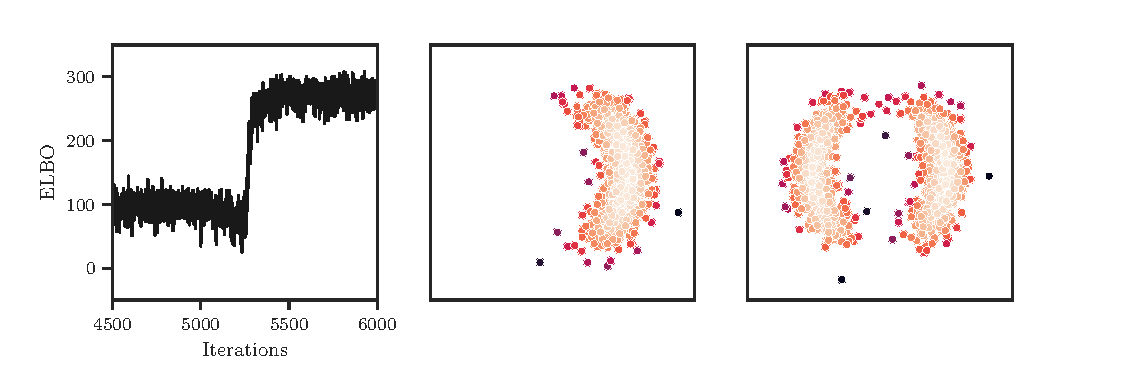
\includegraphics{figures/elbow_example/elbow.pdf}
%     \caption{Three simple graphs}
%     \label{fig:three graphs}
%     \end{adjustwidth}
% \end{figure}

% \begin{figure}
%     \begin{adjustwidth}{-2cm}{-2cm}
%     \centering
%     \begin{subfigure}[t!]{0.3\linewidth}
%         \centering
%          %% Creator: Matplotlib, PGF backend
%%
%% To include the figure in your LaTeX document, write
%%   \input{<filename>.pgf}
%%
%% Make sure the required packages are loaded in your preamble
%%   \usepackage{pgf}
%%
%% Figures using additional raster images can only be included by \input if
%% they are in the same directory as the main LaTeX file. For loading figures
%% from other directories you can use the `import` package
%%   \usepackage{import}
%% and then include the figures with
%%   \import{<path to file>}{<filename>.pgf}
%%
%% Matplotlib used the following preamble
%%
\begingroup%
\makeatletter%
\begin{pgfpicture}%
\pgfpathrectangle{\pgfpointorigin}{\pgfqpoint{3.886919in}{2.530401in}}%
\pgfusepath{use as bounding box, clip}%
\begin{pgfscope}%
\pgfsetbuttcap%
\pgfsetmiterjoin%
\definecolor{currentfill}{rgb}{1.000000,1.000000,1.000000}%
\pgfsetfillcolor{currentfill}%
\pgfsetlinewidth{0.000000pt}%
\definecolor{currentstroke}{rgb}{1.000000,1.000000,1.000000}%
\pgfsetstrokecolor{currentstroke}%
\pgfsetdash{}{0pt}%
\pgfpathmoveto{\pgfqpoint{0.000000in}{0.000000in}}%
\pgfpathlineto{\pgfqpoint{3.886919in}{0.000000in}}%
\pgfpathlineto{\pgfqpoint{3.886919in}{2.530401in}}%
\pgfpathlineto{\pgfqpoint{0.000000in}{2.530401in}}%
\pgfpathclose%
\pgfusepath{fill}%
\end{pgfscope}%
\begin{pgfscope}%
\pgfsetbuttcap%
\pgfsetmiterjoin%
\definecolor{currentfill}{rgb}{1.000000,1.000000,1.000000}%
\pgfsetfillcolor{currentfill}%
\pgfsetlinewidth{0.000000pt}%
\definecolor{currentstroke}{rgb}{0.000000,0.000000,0.000000}%
\pgfsetstrokecolor{currentstroke}%
\pgfsetstrokeopacity{0.000000}%
\pgfsetdash{}{0pt}%
\pgfpathmoveto{\pgfqpoint{0.686919in}{0.505401in}}%
\pgfpathlineto{\pgfqpoint{3.786919in}{0.505401in}}%
\pgfpathlineto{\pgfqpoint{3.786919in}{2.430401in}}%
\pgfpathlineto{\pgfqpoint{0.686919in}{2.430401in}}%
\pgfpathclose%
\pgfusepath{fill}%
\end{pgfscope}%
\begin{pgfscope}%
\pgfsetbuttcap%
\pgfsetroundjoin%
\definecolor{currentfill}{rgb}{0.150000,0.150000,0.150000}%
\pgfsetfillcolor{currentfill}%
\pgfsetlinewidth{1.003750pt}%
\definecolor{currentstroke}{rgb}{0.150000,0.150000,0.150000}%
\pgfsetstrokecolor{currentstroke}%
\pgfsetdash{}{0pt}%
\pgfsys@defobject{currentmarker}{\pgfqpoint{0.000000in}{-0.066667in}}{\pgfqpoint{0.000000in}{0.000000in}}{%
\pgfpathmoveto{\pgfqpoint{0.000000in}{0.000000in}}%
\pgfpathlineto{\pgfqpoint{0.000000in}{-0.066667in}}%
\pgfusepath{stroke,fill}%
}%
\begin{pgfscope}%
\pgfsys@transformshift{0.827828in}{0.505401in}%
\pgfsys@useobject{currentmarker}{}%
\end{pgfscope}%
\end{pgfscope}%
\begin{pgfscope}%
\definecolor{textcolor}{rgb}{0.150000,0.150000,0.150000}%
\pgfsetstrokecolor{textcolor}%
\pgfsetfillcolor{textcolor}%
\pgftext[x=0.827828in,y=0.390123in,,top]{\color{textcolor}\rmfamily\fontsize{8.800000}{10.560000}\selectfont \(\displaystyle 0\)}%
\end{pgfscope}%
\begin{pgfscope}%
\pgfsetbuttcap%
\pgfsetroundjoin%
\definecolor{currentfill}{rgb}{0.150000,0.150000,0.150000}%
\pgfsetfillcolor{currentfill}%
\pgfsetlinewidth{1.003750pt}%
\definecolor{currentstroke}{rgb}{0.150000,0.150000,0.150000}%
\pgfsetstrokecolor{currentstroke}%
\pgfsetdash{}{0pt}%
\pgfsys@defobject{currentmarker}{\pgfqpoint{0.000000in}{-0.066667in}}{\pgfqpoint{0.000000in}{0.000000in}}{%
\pgfpathmoveto{\pgfqpoint{0.000000in}{0.000000in}}%
\pgfpathlineto{\pgfqpoint{0.000000in}{-0.066667in}}%
\pgfusepath{stroke,fill}%
}%
\begin{pgfscope}%
\pgfsys@transformshift{1.391577in}{0.505401in}%
\pgfsys@useobject{currentmarker}{}%
\end{pgfscope}%
\end{pgfscope}%
\begin{pgfscope}%
\definecolor{textcolor}{rgb}{0.150000,0.150000,0.150000}%
\pgfsetstrokecolor{textcolor}%
\pgfsetfillcolor{textcolor}%
\pgftext[x=1.391577in,y=0.390123in,,top]{\color{textcolor}\rmfamily\fontsize{8.800000}{10.560000}\selectfont \(\displaystyle 1000\)}%
\end{pgfscope}%
\begin{pgfscope}%
\pgfsetbuttcap%
\pgfsetroundjoin%
\definecolor{currentfill}{rgb}{0.150000,0.150000,0.150000}%
\pgfsetfillcolor{currentfill}%
\pgfsetlinewidth{1.003750pt}%
\definecolor{currentstroke}{rgb}{0.150000,0.150000,0.150000}%
\pgfsetstrokecolor{currentstroke}%
\pgfsetdash{}{0pt}%
\pgfsys@defobject{currentmarker}{\pgfqpoint{0.000000in}{-0.066667in}}{\pgfqpoint{0.000000in}{0.000000in}}{%
\pgfpathmoveto{\pgfqpoint{0.000000in}{0.000000in}}%
\pgfpathlineto{\pgfqpoint{0.000000in}{-0.066667in}}%
\pgfusepath{stroke,fill}%
}%
\begin{pgfscope}%
\pgfsys@transformshift{1.955326in}{0.505401in}%
\pgfsys@useobject{currentmarker}{}%
\end{pgfscope}%
\end{pgfscope}%
\begin{pgfscope}%
\definecolor{textcolor}{rgb}{0.150000,0.150000,0.150000}%
\pgfsetstrokecolor{textcolor}%
\pgfsetfillcolor{textcolor}%
\pgftext[x=1.955326in,y=0.390123in,,top]{\color{textcolor}\rmfamily\fontsize{8.800000}{10.560000}\selectfont \(\displaystyle 2000\)}%
\end{pgfscope}%
\begin{pgfscope}%
\pgfsetbuttcap%
\pgfsetroundjoin%
\definecolor{currentfill}{rgb}{0.150000,0.150000,0.150000}%
\pgfsetfillcolor{currentfill}%
\pgfsetlinewidth{1.003750pt}%
\definecolor{currentstroke}{rgb}{0.150000,0.150000,0.150000}%
\pgfsetstrokecolor{currentstroke}%
\pgfsetdash{}{0pt}%
\pgfsys@defobject{currentmarker}{\pgfqpoint{0.000000in}{-0.066667in}}{\pgfqpoint{0.000000in}{0.000000in}}{%
\pgfpathmoveto{\pgfqpoint{0.000000in}{0.000000in}}%
\pgfpathlineto{\pgfqpoint{0.000000in}{-0.066667in}}%
\pgfusepath{stroke,fill}%
}%
\begin{pgfscope}%
\pgfsys@transformshift{2.519076in}{0.505401in}%
\pgfsys@useobject{currentmarker}{}%
\end{pgfscope}%
\end{pgfscope}%
\begin{pgfscope}%
\definecolor{textcolor}{rgb}{0.150000,0.150000,0.150000}%
\pgfsetstrokecolor{textcolor}%
\pgfsetfillcolor{textcolor}%
\pgftext[x=2.519076in,y=0.390123in,,top]{\color{textcolor}\rmfamily\fontsize{8.800000}{10.560000}\selectfont \(\displaystyle 3000\)}%
\end{pgfscope}%
\begin{pgfscope}%
\pgfsetbuttcap%
\pgfsetroundjoin%
\definecolor{currentfill}{rgb}{0.150000,0.150000,0.150000}%
\pgfsetfillcolor{currentfill}%
\pgfsetlinewidth{1.003750pt}%
\definecolor{currentstroke}{rgb}{0.150000,0.150000,0.150000}%
\pgfsetstrokecolor{currentstroke}%
\pgfsetdash{}{0pt}%
\pgfsys@defobject{currentmarker}{\pgfqpoint{0.000000in}{-0.066667in}}{\pgfqpoint{0.000000in}{0.000000in}}{%
\pgfpathmoveto{\pgfqpoint{0.000000in}{0.000000in}}%
\pgfpathlineto{\pgfqpoint{0.000000in}{-0.066667in}}%
\pgfusepath{stroke,fill}%
}%
\begin{pgfscope}%
\pgfsys@transformshift{3.082825in}{0.505401in}%
\pgfsys@useobject{currentmarker}{}%
\end{pgfscope}%
\end{pgfscope}%
\begin{pgfscope}%
\definecolor{textcolor}{rgb}{0.150000,0.150000,0.150000}%
\pgfsetstrokecolor{textcolor}%
\pgfsetfillcolor{textcolor}%
\pgftext[x=3.082825in,y=0.390123in,,top]{\color{textcolor}\rmfamily\fontsize{8.800000}{10.560000}\selectfont \(\displaystyle 4000\)}%
\end{pgfscope}%
\begin{pgfscope}%
\pgfsetbuttcap%
\pgfsetroundjoin%
\definecolor{currentfill}{rgb}{0.150000,0.150000,0.150000}%
\pgfsetfillcolor{currentfill}%
\pgfsetlinewidth{1.003750pt}%
\definecolor{currentstroke}{rgb}{0.150000,0.150000,0.150000}%
\pgfsetstrokecolor{currentstroke}%
\pgfsetdash{}{0pt}%
\pgfsys@defobject{currentmarker}{\pgfqpoint{0.000000in}{-0.066667in}}{\pgfqpoint{0.000000in}{0.000000in}}{%
\pgfpathmoveto{\pgfqpoint{0.000000in}{0.000000in}}%
\pgfpathlineto{\pgfqpoint{0.000000in}{-0.066667in}}%
\pgfusepath{stroke,fill}%
}%
\begin{pgfscope}%
\pgfsys@transformshift{3.646574in}{0.505401in}%
\pgfsys@useobject{currentmarker}{}%
\end{pgfscope}%
\end{pgfscope}%
\begin{pgfscope}%
\definecolor{textcolor}{rgb}{0.150000,0.150000,0.150000}%
\pgfsetstrokecolor{textcolor}%
\pgfsetfillcolor{textcolor}%
\pgftext[x=3.646574in,y=0.390123in,,top]{\color{textcolor}\rmfamily\fontsize{8.800000}{10.560000}\selectfont \(\displaystyle 5000\)}%
\end{pgfscope}%
\begin{pgfscope}%
\definecolor{textcolor}{rgb}{0.150000,0.150000,0.150000}%
\pgfsetstrokecolor{textcolor}%
\pgfsetfillcolor{textcolor}%
\pgftext[x=2.236919in,y=0.223457in,,top]{\color{textcolor}\rmfamily\fontsize{9.600000}{11.520000}\selectfont Iteration}%
\end{pgfscope}%
\begin{pgfscope}%
\pgfsetbuttcap%
\pgfsetroundjoin%
\definecolor{currentfill}{rgb}{0.150000,0.150000,0.150000}%
\pgfsetfillcolor{currentfill}%
\pgfsetlinewidth{1.003750pt}%
\definecolor{currentstroke}{rgb}{0.150000,0.150000,0.150000}%
\pgfsetstrokecolor{currentstroke}%
\pgfsetdash{}{0pt}%
\pgfsys@defobject{currentmarker}{\pgfqpoint{-0.066667in}{0.000000in}}{\pgfqpoint{0.000000in}{0.000000in}}{%
\pgfpathmoveto{\pgfqpoint{0.000000in}{0.000000in}}%
\pgfpathlineto{\pgfqpoint{-0.066667in}{0.000000in}}%
\pgfusepath{stroke,fill}%
}%
\begin{pgfscope}%
\pgfsys@transformshift{0.686919in}{0.710382in}%
\pgfsys@useobject{currentmarker}{}%
\end{pgfscope}%
\end{pgfscope}%
\begin{pgfscope}%
\definecolor{textcolor}{rgb}{0.150000,0.150000,0.150000}%
\pgfsetstrokecolor{textcolor}%
\pgfsetfillcolor{textcolor}%
\pgftext[x=0.279012in,y=0.666979in,left,base]{\color{textcolor}\rmfamily\fontsize{8.800000}{10.560000}\selectfont \(\displaystyle -400\)}%
\end{pgfscope}%
\begin{pgfscope}%
\pgfsetbuttcap%
\pgfsetroundjoin%
\definecolor{currentfill}{rgb}{0.150000,0.150000,0.150000}%
\pgfsetfillcolor{currentfill}%
\pgfsetlinewidth{1.003750pt}%
\definecolor{currentstroke}{rgb}{0.150000,0.150000,0.150000}%
\pgfsetstrokecolor{currentstroke}%
\pgfsetdash{}{0pt}%
\pgfsys@defobject{currentmarker}{\pgfqpoint{-0.066667in}{0.000000in}}{\pgfqpoint{0.000000in}{0.000000in}}{%
\pgfpathmoveto{\pgfqpoint{0.000000in}{0.000000in}}%
\pgfpathlineto{\pgfqpoint{-0.066667in}{0.000000in}}%
\pgfusepath{stroke,fill}%
}%
\begin{pgfscope}%
\pgfsys@transformshift{0.686919in}{1.226137in}%
\pgfsys@useobject{currentmarker}{}%
\end{pgfscope}%
\end{pgfscope}%
\begin{pgfscope}%
\definecolor{textcolor}{rgb}{0.150000,0.150000,0.150000}%
\pgfsetstrokecolor{textcolor}%
\pgfsetfillcolor{textcolor}%
\pgftext[x=0.279012in,y=1.182735in,left,base]{\color{textcolor}\rmfamily\fontsize{8.800000}{10.560000}\selectfont \(\displaystyle -300\)}%
\end{pgfscope}%
\begin{pgfscope}%
\pgfsetbuttcap%
\pgfsetroundjoin%
\definecolor{currentfill}{rgb}{0.150000,0.150000,0.150000}%
\pgfsetfillcolor{currentfill}%
\pgfsetlinewidth{1.003750pt}%
\definecolor{currentstroke}{rgb}{0.150000,0.150000,0.150000}%
\pgfsetstrokecolor{currentstroke}%
\pgfsetdash{}{0pt}%
\pgfsys@defobject{currentmarker}{\pgfqpoint{-0.066667in}{0.000000in}}{\pgfqpoint{0.000000in}{0.000000in}}{%
\pgfpathmoveto{\pgfqpoint{0.000000in}{0.000000in}}%
\pgfpathlineto{\pgfqpoint{-0.066667in}{0.000000in}}%
\pgfusepath{stroke,fill}%
}%
\begin{pgfscope}%
\pgfsys@transformshift{0.686919in}{1.741893in}%
\pgfsys@useobject{currentmarker}{}%
\end{pgfscope}%
\end{pgfscope}%
\begin{pgfscope}%
\definecolor{textcolor}{rgb}{0.150000,0.150000,0.150000}%
\pgfsetstrokecolor{textcolor}%
\pgfsetfillcolor{textcolor}%
\pgftext[x=0.279012in,y=1.698490in,left,base]{\color{textcolor}\rmfamily\fontsize{8.800000}{10.560000}\selectfont \(\displaystyle -200\)}%
\end{pgfscope}%
\begin{pgfscope}%
\pgfsetbuttcap%
\pgfsetroundjoin%
\definecolor{currentfill}{rgb}{0.150000,0.150000,0.150000}%
\pgfsetfillcolor{currentfill}%
\pgfsetlinewidth{1.003750pt}%
\definecolor{currentstroke}{rgb}{0.150000,0.150000,0.150000}%
\pgfsetstrokecolor{currentstroke}%
\pgfsetdash{}{0pt}%
\pgfsys@defobject{currentmarker}{\pgfqpoint{-0.066667in}{0.000000in}}{\pgfqpoint{0.000000in}{0.000000in}}{%
\pgfpathmoveto{\pgfqpoint{0.000000in}{0.000000in}}%
\pgfpathlineto{\pgfqpoint{-0.066667in}{0.000000in}}%
\pgfusepath{stroke,fill}%
}%
\begin{pgfscope}%
\pgfsys@transformshift{0.686919in}{2.257649in}%
\pgfsys@useobject{currentmarker}{}%
\end{pgfscope}%
\end{pgfscope}%
\begin{pgfscope}%
\definecolor{textcolor}{rgb}{0.150000,0.150000,0.150000}%
\pgfsetstrokecolor{textcolor}%
\pgfsetfillcolor{textcolor}%
\pgftext[x=0.279012in,y=2.214246in,left,base]{\color{textcolor}\rmfamily\fontsize{8.800000}{10.560000}\selectfont \(\displaystyle -100\)}%
\end{pgfscope}%
\begin{pgfscope}%
\definecolor{textcolor}{rgb}{0.150000,0.150000,0.150000}%
\pgfsetstrokecolor{textcolor}%
\pgfsetfillcolor{textcolor}%
\pgftext[x=0.223457in,y=1.467901in,,bottom,rotate=90.000000]{\color{textcolor}\rmfamily\fontsize{9.600000}{11.520000}\selectfont ELBO}%
\end{pgfscope}%
\begin{pgfscope}%
\pgfpathrectangle{\pgfqpoint{0.686919in}{0.505401in}}{\pgfqpoint{3.100000in}{1.925000in}}%
\pgfusepath{clip}%
\pgfsetroundcap%
\pgfsetroundjoin%
\pgfsetlinewidth{1.204500pt}%
\definecolor{currentstroke}{rgb}{0.298039,0.447059,0.690196}%
\pgfsetstrokecolor{currentstroke}%
\pgfsetdash{}{0pt}%
\pgfpathmoveto{\pgfqpoint{0.827828in}{0.808656in}}%
\pgfpathlineto{\pgfqpoint{0.828392in}{1.046150in}}%
\pgfpathlineto{\pgfqpoint{0.828956in}{0.592901in}}%
\pgfpathlineto{\pgfqpoint{0.829520in}{1.235111in}}%
\pgfpathlineto{\pgfqpoint{0.830083in}{0.744131in}}%
\pgfpathlineto{\pgfqpoint{0.830647in}{0.928615in}}%
\pgfpathlineto{\pgfqpoint{0.831211in}{0.991312in}}%
\pgfpathlineto{\pgfqpoint{0.831775in}{1.121443in}}%
\pgfpathlineto{\pgfqpoint{0.832338in}{0.736368in}}%
\pgfpathlineto{\pgfqpoint{0.832902in}{0.751473in}}%
\pgfpathlineto{\pgfqpoint{0.833466in}{0.967678in}}%
\pgfpathlineto{\pgfqpoint{0.834029in}{0.805425in}}%
\pgfpathlineto{\pgfqpoint{0.834593in}{1.148514in}}%
\pgfpathlineto{\pgfqpoint{0.835157in}{1.179098in}}%
\pgfpathlineto{\pgfqpoint{0.836284in}{0.833393in}}%
\pgfpathlineto{\pgfqpoint{0.836848in}{1.105503in}}%
\pgfpathlineto{\pgfqpoint{0.837412in}{1.438203in}}%
\pgfpathlineto{\pgfqpoint{0.837976in}{0.852210in}}%
\pgfpathlineto{\pgfqpoint{0.838539in}{0.954803in}}%
\pgfpathlineto{\pgfqpoint{0.839103in}{0.827231in}}%
\pgfpathlineto{\pgfqpoint{0.839667in}{1.120692in}}%
\pgfpathlineto{\pgfqpoint{0.840231in}{1.085732in}}%
\pgfpathlineto{\pgfqpoint{0.840794in}{1.142492in}}%
\pgfpathlineto{\pgfqpoint{0.841358in}{1.187989in}}%
\pgfpathlineto{\pgfqpoint{0.841922in}{1.176131in}}%
\pgfpathlineto{\pgfqpoint{0.842486in}{1.158992in}}%
\pgfpathlineto{\pgfqpoint{0.843049in}{1.305429in}}%
\pgfpathlineto{\pgfqpoint{0.843613in}{1.214746in}}%
\pgfpathlineto{\pgfqpoint{0.844177in}{1.269681in}}%
\pgfpathlineto{\pgfqpoint{0.844741in}{1.337861in}}%
\pgfpathlineto{\pgfqpoint{0.845304in}{1.425681in}}%
\pgfpathlineto{\pgfqpoint{0.845868in}{1.303451in}}%
\pgfpathlineto{\pgfqpoint{0.846432in}{1.375055in}}%
\pgfpathlineto{\pgfqpoint{0.846996in}{1.217550in}}%
\pgfpathlineto{\pgfqpoint{0.847559in}{1.383118in}}%
\pgfpathlineto{\pgfqpoint{0.848123in}{1.488078in}}%
\pgfpathlineto{\pgfqpoint{0.848687in}{1.557589in}}%
\pgfpathlineto{\pgfqpoint{0.849251in}{1.690010in}}%
\pgfpathlineto{\pgfqpoint{0.849814in}{1.583075in}}%
\pgfpathlineto{\pgfqpoint{0.850378in}{1.767640in}}%
\pgfpathlineto{\pgfqpoint{0.850942in}{1.651106in}}%
\pgfpathlineto{\pgfqpoint{0.851506in}{1.832377in}}%
\pgfpathlineto{\pgfqpoint{0.852069in}{1.760663in}}%
\pgfpathlineto{\pgfqpoint{0.852633in}{1.991570in}}%
\pgfpathlineto{\pgfqpoint{0.853197in}{1.890769in}}%
\pgfpathlineto{\pgfqpoint{0.853761in}{2.010212in}}%
\pgfpathlineto{\pgfqpoint{0.854324in}{1.904046in}}%
\pgfpathlineto{\pgfqpoint{0.854888in}{2.094603in}}%
\pgfpathlineto{\pgfqpoint{0.856016in}{1.477590in}}%
\pgfpathlineto{\pgfqpoint{0.857143in}{2.038378in}}%
\pgfpathlineto{\pgfqpoint{0.857707in}{1.969749in}}%
\pgfpathlineto{\pgfqpoint{0.858271in}{1.985917in}}%
\pgfpathlineto{\pgfqpoint{0.858834in}{2.020413in}}%
\pgfpathlineto{\pgfqpoint{0.859398in}{2.090232in}}%
\pgfpathlineto{\pgfqpoint{0.859962in}{1.768634in}}%
\pgfpathlineto{\pgfqpoint{0.860526in}{1.943023in}}%
\pgfpathlineto{\pgfqpoint{0.861089in}{1.892338in}}%
\pgfpathlineto{\pgfqpoint{0.861653in}{1.796494in}}%
\pgfpathlineto{\pgfqpoint{0.862217in}{1.846438in}}%
\pgfpathlineto{\pgfqpoint{0.862781in}{1.880723in}}%
\pgfpathlineto{\pgfqpoint{0.863344in}{2.012613in}}%
\pgfpathlineto{\pgfqpoint{0.863908in}{2.064269in}}%
\pgfpathlineto{\pgfqpoint{0.864472in}{2.015857in}}%
\pgfpathlineto{\pgfqpoint{0.865036in}{1.888332in}}%
\pgfpathlineto{\pgfqpoint{0.865599in}{1.889456in}}%
\pgfpathlineto{\pgfqpoint{0.866163in}{1.939002in}}%
\pgfpathlineto{\pgfqpoint{0.866727in}{1.900781in}}%
\pgfpathlineto{\pgfqpoint{0.867291in}{2.001145in}}%
\pgfpathlineto{\pgfqpoint{0.867854in}{1.693439in}}%
\pgfpathlineto{\pgfqpoint{0.868418in}{1.998240in}}%
\pgfpathlineto{\pgfqpoint{0.868982in}{2.129441in}}%
\pgfpathlineto{\pgfqpoint{0.869546in}{1.940835in}}%
\pgfpathlineto{\pgfqpoint{0.870109in}{2.142722in}}%
\pgfpathlineto{\pgfqpoint{0.870673in}{2.060314in}}%
\pgfpathlineto{\pgfqpoint{0.871237in}{2.159649in}}%
\pgfpathlineto{\pgfqpoint{0.871801in}{2.102856in}}%
\pgfpathlineto{\pgfqpoint{0.872364in}{2.082377in}}%
\pgfpathlineto{\pgfqpoint{0.872928in}{1.826850in}}%
\pgfpathlineto{\pgfqpoint{0.873492in}{2.058661in}}%
\pgfpathlineto{\pgfqpoint{0.874056in}{2.095808in}}%
\pgfpathlineto{\pgfqpoint{0.874619in}{1.910256in}}%
\pgfpathlineto{\pgfqpoint{0.875183in}{1.935447in}}%
\pgfpathlineto{\pgfqpoint{0.875747in}{2.050130in}}%
\pgfpathlineto{\pgfqpoint{0.876311in}{2.139791in}}%
\pgfpathlineto{\pgfqpoint{0.876874in}{2.006236in}}%
\pgfpathlineto{\pgfqpoint{0.877438in}{2.190005in}}%
\pgfpathlineto{\pgfqpoint{0.878002in}{2.062174in}}%
\pgfpathlineto{\pgfqpoint{0.878566in}{2.172288in}}%
\pgfpathlineto{\pgfqpoint{0.879129in}{2.181283in}}%
\pgfpathlineto{\pgfqpoint{0.879693in}{2.115466in}}%
\pgfpathlineto{\pgfqpoint{0.880257in}{1.909114in}}%
\pgfpathlineto{\pgfqpoint{0.880821in}{2.105603in}}%
\pgfpathlineto{\pgfqpoint{0.881384in}{2.109169in}}%
\pgfpathlineto{\pgfqpoint{0.881948in}{2.061933in}}%
\pgfpathlineto{\pgfqpoint{0.882512in}{2.033133in}}%
\pgfpathlineto{\pgfqpoint{0.883076in}{2.154487in}}%
\pgfpathlineto{\pgfqpoint{0.883639in}{2.112393in}}%
\pgfpathlineto{\pgfqpoint{0.884203in}{2.135711in}}%
\pgfpathlineto{\pgfqpoint{0.884767in}{2.098778in}}%
\pgfpathlineto{\pgfqpoint{0.885331in}{2.173642in}}%
\pgfpathlineto{\pgfqpoint{0.885894in}{2.164122in}}%
\pgfpathlineto{\pgfqpoint{0.886458in}{2.110273in}}%
\pgfpathlineto{\pgfqpoint{0.887022in}{2.177497in}}%
\pgfpathlineto{\pgfqpoint{0.887586in}{2.175089in}}%
\pgfpathlineto{\pgfqpoint{0.888149in}{2.176415in}}%
\pgfpathlineto{\pgfqpoint{0.888713in}{2.197765in}}%
\pgfpathlineto{\pgfqpoint{0.889841in}{2.129420in}}%
\pgfpathlineto{\pgfqpoint{0.890404in}{2.207697in}}%
\pgfpathlineto{\pgfqpoint{0.890968in}{2.170902in}}%
\pgfpathlineto{\pgfqpoint{0.891532in}{1.913188in}}%
\pgfpathlineto{\pgfqpoint{0.892096in}{2.185158in}}%
\pgfpathlineto{\pgfqpoint{0.892659in}{2.170844in}}%
\pgfpathlineto{\pgfqpoint{0.893223in}{2.140839in}}%
\pgfpathlineto{\pgfqpoint{0.893787in}{2.151443in}}%
\pgfpathlineto{\pgfqpoint{0.894351in}{2.120109in}}%
\pgfpathlineto{\pgfqpoint{0.894914in}{2.179572in}}%
\pgfpathlineto{\pgfqpoint{0.895478in}{2.172792in}}%
\pgfpathlineto{\pgfqpoint{0.896042in}{2.208273in}}%
\pgfpathlineto{\pgfqpoint{0.896606in}{2.173260in}}%
\pgfpathlineto{\pgfqpoint{0.897169in}{2.165728in}}%
\pgfpathlineto{\pgfqpoint{0.897733in}{2.179765in}}%
\pgfpathlineto{\pgfqpoint{0.898297in}{2.143863in}}%
\pgfpathlineto{\pgfqpoint{0.898861in}{2.135465in}}%
\pgfpathlineto{\pgfqpoint{0.899424in}{2.124238in}}%
\pgfpathlineto{\pgfqpoint{0.899988in}{2.177438in}}%
\pgfpathlineto{\pgfqpoint{0.900552in}{2.134199in}}%
\pgfpathlineto{\pgfqpoint{0.901116in}{2.141803in}}%
\pgfpathlineto{\pgfqpoint{0.901679in}{2.119694in}}%
\pgfpathlineto{\pgfqpoint{0.902243in}{2.117384in}}%
\pgfpathlineto{\pgfqpoint{0.902807in}{2.066988in}}%
\pgfpathlineto{\pgfqpoint{0.903371in}{2.086153in}}%
\pgfpathlineto{\pgfqpoint{0.903934in}{2.150105in}}%
\pgfpathlineto{\pgfqpoint{0.904498in}{2.023853in}}%
\pgfpathlineto{\pgfqpoint{0.905062in}{2.089238in}}%
\pgfpathlineto{\pgfqpoint{0.905626in}{2.168172in}}%
\pgfpathlineto{\pgfqpoint{0.906189in}{2.153933in}}%
\pgfpathlineto{\pgfqpoint{0.907317in}{2.207050in}}%
\pgfpathlineto{\pgfqpoint{0.907881in}{2.167709in}}%
\pgfpathlineto{\pgfqpoint{0.908444in}{2.152799in}}%
\pgfpathlineto{\pgfqpoint{0.909008in}{2.177230in}}%
\pgfpathlineto{\pgfqpoint{0.909572in}{2.230552in}}%
\pgfpathlineto{\pgfqpoint{0.910136in}{2.169667in}}%
\pgfpathlineto{\pgfqpoint{0.910699in}{2.044574in}}%
\pgfpathlineto{\pgfqpoint{0.911263in}{2.264858in}}%
\pgfpathlineto{\pgfqpoint{0.911827in}{2.155565in}}%
\pgfpathlineto{\pgfqpoint{0.912391in}{2.180433in}}%
\pgfpathlineto{\pgfqpoint{0.912954in}{2.196613in}}%
\pgfpathlineto{\pgfqpoint{0.913518in}{2.069881in}}%
\pgfpathlineto{\pgfqpoint{0.914082in}{2.239704in}}%
\pgfpathlineto{\pgfqpoint{0.914646in}{2.175461in}}%
\pgfpathlineto{\pgfqpoint{0.915209in}{2.204189in}}%
\pgfpathlineto{\pgfqpoint{0.915773in}{2.131370in}}%
\pgfpathlineto{\pgfqpoint{0.916337in}{2.218332in}}%
\pgfpathlineto{\pgfqpoint{0.916901in}{2.203007in}}%
\pgfpathlineto{\pgfqpoint{0.917464in}{2.108950in}}%
\pgfpathlineto{\pgfqpoint{0.918028in}{2.082203in}}%
\pgfpathlineto{\pgfqpoint{0.918592in}{2.208633in}}%
\pgfpathlineto{\pgfqpoint{0.919156in}{2.163979in}}%
\pgfpathlineto{\pgfqpoint{0.919719in}{2.212837in}}%
\pgfpathlineto{\pgfqpoint{0.920283in}{2.234107in}}%
\pgfpathlineto{\pgfqpoint{0.920847in}{2.129076in}}%
\pgfpathlineto{\pgfqpoint{0.921411in}{2.239487in}}%
\pgfpathlineto{\pgfqpoint{0.921974in}{2.187168in}}%
\pgfpathlineto{\pgfqpoint{0.922538in}{2.152624in}}%
\pgfpathlineto{\pgfqpoint{0.923102in}{2.175220in}}%
\pgfpathlineto{\pgfqpoint{0.923666in}{2.105134in}}%
\pgfpathlineto{\pgfqpoint{0.924229in}{2.188394in}}%
\pgfpathlineto{\pgfqpoint{0.924793in}{2.151318in}}%
\pgfpathlineto{\pgfqpoint{0.925357in}{2.211805in}}%
\pgfpathlineto{\pgfqpoint{0.925921in}{2.154537in}}%
\pgfpathlineto{\pgfqpoint{0.926484in}{2.263136in}}%
\pgfpathlineto{\pgfqpoint{0.927048in}{2.184869in}}%
\pgfpathlineto{\pgfqpoint{0.927612in}{2.223303in}}%
\pgfpathlineto{\pgfqpoint{0.928176in}{2.202507in}}%
\pgfpathlineto{\pgfqpoint{0.928739in}{2.195883in}}%
\pgfpathlineto{\pgfqpoint{0.929303in}{2.205183in}}%
\pgfpathlineto{\pgfqpoint{0.929867in}{2.236938in}}%
\pgfpathlineto{\pgfqpoint{0.930431in}{2.180868in}}%
\pgfpathlineto{\pgfqpoint{0.930994in}{2.164245in}}%
\pgfpathlineto{\pgfqpoint{0.931558in}{2.198187in}}%
\pgfpathlineto{\pgfqpoint{0.932122in}{2.204431in}}%
\pgfpathlineto{\pgfqpoint{0.932686in}{2.183590in}}%
\pgfpathlineto{\pgfqpoint{0.933249in}{2.137457in}}%
\pgfpathlineto{\pgfqpoint{0.933813in}{2.144630in}}%
\pgfpathlineto{\pgfqpoint{0.934377in}{2.187466in}}%
\pgfpathlineto{\pgfqpoint{0.934941in}{2.194507in}}%
\pgfpathlineto{\pgfqpoint{0.935504in}{2.198187in}}%
\pgfpathlineto{\pgfqpoint{0.936068in}{2.145738in}}%
\pgfpathlineto{\pgfqpoint{0.936632in}{2.215099in}}%
\pgfpathlineto{\pgfqpoint{0.937196in}{2.164338in}}%
\pgfpathlineto{\pgfqpoint{0.937759in}{2.146972in}}%
\pgfpathlineto{\pgfqpoint{0.938323in}{2.183527in}}%
\pgfpathlineto{\pgfqpoint{0.938887in}{2.204184in}}%
\pgfpathlineto{\pgfqpoint{0.939451in}{2.187040in}}%
\pgfpathlineto{\pgfqpoint{0.940014in}{2.234618in}}%
\pgfpathlineto{\pgfqpoint{0.940578in}{2.236887in}}%
\pgfpathlineto{\pgfqpoint{0.941142in}{2.222400in}}%
\pgfpathlineto{\pgfqpoint{0.941706in}{2.193695in}}%
\pgfpathlineto{\pgfqpoint{0.942269in}{2.237148in}}%
\pgfpathlineto{\pgfqpoint{0.942833in}{2.250902in}}%
\pgfpathlineto{\pgfqpoint{0.943397in}{2.048214in}}%
\pgfpathlineto{\pgfqpoint{0.943961in}{2.220783in}}%
\pgfpathlineto{\pgfqpoint{0.944524in}{2.259985in}}%
\pgfpathlineto{\pgfqpoint{0.945088in}{2.279232in}}%
\pgfpathlineto{\pgfqpoint{0.945652in}{1.958917in}}%
\pgfpathlineto{\pgfqpoint{0.946216in}{2.183452in}}%
\pgfpathlineto{\pgfqpoint{0.946779in}{2.198524in}}%
\pgfpathlineto{\pgfqpoint{0.947343in}{2.238395in}}%
\pgfpathlineto{\pgfqpoint{0.947907in}{2.202348in}}%
\pgfpathlineto{\pgfqpoint{0.948471in}{2.150637in}}%
\pgfpathlineto{\pgfqpoint{0.949034in}{2.178897in}}%
\pgfpathlineto{\pgfqpoint{0.949598in}{2.158517in}}%
\pgfpathlineto{\pgfqpoint{0.950162in}{2.225845in}}%
\pgfpathlineto{\pgfqpoint{0.950726in}{2.201683in}}%
\pgfpathlineto{\pgfqpoint{0.951289in}{2.148877in}}%
\pgfpathlineto{\pgfqpoint{0.951853in}{2.205724in}}%
\pgfpathlineto{\pgfqpoint{0.952417in}{2.197028in}}%
\pgfpathlineto{\pgfqpoint{0.952981in}{2.183396in}}%
\pgfpathlineto{\pgfqpoint{0.953544in}{2.183264in}}%
\pgfpathlineto{\pgfqpoint{0.954108in}{2.181211in}}%
\pgfpathlineto{\pgfqpoint{0.954672in}{2.196533in}}%
\pgfpathlineto{\pgfqpoint{0.955236in}{2.139015in}}%
\pgfpathlineto{\pgfqpoint{0.955799in}{2.270469in}}%
\pgfpathlineto{\pgfqpoint{0.956363in}{2.163242in}}%
\pgfpathlineto{\pgfqpoint{0.957491in}{2.276510in}}%
\pgfpathlineto{\pgfqpoint{0.958054in}{2.250253in}}%
\pgfpathlineto{\pgfqpoint{0.958618in}{2.240574in}}%
\pgfpathlineto{\pgfqpoint{0.959182in}{2.246431in}}%
\pgfpathlineto{\pgfqpoint{0.959746in}{2.215108in}}%
\pgfpathlineto{\pgfqpoint{0.960309in}{2.207354in}}%
\pgfpathlineto{\pgfqpoint{0.960873in}{2.139104in}}%
\pgfpathlineto{\pgfqpoint{0.961437in}{2.234294in}}%
\pgfpathlineto{\pgfqpoint{0.962001in}{2.218477in}}%
\pgfpathlineto{\pgfqpoint{0.962564in}{2.214911in}}%
\pgfpathlineto{\pgfqpoint{0.963128in}{2.166453in}}%
\pgfpathlineto{\pgfqpoint{0.963692in}{2.217643in}}%
\pgfpathlineto{\pgfqpoint{0.964819in}{2.112922in}}%
\pgfpathlineto{\pgfqpoint{0.965383in}{2.112312in}}%
\pgfpathlineto{\pgfqpoint{0.965947in}{2.280303in}}%
\pgfpathlineto{\pgfqpoint{0.966511in}{2.157254in}}%
\pgfpathlineto{\pgfqpoint{0.967074in}{2.273948in}}%
\pgfpathlineto{\pgfqpoint{0.967638in}{2.226598in}}%
\pgfpathlineto{\pgfqpoint{0.968202in}{2.220538in}}%
\pgfpathlineto{\pgfqpoint{0.968766in}{2.210440in}}%
\pgfpathlineto{\pgfqpoint{0.969329in}{2.292414in}}%
\pgfpathlineto{\pgfqpoint{0.969893in}{2.196445in}}%
\pgfpathlineto{\pgfqpoint{0.970457in}{2.248667in}}%
\pgfpathlineto{\pgfqpoint{0.971021in}{2.229884in}}%
\pgfpathlineto{\pgfqpoint{0.971584in}{2.271352in}}%
\pgfpathlineto{\pgfqpoint{0.972148in}{2.062641in}}%
\pgfpathlineto{\pgfqpoint{0.972712in}{2.266600in}}%
\pgfpathlineto{\pgfqpoint{0.973276in}{2.257332in}}%
\pgfpathlineto{\pgfqpoint{0.973839in}{2.273368in}}%
\pgfpathlineto{\pgfqpoint{0.974403in}{2.158105in}}%
\pgfpathlineto{\pgfqpoint{0.974967in}{2.197412in}}%
\pgfpathlineto{\pgfqpoint{0.975531in}{2.203517in}}%
\pgfpathlineto{\pgfqpoint{0.976658in}{2.259881in}}%
\pgfpathlineto{\pgfqpoint{0.977222in}{2.147676in}}%
\pgfpathlineto{\pgfqpoint{0.977786in}{2.178481in}}%
\pgfpathlineto{\pgfqpoint{0.978349in}{2.184114in}}%
\pgfpathlineto{\pgfqpoint{0.978913in}{2.235512in}}%
\pgfpathlineto{\pgfqpoint{0.979477in}{2.043674in}}%
\pgfpathlineto{\pgfqpoint{0.980604in}{2.258743in}}%
\pgfpathlineto{\pgfqpoint{0.981168in}{2.211732in}}%
\pgfpathlineto{\pgfqpoint{0.981732in}{2.254785in}}%
\pgfpathlineto{\pgfqpoint{0.982296in}{2.250817in}}%
\pgfpathlineto{\pgfqpoint{0.982859in}{2.255236in}}%
\pgfpathlineto{\pgfqpoint{0.983987in}{2.127846in}}%
\pgfpathlineto{\pgfqpoint{0.984551in}{2.187158in}}%
\pgfpathlineto{\pgfqpoint{0.985114in}{2.211852in}}%
\pgfpathlineto{\pgfqpoint{0.985678in}{2.222464in}}%
\pgfpathlineto{\pgfqpoint{0.986242in}{2.228050in}}%
\pgfpathlineto{\pgfqpoint{0.986806in}{2.162089in}}%
\pgfpathlineto{\pgfqpoint{0.987369in}{2.202543in}}%
\pgfpathlineto{\pgfqpoint{0.987933in}{2.276220in}}%
\pgfpathlineto{\pgfqpoint{0.988497in}{2.112492in}}%
\pgfpathlineto{\pgfqpoint{0.989061in}{2.274033in}}%
\pgfpathlineto{\pgfqpoint{0.989624in}{2.217821in}}%
\pgfpathlineto{\pgfqpoint{0.990188in}{2.182030in}}%
\pgfpathlineto{\pgfqpoint{0.990752in}{2.255903in}}%
\pgfpathlineto{\pgfqpoint{0.991316in}{2.225605in}}%
\pgfpathlineto{\pgfqpoint{0.991879in}{2.217968in}}%
\pgfpathlineto{\pgfqpoint{0.992443in}{2.257534in}}%
\pgfpathlineto{\pgfqpoint{0.993007in}{2.259866in}}%
\pgfpathlineto{\pgfqpoint{0.993570in}{2.237762in}}%
\pgfpathlineto{\pgfqpoint{0.994134in}{2.222627in}}%
\pgfpathlineto{\pgfqpoint{0.994698in}{2.249945in}}%
\pgfpathlineto{\pgfqpoint{0.995262in}{2.231331in}}%
\pgfpathlineto{\pgfqpoint{0.995825in}{2.194749in}}%
\pgfpathlineto{\pgfqpoint{0.996389in}{2.267068in}}%
\pgfpathlineto{\pgfqpoint{0.996953in}{2.132213in}}%
\pgfpathlineto{\pgfqpoint{0.997517in}{2.229495in}}%
\pgfpathlineto{\pgfqpoint{0.998080in}{2.240714in}}%
\pgfpathlineto{\pgfqpoint{0.998644in}{2.196446in}}%
\pgfpathlineto{\pgfqpoint{0.999208in}{2.257054in}}%
\pgfpathlineto{\pgfqpoint{0.999772in}{2.279882in}}%
\pgfpathlineto{\pgfqpoint{1.000335in}{2.197870in}}%
\pgfpathlineto{\pgfqpoint{1.000899in}{2.205245in}}%
\pgfpathlineto{\pgfqpoint{1.001463in}{2.267105in}}%
\pgfpathlineto{\pgfqpoint{1.002027in}{2.290857in}}%
\pgfpathlineto{\pgfqpoint{1.002590in}{2.240997in}}%
\pgfpathlineto{\pgfqpoint{1.003154in}{2.242602in}}%
\pgfpathlineto{\pgfqpoint{1.003718in}{2.246770in}}%
\pgfpathlineto{\pgfqpoint{1.004282in}{2.199386in}}%
\pgfpathlineto{\pgfqpoint{1.004845in}{2.222458in}}%
\pgfpathlineto{\pgfqpoint{1.005409in}{2.252112in}}%
\pgfpathlineto{\pgfqpoint{1.005973in}{2.232711in}}%
\pgfpathlineto{\pgfqpoint{1.006537in}{2.246949in}}%
\pgfpathlineto{\pgfqpoint{1.007100in}{2.221804in}}%
\pgfpathlineto{\pgfqpoint{1.007664in}{2.247463in}}%
\pgfpathlineto{\pgfqpoint{1.008228in}{2.253159in}}%
\pgfpathlineto{\pgfqpoint{1.008792in}{2.165176in}}%
\pgfpathlineto{\pgfqpoint{1.009355in}{2.223810in}}%
\pgfpathlineto{\pgfqpoint{1.009919in}{2.268769in}}%
\pgfpathlineto{\pgfqpoint{1.010483in}{2.232225in}}%
\pgfpathlineto{\pgfqpoint{1.011047in}{2.248081in}}%
\pgfpathlineto{\pgfqpoint{1.011610in}{2.214985in}}%
\pgfpathlineto{\pgfqpoint{1.012174in}{2.201804in}}%
\pgfpathlineto{\pgfqpoint{1.013302in}{2.264205in}}%
\pgfpathlineto{\pgfqpoint{1.013865in}{2.273902in}}%
\pgfpathlineto{\pgfqpoint{1.014429in}{2.292833in}}%
\pgfpathlineto{\pgfqpoint{1.014993in}{2.292110in}}%
\pgfpathlineto{\pgfqpoint{1.015557in}{2.267452in}}%
\pgfpathlineto{\pgfqpoint{1.016120in}{2.290728in}}%
\pgfpathlineto{\pgfqpoint{1.016684in}{2.259903in}}%
\pgfpathlineto{\pgfqpoint{1.017248in}{2.281719in}}%
\pgfpathlineto{\pgfqpoint{1.017812in}{2.262137in}}%
\pgfpathlineto{\pgfqpoint{1.018375in}{2.251383in}}%
\pgfpathlineto{\pgfqpoint{1.018939in}{2.219662in}}%
\pgfpathlineto{\pgfqpoint{1.020067in}{2.258730in}}%
\pgfpathlineto{\pgfqpoint{1.020630in}{2.265261in}}%
\pgfpathlineto{\pgfqpoint{1.021194in}{2.232986in}}%
\pgfpathlineto{\pgfqpoint{1.021758in}{2.243229in}}%
\pgfpathlineto{\pgfqpoint{1.022322in}{2.210460in}}%
\pgfpathlineto{\pgfqpoint{1.022885in}{2.274669in}}%
\pgfpathlineto{\pgfqpoint{1.023449in}{2.267139in}}%
\pgfpathlineto{\pgfqpoint{1.024013in}{2.269532in}}%
\pgfpathlineto{\pgfqpoint{1.024577in}{2.268742in}}%
\pgfpathlineto{\pgfqpoint{1.025140in}{2.255652in}}%
\pgfpathlineto{\pgfqpoint{1.025704in}{2.253842in}}%
\pgfpathlineto{\pgfqpoint{1.026268in}{2.270128in}}%
\pgfpathlineto{\pgfqpoint{1.026832in}{2.278602in}}%
\pgfpathlineto{\pgfqpoint{1.027395in}{2.235865in}}%
\pgfpathlineto{\pgfqpoint{1.027959in}{2.282014in}}%
\pgfpathlineto{\pgfqpoint{1.028523in}{2.273824in}}%
\pgfpathlineto{\pgfqpoint{1.029087in}{2.156536in}}%
\pgfpathlineto{\pgfqpoint{1.029650in}{2.249586in}}%
\pgfpathlineto{\pgfqpoint{1.030214in}{2.309778in}}%
\pgfpathlineto{\pgfqpoint{1.030778in}{2.299494in}}%
\pgfpathlineto{\pgfqpoint{1.031342in}{2.295156in}}%
\pgfpathlineto{\pgfqpoint{1.031905in}{2.241968in}}%
\pgfpathlineto{\pgfqpoint{1.032469in}{2.270323in}}%
\pgfpathlineto{\pgfqpoint{1.033033in}{2.286960in}}%
\pgfpathlineto{\pgfqpoint{1.033597in}{2.285446in}}%
\pgfpathlineto{\pgfqpoint{1.034160in}{2.251930in}}%
\pgfpathlineto{\pgfqpoint{1.034724in}{2.310117in}}%
\pgfpathlineto{\pgfqpoint{1.035288in}{2.054291in}}%
\pgfpathlineto{\pgfqpoint{1.035852in}{2.284343in}}%
\pgfpathlineto{\pgfqpoint{1.036415in}{2.281752in}}%
\pgfpathlineto{\pgfqpoint{1.036979in}{2.315826in}}%
\pgfpathlineto{\pgfqpoint{1.037543in}{2.206970in}}%
\pgfpathlineto{\pgfqpoint{1.038107in}{2.254258in}}%
\pgfpathlineto{\pgfqpoint{1.038670in}{2.224048in}}%
\pgfpathlineto{\pgfqpoint{1.039234in}{2.264297in}}%
\pgfpathlineto{\pgfqpoint{1.039798in}{2.238522in}}%
\pgfpathlineto{\pgfqpoint{1.040362in}{2.287150in}}%
\pgfpathlineto{\pgfqpoint{1.040925in}{2.201716in}}%
\pgfpathlineto{\pgfqpoint{1.041489in}{2.200171in}}%
\pgfpathlineto{\pgfqpoint{1.042053in}{2.282633in}}%
\pgfpathlineto{\pgfqpoint{1.042617in}{2.236710in}}%
\pgfpathlineto{\pgfqpoint{1.043180in}{2.256456in}}%
\pgfpathlineto{\pgfqpoint{1.043744in}{2.269275in}}%
\pgfpathlineto{\pgfqpoint{1.044308in}{2.295778in}}%
\pgfpathlineto{\pgfqpoint{1.044872in}{2.281189in}}%
\pgfpathlineto{\pgfqpoint{1.045435in}{2.253299in}}%
\pgfpathlineto{\pgfqpoint{1.045999in}{2.260312in}}%
\pgfpathlineto{\pgfqpoint{1.046563in}{2.282718in}}%
\pgfpathlineto{\pgfqpoint{1.047127in}{2.248773in}}%
\pgfpathlineto{\pgfqpoint{1.047690in}{2.285321in}}%
\pgfpathlineto{\pgfqpoint{1.048254in}{2.302790in}}%
\pgfpathlineto{\pgfqpoint{1.048818in}{2.325558in}}%
\pgfpathlineto{\pgfqpoint{1.049382in}{2.265673in}}%
\pgfpathlineto{\pgfqpoint{1.049945in}{2.243942in}}%
\pgfpathlineto{\pgfqpoint{1.050509in}{2.251924in}}%
\pgfpathlineto{\pgfqpoint{1.051073in}{2.294474in}}%
\pgfpathlineto{\pgfqpoint{1.051637in}{2.227175in}}%
\pgfpathlineto{\pgfqpoint{1.052764in}{2.266073in}}%
\pgfpathlineto{\pgfqpoint{1.053328in}{2.276262in}}%
\pgfpathlineto{\pgfqpoint{1.053892in}{2.288761in}}%
\pgfpathlineto{\pgfqpoint{1.054455in}{2.271625in}}%
\pgfpathlineto{\pgfqpoint{1.055019in}{2.218123in}}%
\pgfpathlineto{\pgfqpoint{1.055583in}{2.301795in}}%
\pgfpathlineto{\pgfqpoint{1.056147in}{2.247391in}}%
\pgfpathlineto{\pgfqpoint{1.056710in}{2.150712in}}%
\pgfpathlineto{\pgfqpoint{1.057274in}{2.280842in}}%
\pgfpathlineto{\pgfqpoint{1.057838in}{2.298698in}}%
\pgfpathlineto{\pgfqpoint{1.058965in}{2.248134in}}%
\pgfpathlineto{\pgfqpoint{1.059529in}{2.260806in}}%
\pgfpathlineto{\pgfqpoint{1.060093in}{2.251637in}}%
\pgfpathlineto{\pgfqpoint{1.061220in}{2.289219in}}%
\pgfpathlineto{\pgfqpoint{1.061784in}{2.251399in}}%
\pgfpathlineto{\pgfqpoint{1.062348in}{2.302088in}}%
\pgfpathlineto{\pgfqpoint{1.062912in}{2.304280in}}%
\pgfpathlineto{\pgfqpoint{1.063475in}{2.229171in}}%
\pgfpathlineto{\pgfqpoint{1.064039in}{2.239976in}}%
\pgfpathlineto{\pgfqpoint{1.064603in}{2.289918in}}%
\pgfpathlineto{\pgfqpoint{1.065167in}{2.296824in}}%
\pgfpathlineto{\pgfqpoint{1.065730in}{2.262599in}}%
\pgfpathlineto{\pgfqpoint{1.066294in}{2.263893in}}%
\pgfpathlineto{\pgfqpoint{1.066858in}{2.237724in}}%
\pgfpathlineto{\pgfqpoint{1.067422in}{2.283574in}}%
\pgfpathlineto{\pgfqpoint{1.067985in}{2.297719in}}%
\pgfpathlineto{\pgfqpoint{1.068549in}{2.287603in}}%
\pgfpathlineto{\pgfqpoint{1.069113in}{2.297495in}}%
\pgfpathlineto{\pgfqpoint{1.069677in}{2.241764in}}%
\pgfpathlineto{\pgfqpoint{1.070240in}{2.293537in}}%
\pgfpathlineto{\pgfqpoint{1.070804in}{2.316617in}}%
\pgfpathlineto{\pgfqpoint{1.071368in}{2.319254in}}%
\pgfpathlineto{\pgfqpoint{1.071932in}{2.270292in}}%
\pgfpathlineto{\pgfqpoint{1.072495in}{2.302098in}}%
\pgfpathlineto{\pgfqpoint{1.073059in}{2.270869in}}%
\pgfpathlineto{\pgfqpoint{1.073623in}{2.251690in}}%
\pgfpathlineto{\pgfqpoint{1.074187in}{2.315403in}}%
\pgfpathlineto{\pgfqpoint{1.074750in}{2.245175in}}%
\pgfpathlineto{\pgfqpoint{1.075314in}{2.277266in}}%
\pgfpathlineto{\pgfqpoint{1.075878in}{2.300238in}}%
\pgfpathlineto{\pgfqpoint{1.076442in}{2.280954in}}%
\pgfpathlineto{\pgfqpoint{1.077005in}{2.271764in}}%
\pgfpathlineto{\pgfqpoint{1.077569in}{2.276598in}}%
\pgfpathlineto{\pgfqpoint{1.078133in}{2.270201in}}%
\pgfpathlineto{\pgfqpoint{1.078697in}{2.308749in}}%
\pgfpathlineto{\pgfqpoint{1.079260in}{2.286066in}}%
\pgfpathlineto{\pgfqpoint{1.079824in}{2.298007in}}%
\pgfpathlineto{\pgfqpoint{1.080388in}{2.296621in}}%
\pgfpathlineto{\pgfqpoint{1.080952in}{2.298897in}}%
\pgfpathlineto{\pgfqpoint{1.081515in}{2.299582in}}%
\pgfpathlineto{\pgfqpoint{1.082079in}{2.305212in}}%
\pgfpathlineto{\pgfqpoint{1.082643in}{2.292321in}}%
\pgfpathlineto{\pgfqpoint{1.083207in}{2.308977in}}%
\pgfpathlineto{\pgfqpoint{1.083770in}{2.265415in}}%
\pgfpathlineto{\pgfqpoint{1.084334in}{2.281516in}}%
\pgfpathlineto{\pgfqpoint{1.084898in}{2.210547in}}%
\pgfpathlineto{\pgfqpoint{1.085462in}{2.316145in}}%
\pgfpathlineto{\pgfqpoint{1.086025in}{2.251173in}}%
\pgfpathlineto{\pgfqpoint{1.086589in}{2.311000in}}%
\pgfpathlineto{\pgfqpoint{1.087717in}{2.266971in}}%
\pgfpathlineto{\pgfqpoint{1.088280in}{2.264241in}}%
\pgfpathlineto{\pgfqpoint{1.088844in}{2.312194in}}%
\pgfpathlineto{\pgfqpoint{1.089408in}{2.316681in}}%
\pgfpathlineto{\pgfqpoint{1.089972in}{2.306669in}}%
\pgfpathlineto{\pgfqpoint{1.090535in}{2.252710in}}%
\pgfpathlineto{\pgfqpoint{1.091099in}{2.304580in}}%
\pgfpathlineto{\pgfqpoint{1.091663in}{2.270540in}}%
\pgfpathlineto{\pgfqpoint{1.092227in}{2.293049in}}%
\pgfpathlineto{\pgfqpoint{1.092790in}{2.285261in}}%
\pgfpathlineto{\pgfqpoint{1.093354in}{2.304374in}}%
\pgfpathlineto{\pgfqpoint{1.093918in}{2.293296in}}%
\pgfpathlineto{\pgfqpoint{1.094482in}{2.278388in}}%
\pgfpathlineto{\pgfqpoint{1.095045in}{2.283186in}}%
\pgfpathlineto{\pgfqpoint{1.095609in}{2.247889in}}%
\pgfpathlineto{\pgfqpoint{1.096173in}{2.265448in}}%
\pgfpathlineto{\pgfqpoint{1.096737in}{2.302926in}}%
\pgfpathlineto{\pgfqpoint{1.097300in}{2.296315in}}%
\pgfpathlineto{\pgfqpoint{1.097864in}{2.255716in}}%
\pgfpathlineto{\pgfqpoint{1.098428in}{2.318030in}}%
\pgfpathlineto{\pgfqpoint{1.098992in}{2.259044in}}%
\pgfpathlineto{\pgfqpoint{1.100119in}{2.277888in}}%
\pgfpathlineto{\pgfqpoint{1.100683in}{2.329239in}}%
\pgfpathlineto{\pgfqpoint{1.101247in}{2.226202in}}%
\pgfpathlineto{\pgfqpoint{1.101810in}{2.293488in}}%
\pgfpathlineto{\pgfqpoint{1.102374in}{2.277987in}}%
\pgfpathlineto{\pgfqpoint{1.102938in}{2.293691in}}%
\pgfpathlineto{\pgfqpoint{1.103502in}{2.288206in}}%
\pgfpathlineto{\pgfqpoint{1.104065in}{2.284935in}}%
\pgfpathlineto{\pgfqpoint{1.104629in}{2.284497in}}%
\pgfpathlineto{\pgfqpoint{1.105193in}{2.303527in}}%
\pgfpathlineto{\pgfqpoint{1.105757in}{2.252810in}}%
\pgfpathlineto{\pgfqpoint{1.106320in}{2.290582in}}%
\pgfpathlineto{\pgfqpoint{1.106884in}{2.312870in}}%
\pgfpathlineto{\pgfqpoint{1.107448in}{2.327379in}}%
\pgfpathlineto{\pgfqpoint{1.108012in}{2.313990in}}%
\pgfpathlineto{\pgfqpoint{1.108575in}{2.315705in}}%
\pgfpathlineto{\pgfqpoint{1.109139in}{2.288974in}}%
\pgfpathlineto{\pgfqpoint{1.109703in}{2.268696in}}%
\pgfpathlineto{\pgfqpoint{1.110267in}{2.285816in}}%
\pgfpathlineto{\pgfqpoint{1.110830in}{2.250777in}}%
\pgfpathlineto{\pgfqpoint{1.111394in}{2.269852in}}%
\pgfpathlineto{\pgfqpoint{1.111958in}{2.318979in}}%
\pgfpathlineto{\pgfqpoint{1.112522in}{2.312779in}}%
\pgfpathlineto{\pgfqpoint{1.113085in}{2.247076in}}%
\pgfpathlineto{\pgfqpoint{1.113649in}{2.300718in}}%
\pgfpathlineto{\pgfqpoint{1.114213in}{2.294810in}}%
\pgfpathlineto{\pgfqpoint{1.114777in}{2.283115in}}%
\pgfpathlineto{\pgfqpoint{1.115340in}{1.934491in}}%
\pgfpathlineto{\pgfqpoint{1.115904in}{2.232480in}}%
\pgfpathlineto{\pgfqpoint{1.117032in}{2.310171in}}%
\pgfpathlineto{\pgfqpoint{1.117595in}{2.310950in}}%
\pgfpathlineto{\pgfqpoint{1.118159in}{2.286410in}}%
\pgfpathlineto{\pgfqpoint{1.118723in}{2.284723in}}%
\pgfpathlineto{\pgfqpoint{1.119287in}{2.241008in}}%
\pgfpathlineto{\pgfqpoint{1.119850in}{2.251878in}}%
\pgfpathlineto{\pgfqpoint{1.120978in}{2.305211in}}%
\pgfpathlineto{\pgfqpoint{1.121542in}{2.282568in}}%
\pgfpathlineto{\pgfqpoint{1.122105in}{2.270287in}}%
\pgfpathlineto{\pgfqpoint{1.122669in}{2.277656in}}%
\pgfpathlineto{\pgfqpoint{1.123233in}{2.315099in}}%
\pgfpathlineto{\pgfqpoint{1.123797in}{2.258253in}}%
\pgfpathlineto{\pgfqpoint{1.124360in}{2.308974in}}%
\pgfpathlineto{\pgfqpoint{1.124924in}{2.282065in}}%
\pgfpathlineto{\pgfqpoint{1.125488in}{2.288708in}}%
\pgfpathlineto{\pgfqpoint{1.126052in}{2.286902in}}%
\pgfpathlineto{\pgfqpoint{1.126615in}{2.290172in}}%
\pgfpathlineto{\pgfqpoint{1.127179in}{2.287864in}}%
\pgfpathlineto{\pgfqpoint{1.127743in}{2.254276in}}%
\pgfpathlineto{\pgfqpoint{1.128307in}{2.288857in}}%
\pgfpathlineto{\pgfqpoint{1.128870in}{2.281344in}}%
\pgfpathlineto{\pgfqpoint{1.129434in}{2.286685in}}%
\pgfpathlineto{\pgfqpoint{1.129998in}{2.289530in}}%
\pgfpathlineto{\pgfqpoint{1.130562in}{2.301420in}}%
\pgfpathlineto{\pgfqpoint{1.131125in}{2.289202in}}%
\pgfpathlineto{\pgfqpoint{1.131689in}{2.319335in}}%
\pgfpathlineto{\pgfqpoint{1.132253in}{2.243219in}}%
\pgfpathlineto{\pgfqpoint{1.132817in}{2.297056in}}%
\pgfpathlineto{\pgfqpoint{1.133380in}{2.247555in}}%
\pgfpathlineto{\pgfqpoint{1.133944in}{2.297123in}}%
\pgfpathlineto{\pgfqpoint{1.134508in}{2.282135in}}%
\pgfpathlineto{\pgfqpoint{1.135072in}{2.299890in}}%
\pgfpathlineto{\pgfqpoint{1.135635in}{2.302561in}}%
\pgfpathlineto{\pgfqpoint{1.136199in}{2.289938in}}%
\pgfpathlineto{\pgfqpoint{1.136763in}{2.280797in}}%
\pgfpathlineto{\pgfqpoint{1.137327in}{2.276710in}}%
\pgfpathlineto{\pgfqpoint{1.137890in}{2.312392in}}%
\pgfpathlineto{\pgfqpoint{1.138454in}{2.307474in}}%
\pgfpathlineto{\pgfqpoint{1.139018in}{2.238468in}}%
\pgfpathlineto{\pgfqpoint{1.139582in}{2.227322in}}%
\pgfpathlineto{\pgfqpoint{1.140145in}{2.317504in}}%
\pgfpathlineto{\pgfqpoint{1.140709in}{2.306452in}}%
\pgfpathlineto{\pgfqpoint{1.141273in}{2.309471in}}%
\pgfpathlineto{\pgfqpoint{1.141837in}{2.313904in}}%
\pgfpathlineto{\pgfqpoint{1.142400in}{2.304778in}}%
\pgfpathlineto{\pgfqpoint{1.142964in}{2.270401in}}%
\pgfpathlineto{\pgfqpoint{1.143528in}{2.303062in}}%
\pgfpathlineto{\pgfqpoint{1.144092in}{2.238915in}}%
\pgfpathlineto{\pgfqpoint{1.144655in}{2.286738in}}%
\pgfpathlineto{\pgfqpoint{1.145219in}{2.298804in}}%
\pgfpathlineto{\pgfqpoint{1.145783in}{2.315342in}}%
\pgfpathlineto{\pgfqpoint{1.146347in}{2.276874in}}%
\pgfpathlineto{\pgfqpoint{1.146910in}{2.228813in}}%
\pgfpathlineto{\pgfqpoint{1.147474in}{2.298508in}}%
\pgfpathlineto{\pgfqpoint{1.148038in}{2.300965in}}%
\pgfpathlineto{\pgfqpoint{1.148602in}{2.270532in}}%
\pgfpathlineto{\pgfqpoint{1.149165in}{2.313548in}}%
\pgfpathlineto{\pgfqpoint{1.149729in}{2.261615in}}%
\pgfpathlineto{\pgfqpoint{1.150293in}{2.284063in}}%
\pgfpathlineto{\pgfqpoint{1.150856in}{2.288309in}}%
\pgfpathlineto{\pgfqpoint{1.151420in}{2.297972in}}%
\pgfpathlineto{\pgfqpoint{1.151984in}{2.268537in}}%
\pgfpathlineto{\pgfqpoint{1.152548in}{2.291531in}}%
\pgfpathlineto{\pgfqpoint{1.153111in}{2.294052in}}%
\pgfpathlineto{\pgfqpoint{1.153675in}{2.304589in}}%
\pgfpathlineto{\pgfqpoint{1.154239in}{2.269864in}}%
\pgfpathlineto{\pgfqpoint{1.154803in}{2.309577in}}%
\pgfpathlineto{\pgfqpoint{1.155366in}{2.317579in}}%
\pgfpathlineto{\pgfqpoint{1.155930in}{2.310286in}}%
\pgfpathlineto{\pgfqpoint{1.156494in}{2.310832in}}%
\pgfpathlineto{\pgfqpoint{1.157621in}{2.302817in}}%
\pgfpathlineto{\pgfqpoint{1.158185in}{2.214166in}}%
\pgfpathlineto{\pgfqpoint{1.158749in}{2.305507in}}%
\pgfpathlineto{\pgfqpoint{1.159313in}{2.328044in}}%
\pgfpathlineto{\pgfqpoint{1.159876in}{2.285228in}}%
\pgfpathlineto{\pgfqpoint{1.160440in}{2.297955in}}%
\pgfpathlineto{\pgfqpoint{1.161004in}{2.317597in}}%
\pgfpathlineto{\pgfqpoint{1.161568in}{2.295205in}}%
\pgfpathlineto{\pgfqpoint{1.162131in}{2.324556in}}%
\pgfpathlineto{\pgfqpoint{1.162695in}{2.275873in}}%
\pgfpathlineto{\pgfqpoint{1.163259in}{2.280430in}}%
\pgfpathlineto{\pgfqpoint{1.164386in}{2.324858in}}%
\pgfpathlineto{\pgfqpoint{1.164950in}{2.298312in}}%
\pgfpathlineto{\pgfqpoint{1.165514in}{2.318115in}}%
\pgfpathlineto{\pgfqpoint{1.166078in}{2.263139in}}%
\pgfpathlineto{\pgfqpoint{1.166641in}{2.325315in}}%
\pgfpathlineto{\pgfqpoint{1.167205in}{2.325673in}}%
\pgfpathlineto{\pgfqpoint{1.167769in}{2.312466in}}%
\pgfpathlineto{\pgfqpoint{1.168333in}{2.276243in}}%
\pgfpathlineto{\pgfqpoint{1.168896in}{2.291428in}}%
\pgfpathlineto{\pgfqpoint{1.169460in}{2.234329in}}%
\pgfpathlineto{\pgfqpoint{1.170588in}{2.319021in}}%
\pgfpathlineto{\pgfqpoint{1.171151in}{2.327103in}}%
\pgfpathlineto{\pgfqpoint{1.171715in}{2.292124in}}%
\pgfpathlineto{\pgfqpoint{1.172279in}{2.306307in}}%
\pgfpathlineto{\pgfqpoint{1.172843in}{2.289962in}}%
\pgfpathlineto{\pgfqpoint{1.173406in}{2.293734in}}%
\pgfpathlineto{\pgfqpoint{1.173970in}{2.310217in}}%
\pgfpathlineto{\pgfqpoint{1.174534in}{2.289608in}}%
\pgfpathlineto{\pgfqpoint{1.175098in}{2.294335in}}%
\pgfpathlineto{\pgfqpoint{1.175661in}{2.308664in}}%
\pgfpathlineto{\pgfqpoint{1.176225in}{2.306287in}}%
\pgfpathlineto{\pgfqpoint{1.176789in}{2.273779in}}%
\pgfpathlineto{\pgfqpoint{1.177353in}{2.327410in}}%
\pgfpathlineto{\pgfqpoint{1.177916in}{2.318227in}}%
\pgfpathlineto{\pgfqpoint{1.178480in}{2.306102in}}%
\pgfpathlineto{\pgfqpoint{1.179044in}{2.296839in}}%
\pgfpathlineto{\pgfqpoint{1.179608in}{2.316223in}}%
\pgfpathlineto{\pgfqpoint{1.180171in}{2.283212in}}%
\pgfpathlineto{\pgfqpoint{1.180735in}{2.304536in}}%
\pgfpathlineto{\pgfqpoint{1.181299in}{2.258777in}}%
\pgfpathlineto{\pgfqpoint{1.181863in}{2.315638in}}%
\pgfpathlineto{\pgfqpoint{1.182426in}{2.275575in}}%
\pgfpathlineto{\pgfqpoint{1.182990in}{2.296653in}}%
\pgfpathlineto{\pgfqpoint{1.183554in}{2.296331in}}%
\pgfpathlineto{\pgfqpoint{1.184118in}{2.319160in}}%
\pgfpathlineto{\pgfqpoint{1.184681in}{2.289772in}}%
\pgfpathlineto{\pgfqpoint{1.185245in}{2.307892in}}%
\pgfpathlineto{\pgfqpoint{1.185809in}{2.312944in}}%
\pgfpathlineto{\pgfqpoint{1.186373in}{2.303817in}}%
\pgfpathlineto{\pgfqpoint{1.186936in}{2.289802in}}%
\pgfpathlineto{\pgfqpoint{1.187500in}{2.267130in}}%
\pgfpathlineto{\pgfqpoint{1.188064in}{2.315232in}}%
\pgfpathlineto{\pgfqpoint{1.188628in}{2.325216in}}%
\pgfpathlineto{\pgfqpoint{1.189191in}{2.302356in}}%
\pgfpathlineto{\pgfqpoint{1.189755in}{2.311431in}}%
\pgfpathlineto{\pgfqpoint{1.190319in}{2.310042in}}%
\pgfpathlineto{\pgfqpoint{1.190883in}{2.287702in}}%
\pgfpathlineto{\pgfqpoint{1.191446in}{2.319447in}}%
\pgfpathlineto{\pgfqpoint{1.192010in}{2.317439in}}%
\pgfpathlineto{\pgfqpoint{1.192574in}{2.303005in}}%
\pgfpathlineto{\pgfqpoint{1.193138in}{2.321662in}}%
\pgfpathlineto{\pgfqpoint{1.194265in}{2.308758in}}%
\pgfpathlineto{\pgfqpoint{1.194829in}{2.317059in}}%
\pgfpathlineto{\pgfqpoint{1.195393in}{2.309758in}}%
\pgfpathlineto{\pgfqpoint{1.195956in}{2.315942in}}%
\pgfpathlineto{\pgfqpoint{1.196520in}{2.279263in}}%
\pgfpathlineto{\pgfqpoint{1.197084in}{2.291702in}}%
\pgfpathlineto{\pgfqpoint{1.197648in}{2.313361in}}%
\pgfpathlineto{\pgfqpoint{1.198211in}{2.286311in}}%
\pgfpathlineto{\pgfqpoint{1.198775in}{2.296352in}}%
\pgfpathlineto{\pgfqpoint{1.199339in}{2.317031in}}%
\pgfpathlineto{\pgfqpoint{1.199903in}{2.242566in}}%
\pgfpathlineto{\pgfqpoint{1.200466in}{2.304266in}}%
\pgfpathlineto{\pgfqpoint{1.201030in}{2.325011in}}%
\pgfpathlineto{\pgfqpoint{1.201594in}{2.313147in}}%
\pgfpathlineto{\pgfqpoint{1.202158in}{2.263042in}}%
\pgfpathlineto{\pgfqpoint{1.202721in}{2.307140in}}%
\pgfpathlineto{\pgfqpoint{1.203285in}{2.306861in}}%
\pgfpathlineto{\pgfqpoint{1.203849in}{2.321232in}}%
\pgfpathlineto{\pgfqpoint{1.204413in}{2.307080in}}%
\pgfpathlineto{\pgfqpoint{1.204976in}{2.297533in}}%
\pgfpathlineto{\pgfqpoint{1.205540in}{2.317727in}}%
\pgfpathlineto{\pgfqpoint{1.206104in}{2.316815in}}%
\pgfpathlineto{\pgfqpoint{1.206668in}{2.319064in}}%
\pgfpathlineto{\pgfqpoint{1.207231in}{2.285053in}}%
\pgfpathlineto{\pgfqpoint{1.207795in}{2.302388in}}%
\pgfpathlineto{\pgfqpoint{1.208359in}{2.269186in}}%
\pgfpathlineto{\pgfqpoint{1.208923in}{2.302145in}}%
\pgfpathlineto{\pgfqpoint{1.209486in}{2.306124in}}%
\pgfpathlineto{\pgfqpoint{1.210050in}{2.316341in}}%
\pgfpathlineto{\pgfqpoint{1.210614in}{2.311307in}}%
\pgfpathlineto{\pgfqpoint{1.211178in}{2.312998in}}%
\pgfpathlineto{\pgfqpoint{1.211741in}{2.296310in}}%
\pgfpathlineto{\pgfqpoint{1.212305in}{2.309742in}}%
\pgfpathlineto{\pgfqpoint{1.212869in}{2.313834in}}%
\pgfpathlineto{\pgfqpoint{1.213433in}{2.305340in}}%
\pgfpathlineto{\pgfqpoint{1.213996in}{2.307967in}}%
\pgfpathlineto{\pgfqpoint{1.215124in}{2.250190in}}%
\pgfpathlineto{\pgfqpoint{1.215688in}{2.278782in}}%
\pgfpathlineto{\pgfqpoint{1.216251in}{2.319611in}}%
\pgfpathlineto{\pgfqpoint{1.216815in}{2.292444in}}%
\pgfpathlineto{\pgfqpoint{1.217379in}{2.310810in}}%
\pgfpathlineto{\pgfqpoint{1.218506in}{2.297979in}}%
\pgfpathlineto{\pgfqpoint{1.219070in}{2.306489in}}%
\pgfpathlineto{\pgfqpoint{1.219634in}{2.309790in}}%
\pgfpathlineto{\pgfqpoint{1.220198in}{2.317016in}}%
\pgfpathlineto{\pgfqpoint{1.221325in}{2.256493in}}%
\pgfpathlineto{\pgfqpoint{1.221889in}{2.314321in}}%
\pgfpathlineto{\pgfqpoint{1.222453in}{2.302881in}}%
\pgfpathlineto{\pgfqpoint{1.223016in}{2.302246in}}%
\pgfpathlineto{\pgfqpoint{1.223580in}{2.325692in}}%
\pgfpathlineto{\pgfqpoint{1.224144in}{2.293014in}}%
\pgfpathlineto{\pgfqpoint{1.224708in}{2.283190in}}%
\pgfpathlineto{\pgfqpoint{1.225271in}{2.302924in}}%
\pgfpathlineto{\pgfqpoint{1.225835in}{2.317502in}}%
\pgfpathlineto{\pgfqpoint{1.226399in}{2.298964in}}%
\pgfpathlineto{\pgfqpoint{1.226963in}{2.298537in}}%
\pgfpathlineto{\pgfqpoint{1.227526in}{2.315460in}}%
\pgfpathlineto{\pgfqpoint{1.228090in}{2.304862in}}%
\pgfpathlineto{\pgfqpoint{1.228654in}{2.296635in}}%
\pgfpathlineto{\pgfqpoint{1.229218in}{2.316425in}}%
\pgfpathlineto{\pgfqpoint{1.229781in}{2.307927in}}%
\pgfpathlineto{\pgfqpoint{1.230345in}{2.291533in}}%
\pgfpathlineto{\pgfqpoint{1.230909in}{2.287313in}}%
\pgfpathlineto{\pgfqpoint{1.231473in}{2.327115in}}%
\pgfpathlineto{\pgfqpoint{1.232036in}{2.283199in}}%
\pgfpathlineto{\pgfqpoint{1.232600in}{2.296017in}}%
\pgfpathlineto{\pgfqpoint{1.233164in}{2.322926in}}%
\pgfpathlineto{\pgfqpoint{1.233728in}{2.323875in}}%
\pgfpathlineto{\pgfqpoint{1.234291in}{2.294649in}}%
\pgfpathlineto{\pgfqpoint{1.234855in}{2.318116in}}%
\pgfpathlineto{\pgfqpoint{1.235419in}{2.285291in}}%
\pgfpathlineto{\pgfqpoint{1.235983in}{2.311781in}}%
\pgfpathlineto{\pgfqpoint{1.237110in}{2.300869in}}%
\pgfpathlineto{\pgfqpoint{1.237674in}{2.298932in}}%
\pgfpathlineto{\pgfqpoint{1.238238in}{2.299221in}}%
\pgfpathlineto{\pgfqpoint{1.238801in}{2.248261in}}%
\pgfpathlineto{\pgfqpoint{1.239365in}{2.324653in}}%
\pgfpathlineto{\pgfqpoint{1.239929in}{2.315429in}}%
\pgfpathlineto{\pgfqpoint{1.240493in}{2.300985in}}%
\pgfpathlineto{\pgfqpoint{1.241056in}{2.281521in}}%
\pgfpathlineto{\pgfqpoint{1.241620in}{2.316848in}}%
\pgfpathlineto{\pgfqpoint{1.242184in}{2.292611in}}%
\pgfpathlineto{\pgfqpoint{1.242748in}{2.290494in}}%
\pgfpathlineto{\pgfqpoint{1.243311in}{2.306164in}}%
\pgfpathlineto{\pgfqpoint{1.243875in}{2.274820in}}%
\pgfpathlineto{\pgfqpoint{1.244439in}{2.325233in}}%
\pgfpathlineto{\pgfqpoint{1.245003in}{2.304435in}}%
\pgfpathlineto{\pgfqpoint{1.245566in}{2.319122in}}%
\pgfpathlineto{\pgfqpoint{1.246130in}{2.295818in}}%
\pgfpathlineto{\pgfqpoint{1.246694in}{2.320510in}}%
\pgfpathlineto{\pgfqpoint{1.247258in}{2.284781in}}%
\pgfpathlineto{\pgfqpoint{1.247821in}{2.309527in}}%
\pgfpathlineto{\pgfqpoint{1.248385in}{2.329338in}}%
\pgfpathlineto{\pgfqpoint{1.248949in}{2.284306in}}%
\pgfpathlineto{\pgfqpoint{1.249513in}{2.298001in}}%
\pgfpathlineto{\pgfqpoint{1.250076in}{2.275763in}}%
\pgfpathlineto{\pgfqpoint{1.250640in}{2.295398in}}%
\pgfpathlineto{\pgfqpoint{1.251204in}{2.305215in}}%
\pgfpathlineto{\pgfqpoint{1.251768in}{2.334065in}}%
\pgfpathlineto{\pgfqpoint{1.252331in}{2.263292in}}%
\pgfpathlineto{\pgfqpoint{1.252895in}{2.308175in}}%
\pgfpathlineto{\pgfqpoint{1.253459in}{2.323271in}}%
\pgfpathlineto{\pgfqpoint{1.254023in}{2.303414in}}%
\pgfpathlineto{\pgfqpoint{1.254586in}{2.299493in}}%
\pgfpathlineto{\pgfqpoint{1.255150in}{2.271904in}}%
\pgfpathlineto{\pgfqpoint{1.255714in}{2.301993in}}%
\pgfpathlineto{\pgfqpoint{1.256278in}{2.288989in}}%
\pgfpathlineto{\pgfqpoint{1.256841in}{2.304300in}}%
\pgfpathlineto{\pgfqpoint{1.257405in}{2.253224in}}%
\pgfpathlineto{\pgfqpoint{1.257969in}{2.310464in}}%
\pgfpathlineto{\pgfqpoint{1.258533in}{2.320073in}}%
\pgfpathlineto{\pgfqpoint{1.259096in}{2.300943in}}%
\pgfpathlineto{\pgfqpoint{1.259660in}{2.317093in}}%
\pgfpathlineto{\pgfqpoint{1.260224in}{2.323317in}}%
\pgfpathlineto{\pgfqpoint{1.260788in}{2.299172in}}%
\pgfpathlineto{\pgfqpoint{1.261351in}{2.331276in}}%
\pgfpathlineto{\pgfqpoint{1.261915in}{2.323817in}}%
\pgfpathlineto{\pgfqpoint{1.262479in}{2.312394in}}%
\pgfpathlineto{\pgfqpoint{1.263043in}{2.172274in}}%
\pgfpathlineto{\pgfqpoint{1.263606in}{2.307096in}}%
\pgfpathlineto{\pgfqpoint{1.264170in}{2.327450in}}%
\pgfpathlineto{\pgfqpoint{1.264734in}{2.317614in}}%
\pgfpathlineto{\pgfqpoint{1.265298in}{2.318623in}}%
\pgfpathlineto{\pgfqpoint{1.265861in}{2.268771in}}%
\pgfpathlineto{\pgfqpoint{1.266425in}{2.323093in}}%
\pgfpathlineto{\pgfqpoint{1.266989in}{2.311072in}}%
\pgfpathlineto{\pgfqpoint{1.267553in}{2.320174in}}%
\pgfpathlineto{\pgfqpoint{1.268116in}{2.315192in}}%
\pgfpathlineto{\pgfqpoint{1.268680in}{2.298396in}}%
\pgfpathlineto{\pgfqpoint{1.269244in}{2.317842in}}%
\pgfpathlineto{\pgfqpoint{1.269808in}{2.329299in}}%
\pgfpathlineto{\pgfqpoint{1.270371in}{2.328716in}}%
\pgfpathlineto{\pgfqpoint{1.271499in}{2.302456in}}%
\pgfpathlineto{\pgfqpoint{1.272063in}{2.337545in}}%
\pgfpathlineto{\pgfqpoint{1.273190in}{2.293624in}}%
\pgfpathlineto{\pgfqpoint{1.273754in}{2.318358in}}%
\pgfpathlineto{\pgfqpoint{1.274318in}{2.319745in}}%
\pgfpathlineto{\pgfqpoint{1.274881in}{2.304362in}}%
\pgfpathlineto{\pgfqpoint{1.275445in}{2.332215in}}%
\pgfpathlineto{\pgfqpoint{1.276009in}{2.316192in}}%
\pgfpathlineto{\pgfqpoint{1.276573in}{2.293261in}}%
\pgfpathlineto{\pgfqpoint{1.277136in}{2.313012in}}%
\pgfpathlineto{\pgfqpoint{1.277700in}{2.302436in}}%
\pgfpathlineto{\pgfqpoint{1.278264in}{2.294530in}}%
\pgfpathlineto{\pgfqpoint{1.279391in}{2.328524in}}%
\pgfpathlineto{\pgfqpoint{1.279955in}{2.277631in}}%
\pgfpathlineto{\pgfqpoint{1.280519in}{2.318439in}}%
\pgfpathlineto{\pgfqpoint{1.281083in}{2.320009in}}%
\pgfpathlineto{\pgfqpoint{1.281646in}{2.322264in}}%
\pgfpathlineto{\pgfqpoint{1.282210in}{2.315714in}}%
\pgfpathlineto{\pgfqpoint{1.282774in}{2.278994in}}%
\pgfpathlineto{\pgfqpoint{1.283338in}{2.318901in}}%
\pgfpathlineto{\pgfqpoint{1.283901in}{2.328784in}}%
\pgfpathlineto{\pgfqpoint{1.284465in}{2.287507in}}%
\pgfpathlineto{\pgfqpoint{1.285029in}{2.312573in}}%
\pgfpathlineto{\pgfqpoint{1.285593in}{2.319558in}}%
\pgfpathlineto{\pgfqpoint{1.286156in}{2.301782in}}%
\pgfpathlineto{\pgfqpoint{1.286720in}{2.327629in}}%
\pgfpathlineto{\pgfqpoint{1.287284in}{2.299764in}}%
\pgfpathlineto{\pgfqpoint{1.287848in}{2.312713in}}%
\pgfpathlineto{\pgfqpoint{1.288411in}{2.306641in}}%
\pgfpathlineto{\pgfqpoint{1.288975in}{2.277457in}}%
\pgfpathlineto{\pgfqpoint{1.289539in}{2.311092in}}%
\pgfpathlineto{\pgfqpoint{1.290103in}{2.307102in}}%
\pgfpathlineto{\pgfqpoint{1.290666in}{2.332144in}}%
\pgfpathlineto{\pgfqpoint{1.291230in}{2.284376in}}%
\pgfpathlineto{\pgfqpoint{1.291794in}{2.314290in}}%
\pgfpathlineto{\pgfqpoint{1.292358in}{2.325941in}}%
\pgfpathlineto{\pgfqpoint{1.292921in}{2.323281in}}%
\pgfpathlineto{\pgfqpoint{1.293485in}{2.329511in}}%
\pgfpathlineto{\pgfqpoint{1.294049in}{2.306076in}}%
\pgfpathlineto{\pgfqpoint{1.294613in}{2.317060in}}%
\pgfpathlineto{\pgfqpoint{1.295176in}{2.308356in}}%
\pgfpathlineto{\pgfqpoint{1.295740in}{2.312280in}}%
\pgfpathlineto{\pgfqpoint{1.296304in}{2.309356in}}%
\pgfpathlineto{\pgfqpoint{1.296868in}{2.322659in}}%
\pgfpathlineto{\pgfqpoint{1.297431in}{2.297042in}}%
\pgfpathlineto{\pgfqpoint{1.297995in}{2.308363in}}%
\pgfpathlineto{\pgfqpoint{1.298559in}{2.294193in}}%
\pgfpathlineto{\pgfqpoint{1.299123in}{2.319716in}}%
\pgfpathlineto{\pgfqpoint{1.299686in}{2.327841in}}%
\pgfpathlineto{\pgfqpoint{1.300250in}{2.281475in}}%
\pgfpathlineto{\pgfqpoint{1.300814in}{2.324031in}}%
\pgfpathlineto{\pgfqpoint{1.301378in}{2.319584in}}%
\pgfpathlineto{\pgfqpoint{1.301941in}{2.337609in}}%
\pgfpathlineto{\pgfqpoint{1.302505in}{2.321889in}}%
\pgfpathlineto{\pgfqpoint{1.303069in}{2.326556in}}%
\pgfpathlineto{\pgfqpoint{1.303633in}{2.329674in}}%
\pgfpathlineto{\pgfqpoint{1.304196in}{2.281163in}}%
\pgfpathlineto{\pgfqpoint{1.304760in}{2.298496in}}%
\pgfpathlineto{\pgfqpoint{1.305324in}{2.274460in}}%
\pgfpathlineto{\pgfqpoint{1.305888in}{2.319013in}}%
\pgfpathlineto{\pgfqpoint{1.306451in}{2.264748in}}%
\pgfpathlineto{\pgfqpoint{1.307579in}{2.321385in}}%
\pgfpathlineto{\pgfqpoint{1.308143in}{2.307937in}}%
\pgfpathlineto{\pgfqpoint{1.309270in}{2.330890in}}%
\pgfpathlineto{\pgfqpoint{1.309834in}{2.322931in}}%
\pgfpathlineto{\pgfqpoint{1.310397in}{2.306047in}}%
\pgfpathlineto{\pgfqpoint{1.310961in}{2.298776in}}%
\pgfpathlineto{\pgfqpoint{1.311525in}{2.322409in}}%
\pgfpathlineto{\pgfqpoint{1.312652in}{2.311420in}}%
\pgfpathlineto{\pgfqpoint{1.313216in}{2.316895in}}%
\pgfpathlineto{\pgfqpoint{1.314344in}{2.333092in}}%
\pgfpathlineto{\pgfqpoint{1.314907in}{2.325589in}}%
\pgfpathlineto{\pgfqpoint{1.315471in}{2.302357in}}%
\pgfpathlineto{\pgfqpoint{1.316035in}{2.323644in}}%
\pgfpathlineto{\pgfqpoint{1.316599in}{2.277535in}}%
\pgfpathlineto{\pgfqpoint{1.317162in}{2.326529in}}%
\pgfpathlineto{\pgfqpoint{1.317726in}{2.320081in}}%
\pgfpathlineto{\pgfqpoint{1.318290in}{2.323335in}}%
\pgfpathlineto{\pgfqpoint{1.318854in}{2.325340in}}%
\pgfpathlineto{\pgfqpoint{1.319417in}{2.302060in}}%
\pgfpathlineto{\pgfqpoint{1.319981in}{2.328179in}}%
\pgfpathlineto{\pgfqpoint{1.320545in}{2.320671in}}%
\pgfpathlineto{\pgfqpoint{1.321109in}{2.305054in}}%
\pgfpathlineto{\pgfqpoint{1.321672in}{2.312367in}}%
\pgfpathlineto{\pgfqpoint{1.322236in}{2.325760in}}%
\pgfpathlineto{\pgfqpoint{1.323364in}{2.315246in}}%
\pgfpathlineto{\pgfqpoint{1.323927in}{2.327413in}}%
\pgfpathlineto{\pgfqpoint{1.324491in}{2.313047in}}%
\pgfpathlineto{\pgfqpoint{1.325055in}{2.307267in}}%
\pgfpathlineto{\pgfqpoint{1.325619in}{2.331502in}}%
\pgfpathlineto{\pgfqpoint{1.326182in}{2.332920in}}%
\pgfpathlineto{\pgfqpoint{1.326746in}{2.333542in}}%
\pgfpathlineto{\pgfqpoint{1.327310in}{2.305564in}}%
\pgfpathlineto{\pgfqpoint{1.327874in}{2.334780in}}%
\pgfpathlineto{\pgfqpoint{1.329001in}{2.312016in}}%
\pgfpathlineto{\pgfqpoint{1.329565in}{2.328576in}}%
\pgfpathlineto{\pgfqpoint{1.330129in}{2.300340in}}%
\pgfpathlineto{\pgfqpoint{1.330692in}{2.317387in}}%
\pgfpathlineto{\pgfqpoint{1.331256in}{2.322184in}}%
\pgfpathlineto{\pgfqpoint{1.331820in}{2.299891in}}%
\pgfpathlineto{\pgfqpoint{1.332384in}{2.329598in}}%
\pgfpathlineto{\pgfqpoint{1.332947in}{2.310731in}}%
\pgfpathlineto{\pgfqpoint{1.333511in}{2.307769in}}%
\pgfpathlineto{\pgfqpoint{1.334075in}{2.308176in}}%
\pgfpathlineto{\pgfqpoint{1.334639in}{2.329609in}}%
\pgfpathlineto{\pgfqpoint{1.335202in}{2.246545in}}%
\pgfpathlineto{\pgfqpoint{1.335766in}{2.314724in}}%
\pgfpathlineto{\pgfqpoint{1.336330in}{2.300202in}}%
\pgfpathlineto{\pgfqpoint{1.336894in}{2.295444in}}%
\pgfpathlineto{\pgfqpoint{1.337457in}{2.320242in}}%
\pgfpathlineto{\pgfqpoint{1.338021in}{2.325963in}}%
\pgfpathlineto{\pgfqpoint{1.338585in}{2.308570in}}%
\pgfpathlineto{\pgfqpoint{1.339149in}{2.321906in}}%
\pgfpathlineto{\pgfqpoint{1.339712in}{2.319516in}}%
\pgfpathlineto{\pgfqpoint{1.340276in}{2.319636in}}%
\pgfpathlineto{\pgfqpoint{1.340840in}{2.331218in}}%
\pgfpathlineto{\pgfqpoint{1.341404in}{2.331030in}}%
\pgfpathlineto{\pgfqpoint{1.341967in}{2.325353in}}%
\pgfpathlineto{\pgfqpoint{1.342531in}{2.329645in}}%
\pgfpathlineto{\pgfqpoint{1.343095in}{2.315044in}}%
\pgfpathlineto{\pgfqpoint{1.343659in}{2.312025in}}%
\pgfpathlineto{\pgfqpoint{1.344222in}{2.322296in}}%
\pgfpathlineto{\pgfqpoint{1.344786in}{2.310293in}}%
\pgfpathlineto{\pgfqpoint{1.345350in}{2.326014in}}%
\pgfpathlineto{\pgfqpoint{1.345914in}{2.255247in}}%
\pgfpathlineto{\pgfqpoint{1.346477in}{2.312216in}}%
\pgfpathlineto{\pgfqpoint{1.347041in}{2.310004in}}%
\pgfpathlineto{\pgfqpoint{1.347605in}{2.320224in}}%
\pgfpathlineto{\pgfqpoint{1.348169in}{2.316943in}}%
\pgfpathlineto{\pgfqpoint{1.348732in}{2.322535in}}%
\pgfpathlineto{\pgfqpoint{1.349296in}{2.319047in}}%
\pgfpathlineto{\pgfqpoint{1.349860in}{2.332120in}}%
\pgfpathlineto{\pgfqpoint{1.350424in}{2.292780in}}%
\pgfpathlineto{\pgfqpoint{1.350987in}{2.290683in}}%
\pgfpathlineto{\pgfqpoint{1.351551in}{2.323071in}}%
\pgfpathlineto{\pgfqpoint{1.352115in}{2.307474in}}%
\pgfpathlineto{\pgfqpoint{1.352679in}{2.327390in}}%
\pgfpathlineto{\pgfqpoint{1.353242in}{2.322958in}}%
\pgfpathlineto{\pgfqpoint{1.353806in}{2.298906in}}%
\pgfpathlineto{\pgfqpoint{1.354370in}{2.333335in}}%
\pgfpathlineto{\pgfqpoint{1.354934in}{2.314842in}}%
\pgfpathlineto{\pgfqpoint{1.355497in}{2.311156in}}%
\pgfpathlineto{\pgfqpoint{1.356625in}{2.328035in}}%
\pgfpathlineto{\pgfqpoint{1.357189in}{2.322970in}}%
\pgfpathlineto{\pgfqpoint{1.357752in}{2.256643in}}%
\pgfpathlineto{\pgfqpoint{1.358880in}{2.320780in}}%
\pgfpathlineto{\pgfqpoint{1.359444in}{2.314658in}}%
\pgfpathlineto{\pgfqpoint{1.360007in}{2.327253in}}%
\pgfpathlineto{\pgfqpoint{1.360571in}{2.280075in}}%
\pgfpathlineto{\pgfqpoint{1.361135in}{2.294319in}}%
\pgfpathlineto{\pgfqpoint{1.361699in}{2.322362in}}%
\pgfpathlineto{\pgfqpoint{1.362262in}{2.324284in}}%
\pgfpathlineto{\pgfqpoint{1.362826in}{2.327054in}}%
\pgfpathlineto{\pgfqpoint{1.363390in}{2.317793in}}%
\pgfpathlineto{\pgfqpoint{1.363954in}{2.328738in}}%
\pgfpathlineto{\pgfqpoint{1.364517in}{2.308189in}}%
\pgfpathlineto{\pgfqpoint{1.365081in}{2.328755in}}%
\pgfpathlineto{\pgfqpoint{1.365645in}{2.305775in}}%
\pgfpathlineto{\pgfqpoint{1.366772in}{2.321576in}}%
\pgfpathlineto{\pgfqpoint{1.367336in}{2.306010in}}%
\pgfpathlineto{\pgfqpoint{1.367900in}{2.317277in}}%
\pgfpathlineto{\pgfqpoint{1.368464in}{2.333374in}}%
\pgfpathlineto{\pgfqpoint{1.369027in}{2.313946in}}%
\pgfpathlineto{\pgfqpoint{1.369591in}{2.255094in}}%
\pgfpathlineto{\pgfqpoint{1.370155in}{2.320920in}}%
\pgfpathlineto{\pgfqpoint{1.370719in}{2.312769in}}%
\pgfpathlineto{\pgfqpoint{1.371846in}{2.339615in}}%
\pgfpathlineto{\pgfqpoint{1.372410in}{2.219690in}}%
\pgfpathlineto{\pgfqpoint{1.372974in}{2.320746in}}%
\pgfpathlineto{\pgfqpoint{1.373537in}{2.330338in}}%
\pgfpathlineto{\pgfqpoint{1.374101in}{2.307048in}}%
\pgfpathlineto{\pgfqpoint{1.374665in}{2.327357in}}%
\pgfpathlineto{\pgfqpoint{1.375229in}{2.327931in}}%
\pgfpathlineto{\pgfqpoint{1.375792in}{2.323847in}}%
\pgfpathlineto{\pgfqpoint{1.376356in}{2.329117in}}%
\pgfpathlineto{\pgfqpoint{1.376920in}{2.289370in}}%
\pgfpathlineto{\pgfqpoint{1.377484in}{2.221614in}}%
\pgfpathlineto{\pgfqpoint{1.378047in}{2.310624in}}%
\pgfpathlineto{\pgfqpoint{1.378611in}{2.325403in}}%
\pgfpathlineto{\pgfqpoint{1.379175in}{2.298256in}}%
\pgfpathlineto{\pgfqpoint{1.379739in}{2.303325in}}%
\pgfpathlineto{\pgfqpoint{1.380302in}{2.327943in}}%
\pgfpathlineto{\pgfqpoint{1.380866in}{2.303311in}}%
\pgfpathlineto{\pgfqpoint{1.381430in}{2.330430in}}%
\pgfpathlineto{\pgfqpoint{1.381994in}{2.317990in}}%
\pgfpathlineto{\pgfqpoint{1.382557in}{2.312874in}}%
\pgfpathlineto{\pgfqpoint{1.383121in}{2.320404in}}%
\pgfpathlineto{\pgfqpoint{1.383685in}{2.320196in}}%
\pgfpathlineto{\pgfqpoint{1.384249in}{2.321493in}}%
\pgfpathlineto{\pgfqpoint{1.384812in}{2.328023in}}%
\pgfpathlineto{\pgfqpoint{1.385376in}{2.319752in}}%
\pgfpathlineto{\pgfqpoint{1.385940in}{2.322207in}}%
\pgfpathlineto{\pgfqpoint{1.386504in}{2.319209in}}%
\pgfpathlineto{\pgfqpoint{1.387067in}{2.291403in}}%
\pgfpathlineto{\pgfqpoint{1.387631in}{2.318401in}}%
\pgfpathlineto{\pgfqpoint{1.388195in}{2.330845in}}%
\pgfpathlineto{\pgfqpoint{1.388759in}{2.305500in}}%
\pgfpathlineto{\pgfqpoint{1.389322in}{2.304637in}}%
\pgfpathlineto{\pgfqpoint{1.389886in}{2.327114in}}%
\pgfpathlineto{\pgfqpoint{1.390450in}{2.314060in}}%
\pgfpathlineto{\pgfqpoint{1.391014in}{2.307630in}}%
\pgfpathlineto{\pgfqpoint{1.391577in}{2.331243in}}%
\pgfpathlineto{\pgfqpoint{1.392141in}{2.311965in}}%
\pgfpathlineto{\pgfqpoint{1.392705in}{2.318796in}}%
\pgfpathlineto{\pgfqpoint{1.393269in}{2.332284in}}%
\pgfpathlineto{\pgfqpoint{1.393832in}{2.319244in}}%
\pgfpathlineto{\pgfqpoint{1.394396in}{2.334780in}}%
\pgfpathlineto{\pgfqpoint{1.394960in}{2.288783in}}%
\pgfpathlineto{\pgfqpoint{1.395524in}{2.312581in}}%
\pgfpathlineto{\pgfqpoint{1.396087in}{2.313215in}}%
\pgfpathlineto{\pgfqpoint{1.396651in}{2.323433in}}%
\pgfpathlineto{\pgfqpoint{1.397215in}{2.298261in}}%
\pgfpathlineto{\pgfqpoint{1.397779in}{2.329812in}}%
\pgfpathlineto{\pgfqpoint{1.398342in}{2.315761in}}%
\pgfpathlineto{\pgfqpoint{1.398906in}{2.294824in}}%
\pgfpathlineto{\pgfqpoint{1.399470in}{2.335886in}}%
\pgfpathlineto{\pgfqpoint{1.400034in}{2.281535in}}%
\pgfpathlineto{\pgfqpoint{1.400597in}{2.322181in}}%
\pgfpathlineto{\pgfqpoint{1.401161in}{2.328468in}}%
\pgfpathlineto{\pgfqpoint{1.402289in}{2.308929in}}%
\pgfpathlineto{\pgfqpoint{1.402852in}{2.327887in}}%
\pgfpathlineto{\pgfqpoint{1.403416in}{2.328244in}}%
\pgfpathlineto{\pgfqpoint{1.403980in}{2.304256in}}%
\pgfpathlineto{\pgfqpoint{1.404544in}{2.308619in}}%
\pgfpathlineto{\pgfqpoint{1.405671in}{2.324768in}}%
\pgfpathlineto{\pgfqpoint{1.406235in}{2.328472in}}%
\pgfpathlineto{\pgfqpoint{1.406799in}{2.329023in}}%
\pgfpathlineto{\pgfqpoint{1.407362in}{2.323384in}}%
\pgfpathlineto{\pgfqpoint{1.407926in}{2.323877in}}%
\pgfpathlineto{\pgfqpoint{1.408490in}{2.325754in}}%
\pgfpathlineto{\pgfqpoint{1.409054in}{2.305896in}}%
\pgfpathlineto{\pgfqpoint{1.409617in}{2.316387in}}%
\pgfpathlineto{\pgfqpoint{1.410181in}{2.309526in}}%
\pgfpathlineto{\pgfqpoint{1.410745in}{2.324486in}}%
\pgfpathlineto{\pgfqpoint{1.411309in}{2.334124in}}%
\pgfpathlineto{\pgfqpoint{1.411872in}{2.334895in}}%
\pgfpathlineto{\pgfqpoint{1.412436in}{2.320651in}}%
\pgfpathlineto{\pgfqpoint{1.413000in}{2.326221in}}%
\pgfpathlineto{\pgfqpoint{1.413564in}{2.333950in}}%
\pgfpathlineto{\pgfqpoint{1.414127in}{2.295206in}}%
\pgfpathlineto{\pgfqpoint{1.414691in}{2.320613in}}%
\pgfpathlineto{\pgfqpoint{1.415255in}{2.327536in}}%
\pgfpathlineto{\pgfqpoint{1.415819in}{2.317271in}}%
\pgfpathlineto{\pgfqpoint{1.416382in}{2.311836in}}%
\pgfpathlineto{\pgfqpoint{1.416946in}{2.335230in}}%
\pgfpathlineto{\pgfqpoint{1.417510in}{2.294859in}}%
\pgfpathlineto{\pgfqpoint{1.418074in}{2.322176in}}%
\pgfpathlineto{\pgfqpoint{1.418637in}{2.283487in}}%
\pgfpathlineto{\pgfqpoint{1.419201in}{2.309399in}}%
\pgfpathlineto{\pgfqpoint{1.419765in}{2.329824in}}%
\pgfpathlineto{\pgfqpoint{1.420329in}{2.322546in}}%
\pgfpathlineto{\pgfqpoint{1.420892in}{2.317665in}}%
\pgfpathlineto{\pgfqpoint{1.421456in}{2.317605in}}%
\pgfpathlineto{\pgfqpoint{1.422020in}{2.315828in}}%
\pgfpathlineto{\pgfqpoint{1.422584in}{2.299651in}}%
\pgfpathlineto{\pgfqpoint{1.423147in}{2.322147in}}%
\pgfpathlineto{\pgfqpoint{1.423711in}{2.262560in}}%
\pgfpathlineto{\pgfqpoint{1.424275in}{2.323415in}}%
\pgfpathlineto{\pgfqpoint{1.424839in}{2.307296in}}%
\pgfpathlineto{\pgfqpoint{1.425402in}{2.334124in}}%
\pgfpathlineto{\pgfqpoint{1.425966in}{2.325762in}}%
\pgfpathlineto{\pgfqpoint{1.426530in}{2.330143in}}%
\pgfpathlineto{\pgfqpoint{1.427094in}{2.337341in}}%
\pgfpathlineto{\pgfqpoint{1.427657in}{2.276682in}}%
\pgfpathlineto{\pgfqpoint{1.428221in}{2.334629in}}%
\pgfpathlineto{\pgfqpoint{1.428785in}{2.326172in}}%
\pgfpathlineto{\pgfqpoint{1.429349in}{2.322419in}}%
\pgfpathlineto{\pgfqpoint{1.429912in}{2.302268in}}%
\pgfpathlineto{\pgfqpoint{1.430476in}{2.316258in}}%
\pgfpathlineto{\pgfqpoint{1.431040in}{2.335044in}}%
\pgfpathlineto{\pgfqpoint{1.431604in}{2.308134in}}%
\pgfpathlineto{\pgfqpoint{1.432167in}{2.324898in}}%
\pgfpathlineto{\pgfqpoint{1.432731in}{2.309276in}}%
\pgfpathlineto{\pgfqpoint{1.433295in}{2.191530in}}%
\pgfpathlineto{\pgfqpoint{1.433859in}{2.318438in}}%
\pgfpathlineto{\pgfqpoint{1.434422in}{2.304958in}}%
\pgfpathlineto{\pgfqpoint{1.434986in}{2.335867in}}%
\pgfpathlineto{\pgfqpoint{1.435550in}{2.317202in}}%
\pgfpathlineto{\pgfqpoint{1.436114in}{2.324952in}}%
\pgfpathlineto{\pgfqpoint{1.436677in}{2.323135in}}%
\pgfpathlineto{\pgfqpoint{1.437241in}{2.313493in}}%
\pgfpathlineto{\pgfqpoint{1.437805in}{2.334528in}}%
\pgfpathlineto{\pgfqpoint{1.438369in}{2.316912in}}%
\pgfpathlineto{\pgfqpoint{1.438932in}{2.321645in}}%
\pgfpathlineto{\pgfqpoint{1.439496in}{2.304327in}}%
\pgfpathlineto{\pgfqpoint{1.440060in}{2.316496in}}%
\pgfpathlineto{\pgfqpoint{1.440624in}{2.333367in}}%
\pgfpathlineto{\pgfqpoint{1.441187in}{2.329106in}}%
\pgfpathlineto{\pgfqpoint{1.441751in}{2.322629in}}%
\pgfpathlineto{\pgfqpoint{1.442315in}{2.303352in}}%
\pgfpathlineto{\pgfqpoint{1.442879in}{2.303793in}}%
\pgfpathlineto{\pgfqpoint{1.443442in}{2.330858in}}%
\pgfpathlineto{\pgfqpoint{1.444006in}{2.323245in}}%
\pgfpathlineto{\pgfqpoint{1.444570in}{2.325260in}}%
\pgfpathlineto{\pgfqpoint{1.445134in}{2.328612in}}%
\pgfpathlineto{\pgfqpoint{1.445697in}{2.330302in}}%
\pgfpathlineto{\pgfqpoint{1.446261in}{2.319548in}}%
\pgfpathlineto{\pgfqpoint{1.446825in}{2.325580in}}%
\pgfpathlineto{\pgfqpoint{1.447389in}{2.324899in}}%
\pgfpathlineto{\pgfqpoint{1.447952in}{2.307475in}}%
\pgfpathlineto{\pgfqpoint{1.448516in}{2.319416in}}%
\pgfpathlineto{\pgfqpoint{1.449080in}{2.296318in}}%
\pgfpathlineto{\pgfqpoint{1.449644in}{2.297297in}}%
\pgfpathlineto{\pgfqpoint{1.450207in}{2.331566in}}%
\pgfpathlineto{\pgfqpoint{1.450771in}{2.316808in}}%
\pgfpathlineto{\pgfqpoint{1.451335in}{2.319946in}}%
\pgfpathlineto{\pgfqpoint{1.451899in}{2.328774in}}%
\pgfpathlineto{\pgfqpoint{1.452462in}{2.322780in}}%
\pgfpathlineto{\pgfqpoint{1.453026in}{2.323526in}}%
\pgfpathlineto{\pgfqpoint{1.453590in}{2.319135in}}%
\pgfpathlineto{\pgfqpoint{1.454154in}{2.330299in}}%
\pgfpathlineto{\pgfqpoint{1.454717in}{2.313592in}}%
\pgfpathlineto{\pgfqpoint{1.455281in}{2.330121in}}%
\pgfpathlineto{\pgfqpoint{1.455845in}{2.320825in}}%
\pgfpathlineto{\pgfqpoint{1.456409in}{2.325586in}}%
\pgfpathlineto{\pgfqpoint{1.456972in}{2.320584in}}%
\pgfpathlineto{\pgfqpoint{1.457536in}{2.320587in}}%
\pgfpathlineto{\pgfqpoint{1.458664in}{2.326799in}}%
\pgfpathlineto{\pgfqpoint{1.459227in}{2.328665in}}%
\pgfpathlineto{\pgfqpoint{1.459791in}{2.304755in}}%
\pgfpathlineto{\pgfqpoint{1.460355in}{2.326879in}}%
\pgfpathlineto{\pgfqpoint{1.460919in}{2.326537in}}%
\pgfpathlineto{\pgfqpoint{1.461482in}{2.333962in}}%
\pgfpathlineto{\pgfqpoint{1.462046in}{2.311438in}}%
\pgfpathlineto{\pgfqpoint{1.462610in}{2.323382in}}%
\pgfpathlineto{\pgfqpoint{1.463174in}{2.330888in}}%
\pgfpathlineto{\pgfqpoint{1.463737in}{2.335334in}}%
\pgfpathlineto{\pgfqpoint{1.464301in}{2.334799in}}%
\pgfpathlineto{\pgfqpoint{1.464865in}{2.322644in}}%
\pgfpathlineto{\pgfqpoint{1.465429in}{2.318437in}}%
\pgfpathlineto{\pgfqpoint{1.465992in}{2.327407in}}%
\pgfpathlineto{\pgfqpoint{1.466556in}{2.332887in}}%
\pgfpathlineto{\pgfqpoint{1.467120in}{2.331325in}}%
\pgfpathlineto{\pgfqpoint{1.467684in}{2.325152in}}%
\pgfpathlineto{\pgfqpoint{1.468247in}{2.333155in}}%
\pgfpathlineto{\pgfqpoint{1.468811in}{2.322790in}}%
\pgfpathlineto{\pgfqpoint{1.469375in}{2.335175in}}%
\pgfpathlineto{\pgfqpoint{1.469938in}{2.315707in}}%
\pgfpathlineto{\pgfqpoint{1.470502in}{2.324739in}}%
\pgfpathlineto{\pgfqpoint{1.471066in}{2.337127in}}%
\pgfpathlineto{\pgfqpoint{1.471630in}{2.328355in}}%
\pgfpathlineto{\pgfqpoint{1.472193in}{2.322347in}}%
\pgfpathlineto{\pgfqpoint{1.472757in}{2.325480in}}%
\pgfpathlineto{\pgfqpoint{1.473321in}{2.320677in}}%
\pgfpathlineto{\pgfqpoint{1.473885in}{2.330751in}}%
\pgfpathlineto{\pgfqpoint{1.474448in}{2.321026in}}%
\pgfpathlineto{\pgfqpoint{1.475012in}{2.338865in}}%
\pgfpathlineto{\pgfqpoint{1.475576in}{2.314815in}}%
\pgfpathlineto{\pgfqpoint{1.476140in}{2.330557in}}%
\pgfpathlineto{\pgfqpoint{1.476703in}{2.333410in}}%
\pgfpathlineto{\pgfqpoint{1.477267in}{2.323779in}}%
\pgfpathlineto{\pgfqpoint{1.477831in}{2.328869in}}%
\pgfpathlineto{\pgfqpoint{1.478958in}{2.330331in}}%
\pgfpathlineto{\pgfqpoint{1.479522in}{2.332554in}}%
\pgfpathlineto{\pgfqpoint{1.480086in}{2.313432in}}%
\pgfpathlineto{\pgfqpoint{1.480650in}{2.327823in}}%
\pgfpathlineto{\pgfqpoint{1.481213in}{2.316304in}}%
\pgfpathlineto{\pgfqpoint{1.481777in}{2.327611in}}%
\pgfpathlineto{\pgfqpoint{1.482341in}{2.302873in}}%
\pgfpathlineto{\pgfqpoint{1.482905in}{2.328759in}}%
\pgfpathlineto{\pgfqpoint{1.483468in}{2.327974in}}%
\pgfpathlineto{\pgfqpoint{1.484032in}{2.327886in}}%
\pgfpathlineto{\pgfqpoint{1.484596in}{2.324743in}}%
\pgfpathlineto{\pgfqpoint{1.485160in}{2.328618in}}%
\pgfpathlineto{\pgfqpoint{1.485723in}{2.311339in}}%
\pgfpathlineto{\pgfqpoint{1.486287in}{2.313273in}}%
\pgfpathlineto{\pgfqpoint{1.486851in}{2.322131in}}%
\pgfpathlineto{\pgfqpoint{1.487415in}{2.333314in}}%
\pgfpathlineto{\pgfqpoint{1.487978in}{2.333129in}}%
\pgfpathlineto{\pgfqpoint{1.488542in}{2.323197in}}%
\pgfpathlineto{\pgfqpoint{1.489106in}{2.332713in}}%
\pgfpathlineto{\pgfqpoint{1.489670in}{2.333982in}}%
\pgfpathlineto{\pgfqpoint{1.490233in}{2.325026in}}%
\pgfpathlineto{\pgfqpoint{1.490797in}{2.319498in}}%
\pgfpathlineto{\pgfqpoint{1.491361in}{2.328417in}}%
\pgfpathlineto{\pgfqpoint{1.491925in}{2.340605in}}%
\pgfpathlineto{\pgfqpoint{1.492488in}{2.332351in}}%
\pgfpathlineto{\pgfqpoint{1.493052in}{2.294397in}}%
\pgfpathlineto{\pgfqpoint{1.493616in}{2.328287in}}%
\pgfpathlineto{\pgfqpoint{1.494180in}{2.320461in}}%
\pgfpathlineto{\pgfqpoint{1.494743in}{2.320645in}}%
\pgfpathlineto{\pgfqpoint{1.495307in}{2.335703in}}%
\pgfpathlineto{\pgfqpoint{1.495871in}{2.323780in}}%
\pgfpathlineto{\pgfqpoint{1.496435in}{2.331369in}}%
\pgfpathlineto{\pgfqpoint{1.496998in}{2.325310in}}%
\pgfpathlineto{\pgfqpoint{1.497562in}{2.306426in}}%
\pgfpathlineto{\pgfqpoint{1.498126in}{2.326897in}}%
\pgfpathlineto{\pgfqpoint{1.498690in}{2.336169in}}%
\pgfpathlineto{\pgfqpoint{1.499253in}{2.334680in}}%
\pgfpathlineto{\pgfqpoint{1.499817in}{2.327399in}}%
\pgfpathlineto{\pgfqpoint{1.500381in}{2.303152in}}%
\pgfpathlineto{\pgfqpoint{1.500945in}{2.333572in}}%
\pgfpathlineto{\pgfqpoint{1.501508in}{2.326013in}}%
\pgfpathlineto{\pgfqpoint{1.502072in}{2.330382in}}%
\pgfpathlineto{\pgfqpoint{1.502636in}{2.326448in}}%
\pgfpathlineto{\pgfqpoint{1.503200in}{2.319364in}}%
\pgfpathlineto{\pgfqpoint{1.503763in}{2.327506in}}%
\pgfpathlineto{\pgfqpoint{1.504327in}{2.318975in}}%
\pgfpathlineto{\pgfqpoint{1.504891in}{2.322293in}}%
\pgfpathlineto{\pgfqpoint{1.505455in}{2.316448in}}%
\pgfpathlineto{\pgfqpoint{1.506018in}{2.337490in}}%
\pgfpathlineto{\pgfqpoint{1.506582in}{2.315962in}}%
\pgfpathlineto{\pgfqpoint{1.507146in}{2.335575in}}%
\pgfpathlineto{\pgfqpoint{1.507710in}{2.334653in}}%
\pgfpathlineto{\pgfqpoint{1.508273in}{2.312697in}}%
\pgfpathlineto{\pgfqpoint{1.508837in}{2.329159in}}%
\pgfpathlineto{\pgfqpoint{1.509401in}{2.271494in}}%
\pgfpathlineto{\pgfqpoint{1.509965in}{2.298455in}}%
\pgfpathlineto{\pgfqpoint{1.510528in}{2.304437in}}%
\pgfpathlineto{\pgfqpoint{1.511092in}{2.314595in}}%
\pgfpathlineto{\pgfqpoint{1.511656in}{2.332879in}}%
\pgfpathlineto{\pgfqpoint{1.512220in}{2.328052in}}%
\pgfpathlineto{\pgfqpoint{1.512783in}{2.326954in}}%
\pgfpathlineto{\pgfqpoint{1.513347in}{2.316684in}}%
\pgfpathlineto{\pgfqpoint{1.513911in}{2.332640in}}%
\pgfpathlineto{\pgfqpoint{1.514475in}{2.333319in}}%
\pgfpathlineto{\pgfqpoint{1.515038in}{2.331224in}}%
\pgfpathlineto{\pgfqpoint{1.515602in}{2.326622in}}%
\pgfpathlineto{\pgfqpoint{1.516166in}{2.325345in}}%
\pgfpathlineto{\pgfqpoint{1.516730in}{2.316802in}}%
\pgfpathlineto{\pgfqpoint{1.517293in}{2.319047in}}%
\pgfpathlineto{\pgfqpoint{1.517857in}{2.316291in}}%
\pgfpathlineto{\pgfqpoint{1.518421in}{2.323114in}}%
\pgfpathlineto{\pgfqpoint{1.518985in}{2.320708in}}%
\pgfpathlineto{\pgfqpoint{1.519548in}{2.309601in}}%
\pgfpathlineto{\pgfqpoint{1.520112in}{2.324614in}}%
\pgfpathlineto{\pgfqpoint{1.520676in}{2.321140in}}%
\pgfpathlineto{\pgfqpoint{1.521240in}{2.331977in}}%
\pgfpathlineto{\pgfqpoint{1.521803in}{2.320316in}}%
\pgfpathlineto{\pgfqpoint{1.522367in}{2.330544in}}%
\pgfpathlineto{\pgfqpoint{1.522931in}{2.272233in}}%
\pgfpathlineto{\pgfqpoint{1.523495in}{2.322624in}}%
\pgfpathlineto{\pgfqpoint{1.524058in}{2.299007in}}%
\pgfpathlineto{\pgfqpoint{1.524622in}{2.329421in}}%
\pgfpathlineto{\pgfqpoint{1.525186in}{2.284975in}}%
\pgfpathlineto{\pgfqpoint{1.525750in}{2.334461in}}%
\pgfpathlineto{\pgfqpoint{1.526313in}{2.329084in}}%
\pgfpathlineto{\pgfqpoint{1.526877in}{2.310836in}}%
\pgfpathlineto{\pgfqpoint{1.528005in}{2.329478in}}%
\pgfpathlineto{\pgfqpoint{1.528568in}{2.326062in}}%
\pgfpathlineto{\pgfqpoint{1.529132in}{2.335106in}}%
\pgfpathlineto{\pgfqpoint{1.529696in}{2.330228in}}%
\pgfpathlineto{\pgfqpoint{1.530260in}{2.336057in}}%
\pgfpathlineto{\pgfqpoint{1.530823in}{2.328029in}}%
\pgfpathlineto{\pgfqpoint{1.531387in}{2.332155in}}%
\pgfpathlineto{\pgfqpoint{1.531951in}{2.330832in}}%
\pgfpathlineto{\pgfqpoint{1.532515in}{2.315972in}}%
\pgfpathlineto{\pgfqpoint{1.533642in}{2.333414in}}%
\pgfpathlineto{\pgfqpoint{1.534206in}{2.312860in}}%
\pgfpathlineto{\pgfqpoint{1.534770in}{2.325136in}}%
\pgfpathlineto{\pgfqpoint{1.535333in}{2.323371in}}%
\pgfpathlineto{\pgfqpoint{1.535897in}{2.298530in}}%
\pgfpathlineto{\pgfqpoint{1.536461in}{2.315131in}}%
\pgfpathlineto{\pgfqpoint{1.537025in}{2.335690in}}%
\pgfpathlineto{\pgfqpoint{1.537588in}{2.321093in}}%
\pgfpathlineto{\pgfqpoint{1.538152in}{2.331372in}}%
\pgfpathlineto{\pgfqpoint{1.538716in}{2.322346in}}%
\pgfpathlineto{\pgfqpoint{1.539280in}{2.321873in}}%
\pgfpathlineto{\pgfqpoint{1.539843in}{2.323179in}}%
\pgfpathlineto{\pgfqpoint{1.540407in}{2.322048in}}%
\pgfpathlineto{\pgfqpoint{1.540971in}{2.327077in}}%
\pgfpathlineto{\pgfqpoint{1.541535in}{2.316234in}}%
\pgfpathlineto{\pgfqpoint{1.542098in}{2.317017in}}%
\pgfpathlineto{\pgfqpoint{1.542662in}{2.322927in}}%
\pgfpathlineto{\pgfqpoint{1.543226in}{2.316911in}}%
\pgfpathlineto{\pgfqpoint{1.543790in}{2.328343in}}%
\pgfpathlineto{\pgfqpoint{1.544353in}{2.315488in}}%
\pgfpathlineto{\pgfqpoint{1.544917in}{2.323731in}}%
\pgfpathlineto{\pgfqpoint{1.545481in}{2.335637in}}%
\pgfpathlineto{\pgfqpoint{1.546045in}{2.329011in}}%
\pgfpathlineto{\pgfqpoint{1.546608in}{2.329503in}}%
\pgfpathlineto{\pgfqpoint{1.547172in}{2.327089in}}%
\pgfpathlineto{\pgfqpoint{1.547736in}{2.329335in}}%
\pgfpathlineto{\pgfqpoint{1.548300in}{2.333462in}}%
\pgfpathlineto{\pgfqpoint{1.548863in}{2.332045in}}%
\pgfpathlineto{\pgfqpoint{1.549427in}{2.334367in}}%
\pgfpathlineto{\pgfqpoint{1.549991in}{2.304490in}}%
\pgfpathlineto{\pgfqpoint{1.550555in}{2.296523in}}%
\pgfpathlineto{\pgfqpoint{1.551118in}{2.311763in}}%
\pgfpathlineto{\pgfqpoint{1.551682in}{2.332992in}}%
\pgfpathlineto{\pgfqpoint{1.552246in}{2.329585in}}%
\pgfpathlineto{\pgfqpoint{1.552810in}{2.309003in}}%
\pgfpathlineto{\pgfqpoint{1.553373in}{2.303200in}}%
\pgfpathlineto{\pgfqpoint{1.553937in}{2.328495in}}%
\pgfpathlineto{\pgfqpoint{1.554501in}{2.313946in}}%
\pgfpathlineto{\pgfqpoint{1.555065in}{2.322478in}}%
\pgfpathlineto{\pgfqpoint{1.555628in}{2.323816in}}%
\pgfpathlineto{\pgfqpoint{1.556192in}{2.326275in}}%
\pgfpathlineto{\pgfqpoint{1.556756in}{2.313910in}}%
\pgfpathlineto{\pgfqpoint{1.557320in}{2.321618in}}%
\pgfpathlineto{\pgfqpoint{1.557883in}{2.325550in}}%
\pgfpathlineto{\pgfqpoint{1.558447in}{2.325279in}}%
\pgfpathlineto{\pgfqpoint{1.559011in}{2.326655in}}%
\pgfpathlineto{\pgfqpoint{1.559575in}{2.336322in}}%
\pgfpathlineto{\pgfqpoint{1.560138in}{2.333672in}}%
\pgfpathlineto{\pgfqpoint{1.560702in}{2.305431in}}%
\pgfpathlineto{\pgfqpoint{1.561266in}{2.307489in}}%
\pgfpathlineto{\pgfqpoint{1.561830in}{2.322606in}}%
\pgfpathlineto{\pgfqpoint{1.562393in}{2.328814in}}%
\pgfpathlineto{\pgfqpoint{1.562957in}{2.332258in}}%
\pgfpathlineto{\pgfqpoint{1.563521in}{2.330586in}}%
\pgfpathlineto{\pgfqpoint{1.564085in}{2.324596in}}%
\pgfpathlineto{\pgfqpoint{1.564648in}{2.334563in}}%
\pgfpathlineto{\pgfqpoint{1.565212in}{2.331420in}}%
\pgfpathlineto{\pgfqpoint{1.565776in}{2.328961in}}%
\pgfpathlineto{\pgfqpoint{1.566340in}{2.320416in}}%
\pgfpathlineto{\pgfqpoint{1.566903in}{2.323288in}}%
\pgfpathlineto{\pgfqpoint{1.567467in}{2.317256in}}%
\pgfpathlineto{\pgfqpoint{1.568031in}{2.336196in}}%
\pgfpathlineto{\pgfqpoint{1.568595in}{2.314459in}}%
\pgfpathlineto{\pgfqpoint{1.569158in}{2.322382in}}%
\pgfpathlineto{\pgfqpoint{1.570286in}{2.333345in}}%
\pgfpathlineto{\pgfqpoint{1.570850in}{2.331534in}}%
\pgfpathlineto{\pgfqpoint{1.571413in}{2.314721in}}%
\pgfpathlineto{\pgfqpoint{1.571977in}{2.331841in}}%
\pgfpathlineto{\pgfqpoint{1.572541in}{2.332943in}}%
\pgfpathlineto{\pgfqpoint{1.573105in}{2.338068in}}%
\pgfpathlineto{\pgfqpoint{1.573668in}{2.324788in}}%
\pgfpathlineto{\pgfqpoint{1.574232in}{2.333928in}}%
\pgfpathlineto{\pgfqpoint{1.575360in}{2.329841in}}%
\pgfpathlineto{\pgfqpoint{1.575923in}{2.324240in}}%
\pgfpathlineto{\pgfqpoint{1.576487in}{2.320569in}}%
\pgfpathlineto{\pgfqpoint{1.577051in}{2.297403in}}%
\pgfpathlineto{\pgfqpoint{1.577615in}{2.323986in}}%
\pgfpathlineto{\pgfqpoint{1.578178in}{2.319458in}}%
\pgfpathlineto{\pgfqpoint{1.578742in}{2.326473in}}%
\pgfpathlineto{\pgfqpoint{1.579306in}{2.326464in}}%
\pgfpathlineto{\pgfqpoint{1.579870in}{2.336557in}}%
\pgfpathlineto{\pgfqpoint{1.580433in}{2.324106in}}%
\pgfpathlineto{\pgfqpoint{1.580997in}{2.328762in}}%
\pgfpathlineto{\pgfqpoint{1.581561in}{2.326782in}}%
\pgfpathlineto{\pgfqpoint{1.582125in}{2.322694in}}%
\pgfpathlineto{\pgfqpoint{1.582688in}{2.324887in}}%
\pgfpathlineto{\pgfqpoint{1.583252in}{2.323158in}}%
\pgfpathlineto{\pgfqpoint{1.584380in}{2.287863in}}%
\pgfpathlineto{\pgfqpoint{1.584943in}{2.334919in}}%
\pgfpathlineto{\pgfqpoint{1.585507in}{2.313272in}}%
\pgfpathlineto{\pgfqpoint{1.586071in}{2.327509in}}%
\pgfpathlineto{\pgfqpoint{1.586635in}{2.332627in}}%
\pgfpathlineto{\pgfqpoint{1.587198in}{2.331989in}}%
\pgfpathlineto{\pgfqpoint{1.587762in}{2.322908in}}%
\pgfpathlineto{\pgfqpoint{1.588326in}{2.333462in}}%
\pgfpathlineto{\pgfqpoint{1.588890in}{2.329774in}}%
\pgfpathlineto{\pgfqpoint{1.589453in}{2.310171in}}%
\pgfpathlineto{\pgfqpoint{1.590017in}{2.327305in}}%
\pgfpathlineto{\pgfqpoint{1.590581in}{2.328122in}}%
\pgfpathlineto{\pgfqpoint{1.591145in}{2.330457in}}%
\pgfpathlineto{\pgfqpoint{1.591708in}{2.308751in}}%
\pgfpathlineto{\pgfqpoint{1.592272in}{2.329040in}}%
\pgfpathlineto{\pgfqpoint{1.592836in}{2.329713in}}%
\pgfpathlineto{\pgfqpoint{1.593400in}{2.320603in}}%
\pgfpathlineto{\pgfqpoint{1.593963in}{2.335451in}}%
\pgfpathlineto{\pgfqpoint{1.594527in}{2.310114in}}%
\pgfpathlineto{\pgfqpoint{1.595091in}{2.336410in}}%
\pgfpathlineto{\pgfqpoint{1.595655in}{2.330426in}}%
\pgfpathlineto{\pgfqpoint{1.596218in}{2.332533in}}%
\pgfpathlineto{\pgfqpoint{1.596782in}{2.331995in}}%
\pgfpathlineto{\pgfqpoint{1.597346in}{2.328994in}}%
\pgfpathlineto{\pgfqpoint{1.597910in}{2.325057in}}%
\pgfpathlineto{\pgfqpoint{1.598473in}{2.333574in}}%
\pgfpathlineto{\pgfqpoint{1.599037in}{2.334510in}}%
\pgfpathlineto{\pgfqpoint{1.599601in}{2.326638in}}%
\pgfpathlineto{\pgfqpoint{1.600165in}{2.331839in}}%
\pgfpathlineto{\pgfqpoint{1.600728in}{2.327626in}}%
\pgfpathlineto{\pgfqpoint{1.601292in}{2.333006in}}%
\pgfpathlineto{\pgfqpoint{1.601856in}{2.312910in}}%
\pgfpathlineto{\pgfqpoint{1.602420in}{2.317561in}}%
\pgfpathlineto{\pgfqpoint{1.602983in}{2.314176in}}%
\pgfpathlineto{\pgfqpoint{1.603547in}{2.326500in}}%
\pgfpathlineto{\pgfqpoint{1.604111in}{2.327677in}}%
\pgfpathlineto{\pgfqpoint{1.604675in}{2.333509in}}%
\pgfpathlineto{\pgfqpoint{1.605238in}{2.306283in}}%
\pgfpathlineto{\pgfqpoint{1.605802in}{2.334386in}}%
\pgfpathlineto{\pgfqpoint{1.606366in}{2.320882in}}%
\pgfpathlineto{\pgfqpoint{1.606930in}{2.328719in}}%
\pgfpathlineto{\pgfqpoint{1.607493in}{2.329767in}}%
\pgfpathlineto{\pgfqpoint{1.608057in}{2.336937in}}%
\pgfpathlineto{\pgfqpoint{1.608621in}{2.334612in}}%
\pgfpathlineto{\pgfqpoint{1.609185in}{2.325107in}}%
\pgfpathlineto{\pgfqpoint{1.609748in}{2.318468in}}%
\pgfpathlineto{\pgfqpoint{1.610312in}{2.335250in}}%
\pgfpathlineto{\pgfqpoint{1.610876in}{2.311896in}}%
\pgfpathlineto{\pgfqpoint{1.611440in}{2.329434in}}%
\pgfpathlineto{\pgfqpoint{1.612003in}{2.328102in}}%
\pgfpathlineto{\pgfqpoint{1.612567in}{2.246898in}}%
\pgfpathlineto{\pgfqpoint{1.613131in}{2.308512in}}%
\pgfpathlineto{\pgfqpoint{1.613695in}{2.325386in}}%
\pgfpathlineto{\pgfqpoint{1.614258in}{2.323236in}}%
\pgfpathlineto{\pgfqpoint{1.614822in}{2.332733in}}%
\pgfpathlineto{\pgfqpoint{1.615386in}{2.334807in}}%
\pgfpathlineto{\pgfqpoint{1.615950in}{2.322440in}}%
\pgfpathlineto{\pgfqpoint{1.616513in}{2.323810in}}%
\pgfpathlineto{\pgfqpoint{1.617077in}{2.339193in}}%
\pgfpathlineto{\pgfqpoint{1.617641in}{2.313457in}}%
\pgfpathlineto{\pgfqpoint{1.618205in}{2.327368in}}%
\pgfpathlineto{\pgfqpoint{1.618768in}{2.336438in}}%
\pgfpathlineto{\pgfqpoint{1.619332in}{2.328734in}}%
\pgfpathlineto{\pgfqpoint{1.619896in}{2.334494in}}%
\pgfpathlineto{\pgfqpoint{1.620460in}{2.334285in}}%
\pgfpathlineto{\pgfqpoint{1.621023in}{2.327737in}}%
\pgfpathlineto{\pgfqpoint{1.621587in}{2.328118in}}%
\pgfpathlineto{\pgfqpoint{1.622151in}{2.330434in}}%
\pgfpathlineto{\pgfqpoint{1.622715in}{2.321596in}}%
\pgfpathlineto{\pgfqpoint{1.623278in}{2.334066in}}%
\pgfpathlineto{\pgfqpoint{1.623842in}{2.318127in}}%
\pgfpathlineto{\pgfqpoint{1.624406in}{2.328859in}}%
\pgfpathlineto{\pgfqpoint{1.624970in}{2.327536in}}%
\pgfpathlineto{\pgfqpoint{1.625533in}{2.332913in}}%
\pgfpathlineto{\pgfqpoint{1.626097in}{2.320484in}}%
\pgfpathlineto{\pgfqpoint{1.626661in}{2.326966in}}%
\pgfpathlineto{\pgfqpoint{1.627225in}{2.337628in}}%
\pgfpathlineto{\pgfqpoint{1.627788in}{2.330312in}}%
\pgfpathlineto{\pgfqpoint{1.628352in}{2.335414in}}%
\pgfpathlineto{\pgfqpoint{1.628916in}{2.333809in}}%
\pgfpathlineto{\pgfqpoint{1.629479in}{2.333761in}}%
\pgfpathlineto{\pgfqpoint{1.630043in}{2.326596in}}%
\pgfpathlineto{\pgfqpoint{1.630607in}{2.321514in}}%
\pgfpathlineto{\pgfqpoint{1.631171in}{2.334261in}}%
\pgfpathlineto{\pgfqpoint{1.632298in}{2.332357in}}%
\pgfpathlineto{\pgfqpoint{1.632862in}{2.336678in}}%
\pgfpathlineto{\pgfqpoint{1.633426in}{2.330700in}}%
\pgfpathlineto{\pgfqpoint{1.633989in}{2.328263in}}%
\pgfpathlineto{\pgfqpoint{1.634553in}{2.319042in}}%
\pgfpathlineto{\pgfqpoint{1.635117in}{2.328383in}}%
\pgfpathlineto{\pgfqpoint{1.635681in}{2.332429in}}%
\pgfpathlineto{\pgfqpoint{1.636244in}{2.323137in}}%
\pgfpathlineto{\pgfqpoint{1.636808in}{2.329239in}}%
\pgfpathlineto{\pgfqpoint{1.637936in}{2.333995in}}%
\pgfpathlineto{\pgfqpoint{1.638499in}{2.320095in}}%
\pgfpathlineto{\pgfqpoint{1.639063in}{2.337823in}}%
\pgfpathlineto{\pgfqpoint{1.639627in}{2.334005in}}%
\pgfpathlineto{\pgfqpoint{1.640191in}{2.335626in}}%
\pgfpathlineto{\pgfqpoint{1.640754in}{2.332863in}}%
\pgfpathlineto{\pgfqpoint{1.641318in}{2.331739in}}%
\pgfpathlineto{\pgfqpoint{1.641882in}{2.333670in}}%
\pgfpathlineto{\pgfqpoint{1.642446in}{2.326952in}}%
\pgfpathlineto{\pgfqpoint{1.643009in}{2.323253in}}%
\pgfpathlineto{\pgfqpoint{1.643573in}{2.332276in}}%
\pgfpathlineto{\pgfqpoint{1.644137in}{2.332976in}}%
\pgfpathlineto{\pgfqpoint{1.644701in}{2.327869in}}%
\pgfpathlineto{\pgfqpoint{1.645264in}{2.328728in}}%
\pgfpathlineto{\pgfqpoint{1.645828in}{2.314630in}}%
\pgfpathlineto{\pgfqpoint{1.646392in}{2.335507in}}%
\pgfpathlineto{\pgfqpoint{1.646956in}{2.324023in}}%
\pgfpathlineto{\pgfqpoint{1.647519in}{2.328752in}}%
\pgfpathlineto{\pgfqpoint{1.648083in}{2.297085in}}%
\pgfpathlineto{\pgfqpoint{1.648647in}{2.323383in}}%
\pgfpathlineto{\pgfqpoint{1.649211in}{2.314222in}}%
\pgfpathlineto{\pgfqpoint{1.649774in}{2.337980in}}%
\pgfpathlineto{\pgfqpoint{1.650338in}{2.319721in}}%
\pgfpathlineto{\pgfqpoint{1.650902in}{2.323555in}}%
\pgfpathlineto{\pgfqpoint{1.651466in}{2.313886in}}%
\pgfpathlineto{\pgfqpoint{1.652029in}{2.325599in}}%
\pgfpathlineto{\pgfqpoint{1.652593in}{2.325044in}}%
\pgfpathlineto{\pgfqpoint{1.653157in}{2.326357in}}%
\pgfpathlineto{\pgfqpoint{1.653721in}{2.317486in}}%
\pgfpathlineto{\pgfqpoint{1.654284in}{2.331962in}}%
\pgfpathlineto{\pgfqpoint{1.654848in}{2.327195in}}%
\pgfpathlineto{\pgfqpoint{1.655412in}{2.334382in}}%
\pgfpathlineto{\pgfqpoint{1.655976in}{2.333430in}}%
\pgfpathlineto{\pgfqpoint{1.657103in}{2.320941in}}%
\pgfpathlineto{\pgfqpoint{1.657667in}{2.297154in}}%
\pgfpathlineto{\pgfqpoint{1.658231in}{2.337401in}}%
\pgfpathlineto{\pgfqpoint{1.658794in}{2.338449in}}%
\pgfpathlineto{\pgfqpoint{1.659358in}{2.330864in}}%
\pgfpathlineto{\pgfqpoint{1.659922in}{2.328337in}}%
\pgfpathlineto{\pgfqpoint{1.660486in}{2.322754in}}%
\pgfpathlineto{\pgfqpoint{1.661049in}{2.325407in}}%
\pgfpathlineto{\pgfqpoint{1.661613in}{2.314104in}}%
\pgfpathlineto{\pgfqpoint{1.662177in}{2.333114in}}%
\pgfpathlineto{\pgfqpoint{1.662741in}{2.328162in}}%
\pgfpathlineto{\pgfqpoint{1.663304in}{2.321744in}}%
\pgfpathlineto{\pgfqpoint{1.663868in}{2.321943in}}%
\pgfpathlineto{\pgfqpoint{1.664432in}{2.321440in}}%
\pgfpathlineto{\pgfqpoint{1.664996in}{2.335085in}}%
\pgfpathlineto{\pgfqpoint{1.665559in}{2.335565in}}%
\pgfpathlineto{\pgfqpoint{1.666123in}{2.335106in}}%
\pgfpathlineto{\pgfqpoint{1.666687in}{2.326281in}}%
\pgfpathlineto{\pgfqpoint{1.667251in}{2.327323in}}%
\pgfpathlineto{\pgfqpoint{1.667814in}{2.311429in}}%
\pgfpathlineto{\pgfqpoint{1.668378in}{2.326991in}}%
\pgfpathlineto{\pgfqpoint{1.668942in}{2.334244in}}%
\pgfpathlineto{\pgfqpoint{1.669506in}{2.327902in}}%
\pgfpathlineto{\pgfqpoint{1.670069in}{2.313320in}}%
\pgfpathlineto{\pgfqpoint{1.670633in}{2.336497in}}%
\pgfpathlineto{\pgfqpoint{1.671197in}{2.335427in}}%
\pgfpathlineto{\pgfqpoint{1.671761in}{2.337499in}}%
\pgfpathlineto{\pgfqpoint{1.672888in}{2.328290in}}%
\pgfpathlineto{\pgfqpoint{1.673452in}{2.337567in}}%
\pgfpathlineto{\pgfqpoint{1.674016in}{2.330861in}}%
\pgfpathlineto{\pgfqpoint{1.674579in}{2.334142in}}%
\pgfpathlineto{\pgfqpoint{1.675143in}{2.330439in}}%
\pgfpathlineto{\pgfqpoint{1.675707in}{2.328721in}}%
\pgfpathlineto{\pgfqpoint{1.676271in}{2.331385in}}%
\pgfpathlineto{\pgfqpoint{1.676834in}{2.325873in}}%
\pgfpathlineto{\pgfqpoint{1.677398in}{2.330922in}}%
\pgfpathlineto{\pgfqpoint{1.677962in}{2.325586in}}%
\pgfpathlineto{\pgfqpoint{1.678526in}{2.340445in}}%
\pgfpathlineto{\pgfqpoint{1.679089in}{2.330012in}}%
\pgfpathlineto{\pgfqpoint{1.679653in}{2.312829in}}%
\pgfpathlineto{\pgfqpoint{1.680217in}{2.327137in}}%
\pgfpathlineto{\pgfqpoint{1.680781in}{2.333130in}}%
\pgfpathlineto{\pgfqpoint{1.681344in}{2.331977in}}%
\pgfpathlineto{\pgfqpoint{1.681908in}{2.322596in}}%
\pgfpathlineto{\pgfqpoint{1.683036in}{2.337247in}}%
\pgfpathlineto{\pgfqpoint{1.683599in}{2.263756in}}%
\pgfpathlineto{\pgfqpoint{1.684163in}{2.327663in}}%
\pgfpathlineto{\pgfqpoint{1.685291in}{2.332687in}}%
\pgfpathlineto{\pgfqpoint{1.685854in}{2.333734in}}%
\pgfpathlineto{\pgfqpoint{1.686418in}{2.336067in}}%
\pgfpathlineto{\pgfqpoint{1.686982in}{2.325757in}}%
\pgfpathlineto{\pgfqpoint{1.687546in}{2.330724in}}%
\pgfpathlineto{\pgfqpoint{1.688109in}{2.331514in}}%
\pgfpathlineto{\pgfqpoint{1.688673in}{2.304464in}}%
\pgfpathlineto{\pgfqpoint{1.689237in}{2.332504in}}%
\pgfpathlineto{\pgfqpoint{1.689801in}{2.331051in}}%
\pgfpathlineto{\pgfqpoint{1.690364in}{2.329253in}}%
\pgfpathlineto{\pgfqpoint{1.690928in}{2.328015in}}%
\pgfpathlineto{\pgfqpoint{1.691492in}{2.329500in}}%
\pgfpathlineto{\pgfqpoint{1.692056in}{2.332350in}}%
\pgfpathlineto{\pgfqpoint{1.692619in}{2.327091in}}%
\pgfpathlineto{\pgfqpoint{1.693183in}{2.326721in}}%
\pgfpathlineto{\pgfqpoint{1.693747in}{2.328705in}}%
\pgfpathlineto{\pgfqpoint{1.694311in}{2.313591in}}%
\pgfpathlineto{\pgfqpoint{1.694874in}{2.329531in}}%
\pgfpathlineto{\pgfqpoint{1.695438in}{2.330806in}}%
\pgfpathlineto{\pgfqpoint{1.696002in}{2.325433in}}%
\pgfpathlineto{\pgfqpoint{1.696566in}{2.329890in}}%
\pgfpathlineto{\pgfqpoint{1.697129in}{2.313475in}}%
\pgfpathlineto{\pgfqpoint{1.697693in}{2.313039in}}%
\pgfpathlineto{\pgfqpoint{1.698821in}{2.332327in}}%
\pgfpathlineto{\pgfqpoint{1.699384in}{2.323675in}}%
\pgfpathlineto{\pgfqpoint{1.699948in}{2.335632in}}%
\pgfpathlineto{\pgfqpoint{1.700512in}{2.331784in}}%
\pgfpathlineto{\pgfqpoint{1.701076in}{2.326238in}}%
\pgfpathlineto{\pgfqpoint{1.701639in}{2.323799in}}%
\pgfpathlineto{\pgfqpoint{1.702203in}{2.331380in}}%
\pgfpathlineto{\pgfqpoint{1.702767in}{2.327662in}}%
\pgfpathlineto{\pgfqpoint{1.703331in}{2.335018in}}%
\pgfpathlineto{\pgfqpoint{1.703894in}{2.330722in}}%
\pgfpathlineto{\pgfqpoint{1.704458in}{2.323213in}}%
\pgfpathlineto{\pgfqpoint{1.705022in}{2.320402in}}%
\pgfpathlineto{\pgfqpoint{1.705586in}{2.319212in}}%
\pgfpathlineto{\pgfqpoint{1.706149in}{2.328700in}}%
\pgfpathlineto{\pgfqpoint{1.706713in}{2.334327in}}%
\pgfpathlineto{\pgfqpoint{1.707277in}{2.332647in}}%
\pgfpathlineto{\pgfqpoint{1.707841in}{2.320681in}}%
\pgfpathlineto{\pgfqpoint{1.708404in}{2.331925in}}%
\pgfpathlineto{\pgfqpoint{1.708968in}{2.333341in}}%
\pgfpathlineto{\pgfqpoint{1.709532in}{2.330364in}}%
\pgfpathlineto{\pgfqpoint{1.710096in}{2.328922in}}%
\pgfpathlineto{\pgfqpoint{1.710659in}{2.322962in}}%
\pgfpathlineto{\pgfqpoint{1.711223in}{2.290461in}}%
\pgfpathlineto{\pgfqpoint{1.711787in}{2.332796in}}%
\pgfpathlineto{\pgfqpoint{1.712351in}{2.335856in}}%
\pgfpathlineto{\pgfqpoint{1.712914in}{2.315563in}}%
\pgfpathlineto{\pgfqpoint{1.713478in}{2.338457in}}%
\pgfpathlineto{\pgfqpoint{1.714042in}{2.332365in}}%
\pgfpathlineto{\pgfqpoint{1.714606in}{2.321376in}}%
\pgfpathlineto{\pgfqpoint{1.715169in}{2.339914in}}%
\pgfpathlineto{\pgfqpoint{1.715733in}{2.337799in}}%
\pgfpathlineto{\pgfqpoint{1.716297in}{2.328798in}}%
\pgfpathlineto{\pgfqpoint{1.716861in}{2.321629in}}%
\pgfpathlineto{\pgfqpoint{1.717424in}{2.339336in}}%
\pgfpathlineto{\pgfqpoint{1.717988in}{2.333582in}}%
\pgfpathlineto{\pgfqpoint{1.718552in}{2.331851in}}%
\pgfpathlineto{\pgfqpoint{1.719116in}{2.332699in}}%
\pgfpathlineto{\pgfqpoint{1.719679in}{2.330935in}}%
\pgfpathlineto{\pgfqpoint{1.720243in}{2.333990in}}%
\pgfpathlineto{\pgfqpoint{1.720807in}{2.331631in}}%
\pgfpathlineto{\pgfqpoint{1.721371in}{2.335531in}}%
\pgfpathlineto{\pgfqpoint{1.721934in}{2.327525in}}%
\pgfpathlineto{\pgfqpoint{1.722498in}{2.332662in}}%
\pgfpathlineto{\pgfqpoint{1.723626in}{2.327109in}}%
\pgfpathlineto{\pgfqpoint{1.724189in}{2.332524in}}%
\pgfpathlineto{\pgfqpoint{1.724753in}{2.329283in}}%
\pgfpathlineto{\pgfqpoint{1.725317in}{2.316008in}}%
\pgfpathlineto{\pgfqpoint{1.725881in}{2.336422in}}%
\pgfpathlineto{\pgfqpoint{1.726444in}{2.328702in}}%
\pgfpathlineto{\pgfqpoint{1.727008in}{2.339747in}}%
\pgfpathlineto{\pgfqpoint{1.727572in}{2.335769in}}%
\pgfpathlineto{\pgfqpoint{1.728136in}{2.333810in}}%
\pgfpathlineto{\pgfqpoint{1.728699in}{2.322132in}}%
\pgfpathlineto{\pgfqpoint{1.729263in}{2.336255in}}%
\pgfpathlineto{\pgfqpoint{1.729827in}{2.317592in}}%
\pgfpathlineto{\pgfqpoint{1.730391in}{2.337923in}}%
\pgfpathlineto{\pgfqpoint{1.730954in}{2.326496in}}%
\pgfpathlineto{\pgfqpoint{1.731518in}{2.321830in}}%
\pgfpathlineto{\pgfqpoint{1.732082in}{2.308329in}}%
\pgfpathlineto{\pgfqpoint{1.732646in}{2.337492in}}%
\pgfpathlineto{\pgfqpoint{1.733209in}{2.333318in}}%
\pgfpathlineto{\pgfqpoint{1.733773in}{2.335047in}}%
\pgfpathlineto{\pgfqpoint{1.734337in}{2.312606in}}%
\pgfpathlineto{\pgfqpoint{1.734901in}{2.317857in}}%
\pgfpathlineto{\pgfqpoint{1.735464in}{2.333383in}}%
\pgfpathlineto{\pgfqpoint{1.736028in}{2.338550in}}%
\pgfpathlineto{\pgfqpoint{1.736592in}{2.319637in}}%
\pgfpathlineto{\pgfqpoint{1.737156in}{2.321266in}}%
\pgfpathlineto{\pgfqpoint{1.737719in}{2.330103in}}%
\pgfpathlineto{\pgfqpoint{1.738283in}{2.335611in}}%
\pgfpathlineto{\pgfqpoint{1.738847in}{2.330815in}}%
\pgfpathlineto{\pgfqpoint{1.739411in}{2.310515in}}%
\pgfpathlineto{\pgfqpoint{1.739974in}{2.335384in}}%
\pgfpathlineto{\pgfqpoint{1.740538in}{2.325469in}}%
\pgfpathlineto{\pgfqpoint{1.741102in}{2.332757in}}%
\pgfpathlineto{\pgfqpoint{1.741666in}{2.331790in}}%
\pgfpathlineto{\pgfqpoint{1.742229in}{2.333457in}}%
\pgfpathlineto{\pgfqpoint{1.742793in}{2.336431in}}%
\pgfpathlineto{\pgfqpoint{1.743357in}{2.331216in}}%
\pgfpathlineto{\pgfqpoint{1.743921in}{2.329271in}}%
\pgfpathlineto{\pgfqpoint{1.744484in}{2.328408in}}%
\pgfpathlineto{\pgfqpoint{1.745048in}{2.326973in}}%
\pgfpathlineto{\pgfqpoint{1.745612in}{2.337160in}}%
\pgfpathlineto{\pgfqpoint{1.746176in}{2.328235in}}%
\pgfpathlineto{\pgfqpoint{1.746739in}{2.321203in}}%
\pgfpathlineto{\pgfqpoint{1.747303in}{2.336554in}}%
\pgfpathlineto{\pgfqpoint{1.747867in}{2.310955in}}%
\pgfpathlineto{\pgfqpoint{1.748431in}{2.328337in}}%
\pgfpathlineto{\pgfqpoint{1.748994in}{2.329959in}}%
\pgfpathlineto{\pgfqpoint{1.749558in}{2.334960in}}%
\pgfpathlineto{\pgfqpoint{1.750686in}{2.312769in}}%
\pgfpathlineto{\pgfqpoint{1.751249in}{2.329887in}}%
\pgfpathlineto{\pgfqpoint{1.751813in}{2.329758in}}%
\pgfpathlineto{\pgfqpoint{1.752377in}{2.333771in}}%
\pgfpathlineto{\pgfqpoint{1.752941in}{2.328472in}}%
\pgfpathlineto{\pgfqpoint{1.753504in}{2.333319in}}%
\pgfpathlineto{\pgfqpoint{1.754068in}{2.325099in}}%
\pgfpathlineto{\pgfqpoint{1.754632in}{2.336909in}}%
\pgfpathlineto{\pgfqpoint{1.755196in}{2.329047in}}%
\pgfpathlineto{\pgfqpoint{1.755759in}{2.326414in}}%
\pgfpathlineto{\pgfqpoint{1.756323in}{2.301502in}}%
\pgfpathlineto{\pgfqpoint{1.756887in}{2.323058in}}%
\pgfpathlineto{\pgfqpoint{1.757451in}{2.319737in}}%
\pgfpathlineto{\pgfqpoint{1.758014in}{2.333741in}}%
\pgfpathlineto{\pgfqpoint{1.758578in}{2.334580in}}%
\pgfpathlineto{\pgfqpoint{1.759142in}{2.333650in}}%
\pgfpathlineto{\pgfqpoint{1.759706in}{2.327816in}}%
\pgfpathlineto{\pgfqpoint{1.760269in}{2.334100in}}%
\pgfpathlineto{\pgfqpoint{1.760833in}{2.326527in}}%
\pgfpathlineto{\pgfqpoint{1.761397in}{2.338549in}}%
\pgfpathlineto{\pgfqpoint{1.761961in}{2.332098in}}%
\pgfpathlineto{\pgfqpoint{1.762524in}{2.333476in}}%
\pgfpathlineto{\pgfqpoint{1.763088in}{2.323102in}}%
\pgfpathlineto{\pgfqpoint{1.763652in}{2.322578in}}%
\pgfpathlineto{\pgfqpoint{1.764216in}{2.338622in}}%
\pgfpathlineto{\pgfqpoint{1.764779in}{2.327957in}}%
\pgfpathlineto{\pgfqpoint{1.765343in}{2.325154in}}%
\pgfpathlineto{\pgfqpoint{1.766471in}{2.339262in}}%
\pgfpathlineto{\pgfqpoint{1.767034in}{2.334784in}}%
\pgfpathlineto{\pgfqpoint{1.767598in}{2.315919in}}%
\pgfpathlineto{\pgfqpoint{1.768162in}{2.331272in}}%
\pgfpathlineto{\pgfqpoint{1.768726in}{2.334186in}}%
\pgfpathlineto{\pgfqpoint{1.769289in}{2.324106in}}%
\pgfpathlineto{\pgfqpoint{1.769853in}{2.327955in}}%
\pgfpathlineto{\pgfqpoint{1.770417in}{2.316051in}}%
\pgfpathlineto{\pgfqpoint{1.770981in}{2.335224in}}%
\pgfpathlineto{\pgfqpoint{1.771544in}{2.331994in}}%
\pgfpathlineto{\pgfqpoint{1.772108in}{2.333173in}}%
\pgfpathlineto{\pgfqpoint{1.772672in}{2.337537in}}%
\pgfpathlineto{\pgfqpoint{1.773236in}{2.329092in}}%
\pgfpathlineto{\pgfqpoint{1.773799in}{2.337432in}}%
\pgfpathlineto{\pgfqpoint{1.774363in}{2.334946in}}%
\pgfpathlineto{\pgfqpoint{1.774927in}{2.327780in}}%
\pgfpathlineto{\pgfqpoint{1.775491in}{2.335017in}}%
\pgfpathlineto{\pgfqpoint{1.776054in}{2.333862in}}%
\pgfpathlineto{\pgfqpoint{1.776618in}{2.323659in}}%
\pgfpathlineto{\pgfqpoint{1.777182in}{2.333408in}}%
\pgfpathlineto{\pgfqpoint{1.777746in}{2.338549in}}%
\pgfpathlineto{\pgfqpoint{1.778309in}{2.334071in}}%
\pgfpathlineto{\pgfqpoint{1.778873in}{2.325292in}}%
\pgfpathlineto{\pgfqpoint{1.779437in}{2.330266in}}%
\pgfpathlineto{\pgfqpoint{1.780001in}{2.336556in}}%
\pgfpathlineto{\pgfqpoint{1.780564in}{2.336180in}}%
\pgfpathlineto{\pgfqpoint{1.781128in}{2.320534in}}%
\pgfpathlineto{\pgfqpoint{1.781692in}{2.322215in}}%
\pgfpathlineto{\pgfqpoint{1.782256in}{2.336533in}}%
\pgfpathlineto{\pgfqpoint{1.782819in}{2.337097in}}%
\pgfpathlineto{\pgfqpoint{1.783383in}{2.330374in}}%
\pgfpathlineto{\pgfqpoint{1.783947in}{2.333240in}}%
\pgfpathlineto{\pgfqpoint{1.784511in}{2.327639in}}%
\pgfpathlineto{\pgfqpoint{1.785074in}{2.335654in}}%
\pgfpathlineto{\pgfqpoint{1.785638in}{2.300100in}}%
\pgfpathlineto{\pgfqpoint{1.786202in}{2.330122in}}%
\pgfpathlineto{\pgfqpoint{1.786765in}{2.332595in}}%
\pgfpathlineto{\pgfqpoint{1.787329in}{2.245354in}}%
\pgfpathlineto{\pgfqpoint{1.787893in}{2.328084in}}%
\pgfpathlineto{\pgfqpoint{1.788457in}{2.329244in}}%
\pgfpathlineto{\pgfqpoint{1.789020in}{2.332832in}}%
\pgfpathlineto{\pgfqpoint{1.789584in}{2.331947in}}%
\pgfpathlineto{\pgfqpoint{1.790148in}{2.324035in}}%
\pgfpathlineto{\pgfqpoint{1.790712in}{2.332524in}}%
\pgfpathlineto{\pgfqpoint{1.791275in}{2.327156in}}%
\pgfpathlineto{\pgfqpoint{1.791839in}{2.329460in}}%
\pgfpathlineto{\pgfqpoint{1.792403in}{2.341360in}}%
\pgfpathlineto{\pgfqpoint{1.792967in}{2.330831in}}%
\pgfpathlineto{\pgfqpoint{1.793530in}{2.339472in}}%
\pgfpathlineto{\pgfqpoint{1.794094in}{2.334507in}}%
\pgfpathlineto{\pgfqpoint{1.794658in}{2.334406in}}%
\pgfpathlineto{\pgfqpoint{1.795222in}{2.332281in}}%
\pgfpathlineto{\pgfqpoint{1.795785in}{2.338543in}}%
\pgfpathlineto{\pgfqpoint{1.796349in}{2.334368in}}%
\pgfpathlineto{\pgfqpoint{1.796913in}{2.334643in}}%
\pgfpathlineto{\pgfqpoint{1.797477in}{2.333359in}}%
\pgfpathlineto{\pgfqpoint{1.798040in}{2.309396in}}%
\pgfpathlineto{\pgfqpoint{1.798604in}{2.311229in}}%
\pgfpathlineto{\pgfqpoint{1.799168in}{2.333549in}}%
\pgfpathlineto{\pgfqpoint{1.799732in}{2.326899in}}%
\pgfpathlineto{\pgfqpoint{1.800295in}{2.331098in}}%
\pgfpathlineto{\pgfqpoint{1.800859in}{2.339378in}}%
\pgfpathlineto{\pgfqpoint{1.801423in}{2.334910in}}%
\pgfpathlineto{\pgfqpoint{1.801987in}{2.293183in}}%
\pgfpathlineto{\pgfqpoint{1.802550in}{2.334053in}}%
\pgfpathlineto{\pgfqpoint{1.803114in}{2.334969in}}%
\pgfpathlineto{\pgfqpoint{1.803678in}{2.303022in}}%
\pgfpathlineto{\pgfqpoint{1.804242in}{2.324233in}}%
\pgfpathlineto{\pgfqpoint{1.804805in}{2.301340in}}%
\pgfpathlineto{\pgfqpoint{1.805369in}{2.336210in}}%
\pgfpathlineto{\pgfqpoint{1.805933in}{2.325808in}}%
\pgfpathlineto{\pgfqpoint{1.806497in}{2.295965in}}%
\pgfpathlineto{\pgfqpoint{1.807060in}{2.328299in}}%
\pgfpathlineto{\pgfqpoint{1.807624in}{2.333990in}}%
\pgfpathlineto{\pgfqpoint{1.808188in}{2.335809in}}%
\pgfpathlineto{\pgfqpoint{1.808752in}{2.322889in}}%
\pgfpathlineto{\pgfqpoint{1.809315in}{2.337086in}}%
\pgfpathlineto{\pgfqpoint{1.809879in}{2.328292in}}%
\pgfpathlineto{\pgfqpoint{1.810443in}{2.323437in}}%
\pgfpathlineto{\pgfqpoint{1.811007in}{2.337418in}}%
\pgfpathlineto{\pgfqpoint{1.811570in}{2.333605in}}%
\pgfpathlineto{\pgfqpoint{1.812134in}{2.325417in}}%
\pgfpathlineto{\pgfqpoint{1.812698in}{2.328675in}}%
\pgfpathlineto{\pgfqpoint{1.813262in}{2.334806in}}%
\pgfpathlineto{\pgfqpoint{1.813825in}{2.296031in}}%
\pgfpathlineto{\pgfqpoint{1.814389in}{2.333246in}}%
\pgfpathlineto{\pgfqpoint{1.814953in}{2.332865in}}%
\pgfpathlineto{\pgfqpoint{1.815517in}{2.334066in}}%
\pgfpathlineto{\pgfqpoint{1.816080in}{2.331721in}}%
\pgfpathlineto{\pgfqpoint{1.816644in}{2.326013in}}%
\pgfpathlineto{\pgfqpoint{1.817208in}{2.326012in}}%
\pgfpathlineto{\pgfqpoint{1.818899in}{2.336290in}}%
\pgfpathlineto{\pgfqpoint{1.819463in}{2.336653in}}%
\pgfpathlineto{\pgfqpoint{1.820027in}{2.332794in}}%
\pgfpathlineto{\pgfqpoint{1.820590in}{2.326898in}}%
\pgfpathlineto{\pgfqpoint{1.821154in}{2.332732in}}%
\pgfpathlineto{\pgfqpoint{1.821718in}{2.329237in}}%
\pgfpathlineto{\pgfqpoint{1.822282in}{2.332209in}}%
\pgfpathlineto{\pgfqpoint{1.822845in}{2.325998in}}%
\pgfpathlineto{\pgfqpoint{1.823409in}{2.334597in}}%
\pgfpathlineto{\pgfqpoint{1.823973in}{2.333226in}}%
\pgfpathlineto{\pgfqpoint{1.824537in}{2.319292in}}%
\pgfpathlineto{\pgfqpoint{1.825100in}{2.321247in}}%
\pgfpathlineto{\pgfqpoint{1.825664in}{2.300990in}}%
\pgfpathlineto{\pgfqpoint{1.826228in}{2.333567in}}%
\pgfpathlineto{\pgfqpoint{1.826792in}{2.333806in}}%
\pgfpathlineto{\pgfqpoint{1.827355in}{2.339036in}}%
\pgfpathlineto{\pgfqpoint{1.827919in}{2.324273in}}%
\pgfpathlineto{\pgfqpoint{1.828483in}{2.329171in}}%
\pgfpathlineto{\pgfqpoint{1.829047in}{2.337022in}}%
\pgfpathlineto{\pgfqpoint{1.829610in}{2.337763in}}%
\pgfpathlineto{\pgfqpoint{1.830174in}{2.331886in}}%
\pgfpathlineto{\pgfqpoint{1.830738in}{2.327887in}}%
\pgfpathlineto{\pgfqpoint{1.831302in}{2.335826in}}%
\pgfpathlineto{\pgfqpoint{1.831865in}{2.335636in}}%
\pgfpathlineto{\pgfqpoint{1.832429in}{2.329420in}}%
\pgfpathlineto{\pgfqpoint{1.832993in}{2.337695in}}%
\pgfpathlineto{\pgfqpoint{1.833557in}{2.334409in}}%
\pgfpathlineto{\pgfqpoint{1.834120in}{2.334707in}}%
\pgfpathlineto{\pgfqpoint{1.834684in}{2.318636in}}%
\pgfpathlineto{\pgfqpoint{1.835248in}{2.315044in}}%
\pgfpathlineto{\pgfqpoint{1.835812in}{2.331935in}}%
\pgfpathlineto{\pgfqpoint{1.836375in}{2.336506in}}%
\pgfpathlineto{\pgfqpoint{1.836939in}{2.329798in}}%
\pgfpathlineto{\pgfqpoint{1.837503in}{2.328281in}}%
\pgfpathlineto{\pgfqpoint{1.838067in}{2.334746in}}%
\pgfpathlineto{\pgfqpoint{1.838630in}{2.316380in}}%
\pgfpathlineto{\pgfqpoint{1.839194in}{2.322359in}}%
\pgfpathlineto{\pgfqpoint{1.839758in}{2.316739in}}%
\pgfpathlineto{\pgfqpoint{1.840322in}{2.334634in}}%
\pgfpathlineto{\pgfqpoint{1.841449in}{2.333247in}}%
\pgfpathlineto{\pgfqpoint{1.842013in}{2.337569in}}%
\pgfpathlineto{\pgfqpoint{1.842577in}{2.332857in}}%
\pgfpathlineto{\pgfqpoint{1.843140in}{2.337175in}}%
\pgfpathlineto{\pgfqpoint{1.843704in}{2.337213in}}%
\pgfpathlineto{\pgfqpoint{1.844268in}{2.340833in}}%
\pgfpathlineto{\pgfqpoint{1.844832in}{2.336605in}}%
\pgfpathlineto{\pgfqpoint{1.845395in}{2.327833in}}%
\pgfpathlineto{\pgfqpoint{1.845959in}{2.329721in}}%
\pgfpathlineto{\pgfqpoint{1.846523in}{2.333218in}}%
\pgfpathlineto{\pgfqpoint{1.847087in}{2.320687in}}%
\pgfpathlineto{\pgfqpoint{1.847650in}{2.335913in}}%
\pgfpathlineto{\pgfqpoint{1.848214in}{2.339110in}}%
\pgfpathlineto{\pgfqpoint{1.848778in}{2.311031in}}%
\pgfpathlineto{\pgfqpoint{1.849342in}{2.315625in}}%
\pgfpathlineto{\pgfqpoint{1.849905in}{2.338170in}}%
\pgfpathlineto{\pgfqpoint{1.850469in}{2.335059in}}%
\pgfpathlineto{\pgfqpoint{1.851033in}{2.287035in}}%
\pgfpathlineto{\pgfqpoint{1.851597in}{2.332289in}}%
\pgfpathlineto{\pgfqpoint{1.852160in}{2.325682in}}%
\pgfpathlineto{\pgfqpoint{1.852724in}{2.331098in}}%
\pgfpathlineto{\pgfqpoint{1.853288in}{2.334700in}}%
\pgfpathlineto{\pgfqpoint{1.853852in}{2.336321in}}%
\pgfpathlineto{\pgfqpoint{1.854415in}{2.331690in}}%
\pgfpathlineto{\pgfqpoint{1.854979in}{2.334640in}}%
\pgfpathlineto{\pgfqpoint{1.855543in}{2.322816in}}%
\pgfpathlineto{\pgfqpoint{1.856107in}{2.333604in}}%
\pgfpathlineto{\pgfqpoint{1.856670in}{2.338102in}}%
\pgfpathlineto{\pgfqpoint{1.857234in}{2.330893in}}%
\pgfpathlineto{\pgfqpoint{1.857798in}{2.330992in}}%
\pgfpathlineto{\pgfqpoint{1.858362in}{2.331394in}}%
\pgfpathlineto{\pgfqpoint{1.858925in}{2.327326in}}%
\pgfpathlineto{\pgfqpoint{1.859489in}{2.338390in}}%
\pgfpathlineto{\pgfqpoint{1.860053in}{2.336916in}}%
\pgfpathlineto{\pgfqpoint{1.860617in}{2.340237in}}%
\pgfpathlineto{\pgfqpoint{1.861180in}{2.327005in}}%
\pgfpathlineto{\pgfqpoint{1.861744in}{2.334242in}}%
\pgfpathlineto{\pgfqpoint{1.862308in}{2.321512in}}%
\pgfpathlineto{\pgfqpoint{1.862872in}{2.334031in}}%
\pgfpathlineto{\pgfqpoint{1.863435in}{2.331846in}}%
\pgfpathlineto{\pgfqpoint{1.863999in}{2.335674in}}%
\pgfpathlineto{\pgfqpoint{1.864563in}{2.310810in}}%
\pgfpathlineto{\pgfqpoint{1.865127in}{2.330331in}}%
\pgfpathlineto{\pgfqpoint{1.865690in}{2.337499in}}%
\pgfpathlineto{\pgfqpoint{1.866818in}{2.322685in}}%
\pgfpathlineto{\pgfqpoint{1.867382in}{2.339692in}}%
\pgfpathlineto{\pgfqpoint{1.867945in}{2.337022in}}%
\pgfpathlineto{\pgfqpoint{1.868509in}{2.336242in}}%
\pgfpathlineto{\pgfqpoint{1.869073in}{2.318318in}}%
\pgfpathlineto{\pgfqpoint{1.869637in}{2.325008in}}%
\pgfpathlineto{\pgfqpoint{1.870200in}{2.337151in}}%
\pgfpathlineto{\pgfqpoint{1.870764in}{2.337027in}}%
\pgfpathlineto{\pgfqpoint{1.871328in}{2.317226in}}%
\pgfpathlineto{\pgfqpoint{1.871892in}{2.335068in}}%
\pgfpathlineto{\pgfqpoint{1.872455in}{2.332270in}}%
\pgfpathlineto{\pgfqpoint{1.873019in}{2.332068in}}%
\pgfpathlineto{\pgfqpoint{1.873583in}{2.329461in}}%
\pgfpathlineto{\pgfqpoint{1.874147in}{2.337948in}}%
\pgfpathlineto{\pgfqpoint{1.874710in}{2.330537in}}%
\pgfpathlineto{\pgfqpoint{1.875274in}{2.334690in}}%
\pgfpathlineto{\pgfqpoint{1.875838in}{2.329154in}}%
\pgfpathlineto{\pgfqpoint{1.876402in}{2.338314in}}%
\pgfpathlineto{\pgfqpoint{1.876965in}{2.325351in}}%
\pgfpathlineto{\pgfqpoint{1.877529in}{2.322035in}}%
\pgfpathlineto{\pgfqpoint{1.878093in}{2.333957in}}%
\pgfpathlineto{\pgfqpoint{1.878657in}{2.320359in}}%
\pgfpathlineto{\pgfqpoint{1.879220in}{2.332371in}}%
\pgfpathlineto{\pgfqpoint{1.879784in}{2.331456in}}%
\pgfpathlineto{\pgfqpoint{1.880348in}{2.330759in}}%
\pgfpathlineto{\pgfqpoint{1.880912in}{2.335125in}}%
\pgfpathlineto{\pgfqpoint{1.881475in}{2.311290in}}%
\pgfpathlineto{\pgfqpoint{1.882039in}{2.323119in}}%
\pgfpathlineto{\pgfqpoint{1.882603in}{2.337733in}}%
\pgfpathlineto{\pgfqpoint{1.883167in}{2.334719in}}%
\pgfpathlineto{\pgfqpoint{1.883730in}{2.338153in}}%
\pgfpathlineto{\pgfqpoint{1.884294in}{2.331814in}}%
\pgfpathlineto{\pgfqpoint{1.884858in}{2.334974in}}%
\pgfpathlineto{\pgfqpoint{1.885422in}{2.326759in}}%
\pgfpathlineto{\pgfqpoint{1.885985in}{2.337602in}}%
\pgfpathlineto{\pgfqpoint{1.886549in}{2.337610in}}%
\pgfpathlineto{\pgfqpoint{1.887113in}{2.332755in}}%
\pgfpathlineto{\pgfqpoint{1.887677in}{2.331067in}}%
\pgfpathlineto{\pgfqpoint{1.888240in}{2.331562in}}%
\pgfpathlineto{\pgfqpoint{1.888804in}{2.335029in}}%
\pgfpathlineto{\pgfqpoint{1.889368in}{2.335029in}}%
\pgfpathlineto{\pgfqpoint{1.889932in}{2.321418in}}%
\pgfpathlineto{\pgfqpoint{1.890495in}{2.323441in}}%
\pgfpathlineto{\pgfqpoint{1.891059in}{2.334901in}}%
\pgfpathlineto{\pgfqpoint{1.891623in}{2.334680in}}%
\pgfpathlineto{\pgfqpoint{1.892750in}{2.338110in}}%
\pgfpathlineto{\pgfqpoint{1.893314in}{2.329522in}}%
\pgfpathlineto{\pgfqpoint{1.893878in}{2.331456in}}%
\pgfpathlineto{\pgfqpoint{1.894442in}{2.332885in}}%
\pgfpathlineto{\pgfqpoint{1.895005in}{2.331254in}}%
\pgfpathlineto{\pgfqpoint{1.895569in}{2.335764in}}%
\pgfpathlineto{\pgfqpoint{1.896133in}{2.336910in}}%
\pgfpathlineto{\pgfqpoint{1.896697in}{2.334913in}}%
\pgfpathlineto{\pgfqpoint{1.897260in}{2.337231in}}%
\pgfpathlineto{\pgfqpoint{1.897824in}{2.332880in}}%
\pgfpathlineto{\pgfqpoint{1.898388in}{2.337590in}}%
\pgfpathlineto{\pgfqpoint{1.898952in}{2.340077in}}%
\pgfpathlineto{\pgfqpoint{1.899515in}{2.329395in}}%
\pgfpathlineto{\pgfqpoint{1.900079in}{2.337262in}}%
\pgfpathlineto{\pgfqpoint{1.900643in}{2.262334in}}%
\pgfpathlineto{\pgfqpoint{1.901207in}{2.335494in}}%
\pgfpathlineto{\pgfqpoint{1.901770in}{2.337221in}}%
\pgfpathlineto{\pgfqpoint{1.902334in}{2.330465in}}%
\pgfpathlineto{\pgfqpoint{1.902898in}{2.325463in}}%
\pgfpathlineto{\pgfqpoint{1.903462in}{2.334848in}}%
\pgfpathlineto{\pgfqpoint{1.904025in}{2.335302in}}%
\pgfpathlineto{\pgfqpoint{1.904589in}{2.334868in}}%
\pgfpathlineto{\pgfqpoint{1.905153in}{2.336621in}}%
\pgfpathlineto{\pgfqpoint{1.905717in}{2.337938in}}%
\pgfpathlineto{\pgfqpoint{1.906280in}{2.327628in}}%
\pgfpathlineto{\pgfqpoint{1.906844in}{2.330744in}}%
\pgfpathlineto{\pgfqpoint{1.907408in}{2.329546in}}%
\pgfpathlineto{\pgfqpoint{1.907972in}{2.332933in}}%
\pgfpathlineto{\pgfqpoint{1.908535in}{2.334830in}}%
\pgfpathlineto{\pgfqpoint{1.909099in}{2.326672in}}%
\pgfpathlineto{\pgfqpoint{1.909663in}{2.338111in}}%
\pgfpathlineto{\pgfqpoint{1.910227in}{2.332888in}}%
\pgfpathlineto{\pgfqpoint{1.910790in}{2.338303in}}%
\pgfpathlineto{\pgfqpoint{1.911354in}{2.327333in}}%
\pgfpathlineto{\pgfqpoint{1.911918in}{2.337174in}}%
\pgfpathlineto{\pgfqpoint{1.912482in}{2.332490in}}%
\pgfpathlineto{\pgfqpoint{1.913045in}{2.339243in}}%
\pgfpathlineto{\pgfqpoint{1.913609in}{2.323599in}}%
\pgfpathlineto{\pgfqpoint{1.914173in}{2.332483in}}%
\pgfpathlineto{\pgfqpoint{1.914737in}{2.332349in}}%
\pgfpathlineto{\pgfqpoint{1.915300in}{2.338162in}}%
\pgfpathlineto{\pgfqpoint{1.915864in}{2.331178in}}%
\pgfpathlineto{\pgfqpoint{1.916428in}{2.330094in}}%
\pgfpathlineto{\pgfqpoint{1.916992in}{2.334831in}}%
\pgfpathlineto{\pgfqpoint{1.917555in}{2.334195in}}%
\pgfpathlineto{\pgfqpoint{1.918119in}{2.336611in}}%
\pgfpathlineto{\pgfqpoint{1.918683in}{2.334931in}}%
\pgfpathlineto{\pgfqpoint{1.919247in}{2.339328in}}%
\pgfpathlineto{\pgfqpoint{1.919810in}{2.338078in}}%
\pgfpathlineto{\pgfqpoint{1.920374in}{2.335411in}}%
\pgfpathlineto{\pgfqpoint{1.920938in}{2.336419in}}%
\pgfpathlineto{\pgfqpoint{1.922065in}{2.329458in}}%
\pgfpathlineto{\pgfqpoint{1.922629in}{2.340360in}}%
\pgfpathlineto{\pgfqpoint{1.923193in}{2.332699in}}%
\pgfpathlineto{\pgfqpoint{1.923757in}{2.334557in}}%
\pgfpathlineto{\pgfqpoint{1.924320in}{2.328990in}}%
\pgfpathlineto{\pgfqpoint{1.924884in}{2.329238in}}%
\pgfpathlineto{\pgfqpoint{1.925448in}{2.336068in}}%
\pgfpathlineto{\pgfqpoint{1.926012in}{2.333044in}}%
\pgfpathlineto{\pgfqpoint{1.926575in}{2.336544in}}%
\pgfpathlineto{\pgfqpoint{1.927139in}{2.336577in}}%
\pgfpathlineto{\pgfqpoint{1.927703in}{2.312837in}}%
\pgfpathlineto{\pgfqpoint{1.928830in}{2.333971in}}%
\pgfpathlineto{\pgfqpoint{1.929394in}{2.333318in}}%
\pgfpathlineto{\pgfqpoint{1.929958in}{2.334961in}}%
\pgfpathlineto{\pgfqpoint{1.930522in}{2.322905in}}%
\pgfpathlineto{\pgfqpoint{1.931085in}{2.335573in}}%
\pgfpathlineto{\pgfqpoint{1.931649in}{2.333130in}}%
\pgfpathlineto{\pgfqpoint{1.932213in}{2.335381in}}%
\pgfpathlineto{\pgfqpoint{1.932777in}{2.336642in}}%
\pgfpathlineto{\pgfqpoint{1.933340in}{2.325531in}}%
\pgfpathlineto{\pgfqpoint{1.933904in}{2.339574in}}%
\pgfpathlineto{\pgfqpoint{1.934468in}{2.327960in}}%
\pgfpathlineto{\pgfqpoint{1.935032in}{2.334452in}}%
\pgfpathlineto{\pgfqpoint{1.935595in}{2.334821in}}%
\pgfpathlineto{\pgfqpoint{1.936159in}{2.334173in}}%
\pgfpathlineto{\pgfqpoint{1.936723in}{2.337191in}}%
\pgfpathlineto{\pgfqpoint{1.937287in}{2.336947in}}%
\pgfpathlineto{\pgfqpoint{1.937850in}{2.337179in}}%
\pgfpathlineto{\pgfqpoint{1.938414in}{2.330774in}}%
\pgfpathlineto{\pgfqpoint{1.938978in}{2.335657in}}%
\pgfpathlineto{\pgfqpoint{1.939542in}{2.336397in}}%
\pgfpathlineto{\pgfqpoint{1.940105in}{2.334905in}}%
\pgfpathlineto{\pgfqpoint{1.940669in}{2.338391in}}%
\pgfpathlineto{\pgfqpoint{1.941233in}{2.337699in}}%
\pgfpathlineto{\pgfqpoint{1.941797in}{2.336152in}}%
\pgfpathlineto{\pgfqpoint{1.942360in}{2.336566in}}%
\pgfpathlineto{\pgfqpoint{1.942924in}{2.329285in}}%
\pgfpathlineto{\pgfqpoint{1.943488in}{2.335420in}}%
\pgfpathlineto{\pgfqpoint{1.944052in}{2.329124in}}%
\pgfpathlineto{\pgfqpoint{1.944615in}{2.332343in}}%
\pgfpathlineto{\pgfqpoint{1.945179in}{2.331271in}}%
\pgfpathlineto{\pgfqpoint{1.945743in}{2.328145in}}%
\pgfpathlineto{\pgfqpoint{1.946306in}{2.338636in}}%
\pgfpathlineto{\pgfqpoint{1.946870in}{2.332023in}}%
\pgfpathlineto{\pgfqpoint{1.947434in}{2.330839in}}%
\pgfpathlineto{\pgfqpoint{1.947998in}{2.336603in}}%
\pgfpathlineto{\pgfqpoint{1.948561in}{2.340553in}}%
\pgfpathlineto{\pgfqpoint{1.949125in}{2.336545in}}%
\pgfpathlineto{\pgfqpoint{1.949689in}{2.324668in}}%
\pgfpathlineto{\pgfqpoint{1.950253in}{2.318592in}}%
\pgfpathlineto{\pgfqpoint{1.950816in}{2.333814in}}%
\pgfpathlineto{\pgfqpoint{1.951380in}{2.332869in}}%
\pgfpathlineto{\pgfqpoint{1.951944in}{2.322189in}}%
\pgfpathlineto{\pgfqpoint{1.952508in}{2.335599in}}%
\pgfpathlineto{\pgfqpoint{1.953071in}{2.328076in}}%
\pgfpathlineto{\pgfqpoint{1.953635in}{2.335600in}}%
\pgfpathlineto{\pgfqpoint{1.954199in}{2.333314in}}%
\pgfpathlineto{\pgfqpoint{1.954763in}{2.323562in}}%
\pgfpathlineto{\pgfqpoint{1.955326in}{2.334260in}}%
\pgfpathlineto{\pgfqpoint{1.955890in}{2.336484in}}%
\pgfpathlineto{\pgfqpoint{1.956454in}{2.329901in}}%
\pgfpathlineto{\pgfqpoint{1.957018in}{2.333492in}}%
\pgfpathlineto{\pgfqpoint{1.957581in}{2.331868in}}%
\pgfpathlineto{\pgfqpoint{1.958145in}{2.325214in}}%
\pgfpathlineto{\pgfqpoint{1.959836in}{2.338436in}}%
\pgfpathlineto{\pgfqpoint{1.960400in}{2.335919in}}%
\pgfpathlineto{\pgfqpoint{1.960964in}{2.336317in}}%
\pgfpathlineto{\pgfqpoint{1.961528in}{2.334431in}}%
\pgfpathlineto{\pgfqpoint{1.962091in}{2.313138in}}%
\pgfpathlineto{\pgfqpoint{1.962655in}{2.334314in}}%
\pgfpathlineto{\pgfqpoint{1.963219in}{2.339818in}}%
\pgfpathlineto{\pgfqpoint{1.963783in}{2.336592in}}%
\pgfpathlineto{\pgfqpoint{1.964346in}{2.339276in}}%
\pgfpathlineto{\pgfqpoint{1.964910in}{2.332098in}}%
\pgfpathlineto{\pgfqpoint{1.965474in}{2.331924in}}%
\pgfpathlineto{\pgfqpoint{1.966038in}{2.331207in}}%
\pgfpathlineto{\pgfqpoint{1.966601in}{2.334544in}}%
\pgfpathlineto{\pgfqpoint{1.967165in}{2.329412in}}%
\pgfpathlineto{\pgfqpoint{1.967729in}{2.334333in}}%
\pgfpathlineto{\pgfqpoint{1.968293in}{2.333425in}}%
\pgfpathlineto{\pgfqpoint{1.968856in}{2.338809in}}%
\pgfpathlineto{\pgfqpoint{1.969420in}{2.335971in}}%
\pgfpathlineto{\pgfqpoint{1.969984in}{2.334315in}}%
\pgfpathlineto{\pgfqpoint{1.970548in}{2.333168in}}%
\pgfpathlineto{\pgfqpoint{1.971111in}{2.339449in}}%
\pgfpathlineto{\pgfqpoint{1.971675in}{2.335429in}}%
\pgfpathlineto{\pgfqpoint{1.972239in}{2.332825in}}%
\pgfpathlineto{\pgfqpoint{1.972803in}{2.326330in}}%
\pgfpathlineto{\pgfqpoint{1.973366in}{2.336091in}}%
\pgfpathlineto{\pgfqpoint{1.973930in}{2.334803in}}%
\pgfpathlineto{\pgfqpoint{1.974494in}{2.337999in}}%
\pgfpathlineto{\pgfqpoint{1.975058in}{2.339271in}}%
\pgfpathlineto{\pgfqpoint{1.975621in}{2.339371in}}%
\pgfpathlineto{\pgfqpoint{1.976185in}{2.337793in}}%
\pgfpathlineto{\pgfqpoint{1.977313in}{2.330493in}}%
\pgfpathlineto{\pgfqpoint{1.977876in}{2.340925in}}%
\pgfpathlineto{\pgfqpoint{1.978440in}{2.338967in}}%
\pgfpathlineto{\pgfqpoint{1.979004in}{2.302769in}}%
\pgfpathlineto{\pgfqpoint{1.979568in}{2.336133in}}%
\pgfpathlineto{\pgfqpoint{1.980131in}{2.337715in}}%
\pgfpathlineto{\pgfqpoint{1.980695in}{2.321072in}}%
\pgfpathlineto{\pgfqpoint{1.981259in}{2.331291in}}%
\pgfpathlineto{\pgfqpoint{1.981823in}{2.335802in}}%
\pgfpathlineto{\pgfqpoint{1.982386in}{2.328746in}}%
\pgfpathlineto{\pgfqpoint{1.982950in}{2.334589in}}%
\pgfpathlineto{\pgfqpoint{1.983514in}{2.336317in}}%
\pgfpathlineto{\pgfqpoint{1.984078in}{2.334922in}}%
\pgfpathlineto{\pgfqpoint{1.984641in}{2.337486in}}%
\pgfpathlineto{\pgfqpoint{1.985205in}{2.336157in}}%
\pgfpathlineto{\pgfqpoint{1.985769in}{2.332682in}}%
\pgfpathlineto{\pgfqpoint{1.986333in}{2.337606in}}%
\pgfpathlineto{\pgfqpoint{1.986896in}{2.339315in}}%
\pgfpathlineto{\pgfqpoint{1.987460in}{2.337331in}}%
\pgfpathlineto{\pgfqpoint{1.988588in}{2.340444in}}%
\pgfpathlineto{\pgfqpoint{1.989151in}{2.331868in}}%
\pgfpathlineto{\pgfqpoint{1.989715in}{2.338860in}}%
\pgfpathlineto{\pgfqpoint{1.990279in}{2.334774in}}%
\pgfpathlineto{\pgfqpoint{1.990843in}{2.338578in}}%
\pgfpathlineto{\pgfqpoint{1.991406in}{2.328477in}}%
\pgfpathlineto{\pgfqpoint{1.991970in}{2.338907in}}%
\pgfpathlineto{\pgfqpoint{1.992534in}{2.327842in}}%
\pgfpathlineto{\pgfqpoint{1.993098in}{2.322426in}}%
\pgfpathlineto{\pgfqpoint{1.993661in}{2.337083in}}%
\pgfpathlineto{\pgfqpoint{1.994225in}{2.340945in}}%
\pgfpathlineto{\pgfqpoint{1.994789in}{2.330290in}}%
\pgfpathlineto{\pgfqpoint{1.995353in}{2.336341in}}%
\pgfpathlineto{\pgfqpoint{1.995916in}{2.336665in}}%
\pgfpathlineto{\pgfqpoint{1.996480in}{2.341266in}}%
\pgfpathlineto{\pgfqpoint{1.997044in}{2.337172in}}%
\pgfpathlineto{\pgfqpoint{1.997608in}{2.336032in}}%
\pgfpathlineto{\pgfqpoint{1.998171in}{2.338704in}}%
\pgfpathlineto{\pgfqpoint{1.998735in}{2.331482in}}%
\pgfpathlineto{\pgfqpoint{1.999299in}{2.333051in}}%
\pgfpathlineto{\pgfqpoint{1.999863in}{2.309341in}}%
\pgfpathlineto{\pgfqpoint{2.000426in}{2.336740in}}%
\pgfpathlineto{\pgfqpoint{2.000990in}{2.334433in}}%
\pgfpathlineto{\pgfqpoint{2.001554in}{2.337846in}}%
\pgfpathlineto{\pgfqpoint{2.002118in}{2.328368in}}%
\pgfpathlineto{\pgfqpoint{2.002681in}{2.335341in}}%
\pgfpathlineto{\pgfqpoint{2.003245in}{2.330652in}}%
\pgfpathlineto{\pgfqpoint{2.004373in}{2.339985in}}%
\pgfpathlineto{\pgfqpoint{2.004936in}{2.327685in}}%
\pgfpathlineto{\pgfqpoint{2.005500in}{2.331369in}}%
\pgfpathlineto{\pgfqpoint{2.006064in}{2.332813in}}%
\pgfpathlineto{\pgfqpoint{2.006628in}{2.336307in}}%
\pgfpathlineto{\pgfqpoint{2.007191in}{2.335724in}}%
\pgfpathlineto{\pgfqpoint{2.007755in}{2.337240in}}%
\pgfpathlineto{\pgfqpoint{2.008319in}{2.336309in}}%
\pgfpathlineto{\pgfqpoint{2.008883in}{2.334762in}}%
\pgfpathlineto{\pgfqpoint{2.009446in}{2.326231in}}%
\pgfpathlineto{\pgfqpoint{2.010010in}{2.338838in}}%
\pgfpathlineto{\pgfqpoint{2.010574in}{2.335815in}}%
\pgfpathlineto{\pgfqpoint{2.011138in}{2.337483in}}%
\pgfpathlineto{\pgfqpoint{2.011701in}{2.337964in}}%
\pgfpathlineto{\pgfqpoint{2.012265in}{2.330689in}}%
\pgfpathlineto{\pgfqpoint{2.012829in}{2.340426in}}%
\pgfpathlineto{\pgfqpoint{2.013393in}{2.333772in}}%
\pgfpathlineto{\pgfqpoint{2.013956in}{2.335861in}}%
\pgfpathlineto{\pgfqpoint{2.014520in}{2.326008in}}%
\pgfpathlineto{\pgfqpoint{2.015084in}{2.336571in}}%
\pgfpathlineto{\pgfqpoint{2.015648in}{2.336671in}}%
\pgfpathlineto{\pgfqpoint{2.016211in}{2.337245in}}%
\pgfpathlineto{\pgfqpoint{2.016775in}{2.335894in}}%
\pgfpathlineto{\pgfqpoint{2.017339in}{2.325351in}}%
\pgfpathlineto{\pgfqpoint{2.017903in}{2.333046in}}%
\pgfpathlineto{\pgfqpoint{2.018466in}{2.336295in}}%
\pgfpathlineto{\pgfqpoint{2.019030in}{2.334633in}}%
\pgfpathlineto{\pgfqpoint{2.019594in}{2.337003in}}%
\pgfpathlineto{\pgfqpoint{2.020158in}{2.326999in}}%
\pgfpathlineto{\pgfqpoint{2.020721in}{2.326392in}}%
\pgfpathlineto{\pgfqpoint{2.021285in}{2.336615in}}%
\pgfpathlineto{\pgfqpoint{2.021849in}{2.332034in}}%
\pgfpathlineto{\pgfqpoint{2.022413in}{2.337402in}}%
\pgfpathlineto{\pgfqpoint{2.022976in}{2.339971in}}%
\pgfpathlineto{\pgfqpoint{2.023540in}{2.335626in}}%
\pgfpathlineto{\pgfqpoint{2.024104in}{2.323750in}}%
\pgfpathlineto{\pgfqpoint{2.024668in}{2.333930in}}%
\pgfpathlineto{\pgfqpoint{2.025231in}{2.312900in}}%
\pgfpathlineto{\pgfqpoint{2.025795in}{2.339362in}}%
\pgfpathlineto{\pgfqpoint{2.026359in}{2.336249in}}%
\pgfpathlineto{\pgfqpoint{2.026923in}{2.339934in}}%
\pgfpathlineto{\pgfqpoint{2.027486in}{2.329680in}}%
\pgfpathlineto{\pgfqpoint{2.028050in}{2.339474in}}%
\pgfpathlineto{\pgfqpoint{2.028614in}{2.332363in}}%
\pgfpathlineto{\pgfqpoint{2.029178in}{2.338976in}}%
\pgfpathlineto{\pgfqpoint{2.029741in}{2.331166in}}%
\pgfpathlineto{\pgfqpoint{2.030305in}{2.339854in}}%
\pgfpathlineto{\pgfqpoint{2.030869in}{2.333570in}}%
\pgfpathlineto{\pgfqpoint{2.031433in}{2.328933in}}%
\pgfpathlineto{\pgfqpoint{2.031996in}{2.331821in}}%
\pgfpathlineto{\pgfqpoint{2.032560in}{2.337781in}}%
\pgfpathlineto{\pgfqpoint{2.033124in}{2.334020in}}%
\pgfpathlineto{\pgfqpoint{2.033688in}{2.338430in}}%
\pgfpathlineto{\pgfqpoint{2.034251in}{2.332713in}}%
\pgfpathlineto{\pgfqpoint{2.034815in}{2.333254in}}%
\pgfpathlineto{\pgfqpoint{2.035379in}{2.324545in}}%
\pgfpathlineto{\pgfqpoint{2.035943in}{2.330373in}}%
\pgfpathlineto{\pgfqpoint{2.036506in}{2.338900in}}%
\pgfpathlineto{\pgfqpoint{2.037070in}{2.330977in}}%
\pgfpathlineto{\pgfqpoint{2.037634in}{2.331303in}}%
\pgfpathlineto{\pgfqpoint{2.038198in}{2.334594in}}%
\pgfpathlineto{\pgfqpoint{2.038761in}{2.335705in}}%
\pgfpathlineto{\pgfqpoint{2.039325in}{2.337868in}}%
\pgfpathlineto{\pgfqpoint{2.039889in}{2.337127in}}%
\pgfpathlineto{\pgfqpoint{2.040453in}{2.331333in}}%
\pgfpathlineto{\pgfqpoint{2.041016in}{2.332834in}}%
\pgfpathlineto{\pgfqpoint{2.041580in}{2.333678in}}%
\pgfpathlineto{\pgfqpoint{2.042144in}{2.337558in}}%
\pgfpathlineto{\pgfqpoint{2.042708in}{2.332640in}}%
\pgfpathlineto{\pgfqpoint{2.043271in}{2.331824in}}%
\pgfpathlineto{\pgfqpoint{2.043835in}{2.337977in}}%
\pgfpathlineto{\pgfqpoint{2.044399in}{2.332865in}}%
\pgfpathlineto{\pgfqpoint{2.044963in}{2.326572in}}%
\pgfpathlineto{\pgfqpoint{2.045526in}{2.336725in}}%
\pgfpathlineto{\pgfqpoint{2.046090in}{2.334674in}}%
\pgfpathlineto{\pgfqpoint{2.046654in}{2.335619in}}%
\pgfpathlineto{\pgfqpoint{2.047218in}{2.335778in}}%
\pgfpathlineto{\pgfqpoint{2.047781in}{2.325738in}}%
\pgfpathlineto{\pgfqpoint{2.048345in}{2.335950in}}%
\pgfpathlineto{\pgfqpoint{2.049473in}{2.330152in}}%
\pgfpathlineto{\pgfqpoint{2.050036in}{2.320755in}}%
\pgfpathlineto{\pgfqpoint{2.050600in}{2.335164in}}%
\pgfpathlineto{\pgfqpoint{2.051164in}{2.334843in}}%
\pgfpathlineto{\pgfqpoint{2.051728in}{2.332983in}}%
\pgfpathlineto{\pgfqpoint{2.052291in}{2.333027in}}%
\pgfpathlineto{\pgfqpoint{2.052855in}{2.338927in}}%
\pgfpathlineto{\pgfqpoint{2.053419in}{2.337397in}}%
\pgfpathlineto{\pgfqpoint{2.053983in}{2.332549in}}%
\pgfpathlineto{\pgfqpoint{2.054546in}{2.340439in}}%
\pgfpathlineto{\pgfqpoint{2.055110in}{2.332358in}}%
\pgfpathlineto{\pgfqpoint{2.055674in}{2.338985in}}%
\pgfpathlineto{\pgfqpoint{2.056238in}{2.336145in}}%
\pgfpathlineto{\pgfqpoint{2.056801in}{2.339587in}}%
\pgfpathlineto{\pgfqpoint{2.057365in}{2.339343in}}%
\pgfpathlineto{\pgfqpoint{2.057929in}{2.334646in}}%
\pgfpathlineto{\pgfqpoint{2.058493in}{2.337435in}}%
\pgfpathlineto{\pgfqpoint{2.059056in}{2.339441in}}%
\pgfpathlineto{\pgfqpoint{2.059620in}{2.300121in}}%
\pgfpathlineto{\pgfqpoint{2.060184in}{2.334723in}}%
\pgfpathlineto{\pgfqpoint{2.060748in}{2.332804in}}%
\pgfpathlineto{\pgfqpoint{2.061311in}{2.335425in}}%
\pgfpathlineto{\pgfqpoint{2.061875in}{2.340215in}}%
\pgfpathlineto{\pgfqpoint{2.062439in}{2.338666in}}%
\pgfpathlineto{\pgfqpoint{2.063003in}{2.326635in}}%
\pgfpathlineto{\pgfqpoint{2.063566in}{2.329854in}}%
\pgfpathlineto{\pgfqpoint{2.064130in}{2.336604in}}%
\pgfpathlineto{\pgfqpoint{2.064694in}{2.328549in}}%
\pgfpathlineto{\pgfqpoint{2.065258in}{2.330772in}}%
\pgfpathlineto{\pgfqpoint{2.065821in}{2.311659in}}%
\pgfpathlineto{\pgfqpoint{2.066385in}{2.332337in}}%
\pgfpathlineto{\pgfqpoint{2.066949in}{2.334160in}}%
\pgfpathlineto{\pgfqpoint{2.067513in}{2.331346in}}%
\pgfpathlineto{\pgfqpoint{2.068076in}{2.335188in}}%
\pgfpathlineto{\pgfqpoint{2.068640in}{2.340386in}}%
\pgfpathlineto{\pgfqpoint{2.069204in}{2.338381in}}%
\pgfpathlineto{\pgfqpoint{2.069768in}{2.339377in}}%
\pgfpathlineto{\pgfqpoint{2.070331in}{2.332453in}}%
\pgfpathlineto{\pgfqpoint{2.070895in}{2.337308in}}%
\pgfpathlineto{\pgfqpoint{2.071459in}{2.337079in}}%
\pgfpathlineto{\pgfqpoint{2.072023in}{2.333596in}}%
\pgfpathlineto{\pgfqpoint{2.072586in}{2.339840in}}%
\pgfpathlineto{\pgfqpoint{2.073150in}{2.338354in}}%
\pgfpathlineto{\pgfqpoint{2.073714in}{2.323007in}}%
\pgfpathlineto{\pgfqpoint{2.074278in}{2.329664in}}%
\pgfpathlineto{\pgfqpoint{2.074841in}{2.332259in}}%
\pgfpathlineto{\pgfqpoint{2.075405in}{2.321979in}}%
\pgfpathlineto{\pgfqpoint{2.075969in}{2.336375in}}%
\pgfpathlineto{\pgfqpoint{2.076533in}{2.336498in}}%
\pgfpathlineto{\pgfqpoint{2.077096in}{2.339264in}}%
\pgfpathlineto{\pgfqpoint{2.077660in}{2.317490in}}%
\pgfpathlineto{\pgfqpoint{2.078224in}{2.336593in}}%
\pgfpathlineto{\pgfqpoint{2.078788in}{2.337744in}}%
\pgfpathlineto{\pgfqpoint{2.079351in}{2.338407in}}%
\pgfpathlineto{\pgfqpoint{2.079915in}{2.331826in}}%
\pgfpathlineto{\pgfqpoint{2.080479in}{2.333590in}}%
\pgfpathlineto{\pgfqpoint{2.081043in}{2.320556in}}%
\pgfpathlineto{\pgfqpoint{2.081606in}{2.317913in}}%
\pgfpathlineto{\pgfqpoint{2.082170in}{2.334712in}}%
\pgfpathlineto{\pgfqpoint{2.082734in}{2.339868in}}%
\pgfpathlineto{\pgfqpoint{2.083298in}{2.333133in}}%
\pgfpathlineto{\pgfqpoint{2.083861in}{2.341253in}}%
\pgfpathlineto{\pgfqpoint{2.084425in}{2.333224in}}%
\pgfpathlineto{\pgfqpoint{2.084989in}{2.332243in}}%
\pgfpathlineto{\pgfqpoint{2.085553in}{2.334125in}}%
\pgfpathlineto{\pgfqpoint{2.086116in}{2.329013in}}%
\pgfpathlineto{\pgfqpoint{2.086680in}{2.336987in}}%
\pgfpathlineto{\pgfqpoint{2.087244in}{2.332926in}}%
\pgfpathlineto{\pgfqpoint{2.087808in}{2.333672in}}%
\pgfpathlineto{\pgfqpoint{2.088371in}{2.332381in}}%
\pgfpathlineto{\pgfqpoint{2.088935in}{2.334882in}}%
\pgfpathlineto{\pgfqpoint{2.089499in}{2.334814in}}%
\pgfpathlineto{\pgfqpoint{2.090063in}{2.336961in}}%
\pgfpathlineto{\pgfqpoint{2.090626in}{2.326930in}}%
\pgfpathlineto{\pgfqpoint{2.091190in}{2.329270in}}%
\pgfpathlineto{\pgfqpoint{2.091754in}{2.324544in}}%
\pgfpathlineto{\pgfqpoint{2.092318in}{2.338238in}}%
\pgfpathlineto{\pgfqpoint{2.092881in}{2.340465in}}%
\pgfpathlineto{\pgfqpoint{2.093445in}{2.338528in}}%
\pgfpathlineto{\pgfqpoint{2.094009in}{2.337070in}}%
\pgfpathlineto{\pgfqpoint{2.094573in}{2.320842in}}%
\pgfpathlineto{\pgfqpoint{2.095136in}{2.340525in}}%
\pgfpathlineto{\pgfqpoint{2.095700in}{2.339521in}}%
\pgfpathlineto{\pgfqpoint{2.096264in}{2.336338in}}%
\pgfpathlineto{\pgfqpoint{2.096828in}{2.338471in}}%
\pgfpathlineto{\pgfqpoint{2.097391in}{2.339391in}}%
\pgfpathlineto{\pgfqpoint{2.097955in}{2.337316in}}%
\pgfpathlineto{\pgfqpoint{2.098519in}{2.334361in}}%
\pgfpathlineto{\pgfqpoint{2.099083in}{2.337044in}}%
\pgfpathlineto{\pgfqpoint{2.099646in}{2.340353in}}%
\pgfpathlineto{\pgfqpoint{2.100210in}{2.333879in}}%
\pgfpathlineto{\pgfqpoint{2.100774in}{2.339276in}}%
\pgfpathlineto{\pgfqpoint{2.101338in}{2.329388in}}%
\pgfpathlineto{\pgfqpoint{2.101901in}{2.328244in}}%
\pgfpathlineto{\pgfqpoint{2.102465in}{2.333836in}}%
\pgfpathlineto{\pgfqpoint{2.103029in}{2.325720in}}%
\pgfpathlineto{\pgfqpoint{2.103593in}{2.321117in}}%
\pgfpathlineto{\pgfqpoint{2.104156in}{2.330636in}}%
\pgfpathlineto{\pgfqpoint{2.104720in}{2.336062in}}%
\pgfpathlineto{\pgfqpoint{2.105284in}{2.326387in}}%
\pgfpathlineto{\pgfqpoint{2.105847in}{2.336940in}}%
\pgfpathlineto{\pgfqpoint{2.106411in}{2.334489in}}%
\pgfpathlineto{\pgfqpoint{2.106975in}{2.339257in}}%
\pgfpathlineto{\pgfqpoint{2.107539in}{2.338991in}}%
\pgfpathlineto{\pgfqpoint{2.108102in}{2.337853in}}%
\pgfpathlineto{\pgfqpoint{2.108666in}{2.336288in}}%
\pgfpathlineto{\pgfqpoint{2.109230in}{2.325371in}}%
\pgfpathlineto{\pgfqpoint{2.109794in}{2.331647in}}%
\pgfpathlineto{\pgfqpoint{2.110357in}{2.340627in}}%
\pgfpathlineto{\pgfqpoint{2.110921in}{2.324724in}}%
\pgfpathlineto{\pgfqpoint{2.111485in}{2.340848in}}%
\pgfpathlineto{\pgfqpoint{2.112612in}{2.334281in}}%
\pgfpathlineto{\pgfqpoint{2.113176in}{2.338710in}}%
\pgfpathlineto{\pgfqpoint{2.113740in}{2.321448in}}%
\pgfpathlineto{\pgfqpoint{2.114304in}{2.333470in}}%
\pgfpathlineto{\pgfqpoint{2.114867in}{2.340588in}}%
\pgfpathlineto{\pgfqpoint{2.115431in}{2.338518in}}%
\pgfpathlineto{\pgfqpoint{2.115995in}{2.333643in}}%
\pgfpathlineto{\pgfqpoint{2.116559in}{2.319532in}}%
\pgfpathlineto{\pgfqpoint{2.117122in}{2.337202in}}%
\pgfpathlineto{\pgfqpoint{2.117686in}{2.328480in}}%
\pgfpathlineto{\pgfqpoint{2.118250in}{2.337392in}}%
\pgfpathlineto{\pgfqpoint{2.118814in}{2.339329in}}%
\pgfpathlineto{\pgfqpoint{2.119377in}{2.325342in}}%
\pgfpathlineto{\pgfqpoint{2.119941in}{2.340049in}}%
\pgfpathlineto{\pgfqpoint{2.120505in}{2.335101in}}%
\pgfpathlineto{\pgfqpoint{2.121069in}{2.321116in}}%
\pgfpathlineto{\pgfqpoint{2.121632in}{2.337249in}}%
\pgfpathlineto{\pgfqpoint{2.122760in}{2.334170in}}%
\pgfpathlineto{\pgfqpoint{2.123324in}{2.336023in}}%
\pgfpathlineto{\pgfqpoint{2.123887in}{2.335674in}}%
\pgfpathlineto{\pgfqpoint{2.124451in}{2.332164in}}%
\pgfpathlineto{\pgfqpoint{2.125015in}{2.334779in}}%
\pgfpathlineto{\pgfqpoint{2.125579in}{2.336603in}}%
\pgfpathlineto{\pgfqpoint{2.126142in}{2.333414in}}%
\pgfpathlineto{\pgfqpoint{2.126706in}{2.340723in}}%
\pgfpathlineto{\pgfqpoint{2.127270in}{2.342618in}}%
\pgfpathlineto{\pgfqpoint{2.127834in}{2.339119in}}%
\pgfpathlineto{\pgfqpoint{2.128397in}{2.334506in}}%
\pgfpathlineto{\pgfqpoint{2.128961in}{2.338637in}}%
\pgfpathlineto{\pgfqpoint{2.129525in}{2.338144in}}%
\pgfpathlineto{\pgfqpoint{2.130089in}{2.338148in}}%
\pgfpathlineto{\pgfqpoint{2.130652in}{2.334550in}}%
\pgfpathlineto{\pgfqpoint{2.131216in}{2.338766in}}%
\pgfpathlineto{\pgfqpoint{2.131780in}{2.325985in}}%
\pgfpathlineto{\pgfqpoint{2.132344in}{2.333490in}}%
\pgfpathlineto{\pgfqpoint{2.132907in}{2.339099in}}%
\pgfpathlineto{\pgfqpoint{2.133471in}{2.337026in}}%
\pgfpathlineto{\pgfqpoint{2.134035in}{2.337551in}}%
\pgfpathlineto{\pgfqpoint{2.134599in}{2.336558in}}%
\pgfpathlineto{\pgfqpoint{2.135162in}{2.339759in}}%
\pgfpathlineto{\pgfqpoint{2.135726in}{2.334678in}}%
\pgfpathlineto{\pgfqpoint{2.136290in}{2.328228in}}%
\pgfpathlineto{\pgfqpoint{2.136854in}{2.336843in}}%
\pgfpathlineto{\pgfqpoint{2.137417in}{2.318650in}}%
\pgfpathlineto{\pgfqpoint{2.137981in}{2.334421in}}%
\pgfpathlineto{\pgfqpoint{2.138545in}{2.339043in}}%
\pgfpathlineto{\pgfqpoint{2.139109in}{2.339417in}}%
\pgfpathlineto{\pgfqpoint{2.139672in}{2.337430in}}%
\pgfpathlineto{\pgfqpoint{2.140236in}{2.334938in}}%
\pgfpathlineto{\pgfqpoint{2.140800in}{2.318930in}}%
\pgfpathlineto{\pgfqpoint{2.141364in}{2.323934in}}%
\pgfpathlineto{\pgfqpoint{2.141927in}{2.333094in}}%
\pgfpathlineto{\pgfqpoint{2.142491in}{2.334147in}}%
\pgfpathlineto{\pgfqpoint{2.143055in}{2.331868in}}%
\pgfpathlineto{\pgfqpoint{2.143619in}{2.333721in}}%
\pgfpathlineto{\pgfqpoint{2.144182in}{2.333988in}}%
\pgfpathlineto{\pgfqpoint{2.144746in}{2.329143in}}%
\pgfpathlineto{\pgfqpoint{2.145310in}{2.337313in}}%
\pgfpathlineto{\pgfqpoint{2.145874in}{2.336567in}}%
\pgfpathlineto{\pgfqpoint{2.146437in}{2.334266in}}%
\pgfpathlineto{\pgfqpoint{2.147001in}{2.331086in}}%
\pgfpathlineto{\pgfqpoint{2.147565in}{2.339036in}}%
\pgfpathlineto{\pgfqpoint{2.148129in}{2.341117in}}%
\pgfpathlineto{\pgfqpoint{2.148692in}{2.338252in}}%
\pgfpathlineto{\pgfqpoint{2.149256in}{2.322517in}}%
\pgfpathlineto{\pgfqpoint{2.149820in}{2.338109in}}%
\pgfpathlineto{\pgfqpoint{2.150384in}{2.337366in}}%
\pgfpathlineto{\pgfqpoint{2.150947in}{2.337643in}}%
\pgfpathlineto{\pgfqpoint{2.151511in}{2.335704in}}%
\pgfpathlineto{\pgfqpoint{2.152075in}{2.333134in}}%
\pgfpathlineto{\pgfqpoint{2.153202in}{2.339027in}}%
\pgfpathlineto{\pgfqpoint{2.153766in}{2.338058in}}%
\pgfpathlineto{\pgfqpoint{2.154330in}{2.328939in}}%
\pgfpathlineto{\pgfqpoint{2.154894in}{2.338197in}}%
\pgfpathlineto{\pgfqpoint{2.155457in}{2.336615in}}%
\pgfpathlineto{\pgfqpoint{2.156021in}{2.337762in}}%
\pgfpathlineto{\pgfqpoint{2.157149in}{2.337071in}}%
\pgfpathlineto{\pgfqpoint{2.157712in}{2.338740in}}%
\pgfpathlineto{\pgfqpoint{2.158276in}{2.339159in}}%
\pgfpathlineto{\pgfqpoint{2.158840in}{2.339347in}}%
\pgfpathlineto{\pgfqpoint{2.159404in}{2.333943in}}%
\pgfpathlineto{\pgfqpoint{2.159967in}{2.337125in}}%
\pgfpathlineto{\pgfqpoint{2.160531in}{2.336061in}}%
\pgfpathlineto{\pgfqpoint{2.161095in}{2.339134in}}%
\pgfpathlineto{\pgfqpoint{2.161659in}{2.324109in}}%
\pgfpathlineto{\pgfqpoint{2.162222in}{2.339614in}}%
\pgfpathlineto{\pgfqpoint{2.162786in}{2.341969in}}%
\pgfpathlineto{\pgfqpoint{2.163350in}{2.337850in}}%
\pgfpathlineto{\pgfqpoint{2.164477in}{2.336173in}}%
\pgfpathlineto{\pgfqpoint{2.165041in}{2.339667in}}%
\pgfpathlineto{\pgfqpoint{2.165605in}{2.332188in}}%
\pgfpathlineto{\pgfqpoint{2.166169in}{2.338478in}}%
\pgfpathlineto{\pgfqpoint{2.166732in}{2.336022in}}%
\pgfpathlineto{\pgfqpoint{2.167296in}{2.320549in}}%
\pgfpathlineto{\pgfqpoint{2.167860in}{2.332995in}}%
\pgfpathlineto{\pgfqpoint{2.168424in}{2.335941in}}%
\pgfpathlineto{\pgfqpoint{2.168987in}{2.334405in}}%
\pgfpathlineto{\pgfqpoint{2.169551in}{2.334404in}}%
\pgfpathlineto{\pgfqpoint{2.170115in}{2.334030in}}%
\pgfpathlineto{\pgfqpoint{2.170679in}{2.335685in}}%
\pgfpathlineto{\pgfqpoint{2.171242in}{2.337957in}}%
\pgfpathlineto{\pgfqpoint{2.171806in}{2.334254in}}%
\pgfpathlineto{\pgfqpoint{2.172370in}{2.337226in}}%
\pgfpathlineto{\pgfqpoint{2.172934in}{2.337962in}}%
\pgfpathlineto{\pgfqpoint{2.173497in}{2.335558in}}%
\pgfpathlineto{\pgfqpoint{2.174061in}{2.334986in}}%
\pgfpathlineto{\pgfqpoint{2.174625in}{2.340349in}}%
\pgfpathlineto{\pgfqpoint{2.175189in}{2.335181in}}%
\pgfpathlineto{\pgfqpoint{2.175752in}{2.339053in}}%
\pgfpathlineto{\pgfqpoint{2.176316in}{2.325409in}}%
\pgfpathlineto{\pgfqpoint{2.176880in}{2.334923in}}%
\pgfpathlineto{\pgfqpoint{2.177444in}{2.336476in}}%
\pgfpathlineto{\pgfqpoint{2.178007in}{2.322544in}}%
\pgfpathlineto{\pgfqpoint{2.178571in}{2.330177in}}%
\pgfpathlineto{\pgfqpoint{2.179135in}{2.325027in}}%
\pgfpathlineto{\pgfqpoint{2.179699in}{2.337679in}}%
\pgfpathlineto{\pgfqpoint{2.180262in}{2.339329in}}%
\pgfpathlineto{\pgfqpoint{2.180826in}{2.334254in}}%
\pgfpathlineto{\pgfqpoint{2.181390in}{2.335195in}}%
\pgfpathlineto{\pgfqpoint{2.181954in}{2.322364in}}%
\pgfpathlineto{\pgfqpoint{2.182517in}{2.334691in}}%
\pgfpathlineto{\pgfqpoint{2.183081in}{2.339987in}}%
\pgfpathlineto{\pgfqpoint{2.183645in}{2.335843in}}%
\pgfpathlineto{\pgfqpoint{2.184209in}{2.326796in}}%
\pgfpathlineto{\pgfqpoint{2.184772in}{2.331335in}}%
\pgfpathlineto{\pgfqpoint{2.185900in}{2.337837in}}%
\pgfpathlineto{\pgfqpoint{2.186464in}{2.335442in}}%
\pgfpathlineto{\pgfqpoint{2.187027in}{2.325381in}}%
\pgfpathlineto{\pgfqpoint{2.187591in}{2.338435in}}%
\pgfpathlineto{\pgfqpoint{2.188155in}{2.326772in}}%
\pgfpathlineto{\pgfqpoint{2.188719in}{2.323175in}}%
\pgfpathlineto{\pgfqpoint{2.189282in}{2.337882in}}%
\pgfpathlineto{\pgfqpoint{2.189846in}{2.339474in}}%
\pgfpathlineto{\pgfqpoint{2.190410in}{2.328938in}}%
\pgfpathlineto{\pgfqpoint{2.190974in}{2.333748in}}%
\pgfpathlineto{\pgfqpoint{2.191537in}{2.335957in}}%
\pgfpathlineto{\pgfqpoint{2.192101in}{2.331192in}}%
\pgfpathlineto{\pgfqpoint{2.192665in}{2.333507in}}%
\pgfpathlineto{\pgfqpoint{2.193229in}{2.337640in}}%
\pgfpathlineto{\pgfqpoint{2.193792in}{2.340396in}}%
\pgfpathlineto{\pgfqpoint{2.194920in}{2.335196in}}%
\pgfpathlineto{\pgfqpoint{2.195484in}{2.328580in}}%
\pgfpathlineto{\pgfqpoint{2.196047in}{2.338706in}}%
\pgfpathlineto{\pgfqpoint{2.196611in}{2.327369in}}%
\pgfpathlineto{\pgfqpoint{2.197175in}{2.328223in}}%
\pgfpathlineto{\pgfqpoint{2.197739in}{2.336609in}}%
\pgfpathlineto{\pgfqpoint{2.198302in}{2.334388in}}%
\pgfpathlineto{\pgfqpoint{2.198866in}{2.334632in}}%
\pgfpathlineto{\pgfqpoint{2.199430in}{2.334428in}}%
\pgfpathlineto{\pgfqpoint{2.199994in}{2.327335in}}%
\pgfpathlineto{\pgfqpoint{2.200557in}{2.336476in}}%
\pgfpathlineto{\pgfqpoint{2.201121in}{2.335418in}}%
\pgfpathlineto{\pgfqpoint{2.201685in}{2.336300in}}%
\pgfpathlineto{\pgfqpoint{2.202249in}{2.340014in}}%
\pgfpathlineto{\pgfqpoint{2.202812in}{2.336226in}}%
\pgfpathlineto{\pgfqpoint{2.203376in}{2.335896in}}%
\pgfpathlineto{\pgfqpoint{2.203940in}{2.336117in}}%
\pgfpathlineto{\pgfqpoint{2.204504in}{2.339912in}}%
\pgfpathlineto{\pgfqpoint{2.205067in}{2.332880in}}%
\pgfpathlineto{\pgfqpoint{2.205631in}{2.307170in}}%
\pgfpathlineto{\pgfqpoint{2.206195in}{2.326665in}}%
\pgfpathlineto{\pgfqpoint{2.206759in}{2.341385in}}%
\pgfpathlineto{\pgfqpoint{2.207322in}{2.335625in}}%
\pgfpathlineto{\pgfqpoint{2.207886in}{2.339619in}}%
\pgfpathlineto{\pgfqpoint{2.208450in}{2.330134in}}%
\pgfpathlineto{\pgfqpoint{2.209577in}{2.338874in}}%
\pgfpathlineto{\pgfqpoint{2.210141in}{2.338393in}}%
\pgfpathlineto{\pgfqpoint{2.210705in}{2.340452in}}%
\pgfpathlineto{\pgfqpoint{2.211269in}{2.339002in}}%
\pgfpathlineto{\pgfqpoint{2.211832in}{2.339342in}}%
\pgfpathlineto{\pgfqpoint{2.212396in}{2.339298in}}%
\pgfpathlineto{\pgfqpoint{2.212960in}{2.333126in}}%
\pgfpathlineto{\pgfqpoint{2.213524in}{2.336239in}}%
\pgfpathlineto{\pgfqpoint{2.214087in}{2.337960in}}%
\pgfpathlineto{\pgfqpoint{2.214651in}{2.338753in}}%
\pgfpathlineto{\pgfqpoint{2.215215in}{2.338866in}}%
\pgfpathlineto{\pgfqpoint{2.215779in}{2.336951in}}%
\pgfpathlineto{\pgfqpoint{2.216342in}{2.340099in}}%
\pgfpathlineto{\pgfqpoint{2.216906in}{2.338131in}}%
\pgfpathlineto{\pgfqpoint{2.217470in}{2.327150in}}%
\pgfpathlineto{\pgfqpoint{2.218034in}{2.338092in}}%
\pgfpathlineto{\pgfqpoint{2.218597in}{2.338081in}}%
\pgfpathlineto{\pgfqpoint{2.219161in}{2.329800in}}%
\pgfpathlineto{\pgfqpoint{2.219725in}{2.332038in}}%
\pgfpathlineto{\pgfqpoint{2.220289in}{2.339502in}}%
\pgfpathlineto{\pgfqpoint{2.220852in}{2.334685in}}%
\pgfpathlineto{\pgfqpoint{2.221416in}{2.324895in}}%
\pgfpathlineto{\pgfqpoint{2.221980in}{2.338616in}}%
\pgfpathlineto{\pgfqpoint{2.222544in}{2.330345in}}%
\pgfpathlineto{\pgfqpoint{2.223107in}{2.333937in}}%
\pgfpathlineto{\pgfqpoint{2.223671in}{2.336272in}}%
\pgfpathlineto{\pgfqpoint{2.224235in}{2.333954in}}%
\pgfpathlineto{\pgfqpoint{2.224799in}{2.341003in}}%
\pgfpathlineto{\pgfqpoint{2.225362in}{2.326782in}}%
\pgfpathlineto{\pgfqpoint{2.225926in}{2.340030in}}%
\pgfpathlineto{\pgfqpoint{2.226490in}{2.338763in}}%
\pgfpathlineto{\pgfqpoint{2.227054in}{2.340732in}}%
\pgfpathlineto{\pgfqpoint{2.227617in}{2.338205in}}%
\pgfpathlineto{\pgfqpoint{2.228181in}{2.333466in}}%
\pgfpathlineto{\pgfqpoint{2.228745in}{2.337717in}}%
\pgfpathlineto{\pgfqpoint{2.229309in}{2.336141in}}%
\pgfpathlineto{\pgfqpoint{2.229872in}{2.327611in}}%
\pgfpathlineto{\pgfqpoint{2.230436in}{2.337241in}}%
\pgfpathlineto{\pgfqpoint{2.231000in}{2.338640in}}%
\pgfpathlineto{\pgfqpoint{2.231564in}{2.330736in}}%
\pgfpathlineto{\pgfqpoint{2.232127in}{2.315903in}}%
\pgfpathlineto{\pgfqpoint{2.232691in}{2.331361in}}%
\pgfpathlineto{\pgfqpoint{2.233255in}{2.338915in}}%
\pgfpathlineto{\pgfqpoint{2.233819in}{2.339027in}}%
\pgfpathlineto{\pgfqpoint{2.234946in}{2.330555in}}%
\pgfpathlineto{\pgfqpoint{2.235510in}{2.339892in}}%
\pgfpathlineto{\pgfqpoint{2.236074in}{2.334884in}}%
\pgfpathlineto{\pgfqpoint{2.236637in}{2.336969in}}%
\pgfpathlineto{\pgfqpoint{2.237201in}{2.337535in}}%
\pgfpathlineto{\pgfqpoint{2.237765in}{2.337886in}}%
\pgfpathlineto{\pgfqpoint{2.238329in}{2.329747in}}%
\pgfpathlineto{\pgfqpoint{2.238892in}{2.339997in}}%
\pgfpathlineto{\pgfqpoint{2.239456in}{2.338657in}}%
\pgfpathlineto{\pgfqpoint{2.240020in}{2.329319in}}%
\pgfpathlineto{\pgfqpoint{2.240584in}{2.337690in}}%
\pgfpathlineto{\pgfqpoint{2.241147in}{2.336294in}}%
\pgfpathlineto{\pgfqpoint{2.241711in}{2.334446in}}%
\pgfpathlineto{\pgfqpoint{2.242275in}{2.337008in}}%
\pgfpathlineto{\pgfqpoint{2.242839in}{2.328266in}}%
\pgfpathlineto{\pgfqpoint{2.243402in}{2.330791in}}%
\pgfpathlineto{\pgfqpoint{2.243966in}{2.336795in}}%
\pgfpathlineto{\pgfqpoint{2.244530in}{2.340803in}}%
\pgfpathlineto{\pgfqpoint{2.245094in}{2.340261in}}%
\pgfpathlineto{\pgfqpoint{2.245657in}{2.334562in}}%
\pgfpathlineto{\pgfqpoint{2.246221in}{2.337645in}}%
\pgfpathlineto{\pgfqpoint{2.246785in}{2.338469in}}%
\pgfpathlineto{\pgfqpoint{2.247349in}{2.334549in}}%
\pgfpathlineto{\pgfqpoint{2.247912in}{2.340842in}}%
\pgfpathlineto{\pgfqpoint{2.248476in}{2.334309in}}%
\pgfpathlineto{\pgfqpoint{2.249040in}{2.331860in}}%
\pgfpathlineto{\pgfqpoint{2.249604in}{2.337707in}}%
\pgfpathlineto{\pgfqpoint{2.250167in}{2.337242in}}%
\pgfpathlineto{\pgfqpoint{2.250731in}{2.335362in}}%
\pgfpathlineto{\pgfqpoint{2.251295in}{2.323553in}}%
\pgfpathlineto{\pgfqpoint{2.251859in}{2.328415in}}%
\pgfpathlineto{\pgfqpoint{2.252422in}{2.338610in}}%
\pgfpathlineto{\pgfqpoint{2.252986in}{2.336369in}}%
\pgfpathlineto{\pgfqpoint{2.253550in}{2.328870in}}%
\pgfpathlineto{\pgfqpoint{2.254114in}{2.337424in}}%
\pgfpathlineto{\pgfqpoint{2.254677in}{2.337040in}}%
\pgfpathlineto{\pgfqpoint{2.255241in}{2.336341in}}%
\pgfpathlineto{\pgfqpoint{2.255805in}{2.329615in}}%
\pgfpathlineto{\pgfqpoint{2.256369in}{2.339533in}}%
\pgfpathlineto{\pgfqpoint{2.256932in}{2.332463in}}%
\pgfpathlineto{\pgfqpoint{2.257496in}{2.338087in}}%
\pgfpathlineto{\pgfqpoint{2.258060in}{2.338864in}}%
\pgfpathlineto{\pgfqpoint{2.258624in}{2.337693in}}%
\pgfpathlineto{\pgfqpoint{2.259187in}{2.336972in}}%
\pgfpathlineto{\pgfqpoint{2.259751in}{2.339216in}}%
\pgfpathlineto{\pgfqpoint{2.260315in}{2.319711in}}%
\pgfpathlineto{\pgfqpoint{2.260879in}{2.336314in}}%
\pgfpathlineto{\pgfqpoint{2.261442in}{2.327445in}}%
\pgfpathlineto{\pgfqpoint{2.262006in}{2.335135in}}%
\pgfpathlineto{\pgfqpoint{2.263134in}{2.336937in}}%
\pgfpathlineto{\pgfqpoint{2.263697in}{2.337401in}}%
\pgfpathlineto{\pgfqpoint{2.264261in}{2.339717in}}%
\pgfpathlineto{\pgfqpoint{2.264825in}{2.332159in}}%
\pgfpathlineto{\pgfqpoint{2.265388in}{2.338127in}}%
\pgfpathlineto{\pgfqpoint{2.265952in}{2.336960in}}%
\pgfpathlineto{\pgfqpoint{2.266516in}{2.336574in}}%
\pgfpathlineto{\pgfqpoint{2.267080in}{2.332333in}}%
\pgfpathlineto{\pgfqpoint{2.267643in}{2.338599in}}%
\pgfpathlineto{\pgfqpoint{2.268207in}{2.333048in}}%
\pgfpathlineto{\pgfqpoint{2.268771in}{2.340560in}}%
\pgfpathlineto{\pgfqpoint{2.269335in}{2.335840in}}%
\pgfpathlineto{\pgfqpoint{2.269898in}{2.335497in}}%
\pgfpathlineto{\pgfqpoint{2.270462in}{2.335310in}}%
\pgfpathlineto{\pgfqpoint{2.271026in}{2.337152in}}%
\pgfpathlineto{\pgfqpoint{2.271590in}{2.332206in}}%
\pgfpathlineto{\pgfqpoint{2.272153in}{2.334195in}}%
\pgfpathlineto{\pgfqpoint{2.272717in}{2.339162in}}%
\pgfpathlineto{\pgfqpoint{2.273281in}{2.340067in}}%
\pgfpathlineto{\pgfqpoint{2.273845in}{2.339183in}}%
\pgfpathlineto{\pgfqpoint{2.274408in}{2.339395in}}%
\pgfpathlineto{\pgfqpoint{2.274972in}{2.322565in}}%
\pgfpathlineto{\pgfqpoint{2.275536in}{2.334056in}}%
\pgfpathlineto{\pgfqpoint{2.276100in}{2.330274in}}%
\pgfpathlineto{\pgfqpoint{2.276663in}{2.335623in}}%
\pgfpathlineto{\pgfqpoint{2.277227in}{2.337370in}}%
\pgfpathlineto{\pgfqpoint{2.277791in}{2.334093in}}%
\pgfpathlineto{\pgfqpoint{2.278355in}{2.332448in}}%
\pgfpathlineto{\pgfqpoint{2.278918in}{2.337154in}}%
\pgfpathlineto{\pgfqpoint{2.279482in}{2.333562in}}%
\pgfpathlineto{\pgfqpoint{2.280046in}{2.335243in}}%
\pgfpathlineto{\pgfqpoint{2.280610in}{2.312080in}}%
\pgfpathlineto{\pgfqpoint{2.281173in}{2.335587in}}%
\pgfpathlineto{\pgfqpoint{2.281737in}{2.336465in}}%
\pgfpathlineto{\pgfqpoint{2.282301in}{2.330400in}}%
\pgfpathlineto{\pgfqpoint{2.282865in}{2.339225in}}%
\pgfpathlineto{\pgfqpoint{2.283428in}{2.336259in}}%
\pgfpathlineto{\pgfqpoint{2.283992in}{2.336526in}}%
\pgfpathlineto{\pgfqpoint{2.284556in}{2.341870in}}%
\pgfpathlineto{\pgfqpoint{2.285120in}{2.340513in}}%
\pgfpathlineto{\pgfqpoint{2.285683in}{2.340909in}}%
\pgfpathlineto{\pgfqpoint{2.286247in}{2.330223in}}%
\pgfpathlineto{\pgfqpoint{2.286811in}{2.337892in}}%
\pgfpathlineto{\pgfqpoint{2.287375in}{2.336635in}}%
\pgfpathlineto{\pgfqpoint{2.287938in}{2.334918in}}%
\pgfpathlineto{\pgfqpoint{2.288502in}{2.337471in}}%
\pgfpathlineto{\pgfqpoint{2.289066in}{2.337896in}}%
\pgfpathlineto{\pgfqpoint{2.289630in}{2.337756in}}%
\pgfpathlineto{\pgfqpoint{2.290193in}{2.335461in}}%
\pgfpathlineto{\pgfqpoint{2.290757in}{2.340176in}}%
\pgfpathlineto{\pgfqpoint{2.291321in}{2.333048in}}%
\pgfpathlineto{\pgfqpoint{2.291885in}{2.337881in}}%
\pgfpathlineto{\pgfqpoint{2.292448in}{2.338524in}}%
\pgfpathlineto{\pgfqpoint{2.293012in}{2.336909in}}%
\pgfpathlineto{\pgfqpoint{2.293576in}{2.338453in}}%
\pgfpathlineto{\pgfqpoint{2.294140in}{2.334976in}}%
\pgfpathlineto{\pgfqpoint{2.294703in}{2.336303in}}%
\pgfpathlineto{\pgfqpoint{2.295831in}{2.340204in}}%
\pgfpathlineto{\pgfqpoint{2.296395in}{2.335844in}}%
\pgfpathlineto{\pgfqpoint{2.296958in}{2.334374in}}%
\pgfpathlineto{\pgfqpoint{2.297522in}{2.334448in}}%
\pgfpathlineto{\pgfqpoint{2.298086in}{2.319156in}}%
\pgfpathlineto{\pgfqpoint{2.298650in}{2.336521in}}%
\pgfpathlineto{\pgfqpoint{2.299213in}{2.327731in}}%
\pgfpathlineto{\pgfqpoint{2.299777in}{2.334907in}}%
\pgfpathlineto{\pgfqpoint{2.300341in}{2.331550in}}%
\pgfpathlineto{\pgfqpoint{2.300905in}{2.337522in}}%
\pgfpathlineto{\pgfqpoint{2.301468in}{2.340701in}}%
\pgfpathlineto{\pgfqpoint{2.302032in}{2.335444in}}%
\pgfpathlineto{\pgfqpoint{2.302596in}{2.333605in}}%
\pgfpathlineto{\pgfqpoint{2.303160in}{2.336100in}}%
\pgfpathlineto{\pgfqpoint{2.303723in}{2.331449in}}%
\pgfpathlineto{\pgfqpoint{2.304287in}{2.339619in}}%
\pgfpathlineto{\pgfqpoint{2.304851in}{2.339043in}}%
\pgfpathlineto{\pgfqpoint{2.305415in}{2.336815in}}%
\pgfpathlineto{\pgfqpoint{2.305978in}{2.336623in}}%
\pgfpathlineto{\pgfqpoint{2.306542in}{2.337552in}}%
\pgfpathlineto{\pgfqpoint{2.307106in}{2.339004in}}%
\pgfpathlineto{\pgfqpoint{2.307670in}{2.335591in}}%
\pgfpathlineto{\pgfqpoint{2.308233in}{2.336629in}}%
\pgfpathlineto{\pgfqpoint{2.308797in}{2.336054in}}%
\pgfpathlineto{\pgfqpoint{2.309361in}{2.341252in}}%
\pgfpathlineto{\pgfqpoint{2.309925in}{2.337872in}}%
\pgfpathlineto{\pgfqpoint{2.310488in}{2.333411in}}%
\pgfpathlineto{\pgfqpoint{2.311052in}{2.335517in}}%
\pgfpathlineto{\pgfqpoint{2.311616in}{2.341719in}}%
\pgfpathlineto{\pgfqpoint{2.312180in}{2.331512in}}%
\pgfpathlineto{\pgfqpoint{2.312743in}{2.335204in}}%
\pgfpathlineto{\pgfqpoint{2.313307in}{2.336946in}}%
\pgfpathlineto{\pgfqpoint{2.313871in}{2.332943in}}%
\pgfpathlineto{\pgfqpoint{2.314435in}{2.326172in}}%
\pgfpathlineto{\pgfqpoint{2.314998in}{2.334334in}}%
\pgfpathlineto{\pgfqpoint{2.316126in}{2.338436in}}%
\pgfpathlineto{\pgfqpoint{2.316690in}{2.333357in}}%
\pgfpathlineto{\pgfqpoint{2.317253in}{2.340938in}}%
\pgfpathlineto{\pgfqpoint{2.317817in}{2.340347in}}%
\pgfpathlineto{\pgfqpoint{2.318381in}{2.330676in}}%
\pgfpathlineto{\pgfqpoint{2.319508in}{2.338435in}}%
\pgfpathlineto{\pgfqpoint{2.320072in}{2.332604in}}%
\pgfpathlineto{\pgfqpoint{2.320636in}{2.339021in}}%
\pgfpathlineto{\pgfqpoint{2.321200in}{2.342137in}}%
\pgfpathlineto{\pgfqpoint{2.322327in}{2.333375in}}%
\pgfpathlineto{\pgfqpoint{2.322891in}{2.335637in}}%
\pgfpathlineto{\pgfqpoint{2.323455in}{2.339228in}}%
\pgfpathlineto{\pgfqpoint{2.324018in}{2.334871in}}%
\pgfpathlineto{\pgfqpoint{2.324582in}{2.334539in}}%
\pgfpathlineto{\pgfqpoint{2.325146in}{2.337600in}}%
\pgfpathlineto{\pgfqpoint{2.325710in}{2.338136in}}%
\pgfpathlineto{\pgfqpoint{2.326273in}{2.334826in}}%
\pgfpathlineto{\pgfqpoint{2.326837in}{2.335323in}}%
\pgfpathlineto{\pgfqpoint{2.327401in}{2.337535in}}%
\pgfpathlineto{\pgfqpoint{2.327965in}{2.337467in}}%
\pgfpathlineto{\pgfqpoint{2.328528in}{2.331829in}}%
\pgfpathlineto{\pgfqpoint{2.329092in}{2.324605in}}%
\pgfpathlineto{\pgfqpoint{2.329656in}{2.327103in}}%
\pgfpathlineto{\pgfqpoint{2.330220in}{2.338760in}}%
\pgfpathlineto{\pgfqpoint{2.330783in}{2.339033in}}%
\pgfpathlineto{\pgfqpoint{2.331347in}{2.337696in}}%
\pgfpathlineto{\pgfqpoint{2.331911in}{2.338727in}}%
\pgfpathlineto{\pgfqpoint{2.332475in}{2.334763in}}%
\pgfpathlineto{\pgfqpoint{2.333038in}{2.337636in}}%
\pgfpathlineto{\pgfqpoint{2.333602in}{2.337533in}}%
\pgfpathlineto{\pgfqpoint{2.334166in}{2.339380in}}%
\pgfpathlineto{\pgfqpoint{2.334730in}{2.341790in}}%
\pgfpathlineto{\pgfqpoint{2.335293in}{2.326477in}}%
\pgfpathlineto{\pgfqpoint{2.335857in}{2.323882in}}%
\pgfpathlineto{\pgfqpoint{2.336421in}{2.328597in}}%
\pgfpathlineto{\pgfqpoint{2.336985in}{2.334609in}}%
\pgfpathlineto{\pgfqpoint{2.337548in}{2.335147in}}%
\pgfpathlineto{\pgfqpoint{2.338112in}{2.333664in}}%
\pgfpathlineto{\pgfqpoint{2.338676in}{2.333781in}}%
\pgfpathlineto{\pgfqpoint{2.339240in}{2.339880in}}%
\pgfpathlineto{\pgfqpoint{2.339803in}{2.337889in}}%
\pgfpathlineto{\pgfqpoint{2.340367in}{2.340326in}}%
\pgfpathlineto{\pgfqpoint{2.340931in}{2.339119in}}%
\pgfpathlineto{\pgfqpoint{2.341495in}{2.337070in}}%
\pgfpathlineto{\pgfqpoint{2.342058in}{2.338425in}}%
\pgfpathlineto{\pgfqpoint{2.342622in}{2.338978in}}%
\pgfpathlineto{\pgfqpoint{2.343186in}{2.320586in}}%
\pgfpathlineto{\pgfqpoint{2.344313in}{2.335608in}}%
\pgfpathlineto{\pgfqpoint{2.344877in}{2.336518in}}%
\pgfpathlineto{\pgfqpoint{2.345441in}{2.339188in}}%
\pgfpathlineto{\pgfqpoint{2.346005in}{2.338508in}}%
\pgfpathlineto{\pgfqpoint{2.346568in}{2.340886in}}%
\pgfpathlineto{\pgfqpoint{2.347132in}{2.340061in}}%
\pgfpathlineto{\pgfqpoint{2.347696in}{2.336605in}}%
\pgfpathlineto{\pgfqpoint{2.348260in}{2.338425in}}%
\pgfpathlineto{\pgfqpoint{2.348823in}{2.337585in}}%
\pgfpathlineto{\pgfqpoint{2.349387in}{2.332375in}}%
\pgfpathlineto{\pgfqpoint{2.349951in}{2.333026in}}%
\pgfpathlineto{\pgfqpoint{2.350515in}{2.329629in}}%
\pgfpathlineto{\pgfqpoint{2.351078in}{2.339779in}}%
\pgfpathlineto{\pgfqpoint{2.351642in}{2.340880in}}%
\pgfpathlineto{\pgfqpoint{2.352206in}{2.336148in}}%
\pgfpathlineto{\pgfqpoint{2.352770in}{2.339307in}}%
\pgfpathlineto{\pgfqpoint{2.353333in}{2.339237in}}%
\pgfpathlineto{\pgfqpoint{2.353897in}{2.329556in}}%
\pgfpathlineto{\pgfqpoint{2.354461in}{2.331729in}}%
\pgfpathlineto{\pgfqpoint{2.355025in}{2.337721in}}%
\pgfpathlineto{\pgfqpoint{2.355588in}{2.333506in}}%
\pgfpathlineto{\pgfqpoint{2.356152in}{2.340073in}}%
\pgfpathlineto{\pgfqpoint{2.356716in}{2.335066in}}%
\pgfpathlineto{\pgfqpoint{2.357280in}{2.336602in}}%
\pgfpathlineto{\pgfqpoint{2.357843in}{2.334804in}}%
\pgfpathlineto{\pgfqpoint{2.358407in}{2.322441in}}%
\pgfpathlineto{\pgfqpoint{2.358971in}{2.336682in}}%
\pgfpathlineto{\pgfqpoint{2.359535in}{2.327807in}}%
\pgfpathlineto{\pgfqpoint{2.360098in}{2.339733in}}%
\pgfpathlineto{\pgfqpoint{2.360662in}{2.337253in}}%
\pgfpathlineto{\pgfqpoint{2.361226in}{2.331563in}}%
\pgfpathlineto{\pgfqpoint{2.361790in}{2.337696in}}%
\pgfpathlineto{\pgfqpoint{2.362353in}{2.335824in}}%
\pgfpathlineto{\pgfqpoint{2.362917in}{2.340475in}}%
\pgfpathlineto{\pgfqpoint{2.363481in}{2.341912in}}%
\pgfpathlineto{\pgfqpoint{2.364608in}{2.332081in}}%
\pgfpathlineto{\pgfqpoint{2.365172in}{2.338530in}}%
\pgfpathlineto{\pgfqpoint{2.365736in}{2.339505in}}%
\pgfpathlineto{\pgfqpoint{2.366300in}{2.335719in}}%
\pgfpathlineto{\pgfqpoint{2.366863in}{2.310049in}}%
\pgfpathlineto{\pgfqpoint{2.367427in}{2.334627in}}%
\pgfpathlineto{\pgfqpoint{2.367991in}{2.338447in}}%
\pgfpathlineto{\pgfqpoint{2.368555in}{2.338371in}}%
\pgfpathlineto{\pgfqpoint{2.369118in}{2.338532in}}%
\pgfpathlineto{\pgfqpoint{2.369682in}{2.339410in}}%
\pgfpathlineto{\pgfqpoint{2.370246in}{2.337000in}}%
\pgfpathlineto{\pgfqpoint{2.370810in}{2.336830in}}%
\pgfpathlineto{\pgfqpoint{2.371373in}{2.337647in}}%
\pgfpathlineto{\pgfqpoint{2.371937in}{2.340209in}}%
\pgfpathlineto{\pgfqpoint{2.372501in}{2.333212in}}%
\pgfpathlineto{\pgfqpoint{2.373065in}{2.337970in}}%
\pgfpathlineto{\pgfqpoint{2.373628in}{2.338880in}}%
\pgfpathlineto{\pgfqpoint{2.374192in}{2.339029in}}%
\pgfpathlineto{\pgfqpoint{2.374756in}{2.337610in}}%
\pgfpathlineto{\pgfqpoint{2.375320in}{2.338707in}}%
\pgfpathlineto{\pgfqpoint{2.375883in}{2.338835in}}%
\pgfpathlineto{\pgfqpoint{2.376447in}{2.339186in}}%
\pgfpathlineto{\pgfqpoint{2.377011in}{2.329586in}}%
\pgfpathlineto{\pgfqpoint{2.377575in}{2.334820in}}%
\pgfpathlineto{\pgfqpoint{2.378138in}{2.332795in}}%
\pgfpathlineto{\pgfqpoint{2.378702in}{2.335875in}}%
\pgfpathlineto{\pgfqpoint{2.379266in}{2.337648in}}%
\pgfpathlineto{\pgfqpoint{2.379830in}{2.331389in}}%
\pgfpathlineto{\pgfqpoint{2.380393in}{2.340873in}}%
\pgfpathlineto{\pgfqpoint{2.380957in}{2.335661in}}%
\pgfpathlineto{\pgfqpoint{2.381521in}{2.341391in}}%
\pgfpathlineto{\pgfqpoint{2.382085in}{2.338109in}}%
\pgfpathlineto{\pgfqpoint{2.382648in}{2.336758in}}%
\pgfpathlineto{\pgfqpoint{2.383212in}{2.335069in}}%
\pgfpathlineto{\pgfqpoint{2.383776in}{2.338215in}}%
\pgfpathlineto{\pgfqpoint{2.384340in}{2.339574in}}%
\pgfpathlineto{\pgfqpoint{2.384903in}{2.335533in}}%
\pgfpathlineto{\pgfqpoint{2.385467in}{2.336829in}}%
\pgfpathlineto{\pgfqpoint{2.386031in}{2.338674in}}%
\pgfpathlineto{\pgfqpoint{2.386595in}{2.338534in}}%
\pgfpathlineto{\pgfqpoint{2.387158in}{2.338748in}}%
\pgfpathlineto{\pgfqpoint{2.387722in}{2.339775in}}%
\pgfpathlineto{\pgfqpoint{2.388286in}{2.336535in}}%
\pgfpathlineto{\pgfqpoint{2.388850in}{2.339602in}}%
\pgfpathlineto{\pgfqpoint{2.389413in}{2.338461in}}%
\pgfpathlineto{\pgfqpoint{2.389977in}{2.338981in}}%
\pgfpathlineto{\pgfqpoint{2.390541in}{2.337137in}}%
\pgfpathlineto{\pgfqpoint{2.391105in}{2.338986in}}%
\pgfpathlineto{\pgfqpoint{2.391668in}{2.336616in}}%
\pgfpathlineto{\pgfqpoint{2.392232in}{2.335633in}}%
\pgfpathlineto{\pgfqpoint{2.392796in}{2.339907in}}%
\pgfpathlineto{\pgfqpoint{2.393360in}{2.337253in}}%
\pgfpathlineto{\pgfqpoint{2.393923in}{2.338030in}}%
\pgfpathlineto{\pgfqpoint{2.394487in}{2.337382in}}%
\pgfpathlineto{\pgfqpoint{2.395615in}{2.339946in}}%
\pgfpathlineto{\pgfqpoint{2.396178in}{2.331437in}}%
\pgfpathlineto{\pgfqpoint{2.396742in}{2.339141in}}%
\pgfpathlineto{\pgfqpoint{2.397306in}{2.340082in}}%
\pgfpathlineto{\pgfqpoint{2.397870in}{2.339493in}}%
\pgfpathlineto{\pgfqpoint{2.398433in}{2.333969in}}%
\pgfpathlineto{\pgfqpoint{2.398997in}{2.323563in}}%
\pgfpathlineto{\pgfqpoint{2.399561in}{2.337186in}}%
\pgfpathlineto{\pgfqpoint{2.400125in}{2.341987in}}%
\pgfpathlineto{\pgfqpoint{2.400688in}{2.341004in}}%
\pgfpathlineto{\pgfqpoint{2.401252in}{2.336453in}}%
\pgfpathlineto{\pgfqpoint{2.401816in}{2.338778in}}%
\pgfpathlineto{\pgfqpoint{2.402380in}{2.339306in}}%
\pgfpathlineto{\pgfqpoint{2.402943in}{2.323983in}}%
\pgfpathlineto{\pgfqpoint{2.403507in}{2.340015in}}%
\pgfpathlineto{\pgfqpoint{2.404071in}{2.340027in}}%
\pgfpathlineto{\pgfqpoint{2.405198in}{2.330197in}}%
\pgfpathlineto{\pgfqpoint{2.405762in}{2.337638in}}%
\pgfpathlineto{\pgfqpoint{2.406326in}{2.337361in}}%
\pgfpathlineto{\pgfqpoint{2.406890in}{2.339756in}}%
\pgfpathlineto{\pgfqpoint{2.407453in}{2.332715in}}%
\pgfpathlineto{\pgfqpoint{2.408017in}{2.340053in}}%
\pgfpathlineto{\pgfqpoint{2.408581in}{2.335641in}}%
\pgfpathlineto{\pgfqpoint{2.409145in}{2.336327in}}%
\pgfpathlineto{\pgfqpoint{2.409708in}{2.337960in}}%
\pgfpathlineto{\pgfqpoint{2.410272in}{2.341011in}}%
\pgfpathlineto{\pgfqpoint{2.410836in}{2.329668in}}%
\pgfpathlineto{\pgfqpoint{2.411400in}{2.334084in}}%
\pgfpathlineto{\pgfqpoint{2.411963in}{2.340626in}}%
\pgfpathlineto{\pgfqpoint{2.412527in}{2.322302in}}%
\pgfpathlineto{\pgfqpoint{2.413091in}{2.338306in}}%
\pgfpathlineto{\pgfqpoint{2.413655in}{2.338756in}}%
\pgfpathlineto{\pgfqpoint{2.414218in}{2.336881in}}%
\pgfpathlineto{\pgfqpoint{2.414782in}{2.331728in}}%
\pgfpathlineto{\pgfqpoint{2.415346in}{2.340098in}}%
\pgfpathlineto{\pgfqpoint{2.415910in}{2.335904in}}%
\pgfpathlineto{\pgfqpoint{2.416473in}{2.340389in}}%
\pgfpathlineto{\pgfqpoint{2.417037in}{2.340789in}}%
\pgfpathlineto{\pgfqpoint{2.417601in}{2.341648in}}%
\pgfpathlineto{\pgfqpoint{2.418728in}{2.335689in}}%
\pgfpathlineto{\pgfqpoint{2.419856in}{2.338205in}}%
\pgfpathlineto{\pgfqpoint{2.420420in}{2.337080in}}%
\pgfpathlineto{\pgfqpoint{2.420983in}{2.332044in}}%
\pgfpathlineto{\pgfqpoint{2.421547in}{2.337246in}}%
\pgfpathlineto{\pgfqpoint{2.422111in}{2.322668in}}%
\pgfpathlineto{\pgfqpoint{2.422674in}{2.338915in}}%
\pgfpathlineto{\pgfqpoint{2.423238in}{2.337114in}}%
\pgfpathlineto{\pgfqpoint{2.423802in}{2.338423in}}%
\pgfpathlineto{\pgfqpoint{2.424929in}{2.338339in}}%
\pgfpathlineto{\pgfqpoint{2.425493in}{2.340171in}}%
\pgfpathlineto{\pgfqpoint{2.426057in}{2.329637in}}%
\pgfpathlineto{\pgfqpoint{2.426621in}{2.336885in}}%
\pgfpathlineto{\pgfqpoint{2.427184in}{2.338445in}}%
\pgfpathlineto{\pgfqpoint{2.427748in}{2.335940in}}%
\pgfpathlineto{\pgfqpoint{2.428312in}{2.341074in}}%
\pgfpathlineto{\pgfqpoint{2.428876in}{2.339973in}}%
\pgfpathlineto{\pgfqpoint{2.429439in}{2.339624in}}%
\pgfpathlineto{\pgfqpoint{2.430003in}{2.320266in}}%
\pgfpathlineto{\pgfqpoint{2.430567in}{2.325770in}}%
\pgfpathlineto{\pgfqpoint{2.431131in}{2.338458in}}%
\pgfpathlineto{\pgfqpoint{2.431694in}{2.338082in}}%
\pgfpathlineto{\pgfqpoint{2.432258in}{2.336437in}}%
\pgfpathlineto{\pgfqpoint{2.432822in}{2.341202in}}%
\pgfpathlineto{\pgfqpoint{2.433386in}{2.328153in}}%
\pgfpathlineto{\pgfqpoint{2.433949in}{2.334864in}}%
\pgfpathlineto{\pgfqpoint{2.434513in}{2.332492in}}%
\pgfpathlineto{\pgfqpoint{2.435077in}{2.339615in}}%
\pgfpathlineto{\pgfqpoint{2.435641in}{2.341097in}}%
\pgfpathlineto{\pgfqpoint{2.436204in}{2.335132in}}%
\pgfpathlineto{\pgfqpoint{2.436768in}{2.330525in}}%
\pgfpathlineto{\pgfqpoint{2.437332in}{2.340255in}}%
\pgfpathlineto{\pgfqpoint{2.437896in}{2.332725in}}%
\pgfpathlineto{\pgfqpoint{2.438459in}{2.342087in}}%
\pgfpathlineto{\pgfqpoint{2.439023in}{2.337799in}}%
\pgfpathlineto{\pgfqpoint{2.439587in}{2.337711in}}%
\pgfpathlineto{\pgfqpoint{2.440151in}{2.327720in}}%
\pgfpathlineto{\pgfqpoint{2.440714in}{2.330106in}}%
\pgfpathlineto{\pgfqpoint{2.441278in}{2.322644in}}%
\pgfpathlineto{\pgfqpoint{2.441842in}{2.338484in}}%
\pgfpathlineto{\pgfqpoint{2.442406in}{2.341032in}}%
\pgfpathlineto{\pgfqpoint{2.442969in}{2.337788in}}%
\pgfpathlineto{\pgfqpoint{2.443533in}{2.339001in}}%
\pgfpathlineto{\pgfqpoint{2.444097in}{2.337475in}}%
\pgfpathlineto{\pgfqpoint{2.444661in}{2.340337in}}%
\pgfpathlineto{\pgfqpoint{2.445224in}{2.341079in}}%
\pgfpathlineto{\pgfqpoint{2.445788in}{2.340578in}}%
\pgfpathlineto{\pgfqpoint{2.446352in}{2.338488in}}%
\pgfpathlineto{\pgfqpoint{2.446916in}{2.334581in}}%
\pgfpathlineto{\pgfqpoint{2.447479in}{2.337025in}}%
\pgfpathlineto{\pgfqpoint{2.448043in}{2.337830in}}%
\pgfpathlineto{\pgfqpoint{2.448607in}{2.331087in}}%
\pgfpathlineto{\pgfqpoint{2.449171in}{2.339177in}}%
\pgfpathlineto{\pgfqpoint{2.449734in}{2.329944in}}%
\pgfpathlineto{\pgfqpoint{2.450298in}{2.339111in}}%
\pgfpathlineto{\pgfqpoint{2.450862in}{2.340135in}}%
\pgfpathlineto{\pgfqpoint{2.451426in}{2.338177in}}%
\pgfpathlineto{\pgfqpoint{2.451989in}{2.333028in}}%
\pgfpathlineto{\pgfqpoint{2.452553in}{2.340011in}}%
\pgfpathlineto{\pgfqpoint{2.453117in}{2.337855in}}%
\pgfpathlineto{\pgfqpoint{2.453681in}{2.333317in}}%
\pgfpathlineto{\pgfqpoint{2.454244in}{2.335677in}}%
\pgfpathlineto{\pgfqpoint{2.454808in}{2.340984in}}%
\pgfpathlineto{\pgfqpoint{2.455372in}{2.339994in}}%
\pgfpathlineto{\pgfqpoint{2.455936in}{2.339951in}}%
\pgfpathlineto{\pgfqpoint{2.456499in}{2.335062in}}%
\pgfpathlineto{\pgfqpoint{2.457063in}{2.328919in}}%
\pgfpathlineto{\pgfqpoint{2.457627in}{2.338338in}}%
\pgfpathlineto{\pgfqpoint{2.458191in}{2.335403in}}%
\pgfpathlineto{\pgfqpoint{2.458754in}{2.333137in}}%
\pgfpathlineto{\pgfqpoint{2.459318in}{2.323683in}}%
\pgfpathlineto{\pgfqpoint{2.459882in}{2.335050in}}%
\pgfpathlineto{\pgfqpoint{2.460446in}{2.338510in}}%
\pgfpathlineto{\pgfqpoint{2.461009in}{2.312497in}}%
\pgfpathlineto{\pgfqpoint{2.461573in}{2.338597in}}%
\pgfpathlineto{\pgfqpoint{2.462137in}{2.338382in}}%
\pgfpathlineto{\pgfqpoint{2.462701in}{2.333728in}}%
\pgfpathlineto{\pgfqpoint{2.463264in}{2.339538in}}%
\pgfpathlineto{\pgfqpoint{2.463828in}{2.327004in}}%
\pgfpathlineto{\pgfqpoint{2.464392in}{2.340730in}}%
\pgfpathlineto{\pgfqpoint{2.464956in}{2.336626in}}%
\pgfpathlineto{\pgfqpoint{2.465519in}{2.339869in}}%
\pgfpathlineto{\pgfqpoint{2.466083in}{2.338662in}}%
\pgfpathlineto{\pgfqpoint{2.466647in}{2.335077in}}%
\pgfpathlineto{\pgfqpoint{2.467211in}{2.339472in}}%
\pgfpathlineto{\pgfqpoint{2.467774in}{2.339198in}}%
\pgfpathlineto{\pgfqpoint{2.468338in}{2.339908in}}%
\pgfpathlineto{\pgfqpoint{2.468902in}{2.339521in}}%
\pgfpathlineto{\pgfqpoint{2.469466in}{2.338961in}}%
\pgfpathlineto{\pgfqpoint{2.470029in}{2.308950in}}%
\pgfpathlineto{\pgfqpoint{2.470593in}{2.333152in}}%
\pgfpathlineto{\pgfqpoint{2.471157in}{2.334101in}}%
\pgfpathlineto{\pgfqpoint{2.471721in}{2.336979in}}%
\pgfpathlineto{\pgfqpoint{2.472284in}{2.335711in}}%
\pgfpathlineto{\pgfqpoint{2.472848in}{2.337504in}}%
\pgfpathlineto{\pgfqpoint{2.473412in}{2.334594in}}%
\pgfpathlineto{\pgfqpoint{2.473976in}{2.338447in}}%
\pgfpathlineto{\pgfqpoint{2.474539in}{2.336322in}}%
\pgfpathlineto{\pgfqpoint{2.475103in}{2.339098in}}%
\pgfpathlineto{\pgfqpoint{2.475667in}{2.336012in}}%
\pgfpathlineto{\pgfqpoint{2.476231in}{2.339141in}}%
\pgfpathlineto{\pgfqpoint{2.476794in}{2.338714in}}%
\pgfpathlineto{\pgfqpoint{2.477358in}{2.340449in}}%
\pgfpathlineto{\pgfqpoint{2.477922in}{2.334561in}}%
\pgfpathlineto{\pgfqpoint{2.478486in}{2.335310in}}%
\pgfpathlineto{\pgfqpoint{2.479049in}{2.337392in}}%
\pgfpathlineto{\pgfqpoint{2.479613in}{2.338547in}}%
\pgfpathlineto{\pgfqpoint{2.480177in}{2.339384in}}%
\pgfpathlineto{\pgfqpoint{2.480741in}{2.337658in}}%
\pgfpathlineto{\pgfqpoint{2.481304in}{2.341028in}}%
\pgfpathlineto{\pgfqpoint{2.481868in}{2.337672in}}%
\pgfpathlineto{\pgfqpoint{2.482432in}{2.339826in}}%
\pgfpathlineto{\pgfqpoint{2.482996in}{2.339876in}}%
\pgfpathlineto{\pgfqpoint{2.483559in}{2.340961in}}%
\pgfpathlineto{\pgfqpoint{2.484123in}{2.340745in}}%
\pgfpathlineto{\pgfqpoint{2.484687in}{2.330413in}}%
\pgfpathlineto{\pgfqpoint{2.485251in}{2.337787in}}%
\pgfpathlineto{\pgfqpoint{2.485814in}{2.338044in}}%
\pgfpathlineto{\pgfqpoint{2.486378in}{2.333361in}}%
\pgfpathlineto{\pgfqpoint{2.486942in}{2.335254in}}%
\pgfpathlineto{\pgfqpoint{2.487506in}{2.340225in}}%
\pgfpathlineto{\pgfqpoint{2.488069in}{2.330975in}}%
\pgfpathlineto{\pgfqpoint{2.488633in}{2.332884in}}%
\pgfpathlineto{\pgfqpoint{2.489197in}{2.325079in}}%
\pgfpathlineto{\pgfqpoint{2.489761in}{2.341824in}}%
\pgfpathlineto{\pgfqpoint{2.490324in}{2.341701in}}%
\pgfpathlineto{\pgfqpoint{2.490888in}{2.334954in}}%
\pgfpathlineto{\pgfqpoint{2.491452in}{2.334632in}}%
\pgfpathlineto{\pgfqpoint{2.492016in}{2.338364in}}%
\pgfpathlineto{\pgfqpoint{2.492579in}{2.336954in}}%
\pgfpathlineto{\pgfqpoint{2.493143in}{2.334289in}}%
\pgfpathlineto{\pgfqpoint{2.494271in}{2.340348in}}%
\pgfpathlineto{\pgfqpoint{2.494834in}{2.338012in}}%
\pgfpathlineto{\pgfqpoint{2.495398in}{2.333637in}}%
\pgfpathlineto{\pgfqpoint{2.495962in}{2.340629in}}%
\pgfpathlineto{\pgfqpoint{2.497089in}{2.336949in}}%
\pgfpathlineto{\pgfqpoint{2.498217in}{2.339780in}}%
\pgfpathlineto{\pgfqpoint{2.498781in}{2.332623in}}%
\pgfpathlineto{\pgfqpoint{2.499344in}{2.337797in}}%
\pgfpathlineto{\pgfqpoint{2.499908in}{2.335370in}}%
\pgfpathlineto{\pgfqpoint{2.500472in}{2.338955in}}%
\pgfpathlineto{\pgfqpoint{2.501036in}{2.338680in}}%
\pgfpathlineto{\pgfqpoint{2.501599in}{2.337037in}}%
\pgfpathlineto{\pgfqpoint{2.502163in}{2.339902in}}%
\pgfpathlineto{\pgfqpoint{2.502727in}{2.339878in}}%
\pgfpathlineto{\pgfqpoint{2.504418in}{2.332793in}}%
\pgfpathlineto{\pgfqpoint{2.504982in}{2.339361in}}%
\pgfpathlineto{\pgfqpoint{2.505546in}{2.334810in}}%
\pgfpathlineto{\pgfqpoint{2.506109in}{2.338760in}}%
\pgfpathlineto{\pgfqpoint{2.507237in}{2.327271in}}%
\pgfpathlineto{\pgfqpoint{2.507801in}{2.337625in}}%
\pgfpathlineto{\pgfqpoint{2.508364in}{2.340378in}}%
\pgfpathlineto{\pgfqpoint{2.508928in}{2.330111in}}%
\pgfpathlineto{\pgfqpoint{2.509492in}{2.332037in}}%
\pgfpathlineto{\pgfqpoint{2.510056in}{2.341002in}}%
\pgfpathlineto{\pgfqpoint{2.510619in}{2.338819in}}%
\pgfpathlineto{\pgfqpoint{2.511183in}{2.341607in}}%
\pgfpathlineto{\pgfqpoint{2.511747in}{2.339126in}}%
\pgfpathlineto{\pgfqpoint{2.512311in}{2.339333in}}%
\pgfpathlineto{\pgfqpoint{2.512874in}{2.337370in}}%
\pgfpathlineto{\pgfqpoint{2.513438in}{2.333578in}}%
\pgfpathlineto{\pgfqpoint{2.514002in}{2.340245in}}%
\pgfpathlineto{\pgfqpoint{2.514566in}{2.339203in}}%
\pgfpathlineto{\pgfqpoint{2.515129in}{2.332632in}}%
\pgfpathlineto{\pgfqpoint{2.515693in}{2.312792in}}%
\pgfpathlineto{\pgfqpoint{2.516257in}{2.336389in}}%
\pgfpathlineto{\pgfqpoint{2.516821in}{2.335721in}}%
\pgfpathlineto{\pgfqpoint{2.517384in}{2.339294in}}%
\pgfpathlineto{\pgfqpoint{2.517948in}{2.339092in}}%
\pgfpathlineto{\pgfqpoint{2.518512in}{2.338281in}}%
\pgfpathlineto{\pgfqpoint{2.519076in}{2.329997in}}%
\pgfpathlineto{\pgfqpoint{2.519639in}{2.334667in}}%
\pgfpathlineto{\pgfqpoint{2.520203in}{2.341715in}}%
\pgfpathlineto{\pgfqpoint{2.520767in}{2.333703in}}%
\pgfpathlineto{\pgfqpoint{2.521331in}{2.335802in}}%
\pgfpathlineto{\pgfqpoint{2.521894in}{2.338337in}}%
\pgfpathlineto{\pgfqpoint{2.522458in}{2.337966in}}%
\pgfpathlineto{\pgfqpoint{2.523022in}{2.339785in}}%
\pgfpathlineto{\pgfqpoint{2.523586in}{2.336961in}}%
\pgfpathlineto{\pgfqpoint{2.524149in}{2.339336in}}%
\pgfpathlineto{\pgfqpoint{2.524713in}{2.340589in}}%
\pgfpathlineto{\pgfqpoint{2.525277in}{2.326132in}}%
\pgfpathlineto{\pgfqpoint{2.525841in}{2.341467in}}%
\pgfpathlineto{\pgfqpoint{2.526404in}{2.333717in}}%
\pgfpathlineto{\pgfqpoint{2.527532in}{2.339665in}}%
\pgfpathlineto{\pgfqpoint{2.528096in}{2.337531in}}%
\pgfpathlineto{\pgfqpoint{2.528659in}{2.340812in}}%
\pgfpathlineto{\pgfqpoint{2.529223in}{2.337460in}}%
\pgfpathlineto{\pgfqpoint{2.529787in}{2.336729in}}%
\pgfpathlineto{\pgfqpoint{2.530351in}{2.338003in}}%
\pgfpathlineto{\pgfqpoint{2.530914in}{2.335830in}}%
\pgfpathlineto{\pgfqpoint{2.531478in}{2.335670in}}%
\pgfpathlineto{\pgfqpoint{2.532042in}{2.340393in}}%
\pgfpathlineto{\pgfqpoint{2.532606in}{2.337165in}}%
\pgfpathlineto{\pgfqpoint{2.533169in}{2.339791in}}%
\pgfpathlineto{\pgfqpoint{2.533733in}{2.338885in}}%
\pgfpathlineto{\pgfqpoint{2.534297in}{2.337654in}}%
\pgfpathlineto{\pgfqpoint{2.534861in}{2.339411in}}%
\pgfpathlineto{\pgfqpoint{2.535424in}{2.332660in}}%
\pgfpathlineto{\pgfqpoint{2.535988in}{2.337770in}}%
\pgfpathlineto{\pgfqpoint{2.536552in}{2.338502in}}%
\pgfpathlineto{\pgfqpoint{2.537116in}{2.333456in}}%
\pgfpathlineto{\pgfqpoint{2.537679in}{2.341239in}}%
\pgfpathlineto{\pgfqpoint{2.538243in}{2.326974in}}%
\pgfpathlineto{\pgfqpoint{2.538807in}{2.336323in}}%
\pgfpathlineto{\pgfqpoint{2.539371in}{2.339056in}}%
\pgfpathlineto{\pgfqpoint{2.539934in}{2.335561in}}%
\pgfpathlineto{\pgfqpoint{2.540498in}{2.339881in}}%
\pgfpathlineto{\pgfqpoint{2.541062in}{2.337818in}}%
\pgfpathlineto{\pgfqpoint{2.541626in}{2.339525in}}%
\pgfpathlineto{\pgfqpoint{2.542189in}{2.336870in}}%
\pgfpathlineto{\pgfqpoint{2.542753in}{2.337484in}}%
\pgfpathlineto{\pgfqpoint{2.543317in}{2.339324in}}%
\pgfpathlineto{\pgfqpoint{2.543881in}{2.334748in}}%
\pgfpathlineto{\pgfqpoint{2.544444in}{2.340151in}}%
\pgfpathlineto{\pgfqpoint{2.545008in}{2.338811in}}%
\pgfpathlineto{\pgfqpoint{2.545572in}{2.334807in}}%
\pgfpathlineto{\pgfqpoint{2.546136in}{2.338059in}}%
\pgfpathlineto{\pgfqpoint{2.546699in}{2.331333in}}%
\pgfpathlineto{\pgfqpoint{2.547263in}{2.338267in}}%
\pgfpathlineto{\pgfqpoint{2.547827in}{2.321192in}}%
\pgfpathlineto{\pgfqpoint{2.548391in}{2.340522in}}%
\pgfpathlineto{\pgfqpoint{2.548954in}{2.333114in}}%
\pgfpathlineto{\pgfqpoint{2.549518in}{2.338838in}}%
\pgfpathlineto{\pgfqpoint{2.550082in}{2.338837in}}%
\pgfpathlineto{\pgfqpoint{2.550646in}{2.336651in}}%
\pgfpathlineto{\pgfqpoint{2.551209in}{2.340628in}}%
\pgfpathlineto{\pgfqpoint{2.551773in}{2.334115in}}%
\pgfpathlineto{\pgfqpoint{2.552337in}{2.338508in}}%
\pgfpathlineto{\pgfqpoint{2.552901in}{2.333357in}}%
\pgfpathlineto{\pgfqpoint{2.553464in}{2.338063in}}%
\pgfpathlineto{\pgfqpoint{2.554028in}{2.337991in}}%
\pgfpathlineto{\pgfqpoint{2.554592in}{2.339739in}}%
\pgfpathlineto{\pgfqpoint{2.555156in}{2.340321in}}%
\pgfpathlineto{\pgfqpoint{2.555719in}{2.337708in}}%
\pgfpathlineto{\pgfqpoint{2.556847in}{2.338316in}}%
\pgfpathlineto{\pgfqpoint{2.557411in}{2.335933in}}%
\pgfpathlineto{\pgfqpoint{2.557974in}{2.338867in}}%
\pgfpathlineto{\pgfqpoint{2.558538in}{2.329524in}}%
\pgfpathlineto{\pgfqpoint{2.559102in}{2.340061in}}%
\pgfpathlineto{\pgfqpoint{2.559666in}{2.341514in}}%
\pgfpathlineto{\pgfqpoint{2.560229in}{2.341720in}}%
\pgfpathlineto{\pgfqpoint{2.560793in}{2.338020in}}%
\pgfpathlineto{\pgfqpoint{2.561357in}{2.339368in}}%
\pgfpathlineto{\pgfqpoint{2.561921in}{2.336666in}}%
\pgfpathlineto{\pgfqpoint{2.562484in}{2.333016in}}%
\pgfpathlineto{\pgfqpoint{2.563048in}{2.338769in}}%
\pgfpathlineto{\pgfqpoint{2.563612in}{2.340938in}}%
\pgfpathlineto{\pgfqpoint{2.564176in}{2.340790in}}%
\pgfpathlineto{\pgfqpoint{2.564739in}{2.342660in}}%
\pgfpathlineto{\pgfqpoint{2.565303in}{2.340334in}}%
\pgfpathlineto{\pgfqpoint{2.565867in}{2.331974in}}%
\pgfpathlineto{\pgfqpoint{2.566431in}{2.340479in}}%
\pgfpathlineto{\pgfqpoint{2.566994in}{2.339121in}}%
\pgfpathlineto{\pgfqpoint{2.567558in}{2.338444in}}%
\pgfpathlineto{\pgfqpoint{2.568122in}{2.338809in}}%
\pgfpathlineto{\pgfqpoint{2.568686in}{2.341417in}}%
\pgfpathlineto{\pgfqpoint{2.569249in}{2.337230in}}%
\pgfpathlineto{\pgfqpoint{2.569813in}{2.336911in}}%
\pgfpathlineto{\pgfqpoint{2.570377in}{2.337556in}}%
\pgfpathlineto{\pgfqpoint{2.570941in}{2.331734in}}%
\pgfpathlineto{\pgfqpoint{2.572068in}{2.332682in}}%
\pgfpathlineto{\pgfqpoint{2.572632in}{2.336195in}}%
\pgfpathlineto{\pgfqpoint{2.573196in}{2.332702in}}%
\pgfpathlineto{\pgfqpoint{2.573759in}{2.339175in}}%
\pgfpathlineto{\pgfqpoint{2.574323in}{2.337455in}}%
\pgfpathlineto{\pgfqpoint{2.574887in}{2.340530in}}%
\pgfpathlineto{\pgfqpoint{2.575451in}{2.334790in}}%
\pgfpathlineto{\pgfqpoint{2.576014in}{2.337465in}}%
\pgfpathlineto{\pgfqpoint{2.576578in}{2.336332in}}%
\pgfpathlineto{\pgfqpoint{2.577142in}{2.338310in}}%
\pgfpathlineto{\pgfqpoint{2.577706in}{2.335799in}}%
\pgfpathlineto{\pgfqpoint{2.578269in}{2.340671in}}%
\pgfpathlineto{\pgfqpoint{2.578833in}{2.337516in}}%
\pgfpathlineto{\pgfqpoint{2.579397in}{2.340798in}}%
\pgfpathlineto{\pgfqpoint{2.579961in}{2.341217in}}%
\pgfpathlineto{\pgfqpoint{2.580524in}{2.340825in}}%
\pgfpathlineto{\pgfqpoint{2.581088in}{2.338417in}}%
\pgfpathlineto{\pgfqpoint{2.582215in}{2.340100in}}%
\pgfpathlineto{\pgfqpoint{2.582779in}{2.339116in}}%
\pgfpathlineto{\pgfqpoint{2.583343in}{2.336838in}}%
\pgfpathlineto{\pgfqpoint{2.583907in}{2.332771in}}%
\pgfpathlineto{\pgfqpoint{2.584470in}{2.340177in}}%
\pgfpathlineto{\pgfqpoint{2.585034in}{2.337716in}}%
\pgfpathlineto{\pgfqpoint{2.585598in}{2.341069in}}%
\pgfpathlineto{\pgfqpoint{2.586725in}{2.338883in}}%
\pgfpathlineto{\pgfqpoint{2.587289in}{2.341188in}}%
\pgfpathlineto{\pgfqpoint{2.587853in}{2.339085in}}%
\pgfpathlineto{\pgfqpoint{2.588417in}{2.338451in}}%
\pgfpathlineto{\pgfqpoint{2.588980in}{2.339588in}}%
\pgfpathlineto{\pgfqpoint{2.589544in}{2.336423in}}%
\pgfpathlineto{\pgfqpoint{2.590108in}{2.336605in}}%
\pgfpathlineto{\pgfqpoint{2.590672in}{2.339082in}}%
\pgfpathlineto{\pgfqpoint{2.591235in}{2.338068in}}%
\pgfpathlineto{\pgfqpoint{2.592363in}{2.335087in}}%
\pgfpathlineto{\pgfqpoint{2.592927in}{2.337198in}}%
\pgfpathlineto{\pgfqpoint{2.593490in}{2.338113in}}%
\pgfpathlineto{\pgfqpoint{2.594054in}{2.331907in}}%
\pgfpathlineto{\pgfqpoint{2.594618in}{2.331032in}}%
\pgfpathlineto{\pgfqpoint{2.595182in}{2.339444in}}%
\pgfpathlineto{\pgfqpoint{2.595745in}{2.339158in}}%
\pgfpathlineto{\pgfqpoint{2.596309in}{2.329491in}}%
\pgfpathlineto{\pgfqpoint{2.596873in}{2.337101in}}%
\pgfpathlineto{\pgfqpoint{2.597437in}{2.338482in}}%
\pgfpathlineto{\pgfqpoint{2.598000in}{2.339193in}}%
\pgfpathlineto{\pgfqpoint{2.598564in}{2.335687in}}%
\pgfpathlineto{\pgfqpoint{2.599128in}{2.338744in}}%
\pgfpathlineto{\pgfqpoint{2.599692in}{2.299342in}}%
\pgfpathlineto{\pgfqpoint{2.600255in}{2.339079in}}%
\pgfpathlineto{\pgfqpoint{2.600819in}{2.340150in}}%
\pgfpathlineto{\pgfqpoint{2.601383in}{2.332794in}}%
\pgfpathlineto{\pgfqpoint{2.601947in}{2.336769in}}%
\pgfpathlineto{\pgfqpoint{2.602510in}{2.339914in}}%
\pgfpathlineto{\pgfqpoint{2.603074in}{2.339228in}}%
\pgfpathlineto{\pgfqpoint{2.603638in}{2.338901in}}%
\pgfpathlineto{\pgfqpoint{2.604202in}{2.337599in}}%
\pgfpathlineto{\pgfqpoint{2.604765in}{2.338850in}}%
\pgfpathlineto{\pgfqpoint{2.605329in}{2.335324in}}%
\pgfpathlineto{\pgfqpoint{2.605893in}{2.340143in}}%
\pgfpathlineto{\pgfqpoint{2.606457in}{2.339310in}}%
\pgfpathlineto{\pgfqpoint{2.607020in}{2.339086in}}%
\pgfpathlineto{\pgfqpoint{2.607584in}{2.337424in}}%
\pgfpathlineto{\pgfqpoint{2.608148in}{2.331115in}}%
\pgfpathlineto{\pgfqpoint{2.608712in}{2.340106in}}%
\pgfpathlineto{\pgfqpoint{2.609275in}{2.336292in}}%
\pgfpathlineto{\pgfqpoint{2.609839in}{2.339810in}}%
\pgfpathlineto{\pgfqpoint{2.610403in}{2.341222in}}%
\pgfpathlineto{\pgfqpoint{2.610967in}{2.339102in}}%
\pgfpathlineto{\pgfqpoint{2.611530in}{2.334326in}}%
\pgfpathlineto{\pgfqpoint{2.612094in}{2.321006in}}%
\pgfpathlineto{\pgfqpoint{2.612658in}{2.336313in}}%
\pgfpathlineto{\pgfqpoint{2.613222in}{2.342051in}}%
\pgfpathlineto{\pgfqpoint{2.613785in}{2.333041in}}%
\pgfpathlineto{\pgfqpoint{2.614349in}{2.338679in}}%
\pgfpathlineto{\pgfqpoint{2.614913in}{2.338000in}}%
\pgfpathlineto{\pgfqpoint{2.615477in}{2.340232in}}%
\pgfpathlineto{\pgfqpoint{2.616040in}{2.336461in}}%
\pgfpathlineto{\pgfqpoint{2.616604in}{2.340637in}}%
\pgfpathlineto{\pgfqpoint{2.617168in}{2.328568in}}%
\pgfpathlineto{\pgfqpoint{2.617732in}{2.340737in}}%
\pgfpathlineto{\pgfqpoint{2.618295in}{2.332728in}}%
\pgfpathlineto{\pgfqpoint{2.618859in}{2.340507in}}%
\pgfpathlineto{\pgfqpoint{2.619423in}{2.328553in}}%
\pgfpathlineto{\pgfqpoint{2.619987in}{2.336673in}}%
\pgfpathlineto{\pgfqpoint{2.620550in}{2.337264in}}%
\pgfpathlineto{\pgfqpoint{2.621114in}{2.340514in}}%
\pgfpathlineto{\pgfqpoint{2.621678in}{2.339420in}}%
\pgfpathlineto{\pgfqpoint{2.622242in}{2.338808in}}%
\pgfpathlineto{\pgfqpoint{2.622805in}{2.329090in}}%
\pgfpathlineto{\pgfqpoint{2.623369in}{2.338755in}}%
\pgfpathlineto{\pgfqpoint{2.623933in}{2.338364in}}%
\pgfpathlineto{\pgfqpoint{2.624497in}{2.341045in}}%
\pgfpathlineto{\pgfqpoint{2.625060in}{2.336819in}}%
\pgfpathlineto{\pgfqpoint{2.625624in}{2.340180in}}%
\pgfpathlineto{\pgfqpoint{2.626188in}{2.336558in}}%
\pgfpathlineto{\pgfqpoint{2.626752in}{2.341030in}}%
\pgfpathlineto{\pgfqpoint{2.627315in}{2.328464in}}%
\pgfpathlineto{\pgfqpoint{2.627879in}{2.340972in}}%
\pgfpathlineto{\pgfqpoint{2.628443in}{2.340902in}}%
\pgfpathlineto{\pgfqpoint{2.629007in}{2.337190in}}%
\pgfpathlineto{\pgfqpoint{2.629570in}{2.335001in}}%
\pgfpathlineto{\pgfqpoint{2.630134in}{2.340207in}}%
\pgfpathlineto{\pgfqpoint{2.630698in}{2.337475in}}%
\pgfpathlineto{\pgfqpoint{2.631262in}{2.335419in}}%
\pgfpathlineto{\pgfqpoint{2.631825in}{2.338241in}}%
\pgfpathlineto{\pgfqpoint{2.632389in}{2.333122in}}%
\pgfpathlineto{\pgfqpoint{2.632953in}{2.333297in}}%
\pgfpathlineto{\pgfqpoint{2.633517in}{2.341782in}}%
\pgfpathlineto{\pgfqpoint{2.634080in}{2.339412in}}%
\pgfpathlineto{\pgfqpoint{2.634644in}{2.336476in}}%
\pgfpathlineto{\pgfqpoint{2.635208in}{2.335397in}}%
\pgfpathlineto{\pgfqpoint{2.635772in}{2.340194in}}%
\pgfpathlineto{\pgfqpoint{2.636335in}{2.334819in}}%
\pgfpathlineto{\pgfqpoint{2.636899in}{2.340699in}}%
\pgfpathlineto{\pgfqpoint{2.637463in}{2.337632in}}%
\pgfpathlineto{\pgfqpoint{2.638027in}{2.336158in}}%
\pgfpathlineto{\pgfqpoint{2.638590in}{2.338675in}}%
\pgfpathlineto{\pgfqpoint{2.639718in}{2.339776in}}%
\pgfpathlineto{\pgfqpoint{2.640282in}{2.336556in}}%
\pgfpathlineto{\pgfqpoint{2.640845in}{2.336077in}}%
\pgfpathlineto{\pgfqpoint{2.641409in}{2.341934in}}%
\pgfpathlineto{\pgfqpoint{2.641973in}{2.339980in}}%
\pgfpathlineto{\pgfqpoint{2.642537in}{2.339841in}}%
\pgfpathlineto{\pgfqpoint{2.643100in}{2.339229in}}%
\pgfpathlineto{\pgfqpoint{2.644228in}{2.341117in}}%
\pgfpathlineto{\pgfqpoint{2.644792in}{2.336407in}}%
\pgfpathlineto{\pgfqpoint{2.645355in}{2.335618in}}%
\pgfpathlineto{\pgfqpoint{2.645919in}{2.337333in}}%
\pgfpathlineto{\pgfqpoint{2.646483in}{2.340680in}}%
\pgfpathlineto{\pgfqpoint{2.647047in}{2.336337in}}%
\pgfpathlineto{\pgfqpoint{2.647610in}{2.337752in}}%
\pgfpathlineto{\pgfqpoint{2.648174in}{2.339985in}}%
\pgfpathlineto{\pgfqpoint{2.648738in}{2.329821in}}%
\pgfpathlineto{\pgfqpoint{2.649302in}{2.339140in}}%
\pgfpathlineto{\pgfqpoint{2.649865in}{2.339308in}}%
\pgfpathlineto{\pgfqpoint{2.650429in}{2.341324in}}%
\pgfpathlineto{\pgfqpoint{2.650993in}{2.338619in}}%
\pgfpathlineto{\pgfqpoint{2.651557in}{2.340799in}}%
\pgfpathlineto{\pgfqpoint{2.652120in}{2.336973in}}%
\pgfpathlineto{\pgfqpoint{2.652684in}{2.340578in}}%
\pgfpathlineto{\pgfqpoint{2.653248in}{2.340573in}}%
\pgfpathlineto{\pgfqpoint{2.653812in}{2.338357in}}%
\pgfpathlineto{\pgfqpoint{2.654375in}{2.339374in}}%
\pgfpathlineto{\pgfqpoint{2.654939in}{2.337086in}}%
\pgfpathlineto{\pgfqpoint{2.655503in}{2.337518in}}%
\pgfpathlineto{\pgfqpoint{2.656067in}{2.339710in}}%
\pgfpathlineto{\pgfqpoint{2.656630in}{2.340701in}}%
\pgfpathlineto{\pgfqpoint{2.657194in}{2.340363in}}%
\pgfpathlineto{\pgfqpoint{2.657758in}{2.340842in}}%
\pgfpathlineto{\pgfqpoint{2.658322in}{2.336885in}}%
\pgfpathlineto{\pgfqpoint{2.658885in}{2.340642in}}%
\pgfpathlineto{\pgfqpoint{2.659449in}{2.341383in}}%
\pgfpathlineto{\pgfqpoint{2.660013in}{2.341027in}}%
\pgfpathlineto{\pgfqpoint{2.660577in}{2.336627in}}%
\pgfpathlineto{\pgfqpoint{2.661140in}{2.340203in}}%
\pgfpathlineto{\pgfqpoint{2.661704in}{2.320557in}}%
\pgfpathlineto{\pgfqpoint{2.662268in}{2.340229in}}%
\pgfpathlineto{\pgfqpoint{2.662832in}{2.338333in}}%
\pgfpathlineto{\pgfqpoint{2.663395in}{2.342059in}}%
\pgfpathlineto{\pgfqpoint{2.663959in}{2.337261in}}%
\pgfpathlineto{\pgfqpoint{2.664523in}{2.338451in}}%
\pgfpathlineto{\pgfqpoint{2.665087in}{2.335330in}}%
\pgfpathlineto{\pgfqpoint{2.665650in}{2.339728in}}%
\pgfpathlineto{\pgfqpoint{2.666214in}{2.333220in}}%
\pgfpathlineto{\pgfqpoint{2.666778in}{2.337643in}}%
\pgfpathlineto{\pgfqpoint{2.667342in}{2.331103in}}%
\pgfpathlineto{\pgfqpoint{2.667905in}{2.339512in}}%
\pgfpathlineto{\pgfqpoint{2.668469in}{2.337432in}}%
\pgfpathlineto{\pgfqpoint{2.669033in}{2.337364in}}%
\pgfpathlineto{\pgfqpoint{2.669597in}{2.339712in}}%
\pgfpathlineto{\pgfqpoint{2.670160in}{2.340630in}}%
\pgfpathlineto{\pgfqpoint{2.670724in}{2.338536in}}%
\pgfpathlineto{\pgfqpoint{2.671288in}{2.337698in}}%
\pgfpathlineto{\pgfqpoint{2.671852in}{2.336222in}}%
\pgfpathlineto{\pgfqpoint{2.672415in}{2.341922in}}%
\pgfpathlineto{\pgfqpoint{2.672979in}{2.340999in}}%
\pgfpathlineto{\pgfqpoint{2.673543in}{2.338564in}}%
\pgfpathlineto{\pgfqpoint{2.674107in}{2.338635in}}%
\pgfpathlineto{\pgfqpoint{2.674670in}{2.334458in}}%
\pgfpathlineto{\pgfqpoint{2.675234in}{2.334122in}}%
\pgfpathlineto{\pgfqpoint{2.675798in}{2.340846in}}%
\pgfpathlineto{\pgfqpoint{2.676362in}{2.335289in}}%
\pgfpathlineto{\pgfqpoint{2.676925in}{2.339020in}}%
\pgfpathlineto{\pgfqpoint{2.677489in}{2.341220in}}%
\pgfpathlineto{\pgfqpoint{2.678053in}{2.342033in}}%
\pgfpathlineto{\pgfqpoint{2.678617in}{2.326116in}}%
\pgfpathlineto{\pgfqpoint{2.679180in}{2.337309in}}%
\pgfpathlineto{\pgfqpoint{2.679744in}{2.335709in}}%
\pgfpathlineto{\pgfqpoint{2.680308in}{2.340509in}}%
\pgfpathlineto{\pgfqpoint{2.680872in}{2.325671in}}%
\pgfpathlineto{\pgfqpoint{2.681435in}{2.339974in}}%
\pgfpathlineto{\pgfqpoint{2.681999in}{2.337014in}}%
\pgfpathlineto{\pgfqpoint{2.682563in}{2.334990in}}%
\pgfpathlineto{\pgfqpoint{2.683127in}{2.341385in}}%
\pgfpathlineto{\pgfqpoint{2.683690in}{2.331614in}}%
\pgfpathlineto{\pgfqpoint{2.684254in}{2.339648in}}%
\pgfpathlineto{\pgfqpoint{2.684818in}{2.330991in}}%
\pgfpathlineto{\pgfqpoint{2.686509in}{2.342217in}}%
\pgfpathlineto{\pgfqpoint{2.687073in}{2.339378in}}%
\pgfpathlineto{\pgfqpoint{2.687637in}{2.329854in}}%
\pgfpathlineto{\pgfqpoint{2.688764in}{2.337349in}}%
\pgfpathlineto{\pgfqpoint{2.689892in}{2.341964in}}%
\pgfpathlineto{\pgfqpoint{2.690455in}{2.339278in}}%
\pgfpathlineto{\pgfqpoint{2.691019in}{2.334868in}}%
\pgfpathlineto{\pgfqpoint{2.691583in}{2.339775in}}%
\pgfpathlineto{\pgfqpoint{2.692147in}{2.336466in}}%
\pgfpathlineto{\pgfqpoint{2.692710in}{2.336428in}}%
\pgfpathlineto{\pgfqpoint{2.693274in}{2.336658in}}%
\pgfpathlineto{\pgfqpoint{2.693838in}{2.339010in}}%
\pgfpathlineto{\pgfqpoint{2.694402in}{2.339225in}}%
\pgfpathlineto{\pgfqpoint{2.694965in}{2.332182in}}%
\pgfpathlineto{\pgfqpoint{2.695529in}{2.339479in}}%
\pgfpathlineto{\pgfqpoint{2.696093in}{2.338031in}}%
\pgfpathlineto{\pgfqpoint{2.696657in}{2.340707in}}%
\pgfpathlineto{\pgfqpoint{2.697220in}{2.335753in}}%
\pgfpathlineto{\pgfqpoint{2.697784in}{2.340109in}}%
\pgfpathlineto{\pgfqpoint{2.698348in}{2.340613in}}%
\pgfpathlineto{\pgfqpoint{2.698912in}{2.337912in}}%
\pgfpathlineto{\pgfqpoint{2.699475in}{2.340354in}}%
\pgfpathlineto{\pgfqpoint{2.700039in}{2.340190in}}%
\pgfpathlineto{\pgfqpoint{2.700603in}{2.336706in}}%
\pgfpathlineto{\pgfqpoint{2.701167in}{2.338502in}}%
\pgfpathlineto{\pgfqpoint{2.701730in}{2.339759in}}%
\pgfpathlineto{\pgfqpoint{2.702294in}{2.338328in}}%
\pgfpathlineto{\pgfqpoint{2.702858in}{2.340167in}}%
\pgfpathlineto{\pgfqpoint{2.703422in}{2.340103in}}%
\pgfpathlineto{\pgfqpoint{2.703985in}{2.337644in}}%
\pgfpathlineto{\pgfqpoint{2.704549in}{2.337055in}}%
\pgfpathlineto{\pgfqpoint{2.705677in}{2.340005in}}%
\pgfpathlineto{\pgfqpoint{2.706240in}{2.336082in}}%
\pgfpathlineto{\pgfqpoint{2.706804in}{2.340273in}}%
\pgfpathlineto{\pgfqpoint{2.707368in}{2.341542in}}%
\pgfpathlineto{\pgfqpoint{2.707932in}{2.338640in}}%
\pgfpathlineto{\pgfqpoint{2.708495in}{2.340107in}}%
\pgfpathlineto{\pgfqpoint{2.709059in}{2.340128in}}%
\pgfpathlineto{\pgfqpoint{2.709623in}{2.339146in}}%
\pgfpathlineto{\pgfqpoint{2.710750in}{2.335538in}}%
\pgfpathlineto{\pgfqpoint{2.711314in}{2.339864in}}%
\pgfpathlineto{\pgfqpoint{2.712442in}{2.339524in}}%
\pgfpathlineto{\pgfqpoint{2.713005in}{2.339213in}}%
\pgfpathlineto{\pgfqpoint{2.713569in}{2.337142in}}%
\pgfpathlineto{\pgfqpoint{2.714133in}{2.337533in}}%
\pgfpathlineto{\pgfqpoint{2.714697in}{2.338162in}}%
\pgfpathlineto{\pgfqpoint{2.715260in}{2.335787in}}%
\pgfpathlineto{\pgfqpoint{2.715824in}{2.342257in}}%
\pgfpathlineto{\pgfqpoint{2.716388in}{2.339914in}}%
\pgfpathlineto{\pgfqpoint{2.716952in}{2.334949in}}%
\pgfpathlineto{\pgfqpoint{2.717515in}{2.335948in}}%
\pgfpathlineto{\pgfqpoint{2.718079in}{2.340883in}}%
\pgfpathlineto{\pgfqpoint{2.718643in}{2.338095in}}%
\pgfpathlineto{\pgfqpoint{2.719207in}{2.333603in}}%
\pgfpathlineto{\pgfqpoint{2.719770in}{2.337382in}}%
\pgfpathlineto{\pgfqpoint{2.720334in}{2.339223in}}%
\pgfpathlineto{\pgfqpoint{2.720898in}{2.330446in}}%
\pgfpathlineto{\pgfqpoint{2.721462in}{2.338496in}}%
\pgfpathlineto{\pgfqpoint{2.722025in}{2.337196in}}%
\pgfpathlineto{\pgfqpoint{2.722589in}{2.337113in}}%
\pgfpathlineto{\pgfqpoint{2.723153in}{2.339906in}}%
\pgfpathlineto{\pgfqpoint{2.723717in}{2.339379in}}%
\pgfpathlineto{\pgfqpoint{2.724280in}{2.321873in}}%
\pgfpathlineto{\pgfqpoint{2.724844in}{2.339168in}}%
\pgfpathlineto{\pgfqpoint{2.725408in}{2.337330in}}%
\pgfpathlineto{\pgfqpoint{2.725972in}{2.337802in}}%
\pgfpathlineto{\pgfqpoint{2.726535in}{2.337521in}}%
\pgfpathlineto{\pgfqpoint{2.727099in}{2.338599in}}%
\pgfpathlineto{\pgfqpoint{2.727663in}{2.331696in}}%
\pgfpathlineto{\pgfqpoint{2.728227in}{2.336998in}}%
\pgfpathlineto{\pgfqpoint{2.728790in}{2.330700in}}%
\pgfpathlineto{\pgfqpoint{2.729354in}{2.340896in}}%
\pgfpathlineto{\pgfqpoint{2.729918in}{2.338118in}}%
\pgfpathlineto{\pgfqpoint{2.730482in}{2.340643in}}%
\pgfpathlineto{\pgfqpoint{2.731045in}{2.337425in}}%
\pgfpathlineto{\pgfqpoint{2.731609in}{2.341091in}}%
\pgfpathlineto{\pgfqpoint{2.732173in}{2.338133in}}%
\pgfpathlineto{\pgfqpoint{2.732737in}{2.341367in}}%
\pgfpathlineto{\pgfqpoint{2.733300in}{2.335646in}}%
\pgfpathlineto{\pgfqpoint{2.733864in}{2.337712in}}%
\pgfpathlineto{\pgfqpoint{2.734428in}{2.337806in}}%
\pgfpathlineto{\pgfqpoint{2.734992in}{2.340602in}}%
\pgfpathlineto{\pgfqpoint{2.735555in}{2.341334in}}%
\pgfpathlineto{\pgfqpoint{2.736119in}{2.337854in}}%
\pgfpathlineto{\pgfqpoint{2.736683in}{2.337358in}}%
\pgfpathlineto{\pgfqpoint{2.737247in}{2.336257in}}%
\pgfpathlineto{\pgfqpoint{2.737810in}{2.333733in}}%
\pgfpathlineto{\pgfqpoint{2.738374in}{2.337986in}}%
\pgfpathlineto{\pgfqpoint{2.738938in}{2.340827in}}%
\pgfpathlineto{\pgfqpoint{2.739502in}{2.340402in}}%
\pgfpathlineto{\pgfqpoint{2.740065in}{2.334534in}}%
\pgfpathlineto{\pgfqpoint{2.740629in}{2.338862in}}%
\pgfpathlineto{\pgfqpoint{2.741193in}{2.320221in}}%
\pgfpathlineto{\pgfqpoint{2.741756in}{2.338990in}}%
\pgfpathlineto{\pgfqpoint{2.742320in}{2.340491in}}%
\pgfpathlineto{\pgfqpoint{2.742884in}{2.338057in}}%
\pgfpathlineto{\pgfqpoint{2.743448in}{2.336133in}}%
\pgfpathlineto{\pgfqpoint{2.744011in}{2.337380in}}%
\pgfpathlineto{\pgfqpoint{2.744575in}{2.335923in}}%
\pgfpathlineto{\pgfqpoint{2.745139in}{2.330489in}}%
\pgfpathlineto{\pgfqpoint{2.745703in}{2.337657in}}%
\pgfpathlineto{\pgfqpoint{2.746266in}{2.339968in}}%
\pgfpathlineto{\pgfqpoint{2.746830in}{2.339812in}}%
\pgfpathlineto{\pgfqpoint{2.747394in}{2.340936in}}%
\pgfpathlineto{\pgfqpoint{2.747958in}{2.339060in}}%
\pgfpathlineto{\pgfqpoint{2.748521in}{2.335780in}}%
\pgfpathlineto{\pgfqpoint{2.749085in}{2.340405in}}%
\pgfpathlineto{\pgfqpoint{2.749649in}{2.338517in}}%
\pgfpathlineto{\pgfqpoint{2.750213in}{2.341364in}}%
\pgfpathlineto{\pgfqpoint{2.750776in}{2.338135in}}%
\pgfpathlineto{\pgfqpoint{2.751340in}{2.340575in}}%
\pgfpathlineto{\pgfqpoint{2.752468in}{2.336831in}}%
\pgfpathlineto{\pgfqpoint{2.753031in}{2.330931in}}%
\pgfpathlineto{\pgfqpoint{2.753595in}{2.339796in}}%
\pgfpathlineto{\pgfqpoint{2.754159in}{2.333779in}}%
\pgfpathlineto{\pgfqpoint{2.754723in}{2.339793in}}%
\pgfpathlineto{\pgfqpoint{2.755850in}{2.337075in}}%
\pgfpathlineto{\pgfqpoint{2.756414in}{2.338421in}}%
\pgfpathlineto{\pgfqpoint{2.756978in}{2.341580in}}%
\pgfpathlineto{\pgfqpoint{2.757541in}{2.335272in}}%
\pgfpathlineto{\pgfqpoint{2.758105in}{2.339951in}}%
\pgfpathlineto{\pgfqpoint{2.758669in}{2.338310in}}%
\pgfpathlineto{\pgfqpoint{2.759233in}{2.338135in}}%
\pgfpathlineto{\pgfqpoint{2.759796in}{2.340485in}}%
\pgfpathlineto{\pgfqpoint{2.760360in}{2.335175in}}%
\pgfpathlineto{\pgfqpoint{2.760924in}{2.341070in}}%
\pgfpathlineto{\pgfqpoint{2.761488in}{2.314704in}}%
\pgfpathlineto{\pgfqpoint{2.762051in}{2.336125in}}%
\pgfpathlineto{\pgfqpoint{2.762615in}{2.337167in}}%
\pgfpathlineto{\pgfqpoint{2.763179in}{2.340538in}}%
\pgfpathlineto{\pgfqpoint{2.763743in}{2.325516in}}%
\pgfpathlineto{\pgfqpoint{2.764306in}{2.339877in}}%
\pgfpathlineto{\pgfqpoint{2.764870in}{2.338454in}}%
\pgfpathlineto{\pgfqpoint{2.765434in}{2.340670in}}%
\pgfpathlineto{\pgfqpoint{2.765998in}{2.338602in}}%
\pgfpathlineto{\pgfqpoint{2.766561in}{2.339664in}}%
\pgfpathlineto{\pgfqpoint{2.767125in}{2.340463in}}%
\pgfpathlineto{\pgfqpoint{2.767689in}{2.338066in}}%
\pgfpathlineto{\pgfqpoint{2.768253in}{2.337210in}}%
\pgfpathlineto{\pgfqpoint{2.768816in}{2.339663in}}%
\pgfpathlineto{\pgfqpoint{2.769380in}{2.339501in}}%
\pgfpathlineto{\pgfqpoint{2.769944in}{2.338473in}}%
\pgfpathlineto{\pgfqpoint{2.770508in}{2.340519in}}%
\pgfpathlineto{\pgfqpoint{2.771071in}{2.340695in}}%
\pgfpathlineto{\pgfqpoint{2.771635in}{2.339089in}}%
\pgfpathlineto{\pgfqpoint{2.772199in}{2.338622in}}%
\pgfpathlineto{\pgfqpoint{2.772763in}{2.340578in}}%
\pgfpathlineto{\pgfqpoint{2.773326in}{2.338544in}}%
\pgfpathlineto{\pgfqpoint{2.773890in}{2.337183in}}%
\pgfpathlineto{\pgfqpoint{2.774454in}{2.336641in}}%
\pgfpathlineto{\pgfqpoint{2.775018in}{2.341025in}}%
\pgfpathlineto{\pgfqpoint{2.775581in}{2.337497in}}%
\pgfpathlineto{\pgfqpoint{2.776145in}{2.336469in}}%
\pgfpathlineto{\pgfqpoint{2.776709in}{2.334132in}}%
\pgfpathlineto{\pgfqpoint{2.777273in}{2.338831in}}%
\pgfpathlineto{\pgfqpoint{2.777836in}{2.338290in}}%
\pgfpathlineto{\pgfqpoint{2.778400in}{2.337485in}}%
\pgfpathlineto{\pgfqpoint{2.778964in}{2.336372in}}%
\pgfpathlineto{\pgfqpoint{2.779528in}{2.334385in}}%
\pgfpathlineto{\pgfqpoint{2.780091in}{2.340646in}}%
\pgfpathlineto{\pgfqpoint{2.780655in}{2.337605in}}%
\pgfpathlineto{\pgfqpoint{2.781219in}{2.339102in}}%
\pgfpathlineto{\pgfqpoint{2.781783in}{2.339144in}}%
\pgfpathlineto{\pgfqpoint{2.782346in}{2.341811in}}%
\pgfpathlineto{\pgfqpoint{2.782910in}{2.340436in}}%
\pgfpathlineto{\pgfqpoint{2.783474in}{2.341408in}}%
\pgfpathlineto{\pgfqpoint{2.784038in}{2.340938in}}%
\pgfpathlineto{\pgfqpoint{2.784601in}{2.340010in}}%
\pgfpathlineto{\pgfqpoint{2.785165in}{2.338166in}}%
\pgfpathlineto{\pgfqpoint{2.785729in}{2.342467in}}%
\pgfpathlineto{\pgfqpoint{2.786293in}{2.340579in}}%
\pgfpathlineto{\pgfqpoint{2.786856in}{2.341924in}}%
\pgfpathlineto{\pgfqpoint{2.787420in}{2.339857in}}%
\pgfpathlineto{\pgfqpoint{2.787984in}{2.340728in}}%
\pgfpathlineto{\pgfqpoint{2.788548in}{2.340101in}}%
\pgfpathlineto{\pgfqpoint{2.789111in}{2.341077in}}%
\pgfpathlineto{\pgfqpoint{2.789675in}{2.337618in}}%
\pgfpathlineto{\pgfqpoint{2.790239in}{2.340667in}}%
\pgfpathlineto{\pgfqpoint{2.790803in}{2.340755in}}%
\pgfpathlineto{\pgfqpoint{2.791366in}{2.339345in}}%
\pgfpathlineto{\pgfqpoint{2.791930in}{2.337580in}}%
\pgfpathlineto{\pgfqpoint{2.792494in}{2.340984in}}%
\pgfpathlineto{\pgfqpoint{2.793621in}{2.333009in}}%
\pgfpathlineto{\pgfqpoint{2.794185in}{2.339611in}}%
\pgfpathlineto{\pgfqpoint{2.794749in}{2.338970in}}%
\pgfpathlineto{\pgfqpoint{2.795313in}{2.335714in}}%
\pgfpathlineto{\pgfqpoint{2.795876in}{2.340129in}}%
\pgfpathlineto{\pgfqpoint{2.796440in}{2.339432in}}%
\pgfpathlineto{\pgfqpoint{2.797004in}{2.341660in}}%
\pgfpathlineto{\pgfqpoint{2.797568in}{2.336178in}}%
\pgfpathlineto{\pgfqpoint{2.798131in}{2.340908in}}%
\pgfpathlineto{\pgfqpoint{2.798695in}{2.339033in}}%
\pgfpathlineto{\pgfqpoint{2.799259in}{2.341025in}}%
\pgfpathlineto{\pgfqpoint{2.799823in}{2.332838in}}%
\pgfpathlineto{\pgfqpoint{2.800386in}{2.340363in}}%
\pgfpathlineto{\pgfqpoint{2.800950in}{2.339492in}}%
\pgfpathlineto{\pgfqpoint{2.801514in}{2.312408in}}%
\pgfpathlineto{\pgfqpoint{2.802078in}{2.335233in}}%
\pgfpathlineto{\pgfqpoint{2.802641in}{2.338226in}}%
\pgfpathlineto{\pgfqpoint{2.803205in}{2.333726in}}%
\pgfpathlineto{\pgfqpoint{2.803769in}{2.338737in}}%
\pgfpathlineto{\pgfqpoint{2.804333in}{2.337476in}}%
\pgfpathlineto{\pgfqpoint{2.804896in}{2.338915in}}%
\pgfpathlineto{\pgfqpoint{2.805460in}{2.338256in}}%
\pgfpathlineto{\pgfqpoint{2.806024in}{2.340448in}}%
\pgfpathlineto{\pgfqpoint{2.806588in}{2.339166in}}%
\pgfpathlineto{\pgfqpoint{2.807151in}{2.336560in}}%
\pgfpathlineto{\pgfqpoint{2.807715in}{2.337528in}}%
\pgfpathlineto{\pgfqpoint{2.808279in}{2.336085in}}%
\pgfpathlineto{\pgfqpoint{2.808843in}{2.333702in}}%
\pgfpathlineto{\pgfqpoint{2.809970in}{2.341407in}}%
\pgfpathlineto{\pgfqpoint{2.810534in}{2.338020in}}%
\pgfpathlineto{\pgfqpoint{2.811098in}{2.339643in}}%
\pgfpathlineto{\pgfqpoint{2.811661in}{2.335526in}}%
\pgfpathlineto{\pgfqpoint{2.812225in}{2.338672in}}%
\pgfpathlineto{\pgfqpoint{2.812789in}{2.333838in}}%
\pgfpathlineto{\pgfqpoint{2.813353in}{2.341713in}}%
\pgfpathlineto{\pgfqpoint{2.813916in}{2.339876in}}%
\pgfpathlineto{\pgfqpoint{2.814480in}{2.340443in}}%
\pgfpathlineto{\pgfqpoint{2.815044in}{2.336114in}}%
\pgfpathlineto{\pgfqpoint{2.815608in}{2.339003in}}%
\pgfpathlineto{\pgfqpoint{2.816171in}{2.337322in}}%
\pgfpathlineto{\pgfqpoint{2.816735in}{2.337381in}}%
\pgfpathlineto{\pgfqpoint{2.817299in}{2.340247in}}%
\pgfpathlineto{\pgfqpoint{2.817863in}{2.338123in}}%
\pgfpathlineto{\pgfqpoint{2.818426in}{2.341135in}}%
\pgfpathlineto{\pgfqpoint{2.818990in}{2.339291in}}%
\pgfpathlineto{\pgfqpoint{2.819554in}{2.331247in}}%
\pgfpathlineto{\pgfqpoint{2.820118in}{2.339701in}}%
\pgfpathlineto{\pgfqpoint{2.820681in}{2.341281in}}%
\pgfpathlineto{\pgfqpoint{2.821245in}{2.337855in}}%
\pgfpathlineto{\pgfqpoint{2.821809in}{2.336969in}}%
\pgfpathlineto{\pgfqpoint{2.822373in}{2.341044in}}%
\pgfpathlineto{\pgfqpoint{2.822936in}{2.338023in}}%
\pgfpathlineto{\pgfqpoint{2.823500in}{2.341188in}}%
\pgfpathlineto{\pgfqpoint{2.824064in}{2.338032in}}%
\pgfpathlineto{\pgfqpoint{2.824628in}{2.339160in}}%
\pgfpathlineto{\pgfqpoint{2.825191in}{2.339152in}}%
\pgfpathlineto{\pgfqpoint{2.825755in}{2.338827in}}%
\pgfpathlineto{\pgfqpoint{2.826319in}{2.337760in}}%
\pgfpathlineto{\pgfqpoint{2.826883in}{2.340248in}}%
\pgfpathlineto{\pgfqpoint{2.827446in}{2.340517in}}%
\pgfpathlineto{\pgfqpoint{2.828010in}{2.340275in}}%
\pgfpathlineto{\pgfqpoint{2.828574in}{2.332432in}}%
\pgfpathlineto{\pgfqpoint{2.829138in}{2.328161in}}%
\pgfpathlineto{\pgfqpoint{2.829701in}{2.341138in}}%
\pgfpathlineto{\pgfqpoint{2.830265in}{2.340530in}}%
\pgfpathlineto{\pgfqpoint{2.830829in}{2.340780in}}%
\pgfpathlineto{\pgfqpoint{2.831393in}{2.340298in}}%
\pgfpathlineto{\pgfqpoint{2.831956in}{2.341957in}}%
\pgfpathlineto{\pgfqpoint{2.832520in}{2.337457in}}%
\pgfpathlineto{\pgfqpoint{2.833084in}{2.339681in}}%
\pgfpathlineto{\pgfqpoint{2.833648in}{2.337926in}}%
\pgfpathlineto{\pgfqpoint{2.834211in}{2.336722in}}%
\pgfpathlineto{\pgfqpoint{2.834775in}{2.338777in}}%
\pgfpathlineto{\pgfqpoint{2.835339in}{2.339882in}}%
\pgfpathlineto{\pgfqpoint{2.835903in}{2.339511in}}%
\pgfpathlineto{\pgfqpoint{2.836466in}{2.330594in}}%
\pgfpathlineto{\pgfqpoint{2.837030in}{2.338286in}}%
\pgfpathlineto{\pgfqpoint{2.837594in}{2.340453in}}%
\pgfpathlineto{\pgfqpoint{2.838158in}{2.337317in}}%
\pgfpathlineto{\pgfqpoint{2.838721in}{2.341396in}}%
\pgfpathlineto{\pgfqpoint{2.839285in}{2.341527in}}%
\pgfpathlineto{\pgfqpoint{2.839849in}{2.337700in}}%
\pgfpathlineto{\pgfqpoint{2.840413in}{2.341658in}}%
\pgfpathlineto{\pgfqpoint{2.840976in}{2.340289in}}%
\pgfpathlineto{\pgfqpoint{2.841540in}{2.339608in}}%
\pgfpathlineto{\pgfqpoint{2.842104in}{2.336277in}}%
\pgfpathlineto{\pgfqpoint{2.842668in}{2.340812in}}%
\pgfpathlineto{\pgfqpoint{2.843231in}{2.335600in}}%
\pgfpathlineto{\pgfqpoint{2.843795in}{2.337661in}}%
\pgfpathlineto{\pgfqpoint{2.844359in}{2.340321in}}%
\pgfpathlineto{\pgfqpoint{2.844923in}{2.337616in}}%
\pgfpathlineto{\pgfqpoint{2.845486in}{2.336969in}}%
\pgfpathlineto{\pgfqpoint{2.846050in}{2.339915in}}%
\pgfpathlineto{\pgfqpoint{2.846614in}{2.337442in}}%
\pgfpathlineto{\pgfqpoint{2.847178in}{2.334398in}}%
\pgfpathlineto{\pgfqpoint{2.847741in}{2.341056in}}%
\pgfpathlineto{\pgfqpoint{2.848869in}{2.336182in}}%
\pgfpathlineto{\pgfqpoint{2.849433in}{2.339605in}}%
\pgfpathlineto{\pgfqpoint{2.849996in}{2.335129in}}%
\pgfpathlineto{\pgfqpoint{2.850560in}{2.340129in}}%
\pgfpathlineto{\pgfqpoint{2.851124in}{2.326850in}}%
\pgfpathlineto{\pgfqpoint{2.851688in}{2.338737in}}%
\pgfpathlineto{\pgfqpoint{2.852251in}{2.340032in}}%
\pgfpathlineto{\pgfqpoint{2.852815in}{2.328904in}}%
\pgfpathlineto{\pgfqpoint{2.853379in}{2.337386in}}%
\pgfpathlineto{\pgfqpoint{2.853943in}{2.340988in}}%
\pgfpathlineto{\pgfqpoint{2.854506in}{2.340796in}}%
\pgfpathlineto{\pgfqpoint{2.855070in}{2.340108in}}%
\pgfpathlineto{\pgfqpoint{2.855634in}{2.340309in}}%
\pgfpathlineto{\pgfqpoint{2.856198in}{2.338268in}}%
\pgfpathlineto{\pgfqpoint{2.856761in}{2.338980in}}%
\pgfpathlineto{\pgfqpoint{2.857325in}{2.339921in}}%
\pgfpathlineto{\pgfqpoint{2.857889in}{2.336509in}}%
\pgfpathlineto{\pgfqpoint{2.858453in}{2.335157in}}%
\pgfpathlineto{\pgfqpoint{2.859016in}{2.341786in}}%
\pgfpathlineto{\pgfqpoint{2.859580in}{2.338237in}}%
\pgfpathlineto{\pgfqpoint{2.860144in}{2.336662in}}%
\pgfpathlineto{\pgfqpoint{2.860708in}{2.340399in}}%
\pgfpathlineto{\pgfqpoint{2.861271in}{2.341336in}}%
\pgfpathlineto{\pgfqpoint{2.861835in}{2.337333in}}%
\pgfpathlineto{\pgfqpoint{2.862399in}{2.340179in}}%
\pgfpathlineto{\pgfqpoint{2.862963in}{2.341749in}}%
\pgfpathlineto{\pgfqpoint{2.863526in}{2.334294in}}%
\pgfpathlineto{\pgfqpoint{2.864090in}{2.340802in}}%
\pgfpathlineto{\pgfqpoint{2.864654in}{2.338776in}}%
\pgfpathlineto{\pgfqpoint{2.865218in}{2.328548in}}%
\pgfpathlineto{\pgfqpoint{2.865781in}{2.340317in}}%
\pgfpathlineto{\pgfqpoint{2.866909in}{2.340256in}}%
\pgfpathlineto{\pgfqpoint{2.867473in}{2.337892in}}%
\pgfpathlineto{\pgfqpoint{2.868036in}{2.339360in}}%
\pgfpathlineto{\pgfqpoint{2.868600in}{2.338578in}}%
\pgfpathlineto{\pgfqpoint{2.869164in}{2.341326in}}%
\pgfpathlineto{\pgfqpoint{2.869728in}{2.340947in}}%
\pgfpathlineto{\pgfqpoint{2.870291in}{2.338824in}}%
\pgfpathlineto{\pgfqpoint{2.870855in}{2.339304in}}%
\pgfpathlineto{\pgfqpoint{2.871983in}{2.340925in}}%
\pgfpathlineto{\pgfqpoint{2.872546in}{2.339752in}}%
\pgfpathlineto{\pgfqpoint{2.873110in}{2.340545in}}%
\pgfpathlineto{\pgfqpoint{2.873674in}{2.338367in}}%
\pgfpathlineto{\pgfqpoint{2.874238in}{2.339418in}}%
\pgfpathlineto{\pgfqpoint{2.874801in}{2.339104in}}%
\pgfpathlineto{\pgfqpoint{2.875365in}{2.337138in}}%
\pgfpathlineto{\pgfqpoint{2.875929in}{2.340631in}}%
\pgfpathlineto{\pgfqpoint{2.876493in}{2.336333in}}%
\pgfpathlineto{\pgfqpoint{2.877056in}{2.340585in}}%
\pgfpathlineto{\pgfqpoint{2.877620in}{2.337073in}}%
\pgfpathlineto{\pgfqpoint{2.878184in}{2.335921in}}%
\pgfpathlineto{\pgfqpoint{2.878748in}{2.338460in}}%
\pgfpathlineto{\pgfqpoint{2.879311in}{2.337157in}}%
\pgfpathlineto{\pgfqpoint{2.879875in}{2.338597in}}%
\pgfpathlineto{\pgfqpoint{2.880439in}{2.338391in}}%
\pgfpathlineto{\pgfqpoint{2.881003in}{2.341210in}}%
\pgfpathlineto{\pgfqpoint{2.881566in}{2.338292in}}%
\pgfpathlineto{\pgfqpoint{2.882130in}{2.339686in}}%
\pgfpathlineto{\pgfqpoint{2.882694in}{2.339210in}}%
\pgfpathlineto{\pgfqpoint{2.883258in}{2.333691in}}%
\pgfpathlineto{\pgfqpoint{2.883821in}{2.340070in}}%
\pgfpathlineto{\pgfqpoint{2.884385in}{2.338370in}}%
\pgfpathlineto{\pgfqpoint{2.884949in}{2.339911in}}%
\pgfpathlineto{\pgfqpoint{2.885513in}{2.329349in}}%
\pgfpathlineto{\pgfqpoint{2.886076in}{2.341742in}}%
\pgfpathlineto{\pgfqpoint{2.886640in}{2.340009in}}%
\pgfpathlineto{\pgfqpoint{2.887204in}{2.333134in}}%
\pgfpathlineto{\pgfqpoint{2.887768in}{2.338412in}}%
\pgfpathlineto{\pgfqpoint{2.888331in}{2.333509in}}%
\pgfpathlineto{\pgfqpoint{2.888895in}{2.339735in}}%
\pgfpathlineto{\pgfqpoint{2.889459in}{2.338641in}}%
\pgfpathlineto{\pgfqpoint{2.890023in}{2.338854in}}%
\pgfpathlineto{\pgfqpoint{2.890586in}{2.339861in}}%
\pgfpathlineto{\pgfqpoint{2.891150in}{2.339551in}}%
\pgfpathlineto{\pgfqpoint{2.891714in}{2.339494in}}%
\pgfpathlineto{\pgfqpoint{2.892278in}{2.339025in}}%
\pgfpathlineto{\pgfqpoint{2.892841in}{2.336027in}}%
\pgfpathlineto{\pgfqpoint{2.893405in}{2.338721in}}%
\pgfpathlineto{\pgfqpoint{2.893969in}{2.339152in}}%
\pgfpathlineto{\pgfqpoint{2.894533in}{2.328078in}}%
\pgfpathlineto{\pgfqpoint{2.895096in}{2.339301in}}%
\pgfpathlineto{\pgfqpoint{2.895660in}{2.340064in}}%
\pgfpathlineto{\pgfqpoint{2.896788in}{2.338779in}}%
\pgfpathlineto{\pgfqpoint{2.897351in}{2.338904in}}%
\pgfpathlineto{\pgfqpoint{2.897915in}{2.340282in}}%
\pgfpathlineto{\pgfqpoint{2.898479in}{2.336480in}}%
\pgfpathlineto{\pgfqpoint{2.899043in}{2.341713in}}%
\pgfpathlineto{\pgfqpoint{2.899606in}{2.338054in}}%
\pgfpathlineto{\pgfqpoint{2.900170in}{2.333314in}}%
\pgfpathlineto{\pgfqpoint{2.900734in}{2.337607in}}%
\pgfpathlineto{\pgfqpoint{2.901297in}{2.338177in}}%
\pgfpathlineto{\pgfqpoint{2.901861in}{2.341162in}}%
\pgfpathlineto{\pgfqpoint{2.902425in}{2.336410in}}%
\pgfpathlineto{\pgfqpoint{2.902989in}{2.339439in}}%
\pgfpathlineto{\pgfqpoint{2.903552in}{2.339010in}}%
\pgfpathlineto{\pgfqpoint{2.904116in}{2.337881in}}%
\pgfpathlineto{\pgfqpoint{2.904680in}{2.338562in}}%
\pgfpathlineto{\pgfqpoint{2.905244in}{2.337854in}}%
\pgfpathlineto{\pgfqpoint{2.905807in}{2.337767in}}%
\pgfpathlineto{\pgfqpoint{2.906371in}{2.339288in}}%
\pgfpathlineto{\pgfqpoint{2.906935in}{2.338932in}}%
\pgfpathlineto{\pgfqpoint{2.907499in}{2.338806in}}%
\pgfpathlineto{\pgfqpoint{2.908062in}{2.337598in}}%
\pgfpathlineto{\pgfqpoint{2.908626in}{2.338920in}}%
\pgfpathlineto{\pgfqpoint{2.909190in}{2.328924in}}%
\pgfpathlineto{\pgfqpoint{2.909754in}{2.337695in}}%
\pgfpathlineto{\pgfqpoint{2.910317in}{2.340822in}}%
\pgfpathlineto{\pgfqpoint{2.910881in}{2.337646in}}%
\pgfpathlineto{\pgfqpoint{2.911445in}{2.338764in}}%
\pgfpathlineto{\pgfqpoint{2.912009in}{2.338593in}}%
\pgfpathlineto{\pgfqpoint{2.912572in}{2.339047in}}%
\pgfpathlineto{\pgfqpoint{2.913136in}{2.338680in}}%
\pgfpathlineto{\pgfqpoint{2.913700in}{2.341875in}}%
\pgfpathlineto{\pgfqpoint{2.914264in}{2.340390in}}%
\pgfpathlineto{\pgfqpoint{2.914827in}{2.339817in}}%
\pgfpathlineto{\pgfqpoint{2.915391in}{2.337443in}}%
\pgfpathlineto{\pgfqpoint{2.915955in}{2.339543in}}%
\pgfpathlineto{\pgfqpoint{2.916519in}{2.340582in}}%
\pgfpathlineto{\pgfqpoint{2.917082in}{2.337118in}}%
\pgfpathlineto{\pgfqpoint{2.917646in}{2.339858in}}%
\pgfpathlineto{\pgfqpoint{2.918210in}{2.340167in}}%
\pgfpathlineto{\pgfqpoint{2.918774in}{2.340134in}}%
\pgfpathlineto{\pgfqpoint{2.919337in}{2.337509in}}%
\pgfpathlineto{\pgfqpoint{2.919901in}{2.339655in}}%
\pgfpathlineto{\pgfqpoint{2.920465in}{2.338220in}}%
\pgfpathlineto{\pgfqpoint{2.921029in}{2.331963in}}%
\pgfpathlineto{\pgfqpoint{2.921592in}{2.337891in}}%
\pgfpathlineto{\pgfqpoint{2.922156in}{2.340754in}}%
\pgfpathlineto{\pgfqpoint{2.922720in}{2.337253in}}%
\pgfpathlineto{\pgfqpoint{2.923284in}{2.334807in}}%
\pgfpathlineto{\pgfqpoint{2.923847in}{2.339926in}}%
\pgfpathlineto{\pgfqpoint{2.924411in}{2.338587in}}%
\pgfpathlineto{\pgfqpoint{2.924975in}{2.338161in}}%
\pgfpathlineto{\pgfqpoint{2.925539in}{2.339926in}}%
\pgfpathlineto{\pgfqpoint{2.926102in}{2.336922in}}%
\pgfpathlineto{\pgfqpoint{2.926666in}{2.339175in}}%
\pgfpathlineto{\pgfqpoint{2.927230in}{2.339139in}}%
\pgfpathlineto{\pgfqpoint{2.927794in}{2.337975in}}%
\pgfpathlineto{\pgfqpoint{2.928357in}{2.329661in}}%
\pgfpathlineto{\pgfqpoint{2.928921in}{2.340423in}}%
\pgfpathlineto{\pgfqpoint{2.929485in}{2.340162in}}%
\pgfpathlineto{\pgfqpoint{2.930049in}{2.339615in}}%
\pgfpathlineto{\pgfqpoint{2.930612in}{2.337762in}}%
\pgfpathlineto{\pgfqpoint{2.931176in}{2.339372in}}%
\pgfpathlineto{\pgfqpoint{2.931740in}{2.337104in}}%
\pgfpathlineto{\pgfqpoint{2.932304in}{2.340262in}}%
\pgfpathlineto{\pgfqpoint{2.932867in}{2.336693in}}%
\pgfpathlineto{\pgfqpoint{2.933431in}{2.339043in}}%
\pgfpathlineto{\pgfqpoint{2.933995in}{2.338147in}}%
\pgfpathlineto{\pgfqpoint{2.934559in}{2.337854in}}%
\pgfpathlineto{\pgfqpoint{2.935122in}{2.341117in}}%
\pgfpathlineto{\pgfqpoint{2.935686in}{2.336864in}}%
\pgfpathlineto{\pgfqpoint{2.936250in}{2.334647in}}%
\pgfpathlineto{\pgfqpoint{2.936814in}{2.340114in}}%
\pgfpathlineto{\pgfqpoint{2.937377in}{2.338725in}}%
\pgfpathlineto{\pgfqpoint{2.937941in}{2.340099in}}%
\pgfpathlineto{\pgfqpoint{2.938505in}{2.340125in}}%
\pgfpathlineto{\pgfqpoint{2.939069in}{2.337804in}}%
\pgfpathlineto{\pgfqpoint{2.939632in}{2.337832in}}%
\pgfpathlineto{\pgfqpoint{2.940196in}{2.334531in}}%
\pgfpathlineto{\pgfqpoint{2.940760in}{2.338713in}}%
\pgfpathlineto{\pgfqpoint{2.941324in}{2.341024in}}%
\pgfpathlineto{\pgfqpoint{2.941887in}{2.340753in}}%
\pgfpathlineto{\pgfqpoint{2.942451in}{2.340707in}}%
\pgfpathlineto{\pgfqpoint{2.943015in}{2.338448in}}%
\pgfpathlineto{\pgfqpoint{2.943579in}{2.339568in}}%
\pgfpathlineto{\pgfqpoint{2.944142in}{2.341985in}}%
\pgfpathlineto{\pgfqpoint{2.944706in}{2.324394in}}%
\pgfpathlineto{\pgfqpoint{2.945270in}{2.338678in}}%
\pgfpathlineto{\pgfqpoint{2.945834in}{2.336913in}}%
\pgfpathlineto{\pgfqpoint{2.946397in}{2.337351in}}%
\pgfpathlineto{\pgfqpoint{2.946961in}{2.339143in}}%
\pgfpathlineto{\pgfqpoint{2.947525in}{2.335873in}}%
\pgfpathlineto{\pgfqpoint{2.948089in}{2.338518in}}%
\pgfpathlineto{\pgfqpoint{2.948652in}{2.338184in}}%
\pgfpathlineto{\pgfqpoint{2.949216in}{2.339906in}}%
\pgfpathlineto{\pgfqpoint{2.949780in}{2.338089in}}%
\pgfpathlineto{\pgfqpoint{2.950907in}{2.340911in}}%
\pgfpathlineto{\pgfqpoint{2.951471in}{2.339430in}}%
\pgfpathlineto{\pgfqpoint{2.952035in}{2.338264in}}%
\pgfpathlineto{\pgfqpoint{2.953162in}{2.341545in}}%
\pgfpathlineto{\pgfqpoint{2.953726in}{2.341067in}}%
\pgfpathlineto{\pgfqpoint{2.954290in}{2.340065in}}%
\pgfpathlineto{\pgfqpoint{2.954854in}{2.340652in}}%
\pgfpathlineto{\pgfqpoint{2.955417in}{2.337948in}}%
\pgfpathlineto{\pgfqpoint{2.955981in}{2.339226in}}%
\pgfpathlineto{\pgfqpoint{2.956545in}{2.339857in}}%
\pgfpathlineto{\pgfqpoint{2.957109in}{2.340802in}}%
\pgfpathlineto{\pgfqpoint{2.957672in}{2.334494in}}%
\pgfpathlineto{\pgfqpoint{2.958236in}{2.339593in}}%
\pgfpathlineto{\pgfqpoint{2.958800in}{2.339117in}}%
\pgfpathlineto{\pgfqpoint{2.959364in}{2.333696in}}%
\pgfpathlineto{\pgfqpoint{2.959927in}{2.338056in}}%
\pgfpathlineto{\pgfqpoint{2.960491in}{2.340609in}}%
\pgfpathlineto{\pgfqpoint{2.961055in}{2.338540in}}%
\pgfpathlineto{\pgfqpoint{2.961619in}{2.339285in}}%
\pgfpathlineto{\pgfqpoint{2.962182in}{2.334858in}}%
\pgfpathlineto{\pgfqpoint{2.962746in}{2.333844in}}%
\pgfpathlineto{\pgfqpoint{2.963310in}{2.337748in}}%
\pgfpathlineto{\pgfqpoint{2.963874in}{2.335495in}}%
\pgfpathlineto{\pgfqpoint{2.964437in}{2.339130in}}%
\pgfpathlineto{\pgfqpoint{2.965001in}{2.337025in}}%
\pgfpathlineto{\pgfqpoint{2.965565in}{2.338995in}}%
\pgfpathlineto{\pgfqpoint{2.966129in}{2.338797in}}%
\pgfpathlineto{\pgfqpoint{2.966692in}{2.336090in}}%
\pgfpathlineto{\pgfqpoint{2.967256in}{2.340335in}}%
\pgfpathlineto{\pgfqpoint{2.967820in}{2.336446in}}%
\pgfpathlineto{\pgfqpoint{2.968384in}{2.334763in}}%
\pgfpathlineto{\pgfqpoint{2.968947in}{2.337170in}}%
\pgfpathlineto{\pgfqpoint{2.969511in}{2.338599in}}%
\pgfpathlineto{\pgfqpoint{2.970075in}{2.339153in}}%
\pgfpathlineto{\pgfqpoint{2.970639in}{2.340623in}}%
\pgfpathlineto{\pgfqpoint{2.971202in}{2.341561in}}%
\pgfpathlineto{\pgfqpoint{2.971766in}{2.340695in}}%
\pgfpathlineto{\pgfqpoint{2.972330in}{2.342082in}}%
\pgfpathlineto{\pgfqpoint{2.972894in}{2.339789in}}%
\pgfpathlineto{\pgfqpoint{2.973457in}{2.340035in}}%
\pgfpathlineto{\pgfqpoint{2.974021in}{2.336742in}}%
\pgfpathlineto{\pgfqpoint{2.974585in}{2.336921in}}%
\pgfpathlineto{\pgfqpoint{2.975149in}{2.337297in}}%
\pgfpathlineto{\pgfqpoint{2.975712in}{2.338121in}}%
\pgfpathlineto{\pgfqpoint{2.976276in}{2.342182in}}%
\pgfpathlineto{\pgfqpoint{2.976840in}{2.340407in}}%
\pgfpathlineto{\pgfqpoint{2.977404in}{2.340659in}}%
\pgfpathlineto{\pgfqpoint{2.977967in}{2.339652in}}%
\pgfpathlineto{\pgfqpoint{2.978531in}{2.333611in}}%
\pgfpathlineto{\pgfqpoint{2.979095in}{2.337719in}}%
\pgfpathlineto{\pgfqpoint{2.979659in}{2.334082in}}%
\pgfpathlineto{\pgfqpoint{2.980222in}{2.341296in}}%
\pgfpathlineto{\pgfqpoint{2.980786in}{2.336749in}}%
\pgfpathlineto{\pgfqpoint{2.981350in}{2.339491in}}%
\pgfpathlineto{\pgfqpoint{2.981914in}{2.337577in}}%
\pgfpathlineto{\pgfqpoint{2.982477in}{2.336347in}}%
\pgfpathlineto{\pgfqpoint{2.983041in}{2.339063in}}%
\pgfpathlineto{\pgfqpoint{2.983605in}{2.339863in}}%
\pgfpathlineto{\pgfqpoint{2.984169in}{2.338084in}}%
\pgfpathlineto{\pgfqpoint{2.984732in}{2.337100in}}%
\pgfpathlineto{\pgfqpoint{2.985296in}{2.338304in}}%
\pgfpathlineto{\pgfqpoint{2.985860in}{2.338672in}}%
\pgfpathlineto{\pgfqpoint{2.986424in}{2.340056in}}%
\pgfpathlineto{\pgfqpoint{2.986987in}{2.339146in}}%
\pgfpathlineto{\pgfqpoint{2.987551in}{2.340702in}}%
\pgfpathlineto{\pgfqpoint{2.988679in}{2.336827in}}%
\pgfpathlineto{\pgfqpoint{2.989242in}{2.339316in}}%
\pgfpathlineto{\pgfqpoint{2.989806in}{2.340218in}}%
\pgfpathlineto{\pgfqpoint{2.990370in}{2.340180in}}%
\pgfpathlineto{\pgfqpoint{2.990934in}{2.339907in}}%
\pgfpathlineto{\pgfqpoint{2.991497in}{2.337751in}}%
\pgfpathlineto{\pgfqpoint{2.992061in}{2.340590in}}%
\pgfpathlineto{\pgfqpoint{2.992625in}{2.341003in}}%
\pgfpathlineto{\pgfqpoint{2.993189in}{2.341770in}}%
\pgfpathlineto{\pgfqpoint{2.993752in}{2.339832in}}%
\pgfpathlineto{\pgfqpoint{2.994316in}{2.338647in}}%
\pgfpathlineto{\pgfqpoint{2.994880in}{2.338185in}}%
\pgfpathlineto{\pgfqpoint{2.995444in}{2.339849in}}%
\pgfpathlineto{\pgfqpoint{2.996007in}{2.332445in}}%
\pgfpathlineto{\pgfqpoint{2.996571in}{2.335585in}}%
\pgfpathlineto{\pgfqpoint{2.997135in}{2.337427in}}%
\pgfpathlineto{\pgfqpoint{2.997699in}{2.338464in}}%
\pgfpathlineto{\pgfqpoint{2.998262in}{2.336916in}}%
\pgfpathlineto{\pgfqpoint{2.998826in}{2.337886in}}%
\pgfpathlineto{\pgfqpoint{2.999390in}{2.339528in}}%
\pgfpathlineto{\pgfqpoint{2.999954in}{2.336210in}}%
\pgfpathlineto{\pgfqpoint{3.000517in}{2.338309in}}%
\pgfpathlineto{\pgfqpoint{3.001081in}{2.339055in}}%
\pgfpathlineto{\pgfqpoint{3.002209in}{2.339078in}}%
\pgfpathlineto{\pgfqpoint{3.002772in}{2.338556in}}%
\pgfpathlineto{\pgfqpoint{3.003336in}{2.334112in}}%
\pgfpathlineto{\pgfqpoint{3.003900in}{2.330967in}}%
\pgfpathlineto{\pgfqpoint{3.004464in}{2.341614in}}%
\pgfpathlineto{\pgfqpoint{3.005027in}{2.340897in}}%
\pgfpathlineto{\pgfqpoint{3.005591in}{2.338386in}}%
\pgfpathlineto{\pgfqpoint{3.006155in}{2.339565in}}%
\pgfpathlineto{\pgfqpoint{3.006719in}{2.335943in}}%
\pgfpathlineto{\pgfqpoint{3.007282in}{2.338950in}}%
\pgfpathlineto{\pgfqpoint{3.008410in}{2.341375in}}%
\pgfpathlineto{\pgfqpoint{3.008974in}{2.340240in}}%
\pgfpathlineto{\pgfqpoint{3.009537in}{2.341342in}}%
\pgfpathlineto{\pgfqpoint{3.010101in}{2.331006in}}%
\pgfpathlineto{\pgfqpoint{3.011229in}{2.340494in}}%
\pgfpathlineto{\pgfqpoint{3.011792in}{2.333660in}}%
\pgfpathlineto{\pgfqpoint{3.012356in}{2.338001in}}%
\pgfpathlineto{\pgfqpoint{3.012920in}{2.332984in}}%
\pgfpathlineto{\pgfqpoint{3.013484in}{2.342475in}}%
\pgfpathlineto{\pgfqpoint{3.014047in}{2.335919in}}%
\pgfpathlineto{\pgfqpoint{3.014611in}{2.339695in}}%
\pgfpathlineto{\pgfqpoint{3.015175in}{2.338492in}}%
\pgfpathlineto{\pgfqpoint{3.015739in}{2.339396in}}%
\pgfpathlineto{\pgfqpoint{3.016302in}{2.338622in}}%
\pgfpathlineto{\pgfqpoint{3.016866in}{2.340625in}}%
\pgfpathlineto{\pgfqpoint{3.017430in}{2.340207in}}%
\pgfpathlineto{\pgfqpoint{3.017994in}{2.338111in}}%
\pgfpathlineto{\pgfqpoint{3.018557in}{2.334564in}}%
\pgfpathlineto{\pgfqpoint{3.019121in}{2.334600in}}%
\pgfpathlineto{\pgfqpoint{3.019685in}{2.339445in}}%
\pgfpathlineto{\pgfqpoint{3.020249in}{2.340702in}}%
\pgfpathlineto{\pgfqpoint{3.020812in}{2.340322in}}%
\pgfpathlineto{\pgfqpoint{3.021376in}{2.330549in}}%
\pgfpathlineto{\pgfqpoint{3.021940in}{2.339184in}}%
\pgfpathlineto{\pgfqpoint{3.022504in}{2.339752in}}%
\pgfpathlineto{\pgfqpoint{3.023067in}{2.341438in}}%
\pgfpathlineto{\pgfqpoint{3.023631in}{2.335743in}}%
\pgfpathlineto{\pgfqpoint{3.024195in}{2.334345in}}%
\pgfpathlineto{\pgfqpoint{3.024759in}{2.337517in}}%
\pgfpathlineto{\pgfqpoint{3.025322in}{2.338446in}}%
\pgfpathlineto{\pgfqpoint{3.025886in}{2.340828in}}%
\pgfpathlineto{\pgfqpoint{3.026450in}{2.339910in}}%
\pgfpathlineto{\pgfqpoint{3.027014in}{2.338238in}}%
\pgfpathlineto{\pgfqpoint{3.027577in}{2.335604in}}%
\pgfpathlineto{\pgfqpoint{3.028141in}{2.337161in}}%
\pgfpathlineto{\pgfqpoint{3.028705in}{2.340874in}}%
\pgfpathlineto{\pgfqpoint{3.029269in}{2.339298in}}%
\pgfpathlineto{\pgfqpoint{3.029832in}{2.338602in}}%
\pgfpathlineto{\pgfqpoint{3.030396in}{2.340633in}}%
\pgfpathlineto{\pgfqpoint{3.030960in}{2.339944in}}%
\pgfpathlineto{\pgfqpoint{3.031524in}{2.340511in}}%
\pgfpathlineto{\pgfqpoint{3.032651in}{2.340613in}}%
\pgfpathlineto{\pgfqpoint{3.033779in}{2.337497in}}%
\pgfpathlineto{\pgfqpoint{3.034342in}{2.332073in}}%
\pgfpathlineto{\pgfqpoint{3.034906in}{2.335460in}}%
\pgfpathlineto{\pgfqpoint{3.035470in}{2.341343in}}%
\pgfpathlineto{\pgfqpoint{3.036034in}{2.332040in}}%
\pgfpathlineto{\pgfqpoint{3.036597in}{2.339738in}}%
\pgfpathlineto{\pgfqpoint{3.037161in}{2.334097in}}%
\pgfpathlineto{\pgfqpoint{3.037725in}{2.339861in}}%
\pgfpathlineto{\pgfqpoint{3.038289in}{2.340012in}}%
\pgfpathlineto{\pgfqpoint{3.038852in}{2.336379in}}%
\pgfpathlineto{\pgfqpoint{3.039416in}{2.340149in}}%
\pgfpathlineto{\pgfqpoint{3.039980in}{2.339232in}}%
\pgfpathlineto{\pgfqpoint{3.040544in}{2.339570in}}%
\pgfpathlineto{\pgfqpoint{3.041107in}{2.338980in}}%
\pgfpathlineto{\pgfqpoint{3.041671in}{2.338988in}}%
\pgfpathlineto{\pgfqpoint{3.042235in}{2.338527in}}%
\pgfpathlineto{\pgfqpoint{3.042799in}{2.341287in}}%
\pgfpathlineto{\pgfqpoint{3.043362in}{2.340020in}}%
\pgfpathlineto{\pgfqpoint{3.043926in}{2.338435in}}%
\pgfpathlineto{\pgfqpoint{3.044490in}{2.338417in}}%
\pgfpathlineto{\pgfqpoint{3.045054in}{2.334878in}}%
\pgfpathlineto{\pgfqpoint{3.045617in}{2.338282in}}%
\pgfpathlineto{\pgfqpoint{3.046181in}{2.336649in}}%
\pgfpathlineto{\pgfqpoint{3.046745in}{2.336349in}}%
\pgfpathlineto{\pgfqpoint{3.047309in}{2.336811in}}%
\pgfpathlineto{\pgfqpoint{3.047872in}{2.340146in}}%
\pgfpathlineto{\pgfqpoint{3.048436in}{2.335059in}}%
\pgfpathlineto{\pgfqpoint{3.049000in}{2.333916in}}%
\pgfpathlineto{\pgfqpoint{3.049564in}{2.338458in}}%
\pgfpathlineto{\pgfqpoint{3.050127in}{2.335169in}}%
\pgfpathlineto{\pgfqpoint{3.050691in}{2.340287in}}%
\pgfpathlineto{\pgfqpoint{3.051255in}{2.335641in}}%
\pgfpathlineto{\pgfqpoint{3.051819in}{2.338701in}}%
\pgfpathlineto{\pgfqpoint{3.052946in}{2.339357in}}%
\pgfpathlineto{\pgfqpoint{3.053510in}{2.337122in}}%
\pgfpathlineto{\pgfqpoint{3.054074in}{2.337526in}}%
\pgfpathlineto{\pgfqpoint{3.054637in}{2.339599in}}%
\pgfpathlineto{\pgfqpoint{3.055201in}{2.338153in}}%
\pgfpathlineto{\pgfqpoint{3.055765in}{2.338242in}}%
\pgfpathlineto{\pgfqpoint{3.056329in}{2.340736in}}%
\pgfpathlineto{\pgfqpoint{3.056892in}{2.336694in}}%
\pgfpathlineto{\pgfqpoint{3.057456in}{2.337426in}}%
\pgfpathlineto{\pgfqpoint{3.058020in}{2.340599in}}%
\pgfpathlineto{\pgfqpoint{3.058583in}{2.339522in}}%
\pgfpathlineto{\pgfqpoint{3.059147in}{2.337879in}}%
\pgfpathlineto{\pgfqpoint{3.059711in}{2.337109in}}%
\pgfpathlineto{\pgfqpoint{3.060275in}{2.336556in}}%
\pgfpathlineto{\pgfqpoint{3.060838in}{2.340113in}}%
\pgfpathlineto{\pgfqpoint{3.061402in}{2.338623in}}%
\pgfpathlineto{\pgfqpoint{3.061966in}{2.340023in}}%
\pgfpathlineto{\pgfqpoint{3.062530in}{2.339853in}}%
\pgfpathlineto{\pgfqpoint{3.063093in}{2.340007in}}%
\pgfpathlineto{\pgfqpoint{3.063657in}{2.338629in}}%
\pgfpathlineto{\pgfqpoint{3.064221in}{2.339199in}}%
\pgfpathlineto{\pgfqpoint{3.064785in}{2.333315in}}%
\pgfpathlineto{\pgfqpoint{3.065348in}{2.338972in}}%
\pgfpathlineto{\pgfqpoint{3.065912in}{2.340161in}}%
\pgfpathlineto{\pgfqpoint{3.066476in}{2.333289in}}%
\pgfpathlineto{\pgfqpoint{3.067040in}{2.338219in}}%
\pgfpathlineto{\pgfqpoint{3.067603in}{2.339738in}}%
\pgfpathlineto{\pgfqpoint{3.068167in}{2.341661in}}%
\pgfpathlineto{\pgfqpoint{3.068731in}{2.339400in}}%
\pgfpathlineto{\pgfqpoint{3.069295in}{2.336588in}}%
\pgfpathlineto{\pgfqpoint{3.070422in}{2.341323in}}%
\pgfpathlineto{\pgfqpoint{3.070986in}{2.340661in}}%
\pgfpathlineto{\pgfqpoint{3.071550in}{2.336492in}}%
\pgfpathlineto{\pgfqpoint{3.072113in}{2.339501in}}%
\pgfpathlineto{\pgfqpoint{3.072677in}{2.341098in}}%
\pgfpathlineto{\pgfqpoint{3.073241in}{2.340414in}}%
\pgfpathlineto{\pgfqpoint{3.073805in}{2.340618in}}%
\pgfpathlineto{\pgfqpoint{3.074368in}{2.335465in}}%
\pgfpathlineto{\pgfqpoint{3.075496in}{2.337089in}}%
\pgfpathlineto{\pgfqpoint{3.076060in}{2.340398in}}%
\pgfpathlineto{\pgfqpoint{3.076623in}{2.339521in}}%
\pgfpathlineto{\pgfqpoint{3.077187in}{2.337683in}}%
\pgfpathlineto{\pgfqpoint{3.077751in}{2.338198in}}%
\pgfpathlineto{\pgfqpoint{3.078315in}{2.340707in}}%
\pgfpathlineto{\pgfqpoint{3.078878in}{2.336249in}}%
\pgfpathlineto{\pgfqpoint{3.079442in}{2.334570in}}%
\pgfpathlineto{\pgfqpoint{3.080006in}{2.339765in}}%
\pgfpathlineto{\pgfqpoint{3.080570in}{2.340956in}}%
\pgfpathlineto{\pgfqpoint{3.081133in}{2.336505in}}%
\pgfpathlineto{\pgfqpoint{3.081697in}{2.339443in}}%
\pgfpathlineto{\pgfqpoint{3.082261in}{2.337536in}}%
\pgfpathlineto{\pgfqpoint{3.082825in}{2.338290in}}%
\pgfpathlineto{\pgfqpoint{3.083388in}{2.339237in}}%
\pgfpathlineto{\pgfqpoint{3.083952in}{2.339611in}}%
\pgfpathlineto{\pgfqpoint{3.084516in}{2.338440in}}%
\pgfpathlineto{\pgfqpoint{3.085080in}{2.335956in}}%
\pgfpathlineto{\pgfqpoint{3.085643in}{2.339507in}}%
\pgfpathlineto{\pgfqpoint{3.086771in}{2.340309in}}%
\pgfpathlineto{\pgfqpoint{3.087335in}{2.335548in}}%
\pgfpathlineto{\pgfqpoint{3.087898in}{2.335891in}}%
\pgfpathlineto{\pgfqpoint{3.088462in}{2.331366in}}%
\pgfpathlineto{\pgfqpoint{3.089026in}{2.339766in}}%
\pgfpathlineto{\pgfqpoint{3.089590in}{2.335965in}}%
\pgfpathlineto{\pgfqpoint{3.090153in}{2.341207in}}%
\pgfpathlineto{\pgfqpoint{3.090717in}{2.340359in}}%
\pgfpathlineto{\pgfqpoint{3.091281in}{2.339784in}}%
\pgfpathlineto{\pgfqpoint{3.091845in}{2.338221in}}%
\pgfpathlineto{\pgfqpoint{3.092408in}{2.326946in}}%
\pgfpathlineto{\pgfqpoint{3.092972in}{2.339525in}}%
\pgfpathlineto{\pgfqpoint{3.093536in}{2.337801in}}%
\pgfpathlineto{\pgfqpoint{3.094100in}{2.339631in}}%
\pgfpathlineto{\pgfqpoint{3.094663in}{2.340658in}}%
\pgfpathlineto{\pgfqpoint{3.095227in}{2.341189in}}%
\pgfpathlineto{\pgfqpoint{3.095791in}{2.337272in}}%
\pgfpathlineto{\pgfqpoint{3.096355in}{2.340676in}}%
\pgfpathlineto{\pgfqpoint{3.096918in}{2.340121in}}%
\pgfpathlineto{\pgfqpoint{3.097482in}{2.338712in}}%
\pgfpathlineto{\pgfqpoint{3.098046in}{2.341056in}}%
\pgfpathlineto{\pgfqpoint{3.098610in}{2.341522in}}%
\pgfpathlineto{\pgfqpoint{3.099173in}{2.337650in}}%
\pgfpathlineto{\pgfqpoint{3.099737in}{2.338717in}}%
\pgfpathlineto{\pgfqpoint{3.100301in}{2.338584in}}%
\pgfpathlineto{\pgfqpoint{3.100865in}{2.338247in}}%
\pgfpathlineto{\pgfqpoint{3.101428in}{2.341073in}}%
\pgfpathlineto{\pgfqpoint{3.101992in}{2.336311in}}%
\pgfpathlineto{\pgfqpoint{3.102556in}{2.338701in}}%
\pgfpathlineto{\pgfqpoint{3.103120in}{2.336505in}}%
\pgfpathlineto{\pgfqpoint{3.103683in}{2.340738in}}%
\pgfpathlineto{\pgfqpoint{3.104247in}{2.339363in}}%
\pgfpathlineto{\pgfqpoint{3.104811in}{2.339755in}}%
\pgfpathlineto{\pgfqpoint{3.105375in}{2.338067in}}%
\pgfpathlineto{\pgfqpoint{3.105938in}{2.335932in}}%
\pgfpathlineto{\pgfqpoint{3.106502in}{2.339384in}}%
\pgfpathlineto{\pgfqpoint{3.107066in}{2.338269in}}%
\pgfpathlineto{\pgfqpoint{3.107630in}{2.340231in}}%
\pgfpathlineto{\pgfqpoint{3.108193in}{2.339477in}}%
\pgfpathlineto{\pgfqpoint{3.108757in}{2.340442in}}%
\pgfpathlineto{\pgfqpoint{3.109885in}{2.337381in}}%
\pgfpathlineto{\pgfqpoint{3.110448in}{2.340531in}}%
\pgfpathlineto{\pgfqpoint{3.111012in}{2.339070in}}%
\pgfpathlineto{\pgfqpoint{3.111576in}{2.341076in}}%
\pgfpathlineto{\pgfqpoint{3.112140in}{2.340909in}}%
\pgfpathlineto{\pgfqpoint{3.112703in}{2.336345in}}%
\pgfpathlineto{\pgfqpoint{3.113267in}{2.336047in}}%
\pgfpathlineto{\pgfqpoint{3.113831in}{2.338724in}}%
\pgfpathlineto{\pgfqpoint{3.114395in}{2.340763in}}%
\pgfpathlineto{\pgfqpoint{3.114958in}{2.338505in}}%
\pgfpathlineto{\pgfqpoint{3.115522in}{2.335122in}}%
\pgfpathlineto{\pgfqpoint{3.116086in}{2.340163in}}%
\pgfpathlineto{\pgfqpoint{3.117213in}{2.335635in}}%
\pgfpathlineto{\pgfqpoint{3.117777in}{2.334823in}}%
\pgfpathlineto{\pgfqpoint{3.118341in}{2.339683in}}%
\pgfpathlineto{\pgfqpoint{3.118905in}{2.340964in}}%
\pgfpathlineto{\pgfqpoint{3.120032in}{2.335858in}}%
\pgfpathlineto{\pgfqpoint{3.120596in}{2.336825in}}%
\pgfpathlineto{\pgfqpoint{3.121160in}{2.341071in}}%
\pgfpathlineto{\pgfqpoint{3.121723in}{2.339676in}}%
\pgfpathlineto{\pgfqpoint{3.122287in}{2.339886in}}%
\pgfpathlineto{\pgfqpoint{3.122851in}{2.337680in}}%
\pgfpathlineto{\pgfqpoint{3.123415in}{2.340126in}}%
\pgfpathlineto{\pgfqpoint{3.123978in}{2.340374in}}%
\pgfpathlineto{\pgfqpoint{3.124542in}{2.338545in}}%
\pgfpathlineto{\pgfqpoint{3.125106in}{2.341340in}}%
\pgfpathlineto{\pgfqpoint{3.125670in}{2.339080in}}%
\pgfpathlineto{\pgfqpoint{3.126233in}{2.339462in}}%
\pgfpathlineto{\pgfqpoint{3.126797in}{2.338534in}}%
\pgfpathlineto{\pgfqpoint{3.127361in}{2.338112in}}%
\pgfpathlineto{\pgfqpoint{3.127925in}{2.340339in}}%
\pgfpathlineto{\pgfqpoint{3.128488in}{2.341051in}}%
\pgfpathlineto{\pgfqpoint{3.129052in}{2.340360in}}%
\pgfpathlineto{\pgfqpoint{3.129616in}{2.341357in}}%
\pgfpathlineto{\pgfqpoint{3.130180in}{2.333218in}}%
\pgfpathlineto{\pgfqpoint{3.130743in}{2.339588in}}%
\pgfpathlineto{\pgfqpoint{3.131307in}{2.336396in}}%
\pgfpathlineto{\pgfqpoint{3.131871in}{2.340794in}}%
\pgfpathlineto{\pgfqpoint{3.132998in}{2.338617in}}%
\pgfpathlineto{\pgfqpoint{3.133562in}{2.337185in}}%
\pgfpathlineto{\pgfqpoint{3.134690in}{2.340977in}}%
\pgfpathlineto{\pgfqpoint{3.135817in}{2.337917in}}%
\pgfpathlineto{\pgfqpoint{3.136381in}{2.340454in}}%
\pgfpathlineto{\pgfqpoint{3.136945in}{2.340680in}}%
\pgfpathlineto{\pgfqpoint{3.137508in}{2.338242in}}%
\pgfpathlineto{\pgfqpoint{3.138072in}{2.338768in}}%
\pgfpathlineto{\pgfqpoint{3.138636in}{2.336947in}}%
\pgfpathlineto{\pgfqpoint{3.139200in}{2.337774in}}%
\pgfpathlineto{\pgfqpoint{3.139763in}{2.339264in}}%
\pgfpathlineto{\pgfqpoint{3.140327in}{2.338401in}}%
\pgfpathlineto{\pgfqpoint{3.140891in}{2.338993in}}%
\pgfpathlineto{\pgfqpoint{3.141455in}{2.338384in}}%
\pgfpathlineto{\pgfqpoint{3.142018in}{2.335043in}}%
\pgfpathlineto{\pgfqpoint{3.142582in}{2.330251in}}%
\pgfpathlineto{\pgfqpoint{3.143146in}{2.336765in}}%
\pgfpathlineto{\pgfqpoint{3.143710in}{2.335208in}}%
\pgfpathlineto{\pgfqpoint{3.144273in}{2.321381in}}%
\pgfpathlineto{\pgfqpoint{3.144837in}{2.336034in}}%
\pgfpathlineto{\pgfqpoint{3.145401in}{2.336097in}}%
\pgfpathlineto{\pgfqpoint{3.145965in}{2.335131in}}%
\pgfpathlineto{\pgfqpoint{3.146528in}{2.339380in}}%
\pgfpathlineto{\pgfqpoint{3.147092in}{2.340754in}}%
\pgfpathlineto{\pgfqpoint{3.148220in}{2.340108in}}%
\pgfpathlineto{\pgfqpoint{3.148783in}{2.337861in}}%
\pgfpathlineto{\pgfqpoint{3.149347in}{2.336666in}}%
\pgfpathlineto{\pgfqpoint{3.149911in}{2.331857in}}%
\pgfpathlineto{\pgfqpoint{3.150475in}{2.336133in}}%
\pgfpathlineto{\pgfqpoint{3.151038in}{2.339080in}}%
\pgfpathlineto{\pgfqpoint{3.151602in}{2.340216in}}%
\pgfpathlineto{\pgfqpoint{3.152166in}{2.339261in}}%
\pgfpathlineto{\pgfqpoint{3.152730in}{2.340613in}}%
\pgfpathlineto{\pgfqpoint{3.153293in}{2.337131in}}%
\pgfpathlineto{\pgfqpoint{3.153857in}{2.339813in}}%
\pgfpathlineto{\pgfqpoint{3.154421in}{2.337571in}}%
\pgfpathlineto{\pgfqpoint{3.154985in}{2.326815in}}%
\pgfpathlineto{\pgfqpoint{3.155548in}{2.341051in}}%
\pgfpathlineto{\pgfqpoint{3.156112in}{2.338933in}}%
\pgfpathlineto{\pgfqpoint{3.156676in}{2.340689in}}%
\pgfpathlineto{\pgfqpoint{3.157240in}{2.339426in}}%
\pgfpathlineto{\pgfqpoint{3.157803in}{2.339432in}}%
\pgfpathlineto{\pgfqpoint{3.158367in}{2.337988in}}%
\pgfpathlineto{\pgfqpoint{3.159495in}{2.338411in}}%
\pgfpathlineto{\pgfqpoint{3.160058in}{2.340262in}}%
\pgfpathlineto{\pgfqpoint{3.160622in}{2.341144in}}%
\pgfpathlineto{\pgfqpoint{3.161186in}{2.341062in}}%
\pgfpathlineto{\pgfqpoint{3.161750in}{2.342246in}}%
\pgfpathlineto{\pgfqpoint{3.162313in}{2.337984in}}%
\pgfpathlineto{\pgfqpoint{3.162877in}{2.340745in}}%
\pgfpathlineto{\pgfqpoint{3.163441in}{2.340343in}}%
\pgfpathlineto{\pgfqpoint{3.164005in}{2.340472in}}%
\pgfpathlineto{\pgfqpoint{3.164568in}{2.338999in}}%
\pgfpathlineto{\pgfqpoint{3.165132in}{2.338545in}}%
\pgfpathlineto{\pgfqpoint{3.165696in}{2.341387in}}%
\pgfpathlineto{\pgfqpoint{3.166260in}{2.338606in}}%
\pgfpathlineto{\pgfqpoint{3.166823in}{2.340738in}}%
\pgfpathlineto{\pgfqpoint{3.167387in}{2.338614in}}%
\pgfpathlineto{\pgfqpoint{3.167951in}{2.341617in}}%
\pgfpathlineto{\pgfqpoint{3.168515in}{2.335067in}}%
\pgfpathlineto{\pgfqpoint{3.169078in}{2.334067in}}%
\pgfpathlineto{\pgfqpoint{3.169642in}{2.338557in}}%
\pgfpathlineto{\pgfqpoint{3.170206in}{2.340644in}}%
\pgfpathlineto{\pgfqpoint{3.170770in}{2.340153in}}%
\pgfpathlineto{\pgfqpoint{3.171333in}{2.338649in}}%
\pgfpathlineto{\pgfqpoint{3.171897in}{2.339286in}}%
\pgfpathlineto{\pgfqpoint{3.172461in}{2.331132in}}%
\pgfpathlineto{\pgfqpoint{3.173025in}{2.339399in}}%
\pgfpathlineto{\pgfqpoint{3.173588in}{2.340970in}}%
\pgfpathlineto{\pgfqpoint{3.174152in}{2.338324in}}%
\pgfpathlineto{\pgfqpoint{3.174716in}{2.337795in}}%
\pgfpathlineto{\pgfqpoint{3.175280in}{2.334825in}}%
\pgfpathlineto{\pgfqpoint{3.175843in}{2.340526in}}%
\pgfpathlineto{\pgfqpoint{3.176407in}{2.340434in}}%
\pgfpathlineto{\pgfqpoint{3.176971in}{2.342901in}}%
\pgfpathlineto{\pgfqpoint{3.177535in}{2.338747in}}%
\pgfpathlineto{\pgfqpoint{3.178098in}{2.338571in}}%
\pgfpathlineto{\pgfqpoint{3.178662in}{2.338271in}}%
\pgfpathlineto{\pgfqpoint{3.179226in}{2.338341in}}%
\pgfpathlineto{\pgfqpoint{3.179790in}{2.341424in}}%
\pgfpathlineto{\pgfqpoint{3.180917in}{2.334991in}}%
\pgfpathlineto{\pgfqpoint{3.181481in}{2.339697in}}%
\pgfpathlineto{\pgfqpoint{3.182045in}{2.336497in}}%
\pgfpathlineto{\pgfqpoint{3.182608in}{2.334267in}}%
\pgfpathlineto{\pgfqpoint{3.183172in}{2.335751in}}%
\pgfpathlineto{\pgfqpoint{3.183736in}{2.338048in}}%
\pgfpathlineto{\pgfqpoint{3.184300in}{2.333924in}}%
\pgfpathlineto{\pgfqpoint{3.184863in}{2.340096in}}%
\pgfpathlineto{\pgfqpoint{3.185427in}{2.338585in}}%
\pgfpathlineto{\pgfqpoint{3.185991in}{2.318472in}}%
\pgfpathlineto{\pgfqpoint{3.186555in}{2.336887in}}%
\pgfpathlineto{\pgfqpoint{3.187118in}{2.339281in}}%
\pgfpathlineto{\pgfqpoint{3.187682in}{2.337970in}}%
\pgfpathlineto{\pgfqpoint{3.188246in}{2.337682in}}%
\pgfpathlineto{\pgfqpoint{3.188810in}{2.339170in}}%
\pgfpathlineto{\pgfqpoint{3.189373in}{2.334837in}}%
\pgfpathlineto{\pgfqpoint{3.189937in}{2.334663in}}%
\pgfpathlineto{\pgfqpoint{3.190501in}{2.339296in}}%
\pgfpathlineto{\pgfqpoint{3.191065in}{2.337590in}}%
\pgfpathlineto{\pgfqpoint{3.191628in}{2.338836in}}%
\pgfpathlineto{\pgfqpoint{3.192192in}{2.341399in}}%
\pgfpathlineto{\pgfqpoint{3.192756in}{2.339198in}}%
\pgfpathlineto{\pgfqpoint{3.193320in}{2.339776in}}%
\pgfpathlineto{\pgfqpoint{3.193883in}{2.339550in}}%
\pgfpathlineto{\pgfqpoint{3.194447in}{2.340728in}}%
\pgfpathlineto{\pgfqpoint{3.195011in}{2.342867in}}%
\pgfpathlineto{\pgfqpoint{3.195575in}{2.339589in}}%
\pgfpathlineto{\pgfqpoint{3.196138in}{2.338553in}}%
\pgfpathlineto{\pgfqpoint{3.196702in}{2.331211in}}%
\pgfpathlineto{\pgfqpoint{3.197266in}{2.338666in}}%
\pgfpathlineto{\pgfqpoint{3.197830in}{2.340600in}}%
\pgfpathlineto{\pgfqpoint{3.198393in}{2.337850in}}%
\pgfpathlineto{\pgfqpoint{3.198957in}{2.337846in}}%
\pgfpathlineto{\pgfqpoint{3.199521in}{2.339716in}}%
\pgfpathlineto{\pgfqpoint{3.200085in}{2.340127in}}%
\pgfpathlineto{\pgfqpoint{3.200648in}{2.338949in}}%
\pgfpathlineto{\pgfqpoint{3.201212in}{2.340780in}}%
\pgfpathlineto{\pgfqpoint{3.201776in}{2.337852in}}%
\pgfpathlineto{\pgfqpoint{3.202340in}{2.341545in}}%
\pgfpathlineto{\pgfqpoint{3.202903in}{2.341505in}}%
\pgfpathlineto{\pgfqpoint{3.203467in}{2.299499in}}%
\pgfpathlineto{\pgfqpoint{3.204031in}{2.340501in}}%
\pgfpathlineto{\pgfqpoint{3.205158in}{2.335733in}}%
\pgfpathlineto{\pgfqpoint{3.205722in}{2.339529in}}%
\pgfpathlineto{\pgfqpoint{3.206286in}{2.336046in}}%
\pgfpathlineto{\pgfqpoint{3.206850in}{2.335698in}}%
\pgfpathlineto{\pgfqpoint{3.207413in}{2.336632in}}%
\pgfpathlineto{\pgfqpoint{3.207977in}{2.336565in}}%
\pgfpathlineto{\pgfqpoint{3.208541in}{2.334925in}}%
\pgfpathlineto{\pgfqpoint{3.209105in}{2.337620in}}%
\pgfpathlineto{\pgfqpoint{3.209668in}{2.337769in}}%
\pgfpathlineto{\pgfqpoint{3.210232in}{2.338767in}}%
\pgfpathlineto{\pgfqpoint{3.210796in}{2.338183in}}%
\pgfpathlineto{\pgfqpoint{3.211360in}{2.337045in}}%
\pgfpathlineto{\pgfqpoint{3.211923in}{2.338513in}}%
\pgfpathlineto{\pgfqpoint{3.212487in}{2.339460in}}%
\pgfpathlineto{\pgfqpoint{3.213051in}{2.338229in}}%
\pgfpathlineto{\pgfqpoint{3.213615in}{2.332804in}}%
\pgfpathlineto{\pgfqpoint{3.214178in}{2.340920in}}%
\pgfpathlineto{\pgfqpoint{3.214742in}{2.328131in}}%
\pgfpathlineto{\pgfqpoint{3.215306in}{2.329929in}}%
\pgfpathlineto{\pgfqpoint{3.215870in}{2.339056in}}%
\pgfpathlineto{\pgfqpoint{3.216433in}{2.339464in}}%
\pgfpathlineto{\pgfqpoint{3.216997in}{2.339069in}}%
\pgfpathlineto{\pgfqpoint{3.217561in}{2.339851in}}%
\pgfpathlineto{\pgfqpoint{3.218124in}{2.340133in}}%
\pgfpathlineto{\pgfqpoint{3.218688in}{2.330607in}}%
\pgfpathlineto{\pgfqpoint{3.219252in}{2.339598in}}%
\pgfpathlineto{\pgfqpoint{3.219816in}{2.340403in}}%
\pgfpathlineto{\pgfqpoint{3.220379in}{2.336098in}}%
\pgfpathlineto{\pgfqpoint{3.220943in}{2.341198in}}%
\pgfpathlineto{\pgfqpoint{3.221507in}{2.341261in}}%
\pgfpathlineto{\pgfqpoint{3.222071in}{2.338777in}}%
\pgfpathlineto{\pgfqpoint{3.222634in}{2.341011in}}%
\pgfpathlineto{\pgfqpoint{3.223198in}{2.337361in}}%
\pgfpathlineto{\pgfqpoint{3.223762in}{2.340509in}}%
\pgfpathlineto{\pgfqpoint{3.224326in}{2.340094in}}%
\pgfpathlineto{\pgfqpoint{3.224889in}{2.338912in}}%
\pgfpathlineto{\pgfqpoint{3.225453in}{2.339412in}}%
\pgfpathlineto{\pgfqpoint{3.226581in}{2.336007in}}%
\pgfpathlineto{\pgfqpoint{3.227144in}{2.340318in}}%
\pgfpathlineto{\pgfqpoint{3.227708in}{2.337531in}}%
\pgfpathlineto{\pgfqpoint{3.228272in}{2.339140in}}%
\pgfpathlineto{\pgfqpoint{3.228836in}{2.339775in}}%
\pgfpathlineto{\pgfqpoint{3.229399in}{2.341854in}}%
\pgfpathlineto{\pgfqpoint{3.229963in}{2.338595in}}%
\pgfpathlineto{\pgfqpoint{3.230527in}{2.338628in}}%
\pgfpathlineto{\pgfqpoint{3.231091in}{2.340018in}}%
\pgfpathlineto{\pgfqpoint{3.231654in}{2.336974in}}%
\pgfpathlineto{\pgfqpoint{3.232218in}{2.336333in}}%
\pgfpathlineto{\pgfqpoint{3.232782in}{2.341448in}}%
\pgfpathlineto{\pgfqpoint{3.233346in}{2.338852in}}%
\pgfpathlineto{\pgfqpoint{3.233909in}{2.339631in}}%
\pgfpathlineto{\pgfqpoint{3.234473in}{2.339662in}}%
\pgfpathlineto{\pgfqpoint{3.235037in}{2.342120in}}%
\pgfpathlineto{\pgfqpoint{3.236164in}{2.336928in}}%
\pgfpathlineto{\pgfqpoint{3.236728in}{2.340695in}}%
\pgfpathlineto{\pgfqpoint{3.237292in}{2.338280in}}%
\pgfpathlineto{\pgfqpoint{3.237856in}{2.340018in}}%
\pgfpathlineto{\pgfqpoint{3.238419in}{2.336515in}}%
\pgfpathlineto{\pgfqpoint{3.238983in}{2.340890in}}%
\pgfpathlineto{\pgfqpoint{3.239547in}{2.339492in}}%
\pgfpathlineto{\pgfqpoint{3.240111in}{2.339063in}}%
\pgfpathlineto{\pgfqpoint{3.240674in}{2.334957in}}%
\pgfpathlineto{\pgfqpoint{3.241238in}{2.340911in}}%
\pgfpathlineto{\pgfqpoint{3.241802in}{2.340018in}}%
\pgfpathlineto{\pgfqpoint{3.242366in}{2.340870in}}%
\pgfpathlineto{\pgfqpoint{3.242929in}{2.340966in}}%
\pgfpathlineto{\pgfqpoint{3.243493in}{2.342388in}}%
\pgfpathlineto{\pgfqpoint{3.244057in}{2.339764in}}%
\pgfpathlineto{\pgfqpoint{3.244621in}{2.338866in}}%
\pgfpathlineto{\pgfqpoint{3.245184in}{2.340612in}}%
\pgfpathlineto{\pgfqpoint{3.245748in}{2.332188in}}%
\pgfpathlineto{\pgfqpoint{3.246312in}{2.341978in}}%
\pgfpathlineto{\pgfqpoint{3.246876in}{2.338317in}}%
\pgfpathlineto{\pgfqpoint{3.247439in}{2.340037in}}%
\pgfpathlineto{\pgfqpoint{3.248003in}{2.340202in}}%
\pgfpathlineto{\pgfqpoint{3.248567in}{2.338345in}}%
\pgfpathlineto{\pgfqpoint{3.249131in}{2.339238in}}%
\pgfpathlineto{\pgfqpoint{3.249694in}{2.340804in}}%
\pgfpathlineto{\pgfqpoint{3.250258in}{2.339699in}}%
\pgfpathlineto{\pgfqpoint{3.250822in}{2.339778in}}%
\pgfpathlineto{\pgfqpoint{3.251386in}{2.340449in}}%
\pgfpathlineto{\pgfqpoint{3.251949in}{2.340081in}}%
\pgfpathlineto{\pgfqpoint{3.252513in}{2.338766in}}%
\pgfpathlineto{\pgfqpoint{3.253641in}{2.331738in}}%
\pgfpathlineto{\pgfqpoint{3.254204in}{2.337389in}}%
\pgfpathlineto{\pgfqpoint{3.255896in}{2.341485in}}%
\pgfpathlineto{\pgfqpoint{3.256459in}{2.339643in}}%
\pgfpathlineto{\pgfqpoint{3.257023in}{2.330511in}}%
\pgfpathlineto{\pgfqpoint{3.257587in}{2.329336in}}%
\pgfpathlineto{\pgfqpoint{3.258151in}{2.340764in}}%
\pgfpathlineto{\pgfqpoint{3.258714in}{2.337346in}}%
\pgfpathlineto{\pgfqpoint{3.259278in}{2.336766in}}%
\pgfpathlineto{\pgfqpoint{3.259842in}{2.339153in}}%
\pgfpathlineto{\pgfqpoint{3.260406in}{2.337161in}}%
\pgfpathlineto{\pgfqpoint{3.260969in}{2.335622in}}%
\pgfpathlineto{\pgfqpoint{3.261533in}{2.337723in}}%
\pgfpathlineto{\pgfqpoint{3.262097in}{2.339204in}}%
\pgfpathlineto{\pgfqpoint{3.262661in}{2.340031in}}%
\pgfpathlineto{\pgfqpoint{3.263224in}{2.340224in}}%
\pgfpathlineto{\pgfqpoint{3.263788in}{2.339899in}}%
\pgfpathlineto{\pgfqpoint{3.264352in}{2.339107in}}%
\pgfpathlineto{\pgfqpoint{3.264916in}{2.333943in}}%
\pgfpathlineto{\pgfqpoint{3.265479in}{2.338993in}}%
\pgfpathlineto{\pgfqpoint{3.266043in}{2.339415in}}%
\pgfpathlineto{\pgfqpoint{3.266607in}{2.338201in}}%
\pgfpathlineto{\pgfqpoint{3.267171in}{2.339095in}}%
\pgfpathlineto{\pgfqpoint{3.267734in}{2.339199in}}%
\pgfpathlineto{\pgfqpoint{3.269426in}{2.341540in}}%
\pgfpathlineto{\pgfqpoint{3.269989in}{2.337484in}}%
\pgfpathlineto{\pgfqpoint{3.270553in}{2.341682in}}%
\pgfpathlineto{\pgfqpoint{3.271117in}{2.340259in}}%
\pgfpathlineto{\pgfqpoint{3.271681in}{2.340846in}}%
\pgfpathlineto{\pgfqpoint{3.272244in}{2.339583in}}%
\pgfpathlineto{\pgfqpoint{3.272808in}{2.337077in}}%
\pgfpathlineto{\pgfqpoint{3.273372in}{2.339319in}}%
\pgfpathlineto{\pgfqpoint{3.274499in}{2.338828in}}%
\pgfpathlineto{\pgfqpoint{3.275063in}{2.340475in}}%
\pgfpathlineto{\pgfqpoint{3.275627in}{2.338851in}}%
\pgfpathlineto{\pgfqpoint{3.276191in}{2.336505in}}%
\pgfpathlineto{\pgfqpoint{3.276754in}{2.331151in}}%
\pgfpathlineto{\pgfqpoint{3.277318in}{2.337529in}}%
\pgfpathlineto{\pgfqpoint{3.278446in}{2.341343in}}%
\pgfpathlineto{\pgfqpoint{3.279009in}{2.338018in}}%
\pgfpathlineto{\pgfqpoint{3.279573in}{2.338534in}}%
\pgfpathlineto{\pgfqpoint{3.280137in}{2.338471in}}%
\pgfpathlineto{\pgfqpoint{3.280701in}{2.340886in}}%
\pgfpathlineto{\pgfqpoint{3.281264in}{2.337858in}}%
\pgfpathlineto{\pgfqpoint{3.281828in}{2.326041in}}%
\pgfpathlineto{\pgfqpoint{3.282392in}{2.340391in}}%
\pgfpathlineto{\pgfqpoint{3.282956in}{2.340055in}}%
\pgfpathlineto{\pgfqpoint{3.283519in}{2.338721in}}%
\pgfpathlineto{\pgfqpoint{3.284083in}{2.340859in}}%
\pgfpathlineto{\pgfqpoint{3.284647in}{2.335537in}}%
\pgfpathlineto{\pgfqpoint{3.285211in}{2.340232in}}%
\pgfpathlineto{\pgfqpoint{3.285774in}{2.336453in}}%
\pgfpathlineto{\pgfqpoint{3.286338in}{2.337946in}}%
\pgfpathlineto{\pgfqpoint{3.286902in}{2.340786in}}%
\pgfpathlineto{\pgfqpoint{3.287466in}{2.320511in}}%
\pgfpathlineto{\pgfqpoint{3.288029in}{2.336983in}}%
\pgfpathlineto{\pgfqpoint{3.288593in}{2.340297in}}%
\pgfpathlineto{\pgfqpoint{3.289157in}{2.339243in}}%
\pgfpathlineto{\pgfqpoint{3.289721in}{2.337568in}}%
\pgfpathlineto{\pgfqpoint{3.290284in}{2.337044in}}%
\pgfpathlineto{\pgfqpoint{3.290848in}{2.338518in}}%
\pgfpathlineto{\pgfqpoint{3.291412in}{2.335030in}}%
\pgfpathlineto{\pgfqpoint{3.291976in}{2.341242in}}%
\pgfpathlineto{\pgfqpoint{3.292539in}{2.339343in}}%
\pgfpathlineto{\pgfqpoint{3.293103in}{2.332910in}}%
\pgfpathlineto{\pgfqpoint{3.293667in}{2.337376in}}%
\pgfpathlineto{\pgfqpoint{3.294231in}{2.326559in}}%
\pgfpathlineto{\pgfqpoint{3.294794in}{2.339924in}}%
\pgfpathlineto{\pgfqpoint{3.295358in}{2.337895in}}%
\pgfpathlineto{\pgfqpoint{3.295922in}{2.340136in}}%
\pgfpathlineto{\pgfqpoint{3.296486in}{2.339502in}}%
\pgfpathlineto{\pgfqpoint{3.297049in}{2.339485in}}%
\pgfpathlineto{\pgfqpoint{3.297613in}{2.340383in}}%
\pgfpathlineto{\pgfqpoint{3.298177in}{2.338235in}}%
\pgfpathlineto{\pgfqpoint{3.298741in}{2.339805in}}%
\pgfpathlineto{\pgfqpoint{3.299304in}{2.334847in}}%
\pgfpathlineto{\pgfqpoint{3.299868in}{2.338077in}}%
\pgfpathlineto{\pgfqpoint{3.300996in}{2.335603in}}%
\pgfpathlineto{\pgfqpoint{3.302123in}{2.339166in}}%
\pgfpathlineto{\pgfqpoint{3.302687in}{2.339655in}}%
\pgfpathlineto{\pgfqpoint{3.303251in}{2.339414in}}%
\pgfpathlineto{\pgfqpoint{3.303814in}{2.337806in}}%
\pgfpathlineto{\pgfqpoint{3.304378in}{2.339229in}}%
\pgfpathlineto{\pgfqpoint{3.304942in}{2.339393in}}%
\pgfpathlineto{\pgfqpoint{3.305506in}{2.340600in}}%
\pgfpathlineto{\pgfqpoint{3.306069in}{2.337646in}}%
\pgfpathlineto{\pgfqpoint{3.306633in}{2.330828in}}%
\pgfpathlineto{\pgfqpoint{3.307197in}{2.339704in}}%
\pgfpathlineto{\pgfqpoint{3.307761in}{2.339332in}}%
\pgfpathlineto{\pgfqpoint{3.308324in}{2.340415in}}%
\pgfpathlineto{\pgfqpoint{3.308888in}{2.338110in}}%
\pgfpathlineto{\pgfqpoint{3.309452in}{2.334270in}}%
\pgfpathlineto{\pgfqpoint{3.310016in}{2.333781in}}%
\pgfpathlineto{\pgfqpoint{3.310579in}{2.342367in}}%
\pgfpathlineto{\pgfqpoint{3.311143in}{2.339570in}}%
\pgfpathlineto{\pgfqpoint{3.311707in}{2.340385in}}%
\pgfpathlineto{\pgfqpoint{3.312271in}{2.338978in}}%
\pgfpathlineto{\pgfqpoint{3.312834in}{2.341026in}}%
\pgfpathlineto{\pgfqpoint{3.313398in}{2.336982in}}%
\pgfpathlineto{\pgfqpoint{3.313962in}{2.340008in}}%
\pgfpathlineto{\pgfqpoint{3.314526in}{2.338966in}}%
\pgfpathlineto{\pgfqpoint{3.315089in}{2.341239in}}%
\pgfpathlineto{\pgfqpoint{3.315653in}{2.339065in}}%
\pgfpathlineto{\pgfqpoint{3.316217in}{2.340676in}}%
\pgfpathlineto{\pgfqpoint{3.316781in}{2.340336in}}%
\pgfpathlineto{\pgfqpoint{3.317344in}{2.338223in}}%
\pgfpathlineto{\pgfqpoint{3.317908in}{2.338879in}}%
\pgfpathlineto{\pgfqpoint{3.318472in}{2.338999in}}%
\pgfpathlineto{\pgfqpoint{3.319036in}{2.337882in}}%
\pgfpathlineto{\pgfqpoint{3.319599in}{2.339278in}}%
\pgfpathlineto{\pgfqpoint{3.320163in}{2.340286in}}%
\pgfpathlineto{\pgfqpoint{3.320727in}{2.339211in}}%
\pgfpathlineto{\pgfqpoint{3.321291in}{2.341796in}}%
\pgfpathlineto{\pgfqpoint{3.321854in}{2.338846in}}%
\pgfpathlineto{\pgfqpoint{3.322418in}{2.341564in}}%
\pgfpathlineto{\pgfqpoint{3.322982in}{2.338826in}}%
\pgfpathlineto{\pgfqpoint{3.323546in}{2.339269in}}%
\pgfpathlineto{\pgfqpoint{3.324109in}{2.324230in}}%
\pgfpathlineto{\pgfqpoint{3.324673in}{2.340470in}}%
\pgfpathlineto{\pgfqpoint{3.325237in}{2.339235in}}%
\pgfpathlineto{\pgfqpoint{3.325801in}{2.339928in}}%
\pgfpathlineto{\pgfqpoint{3.326364in}{2.340071in}}%
\pgfpathlineto{\pgfqpoint{3.326928in}{2.339100in}}%
\pgfpathlineto{\pgfqpoint{3.327492in}{2.339301in}}%
\pgfpathlineto{\pgfqpoint{3.328056in}{2.337748in}}%
\pgfpathlineto{\pgfqpoint{3.328619in}{2.338443in}}%
\pgfpathlineto{\pgfqpoint{3.329183in}{2.319917in}}%
\pgfpathlineto{\pgfqpoint{3.329747in}{2.340303in}}%
\pgfpathlineto{\pgfqpoint{3.330311in}{2.341603in}}%
\pgfpathlineto{\pgfqpoint{3.330874in}{2.336862in}}%
\pgfpathlineto{\pgfqpoint{3.331438in}{2.339304in}}%
\pgfpathlineto{\pgfqpoint{3.332002in}{2.325877in}}%
\pgfpathlineto{\pgfqpoint{3.332566in}{2.338402in}}%
\pgfpathlineto{\pgfqpoint{3.333693in}{2.340887in}}%
\pgfpathlineto{\pgfqpoint{3.334257in}{2.340880in}}%
\pgfpathlineto{\pgfqpoint{3.334821in}{2.340561in}}%
\pgfpathlineto{\pgfqpoint{3.335948in}{2.333348in}}%
\pgfpathlineto{\pgfqpoint{3.336512in}{2.336850in}}%
\pgfpathlineto{\pgfqpoint{3.337076in}{2.333880in}}%
\pgfpathlineto{\pgfqpoint{3.337639in}{2.338372in}}%
\pgfpathlineto{\pgfqpoint{3.338203in}{2.339128in}}%
\pgfpathlineto{\pgfqpoint{3.338767in}{2.336185in}}%
\pgfpathlineto{\pgfqpoint{3.339331in}{2.340966in}}%
\pgfpathlineto{\pgfqpoint{3.339894in}{2.339668in}}%
\pgfpathlineto{\pgfqpoint{3.341022in}{2.340600in}}%
\pgfpathlineto{\pgfqpoint{3.341586in}{2.337937in}}%
\pgfpathlineto{\pgfqpoint{3.342149in}{2.338828in}}%
\pgfpathlineto{\pgfqpoint{3.342713in}{2.338666in}}%
\pgfpathlineto{\pgfqpoint{3.343277in}{2.340487in}}%
\pgfpathlineto{\pgfqpoint{3.343841in}{2.341055in}}%
\pgfpathlineto{\pgfqpoint{3.344404in}{2.340170in}}%
\pgfpathlineto{\pgfqpoint{3.344968in}{2.336742in}}%
\pgfpathlineto{\pgfqpoint{3.345532in}{2.336854in}}%
\pgfpathlineto{\pgfqpoint{3.346659in}{2.341164in}}%
\pgfpathlineto{\pgfqpoint{3.347223in}{2.339529in}}%
\pgfpathlineto{\pgfqpoint{3.347787in}{2.340182in}}%
\pgfpathlineto{\pgfqpoint{3.348351in}{2.339563in}}%
\pgfpathlineto{\pgfqpoint{3.348914in}{2.336733in}}%
\pgfpathlineto{\pgfqpoint{3.349478in}{2.339179in}}%
\pgfpathlineto{\pgfqpoint{3.350042in}{2.337178in}}%
\pgfpathlineto{\pgfqpoint{3.350606in}{2.336353in}}%
\pgfpathlineto{\pgfqpoint{3.351169in}{2.338284in}}%
\pgfpathlineto{\pgfqpoint{3.351733in}{2.341145in}}%
\pgfpathlineto{\pgfqpoint{3.352297in}{2.340451in}}%
\pgfpathlineto{\pgfqpoint{3.352861in}{2.340196in}}%
\pgfpathlineto{\pgfqpoint{3.353424in}{2.339358in}}%
\pgfpathlineto{\pgfqpoint{3.353988in}{2.340787in}}%
\pgfpathlineto{\pgfqpoint{3.354552in}{2.339892in}}%
\pgfpathlineto{\pgfqpoint{3.355116in}{2.340347in}}%
\pgfpathlineto{\pgfqpoint{3.355679in}{2.339434in}}%
\pgfpathlineto{\pgfqpoint{3.356243in}{2.337621in}}%
\pgfpathlineto{\pgfqpoint{3.357371in}{2.338795in}}%
\pgfpathlineto{\pgfqpoint{3.357934in}{2.338257in}}%
\pgfpathlineto{\pgfqpoint{3.358498in}{2.340954in}}%
\pgfpathlineto{\pgfqpoint{3.359062in}{2.337816in}}%
\pgfpathlineto{\pgfqpoint{3.359626in}{2.337701in}}%
\pgfpathlineto{\pgfqpoint{3.360189in}{2.338245in}}%
\pgfpathlineto{\pgfqpoint{3.360753in}{2.335249in}}%
\pgfpathlineto{\pgfqpoint{3.361317in}{2.339060in}}%
\pgfpathlineto{\pgfqpoint{3.361881in}{2.338324in}}%
\pgfpathlineto{\pgfqpoint{3.362444in}{2.339419in}}%
\pgfpathlineto{\pgfqpoint{3.363008in}{2.340095in}}%
\pgfpathlineto{\pgfqpoint{3.363572in}{2.338073in}}%
\pgfpathlineto{\pgfqpoint{3.364136in}{2.341504in}}%
\pgfpathlineto{\pgfqpoint{3.364699in}{2.336474in}}%
\pgfpathlineto{\pgfqpoint{3.365263in}{2.339131in}}%
\pgfpathlineto{\pgfqpoint{3.365827in}{2.335529in}}%
\pgfpathlineto{\pgfqpoint{3.366391in}{2.340245in}}%
\pgfpathlineto{\pgfqpoint{3.366954in}{2.340087in}}%
\pgfpathlineto{\pgfqpoint{3.367518in}{2.336479in}}%
\pgfpathlineto{\pgfqpoint{3.368646in}{2.341306in}}%
\pgfpathlineto{\pgfqpoint{3.369209in}{2.337513in}}%
\pgfpathlineto{\pgfqpoint{3.369773in}{2.341225in}}%
\pgfpathlineto{\pgfqpoint{3.370337in}{2.337099in}}%
\pgfpathlineto{\pgfqpoint{3.370901in}{2.339749in}}%
\pgfpathlineto{\pgfqpoint{3.371464in}{2.334501in}}%
\pgfpathlineto{\pgfqpoint{3.372028in}{2.338710in}}%
\pgfpathlineto{\pgfqpoint{3.372592in}{2.340278in}}%
\pgfpathlineto{\pgfqpoint{3.373156in}{2.338418in}}%
\pgfpathlineto{\pgfqpoint{3.373719in}{2.339892in}}%
\pgfpathlineto{\pgfqpoint{3.374283in}{2.339956in}}%
\pgfpathlineto{\pgfqpoint{3.374847in}{2.339149in}}%
\pgfpathlineto{\pgfqpoint{3.375411in}{2.340401in}}%
\pgfpathlineto{\pgfqpoint{3.375974in}{2.338711in}}%
\pgfpathlineto{\pgfqpoint{3.377102in}{2.340598in}}%
\pgfpathlineto{\pgfqpoint{3.377665in}{2.338700in}}%
\pgfpathlineto{\pgfqpoint{3.378229in}{2.340514in}}%
\pgfpathlineto{\pgfqpoint{3.378793in}{2.336766in}}%
\pgfpathlineto{\pgfqpoint{3.379357in}{2.334977in}}%
\pgfpathlineto{\pgfqpoint{3.379920in}{2.331574in}}%
\pgfpathlineto{\pgfqpoint{3.380484in}{2.338917in}}%
\pgfpathlineto{\pgfqpoint{3.381048in}{2.337702in}}%
\pgfpathlineto{\pgfqpoint{3.381612in}{2.338097in}}%
\pgfpathlineto{\pgfqpoint{3.382175in}{2.340630in}}%
\pgfpathlineto{\pgfqpoint{3.382739in}{2.339579in}}%
\pgfpathlineto{\pgfqpoint{3.383303in}{2.339966in}}%
\pgfpathlineto{\pgfqpoint{3.383867in}{2.340863in}}%
\pgfpathlineto{\pgfqpoint{3.384430in}{2.339601in}}%
\pgfpathlineto{\pgfqpoint{3.384994in}{2.340976in}}%
\pgfpathlineto{\pgfqpoint{3.386122in}{2.337872in}}%
\pgfpathlineto{\pgfqpoint{3.386685in}{2.337747in}}%
\pgfpathlineto{\pgfqpoint{3.387249in}{2.336600in}}%
\pgfpathlineto{\pgfqpoint{3.387813in}{2.338459in}}%
\pgfpathlineto{\pgfqpoint{3.388377in}{2.337713in}}%
\pgfpathlineto{\pgfqpoint{3.388940in}{2.338872in}}%
\pgfpathlineto{\pgfqpoint{3.389504in}{2.338864in}}%
\pgfpathlineto{\pgfqpoint{3.390068in}{2.336526in}}%
\pgfpathlineto{\pgfqpoint{3.390632in}{2.341415in}}%
\pgfpathlineto{\pgfqpoint{3.391195in}{2.341201in}}%
\pgfpathlineto{\pgfqpoint{3.391759in}{2.339769in}}%
\pgfpathlineto{\pgfqpoint{3.392323in}{2.339144in}}%
\pgfpathlineto{\pgfqpoint{3.392887in}{2.337174in}}%
\pgfpathlineto{\pgfqpoint{3.393450in}{2.340093in}}%
\pgfpathlineto{\pgfqpoint{3.394014in}{2.338006in}}%
\pgfpathlineto{\pgfqpoint{3.394578in}{2.339401in}}%
\pgfpathlineto{\pgfqpoint{3.395142in}{2.341113in}}%
\pgfpathlineto{\pgfqpoint{3.395705in}{2.332680in}}%
\pgfpathlineto{\pgfqpoint{3.396269in}{2.341234in}}%
\pgfpathlineto{\pgfqpoint{3.396833in}{2.339969in}}%
\pgfpathlineto{\pgfqpoint{3.397397in}{2.338175in}}%
\pgfpathlineto{\pgfqpoint{3.397960in}{2.338828in}}%
\pgfpathlineto{\pgfqpoint{3.398524in}{2.339148in}}%
\pgfpathlineto{\pgfqpoint{3.399088in}{2.339846in}}%
\pgfpathlineto{\pgfqpoint{3.399652in}{2.335638in}}%
\pgfpathlineto{\pgfqpoint{3.400215in}{2.339567in}}%
\pgfpathlineto{\pgfqpoint{3.401343in}{2.339496in}}%
\pgfpathlineto{\pgfqpoint{3.401907in}{2.338066in}}%
\pgfpathlineto{\pgfqpoint{3.402470in}{2.337180in}}%
\pgfpathlineto{\pgfqpoint{3.403034in}{2.341029in}}%
\pgfpathlineto{\pgfqpoint{3.403598in}{2.337477in}}%
\pgfpathlineto{\pgfqpoint{3.404162in}{2.338850in}}%
\pgfpathlineto{\pgfqpoint{3.404725in}{2.338957in}}%
\pgfpathlineto{\pgfqpoint{3.405289in}{2.339873in}}%
\pgfpathlineto{\pgfqpoint{3.405853in}{2.339773in}}%
\pgfpathlineto{\pgfqpoint{3.406417in}{2.337788in}}%
\pgfpathlineto{\pgfqpoint{3.406980in}{2.339520in}}%
\pgfpathlineto{\pgfqpoint{3.407544in}{2.339060in}}%
\pgfpathlineto{\pgfqpoint{3.408108in}{2.340503in}}%
\pgfpathlineto{\pgfqpoint{3.408672in}{2.338761in}}%
\pgfpathlineto{\pgfqpoint{3.409235in}{2.341628in}}%
\pgfpathlineto{\pgfqpoint{3.409799in}{2.337734in}}%
\pgfpathlineto{\pgfqpoint{3.410363in}{2.332407in}}%
\pgfpathlineto{\pgfqpoint{3.410927in}{2.337441in}}%
\pgfpathlineto{\pgfqpoint{3.411490in}{2.337356in}}%
\pgfpathlineto{\pgfqpoint{3.412054in}{2.337673in}}%
\pgfpathlineto{\pgfqpoint{3.412618in}{2.339446in}}%
\pgfpathlineto{\pgfqpoint{3.413745in}{2.340924in}}%
\pgfpathlineto{\pgfqpoint{3.414309in}{2.339499in}}%
\pgfpathlineto{\pgfqpoint{3.414873in}{2.336702in}}%
\pgfpathlineto{\pgfqpoint{3.415437in}{2.339026in}}%
\pgfpathlineto{\pgfqpoint{3.416000in}{2.330373in}}%
\pgfpathlineto{\pgfqpoint{3.416564in}{2.337032in}}%
\pgfpathlineto{\pgfqpoint{3.417128in}{2.337124in}}%
\pgfpathlineto{\pgfqpoint{3.417692in}{2.337093in}}%
\pgfpathlineto{\pgfqpoint{3.418255in}{2.340077in}}%
\pgfpathlineto{\pgfqpoint{3.419383in}{2.336742in}}%
\pgfpathlineto{\pgfqpoint{3.419947in}{2.340655in}}%
\pgfpathlineto{\pgfqpoint{3.420510in}{2.329675in}}%
\pgfpathlineto{\pgfqpoint{3.421074in}{2.339130in}}%
\pgfpathlineto{\pgfqpoint{3.421638in}{2.339571in}}%
\pgfpathlineto{\pgfqpoint{3.422202in}{2.338631in}}%
\pgfpathlineto{\pgfqpoint{3.422765in}{2.340344in}}%
\pgfpathlineto{\pgfqpoint{3.423329in}{2.337831in}}%
\pgfpathlineto{\pgfqpoint{3.423893in}{2.337802in}}%
\pgfpathlineto{\pgfqpoint{3.424457in}{2.340328in}}%
\pgfpathlineto{\pgfqpoint{3.425020in}{2.341802in}}%
\pgfpathlineto{\pgfqpoint{3.425584in}{2.341950in}}%
\pgfpathlineto{\pgfqpoint{3.426148in}{2.340388in}}%
\pgfpathlineto{\pgfqpoint{3.426712in}{2.340277in}}%
\pgfpathlineto{\pgfqpoint{3.427275in}{2.341272in}}%
\pgfpathlineto{\pgfqpoint{3.428403in}{2.330158in}}%
\pgfpathlineto{\pgfqpoint{3.428967in}{2.341129in}}%
\pgfpathlineto{\pgfqpoint{3.429530in}{2.338745in}}%
\pgfpathlineto{\pgfqpoint{3.430094in}{2.340896in}}%
\pgfpathlineto{\pgfqpoint{3.430658in}{2.337272in}}%
\pgfpathlineto{\pgfqpoint{3.431222in}{2.341552in}}%
\pgfpathlineto{\pgfqpoint{3.431785in}{2.339815in}}%
\pgfpathlineto{\pgfqpoint{3.432349in}{2.340806in}}%
\pgfpathlineto{\pgfqpoint{3.432913in}{2.340322in}}%
\pgfpathlineto{\pgfqpoint{3.433477in}{2.340970in}}%
\pgfpathlineto{\pgfqpoint{3.434040in}{2.338013in}}%
\pgfpathlineto{\pgfqpoint{3.434604in}{2.339445in}}%
\pgfpathlineto{\pgfqpoint{3.435168in}{2.339331in}}%
\pgfpathlineto{\pgfqpoint{3.435732in}{2.333348in}}%
\pgfpathlineto{\pgfqpoint{3.436295in}{2.338898in}}%
\pgfpathlineto{\pgfqpoint{3.436859in}{2.340650in}}%
\pgfpathlineto{\pgfqpoint{3.437423in}{2.340547in}}%
\pgfpathlineto{\pgfqpoint{3.437987in}{2.339419in}}%
\pgfpathlineto{\pgfqpoint{3.438550in}{2.340138in}}%
\pgfpathlineto{\pgfqpoint{3.439114in}{2.340036in}}%
\pgfpathlineto{\pgfqpoint{3.439678in}{2.339150in}}%
\pgfpathlineto{\pgfqpoint{3.440242in}{2.339296in}}%
\pgfpathlineto{\pgfqpoint{3.440805in}{2.338075in}}%
\pgfpathlineto{\pgfqpoint{3.441369in}{2.340790in}}%
\pgfpathlineto{\pgfqpoint{3.441933in}{2.338219in}}%
\pgfpathlineto{\pgfqpoint{3.442497in}{2.339224in}}%
\pgfpathlineto{\pgfqpoint{3.443060in}{2.340539in}}%
\pgfpathlineto{\pgfqpoint{3.443624in}{2.338724in}}%
\pgfpathlineto{\pgfqpoint{3.444188in}{2.340781in}}%
\pgfpathlineto{\pgfqpoint{3.444752in}{2.334589in}}%
\pgfpathlineto{\pgfqpoint{3.445879in}{2.339883in}}%
\pgfpathlineto{\pgfqpoint{3.446443in}{2.340357in}}%
\pgfpathlineto{\pgfqpoint{3.447007in}{2.340261in}}%
\pgfpathlineto{\pgfqpoint{3.447570in}{2.334775in}}%
\pgfpathlineto{\pgfqpoint{3.448134in}{2.339678in}}%
\pgfpathlineto{\pgfqpoint{3.448698in}{2.338771in}}%
\pgfpathlineto{\pgfqpoint{3.449262in}{2.340911in}}%
\pgfpathlineto{\pgfqpoint{3.449825in}{2.338942in}}%
\pgfpathlineto{\pgfqpoint{3.450389in}{2.337547in}}%
\pgfpathlineto{\pgfqpoint{3.450953in}{2.339897in}}%
\pgfpathlineto{\pgfqpoint{3.452080in}{2.342054in}}%
\pgfpathlineto{\pgfqpoint{3.452644in}{2.339600in}}%
\pgfpathlineto{\pgfqpoint{3.453208in}{2.337765in}}%
\pgfpathlineto{\pgfqpoint{3.453772in}{2.338365in}}%
\pgfpathlineto{\pgfqpoint{3.454335in}{2.340617in}}%
\pgfpathlineto{\pgfqpoint{3.454899in}{2.339077in}}%
\pgfpathlineto{\pgfqpoint{3.455463in}{2.339354in}}%
\pgfpathlineto{\pgfqpoint{3.456590in}{2.341100in}}%
\pgfpathlineto{\pgfqpoint{3.457154in}{2.339905in}}%
\pgfpathlineto{\pgfqpoint{3.457718in}{2.339906in}}%
\pgfpathlineto{\pgfqpoint{3.458282in}{2.338903in}}%
\pgfpathlineto{\pgfqpoint{3.458845in}{2.340249in}}%
\pgfpathlineto{\pgfqpoint{3.459409in}{2.339687in}}%
\pgfpathlineto{\pgfqpoint{3.459973in}{2.338789in}}%
\pgfpathlineto{\pgfqpoint{3.460537in}{2.339921in}}%
\pgfpathlineto{\pgfqpoint{3.461100in}{2.333449in}}%
\pgfpathlineto{\pgfqpoint{3.461664in}{2.339780in}}%
\pgfpathlineto{\pgfqpoint{3.462228in}{2.335986in}}%
\pgfpathlineto{\pgfqpoint{3.462792in}{2.336023in}}%
\pgfpathlineto{\pgfqpoint{3.463355in}{2.341390in}}%
\pgfpathlineto{\pgfqpoint{3.463919in}{2.341559in}}%
\pgfpathlineto{\pgfqpoint{3.464483in}{2.340787in}}%
\pgfpathlineto{\pgfqpoint{3.465047in}{2.338672in}}%
\pgfpathlineto{\pgfqpoint{3.465610in}{2.334881in}}%
\pgfpathlineto{\pgfqpoint{3.466174in}{2.335063in}}%
\pgfpathlineto{\pgfqpoint{3.466738in}{2.333309in}}%
\pgfpathlineto{\pgfqpoint{3.467302in}{2.339590in}}%
\pgfpathlineto{\pgfqpoint{3.467865in}{2.336541in}}%
\pgfpathlineto{\pgfqpoint{3.468429in}{2.340473in}}%
\pgfpathlineto{\pgfqpoint{3.468993in}{2.341224in}}%
\pgfpathlineto{\pgfqpoint{3.470120in}{2.338554in}}%
\pgfpathlineto{\pgfqpoint{3.470684in}{2.340701in}}%
\pgfpathlineto{\pgfqpoint{3.471248in}{2.339463in}}%
\pgfpathlineto{\pgfqpoint{3.471812in}{2.337612in}}%
\pgfpathlineto{\pgfqpoint{3.472375in}{2.336896in}}%
\pgfpathlineto{\pgfqpoint{3.472939in}{2.339034in}}%
\pgfpathlineto{\pgfqpoint{3.473503in}{2.338810in}}%
\pgfpathlineto{\pgfqpoint{3.474067in}{2.333594in}}%
\pgfpathlineto{\pgfqpoint{3.475194in}{2.341032in}}%
\pgfpathlineto{\pgfqpoint{3.475758in}{2.339486in}}%
\pgfpathlineto{\pgfqpoint{3.476322in}{2.330531in}}%
\pgfpathlineto{\pgfqpoint{3.476885in}{2.340396in}}%
\pgfpathlineto{\pgfqpoint{3.477449in}{2.338986in}}%
\pgfpathlineto{\pgfqpoint{3.478013in}{2.338046in}}%
\pgfpathlineto{\pgfqpoint{3.478577in}{2.339617in}}%
\pgfpathlineto{\pgfqpoint{3.479140in}{2.335895in}}%
\pgfpathlineto{\pgfqpoint{3.479704in}{2.339184in}}%
\pgfpathlineto{\pgfqpoint{3.480268in}{2.340224in}}%
\pgfpathlineto{\pgfqpoint{3.480832in}{2.340214in}}%
\pgfpathlineto{\pgfqpoint{3.481395in}{2.338263in}}%
\pgfpathlineto{\pgfqpoint{3.482523in}{2.336219in}}%
\pgfpathlineto{\pgfqpoint{3.483087in}{2.342241in}}%
\pgfpathlineto{\pgfqpoint{3.483650in}{2.337565in}}%
\pgfpathlineto{\pgfqpoint{3.484214in}{2.340342in}}%
\pgfpathlineto{\pgfqpoint{3.484778in}{2.339692in}}%
\pgfpathlineto{\pgfqpoint{3.485342in}{2.338749in}}%
\pgfpathlineto{\pgfqpoint{3.485905in}{2.338920in}}%
\pgfpathlineto{\pgfqpoint{3.486469in}{2.327383in}}%
\pgfpathlineto{\pgfqpoint{3.487033in}{2.337876in}}%
\pgfpathlineto{\pgfqpoint{3.487597in}{2.334308in}}%
\pgfpathlineto{\pgfqpoint{3.488160in}{2.340750in}}%
\pgfpathlineto{\pgfqpoint{3.488724in}{2.340979in}}%
\pgfpathlineto{\pgfqpoint{3.489288in}{2.339127in}}%
\pgfpathlineto{\pgfqpoint{3.489852in}{2.339885in}}%
\pgfpathlineto{\pgfqpoint{3.490415in}{2.339683in}}%
\pgfpathlineto{\pgfqpoint{3.490979in}{2.340441in}}%
\pgfpathlineto{\pgfqpoint{3.491543in}{2.339223in}}%
\pgfpathlineto{\pgfqpoint{3.492107in}{2.333835in}}%
\pgfpathlineto{\pgfqpoint{3.492670in}{2.340074in}}%
\pgfpathlineto{\pgfqpoint{3.493234in}{2.340226in}}%
\pgfpathlineto{\pgfqpoint{3.493798in}{2.338840in}}%
\pgfpathlineto{\pgfqpoint{3.494362in}{2.340243in}}%
\pgfpathlineto{\pgfqpoint{3.494925in}{2.321125in}}%
\pgfpathlineto{\pgfqpoint{3.495489in}{2.337652in}}%
\pgfpathlineto{\pgfqpoint{3.496053in}{2.332105in}}%
\pgfpathlineto{\pgfqpoint{3.496617in}{2.338637in}}%
\pgfpathlineto{\pgfqpoint{3.497180in}{2.338773in}}%
\pgfpathlineto{\pgfqpoint{3.497744in}{2.336175in}}%
\pgfpathlineto{\pgfqpoint{3.498308in}{2.339526in}}%
\pgfpathlineto{\pgfqpoint{3.498872in}{2.326509in}}%
\pgfpathlineto{\pgfqpoint{3.499435in}{2.338276in}}%
\pgfpathlineto{\pgfqpoint{3.499999in}{2.340069in}}%
\pgfpathlineto{\pgfqpoint{3.500563in}{2.336720in}}%
\pgfpathlineto{\pgfqpoint{3.501127in}{2.341291in}}%
\pgfpathlineto{\pgfqpoint{3.501690in}{2.339538in}}%
\pgfpathlineto{\pgfqpoint{3.502254in}{2.340448in}}%
\pgfpathlineto{\pgfqpoint{3.502818in}{2.339517in}}%
\pgfpathlineto{\pgfqpoint{3.503382in}{2.340082in}}%
\pgfpathlineto{\pgfqpoint{3.503945in}{2.338701in}}%
\pgfpathlineto{\pgfqpoint{3.504509in}{2.339727in}}%
\pgfpathlineto{\pgfqpoint{3.505073in}{2.329356in}}%
\pgfpathlineto{\pgfqpoint{3.505637in}{2.340822in}}%
\pgfpathlineto{\pgfqpoint{3.506200in}{2.338610in}}%
\pgfpathlineto{\pgfqpoint{3.506764in}{2.337607in}}%
\pgfpathlineto{\pgfqpoint{3.507328in}{2.340893in}}%
\pgfpathlineto{\pgfqpoint{3.507892in}{2.340373in}}%
\pgfpathlineto{\pgfqpoint{3.508455in}{2.340015in}}%
\pgfpathlineto{\pgfqpoint{3.509019in}{2.339808in}}%
\pgfpathlineto{\pgfqpoint{3.509583in}{2.339458in}}%
\pgfpathlineto{\pgfqpoint{3.510147in}{2.339339in}}%
\pgfpathlineto{\pgfqpoint{3.510710in}{2.336119in}}%
\pgfpathlineto{\pgfqpoint{3.511274in}{2.341115in}}%
\pgfpathlineto{\pgfqpoint{3.511838in}{2.340394in}}%
\pgfpathlineto{\pgfqpoint{3.512402in}{2.337728in}}%
\pgfpathlineto{\pgfqpoint{3.512965in}{2.340628in}}%
\pgfpathlineto{\pgfqpoint{3.513529in}{2.342227in}}%
\pgfpathlineto{\pgfqpoint{3.514093in}{2.338463in}}%
\pgfpathlineto{\pgfqpoint{3.514657in}{2.337203in}}%
\pgfpathlineto{\pgfqpoint{3.515220in}{2.340381in}}%
\pgfpathlineto{\pgfqpoint{3.515784in}{2.340062in}}%
\pgfpathlineto{\pgfqpoint{3.516348in}{2.339520in}}%
\pgfpathlineto{\pgfqpoint{3.516912in}{2.339537in}}%
\pgfpathlineto{\pgfqpoint{3.518039in}{2.340712in}}%
\pgfpathlineto{\pgfqpoint{3.518603in}{2.338854in}}%
\pgfpathlineto{\pgfqpoint{3.519167in}{2.339144in}}%
\pgfpathlineto{\pgfqpoint{3.519730in}{2.341373in}}%
\pgfpathlineto{\pgfqpoint{3.520294in}{2.338731in}}%
\pgfpathlineto{\pgfqpoint{3.520858in}{2.335522in}}%
\pgfpathlineto{\pgfqpoint{3.521422in}{2.339878in}}%
\pgfpathlineto{\pgfqpoint{3.521985in}{2.338465in}}%
\pgfpathlineto{\pgfqpoint{3.522549in}{2.339926in}}%
\pgfpathlineto{\pgfqpoint{3.523113in}{2.337719in}}%
\pgfpathlineto{\pgfqpoint{3.523677in}{2.339881in}}%
\pgfpathlineto{\pgfqpoint{3.524240in}{2.338959in}}%
\pgfpathlineto{\pgfqpoint{3.524804in}{2.340753in}}%
\pgfpathlineto{\pgfqpoint{3.525368in}{2.340471in}}%
\pgfpathlineto{\pgfqpoint{3.525932in}{2.339209in}}%
\pgfpathlineto{\pgfqpoint{3.526495in}{2.334519in}}%
\pgfpathlineto{\pgfqpoint{3.527623in}{2.339843in}}%
\pgfpathlineto{\pgfqpoint{3.528187in}{2.339852in}}%
\pgfpathlineto{\pgfqpoint{3.528750in}{2.339485in}}%
\pgfpathlineto{\pgfqpoint{3.529314in}{2.341645in}}%
\pgfpathlineto{\pgfqpoint{3.529878in}{2.339822in}}%
\pgfpathlineto{\pgfqpoint{3.530442in}{2.340413in}}%
\pgfpathlineto{\pgfqpoint{3.531005in}{2.337771in}}%
\pgfpathlineto{\pgfqpoint{3.531569in}{2.341118in}}%
\pgfpathlineto{\pgfqpoint{3.532133in}{2.339585in}}%
\pgfpathlineto{\pgfqpoint{3.532697in}{2.340892in}}%
\pgfpathlineto{\pgfqpoint{3.533260in}{2.340927in}}%
\pgfpathlineto{\pgfqpoint{3.533824in}{2.341314in}}%
\pgfpathlineto{\pgfqpoint{3.534388in}{2.337624in}}%
\pgfpathlineto{\pgfqpoint{3.535515in}{2.341787in}}%
\pgfpathlineto{\pgfqpoint{3.536079in}{2.340334in}}%
\pgfpathlineto{\pgfqpoint{3.536643in}{2.340560in}}%
\pgfpathlineto{\pgfqpoint{3.537206in}{2.336251in}}%
\pgfpathlineto{\pgfqpoint{3.537770in}{2.339294in}}%
\pgfpathlineto{\pgfqpoint{3.538334in}{2.337796in}}%
\pgfpathlineto{\pgfqpoint{3.538898in}{2.338621in}}%
\pgfpathlineto{\pgfqpoint{3.539461in}{2.338797in}}%
\pgfpathlineto{\pgfqpoint{3.540025in}{2.341249in}}%
\pgfpathlineto{\pgfqpoint{3.540589in}{2.340799in}}%
\pgfpathlineto{\pgfqpoint{3.541153in}{2.340737in}}%
\pgfpathlineto{\pgfqpoint{3.541716in}{2.340179in}}%
\pgfpathlineto{\pgfqpoint{3.542280in}{2.339819in}}%
\pgfpathlineto{\pgfqpoint{3.542844in}{2.337640in}}%
\pgfpathlineto{\pgfqpoint{3.543408in}{2.341959in}}%
\pgfpathlineto{\pgfqpoint{3.543971in}{2.339049in}}%
\pgfpathlineto{\pgfqpoint{3.544535in}{2.339341in}}%
\pgfpathlineto{\pgfqpoint{3.545099in}{2.339272in}}%
\pgfpathlineto{\pgfqpoint{3.545663in}{2.340062in}}%
\pgfpathlineto{\pgfqpoint{3.546226in}{2.338952in}}%
\pgfpathlineto{\pgfqpoint{3.546790in}{2.339755in}}%
\pgfpathlineto{\pgfqpoint{3.547354in}{2.340835in}}%
\pgfpathlineto{\pgfqpoint{3.547918in}{2.330632in}}%
\pgfpathlineto{\pgfqpoint{3.548481in}{2.342201in}}%
\pgfpathlineto{\pgfqpoint{3.549045in}{2.340431in}}%
\pgfpathlineto{\pgfqpoint{3.550173in}{2.338241in}}%
\pgfpathlineto{\pgfqpoint{3.550736in}{2.340038in}}%
\pgfpathlineto{\pgfqpoint{3.551300in}{2.339399in}}%
\pgfpathlineto{\pgfqpoint{3.551864in}{2.338481in}}%
\pgfpathlineto{\pgfqpoint{3.552428in}{2.339888in}}%
\pgfpathlineto{\pgfqpoint{3.553555in}{2.340262in}}%
\pgfpathlineto{\pgfqpoint{3.554119in}{2.339338in}}%
\pgfpathlineto{\pgfqpoint{3.554683in}{2.341370in}}%
\pgfpathlineto{\pgfqpoint{3.555246in}{2.337338in}}%
\pgfpathlineto{\pgfqpoint{3.555810in}{2.340478in}}%
\pgfpathlineto{\pgfqpoint{3.556374in}{2.341094in}}%
\pgfpathlineto{\pgfqpoint{3.556938in}{2.340544in}}%
\pgfpathlineto{\pgfqpoint{3.557501in}{2.339645in}}%
\pgfpathlineto{\pgfqpoint{3.558065in}{2.338114in}}%
\pgfpathlineto{\pgfqpoint{3.558629in}{2.331930in}}%
\pgfpathlineto{\pgfqpoint{3.559193in}{2.338477in}}%
\pgfpathlineto{\pgfqpoint{3.559756in}{2.340737in}}%
\pgfpathlineto{\pgfqpoint{3.560320in}{2.340622in}}%
\pgfpathlineto{\pgfqpoint{3.560884in}{2.339002in}}%
\pgfpathlineto{\pgfqpoint{3.561448in}{2.339782in}}%
\pgfpathlineto{\pgfqpoint{3.562011in}{2.338072in}}%
\pgfpathlineto{\pgfqpoint{3.562575in}{2.340274in}}%
\pgfpathlineto{\pgfqpoint{3.563139in}{2.336328in}}%
\pgfpathlineto{\pgfqpoint{3.563703in}{2.341513in}}%
\pgfpathlineto{\pgfqpoint{3.564266in}{2.337491in}}%
\pgfpathlineto{\pgfqpoint{3.564830in}{2.341383in}}%
\pgfpathlineto{\pgfqpoint{3.565394in}{2.340062in}}%
\pgfpathlineto{\pgfqpoint{3.565958in}{2.338306in}}%
\pgfpathlineto{\pgfqpoint{3.566521in}{2.341619in}}%
\pgfpathlineto{\pgfqpoint{3.567085in}{2.339585in}}%
\pgfpathlineto{\pgfqpoint{3.567649in}{2.340183in}}%
\pgfpathlineto{\pgfqpoint{3.568213in}{2.331309in}}%
\pgfpathlineto{\pgfqpoint{3.568776in}{2.339446in}}%
\pgfpathlineto{\pgfqpoint{3.569340in}{2.340111in}}%
\pgfpathlineto{\pgfqpoint{3.569904in}{2.334518in}}%
\pgfpathlineto{\pgfqpoint{3.570468in}{2.330879in}}%
\pgfpathlineto{\pgfqpoint{3.571031in}{2.340963in}}%
\pgfpathlineto{\pgfqpoint{3.571595in}{2.339969in}}%
\pgfpathlineto{\pgfqpoint{3.572159in}{2.334891in}}%
\pgfpathlineto{\pgfqpoint{3.572723in}{2.339494in}}%
\pgfpathlineto{\pgfqpoint{3.573286in}{2.341399in}}%
\pgfpathlineto{\pgfqpoint{3.573850in}{2.332794in}}%
\pgfpathlineto{\pgfqpoint{3.574414in}{2.333412in}}%
\pgfpathlineto{\pgfqpoint{3.574978in}{2.332372in}}%
\pgfpathlineto{\pgfqpoint{3.576105in}{2.340253in}}%
\pgfpathlineto{\pgfqpoint{3.576669in}{2.337564in}}%
\pgfpathlineto{\pgfqpoint{3.577233in}{2.338102in}}%
\pgfpathlineto{\pgfqpoint{3.577796in}{2.341439in}}%
\pgfpathlineto{\pgfqpoint{3.578360in}{2.338851in}}%
\pgfpathlineto{\pgfqpoint{3.578924in}{2.336841in}}%
\pgfpathlineto{\pgfqpoint{3.579488in}{2.340596in}}%
\pgfpathlineto{\pgfqpoint{3.580051in}{2.339286in}}%
\pgfpathlineto{\pgfqpoint{3.580615in}{2.342327in}}%
\pgfpathlineto{\pgfqpoint{3.581179in}{2.337681in}}%
\pgfpathlineto{\pgfqpoint{3.581743in}{2.341012in}}%
\pgfpathlineto{\pgfqpoint{3.582306in}{2.335573in}}%
\pgfpathlineto{\pgfqpoint{3.582870in}{2.340231in}}%
\pgfpathlineto{\pgfqpoint{3.583434in}{2.340626in}}%
\pgfpathlineto{\pgfqpoint{3.583998in}{2.338410in}}%
\pgfpathlineto{\pgfqpoint{3.584561in}{2.337810in}}%
\pgfpathlineto{\pgfqpoint{3.585125in}{2.340008in}}%
\pgfpathlineto{\pgfqpoint{3.585689in}{2.340287in}}%
\pgfpathlineto{\pgfqpoint{3.586253in}{2.339929in}}%
\pgfpathlineto{\pgfqpoint{3.586816in}{2.340260in}}%
\pgfpathlineto{\pgfqpoint{3.587380in}{2.338878in}}%
\pgfpathlineto{\pgfqpoint{3.587944in}{2.323014in}}%
\pgfpathlineto{\pgfqpoint{3.588508in}{2.340847in}}%
\pgfpathlineto{\pgfqpoint{3.589071in}{2.339144in}}%
\pgfpathlineto{\pgfqpoint{3.589635in}{2.331315in}}%
\pgfpathlineto{\pgfqpoint{3.590199in}{2.340568in}}%
\pgfpathlineto{\pgfqpoint{3.590763in}{2.338722in}}%
\pgfpathlineto{\pgfqpoint{3.591326in}{2.341424in}}%
\pgfpathlineto{\pgfqpoint{3.591890in}{2.337641in}}%
\pgfpathlineto{\pgfqpoint{3.592454in}{2.339088in}}%
\pgfpathlineto{\pgfqpoint{3.593018in}{2.336533in}}%
\pgfpathlineto{\pgfqpoint{3.593581in}{2.340294in}}%
\pgfpathlineto{\pgfqpoint{3.594145in}{2.340089in}}%
\pgfpathlineto{\pgfqpoint{3.594709in}{2.336698in}}%
\pgfpathlineto{\pgfqpoint{3.595273in}{2.339985in}}%
\pgfpathlineto{\pgfqpoint{3.595836in}{2.339515in}}%
\pgfpathlineto{\pgfqpoint{3.596400in}{2.338393in}}%
\pgfpathlineto{\pgfqpoint{3.596964in}{2.340506in}}%
\pgfpathlineto{\pgfqpoint{3.597528in}{2.338733in}}%
\pgfpathlineto{\pgfqpoint{3.598091in}{2.338254in}}%
\pgfpathlineto{\pgfqpoint{3.598655in}{2.340482in}}%
\pgfpathlineto{\pgfqpoint{3.599219in}{2.335877in}}%
\pgfpathlineto{\pgfqpoint{3.599783in}{2.335412in}}%
\pgfpathlineto{\pgfqpoint{3.600346in}{2.336582in}}%
\pgfpathlineto{\pgfqpoint{3.600910in}{2.336104in}}%
\pgfpathlineto{\pgfqpoint{3.601474in}{2.339860in}}%
\pgfpathlineto{\pgfqpoint{3.602038in}{2.340910in}}%
\pgfpathlineto{\pgfqpoint{3.602601in}{2.340748in}}%
\pgfpathlineto{\pgfqpoint{3.603165in}{2.338508in}}%
\pgfpathlineto{\pgfqpoint{3.603729in}{2.340414in}}%
\pgfpathlineto{\pgfqpoint{3.604293in}{2.334025in}}%
\pgfpathlineto{\pgfqpoint{3.604856in}{2.338771in}}%
\pgfpathlineto{\pgfqpoint{3.605420in}{2.340248in}}%
\pgfpathlineto{\pgfqpoint{3.605984in}{2.338129in}}%
\pgfpathlineto{\pgfqpoint{3.606548in}{2.338842in}}%
\pgfpathlineto{\pgfqpoint{3.607111in}{2.337849in}}%
\pgfpathlineto{\pgfqpoint{3.607675in}{2.337986in}}%
\pgfpathlineto{\pgfqpoint{3.608239in}{2.339809in}}%
\pgfpathlineto{\pgfqpoint{3.608803in}{2.339069in}}%
\pgfpathlineto{\pgfqpoint{3.609366in}{2.340349in}}%
\pgfpathlineto{\pgfqpoint{3.609930in}{2.338269in}}%
\pgfpathlineto{\pgfqpoint{3.610494in}{2.341118in}}%
\pgfpathlineto{\pgfqpoint{3.611058in}{2.338850in}}%
\pgfpathlineto{\pgfqpoint{3.611621in}{2.340981in}}%
\pgfpathlineto{\pgfqpoint{3.612185in}{2.341137in}}%
\pgfpathlineto{\pgfqpoint{3.612749in}{2.331522in}}%
\pgfpathlineto{\pgfqpoint{3.613313in}{2.336751in}}%
\pgfpathlineto{\pgfqpoint{3.613876in}{2.340397in}}%
\pgfpathlineto{\pgfqpoint{3.614440in}{2.340608in}}%
\pgfpathlineto{\pgfqpoint{3.615004in}{2.336508in}}%
\pgfpathlineto{\pgfqpoint{3.615568in}{2.338901in}}%
\pgfpathlineto{\pgfqpoint{3.616131in}{2.338519in}}%
\pgfpathlineto{\pgfqpoint{3.616695in}{2.340412in}}%
\pgfpathlineto{\pgfqpoint{3.617259in}{2.340390in}}%
\pgfpathlineto{\pgfqpoint{3.617823in}{2.339375in}}%
\pgfpathlineto{\pgfqpoint{3.618386in}{2.339837in}}%
\pgfpathlineto{\pgfqpoint{3.618950in}{2.339536in}}%
\pgfpathlineto{\pgfqpoint{3.619514in}{2.338992in}}%
\pgfpathlineto{\pgfqpoint{3.620078in}{2.341871in}}%
\pgfpathlineto{\pgfqpoint{3.620641in}{2.340529in}}%
\pgfpathlineto{\pgfqpoint{3.621205in}{2.339723in}}%
\pgfpathlineto{\pgfqpoint{3.621769in}{2.341545in}}%
\pgfpathlineto{\pgfqpoint{3.622333in}{2.338131in}}%
\pgfpathlineto{\pgfqpoint{3.622896in}{2.339814in}}%
\pgfpathlineto{\pgfqpoint{3.623460in}{2.332258in}}%
\pgfpathlineto{\pgfqpoint{3.624024in}{2.339189in}}%
\pgfpathlineto{\pgfqpoint{3.624588in}{2.340389in}}%
\pgfpathlineto{\pgfqpoint{3.625151in}{2.338336in}}%
\pgfpathlineto{\pgfqpoint{3.625715in}{2.340052in}}%
\pgfpathlineto{\pgfqpoint{3.626843in}{2.338208in}}%
\pgfpathlineto{\pgfqpoint{3.627406in}{2.338095in}}%
\pgfpathlineto{\pgfqpoint{3.627970in}{2.341038in}}%
\pgfpathlineto{\pgfqpoint{3.628534in}{2.328414in}}%
\pgfpathlineto{\pgfqpoint{3.629098in}{2.341405in}}%
\pgfpathlineto{\pgfqpoint{3.629661in}{2.332876in}}%
\pgfpathlineto{\pgfqpoint{3.630225in}{2.339083in}}%
\pgfpathlineto{\pgfqpoint{3.630789in}{2.338101in}}%
\pgfpathlineto{\pgfqpoint{3.631353in}{2.339615in}}%
\pgfpathlineto{\pgfqpoint{3.631916in}{2.335558in}}%
\pgfpathlineto{\pgfqpoint{3.632480in}{2.340369in}}%
\pgfpathlineto{\pgfqpoint{3.633044in}{2.338855in}}%
\pgfpathlineto{\pgfqpoint{3.633608in}{2.337681in}}%
\pgfpathlineto{\pgfqpoint{3.634171in}{2.338723in}}%
\pgfpathlineto{\pgfqpoint{3.634735in}{2.338699in}}%
\pgfpathlineto{\pgfqpoint{3.635299in}{2.339749in}}%
\pgfpathlineto{\pgfqpoint{3.635863in}{2.337505in}}%
\pgfpathlineto{\pgfqpoint{3.636990in}{2.339921in}}%
\pgfpathlineto{\pgfqpoint{3.637554in}{2.338062in}}%
\pgfpathlineto{\pgfqpoint{3.638118in}{2.340388in}}%
\pgfpathlineto{\pgfqpoint{3.638681in}{2.337939in}}%
\pgfpathlineto{\pgfqpoint{3.639245in}{2.339807in}}%
\pgfpathlineto{\pgfqpoint{3.639809in}{2.336289in}}%
\pgfpathlineto{\pgfqpoint{3.640373in}{2.339476in}}%
\pgfpathlineto{\pgfqpoint{3.640936in}{2.341161in}}%
\pgfpathlineto{\pgfqpoint{3.641500in}{2.338079in}}%
\pgfpathlineto{\pgfqpoint{3.642064in}{2.338159in}}%
\pgfpathlineto{\pgfqpoint{3.642628in}{2.340763in}}%
\pgfpathlineto{\pgfqpoint{3.643191in}{2.341137in}}%
\pgfpathlineto{\pgfqpoint{3.643755in}{2.339905in}}%
\pgfpathlineto{\pgfqpoint{3.644319in}{2.339894in}}%
\pgfpathlineto{\pgfqpoint{3.644883in}{2.335147in}}%
\pgfpathlineto{\pgfqpoint{3.645446in}{2.339964in}}%
\pgfpathlineto{\pgfqpoint{3.646010in}{2.340131in}}%
\pgfpathlineto{\pgfqpoint{3.646010in}{2.340131in}}%
\pgfusepath{stroke}%
\end{pgfscope}%
\begin{pgfscope}%
\pgfsetrectcap%
\pgfsetmiterjoin%
\pgfsetlinewidth{1.003750pt}%
\definecolor{currentstroke}{rgb}{0.150000,0.150000,0.150000}%
\pgfsetstrokecolor{currentstroke}%
\pgfsetdash{}{0pt}%
\pgfpathmoveto{\pgfqpoint{0.686919in}{0.505401in}}%
\pgfpathlineto{\pgfqpoint{0.686919in}{2.430401in}}%
\pgfusepath{stroke}%
\end{pgfscope}%
\begin{pgfscope}%
\pgfsetrectcap%
\pgfsetmiterjoin%
\pgfsetlinewidth{1.003750pt}%
\definecolor{currentstroke}{rgb}{0.150000,0.150000,0.150000}%
\pgfsetstrokecolor{currentstroke}%
\pgfsetdash{}{0pt}%
\pgfpathmoveto{\pgfqpoint{0.686919in}{0.505401in}}%
\pgfpathlineto{\pgfqpoint{3.786919in}{0.505401in}}%
\pgfusepath{stroke}%
\end{pgfscope}%
\end{pgfpicture}%
\makeatother%
\endgroup%

%         \caption{Training curve}
%         \label{fig:elbow_example_9000}
%     \end{subfigure}
%     \hfill
%     \begin{subfigure}[t!]{0.3\linewidth}
%         \centering
%          % This file was created with tikzplotlib v0.9.15.
\begin{tikzpicture}

\definecolor{color0}{rgb}{0.15201338,0.08159108,0.20270523}
\definecolor{color1}{rgb}{0.41925278,0.12173833,0.33640407}
\definecolor{color2}{rgb}{0.71108138,0.08761223,0.3430635}
\definecolor{color3}{rgb}{0.92223947,0.28287251,0.24229568}
\definecolor{color4}{rgb}{0.96253168,0.5995944,0.43805131}
\definecolor{color5}{rgb}{0.97564391,0.87403763,0.79725261}

\begin{axis}[
axis line style={white!80!black},
height=\figureheight,
tick align=outside,
tick pos=left,
width=\figurewidth,
x grid style={white!80!black},
xmajorgrids,
xmin=-4, xmax=4,
xtick style={draw=none},
y grid style={white!80!black},
ymajorgrids,
ymin=-4, ymax=4,
ytick style={draw=none}
]
\addplot [
  draw=white,
  mark=*,
  only marks,
  scatter,
  scatter/@post marker code/.code={%
  \endscope
},
  scatter/@pre marker code/.code={%
  \expanded{%
  \noexpand\definecolor{thispointfillcolor}{RGB}{\fillcolor}%
  }%
  \scope[fill=thispointfillcolor]%
},
  visualization depends on={value \thisrow{fill} \as \fillcolor}
]
table[row sep=\\]{%
x  y  fill \\
1.83493781089783 0.725460708141327 250.0727982,233.26498575,218.47535805 \\
2.47890329360962 0.0141632556915283 246.4137216,191.3927133,157.3251468 \\
0.838586211204529 2.13736271858215 244.99843845,142.7928192,101.84999115 \\
2.77428579330444 0.11805933713913 242.2543452,109.0670649,74.5740564 \\
1.71238541603088 -0.263743102550507 248.6295441,221.39436855,201.1211367 \\
2.51340484619141 1.0128002166748 245.084376,144.4915935,103.45182465 \\
1.25608277320862 -1.46656894683838 246.7723791,199.01257995,168.07746405 \\
2.39540243148804 0.260011166334152 247.0774866,203.5132356,174.7062783 \\
1.79510951042175 0.830318927764893 250.0727982,233.26498575,218.47535805 \\
1.45968067646027 1.87097644805908 246.86670105,200.51813565,170.27341695 \\
2.11751079559326 1.64140915870667 245.8641966,167.68475895,127.6195797 \\
1.71888327598572 1.65995573997498 247.65640545,210.97774605,185.77259745 \\
1.50661873817444 -0.97752970457077 248.04512235,215.44664655,192.37235955 \\
1.17419612407684 -1.29485821723938 246.1520712,182.0552406,144.9672297 \\
2.13461017608643 -1.52672004699707 246.11813835,180.47969505,142.9681215 \\
2.23056244850159 0.225129842758179 248.78919705,222.87959565,203.29941555 \\
1.28114151954651 1.62061429023743 246.96984345,202.01754075,172.483173 \\
2.13569784164429 0.837346076965332 248.6295441,221.39436855,201.1211367 \\
1.47786581516266 -0.219341814517975 246.1872816,183.6258162,146.98295625 \\
1.79438972473145 -0.807079553604126 250.0727982,233.26498575,218.47535805 \\
1.67692494392395 -1.69286513328552 247.53321495,209.48702625,183.56726565 \\
-0.679823517799377 -2.81820058822632 37.3151853,20.33215215,50.6468505 \\
1.73324298858643 -1.74858927726746 246.96984345,202.01754075,172.483173 \\
1.27620625495911 0.638411164283752 245.70760365,161.1641412,120.3721023 \\
1.80800747871399 -0.423600435256958 249.6765537,230.29867785,214.14730935 \\
2.14898324012756 -0.332263290882111 249.6765537,230.29867785,214.14730935 \\
2.14709806442261 -0.0159289240837097 249.6765537,230.29867785,214.14730935 \\
1.49979615211487 0.789771199226379 247.65640545,210.97774605,185.77259745 \\
1.68610692024231 -1.10275912284851 249.48584175,228.81590385,211.9835043 \\
1.925705909729 0.736966013908386 250.0727982,233.26498575,218.47535805 \\
1.96460139751434 0.613875687122345 250.0727982,233.26498575,218.47535805 \\
1.80677604675293 -0.359685182571411 249.6765537,230.29867785,214.14730935 \\
1.33573222160339 1.73018097877502 247.0774866,203.5132356,174.7062783 \\
0.698629379272461 1.45964133739471 242.03209995,107.19754005,73.39147095 \\
1.71073722839355 -1.10594940185547 249.48584175,228.81590385,211.9835043 \\
1.86870276927948 -1.17872953414917 249.48584175,228.81590385,211.9835043 \\
2.056391954422 -1.55680966377258 246.36063315,189.8505141,155.2234827 \\
2.19041299819946 1.03260838985443 247.41505305,207.99484275,181.3567548 \\
1.20762097835541 1.44448435306549 246.53702175,194.45887155,161.57890635 \\
1.23877382278442 -1.56786227226257 246.68642115,197.50080735,165.8961201 \\
1.73772847652435 -1.56551218032837 248.04512235,215.44664655,192.37235955 \\
1.37099874019623 1.85769534111023 246.7723791,199.01257995,168.07746405 \\
1.72981798648834 0.442098319530487 248.9531187,224.36478195,205.4760165 \\
2.08965349197388 0.502794623374939 249.6765537,230.29867785,214.14730935 \\
1.22796308994293 1.58731544017792 246.68642115,197.50080735,165.8961201 \\
1.88257241249084 -1.55952382087708 247.41505305,207.99484275,181.3567548 \\
2.21686577796936 1.06918740272522 247.0774866,203.5132356,174.7062783 \\
1.26081335544586 1.89736557006836 246.36063315,189.8505141,155.2234827 \\
2.08235573768616 0.0277327299118042 250.0727982,233.26498575,218.47535805 \\
1.62583947181702 -1.31006169319153 249.1250907,225.84872895,207.6473262 \\
1.67523539066315 1.01056098937988 249.6765537,230.29867785,214.14730935 \\
1.80608987808228 -0.148907005786896 249.3025911,227.33242605,209.8164174 \\
1.72118997573853 0.372249245643616 248.78919705,222.87959565,203.29941555 \\
1.61979198455811 -1.75288963317871 247.299714,206.50190445,179.14325025 \\
1.53889393806458 -1.40211236476898 248.6295441,221.39436855,201.1211367 \\
1.78111243247986 1.02198648452759 250.0727982,233.26498575,218.47535805 \\
2.47247982025146 1.59737372398376 238.6776438,85.9450521,63.67900035 \\
2.05931234359741 -1.1777241230011 248.18406675,216.9345027,194.56450275 \\
1.39426481723785 1.28964757919312 247.91115555,213.9578826,190.17620265 \\
1.47930884361267 -1.63390517234802 247.78194195,212.46815985,187.97598105 \\
1.62595808506012 1.83210575580597 246.86670105,200.51813565,170.27341695 \\
1.1755359172821 2.10400104522705 245.8981065,169.30226475,129.4754085 \\
2.12253546714783 0.966886281967163 248.3271753,218.42187945,196.75380015 \\
1.84716236591339 0.365802079439163 249.6765537,230.29867785,214.14730935 \\
1.7033634185791 0.392698705196381 248.6295441,221.39436855,201.1211367 \\
1.53107213973999 -1.21314370632172 248.6295441,221.39436855,201.1211367 \\
1.55486726760864 1.95867073535919 246.4137216,191.3927133,157.3251468 \\
1.15858912467957 -0.866644859313965 245.2421496,147.8709147,106.70345205 \\
1.42712795734406 -1.21623516082764 247.78194195,212.46815985,187.97598105 \\
1.8409560918808 1.44005310535431 248.3271753,218.42187945,196.75380015 \\
1.5023136138916 -0.927915275096893 247.78194195,212.46815985,187.97598105 \\
1.42946743965149 -1.52591717243195 247.91115555,213.9578826,190.17620265 \\
2.08487868309021 0.598751604557037 249.48584175,228.81590385,211.9835043 \\
1.83709299564362 -1.79785764217377 246.31171395,188.3028579,153.13767705 \\
1.51140737533569 -2.20810556411743 245.3822772,151.2267249,110.02044105 \\
1.68031048774719 -0.175533771514893 248.04512235,215.44664655,192.37235955 \\
1.43134021759033 -1.00433421134949 247.299714,206.50190445,179.14325025 \\
2.26639723777771 1.08906996250153 246.53702175,194.45887155,161.57890635 \\
1.45973372459412 -0.13953560590744 246.05468925,177.3121896,139.0238835 \\
1.40210592746735 0.0907034575939178 245.7904863,164.4347457,123.960498 \\
1.41126883029938 2.09856414794922 246.05468925,177.3121896,139.0238835 \\
2.49102783203125 1.50292694568634 240.4421571,95.75117145,67.24304355 \\
1.46361494064331 -1.06273818016052 247.78194195,212.46815985,187.97598105 \\
1.60295808315277 0.773286461830139 248.6295441,221.39436855,201.1211367 \\
1.82715249061584 -0.565376937389374 250.0727982,233.26498575,218.47535805 \\
1.87156653404236 -1.14102268218994 249.48584175,228.81590385,211.9835043 \\
2.10370492935181 -0.625641167163849 249.6765537,230.29867785,214.14730935 \\
1.35943233966827 1.06232452392578 247.0774866,203.5132356,174.7062783 \\
2.03768181800842 0.335181146860123 250.0727982,233.26498575,218.47535805 \\
1.36284780502319 -2.93753242492676 147.2622705,28.12964415,91.39628145 \\
2.07779717445374 0.745592832565308 249.3025911,227.33242605,209.8164174 \\
2.01880598068237 -1.97045660018921 244.6033236,135.93415815,95.5968225 \\
1.43544769287109 -1.05850374698639 247.53321495,209.48702625,183.56726565 \\
1.32607460021973 0.779948830604553 246.1520712,182.0552406,144.9672297 \\
1.45659303665161 -0.744751513004303 246.86670105,200.51813565,170.27341695 \\
1.44389224052429 -1.35990643501282 248.04512235,215.44664655,192.37235955 \\
1.83623862266541 -0.243631362915039 249.6765537,230.29867785,214.14730935 \\
1.62537693977356 0.768461942672729 248.78919705,222.87959565,203.29941555 \\
2.07043147087097 0.186775118112564 250.0727982,233.26498575,218.47535805 \\
2.34945726394653 0.39002200961113 247.41505305,207.99484275,181.3567548 \\
1.55896818637848 -1.29892468452454 248.78919705,222.87959565,203.29941555 \\
1.65582585334778 -1.60538291931152 248.04512235,215.44664655,192.37235955 \\
1.56413841247559 -1.88891649246216 246.60841665,195.98272095,163.73019855 \\
2.14405369758606 -0.338227391242981 249.6765537,230.29867785,214.14730935 \\
1.37431502342224 1.91631007194519 246.53702175,194.45887155,161.57890635 \\
1.5863481760025 0.800411462783813 248.4751161,219.90865695,198.93982845 \\
1.49583685398102 -0.580070376396179 246.7723791,199.01257995,168.07746405 \\
1.954474568367 -1.40748190879822 247.91115555,213.9578826,190.17620265 \\
0.964897990226746 1.0565071105957 242.863122,114.60937515,78.3386775 \\
1.85752630233765 0.722483038902283 250.0727982,233.26498575,218.47535805 \\
1.48238968849182 -1.51298749446869 248.18406675,216.9345027,194.56450275 \\
1.52748799324036 -0.359226942062378 246.60841665,195.98272095,163.73019855 \\
1.60782849788666 1.13795304298401 249.3025911,227.33242605,209.8164174 \\
1.0074315071106 0.331252068281174 222.05177895,45.8543907,68.3333139 \\
1.66444230079651 0.25106942653656 248.04512235,215.44664655,192.37235955 \\
1.55539512634277 -1.20052647590637 248.78919705,222.87959565,203.29941555 \\
1.19637513160706 -1.65209054946899 246.4728561,192.92848905,159.44460225 \\
2.31751298904419 -0.212527811527252 248.04512235,215.44664655,192.37235955 \\
1.66106081008911 -1.88235330581665 246.4137216,191.3927133,157.3251468 \\
1.54681050777435 -1.94546842575073 246.36063315,189.8505141,155.2234827 \\
1.36510491371155 1.54390215873718 247.53321495,209.48702625,183.56726565 \\
2.35158061981201 0.32586732506752 247.41505305,207.99484275,181.3567548 \\
1.99051713943481 -0.273563086986542 250.25125995,234.75740895,220.66913325 \\
2.68587946891785 -1.57152676582336 209.9707536,31.96512465,75.5744775 \\
1.79333937168121 -0.32314133644104 249.48584175,228.81590385,211.9835043 \\
2.0001916885376 1.00642967224121 249.3025911,227.33242605,209.8164174 \\
2.10871171951294 -0.678967118263245 249.48584175,228.81590385,211.9835043 \\
1.86505496501923 0.364754319190979 249.872205,231.7816839,216.3110379 \\
2.05858302116394 0.495341837406158 249.872205,231.7816839,216.3110379 \\
1.00172078609467 1.79157364368439 245.96240475,172.5216882,133.24118985 \\
1.49726331233978 -1.75695443153381 247.299714,206.50190445,179.14325025 \\
1.21599042415619 -0.562989592552185 244.4915877,134.20217775,94.0718052 \\
1.46587514877319 -1.56500577926636 247.91115555,213.9578826,190.17620265 \\
2.20308971405029 -0.608695924282074 248.78919705,222.87959565,203.29941555 \\
1.71921467781067 -1.23620414733887 249.48584175,228.81590385,211.9835043 \\
2.23721981048584 -0.313624918460846 248.78919705,222.87959565,203.29941555 \\
1.69608962535858 -2.41664361953735 238.6776438,85.9450521,63.67900035 \\
1.71173620223999 1.46943855285645 248.78919705,222.87959565,203.29941555 \\
2.09960460662842 0.350934088230133 249.6765537,230.29867785,214.14730935 \\
1.18565285205841 1.66516375541687 246.4728561,192.92848905,159.44460225 \\
1.77932107448578 0.337900012731552 249.1250907,225.84872895,207.6473262 \\
1.5939359664917 2.07347464561462 245.9932011,174.1238073,135.15058905 \\
1.05056536197662 1.51787960529327 245.9932011,174.1238073,135.15058905 \\
-0.0353641211986542 2.40330982208252 198.72823455,24.5687247,81.2854371 \\
1.53029179573059 -1.66686987876892 247.78194195,212.46815985,187.97598105 \\
2.22380828857422 -1.64421367645264 245.2421496,147.8709147,106.70345205 \\
1.43343424797058 -1.36256194114685 248.04512235,215.44664655,192.37235955 \\
2.1378710269928 -0.526881992816925 249.48584175,228.81590385,211.9835043 \\
2.55186033248901 0.334899604320526 245.9304711,170.9147751,131.3488017 \\
2.37956929206848 0.543156147003174 246.7723791,199.01257995,168.07746405 \\
1.8098372220993 -0.725945651531219 250.0727982,233.26498575,218.47535805 \\
1.94710373878479 1.31976091861725 248.3271753,218.42187945,196.75380015 \\
1.70636343955994 -1.99498009681702 245.9932011,174.1238073,135.15058905 \\
2.08484077453613 -0.645355880260468 249.6765537,230.29867785,214.14730935 \\
2.15649223327637 0.867783963680267 248.3271753,218.42187945,196.75380015 \\
2.14027690887451 0.496562898159027 249.3025911,227.33242605,209.8164174 \\
2.06839156150818 -0.125012278556824 250.25125995,234.75740895,220.66913325 \\
1.01863217353821 2.24997520446777 245.084376,144.4915935,103.45182465 \\
2.24399399757385 0.527491569519043 248.3271753,218.42187945,196.75380015 \\
1.3352484703064 0.679933369159698 246.05468925,177.3121896,139.0238835 \\
1.84639430046082 -0.565219521522522 250.0727982,233.26498575,218.47535805 \\
1.75405406951904 -1.51119160652161 248.3271753,218.42187945,196.75380015 \\
2.01125264167786 -0.00551056861877441 250.25125995,234.75740895,220.66913325 \\
1.15062212944031 -1.91241490840912 246.11813835,180.47969505,142.9681215 \\
1.91370761394501 2.02300381660461 244.90734735,141.0879912,100.26359535 \\
2.21994161605835 -0.331811904907227 248.9531187,224.36478195,205.4760165 \\
1.81357836723328 -0.137316048145294 249.48584175,228.81590385,211.9835043 \\
0.608729243278503 -1.76346325874329 241.5538908,103.4256795,71.1509211 \\
1.46845197677612 1.69410479068756 247.65640545,210.97774605,185.77259745 \\
1.92406558990479 0.182008355855942 250.0727982,233.26498575,218.47535805 \\
1.84011244773865 -0.177184820175171 249.6765537,230.29867785,214.14730935 \\
1.40354347229004 1.19858133792877 247.78194195,212.46815985,187.97598105 \\
1.10719525814056 2.04875993728638 245.9304711,170.9147751,131.3488017 \\
1.23942375183105 -1.60235071182251 246.68642115,197.50080735,165.8961201 \\
1.55562222003937 -0.572086215019226 247.41505305,207.99484275,181.3567548 \\
2.17247629165649 1.13624501228333 247.1866113,205.00830825,176.92716255 \\
1.6864287853241 0.429827868938446 248.4751161,219.90865695,198.93982845 \\
1.7818431854248 -1.67686486244202 247.1866113,205.00830825,176.92716255 \\
2.52675461769104 0.44034019112587 245.96240475,172.5216882,133.24118985 \\
2.7246208190918 -0.204757750034332 243.98829675,127.1991204,88.11634905 \\
1.52495718002319 1.39670884609222 248.78919705,222.87959565,203.29941555 \\
1.72533738613129 -2.0235755443573 245.8641966,167.68475895,127.6195797 \\
0.701671838760376 -1.91741943359375 243.55115025,121.8574518,83.79951015 \\
2.13243556022644 -1.00490474700928 248.3271753,218.42187945,196.75380015 \\
0.758987903594971 -1.09994626045227 233.8786203,68.27324355,61.95004935 \\
1.74637305736542 -1.33266830444336 249.1250907,225.84872895,207.6473262 \\
1.85884487628937 -0.0801013112068176 249.872205,231.7816839,216.3110379 \\
1.45068097114563 -0.920997500419617 247.299714,206.50190445,179.14325025 \\
1.97130799293518 -0.0242555737495422 250.25125995,234.75740895,220.66913325 \\
2.03382706642151 0.796483516693115 249.48584175,228.81590385,211.9835043 \\
1.83758401870728 0.615691781044006 249.872205,231.7816839,216.3110379 \\
1.96228337287903 -1.3290958404541 248.18406675,216.9345027,194.56450275 \\
1.89879477024078 -0.582611262798309 250.25125995,234.75740895,220.66913325 \\
1.51545810699463 -1.70320963859558 247.65640545,210.97774605,185.77259745 \\
0.157061785459518 -2.3224732875824 204.52526685,27.68874915,78.49665 \\
2.56255316734314 -0.188063621520996 245.96240475,172.5216882,133.24118985 \\
1.99952340126038 -0.287446737289429 250.25125995,234.75740895,220.66913325 \\
1.81099271774292 1.57145702838898 247.78194195,212.46815985,187.97598105 \\
2.83934950828552 -0.546430706977844 233.8786203,68.27324355,61.95004935 \\
2.31597566604614 1.374152302742 245.70760365,161.1641412,120.3721023 \\
1.94817721843719 0.397285282611847 250.0727982,233.26498575,218.47535805 \\
2.33375883102417 0.191773235797882 247.78194195,212.46815985,187.97598105 \\
2.29947733879089 0.384705185890198 247.91115555,213.9578826,190.17620265 \\
0.918456614017487 -1.30251932144165 244.4915877,134.20217775,94.0718052 \\
0.995507717132568 1.74787044525146 245.96240475,172.5216882,133.24118985 \\
2.01607036590576 1.68356871604919 246.05468925,177.3121896,139.0238835 \\
1.76719486713409 1.6108170747757 247.65640545,210.97774605,185.77259745 \\
2.66285181045532 0.642043769359589 243.70268145,123.64724325,85.2245802 \\
1.91417837142944 0.454166680574417 250.0727982,233.26498575,218.47535805 \\
1.93458008766174 -1.31376838684082 248.4751161,219.90865695,198.93982845 \\
2.19161915779114 1.53151941299438 245.8641966,167.68475895,127.6195797 \\
1.45804071426392 -2.77226591110229 192.61635375,22.7454696,83.8342692 \\
0.914652109146118 2.0624852180481 245.50510815,154.5607581,113.4028299 \\
1.21860063076019 1.72652471065521 246.53702175,194.45887155,161.57890635 \\
1.12438011169434 -1.7727484703064 246.1872816,183.6258162,146.98295625 \\
1.86686956882477 -1.43407881259918 248.3271753,218.42187945,196.75380015 \\
1.70700597763062 0.0263800621032715 248.3271753,218.42187945,196.75380015 \\
2.3641951084137 1.84778702259064 235.17106485,72.13249005,61.7853984 \\
2.19984459877014 0.862285017967224 247.91115555,213.9578826,190.17620265 \\
1.79452681541443 -0.1917564868927 249.3025911,227.33242605,209.8164174 \\
1.73930299282074 0.966355085372925 249.872205,231.7816839,216.3110379 \\
1.62062895298004 -2.204256772995 245.084376,144.4915935,103.45182465 \\
1.69436001777649 -1.63079524040222 247.91115555,213.9578826,190.17620265 \\
1.29998409748077 0.670020461082458 245.8981065,169.30226475,129.4754085 \\
1.4350723028183 2.00577211380005 246.31171395,188.3028579,153.13767705 \\
1.97641849517822 -0.0620557069778442 250.25125995,234.75740895,220.66913325 \\
1.33672201633453 0.624618232250214 245.9932011,174.1238073,135.15058905 \\
1.85568368434906 0.317342042922974 249.6765537,230.29867785,214.14730935 \\
2.16412162780762 -0.33842945098877 249.48584175,228.81590385,211.9835043 \\
1.84070038795471 -0.0672029256820679 249.6765537,230.29867785,214.14730935 \\
1.58349275588989 -1.91970562934875 246.4137216,191.3927133,157.3251468 \\
2.10372400283813 1.23432791233063 247.41505305,207.99484275,181.3567548 \\
2.08930516242981 -1.22809863090515 247.78194195,212.46815985,187.97598105 \\
1.70289468765259 0.606834173202515 249.1250907,225.84872895,207.6473262 \\
2.0275182723999 -0.0747324824333191 250.25125995,234.75740895,220.66913325 \\
1.72415935993195 0.334454864263535 248.6295441,221.39436855,201.1211367 \\
2.49340009689331 0.548011481761932 246.05468925,177.3121896,139.0238835 \\
2.18119215965271 -0.194259703159332 249.48584175,228.81590385,211.9835043 \\
2.09508800506592 -1.42411494255066 246.68642115,197.50080735,165.8961201 \\
1.82551956176758 1.58686494827271 247.53321495,209.48702625,183.56726565 \\
1.54901885986328 0.278418660163879 246.7723791,199.01257995,168.07746405 \\
1.26198267936707 -2.22660160064697 245.4455784,152.896572,111.70308405 \\
1.84298694133759 0.270878463983536 249.6765537,230.29867785,214.14730935 \\
2.18582224845886 0.0155065059661865 249.48584175,228.81590385,211.9835043 \\
2.0998866558075 0.667247414588928 249.3025911,227.33242605,209.8164174 \\
1.54754531383514 1.99581432342529 246.26699715,186.7493979,151.06898445 \\
1.6197350025177 -0.599872946739197 248.18406675,216.9345027,194.56450275 \\
0.808260321617126 -2.08476495742798 244.2513471,130.71627165,91.0654521 \\
2.31953120231628 0.213486790657043 247.91115555,213.9578826,190.17620265 \\
1.91814863681793 1.87895154953003 245.7904863,164.4347457,123.960498 \\
2.25438570976257 -0.634360730648041 248.18406675,216.9345027,194.56450275 \\
1.81134963035583 0.846497476100922 250.0727982,233.26498575,218.47535805 \\
1.34294581413269 -0.773568034172058 246.11813835,180.47969505,142.9681215 \\
2.34138655662537 0.268020421266556 247.65640545,210.97774605,185.77259745 \\
0.994910955429077 -1.80972576141357 245.8641966,167.68475895,127.6195797 \\
1.76740860939026 -1.45133209228516 248.6295441,221.39436855,201.1211367 \\
2.02403593063354 -0.47223287820816 250.25125995,234.75740895,220.66913325 \\
2.05516242980957 -1.52416610717773 246.4728561,192.92848905,159.44460225 \\
1.68837881088257 -0.640256226062775 248.9531187,224.36478195,205.4760165 \\
2.25552487373352 -0.70874011516571 247.91115555,213.9578826,190.17620265 \\
2.38696599006653 1.16118121147156 245.7904863,164.4347457,123.960498 \\
1.89023947715759 -1.4914186000824 247.78194195,212.46815985,187.97598105 \\
1.63588428497314 -1.0189391374588 249.1250907,225.84872895,207.6473262 \\
2.50361824035645 0.315472424030304 246.1520712,182.0552406,144.9672297 \\
2.3231258392334 0.397569566965103 247.65640545,210.97774605,185.77259745 \\
1.18191397190094 1.12288796901703 246.02364555,175.72078815,137.0778663 \\
1.82564401626587 -0.846313893795013 250.0727982,233.26498575,218.47535805 \\
1.91328048706055 -1.17536664009094 249.3025911,227.33242605,209.8164174 \\
2.3274040222168 0.943475127220154 246.4137216,191.3927133,157.3251468 \\
1.59333753585815 1.6300653219223 248.18406675,216.9345027,194.56450275 \\
2.00441551208496 -0.827923595905304 249.872205,231.7816839,216.3110379 \\
1.31395292282104 -2.02205419540405 246.1520712,182.0552406,144.9672297 \\
1.36164331436157 -0.622058570384979 246.02364555,175.72078815,137.0778663 \\
1.55311822891235 -0.690030217170715 247.78194195,212.46815985,187.97598105 \\
2.24897718429565 -1.41243934631348 245.96240475,172.5216882,133.24118985 \\
2.02187585830688 -0.123045027256012 250.25125995,234.75740895,220.66913325 \\
2.29320025444031 -0.962411224842072 246.7723791,199.01257995,168.07746405 \\
1.72022581100464 -1.27313578128815 249.3025911,227.33242605,209.8164174 \\
2.58730101585388 1.11039066314697 242.46705855,110.92501275,75.79318335 \\
1.52233397960663 1.74114370346069 247.53321495,209.48702625,183.56726565 \\
1.80844759941101 0.135281383991241 249.3025911,227.33242605,209.8164174 \\
0.890662014484406 -1.60370659828186 245.2421496,147.8709147,106.70345205 \\
1.06460332870483 -1.35588550567627 245.82816765,166.06246425,125.780739 \\
1.37655341625214 -0.464507281780243 245.8981065,169.30226475,129.4754085 \\
1.3635847568512 -1.10050225257874 246.96984345,202.01754075,172.483173 \\
2.03923726081848 0.824947595596313 249.48584175,228.81590385,211.9835043 \\
2.24200344085693 -0.0481866002082825 248.9531187,224.36478195,205.4760165 \\
2.42483115196228 0.0431095957756042 246.86670105,200.51813565,170.27341695 \\
1.64509463310242 1.34418392181396 249.3025911,227.33242605,209.8164174 \\
2.30031156539917 -0.643957555294037 247.65640545,210.97774605,185.77259745 \\
1.64847803115845 -1.34953546524048 248.9531187,224.36478195,205.4760165 \\
1.90633392333984 -1.15446209907532 249.3025911,227.33242605,209.8164174 \\
1.98755466938019 0.385589241981506 250.0727982,233.26498575,218.47535805 \\
2.58310914039612 0.0463674068450928 245.8641966,167.68475895,127.6195797 \\
1.87163710594177 -1.58738875389099 247.299714,206.50190445,179.14325025 \\
2.06303644180298 0.172862887382507 250.0727982,233.26498575,218.47535805 \\
2.32566213607788 -0.711709499359131 247.1866113,205.00830825,176.92716255 \\
1.94159388542175 -0.556514382362366 250.25125995,234.75740895,220.66913325 \\
2.21633195877075 -0.54091739654541 248.78919705,222.87959565,203.29941555 \\
1.5814493894577 -1.38290858268738 248.78919705,222.87959565,203.29941555 \\
1.57044386863708 0.140593260526657 246.86670105,200.51813565,170.27341695 \\
1.88266062736511 1.36793601512909 248.4751161,219.90865695,198.93982845 \\
1.53995442390442 1.42616426944733 248.78919705,222.87959565,203.29941555 \\
1.99530601501465 1.56626653671265 246.53702175,194.45887155,161.57890635 \\
2.3618950843811 0.656022429466248 246.7723791,199.01257995,168.07746405 \\
1.10452675819397 0.217911332845688 235.17106485,72.13249005,61.7853984 \\
1.46789026260376 -1.17921185493469 248.04512235,215.44664655,192.37235955 \\
1.80093860626221 -1.38972640037537 248.78919705,222.87959565,203.29941555 \\
2.02781367301941 0.237354040145874 250.0727982,233.26498575,218.47535805 \\
1.00156199932098 -2.09969139099121 245.4455784,152.896572,111.70308405 \\
2.09039187431335 -0.0530625581741333 250.0727982,233.26498575,218.47535805 \\
1.64376854896545 -0.980647563934326 249.1250907,225.84872895,207.6473262 \\
-0.252036243677139 2.40218257904053 174.640065,23.16836415,89.03085555 \\
1.88459968566895 -0.493893921375275 250.25125995,234.75740895,220.66913325 \\
1.81385374069214 0.309007197618484 249.48584175,228.81590385,211.9835043 \\
1.43304657936096 1.23146283626556 248.18406675,216.9345027,194.56450275 \\
1.65350270271301 1.3230596780777 249.3025911,227.33242605,209.8164174 \\
1.81448554992676 -0.584631562232971 249.872205,231.7816839,216.3110379 \\
0.971031785011292 -2.18909311294556 244.90734735,141.0879912,100.26359535 \\
1.1578027009964 -0.081982284784317 239.06971905,87.92190135,64.2598164 \\
1.14245796203613 -1.435471534729 246.1872816,183.6258162,146.98295625 \\
1.78987407684326 -0.405869483947754 249.48584175,228.81590385,211.9835043 \\
1.373783826828 -0.946357727050781 246.60841665,195.98272095,163.73019855 \\
0.761721670627594 2.0377516746521 244.99843845,142.7928192,101.84999115 \\
1.20412874221802 -1.6348295211792 246.53702175,194.45887155,161.57890635 \\
1.63379955291748 -0.692668199539185 248.6295441,221.39436855,201.1211367 \\
1.70454800128937 0.0862687528133392 248.3271753,218.42187945,196.75380015 \\
1.76244759559631 0.640798091888428 249.48584175,228.81590385,211.9835043 \\
2.31458234786987 1.19355356693268 246.08576865,178.898718,140.986746 \\
2.25490236282349 0.277086168527603 248.4751161,219.90865695,198.93982845 \\
1.43327188491821 -1.55583882331848 247.91115555,213.9578826,190.17620265 \\
1.487020611763 1.08166909217834 248.3271753,218.42187945,196.75380015 \\
1.60832118988037 -1.6047431230545 248.04512235,215.44664655,192.37235955 \\
1.91830205917358 0.214151233434677 250.0727982,233.26498575,218.47535805 \\
1.78709006309509 -0.262397110462189 249.3025911,227.33242605,209.8164174 \\
1.83836221694946 0.160919398069382 249.48584175,228.81590385,211.9835043 \\
1.97337937355042 1.41240990161896 247.65640545,210.97774605,185.77259745 \\
2.21836447715759 0.506040990352631 248.6295441,221.39436855,201.1211367 \\
2.05877494812012 0.35681140422821 249.872205,231.7816839,216.3110379 \\
1.77807521820068 -0.674190163612366 249.872205,231.7816839,216.3110379 \\
1.33653926849365 1.53478467464447 247.41505305,207.99484275,181.3567548 \\
1.23336219787598 -0.887089848518372 245.82816765,166.06246425,125.780739 \\
2.01319289207458 1.05192267894745 248.9531187,224.36478195,205.4760165 \\
1.46956646442413 0.452501267194748 246.4137216,191.3927133,157.3251468 \\
1.34894871711731 -1.30280542373657 247.299714,206.50190445,179.14325025 \\
1.76279532909393 1.36192154884338 249.1250907,225.84872895,207.6473262 \\
1.56694972515106 1.4085887670517 248.9531187,224.36478195,205.4760165 \\
2.25120997428894 -1.24959409236908 246.26699715,186.7493979,151.06898445 \\
1.52177429199219 0.757739543914795 247.78194195,212.46815985,187.97598105 \\
2.04423570632935 -1.23452734947205 248.04512235,215.44664655,192.37235955 \\
2.09785795211792 -0.528278052806854 249.872205,231.7816839,216.3110379 \\
1.8308070898056 0.614418387413025 249.872205,231.7816839,216.3110379 \\
1.60588991641998 0.124842405319214 247.1866113,205.00830825,176.92716255 \\
2.23262596130371 -1.29477512836456 246.26699715,186.7493979,151.06898445 \\
1.78201603889465 -0.0205931663513184 249.1250907,225.84872895,207.6473262 \\
1.38892602920532 -1.9478919506073 246.36063315,189.8505141,155.2234827 \\
0.0583504438400269 2.14325356483459 228.20035935,55.5533157,64.5516231 \\
1.22981190681458 1.86926698684692 246.36063315,189.8505141,155.2234827 \\
2.17985200881958 -1.47234976291656 246.08576865,178.898718,140.986746 \\
1.78987574577332 0.0501962602138519 249.1250907,225.84872895,207.6473262 \\
1.88862824440002 1.99795341491699 245.3822772,151.2267249,110.02044105 \\
0.600891590118408 -1.33622145652771 230.85174735,60.82907955,63.1076499 \\
1.91797411441803 0.537098109722137 250.0727982,233.26498575,218.47535805 \\
1.77801334857941 -0.554003179073334 249.6765537,230.29867785,214.14730935 \\
1.31118297576904 -1.1409102678299 246.60841665,195.98272095,163.73019855 \\
1.44603395462036 0.912949562072754 247.53321495,209.48702625,183.56726565 \\
1.86844658851624 -0.987893998622894 249.872205,231.7816839,216.3110379 \\
0.807831764221191 1.61786925792694 244.99843845,142.7928192,101.84999115 \\
2.18674898147583 -1.39505100250244 246.2259753,185.1901596,149.01788685 \\
2.07627749443054 -1.16905641555786 248.18406675,216.9345027,194.56450275 \\
1.68206262588501 -1.3220990896225 249.1250907,225.84872895,207.6473262 \\
0.795299172401428 -0.296332269906998 152.41404825,27.2691237,91.38697395 \\
1.33681583404541 1.13743996620178 247.0774866,203.5132356,174.7062783 \\
1.92163181304932 0.0448712706565857 250.0727982,233.26498575,218.47535805 \\
2.18954133987427 0.592822551727295 248.6295441,221.39436855,201.1211367 \\
1.92526745796204 -0.699018478393555 250.25125995,234.75740895,220.66913325 \\
2.08719968795776 1.55158710479736 246.1872816,183.6258162,146.98295625 \\
2.14328575134277 0.692368030548096 248.9531187,224.36478195,205.4760165 \\
1.48674607276917 -1.54651939868927 248.04512235,215.44664655,192.37235955 \\
2.30263161659241 -0.00096207857131958 248.18406675,216.9345027,194.56450275 \\
1.57861948013306 1.25032353401184 249.1250907,225.84872895,207.6473262 \\
1.78705275058746 0.102170705795288 249.1250907,225.84872895,207.6473262 \\
2.37496304512024 0.255022883415222 247.299714,206.50190445,179.14325025 \\
2.09895944595337 -0.201847910881042 250.0727982,233.26498575,218.47535805 \\
2.02277565002441 -0.773902833461761 249.872205,231.7816839,216.3110379 \\
1.89168429374695 -0.321432530879974 250.25125995,234.75740895,220.66913325 \\
2.10063123703003 0.279865950345993 249.872205,231.7816839,216.3110379 \\
1.5738605260849 -1.78886866569519 247.1866113,205.00830825,176.92716255 \\
1.82351338863373 1.9241281747818 245.96240475,172.5216882,133.24118985 \\
2.14172196388245 0.824599266052246 248.6295441,221.39436855,201.1211367 \\
1.26369547843933 1.80396270751953 246.60841665,195.98272095,163.73019855 \\
2.08015608787537 -1.36306977272034 247.0774866,203.5132356,174.7062783 \\
1.59090256690979 -1.51814007759094 248.4751161,219.90865695,198.93982845 \\
2.28943777084351 0.0426746606826782 248.3271753,218.42187945,196.75380015 \\
2.0427393913269 -0.07863849401474 250.25125995,234.75740895,220.66913325 \\
1.74930989742279 2.28700923919678 243.22306725,118.25314155,81.01330365 \\
1.59736466407776 0.20311164855957 247.1866113,205.00830825,176.92716255 \\
1.05821347236633 -2.33348560333252 243.98829675,127.1991204,88.11634905 \\
0.526191473007202 2.43580055236816 235.17106485,72.13249005,61.7853984 \\
2.38062620162964 -0.189689517021179 247.299714,206.50190445,179.14325025 \\
1.42219626903534 1.04693794250488 247.65640545,210.97774605,185.77259745 \\
2.3100860118866 0.196010828018188 248.04512235,215.44664655,192.37235955 \\
2.28683686256409 -0.203972220420837 248.3271753,218.42187945,196.75380015 \\
1.68649125099182 1.24783074855804 249.6765537,230.29867785,214.14730935 \\
1.48921394348145 -2.07864904403687 245.9932011,174.1238073,135.15058905 \\
2.2571907043457 0.422377288341522 248.3271753,218.42187945,196.75380015 \\
1.68041944503784 -0.077566921710968 248.04512235,215.44664655,192.37235955 \\
1.59576082229614 2.04613828659058 246.08576865,178.898718,140.986746 \\
1.7138032913208 -1.04554843902588 249.6765537,230.29867785,214.14730935 \\
1.7295480966568 -1.64794778823853 247.65640545,210.97774605,185.77259745 \\
1.79754829406738 -1.20777583122253 249.48584175,228.81590385,211.9835043 \\
2.35742211341858 1.39677894115448 245.31448035,149.55157125,108.35396505 \\
0.807329773902893 -1.7692631483078 244.81107975,139.37686215,98.692446 \\
1.8055317401886 1.12336659431458 249.872205,231.7816839,216.3110379 \\
1.91014587879181 -1.63344931602478 246.7723791,199.01257995,168.07746405 \\
2.14614057540894 0.0488486289978027 249.6765537,230.29867785,214.14730935 \\
1.02030539512634 1.69297850131989 246.02364555,175.72078815,137.0778663 \\
2.58738970756531 0.140874087810516 245.82816765,166.06246425,125.780739 \\
2.14011573791504 -1.07512545585632 247.91115555,213.9578826,190.17620265 \\
1.99029612541199 0.59303092956543 250.0727982,233.26498575,218.47535805 \\
1.65071785449982 0.991764307022095 249.48584175,228.81590385,211.9835043 \\
1.39129257202148 -1.5091540813446 247.65640545,210.97774605,185.77259745 \\
2.32241797447205 0.80077862739563 246.7723791,199.01257995,168.07746405 \\
1.79867947101593 -1.43984246253967 248.6295441,221.39436855,201.1211367 \\
1.35600519180298 2.00732755661011 246.26699715,186.7493979,151.06898445 \\
1.45616149902344 2.30055642127991 245.16534615,146.18443905,105.06918765 \\
1.66377329826355 -1.98313760757446 246.08576865,178.898718,140.986746 \\
2.05264616012573 -1.00021743774414 248.9531187,224.36478195,205.4760165 \\
2.18248629570007 -0.333937525749207 249.3025911,227.33242605,209.8164174 \\
2.25476551055908 0.629198729991913 247.91115555,213.9578826,190.17620265 \\
1.30713582038879 -1.70098483562469 246.96984345,202.01754075,172.483173 \\
2.18259334564209 -1.79061532020569 244.4915877,134.20217775,94.0718052 \\
1.71020936965942 -1.00544548034668 249.6765537,230.29867785,214.14730935 \\
2.2814154624939 -0.301448881626129 248.3271753,218.42187945,196.75380015 \\
1.88976359367371 0.170714229345322 249.872205,231.7816839,216.3110379 \\
1.64917159080505 1.37983596324921 249.3025911,227.33242605,209.8164174 \\
2.34126281738281 1.29157364368439 245.7904863,164.4347457,123.960498 \\
1.94153690338135 -1.50705337524414 247.41505305,207.99484275,181.3567548 \\
2.79759907722473 -0.521064877510071 239.06971905,87.92190135,64.2598164 \\
0.588855922222137 1.88169836997986 243.98829675,127.1991204,88.11634905 \\
0.369808793067932 -2.28746485710144 224.2109889,48.96831045,66.9837468 \\
2.16914820671082 1.00441384315491 247.78194195,212.46815985,187.97598105 \\
1.10340666770935 -1.43963956832886 246.05468925,177.3121896,139.0238835 \\
1.95432567596436 -0.243198394775391 250.25125995,234.75740895,220.66913325 \\
2.23253178596497 -0.772730886936188 248.04512235,215.44664655,192.37235955 \\
1.5428501367569 1.51716470718384 248.4751161,219.90865695,198.93982845 \\
1.22368991374969 1.75471591949463 246.53702175,194.45887155,161.57890635 \\
1.49304378032684 -0.838517427444458 247.53321495,209.48702625,183.56726565 \\
1.97437930107117 -0.67895382642746 250.25125995,234.75740895,220.66913325 \\
2.03141975402832 -0.00457799434661865 250.25125995,234.75740895,220.66913325 \\
1.4473739862442 -1.45288467407227 248.04512235,215.44664655,192.37235955 \\
1.48217725753784 0.770947575569153 247.41505305,207.99484275,181.3567548 \\
1.90318500995636 1.0795636177063 249.6765537,230.29867785,214.14730935 \\
1.05403327941895 2.47834396362305 242.2543452,109.0670649,74.5740564 \\
1.6518087387085 -0.546836972236633 248.4751161,219.90865695,198.93982845 \\
2.09671115875244 0.16248631477356 249.872205,231.7816839,216.3110379 \\
0.989424109458923 -1.69972956180573 245.82816765,166.06246425,125.780739 \\
1.50939309597015 -1.96744418144226 246.31171395,188.3028579,153.13767705 \\
2.37930798530579 0.792580664157867 246.36063315,189.8505141,155.2234827 \\
1.44340419769287 1.63306391239166 247.78194195,212.46815985,187.97598105 \\
1.98251986503601 -0.645146489143372 250.25125995,234.75740895,220.66913325 \\
1.51352691650391 -0.818407297134399 247.65640545,210.97774605,185.77259745 \\
1.70901012420654 -0.265491724014282 248.4751161,219.90865695,198.93982845 \\
1.73310303688049 -1.14274311065674 249.6765537,230.29867785,214.14730935 \\
1.58235120773315 0.410580396652222 247.41505305,207.99484275,181.3567548 \\
0.422294080257416 1.75206446647644 241.5538908,103.4256795,71.1509211 \\
1.93207359313965 -0.934231281280518 249.872205,231.7816839,216.3110379 \\
1.05270421504974 -2.1174213886261 245.56115205,156.2192985,115.1199387 \\
1.52934241294861 0.650030732154846 247.53321495,209.48702625,183.56726565 \\
1.88331353664398 -1.42453503608704 248.18406675,216.9345027,194.56450275 \\
1.95750820636749 -0.310150623321533 250.25125995,234.75740895,220.66913325 \\
2.15873408317566 0.392710566520691 249.3025911,227.33242605,209.8164174 \\
0.454862236976624 1.9575070142746 242.67077295,112.7715672,77.0469597 \\
1.22630429267883 1.30736124515533 246.4728561,192.92848905,159.44460225 \\
1.62814712524414 -0.219236612319946 247.53321495,209.48702625,183.56726565 \\
2.45525002479553 0.484381198883057 246.26699715,186.7493979,151.06898445 \\
1.94527840614319 -1.72261691093445 246.2259753,185.1901596,149.01788685 \\
2.20821189880371 0.448860347270966 248.78919705,222.87959565,203.29941555 \\
2.593013048172 -0.0734830498695374 245.82816765,166.06246425,125.780739 \\
1.79680037498474 0.631193041801453 249.872205,231.7816839,216.3110379 \\
1.66594898700714 1.52638518810272 248.6295441,221.39436855,201.1211367 \\
2.29878425598145 -0.710089802742004 247.53321495,209.48702625,183.56726565 \\
2.31508350372314 0.787302136421204 246.96984345,202.01754075,172.483173 \\
1.6673309803009 1.77962183952332 247.0774866,203.5132356,174.7062783 \\
1.77172589302063 0.0766711831092834 248.9531187,224.36478195,205.4760165 \\
1.65802049636841 0.539418816566467 248.4751161,219.90865695,198.93982845 \\
1.95177412033081 0.163542985916138 250.25125995,234.75740895,220.66913325 \\
1.05925047397614 -2.12930035591125 245.56115205,156.2192985,115.1199387 \\
2.16801357269287 0.69639003276825 248.6295441,221.39436855,201.1211367 \\
1.68688607215881 -1.68534398078918 247.53321495,209.48702625,183.56726565 \\
1.70180118083954 0.767398953437805 249.3025911,227.33242605,209.8164174 \\
1.61274695396423 1.23848366737366 249.3025911,227.33242605,209.8164174 \\
1.7540340423584 0.313770741224289 248.9531187,224.36478195,205.4760165 \\
2.04558539390564 0.983898758888245 248.9531187,224.36478195,205.4760165 \\
1.84027910232544 2.06763339042664 245.16534615,146.18443905,105.06918765 \\
2.66036176681519 -0.688616394996643 244.1226945,128.96176965,89.5838256 \\
1.66997647285461 1.88060390949249 246.4728561,192.92848905,159.44460225 \\
2.11274099349976 0.690360248088837 249.1250907,225.84872895,207.6473262 \\
1.34749341011047 -1.98462283611298 246.26699715,186.7493979,151.06898445 \\
2.1970112323761 -0.380943477153778 249.1250907,225.84872895,207.6473262 \\
1.41803991794586 -1.86147463321686 246.7723791,199.01257995,168.07746405 \\
1.67755198478699 0.263181507587433 248.18406675,216.9345027,194.56450275 \\
1.53471636772156 1.80084025859833 247.1866113,205.00830825,176.92716255 \\
1.34503972530365 0.116805642843246 245.31448035,149.55157125,108.35396505 \\
1.32800447940826 -2.19215250015259 245.66176995,159.521268,118.60374105 \\
1.85193860530853 -0.658770680427551 250.25125995,234.75740895,220.66913325 \\
2.12211322784424 -1.40648341178894 246.53702175,194.45887155,161.57890635 \\
0.757905662059784 -2.82236528396606 177.99958035,22.6879263,88.306143 \\
1.86036109924316 1.36064648628235 248.6295441,221.39436855,201.1211367 \\
0.851461112499237 -1.23355638980865 242.67077295,112.7715672,77.0469597 \\
1.22093892097473 1.01252567768097 246.02364555,175.72078815,137.0778663 \\
1.6105922460556 -1.50122880935669 248.4751161,219.90865695,198.93982845 \\
2.08524966239929 1.21726942062378 247.65640545,210.97774605,185.77259745 \\
2.19963073730469 0.0279435515403748 249.3025911,227.33242605,209.8164174 \\
1.9812126159668 -0.63957804441452 250.25125995,234.75740895,220.66913325 \\
1.37664771080017 1.55410468578339 247.65640545,210.97774605,185.77259745 \\
1.69778883457184 0.315902292728424 248.4751161,219.90865695,198.93982845 \\
2.52833795547485 -0.643405199050903 245.8641966,167.68475895,127.6195797 \\
2.08034181594849 0.301942497491837 249.872205,231.7816839,216.3110379 \\
1.54220771789551 1.11318135261536 248.78919705,222.87959565,203.29941555 \\
1.61525130271912 -0.518652677536011 247.91115555,213.9578826,190.17620265 \\
1.456467628479 0.0975814461708069 246.05468925,177.3121896,139.0238835 \\
1.80410957336426 -0.607716798782349 249.872205,231.7816839,216.3110379 \\
2.53210520744324 -1.05173742771149 244.81107975,139.37686215,98.692446 \\
2.16340851783752 -0.0953818559646606 249.6765537,230.29867785,214.14730935 \\
1.95749413967133 -0.178070724010468 250.25125995,234.75740895,220.66913325 \\
1.27044713497162 1.37009394168854 246.86670105,200.51813565,170.27341695 \\
0.587867856025696 -1.82993805408478 241.29624135,101.5235784,70.0988421 \\
1.70093631744385 -0.17360657453537 248.3271753,218.42187945,196.75380015 \\
1.24453067779541 -0.500458240509033 244.7095719,137.65917705,97.1365992 \\
1.54806220531464 -2.00240087509155 246.1520712,182.0552406,144.9672297 \\
1.97503089904785 0.40978616476059 250.0727982,233.26498575,218.47535805 \\
2.03532910346985 -1.79017281532288 245.75060175,162.8018226,122.1578214 \\
1.90406429767609 -0.304155111312866 250.25125995,234.75740895,220.66913325 \\
1.65149629116058 -0.945951581001282 249.1250907,225.84872895,207.6473262 \\
1.81890296936035 -1.80125188827515 246.36063315,189.8505141,155.2234827 \\
2.17942476272583 -1.34658765792847 246.4137216,191.3927133,157.3251468 \\
2.04722309112549 -0.31633472442627 250.25125995,234.75740895,220.66913325 \\
1.62350916862488 -1.81337022781372 246.86670105,200.51813565,170.27341695 \\
1.16989755630493 -1.82381248474121 246.26699715,186.7493979,151.06898445 \\
0.643190085887909 0.636384844779968 135.30007515,29.73923475,90.7442541 \\
2.03511548042297 -0.677646815776825 249.872205,231.7816839,216.3110379 \\
2.67869710922241 0.672576308250427 243.0470178,116.43654195,79.6614288 \\
1.92741060256958 0.0188726186752319 250.0727982,233.26498575,218.47535805 \\
2.92868494987488 0.357245147228241 217.46842935,39.9273186,71.1700563 \\
1.78588438034058 0.614577889442444 249.6765537,230.29867785,214.14730935 \\
1.3967102766037 1.39399886131287 247.91115555,213.9578826,190.17620265 \\
0.436998128890991 2.06200337409973 242.03209995,107.19754005,73.39147095 \\
2.14390563964844 -0.080964982509613 249.6765537,230.29867785,214.14730935 \\
1.41617107391357 0.675931215286255 246.4728561,192.92848905,159.44460225 \\
2.12109899520874 1.59492456912994 245.96240475,172.5216882,133.24118985 \\
1.98368453979492 -0.784880042076111 250.0727982,233.26498575,218.47535805 \\
1.57146155834198 1.12195038795471 249.1250907,225.84872895,207.6473262 \\
1.91267263889313 0.56970226764679 250.0727982,233.26498575,218.47535805 \\
1.23222351074219 1.34723377227783 246.60841665,195.98272095,163.73019855 \\
2.11522364616394 -0.513000965118408 249.6765537,230.29867785,214.14730935 \\
-0.157353729009628 -1.87283492088318 137.00174115,29.54779095,90.88940265 \\
0.003132164478302 2.21192169189453 220.9361514,44.3388798,69.0305859 \\
0.91094708442688 1.99018812179565 245.61336585,157.87274145,116.8535001 \\
1.53285729885101 0.119822949171066 246.4728561,192.92848905,159.44460225 \\
2.48611879348755 0.751238167285919 245.8981065,169.30226475,129.4754085 \\
1.37387502193451 -0.341355323791504 245.75060175,162.8018226,122.1578214 \\
1.70831489562988 -1.49686217308044 248.4751161,219.90865695,198.93982845 \\
2.83193254470825 -1.02847290039062 215.05537455,37.11954165,72.62608845 \\
0.98858642578125 1.28966212272644 245.16534615,146.18443905,105.06918765 \\
1.47205591201782 -1.25311899185181 248.18406675,216.9345027,194.56450275 \\
1.19683039188385 2.4234561920166 243.8483094,125.42774505,86.66328255 \\
1.35629916191101 -1.49331116676331 247.53321495,209.48702625,183.56726565 \\
1.38218021392822 -1.27995121479034 247.53321495,209.48702625,183.56726565 \\
1.36631560325623 -2.35724949836731 243.98829675,127.1991204,88.11634905 \\
1.75027525424957 0.738681316375732 249.6765537,230.29867785,214.14730935 \\
1.47753202915192 -1.54270792007446 248.04512235,215.44664655,192.37235955 \\
1.25874531269073 0.777941405773163 245.8641966,167.68475895,127.6195797 \\
1.86402940750122 -0.568671822547913 250.25125995,234.75740895,220.66913325 \\
3.49558448791504 -1.25509703159332 2.70507825,4.61094825,25.5475677 \\
1.53487801551819 -1.75188398361206 247.41505305,207.99484275,181.3567548 \\
2.29143667221069 -0.545045077800751 247.91115555,213.9578826,190.17620265 \\
1.77167844772339 -1.54692208766937 248.04512235,215.44664655,192.37235955 \\
1.90822601318359 -0.380950570106506 250.25125995,234.75740895,220.66913325 \\
2.35989546775818 -0.187809884548187 247.53321495,209.48702625,183.56726565 \\
1.84837782382965 1.58856666088104 247.41505305,207.99484275,181.3567548 \\
1.55564022064209 -1.20714259147644 248.78919705,222.87959565,203.29941555 \\
0.503868341445923 1.44611525535583 234.54423405,70.19178705,61.82723115 \\
2.1190824508667 -0.0837098360061646 249.872205,231.7816839,216.3110379 \\
1.8731609582901 0.420235097408295 249.872205,231.7816839,216.3110379 \\
0.940121352672577 2.12679743766785 245.3822772,151.2267249,110.02044105 \\
1.68042230606079 0.303039014339447 248.18406675,216.9345027,194.56450275 \\
1.64685797691345 1.10133302211761 249.48584175,228.81590385,211.9835043 \\
1.82209467887878 0.795164406299591 250.0727982,233.26498575,218.47535805 \\
1.7811313867569 1.38891804218292 248.9531187,224.36478195,205.4760165 \\
2.16749811172485 -0.553350031375885 249.1250907,225.84872895,207.6473262 \\
1.95529067516327 -1.37860333919525 248.04512235,215.44664655,192.37235955 \\
1.58193624019623 1.77945053577423 247.299714,206.50190445,179.14325025 \\
2.0330548286438 1.46739649772644 246.7723791,199.01257995,168.07746405 \\
2.21039414405823 -1.25875639915466 246.4728561,192.92848905,159.44460225 \\
1.40855169296265 1.23367166519165 247.91115555,213.9578826,190.17620265 \\
1.06897592544556 0.879396140575409 243.8483094,125.42774505,86.66328255 \\
0.781986832618713 1.69508576393127 245.084376,144.4915935,103.45182465 \\
1.82999885082245 -0.7776780128479 250.0727982,233.26498575,218.47535805 \\
1.62273979187012 -1.82365751266479 246.86670105,200.51813565,170.27341695 \\
2.74465823173523 -0.165860950946808 243.55115025,121.8574518,83.79951015 \\
2.74990963935852 0.790006279945374 236.8515582,78.02511675,62.1237987 \\
2.26136159896851 0.416734665632248 248.3271753,218.42187945,196.75380015 \\
1.08468627929688 1.48211288452148 246.05468925,177.3121896,139.0238835 \\
1.40988039970398 1.81497824192047 246.96984345,202.01754075,172.483173 \\
1.54678964614868 -1.22739589214325 248.6295441,221.39436855,201.1211367 \\
1.00378823280334 2.05768013000488 245.75060175,162.8018226,122.1578214 \\
1.71404790878296 -0.882233262062073 249.6765537,230.29867785,214.14730935 \\
1.69437766075134 -1.30234217643738 249.3025911,227.33242605,209.8164174 \\
1.71669101715088 -0.326413094997406 248.6295441,221.39436855,201.1211367 \\
2.07012677192688 0.816876888275146 249.3025911,227.33242605,209.8164174 \\
1.69661498069763 -0.441569864749908 248.6295441,221.39436855,201.1211367 \\
2.14441704750061 0.862068176269531 248.4751161,219.90865695,198.93982845 \\
1.61459600925446 -1.47878503799438 248.6295441,221.39436855,201.1211367 \\
0.591274261474609 -2.02550601959229 241.02706845,99.60893895,69.0920562 \\
1.86931800842285 -0.653702914714813 250.25125995,234.75740895,220.66913325 \\
1.85334742069244 0.000805675983428955 249.6765537,230.29867785,214.14730935 \\
1.372802734375 -1.65318179130554 247.41505305,207.99484275,181.3567548 \\
1.58266294002533 0.534758925437927 247.78194195,212.46815985,187.97598105 \\
1.8274906873703 -1.17537593841553 249.48584175,228.81590385,211.9835043 \\
1.01056957244873 -1.61910176277161 245.8981065,169.30226475,129.4754085 \\
1.48024642467499 -0.265983462333679 246.2259753,185.1901596,149.01788685 \\
1.93698000907898 -0.80314826965332 250.0727982,233.26498575,218.47535805 \\
1.67601478099823 2.03603935241699 245.9932011,174.1238073,135.15058905 \\
1.85433006286621 0.883996486663818 250.0727982,233.26498575,218.47535805 \\
1.39373087882996 -1.40877366065979 247.78194195,212.46815985,187.97598105 \\
1.96437764167786 -1.25858092308044 248.6295441,221.39436855,201.1211367 \\
1.79089891910553 1.0835018157959 249.872205,231.7816839,216.3110379 \\
1.84631955623627 -1.1339693069458 249.6765537,230.29867785,214.14730935 \\
1.67022347450256 -0.00515079498291016 247.91115555,213.9578826,190.17620265 \\
1.95324277877808 0.260309159755707 250.0727982,233.26498575,218.47535805 \\
1.85449409484863 -1.45863246917725 248.18406675,216.9345027,194.56450275 \\
0.582411766052246 -2.46532034873962 225.2521335,50.5679178,66.33616155 \\
1.67461061477661 -1.74795603752136 247.1866113,205.00830825,176.92716255 \\
1.93261075019836 0.0174285769462585 250.0727982,233.26498575,218.47535805 \\
2.22217607498169 0.0565142631530762 249.1250907,225.84872895,207.6473262 \\
1.63736140727997 1.1032303571701 249.48584175,228.81590385,211.9835043 \\
1.25712609291077 1.03982424736023 246.2259753,185.1901596,149.01788685 \\
1.72495031356812 0.603094279766083 249.1250907,225.84872895,207.6473262 \\
2.29365611076355 -1.32954597473145 245.9304711,170.9147751,131.3488017 \\
1.29036068916321 2.46170425415039 243.22306725,118.25314155,81.01330365 \\
2.13413691520691 0.65978217124939 248.9531187,224.36478195,205.4760165 \\
1.56533288955688 -0.579684019088745 247.53321495,209.48702625,183.56726565 \\
1.77372670173645 -1.88980507850647 246.1520712,182.0552406,144.9672297 \\
2.70359992980957 -0.548575162887573 243.55115025,121.8574518,83.79951015 \\
2.24676418304443 0.454093813896179 248.3271753,218.42187945,196.75380015 \\
2.20378947257996 -0.294496953487396 249.1250907,225.84872895,207.6473262 \\
2.26142287254333 -2.45758581161499 166.1441331,24.6844896,90.40797285 \\
1.50092697143555 1.71523940563202 247.65640545,210.97774605,185.77259745 \\
0.981879353523254 1.72432279586792 245.9304711,170.9147751,131.3488017 \\
2.35928773880005 0.238139271736145 247.41505305,207.99484275,181.3567548 \\
1.14540553092957 1.91337382793427 246.1520712,182.0552406,144.9672297 \\
2.00971865653992 -0.176542282104492 250.25125995,234.75740895,220.66913325 \\
2.12813830375671 -0.598439455032349 249.48584175,228.81590385,211.9835043 \\
1.68996739387512 -0.474424302577972 248.6295441,221.39436855,201.1211367 \\
1.85347163677216 0.758149743080139 250.0727982,233.26498575,218.47535805 \\
2.0132794380188 -0.542115032672882 250.25125995,234.75740895,220.66913325 \\
1.46442174911499 0.740583419799805 247.1866113,205.00830825,176.92716255 \\
2.19935488700867 0.42854768037796 248.78919705,222.87959565,203.29941555 \\
1.90738582611084 -1.42888998985291 248.04512235,215.44664655,192.37235955 \\
2.32781434059143 -1.03495812416077 246.36063315,189.8505141,155.2234827 \\
1.27449989318848 1.29004943370819 246.7723791,199.01257995,168.07746405 \\
1.76563572883606 1.13965129852295 249.872205,231.7816839,216.3110379 \\
1.86978387832642 -0.324812054634094 250.0727982,233.26498575,218.47535805 \\
2.0435996055603 0.116270512342453 250.0727982,233.26498575,218.47535805 \\
1.73907625675201 -1.19910430908203 249.48584175,228.81590385,211.9835043 \\
1.85993885993958 0.118026882410049 249.6765537,230.29867785,214.14730935 \\
2.16221308708191 0.813788115978241 248.4751161,219.90865695,198.93982845 \\
1.82548296451569 1.52694272994995 247.91115555,213.9578826,190.17620265 \\
1.81641256809235 -0.258702218532562 249.6765537,230.29867785,214.14730935 \\
1.99984288215637 -0.561495244503021 250.25125995,234.75740895,220.66913325 \\
2.23803544044495 -0.802429139614105 247.91115555,213.9578826,190.17620265 \\
1.43139135837555 -1.54458892345428 247.91115555,213.9578826,190.17620265 \\
2.77417993545532 -0.706115245819092 238.25942085,83.9673231,63.1770864 \\
1.80679309368134 0.308377861976624 249.48584175,228.81590385,211.9835043 \\
2.02637624740601 0.551774740219116 249.872205,231.7816839,216.3110379 \\
1.6544930934906 0.852072954177856 249.3025911,227.33242605,209.8164174 \\
2.57752966880798 0.613117456436157 245.4455784,152.896572,111.70308405 \\
1.63887453079224 -0.546759068965912 248.3271753,218.42187945,196.75380015 \\
1.45011472702026 0.535057425498962 246.4137216,191.3927133,157.3251468 \\
1.50383317470551 0.978511035442352 248.3271753,218.42187945,196.75380015 \\
1.78864979743958 -1.00870788097382 249.872205,231.7816839,216.3110379 \\
1.88303136825562 0.425604701042175 250.0727982,233.26498575,218.47535805 \\
1.81960272789001 0.365746259689331 249.48584175,228.81590385,211.9835043 \\
1.65632903575897 2.267733335495 244.6033236,135.93415815,95.5968225 \\
2.11490964889526 1.25862789154053 247.1866113,205.00830825,176.92716255 \\
1.03139019012451 2.42170166969299 243.22306725,118.25314155,81.01330365 \\
1.58146786689758 1.94554603099823 246.4137216,191.3927133,157.3251468 \\
2.31067442893982 -0.635268330574036 247.53321495,209.48702625,183.56726565 \\
2.13234400749207 -0.16079705953598 249.872205,231.7816839,216.3110379 \\
2.32756567001343 0.0684897303581238 247.91115555,213.9578826,190.17620265 \\
1.55769097805023 1.0215812921524 248.78919705,222.87959565,203.29941555 \\
2.23392558097839 -0.0146951675415039 248.9531187,224.36478195,205.4760165 \\
1.89675223827362 0.624090731143951 250.0727982,233.26498575,218.47535805 \\
2.05602312088013 -0.987080097198486 248.9531187,224.36478195,205.4760165 \\
2.08292555809021 -0.523671329021454 249.872205,231.7816839,216.3110379 \\
1.17320287227631 -1.33890104293823 246.1872816,183.6258162,146.98295625 \\
2.09665155410767 0.2890485227108 249.872205,231.7816839,216.3110379 \\
1.81954622268677 1.10746741294861 249.872205,231.7816839,216.3110379 \\
2.01245641708374 2.33035707473755 224.2109889,48.96831045,66.9837468 \\
1.60454273223877 -1.59087765216827 248.18406675,216.9345027,194.56450275 \\
2.04115724563599 0.00287550687789917 250.25125995,234.75740895,220.66913325 \\
1.73718929290771 -1.00273597240448 249.6765537,230.29867785,214.14730935 \\
1.55782413482666 1.0259964466095 248.78919705,222.87959565,203.29941555 \\
1.81783747673035 1.08003735542297 249.872205,231.7816839,216.3110379 \\
2.25015783309937 1.08889675140381 246.68642115,197.50080735,165.8961201 \\
1.56831741333008 -1.35000538825989 248.78919705,222.87959565,203.29941555 \\
1.97179341316223 0.67327344417572 250.0727982,233.26498575,218.47535805 \\
1.64825010299683 0.0227621793746948 247.65640545,210.97774605,185.77259745 \\
2.38595485687256 -0.665373623371124 246.68642115,197.50080735,165.8961201 \\
2.09746909141541 -0.361933290958405 250.0727982,233.26498575,218.47535805 \\
2.35730528831482 0.320093870162964 247.41505305,207.99484275,181.3567548 \\
1.42422020435333 0.435743629932404 246.1520712,182.0552406,144.9672297 \\
1.95328855514526 0.369243264198303 250.0727982,233.26498575,218.47535805 \\
1.18881225585938 -2.29233026504517 244.90734735,141.0879912,100.26359535 \\
1.63868927955627 1.01033174991608 249.48584175,228.81590385,211.9835043 \\
2.33147573471069 -0.627565026283264 247.299714,206.50190445,179.14325025 \\
1.72492933273315 0.661676287651062 249.3025911,227.33242605,209.8164174 \\
2.35142755508423 0.393612146377563 247.41505305,207.99484275,181.3567548 \\
2.31316471099854 0.465995341539383 247.65640545,210.97774605,185.77259745 \\
1.49392640590668 -0.165199816226959 246.2259753,185.1901596,149.01788685 \\
1.64360344409943 0.76830518245697 248.9531187,224.36478195,205.4760165 \\
1.76017725467682 -0.224611401557922 248.9531187,224.36478195,205.4760165 \\
1.71339869499207 0.187850952148438 248.4751161,219.90865695,198.93982845 \\
1.08646547794342 1.82894837856293 246.11813835,180.47969505,142.9681215 \\
2.54578399658203 0.876665711402893 245.084376,144.4915935,103.45182465 \\
1.04753625392914 -2.05895090103149 245.70760365,161.1641412,120.3721023 \\
2.09484767913818 1.67303669452667 245.8641966,167.68475895,127.6195797 \\
1.33879363536835 1.98558878898621 246.31171395,188.3028579,153.13767705 \\
1.81532156467438 -0.154222905635834 249.48584175,228.81590385,211.9835043 \\
2.04831600189209 1.07188832759857 248.6295441,221.39436855,201.1211367 \\
1.59451806545258 1.60103511810303 248.3271753,218.42187945,196.75380015 \\
1.84390640258789 1.04011416435242 249.872205,231.7816839,216.3110379 \\
1.65796995162964 -1.66264283657074 247.78194195,212.46815985,187.97598105 \\
1.92026662826538 -0.353531241416931 250.25125995,234.75740895,220.66913325 \\
2.1128716468811 0.372382283210754 249.6765537,230.29867785,214.14730935 \\
1.96616065502167 -0.744734942913055 250.0727982,233.26498575,218.47535805 \\
2.37080121040344 0.813012480735779 246.4137216,191.3927133,157.3251468 \\
1.62349653244019 -1.16136062145233 249.1250907,225.84872895,207.6473262 \\
1.62880825996399 -0.374426424503326 247.78194195,212.46815985,187.97598105 \\
1.76506519317627 0.690693616867065 249.6765537,230.29867785,214.14730935 \\
1.67583858966827 -2.10188627243042 245.66176995,159.521268,118.60374105 \\
0.800133526325226 1.83377707004547 245.3822772,151.2267249,110.02044105 \\
1.18641412258148 1.12743377685547 246.05468925,177.3121896,139.0238835 \\
0.907258093357086 -1.61346089839935 245.3822772,151.2267249,110.02044105 \\
1.8093249797821 -0.403139650821686 249.6765537,230.29867785,214.14730935 \\
1.92798066139221 -0.677013695240021 250.25125995,234.75740895,220.66913325 \\
2.507648229599 0.439263880252838 246.05468925,177.3121896,139.0238835 \\
2.21362400054932 -1.57758450508118 245.66176995,159.521268,118.60374105 \\
2.91715049743652 0.279617547988892 223.14356655,47.3977884,67.65072735 \\
1.51189935207367 1.65109503269196 247.91115555,213.9578826,190.17620265 \\
2.17218518257141 1.58958196640015 245.7904863,164.4347457,123.960498 \\
2.01529884338379 1.23548579216003 248.18406675,216.9345027,194.56450275 \\
1.82153296470642 -1.82497358322144 246.26699715,186.7493979,151.06898445 \\
1.64539539813995 0.172270953655243 247.65640545,210.97774605,185.77259745 \\
1.42732501029968 -2.12908315658569 245.8641966,167.68475895,127.6195797 \\
1.51822543144226 -1.90670049190521 246.53702175,194.45887155,161.57890635 \\
2.22730350494385 -0.209742903709412 248.9531187,224.36478195,205.4760165 \\
0.877105474472046 -1.64385080337524 245.2421496,147.8709147,106.70345205 \\
1.73434674739838 1.36760234832764 249.3025911,227.33242605,209.8164174 \\
1.29806125164032 -1.78649091720581 246.7723791,199.01257995,168.07746405 \\
0.350962609052658 2.65100836753845 195.7084812,23.4946851,82.59583875 \\
1.8629424571991 1.21538984775543 249.3025911,227.33242605,209.8164174 \\
2.40479707717896 -1.18868565559387 245.70760365,161.1641412,120.3721023 \\
1.28172826766968 2.2502875328064 245.56115205,156.2192985,115.1199387 \\
1.53466856479645 -0.818996965885162 247.91115555,213.9578826,190.17620265 \\
1.66201341152191 1.73645555973053 247.41505305,207.99484275,181.3567548 \\
2.00361251831055 -1.37149226665497 247.65640545,210.97774605,185.77259745 \\
1.68073105812073 -0.989970743656158 249.48584175,228.81590385,211.9835043 \\
2.09827327728271 -0.911172688007355 248.9531187,224.36478195,205.4760165 \\
1.10669612884521 -1.73457217216492 246.1520712,182.0552406,144.9672297 \\
1.91454243659973 -0.175669729709625 250.25125995,234.75740895,220.66913325 \\
2.07701921463013 0.130897790193558 250.0727982,233.26498575,218.47535805 \\
0.635067760944366 1.79919242858887 244.2513471,130.71627165,91.0654521 \\
1.94022524356842 -0.702544450759888 250.25125995,234.75740895,220.66913325 \\
2.082688331604 1.0389267206192 248.4751161,219.90865695,198.93982845 \\
1.50231575965881 1.11309885978699 248.4751161,219.90865695,198.93982845 \\
2.35982370376587 0.00255668163299561 247.65640545,210.97774605,185.77259745 \\
1.71336078643799 -0.724073827266693 249.48584175,228.81590385,211.9835043 \\
2.07136631011963 0.977380037307739 248.78919705,222.87959565,203.29941555 \\
1.05657148361206 -1.7538013458252 246.02364555,175.72078815,137.0778663 \\
2.07358074188232 0.793340086936951 249.3025911,227.33242605,209.8164174 \\
1.39431309700012 1.84370505809784 246.86670105,200.51813565,170.27341695 \\
2.05237102508545 0.936960220336914 249.1250907,225.84872895,207.6473262 \\
1.33381021022797 0.815559864044189 246.26699715,186.7493979,151.06898445 \\
2.18694090843201 0.552648723125458 248.78919705,222.87959565,203.29941555 \\
1.69726693630219 0.182531505823135 248.3271753,218.42187945,196.75380015 \\
2.17196273803711 -0.0142271518707275 249.48584175,228.81590385,211.9835043 \\
0.473345071077347 1.65944600105286 241.29624135,101.5235784,70.0988421 \\
1.8424733877182 -0.811858057975769 250.0727982,233.26498575,218.47535805 \\
1.96640253067017 -0.112751364707947 250.25125995,234.75740895,220.66913325 \\
1.86236763000488 -1.43832647800446 248.3271753,218.42187945,196.75380015 \\
1.97093272209167 -0.480836868286133 250.25125995,234.75740895,220.66913325 \\
1.19227051734924 -1.53054332733154 246.4728561,192.92848905,159.44460225 \\
2.095219373703 1.61751246452332 245.9932011,174.1238073,135.15058905 \\
2.01762199401855 0.171933889389038 250.25125995,234.75740895,220.66913325 \\
2.54510092735291 -0.279628098011017 246.02364555,175.72078815,137.0778663 \\
1.28003644943237 -1.87715935707092 246.4728561,192.92848905,159.44460225 \\
1.79938936233521 0.199466049671173 249.3025911,227.33242605,209.8164174 \\
2.05865573883057 -0.0408080220222473 250.25125995,234.75740895,220.66913325 \\
2.59065294265747 0.500093758106232 245.50510815,154.5607581,113.4028299 \\
1.7314156293869 -1.50410544872284 248.4751161,219.90865695,198.93982845 \\
1.76145970821381 -1.15470135211945 249.6765537,230.29867785,214.14730935 \\
1.24030351638794 -1.47704124450684 246.68642115,197.50080735,165.8961201 \\
2.37361264228821 -1.044753074646 246.11813835,180.47969505,142.9681215 \\
2.0519642829895 1.0625946521759 248.6295441,221.39436855,201.1211367 \\
2.10345649719238 -2.21950888633728 232.440915,64.49618865,62.3991579 \\
1.46280765533447 -1.7993198633194 247.0774866,203.5132356,174.7062783 \\
1.10510611534119 1.67676067352295 246.2259753,185.1901596,149.01788685 \\
2.60693001747131 -0.993089199066162 243.55115025,121.8574518,83.79951015 \\
2.05556488037109 -2.24278807640076 234.54423405,70.19178705,61.82723115 \\
1.61031937599182 -0.825603246688843 248.6295441,221.39436855,201.1211367 \\
2.27114200592041 -0.123771369457245 248.6295441,221.39436855,201.1211367 \\
1.64676833152771 0.3189637362957 247.91115555,213.9578826,190.17620265 \\
2.05820465087891 -0.651134848594666 249.872205,231.7816839,216.3110379 \\
1.95988762378693 -0.358391880989075 250.25125995,234.75740895,220.66913325 \\
2.41817498207092 0.728176414966583 246.2259753,185.1901596,149.01788685 \\
1.67091298103333 1.85560584068298 246.60841665,195.98272095,163.73019855 \\
2.07225298881531 0.348519414663315 249.872205,231.7816839,216.3110379 \\
1.73801279067993 1.40387213230133 248.9531187,224.36478195,205.4760165 \\
2.57871246337891 0.38598820567131 245.75060175,162.8018226,122.1578214 \\
1.49043834209442 -0.345569908618927 246.36063315,189.8505141,155.2234827 \\
1.66476273536682 1.56328094005585 248.3271753,218.42187945,196.75380015 \\
1.95572972297668 -0.164654076099396 250.25125995,234.75740895,220.66913325 \\
1.17085373401642 1.44148147106171 246.36063315,189.8505141,155.2234827 \\
1.990931391716 -0.567860126495361 250.25125995,234.75740895,220.66913325 \\
2.02938842773438 1.00821375846863 248.9531187,224.36478195,205.4760165 \\
1.90441417694092 -0.394656240940094 250.25125995,234.75740895,220.66913325 \\
2.06033635139465 -0.516509771347046 250.0727982,233.26498575,218.47535805 \\
2.07187485694885 -0.528949499130249 249.872205,231.7816839,216.3110379 \\
1.06550824642181 -1.3989953994751 245.8981065,169.30226475,129.4754085 \\
2.47606182098389 0.0469394326210022 246.4137216,191.3927133,157.3251468 \\
2.0151641368866 -0.555357158184052 250.25125995,234.75740895,220.66913325 \\
1.2929310798645 0.971307337284088 246.31171395,188.3028579,153.13767705 \\
2.14764547348022 0.0944250524044037 249.6765537,230.29867785,214.14730935 \\
2.10630440711975 -0.823184549808502 249.1250907,225.84872895,207.6473262 \\
2.35786008834839 -0.501173436641693 247.299714,206.50190445,179.14325025 \\
1.67241096496582 -0.16228061914444 248.04512235,215.44664655,192.37235955 \\
2.06195378303528 0.211884438991547 250.0727982,233.26498575,218.47535805 \\
1.36563551425934 1.84242343902588 246.7723791,199.01257995,168.07746405 \\
2.26379442214966 -1.17197108268738 246.4137216,191.3927133,157.3251468 \\
1.10679602622986 0.988766729831696 245.16534615,146.18443905,105.06918765 \\
2.18445539474487 -0.658128678798676 248.78919705,222.87959565,203.29941555 \\
2.03242087364197 -0.962635219097137 249.3025911,227.33242605,209.8164174 \\
1.89863252639771 -0.842590510845184 250.0727982,233.26498575,218.47535805 \\
1.58944630622864 0.288805723190308 247.299714,206.50190445,179.14325025 \\
2.46119332313538 0.539354622364044 246.1872816,183.6258162,146.98295625 \\
2.4059693813324 -1.00301921367645 246.02364555,175.72078815,137.0778663 \\
1.99454963207245 -1.48866772651672 247.0774866,203.5132356,174.7062783 \\
1.71742141246796 -1.01091814041138 249.6765537,230.29867785,214.14730935 \\
0.520343899726868 1.60292840003967 241.02706845,99.60893895,69.0920562 \\
1.36457812786102 -1.98302459716797 246.26699715,186.7493979,151.06898445 \\
1.63038122653961 1.29846429824829 249.3025911,227.33242605,209.8164174 \\
1.70118272304535 -1.70245265960693 247.41505305,207.99484275,181.3567548 \\
1.55586194992065 -0.660678744316101 247.65640545,210.97774605,185.77259745 \\
1.5978729724884 0.909986734390259 248.9531187,224.36478195,205.4760165 \\
1.50213479995728 1.6749746799469 247.78194195,212.46815985,187.97598105 \\
1.80886912345886 0.153353780508041 249.3025911,227.33242605,209.8164174 \\
1.43646371364594 2.19305157661438 245.7904863,164.4347457,123.960498 \\
2.1648211479187 0.347455829381943 249.3025911,227.33242605,209.8164174 \\
1.38124144077301 0.620426774024963 246.1872816,183.6258162,146.98295625 \\
1.77341961860657 -0.518494427204132 249.6765537,230.29867785,214.14730935 \\
2.28603768348694 -0.581130027770996 247.91115555,213.9578826,190.17620265 \\
1.16856062412262 1.16843044757843 246.02364555,175.72078815,137.0778663 \\
1.69166445732117 -0.18923145532608 248.18406675,216.9345027,194.56450275 \\
2.15082979202271 -0.149572730064392 249.6765537,230.29867785,214.14730935 \\
1.52391612529755 -0.961849272251129 248.18406675,216.9345027,194.56450275 \\
1.33164966106415 2.19174957275391 245.82816765,166.06246425,125.780739 \\
1.95267260074615 1.04951167106628 249.48584175,228.81590385,211.9835043 \\
1.01255619525909 1.19820690155029 244.99843845,142.7928192,101.84999115 \\
1.52160274982452 1.14360058307648 248.78919705,222.87959565,203.29941555 \\
0.964728534221649 -1.85271286964417 245.75060175,162.8018226,122.1578214 \\
2.10250377655029 0.58160811662674 249.48584175,228.81590385,211.9835043 \\
1.38561141490936 2.33698701858521 244.90734735,141.0879912,100.26359535 \\
2.11798095703125 -1.83643460273743 244.81107975,139.37686215,98.692446 \\
1.83729219436646 -0.590149581432343 250.0727982,233.26498575,218.47535805 \\
1.84667885303497 1.30851757526398 248.9531187,224.36478195,205.4760165 \\
1.7500479221344 -0.66059410572052 249.6765537,230.29867785,214.14730935 \\
1.91008961200714 0.409836769104004 250.0727982,233.26498575,218.47535805 \\
0.482711493968964 1.74250328540802 242.2543452,109.0670649,74.5740564 \\
1.36428380012512 0.743379533290863 246.31171395,188.3028579,153.13767705 \\
2.65026473999023 0.705544352531433 243.70268145,123.64724325,85.2245802 \\
2.00784230232239 1.02763366699219 249.1250907,225.84872895,207.6473262 \\
1.35924363136292 -1.69907581806183 247.1866113,205.00830825,176.92716255 \\
1.10396718978882 1.71663475036621 246.1872816,183.6258162,146.98295625 \\
2.046715259552 0.357448130846024 250.0727982,233.26498575,218.47535805 \\
0.458182036876678 1.47288906574249 233.8786203,68.27324355,61.95004935 \\
1.5385639667511 0.928030371665955 248.4751161,219.90865695,198.93982845 \\
1.53237295150757 -1.21713864803314 248.6295441,221.39436855,201.1211367 \\
1.58509945869446 -1.5712023973465 248.18406675,216.9345027,194.56450275 \\
1.23281049728394 1.15547275543213 246.26699715,186.7493979,151.06898445 \\
1.32095563411713 -2.04420614242554 246.08576865,178.898718,140.986746 \\
2.27909278869629 0.0892218351364136 248.4751161,219.90865695,198.93982845 \\
1.05606329441071 1.54067742824554 246.02364555,175.72078815,137.0778663 \\
1.59741997718811 -1.39101421833038 248.78919705,222.87959565,203.29941555 \\
1.58059763908386 -0.465960502624512 247.41505305,207.99484275,181.3567548 \\
1.37091612815857 1.23775172233582 247.65640545,210.97774605,185.77259745 \\
1.07812929153442 -1.72134041786194 246.08576865,178.898718,140.986746 \\
1.19876992702484 -2.07278490066528 245.9304711,170.9147751,131.3488017 \\
2.02430891990662 -0.578043103218079 250.0727982,233.26498575,218.47535805 \\
2.15418314933777 -1.24156033992767 247.0774866,203.5132356,174.7062783 \\
1.33475911617279 0.447673678398132 245.70760365,161.1641412,120.3721023 \\
1.32513976097107 0.823028385639191 246.2259753,185.1901596,149.01788685 \\
2.22796964645386 0.226439774036407 248.78919705,222.87959565,203.29941555 \\
1.42442667484283 -2.14057326316833 245.82816765,166.06246425,125.780739 \\
1.97396767139435 0.958536148071289 249.48584175,228.81590385,211.9835043 \\
1.66235017776489 -0.248025298118591 248.04512235,215.44664655,192.37235955 \\
2.57618832588196 1.09243619441986 243.0470178,116.43654195,79.6614288 \\
1.65876471996307 1.45769345760345 248.9531187,224.36478195,205.4760165 \\
1.7995810508728 -0.13195139169693 249.3025911,227.33242605,209.8164174 \\
1.93232977390289 -1.48914563655853 247.53321495,209.48702625,183.56726565 \\
2.11705088615417 0.0445360541343689 249.872205,231.7816839,216.3110379 \\
1.96396696567535 0.17787903547287 250.25125995,234.75740895,220.66913325 \\
1.96742141246796 -0.869126856327057 249.872205,231.7816839,216.3110379 \\
1.30566048622131 -2.25314927101135 245.31448035,149.55157125,108.35396505 \\
1.19325315952301 -0.765125334262848 245.16534615,146.18443905,105.06918765 \\
1.6294013261795 -0.981126189231873 249.1250907,225.84872895,207.6473262 \\
1.28829526901245 -1.16263484954834 246.53702175,194.45887155,161.57890635 \\
1.7083740234375 1.7988760471344 246.7723791,199.01257995,168.07746405 \\
0.822330355644226 2.6490170955658 227.24799045,53.8605594,65.116596 \\
1.41050469875336 -0.683832049369812 246.31171395,188.3028579,153.13767705 \\
1.87218689918518 0.365444779396057 249.872205,231.7816839,216.3110379 \\
2.08756160736084 0.0111192464828491 250.0727982,233.26498575,218.47535805 \\
2.21625447273254 0.705580592155457 248.18406675,216.9345027,194.56450275 \\
1.84977245330811 0.73176646232605 250.0727982,233.26498575,218.47535805 \\
1.88757157325745 0.869310200214386 250.0727982,233.26498575,218.47535805 \\
2.13082933425903 -0.752511858940125 249.1250907,225.84872895,207.6473262 \\
2.40640687942505 0.240642011165619 246.96984345,202.01754075,172.483173 \\
2.07652640342712 -0.44209885597229 250.0727982,233.26498575,218.47535805 \\
1.52084684371948 -2.10284662246704 245.8981065,169.30226475,129.4754085 \\
0.707728147506714 -1.68042635917664 243.22306725,118.25314155,81.01330365 \\
1.99405264854431 -0.477522909641266 250.25125995,234.75740895,220.66913325 \\
2.18979692459106 0.830355167388916 248.04512235,215.44664655,192.37235955 \\
2.00459599494934 -0.702378392219543 250.0727982,233.26498575,218.47535805 \\
1.80860650539398 -0.395701467990875 249.6765537,230.29867785,214.14730935 \\
1.84260976314545 1.64611315727234 247.0774866,203.5132356,174.7062783 \\
1.4422721862793 1.36636352539062 248.18406675,216.9345027,194.56450275 \\
1.93717300891876 -1.66607546806335 246.4728561,192.92848905,159.44460225 \\
0.874971807003021 -2.03508114814758 244.99843845,142.7928192,101.84999115 \\
2.36333060264587 -0.521020770072937 247.1866113,205.00830825,176.92716255 \\
1.8059253692627 0.591712892055511 249.6765537,230.29867785,214.14730935 \\
1.32900166511536 0.869504034519196 246.31171395,188.3028579,153.13767705 \\
0.957028746604919 -2.23334836959839 244.4915877,134.20217775,94.0718052 \\
2.70831251144409 -0.180525302886963 244.37428005,132.46298085,92.56140195 \\
1.65608751773834 -0.0593448877334595 247.78194195,212.46815985,187.97598105 \\
1.51462268829346 -0.700278341770172 247.299714,206.50190445,179.14325025 \\
1.6099978685379 -0.453232705593109 247.78194195,212.46815985,187.97598105 \\
1.90870296955109 -1.13453304767609 249.48584175,228.81590385,211.9835043 \\
1.79121351242065 -0.384451687335968 249.48584175,228.81590385,211.9835043 \\
1.46638751029968 0.429998487234116 246.36063315,189.8505141,155.2234827 \\
2.05384135246277 0.374592334032059 249.872205,231.7816839,216.3110379 \\
1.40793895721436 1.48236358165741 247.91115555,213.9578826,190.17620265 \\
1.96558499336243 0.826970994472504 249.872205,231.7816839,216.3110379 \\
1.90613889694214 -1.66987943649292 246.60841665,195.98272095,163.73019855 \\
2.60000014305115 -0.671993494033813 245.2421496,147.8709147,106.70345205 \\
2.05879592895508 1.34083926677704 247.299714,206.50190445,179.14325025 \\
1.81584632396698 -1.17248260974884 249.48584175,228.81590385,211.9835043 \\
1.76736378669739 -1.09038782119751 249.6765537,230.29867785,214.14730935 \\
1.58577859401703 -0.511397957801819 247.65640545,210.97774605,185.77259745 \\
2.28465247154236 0.387859344482422 248.04512235,215.44664655,192.37235955 \\
2.48073053359985 0.53659725189209 246.11813835,180.47969505,142.9681215 \\
1.65250527858734 1.16358733177185 249.6765537,230.29867785,214.14730935 \\
1.67231750488281 -0.503216326236725 248.6295441,221.39436855,201.1211367 \\
1.83654356002808 1.27296710014343 249.3025911,227.33242605,209.8164174 \\
2.04025316238403 -1.03869378566742 248.9531187,224.36478195,205.4760165 \\
2.05907225608826 -0.907095670700073 249.3025911,227.33242605,209.8164174 \\
1.92497038841248 -0.542972028255463 250.25125995,234.75740895,220.66913325 \\
1.18036293983459 -1.06461143493652 245.8981065,169.30226475,129.4754085 \\
1.55160486698151 0.671368002891541 247.78194195,212.46815985,187.97598105 \\
1.19834887981415 -0.955895721912384 245.7904863,164.4347457,123.960498 \\
1.41173148155212 0.00547894835472107 245.7904863,164.4347457,123.960498 \\
2.52048659324646 -1.42969965934753 240.74170815,97.6856805,68.1411102 \\
1.74508333206177 -0.476938009262085 249.3025911,227.33242605,209.8164174 \\
1.75968503952026 -1.19485473632812 249.48584175,228.81590385,211.9835043 \\
1.96038997173309 2.25525498390198 237.34924425,80.00364135,62.39544765 \\
1.66954874992371 -0.927556693553925 249.3025911,227.33242605,209.8164174 \\
2.14552164077759 -0.788046002388 248.9531187,224.36478195,205.4760165 \\
1.35810732841492 -2.23196196556091 245.4455784,152.896572,111.70308405 \\
1.6352926492691 0.91919481754303 249.3025911,227.33242605,209.8164174 \\
1.51354146003723 0.639862656593323 247.299714,206.50190445,179.14325025 \\
0.145589917898178 1.92098212242126 236.32547535,76.0493691,61.9281168 \\
0.946347951889038 1.86287176609039 245.82816765,166.06246425,125.780739 \\
2.25961017608643 0.604042053222656 247.91115555,213.9578826,190.17620265 \\
1.95147371292114 -0.105408072471619 250.25125995,234.75740895,220.66913325 \\
1.91496539115906 -0.0543718934059143 250.0727982,233.26498575,218.47535805 \\
2.51127362251282 -0.120999872684479 246.2259753,185.1901596,149.01788685 \\
1.68249821662903 0.672617077827454 248.9531187,224.36478195,205.4760165 \\
1.34334373474121 -1.42209720611572 247.41505305,207.99484275,181.3567548 \\
1.16449987888336 1.95259177684784 246.11813835,180.47969505,142.9681215 \\
1.93268823623657 0.286761701107025 250.0727982,233.26498575,218.47535805 \\
1.87658619880676 0.505125224590302 250.0727982,233.26498575,218.47535805 \\
2.33785438537598 -1.27595221996307 245.8641966,167.68475895,127.6195797 \\
2.36624908447266 -0.334377348423004 247.41505305,207.99484275,181.3567548 \\
1.72907269001007 -1.91705572605133 246.1872816,183.6258162,146.98295625 \\
1.62880611419678 0.869491696357727 249.1250907,225.84872895,207.6473262 \\
1.90936756134033 0.76085376739502 250.0727982,233.26498575,218.47535805 \\
1.80072474479675 0.0264031291007996 249.3025911,227.33242605,209.8164174 \\
1.04935359954834 -0.998920500278473 244.4915877,134.20217775,94.0718052 \\
1.03037762641907 -1.50866317749023 245.8641966,167.68475895,127.6195797 \\
1.4913215637207 -1.34483432769775 248.3271753,218.42187945,196.75380015 \\
1.83000755310059 0.818961024284363 250.0727982,233.26498575,218.47535805 \\
2.13006520271301 0.708470165729523 248.9531187,224.36478195,205.4760165 \\
2.09686374664307 1.23238468170166 247.53321495,209.48702625,183.56726565 \\
1.12150502204895 2.2103545665741 245.56115205,156.2192985,115.1199387 \\
2.21080827713013 1.06942987442017 247.0774866,203.5132356,174.7062783 \\
1.40959203243256 -1.16303086280823 247.53321495,209.48702625,183.56726565 \\
0.977188348770142 -1.25722169876099 244.99843845,142.7928192,101.84999115 \\
2.10576367378235 -0.561927974224091 249.6765537,230.29867785,214.14730935 \\
2.27709746360779 1.06541633605957 246.53702175,194.45887155,161.57890635 \\
1.1418229341507 -1.86723279953003 246.1520712,182.0552406,144.9672297 \\
1.42712903022766 -1.58120548725128 247.78194195,212.46815985,187.97598105 \\
1.66683912277222 0.50584888458252 248.4751161,219.90865695,198.93982845 \\
0.901186466217041 -1.89763140678406 245.4455784,152.896572,111.70308405 \\
1.87525475025177 1.56180620193481 247.41505305,207.99484275,181.3567548 \\
1.93949151039124 -0.758541882038116 250.0727982,233.26498575,218.47535805 \\
1.79915273189545 -1.26015830039978 249.3025911,227.33242605,209.8164174 \\
1.09422385692596 -0.745702385902405 243.22306725,118.25314155,81.01330365 \\
2.16363072395325 -1.90370404720306 243.22306725,118.25314155,81.01330365 \\
2.20766949653625 1.16139554977417 246.7723791,199.01257995,168.07746405 \\
1.76298975944519 -0.865320980548859 249.872205,231.7816839,216.3110379 \\
1.61906313896179 -0.609756588935852 248.18406675,216.9345027,194.56450275 \\
2.13075876235962 -0.205740034580231 249.872205,231.7816839,216.3110379 \\
1.26308858394623 1.9714607000351 246.2259753,185.1901596,149.01788685 \\
1.71743214130402 2.01666402816772 245.96240475,172.5216882,133.24118985 \\
};
\addplot [draw=color0, fill=color0, mark=*, only marks]
table{%
x  y
};
\addplot [draw=color1, fill=color1, mark=*, only marks]
table{%
x  y
};
\addplot [draw=color2, fill=color2, mark=*, only marks]
table{%
x  y
};
\addplot [draw=color3, fill=color3, mark=*, only marks]
table{%
x  y
};
\addplot [draw=color4, fill=color4, mark=*, only marks]
table{%
x  y
};
\addplot [draw=color5, fill=color5, mark=*, only marks]
table{%
x  y
};
\end{axis}

\end{tikzpicture}

%         \caption{$y=3sinx$}
%         \label{fig:elbow_example_10000}
%     \end{subfigure}
%     \hfill
%     \begin{subfigure}[t!]{0.3\linewidth}
%         \centering
%         % This file was created with tikzplotlib v0.9.15.
\begin{tikzpicture}

\definecolor{color0}{rgb}{0.2875374,0.11191896,0.28660853}
\definecolor{color1}{rgb}{0.63812122,0.09938212,0.35603757}
\definecolor{color2}{rgb}{0.91978131,0.27526191,0.24245973}
\definecolor{color3}{rgb}{0.9643063,0.66393045,0.5077467}

\begin{axis}[
axis line style={white!80!black},
height=\figureheight,
tick align=outside,
tick pos=left,
width=\figurewidth,
x grid style={white!80!black},
xmajorgrids,
xmin=-4, xmax=4,
xtick style={draw=none},
y grid style={white!80!black},
ymajorgrids,
ymin=-4, ymax=4,
ytick style={draw=none}
]
\addplot [
  draw=white,
  mark=*,
  only marks,
  scatter,
  scatter/@post marker code/.code={%
  \endscope
},
  scatter/@pre marker code/.code={%
  \expanded{%
  \noexpand\definecolor{thispointfillcolor}{RGB}{\fillcolor}%
  }%
  \scope[fill=thispointfillcolor]%
},
  visualization depends on={value \thisrow{fill} \as \fillcolor}
]
table[row sep=\\]{%
x  y  fill \\
-2.10335874557495 -0.810960650444031 248.6295441,221.39436855,201.1211367 \\
-2.30438566207886 0.383602380752563 247.41505305,207.99484275,181.3567548 \\
1.98662149906158 -0.192034304141998 250.25125995,234.75740895,220.66913325 \\
2.04351449012756 0.00661367177963257 250.25125995,234.75740895,220.66913325 \\
-1.79283595085144 0.259220540523529 248.4751161,219.90865695,198.93982845 \\
-1.46105909347534 -1.29428684711456 247.1866113,205.00830825,176.92716255 \\
-1.98523616790771 -1.13970923423767 248.3271753,218.42187945,196.75380015 \\
-1.25453352928162 -1.27313232421875 246.02364555,175.72078815,137.0778663 \\
-2.12055253982544 0.309750497341156 249.6765537,230.29867785,214.14730935 \\
1.78509998321533 1.80029571056366 245.9932011,174.1238073,135.15058905 \\
1.76572823524475 -0.282869935035706 248.4751161,219.90865695,198.93982845 \\
1.28499114513397 1.6605966091156 246.36063315,189.8505141,155.2234827 \\
2.049485206604 0.892917811870575 248.9531187,224.36478195,205.4760165 \\
2.05853199958801 1.06211829185486 248.04512235,215.44664655,192.37235955 \\
-2.08757925033569 0.961524188518524 247.91115555,213.9578826,190.17620265 \\
1.81199383735657 0.1563521027565 248.4751161,219.90865695,198.93982845 \\
-1.75200819969177 -1.19499146938324 248.6295441,221.39436855,201.1211367 \\
1.56916928291321 0.0853671431541443 246.53702175,194.45887155,161.57890635 \\
-2.0421781539917 -0.294032871723175 250.0727982,233.26498575,218.47535805 \\
2.39569926261902 -0.472548604011536 246.4137216,191.3927133,157.3251468 \\
-2.49742317199707 0.178378045558929 245.8981065,169.30226475,129.4754085 \\
1.75175631046295 -0.39627879858017 248.4751161,219.90865695,198.93982845 \\
-2.37915229797363 0.664897620677948 246.08576865,178.898718,140.986746 \\
-2.21370816230774 -1.08396434783936 246.53702175,194.45887155,161.57890635 \\
-1.75134122371674 1.72866439819336 246.4137216,191.3927133,157.3251468 \\
1.96956264972687 1.0541467666626 249.3025911,227.33242605,209.8164174 \\
1.97028863430023 -0.778905272483826 249.48584175,228.81590385,211.9835043 \\
1.47504425048828 1.78150379657745 246.60841665,195.98272095,163.73019855 \\
-2.26058292388916 -0.107413709163666 248.4751161,219.90865695,198.93982845 \\
2.39730548858643 0.193877130746841 246.4728561,192.92848905,159.44460225 \\
-1.33856701850891 -1.62909138202667 246.86670105,200.51813565,170.27341695 \\
1.4930899143219 0.75999790430069 246.4728561,192.92848905,159.44460225 \\
-2.04301929473877 0.057812511920929 250.0727982,233.26498575,218.47535805 \\
-2.32974576950073 0.834281921386719 246.11813835,180.47969505,142.9681215 \\
1.70322489738464 -0.418643891811371 248.04512235,215.44664655,192.37235955 \\
1.88593602180481 0.338063627481461 249.48584175,228.81590385,211.9835043 \\
1.38426399230957 -0.62423175573349 245.9304711,170.9147751,131.3488017 \\
1.86669445037842 1.58265936374664 246.7723791,199.01257995,168.07746405 \\
1.57475566864014 2.16911673545837 243.39135705,120.0597069,82.39293015 \\
1.50262916088104 1.34491157531738 248.3271753,218.42187945,196.75380015 \\
-2.12473154067993 -0.00519353151321411 249.872205,231.7816839,216.3110379 \\
-1.82671189308167 -0.728840410709381 249.1250907,225.84872895,207.6473262 \\
1.62919008731842 -0.203139901161194 247.1866113,205.00830825,176.92716255 \\
-1.5912938117981 -0.39940333366394 246.31171395,188.3028579,153.13767705 \\
-1.80724275112152 1.44958329200745 247.53321495,209.48702625,183.56726565 \\
-1.67355215549469 -1.29001235961914 248.4751161,219.90865695,198.93982845 \\
2.08542394638062 -0.200338423252106 250.0727982,233.26498575,218.47535805 \\
-1.01074171066284 2.13517332077026 242.67077295,112.7715672,77.0469597 \\
-1.71918344497681 -1.16820645332336 248.6295441,221.39436855,201.1211367 \\
2.05843544006348 0.573968291282654 249.872205,231.7816839,216.3110379 \\
1.18521904945374 -0.981928586959839 244.90734735,141.0879912,100.26359535 \\
-1.35515594482422 1.43070709705353 246.4137216,191.3927133,157.3251468 \\
2.20066237449646 0.935905933380127 246.7723791,199.01257995,168.07746405 \\
-1.57236576080322 -1.97961246967316 246.08576865,178.898718,140.986746 \\
1.89179241657257 0.854650378227234 249.872205,231.7816839,216.3110379 \\
-2.05964016914368 -1.10382866859436 247.91115555,213.9578826,190.17620265 \\
1.32435607910156 0.603648900985718 245.31448035,149.55157125,108.35396505 \\
2.37398457527161 0.0326827168464661 246.86670105,200.51813565,170.27341695 \\
-2.74828767776489 0.44030898809433 231.6640269,62.64960615,62.7257262 \\
2.18888974189758 0.315166890621185 248.9531187,224.36478195,205.4760165 \\
-2.11613321304321 -0.770033717155457 248.6295441,221.39436855,201.1211367 \\
-1.33124685287476 -1.7574063539505 246.60841665,195.98272095,163.73019855 \\
-2.60010147094727 -0.464907288551331 244.37428005,132.46298085,92.56140195 \\
-1.79823577404022 1.15765058994293 248.4751161,219.90865695,198.93982845 \\
1.89545786380768 0.847991704940796 250.0727982,233.26498575,218.47535805 \\
2.51071286201477 0.491723954677582 245.31448035,149.55157125,108.35396505 \\
1.89394426345825 0.197663992643356 249.48584175,228.81590385,211.9835043 \\
2.25758004188538 0.146543800830841 248.4751161,219.90865695,198.93982845 \\
1.58224427700043 -0.997059464454651 248.18406675,216.9345027,194.56450275 \\
1.94536459445953 -0.48664790391922 250.0727982,233.26498575,218.47535805 \\
2.20985698699951 -0.857466697692871 247.299714,206.50190445,179.14325025 \\
2.17500782012939 -0.975188314914703 247.1866113,205.00830825,176.92716255 \\
1.94556307792664 -1.68910002708435 245.82816765,166.06246425,125.780739 \\
1.33066546916962 0.791401386260986 245.8641966,167.68475895,127.6195797 \\
-2.94271063804626 -0.354947566986084 179.6674767,22.4942895,87.9062673 \\
1.77936911582947 1.54946005344391 247.65640545,210.97774605,185.77259745 \\
1.06494152545929 -1.66790401935577 245.66176995,159.521268,118.60374105 \\
-1.22345125675201 -1.61251485347748 246.36063315,189.8505141,155.2234827 \\
1.19188022613525 -1.05537343025208 245.31448035,149.55157125,108.35396505 \\
1.68278503417969 -1.15086770057678 248.78919705,222.87959565,203.29941555 \\
1.79960870742798 -0.672399997711182 249.3025911,227.33242605,209.8164174 \\
-1.93810451030731 -1.54655241966248 246.7723791,199.01257995,168.07746405 \\
2.26519012451172 -0.125415444374084 248.4751161,219.90865695,198.93982845 \\
-1.79468560218811 -1.10093188285828 248.9531187,224.36478195,205.4760165 \\
2.34691715240479 0.0897878408432007 247.1866113,205.00830825,176.92716255 \\
2.44025206565857 -0.0820176601409912 246.26699715,186.7493979,151.06898445 \\
-1.56102108955383 -1.66024208068848 247.41505305,207.99484275,181.3567548 \\
1.40058326721191 -0.283113300800323 245.61336585,157.87274145,116.8535001 \\
1.19291710853577 -1.21621823310852 245.75060175,162.8018226,122.1578214 \\
2.07848024368286 0.506753921508789 249.872205,231.7816839,216.3110379 \\
0.961115717887878 -1.20205426216125 241.79993775,105.3160812,72.24732165 \\
1.6803765296936 -1.29445195198059 248.3271753,218.42187945,196.75380015 \\
1.91341435909271 -1.03677201271057 248.78919705,222.87959565,203.29941555 \\
1.8284786939621 1.89295423030853 245.2421496,147.8709147,106.70345205 \\
2.07200527191162 -0.567244827747345 249.6765537,230.29867785,214.14730935 \\
2.02375078201294 -1.28864502906799 246.86670105,200.51813565,170.27341695 \\
1.91824865341187 0.367420196533203 249.872205,231.7816839,216.3110379 \\
-1.63131511211395 -1.49767518043518 248.04512235,215.44664655,192.37235955 \\
1.13841068744659 1.01967561244965 244.4915877,134.20217775,94.0718052 \\
2.48088908195496 -1.28387117385864 238.25942085,83.9673231,63.1770864 \\
2.03295493125916 -1.31953907012939 246.60841665,195.98272095,163.73019855 \\
1.62881147861481 -0.253020167350769 247.1866113,205.00830825,176.92716255 \\
-1.86395990848541 0.674085259437561 249.3025911,227.33242605,209.8164174 \\
1.79661190509796 -0.0249200463294983 248.4751161,219.90865695,198.93982845 \\
1.13001227378845 1.39726328849792 245.9932011,174.1238073,135.15058905 \\
-1.59265899658203 0.508150696754456 246.86670105,200.51813565,170.27341695 \\
-1.77785158157349 -0.471260249614716 248.3271753,218.42187945,196.75380015 \\
2.73897838592529 0.820741593837738 208.64222655,30.8055453,76.31156775 \\
2.3969554901123 0.0832496285438538 246.60841665,195.98272095,163.73019855 \\
-1.2491067647934 -1.60860812664032 246.4137216,191.3927133,157.3251468 \\
-1.67501366138458 -0.380874216556549 247.0774866,203.5132356,174.7062783 \\
1.526123046875 1.95075857639313 245.8641966,167.68475895,127.6195797 \\
1.91073155403137 0.379989773035049 249.6765537,230.29867785,214.14730935 \\
-2.11650776863098 -0.561450242996216 249.1250907,225.84872895,207.6473262 \\
-2.36161327362061 0.00556439161300659 247.0774866,203.5132356,174.7062783 \\
1.67444837093353 -1.53744840621948 247.41505305,207.99484275,181.3567548 \\
-1.476597905159 1.80242967605591 246.26699715,186.7493979,151.06898445 \\
1.03602778911591 0.502941787242889 213.81796665,35.7639999,73.360389 \\
2.05985808372498 -0.0651458501815796 250.25125995,234.75740895,220.66913325 \\
-0.476229518651962 2.35635828971863 215.05537455,37.11954165,72.62608845 \\
-1.92742156982422 -1.1233925819397 248.6295441,221.39436855,201.1211367 \\
-2.19514012336731 0.673286914825439 247.91115555,213.9578826,190.17620265 \\
1.7559027671814 -1.70204162597656 246.26699715,186.7493979,151.06898445 \\
-1.31167125701904 1.51136422157288 246.2259753,185.1901596,149.01788685 \\
0.855374157428741 -0.92938768863678 203.107857,26.79192435,79.21072905 \\
2.61951017379761 0.636473834514618 240.4421571,95.75117145,67.24304355 \\
-2.54500436782837 -0.597103536128998 245.084376,144.4915935,103.45182465 \\
-1.75735402107239 0.677042007446289 248.6295441,221.39436855,201.1211367 \\
0.202361553907394 1.93425917625427 213.81796665,35.7639999,73.360389 \\
1.00273442268372 -0.950340509414673 233.1777375,66.3737001,62.14186545 \\
-0.932496607303619 2.50803995132446 211.2746961,33.1860009,74.8360587 \\
1.75056636333466 1.26673078536987 249.1250907,225.84872895,207.6473262 \\
-1.58730983734131 -1.54647636413574 247.78194195,212.46815985,187.97598105 \\
-1.72219586372375 0.431963443756104 248.04512235,215.44664655,192.37235955 \\
0.481439769268036 2.23310375213623 213.81796665,35.7639999,73.360389 \\
-1.74599146842957 1.03046727180481 248.6295441,221.39436855,201.1211367 \\
-0.981783509254456 -1.86016345024109 245.56115205,156.2192985,115.1199387 \\
1.95784389972687 0.190891951322556 250.0727982,233.26498575,218.47535805 \\
1.45020639896393 0.0429087579250336 245.8641966,167.68475895,127.6195797 \\
-2.0157470703125 0.598184764385223 249.6765537,230.29867785,214.14730935 \\
-2.30145406723022 -0.78804075717926 246.53702175,194.45887155,161.57890635 \\
1.8959196805954 -0.139800667762756 249.6765537,230.29867785,214.14730935 \\
-2.084552526474 1.15052962303162 247.0774866,203.5132356,174.7062783 \\
2.44883012771606 0.830394625663757 245.2421496,147.8709147,106.70345205 \\
1.22526657581329 0.733166992664337 244.1226945,128.96176965,89.5838256 \\
2.20491623878479 0.101353704929352 249.1250907,225.84872895,207.6473262 \\
-1.43743968009949 1.95014762878418 245.9304711,170.9147751,131.3488017 \\
1.55943322181702 1.41360402107239 248.4751161,219.90865695,198.93982845 \\
0.246426731348038 2.35228586196899 198.72823455,24.5687247,81.2854371 \\
-1.65508651733398 -0.713078796863556 247.41505305,207.99484275,181.3567548 \\
1.33953022956848 1.07392489910126 246.26699715,186.7493979,151.06898445 \\
-2.12105917930603 -0.102906465530396 249.872205,231.7816839,216.3110379 \\
-1.00810289382935 -1.86158657073975 245.66176995,159.521268,118.60374105 \\
1.31629240512848 0.109361320734024 243.70268145,123.64724325,85.2245802 \\
-2.02698183059692 1.31339049339294 246.7723791,199.01257995,168.07746405 \\
-1.76012408733368 1.52966547012329 247.299714,206.50190445,179.14325025 \\
1.70069670677185 1.82486319541931 246.08576865,178.898718,140.986746 \\
-1.37920928001404 1.86185383796692 246.02364555,175.72078815,137.0778663 \\
2.02700614929199 0.755126059055328 249.872205,231.7816839,216.3110379 \\
-1.90014958381653 1.01992356777191 248.78919705,222.87959565,203.29941555 \\
-1.50987601280212 -0.787874937057495 246.26699715,186.7493979,151.06898445 \\
1.08836364746094 1.76842784881592 245.8981065,169.30226475,129.4754085 \\
1.75732171535492 -0.344503819942474 248.4751161,219.90865695,198.93982845 \\
-1.24887728691101 -1.933966755867 246.08576865,178.898718,140.986746 \\
1.94942808151245 -1.25188934803009 247.53321495,209.48702625,183.56726565 \\
-2.17067050933838 -1.09051489830017 246.86670105,200.51813565,170.27341695 \\
-1.91269385814667 -0.887241184711456 249.3025911,227.33242605,209.8164174 \\
-1.78642058372498 -1.35751557350159 248.3271753,218.42187945,196.75380015 \\
-1.55599820613861 2.21700954437256 243.39135705,120.0597069,82.39293015 \\
-1.90606486797333 1.18984866142273 248.18406675,216.9345027,194.56450275 \\
2.21663570404053 1.12629413604736 246.1520712,182.0552406,144.9672297 \\
-1.6919002532959 -1.382328748703 248.3271753,218.42187945,196.75380015 \\
-1.26827573776245 1.18101859092712 245.8981065,169.30226475,129.4754085 \\
-1.5550149679184 -1.45076012611389 247.91115555,213.9578826,190.17620265 \\
-2.26376986503601 0.362649500370026 248.04512235,215.44664655,192.37235955 \\
1.99411797523499 1.06414294242859 248.9531187,224.36478195,205.4760165 \\
-1.76518893241882 0.430691003799438 248.4751161,219.90865695,198.93982845 \\
-1.89014899730682 1.74021530151367 245.9932011,174.1238073,135.15058905 \\
1.77929162979126 0.781959772109985 248.6295441,221.39436855,201.1211367 \\
-1.97610652446747 -1.37844181060791 247.299714,206.50190445,179.14325025 \\
2.08942294120789 -0.923970997333527 248.18406675,216.9345027,194.56450275 \\
2.26203584671021 0.514206051826477 247.53321495,209.48702625,183.56726565 \\
-1.9313987493515 1.63192200660706 246.1520712,182.0552406,144.9672297 \\
-1.0655837059021 1.32162249088287 244.37428005,132.46298085,92.56140195 \\
-1.54823470115662 -0.73057758808136 246.4137216,191.3927133,157.3251468 \\
-1.69086945056915 1.26745223999023 248.04512235,215.44664655,192.37235955 \\
1.99201798439026 1.86504423618317 242.863122,114.60937515,78.3386775 \\
-1.00627827644348 -1.34567475318909 244.1226945,128.96176965,89.5838256 \\
2.07434558868408 0.494244486093521 249.872205,231.7816839,216.3110379 \\
-1.40577459335327 1.19384813308716 246.68642115,197.50080735,165.8961201 \\
1.95998191833496 -1.1377968788147 248.04512235,215.44664655,192.37235955 \\
-1.87823522090912 -0.284660756587982 249.3025911,227.33242605,209.8164174 \\
2.19545793533325 0.322985261678696 248.9531187,224.36478195,205.4760165 \\
-2.8298544883728 0.0709713101387024 222.05177895,45.8543907,68.3333139 \\
1.97591829299927 0.75807797908783 250.25125995,234.75740895,220.66913325 \\
-1.46515905857086 -0.25400573015213 245.50510815,154.5607581,113.4028299 \\
1.83460199832916 0.391400247812271 248.78919705,222.87959565,203.29941555 \\
-1.19083666801453 -1.27047681808472 245.75060175,162.8018226,122.1578214 \\
-1.77588033676147 0.929884552955627 248.78919705,222.87959565,203.29941555 \\
1.70356798171997 0.0528141856193542 247.53321495,209.48702625,183.56726565 \\
-1.87168562412262 -1.34086132049561 248.04512235,215.44664655,192.37235955 \\
1.89239382743835 -0.278072834014893 249.6765537,230.29867785,214.14730935 \\
2.12518525123596 0.700793743133545 248.78919705,222.87959565,203.29941555 \\
-1.96649217605591 0.389243960380554 249.872205,231.7816839,216.3110379 \\
-1.61393523216248 -1.35701525211334 248.18406675,216.9345027,194.56450275 \\
-2.60420870780945 -0.627176284790039 243.55115025,121.8574518,83.79951015 \\
-2.35701870918274 -1.0078661441803 245.8981065,169.30226475,129.4754085 \\
1.89699065685272 0.646061420440674 249.872205,231.7816839,216.3110379 \\
2.38571834564209 0.673184394836426 246.02364555,175.72078815,137.0778663 \\
1.43075180053711 0.268058061599731 245.7904863,164.4347457,123.960498 \\
-2.30043244361877 -0.582414507865906 247.0774866,203.5132356,174.7062783 \\
1.78348779678345 -1.14114987850189 248.78919705,222.87959565,203.29941555 \\
2.32323670387268 -0.442114174365997 247.299714,206.50190445,179.14325025 \\
-1.97629475593567 -0.774162232875824 249.48584175,228.81590385,211.9835043 \\
-1.35915172100067 -2.00606179237366 246.02364555,175.72078815,137.0778663 \\
-1.80746412277222 1.47240042686462 247.41505305,207.99484275,181.3567548 \\
1.65932154655457 1.63361763954163 247.299714,206.50190445,179.14325025 \\
-1.36196637153625 -1.52680635452271 246.96984345,202.01754075,172.483173 \\
-1.65811586380005 1.32650530338287 247.91115555,213.9578826,190.17620265 \\
1.81142675876617 -0.35437136888504 248.9531187,224.36478195,205.4760165 \\
-0.96763664484024 1.45602774620056 243.70268145,123.64724325,85.2245802 \\
-1.93074882030487 1.82020497322083 245.50510815,154.5607581,113.4028299 \\
1.93560123443604 0.685820937156677 250.0727982,233.26498575,218.47535805 \\
-1.48130893707275 0.0848366022109985 245.61336585,157.87274145,116.8535001 \\
1.6986962556839 0.951390981674194 248.3271753,218.42187945,196.75380015 \\
2.20784759521484 0.917253851890564 246.7723791,199.01257995,168.07746405 \\
-1.75293910503387 1.39714002609253 247.78194195,212.46815985,187.97598105 \\
-1.80523920059204 0.102234423160553 248.4751161,219.90865695,198.93982845 \\
-1.63552165031433 -2.16787004470825 244.90734735,141.0879912,100.26359535 \\
-1.58271789550781 -1.05696582794189 247.53321495,209.48702625,183.56726565 \\
-2.35519742965698 -0.85700798034668 246.11813835,180.47969505,142.9681215 \\
-1.67281150817871 1.8752738237381 246.08576865,178.898718,140.986746 \\
-1.82947134971619 -0.391138732433319 248.78919705,222.87959565,203.29941555 \\
-1.92041385173798 -1.25500345230103 248.18406675,216.9345027,194.56450275 \\
1.49776768684387 -0.0934752821922302 246.1520712,182.0552406,144.9672297 \\
1.55180847644806 -0.69616311788559 247.299714,206.50190445,179.14325025 \\
-1.22478783130646 -1.64221608638763 246.36063315,189.8505141,155.2234827 \\
-1.60306024551392 -0.568741142749786 246.53702175,194.45887155,161.57890635 \\
1.8530091047287 0.0109168291091919 248.9531187,224.36478195,205.4760165 \\
1.77805852890015 -1.47562658786774 247.299714,206.50190445,179.14325025 \\
1.14045643806458 0.477467089891434 235.76429685,74.0861394,61.8186861 \\
-2.13815402984619 -0.187715530395508 249.6765537,230.29867785,214.14730935 \\
1.53082633018494 1.42714715003967 248.3271753,218.42187945,196.75380015 \\
1.24315679073334 1.36904060840607 246.36063315,189.8505141,155.2234827 \\
-1.4380989074707 -0.958871483802795 246.1872816,183.6258162,146.98295625 \\
-1.83702611923218 0.462522685527802 249.1250907,225.84872895,207.6473262 \\
-1.27827644348145 1.29907965660095 246.08576865,178.898718,140.986746 \\
-2.09124946594238 0.0342530608177185 250.0727982,233.26498575,218.47535805 \\
1.87859356403351 -1.56502342224121 246.36063315,189.8505141,155.2234827 \\
2.00712275505066 -0.441881954669952 250.0727982,233.26498575,218.47535805 \\
-0.765364587306976 -1.50216901302338 235.76429685,74.0861394,61.8186861 \\
1.32328307628632 1.07025277614594 246.2259753,185.1901596,149.01788685 \\
-1.76985788345337 0.649919450283051 248.78919705,222.87959565,203.29941555 \\
-1.7842766046524 -0.782478630542755 248.78919705,222.87959565,203.29941555 \\
-2.4428551197052 0.807525932788849 245.3822772,151.2267249,110.02044105 \\
2.33402967453003 0.989961087703705 245.8641966,167.68475895,127.6195797 \\
-1.60665166378021 -2.11318063735962 245.50510815,154.5607581,113.4028299 \\
1.29451930522919 2.01339530944824 245.56115205,156.2192985,115.1199387 \\
1.4870777130127 1.69772672653198 247.1866113,205.00830825,176.92716255 \\
-1.53615617752075 0.0604889392852783 245.9932011,174.1238073,135.15058905 \\
2.1833815574646 0.458977162837982 248.78919705,222.87959565,203.29941555 \\
2.48827171325684 0.805725157260895 244.6033236,135.93415815,95.5968225 \\
-1.34199154376984 1.30388712882996 246.36063315,189.8505141,155.2234827 \\
-1.79903244972229 -1.73957502841949 246.53702175,194.45887155,161.57890635 \\
1.80348920822144 0.705898404121399 248.78919705,222.87959565,203.29941555 \\
2.124831199646 0.438176244497299 249.48584175,228.81590385,211.9835043 \\
-1.6977686882019 0.898118674755096 248.4751161,219.90865695,198.93982845 \\
2.22501277923584 1.22457766532898 245.9304711,170.9147751,131.3488017 \\
-1.55013978481293 1.60475420951843 246.86670105,200.51813565,170.27341695 \\
1.44660651683807 -1.10731089115143 247.299714,206.50190445,179.14325025 \\
-1.4859561920166 1.66094923019409 246.53702175,194.45887155,161.57890635 \\
1.40280270576477 -2.3023054599762 243.0470178,116.43654195,79.6614288 \\
-1.86030173301697 1.49234759807587 247.0774866,203.5132356,174.7062783 \\
-2.46579051017761 -0.112281918525696 246.11813835,180.47969505,142.9681215 \\
-0.943805277347565 -1.67271637916565 245.16534615,146.18443905,105.06918765 \\
1.46225535869598 1.45837259292603 248.18406675,216.9345027,194.56450275 \\
-2.0108859539032 -0.156960785388947 250.0727982,233.26498575,218.47535805 \\
1.56387794017792 -0.927083909511566 247.91115555,213.9578826,190.17620265 \\
-2.19054460525513 0.13281774520874 249.3025911,227.33242605,209.8164174 \\
-1.54976427555084 1.29982435703278 247.65640545,210.97774605,185.77259745 \\
2.11914157867432 1.48680651187897 245.75060175,162.8018226,122.1578214 \\
-2.10666346549988 -1.79128456115723 245.084376,144.4915935,103.45182465 \\
-1.54146766662598 -0.894885301589966 246.68642115,197.50080735,165.8961201 \\
1.82166576385498 0.880838096141815 249.3025911,227.33242605,209.8164174 \\
1.71111619472504 1.67544198036194 246.86670105,200.51813565,170.27341695 \\
-2.13383269309998 -1.03289830684662 247.41505305,207.99484275,181.3567548 \\
-1.74676656723022 -1.18859565258026 248.6295441,221.39436855,201.1211367 \\
2.11488032341003 -0.243139326572418 249.872205,231.7816839,216.3110379 \\
1.11000239849091 -2.13900566101074 244.90734735,141.0879912,100.26359535 \\
-1.92154979705811 0.429364085197449 249.6765537,230.29867785,214.14730935 \\
2.18062400817871 0.950744330883026 246.86670105,200.51813565,170.27341695 \\
1.17882335186005 2.11228561401367 245.16534615,146.18443905,105.06918765 \\
-2.13412380218506 -0.435534358024597 249.3025911,227.33242605,209.8164174 \\
-2.11529946327209 0.939536035060883 247.78194195,212.46815985,187.97598105 \\
1.11363255977631 -0.887613654136658 241.79993775,105.3160812,72.24732165 \\
1.22626996040344 -1.26698064804077 245.9932011,174.1238073,135.15058905 \\
-1.26079380512238 -1.4180223941803 246.26699715,186.7493979,151.06898445 \\
1.5661393404007 -0.380891740322113 246.86670105,200.51813565,170.27341695 \\
-1.78209006786346 0.473222136497498 248.6295441,221.39436855,201.1211367 \\
1.95937502384186 -0.023838222026825 250.0727982,233.26498575,218.47535805 \\
1.56804573535919 0.809558510780334 247.1866113,205.00830825,176.92716255 \\
2.42568516731262 1.22736525535583 243.55115025,121.8574518,83.79951015 \\
-1.94564473628998 -1.24865937232971 248.04512235,215.44664655,192.37235955 \\
1.9234561920166 -0.205914080142975 249.872205,231.7816839,216.3110379 \\
-1.99466061592102 -0.247613430023193 249.872205,231.7816839,216.3110379 \\
-2.17572259902954 -0.820223808288574 247.78194195,212.46815985,187.97598105 \\
-1.7246710062027 1.81621265411377 246.1520712,182.0552406,144.9672297 \\
1.7407191991806 0.914510786533356 248.6295441,221.39436855,201.1211367 \\
2.31977701187134 -1.73583245277405 230.85174735,60.82907955,63.1076499 \\
1.41715908050537 -1.85998201370239 246.31171395,188.3028579,153.13767705 \\
-2.6171612739563 0.166323781013489 244.37428005,132.46298085,92.56140195 \\
1.97932720184326 0.658036708831787 250.25125995,234.75740895,220.66913325 \\
-1.96993911266327 0.800636112689972 249.3025911,227.33242605,209.8164174 \\
1.89163362979889 -1.4007967710495 247.0774866,203.5132356,174.7062783 \\
2.06826233863831 -0.949901700019836 248.18406675,216.9345027,194.56450275 \\
1.98004078865051 1.19893264770508 248.3271753,218.42187945,196.75380015 \\
-1.45216035842896 -0.51516205072403 245.66176995,159.521268,118.60374105 \\
-2.08667778968811 -1.5106714963913 246.1520712,182.0552406,144.9672297 \\
1.89032769203186 -0.422529637813568 249.6765537,230.29867785,214.14730935 \\
1.43094873428345 -1.06868028640747 247.0774866,203.5132356,174.7062783 \\
-1.99115109443665 -0.218103587627411 249.872205,231.7816839,216.3110379 \\
1.80305182933807 1.47711062431335 248.18406675,216.9345027,194.56450275 \\
2.01783490180969 -1.69617080688477 245.4455784,152.896572,111.70308405 \\
-2.12324547767639 0.431492745876312 249.48584175,228.81590385,211.9835043 \\
-2.02843403816223 1.34641408920288 246.60841665,195.98272095,163.73019855 \\
-1.97720086574554 -0.775431871414185 249.3025911,227.33242605,209.8164174 \\
1.99489057064056 0.70895516872406 250.25125995,234.75740895,220.66913325 \\
-1.51453566551208 -1.13038635253906 247.1866113,205.00830825,176.92716255 \\
2.46931767463684 -1.25550246238708 240.1273494,93.8058147,66.4006995 \\
-2.46655559539795 -1.28633904457092 242.46705855,110.92501275,75.79318335 \\
-1.58211731910706 -0.590360105037689 246.4137216,191.3927133,157.3251468 \\
-1.40718674659729 1.02014780044556 246.36063315,189.8505141,155.2234827 \\
-2.34952020645142 0.151059806346893 247.1866113,205.00830825,176.92716255 \\
-2.00891399383545 0.85748702287674 248.9531187,224.36478195,205.4760165 \\
2.50922083854675 -0.0875787138938904 245.82816765,166.06246425,125.780739 \\
-2.07572674751282 -0.334763407707214 249.872205,231.7816839,216.3110379 \\
2.20177388191223 -0.0618106126785278 249.3025911,227.33242605,209.8164174 \\
-1.13814318180084 -1.29928386211395 245.50510815,154.5607581,113.4028299 \\
-2.2136058807373 -0.913030743598938 247.0774866,203.5132356,174.7062783 \\
2.58983421325684 -0.366150856018066 244.4915877,134.20217775,94.0718052 \\
1.79143810272217 -0.221313059329987 248.6295441,221.39436855,201.1211367 \\
0.848085761070251 1.93579936027527 243.39135705,120.0597069,82.39293015 \\
-1.49858784675598 -1.77597975730896 246.86670105,200.51813565,170.27341695 \\
-1.99916565418243 -1.25428247451782 247.65640545,210.97774605,185.77259745 \\
-1.02777588367462 -0.977201223373413 235.76429685,74.0861394,61.8186861 \\
2.11874079704285 -1.38486921787262 246.05468925,177.3121896,139.0238835 \\
2.58642721176147 0.051109790802002 244.7095719,137.65917705,97.1365992 \\
1.62386584281921 0.909747123718262 247.78194195,212.46815985,187.97598105 \\
1.14310050010681 -1.47065460681915 245.8641966,167.68475895,127.6195797 \\
2.17278480529785 -1.4974809885025 245.3822772,151.2267249,110.02044105 \\
2.16661763191223 1.30170655250549 246.02364555,175.72078815,137.0778663 \\
1.2003378868103 1.69176471233368 246.1872816,183.6258162,146.98295625 \\
-2.33437657356262 -0.305637180805206 247.299714,206.50190445,179.14325025 \\
2.66173815727234 0.122195243835449 241.5538908,103.4256795,71.1509211 \\
1.67287158966064 0.583843469619751 247.53321495,209.48702625,183.56726565 \\
1.25469481945038 -0.175160765647888 242.03209995,107.19754005,73.39147095 \\
1.22766697406769 -0.954074442386627 245.3822772,151.2267249,110.02044105 \\
-1.79217076301575 0.106409847736359 248.3271753,218.42187945,196.75380015 \\
1.46190643310547 -0.573471903800964 246.31171395,188.3028579,153.13767705 \\
1.53304612636566 0.964673399925232 247.41505305,207.99484275,181.3567548 \\
1.79366743564606 -0.0887033939361572 248.4751161,219.90865695,198.93982845 \\
-1.96950650215149 1.07564747333527 248.3271753,218.42187945,196.75380015 \\
-2.60627412796021 0.41926109790802 243.70268145,123.64724325,85.2245802 \\
-2.011878490448 1.2351188659668 247.299714,206.50190445,179.14325025 \\
-2.10643267631531 0.982198715209961 247.65640545,210.97774605,185.77259745 \\
-1.80747306346893 -0.668740510940552 248.78919705,222.87959565,203.29941555 \\
-2.07424807548523 -1.18663477897644 247.41505305,207.99484275,181.3567548 \\
-1.7894971370697 0.126208305358887 248.3271753,218.42187945,196.75380015 \\
1.54129147529602 0.827900052070618 247.0774866,203.5132356,174.7062783 \\
2.25114989280701 -0.425083756446838 248.3271753,218.42187945,196.75380015 \\
-0.0354030132293701 2.14693307876587 217.46842935,39.9273186,71.1700563 \\
-1.72825217247009 -0.723900735378265 248.18406675,216.9345027,194.56450275 \\
1.96068751811981 -0.992353677749634 248.78919705,222.87959565,203.29941555 \\
-1.71773207187653 0.467935025691986 248.04512235,215.44664655,192.37235955 \\
-2.29478645324707 1.09646511077881 245.82816765,166.06246425,125.780739 \\
-1.43281507492065 0.798199892044067 246.1520712,182.0552406,144.9672297 \\
1.28712749481201 1.31055760383606 246.4728561,192.92848905,159.44460225 \\
-1.66793036460876 0.0794868469238281 246.96984345,202.01754075,172.483173 \\
-1.76066088676453 -0.746844291687012 248.4751161,219.90865695,198.93982845 \\
-1.61421620845795 -1.82398879528046 246.60841665,195.98272095,163.73019855 \\
1.70732688903809 -0.318724393844604 247.91115555,213.9578826,190.17620265 \\
2.37792110443115 1.06209111213684 245.3822772,151.2267249,110.02044105 \\
1.24281573295593 2.07868242263794 245.4455784,152.896572,111.70308405 \\
1.96948981285095 0.8617262840271 250.0727982,233.26498575,218.47535805 \\
2.09552145004272 0.597920656204224 249.48584175,228.81590385,211.9835043 \\
2.69290041923523 -0.245634019374847 240.1273494,93.8058147,66.4006995 \\
-1.93954050540924 -0.0574820637702942 249.6765537,230.29867785,214.14730935 \\
-1.32787334918976 0.0224805474281311 241.29624135,101.5235784,70.0988421 \\
1.79666256904602 1.49265217781067 248.04512235,215.44664655,192.37235955 \\
-2.03462696075439 1.08280897140503 247.91115555,213.9578826,190.17620265 \\
1.30884742736816 -1.97038650512695 246.02364555,175.72078815,137.0778663 \\
1.1958304643631 2.18063402175903 244.6033236,135.93415815,95.5968225 \\
-1.26842856407166 -0.464670300483704 240.4421571,95.75117145,67.24304355 \\
-1.87834739685059 -0.782218277454376 249.3025911,227.33242605,209.8164174 \\
-2.0899965763092 -1.32354879379272 246.68642115,197.50080735,165.8961201 \\
1.91493666172028 0.308309137821198 249.6765537,230.29867785,214.14730935 \\
-1.65407145023346 1.66717708110809 246.7723791,199.01257995,168.07746405 \\
2.20952343940735 -0.940494775772095 246.96984345,202.01754075,172.483173 \\
-1.96256160736084 0.964243590831757 248.78919705,222.87959565,203.29941555 \\
-1.30166971683502 1.55242371559143 246.1872816,183.6258162,146.98295625 \\
-1.73334455490112 0.553060114383698 248.3271753,218.42187945,196.75380015 \\
-1.92249393463135 -1.09420490264893 248.78919705,222.87959565,203.29941555 \\
0.984591424465179 1.76511192321777 245.3822772,151.2267249,110.02044105 \\
-1.78488659858704 2.21930432319641 238.25942085,83.9673231,63.1770864 \\
2.00737261772156 0.970465302467346 249.3025911,227.33242605,209.8164174 \\
1.83330607414246 1.1669704914093 249.48584175,228.81590385,211.9835043 \\
-2.43117761611938 -1.149334192276 244.7095719,137.65917705,97.1365992 \\
-2.09508895874023 0.329589545726776 249.872205,231.7816839,216.3110379 \\
-1.26400721073151 -0.376921832561493 239.06971905,87.92190135,64.2598164 \\
-1.89345860481262 0.882060348987579 249.1250907,225.84872895,207.6473262 \\
2.41621971130371 1.69983172416687 231.6640269,62.64960615,62.7257262 \\
1.98498594760895 1.22024428844452 248.18406675,216.9345027,194.56450275 \\
-2.30485510826111 -0.105398774147034 247.91115555,213.9578826,190.17620265 \\
-2.45244550704956 -0.704998254776001 245.7904863,164.4347457,123.960498 \\
1.51757383346558 0.431248664855957 246.26699715,186.7493979,151.06898445 \\
-2.0239417552948 -0.645441114902496 249.48584175,228.81590385,211.9835043 \\
1.52227342128754 1.08153474330902 247.65640545,210.97774605,185.77259745 \\
0.37205845117569 -2.09700012207031 140.413863,29.12293035,91.13155065 \\
-1.8560426235199 1.05366110801697 248.78919705,222.87959565,203.29941555 \\
1.11565160751343 -1.18187856674194 244.90734735,141.0879912,100.26359535 \\
2.40564107894897 0.550180017948151 246.05468925,177.3121896,139.0238835 \\
-2.24172019958496 -0.0128298997879028 248.6295441,221.39436855,201.1211367 \\
-1.90452873706818 0.71844744682312 249.3025911,227.33242605,209.8164174 \\
-1.35326516628265 2.34318423271179 239.79323055,91.85329245,65.62338555 \\
-2.2371301651001 0.539353907108307 247.91115555,213.9578826,190.17620265 \\
2.05521464347839 -0.573036313056946 249.6765537,230.29867785,214.14730935 \\
-0.812761843204498 -2.17159008979797 239.44318695,89.8893717,64.9046604 \\
-1.65592980384827 2.46370887756348 203.107857,26.79192435,79.21072905 \\
-1.59117817878723 -0.502668976783752 246.4137216,191.3927133,157.3251468 \\
1.31551587581635 -0.987691819667816 246.02364555,175.72078815,137.0778663 \\
-1.55512058734894 -0.65889984369278 246.36063315,189.8505141,155.2234827 \\
2.05941390991211 -2.07674169540405 229.118163,57.28129005,64.02729975 \\
-1.78990578651428 1.34662425518036 247.91115555,213.9578826,190.17620265 \\
-1.80778896808624 -1.21284377574921 248.6295441,221.39436855,201.1211367 \\
-1.61011338233948 1.16422116756439 248.04512235,215.44664655,192.37235955 \\
-2.48677229881287 -0.969598650932312 244.6033236,135.93415815,95.5968225 \\
1.90353226661682 0.500965714454651 249.6765537,230.29867785,214.14730935 \\
1.6567747592926 1.69306755065918 246.7723791,199.01257995,168.07746405 \\
1.94751620292664 -1.8139271736145 245.16534615,146.18443905,105.06918765 \\
1.77272856235504 0.478019267320633 248.18406675,216.9345027,194.56450275 \\
-2.45832347869873 1.11575269699097 242.2543452,109.0670649,74.5740564 \\
-2.03304052352905 -0.308831632137299 249.872205,231.7816839,216.3110379 \\
1.6693274974823 1.06742775440216 248.4751161,219.90865695,198.93982845 \\
-1.16781485080719 2.5474648475647 208.64222655,30.8055453,76.31156775 \\
-1.63688099384308 1.38764882087708 247.78194195,212.46815985,187.97598105 \\
2.06731629371643 0.581284940242767 249.872205,231.7816839,216.3110379 \\
1.47473406791687 -1.0009537935257 247.299714,206.50190445,179.14325025 \\
-1.88627064228058 0.571755647659302 249.3025911,227.33242605,209.8164174 \\
2.12259602546692 1.26636815071106 246.26699715,186.7493979,151.06898445 \\
-2.01838898658752 -0.201952755451202 250.0727982,233.26498575,218.47535805 \\
2.30866003036499 -0.63215708732605 247.0774866,203.5132356,174.7062783 \\
1.64843928813934 1.31394445896149 248.6295441,221.39436855,201.1211367 \\
1.53655791282654 0.201420843601227 246.31171395,188.3028579,153.13767705 \\
1.85695040225983 1.32121610641479 248.9531187,224.36478195,205.4760165 \\
1.52051854133606 -1.24802768230438 247.91115555,213.9578826,190.17620265 \\
2.01107931137085 -1.00178980827332 248.4751161,219.90865695,198.93982845 \\
-1.19855809211731 2.07043814659119 244.81107975,139.37686215,98.692446 \\
2.19588208198547 -0.806151390075684 247.78194195,212.46815985,187.97598105 \\
2.32030987739563 1.67437815666199 240.1273494,93.8058147,66.4006995 \\
2.42011737823486 1.67616784572601 232.440915,64.49618865,62.3991579 \\
-1.15770065784454 -3.35884952545166 4.67144955,5.859033,27.38320305 \\
-1.19488608837128 -1.42772126197815 246.05468925,177.3121896,139.0238835 \\
2.0643367767334 0.0660830140113831 250.25125995,234.75740895,220.66913325 \\
-1.49830341339111 2.37797689437866 235.17106485,72.13249005,61.7853984 \\
-1.28731620311737 -1.35689294338226 246.26699715,186.7493979,151.06898445 \\
2.45492458343506 -0.76689350605011 245.61336585,157.87274145,116.8535001 \\
1.73825192451477 -0.413273930549622 248.3271753,218.42187945,196.75380015 \\
1.52118051052094 0.342036604881287 246.26699715,186.7493979,151.06898445 \\
-2.08654761314392 0.227408945560455 249.872205,231.7816839,216.3110379 \\
1.36297810077667 1.0286191701889 246.31171395,188.3028579,153.13767705 \\
1.95558190345764 0.982532978057861 249.872205,231.7816839,216.3110379 \\
1.23147141933441 1.21459352970123 246.1520712,182.0552406,144.9672297 \\
-1.57104074954987 -0.601061403751373 246.36063315,189.8505141,155.2234827 \\
-1.95749258995056 -0.906054973602295 249.1250907,225.84872895,207.6473262 \\
2.22327065467834 -0.662497222423553 248.04512235,215.44664655,192.37235955 \\
-1.34461069107056 1.01039052009583 246.02364555,175.72078815,137.0778663 \\
1.6566321849823 2.0135281085968 245.16534615,146.18443905,105.06918765 \\
1.87210762500763 0.239041268825531 249.1250907,225.84872895,207.6473262 \\
-1.35418009757996 2.02289080619812 245.61336585,157.87274145,116.8535001 \\
-2.25007939338684 0.83168762922287 246.68642115,197.50080735,165.8961201 \\
-1.13797104358673 -1.89548420906067 245.9932011,174.1238073,135.15058905 \\
1.77921319007874 2.44408583641052 205.91963745,28.6619082,77.7743319 \\
-1.80480432510376 -0.407056272029877 248.6295441,221.39436855,201.1211367 \\
-2.61123538017273 -0.800546169281006 242.03209995,107.19754005,73.39147095 \\
2.04766011238098 -0.956361472606659 248.3271753,218.42187945,196.75380015 \\
-1.19584119319916 -1.09263849258423 245.084376,144.4915935,103.45182465 \\
-1.44032752513885 -1.04827272891998 246.36063315,189.8505141,155.2234827 \\
1.10348558425903 -1.39422821998596 245.56115205,156.2192985,115.1199387 \\
-1.85625040531158 0.987522304058075 248.9531187,224.36478195,205.4760165 \\
-2.34202766418457 -0.28349232673645 247.1866113,205.00830825,176.92716255 \\
-2.81280326843262 -0.201258301734924 226.26503685,52.19834955,65.71232445 \\
-2.43893027305603 -1.79778742790222 222.05177895,45.8543907,68.3333139 \\
-2.03867077827454 0.716543018817902 249.3025911,227.33242605,209.8164174 \\
-1.35928952693939 0.818815469741821 245.75060175,162.8018226,122.1578214 \\
-0.595871686935425 1.52779352664948 218.6436351,41.3758665,70.4500281 \\
1.73244726657867 -0.484057366847992 248.4751161,219.90865695,198.93982845 \\
-2.0888831615448 0.387447535991669 249.6765537,230.29867785,214.14730935 \\
-0.403108268976212 -1.22007191181183 24.4096098,15.42782385,41.31129285 \\
-1.71769297122955 2.24122977256775 239.44318695,89.8893717,64.9046604 \\
1.52449774742126 2.21648693084717 242.2543452,109.0670649,74.5740564 \\
-1.96116602420807 0.0632709860801697 249.872205,231.7816839,216.3110379 \\
1.16128075122833 1.34530377388 246.08576865,178.898718,140.986746 \\
-2.27646088600159 0.120419442653656 248.18406675,216.9345027,194.56450275 \\
1.6236344575882 -1.75882577896118 246.4137216,191.3927133,157.3251468 \\
1.36983263492584 1.22860419750214 246.7723791,199.01257995,168.07746405 \\
2.27950406074524 -0.661543548107147 247.299714,206.50190445,179.14325025 \\
2.58649778366089 0.111716151237488 244.6033236,135.93415815,95.5968225 \\
1.27545714378357 -1.1199939250946 246.02364555,175.72078815,137.0778663 \\
1.74307262897491 -0.138685047626495 248.04512235,215.44664655,192.37235955 \\
-1.80155277252197 -1.63212084770203 247.0774866,203.5132356,174.7062783 \\
1.93605446815491 -0.0971820950508118 249.872205,231.7816839,216.3110379 \\
1.66690123081207 -1.00800323486328 248.78919705,222.87959565,203.29941555 \\
-1.70057213306427 -0.529693007469177 247.53321495,209.48702625,183.56726565 \\
1.7222740650177 0.932026624679565 248.4751161,219.90865695,198.93982845 \\
1.45019292831421 1.61236071586609 247.65640545,210.97774605,185.77259745 \\
2.18957567214966 -0.660133898258209 248.3271753,218.42187945,196.75380015 \\
1.42502892017365 0.020344614982605 245.66176995,159.521268,118.60374105 \\
1.35479319095612 -1.60553419589996 246.7723791,199.01257995,168.07746405 \\
-2.90877985954285 0.339224576950073 186.24136395,22.1498865,86.0585526 \\
1.57439374923706 1.03380334377289 247.91115555,213.9578826,190.17620265 \\
2.47556233406067 -0.323232710361481 245.9932011,174.1238073,135.15058905 \\
1.80427002906799 0.0894767045974731 248.4751161,219.90865695,198.93982845 \\
-1.76344585418701 -1.50044322013855 247.78194195,212.46815985,187.97598105 \\
1.31099581718445 -1.71172940731049 246.4728561,192.92848905,159.44460225 \\
1.88825595378876 1.35972130298615 248.3271753,218.42187945,196.75380015 \\
-1.97972881793976 0.782937347888947 249.3025911,227.33242605,209.8164174 \\
-1.59706771373749 0.862987279891968 247.78194195,212.46815985,187.97598105 \\
-1.58115017414093 1.19142603874207 247.91115555,213.9578826,190.17620265 \\
-2.31768608093262 0.0956005454063416 247.65640545,210.97774605,185.77259745 \\
1.27825653553009 1.33483242988586 246.4137216,191.3927133,157.3251468 \\
-2.03736543655396 2.19491910934448 211.2746961,33.1860009,74.8360587 \\
2.04354906082153 -0.632344901561737 249.6765537,230.29867785,214.14730935 \\
-0.281890690326691 1.83382606506348 217.46842935,39.9273186,71.1700563 \\
-0.723656833171844 1.92728495597839 241.02706845,99.60893895,69.0920562 \\
1.3100733757019 -1.84136176109314 246.26699715,186.7493979,151.06898445 \\
-2.22888612747192 -0.00370830297470093 248.78919705,222.87959565,203.29941555 \\
-0.660729110240936 -2.01507115364075 227.24799045,53.8605594,65.116596 \\
1.90193426609039 0.146382659673691 249.48584175,228.81590385,211.9835043 \\
-2.09596753120422 -0.958219468593597 248.04512235,215.44664655,192.37235955 \\
1.22801387310028 -1.87318515777588 246.05468925,177.3121896,139.0238835 \\
-1.19832503795624 -1.70437479019165 246.26699715,186.7493979,151.06898445 \\
-2.78599715232849 -1.14868593215942 186.24136395,22.1498865,86.0585526 \\
-1.79475843906403 -1.43635714054108 248.04512235,215.44664655,192.37235955 \\
-2.03723311424255 -0.241518139839172 250.0727982,233.26498575,218.47535805 \\
2.07432079315186 -0.28836989402771 250.0727982,233.26498575,218.47535805 \\
-1.90951156616211 -0.08542400598526 249.48584175,228.81590385,211.9835043 \\
2.3860034942627 -0.555282950401306 246.36063315,189.8505141,155.2234827 \\
1.70477747917175 -0.737141489982605 248.6295441,221.39436855,201.1211367 \\
-1.13734531402588 1.91611528396606 245.2421496,147.8709147,106.70345205 \\
-1.8172219991684 1.27142667770386 248.18406675,216.9345027,194.56450275 \\
-2.03851938247681 -0.947414875030518 248.6295441,221.39436855,201.1211367 \\
-2.1339271068573 -0.514521360397339 249.1250907,225.84872895,207.6473262 \\
-1.33013033866882 1.98524475097656 245.70760365,161.1641412,120.3721023 \\
-2.77251482009888 -0.168382346630096 234.54423405,70.19178705,61.82723115 \\
-1.9475781917572 1.11301934719086 248.3271753,218.42187945,196.75380015 \\
2.20897030830383 -0.671970188617706 248.18406675,216.9345027,194.56450275 \\
1.8212183713913 1.73043620586395 246.1520712,182.0552406,144.9672297 \\
-1.89205133914948 -1.7878475189209 246.11813835,180.47969505,142.9681215 \\
0.863698065280914 0.528403043746948 148.97850975,27.85290285,91.41359595 \\
-1.15608692169189 -1.28775155544281 245.61336585,157.87274145,116.8535001 \\
1.30480909347534 -2.00714111328125 245.9304711,170.9147751,131.3488017 \\
-2.16541004180908 -1.64475631713867 245.4455784,152.896572,111.70308405 \\
2.01177549362183 -1.97430491447449 240.74170815,97.6856805,68.1411102 \\
1.39689779281616 -1.54892015457153 247.0774866,203.5132356,174.7062783 \\
-1.55766904354095 0.878081440925598 247.53321495,209.48702625,183.56726565 \\
-1.5693119764328 0.631574332714081 246.96984345,202.01754075,172.483173 \\
-2.09924554824829 -1.48813700675964 246.1520712,182.0552406,144.9672297 \\
-1.51385462284088 1.31234860420227 247.41505305,207.99484275,181.3567548 \\
-1.908855676651 1.65976476669312 246.1520712,182.0552406,144.9672297 \\
1.81042420864105 -0.926354944705963 249.3025911,227.33242605,209.8164174 \\
0.940635204315186 -2.04075527191162 244.1226945,128.96176965,89.5838256 \\
-1.84155762195587 0.242129623889923 248.9531187,224.36478195,205.4760165 \\
-2.03759860992432 0.737267911434174 249.1250907,225.84872895,207.6473262 \\
2.10921454429626 -0.499467968940735 249.48584175,228.81590385,211.9835043 \\
1.90368366241455 -1.57124078273773 246.26699715,186.7493979,151.06898445 \\
-1.93420076370239 -0.604689240455627 249.6765537,230.29867785,214.14730935 \\
-1.63096511363983 1.81057989597321 246.31171395,188.3028579,153.13767705 \\
-0.739658534526825 -1.41908574104309 225.2521335,50.5679178,66.33616155 \\
2.24310040473938 0.00842493772506714 248.78919705,222.87959565,203.29941555 \\
-1.36184275150299 0.0415591597557068 243.0470178,116.43654195,79.6614288 \\
-2.32843732833862 -0.725006461143494 246.4728561,192.92848905,159.44460225 \\
-1.6350474357605 0.0785503387451172 246.60841665,195.98272095,163.73019855 \\
1.8904767036438 -1.32996690273285 247.53321495,209.48702625,183.56726565 \\
-1.63559174537659 -0.288254916667938 246.53702175,194.45887155,161.57890635 \\
-1.82065451145172 -0.942648351192474 249.1250907,225.84872895,207.6473262 \\
1.59450626373291 -0.857535481452942 248.04512235,215.44664655,192.37235955 \\
-1.16459989547729 1.31525373458862 245.56115205,156.2192985,115.1199387 \\
-1.48177993297577 -0.889885604381561 246.31171395,188.3028579,153.13767705 \\
1.51856207847595 -0.281061232089996 246.36063315,189.8505141,155.2234827 \\
1.60597956180573 -1.35221219062805 248.18406675,216.9345027,194.56450275 \\
1.41497373580933 1.64458453655243 247.1866113,205.00830825,176.92716255 \\
1.58997237682343 1.06487679481506 248.04512235,215.44664655,192.37235955 \\
-1.85856437683105 0.170551061630249 249.1250907,225.84872895,207.6473262 \\
1.07814693450928 1.87029671669006 245.70760365,161.1641412,120.3721023 \\
2.16072916984558 -0.191330790519714 249.6765537,230.29867785,214.14730935 \\
1.64611315727234 -0.388928174972534 247.53321495,209.48702625,183.56726565 \\
-1.65975689888 -0.342831373214722 246.86670105,200.51813565,170.27341695 \\
-2.42272210121155 -0.00241750478744507 246.4137216,191.3927133,157.3251468 \\
1.69371330738068 -0.942784547805786 248.78919705,222.87959565,203.29941555 \\
2.11306285858154 0.605248212814331 249.3025911,227.33242605,209.8164174 \\
-1.67643177509308 -1.44401776790619 248.18406675,216.9345027,194.56450275 \\
-1.41561949253082 -0.352276563644409 244.99843845,142.7928192,101.84999115 \\
-2.32538795471191 -0.627251505851746 246.68642115,197.50080735,165.8961201 \\
2.02112436294556 -1.40697717666626 246.36063315,189.8505141,155.2234827 \\
1.70479226112366 -1.07345128059387 248.9531187,224.36478195,205.4760165 \\
-2.09254312515259 0.159519255161285 250.0727982,233.26498575,218.47535805 \\
1.29582023620605 1.02321910858154 246.08576865,178.898718,140.986746 \\
-1.57471680641174 -0.670924603939056 246.53702175,194.45887155,161.57890635 \\
2.14252257347107 -0.274482727050781 249.6765537,230.29867785,214.14730935 \\
-1.40840375423431 1.98033213615417 245.82816765,166.06246425,125.780739 \\
-2.28322505950928 -0.395807266235352 247.78194195,212.46815985,187.97598105 \\
2.06478595733643 -0.112351477146149 250.25125995,234.75740895,220.66913325 \\
-1.90570175647736 -1.65563201904297 246.4728561,192.92848905,159.44460225 \\
1.84956955909729 -0.598071813583374 249.6765537,230.29867785,214.14730935 \\
-1.98330342769623 -0.464040815830231 249.872205,231.7816839,216.3110379 \\
-1.44402468204498 2.0041069984436 245.7904863,164.4347457,123.960498 \\
-1.85928511619568 0.252472758293152 249.1250907,225.84872895,207.6473262 \\
-1.85319900512695 -0.667503595352173 249.1250907,225.84872895,207.6473262 \\
2.13178396224976 -0.421098709106445 249.48584175,228.81590385,211.9835043 \\
-1.19542765617371 -1.81967508792877 246.1872816,183.6258162,146.98295625 \\
-2.1148989200592 -1.48672366142273 246.08576865,178.898718,140.986746 \\
0.156774058938026 1.15523493289948 59.50181985,26.17252935,65.5292268 \\
-1.7684178352356 -0.837696850299835 248.6295441,221.39436855,201.1211367 \\
2.632328748703 0.308821797370911 242.46705855,110.92501275,75.79318335 \\
-2.35070276260376 -0.538277685642242 246.60841665,195.98272095,163.73019855 \\
2.34077000617981 0.640486240386963 246.31171395,188.3028579,153.13767705 \\
-2.10289692878723 -0.0354636907577515 250.0727982,233.26498575,218.47535805 \\
1.24291527271271 2.72576761245728 177.99958035,22.6879263,88.306143 \\
3.29249811172485 -0.112112045288086 2.70507825,4.61094825,25.5475677 \\
-1.46271979808807 -0.651801824569702 245.8981065,169.30226475,129.4754085 \\
1.21394646167755 -1.13055753707886 245.70760365,161.1641412,120.3721023 \\
-1.3691383600235 2.09486246109009 245.31448035,149.55157125,108.35396505 \\
1.72182106971741 -1.07014489173889 248.9531187,224.36478195,205.4760165 \\
1.85235011577606 -0.931996762752533 249.3025911,227.33242605,209.8164174 \\
1.57884800434113 0.0331527590751648 246.60841665,195.98272095,163.73019855 \\
1.61052584648132 -1.10955417156219 248.4751161,219.90865695,198.93982845 \\
2.17919564247131 0.247315913438797 249.3025911,227.33242605,209.8164174 \\
1.89941847324371 -1.15587425231934 248.3271753,218.42187945,196.75380015 \\
1.37095606327057 -1.37042617797852 246.96984345,202.01754075,172.483173 \\
-2.25397896766663 0.134880185127258 248.4751161,219.90865695,198.93982845 \\
-1.42244291305542 1.83330011367798 246.11813835,180.47969505,142.9681215 \\
2.26531457901001 -0.102589786052704 248.4751161,219.90865695,198.93982845 \\
1.50558316707611 0.176420718431473 246.1520712,182.0552406,144.9672297 \\
-1.8025518655777 1.08583903312683 248.6295441,221.39436855,201.1211367 \\
1.75453424453735 -1.57727873325348 246.86670105,200.51813565,170.27341695 \\
1.48771524429321 -0.919957518577576 247.299714,206.50190445,179.14325025 \\
-1.08740794658661 1.51589477062225 245.4455784,152.896572,111.70308405 \\
2.39857363700867 -0.260833203792572 246.60841665,195.98272095,163.73019855 \\
-1.20758020877838 2.40958333015442 234.54423405,70.19178705,61.82723115 \\
-2.08870387077332 -1.27981495857239 246.86670105,200.51813565,170.27341695 \\
-2.57553958892822 -0.00151526927947998 245.31448035,149.55157125,108.35396505 \\
1.87703716754913 1.43224883079529 247.91115555,213.9578826,190.17620265 \\
1.91475176811218 0.632655024528503 250.0727982,233.26498575,218.47535805 \\
2.09328746795654 -0.352451682090759 249.872205,231.7816839,216.3110379 \\
1.18539786338806 -1.60556054115295 246.05468925,177.3121896,139.0238835 \\
1.71987771987915 -1.01594829559326 248.9531187,224.36478195,205.4760165 \\
-1.87165820598602 1.46965539455414 247.0774866,203.5132356,174.7062783 \\
1.7885457277298 0.246375381946564 248.18406675,216.9345027,194.56450275 \\
1.91626226902008 -0.44359678030014 249.872205,231.7816839,216.3110379 \\
-2.04283881187439 0.301111817359924 250.0727982,233.26498575,218.47535805 \\
1.84664762020111 0.0703232884407043 248.9531187,224.36478195,205.4760165 \\
-1.9288318157196 1.68339800834656 246.02364555,175.72078815,137.0778663 \\
-2.56429958343506 -1.01183128356934 241.79993775,105.3160812,72.24732165 \\
1.85141003131866 0.705569088459015 249.3025911,227.33242605,209.8164174 \\
1.91963827610016 0.190190136432648 249.6765537,230.29867785,214.14730935 \\
-2.06999468803406 0.355746209621429 249.872205,231.7816839,216.3110379 \\
2.05160021781921 0.904916763305664 248.9531187,224.36478195,205.4760165 \\
2.61124205589294 0.0376894474029541 244.1226945,128.96176965,89.5838256 \\
1.53346514701843 -0.428543388843536 246.68642115,197.50080735,165.8961201 \\
-1.83200109004974 -0.542887389659882 248.9531187,224.36478195,205.4760165 \\
-1.97259593009949 -0.37887442111969 249.872205,231.7816839,216.3110379 \\
1.46383452415466 -1.60305118560791 247.1866113,205.00830825,176.92716255 \\
-1.00107359886169 -1.25243592262268 242.863122,114.60937515,78.3386775 \\
-1.56017661094666 -1.17324423789978 247.65640545,210.97774605,185.77259745 \\
-1.62867069244385 1.42576956748962 247.65640545,210.97774605,185.77259745 \\
1.31755399703979 -1.98804593086243 245.9932011,174.1238073,135.15058905 \\
2.22174048423767 -0.526194930076599 248.4751161,219.90865695,198.93982845 \\
-2.52773237228394 0.672555148601532 244.4915877,134.20217775,94.0718052 \\
2.49952340126038 -0.516765415668488 245.66176995,159.521268,118.60374105 \\
2.41092300415039 -0.269866168498993 246.4728561,192.92848905,159.44460225 \\
-1.76566851139069 1.64014565944672 246.68642115,197.50080735,165.8961201 \\
-2.03285956382751 -0.669252455234528 249.48584175,228.81590385,211.9835043 \\
-1.36230444908142 1.09840154647827 246.2259753,185.1901596,149.01788685 \\
-2.5102870464325 1.41708171367645 217.46842935,39.9273186,71.1700563 \\
2.05307984352112 1.43022787570953 246.1520712,182.0552406,144.9672297 \\
-1.76206600666046 -0.934198617935181 248.78919705,222.87959565,203.29941555 \\
-2.40406084060669 0.365454614162445 246.31171395,188.3028579,153.13767705 \\
-2.12484955787659 -0.534233391284943 249.1250907,225.84872895,207.6473262 \\
1.93890786170959 -0.537059724330902 249.872205,231.7816839,216.3110379 \\
-1.16492748260498 1.65115976333618 245.7904863,164.4347457,123.960498 \\
2.07172822952271 0.153251886367798 250.25125995,234.75740895,220.66913325 \\
1.45938575267792 1.56600689888 247.91115555,213.9578826,190.17620265 \\
1.32381963729858 2.36501741409302 238.25942085,83.9673231,63.1770864 \\
-2.13366889953613 0.777957677841187 248.18406675,216.9345027,194.56450275 \\
-2.13167357444763 0.830819606781006 248.04512235,215.44664655,192.37235955 \\
1.48563253879547 0.0586573779582977 246.05468925,177.3121896,139.0238835 \\
-2.01244020462036 -0.752949655056 249.3025911,227.33242605,209.8164174 \\
-1.37948226928711 -2.09536480903625 245.75060175,162.8018226,122.1578214 \\
1.63584971427917 0.869458079338074 247.78194195,212.46815985,187.97598105 \\
1.20738053321838 -1.13237142562866 245.66176995,159.521268,118.60374105 \\
-1.65826022624969 -0.982518374919891 248.04512235,215.44664655,192.37235955 \\
2.09311079978943 -0.390748381614685 249.872205,231.7816839,216.3110379 \\
-2.02576851844788 -0.0750674605369568 250.0727982,233.26498575,218.47535805 \\
1.96110844612122 -0.861170172691345 249.3025911,227.33242605,209.8164174 \\
2.44606113433838 0.58360368013382 245.7904863,164.4347457,123.960498 \\
-1.8457053899765 0.584699511528015 249.1250907,225.84872895,207.6473262 \\
0.762781500816345 2.37006568908691 218.6436351,41.3758665,70.4500281 \\
-1.74076676368713 -0.89445561170578 248.6295441,221.39436855,201.1211367 \\
-2.55999040603638 -0.120907187461853 245.50510815,154.5607581,113.4028299 \\
1.39887273311615 1.6228392124176 247.1866113,205.00830825,176.92716255 \\
1.91221189498901 -1.56866836547852 246.26699715,186.7493979,151.06898445 \\
1.8475649356842 -1.81490886211395 245.70760365,161.1641412,120.3721023 \\
2.11859393119812 -0.0915102362632751 250.0727982,233.26498575,218.47535805 \\
-1.87738597393036 -0.709208190441132 249.3025911,227.33242605,209.8164174 \\
1.88482427597046 -1.68445229530334 246.02364555,175.72078815,137.0778663 \\
1.76187598705292 1.00812327861786 248.9531187,224.36478195,205.4760165 \\
-2.04749369621277 -1.76277053356171 245.66176995,159.521268,118.60374105 \\
1.90669822692871 1.31164181232452 248.4751161,219.90865695,198.93982845 \\
-2.37577295303345 0.122925400733948 246.86670105,200.51813565,170.27341695 \\
1.50299346446991 -0.968505620956421 247.53321495,209.48702625,183.56726565 \\
1.2259281873703 0.477284789085388 241.79993775,105.3160812,72.24732165 \\
1.27416300773621 -1.52949643135071 246.4137216,191.3927133,157.3251468 \\
-2.20228362083435 0.149752020835876 249.1250907,225.84872895,207.6473262 \\
-0.578849196434021 1.68425178527832 232.440915,64.49618865,62.3991579 \\
-2.07547187805176 0.544100403785706 249.48584175,228.81590385,211.9835043 \\
1.78931665420532 -0.294508457183838 248.6295441,221.39436855,201.1211367 \\
-2.22558403015137 -0.48099273443222 248.3271753,218.42187945,196.75380015 \\
-1.99961960315704 0.365435063838959 249.872205,231.7816839,216.3110379 \\
1.96953558921814 0.98076194524765 249.6765537,230.29867785,214.14730935 \\
1.95081543922424 -1.44674205780029 246.53702175,194.45887155,161.57890635 \\
-1.72159826755524 -0.252581238746643 247.53321495,209.48702625,183.56726565 \\
1.96908497810364 -0.9093017578125 249.1250907,225.84872895,207.6473262 \\
2.49479651451111 -0.366933882236481 245.8641966,167.68475895,127.6195797 \\
1.95200657844543 0.658796846866608 250.25125995,234.75740895,220.66913325 \\
1.1757949590683 1.95957326889038 245.7904863,164.4347457,123.960498 \\
-1.10878384113312 2.42296838760376 231.6640269,62.64960615,62.7257262 \\
-2.8725950717926 -1.07717728614807 157.5703803,26.3294844,91.1882754 \\
1.56026685237885 -1.88450002670288 246.1520712,182.0552406,144.9672297 \\
1.18224632740021 -1.32357835769653 245.8641966,167.68475895,127.6195797 \\
-2.45636963844299 -0.794736862182617 245.61336585,157.87274145,116.8535001 \\
-1.27529764175415 -2.01872181892395 245.9304711,170.9147751,131.3488017 \\
-1.74934840202332 0.235705614089966 248.04512235,215.44664655,192.37235955 \\
1.46439933776855 -1.7356493473053 246.7723791,199.01257995,168.07746405 \\
-1.96164691448212 -1.4656366109848 246.96984345,202.01754075,172.483173 \\
2.02401852607727 -0.69386088848114 249.48584175,228.81590385,211.9835043 \\
-1.87624287605286 -0.508590340614319 249.3025911,227.33242605,209.8164174 \\
-2.12947869300842 -0.27534431219101 249.6765537,230.29867785,214.14730935 \\
-1.63232779502869 -0.507721543312073 246.7723791,199.01257995,168.07746405 \\
1.8414055109024 -0.170032680034637 249.1250907,225.84872895,207.6473262 \\
-1.71224975585938 0.650433957576752 248.3271753,218.42187945,196.75380015 \\
1.4255119562149 2.13778781890869 243.55115025,121.8574518,83.79951015 \\
-2.16967105865479 -0.35752135515213 249.1250907,225.84872895,207.6473262 \\
2.0173602104187 0.507911026477814 250.25125995,234.75740895,220.66913325 \\
-1.72143459320068 -1.03152346611023 248.6295441,221.39436855,201.1211367 \\
1.80328905582428 1.79113698005676 245.9932011,174.1238073,135.15058905 \\
-1.4470192193985 -1.65944826602936 247.1866113,205.00830825,176.92716255 \\
1.79022204875946 -1.71648180484772 246.1520712,182.0552406,144.9672297 \\
-1.91381692886353 0.0851683616638184 249.48584175,228.81590385,211.9835043 \\
1.32258439064026 -0.00178128480911255 243.8483094,125.42774505,86.66328255 \\
1.5326464176178 -1.40312480926514 247.91115555,213.9578826,190.17620265 \\
-1.78641772270203 0.521221399307251 248.78919705,222.87959565,203.29941555 \\
-1.35918974876404 -2.00715565681458 246.02364555,175.72078815,137.0778663 \\
1.82546651363373 0.314886838197708 248.6295441,221.39436855,201.1211367 \\
1.97300314903259 -0.208988904953003 250.25125995,234.75740895,220.66913325 \\
-2.05313754081726 0.0151283740997314 250.0727982,233.26498575,218.47535805 \\
2.23122954368591 0.303995728492737 248.4751161,219.90865695,198.93982845 \\
1.81585538387299 1.53795027732849 247.53321495,209.48702625,183.56726565 \\
2.15793228149414 -0.159951627254486 249.6765537,230.29867785,214.14730935 \\
2.08015465736389 0.168095022439957 250.25125995,234.75740895,220.66913325 \\
1.65298891067505 -0.554530441761017 247.91115555,213.9578826,190.17620265 \\
-1.55512726306915 -1.1397465467453 247.53321495,209.48702625,183.56726565 \\
1.93544960021973 0.428838342428207 250.0727982,233.26498575,218.47535805 \\
1.96541678905487 -1.82569074630737 244.90734735,141.0879912,100.26359535 \\
-2.22452092170715 0.196995198726654 248.78919705,222.87959565,203.29941555 \\
-1.31016910076141 -0.403583824634552 242.2543452,109.0670649,74.5740564 \\
-1.57780468463898 -0.294254660606384 246.1872816,183.6258162,146.98295625 \\
1.28606700897217 0.21260042488575 242.863122,114.60937515,78.3386775 \\
2.07386779785156 -0.793650090694427 248.9531187,224.36478195,205.4760165 \\
1.77904582023621 1.28659582138062 249.1250907,225.84872895,207.6473262 \\
1.32472264766693 -2.5145320892334 226.26503685,52.19834955,65.71232445 \\
-1.76567411422729 0.0376110672950745 248.04512235,215.44664655,192.37235955 \\
-1.79017961025238 -0.221685290336609 248.3271753,218.42187945,196.75380015 \\
1.38671159744263 0.501713633537292 245.70760365,161.1641412,120.3721023 \\
1.24288868904114 1.74205303192139 246.1872816,183.6258162,146.98295625 \\
-2.19194293022156 1.35533428192139 245.75060175,162.8018226,122.1578214 \\
0.942081928253174 -1.39058065414429 243.98829675,127.1991204,88.11634905 \\
1.44142556190491 -0.732909739017487 246.4137216,191.3927133,157.3251468 \\
1.95742249488831 0.212636888027191 250.0727982,233.26498575,218.47535805 \\
1.83341455459595 -0.582246601581573 249.48584175,228.81590385,211.9835043 \\
-1.81193542480469 0.1811483502388 248.6295441,221.39436855,201.1211367 \\
2.07791423797607 0.644845485687256 249.48584175,228.81590385,211.9835043 \\
1.41411876678467 -1.13545727729797 246.96984345,202.01754075,172.483173 \\
-1.46092164516449 -1.57925403118134 247.41505305,207.99484275,181.3567548 \\
-2.0081775188446 0.0370747447013855 250.0727982,233.26498575,218.47535805 \\
1.12414538860321 -1.03840470314026 244.1226945,128.96176965,89.5838256 \\
-1.58286452293396 1.58407425880432 247.0774866,203.5132356,174.7062783 \\
-1.85773658752441 0.52369612455368 249.3025911,227.33242605,209.8164174 \\
-1.27004039287567 1.76380002498627 245.9304711,170.9147751,131.3488017 \\
-1.55686366558075 -1.0555864572525 247.299714,206.50190445,179.14325025 \\
-2.35459780693054 1.04074192047119 245.50510815,154.5607581,113.4028299 \\
-2.03605079650879 -0.614206194877625 249.48584175,228.81590385,211.9835043 \\
-1.83863091468811 -0.678853273391724 249.1250907,225.84872895,207.6473262 \\
1.17257261276245 -0.0470783114433289 233.8786203,68.27324355,61.95004935 \\
1.42254853248596 1.28924059867859 247.41505305,207.99484275,181.3567548 \\
2.47416377067566 -0.271492898464203 246.02364555,175.72078815,137.0778663 \\
0.618879973888397 1.85464751720428 237.34924425,80.00364135,62.39544765 \\
-1.37319242954254 2.33476448059082 240.4421571,95.75117145,67.24304355 \\
1.81152701377869 -1.57525992393494 246.60841665,195.98272095,163.73019855 \\
1.63402128219604 -1.22856390476227 248.4751161,219.90865695,198.93982845 \\
-1.44734454154968 1.67960178852081 246.4137216,191.3927133,157.3251468 \\
1.51397442817688 -0.614361882209778 246.86670105,200.51813565,170.27341695 \\
-2.26186800003052 0.374013841152191 248.04512235,215.44664655,192.37235955 \\
0.903074622154236 -0.915866374969482 208.64222655,30.8055453,76.31156775 \\
1.44378185272217 -1.25971817970276 247.41505305,207.99484275,181.3567548 \\
1.33014416694641 -1.30621647834778 246.53702175,194.45887155,161.57890635 \\
-1.46974968910217 -1.07620573043823 246.60841665,195.98272095,163.73019855 \\
2.06590390205383 0.628491997718811 249.6765537,230.29867785,214.14730935 \\
2.02277827262878 -0.0605742335319519 250.25125995,234.75740895,220.66913325 \\
2.12402129173279 0.114181876182556 250.0727982,233.26498575,218.47535805 \\
-1.16997337341309 -2.16668796539307 244.90734735,141.0879912,100.26359535 \\
-1.65826487541199 -2.34002804756165 240.1273494,93.8058147,66.4006995 \\
1.98166990280151 0.469977378845215 250.25125995,234.75740895,220.66913325 \\
2.32995247840881 0.239172965288162 247.299714,206.50190445,179.14325025 \\
1.26285827159882 -1.91351509094238 246.05468925,177.3121896,139.0238835 \\
1.87221765518188 1.20047557353973 249.48584175,228.81590385,211.9835043 \\
-0.865090608596802 -2.05190181732178 243.39135705,120.0597069,82.39293015 \\
1.91336166858673 -0.066653311252594 249.6765537,230.29867785,214.14730935 \\
2.07102513313293 -0.370731353759766 250.0727982,233.26498575,218.47535805 \\
-2.0207257270813 -0.00405526161193848 250.0727982,233.26498575,218.47535805 \\
-2.27454257011414 -0.825175046920776 246.68642115,197.50080735,165.8961201 \\
-0.96457827091217 -0.611506342887878 176.3229834,22.9162125,88.6810032 \\
2.00136590003967 1.45677995681763 246.36063315,189.8505141,155.2234827 \\
-1.71509718894958 0.570818722248077 248.3271753,218.42187945,196.75380015 \\
2.25297904014587 -0.517677128314972 248.04512235,215.44664655,192.37235955 \\
2.17798066139221 1.19801914691925 246.1520712,182.0552406,144.9672297 \\
-1.85452330112457 1.18969643115997 248.3271753,218.42187945,196.75380015 \\
1.1975519657135 -2.40726613998413 239.06971905,87.92190135,64.2598164 \\
-2.05079674720764 -0.724382519721985 249.1250907,225.84872895,207.6473262 \\
-1.36797380447388 1.05097341537476 246.1872816,183.6258162,146.98295625 \\
-2.00931930541992 -0.79842746257782 249.3025911,227.33242605,209.8164174 \\
-1.78714573383331 1.35849916934967 247.91115555,213.9578826,190.17620265 \\
1.56856036186218 -0.703245341777802 247.53321495,209.48702625,183.56726565 \\
2.23995447158813 1.11751711368561 246.05468925,177.3121896,139.0238835 \\
1.48390734195709 0.744212925434113 246.4137216,191.3927133,157.3251468 \\
-1.85190439224243 0.115765511989594 248.9531187,224.36478195,205.4760165 \\
-1.3451509475708 -1.96950089931488 246.11813835,180.47969505,142.9681215 \\
2.47219634056091 0.970063090324402 244.1226945,128.96176965,89.5838256 \\
-1.32194375991821 2.00590348243713 245.61336585,157.87274145,116.8535001 \\
2.02441382408142 0.562201142311096 250.25125995,234.75740895,220.66913325 \\
1.81076908111572 0.815370798110962 249.1250907,225.84872895,207.6473262 \\
-2.50600552558899 -0.614184319972992 245.50510815,154.5607581,113.4028299 \\
-2.07948517799377 0.551925301551819 249.48584175,228.81590385,211.9835043 \\
1.70772755146027 0.667757213115692 247.78194195,212.46815985,187.97598105 \\
-1.55014026165009 -1.03972780704498 247.1866113,205.00830825,176.92716255 \\
2.35134172439575 -0.0992128252983093 247.299714,206.50190445,179.14325025 \\
-1.77374076843262 -0.223012804985046 248.04512235,215.44664655,192.37235955 \\
2.04549884796143 0.412942111492157 250.25125995,234.75740895,220.66913325 \\
2.12073516845703 0.539420485496521 249.3025911,227.33242605,209.8164174 \\
1.55879771709442 0.698661327362061 246.86670105,200.51813565,170.27341695 \\
2.40844631195068 0.540746867656708 246.05468925,177.3121896,139.0238835 \\
2.1098005771637 0.836789786815643 248.3271753,218.42187945,196.75380015 \\
-1.76205277442932 -0.27011102437973 248.04512235,215.44664655,192.37235955 \\
2.34730935096741 -0.759705543518066 246.31171395,188.3028579,153.13767705 \\
-2.35945296287537 0.467950880527496 246.53702175,194.45887155,161.57890635 \\
-1.11649084091187 -1.55385363101959 245.96240475,172.5216882,133.24118985 \\
-2.45879530906677 0.338741898536682 246.02364555,175.72078815,137.0778663 \\
2.04332804679871 0.754828214645386 249.6765537,230.29867785,214.14730935 \\
2.03619575500488 1.85708856582642 242.2543452,109.0670649,74.5740564 \\
-1.61239004135132 -0.0200458168983459 246.36063315,189.8505141,155.2234827 \\
-1.67462241649628 0.967716991901398 248.3271753,218.42187945,196.75380015 \\
2.23571443557739 -0.488500893115997 248.3271753,218.42187945,196.75380015 \\
2.71996736526489 -0.205453097820282 237.34924425,80.00364135,62.39544765 \\
-2.53403377532959 0.0111280679702759 245.70760365,161.1641412,120.3721023 \\
1.94501507282257 1.44054436683655 247.0774866,203.5132356,174.7062783 \\
-1.37773978710175 -1.40856754779816 246.86670105,200.51813565,170.27341695 \\
-1.10034775733948 -0.911074757575989 239.44318695,89.8893717,64.9046604 \\
-2.0230085849762 0.430984079837799 249.872205,231.7816839,216.3110379 \\
2.37325739860535 0.159591734409332 246.7723791,199.01257995,168.07746405 \\
-1.88586366176605 -0.351745545864105 249.3025911,227.33242605,209.8164174 \\
-1.6714426279068 -1.44889295101166 248.18406675,216.9345027,194.56450275 \\
-1.57919704914093 1.15534126758575 247.91115555,213.9578826,190.17620265 \\
-0.949381589889526 -2.15980553627014 243.39135705,120.0597069,82.39293015 \\
1.06710827350616 1.93839848041534 245.4455784,152.896572,111.70308405 \\
2.124831199646 0.555135726928711 249.3025911,227.33242605,209.8164174 \\
-2.26260828971863 -0.54795914888382 247.65640545,210.97774605,185.77259745 \\
1.2398579120636 -1.38382697105408 246.1520712,182.0552406,144.9672297 \\
-1.64870977401733 1.52021133899689 247.41505305,207.99484275,181.3567548 \\
2.54833197593689 -0.293217658996582 245.3822772,151.2267249,110.02044105 \\
2.38475251197815 0.920497298240662 245.66176995,159.521268,118.60374105 \\
1.81460356712341 -0.853139817714691 249.48584175,228.81590385,211.9835043 \\
-1.05557942390442 -1.12519598007202 242.2543452,109.0670649,74.5740564 \\
-2.33960175514221 -0.491006851196289 246.86670105,200.51813565,170.27341695 \\
-1.99228131771088 1.04326736927032 248.3271753,218.42187945,196.75380015 \\
-2.3858757019043 0.629494607448578 246.11813835,180.47969505,142.9681215 \\
2.38391494750977 0.661466956138611 246.05468925,177.3121896,139.0238835 \\
-1.55630660057068 -2.12596035003662 245.50510815,154.5607581,113.4028299 \\
1.66924893856049 1.48152005672455 248.18406675,216.9345027,194.56450275 \\
-1.60052239894867 -1.53570067882538 247.91115555,213.9578826,190.17620265 \\
-1.00282537937164 1.33647608757019 243.0470178,116.43654195,79.6614288 \\
-2.09529280662537 1.10948693752289 247.1866113,205.00830825,176.92716255 \\
-2.00303339958191 1.56266832351685 246.08576865,178.898718,140.986746 \\
2.29564380645752 0.158170461654663 247.91115555,213.9578826,190.17620265 \\
1.6567907333374 -1.07123064994812 248.6295441,221.39436855,201.1211367 \\
1.04927825927734 -0.365848958492279 186.24136395,22.1498865,86.0585526 \\
1.22488307952881 -0.241361796855927 240.74170815,97.6856805,68.1411102 \\
-1.71169829368591 -1.19309461116791 248.6295441,221.39436855,201.1211367 \\
-1.47136497497559 -1.26590728759766 247.1866113,205.00830825,176.92716255 \\
-1.86489510536194 1.07146537303925 248.6295441,221.39436855,201.1211367 \\
1.48578500747681 0.424443185329437 246.11813835,180.47969505,142.9681215 \\
2.24464225769043 0.269609570503235 248.3271753,218.42187945,196.75380015 \\
-2.24721717834473 -0.0244840979576111 248.6295441,221.39436855,201.1211367 \\
1.49276971817017 1.37589299678802 248.3271753,218.42187945,196.75380015 \\
1.64889097213745 -2.05127811431885 245.2421496,147.8709147,106.70345205 \\
-1.59845399856567 0.487941324710846 246.86670105,200.51813565,170.27341695 \\
1.30030620098114 -1.70640599727631 246.4137216,191.3927133,157.3251468 \\
-1.58312022686005 0.941842257976532 247.78194195,212.46815985,187.97598105 \\
1.99820291996002 1.11858189105988 248.6295441,221.39436855,201.1211367 \\
-1.7993152141571 0.472241282463074 248.78919705,222.87959565,203.29941555 \\
-1.99300515651703 0.695940315723419 249.48584175,228.81590385,211.9835043 \\
2.1174590587616 -0.346244633197784 249.872205,231.7816839,216.3110379 \\
-1.13170230388641 1.56214022636414 245.70760365,161.1641412,120.3721023 \\
1.98267567157745 1.28322768211365 247.65640545,210.97774605,185.77259745 \\
2.17419838905334 -0.350331366062164 249.3025911,227.33242605,209.8164174 \\
1.62637460231781 1.33475720882416 248.4751161,219.90865695,198.93982845 \\
-2.04679250717163 0.160336375236511 250.0727982,233.26498575,218.47535805 \\
-1.55578863620758 -0.739692270755768 246.4728561,192.92848905,159.44460225 \\
0.555891394615173 -1.55587601661682 203.107857,26.79192435,79.21072905 \\
0.930608987808228 2.21487474441528 240.4421571,95.75117145,67.24304355 \\
1.87290322780609 -0.25165992975235 249.48584175,228.81590385,211.9835043 \\
-1.61737263202667 1.02452802658081 248.18406675,216.9345027,194.56450275 \\
-1.56978988647461 -1.64986753463745 247.41505305,207.99484275,181.3567548 \\
1.87308633327484 -0.268692433834076 249.48584175,228.81590385,211.9835043 \\
1.47308707237244 0.770207285881042 246.4137216,191.3927133,157.3251468 \\
2.43581748008728 0.0251495838165283 246.26699715,186.7493979,151.06898445 \\
1.86108183860779 1.84273862838745 245.3822772,151.2267249,110.02044105 \\
-1.89045786857605 1.64476883411407 246.26699715,186.7493979,151.06898445 \\
2.00482988357544 -2.23386025428772 208.64222655,30.8055453,76.31156775 \\
-1.36850607395172 2.25063753128052 243.22306725,118.25314155,81.01330365 \\
2.18605184555054 -0.745425999164581 248.04512235,215.44664655,192.37235955 \\
2.42554426193237 -0.501214623451233 246.1520712,182.0552406,144.9672297 \\
-1.336270570755 -1.2730758190155 246.31171395,188.3028579,153.13767705 \\
2.43131327629089 2.08815360069275 177.99958035,22.6879263,88.306143 \\
1.86380290985107 1.3630633354187 248.6295441,221.39436855,201.1211367 \\
1.69598889350891 0.874652564525604 248.18406675,216.9345027,194.56450275 \\
-1.81595456600189 1.02437818050385 248.78919705,222.87959565,203.29941555 \\
1.92410385608673 1.85183489322662 244.4915877,134.20217775,94.0718052 \\
1.90114033222198 0.82379138469696 250.0727982,233.26498575,218.47535805 \\
1.95834600925446 0.603826880455017 250.25125995,234.75740895,220.66913325 \\
1.52032876014709 -0.799637317657471 247.299714,206.50190445,179.14325025 \\
1.57054352760315 -2.23575830459595 243.0470178,116.43654195,79.6614288 \\
2.04885244369507 0.873187303543091 249.1250907,225.84872895,207.6473262 \\
-0.533350229263306 1.75955760478973 233.1777375,66.3737001,62.14186545 \\
1.53809416294098 1.11001396179199 247.91115555,213.9578826,190.17620265 \\
1.92566931247711 -0.428397476673126 249.872205,231.7816839,216.3110379 \\
-1.59088671207428 0.933467149734497 247.91115555,213.9578826,190.17620265 \\
1.87242114543915 -0.859415352344513 249.48584175,228.81590385,211.9835043 \\
-1.46662354469299 -1.88068521022797 246.4137216,191.3927133,157.3251468 \\
0.702739179134369 -1.94935750961304 240.4421571,95.75117145,67.24304355 \\
2.18991494178772 1.76167249679565 241.79993775,105.3160812,72.24732165 \\
1.41005456447601 -2.44298434257507 235.17106485,72.13249005,61.7853984 \\
2.33207511901855 -0.316183626651764 247.41505305,207.99484275,181.3567548 \\
-1.56533527374268 1.77306151390076 246.4137216,191.3927133,157.3251468 \\
2.20706748962402 0.25605320930481 248.9531187,224.36478195,205.4760165 \\
-1.6423282623291 1.4201078414917 247.65640545,210.97774605,185.77259745 \\
2.2237594127655 0.601690888404846 247.78194195,212.46815985,187.97598105 \\
-1.84806168079376 -0.632810652256012 249.1250907,225.84872895,207.6473262 \\
-0.907583057880402 -0.166806995868683 110.19637065,31.05893115,86.6140242 \\
-2.07270503044128 -0.312463521957397 249.872205,231.7816839,216.3110379 \\
-1.90227115154266 0.508630454540253 249.48584175,228.81590385,211.9835043 \\
-1.38707911968231 -1.19931924343109 246.4137216,191.3927133,157.3251468 \\
1.88779294490814 0.822785317897797 249.872205,231.7816839,216.3110379 \\
2.05166435241699 -0.999708116054535 248.18406675,216.9345027,194.56450275 \\
0.555129408836365 -1.28472375869751 152.41404825,27.2691237,91.38697395 \\
2.00030398368835 -0.903911590576172 248.9531187,224.36478195,205.4760165 \\
-1.00770270824432 -2.25645685195923 242.2543452,109.0670649,74.5740564 \\
2.13763380050659 2.21309590339661 179.6674767,22.4942895,87.9062673 \\
1.1841596364975 1.53495848178864 246.26699715,186.7493979,151.06898445 \\
2.0815577507019 -0.665013253688812 249.3025911,227.33242605,209.8164174 \\
-0.88921844959259 1.73825061321259 243.98829675,127.1991204,88.11634905 \\
1.53966116905212 0.692704439163208 246.68642115,197.50080735,165.8961201 \\
-1.44227719306946 0.491375803947449 245.7904863,164.4347457,123.960498 \\
1.43741703033447 1.58661365509033 247.65640545,210.97774605,185.77259745 \\
2.50640630722046 0.989166617393494 242.863122,114.60937515,78.3386775 \\
1.63324987888336 -0.318730235099792 247.299714,206.50190445,179.14325025 \\
-2.19844532012939 -1.16198527812958 246.4137216,191.3927133,157.3251468 \\
-1.3237612247467 0.478953838348389 243.55115025,121.8574518,83.79951015 \\
-1.53480291366577 -0.934782266616821 246.7723791,199.01257995,168.07746405 \\
-2.82317399978638 -0.057067334651947 224.2109889,48.96831045,66.9837468 \\
1.70942068099976 0.0708386898040771 247.53321495,209.48702625,183.56726565 \\
-2.44312000274658 -0.175342679023743 246.2259753,185.1901596,149.01788685 \\
2.00676774978638 -0.251561224460602 250.25125995,234.75740895,220.66913325 \\
-1.55896949768066 -1.87833273410797 246.4137216,191.3927133,157.3251468 \\
-2.20844197273254 -1.09098720550537 246.53702175,194.45887155,161.57890635 \\
1.77934992313385 -0.507084727287292 248.9531187,224.36478195,205.4760165 \\
-1.11516404151917 2.06284022331238 244.37428005,132.46298085,92.56140195 \\
2.24621868133545 -0.511526346206665 248.18406675,216.9345027,194.56450275 \\
2.33716988563538 -0.307278871536255 247.41505305,207.99484275,181.3567548 \\
1.72872126102448 -1.29578983783722 248.3271753,218.42187945,196.75380015 \\
-1.67028987407684 1.65595459938049 246.86670105,200.51813565,170.27341695 \\
1.80788540840149 1.99455833435059 243.98829675,127.1991204,88.11634905 \\
1.89454412460327 0.122182995080948 249.48584175,228.81590385,211.9835043 \\
2.00910663604736 0.2786965072155 250.25125995,234.75740895,220.66913325 \\
1.9689975976944 -0.38203352689743 250.0727982,233.26498575,218.47535805 \\
-1.83952307701111 -0.420997679233551 248.9531187,224.36478195,205.4760165 \\
1.68009948730469 0.901038765907288 248.18406675,216.9345027,194.56450275 \\
-2.45719909667969 0.870576739311218 244.81107975,139.37686215,98.692446 \\
-2.24758172035217 0.928506970405579 246.4137216,191.3927133,157.3251468 \\
1.83080160617828 1.12404882907867 249.6765537,230.29867785,214.14730935 \\
-1.88331985473633 1.51538717746735 246.7723791,199.01257995,168.07746405 \\
1.37914264202118 1.19041430950165 246.68642115,197.50080735,165.8961201 \\
-1.7460150718689 1.2368905544281 248.3271753,218.42187945,196.75380015 \\
-2.37205266952515 -1.13915491104126 245.50510815,154.5607581,113.4028299 \\
1.79496610164642 1.44439899921417 248.3271753,218.42187945,196.75380015 \\
-1.60678780078888 -1.2105370759964 248.04512235,215.44664655,192.37235955 \\
-1.74540221691132 -0.898757576942444 248.6295441,221.39436855,201.1211367 \\
2.1931939125061 1.72373640537262 242.46705855,110.92501275,75.79318335 \\
2.24625301361084 0.700403690338135 247.0774866,203.5132356,174.7062783 \\
1.21995317935944 0.921018362045288 245.3822772,151.2267249,110.02044105 \\
-1.8958215713501 -1.66014289855957 246.4728561,192.92848905,159.44460225 \\
-2.25895166397095 1.53015041351318 243.22306725,118.25314155,81.01330365 \\
2.14978814125061 0.0206763744354248 249.872205,231.7816839,216.3110379 \\
-1.87208616733551 0.658703327178955 249.3025911,227.33242605,209.8164174 \\
-2.27440857887268 1.01217246055603 246.08576865,178.898718,140.986746 \\
2.51420068740845 0.722205281257629 244.4915877,134.20217775,94.0718052 \\
};
\addplot [draw=color0, fill=color0, mark=*, only marks]
table{%
x  y
};
\addplot [draw=color1, fill=color1, mark=*, only marks]
table{%
x  y
};
\addplot [draw=color2, fill=color2, mark=*, only marks]
table{%
x  y
};
\addplot [draw=color3, fill=color3, mark=*, only marks]
table{%
x  y
};
\end{axis}

\end{tikzpicture}

%         \caption{$y=5/x$}
%         \label{fig:elbow_example_11000}
%     \end{subfigure}
%     \caption{\the\linewidth}
%     \label{fig:three graphs}
%     \end{adjustwidth}
% \end{figure}

\begin{figure}
    \begin{adjustwidth}{-2cm}{-2cm}
    \centering
     %% Creator: Matplotlib, PGF backend
%%
%% To include the figure in your LaTeX document, write
%%   \input{<filename>.pgf}
%%
%% Make sure the required packages are loaded in your preamble
%%   \usepackage{pgf}
%%
%% Figures using additional raster images can only be included by \input if
%% they are in the same directory as the main LaTeX file. For loading figures
%% from other directories you can use the `import` package
%%   \usepackage{import}
%%
%% and then include the figures with
%%   \import{<path to file>}{<filename>.pgf}
%%
%% Matplotlib used the following preamble
%%
\begingroup%
\makeatletter%
\begin{pgfpicture}%
\pgfpathrectangle{\pgfpointorigin}{\pgfqpoint{7.500000in}{2.500000in}}%
\pgfusepath{use as bounding box, clip}%
\begin{pgfscope}%
\pgfsetbuttcap%
\pgfsetmiterjoin%
\definecolor{currentfill}{rgb}{1.000000,1.000000,1.000000}%
\pgfsetfillcolor{currentfill}%
\pgfsetlinewidth{0.000000pt}%
\definecolor{currentstroke}{rgb}{1.000000,1.000000,1.000000}%
\pgfsetstrokecolor{currentstroke}%
\pgfsetdash{}{0pt}%
\pgfpathmoveto{\pgfqpoint{0.000000in}{0.000000in}}%
\pgfpathlineto{\pgfqpoint{7.500000in}{0.000000in}}%
\pgfpathlineto{\pgfqpoint{7.500000in}{2.500000in}}%
\pgfpathlineto{\pgfqpoint{0.000000in}{2.500000in}}%
\pgfpathclose%
\pgfusepath{fill}%
\end{pgfscope}%
\begin{pgfscope}%
\pgfsetbuttcap%
\pgfsetmiterjoin%
\definecolor{currentfill}{rgb}{1.000000,1.000000,1.000000}%
\pgfsetfillcolor{currentfill}%
\pgfsetlinewidth{0.000000pt}%
\definecolor{currentstroke}{rgb}{0.000000,0.000000,0.000000}%
\pgfsetstrokecolor{currentstroke}%
\pgfsetstrokeopacity{0.000000}%
\pgfsetdash{}{0pt}%
\pgfpathmoveto{\pgfqpoint{0.750000in}{0.500000in}}%
\pgfpathlineto{\pgfqpoint{2.514706in}{0.500000in}}%
\pgfpathlineto{\pgfqpoint{2.514706in}{2.200000in}}%
\pgfpathlineto{\pgfqpoint{0.750000in}{2.200000in}}%
\pgfpathclose%
\pgfusepath{fill}%
\end{pgfscope}%
\begin{pgfscope}%
\pgfsetbuttcap%
\pgfsetroundjoin%
\definecolor{currentfill}{rgb}{0.150000,0.150000,0.150000}%
\pgfsetfillcolor{currentfill}%
\pgfsetlinewidth{1.003750pt}%
\definecolor{currentstroke}{rgb}{0.150000,0.150000,0.150000}%
\pgfsetstrokecolor{currentstroke}%
\pgfsetdash{}{0pt}%
\pgfsys@defobject{currentmarker}{\pgfqpoint{0.000000in}{-0.066667in}}{\pgfqpoint{0.000000in}{0.000000in}}{%
\pgfpathmoveto{\pgfqpoint{0.000000in}{0.000000in}}%
\pgfpathlineto{\pgfqpoint{0.000000in}{-0.066667in}}%
\pgfusepath{stroke,fill}%
}%
\begin{pgfscope}%
\pgfsys@transformshift{0.750000in}{0.500000in}%
\pgfsys@useobject{currentmarker}{}%
\end{pgfscope}%
\end{pgfscope}%
\begin{pgfscope}%
\definecolor{textcolor}{rgb}{0.150000,0.150000,0.150000}%
\pgfsetstrokecolor{textcolor}%
\pgfsetfillcolor{textcolor}%
\pgftext[x=0.750000in,y=0.384722in,,top]{\color{textcolor}\rmfamily\fontsize{8.800000}{10.560000}\selectfont \(\displaystyle {4500}\)}%
\end{pgfscope}%
\begin{pgfscope}%
\pgfsetbuttcap%
\pgfsetroundjoin%
\definecolor{currentfill}{rgb}{0.150000,0.150000,0.150000}%
\pgfsetfillcolor{currentfill}%
\pgfsetlinewidth{1.003750pt}%
\definecolor{currentstroke}{rgb}{0.150000,0.150000,0.150000}%
\pgfsetstrokecolor{currentstroke}%
\pgfsetdash{}{0pt}%
\pgfsys@defobject{currentmarker}{\pgfqpoint{0.000000in}{-0.066667in}}{\pgfqpoint{0.000000in}{0.000000in}}{%
\pgfpathmoveto{\pgfqpoint{0.000000in}{0.000000in}}%
\pgfpathlineto{\pgfqpoint{0.000000in}{-0.066667in}}%
\pgfusepath{stroke,fill}%
}%
\begin{pgfscope}%
\pgfsys@transformshift{1.338235in}{0.500000in}%
\pgfsys@useobject{currentmarker}{}%
\end{pgfscope}%
\end{pgfscope}%
\begin{pgfscope}%
\definecolor{textcolor}{rgb}{0.150000,0.150000,0.150000}%
\pgfsetstrokecolor{textcolor}%
\pgfsetfillcolor{textcolor}%
\pgftext[x=1.338235in,y=0.384722in,,top]{\color{textcolor}\rmfamily\fontsize{8.800000}{10.560000}\selectfont \(\displaystyle {5000}\)}%
\end{pgfscope}%
\begin{pgfscope}%
\pgfsetbuttcap%
\pgfsetroundjoin%
\definecolor{currentfill}{rgb}{0.150000,0.150000,0.150000}%
\pgfsetfillcolor{currentfill}%
\pgfsetlinewidth{1.003750pt}%
\definecolor{currentstroke}{rgb}{0.150000,0.150000,0.150000}%
\pgfsetstrokecolor{currentstroke}%
\pgfsetdash{}{0pt}%
\pgfsys@defobject{currentmarker}{\pgfqpoint{0.000000in}{-0.066667in}}{\pgfqpoint{0.000000in}{0.000000in}}{%
\pgfpathmoveto{\pgfqpoint{0.000000in}{0.000000in}}%
\pgfpathlineto{\pgfqpoint{0.000000in}{-0.066667in}}%
\pgfusepath{stroke,fill}%
}%
\begin{pgfscope}%
\pgfsys@transformshift{1.926471in}{0.500000in}%
\pgfsys@useobject{currentmarker}{}%
\end{pgfscope}%
\end{pgfscope}%
\begin{pgfscope}%
\definecolor{textcolor}{rgb}{0.150000,0.150000,0.150000}%
\pgfsetstrokecolor{textcolor}%
\pgfsetfillcolor{textcolor}%
\pgftext[x=1.926471in,y=0.384722in,,top]{\color{textcolor}\rmfamily\fontsize{8.800000}{10.560000}\selectfont \(\displaystyle {5500}\)}%
\end{pgfscope}%
\begin{pgfscope}%
\pgfsetbuttcap%
\pgfsetroundjoin%
\definecolor{currentfill}{rgb}{0.150000,0.150000,0.150000}%
\pgfsetfillcolor{currentfill}%
\pgfsetlinewidth{1.003750pt}%
\definecolor{currentstroke}{rgb}{0.150000,0.150000,0.150000}%
\pgfsetstrokecolor{currentstroke}%
\pgfsetdash{}{0pt}%
\pgfsys@defobject{currentmarker}{\pgfqpoint{0.000000in}{-0.066667in}}{\pgfqpoint{0.000000in}{0.000000in}}{%
\pgfpathmoveto{\pgfqpoint{0.000000in}{0.000000in}}%
\pgfpathlineto{\pgfqpoint{0.000000in}{-0.066667in}}%
\pgfusepath{stroke,fill}%
}%
\begin{pgfscope}%
\pgfsys@transformshift{2.514706in}{0.500000in}%
\pgfsys@useobject{currentmarker}{}%
\end{pgfscope}%
\end{pgfscope}%
\begin{pgfscope}%
\definecolor{textcolor}{rgb}{0.150000,0.150000,0.150000}%
\pgfsetstrokecolor{textcolor}%
\pgfsetfillcolor{textcolor}%
\pgftext[x=2.514706in,y=0.384722in,,top]{\color{textcolor}\rmfamily\fontsize{8.800000}{10.560000}\selectfont \(\displaystyle {6000}\)}%
\end{pgfscope}%
\begin{pgfscope}%
\definecolor{textcolor}{rgb}{0.150000,0.150000,0.150000}%
\pgfsetstrokecolor{textcolor}%
\pgfsetfillcolor{textcolor}%
\pgftext[x=1.632353in,y=0.218056in,,top]{\color{textcolor}\rmfamily\fontsize{9.600000}{11.520000}\selectfont Iterations}%
\end{pgfscope}%
\begin{pgfscope}%
\pgfsetbuttcap%
\pgfsetroundjoin%
\definecolor{currentfill}{rgb}{0.150000,0.150000,0.150000}%
\pgfsetfillcolor{currentfill}%
\pgfsetlinewidth{1.003750pt}%
\definecolor{currentstroke}{rgb}{0.150000,0.150000,0.150000}%
\pgfsetstrokecolor{currentstroke}%
\pgfsetdash{}{0pt}%
\pgfsys@defobject{currentmarker}{\pgfqpoint{-0.066667in}{0.000000in}}{\pgfqpoint{-0.000000in}{0.000000in}}{%
\pgfpathmoveto{\pgfqpoint{-0.000000in}{0.000000in}}%
\pgfpathlineto{\pgfqpoint{-0.066667in}{0.000000in}}%
\pgfusepath{stroke,fill}%
}%
\begin{pgfscope}%
\pgfsys@transformshift{0.750000in}{0.712500in}%
\pgfsys@useobject{currentmarker}{}%
\end{pgfscope}%
\end{pgfscope}%
\begin{pgfscope}%
\definecolor{textcolor}{rgb}{0.150000,0.150000,0.150000}%
\pgfsetstrokecolor{textcolor}%
\pgfsetfillcolor{textcolor}%
\pgftext[x=0.570487in, y=0.669097in, left, base]{\color{textcolor}\rmfamily\fontsize{8.800000}{10.560000}\selectfont \(\displaystyle {0}\)}%
\end{pgfscope}%
\begin{pgfscope}%
\pgfsetbuttcap%
\pgfsetroundjoin%
\definecolor{currentfill}{rgb}{0.150000,0.150000,0.150000}%
\pgfsetfillcolor{currentfill}%
\pgfsetlinewidth{1.003750pt}%
\definecolor{currentstroke}{rgb}{0.150000,0.150000,0.150000}%
\pgfsetstrokecolor{currentstroke}%
\pgfsetdash{}{0pt}%
\pgfsys@defobject{currentmarker}{\pgfqpoint{-0.066667in}{0.000000in}}{\pgfqpoint{-0.000000in}{0.000000in}}{%
\pgfpathmoveto{\pgfqpoint{-0.000000in}{0.000000in}}%
\pgfpathlineto{\pgfqpoint{-0.066667in}{0.000000in}}%
\pgfusepath{stroke,fill}%
}%
\begin{pgfscope}%
\pgfsys@transformshift{0.750000in}{1.137500in}%
\pgfsys@useobject{currentmarker}{}%
\end{pgfscope}%
\end{pgfscope}%
\begin{pgfscope}%
\definecolor{textcolor}{rgb}{0.150000,0.150000,0.150000}%
\pgfsetstrokecolor{textcolor}%
\pgfsetfillcolor{textcolor}%
\pgftext[x=0.442015in, y=1.094097in, left, base]{\color{textcolor}\rmfamily\fontsize{8.800000}{10.560000}\selectfont \(\displaystyle {100}\)}%
\end{pgfscope}%
\begin{pgfscope}%
\pgfsetbuttcap%
\pgfsetroundjoin%
\definecolor{currentfill}{rgb}{0.150000,0.150000,0.150000}%
\pgfsetfillcolor{currentfill}%
\pgfsetlinewidth{1.003750pt}%
\definecolor{currentstroke}{rgb}{0.150000,0.150000,0.150000}%
\pgfsetstrokecolor{currentstroke}%
\pgfsetdash{}{0pt}%
\pgfsys@defobject{currentmarker}{\pgfqpoint{-0.066667in}{0.000000in}}{\pgfqpoint{-0.000000in}{0.000000in}}{%
\pgfpathmoveto{\pgfqpoint{-0.000000in}{0.000000in}}%
\pgfpathlineto{\pgfqpoint{-0.066667in}{0.000000in}}%
\pgfusepath{stroke,fill}%
}%
\begin{pgfscope}%
\pgfsys@transformshift{0.750000in}{1.562500in}%
\pgfsys@useobject{currentmarker}{}%
\end{pgfscope}%
\end{pgfscope}%
\begin{pgfscope}%
\definecolor{textcolor}{rgb}{0.150000,0.150000,0.150000}%
\pgfsetstrokecolor{textcolor}%
\pgfsetfillcolor{textcolor}%
\pgftext[x=0.442015in, y=1.519097in, left, base]{\color{textcolor}\rmfamily\fontsize{8.800000}{10.560000}\selectfont \(\displaystyle {200}\)}%
\end{pgfscope}%
\begin{pgfscope}%
\pgfsetbuttcap%
\pgfsetroundjoin%
\definecolor{currentfill}{rgb}{0.150000,0.150000,0.150000}%
\pgfsetfillcolor{currentfill}%
\pgfsetlinewidth{1.003750pt}%
\definecolor{currentstroke}{rgb}{0.150000,0.150000,0.150000}%
\pgfsetstrokecolor{currentstroke}%
\pgfsetdash{}{0pt}%
\pgfsys@defobject{currentmarker}{\pgfqpoint{-0.066667in}{0.000000in}}{\pgfqpoint{-0.000000in}{0.000000in}}{%
\pgfpathmoveto{\pgfqpoint{-0.000000in}{0.000000in}}%
\pgfpathlineto{\pgfqpoint{-0.066667in}{0.000000in}}%
\pgfusepath{stroke,fill}%
}%
\begin{pgfscope}%
\pgfsys@transformshift{0.750000in}{1.987500in}%
\pgfsys@useobject{currentmarker}{}%
\end{pgfscope}%
\end{pgfscope}%
\begin{pgfscope}%
\definecolor{textcolor}{rgb}{0.150000,0.150000,0.150000}%
\pgfsetstrokecolor{textcolor}%
\pgfsetfillcolor{textcolor}%
\pgftext[x=0.442015in, y=1.944097in, left, base]{\color{textcolor}\rmfamily\fontsize{8.800000}{10.560000}\selectfont \(\displaystyle {300}\)}%
\end{pgfscope}%
\begin{pgfscope}%
\definecolor{textcolor}{rgb}{0.150000,0.150000,0.150000}%
\pgfsetstrokecolor{textcolor}%
\pgfsetfillcolor{textcolor}%
\pgftext[x=0.386460in,y=1.350000in,,bottom,rotate=90.000000]{\color{textcolor}\rmfamily\fontsize{9.600000}{11.520000}\selectfont ELBO}%
\end{pgfscope}%
\begin{pgfscope}%
\pgfpathrectangle{\pgfqpoint{0.750000in}{0.500000in}}{\pgfqpoint{1.764706in}{1.700000in}}%
\pgfusepath{clip}%
\pgfsetroundcap%
\pgfsetroundjoin%
\pgfsetlinewidth{1.204500pt}%
\definecolor{currentstroke}{rgb}{0.100000,0.100000,0.100000}%
\pgfsetstrokecolor{currentstroke}%
\pgfsetdash{}{0pt}%
\pgfpathmoveto{\pgfqpoint{0.748824in}{1.097109in}}%
\pgfpathlineto{\pgfqpoint{0.750000in}{1.144939in}}%
\pgfpathlineto{\pgfqpoint{0.751176in}{1.001161in}}%
\pgfpathlineto{\pgfqpoint{0.752353in}{1.103711in}}%
\pgfpathlineto{\pgfqpoint{0.753529in}{1.026955in}}%
\pgfpathlineto{\pgfqpoint{0.754706in}{1.207400in}}%
\pgfpathlineto{\pgfqpoint{0.757059in}{1.003409in}}%
\pgfpathlineto{\pgfqpoint{0.759412in}{1.215592in}}%
\pgfpathlineto{\pgfqpoint{0.760588in}{1.265564in}}%
\pgfpathlineto{\pgfqpoint{0.762941in}{1.082606in}}%
\pgfpathlineto{\pgfqpoint{0.765294in}{1.228878in}}%
\pgfpathlineto{\pgfqpoint{0.766471in}{1.130279in}}%
\pgfpathlineto{\pgfqpoint{0.767647in}{1.145044in}}%
\pgfpathlineto{\pgfqpoint{0.770000in}{1.067868in}}%
\pgfpathlineto{\pgfqpoint{0.771176in}{1.078670in}}%
\pgfpathlineto{\pgfqpoint{0.772353in}{1.091795in}}%
\pgfpathlineto{\pgfqpoint{0.773529in}{1.142839in}}%
\pgfpathlineto{\pgfqpoint{0.775882in}{0.955390in}}%
\pgfpathlineto{\pgfqpoint{0.777059in}{1.241173in}}%
\pgfpathlineto{\pgfqpoint{0.778235in}{1.123307in}}%
\pgfpathlineto{\pgfqpoint{0.779412in}{1.166810in}}%
\pgfpathlineto{\pgfqpoint{0.780588in}{1.104688in}}%
\pgfpathlineto{\pgfqpoint{0.781765in}{1.209898in}}%
\pgfpathlineto{\pgfqpoint{0.784118in}{1.081102in}}%
\pgfpathlineto{\pgfqpoint{0.785294in}{1.188419in}}%
\pgfpathlineto{\pgfqpoint{0.786471in}{1.172935in}}%
\pgfpathlineto{\pgfqpoint{0.787647in}{1.098329in}}%
\pgfpathlineto{\pgfqpoint{0.788824in}{1.146069in}}%
\pgfpathlineto{\pgfqpoint{0.790000in}{1.109911in}}%
\pgfpathlineto{\pgfqpoint{0.791176in}{1.032051in}}%
\pgfpathlineto{\pgfqpoint{0.792353in}{1.168567in}}%
\pgfpathlineto{\pgfqpoint{0.794706in}{1.065382in}}%
\pgfpathlineto{\pgfqpoint{0.795882in}{1.132517in}}%
\pgfpathlineto{\pgfqpoint{0.797059in}{0.953867in}}%
\pgfpathlineto{\pgfqpoint{0.798235in}{1.171518in}}%
\pgfpathlineto{\pgfqpoint{0.800588in}{1.097528in}}%
\pgfpathlineto{\pgfqpoint{0.801765in}{1.126203in}}%
\pgfpathlineto{\pgfqpoint{0.802941in}{1.046479in}}%
\pgfpathlineto{\pgfqpoint{0.804118in}{1.130805in}}%
\pgfpathlineto{\pgfqpoint{0.805294in}{1.126923in}}%
\pgfpathlineto{\pgfqpoint{0.806471in}{1.039668in}}%
\pgfpathlineto{\pgfqpoint{0.807647in}{1.073035in}}%
\pgfpathlineto{\pgfqpoint{0.808824in}{1.184421in}}%
\pgfpathlineto{\pgfqpoint{0.810000in}{1.171722in}}%
\pgfpathlineto{\pgfqpoint{0.812353in}{1.206637in}}%
\pgfpathlineto{\pgfqpoint{0.813529in}{1.102343in}}%
\pgfpathlineto{\pgfqpoint{0.814706in}{1.106694in}}%
\pgfpathlineto{\pgfqpoint{0.815882in}{1.082682in}}%
\pgfpathlineto{\pgfqpoint{0.817059in}{1.083058in}}%
\pgfpathlineto{\pgfqpoint{0.818235in}{1.091493in}}%
\pgfpathlineto{\pgfqpoint{0.820588in}{1.043982in}}%
\pgfpathlineto{\pgfqpoint{0.822941in}{1.244660in}}%
\pgfpathlineto{\pgfqpoint{0.825294in}{1.181471in}}%
\pgfpathlineto{\pgfqpoint{0.826471in}{1.136287in}}%
\pgfpathlineto{\pgfqpoint{0.827647in}{1.199171in}}%
\pgfpathlineto{\pgfqpoint{0.828824in}{1.192016in}}%
\pgfpathlineto{\pgfqpoint{0.830000in}{1.065678in}}%
\pgfpathlineto{\pgfqpoint{0.832353in}{1.141169in}}%
\pgfpathlineto{\pgfqpoint{0.834706in}{0.990447in}}%
\pgfpathlineto{\pgfqpoint{0.835882in}{1.190000in}}%
\pgfpathlineto{\pgfqpoint{0.837059in}{1.184863in}}%
\pgfpathlineto{\pgfqpoint{0.839412in}{1.131231in}}%
\pgfpathlineto{\pgfqpoint{0.840588in}{1.177828in}}%
\pgfpathlineto{\pgfqpoint{0.842941in}{1.145205in}}%
\pgfpathlineto{\pgfqpoint{0.844118in}{1.214353in}}%
\pgfpathlineto{\pgfqpoint{0.846471in}{1.035607in}}%
\pgfpathlineto{\pgfqpoint{0.848824in}{1.104091in}}%
\pgfpathlineto{\pgfqpoint{0.850000in}{1.085391in}}%
\pgfpathlineto{\pgfqpoint{0.851176in}{1.112420in}}%
\pgfpathlineto{\pgfqpoint{0.852353in}{0.984521in}}%
\pgfpathlineto{\pgfqpoint{0.855882in}{1.325632in}}%
\pgfpathlineto{\pgfqpoint{0.857059in}{1.263144in}}%
\pgfpathlineto{\pgfqpoint{0.858235in}{0.993668in}}%
\pgfpathlineto{\pgfqpoint{0.859412in}{1.103360in}}%
\pgfpathlineto{\pgfqpoint{0.860588in}{1.069199in}}%
\pgfpathlineto{\pgfqpoint{0.862941in}{1.193320in}}%
\pgfpathlineto{\pgfqpoint{0.864118in}{1.179245in}}%
\pgfpathlineto{\pgfqpoint{0.865294in}{1.080364in}}%
\pgfpathlineto{\pgfqpoint{0.866471in}{1.109747in}}%
\pgfpathlineto{\pgfqpoint{0.868824in}{1.199271in}}%
\pgfpathlineto{\pgfqpoint{0.870000in}{1.000035in}}%
\pgfpathlineto{\pgfqpoint{0.872353in}{1.236414in}}%
\pgfpathlineto{\pgfqpoint{0.873529in}{1.121497in}}%
\pgfpathlineto{\pgfqpoint{0.875882in}{1.211054in}}%
\pgfpathlineto{\pgfqpoint{0.877059in}{1.168267in}}%
\pgfpathlineto{\pgfqpoint{0.879412in}{0.928387in}}%
\pgfpathlineto{\pgfqpoint{0.880588in}{1.166432in}}%
\pgfpathlineto{\pgfqpoint{0.881765in}{1.073251in}}%
\pgfpathlineto{\pgfqpoint{0.882941in}{1.171532in}}%
\pgfpathlineto{\pgfqpoint{0.884118in}{1.129875in}}%
\pgfpathlineto{\pgfqpoint{0.885294in}{1.198430in}}%
\pgfpathlineto{\pgfqpoint{0.887647in}{1.116061in}}%
\pgfpathlineto{\pgfqpoint{0.888824in}{1.147147in}}%
\pgfpathlineto{\pgfqpoint{0.890000in}{1.073085in}}%
\pgfpathlineto{\pgfqpoint{0.892353in}{1.164568in}}%
\pgfpathlineto{\pgfqpoint{0.893529in}{1.033753in}}%
\pgfpathlineto{\pgfqpoint{0.895882in}{1.212969in}}%
\pgfpathlineto{\pgfqpoint{0.898235in}{1.079192in}}%
\pgfpathlineto{\pgfqpoint{0.899412in}{1.107632in}}%
\pgfpathlineto{\pgfqpoint{0.900588in}{1.169132in}}%
\pgfpathlineto{\pgfqpoint{0.904118in}{1.124774in}}%
\pgfpathlineto{\pgfqpoint{0.905294in}{1.092580in}}%
\pgfpathlineto{\pgfqpoint{0.907647in}{1.164223in}}%
\pgfpathlineto{\pgfqpoint{0.908824in}{1.095243in}}%
\pgfpathlineto{\pgfqpoint{0.911176in}{1.153574in}}%
\pgfpathlineto{\pgfqpoint{0.912353in}{1.133798in}}%
\pgfpathlineto{\pgfqpoint{0.913529in}{1.202640in}}%
\pgfpathlineto{\pgfqpoint{0.914706in}{1.129332in}}%
\pgfpathlineto{\pgfqpoint{0.915882in}{1.250604in}}%
\pgfpathlineto{\pgfqpoint{0.917059in}{1.072165in}}%
\pgfpathlineto{\pgfqpoint{0.918235in}{1.085762in}}%
\pgfpathlineto{\pgfqpoint{0.919412in}{1.113550in}}%
\pgfpathlineto{\pgfqpoint{0.921765in}{1.189784in}}%
\pgfpathlineto{\pgfqpoint{0.922941in}{1.064205in}}%
\pgfpathlineto{\pgfqpoint{0.924118in}{1.139093in}}%
\pgfpathlineto{\pgfqpoint{0.925294in}{1.107168in}}%
\pgfpathlineto{\pgfqpoint{0.926471in}{1.211910in}}%
\pgfpathlineto{\pgfqpoint{0.927647in}{1.137395in}}%
\pgfpathlineto{\pgfqpoint{0.928824in}{1.179470in}}%
\pgfpathlineto{\pgfqpoint{0.930000in}{1.038135in}}%
\pgfpathlineto{\pgfqpoint{0.931176in}{1.141557in}}%
\pgfpathlineto{\pgfqpoint{0.932353in}{1.146508in}}%
\pgfpathlineto{\pgfqpoint{0.934706in}{1.008445in}}%
\pgfpathlineto{\pgfqpoint{0.935882in}{1.100029in}}%
\pgfpathlineto{\pgfqpoint{0.937059in}{1.104479in}}%
\pgfpathlineto{\pgfqpoint{0.938235in}{1.144967in}}%
\pgfpathlineto{\pgfqpoint{0.939412in}{0.994819in}}%
\pgfpathlineto{\pgfqpoint{0.941765in}{1.232222in}}%
\pgfpathlineto{\pgfqpoint{0.942941in}{1.161942in}}%
\pgfpathlineto{\pgfqpoint{0.944118in}{1.225868in}}%
\pgfpathlineto{\pgfqpoint{0.945294in}{1.119649in}}%
\pgfpathlineto{\pgfqpoint{0.946471in}{1.161614in}}%
\pgfpathlineto{\pgfqpoint{0.947647in}{1.070872in}}%
\pgfpathlineto{\pgfqpoint{0.948824in}{1.182052in}}%
\pgfpathlineto{\pgfqpoint{0.950000in}{1.088392in}}%
\pgfpathlineto{\pgfqpoint{0.951176in}{1.165902in}}%
\pgfpathlineto{\pgfqpoint{0.952353in}{1.141107in}}%
\pgfpathlineto{\pgfqpoint{0.953529in}{1.204940in}}%
\pgfpathlineto{\pgfqpoint{0.954706in}{1.192235in}}%
\pgfpathlineto{\pgfqpoint{0.955882in}{1.081745in}}%
\pgfpathlineto{\pgfqpoint{0.957059in}{1.079940in}}%
\pgfpathlineto{\pgfqpoint{0.958235in}{1.035036in}}%
\pgfpathlineto{\pgfqpoint{0.959412in}{1.189732in}}%
\pgfpathlineto{\pgfqpoint{0.960588in}{1.127613in}}%
\pgfpathlineto{\pgfqpoint{0.961765in}{1.140430in}}%
\pgfpathlineto{\pgfqpoint{0.962941in}{1.071589in}}%
\pgfpathlineto{\pgfqpoint{0.964118in}{1.166370in}}%
\pgfpathlineto{\pgfqpoint{0.965294in}{1.159927in}}%
\pgfpathlineto{\pgfqpoint{0.966471in}{1.140565in}}%
\pgfpathlineto{\pgfqpoint{0.967647in}{1.140210in}}%
\pgfpathlineto{\pgfqpoint{0.968824in}{1.164019in}}%
\pgfpathlineto{\pgfqpoint{0.970000in}{1.026587in}}%
\pgfpathlineto{\pgfqpoint{0.971176in}{1.233687in}}%
\pgfpathlineto{\pgfqpoint{0.973529in}{1.068819in}}%
\pgfpathlineto{\pgfqpoint{0.975882in}{1.178416in}}%
\pgfpathlineto{\pgfqpoint{0.977059in}{1.130182in}}%
\pgfpathlineto{\pgfqpoint{0.978235in}{1.146808in}}%
\pgfpathlineto{\pgfqpoint{0.979412in}{1.196846in}}%
\pgfpathlineto{\pgfqpoint{0.981765in}{1.091543in}}%
\pgfpathlineto{\pgfqpoint{0.982941in}{1.096233in}}%
\pgfpathlineto{\pgfqpoint{0.984118in}{1.089943in}}%
\pgfpathlineto{\pgfqpoint{0.985294in}{1.302695in}}%
\pgfpathlineto{\pgfqpoint{0.986471in}{1.048393in}}%
\pgfpathlineto{\pgfqpoint{0.987647in}{1.216352in}}%
\pgfpathlineto{\pgfqpoint{0.990000in}{1.116257in}}%
\pgfpathlineto{\pgfqpoint{0.991176in}{1.060774in}}%
\pgfpathlineto{\pgfqpoint{0.992353in}{1.059650in}}%
\pgfpathlineto{\pgfqpoint{0.993529in}{1.074969in}}%
\pgfpathlineto{\pgfqpoint{0.994706in}{1.020941in}}%
\pgfpathlineto{\pgfqpoint{0.997059in}{1.164204in}}%
\pgfpathlineto{\pgfqpoint{0.999412in}{1.028988in}}%
\pgfpathlineto{\pgfqpoint{1.001765in}{1.172464in}}%
\pgfpathlineto{\pgfqpoint{1.002941in}{1.194157in}}%
\pgfpathlineto{\pgfqpoint{1.004118in}{1.136581in}}%
\pgfpathlineto{\pgfqpoint{1.005294in}{1.137469in}}%
\pgfpathlineto{\pgfqpoint{1.006471in}{1.226018in}}%
\pgfpathlineto{\pgfqpoint{1.007647in}{1.041440in}}%
\pgfpathlineto{\pgfqpoint{1.008824in}{1.157784in}}%
\pgfpathlineto{\pgfqpoint{1.011176in}{1.027967in}}%
\pgfpathlineto{\pgfqpoint{1.012353in}{1.093410in}}%
\pgfpathlineto{\pgfqpoint{1.013529in}{1.015093in}}%
\pgfpathlineto{\pgfqpoint{1.015882in}{1.082638in}}%
\pgfpathlineto{\pgfqpoint{1.017059in}{1.033693in}}%
\pgfpathlineto{\pgfqpoint{1.019412in}{1.254941in}}%
\pgfpathlineto{\pgfqpoint{1.020588in}{1.078221in}}%
\pgfpathlineto{\pgfqpoint{1.022941in}{1.147413in}}%
\pgfpathlineto{\pgfqpoint{1.024118in}{1.056977in}}%
\pgfpathlineto{\pgfqpoint{1.025294in}{1.075034in}}%
\pgfpathlineto{\pgfqpoint{1.026471in}{1.220921in}}%
\pgfpathlineto{\pgfqpoint{1.027647in}{1.065335in}}%
\pgfpathlineto{\pgfqpoint{1.028824in}{1.187421in}}%
\pgfpathlineto{\pgfqpoint{1.031176in}{1.091232in}}%
\pgfpathlineto{\pgfqpoint{1.032353in}{1.115003in}}%
\pgfpathlineto{\pgfqpoint{1.033529in}{0.933701in}}%
\pgfpathlineto{\pgfqpoint{1.035882in}{1.153190in}}%
\pgfpathlineto{\pgfqpoint{1.037059in}{1.196959in}}%
\pgfpathlineto{\pgfqpoint{1.038235in}{1.033039in}}%
\pgfpathlineto{\pgfqpoint{1.040588in}{1.176975in}}%
\pgfpathlineto{\pgfqpoint{1.042941in}{1.138578in}}%
\pgfpathlineto{\pgfqpoint{1.044118in}{1.129275in}}%
\pgfpathlineto{\pgfqpoint{1.046471in}{1.094759in}}%
\pgfpathlineto{\pgfqpoint{1.047647in}{1.098547in}}%
\pgfpathlineto{\pgfqpoint{1.048824in}{1.024920in}}%
\pgfpathlineto{\pgfqpoint{1.050000in}{1.073350in}}%
\pgfpathlineto{\pgfqpoint{1.051176in}{0.952580in}}%
\pgfpathlineto{\pgfqpoint{1.053529in}{1.229714in}}%
\pgfpathlineto{\pgfqpoint{1.055882in}{1.063117in}}%
\pgfpathlineto{\pgfqpoint{1.057059in}{1.200735in}}%
\pgfpathlineto{\pgfqpoint{1.058235in}{1.192829in}}%
\pgfpathlineto{\pgfqpoint{1.059412in}{1.061738in}}%
\pgfpathlineto{\pgfqpoint{1.060588in}{1.140967in}}%
\pgfpathlineto{\pgfqpoint{1.061765in}{1.097577in}}%
\pgfpathlineto{\pgfqpoint{1.062941in}{1.191452in}}%
\pgfpathlineto{\pgfqpoint{1.066471in}{1.018448in}}%
\pgfpathlineto{\pgfqpoint{1.067647in}{1.048552in}}%
\pgfpathlineto{\pgfqpoint{1.068824in}{1.231252in}}%
\pgfpathlineto{\pgfqpoint{1.070000in}{1.210422in}}%
\pgfpathlineto{\pgfqpoint{1.073529in}{1.081666in}}%
\pgfpathlineto{\pgfqpoint{1.075882in}{1.143698in}}%
\pgfpathlineto{\pgfqpoint{1.077059in}{1.079469in}}%
\pgfpathlineto{\pgfqpoint{1.078235in}{1.307881in}}%
\pgfpathlineto{\pgfqpoint{1.080588in}{1.196969in}}%
\pgfpathlineto{\pgfqpoint{1.081765in}{1.154728in}}%
\pgfpathlineto{\pgfqpoint{1.082941in}{1.057350in}}%
\pgfpathlineto{\pgfqpoint{1.084118in}{1.105052in}}%
\pgfpathlineto{\pgfqpoint{1.085294in}{1.102479in}}%
\pgfpathlineto{\pgfqpoint{1.086471in}{1.083236in}}%
\pgfpathlineto{\pgfqpoint{1.088824in}{1.106698in}}%
\pgfpathlineto{\pgfqpoint{1.090000in}{1.178788in}}%
\pgfpathlineto{\pgfqpoint{1.091176in}{1.101633in}}%
\pgfpathlineto{\pgfqpoint{1.092353in}{1.157004in}}%
\pgfpathlineto{\pgfqpoint{1.093529in}{1.026355in}}%
\pgfpathlineto{\pgfqpoint{1.094706in}{1.049228in}}%
\pgfpathlineto{\pgfqpoint{1.095882in}{1.037952in}}%
\pgfpathlineto{\pgfqpoint{1.097059in}{1.189889in}}%
\pgfpathlineto{\pgfqpoint{1.098235in}{1.069352in}}%
\pgfpathlineto{\pgfqpoint{1.099412in}{1.081360in}}%
\pgfpathlineto{\pgfqpoint{1.100588in}{1.120484in}}%
\pgfpathlineto{\pgfqpoint{1.101765in}{1.072788in}}%
\pgfpathlineto{\pgfqpoint{1.102941in}{1.227205in}}%
\pgfpathlineto{\pgfqpoint{1.104118in}{1.087830in}}%
\pgfpathlineto{\pgfqpoint{1.105294in}{1.232107in}}%
\pgfpathlineto{\pgfqpoint{1.106471in}{1.051522in}}%
\pgfpathlineto{\pgfqpoint{1.107647in}{1.087101in}}%
\pgfpathlineto{\pgfqpoint{1.108824in}{1.061758in}}%
\pgfpathlineto{\pgfqpoint{1.110000in}{1.177704in}}%
\pgfpathlineto{\pgfqpoint{1.111176in}{1.180598in}}%
\pgfpathlineto{\pgfqpoint{1.112353in}{1.046701in}}%
\pgfpathlineto{\pgfqpoint{1.115882in}{1.155691in}}%
\pgfpathlineto{\pgfqpoint{1.118235in}{1.045938in}}%
\pgfpathlineto{\pgfqpoint{1.119412in}{1.084955in}}%
\pgfpathlineto{\pgfqpoint{1.120588in}{0.997223in}}%
\pgfpathlineto{\pgfqpoint{1.121765in}{1.221178in}}%
\pgfpathlineto{\pgfqpoint{1.122941in}{1.117074in}}%
\pgfpathlineto{\pgfqpoint{1.125294in}{1.231201in}}%
\pgfpathlineto{\pgfqpoint{1.126471in}{1.042051in}}%
\pgfpathlineto{\pgfqpoint{1.128824in}{1.122804in}}%
\pgfpathlineto{\pgfqpoint{1.130000in}{1.041990in}}%
\pgfpathlineto{\pgfqpoint{1.131176in}{1.150041in}}%
\pgfpathlineto{\pgfqpoint{1.132353in}{1.068202in}}%
\pgfpathlineto{\pgfqpoint{1.133529in}{1.076374in}}%
\pgfpathlineto{\pgfqpoint{1.135882in}{1.257440in}}%
\pgfpathlineto{\pgfqpoint{1.137059in}{1.065524in}}%
\pgfpathlineto{\pgfqpoint{1.139412in}{1.211355in}}%
\pgfpathlineto{\pgfqpoint{1.141765in}{1.014694in}}%
\pgfpathlineto{\pgfqpoint{1.142941in}{1.189945in}}%
\pgfpathlineto{\pgfqpoint{1.144118in}{1.163667in}}%
\pgfpathlineto{\pgfqpoint{1.145294in}{1.219779in}}%
\pgfpathlineto{\pgfqpoint{1.146471in}{1.102605in}}%
\pgfpathlineto{\pgfqpoint{1.147647in}{1.103775in}}%
\pgfpathlineto{\pgfqpoint{1.148824in}{1.068967in}}%
\pgfpathlineto{\pgfqpoint{1.150000in}{0.981873in}}%
\pgfpathlineto{\pgfqpoint{1.151176in}{1.178880in}}%
\pgfpathlineto{\pgfqpoint{1.153529in}{0.963653in}}%
\pgfpathlineto{\pgfqpoint{1.155882in}{1.226523in}}%
\pgfpathlineto{\pgfqpoint{1.157059in}{1.089640in}}%
\pgfpathlineto{\pgfqpoint{1.158235in}{1.103041in}}%
\pgfpathlineto{\pgfqpoint{1.159412in}{1.089994in}}%
\pgfpathlineto{\pgfqpoint{1.160588in}{1.162318in}}%
\pgfpathlineto{\pgfqpoint{1.162941in}{1.141119in}}%
\pgfpathlineto{\pgfqpoint{1.164118in}{1.013383in}}%
\pgfpathlineto{\pgfqpoint{1.165294in}{1.042158in}}%
\pgfpathlineto{\pgfqpoint{1.166471in}{1.145771in}}%
\pgfpathlineto{\pgfqpoint{1.167647in}{1.144459in}}%
\pgfpathlineto{\pgfqpoint{1.168824in}{1.107431in}}%
\pgfpathlineto{\pgfqpoint{1.170000in}{1.109230in}}%
\pgfpathlineto{\pgfqpoint{1.171176in}{1.102947in}}%
\pgfpathlineto{\pgfqpoint{1.173529in}{1.173914in}}%
\pgfpathlineto{\pgfqpoint{1.174706in}{1.087218in}}%
\pgfpathlineto{\pgfqpoint{1.175882in}{1.102887in}}%
\pgfpathlineto{\pgfqpoint{1.177059in}{1.216903in}}%
\pgfpathlineto{\pgfqpoint{1.178235in}{1.105343in}}%
\pgfpathlineto{\pgfqpoint{1.179412in}{1.174135in}}%
\pgfpathlineto{\pgfqpoint{1.180588in}{1.086178in}}%
\pgfpathlineto{\pgfqpoint{1.181765in}{1.096289in}}%
\pgfpathlineto{\pgfqpoint{1.182941in}{1.157381in}}%
\pgfpathlineto{\pgfqpoint{1.185294in}{1.108656in}}%
\pgfpathlineto{\pgfqpoint{1.186471in}{1.102364in}}%
\pgfpathlineto{\pgfqpoint{1.188824in}{1.043142in}}%
\pgfpathlineto{\pgfqpoint{1.191176in}{1.230926in}}%
\pgfpathlineto{\pgfqpoint{1.192353in}{1.196872in}}%
\pgfpathlineto{\pgfqpoint{1.193529in}{1.093333in}}%
\pgfpathlineto{\pgfqpoint{1.194706in}{1.105993in}}%
\pgfpathlineto{\pgfqpoint{1.195882in}{1.137718in}}%
\pgfpathlineto{\pgfqpoint{1.197059in}{1.077631in}}%
\pgfpathlineto{\pgfqpoint{1.198235in}{1.128276in}}%
\pgfpathlineto{\pgfqpoint{1.199412in}{1.048147in}}%
\pgfpathlineto{\pgfqpoint{1.201765in}{1.134341in}}%
\pgfpathlineto{\pgfqpoint{1.202941in}{1.116454in}}%
\pgfpathlineto{\pgfqpoint{1.205294in}{1.129958in}}%
\pgfpathlineto{\pgfqpoint{1.206471in}{1.114841in}}%
\pgfpathlineto{\pgfqpoint{1.207647in}{1.080797in}}%
\pgfpathlineto{\pgfqpoint{1.210000in}{1.140933in}}%
\pgfpathlineto{\pgfqpoint{1.211176in}{1.142066in}}%
\pgfpathlineto{\pgfqpoint{1.212353in}{1.154928in}}%
\pgfpathlineto{\pgfqpoint{1.213529in}{1.205655in}}%
\pgfpathlineto{\pgfqpoint{1.214706in}{1.166152in}}%
\pgfpathlineto{\pgfqpoint{1.215882in}{1.256790in}}%
\pgfpathlineto{\pgfqpoint{1.218235in}{1.160862in}}%
\pgfpathlineto{\pgfqpoint{1.219412in}{1.172227in}}%
\pgfpathlineto{\pgfqpoint{1.220588in}{1.163439in}}%
\pgfpathlineto{\pgfqpoint{1.221765in}{1.188094in}}%
\pgfpathlineto{\pgfqpoint{1.224118in}{1.096773in}}%
\pgfpathlineto{\pgfqpoint{1.225294in}{1.046765in}}%
\pgfpathlineto{\pgfqpoint{1.226471in}{1.153825in}}%
\pgfpathlineto{\pgfqpoint{1.227647in}{1.135076in}}%
\pgfpathlineto{\pgfqpoint{1.228824in}{1.071615in}}%
\pgfpathlineto{\pgfqpoint{1.230000in}{1.076146in}}%
\pgfpathlineto{\pgfqpoint{1.231176in}{1.069549in}}%
\pgfpathlineto{\pgfqpoint{1.232353in}{1.154124in}}%
\pgfpathlineto{\pgfqpoint{1.233529in}{1.101401in}}%
\pgfpathlineto{\pgfqpoint{1.234706in}{1.189306in}}%
\pgfpathlineto{\pgfqpoint{1.237059in}{1.116683in}}%
\pgfpathlineto{\pgfqpoint{1.239412in}{1.221176in}}%
\pgfpathlineto{\pgfqpoint{1.241765in}{1.068546in}}%
\pgfpathlineto{\pgfqpoint{1.242941in}{1.153083in}}%
\pgfpathlineto{\pgfqpoint{1.245294in}{1.041822in}}%
\pgfpathlineto{\pgfqpoint{1.247647in}{1.233498in}}%
\pgfpathlineto{\pgfqpoint{1.248824in}{1.088418in}}%
\pgfpathlineto{\pgfqpoint{1.251176in}{1.149444in}}%
\pgfpathlineto{\pgfqpoint{1.252353in}{1.131302in}}%
\pgfpathlineto{\pgfqpoint{1.253529in}{1.170982in}}%
\pgfpathlineto{\pgfqpoint{1.254706in}{1.016582in}}%
\pgfpathlineto{\pgfqpoint{1.255882in}{1.244581in}}%
\pgfpathlineto{\pgfqpoint{1.258235in}{1.172205in}}%
\pgfpathlineto{\pgfqpoint{1.259412in}{1.172482in}}%
\pgfpathlineto{\pgfqpoint{1.261765in}{1.001610in}}%
\pgfpathlineto{\pgfqpoint{1.264118in}{1.166609in}}%
\pgfpathlineto{\pgfqpoint{1.265294in}{1.064856in}}%
\pgfpathlineto{\pgfqpoint{1.266471in}{1.155165in}}%
\pgfpathlineto{\pgfqpoint{1.267647in}{1.102616in}}%
\pgfpathlineto{\pgfqpoint{1.268824in}{1.175831in}}%
\pgfpathlineto{\pgfqpoint{1.270000in}{1.071973in}}%
\pgfpathlineto{\pgfqpoint{1.271176in}{1.201800in}}%
\pgfpathlineto{\pgfqpoint{1.272353in}{1.147688in}}%
\pgfpathlineto{\pgfqpoint{1.274706in}{1.210990in}}%
\pgfpathlineto{\pgfqpoint{1.278235in}{1.108639in}}%
\pgfpathlineto{\pgfqpoint{1.279412in}{1.030469in}}%
\pgfpathlineto{\pgfqpoint{1.280588in}{1.154058in}}%
\pgfpathlineto{\pgfqpoint{1.281765in}{1.093552in}}%
\pgfpathlineto{\pgfqpoint{1.282941in}{1.164624in}}%
\pgfpathlineto{\pgfqpoint{1.284118in}{1.087973in}}%
\pgfpathlineto{\pgfqpoint{1.285294in}{1.097413in}}%
\pgfpathlineto{\pgfqpoint{1.286471in}{1.229717in}}%
\pgfpathlineto{\pgfqpoint{1.287647in}{1.032802in}}%
\pgfpathlineto{\pgfqpoint{1.288824in}{1.113292in}}%
\pgfpathlineto{\pgfqpoint{1.290000in}{1.116140in}}%
\pgfpathlineto{\pgfqpoint{1.291176in}{1.089173in}}%
\pgfpathlineto{\pgfqpoint{1.292353in}{1.103225in}}%
\pgfpathlineto{\pgfqpoint{1.293529in}{1.150022in}}%
\pgfpathlineto{\pgfqpoint{1.294706in}{1.001932in}}%
\pgfpathlineto{\pgfqpoint{1.295882in}{1.107339in}}%
\pgfpathlineto{\pgfqpoint{1.297059in}{1.046035in}}%
\pgfpathlineto{\pgfqpoint{1.299412in}{1.123569in}}%
\pgfpathlineto{\pgfqpoint{1.300588in}{1.201558in}}%
\pgfpathlineto{\pgfqpoint{1.301765in}{1.201240in}}%
\pgfpathlineto{\pgfqpoint{1.304118in}{0.976151in}}%
\pgfpathlineto{\pgfqpoint{1.305294in}{1.156018in}}%
\pgfpathlineto{\pgfqpoint{1.306471in}{1.129284in}}%
\pgfpathlineto{\pgfqpoint{1.307647in}{1.049870in}}%
\pgfpathlineto{\pgfqpoint{1.310000in}{1.161601in}}%
\pgfpathlineto{\pgfqpoint{1.311176in}{1.044582in}}%
\pgfpathlineto{\pgfqpoint{1.312353in}{1.109459in}}%
\pgfpathlineto{\pgfqpoint{1.313529in}{1.090281in}}%
\pgfpathlineto{\pgfqpoint{1.314706in}{1.112573in}}%
\pgfpathlineto{\pgfqpoint{1.315882in}{1.104681in}}%
\pgfpathlineto{\pgfqpoint{1.317059in}{1.044868in}}%
\pgfpathlineto{\pgfqpoint{1.318235in}{1.239160in}}%
\pgfpathlineto{\pgfqpoint{1.321765in}{1.073409in}}%
\pgfpathlineto{\pgfqpoint{1.322941in}{1.104415in}}%
\pgfpathlineto{\pgfqpoint{1.324118in}{1.222833in}}%
\pgfpathlineto{\pgfqpoint{1.325294in}{1.165669in}}%
\pgfpathlineto{\pgfqpoint{1.327647in}{1.217539in}}%
\pgfpathlineto{\pgfqpoint{1.328824in}{1.215778in}}%
\pgfpathlineto{\pgfqpoint{1.330000in}{1.169749in}}%
\pgfpathlineto{\pgfqpoint{1.331176in}{1.172629in}}%
\pgfpathlineto{\pgfqpoint{1.332353in}{1.081217in}}%
\pgfpathlineto{\pgfqpoint{1.333529in}{1.124844in}}%
\pgfpathlineto{\pgfqpoint{1.334706in}{1.126018in}}%
\pgfpathlineto{\pgfqpoint{1.335882in}{1.008276in}}%
\pgfpathlineto{\pgfqpoint{1.337059in}{1.131020in}}%
\pgfpathlineto{\pgfqpoint{1.338235in}{0.860221in}}%
\pgfpathlineto{\pgfqpoint{1.340588in}{1.133996in}}%
\pgfpathlineto{\pgfqpoint{1.341765in}{1.186500in}}%
\pgfpathlineto{\pgfqpoint{1.344118in}{1.134675in}}%
\pgfpathlineto{\pgfqpoint{1.345294in}{1.141494in}}%
\pgfpathlineto{\pgfqpoint{1.346471in}{1.132085in}}%
\pgfpathlineto{\pgfqpoint{1.348824in}{1.224782in}}%
\pgfpathlineto{\pgfqpoint{1.351176in}{1.016302in}}%
\pgfpathlineto{\pgfqpoint{1.352353in}{1.169364in}}%
\pgfpathlineto{\pgfqpoint{1.353529in}{1.018226in}}%
\pgfpathlineto{\pgfqpoint{1.355882in}{1.148009in}}%
\pgfpathlineto{\pgfqpoint{1.357059in}{1.103517in}}%
\pgfpathlineto{\pgfqpoint{1.358235in}{1.128796in}}%
\pgfpathlineto{\pgfqpoint{1.359412in}{1.000308in}}%
\pgfpathlineto{\pgfqpoint{1.360588in}{1.177546in}}%
\pgfpathlineto{\pgfqpoint{1.361765in}{1.182452in}}%
\pgfpathlineto{\pgfqpoint{1.364118in}{1.053107in}}%
\pgfpathlineto{\pgfqpoint{1.365294in}{1.233093in}}%
\pgfpathlineto{\pgfqpoint{1.367647in}{1.055457in}}%
\pgfpathlineto{\pgfqpoint{1.368824in}{1.098670in}}%
\pgfpathlineto{\pgfqpoint{1.370000in}{1.096514in}}%
\pgfpathlineto{\pgfqpoint{1.371176in}{1.173218in}}%
\pgfpathlineto{\pgfqpoint{1.372353in}{1.170220in}}%
\pgfpathlineto{\pgfqpoint{1.374706in}{1.069025in}}%
\pgfpathlineto{\pgfqpoint{1.377059in}{1.189574in}}%
\pgfpathlineto{\pgfqpoint{1.378235in}{1.045489in}}%
\pgfpathlineto{\pgfqpoint{1.379412in}{1.083426in}}%
\pgfpathlineto{\pgfqpoint{1.380588in}{1.034601in}}%
\pgfpathlineto{\pgfqpoint{1.381765in}{1.192786in}}%
\pgfpathlineto{\pgfqpoint{1.382941in}{1.064908in}}%
\pgfpathlineto{\pgfqpoint{1.385294in}{1.086977in}}%
\pgfpathlineto{\pgfqpoint{1.386471in}{1.165723in}}%
\pgfpathlineto{\pgfqpoint{1.387647in}{1.101647in}}%
\pgfpathlineto{\pgfqpoint{1.388824in}{1.210299in}}%
\pgfpathlineto{\pgfqpoint{1.390000in}{1.068985in}}%
\pgfpathlineto{\pgfqpoint{1.391176in}{1.081777in}}%
\pgfpathlineto{\pgfqpoint{1.392353in}{1.040662in}}%
\pgfpathlineto{\pgfqpoint{1.393529in}{1.232567in}}%
\pgfpathlineto{\pgfqpoint{1.394706in}{1.113560in}}%
\pgfpathlineto{\pgfqpoint{1.395882in}{1.170121in}}%
\pgfpathlineto{\pgfqpoint{1.397059in}{1.115982in}}%
\pgfpathlineto{\pgfqpoint{1.398235in}{1.115826in}}%
\pgfpathlineto{\pgfqpoint{1.399412in}{1.103963in}}%
\pgfpathlineto{\pgfqpoint{1.400588in}{1.205219in}}%
\pgfpathlineto{\pgfqpoint{1.401765in}{1.046430in}}%
\pgfpathlineto{\pgfqpoint{1.402941in}{1.077245in}}%
\pgfpathlineto{\pgfqpoint{1.404118in}{1.206824in}}%
\pgfpathlineto{\pgfqpoint{1.405294in}{1.108100in}}%
\pgfpathlineto{\pgfqpoint{1.406471in}{1.130184in}}%
\pgfpathlineto{\pgfqpoint{1.407647in}{1.190612in}}%
\pgfpathlineto{\pgfqpoint{1.410000in}{1.072430in}}%
\pgfpathlineto{\pgfqpoint{1.411176in}{1.216754in}}%
\pgfpathlineto{\pgfqpoint{1.412353in}{1.039910in}}%
\pgfpathlineto{\pgfqpoint{1.413529in}{1.043291in}}%
\pgfpathlineto{\pgfqpoint{1.414706in}{1.144680in}}%
\pgfpathlineto{\pgfqpoint{1.415882in}{1.113323in}}%
\pgfpathlineto{\pgfqpoint{1.418235in}{1.151915in}}%
\pgfpathlineto{\pgfqpoint{1.419412in}{0.977656in}}%
\pgfpathlineto{\pgfqpoint{1.422941in}{1.160403in}}%
\pgfpathlineto{\pgfqpoint{1.424118in}{1.079599in}}%
\pgfpathlineto{\pgfqpoint{1.425294in}{1.141981in}}%
\pgfpathlineto{\pgfqpoint{1.427647in}{1.064398in}}%
\pgfpathlineto{\pgfqpoint{1.428824in}{1.146223in}}%
\pgfpathlineto{\pgfqpoint{1.430000in}{1.002947in}}%
\pgfpathlineto{\pgfqpoint{1.431176in}{1.147974in}}%
\pgfpathlineto{\pgfqpoint{1.432353in}{1.129761in}}%
\pgfpathlineto{\pgfqpoint{1.433529in}{1.054096in}}%
\pgfpathlineto{\pgfqpoint{1.435882in}{1.195245in}}%
\pgfpathlineto{\pgfqpoint{1.437059in}{1.101740in}}%
\pgfpathlineto{\pgfqpoint{1.438235in}{1.188113in}}%
\pgfpathlineto{\pgfqpoint{1.440588in}{1.079307in}}%
\pgfpathlineto{\pgfqpoint{1.441765in}{0.872918in}}%
\pgfpathlineto{\pgfqpoint{1.444118in}{1.159606in}}%
\pgfpathlineto{\pgfqpoint{1.446471in}{1.062883in}}%
\pgfpathlineto{\pgfqpoint{1.447647in}{1.000968in}}%
\pgfpathlineto{\pgfqpoint{1.451176in}{1.110555in}}%
\pgfpathlineto{\pgfqpoint{1.452353in}{1.100173in}}%
\pgfpathlineto{\pgfqpoint{1.453529in}{1.042793in}}%
\pgfpathlineto{\pgfqpoint{1.454706in}{1.190983in}}%
\pgfpathlineto{\pgfqpoint{1.455882in}{1.184369in}}%
\pgfpathlineto{\pgfqpoint{1.457059in}{1.162359in}}%
\pgfpathlineto{\pgfqpoint{1.458235in}{1.075393in}}%
\pgfpathlineto{\pgfqpoint{1.459412in}{1.164383in}}%
\pgfpathlineto{\pgfqpoint{1.460588in}{1.061367in}}%
\pgfpathlineto{\pgfqpoint{1.462941in}{1.184346in}}%
\pgfpathlineto{\pgfqpoint{1.464118in}{1.230448in}}%
\pgfpathlineto{\pgfqpoint{1.466471in}{0.993048in}}%
\pgfpathlineto{\pgfqpoint{1.468824in}{1.185993in}}%
\pgfpathlineto{\pgfqpoint{1.470000in}{1.069716in}}%
\pgfpathlineto{\pgfqpoint{1.471176in}{1.213585in}}%
\pgfpathlineto{\pgfqpoint{1.473529in}{1.043896in}}%
\pgfpathlineto{\pgfqpoint{1.474706in}{1.235781in}}%
\pgfpathlineto{\pgfqpoint{1.478235in}{1.067971in}}%
\pgfpathlineto{\pgfqpoint{1.479412in}{1.112361in}}%
\pgfpathlineto{\pgfqpoint{1.480588in}{1.026553in}}%
\pgfpathlineto{\pgfqpoint{1.481765in}{1.124389in}}%
\pgfpathlineto{\pgfqpoint{1.482941in}{1.089982in}}%
\pgfpathlineto{\pgfqpoint{1.484118in}{1.102535in}}%
\pgfpathlineto{\pgfqpoint{1.485294in}{0.981132in}}%
\pgfpathlineto{\pgfqpoint{1.486471in}{1.099966in}}%
\pgfpathlineto{\pgfqpoint{1.487647in}{1.016540in}}%
\pgfpathlineto{\pgfqpoint{1.488824in}{1.097065in}}%
\pgfpathlineto{\pgfqpoint{1.490000in}{1.021228in}}%
\pgfpathlineto{\pgfqpoint{1.491176in}{1.151276in}}%
\pgfpathlineto{\pgfqpoint{1.494706in}{1.025301in}}%
\pgfpathlineto{\pgfqpoint{1.497059in}{0.936814in}}%
\pgfpathlineto{\pgfqpoint{1.498235in}{0.992238in}}%
\pgfpathlineto{\pgfqpoint{1.499412in}{1.123983in}}%
\pgfpathlineto{\pgfqpoint{1.500588in}{1.053696in}}%
\pgfpathlineto{\pgfqpoint{1.502941in}{1.066061in}}%
\pgfpathlineto{\pgfqpoint{1.504118in}{1.010379in}}%
\pgfpathlineto{\pgfqpoint{1.506471in}{1.169215in}}%
\pgfpathlineto{\pgfqpoint{1.507647in}{0.989175in}}%
\pgfpathlineto{\pgfqpoint{1.508824in}{1.090223in}}%
\pgfpathlineto{\pgfqpoint{1.510000in}{1.006471in}}%
\pgfpathlineto{\pgfqpoint{1.512353in}{1.230519in}}%
\pgfpathlineto{\pgfqpoint{1.513529in}{1.060728in}}%
\pgfpathlineto{\pgfqpoint{1.514706in}{1.086432in}}%
\pgfpathlineto{\pgfqpoint{1.515882in}{1.052542in}}%
\pgfpathlineto{\pgfqpoint{1.517059in}{1.091559in}}%
\pgfpathlineto{\pgfqpoint{1.518235in}{0.999588in}}%
\pgfpathlineto{\pgfqpoint{1.519412in}{1.007204in}}%
\pgfpathlineto{\pgfqpoint{1.522941in}{1.096601in}}%
\pgfpathlineto{\pgfqpoint{1.525294in}{1.035618in}}%
\pgfpathlineto{\pgfqpoint{1.527647in}{1.131900in}}%
\pgfpathlineto{\pgfqpoint{1.530000in}{1.227869in}}%
\pgfpathlineto{\pgfqpoint{1.531176in}{1.051302in}}%
\pgfpathlineto{\pgfqpoint{1.533529in}{1.131841in}}%
\pgfpathlineto{\pgfqpoint{1.534706in}{1.128414in}}%
\pgfpathlineto{\pgfqpoint{1.535882in}{1.118908in}}%
\pgfpathlineto{\pgfqpoint{1.537059in}{1.024440in}}%
\pgfpathlineto{\pgfqpoint{1.539412in}{1.185305in}}%
\pgfpathlineto{\pgfqpoint{1.541765in}{0.899821in}}%
\pgfpathlineto{\pgfqpoint{1.542941in}{1.118841in}}%
\pgfpathlineto{\pgfqpoint{1.544118in}{0.982765in}}%
\pgfpathlineto{\pgfqpoint{1.545294in}{1.139386in}}%
\pgfpathlineto{\pgfqpoint{1.546471in}{1.082240in}}%
\pgfpathlineto{\pgfqpoint{1.547647in}{1.099601in}}%
\pgfpathlineto{\pgfqpoint{1.548824in}{1.140603in}}%
\pgfpathlineto{\pgfqpoint{1.550000in}{0.985498in}}%
\pgfpathlineto{\pgfqpoint{1.551176in}{1.004739in}}%
\pgfpathlineto{\pgfqpoint{1.552353in}{0.873805in}}%
\pgfpathlineto{\pgfqpoint{1.553529in}{1.073491in}}%
\pgfpathlineto{\pgfqpoint{1.554706in}{1.029813in}}%
\pgfpathlineto{\pgfqpoint{1.555882in}{1.066079in}}%
\pgfpathlineto{\pgfqpoint{1.557059in}{1.056109in}}%
\pgfpathlineto{\pgfqpoint{1.558235in}{1.010148in}}%
\pgfpathlineto{\pgfqpoint{1.559412in}{1.055540in}}%
\pgfpathlineto{\pgfqpoint{1.560588in}{1.001726in}}%
\pgfpathlineto{\pgfqpoint{1.562941in}{1.065341in}}%
\pgfpathlineto{\pgfqpoint{1.564118in}{0.866496in}}%
\pgfpathlineto{\pgfqpoint{1.566471in}{1.056195in}}%
\pgfpathlineto{\pgfqpoint{1.568824in}{1.014511in}}%
\pgfpathlineto{\pgfqpoint{1.570000in}{1.003538in}}%
\pgfpathlineto{\pgfqpoint{1.571176in}{0.973128in}}%
\pgfpathlineto{\pgfqpoint{1.572353in}{1.109087in}}%
\pgfpathlineto{\pgfqpoint{1.574706in}{0.972086in}}%
\pgfpathlineto{\pgfqpoint{1.575882in}{1.023515in}}%
\pgfpathlineto{\pgfqpoint{1.577059in}{0.969631in}}%
\pgfpathlineto{\pgfqpoint{1.578235in}{1.083165in}}%
\pgfpathlineto{\pgfqpoint{1.579412in}{0.962965in}}%
\pgfpathlineto{\pgfqpoint{1.580588in}{0.969377in}}%
\pgfpathlineto{\pgfqpoint{1.581765in}{1.149948in}}%
\pgfpathlineto{\pgfqpoint{1.582941in}{0.959704in}}%
\pgfpathlineto{\pgfqpoint{1.585294in}{1.072340in}}%
\pgfpathlineto{\pgfqpoint{1.586471in}{0.948619in}}%
\pgfpathlineto{\pgfqpoint{1.587647in}{1.061717in}}%
\pgfpathlineto{\pgfqpoint{1.588824in}{1.003954in}}%
\pgfpathlineto{\pgfqpoint{1.590000in}{1.066475in}}%
\pgfpathlineto{\pgfqpoint{1.591176in}{1.194766in}}%
\pgfpathlineto{\pgfqpoint{1.592353in}{0.981000in}}%
\pgfpathlineto{\pgfqpoint{1.593529in}{1.024473in}}%
\pgfpathlineto{\pgfqpoint{1.594706in}{1.134519in}}%
\pgfpathlineto{\pgfqpoint{1.595882in}{0.962776in}}%
\pgfpathlineto{\pgfqpoint{1.597059in}{1.028473in}}%
\pgfpathlineto{\pgfqpoint{1.598235in}{0.942749in}}%
\pgfpathlineto{\pgfqpoint{1.599412in}{1.119037in}}%
\pgfpathlineto{\pgfqpoint{1.600588in}{1.049743in}}%
\pgfpathlineto{\pgfqpoint{1.601765in}{1.154458in}}%
\pgfpathlineto{\pgfqpoint{1.602941in}{0.877793in}}%
\pgfpathlineto{\pgfqpoint{1.605294in}{1.079530in}}%
\pgfpathlineto{\pgfqpoint{1.607647in}{1.063107in}}%
\pgfpathlineto{\pgfqpoint{1.608824in}{1.097501in}}%
\pgfpathlineto{\pgfqpoint{1.610000in}{0.882657in}}%
\pgfpathlineto{\pgfqpoint{1.611176in}{1.015628in}}%
\pgfpathlineto{\pgfqpoint{1.612353in}{1.006304in}}%
\pgfpathlineto{\pgfqpoint{1.613529in}{0.821215in}}%
\pgfpathlineto{\pgfqpoint{1.615882in}{1.065308in}}%
\pgfpathlineto{\pgfqpoint{1.617059in}{0.986438in}}%
\pgfpathlineto{\pgfqpoint{1.618235in}{1.010830in}}%
\pgfpathlineto{\pgfqpoint{1.619412in}{0.919877in}}%
\pgfpathlineto{\pgfqpoint{1.620588in}{1.011304in}}%
\pgfpathlineto{\pgfqpoint{1.621765in}{0.941599in}}%
\pgfpathlineto{\pgfqpoint{1.622941in}{1.179519in}}%
\pgfpathlineto{\pgfqpoint{1.625294in}{1.056492in}}%
\pgfpathlineto{\pgfqpoint{1.626471in}{0.984856in}}%
\pgfpathlineto{\pgfqpoint{1.628824in}{1.219252in}}%
\pgfpathlineto{\pgfqpoint{1.630000in}{1.001429in}}%
\pgfpathlineto{\pgfqpoint{1.631176in}{1.050385in}}%
\pgfpathlineto{\pgfqpoint{1.633529in}{0.919262in}}%
\pgfpathlineto{\pgfqpoint{1.635882in}{1.108544in}}%
\pgfpathlineto{\pgfqpoint{1.637059in}{1.006696in}}%
\pgfpathlineto{\pgfqpoint{1.638235in}{1.048461in}}%
\pgfpathlineto{\pgfqpoint{1.639412in}{0.941201in}}%
\pgfpathlineto{\pgfqpoint{1.640588in}{1.193538in}}%
\pgfpathlineto{\pgfqpoint{1.641765in}{1.203455in}}%
\pgfpathlineto{\pgfqpoint{1.642941in}{1.107936in}}%
\pgfpathlineto{\pgfqpoint{1.644118in}{1.221277in}}%
\pgfpathlineto{\pgfqpoint{1.645294in}{1.094041in}}%
\pgfpathlineto{\pgfqpoint{1.647647in}{1.259012in}}%
\pgfpathlineto{\pgfqpoint{1.648824in}{1.356628in}}%
\pgfpathlineto{\pgfqpoint{1.650000in}{1.193264in}}%
\pgfpathlineto{\pgfqpoint{1.652353in}{1.461575in}}%
\pgfpathlineto{\pgfqpoint{1.654706in}{1.246626in}}%
\pgfpathlineto{\pgfqpoint{1.655882in}{1.483351in}}%
\pgfpathlineto{\pgfqpoint{1.657059in}{1.433021in}}%
\pgfpathlineto{\pgfqpoint{1.658235in}{1.660475in}}%
\pgfpathlineto{\pgfqpoint{1.659412in}{1.604418in}}%
\pgfpathlineto{\pgfqpoint{1.661765in}{1.686047in}}%
\pgfpathlineto{\pgfqpoint{1.662941in}{1.668062in}}%
\pgfpathlineto{\pgfqpoint{1.664118in}{1.561859in}}%
\pgfpathlineto{\pgfqpoint{1.665294in}{1.582548in}}%
\pgfpathlineto{\pgfqpoint{1.666471in}{1.676059in}}%
\pgfpathlineto{\pgfqpoint{1.667647in}{1.597329in}}%
\pgfpathlineto{\pgfqpoint{1.668824in}{1.411838in}}%
\pgfpathlineto{\pgfqpoint{1.670000in}{1.662856in}}%
\pgfpathlineto{\pgfqpoint{1.671176in}{1.500219in}}%
\pgfpathlineto{\pgfqpoint{1.672353in}{1.504200in}}%
\pgfpathlineto{\pgfqpoint{1.673529in}{1.550371in}}%
\pgfpathlineto{\pgfqpoint{1.674706in}{1.682421in}}%
\pgfpathlineto{\pgfqpoint{1.675882in}{1.626994in}}%
\pgfpathlineto{\pgfqpoint{1.677059in}{1.807197in}}%
\pgfpathlineto{\pgfqpoint{1.678235in}{1.600900in}}%
\pgfpathlineto{\pgfqpoint{1.679412in}{1.663383in}}%
\pgfpathlineto{\pgfqpoint{1.680588in}{1.846406in}}%
\pgfpathlineto{\pgfqpoint{1.681765in}{1.840865in}}%
\pgfpathlineto{\pgfqpoint{1.682941in}{1.749431in}}%
\pgfpathlineto{\pgfqpoint{1.684118in}{1.807628in}}%
\pgfpathlineto{\pgfqpoint{1.686471in}{1.666243in}}%
\pgfpathlineto{\pgfqpoint{1.687647in}{1.663581in}}%
\pgfpathlineto{\pgfqpoint{1.688824in}{1.813861in}}%
\pgfpathlineto{\pgfqpoint{1.690000in}{1.751649in}}%
\pgfpathlineto{\pgfqpoint{1.691176in}{1.874336in}}%
\pgfpathlineto{\pgfqpoint{1.692353in}{1.670352in}}%
\pgfpathlineto{\pgfqpoint{1.693529in}{1.681553in}}%
\pgfpathlineto{\pgfqpoint{1.694706in}{1.856492in}}%
\pgfpathlineto{\pgfqpoint{1.695882in}{1.796854in}}%
\pgfpathlineto{\pgfqpoint{1.697059in}{1.806097in}}%
\pgfpathlineto{\pgfqpoint{1.698235in}{1.661178in}}%
\pgfpathlineto{\pgfqpoint{1.700588in}{1.809961in}}%
\pgfpathlineto{\pgfqpoint{1.701765in}{1.678987in}}%
\pgfpathlineto{\pgfqpoint{1.702941in}{1.852344in}}%
\pgfpathlineto{\pgfqpoint{1.705294in}{1.764299in}}%
\pgfpathlineto{\pgfqpoint{1.706471in}{1.787071in}}%
\pgfpathlineto{\pgfqpoint{1.708824in}{1.712405in}}%
\pgfpathlineto{\pgfqpoint{1.711176in}{1.797193in}}%
\pgfpathlineto{\pgfqpoint{1.712353in}{1.822714in}}%
\pgfpathlineto{\pgfqpoint{1.713529in}{1.877445in}}%
\pgfpathlineto{\pgfqpoint{1.715882in}{1.558704in}}%
\pgfpathlineto{\pgfqpoint{1.718235in}{1.752316in}}%
\pgfpathlineto{\pgfqpoint{1.719412in}{1.842069in}}%
\pgfpathlineto{\pgfqpoint{1.721765in}{1.692009in}}%
\pgfpathlineto{\pgfqpoint{1.722941in}{1.824507in}}%
\pgfpathlineto{\pgfqpoint{1.724118in}{1.673283in}}%
\pgfpathlineto{\pgfqpoint{1.725294in}{1.853945in}}%
\pgfpathlineto{\pgfqpoint{1.727647in}{1.739807in}}%
\pgfpathlineto{\pgfqpoint{1.730000in}{1.860579in}}%
\pgfpathlineto{\pgfqpoint{1.731176in}{1.888149in}}%
\pgfpathlineto{\pgfqpoint{1.733529in}{1.694052in}}%
\pgfpathlineto{\pgfqpoint{1.734706in}{1.746342in}}%
\pgfpathlineto{\pgfqpoint{1.735882in}{1.873701in}}%
\pgfpathlineto{\pgfqpoint{1.737059in}{1.825399in}}%
\pgfpathlineto{\pgfqpoint{1.738235in}{1.695783in}}%
\pgfpathlineto{\pgfqpoint{1.740588in}{1.884143in}}%
\pgfpathlineto{\pgfqpoint{1.741765in}{1.684911in}}%
\pgfpathlineto{\pgfqpoint{1.742941in}{1.830776in}}%
\pgfpathlineto{\pgfqpoint{1.744118in}{1.794534in}}%
\pgfpathlineto{\pgfqpoint{1.745294in}{1.871455in}}%
\pgfpathlineto{\pgfqpoint{1.746471in}{1.652917in}}%
\pgfpathlineto{\pgfqpoint{1.747647in}{1.862148in}}%
\pgfpathlineto{\pgfqpoint{1.748824in}{1.630997in}}%
\pgfpathlineto{\pgfqpoint{1.751176in}{1.808715in}}%
\pgfpathlineto{\pgfqpoint{1.752353in}{1.947108in}}%
\pgfpathlineto{\pgfqpoint{1.754706in}{1.759384in}}%
\pgfpathlineto{\pgfqpoint{1.755882in}{1.877575in}}%
\pgfpathlineto{\pgfqpoint{1.757059in}{1.810334in}}%
\pgfpathlineto{\pgfqpoint{1.758235in}{1.832372in}}%
\pgfpathlineto{\pgfqpoint{1.759412in}{1.897398in}}%
\pgfpathlineto{\pgfqpoint{1.760588in}{1.887855in}}%
\pgfpathlineto{\pgfqpoint{1.761765in}{1.720150in}}%
\pgfpathlineto{\pgfqpoint{1.762941in}{1.809919in}}%
\pgfpathlineto{\pgfqpoint{1.765294in}{1.736476in}}%
\pgfpathlineto{\pgfqpoint{1.766471in}{1.844995in}}%
\pgfpathlineto{\pgfqpoint{1.767647in}{1.804982in}}%
\pgfpathlineto{\pgfqpoint{1.768824in}{1.897959in}}%
\pgfpathlineto{\pgfqpoint{1.771176in}{1.731549in}}%
\pgfpathlineto{\pgfqpoint{1.772353in}{1.862666in}}%
\pgfpathlineto{\pgfqpoint{1.773529in}{1.854702in}}%
\pgfpathlineto{\pgfqpoint{1.774706in}{1.748819in}}%
\pgfpathlineto{\pgfqpoint{1.777059in}{1.842311in}}%
\pgfpathlineto{\pgfqpoint{1.778235in}{1.891349in}}%
\pgfpathlineto{\pgfqpoint{1.779412in}{1.874795in}}%
\pgfpathlineto{\pgfqpoint{1.782941in}{1.755791in}}%
\pgfpathlineto{\pgfqpoint{1.784118in}{1.877321in}}%
\pgfpathlineto{\pgfqpoint{1.786471in}{1.770836in}}%
\pgfpathlineto{\pgfqpoint{1.787647in}{1.805943in}}%
\pgfpathlineto{\pgfqpoint{1.788824in}{1.899557in}}%
\pgfpathlineto{\pgfqpoint{1.790000in}{1.834870in}}%
\pgfpathlineto{\pgfqpoint{1.792353in}{1.896979in}}%
\pgfpathlineto{\pgfqpoint{1.793529in}{1.845765in}}%
\pgfpathlineto{\pgfqpoint{1.795882in}{1.694642in}}%
\pgfpathlineto{\pgfqpoint{1.798235in}{1.799705in}}%
\pgfpathlineto{\pgfqpoint{1.799412in}{1.767746in}}%
\pgfpathlineto{\pgfqpoint{1.800588in}{1.855979in}}%
\pgfpathlineto{\pgfqpoint{1.801765in}{1.821129in}}%
\pgfpathlineto{\pgfqpoint{1.802941in}{1.747094in}}%
\pgfpathlineto{\pgfqpoint{1.804118in}{1.772232in}}%
\pgfpathlineto{\pgfqpoint{1.806471in}{1.969845in}}%
\pgfpathlineto{\pgfqpoint{1.808824in}{1.725361in}}%
\pgfpathlineto{\pgfqpoint{1.810000in}{1.690347in}}%
\pgfpathlineto{\pgfqpoint{1.811176in}{1.929265in}}%
\pgfpathlineto{\pgfqpoint{1.814706in}{1.845771in}}%
\pgfpathlineto{\pgfqpoint{1.815882in}{1.870790in}}%
\pgfpathlineto{\pgfqpoint{1.817059in}{1.780397in}}%
\pgfpathlineto{\pgfqpoint{1.818235in}{1.934383in}}%
\pgfpathlineto{\pgfqpoint{1.819412in}{1.892745in}}%
\pgfpathlineto{\pgfqpoint{1.820588in}{1.912715in}}%
\pgfpathlineto{\pgfqpoint{1.821765in}{1.781830in}}%
\pgfpathlineto{\pgfqpoint{1.822941in}{1.861072in}}%
\pgfpathlineto{\pgfqpoint{1.824118in}{1.851053in}}%
\pgfpathlineto{\pgfqpoint{1.825294in}{1.763166in}}%
\pgfpathlineto{\pgfqpoint{1.826471in}{1.968990in}}%
\pgfpathlineto{\pgfqpoint{1.828824in}{1.738599in}}%
\pgfpathlineto{\pgfqpoint{1.830000in}{1.884541in}}%
\pgfpathlineto{\pgfqpoint{1.831176in}{1.756638in}}%
\pgfpathlineto{\pgfqpoint{1.832353in}{1.856104in}}%
\pgfpathlineto{\pgfqpoint{1.834706in}{1.696105in}}%
\pgfpathlineto{\pgfqpoint{1.837059in}{1.906238in}}%
\pgfpathlineto{\pgfqpoint{1.838235in}{1.878282in}}%
\pgfpathlineto{\pgfqpoint{1.839412in}{1.904552in}}%
\pgfpathlineto{\pgfqpoint{1.841765in}{1.778057in}}%
\pgfpathlineto{\pgfqpoint{1.842941in}{1.639644in}}%
\pgfpathlineto{\pgfqpoint{1.844118in}{1.995259in}}%
\pgfpathlineto{\pgfqpoint{1.845294in}{1.946436in}}%
\pgfpathlineto{\pgfqpoint{1.846471in}{1.966362in}}%
\pgfpathlineto{\pgfqpoint{1.847647in}{1.802247in}}%
\pgfpathlineto{\pgfqpoint{1.848824in}{1.808822in}}%
\pgfpathlineto{\pgfqpoint{1.850000in}{1.780589in}}%
\pgfpathlineto{\pgfqpoint{1.851176in}{1.864215in}}%
\pgfpathlineto{\pgfqpoint{1.852353in}{1.850150in}}%
\pgfpathlineto{\pgfqpoint{1.853529in}{1.789499in}}%
\pgfpathlineto{\pgfqpoint{1.854706in}{1.840679in}}%
\pgfpathlineto{\pgfqpoint{1.857059in}{1.715529in}}%
\pgfpathlineto{\pgfqpoint{1.858235in}{1.937213in}}%
\pgfpathlineto{\pgfqpoint{1.859412in}{1.739427in}}%
\pgfpathlineto{\pgfqpoint{1.860588in}{1.825125in}}%
\pgfpathlineto{\pgfqpoint{1.861765in}{1.810402in}}%
\pgfpathlineto{\pgfqpoint{1.862941in}{1.879318in}}%
\pgfpathlineto{\pgfqpoint{1.865294in}{1.717895in}}%
\pgfpathlineto{\pgfqpoint{1.866471in}{1.913373in}}%
\pgfpathlineto{\pgfqpoint{1.867647in}{1.739538in}}%
\pgfpathlineto{\pgfqpoint{1.868824in}{1.997551in}}%
\pgfpathlineto{\pgfqpoint{1.871176in}{1.832813in}}%
\pgfpathlineto{\pgfqpoint{1.872353in}{1.868593in}}%
\pgfpathlineto{\pgfqpoint{1.873529in}{1.851208in}}%
\pgfpathlineto{\pgfqpoint{1.874706in}{1.798963in}}%
\pgfpathlineto{\pgfqpoint{1.878235in}{1.999018in}}%
\pgfpathlineto{\pgfqpoint{1.879412in}{1.818943in}}%
\pgfpathlineto{\pgfqpoint{1.880588in}{1.843325in}}%
\pgfpathlineto{\pgfqpoint{1.881765in}{1.803912in}}%
\pgfpathlineto{\pgfqpoint{1.882941in}{1.805796in}}%
\pgfpathlineto{\pgfqpoint{1.884118in}{1.790610in}}%
\pgfpathlineto{\pgfqpoint{1.887647in}{1.949248in}}%
\pgfpathlineto{\pgfqpoint{1.890000in}{1.813522in}}%
\pgfpathlineto{\pgfqpoint{1.891176in}{1.921406in}}%
\pgfpathlineto{\pgfqpoint{1.892353in}{1.914297in}}%
\pgfpathlineto{\pgfqpoint{1.895882in}{1.810619in}}%
\pgfpathlineto{\pgfqpoint{1.897059in}{1.889149in}}%
\pgfpathlineto{\pgfqpoint{1.898235in}{1.848845in}}%
\pgfpathlineto{\pgfqpoint{1.899412in}{1.852172in}}%
\pgfpathlineto{\pgfqpoint{1.900588in}{1.820435in}}%
\pgfpathlineto{\pgfqpoint{1.902941in}{1.835920in}}%
\pgfpathlineto{\pgfqpoint{1.905294in}{1.947201in}}%
\pgfpathlineto{\pgfqpoint{1.906471in}{1.870309in}}%
\pgfpathlineto{\pgfqpoint{1.907647in}{1.927356in}}%
\pgfpathlineto{\pgfqpoint{1.910000in}{1.862581in}}%
\pgfpathlineto{\pgfqpoint{1.911176in}{1.740829in}}%
\pgfpathlineto{\pgfqpoint{1.912353in}{1.740266in}}%
\pgfpathlineto{\pgfqpoint{1.914706in}{1.797685in}}%
\pgfpathlineto{\pgfqpoint{1.915882in}{1.969175in}}%
\pgfpathlineto{\pgfqpoint{1.917059in}{1.846069in}}%
\pgfpathlineto{\pgfqpoint{1.918235in}{1.917190in}}%
\pgfpathlineto{\pgfqpoint{1.919412in}{1.808509in}}%
\pgfpathlineto{\pgfqpoint{1.920588in}{1.955612in}}%
\pgfpathlineto{\pgfqpoint{1.922941in}{1.802440in}}%
\pgfpathlineto{\pgfqpoint{1.924118in}{1.903765in}}%
\pgfpathlineto{\pgfqpoint{1.925294in}{1.880720in}}%
\pgfpathlineto{\pgfqpoint{1.926471in}{1.880438in}}%
\pgfpathlineto{\pgfqpoint{1.927647in}{1.810821in}}%
\pgfpathlineto{\pgfqpoint{1.930000in}{1.950265in}}%
\pgfpathlineto{\pgfqpoint{1.932353in}{1.918442in}}%
\pgfpathlineto{\pgfqpoint{1.933529in}{1.991624in}}%
\pgfpathlineto{\pgfqpoint{1.934706in}{1.830832in}}%
\pgfpathlineto{\pgfqpoint{1.937059in}{1.913055in}}%
\pgfpathlineto{\pgfqpoint{1.938235in}{1.928193in}}%
\pgfpathlineto{\pgfqpoint{1.939412in}{1.799174in}}%
\pgfpathlineto{\pgfqpoint{1.940588in}{1.855563in}}%
\pgfpathlineto{\pgfqpoint{1.941765in}{1.830161in}}%
\pgfpathlineto{\pgfqpoint{1.942941in}{1.912921in}}%
\pgfpathlineto{\pgfqpoint{1.944118in}{1.916064in}}%
\pgfpathlineto{\pgfqpoint{1.945294in}{1.807888in}}%
\pgfpathlineto{\pgfqpoint{1.946471in}{1.823626in}}%
\pgfpathlineto{\pgfqpoint{1.947647in}{1.896896in}}%
\pgfpathlineto{\pgfqpoint{1.948824in}{1.800610in}}%
\pgfpathlineto{\pgfqpoint{1.950000in}{1.838743in}}%
\pgfpathlineto{\pgfqpoint{1.951176in}{1.829151in}}%
\pgfpathlineto{\pgfqpoint{1.952353in}{1.878383in}}%
\pgfpathlineto{\pgfqpoint{1.954706in}{1.772656in}}%
\pgfpathlineto{\pgfqpoint{1.957059in}{1.972193in}}%
\pgfpathlineto{\pgfqpoint{1.958235in}{1.842715in}}%
\pgfpathlineto{\pgfqpoint{1.960588in}{1.959839in}}%
\pgfpathlineto{\pgfqpoint{1.961765in}{1.894147in}}%
\pgfpathlineto{\pgfqpoint{1.962941in}{1.909610in}}%
\pgfpathlineto{\pgfqpoint{1.964118in}{1.901122in}}%
\pgfpathlineto{\pgfqpoint{1.966471in}{1.759813in}}%
\pgfpathlineto{\pgfqpoint{1.967647in}{1.829676in}}%
\pgfpathlineto{\pgfqpoint{1.968824in}{1.822796in}}%
\pgfpathlineto{\pgfqpoint{1.970000in}{1.962138in}}%
\pgfpathlineto{\pgfqpoint{1.971176in}{1.902340in}}%
\pgfpathlineto{\pgfqpoint{1.972353in}{1.953328in}}%
\pgfpathlineto{\pgfqpoint{1.973529in}{1.791670in}}%
\pgfpathlineto{\pgfqpoint{1.975882in}{1.900661in}}%
\pgfpathlineto{\pgfqpoint{1.977059in}{1.820825in}}%
\pgfpathlineto{\pgfqpoint{1.978235in}{1.889691in}}%
\pgfpathlineto{\pgfqpoint{1.979412in}{1.845047in}}%
\pgfpathlineto{\pgfqpoint{1.980588in}{1.910178in}}%
\pgfpathlineto{\pgfqpoint{1.982941in}{1.723609in}}%
\pgfpathlineto{\pgfqpoint{1.984118in}{1.891306in}}%
\pgfpathlineto{\pgfqpoint{1.985294in}{1.804865in}}%
\pgfpathlineto{\pgfqpoint{1.986471in}{1.840922in}}%
\pgfpathlineto{\pgfqpoint{1.988824in}{1.944804in}}%
\pgfpathlineto{\pgfqpoint{1.990000in}{1.960271in}}%
\pgfpathlineto{\pgfqpoint{1.992353in}{1.846817in}}%
\pgfpathlineto{\pgfqpoint{1.994706in}{1.948806in}}%
\pgfpathlineto{\pgfqpoint{1.995882in}{1.795202in}}%
\pgfpathlineto{\pgfqpoint{1.998235in}{1.883270in}}%
\pgfpathlineto{\pgfqpoint{1.999412in}{1.849685in}}%
\pgfpathlineto{\pgfqpoint{2.000588in}{1.914950in}}%
\pgfpathlineto{\pgfqpoint{2.001765in}{1.874106in}}%
\pgfpathlineto{\pgfqpoint{2.002941in}{1.874834in}}%
\pgfpathlineto{\pgfqpoint{2.004118in}{1.719458in}}%
\pgfpathlineto{\pgfqpoint{2.006471in}{1.870938in}}%
\pgfpathlineto{\pgfqpoint{2.007647in}{1.794998in}}%
\pgfpathlineto{\pgfqpoint{2.010000in}{1.867600in}}%
\pgfpathlineto{\pgfqpoint{2.011176in}{1.789744in}}%
\pgfpathlineto{\pgfqpoint{2.012353in}{1.906621in}}%
\pgfpathlineto{\pgfqpoint{2.013529in}{1.840161in}}%
\pgfpathlineto{\pgfqpoint{2.014706in}{1.839711in}}%
\pgfpathlineto{\pgfqpoint{2.015882in}{1.876559in}}%
\pgfpathlineto{\pgfqpoint{2.017059in}{1.844266in}}%
\pgfpathlineto{\pgfqpoint{2.018235in}{1.928652in}}%
\pgfpathlineto{\pgfqpoint{2.019412in}{1.688771in}}%
\pgfpathlineto{\pgfqpoint{2.022941in}{1.871905in}}%
\pgfpathlineto{\pgfqpoint{2.024118in}{1.753063in}}%
\pgfpathlineto{\pgfqpoint{2.025294in}{1.920522in}}%
\pgfpathlineto{\pgfqpoint{2.026471in}{1.925921in}}%
\pgfpathlineto{\pgfqpoint{2.027647in}{1.936932in}}%
\pgfpathlineto{\pgfqpoint{2.028824in}{1.898261in}}%
\pgfpathlineto{\pgfqpoint{2.030000in}{1.818786in}}%
\pgfpathlineto{\pgfqpoint{2.031176in}{1.819403in}}%
\pgfpathlineto{\pgfqpoint{2.032353in}{1.833063in}}%
\pgfpathlineto{\pgfqpoint{2.033529in}{1.755795in}}%
\pgfpathlineto{\pgfqpoint{2.034706in}{1.865931in}}%
\pgfpathlineto{\pgfqpoint{2.035882in}{1.864350in}}%
\pgfpathlineto{\pgfqpoint{2.037059in}{1.859415in}}%
\pgfpathlineto{\pgfqpoint{2.038235in}{1.938430in}}%
\pgfpathlineto{\pgfqpoint{2.040588in}{1.880844in}}%
\pgfpathlineto{\pgfqpoint{2.041765in}{1.990543in}}%
\pgfpathlineto{\pgfqpoint{2.042941in}{1.988741in}}%
\pgfpathlineto{\pgfqpoint{2.046471in}{1.911148in}}%
\pgfpathlineto{\pgfqpoint{2.047647in}{1.852775in}}%
\pgfpathlineto{\pgfqpoint{2.048824in}{1.857421in}}%
\pgfpathlineto{\pgfqpoint{2.050000in}{1.841858in}}%
\pgfpathlineto{\pgfqpoint{2.052353in}{1.949163in}}%
\pgfpathlineto{\pgfqpoint{2.053529in}{1.865530in}}%
\pgfpathlineto{\pgfqpoint{2.054706in}{1.968088in}}%
\pgfpathlineto{\pgfqpoint{2.057059in}{1.813453in}}%
\pgfpathlineto{\pgfqpoint{2.059412in}{1.937607in}}%
\pgfpathlineto{\pgfqpoint{2.060588in}{1.817841in}}%
\pgfpathlineto{\pgfqpoint{2.062941in}{1.947844in}}%
\pgfpathlineto{\pgfqpoint{2.064118in}{1.959444in}}%
\pgfpathlineto{\pgfqpoint{2.065294in}{1.880375in}}%
\pgfpathlineto{\pgfqpoint{2.066471in}{1.948456in}}%
\pgfpathlineto{\pgfqpoint{2.067647in}{1.886645in}}%
\pgfpathlineto{\pgfqpoint{2.068824in}{1.896157in}}%
\pgfpathlineto{\pgfqpoint{2.070000in}{1.808124in}}%
\pgfpathlineto{\pgfqpoint{2.071176in}{1.845306in}}%
\pgfpathlineto{\pgfqpoint{2.072353in}{1.826828in}}%
\pgfpathlineto{\pgfqpoint{2.073529in}{1.921585in}}%
\pgfpathlineto{\pgfqpoint{2.075882in}{1.843712in}}%
\pgfpathlineto{\pgfqpoint{2.077059in}{1.965502in}}%
\pgfpathlineto{\pgfqpoint{2.078235in}{1.855323in}}%
\pgfpathlineto{\pgfqpoint{2.079412in}{1.914810in}}%
\pgfpathlineto{\pgfqpoint{2.081765in}{1.873419in}}%
\pgfpathlineto{\pgfqpoint{2.082941in}{1.936412in}}%
\pgfpathlineto{\pgfqpoint{2.085294in}{1.874018in}}%
\pgfpathlineto{\pgfqpoint{2.086471in}{1.896534in}}%
\pgfpathlineto{\pgfqpoint{2.087647in}{1.880511in}}%
\pgfpathlineto{\pgfqpoint{2.090000in}{1.977310in}}%
\pgfpathlineto{\pgfqpoint{2.091176in}{1.944093in}}%
\pgfpathlineto{\pgfqpoint{2.092353in}{1.791205in}}%
\pgfpathlineto{\pgfqpoint{2.093529in}{1.897302in}}%
\pgfpathlineto{\pgfqpoint{2.094706in}{1.735290in}}%
\pgfpathlineto{\pgfqpoint{2.095882in}{1.797394in}}%
\pgfpathlineto{\pgfqpoint{2.097059in}{1.958102in}}%
\pgfpathlineto{\pgfqpoint{2.098235in}{1.847111in}}%
\pgfpathlineto{\pgfqpoint{2.099412in}{1.842733in}}%
\pgfpathlineto{\pgfqpoint{2.100588in}{1.723686in}}%
\pgfpathlineto{\pgfqpoint{2.102941in}{1.966600in}}%
\pgfpathlineto{\pgfqpoint{2.105294in}{1.785604in}}%
\pgfpathlineto{\pgfqpoint{2.107647in}{1.965507in}}%
\pgfpathlineto{\pgfqpoint{2.110000in}{1.907360in}}%
\pgfpathlineto{\pgfqpoint{2.112353in}{1.929861in}}%
\pgfpathlineto{\pgfqpoint{2.113529in}{1.827742in}}%
\pgfpathlineto{\pgfqpoint{2.114706in}{1.833636in}}%
\pgfpathlineto{\pgfqpoint{2.115882in}{1.949868in}}%
\pgfpathlineto{\pgfqpoint{2.117059in}{1.917317in}}%
\pgfpathlineto{\pgfqpoint{2.118235in}{1.951733in}}%
\pgfpathlineto{\pgfqpoint{2.119412in}{1.846881in}}%
\pgfpathlineto{\pgfqpoint{2.120588in}{1.921552in}}%
\pgfpathlineto{\pgfqpoint{2.121765in}{1.867790in}}%
\pgfpathlineto{\pgfqpoint{2.122941in}{1.873126in}}%
\pgfpathlineto{\pgfqpoint{2.125294in}{1.897987in}}%
\pgfpathlineto{\pgfqpoint{2.127647in}{1.857759in}}%
\pgfpathlineto{\pgfqpoint{2.128824in}{1.708168in}}%
\pgfpathlineto{\pgfqpoint{2.131176in}{1.886575in}}%
\pgfpathlineto{\pgfqpoint{2.132353in}{1.911308in}}%
\pgfpathlineto{\pgfqpoint{2.134706in}{1.746665in}}%
\pgfpathlineto{\pgfqpoint{2.135882in}{1.780670in}}%
\pgfpathlineto{\pgfqpoint{2.137059in}{1.943669in}}%
\pgfpathlineto{\pgfqpoint{2.138235in}{1.817510in}}%
\pgfpathlineto{\pgfqpoint{2.139412in}{1.827805in}}%
\pgfpathlineto{\pgfqpoint{2.141765in}{1.937996in}}%
\pgfpathlineto{\pgfqpoint{2.142941in}{1.826600in}}%
\pgfpathlineto{\pgfqpoint{2.144118in}{1.858806in}}%
\pgfpathlineto{\pgfqpoint{2.145294in}{1.834194in}}%
\pgfpathlineto{\pgfqpoint{2.146471in}{1.773094in}}%
\pgfpathlineto{\pgfqpoint{2.147647in}{1.851979in}}%
\pgfpathlineto{\pgfqpoint{2.148824in}{1.798519in}}%
\pgfpathlineto{\pgfqpoint{2.150000in}{1.833461in}}%
\pgfpathlineto{\pgfqpoint{2.152353in}{1.914812in}}%
\pgfpathlineto{\pgfqpoint{2.153529in}{1.933521in}}%
\pgfpathlineto{\pgfqpoint{2.154706in}{1.783862in}}%
\pgfpathlineto{\pgfqpoint{2.155882in}{1.939853in}}%
\pgfpathlineto{\pgfqpoint{2.157059in}{1.817271in}}%
\pgfpathlineto{\pgfqpoint{2.159412in}{1.927362in}}%
\pgfpathlineto{\pgfqpoint{2.160588in}{1.807048in}}%
\pgfpathlineto{\pgfqpoint{2.161765in}{1.869074in}}%
\pgfpathlineto{\pgfqpoint{2.162941in}{1.677780in}}%
\pgfpathlineto{\pgfqpoint{2.165294in}{1.825867in}}%
\pgfpathlineto{\pgfqpoint{2.167647in}{1.911725in}}%
\pgfpathlineto{\pgfqpoint{2.168824in}{1.980043in}}%
\pgfpathlineto{\pgfqpoint{2.170000in}{1.867709in}}%
\pgfpathlineto{\pgfqpoint{2.171176in}{1.960971in}}%
\pgfpathlineto{\pgfqpoint{2.173529in}{1.823989in}}%
\pgfpathlineto{\pgfqpoint{2.174706in}{1.949063in}}%
\pgfpathlineto{\pgfqpoint{2.175882in}{1.925404in}}%
\pgfpathlineto{\pgfqpoint{2.178235in}{1.843480in}}%
\pgfpathlineto{\pgfqpoint{2.180588in}{1.767701in}}%
\pgfpathlineto{\pgfqpoint{2.182941in}{1.814042in}}%
\pgfpathlineto{\pgfqpoint{2.185294in}{1.834357in}}%
\pgfpathlineto{\pgfqpoint{2.186471in}{1.695515in}}%
\pgfpathlineto{\pgfqpoint{2.187647in}{1.957896in}}%
\pgfpathlineto{\pgfqpoint{2.190000in}{1.873438in}}%
\pgfpathlineto{\pgfqpoint{2.191176in}{1.910564in}}%
\pgfpathlineto{\pgfqpoint{2.193529in}{1.751114in}}%
\pgfpathlineto{\pgfqpoint{2.195882in}{1.891089in}}%
\pgfpathlineto{\pgfqpoint{2.197059in}{1.853766in}}%
\pgfpathlineto{\pgfqpoint{2.198235in}{1.948267in}}%
\pgfpathlineto{\pgfqpoint{2.199412in}{1.810759in}}%
\pgfpathlineto{\pgfqpoint{2.200588in}{1.883666in}}%
\pgfpathlineto{\pgfqpoint{2.204118in}{1.809111in}}%
\pgfpathlineto{\pgfqpoint{2.205294in}{1.868596in}}%
\pgfpathlineto{\pgfqpoint{2.208824in}{1.729380in}}%
\pgfpathlineto{\pgfqpoint{2.210000in}{1.927941in}}%
\pgfpathlineto{\pgfqpoint{2.212353in}{1.888739in}}%
\pgfpathlineto{\pgfqpoint{2.213529in}{1.878540in}}%
\pgfpathlineto{\pgfqpoint{2.214706in}{1.989417in}}%
\pgfpathlineto{\pgfqpoint{2.217059in}{1.778485in}}%
\pgfpathlineto{\pgfqpoint{2.218235in}{1.882248in}}%
\pgfpathlineto{\pgfqpoint{2.219412in}{1.813421in}}%
\pgfpathlineto{\pgfqpoint{2.220588in}{1.927047in}}%
\pgfpathlineto{\pgfqpoint{2.221765in}{1.750036in}}%
\pgfpathlineto{\pgfqpoint{2.224118in}{1.971198in}}%
\pgfpathlineto{\pgfqpoint{2.225294in}{1.824569in}}%
\pgfpathlineto{\pgfqpoint{2.226471in}{1.961349in}}%
\pgfpathlineto{\pgfqpoint{2.227647in}{1.798625in}}%
\pgfpathlineto{\pgfqpoint{2.228824in}{1.989311in}}%
\pgfpathlineto{\pgfqpoint{2.232353in}{1.722684in}}%
\pgfpathlineto{\pgfqpoint{2.235882in}{1.916580in}}%
\pgfpathlineto{\pgfqpoint{2.237059in}{1.884255in}}%
\pgfpathlineto{\pgfqpoint{2.238235in}{1.916463in}}%
\pgfpathlineto{\pgfqpoint{2.239412in}{1.849611in}}%
\pgfpathlineto{\pgfqpoint{2.240588in}{1.846297in}}%
\pgfpathlineto{\pgfqpoint{2.241765in}{1.847661in}}%
\pgfpathlineto{\pgfqpoint{2.242941in}{1.971009in}}%
\pgfpathlineto{\pgfqpoint{2.244118in}{1.919815in}}%
\pgfpathlineto{\pgfqpoint{2.245294in}{1.770764in}}%
\pgfpathlineto{\pgfqpoint{2.246471in}{1.863016in}}%
\pgfpathlineto{\pgfqpoint{2.247647in}{1.809139in}}%
\pgfpathlineto{\pgfqpoint{2.248824in}{1.935225in}}%
\pgfpathlineto{\pgfqpoint{2.251176in}{1.749907in}}%
\pgfpathlineto{\pgfqpoint{2.253529in}{1.872225in}}%
\pgfpathlineto{\pgfqpoint{2.254706in}{1.836869in}}%
\pgfpathlineto{\pgfqpoint{2.255882in}{1.884138in}}%
\pgfpathlineto{\pgfqpoint{2.257059in}{1.854480in}}%
\pgfpathlineto{\pgfqpoint{2.260588in}{1.973866in}}%
\pgfpathlineto{\pgfqpoint{2.261765in}{1.806153in}}%
\pgfpathlineto{\pgfqpoint{2.262941in}{1.841828in}}%
\pgfpathlineto{\pgfqpoint{2.264118in}{2.007218in}}%
\pgfpathlineto{\pgfqpoint{2.265294in}{1.978614in}}%
\pgfpathlineto{\pgfqpoint{2.266471in}{1.884868in}}%
\pgfpathlineto{\pgfqpoint{2.267647in}{1.885950in}}%
\pgfpathlineto{\pgfqpoint{2.270000in}{1.939975in}}%
\pgfpathlineto{\pgfqpoint{2.271176in}{1.800672in}}%
\pgfpathlineto{\pgfqpoint{2.272353in}{1.860025in}}%
\pgfpathlineto{\pgfqpoint{2.273529in}{1.987174in}}%
\pgfpathlineto{\pgfqpoint{2.274706in}{1.829940in}}%
\pgfpathlineto{\pgfqpoint{2.275882in}{1.993238in}}%
\pgfpathlineto{\pgfqpoint{2.277059in}{1.891705in}}%
\pgfpathlineto{\pgfqpoint{2.278235in}{1.896115in}}%
\pgfpathlineto{\pgfqpoint{2.281765in}{1.788279in}}%
\pgfpathlineto{\pgfqpoint{2.282941in}{1.912486in}}%
\pgfpathlineto{\pgfqpoint{2.285294in}{1.862728in}}%
\pgfpathlineto{\pgfqpoint{2.286471in}{1.960900in}}%
\pgfpathlineto{\pgfqpoint{2.288824in}{1.796219in}}%
\pgfpathlineto{\pgfqpoint{2.290000in}{1.952035in}}%
\pgfpathlineto{\pgfqpoint{2.291176in}{1.919726in}}%
\pgfpathlineto{\pgfqpoint{2.292353in}{1.762305in}}%
\pgfpathlineto{\pgfqpoint{2.293529in}{2.021019in}}%
\pgfpathlineto{\pgfqpoint{2.294706in}{1.998030in}}%
\pgfpathlineto{\pgfqpoint{2.297059in}{1.913245in}}%
\pgfpathlineto{\pgfqpoint{2.298235in}{1.880718in}}%
\pgfpathlineto{\pgfqpoint{2.299412in}{2.012750in}}%
\pgfpathlineto{\pgfqpoint{2.300588in}{1.785189in}}%
\pgfpathlineto{\pgfqpoint{2.302941in}{2.015136in}}%
\pgfpathlineto{\pgfqpoint{2.306471in}{1.803836in}}%
\pgfpathlineto{\pgfqpoint{2.307647in}{1.905361in}}%
\pgfpathlineto{\pgfqpoint{2.308824in}{1.851400in}}%
\pgfpathlineto{\pgfqpoint{2.310000in}{1.971576in}}%
\pgfpathlineto{\pgfqpoint{2.311176in}{1.917109in}}%
\pgfpathlineto{\pgfqpoint{2.312353in}{1.702753in}}%
\pgfpathlineto{\pgfqpoint{2.314706in}{1.805569in}}%
\pgfpathlineto{\pgfqpoint{2.318235in}{1.993188in}}%
\pgfpathlineto{\pgfqpoint{2.319412in}{1.851748in}}%
\pgfpathlineto{\pgfqpoint{2.320588in}{1.865446in}}%
\pgfpathlineto{\pgfqpoint{2.322941in}{1.936468in}}%
\pgfpathlineto{\pgfqpoint{2.325294in}{1.816665in}}%
\pgfpathlineto{\pgfqpoint{2.327647in}{1.877610in}}%
\pgfpathlineto{\pgfqpoint{2.328824in}{1.702078in}}%
\pgfpathlineto{\pgfqpoint{2.330000in}{1.870811in}}%
\pgfpathlineto{\pgfqpoint{2.331176in}{1.840256in}}%
\pgfpathlineto{\pgfqpoint{2.332353in}{1.759595in}}%
\pgfpathlineto{\pgfqpoint{2.334706in}{1.886159in}}%
\pgfpathlineto{\pgfqpoint{2.337059in}{1.928441in}}%
\pgfpathlineto{\pgfqpoint{2.338235in}{1.913654in}}%
\pgfpathlineto{\pgfqpoint{2.339412in}{1.780852in}}%
\pgfpathlineto{\pgfqpoint{2.340588in}{1.867712in}}%
\pgfpathlineto{\pgfqpoint{2.341765in}{1.851161in}}%
\pgfpathlineto{\pgfqpoint{2.342941in}{1.907690in}}%
\pgfpathlineto{\pgfqpoint{2.344118in}{1.870843in}}%
\pgfpathlineto{\pgfqpoint{2.345294in}{1.797265in}}%
\pgfpathlineto{\pgfqpoint{2.346471in}{1.911949in}}%
\pgfpathlineto{\pgfqpoint{2.347647in}{1.849619in}}%
\pgfpathlineto{\pgfqpoint{2.348824in}{2.012075in}}%
\pgfpathlineto{\pgfqpoint{2.351176in}{1.749339in}}%
\pgfpathlineto{\pgfqpoint{2.353529in}{2.002223in}}%
\pgfpathlineto{\pgfqpoint{2.354706in}{1.858153in}}%
\pgfpathlineto{\pgfqpoint{2.355882in}{1.906546in}}%
\pgfpathlineto{\pgfqpoint{2.357059in}{1.860526in}}%
\pgfpathlineto{\pgfqpoint{2.358235in}{1.918493in}}%
\pgfpathlineto{\pgfqpoint{2.359412in}{1.884937in}}%
\pgfpathlineto{\pgfqpoint{2.360588in}{1.771295in}}%
\pgfpathlineto{\pgfqpoint{2.361765in}{1.853813in}}%
\pgfpathlineto{\pgfqpoint{2.362941in}{1.751259in}}%
\pgfpathlineto{\pgfqpoint{2.364118in}{1.826758in}}%
\pgfpathlineto{\pgfqpoint{2.365294in}{1.819603in}}%
\pgfpathlineto{\pgfqpoint{2.366471in}{1.968428in}}%
\pgfpathlineto{\pgfqpoint{2.368824in}{1.724852in}}%
\pgfpathlineto{\pgfqpoint{2.371176in}{1.926707in}}%
\pgfpathlineto{\pgfqpoint{2.372353in}{1.864774in}}%
\pgfpathlineto{\pgfqpoint{2.373529in}{1.886247in}}%
\pgfpathlineto{\pgfqpoint{2.374706in}{1.884125in}}%
\pgfpathlineto{\pgfqpoint{2.377059in}{1.827730in}}%
\pgfpathlineto{\pgfqpoint{2.379412in}{1.901470in}}%
\pgfpathlineto{\pgfqpoint{2.380588in}{1.694968in}}%
\pgfpathlineto{\pgfqpoint{2.381765in}{1.917018in}}%
\pgfpathlineto{\pgfqpoint{2.382941in}{1.840566in}}%
\pgfpathlineto{\pgfqpoint{2.384118in}{1.954687in}}%
\pgfpathlineto{\pgfqpoint{2.385294in}{1.919809in}}%
\pgfpathlineto{\pgfqpoint{2.388824in}{1.964139in}}%
\pgfpathlineto{\pgfqpoint{2.391176in}{1.840985in}}%
\pgfpathlineto{\pgfqpoint{2.392353in}{1.940190in}}%
\pgfpathlineto{\pgfqpoint{2.393529in}{1.762648in}}%
\pgfpathlineto{\pgfqpoint{2.397059in}{1.931688in}}%
\pgfpathlineto{\pgfqpoint{2.398235in}{1.784409in}}%
\pgfpathlineto{\pgfqpoint{2.400588in}{1.884447in}}%
\pgfpathlineto{\pgfqpoint{2.401765in}{1.803833in}}%
\pgfpathlineto{\pgfqpoint{2.404118in}{1.877920in}}%
\pgfpathlineto{\pgfqpoint{2.405294in}{1.879532in}}%
\pgfpathlineto{\pgfqpoint{2.406471in}{1.935332in}}%
\pgfpathlineto{\pgfqpoint{2.407647in}{1.886282in}}%
\pgfpathlineto{\pgfqpoint{2.408824in}{1.924076in}}%
\pgfpathlineto{\pgfqpoint{2.410000in}{1.897122in}}%
\pgfpathlineto{\pgfqpoint{2.411176in}{1.947100in}}%
\pgfpathlineto{\pgfqpoint{2.412353in}{1.917505in}}%
\pgfpathlineto{\pgfqpoint{2.413529in}{1.988653in}}%
\pgfpathlineto{\pgfqpoint{2.415882in}{1.973041in}}%
\pgfpathlineto{\pgfqpoint{2.417059in}{1.905502in}}%
\pgfpathlineto{\pgfqpoint{2.418235in}{1.920307in}}%
\pgfpathlineto{\pgfqpoint{2.419412in}{1.710945in}}%
\pgfpathlineto{\pgfqpoint{2.420588in}{1.829443in}}%
\pgfpathlineto{\pgfqpoint{2.421765in}{1.764256in}}%
\pgfpathlineto{\pgfqpoint{2.422941in}{1.910341in}}%
\pgfpathlineto{\pgfqpoint{2.424118in}{1.909523in}}%
\pgfpathlineto{\pgfqpoint{2.426471in}{1.785909in}}%
\pgfpathlineto{\pgfqpoint{2.428824in}{2.021093in}}%
\pgfpathlineto{\pgfqpoint{2.430000in}{1.877069in}}%
\pgfpathlineto{\pgfqpoint{2.431176in}{1.974462in}}%
\pgfpathlineto{\pgfqpoint{2.432353in}{1.769230in}}%
\pgfpathlineto{\pgfqpoint{2.434706in}{1.951821in}}%
\pgfpathlineto{\pgfqpoint{2.435882in}{1.865911in}}%
\pgfpathlineto{\pgfqpoint{2.437059in}{1.903378in}}%
\pgfpathlineto{\pgfqpoint{2.438235in}{1.842027in}}%
\pgfpathlineto{\pgfqpoint{2.439412in}{1.906794in}}%
\pgfpathlineto{\pgfqpoint{2.440588in}{1.791438in}}%
\pgfpathlineto{\pgfqpoint{2.441765in}{1.894258in}}%
\pgfpathlineto{\pgfqpoint{2.442941in}{1.869689in}}%
\pgfpathlineto{\pgfqpoint{2.444118in}{1.969162in}}%
\pgfpathlineto{\pgfqpoint{2.445294in}{1.921800in}}%
\pgfpathlineto{\pgfqpoint{2.446471in}{1.960258in}}%
\pgfpathlineto{\pgfqpoint{2.451176in}{1.757983in}}%
\pgfpathlineto{\pgfqpoint{2.453529in}{1.931248in}}%
\pgfpathlineto{\pgfqpoint{2.455882in}{1.840121in}}%
\pgfpathlineto{\pgfqpoint{2.457059in}{1.880115in}}%
\pgfpathlineto{\pgfqpoint{2.458235in}{1.847355in}}%
\pgfpathlineto{\pgfqpoint{2.459412in}{1.962137in}}%
\pgfpathlineto{\pgfqpoint{2.460588in}{1.813127in}}%
\pgfpathlineto{\pgfqpoint{2.462941in}{1.935559in}}%
\pgfpathlineto{\pgfqpoint{2.464118in}{1.750966in}}%
\pgfpathlineto{\pgfqpoint{2.466471in}{1.907096in}}%
\pgfpathlineto{\pgfqpoint{2.467647in}{1.871056in}}%
\pgfpathlineto{\pgfqpoint{2.468824in}{1.891416in}}%
\pgfpathlineto{\pgfqpoint{2.470000in}{1.944249in}}%
\pgfpathlineto{\pgfqpoint{2.472353in}{1.918194in}}%
\pgfpathlineto{\pgfqpoint{2.473529in}{1.765559in}}%
\pgfpathlineto{\pgfqpoint{2.474706in}{1.814945in}}%
\pgfpathlineto{\pgfqpoint{2.475882in}{1.970550in}}%
\pgfpathlineto{\pgfqpoint{2.477059in}{1.915392in}}%
\pgfpathlineto{\pgfqpoint{2.478235in}{1.919703in}}%
\pgfpathlineto{\pgfqpoint{2.480588in}{1.976126in}}%
\pgfpathlineto{\pgfqpoint{2.481765in}{1.807721in}}%
\pgfpathlineto{\pgfqpoint{2.484118in}{1.911902in}}%
\pgfpathlineto{\pgfqpoint{2.485294in}{1.946275in}}%
\pgfpathlineto{\pgfqpoint{2.486471in}{1.941356in}}%
\pgfpathlineto{\pgfqpoint{2.488824in}{1.819368in}}%
\pgfpathlineto{\pgfqpoint{2.490000in}{1.931100in}}%
\pgfpathlineto{\pgfqpoint{2.492353in}{1.770487in}}%
\pgfpathlineto{\pgfqpoint{2.494706in}{1.897490in}}%
\pgfpathlineto{\pgfqpoint{2.495882in}{1.961971in}}%
\pgfpathlineto{\pgfqpoint{2.498235in}{1.787708in}}%
\pgfpathlineto{\pgfqpoint{2.499412in}{1.864313in}}%
\pgfpathlineto{\pgfqpoint{2.500588in}{1.826289in}}%
\pgfpathlineto{\pgfqpoint{2.501765in}{1.934812in}}%
\pgfpathlineto{\pgfqpoint{2.502941in}{1.787340in}}%
\pgfpathlineto{\pgfqpoint{2.504118in}{1.907377in}}%
\pgfpathlineto{\pgfqpoint{2.505294in}{1.908987in}}%
\pgfpathlineto{\pgfqpoint{2.506471in}{1.790274in}}%
\pgfpathlineto{\pgfqpoint{2.507647in}{1.892946in}}%
\pgfpathlineto{\pgfqpoint{2.508824in}{1.842318in}}%
\pgfpathlineto{\pgfqpoint{2.510000in}{1.946747in}}%
\pgfpathlineto{\pgfqpoint{2.512353in}{1.845962in}}%
\pgfpathlineto{\pgfqpoint{2.513529in}{1.893727in}}%
\pgfpathlineto{\pgfqpoint{2.514706in}{1.820411in}}%
\pgfpathlineto{\pgfqpoint{2.515882in}{1.889943in}}%
\pgfpathlineto{\pgfqpoint{2.515882in}{1.889943in}}%
\pgfusepath{stroke}%
\end{pgfscope}%
\begin{pgfscope}%
\pgfsetrectcap%
\pgfsetmiterjoin%
\pgfsetlinewidth{1.003750pt}%
\definecolor{currentstroke}{rgb}{0.150000,0.150000,0.150000}%
\pgfsetstrokecolor{currentstroke}%
\pgfsetdash{}{0pt}%
\pgfpathmoveto{\pgfqpoint{0.750000in}{0.500000in}}%
\pgfpathlineto{\pgfqpoint{0.750000in}{2.200000in}}%
\pgfusepath{stroke}%
\end{pgfscope}%
\begin{pgfscope}%
\pgfsetrectcap%
\pgfsetmiterjoin%
\pgfsetlinewidth{1.003750pt}%
\definecolor{currentstroke}{rgb}{0.150000,0.150000,0.150000}%
\pgfsetstrokecolor{currentstroke}%
\pgfsetdash{}{0pt}%
\pgfpathmoveto{\pgfqpoint{2.514706in}{0.500000in}}%
\pgfpathlineto{\pgfqpoint{2.514706in}{2.200000in}}%
\pgfusepath{stroke}%
\end{pgfscope}%
\begin{pgfscope}%
\pgfsetrectcap%
\pgfsetmiterjoin%
\pgfsetlinewidth{1.003750pt}%
\definecolor{currentstroke}{rgb}{0.150000,0.150000,0.150000}%
\pgfsetstrokecolor{currentstroke}%
\pgfsetdash{}{0pt}%
\pgfpathmoveto{\pgfqpoint{0.750000in}{0.500000in}}%
\pgfpathlineto{\pgfqpoint{2.514706in}{0.500000in}}%
\pgfusepath{stroke}%
\end{pgfscope}%
\begin{pgfscope}%
\pgfsetrectcap%
\pgfsetmiterjoin%
\pgfsetlinewidth{1.003750pt}%
\definecolor{currentstroke}{rgb}{0.150000,0.150000,0.150000}%
\pgfsetstrokecolor{currentstroke}%
\pgfsetdash{}{0pt}%
\pgfpathmoveto{\pgfqpoint{0.750000in}{2.200000in}}%
\pgfpathlineto{\pgfqpoint{2.514706in}{2.200000in}}%
\pgfusepath{stroke}%
\end{pgfscope}%
\begin{pgfscope}%
\definecolor{textcolor}{rgb}{0.150000,0.150000,0.150000}%
\pgfsetstrokecolor{textcolor}%
\pgfsetfillcolor{textcolor}%
\pgftext[x=1.632353in,y=2.283333in,,base]{\color{textcolor}\rmfamily\fontsize{9.600000}{11.520000}\selectfont Training curve}%
\end{pgfscope}%
\begin{pgfscope}%
\pgfsetbuttcap%
\pgfsetmiterjoin%
\definecolor{currentfill}{rgb}{1.000000,1.000000,1.000000}%
\pgfsetfillcolor{currentfill}%
\pgfsetlinewidth{0.000000pt}%
\definecolor{currentstroke}{rgb}{0.000000,0.000000,0.000000}%
\pgfsetstrokecolor{currentstroke}%
\pgfsetstrokeopacity{0.000000}%
\pgfsetdash{}{0pt}%
\pgfpathmoveto{\pgfqpoint{2.867647in}{0.500000in}}%
\pgfpathlineto{\pgfqpoint{4.632353in}{0.500000in}}%
\pgfpathlineto{\pgfqpoint{4.632353in}{2.200000in}}%
\pgfpathlineto{\pgfqpoint{2.867647in}{2.200000in}}%
\pgfpathclose%
\pgfusepath{fill}%
\end{pgfscope}%
\begin{pgfscope}%
\pgfpathrectangle{\pgfqpoint{2.867647in}{0.500000in}}{\pgfqpoint{1.764706in}{1.700000in}}%
\pgfusepath{clip}%
\pgfsetbuttcap%
\pgfsetroundjoin%
\definecolor{currentfill}{rgb}{0.980678,0.914765,0.856766}%
\pgfsetfillcolor{currentfill}%
\pgfsetlinewidth{0.311001pt}%
\definecolor{currentstroke}{rgb}{1.000000,1.000000,1.000000}%
\pgfsetstrokecolor{currentstroke}%
\pgfsetdash{}{0pt}%
\pgfpathmoveto{\pgfqpoint{4.154766in}{1.477265in}}%
\pgfpathcurveto{\pgfqpoint{4.161899in}{1.477265in}}{\pgfqpoint{4.168740in}{1.480099in}}{\pgfqpoint{4.173784in}{1.485142in}}%
\pgfpathcurveto{\pgfqpoint{4.178828in}{1.490186in}}{\pgfqpoint{4.181661in}{1.497028in}}{\pgfqpoint{4.181661in}{1.504160in}}%
\pgfpathcurveto{\pgfqpoint{4.181661in}{1.511293in}}{\pgfqpoint{4.178828in}{1.518135in}}{\pgfqpoint{4.173784in}{1.523179in}}%
\pgfpathcurveto{\pgfqpoint{4.168740in}{1.528222in}}{\pgfqpoint{4.161899in}{1.531056in}}{\pgfqpoint{4.154766in}{1.531056in}}%
\pgfpathcurveto{\pgfqpoint{4.147633in}{1.531056in}}{\pgfqpoint{4.140791in}{1.528222in}}{\pgfqpoint{4.135748in}{1.523179in}}%
\pgfpathcurveto{\pgfqpoint{4.130704in}{1.518135in}}{\pgfqpoint{4.127870in}{1.511293in}}{\pgfqpoint{4.127870in}{1.504160in}}%
\pgfpathcurveto{\pgfqpoint{4.127870in}{1.497028in}}{\pgfqpoint{4.130704in}{1.490186in}}{\pgfqpoint{4.135748in}{1.485142in}}%
\pgfpathcurveto{\pgfqpoint{4.140791in}{1.480099in}}{\pgfqpoint{4.147633in}{1.477265in}}{\pgfqpoint{4.154766in}{1.477265in}}%
\pgfpathclose%
\pgfusepath{stroke,fill}%
\end{pgfscope}%
\begin{pgfscope}%
\pgfpathrectangle{\pgfqpoint{2.867647in}{0.500000in}}{\pgfqpoint{1.764706in}{1.700000in}}%
\pgfusepath{clip}%
\pgfsetbuttcap%
\pgfsetroundjoin%
\definecolor{currentfill}{rgb}{0.966328,0.750560,0.616961}%
\pgfsetfillcolor{currentfill}%
\pgfsetlinewidth{0.311001pt}%
\definecolor{currentstroke}{rgb}{1.000000,1.000000,1.000000}%
\pgfsetstrokecolor{currentstroke}%
\pgfsetdash{}{0pt}%
\pgfpathmoveto{\pgfqpoint{4.296817in}{1.326114in}}%
\pgfpathcurveto{\pgfqpoint{4.303950in}{1.326114in}}{\pgfqpoint{4.310791in}{1.328948in}}{\pgfqpoint{4.315835in}{1.333992in}}%
\pgfpathcurveto{\pgfqpoint{4.320879in}{1.339035in}}{\pgfqpoint{4.323713in}{1.345877in}}{\pgfqpoint{4.323713in}{1.353010in}}%
\pgfpathcurveto{\pgfqpoint{4.323713in}{1.360143in}}{\pgfqpoint{4.320879in}{1.366984in}}{\pgfqpoint{4.315835in}{1.372028in}}%
\pgfpathcurveto{\pgfqpoint{4.310791in}{1.377072in}}{\pgfqpoint{4.303950in}{1.379905in}}{\pgfqpoint{4.296817in}{1.379905in}}%
\pgfpathcurveto{\pgfqpoint{4.289684in}{1.379905in}}{\pgfqpoint{4.282842in}{1.377072in}}{\pgfqpoint{4.277799in}{1.372028in}}%
\pgfpathcurveto{\pgfqpoint{4.272755in}{1.366984in}}{\pgfqpoint{4.269921in}{1.360143in}}{\pgfqpoint{4.269921in}{1.353010in}}%
\pgfpathcurveto{\pgfqpoint{4.269921in}{1.345877in}}{\pgfqpoint{4.272755in}{1.339035in}}{\pgfqpoint{4.277799in}{1.333992in}}%
\pgfpathcurveto{\pgfqpoint{4.282842in}{1.328948in}}{\pgfqpoint{4.289684in}{1.326114in}}{\pgfqpoint{4.296817in}{1.326114in}}%
\pgfpathclose%
\pgfusepath{stroke,fill}%
\end{pgfscope}%
\begin{pgfscope}%
\pgfpathrectangle{\pgfqpoint{2.867647in}{0.500000in}}{\pgfqpoint{1.764706in}{1.700000in}}%
\pgfusepath{clip}%
\pgfsetbuttcap%
\pgfsetroundjoin%
\definecolor{currentfill}{rgb}{0.960778,0.559972,0.399412}%
\pgfsetfillcolor{currentfill}%
\pgfsetlinewidth{0.311001pt}%
\definecolor{currentstroke}{rgb}{1.000000,1.000000,1.000000}%
\pgfsetstrokecolor{currentstroke}%
\pgfsetdash{}{0pt}%
\pgfpathmoveto{\pgfqpoint{3.934982in}{1.777294in}}%
\pgfpathcurveto{\pgfqpoint{3.942115in}{1.777294in}}{\pgfqpoint{3.948957in}{1.780128in}}{\pgfqpoint{3.954000in}{1.785171in}}%
\pgfpathcurveto{\pgfqpoint{3.959044in}{1.790215in}}{\pgfqpoint{3.961878in}{1.797057in}}{\pgfqpoint{3.961878in}{1.804190in}}%
\pgfpathcurveto{\pgfqpoint{3.961878in}{1.811322in}}{\pgfqpoint{3.959044in}{1.818164in}}{\pgfqpoint{3.954000in}{1.823208in}}%
\pgfpathcurveto{\pgfqpoint{3.948957in}{1.828251in}}{\pgfqpoint{3.942115in}{1.831085in}}{\pgfqpoint{3.934982in}{1.831085in}}%
\pgfpathcurveto{\pgfqpoint{3.927849in}{1.831085in}}{\pgfqpoint{3.921008in}{1.828251in}}{\pgfqpoint{3.915964in}{1.823208in}}%
\pgfpathcurveto{\pgfqpoint{3.910920in}{1.818164in}}{\pgfqpoint{3.908087in}{1.811322in}}{\pgfqpoint{3.908087in}{1.804190in}}%
\pgfpathcurveto{\pgfqpoint{3.908087in}{1.797057in}}{\pgfqpoint{3.910920in}{1.790215in}}{\pgfqpoint{3.915964in}{1.785171in}}%
\pgfpathcurveto{\pgfqpoint{3.921008in}{1.780128in}}{\pgfqpoint{3.927849in}{1.777294in}}{\pgfqpoint{3.934982in}{1.777294in}}%
\pgfpathclose%
\pgfusepath{stroke,fill}%
\end{pgfscope}%
\begin{pgfscope}%
\pgfpathrectangle{\pgfqpoint{2.867647in}{0.500000in}}{\pgfqpoint{1.764706in}{1.700000in}}%
\pgfusepath{clip}%
\pgfsetbuttcap%
\pgfsetroundjoin%
\definecolor{currentfill}{rgb}{0.950017,0.427714,0.292447}%
\pgfsetfillcolor{currentfill}%
\pgfsetlinewidth{0.311001pt}%
\definecolor{currentstroke}{rgb}{1.000000,1.000000,1.000000}%
\pgfsetstrokecolor{currentstroke}%
\pgfsetdash{}{0pt}%
\pgfpathmoveto{\pgfqpoint{4.361975in}{1.348192in}}%
\pgfpathcurveto{\pgfqpoint{4.369108in}{1.348192in}}{\pgfqpoint{4.375949in}{1.351026in}}{\pgfqpoint{4.380993in}{1.356069in}}%
\pgfpathcurveto{\pgfqpoint{4.386037in}{1.361113in}}{\pgfqpoint{4.388871in}{1.367955in}}{\pgfqpoint{4.388871in}{1.375088in}}%
\pgfpathcurveto{\pgfqpoint{4.388871in}{1.382220in}}{\pgfqpoint{4.386037in}{1.389062in}}{\pgfqpoint{4.380993in}{1.394106in}}%
\pgfpathcurveto{\pgfqpoint{4.375949in}{1.399149in}}{\pgfqpoint{4.369108in}{1.401983in}}{\pgfqpoint{4.361975in}{1.401983in}}%
\pgfpathcurveto{\pgfqpoint{4.354842in}{1.401983in}}{\pgfqpoint{4.348000in}{1.399149in}}{\pgfqpoint{4.342957in}{1.394106in}}%
\pgfpathcurveto{\pgfqpoint{4.337913in}{1.389062in}}{\pgfqpoint{4.335079in}{1.382220in}}{\pgfqpoint{4.335079in}{1.375088in}}%
\pgfpathcurveto{\pgfqpoint{4.335079in}{1.367955in}}{\pgfqpoint{4.337913in}{1.361113in}}{\pgfqpoint{4.342957in}{1.356069in}}%
\pgfpathcurveto{\pgfqpoint{4.348000in}{1.351026in}}{\pgfqpoint{4.354842in}{1.348192in}}{\pgfqpoint{4.361975in}{1.348192in}}%
\pgfpathclose%
\pgfusepath{stroke,fill}%
\end{pgfscope}%
\begin{pgfscope}%
\pgfpathrectangle{\pgfqpoint{2.867647in}{0.500000in}}{\pgfqpoint{1.764706in}{1.700000in}}%
\pgfusepath{clip}%
\pgfsetbuttcap%
\pgfsetroundjoin%
\definecolor{currentfill}{rgb}{0.975018,0.868213,0.788710}%
\pgfsetfillcolor{currentfill}%
\pgfsetlinewidth{0.311001pt}%
\definecolor{currentstroke}{rgb}{1.000000,1.000000,1.000000}%
\pgfsetstrokecolor{currentstroke}%
\pgfsetdash{}{0pt}%
\pgfpathmoveto{\pgfqpoint{4.127732in}{1.267059in}}%
\pgfpathcurveto{\pgfqpoint{4.134865in}{1.267059in}}{\pgfqpoint{4.141707in}{1.269893in}}{\pgfqpoint{4.146750in}{1.274936in}}%
\pgfpathcurveto{\pgfqpoint{4.151794in}{1.279980in}}{\pgfqpoint{4.154628in}{1.286822in}}{\pgfqpoint{4.154628in}{1.293955in}}%
\pgfpathcurveto{\pgfqpoint{4.154628in}{1.301087in}}{\pgfqpoint{4.151794in}{1.307929in}}{\pgfqpoint{4.146750in}{1.312973in}}%
\pgfpathcurveto{\pgfqpoint{4.141707in}{1.318016in}}{\pgfqpoint{4.134865in}{1.320850in}}{\pgfqpoint{4.127732in}{1.320850in}}%
\pgfpathcurveto{\pgfqpoint{4.120599in}{1.320850in}}{\pgfqpoint{4.113758in}{1.318016in}}{\pgfqpoint{4.108714in}{1.312973in}}%
\pgfpathcurveto{\pgfqpoint{4.103670in}{1.307929in}}{\pgfqpoint{4.100836in}{1.301087in}}{\pgfqpoint{4.100836in}{1.293955in}}%
\pgfpathcurveto{\pgfqpoint{4.100836in}{1.286822in}}{\pgfqpoint{4.103670in}{1.279980in}}{\pgfqpoint{4.108714in}{1.274936in}}%
\pgfpathcurveto{\pgfqpoint{4.113758in}{1.269893in}}{\pgfqpoint{4.120599in}{1.267059in}}{\pgfqpoint{4.127732in}{1.267059in}}%
\pgfpathclose%
\pgfusepath{stroke,fill}%
\end{pgfscope}%
\begin{pgfscope}%
\pgfpathrectangle{\pgfqpoint{2.867647in}{0.500000in}}{\pgfqpoint{1.764706in}{1.700000in}}%
\pgfusepath{clip}%
\pgfsetbuttcap%
\pgfsetroundjoin%
\definecolor{currentfill}{rgb}{0.961115,0.566634,0.405693}%
\pgfsetfillcolor{currentfill}%
\pgfsetlinewidth{0.311001pt}%
\definecolor{currentstroke}{rgb}{1.000000,1.000000,1.000000}%
\pgfsetstrokecolor{currentstroke}%
\pgfsetdash{}{0pt}%
\pgfpathmoveto{\pgfqpoint{4.304428in}{1.538324in}}%
\pgfpathcurveto{\pgfqpoint{4.311560in}{1.538324in}}{\pgfqpoint{4.318402in}{1.541158in}}{\pgfqpoint{4.323446in}{1.546202in}}%
\pgfpathcurveto{\pgfqpoint{4.328489in}{1.551246in}}{\pgfqpoint{4.331323in}{1.558087in}}{\pgfqpoint{4.331323in}{1.565220in}}%
\pgfpathcurveto{\pgfqpoint{4.331323in}{1.572353in}}{\pgfqpoint{4.328489in}{1.579195in}}{\pgfqpoint{4.323446in}{1.584238in}}%
\pgfpathcurveto{\pgfqpoint{4.318402in}{1.589282in}}{\pgfqpoint{4.311560in}{1.592116in}}{\pgfqpoint{4.304428in}{1.592116in}}%
\pgfpathcurveto{\pgfqpoint{4.297295in}{1.592116in}}{\pgfqpoint{4.290453in}{1.589282in}}{\pgfqpoint{4.285409in}{1.584238in}}%
\pgfpathcurveto{\pgfqpoint{4.280366in}{1.579195in}}{\pgfqpoint{4.277532in}{1.572353in}}{\pgfqpoint{4.277532in}{1.565220in}}%
\pgfpathcurveto{\pgfqpoint{4.277532in}{1.558087in}}{\pgfqpoint{4.280366in}{1.551246in}}{\pgfqpoint{4.285409in}{1.546202in}}%
\pgfpathcurveto{\pgfqpoint{4.290453in}{1.541158in}}{\pgfqpoint{4.297295in}{1.538324in}}{\pgfqpoint{4.304428in}{1.538324in}}%
\pgfpathclose%
\pgfusepath{stroke,fill}%
\end{pgfscope}%
\begin{pgfscope}%
\pgfpathrectangle{\pgfqpoint{2.867647in}{0.500000in}}{\pgfqpoint{1.764706in}{1.700000in}}%
\pgfusepath{clip}%
\pgfsetbuttcap%
\pgfsetroundjoin%
\definecolor{currentfill}{rgb}{0.967735,0.780441,0.659127}%
\pgfsetfillcolor{currentfill}%
\pgfsetlinewidth{0.311001pt}%
\definecolor{currentstroke}{rgb}{1.000000,1.000000,1.000000}%
\pgfsetstrokecolor{currentstroke}%
\pgfsetdash{}{0pt}%
\pgfpathmoveto{\pgfqpoint{4.027077in}{1.011458in}}%
\pgfpathcurveto{\pgfqpoint{4.034210in}{1.011458in}}{\pgfqpoint{4.041052in}{1.014292in}}{\pgfqpoint{4.046095in}{1.019336in}}%
\pgfpathcurveto{\pgfqpoint{4.051139in}{1.024380in}}{\pgfqpoint{4.053973in}{1.031221in}}{\pgfqpoint{4.053973in}{1.038354in}}%
\pgfpathcurveto{\pgfqpoint{4.053973in}{1.045487in}}{\pgfqpoint{4.051139in}{1.052329in}}{\pgfqpoint{4.046095in}{1.057372in}}%
\pgfpathcurveto{\pgfqpoint{4.041052in}{1.062416in}}{\pgfqpoint{4.034210in}{1.065250in}}{\pgfqpoint{4.027077in}{1.065250in}}%
\pgfpathcurveto{\pgfqpoint{4.019944in}{1.065250in}}{\pgfqpoint{4.013103in}{1.062416in}}{\pgfqpoint{4.008059in}{1.057372in}}%
\pgfpathcurveto{\pgfqpoint{4.003015in}{1.052329in}}{\pgfqpoint{4.000181in}{1.045487in}}{\pgfqpoint{4.000181in}{1.038354in}}%
\pgfpathcurveto{\pgfqpoint{4.000181in}{1.031221in}}{\pgfqpoint{4.003015in}{1.024380in}}{\pgfqpoint{4.008059in}{1.019336in}}%
\pgfpathcurveto{\pgfqpoint{4.013103in}{1.014292in}}{\pgfqpoint{4.019944in}{1.011458in}}{\pgfqpoint{4.027077in}{1.011458in}}%
\pgfpathclose%
\pgfusepath{stroke,fill}%
\end{pgfscope}%
\begin{pgfscope}%
\pgfpathrectangle{\pgfqpoint{2.867647in}{0.500000in}}{\pgfqpoint{1.764706in}{1.700000in}}%
\pgfusepath{clip}%
\pgfsetbuttcap%
\pgfsetroundjoin%
\definecolor{currentfill}{rgb}{0.968931,0.798091,0.685123}%
\pgfsetfillcolor{currentfill}%
\pgfsetlinewidth{0.311001pt}%
\definecolor{currentstroke}{rgb}{1.000000,1.000000,1.000000}%
\pgfsetstrokecolor{currentstroke}%
\pgfsetdash{}{0pt}%
\pgfpathmoveto{\pgfqpoint{4.278398in}{1.378357in}}%
\pgfpathcurveto{\pgfqpoint{4.285530in}{1.378357in}}{\pgfqpoint{4.292372in}{1.381191in}}{\pgfqpoint{4.297416in}{1.386234in}}%
\pgfpathcurveto{\pgfqpoint{4.302459in}{1.391278in}}{\pgfqpoint{4.305293in}{1.398120in}}{\pgfqpoint{4.305293in}{1.405252in}}%
\pgfpathcurveto{\pgfqpoint{4.305293in}{1.412385in}}{\pgfqpoint{4.302459in}{1.419227in}}{\pgfqpoint{4.297416in}{1.424271in}}%
\pgfpathcurveto{\pgfqpoint{4.292372in}{1.429314in}}{\pgfqpoint{4.285530in}{1.432148in}}{\pgfqpoint{4.278398in}{1.432148in}}%
\pgfpathcurveto{\pgfqpoint{4.271265in}{1.432148in}}{\pgfqpoint{4.264423in}{1.429314in}}{\pgfqpoint{4.259379in}{1.424271in}}%
\pgfpathcurveto{\pgfqpoint{4.254336in}{1.419227in}}{\pgfqpoint{4.251502in}{1.412385in}}{\pgfqpoint{4.251502in}{1.405252in}}%
\pgfpathcurveto{\pgfqpoint{4.251502in}{1.398120in}}{\pgfqpoint{4.254336in}{1.391278in}}{\pgfqpoint{4.259379in}{1.386234in}}%
\pgfpathcurveto{\pgfqpoint{4.264423in}{1.381191in}}{\pgfqpoint{4.271265in}{1.378357in}}{\pgfqpoint{4.278398in}{1.378357in}}%
\pgfpathclose%
\pgfusepath{stroke,fill}%
\end{pgfscope}%
\begin{pgfscope}%
\pgfpathrectangle{\pgfqpoint{2.867647in}{0.500000in}}{\pgfqpoint{1.764706in}{1.700000in}}%
\pgfusepath{clip}%
\pgfsetbuttcap%
\pgfsetroundjoin%
\definecolor{currentfill}{rgb}{0.980678,0.914765,0.856766}%
\pgfsetfillcolor{currentfill}%
\pgfsetlinewidth{0.311001pt}%
\definecolor{currentstroke}{rgb}{1.000000,1.000000,1.000000}%
\pgfsetstrokecolor{currentstroke}%
\pgfsetdash{}{0pt}%
\pgfpathmoveto{\pgfqpoint{4.145980in}{1.499547in}}%
\pgfpathcurveto{\pgfqpoint{4.153113in}{1.499547in}}{\pgfqpoint{4.159955in}{1.502381in}}{\pgfqpoint{4.164998in}{1.507425in}}%
\pgfpathcurveto{\pgfqpoint{4.170042in}{1.512468in}}{\pgfqpoint{4.172876in}{1.519310in}}{\pgfqpoint{4.172876in}{1.526443in}}%
\pgfpathcurveto{\pgfqpoint{4.172876in}{1.533576in}}{\pgfqpoint{4.170042in}{1.540417in}}{\pgfqpoint{4.164998in}{1.545461in}}%
\pgfpathcurveto{\pgfqpoint{4.159955in}{1.550505in}}{\pgfqpoint{4.153113in}{1.553338in}}{\pgfqpoint{4.145980in}{1.553338in}}%
\pgfpathcurveto{\pgfqpoint{4.138847in}{1.553338in}}{\pgfqpoint{4.132006in}{1.550505in}}{\pgfqpoint{4.126962in}{1.545461in}}%
\pgfpathcurveto{\pgfqpoint{4.121918in}{1.540417in}}{\pgfqpoint{4.119084in}{1.533576in}}{\pgfqpoint{4.119084in}{1.526443in}}%
\pgfpathcurveto{\pgfqpoint{4.119084in}{1.519310in}}{\pgfqpoint{4.121918in}{1.512468in}}{\pgfqpoint{4.126962in}{1.507425in}}%
\pgfpathcurveto{\pgfqpoint{4.132006in}{1.502381in}}{\pgfqpoint{4.138847in}{1.499547in}}{\pgfqpoint{4.145980in}{1.499547in}}%
\pgfpathclose%
\pgfusepath{stroke,fill}%
\end{pgfscope}%
\begin{pgfscope}%
\pgfpathrectangle{\pgfqpoint{2.867647in}{0.500000in}}{\pgfqpoint{1.764706in}{1.700000in}}%
\pgfusepath{clip}%
\pgfsetbuttcap%
\pgfsetroundjoin%
\definecolor{currentfill}{rgb}{0.968105,0.786346,0.667739}%
\pgfsetfillcolor{currentfill}%
\pgfsetlinewidth{0.311001pt}%
\definecolor{currentstroke}{rgb}{1.000000,1.000000,1.000000}%
\pgfsetstrokecolor{currentstroke}%
\pgfsetdash{}{0pt}%
\pgfpathmoveto{\pgfqpoint{4.071988in}{1.720687in}}%
\pgfpathcurveto{\pgfqpoint{4.079121in}{1.720687in}}{\pgfqpoint{4.085963in}{1.723521in}}{\pgfqpoint{4.091007in}{1.728564in}}%
\pgfpathcurveto{\pgfqpoint{4.096050in}{1.733608in}}{\pgfqpoint{4.098884in}{1.740450in}}{\pgfqpoint{4.098884in}{1.747582in}}%
\pgfpathcurveto{\pgfqpoint{4.098884in}{1.754715in}}{\pgfqpoint{4.096050in}{1.761557in}}{\pgfqpoint{4.091007in}{1.766601in}}%
\pgfpathcurveto{\pgfqpoint{4.085963in}{1.771644in}}{\pgfqpoint{4.079121in}{1.774478in}}{\pgfqpoint{4.071988in}{1.774478in}}%
\pgfpathcurveto{\pgfqpoint{4.064856in}{1.774478in}}{\pgfqpoint{4.058014in}{1.771644in}}{\pgfqpoint{4.052970in}{1.766601in}}%
\pgfpathcurveto{\pgfqpoint{4.047927in}{1.761557in}}{\pgfqpoint{4.045093in}{1.754715in}}{\pgfqpoint{4.045093in}{1.747582in}}%
\pgfpathcurveto{\pgfqpoint{4.045093in}{1.740450in}}{\pgfqpoint{4.047927in}{1.733608in}}{\pgfqpoint{4.052970in}{1.728564in}}%
\pgfpathcurveto{\pgfqpoint{4.058014in}{1.723521in}}{\pgfqpoint{4.064856in}{1.720687in}}{\pgfqpoint{4.071988in}{1.720687in}}%
\pgfpathclose%
\pgfusepath{stroke,fill}%
\end{pgfscope}%
\begin{pgfscope}%
\pgfpathrectangle{\pgfqpoint{2.867647in}{0.500000in}}{\pgfqpoint{1.764706in}{1.700000in}}%
\pgfusepath{clip}%
\pgfsetbuttcap%
\pgfsetroundjoin%
\definecolor{currentfill}{rgb}{0.964173,0.657587,0.500469}%
\pgfsetfillcolor{currentfill}%
\pgfsetlinewidth{0.311001pt}%
\definecolor{currentstroke}{rgb}{1.000000,1.000000,1.000000}%
\pgfsetstrokecolor{currentstroke}%
\pgfsetdash{}{0pt}%
\pgfpathmoveto{\pgfqpoint{4.217098in}{1.671904in}}%
\pgfpathcurveto{\pgfqpoint{4.224231in}{1.671904in}}{\pgfqpoint{4.231072in}{1.674738in}}{\pgfqpoint{4.236116in}{1.679781in}}%
\pgfpathcurveto{\pgfqpoint{4.241160in}{1.684825in}}{\pgfqpoint{4.243994in}{1.691667in}}{\pgfqpoint{4.243994in}{1.698799in}}%
\pgfpathcurveto{\pgfqpoint{4.243994in}{1.705932in}}{\pgfqpoint{4.241160in}{1.712774in}}{\pgfqpoint{4.236116in}{1.717818in}}%
\pgfpathcurveto{\pgfqpoint{4.231072in}{1.722861in}}{\pgfqpoint{4.224231in}{1.725695in}}{\pgfqpoint{4.217098in}{1.725695in}}%
\pgfpathcurveto{\pgfqpoint{4.209965in}{1.725695in}}{\pgfqpoint{4.203123in}{1.722861in}}{\pgfqpoint{4.198080in}{1.717818in}}%
\pgfpathcurveto{\pgfqpoint{4.193036in}{1.712774in}}{\pgfqpoint{4.190202in}{1.705932in}}{\pgfqpoint{4.190202in}{1.698799in}}%
\pgfpathcurveto{\pgfqpoint{4.190202in}{1.691667in}}{\pgfqpoint{4.193036in}{1.684825in}}{\pgfqpoint{4.198080in}{1.679781in}}%
\pgfpathcurveto{\pgfqpoint{4.203123in}{1.674738in}}{\pgfqpoint{4.209965in}{1.671904in}}{\pgfqpoint{4.217098in}{1.671904in}}%
\pgfpathclose%
\pgfusepath{stroke,fill}%
\end{pgfscope}%
\begin{pgfscope}%
\pgfpathrectangle{\pgfqpoint{2.867647in}{0.500000in}}{\pgfqpoint{1.764706in}{1.700000in}}%
\pgfusepath{clip}%
\pgfsetbuttcap%
\pgfsetroundjoin%
\definecolor{currentfill}{rgb}{0.971202,0.827364,0.728520}%
\pgfsetfillcolor{currentfill}%
\pgfsetlinewidth{0.311001pt}%
\definecolor{currentstroke}{rgb}{1.000000,1.000000,1.000000}%
\pgfsetstrokecolor{currentstroke}%
\pgfsetdash{}{0pt}%
\pgfpathmoveto{\pgfqpoint{4.129165in}{1.675845in}}%
\pgfpathcurveto{\pgfqpoint{4.136298in}{1.675845in}}{\pgfqpoint{4.143140in}{1.678679in}}{\pgfqpoint{4.148184in}{1.683722in}}%
\pgfpathcurveto{\pgfqpoint{4.153227in}{1.688766in}}{\pgfqpoint{4.156061in}{1.695608in}}{\pgfqpoint{4.156061in}{1.702741in}}%
\pgfpathcurveto{\pgfqpoint{4.156061in}{1.709873in}}{\pgfqpoint{4.153227in}{1.716715in}}{\pgfqpoint{4.148184in}{1.721759in}}%
\pgfpathcurveto{\pgfqpoint{4.143140in}{1.726802in}}{\pgfqpoint{4.136298in}{1.729636in}}{\pgfqpoint{4.129165in}{1.729636in}}%
\pgfpathcurveto{\pgfqpoint{4.122033in}{1.729636in}}{\pgfqpoint{4.115191in}{1.726802in}}{\pgfqpoint{4.110147in}{1.721759in}}%
\pgfpathcurveto{\pgfqpoint{4.105104in}{1.716715in}}{\pgfqpoint{4.102270in}{1.709873in}}{\pgfqpoint{4.102270in}{1.702741in}}%
\pgfpathcurveto{\pgfqpoint{4.102270in}{1.695608in}}{\pgfqpoint{4.105104in}{1.688766in}}{\pgfqpoint{4.110147in}{1.683722in}}%
\pgfpathcurveto{\pgfqpoint{4.115191in}{1.678679in}}{\pgfqpoint{4.122033in}{1.675845in}}{\pgfqpoint{4.129165in}{1.675845in}}%
\pgfpathclose%
\pgfusepath{stroke,fill}%
\end{pgfscope}%
\begin{pgfscope}%
\pgfpathrectangle{\pgfqpoint{2.867647in}{0.500000in}}{\pgfqpoint{1.764706in}{1.700000in}}%
\pgfusepath{clip}%
\pgfsetbuttcap%
\pgfsetroundjoin%
\definecolor{currentfill}{rgb}{0.972726,0.844889,0.754401}%
\pgfsetfillcolor{currentfill}%
\pgfsetlinewidth{0.311001pt}%
\definecolor{currentstroke}{rgb}{1.000000,1.000000,1.000000}%
\pgfsetstrokecolor{currentstroke}%
\pgfsetdash{}{0pt}%
\pgfpathmoveto{\pgfqpoint{4.082342in}{1.115379in}}%
\pgfpathcurveto{\pgfqpoint{4.089475in}{1.115379in}}{\pgfqpoint{4.096317in}{1.118213in}}{\pgfqpoint{4.101361in}{1.123257in}}%
\pgfpathcurveto{\pgfqpoint{4.106404in}{1.128300in}}{\pgfqpoint{4.109238in}{1.135142in}}{\pgfqpoint{4.109238in}{1.142275in}}%
\pgfpathcurveto{\pgfqpoint{4.109238in}{1.149408in}}{\pgfqpoint{4.106404in}{1.156249in}}{\pgfqpoint{4.101361in}{1.161293in}}%
\pgfpathcurveto{\pgfqpoint{4.096317in}{1.166337in}}{\pgfqpoint{4.089475in}{1.169171in}}{\pgfqpoint{4.082342in}{1.169171in}}%
\pgfpathcurveto{\pgfqpoint{4.075210in}{1.169171in}}{\pgfqpoint{4.068368in}{1.166337in}}{\pgfqpoint{4.063324in}{1.161293in}}%
\pgfpathcurveto{\pgfqpoint{4.058281in}{1.156249in}}{\pgfqpoint{4.055447in}{1.149408in}}{\pgfqpoint{4.055447in}{1.142275in}}%
\pgfpathcurveto{\pgfqpoint{4.055447in}{1.135142in}}{\pgfqpoint{4.058281in}{1.128300in}}{\pgfqpoint{4.063324in}{1.123257in}}%
\pgfpathcurveto{\pgfqpoint{4.068368in}{1.118213in}}{\pgfqpoint{4.075210in}{1.115379in}}{\pgfqpoint{4.082342in}{1.115379in}}%
\pgfpathclose%
\pgfusepath{stroke,fill}%
\end{pgfscope}%
\begin{pgfscope}%
\pgfpathrectangle{\pgfqpoint{2.867647in}{0.500000in}}{\pgfqpoint{1.764706in}{1.700000in}}%
\pgfusepath{clip}%
\pgfsetbuttcap%
\pgfsetroundjoin%
\definecolor{currentfill}{rgb}{0.965302,0.713942,0.568499}%
\pgfsetfillcolor{currentfill}%
\pgfsetlinewidth{0.311001pt}%
\definecolor{currentstroke}{rgb}{1.000000,1.000000,1.000000}%
\pgfsetstrokecolor{currentstroke}%
\pgfsetdash{}{0pt}%
\pgfpathmoveto{\pgfqpoint{4.009014in}{1.047947in}}%
\pgfpathcurveto{\pgfqpoint{4.016147in}{1.047947in}}{\pgfqpoint{4.022988in}{1.050781in}}{\pgfqpoint{4.028032in}{1.055824in}}%
\pgfpathcurveto{\pgfqpoint{4.033076in}{1.060868in}}{\pgfqpoint{4.035910in}{1.067710in}}{\pgfqpoint{4.035910in}{1.074843in}}%
\pgfpathcurveto{\pgfqpoint{4.035910in}{1.081975in}}{\pgfqpoint{4.033076in}{1.088817in}}{\pgfqpoint{4.028032in}{1.093861in}}%
\pgfpathcurveto{\pgfqpoint{4.022988in}{1.098904in}}{\pgfqpoint{4.016147in}{1.101738in}}{\pgfqpoint{4.009014in}{1.101738in}}%
\pgfpathcurveto{\pgfqpoint{4.001881in}{1.101738in}}{\pgfqpoint{3.995039in}{1.098904in}}{\pgfqpoint{3.989996in}{1.093861in}}%
\pgfpathcurveto{\pgfqpoint{3.984952in}{1.088817in}}{\pgfqpoint{3.982118in}{1.081975in}}{\pgfqpoint{3.982118in}{1.074843in}}%
\pgfpathcurveto{\pgfqpoint{3.982118in}{1.067710in}}{\pgfqpoint{3.984952in}{1.060868in}}{\pgfqpoint{3.989996in}{1.055824in}}%
\pgfpathcurveto{\pgfqpoint{3.995039in}{1.050781in}}{\pgfqpoint{4.001881in}{1.047947in}}{\pgfqpoint{4.009014in}{1.047947in}}%
\pgfpathclose%
\pgfusepath{stroke,fill}%
\end{pgfscope}%
\begin{pgfscope}%
\pgfpathrectangle{\pgfqpoint{2.867647in}{0.500000in}}{\pgfqpoint{1.764706in}{1.700000in}}%
\pgfusepath{clip}%
\pgfsetbuttcap%
\pgfsetroundjoin%
\definecolor{currentfill}{rgb}{0.965169,0.707764,0.560659}%
\pgfsetfillcolor{currentfill}%
\pgfsetlinewidth{0.311001pt}%
\definecolor{currentstroke}{rgb}{1.000000,1.000000,1.000000}%
\pgfsetstrokecolor{currentstroke}%
\pgfsetdash{}{0pt}%
\pgfpathmoveto{\pgfqpoint{4.220870in}{0.998676in}}%
\pgfpathcurveto{\pgfqpoint{4.228003in}{0.998676in}}{\pgfqpoint{4.234844in}{1.001510in}}{\pgfqpoint{4.239888in}{1.006554in}}%
\pgfpathcurveto{\pgfqpoint{4.244932in}{1.011598in}}{\pgfqpoint{4.247766in}{1.018439in}}{\pgfqpoint{4.247766in}{1.025572in}}%
\pgfpathcurveto{\pgfqpoint{4.247766in}{1.032705in}}{\pgfqpoint{4.244932in}{1.039546in}}{\pgfqpoint{4.239888in}{1.044590in}}%
\pgfpathcurveto{\pgfqpoint{4.234844in}{1.049634in}}{\pgfqpoint{4.228003in}{1.052468in}}{\pgfqpoint{4.220870in}{1.052468in}}%
\pgfpathcurveto{\pgfqpoint{4.213737in}{1.052468in}}{\pgfqpoint{4.206895in}{1.049634in}}{\pgfqpoint{4.201852in}{1.044590in}}%
\pgfpathcurveto{\pgfqpoint{4.196808in}{1.039546in}}{\pgfqpoint{4.193974in}{1.032705in}}{\pgfqpoint{4.193974in}{1.025572in}}%
\pgfpathcurveto{\pgfqpoint{4.193974in}{1.018439in}}{\pgfqpoint{4.196808in}{1.011598in}}{\pgfqpoint{4.201852in}{1.006554in}}%
\pgfpathcurveto{\pgfqpoint{4.206895in}{1.001510in}}{\pgfqpoint{4.213737in}{0.998676in}}{\pgfqpoint{4.220870in}{0.998676in}}%
\pgfpathclose%
\pgfusepath{stroke,fill}%
\end{pgfscope}%
\begin{pgfscope}%
\pgfpathrectangle{\pgfqpoint{2.867647in}{0.500000in}}{\pgfqpoint{1.764706in}{1.700000in}}%
\pgfusepath{clip}%
\pgfsetbuttcap%
\pgfsetroundjoin%
\definecolor{currentfill}{rgb}{0.975644,0.874038,0.797253}%
\pgfsetfillcolor{currentfill}%
\pgfsetlinewidth{0.311001pt}%
\definecolor{currentstroke}{rgb}{1.000000,1.000000,1.000000}%
\pgfsetstrokecolor{currentstroke}%
\pgfsetdash{}{0pt}%
\pgfpathmoveto{\pgfqpoint{4.242036in}{1.370944in}}%
\pgfpathcurveto{\pgfqpoint{4.249169in}{1.370944in}}{\pgfqpoint{4.256010in}{1.373778in}}{\pgfqpoint{4.261054in}{1.378822in}}%
\pgfpathcurveto{\pgfqpoint{4.266098in}{1.383866in}}{\pgfqpoint{4.268932in}{1.390707in}}{\pgfqpoint{4.268932in}{1.397840in}}%
\pgfpathcurveto{\pgfqpoint{4.268932in}{1.404973in}}{\pgfqpoint{4.266098in}{1.411815in}}{\pgfqpoint{4.261054in}{1.416858in}}%
\pgfpathcurveto{\pgfqpoint{4.256010in}{1.421902in}}{\pgfqpoint{4.249169in}{1.424736in}}{\pgfqpoint{4.242036in}{1.424736in}}%
\pgfpathcurveto{\pgfqpoint{4.234903in}{1.424736in}}{\pgfqpoint{4.228061in}{1.421902in}}{\pgfqpoint{4.223018in}{1.416858in}}%
\pgfpathcurveto{\pgfqpoint{4.217974in}{1.411815in}}{\pgfqpoint{4.215140in}{1.404973in}}{\pgfqpoint{4.215140in}{1.397840in}}%
\pgfpathcurveto{\pgfqpoint{4.215140in}{1.390707in}}{\pgfqpoint{4.217974in}{1.383866in}}{\pgfqpoint{4.223018in}{1.378822in}}%
\pgfpathcurveto{\pgfqpoint{4.228061in}{1.373778in}}{\pgfqpoint{4.234903in}{1.370944in}}{\pgfqpoint{4.242036in}{1.370944in}}%
\pgfpathclose%
\pgfusepath{stroke,fill}%
\end{pgfscope}%
\begin{pgfscope}%
\pgfpathrectangle{\pgfqpoint{2.867647in}{0.500000in}}{\pgfqpoint{1.764706in}{1.700000in}}%
\pgfusepath{clip}%
\pgfsetbuttcap%
\pgfsetroundjoin%
\definecolor{currentfill}{rgb}{0.968509,0.792226,0.676405}%
\pgfsetfillcolor{currentfill}%
\pgfsetlinewidth{0.311001pt}%
\definecolor{currentstroke}{rgb}{1.000000,1.000000,1.000000}%
\pgfsetstrokecolor{currentstroke}%
\pgfsetdash{}{0pt}%
\pgfpathmoveto{\pgfqpoint{4.032605in}{1.667485in}}%
\pgfpathcurveto{\pgfqpoint{4.039738in}{1.667485in}}{\pgfqpoint{4.046579in}{1.670319in}}{\pgfqpoint{4.051623in}{1.675362in}}%
\pgfpathcurveto{\pgfqpoint{4.056667in}{1.680406in}}{\pgfqpoint{4.059500in}{1.687248in}}{\pgfqpoint{4.059500in}{1.694381in}}%
\pgfpathcurveto{\pgfqpoint{4.059500in}{1.701513in}}{\pgfqpoint{4.056667in}{1.708355in}}{\pgfqpoint{4.051623in}{1.713399in}}%
\pgfpathcurveto{\pgfqpoint{4.046579in}{1.718442in}}{\pgfqpoint{4.039738in}{1.721276in}}{\pgfqpoint{4.032605in}{1.721276in}}%
\pgfpathcurveto{\pgfqpoint{4.025472in}{1.721276in}}{\pgfqpoint{4.018630in}{1.718442in}}{\pgfqpoint{4.013587in}{1.713399in}}%
\pgfpathcurveto{\pgfqpoint{4.008543in}{1.708355in}}{\pgfqpoint{4.005709in}{1.701513in}}{\pgfqpoint{4.005709in}{1.694381in}}%
\pgfpathcurveto{\pgfqpoint{4.005709in}{1.687248in}}{\pgfqpoint{4.008543in}{1.680406in}}{\pgfqpoint{4.013587in}{1.675362in}}%
\pgfpathcurveto{\pgfqpoint{4.018630in}{1.670319in}}{\pgfqpoint{4.025472in}{1.667485in}}{\pgfqpoint{4.032605in}{1.667485in}}%
\pgfpathclose%
\pgfusepath{stroke,fill}%
\end{pgfscope}%
\begin{pgfscope}%
\pgfpathrectangle{\pgfqpoint{2.867647in}{0.500000in}}{\pgfqpoint{1.764706in}{1.700000in}}%
\pgfusepath{clip}%
\pgfsetbuttcap%
\pgfsetroundjoin%
\definecolor{currentfill}{rgb}{0.975018,0.868213,0.788710}%
\pgfsetfillcolor{currentfill}%
\pgfsetlinewidth{0.311001pt}%
\definecolor{currentstroke}{rgb}{1.000000,1.000000,1.000000}%
\pgfsetstrokecolor{currentstroke}%
\pgfsetdash{}{0pt}%
\pgfpathmoveto{\pgfqpoint{4.221110in}{1.501040in}}%
\pgfpathcurveto{\pgfqpoint{4.228243in}{1.501040in}}{\pgfqpoint{4.235084in}{1.503874in}}{\pgfqpoint{4.240128in}{1.508918in}}%
\pgfpathcurveto{\pgfqpoint{4.245172in}{1.513962in}}{\pgfqpoint{4.248006in}{1.520803in}}{\pgfqpoint{4.248006in}{1.527936in}}%
\pgfpathcurveto{\pgfqpoint{4.248006in}{1.535069in}}{\pgfqpoint{4.245172in}{1.541911in}}{\pgfqpoint{4.240128in}{1.546954in}}%
\pgfpathcurveto{\pgfqpoint{4.235084in}{1.551998in}}{\pgfqpoint{4.228243in}{1.554832in}}{\pgfqpoint{4.221110in}{1.554832in}}%
\pgfpathcurveto{\pgfqpoint{4.213977in}{1.554832in}}{\pgfqpoint{4.207135in}{1.551998in}}{\pgfqpoint{4.202092in}{1.546954in}}%
\pgfpathcurveto{\pgfqpoint{4.197048in}{1.541911in}}{\pgfqpoint{4.194214in}{1.535069in}}{\pgfqpoint{4.194214in}{1.527936in}}%
\pgfpathcurveto{\pgfqpoint{4.194214in}{1.520803in}}{\pgfqpoint{4.197048in}{1.513962in}}{\pgfqpoint{4.202092in}{1.508918in}}%
\pgfpathcurveto{\pgfqpoint{4.207135in}{1.503874in}}{\pgfqpoint{4.213977in}{1.501040in}}{\pgfqpoint{4.221110in}{1.501040in}}%
\pgfpathclose%
\pgfusepath{stroke,fill}%
\end{pgfscope}%
\begin{pgfscope}%
\pgfpathrectangle{\pgfqpoint{2.867647in}{0.500000in}}{\pgfqpoint{1.764706in}{1.700000in}}%
\pgfusepath{clip}%
\pgfsetbuttcap%
\pgfsetroundjoin%
\definecolor{currentfill}{rgb}{0.965440,0.720101,0.576404}%
\pgfsetfillcolor{currentfill}%
\pgfsetlinewidth{0.311001pt}%
\definecolor{currentstroke}{rgb}{1.000000,1.000000,1.000000}%
\pgfsetstrokecolor{currentstroke}%
\pgfsetdash{}{0pt}%
\pgfpathmoveto{\pgfqpoint{4.076000in}{1.276494in}}%
\pgfpathcurveto{\pgfqpoint{4.083133in}{1.276494in}}{\pgfqpoint{4.089974in}{1.279328in}}{\pgfqpoint{4.095018in}{1.284372in}}%
\pgfpathcurveto{\pgfqpoint{4.100062in}{1.289415in}}{\pgfqpoint{4.102896in}{1.296257in}}{\pgfqpoint{4.102896in}{1.303390in}}%
\pgfpathcurveto{\pgfqpoint{4.102896in}{1.310523in}}{\pgfqpoint{4.100062in}{1.317364in}}{\pgfqpoint{4.095018in}{1.322408in}}%
\pgfpathcurveto{\pgfqpoint{4.089974in}{1.327452in}}{\pgfqpoint{4.083133in}{1.330286in}}{\pgfqpoint{4.076000in}{1.330286in}}%
\pgfpathcurveto{\pgfqpoint{4.068867in}{1.330286in}}{\pgfqpoint{4.062025in}{1.327452in}}{\pgfqpoint{4.056982in}{1.322408in}}%
\pgfpathcurveto{\pgfqpoint{4.051938in}{1.317364in}}{\pgfqpoint{4.049104in}{1.310523in}}{\pgfqpoint{4.049104in}{1.303390in}}%
\pgfpathcurveto{\pgfqpoint{4.049104in}{1.296257in}}{\pgfqpoint{4.051938in}{1.289415in}}{\pgfqpoint{4.056982in}{1.284372in}}%
\pgfpathcurveto{\pgfqpoint{4.062025in}{1.279328in}}{\pgfqpoint{4.068867in}{1.276494in}}{\pgfqpoint{4.076000in}{1.276494in}}%
\pgfpathclose%
\pgfusepath{stroke,fill}%
\end{pgfscope}%
\begin{pgfscope}%
\pgfpathrectangle{\pgfqpoint{2.867647in}{0.500000in}}{\pgfqpoint{1.764706in}{1.700000in}}%
\pgfusepath{clip}%
\pgfsetbuttcap%
\pgfsetroundjoin%
\definecolor{currentfill}{rgb}{0.980678,0.914765,0.856766}%
\pgfsetfillcolor{currentfill}%
\pgfsetlinewidth{0.311001pt}%
\definecolor{currentstroke}{rgb}{1.000000,1.000000,1.000000}%
\pgfsetstrokecolor{currentstroke}%
\pgfsetdash{}{0pt}%
\pgfpathmoveto{\pgfqpoint{4.145821in}{1.151600in}}%
\pgfpathcurveto{\pgfqpoint{4.152954in}{1.151600in}}{\pgfqpoint{4.159796in}{1.154434in}}{\pgfqpoint{4.164839in}{1.159477in}}%
\pgfpathcurveto{\pgfqpoint{4.169883in}{1.164521in}}{\pgfqpoint{4.172717in}{1.171363in}}{\pgfqpoint{4.172717in}{1.178496in}}%
\pgfpathcurveto{\pgfqpoint{4.172717in}{1.185628in}}{\pgfqpoint{4.169883in}{1.192470in}}{\pgfqpoint{4.164839in}{1.197514in}}%
\pgfpathcurveto{\pgfqpoint{4.159796in}{1.202557in}}{\pgfqpoint{4.152954in}{1.205391in}}{\pgfqpoint{4.145821in}{1.205391in}}%
\pgfpathcurveto{\pgfqpoint{4.138688in}{1.205391in}}{\pgfqpoint{4.131847in}{1.202557in}}{\pgfqpoint{4.126803in}{1.197514in}}%
\pgfpathcurveto{\pgfqpoint{4.121759in}{1.192470in}}{\pgfqpoint{4.118926in}{1.185628in}}{\pgfqpoint{4.118926in}{1.178496in}}%
\pgfpathcurveto{\pgfqpoint{4.118926in}{1.171363in}}{\pgfqpoint{4.121759in}{1.164521in}}{\pgfqpoint{4.126803in}{1.159477in}}%
\pgfpathcurveto{\pgfqpoint{4.131847in}{1.154434in}}{\pgfqpoint{4.138688in}{1.151600in}}{\pgfqpoint{4.145821in}{1.151600in}}%
\pgfpathclose%
\pgfusepath{stroke,fill}%
\end{pgfscope}%
\begin{pgfscope}%
\pgfpathrectangle{\pgfqpoint{2.867647in}{0.500000in}}{\pgfqpoint{1.764706in}{1.700000in}}%
\pgfusepath{clip}%
\pgfsetbuttcap%
\pgfsetroundjoin%
\definecolor{currentfill}{rgb}{0.970718,0.821518,0.719872}%
\pgfsetfillcolor{currentfill}%
\pgfsetlinewidth{0.311001pt}%
\definecolor{currentstroke}{rgb}{1.000000,1.000000,1.000000}%
\pgfsetstrokecolor{currentstroke}%
\pgfsetdash{}{0pt}%
\pgfpathmoveto{\pgfqpoint{4.119910in}{0.963370in}}%
\pgfpathcurveto{\pgfqpoint{4.127043in}{0.963370in}}{\pgfqpoint{4.133884in}{0.966204in}}{\pgfqpoint{4.138928in}{0.971248in}}%
\pgfpathcurveto{\pgfqpoint{4.143972in}{0.976292in}}{\pgfqpoint{4.146806in}{0.983133in}}{\pgfqpoint{4.146806in}{0.990266in}}%
\pgfpathcurveto{\pgfqpoint{4.146806in}{0.997399in}}{\pgfqpoint{4.143972in}{1.004241in}}{\pgfqpoint{4.138928in}{1.009284in}}%
\pgfpathcurveto{\pgfqpoint{4.133884in}{1.014328in}}{\pgfqpoint{4.127043in}{1.017162in}}{\pgfqpoint{4.119910in}{1.017162in}}%
\pgfpathcurveto{\pgfqpoint{4.112777in}{1.017162in}}{\pgfqpoint{4.105935in}{1.014328in}}{\pgfqpoint{4.100892in}{1.009284in}}%
\pgfpathcurveto{\pgfqpoint{4.095848in}{1.004241in}}{\pgfqpoint{4.093014in}{0.997399in}}{\pgfqpoint{4.093014in}{0.990266in}}%
\pgfpathcurveto{\pgfqpoint{4.093014in}{0.983133in}}{\pgfqpoint{4.095848in}{0.976292in}}{\pgfqpoint{4.100892in}{0.971248in}}%
\pgfpathcurveto{\pgfqpoint{4.105935in}{0.966204in}}{\pgfqpoint{4.112777in}{0.963370in}}{\pgfqpoint{4.119910in}{0.963370in}}%
\pgfpathclose%
\pgfusepath{stroke,fill}%
\end{pgfscope}%
\begin{pgfscope}%
\pgfpathrectangle{\pgfqpoint{2.867647in}{0.500000in}}{\pgfqpoint{1.764706in}{1.700000in}}%
\pgfusepath{clip}%
\pgfsetbuttcap%
\pgfsetroundjoin%
\definecolor{currentfill}{rgb}{0.146334,0.079734,0.198615}%
\pgfsetfillcolor{currentfill}%
\pgfsetlinewidth{0.311001pt}%
\definecolor{currentstroke}{rgb}{1.000000,1.000000,1.000000}%
\pgfsetstrokecolor{currentstroke}%
\pgfsetdash{}{0pt}%
\pgfpathmoveto{\pgfqpoint{3.600039in}{0.724237in}}%
\pgfpathcurveto{\pgfqpoint{3.607172in}{0.724237in}}{\pgfqpoint{3.614013in}{0.727071in}}{\pgfqpoint{3.619057in}{0.732114in}}%
\pgfpathcurveto{\pgfqpoint{3.624101in}{0.737158in}}{\pgfqpoint{3.626935in}{0.744000in}}{\pgfqpoint{3.626935in}{0.751132in}}%
\pgfpathcurveto{\pgfqpoint{3.626935in}{0.758265in}}{\pgfqpoint{3.624101in}{0.765107in}}{\pgfqpoint{3.619057in}{0.770151in}}%
\pgfpathcurveto{\pgfqpoint{3.614013in}{0.775194in}}{\pgfqpoint{3.607172in}{0.778028in}}{\pgfqpoint{3.600039in}{0.778028in}}%
\pgfpathcurveto{\pgfqpoint{3.592906in}{0.778028in}}{\pgfqpoint{3.586064in}{0.775194in}}{\pgfqpoint{3.581021in}{0.770151in}}%
\pgfpathcurveto{\pgfqpoint{3.575977in}{0.765107in}}{\pgfqpoint{3.573143in}{0.758265in}}{\pgfqpoint{3.573143in}{0.751132in}}%
\pgfpathcurveto{\pgfqpoint{3.573143in}{0.744000in}}{\pgfqpoint{3.575977in}{0.737158in}}{\pgfqpoint{3.581021in}{0.732114in}}%
\pgfpathcurveto{\pgfqpoint{3.586064in}{0.727071in}}{\pgfqpoint{3.592906in}{0.724237in}}{\pgfqpoint{3.600039in}{0.724237in}}%
\pgfpathclose%
\pgfusepath{stroke,fill}%
\end{pgfscope}%
\begin{pgfscope}%
\pgfpathrectangle{\pgfqpoint{2.867647in}{0.500000in}}{\pgfqpoint{1.764706in}{1.700000in}}%
\pgfusepath{clip}%
\pgfsetbuttcap%
\pgfsetroundjoin%
\definecolor{currentfill}{rgb}{0.968509,0.792226,0.676405}%
\pgfsetfillcolor{currentfill}%
\pgfsetlinewidth{0.311001pt}%
\definecolor{currentstroke}{rgb}{1.000000,1.000000,1.000000}%
\pgfsetstrokecolor{currentstroke}%
\pgfsetdash{}{0pt}%
\pgfpathmoveto{\pgfqpoint{4.132333in}{0.951529in}}%
\pgfpathcurveto{\pgfqpoint{4.139466in}{0.951529in}}{\pgfqpoint{4.146307in}{0.954363in}}{\pgfqpoint{4.151351in}{0.959407in}}%
\pgfpathcurveto{\pgfqpoint{4.156395in}{0.964450in}}{\pgfqpoint{4.159229in}{0.971292in}}{\pgfqpoint{4.159229in}{0.978425in}}%
\pgfpathcurveto{\pgfqpoint{4.159229in}{0.985558in}}{\pgfqpoint{4.156395in}{0.992399in}}{\pgfqpoint{4.151351in}{0.997443in}}%
\pgfpathcurveto{\pgfqpoint{4.146307in}{1.002487in}}{\pgfqpoint{4.139466in}{1.005320in}}{\pgfqpoint{4.132333in}{1.005320in}}%
\pgfpathcurveto{\pgfqpoint{4.125200in}{1.005320in}}{\pgfqpoint{4.118359in}{1.002487in}}{\pgfqpoint{4.113315in}{0.997443in}}%
\pgfpathcurveto{\pgfqpoint{4.108271in}{0.992399in}}{\pgfqpoint{4.105437in}{0.985558in}}{\pgfqpoint{4.105437in}{0.978425in}}%
\pgfpathcurveto{\pgfqpoint{4.105437in}{0.971292in}}{\pgfqpoint{4.108271in}{0.964450in}}{\pgfqpoint{4.113315in}{0.959407in}}%
\pgfpathcurveto{\pgfqpoint{4.118359in}{0.954363in}}{\pgfqpoint{4.125200in}{0.951529in}}{\pgfqpoint{4.132333in}{0.951529in}}%
\pgfpathclose%
\pgfusepath{stroke,fill}%
\end{pgfscope}%
\begin{pgfscope}%
\pgfpathrectangle{\pgfqpoint{2.867647in}{0.500000in}}{\pgfqpoint{1.764706in}{1.700000in}}%
\pgfusepath{clip}%
\pgfsetbuttcap%
\pgfsetroundjoin%
\definecolor{currentfill}{rgb}{0.963559,0.632016,0.472047}%
\pgfsetfillcolor{currentfill}%
\pgfsetlinewidth{0.311001pt}%
\definecolor{currentstroke}{rgb}{1.000000,1.000000,1.000000}%
\pgfsetstrokecolor{currentstroke}%
\pgfsetdash{}{0pt}%
\pgfpathmoveto{\pgfqpoint{4.031516in}{1.458767in}}%
\pgfpathcurveto{\pgfqpoint{4.038649in}{1.458767in}}{\pgfqpoint{4.045491in}{1.461601in}}{\pgfqpoint{4.050534in}{1.466644in}}%
\pgfpathcurveto{\pgfqpoint{4.055578in}{1.471688in}}{\pgfqpoint{4.058412in}{1.478530in}}{\pgfqpoint{4.058412in}{1.485662in}}%
\pgfpathcurveto{\pgfqpoint{4.058412in}{1.492795in}}{\pgfqpoint{4.055578in}{1.499637in}}{\pgfqpoint{4.050534in}{1.504681in}}%
\pgfpathcurveto{\pgfqpoint{4.045491in}{1.509724in}}{\pgfqpoint{4.038649in}{1.512558in}}{\pgfqpoint{4.031516in}{1.512558in}}%
\pgfpathcurveto{\pgfqpoint{4.024383in}{1.512558in}}{\pgfqpoint{4.017542in}{1.509724in}}{\pgfqpoint{4.012498in}{1.504681in}}%
\pgfpathcurveto{\pgfqpoint{4.007454in}{1.499637in}}{\pgfqpoint{4.004620in}{1.492795in}}{\pgfqpoint{4.004620in}{1.485662in}}%
\pgfpathcurveto{\pgfqpoint{4.004620in}{1.478530in}}{\pgfqpoint{4.007454in}{1.471688in}}{\pgfqpoint{4.012498in}{1.466644in}}%
\pgfpathcurveto{\pgfqpoint{4.017542in}{1.461601in}}{\pgfqpoint{4.024383in}{1.458767in}}{\pgfqpoint{4.031516in}{1.458767in}}%
\pgfpathclose%
\pgfusepath{stroke,fill}%
\end{pgfscope}%
\begin{pgfscope}%
\pgfpathrectangle{\pgfqpoint{2.867647in}{0.500000in}}{\pgfqpoint{1.764706in}{1.700000in}}%
\pgfusepath{clip}%
\pgfsetbuttcap%
\pgfsetroundjoin%
\definecolor{currentfill}{rgb}{0.979124,0.903132,0.839793}%
\pgfsetfillcolor{currentfill}%
\pgfsetlinewidth{0.311001pt}%
\definecolor{currentstroke}{rgb}{1.000000,1.000000,1.000000}%
\pgfsetstrokecolor{currentstroke}%
\pgfsetdash{}{0pt}%
\pgfpathmoveto{\pgfqpoint{4.148825in}{1.233089in}}%
\pgfpathcurveto{\pgfqpoint{4.155958in}{1.233089in}}{\pgfqpoint{4.162800in}{1.235923in}}{\pgfqpoint{4.167843in}{1.240967in}}%
\pgfpathcurveto{\pgfqpoint{4.172887in}{1.246010in}}{\pgfqpoint{4.175721in}{1.252852in}}{\pgfqpoint{4.175721in}{1.259985in}}%
\pgfpathcurveto{\pgfqpoint{4.175721in}{1.267118in}}{\pgfqpoint{4.172887in}{1.273959in}}{\pgfqpoint{4.167843in}{1.279003in}}%
\pgfpathcurveto{\pgfqpoint{4.162800in}{1.284047in}}{\pgfqpoint{4.155958in}{1.286881in}}{\pgfqpoint{4.148825in}{1.286881in}}%
\pgfpathcurveto{\pgfqpoint{4.141692in}{1.286881in}}{\pgfqpoint{4.134851in}{1.284047in}}{\pgfqpoint{4.129807in}{1.279003in}}%
\pgfpathcurveto{\pgfqpoint{4.124763in}{1.273959in}}{\pgfqpoint{4.121929in}{1.267118in}}{\pgfqpoint{4.121929in}{1.259985in}}%
\pgfpathcurveto{\pgfqpoint{4.121929in}{1.252852in}}{\pgfqpoint{4.124763in}{1.246010in}}{\pgfqpoint{4.129807in}{1.240967in}}%
\pgfpathcurveto{\pgfqpoint{4.134851in}{1.235923in}}{\pgfqpoint{4.141692in}{1.233089in}}{\pgfqpoint{4.148825in}{1.233089in}}%
\pgfpathclose%
\pgfusepath{stroke,fill}%
\end{pgfscope}%
\begin{pgfscope}%
\pgfpathrectangle{\pgfqpoint{2.867647in}{0.500000in}}{\pgfqpoint{1.764706in}{1.700000in}}%
\pgfusepath{clip}%
\pgfsetbuttcap%
\pgfsetroundjoin%
\definecolor{currentfill}{rgb}{0.979124,0.903132,0.839793}%
\pgfsetfillcolor{currentfill}%
\pgfsetlinewidth{0.311001pt}%
\definecolor{currentstroke}{rgb}{1.000000,1.000000,1.000000}%
\pgfsetstrokecolor{currentstroke}%
\pgfsetdash{}{0pt}%
\pgfpathmoveto{\pgfqpoint{4.224040in}{1.252498in}}%
\pgfpathcurveto{\pgfqpoint{4.231173in}{1.252498in}}{\pgfqpoint{4.238015in}{1.255332in}}{\pgfqpoint{4.243059in}{1.260376in}}%
\pgfpathcurveto{\pgfqpoint{4.248102in}{1.265420in}}{\pgfqpoint{4.250936in}{1.272261in}}{\pgfqpoint{4.250936in}{1.279394in}}%
\pgfpathcurveto{\pgfqpoint{4.250936in}{1.286527in}}{\pgfqpoint{4.248102in}{1.293369in}}{\pgfqpoint{4.243059in}{1.298412in}}%
\pgfpathcurveto{\pgfqpoint{4.238015in}{1.303456in}}{\pgfqpoint{4.231173in}{1.306290in}}{\pgfqpoint{4.224040in}{1.306290in}}%
\pgfpathcurveto{\pgfqpoint{4.216908in}{1.306290in}}{\pgfqpoint{4.210066in}{1.303456in}}{\pgfqpoint{4.205022in}{1.298412in}}%
\pgfpathcurveto{\pgfqpoint{4.199979in}{1.293369in}}{\pgfqpoint{4.197145in}{1.286527in}}{\pgfqpoint{4.197145in}{1.279394in}}%
\pgfpathcurveto{\pgfqpoint{4.197145in}{1.272261in}}{\pgfqpoint{4.199979in}{1.265420in}}{\pgfqpoint{4.205022in}{1.260376in}}%
\pgfpathcurveto{\pgfqpoint{4.210066in}{1.255332in}}{\pgfqpoint{4.216908in}{1.252498in}}{\pgfqpoint{4.224040in}{1.252498in}}%
\pgfpathclose%
\pgfusepath{stroke,fill}%
\end{pgfscope}%
\begin{pgfscope}%
\pgfpathrectangle{\pgfqpoint{2.867647in}{0.500000in}}{\pgfqpoint{1.764706in}{1.700000in}}%
\pgfusepath{clip}%
\pgfsetbuttcap%
\pgfsetroundjoin%
\definecolor{currentfill}{rgb}{0.979124,0.903132,0.839793}%
\pgfsetfillcolor{currentfill}%
\pgfsetlinewidth{0.311001pt}%
\definecolor{currentstroke}{rgb}{1.000000,1.000000,1.000000}%
\pgfsetstrokecolor{currentstroke}%
\pgfsetdash{}{0pt}%
\pgfpathmoveto{\pgfqpoint{4.223625in}{1.319719in}}%
\pgfpathcurveto{\pgfqpoint{4.230757in}{1.319719in}}{\pgfqpoint{4.237599in}{1.322553in}}{\pgfqpoint{4.242643in}{1.327597in}}%
\pgfpathcurveto{\pgfqpoint{4.247686in}{1.332641in}}{\pgfqpoint{4.250520in}{1.339482in}}{\pgfqpoint{4.250520in}{1.346615in}}%
\pgfpathcurveto{\pgfqpoint{4.250520in}{1.353748in}}{\pgfqpoint{4.247686in}{1.360590in}}{\pgfqpoint{4.242643in}{1.365633in}}%
\pgfpathcurveto{\pgfqpoint{4.237599in}{1.370677in}}{\pgfqpoint{4.230757in}{1.373511in}}{\pgfqpoint{4.223625in}{1.373511in}}%
\pgfpathcurveto{\pgfqpoint{4.216492in}{1.373511in}}{\pgfqpoint{4.209650in}{1.370677in}}{\pgfqpoint{4.204606in}{1.365633in}}%
\pgfpathcurveto{\pgfqpoint{4.199563in}{1.360590in}}{\pgfqpoint{4.196729in}{1.353748in}}{\pgfqpoint{4.196729in}{1.346615in}}%
\pgfpathcurveto{\pgfqpoint{4.196729in}{1.339482in}}{\pgfqpoint{4.199563in}{1.332641in}}{\pgfqpoint{4.204606in}{1.327597in}}%
\pgfpathcurveto{\pgfqpoint{4.209650in}{1.322553in}}{\pgfqpoint{4.216492in}{1.319719in}}{\pgfqpoint{4.223625in}{1.319719in}}%
\pgfpathclose%
\pgfusepath{stroke,fill}%
\end{pgfscope}%
\begin{pgfscope}%
\pgfpathrectangle{\pgfqpoint{2.867647in}{0.500000in}}{\pgfqpoint{1.764706in}{1.700000in}}%
\pgfusepath{clip}%
\pgfsetbuttcap%
\pgfsetroundjoin%
\definecolor{currentfill}{rgb}{0.971202,0.827364,0.728520}%
\pgfsetfillcolor{currentfill}%
\pgfsetlinewidth{0.311001pt}%
\definecolor{currentstroke}{rgb}{1.000000,1.000000,1.000000}%
\pgfsetstrokecolor{currentstroke}%
\pgfsetdash{}{0pt}%
\pgfpathmoveto{\pgfqpoint{4.080837in}{1.490931in}}%
\pgfpathcurveto{\pgfqpoint{4.087970in}{1.490931in}}{\pgfqpoint{4.094812in}{1.493765in}}{\pgfqpoint{4.099856in}{1.498808in}}%
\pgfpathcurveto{\pgfqpoint{4.104899in}{1.503852in}}{\pgfqpoint{4.107733in}{1.510694in}}{\pgfqpoint{4.107733in}{1.517826in}}%
\pgfpathcurveto{\pgfqpoint{4.107733in}{1.524959in}}{\pgfqpoint{4.104899in}{1.531801in}}{\pgfqpoint{4.099856in}{1.536845in}}%
\pgfpathcurveto{\pgfqpoint{4.094812in}{1.541888in}}{\pgfqpoint{4.087970in}{1.544722in}}{\pgfqpoint{4.080837in}{1.544722in}}%
\pgfpathcurveto{\pgfqpoint{4.073705in}{1.544722in}}{\pgfqpoint{4.066863in}{1.541888in}}{\pgfqpoint{4.061819in}{1.536845in}}%
\pgfpathcurveto{\pgfqpoint{4.056776in}{1.531801in}}{\pgfqpoint{4.053942in}{1.524959in}}{\pgfqpoint{4.053942in}{1.517826in}}%
\pgfpathcurveto{\pgfqpoint{4.053942in}{1.510694in}}{\pgfqpoint{4.056776in}{1.503852in}}{\pgfqpoint{4.061819in}{1.498808in}}%
\pgfpathcurveto{\pgfqpoint{4.066863in}{1.493765in}}{\pgfqpoint{4.073705in}{1.490931in}}{\pgfqpoint{4.080837in}{1.490931in}}%
\pgfpathclose%
\pgfusepath{stroke,fill}%
\end{pgfscope}%
\begin{pgfscope}%
\pgfpathrectangle{\pgfqpoint{2.867647in}{0.500000in}}{\pgfqpoint{1.764706in}{1.700000in}}%
\pgfusepath{clip}%
\pgfsetbuttcap%
\pgfsetroundjoin%
\definecolor{currentfill}{rgb}{0.978376,0.897317,0.831308}%
\pgfsetfillcolor{currentfill}%
\pgfsetlinewidth{0.311001pt}%
\definecolor{currentstroke}{rgb}{1.000000,1.000000,1.000000}%
\pgfsetstrokecolor{currentstroke}%
\pgfsetdash{}{0pt}%
\pgfpathmoveto{\pgfqpoint{4.121935in}{1.088768in}}%
\pgfpathcurveto{\pgfqpoint{4.129068in}{1.088768in}}{\pgfqpoint{4.135910in}{1.091602in}}{\pgfqpoint{4.140953in}{1.096646in}}%
\pgfpathcurveto{\pgfqpoint{4.145997in}{1.101689in}}{\pgfqpoint{4.148831in}{1.108531in}}{\pgfqpoint{4.148831in}{1.115664in}}%
\pgfpathcurveto{\pgfqpoint{4.148831in}{1.122797in}}{\pgfqpoint{4.145997in}{1.129638in}}{\pgfqpoint{4.140953in}{1.134682in}}%
\pgfpathcurveto{\pgfqpoint{4.135910in}{1.139726in}}{\pgfqpoint{4.129068in}{1.142559in}}{\pgfqpoint{4.121935in}{1.142559in}}%
\pgfpathcurveto{\pgfqpoint{4.114803in}{1.142559in}}{\pgfqpoint{4.107961in}{1.139726in}}{\pgfqpoint{4.102917in}{1.134682in}}%
\pgfpathcurveto{\pgfqpoint{4.097874in}{1.129638in}}{\pgfqpoint{4.095040in}{1.122797in}}{\pgfqpoint{4.095040in}{1.115664in}}%
\pgfpathcurveto{\pgfqpoint{4.095040in}{1.108531in}}{\pgfqpoint{4.097874in}{1.101689in}}{\pgfqpoint{4.102917in}{1.096646in}}%
\pgfpathcurveto{\pgfqpoint{4.107961in}{1.091602in}}{\pgfqpoint{4.114803in}{1.088768in}}{\pgfqpoint{4.121935in}{1.088768in}}%
\pgfpathclose%
\pgfusepath{stroke,fill}%
\end{pgfscope}%
\begin{pgfscope}%
\pgfpathrectangle{\pgfqpoint{2.867647in}{0.500000in}}{\pgfqpoint{1.764706in}{1.700000in}}%
\pgfusepath{clip}%
\pgfsetbuttcap%
\pgfsetroundjoin%
\definecolor{currentfill}{rgb}{0.980678,0.914765,0.856766}%
\pgfsetfillcolor{currentfill}%
\pgfsetlinewidth{0.311001pt}%
\definecolor{currentstroke}{rgb}{1.000000,1.000000,1.000000}%
\pgfsetstrokecolor{currentstroke}%
\pgfsetdash{}{0pt}%
\pgfpathmoveto{\pgfqpoint{4.174788in}{1.479710in}}%
\pgfpathcurveto{\pgfqpoint{4.181921in}{1.479710in}}{\pgfqpoint{4.188763in}{1.482543in}}{\pgfqpoint{4.193806in}{1.487587in}}%
\pgfpathcurveto{\pgfqpoint{4.198850in}{1.492631in}}{\pgfqpoint{4.201684in}{1.499472in}}{\pgfqpoint{4.201684in}{1.506605in}}%
\pgfpathcurveto{\pgfqpoint{4.201684in}{1.513738in}}{\pgfqpoint{4.198850in}{1.520580in}}{\pgfqpoint{4.193806in}{1.525623in}}%
\pgfpathcurveto{\pgfqpoint{4.188763in}{1.530667in}}{\pgfqpoint{4.181921in}{1.533501in}}{\pgfqpoint{4.174788in}{1.533501in}}%
\pgfpathcurveto{\pgfqpoint{4.167655in}{1.533501in}}{\pgfqpoint{4.160814in}{1.530667in}}{\pgfqpoint{4.155770in}{1.525623in}}%
\pgfpathcurveto{\pgfqpoint{4.150726in}{1.520580in}}{\pgfqpoint{4.147892in}{1.513738in}}{\pgfqpoint{4.147892in}{1.506605in}}%
\pgfpathcurveto{\pgfqpoint{4.147892in}{1.499472in}}{\pgfqpoint{4.150726in}{1.492631in}}{\pgfqpoint{4.155770in}{1.487587in}}%
\pgfpathcurveto{\pgfqpoint{4.160814in}{1.482543in}}{\pgfqpoint{4.167655in}{1.479710in}}{\pgfqpoint{4.174788in}{1.479710in}}%
\pgfpathclose%
\pgfusepath{stroke,fill}%
\end{pgfscope}%
\begin{pgfscope}%
\pgfpathrectangle{\pgfqpoint{2.867647in}{0.500000in}}{\pgfqpoint{1.764706in}{1.700000in}}%
\pgfusepath{clip}%
\pgfsetbuttcap%
\pgfsetroundjoin%
\definecolor{currentfill}{rgb}{0.980678,0.914765,0.856766}%
\pgfsetfillcolor{currentfill}%
\pgfsetlinewidth{0.311001pt}%
\definecolor{currentstroke}{rgb}{1.000000,1.000000,1.000000}%
\pgfsetstrokecolor{currentstroke}%
\pgfsetdash{}{0pt}%
\pgfpathmoveto{\pgfqpoint{4.183368in}{1.453553in}}%
\pgfpathcurveto{\pgfqpoint{4.190501in}{1.453553in}}{\pgfqpoint{4.197342in}{1.456387in}}{\pgfqpoint{4.202386in}{1.461430in}}%
\pgfpathcurveto{\pgfqpoint{4.207430in}{1.466474in}}{\pgfqpoint{4.210264in}{1.473316in}}{\pgfqpoint{4.210264in}{1.480449in}}%
\pgfpathcurveto{\pgfqpoint{4.210264in}{1.487581in}}{\pgfqpoint{4.207430in}{1.494423in}}{\pgfqpoint{4.202386in}{1.499467in}}%
\pgfpathcurveto{\pgfqpoint{4.197342in}{1.504510in}}{\pgfqpoint{4.190501in}{1.507344in}}{\pgfqpoint{4.183368in}{1.507344in}}%
\pgfpathcurveto{\pgfqpoint{4.176235in}{1.507344in}}{\pgfqpoint{4.169393in}{1.504510in}}{\pgfqpoint{4.164350in}{1.499467in}}%
\pgfpathcurveto{\pgfqpoint{4.159306in}{1.494423in}}{\pgfqpoint{4.156472in}{1.487581in}}{\pgfqpoint{4.156472in}{1.480449in}}%
\pgfpathcurveto{\pgfqpoint{4.156472in}{1.473316in}}{\pgfqpoint{4.159306in}{1.466474in}}{\pgfqpoint{4.164350in}{1.461430in}}%
\pgfpathcurveto{\pgfqpoint{4.169393in}{1.456387in}}{\pgfqpoint{4.176235in}{1.453553in}}{\pgfqpoint{4.183368in}{1.453553in}}%
\pgfpathclose%
\pgfusepath{stroke,fill}%
\end{pgfscope}%
\begin{pgfscope}%
\pgfpathrectangle{\pgfqpoint{2.867647in}{0.500000in}}{\pgfqpoint{1.764706in}{1.700000in}}%
\pgfusepath{clip}%
\pgfsetbuttcap%
\pgfsetroundjoin%
\definecolor{currentfill}{rgb}{0.979124,0.903132,0.839793}%
\pgfsetfillcolor{currentfill}%
\pgfsetlinewidth{0.311001pt}%
\definecolor{currentstroke}{rgb}{1.000000,1.000000,1.000000}%
\pgfsetstrokecolor{currentstroke}%
\pgfsetdash{}{0pt}%
\pgfpathmoveto{\pgfqpoint{4.148554in}{1.246671in}}%
\pgfpathcurveto{\pgfqpoint{4.155686in}{1.246671in}}{\pgfqpoint{4.162528in}{1.249505in}}{\pgfqpoint{4.167572in}{1.254549in}}%
\pgfpathcurveto{\pgfqpoint{4.172615in}{1.259592in}}{\pgfqpoint{4.175449in}{1.266434in}}{\pgfqpoint{4.175449in}{1.273567in}}%
\pgfpathcurveto{\pgfqpoint{4.175449in}{1.280700in}}{\pgfqpoint{4.172615in}{1.287541in}}{\pgfqpoint{4.167572in}{1.292585in}}%
\pgfpathcurveto{\pgfqpoint{4.162528in}{1.297629in}}{\pgfqpoint{4.155686in}{1.300463in}}{\pgfqpoint{4.148554in}{1.300463in}}%
\pgfpathcurveto{\pgfqpoint{4.141421in}{1.300463in}}{\pgfqpoint{4.134579in}{1.297629in}}{\pgfqpoint{4.129535in}{1.292585in}}%
\pgfpathcurveto{\pgfqpoint{4.124492in}{1.287541in}}{\pgfqpoint{4.121658in}{1.280700in}}{\pgfqpoint{4.121658in}{1.273567in}}%
\pgfpathcurveto{\pgfqpoint{4.121658in}{1.266434in}}{\pgfqpoint{4.124492in}{1.259592in}}{\pgfqpoint{4.129535in}{1.254549in}}%
\pgfpathcurveto{\pgfqpoint{4.134579in}{1.249505in}}{\pgfqpoint{4.141421in}{1.246671in}}{\pgfqpoint{4.148554in}{1.246671in}}%
\pgfpathclose%
\pgfusepath{stroke,fill}%
\end{pgfscope}%
\begin{pgfscope}%
\pgfpathrectangle{\pgfqpoint{2.867647in}{0.500000in}}{\pgfqpoint{1.764706in}{1.700000in}}%
\pgfusepath{clip}%
\pgfsetbuttcap%
\pgfsetroundjoin%
\definecolor{currentfill}{rgb}{0.968931,0.798091,0.685123}%
\pgfsetfillcolor{currentfill}%
\pgfsetlinewidth{0.311001pt}%
\definecolor{currentstroke}{rgb}{1.000000,1.000000,1.000000}%
\pgfsetstrokecolor{currentstroke}%
\pgfsetdash{}{0pt}%
\pgfpathmoveto{\pgfqpoint{4.044647in}{1.690768in}}%
\pgfpathcurveto{\pgfqpoint{4.051780in}{1.690768in}}{\pgfqpoint{4.058621in}{1.693602in}}{\pgfqpoint{4.063665in}{1.698645in}}%
\pgfpathcurveto{\pgfqpoint{4.068709in}{1.703689in}}{\pgfqpoint{4.071543in}{1.710531in}}{\pgfqpoint{4.071543in}{1.717663in}}%
\pgfpathcurveto{\pgfqpoint{4.071543in}{1.724796in}}{\pgfqpoint{4.068709in}{1.731638in}}{\pgfqpoint{4.063665in}{1.736682in}}%
\pgfpathcurveto{\pgfqpoint{4.058621in}{1.741725in}}{\pgfqpoint{4.051780in}{1.744559in}}{\pgfqpoint{4.044647in}{1.744559in}}%
\pgfpathcurveto{\pgfqpoint{4.037514in}{1.744559in}}{\pgfqpoint{4.030672in}{1.741725in}}{\pgfqpoint{4.025629in}{1.736682in}}%
\pgfpathcurveto{\pgfqpoint{4.020585in}{1.731638in}}{\pgfqpoint{4.017751in}{1.724796in}}{\pgfqpoint{4.017751in}{1.717663in}}%
\pgfpathcurveto{\pgfqpoint{4.017751in}{1.710531in}}{\pgfqpoint{4.020585in}{1.703689in}}{\pgfqpoint{4.025629in}{1.698645in}}%
\pgfpathcurveto{\pgfqpoint{4.030672in}{1.693602in}}{\pgfqpoint{4.037514in}{1.690768in}}{\pgfqpoint{4.044647in}{1.690768in}}%
\pgfpathclose%
\pgfusepath{stroke,fill}%
\end{pgfscope}%
\begin{pgfscope}%
\pgfpathrectangle{\pgfqpoint{2.867647in}{0.500000in}}{\pgfqpoint{1.764706in}{1.700000in}}%
\pgfusepath{clip}%
\pgfsetbuttcap%
\pgfsetroundjoin%
\definecolor{currentfill}{rgb}{0.949145,0.420383,0.287810}%
\pgfsetfillcolor{currentfill}%
\pgfsetlinewidth{0.311001pt}%
\definecolor{currentstroke}{rgb}{1.000000,1.000000,1.000000}%
\pgfsetstrokecolor{currentstroke}%
\pgfsetdash{}{0pt}%
\pgfpathmoveto{\pgfqpoint{3.904109in}{1.633278in}}%
\pgfpathcurveto{\pgfqpoint{3.911242in}{1.633278in}}{\pgfqpoint{3.918084in}{1.636112in}}{\pgfqpoint{3.923128in}{1.641156in}}%
\pgfpathcurveto{\pgfqpoint{3.928171in}{1.646199in}}{\pgfqpoint{3.931005in}{1.653041in}}{\pgfqpoint{3.931005in}{1.660174in}}%
\pgfpathcurveto{\pgfqpoint{3.931005in}{1.667307in}}{\pgfqpoint{3.928171in}{1.674148in}}{\pgfqpoint{3.923128in}{1.679192in}}%
\pgfpathcurveto{\pgfqpoint{3.918084in}{1.684236in}}{\pgfqpoint{3.911242in}{1.687070in}}{\pgfqpoint{3.904109in}{1.687070in}}%
\pgfpathcurveto{\pgfqpoint{3.896977in}{1.687070in}}{\pgfqpoint{3.890135in}{1.684236in}}{\pgfqpoint{3.885091in}{1.679192in}}%
\pgfpathcurveto{\pgfqpoint{3.880048in}{1.674148in}}{\pgfqpoint{3.877214in}{1.667307in}}{\pgfqpoint{3.877214in}{1.660174in}}%
\pgfpathcurveto{\pgfqpoint{3.877214in}{1.653041in}}{\pgfqpoint{3.880048in}{1.646199in}}{\pgfqpoint{3.885091in}{1.641156in}}%
\pgfpathcurveto{\pgfqpoint{3.890135in}{1.636112in}}{\pgfqpoint{3.896977in}{1.633278in}}{\pgfqpoint{3.904109in}{1.633278in}}%
\pgfpathclose%
\pgfusepath{stroke,fill}%
\end{pgfscope}%
\begin{pgfscope}%
\pgfpathrectangle{\pgfqpoint{2.867647in}{0.500000in}}{\pgfqpoint{1.764706in}{1.700000in}}%
\pgfusepath{clip}%
\pgfsetbuttcap%
\pgfsetroundjoin%
\definecolor{currentfill}{rgb}{0.978376,0.897317,0.831308}%
\pgfsetfillcolor{currentfill}%
\pgfsetlinewidth{0.311001pt}%
\definecolor{currentstroke}{rgb}{1.000000,1.000000,1.000000}%
\pgfsetstrokecolor{currentstroke}%
\pgfsetdash{}{0pt}%
\pgfpathmoveto{\pgfqpoint{4.127369in}{1.088090in}}%
\pgfpathcurveto{\pgfqpoint{4.134501in}{1.088090in}}{\pgfqpoint{4.141343in}{1.090924in}}{\pgfqpoint{4.146387in}{1.095968in}}%
\pgfpathcurveto{\pgfqpoint{4.151430in}{1.101011in}}{\pgfqpoint{4.154264in}{1.107853in}}{\pgfqpoint{4.154264in}{1.114986in}}%
\pgfpathcurveto{\pgfqpoint{4.154264in}{1.122119in}}{\pgfqpoint{4.151430in}{1.128960in}}{\pgfqpoint{4.146387in}{1.134004in}}%
\pgfpathcurveto{\pgfqpoint{4.141343in}{1.139048in}}{\pgfqpoint{4.134501in}{1.141881in}}{\pgfqpoint{4.127369in}{1.141881in}}%
\pgfpathcurveto{\pgfqpoint{4.120236in}{1.141881in}}{\pgfqpoint{4.113394in}{1.139048in}}{\pgfqpoint{4.108350in}{1.134004in}}%
\pgfpathcurveto{\pgfqpoint{4.103307in}{1.128960in}}{\pgfqpoint{4.100473in}{1.122119in}}{\pgfqpoint{4.100473in}{1.114986in}}%
\pgfpathcurveto{\pgfqpoint{4.100473in}{1.107853in}}{\pgfqpoint{4.103307in}{1.101011in}}{\pgfqpoint{4.108350in}{1.095968in}}%
\pgfpathcurveto{\pgfqpoint{4.113394in}{1.090924in}}{\pgfqpoint{4.120236in}{1.088090in}}{\pgfqpoint{4.127369in}{1.088090in}}%
\pgfpathclose%
\pgfusepath{stroke,fill}%
\end{pgfscope}%
\begin{pgfscope}%
\pgfpathrectangle{\pgfqpoint{2.867647in}{0.500000in}}{\pgfqpoint{1.764706in}{1.700000in}}%
\pgfusepath{clip}%
\pgfsetbuttcap%
\pgfsetroundjoin%
\definecolor{currentfill}{rgb}{0.978376,0.897317,0.831308}%
\pgfsetfillcolor{currentfill}%
\pgfsetlinewidth{0.311001pt}%
\definecolor{currentstroke}{rgb}{1.000000,1.000000,1.000000}%
\pgfsetstrokecolor{currentstroke}%
\pgfsetdash{}{0pt}%
\pgfpathmoveto{\pgfqpoint{4.162214in}{1.072624in}}%
\pgfpathcurveto{\pgfqpoint{4.169347in}{1.072624in}}{\pgfqpoint{4.176188in}{1.075458in}}{\pgfqpoint{4.181232in}{1.080502in}}%
\pgfpathcurveto{\pgfqpoint{4.186276in}{1.085546in}}{\pgfqpoint{4.189110in}{1.092387in}}{\pgfqpoint{4.189110in}{1.099520in}}%
\pgfpathcurveto{\pgfqpoint{4.189110in}{1.106653in}}{\pgfqpoint{4.186276in}{1.113494in}}{\pgfqpoint{4.181232in}{1.118538in}}%
\pgfpathcurveto{\pgfqpoint{4.176188in}{1.123582in}}{\pgfqpoint{4.169347in}{1.126416in}}{\pgfqpoint{4.162214in}{1.126416in}}%
\pgfpathcurveto{\pgfqpoint{4.155081in}{1.126416in}}{\pgfqpoint{4.148239in}{1.123582in}}{\pgfqpoint{4.143196in}{1.118538in}}%
\pgfpathcurveto{\pgfqpoint{4.138152in}{1.113494in}}{\pgfqpoint{4.135318in}{1.106653in}}{\pgfqpoint{4.135318in}{1.099520in}}%
\pgfpathcurveto{\pgfqpoint{4.135318in}{1.092387in}}{\pgfqpoint{4.138152in}{1.085546in}}{\pgfqpoint{4.143196in}{1.080502in}}%
\pgfpathcurveto{\pgfqpoint{4.148239in}{1.075458in}}{\pgfqpoint{4.155081in}{1.072624in}}{\pgfqpoint{4.162214in}{1.072624in}}%
\pgfpathclose%
\pgfusepath{stroke,fill}%
\end{pgfscope}%
\begin{pgfscope}%
\pgfpathrectangle{\pgfqpoint{2.867647in}{0.500000in}}{\pgfqpoint{1.764706in}{1.700000in}}%
\pgfusepath{clip}%
\pgfsetbuttcap%
\pgfsetroundjoin%
\definecolor{currentfill}{rgb}{0.966120,0.744512,0.608720}%
\pgfsetfillcolor{currentfill}%
\pgfsetlinewidth{0.311001pt}%
\definecolor{currentstroke}{rgb}{1.000000,1.000000,1.000000}%
\pgfsetstrokecolor{currentstroke}%
\pgfsetdash{}{0pt}%
\pgfpathmoveto{\pgfqpoint{4.203616in}{0.992282in}}%
\pgfpathcurveto{\pgfqpoint{4.210749in}{0.992282in}}{\pgfqpoint{4.217590in}{0.995116in}}{\pgfqpoint{4.222634in}{1.000160in}}%
\pgfpathcurveto{\pgfqpoint{4.227678in}{1.005203in}}{\pgfqpoint{4.230512in}{1.012045in}}{\pgfqpoint{4.230512in}{1.019178in}}%
\pgfpathcurveto{\pgfqpoint{4.230512in}{1.026311in}}{\pgfqpoint{4.227678in}{1.033152in}}{\pgfqpoint{4.222634in}{1.038196in}}%
\pgfpathcurveto{\pgfqpoint{4.217590in}{1.043240in}}{\pgfqpoint{4.210749in}{1.046074in}}{\pgfqpoint{4.203616in}{1.046074in}}%
\pgfpathcurveto{\pgfqpoint{4.196483in}{1.046074in}}{\pgfqpoint{4.189641in}{1.043240in}}{\pgfqpoint{4.184598in}{1.038196in}}%
\pgfpathcurveto{\pgfqpoint{4.179554in}{1.033152in}}{\pgfqpoint{4.176720in}{1.026311in}}{\pgfqpoint{4.176720in}{1.019178in}}%
\pgfpathcurveto{\pgfqpoint{4.176720in}{1.012045in}}{\pgfqpoint{4.179554in}{1.005203in}}{\pgfqpoint{4.184598in}{1.000160in}}%
\pgfpathcurveto{\pgfqpoint{4.189641in}{0.995116in}}{\pgfqpoint{4.196483in}{0.992282in}}{\pgfqpoint{4.203616in}{0.992282in}}%
\pgfpathclose%
\pgfusepath{stroke,fill}%
\end{pgfscope}%
\begin{pgfscope}%
\pgfpathrectangle{\pgfqpoint{2.867647in}{0.500000in}}{\pgfqpoint{1.764706in}{1.700000in}}%
\pgfusepath{clip}%
\pgfsetbuttcap%
\pgfsetroundjoin%
\definecolor{currentfill}{rgb}{0.970255,0.815666,0.711203}%
\pgfsetfillcolor{currentfill}%
\pgfsetlinewidth{0.311001pt}%
\definecolor{currentstroke}{rgb}{1.000000,1.000000,1.000000}%
\pgfsetstrokecolor{currentstroke}%
\pgfsetdash{}{0pt}%
\pgfpathmoveto{\pgfqpoint{4.233179in}{1.542534in}}%
\pgfpathcurveto{\pgfqpoint{4.240312in}{1.542534in}}{\pgfqpoint{4.247154in}{1.545367in}}{\pgfqpoint{4.252197in}{1.550411in}}%
\pgfpathcurveto{\pgfqpoint{4.257241in}{1.555455in}}{\pgfqpoint{4.260075in}{1.562296in}}{\pgfqpoint{4.260075in}{1.569429in}}%
\pgfpathcurveto{\pgfqpoint{4.260075in}{1.576562in}}{\pgfqpoint{4.257241in}{1.583404in}}{\pgfqpoint{4.252197in}{1.588447in}}%
\pgfpathcurveto{\pgfqpoint{4.247154in}{1.593491in}}{\pgfqpoint{4.240312in}{1.596325in}}{\pgfqpoint{4.233179in}{1.596325in}}%
\pgfpathcurveto{\pgfqpoint{4.226047in}{1.596325in}}{\pgfqpoint{4.219205in}{1.593491in}}{\pgfqpoint{4.214161in}{1.588447in}}%
\pgfpathcurveto{\pgfqpoint{4.209118in}{1.583404in}}{\pgfqpoint{4.206284in}{1.576562in}}{\pgfqpoint{4.206284in}{1.569429in}}%
\pgfpathcurveto{\pgfqpoint{4.206284in}{1.562296in}}{\pgfqpoint{4.209118in}{1.555455in}}{\pgfqpoint{4.214161in}{1.550411in}}%
\pgfpathcurveto{\pgfqpoint{4.219205in}{1.545367in}}{\pgfqpoint{4.226047in}{1.542534in}}{\pgfqpoint{4.233179in}{1.542534in}}%
\pgfpathclose%
\pgfusepath{stroke,fill}%
\end{pgfscope}%
\begin{pgfscope}%
\pgfpathrectangle{\pgfqpoint{2.867647in}{0.500000in}}{\pgfqpoint{1.764706in}{1.700000in}}%
\pgfusepath{clip}%
\pgfsetbuttcap%
\pgfsetroundjoin%
\definecolor{currentfill}{rgb}{0.966812,0.762584,0.633643}%
\pgfsetfillcolor{currentfill}%
\pgfsetlinewidth{0.311001pt}%
\definecolor{currentstroke}{rgb}{1.000000,1.000000,1.000000}%
\pgfsetstrokecolor{currentstroke}%
\pgfsetdash{}{0pt}%
\pgfpathmoveto{\pgfqpoint{4.016387in}{1.630057in}}%
\pgfpathcurveto{\pgfqpoint{4.023520in}{1.630057in}}{\pgfqpoint{4.030361in}{1.632891in}}{\pgfqpoint{4.035405in}{1.637935in}}%
\pgfpathcurveto{\pgfqpoint{4.040449in}{1.642978in}}{\pgfqpoint{4.043283in}{1.649820in}}{\pgfqpoint{4.043283in}{1.656953in}}%
\pgfpathcurveto{\pgfqpoint{4.043283in}{1.664086in}}{\pgfqpoint{4.040449in}{1.670927in}}{\pgfqpoint{4.035405in}{1.675971in}}%
\pgfpathcurveto{\pgfqpoint{4.030361in}{1.681015in}}{\pgfqpoint{4.023520in}{1.683849in}}{\pgfqpoint{4.016387in}{1.683849in}}%
\pgfpathcurveto{\pgfqpoint{4.009254in}{1.683849in}}{\pgfqpoint{4.002413in}{1.681015in}}{\pgfqpoint{3.997369in}{1.675971in}}%
\pgfpathcurveto{\pgfqpoint{3.992325in}{1.670927in}}{\pgfqpoint{3.989491in}{1.664086in}}{\pgfqpoint{3.989491in}{1.656953in}}%
\pgfpathcurveto{\pgfqpoint{3.989491in}{1.649820in}}{\pgfqpoint{3.992325in}{1.642978in}}{\pgfqpoint{3.997369in}{1.637935in}}%
\pgfpathcurveto{\pgfqpoint{4.002413in}{1.632891in}}{\pgfqpoint{4.009254in}{1.630057in}}{\pgfqpoint{4.016387in}{1.630057in}}%
\pgfpathclose%
\pgfusepath{stroke,fill}%
\end{pgfscope}%
\begin{pgfscope}%
\pgfpathrectangle{\pgfqpoint{2.867647in}{0.500000in}}{\pgfqpoint{1.764706in}{1.700000in}}%
\pgfusepath{clip}%
\pgfsetbuttcap%
\pgfsetroundjoin%
\definecolor{currentfill}{rgb}{0.967398,0.774513,0.650573}%
\pgfsetfillcolor{currentfill}%
\pgfsetlinewidth{0.311001pt}%
\definecolor{currentstroke}{rgb}{1.000000,1.000000,1.000000}%
\pgfsetstrokecolor{currentstroke}%
\pgfsetdash{}{0pt}%
\pgfpathmoveto{\pgfqpoint{4.023259in}{0.989934in}}%
\pgfpathcurveto{\pgfqpoint{4.030392in}{0.989934in}}{\pgfqpoint{4.037233in}{0.992767in}}{\pgfqpoint{4.042277in}{0.997811in}}%
\pgfpathcurveto{\pgfqpoint{4.047321in}{1.002855in}}{\pgfqpoint{4.050155in}{1.009696in}}{\pgfqpoint{4.050155in}{1.016829in}}%
\pgfpathcurveto{\pgfqpoint{4.050155in}{1.023962in}}{\pgfqpoint{4.047321in}{1.030804in}}{\pgfqpoint{4.042277in}{1.035847in}}%
\pgfpathcurveto{\pgfqpoint{4.037233in}{1.040891in}}{\pgfqpoint{4.030392in}{1.043725in}}{\pgfqpoint{4.023259in}{1.043725in}}%
\pgfpathcurveto{\pgfqpoint{4.016126in}{1.043725in}}{\pgfqpoint{4.009284in}{1.040891in}}{\pgfqpoint{4.004241in}{1.035847in}}%
\pgfpathcurveto{\pgfqpoint{3.999197in}{1.030804in}}{\pgfqpoint{3.996363in}{1.023962in}}{\pgfqpoint{3.996363in}{1.016829in}}%
\pgfpathcurveto{\pgfqpoint{3.996363in}{1.009696in}}{\pgfqpoint{3.999197in}{1.002855in}}{\pgfqpoint{4.004241in}{0.997811in}}%
\pgfpathcurveto{\pgfqpoint{4.009284in}{0.992767in}}{\pgfqpoint{4.016126in}{0.989934in}}{\pgfqpoint{4.023259in}{0.989934in}}%
\pgfpathclose%
\pgfusepath{stroke,fill}%
\end{pgfscope}%
\begin{pgfscope}%
\pgfpathrectangle{\pgfqpoint{2.867647in}{0.500000in}}{\pgfqpoint{1.764706in}{1.700000in}}%
\pgfusepath{clip}%
\pgfsetbuttcap%
\pgfsetroundjoin%
\definecolor{currentfill}{rgb}{0.972726,0.844889,0.754401}%
\pgfsetfillcolor{currentfill}%
\pgfsetlinewidth{0.311001pt}%
\definecolor{currentstroke}{rgb}{1.000000,1.000000,1.000000}%
\pgfsetstrokecolor{currentstroke}%
\pgfsetdash{}{0pt}%
\pgfpathmoveto{\pgfqpoint{4.133322in}{0.990433in}}%
\pgfpathcurveto{\pgfqpoint{4.140455in}{0.990433in}}{\pgfqpoint{4.147297in}{0.993267in}}{\pgfqpoint{4.152341in}{0.998311in}}%
\pgfpathcurveto{\pgfqpoint{4.157384in}{1.003354in}}{\pgfqpoint{4.160218in}{1.010196in}}{\pgfqpoint{4.160218in}{1.017329in}}%
\pgfpathcurveto{\pgfqpoint{4.160218in}{1.024461in}}{\pgfqpoint{4.157384in}{1.031303in}}{\pgfqpoint{4.152341in}{1.036347in}}%
\pgfpathcurveto{\pgfqpoint{4.147297in}{1.041390in}}{\pgfqpoint{4.140455in}{1.044224in}}{\pgfqpoint{4.133322in}{1.044224in}}%
\pgfpathcurveto{\pgfqpoint{4.126190in}{1.044224in}}{\pgfqpoint{4.119348in}{1.041390in}}{\pgfqpoint{4.114304in}{1.036347in}}%
\pgfpathcurveto{\pgfqpoint{4.109261in}{1.031303in}}{\pgfqpoint{4.106427in}{1.024461in}}{\pgfqpoint{4.106427in}{1.017329in}}%
\pgfpathcurveto{\pgfqpoint{4.106427in}{1.010196in}}{\pgfqpoint{4.109261in}{1.003354in}}{\pgfqpoint{4.114304in}{0.998311in}}%
\pgfpathcurveto{\pgfqpoint{4.119348in}{0.993267in}}{\pgfqpoint{4.126190in}{0.990433in}}{\pgfqpoint{4.133322in}{0.990433in}}%
\pgfpathclose%
\pgfusepath{stroke,fill}%
\end{pgfscope}%
\begin{pgfscope}%
\pgfpathrectangle{\pgfqpoint{2.867647in}{0.500000in}}{\pgfqpoint{1.764706in}{1.700000in}}%
\pgfusepath{clip}%
\pgfsetbuttcap%
\pgfsetroundjoin%
\definecolor{currentfill}{rgb}{0.967735,0.780441,0.659127}%
\pgfsetfillcolor{currentfill}%
\pgfsetlinewidth{0.311001pt}%
\definecolor{currentstroke}{rgb}{1.000000,1.000000,1.000000}%
\pgfsetstrokecolor{currentstroke}%
\pgfsetdash{}{0pt}%
\pgfpathmoveto{\pgfqpoint{4.052426in}{1.717865in}}%
\pgfpathcurveto{\pgfqpoint{4.059559in}{1.717865in}}{\pgfqpoint{4.066401in}{1.720698in}}{\pgfqpoint{4.071444in}{1.725742in}}%
\pgfpathcurveto{\pgfqpoint{4.076488in}{1.730786in}}{\pgfqpoint{4.079322in}{1.737627in}}{\pgfqpoint{4.079322in}{1.744760in}}%
\pgfpathcurveto{\pgfqpoint{4.079322in}{1.751893in}}{\pgfqpoint{4.076488in}{1.758735in}}{\pgfqpoint{4.071444in}{1.763778in}}%
\pgfpathcurveto{\pgfqpoint{4.066401in}{1.768822in}}{\pgfqpoint{4.059559in}{1.771656in}}{\pgfqpoint{4.052426in}{1.771656in}}%
\pgfpathcurveto{\pgfqpoint{4.045293in}{1.771656in}}{\pgfqpoint{4.038452in}{1.768822in}}{\pgfqpoint{4.033408in}{1.763778in}}%
\pgfpathcurveto{\pgfqpoint{4.028364in}{1.758735in}}{\pgfqpoint{4.025530in}{1.751893in}}{\pgfqpoint{4.025530in}{1.744760in}}%
\pgfpathcurveto{\pgfqpoint{4.025530in}{1.737627in}}{\pgfqpoint{4.028364in}{1.730786in}}{\pgfqpoint{4.033408in}{1.725742in}}%
\pgfpathcurveto{\pgfqpoint{4.038452in}{1.720698in}}{\pgfqpoint{4.045293in}{1.717865in}}{\pgfqpoint{4.052426in}{1.717865in}}%
\pgfpathclose%
\pgfusepath{stroke,fill}%
\end{pgfscope}%
\begin{pgfscope}%
\pgfpathrectangle{\pgfqpoint{2.867647in}{0.500000in}}{\pgfqpoint{1.764706in}{1.700000in}}%
\pgfusepath{clip}%
\pgfsetbuttcap%
\pgfsetroundjoin%
\definecolor{currentfill}{rgb}{0.976287,0.879862,0.805788}%
\pgfsetfillcolor{currentfill}%
\pgfsetlinewidth{0.311001pt}%
\definecolor{currentstroke}{rgb}{1.000000,1.000000,1.000000}%
\pgfsetstrokecolor{currentstroke}%
\pgfsetdash{}{0pt}%
\pgfpathmoveto{\pgfqpoint{4.131577in}{1.417050in}}%
\pgfpathcurveto{\pgfqpoint{4.138710in}{1.417050in}}{\pgfqpoint{4.145552in}{1.419884in}}{\pgfqpoint{4.150596in}{1.424928in}}%
\pgfpathcurveto{\pgfqpoint{4.155639in}{1.429971in}}{\pgfqpoint{4.158473in}{1.436813in}}{\pgfqpoint{4.158473in}{1.443946in}}%
\pgfpathcurveto{\pgfqpoint{4.158473in}{1.451079in}}{\pgfqpoint{4.155639in}{1.457920in}}{\pgfqpoint{4.150596in}{1.462964in}}%
\pgfpathcurveto{\pgfqpoint{4.145552in}{1.468008in}}{\pgfqpoint{4.138710in}{1.470842in}}{\pgfqpoint{4.131577in}{1.470842in}}%
\pgfpathcurveto{\pgfqpoint{4.124445in}{1.470842in}}{\pgfqpoint{4.117603in}{1.468008in}}{\pgfqpoint{4.112559in}{1.462964in}}%
\pgfpathcurveto{\pgfqpoint{4.107516in}{1.457920in}}{\pgfqpoint{4.104682in}{1.451079in}}{\pgfqpoint{4.104682in}{1.443946in}}%
\pgfpathcurveto{\pgfqpoint{4.104682in}{1.436813in}}{\pgfqpoint{4.107516in}{1.429971in}}{\pgfqpoint{4.112559in}{1.424928in}}%
\pgfpathcurveto{\pgfqpoint{4.117603in}{1.419884in}}{\pgfqpoint{4.124445in}{1.417050in}}{\pgfqpoint{4.131577in}{1.417050in}}%
\pgfpathclose%
\pgfusepath{stroke,fill}%
\end{pgfscope}%
\begin{pgfscope}%
\pgfpathrectangle{\pgfqpoint{2.867647in}{0.500000in}}{\pgfqpoint{1.764706in}{1.700000in}}%
\pgfusepath{clip}%
\pgfsetbuttcap%
\pgfsetroundjoin%
\definecolor{currentfill}{rgb}{0.979124,0.903132,0.839793}%
\pgfsetfillcolor{currentfill}%
\pgfsetlinewidth{0.311001pt}%
\definecolor{currentstroke}{rgb}{1.000000,1.000000,1.000000}%
\pgfsetstrokecolor{currentstroke}%
\pgfsetdash{}{0pt}%
\pgfpathmoveto{\pgfqpoint{4.210953in}{1.429948in}}%
\pgfpathcurveto{\pgfqpoint{4.218086in}{1.429948in}}{\pgfqpoint{4.224927in}{1.432782in}}{\pgfqpoint{4.229971in}{1.437826in}}%
\pgfpathcurveto{\pgfqpoint{4.235015in}{1.442869in}}{\pgfqpoint{4.237849in}{1.449711in}}{\pgfqpoint{4.237849in}{1.456844in}}%
\pgfpathcurveto{\pgfqpoint{4.237849in}{1.463977in}}{\pgfqpoint{4.235015in}{1.470818in}}{\pgfqpoint{4.229971in}{1.475862in}}%
\pgfpathcurveto{\pgfqpoint{4.224927in}{1.480906in}}{\pgfqpoint{4.218086in}{1.483740in}}{\pgfqpoint{4.210953in}{1.483740in}}%
\pgfpathcurveto{\pgfqpoint{4.203820in}{1.483740in}}{\pgfqpoint{4.196979in}{1.480906in}}{\pgfqpoint{4.191935in}{1.475862in}}%
\pgfpathcurveto{\pgfqpoint{4.186891in}{1.470818in}}{\pgfqpoint{4.184057in}{1.463977in}}{\pgfqpoint{4.184057in}{1.456844in}}%
\pgfpathcurveto{\pgfqpoint{4.184057in}{1.449711in}}{\pgfqpoint{4.186891in}{1.442869in}}{\pgfqpoint{4.191935in}{1.437826in}}%
\pgfpathcurveto{\pgfqpoint{4.196979in}{1.432782in}}{\pgfqpoint{4.203820in}{1.429948in}}{\pgfqpoint{4.210953in}{1.429948in}}%
\pgfpathclose%
\pgfusepath{stroke,fill}%
\end{pgfscope}%
\begin{pgfscope}%
\pgfpathrectangle{\pgfqpoint{2.867647in}{0.500000in}}{\pgfqpoint{1.764706in}{1.700000in}}%
\pgfusepath{clip}%
\pgfsetbuttcap%
\pgfsetroundjoin%
\definecolor{currentfill}{rgb}{0.967398,0.774513,0.650573}%
\pgfsetfillcolor{currentfill}%
\pgfsetlinewidth{0.311001pt}%
\definecolor{currentstroke}{rgb}{1.000000,1.000000,1.000000}%
\pgfsetstrokecolor{currentstroke}%
\pgfsetdash{}{0pt}%
\pgfpathmoveto{\pgfqpoint{4.020874in}{1.660409in}}%
\pgfpathcurveto{\pgfqpoint{4.028007in}{1.660409in}}{\pgfqpoint{4.034849in}{1.663243in}}{\pgfqpoint{4.039892in}{1.668286in}}%
\pgfpathcurveto{\pgfqpoint{4.044936in}{1.673330in}}{\pgfqpoint{4.047770in}{1.680172in}}{\pgfqpoint{4.047770in}{1.687305in}}%
\pgfpathcurveto{\pgfqpoint{4.047770in}{1.694437in}}{\pgfqpoint{4.044936in}{1.701279in}}{\pgfqpoint{4.039892in}{1.706323in}}%
\pgfpathcurveto{\pgfqpoint{4.034849in}{1.711366in}}{\pgfqpoint{4.028007in}{1.714200in}}{\pgfqpoint{4.020874in}{1.714200in}}%
\pgfpathcurveto{\pgfqpoint{4.013741in}{1.714200in}}{\pgfqpoint{4.006900in}{1.711366in}}{\pgfqpoint{4.001856in}{1.706323in}}%
\pgfpathcurveto{\pgfqpoint{3.996812in}{1.701279in}}{\pgfqpoint{3.993978in}{1.694437in}}{\pgfqpoint{3.993978in}{1.687305in}}%
\pgfpathcurveto{\pgfqpoint{3.993978in}{1.680172in}}{\pgfqpoint{3.996812in}{1.673330in}}{\pgfqpoint{4.001856in}{1.668286in}}%
\pgfpathcurveto{\pgfqpoint{4.006900in}{1.663243in}}{\pgfqpoint{4.013741in}{1.660409in}}{\pgfqpoint{4.020874in}{1.660409in}}%
\pgfpathclose%
\pgfusepath{stroke,fill}%
\end{pgfscope}%
\begin{pgfscope}%
\pgfpathrectangle{\pgfqpoint{2.867647in}{0.500000in}}{\pgfqpoint{1.764706in}{1.700000in}}%
\pgfusepath{clip}%
\pgfsetbuttcap%
\pgfsetroundjoin%
\definecolor{currentfill}{rgb}{0.970255,0.815666,0.711203}%
\pgfsetfillcolor{currentfill}%
\pgfsetlinewidth{0.311001pt}%
\definecolor{currentstroke}{rgb}{1.000000,1.000000,1.000000}%
\pgfsetstrokecolor{currentstroke}%
\pgfsetdash{}{0pt}%
\pgfpathmoveto{\pgfqpoint{4.165273in}{0.991705in}}%
\pgfpathcurveto{\pgfqpoint{4.172406in}{0.991705in}}{\pgfqpoint{4.179248in}{0.994539in}}{\pgfqpoint{4.184291in}{0.999583in}}%
\pgfpathcurveto{\pgfqpoint{4.189335in}{1.004627in}}{\pgfqpoint{4.192169in}{1.011468in}}{\pgfqpoint{4.192169in}{1.018601in}}%
\pgfpathcurveto{\pgfqpoint{4.192169in}{1.025734in}}{\pgfqpoint{4.189335in}{1.032576in}}{\pgfqpoint{4.184291in}{1.037619in}}%
\pgfpathcurveto{\pgfqpoint{4.179248in}{1.042663in}}{\pgfqpoint{4.172406in}{1.045497in}}{\pgfqpoint{4.165273in}{1.045497in}}%
\pgfpathcurveto{\pgfqpoint{4.158140in}{1.045497in}}{\pgfqpoint{4.151299in}{1.042663in}}{\pgfqpoint{4.146255in}{1.037619in}}%
\pgfpathcurveto{\pgfqpoint{4.141212in}{1.032576in}}{\pgfqpoint{4.138378in}{1.025734in}}{\pgfqpoint{4.138378in}{1.018601in}}%
\pgfpathcurveto{\pgfqpoint{4.138378in}{1.011468in}}{\pgfqpoint{4.141212in}{1.004627in}}{\pgfqpoint{4.146255in}{0.999583in}}%
\pgfpathcurveto{\pgfqpoint{4.151299in}{0.994539in}}{\pgfqpoint{4.158140in}{0.991705in}}{\pgfqpoint{4.165273in}{0.991705in}}%
\pgfpathclose%
\pgfusepath{stroke,fill}%
\end{pgfscope}%
\begin{pgfscope}%
\pgfpathrectangle{\pgfqpoint{2.867647in}{0.500000in}}{\pgfqpoint{1.764706in}{1.700000in}}%
\pgfusepath{clip}%
\pgfsetbuttcap%
\pgfsetroundjoin%
\definecolor{currentfill}{rgb}{0.968931,0.798091,0.685123}%
\pgfsetfillcolor{currentfill}%
\pgfsetlinewidth{0.311001pt}%
\definecolor{currentstroke}{rgb}{1.000000,1.000000,1.000000}%
\pgfsetstrokecolor{currentstroke}%
\pgfsetdash{}{0pt}%
\pgfpathmoveto{\pgfqpoint{4.239015in}{1.550307in}}%
\pgfpathcurveto{\pgfqpoint{4.246147in}{1.550307in}}{\pgfqpoint{4.252989in}{1.553141in}}{\pgfqpoint{4.258033in}{1.558184in}}%
\pgfpathcurveto{\pgfqpoint{4.263076in}{1.563228in}}{\pgfqpoint{4.265910in}{1.570069in}}{\pgfqpoint{4.265910in}{1.577202in}}%
\pgfpathcurveto{\pgfqpoint{4.265910in}{1.584335in}}{\pgfqpoint{4.263076in}{1.591177in}}{\pgfqpoint{4.258033in}{1.596220in}}%
\pgfpathcurveto{\pgfqpoint{4.252989in}{1.601264in}}{\pgfqpoint{4.246147in}{1.604098in}}{\pgfqpoint{4.239015in}{1.604098in}}%
\pgfpathcurveto{\pgfqpoint{4.231882in}{1.604098in}}{\pgfqpoint{4.225040in}{1.601264in}}{\pgfqpoint{4.219996in}{1.596220in}}%
\pgfpathcurveto{\pgfqpoint{4.214953in}{1.591177in}}{\pgfqpoint{4.212119in}{1.584335in}}{\pgfqpoint{4.212119in}{1.577202in}}%
\pgfpathcurveto{\pgfqpoint{4.212119in}{1.570069in}}{\pgfqpoint{4.214953in}{1.563228in}}{\pgfqpoint{4.219996in}{1.558184in}}%
\pgfpathcurveto{\pgfqpoint{4.225040in}{1.553141in}}{\pgfqpoint{4.231882in}{1.550307in}}{\pgfqpoint{4.239015in}{1.550307in}}%
\pgfpathclose%
\pgfusepath{stroke,fill}%
\end{pgfscope}%
\begin{pgfscope}%
\pgfpathrectangle{\pgfqpoint{2.867647in}{0.500000in}}{\pgfqpoint{1.764706in}{1.700000in}}%
\pgfusepath{clip}%
\pgfsetbuttcap%
\pgfsetroundjoin%
\definecolor{currentfill}{rgb}{0.966120,0.744512,0.608720}%
\pgfsetfillcolor{currentfill}%
\pgfsetlinewidth{0.311001pt}%
\definecolor{currentstroke}{rgb}{1.000000,1.000000,1.000000}%
\pgfsetstrokecolor{currentstroke}%
\pgfsetdash{}{0pt}%
\pgfpathmoveto{\pgfqpoint{4.028121in}{1.726294in}}%
\pgfpathcurveto{\pgfqpoint{4.035253in}{1.726294in}}{\pgfqpoint{4.042095in}{1.729128in}}{\pgfqpoint{4.047139in}{1.734172in}}%
\pgfpathcurveto{\pgfqpoint{4.052182in}{1.739216in}}{\pgfqpoint{4.055016in}{1.746057in}}{\pgfqpoint{4.055016in}{1.753190in}}%
\pgfpathcurveto{\pgfqpoint{4.055016in}{1.760323in}}{\pgfqpoint{4.052182in}{1.767165in}}{\pgfqpoint{4.047139in}{1.772208in}}%
\pgfpathcurveto{\pgfqpoint{4.042095in}{1.777252in}}{\pgfqpoint{4.035253in}{1.780086in}}{\pgfqpoint{4.028121in}{1.780086in}}%
\pgfpathcurveto{\pgfqpoint{4.020988in}{1.780086in}}{\pgfqpoint{4.014146in}{1.777252in}}{\pgfqpoint{4.009102in}{1.772208in}}%
\pgfpathcurveto{\pgfqpoint{4.004059in}{1.767165in}}{\pgfqpoint{4.001225in}{1.760323in}}{\pgfqpoint{4.001225in}{1.753190in}}%
\pgfpathcurveto{\pgfqpoint{4.001225in}{1.746057in}}{\pgfqpoint{4.004059in}{1.739216in}}{\pgfqpoint{4.009102in}{1.734172in}}%
\pgfpathcurveto{\pgfqpoint{4.014146in}{1.729128in}}{\pgfqpoint{4.020988in}{1.726294in}}{\pgfqpoint{4.028121in}{1.726294in}}%
\pgfpathclose%
\pgfusepath{stroke,fill}%
\end{pgfscope}%
\begin{pgfscope}%
\pgfpathrectangle{\pgfqpoint{2.867647in}{0.500000in}}{\pgfqpoint{1.764706in}{1.700000in}}%
\pgfusepath{clip}%
\pgfsetbuttcap%
\pgfsetroundjoin%
\definecolor{currentfill}{rgb}{0.980678,0.914765,0.856766}%
\pgfsetfillcolor{currentfill}%
\pgfsetlinewidth{0.311001pt}%
\definecolor{currentstroke}{rgb}{1.000000,1.000000,1.000000}%
\pgfsetstrokecolor{currentstroke}%
\pgfsetdash{}{0pt}%
\pgfpathmoveto{\pgfqpoint{4.209343in}{1.328997in}}%
\pgfpathcurveto{\pgfqpoint{4.216476in}{1.328997in}}{\pgfqpoint{4.223318in}{1.331831in}}{\pgfqpoint{4.228361in}{1.336875in}}%
\pgfpathcurveto{\pgfqpoint{4.233405in}{1.341919in}}{\pgfqpoint{4.236239in}{1.348760in}}{\pgfqpoint{4.236239in}{1.355893in}}%
\pgfpathcurveto{\pgfqpoint{4.236239in}{1.363026in}}{\pgfqpoint{4.233405in}{1.369868in}}{\pgfqpoint{4.228361in}{1.374911in}}%
\pgfpathcurveto{\pgfqpoint{4.223318in}{1.379955in}}{\pgfqpoint{4.216476in}{1.382789in}}{\pgfqpoint{4.209343in}{1.382789in}}%
\pgfpathcurveto{\pgfqpoint{4.202210in}{1.382789in}}{\pgfqpoint{4.195369in}{1.379955in}}{\pgfqpoint{4.190325in}{1.374911in}}%
\pgfpathcurveto{\pgfqpoint{4.185281in}{1.369868in}}{\pgfqpoint{4.182447in}{1.363026in}}{\pgfqpoint{4.182447in}{1.355893in}}%
\pgfpathcurveto{\pgfqpoint{4.182447in}{1.348760in}}{\pgfqpoint{4.185281in}{1.341919in}}{\pgfqpoint{4.190325in}{1.336875in}}%
\pgfpathcurveto{\pgfqpoint{4.195369in}{1.331831in}}{\pgfqpoint{4.202210in}{1.328997in}}{\pgfqpoint{4.209343in}{1.328997in}}%
\pgfpathclose%
\pgfusepath{stroke,fill}%
\end{pgfscope}%
\begin{pgfscope}%
\pgfpathrectangle{\pgfqpoint{2.867647in}{0.500000in}}{\pgfqpoint{1.764706in}{1.700000in}}%
\pgfusepath{clip}%
\pgfsetbuttcap%
\pgfsetroundjoin%
\definecolor{currentfill}{rgb}{0.976961,0.885681,0.814303}%
\pgfsetfillcolor{currentfill}%
\pgfsetlinewidth{0.311001pt}%
\definecolor{currentstroke}{rgb}{1.000000,1.000000,1.000000}%
\pgfsetstrokecolor{currentstroke}%
\pgfsetdash{}{0pt}%
\pgfpathmoveto{\pgfqpoint{4.108641in}{1.044716in}}%
\pgfpathcurveto{\pgfqpoint{4.115774in}{1.044716in}}{\pgfqpoint{4.122616in}{1.047550in}}{\pgfqpoint{4.127659in}{1.052594in}}%
\pgfpathcurveto{\pgfqpoint{4.132703in}{1.057637in}}{\pgfqpoint{4.135537in}{1.064479in}}{\pgfqpoint{4.135537in}{1.071612in}}%
\pgfpathcurveto{\pgfqpoint{4.135537in}{1.078745in}}{\pgfqpoint{4.132703in}{1.085586in}}{\pgfqpoint{4.127659in}{1.090630in}}%
\pgfpathcurveto{\pgfqpoint{4.122616in}{1.095674in}}{\pgfqpoint{4.115774in}{1.098508in}}{\pgfqpoint{4.108641in}{1.098508in}}%
\pgfpathcurveto{\pgfqpoint{4.101508in}{1.098508in}}{\pgfqpoint{4.094667in}{1.095674in}}{\pgfqpoint{4.089623in}{1.090630in}}%
\pgfpathcurveto{\pgfqpoint{4.084579in}{1.085586in}}{\pgfqpoint{4.081745in}{1.078745in}}{\pgfqpoint{4.081745in}{1.071612in}}%
\pgfpathcurveto{\pgfqpoint{4.081745in}{1.064479in}}{\pgfqpoint{4.084579in}{1.057637in}}{\pgfqpoint{4.089623in}{1.052594in}}%
\pgfpathcurveto{\pgfqpoint{4.094667in}{1.047550in}}{\pgfqpoint{4.101508in}{1.044716in}}{\pgfqpoint{4.108641in}{1.044716in}}%
\pgfpathclose%
\pgfusepath{stroke,fill}%
\end{pgfscope}%
\begin{pgfscope}%
\pgfpathrectangle{\pgfqpoint{2.867647in}{0.500000in}}{\pgfqpoint{1.764706in}{1.700000in}}%
\pgfusepath{clip}%
\pgfsetbuttcap%
\pgfsetroundjoin%
\definecolor{currentfill}{rgb}{0.979124,0.903132,0.839793}%
\pgfsetfillcolor{currentfill}%
\pgfsetlinewidth{0.311001pt}%
\definecolor{currentstroke}{rgb}{1.000000,1.000000,1.000000}%
\pgfsetstrokecolor{currentstroke}%
\pgfsetdash{}{0pt}%
\pgfpathmoveto{\pgfqpoint{4.119537in}{1.537848in}}%
\pgfpathcurveto{\pgfqpoint{4.126670in}{1.537848in}}{\pgfqpoint{4.133512in}{1.540682in}}{\pgfqpoint{4.138555in}{1.545726in}}%
\pgfpathcurveto{\pgfqpoint{4.143599in}{1.550770in}}{\pgfqpoint{4.146433in}{1.557611in}}{\pgfqpoint{4.146433in}{1.564744in}}%
\pgfpathcurveto{\pgfqpoint{4.146433in}{1.571877in}}{\pgfqpoint{4.143599in}{1.578719in}}{\pgfqpoint{4.138555in}{1.583762in}}%
\pgfpathcurveto{\pgfqpoint{4.133512in}{1.588806in}}{\pgfqpoint{4.126670in}{1.591640in}}{\pgfqpoint{4.119537in}{1.591640in}}%
\pgfpathcurveto{\pgfqpoint{4.112404in}{1.591640in}}{\pgfqpoint{4.105563in}{1.588806in}}{\pgfqpoint{4.100519in}{1.583762in}}%
\pgfpathcurveto{\pgfqpoint{4.095475in}{1.578719in}}{\pgfqpoint{4.092642in}{1.571877in}}{\pgfqpoint{4.092642in}{1.564744in}}%
\pgfpathcurveto{\pgfqpoint{4.092642in}{1.557611in}}{\pgfqpoint{4.095475in}{1.550770in}}{\pgfqpoint{4.100519in}{1.545726in}}%
\pgfpathcurveto{\pgfqpoint{4.105563in}{1.540682in}}{\pgfqpoint{4.112404in}{1.537848in}}{\pgfqpoint{4.119537in}{1.537848in}}%
\pgfpathclose%
\pgfusepath{stroke,fill}%
\end{pgfscope}%
\begin{pgfscope}%
\pgfpathrectangle{\pgfqpoint{2.867647in}{0.500000in}}{\pgfqpoint{1.764706in}{1.700000in}}%
\pgfusepath{clip}%
\pgfsetbuttcap%
\pgfsetroundjoin%
\definecolor{currentfill}{rgb}{0.977657,0.891500,0.822809}%
\pgfsetfillcolor{currentfill}%
\pgfsetlinewidth{0.311001pt}%
\definecolor{currentstroke}{rgb}{1.000000,1.000000,1.000000}%
\pgfsetstrokecolor{currentstroke}%
\pgfsetdash{}{0pt}%
\pgfpathmoveto{\pgfqpoint{4.148402in}{1.291462in}}%
\pgfpathcurveto{\pgfqpoint{4.155535in}{1.291462in}}{\pgfqpoint{4.162377in}{1.294295in}}{\pgfqpoint{4.167420in}{1.299339in}}%
\pgfpathcurveto{\pgfqpoint{4.172464in}{1.304383in}}{\pgfqpoint{4.175298in}{1.311224in}}{\pgfqpoint{4.175298in}{1.318357in}}%
\pgfpathcurveto{\pgfqpoint{4.175298in}{1.325490in}}{\pgfqpoint{4.172464in}{1.332332in}}{\pgfqpoint{4.167420in}{1.337375in}}%
\pgfpathcurveto{\pgfqpoint{4.162377in}{1.342419in}}{\pgfqpoint{4.155535in}{1.345253in}}{\pgfqpoint{4.148402in}{1.345253in}}%
\pgfpathcurveto{\pgfqpoint{4.141269in}{1.345253in}}{\pgfqpoint{4.134428in}{1.342419in}}{\pgfqpoint{4.129384in}{1.337375in}}%
\pgfpathcurveto{\pgfqpoint{4.124340in}{1.332332in}}{\pgfqpoint{4.121506in}{1.325490in}}{\pgfqpoint{4.121506in}{1.318357in}}%
\pgfpathcurveto{\pgfqpoint{4.121506in}{1.311224in}}{\pgfqpoint{4.124340in}{1.304383in}}{\pgfqpoint{4.129384in}{1.299339in}}%
\pgfpathcurveto{\pgfqpoint{4.134428in}{1.294295in}}{\pgfqpoint{4.141269in}{1.291462in}}{\pgfqpoint{4.148402in}{1.291462in}}%
\pgfpathclose%
\pgfusepath{stroke,fill}%
\end{pgfscope}%
\begin{pgfscope}%
\pgfpathrectangle{\pgfqpoint{2.867647in}{0.500000in}}{\pgfqpoint{1.764706in}{1.700000in}}%
\pgfusepath{clip}%
\pgfsetbuttcap%
\pgfsetroundjoin%
\definecolor{currentfill}{rgb}{0.975644,0.874038,0.797253}%
\pgfsetfillcolor{currentfill}%
\pgfsetlinewidth{0.311001pt}%
\definecolor{currentstroke}{rgb}{1.000000,1.000000,1.000000}%
\pgfsetstrokecolor{currentstroke}%
\pgfsetdash{}{0pt}%
\pgfpathmoveto{\pgfqpoint{4.129674in}{1.402207in}}%
\pgfpathcurveto{\pgfqpoint{4.136807in}{1.402207in}}{\pgfqpoint{4.143649in}{1.405041in}}{\pgfqpoint{4.148692in}{1.410085in}}%
\pgfpathcurveto{\pgfqpoint{4.153736in}{1.415128in}}{\pgfqpoint{4.156570in}{1.421970in}}{\pgfqpoint{4.156570in}{1.429103in}}%
\pgfpathcurveto{\pgfqpoint{4.156570in}{1.436236in}}{\pgfqpoint{4.153736in}{1.443077in}}{\pgfqpoint{4.148692in}{1.448121in}}%
\pgfpathcurveto{\pgfqpoint{4.143649in}{1.453165in}}{\pgfqpoint{4.136807in}{1.455999in}}{\pgfqpoint{4.129674in}{1.455999in}}%
\pgfpathcurveto{\pgfqpoint{4.122541in}{1.455999in}}{\pgfqpoint{4.115700in}{1.453165in}}{\pgfqpoint{4.110656in}{1.448121in}}%
\pgfpathcurveto{\pgfqpoint{4.105612in}{1.443077in}}{\pgfqpoint{4.102779in}{1.436236in}}{\pgfqpoint{4.102779in}{1.429103in}}%
\pgfpathcurveto{\pgfqpoint{4.102779in}{1.421970in}}{\pgfqpoint{4.105612in}{1.415128in}}{\pgfqpoint{4.110656in}{1.410085in}}%
\pgfpathcurveto{\pgfqpoint{4.115700in}{1.405041in}}{\pgfqpoint{4.122541in}{1.402207in}}{\pgfqpoint{4.129674in}{1.402207in}}%
\pgfpathclose%
\pgfusepath{stroke,fill}%
\end{pgfscope}%
\begin{pgfscope}%
\pgfpathrectangle{\pgfqpoint{2.867647in}{0.500000in}}{\pgfqpoint{1.764706in}{1.700000in}}%
\pgfusepath{clip}%
\pgfsetbuttcap%
\pgfsetroundjoin%
\definecolor{currentfill}{rgb}{0.969803,0.809811,0.702523}%
\pgfsetfillcolor{currentfill}%
\pgfsetlinewidth{0.311001pt}%
\definecolor{currentstroke}{rgb}{1.000000,1.000000,1.000000}%
\pgfsetstrokecolor{currentstroke}%
\pgfsetdash{}{0pt}%
\pgfpathmoveto{\pgfqpoint{4.107307in}{0.950615in}}%
\pgfpathcurveto{\pgfqpoint{4.114440in}{0.950615in}}{\pgfqpoint{4.121282in}{0.953449in}}{\pgfqpoint{4.126325in}{0.958493in}}%
\pgfpathcurveto{\pgfqpoint{4.131369in}{0.963536in}}{\pgfqpoint{4.134203in}{0.970378in}}{\pgfqpoint{4.134203in}{0.977511in}}%
\pgfpathcurveto{\pgfqpoint{4.134203in}{0.984644in}}{\pgfqpoint{4.131369in}{0.991485in}}{\pgfqpoint{4.126325in}{0.996529in}}%
\pgfpathcurveto{\pgfqpoint{4.121282in}{1.001573in}}{\pgfqpoint{4.114440in}{1.004407in}}{\pgfqpoint{4.107307in}{1.004407in}}%
\pgfpathcurveto{\pgfqpoint{4.100174in}{1.004407in}}{\pgfqpoint{4.093333in}{1.001573in}}{\pgfqpoint{4.088289in}{0.996529in}}%
\pgfpathcurveto{\pgfqpoint{4.083245in}{0.991485in}}{\pgfqpoint{4.080411in}{0.984644in}}{\pgfqpoint{4.080411in}{0.977511in}}%
\pgfpathcurveto{\pgfqpoint{4.080411in}{0.970378in}}{\pgfqpoint{4.083245in}{0.963536in}}{\pgfqpoint{4.088289in}{0.958493in}}%
\pgfpathcurveto{\pgfqpoint{4.093333in}{0.953449in}}{\pgfqpoint{4.100174in}{0.950615in}}{\pgfqpoint{4.107307in}{0.950615in}}%
\pgfpathclose%
\pgfusepath{stroke,fill}%
\end{pgfscope}%
\begin{pgfscope}%
\pgfpathrectangle{\pgfqpoint{2.867647in}{0.500000in}}{\pgfqpoint{1.764706in}{1.700000in}}%
\pgfusepath{clip}%
\pgfsetbuttcap%
\pgfsetroundjoin%
\definecolor{currentfill}{rgb}{0.975018,0.868213,0.788710}%
\pgfsetfillcolor{currentfill}%
\pgfsetlinewidth{0.311001pt}%
\definecolor{currentstroke}{rgb}{1.000000,1.000000,1.000000}%
\pgfsetstrokecolor{currentstroke}%
\pgfsetdash{}{0pt}%
\pgfpathmoveto{\pgfqpoint{4.089462in}{1.025155in}}%
\pgfpathcurveto{\pgfqpoint{4.096595in}{1.025155in}}{\pgfqpoint{4.103436in}{1.027989in}}{\pgfqpoint{4.108480in}{1.033033in}}%
\pgfpathcurveto{\pgfqpoint{4.113524in}{1.038077in}}{\pgfqpoint{4.116358in}{1.044918in}}{\pgfqpoint{4.116358in}{1.052051in}}%
\pgfpathcurveto{\pgfqpoint{4.116358in}{1.059184in}}{\pgfqpoint{4.113524in}{1.066026in}}{\pgfqpoint{4.108480in}{1.071069in}}%
\pgfpathcurveto{\pgfqpoint{4.103436in}{1.076113in}}{\pgfqpoint{4.096595in}{1.078947in}}{\pgfqpoint{4.089462in}{1.078947in}}%
\pgfpathcurveto{\pgfqpoint{4.082329in}{1.078947in}}{\pgfqpoint{4.075487in}{1.076113in}}{\pgfqpoint{4.070444in}{1.071069in}}%
\pgfpathcurveto{\pgfqpoint{4.065400in}{1.066026in}}{\pgfqpoint{4.062566in}{1.059184in}}{\pgfqpoint{4.062566in}{1.052051in}}%
\pgfpathcurveto{\pgfqpoint{4.062566in}{1.044918in}}{\pgfqpoint{4.065400in}{1.038077in}}{\pgfqpoint{4.070444in}{1.033033in}}%
\pgfpathcurveto{\pgfqpoint{4.075487in}{1.027989in}}{\pgfqpoint{4.082329in}{1.025155in}}{\pgfqpoint{4.089462in}{1.025155in}}%
\pgfpathclose%
\pgfusepath{stroke,fill}%
\end{pgfscope}%
\begin{pgfscope}%
\pgfpathrectangle{\pgfqpoint{2.867647in}{0.500000in}}{\pgfqpoint{1.764706in}{1.700000in}}%
\pgfusepath{clip}%
\pgfsetbuttcap%
\pgfsetroundjoin%
\definecolor{currentfill}{rgb}{0.980678,0.914765,0.856766}%
\pgfsetfillcolor{currentfill}%
\pgfsetlinewidth{0.311001pt}%
\definecolor{currentstroke}{rgb}{1.000000,1.000000,1.000000}%
\pgfsetstrokecolor{currentstroke}%
\pgfsetdash{}{0pt}%
\pgfpathmoveto{\pgfqpoint{4.142892in}{1.540276in}}%
\pgfpathcurveto{\pgfqpoint{4.150025in}{1.540276in}}{\pgfqpoint{4.156867in}{1.543110in}}{\pgfqpoint{4.161911in}{1.548154in}}%
\pgfpathcurveto{\pgfqpoint{4.166954in}{1.553198in}}{\pgfqpoint{4.169788in}{1.560039in}}{\pgfqpoint{4.169788in}{1.567172in}}%
\pgfpathcurveto{\pgfqpoint{4.169788in}{1.574305in}}{\pgfqpoint{4.166954in}{1.581147in}}{\pgfqpoint{4.161911in}{1.586190in}}%
\pgfpathcurveto{\pgfqpoint{4.156867in}{1.591234in}}{\pgfqpoint{4.150025in}{1.594068in}}{\pgfqpoint{4.142892in}{1.594068in}}%
\pgfpathcurveto{\pgfqpoint{4.135760in}{1.594068in}}{\pgfqpoint{4.128918in}{1.591234in}}{\pgfqpoint{4.123874in}{1.586190in}}%
\pgfpathcurveto{\pgfqpoint{4.118831in}{1.581147in}}{\pgfqpoint{4.115997in}{1.574305in}}{\pgfqpoint{4.115997in}{1.567172in}}%
\pgfpathcurveto{\pgfqpoint{4.115997in}{1.560039in}}{\pgfqpoint{4.118831in}{1.553198in}}{\pgfqpoint{4.123874in}{1.548154in}}%
\pgfpathcurveto{\pgfqpoint{4.128918in}{1.543110in}}{\pgfqpoint{4.135760in}{1.540276in}}{\pgfqpoint{4.142892in}{1.540276in}}%
\pgfpathclose%
\pgfusepath{stroke,fill}%
\end{pgfscope}%
\begin{pgfscope}%
\pgfpathrectangle{\pgfqpoint{2.867647in}{0.500000in}}{\pgfqpoint{1.764706in}{1.700000in}}%
\pgfusepath{clip}%
\pgfsetbuttcap%
\pgfsetroundjoin%
\definecolor{currentfill}{rgb}{0.935991,0.337039,0.249722}%
\pgfsetfillcolor{currentfill}%
\pgfsetlinewidth{0.311001pt}%
\definecolor{currentstroke}{rgb}{1.000000,1.000000,1.000000}%
\pgfsetstrokecolor{currentstroke}%
\pgfsetdash{}{0pt}%
\pgfpathmoveto{\pgfqpoint{4.295400in}{1.662546in}}%
\pgfpathcurveto{\pgfqpoint{4.302533in}{1.662546in}}{\pgfqpoint{4.309374in}{1.665380in}}{\pgfqpoint{4.314418in}{1.670424in}}%
\pgfpathcurveto{\pgfqpoint{4.319462in}{1.675467in}}{\pgfqpoint{4.322296in}{1.682309in}}{\pgfqpoint{4.322296in}{1.689442in}}%
\pgfpathcurveto{\pgfqpoint{4.322296in}{1.696575in}}{\pgfqpoint{4.319462in}{1.703416in}}{\pgfqpoint{4.314418in}{1.708460in}}%
\pgfpathcurveto{\pgfqpoint{4.309374in}{1.713504in}}{\pgfqpoint{4.302533in}{1.716338in}}{\pgfqpoint{4.295400in}{1.716338in}}%
\pgfpathcurveto{\pgfqpoint{4.288267in}{1.716338in}}{\pgfqpoint{4.281425in}{1.713504in}}{\pgfqpoint{4.276382in}{1.708460in}}%
\pgfpathcurveto{\pgfqpoint{4.271338in}{1.703416in}}{\pgfqpoint{4.268504in}{1.696575in}}{\pgfqpoint{4.268504in}{1.689442in}}%
\pgfpathcurveto{\pgfqpoint{4.268504in}{1.682309in}}{\pgfqpoint{4.271338in}{1.675467in}}{\pgfqpoint{4.276382in}{1.670424in}}%
\pgfpathcurveto{\pgfqpoint{4.281425in}{1.665380in}}{\pgfqpoint{4.288267in}{1.662546in}}{\pgfqpoint{4.295400in}{1.662546in}}%
\pgfpathclose%
\pgfusepath{stroke,fill}%
\end{pgfscope}%
\begin{pgfscope}%
\pgfpathrectangle{\pgfqpoint{2.867647in}{0.500000in}}{\pgfqpoint{1.764706in}{1.700000in}}%
\pgfusepath{clip}%
\pgfsetbuttcap%
\pgfsetroundjoin%
\definecolor{currentfill}{rgb}{0.973271,0.850724,0.762998}%
\pgfsetfillcolor{currentfill}%
\pgfsetlinewidth{0.311001pt}%
\definecolor{currentstroke}{rgb}{1.000000,1.000000,1.000000}%
\pgfsetstrokecolor{currentstroke}%
\pgfsetdash{}{0pt}%
\pgfpathmoveto{\pgfqpoint{4.204260in}{1.072838in}}%
\pgfpathcurveto{\pgfqpoint{4.211393in}{1.072838in}}{\pgfqpoint{4.218235in}{1.075672in}}{\pgfqpoint{4.223278in}{1.080715in}}%
\pgfpathcurveto{\pgfqpoint{4.228322in}{1.085759in}}{\pgfqpoint{4.231156in}{1.092601in}}{\pgfqpoint{4.231156in}{1.099734in}}%
\pgfpathcurveto{\pgfqpoint{4.231156in}{1.106866in}}{\pgfqpoint{4.228322in}{1.113708in}}{\pgfqpoint{4.223278in}{1.118752in}}%
\pgfpathcurveto{\pgfqpoint{4.218235in}{1.123795in}}{\pgfqpoint{4.211393in}{1.126629in}}{\pgfqpoint{4.204260in}{1.126629in}}%
\pgfpathcurveto{\pgfqpoint{4.197127in}{1.126629in}}{\pgfqpoint{4.190286in}{1.123795in}}{\pgfqpoint{4.185242in}{1.118752in}}%
\pgfpathcurveto{\pgfqpoint{4.180198in}{1.113708in}}{\pgfqpoint{4.177364in}{1.106866in}}{\pgfqpoint{4.177364in}{1.099734in}}%
\pgfpathcurveto{\pgfqpoint{4.177364in}{1.092601in}}{\pgfqpoint{4.180198in}{1.085759in}}{\pgfqpoint{4.185242in}{1.080715in}}%
\pgfpathcurveto{\pgfqpoint{4.190286in}{1.075672in}}{\pgfqpoint{4.197127in}{1.072838in}}{\pgfqpoint{4.204260in}{1.072838in}}%
\pgfpathclose%
\pgfusepath{stroke,fill}%
\end{pgfscope}%
\begin{pgfscope}%
\pgfpathrectangle{\pgfqpoint{2.867647in}{0.500000in}}{\pgfqpoint{1.764706in}{1.700000in}}%
\pgfusepath{clip}%
\pgfsetbuttcap%
\pgfsetroundjoin%
\definecolor{currentfill}{rgb}{0.972201,0.839051,0.745789}%
\pgfsetfillcolor{currentfill}%
\pgfsetlinewidth{0.311001pt}%
\definecolor{currentstroke}{rgb}{1.000000,1.000000,1.000000}%
\pgfsetstrokecolor{currentstroke}%
\pgfsetdash{}{0pt}%
\pgfpathmoveto{\pgfqpoint{4.057558in}{1.597154in}}%
\pgfpathcurveto{\pgfqpoint{4.064691in}{1.597154in}}{\pgfqpoint{4.071533in}{1.599988in}}{\pgfqpoint{4.076577in}{1.605032in}}%
\pgfpathcurveto{\pgfqpoint{4.081620in}{1.610076in}}{\pgfqpoint{4.084454in}{1.616917in}}{\pgfqpoint{4.084454in}{1.624050in}}%
\pgfpathcurveto{\pgfqpoint{4.084454in}{1.631183in}}{\pgfqpoint{4.081620in}{1.638025in}}{\pgfqpoint{4.076577in}{1.643068in}}%
\pgfpathcurveto{\pgfqpoint{4.071533in}{1.648112in}}{\pgfqpoint{4.064691in}{1.650946in}}{\pgfqpoint{4.057558in}{1.650946in}}%
\pgfpathcurveto{\pgfqpoint{4.050426in}{1.650946in}}{\pgfqpoint{4.043584in}{1.648112in}}{\pgfqpoint{4.038540in}{1.643068in}}%
\pgfpathcurveto{\pgfqpoint{4.033497in}{1.638025in}}{\pgfqpoint{4.030663in}{1.631183in}}{\pgfqpoint{4.030663in}{1.624050in}}%
\pgfpathcurveto{\pgfqpoint{4.030663in}{1.616917in}}{\pgfqpoint{4.033497in}{1.610076in}}{\pgfqpoint{4.038540in}{1.605032in}}%
\pgfpathcurveto{\pgfqpoint{4.043584in}{1.599988in}}{\pgfqpoint{4.050426in}{1.597154in}}{\pgfqpoint{4.057558in}{1.597154in}}%
\pgfpathclose%
\pgfusepath{stroke,fill}%
\end{pgfscope}%
\begin{pgfscope}%
\pgfpathrectangle{\pgfqpoint{2.867647in}{0.500000in}}{\pgfqpoint{1.764706in}{1.700000in}}%
\pgfusepath{clip}%
\pgfsetbuttcap%
\pgfsetroundjoin%
\definecolor{currentfill}{rgb}{0.971694,0.833208,0.737161}%
\pgfsetfillcolor{currentfill}%
\pgfsetlinewidth{0.311001pt}%
\definecolor{currentstroke}{rgb}{1.000000,1.000000,1.000000}%
\pgfsetstrokecolor{currentstroke}%
\pgfsetdash{}{0pt}%
\pgfpathmoveto{\pgfqpoint{4.076318in}{0.975899in}}%
\pgfpathcurveto{\pgfqpoint{4.083451in}{0.975899in}}{\pgfqpoint{4.090293in}{0.978733in}}{\pgfqpoint{4.095336in}{0.983777in}}%
\pgfpathcurveto{\pgfqpoint{4.100380in}{0.988821in}}{\pgfqpoint{4.103214in}{0.995662in}}{\pgfqpoint{4.103214in}{1.002795in}}%
\pgfpathcurveto{\pgfqpoint{4.103214in}{1.009928in}}{\pgfqpoint{4.100380in}{1.016770in}}{\pgfqpoint{4.095336in}{1.021813in}}%
\pgfpathcurveto{\pgfqpoint{4.090293in}{1.026857in}}{\pgfqpoint{4.083451in}{1.029691in}}{\pgfqpoint{4.076318in}{1.029691in}}%
\pgfpathcurveto{\pgfqpoint{4.069185in}{1.029691in}}{\pgfqpoint{4.062344in}{1.026857in}}{\pgfqpoint{4.057300in}{1.021813in}}%
\pgfpathcurveto{\pgfqpoint{4.052256in}{1.016770in}}{\pgfqpoint{4.049422in}{1.009928in}}{\pgfqpoint{4.049422in}{1.002795in}}%
\pgfpathcurveto{\pgfqpoint{4.049422in}{0.995662in}}{\pgfqpoint{4.052256in}{0.988821in}}{\pgfqpoint{4.057300in}{0.983777in}}%
\pgfpathcurveto{\pgfqpoint{4.062344in}{0.978733in}}{\pgfqpoint{4.069185in}{0.975899in}}{\pgfqpoint{4.076318in}{0.975899in}}%
\pgfpathclose%
\pgfusepath{stroke,fill}%
\end{pgfscope}%
\begin{pgfscope}%
\pgfpathrectangle{\pgfqpoint{2.867647in}{0.500000in}}{\pgfqpoint{1.764706in}{1.700000in}}%
\pgfusepath{clip}%
\pgfsetbuttcap%
\pgfsetroundjoin%
\definecolor{currentfill}{rgb}{0.968105,0.786346,0.667739}%
\pgfsetfillcolor{currentfill}%
\pgfsetlinewidth{0.311001pt}%
\definecolor{currentstroke}{rgb}{1.000000,1.000000,1.000000}%
\pgfsetstrokecolor{currentstroke}%
\pgfsetdash{}{0pt}%
\pgfpathmoveto{\pgfqpoint{4.108667in}{1.712427in}}%
\pgfpathcurveto{\pgfqpoint{4.115800in}{1.712427in}}{\pgfqpoint{4.122642in}{1.715261in}}{\pgfqpoint{4.127685in}{1.720304in}}%
\pgfpathcurveto{\pgfqpoint{4.132729in}{1.725348in}}{\pgfqpoint{4.135563in}{1.732190in}}{\pgfqpoint{4.135563in}{1.739322in}}%
\pgfpathcurveto{\pgfqpoint{4.135563in}{1.746455in}}{\pgfqpoint{4.132729in}{1.753297in}}{\pgfqpoint{4.127685in}{1.758341in}}%
\pgfpathcurveto{\pgfqpoint{4.122642in}{1.763384in}}{\pgfqpoint{4.115800in}{1.766218in}}{\pgfqpoint{4.108667in}{1.766218in}}%
\pgfpathcurveto{\pgfqpoint{4.101534in}{1.766218in}}{\pgfqpoint{4.094693in}{1.763384in}}{\pgfqpoint{4.089649in}{1.758341in}}%
\pgfpathcurveto{\pgfqpoint{4.084605in}{1.753297in}}{\pgfqpoint{4.081772in}{1.746455in}}{\pgfqpoint{4.081772in}{1.739322in}}%
\pgfpathcurveto{\pgfqpoint{4.081772in}{1.732190in}}{\pgfqpoint{4.084605in}{1.725348in}}{\pgfqpoint{4.089649in}{1.720304in}}%
\pgfpathcurveto{\pgfqpoint{4.094693in}{1.715261in}}{\pgfqpoint{4.101534in}{1.712427in}}{\pgfqpoint{4.108667in}{1.712427in}}%
\pgfpathclose%
\pgfusepath{stroke,fill}%
\end{pgfscope}%
\begin{pgfscope}%
\pgfpathrectangle{\pgfqpoint{2.867647in}{0.500000in}}{\pgfqpoint{1.764706in}{1.700000in}}%
\pgfusepath{clip}%
\pgfsetbuttcap%
\pgfsetroundjoin%
\definecolor{currentfill}{rgb}{0.964306,0.663930,0.507747}%
\pgfsetfillcolor{currentfill}%
\pgfsetlinewidth{0.311001pt}%
\definecolor{currentstroke}{rgb}{1.000000,1.000000,1.000000}%
\pgfsetstrokecolor{currentstroke}%
\pgfsetdash{}{0pt}%
\pgfpathmoveto{\pgfqpoint{4.009309in}{1.770205in}}%
\pgfpathcurveto{\pgfqpoint{4.016442in}{1.770205in}}{\pgfqpoint{4.023284in}{1.773038in}}{\pgfqpoint{4.028328in}{1.778082in}}%
\pgfpathcurveto{\pgfqpoint{4.033371in}{1.783126in}}{\pgfqpoint{4.036205in}{1.789967in}}{\pgfqpoint{4.036205in}{1.797100in}}%
\pgfpathcurveto{\pgfqpoint{4.036205in}{1.804233in}}{\pgfqpoint{4.033371in}{1.811075in}}{\pgfqpoint{4.028328in}{1.816118in}}%
\pgfpathcurveto{\pgfqpoint{4.023284in}{1.821162in}}{\pgfqpoint{4.016442in}{1.823996in}}{\pgfqpoint{4.009309in}{1.823996in}}%
\pgfpathcurveto{\pgfqpoint{4.002177in}{1.823996in}}{\pgfqpoint{3.995335in}{1.821162in}}{\pgfqpoint{3.990291in}{1.816118in}}%
\pgfpathcurveto{\pgfqpoint{3.985248in}{1.811075in}}{\pgfqpoint{3.982414in}{1.804233in}}{\pgfqpoint{3.982414in}{1.797100in}}%
\pgfpathcurveto{\pgfqpoint{3.982414in}{1.789967in}}{\pgfqpoint{3.985248in}{1.783126in}}{\pgfqpoint{3.990291in}{1.778082in}}%
\pgfpathcurveto{\pgfqpoint{3.995335in}{1.773038in}}{\pgfqpoint{4.002177in}{1.770205in}}{\pgfqpoint{4.009309in}{1.770205in}}%
\pgfpathclose%
\pgfusepath{stroke,fill}%
\end{pgfscope}%
\begin{pgfscope}%
\pgfpathrectangle{\pgfqpoint{2.867647in}{0.500000in}}{\pgfqpoint{1.764706in}{1.700000in}}%
\pgfusepath{clip}%
\pgfsetbuttcap%
\pgfsetroundjoin%
\definecolor{currentfill}{rgb}{0.973832,0.856556,0.771584}%
\pgfsetfillcolor{currentfill}%
\pgfsetlinewidth{0.311001pt}%
\definecolor{currentstroke}{rgb}{1.000000,1.000000,1.000000}%
\pgfsetstrokecolor{currentstroke}%
\pgfsetdash{}{0pt}%
\pgfpathmoveto{\pgfqpoint{4.218206in}{1.528568in}}%
\pgfpathcurveto{\pgfqpoint{4.225339in}{1.528568in}}{\pgfqpoint{4.232181in}{1.531402in}}{\pgfqpoint{4.237224in}{1.536445in}}%
\pgfpathcurveto{\pgfqpoint{4.242268in}{1.541489in}}{\pgfqpoint{4.245102in}{1.548331in}}{\pgfqpoint{4.245102in}{1.555463in}}%
\pgfpathcurveto{\pgfqpoint{4.245102in}{1.562596in}}{\pgfqpoint{4.242268in}{1.569438in}}{\pgfqpoint{4.237224in}{1.574481in}}%
\pgfpathcurveto{\pgfqpoint{4.232181in}{1.579525in}}{\pgfqpoint{4.225339in}{1.582359in}}{\pgfqpoint{4.218206in}{1.582359in}}%
\pgfpathcurveto{\pgfqpoint{4.211074in}{1.582359in}}{\pgfqpoint{4.204232in}{1.579525in}}{\pgfqpoint{4.199188in}{1.574481in}}%
\pgfpathcurveto{\pgfqpoint{4.194145in}{1.569438in}}{\pgfqpoint{4.191311in}{1.562596in}}{\pgfqpoint{4.191311in}{1.555463in}}%
\pgfpathcurveto{\pgfqpoint{4.191311in}{1.548331in}}{\pgfqpoint{4.194145in}{1.541489in}}{\pgfqpoint{4.199188in}{1.536445in}}%
\pgfpathcurveto{\pgfqpoint{4.204232in}{1.531402in}}{\pgfqpoint{4.211074in}{1.528568in}}{\pgfqpoint{4.218206in}{1.528568in}}%
\pgfpathclose%
\pgfusepath{stroke,fill}%
\end{pgfscope}%
\begin{pgfscope}%
\pgfpathrectangle{\pgfqpoint{2.867647in}{0.500000in}}{\pgfqpoint{1.764706in}{1.700000in}}%
\pgfusepath{clip}%
\pgfsetbuttcap%
\pgfsetroundjoin%
\definecolor{currentfill}{rgb}{0.979124,0.903132,0.839793}%
\pgfsetfillcolor{currentfill}%
\pgfsetlinewidth{0.311001pt}%
\definecolor{currentstroke}{rgb}{1.000000,1.000000,1.000000}%
\pgfsetstrokecolor{currentstroke}%
\pgfsetdash{}{0pt}%
\pgfpathmoveto{\pgfqpoint{4.157462in}{1.400837in}}%
\pgfpathcurveto{\pgfqpoint{4.164595in}{1.400837in}}{\pgfqpoint{4.171437in}{1.403671in}}{\pgfqpoint{4.176480in}{1.408715in}}%
\pgfpathcurveto{\pgfqpoint{4.181524in}{1.413758in}}{\pgfqpoint{4.184358in}{1.420600in}}{\pgfqpoint{4.184358in}{1.427733in}}%
\pgfpathcurveto{\pgfqpoint{4.184358in}{1.434866in}}{\pgfqpoint{4.181524in}{1.441707in}}{\pgfqpoint{4.176480in}{1.446751in}}%
\pgfpathcurveto{\pgfqpoint{4.171437in}{1.451795in}}{\pgfqpoint{4.164595in}{1.454629in}}{\pgfqpoint{4.157462in}{1.454629in}}%
\pgfpathcurveto{\pgfqpoint{4.150329in}{1.454629in}}{\pgfqpoint{4.143488in}{1.451795in}}{\pgfqpoint{4.138444in}{1.446751in}}%
\pgfpathcurveto{\pgfqpoint{4.133400in}{1.441707in}}{\pgfqpoint{4.130567in}{1.434866in}}{\pgfqpoint{4.130567in}{1.427733in}}%
\pgfpathcurveto{\pgfqpoint{4.130567in}{1.420600in}}{\pgfqpoint{4.133400in}{1.413758in}}{\pgfqpoint{4.138444in}{1.408715in}}%
\pgfpathcurveto{\pgfqpoint{4.143488in}{1.403671in}}{\pgfqpoint{4.150329in}{1.400837in}}{\pgfqpoint{4.157462in}{1.400837in}}%
\pgfpathclose%
\pgfusepath{stroke,fill}%
\end{pgfscope}%
\begin{pgfscope}%
\pgfpathrectangle{\pgfqpoint{2.867647in}{0.500000in}}{\pgfqpoint{1.764706in}{1.700000in}}%
\pgfusepath{clip}%
\pgfsetbuttcap%
\pgfsetroundjoin%
\definecolor{currentfill}{rgb}{0.975018,0.868213,0.788710}%
\pgfsetfillcolor{currentfill}%
\pgfsetlinewidth{0.311001pt}%
\definecolor{currentstroke}{rgb}{1.000000,1.000000,1.000000}%
\pgfsetstrokecolor{currentstroke}%
\pgfsetdash{}{0pt}%
\pgfpathmoveto{\pgfqpoint{4.125742in}{1.406553in}}%
\pgfpathcurveto{\pgfqpoint{4.132875in}{1.406553in}}{\pgfqpoint{4.139716in}{1.409387in}}{\pgfqpoint{4.144760in}{1.414430in}}%
\pgfpathcurveto{\pgfqpoint{4.149804in}{1.419474in}}{\pgfqpoint{4.152638in}{1.426316in}}{\pgfqpoint{4.152638in}{1.433448in}}%
\pgfpathcurveto{\pgfqpoint{4.152638in}{1.440581in}}{\pgfqpoint{4.149804in}{1.447423in}}{\pgfqpoint{4.144760in}{1.452467in}}%
\pgfpathcurveto{\pgfqpoint{4.139716in}{1.457510in}}{\pgfqpoint{4.132875in}{1.460344in}}{\pgfqpoint{4.125742in}{1.460344in}}%
\pgfpathcurveto{\pgfqpoint{4.118609in}{1.460344in}}{\pgfqpoint{4.111767in}{1.457510in}}{\pgfqpoint{4.106724in}{1.452467in}}%
\pgfpathcurveto{\pgfqpoint{4.101680in}{1.447423in}}{\pgfqpoint{4.098846in}{1.440581in}}{\pgfqpoint{4.098846in}{1.433448in}}%
\pgfpathcurveto{\pgfqpoint{4.098846in}{1.426316in}}{\pgfqpoint{4.101680in}{1.419474in}}{\pgfqpoint{4.106724in}{1.414430in}}%
\pgfpathcurveto{\pgfqpoint{4.111767in}{1.409387in}}{\pgfqpoint{4.118609in}{1.406553in}}{\pgfqpoint{4.125742in}{1.406553in}}%
\pgfpathclose%
\pgfusepath{stroke,fill}%
\end{pgfscope}%
\begin{pgfscope}%
\pgfpathrectangle{\pgfqpoint{2.867647in}{0.500000in}}{\pgfqpoint{1.764706in}{1.700000in}}%
\pgfusepath{clip}%
\pgfsetbuttcap%
\pgfsetroundjoin%
\definecolor{currentfill}{rgb}{0.975018,0.868213,0.788710}%
\pgfsetfillcolor{currentfill}%
\pgfsetlinewidth{0.311001pt}%
\definecolor{currentstroke}{rgb}{1.000000,1.000000,1.000000}%
\pgfsetstrokecolor{currentstroke}%
\pgfsetdash{}{0pt}%
\pgfpathmoveto{\pgfqpoint{4.087737in}{1.065311in}}%
\pgfpathcurveto{\pgfqpoint{4.094869in}{1.065311in}}{\pgfqpoint{4.101711in}{1.068145in}}{\pgfqpoint{4.106755in}{1.073189in}}%
\pgfpathcurveto{\pgfqpoint{4.111798in}{1.078232in}}{\pgfqpoint{4.114632in}{1.085074in}}{\pgfqpoint{4.114632in}{1.092207in}}%
\pgfpathcurveto{\pgfqpoint{4.114632in}{1.099340in}}{\pgfqpoint{4.111798in}{1.106181in}}{\pgfqpoint{4.106755in}{1.111225in}}%
\pgfpathcurveto{\pgfqpoint{4.101711in}{1.116269in}}{\pgfqpoint{4.094869in}{1.119103in}}{\pgfqpoint{4.087737in}{1.119103in}}%
\pgfpathcurveto{\pgfqpoint{4.080604in}{1.119103in}}{\pgfqpoint{4.073762in}{1.116269in}}{\pgfqpoint{4.068718in}{1.111225in}}%
\pgfpathcurveto{\pgfqpoint{4.063675in}{1.106181in}}{\pgfqpoint{4.060841in}{1.099340in}}{\pgfqpoint{4.060841in}{1.092207in}}%
\pgfpathcurveto{\pgfqpoint{4.060841in}{1.085074in}}{\pgfqpoint{4.063675in}{1.078232in}}{\pgfqpoint{4.068718in}{1.073189in}}%
\pgfpathcurveto{\pgfqpoint{4.073762in}{1.068145in}}{\pgfqpoint{4.080604in}{1.065311in}}{\pgfqpoint{4.087737in}{1.065311in}}%
\pgfpathclose%
\pgfusepath{stroke,fill}%
\end{pgfscope}%
\begin{pgfscope}%
\pgfpathrectangle{\pgfqpoint{2.867647in}{0.500000in}}{\pgfqpoint{1.764706in}{1.700000in}}%
\pgfusepath{clip}%
\pgfsetbuttcap%
\pgfsetroundjoin%
\definecolor{currentfill}{rgb}{0.966328,0.750560,0.616961}%
\pgfsetfillcolor{currentfill}%
\pgfsetlinewidth{0.311001pt}%
\definecolor{currentstroke}{rgb}{1.000000,1.000000,1.000000}%
\pgfsetstrokecolor{currentstroke}%
\pgfsetdash{}{0pt}%
\pgfpathmoveto{\pgfqpoint{4.092985in}{1.739322in}}%
\pgfpathcurveto{\pgfqpoint{4.100118in}{1.739322in}}{\pgfqpoint{4.106960in}{1.742156in}}{\pgfqpoint{4.112004in}{1.747199in}}%
\pgfpathcurveto{\pgfqpoint{4.117047in}{1.752243in}}{\pgfqpoint{4.119881in}{1.759085in}}{\pgfqpoint{4.119881in}{1.766218in}}%
\pgfpathcurveto{\pgfqpoint{4.119881in}{1.773350in}}{\pgfqpoint{4.117047in}{1.780192in}}{\pgfqpoint{4.112004in}{1.785236in}}%
\pgfpathcurveto{\pgfqpoint{4.106960in}{1.790279in}}{\pgfqpoint{4.100118in}{1.793113in}}{\pgfqpoint{4.092985in}{1.793113in}}%
\pgfpathcurveto{\pgfqpoint{4.085853in}{1.793113in}}{\pgfqpoint{4.079011in}{1.790279in}}{\pgfqpoint{4.073967in}{1.785236in}}%
\pgfpathcurveto{\pgfqpoint{4.068924in}{1.780192in}}{\pgfqpoint{4.066090in}{1.773350in}}{\pgfqpoint{4.066090in}{1.766218in}}%
\pgfpathcurveto{\pgfqpoint{4.066090in}{1.759085in}}{\pgfqpoint{4.068924in}{1.752243in}}{\pgfqpoint{4.073967in}{1.747199in}}%
\pgfpathcurveto{\pgfqpoint{4.079011in}{1.742156in}}{\pgfqpoint{4.085853in}{1.739322in}}{\pgfqpoint{4.092985in}{1.739322in}}%
\pgfpathclose%
\pgfusepath{stroke,fill}%
\end{pgfscope}%
\begin{pgfscope}%
\pgfpathrectangle{\pgfqpoint{2.867647in}{0.500000in}}{\pgfqpoint{1.764706in}{1.700000in}}%
\pgfusepath{clip}%
\pgfsetbuttcap%
\pgfsetroundjoin%
\definecolor{currentfill}{rgb}{0.961734,0.579886,0.418445}%
\pgfsetfillcolor{currentfill}%
\pgfsetlinewidth{0.311001pt}%
\definecolor{currentstroke}{rgb}{1.000000,1.000000,1.000000}%
\pgfsetstrokecolor{currentstroke}%
\pgfsetdash{}{0pt}%
\pgfpathmoveto{\pgfqpoint{4.005571in}{1.138942in}}%
\pgfpathcurveto{\pgfqpoint{4.012704in}{1.138942in}}{\pgfqpoint{4.019546in}{1.141776in}}{\pgfqpoint{4.024589in}{1.146820in}}%
\pgfpathcurveto{\pgfqpoint{4.029633in}{1.151863in}}{\pgfqpoint{4.032467in}{1.158705in}}{\pgfqpoint{4.032467in}{1.165838in}}%
\pgfpathcurveto{\pgfqpoint{4.032467in}{1.172971in}}{\pgfqpoint{4.029633in}{1.179812in}}{\pgfqpoint{4.024589in}{1.184856in}}%
\pgfpathcurveto{\pgfqpoint{4.019546in}{1.189900in}}{\pgfqpoint{4.012704in}{1.192734in}}{\pgfqpoint{4.005571in}{1.192734in}}%
\pgfpathcurveto{\pgfqpoint{3.998438in}{1.192734in}}{\pgfqpoint{3.991597in}{1.189900in}}{\pgfqpoint{3.986553in}{1.184856in}}%
\pgfpathcurveto{\pgfqpoint{3.981509in}{1.179812in}}{\pgfqpoint{3.978675in}{1.172971in}}{\pgfqpoint{3.978675in}{1.165838in}}%
\pgfpathcurveto{\pgfqpoint{3.978675in}{1.158705in}}{\pgfqpoint{3.981509in}{1.151863in}}{\pgfqpoint{3.986553in}{1.146820in}}%
\pgfpathcurveto{\pgfqpoint{3.991597in}{1.141776in}}{\pgfqpoint{3.998438in}{1.138942in}}{\pgfqpoint{4.005571in}{1.138942in}}%
\pgfpathclose%
\pgfusepath{stroke,fill}%
\end{pgfscope}%
\begin{pgfscope}%
\pgfpathrectangle{\pgfqpoint{2.867647in}{0.500000in}}{\pgfqpoint{1.764706in}{1.700000in}}%
\pgfusepath{clip}%
\pgfsetbuttcap%
\pgfsetroundjoin%
\definecolor{currentfill}{rgb}{0.971694,0.833208,0.737161}%
\pgfsetfillcolor{currentfill}%
\pgfsetlinewidth{0.311001pt}%
\definecolor{currentstroke}{rgb}{1.000000,1.000000,1.000000}%
\pgfsetstrokecolor{currentstroke}%
\pgfsetdash{}{0pt}%
\pgfpathmoveto{\pgfqpoint{4.064808in}{1.064654in}}%
\pgfpathcurveto{\pgfqpoint{4.071940in}{1.064654in}}{\pgfqpoint{4.078782in}{1.067488in}}{\pgfqpoint{4.083826in}{1.072532in}}%
\pgfpathcurveto{\pgfqpoint{4.088869in}{1.077576in}}{\pgfqpoint{4.091703in}{1.084417in}}{\pgfqpoint{4.091703in}{1.091550in}}%
\pgfpathcurveto{\pgfqpoint{4.091703in}{1.098683in}}{\pgfqpoint{4.088869in}{1.105525in}}{\pgfqpoint{4.083826in}{1.110568in}}%
\pgfpathcurveto{\pgfqpoint{4.078782in}{1.115612in}}{\pgfqpoint{4.071940in}{1.118446in}}{\pgfqpoint{4.064808in}{1.118446in}}%
\pgfpathcurveto{\pgfqpoint{4.057675in}{1.118446in}}{\pgfqpoint{4.050833in}{1.115612in}}{\pgfqpoint{4.045789in}{1.110568in}}%
\pgfpathcurveto{\pgfqpoint{4.040746in}{1.105525in}}{\pgfqpoint{4.037912in}{1.098683in}}{\pgfqpoint{4.037912in}{1.091550in}}%
\pgfpathcurveto{\pgfqpoint{4.037912in}{1.084417in}}{\pgfqpoint{4.040746in}{1.077576in}}{\pgfqpoint{4.045789in}{1.072532in}}%
\pgfpathcurveto{\pgfqpoint{4.050833in}{1.067488in}}{\pgfqpoint{4.057675in}{1.064654in}}{\pgfqpoint{4.064808in}{1.064654in}}%
\pgfpathclose%
\pgfusepath{stroke,fill}%
\end{pgfscope}%
\begin{pgfscope}%
\pgfpathrectangle{\pgfqpoint{2.867647in}{0.500000in}}{\pgfqpoint{1.764706in}{1.700000in}}%
\pgfusepath{clip}%
\pgfsetbuttcap%
\pgfsetroundjoin%
\definecolor{currentfill}{rgb}{0.973832,0.856556,0.771584}%
\pgfsetfillcolor{currentfill}%
\pgfsetlinewidth{0.311001pt}%
\definecolor{currentstroke}{rgb}{1.000000,1.000000,1.000000}%
\pgfsetstrokecolor{currentstroke}%
\pgfsetdash{}{0pt}%
\pgfpathmoveto{\pgfqpoint{4.156093in}{1.629116in}}%
\pgfpathcurveto{\pgfqpoint{4.163226in}{1.629116in}}{\pgfqpoint{4.170068in}{1.631949in}}{\pgfqpoint{4.175111in}{1.636993in}}%
\pgfpathcurveto{\pgfqpoint{4.180155in}{1.642037in}}{\pgfqpoint{4.182989in}{1.648878in}}{\pgfqpoint{4.182989in}{1.656011in}}%
\pgfpathcurveto{\pgfqpoint{4.182989in}{1.663144in}}{\pgfqpoint{4.180155in}{1.669986in}}{\pgfqpoint{4.175111in}{1.675029in}}%
\pgfpathcurveto{\pgfqpoint{4.170068in}{1.680073in}}{\pgfqpoint{4.163226in}{1.682907in}}{\pgfqpoint{4.156093in}{1.682907in}}%
\pgfpathcurveto{\pgfqpoint{4.148960in}{1.682907in}}{\pgfqpoint{4.142119in}{1.680073in}}{\pgfqpoint{4.137075in}{1.675029in}}%
\pgfpathcurveto{\pgfqpoint{4.132031in}{1.669986in}}{\pgfqpoint{4.129198in}{1.663144in}}{\pgfqpoint{4.129198in}{1.656011in}}%
\pgfpathcurveto{\pgfqpoint{4.129198in}{1.648878in}}{\pgfqpoint{4.132031in}{1.642037in}}{\pgfqpoint{4.137075in}{1.636993in}}%
\pgfpathcurveto{\pgfqpoint{4.142119in}{1.631949in}}{\pgfqpoint{4.148960in}{1.629116in}}{\pgfqpoint{4.156093in}{1.629116in}}%
\pgfpathclose%
\pgfusepath{stroke,fill}%
\end{pgfscope}%
\begin{pgfscope}%
\pgfpathrectangle{\pgfqpoint{2.867647in}{0.500000in}}{\pgfqpoint{1.764706in}{1.700000in}}%
\pgfusepath{clip}%
\pgfsetbuttcap%
\pgfsetroundjoin%
\definecolor{currentfill}{rgb}{0.971694,0.833208,0.737161}%
\pgfsetfillcolor{currentfill}%
\pgfsetlinewidth{0.311001pt}%
\definecolor{currentstroke}{rgb}{1.000000,1.000000,1.000000}%
\pgfsetstrokecolor{currentstroke}%
\pgfsetdash{}{0pt}%
\pgfpathmoveto{\pgfqpoint{4.081393in}{1.125922in}}%
\pgfpathcurveto{\pgfqpoint{4.088526in}{1.125922in}}{\pgfqpoint{4.095367in}{1.128756in}}{\pgfqpoint{4.100411in}{1.133800in}}%
\pgfpathcurveto{\pgfqpoint{4.105455in}{1.138844in}}{\pgfqpoint{4.108288in}{1.145685in}}{\pgfqpoint{4.108288in}{1.152818in}}%
\pgfpathcurveto{\pgfqpoint{4.108288in}{1.159951in}}{\pgfqpoint{4.105455in}{1.166792in}}{\pgfqpoint{4.100411in}{1.171836in}}%
\pgfpathcurveto{\pgfqpoint{4.095367in}{1.176880in}}{\pgfqpoint{4.088526in}{1.179714in}}{\pgfqpoint{4.081393in}{1.179714in}}%
\pgfpathcurveto{\pgfqpoint{4.074260in}{1.179714in}}{\pgfqpoint{4.067418in}{1.176880in}}{\pgfqpoint{4.062375in}{1.171836in}}%
\pgfpathcurveto{\pgfqpoint{4.057331in}{1.166792in}}{\pgfqpoint{4.054497in}{1.159951in}}{\pgfqpoint{4.054497in}{1.152818in}}%
\pgfpathcurveto{\pgfqpoint{4.054497in}{1.145685in}}{\pgfqpoint{4.057331in}{1.138844in}}{\pgfqpoint{4.062375in}{1.133800in}}%
\pgfpathcurveto{\pgfqpoint{4.067418in}{1.128756in}}{\pgfqpoint{4.074260in}{1.125922in}}{\pgfqpoint{4.081393in}{1.125922in}}%
\pgfpathclose%
\pgfusepath{stroke,fill}%
\end{pgfscope}%
\begin{pgfscope}%
\pgfpathrectangle{\pgfqpoint{2.867647in}{0.500000in}}{\pgfqpoint{1.764706in}{1.700000in}}%
\pgfusepath{clip}%
\pgfsetbuttcap%
\pgfsetroundjoin%
\definecolor{currentfill}{rgb}{0.972201,0.839051,0.745789}%
\pgfsetfillcolor{currentfill}%
\pgfsetlinewidth{0.311001pt}%
\definecolor{currentstroke}{rgb}{1.000000,1.000000,1.000000}%
\pgfsetstrokecolor{currentstroke}%
\pgfsetdash{}{0pt}%
\pgfpathmoveto{\pgfqpoint{4.065324in}{0.998847in}}%
\pgfpathcurveto{\pgfqpoint{4.072457in}{0.998847in}}{\pgfqpoint{4.079298in}{1.001681in}}{\pgfqpoint{4.084342in}{1.006724in}}%
\pgfpathcurveto{\pgfqpoint{4.089386in}{1.011768in}}{\pgfqpoint{4.092219in}{1.018610in}}{\pgfqpoint{4.092219in}{1.025743in}}%
\pgfpathcurveto{\pgfqpoint{4.092219in}{1.032875in}}{\pgfqpoint{4.089386in}{1.039717in}}{\pgfqpoint{4.084342in}{1.044761in}}%
\pgfpathcurveto{\pgfqpoint{4.079298in}{1.049804in}}{\pgfqpoint{4.072457in}{1.052638in}}{\pgfqpoint{4.065324in}{1.052638in}}%
\pgfpathcurveto{\pgfqpoint{4.058191in}{1.052638in}}{\pgfqpoint{4.051349in}{1.049804in}}{\pgfqpoint{4.046306in}{1.044761in}}%
\pgfpathcurveto{\pgfqpoint{4.041262in}{1.039717in}}{\pgfqpoint{4.038428in}{1.032875in}}{\pgfqpoint{4.038428in}{1.025743in}}%
\pgfpathcurveto{\pgfqpoint{4.038428in}{1.018610in}}{\pgfqpoint{4.041262in}{1.011768in}}{\pgfqpoint{4.046306in}{1.006724in}}%
\pgfpathcurveto{\pgfqpoint{4.051349in}{1.001681in}}{\pgfqpoint{4.058191in}{0.998847in}}{\pgfqpoint{4.065324in}{0.998847in}}%
\pgfpathclose%
\pgfusepath{stroke,fill}%
\end{pgfscope}%
\begin{pgfscope}%
\pgfpathrectangle{\pgfqpoint{2.867647in}{0.500000in}}{\pgfqpoint{1.764706in}{1.700000in}}%
\pgfusepath{clip}%
\pgfsetbuttcap%
\pgfsetroundjoin%
\definecolor{currentfill}{rgb}{0.978376,0.897317,0.831308}%
\pgfsetfillcolor{currentfill}%
\pgfsetlinewidth{0.311001pt}%
\definecolor{currentstroke}{rgb}{1.000000,1.000000,1.000000}%
\pgfsetstrokecolor{currentstroke}%
\pgfsetdash{}{0pt}%
\pgfpathmoveto{\pgfqpoint{4.209900in}{1.450339in}}%
\pgfpathcurveto{\pgfqpoint{4.217033in}{1.450339in}}{\pgfqpoint{4.223874in}{1.453173in}}{\pgfqpoint{4.228918in}{1.458217in}}%
\pgfpathcurveto{\pgfqpoint{4.233962in}{1.463260in}}{\pgfqpoint{4.236795in}{1.470102in}}{\pgfqpoint{4.236795in}{1.477235in}}%
\pgfpathcurveto{\pgfqpoint{4.236795in}{1.484368in}}{\pgfqpoint{4.233962in}{1.491209in}}{\pgfqpoint{4.228918in}{1.496253in}}%
\pgfpathcurveto{\pgfqpoint{4.223874in}{1.501297in}}{\pgfqpoint{4.217033in}{1.504130in}}{\pgfqpoint{4.209900in}{1.504130in}}%
\pgfpathcurveto{\pgfqpoint{4.202767in}{1.504130in}}{\pgfqpoint{4.195925in}{1.501297in}}{\pgfqpoint{4.190882in}{1.496253in}}%
\pgfpathcurveto{\pgfqpoint{4.185838in}{1.491209in}}{\pgfqpoint{4.183004in}{1.484368in}}{\pgfqpoint{4.183004in}{1.477235in}}%
\pgfpathcurveto{\pgfqpoint{4.183004in}{1.470102in}}{\pgfqpoint{4.185838in}{1.463260in}}{\pgfqpoint{4.190882in}{1.458217in}}%
\pgfpathcurveto{\pgfqpoint{4.195925in}{1.453173in}}{\pgfqpoint{4.202767in}{1.450339in}}{\pgfqpoint{4.209900in}{1.450339in}}%
\pgfpathclose%
\pgfusepath{stroke,fill}%
\end{pgfscope}%
\begin{pgfscope}%
\pgfpathrectangle{\pgfqpoint{2.867647in}{0.500000in}}{\pgfqpoint{1.764706in}{1.700000in}}%
\pgfusepath{clip}%
\pgfsetbuttcap%
\pgfsetroundjoin%
\definecolor{currentfill}{rgb}{0.965928,0.738443,0.600540}%
\pgfsetfillcolor{currentfill}%
\pgfsetlinewidth{0.311001pt}%
\definecolor{currentstroke}{rgb}{1.000000,1.000000,1.000000}%
\pgfsetstrokecolor{currentstroke}%
\pgfsetdash{}{0pt}%
\pgfpathmoveto{\pgfqpoint{4.155241in}{0.941060in}}%
\pgfpathcurveto{\pgfqpoint{4.162374in}{0.941060in}}{\pgfqpoint{4.169216in}{0.943893in}}{\pgfqpoint{4.174259in}{0.948937in}}%
\pgfpathcurveto{\pgfqpoint{4.179303in}{0.953981in}}{\pgfqpoint{4.182137in}{0.960822in}}{\pgfqpoint{4.182137in}{0.967955in}}%
\pgfpathcurveto{\pgfqpoint{4.182137in}{0.975088in}}{\pgfqpoint{4.179303in}{0.981930in}}{\pgfqpoint{4.174259in}{0.986973in}}%
\pgfpathcurveto{\pgfqpoint{4.169216in}{0.992017in}}{\pgfqpoint{4.162374in}{0.994851in}}{\pgfqpoint{4.155241in}{0.994851in}}%
\pgfpathcurveto{\pgfqpoint{4.148108in}{0.994851in}}{\pgfqpoint{4.141267in}{0.992017in}}{\pgfqpoint{4.136223in}{0.986973in}}%
\pgfpathcurveto{\pgfqpoint{4.131179in}{0.981930in}}{\pgfqpoint{4.128345in}{0.975088in}}{\pgfqpoint{4.128345in}{0.967955in}}%
\pgfpathcurveto{\pgfqpoint{4.128345in}{0.960822in}}{\pgfqpoint{4.131179in}{0.953981in}}{\pgfqpoint{4.136223in}{0.948937in}}%
\pgfpathcurveto{\pgfqpoint{4.141267in}{0.943893in}}{\pgfqpoint{4.148108in}{0.941060in}}{\pgfqpoint{4.155241in}{0.941060in}}%
\pgfpathclose%
\pgfusepath{stroke,fill}%
\end{pgfscope}%
\begin{pgfscope}%
\pgfpathrectangle{\pgfqpoint{2.867647in}{0.500000in}}{\pgfqpoint{1.764706in}{1.700000in}}%
\pgfusepath{clip}%
\pgfsetbuttcap%
\pgfsetroundjoin%
\definecolor{currentfill}{rgb}{0.962283,0.593046,0.431453}%
\pgfsetfillcolor{currentfill}%
\pgfsetlinewidth{0.311001pt}%
\definecolor{currentstroke}{rgb}{1.000000,1.000000,1.000000}%
\pgfsetstrokecolor{currentstroke}%
\pgfsetdash{}{0pt}%
\pgfpathmoveto{\pgfqpoint{4.083399in}{0.853882in}}%
\pgfpathcurveto{\pgfqpoint{4.090532in}{0.853882in}}{\pgfqpoint{4.097373in}{0.856716in}}{\pgfqpoint{4.102417in}{0.861759in}}%
\pgfpathcurveto{\pgfqpoint{4.107461in}{0.866803in}}{\pgfqpoint{4.110294in}{0.873645in}}{\pgfqpoint{4.110294in}{0.880778in}}%
\pgfpathcurveto{\pgfqpoint{4.110294in}{0.887910in}}{\pgfqpoint{4.107461in}{0.894752in}}{\pgfqpoint{4.102417in}{0.899796in}}%
\pgfpathcurveto{\pgfqpoint{4.097373in}{0.904839in}}{\pgfqpoint{4.090532in}{0.907673in}}{\pgfqpoint{4.083399in}{0.907673in}}%
\pgfpathcurveto{\pgfqpoint{4.076266in}{0.907673in}}{\pgfqpoint{4.069424in}{0.904839in}}{\pgfqpoint{4.064381in}{0.899796in}}%
\pgfpathcurveto{\pgfqpoint{4.059337in}{0.894752in}}{\pgfqpoint{4.056503in}{0.887910in}}{\pgfqpoint{4.056503in}{0.880778in}}%
\pgfpathcurveto{\pgfqpoint{4.056503in}{0.873645in}}{\pgfqpoint{4.059337in}{0.866803in}}{\pgfqpoint{4.064381in}{0.861759in}}%
\pgfpathcurveto{\pgfqpoint{4.069424in}{0.856716in}}{\pgfqpoint{4.076266in}{0.853882in}}{\pgfqpoint{4.083399in}{0.853882in}}%
\pgfpathclose%
\pgfusepath{stroke,fill}%
\end{pgfscope}%
\begin{pgfscope}%
\pgfpathrectangle{\pgfqpoint{2.867647in}{0.500000in}}{\pgfqpoint{1.764706in}{1.700000in}}%
\pgfusepath{clip}%
\pgfsetbuttcap%
\pgfsetroundjoin%
\definecolor{currentfill}{rgb}{0.972726,0.844889,0.754401}%
\pgfsetfillcolor{currentfill}%
\pgfsetlinewidth{0.311001pt}%
\definecolor{currentstroke}{rgb}{1.000000,1.000000,1.000000}%
\pgfsetstrokecolor{currentstroke}%
\pgfsetdash{}{0pt}%
\pgfpathmoveto{\pgfqpoint{4.120657in}{1.285803in}}%
\pgfpathcurveto{\pgfqpoint{4.127790in}{1.285803in}}{\pgfqpoint{4.134631in}{1.288637in}}{\pgfqpoint{4.139675in}{1.293681in}}%
\pgfpathcurveto{\pgfqpoint{4.144719in}{1.298725in}}{\pgfqpoint{4.147552in}{1.305566in}}{\pgfqpoint{4.147552in}{1.312699in}}%
\pgfpathcurveto{\pgfqpoint{4.147552in}{1.319832in}}{\pgfqpoint{4.144719in}{1.326674in}}{\pgfqpoint{4.139675in}{1.331717in}}%
\pgfpathcurveto{\pgfqpoint{4.134631in}{1.336761in}}{\pgfqpoint{4.127790in}{1.339595in}}{\pgfqpoint{4.120657in}{1.339595in}}%
\pgfpathcurveto{\pgfqpoint{4.113524in}{1.339595in}}{\pgfqpoint{4.106682in}{1.336761in}}{\pgfqpoint{4.101639in}{1.331717in}}%
\pgfpathcurveto{\pgfqpoint{4.096595in}{1.326674in}}{\pgfqpoint{4.093761in}{1.319832in}}{\pgfqpoint{4.093761in}{1.312699in}}%
\pgfpathcurveto{\pgfqpoint{4.093761in}{1.305566in}}{\pgfqpoint{4.096595in}{1.298725in}}{\pgfqpoint{4.101639in}{1.293681in}}%
\pgfpathcurveto{\pgfqpoint{4.106682in}{1.288637in}}{\pgfqpoint{4.113524in}{1.285803in}}{\pgfqpoint{4.120657in}{1.285803in}}%
\pgfpathclose%
\pgfusepath{stroke,fill}%
\end{pgfscope}%
\begin{pgfscope}%
\pgfpathrectangle{\pgfqpoint{2.867647in}{0.500000in}}{\pgfqpoint{1.764706in}{1.700000in}}%
\pgfusepath{clip}%
\pgfsetbuttcap%
\pgfsetroundjoin%
\definecolor{currentfill}{rgb}{0.969803,0.809811,0.702523}%
\pgfsetfillcolor{currentfill}%
\pgfsetlinewidth{0.311001pt}%
\definecolor{currentstroke}{rgb}{1.000000,1.000000,1.000000}%
\pgfsetstrokecolor{currentstroke}%
\pgfsetdash{}{0pt}%
\pgfpathmoveto{\pgfqpoint{4.065737in}{1.109683in}}%
\pgfpathcurveto{\pgfqpoint{4.072870in}{1.109683in}}{\pgfqpoint{4.079711in}{1.112517in}}{\pgfqpoint{4.084755in}{1.117561in}}%
\pgfpathcurveto{\pgfqpoint{4.089799in}{1.122605in}}{\pgfqpoint{4.092633in}{1.129446in}}{\pgfqpoint{4.092633in}{1.136579in}}%
\pgfpathcurveto{\pgfqpoint{4.092633in}{1.143712in}}{\pgfqpoint{4.089799in}{1.150553in}}{\pgfqpoint{4.084755in}{1.155597in}}%
\pgfpathcurveto{\pgfqpoint{4.079711in}{1.160641in}}{\pgfqpoint{4.072870in}{1.163475in}}{\pgfqpoint{4.065737in}{1.163475in}}%
\pgfpathcurveto{\pgfqpoint{4.058604in}{1.163475in}}{\pgfqpoint{4.051762in}{1.160641in}}{\pgfqpoint{4.046719in}{1.155597in}}%
\pgfpathcurveto{\pgfqpoint{4.041675in}{1.150553in}}{\pgfqpoint{4.038841in}{1.143712in}}{\pgfqpoint{4.038841in}{1.136579in}}%
\pgfpathcurveto{\pgfqpoint{4.038841in}{1.129446in}}{\pgfqpoint{4.041675in}{1.122605in}}{\pgfqpoint{4.046719in}{1.117561in}}%
\pgfpathcurveto{\pgfqpoint{4.051762in}{1.112517in}}{\pgfqpoint{4.058604in}{1.109683in}}{\pgfqpoint{4.065737in}{1.109683in}}%
\pgfpathclose%
\pgfusepath{stroke,fill}%
\end{pgfscope}%
\begin{pgfscope}%
\pgfpathrectangle{\pgfqpoint{2.867647in}{0.500000in}}{\pgfqpoint{1.764706in}{1.700000in}}%
\pgfusepath{clip}%
\pgfsetbuttcap%
\pgfsetroundjoin%
\definecolor{currentfill}{rgb}{0.966812,0.762584,0.633643}%
\pgfsetfillcolor{currentfill}%
\pgfsetlinewidth{0.311001pt}%
\definecolor{currentstroke}{rgb}{1.000000,1.000000,1.000000}%
\pgfsetstrokecolor{currentstroke}%
\pgfsetdash{}{0pt}%
\pgfpathmoveto{\pgfqpoint{4.249941in}{1.554532in}}%
\pgfpathcurveto{\pgfqpoint{4.257073in}{1.554532in}}{\pgfqpoint{4.263915in}{1.557366in}}{\pgfqpoint{4.268959in}{1.562409in}}%
\pgfpathcurveto{\pgfqpoint{4.274002in}{1.567453in}}{\pgfqpoint{4.276836in}{1.574295in}}{\pgfqpoint{4.276836in}{1.581427in}}%
\pgfpathcurveto{\pgfqpoint{4.276836in}{1.588560in}}{\pgfqpoint{4.274002in}{1.595402in}}{\pgfqpoint{4.268959in}{1.600446in}}%
\pgfpathcurveto{\pgfqpoint{4.263915in}{1.605489in}}{\pgfqpoint{4.257073in}{1.608323in}}{\pgfqpoint{4.249941in}{1.608323in}}%
\pgfpathcurveto{\pgfqpoint{4.242808in}{1.608323in}}{\pgfqpoint{4.235966in}{1.605489in}}{\pgfqpoint{4.230922in}{1.600446in}}%
\pgfpathcurveto{\pgfqpoint{4.225879in}{1.595402in}}{\pgfqpoint{4.223045in}{1.588560in}}{\pgfqpoint{4.223045in}{1.581427in}}%
\pgfpathcurveto{\pgfqpoint{4.223045in}{1.574295in}}{\pgfqpoint{4.225879in}{1.567453in}}{\pgfqpoint{4.230922in}{1.562409in}}%
\pgfpathcurveto{\pgfqpoint{4.235966in}{1.557366in}}{\pgfqpoint{4.242808in}{1.554532in}}{\pgfqpoint{4.249941in}{1.554532in}}%
\pgfpathclose%
\pgfusepath{stroke,fill}%
\end{pgfscope}%
\begin{pgfscope}%
\pgfpathrectangle{\pgfqpoint{2.867647in}{0.500000in}}{\pgfqpoint{1.764706in}{1.700000in}}%
\pgfusepath{clip}%
\pgfsetbuttcap%
\pgfsetroundjoin%
\definecolor{currentfill}{rgb}{0.964920,0.695342,0.545192}%
\pgfsetfillcolor{currentfill}%
\pgfsetlinewidth{0.311001pt}%
\definecolor{currentstroke}{rgb}{1.000000,1.000000,1.000000}%
\pgfsetstrokecolor{currentstroke}%
\pgfsetdash{}{0pt}%
\pgfpathmoveto{\pgfqpoint{4.072000in}{1.293453in}}%
\pgfpathcurveto{\pgfqpoint{4.079133in}{1.293453in}}{\pgfqpoint{4.085975in}{1.296287in}}{\pgfqpoint{4.091018in}{1.301331in}}%
\pgfpathcurveto{\pgfqpoint{4.096062in}{1.306374in}}{\pgfqpoint{4.098896in}{1.313216in}}{\pgfqpoint{4.098896in}{1.320349in}}%
\pgfpathcurveto{\pgfqpoint{4.098896in}{1.327482in}}{\pgfqpoint{4.096062in}{1.334323in}}{\pgfqpoint{4.091018in}{1.339367in}}%
\pgfpathcurveto{\pgfqpoint{4.085975in}{1.344410in}}{\pgfqpoint{4.079133in}{1.347244in}}{\pgfqpoint{4.072000in}{1.347244in}}%
\pgfpathcurveto{\pgfqpoint{4.064867in}{1.347244in}}{\pgfqpoint{4.058026in}{1.344410in}}{\pgfqpoint{4.052982in}{1.339367in}}%
\pgfpathcurveto{\pgfqpoint{4.047938in}{1.334323in}}{\pgfqpoint{4.045104in}{1.327482in}}{\pgfqpoint{4.045104in}{1.320349in}}%
\pgfpathcurveto{\pgfqpoint{4.045104in}{1.313216in}}{\pgfqpoint{4.047938in}{1.306374in}}{\pgfqpoint{4.052982in}{1.301331in}}%
\pgfpathcurveto{\pgfqpoint{4.058026in}{1.296287in}}{\pgfqpoint{4.064867in}{1.293453in}}{\pgfqpoint{4.072000in}{1.293453in}}%
\pgfpathclose%
\pgfusepath{stroke,fill}%
\end{pgfscope}%
\begin{pgfscope}%
\pgfpathrectangle{\pgfqpoint{2.867647in}{0.500000in}}{\pgfqpoint{1.764706in}{1.700000in}}%
\pgfusepath{clip}%
\pgfsetbuttcap%
\pgfsetroundjoin%
\definecolor{currentfill}{rgb}{0.963884,0.644842,0.486120}%
\pgfsetfillcolor{currentfill}%
\pgfsetlinewidth{0.311001pt}%
\definecolor{currentstroke}{rgb}{1.000000,1.000000,1.000000}%
\pgfsetstrokecolor{currentstroke}%
\pgfsetdash{}{0pt}%
\pgfpathmoveto{\pgfqpoint{4.059288in}{1.342379in}}%
\pgfpathcurveto{\pgfqpoint{4.066421in}{1.342379in}}{\pgfqpoint{4.073263in}{1.345213in}}{\pgfqpoint{4.078306in}{1.350256in}}%
\pgfpathcurveto{\pgfqpoint{4.083350in}{1.355300in}}{\pgfqpoint{4.086184in}{1.362142in}}{\pgfqpoint{4.086184in}{1.369274in}}%
\pgfpathcurveto{\pgfqpoint{4.086184in}{1.376407in}}{\pgfqpoint{4.083350in}{1.383249in}}{\pgfqpoint{4.078306in}{1.388293in}}%
\pgfpathcurveto{\pgfqpoint{4.073263in}{1.393336in}}{\pgfqpoint{4.066421in}{1.396170in}}{\pgfqpoint{4.059288in}{1.396170in}}%
\pgfpathcurveto{\pgfqpoint{4.052155in}{1.396170in}}{\pgfqpoint{4.045314in}{1.393336in}}{\pgfqpoint{4.040270in}{1.388293in}}%
\pgfpathcurveto{\pgfqpoint{4.035226in}{1.383249in}}{\pgfqpoint{4.032392in}{1.376407in}}{\pgfqpoint{4.032392in}{1.369274in}}%
\pgfpathcurveto{\pgfqpoint{4.032392in}{1.362142in}}{\pgfqpoint{4.035226in}{1.355300in}}{\pgfqpoint{4.040270in}{1.350256in}}%
\pgfpathcurveto{\pgfqpoint{4.045314in}{1.345213in}}{\pgfqpoint{4.052155in}{1.342379in}}{\pgfqpoint{4.059288in}{1.342379in}}%
\pgfpathclose%
\pgfusepath{stroke,fill}%
\end{pgfscope}%
\begin{pgfscope}%
\pgfpathrectangle{\pgfqpoint{2.867647in}{0.500000in}}{\pgfqpoint{1.764706in}{1.700000in}}%
\pgfusepath{clip}%
\pgfsetbuttcap%
\pgfsetroundjoin%
\definecolor{currentfill}{rgb}{0.964920,0.695342,0.545192}%
\pgfsetfillcolor{currentfill}%
\pgfsetlinewidth{0.311001pt}%
\definecolor{currentstroke}{rgb}{1.000000,1.000000,1.000000}%
\pgfsetstrokecolor{currentstroke}%
\pgfsetdash{}{0pt}%
\pgfpathmoveto{\pgfqpoint{4.061309in}{1.769049in}}%
\pgfpathcurveto{\pgfqpoint{4.068442in}{1.769049in}}{\pgfqpoint{4.075284in}{1.771883in}}{\pgfqpoint{4.080327in}{1.776927in}}%
\pgfpathcurveto{\pgfqpoint{4.085371in}{1.781970in}}{\pgfqpoint{4.088205in}{1.788812in}}{\pgfqpoint{4.088205in}{1.795945in}}%
\pgfpathcurveto{\pgfqpoint{4.088205in}{1.803078in}}{\pgfqpoint{4.085371in}{1.809919in}}{\pgfqpoint{4.080327in}{1.814963in}}%
\pgfpathcurveto{\pgfqpoint{4.075284in}{1.820007in}}{\pgfqpoint{4.068442in}{1.822841in}}{\pgfqpoint{4.061309in}{1.822841in}}%
\pgfpathcurveto{\pgfqpoint{4.054176in}{1.822841in}}{\pgfqpoint{4.047335in}{1.820007in}}{\pgfqpoint{4.042291in}{1.814963in}}%
\pgfpathcurveto{\pgfqpoint{4.037247in}{1.809919in}}{\pgfqpoint{4.034414in}{1.803078in}}{\pgfqpoint{4.034414in}{1.795945in}}%
\pgfpathcurveto{\pgfqpoint{4.034414in}{1.788812in}}{\pgfqpoint{4.037247in}{1.781970in}}{\pgfqpoint{4.042291in}{1.776927in}}%
\pgfpathcurveto{\pgfqpoint{4.047335in}{1.771883in}}{\pgfqpoint{4.054176in}{1.769049in}}{\pgfqpoint{4.061309in}{1.769049in}}%
\pgfpathclose%
\pgfusepath{stroke,fill}%
\end{pgfscope}%
\begin{pgfscope}%
\pgfpathrectangle{\pgfqpoint{2.867647in}{0.500000in}}{\pgfqpoint{1.764706in}{1.700000in}}%
\pgfusepath{clip}%
\pgfsetbuttcap%
\pgfsetroundjoin%
\definecolor{currentfill}{rgb}{0.942910,0.375495,0.263698}%
\pgfsetfillcolor{currentfill}%
\pgfsetlinewidth{0.311001pt}%
\definecolor{currentstroke}{rgb}{1.000000,1.000000,1.000000}%
\pgfsetstrokecolor{currentstroke}%
\pgfsetdash{}{0pt}%
\pgfpathmoveto{\pgfqpoint{4.299491in}{1.642476in}}%
\pgfpathcurveto{\pgfqpoint{4.306624in}{1.642476in}}{\pgfqpoint{4.313466in}{1.645310in}}{\pgfqpoint{4.318510in}{1.650354in}}%
\pgfpathcurveto{\pgfqpoint{4.323553in}{1.655398in}}{\pgfqpoint{4.326387in}{1.662239in}}{\pgfqpoint{4.326387in}{1.669372in}}%
\pgfpathcurveto{\pgfqpoint{4.326387in}{1.676505in}}{\pgfqpoint{4.323553in}{1.683346in}}{\pgfqpoint{4.318510in}{1.688390in}}%
\pgfpathcurveto{\pgfqpoint{4.313466in}{1.693434in}}{\pgfqpoint{4.306624in}{1.696268in}}{\pgfqpoint{4.299491in}{1.696268in}}%
\pgfpathcurveto{\pgfqpoint{4.292359in}{1.696268in}}{\pgfqpoint{4.285517in}{1.693434in}}{\pgfqpoint{4.280473in}{1.688390in}}%
\pgfpathcurveto{\pgfqpoint{4.275430in}{1.683346in}}{\pgfqpoint{4.272596in}{1.676505in}}{\pgfqpoint{4.272596in}{1.669372in}}%
\pgfpathcurveto{\pgfqpoint{4.272596in}{1.662239in}}{\pgfqpoint{4.275430in}{1.655398in}}{\pgfqpoint{4.280473in}{1.650354in}}%
\pgfpathcurveto{\pgfqpoint{4.285517in}{1.645310in}}{\pgfqpoint{4.292359in}{1.642476in}}{\pgfqpoint{4.299491in}{1.642476in}}%
\pgfpathclose%
\pgfusepath{stroke,fill}%
\end{pgfscope}%
\begin{pgfscope}%
\pgfpathrectangle{\pgfqpoint{2.867647in}{0.500000in}}{\pgfqpoint{1.764706in}{1.700000in}}%
\pgfusepath{clip}%
\pgfsetbuttcap%
\pgfsetroundjoin%
\definecolor{currentfill}{rgb}{0.971694,0.833208,0.737161}%
\pgfsetfillcolor{currentfill}%
\pgfsetlinewidth{0.311001pt}%
\definecolor{currentstroke}{rgb}{1.000000,1.000000,1.000000}%
\pgfsetstrokecolor{currentstroke}%
\pgfsetdash{}{0pt}%
\pgfpathmoveto{\pgfqpoint{4.072856in}{1.097272in}}%
\pgfpathcurveto{\pgfqpoint{4.079989in}{1.097272in}}{\pgfqpoint{4.086831in}{1.100106in}}{\pgfqpoint{4.091874in}{1.105150in}}%
\pgfpathcurveto{\pgfqpoint{4.096918in}{1.110194in}}{\pgfqpoint{4.099752in}{1.117035in}}{\pgfqpoint{4.099752in}{1.124168in}}%
\pgfpathcurveto{\pgfqpoint{4.099752in}{1.131301in}}{\pgfqpoint{4.096918in}{1.138143in}}{\pgfqpoint{4.091874in}{1.143186in}}%
\pgfpathcurveto{\pgfqpoint{4.086831in}{1.148230in}}{\pgfqpoint{4.079989in}{1.151064in}}{\pgfqpoint{4.072856in}{1.151064in}}%
\pgfpathcurveto{\pgfqpoint{4.065723in}{1.151064in}}{\pgfqpoint{4.058882in}{1.148230in}}{\pgfqpoint{4.053838in}{1.143186in}}%
\pgfpathcurveto{\pgfqpoint{4.048794in}{1.138143in}}{\pgfqpoint{4.045961in}{1.131301in}}{\pgfqpoint{4.045961in}{1.124168in}}%
\pgfpathcurveto{\pgfqpoint{4.045961in}{1.117035in}}{\pgfqpoint{4.048794in}{1.110194in}}{\pgfqpoint{4.053838in}{1.105150in}}%
\pgfpathcurveto{\pgfqpoint{4.058882in}{1.100106in}}{\pgfqpoint{4.065723in}{1.097272in}}{\pgfqpoint{4.072856in}{1.097272in}}%
\pgfpathclose%
\pgfusepath{stroke,fill}%
\end{pgfscope}%
\begin{pgfscope}%
\pgfpathrectangle{\pgfqpoint{2.867647in}{0.500000in}}{\pgfqpoint{1.764706in}{1.700000in}}%
\pgfusepath{clip}%
\pgfsetbuttcap%
\pgfsetroundjoin%
\definecolor{currentfill}{rgb}{0.975018,0.868213,0.788710}%
\pgfsetfillcolor{currentfill}%
\pgfsetlinewidth{0.311001pt}%
\definecolor{currentstroke}{rgb}{1.000000,1.000000,1.000000}%
\pgfsetstrokecolor{currentstroke}%
\pgfsetdash{}{0pt}%
\pgfpathmoveto{\pgfqpoint{4.103594in}{1.487428in}}%
\pgfpathcurveto{\pgfqpoint{4.110727in}{1.487428in}}{\pgfqpoint{4.117568in}{1.490262in}}{\pgfqpoint{4.122612in}{1.495305in}}%
\pgfpathcurveto{\pgfqpoint{4.127656in}{1.500349in}}{\pgfqpoint{4.130489in}{1.507191in}}{\pgfqpoint{4.130489in}{1.514323in}}%
\pgfpathcurveto{\pgfqpoint{4.130489in}{1.521456in}}{\pgfqpoint{4.127656in}{1.528298in}}{\pgfqpoint{4.122612in}{1.533342in}}%
\pgfpathcurveto{\pgfqpoint{4.117568in}{1.538385in}}{\pgfqpoint{4.110727in}{1.541219in}}{\pgfqpoint{4.103594in}{1.541219in}}%
\pgfpathcurveto{\pgfqpoint{4.096461in}{1.541219in}}{\pgfqpoint{4.089619in}{1.538385in}}{\pgfqpoint{4.084576in}{1.533342in}}%
\pgfpathcurveto{\pgfqpoint{4.079532in}{1.528298in}}{\pgfqpoint{4.076698in}{1.521456in}}{\pgfqpoint{4.076698in}{1.514323in}}%
\pgfpathcurveto{\pgfqpoint{4.076698in}{1.507191in}}{\pgfqpoint{4.079532in}{1.500349in}}{\pgfqpoint{4.084576in}{1.495305in}}%
\pgfpathcurveto{\pgfqpoint{4.089619in}{1.490262in}}{\pgfqpoint{4.096461in}{1.487428in}}{\pgfqpoint{4.103594in}{1.487428in}}%
\pgfpathclose%
\pgfusepath{stroke,fill}%
\end{pgfscope}%
\begin{pgfscope}%
\pgfpathrectangle{\pgfqpoint{2.867647in}{0.500000in}}{\pgfqpoint{1.764706in}{1.700000in}}%
\pgfusepath{clip}%
\pgfsetbuttcap%
\pgfsetroundjoin%
\definecolor{currentfill}{rgb}{0.980678,0.914765,0.856766}%
\pgfsetfillcolor{currentfill}%
\pgfsetlinewidth{0.311001pt}%
\definecolor{currentstroke}{rgb}{1.000000,1.000000,1.000000}%
\pgfsetstrokecolor{currentstroke}%
\pgfsetdash{}{0pt}%
\pgfpathmoveto{\pgfqpoint{4.153048in}{1.202962in}}%
\pgfpathcurveto{\pgfqpoint{4.160181in}{1.202962in}}{\pgfqpoint{4.167023in}{1.205796in}}{\pgfqpoint{4.172066in}{1.210839in}}%
\pgfpathcurveto{\pgfqpoint{4.177110in}{1.215883in}}{\pgfqpoint{4.179944in}{1.222725in}}{\pgfqpoint{4.179944in}{1.229857in}}%
\pgfpathcurveto{\pgfqpoint{4.179944in}{1.236990in}}{\pgfqpoint{4.177110in}{1.243832in}}{\pgfqpoint{4.172066in}{1.248876in}}%
\pgfpathcurveto{\pgfqpoint{4.167023in}{1.253919in}}{\pgfqpoint{4.160181in}{1.256753in}}{\pgfqpoint{4.153048in}{1.256753in}}%
\pgfpathcurveto{\pgfqpoint{4.145916in}{1.256753in}}{\pgfqpoint{4.139074in}{1.253919in}}{\pgfqpoint{4.134030in}{1.248876in}}%
\pgfpathcurveto{\pgfqpoint{4.128987in}{1.243832in}}{\pgfqpoint{4.126153in}{1.236990in}}{\pgfqpoint{4.126153in}{1.229857in}}%
\pgfpathcurveto{\pgfqpoint{4.126153in}{1.222725in}}{\pgfqpoint{4.128987in}{1.215883in}}{\pgfqpoint{4.134030in}{1.210839in}}%
\pgfpathcurveto{\pgfqpoint{4.139074in}{1.205796in}}{\pgfqpoint{4.145916in}{1.202962in}}{\pgfqpoint{4.153048in}{1.202962in}}%
\pgfpathclose%
\pgfusepath{stroke,fill}%
\end{pgfscope}%
\begin{pgfscope}%
\pgfpathrectangle{\pgfqpoint{2.867647in}{0.500000in}}{\pgfqpoint{1.764706in}{1.700000in}}%
\pgfusepath{clip}%
\pgfsetbuttcap%
\pgfsetroundjoin%
\definecolor{currentfill}{rgb}{0.978376,0.897317,0.831308}%
\pgfsetfillcolor{currentfill}%
\pgfsetlinewidth{0.311001pt}%
\definecolor{currentstroke}{rgb}{1.000000,1.000000,1.000000}%
\pgfsetstrokecolor{currentstroke}%
\pgfsetdash{}{0pt}%
\pgfpathmoveto{\pgfqpoint{4.162846in}{1.080637in}}%
\pgfpathcurveto{\pgfqpoint{4.169978in}{1.080637in}}{\pgfqpoint{4.176820in}{1.083471in}}{\pgfqpoint{4.181864in}{1.088515in}}%
\pgfpathcurveto{\pgfqpoint{4.186907in}{1.093558in}}{\pgfqpoint{4.189741in}{1.100400in}}{\pgfqpoint{4.189741in}{1.107533in}}%
\pgfpathcurveto{\pgfqpoint{4.189741in}{1.114666in}}{\pgfqpoint{4.186907in}{1.121507in}}{\pgfqpoint{4.181864in}{1.126551in}}%
\pgfpathcurveto{\pgfqpoint{4.176820in}{1.131594in}}{\pgfqpoint{4.169978in}{1.134428in}}{\pgfqpoint{4.162846in}{1.134428in}}%
\pgfpathcurveto{\pgfqpoint{4.155713in}{1.134428in}}{\pgfqpoint{4.148871in}{1.131594in}}{\pgfqpoint{4.143827in}{1.126551in}}%
\pgfpathcurveto{\pgfqpoint{4.138784in}{1.121507in}}{\pgfqpoint{4.135950in}{1.114666in}}{\pgfqpoint{4.135950in}{1.107533in}}%
\pgfpathcurveto{\pgfqpoint{4.135950in}{1.100400in}}{\pgfqpoint{4.138784in}{1.093558in}}{\pgfqpoint{4.143827in}{1.088515in}}%
\pgfpathcurveto{\pgfqpoint{4.148871in}{1.083471in}}{\pgfqpoint{4.155713in}{1.080637in}}{\pgfqpoint{4.162846in}{1.080637in}}%
\pgfpathclose%
\pgfusepath{stroke,fill}%
\end{pgfscope}%
\begin{pgfscope}%
\pgfpathrectangle{\pgfqpoint{2.867647in}{0.500000in}}{\pgfqpoint{1.764706in}{1.700000in}}%
\pgfusepath{clip}%
\pgfsetbuttcap%
\pgfsetroundjoin%
\definecolor{currentfill}{rgb}{0.979124,0.903132,0.839793}%
\pgfsetfillcolor{currentfill}%
\pgfsetlinewidth{0.311001pt}%
\definecolor{currentstroke}{rgb}{1.000000,1.000000,1.000000}%
\pgfsetstrokecolor{currentstroke}%
\pgfsetdash{}{0pt}%
\pgfpathmoveto{\pgfqpoint{4.214053in}{1.190156in}}%
\pgfpathcurveto{\pgfqpoint{4.221185in}{1.190156in}}{\pgfqpoint{4.228027in}{1.192989in}}{\pgfqpoint{4.233071in}{1.198033in}}%
\pgfpathcurveto{\pgfqpoint{4.238114in}{1.203077in}}{\pgfqpoint{4.240948in}{1.209918in}}{\pgfqpoint{4.240948in}{1.217051in}}%
\pgfpathcurveto{\pgfqpoint{4.240948in}{1.224184in}}{\pgfqpoint{4.238114in}{1.231026in}}{\pgfqpoint{4.233071in}{1.236069in}}%
\pgfpathcurveto{\pgfqpoint{4.228027in}{1.241113in}}{\pgfqpoint{4.221185in}{1.243947in}}{\pgfqpoint{4.214053in}{1.243947in}}%
\pgfpathcurveto{\pgfqpoint{4.206920in}{1.243947in}}{\pgfqpoint{4.200078in}{1.241113in}}{\pgfqpoint{4.195034in}{1.236069in}}%
\pgfpathcurveto{\pgfqpoint{4.189991in}{1.231026in}}{\pgfqpoint{4.187157in}{1.224184in}}{\pgfqpoint{4.187157in}{1.217051in}}%
\pgfpathcurveto{\pgfqpoint{4.187157in}{1.209918in}}{\pgfqpoint{4.189991in}{1.203077in}}{\pgfqpoint{4.195034in}{1.198033in}}%
\pgfpathcurveto{\pgfqpoint{4.200078in}{1.192989in}}{\pgfqpoint{4.206920in}{1.190156in}}{\pgfqpoint{4.214053in}{1.190156in}}%
\pgfpathclose%
\pgfusepath{stroke,fill}%
\end{pgfscope}%
\begin{pgfscope}%
\pgfpathrectangle{\pgfqpoint{2.867647in}{0.500000in}}{\pgfqpoint{1.764706in}{1.700000in}}%
\pgfusepath{clip}%
\pgfsetbuttcap%
\pgfsetroundjoin%
\definecolor{currentfill}{rgb}{0.968931,0.798091,0.685123}%
\pgfsetfillcolor{currentfill}%
\pgfsetlinewidth{0.311001pt}%
\definecolor{currentstroke}{rgb}{1.000000,1.000000,1.000000}%
\pgfsetstrokecolor{currentstroke}%
\pgfsetdash{}{0pt}%
\pgfpathmoveto{\pgfqpoint{4.049875in}{1.548848in}}%
\pgfpathcurveto{\pgfqpoint{4.057008in}{1.548848in}}{\pgfqpoint{4.063849in}{1.551682in}}{\pgfqpoint{4.068893in}{1.556726in}}%
\pgfpathcurveto{\pgfqpoint{4.073937in}{1.561769in}}{\pgfqpoint{4.076770in}{1.568611in}}{\pgfqpoint{4.076770in}{1.575744in}}%
\pgfpathcurveto{\pgfqpoint{4.076770in}{1.582877in}}{\pgfqpoint{4.073937in}{1.589718in}}{\pgfqpoint{4.068893in}{1.594762in}}%
\pgfpathcurveto{\pgfqpoint{4.063849in}{1.599806in}}{\pgfqpoint{4.057008in}{1.602640in}}{\pgfqpoint{4.049875in}{1.602640in}}%
\pgfpathcurveto{\pgfqpoint{4.042742in}{1.602640in}}{\pgfqpoint{4.035900in}{1.599806in}}{\pgfqpoint{4.030857in}{1.594762in}}%
\pgfpathcurveto{\pgfqpoint{4.025813in}{1.589718in}}{\pgfqpoint{4.022979in}{1.582877in}}{\pgfqpoint{4.022979in}{1.575744in}}%
\pgfpathcurveto{\pgfqpoint{4.022979in}{1.568611in}}{\pgfqpoint{4.025813in}{1.561769in}}{\pgfqpoint{4.030857in}{1.556726in}}%
\pgfpathcurveto{\pgfqpoint{4.035900in}{1.551682in}}{\pgfqpoint{4.042742in}{1.548848in}}{\pgfqpoint{4.049875in}{1.548848in}}%
\pgfpathclose%
\pgfusepath{stroke,fill}%
\end{pgfscope}%
\begin{pgfscope}%
\pgfpathrectangle{\pgfqpoint{2.867647in}{0.500000in}}{\pgfqpoint{1.764706in}{1.700000in}}%
\pgfusepath{clip}%
\pgfsetbuttcap%
\pgfsetroundjoin%
\definecolor{currentfill}{rgb}{0.980678,0.914765,0.856766}%
\pgfsetfillcolor{currentfill}%
\pgfsetlinewidth{0.311001pt}%
\definecolor{currentstroke}{rgb}{1.000000,1.000000,1.000000}%
\pgfsetstrokecolor{currentstroke}%
\pgfsetdash{}{0pt}%
\pgfpathmoveto{\pgfqpoint{4.199489in}{1.394330in}}%
\pgfpathcurveto{\pgfqpoint{4.206621in}{1.394330in}}{\pgfqpoint{4.213463in}{1.397164in}}{\pgfqpoint{4.218507in}{1.402208in}}%
\pgfpathcurveto{\pgfqpoint{4.223550in}{1.407252in}}{\pgfqpoint{4.226384in}{1.414093in}}{\pgfqpoint{4.226384in}{1.421226in}}%
\pgfpathcurveto{\pgfqpoint{4.226384in}{1.428359in}}{\pgfqpoint{4.223550in}{1.435200in}}{\pgfqpoint{4.218507in}{1.440244in}}%
\pgfpathcurveto{\pgfqpoint{4.213463in}{1.445288in}}{\pgfqpoint{4.206621in}{1.448122in}}{\pgfqpoint{4.199489in}{1.448122in}}%
\pgfpathcurveto{\pgfqpoint{4.192356in}{1.448122in}}{\pgfqpoint{4.185514in}{1.445288in}}{\pgfqpoint{4.180470in}{1.440244in}}%
\pgfpathcurveto{\pgfqpoint{4.175427in}{1.435200in}}{\pgfqpoint{4.172593in}{1.428359in}}{\pgfqpoint{4.172593in}{1.421226in}}%
\pgfpathcurveto{\pgfqpoint{4.172593in}{1.414093in}}{\pgfqpoint{4.175427in}{1.407252in}}{\pgfqpoint{4.180470in}{1.402208in}}%
\pgfpathcurveto{\pgfqpoint{4.185514in}{1.397164in}}{\pgfqpoint{4.192356in}{1.394330in}}{\pgfqpoint{4.199489in}{1.394330in}}%
\pgfpathclose%
\pgfusepath{stroke,fill}%
\end{pgfscope}%
\begin{pgfscope}%
\pgfpathrectangle{\pgfqpoint{2.867647in}{0.500000in}}{\pgfqpoint{1.764706in}{1.700000in}}%
\pgfusepath{clip}%
\pgfsetbuttcap%
\pgfsetroundjoin%
\definecolor{currentfill}{rgb}{0.577499,0.110312,0.358417}%
\pgfsetfillcolor{currentfill}%
\pgfsetlinewidth{0.311001pt}%
\definecolor{currentstroke}{rgb}{1.000000,1.000000,1.000000}%
\pgfsetstrokecolor{currentstroke}%
\pgfsetdash{}{0pt}%
\pgfpathmoveto{\pgfqpoint{4.050628in}{0.698879in}}%
\pgfpathcurveto{\pgfqpoint{4.057761in}{0.698879in}}{\pgfqpoint{4.064603in}{0.701713in}}{\pgfqpoint{4.069646in}{0.706756in}}%
\pgfpathcurveto{\pgfqpoint{4.074690in}{0.711800in}}{\pgfqpoint{4.077524in}{0.718642in}}{\pgfqpoint{4.077524in}{0.725774in}}%
\pgfpathcurveto{\pgfqpoint{4.077524in}{0.732907in}}{\pgfqpoint{4.074690in}{0.739749in}}{\pgfqpoint{4.069646in}{0.744793in}}%
\pgfpathcurveto{\pgfqpoint{4.064603in}{0.749836in}}{\pgfqpoint{4.057761in}{0.752670in}}{\pgfqpoint{4.050628in}{0.752670in}}%
\pgfpathcurveto{\pgfqpoint{4.043495in}{0.752670in}}{\pgfqpoint{4.036654in}{0.749836in}}{\pgfqpoint{4.031610in}{0.744793in}}%
\pgfpathcurveto{\pgfqpoint{4.026566in}{0.739749in}}{\pgfqpoint{4.023732in}{0.732907in}}{\pgfqpoint{4.023732in}{0.725774in}}%
\pgfpathcurveto{\pgfqpoint{4.023732in}{0.718642in}}{\pgfqpoint{4.026566in}{0.711800in}}{\pgfqpoint{4.031610in}{0.706756in}}%
\pgfpathcurveto{\pgfqpoint{4.036654in}{0.701713in}}{\pgfqpoint{4.043495in}{0.698879in}}{\pgfqpoint{4.050628in}{0.698879in}}%
\pgfpathclose%
\pgfusepath{stroke,fill}%
\end{pgfscope}%
\begin{pgfscope}%
\pgfpathrectangle{\pgfqpoint{2.867647in}{0.500000in}}{\pgfqpoint{1.764706in}{1.700000in}}%
\pgfusepath{clip}%
\pgfsetbuttcap%
\pgfsetroundjoin%
\definecolor{currentfill}{rgb}{0.977657,0.891500,0.822809}%
\pgfsetfillcolor{currentfill}%
\pgfsetlinewidth{0.311001pt}%
\definecolor{currentstroke}{rgb}{1.000000,1.000000,1.000000}%
\pgfsetstrokecolor{currentstroke}%
\pgfsetdash{}{0pt}%
\pgfpathmoveto{\pgfqpoint{4.208338in}{1.481543in}}%
\pgfpathcurveto{\pgfqpoint{4.215470in}{1.481543in}}{\pgfqpoint{4.222312in}{1.484377in}}{\pgfqpoint{4.227356in}{1.489420in}}%
\pgfpathcurveto{\pgfqpoint{4.232399in}{1.494464in}}{\pgfqpoint{4.235233in}{1.501306in}}{\pgfqpoint{4.235233in}{1.508438in}}%
\pgfpathcurveto{\pgfqpoint{4.235233in}{1.515571in}}{\pgfqpoint{4.232399in}{1.522413in}}{\pgfqpoint{4.227356in}{1.527457in}}%
\pgfpathcurveto{\pgfqpoint{4.222312in}{1.532500in}}{\pgfqpoint{4.215470in}{1.535334in}}{\pgfqpoint{4.208338in}{1.535334in}}%
\pgfpathcurveto{\pgfqpoint{4.201205in}{1.535334in}}{\pgfqpoint{4.194363in}{1.532500in}}{\pgfqpoint{4.189319in}{1.527457in}}%
\pgfpathcurveto{\pgfqpoint{4.184276in}{1.522413in}}{\pgfqpoint{4.181442in}{1.515571in}}{\pgfqpoint{4.181442in}{1.508438in}}%
\pgfpathcurveto{\pgfqpoint{4.181442in}{1.501306in}}{\pgfqpoint{4.184276in}{1.494464in}}{\pgfqpoint{4.189319in}{1.489420in}}%
\pgfpathcurveto{\pgfqpoint{4.194363in}{1.484377in}}{\pgfqpoint{4.201205in}{1.481543in}}{\pgfqpoint{4.208338in}{1.481543in}}%
\pgfpathclose%
\pgfusepath{stroke,fill}%
\end{pgfscope}%
\begin{pgfscope}%
\pgfpathrectangle{\pgfqpoint{2.867647in}{0.500000in}}{\pgfqpoint{1.764706in}{1.700000in}}%
\pgfusepath{clip}%
\pgfsetbuttcap%
\pgfsetroundjoin%
\definecolor{currentfill}{rgb}{0.959229,0.533075,0.374889}%
\pgfsetfillcolor{currentfill}%
\pgfsetlinewidth{0.311001pt}%
\definecolor{currentstroke}{rgb}{1.000000,1.000000,1.000000}%
\pgfsetstrokecolor{currentstroke}%
\pgfsetdash{}{0pt}%
\pgfpathmoveto{\pgfqpoint{4.195325in}{0.904382in}}%
\pgfpathcurveto{\pgfqpoint{4.202458in}{0.904382in}}{\pgfqpoint{4.209299in}{0.907216in}}{\pgfqpoint{4.214343in}{0.912260in}}%
\pgfpathcurveto{\pgfqpoint{4.219387in}{0.917303in}}{\pgfqpoint{4.222221in}{0.924145in}}{\pgfqpoint{4.222221in}{0.931278in}}%
\pgfpathcurveto{\pgfqpoint{4.222221in}{0.938411in}}{\pgfqpoint{4.219387in}{0.945252in}}{\pgfqpoint{4.214343in}{0.950296in}}%
\pgfpathcurveto{\pgfqpoint{4.209299in}{0.955340in}}{\pgfqpoint{4.202458in}{0.958174in}}{\pgfqpoint{4.195325in}{0.958174in}}%
\pgfpathcurveto{\pgfqpoint{4.188192in}{0.958174in}}{\pgfqpoint{4.181350in}{0.955340in}}{\pgfqpoint{4.176307in}{0.950296in}}%
\pgfpathcurveto{\pgfqpoint{4.171263in}{0.945252in}}{\pgfqpoint{4.168429in}{0.938411in}}{\pgfqpoint{4.168429in}{0.931278in}}%
\pgfpathcurveto{\pgfqpoint{4.168429in}{0.924145in}}{\pgfqpoint{4.171263in}{0.917303in}}{\pgfqpoint{4.176307in}{0.912260in}}%
\pgfpathcurveto{\pgfqpoint{4.181350in}{0.907216in}}{\pgfqpoint{4.188192in}{0.904382in}}{\pgfqpoint{4.195325in}{0.904382in}}%
\pgfpathclose%
\pgfusepath{stroke,fill}%
\end{pgfscope}%
\begin{pgfscope}%
\pgfpathrectangle{\pgfqpoint{2.867647in}{0.500000in}}{\pgfqpoint{1.764706in}{1.700000in}}%
\pgfusepath{clip}%
\pgfsetbuttcap%
\pgfsetroundjoin%
\definecolor{currentfill}{rgb}{0.970718,0.821518,0.719872}%
\pgfsetfillcolor{currentfill}%
\pgfsetlinewidth{0.311001pt}%
\definecolor{currentstroke}{rgb}{1.000000,1.000000,1.000000}%
\pgfsetstrokecolor{currentstroke}%
\pgfsetdash{}{0pt}%
\pgfpathmoveto{\pgfqpoint{4.066643in}{1.098172in}}%
\pgfpathcurveto{\pgfqpoint{4.073776in}{1.098172in}}{\pgfqpoint{4.080617in}{1.101006in}}{\pgfqpoint{4.085661in}{1.106050in}}%
\pgfpathcurveto{\pgfqpoint{4.090705in}{1.111093in}}{\pgfqpoint{4.093539in}{1.117935in}}{\pgfqpoint{4.093539in}{1.125068in}}%
\pgfpathcurveto{\pgfqpoint{4.093539in}{1.132201in}}{\pgfqpoint{4.090705in}{1.139042in}}{\pgfqpoint{4.085661in}{1.144086in}}%
\pgfpathcurveto{\pgfqpoint{4.080617in}{1.149130in}}{\pgfqpoint{4.073776in}{1.151964in}}{\pgfqpoint{4.066643in}{1.151964in}}%
\pgfpathcurveto{\pgfqpoint{4.059510in}{1.151964in}}{\pgfqpoint{4.052668in}{1.149130in}}{\pgfqpoint{4.047625in}{1.144086in}}%
\pgfpathcurveto{\pgfqpoint{4.042581in}{1.139042in}}{\pgfqpoint{4.039747in}{1.132201in}}{\pgfqpoint{4.039747in}{1.125068in}}%
\pgfpathcurveto{\pgfqpoint{4.039747in}{1.117935in}}{\pgfqpoint{4.042581in}{1.111093in}}{\pgfqpoint{4.047625in}{1.106050in}}%
\pgfpathcurveto{\pgfqpoint{4.052668in}{1.101006in}}{\pgfqpoint{4.059510in}{1.098172in}}{\pgfqpoint{4.066643in}{1.098172in}}%
\pgfpathclose%
\pgfusepath{stroke,fill}%
\end{pgfscope}%
\begin{pgfscope}%
\pgfpathrectangle{\pgfqpoint{2.867647in}{0.500000in}}{\pgfqpoint{1.764706in}{1.700000in}}%
\pgfusepath{clip}%
\pgfsetbuttcap%
\pgfsetroundjoin%
\definecolor{currentfill}{rgb}{0.965302,0.713942,0.568499}%
\pgfsetfillcolor{currentfill}%
\pgfsetlinewidth{0.311001pt}%
\definecolor{currentstroke}{rgb}{1.000000,1.000000,1.000000}%
\pgfsetstrokecolor{currentstroke}%
\pgfsetdash{}{0pt}%
\pgfpathmoveto{\pgfqpoint{4.042516in}{1.488843in}}%
\pgfpathcurveto{\pgfqpoint{4.049649in}{1.488843in}}{\pgfqpoint{4.056491in}{1.491677in}}{\pgfqpoint{4.061535in}{1.496721in}}%
\pgfpathcurveto{\pgfqpoint{4.066578in}{1.501765in}}{\pgfqpoint{4.069412in}{1.508606in}}{\pgfqpoint{4.069412in}{1.515739in}}%
\pgfpathcurveto{\pgfqpoint{4.069412in}{1.522872in}}{\pgfqpoint{4.066578in}{1.529714in}}{\pgfqpoint{4.061535in}{1.534757in}}%
\pgfpathcurveto{\pgfqpoint{4.056491in}{1.539801in}}{\pgfqpoint{4.049649in}{1.542635in}}{\pgfqpoint{4.042516in}{1.542635in}}%
\pgfpathcurveto{\pgfqpoint{4.035384in}{1.542635in}}{\pgfqpoint{4.028542in}{1.539801in}}{\pgfqpoint{4.023498in}{1.534757in}}%
\pgfpathcurveto{\pgfqpoint{4.018455in}{1.529714in}}{\pgfqpoint{4.015621in}{1.522872in}}{\pgfqpoint{4.015621in}{1.515739in}}%
\pgfpathcurveto{\pgfqpoint{4.015621in}{1.508606in}}{\pgfqpoint{4.018455in}{1.501765in}}{\pgfqpoint{4.023498in}{1.496721in}}%
\pgfpathcurveto{\pgfqpoint{4.028542in}{1.491677in}}{\pgfqpoint{4.035384in}{1.488843in}}{\pgfqpoint{4.042516in}{1.488843in}}%
\pgfpathclose%
\pgfusepath{stroke,fill}%
\end{pgfscope}%
\begin{pgfscope}%
\pgfpathrectangle{\pgfqpoint{2.867647in}{0.500000in}}{\pgfqpoint{1.764706in}{1.700000in}}%
\pgfusepath{clip}%
\pgfsetbuttcap%
\pgfsetroundjoin%
\definecolor{currentfill}{rgb}{0.968105,0.786346,0.667739}%
\pgfsetfillcolor{currentfill}%
\pgfsetlinewidth{0.311001pt}%
\definecolor{currentstroke}{rgb}{1.000000,1.000000,1.000000}%
\pgfsetstrokecolor{currentstroke}%
\pgfsetdash{}{0pt}%
\pgfpathmoveto{\pgfqpoint{4.071307in}{1.164845in}}%
\pgfpathcurveto{\pgfqpoint{4.078440in}{1.164845in}}{\pgfqpoint{4.085282in}{1.167678in}}{\pgfqpoint{4.090325in}{1.172722in}}%
\pgfpathcurveto{\pgfqpoint{4.095369in}{1.177766in}}{\pgfqpoint{4.098203in}{1.184607in}}{\pgfqpoint{4.098203in}{1.191740in}}%
\pgfpathcurveto{\pgfqpoint{4.098203in}{1.198873in}}{\pgfqpoint{4.095369in}{1.205715in}}{\pgfqpoint{4.090325in}{1.210758in}}%
\pgfpathcurveto{\pgfqpoint{4.085282in}{1.215802in}}{\pgfqpoint{4.078440in}{1.218636in}}{\pgfqpoint{4.071307in}{1.218636in}}%
\pgfpathcurveto{\pgfqpoint{4.064174in}{1.218636in}}{\pgfqpoint{4.057333in}{1.215802in}}{\pgfqpoint{4.052289in}{1.210758in}}%
\pgfpathcurveto{\pgfqpoint{4.047245in}{1.205715in}}{\pgfqpoint{4.044412in}{1.198873in}}{\pgfqpoint{4.044412in}{1.191740in}}%
\pgfpathcurveto{\pgfqpoint{4.044412in}{1.184607in}}{\pgfqpoint{4.047245in}{1.177766in}}{\pgfqpoint{4.052289in}{1.172722in}}%
\pgfpathcurveto{\pgfqpoint{4.057333in}{1.167678in}}{\pgfqpoint{4.064174in}{1.164845in}}{\pgfqpoint{4.071307in}{1.164845in}}%
\pgfpathclose%
\pgfusepath{stroke,fill}%
\end{pgfscope}%
\begin{pgfscope}%
\pgfpathrectangle{\pgfqpoint{2.867647in}{0.500000in}}{\pgfqpoint{1.764706in}{1.700000in}}%
\pgfusepath{clip}%
\pgfsetbuttcap%
\pgfsetroundjoin%
\definecolor{currentfill}{rgb}{0.972726,0.844889,0.754401}%
\pgfsetfillcolor{currentfill}%
\pgfsetlinewidth{0.311001pt}%
\definecolor{currentstroke}{rgb}{1.000000,1.000000,1.000000}%
\pgfsetstrokecolor{currentstroke}%
\pgfsetdash{}{0pt}%
\pgfpathmoveto{\pgfqpoint{4.068506in}{1.034124in}}%
\pgfpathcurveto{\pgfqpoint{4.075638in}{1.034124in}}{\pgfqpoint{4.082480in}{1.036958in}}{\pgfqpoint{4.087524in}{1.042002in}}%
\pgfpathcurveto{\pgfqpoint{4.092567in}{1.047045in}}{\pgfqpoint{4.095401in}{1.053887in}}{\pgfqpoint{4.095401in}{1.061020in}}%
\pgfpathcurveto{\pgfqpoint{4.095401in}{1.068153in}}{\pgfqpoint{4.092567in}{1.074994in}}{\pgfqpoint{4.087524in}{1.080038in}}%
\pgfpathcurveto{\pgfqpoint{4.082480in}{1.085082in}}{\pgfqpoint{4.075638in}{1.087916in}}{\pgfqpoint{4.068506in}{1.087916in}}%
\pgfpathcurveto{\pgfqpoint{4.061373in}{1.087916in}}{\pgfqpoint{4.054531in}{1.085082in}}{\pgfqpoint{4.049487in}{1.080038in}}%
\pgfpathcurveto{\pgfqpoint{4.044444in}{1.074994in}}{\pgfqpoint{4.041610in}{1.068153in}}{\pgfqpoint{4.041610in}{1.061020in}}%
\pgfpathcurveto{\pgfqpoint{4.041610in}{1.053887in}}{\pgfqpoint{4.044444in}{1.047045in}}{\pgfqpoint{4.049487in}{1.042002in}}%
\pgfpathcurveto{\pgfqpoint{4.054531in}{1.036958in}}{\pgfqpoint{4.061373in}{1.034124in}}{\pgfqpoint{4.068506in}{1.034124in}}%
\pgfpathclose%
\pgfusepath{stroke,fill}%
\end{pgfscope}%
\begin{pgfscope}%
\pgfpathrectangle{\pgfqpoint{2.867647in}{0.500000in}}{\pgfqpoint{1.764706in}{1.700000in}}%
\pgfusepath{clip}%
\pgfsetbuttcap%
\pgfsetroundjoin%
\definecolor{currentfill}{rgb}{0.979124,0.903132,0.839793}%
\pgfsetfillcolor{currentfill}%
\pgfsetlinewidth{0.311001pt}%
\definecolor{currentstroke}{rgb}{1.000000,1.000000,1.000000}%
\pgfsetstrokecolor{currentstroke}%
\pgfsetdash{}{0pt}%
\pgfpathmoveto{\pgfqpoint{4.155053in}{1.271333in}}%
\pgfpathcurveto{\pgfqpoint{4.162185in}{1.271333in}}{\pgfqpoint{4.169027in}{1.274167in}}{\pgfqpoint{4.174071in}{1.279210in}}%
\pgfpathcurveto{\pgfqpoint{4.179114in}{1.284254in}}{\pgfqpoint{4.181948in}{1.291096in}}{\pgfqpoint{4.181948in}{1.298228in}}%
\pgfpathcurveto{\pgfqpoint{4.181948in}{1.305361in}}{\pgfqpoint{4.179114in}{1.312203in}}{\pgfqpoint{4.174071in}{1.317246in}}%
\pgfpathcurveto{\pgfqpoint{4.169027in}{1.322290in}}{\pgfqpoint{4.162185in}{1.325124in}}{\pgfqpoint{4.155053in}{1.325124in}}%
\pgfpathcurveto{\pgfqpoint{4.147920in}{1.325124in}}{\pgfqpoint{4.141078in}{1.322290in}}{\pgfqpoint{4.136034in}{1.317246in}}%
\pgfpathcurveto{\pgfqpoint{4.130991in}{1.312203in}}{\pgfqpoint{4.128157in}{1.305361in}}{\pgfqpoint{4.128157in}{1.298228in}}%
\pgfpathcurveto{\pgfqpoint{4.128157in}{1.291096in}}{\pgfqpoint{4.130991in}{1.284254in}}{\pgfqpoint{4.136034in}{1.279210in}}%
\pgfpathcurveto{\pgfqpoint{4.141078in}{1.274167in}}{\pgfqpoint{4.147920in}{1.271333in}}{\pgfqpoint{4.155053in}{1.271333in}}%
\pgfpathclose%
\pgfusepath{stroke,fill}%
\end{pgfscope}%
\begin{pgfscope}%
\pgfpathrectangle{\pgfqpoint{2.867647in}{0.500000in}}{\pgfqpoint{1.764706in}{1.700000in}}%
\pgfusepath{clip}%
\pgfsetbuttcap%
\pgfsetroundjoin%
\definecolor{currentfill}{rgb}{0.975644,0.874038,0.797253}%
\pgfsetfillcolor{currentfill}%
\pgfsetlinewidth{0.311001pt}%
\definecolor{currentstroke}{rgb}{1.000000,1.000000,1.000000}%
\pgfsetstrokecolor{currentstroke}%
\pgfsetdash{}{0pt}%
\pgfpathmoveto{\pgfqpoint{4.108539in}{1.486402in}}%
\pgfpathcurveto{\pgfqpoint{4.115672in}{1.486402in}}{\pgfqpoint{4.122514in}{1.489236in}}{\pgfqpoint{4.127557in}{1.494280in}}%
\pgfpathcurveto{\pgfqpoint{4.132601in}{1.499324in}}{\pgfqpoint{4.135435in}{1.506165in}}{\pgfqpoint{4.135435in}{1.513298in}}%
\pgfpathcurveto{\pgfqpoint{4.135435in}{1.520431in}}{\pgfqpoint{4.132601in}{1.527273in}}{\pgfqpoint{4.127557in}{1.532316in}}%
\pgfpathcurveto{\pgfqpoint{4.122514in}{1.537360in}}{\pgfqpoint{4.115672in}{1.540194in}}{\pgfqpoint{4.108539in}{1.540194in}}%
\pgfpathcurveto{\pgfqpoint{4.101406in}{1.540194in}}{\pgfqpoint{4.094565in}{1.537360in}}{\pgfqpoint{4.089521in}{1.532316in}}%
\pgfpathcurveto{\pgfqpoint{4.084477in}{1.527273in}}{\pgfqpoint{4.081643in}{1.520431in}}{\pgfqpoint{4.081643in}{1.513298in}}%
\pgfpathcurveto{\pgfqpoint{4.081643in}{1.506165in}}{\pgfqpoint{4.084477in}{1.499324in}}{\pgfqpoint{4.089521in}{1.494280in}}%
\pgfpathcurveto{\pgfqpoint{4.094565in}{1.489236in}}{\pgfqpoint{4.101406in}{1.486402in}}{\pgfqpoint{4.108539in}{1.486402in}}%
\pgfpathclose%
\pgfusepath{stroke,fill}%
\end{pgfscope}%
\begin{pgfscope}%
\pgfpathrectangle{\pgfqpoint{2.867647in}{0.500000in}}{\pgfqpoint{1.764706in}{1.700000in}}%
\pgfusepath{clip}%
\pgfsetbuttcap%
\pgfsetroundjoin%
\definecolor{currentfill}{rgb}{0.980678,0.914765,0.856766}%
\pgfsetfillcolor{currentfill}%
\pgfsetlinewidth{0.311001pt}%
\definecolor{currentstroke}{rgb}{1.000000,1.000000,1.000000}%
\pgfsetstrokecolor{currentstroke}%
\pgfsetdash{}{0pt}%
\pgfpathmoveto{\pgfqpoint{4.206713in}{1.362794in}}%
\pgfpathcurveto{\pgfqpoint{4.213846in}{1.362794in}}{\pgfqpoint{4.220687in}{1.365628in}}{\pgfqpoint{4.225731in}{1.370672in}}%
\pgfpathcurveto{\pgfqpoint{4.230775in}{1.375715in}}{\pgfqpoint{4.233609in}{1.382557in}}{\pgfqpoint{4.233609in}{1.389690in}}%
\pgfpathcurveto{\pgfqpoint{4.233609in}{1.396823in}}{\pgfqpoint{4.230775in}{1.403664in}}{\pgfqpoint{4.225731in}{1.408708in}}%
\pgfpathcurveto{\pgfqpoint{4.220687in}{1.413752in}}{\pgfqpoint{4.213846in}{1.416585in}}{\pgfqpoint{4.206713in}{1.416585in}}%
\pgfpathcurveto{\pgfqpoint{4.199580in}{1.416585in}}{\pgfqpoint{4.192738in}{1.413752in}}{\pgfqpoint{4.187695in}{1.408708in}}%
\pgfpathcurveto{\pgfqpoint{4.182651in}{1.403664in}}{\pgfqpoint{4.179817in}{1.396823in}}{\pgfqpoint{4.179817in}{1.389690in}}%
\pgfpathcurveto{\pgfqpoint{4.179817in}{1.382557in}}{\pgfqpoint{4.182651in}{1.375715in}}{\pgfqpoint{4.187695in}{1.370672in}}%
\pgfpathcurveto{\pgfqpoint{4.192738in}{1.365628in}}{\pgfqpoint{4.199580in}{1.362794in}}{\pgfqpoint{4.206713in}{1.362794in}}%
\pgfpathclose%
\pgfusepath{stroke,fill}%
\end{pgfscope}%
\begin{pgfscope}%
\pgfpathrectangle{\pgfqpoint{2.867647in}{0.500000in}}{\pgfqpoint{1.764706in}{1.700000in}}%
\pgfusepath{clip}%
\pgfsetbuttcap%
\pgfsetroundjoin%
\definecolor{currentfill}{rgb}{0.970255,0.815666,0.711203}%
\pgfsetfillcolor{currentfill}%
\pgfsetlinewidth{0.311001pt}%
\definecolor{currentstroke}{rgb}{1.000000,1.000000,1.000000}%
\pgfsetstrokecolor{currentstroke}%
\pgfsetdash{}{0pt}%
\pgfpathmoveto{\pgfqpoint{4.268263in}{1.405984in}}%
\pgfpathcurveto{\pgfqpoint{4.275395in}{1.405984in}}{\pgfqpoint{4.282237in}{1.408818in}}{\pgfqpoint{4.287281in}{1.413862in}}%
\pgfpathcurveto{\pgfqpoint{4.292324in}{1.418905in}}{\pgfqpoint{4.295158in}{1.425747in}}{\pgfqpoint{4.295158in}{1.432880in}}%
\pgfpathcurveto{\pgfqpoint{4.295158in}{1.440013in}}{\pgfqpoint{4.292324in}{1.446854in}}{\pgfqpoint{4.287281in}{1.451898in}}%
\pgfpathcurveto{\pgfqpoint{4.282237in}{1.456941in}}{\pgfqpoint{4.275395in}{1.459775in}}{\pgfqpoint{4.268263in}{1.459775in}}%
\pgfpathcurveto{\pgfqpoint{4.261130in}{1.459775in}}{\pgfqpoint{4.254288in}{1.456941in}}{\pgfqpoint{4.249244in}{1.451898in}}%
\pgfpathcurveto{\pgfqpoint{4.244201in}{1.446854in}}{\pgfqpoint{4.241367in}{1.440013in}}{\pgfqpoint{4.241367in}{1.432880in}}%
\pgfpathcurveto{\pgfqpoint{4.241367in}{1.425747in}}{\pgfqpoint{4.244201in}{1.418905in}}{\pgfqpoint{4.249244in}{1.413862in}}%
\pgfpathcurveto{\pgfqpoint{4.254288in}{1.408818in}}{\pgfqpoint{4.261130in}{1.405984in}}{\pgfqpoint{4.268263in}{1.405984in}}%
\pgfpathclose%
\pgfusepath{stroke,fill}%
\end{pgfscope}%
\begin{pgfscope}%
\pgfpathrectangle{\pgfqpoint{2.867647in}{0.500000in}}{\pgfqpoint{1.764706in}{1.700000in}}%
\pgfusepath{clip}%
\pgfsetbuttcap%
\pgfsetroundjoin%
\definecolor{currentfill}{rgb}{0.975644,0.874038,0.797253}%
\pgfsetfillcolor{currentfill}%
\pgfsetlinewidth{0.311001pt}%
\definecolor{currentstroke}{rgb}{1.000000,1.000000,1.000000}%
\pgfsetstrokecolor{currentstroke}%
\pgfsetdash{}{0pt}%
\pgfpathmoveto{\pgfqpoint{4.093890in}{1.047083in}}%
\pgfpathcurveto{\pgfqpoint{4.101023in}{1.047083in}}{\pgfqpoint{4.107865in}{1.049917in}}{\pgfqpoint{4.112908in}{1.054960in}}%
\pgfpathcurveto{\pgfqpoint{4.117952in}{1.060004in}}{\pgfqpoint{4.120786in}{1.066846in}}{\pgfqpoint{4.120786in}{1.073979in}}%
\pgfpathcurveto{\pgfqpoint{4.120786in}{1.081111in}}{\pgfqpoint{4.117952in}{1.087953in}}{\pgfqpoint{4.112908in}{1.092997in}}%
\pgfpathcurveto{\pgfqpoint{4.107865in}{1.098040in}}{\pgfqpoint{4.101023in}{1.100874in}}{\pgfqpoint{4.093890in}{1.100874in}}%
\pgfpathcurveto{\pgfqpoint{4.086757in}{1.100874in}}{\pgfqpoint{4.079916in}{1.098040in}}{\pgfqpoint{4.074872in}{1.092997in}}%
\pgfpathcurveto{\pgfqpoint{4.069828in}{1.087953in}}{\pgfqpoint{4.066994in}{1.081111in}}{\pgfqpoint{4.066994in}{1.073979in}}%
\pgfpathcurveto{\pgfqpoint{4.066994in}{1.066846in}}{\pgfqpoint{4.069828in}{1.060004in}}{\pgfqpoint{4.074872in}{1.054960in}}%
\pgfpathcurveto{\pgfqpoint{4.079916in}{1.049917in}}{\pgfqpoint{4.086757in}{1.047083in}}{\pgfqpoint{4.093890in}{1.047083in}}%
\pgfpathclose%
\pgfusepath{stroke,fill}%
\end{pgfscope}%
\begin{pgfscope}%
\pgfpathrectangle{\pgfqpoint{2.867647in}{0.500000in}}{\pgfqpoint{1.764706in}{1.700000in}}%
\pgfusepath{clip}%
\pgfsetbuttcap%
\pgfsetroundjoin%
\definecolor{currentfill}{rgb}{0.972726,0.844889,0.754401}%
\pgfsetfillcolor{currentfill}%
\pgfsetlinewidth{0.311001pt}%
\definecolor{currentstroke}{rgb}{1.000000,1.000000,1.000000}%
\pgfsetstrokecolor{currentstroke}%
\pgfsetdash{}{0pt}%
\pgfpathmoveto{\pgfqpoint{4.115256in}{0.981960in}}%
\pgfpathcurveto{\pgfqpoint{4.122389in}{0.981960in}}{\pgfqpoint{4.129230in}{0.984794in}}{\pgfqpoint{4.134274in}{0.989838in}}%
\pgfpathcurveto{\pgfqpoint{4.139318in}{0.994882in}}{\pgfqpoint{4.142151in}{1.001723in}}{\pgfqpoint{4.142151in}{1.008856in}}%
\pgfpathcurveto{\pgfqpoint{4.142151in}{1.015989in}}{\pgfqpoint{4.139318in}{1.022831in}}{\pgfqpoint{4.134274in}{1.027874in}}%
\pgfpathcurveto{\pgfqpoint{4.129230in}{1.032918in}}{\pgfqpoint{4.122389in}{1.035752in}}{\pgfqpoint{4.115256in}{1.035752in}}%
\pgfpathcurveto{\pgfqpoint{4.108123in}{1.035752in}}{\pgfqpoint{4.101281in}{1.032918in}}{\pgfqpoint{4.096238in}{1.027874in}}%
\pgfpathcurveto{\pgfqpoint{4.091194in}{1.022831in}}{\pgfqpoint{4.088360in}{1.015989in}}{\pgfqpoint{4.088360in}{1.008856in}}%
\pgfpathcurveto{\pgfqpoint{4.088360in}{1.001723in}}{\pgfqpoint{4.091194in}{0.994882in}}{\pgfqpoint{4.096238in}{0.989838in}}%
\pgfpathcurveto{\pgfqpoint{4.101281in}{0.984794in}}{\pgfqpoint{4.108123in}{0.981960in}}{\pgfqpoint{4.115256in}{0.981960in}}%
\pgfpathclose%
\pgfusepath{stroke,fill}%
\end{pgfscope}%
\begin{pgfscope}%
\pgfpathrectangle{\pgfqpoint{2.867647in}{0.500000in}}{\pgfqpoint{1.764706in}{1.700000in}}%
\pgfusepath{clip}%
\pgfsetbuttcap%
\pgfsetroundjoin%
\definecolor{currentfill}{rgb}{0.967092,0.768560,0.642079}%
\pgfsetfillcolor{currentfill}%
\pgfsetlinewidth{0.311001pt}%
\definecolor{currentstroke}{rgb}{1.000000,1.000000,1.000000}%
\pgfsetstrokecolor{currentstroke}%
\pgfsetdash{}{0pt}%
\pgfpathmoveto{\pgfqpoint{4.095031in}{0.921710in}}%
\pgfpathcurveto{\pgfqpoint{4.102163in}{0.921710in}}{\pgfqpoint{4.109005in}{0.924543in}}{\pgfqpoint{4.114049in}{0.929587in}}%
\pgfpathcurveto{\pgfqpoint{4.119092in}{0.934631in}}{\pgfqpoint{4.121926in}{0.941472in}}{\pgfqpoint{4.121926in}{0.948605in}}%
\pgfpathcurveto{\pgfqpoint{4.121926in}{0.955738in}}{\pgfqpoint{4.119092in}{0.962580in}}{\pgfqpoint{4.114049in}{0.967623in}}%
\pgfpathcurveto{\pgfqpoint{4.109005in}{0.972667in}}{\pgfqpoint{4.102163in}{0.975501in}}{\pgfqpoint{4.095031in}{0.975501in}}%
\pgfpathcurveto{\pgfqpoint{4.087898in}{0.975501in}}{\pgfqpoint{4.081056in}{0.972667in}}{\pgfqpoint{4.076012in}{0.967623in}}%
\pgfpathcurveto{\pgfqpoint{4.070969in}{0.962580in}}{\pgfqpoint{4.068135in}{0.955738in}}{\pgfqpoint{4.068135in}{0.948605in}}%
\pgfpathcurveto{\pgfqpoint{4.068135in}{0.941472in}}{\pgfqpoint{4.070969in}{0.934631in}}{\pgfqpoint{4.076012in}{0.929587in}}%
\pgfpathcurveto{\pgfqpoint{4.081056in}{0.924543in}}{\pgfqpoint{4.087898in}{0.921710in}}{\pgfqpoint{4.095031in}{0.921710in}}%
\pgfpathclose%
\pgfusepath{stroke,fill}%
\end{pgfscope}%
\begin{pgfscope}%
\pgfpathrectangle{\pgfqpoint{2.867647in}{0.500000in}}{\pgfqpoint{1.764706in}{1.700000in}}%
\pgfusepath{clip}%
\pgfsetbuttcap%
\pgfsetroundjoin%
\definecolor{currentfill}{rgb}{0.979124,0.903132,0.839793}%
\pgfsetfillcolor{currentfill}%
\pgfsetlinewidth{0.311001pt}%
\definecolor{currentstroke}{rgb}{1.000000,1.000000,1.000000}%
\pgfsetstrokecolor{currentstroke}%
\pgfsetdash{}{0pt}%
\pgfpathmoveto{\pgfqpoint{4.222953in}{1.251231in}}%
\pgfpathcurveto{\pgfqpoint{4.230086in}{1.251231in}}{\pgfqpoint{4.236927in}{1.254065in}}{\pgfqpoint{4.241971in}{1.259109in}}%
\pgfpathcurveto{\pgfqpoint{4.247015in}{1.264152in}}{\pgfqpoint{4.249849in}{1.270994in}}{\pgfqpoint{4.249849in}{1.278127in}}%
\pgfpathcurveto{\pgfqpoint{4.249849in}{1.285260in}}{\pgfqpoint{4.247015in}{1.292101in}}{\pgfqpoint{4.241971in}{1.297145in}}%
\pgfpathcurveto{\pgfqpoint{4.236927in}{1.302188in}}{\pgfqpoint{4.230086in}{1.305022in}}{\pgfqpoint{4.222953in}{1.305022in}}%
\pgfpathcurveto{\pgfqpoint{4.215820in}{1.305022in}}{\pgfqpoint{4.208979in}{1.302188in}}{\pgfqpoint{4.203935in}{1.297145in}}%
\pgfpathcurveto{\pgfqpoint{4.198891in}{1.292101in}}{\pgfqpoint{4.196057in}{1.285260in}}{\pgfqpoint{4.196057in}{1.278127in}}%
\pgfpathcurveto{\pgfqpoint{4.196057in}{1.270994in}}{\pgfqpoint{4.198891in}{1.264152in}}{\pgfqpoint{4.203935in}{1.259109in}}%
\pgfpathcurveto{\pgfqpoint{4.208979in}{1.254065in}}{\pgfqpoint{4.215820in}{1.251231in}}{\pgfqpoint{4.222953in}{1.251231in}}%
\pgfpathclose%
\pgfusepath{stroke,fill}%
\end{pgfscope}%
\begin{pgfscope}%
\pgfpathrectangle{\pgfqpoint{2.867647in}{0.500000in}}{\pgfqpoint{1.764706in}{1.700000in}}%
\pgfusepath{clip}%
\pgfsetbuttcap%
\pgfsetroundjoin%
\definecolor{currentfill}{rgb}{0.966812,0.762584,0.633643}%
\pgfsetfillcolor{currentfill}%
\pgfsetlinewidth{0.311001pt}%
\definecolor{currentstroke}{rgb}{1.000000,1.000000,1.000000}%
\pgfsetstrokecolor{currentstroke}%
\pgfsetdash{}{0pt}%
\pgfpathmoveto{\pgfqpoint{4.053158in}{1.730320in}}%
\pgfpathcurveto{\pgfqpoint{4.060291in}{1.730320in}}{\pgfqpoint{4.067132in}{1.733154in}}{\pgfqpoint{4.072176in}{1.738198in}}%
\pgfpathcurveto{\pgfqpoint{4.077220in}{1.743241in}}{\pgfqpoint{4.080053in}{1.750083in}}{\pgfqpoint{4.080053in}{1.757216in}}%
\pgfpathcurveto{\pgfqpoint{4.080053in}{1.764349in}}{\pgfqpoint{4.077220in}{1.771190in}}{\pgfqpoint{4.072176in}{1.776234in}}%
\pgfpathcurveto{\pgfqpoint{4.067132in}{1.781278in}}{\pgfqpoint{4.060291in}{1.784112in}}{\pgfqpoint{4.053158in}{1.784112in}}%
\pgfpathcurveto{\pgfqpoint{4.046025in}{1.784112in}}{\pgfqpoint{4.039183in}{1.781278in}}{\pgfqpoint{4.034140in}{1.776234in}}%
\pgfpathcurveto{\pgfqpoint{4.029096in}{1.771190in}}{\pgfqpoint{4.026262in}{1.764349in}}{\pgfqpoint{4.026262in}{1.757216in}}%
\pgfpathcurveto{\pgfqpoint{4.026262in}{1.750083in}}{\pgfqpoint{4.029096in}{1.743241in}}{\pgfqpoint{4.034140in}{1.738198in}}%
\pgfpathcurveto{\pgfqpoint{4.039183in}{1.733154in}}{\pgfqpoint{4.046025in}{1.730320in}}{\pgfqpoint{4.053158in}{1.730320in}}%
\pgfpathclose%
\pgfusepath{stroke,fill}%
\end{pgfscope}%
\begin{pgfscope}%
\pgfpathrectangle{\pgfqpoint{2.867647in}{0.500000in}}{\pgfqpoint{1.764706in}{1.700000in}}%
\pgfusepath{clip}%
\pgfsetbuttcap%
\pgfsetroundjoin%
\definecolor{currentfill}{rgb}{0.974412,0.862387,0.780156}%
\pgfsetfillcolor{currentfill}%
\pgfsetlinewidth{0.311001pt}%
\definecolor{currentstroke}{rgb}{1.000000,1.000000,1.000000}%
\pgfsetstrokecolor{currentstroke}%
\pgfsetdash{}{0pt}%
\pgfpathmoveto{\pgfqpoint{4.099930in}{1.493192in}}%
\pgfpathcurveto{\pgfqpoint{4.107063in}{1.493192in}}{\pgfqpoint{4.113904in}{1.496026in}}{\pgfqpoint{4.118948in}{1.501069in}}%
\pgfpathcurveto{\pgfqpoint{4.123992in}{1.506113in}}{\pgfqpoint{4.126825in}{1.512955in}}{\pgfqpoint{4.126825in}{1.520087in}}%
\pgfpathcurveto{\pgfqpoint{4.126825in}{1.527220in}}{\pgfqpoint{4.123992in}{1.534062in}}{\pgfqpoint{4.118948in}{1.539106in}}%
\pgfpathcurveto{\pgfqpoint{4.113904in}{1.544149in}}{\pgfqpoint{4.107063in}{1.546983in}}{\pgfqpoint{4.099930in}{1.546983in}}%
\pgfpathcurveto{\pgfqpoint{4.092797in}{1.546983in}}{\pgfqpoint{4.085955in}{1.544149in}}{\pgfqpoint{4.080912in}{1.539106in}}%
\pgfpathcurveto{\pgfqpoint{4.075868in}{1.534062in}}{\pgfqpoint{4.073034in}{1.527220in}}{\pgfqpoint{4.073034in}{1.520087in}}%
\pgfpathcurveto{\pgfqpoint{4.073034in}{1.512955in}}{\pgfqpoint{4.075868in}{1.506113in}}{\pgfqpoint{4.080912in}{1.501069in}}%
\pgfpathcurveto{\pgfqpoint{4.085955in}{1.496026in}}{\pgfqpoint{4.092797in}{1.493192in}}{\pgfqpoint{4.099930in}{1.493192in}}%
\pgfpathclose%
\pgfusepath{stroke,fill}%
\end{pgfscope}%
\begin{pgfscope}%
\pgfpathrectangle{\pgfqpoint{2.867647in}{0.500000in}}{\pgfqpoint{1.764706in}{1.700000in}}%
\pgfusepath{clip}%
\pgfsetbuttcap%
\pgfsetroundjoin%
\definecolor{currentfill}{rgb}{0.967735,0.780441,0.659127}%
\pgfsetfillcolor{currentfill}%
\pgfsetlinewidth{0.311001pt}%
\definecolor{currentstroke}{rgb}{1.000000,1.000000,1.000000}%
\pgfsetstrokecolor{currentstroke}%
\pgfsetdash{}{0pt}%
\pgfpathmoveto{\pgfqpoint{4.079964in}{1.199839in}}%
\pgfpathcurveto{\pgfqpoint{4.087097in}{1.199839in}}{\pgfqpoint{4.093938in}{1.202673in}}{\pgfqpoint{4.098982in}{1.207717in}}%
\pgfpathcurveto{\pgfqpoint{4.104026in}{1.212761in}}{\pgfqpoint{4.106860in}{1.219602in}}{\pgfqpoint{4.106860in}{1.226735in}}%
\pgfpathcurveto{\pgfqpoint{4.106860in}{1.233868in}}{\pgfqpoint{4.104026in}{1.240710in}}{\pgfqpoint{4.098982in}{1.245753in}}%
\pgfpathcurveto{\pgfqpoint{4.093938in}{1.250797in}}{\pgfqpoint{4.087097in}{1.253631in}}{\pgfqpoint{4.079964in}{1.253631in}}%
\pgfpathcurveto{\pgfqpoint{4.072831in}{1.253631in}}{\pgfqpoint{4.065990in}{1.250797in}}{\pgfqpoint{4.060946in}{1.245753in}}%
\pgfpathcurveto{\pgfqpoint{4.055902in}{1.240710in}}{\pgfqpoint{4.053068in}{1.233868in}}{\pgfqpoint{4.053068in}{1.226735in}}%
\pgfpathcurveto{\pgfqpoint{4.053068in}{1.219602in}}{\pgfqpoint{4.055902in}{1.212761in}}{\pgfqpoint{4.060946in}{1.207717in}}%
\pgfpathcurveto{\pgfqpoint{4.065990in}{1.202673in}}{\pgfqpoint{4.072831in}{1.199839in}}{\pgfqpoint{4.079964in}{1.199839in}}%
\pgfpathclose%
\pgfusepath{stroke,fill}%
\end{pgfscope}%
\begin{pgfscope}%
\pgfpathrectangle{\pgfqpoint{2.867647in}{0.500000in}}{\pgfqpoint{1.764706in}{1.700000in}}%
\pgfusepath{clip}%
\pgfsetbuttcap%
\pgfsetroundjoin%
\definecolor{currentfill}{rgb}{0.972201,0.839051,0.745789}%
\pgfsetfillcolor{currentfill}%
\pgfsetlinewidth{0.311001pt}%
\definecolor{currentstroke}{rgb}{1.000000,1.000000,1.000000}%
\pgfsetstrokecolor{currentstroke}%
\pgfsetdash{}{0pt}%
\pgfpathmoveto{\pgfqpoint{4.181134in}{1.024014in}}%
\pgfpathcurveto{\pgfqpoint{4.188267in}{1.024014in}}{\pgfqpoint{4.195109in}{1.026848in}}{\pgfqpoint{4.200152in}{1.031892in}}%
\pgfpathcurveto{\pgfqpoint{4.205196in}{1.036936in}}{\pgfqpoint{4.208030in}{1.043777in}}{\pgfqpoint{4.208030in}{1.050910in}}%
\pgfpathcurveto{\pgfqpoint{4.208030in}{1.058043in}}{\pgfqpoint{4.205196in}{1.064885in}}{\pgfqpoint{4.200152in}{1.069928in}}%
\pgfpathcurveto{\pgfqpoint{4.195109in}{1.074972in}}{\pgfqpoint{4.188267in}{1.077806in}}{\pgfqpoint{4.181134in}{1.077806in}}%
\pgfpathcurveto{\pgfqpoint{4.174001in}{1.077806in}}{\pgfqpoint{4.167160in}{1.074972in}}{\pgfqpoint{4.162116in}{1.069928in}}%
\pgfpathcurveto{\pgfqpoint{4.157072in}{1.064885in}}{\pgfqpoint{4.154238in}{1.058043in}}{\pgfqpoint{4.154238in}{1.050910in}}%
\pgfpathcurveto{\pgfqpoint{4.154238in}{1.043777in}}{\pgfqpoint{4.157072in}{1.036936in}}{\pgfqpoint{4.162116in}{1.031892in}}%
\pgfpathcurveto{\pgfqpoint{4.167160in}{1.026848in}}{\pgfqpoint{4.174001in}{1.024014in}}{\pgfqpoint{4.181134in}{1.024014in}}%
\pgfpathclose%
\pgfusepath{stroke,fill}%
\end{pgfscope}%
\begin{pgfscope}%
\pgfpathrectangle{\pgfqpoint{2.867647in}{0.500000in}}{\pgfqpoint{1.764706in}{1.700000in}}%
\pgfusepath{clip}%
\pgfsetbuttcap%
\pgfsetroundjoin%
\definecolor{currentfill}{rgb}{0.952404,0.449449,0.307210}%
\pgfsetfillcolor{currentfill}%
\pgfsetlinewidth{0.311001pt}%
\definecolor{currentstroke}{rgb}{1.000000,1.000000,1.000000}%
\pgfsetstrokecolor{currentstroke}%
\pgfsetdash{}{0pt}%
\pgfpathmoveto{\pgfqpoint{3.962845in}{1.547612in}}%
\pgfpathcurveto{\pgfqpoint{3.969978in}{1.547612in}}{\pgfqpoint{3.976820in}{1.550446in}}{\pgfqpoint{3.981863in}{1.555490in}}%
\pgfpathcurveto{\pgfqpoint{3.986907in}{1.560533in}}{\pgfqpoint{3.989741in}{1.567375in}}{\pgfqpoint{3.989741in}{1.574508in}}%
\pgfpathcurveto{\pgfqpoint{3.989741in}{1.581641in}}{\pgfqpoint{3.986907in}{1.588482in}}{\pgfqpoint{3.981863in}{1.593526in}}%
\pgfpathcurveto{\pgfqpoint{3.976820in}{1.598570in}}{\pgfqpoint{3.969978in}{1.601403in}}{\pgfqpoint{3.962845in}{1.601403in}}%
\pgfpathcurveto{\pgfqpoint{3.955712in}{1.601403in}}{\pgfqpoint{3.948871in}{1.598570in}}{\pgfqpoint{3.943827in}{1.593526in}}%
\pgfpathcurveto{\pgfqpoint{3.938783in}{1.588482in}}{\pgfqpoint{3.935949in}{1.581641in}}{\pgfqpoint{3.935949in}{1.574508in}}%
\pgfpathcurveto{\pgfqpoint{3.935949in}{1.567375in}}{\pgfqpoint{3.938783in}{1.560533in}}{\pgfqpoint{3.943827in}{1.555490in}}%
\pgfpathcurveto{\pgfqpoint{3.948871in}{1.550446in}}{\pgfqpoint{3.955712in}{1.547612in}}{\pgfqpoint{3.962845in}{1.547612in}}%
\pgfpathclose%
\pgfusepath{stroke,fill}%
\end{pgfscope}%
\begin{pgfscope}%
\pgfpathrectangle{\pgfqpoint{2.867647in}{0.500000in}}{\pgfqpoint{1.764706in}{1.700000in}}%
\pgfusepath{clip}%
\pgfsetbuttcap%
\pgfsetroundjoin%
\definecolor{currentfill}{rgb}{0.980678,0.914765,0.856766}%
\pgfsetfillcolor{currentfill}%
\pgfsetlinewidth{0.311001pt}%
\definecolor{currentstroke}{rgb}{1.000000,1.000000,1.000000}%
\pgfsetstrokecolor{currentstroke}%
\pgfsetdash{}{0pt}%
\pgfpathmoveto{\pgfqpoint{4.159748in}{1.476632in}}%
\pgfpathcurveto{\pgfqpoint{4.166881in}{1.476632in}}{\pgfqpoint{4.173723in}{1.479466in}}{\pgfqpoint{4.178767in}{1.484510in}}%
\pgfpathcurveto{\pgfqpoint{4.183810in}{1.489553in}}{\pgfqpoint{4.186644in}{1.496395in}}{\pgfqpoint{4.186644in}{1.503528in}}%
\pgfpathcurveto{\pgfqpoint{4.186644in}{1.510660in}}{\pgfqpoint{4.183810in}{1.517502in}}{\pgfqpoint{4.178767in}{1.522546in}}%
\pgfpathcurveto{\pgfqpoint{4.173723in}{1.527589in}}{\pgfqpoint{4.166881in}{1.530423in}}{\pgfqpoint{4.159748in}{1.530423in}}%
\pgfpathcurveto{\pgfqpoint{4.152616in}{1.530423in}}{\pgfqpoint{4.145774in}{1.527589in}}{\pgfqpoint{4.140730in}{1.522546in}}%
\pgfpathcurveto{\pgfqpoint{4.135687in}{1.517502in}}{\pgfqpoint{4.132853in}{1.510660in}}{\pgfqpoint{4.132853in}{1.503528in}}%
\pgfpathcurveto{\pgfqpoint{4.132853in}{1.496395in}}{\pgfqpoint{4.135687in}{1.489553in}}{\pgfqpoint{4.140730in}{1.484510in}}%
\pgfpathcurveto{\pgfqpoint{4.145774in}{1.479466in}}{\pgfqpoint{4.152616in}{1.476632in}}{\pgfqpoint{4.159748in}{1.476632in}}%
\pgfpathclose%
\pgfusepath{stroke,fill}%
\end{pgfscope}%
\begin{pgfscope}%
\pgfpathrectangle{\pgfqpoint{2.867647in}{0.500000in}}{\pgfqpoint{1.764706in}{1.700000in}}%
\pgfusepath{clip}%
\pgfsetbuttcap%
\pgfsetroundjoin%
\definecolor{currentfill}{rgb}{0.973271,0.850724,0.762998}%
\pgfsetfillcolor{currentfill}%
\pgfsetlinewidth{0.311001pt}%
\definecolor{currentstroke}{rgb}{1.000000,1.000000,1.000000}%
\pgfsetstrokecolor{currentstroke}%
\pgfsetdash{}{0pt}%
\pgfpathmoveto{\pgfqpoint{4.076998in}{1.001594in}}%
\pgfpathcurveto{\pgfqpoint{4.084131in}{1.001594in}}{\pgfqpoint{4.090972in}{1.004428in}}{\pgfqpoint{4.096016in}{1.009472in}}%
\pgfpathcurveto{\pgfqpoint{4.101060in}{1.014516in}}{\pgfqpoint{4.103893in}{1.021357in}}{\pgfqpoint{4.103893in}{1.028490in}}%
\pgfpathcurveto{\pgfqpoint{4.103893in}{1.035623in}}{\pgfqpoint{4.101060in}{1.042465in}}{\pgfqpoint{4.096016in}{1.047508in}}%
\pgfpathcurveto{\pgfqpoint{4.090972in}{1.052552in}}{\pgfqpoint{4.084131in}{1.055386in}}{\pgfqpoint{4.076998in}{1.055386in}}%
\pgfpathcurveto{\pgfqpoint{4.069865in}{1.055386in}}{\pgfqpoint{4.063023in}{1.052552in}}{\pgfqpoint{4.057980in}{1.047508in}}%
\pgfpathcurveto{\pgfqpoint{4.052936in}{1.042465in}}{\pgfqpoint{4.050102in}{1.035623in}}{\pgfqpoint{4.050102in}{1.028490in}}%
\pgfpathcurveto{\pgfqpoint{4.050102in}{1.021357in}}{\pgfqpoint{4.052936in}{1.014516in}}{\pgfqpoint{4.057980in}{1.009472in}}%
\pgfpathcurveto{\pgfqpoint{4.063023in}{1.004428in}}{\pgfqpoint{4.069865in}{1.001594in}}{\pgfqpoint{4.076998in}{1.001594in}}%
\pgfpathclose%
\pgfusepath{stroke,fill}%
\end{pgfscope}%
\begin{pgfscope}%
\pgfpathrectangle{\pgfqpoint{2.867647in}{0.500000in}}{\pgfqpoint{1.764706in}{1.700000in}}%
\pgfusepath{clip}%
\pgfsetbuttcap%
\pgfsetroundjoin%
\definecolor{currentfill}{rgb}{0.967092,0.768560,0.642079}%
\pgfsetfillcolor{currentfill}%
\pgfsetlinewidth{0.311001pt}%
\definecolor{currentstroke}{rgb}{1.000000,1.000000,1.000000}%
\pgfsetstrokecolor{currentstroke}%
\pgfsetdash{}{0pt}%
\pgfpathmoveto{\pgfqpoint{4.086946in}{1.246769in}}%
\pgfpathcurveto{\pgfqpoint{4.094079in}{1.246769in}}{\pgfqpoint{4.100920in}{1.249602in}}{\pgfqpoint{4.105964in}{1.254646in}}%
\pgfpathcurveto{\pgfqpoint{4.111008in}{1.259690in}}{\pgfqpoint{4.113842in}{1.266531in}}{\pgfqpoint{4.113842in}{1.273664in}}%
\pgfpathcurveto{\pgfqpoint{4.113842in}{1.280797in}}{\pgfqpoint{4.111008in}{1.287639in}}{\pgfqpoint{4.105964in}{1.292682in}}%
\pgfpathcurveto{\pgfqpoint{4.100920in}{1.297726in}}{\pgfqpoint{4.094079in}{1.300560in}}{\pgfqpoint{4.086946in}{1.300560in}}%
\pgfpathcurveto{\pgfqpoint{4.079813in}{1.300560in}}{\pgfqpoint{4.072971in}{1.297726in}}{\pgfqpoint{4.067928in}{1.292682in}}%
\pgfpathcurveto{\pgfqpoint{4.062884in}{1.287639in}}{\pgfqpoint{4.060050in}{1.280797in}}{\pgfqpoint{4.060050in}{1.273664in}}%
\pgfpathcurveto{\pgfqpoint{4.060050in}{1.266531in}}{\pgfqpoint{4.062884in}{1.259690in}}{\pgfqpoint{4.067928in}{1.254646in}}%
\pgfpathcurveto{\pgfqpoint{4.072971in}{1.249602in}}{\pgfqpoint{4.079813in}{1.246769in}}{\pgfqpoint{4.086946in}{1.246769in}}%
\pgfpathclose%
\pgfusepath{stroke,fill}%
\end{pgfscope}%
\begin{pgfscope}%
\pgfpathrectangle{\pgfqpoint{2.867647in}{0.500000in}}{\pgfqpoint{1.764706in}{1.700000in}}%
\pgfusepath{clip}%
\pgfsetbuttcap%
\pgfsetroundjoin%
\definecolor{currentfill}{rgb}{0.977657,0.891500,0.822809}%
\pgfsetfillcolor{currentfill}%
\pgfsetlinewidth{0.311001pt}%
\definecolor{currentstroke}{rgb}{1.000000,1.000000,1.000000}%
\pgfsetstrokecolor{currentstroke}%
\pgfsetdash{}{0pt}%
\pgfpathmoveto{\pgfqpoint{4.104668in}{1.564919in}}%
\pgfpathcurveto{\pgfqpoint{4.111801in}{1.564919in}}{\pgfqpoint{4.118643in}{1.567753in}}{\pgfqpoint{4.123686in}{1.572797in}}%
\pgfpathcurveto{\pgfqpoint{4.128730in}{1.577841in}}{\pgfqpoint{4.131564in}{1.584682in}}{\pgfqpoint{4.131564in}{1.591815in}}%
\pgfpathcurveto{\pgfqpoint{4.131564in}{1.598948in}}{\pgfqpoint{4.128730in}{1.605789in}}{\pgfqpoint{4.123686in}{1.610833in}}%
\pgfpathcurveto{\pgfqpoint{4.118643in}{1.615877in}}{\pgfqpoint{4.111801in}{1.618711in}}{\pgfqpoint{4.104668in}{1.618711in}}%
\pgfpathcurveto{\pgfqpoint{4.097535in}{1.618711in}}{\pgfqpoint{4.090694in}{1.615877in}}{\pgfqpoint{4.085650in}{1.610833in}}%
\pgfpathcurveto{\pgfqpoint{4.080606in}{1.605789in}}{\pgfqpoint{4.077772in}{1.598948in}}{\pgfqpoint{4.077772in}{1.591815in}}%
\pgfpathcurveto{\pgfqpoint{4.077772in}{1.584682in}}{\pgfqpoint{4.080606in}{1.577841in}}{\pgfqpoint{4.085650in}{1.572797in}}%
\pgfpathcurveto{\pgfqpoint{4.090694in}{1.567753in}}{\pgfqpoint{4.097535in}{1.564919in}}{\pgfqpoint{4.104668in}{1.564919in}}%
\pgfpathclose%
\pgfusepath{stroke,fill}%
\end{pgfscope}%
\begin{pgfscope}%
\pgfpathrectangle{\pgfqpoint{2.867647in}{0.500000in}}{\pgfqpoint{1.764706in}{1.700000in}}%
\pgfusepath{clip}%
\pgfsetbuttcap%
\pgfsetroundjoin%
\definecolor{currentfill}{rgb}{0.870791,0.179821,0.267974}%
\pgfsetfillcolor{currentfill}%
\pgfsetlinewidth{0.311001pt}%
\definecolor{currentstroke}{rgb}{1.000000,1.000000,1.000000}%
\pgfsetstrokecolor{currentstroke}%
\pgfsetdash{}{0pt}%
\pgfpathmoveto{\pgfqpoint{3.972228in}{1.393495in}}%
\pgfpathcurveto{\pgfqpoint{3.979360in}{1.393495in}}{\pgfqpoint{3.986202in}{1.396329in}}{\pgfqpoint{3.991246in}{1.401373in}}%
\pgfpathcurveto{\pgfqpoint{3.996289in}{1.406417in}}{\pgfqpoint{3.999123in}{1.413258in}}{\pgfqpoint{3.999123in}{1.420391in}}%
\pgfpathcurveto{\pgfqpoint{3.999123in}{1.427524in}}{\pgfqpoint{3.996289in}{1.434366in}}{\pgfqpoint{3.991246in}{1.439409in}}%
\pgfpathcurveto{\pgfqpoint{3.986202in}{1.444453in}}{\pgfqpoint{3.979360in}{1.447287in}}{\pgfqpoint{3.972228in}{1.447287in}}%
\pgfpathcurveto{\pgfqpoint{3.965095in}{1.447287in}}{\pgfqpoint{3.958253in}{1.444453in}}{\pgfqpoint{3.953209in}{1.439409in}}%
\pgfpathcurveto{\pgfqpoint{3.948166in}{1.434366in}}{\pgfqpoint{3.945332in}{1.427524in}}{\pgfqpoint{3.945332in}{1.420391in}}%
\pgfpathcurveto{\pgfqpoint{3.945332in}{1.413258in}}{\pgfqpoint{3.948166in}{1.406417in}}{\pgfqpoint{3.953209in}{1.401373in}}%
\pgfpathcurveto{\pgfqpoint{3.958253in}{1.396329in}}{\pgfqpoint{3.965095in}{1.393495in}}{\pgfqpoint{3.972228in}{1.393495in}}%
\pgfpathclose%
\pgfusepath{stroke,fill}%
\end{pgfscope}%
\begin{pgfscope}%
\pgfpathrectangle{\pgfqpoint{2.867647in}{0.500000in}}{\pgfqpoint{1.764706in}{1.700000in}}%
\pgfusepath{clip}%
\pgfsetbuttcap%
\pgfsetroundjoin%
\definecolor{currentfill}{rgb}{0.972726,0.844889,0.754401}%
\pgfsetfillcolor{currentfill}%
\pgfsetlinewidth{0.311001pt}%
\definecolor{currentstroke}{rgb}{1.000000,1.000000,1.000000}%
\pgfsetstrokecolor{currentstroke}%
\pgfsetdash{}{0pt}%
\pgfpathmoveto{\pgfqpoint{4.117156in}{1.376457in}}%
\pgfpathcurveto{\pgfqpoint{4.124289in}{1.376457in}}{\pgfqpoint{4.131131in}{1.379290in}}{\pgfqpoint{4.136175in}{1.384334in}}%
\pgfpathcurveto{\pgfqpoint{4.141218in}{1.389378in}}{\pgfqpoint{4.144052in}{1.396219in}}{\pgfqpoint{4.144052in}{1.403352in}}%
\pgfpathcurveto{\pgfqpoint{4.144052in}{1.410485in}}{\pgfqpoint{4.141218in}{1.417327in}}{\pgfqpoint{4.136175in}{1.422370in}}%
\pgfpathcurveto{\pgfqpoint{4.131131in}{1.427414in}}{\pgfqpoint{4.124289in}{1.430248in}}{\pgfqpoint{4.117156in}{1.430248in}}%
\pgfpathcurveto{\pgfqpoint{4.110024in}{1.430248in}}{\pgfqpoint{4.103182in}{1.427414in}}{\pgfqpoint{4.098138in}{1.422370in}}%
\pgfpathcurveto{\pgfqpoint{4.093095in}{1.417327in}}{\pgfqpoint{4.090261in}{1.410485in}}{\pgfqpoint{4.090261in}{1.403352in}}%
\pgfpathcurveto{\pgfqpoint{4.090261in}{1.396219in}}{\pgfqpoint{4.093095in}{1.389378in}}{\pgfqpoint{4.098138in}{1.384334in}}%
\pgfpathcurveto{\pgfqpoint{4.103182in}{1.379290in}}{\pgfqpoint{4.110024in}{1.376457in}}{\pgfqpoint{4.117156in}{1.376457in}}%
\pgfpathclose%
\pgfusepath{stroke,fill}%
\end{pgfscope}%
\begin{pgfscope}%
\pgfpathrectangle{\pgfqpoint{2.867647in}{0.500000in}}{\pgfqpoint{1.764706in}{1.700000in}}%
\pgfusepath{clip}%
\pgfsetbuttcap%
\pgfsetroundjoin%
\definecolor{currentfill}{rgb}{0.975644,0.874038,0.797253}%
\pgfsetfillcolor{currentfill}%
\pgfsetlinewidth{0.311001pt}%
\definecolor{currentstroke}{rgb}{1.000000,1.000000,1.000000}%
\pgfsetstrokecolor{currentstroke}%
\pgfsetdash{}{0pt}%
\pgfpathmoveto{\pgfqpoint{4.093102in}{1.067992in}}%
\pgfpathcurveto{\pgfqpoint{4.100235in}{1.067992in}}{\pgfqpoint{4.107076in}{1.070826in}}{\pgfqpoint{4.112120in}{1.075870in}}%
\pgfpathcurveto{\pgfqpoint{4.117164in}{1.080914in}}{\pgfqpoint{4.119998in}{1.087755in}}{\pgfqpoint{4.119998in}{1.094888in}}%
\pgfpathcurveto{\pgfqpoint{4.119998in}{1.102021in}}{\pgfqpoint{4.117164in}{1.108863in}}{\pgfqpoint{4.112120in}{1.113906in}}%
\pgfpathcurveto{\pgfqpoint{4.107076in}{1.118950in}}{\pgfqpoint{4.100235in}{1.121784in}}{\pgfqpoint{4.093102in}{1.121784in}}%
\pgfpathcurveto{\pgfqpoint{4.085969in}{1.121784in}}{\pgfqpoint{4.079127in}{1.118950in}}{\pgfqpoint{4.074084in}{1.113906in}}%
\pgfpathcurveto{\pgfqpoint{4.069040in}{1.108863in}}{\pgfqpoint{4.066206in}{1.102021in}}{\pgfqpoint{4.066206in}{1.094888in}}%
\pgfpathcurveto{\pgfqpoint{4.066206in}{1.087755in}}{\pgfqpoint{4.069040in}{1.080914in}}{\pgfqpoint{4.074084in}{1.075870in}}%
\pgfpathcurveto{\pgfqpoint{4.079127in}{1.070826in}}{\pgfqpoint{4.085969in}{1.067992in}}{\pgfqpoint{4.093102in}{1.067992in}}%
\pgfpathclose%
\pgfusepath{stroke,fill}%
\end{pgfscope}%
\begin{pgfscope}%
\pgfpathrectangle{\pgfqpoint{2.867647in}{0.500000in}}{\pgfqpoint{1.764706in}{1.700000in}}%
\pgfusepath{clip}%
\pgfsetbuttcap%
\pgfsetroundjoin%
\definecolor{currentfill}{rgb}{0.966560,0.756582,0.625273}%
\pgfsetfillcolor{currentfill}%
\pgfsetlinewidth{0.311001pt}%
\definecolor{currentstroke}{rgb}{1.000000,1.000000,1.000000}%
\pgfsetstrokecolor{currentstroke}%
\pgfsetdash{}{0pt}%
\pgfpathmoveto{\pgfqpoint{4.013906in}{0.972035in}}%
\pgfpathcurveto{\pgfqpoint{4.021039in}{0.972035in}}{\pgfqpoint{4.027881in}{0.974869in}}{\pgfqpoint{4.032924in}{0.979913in}}%
\pgfpathcurveto{\pgfqpoint{4.037968in}{0.984956in}}{\pgfqpoint{4.040802in}{0.991798in}}{\pgfqpoint{4.040802in}{0.998931in}}%
\pgfpathcurveto{\pgfqpoint{4.040802in}{1.006064in}}{\pgfqpoint{4.037968in}{1.012905in}}{\pgfqpoint{4.032924in}{1.017949in}}%
\pgfpathcurveto{\pgfqpoint{4.027881in}{1.022993in}}{\pgfqpoint{4.021039in}{1.025826in}}{\pgfqpoint{4.013906in}{1.025826in}}%
\pgfpathcurveto{\pgfqpoint{4.006773in}{1.025826in}}{\pgfqpoint{3.999932in}{1.022993in}}{\pgfqpoint{3.994888in}{1.017949in}}%
\pgfpathcurveto{\pgfqpoint{3.989844in}{1.012905in}}{\pgfqpoint{3.987011in}{1.006064in}}{\pgfqpoint{3.987011in}{0.998931in}}%
\pgfpathcurveto{\pgfqpoint{3.987011in}{0.991798in}}{\pgfqpoint{3.989844in}{0.984956in}}{\pgfqpoint{3.994888in}{0.979913in}}%
\pgfpathcurveto{\pgfqpoint{3.999932in}{0.974869in}}{\pgfqpoint{4.006773in}{0.972035in}}{\pgfqpoint{4.013906in}{0.972035in}}%
\pgfpathclose%
\pgfusepath{stroke,fill}%
\end{pgfscope}%
\begin{pgfscope}%
\pgfpathrectangle{\pgfqpoint{2.867647in}{0.500000in}}{\pgfqpoint{1.764706in}{1.700000in}}%
\pgfusepath{clip}%
\pgfsetbuttcap%
\pgfsetroundjoin%
\definecolor{currentfill}{rgb}{0.972726,0.844889,0.754401}%
\pgfsetfillcolor{currentfill}%
\pgfsetlinewidth{0.311001pt}%
\definecolor{currentstroke}{rgb}{1.000000,1.000000,1.000000}%
\pgfsetstrokecolor{currentstroke}%
\pgfsetdash{}{0pt}%
\pgfpathmoveto{\pgfqpoint{4.261216in}{1.277942in}}%
\pgfpathcurveto{\pgfqpoint{4.268349in}{1.277942in}}{\pgfqpoint{4.275191in}{1.280776in}}{\pgfqpoint{4.280234in}{1.285820in}}%
\pgfpathcurveto{\pgfqpoint{4.285278in}{1.290863in}}{\pgfqpoint{4.288112in}{1.297705in}}{\pgfqpoint{4.288112in}{1.304838in}}%
\pgfpathcurveto{\pgfqpoint{4.288112in}{1.311971in}}{\pgfqpoint{4.285278in}{1.318812in}}{\pgfqpoint{4.280234in}{1.323856in}}%
\pgfpathcurveto{\pgfqpoint{4.275191in}{1.328900in}}{\pgfqpoint{4.268349in}{1.331734in}}{\pgfqpoint{4.261216in}{1.331734in}}%
\pgfpathcurveto{\pgfqpoint{4.254083in}{1.331734in}}{\pgfqpoint{4.247242in}{1.328900in}}{\pgfqpoint{4.242198in}{1.323856in}}%
\pgfpathcurveto{\pgfqpoint{4.237154in}{1.318812in}}{\pgfqpoint{4.234320in}{1.311971in}}{\pgfqpoint{4.234320in}{1.304838in}}%
\pgfpathcurveto{\pgfqpoint{4.234320in}{1.297705in}}{\pgfqpoint{4.237154in}{1.290863in}}{\pgfqpoint{4.242198in}{1.285820in}}%
\pgfpathcurveto{\pgfqpoint{4.247242in}{1.280776in}}{\pgfqpoint{4.254083in}{1.277942in}}{\pgfqpoint{4.261216in}{1.277942in}}%
\pgfpathclose%
\pgfusepath{stroke,fill}%
\end{pgfscope}%
\begin{pgfscope}%
\pgfpathrectangle{\pgfqpoint{2.867647in}{0.500000in}}{\pgfqpoint{1.764706in}{1.700000in}}%
\pgfusepath{clip}%
\pgfsetbuttcap%
\pgfsetroundjoin%
\definecolor{currentfill}{rgb}{0.966328,0.750560,0.616961}%
\pgfsetfillcolor{currentfill}%
\pgfsetlinewidth{0.311001pt}%
\definecolor{currentstroke}{rgb}{1.000000,1.000000,1.000000}%
\pgfsetstrokecolor{currentstroke}%
\pgfsetdash{}{0pt}%
\pgfpathmoveto{\pgfqpoint{4.116410in}{0.923104in}}%
\pgfpathcurveto{\pgfqpoint{4.123543in}{0.923104in}}{\pgfqpoint{4.130385in}{0.925938in}}{\pgfqpoint{4.135429in}{0.930982in}}%
\pgfpathcurveto{\pgfqpoint{4.140472in}{0.936025in}}{\pgfqpoint{4.143306in}{0.942867in}}{\pgfqpoint{4.143306in}{0.950000in}}%
\pgfpathcurveto{\pgfqpoint{4.143306in}{0.957133in}}{\pgfqpoint{4.140472in}{0.963974in}}{\pgfqpoint{4.135429in}{0.969018in}}%
\pgfpathcurveto{\pgfqpoint{4.130385in}{0.974062in}}{\pgfqpoint{4.123543in}{0.976896in}}{\pgfqpoint{4.116410in}{0.976896in}}%
\pgfpathcurveto{\pgfqpoint{4.109278in}{0.976896in}}{\pgfqpoint{4.102436in}{0.974062in}}{\pgfqpoint{4.097392in}{0.969018in}}%
\pgfpathcurveto{\pgfqpoint{4.092349in}{0.963974in}}{\pgfqpoint{4.089515in}{0.957133in}}{\pgfqpoint{4.089515in}{0.950000in}}%
\pgfpathcurveto{\pgfqpoint{4.089515in}{0.942867in}}{\pgfqpoint{4.092349in}{0.936025in}}{\pgfqpoint{4.097392in}{0.930982in}}%
\pgfpathcurveto{\pgfqpoint{4.102436in}{0.925938in}}{\pgfqpoint{4.109278in}{0.923104in}}{\pgfqpoint{4.116410in}{0.923104in}}%
\pgfpathclose%
\pgfusepath{stroke,fill}%
\end{pgfscope}%
\begin{pgfscope}%
\pgfpathrectangle{\pgfqpoint{2.867647in}{0.500000in}}{\pgfqpoint{1.764706in}{1.700000in}}%
\pgfusepath{clip}%
\pgfsetbuttcap%
\pgfsetroundjoin%
\definecolor{currentfill}{rgb}{0.966120,0.744512,0.608720}%
\pgfsetfillcolor{currentfill}%
\pgfsetlinewidth{0.311001pt}%
\definecolor{currentstroke}{rgb}{1.000000,1.000000,1.000000}%
\pgfsetstrokecolor{currentstroke}%
\pgfsetdash{}{0pt}%
\pgfpathmoveto{\pgfqpoint{4.091208in}{0.909692in}}%
\pgfpathcurveto{\pgfqpoint{4.098341in}{0.909692in}}{\pgfqpoint{4.105183in}{0.912526in}}{\pgfqpoint{4.110226in}{0.917570in}}%
\pgfpathcurveto{\pgfqpoint{4.115270in}{0.922613in}}{\pgfqpoint{4.118104in}{0.929455in}}{\pgfqpoint{4.118104in}{0.936588in}}%
\pgfpathcurveto{\pgfqpoint{4.118104in}{0.943721in}}{\pgfqpoint{4.115270in}{0.950562in}}{\pgfqpoint{4.110226in}{0.955606in}}%
\pgfpathcurveto{\pgfqpoint{4.105183in}{0.960650in}}{\pgfqpoint{4.098341in}{0.963484in}}{\pgfqpoint{4.091208in}{0.963484in}}%
\pgfpathcurveto{\pgfqpoint{4.084075in}{0.963484in}}{\pgfqpoint{4.077234in}{0.960650in}}{\pgfqpoint{4.072190in}{0.955606in}}%
\pgfpathcurveto{\pgfqpoint{4.067146in}{0.950562in}}{\pgfqpoint{4.064312in}{0.943721in}}{\pgfqpoint{4.064312in}{0.936588in}}%
\pgfpathcurveto{\pgfqpoint{4.064312in}{0.929455in}}{\pgfqpoint{4.067146in}{0.922613in}}{\pgfqpoint{4.072190in}{0.917570in}}%
\pgfpathcurveto{\pgfqpoint{4.077234in}{0.912526in}}{\pgfqpoint{4.084075in}{0.909692in}}{\pgfqpoint{4.091208in}{0.909692in}}%
\pgfpathclose%
\pgfusepath{stroke,fill}%
\end{pgfscope}%
\begin{pgfscope}%
\pgfpathrectangle{\pgfqpoint{2.867647in}{0.500000in}}{\pgfqpoint{1.764706in}{1.700000in}}%
\pgfusepath{clip}%
\pgfsetbuttcap%
\pgfsetroundjoin%
\definecolor{currentfill}{rgb}{0.970718,0.821518,0.719872}%
\pgfsetfillcolor{currentfill}%
\pgfsetlinewidth{0.311001pt}%
\definecolor{currentstroke}{rgb}{1.000000,1.000000,1.000000}%
\pgfsetstrokecolor{currentstroke}%
\pgfsetdash{}{0pt}%
\pgfpathmoveto{\pgfqpoint{4.051126in}{1.651183in}}%
\pgfpathcurveto{\pgfqpoint{4.058259in}{1.651183in}}{\pgfqpoint{4.065101in}{1.654017in}}{\pgfqpoint{4.070144in}{1.659061in}}%
\pgfpathcurveto{\pgfqpoint{4.075188in}{1.664105in}}{\pgfqpoint{4.078022in}{1.670946in}}{\pgfqpoint{4.078022in}{1.678079in}}%
\pgfpathcurveto{\pgfqpoint{4.078022in}{1.685212in}}{\pgfqpoint{4.075188in}{1.692054in}}{\pgfqpoint{4.070144in}{1.697097in}}%
\pgfpathcurveto{\pgfqpoint{4.065101in}{1.702141in}}{\pgfqpoint{4.058259in}{1.704975in}}{\pgfqpoint{4.051126in}{1.704975in}}%
\pgfpathcurveto{\pgfqpoint{4.043993in}{1.704975in}}{\pgfqpoint{4.037152in}{1.702141in}}{\pgfqpoint{4.032108in}{1.697097in}}%
\pgfpathcurveto{\pgfqpoint{4.027064in}{1.692054in}}{\pgfqpoint{4.024230in}{1.685212in}}{\pgfqpoint{4.024230in}{1.678079in}}%
\pgfpathcurveto{\pgfqpoint{4.024230in}{1.670946in}}{\pgfqpoint{4.027064in}{1.664105in}}{\pgfqpoint{4.032108in}{1.659061in}}%
\pgfpathcurveto{\pgfqpoint{4.037152in}{1.654017in}}{\pgfqpoint{4.043993in}{1.651183in}}{\pgfqpoint{4.051126in}{1.651183in}}%
\pgfpathclose%
\pgfusepath{stroke,fill}%
\end{pgfscope}%
\begin{pgfscope}%
\pgfpathrectangle{\pgfqpoint{2.867647in}{0.500000in}}{\pgfqpoint{1.764706in}{1.700000in}}%
\pgfusepath{clip}%
\pgfsetbuttcap%
\pgfsetroundjoin%
\definecolor{currentfill}{rgb}{0.970255,0.815666,0.711203}%
\pgfsetfillcolor{currentfill}%
\pgfsetlinewidth{0.311001pt}%
\definecolor{currentstroke}{rgb}{1.000000,1.000000,1.000000}%
\pgfsetstrokecolor{currentstroke}%
\pgfsetdash{}{0pt}%
\pgfpathmoveto{\pgfqpoint{4.268731in}{1.392351in}}%
\pgfpathcurveto{\pgfqpoint{4.275864in}{1.392351in}}{\pgfqpoint{4.282705in}{1.395185in}}{\pgfqpoint{4.287749in}{1.400229in}}%
\pgfpathcurveto{\pgfqpoint{4.292793in}{1.405272in}}{\pgfqpoint{4.295627in}{1.412114in}}{\pgfqpoint{4.295627in}{1.419247in}}%
\pgfpathcurveto{\pgfqpoint{4.295627in}{1.426380in}}{\pgfqpoint{4.292793in}{1.433221in}}{\pgfqpoint{4.287749in}{1.438265in}}%
\pgfpathcurveto{\pgfqpoint{4.282705in}{1.443309in}}{\pgfqpoint{4.275864in}{1.446143in}}{\pgfqpoint{4.268731in}{1.446143in}}%
\pgfpathcurveto{\pgfqpoint{4.261598in}{1.446143in}}{\pgfqpoint{4.254757in}{1.443309in}}{\pgfqpoint{4.249713in}{1.438265in}}%
\pgfpathcurveto{\pgfqpoint{4.244669in}{1.433221in}}{\pgfqpoint{4.241835in}{1.426380in}}{\pgfqpoint{4.241835in}{1.419247in}}%
\pgfpathcurveto{\pgfqpoint{4.241835in}{1.412114in}}{\pgfqpoint{4.244669in}{1.405272in}}{\pgfqpoint{4.249713in}{1.400229in}}%
\pgfpathcurveto{\pgfqpoint{4.254757in}{1.395185in}}{\pgfqpoint{4.261598in}{1.392351in}}{\pgfqpoint{4.268731in}{1.392351in}}%
\pgfpathclose%
\pgfusepath{stroke,fill}%
\end{pgfscope}%
\begin{pgfscope}%
\pgfpathrectangle{\pgfqpoint{2.867647in}{0.500000in}}{\pgfqpoint{1.764706in}{1.700000in}}%
\pgfusepath{clip}%
\pgfsetbuttcap%
\pgfsetroundjoin%
\definecolor{currentfill}{rgb}{0.981377,0.920617,0.865369}%
\pgfsetfillcolor{currentfill}%
\pgfsetlinewidth{0.311001pt}%
\definecolor{currentstroke}{rgb}{1.000000,1.000000,1.000000}%
\pgfsetstrokecolor{currentstroke}%
\pgfsetdash{}{0pt}%
\pgfpathmoveto{\pgfqpoint{4.189085in}{1.264972in}}%
\pgfpathcurveto{\pgfqpoint{4.196217in}{1.264972in}}{\pgfqpoint{4.203059in}{1.267806in}}{\pgfqpoint{4.208103in}{1.272850in}}%
\pgfpathcurveto{\pgfqpoint{4.213146in}{1.277893in}}{\pgfqpoint{4.215980in}{1.284735in}}{\pgfqpoint{4.215980in}{1.291868in}}%
\pgfpathcurveto{\pgfqpoint{4.215980in}{1.299001in}}{\pgfqpoint{4.213146in}{1.305842in}}{\pgfqpoint{4.208103in}{1.310886in}}%
\pgfpathcurveto{\pgfqpoint{4.203059in}{1.315930in}}{\pgfqpoint{4.196217in}{1.318764in}}{\pgfqpoint{4.189085in}{1.318764in}}%
\pgfpathcurveto{\pgfqpoint{4.181952in}{1.318764in}}{\pgfqpoint{4.175110in}{1.315930in}}{\pgfqpoint{4.170067in}{1.310886in}}%
\pgfpathcurveto{\pgfqpoint{4.165023in}{1.305842in}}{\pgfqpoint{4.162189in}{1.299001in}}{\pgfqpoint{4.162189in}{1.291868in}}%
\pgfpathcurveto{\pgfqpoint{4.162189in}{1.284735in}}{\pgfqpoint{4.165023in}{1.277893in}}{\pgfqpoint{4.170067in}{1.272850in}}%
\pgfpathcurveto{\pgfqpoint{4.175110in}{1.267806in}}{\pgfqpoint{4.181952in}{1.264972in}}{\pgfqpoint{4.189085in}{1.264972in}}%
\pgfpathclose%
\pgfusepath{stroke,fill}%
\end{pgfscope}%
\begin{pgfscope}%
\pgfpathrectangle{\pgfqpoint{2.867647in}{0.500000in}}{\pgfqpoint{1.764706in}{1.700000in}}%
\pgfusepath{clip}%
\pgfsetbuttcap%
\pgfsetroundjoin%
\definecolor{currentfill}{rgb}{0.823415,0.125353,0.296370}%
\pgfsetfillcolor{currentfill}%
\pgfsetlinewidth{0.311001pt}%
\definecolor{currentstroke}{rgb}{1.000000,1.000000,1.000000}%
\pgfsetstrokecolor{currentstroke}%
\pgfsetdash{}{0pt}%
\pgfpathmoveto{\pgfqpoint{4.342473in}{0.989155in}}%
\pgfpathcurveto{\pgfqpoint{4.349606in}{0.989155in}}{\pgfqpoint{4.356448in}{0.991989in}}{\pgfqpoint{4.361492in}{0.997032in}}%
\pgfpathcurveto{\pgfqpoint{4.366535in}{1.002076in}}{\pgfqpoint{4.369369in}{1.008918in}}{\pgfqpoint{4.369369in}{1.016051in}}%
\pgfpathcurveto{\pgfqpoint{4.369369in}{1.023183in}}{\pgfqpoint{4.366535in}{1.030025in}}{\pgfqpoint{4.361492in}{1.035069in}}%
\pgfpathcurveto{\pgfqpoint{4.356448in}{1.040112in}}{\pgfqpoint{4.349606in}{1.042946in}}{\pgfqpoint{4.342473in}{1.042946in}}%
\pgfpathcurveto{\pgfqpoint{4.335341in}{1.042946in}}{\pgfqpoint{4.328499in}{1.040112in}}{\pgfqpoint{4.323455in}{1.035069in}}%
\pgfpathcurveto{\pgfqpoint{4.318412in}{1.030025in}}{\pgfqpoint{4.315578in}{1.023183in}}{\pgfqpoint{4.315578in}{1.016051in}}%
\pgfpathcurveto{\pgfqpoint{4.315578in}{1.008918in}}{\pgfqpoint{4.318412in}{1.002076in}}{\pgfqpoint{4.323455in}{0.997032in}}%
\pgfpathcurveto{\pgfqpoint{4.328499in}{0.991989in}}{\pgfqpoint{4.335341in}{0.989155in}}{\pgfqpoint{4.342473in}{0.989155in}}%
\pgfpathclose%
\pgfusepath{stroke,fill}%
\end{pgfscope}%
\begin{pgfscope}%
\pgfpathrectangle{\pgfqpoint{2.867647in}{0.500000in}}{\pgfqpoint{1.764706in}{1.700000in}}%
\pgfusepath{clip}%
\pgfsetbuttcap%
\pgfsetroundjoin%
\definecolor{currentfill}{rgb}{0.978376,0.897317,0.831308}%
\pgfsetfillcolor{currentfill}%
\pgfsetlinewidth{0.311001pt}%
\definecolor{currentstroke}{rgb}{1.000000,1.000000,1.000000}%
\pgfsetstrokecolor{currentstroke}%
\pgfsetdash{}{0pt}%
\pgfpathmoveto{\pgfqpoint{4.145590in}{1.254437in}}%
\pgfpathcurveto{\pgfqpoint{4.152722in}{1.254437in}}{\pgfqpoint{4.159564in}{1.257271in}}{\pgfqpoint{4.164608in}{1.262314in}}%
\pgfpathcurveto{\pgfqpoint{4.169651in}{1.267358in}}{\pgfqpoint{4.172485in}{1.274200in}}{\pgfqpoint{4.172485in}{1.281332in}}%
\pgfpathcurveto{\pgfqpoint{4.172485in}{1.288465in}}{\pgfqpoint{4.169651in}{1.295307in}}{\pgfqpoint{4.164608in}{1.300351in}}%
\pgfpathcurveto{\pgfqpoint{4.159564in}{1.305394in}}{\pgfqpoint{4.152722in}{1.308228in}}{\pgfqpoint{4.145590in}{1.308228in}}%
\pgfpathcurveto{\pgfqpoint{4.138457in}{1.308228in}}{\pgfqpoint{4.131615in}{1.305394in}}{\pgfqpoint{4.126571in}{1.300351in}}%
\pgfpathcurveto{\pgfqpoint{4.121528in}{1.295307in}}{\pgfqpoint{4.118694in}{1.288465in}}{\pgfqpoint{4.118694in}{1.281332in}}%
\pgfpathcurveto{\pgfqpoint{4.118694in}{1.274200in}}{\pgfqpoint{4.121528in}{1.267358in}}{\pgfqpoint{4.126571in}{1.262314in}}%
\pgfpathcurveto{\pgfqpoint{4.131615in}{1.257271in}}{\pgfqpoint{4.138457in}{1.254437in}}{\pgfqpoint{4.145590in}{1.254437in}}%
\pgfpathclose%
\pgfusepath{stroke,fill}%
\end{pgfscope}%
\begin{pgfscope}%
\pgfpathrectangle{\pgfqpoint{2.867647in}{0.500000in}}{\pgfqpoint{1.764706in}{1.700000in}}%
\pgfusepath{clip}%
\pgfsetbuttcap%
\pgfsetroundjoin%
\definecolor{currentfill}{rgb}{0.977657,0.891500,0.822809}%
\pgfsetfillcolor{currentfill}%
\pgfsetlinewidth{0.311001pt}%
\definecolor{currentstroke}{rgb}{1.000000,1.000000,1.000000}%
\pgfsetstrokecolor{currentstroke}%
\pgfsetdash{}{0pt}%
\pgfpathmoveto{\pgfqpoint{4.191219in}{1.536971in}}%
\pgfpathcurveto{\pgfqpoint{4.198352in}{1.536971in}}{\pgfqpoint{4.205193in}{1.539804in}}{\pgfqpoint{4.210237in}{1.544848in}}%
\pgfpathcurveto{\pgfqpoint{4.215281in}{1.549892in}}{\pgfqpoint{4.218114in}{1.556733in}}{\pgfqpoint{4.218114in}{1.563866in}}%
\pgfpathcurveto{\pgfqpoint{4.218114in}{1.570999in}}{\pgfqpoint{4.215281in}{1.577841in}}{\pgfqpoint{4.210237in}{1.582884in}}%
\pgfpathcurveto{\pgfqpoint{4.205193in}{1.587928in}}{\pgfqpoint{4.198352in}{1.590762in}}{\pgfqpoint{4.191219in}{1.590762in}}%
\pgfpathcurveto{\pgfqpoint{4.184086in}{1.590762in}}{\pgfqpoint{4.177244in}{1.587928in}}{\pgfqpoint{4.172201in}{1.582884in}}%
\pgfpathcurveto{\pgfqpoint{4.167157in}{1.577841in}}{\pgfqpoint{4.164323in}{1.570999in}}{\pgfqpoint{4.164323in}{1.563866in}}%
\pgfpathcurveto{\pgfqpoint{4.164323in}{1.556733in}}{\pgfqpoint{4.167157in}{1.549892in}}{\pgfqpoint{4.172201in}{1.544848in}}%
\pgfpathcurveto{\pgfqpoint{4.177244in}{1.539804in}}{\pgfqpoint{4.184086in}{1.536971in}}{\pgfqpoint{4.191219in}{1.536971in}}%
\pgfpathclose%
\pgfusepath{stroke,fill}%
\end{pgfscope}%
\begin{pgfscope}%
\pgfpathrectangle{\pgfqpoint{2.867647in}{0.500000in}}{\pgfqpoint{1.764706in}{1.700000in}}%
\pgfusepath{clip}%
\pgfsetbuttcap%
\pgfsetroundjoin%
\definecolor{currentfill}{rgb}{0.978376,0.897317,0.831308}%
\pgfsetfillcolor{currentfill}%
\pgfsetlinewidth{0.311001pt}%
\definecolor{currentstroke}{rgb}{1.000000,1.000000,1.000000}%
\pgfsetstrokecolor{currentstroke}%
\pgfsetdash{}{0pt}%
\pgfpathmoveto{\pgfqpoint{4.215157in}{1.178824in}}%
\pgfpathcurveto{\pgfqpoint{4.222290in}{1.178824in}}{\pgfqpoint{4.229131in}{1.181658in}}{\pgfqpoint{4.234175in}{1.186701in}}%
\pgfpathcurveto{\pgfqpoint{4.239219in}{1.191745in}}{\pgfqpoint{4.242053in}{1.198587in}}{\pgfqpoint{4.242053in}{1.205719in}}%
\pgfpathcurveto{\pgfqpoint{4.242053in}{1.212852in}}{\pgfqpoint{4.239219in}{1.219694in}}{\pgfqpoint{4.234175in}{1.224738in}}%
\pgfpathcurveto{\pgfqpoint{4.229131in}{1.229781in}}{\pgfqpoint{4.222290in}{1.232615in}}{\pgfqpoint{4.215157in}{1.232615in}}%
\pgfpathcurveto{\pgfqpoint{4.208024in}{1.232615in}}{\pgfqpoint{4.201183in}{1.229781in}}{\pgfqpoint{4.196139in}{1.224738in}}%
\pgfpathcurveto{\pgfqpoint{4.191095in}{1.219694in}}{\pgfqpoint{4.188261in}{1.212852in}}{\pgfqpoint{4.188261in}{1.205719in}}%
\pgfpathcurveto{\pgfqpoint{4.188261in}{1.198587in}}{\pgfqpoint{4.191095in}{1.191745in}}{\pgfqpoint{4.196139in}{1.186701in}}%
\pgfpathcurveto{\pgfqpoint{4.201183in}{1.181658in}}{\pgfqpoint{4.208024in}{1.178824in}}{\pgfqpoint{4.215157in}{1.178824in}}%
\pgfpathclose%
\pgfusepath{stroke,fill}%
\end{pgfscope}%
\begin{pgfscope}%
\pgfpathrectangle{\pgfqpoint{2.867647in}{0.500000in}}{\pgfqpoint{1.764706in}{1.700000in}}%
\pgfusepath{clip}%
\pgfsetbuttcap%
\pgfsetroundjoin%
\definecolor{currentfill}{rgb}{0.979891,0.908948,0.848279}%
\pgfsetfillcolor{currentfill}%
\pgfsetlinewidth{0.311001pt}%
\definecolor{currentstroke}{rgb}{1.000000,1.000000,1.000000}%
\pgfsetstrokecolor{currentstroke}%
\pgfsetdash{}{0pt}%
\pgfpathmoveto{\pgfqpoint{4.161409in}{1.400615in}}%
\pgfpathcurveto{\pgfqpoint{4.168542in}{1.400615in}}{\pgfqpoint{4.175384in}{1.403448in}}{\pgfqpoint{4.180427in}{1.408492in}}%
\pgfpathcurveto{\pgfqpoint{4.185471in}{1.413536in}}{\pgfqpoint{4.188305in}{1.420377in}}{\pgfqpoint{4.188305in}{1.427510in}}%
\pgfpathcurveto{\pgfqpoint{4.188305in}{1.434643in}}{\pgfqpoint{4.185471in}{1.441485in}}{\pgfqpoint{4.180427in}{1.446528in}}%
\pgfpathcurveto{\pgfqpoint{4.175384in}{1.451572in}}{\pgfqpoint{4.168542in}{1.454406in}}{\pgfqpoint{4.161409in}{1.454406in}}%
\pgfpathcurveto{\pgfqpoint{4.154276in}{1.454406in}}{\pgfqpoint{4.147435in}{1.451572in}}{\pgfqpoint{4.142391in}{1.446528in}}%
\pgfpathcurveto{\pgfqpoint{4.137347in}{1.441485in}}{\pgfqpoint{4.134513in}{1.434643in}}{\pgfqpoint{4.134513in}{1.427510in}}%
\pgfpathcurveto{\pgfqpoint{4.134513in}{1.420377in}}{\pgfqpoint{4.137347in}{1.413536in}}{\pgfqpoint{4.142391in}{1.408492in}}%
\pgfpathcurveto{\pgfqpoint{4.147435in}{1.403448in}}{\pgfqpoint{4.154276in}{1.400615in}}{\pgfqpoint{4.161409in}{1.400615in}}%
\pgfpathclose%
\pgfusepath{stroke,fill}%
\end{pgfscope}%
\begin{pgfscope}%
\pgfpathrectangle{\pgfqpoint{2.867647in}{0.500000in}}{\pgfqpoint{1.764706in}{1.700000in}}%
\pgfusepath{clip}%
\pgfsetbuttcap%
\pgfsetroundjoin%
\definecolor{currentfill}{rgb}{0.979891,0.908948,0.848279}%
\pgfsetfillcolor{currentfill}%
\pgfsetlinewidth{0.311001pt}%
\definecolor{currentstroke}{rgb}{1.000000,1.000000,1.000000}%
\pgfsetstrokecolor{currentstroke}%
\pgfsetdash{}{0pt}%
\pgfpathmoveto{\pgfqpoint{4.204099in}{1.428364in}}%
\pgfpathcurveto{\pgfqpoint{4.211232in}{1.428364in}}{\pgfqpoint{4.218074in}{1.431198in}}{\pgfqpoint{4.223117in}{1.436242in}}%
\pgfpathcurveto{\pgfqpoint{4.228161in}{1.441286in}}{\pgfqpoint{4.230995in}{1.448127in}}{\pgfqpoint{4.230995in}{1.455260in}}%
\pgfpathcurveto{\pgfqpoint{4.230995in}{1.462393in}}{\pgfqpoint{4.228161in}{1.469235in}}{\pgfqpoint{4.223117in}{1.474278in}}%
\pgfpathcurveto{\pgfqpoint{4.218074in}{1.479322in}}{\pgfqpoint{4.211232in}{1.482156in}}{\pgfqpoint{4.204099in}{1.482156in}}%
\pgfpathcurveto{\pgfqpoint{4.196966in}{1.482156in}}{\pgfqpoint{4.190125in}{1.479322in}}{\pgfqpoint{4.185081in}{1.474278in}}%
\pgfpathcurveto{\pgfqpoint{4.180037in}{1.469235in}}{\pgfqpoint{4.177203in}{1.462393in}}{\pgfqpoint{4.177203in}{1.455260in}}%
\pgfpathcurveto{\pgfqpoint{4.177203in}{1.448127in}}{\pgfqpoint{4.180037in}{1.441286in}}{\pgfqpoint{4.185081in}{1.436242in}}%
\pgfpathcurveto{\pgfqpoint{4.190125in}{1.431198in}}{\pgfqpoint{4.196966in}{1.428364in}}{\pgfqpoint{4.204099in}{1.428364in}}%
\pgfpathclose%
\pgfusepath{stroke,fill}%
\end{pgfscope}%
\begin{pgfscope}%
\pgfpathrectangle{\pgfqpoint{2.867647in}{0.500000in}}{\pgfqpoint{1.764706in}{1.700000in}}%
\pgfusepath{clip}%
\pgfsetbuttcap%
\pgfsetroundjoin%
\definecolor{currentfill}{rgb}{0.964558,0.676556,0.522514}%
\pgfsetfillcolor{currentfill}%
\pgfsetlinewidth{0.311001pt}%
\definecolor{currentstroke}{rgb}{1.000000,1.000000,1.000000}%
\pgfsetstrokecolor{currentstroke}%
\pgfsetdash{}{0pt}%
\pgfpathmoveto{\pgfqpoint{3.970968in}{1.703814in}}%
\pgfpathcurveto{\pgfqpoint{3.978101in}{1.703814in}}{\pgfqpoint{3.984942in}{1.706648in}}{\pgfqpoint{3.989986in}{1.711691in}}%
\pgfpathcurveto{\pgfqpoint{3.995030in}{1.716735in}}{\pgfqpoint{3.997864in}{1.723577in}}{\pgfqpoint{3.997864in}{1.730709in}}%
\pgfpathcurveto{\pgfqpoint{3.997864in}{1.737842in}}{\pgfqpoint{3.995030in}{1.744684in}}{\pgfqpoint{3.989986in}{1.749728in}}%
\pgfpathcurveto{\pgfqpoint{3.984942in}{1.754771in}}{\pgfqpoint{3.978101in}{1.757605in}}{\pgfqpoint{3.970968in}{1.757605in}}%
\pgfpathcurveto{\pgfqpoint{3.963835in}{1.757605in}}{\pgfqpoint{3.956993in}{1.754771in}}{\pgfqpoint{3.951950in}{1.749728in}}%
\pgfpathcurveto{\pgfqpoint{3.946906in}{1.744684in}}{\pgfqpoint{3.944072in}{1.737842in}}{\pgfqpoint{3.944072in}{1.730709in}}%
\pgfpathcurveto{\pgfqpoint{3.944072in}{1.723577in}}{\pgfqpoint{3.946906in}{1.716735in}}{\pgfqpoint{3.951950in}{1.711691in}}%
\pgfpathcurveto{\pgfqpoint{3.956993in}{1.706648in}}{\pgfqpoint{3.963835in}{1.703814in}}{\pgfqpoint{3.970968in}{1.703814in}}%
\pgfpathclose%
\pgfusepath{stroke,fill}%
\end{pgfscope}%
\begin{pgfscope}%
\pgfpathrectangle{\pgfqpoint{2.867647in}{0.500000in}}{\pgfqpoint{1.764706in}{1.700000in}}%
\pgfusepath{clip}%
\pgfsetbuttcap%
\pgfsetroundjoin%
\definecolor{currentfill}{rgb}{0.969803,0.809811,0.702523}%
\pgfsetfillcolor{currentfill}%
\pgfsetlinewidth{0.311001pt}%
\definecolor{currentstroke}{rgb}{1.000000,1.000000,1.000000}%
\pgfsetstrokecolor{currentstroke}%
\pgfsetdash{}{0pt}%
\pgfpathmoveto{\pgfqpoint{4.080279in}{0.949751in}}%
\pgfpathcurveto{\pgfqpoint{4.087411in}{0.949751in}}{\pgfqpoint{4.094253in}{0.952585in}}{\pgfqpoint{4.099297in}{0.957629in}}%
\pgfpathcurveto{\pgfqpoint{4.104340in}{0.962673in}}{\pgfqpoint{4.107174in}{0.969514in}}{\pgfqpoint{4.107174in}{0.976647in}}%
\pgfpathcurveto{\pgfqpoint{4.107174in}{0.983780in}}{\pgfqpoint{4.104340in}{0.990622in}}{\pgfqpoint{4.099297in}{0.995665in}}%
\pgfpathcurveto{\pgfqpoint{4.094253in}{1.000709in}}{\pgfqpoint{4.087411in}{1.003543in}}{\pgfqpoint{4.080279in}{1.003543in}}%
\pgfpathcurveto{\pgfqpoint{4.073146in}{1.003543in}}{\pgfqpoint{4.066304in}{1.000709in}}{\pgfqpoint{4.061261in}{0.995665in}}%
\pgfpathcurveto{\pgfqpoint{4.056217in}{0.990622in}}{\pgfqpoint{4.053383in}{0.983780in}}{\pgfqpoint{4.053383in}{0.976647in}}%
\pgfpathcurveto{\pgfqpoint{4.053383in}{0.969514in}}{\pgfqpoint{4.056217in}{0.962673in}}{\pgfqpoint{4.061261in}{0.957629in}}%
\pgfpathcurveto{\pgfqpoint{4.066304in}{0.952585in}}{\pgfqpoint{4.073146in}{0.949751in}}{\pgfqpoint{4.080279in}{0.949751in}}%
\pgfpathclose%
\pgfusepath{stroke,fill}%
\end{pgfscope}%
\begin{pgfscope}%
\pgfpathrectangle{\pgfqpoint{2.867647in}{0.500000in}}{\pgfqpoint{1.764706in}{1.700000in}}%
\pgfusepath{clip}%
\pgfsetbuttcap%
\pgfsetroundjoin%
\definecolor{currentfill}{rgb}{0.958791,0.526283,0.368909}%
\pgfsetfillcolor{currentfill}%
\pgfsetlinewidth{0.311001pt}%
\definecolor{currentstroke}{rgb}{1.000000,1.000000,1.000000}%
\pgfsetstrokecolor{currentstroke}%
\pgfsetdash{}{0pt}%
\pgfpathmoveto{\pgfqpoint{4.018233in}{1.203469in}}%
\pgfpathcurveto{\pgfqpoint{4.025366in}{1.203469in}}{\pgfqpoint{4.032208in}{1.206303in}}{\pgfqpoint{4.037251in}{1.211347in}}%
\pgfpathcurveto{\pgfqpoint{4.042295in}{1.216390in}}{\pgfqpoint{4.045129in}{1.223232in}}{\pgfqpoint{4.045129in}{1.230365in}}%
\pgfpathcurveto{\pgfqpoint{4.045129in}{1.237498in}}{\pgfqpoint{4.042295in}{1.244339in}}{\pgfqpoint{4.037251in}{1.249383in}}%
\pgfpathcurveto{\pgfqpoint{4.032208in}{1.254427in}}{\pgfqpoint{4.025366in}{1.257260in}}{\pgfqpoint{4.018233in}{1.257260in}}%
\pgfpathcurveto{\pgfqpoint{4.011100in}{1.257260in}}{\pgfqpoint{4.004259in}{1.254427in}}{\pgfqpoint{3.999215in}{1.249383in}}%
\pgfpathcurveto{\pgfqpoint{3.994171in}{1.244339in}}{\pgfqpoint{3.991337in}{1.237498in}}{\pgfqpoint{3.991337in}{1.230365in}}%
\pgfpathcurveto{\pgfqpoint{3.991337in}{1.223232in}}{\pgfqpoint{3.994171in}{1.216390in}}{\pgfqpoint{3.999215in}{1.211347in}}%
\pgfpathcurveto{\pgfqpoint{4.004259in}{1.206303in}}{\pgfqpoint{4.011100in}{1.203469in}}{\pgfqpoint{4.018233in}{1.203469in}}%
\pgfpathclose%
\pgfusepath{stroke,fill}%
\end{pgfscope}%
\begin{pgfscope}%
\pgfpathrectangle{\pgfqpoint{2.867647in}{0.500000in}}{\pgfqpoint{1.764706in}{1.700000in}}%
\pgfusepath{clip}%
\pgfsetbuttcap%
\pgfsetroundjoin%
\definecolor{currentfill}{rgb}{0.972201,0.839051,0.745789}%
\pgfsetfillcolor{currentfill}%
\pgfsetlinewidth{0.311001pt}%
\definecolor{currentstroke}{rgb}{1.000000,1.000000,1.000000}%
\pgfsetstrokecolor{currentstroke}%
\pgfsetdash{}{0pt}%
\pgfpathmoveto{\pgfqpoint{4.073355in}{0.990541in}}%
\pgfpathcurveto{\pgfqpoint{4.080488in}{0.990541in}}{\pgfqpoint{4.087329in}{0.993374in}}{\pgfqpoint{4.092373in}{0.998418in}}%
\pgfpathcurveto{\pgfqpoint{4.097417in}{1.003462in}}{\pgfqpoint{4.100251in}{1.010303in}}{\pgfqpoint{4.100251in}{1.017436in}}%
\pgfpathcurveto{\pgfqpoint{4.100251in}{1.024569in}}{\pgfqpoint{4.097417in}{1.031411in}}{\pgfqpoint{4.092373in}{1.036454in}}%
\pgfpathcurveto{\pgfqpoint{4.087329in}{1.041498in}}{\pgfqpoint{4.080488in}{1.044332in}}{\pgfqpoint{4.073355in}{1.044332in}}%
\pgfpathcurveto{\pgfqpoint{4.066222in}{1.044332in}}{\pgfqpoint{4.059380in}{1.041498in}}{\pgfqpoint{4.054337in}{1.036454in}}%
\pgfpathcurveto{\pgfqpoint{4.049293in}{1.031411in}}{\pgfqpoint{4.046459in}{1.024569in}}{\pgfqpoint{4.046459in}{1.017436in}}%
\pgfpathcurveto{\pgfqpoint{4.046459in}{1.010303in}}{\pgfqpoint{4.049293in}{1.003462in}}{\pgfqpoint{4.054337in}{0.998418in}}%
\pgfpathcurveto{\pgfqpoint{4.059380in}{0.993374in}}{\pgfqpoint{4.066222in}{0.990541in}}{\pgfqpoint{4.073355in}{0.990541in}}%
\pgfpathclose%
\pgfusepath{stroke,fill}%
\end{pgfscope}%
\begin{pgfscope}%
\pgfpathrectangle{\pgfqpoint{2.867647in}{0.500000in}}{\pgfqpoint{1.764706in}{1.700000in}}%
\pgfusepath{clip}%
\pgfsetbuttcap%
\pgfsetroundjoin%
\definecolor{currentfill}{rgb}{0.975644,0.874038,0.797253}%
\pgfsetfillcolor{currentfill}%
\pgfsetlinewidth{0.311001pt}%
\definecolor{currentstroke}{rgb}{1.000000,1.000000,1.000000}%
\pgfsetstrokecolor{currentstroke}%
\pgfsetdash{}{0pt}%
\pgfpathmoveto{\pgfqpoint{4.235976in}{1.193756in}}%
\pgfpathcurveto{\pgfqpoint{4.243108in}{1.193756in}}{\pgfqpoint{4.249950in}{1.196590in}}{\pgfqpoint{4.254994in}{1.201634in}}%
\pgfpathcurveto{\pgfqpoint{4.260037in}{1.206678in}}{\pgfqpoint{4.262871in}{1.213519in}}{\pgfqpoint{4.262871in}{1.220652in}}%
\pgfpathcurveto{\pgfqpoint{4.262871in}{1.227785in}}{\pgfqpoint{4.260037in}{1.234627in}}{\pgfqpoint{4.254994in}{1.239670in}}%
\pgfpathcurveto{\pgfqpoint{4.249950in}{1.244714in}}{\pgfqpoint{4.243108in}{1.247548in}}{\pgfqpoint{4.235976in}{1.247548in}}%
\pgfpathcurveto{\pgfqpoint{4.228843in}{1.247548in}}{\pgfqpoint{4.222001in}{1.244714in}}{\pgfqpoint{4.216958in}{1.239670in}}%
\pgfpathcurveto{\pgfqpoint{4.211914in}{1.234627in}}{\pgfqpoint{4.209080in}{1.227785in}}{\pgfqpoint{4.209080in}{1.220652in}}%
\pgfpathcurveto{\pgfqpoint{4.209080in}{1.213519in}}{\pgfqpoint{4.211914in}{1.206678in}}{\pgfqpoint{4.216958in}{1.201634in}}%
\pgfpathcurveto{\pgfqpoint{4.222001in}{1.196590in}}{\pgfqpoint{4.228843in}{1.193756in}}{\pgfqpoint{4.235976in}{1.193756in}}%
\pgfpathclose%
\pgfusepath{stroke,fill}%
\end{pgfscope}%
\begin{pgfscope}%
\pgfpathrectangle{\pgfqpoint{2.867647in}{0.500000in}}{\pgfqpoint{1.764706in}{1.700000in}}%
\pgfusepath{clip}%
\pgfsetbuttcap%
\pgfsetroundjoin%
\definecolor{currentfill}{rgb}{0.978376,0.897317,0.831308}%
\pgfsetfillcolor{currentfill}%
\pgfsetlinewidth{0.311001pt}%
\definecolor{currentstroke}{rgb}{1.000000,1.000000,1.000000}%
\pgfsetstrokecolor{currentstroke}%
\pgfsetdash{}{0pt}%
\pgfpathmoveto{\pgfqpoint{4.129239in}{1.060411in}}%
\pgfpathcurveto{\pgfqpoint{4.136371in}{1.060411in}}{\pgfqpoint{4.143213in}{1.063245in}}{\pgfqpoint{4.148257in}{1.068288in}}%
\pgfpathcurveto{\pgfqpoint{4.153300in}{1.073332in}}{\pgfqpoint{4.156134in}{1.080174in}}{\pgfqpoint{4.156134in}{1.087307in}}%
\pgfpathcurveto{\pgfqpoint{4.156134in}{1.094439in}}{\pgfqpoint{4.153300in}{1.101281in}}{\pgfqpoint{4.148257in}{1.106325in}}%
\pgfpathcurveto{\pgfqpoint{4.143213in}{1.111368in}}{\pgfqpoint{4.136371in}{1.114202in}}{\pgfqpoint{4.129239in}{1.114202in}}%
\pgfpathcurveto{\pgfqpoint{4.122106in}{1.114202in}}{\pgfqpoint{4.115264in}{1.111368in}}{\pgfqpoint{4.110220in}{1.106325in}}%
\pgfpathcurveto{\pgfqpoint{4.105177in}{1.101281in}}{\pgfqpoint{4.102343in}{1.094439in}}{\pgfqpoint{4.102343in}{1.087307in}}%
\pgfpathcurveto{\pgfqpoint{4.102343in}{1.080174in}}{\pgfqpoint{4.105177in}{1.073332in}}{\pgfqpoint{4.110220in}{1.068288in}}%
\pgfpathcurveto{\pgfqpoint{4.115264in}{1.063245in}}{\pgfqpoint{4.122106in}{1.060411in}}{\pgfqpoint{4.129239in}{1.060411in}}%
\pgfpathclose%
\pgfusepath{stroke,fill}%
\end{pgfscope}%
\begin{pgfscope}%
\pgfpathrectangle{\pgfqpoint{2.867647in}{0.500000in}}{\pgfqpoint{1.764706in}{1.700000in}}%
\pgfusepath{clip}%
\pgfsetbuttcap%
\pgfsetroundjoin%
\definecolor{currentfill}{rgb}{0.975644,0.874038,0.797253}%
\pgfsetfillcolor{currentfill}%
\pgfsetlinewidth{0.311001pt}%
\definecolor{currentstroke}{rgb}{1.000000,1.000000,1.000000}%
\pgfsetstrokecolor{currentstroke}%
\pgfsetdash{}{0pt}%
\pgfpathmoveto{\pgfqpoint{4.243504in}{1.256459in}}%
\pgfpathcurveto{\pgfqpoint{4.250637in}{1.256459in}}{\pgfqpoint{4.257479in}{1.259293in}}{\pgfqpoint{4.262523in}{1.264337in}}%
\pgfpathcurveto{\pgfqpoint{4.267566in}{1.269380in}}{\pgfqpoint{4.270400in}{1.276222in}}{\pgfqpoint{4.270400in}{1.283355in}}%
\pgfpathcurveto{\pgfqpoint{4.270400in}{1.290488in}}{\pgfqpoint{4.267566in}{1.297329in}}{\pgfqpoint{4.262523in}{1.302373in}}%
\pgfpathcurveto{\pgfqpoint{4.257479in}{1.307417in}}{\pgfqpoint{4.250637in}{1.310250in}}{\pgfqpoint{4.243504in}{1.310250in}}%
\pgfpathcurveto{\pgfqpoint{4.236372in}{1.310250in}}{\pgfqpoint{4.229530in}{1.307417in}}{\pgfqpoint{4.224486in}{1.302373in}}%
\pgfpathcurveto{\pgfqpoint{4.219443in}{1.297329in}}{\pgfqpoint{4.216609in}{1.290488in}}{\pgfqpoint{4.216609in}{1.283355in}}%
\pgfpathcurveto{\pgfqpoint{4.216609in}{1.276222in}}{\pgfqpoint{4.219443in}{1.269380in}}{\pgfqpoint{4.224486in}{1.264337in}}%
\pgfpathcurveto{\pgfqpoint{4.229530in}{1.259293in}}{\pgfqpoint{4.236372in}{1.256459in}}{\pgfqpoint{4.243504in}{1.256459in}}%
\pgfpathclose%
\pgfusepath{stroke,fill}%
\end{pgfscope}%
\begin{pgfscope}%
\pgfpathrectangle{\pgfqpoint{2.867647in}{0.500000in}}{\pgfqpoint{1.764706in}{1.700000in}}%
\pgfusepath{clip}%
\pgfsetbuttcap%
\pgfsetroundjoin%
\definecolor{currentfill}{rgb}{0.935991,0.337039,0.249722}%
\pgfsetfillcolor{currentfill}%
\pgfsetlinewidth{0.311001pt}%
\definecolor{currentstroke}{rgb}{1.000000,1.000000,1.000000}%
\pgfsetstrokecolor{currentstroke}%
\pgfsetdash{}{0pt}%
\pgfpathmoveto{\pgfqpoint{4.124137in}{0.809568in}}%
\pgfpathcurveto{\pgfqpoint{4.131270in}{0.809568in}}{\pgfqpoint{4.138112in}{0.812401in}}{\pgfqpoint{4.143156in}{0.817445in}}%
\pgfpathcurveto{\pgfqpoint{4.148199in}{0.822489in}}{\pgfqpoint{4.151033in}{0.829330in}}{\pgfqpoint{4.151033in}{0.836463in}}%
\pgfpathcurveto{\pgfqpoint{4.151033in}{0.843596in}}{\pgfqpoint{4.148199in}{0.850438in}}{\pgfqpoint{4.143156in}{0.855481in}}%
\pgfpathcurveto{\pgfqpoint{4.138112in}{0.860525in}}{\pgfqpoint{4.131270in}{0.863359in}}{\pgfqpoint{4.124137in}{0.863359in}}%
\pgfpathcurveto{\pgfqpoint{4.117005in}{0.863359in}}{\pgfqpoint{4.110163in}{0.860525in}}{\pgfqpoint{4.105119in}{0.855481in}}%
\pgfpathcurveto{\pgfqpoint{4.100076in}{0.850438in}}{\pgfqpoint{4.097242in}{0.843596in}}{\pgfqpoint{4.097242in}{0.836463in}}%
\pgfpathcurveto{\pgfqpoint{4.097242in}{0.829330in}}{\pgfqpoint{4.100076in}{0.822489in}}{\pgfqpoint{4.105119in}{0.817445in}}%
\pgfpathcurveto{\pgfqpoint{4.110163in}{0.812401in}}{\pgfqpoint{4.117005in}{0.809568in}}{\pgfqpoint{4.124137in}{0.809568in}}%
\pgfpathclose%
\pgfusepath{stroke,fill}%
\end{pgfscope}%
\begin{pgfscope}%
\pgfpathrectangle{\pgfqpoint{2.867647in}{0.500000in}}{\pgfqpoint{1.764706in}{1.700000in}}%
\pgfusepath{clip}%
\pgfsetbuttcap%
\pgfsetroundjoin%
\definecolor{currentfill}{rgb}{0.975644,0.874038,0.797253}%
\pgfsetfillcolor{currentfill}%
\pgfsetlinewidth{0.311001pt}%
\definecolor{currentstroke}{rgb}{1.000000,1.000000,1.000000}%
\pgfsetstrokecolor{currentstroke}%
\pgfsetdash{}{0pt}%
\pgfpathmoveto{\pgfqpoint{4.127589in}{1.635360in}}%
\pgfpathcurveto{\pgfqpoint{4.134722in}{1.635360in}}{\pgfqpoint{4.141563in}{1.638194in}}{\pgfqpoint{4.146607in}{1.643238in}}%
\pgfpathcurveto{\pgfqpoint{4.151651in}{1.648281in}}{\pgfqpoint{4.154485in}{1.655123in}}{\pgfqpoint{4.154485in}{1.662256in}}%
\pgfpathcurveto{\pgfqpoint{4.154485in}{1.669389in}}{\pgfqpoint{4.151651in}{1.676230in}}{\pgfqpoint{4.146607in}{1.681274in}}%
\pgfpathcurveto{\pgfqpoint{4.141563in}{1.686318in}}{\pgfqpoint{4.134722in}{1.689151in}}{\pgfqpoint{4.127589in}{1.689151in}}%
\pgfpathcurveto{\pgfqpoint{4.120456in}{1.689151in}}{\pgfqpoint{4.113614in}{1.686318in}}{\pgfqpoint{4.108571in}{1.681274in}}%
\pgfpathcurveto{\pgfqpoint{4.103527in}{1.676230in}}{\pgfqpoint{4.100693in}{1.669389in}}{\pgfqpoint{4.100693in}{1.662256in}}%
\pgfpathcurveto{\pgfqpoint{4.100693in}{1.655123in}}{\pgfqpoint{4.103527in}{1.648281in}}{\pgfqpoint{4.108571in}{1.643238in}}%
\pgfpathcurveto{\pgfqpoint{4.113614in}{1.638194in}}{\pgfqpoint{4.120456in}{1.635360in}}{\pgfqpoint{4.127589in}{1.635360in}}%
\pgfpathclose%
\pgfusepath{stroke,fill}%
\end{pgfscope}%
\begin{pgfscope}%
\pgfpathrectangle{\pgfqpoint{2.867647in}{0.500000in}}{\pgfqpoint{1.764706in}{1.700000in}}%
\pgfusepath{clip}%
\pgfsetbuttcap%
\pgfsetroundjoin%
\definecolor{currentfill}{rgb}{0.979124,0.903132,0.839793}%
\pgfsetfillcolor{currentfill}%
\pgfsetlinewidth{0.311001pt}%
\definecolor{currentstroke}{rgb}{1.000000,1.000000,1.000000}%
\pgfsetstrokecolor{currentstroke}%
\pgfsetdash{}{0pt}%
\pgfpathmoveto{\pgfqpoint{4.213148in}{1.397678in}}%
\pgfpathcurveto{\pgfqpoint{4.220281in}{1.397678in}}{\pgfqpoint{4.227123in}{1.400512in}}{\pgfqpoint{4.232166in}{1.405555in}}%
\pgfpathcurveto{\pgfqpoint{4.237210in}{1.410599in}}{\pgfqpoint{4.240044in}{1.417441in}}{\pgfqpoint{4.240044in}{1.424573in}}%
\pgfpathcurveto{\pgfqpoint{4.240044in}{1.431706in}}{\pgfqpoint{4.237210in}{1.438548in}}{\pgfqpoint{4.232166in}{1.443592in}}%
\pgfpathcurveto{\pgfqpoint{4.227123in}{1.448635in}}{\pgfqpoint{4.220281in}{1.451469in}}{\pgfqpoint{4.213148in}{1.451469in}}%
\pgfpathcurveto{\pgfqpoint{4.206015in}{1.451469in}}{\pgfqpoint{4.199174in}{1.448635in}}{\pgfqpoint{4.194130in}{1.443592in}}%
\pgfpathcurveto{\pgfqpoint{4.189086in}{1.438548in}}{\pgfqpoint{4.186252in}{1.431706in}}{\pgfqpoint{4.186252in}{1.424573in}}%
\pgfpathcurveto{\pgfqpoint{4.186252in}{1.417441in}}{\pgfqpoint{4.189086in}{1.410599in}}{\pgfqpoint{4.194130in}{1.405555in}}%
\pgfpathcurveto{\pgfqpoint{4.199174in}{1.400512in}}{\pgfqpoint{4.206015in}{1.397678in}}{\pgfqpoint{4.213148in}{1.397678in}}%
\pgfpathclose%
\pgfusepath{stroke,fill}%
\end{pgfscope}%
\begin{pgfscope}%
\pgfpathrectangle{\pgfqpoint{2.867647in}{0.500000in}}{\pgfqpoint{1.764706in}{1.700000in}}%
\pgfusepath{clip}%
\pgfsetbuttcap%
\pgfsetroundjoin%
\definecolor{currentfill}{rgb}{0.966560,0.756582,0.625273}%
\pgfsetfillcolor{currentfill}%
\pgfsetlinewidth{0.311001pt}%
\definecolor{currentstroke}{rgb}{1.000000,1.000000,1.000000}%
\pgfsetstrokecolor{currentstroke}%
\pgfsetdash{}{0pt}%
\pgfpathmoveto{\pgfqpoint{4.011541in}{1.676952in}}%
\pgfpathcurveto{\pgfqpoint{4.018674in}{1.676952in}}{\pgfqpoint{4.025516in}{1.679785in}}{\pgfqpoint{4.030559in}{1.684829in}}%
\pgfpathcurveto{\pgfqpoint{4.035603in}{1.689873in}}{\pgfqpoint{4.038437in}{1.696714in}}{\pgfqpoint{4.038437in}{1.703847in}}%
\pgfpathcurveto{\pgfqpoint{4.038437in}{1.710980in}}{\pgfqpoint{4.035603in}{1.717822in}}{\pgfqpoint{4.030559in}{1.722865in}}%
\pgfpathcurveto{\pgfqpoint{4.025516in}{1.727909in}}{\pgfqpoint{4.018674in}{1.730743in}}{\pgfqpoint{4.011541in}{1.730743in}}%
\pgfpathcurveto{\pgfqpoint{4.004408in}{1.730743in}}{\pgfqpoint{3.997567in}{1.727909in}}{\pgfqpoint{3.992523in}{1.722865in}}%
\pgfpathcurveto{\pgfqpoint{3.987479in}{1.717822in}}{\pgfqpoint{3.984645in}{1.710980in}}{\pgfqpoint{3.984645in}{1.703847in}}%
\pgfpathcurveto{\pgfqpoint{3.984645in}{1.696714in}}{\pgfqpoint{3.987479in}{1.689873in}}{\pgfqpoint{3.992523in}{1.684829in}}%
\pgfpathcurveto{\pgfqpoint{3.997567in}{1.679785in}}{\pgfqpoint{4.004408in}{1.676952in}}{\pgfqpoint{4.011541in}{1.676952in}}%
\pgfpathclose%
\pgfusepath{stroke,fill}%
\end{pgfscope}%
\begin{pgfscope}%
\pgfpathrectangle{\pgfqpoint{2.867647in}{0.500000in}}{\pgfqpoint{1.764706in}{1.700000in}}%
\pgfusepath{clip}%
\pgfsetbuttcap%
\pgfsetroundjoin%
\definecolor{currentfill}{rgb}{0.976961,0.885681,0.814303}%
\pgfsetfillcolor{currentfill}%
\pgfsetlinewidth{0.311001pt}%
\definecolor{currentstroke}{rgb}{1.000000,1.000000,1.000000}%
\pgfsetstrokecolor{currentstroke}%
\pgfsetdash{}{0pt}%
\pgfpathmoveto{\pgfqpoint{4.142497in}{1.394908in}}%
\pgfpathcurveto{\pgfqpoint{4.149630in}{1.394908in}}{\pgfqpoint{4.156472in}{1.397742in}}{\pgfqpoint{4.161515in}{1.402786in}}%
\pgfpathcurveto{\pgfqpoint{4.166559in}{1.407829in}}{\pgfqpoint{4.169393in}{1.414671in}}{\pgfqpoint{4.169393in}{1.421804in}}%
\pgfpathcurveto{\pgfqpoint{4.169393in}{1.428937in}}{\pgfqpoint{4.166559in}{1.435778in}}{\pgfqpoint{4.161515in}{1.440822in}}%
\pgfpathcurveto{\pgfqpoint{4.156472in}{1.445866in}}{\pgfqpoint{4.149630in}{1.448699in}}{\pgfqpoint{4.142497in}{1.448699in}}%
\pgfpathcurveto{\pgfqpoint{4.135364in}{1.448699in}}{\pgfqpoint{4.128523in}{1.445866in}}{\pgfqpoint{4.123479in}{1.440822in}}%
\pgfpathcurveto{\pgfqpoint{4.118435in}{1.435778in}}{\pgfqpoint{4.115602in}{1.428937in}}{\pgfqpoint{4.115602in}{1.421804in}}%
\pgfpathcurveto{\pgfqpoint{4.115602in}{1.414671in}}{\pgfqpoint{4.118435in}{1.407829in}}{\pgfqpoint{4.123479in}{1.402786in}}%
\pgfpathcurveto{\pgfqpoint{4.128523in}{1.397742in}}{\pgfqpoint{4.135364in}{1.394908in}}{\pgfqpoint{4.142497in}{1.394908in}}%
\pgfpathclose%
\pgfusepath{stroke,fill}%
\end{pgfscope}%
\begin{pgfscope}%
\pgfpathrectangle{\pgfqpoint{2.867647in}{0.500000in}}{\pgfqpoint{1.764706in}{1.700000in}}%
\pgfusepath{clip}%
\pgfsetbuttcap%
\pgfsetroundjoin%
\definecolor{currentfill}{rgb}{0.964679,0.682838,0.530002}%
\pgfsetfillcolor{currentfill}%
\pgfsetlinewidth{0.311001pt}%
\definecolor{currentstroke}{rgb}{1.000000,1.000000,1.000000}%
\pgfsetstrokecolor{currentstroke}%
\pgfsetdash{}{0pt}%
\pgfpathmoveto{\pgfqpoint{4.101604in}{1.763718in}}%
\pgfpathcurveto{\pgfqpoint{4.108736in}{1.763718in}}{\pgfqpoint{4.115578in}{1.766552in}}{\pgfqpoint{4.120622in}{1.771595in}}%
\pgfpathcurveto{\pgfqpoint{4.125665in}{1.776639in}}{\pgfqpoint{4.128499in}{1.783481in}}{\pgfqpoint{4.128499in}{1.790613in}}%
\pgfpathcurveto{\pgfqpoint{4.128499in}{1.797746in}}{\pgfqpoint{4.125665in}{1.804588in}}{\pgfqpoint{4.120622in}{1.809632in}}%
\pgfpathcurveto{\pgfqpoint{4.115578in}{1.814675in}}{\pgfqpoint{4.108736in}{1.817509in}}{\pgfqpoint{4.101604in}{1.817509in}}%
\pgfpathcurveto{\pgfqpoint{4.094471in}{1.817509in}}{\pgfqpoint{4.087629in}{1.814675in}}{\pgfqpoint{4.082585in}{1.809632in}}%
\pgfpathcurveto{\pgfqpoint{4.077542in}{1.804588in}}{\pgfqpoint{4.074708in}{1.797746in}}{\pgfqpoint{4.074708in}{1.790613in}}%
\pgfpathcurveto{\pgfqpoint{4.074708in}{1.783481in}}{\pgfqpoint{4.077542in}{1.776639in}}{\pgfqpoint{4.082585in}{1.771595in}}%
\pgfpathcurveto{\pgfqpoint{4.087629in}{1.766552in}}{\pgfqpoint{4.094471in}{1.763718in}}{\pgfqpoint{4.101604in}{1.763718in}}%
\pgfpathclose%
\pgfusepath{stroke,fill}%
\end{pgfscope}%
\begin{pgfscope}%
\pgfpathrectangle{\pgfqpoint{2.867647in}{0.500000in}}{\pgfqpoint{1.764706in}{1.700000in}}%
\pgfusepath{clip}%
\pgfsetbuttcap%
\pgfsetroundjoin%
\definecolor{currentfill}{rgb}{0.964679,0.682838,0.530002}%
\pgfsetfillcolor{currentfill}%
\pgfsetlinewidth{0.311001pt}%
\definecolor{currentstroke}{rgb}{1.000000,1.000000,1.000000}%
\pgfsetstrokecolor{currentstroke}%
\pgfsetdash{}{0pt}%
\pgfpathmoveto{\pgfqpoint{3.981742in}{1.645654in}}%
\pgfpathcurveto{\pgfqpoint{3.988875in}{1.645654in}}{\pgfqpoint{3.995717in}{1.648488in}}{\pgfqpoint{4.000761in}{1.653531in}}%
\pgfpathcurveto{\pgfqpoint{4.005804in}{1.658575in}}{\pgfqpoint{4.008638in}{1.665417in}}{\pgfqpoint{4.008638in}{1.672549in}}%
\pgfpathcurveto{\pgfqpoint{4.008638in}{1.679682in}}{\pgfqpoint{4.005804in}{1.686524in}}{\pgfqpoint{4.000761in}{1.691568in}}%
\pgfpathcurveto{\pgfqpoint{3.995717in}{1.696611in}}{\pgfqpoint{3.988875in}{1.699445in}}{\pgfqpoint{3.981742in}{1.699445in}}%
\pgfpathcurveto{\pgfqpoint{3.974610in}{1.699445in}}{\pgfqpoint{3.967768in}{1.696611in}}{\pgfqpoint{3.962724in}{1.691568in}}%
\pgfpathcurveto{\pgfqpoint{3.957681in}{1.686524in}}{\pgfqpoint{3.954847in}{1.679682in}}{\pgfqpoint{3.954847in}{1.672549in}}%
\pgfpathcurveto{\pgfqpoint{3.954847in}{1.665417in}}{\pgfqpoint{3.957681in}{1.658575in}}{\pgfqpoint{3.962724in}{1.653531in}}%
\pgfpathcurveto{\pgfqpoint{3.967768in}{1.648488in}}{\pgfqpoint{3.974610in}{1.645654in}}{\pgfqpoint{3.981742in}{1.645654in}}%
\pgfpathclose%
\pgfusepath{stroke,fill}%
\end{pgfscope}%
\begin{pgfscope}%
\pgfpathrectangle{\pgfqpoint{2.867647in}{0.500000in}}{\pgfqpoint{1.764706in}{1.700000in}}%
\pgfusepath{clip}%
\pgfsetbuttcap%
\pgfsetroundjoin%
\definecolor{currentfill}{rgb}{0.779326,0.096348,0.318766}%
\pgfsetfillcolor{currentfill}%
\pgfsetlinewidth{0.311001pt}%
\definecolor{currentstroke}{rgb}{1.000000,1.000000,1.000000}%
\pgfsetstrokecolor{currentstroke}%
\pgfsetdash{}{0pt}%
\pgfpathmoveto{\pgfqpoint{3.742199in}{1.833808in}}%
\pgfpathcurveto{\pgfqpoint{3.749332in}{1.833808in}}{\pgfqpoint{3.756174in}{1.836642in}}{\pgfqpoint{3.761217in}{1.841685in}}%
\pgfpathcurveto{\pgfqpoint{3.766261in}{1.846729in}}{\pgfqpoint{3.769095in}{1.853571in}}{\pgfqpoint{3.769095in}{1.860703in}}%
\pgfpathcurveto{\pgfqpoint{3.769095in}{1.867836in}}{\pgfqpoint{3.766261in}{1.874678in}}{\pgfqpoint{3.761217in}{1.879721in}}%
\pgfpathcurveto{\pgfqpoint{3.756174in}{1.884765in}}{\pgfqpoint{3.749332in}{1.887599in}}{\pgfqpoint{3.742199in}{1.887599in}}%
\pgfpathcurveto{\pgfqpoint{3.735066in}{1.887599in}}{\pgfqpoint{3.728225in}{1.884765in}}{\pgfqpoint{3.723181in}{1.879721in}}%
\pgfpathcurveto{\pgfqpoint{3.718137in}{1.874678in}}{\pgfqpoint{3.715303in}{1.867836in}}{\pgfqpoint{3.715303in}{1.860703in}}%
\pgfpathcurveto{\pgfqpoint{3.715303in}{1.853571in}}{\pgfqpoint{3.718137in}{1.846729in}}{\pgfqpoint{3.723181in}{1.841685in}}%
\pgfpathcurveto{\pgfqpoint{3.728225in}{1.836642in}}{\pgfqpoint{3.735066in}{1.833808in}}{\pgfqpoint{3.742199in}{1.833808in}}%
\pgfpathclose%
\pgfusepath{stroke,fill}%
\end{pgfscope}%
\begin{pgfscope}%
\pgfpathrectangle{\pgfqpoint{2.867647in}{0.500000in}}{\pgfqpoint{1.764706in}{1.700000in}}%
\pgfusepath{clip}%
\pgfsetbuttcap%
\pgfsetroundjoin%
\definecolor{currentfill}{rgb}{0.971694,0.833208,0.737161}%
\pgfsetfillcolor{currentfill}%
\pgfsetlinewidth{0.311001pt}%
\definecolor{currentstroke}{rgb}{1.000000,1.000000,1.000000}%
\pgfsetstrokecolor{currentstroke}%
\pgfsetdash{}{0pt}%
\pgfpathmoveto{\pgfqpoint{4.087564in}{0.968894in}}%
\pgfpathcurveto{\pgfqpoint{4.094697in}{0.968894in}}{\pgfqpoint{4.101539in}{0.971728in}}{\pgfqpoint{4.106583in}{0.976772in}}%
\pgfpathcurveto{\pgfqpoint{4.111626in}{0.981816in}}{\pgfqpoint{4.114460in}{0.988657in}}{\pgfqpoint{4.114460in}{0.995790in}}%
\pgfpathcurveto{\pgfqpoint{4.114460in}{1.002923in}}{\pgfqpoint{4.111626in}{1.009765in}}{\pgfqpoint{4.106583in}{1.014808in}}%
\pgfpathcurveto{\pgfqpoint{4.101539in}{1.019852in}}{\pgfqpoint{4.094697in}{1.022686in}}{\pgfqpoint{4.087564in}{1.022686in}}%
\pgfpathcurveto{\pgfqpoint{4.080432in}{1.022686in}}{\pgfqpoint{4.073590in}{1.019852in}}{\pgfqpoint{4.068546in}{1.014808in}}%
\pgfpathcurveto{\pgfqpoint{4.063503in}{1.009765in}}{\pgfqpoint{4.060669in}{1.002923in}}{\pgfqpoint{4.060669in}{0.995790in}}%
\pgfpathcurveto{\pgfqpoint{4.060669in}{0.988657in}}{\pgfqpoint{4.063503in}{0.981816in}}{\pgfqpoint{4.068546in}{0.976772in}}%
\pgfpathcurveto{\pgfqpoint{4.073590in}{0.971728in}}{\pgfqpoint{4.080432in}{0.968894in}}{\pgfqpoint{4.087564in}{0.968894in}}%
\pgfpathclose%
\pgfusepath{stroke,fill}%
\end{pgfscope}%
\begin{pgfscope}%
\pgfpathrectangle{\pgfqpoint{2.867647in}{0.500000in}}{\pgfqpoint{1.764706in}{1.700000in}}%
\pgfusepath{clip}%
\pgfsetbuttcap%
\pgfsetroundjoin%
\definecolor{currentfill}{rgb}{0.961734,0.579886,0.418445}%
\pgfsetfillcolor{currentfill}%
\pgfsetlinewidth{0.311001pt}%
\definecolor{currentstroke}{rgb}{1.000000,1.000000,1.000000}%
\pgfsetstrokecolor{currentstroke}%
\pgfsetdash{}{0pt}%
\pgfpathmoveto{\pgfqpoint{4.240546in}{0.973709in}}%
\pgfpathcurveto{\pgfqpoint{4.247679in}{0.973709in}}{\pgfqpoint{4.254520in}{0.976543in}}{\pgfqpoint{4.259564in}{0.981586in}}%
\pgfpathcurveto{\pgfqpoint{4.264608in}{0.986630in}}{\pgfqpoint{4.267442in}{0.993472in}}{\pgfqpoint{4.267442in}{1.000605in}}%
\pgfpathcurveto{\pgfqpoint{4.267442in}{1.007737in}}{\pgfqpoint{4.264608in}{1.014579in}}{\pgfqpoint{4.259564in}{1.019623in}}%
\pgfpathcurveto{\pgfqpoint{4.254520in}{1.024666in}}{\pgfqpoint{4.247679in}{1.027500in}}{\pgfqpoint{4.240546in}{1.027500in}}%
\pgfpathcurveto{\pgfqpoint{4.233413in}{1.027500in}}{\pgfqpoint{4.226571in}{1.024666in}}{\pgfqpoint{4.221528in}{1.019623in}}%
\pgfpathcurveto{\pgfqpoint{4.216484in}{1.014579in}}{\pgfqpoint{4.213650in}{1.007737in}}{\pgfqpoint{4.213650in}{1.000605in}}%
\pgfpathcurveto{\pgfqpoint{4.213650in}{0.993472in}}{\pgfqpoint{4.216484in}{0.986630in}}{\pgfqpoint{4.221528in}{0.981586in}}%
\pgfpathcurveto{\pgfqpoint{4.226571in}{0.976543in}}{\pgfqpoint{4.233413in}{0.973709in}}{\pgfqpoint{4.240546in}{0.973709in}}%
\pgfpathclose%
\pgfusepath{stroke,fill}%
\end{pgfscope}%
\begin{pgfscope}%
\pgfpathrectangle{\pgfqpoint{2.867647in}{0.500000in}}{\pgfqpoint{1.764706in}{1.700000in}}%
\pgfusepath{clip}%
\pgfsetbuttcap%
\pgfsetroundjoin%
\definecolor{currentfill}{rgb}{0.972726,0.844889,0.754401}%
\pgfsetfillcolor{currentfill}%
\pgfsetlinewidth{0.311001pt}%
\definecolor{currentstroke}{rgb}{1.000000,1.000000,1.000000}%
\pgfsetstrokecolor{currentstroke}%
\pgfsetdash{}{0pt}%
\pgfpathmoveto{\pgfqpoint{4.066199in}{1.033560in}}%
\pgfpathcurveto{\pgfqpoint{4.073332in}{1.033560in}}{\pgfqpoint{4.080173in}{1.036394in}}{\pgfqpoint{4.085217in}{1.041437in}}%
\pgfpathcurveto{\pgfqpoint{4.090261in}{1.046481in}}{\pgfqpoint{4.093094in}{1.053323in}}{\pgfqpoint{4.093094in}{1.060456in}}%
\pgfpathcurveto{\pgfqpoint{4.093094in}{1.067588in}}{\pgfqpoint{4.090261in}{1.074430in}}{\pgfqpoint{4.085217in}{1.079474in}}%
\pgfpathcurveto{\pgfqpoint{4.080173in}{1.084517in}}{\pgfqpoint{4.073332in}{1.087351in}}{\pgfqpoint{4.066199in}{1.087351in}}%
\pgfpathcurveto{\pgfqpoint{4.059066in}{1.087351in}}{\pgfqpoint{4.052224in}{1.084517in}}{\pgfqpoint{4.047181in}{1.079474in}}%
\pgfpathcurveto{\pgfqpoint{4.042137in}{1.074430in}}{\pgfqpoint{4.039303in}{1.067588in}}{\pgfqpoint{4.039303in}{1.060456in}}%
\pgfpathcurveto{\pgfqpoint{4.039303in}{1.053323in}}{\pgfqpoint{4.042137in}{1.046481in}}{\pgfqpoint{4.047181in}{1.041437in}}%
\pgfpathcurveto{\pgfqpoint{4.052224in}{1.036394in}}{\pgfqpoint{4.059066in}{1.033560in}}{\pgfqpoint{4.066199in}{1.033560in}}%
\pgfpathclose%
\pgfusepath{stroke,fill}%
\end{pgfscope}%
\begin{pgfscope}%
\pgfpathrectangle{\pgfqpoint{2.867647in}{0.500000in}}{\pgfqpoint{1.764706in}{1.700000in}}%
\pgfusepath{clip}%
\pgfsetbuttcap%
\pgfsetroundjoin%
\definecolor{currentfill}{rgb}{0.978376,0.897317,0.831308}%
\pgfsetfillcolor{currentfill}%
\pgfsetlinewidth{0.311001pt}%
\definecolor{currentstroke}{rgb}{1.000000,1.000000,1.000000}%
\pgfsetstrokecolor{currentstroke}%
\pgfsetdash{}{0pt}%
\pgfpathmoveto{\pgfqpoint{4.221589in}{1.211142in}}%
\pgfpathcurveto{\pgfqpoint{4.228722in}{1.211142in}}{\pgfqpoint{4.235564in}{1.213976in}}{\pgfqpoint{4.240607in}{1.219019in}}%
\pgfpathcurveto{\pgfqpoint{4.245651in}{1.224063in}}{\pgfqpoint{4.248485in}{1.230905in}}{\pgfqpoint{4.248485in}{1.238038in}}%
\pgfpathcurveto{\pgfqpoint{4.248485in}{1.245170in}}{\pgfqpoint{4.245651in}{1.252012in}}{\pgfqpoint{4.240607in}{1.257056in}}%
\pgfpathcurveto{\pgfqpoint{4.235564in}{1.262099in}}{\pgfqpoint{4.228722in}{1.264933in}}{\pgfqpoint{4.221589in}{1.264933in}}%
\pgfpathcurveto{\pgfqpoint{4.214456in}{1.264933in}}{\pgfqpoint{4.207615in}{1.262099in}}{\pgfqpoint{4.202571in}{1.257056in}}%
\pgfpathcurveto{\pgfqpoint{4.197527in}{1.252012in}}{\pgfqpoint{4.194693in}{1.245170in}}{\pgfqpoint{4.194693in}{1.238038in}}%
\pgfpathcurveto{\pgfqpoint{4.194693in}{1.230905in}}{\pgfqpoint{4.197527in}{1.224063in}}{\pgfqpoint{4.202571in}{1.219019in}}%
\pgfpathcurveto{\pgfqpoint{4.207615in}{1.213976in}}{\pgfqpoint{4.214456in}{1.211142in}}{\pgfqpoint{4.221589in}{1.211142in}}%
\pgfpathclose%
\pgfusepath{stroke,fill}%
\end{pgfscope}%
\begin{pgfscope}%
\pgfpathrectangle{\pgfqpoint{2.867647in}{0.500000in}}{\pgfqpoint{1.764706in}{1.700000in}}%
\pgfusepath{clip}%
\pgfsetbuttcap%
\pgfsetroundjoin%
\definecolor{currentfill}{rgb}{0.964433,0.670254,0.515093}%
\pgfsetfillcolor{currentfill}%
\pgfsetlinewidth{0.311001pt}%
\definecolor{currentstroke}{rgb}{1.000000,1.000000,1.000000}%
\pgfsetstrokecolor{currentstroke}%
\pgfsetdash{}{0pt}%
\pgfpathmoveto{\pgfqpoint{4.312910in}{1.394270in}}%
\pgfpathcurveto{\pgfqpoint{4.320043in}{1.394270in}}{\pgfqpoint{4.326885in}{1.397104in}}{\pgfqpoint{4.331929in}{1.402148in}}%
\pgfpathcurveto{\pgfqpoint{4.336972in}{1.407192in}}{\pgfqpoint{4.339806in}{1.414033in}}{\pgfqpoint{4.339806in}{1.421166in}}%
\pgfpathcurveto{\pgfqpoint{4.339806in}{1.428299in}}{\pgfqpoint{4.336972in}{1.435141in}}{\pgfqpoint{4.331929in}{1.440184in}}%
\pgfpathcurveto{\pgfqpoint{4.326885in}{1.445228in}}{\pgfqpoint{4.320043in}{1.448062in}}{\pgfqpoint{4.312910in}{1.448062in}}%
\pgfpathcurveto{\pgfqpoint{4.305778in}{1.448062in}}{\pgfqpoint{4.298936in}{1.445228in}}{\pgfqpoint{4.293892in}{1.440184in}}%
\pgfpathcurveto{\pgfqpoint{4.288849in}{1.435141in}}{\pgfqpoint{4.286015in}{1.428299in}}{\pgfqpoint{4.286015in}{1.421166in}}%
\pgfpathcurveto{\pgfqpoint{4.286015in}{1.414033in}}{\pgfqpoint{4.288849in}{1.407192in}}{\pgfqpoint{4.293892in}{1.402148in}}%
\pgfpathcurveto{\pgfqpoint{4.298936in}{1.397104in}}{\pgfqpoint{4.305778in}{1.394270in}}{\pgfqpoint{4.312910in}{1.394270in}}%
\pgfpathclose%
\pgfusepath{stroke,fill}%
\end{pgfscope}%
\begin{pgfscope}%
\pgfpathrectangle{\pgfqpoint{2.867647in}{0.500000in}}{\pgfqpoint{1.764706in}{1.700000in}}%
\pgfusepath{clip}%
\pgfsetbuttcap%
\pgfsetroundjoin%
\definecolor{currentfill}{rgb}{0.967735,0.780441,0.659127}%
\pgfsetfillcolor{currentfill}%
\pgfsetlinewidth{0.311001pt}%
\definecolor{currentstroke}{rgb}{1.000000,1.000000,1.000000}%
\pgfsetstrokecolor{currentstroke}%
\pgfsetdash{}{0pt}%
\pgfpathmoveto{\pgfqpoint{4.274905in}{1.438525in}}%
\pgfpathcurveto{\pgfqpoint{4.282038in}{1.438525in}}{\pgfqpoint{4.288879in}{1.441359in}}{\pgfqpoint{4.293923in}{1.446403in}}%
\pgfpathcurveto{\pgfqpoint{4.298967in}{1.451446in}}{\pgfqpoint{4.301801in}{1.458288in}}{\pgfqpoint{4.301801in}{1.465421in}}%
\pgfpathcurveto{\pgfqpoint{4.301801in}{1.472554in}}{\pgfqpoint{4.298967in}{1.479395in}}{\pgfqpoint{4.293923in}{1.484439in}}%
\pgfpathcurveto{\pgfqpoint{4.288879in}{1.489482in}}{\pgfqpoint{4.282038in}{1.492316in}}{\pgfqpoint{4.274905in}{1.492316in}}%
\pgfpathcurveto{\pgfqpoint{4.267772in}{1.492316in}}{\pgfqpoint{4.260931in}{1.489482in}}{\pgfqpoint{4.255887in}{1.484439in}}%
\pgfpathcurveto{\pgfqpoint{4.250843in}{1.479395in}}{\pgfqpoint{4.248009in}{1.472554in}}{\pgfqpoint{4.248009in}{1.465421in}}%
\pgfpathcurveto{\pgfqpoint{4.248009in}{1.458288in}}{\pgfqpoint{4.250843in}{1.451446in}}{\pgfqpoint{4.255887in}{1.446403in}}%
\pgfpathcurveto{\pgfqpoint{4.260931in}{1.441359in}}{\pgfqpoint{4.267772in}{1.438525in}}{\pgfqpoint{4.274905in}{1.438525in}}%
\pgfpathclose%
\pgfusepath{stroke,fill}%
\end{pgfscope}%
\begin{pgfscope}%
\pgfpathrectangle{\pgfqpoint{2.867647in}{0.500000in}}{\pgfqpoint{1.764706in}{1.700000in}}%
\pgfusepath{clip}%
\pgfsetbuttcap%
\pgfsetroundjoin%
\definecolor{currentfill}{rgb}{0.980678,0.914765,0.856766}%
\pgfsetfillcolor{currentfill}%
\pgfsetlinewidth{0.311001pt}%
\definecolor{currentstroke}{rgb}{1.000000,1.000000,1.000000}%
\pgfsetstrokecolor{currentstroke}%
\pgfsetdash{}{0pt}%
\pgfpathmoveto{\pgfqpoint{4.149229in}{1.168841in}}%
\pgfpathcurveto{\pgfqpoint{4.156362in}{1.168841in}}{\pgfqpoint{4.163203in}{1.171675in}}{\pgfqpoint{4.168247in}{1.176718in}}%
\pgfpathcurveto{\pgfqpoint{4.173291in}{1.181762in}}{\pgfqpoint{4.176125in}{1.188604in}}{\pgfqpoint{4.176125in}{1.195737in}}%
\pgfpathcurveto{\pgfqpoint{4.176125in}{1.202869in}}{\pgfqpoint{4.173291in}{1.209711in}}{\pgfqpoint{4.168247in}{1.214755in}}%
\pgfpathcurveto{\pgfqpoint{4.163203in}{1.219798in}}{\pgfqpoint{4.156362in}{1.222632in}}{\pgfqpoint{4.149229in}{1.222632in}}%
\pgfpathcurveto{\pgfqpoint{4.142096in}{1.222632in}}{\pgfqpoint{4.135254in}{1.219798in}}{\pgfqpoint{4.130211in}{1.214755in}}%
\pgfpathcurveto{\pgfqpoint{4.125167in}{1.209711in}}{\pgfqpoint{4.122333in}{1.202869in}}{\pgfqpoint{4.122333in}{1.195737in}}%
\pgfpathcurveto{\pgfqpoint{4.122333in}{1.188604in}}{\pgfqpoint{4.125167in}{1.181762in}}{\pgfqpoint{4.130211in}{1.176718in}}%
\pgfpathcurveto{\pgfqpoint{4.135254in}{1.171675in}}{\pgfqpoint{4.142096in}{1.168841in}}{\pgfqpoint{4.149229in}{1.168841in}}%
\pgfpathclose%
\pgfusepath{stroke,fill}%
\end{pgfscope}%
\begin{pgfscope}%
\pgfpathrectangle{\pgfqpoint{2.867647in}{0.500000in}}{\pgfqpoint{1.764706in}{1.700000in}}%
\pgfusepath{clip}%
\pgfsetbuttcap%
\pgfsetroundjoin%
\definecolor{currentfill}{rgb}{0.973832,0.856556,0.771584}%
\pgfsetfillcolor{currentfill}%
\pgfsetlinewidth{0.311001pt}%
\definecolor{currentstroke}{rgb}{1.000000,1.000000,1.000000}%
\pgfsetstrokecolor{currentstroke}%
\pgfsetdash{}{0pt}%
\pgfpathmoveto{\pgfqpoint{4.179508in}{1.603553in}}%
\pgfpathcurveto{\pgfqpoint{4.186641in}{1.603553in}}{\pgfqpoint{4.193483in}{1.606387in}}{\pgfqpoint{4.198526in}{1.611431in}}%
\pgfpathcurveto{\pgfqpoint{4.203570in}{1.616475in}}{\pgfqpoint{4.206404in}{1.623316in}}{\pgfqpoint{4.206404in}{1.630449in}}%
\pgfpathcurveto{\pgfqpoint{4.206404in}{1.637582in}}{\pgfqpoint{4.203570in}{1.644424in}}{\pgfqpoint{4.198526in}{1.649467in}}%
\pgfpathcurveto{\pgfqpoint{4.193483in}{1.654511in}}{\pgfqpoint{4.186641in}{1.657345in}}{\pgfqpoint{4.179508in}{1.657345in}}%
\pgfpathcurveto{\pgfqpoint{4.172375in}{1.657345in}}{\pgfqpoint{4.165534in}{1.654511in}}{\pgfqpoint{4.160490in}{1.649467in}}%
\pgfpathcurveto{\pgfqpoint{4.155446in}{1.644424in}}{\pgfqpoint{4.152612in}{1.637582in}}{\pgfqpoint{4.152612in}{1.630449in}}%
\pgfpathcurveto{\pgfqpoint{4.152612in}{1.623316in}}{\pgfqpoint{4.155446in}{1.616475in}}{\pgfqpoint{4.160490in}{1.611431in}}%
\pgfpathcurveto{\pgfqpoint{4.165534in}{1.606387in}}{\pgfqpoint{4.172375in}{1.603553in}}{\pgfqpoint{4.179508in}{1.603553in}}%
\pgfpathclose%
\pgfusepath{stroke,fill}%
\end{pgfscope}%
\begin{pgfscope}%
\pgfpathrectangle{\pgfqpoint{2.867647in}{0.500000in}}{\pgfqpoint{1.764706in}{1.700000in}}%
\pgfusepath{clip}%
\pgfsetbuttcap%
\pgfsetroundjoin%
\definecolor{currentfill}{rgb}{0.964679,0.682838,0.530002}%
\pgfsetfillcolor{currentfill}%
\pgfsetlinewidth{0.311001pt}%
\definecolor{currentstroke}{rgb}{1.000000,1.000000,1.000000}%
\pgfsetstrokecolor{currentstroke}%
\pgfsetdash{}{0pt}%
\pgfpathmoveto{\pgfqpoint{4.126404in}{0.899171in}}%
\pgfpathcurveto{\pgfqpoint{4.133537in}{0.899171in}}{\pgfqpoint{4.140378in}{0.902005in}}{\pgfqpoint{4.145422in}{0.907049in}}%
\pgfpathcurveto{\pgfqpoint{4.150466in}{0.912092in}}{\pgfqpoint{4.153299in}{0.918934in}}{\pgfqpoint{4.153299in}{0.926067in}}%
\pgfpathcurveto{\pgfqpoint{4.153299in}{0.933200in}}{\pgfqpoint{4.150466in}{0.940041in}}{\pgfqpoint{4.145422in}{0.945085in}}%
\pgfpathcurveto{\pgfqpoint{4.140378in}{0.950129in}}{\pgfqpoint{4.133537in}{0.952962in}}{\pgfqpoint{4.126404in}{0.952962in}}%
\pgfpathcurveto{\pgfqpoint{4.119271in}{0.952962in}}{\pgfqpoint{4.112429in}{0.950129in}}{\pgfqpoint{4.107386in}{0.945085in}}%
\pgfpathcurveto{\pgfqpoint{4.102342in}{0.940041in}}{\pgfqpoint{4.099508in}{0.933200in}}{\pgfqpoint{4.099508in}{0.926067in}}%
\pgfpathcurveto{\pgfqpoint{4.099508in}{0.918934in}}{\pgfqpoint{4.102342in}{0.912092in}}{\pgfqpoint{4.107386in}{0.907049in}}%
\pgfpathcurveto{\pgfqpoint{4.112429in}{0.902005in}}{\pgfqpoint{4.119271in}{0.899171in}}{\pgfqpoint{4.126404in}{0.899171in}}%
\pgfpathclose%
\pgfusepath{stroke,fill}%
\end{pgfscope}%
\begin{pgfscope}%
\pgfpathrectangle{\pgfqpoint{2.867647in}{0.500000in}}{\pgfqpoint{1.764706in}{1.700000in}}%
\pgfusepath{clip}%
\pgfsetbuttcap%
\pgfsetroundjoin%
\definecolor{currentfill}{rgb}{0.979124,0.903132,0.839793}%
\pgfsetfillcolor{currentfill}%
\pgfsetlinewidth{0.311001pt}%
\definecolor{currentstroke}{rgb}{1.000000,1.000000,1.000000}%
\pgfsetstrokecolor{currentstroke}%
\pgfsetdash{}{0pt}%
\pgfpathmoveto{\pgfqpoint{4.209891in}{1.185966in}}%
\pgfpathcurveto{\pgfqpoint{4.217024in}{1.185966in}}{\pgfqpoint{4.223866in}{1.188800in}}{\pgfqpoint{4.228909in}{1.193844in}}%
\pgfpathcurveto{\pgfqpoint{4.233953in}{1.198887in}}{\pgfqpoint{4.236787in}{1.205729in}}{\pgfqpoint{4.236787in}{1.212862in}}%
\pgfpathcurveto{\pgfqpoint{4.236787in}{1.219995in}}{\pgfqpoint{4.233953in}{1.226836in}}{\pgfqpoint{4.228909in}{1.231880in}}%
\pgfpathcurveto{\pgfqpoint{4.223866in}{1.236924in}}{\pgfqpoint{4.217024in}{1.239758in}}{\pgfqpoint{4.209891in}{1.239758in}}%
\pgfpathcurveto{\pgfqpoint{4.202759in}{1.239758in}}{\pgfqpoint{4.195917in}{1.236924in}}{\pgfqpoint{4.190873in}{1.231880in}}%
\pgfpathcurveto{\pgfqpoint{4.185830in}{1.226836in}}{\pgfqpoint{4.182996in}{1.219995in}}{\pgfqpoint{4.182996in}{1.212862in}}%
\pgfpathcurveto{\pgfqpoint{4.182996in}{1.205729in}}{\pgfqpoint{4.185830in}{1.198887in}}{\pgfqpoint{4.190873in}{1.193844in}}%
\pgfpathcurveto{\pgfqpoint{4.195917in}{1.188800in}}{\pgfqpoint{4.202759in}{1.185966in}}{\pgfqpoint{4.209891in}{1.185966in}}%
\pgfpathclose%
\pgfusepath{stroke,fill}%
\end{pgfscope}%
\begin{pgfscope}%
\pgfpathrectangle{\pgfqpoint{2.867647in}{0.500000in}}{\pgfqpoint{1.764706in}{1.700000in}}%
\pgfusepath{clip}%
\pgfsetbuttcap%
\pgfsetroundjoin%
\definecolor{currentfill}{rgb}{0.973832,0.856556,0.771584}%
\pgfsetfillcolor{currentfill}%
\pgfsetlinewidth{0.311001pt}%
\definecolor{currentstroke}{rgb}{1.000000,1.000000,1.000000}%
\pgfsetstrokecolor{currentstroke}%
\pgfsetdash{}{0pt}%
\pgfpathmoveto{\pgfqpoint{4.225697in}{1.507508in}}%
\pgfpathcurveto{\pgfqpoint{4.232830in}{1.507508in}}{\pgfqpoint{4.239671in}{1.510342in}}{\pgfqpoint{4.244715in}{1.515386in}}%
\pgfpathcurveto{\pgfqpoint{4.249759in}{1.520430in}}{\pgfqpoint{4.252593in}{1.527271in}}{\pgfqpoint{4.252593in}{1.534404in}}%
\pgfpathcurveto{\pgfqpoint{4.252593in}{1.541537in}}{\pgfqpoint{4.249759in}{1.548379in}}{\pgfqpoint{4.244715in}{1.553422in}}%
\pgfpathcurveto{\pgfqpoint{4.239671in}{1.558466in}}{\pgfqpoint{4.232830in}{1.561300in}}{\pgfqpoint{4.225697in}{1.561300in}}%
\pgfpathcurveto{\pgfqpoint{4.218564in}{1.561300in}}{\pgfqpoint{4.211722in}{1.558466in}}{\pgfqpoint{4.206679in}{1.553422in}}%
\pgfpathcurveto{\pgfqpoint{4.201635in}{1.548379in}}{\pgfqpoint{4.198801in}{1.541537in}}{\pgfqpoint{4.198801in}{1.534404in}}%
\pgfpathcurveto{\pgfqpoint{4.198801in}{1.527271in}}{\pgfqpoint{4.201635in}{1.520430in}}{\pgfqpoint{4.206679in}{1.515386in}}%
\pgfpathcurveto{\pgfqpoint{4.211722in}{1.510342in}}{\pgfqpoint{4.218564in}{1.507508in}}{\pgfqpoint{4.225697in}{1.507508in}}%
\pgfpathclose%
\pgfusepath{stroke,fill}%
\end{pgfscope}%
\begin{pgfscope}%
\pgfpathrectangle{\pgfqpoint{2.867647in}{0.500000in}}{\pgfqpoint{1.764706in}{1.700000in}}%
\pgfusepath{clip}%
\pgfsetbuttcap%
\pgfsetroundjoin%
\definecolor{currentfill}{rgb}{0.977657,0.891500,0.822809}%
\pgfsetfillcolor{currentfill}%
\pgfsetlinewidth{0.311001pt}%
\definecolor{currentstroke}{rgb}{1.000000,1.000000,1.000000}%
\pgfsetstrokecolor{currentstroke}%
\pgfsetdash{}{0pt}%
\pgfpathmoveto{\pgfqpoint{4.222120in}{1.428624in}}%
\pgfpathcurveto{\pgfqpoint{4.229253in}{1.428624in}}{\pgfqpoint{4.236094in}{1.431458in}}{\pgfqpoint{4.241138in}{1.436501in}}%
\pgfpathcurveto{\pgfqpoint{4.246182in}{1.441545in}}{\pgfqpoint{4.249016in}{1.448387in}}{\pgfqpoint{4.249016in}{1.455520in}}%
\pgfpathcurveto{\pgfqpoint{4.249016in}{1.462652in}}{\pgfqpoint{4.246182in}{1.469494in}}{\pgfqpoint{4.241138in}{1.474538in}}%
\pgfpathcurveto{\pgfqpoint{4.236094in}{1.479581in}}{\pgfqpoint{4.229253in}{1.482415in}}{\pgfqpoint{4.222120in}{1.482415in}}%
\pgfpathcurveto{\pgfqpoint{4.214987in}{1.482415in}}{\pgfqpoint{4.208145in}{1.479581in}}{\pgfqpoint{4.203102in}{1.474538in}}%
\pgfpathcurveto{\pgfqpoint{4.198058in}{1.469494in}}{\pgfqpoint{4.195224in}{1.462652in}}{\pgfqpoint{4.195224in}{1.455520in}}%
\pgfpathcurveto{\pgfqpoint{4.195224in}{1.448387in}}{\pgfqpoint{4.198058in}{1.441545in}}{\pgfqpoint{4.203102in}{1.436501in}}%
\pgfpathcurveto{\pgfqpoint{4.208145in}{1.431458in}}{\pgfqpoint{4.214987in}{1.428624in}}{\pgfqpoint{4.222120in}{1.428624in}}%
\pgfpathclose%
\pgfusepath{stroke,fill}%
\end{pgfscope}%
\begin{pgfscope}%
\pgfpathrectangle{\pgfqpoint{2.867647in}{0.500000in}}{\pgfqpoint{1.764706in}{1.700000in}}%
\pgfusepath{clip}%
\pgfsetbuttcap%
\pgfsetroundjoin%
\definecolor{currentfill}{rgb}{0.981377,0.920617,0.865369}%
\pgfsetfillcolor{currentfill}%
\pgfsetlinewidth{0.311001pt}%
\definecolor{currentstroke}{rgb}{1.000000,1.000000,1.000000}%
\pgfsetstrokecolor{currentstroke}%
\pgfsetdash{}{0pt}%
\pgfpathmoveto{\pgfqpoint{4.206263in}{1.296539in}}%
\pgfpathcurveto{\pgfqpoint{4.213396in}{1.296539in}}{\pgfqpoint{4.220237in}{1.299373in}}{\pgfqpoint{4.225281in}{1.304417in}}%
\pgfpathcurveto{\pgfqpoint{4.230325in}{1.309460in}}{\pgfqpoint{4.233159in}{1.316302in}}{\pgfqpoint{4.233159in}{1.323435in}}%
\pgfpathcurveto{\pgfqpoint{4.233159in}{1.330568in}}{\pgfqpoint{4.230325in}{1.337409in}}{\pgfqpoint{4.225281in}{1.342453in}}%
\pgfpathcurveto{\pgfqpoint{4.220237in}{1.347497in}}{\pgfqpoint{4.213396in}{1.350331in}}{\pgfqpoint{4.206263in}{1.350331in}}%
\pgfpathcurveto{\pgfqpoint{4.199130in}{1.350331in}}{\pgfqpoint{4.192288in}{1.347497in}}{\pgfqpoint{4.187245in}{1.342453in}}%
\pgfpathcurveto{\pgfqpoint{4.182201in}{1.337409in}}{\pgfqpoint{4.179367in}{1.330568in}}{\pgfqpoint{4.179367in}{1.323435in}}%
\pgfpathcurveto{\pgfqpoint{4.179367in}{1.316302in}}{\pgfqpoint{4.182201in}{1.309460in}}{\pgfqpoint{4.187245in}{1.304417in}}%
\pgfpathcurveto{\pgfqpoint{4.192288in}{1.299373in}}{\pgfqpoint{4.199130in}{1.296539in}}{\pgfqpoint{4.206263in}{1.296539in}}%
\pgfpathclose%
\pgfusepath{stroke,fill}%
\end{pgfscope}%
\begin{pgfscope}%
\pgfpathrectangle{\pgfqpoint{2.867647in}{0.500000in}}{\pgfqpoint{1.764706in}{1.700000in}}%
\pgfusepath{clip}%
\pgfsetbuttcap%
\pgfsetroundjoin%
\definecolor{currentfill}{rgb}{0.961115,0.566634,0.405693}%
\pgfsetfillcolor{currentfill}%
\pgfsetlinewidth{0.311001pt}%
\definecolor{currentstroke}{rgb}{1.000000,1.000000,1.000000}%
\pgfsetstrokecolor{currentstroke}%
\pgfsetdash{}{0pt}%
\pgfpathmoveto{\pgfqpoint{3.974698in}{1.801224in}}%
\pgfpathcurveto{\pgfqpoint{3.981831in}{1.801224in}}{\pgfqpoint{3.988673in}{1.804058in}}{\pgfqpoint{3.993716in}{1.809102in}}%
\pgfpathcurveto{\pgfqpoint{3.998760in}{1.814145in}}{\pgfqpoint{4.001594in}{1.820987in}}{\pgfqpoint{4.001594in}{1.828120in}}%
\pgfpathcurveto{\pgfqpoint{4.001594in}{1.835253in}}{\pgfqpoint{3.998760in}{1.842094in}}{\pgfqpoint{3.993716in}{1.847138in}}%
\pgfpathcurveto{\pgfqpoint{3.988673in}{1.852182in}}{\pgfqpoint{3.981831in}{1.855015in}}{\pgfqpoint{3.974698in}{1.855015in}}%
\pgfpathcurveto{\pgfqpoint{3.967565in}{1.855015in}}{\pgfqpoint{3.960724in}{1.852182in}}{\pgfqpoint{3.955680in}{1.847138in}}%
\pgfpathcurveto{\pgfqpoint{3.950636in}{1.842094in}}{\pgfqpoint{3.947803in}{1.835253in}}{\pgfqpoint{3.947803in}{1.828120in}}%
\pgfpathcurveto{\pgfqpoint{3.947803in}{1.820987in}}{\pgfqpoint{3.950636in}{1.814145in}}{\pgfqpoint{3.955680in}{1.809102in}}%
\pgfpathcurveto{\pgfqpoint{3.960724in}{1.804058in}}{\pgfqpoint{3.967565in}{1.801224in}}{\pgfqpoint{3.974698in}{1.801224in}}%
\pgfpathclose%
\pgfusepath{stroke,fill}%
\end{pgfscope}%
\begin{pgfscope}%
\pgfpathrectangle{\pgfqpoint{2.867647in}{0.500000in}}{\pgfqpoint{1.764706in}{1.700000in}}%
\pgfusepath{clip}%
\pgfsetbuttcap%
\pgfsetroundjoin%
\definecolor{currentfill}{rgb}{0.973832,0.856556,0.771584}%
\pgfsetfillcolor{currentfill}%
\pgfsetlinewidth{0.311001pt}%
\definecolor{currentstroke}{rgb}{1.000000,1.000000,1.000000}%
\pgfsetstrokecolor{currentstroke}%
\pgfsetdash{}{0pt}%
\pgfpathmoveto{\pgfqpoint{4.244999in}{1.435196in}}%
\pgfpathcurveto{\pgfqpoint{4.252132in}{1.435196in}}{\pgfqpoint{4.258973in}{1.438030in}}{\pgfqpoint{4.264017in}{1.443074in}}%
\pgfpathcurveto{\pgfqpoint{4.269060in}{1.448117in}}{\pgfqpoint{4.271894in}{1.454959in}}{\pgfqpoint{4.271894in}{1.462092in}}%
\pgfpathcurveto{\pgfqpoint{4.271894in}{1.469225in}}{\pgfqpoint{4.269060in}{1.476066in}}{\pgfqpoint{4.264017in}{1.481110in}}%
\pgfpathcurveto{\pgfqpoint{4.258973in}{1.486154in}}{\pgfqpoint{4.252132in}{1.488988in}}{\pgfqpoint{4.244999in}{1.488988in}}%
\pgfpathcurveto{\pgfqpoint{4.237866in}{1.488988in}}{\pgfqpoint{4.231024in}{1.486154in}}{\pgfqpoint{4.225981in}{1.481110in}}%
\pgfpathcurveto{\pgfqpoint{4.220937in}{1.476066in}}{\pgfqpoint{4.218103in}{1.469225in}}{\pgfqpoint{4.218103in}{1.462092in}}%
\pgfpathcurveto{\pgfqpoint{4.218103in}{1.454959in}}{\pgfqpoint{4.220937in}{1.448117in}}{\pgfqpoint{4.225981in}{1.443074in}}%
\pgfpathcurveto{\pgfqpoint{4.231024in}{1.438030in}}{\pgfqpoint{4.237866in}{1.435196in}}{\pgfqpoint{4.244999in}{1.435196in}}%
\pgfpathclose%
\pgfusepath{stroke,fill}%
\end{pgfscope}%
\begin{pgfscope}%
\pgfpathrectangle{\pgfqpoint{2.867647in}{0.500000in}}{\pgfqpoint{1.764706in}{1.700000in}}%
\pgfusepath{clip}%
\pgfsetbuttcap%
\pgfsetroundjoin%
\definecolor{currentfill}{rgb}{0.964920,0.695342,0.545192}%
\pgfsetfillcolor{currentfill}%
\pgfsetlinewidth{0.311001pt}%
\definecolor{currentstroke}{rgb}{1.000000,1.000000,1.000000}%
\pgfsetstrokecolor{currentstroke}%
\pgfsetdash{}{0pt}%
\pgfpathmoveto{\pgfqpoint{4.044540in}{1.467590in}}%
\pgfpathcurveto{\pgfqpoint{4.051673in}{1.467590in}}{\pgfqpoint{4.058515in}{1.470424in}}{\pgfqpoint{4.063558in}{1.475468in}}%
\pgfpathcurveto{\pgfqpoint{4.068602in}{1.480511in}}{\pgfqpoint{4.071436in}{1.487353in}}{\pgfqpoint{4.071436in}{1.494486in}}%
\pgfpathcurveto{\pgfqpoint{4.071436in}{1.501619in}}{\pgfqpoint{4.068602in}{1.508460in}}{\pgfqpoint{4.063558in}{1.513504in}}%
\pgfpathcurveto{\pgfqpoint{4.058515in}{1.518548in}}{\pgfqpoint{4.051673in}{1.521382in}}{\pgfqpoint{4.044540in}{1.521382in}}%
\pgfpathcurveto{\pgfqpoint{4.037407in}{1.521382in}}{\pgfqpoint{4.030566in}{1.518548in}}{\pgfqpoint{4.025522in}{1.513504in}}%
\pgfpathcurveto{\pgfqpoint{4.020478in}{1.508460in}}{\pgfqpoint{4.017644in}{1.501619in}}{\pgfqpoint{4.017644in}{1.494486in}}%
\pgfpathcurveto{\pgfqpoint{4.017644in}{1.487353in}}{\pgfqpoint{4.020478in}{1.480511in}}{\pgfqpoint{4.025522in}{1.475468in}}%
\pgfpathcurveto{\pgfqpoint{4.030566in}{1.470424in}}{\pgfqpoint{4.037407in}{1.467590in}}{\pgfqpoint{4.044540in}{1.467590in}}%
\pgfpathclose%
\pgfusepath{stroke,fill}%
\end{pgfscope}%
\begin{pgfscope}%
\pgfpathrectangle{\pgfqpoint{2.867647in}{0.500000in}}{\pgfqpoint{1.764706in}{1.700000in}}%
\pgfusepath{clip}%
\pgfsetbuttcap%
\pgfsetroundjoin%
\definecolor{currentfill}{rgb}{0.980678,0.914765,0.856766}%
\pgfsetfillcolor{currentfill}%
\pgfsetlinewidth{0.311001pt}%
\definecolor{currentstroke}{rgb}{1.000000,1.000000,1.000000}%
\pgfsetstrokecolor{currentstroke}%
\pgfsetdash{}{0pt}%
\pgfpathmoveto{\pgfqpoint{4.157293in}{1.202995in}}%
\pgfpathcurveto{\pgfqpoint{4.164426in}{1.202995in}}{\pgfqpoint{4.171267in}{1.205829in}}{\pgfqpoint{4.176311in}{1.210873in}}%
\pgfpathcurveto{\pgfqpoint{4.181355in}{1.215916in}}{\pgfqpoint{4.184189in}{1.222758in}}{\pgfqpoint{4.184189in}{1.229891in}}%
\pgfpathcurveto{\pgfqpoint{4.184189in}{1.237024in}}{\pgfqpoint{4.181355in}{1.243865in}}{\pgfqpoint{4.176311in}{1.248909in}}%
\pgfpathcurveto{\pgfqpoint{4.171267in}{1.253953in}}{\pgfqpoint{4.164426in}{1.256787in}}{\pgfqpoint{4.157293in}{1.256787in}}%
\pgfpathcurveto{\pgfqpoint{4.150160in}{1.256787in}}{\pgfqpoint{4.143318in}{1.253953in}}{\pgfqpoint{4.138275in}{1.248909in}}%
\pgfpathcurveto{\pgfqpoint{4.133231in}{1.243865in}}{\pgfqpoint{4.130397in}{1.237024in}}{\pgfqpoint{4.130397in}{1.229891in}}%
\pgfpathcurveto{\pgfqpoint{4.130397in}{1.222758in}}{\pgfqpoint{4.133231in}{1.215916in}}{\pgfqpoint{4.138275in}{1.210873in}}%
\pgfpathcurveto{\pgfqpoint{4.143318in}{1.205829in}}{\pgfqpoint{4.150160in}{1.202995in}}{\pgfqpoint{4.157293in}{1.202995in}}%
\pgfpathclose%
\pgfusepath{stroke,fill}%
\end{pgfscope}%
\begin{pgfscope}%
\pgfpathrectangle{\pgfqpoint{2.867647in}{0.500000in}}{\pgfqpoint{1.764706in}{1.700000in}}%
\pgfusepath{clip}%
\pgfsetbuttcap%
\pgfsetroundjoin%
\definecolor{currentfill}{rgb}{0.973832,0.856556,0.771584}%
\pgfsetfillcolor{currentfill}%
\pgfsetlinewidth{0.311001pt}%
\definecolor{currentstroke}{rgb}{1.000000,1.000000,1.000000}%
\pgfsetstrokecolor{currentstroke}%
\pgfsetdash{}{0pt}%
\pgfpathmoveto{\pgfqpoint{4.136924in}{1.001976in}}%
\pgfpathcurveto{\pgfqpoint{4.144057in}{1.001976in}}{\pgfqpoint{4.150898in}{1.004810in}}{\pgfqpoint{4.155942in}{1.009854in}}%
\pgfpathcurveto{\pgfqpoint{4.160986in}{1.014897in}}{\pgfqpoint{4.163819in}{1.021739in}}{\pgfqpoint{4.163819in}{1.028872in}}%
\pgfpathcurveto{\pgfqpoint{4.163819in}{1.036005in}}{\pgfqpoint{4.160986in}{1.042846in}}{\pgfqpoint{4.155942in}{1.047890in}}%
\pgfpathcurveto{\pgfqpoint{4.150898in}{1.052934in}}{\pgfqpoint{4.144057in}{1.055768in}}{\pgfqpoint{4.136924in}{1.055768in}}%
\pgfpathcurveto{\pgfqpoint{4.129791in}{1.055768in}}{\pgfqpoint{4.122949in}{1.052934in}}{\pgfqpoint{4.117906in}{1.047890in}}%
\pgfpathcurveto{\pgfqpoint{4.112862in}{1.042846in}}{\pgfqpoint{4.110028in}{1.036005in}}{\pgfqpoint{4.110028in}{1.028872in}}%
\pgfpathcurveto{\pgfqpoint{4.110028in}{1.021739in}}{\pgfqpoint{4.112862in}{1.014897in}}{\pgfqpoint{4.117906in}{1.009854in}}%
\pgfpathcurveto{\pgfqpoint{4.122949in}{1.004810in}}{\pgfqpoint{4.129791in}{1.001976in}}{\pgfqpoint{4.136924in}{1.001976in}}%
\pgfpathclose%
\pgfusepath{stroke,fill}%
\end{pgfscope}%
\begin{pgfscope}%
\pgfpathrectangle{\pgfqpoint{2.867647in}{0.500000in}}{\pgfqpoint{1.764706in}{1.700000in}}%
\pgfusepath{clip}%
\pgfsetbuttcap%
\pgfsetroundjoin%
\definecolor{currentfill}{rgb}{0.981377,0.920617,0.865369}%
\pgfsetfillcolor{currentfill}%
\pgfsetlinewidth{0.311001pt}%
\definecolor{currentstroke}{rgb}{1.000000,1.000000,1.000000}%
\pgfsetstrokecolor{currentstroke}%
\pgfsetdash{}{0pt}%
\pgfpathmoveto{\pgfqpoint{4.193659in}{1.321933in}}%
\pgfpathcurveto{\pgfqpoint{4.200791in}{1.321933in}}{\pgfqpoint{4.207633in}{1.324767in}}{\pgfqpoint{4.212677in}{1.329811in}}%
\pgfpathcurveto{\pgfqpoint{4.217720in}{1.334855in}}{\pgfqpoint{4.220554in}{1.341696in}}{\pgfqpoint{4.220554in}{1.348829in}}%
\pgfpathcurveto{\pgfqpoint{4.220554in}{1.355962in}}{\pgfqpoint{4.217720in}{1.362803in}}{\pgfqpoint{4.212677in}{1.367847in}}%
\pgfpathcurveto{\pgfqpoint{4.207633in}{1.372891in}}{\pgfqpoint{4.200791in}{1.375725in}}{\pgfqpoint{4.193659in}{1.375725in}}%
\pgfpathcurveto{\pgfqpoint{4.186526in}{1.375725in}}{\pgfqpoint{4.179684in}{1.372891in}}{\pgfqpoint{4.174641in}{1.367847in}}%
\pgfpathcurveto{\pgfqpoint{4.169597in}{1.362803in}}{\pgfqpoint{4.166763in}{1.355962in}}{\pgfqpoint{4.166763in}{1.348829in}}%
\pgfpathcurveto{\pgfqpoint{4.166763in}{1.341696in}}{\pgfqpoint{4.169597in}{1.334855in}}{\pgfqpoint{4.174641in}{1.329811in}}%
\pgfpathcurveto{\pgfqpoint{4.179684in}{1.324767in}}{\pgfqpoint{4.186526in}{1.321933in}}{\pgfqpoint{4.193659in}{1.321933in}}%
\pgfpathclose%
\pgfusepath{stroke,fill}%
\end{pgfscope}%
\begin{pgfscope}%
\pgfpathrectangle{\pgfqpoint{2.867647in}{0.500000in}}{\pgfqpoint{1.764706in}{1.700000in}}%
\pgfusepath{clip}%
\pgfsetbuttcap%
\pgfsetroundjoin%
\definecolor{currentfill}{rgb}{0.965169,0.707764,0.560659}%
\pgfsetfillcolor{currentfill}%
\pgfsetlinewidth{0.311001pt}%
\definecolor{currentstroke}{rgb}{1.000000,1.000000,1.000000}%
\pgfsetstrokecolor{currentstroke}%
\pgfsetdash{}{0pt}%
\pgfpathmoveto{\pgfqpoint{4.003814in}{0.916716in}}%
\pgfpathcurveto{\pgfqpoint{4.010947in}{0.916716in}}{\pgfqpoint{4.017788in}{0.919550in}}{\pgfqpoint{4.022832in}{0.924594in}}%
\pgfpathcurveto{\pgfqpoint{4.027876in}{0.929637in}}{\pgfqpoint{4.030709in}{0.936479in}}{\pgfqpoint{4.030709in}{0.943612in}}%
\pgfpathcurveto{\pgfqpoint{4.030709in}{0.950745in}}{\pgfqpoint{4.027876in}{0.957586in}}{\pgfqpoint{4.022832in}{0.962630in}}%
\pgfpathcurveto{\pgfqpoint{4.017788in}{0.967674in}}{\pgfqpoint{4.010947in}{0.970508in}}{\pgfqpoint{4.003814in}{0.970508in}}%
\pgfpathcurveto{\pgfqpoint{3.996681in}{0.970508in}}{\pgfqpoint{3.989839in}{0.967674in}}{\pgfqpoint{3.984796in}{0.962630in}}%
\pgfpathcurveto{\pgfqpoint{3.979752in}{0.957586in}}{\pgfqpoint{3.976918in}{0.950745in}}{\pgfqpoint{3.976918in}{0.943612in}}%
\pgfpathcurveto{\pgfqpoint{3.976918in}{0.936479in}}{\pgfqpoint{3.979752in}{0.929637in}}{\pgfqpoint{3.984796in}{0.924594in}}%
\pgfpathcurveto{\pgfqpoint{3.989839in}{0.919550in}}{\pgfqpoint{3.996681in}{0.916716in}}{\pgfqpoint{4.003814in}{0.916716in}}%
\pgfpathclose%
\pgfusepath{stroke,fill}%
\end{pgfscope}%
\begin{pgfscope}%
\pgfpathrectangle{\pgfqpoint{2.867647in}{0.500000in}}{\pgfqpoint{1.764706in}{1.700000in}}%
\pgfusepath{clip}%
\pgfsetbuttcap%
\pgfsetroundjoin%
\definecolor{currentfill}{rgb}{0.960421,0.553286,0.393191}%
\pgfsetfillcolor{currentfill}%
\pgfsetlinewidth{0.311001pt}%
\definecolor{currentstroke}{rgb}{1.000000,1.000000,1.000000}%
\pgfsetstrokecolor{currentstroke}%
\pgfsetdash{}{0pt}%
\pgfpathmoveto{\pgfqpoint{4.172141in}{1.752993in}}%
\pgfpathcurveto{\pgfqpoint{4.179274in}{1.752993in}}{\pgfqpoint{4.186116in}{1.755826in}}{\pgfqpoint{4.191160in}{1.760870in}}%
\pgfpathcurveto{\pgfqpoint{4.196203in}{1.765914in}}{\pgfqpoint{4.199037in}{1.772755in}}{\pgfqpoint{4.199037in}{1.779888in}}%
\pgfpathcurveto{\pgfqpoint{4.199037in}{1.787021in}}{\pgfqpoint{4.196203in}{1.793863in}}{\pgfqpoint{4.191160in}{1.798906in}}%
\pgfpathcurveto{\pgfqpoint{4.186116in}{1.803950in}}{\pgfqpoint{4.179274in}{1.806784in}}{\pgfqpoint{4.172141in}{1.806784in}}%
\pgfpathcurveto{\pgfqpoint{4.165009in}{1.806784in}}{\pgfqpoint{4.158167in}{1.803950in}}{\pgfqpoint{4.153123in}{1.798906in}}%
\pgfpathcurveto{\pgfqpoint{4.148080in}{1.793863in}}{\pgfqpoint{4.145246in}{1.787021in}}{\pgfqpoint{4.145246in}{1.779888in}}%
\pgfpathcurveto{\pgfqpoint{4.145246in}{1.772755in}}{\pgfqpoint{4.148080in}{1.765914in}}{\pgfqpoint{4.153123in}{1.760870in}}%
\pgfpathcurveto{\pgfqpoint{4.158167in}{1.755826in}}{\pgfqpoint{4.165009in}{1.752993in}}{\pgfqpoint{4.172141in}{1.752993in}}%
\pgfpathclose%
\pgfusepath{stroke,fill}%
\end{pgfscope}%
\begin{pgfscope}%
\pgfpathrectangle{\pgfqpoint{2.867647in}{0.500000in}}{\pgfqpoint{1.764706in}{1.700000in}}%
\pgfusepath{clip}%
\pgfsetbuttcap%
\pgfsetroundjoin%
\definecolor{currentfill}{rgb}{0.976287,0.879862,0.805788}%
\pgfsetfillcolor{currentfill}%
\pgfsetlinewidth{0.311001pt}%
\definecolor{currentstroke}{rgb}{1.000000,1.000000,1.000000}%
\pgfsetstrokecolor{currentstroke}%
\pgfsetdash{}{0pt}%
\pgfpathmoveto{\pgfqpoint{4.239693in}{1.252594in}}%
\pgfpathcurveto{\pgfqpoint{4.246826in}{1.252594in}}{\pgfqpoint{4.253667in}{1.255428in}}{\pgfqpoint{4.258711in}{1.260472in}}%
\pgfpathcurveto{\pgfqpoint{4.263755in}{1.265515in}}{\pgfqpoint{4.266589in}{1.272357in}}{\pgfqpoint{4.266589in}{1.279490in}}%
\pgfpathcurveto{\pgfqpoint{4.266589in}{1.286623in}}{\pgfqpoint{4.263755in}{1.293464in}}{\pgfqpoint{4.258711in}{1.298508in}}%
\pgfpathcurveto{\pgfqpoint{4.253667in}{1.303552in}}{\pgfqpoint{4.246826in}{1.306386in}}{\pgfqpoint{4.239693in}{1.306386in}}%
\pgfpathcurveto{\pgfqpoint{4.232560in}{1.306386in}}{\pgfqpoint{4.225719in}{1.303552in}}{\pgfqpoint{4.220675in}{1.298508in}}%
\pgfpathcurveto{\pgfqpoint{4.215631in}{1.293464in}}{\pgfqpoint{4.212797in}{1.286623in}}{\pgfqpoint{4.212797in}{1.279490in}}%
\pgfpathcurveto{\pgfqpoint{4.212797in}{1.272357in}}{\pgfqpoint{4.215631in}{1.265515in}}{\pgfqpoint{4.220675in}{1.260472in}}%
\pgfpathcurveto{\pgfqpoint{4.225719in}{1.255428in}}{\pgfqpoint{4.232560in}{1.252594in}}{\pgfqpoint{4.239693in}{1.252594in}}%
\pgfpathclose%
\pgfusepath{stroke,fill}%
\end{pgfscope}%
\begin{pgfscope}%
\pgfpathrectangle{\pgfqpoint{2.867647in}{0.500000in}}{\pgfqpoint{1.764706in}{1.700000in}}%
\pgfusepath{clip}%
\pgfsetbuttcap%
\pgfsetroundjoin%
\definecolor{currentfill}{rgb}{0.978376,0.897317,0.831308}%
\pgfsetfillcolor{currentfill}%
\pgfsetlinewidth{0.311001pt}%
\definecolor{currentstroke}{rgb}{1.000000,1.000000,1.000000}%
\pgfsetstrokecolor{currentstroke}%
\pgfsetdash{}{0pt}%
\pgfpathmoveto{\pgfqpoint{4.150054in}{1.293925in}}%
\pgfpathcurveto{\pgfqpoint{4.157187in}{1.293925in}}{\pgfqpoint{4.164029in}{1.296759in}}{\pgfqpoint{4.169072in}{1.301802in}}%
\pgfpathcurveto{\pgfqpoint{4.174116in}{1.306846in}}{\pgfqpoint{4.176950in}{1.313688in}}{\pgfqpoint{4.176950in}{1.320820in}}%
\pgfpathcurveto{\pgfqpoint{4.176950in}{1.327953in}}{\pgfqpoint{4.174116in}{1.334795in}}{\pgfqpoint{4.169072in}{1.339838in}}%
\pgfpathcurveto{\pgfqpoint{4.164029in}{1.344882in}}{\pgfqpoint{4.157187in}{1.347716in}}{\pgfqpoint{4.150054in}{1.347716in}}%
\pgfpathcurveto{\pgfqpoint{4.142921in}{1.347716in}}{\pgfqpoint{4.136080in}{1.344882in}}{\pgfqpoint{4.131036in}{1.339838in}}%
\pgfpathcurveto{\pgfqpoint{4.125992in}{1.334795in}}{\pgfqpoint{4.123158in}{1.327953in}}{\pgfqpoint{4.123158in}{1.320820in}}%
\pgfpathcurveto{\pgfqpoint{4.123158in}{1.313688in}}{\pgfqpoint{4.125992in}{1.306846in}}{\pgfqpoint{4.131036in}{1.301802in}}%
\pgfpathcurveto{\pgfqpoint{4.136080in}{1.296759in}}{\pgfqpoint{4.142921in}{1.293925in}}{\pgfqpoint{4.150054in}{1.293925in}}%
\pgfpathclose%
\pgfusepath{stroke,fill}%
\end{pgfscope}%
\begin{pgfscope}%
\pgfpathrectangle{\pgfqpoint{2.867647in}{0.500000in}}{\pgfqpoint{1.764706in}{1.700000in}}%
\pgfusepath{clip}%
\pgfsetbuttcap%
\pgfsetroundjoin%
\definecolor{currentfill}{rgb}{0.947270,0.405591,0.279023}%
\pgfsetfillcolor{currentfill}%
\pgfsetlinewidth{0.311001pt}%
\definecolor{currentstroke}{rgb}{1.000000,1.000000,1.000000}%
\pgfsetstrokecolor{currentstroke}%
\pgfsetdash{}{0pt}%
\pgfpathmoveto{\pgfqpoint{3.884279in}{0.948368in}}%
\pgfpathcurveto{\pgfqpoint{3.891411in}{0.948368in}}{\pgfqpoint{3.898253in}{0.951202in}}{\pgfqpoint{3.903297in}{0.956246in}}%
\pgfpathcurveto{\pgfqpoint{3.908340in}{0.961290in}}{\pgfqpoint{3.911174in}{0.968131in}}{\pgfqpoint{3.911174in}{0.975264in}}%
\pgfpathcurveto{\pgfqpoint{3.911174in}{0.982397in}}{\pgfqpoint{3.908340in}{0.989239in}}{\pgfqpoint{3.903297in}{0.994282in}}%
\pgfpathcurveto{\pgfqpoint{3.898253in}{0.999326in}}{\pgfqpoint{3.891411in}{1.002160in}}{\pgfqpoint{3.884279in}{1.002160in}}%
\pgfpathcurveto{\pgfqpoint{3.877146in}{1.002160in}}{\pgfqpoint{3.870304in}{0.999326in}}{\pgfqpoint{3.865260in}{0.994282in}}%
\pgfpathcurveto{\pgfqpoint{3.860217in}{0.989239in}}{\pgfqpoint{3.857383in}{0.982397in}}{\pgfqpoint{3.857383in}{0.975264in}}%
\pgfpathcurveto{\pgfqpoint{3.857383in}{0.968131in}}{\pgfqpoint{3.860217in}{0.961290in}}{\pgfqpoint{3.865260in}{0.956246in}}%
\pgfpathcurveto{\pgfqpoint{3.870304in}{0.951202in}}{\pgfqpoint{3.877146in}{0.948368in}}{\pgfqpoint{3.884279in}{0.948368in}}%
\pgfpathclose%
\pgfusepath{stroke,fill}%
\end{pgfscope}%
\begin{pgfscope}%
\pgfpathrectangle{\pgfqpoint{2.867647in}{0.500000in}}{\pgfqpoint{1.764706in}{1.700000in}}%
\pgfusepath{clip}%
\pgfsetbuttcap%
\pgfsetroundjoin%
\definecolor{currentfill}{rgb}{0.971202,0.827364,0.728520}%
\pgfsetfillcolor{currentfill}%
\pgfsetlinewidth{0.311001pt}%
\definecolor{currentstroke}{rgb}{1.000000,1.000000,1.000000}%
\pgfsetstrokecolor{currentstroke}%
\pgfsetdash{}{0pt}%
\pgfpathmoveto{\pgfqpoint{4.073923in}{1.683102in}}%
\pgfpathcurveto{\pgfqpoint{4.081056in}{1.683102in}}{\pgfqpoint{4.087898in}{1.685935in}}{\pgfqpoint{4.092941in}{1.690979in}}%
\pgfpathcurveto{\pgfqpoint{4.097985in}{1.696023in}}{\pgfqpoint{4.100819in}{1.702864in}}{\pgfqpoint{4.100819in}{1.709997in}}%
\pgfpathcurveto{\pgfqpoint{4.100819in}{1.717130in}}{\pgfqpoint{4.097985in}{1.723972in}}{\pgfqpoint{4.092941in}{1.729015in}}%
\pgfpathcurveto{\pgfqpoint{4.087898in}{1.734059in}}{\pgfqpoint{4.081056in}{1.736893in}}{\pgfqpoint{4.073923in}{1.736893in}}%
\pgfpathcurveto{\pgfqpoint{4.066790in}{1.736893in}}{\pgfqpoint{4.059949in}{1.734059in}}{\pgfqpoint{4.054905in}{1.729015in}}%
\pgfpathcurveto{\pgfqpoint{4.049861in}{1.723972in}}{\pgfqpoint{4.047028in}{1.717130in}}{\pgfqpoint{4.047028in}{1.709997in}}%
\pgfpathcurveto{\pgfqpoint{4.047028in}{1.702864in}}{\pgfqpoint{4.049861in}{1.696023in}}{\pgfqpoint{4.054905in}{1.690979in}}%
\pgfpathcurveto{\pgfqpoint{4.059949in}{1.685935in}}{\pgfqpoint{4.066790in}{1.683102in}}{\pgfqpoint{4.073923in}{1.683102in}}%
\pgfpathclose%
\pgfusepath{stroke,fill}%
\end{pgfscope}%
\begin{pgfscope}%
\pgfpathrectangle{\pgfqpoint{2.867647in}{0.500000in}}{\pgfqpoint{1.764706in}{1.700000in}}%
\pgfusepath{clip}%
\pgfsetbuttcap%
\pgfsetroundjoin%
\definecolor{currentfill}{rgb}{0.980678,0.914765,0.856766}%
\pgfsetfillcolor{currentfill}%
\pgfsetlinewidth{0.311001pt}%
\definecolor{currentstroke}{rgb}{1.000000,1.000000,1.000000}%
\pgfsetstrokecolor{currentstroke}%
\pgfsetdash{}{0pt}%
\pgfpathmoveto{\pgfqpoint{4.174426in}{1.361781in}}%
\pgfpathcurveto{\pgfqpoint{4.181559in}{1.361781in}}{\pgfqpoint{4.188401in}{1.364615in}}{\pgfqpoint{4.193444in}{1.369659in}}%
\pgfpathcurveto{\pgfqpoint{4.198488in}{1.374702in}}{\pgfqpoint{4.201322in}{1.381544in}}{\pgfqpoint{4.201322in}{1.388677in}}%
\pgfpathcurveto{\pgfqpoint{4.201322in}{1.395810in}}{\pgfqpoint{4.198488in}{1.402651in}}{\pgfqpoint{4.193444in}{1.407695in}}%
\pgfpathcurveto{\pgfqpoint{4.188401in}{1.412739in}}{\pgfqpoint{4.181559in}{1.415572in}}{\pgfqpoint{4.174426in}{1.415572in}}%
\pgfpathcurveto{\pgfqpoint{4.167293in}{1.415572in}}{\pgfqpoint{4.160452in}{1.412739in}}{\pgfqpoint{4.155408in}{1.407695in}}%
\pgfpathcurveto{\pgfqpoint{4.150364in}{1.402651in}}{\pgfqpoint{4.147531in}{1.395810in}}{\pgfqpoint{4.147531in}{1.388677in}}%
\pgfpathcurveto{\pgfqpoint{4.147531in}{1.381544in}}{\pgfqpoint{4.150364in}{1.374702in}}{\pgfqpoint{4.155408in}{1.369659in}}%
\pgfpathcurveto{\pgfqpoint{4.160452in}{1.364615in}}{\pgfqpoint{4.167293in}{1.361781in}}{\pgfqpoint{4.174426in}{1.361781in}}%
\pgfpathclose%
\pgfusepath{stroke,fill}%
\end{pgfscope}%
\begin{pgfscope}%
\pgfpathrectangle{\pgfqpoint{2.867647in}{0.500000in}}{\pgfqpoint{1.764706in}{1.700000in}}%
\pgfusepath{clip}%
\pgfsetbuttcap%
\pgfsetroundjoin%
\definecolor{currentfill}{rgb}{0.979124,0.903132,0.839793}%
\pgfsetfillcolor{currentfill}%
\pgfsetlinewidth{0.311001pt}%
\definecolor{currentstroke}{rgb}{1.000000,1.000000,1.000000}%
\pgfsetstrokecolor{currentstroke}%
\pgfsetdash{}{0pt}%
\pgfpathmoveto{\pgfqpoint{4.155907in}{1.285453in}}%
\pgfpathcurveto{\pgfqpoint{4.163040in}{1.285453in}}{\pgfqpoint{4.169882in}{1.288286in}}{\pgfqpoint{4.174925in}{1.293330in}}%
\pgfpathcurveto{\pgfqpoint{4.179969in}{1.298374in}}{\pgfqpoint{4.182803in}{1.305215in}}{\pgfqpoint{4.182803in}{1.312348in}}%
\pgfpathcurveto{\pgfqpoint{4.182803in}{1.319481in}}{\pgfqpoint{4.179969in}{1.326323in}}{\pgfqpoint{4.174925in}{1.331366in}}%
\pgfpathcurveto{\pgfqpoint{4.169882in}{1.336410in}}{\pgfqpoint{4.163040in}{1.339244in}}{\pgfqpoint{4.155907in}{1.339244in}}%
\pgfpathcurveto{\pgfqpoint{4.148774in}{1.339244in}}{\pgfqpoint{4.141933in}{1.336410in}}{\pgfqpoint{4.136889in}{1.331366in}}%
\pgfpathcurveto{\pgfqpoint{4.131845in}{1.326323in}}{\pgfqpoint{4.129011in}{1.319481in}}{\pgfqpoint{4.129011in}{1.312348in}}%
\pgfpathcurveto{\pgfqpoint{4.129011in}{1.305215in}}{\pgfqpoint{4.131845in}{1.298374in}}{\pgfqpoint{4.136889in}{1.293330in}}%
\pgfpathcurveto{\pgfqpoint{4.141933in}{1.288286in}}{\pgfqpoint{4.148774in}{1.285453in}}{\pgfqpoint{4.155907in}{1.285453in}}%
\pgfpathclose%
\pgfusepath{stroke,fill}%
\end{pgfscope}%
\begin{pgfscope}%
\pgfpathrectangle{\pgfqpoint{2.867647in}{0.500000in}}{\pgfqpoint{1.764706in}{1.700000in}}%
\pgfusepath{clip}%
\pgfsetbuttcap%
\pgfsetroundjoin%
\definecolor{currentfill}{rgb}{0.971694,0.833208,0.737161}%
\pgfsetfillcolor{currentfill}%
\pgfsetlinewidth{0.311001pt}%
\definecolor{currentstroke}{rgb}{1.000000,1.000000,1.000000}%
\pgfsetstrokecolor{currentstroke}%
\pgfsetdash{}{0pt}%
\pgfpathmoveto{\pgfqpoint{4.059605in}{1.577803in}}%
\pgfpathcurveto{\pgfqpoint{4.066738in}{1.577803in}}{\pgfqpoint{4.073580in}{1.580637in}}{\pgfqpoint{4.078623in}{1.585680in}}%
\pgfpathcurveto{\pgfqpoint{4.083667in}{1.590724in}}{\pgfqpoint{4.086501in}{1.597566in}}{\pgfqpoint{4.086501in}{1.604699in}}%
\pgfpathcurveto{\pgfqpoint{4.086501in}{1.611831in}}{\pgfqpoint{4.083667in}{1.618673in}}{\pgfqpoint{4.078623in}{1.623717in}}%
\pgfpathcurveto{\pgfqpoint{4.073580in}{1.628760in}}{\pgfqpoint{4.066738in}{1.631594in}}{\pgfqpoint{4.059605in}{1.631594in}}%
\pgfpathcurveto{\pgfqpoint{4.052472in}{1.631594in}}{\pgfqpoint{4.045631in}{1.628760in}}{\pgfqpoint{4.040587in}{1.623717in}}%
\pgfpathcurveto{\pgfqpoint{4.035543in}{1.618673in}}{\pgfqpoint{4.032709in}{1.611831in}}{\pgfqpoint{4.032709in}{1.604699in}}%
\pgfpathcurveto{\pgfqpoint{4.032709in}{1.597566in}}{\pgfqpoint{4.035543in}{1.590724in}}{\pgfqpoint{4.040587in}{1.585680in}}%
\pgfpathcurveto{\pgfqpoint{4.045631in}{1.580637in}}{\pgfqpoint{4.052472in}{1.577803in}}{\pgfqpoint{4.059605in}{1.577803in}}%
\pgfpathclose%
\pgfusepath{stroke,fill}%
\end{pgfscope}%
\begin{pgfscope}%
\pgfpathrectangle{\pgfqpoint{2.867647in}{0.500000in}}{\pgfqpoint{1.764706in}{1.700000in}}%
\pgfusepath{clip}%
\pgfsetbuttcap%
\pgfsetroundjoin%
\definecolor{currentfill}{rgb}{0.964433,0.670254,0.515093}%
\pgfsetfillcolor{currentfill}%
\pgfsetlinewidth{0.311001pt}%
\definecolor{currentstroke}{rgb}{1.000000,1.000000,1.000000}%
\pgfsetstrokecolor{currentstroke}%
\pgfsetdash{}{0pt}%
\pgfpathmoveto{\pgfqpoint{3.994234in}{1.758466in}}%
\pgfpathcurveto{\pgfqpoint{4.001367in}{1.758466in}}{\pgfqpoint{4.008209in}{1.761300in}}{\pgfqpoint{4.013252in}{1.766343in}}%
\pgfpathcurveto{\pgfqpoint{4.018296in}{1.771387in}}{\pgfqpoint{4.021130in}{1.778229in}}{\pgfqpoint{4.021130in}{1.785361in}}%
\pgfpathcurveto{\pgfqpoint{4.021130in}{1.792494in}}{\pgfqpoint{4.018296in}{1.799336in}}{\pgfqpoint{4.013252in}{1.804380in}}%
\pgfpathcurveto{\pgfqpoint{4.008209in}{1.809423in}}{\pgfqpoint{4.001367in}{1.812257in}}{\pgfqpoint{3.994234in}{1.812257in}}%
\pgfpathcurveto{\pgfqpoint{3.987101in}{1.812257in}}{\pgfqpoint{3.980260in}{1.809423in}}{\pgfqpoint{3.975216in}{1.804380in}}%
\pgfpathcurveto{\pgfqpoint{3.970172in}{1.799336in}}{\pgfqpoint{3.967339in}{1.792494in}}{\pgfqpoint{3.967339in}{1.785361in}}%
\pgfpathcurveto{\pgfqpoint{3.967339in}{1.778229in}}{\pgfqpoint{3.970172in}{1.771387in}}{\pgfqpoint{3.975216in}{1.766343in}}%
\pgfpathcurveto{\pgfqpoint{3.980260in}{1.761300in}}{\pgfqpoint{3.987101in}{1.758466in}}{\pgfqpoint{3.994234in}{1.758466in}}%
\pgfpathclose%
\pgfusepath{stroke,fill}%
\end{pgfscope}%
\begin{pgfscope}%
\pgfpathrectangle{\pgfqpoint{2.867647in}{0.500000in}}{\pgfqpoint{1.764706in}{1.700000in}}%
\pgfusepath{clip}%
\pgfsetbuttcap%
\pgfsetroundjoin%
\definecolor{currentfill}{rgb}{0.967398,0.774513,0.650573}%
\pgfsetfillcolor{currentfill}%
\pgfsetlinewidth{0.311001pt}%
\definecolor{currentstroke}{rgb}{1.000000,1.000000,1.000000}%
\pgfsetstrokecolor{currentstroke}%
\pgfsetdash{}{0pt}%
\pgfpathmoveto{\pgfqpoint{4.023402in}{0.982605in}}%
\pgfpathcurveto{\pgfqpoint{4.030535in}{0.982605in}}{\pgfqpoint{4.037377in}{0.985439in}}{\pgfqpoint{4.042420in}{0.990482in}}%
\pgfpathcurveto{\pgfqpoint{4.047464in}{0.995526in}}{\pgfqpoint{4.050298in}{1.002368in}}{\pgfqpoint{4.050298in}{1.009500in}}%
\pgfpathcurveto{\pgfqpoint{4.050298in}{1.016633in}}{\pgfqpoint{4.047464in}{1.023475in}}{\pgfqpoint{4.042420in}{1.028519in}}%
\pgfpathcurveto{\pgfqpoint{4.037377in}{1.033562in}}{\pgfqpoint{4.030535in}{1.036396in}}{\pgfqpoint{4.023402in}{1.036396in}}%
\pgfpathcurveto{\pgfqpoint{4.016269in}{1.036396in}}{\pgfqpoint{4.009428in}{1.033562in}}{\pgfqpoint{4.004384in}{1.028519in}}%
\pgfpathcurveto{\pgfqpoint{3.999340in}{1.023475in}}{\pgfqpoint{3.996507in}{1.016633in}}{\pgfqpoint{3.996507in}{1.009500in}}%
\pgfpathcurveto{\pgfqpoint{3.996507in}{1.002368in}}{\pgfqpoint{3.999340in}{0.995526in}}{\pgfqpoint{4.004384in}{0.990482in}}%
\pgfpathcurveto{\pgfqpoint{4.009428in}{0.985439in}}{\pgfqpoint{4.016269in}{0.982605in}}{\pgfqpoint{4.023402in}{0.982605in}}%
\pgfpathclose%
\pgfusepath{stroke,fill}%
\end{pgfscope}%
\begin{pgfscope}%
\pgfpathrectangle{\pgfqpoint{2.867647in}{0.500000in}}{\pgfqpoint{1.764706in}{1.700000in}}%
\pgfusepath{clip}%
\pgfsetbuttcap%
\pgfsetroundjoin%
\definecolor{currentfill}{rgb}{0.970255,0.815666,0.711203}%
\pgfsetfillcolor{currentfill}%
\pgfsetlinewidth{0.311001pt}%
\definecolor{currentstroke}{rgb}{1.000000,1.000000,1.000000}%
\pgfsetstrokecolor{currentstroke}%
\pgfsetdash{}{0pt}%
\pgfpathmoveto{\pgfqpoint{4.093152in}{1.201536in}}%
\pgfpathcurveto{\pgfqpoint{4.100285in}{1.201536in}}{\pgfqpoint{4.107126in}{1.204370in}}{\pgfqpoint{4.112170in}{1.209414in}}%
\pgfpathcurveto{\pgfqpoint{4.117214in}{1.214457in}}{\pgfqpoint{4.120048in}{1.221299in}}{\pgfqpoint{4.120048in}{1.228432in}}%
\pgfpathcurveto{\pgfqpoint{4.120048in}{1.235565in}}{\pgfqpoint{4.117214in}{1.242406in}}{\pgfqpoint{4.112170in}{1.247450in}}%
\pgfpathcurveto{\pgfqpoint{4.107126in}{1.252493in}}{\pgfqpoint{4.100285in}{1.255327in}}{\pgfqpoint{4.093152in}{1.255327in}}%
\pgfpathcurveto{\pgfqpoint{4.086019in}{1.255327in}}{\pgfqpoint{4.079177in}{1.252493in}}{\pgfqpoint{4.074134in}{1.247450in}}%
\pgfpathcurveto{\pgfqpoint{4.069090in}{1.242406in}}{\pgfqpoint{4.066256in}{1.235565in}}{\pgfqpoint{4.066256in}{1.228432in}}%
\pgfpathcurveto{\pgfqpoint{4.066256in}{1.221299in}}{\pgfqpoint{4.069090in}{1.214457in}}{\pgfqpoint{4.074134in}{1.209414in}}%
\pgfpathcurveto{\pgfqpoint{4.079177in}{1.204370in}}{\pgfqpoint{4.086019in}{1.201536in}}{\pgfqpoint{4.093152in}{1.201536in}}%
\pgfpathclose%
\pgfusepath{stroke,fill}%
\end{pgfscope}%
\begin{pgfscope}%
\pgfpathrectangle{\pgfqpoint{2.867647in}{0.500000in}}{\pgfqpoint{1.764706in}{1.700000in}}%
\pgfusepath{clip}%
\pgfsetbuttcap%
\pgfsetroundjoin%
\definecolor{currentfill}{rgb}{0.969359,0.803954,0.693832}%
\pgfsetfillcolor{currentfill}%
\pgfsetlinewidth{0.311001pt}%
\definecolor{currentstroke}{rgb}{1.000000,1.000000,1.000000}%
\pgfsetstrokecolor{currentstroke}%
\pgfsetdash{}{0pt}%
\pgfpathmoveto{\pgfqpoint{4.229223in}{1.564556in}}%
\pgfpathcurveto{\pgfqpoint{4.236356in}{1.564556in}}{\pgfqpoint{4.243197in}{1.567390in}}{\pgfqpoint{4.248241in}{1.572434in}}%
\pgfpathcurveto{\pgfqpoint{4.253285in}{1.577478in}}{\pgfqpoint{4.256118in}{1.584319in}}{\pgfqpoint{4.256118in}{1.591452in}}%
\pgfpathcurveto{\pgfqpoint{4.256118in}{1.598585in}}{\pgfqpoint{4.253285in}{1.605427in}}{\pgfqpoint{4.248241in}{1.610470in}}%
\pgfpathcurveto{\pgfqpoint{4.243197in}{1.615514in}}{\pgfqpoint{4.236356in}{1.618348in}}{\pgfqpoint{4.229223in}{1.618348in}}%
\pgfpathcurveto{\pgfqpoint{4.222090in}{1.618348in}}{\pgfqpoint{4.215248in}{1.615514in}}{\pgfqpoint{4.210205in}{1.610470in}}%
\pgfpathcurveto{\pgfqpoint{4.205161in}{1.605427in}}{\pgfqpoint{4.202327in}{1.598585in}}{\pgfqpoint{4.202327in}{1.591452in}}%
\pgfpathcurveto{\pgfqpoint{4.202327in}{1.584319in}}{\pgfqpoint{4.205161in}{1.577478in}}{\pgfqpoint{4.210205in}{1.572434in}}%
\pgfpathcurveto{\pgfqpoint{4.215248in}{1.567390in}}{\pgfqpoint{4.222090in}{1.564556in}}{\pgfqpoint{4.229223in}{1.564556in}}%
\pgfpathclose%
\pgfusepath{stroke,fill}%
\end{pgfscope}%
\begin{pgfscope}%
\pgfpathrectangle{\pgfqpoint{2.867647in}{0.500000in}}{\pgfqpoint{1.764706in}{1.700000in}}%
\pgfusepath{clip}%
\pgfsetbuttcap%
\pgfsetroundjoin%
\definecolor{currentfill}{rgb}{0.974412,0.862387,0.780156}%
\pgfsetfillcolor{currentfill}%
\pgfsetlinewidth{0.311001pt}%
\definecolor{currentstroke}{rgb}{1.000000,1.000000,1.000000}%
\pgfsetstrokecolor{currentstroke}%
\pgfsetdash{}{0pt}%
\pgfpathmoveto{\pgfqpoint{4.122006in}{1.414443in}}%
\pgfpathcurveto{\pgfqpoint{4.129139in}{1.414443in}}{\pgfqpoint{4.135981in}{1.417277in}}{\pgfqpoint{4.141024in}{1.422320in}}%
\pgfpathcurveto{\pgfqpoint{4.146068in}{1.427364in}}{\pgfqpoint{4.148902in}{1.434206in}}{\pgfqpoint{4.148902in}{1.441338in}}%
\pgfpathcurveto{\pgfqpoint{4.148902in}{1.448471in}}{\pgfqpoint{4.146068in}{1.455313in}}{\pgfqpoint{4.141024in}{1.460357in}}%
\pgfpathcurveto{\pgfqpoint{4.135981in}{1.465400in}}{\pgfqpoint{4.129139in}{1.468234in}}{\pgfqpoint{4.122006in}{1.468234in}}%
\pgfpathcurveto{\pgfqpoint{4.114874in}{1.468234in}}{\pgfqpoint{4.108032in}{1.465400in}}{\pgfqpoint{4.102988in}{1.460357in}}%
\pgfpathcurveto{\pgfqpoint{4.097945in}{1.455313in}}{\pgfqpoint{4.095111in}{1.448471in}}{\pgfqpoint{4.095111in}{1.441338in}}%
\pgfpathcurveto{\pgfqpoint{4.095111in}{1.434206in}}{\pgfqpoint{4.097945in}{1.427364in}}{\pgfqpoint{4.102988in}{1.422320in}}%
\pgfpathcurveto{\pgfqpoint{4.108032in}{1.417277in}}{\pgfqpoint{4.114874in}{1.414443in}}{\pgfqpoint{4.122006in}{1.414443in}}%
\pgfpathclose%
\pgfusepath{stroke,fill}%
\end{pgfscope}%
\begin{pgfscope}%
\pgfpathrectangle{\pgfqpoint{2.867647in}{0.500000in}}{\pgfqpoint{1.764706in}{1.700000in}}%
\pgfusepath{clip}%
\pgfsetbuttcap%
\pgfsetroundjoin%
\definecolor{currentfill}{rgb}{0.969359,0.803954,0.693832}%
\pgfsetfillcolor{currentfill}%
\pgfsetlinewidth{0.311001pt}%
\definecolor{currentstroke}{rgb}{1.000000,1.000000,1.000000}%
\pgfsetstrokecolor{currentstroke}%
\pgfsetdash{}{0pt}%
\pgfpathmoveto{\pgfqpoint{4.143054in}{0.966770in}}%
\pgfpathcurveto{\pgfqpoint{4.150186in}{0.966770in}}{\pgfqpoint{4.157028in}{0.969604in}}{\pgfqpoint{4.162072in}{0.974648in}}%
\pgfpathcurveto{\pgfqpoint{4.167115in}{0.979692in}}{\pgfqpoint{4.169949in}{0.986533in}}{\pgfqpoint{4.169949in}{0.993666in}}%
\pgfpathcurveto{\pgfqpoint{4.169949in}{1.000799in}}{\pgfqpoint{4.167115in}{1.007641in}}{\pgfqpoint{4.162072in}{1.012684in}}%
\pgfpathcurveto{\pgfqpoint{4.157028in}{1.017728in}}{\pgfqpoint{4.150186in}{1.020562in}}{\pgfqpoint{4.143054in}{1.020562in}}%
\pgfpathcurveto{\pgfqpoint{4.135921in}{1.020562in}}{\pgfqpoint{4.129079in}{1.017728in}}{\pgfqpoint{4.124035in}{1.012684in}}%
\pgfpathcurveto{\pgfqpoint{4.118992in}{1.007641in}}{\pgfqpoint{4.116158in}{1.000799in}}{\pgfqpoint{4.116158in}{0.993666in}}%
\pgfpathcurveto{\pgfqpoint{4.116158in}{0.986533in}}{\pgfqpoint{4.118992in}{0.979692in}}{\pgfqpoint{4.124035in}{0.974648in}}%
\pgfpathcurveto{\pgfqpoint{4.129079in}{0.969604in}}{\pgfqpoint{4.135921in}{0.966770in}}{\pgfqpoint{4.143054in}{0.966770in}}%
\pgfpathclose%
\pgfusepath{stroke,fill}%
\end{pgfscope}%
\begin{pgfscope}%
\pgfpathrectangle{\pgfqpoint{2.867647in}{0.500000in}}{\pgfqpoint{1.764706in}{1.700000in}}%
\pgfusepath{clip}%
\pgfsetbuttcap%
\pgfsetroundjoin%
\definecolor{currentfill}{rgb}{0.964558,0.676556,0.522514}%
\pgfsetfillcolor{currentfill}%
\pgfsetlinewidth{0.311001pt}%
\definecolor{currentstroke}{rgb}{1.000000,1.000000,1.000000}%
\pgfsetstrokecolor{currentstroke}%
\pgfsetdash{}{0pt}%
\pgfpathmoveto{\pgfqpoint{4.307372in}{1.416677in}}%
\pgfpathcurveto{\pgfqpoint{4.314505in}{1.416677in}}{\pgfqpoint{4.321347in}{1.419510in}}{\pgfqpoint{4.326390in}{1.424554in}}%
\pgfpathcurveto{\pgfqpoint{4.331434in}{1.429598in}}{\pgfqpoint{4.334268in}{1.436439in}}{\pgfqpoint{4.334268in}{1.443572in}}%
\pgfpathcurveto{\pgfqpoint{4.334268in}{1.450705in}}{\pgfqpoint{4.331434in}{1.457547in}}{\pgfqpoint{4.326390in}{1.462590in}}%
\pgfpathcurveto{\pgfqpoint{4.321347in}{1.467634in}}{\pgfqpoint{4.314505in}{1.470468in}}{\pgfqpoint{4.307372in}{1.470468in}}%
\pgfpathcurveto{\pgfqpoint{4.300240in}{1.470468in}}{\pgfqpoint{4.293398in}{1.467634in}}{\pgfqpoint{4.288354in}{1.462590in}}%
\pgfpathcurveto{\pgfqpoint{4.283311in}{1.457547in}}{\pgfqpoint{4.280477in}{1.450705in}}{\pgfqpoint{4.280477in}{1.443572in}}%
\pgfpathcurveto{\pgfqpoint{4.280477in}{1.436439in}}{\pgfqpoint{4.283311in}{1.429598in}}{\pgfqpoint{4.288354in}{1.424554in}}%
\pgfpathcurveto{\pgfqpoint{4.293398in}{1.419510in}}{\pgfqpoint{4.300240in}{1.416677in}}{\pgfqpoint{4.307372in}{1.416677in}}%
\pgfpathclose%
\pgfusepath{stroke,fill}%
\end{pgfscope}%
\begin{pgfscope}%
\pgfpathrectangle{\pgfqpoint{2.867647in}{0.500000in}}{\pgfqpoint{1.764706in}{1.700000in}}%
\pgfusepath{clip}%
\pgfsetbuttcap%
\pgfsetroundjoin%
\definecolor{currentfill}{rgb}{0.956817,0.498820,0.345554}%
\pgfsetfillcolor{currentfill}%
\pgfsetlinewidth{0.311001pt}%
\definecolor{currentstroke}{rgb}{1.000000,1.000000,1.000000}%
\pgfsetstrokecolor{currentstroke}%
\pgfsetdash{}{0pt}%
\pgfpathmoveto{\pgfqpoint{4.351019in}{1.279593in}}%
\pgfpathcurveto{\pgfqpoint{4.358152in}{1.279593in}}{\pgfqpoint{4.364994in}{1.282427in}}{\pgfqpoint{4.370037in}{1.287471in}}%
\pgfpathcurveto{\pgfqpoint{4.375081in}{1.292515in}}{\pgfqpoint{4.377915in}{1.299356in}}{\pgfqpoint{4.377915in}{1.306489in}}%
\pgfpathcurveto{\pgfqpoint{4.377915in}{1.313622in}}{\pgfqpoint{4.375081in}{1.320463in}}{\pgfqpoint{4.370037in}{1.325507in}}%
\pgfpathcurveto{\pgfqpoint{4.364994in}{1.330551in}}{\pgfqpoint{4.358152in}{1.333385in}}{\pgfqpoint{4.351019in}{1.333385in}}%
\pgfpathcurveto{\pgfqpoint{4.343886in}{1.333385in}}{\pgfqpoint{4.337045in}{1.330551in}}{\pgfqpoint{4.332001in}{1.325507in}}%
\pgfpathcurveto{\pgfqpoint{4.326957in}{1.320463in}}{\pgfqpoint{4.324124in}{1.313622in}}{\pgfqpoint{4.324124in}{1.306489in}}%
\pgfpathcurveto{\pgfqpoint{4.324124in}{1.299356in}}{\pgfqpoint{4.326957in}{1.292515in}}{\pgfqpoint{4.332001in}{1.287471in}}%
\pgfpathcurveto{\pgfqpoint{4.337045in}{1.282427in}}{\pgfqpoint{4.343886in}{1.279593in}}{\pgfqpoint{4.351019in}{1.279593in}}%
\pgfpathclose%
\pgfusepath{stroke,fill}%
\end{pgfscope}%
\begin{pgfscope}%
\pgfpathrectangle{\pgfqpoint{2.867647in}{0.500000in}}{\pgfqpoint{1.764706in}{1.700000in}}%
\pgfusepath{clip}%
\pgfsetbuttcap%
\pgfsetroundjoin%
\definecolor{currentfill}{rgb}{0.975644,0.874038,0.797253}%
\pgfsetfillcolor{currentfill}%
\pgfsetlinewidth{0.311001pt}%
\definecolor{currentstroke}{rgb}{1.000000,1.000000,1.000000}%
\pgfsetstrokecolor{currentstroke}%
\pgfsetdash{}{0pt}%
\pgfpathmoveto{\pgfqpoint{4.086388in}{1.619905in}}%
\pgfpathcurveto{\pgfqpoint{4.093520in}{1.619905in}}{\pgfqpoint{4.100362in}{1.622739in}}{\pgfqpoint{4.105406in}{1.627782in}}%
\pgfpathcurveto{\pgfqpoint{4.110449in}{1.632826in}}{\pgfqpoint{4.113283in}{1.639668in}}{\pgfqpoint{4.113283in}{1.646801in}}%
\pgfpathcurveto{\pgfqpoint{4.113283in}{1.653933in}}{\pgfqpoint{4.110449in}{1.660775in}}{\pgfqpoint{4.105406in}{1.665819in}}%
\pgfpathcurveto{\pgfqpoint{4.100362in}{1.670862in}}{\pgfqpoint{4.093520in}{1.673696in}}{\pgfqpoint{4.086388in}{1.673696in}}%
\pgfpathcurveto{\pgfqpoint{4.079255in}{1.673696in}}{\pgfqpoint{4.072413in}{1.670862in}}{\pgfqpoint{4.067369in}{1.665819in}}%
\pgfpathcurveto{\pgfqpoint{4.062326in}{1.660775in}}{\pgfqpoint{4.059492in}{1.653933in}}{\pgfqpoint{4.059492in}{1.646801in}}%
\pgfpathcurveto{\pgfqpoint{4.059492in}{1.639668in}}{\pgfqpoint{4.062326in}{1.632826in}}{\pgfqpoint{4.067369in}{1.627782in}}%
\pgfpathcurveto{\pgfqpoint{4.072413in}{1.622739in}}{\pgfqpoint{4.079255in}{1.619905in}}{\pgfqpoint{4.086388in}{1.619905in}}%
\pgfpathclose%
\pgfusepath{stroke,fill}%
\end{pgfscope}%
\begin{pgfscope}%
\pgfpathrectangle{\pgfqpoint{2.867647in}{0.500000in}}{\pgfqpoint{1.764706in}{1.700000in}}%
\pgfusepath{clip}%
\pgfsetbuttcap%
\pgfsetroundjoin%
\definecolor{currentfill}{rgb}{0.964173,0.657587,0.500469}%
\pgfsetfillcolor{currentfill}%
\pgfsetlinewidth{0.311001pt}%
\definecolor{currentstroke}{rgb}{1.000000,1.000000,1.000000}%
\pgfsetstrokecolor{currentstroke}%
\pgfsetdash{}{0pt}%
\pgfpathmoveto{\pgfqpoint{4.130589in}{0.893094in}}%
\pgfpathcurveto{\pgfqpoint{4.137722in}{0.893094in}}{\pgfqpoint{4.144564in}{0.895928in}}{\pgfqpoint{4.149607in}{0.900972in}}%
\pgfpathcurveto{\pgfqpoint{4.154651in}{0.906016in}}{\pgfqpoint{4.157485in}{0.912857in}}{\pgfqpoint{4.157485in}{0.919990in}}%
\pgfpathcurveto{\pgfqpoint{4.157485in}{0.927123in}}{\pgfqpoint{4.154651in}{0.933965in}}{\pgfqpoint{4.149607in}{0.939008in}}%
\pgfpathcurveto{\pgfqpoint{4.144564in}{0.944052in}}{\pgfqpoint{4.137722in}{0.946886in}}{\pgfqpoint{4.130589in}{0.946886in}}%
\pgfpathcurveto{\pgfqpoint{4.123456in}{0.946886in}}{\pgfqpoint{4.116615in}{0.944052in}}{\pgfqpoint{4.111571in}{0.939008in}}%
\pgfpathcurveto{\pgfqpoint{4.106527in}{0.933965in}}{\pgfqpoint{4.103693in}{0.927123in}}{\pgfqpoint{4.103693in}{0.919990in}}%
\pgfpathcurveto{\pgfqpoint{4.103693in}{0.912857in}}{\pgfqpoint{4.106527in}{0.906016in}}{\pgfqpoint{4.111571in}{0.900972in}}%
\pgfpathcurveto{\pgfqpoint{4.116615in}{0.895928in}}{\pgfqpoint{4.123456in}{0.893094in}}{\pgfqpoint{4.130589in}{0.893094in}}%
\pgfpathclose%
\pgfusepath{stroke,fill}%
\end{pgfscope}%
\begin{pgfscope}%
\pgfpathrectangle{\pgfqpoint{2.867647in}{0.500000in}}{\pgfqpoint{1.764706in}{1.700000in}}%
\pgfusepath{clip}%
\pgfsetbuttcap%
\pgfsetroundjoin%
\definecolor{currentfill}{rgb}{0.955103,0.477872,0.328626}%
\pgfsetfillcolor{currentfill}%
\pgfsetlinewidth{0.311001pt}%
\definecolor{currentstroke}{rgb}{1.000000,1.000000,1.000000}%
\pgfsetstrokecolor{currentstroke}%
\pgfsetdash{}{0pt}%
\pgfpathmoveto{\pgfqpoint{3.904781in}{0.915653in}}%
\pgfpathcurveto{\pgfqpoint{3.911913in}{0.915653in}}{\pgfqpoint{3.918755in}{0.918487in}}{\pgfqpoint{3.923799in}{0.923530in}}%
\pgfpathcurveto{\pgfqpoint{3.928842in}{0.928574in}}{\pgfqpoint{3.931676in}{0.935416in}}{\pgfqpoint{3.931676in}{0.942548in}}%
\pgfpathcurveto{\pgfqpoint{3.931676in}{0.949681in}}{\pgfqpoint{3.928842in}{0.956523in}}{\pgfqpoint{3.923799in}{0.961567in}}%
\pgfpathcurveto{\pgfqpoint{3.918755in}{0.966610in}}{\pgfqpoint{3.911913in}{0.969444in}}{\pgfqpoint{3.904781in}{0.969444in}}%
\pgfpathcurveto{\pgfqpoint{3.897648in}{0.969444in}}{\pgfqpoint{3.890806in}{0.966610in}}{\pgfqpoint{3.885762in}{0.961567in}}%
\pgfpathcurveto{\pgfqpoint{3.880719in}{0.956523in}}{\pgfqpoint{3.877885in}{0.949681in}}{\pgfqpoint{3.877885in}{0.942548in}}%
\pgfpathcurveto{\pgfqpoint{3.877885in}{0.935416in}}{\pgfqpoint{3.880719in}{0.928574in}}{\pgfqpoint{3.885762in}{0.923530in}}%
\pgfpathcurveto{\pgfqpoint{3.890806in}{0.918487in}}{\pgfqpoint{3.897648in}{0.915653in}}{\pgfqpoint{3.904781in}{0.915653in}}%
\pgfpathclose%
\pgfusepath{stroke,fill}%
\end{pgfscope}%
\begin{pgfscope}%
\pgfpathrectangle{\pgfqpoint{2.867647in}{0.500000in}}{\pgfqpoint{1.764706in}{1.700000in}}%
\pgfusepath{clip}%
\pgfsetbuttcap%
\pgfsetroundjoin%
\definecolor{currentfill}{rgb}{0.973832,0.856556,0.771584}%
\pgfsetfillcolor{currentfill}%
\pgfsetlinewidth{0.311001pt}%
\definecolor{currentstroke}{rgb}{1.000000,1.000000,1.000000}%
\pgfsetstrokecolor{currentstroke}%
\pgfsetdash{}{0pt}%
\pgfpathmoveto{\pgfqpoint{4.220390in}{1.109562in}}%
\pgfpathcurveto{\pgfqpoint{4.227523in}{1.109562in}}{\pgfqpoint{4.234365in}{1.112396in}}{\pgfqpoint{4.239408in}{1.117440in}}%
\pgfpathcurveto{\pgfqpoint{4.244452in}{1.122483in}}{\pgfqpoint{4.247286in}{1.129325in}}{\pgfqpoint{4.247286in}{1.136458in}}%
\pgfpathcurveto{\pgfqpoint{4.247286in}{1.143591in}}{\pgfqpoint{4.244452in}{1.150432in}}{\pgfqpoint{4.239408in}{1.155476in}}%
\pgfpathcurveto{\pgfqpoint{4.234365in}{1.160520in}}{\pgfqpoint{4.227523in}{1.163353in}}{\pgfqpoint{4.220390in}{1.163353in}}%
\pgfpathcurveto{\pgfqpoint{4.213257in}{1.163353in}}{\pgfqpoint{4.206416in}{1.160520in}}{\pgfqpoint{4.201372in}{1.155476in}}%
\pgfpathcurveto{\pgfqpoint{4.196328in}{1.150432in}}{\pgfqpoint{4.193494in}{1.143591in}}{\pgfqpoint{4.193494in}{1.136458in}}%
\pgfpathcurveto{\pgfqpoint{4.193494in}{1.129325in}}{\pgfqpoint{4.196328in}{1.122483in}}{\pgfqpoint{4.201372in}{1.117440in}}%
\pgfpathcurveto{\pgfqpoint{4.206416in}{1.112396in}}{\pgfqpoint{4.213257in}{1.109562in}}{\pgfqpoint{4.220390in}{1.109562in}}%
\pgfpathclose%
\pgfusepath{stroke,fill}%
\end{pgfscope}%
\begin{pgfscope}%
\pgfpathrectangle{\pgfqpoint{2.867647in}{0.500000in}}{\pgfqpoint{1.764706in}{1.700000in}}%
\pgfusepath{clip}%
\pgfsetbuttcap%
\pgfsetroundjoin%
\definecolor{currentfill}{rgb}{0.917171,0.267738,0.242941}%
\pgfsetfillcolor{currentfill}%
\pgfsetlinewidth{0.311001pt}%
\definecolor{currentstroke}{rgb}{1.000000,1.000000,1.000000}%
\pgfsetstrokecolor{currentstroke}%
\pgfsetdash{}{0pt}%
\pgfpathmoveto{\pgfqpoint{3.917424in}{1.089366in}}%
\pgfpathcurveto{\pgfqpoint{3.924557in}{1.089366in}}{\pgfqpoint{3.931398in}{1.092200in}}{\pgfqpoint{3.936442in}{1.097243in}}%
\pgfpathcurveto{\pgfqpoint{3.941486in}{1.102287in}}{\pgfqpoint{3.944320in}{1.109129in}}{\pgfqpoint{3.944320in}{1.116261in}}%
\pgfpathcurveto{\pgfqpoint{3.944320in}{1.123394in}}{\pgfqpoint{3.941486in}{1.130236in}}{\pgfqpoint{3.936442in}{1.135280in}}%
\pgfpathcurveto{\pgfqpoint{3.931398in}{1.140323in}}{\pgfqpoint{3.924557in}{1.143157in}}{\pgfqpoint{3.917424in}{1.143157in}}%
\pgfpathcurveto{\pgfqpoint{3.910291in}{1.143157in}}{\pgfqpoint{3.903449in}{1.140323in}}{\pgfqpoint{3.898406in}{1.135280in}}%
\pgfpathcurveto{\pgfqpoint{3.893362in}{1.130236in}}{\pgfqpoint{3.890528in}{1.123394in}}{\pgfqpoint{3.890528in}{1.116261in}}%
\pgfpathcurveto{\pgfqpoint{3.890528in}{1.109129in}}{\pgfqpoint{3.893362in}{1.102287in}}{\pgfqpoint{3.898406in}{1.097243in}}%
\pgfpathcurveto{\pgfqpoint{3.903449in}{1.092200in}}{\pgfqpoint{3.910291in}{1.089366in}}{\pgfqpoint{3.917424in}{1.089366in}}%
\pgfpathclose%
\pgfusepath{stroke,fill}%
\end{pgfscope}%
\begin{pgfscope}%
\pgfpathrectangle{\pgfqpoint{2.867647in}{0.500000in}}{\pgfqpoint{1.764706in}{1.700000in}}%
\pgfusepath{clip}%
\pgfsetbuttcap%
\pgfsetroundjoin%
\definecolor{currentfill}{rgb}{0.976961,0.885681,0.814303}%
\pgfsetfillcolor{currentfill}%
\pgfsetlinewidth{0.311001pt}%
\definecolor{currentstroke}{rgb}{1.000000,1.000000,1.000000}%
\pgfsetstrokecolor{currentstroke}%
\pgfsetdash{}{0pt}%
\pgfpathmoveto{\pgfqpoint{4.135229in}{1.039912in}}%
\pgfpathcurveto{\pgfqpoint{4.142362in}{1.039912in}}{\pgfqpoint{4.149204in}{1.042746in}}{\pgfqpoint{4.154247in}{1.047790in}}%
\pgfpathcurveto{\pgfqpoint{4.159291in}{1.052834in}}{\pgfqpoint{4.162125in}{1.059675in}}{\pgfqpoint{4.162125in}{1.066808in}}%
\pgfpathcurveto{\pgfqpoint{4.162125in}{1.073941in}}{\pgfqpoint{4.159291in}{1.080782in}}{\pgfqpoint{4.154247in}{1.085826in}}%
\pgfpathcurveto{\pgfqpoint{4.149204in}{1.090870in}}{\pgfqpoint{4.142362in}{1.093704in}}{\pgfqpoint{4.135229in}{1.093704in}}%
\pgfpathcurveto{\pgfqpoint{4.128097in}{1.093704in}}{\pgfqpoint{4.121255in}{1.090870in}}{\pgfqpoint{4.116211in}{1.085826in}}%
\pgfpathcurveto{\pgfqpoint{4.111168in}{1.080782in}}{\pgfqpoint{4.108334in}{1.073941in}}{\pgfqpoint{4.108334in}{1.066808in}}%
\pgfpathcurveto{\pgfqpoint{4.108334in}{1.059675in}}{\pgfqpoint{4.111168in}{1.052834in}}{\pgfqpoint{4.116211in}{1.047790in}}%
\pgfpathcurveto{\pgfqpoint{4.121255in}{1.042746in}}{\pgfqpoint{4.128097in}{1.039912in}}{\pgfqpoint{4.135229in}{1.039912in}}%
\pgfpathclose%
\pgfusepath{stroke,fill}%
\end{pgfscope}%
\begin{pgfscope}%
\pgfpathrectangle{\pgfqpoint{2.867647in}{0.500000in}}{\pgfqpoint{1.764706in}{1.700000in}}%
\pgfusepath{clip}%
\pgfsetbuttcap%
\pgfsetroundjoin%
\definecolor{currentfill}{rgb}{0.979891,0.908948,0.848279}%
\pgfsetfillcolor{currentfill}%
\pgfsetlinewidth{0.311001pt}%
\definecolor{currentstroke}{rgb}{1.000000,1.000000,1.000000}%
\pgfsetstrokecolor{currentstroke}%
\pgfsetdash{}{0pt}%
\pgfpathmoveto{\pgfqpoint{4.160039in}{1.306083in}}%
\pgfpathcurveto{\pgfqpoint{4.167172in}{1.306083in}}{\pgfqpoint{4.174014in}{1.308917in}}{\pgfqpoint{4.179057in}{1.313960in}}%
\pgfpathcurveto{\pgfqpoint{4.184101in}{1.319004in}}{\pgfqpoint{4.186935in}{1.325846in}}{\pgfqpoint{4.186935in}{1.332978in}}%
\pgfpathcurveto{\pgfqpoint{4.186935in}{1.340111in}}{\pgfqpoint{4.184101in}{1.346953in}}{\pgfqpoint{4.179057in}{1.351997in}}%
\pgfpathcurveto{\pgfqpoint{4.174014in}{1.357040in}}{\pgfqpoint{4.167172in}{1.359874in}}{\pgfqpoint{4.160039in}{1.359874in}}%
\pgfpathcurveto{\pgfqpoint{4.152906in}{1.359874in}}{\pgfqpoint{4.146065in}{1.357040in}}{\pgfqpoint{4.141021in}{1.351997in}}%
\pgfpathcurveto{\pgfqpoint{4.135977in}{1.346953in}}{\pgfqpoint{4.133144in}{1.340111in}}{\pgfqpoint{4.133144in}{1.332978in}}%
\pgfpathcurveto{\pgfqpoint{4.133144in}{1.325846in}}{\pgfqpoint{4.135977in}{1.319004in}}{\pgfqpoint{4.141021in}{1.313960in}}%
\pgfpathcurveto{\pgfqpoint{4.146065in}{1.308917in}}{\pgfqpoint{4.152906in}{1.306083in}}{\pgfqpoint{4.160039in}{1.306083in}}%
\pgfpathclose%
\pgfusepath{stroke,fill}%
\end{pgfscope}%
\begin{pgfscope}%
\pgfpathrectangle{\pgfqpoint{2.867647in}{0.500000in}}{\pgfqpoint{1.764706in}{1.700000in}}%
\pgfusepath{clip}%
\pgfsetbuttcap%
\pgfsetroundjoin%
\definecolor{currentfill}{rgb}{0.969803,0.809811,0.702523}%
\pgfsetfillcolor{currentfill}%
\pgfsetlinewidth{0.311001pt}%
\definecolor{currentstroke}{rgb}{1.000000,1.000000,1.000000}%
\pgfsetstrokecolor{currentstroke}%
\pgfsetdash{}{0pt}%
\pgfpathmoveto{\pgfqpoint{4.070003in}{1.127392in}}%
\pgfpathcurveto{\pgfqpoint{4.077136in}{1.127392in}}{\pgfqpoint{4.083978in}{1.130226in}}{\pgfqpoint{4.089021in}{1.135270in}}%
\pgfpathcurveto{\pgfqpoint{4.094065in}{1.140314in}}{\pgfqpoint{4.096899in}{1.147155in}}{\pgfqpoint{4.096899in}{1.154288in}}%
\pgfpathcurveto{\pgfqpoint{4.096899in}{1.161421in}}{\pgfqpoint{4.094065in}{1.168263in}}{\pgfqpoint{4.089021in}{1.173306in}}%
\pgfpathcurveto{\pgfqpoint{4.083978in}{1.178350in}}{\pgfqpoint{4.077136in}{1.181184in}}{\pgfqpoint{4.070003in}{1.181184in}}%
\pgfpathcurveto{\pgfqpoint{4.062870in}{1.181184in}}{\pgfqpoint{4.056029in}{1.178350in}}{\pgfqpoint{4.050985in}{1.173306in}}%
\pgfpathcurveto{\pgfqpoint{4.045941in}{1.168263in}}{\pgfqpoint{4.043107in}{1.161421in}}{\pgfqpoint{4.043107in}{1.154288in}}%
\pgfpathcurveto{\pgfqpoint{4.043107in}{1.147155in}}{\pgfqpoint{4.045941in}{1.140314in}}{\pgfqpoint{4.050985in}{1.135270in}}%
\pgfpathcurveto{\pgfqpoint{4.056029in}{1.130226in}}{\pgfqpoint{4.062870in}{1.127392in}}{\pgfqpoint{4.070003in}{1.127392in}}%
\pgfpathclose%
\pgfusepath{stroke,fill}%
\end{pgfscope}%
\begin{pgfscope}%
\pgfpathrectangle{\pgfqpoint{2.867647in}{0.500000in}}{\pgfqpoint{1.764706in}{1.700000in}}%
\pgfusepath{clip}%
\pgfsetbuttcap%
\pgfsetroundjoin%
\definecolor{currentfill}{rgb}{0.981377,0.920617,0.865369}%
\pgfsetfillcolor{currentfill}%
\pgfsetlinewidth{0.311001pt}%
\definecolor{currentstroke}{rgb}{1.000000,1.000000,1.000000}%
\pgfsetstrokecolor{currentstroke}%
\pgfsetdash{}{0pt}%
\pgfpathmoveto{\pgfqpoint{4.184847in}{1.317950in}}%
\pgfpathcurveto{\pgfqpoint{4.191980in}{1.317950in}}{\pgfqpoint{4.198822in}{1.320784in}}{\pgfqpoint{4.203865in}{1.325828in}}%
\pgfpathcurveto{\pgfqpoint{4.208909in}{1.330871in}}{\pgfqpoint{4.211743in}{1.337713in}}{\pgfqpoint{4.211743in}{1.344846in}}%
\pgfpathcurveto{\pgfqpoint{4.211743in}{1.351979in}}{\pgfqpoint{4.208909in}{1.358820in}}{\pgfqpoint{4.203865in}{1.363864in}}%
\pgfpathcurveto{\pgfqpoint{4.198822in}{1.368908in}}{\pgfqpoint{4.191980in}{1.371741in}}{\pgfqpoint{4.184847in}{1.371741in}}%
\pgfpathcurveto{\pgfqpoint{4.177715in}{1.371741in}}{\pgfqpoint{4.170873in}{1.368908in}}{\pgfqpoint{4.165829in}{1.363864in}}%
\pgfpathcurveto{\pgfqpoint{4.160786in}{1.358820in}}{\pgfqpoint{4.157952in}{1.351979in}}{\pgfqpoint{4.157952in}{1.344846in}}%
\pgfpathcurveto{\pgfqpoint{4.157952in}{1.337713in}}{\pgfqpoint{4.160786in}{1.330871in}}{\pgfqpoint{4.165829in}{1.325828in}}%
\pgfpathcurveto{\pgfqpoint{4.170873in}{1.320784in}}{\pgfqpoint{4.177715in}{1.317950in}}{\pgfqpoint{4.184847in}{1.317950in}}%
\pgfpathclose%
\pgfusepath{stroke,fill}%
\end{pgfscope}%
\begin{pgfscope}%
\pgfpathrectangle{\pgfqpoint{2.867647in}{0.500000in}}{\pgfqpoint{1.764706in}{1.700000in}}%
\pgfusepath{clip}%
\pgfsetbuttcap%
\pgfsetroundjoin%
\definecolor{currentfill}{rgb}{0.978376,0.897317,0.831308}%
\pgfsetfillcolor{currentfill}%
\pgfsetlinewidth{0.311001pt}%
\definecolor{currentstroke}{rgb}{1.000000,1.000000,1.000000}%
\pgfsetstrokecolor{currentstroke}%
\pgfsetdash{}{0pt}%
\pgfpathmoveto{\pgfqpoint{4.198638in}{1.492357in}}%
\pgfpathcurveto{\pgfqpoint{4.205771in}{1.492357in}}{\pgfqpoint{4.212613in}{1.495191in}}{\pgfqpoint{4.217656in}{1.500235in}}%
\pgfpathcurveto{\pgfqpoint{4.222700in}{1.505278in}}{\pgfqpoint{4.225534in}{1.512120in}}{\pgfqpoint{4.225534in}{1.519253in}}%
\pgfpathcurveto{\pgfqpoint{4.225534in}{1.526386in}}{\pgfqpoint{4.222700in}{1.533227in}}{\pgfqpoint{4.217656in}{1.538271in}}%
\pgfpathcurveto{\pgfqpoint{4.212613in}{1.543315in}}{\pgfqpoint{4.205771in}{1.546148in}}{\pgfqpoint{4.198638in}{1.546148in}}%
\pgfpathcurveto{\pgfqpoint{4.191505in}{1.546148in}}{\pgfqpoint{4.184664in}{1.543315in}}{\pgfqpoint{4.179620in}{1.538271in}}%
\pgfpathcurveto{\pgfqpoint{4.174577in}{1.533227in}}{\pgfqpoint{4.171743in}{1.526386in}}{\pgfqpoint{4.171743in}{1.519253in}}%
\pgfpathcurveto{\pgfqpoint{4.171743in}{1.512120in}}{\pgfqpoint{4.174577in}{1.505278in}}{\pgfqpoint{4.179620in}{1.500235in}}%
\pgfpathcurveto{\pgfqpoint{4.184664in}{1.495191in}}{\pgfqpoint{4.191505in}{1.492357in}}{\pgfqpoint{4.198638in}{1.492357in}}%
\pgfpathclose%
\pgfusepath{stroke,fill}%
\end{pgfscope}%
\begin{pgfscope}%
\pgfpathrectangle{\pgfqpoint{2.867647in}{0.500000in}}{\pgfqpoint{1.764706in}{1.700000in}}%
\pgfusepath{clip}%
\pgfsetbuttcap%
\pgfsetroundjoin%
\definecolor{currentfill}{rgb}{0.979891,0.908948,0.848279}%
\pgfsetfillcolor{currentfill}%
\pgfsetlinewidth{0.311001pt}%
\definecolor{currentstroke}{rgb}{1.000000,1.000000,1.000000}%
\pgfsetstrokecolor{currentstroke}%
\pgfsetdash{}{0pt}%
\pgfpathmoveto{\pgfqpoint{4.155349in}{1.453939in}}%
\pgfpathcurveto{\pgfqpoint{4.162482in}{1.453939in}}{\pgfqpoint{4.169324in}{1.456773in}}{\pgfqpoint{4.174368in}{1.461816in}}%
\pgfpathcurveto{\pgfqpoint{4.179411in}{1.466860in}}{\pgfqpoint{4.182245in}{1.473702in}}{\pgfqpoint{4.182245in}{1.480835in}}%
\pgfpathcurveto{\pgfqpoint{4.182245in}{1.487967in}}{\pgfqpoint{4.179411in}{1.494809in}}{\pgfqpoint{4.174368in}{1.499853in}}%
\pgfpathcurveto{\pgfqpoint{4.169324in}{1.504896in}}{\pgfqpoint{4.162482in}{1.507730in}}{\pgfqpoint{4.155349in}{1.507730in}}%
\pgfpathcurveto{\pgfqpoint{4.148217in}{1.507730in}}{\pgfqpoint{4.141375in}{1.504896in}}{\pgfqpoint{4.136331in}{1.499853in}}%
\pgfpathcurveto{\pgfqpoint{4.131288in}{1.494809in}}{\pgfqpoint{4.128454in}{1.487967in}}{\pgfqpoint{4.128454in}{1.480835in}}%
\pgfpathcurveto{\pgfqpoint{4.128454in}{1.473702in}}{\pgfqpoint{4.131288in}{1.466860in}}{\pgfqpoint{4.136331in}{1.461816in}}%
\pgfpathcurveto{\pgfqpoint{4.141375in}{1.456773in}}{\pgfqpoint{4.148217in}{1.453939in}}{\pgfqpoint{4.155349in}{1.453939in}}%
\pgfpathclose%
\pgfusepath{stroke,fill}%
\end{pgfscope}%
\begin{pgfscope}%
\pgfpathrectangle{\pgfqpoint{2.867647in}{0.500000in}}{\pgfqpoint{1.764706in}{1.700000in}}%
\pgfusepath{clip}%
\pgfsetbuttcap%
\pgfsetroundjoin%
\definecolor{currentfill}{rgb}{0.973271,0.850724,0.762998}%
\pgfsetfillcolor{currentfill}%
\pgfsetlinewidth{0.311001pt}%
\definecolor{currentstroke}{rgb}{1.000000,1.000000,1.000000}%
\pgfsetstrokecolor{currentstroke}%
\pgfsetdash{}{0pt}%
\pgfpathmoveto{\pgfqpoint{4.182857in}{1.040671in}}%
\pgfpathcurveto{\pgfqpoint{4.189989in}{1.040671in}}{\pgfqpoint{4.196831in}{1.043505in}}{\pgfqpoint{4.201875in}{1.048549in}}%
\pgfpathcurveto{\pgfqpoint{4.206918in}{1.053593in}}{\pgfqpoint{4.209752in}{1.060434in}}{\pgfqpoint{4.209752in}{1.067567in}}%
\pgfpathcurveto{\pgfqpoint{4.209752in}{1.074700in}}{\pgfqpoint{4.206918in}{1.081542in}}{\pgfqpoint{4.201875in}{1.086585in}}%
\pgfpathcurveto{\pgfqpoint{4.196831in}{1.091629in}}{\pgfqpoint{4.189989in}{1.094463in}}{\pgfqpoint{4.182857in}{1.094463in}}%
\pgfpathcurveto{\pgfqpoint{4.175724in}{1.094463in}}{\pgfqpoint{4.168882in}{1.091629in}}{\pgfqpoint{4.163838in}{1.086585in}}%
\pgfpathcurveto{\pgfqpoint{4.158795in}{1.081542in}}{\pgfqpoint{4.155961in}{1.074700in}}{\pgfqpoint{4.155961in}{1.067567in}}%
\pgfpathcurveto{\pgfqpoint{4.155961in}{1.060434in}}{\pgfqpoint{4.158795in}{1.053593in}}{\pgfqpoint{4.163838in}{1.048549in}}%
\pgfpathcurveto{\pgfqpoint{4.168882in}{1.043505in}}{\pgfqpoint{4.175724in}{1.040671in}}{\pgfqpoint{4.182857in}{1.040671in}}%
\pgfpathclose%
\pgfusepath{stroke,fill}%
\end{pgfscope}%
\begin{pgfscope}%
\pgfpathrectangle{\pgfqpoint{2.867647in}{0.500000in}}{\pgfqpoint{1.764706in}{1.700000in}}%
\pgfusepath{clip}%
\pgfsetbuttcap%
\pgfsetroundjoin%
\definecolor{currentfill}{rgb}{0.981377,0.920617,0.865369}%
\pgfsetfillcolor{currentfill}%
\pgfsetlinewidth{0.311001pt}%
\definecolor{currentstroke}{rgb}{1.000000,1.000000,1.000000}%
\pgfsetstrokecolor{currentstroke}%
\pgfsetdash{}{0pt}%
\pgfpathmoveto{\pgfqpoint{4.168852in}{1.199299in}}%
\pgfpathcurveto{\pgfqpoint{4.175985in}{1.199299in}}{\pgfqpoint{4.182826in}{1.202133in}}{\pgfqpoint{4.187870in}{1.207177in}}%
\pgfpathcurveto{\pgfqpoint{4.192914in}{1.212221in}}{\pgfqpoint{4.195748in}{1.219062in}}{\pgfqpoint{4.195748in}{1.226195in}}%
\pgfpathcurveto{\pgfqpoint{4.195748in}{1.233328in}}{\pgfqpoint{4.192914in}{1.240170in}}{\pgfqpoint{4.187870in}{1.245213in}}%
\pgfpathcurveto{\pgfqpoint{4.182826in}{1.250257in}}{\pgfqpoint{4.175985in}{1.253091in}}{\pgfqpoint{4.168852in}{1.253091in}}%
\pgfpathcurveto{\pgfqpoint{4.161719in}{1.253091in}}{\pgfqpoint{4.154877in}{1.250257in}}{\pgfqpoint{4.149834in}{1.245213in}}%
\pgfpathcurveto{\pgfqpoint{4.144790in}{1.240170in}}{\pgfqpoint{4.141956in}{1.233328in}}{\pgfqpoint{4.141956in}{1.226195in}}%
\pgfpathcurveto{\pgfqpoint{4.141956in}{1.219062in}}{\pgfqpoint{4.144790in}{1.212221in}}{\pgfqpoint{4.149834in}{1.207177in}}%
\pgfpathcurveto{\pgfqpoint{4.154877in}{1.202133in}}{\pgfqpoint{4.161719in}{1.199299in}}{\pgfqpoint{4.168852in}{1.199299in}}%
\pgfpathclose%
\pgfusepath{stroke,fill}%
\end{pgfscope}%
\begin{pgfscope}%
\pgfpathrectangle{\pgfqpoint{2.867647in}{0.500000in}}{\pgfqpoint{1.764706in}{1.700000in}}%
\pgfusepath{clip}%
\pgfsetbuttcap%
\pgfsetroundjoin%
\definecolor{currentfill}{rgb}{0.971202,0.827364,0.728520}%
\pgfsetfillcolor{currentfill}%
\pgfsetlinewidth{0.311001pt}%
\definecolor{currentstroke}{rgb}{1.000000,1.000000,1.000000}%
\pgfsetstrokecolor{currentstroke}%
\pgfsetdash{}{0pt}%
\pgfpathmoveto{\pgfqpoint{4.084292in}{0.961172in}}%
\pgfpathcurveto{\pgfqpoint{4.091425in}{0.961172in}}{\pgfqpoint{4.098267in}{0.964006in}}{\pgfqpoint{4.103310in}{0.969050in}}%
\pgfpathcurveto{\pgfqpoint{4.108354in}{0.974093in}}{\pgfqpoint{4.111188in}{0.980935in}}{\pgfqpoint{4.111188in}{0.988068in}}%
\pgfpathcurveto{\pgfqpoint{4.111188in}{0.995201in}}{\pgfqpoint{4.108354in}{1.002042in}}{\pgfqpoint{4.103310in}{1.007086in}}%
\pgfpathcurveto{\pgfqpoint{4.098267in}{1.012130in}}{\pgfqpoint{4.091425in}{1.014964in}}{\pgfqpoint{4.084292in}{1.014964in}}%
\pgfpathcurveto{\pgfqpoint{4.077159in}{1.014964in}}{\pgfqpoint{4.070318in}{1.012130in}}{\pgfqpoint{4.065274in}{1.007086in}}%
\pgfpathcurveto{\pgfqpoint{4.060230in}{1.002042in}}{\pgfqpoint{4.057397in}{0.995201in}}{\pgfqpoint{4.057397in}{0.988068in}}%
\pgfpathcurveto{\pgfqpoint{4.057397in}{0.980935in}}{\pgfqpoint{4.060230in}{0.974093in}}{\pgfqpoint{4.065274in}{0.969050in}}%
\pgfpathcurveto{\pgfqpoint{4.070318in}{0.964006in}}{\pgfqpoint{4.077159in}{0.961172in}}{\pgfqpoint{4.084292in}{0.961172in}}%
\pgfpathclose%
\pgfusepath{stroke,fill}%
\end{pgfscope}%
\begin{pgfscope}%
\pgfpathrectangle{\pgfqpoint{2.867647in}{0.500000in}}{\pgfqpoint{1.764706in}{1.700000in}}%
\pgfusepath{clip}%
\pgfsetbuttcap%
\pgfsetroundjoin%
\definecolor{currentfill}{rgb}{0.802060,0.108583,0.307830}%
\pgfsetfillcolor{currentfill}%
\pgfsetlinewidth{0.311001pt}%
\definecolor{currentstroke}{rgb}{1.000000,1.000000,1.000000}%
\pgfsetstrokecolor{currentstroke}%
\pgfsetdash{}{0pt}%
\pgfpathmoveto{\pgfqpoint{3.784646in}{0.829579in}}%
\pgfpathcurveto{\pgfqpoint{3.791779in}{0.829579in}}{\pgfqpoint{3.798620in}{0.832413in}}{\pgfqpoint{3.803664in}{0.837456in}}%
\pgfpathcurveto{\pgfqpoint{3.808708in}{0.842500in}}{\pgfqpoint{3.811542in}{0.849342in}}{\pgfqpoint{3.811542in}{0.856474in}}%
\pgfpathcurveto{\pgfqpoint{3.811542in}{0.863607in}}{\pgfqpoint{3.808708in}{0.870449in}}{\pgfqpoint{3.803664in}{0.875493in}}%
\pgfpathcurveto{\pgfqpoint{3.798620in}{0.880536in}}{\pgfqpoint{3.791779in}{0.883370in}}{\pgfqpoint{3.784646in}{0.883370in}}%
\pgfpathcurveto{\pgfqpoint{3.777513in}{0.883370in}}{\pgfqpoint{3.770672in}{0.880536in}}{\pgfqpoint{3.765628in}{0.875493in}}%
\pgfpathcurveto{\pgfqpoint{3.760584in}{0.870449in}}{\pgfqpoint{3.757750in}{0.863607in}}{\pgfqpoint{3.757750in}{0.856474in}}%
\pgfpathcurveto{\pgfqpoint{3.757750in}{0.849342in}}{\pgfqpoint{3.760584in}{0.842500in}}{\pgfqpoint{3.765628in}{0.837456in}}%
\pgfpathcurveto{\pgfqpoint{3.770672in}{0.832413in}}{\pgfqpoint{3.777513in}{0.829579in}}{\pgfqpoint{3.784646in}{0.829579in}}%
\pgfpathclose%
\pgfusepath{stroke,fill}%
\end{pgfscope}%
\begin{pgfscope}%
\pgfpathrectangle{\pgfqpoint{2.867647in}{0.500000in}}{\pgfqpoint{1.764706in}{1.700000in}}%
\pgfusepath{clip}%
\pgfsetbuttcap%
\pgfsetroundjoin%
\definecolor{currentfill}{rgb}{0.964558,0.676556,0.522514}%
\pgfsetfillcolor{currentfill}%
\pgfsetlinewidth{0.311001pt}%
\definecolor{currentstroke}{rgb}{1.000000,1.000000,1.000000}%
\pgfsetstrokecolor{currentstroke}%
\pgfsetdash{}{0pt}%
\pgfpathmoveto{\pgfqpoint{4.315269in}{1.283141in}}%
\pgfpathcurveto{\pgfqpoint{4.322402in}{1.283141in}}{\pgfqpoint{4.329244in}{1.285975in}}{\pgfqpoint{4.334287in}{1.291018in}}%
\pgfpathcurveto{\pgfqpoint{4.339331in}{1.296062in}}{\pgfqpoint{4.342165in}{1.302904in}}{\pgfqpoint{4.342165in}{1.310036in}}%
\pgfpathcurveto{\pgfqpoint{4.342165in}{1.317169in}}{\pgfqpoint{4.339331in}{1.324011in}}{\pgfqpoint{4.334287in}{1.329055in}}%
\pgfpathcurveto{\pgfqpoint{4.329244in}{1.334098in}}{\pgfqpoint{4.322402in}{1.336932in}}{\pgfqpoint{4.315269in}{1.336932in}}%
\pgfpathcurveto{\pgfqpoint{4.308136in}{1.336932in}}{\pgfqpoint{4.301295in}{1.334098in}}{\pgfqpoint{4.296251in}{1.329055in}}%
\pgfpathcurveto{\pgfqpoint{4.291207in}{1.324011in}}{\pgfqpoint{4.288373in}{1.317169in}}{\pgfqpoint{4.288373in}{1.310036in}}%
\pgfpathcurveto{\pgfqpoint{4.288373in}{1.302904in}}{\pgfqpoint{4.291207in}{1.296062in}}{\pgfqpoint{4.296251in}{1.291018in}}%
\pgfpathcurveto{\pgfqpoint{4.301295in}{1.285975in}}{\pgfqpoint{4.308136in}{1.283141in}}{\pgfqpoint{4.315269in}{1.283141in}}%
\pgfpathclose%
\pgfusepath{stroke,fill}%
\end{pgfscope}%
\begin{pgfscope}%
\pgfpathrectangle{\pgfqpoint{2.867647in}{0.500000in}}{\pgfqpoint{1.764706in}{1.700000in}}%
\pgfusepath{clip}%
\pgfsetbuttcap%
\pgfsetroundjoin%
\definecolor{currentfill}{rgb}{0.981377,0.920617,0.865369}%
\pgfsetfillcolor{currentfill}%
\pgfsetlinewidth{0.311001pt}%
\definecolor{currentstroke}{rgb}{1.000000,1.000000,1.000000}%
\pgfsetstrokecolor{currentstroke}%
\pgfsetdash{}{0pt}%
\pgfpathmoveto{\pgfqpoint{4.191071in}{1.262022in}}%
\pgfpathcurveto{\pgfqpoint{4.198204in}{1.262022in}}{\pgfqpoint{4.205046in}{1.264856in}}{\pgfqpoint{4.210089in}{1.269899in}}%
\pgfpathcurveto{\pgfqpoint{4.215133in}{1.274943in}}{\pgfqpoint{4.217967in}{1.281785in}}{\pgfqpoint{4.217967in}{1.288918in}}%
\pgfpathcurveto{\pgfqpoint{4.217967in}{1.296050in}}{\pgfqpoint{4.215133in}{1.302892in}}{\pgfqpoint{4.210089in}{1.307936in}}%
\pgfpathcurveto{\pgfqpoint{4.205046in}{1.312979in}}{\pgfqpoint{4.198204in}{1.315813in}}{\pgfqpoint{4.191071in}{1.315813in}}%
\pgfpathcurveto{\pgfqpoint{4.183939in}{1.315813in}}{\pgfqpoint{4.177097in}{1.312979in}}{\pgfqpoint{4.172053in}{1.307936in}}%
\pgfpathcurveto{\pgfqpoint{4.167010in}{1.302892in}}{\pgfqpoint{4.164176in}{1.296050in}}{\pgfqpoint{4.164176in}{1.288918in}}%
\pgfpathcurveto{\pgfqpoint{4.164176in}{1.281785in}}{\pgfqpoint{4.167010in}{1.274943in}}{\pgfqpoint{4.172053in}{1.269899in}}%
\pgfpathcurveto{\pgfqpoint{4.177097in}{1.264856in}}{\pgfqpoint{4.183939in}{1.262022in}}{\pgfqpoint{4.191071in}{1.262022in}}%
\pgfpathclose%
\pgfusepath{stroke,fill}%
\end{pgfscope}%
\begin{pgfscope}%
\pgfpathrectangle{\pgfqpoint{2.867647in}{0.500000in}}{\pgfqpoint{1.764706in}{1.700000in}}%
\pgfusepath{clip}%
\pgfsetbuttcap%
\pgfsetroundjoin%
\definecolor{currentfill}{rgb}{0.971694,0.833208,0.737161}%
\pgfsetfillcolor{currentfill}%
\pgfsetlinewidth{0.311001pt}%
\definecolor{currentstroke}{rgb}{1.000000,1.000000,1.000000}%
\pgfsetstrokecolor{currentstroke}%
\pgfsetdash{}{0pt}%
\pgfpathmoveto{\pgfqpoint{4.149484in}{1.657039in}}%
\pgfpathcurveto{\pgfqpoint{4.156617in}{1.657039in}}{\pgfqpoint{4.163458in}{1.659873in}}{\pgfqpoint{4.168502in}{1.664916in}}%
\pgfpathcurveto{\pgfqpoint{4.173546in}{1.669960in}}{\pgfqpoint{4.176379in}{1.676802in}}{\pgfqpoint{4.176379in}{1.683935in}}%
\pgfpathcurveto{\pgfqpoint{4.176379in}{1.691067in}}{\pgfqpoint{4.173546in}{1.697909in}}{\pgfqpoint{4.168502in}{1.702953in}}%
\pgfpathcurveto{\pgfqpoint{4.163458in}{1.707996in}}{\pgfqpoint{4.156617in}{1.710830in}}{\pgfqpoint{4.149484in}{1.710830in}}%
\pgfpathcurveto{\pgfqpoint{4.142351in}{1.710830in}}{\pgfqpoint{4.135509in}{1.707996in}}{\pgfqpoint{4.130466in}{1.702953in}}%
\pgfpathcurveto{\pgfqpoint{4.125422in}{1.697909in}}{\pgfqpoint{4.122588in}{1.691067in}}{\pgfqpoint{4.122588in}{1.683935in}}%
\pgfpathcurveto{\pgfqpoint{4.122588in}{1.676802in}}{\pgfqpoint{4.125422in}{1.669960in}}{\pgfqpoint{4.130466in}{1.664916in}}%
\pgfpathcurveto{\pgfqpoint{4.135509in}{1.659873in}}{\pgfqpoint{4.142351in}{1.657039in}}{\pgfqpoint{4.149484in}{1.657039in}}%
\pgfpathclose%
\pgfusepath{stroke,fill}%
\end{pgfscope}%
\begin{pgfscope}%
\pgfpathrectangle{\pgfqpoint{2.867647in}{0.500000in}}{\pgfqpoint{1.764706in}{1.700000in}}%
\pgfusepath{clip}%
\pgfsetbuttcap%
\pgfsetroundjoin%
\definecolor{currentfill}{rgb}{0.917171,0.267738,0.242941}%
\pgfsetfillcolor{currentfill}%
\pgfsetlinewidth{0.311001pt}%
\definecolor{currentstroke}{rgb}{1.000000,1.000000,1.000000}%
\pgfsetstrokecolor{currentstroke}%
\pgfsetdash{}{0pt}%
\pgfpathmoveto{\pgfqpoint{4.376327in}{1.206988in}}%
\pgfpathcurveto{\pgfqpoint{4.383460in}{1.206988in}}{\pgfqpoint{4.390302in}{1.209822in}}{\pgfqpoint{4.395345in}{1.214865in}}%
\pgfpathcurveto{\pgfqpoint{4.400389in}{1.219909in}}{\pgfqpoint{4.403223in}{1.226751in}}{\pgfqpoint{4.403223in}{1.233883in}}%
\pgfpathcurveto{\pgfqpoint{4.403223in}{1.241016in}}{\pgfqpoint{4.400389in}{1.247858in}}{\pgfqpoint{4.395345in}{1.252902in}}%
\pgfpathcurveto{\pgfqpoint{4.390302in}{1.257945in}}{\pgfqpoint{4.383460in}{1.260779in}}{\pgfqpoint{4.376327in}{1.260779in}}%
\pgfpathcurveto{\pgfqpoint{4.369194in}{1.260779in}}{\pgfqpoint{4.362353in}{1.257945in}}{\pgfqpoint{4.357309in}{1.252902in}}%
\pgfpathcurveto{\pgfqpoint{4.352265in}{1.247858in}}{\pgfqpoint{4.349431in}{1.241016in}}{\pgfqpoint{4.349431in}{1.233883in}}%
\pgfpathcurveto{\pgfqpoint{4.349431in}{1.226751in}}{\pgfqpoint{4.352265in}{1.219909in}}{\pgfqpoint{4.357309in}{1.214865in}}%
\pgfpathcurveto{\pgfqpoint{4.362353in}{1.209822in}}{\pgfqpoint{4.369194in}{1.206988in}}{\pgfqpoint{4.376327in}{1.206988in}}%
\pgfpathclose%
\pgfusepath{stroke,fill}%
\end{pgfscope}%
\begin{pgfscope}%
\pgfpathrectangle{\pgfqpoint{2.867647in}{0.500000in}}{\pgfqpoint{1.764706in}{1.700000in}}%
\pgfusepath{clip}%
\pgfsetbuttcap%
\pgfsetroundjoin%
\definecolor{currentfill}{rgb}{0.963559,0.632016,0.472047}%
\pgfsetfillcolor{currentfill}%
\pgfsetlinewidth{0.311001pt}%
\definecolor{currentstroke}{rgb}{1.000000,1.000000,1.000000}%
\pgfsetstrokecolor{currentstroke}%
\pgfsetdash{}{0pt}%
\pgfpathmoveto{\pgfqpoint{4.260877in}{1.615112in}}%
\pgfpathcurveto{\pgfqpoint{4.268010in}{1.615112in}}{\pgfqpoint{4.274851in}{1.617946in}}{\pgfqpoint{4.279895in}{1.622989in}}%
\pgfpathcurveto{\pgfqpoint{4.284939in}{1.628033in}}{\pgfqpoint{4.287773in}{1.634875in}}{\pgfqpoint{4.287773in}{1.642007in}}%
\pgfpathcurveto{\pgfqpoint{4.287773in}{1.649140in}}{\pgfqpoint{4.284939in}{1.655982in}}{\pgfqpoint{4.279895in}{1.661026in}}%
\pgfpathcurveto{\pgfqpoint{4.274851in}{1.666069in}}{\pgfqpoint{4.268010in}{1.668903in}}{\pgfqpoint{4.260877in}{1.668903in}}%
\pgfpathcurveto{\pgfqpoint{4.253744in}{1.668903in}}{\pgfqpoint{4.246903in}{1.666069in}}{\pgfqpoint{4.241859in}{1.661026in}}%
\pgfpathcurveto{\pgfqpoint{4.236815in}{1.655982in}}{\pgfqpoint{4.233981in}{1.649140in}}{\pgfqpoint{4.233981in}{1.642007in}}%
\pgfpathcurveto{\pgfqpoint{4.233981in}{1.634875in}}{\pgfqpoint{4.236815in}{1.628033in}}{\pgfqpoint{4.241859in}{1.622989in}}%
\pgfpathcurveto{\pgfqpoint{4.246903in}{1.617946in}}{\pgfqpoint{4.253744in}{1.615112in}}{\pgfqpoint{4.260877in}{1.615112in}}%
\pgfpathclose%
\pgfusepath{stroke,fill}%
\end{pgfscope}%
\begin{pgfscope}%
\pgfpathrectangle{\pgfqpoint{2.867647in}{0.500000in}}{\pgfqpoint{1.764706in}{1.700000in}}%
\pgfusepath{clip}%
\pgfsetbuttcap%
\pgfsetroundjoin%
\definecolor{currentfill}{rgb}{0.980678,0.914765,0.856766}%
\pgfsetfillcolor{currentfill}%
\pgfsetlinewidth{0.311001pt}%
\definecolor{currentstroke}{rgb}{1.000000,1.000000,1.000000}%
\pgfsetstrokecolor{currentstroke}%
\pgfsetdash{}{0pt}%
\pgfpathmoveto{\pgfqpoint{4.179745in}{1.407527in}}%
\pgfpathcurveto{\pgfqpoint{4.186878in}{1.407527in}}{\pgfqpoint{4.193719in}{1.410361in}}{\pgfqpoint{4.198763in}{1.415405in}}%
\pgfpathcurveto{\pgfqpoint{4.203807in}{1.420449in}}{\pgfqpoint{4.206641in}{1.427290in}}{\pgfqpoint{4.206641in}{1.434423in}}%
\pgfpathcurveto{\pgfqpoint{4.206641in}{1.441556in}}{\pgfqpoint{4.203807in}{1.448398in}}{\pgfqpoint{4.198763in}{1.453441in}}%
\pgfpathcurveto{\pgfqpoint{4.193719in}{1.458485in}}{\pgfqpoint{4.186878in}{1.461319in}}{\pgfqpoint{4.179745in}{1.461319in}}%
\pgfpathcurveto{\pgfqpoint{4.172612in}{1.461319in}}{\pgfqpoint{4.165771in}{1.458485in}}{\pgfqpoint{4.160727in}{1.453441in}}%
\pgfpathcurveto{\pgfqpoint{4.155683in}{1.448398in}}{\pgfqpoint{4.152849in}{1.441556in}}{\pgfqpoint{4.152849in}{1.434423in}}%
\pgfpathcurveto{\pgfqpoint{4.152849in}{1.427290in}}{\pgfqpoint{4.155683in}{1.420449in}}{\pgfqpoint{4.160727in}{1.415405in}}%
\pgfpathcurveto{\pgfqpoint{4.165771in}{1.410361in}}{\pgfqpoint{4.172612in}{1.407527in}}{\pgfqpoint{4.179745in}{1.407527in}}%
\pgfpathclose%
\pgfusepath{stroke,fill}%
\end{pgfscope}%
\begin{pgfscope}%
\pgfpathrectangle{\pgfqpoint{2.867647in}{0.500000in}}{\pgfqpoint{1.764706in}{1.700000in}}%
\pgfusepath{clip}%
\pgfsetbuttcap%
\pgfsetroundjoin%
\definecolor{currentfill}{rgb}{0.971694,0.833208,0.737161}%
\pgfsetfillcolor{currentfill}%
\pgfsetlinewidth{0.311001pt}%
\definecolor{currentstroke}{rgb}{1.000000,1.000000,1.000000}%
\pgfsetstrokecolor{currentstroke}%
\pgfsetdash{}{0pt}%
\pgfpathmoveto{\pgfqpoint{4.264800in}{1.363856in}}%
\pgfpathcurveto{\pgfqpoint{4.271933in}{1.363856in}}{\pgfqpoint{4.278774in}{1.366690in}}{\pgfqpoint{4.283818in}{1.371734in}}%
\pgfpathcurveto{\pgfqpoint{4.288862in}{1.376777in}}{\pgfqpoint{4.291695in}{1.383619in}}{\pgfqpoint{4.291695in}{1.390752in}}%
\pgfpathcurveto{\pgfqpoint{4.291695in}{1.397885in}}{\pgfqpoint{4.288862in}{1.404726in}}{\pgfqpoint{4.283818in}{1.409770in}}%
\pgfpathcurveto{\pgfqpoint{4.278774in}{1.414814in}}{\pgfqpoint{4.271933in}{1.417648in}}{\pgfqpoint{4.264800in}{1.417648in}}%
\pgfpathcurveto{\pgfqpoint{4.257667in}{1.417648in}}{\pgfqpoint{4.250825in}{1.414814in}}{\pgfqpoint{4.245782in}{1.409770in}}%
\pgfpathcurveto{\pgfqpoint{4.240738in}{1.404726in}}{\pgfqpoint{4.237904in}{1.397885in}}{\pgfqpoint{4.237904in}{1.390752in}}%
\pgfpathcurveto{\pgfqpoint{4.237904in}{1.383619in}}{\pgfqpoint{4.240738in}{1.376777in}}{\pgfqpoint{4.245782in}{1.371734in}}%
\pgfpathcurveto{\pgfqpoint{4.250825in}{1.366690in}}{\pgfqpoint{4.257667in}{1.363856in}}{\pgfqpoint{4.264800in}{1.363856in}}%
\pgfpathclose%
\pgfusepath{stroke,fill}%
\end{pgfscope}%
\begin{pgfscope}%
\pgfpathrectangle{\pgfqpoint{2.867647in}{0.500000in}}{\pgfqpoint{1.764706in}{1.700000in}}%
\pgfusepath{clip}%
\pgfsetbuttcap%
\pgfsetroundjoin%
\definecolor{currentfill}{rgb}{0.972201,0.839051,0.745789}%
\pgfsetfillcolor{currentfill}%
\pgfsetlinewidth{0.311001pt}%
\definecolor{currentstroke}{rgb}{1.000000,1.000000,1.000000}%
\pgfsetstrokecolor{currentstroke}%
\pgfsetdash{}{0pt}%
\pgfpathmoveto{\pgfqpoint{4.257238in}{1.404854in}}%
\pgfpathcurveto{\pgfqpoint{4.264370in}{1.404854in}}{\pgfqpoint{4.271212in}{1.407688in}}{\pgfqpoint{4.276256in}{1.412732in}}%
\pgfpathcurveto{\pgfqpoint{4.281299in}{1.417775in}}{\pgfqpoint{4.284133in}{1.424617in}}{\pgfqpoint{4.284133in}{1.431750in}}%
\pgfpathcurveto{\pgfqpoint{4.284133in}{1.438883in}}{\pgfqpoint{4.281299in}{1.445724in}}{\pgfqpoint{4.276256in}{1.450768in}}%
\pgfpathcurveto{\pgfqpoint{4.271212in}{1.455812in}}{\pgfqpoint{4.264370in}{1.458646in}}{\pgfqpoint{4.257238in}{1.458646in}}%
\pgfpathcurveto{\pgfqpoint{4.250105in}{1.458646in}}{\pgfqpoint{4.243263in}{1.455812in}}{\pgfqpoint{4.238220in}{1.450768in}}%
\pgfpathcurveto{\pgfqpoint{4.233176in}{1.445724in}}{\pgfqpoint{4.230342in}{1.438883in}}{\pgfqpoint{4.230342in}{1.431750in}}%
\pgfpathcurveto{\pgfqpoint{4.230342in}{1.424617in}}{\pgfqpoint{4.233176in}{1.417775in}}{\pgfqpoint{4.238220in}{1.412732in}}%
\pgfpathcurveto{\pgfqpoint{4.243263in}{1.407688in}}{\pgfqpoint{4.250105in}{1.404854in}}{\pgfqpoint{4.257238in}{1.404854in}}%
\pgfpathclose%
\pgfusepath{stroke,fill}%
\end{pgfscope}%
\begin{pgfscope}%
\pgfpathrectangle{\pgfqpoint{2.867647in}{0.500000in}}{\pgfqpoint{1.764706in}{1.700000in}}%
\pgfusepath{clip}%
\pgfsetbuttcap%
\pgfsetroundjoin%
\definecolor{currentfill}{rgb}{0.958791,0.526283,0.368909}%
\pgfsetfillcolor{currentfill}%
\pgfsetlinewidth{0.311001pt}%
\definecolor{currentstroke}{rgb}{1.000000,1.000000,1.000000}%
\pgfsetstrokecolor{currentstroke}%
\pgfsetdash{}{0pt}%
\pgfpathmoveto{\pgfqpoint{3.952601in}{1.046319in}}%
\pgfpathcurveto{\pgfqpoint{3.959734in}{1.046319in}}{\pgfqpoint{3.966575in}{1.049153in}}{\pgfqpoint{3.971619in}{1.054196in}}%
\pgfpathcurveto{\pgfqpoint{3.976663in}{1.059240in}}{\pgfqpoint{3.979496in}{1.066082in}}{\pgfqpoint{3.979496in}{1.073215in}}%
\pgfpathcurveto{\pgfqpoint{3.979496in}{1.080347in}}{\pgfqpoint{3.976663in}{1.087189in}}{\pgfqpoint{3.971619in}{1.092233in}}%
\pgfpathcurveto{\pgfqpoint{3.966575in}{1.097276in}}{\pgfqpoint{3.959734in}{1.100110in}}{\pgfqpoint{3.952601in}{1.100110in}}%
\pgfpathcurveto{\pgfqpoint{3.945468in}{1.100110in}}{\pgfqpoint{3.938626in}{1.097276in}}{\pgfqpoint{3.933583in}{1.092233in}}%
\pgfpathcurveto{\pgfqpoint{3.928539in}{1.087189in}}{\pgfqpoint{3.925705in}{1.080347in}}{\pgfqpoint{3.925705in}{1.073215in}}%
\pgfpathcurveto{\pgfqpoint{3.925705in}{1.066082in}}{\pgfqpoint{3.928539in}{1.059240in}}{\pgfqpoint{3.933583in}{1.054196in}}%
\pgfpathcurveto{\pgfqpoint{3.938626in}{1.049153in}}{\pgfqpoint{3.945468in}{1.046319in}}{\pgfqpoint{3.952601in}{1.046319in}}%
\pgfpathclose%
\pgfusepath{stroke,fill}%
\end{pgfscope}%
\begin{pgfscope}%
\pgfpathrectangle{\pgfqpoint{2.867647in}{0.500000in}}{\pgfqpoint{1.764706in}{1.700000in}}%
\pgfusepath{clip}%
\pgfsetbuttcap%
\pgfsetroundjoin%
\definecolor{currentfill}{rgb}{0.964558,0.676556,0.522514}%
\pgfsetfillcolor{currentfill}%
\pgfsetlinewidth{0.311001pt}%
\definecolor{currentstroke}{rgb}{1.000000,1.000000,1.000000}%
\pgfsetstrokecolor{currentstroke}%
\pgfsetdash{}{0pt}%
\pgfpathmoveto{\pgfqpoint{3.969597in}{1.694527in}}%
\pgfpathcurveto{\pgfqpoint{3.976730in}{1.694527in}}{\pgfqpoint{3.983572in}{1.697361in}}{\pgfqpoint{3.988615in}{1.702404in}}%
\pgfpathcurveto{\pgfqpoint{3.993659in}{1.707448in}}{\pgfqpoint{3.996493in}{1.714290in}}{\pgfqpoint{3.996493in}{1.721422in}}%
\pgfpathcurveto{\pgfqpoint{3.996493in}{1.728555in}}{\pgfqpoint{3.993659in}{1.735397in}}{\pgfqpoint{3.988615in}{1.740441in}}%
\pgfpathcurveto{\pgfqpoint{3.983572in}{1.745484in}}{\pgfqpoint{3.976730in}{1.748318in}}{\pgfqpoint{3.969597in}{1.748318in}}%
\pgfpathcurveto{\pgfqpoint{3.962464in}{1.748318in}}{\pgfqpoint{3.955623in}{1.745484in}}{\pgfqpoint{3.950579in}{1.740441in}}%
\pgfpathcurveto{\pgfqpoint{3.945535in}{1.735397in}}{\pgfqpoint{3.942702in}{1.728555in}}{\pgfqpoint{3.942702in}{1.721422in}}%
\pgfpathcurveto{\pgfqpoint{3.942702in}{1.714290in}}{\pgfqpoint{3.945535in}{1.707448in}}{\pgfqpoint{3.950579in}{1.702404in}}%
\pgfpathcurveto{\pgfqpoint{3.955623in}{1.697361in}}{\pgfqpoint{3.962464in}{1.694527in}}{\pgfqpoint{3.969597in}{1.694527in}}%
\pgfpathclose%
\pgfusepath{stroke,fill}%
\end{pgfscope}%
\begin{pgfscope}%
\pgfpathrectangle{\pgfqpoint{2.867647in}{0.500000in}}{\pgfqpoint{1.764706in}{1.700000in}}%
\pgfusepath{clip}%
\pgfsetbuttcap%
\pgfsetroundjoin%
\definecolor{currentfill}{rgb}{0.964920,0.695342,0.545192}%
\pgfsetfillcolor{currentfill}%
\pgfsetlinewidth{0.311001pt}%
\definecolor{currentstroke}{rgb}{1.000000,1.000000,1.000000}%
\pgfsetstrokecolor{currentstroke}%
\pgfsetdash{}{0pt}%
\pgfpathmoveto{\pgfqpoint{4.194721in}{1.680863in}}%
\pgfpathcurveto{\pgfqpoint{4.201854in}{1.680863in}}{\pgfqpoint{4.208696in}{1.683697in}}{\pgfqpoint{4.213740in}{1.688740in}}%
\pgfpathcurveto{\pgfqpoint{4.218783in}{1.693784in}}{\pgfqpoint{4.221617in}{1.700626in}}{\pgfqpoint{4.221617in}{1.707758in}}%
\pgfpathcurveto{\pgfqpoint{4.221617in}{1.714891in}}{\pgfqpoint{4.218783in}{1.721733in}}{\pgfqpoint{4.213740in}{1.726776in}}%
\pgfpathcurveto{\pgfqpoint{4.208696in}{1.731820in}}{\pgfqpoint{4.201854in}{1.734654in}}{\pgfqpoint{4.194721in}{1.734654in}}%
\pgfpathcurveto{\pgfqpoint{4.187589in}{1.734654in}}{\pgfqpoint{4.180747in}{1.731820in}}{\pgfqpoint{4.175703in}{1.726776in}}%
\pgfpathcurveto{\pgfqpoint{4.170660in}{1.721733in}}{\pgfqpoint{4.167826in}{1.714891in}}{\pgfqpoint{4.167826in}{1.707758in}}%
\pgfpathcurveto{\pgfqpoint{4.167826in}{1.700626in}}{\pgfqpoint{4.170660in}{1.693784in}}{\pgfqpoint{4.175703in}{1.688740in}}%
\pgfpathcurveto{\pgfqpoint{4.180747in}{1.683697in}}{\pgfqpoint{4.187589in}{1.680863in}}{\pgfqpoint{4.194721in}{1.680863in}}%
\pgfpathclose%
\pgfusepath{stroke,fill}%
\end{pgfscope}%
\begin{pgfscope}%
\pgfpathrectangle{\pgfqpoint{2.867647in}{0.500000in}}{\pgfqpoint{1.764706in}{1.700000in}}%
\pgfusepath{clip}%
\pgfsetbuttcap%
\pgfsetroundjoin%
\definecolor{currentfill}{rgb}{0.971202,0.827364,0.728520}%
\pgfsetfillcolor{currentfill}%
\pgfsetlinewidth{0.311001pt}%
\definecolor{currentstroke}{rgb}{1.000000,1.000000,1.000000}%
\pgfsetstrokecolor{currentstroke}%
\pgfsetdash{}{0pt}%
\pgfpathmoveto{\pgfqpoint{4.139822in}{1.665403in}}%
\pgfpathcurveto{\pgfqpoint{4.146955in}{1.665403in}}{\pgfqpoint{4.153797in}{1.668237in}}{\pgfqpoint{4.158841in}{1.673280in}}%
\pgfpathcurveto{\pgfqpoint{4.163884in}{1.678324in}}{\pgfqpoint{4.166718in}{1.685166in}}{\pgfqpoint{4.166718in}{1.692299in}}%
\pgfpathcurveto{\pgfqpoint{4.166718in}{1.699431in}}{\pgfqpoint{4.163884in}{1.706273in}}{\pgfqpoint{4.158841in}{1.711317in}}%
\pgfpathcurveto{\pgfqpoint{4.153797in}{1.716360in}}{\pgfqpoint{4.146955in}{1.719194in}}{\pgfqpoint{4.139822in}{1.719194in}}%
\pgfpathcurveto{\pgfqpoint{4.132690in}{1.719194in}}{\pgfqpoint{4.125848in}{1.716360in}}{\pgfqpoint{4.120804in}{1.711317in}}%
\pgfpathcurveto{\pgfqpoint{4.115761in}{1.706273in}}{\pgfqpoint{4.112927in}{1.699431in}}{\pgfqpoint{4.112927in}{1.692299in}}%
\pgfpathcurveto{\pgfqpoint{4.112927in}{1.685166in}}{\pgfqpoint{4.115761in}{1.678324in}}{\pgfqpoint{4.120804in}{1.673280in}}%
\pgfpathcurveto{\pgfqpoint{4.125848in}{1.668237in}}{\pgfqpoint{4.132690in}{1.665403in}}{\pgfqpoint{4.139822in}{1.665403in}}%
\pgfpathclose%
\pgfusepath{stroke,fill}%
\end{pgfscope}%
\begin{pgfscope}%
\pgfpathrectangle{\pgfqpoint{2.867647in}{0.500000in}}{\pgfqpoint{1.764706in}{1.700000in}}%
\pgfusepath{clip}%
\pgfsetbuttcap%
\pgfsetroundjoin%
\definecolor{currentfill}{rgb}{0.955697,0.484891,0.334214}%
\pgfsetfillcolor{currentfill}%
\pgfsetlinewidth{0.311001pt}%
\definecolor{currentstroke}{rgb}{1.000000,1.000000,1.000000}%
\pgfsetstrokecolor{currentstroke}%
\pgfsetdash{}{0pt}%
\pgfpathmoveto{\pgfqpoint{4.337394in}{1.459539in}}%
\pgfpathcurveto{\pgfqpoint{4.344527in}{1.459539in}}{\pgfqpoint{4.351368in}{1.462372in}}{\pgfqpoint{4.356412in}{1.467416in}}%
\pgfpathcurveto{\pgfqpoint{4.361456in}{1.472460in}}{\pgfqpoint{4.364289in}{1.479301in}}{\pgfqpoint{4.364289in}{1.486434in}}%
\pgfpathcurveto{\pgfqpoint{4.364289in}{1.493567in}}{\pgfqpoint{4.361456in}{1.500409in}}{\pgfqpoint{4.356412in}{1.505452in}}%
\pgfpathcurveto{\pgfqpoint{4.351368in}{1.510496in}}{\pgfqpoint{4.344527in}{1.513330in}}{\pgfqpoint{4.337394in}{1.513330in}}%
\pgfpathcurveto{\pgfqpoint{4.330261in}{1.513330in}}{\pgfqpoint{4.323419in}{1.510496in}}{\pgfqpoint{4.318376in}{1.505452in}}%
\pgfpathcurveto{\pgfqpoint{4.313332in}{1.500409in}}{\pgfqpoint{4.310498in}{1.493567in}}{\pgfqpoint{4.310498in}{1.486434in}}%
\pgfpathcurveto{\pgfqpoint{4.310498in}{1.479301in}}{\pgfqpoint{4.313332in}{1.472460in}}{\pgfqpoint{4.318376in}{1.467416in}}%
\pgfpathcurveto{\pgfqpoint{4.323419in}{1.462372in}}{\pgfqpoint{4.330261in}{1.459539in}}{\pgfqpoint{4.337394in}{1.459539in}}%
\pgfpathclose%
\pgfusepath{stroke,fill}%
\end{pgfscope}%
\begin{pgfscope}%
\pgfpathrectangle{\pgfqpoint{2.867647in}{0.500000in}}{\pgfqpoint{1.764706in}{1.700000in}}%
\pgfusepath{clip}%
\pgfsetbuttcap%
\pgfsetroundjoin%
\definecolor{currentfill}{rgb}{0.980678,0.914765,0.856766}%
\pgfsetfillcolor{currentfill}%
\pgfsetlinewidth{0.311001pt}%
\definecolor{currentstroke}{rgb}{1.000000,1.000000,1.000000}%
\pgfsetstrokecolor{currentstroke}%
\pgfsetdash{}{0pt}%
\pgfpathmoveto{\pgfqpoint{4.172245in}{1.419615in}}%
\pgfpathcurveto{\pgfqpoint{4.179378in}{1.419615in}}{\pgfqpoint{4.186220in}{1.422449in}}{\pgfqpoint{4.191263in}{1.427492in}}%
\pgfpathcurveto{\pgfqpoint{4.196307in}{1.432536in}}{\pgfqpoint{4.199141in}{1.439378in}}{\pgfqpoint{4.199141in}{1.446510in}}%
\pgfpathcurveto{\pgfqpoint{4.199141in}{1.453643in}}{\pgfqpoint{4.196307in}{1.460485in}}{\pgfqpoint{4.191263in}{1.465529in}}%
\pgfpathcurveto{\pgfqpoint{4.186220in}{1.470572in}}{\pgfqpoint{4.179378in}{1.473406in}}{\pgfqpoint{4.172245in}{1.473406in}}%
\pgfpathcurveto{\pgfqpoint{4.165112in}{1.473406in}}{\pgfqpoint{4.158271in}{1.470572in}}{\pgfqpoint{4.153227in}{1.465529in}}%
\pgfpathcurveto{\pgfqpoint{4.148183in}{1.460485in}}{\pgfqpoint{4.145350in}{1.453643in}}{\pgfqpoint{4.145350in}{1.446510in}}%
\pgfpathcurveto{\pgfqpoint{4.145350in}{1.439378in}}{\pgfqpoint{4.148183in}{1.432536in}}{\pgfqpoint{4.153227in}{1.427492in}}%
\pgfpathcurveto{\pgfqpoint{4.158271in}{1.422449in}}{\pgfqpoint{4.165112in}{1.419615in}}{\pgfqpoint{4.172245in}{1.419615in}}%
\pgfpathclose%
\pgfusepath{stroke,fill}%
\end{pgfscope}%
\begin{pgfscope}%
\pgfpathrectangle{\pgfqpoint{2.867647in}{0.500000in}}{\pgfqpoint{1.764706in}{1.700000in}}%
\pgfusepath{clip}%
\pgfsetbuttcap%
\pgfsetroundjoin%
\definecolor{currentfill}{rgb}{0.974412,0.862387,0.780156}%
\pgfsetfillcolor{currentfill}%
\pgfsetlinewidth{0.311001pt}%
\definecolor{currentstroke}{rgb}{1.000000,1.000000,1.000000}%
\pgfsetstrokecolor{currentstroke}%
\pgfsetdash{}{0pt}%
\pgfpathmoveto{\pgfqpoint{4.176746in}{1.043929in}}%
\pgfpathcurveto{\pgfqpoint{4.183878in}{1.043929in}}{\pgfqpoint{4.190720in}{1.046762in}}{\pgfqpoint{4.195764in}{1.051806in}}%
\pgfpathcurveto{\pgfqpoint{4.200807in}{1.056850in}}{\pgfqpoint{4.203641in}{1.063691in}}{\pgfqpoint{4.203641in}{1.070824in}}%
\pgfpathcurveto{\pgfqpoint{4.203641in}{1.077957in}}{\pgfqpoint{4.200807in}{1.084799in}}{\pgfqpoint{4.195764in}{1.089842in}}%
\pgfpathcurveto{\pgfqpoint{4.190720in}{1.094886in}}{\pgfqpoint{4.183878in}{1.097720in}}{\pgfqpoint{4.176746in}{1.097720in}}%
\pgfpathcurveto{\pgfqpoint{4.169613in}{1.097720in}}{\pgfqpoint{4.162771in}{1.094886in}}{\pgfqpoint{4.157727in}{1.089842in}}%
\pgfpathcurveto{\pgfqpoint{4.152684in}{1.084799in}}{\pgfqpoint{4.149850in}{1.077957in}}{\pgfqpoint{4.149850in}{1.070824in}}%
\pgfpathcurveto{\pgfqpoint{4.149850in}{1.063691in}}{\pgfqpoint{4.152684in}{1.056850in}}{\pgfqpoint{4.157727in}{1.051806in}}%
\pgfpathcurveto{\pgfqpoint{4.162771in}{1.046762in}}{\pgfqpoint{4.169613in}{1.043929in}}{\pgfqpoint{4.176746in}{1.043929in}}%
\pgfpathclose%
\pgfusepath{stroke,fill}%
\end{pgfscope}%
\begin{pgfscope}%
\pgfpathrectangle{\pgfqpoint{2.867647in}{0.500000in}}{\pgfqpoint{1.764706in}{1.700000in}}%
\pgfusepath{clip}%
\pgfsetbuttcap%
\pgfsetroundjoin%
\definecolor{currentfill}{rgb}{0.964173,0.657587,0.500469}%
\pgfsetfillcolor{currentfill}%
\pgfsetlinewidth{0.311001pt}%
\definecolor{currentstroke}{rgb}{1.000000,1.000000,1.000000}%
\pgfsetstrokecolor{currentstroke}%
\pgfsetdash{}{0pt}%
\pgfpathmoveto{\pgfqpoint{4.233445in}{1.648552in}}%
\pgfpathcurveto{\pgfqpoint{4.240578in}{1.648552in}}{\pgfqpoint{4.247420in}{1.651386in}}{\pgfqpoint{4.252464in}{1.656430in}}%
\pgfpathcurveto{\pgfqpoint{4.257507in}{1.661473in}}{\pgfqpoint{4.260341in}{1.668315in}}{\pgfqpoint{4.260341in}{1.675448in}}%
\pgfpathcurveto{\pgfqpoint{4.260341in}{1.682581in}}{\pgfqpoint{4.257507in}{1.689422in}}{\pgfqpoint{4.252464in}{1.694466in}}%
\pgfpathcurveto{\pgfqpoint{4.247420in}{1.699510in}}{\pgfqpoint{4.240578in}{1.702344in}}{\pgfqpoint{4.233445in}{1.702344in}}%
\pgfpathcurveto{\pgfqpoint{4.226313in}{1.702344in}}{\pgfqpoint{4.219471in}{1.699510in}}{\pgfqpoint{4.214427in}{1.694466in}}%
\pgfpathcurveto{\pgfqpoint{4.209384in}{1.689422in}}{\pgfqpoint{4.206550in}{1.682581in}}{\pgfqpoint{4.206550in}{1.675448in}}%
\pgfpathcurveto{\pgfqpoint{4.206550in}{1.668315in}}{\pgfqpoint{4.209384in}{1.661473in}}{\pgfqpoint{4.214427in}{1.656430in}}%
\pgfpathcurveto{\pgfqpoint{4.219471in}{1.651386in}}{\pgfqpoint{4.226313in}{1.648552in}}{\pgfqpoint{4.233445in}{1.648552in}}%
\pgfpathclose%
\pgfusepath{stroke,fill}%
\end{pgfscope}%
\begin{pgfscope}%
\pgfpathrectangle{\pgfqpoint{2.867647in}{0.500000in}}{\pgfqpoint{1.764706in}{1.700000in}}%
\pgfusepath{clip}%
\pgfsetbuttcap%
\pgfsetroundjoin%
\definecolor{currentfill}{rgb}{0.755358,0.089198,0.328762}%
\pgfsetfillcolor{currentfill}%
\pgfsetlinewidth{0.311001pt}%
\definecolor{currentstroke}{rgb}{1.000000,1.000000,1.000000}%
\pgfsetstrokecolor{currentstroke}%
\pgfsetdash{}{0pt}%
\pgfpathmoveto{\pgfqpoint{4.071627in}{0.733998in}}%
\pgfpathcurveto{\pgfqpoint{4.078759in}{0.733998in}}{\pgfqpoint{4.085601in}{0.736832in}}{\pgfqpoint{4.090645in}{0.741875in}}%
\pgfpathcurveto{\pgfqpoint{4.095688in}{0.746919in}}{\pgfqpoint{4.098522in}{0.753761in}}{\pgfqpoint{4.098522in}{0.760893in}}%
\pgfpathcurveto{\pgfqpoint{4.098522in}{0.768026in}}{\pgfqpoint{4.095688in}{0.774868in}}{\pgfqpoint{4.090645in}{0.779912in}}%
\pgfpathcurveto{\pgfqpoint{4.085601in}{0.784955in}}{\pgfqpoint{4.078759in}{0.787789in}}{\pgfqpoint{4.071627in}{0.787789in}}%
\pgfpathcurveto{\pgfqpoint{4.064494in}{0.787789in}}{\pgfqpoint{4.057652in}{0.784955in}}{\pgfqpoint{4.052608in}{0.779912in}}%
\pgfpathcurveto{\pgfqpoint{4.047565in}{0.774868in}}{\pgfqpoint{4.044731in}{0.768026in}}{\pgfqpoint{4.044731in}{0.760893in}}%
\pgfpathcurveto{\pgfqpoint{4.044731in}{0.753761in}}{\pgfqpoint{4.047565in}{0.746919in}}{\pgfqpoint{4.052608in}{0.741875in}}%
\pgfpathcurveto{\pgfqpoint{4.057652in}{0.736832in}}{\pgfqpoint{4.064494in}{0.733998in}}{\pgfqpoint{4.071627in}{0.733998in}}%
\pgfpathclose%
\pgfusepath{stroke,fill}%
\end{pgfscope}%
\begin{pgfscope}%
\pgfpathrectangle{\pgfqpoint{2.867647in}{0.500000in}}{\pgfqpoint{1.764706in}{1.700000in}}%
\pgfusepath{clip}%
\pgfsetbuttcap%
\pgfsetroundjoin%
\definecolor{currentfill}{rgb}{0.962765,0.606121,0.444717}%
\pgfsetfillcolor{currentfill}%
\pgfsetlinewidth{0.311001pt}%
\definecolor{currentstroke}{rgb}{1.000000,1.000000,1.000000}%
\pgfsetstrokecolor{currentstroke}%
\pgfsetdash{}{0pt}%
\pgfpathmoveto{\pgfqpoint{3.951761in}{1.761382in}}%
\pgfpathcurveto{\pgfqpoint{3.958894in}{1.761382in}}{\pgfqpoint{3.965736in}{1.764216in}}{\pgfqpoint{3.970780in}{1.769260in}}%
\pgfpathcurveto{\pgfqpoint{3.975823in}{1.774304in}}{\pgfqpoint{3.978657in}{1.781145in}}{\pgfqpoint{3.978657in}{1.788278in}}%
\pgfpathcurveto{\pgfqpoint{3.978657in}{1.795411in}}{\pgfqpoint{3.975823in}{1.802253in}}{\pgfqpoint{3.970780in}{1.807296in}}%
\pgfpathcurveto{\pgfqpoint{3.965736in}{1.812340in}}{\pgfqpoint{3.958894in}{1.815174in}}{\pgfqpoint{3.951761in}{1.815174in}}%
\pgfpathcurveto{\pgfqpoint{3.944629in}{1.815174in}}{\pgfqpoint{3.937787in}{1.812340in}}{\pgfqpoint{3.932743in}{1.807296in}}%
\pgfpathcurveto{\pgfqpoint{3.927700in}{1.802253in}}{\pgfqpoint{3.924866in}{1.795411in}}{\pgfqpoint{3.924866in}{1.788278in}}%
\pgfpathcurveto{\pgfqpoint{3.924866in}{1.781145in}}{\pgfqpoint{3.927700in}{1.774304in}}{\pgfqpoint{3.932743in}{1.769260in}}%
\pgfpathcurveto{\pgfqpoint{3.937787in}{1.764216in}}{\pgfqpoint{3.944629in}{1.761382in}}{\pgfqpoint{3.951761in}{1.761382in}}%
\pgfpathclose%
\pgfusepath{stroke,fill}%
\end{pgfscope}%
\begin{pgfscope}%
\pgfpathrectangle{\pgfqpoint{2.867647in}{0.500000in}}{\pgfqpoint{1.764706in}{1.700000in}}%
\pgfusepath{clip}%
\pgfsetbuttcap%
\pgfsetroundjoin%
\definecolor{currentfill}{rgb}{0.966812,0.762584,0.633643}%
\pgfsetfillcolor{currentfill}%
\pgfsetlinewidth{0.311001pt}%
\definecolor{currentstroke}{rgb}{1.000000,1.000000,1.000000}%
\pgfsetstrokecolor{currentstroke}%
\pgfsetdash{}{0pt}%
\pgfpathmoveto{\pgfqpoint{4.018809in}{1.689991in}}%
\pgfpathcurveto{\pgfqpoint{4.025942in}{1.689991in}}{\pgfqpoint{4.032783in}{1.692825in}}{\pgfqpoint{4.037827in}{1.697868in}}%
\pgfpathcurveto{\pgfqpoint{4.042871in}{1.702912in}}{\pgfqpoint{4.045705in}{1.709754in}}{\pgfqpoint{4.045705in}{1.716887in}}%
\pgfpathcurveto{\pgfqpoint{4.045705in}{1.724019in}}{\pgfqpoint{4.042871in}{1.730861in}}{\pgfqpoint{4.037827in}{1.735905in}}%
\pgfpathcurveto{\pgfqpoint{4.032783in}{1.740948in}}{\pgfqpoint{4.025942in}{1.743782in}}{\pgfqpoint{4.018809in}{1.743782in}}%
\pgfpathcurveto{\pgfqpoint{4.011676in}{1.743782in}}{\pgfqpoint{4.004834in}{1.740948in}}{\pgfqpoint{3.999791in}{1.735905in}}%
\pgfpathcurveto{\pgfqpoint{3.994747in}{1.730861in}}{\pgfqpoint{3.991913in}{1.724019in}}{\pgfqpoint{3.991913in}{1.716887in}}%
\pgfpathcurveto{\pgfqpoint{3.991913in}{1.709754in}}{\pgfqpoint{3.994747in}{1.702912in}}{\pgfqpoint{3.999791in}{1.697868in}}%
\pgfpathcurveto{\pgfqpoint{4.004834in}{1.692825in}}{\pgfqpoint{4.011676in}{1.689991in}}{\pgfqpoint{4.018809in}{1.689991in}}%
\pgfpathclose%
\pgfusepath{stroke,fill}%
\end{pgfscope}%
\begin{pgfscope}%
\pgfpathrectangle{\pgfqpoint{2.867647in}{0.500000in}}{\pgfqpoint{1.764706in}{1.700000in}}%
\pgfusepath{clip}%
\pgfsetbuttcap%
\pgfsetroundjoin%
\definecolor{currentfill}{rgb}{0.965440,0.720101,0.576404}%
\pgfsetfillcolor{currentfill}%
\pgfsetlinewidth{0.311001pt}%
\definecolor{currentstroke}{rgb}{1.000000,1.000000,1.000000}%
\pgfsetstrokecolor{currentstroke}%
\pgfsetdash{}{0pt}%
\pgfpathmoveto{\pgfqpoint{3.998025in}{0.946395in}}%
\pgfpathcurveto{\pgfqpoint{4.005158in}{0.946395in}}{\pgfqpoint{4.011999in}{0.949229in}}{\pgfqpoint{4.017043in}{0.954273in}}%
\pgfpathcurveto{\pgfqpoint{4.022087in}{0.959316in}}{\pgfqpoint{4.024921in}{0.966158in}}{\pgfqpoint{4.024921in}{0.973291in}}%
\pgfpathcurveto{\pgfqpoint{4.024921in}{0.980424in}}{\pgfqpoint{4.022087in}{0.987265in}}{\pgfqpoint{4.017043in}{0.992309in}}%
\pgfpathcurveto{\pgfqpoint{4.011999in}{0.997353in}}{\pgfqpoint{4.005158in}{1.000187in}}{\pgfqpoint{3.998025in}{1.000187in}}%
\pgfpathcurveto{\pgfqpoint{3.990892in}{1.000187in}}{\pgfqpoint{3.984051in}{0.997353in}}{\pgfqpoint{3.979007in}{0.992309in}}%
\pgfpathcurveto{\pgfqpoint{3.973963in}{0.987265in}}{\pgfqpoint{3.971129in}{0.980424in}}{\pgfqpoint{3.971129in}{0.973291in}}%
\pgfpathcurveto{\pgfqpoint{3.971129in}{0.966158in}}{\pgfqpoint{3.973963in}{0.959316in}}{\pgfqpoint{3.979007in}{0.954273in}}%
\pgfpathcurveto{\pgfqpoint{3.984051in}{0.949229in}}{\pgfqpoint{3.990892in}{0.946395in}}{\pgfqpoint{3.998025in}{0.946395in}}%
\pgfpathclose%
\pgfusepath{stroke,fill}%
\end{pgfscope}%
\begin{pgfscope}%
\pgfpathrectangle{\pgfqpoint{2.867647in}{0.500000in}}{\pgfqpoint{1.764706in}{1.700000in}}%
\pgfusepath{clip}%
\pgfsetbuttcap%
\pgfsetroundjoin%
\definecolor{currentfill}{rgb}{0.973832,0.856556,0.771584}%
\pgfsetfillcolor{currentfill}%
\pgfsetlinewidth{0.311001pt}%
\definecolor{currentstroke}{rgb}{1.000000,1.000000,1.000000}%
\pgfsetstrokecolor{currentstroke}%
\pgfsetdash{}{0pt}%
\pgfpathmoveto{\pgfqpoint{4.161809in}{1.018363in}}%
\pgfpathcurveto{\pgfqpoint{4.168942in}{1.018363in}}{\pgfqpoint{4.175784in}{1.021196in}}{\pgfqpoint{4.180828in}{1.026240in}}%
\pgfpathcurveto{\pgfqpoint{4.185871in}{1.031284in}}{\pgfqpoint{4.188705in}{1.038125in}}{\pgfqpoint{4.188705in}{1.045258in}}%
\pgfpathcurveto{\pgfqpoint{4.188705in}{1.052391in}}{\pgfqpoint{4.185871in}{1.059233in}}{\pgfqpoint{4.180828in}{1.064276in}}%
\pgfpathcurveto{\pgfqpoint{4.175784in}{1.069320in}}{\pgfqpoint{4.168942in}{1.072154in}}{\pgfqpoint{4.161809in}{1.072154in}}%
\pgfpathcurveto{\pgfqpoint{4.154677in}{1.072154in}}{\pgfqpoint{4.147835in}{1.069320in}}{\pgfqpoint{4.142791in}{1.064276in}}%
\pgfpathcurveto{\pgfqpoint{4.137748in}{1.059233in}}{\pgfqpoint{4.134914in}{1.052391in}}{\pgfqpoint{4.134914in}{1.045258in}}%
\pgfpathcurveto{\pgfqpoint{4.134914in}{1.038125in}}{\pgfqpoint{4.137748in}{1.031284in}}{\pgfqpoint{4.142791in}{1.026240in}}%
\pgfpathcurveto{\pgfqpoint{4.147835in}{1.021196in}}{\pgfqpoint{4.154677in}{1.018363in}}{\pgfqpoint{4.161809in}{1.018363in}}%
\pgfpathclose%
\pgfusepath{stroke,fill}%
\end{pgfscope}%
\begin{pgfscope}%
\pgfpathrectangle{\pgfqpoint{2.867647in}{0.500000in}}{\pgfqpoint{1.764706in}{1.700000in}}%
\pgfusepath{clip}%
\pgfsetbuttcap%
\pgfsetroundjoin%
\definecolor{currentfill}{rgb}{0.973832,0.856556,0.771584}%
\pgfsetfillcolor{currentfill}%
\pgfsetlinewidth{0.311001pt}%
\definecolor{currentstroke}{rgb}{1.000000,1.000000,1.000000}%
\pgfsetstrokecolor{currentstroke}%
\pgfsetdash{}{0pt}%
\pgfpathmoveto{\pgfqpoint{4.126545in}{1.328710in}}%
\pgfpathcurveto{\pgfqpoint{4.133678in}{1.328710in}}{\pgfqpoint{4.140520in}{1.331544in}}{\pgfqpoint{4.145564in}{1.336588in}}%
\pgfpathcurveto{\pgfqpoint{4.150607in}{1.341631in}}{\pgfqpoint{4.153441in}{1.348473in}}{\pgfqpoint{4.153441in}{1.355606in}}%
\pgfpathcurveto{\pgfqpoint{4.153441in}{1.362739in}}{\pgfqpoint{4.150607in}{1.369580in}}{\pgfqpoint{4.145564in}{1.374624in}}%
\pgfpathcurveto{\pgfqpoint{4.140520in}{1.379668in}}{\pgfqpoint{4.133678in}{1.382501in}}{\pgfqpoint{4.126545in}{1.382501in}}%
\pgfpathcurveto{\pgfqpoint{4.119413in}{1.382501in}}{\pgfqpoint{4.112571in}{1.379668in}}{\pgfqpoint{4.107527in}{1.374624in}}%
\pgfpathcurveto{\pgfqpoint{4.102484in}{1.369580in}}{\pgfqpoint{4.099650in}{1.362739in}}{\pgfqpoint{4.099650in}{1.355606in}}%
\pgfpathcurveto{\pgfqpoint{4.099650in}{1.348473in}}{\pgfqpoint{4.102484in}{1.341631in}}{\pgfqpoint{4.107527in}{1.336588in}}%
\pgfpathcurveto{\pgfqpoint{4.112571in}{1.331544in}}{\pgfqpoint{4.119413in}{1.328710in}}{\pgfqpoint{4.126545in}{1.328710in}}%
\pgfpathclose%
\pgfusepath{stroke,fill}%
\end{pgfscope}%
\begin{pgfscope}%
\pgfpathrectangle{\pgfqpoint{2.867647in}{0.500000in}}{\pgfqpoint{1.764706in}{1.700000in}}%
\pgfusepath{clip}%
\pgfsetbuttcap%
\pgfsetroundjoin%
\definecolor{currentfill}{rgb}{0.922239,0.282873,0.242296}%
\pgfsetfillcolor{currentfill}%
\pgfsetlinewidth{0.311001pt}%
\definecolor{currentstroke}{rgb}{1.000000,1.000000,1.000000}%
\pgfsetstrokecolor{currentstroke}%
\pgfsetdash{}{0pt}%
\pgfpathmoveto{\pgfqpoint{4.271514in}{1.715759in}}%
\pgfpathcurveto{\pgfqpoint{4.278646in}{1.715759in}}{\pgfqpoint{4.285488in}{1.718593in}}{\pgfqpoint{4.290532in}{1.723637in}}%
\pgfpathcurveto{\pgfqpoint{4.295575in}{1.728680in}}{\pgfqpoint{4.298409in}{1.735522in}}{\pgfqpoint{4.298409in}{1.742655in}}%
\pgfpathcurveto{\pgfqpoint{4.298409in}{1.749788in}}{\pgfqpoint{4.295575in}{1.756629in}}{\pgfqpoint{4.290532in}{1.761673in}}%
\pgfpathcurveto{\pgfqpoint{4.285488in}{1.766717in}}{\pgfqpoint{4.278646in}{1.769550in}}{\pgfqpoint{4.271514in}{1.769550in}}%
\pgfpathcurveto{\pgfqpoint{4.264381in}{1.769550in}}{\pgfqpoint{4.257539in}{1.766717in}}{\pgfqpoint{4.252495in}{1.761673in}}%
\pgfpathcurveto{\pgfqpoint{4.247452in}{1.756629in}}{\pgfqpoint{4.244618in}{1.749788in}}{\pgfqpoint{4.244618in}{1.742655in}}%
\pgfpathcurveto{\pgfqpoint{4.244618in}{1.735522in}}{\pgfqpoint{4.247452in}{1.728680in}}{\pgfqpoint{4.252495in}{1.723637in}}%
\pgfpathcurveto{\pgfqpoint{4.257539in}{1.718593in}}{\pgfqpoint{4.264381in}{1.715759in}}{\pgfqpoint{4.271514in}{1.715759in}}%
\pgfpathclose%
\pgfusepath{stroke,fill}%
\end{pgfscope}%
\begin{pgfscope}%
\pgfpathrectangle{\pgfqpoint{2.867647in}{0.500000in}}{\pgfqpoint{1.764706in}{1.700000in}}%
\pgfusepath{clip}%
\pgfsetbuttcap%
\pgfsetroundjoin%
\definecolor{currentfill}{rgb}{0.972201,0.839051,0.745789}%
\pgfsetfillcolor{currentfill}%
\pgfsetlinewidth{0.311001pt}%
\definecolor{currentstroke}{rgb}{1.000000,1.000000,1.000000}%
\pgfsetstrokecolor{currentstroke}%
\pgfsetdash{}{0pt}%
\pgfpathmoveto{\pgfqpoint{4.235260in}{1.506340in}}%
\pgfpathcurveto{\pgfqpoint{4.242393in}{1.506340in}}{\pgfqpoint{4.249234in}{1.509174in}}{\pgfqpoint{4.254278in}{1.514217in}}%
\pgfpathcurveto{\pgfqpoint{4.259322in}{1.519261in}}{\pgfqpoint{4.262156in}{1.526103in}}{\pgfqpoint{4.262156in}{1.533236in}}%
\pgfpathcurveto{\pgfqpoint{4.262156in}{1.540368in}}{\pgfqpoint{4.259322in}{1.547210in}}{\pgfqpoint{4.254278in}{1.552254in}}%
\pgfpathcurveto{\pgfqpoint{4.249234in}{1.557297in}}{\pgfqpoint{4.242393in}{1.560131in}}{\pgfqpoint{4.235260in}{1.560131in}}%
\pgfpathcurveto{\pgfqpoint{4.228127in}{1.560131in}}{\pgfqpoint{4.221285in}{1.557297in}}{\pgfqpoint{4.216242in}{1.552254in}}%
\pgfpathcurveto{\pgfqpoint{4.211198in}{1.547210in}}{\pgfqpoint{4.208364in}{1.540368in}}{\pgfqpoint{4.208364in}{1.533236in}}%
\pgfpathcurveto{\pgfqpoint{4.208364in}{1.526103in}}{\pgfqpoint{4.211198in}{1.519261in}}{\pgfqpoint{4.216242in}{1.514217in}}%
\pgfpathcurveto{\pgfqpoint{4.221285in}{1.509174in}}{\pgfqpoint{4.228127in}{1.506340in}}{\pgfqpoint{4.235260in}{1.506340in}}%
\pgfpathclose%
\pgfusepath{stroke,fill}%
\end{pgfscope}%
\begin{pgfscope}%
\pgfpathrectangle{\pgfqpoint{2.867647in}{0.500000in}}{\pgfqpoint{1.764706in}{1.700000in}}%
\pgfusepath{clip}%
\pgfsetbuttcap%
\pgfsetroundjoin%
\definecolor{currentfill}{rgb}{0.977657,0.891500,0.822809}%
\pgfsetfillcolor{currentfill}%
\pgfsetlinewidth{0.311001pt}%
\definecolor{currentstroke}{rgb}{1.000000,1.000000,1.000000}%
\pgfsetstrokecolor{currentstroke}%
\pgfsetdash{}{0pt}%
\pgfpathmoveto{\pgfqpoint{4.145852in}{1.282356in}}%
\pgfpathcurveto{\pgfqpoint{4.152984in}{1.282356in}}{\pgfqpoint{4.159826in}{1.285190in}}{\pgfqpoint{4.164870in}{1.290234in}}%
\pgfpathcurveto{\pgfqpoint{4.169913in}{1.295277in}}{\pgfqpoint{4.172747in}{1.302119in}}{\pgfqpoint{4.172747in}{1.309252in}}%
\pgfpathcurveto{\pgfqpoint{4.172747in}{1.316385in}}{\pgfqpoint{4.169913in}{1.323226in}}{\pgfqpoint{4.164870in}{1.328270in}}%
\pgfpathcurveto{\pgfqpoint{4.159826in}{1.333314in}}{\pgfqpoint{4.152984in}{1.336147in}}{\pgfqpoint{4.145852in}{1.336147in}}%
\pgfpathcurveto{\pgfqpoint{4.138719in}{1.336147in}}{\pgfqpoint{4.131877in}{1.333314in}}{\pgfqpoint{4.126833in}{1.328270in}}%
\pgfpathcurveto{\pgfqpoint{4.121790in}{1.323226in}}{\pgfqpoint{4.118956in}{1.316385in}}{\pgfqpoint{4.118956in}{1.309252in}}%
\pgfpathcurveto{\pgfqpoint{4.118956in}{1.302119in}}{\pgfqpoint{4.121790in}{1.295277in}}{\pgfqpoint{4.126833in}{1.290234in}}%
\pgfpathcurveto{\pgfqpoint{4.131877in}{1.285190in}}{\pgfqpoint{4.138719in}{1.282356in}}{\pgfqpoint{4.145852in}{1.282356in}}%
\pgfpathclose%
\pgfusepath{stroke,fill}%
\end{pgfscope}%
\begin{pgfscope}%
\pgfpathrectangle{\pgfqpoint{2.867647in}{0.500000in}}{\pgfqpoint{1.764706in}{1.700000in}}%
\pgfusepath{clip}%
\pgfsetbuttcap%
\pgfsetroundjoin%
\definecolor{currentfill}{rgb}{0.979891,0.908948,0.848279}%
\pgfsetfillcolor{currentfill}%
\pgfsetlinewidth{0.311001pt}%
\definecolor{currentstroke}{rgb}{1.000000,1.000000,1.000000}%
\pgfsetstrokecolor{currentstroke}%
\pgfsetdash{}{0pt}%
\pgfpathmoveto{\pgfqpoint{4.133670in}{1.528455in}}%
\pgfpathcurveto{\pgfqpoint{4.140803in}{1.528455in}}{\pgfqpoint{4.147644in}{1.531289in}}{\pgfqpoint{4.152688in}{1.536332in}}%
\pgfpathcurveto{\pgfqpoint{4.157732in}{1.541376in}}{\pgfqpoint{4.160565in}{1.548218in}}{\pgfqpoint{4.160565in}{1.555350in}}%
\pgfpathcurveto{\pgfqpoint{4.160565in}{1.562483in}}{\pgfqpoint{4.157732in}{1.569325in}}{\pgfqpoint{4.152688in}{1.574369in}}%
\pgfpathcurveto{\pgfqpoint{4.147644in}{1.579412in}}{\pgfqpoint{4.140803in}{1.582246in}}{\pgfqpoint{4.133670in}{1.582246in}}%
\pgfpathcurveto{\pgfqpoint{4.126537in}{1.582246in}}{\pgfqpoint{4.119695in}{1.579412in}}{\pgfqpoint{4.114652in}{1.574369in}}%
\pgfpathcurveto{\pgfqpoint{4.109608in}{1.569325in}}{\pgfqpoint{4.106774in}{1.562483in}}{\pgfqpoint{4.106774in}{1.555350in}}%
\pgfpathcurveto{\pgfqpoint{4.106774in}{1.548218in}}{\pgfqpoint{4.109608in}{1.541376in}}{\pgfqpoint{4.114652in}{1.536332in}}%
\pgfpathcurveto{\pgfqpoint{4.119695in}{1.531289in}}{\pgfqpoint{4.126537in}{1.528455in}}{\pgfqpoint{4.133670in}{1.528455in}}%
\pgfpathclose%
\pgfusepath{stroke,fill}%
\end{pgfscope}%
\begin{pgfscope}%
\pgfpathrectangle{\pgfqpoint{2.867647in}{0.500000in}}{\pgfqpoint{1.764706in}{1.700000in}}%
\pgfusepath{clip}%
\pgfsetbuttcap%
\pgfsetroundjoin%
\definecolor{currentfill}{rgb}{0.961115,0.566634,0.405693}%
\pgfsetfillcolor{currentfill}%
\pgfsetlinewidth{0.311001pt}%
\definecolor{currentstroke}{rgb}{1.000000,1.000000,1.000000}%
\pgfsetstrokecolor{currentstroke}%
\pgfsetdash{}{0pt}%
\pgfpathmoveto{\pgfqpoint{4.107492in}{0.854700in}}%
\pgfpathcurveto{\pgfqpoint{4.114625in}{0.854700in}}{\pgfqpoint{4.121466in}{0.857534in}}{\pgfqpoint{4.126510in}{0.862577in}}%
\pgfpathcurveto{\pgfqpoint{4.131553in}{0.867621in}}{\pgfqpoint{4.134387in}{0.874463in}}{\pgfqpoint{4.134387in}{0.881595in}}%
\pgfpathcurveto{\pgfqpoint{4.134387in}{0.888728in}}{\pgfqpoint{4.131553in}{0.895570in}}{\pgfqpoint{4.126510in}{0.900614in}}%
\pgfpathcurveto{\pgfqpoint{4.121466in}{0.905657in}}{\pgfqpoint{4.114625in}{0.908491in}}{\pgfqpoint{4.107492in}{0.908491in}}%
\pgfpathcurveto{\pgfqpoint{4.100359in}{0.908491in}}{\pgfqpoint{4.093517in}{0.905657in}}{\pgfqpoint{4.088474in}{0.900614in}}%
\pgfpathcurveto{\pgfqpoint{4.083430in}{0.895570in}}{\pgfqpoint{4.080596in}{0.888728in}}{\pgfqpoint{4.080596in}{0.881595in}}%
\pgfpathcurveto{\pgfqpoint{4.080596in}{0.874463in}}{\pgfqpoint{4.083430in}{0.867621in}}{\pgfqpoint{4.088474in}{0.862577in}}%
\pgfpathcurveto{\pgfqpoint{4.093517in}{0.857534in}}{\pgfqpoint{4.100359in}{0.854700in}}{\pgfqpoint{4.107492in}{0.854700in}}%
\pgfpathclose%
\pgfusepath{stroke,fill}%
\end{pgfscope}%
\begin{pgfscope}%
\pgfpathrectangle{\pgfqpoint{2.867647in}{0.500000in}}{\pgfqpoint{1.764706in}{1.700000in}}%
\pgfusepath{clip}%
\pgfsetbuttcap%
\pgfsetroundjoin%
\definecolor{currentfill}{rgb}{0.972201,0.839051,0.745789}%
\pgfsetfillcolor{currentfill}%
\pgfsetlinewidth{0.311001pt}%
\definecolor{currentstroke}{rgb}{1.000000,1.000000,1.000000}%
\pgfsetstrokecolor{currentstroke}%
\pgfsetdash{}{0pt}%
\pgfpathmoveto{\pgfqpoint{4.123756in}{0.976560in}}%
\pgfpathcurveto{\pgfqpoint{4.130889in}{0.976560in}}{\pgfqpoint{4.137730in}{0.979394in}}{\pgfqpoint{4.142774in}{0.984438in}}%
\pgfpathcurveto{\pgfqpoint{4.147818in}{0.989482in}}{\pgfqpoint{4.150652in}{0.996323in}}{\pgfqpoint{4.150652in}{1.003456in}}%
\pgfpathcurveto{\pgfqpoint{4.150652in}{1.010589in}}{\pgfqpoint{4.147818in}{1.017430in}}{\pgfqpoint{4.142774in}{1.022474in}}%
\pgfpathcurveto{\pgfqpoint{4.137730in}{1.027518in}}{\pgfqpoint{4.130889in}{1.030352in}}{\pgfqpoint{4.123756in}{1.030352in}}%
\pgfpathcurveto{\pgfqpoint{4.116623in}{1.030352in}}{\pgfqpoint{4.109781in}{1.027518in}}{\pgfqpoint{4.104738in}{1.022474in}}%
\pgfpathcurveto{\pgfqpoint{4.099694in}{1.017430in}}{\pgfqpoint{4.096860in}{1.010589in}}{\pgfqpoint{4.096860in}{1.003456in}}%
\pgfpathcurveto{\pgfqpoint{4.096860in}{0.996323in}}{\pgfqpoint{4.099694in}{0.989482in}}{\pgfqpoint{4.104738in}{0.984438in}}%
\pgfpathcurveto{\pgfqpoint{4.109781in}{0.979394in}}{\pgfqpoint{4.116623in}{0.976560in}}{\pgfqpoint{4.123756in}{0.976560in}}%
\pgfpathclose%
\pgfusepath{stroke,fill}%
\end{pgfscope}%
\begin{pgfscope}%
\pgfpathrectangle{\pgfqpoint{2.867647in}{0.500000in}}{\pgfqpoint{1.764706in}{1.700000in}}%
\pgfusepath{clip}%
\pgfsetbuttcap%
\pgfsetroundjoin%
\definecolor{currentfill}{rgb}{0.964306,0.663930,0.507747}%
\pgfsetfillcolor{currentfill}%
\pgfsetlinewidth{0.311001pt}%
\definecolor{currentstroke}{rgb}{1.000000,1.000000,1.000000}%
\pgfsetstrokecolor{currentstroke}%
\pgfsetdash{}{0pt}%
\pgfpathmoveto{\pgfqpoint{4.036761in}{1.465484in}}%
\pgfpathcurveto{\pgfqpoint{4.043894in}{1.465484in}}{\pgfqpoint{4.050736in}{1.468318in}}{\pgfqpoint{4.055779in}{1.473361in}}%
\pgfpathcurveto{\pgfqpoint{4.060823in}{1.478405in}}{\pgfqpoint{4.063657in}{1.485247in}}{\pgfqpoint{4.063657in}{1.492379in}}%
\pgfpathcurveto{\pgfqpoint{4.063657in}{1.499512in}}{\pgfqpoint{4.060823in}{1.506354in}}{\pgfqpoint{4.055779in}{1.511397in}}%
\pgfpathcurveto{\pgfqpoint{4.050736in}{1.516441in}}{\pgfqpoint{4.043894in}{1.519275in}}{\pgfqpoint{4.036761in}{1.519275in}}%
\pgfpathcurveto{\pgfqpoint{4.029628in}{1.519275in}}{\pgfqpoint{4.022787in}{1.516441in}}{\pgfqpoint{4.017743in}{1.511397in}}%
\pgfpathcurveto{\pgfqpoint{4.012699in}{1.506354in}}{\pgfqpoint{4.009865in}{1.499512in}}{\pgfqpoint{4.009865in}{1.492379in}}%
\pgfpathcurveto{\pgfqpoint{4.009865in}{1.485247in}}{\pgfqpoint{4.012699in}{1.478405in}}{\pgfqpoint{4.017743in}{1.473361in}}%
\pgfpathcurveto{\pgfqpoint{4.022787in}{1.468318in}}{\pgfqpoint{4.029628in}{1.465484in}}{\pgfqpoint{4.036761in}{1.465484in}}%
\pgfpathclose%
\pgfusepath{stroke,fill}%
\end{pgfscope}%
\begin{pgfscope}%
\pgfpathrectangle{\pgfqpoint{2.867647in}{0.500000in}}{\pgfqpoint{1.764706in}{1.700000in}}%
\pgfusepath{clip}%
\pgfsetbuttcap%
\pgfsetroundjoin%
\definecolor{currentfill}{rgb}{0.965928,0.738443,0.600540}%
\pgfsetfillcolor{currentfill}%
\pgfsetlinewidth{0.311001pt}%
\definecolor{currentstroke}{rgb}{1.000000,1.000000,1.000000}%
\pgfsetstrokecolor{currentstroke}%
\pgfsetdash{}{0pt}%
\pgfpathmoveto{\pgfqpoint{4.066560in}{1.749331in}}%
\pgfpathcurveto{\pgfqpoint{4.073693in}{1.749331in}}{\pgfqpoint{4.080535in}{1.752165in}}{\pgfqpoint{4.085578in}{1.757208in}}%
\pgfpathcurveto{\pgfqpoint{4.090622in}{1.762252in}}{\pgfqpoint{4.093456in}{1.769094in}}{\pgfqpoint{4.093456in}{1.776227in}}%
\pgfpathcurveto{\pgfqpoint{4.093456in}{1.783359in}}{\pgfqpoint{4.090622in}{1.790201in}}{\pgfqpoint{4.085578in}{1.795245in}}%
\pgfpathcurveto{\pgfqpoint{4.080535in}{1.800288in}}{\pgfqpoint{4.073693in}{1.803122in}}{\pgfqpoint{4.066560in}{1.803122in}}%
\pgfpathcurveto{\pgfqpoint{4.059427in}{1.803122in}}{\pgfqpoint{4.052586in}{1.800288in}}{\pgfqpoint{4.047542in}{1.795245in}}%
\pgfpathcurveto{\pgfqpoint{4.042498in}{1.790201in}}{\pgfqpoint{4.039664in}{1.783359in}}{\pgfqpoint{4.039664in}{1.776227in}}%
\pgfpathcurveto{\pgfqpoint{4.039664in}{1.769094in}}{\pgfqpoint{4.042498in}{1.762252in}}{\pgfqpoint{4.047542in}{1.757208in}}%
\pgfpathcurveto{\pgfqpoint{4.052586in}{1.752165in}}{\pgfqpoint{4.059427in}{1.749331in}}{\pgfqpoint{4.066560in}{1.749331in}}%
\pgfpathclose%
\pgfusepath{stroke,fill}%
\end{pgfscope}%
\begin{pgfscope}%
\pgfpathrectangle{\pgfqpoint{2.867647in}{0.500000in}}{\pgfqpoint{1.764706in}{1.700000in}}%
\pgfusepath{clip}%
\pgfsetbuttcap%
\pgfsetroundjoin%
\definecolor{currentfill}{rgb}{0.981377,0.920617,0.865369}%
\pgfsetfillcolor{currentfill}%
\pgfsetlinewidth{0.311001pt}%
\definecolor{currentstroke}{rgb}{1.000000,1.000000,1.000000}%
\pgfsetstrokecolor{currentstroke}%
\pgfsetdash{}{0pt}%
\pgfpathmoveto{\pgfqpoint{4.185975in}{1.309917in}}%
\pgfpathcurveto{\pgfqpoint{4.193107in}{1.309917in}}{\pgfqpoint{4.199949in}{1.312751in}}{\pgfqpoint{4.204993in}{1.317795in}}%
\pgfpathcurveto{\pgfqpoint{4.210036in}{1.322839in}}{\pgfqpoint{4.212870in}{1.329680in}}{\pgfqpoint{4.212870in}{1.336813in}}%
\pgfpathcurveto{\pgfqpoint{4.212870in}{1.343946in}}{\pgfqpoint{4.210036in}{1.350788in}}{\pgfqpoint{4.204993in}{1.355831in}}%
\pgfpathcurveto{\pgfqpoint{4.199949in}{1.360875in}}{\pgfqpoint{4.193107in}{1.363709in}}{\pgfqpoint{4.185975in}{1.363709in}}%
\pgfpathcurveto{\pgfqpoint{4.178842in}{1.363709in}}{\pgfqpoint{4.172000in}{1.360875in}}{\pgfqpoint{4.166957in}{1.355831in}}%
\pgfpathcurveto{\pgfqpoint{4.161913in}{1.350788in}}{\pgfqpoint{4.159079in}{1.343946in}}{\pgfqpoint{4.159079in}{1.336813in}}%
\pgfpathcurveto{\pgfqpoint{4.159079in}{1.329680in}}{\pgfqpoint{4.161913in}{1.322839in}}{\pgfqpoint{4.166957in}{1.317795in}}%
\pgfpathcurveto{\pgfqpoint{4.172000in}{1.312751in}}{\pgfqpoint{4.178842in}{1.309917in}}{\pgfqpoint{4.185975in}{1.309917in}}%
\pgfpathclose%
\pgfusepath{stroke,fill}%
\end{pgfscope}%
\begin{pgfscope}%
\pgfpathrectangle{\pgfqpoint{2.867647in}{0.500000in}}{\pgfqpoint{1.764706in}{1.700000in}}%
\pgfusepath{clip}%
\pgfsetbuttcap%
\pgfsetroundjoin%
\definecolor{currentfill}{rgb}{0.964679,0.682838,0.530002}%
\pgfsetfillcolor{currentfill}%
\pgfsetlinewidth{0.311001pt}%
\definecolor{currentstroke}{rgb}{1.000000,1.000000,1.000000}%
\pgfsetstrokecolor{currentstroke}%
\pgfsetdash{}{0pt}%
\pgfpathmoveto{\pgfqpoint{4.044865in}{1.455836in}}%
\pgfpathcurveto{\pgfqpoint{4.051998in}{1.455836in}}{\pgfqpoint{4.058840in}{1.458670in}}{\pgfqpoint{4.063883in}{1.463713in}}%
\pgfpathcurveto{\pgfqpoint{4.068927in}{1.468757in}}{\pgfqpoint{4.071761in}{1.475599in}}{\pgfqpoint{4.071761in}{1.482731in}}%
\pgfpathcurveto{\pgfqpoint{4.071761in}{1.489864in}}{\pgfqpoint{4.068927in}{1.496706in}}{\pgfqpoint{4.063883in}{1.501750in}}%
\pgfpathcurveto{\pgfqpoint{4.058840in}{1.506793in}}{\pgfqpoint{4.051998in}{1.509627in}}{\pgfqpoint{4.044865in}{1.509627in}}%
\pgfpathcurveto{\pgfqpoint{4.037732in}{1.509627in}}{\pgfqpoint{4.030891in}{1.506793in}}{\pgfqpoint{4.025847in}{1.501750in}}%
\pgfpathcurveto{\pgfqpoint{4.020803in}{1.496706in}}{\pgfqpoint{4.017969in}{1.489864in}}{\pgfqpoint{4.017969in}{1.482731in}}%
\pgfpathcurveto{\pgfqpoint{4.017969in}{1.475599in}}{\pgfqpoint{4.020803in}{1.468757in}}{\pgfqpoint{4.025847in}{1.463713in}}%
\pgfpathcurveto{\pgfqpoint{4.030891in}{1.458670in}}{\pgfqpoint{4.037732in}{1.455836in}}{\pgfqpoint{4.044865in}{1.455836in}}%
\pgfpathclose%
\pgfusepath{stroke,fill}%
\end{pgfscope}%
\begin{pgfscope}%
\pgfpathrectangle{\pgfqpoint{2.867647in}{0.500000in}}{\pgfqpoint{1.764706in}{1.700000in}}%
\pgfusepath{clip}%
\pgfsetbuttcap%
\pgfsetroundjoin%
\definecolor{currentfill}{rgb}{0.979124,0.903132,0.839793}%
\pgfsetfillcolor{currentfill}%
\pgfsetlinewidth{0.311001pt}%
\definecolor{currentstroke}{rgb}{1.000000,1.000000,1.000000}%
\pgfsetstrokecolor{currentstroke}%
\pgfsetdash{}{0pt}%
\pgfpathmoveto{\pgfqpoint{4.159342in}{1.390539in}}%
\pgfpathcurveto{\pgfqpoint{4.166475in}{1.390539in}}{\pgfqpoint{4.173316in}{1.393373in}}{\pgfqpoint{4.178360in}{1.398417in}}%
\pgfpathcurveto{\pgfqpoint{4.183404in}{1.403461in}}{\pgfqpoint{4.186238in}{1.410302in}}{\pgfqpoint{4.186238in}{1.417435in}}%
\pgfpathcurveto{\pgfqpoint{4.186238in}{1.424568in}}{\pgfqpoint{4.183404in}{1.431410in}}{\pgfqpoint{4.178360in}{1.436453in}}%
\pgfpathcurveto{\pgfqpoint{4.173316in}{1.441497in}}{\pgfqpoint{4.166475in}{1.444331in}}{\pgfqpoint{4.159342in}{1.444331in}}%
\pgfpathcurveto{\pgfqpoint{4.152209in}{1.444331in}}{\pgfqpoint{4.145368in}{1.441497in}}{\pgfqpoint{4.140324in}{1.436453in}}%
\pgfpathcurveto{\pgfqpoint{4.135280in}{1.431410in}}{\pgfqpoint{4.132446in}{1.424568in}}{\pgfqpoint{4.132446in}{1.417435in}}%
\pgfpathcurveto{\pgfqpoint{4.132446in}{1.410302in}}{\pgfqpoint{4.135280in}{1.403461in}}{\pgfqpoint{4.140324in}{1.398417in}}%
\pgfpathcurveto{\pgfqpoint{4.145368in}{1.393373in}}{\pgfqpoint{4.152209in}{1.390539in}}{\pgfqpoint{4.159342in}{1.390539in}}%
\pgfpathclose%
\pgfusepath{stroke,fill}%
\end{pgfscope}%
\begin{pgfscope}%
\pgfpathrectangle{\pgfqpoint{2.867647in}{0.500000in}}{\pgfqpoint{1.764706in}{1.700000in}}%
\pgfusepath{clip}%
\pgfsetbuttcap%
\pgfsetroundjoin%
\definecolor{currentfill}{rgb}{0.978376,0.897317,0.831308}%
\pgfsetfillcolor{currentfill}%
\pgfsetlinewidth{0.311001pt}%
\definecolor{currentstroke}{rgb}{1.000000,1.000000,1.000000}%
\pgfsetstrokecolor{currentstroke}%
\pgfsetdash{}{0pt}%
\pgfpathmoveto{\pgfqpoint{4.227380in}{1.251188in}}%
\pgfpathcurveto{\pgfqpoint{4.234513in}{1.251188in}}{\pgfqpoint{4.241354in}{1.254022in}}{\pgfqpoint{4.246398in}{1.259066in}}%
\pgfpathcurveto{\pgfqpoint{4.251442in}{1.264109in}}{\pgfqpoint{4.254275in}{1.270951in}}{\pgfqpoint{4.254275in}{1.278084in}}%
\pgfpathcurveto{\pgfqpoint{4.254275in}{1.285217in}}{\pgfqpoint{4.251442in}{1.292058in}}{\pgfqpoint{4.246398in}{1.297102in}}%
\pgfpathcurveto{\pgfqpoint{4.241354in}{1.302146in}}{\pgfqpoint{4.234513in}{1.304979in}}{\pgfqpoint{4.227380in}{1.304979in}}%
\pgfpathcurveto{\pgfqpoint{4.220247in}{1.304979in}}{\pgfqpoint{4.213405in}{1.302146in}}{\pgfqpoint{4.208362in}{1.297102in}}%
\pgfpathcurveto{\pgfqpoint{4.203318in}{1.292058in}}{\pgfqpoint{4.200484in}{1.285217in}}{\pgfqpoint{4.200484in}{1.278084in}}%
\pgfpathcurveto{\pgfqpoint{4.200484in}{1.270951in}}{\pgfqpoint{4.203318in}{1.264109in}}{\pgfqpoint{4.208362in}{1.259066in}}%
\pgfpathcurveto{\pgfqpoint{4.213405in}{1.254022in}}{\pgfqpoint{4.220247in}{1.251188in}}{\pgfqpoint{4.227380in}{1.251188in}}%
\pgfpathclose%
\pgfusepath{stroke,fill}%
\end{pgfscope}%
\begin{pgfscope}%
\pgfpathrectangle{\pgfqpoint{2.867647in}{0.500000in}}{\pgfqpoint{1.764706in}{1.700000in}}%
\pgfusepath{clip}%
\pgfsetbuttcap%
\pgfsetroundjoin%
\definecolor{currentfill}{rgb}{0.979124,0.903132,0.839793}%
\pgfsetfillcolor{currentfill}%
\pgfsetlinewidth{0.311001pt}%
\definecolor{currentstroke}{rgb}{1.000000,1.000000,1.000000}%
\pgfsetstrokecolor{currentstroke}%
\pgfsetdash{}{0pt}%
\pgfpathmoveto{\pgfqpoint{4.156037in}{1.308824in}}%
\pgfpathcurveto{\pgfqpoint{4.163170in}{1.308824in}}{\pgfqpoint{4.170011in}{1.311658in}}{\pgfqpoint{4.175055in}{1.316701in}}%
\pgfpathcurveto{\pgfqpoint{4.180099in}{1.321745in}}{\pgfqpoint{4.182933in}{1.328587in}}{\pgfqpoint{4.182933in}{1.335719in}}%
\pgfpathcurveto{\pgfqpoint{4.182933in}{1.342852in}}{\pgfqpoint{4.180099in}{1.349694in}}{\pgfqpoint{4.175055in}{1.354738in}}%
\pgfpathcurveto{\pgfqpoint{4.170011in}{1.359781in}}{\pgfqpoint{4.163170in}{1.362615in}}{\pgfqpoint{4.156037in}{1.362615in}}%
\pgfpathcurveto{\pgfqpoint{4.148904in}{1.362615in}}{\pgfqpoint{4.142062in}{1.359781in}}{\pgfqpoint{4.137019in}{1.354738in}}%
\pgfpathcurveto{\pgfqpoint{4.131975in}{1.349694in}}{\pgfqpoint{4.129141in}{1.342852in}}{\pgfqpoint{4.129141in}{1.335719in}}%
\pgfpathcurveto{\pgfqpoint{4.129141in}{1.328587in}}{\pgfqpoint{4.131975in}{1.321745in}}{\pgfqpoint{4.137019in}{1.316701in}}%
\pgfpathcurveto{\pgfqpoint{4.142062in}{1.311658in}}{\pgfqpoint{4.148904in}{1.308824in}}{\pgfqpoint{4.156037in}{1.308824in}}%
\pgfpathclose%
\pgfusepath{stroke,fill}%
\end{pgfscope}%
\begin{pgfscope}%
\pgfpathrectangle{\pgfqpoint{2.867647in}{0.500000in}}{\pgfqpoint{1.764706in}{1.700000in}}%
\pgfusepath{clip}%
\pgfsetbuttcap%
\pgfsetroundjoin%
\definecolor{currentfill}{rgb}{0.966328,0.750560,0.616961}%
\pgfsetfillcolor{currentfill}%
\pgfsetlinewidth{0.311001pt}%
\definecolor{currentstroke}{rgb}{1.000000,1.000000,1.000000}%
\pgfsetstrokecolor{currentstroke}%
\pgfsetdash{}{0pt}%
\pgfpathmoveto{\pgfqpoint{4.099300in}{0.915167in}}%
\pgfpathcurveto{\pgfqpoint{4.106433in}{0.915167in}}{\pgfqpoint{4.113274in}{0.918001in}}{\pgfqpoint{4.118318in}{0.923044in}}%
\pgfpathcurveto{\pgfqpoint{4.123362in}{0.928088in}}{\pgfqpoint{4.126196in}{0.934930in}}{\pgfqpoint{4.126196in}{0.942063in}}%
\pgfpathcurveto{\pgfqpoint{4.126196in}{0.949195in}}{\pgfqpoint{4.123362in}{0.956037in}}{\pgfqpoint{4.118318in}{0.961081in}}%
\pgfpathcurveto{\pgfqpoint{4.113274in}{0.966124in}}{\pgfqpoint{4.106433in}{0.968958in}}{\pgfqpoint{4.099300in}{0.968958in}}%
\pgfpathcurveto{\pgfqpoint{4.092167in}{0.968958in}}{\pgfqpoint{4.085325in}{0.966124in}}{\pgfqpoint{4.080282in}{0.961081in}}%
\pgfpathcurveto{\pgfqpoint{4.075238in}{0.956037in}}{\pgfqpoint{4.072404in}{0.949195in}}{\pgfqpoint{4.072404in}{0.942063in}}%
\pgfpathcurveto{\pgfqpoint{4.072404in}{0.934930in}}{\pgfqpoint{4.075238in}{0.928088in}}{\pgfqpoint{4.080282in}{0.923044in}}%
\pgfpathcurveto{\pgfqpoint{4.085325in}{0.918001in}}{\pgfqpoint{4.092167in}{0.915167in}}{\pgfqpoint{4.099300in}{0.915167in}}%
\pgfpathclose%
\pgfusepath{stroke,fill}%
\end{pgfscope}%
\begin{pgfscope}%
\pgfpathrectangle{\pgfqpoint{2.867647in}{0.500000in}}{\pgfqpoint{1.764706in}{1.700000in}}%
\pgfusepath{clip}%
\pgfsetbuttcap%
\pgfsetroundjoin%
\definecolor{currentfill}{rgb}{0.970255,0.815666,0.711203}%
\pgfsetfillcolor{currentfill}%
\pgfsetlinewidth{0.311001pt}%
\definecolor{currentstroke}{rgb}{1.000000,1.000000,1.000000}%
\pgfsetstrokecolor{currentstroke}%
\pgfsetdash{}{0pt}%
\pgfpathmoveto{\pgfqpoint{4.214057in}{1.585399in}}%
\pgfpathcurveto{\pgfqpoint{4.221190in}{1.585399in}}{\pgfqpoint{4.228031in}{1.588233in}}{\pgfqpoint{4.233075in}{1.593277in}}%
\pgfpathcurveto{\pgfqpoint{4.238119in}{1.598320in}}{\pgfqpoint{4.240952in}{1.605162in}}{\pgfqpoint{4.240952in}{1.612295in}}%
\pgfpathcurveto{\pgfqpoint{4.240952in}{1.619428in}}{\pgfqpoint{4.238119in}{1.626269in}}{\pgfqpoint{4.233075in}{1.631313in}}%
\pgfpathcurveto{\pgfqpoint{4.228031in}{1.636356in}}{\pgfqpoint{4.221190in}{1.639190in}}{\pgfqpoint{4.214057in}{1.639190in}}%
\pgfpathcurveto{\pgfqpoint{4.206924in}{1.639190in}}{\pgfqpoint{4.200082in}{1.636356in}}{\pgfqpoint{4.195039in}{1.631313in}}%
\pgfpathcurveto{\pgfqpoint{4.189995in}{1.626269in}}{\pgfqpoint{4.187161in}{1.619428in}}{\pgfqpoint{4.187161in}{1.612295in}}%
\pgfpathcurveto{\pgfqpoint{4.187161in}{1.605162in}}{\pgfqpoint{4.189995in}{1.598320in}}{\pgfqpoint{4.195039in}{1.593277in}}%
\pgfpathcurveto{\pgfqpoint{4.200082in}{1.588233in}}{\pgfqpoint{4.206924in}{1.585399in}}{\pgfqpoint{4.214057in}{1.585399in}}%
\pgfpathclose%
\pgfusepath{stroke,fill}%
\end{pgfscope}%
\begin{pgfscope}%
\pgfpathrectangle{\pgfqpoint{2.867647in}{0.500000in}}{\pgfqpoint{1.764706in}{1.700000in}}%
\pgfusepath{clip}%
\pgfsetbuttcap%
\pgfsetroundjoin%
\definecolor{currentfill}{rgb}{0.971694,0.833208,0.737161}%
\pgfsetfillcolor{currentfill}%
\pgfsetlinewidth{0.311001pt}%
\definecolor{currentstroke}{rgb}{1.000000,1.000000,1.000000}%
\pgfsetstrokecolor{currentstroke}%
\pgfsetdash{}{0pt}%
\pgfpathmoveto{\pgfqpoint{4.210876in}{1.062133in}}%
\pgfpathcurveto{\pgfqpoint{4.218009in}{1.062133in}}{\pgfqpoint{4.224851in}{1.064967in}}{\pgfqpoint{4.229894in}{1.070011in}}%
\pgfpathcurveto{\pgfqpoint{4.234938in}{1.075055in}}{\pgfqpoint{4.237772in}{1.081896in}}{\pgfqpoint{4.237772in}{1.089029in}}%
\pgfpathcurveto{\pgfqpoint{4.237772in}{1.096162in}}{\pgfqpoint{4.234938in}{1.103004in}}{\pgfqpoint{4.229894in}{1.108047in}}%
\pgfpathcurveto{\pgfqpoint{4.224851in}{1.113091in}}{\pgfqpoint{4.218009in}{1.115925in}}{\pgfqpoint{4.210876in}{1.115925in}}%
\pgfpathcurveto{\pgfqpoint{4.203743in}{1.115925in}}{\pgfqpoint{4.196902in}{1.113091in}}{\pgfqpoint{4.191858in}{1.108047in}}%
\pgfpathcurveto{\pgfqpoint{4.186814in}{1.103004in}}{\pgfqpoint{4.183980in}{1.096162in}}{\pgfqpoint{4.183980in}{1.089029in}}%
\pgfpathcurveto{\pgfqpoint{4.183980in}{1.081896in}}{\pgfqpoint{4.186814in}{1.075055in}}{\pgfqpoint{4.191858in}{1.070011in}}%
\pgfpathcurveto{\pgfqpoint{4.196902in}{1.064967in}}{\pgfqpoint{4.203743in}{1.062133in}}{\pgfqpoint{4.210876in}{1.062133in}}%
\pgfpathclose%
\pgfusepath{stroke,fill}%
\end{pgfscope}%
\begin{pgfscope}%
\pgfpathrectangle{\pgfqpoint{2.867647in}{0.500000in}}{\pgfqpoint{1.764706in}{1.700000in}}%
\pgfusepath{clip}%
\pgfsetbuttcap%
\pgfsetroundjoin%
\definecolor{currentfill}{rgb}{0.976961,0.885681,0.814303}%
\pgfsetfillcolor{currentfill}%
\pgfsetlinewidth{0.311001pt}%
\definecolor{currentstroke}{rgb}{1.000000,1.000000,1.000000}%
\pgfsetstrokecolor{currentstroke}%
\pgfsetdash{}{0pt}%
\pgfpathmoveto{\pgfqpoint{4.125639in}{1.452057in}}%
\pgfpathcurveto{\pgfqpoint{4.132771in}{1.452057in}}{\pgfqpoint{4.139613in}{1.454890in}}{\pgfqpoint{4.144657in}{1.459934in}}%
\pgfpathcurveto{\pgfqpoint{4.149700in}{1.464978in}}{\pgfqpoint{4.152534in}{1.471819in}}{\pgfqpoint{4.152534in}{1.478952in}}%
\pgfpathcurveto{\pgfqpoint{4.152534in}{1.486085in}}{\pgfqpoint{4.149700in}{1.492927in}}{\pgfqpoint{4.144657in}{1.497970in}}%
\pgfpathcurveto{\pgfqpoint{4.139613in}{1.503014in}}{\pgfqpoint{4.132771in}{1.505848in}}{\pgfqpoint{4.125639in}{1.505848in}}%
\pgfpathcurveto{\pgfqpoint{4.118506in}{1.505848in}}{\pgfqpoint{4.111664in}{1.503014in}}{\pgfqpoint{4.106620in}{1.497970in}}%
\pgfpathcurveto{\pgfqpoint{4.101577in}{1.492927in}}{\pgfqpoint{4.098743in}{1.486085in}}{\pgfqpoint{4.098743in}{1.478952in}}%
\pgfpathcurveto{\pgfqpoint{4.098743in}{1.471819in}}{\pgfqpoint{4.101577in}{1.464978in}}{\pgfqpoint{4.106620in}{1.459934in}}%
\pgfpathcurveto{\pgfqpoint{4.111664in}{1.454890in}}{\pgfqpoint{4.118506in}{1.452057in}}{\pgfqpoint{4.125639in}{1.452057in}}%
\pgfpathclose%
\pgfusepath{stroke,fill}%
\end{pgfscope}%
\begin{pgfscope}%
\pgfpathrectangle{\pgfqpoint{2.867647in}{0.500000in}}{\pgfqpoint{1.764706in}{1.700000in}}%
\pgfusepath{clip}%
\pgfsetbuttcap%
\pgfsetroundjoin%
\definecolor{currentfill}{rgb}{0.981377,0.920617,0.865369}%
\pgfsetfillcolor{currentfill}%
\pgfsetlinewidth{0.311001pt}%
\definecolor{currentstroke}{rgb}{1.000000,1.000000,1.000000}%
\pgfsetstrokecolor{currentstroke}%
\pgfsetdash{}{0pt}%
\pgfpathmoveto{\pgfqpoint{4.197247in}{1.307224in}}%
\pgfpathcurveto{\pgfqpoint{4.204380in}{1.307224in}}{\pgfqpoint{4.211221in}{1.310058in}}{\pgfqpoint{4.216265in}{1.315101in}}%
\pgfpathcurveto{\pgfqpoint{4.221308in}{1.320145in}}{\pgfqpoint{4.224142in}{1.326987in}}{\pgfqpoint{4.224142in}{1.334119in}}%
\pgfpathcurveto{\pgfqpoint{4.224142in}{1.341252in}}{\pgfqpoint{4.221308in}{1.348094in}}{\pgfqpoint{4.216265in}{1.353137in}}%
\pgfpathcurveto{\pgfqpoint{4.211221in}{1.358181in}}{\pgfqpoint{4.204380in}{1.361015in}}{\pgfqpoint{4.197247in}{1.361015in}}%
\pgfpathcurveto{\pgfqpoint{4.190114in}{1.361015in}}{\pgfqpoint{4.183272in}{1.358181in}}{\pgfqpoint{4.178229in}{1.353137in}}%
\pgfpathcurveto{\pgfqpoint{4.173185in}{1.348094in}}{\pgfqpoint{4.170351in}{1.341252in}}{\pgfqpoint{4.170351in}{1.334119in}}%
\pgfpathcurveto{\pgfqpoint{4.170351in}{1.326987in}}{\pgfqpoint{4.173185in}{1.320145in}}{\pgfqpoint{4.178229in}{1.315101in}}%
\pgfpathcurveto{\pgfqpoint{4.183272in}{1.310058in}}{\pgfqpoint{4.190114in}{1.307224in}}{\pgfqpoint{4.197247in}{1.307224in}}%
\pgfpathclose%
\pgfusepath{stroke,fill}%
\end{pgfscope}%
\begin{pgfscope}%
\pgfpathrectangle{\pgfqpoint{2.867647in}{0.500000in}}{\pgfqpoint{1.764706in}{1.700000in}}%
\pgfusepath{clip}%
\pgfsetbuttcap%
\pgfsetroundjoin%
\definecolor{currentfill}{rgb}{0.975018,0.868213,0.788710}%
\pgfsetfillcolor{currentfill}%
\pgfsetlinewidth{0.311001pt}%
\definecolor{currentstroke}{rgb}{1.000000,1.000000,1.000000}%
\pgfsetstrokecolor{currentstroke}%
\pgfsetdash{}{0pt}%
\pgfpathmoveto{\pgfqpoint{4.130329in}{1.394176in}}%
\pgfpathcurveto{\pgfqpoint{4.137462in}{1.394176in}}{\pgfqpoint{4.144304in}{1.397010in}}{\pgfqpoint{4.149347in}{1.402054in}}%
\pgfpathcurveto{\pgfqpoint{4.154391in}{1.407097in}}{\pgfqpoint{4.157225in}{1.413939in}}{\pgfqpoint{4.157225in}{1.421072in}}%
\pgfpathcurveto{\pgfqpoint{4.157225in}{1.428204in}}{\pgfqpoint{4.154391in}{1.435046in}}{\pgfqpoint{4.149347in}{1.440090in}}%
\pgfpathcurveto{\pgfqpoint{4.144304in}{1.445133in}}{\pgfqpoint{4.137462in}{1.447967in}}{\pgfqpoint{4.130329in}{1.447967in}}%
\pgfpathcurveto{\pgfqpoint{4.123196in}{1.447967in}}{\pgfqpoint{4.116355in}{1.445133in}}{\pgfqpoint{4.111311in}{1.440090in}}%
\pgfpathcurveto{\pgfqpoint{4.106267in}{1.435046in}}{\pgfqpoint{4.103434in}{1.428204in}}{\pgfqpoint{4.103434in}{1.421072in}}%
\pgfpathcurveto{\pgfqpoint{4.103434in}{1.413939in}}{\pgfqpoint{4.106267in}{1.407097in}}{\pgfqpoint{4.111311in}{1.402054in}}%
\pgfpathcurveto{\pgfqpoint{4.116355in}{1.397010in}}{\pgfqpoint{4.123196in}{1.394176in}}{\pgfqpoint{4.130329in}{1.394176in}}%
\pgfpathclose%
\pgfusepath{stroke,fill}%
\end{pgfscope}%
\begin{pgfscope}%
\pgfpathrectangle{\pgfqpoint{2.867647in}{0.500000in}}{\pgfqpoint{1.764706in}{1.700000in}}%
\pgfusepath{clip}%
\pgfsetbuttcap%
\pgfsetroundjoin%
\definecolor{currentfill}{rgb}{0.964920,0.695342,0.545192}%
\pgfsetfillcolor{currentfill}%
\pgfsetlinewidth{0.311001pt}%
\definecolor{currentstroke}{rgb}{1.000000,1.000000,1.000000}%
\pgfsetstrokecolor{currentstroke}%
\pgfsetdash{}{0pt}%
\pgfpathmoveto{\pgfqpoint{4.300015in}{1.439557in}}%
\pgfpathcurveto{\pgfqpoint{4.307148in}{1.439557in}}{\pgfqpoint{4.313989in}{1.442391in}}{\pgfqpoint{4.319033in}{1.447434in}}%
\pgfpathcurveto{\pgfqpoint{4.324077in}{1.452478in}}{\pgfqpoint{4.326910in}{1.459320in}}{\pgfqpoint{4.326910in}{1.466452in}}%
\pgfpathcurveto{\pgfqpoint{4.326910in}{1.473585in}}{\pgfqpoint{4.324077in}{1.480427in}}{\pgfqpoint{4.319033in}{1.485471in}}%
\pgfpathcurveto{\pgfqpoint{4.313989in}{1.490514in}}{\pgfqpoint{4.307148in}{1.493348in}}{\pgfqpoint{4.300015in}{1.493348in}}%
\pgfpathcurveto{\pgfqpoint{4.292882in}{1.493348in}}{\pgfqpoint{4.286040in}{1.490514in}}{\pgfqpoint{4.280997in}{1.485471in}}%
\pgfpathcurveto{\pgfqpoint{4.275953in}{1.480427in}}{\pgfqpoint{4.273119in}{1.473585in}}{\pgfqpoint{4.273119in}{1.466452in}}%
\pgfpathcurveto{\pgfqpoint{4.273119in}{1.459320in}}{\pgfqpoint{4.275953in}{1.452478in}}{\pgfqpoint{4.280997in}{1.447434in}}%
\pgfpathcurveto{\pgfqpoint{4.286040in}{1.442391in}}{\pgfqpoint{4.292882in}{1.439557in}}{\pgfqpoint{4.300015in}{1.439557in}}%
\pgfpathclose%
\pgfusepath{stroke,fill}%
\end{pgfscope}%
\begin{pgfscope}%
\pgfpathrectangle{\pgfqpoint{2.867647in}{0.500000in}}{\pgfqpoint{1.764706in}{1.700000in}}%
\pgfusepath{clip}%
\pgfsetbuttcap%
\pgfsetroundjoin%
\definecolor{currentfill}{rgb}{0.978376,0.897317,0.831308}%
\pgfsetfillcolor{currentfill}%
\pgfsetlinewidth{0.311001pt}%
\definecolor{currentstroke}{rgb}{1.000000,1.000000,1.000000}%
\pgfsetstrokecolor{currentstroke}%
\pgfsetdash{}{0pt}%
\pgfpathmoveto{\pgfqpoint{4.231145in}{1.281824in}}%
\pgfpathcurveto{\pgfqpoint{4.238278in}{1.281824in}}{\pgfqpoint{4.245120in}{1.284658in}}{\pgfqpoint{4.250163in}{1.289702in}}%
\pgfpathcurveto{\pgfqpoint{4.255207in}{1.294745in}}{\pgfqpoint{4.258041in}{1.301587in}}{\pgfqpoint{4.258041in}{1.308720in}}%
\pgfpathcurveto{\pgfqpoint{4.258041in}{1.315853in}}{\pgfqpoint{4.255207in}{1.322694in}}{\pgfqpoint{4.250163in}{1.327738in}}%
\pgfpathcurveto{\pgfqpoint{4.245120in}{1.332782in}}{\pgfqpoint{4.238278in}{1.335616in}}{\pgfqpoint{4.231145in}{1.335616in}}%
\pgfpathcurveto{\pgfqpoint{4.224013in}{1.335616in}}{\pgfqpoint{4.217171in}{1.332782in}}{\pgfqpoint{4.212127in}{1.327738in}}%
\pgfpathcurveto{\pgfqpoint{4.207084in}{1.322694in}}{\pgfqpoint{4.204250in}{1.315853in}}{\pgfqpoint{4.204250in}{1.308720in}}%
\pgfpathcurveto{\pgfqpoint{4.204250in}{1.301587in}}{\pgfqpoint{4.207084in}{1.294745in}}{\pgfqpoint{4.212127in}{1.289702in}}%
\pgfpathcurveto{\pgfqpoint{4.217171in}{1.284658in}}{\pgfqpoint{4.224013in}{1.281824in}}{\pgfqpoint{4.231145in}{1.281824in}}%
\pgfpathclose%
\pgfusepath{stroke,fill}%
\end{pgfscope}%
\begin{pgfscope}%
\pgfpathrectangle{\pgfqpoint{2.867647in}{0.500000in}}{\pgfqpoint{1.764706in}{1.700000in}}%
\pgfusepath{clip}%
\pgfsetbuttcap%
\pgfsetroundjoin%
\definecolor{currentfill}{rgb}{0.967398,0.774513,0.650573}%
\pgfsetfillcolor{currentfill}%
\pgfsetlinewidth{0.311001pt}%
\definecolor{currentstroke}{rgb}{1.000000,1.000000,1.000000}%
\pgfsetstrokecolor{currentstroke}%
\pgfsetdash{}{0pt}%
\pgfpathmoveto{\pgfqpoint{4.212152in}{1.020480in}}%
\pgfpathcurveto{\pgfqpoint{4.219285in}{1.020480in}}{\pgfqpoint{4.226126in}{1.023314in}}{\pgfqpoint{4.231170in}{1.028357in}}%
\pgfpathcurveto{\pgfqpoint{4.236214in}{1.033401in}}{\pgfqpoint{4.239047in}{1.040243in}}{\pgfqpoint{4.239047in}{1.047376in}}%
\pgfpathcurveto{\pgfqpoint{4.239047in}{1.054508in}}{\pgfqpoint{4.236214in}{1.061350in}}{\pgfqpoint{4.231170in}{1.066394in}}%
\pgfpathcurveto{\pgfqpoint{4.226126in}{1.071437in}}{\pgfqpoint{4.219285in}{1.074271in}}{\pgfqpoint{4.212152in}{1.074271in}}%
\pgfpathcurveto{\pgfqpoint{4.205019in}{1.074271in}}{\pgfqpoint{4.198177in}{1.071437in}}{\pgfqpoint{4.193134in}{1.066394in}}%
\pgfpathcurveto{\pgfqpoint{4.188090in}{1.061350in}}{\pgfqpoint{4.185256in}{1.054508in}}{\pgfqpoint{4.185256in}{1.047376in}}%
\pgfpathcurveto{\pgfqpoint{4.185256in}{1.040243in}}{\pgfqpoint{4.188090in}{1.033401in}}{\pgfqpoint{4.193134in}{1.028357in}}%
\pgfpathcurveto{\pgfqpoint{4.198177in}{1.023314in}}{\pgfqpoint{4.205019in}{1.020480in}}{\pgfqpoint{4.212152in}{1.020480in}}%
\pgfpathclose%
\pgfusepath{stroke,fill}%
\end{pgfscope}%
\begin{pgfscope}%
\pgfpathrectangle{\pgfqpoint{2.867647in}{0.500000in}}{\pgfqpoint{1.764706in}{1.700000in}}%
\pgfusepath{clip}%
\pgfsetbuttcap%
\pgfsetroundjoin%
\definecolor{currentfill}{rgb}{0.970718,0.821518,0.719872}%
\pgfsetfillcolor{currentfill}%
\pgfsetlinewidth{0.311001pt}%
\definecolor{currentstroke}{rgb}{1.000000,1.000000,1.000000}%
\pgfsetstrokecolor{currentstroke}%
\pgfsetdash{}{0pt}%
\pgfpathmoveto{\pgfqpoint{4.152688in}{1.660313in}}%
\pgfpathcurveto{\pgfqpoint{4.159821in}{1.660313in}}{\pgfqpoint{4.166663in}{1.663147in}}{\pgfqpoint{4.171706in}{1.668191in}}%
\pgfpathcurveto{\pgfqpoint{4.176750in}{1.673234in}}{\pgfqpoint{4.179584in}{1.680076in}}{\pgfqpoint{4.179584in}{1.687209in}}%
\pgfpathcurveto{\pgfqpoint{4.179584in}{1.694342in}}{\pgfqpoint{4.176750in}{1.701183in}}{\pgfqpoint{4.171706in}{1.706227in}}%
\pgfpathcurveto{\pgfqpoint{4.166663in}{1.711271in}}{\pgfqpoint{4.159821in}{1.714105in}}{\pgfqpoint{4.152688in}{1.714105in}}%
\pgfpathcurveto{\pgfqpoint{4.145555in}{1.714105in}}{\pgfqpoint{4.138714in}{1.711271in}}{\pgfqpoint{4.133670in}{1.706227in}}%
\pgfpathcurveto{\pgfqpoint{4.128626in}{1.701183in}}{\pgfqpoint{4.125792in}{1.694342in}}{\pgfqpoint{4.125792in}{1.687209in}}%
\pgfpathcurveto{\pgfqpoint{4.125792in}{1.680076in}}{\pgfqpoint{4.128626in}{1.673234in}}{\pgfqpoint{4.133670in}{1.668191in}}%
\pgfpathcurveto{\pgfqpoint{4.138714in}{1.663147in}}{\pgfqpoint{4.145555in}{1.660313in}}{\pgfqpoint{4.152688in}{1.660313in}}%
\pgfpathclose%
\pgfusepath{stroke,fill}%
\end{pgfscope}%
\begin{pgfscope}%
\pgfpathrectangle{\pgfqpoint{2.867647in}{0.500000in}}{\pgfqpoint{1.764706in}{1.700000in}}%
\pgfusepath{clip}%
\pgfsetbuttcap%
\pgfsetroundjoin%
\definecolor{currentfill}{rgb}{0.967735,0.780441,0.659127}%
\pgfsetfillcolor{currentfill}%
\pgfsetlinewidth{0.311001pt}%
\definecolor{currentstroke}{rgb}{1.000000,1.000000,1.000000}%
\pgfsetstrokecolor{currentstroke}%
\pgfsetdash{}{0pt}%
\pgfpathmoveto{\pgfqpoint{4.091695in}{1.382268in}}%
\pgfpathcurveto{\pgfqpoint{4.098828in}{1.382268in}}{\pgfqpoint{4.105670in}{1.385102in}}{\pgfqpoint{4.110713in}{1.390146in}}%
\pgfpathcurveto{\pgfqpoint{4.115757in}{1.395189in}}{\pgfqpoint{4.118591in}{1.402031in}}{\pgfqpoint{4.118591in}{1.409164in}}%
\pgfpathcurveto{\pgfqpoint{4.118591in}{1.416297in}}{\pgfqpoint{4.115757in}{1.423138in}}{\pgfqpoint{4.110713in}{1.428182in}}%
\pgfpathcurveto{\pgfqpoint{4.105670in}{1.433226in}}{\pgfqpoint{4.098828in}{1.436060in}}{\pgfqpoint{4.091695in}{1.436060in}}%
\pgfpathcurveto{\pgfqpoint{4.084563in}{1.436060in}}{\pgfqpoint{4.077721in}{1.433226in}}{\pgfqpoint{4.072677in}{1.428182in}}%
\pgfpathcurveto{\pgfqpoint{4.067634in}{1.423138in}}{\pgfqpoint{4.064800in}{1.416297in}}{\pgfqpoint{4.064800in}{1.409164in}}%
\pgfpathcurveto{\pgfqpoint{4.064800in}{1.402031in}}{\pgfqpoint{4.067634in}{1.395189in}}{\pgfqpoint{4.072677in}{1.390146in}}%
\pgfpathcurveto{\pgfqpoint{4.077721in}{1.385102in}}{\pgfqpoint{4.084563in}{1.382268in}}{\pgfqpoint{4.091695in}{1.382268in}}%
\pgfpathclose%
\pgfusepath{stroke,fill}%
\end{pgfscope}%
\begin{pgfscope}%
\pgfpathrectangle{\pgfqpoint{2.867647in}{0.500000in}}{\pgfqpoint{1.764706in}{1.700000in}}%
\pgfusepath{clip}%
\pgfsetbuttcap%
\pgfsetroundjoin%
\definecolor{currentfill}{rgb}{0.962532,0.599594,0.438051}%
\pgfsetfillcolor{currentfill}%
\pgfsetlinewidth{0.311001pt}%
\definecolor{currentstroke}{rgb}{1.000000,1.000000,1.000000}%
\pgfsetstrokecolor{currentstroke}%
\pgfsetdash{}{0pt}%
\pgfpathmoveto{\pgfqpoint{4.028379in}{0.849951in}}%
\pgfpathcurveto{\pgfqpoint{4.035511in}{0.849951in}}{\pgfqpoint{4.042353in}{0.852785in}}{\pgfqpoint{4.047397in}{0.857829in}}%
\pgfpathcurveto{\pgfqpoint{4.052440in}{0.862873in}}{\pgfqpoint{4.055274in}{0.869714in}}{\pgfqpoint{4.055274in}{0.876847in}}%
\pgfpathcurveto{\pgfqpoint{4.055274in}{0.883980in}}{\pgfqpoint{4.052440in}{0.890822in}}{\pgfqpoint{4.047397in}{0.895865in}}%
\pgfpathcurveto{\pgfqpoint{4.042353in}{0.900909in}}{\pgfqpoint{4.035511in}{0.903743in}}{\pgfqpoint{4.028379in}{0.903743in}}%
\pgfpathcurveto{\pgfqpoint{4.021246in}{0.903743in}}{\pgfqpoint{4.014404in}{0.900909in}}{\pgfqpoint{4.009360in}{0.895865in}}%
\pgfpathcurveto{\pgfqpoint{4.004317in}{0.890822in}}{\pgfqpoint{4.001483in}{0.883980in}}{\pgfqpoint{4.001483in}{0.876847in}}%
\pgfpathcurveto{\pgfqpoint{4.001483in}{0.869714in}}{\pgfqpoint{4.004317in}{0.862873in}}{\pgfqpoint{4.009360in}{0.857829in}}%
\pgfpathcurveto{\pgfqpoint{4.014404in}{0.852785in}}{\pgfqpoint{4.021246in}{0.849951in}}{\pgfqpoint{4.028379in}{0.849951in}}%
\pgfpathclose%
\pgfusepath{stroke,fill}%
\end{pgfscope}%
\begin{pgfscope}%
\pgfpathrectangle{\pgfqpoint{2.867647in}{0.500000in}}{\pgfqpoint{1.764706in}{1.700000in}}%
\pgfusepath{clip}%
\pgfsetbuttcap%
\pgfsetroundjoin%
\definecolor{currentfill}{rgb}{0.979124,0.903132,0.839793}%
\pgfsetfillcolor{currentfill}%
\pgfsetlinewidth{0.311001pt}%
\definecolor{currentstroke}{rgb}{1.000000,1.000000,1.000000}%
\pgfsetstrokecolor{currentstroke}%
\pgfsetdash{}{0pt}%
\pgfpathmoveto{\pgfqpoint{4.156541in}{1.380666in}}%
\pgfpathcurveto{\pgfqpoint{4.163674in}{1.380666in}}{\pgfqpoint{4.170516in}{1.383500in}}{\pgfqpoint{4.175559in}{1.388544in}}%
\pgfpathcurveto{\pgfqpoint{4.180603in}{1.393587in}}{\pgfqpoint{4.183437in}{1.400429in}}{\pgfqpoint{4.183437in}{1.407562in}}%
\pgfpathcurveto{\pgfqpoint{4.183437in}{1.414695in}}{\pgfqpoint{4.180603in}{1.421536in}}{\pgfqpoint{4.175559in}{1.426580in}}%
\pgfpathcurveto{\pgfqpoint{4.170516in}{1.431623in}}{\pgfqpoint{4.163674in}{1.434457in}}{\pgfqpoint{4.156541in}{1.434457in}}%
\pgfpathcurveto{\pgfqpoint{4.149408in}{1.434457in}}{\pgfqpoint{4.142567in}{1.431623in}}{\pgfqpoint{4.137523in}{1.426580in}}%
\pgfpathcurveto{\pgfqpoint{4.132479in}{1.421536in}}{\pgfqpoint{4.129646in}{1.414695in}}{\pgfqpoint{4.129646in}{1.407562in}}%
\pgfpathcurveto{\pgfqpoint{4.129646in}{1.400429in}}{\pgfqpoint{4.132479in}{1.393587in}}{\pgfqpoint{4.137523in}{1.388544in}}%
\pgfpathcurveto{\pgfqpoint{4.142567in}{1.383500in}}{\pgfqpoint{4.149408in}{1.380666in}}{\pgfqpoint{4.156541in}{1.380666in}}%
\pgfpathclose%
\pgfusepath{stroke,fill}%
\end{pgfscope}%
\begin{pgfscope}%
\pgfpathrectangle{\pgfqpoint{2.867647in}{0.500000in}}{\pgfqpoint{1.764706in}{1.700000in}}%
\pgfusepath{clip}%
\pgfsetbuttcap%
\pgfsetroundjoin%
\definecolor{currentfill}{rgb}{0.978376,0.897317,0.831308}%
\pgfsetfillcolor{currentfill}%
\pgfsetlinewidth{0.311001pt}%
\definecolor{currentstroke}{rgb}{1.000000,1.000000,1.000000}%
\pgfsetstrokecolor{currentstroke}%
\pgfsetdash{}{0pt}%
\pgfpathmoveto{\pgfqpoint{4.232167in}{1.326399in}}%
\pgfpathcurveto{\pgfqpoint{4.239300in}{1.326399in}}{\pgfqpoint{4.246141in}{1.329233in}}{\pgfqpoint{4.251185in}{1.334277in}}%
\pgfpathcurveto{\pgfqpoint{4.256228in}{1.339321in}}{\pgfqpoint{4.259062in}{1.346162in}}{\pgfqpoint{4.259062in}{1.353295in}}%
\pgfpathcurveto{\pgfqpoint{4.259062in}{1.360428in}}{\pgfqpoint{4.256228in}{1.367270in}}{\pgfqpoint{4.251185in}{1.372313in}}%
\pgfpathcurveto{\pgfqpoint{4.246141in}{1.377357in}}{\pgfqpoint{4.239300in}{1.380191in}}{\pgfqpoint{4.232167in}{1.380191in}}%
\pgfpathcurveto{\pgfqpoint{4.225034in}{1.380191in}}{\pgfqpoint{4.218192in}{1.377357in}}{\pgfqpoint{4.213149in}{1.372313in}}%
\pgfpathcurveto{\pgfqpoint{4.208105in}{1.367270in}}{\pgfqpoint{4.205271in}{1.360428in}}{\pgfqpoint{4.205271in}{1.353295in}}%
\pgfpathcurveto{\pgfqpoint{4.205271in}{1.346162in}}{\pgfqpoint{4.208105in}{1.339321in}}{\pgfqpoint{4.213149in}{1.334277in}}%
\pgfpathcurveto{\pgfqpoint{4.218192in}{1.329233in}}{\pgfqpoint{4.225034in}{1.326399in}}{\pgfqpoint{4.232167in}{1.326399in}}%
\pgfpathclose%
\pgfusepath{stroke,fill}%
\end{pgfscope}%
\begin{pgfscope}%
\pgfpathrectangle{\pgfqpoint{2.867647in}{0.500000in}}{\pgfqpoint{1.764706in}{1.700000in}}%
\pgfusepath{clip}%
\pgfsetbuttcap%
\pgfsetroundjoin%
\definecolor{currentfill}{rgb}{0.977657,0.891500,0.822809}%
\pgfsetfillcolor{currentfill}%
\pgfsetlinewidth{0.311001pt}%
\definecolor{currentstroke}{rgb}{1.000000,1.000000,1.000000}%
\pgfsetstrokecolor{currentstroke}%
\pgfsetdash{}{0pt}%
\pgfpathmoveto{\pgfqpoint{4.213210in}{1.464894in}}%
\pgfpathcurveto{\pgfqpoint{4.220343in}{1.464894in}}{\pgfqpoint{4.227185in}{1.467728in}}{\pgfqpoint{4.232228in}{1.472772in}}%
\pgfpathcurveto{\pgfqpoint{4.237272in}{1.477816in}}{\pgfqpoint{4.240106in}{1.484657in}}{\pgfqpoint{4.240106in}{1.491790in}}%
\pgfpathcurveto{\pgfqpoint{4.240106in}{1.498923in}}{\pgfqpoint{4.237272in}{1.505765in}}{\pgfqpoint{4.232228in}{1.510808in}}%
\pgfpathcurveto{\pgfqpoint{4.227185in}{1.515852in}}{\pgfqpoint{4.220343in}{1.518686in}}{\pgfqpoint{4.213210in}{1.518686in}}%
\pgfpathcurveto{\pgfqpoint{4.206077in}{1.518686in}}{\pgfqpoint{4.199236in}{1.515852in}}{\pgfqpoint{4.194192in}{1.510808in}}%
\pgfpathcurveto{\pgfqpoint{4.189148in}{1.505765in}}{\pgfqpoint{4.186315in}{1.498923in}}{\pgfqpoint{4.186315in}{1.491790in}}%
\pgfpathcurveto{\pgfqpoint{4.186315in}{1.484657in}}{\pgfqpoint{4.189148in}{1.477816in}}{\pgfqpoint{4.194192in}{1.472772in}}%
\pgfpathcurveto{\pgfqpoint{4.199236in}{1.467728in}}{\pgfqpoint{4.206077in}{1.464894in}}{\pgfqpoint{4.213210in}{1.464894in}}%
\pgfpathclose%
\pgfusepath{stroke,fill}%
\end{pgfscope}%
\begin{pgfscope}%
\pgfpathrectangle{\pgfqpoint{2.867647in}{0.500000in}}{\pgfqpoint{1.764706in}{1.700000in}}%
\pgfusepath{clip}%
\pgfsetbuttcap%
\pgfsetroundjoin%
\definecolor{currentfill}{rgb}{0.965753,0.732351,0.592427}%
\pgfsetfillcolor{currentfill}%
\pgfsetlinewidth{0.311001pt}%
\definecolor{currentstroke}{rgb}{1.000000,1.000000,1.000000}%
\pgfsetstrokecolor{currentstroke}%
\pgfsetdash{}{0pt}%
\pgfpathmoveto{\pgfqpoint{4.091370in}{1.747215in}}%
\pgfpathcurveto{\pgfqpoint{4.098503in}{1.747215in}}{\pgfqpoint{4.105345in}{1.750049in}}{\pgfqpoint{4.110388in}{1.755092in}}%
\pgfpathcurveto{\pgfqpoint{4.115432in}{1.760136in}}{\pgfqpoint{4.118266in}{1.766978in}}{\pgfqpoint{4.118266in}{1.774111in}}%
\pgfpathcurveto{\pgfqpoint{4.118266in}{1.781243in}}{\pgfqpoint{4.115432in}{1.788085in}}{\pgfqpoint{4.110388in}{1.793129in}}%
\pgfpathcurveto{\pgfqpoint{4.105345in}{1.798172in}}{\pgfqpoint{4.098503in}{1.801006in}}{\pgfqpoint{4.091370in}{1.801006in}}%
\pgfpathcurveto{\pgfqpoint{4.084237in}{1.801006in}}{\pgfqpoint{4.077396in}{1.798172in}}{\pgfqpoint{4.072352in}{1.793129in}}%
\pgfpathcurveto{\pgfqpoint{4.067308in}{1.788085in}}{\pgfqpoint{4.064475in}{1.781243in}}{\pgfqpoint{4.064475in}{1.774111in}}%
\pgfpathcurveto{\pgfqpoint{4.064475in}{1.766978in}}{\pgfqpoint{4.067308in}{1.760136in}}{\pgfqpoint{4.072352in}{1.755092in}}%
\pgfpathcurveto{\pgfqpoint{4.077396in}{1.750049in}}{\pgfqpoint{4.084237in}{1.747215in}}{\pgfqpoint{4.091370in}{1.747215in}}%
\pgfpathclose%
\pgfusepath{stroke,fill}%
\end{pgfscope}%
\begin{pgfscope}%
\pgfpathrectangle{\pgfqpoint{2.867647in}{0.500000in}}{\pgfqpoint{1.764706in}{1.700000in}}%
\pgfusepath{clip}%
\pgfsetbuttcap%
\pgfsetroundjoin%
\definecolor{currentfill}{rgb}{0.973271,0.850724,0.762998}%
\pgfsetfillcolor{currentfill}%
\pgfsetlinewidth{0.311001pt}%
\definecolor{currentstroke}{rgb}{1.000000,1.000000,1.000000}%
\pgfsetstrokecolor{currentstroke}%
\pgfsetdash{}{0pt}%
\pgfpathmoveto{\pgfqpoint{4.107294in}{1.195631in}}%
\pgfpathcurveto{\pgfqpoint{4.114427in}{1.195631in}}{\pgfqpoint{4.121269in}{1.198465in}}{\pgfqpoint{4.126313in}{1.203509in}}%
\pgfpathcurveto{\pgfqpoint{4.131356in}{1.208553in}}{\pgfqpoint{4.134190in}{1.215394in}}{\pgfqpoint{4.134190in}{1.222527in}}%
\pgfpathcurveto{\pgfqpoint{4.134190in}{1.229660in}}{\pgfqpoint{4.131356in}{1.236501in}}{\pgfqpoint{4.126313in}{1.241545in}}%
\pgfpathcurveto{\pgfqpoint{4.121269in}{1.246589in}}{\pgfqpoint{4.114427in}{1.249423in}}{\pgfqpoint{4.107294in}{1.249423in}}%
\pgfpathcurveto{\pgfqpoint{4.100162in}{1.249423in}}{\pgfqpoint{4.093320in}{1.246589in}}{\pgfqpoint{4.088276in}{1.241545in}}%
\pgfpathcurveto{\pgfqpoint{4.083233in}{1.236501in}}{\pgfqpoint{4.080399in}{1.229660in}}{\pgfqpoint{4.080399in}{1.222527in}}%
\pgfpathcurveto{\pgfqpoint{4.080399in}{1.215394in}}{\pgfqpoint{4.083233in}{1.208553in}}{\pgfqpoint{4.088276in}{1.203509in}}%
\pgfpathcurveto{\pgfqpoint{4.093320in}{1.198465in}}{\pgfqpoint{4.100162in}{1.195631in}}{\pgfqpoint{4.107294in}{1.195631in}}%
\pgfpathclose%
\pgfusepath{stroke,fill}%
\end{pgfscope}%
\begin{pgfscope}%
\pgfpathrectangle{\pgfqpoint{2.867647in}{0.500000in}}{\pgfqpoint{1.764706in}{1.700000in}}%
\pgfusepath{clip}%
\pgfsetbuttcap%
\pgfsetroundjoin%
\definecolor{currentfill}{rgb}{0.957848,0.512613,0.357119}%
\pgfsetfillcolor{currentfill}%
\pgfsetlinewidth{0.311001pt}%
\definecolor{currentstroke}{rgb}{1.000000,1.000000,1.000000}%
\pgfsetstrokecolor{currentstroke}%
\pgfsetdash{}{0pt}%
\pgfpathmoveto{\pgfqpoint{3.928293in}{0.880092in}}%
\pgfpathcurveto{\pgfqpoint{3.935426in}{0.880092in}}{\pgfqpoint{3.942267in}{0.882926in}}{\pgfqpoint{3.947311in}{0.887969in}}%
\pgfpathcurveto{\pgfqpoint{3.952355in}{0.893013in}}{\pgfqpoint{3.955188in}{0.899855in}}{\pgfqpoint{3.955188in}{0.906987in}}%
\pgfpathcurveto{\pgfqpoint{3.955188in}{0.914120in}}{\pgfqpoint{3.952355in}{0.920962in}}{\pgfqpoint{3.947311in}{0.926006in}}%
\pgfpathcurveto{\pgfqpoint{3.942267in}{0.931049in}}{\pgfqpoint{3.935426in}{0.933883in}}{\pgfqpoint{3.928293in}{0.933883in}}%
\pgfpathcurveto{\pgfqpoint{3.921160in}{0.933883in}}{\pgfqpoint{3.914318in}{0.931049in}}{\pgfqpoint{3.909275in}{0.926006in}}%
\pgfpathcurveto{\pgfqpoint{3.904231in}{0.920962in}}{\pgfqpoint{3.901397in}{0.914120in}}{\pgfqpoint{3.901397in}{0.906987in}}%
\pgfpathcurveto{\pgfqpoint{3.901397in}{0.899855in}}{\pgfqpoint{3.904231in}{0.893013in}}{\pgfqpoint{3.909275in}{0.887969in}}%
\pgfpathcurveto{\pgfqpoint{3.914318in}{0.882926in}}{\pgfqpoint{3.921160in}{0.880092in}}{\pgfqpoint{3.928293in}{0.880092in}}%
\pgfpathclose%
\pgfusepath{stroke,fill}%
\end{pgfscope}%
\begin{pgfscope}%
\pgfpathrectangle{\pgfqpoint{2.867647in}{0.500000in}}{\pgfqpoint{1.764706in}{1.700000in}}%
\pgfusepath{clip}%
\pgfsetbuttcap%
\pgfsetroundjoin%
\definecolor{currentfill}{rgb}{0.972201,0.839051,0.745789}%
\pgfsetfillcolor{currentfill}%
\pgfsetlinewidth{0.311001pt}%
\definecolor{currentstroke}{rgb}{1.000000,1.000000,1.000000}%
\pgfsetstrokecolor{currentstroke}%
\pgfsetdash{}{0pt}%
\pgfpathmoveto{\pgfqpoint{4.261661in}{1.368470in}}%
\pgfpathcurveto{\pgfqpoint{4.268794in}{1.368470in}}{\pgfqpoint{4.275636in}{1.371304in}}{\pgfqpoint{4.280679in}{1.376348in}}%
\pgfpathcurveto{\pgfqpoint{4.285723in}{1.381391in}}{\pgfqpoint{4.288557in}{1.388233in}}{\pgfqpoint{4.288557in}{1.395366in}}%
\pgfpathcurveto{\pgfqpoint{4.288557in}{1.402499in}}{\pgfqpoint{4.285723in}{1.409340in}}{\pgfqpoint{4.280679in}{1.414384in}}%
\pgfpathcurveto{\pgfqpoint{4.275636in}{1.419428in}}{\pgfqpoint{4.268794in}{1.422262in}}{\pgfqpoint{4.261661in}{1.422262in}}%
\pgfpathcurveto{\pgfqpoint{4.254528in}{1.422262in}}{\pgfqpoint{4.247687in}{1.419428in}}{\pgfqpoint{4.242643in}{1.414384in}}%
\pgfpathcurveto{\pgfqpoint{4.237599in}{1.409340in}}{\pgfqpoint{4.234766in}{1.402499in}}{\pgfqpoint{4.234766in}{1.395366in}}%
\pgfpathcurveto{\pgfqpoint{4.234766in}{1.388233in}}{\pgfqpoint{4.237599in}{1.381391in}}{\pgfqpoint{4.242643in}{1.376348in}}%
\pgfpathcurveto{\pgfqpoint{4.247687in}{1.371304in}}{\pgfqpoint{4.254528in}{1.368470in}}{\pgfqpoint{4.261661in}{1.368470in}}%
\pgfpathclose%
\pgfusepath{stroke,fill}%
\end{pgfscope}%
\begin{pgfscope}%
\pgfpathrectangle{\pgfqpoint{2.867647in}{0.500000in}}{\pgfqpoint{1.764706in}{1.700000in}}%
\pgfusepath{clip}%
\pgfsetbuttcap%
\pgfsetroundjoin%
\definecolor{currentfill}{rgb}{0.963884,0.644842,0.486120}%
\pgfsetfillcolor{currentfill}%
\pgfsetlinewidth{0.311001pt}%
\definecolor{currentstroke}{rgb}{1.000000,1.000000,1.000000}%
\pgfsetstrokecolor{currentstroke}%
\pgfsetdash{}{0pt}%
\pgfpathmoveto{\pgfqpoint{4.173121in}{1.722381in}}%
\pgfpathcurveto{\pgfqpoint{4.180254in}{1.722381in}}{\pgfqpoint{4.187095in}{1.725215in}}{\pgfqpoint{4.192139in}{1.730259in}}%
\pgfpathcurveto{\pgfqpoint{4.197183in}{1.735303in}}{\pgfqpoint{4.200017in}{1.742144in}}{\pgfqpoint{4.200017in}{1.749277in}}%
\pgfpathcurveto{\pgfqpoint{4.200017in}{1.756410in}}{\pgfqpoint{4.197183in}{1.763252in}}{\pgfqpoint{4.192139in}{1.768295in}}%
\pgfpathcurveto{\pgfqpoint{4.187095in}{1.773339in}}{\pgfqpoint{4.180254in}{1.776173in}}{\pgfqpoint{4.173121in}{1.776173in}}%
\pgfpathcurveto{\pgfqpoint{4.165988in}{1.776173in}}{\pgfqpoint{4.159147in}{1.773339in}}{\pgfqpoint{4.154103in}{1.768295in}}%
\pgfpathcurveto{\pgfqpoint{4.149059in}{1.763252in}}{\pgfqpoint{4.146225in}{1.756410in}}{\pgfqpoint{4.146225in}{1.749277in}}%
\pgfpathcurveto{\pgfqpoint{4.146225in}{1.742144in}}{\pgfqpoint{4.149059in}{1.735303in}}{\pgfqpoint{4.154103in}{1.730259in}}%
\pgfpathcurveto{\pgfqpoint{4.159147in}{1.725215in}}{\pgfqpoint{4.165988in}{1.722381in}}{\pgfqpoint{4.173121in}{1.722381in}}%
\pgfpathclose%
\pgfusepath{stroke,fill}%
\end{pgfscope}%
\begin{pgfscope}%
\pgfpathrectangle{\pgfqpoint{2.867647in}{0.500000in}}{\pgfqpoint{1.764706in}{1.700000in}}%
\pgfusepath{clip}%
\pgfsetbuttcap%
\pgfsetroundjoin%
\definecolor{currentfill}{rgb}{0.973271,0.850724,0.762998}%
\pgfsetfillcolor{currentfill}%
\pgfsetlinewidth{0.311001pt}%
\definecolor{currentstroke}{rgb}{1.000000,1.000000,1.000000}%
\pgfsetstrokecolor{currentstroke}%
\pgfsetdash{}{0pt}%
\pgfpathmoveto{\pgfqpoint{4.247291in}{1.188303in}}%
\pgfpathcurveto{\pgfqpoint{4.254424in}{1.188303in}}{\pgfqpoint{4.261265in}{1.191137in}}{\pgfqpoint{4.266309in}{1.196180in}}%
\pgfpathcurveto{\pgfqpoint{4.271353in}{1.201224in}}{\pgfqpoint{4.274187in}{1.208066in}}{\pgfqpoint{4.274187in}{1.215198in}}%
\pgfpathcurveto{\pgfqpoint{4.274187in}{1.222331in}}{\pgfqpoint{4.271353in}{1.229173in}}{\pgfqpoint{4.266309in}{1.234216in}}%
\pgfpathcurveto{\pgfqpoint{4.261265in}{1.239260in}}{\pgfqpoint{4.254424in}{1.242094in}}{\pgfqpoint{4.247291in}{1.242094in}}%
\pgfpathcurveto{\pgfqpoint{4.240158in}{1.242094in}}{\pgfqpoint{4.233316in}{1.239260in}}{\pgfqpoint{4.228273in}{1.234216in}}%
\pgfpathcurveto{\pgfqpoint{4.223229in}{1.229173in}}{\pgfqpoint{4.220395in}{1.222331in}}{\pgfqpoint{4.220395in}{1.215198in}}%
\pgfpathcurveto{\pgfqpoint{4.220395in}{1.208066in}}{\pgfqpoint{4.223229in}{1.201224in}}{\pgfqpoint{4.228273in}{1.196180in}}%
\pgfpathcurveto{\pgfqpoint{4.233316in}{1.191137in}}{\pgfqpoint{4.240158in}{1.188303in}}{\pgfqpoint{4.247291in}{1.188303in}}%
\pgfpathclose%
\pgfusepath{stroke,fill}%
\end{pgfscope}%
\begin{pgfscope}%
\pgfpathrectangle{\pgfqpoint{2.867647in}{0.500000in}}{\pgfqpoint{1.764706in}{1.700000in}}%
\pgfusepath{clip}%
\pgfsetbuttcap%
\pgfsetroundjoin%
\definecolor{currentfill}{rgb}{0.980678,0.914765,0.856766}%
\pgfsetfillcolor{currentfill}%
\pgfsetlinewidth{0.311001pt}%
\definecolor{currentstroke}{rgb}{1.000000,1.000000,1.000000}%
\pgfsetstrokecolor{currentstroke}%
\pgfsetdash{}{0pt}%
\pgfpathmoveto{\pgfqpoint{4.149562in}{1.502985in}}%
\pgfpathcurveto{\pgfqpoint{4.156695in}{1.502985in}}{\pgfqpoint{4.163537in}{1.505819in}}{\pgfqpoint{4.168581in}{1.510863in}}%
\pgfpathcurveto{\pgfqpoint{4.173624in}{1.515906in}}{\pgfqpoint{4.176458in}{1.522748in}}{\pgfqpoint{4.176458in}{1.529881in}}%
\pgfpathcurveto{\pgfqpoint{4.176458in}{1.537014in}}{\pgfqpoint{4.173624in}{1.543855in}}{\pgfqpoint{4.168581in}{1.548899in}}%
\pgfpathcurveto{\pgfqpoint{4.163537in}{1.553943in}}{\pgfqpoint{4.156695in}{1.556776in}}{\pgfqpoint{4.149562in}{1.556776in}}%
\pgfpathcurveto{\pgfqpoint{4.142430in}{1.556776in}}{\pgfqpoint{4.135588in}{1.553943in}}{\pgfqpoint{4.130544in}{1.548899in}}%
\pgfpathcurveto{\pgfqpoint{4.125501in}{1.543855in}}{\pgfqpoint{4.122667in}{1.537014in}}{\pgfqpoint{4.122667in}{1.529881in}}%
\pgfpathcurveto{\pgfqpoint{4.122667in}{1.522748in}}{\pgfqpoint{4.125501in}{1.515906in}}{\pgfqpoint{4.130544in}{1.510863in}}%
\pgfpathcurveto{\pgfqpoint{4.135588in}{1.505819in}}{\pgfqpoint{4.142430in}{1.502985in}}{\pgfqpoint{4.149562in}{1.502985in}}%
\pgfpathclose%
\pgfusepath{stroke,fill}%
\end{pgfscope}%
\begin{pgfscope}%
\pgfpathrectangle{\pgfqpoint{2.867647in}{0.500000in}}{\pgfqpoint{1.764706in}{1.700000in}}%
\pgfusepath{clip}%
\pgfsetbuttcap%
\pgfsetroundjoin%
\definecolor{currentfill}{rgb}{0.965169,0.707764,0.560659}%
\pgfsetfillcolor{currentfill}%
\pgfsetlinewidth{0.311001pt}%
\definecolor{currentstroke}{rgb}{1.000000,1.000000,1.000000}%
\pgfsetstrokecolor{currentstroke}%
\pgfsetdash{}{0pt}%
\pgfpathmoveto{\pgfqpoint{4.046238in}{1.158721in}}%
\pgfpathcurveto{\pgfqpoint{4.053371in}{1.158721in}}{\pgfqpoint{4.060213in}{1.161555in}}{\pgfqpoint{4.065256in}{1.166599in}}%
\pgfpathcurveto{\pgfqpoint{4.070300in}{1.171642in}}{\pgfqpoint{4.073134in}{1.178484in}}{\pgfqpoint{4.073134in}{1.185617in}}%
\pgfpathcurveto{\pgfqpoint{4.073134in}{1.192750in}}{\pgfqpoint{4.070300in}{1.199591in}}{\pgfqpoint{4.065256in}{1.204635in}}%
\pgfpathcurveto{\pgfqpoint{4.060213in}{1.209679in}}{\pgfqpoint{4.053371in}{1.212513in}}{\pgfqpoint{4.046238in}{1.212513in}}%
\pgfpathcurveto{\pgfqpoint{4.039105in}{1.212513in}}{\pgfqpoint{4.032264in}{1.209679in}}{\pgfqpoint{4.027220in}{1.204635in}}%
\pgfpathcurveto{\pgfqpoint{4.022176in}{1.199591in}}{\pgfqpoint{4.019342in}{1.192750in}}{\pgfqpoint{4.019342in}{1.185617in}}%
\pgfpathcurveto{\pgfqpoint{4.019342in}{1.178484in}}{\pgfqpoint{4.022176in}{1.171642in}}{\pgfqpoint{4.027220in}{1.166599in}}%
\pgfpathcurveto{\pgfqpoint{4.032264in}{1.161555in}}{\pgfqpoint{4.039105in}{1.158721in}}{\pgfqpoint{4.046238in}{1.158721in}}%
\pgfpathclose%
\pgfusepath{stroke,fill}%
\end{pgfscope}%
\begin{pgfscope}%
\pgfpathrectangle{\pgfqpoint{2.867647in}{0.500000in}}{\pgfqpoint{1.764706in}{1.700000in}}%
\pgfusepath{clip}%
\pgfsetbuttcap%
\pgfsetroundjoin%
\definecolor{currentfill}{rgb}{0.971202,0.827364,0.728520}%
\pgfsetfillcolor{currentfill}%
\pgfsetlinewidth{0.311001pt}%
\definecolor{currentstroke}{rgb}{1.000000,1.000000,1.000000}%
\pgfsetstrokecolor{currentstroke}%
\pgfsetdash{}{0pt}%
\pgfpathmoveto{\pgfqpoint{4.266482in}{1.380059in}}%
\pgfpathcurveto{\pgfqpoint{4.273615in}{1.380059in}}{\pgfqpoint{4.280457in}{1.382893in}}{\pgfqpoint{4.285500in}{1.387936in}}%
\pgfpathcurveto{\pgfqpoint{4.290544in}{1.392980in}}{\pgfqpoint{4.293378in}{1.399822in}}{\pgfqpoint{4.293378in}{1.406954in}}%
\pgfpathcurveto{\pgfqpoint{4.293378in}{1.414087in}}{\pgfqpoint{4.290544in}{1.420929in}}{\pgfqpoint{4.285500in}{1.425972in}}%
\pgfpathcurveto{\pgfqpoint{4.280457in}{1.431016in}}{\pgfqpoint{4.273615in}{1.433850in}}{\pgfqpoint{4.266482in}{1.433850in}}%
\pgfpathcurveto{\pgfqpoint{4.259350in}{1.433850in}}{\pgfqpoint{4.252508in}{1.431016in}}{\pgfqpoint{4.247464in}{1.425972in}}%
\pgfpathcurveto{\pgfqpoint{4.242421in}{1.420929in}}{\pgfqpoint{4.239587in}{1.414087in}}{\pgfqpoint{4.239587in}{1.406954in}}%
\pgfpathcurveto{\pgfqpoint{4.239587in}{1.399822in}}{\pgfqpoint{4.242421in}{1.392980in}}{\pgfqpoint{4.247464in}{1.387936in}}%
\pgfpathcurveto{\pgfqpoint{4.252508in}{1.382893in}}{\pgfqpoint{4.259350in}{1.380059in}}{\pgfqpoint{4.266482in}{1.380059in}}%
\pgfpathclose%
\pgfusepath{stroke,fill}%
\end{pgfscope}%
\begin{pgfscope}%
\pgfpathrectangle{\pgfqpoint{2.867647in}{0.500000in}}{\pgfqpoint{1.764706in}{1.700000in}}%
\pgfusepath{clip}%
\pgfsetbuttcap%
\pgfsetroundjoin%
\definecolor{currentfill}{rgb}{0.964173,0.657587,0.500469}%
\pgfsetfillcolor{currentfill}%
\pgfsetlinewidth{0.311001pt}%
\definecolor{currentstroke}{rgb}{1.000000,1.000000,1.000000}%
\pgfsetstrokecolor{currentstroke}%
\pgfsetdash{}{0pt}%
\pgfpathmoveto{\pgfqpoint{3.969466in}{0.938538in}}%
\pgfpathcurveto{\pgfqpoint{3.976598in}{0.938538in}}{\pgfqpoint{3.983440in}{0.941371in}}{\pgfqpoint{3.988484in}{0.946415in}}%
\pgfpathcurveto{\pgfqpoint{3.993527in}{0.951459in}}{\pgfqpoint{3.996361in}{0.958300in}}{\pgfqpoint{3.996361in}{0.965433in}}%
\pgfpathcurveto{\pgfqpoint{3.996361in}{0.972566in}}{\pgfqpoint{3.993527in}{0.979408in}}{\pgfqpoint{3.988484in}{0.984451in}}%
\pgfpathcurveto{\pgfqpoint{3.983440in}{0.989495in}}{\pgfqpoint{3.976598in}{0.992329in}}{\pgfqpoint{3.969466in}{0.992329in}}%
\pgfpathcurveto{\pgfqpoint{3.962333in}{0.992329in}}{\pgfqpoint{3.955491in}{0.989495in}}{\pgfqpoint{3.950448in}{0.984451in}}%
\pgfpathcurveto{\pgfqpoint{3.945404in}{0.979408in}}{\pgfqpoint{3.942570in}{0.972566in}}{\pgfqpoint{3.942570in}{0.965433in}}%
\pgfpathcurveto{\pgfqpoint{3.942570in}{0.958300in}}{\pgfqpoint{3.945404in}{0.951459in}}{\pgfqpoint{3.950448in}{0.946415in}}%
\pgfpathcurveto{\pgfqpoint{3.955491in}{0.941371in}}{\pgfqpoint{3.962333in}{0.938538in}}{\pgfqpoint{3.969466in}{0.938538in}}%
\pgfpathclose%
\pgfusepath{stroke,fill}%
\end{pgfscope}%
\begin{pgfscope}%
\pgfpathrectangle{\pgfqpoint{2.867647in}{0.500000in}}{\pgfqpoint{1.764706in}{1.700000in}}%
\pgfusepath{clip}%
\pgfsetbuttcap%
\pgfsetroundjoin%
\definecolor{currentfill}{rgb}{0.975018,0.868213,0.788710}%
\pgfsetfillcolor{currentfill}%
\pgfsetlinewidth{0.311001pt}%
\definecolor{currentstroke}{rgb}{1.000000,1.000000,1.000000}%
\pgfsetstrokecolor{currentstroke}%
\pgfsetdash{}{0pt}%
\pgfpathmoveto{\pgfqpoint{4.139870in}{1.014696in}}%
\pgfpathcurveto{\pgfqpoint{4.147002in}{1.014696in}}{\pgfqpoint{4.153844in}{1.017530in}}{\pgfqpoint{4.158888in}{1.022574in}}%
\pgfpathcurveto{\pgfqpoint{4.163931in}{1.027617in}}{\pgfqpoint{4.166765in}{1.034459in}}{\pgfqpoint{4.166765in}{1.041592in}}%
\pgfpathcurveto{\pgfqpoint{4.166765in}{1.048725in}}{\pgfqpoint{4.163931in}{1.055566in}}{\pgfqpoint{4.158888in}{1.060610in}}%
\pgfpathcurveto{\pgfqpoint{4.153844in}{1.065654in}}{\pgfqpoint{4.147002in}{1.068488in}}{\pgfqpoint{4.139870in}{1.068488in}}%
\pgfpathcurveto{\pgfqpoint{4.132737in}{1.068488in}}{\pgfqpoint{4.125895in}{1.065654in}}{\pgfqpoint{4.120851in}{1.060610in}}%
\pgfpathcurveto{\pgfqpoint{4.115808in}{1.055566in}}{\pgfqpoint{4.112974in}{1.048725in}}{\pgfqpoint{4.112974in}{1.041592in}}%
\pgfpathcurveto{\pgfqpoint{4.112974in}{1.034459in}}{\pgfqpoint{4.115808in}{1.027617in}}{\pgfqpoint{4.120851in}{1.022574in}}%
\pgfpathcurveto{\pgfqpoint{4.125895in}{1.017530in}}{\pgfqpoint{4.132737in}{1.014696in}}{\pgfqpoint{4.139870in}{1.014696in}}%
\pgfpathclose%
\pgfusepath{stroke,fill}%
\end{pgfscope}%
\begin{pgfscope}%
\pgfpathrectangle{\pgfqpoint{2.867647in}{0.500000in}}{\pgfqpoint{1.764706in}{1.700000in}}%
\pgfusepath{clip}%
\pgfsetbuttcap%
\pgfsetroundjoin%
\definecolor{currentfill}{rgb}{0.981377,0.920617,0.865369}%
\pgfsetfillcolor{currentfill}%
\pgfsetlinewidth{0.311001pt}%
\definecolor{currentstroke}{rgb}{1.000000,1.000000,1.000000}%
\pgfsetstrokecolor{currentstroke}%
\pgfsetdash{}{0pt}%
\pgfpathmoveto{\pgfqpoint{4.196479in}{1.222755in}}%
\pgfpathcurveto{\pgfqpoint{4.203611in}{1.222755in}}{\pgfqpoint{4.210453in}{1.225589in}}{\pgfqpoint{4.215497in}{1.230632in}}%
\pgfpathcurveto{\pgfqpoint{4.220540in}{1.235676in}}{\pgfqpoint{4.223374in}{1.242518in}}{\pgfqpoint{4.223374in}{1.249651in}}%
\pgfpathcurveto{\pgfqpoint{4.223374in}{1.256783in}}{\pgfqpoint{4.220540in}{1.263625in}}{\pgfqpoint{4.215497in}{1.268669in}}%
\pgfpathcurveto{\pgfqpoint{4.210453in}{1.273712in}}{\pgfqpoint{4.203611in}{1.276546in}}{\pgfqpoint{4.196479in}{1.276546in}}%
\pgfpathcurveto{\pgfqpoint{4.189346in}{1.276546in}}{\pgfqpoint{4.182504in}{1.273712in}}{\pgfqpoint{4.177460in}{1.268669in}}%
\pgfpathcurveto{\pgfqpoint{4.172417in}{1.263625in}}{\pgfqpoint{4.169583in}{1.256783in}}{\pgfqpoint{4.169583in}{1.249651in}}%
\pgfpathcurveto{\pgfqpoint{4.169583in}{1.242518in}}{\pgfqpoint{4.172417in}{1.235676in}}{\pgfqpoint{4.177460in}{1.230632in}}%
\pgfpathcurveto{\pgfqpoint{4.182504in}{1.225589in}}{\pgfqpoint{4.189346in}{1.222755in}}{\pgfqpoint{4.196479in}{1.222755in}}%
\pgfpathclose%
\pgfusepath{stroke,fill}%
\end{pgfscope}%
\begin{pgfscope}%
\pgfpathrectangle{\pgfqpoint{2.867647in}{0.500000in}}{\pgfqpoint{1.764706in}{1.700000in}}%
\pgfusepath{clip}%
\pgfsetbuttcap%
\pgfsetroundjoin%
\definecolor{currentfill}{rgb}{0.966560,0.756582,0.625273}%
\pgfsetfillcolor{currentfill}%
\pgfsetlinewidth{0.311001pt}%
\definecolor{currentstroke}{rgb}{1.000000,1.000000,1.000000}%
\pgfsetstrokecolor{currentstroke}%
\pgfsetdash{}{0pt}%
\pgfpathmoveto{\pgfqpoint{4.203345in}{0.999219in}}%
\pgfpathcurveto{\pgfqpoint{4.210477in}{0.999219in}}{\pgfqpoint{4.217319in}{1.002053in}}{\pgfqpoint{4.222363in}{1.007097in}}%
\pgfpathcurveto{\pgfqpoint{4.227406in}{1.012140in}}{\pgfqpoint{4.230240in}{1.018982in}}{\pgfqpoint{4.230240in}{1.026115in}}%
\pgfpathcurveto{\pgfqpoint{4.230240in}{1.033248in}}{\pgfqpoint{4.227406in}{1.040089in}}{\pgfqpoint{4.222363in}{1.045133in}}%
\pgfpathcurveto{\pgfqpoint{4.217319in}{1.050177in}}{\pgfqpoint{4.210477in}{1.053010in}}{\pgfqpoint{4.203345in}{1.053010in}}%
\pgfpathcurveto{\pgfqpoint{4.196212in}{1.053010in}}{\pgfqpoint{4.189370in}{1.050177in}}{\pgfqpoint{4.184327in}{1.045133in}}%
\pgfpathcurveto{\pgfqpoint{4.179283in}{1.040089in}}{\pgfqpoint{4.176449in}{1.033248in}}{\pgfqpoint{4.176449in}{1.026115in}}%
\pgfpathcurveto{\pgfqpoint{4.176449in}{1.018982in}}{\pgfqpoint{4.179283in}{1.012140in}}{\pgfqpoint{4.184327in}{1.007097in}}%
\pgfpathcurveto{\pgfqpoint{4.189370in}{1.002053in}}{\pgfqpoint{4.196212in}{0.999219in}}{\pgfqpoint{4.203345in}{0.999219in}}%
\pgfpathclose%
\pgfusepath{stroke,fill}%
\end{pgfscope}%
\begin{pgfscope}%
\pgfpathrectangle{\pgfqpoint{2.867647in}{0.500000in}}{\pgfqpoint{1.764706in}{1.700000in}}%
\pgfusepath{clip}%
\pgfsetbuttcap%
\pgfsetroundjoin%
\definecolor{currentfill}{rgb}{0.976287,0.879862,0.805788}%
\pgfsetfillcolor{currentfill}%
\pgfsetlinewidth{0.311001pt}%
\definecolor{currentstroke}{rgb}{1.000000,1.000000,1.000000}%
\pgfsetstrokecolor{currentstroke}%
\pgfsetdash{}{0pt}%
\pgfpathmoveto{\pgfqpoint{4.122437in}{1.187050in}}%
\pgfpathcurveto{\pgfqpoint{4.129569in}{1.187050in}}{\pgfqpoint{4.136411in}{1.189884in}}{\pgfqpoint{4.141455in}{1.194927in}}%
\pgfpathcurveto{\pgfqpoint{4.146498in}{1.199971in}}{\pgfqpoint{4.149332in}{1.206813in}}{\pgfqpoint{4.149332in}{1.213946in}}%
\pgfpathcurveto{\pgfqpoint{4.149332in}{1.221078in}}{\pgfqpoint{4.146498in}{1.227920in}}{\pgfqpoint{4.141455in}{1.232964in}}%
\pgfpathcurveto{\pgfqpoint{4.136411in}{1.238007in}}{\pgfqpoint{4.129569in}{1.240841in}}{\pgfqpoint{4.122437in}{1.240841in}}%
\pgfpathcurveto{\pgfqpoint{4.115304in}{1.240841in}}{\pgfqpoint{4.108462in}{1.238007in}}{\pgfqpoint{4.103418in}{1.232964in}}%
\pgfpathcurveto{\pgfqpoint{4.098375in}{1.227920in}}{\pgfqpoint{4.095541in}{1.221078in}}{\pgfqpoint{4.095541in}{1.213946in}}%
\pgfpathcurveto{\pgfqpoint{4.095541in}{1.206813in}}{\pgfqpoint{4.098375in}{1.199971in}}{\pgfqpoint{4.103418in}{1.194927in}}%
\pgfpathcurveto{\pgfqpoint{4.108462in}{1.189884in}}{\pgfqpoint{4.115304in}{1.187050in}}{\pgfqpoint{4.122437in}{1.187050in}}%
\pgfpathclose%
\pgfusepath{stroke,fill}%
\end{pgfscope}%
\begin{pgfscope}%
\pgfpathrectangle{\pgfqpoint{2.867647in}{0.500000in}}{\pgfqpoint{1.764706in}{1.700000in}}%
\pgfusepath{clip}%
\pgfsetbuttcap%
\pgfsetroundjoin%
\definecolor{currentfill}{rgb}{0.972201,0.839051,0.745789}%
\pgfsetfillcolor{currentfill}%
\pgfsetlinewidth{0.311001pt}%
\definecolor{currentstroke}{rgb}{1.000000,1.000000,1.000000}%
\pgfsetstrokecolor{currentstroke}%
\pgfsetdash{}{0pt}%
\pgfpathmoveto{\pgfqpoint{4.247542in}{1.172497in}}%
\pgfpathcurveto{\pgfqpoint{4.254675in}{1.172497in}}{\pgfqpoint{4.261517in}{1.175331in}}{\pgfqpoint{4.266560in}{1.180375in}}%
\pgfpathcurveto{\pgfqpoint{4.271604in}{1.185418in}}{\pgfqpoint{4.274438in}{1.192260in}}{\pgfqpoint{4.274438in}{1.199393in}}%
\pgfpathcurveto{\pgfqpoint{4.274438in}{1.206526in}}{\pgfqpoint{4.271604in}{1.213367in}}{\pgfqpoint{4.266560in}{1.218411in}}%
\pgfpathcurveto{\pgfqpoint{4.261517in}{1.223455in}}{\pgfqpoint{4.254675in}{1.226288in}}{\pgfqpoint{4.247542in}{1.226288in}}%
\pgfpathcurveto{\pgfqpoint{4.240409in}{1.226288in}}{\pgfqpoint{4.233568in}{1.223455in}}{\pgfqpoint{4.228524in}{1.218411in}}%
\pgfpathcurveto{\pgfqpoint{4.223480in}{1.213367in}}{\pgfqpoint{4.220647in}{1.206526in}}{\pgfqpoint{4.220647in}{1.199393in}}%
\pgfpathcurveto{\pgfqpoint{4.220647in}{1.192260in}}{\pgfqpoint{4.223480in}{1.185418in}}{\pgfqpoint{4.228524in}{1.180375in}}%
\pgfpathcurveto{\pgfqpoint{4.233568in}{1.175331in}}{\pgfqpoint{4.240409in}{1.172497in}}{\pgfqpoint{4.247542in}{1.172497in}}%
\pgfpathclose%
\pgfusepath{stroke,fill}%
\end{pgfscope}%
\begin{pgfscope}%
\pgfpathrectangle{\pgfqpoint{2.867647in}{0.500000in}}{\pgfqpoint{1.764706in}{1.700000in}}%
\pgfusepath{clip}%
\pgfsetbuttcap%
\pgfsetroundjoin%
\definecolor{currentfill}{rgb}{0.963884,0.644842,0.486120}%
\pgfsetfillcolor{currentfill}%
\pgfsetlinewidth{0.311001pt}%
\definecolor{currentstroke}{rgb}{1.000000,1.000000,1.000000}%
\pgfsetstrokecolor{currentstroke}%
\pgfsetdash{}{0pt}%
\pgfpathmoveto{\pgfqpoint{4.276537in}{1.569855in}}%
\pgfpathcurveto{\pgfqpoint{4.283669in}{1.569855in}}{\pgfqpoint{4.290511in}{1.572689in}}{\pgfqpoint{4.295555in}{1.577733in}}%
\pgfpathcurveto{\pgfqpoint{4.300598in}{1.582777in}}{\pgfqpoint{4.303432in}{1.589618in}}{\pgfqpoint{4.303432in}{1.596751in}}%
\pgfpathcurveto{\pgfqpoint{4.303432in}{1.603884in}}{\pgfqpoint{4.300598in}{1.610725in}}{\pgfqpoint{4.295555in}{1.615769in}}%
\pgfpathcurveto{\pgfqpoint{4.290511in}{1.620813in}}{\pgfqpoint{4.283669in}{1.623647in}}{\pgfqpoint{4.276537in}{1.623647in}}%
\pgfpathcurveto{\pgfqpoint{4.269404in}{1.623647in}}{\pgfqpoint{4.262562in}{1.620813in}}{\pgfqpoint{4.257518in}{1.615769in}}%
\pgfpathcurveto{\pgfqpoint{4.252475in}{1.610725in}}{\pgfqpoint{4.249641in}{1.603884in}}{\pgfqpoint{4.249641in}{1.596751in}}%
\pgfpathcurveto{\pgfqpoint{4.249641in}{1.589618in}}{\pgfqpoint{4.252475in}{1.582777in}}{\pgfqpoint{4.257518in}{1.577733in}}%
\pgfpathcurveto{\pgfqpoint{4.262562in}{1.572689in}}{\pgfqpoint{4.269404in}{1.569855in}}{\pgfqpoint{4.276537in}{1.569855in}}%
\pgfpathclose%
\pgfusepath{stroke,fill}%
\end{pgfscope}%
\begin{pgfscope}%
\pgfpathrectangle{\pgfqpoint{2.867647in}{0.500000in}}{\pgfqpoint{1.764706in}{1.700000in}}%
\pgfusepath{clip}%
\pgfsetbuttcap%
\pgfsetroundjoin%
\definecolor{currentfill}{rgb}{0.971694,0.833208,0.737161}%
\pgfsetfillcolor{currentfill}%
\pgfsetlinewidth{0.311001pt}%
\definecolor{currentstroke}{rgb}{1.000000,1.000000,1.000000}%
\pgfsetstrokecolor{currentstroke}%
\pgfsetdash{}{0pt}%
\pgfpathmoveto{\pgfqpoint{4.166965in}{1.006178in}}%
\pgfpathcurveto{\pgfqpoint{4.174097in}{1.006178in}}{\pgfqpoint{4.180939in}{1.009012in}}{\pgfqpoint{4.185983in}{1.014055in}}%
\pgfpathcurveto{\pgfqpoint{4.191026in}{1.019099in}}{\pgfqpoint{4.193860in}{1.025941in}}{\pgfqpoint{4.193860in}{1.033074in}}%
\pgfpathcurveto{\pgfqpoint{4.193860in}{1.040206in}}{\pgfqpoint{4.191026in}{1.047048in}}{\pgfqpoint{4.185983in}{1.052092in}}%
\pgfpathcurveto{\pgfqpoint{4.180939in}{1.057135in}}{\pgfqpoint{4.174097in}{1.059969in}}{\pgfqpoint{4.166965in}{1.059969in}}%
\pgfpathcurveto{\pgfqpoint{4.159832in}{1.059969in}}{\pgfqpoint{4.152990in}{1.057135in}}{\pgfqpoint{4.147946in}{1.052092in}}%
\pgfpathcurveto{\pgfqpoint{4.142903in}{1.047048in}}{\pgfqpoint{4.140069in}{1.040206in}}{\pgfqpoint{4.140069in}{1.033074in}}%
\pgfpathcurveto{\pgfqpoint{4.140069in}{1.025941in}}{\pgfqpoint{4.142903in}{1.019099in}}{\pgfqpoint{4.147946in}{1.014055in}}%
\pgfpathcurveto{\pgfqpoint{4.152990in}{1.009012in}}{\pgfqpoint{4.159832in}{1.006178in}}{\pgfqpoint{4.166965in}{1.006178in}}%
\pgfpathclose%
\pgfusepath{stroke,fill}%
\end{pgfscope}%
\begin{pgfscope}%
\pgfpathrectangle{\pgfqpoint{2.867647in}{0.500000in}}{\pgfqpoint{1.764706in}{1.700000in}}%
\pgfusepath{clip}%
\pgfsetbuttcap%
\pgfsetroundjoin%
\definecolor{currentfill}{rgb}{0.976961,0.885681,0.814303}%
\pgfsetfillcolor{currentfill}%
\pgfsetlinewidth{0.311001pt}%
\definecolor{currentstroke}{rgb}{1.000000,1.000000,1.000000}%
\pgfsetstrokecolor{currentstroke}%
\pgfsetdash{}{0pt}%
\pgfpathmoveto{\pgfqpoint{4.110857in}{1.106580in}}%
\pgfpathcurveto{\pgfqpoint{4.117990in}{1.106580in}}{\pgfqpoint{4.124831in}{1.109414in}}{\pgfqpoint{4.129875in}{1.114457in}}%
\pgfpathcurveto{\pgfqpoint{4.134919in}{1.119501in}}{\pgfqpoint{4.137753in}{1.126343in}}{\pgfqpoint{4.137753in}{1.133475in}}%
\pgfpathcurveto{\pgfqpoint{4.137753in}{1.140608in}}{\pgfqpoint{4.134919in}{1.147450in}}{\pgfqpoint{4.129875in}{1.152494in}}%
\pgfpathcurveto{\pgfqpoint{4.124831in}{1.157537in}}{\pgfqpoint{4.117990in}{1.160371in}}{\pgfqpoint{4.110857in}{1.160371in}}%
\pgfpathcurveto{\pgfqpoint{4.103724in}{1.160371in}}{\pgfqpoint{4.096882in}{1.157537in}}{\pgfqpoint{4.091839in}{1.152494in}}%
\pgfpathcurveto{\pgfqpoint{4.086795in}{1.147450in}}{\pgfqpoint{4.083961in}{1.140608in}}{\pgfqpoint{4.083961in}{1.133475in}}%
\pgfpathcurveto{\pgfqpoint{4.083961in}{1.126343in}}{\pgfqpoint{4.086795in}{1.119501in}}{\pgfqpoint{4.091839in}{1.114457in}}%
\pgfpathcurveto{\pgfqpoint{4.096882in}{1.109414in}}{\pgfqpoint{4.103724in}{1.106580in}}{\pgfqpoint{4.110857in}{1.106580in}}%
\pgfpathclose%
\pgfusepath{stroke,fill}%
\end{pgfscope}%
\begin{pgfscope}%
\pgfpathrectangle{\pgfqpoint{2.867647in}{0.500000in}}{\pgfqpoint{1.764706in}{1.700000in}}%
\pgfusepath{clip}%
\pgfsetbuttcap%
\pgfsetroundjoin%
\definecolor{currentfill}{rgb}{0.965302,0.713942,0.568499}%
\pgfsetfillcolor{currentfill}%
\pgfsetlinewidth{0.311001pt}%
\definecolor{currentstroke}{rgb}{1.000000,1.000000,1.000000}%
\pgfsetstrokecolor{currentstroke}%
\pgfsetdash{}{0pt}%
\pgfpathmoveto{\pgfqpoint{4.302269in}{1.390142in}}%
\pgfpathcurveto{\pgfqpoint{4.309402in}{1.390142in}}{\pgfqpoint{4.316243in}{1.392976in}}{\pgfqpoint{4.321287in}{1.398020in}}%
\pgfpathcurveto{\pgfqpoint{4.326331in}{1.403063in}}{\pgfqpoint{4.329164in}{1.409905in}}{\pgfqpoint{4.329164in}{1.417038in}}%
\pgfpathcurveto{\pgfqpoint{4.329164in}{1.424171in}}{\pgfqpoint{4.326331in}{1.431012in}}{\pgfqpoint{4.321287in}{1.436056in}}%
\pgfpathcurveto{\pgfqpoint{4.316243in}{1.441100in}}{\pgfqpoint{4.309402in}{1.443934in}}{\pgfqpoint{4.302269in}{1.443934in}}%
\pgfpathcurveto{\pgfqpoint{4.295136in}{1.443934in}}{\pgfqpoint{4.288294in}{1.441100in}}{\pgfqpoint{4.283251in}{1.436056in}}%
\pgfpathcurveto{\pgfqpoint{4.278207in}{1.431012in}}{\pgfqpoint{4.275373in}{1.424171in}}{\pgfqpoint{4.275373in}{1.417038in}}%
\pgfpathcurveto{\pgfqpoint{4.275373in}{1.409905in}}{\pgfqpoint{4.278207in}{1.403063in}}{\pgfqpoint{4.283251in}{1.398020in}}%
\pgfpathcurveto{\pgfqpoint{4.288294in}{1.392976in}}{\pgfqpoint{4.295136in}{1.390142in}}{\pgfqpoint{4.302269in}{1.390142in}}%
\pgfpathclose%
\pgfusepath{stroke,fill}%
\end{pgfscope}%
\begin{pgfscope}%
\pgfpathrectangle{\pgfqpoint{2.867647in}{0.500000in}}{\pgfqpoint{1.764706in}{1.700000in}}%
\pgfusepath{clip}%
\pgfsetbuttcap%
\pgfsetroundjoin%
\definecolor{currentfill}{rgb}{0.971202,0.827364,0.728520}%
\pgfsetfillcolor{currentfill}%
\pgfsetlinewidth{0.311001pt}%
\definecolor{currentstroke}{rgb}{1.000000,1.000000,1.000000}%
\pgfsetstrokecolor{currentstroke}%
\pgfsetdash{}{0pt}%
\pgfpathmoveto{\pgfqpoint{4.262454in}{1.407588in}}%
\pgfpathcurveto{\pgfqpoint{4.269587in}{1.407588in}}{\pgfqpoint{4.276429in}{1.410422in}}{\pgfqpoint{4.281472in}{1.415465in}}%
\pgfpathcurveto{\pgfqpoint{4.286516in}{1.420509in}}{\pgfqpoint{4.289350in}{1.427351in}}{\pgfqpoint{4.289350in}{1.434484in}}%
\pgfpathcurveto{\pgfqpoint{4.289350in}{1.441616in}}{\pgfqpoint{4.286516in}{1.448458in}}{\pgfqpoint{4.281472in}{1.453502in}}%
\pgfpathcurveto{\pgfqpoint{4.276429in}{1.458545in}}{\pgfqpoint{4.269587in}{1.461379in}}{\pgfqpoint{4.262454in}{1.461379in}}%
\pgfpathcurveto{\pgfqpoint{4.255321in}{1.461379in}}{\pgfqpoint{4.248480in}{1.458545in}}{\pgfqpoint{4.243436in}{1.453502in}}%
\pgfpathcurveto{\pgfqpoint{4.238392in}{1.448458in}}{\pgfqpoint{4.235559in}{1.441616in}}{\pgfqpoint{4.235559in}{1.434484in}}%
\pgfpathcurveto{\pgfqpoint{4.235559in}{1.427351in}}{\pgfqpoint{4.238392in}{1.420509in}}{\pgfqpoint{4.243436in}{1.415465in}}%
\pgfpathcurveto{\pgfqpoint{4.248480in}{1.410422in}}{\pgfqpoint{4.255321in}{1.407588in}}{\pgfqpoint{4.262454in}{1.407588in}}%
\pgfpathclose%
\pgfusepath{stroke,fill}%
\end{pgfscope}%
\begin{pgfscope}%
\pgfpathrectangle{\pgfqpoint{2.867647in}{0.500000in}}{\pgfqpoint{1.764706in}{1.700000in}}%
\pgfusepath{clip}%
\pgfsetbuttcap%
\pgfsetroundjoin%
\definecolor{currentfill}{rgb}{0.964799,0.689101,0.537560}%
\pgfsetfillcolor{currentfill}%
\pgfsetlinewidth{0.311001pt}%
\definecolor{currentstroke}{rgb}{1.000000,1.000000,1.000000}%
\pgfsetstrokecolor{currentstroke}%
\pgfsetdash{}{0pt}%
\pgfpathmoveto{\pgfqpoint{4.010716in}{1.561718in}}%
\pgfpathcurveto{\pgfqpoint{4.017849in}{1.561718in}}{\pgfqpoint{4.024691in}{1.564552in}}{\pgfqpoint{4.029734in}{1.569596in}}%
\pgfpathcurveto{\pgfqpoint{4.034778in}{1.574639in}}{\pgfqpoint{4.037612in}{1.581481in}}{\pgfqpoint{4.037612in}{1.588614in}}%
\pgfpathcurveto{\pgfqpoint{4.037612in}{1.595747in}}{\pgfqpoint{4.034778in}{1.602588in}}{\pgfqpoint{4.029734in}{1.607632in}}%
\pgfpathcurveto{\pgfqpoint{4.024691in}{1.612676in}}{\pgfqpoint{4.017849in}{1.615509in}}{\pgfqpoint{4.010716in}{1.615509in}}%
\pgfpathcurveto{\pgfqpoint{4.003583in}{1.615509in}}{\pgfqpoint{3.996742in}{1.612676in}}{\pgfqpoint{3.991698in}{1.607632in}}%
\pgfpathcurveto{\pgfqpoint{3.986655in}{1.602588in}}{\pgfqpoint{3.983821in}{1.595747in}}{\pgfqpoint{3.983821in}{1.588614in}}%
\pgfpathcurveto{\pgfqpoint{3.983821in}{1.581481in}}{\pgfqpoint{3.986655in}{1.574639in}}{\pgfqpoint{3.991698in}{1.569596in}}%
\pgfpathcurveto{\pgfqpoint{3.996742in}{1.564552in}}{\pgfqpoint{4.003583in}{1.561718in}}{\pgfqpoint{4.010716in}{1.561718in}}%
\pgfpathclose%
\pgfusepath{stroke,fill}%
\end{pgfscope}%
\begin{pgfscope}%
\pgfpathrectangle{\pgfqpoint{2.867647in}{0.500000in}}{\pgfqpoint{1.764706in}{1.700000in}}%
\pgfusepath{clip}%
\pgfsetbuttcap%
\pgfsetroundjoin%
\definecolor{currentfill}{rgb}{0.980678,0.914765,0.856766}%
\pgfsetfillcolor{currentfill}%
\pgfsetlinewidth{0.311001pt}%
\definecolor{currentstroke}{rgb}{1.000000,1.000000,1.000000}%
\pgfsetstrokecolor{currentstroke}%
\pgfsetdash{}{0pt}%
\pgfpathmoveto{\pgfqpoint{4.152716in}{1.143263in}}%
\pgfpathcurveto{\pgfqpoint{4.159848in}{1.143263in}}{\pgfqpoint{4.166690in}{1.146096in}}{\pgfqpoint{4.171734in}{1.151140in}}%
\pgfpathcurveto{\pgfqpoint{4.176777in}{1.156184in}}{\pgfqpoint{4.179611in}{1.163025in}}{\pgfqpoint{4.179611in}{1.170158in}}%
\pgfpathcurveto{\pgfqpoint{4.179611in}{1.177291in}}{\pgfqpoint{4.176777in}{1.184133in}}{\pgfqpoint{4.171734in}{1.189176in}}%
\pgfpathcurveto{\pgfqpoint{4.166690in}{1.194220in}}{\pgfqpoint{4.159848in}{1.197054in}}{\pgfqpoint{4.152716in}{1.197054in}}%
\pgfpathcurveto{\pgfqpoint{4.145583in}{1.197054in}}{\pgfqpoint{4.138741in}{1.194220in}}{\pgfqpoint{4.133697in}{1.189176in}}%
\pgfpathcurveto{\pgfqpoint{4.128654in}{1.184133in}}{\pgfqpoint{4.125820in}{1.177291in}}{\pgfqpoint{4.125820in}{1.170158in}}%
\pgfpathcurveto{\pgfqpoint{4.125820in}{1.163025in}}{\pgfqpoint{4.128654in}{1.156184in}}{\pgfqpoint{4.133697in}{1.151140in}}%
\pgfpathcurveto{\pgfqpoint{4.138741in}{1.146096in}}{\pgfqpoint{4.145583in}{1.143263in}}{\pgfqpoint{4.152716in}{1.143263in}}%
\pgfpathclose%
\pgfusepath{stroke,fill}%
\end{pgfscope}%
\begin{pgfscope}%
\pgfpathrectangle{\pgfqpoint{2.867647in}{0.500000in}}{\pgfqpoint{1.764706in}{1.700000in}}%
\pgfusepath{clip}%
\pgfsetbuttcap%
\pgfsetroundjoin%
\definecolor{currentfill}{rgb}{0.977657,0.891500,0.822809}%
\pgfsetfillcolor{currentfill}%
\pgfsetlinewidth{0.311001pt}%
\definecolor{currentstroke}{rgb}{1.000000,1.000000,1.000000}%
\pgfsetstrokecolor{currentstroke}%
\pgfsetdash{}{0pt}%
\pgfpathmoveto{\pgfqpoint{4.172047in}{1.073339in}}%
\pgfpathcurveto{\pgfqpoint{4.179180in}{1.073339in}}{\pgfqpoint{4.186022in}{1.076173in}}{\pgfqpoint{4.191065in}{1.081216in}}%
\pgfpathcurveto{\pgfqpoint{4.196109in}{1.086260in}}{\pgfqpoint{4.198943in}{1.093102in}}{\pgfqpoint{4.198943in}{1.100235in}}%
\pgfpathcurveto{\pgfqpoint{4.198943in}{1.107367in}}{\pgfqpoint{4.196109in}{1.114209in}}{\pgfqpoint{4.191065in}{1.119253in}}%
\pgfpathcurveto{\pgfqpoint{4.186022in}{1.124296in}}{\pgfqpoint{4.179180in}{1.127130in}}{\pgfqpoint{4.172047in}{1.127130in}}%
\pgfpathcurveto{\pgfqpoint{4.164914in}{1.127130in}}{\pgfqpoint{4.158073in}{1.124296in}}{\pgfqpoint{4.153029in}{1.119253in}}%
\pgfpathcurveto{\pgfqpoint{4.147985in}{1.114209in}}{\pgfqpoint{4.145151in}{1.107367in}}{\pgfqpoint{4.145151in}{1.100235in}}%
\pgfpathcurveto{\pgfqpoint{4.145151in}{1.093102in}}{\pgfqpoint{4.147985in}{1.086260in}}{\pgfqpoint{4.153029in}{1.081216in}}%
\pgfpathcurveto{\pgfqpoint{4.158073in}{1.076173in}}{\pgfqpoint{4.164914in}{1.073339in}}{\pgfqpoint{4.172047in}{1.073339in}}%
\pgfpathclose%
\pgfusepath{stroke,fill}%
\end{pgfscope}%
\begin{pgfscope}%
\pgfpathrectangle{\pgfqpoint{2.867647in}{0.500000in}}{\pgfqpoint{1.764706in}{1.700000in}}%
\pgfusepath{clip}%
\pgfsetbuttcap%
\pgfsetroundjoin%
\definecolor{currentfill}{rgb}{0.966328,0.750560,0.616961}%
\pgfsetfillcolor{currentfill}%
\pgfsetlinewidth{0.311001pt}%
\definecolor{currentstroke}{rgb}{1.000000,1.000000,1.000000}%
\pgfsetstrokecolor{currentstroke}%
\pgfsetdash{}{0pt}%
\pgfpathmoveto{\pgfqpoint{4.263398in}{1.523593in}}%
\pgfpathcurveto{\pgfqpoint{4.270531in}{1.523593in}}{\pgfqpoint{4.277372in}{1.526427in}}{\pgfqpoint{4.282416in}{1.531470in}}%
\pgfpathcurveto{\pgfqpoint{4.287460in}{1.536514in}}{\pgfqpoint{4.290294in}{1.543356in}}{\pgfqpoint{4.290294in}{1.550488in}}%
\pgfpathcurveto{\pgfqpoint{4.290294in}{1.557621in}}{\pgfqpoint{4.287460in}{1.564463in}}{\pgfqpoint{4.282416in}{1.569507in}}%
\pgfpathcurveto{\pgfqpoint{4.277372in}{1.574550in}}{\pgfqpoint{4.270531in}{1.577384in}}{\pgfqpoint{4.263398in}{1.577384in}}%
\pgfpathcurveto{\pgfqpoint{4.256265in}{1.577384in}}{\pgfqpoint{4.249423in}{1.574550in}}{\pgfqpoint{4.244380in}{1.569507in}}%
\pgfpathcurveto{\pgfqpoint{4.239336in}{1.564463in}}{\pgfqpoint{4.236502in}{1.557621in}}{\pgfqpoint{4.236502in}{1.550488in}}%
\pgfpathcurveto{\pgfqpoint{4.236502in}{1.543356in}}{\pgfqpoint{4.239336in}{1.536514in}}{\pgfqpoint{4.244380in}{1.531470in}}%
\pgfpathcurveto{\pgfqpoint{4.249423in}{1.526427in}}{\pgfqpoint{4.256265in}{1.523593in}}{\pgfqpoint{4.263398in}{1.523593in}}%
\pgfpathclose%
\pgfusepath{stroke,fill}%
\end{pgfscope}%
\begin{pgfscope}%
\pgfpathrectangle{\pgfqpoint{2.867647in}{0.500000in}}{\pgfqpoint{1.764706in}{1.700000in}}%
\pgfusepath{clip}%
\pgfsetbuttcap%
\pgfsetroundjoin%
\definecolor{currentfill}{rgb}{0.973271,0.850724,0.762998}%
\pgfsetfillcolor{currentfill}%
\pgfsetlinewidth{0.311001pt}%
\definecolor{currentstroke}{rgb}{1.000000,1.000000,1.000000}%
\pgfsetstrokecolor{currentstroke}%
\pgfsetdash{}{0pt}%
\pgfpathmoveto{\pgfqpoint{4.101472in}{1.669493in}}%
\pgfpathcurveto{\pgfqpoint{4.108604in}{1.669493in}}{\pgfqpoint{4.115446in}{1.672327in}}{\pgfqpoint{4.120490in}{1.677371in}}%
\pgfpathcurveto{\pgfqpoint{4.125533in}{1.682414in}}{\pgfqpoint{4.128367in}{1.689256in}}{\pgfqpoint{4.128367in}{1.696389in}}%
\pgfpathcurveto{\pgfqpoint{4.128367in}{1.703522in}}{\pgfqpoint{4.125533in}{1.710363in}}{\pgfqpoint{4.120490in}{1.715407in}}%
\pgfpathcurveto{\pgfqpoint{4.115446in}{1.720451in}}{\pgfqpoint{4.108604in}{1.723285in}}{\pgfqpoint{4.101472in}{1.723285in}}%
\pgfpathcurveto{\pgfqpoint{4.094339in}{1.723285in}}{\pgfqpoint{4.087497in}{1.720451in}}{\pgfqpoint{4.082453in}{1.715407in}}%
\pgfpathcurveto{\pgfqpoint{4.077410in}{1.710363in}}{\pgfqpoint{4.074576in}{1.703522in}}{\pgfqpoint{4.074576in}{1.696389in}}%
\pgfpathcurveto{\pgfqpoint{4.074576in}{1.689256in}}{\pgfqpoint{4.077410in}{1.682414in}}{\pgfqpoint{4.082453in}{1.677371in}}%
\pgfpathcurveto{\pgfqpoint{4.087497in}{1.672327in}}{\pgfqpoint{4.094339in}{1.669493in}}{\pgfqpoint{4.101472in}{1.669493in}}%
\pgfpathclose%
\pgfusepath{stroke,fill}%
\end{pgfscope}%
\begin{pgfscope}%
\pgfpathrectangle{\pgfqpoint{2.867647in}{0.500000in}}{\pgfqpoint{1.764706in}{1.700000in}}%
\pgfusepath{clip}%
\pgfsetbuttcap%
\pgfsetroundjoin%
\definecolor{currentfill}{rgb}{0.979891,0.908948,0.848279}%
\pgfsetfillcolor{currentfill}%
\pgfsetlinewidth{0.311001pt}%
\definecolor{currentstroke}{rgb}{1.000000,1.000000,1.000000}%
\pgfsetstrokecolor{currentstroke}%
\pgfsetdash{}{0pt}%
\pgfpathmoveto{\pgfqpoint{4.192150in}{1.147171in}}%
\pgfpathcurveto{\pgfqpoint{4.199283in}{1.147171in}}{\pgfqpoint{4.206125in}{1.150004in}}{\pgfqpoint{4.211169in}{1.155048in}}%
\pgfpathcurveto{\pgfqpoint{4.216212in}{1.160092in}}{\pgfqpoint{4.219046in}{1.166933in}}{\pgfqpoint{4.219046in}{1.174066in}}%
\pgfpathcurveto{\pgfqpoint{4.219046in}{1.181199in}}{\pgfqpoint{4.216212in}{1.188041in}}{\pgfqpoint{4.211169in}{1.193084in}}%
\pgfpathcurveto{\pgfqpoint{4.206125in}{1.198128in}}{\pgfqpoint{4.199283in}{1.200962in}}{\pgfqpoint{4.192150in}{1.200962in}}%
\pgfpathcurveto{\pgfqpoint{4.185018in}{1.200962in}}{\pgfqpoint{4.178176in}{1.198128in}}{\pgfqpoint{4.173132in}{1.193084in}}%
\pgfpathcurveto{\pgfqpoint{4.168089in}{1.188041in}}{\pgfqpoint{4.165255in}{1.181199in}}{\pgfqpoint{4.165255in}{1.174066in}}%
\pgfpathcurveto{\pgfqpoint{4.165255in}{1.166933in}}{\pgfqpoint{4.168089in}{1.160092in}}{\pgfqpoint{4.173132in}{1.155048in}}%
\pgfpathcurveto{\pgfqpoint{4.178176in}{1.150004in}}{\pgfqpoint{4.185018in}{1.147171in}}{\pgfqpoint{4.192150in}{1.147171in}}%
\pgfpathclose%
\pgfusepath{stroke,fill}%
\end{pgfscope}%
\begin{pgfscope}%
\pgfpathrectangle{\pgfqpoint{2.867647in}{0.500000in}}{\pgfqpoint{1.764706in}{1.700000in}}%
\pgfusepath{clip}%
\pgfsetbuttcap%
\pgfsetroundjoin%
\definecolor{currentfill}{rgb}{0.965302,0.713942,0.568499}%
\pgfsetfillcolor{currentfill}%
\pgfsetlinewidth{0.311001pt}%
\definecolor{currentstroke}{rgb}{1.000000,1.000000,1.000000}%
\pgfsetstrokecolor{currentstroke}%
\pgfsetdash{}{0pt}%
\pgfpathmoveto{\pgfqpoint{4.039843in}{0.893418in}}%
\pgfpathcurveto{\pgfqpoint{4.046975in}{0.893418in}}{\pgfqpoint{4.053817in}{0.896252in}}{\pgfqpoint{4.058861in}{0.901295in}}%
\pgfpathcurveto{\pgfqpoint{4.063904in}{0.906339in}}{\pgfqpoint{4.066738in}{0.913181in}}{\pgfqpoint{4.066738in}{0.920313in}}%
\pgfpathcurveto{\pgfqpoint{4.066738in}{0.927446in}}{\pgfqpoint{4.063904in}{0.934288in}}{\pgfqpoint{4.058861in}{0.939332in}}%
\pgfpathcurveto{\pgfqpoint{4.053817in}{0.944375in}}{\pgfqpoint{4.046975in}{0.947209in}}{\pgfqpoint{4.039843in}{0.947209in}}%
\pgfpathcurveto{\pgfqpoint{4.032710in}{0.947209in}}{\pgfqpoint{4.025868in}{0.944375in}}{\pgfqpoint{4.020824in}{0.939332in}}%
\pgfpathcurveto{\pgfqpoint{4.015781in}{0.934288in}}{\pgfqpoint{4.012947in}{0.927446in}}{\pgfqpoint{4.012947in}{0.920313in}}%
\pgfpathcurveto{\pgfqpoint{4.012947in}{0.913181in}}{\pgfqpoint{4.015781in}{0.906339in}}{\pgfqpoint{4.020824in}{0.901295in}}%
\pgfpathcurveto{\pgfqpoint{4.025868in}{0.896252in}}{\pgfqpoint{4.032710in}{0.893418in}}{\pgfqpoint{4.039843in}{0.893418in}}%
\pgfpathclose%
\pgfusepath{stroke,fill}%
\end{pgfscope}%
\begin{pgfscope}%
\pgfpathrectangle{\pgfqpoint{2.867647in}{0.500000in}}{\pgfqpoint{1.764706in}{1.700000in}}%
\pgfusepath{clip}%
\pgfsetbuttcap%
\pgfsetroundjoin%
\definecolor{currentfill}{rgb}{0.964799,0.689101,0.537560}%
\pgfsetfillcolor{currentfill}%
\pgfsetlinewidth{0.311001pt}%
\definecolor{currentstroke}{rgb}{1.000000,1.000000,1.000000}%
\pgfsetstrokecolor{currentstroke}%
\pgfsetdash{}{0pt}%
\pgfpathmoveto{\pgfqpoint{4.050362in}{1.190917in}}%
\pgfpathcurveto{\pgfqpoint{4.057495in}{1.190917in}}{\pgfqpoint{4.064337in}{1.193751in}}{\pgfqpoint{4.069381in}{1.198794in}}%
\pgfpathcurveto{\pgfqpoint{4.074424in}{1.203838in}}{\pgfqpoint{4.077258in}{1.210680in}}{\pgfqpoint{4.077258in}{1.217813in}}%
\pgfpathcurveto{\pgfqpoint{4.077258in}{1.224945in}}{\pgfqpoint{4.074424in}{1.231787in}}{\pgfqpoint{4.069381in}{1.236831in}}%
\pgfpathcurveto{\pgfqpoint{4.064337in}{1.241874in}}{\pgfqpoint{4.057495in}{1.244708in}}{\pgfqpoint{4.050362in}{1.244708in}}%
\pgfpathcurveto{\pgfqpoint{4.043230in}{1.244708in}}{\pgfqpoint{4.036388in}{1.241874in}}{\pgfqpoint{4.031344in}{1.236831in}}%
\pgfpathcurveto{\pgfqpoint{4.026301in}{1.231787in}}{\pgfqpoint{4.023467in}{1.224945in}}{\pgfqpoint{4.023467in}{1.217813in}}%
\pgfpathcurveto{\pgfqpoint{4.023467in}{1.210680in}}{\pgfqpoint{4.026301in}{1.203838in}}{\pgfqpoint{4.031344in}{1.198794in}}%
\pgfpathcurveto{\pgfqpoint{4.036388in}{1.193751in}}{\pgfqpoint{4.043230in}{1.190917in}}{\pgfqpoint{4.050362in}{1.190917in}}%
\pgfpathclose%
\pgfusepath{stroke,fill}%
\end{pgfscope}%
\begin{pgfscope}%
\pgfpathrectangle{\pgfqpoint{2.867647in}{0.500000in}}{\pgfqpoint{1.764706in}{1.700000in}}%
\pgfusepath{clip}%
\pgfsetbuttcap%
\pgfsetroundjoin%
\definecolor{currentfill}{rgb}{0.971694,0.833208,0.737161}%
\pgfsetfillcolor{currentfill}%
\pgfsetlinewidth{0.311001pt}%
\definecolor{currentstroke}{rgb}{1.000000,1.000000,1.000000}%
\pgfsetstrokecolor{currentstroke}%
\pgfsetdash{}{0pt}%
\pgfpathmoveto{\pgfqpoint{4.092600in}{1.176473in}}%
\pgfpathcurveto{\pgfqpoint{4.099732in}{1.176473in}}{\pgfqpoint{4.106574in}{1.179307in}}{\pgfqpoint{4.111618in}{1.184350in}}%
\pgfpathcurveto{\pgfqpoint{4.116661in}{1.189394in}}{\pgfqpoint{4.119495in}{1.196236in}}{\pgfqpoint{4.119495in}{1.203369in}}%
\pgfpathcurveto{\pgfqpoint{4.119495in}{1.210501in}}{\pgfqpoint{4.116661in}{1.217343in}}{\pgfqpoint{4.111618in}{1.222387in}}%
\pgfpathcurveto{\pgfqpoint{4.106574in}{1.227430in}}{\pgfqpoint{4.099732in}{1.230264in}}{\pgfqpoint{4.092600in}{1.230264in}}%
\pgfpathcurveto{\pgfqpoint{4.085467in}{1.230264in}}{\pgfqpoint{4.078625in}{1.227430in}}{\pgfqpoint{4.073581in}{1.222387in}}%
\pgfpathcurveto{\pgfqpoint{4.068538in}{1.217343in}}{\pgfqpoint{4.065704in}{1.210501in}}{\pgfqpoint{4.065704in}{1.203369in}}%
\pgfpathcurveto{\pgfqpoint{4.065704in}{1.196236in}}{\pgfqpoint{4.068538in}{1.189394in}}{\pgfqpoint{4.073581in}{1.184350in}}%
\pgfpathcurveto{\pgfqpoint{4.078625in}{1.179307in}}{\pgfqpoint{4.085467in}{1.176473in}}{\pgfqpoint{4.092600in}{1.176473in}}%
\pgfpathclose%
\pgfusepath{stroke,fill}%
\end{pgfscope}%
\begin{pgfscope}%
\pgfpathrectangle{\pgfqpoint{2.867647in}{0.500000in}}{\pgfqpoint{1.764706in}{1.700000in}}%
\pgfusepath{clip}%
\pgfsetbuttcap%
\pgfsetroundjoin%
\definecolor{currentfill}{rgb}{0.964558,0.676556,0.522514}%
\pgfsetfillcolor{currentfill}%
\pgfsetlinewidth{0.311001pt}%
\definecolor{currentstroke}{rgb}{1.000000,1.000000,1.000000}%
\pgfsetstrokecolor{currentstroke}%
\pgfsetdash{}{0pt}%
\pgfpathmoveto{\pgfqpoint{4.246098in}{1.022961in}}%
\pgfpathcurveto{\pgfqpoint{4.253231in}{1.022961in}}{\pgfqpoint{4.260072in}{1.025795in}}{\pgfqpoint{4.265116in}{1.030838in}}%
\pgfpathcurveto{\pgfqpoint{4.270160in}{1.035882in}}{\pgfqpoint{4.272994in}{1.042724in}}{\pgfqpoint{4.272994in}{1.049857in}}%
\pgfpathcurveto{\pgfqpoint{4.272994in}{1.056989in}}{\pgfqpoint{4.270160in}{1.063831in}}{\pgfqpoint{4.265116in}{1.068875in}}%
\pgfpathcurveto{\pgfqpoint{4.260072in}{1.073918in}}{\pgfqpoint{4.253231in}{1.076752in}}{\pgfqpoint{4.246098in}{1.076752in}}%
\pgfpathcurveto{\pgfqpoint{4.238965in}{1.076752in}}{\pgfqpoint{4.232123in}{1.073918in}}{\pgfqpoint{4.227080in}{1.068875in}}%
\pgfpathcurveto{\pgfqpoint{4.222036in}{1.063831in}}{\pgfqpoint{4.219202in}{1.056989in}}{\pgfqpoint{4.219202in}{1.049857in}}%
\pgfpathcurveto{\pgfqpoint{4.219202in}{1.042724in}}{\pgfqpoint{4.222036in}{1.035882in}}{\pgfqpoint{4.227080in}{1.030838in}}%
\pgfpathcurveto{\pgfqpoint{4.232123in}{1.025795in}}{\pgfqpoint{4.238965in}{1.022961in}}{\pgfqpoint{4.246098in}{1.022961in}}%
\pgfpathclose%
\pgfusepath{stroke,fill}%
\end{pgfscope}%
\begin{pgfscope}%
\pgfpathrectangle{\pgfqpoint{2.867647in}{0.500000in}}{\pgfqpoint{1.764706in}{1.700000in}}%
\pgfusepath{clip}%
\pgfsetbuttcap%
\pgfsetroundjoin%
\definecolor{currentfill}{rgb}{0.981377,0.920617,0.865369}%
\pgfsetfillcolor{currentfill}%
\pgfsetlinewidth{0.311001pt}%
\definecolor{currentstroke}{rgb}{1.000000,1.000000,1.000000}%
\pgfsetstrokecolor{currentstroke}%
\pgfsetdash{}{0pt}%
\pgfpathmoveto{\pgfqpoint{4.196002in}{1.296957in}}%
\pgfpathcurveto{\pgfqpoint{4.203135in}{1.296957in}}{\pgfqpoint{4.209977in}{1.299791in}}{\pgfqpoint{4.215020in}{1.304835in}}%
\pgfpathcurveto{\pgfqpoint{4.220064in}{1.309878in}}{\pgfqpoint{4.222898in}{1.316720in}}{\pgfqpoint{4.222898in}{1.323853in}}%
\pgfpathcurveto{\pgfqpoint{4.222898in}{1.330986in}}{\pgfqpoint{4.220064in}{1.337827in}}{\pgfqpoint{4.215020in}{1.342871in}}%
\pgfpathcurveto{\pgfqpoint{4.209977in}{1.347915in}}{\pgfqpoint{4.203135in}{1.350749in}}{\pgfqpoint{4.196002in}{1.350749in}}%
\pgfpathcurveto{\pgfqpoint{4.188869in}{1.350749in}}{\pgfqpoint{4.182028in}{1.347915in}}{\pgfqpoint{4.176984in}{1.342871in}}%
\pgfpathcurveto{\pgfqpoint{4.171940in}{1.337827in}}{\pgfqpoint{4.169106in}{1.330986in}}{\pgfqpoint{4.169106in}{1.323853in}}%
\pgfpathcurveto{\pgfqpoint{4.169106in}{1.316720in}}{\pgfqpoint{4.171940in}{1.309878in}}{\pgfqpoint{4.176984in}{1.304835in}}%
\pgfpathcurveto{\pgfqpoint{4.182028in}{1.299791in}}{\pgfqpoint{4.188869in}{1.296957in}}{\pgfqpoint{4.196002in}{1.296957in}}%
\pgfpathclose%
\pgfusepath{stroke,fill}%
\end{pgfscope}%
\begin{pgfscope}%
\pgfpathrectangle{\pgfqpoint{2.867647in}{0.500000in}}{\pgfqpoint{1.764706in}{1.700000in}}%
\pgfusepath{clip}%
\pgfsetbuttcap%
\pgfsetroundjoin%
\definecolor{currentfill}{rgb}{0.967735,0.780441,0.659127}%
\pgfsetfillcolor{currentfill}%
\pgfsetlinewidth{0.311001pt}%
\definecolor{currentstroke}{rgb}{1.000000,1.000000,1.000000}%
\pgfsetstrokecolor{currentstroke}%
\pgfsetdash{}{0pt}%
\pgfpathmoveto{\pgfqpoint{4.255853in}{1.118592in}}%
\pgfpathcurveto{\pgfqpoint{4.262986in}{1.118592in}}{\pgfqpoint{4.269827in}{1.121426in}}{\pgfqpoint{4.274871in}{1.126469in}}%
\pgfpathcurveto{\pgfqpoint{4.279915in}{1.131513in}}{\pgfqpoint{4.282749in}{1.138355in}}{\pgfqpoint{4.282749in}{1.145488in}}%
\pgfpathcurveto{\pgfqpoint{4.282749in}{1.152620in}}{\pgfqpoint{4.279915in}{1.159462in}}{\pgfqpoint{4.274871in}{1.164506in}}%
\pgfpathcurveto{\pgfqpoint{4.269827in}{1.169549in}}{\pgfqpoint{4.262986in}{1.172383in}}{\pgfqpoint{4.255853in}{1.172383in}}%
\pgfpathcurveto{\pgfqpoint{4.248720in}{1.172383in}}{\pgfqpoint{4.241879in}{1.169549in}}{\pgfqpoint{4.236835in}{1.164506in}}%
\pgfpathcurveto{\pgfqpoint{4.231791in}{1.159462in}}{\pgfqpoint{4.228957in}{1.152620in}}{\pgfqpoint{4.228957in}{1.145488in}}%
\pgfpathcurveto{\pgfqpoint{4.228957in}{1.138355in}}{\pgfqpoint{4.231791in}{1.131513in}}{\pgfqpoint{4.236835in}{1.126469in}}%
\pgfpathcurveto{\pgfqpoint{4.241879in}{1.121426in}}{\pgfqpoint{4.248720in}{1.118592in}}{\pgfqpoint{4.255853in}{1.118592in}}%
\pgfpathclose%
\pgfusepath{stroke,fill}%
\end{pgfscope}%
\begin{pgfscope}%
\pgfpathrectangle{\pgfqpoint{2.867647in}{0.500000in}}{\pgfqpoint{1.764706in}{1.700000in}}%
\pgfusepath{clip}%
\pgfsetbuttcap%
\pgfsetroundjoin%
\definecolor{currentfill}{rgb}{0.977657,0.891500,0.822809}%
\pgfsetfillcolor{currentfill}%
\pgfsetlinewidth{0.311001pt}%
\definecolor{currentstroke}{rgb}{1.000000,1.000000,1.000000}%
\pgfsetstrokecolor{currentstroke}%
\pgfsetdash{}{0pt}%
\pgfpathmoveto{\pgfqpoint{4.129462in}{1.052563in}}%
\pgfpathcurveto{\pgfqpoint{4.136594in}{1.052563in}}{\pgfqpoint{4.143436in}{1.055397in}}{\pgfqpoint{4.148480in}{1.060441in}}%
\pgfpathcurveto{\pgfqpoint{4.153523in}{1.065484in}}{\pgfqpoint{4.156357in}{1.072326in}}{\pgfqpoint{4.156357in}{1.079459in}}%
\pgfpathcurveto{\pgfqpoint{4.156357in}{1.086591in}}{\pgfqpoint{4.153523in}{1.093433in}}{\pgfqpoint{4.148480in}{1.098477in}}%
\pgfpathcurveto{\pgfqpoint{4.143436in}{1.103520in}}{\pgfqpoint{4.136594in}{1.106354in}}{\pgfqpoint{4.129462in}{1.106354in}}%
\pgfpathcurveto{\pgfqpoint{4.122329in}{1.106354in}}{\pgfqpoint{4.115487in}{1.103520in}}{\pgfqpoint{4.110443in}{1.098477in}}%
\pgfpathcurveto{\pgfqpoint{4.105400in}{1.093433in}}{\pgfqpoint{4.102566in}{1.086591in}}{\pgfqpoint{4.102566in}{1.079459in}}%
\pgfpathcurveto{\pgfqpoint{4.102566in}{1.072326in}}{\pgfqpoint{4.105400in}{1.065484in}}{\pgfqpoint{4.110443in}{1.060441in}}%
\pgfpathcurveto{\pgfqpoint{4.115487in}{1.055397in}}{\pgfqpoint{4.122329in}{1.052563in}}{\pgfqpoint{4.129462in}{1.052563in}}%
\pgfpathclose%
\pgfusepath{stroke,fill}%
\end{pgfscope}%
\begin{pgfscope}%
\pgfpathrectangle{\pgfqpoint{2.867647in}{0.500000in}}{\pgfqpoint{1.764706in}{1.700000in}}%
\pgfusepath{clip}%
\pgfsetbuttcap%
\pgfsetroundjoin%
\definecolor{currentfill}{rgb}{0.950851,0.435000,0.297228}%
\pgfsetfillcolor{currentfill}%
\pgfsetlinewidth{0.311001pt}%
\definecolor{currentstroke}{rgb}{1.000000,1.000000,1.000000}%
\pgfsetstrokecolor{currentstroke}%
\pgfsetdash{}{0pt}%
\pgfpathmoveto{\pgfqpoint{4.320728in}{1.559062in}}%
\pgfpathcurveto{\pgfqpoint{4.327861in}{1.559062in}}{\pgfqpoint{4.334703in}{1.561896in}}{\pgfqpoint{4.339746in}{1.566940in}}%
\pgfpathcurveto{\pgfqpoint{4.344790in}{1.571984in}}{\pgfqpoint{4.347624in}{1.578825in}}{\pgfqpoint{4.347624in}{1.585958in}}%
\pgfpathcurveto{\pgfqpoint{4.347624in}{1.593091in}}{\pgfqpoint{4.344790in}{1.599932in}}{\pgfqpoint{4.339746in}{1.604976in}}%
\pgfpathcurveto{\pgfqpoint{4.334703in}{1.610020in}}{\pgfqpoint{4.327861in}{1.612854in}}{\pgfqpoint{4.320728in}{1.612854in}}%
\pgfpathcurveto{\pgfqpoint{4.313595in}{1.612854in}}{\pgfqpoint{4.306754in}{1.610020in}}{\pgfqpoint{4.301710in}{1.604976in}}%
\pgfpathcurveto{\pgfqpoint{4.296666in}{1.599932in}}{\pgfqpoint{4.293832in}{1.593091in}}{\pgfqpoint{4.293832in}{1.585958in}}%
\pgfpathcurveto{\pgfqpoint{4.293832in}{1.578825in}}{\pgfqpoint{4.296666in}{1.571984in}}{\pgfqpoint{4.301710in}{1.566940in}}%
\pgfpathcurveto{\pgfqpoint{4.306754in}{1.561896in}}{\pgfqpoint{4.313595in}{1.559062in}}{\pgfqpoint{4.320728in}{1.559062in}}%
\pgfpathclose%
\pgfusepath{stroke,fill}%
\end{pgfscope}%
\begin{pgfscope}%
\pgfpathrectangle{\pgfqpoint{2.867647in}{0.500000in}}{\pgfqpoint{1.764706in}{1.700000in}}%
\pgfusepath{clip}%
\pgfsetbuttcap%
\pgfsetroundjoin%
\definecolor{currentfill}{rgb}{0.970718,0.821518,0.719872}%
\pgfsetfillcolor{currentfill}%
\pgfsetlinewidth{0.311001pt}%
\definecolor{currentstroke}{rgb}{1.000000,1.000000,1.000000}%
\pgfsetstrokecolor{currentstroke}%
\pgfsetdash{}{0pt}%
\pgfpathmoveto{\pgfqpoint{4.085809in}{1.693097in}}%
\pgfpathcurveto{\pgfqpoint{4.092942in}{1.693097in}}{\pgfqpoint{4.099783in}{1.695931in}}{\pgfqpoint{4.104827in}{1.700975in}}%
\pgfpathcurveto{\pgfqpoint{4.109871in}{1.706019in}}{\pgfqpoint{4.112705in}{1.712860in}}{\pgfqpoint{4.112705in}{1.719993in}}%
\pgfpathcurveto{\pgfqpoint{4.112705in}{1.727126in}}{\pgfqpoint{4.109871in}{1.733968in}}{\pgfqpoint{4.104827in}{1.739011in}}%
\pgfpathcurveto{\pgfqpoint{4.099783in}{1.744055in}}{\pgfqpoint{4.092942in}{1.746889in}}{\pgfqpoint{4.085809in}{1.746889in}}%
\pgfpathcurveto{\pgfqpoint{4.078676in}{1.746889in}}{\pgfqpoint{4.071834in}{1.744055in}}{\pgfqpoint{4.066791in}{1.739011in}}%
\pgfpathcurveto{\pgfqpoint{4.061747in}{1.733968in}}{\pgfqpoint{4.058913in}{1.727126in}}{\pgfqpoint{4.058913in}{1.719993in}}%
\pgfpathcurveto{\pgfqpoint{4.058913in}{1.712860in}}{\pgfqpoint{4.061747in}{1.706019in}}{\pgfqpoint{4.066791in}{1.700975in}}%
\pgfpathcurveto{\pgfqpoint{4.071834in}{1.695931in}}{\pgfqpoint{4.078676in}{1.693097in}}{\pgfqpoint{4.085809in}{1.693097in}}%
\pgfpathclose%
\pgfusepath{stroke,fill}%
\end{pgfscope}%
\begin{pgfscope}%
\pgfpathrectangle{\pgfqpoint{2.867647in}{0.500000in}}{\pgfqpoint{1.764706in}{1.700000in}}%
\pgfusepath{clip}%
\pgfsetbuttcap%
\pgfsetroundjoin%
\definecolor{currentfill}{rgb}{0.977657,0.891500,0.822809}%
\pgfsetfillcolor{currentfill}%
\pgfsetlinewidth{0.311001pt}%
\definecolor{currentstroke}{rgb}{1.000000,1.000000,1.000000}%
\pgfsetstrokecolor{currentstroke}%
\pgfsetdash{}{0pt}%
\pgfpathmoveto{\pgfqpoint{4.148922in}{1.351852in}}%
\pgfpathcurveto{\pgfqpoint{4.156055in}{1.351852in}}{\pgfqpoint{4.162897in}{1.354685in}}{\pgfqpoint{4.167940in}{1.359729in}}%
\pgfpathcurveto{\pgfqpoint{4.172984in}{1.364773in}}{\pgfqpoint{4.175818in}{1.371614in}}{\pgfqpoint{4.175818in}{1.378747in}}%
\pgfpathcurveto{\pgfqpoint{4.175818in}{1.385880in}}{\pgfqpoint{4.172984in}{1.392722in}}{\pgfqpoint{4.167940in}{1.397765in}}%
\pgfpathcurveto{\pgfqpoint{4.162897in}{1.402809in}}{\pgfqpoint{4.156055in}{1.405643in}}{\pgfqpoint{4.148922in}{1.405643in}}%
\pgfpathcurveto{\pgfqpoint{4.141789in}{1.405643in}}{\pgfqpoint{4.134948in}{1.402809in}}{\pgfqpoint{4.129904in}{1.397765in}}%
\pgfpathcurveto{\pgfqpoint{4.124860in}{1.392722in}}{\pgfqpoint{4.122027in}{1.385880in}}{\pgfqpoint{4.122027in}{1.378747in}}%
\pgfpathcurveto{\pgfqpoint{4.122027in}{1.371614in}}{\pgfqpoint{4.124860in}{1.364773in}}{\pgfqpoint{4.129904in}{1.359729in}}%
\pgfpathcurveto{\pgfqpoint{4.134948in}{1.354685in}}{\pgfqpoint{4.141789in}{1.351852in}}{\pgfqpoint{4.148922in}{1.351852in}}%
\pgfpathclose%
\pgfusepath{stroke,fill}%
\end{pgfscope}%
\begin{pgfscope}%
\pgfpathrectangle{\pgfqpoint{2.867647in}{0.500000in}}{\pgfqpoint{1.764706in}{1.700000in}}%
\pgfusepath{clip}%
\pgfsetbuttcap%
\pgfsetroundjoin%
\definecolor{currentfill}{rgb}{0.961734,0.579886,0.418445}%
\pgfsetfillcolor{currentfill}%
\pgfsetlinewidth{0.311001pt}%
\definecolor{currentstroke}{rgb}{1.000000,1.000000,1.000000}%
\pgfsetstrokecolor{currentstroke}%
\pgfsetdash{}{0pt}%
\pgfpathmoveto{\pgfqpoint{3.946470in}{0.982317in}}%
\pgfpathcurveto{\pgfqpoint{3.953602in}{0.982317in}}{\pgfqpoint{3.960444in}{0.985151in}}{\pgfqpoint{3.965488in}{0.990194in}}%
\pgfpathcurveto{\pgfqpoint{3.970531in}{0.995238in}}{\pgfqpoint{3.973365in}{1.002080in}}{\pgfqpoint{3.973365in}{1.009212in}}%
\pgfpathcurveto{\pgfqpoint{3.973365in}{1.016345in}}{\pgfqpoint{3.970531in}{1.023187in}}{\pgfqpoint{3.965488in}{1.028230in}}%
\pgfpathcurveto{\pgfqpoint{3.960444in}{1.033274in}}{\pgfqpoint{3.953602in}{1.036108in}}{\pgfqpoint{3.946470in}{1.036108in}}%
\pgfpathcurveto{\pgfqpoint{3.939337in}{1.036108in}}{\pgfqpoint{3.932495in}{1.033274in}}{\pgfqpoint{3.927451in}{1.028230in}}%
\pgfpathcurveto{\pgfqpoint{3.922408in}{1.023187in}}{\pgfqpoint{3.919574in}{1.016345in}}{\pgfqpoint{3.919574in}{1.009212in}}%
\pgfpathcurveto{\pgfqpoint{3.919574in}{1.002080in}}{\pgfqpoint{3.922408in}{0.995238in}}{\pgfqpoint{3.927451in}{0.990194in}}%
\pgfpathcurveto{\pgfqpoint{3.932495in}{0.985151in}}{\pgfqpoint{3.939337in}{0.982317in}}{\pgfqpoint{3.946470in}{0.982317in}}%
\pgfpathclose%
\pgfusepath{stroke,fill}%
\end{pgfscope}%
\begin{pgfscope}%
\pgfpathrectangle{\pgfqpoint{2.867647in}{0.500000in}}{\pgfqpoint{1.764706in}{1.700000in}}%
\pgfusepath{clip}%
\pgfsetbuttcap%
\pgfsetroundjoin%
\definecolor{currentfill}{rgb}{0.964032,0.651225,0.493258}%
\pgfsetfillcolor{currentfill}%
\pgfsetlinewidth{0.311001pt}%
\definecolor{currentstroke}{rgb}{1.000000,1.000000,1.000000}%
\pgfsetstrokecolor{currentstroke}%
\pgfsetdash{}{0pt}%
\pgfpathmoveto{\pgfqpoint{3.984839in}{1.034979in}}%
\pgfpathcurveto{\pgfqpoint{3.991972in}{1.034979in}}{\pgfqpoint{3.998813in}{1.037813in}}{\pgfqpoint{4.003857in}{1.042856in}}%
\pgfpathcurveto{\pgfqpoint{4.008901in}{1.047900in}}{\pgfqpoint{4.011735in}{1.054742in}}{\pgfqpoint{4.011735in}{1.061874in}}%
\pgfpathcurveto{\pgfqpoint{4.011735in}{1.069007in}}{\pgfqpoint{4.008901in}{1.075849in}}{\pgfqpoint{4.003857in}{1.080892in}}%
\pgfpathcurveto{\pgfqpoint{3.998813in}{1.085936in}}{\pgfqpoint{3.991972in}{1.088770in}}{\pgfqpoint{3.984839in}{1.088770in}}%
\pgfpathcurveto{\pgfqpoint{3.977706in}{1.088770in}}{\pgfqpoint{3.970864in}{1.085936in}}{\pgfqpoint{3.965821in}{1.080892in}}%
\pgfpathcurveto{\pgfqpoint{3.960777in}{1.075849in}}{\pgfqpoint{3.957943in}{1.069007in}}{\pgfqpoint{3.957943in}{1.061874in}}%
\pgfpathcurveto{\pgfqpoint{3.957943in}{1.054742in}}{\pgfqpoint{3.960777in}{1.047900in}}{\pgfqpoint{3.965821in}{1.042856in}}%
\pgfpathcurveto{\pgfqpoint{3.970864in}{1.037813in}}{\pgfqpoint{3.977706in}{1.034979in}}{\pgfqpoint{3.984839in}{1.034979in}}%
\pgfpathclose%
\pgfusepath{stroke,fill}%
\end{pgfscope}%
\begin{pgfscope}%
\pgfpathrectangle{\pgfqpoint{2.867647in}{0.500000in}}{\pgfqpoint{1.764706in}{1.700000in}}%
\pgfusepath{clip}%
\pgfsetbuttcap%
\pgfsetroundjoin%
\definecolor{currentfill}{rgb}{0.964306,0.663930,0.507747}%
\pgfsetfillcolor{currentfill}%
\pgfsetlinewidth{0.311001pt}%
\definecolor{currentstroke}{rgb}{1.000000,1.000000,1.000000}%
\pgfsetstrokecolor{currentstroke}%
\pgfsetdash{}{0pt}%
\pgfpathmoveto{\pgfqpoint{4.053651in}{1.224396in}}%
\pgfpathcurveto{\pgfqpoint{4.060784in}{1.224396in}}{\pgfqpoint{4.067626in}{1.227230in}}{\pgfqpoint{4.072670in}{1.232274in}}%
\pgfpathcurveto{\pgfqpoint{4.077713in}{1.237318in}}{\pgfqpoint{4.080547in}{1.244159in}}{\pgfqpoint{4.080547in}{1.251292in}}%
\pgfpathcurveto{\pgfqpoint{4.080547in}{1.258425in}}{\pgfqpoint{4.077713in}{1.265267in}}{\pgfqpoint{4.072670in}{1.270310in}}%
\pgfpathcurveto{\pgfqpoint{4.067626in}{1.275354in}}{\pgfqpoint{4.060784in}{1.278188in}}{\pgfqpoint{4.053651in}{1.278188in}}%
\pgfpathcurveto{\pgfqpoint{4.046519in}{1.278188in}}{\pgfqpoint{4.039677in}{1.275354in}}{\pgfqpoint{4.034633in}{1.270310in}}%
\pgfpathcurveto{\pgfqpoint{4.029590in}{1.265267in}}{\pgfqpoint{4.026756in}{1.258425in}}{\pgfqpoint{4.026756in}{1.251292in}}%
\pgfpathcurveto{\pgfqpoint{4.026756in}{1.244159in}}{\pgfqpoint{4.029590in}{1.237318in}}{\pgfqpoint{4.034633in}{1.232274in}}%
\pgfpathcurveto{\pgfqpoint{4.039677in}{1.227230in}}{\pgfqpoint{4.046519in}{1.224396in}}{\pgfqpoint{4.053651in}{1.224396in}}%
\pgfpathclose%
\pgfusepath{stroke,fill}%
\end{pgfscope}%
\begin{pgfscope}%
\pgfpathrectangle{\pgfqpoint{2.867647in}{0.500000in}}{\pgfqpoint{1.764706in}{1.700000in}}%
\pgfusepath{clip}%
\pgfsetbuttcap%
\pgfsetroundjoin%
\definecolor{currentfill}{rgb}{0.968509,0.792226,0.676405}%
\pgfsetfillcolor{currentfill}%
\pgfsetlinewidth{0.311001pt}%
\definecolor{currentstroke}{rgb}{1.000000,1.000000,1.000000}%
\pgfsetstrokecolor{currentstroke}%
\pgfsetdash{}{0pt}%
\pgfpathmoveto{\pgfqpoint{4.050791in}{1.089248in}}%
\pgfpathcurveto{\pgfqpoint{4.057924in}{1.089248in}}{\pgfqpoint{4.064765in}{1.092081in}}{\pgfqpoint{4.069809in}{1.097125in}}%
\pgfpathcurveto{\pgfqpoint{4.074853in}{1.102169in}}{\pgfqpoint{4.077686in}{1.109010in}}{\pgfqpoint{4.077686in}{1.116143in}}%
\pgfpathcurveto{\pgfqpoint{4.077686in}{1.123276in}}{\pgfqpoint{4.074853in}{1.130118in}}{\pgfqpoint{4.069809in}{1.135161in}}%
\pgfpathcurveto{\pgfqpoint{4.064765in}{1.140205in}}{\pgfqpoint{4.057924in}{1.143039in}}{\pgfqpoint{4.050791in}{1.143039in}}%
\pgfpathcurveto{\pgfqpoint{4.043658in}{1.143039in}}{\pgfqpoint{4.036816in}{1.140205in}}{\pgfqpoint{4.031773in}{1.135161in}}%
\pgfpathcurveto{\pgfqpoint{4.026729in}{1.130118in}}{\pgfqpoint{4.023895in}{1.123276in}}{\pgfqpoint{4.023895in}{1.116143in}}%
\pgfpathcurveto{\pgfqpoint{4.023895in}{1.109010in}}{\pgfqpoint{4.026729in}{1.102169in}}{\pgfqpoint{4.031773in}{1.097125in}}%
\pgfpathcurveto{\pgfqpoint{4.036816in}{1.092081in}}{\pgfqpoint{4.043658in}{1.089248in}}{\pgfqpoint{4.050791in}{1.089248in}}%
\pgfpathclose%
\pgfusepath{stroke,fill}%
\end{pgfscope}%
\begin{pgfscope}%
\pgfpathrectangle{\pgfqpoint{2.867647in}{0.500000in}}{\pgfqpoint{1.764706in}{1.700000in}}%
\pgfusepath{clip}%
\pgfsetbuttcap%
\pgfsetroundjoin%
\definecolor{currentfill}{rgb}{0.978376,0.897317,0.831308}%
\pgfsetfillcolor{currentfill}%
\pgfsetlinewidth{0.311001pt}%
\definecolor{currentstroke}{rgb}{1.000000,1.000000,1.000000}%
\pgfsetstrokecolor{currentstroke}%
\pgfsetdash{}{0pt}%
\pgfpathmoveto{\pgfqpoint{4.199832in}{1.498406in}}%
\pgfpathcurveto{\pgfqpoint{4.206965in}{1.498406in}}{\pgfqpoint{4.213806in}{1.501240in}}{\pgfqpoint{4.218850in}{1.506283in}}%
\pgfpathcurveto{\pgfqpoint{4.223894in}{1.511327in}}{\pgfqpoint{4.226727in}{1.518169in}}{\pgfqpoint{4.226727in}{1.525301in}}%
\pgfpathcurveto{\pgfqpoint{4.226727in}{1.532434in}}{\pgfqpoint{4.223894in}{1.539276in}}{\pgfqpoint{4.218850in}{1.544320in}}%
\pgfpathcurveto{\pgfqpoint{4.213806in}{1.549363in}}{\pgfqpoint{4.206965in}{1.552197in}}{\pgfqpoint{4.199832in}{1.552197in}}%
\pgfpathcurveto{\pgfqpoint{4.192699in}{1.552197in}}{\pgfqpoint{4.185857in}{1.549363in}}{\pgfqpoint{4.180814in}{1.544320in}}%
\pgfpathcurveto{\pgfqpoint{4.175770in}{1.539276in}}{\pgfqpoint{4.172936in}{1.532434in}}{\pgfqpoint{4.172936in}{1.525301in}}%
\pgfpathcurveto{\pgfqpoint{4.172936in}{1.518169in}}{\pgfqpoint{4.175770in}{1.511327in}}{\pgfqpoint{4.180814in}{1.506283in}}%
\pgfpathcurveto{\pgfqpoint{4.185857in}{1.501240in}}{\pgfqpoint{4.192699in}{1.498406in}}{\pgfqpoint{4.199832in}{1.498406in}}%
\pgfpathclose%
\pgfusepath{stroke,fill}%
\end{pgfscope}%
\begin{pgfscope}%
\pgfpathrectangle{\pgfqpoint{2.867647in}{0.500000in}}{\pgfqpoint{1.764706in}{1.700000in}}%
\pgfusepath{clip}%
\pgfsetbuttcap%
\pgfsetroundjoin%
\definecolor{currentfill}{rgb}{0.976287,0.879862,0.805788}%
\pgfsetfillcolor{currentfill}%
\pgfsetlinewidth{0.311001pt}%
\definecolor{currentstroke}{rgb}{1.000000,1.000000,1.000000}%
\pgfsetstrokecolor{currentstroke}%
\pgfsetdash{}{0pt}%
\pgfpathmoveto{\pgfqpoint{4.244560in}{1.312865in}}%
\pgfpathcurveto{\pgfqpoint{4.251692in}{1.312865in}}{\pgfqpoint{4.258534in}{1.315699in}}{\pgfqpoint{4.263578in}{1.320742in}}%
\pgfpathcurveto{\pgfqpoint{4.268621in}{1.325786in}}{\pgfqpoint{4.271455in}{1.332628in}}{\pgfqpoint{4.271455in}{1.339760in}}%
\pgfpathcurveto{\pgfqpoint{4.271455in}{1.346893in}}{\pgfqpoint{4.268621in}{1.353735in}}{\pgfqpoint{4.263578in}{1.358778in}}%
\pgfpathcurveto{\pgfqpoint{4.258534in}{1.363822in}}{\pgfqpoint{4.251692in}{1.366656in}}{\pgfqpoint{4.244560in}{1.366656in}}%
\pgfpathcurveto{\pgfqpoint{4.237427in}{1.366656in}}{\pgfqpoint{4.230585in}{1.363822in}}{\pgfqpoint{4.225541in}{1.358778in}}%
\pgfpathcurveto{\pgfqpoint{4.220498in}{1.353735in}}{\pgfqpoint{4.217664in}{1.346893in}}{\pgfqpoint{4.217664in}{1.339760in}}%
\pgfpathcurveto{\pgfqpoint{4.217664in}{1.332628in}}{\pgfqpoint{4.220498in}{1.325786in}}{\pgfqpoint{4.225541in}{1.320742in}}%
\pgfpathcurveto{\pgfqpoint{4.230585in}{1.315699in}}{\pgfqpoint{4.237427in}{1.312865in}}{\pgfqpoint{4.244560in}{1.312865in}}%
\pgfpathclose%
\pgfusepath{stroke,fill}%
\end{pgfscope}%
\begin{pgfscope}%
\pgfpathrectangle{\pgfqpoint{2.867647in}{0.500000in}}{\pgfqpoint{1.764706in}{1.700000in}}%
\pgfusepath{clip}%
\pgfsetbuttcap%
\pgfsetroundjoin%
\definecolor{currentfill}{rgb}{0.968105,0.786346,0.667739}%
\pgfsetfillcolor{currentfill}%
\pgfsetlinewidth{0.311001pt}%
\definecolor{currentstroke}{rgb}{1.000000,1.000000,1.000000}%
\pgfsetstrokecolor{currentstroke}%
\pgfsetdash{}{0pt}%
\pgfpathmoveto{\pgfqpoint{4.284889in}{1.332265in}}%
\pgfpathcurveto{\pgfqpoint{4.292022in}{1.332265in}}{\pgfqpoint{4.298864in}{1.335099in}}{\pgfqpoint{4.303907in}{1.340143in}}%
\pgfpathcurveto{\pgfqpoint{4.308951in}{1.345186in}}{\pgfqpoint{4.311785in}{1.352028in}}{\pgfqpoint{4.311785in}{1.359161in}}%
\pgfpathcurveto{\pgfqpoint{4.311785in}{1.366294in}}{\pgfqpoint{4.308951in}{1.373135in}}{\pgfqpoint{4.303907in}{1.378179in}}%
\pgfpathcurveto{\pgfqpoint{4.298864in}{1.383223in}}{\pgfqpoint{4.292022in}{1.386057in}}{\pgfqpoint{4.284889in}{1.386057in}}%
\pgfpathcurveto{\pgfqpoint{4.277756in}{1.386057in}}{\pgfqpoint{4.270915in}{1.383223in}}{\pgfqpoint{4.265871in}{1.378179in}}%
\pgfpathcurveto{\pgfqpoint{4.260827in}{1.373135in}}{\pgfqpoint{4.257994in}{1.366294in}}{\pgfqpoint{4.257994in}{1.359161in}}%
\pgfpathcurveto{\pgfqpoint{4.257994in}{1.352028in}}{\pgfqpoint{4.260827in}{1.345186in}}{\pgfqpoint{4.265871in}{1.340143in}}%
\pgfpathcurveto{\pgfqpoint{4.270915in}{1.335099in}}{\pgfqpoint{4.277756in}{1.332265in}}{\pgfqpoint{4.284889in}{1.332265in}}%
\pgfpathclose%
\pgfusepath{stroke,fill}%
\end{pgfscope}%
\begin{pgfscope}%
\pgfpathrectangle{\pgfqpoint{2.867647in}{0.500000in}}{\pgfqpoint{1.764706in}{1.700000in}}%
\pgfusepath{clip}%
\pgfsetbuttcap%
\pgfsetroundjoin%
\definecolor{currentfill}{rgb}{0.977657,0.891500,0.822809}%
\pgfsetfillcolor{currentfill}%
\pgfsetlinewidth{0.311001pt}%
\definecolor{currentstroke}{rgb}{1.000000,1.000000,1.000000}%
\pgfsetstrokecolor{currentstroke}%
\pgfsetdash{}{0pt}%
\pgfpathmoveto{\pgfqpoint{4.112889in}{1.608743in}}%
\pgfpathcurveto{\pgfqpoint{4.120021in}{1.608743in}}{\pgfqpoint{4.126863in}{1.611577in}}{\pgfqpoint{4.131907in}{1.616621in}}%
\pgfpathcurveto{\pgfqpoint{4.136950in}{1.621665in}}{\pgfqpoint{4.139784in}{1.628506in}}{\pgfqpoint{4.139784in}{1.635639in}}%
\pgfpathcurveto{\pgfqpoint{4.139784in}{1.642772in}}{\pgfqpoint{4.136950in}{1.649614in}}{\pgfqpoint{4.131907in}{1.654657in}}%
\pgfpathcurveto{\pgfqpoint{4.126863in}{1.659701in}}{\pgfqpoint{4.120021in}{1.662535in}}{\pgfqpoint{4.112889in}{1.662535in}}%
\pgfpathcurveto{\pgfqpoint{4.105756in}{1.662535in}}{\pgfqpoint{4.098914in}{1.659701in}}{\pgfqpoint{4.093870in}{1.654657in}}%
\pgfpathcurveto{\pgfqpoint{4.088827in}{1.649614in}}{\pgfqpoint{4.085993in}{1.642772in}}{\pgfqpoint{4.085993in}{1.635639in}}%
\pgfpathcurveto{\pgfqpoint{4.085993in}{1.628506in}}{\pgfqpoint{4.088827in}{1.621665in}}{\pgfqpoint{4.093870in}{1.616621in}}%
\pgfpathcurveto{\pgfqpoint{4.098914in}{1.611577in}}{\pgfqpoint{4.105756in}{1.608743in}}{\pgfqpoint{4.112889in}{1.608743in}}%
\pgfpathclose%
\pgfusepath{stroke,fill}%
\end{pgfscope}%
\begin{pgfscope}%
\pgfpathrectangle{\pgfqpoint{2.867647in}{0.500000in}}{\pgfqpoint{1.764706in}{1.700000in}}%
\pgfusepath{clip}%
\pgfsetbuttcap%
\pgfsetroundjoin%
\definecolor{currentfill}{rgb}{0.971202,0.827364,0.728520}%
\pgfsetfillcolor{currentfill}%
\pgfsetlinewidth{0.311001pt}%
\definecolor{currentstroke}{rgb}{1.000000,1.000000,1.000000}%
\pgfsetstrokecolor{currentstroke}%
\pgfsetdash{}{0pt}%
\pgfpathmoveto{\pgfqpoint{4.257422in}{1.186263in}}%
\pgfpathcurveto{\pgfqpoint{4.264554in}{1.186263in}}{\pgfqpoint{4.271396in}{1.189097in}}{\pgfqpoint{4.276440in}{1.194141in}}%
\pgfpathcurveto{\pgfqpoint{4.281483in}{1.199185in}}{\pgfqpoint{4.284317in}{1.206026in}}{\pgfqpoint{4.284317in}{1.213159in}}%
\pgfpathcurveto{\pgfqpoint{4.284317in}{1.220292in}}{\pgfqpoint{4.281483in}{1.227133in}}{\pgfqpoint{4.276440in}{1.232177in}}%
\pgfpathcurveto{\pgfqpoint{4.271396in}{1.237221in}}{\pgfqpoint{4.264554in}{1.240055in}}{\pgfqpoint{4.257422in}{1.240055in}}%
\pgfpathcurveto{\pgfqpoint{4.250289in}{1.240055in}}{\pgfqpoint{4.243447in}{1.237221in}}{\pgfqpoint{4.238404in}{1.232177in}}%
\pgfpathcurveto{\pgfqpoint{4.233360in}{1.227133in}}{\pgfqpoint{4.230526in}{1.220292in}}{\pgfqpoint{4.230526in}{1.213159in}}%
\pgfpathcurveto{\pgfqpoint{4.230526in}{1.206026in}}{\pgfqpoint{4.233360in}{1.199185in}}{\pgfqpoint{4.238404in}{1.194141in}}%
\pgfpathcurveto{\pgfqpoint{4.243447in}{1.189097in}}{\pgfqpoint{4.250289in}{1.186263in}}{\pgfqpoint{4.257422in}{1.186263in}}%
\pgfpathclose%
\pgfusepath{stroke,fill}%
\end{pgfscope}%
\begin{pgfscope}%
\pgfpathrectangle{\pgfqpoint{2.867647in}{0.500000in}}{\pgfqpoint{1.764706in}{1.700000in}}%
\pgfusepath{clip}%
\pgfsetbuttcap%
\pgfsetroundjoin%
\definecolor{currentfill}{rgb}{0.976287,0.879862,0.805788}%
\pgfsetfillcolor{currentfill}%
\pgfsetlinewidth{0.311001pt}%
\definecolor{currentstroke}{rgb}{1.000000,1.000000,1.000000}%
\pgfsetstrokecolor{currentstroke}%
\pgfsetdash{}{0pt}%
\pgfpathmoveto{\pgfqpoint{4.113635in}{1.036328in}}%
\pgfpathcurveto{\pgfqpoint{4.120768in}{1.036328in}}{\pgfqpoint{4.127609in}{1.039162in}}{\pgfqpoint{4.132653in}{1.044206in}}%
\pgfpathcurveto{\pgfqpoint{4.137697in}{1.049249in}}{\pgfqpoint{4.140531in}{1.056091in}}{\pgfqpoint{4.140531in}{1.063224in}}%
\pgfpathcurveto{\pgfqpoint{4.140531in}{1.070357in}}{\pgfqpoint{4.137697in}{1.077198in}}{\pgfqpoint{4.132653in}{1.082242in}}%
\pgfpathcurveto{\pgfqpoint{4.127609in}{1.087286in}}{\pgfqpoint{4.120768in}{1.090119in}}{\pgfqpoint{4.113635in}{1.090119in}}%
\pgfpathcurveto{\pgfqpoint{4.106502in}{1.090119in}}{\pgfqpoint{4.099660in}{1.087286in}}{\pgfqpoint{4.094617in}{1.082242in}}%
\pgfpathcurveto{\pgfqpoint{4.089573in}{1.077198in}}{\pgfqpoint{4.086739in}{1.070357in}}{\pgfqpoint{4.086739in}{1.063224in}}%
\pgfpathcurveto{\pgfqpoint{4.086739in}{1.056091in}}{\pgfqpoint{4.089573in}{1.049249in}}{\pgfqpoint{4.094617in}{1.044206in}}%
\pgfpathcurveto{\pgfqpoint{4.099660in}{1.039162in}}{\pgfqpoint{4.106502in}{1.036328in}}{\pgfqpoint{4.113635in}{1.036328in}}%
\pgfpathclose%
\pgfusepath{stroke,fill}%
\end{pgfscope}%
\begin{pgfscope}%
\pgfpathrectangle{\pgfqpoint{2.867647in}{0.500000in}}{\pgfqpoint{1.764706in}{1.700000in}}%
\pgfusepath{clip}%
\pgfsetbuttcap%
\pgfsetroundjoin%
\definecolor{currentfill}{rgb}{0.977657,0.891500,0.822809}%
\pgfsetfillcolor{currentfill}%
\pgfsetlinewidth{0.311001pt}%
\definecolor{currentstroke}{rgb}{1.000000,1.000000,1.000000}%
\pgfsetstrokecolor{currentstroke}%
\pgfsetdash{}{0pt}%
\pgfpathmoveto{\pgfqpoint{4.170515in}{1.077781in}}%
\pgfpathcurveto{\pgfqpoint{4.177648in}{1.077781in}}{\pgfqpoint{4.184489in}{1.080615in}}{\pgfqpoint{4.189533in}{1.085659in}}%
\pgfpathcurveto{\pgfqpoint{4.194577in}{1.090702in}}{\pgfqpoint{4.197411in}{1.097544in}}{\pgfqpoint{4.197411in}{1.104677in}}%
\pgfpathcurveto{\pgfqpoint{4.197411in}{1.111810in}}{\pgfqpoint{4.194577in}{1.118651in}}{\pgfqpoint{4.189533in}{1.123695in}}%
\pgfpathcurveto{\pgfqpoint{4.184489in}{1.128739in}}{\pgfqpoint{4.177648in}{1.131573in}}{\pgfqpoint{4.170515in}{1.131573in}}%
\pgfpathcurveto{\pgfqpoint{4.163382in}{1.131573in}}{\pgfqpoint{4.156540in}{1.128739in}}{\pgfqpoint{4.151497in}{1.123695in}}%
\pgfpathcurveto{\pgfqpoint{4.146453in}{1.118651in}}{\pgfqpoint{4.143619in}{1.111810in}}{\pgfqpoint{4.143619in}{1.104677in}}%
\pgfpathcurveto{\pgfqpoint{4.143619in}{1.097544in}}{\pgfqpoint{4.146453in}{1.090702in}}{\pgfqpoint{4.151497in}{1.085659in}}%
\pgfpathcurveto{\pgfqpoint{4.156540in}{1.080615in}}{\pgfqpoint{4.163382in}{1.077781in}}{\pgfqpoint{4.170515in}{1.077781in}}%
\pgfpathclose%
\pgfusepath{stroke,fill}%
\end{pgfscope}%
\begin{pgfscope}%
\pgfpathrectangle{\pgfqpoint{2.867647in}{0.500000in}}{\pgfqpoint{1.764706in}{1.700000in}}%
\pgfusepath{clip}%
\pgfsetbuttcap%
\pgfsetroundjoin%
\definecolor{currentfill}{rgb}{0.980678,0.914765,0.856766}%
\pgfsetfillcolor{currentfill}%
\pgfsetlinewidth{0.311001pt}%
\definecolor{currentstroke}{rgb}{1.000000,1.000000,1.000000}%
\pgfsetstrokecolor{currentstroke}%
\pgfsetdash{}{0pt}%
\pgfpathmoveto{\pgfqpoint{4.188431in}{1.405042in}}%
\pgfpathcurveto{\pgfqpoint{4.195564in}{1.405042in}}{\pgfqpoint{4.202406in}{1.407876in}}{\pgfqpoint{4.207449in}{1.412920in}}%
\pgfpathcurveto{\pgfqpoint{4.212493in}{1.417963in}}{\pgfqpoint{4.215327in}{1.424805in}}{\pgfqpoint{4.215327in}{1.431938in}}%
\pgfpathcurveto{\pgfqpoint{4.215327in}{1.439071in}}{\pgfqpoint{4.212493in}{1.445912in}}{\pgfqpoint{4.207449in}{1.450956in}}%
\pgfpathcurveto{\pgfqpoint{4.202406in}{1.456000in}}{\pgfqpoint{4.195564in}{1.458833in}}{\pgfqpoint{4.188431in}{1.458833in}}%
\pgfpathcurveto{\pgfqpoint{4.181298in}{1.458833in}}{\pgfqpoint{4.174457in}{1.456000in}}{\pgfqpoint{4.169413in}{1.450956in}}%
\pgfpathcurveto{\pgfqpoint{4.164369in}{1.445912in}}{\pgfqpoint{4.161535in}{1.439071in}}{\pgfqpoint{4.161535in}{1.431938in}}%
\pgfpathcurveto{\pgfqpoint{4.161535in}{1.424805in}}{\pgfqpoint{4.164369in}{1.417963in}}{\pgfqpoint{4.169413in}{1.412920in}}%
\pgfpathcurveto{\pgfqpoint{4.174457in}{1.407876in}}{\pgfqpoint{4.181298in}{1.405042in}}{\pgfqpoint{4.188431in}{1.405042in}}%
\pgfpathclose%
\pgfusepath{stroke,fill}%
\end{pgfscope}%
\begin{pgfscope}%
\pgfpathrectangle{\pgfqpoint{2.867647in}{0.500000in}}{\pgfqpoint{1.764706in}{1.700000in}}%
\pgfusepath{clip}%
\pgfsetbuttcap%
\pgfsetroundjoin%
\definecolor{currentfill}{rgb}{0.964173,0.657587,0.500469}%
\pgfsetfillcolor{currentfill}%
\pgfsetlinewidth{0.311001pt}%
\definecolor{currentstroke}{rgb}{1.000000,1.000000,1.000000}%
\pgfsetstrokecolor{currentstroke}%
\pgfsetdash{}{0pt}%
\pgfpathmoveto{\pgfqpoint{4.319803in}{1.332957in}}%
\pgfpathcurveto{\pgfqpoint{4.326936in}{1.332957in}}{\pgfqpoint{4.333778in}{1.335791in}}{\pgfqpoint{4.338822in}{1.340835in}}%
\pgfpathcurveto{\pgfqpoint{4.343865in}{1.345879in}}{\pgfqpoint{4.346699in}{1.352720in}}{\pgfqpoint{4.346699in}{1.359853in}}%
\pgfpathcurveto{\pgfqpoint{4.346699in}{1.366986in}}{\pgfqpoint{4.343865in}{1.373828in}}{\pgfqpoint{4.338822in}{1.378871in}}%
\pgfpathcurveto{\pgfqpoint{4.333778in}{1.383915in}}{\pgfqpoint{4.326936in}{1.386749in}}{\pgfqpoint{4.319803in}{1.386749in}}%
\pgfpathcurveto{\pgfqpoint{4.312671in}{1.386749in}}{\pgfqpoint{4.305829in}{1.383915in}}{\pgfqpoint{4.300785in}{1.378871in}}%
\pgfpathcurveto{\pgfqpoint{4.295742in}{1.373828in}}{\pgfqpoint{4.292908in}{1.366986in}}{\pgfqpoint{4.292908in}{1.359853in}}%
\pgfpathcurveto{\pgfqpoint{4.292908in}{1.352720in}}{\pgfqpoint{4.295742in}{1.345879in}}{\pgfqpoint{4.300785in}{1.340835in}}%
\pgfpathcurveto{\pgfqpoint{4.305829in}{1.335791in}}{\pgfqpoint{4.312671in}{1.332957in}}{\pgfqpoint{4.319803in}{1.332957in}}%
\pgfpathclose%
\pgfusepath{stroke,fill}%
\end{pgfscope}%
\begin{pgfscope}%
\pgfpathrectangle{\pgfqpoint{2.867647in}{0.500000in}}{\pgfqpoint{1.764706in}{1.700000in}}%
\pgfusepath{clip}%
\pgfsetbuttcap%
\pgfsetroundjoin%
\definecolor{currentfill}{rgb}{0.969803,0.809811,0.702523}%
\pgfsetfillcolor{currentfill}%
\pgfsetlinewidth{0.311001pt}%
\definecolor{currentstroke}{rgb}{1.000000,1.000000,1.000000}%
\pgfsetstrokecolor{currentstroke}%
\pgfsetdash{}{0pt}%
\pgfpathmoveto{\pgfqpoint{4.162861in}{0.985784in}}%
\pgfpathcurveto{\pgfqpoint{4.169994in}{0.985784in}}{\pgfqpoint{4.176836in}{0.988618in}}{\pgfqpoint{4.181879in}{0.993662in}}%
\pgfpathcurveto{\pgfqpoint{4.186923in}{0.998705in}}{\pgfqpoint{4.189757in}{1.005547in}}{\pgfqpoint{4.189757in}{1.012680in}}%
\pgfpathcurveto{\pgfqpoint{4.189757in}{1.019813in}}{\pgfqpoint{4.186923in}{1.026654in}}{\pgfqpoint{4.181879in}{1.031698in}}%
\pgfpathcurveto{\pgfqpoint{4.176836in}{1.036742in}}{\pgfqpoint{4.169994in}{1.039576in}}{\pgfqpoint{4.162861in}{1.039576in}}%
\pgfpathcurveto{\pgfqpoint{4.155728in}{1.039576in}}{\pgfqpoint{4.148887in}{1.036742in}}{\pgfqpoint{4.143843in}{1.031698in}}%
\pgfpathcurveto{\pgfqpoint{4.138799in}{1.026654in}}{\pgfqpoint{4.135965in}{1.019813in}}{\pgfqpoint{4.135965in}{1.012680in}}%
\pgfpathcurveto{\pgfqpoint{4.135965in}{1.005547in}}{\pgfqpoint{4.138799in}{0.998705in}}{\pgfqpoint{4.143843in}{0.993662in}}%
\pgfpathcurveto{\pgfqpoint{4.148887in}{0.988618in}}{\pgfqpoint{4.155728in}{0.985784in}}{\pgfqpoint{4.162861in}{0.985784in}}%
\pgfpathclose%
\pgfusepath{stroke,fill}%
\end{pgfscope}%
\begin{pgfscope}%
\pgfpathrectangle{\pgfqpoint{2.867647in}{0.500000in}}{\pgfqpoint{1.764706in}{1.700000in}}%
\pgfusepath{clip}%
\pgfsetbuttcap%
\pgfsetroundjoin%
\definecolor{currentfill}{rgb}{0.980678,0.914765,0.856766}%
\pgfsetfillcolor{currentfill}%
\pgfsetlinewidth{0.311001pt}%
\definecolor{currentstroke}{rgb}{1.000000,1.000000,1.000000}%
\pgfsetstrokecolor{currentstroke}%
\pgfsetdash{}{0pt}%
\pgfpathmoveto{\pgfqpoint{4.205082in}{1.359838in}}%
\pgfpathcurveto{\pgfqpoint{4.212214in}{1.359838in}}{\pgfqpoint{4.219056in}{1.362672in}}{\pgfqpoint{4.224100in}{1.367715in}}%
\pgfpathcurveto{\pgfqpoint{4.229143in}{1.372759in}}{\pgfqpoint{4.231977in}{1.379601in}}{\pgfqpoint{4.231977in}{1.386733in}}%
\pgfpathcurveto{\pgfqpoint{4.231977in}{1.393866in}}{\pgfqpoint{4.229143in}{1.400708in}}{\pgfqpoint{4.224100in}{1.405752in}}%
\pgfpathcurveto{\pgfqpoint{4.219056in}{1.410795in}}{\pgfqpoint{4.212214in}{1.413629in}}{\pgfqpoint{4.205082in}{1.413629in}}%
\pgfpathcurveto{\pgfqpoint{4.197949in}{1.413629in}}{\pgfqpoint{4.191107in}{1.410795in}}{\pgfqpoint{4.186063in}{1.405752in}}%
\pgfpathcurveto{\pgfqpoint{4.181020in}{1.400708in}}{\pgfqpoint{4.178186in}{1.393866in}}{\pgfqpoint{4.178186in}{1.386733in}}%
\pgfpathcurveto{\pgfqpoint{4.178186in}{1.379601in}}{\pgfqpoint{4.181020in}{1.372759in}}{\pgfqpoint{4.186063in}{1.367715in}}%
\pgfpathcurveto{\pgfqpoint{4.191107in}{1.362672in}}{\pgfqpoint{4.197949in}{1.359838in}}{\pgfqpoint{4.205082in}{1.359838in}}%
\pgfpathclose%
\pgfusepath{stroke,fill}%
\end{pgfscope}%
\begin{pgfscope}%
\pgfpathrectangle{\pgfqpoint{2.867647in}{0.500000in}}{\pgfqpoint{1.764706in}{1.700000in}}%
\pgfusepath{clip}%
\pgfsetbuttcap%
\pgfsetroundjoin%
\definecolor{currentfill}{rgb}{0.969359,0.803954,0.693832}%
\pgfsetfillcolor{currentfill}%
\pgfsetlinewidth{0.311001pt}%
\definecolor{currentstroke}{rgb}{1.000000,1.000000,1.000000}%
\pgfsetstrokecolor{currentstroke}%
\pgfsetdash{}{0pt}%
\pgfpathmoveto{\pgfqpoint{4.263014in}{1.171866in}}%
\pgfpathcurveto{\pgfqpoint{4.270147in}{1.171866in}}{\pgfqpoint{4.276988in}{1.174700in}}{\pgfqpoint{4.282032in}{1.179744in}}%
\pgfpathcurveto{\pgfqpoint{4.287076in}{1.184787in}}{\pgfqpoint{4.289909in}{1.191629in}}{\pgfqpoint{4.289909in}{1.198762in}}%
\pgfpathcurveto{\pgfqpoint{4.289909in}{1.205895in}}{\pgfqpoint{4.287076in}{1.212736in}}{\pgfqpoint{4.282032in}{1.217780in}}%
\pgfpathcurveto{\pgfqpoint{4.276988in}{1.222824in}}{\pgfqpoint{4.270147in}{1.225657in}}{\pgfqpoint{4.263014in}{1.225657in}}%
\pgfpathcurveto{\pgfqpoint{4.255881in}{1.225657in}}{\pgfqpoint{4.249039in}{1.222824in}}{\pgfqpoint{4.243996in}{1.217780in}}%
\pgfpathcurveto{\pgfqpoint{4.238952in}{1.212736in}}{\pgfqpoint{4.236118in}{1.205895in}}{\pgfqpoint{4.236118in}{1.198762in}}%
\pgfpathcurveto{\pgfqpoint{4.236118in}{1.191629in}}{\pgfqpoint{4.238952in}{1.184787in}}{\pgfqpoint{4.243996in}{1.179744in}}%
\pgfpathcurveto{\pgfqpoint{4.249039in}{1.174700in}}{\pgfqpoint{4.255881in}{1.171866in}}{\pgfqpoint{4.263014in}{1.171866in}}%
\pgfpathclose%
\pgfusepath{stroke,fill}%
\end{pgfscope}%
\begin{pgfscope}%
\pgfpathrectangle{\pgfqpoint{2.867647in}{0.500000in}}{\pgfqpoint{1.764706in}{1.700000in}}%
\pgfusepath{clip}%
\pgfsetbuttcap%
\pgfsetroundjoin%
\definecolor{currentfill}{rgb}{0.981377,0.920617,0.865369}%
\pgfsetfillcolor{currentfill}%
\pgfsetlinewidth{0.311001pt}%
\definecolor{currentstroke}{rgb}{1.000000,1.000000,1.000000}%
\pgfsetstrokecolor{currentstroke}%
\pgfsetdash{}{0pt}%
\pgfpathmoveto{\pgfqpoint{4.178293in}{1.204845in}}%
\pgfpathcurveto{\pgfqpoint{4.185426in}{1.204845in}}{\pgfqpoint{4.192267in}{1.207679in}}{\pgfqpoint{4.197311in}{1.212723in}}%
\pgfpathcurveto{\pgfqpoint{4.202355in}{1.217766in}}{\pgfqpoint{4.205188in}{1.224608in}}{\pgfqpoint{4.205188in}{1.231741in}}%
\pgfpathcurveto{\pgfqpoint{4.205188in}{1.238874in}}{\pgfqpoint{4.202355in}{1.245715in}}{\pgfqpoint{4.197311in}{1.250759in}}%
\pgfpathcurveto{\pgfqpoint{4.192267in}{1.255803in}}{\pgfqpoint{4.185426in}{1.258636in}}{\pgfqpoint{4.178293in}{1.258636in}}%
\pgfpathcurveto{\pgfqpoint{4.171160in}{1.258636in}}{\pgfqpoint{4.164318in}{1.255803in}}{\pgfqpoint{4.159275in}{1.250759in}}%
\pgfpathcurveto{\pgfqpoint{4.154231in}{1.245715in}}{\pgfqpoint{4.151397in}{1.238874in}}{\pgfqpoint{4.151397in}{1.231741in}}%
\pgfpathcurveto{\pgfqpoint{4.151397in}{1.224608in}}{\pgfqpoint{4.154231in}{1.217766in}}{\pgfqpoint{4.159275in}{1.212723in}}%
\pgfpathcurveto{\pgfqpoint{4.164318in}{1.207679in}}{\pgfqpoint{4.171160in}{1.204845in}}{\pgfqpoint{4.178293in}{1.204845in}}%
\pgfpathclose%
\pgfusepath{stroke,fill}%
\end{pgfscope}%
\begin{pgfscope}%
\pgfpathrectangle{\pgfqpoint{2.867647in}{0.500000in}}{\pgfqpoint{1.764706in}{1.700000in}}%
\pgfusepath{clip}%
\pgfsetbuttcap%
\pgfsetroundjoin%
\definecolor{currentfill}{rgb}{0.975644,0.874038,0.797253}%
\pgfsetfillcolor{currentfill}%
\pgfsetlinewidth{0.311001pt}%
\definecolor{currentstroke}{rgb}{1.000000,1.000000,1.000000}%
\pgfsetstrokecolor{currentstroke}%
\pgfsetdash{}{0pt}%
\pgfpathmoveto{\pgfqpoint{4.238897in}{1.208159in}}%
\pgfpathcurveto{\pgfqpoint{4.246030in}{1.208159in}}{\pgfqpoint{4.252871in}{1.210993in}}{\pgfqpoint{4.257915in}{1.216037in}}%
\pgfpathcurveto{\pgfqpoint{4.262959in}{1.221081in}}{\pgfqpoint{4.265792in}{1.227922in}}{\pgfqpoint{4.265792in}{1.235055in}}%
\pgfpathcurveto{\pgfqpoint{4.265792in}{1.242188in}}{\pgfqpoint{4.262959in}{1.249030in}}{\pgfqpoint{4.257915in}{1.254073in}}%
\pgfpathcurveto{\pgfqpoint{4.252871in}{1.259117in}}{\pgfqpoint{4.246030in}{1.261951in}}{\pgfqpoint{4.238897in}{1.261951in}}%
\pgfpathcurveto{\pgfqpoint{4.231764in}{1.261951in}}{\pgfqpoint{4.224922in}{1.259117in}}{\pgfqpoint{4.219879in}{1.254073in}}%
\pgfpathcurveto{\pgfqpoint{4.214835in}{1.249030in}}{\pgfqpoint{4.212001in}{1.242188in}}{\pgfqpoint{4.212001in}{1.235055in}}%
\pgfpathcurveto{\pgfqpoint{4.212001in}{1.227922in}}{\pgfqpoint{4.214835in}{1.221081in}}{\pgfqpoint{4.219879in}{1.216037in}}%
\pgfpathcurveto{\pgfqpoint{4.224922in}{1.210993in}}{\pgfqpoint{4.231764in}{1.208159in}}{\pgfqpoint{4.238897in}{1.208159in}}%
\pgfpathclose%
\pgfusepath{stroke,fill}%
\end{pgfscope}%
\begin{pgfscope}%
\pgfpathrectangle{\pgfqpoint{2.867647in}{0.500000in}}{\pgfqpoint{1.764706in}{1.700000in}}%
\pgfusepath{clip}%
\pgfsetbuttcap%
\pgfsetroundjoin%
\definecolor{currentfill}{rgb}{0.975644,0.874038,0.797253}%
\pgfsetfillcolor{currentfill}%
\pgfsetlinewidth{0.311001pt}%
\definecolor{currentstroke}{rgb}{1.000000,1.000000,1.000000}%
\pgfsetstrokecolor{currentstroke}%
\pgfsetdash{}{0pt}%
\pgfpathmoveto{\pgfqpoint{4.098849in}{1.029236in}}%
\pgfpathcurveto{\pgfqpoint{4.105982in}{1.029236in}}{\pgfqpoint{4.112824in}{1.032070in}}{\pgfqpoint{4.117867in}{1.037114in}}%
\pgfpathcurveto{\pgfqpoint{4.122911in}{1.042157in}}{\pgfqpoint{4.125745in}{1.048999in}}{\pgfqpoint{4.125745in}{1.056132in}}%
\pgfpathcurveto{\pgfqpoint{4.125745in}{1.063265in}}{\pgfqpoint{4.122911in}{1.070106in}}{\pgfqpoint{4.117867in}{1.075150in}}%
\pgfpathcurveto{\pgfqpoint{4.112824in}{1.080194in}}{\pgfqpoint{4.105982in}{1.083028in}}{\pgfqpoint{4.098849in}{1.083028in}}%
\pgfpathcurveto{\pgfqpoint{4.091716in}{1.083028in}}{\pgfqpoint{4.084875in}{1.080194in}}{\pgfqpoint{4.079831in}{1.075150in}}%
\pgfpathcurveto{\pgfqpoint{4.074787in}{1.070106in}}{\pgfqpoint{4.071953in}{1.063265in}}{\pgfqpoint{4.071953in}{1.056132in}}%
\pgfpathcurveto{\pgfqpoint{4.071953in}{1.048999in}}{\pgfqpoint{4.074787in}{1.042157in}}{\pgfqpoint{4.079831in}{1.037114in}}%
\pgfpathcurveto{\pgfqpoint{4.084875in}{1.032070in}}{\pgfqpoint{4.091716in}{1.029236in}}{\pgfqpoint{4.098849in}{1.029236in}}%
\pgfpathclose%
\pgfusepath{stroke,fill}%
\end{pgfscope}%
\begin{pgfscope}%
\pgfpathrectangle{\pgfqpoint{2.867647in}{0.500000in}}{\pgfqpoint{1.764706in}{1.700000in}}%
\pgfusepath{clip}%
\pgfsetbuttcap%
\pgfsetroundjoin%
\definecolor{currentfill}{rgb}{0.968105,0.786346,0.667739}%
\pgfsetfillcolor{currentfill}%
\pgfsetlinewidth{0.311001pt}%
\definecolor{currentstroke}{rgb}{1.000000,1.000000,1.000000}%
\pgfsetstrokecolor{currentstroke}%
\pgfsetdash{}{0pt}%
\pgfpathmoveto{\pgfqpoint{4.096421in}{1.352980in}}%
\pgfpathcurveto{\pgfqpoint{4.103554in}{1.352980in}}{\pgfqpoint{4.110396in}{1.355814in}}{\pgfqpoint{4.115440in}{1.360858in}}%
\pgfpathcurveto{\pgfqpoint{4.120483in}{1.365902in}}{\pgfqpoint{4.123317in}{1.372743in}}{\pgfqpoint{4.123317in}{1.379876in}}%
\pgfpathcurveto{\pgfqpoint{4.123317in}{1.387009in}}{\pgfqpoint{4.120483in}{1.393851in}}{\pgfqpoint{4.115440in}{1.398894in}}%
\pgfpathcurveto{\pgfqpoint{4.110396in}{1.403938in}}{\pgfqpoint{4.103554in}{1.406772in}}{\pgfqpoint{4.096421in}{1.406772in}}%
\pgfpathcurveto{\pgfqpoint{4.089289in}{1.406772in}}{\pgfqpoint{4.082447in}{1.403938in}}{\pgfqpoint{4.077403in}{1.398894in}}%
\pgfpathcurveto{\pgfqpoint{4.072360in}{1.393851in}}{\pgfqpoint{4.069526in}{1.387009in}}{\pgfqpoint{4.069526in}{1.379876in}}%
\pgfpathcurveto{\pgfqpoint{4.069526in}{1.372743in}}{\pgfqpoint{4.072360in}{1.365902in}}{\pgfqpoint{4.077403in}{1.360858in}}%
\pgfpathcurveto{\pgfqpoint{4.082447in}{1.355814in}}{\pgfqpoint{4.089289in}{1.352980in}}{\pgfqpoint{4.096421in}{1.352980in}}%
\pgfpathclose%
\pgfusepath{stroke,fill}%
\end{pgfscope}%
\begin{pgfscope}%
\pgfpathrectangle{\pgfqpoint{2.867647in}{0.500000in}}{\pgfqpoint{1.764706in}{1.700000in}}%
\pgfusepath{clip}%
\pgfsetbuttcap%
\pgfsetroundjoin%
\definecolor{currentfill}{rgb}{0.974412,0.862387,0.780156}%
\pgfsetfillcolor{currentfill}%
\pgfsetlinewidth{0.311001pt}%
\definecolor{currentstroke}{rgb}{1.000000,1.000000,1.000000}%
\pgfsetstrokecolor{currentstroke}%
\pgfsetdash{}{0pt}%
\pgfpathmoveto{\pgfqpoint{4.165293in}{1.613791in}}%
\pgfpathcurveto{\pgfqpoint{4.172426in}{1.613791in}}{\pgfqpoint{4.179267in}{1.616625in}}{\pgfqpoint{4.184311in}{1.621668in}}%
\pgfpathcurveto{\pgfqpoint{4.189355in}{1.626712in}}{\pgfqpoint{4.192189in}{1.633554in}}{\pgfqpoint{4.192189in}{1.640686in}}%
\pgfpathcurveto{\pgfqpoint{4.192189in}{1.647819in}}{\pgfqpoint{4.189355in}{1.654661in}}{\pgfqpoint{4.184311in}{1.659705in}}%
\pgfpathcurveto{\pgfqpoint{4.179267in}{1.664748in}}{\pgfqpoint{4.172426in}{1.667582in}}{\pgfqpoint{4.165293in}{1.667582in}}%
\pgfpathcurveto{\pgfqpoint{4.158160in}{1.667582in}}{\pgfqpoint{4.151318in}{1.664748in}}{\pgfqpoint{4.146275in}{1.659705in}}%
\pgfpathcurveto{\pgfqpoint{4.141231in}{1.654661in}}{\pgfqpoint{4.138397in}{1.647819in}}{\pgfqpoint{4.138397in}{1.640686in}}%
\pgfpathcurveto{\pgfqpoint{4.138397in}{1.633554in}}{\pgfqpoint{4.141231in}{1.626712in}}{\pgfqpoint{4.146275in}{1.621668in}}%
\pgfpathcurveto{\pgfqpoint{4.151318in}{1.616625in}}{\pgfqpoint{4.158160in}{1.613791in}}{\pgfqpoint{4.165293in}{1.613791in}}%
\pgfpathclose%
\pgfusepath{stroke,fill}%
\end{pgfscope}%
\begin{pgfscope}%
\pgfpathrectangle{\pgfqpoint{2.867647in}{0.500000in}}{\pgfqpoint{1.764706in}{1.700000in}}%
\pgfusepath{clip}%
\pgfsetbuttcap%
\pgfsetroundjoin%
\definecolor{currentfill}{rgb}{0.975644,0.874038,0.797253}%
\pgfsetfillcolor{currentfill}%
\pgfsetlinewidth{0.311001pt}%
\definecolor{currentstroke}{rgb}{1.000000,1.000000,1.000000}%
\pgfsetstrokecolor{currentstroke}%
\pgfsetdash{}{0pt}%
\pgfpathmoveto{\pgfqpoint{4.089696in}{1.626164in}}%
\pgfpathcurveto{\pgfqpoint{4.096829in}{1.626164in}}{\pgfqpoint{4.103670in}{1.628998in}}{\pgfqpoint{4.108714in}{1.634042in}}%
\pgfpathcurveto{\pgfqpoint{4.113758in}{1.639085in}}{\pgfqpoint{4.116592in}{1.645927in}}{\pgfqpoint{4.116592in}{1.653060in}}%
\pgfpathcurveto{\pgfqpoint{4.116592in}{1.660193in}}{\pgfqpoint{4.113758in}{1.667034in}}{\pgfqpoint{4.108714in}{1.672078in}}%
\pgfpathcurveto{\pgfqpoint{4.103670in}{1.677122in}}{\pgfqpoint{4.096829in}{1.679956in}}{\pgfqpoint{4.089696in}{1.679956in}}%
\pgfpathcurveto{\pgfqpoint{4.082563in}{1.679956in}}{\pgfqpoint{4.075721in}{1.677122in}}{\pgfqpoint{4.070678in}{1.672078in}}%
\pgfpathcurveto{\pgfqpoint{4.065634in}{1.667034in}}{\pgfqpoint{4.062800in}{1.660193in}}{\pgfqpoint{4.062800in}{1.653060in}}%
\pgfpathcurveto{\pgfqpoint{4.062800in}{1.645927in}}{\pgfqpoint{4.065634in}{1.639085in}}{\pgfqpoint{4.070678in}{1.634042in}}%
\pgfpathcurveto{\pgfqpoint{4.075721in}{1.628998in}}{\pgfqpoint{4.082563in}{1.626164in}}{\pgfqpoint{4.089696in}{1.626164in}}%
\pgfpathclose%
\pgfusepath{stroke,fill}%
\end{pgfscope}%
\begin{pgfscope}%
\pgfpathrectangle{\pgfqpoint{2.867647in}{0.500000in}}{\pgfqpoint{1.764706in}{1.700000in}}%
\pgfusepath{clip}%
\pgfsetbuttcap%
\pgfsetroundjoin%
\definecolor{currentfill}{rgb}{0.966812,0.762584,0.633643}%
\pgfsetfillcolor{currentfill}%
\pgfsetlinewidth{0.311001pt}%
\definecolor{currentstroke}{rgb}{1.000000,1.000000,1.000000}%
\pgfsetstrokecolor{currentstroke}%
\pgfsetdash{}{0pt}%
\pgfpathmoveto{\pgfqpoint{4.190141in}{1.655936in}}%
\pgfpathcurveto{\pgfqpoint{4.197274in}{1.655936in}}{\pgfqpoint{4.204116in}{1.658770in}}{\pgfqpoint{4.209159in}{1.663813in}}%
\pgfpathcurveto{\pgfqpoint{4.214203in}{1.668857in}}{\pgfqpoint{4.217037in}{1.675699in}}{\pgfqpoint{4.217037in}{1.682832in}}%
\pgfpathcurveto{\pgfqpoint{4.217037in}{1.689964in}}{\pgfqpoint{4.214203in}{1.696806in}}{\pgfqpoint{4.209159in}{1.701850in}}%
\pgfpathcurveto{\pgfqpoint{4.204116in}{1.706893in}}{\pgfqpoint{4.197274in}{1.709727in}}{\pgfqpoint{4.190141in}{1.709727in}}%
\pgfpathcurveto{\pgfqpoint{4.183008in}{1.709727in}}{\pgfqpoint{4.176167in}{1.706893in}}{\pgfqpoint{4.171123in}{1.701850in}}%
\pgfpathcurveto{\pgfqpoint{4.166079in}{1.696806in}}{\pgfqpoint{4.163245in}{1.689964in}}{\pgfqpoint{4.163245in}{1.682832in}}%
\pgfpathcurveto{\pgfqpoint{4.163245in}{1.675699in}}{\pgfqpoint{4.166079in}{1.668857in}}{\pgfqpoint{4.171123in}{1.663813in}}%
\pgfpathcurveto{\pgfqpoint{4.176167in}{1.658770in}}{\pgfqpoint{4.183008in}{1.655936in}}{\pgfqpoint{4.190141in}{1.655936in}}%
\pgfpathclose%
\pgfusepath{stroke,fill}%
\end{pgfscope}%
\begin{pgfscope}%
\pgfpathrectangle{\pgfqpoint{2.867647in}{0.500000in}}{\pgfqpoint{1.764706in}{1.700000in}}%
\pgfusepath{clip}%
\pgfsetbuttcap%
\pgfsetroundjoin%
\definecolor{currentfill}{rgb}{0.967735,0.780441,0.659127}%
\pgfsetfillcolor{currentfill}%
\pgfsetlinewidth{0.311001pt}%
\definecolor{currentstroke}{rgb}{1.000000,1.000000,1.000000}%
\pgfsetstrokecolor{currentstroke}%
\pgfsetdash{}{0pt}%
\pgfpathmoveto{\pgfqpoint{4.271006in}{1.462509in}}%
\pgfpathcurveto{\pgfqpoint{4.278139in}{1.462509in}}{\pgfqpoint{4.284981in}{1.465343in}}{\pgfqpoint{4.290024in}{1.470387in}}%
\pgfpathcurveto{\pgfqpoint{4.295068in}{1.475430in}}{\pgfqpoint{4.297902in}{1.482272in}}{\pgfqpoint{4.297902in}{1.489405in}}%
\pgfpathcurveto{\pgfqpoint{4.297902in}{1.496538in}}{\pgfqpoint{4.295068in}{1.503379in}}{\pgfqpoint{4.290024in}{1.508423in}}%
\pgfpathcurveto{\pgfqpoint{4.284981in}{1.513467in}}{\pgfqpoint{4.278139in}{1.516300in}}{\pgfqpoint{4.271006in}{1.516300in}}%
\pgfpathcurveto{\pgfqpoint{4.263873in}{1.516300in}}{\pgfqpoint{4.257032in}{1.513467in}}{\pgfqpoint{4.251988in}{1.508423in}}%
\pgfpathcurveto{\pgfqpoint{4.246944in}{1.503379in}}{\pgfqpoint{4.244111in}{1.496538in}}{\pgfqpoint{4.244111in}{1.489405in}}%
\pgfpathcurveto{\pgfqpoint{4.244111in}{1.482272in}}{\pgfqpoint{4.246944in}{1.475430in}}{\pgfqpoint{4.251988in}{1.470387in}}%
\pgfpathcurveto{\pgfqpoint{4.257032in}{1.465343in}}{\pgfqpoint{4.263873in}{1.462509in}}{\pgfqpoint{4.271006in}{1.462509in}}%
\pgfpathclose%
\pgfusepath{stroke,fill}%
\end{pgfscope}%
\begin{pgfscope}%
\pgfpathrectangle{\pgfqpoint{2.867647in}{0.500000in}}{\pgfqpoint{1.764706in}{1.700000in}}%
\pgfusepath{clip}%
\pgfsetbuttcap%
\pgfsetroundjoin%
\definecolor{currentfill}{rgb}{0.922239,0.282873,0.242296}%
\pgfsetfillcolor{currentfill}%
\pgfsetlinewidth{0.311001pt}%
\definecolor{currentstroke}{rgb}{1.000000,1.000000,1.000000}%
\pgfsetstrokecolor{currentstroke}%
\pgfsetdash{}{0pt}%
\pgfpathmoveto{\pgfqpoint{3.993646in}{1.369410in}}%
\pgfpathcurveto{\pgfqpoint{4.000778in}{1.369410in}}{\pgfqpoint{4.007620in}{1.372244in}}{\pgfqpoint{4.012664in}{1.377288in}}%
\pgfpathcurveto{\pgfqpoint{4.017707in}{1.382332in}}{\pgfqpoint{4.020541in}{1.389173in}}{\pgfqpoint{4.020541in}{1.396306in}}%
\pgfpathcurveto{\pgfqpoint{4.020541in}{1.403439in}}{\pgfqpoint{4.017707in}{1.410281in}}{\pgfqpoint{4.012664in}{1.415324in}}%
\pgfpathcurveto{\pgfqpoint{4.007620in}{1.420368in}}{\pgfqpoint{4.000778in}{1.423202in}}{\pgfqpoint{3.993646in}{1.423202in}}%
\pgfpathcurveto{\pgfqpoint{3.986513in}{1.423202in}}{\pgfqpoint{3.979671in}{1.420368in}}{\pgfqpoint{3.974627in}{1.415324in}}%
\pgfpathcurveto{\pgfqpoint{3.969584in}{1.410281in}}{\pgfqpoint{3.966750in}{1.403439in}}{\pgfqpoint{3.966750in}{1.396306in}}%
\pgfpathcurveto{\pgfqpoint{3.966750in}{1.389173in}}{\pgfqpoint{3.969584in}{1.382332in}}{\pgfqpoint{3.974627in}{1.377288in}}%
\pgfpathcurveto{\pgfqpoint{3.979671in}{1.372244in}}{\pgfqpoint{3.986513in}{1.369410in}}{\pgfqpoint{3.993646in}{1.369410in}}%
\pgfpathclose%
\pgfusepath{stroke,fill}%
\end{pgfscope}%
\begin{pgfscope}%
\pgfpathrectangle{\pgfqpoint{2.867647in}{0.500000in}}{\pgfqpoint{1.764706in}{1.700000in}}%
\pgfusepath{clip}%
\pgfsetbuttcap%
\pgfsetroundjoin%
\definecolor{currentfill}{rgb}{0.972726,0.844889,0.754401}%
\pgfsetfillcolor{currentfill}%
\pgfsetlinewidth{0.311001pt}%
\definecolor{currentstroke}{rgb}{1.000000,1.000000,1.000000}%
\pgfsetstrokecolor{currentstroke}%
\pgfsetdash{}{0pt}%
\pgfpathmoveto{\pgfqpoint{4.073799in}{1.072522in}}%
\pgfpathcurveto{\pgfqpoint{4.080932in}{1.072522in}}{\pgfqpoint{4.087774in}{1.075356in}}{\pgfqpoint{4.092817in}{1.080399in}}%
\pgfpathcurveto{\pgfqpoint{4.097861in}{1.085443in}}{\pgfqpoint{4.100695in}{1.092285in}}{\pgfqpoint{4.100695in}{1.099417in}}%
\pgfpathcurveto{\pgfqpoint{4.100695in}{1.106550in}}{\pgfqpoint{4.097861in}{1.113392in}}{\pgfqpoint{4.092817in}{1.118436in}}%
\pgfpathcurveto{\pgfqpoint{4.087774in}{1.123479in}}{\pgfqpoint{4.080932in}{1.126313in}}{\pgfqpoint{4.073799in}{1.126313in}}%
\pgfpathcurveto{\pgfqpoint{4.066666in}{1.126313in}}{\pgfqpoint{4.059825in}{1.123479in}}{\pgfqpoint{4.054781in}{1.118436in}}%
\pgfpathcurveto{\pgfqpoint{4.049738in}{1.113392in}}{\pgfqpoint{4.046904in}{1.106550in}}{\pgfqpoint{4.046904in}{1.099417in}}%
\pgfpathcurveto{\pgfqpoint{4.046904in}{1.092285in}}{\pgfqpoint{4.049738in}{1.085443in}}{\pgfqpoint{4.054781in}{1.080399in}}%
\pgfpathcurveto{\pgfqpoint{4.059825in}{1.075356in}}{\pgfqpoint{4.066666in}{1.072522in}}{\pgfqpoint{4.073799in}{1.072522in}}%
\pgfpathclose%
\pgfusepath{stroke,fill}%
\end{pgfscope}%
\begin{pgfscope}%
\pgfpathrectangle{\pgfqpoint{2.867647in}{0.500000in}}{\pgfqpoint{1.764706in}{1.700000in}}%
\pgfusepath{clip}%
\pgfsetbuttcap%
\pgfsetroundjoin%
\definecolor{currentfill}{rgb}{0.975644,0.874038,0.797253}%
\pgfsetfillcolor{currentfill}%
\pgfsetlinewidth{0.311001pt}%
\definecolor{currentstroke}{rgb}{1.000000,1.000000,1.000000}%
\pgfsetstrokecolor{currentstroke}%
\pgfsetdash{}{0pt}%
\pgfpathmoveto{\pgfqpoint{4.147266in}{1.027787in}}%
\pgfpathcurveto{\pgfqpoint{4.154399in}{1.027787in}}{\pgfqpoint{4.161240in}{1.030621in}}{\pgfqpoint{4.166284in}{1.035665in}}%
\pgfpathcurveto{\pgfqpoint{4.171328in}{1.040709in}}{\pgfqpoint{4.174162in}{1.047550in}}{\pgfqpoint{4.174162in}{1.054683in}}%
\pgfpathcurveto{\pgfqpoint{4.174162in}{1.061816in}}{\pgfqpoint{4.171328in}{1.068658in}}{\pgfqpoint{4.166284in}{1.073701in}}%
\pgfpathcurveto{\pgfqpoint{4.161240in}{1.078745in}}{\pgfqpoint{4.154399in}{1.081579in}}{\pgfqpoint{4.147266in}{1.081579in}}%
\pgfpathcurveto{\pgfqpoint{4.140133in}{1.081579in}}{\pgfqpoint{4.133291in}{1.078745in}}{\pgfqpoint{4.128248in}{1.073701in}}%
\pgfpathcurveto{\pgfqpoint{4.123204in}{1.068658in}}{\pgfqpoint{4.120370in}{1.061816in}}{\pgfqpoint{4.120370in}{1.054683in}}%
\pgfpathcurveto{\pgfqpoint{4.120370in}{1.047550in}}{\pgfqpoint{4.123204in}{1.040709in}}{\pgfqpoint{4.128248in}{1.035665in}}%
\pgfpathcurveto{\pgfqpoint{4.133291in}{1.030621in}}{\pgfqpoint{4.140133in}{1.027787in}}{\pgfqpoint{4.147266in}{1.027787in}}%
\pgfpathclose%
\pgfusepath{stroke,fill}%
\end{pgfscope}%
\begin{pgfscope}%
\pgfpathrectangle{\pgfqpoint{2.867647in}{0.500000in}}{\pgfqpoint{1.764706in}{1.700000in}}%
\pgfusepath{clip}%
\pgfsetbuttcap%
\pgfsetroundjoin%
\definecolor{currentfill}{rgb}{0.980678,0.914765,0.856766}%
\pgfsetfillcolor{currentfill}%
\pgfsetlinewidth{0.311001pt}%
\definecolor{currentstroke}{rgb}{1.000000,1.000000,1.000000}%
\pgfsetstrokecolor{currentstroke}%
\pgfsetdash{}{0pt}%
\pgfpathmoveto{\pgfqpoint{4.197312in}{1.373542in}}%
\pgfpathcurveto{\pgfqpoint{4.204445in}{1.373542in}}{\pgfqpoint{4.211286in}{1.376376in}}{\pgfqpoint{4.216330in}{1.381420in}}%
\pgfpathcurveto{\pgfqpoint{4.221374in}{1.386463in}}{\pgfqpoint{4.224208in}{1.393305in}}{\pgfqpoint{4.224208in}{1.400438in}}%
\pgfpathcurveto{\pgfqpoint{4.224208in}{1.407571in}}{\pgfqpoint{4.221374in}{1.414412in}}{\pgfqpoint{4.216330in}{1.419456in}}%
\pgfpathcurveto{\pgfqpoint{4.211286in}{1.424500in}}{\pgfqpoint{4.204445in}{1.427333in}}{\pgfqpoint{4.197312in}{1.427333in}}%
\pgfpathcurveto{\pgfqpoint{4.190179in}{1.427333in}}{\pgfqpoint{4.183337in}{1.424500in}}{\pgfqpoint{4.178294in}{1.419456in}}%
\pgfpathcurveto{\pgfqpoint{4.173250in}{1.414412in}}{\pgfqpoint{4.170416in}{1.407571in}}{\pgfqpoint{4.170416in}{1.400438in}}%
\pgfpathcurveto{\pgfqpoint{4.170416in}{1.393305in}}{\pgfqpoint{4.173250in}{1.386463in}}{\pgfqpoint{4.178294in}{1.381420in}}%
\pgfpathcurveto{\pgfqpoint{4.183337in}{1.376376in}}{\pgfqpoint{4.190179in}{1.373542in}}{\pgfqpoint{4.197312in}{1.373542in}}%
\pgfpathclose%
\pgfusepath{stroke,fill}%
\end{pgfscope}%
\begin{pgfscope}%
\pgfpathrectangle{\pgfqpoint{2.867647in}{0.500000in}}{\pgfqpoint{1.764706in}{1.700000in}}%
\pgfusepath{clip}%
\pgfsetbuttcap%
\pgfsetroundjoin%
\definecolor{currentfill}{rgb}{0.962532,0.599594,0.438051}%
\pgfsetfillcolor{currentfill}%
\pgfsetlinewidth{0.311001pt}%
\definecolor{currentstroke}{rgb}{1.000000,1.000000,1.000000}%
\pgfsetstrokecolor{currentstroke}%
\pgfsetdash{}{0pt}%
\pgfpathmoveto{\pgfqpoint{3.970933in}{0.876920in}}%
\pgfpathcurveto{\pgfqpoint{3.978066in}{0.876920in}}{\pgfqpoint{3.984907in}{0.879754in}}{\pgfqpoint{3.989951in}{0.884797in}}%
\pgfpathcurveto{\pgfqpoint{3.994995in}{0.889841in}}{\pgfqpoint{3.997829in}{0.896683in}}{\pgfqpoint{3.997829in}{0.903816in}}%
\pgfpathcurveto{\pgfqpoint{3.997829in}{0.910948in}}{\pgfqpoint{3.994995in}{0.917790in}}{\pgfqpoint{3.989951in}{0.922834in}}%
\pgfpathcurveto{\pgfqpoint{3.984907in}{0.927877in}}{\pgfqpoint{3.978066in}{0.930711in}}{\pgfqpoint{3.970933in}{0.930711in}}%
\pgfpathcurveto{\pgfqpoint{3.963800in}{0.930711in}}{\pgfqpoint{3.956958in}{0.927877in}}{\pgfqpoint{3.951915in}{0.922834in}}%
\pgfpathcurveto{\pgfqpoint{3.946871in}{0.917790in}}{\pgfqpoint{3.944037in}{0.910948in}}{\pgfqpoint{3.944037in}{0.903816in}}%
\pgfpathcurveto{\pgfqpoint{3.944037in}{0.896683in}}{\pgfqpoint{3.946871in}{0.889841in}}{\pgfqpoint{3.951915in}{0.884797in}}%
\pgfpathcurveto{\pgfqpoint{3.956958in}{0.879754in}}{\pgfqpoint{3.963800in}{0.876920in}}{\pgfqpoint{3.970933in}{0.876920in}}%
\pgfpathclose%
\pgfusepath{stroke,fill}%
\end{pgfscope}%
\begin{pgfscope}%
\pgfpathrectangle{\pgfqpoint{2.867647in}{0.500000in}}{\pgfqpoint{1.764706in}{1.700000in}}%
\pgfusepath{clip}%
\pgfsetbuttcap%
\pgfsetroundjoin%
\definecolor{currentfill}{rgb}{0.980678,0.914765,0.856766}%
\pgfsetfillcolor{currentfill}%
\pgfsetlinewidth{0.311001pt}%
\definecolor{currentstroke}{rgb}{1.000000,1.000000,1.000000}%
\pgfsetstrokecolor{currentstroke}%
\pgfsetdash{}{0pt}%
\pgfpathmoveto{\pgfqpoint{4.211116in}{1.311828in}}%
\pgfpathcurveto{\pgfqpoint{4.218249in}{1.311828in}}{\pgfqpoint{4.225090in}{1.314662in}}{\pgfqpoint{4.230134in}{1.319706in}}%
\pgfpathcurveto{\pgfqpoint{4.235178in}{1.324750in}}{\pgfqpoint{4.238012in}{1.331591in}}{\pgfqpoint{4.238012in}{1.338724in}}%
\pgfpathcurveto{\pgfqpoint{4.238012in}{1.345857in}}{\pgfqpoint{4.235178in}{1.352699in}}{\pgfqpoint{4.230134in}{1.357742in}}%
\pgfpathcurveto{\pgfqpoint{4.225090in}{1.362786in}}{\pgfqpoint{4.218249in}{1.365620in}}{\pgfqpoint{4.211116in}{1.365620in}}%
\pgfpathcurveto{\pgfqpoint{4.203983in}{1.365620in}}{\pgfqpoint{4.197141in}{1.362786in}}{\pgfqpoint{4.192098in}{1.357742in}}%
\pgfpathcurveto{\pgfqpoint{4.187054in}{1.352699in}}{\pgfqpoint{4.184220in}{1.345857in}}{\pgfqpoint{4.184220in}{1.338724in}}%
\pgfpathcurveto{\pgfqpoint{4.184220in}{1.331591in}}{\pgfqpoint{4.187054in}{1.324750in}}{\pgfqpoint{4.192098in}{1.319706in}}%
\pgfpathcurveto{\pgfqpoint{4.197141in}{1.314662in}}{\pgfqpoint{4.203983in}{1.311828in}}{\pgfqpoint{4.211116in}{1.311828in}}%
\pgfpathclose%
\pgfusepath{stroke,fill}%
\end{pgfscope}%
\begin{pgfscope}%
\pgfpathrectangle{\pgfqpoint{2.867647in}{0.500000in}}{\pgfqpoint{1.764706in}{1.700000in}}%
\pgfusepath{clip}%
\pgfsetbuttcap%
\pgfsetroundjoin%
\definecolor{currentfill}{rgb}{0.976961,0.885681,0.814303}%
\pgfsetfillcolor{currentfill}%
\pgfsetlinewidth{0.311001pt}%
\definecolor{currentstroke}{rgb}{1.000000,1.000000,1.000000}%
\pgfsetstrokecolor{currentstroke}%
\pgfsetdash{}{0pt}%
\pgfpathmoveto{\pgfqpoint{4.112596in}{1.114717in}}%
\pgfpathcurveto{\pgfqpoint{4.119729in}{1.114717in}}{\pgfqpoint{4.126570in}{1.117551in}}{\pgfqpoint{4.131614in}{1.122594in}}%
\pgfpathcurveto{\pgfqpoint{4.136658in}{1.127638in}}{\pgfqpoint{4.139492in}{1.134480in}}{\pgfqpoint{4.139492in}{1.141612in}}%
\pgfpathcurveto{\pgfqpoint{4.139492in}{1.148745in}}{\pgfqpoint{4.136658in}{1.155587in}}{\pgfqpoint{4.131614in}{1.160631in}}%
\pgfpathcurveto{\pgfqpoint{4.126570in}{1.165674in}}{\pgfqpoint{4.119729in}{1.168508in}}{\pgfqpoint{4.112596in}{1.168508in}}%
\pgfpathcurveto{\pgfqpoint{4.105463in}{1.168508in}}{\pgfqpoint{4.098622in}{1.165674in}}{\pgfqpoint{4.093578in}{1.160631in}}%
\pgfpathcurveto{\pgfqpoint{4.088534in}{1.155587in}}{\pgfqpoint{4.085700in}{1.148745in}}{\pgfqpoint{4.085700in}{1.141612in}}%
\pgfpathcurveto{\pgfqpoint{4.085700in}{1.134480in}}{\pgfqpoint{4.088534in}{1.127638in}}{\pgfqpoint{4.093578in}{1.122594in}}%
\pgfpathcurveto{\pgfqpoint{4.098622in}{1.117551in}}{\pgfqpoint{4.105463in}{1.114717in}}{\pgfqpoint{4.112596in}{1.114717in}}%
\pgfpathclose%
\pgfusepath{stroke,fill}%
\end{pgfscope}%
\begin{pgfscope}%
\pgfpathrectangle{\pgfqpoint{2.867647in}{0.500000in}}{\pgfqpoint{1.764706in}{1.700000in}}%
\pgfusepath{clip}%
\pgfsetbuttcap%
\pgfsetroundjoin%
\definecolor{currentfill}{rgb}{0.684863,0.090856,0.349141}%
\pgfsetfillcolor{currentfill}%
\pgfsetlinewidth{0.311001pt}%
\definecolor{currentstroke}{rgb}{1.000000,1.000000,1.000000}%
\pgfsetstrokecolor{currentstroke}%
\pgfsetdash{}{0pt}%
\pgfpathmoveto{\pgfqpoint{3.694404in}{1.833568in}}%
\pgfpathcurveto{\pgfqpoint{3.701537in}{1.833568in}}{\pgfqpoint{3.708378in}{1.836402in}}{\pgfqpoint{3.713422in}{1.841446in}}%
\pgfpathcurveto{\pgfqpoint{3.718466in}{1.846489in}}{\pgfqpoint{3.721299in}{1.853331in}}{\pgfqpoint{3.721299in}{1.860464in}}%
\pgfpathcurveto{\pgfqpoint{3.721299in}{1.867597in}}{\pgfqpoint{3.718466in}{1.874438in}}{\pgfqpoint{3.713422in}{1.879482in}}%
\pgfpathcurveto{\pgfqpoint{3.708378in}{1.884526in}}{\pgfqpoint{3.701537in}{1.887360in}}{\pgfqpoint{3.694404in}{1.887360in}}%
\pgfpathcurveto{\pgfqpoint{3.687271in}{1.887360in}}{\pgfqpoint{3.680429in}{1.884526in}}{\pgfqpoint{3.675386in}{1.879482in}}%
\pgfpathcurveto{\pgfqpoint{3.670342in}{1.874438in}}{\pgfqpoint{3.667508in}{1.867597in}}{\pgfqpoint{3.667508in}{1.860464in}}%
\pgfpathcurveto{\pgfqpoint{3.667508in}{1.853331in}}{\pgfqpoint{3.670342in}{1.846489in}}{\pgfqpoint{3.675386in}{1.841446in}}%
\pgfpathcurveto{\pgfqpoint{3.680429in}{1.836402in}}{\pgfqpoint{3.687271in}{1.833568in}}{\pgfqpoint{3.694404in}{1.833568in}}%
\pgfpathclose%
\pgfusepath{stroke,fill}%
\end{pgfscope}%
\begin{pgfscope}%
\pgfpathrectangle{\pgfqpoint{2.867647in}{0.500000in}}{\pgfqpoint{1.764706in}{1.700000in}}%
\pgfusepath{clip}%
\pgfsetbuttcap%
\pgfsetroundjoin%
\definecolor{currentfill}{rgb}{0.981377,0.920617,0.865369}%
\pgfsetfillcolor{currentfill}%
\pgfsetlinewidth{0.311001pt}%
\definecolor{currentstroke}{rgb}{1.000000,1.000000,1.000000}%
\pgfsetstrokecolor{currentstroke}%
\pgfsetdash{}{0pt}%
\pgfpathmoveto{\pgfqpoint{4.165721in}{1.218152in}}%
\pgfpathcurveto{\pgfqpoint{4.172853in}{1.218152in}}{\pgfqpoint{4.179695in}{1.220986in}}{\pgfqpoint{4.184739in}{1.226029in}}%
\pgfpathcurveto{\pgfqpoint{4.189782in}{1.231073in}}{\pgfqpoint{4.192616in}{1.237915in}}{\pgfqpoint{4.192616in}{1.245048in}}%
\pgfpathcurveto{\pgfqpoint{4.192616in}{1.252180in}}{\pgfqpoint{4.189782in}{1.259022in}}{\pgfqpoint{4.184739in}{1.264066in}}%
\pgfpathcurveto{\pgfqpoint{4.179695in}{1.269109in}}{\pgfqpoint{4.172853in}{1.271943in}}{\pgfqpoint{4.165721in}{1.271943in}}%
\pgfpathcurveto{\pgfqpoint{4.158588in}{1.271943in}}{\pgfqpoint{4.151746in}{1.269109in}}{\pgfqpoint{4.146702in}{1.264066in}}%
\pgfpathcurveto{\pgfqpoint{4.141659in}{1.259022in}}{\pgfqpoint{4.138825in}{1.252180in}}{\pgfqpoint{4.138825in}{1.245048in}}%
\pgfpathcurveto{\pgfqpoint{4.138825in}{1.237915in}}{\pgfqpoint{4.141659in}{1.231073in}}{\pgfqpoint{4.146702in}{1.226029in}}%
\pgfpathcurveto{\pgfqpoint{4.151746in}{1.220986in}}{\pgfqpoint{4.158588in}{1.218152in}}{\pgfqpoint{4.165721in}{1.218152in}}%
\pgfpathclose%
\pgfusepath{stroke,fill}%
\end{pgfscope}%
\begin{pgfscope}%
\pgfpathrectangle{\pgfqpoint{2.867647in}{0.500000in}}{\pgfqpoint{1.764706in}{1.700000in}}%
\pgfusepath{clip}%
\pgfsetbuttcap%
\pgfsetroundjoin%
\definecolor{currentfill}{rgb}{0.978376,0.897317,0.831308}%
\pgfsetfillcolor{currentfill}%
\pgfsetlinewidth{0.311001pt}%
\definecolor{currentstroke}{rgb}{1.000000,1.000000,1.000000}%
\pgfsetstrokecolor{currentstroke}%
\pgfsetdash{}{0pt}%
\pgfpathmoveto{\pgfqpoint{4.150115in}{1.388768in}}%
\pgfpathcurveto{\pgfqpoint{4.157248in}{1.388768in}}{\pgfqpoint{4.164089in}{1.391602in}}{\pgfqpoint{4.169133in}{1.396646in}}%
\pgfpathcurveto{\pgfqpoint{4.174177in}{1.401690in}}{\pgfqpoint{4.177011in}{1.408531in}}{\pgfqpoint{4.177011in}{1.415664in}}%
\pgfpathcurveto{\pgfqpoint{4.177011in}{1.422797in}}{\pgfqpoint{4.174177in}{1.429639in}}{\pgfqpoint{4.169133in}{1.434682in}}%
\pgfpathcurveto{\pgfqpoint{4.164089in}{1.439726in}}{\pgfqpoint{4.157248in}{1.442560in}}{\pgfqpoint{4.150115in}{1.442560in}}%
\pgfpathcurveto{\pgfqpoint{4.142982in}{1.442560in}}{\pgfqpoint{4.136140in}{1.439726in}}{\pgfqpoint{4.131097in}{1.434682in}}%
\pgfpathcurveto{\pgfqpoint{4.126053in}{1.429639in}}{\pgfqpoint{4.123219in}{1.422797in}}{\pgfqpoint{4.123219in}{1.415664in}}%
\pgfpathcurveto{\pgfqpoint{4.123219in}{1.408531in}}{\pgfqpoint{4.126053in}{1.401690in}}{\pgfqpoint{4.131097in}{1.396646in}}%
\pgfpathcurveto{\pgfqpoint{4.136140in}{1.391602in}}{\pgfqpoint{4.142982in}{1.388768in}}{\pgfqpoint{4.150115in}{1.388768in}}%
\pgfpathclose%
\pgfusepath{stroke,fill}%
\end{pgfscope}%
\begin{pgfscope}%
\pgfpathrectangle{\pgfqpoint{2.867647in}{0.500000in}}{\pgfqpoint{1.764706in}{1.700000in}}%
\pgfusepath{clip}%
\pgfsetbuttcap%
\pgfsetroundjoin%
\definecolor{currentfill}{rgb}{0.973271,0.850724,0.762998}%
\pgfsetfillcolor{currentfill}%
\pgfsetlinewidth{0.311001pt}%
\definecolor{currentstroke}{rgb}{1.000000,1.000000,1.000000}%
\pgfsetstrokecolor{currentstroke}%
\pgfsetdash{}{0pt}%
\pgfpathmoveto{\pgfqpoint{4.066113in}{1.584790in}}%
\pgfpathcurveto{\pgfqpoint{4.073246in}{1.584790in}}{\pgfqpoint{4.080088in}{1.587624in}}{\pgfqpoint{4.085131in}{1.592668in}}%
\pgfpathcurveto{\pgfqpoint{4.090175in}{1.597711in}}{\pgfqpoint{4.093009in}{1.604553in}}{\pgfqpoint{4.093009in}{1.611686in}}%
\pgfpathcurveto{\pgfqpoint{4.093009in}{1.618819in}}{\pgfqpoint{4.090175in}{1.625660in}}{\pgfqpoint{4.085131in}{1.630704in}}%
\pgfpathcurveto{\pgfqpoint{4.080088in}{1.635748in}}{\pgfqpoint{4.073246in}{1.638582in}}{\pgfqpoint{4.066113in}{1.638582in}}%
\pgfpathcurveto{\pgfqpoint{4.058980in}{1.638582in}}{\pgfqpoint{4.052139in}{1.635748in}}{\pgfqpoint{4.047095in}{1.630704in}}%
\pgfpathcurveto{\pgfqpoint{4.042051in}{1.625660in}}{\pgfqpoint{4.039217in}{1.618819in}}{\pgfqpoint{4.039217in}{1.611686in}}%
\pgfpathcurveto{\pgfqpoint{4.039217in}{1.604553in}}{\pgfqpoint{4.042051in}{1.597711in}}{\pgfqpoint{4.047095in}{1.592668in}}%
\pgfpathcurveto{\pgfqpoint{4.052139in}{1.587624in}}{\pgfqpoint{4.058980in}{1.584790in}}{\pgfqpoint{4.066113in}{1.584790in}}%
\pgfpathclose%
\pgfusepath{stroke,fill}%
\end{pgfscope}%
\begin{pgfscope}%
\pgfpathrectangle{\pgfqpoint{2.867647in}{0.500000in}}{\pgfqpoint{1.764706in}{1.700000in}}%
\pgfusepath{clip}%
\pgfsetbuttcap%
\pgfsetroundjoin%
\definecolor{currentfill}{rgb}{0.977657,0.891500,0.822809}%
\pgfsetfillcolor{currentfill}%
\pgfsetlinewidth{0.311001pt}%
\definecolor{currentstroke}{rgb}{1.000000,1.000000,1.000000}%
\pgfsetstrokecolor{currentstroke}%
\pgfsetdash{}{0pt}%
\pgfpathmoveto{\pgfqpoint{4.114743in}{1.604254in}}%
\pgfpathcurveto{\pgfqpoint{4.121876in}{1.604254in}}{\pgfqpoint{4.128718in}{1.607088in}}{\pgfqpoint{4.133761in}{1.612132in}}%
\pgfpathcurveto{\pgfqpoint{4.138805in}{1.617176in}}{\pgfqpoint{4.141639in}{1.624017in}}{\pgfqpoint{4.141639in}{1.631150in}}%
\pgfpathcurveto{\pgfqpoint{4.141639in}{1.638283in}}{\pgfqpoint{4.138805in}{1.645125in}}{\pgfqpoint{4.133761in}{1.650168in}}%
\pgfpathcurveto{\pgfqpoint{4.128718in}{1.655212in}}{\pgfqpoint{4.121876in}{1.658046in}}{\pgfqpoint{4.114743in}{1.658046in}}%
\pgfpathcurveto{\pgfqpoint{4.107610in}{1.658046in}}{\pgfqpoint{4.100769in}{1.655212in}}{\pgfqpoint{4.095725in}{1.650168in}}%
\pgfpathcurveto{\pgfqpoint{4.090681in}{1.645125in}}{\pgfqpoint{4.087848in}{1.638283in}}{\pgfqpoint{4.087848in}{1.631150in}}%
\pgfpathcurveto{\pgfqpoint{4.087848in}{1.624017in}}{\pgfqpoint{4.090681in}{1.617176in}}{\pgfqpoint{4.095725in}{1.612132in}}%
\pgfpathcurveto{\pgfqpoint{4.100769in}{1.607088in}}{\pgfqpoint{4.107610in}{1.604254in}}{\pgfqpoint{4.114743in}{1.604254in}}%
\pgfpathclose%
\pgfusepath{stroke,fill}%
\end{pgfscope}%
\begin{pgfscope}%
\pgfpathrectangle{\pgfqpoint{2.867647in}{0.500000in}}{\pgfqpoint{1.764706in}{1.700000in}}%
\pgfusepath{clip}%
\pgfsetbuttcap%
\pgfsetroundjoin%
\definecolor{currentfill}{rgb}{0.979891,0.908948,0.848279}%
\pgfsetfillcolor{currentfill}%
\pgfsetlinewidth{0.311001pt}%
\definecolor{currentstroke}{rgb}{1.000000,1.000000,1.000000}%
\pgfsetstrokecolor{currentstroke}%
\pgfsetdash{}{0pt}%
\pgfpathmoveto{\pgfqpoint{4.150254in}{1.198870in}}%
\pgfpathcurveto{\pgfqpoint{4.157387in}{1.198870in}}{\pgfqpoint{4.164229in}{1.201704in}}{\pgfqpoint{4.169272in}{1.206748in}}%
\pgfpathcurveto{\pgfqpoint{4.174316in}{1.211791in}}{\pgfqpoint{4.177150in}{1.218633in}}{\pgfqpoint{4.177150in}{1.225766in}}%
\pgfpathcurveto{\pgfqpoint{4.177150in}{1.232899in}}{\pgfqpoint{4.174316in}{1.239740in}}{\pgfqpoint{4.169272in}{1.244784in}}%
\pgfpathcurveto{\pgfqpoint{4.164229in}{1.249828in}}{\pgfqpoint{4.157387in}{1.252662in}}{\pgfqpoint{4.150254in}{1.252662in}}%
\pgfpathcurveto{\pgfqpoint{4.143121in}{1.252662in}}{\pgfqpoint{4.136280in}{1.249828in}}{\pgfqpoint{4.131236in}{1.244784in}}%
\pgfpathcurveto{\pgfqpoint{4.126192in}{1.239740in}}{\pgfqpoint{4.123358in}{1.232899in}}{\pgfqpoint{4.123358in}{1.225766in}}%
\pgfpathcurveto{\pgfqpoint{4.123358in}{1.218633in}}{\pgfqpoint{4.126192in}{1.211791in}}{\pgfqpoint{4.131236in}{1.206748in}}%
\pgfpathcurveto{\pgfqpoint{4.136280in}{1.201704in}}{\pgfqpoint{4.143121in}{1.198870in}}{\pgfqpoint{4.150254in}{1.198870in}}%
\pgfpathclose%
\pgfusepath{stroke,fill}%
\end{pgfscope}%
\begin{pgfscope}%
\pgfpathrectangle{\pgfqpoint{2.867647in}{0.500000in}}{\pgfqpoint{1.764706in}{1.700000in}}%
\pgfusepath{clip}%
\pgfsetbuttcap%
\pgfsetroundjoin%
\definecolor{currentfill}{rgb}{0.960421,0.553286,0.393191}%
\pgfsetfillcolor{currentfill}%
\pgfsetlinewidth{0.311001pt}%
\definecolor{currentstroke}{rgb}{1.000000,1.000000,1.000000}%
\pgfsetstrokecolor{currentstroke}%
\pgfsetdash{}{0pt}%
\pgfpathmoveto{\pgfqpoint{3.964198in}{0.857922in}}%
\pgfpathcurveto{\pgfqpoint{3.971331in}{0.857922in}}{\pgfqpoint{3.978173in}{0.860756in}}{\pgfqpoint{3.983216in}{0.865800in}}%
\pgfpathcurveto{\pgfqpoint{3.988260in}{0.870843in}}{\pgfqpoint{3.991094in}{0.877685in}}{\pgfqpoint{3.991094in}{0.884818in}}%
\pgfpathcurveto{\pgfqpoint{3.991094in}{0.891951in}}{\pgfqpoint{3.988260in}{0.898792in}}{\pgfqpoint{3.983216in}{0.903836in}}%
\pgfpathcurveto{\pgfqpoint{3.978173in}{0.908880in}}{\pgfqpoint{3.971331in}{0.911713in}}{\pgfqpoint{3.964198in}{0.911713in}}%
\pgfpathcurveto{\pgfqpoint{3.957065in}{0.911713in}}{\pgfqpoint{3.950224in}{0.908880in}}{\pgfqpoint{3.945180in}{0.903836in}}%
\pgfpathcurveto{\pgfqpoint{3.940136in}{0.898792in}}{\pgfqpoint{3.937302in}{0.891951in}}{\pgfqpoint{3.937302in}{0.884818in}}%
\pgfpathcurveto{\pgfqpoint{3.937302in}{0.877685in}}{\pgfqpoint{3.940136in}{0.870843in}}{\pgfqpoint{3.945180in}{0.865800in}}%
\pgfpathcurveto{\pgfqpoint{3.950224in}{0.860756in}}{\pgfqpoint{3.957065in}{0.857922in}}{\pgfqpoint{3.964198in}{0.857922in}}%
\pgfpathclose%
\pgfusepath{stroke,fill}%
\end{pgfscope}%
\begin{pgfscope}%
\pgfpathrectangle{\pgfqpoint{2.867647in}{0.500000in}}{\pgfqpoint{1.764706in}{1.700000in}}%
\pgfusepath{clip}%
\pgfsetbuttcap%
\pgfsetroundjoin%
\definecolor{currentfill}{rgb}{0.937528,0.344792,0.251999}%
\pgfsetfillcolor{currentfill}%
\pgfsetlinewidth{0.311001pt}%
\definecolor{currentstroke}{rgb}{1.000000,1.000000,1.000000}%
\pgfsetstrokecolor{currentstroke}%
\pgfsetdash{}{0pt}%
\pgfpathmoveto{\pgfqpoint{4.005398in}{1.305683in}}%
\pgfpathcurveto{\pgfqpoint{4.012530in}{1.305683in}}{\pgfqpoint{4.019372in}{1.308517in}}{\pgfqpoint{4.024416in}{1.313561in}}%
\pgfpathcurveto{\pgfqpoint{4.029459in}{1.318604in}}{\pgfqpoint{4.032293in}{1.325446in}}{\pgfqpoint{4.032293in}{1.332579in}}%
\pgfpathcurveto{\pgfqpoint{4.032293in}{1.339712in}}{\pgfqpoint{4.029459in}{1.346553in}}{\pgfqpoint{4.024416in}{1.351597in}}%
\pgfpathcurveto{\pgfqpoint{4.019372in}{1.356641in}}{\pgfqpoint{4.012530in}{1.359474in}}{\pgfqpoint{4.005398in}{1.359474in}}%
\pgfpathcurveto{\pgfqpoint{3.998265in}{1.359474in}}{\pgfqpoint{3.991423in}{1.356641in}}{\pgfqpoint{3.986380in}{1.351597in}}%
\pgfpathcurveto{\pgfqpoint{3.981336in}{1.346553in}}{\pgfqpoint{3.978502in}{1.339712in}}{\pgfqpoint{3.978502in}{1.332579in}}%
\pgfpathcurveto{\pgfqpoint{3.978502in}{1.325446in}}{\pgfqpoint{3.981336in}{1.318604in}}{\pgfqpoint{3.986380in}{1.313561in}}%
\pgfpathcurveto{\pgfqpoint{3.991423in}{1.308517in}}{\pgfqpoint{3.998265in}{1.305683in}}{\pgfqpoint{4.005398in}{1.305683in}}%
\pgfpathclose%
\pgfusepath{stroke,fill}%
\end{pgfscope}%
\begin{pgfscope}%
\pgfpathrectangle{\pgfqpoint{2.867647in}{0.500000in}}{\pgfqpoint{1.764706in}{1.700000in}}%
\pgfusepath{clip}%
\pgfsetbuttcap%
\pgfsetroundjoin%
\definecolor{currentfill}{rgb}{0.965440,0.720101,0.576404}%
\pgfsetfillcolor{currentfill}%
\pgfsetlinewidth{0.311001pt}%
\definecolor{currentstroke}{rgb}{1.000000,1.000000,1.000000}%
\pgfsetstrokecolor{currentstroke}%
\pgfsetdash{}{0pt}%
\pgfpathmoveto{\pgfqpoint{4.002013in}{1.018067in}}%
\pgfpathcurveto{\pgfqpoint{4.009146in}{1.018067in}}{\pgfqpoint{4.015987in}{1.020900in}}{\pgfqpoint{4.021031in}{1.025944in}}%
\pgfpathcurveto{\pgfqpoint{4.026075in}{1.030988in}}{\pgfqpoint{4.028909in}{1.037829in}}{\pgfqpoint{4.028909in}{1.044962in}}%
\pgfpathcurveto{\pgfqpoint{4.028909in}{1.052095in}}{\pgfqpoint{4.026075in}{1.058937in}}{\pgfqpoint{4.021031in}{1.063980in}}%
\pgfpathcurveto{\pgfqpoint{4.015987in}{1.069024in}}{\pgfqpoint{4.009146in}{1.071858in}}{\pgfqpoint{4.002013in}{1.071858in}}%
\pgfpathcurveto{\pgfqpoint{3.994880in}{1.071858in}}{\pgfqpoint{3.988038in}{1.069024in}}{\pgfqpoint{3.982995in}{1.063980in}}%
\pgfpathcurveto{\pgfqpoint{3.977951in}{1.058937in}}{\pgfqpoint{3.975117in}{1.052095in}}{\pgfqpoint{3.975117in}{1.044962in}}%
\pgfpathcurveto{\pgfqpoint{3.975117in}{1.037829in}}{\pgfqpoint{3.977951in}{1.030988in}}{\pgfqpoint{3.982995in}{1.025944in}}%
\pgfpathcurveto{\pgfqpoint{3.988038in}{1.020900in}}{\pgfqpoint{3.994880in}{1.018067in}}{\pgfqpoint{4.002013in}{1.018067in}}%
\pgfpathclose%
\pgfusepath{stroke,fill}%
\end{pgfscope}%
\begin{pgfscope}%
\pgfpathrectangle{\pgfqpoint{2.867647in}{0.500000in}}{\pgfqpoint{1.764706in}{1.700000in}}%
\pgfusepath{clip}%
\pgfsetbuttcap%
\pgfsetroundjoin%
\definecolor{currentfill}{rgb}{0.978376,0.897317,0.831308}%
\pgfsetfillcolor{currentfill}%
\pgfsetlinewidth{0.311001pt}%
\definecolor{currentstroke}{rgb}{1.000000,1.000000,1.000000}%
\pgfsetstrokecolor{currentstroke}%
\pgfsetdash{}{0pt}%
\pgfpathmoveto{\pgfqpoint{4.144825in}{1.236857in}}%
\pgfpathcurveto{\pgfqpoint{4.151958in}{1.236857in}}{\pgfqpoint{4.158800in}{1.239691in}}{\pgfqpoint{4.163843in}{1.244735in}}%
\pgfpathcurveto{\pgfqpoint{4.168887in}{1.249778in}}{\pgfqpoint{4.171721in}{1.256620in}}{\pgfqpoint{4.171721in}{1.263753in}}%
\pgfpathcurveto{\pgfqpoint{4.171721in}{1.270886in}}{\pgfqpoint{4.168887in}{1.277727in}}{\pgfqpoint{4.163843in}{1.282771in}}%
\pgfpathcurveto{\pgfqpoint{4.158800in}{1.287815in}}{\pgfqpoint{4.151958in}{1.290648in}}{\pgfqpoint{4.144825in}{1.290648in}}%
\pgfpathcurveto{\pgfqpoint{4.137692in}{1.290648in}}{\pgfqpoint{4.130851in}{1.287815in}}{\pgfqpoint{4.125807in}{1.282771in}}%
\pgfpathcurveto{\pgfqpoint{4.120763in}{1.277727in}}{\pgfqpoint{4.117929in}{1.270886in}}{\pgfqpoint{4.117929in}{1.263753in}}%
\pgfpathcurveto{\pgfqpoint{4.117929in}{1.256620in}}{\pgfqpoint{4.120763in}{1.249778in}}{\pgfqpoint{4.125807in}{1.244735in}}%
\pgfpathcurveto{\pgfqpoint{4.130851in}{1.239691in}}{\pgfqpoint{4.137692in}{1.236857in}}{\pgfqpoint{4.144825in}{1.236857in}}%
\pgfpathclose%
\pgfusepath{stroke,fill}%
\end{pgfscope}%
\begin{pgfscope}%
\pgfpathrectangle{\pgfqpoint{2.867647in}{0.500000in}}{\pgfqpoint{1.764706in}{1.700000in}}%
\pgfusepath{clip}%
\pgfsetbuttcap%
\pgfsetroundjoin%
\definecolor{currentfill}{rgb}{0.967092,0.768560,0.642079}%
\pgfsetfillcolor{currentfill}%
\pgfsetlinewidth{0.311001pt}%
\definecolor{currentstroke}{rgb}{1.000000,1.000000,1.000000}%
\pgfsetstrokecolor{currentstroke}%
\pgfsetdash{}{0pt}%
\pgfpathmoveto{\pgfqpoint{4.053041in}{1.122003in}}%
\pgfpathcurveto{\pgfqpoint{4.060173in}{1.122003in}}{\pgfqpoint{4.067015in}{1.124837in}}{\pgfqpoint{4.072059in}{1.129881in}}%
\pgfpathcurveto{\pgfqpoint{4.077102in}{1.134925in}}{\pgfqpoint{4.079936in}{1.141766in}}{\pgfqpoint{4.079936in}{1.148899in}}%
\pgfpathcurveto{\pgfqpoint{4.079936in}{1.156032in}}{\pgfqpoint{4.077102in}{1.162873in}}{\pgfqpoint{4.072059in}{1.167917in}}%
\pgfpathcurveto{\pgfqpoint{4.067015in}{1.172961in}}{\pgfqpoint{4.060173in}{1.175795in}}{\pgfqpoint{4.053041in}{1.175795in}}%
\pgfpathcurveto{\pgfqpoint{4.045908in}{1.175795in}}{\pgfqpoint{4.039066in}{1.172961in}}{\pgfqpoint{4.034022in}{1.167917in}}%
\pgfpathcurveto{\pgfqpoint{4.028979in}{1.162873in}}{\pgfqpoint{4.026145in}{1.156032in}}{\pgfqpoint{4.026145in}{1.148899in}}%
\pgfpathcurveto{\pgfqpoint{4.026145in}{1.141766in}}{\pgfqpoint{4.028979in}{1.134925in}}{\pgfqpoint{4.034022in}{1.129881in}}%
\pgfpathcurveto{\pgfqpoint{4.039066in}{1.124837in}}{\pgfqpoint{4.045908in}{1.122003in}}{\pgfqpoint{4.053041in}{1.122003in}}%
\pgfpathclose%
\pgfusepath{stroke,fill}%
\end{pgfscope}%
\begin{pgfscope}%
\pgfpathrectangle{\pgfqpoint{2.867647in}{0.500000in}}{\pgfqpoint{1.764706in}{1.700000in}}%
\pgfusepath{clip}%
\pgfsetbuttcap%
\pgfsetroundjoin%
\definecolor{currentfill}{rgb}{0.960778,0.559972,0.399412}%
\pgfsetfillcolor{currentfill}%
\pgfsetlinewidth{0.311001pt}%
\definecolor{currentstroke}{rgb}{1.000000,1.000000,1.000000}%
\pgfsetstrokecolor{currentstroke}%
\pgfsetdash{}{0pt}%
\pgfpathmoveto{\pgfqpoint{3.918027in}{1.756127in}}%
\pgfpathcurveto{\pgfqpoint{3.925160in}{1.756127in}}{\pgfqpoint{3.932001in}{1.758960in}}{\pgfqpoint{3.937045in}{1.764004in}}%
\pgfpathcurveto{\pgfqpoint{3.942089in}{1.769048in}}{\pgfqpoint{3.944923in}{1.775889in}}{\pgfqpoint{3.944923in}{1.783022in}}%
\pgfpathcurveto{\pgfqpoint{3.944923in}{1.790155in}}{\pgfqpoint{3.942089in}{1.796997in}}{\pgfqpoint{3.937045in}{1.802040in}}%
\pgfpathcurveto{\pgfqpoint{3.932001in}{1.807084in}}{\pgfqpoint{3.925160in}{1.809918in}}{\pgfqpoint{3.918027in}{1.809918in}}%
\pgfpathcurveto{\pgfqpoint{3.910894in}{1.809918in}}{\pgfqpoint{3.904052in}{1.807084in}}{\pgfqpoint{3.899009in}{1.802040in}}%
\pgfpathcurveto{\pgfqpoint{3.893965in}{1.796997in}}{\pgfqpoint{3.891131in}{1.790155in}}{\pgfqpoint{3.891131in}{1.783022in}}%
\pgfpathcurveto{\pgfqpoint{3.891131in}{1.775889in}}{\pgfqpoint{3.893965in}{1.769048in}}{\pgfqpoint{3.899009in}{1.764004in}}%
\pgfpathcurveto{\pgfqpoint{3.904052in}{1.758960in}}{\pgfqpoint{3.910894in}{1.756127in}}{\pgfqpoint{3.918027in}{1.756127in}}%
\pgfpathclose%
\pgfusepath{stroke,fill}%
\end{pgfscope}%
\begin{pgfscope}%
\pgfpathrectangle{\pgfqpoint{2.867647in}{0.500000in}}{\pgfqpoint{1.764706in}{1.700000in}}%
\pgfusepath{clip}%
\pgfsetbuttcap%
\pgfsetroundjoin%
\definecolor{currentfill}{rgb}{0.966812,0.762584,0.633643}%
\pgfsetfillcolor{currentfill}%
\pgfsetlinewidth{0.311001pt}%
\definecolor{currentstroke}{rgb}{1.000000,1.000000,1.000000}%
\pgfsetstrokecolor{currentstroke}%
\pgfsetdash{}{0pt}%
\pgfpathmoveto{\pgfqpoint{4.015617in}{0.975703in}}%
\pgfpathcurveto{\pgfqpoint{4.022749in}{0.975703in}}{\pgfqpoint{4.029591in}{0.978537in}}{\pgfqpoint{4.034635in}{0.983581in}}%
\pgfpathcurveto{\pgfqpoint{4.039678in}{0.988624in}}{\pgfqpoint{4.042512in}{0.995466in}}{\pgfqpoint{4.042512in}{1.002599in}}%
\pgfpathcurveto{\pgfqpoint{4.042512in}{1.009732in}}{\pgfqpoint{4.039678in}{1.016573in}}{\pgfqpoint{4.034635in}{1.021617in}}%
\pgfpathcurveto{\pgfqpoint{4.029591in}{1.026661in}}{\pgfqpoint{4.022749in}{1.029494in}}{\pgfqpoint{4.015617in}{1.029494in}}%
\pgfpathcurveto{\pgfqpoint{4.008484in}{1.029494in}}{\pgfqpoint{4.001642in}{1.026661in}}{\pgfqpoint{3.996598in}{1.021617in}}%
\pgfpathcurveto{\pgfqpoint{3.991555in}{1.016573in}}{\pgfqpoint{3.988721in}{1.009732in}}{\pgfqpoint{3.988721in}{1.002599in}}%
\pgfpathcurveto{\pgfqpoint{3.988721in}{0.995466in}}{\pgfqpoint{3.991555in}{0.988624in}}{\pgfqpoint{3.996598in}{0.983581in}}%
\pgfpathcurveto{\pgfqpoint{4.001642in}{0.978537in}}{\pgfqpoint{4.008484in}{0.975703in}}{\pgfqpoint{4.015617in}{0.975703in}}%
\pgfpathclose%
\pgfusepath{stroke,fill}%
\end{pgfscope}%
\begin{pgfscope}%
\pgfpathrectangle{\pgfqpoint{2.867647in}{0.500000in}}{\pgfqpoint{1.764706in}{1.700000in}}%
\pgfusepath{clip}%
\pgfsetbuttcap%
\pgfsetroundjoin%
\definecolor{currentfill}{rgb}{0.975018,0.868213,0.788710}%
\pgfsetfillcolor{currentfill}%
\pgfsetlinewidth{0.311001pt}%
\definecolor{currentstroke}{rgb}{1.000000,1.000000,1.000000}%
\pgfsetstrokecolor{currentstroke}%
\pgfsetdash{}{0pt}%
\pgfpathmoveto{\pgfqpoint{4.110397in}{1.175912in}}%
\pgfpathcurveto{\pgfqpoint{4.117530in}{1.175912in}}{\pgfqpoint{4.124371in}{1.178746in}}{\pgfqpoint{4.129415in}{1.183790in}}%
\pgfpathcurveto{\pgfqpoint{4.134459in}{1.188834in}}{\pgfqpoint{4.137293in}{1.195675in}}{\pgfqpoint{4.137293in}{1.202808in}}%
\pgfpathcurveto{\pgfqpoint{4.137293in}{1.209941in}}{\pgfqpoint{4.134459in}{1.216782in}}{\pgfqpoint{4.129415in}{1.221826in}}%
\pgfpathcurveto{\pgfqpoint{4.124371in}{1.226870in}}{\pgfqpoint{4.117530in}{1.229704in}}{\pgfqpoint{4.110397in}{1.229704in}}%
\pgfpathcurveto{\pgfqpoint{4.103264in}{1.229704in}}{\pgfqpoint{4.096422in}{1.226870in}}{\pgfqpoint{4.091379in}{1.221826in}}%
\pgfpathcurveto{\pgfqpoint{4.086335in}{1.216782in}}{\pgfqpoint{4.083501in}{1.209941in}}{\pgfqpoint{4.083501in}{1.202808in}}%
\pgfpathcurveto{\pgfqpoint{4.083501in}{1.195675in}}{\pgfqpoint{4.086335in}{1.188834in}}{\pgfqpoint{4.091379in}{1.183790in}}%
\pgfpathcurveto{\pgfqpoint{4.096422in}{1.178746in}}{\pgfqpoint{4.103264in}{1.175912in}}{\pgfqpoint{4.110397in}{1.175912in}}%
\pgfpathclose%
\pgfusepath{stroke,fill}%
\end{pgfscope}%
\begin{pgfscope}%
\pgfpathrectangle{\pgfqpoint{2.867647in}{0.500000in}}{\pgfqpoint{1.764706in}{1.700000in}}%
\pgfusepath{clip}%
\pgfsetbuttcap%
\pgfsetroundjoin%
\definecolor{currentfill}{rgb}{0.973832,0.856556,0.771584}%
\pgfsetfillcolor{currentfill}%
\pgfsetlinewidth{0.311001pt}%
\definecolor{currentstroke}{rgb}{1.000000,1.000000,1.000000}%
\pgfsetstrokecolor{currentstroke}%
\pgfsetdash{}{0pt}%
\pgfpathmoveto{\pgfqpoint{4.126003in}{1.341436in}}%
\pgfpathcurveto{\pgfqpoint{4.133136in}{1.341436in}}{\pgfqpoint{4.139978in}{1.344270in}}{\pgfqpoint{4.145021in}{1.349314in}}%
\pgfpathcurveto{\pgfqpoint{4.150065in}{1.354358in}}{\pgfqpoint{4.152899in}{1.361199in}}{\pgfqpoint{4.152899in}{1.368332in}}%
\pgfpathcurveto{\pgfqpoint{4.152899in}{1.375465in}}{\pgfqpoint{4.150065in}{1.382307in}}{\pgfqpoint{4.145021in}{1.387350in}}%
\pgfpathcurveto{\pgfqpoint{4.139978in}{1.392394in}}{\pgfqpoint{4.133136in}{1.395228in}}{\pgfqpoint{4.126003in}{1.395228in}}%
\pgfpathcurveto{\pgfqpoint{4.118870in}{1.395228in}}{\pgfqpoint{4.112029in}{1.392394in}}{\pgfqpoint{4.106985in}{1.387350in}}%
\pgfpathcurveto{\pgfqpoint{4.101941in}{1.382307in}}{\pgfqpoint{4.099108in}{1.375465in}}{\pgfqpoint{4.099108in}{1.368332in}}%
\pgfpathcurveto{\pgfqpoint{4.099108in}{1.361199in}}{\pgfqpoint{4.101941in}{1.354358in}}{\pgfqpoint{4.106985in}{1.349314in}}%
\pgfpathcurveto{\pgfqpoint{4.112029in}{1.344270in}}{\pgfqpoint{4.118870in}{1.341436in}}{\pgfqpoint{4.126003in}{1.341436in}}%
\pgfpathclose%
\pgfusepath{stroke,fill}%
\end{pgfscope}%
\begin{pgfscope}%
\pgfpathrectangle{\pgfqpoint{2.867647in}{0.500000in}}{\pgfqpoint{1.764706in}{1.700000in}}%
\pgfusepath{clip}%
\pgfsetbuttcap%
\pgfsetroundjoin%
\definecolor{currentfill}{rgb}{0.978376,0.897317,0.831308}%
\pgfsetfillcolor{currentfill}%
\pgfsetlinewidth{0.311001pt}%
\definecolor{currentstroke}{rgb}{1.000000,1.000000,1.000000}%
\pgfsetstrokecolor{currentstroke}%
\pgfsetdash{}{0pt}%
\pgfpathmoveto{\pgfqpoint{4.138775in}{1.459274in}}%
\pgfpathcurveto{\pgfqpoint{4.145908in}{1.459274in}}{\pgfqpoint{4.152750in}{1.462108in}}{\pgfqpoint{4.157793in}{1.467151in}}%
\pgfpathcurveto{\pgfqpoint{4.162837in}{1.472195in}}{\pgfqpoint{4.165671in}{1.479037in}}{\pgfqpoint{4.165671in}{1.486170in}}%
\pgfpathcurveto{\pgfqpoint{4.165671in}{1.493302in}}{\pgfqpoint{4.162837in}{1.500144in}}{\pgfqpoint{4.157793in}{1.505188in}}%
\pgfpathcurveto{\pgfqpoint{4.152750in}{1.510231in}}{\pgfqpoint{4.145908in}{1.513065in}}{\pgfqpoint{4.138775in}{1.513065in}}%
\pgfpathcurveto{\pgfqpoint{4.131642in}{1.513065in}}{\pgfqpoint{4.124801in}{1.510231in}}{\pgfqpoint{4.119757in}{1.505188in}}%
\pgfpathcurveto{\pgfqpoint{4.114713in}{1.500144in}}{\pgfqpoint{4.111879in}{1.493302in}}{\pgfqpoint{4.111879in}{1.486170in}}%
\pgfpathcurveto{\pgfqpoint{4.111879in}{1.479037in}}{\pgfqpoint{4.114713in}{1.472195in}}{\pgfqpoint{4.119757in}{1.467151in}}%
\pgfpathcurveto{\pgfqpoint{4.124801in}{1.462108in}}{\pgfqpoint{4.131642in}{1.459274in}}{\pgfqpoint{4.138775in}{1.459274in}}%
\pgfpathclose%
\pgfusepath{stroke,fill}%
\end{pgfscope}%
\begin{pgfscope}%
\pgfpathrectangle{\pgfqpoint{2.867647in}{0.500000in}}{\pgfqpoint{1.764706in}{1.700000in}}%
\pgfusepath{clip}%
\pgfsetbuttcap%
\pgfsetroundjoin%
\definecolor{currentfill}{rgb}{0.965042,0.701564,0.552889}%
\pgfsetfillcolor{currentfill}%
\pgfsetlinewidth{0.311001pt}%
\definecolor{currentstroke}{rgb}{1.000000,1.000000,1.000000}%
\pgfsetstrokecolor{currentstroke}%
\pgfsetdash{}{0pt}%
\pgfpathmoveto{\pgfqpoint{4.260570in}{1.576734in}}%
\pgfpathcurveto{\pgfqpoint{4.267702in}{1.576734in}}{\pgfqpoint{4.274544in}{1.579568in}}{\pgfqpoint{4.279588in}{1.584612in}}%
\pgfpathcurveto{\pgfqpoint{4.284631in}{1.589656in}}{\pgfqpoint{4.287465in}{1.596497in}}{\pgfqpoint{4.287465in}{1.603630in}}%
\pgfpathcurveto{\pgfqpoint{4.287465in}{1.610763in}}{\pgfqpoint{4.284631in}{1.617605in}}{\pgfqpoint{4.279588in}{1.622648in}}%
\pgfpathcurveto{\pgfqpoint{4.274544in}{1.627692in}}{\pgfqpoint{4.267702in}{1.630526in}}{\pgfqpoint{4.260570in}{1.630526in}}%
\pgfpathcurveto{\pgfqpoint{4.253437in}{1.630526in}}{\pgfqpoint{4.246595in}{1.627692in}}{\pgfqpoint{4.241551in}{1.622648in}}%
\pgfpathcurveto{\pgfqpoint{4.236508in}{1.617605in}}{\pgfqpoint{4.233674in}{1.610763in}}{\pgfqpoint{4.233674in}{1.603630in}}%
\pgfpathcurveto{\pgfqpoint{4.233674in}{1.596497in}}{\pgfqpoint{4.236508in}{1.589656in}}{\pgfqpoint{4.241551in}{1.584612in}}%
\pgfpathcurveto{\pgfqpoint{4.246595in}{1.579568in}}{\pgfqpoint{4.253437in}{1.576734in}}{\pgfqpoint{4.260570in}{1.576734in}}%
\pgfpathclose%
\pgfusepath{stroke,fill}%
\end{pgfscope}%
\begin{pgfscope}%
\pgfpathrectangle{\pgfqpoint{2.867647in}{0.500000in}}{\pgfqpoint{1.764706in}{1.700000in}}%
\pgfusepath{clip}%
\pgfsetbuttcap%
\pgfsetroundjoin%
\definecolor{currentfill}{rgb}{0.974412,0.862387,0.780156}%
\pgfsetfillcolor{currentfill}%
\pgfsetlinewidth{0.311001pt}%
\definecolor{currentstroke}{rgb}{1.000000,1.000000,1.000000}%
\pgfsetstrokecolor{currentstroke}%
\pgfsetdash{}{0pt}%
\pgfpathmoveto{\pgfqpoint{4.247405in}{1.381985in}}%
\pgfpathcurveto{\pgfqpoint{4.254538in}{1.381985in}}{\pgfqpoint{4.261379in}{1.384819in}}{\pgfqpoint{4.266423in}{1.389863in}}%
\pgfpathcurveto{\pgfqpoint{4.271467in}{1.394906in}}{\pgfqpoint{4.274301in}{1.401748in}}{\pgfqpoint{4.274301in}{1.408881in}}%
\pgfpathcurveto{\pgfqpoint{4.274301in}{1.416014in}}{\pgfqpoint{4.271467in}{1.422855in}}{\pgfqpoint{4.266423in}{1.427899in}}%
\pgfpathcurveto{\pgfqpoint{4.261379in}{1.432943in}}{\pgfqpoint{4.254538in}{1.435777in}}{\pgfqpoint{4.247405in}{1.435777in}}%
\pgfpathcurveto{\pgfqpoint{4.240272in}{1.435777in}}{\pgfqpoint{4.233430in}{1.432943in}}{\pgfqpoint{4.228387in}{1.427899in}}%
\pgfpathcurveto{\pgfqpoint{4.223343in}{1.422855in}}{\pgfqpoint{4.220509in}{1.416014in}}{\pgfqpoint{4.220509in}{1.408881in}}%
\pgfpathcurveto{\pgfqpoint{4.220509in}{1.401748in}}{\pgfqpoint{4.223343in}{1.394906in}}{\pgfqpoint{4.228387in}{1.389863in}}%
\pgfpathcurveto{\pgfqpoint{4.233430in}{1.384819in}}{\pgfqpoint{4.240272in}{1.381985in}}{\pgfqpoint{4.247405in}{1.381985in}}%
\pgfpathclose%
\pgfusepath{stroke,fill}%
\end{pgfscope}%
\begin{pgfscope}%
\pgfpathrectangle{\pgfqpoint{2.867647in}{0.500000in}}{\pgfqpoint{1.764706in}{1.700000in}}%
\pgfusepath{clip}%
\pgfsetbuttcap%
\pgfsetroundjoin%
\definecolor{currentfill}{rgb}{0.972201,0.839051,0.745789}%
\pgfsetfillcolor{currentfill}%
\pgfsetlinewidth{0.311001pt}%
\definecolor{currentstroke}{rgb}{1.000000,1.000000,1.000000}%
\pgfsetstrokecolor{currentstroke}%
\pgfsetdash{}{0pt}%
\pgfpathmoveto{\pgfqpoint{4.066163in}{0.992489in}}%
\pgfpathcurveto{\pgfqpoint{4.073296in}{0.992489in}}{\pgfqpoint{4.080137in}{0.995322in}}{\pgfqpoint{4.085181in}{1.000366in}}%
\pgfpathcurveto{\pgfqpoint{4.090225in}{1.005410in}}{\pgfqpoint{4.093059in}{1.012251in}}{\pgfqpoint{4.093059in}{1.019384in}}%
\pgfpathcurveto{\pgfqpoint{4.093059in}{1.026517in}}{\pgfqpoint{4.090225in}{1.033359in}}{\pgfqpoint{4.085181in}{1.038402in}}%
\pgfpathcurveto{\pgfqpoint{4.080137in}{1.043446in}}{\pgfqpoint{4.073296in}{1.046280in}}{\pgfqpoint{4.066163in}{1.046280in}}%
\pgfpathcurveto{\pgfqpoint{4.059030in}{1.046280in}}{\pgfqpoint{4.052188in}{1.043446in}}{\pgfqpoint{4.047145in}{1.038402in}}%
\pgfpathcurveto{\pgfqpoint{4.042101in}{1.033359in}}{\pgfqpoint{4.039267in}{1.026517in}}{\pgfqpoint{4.039267in}{1.019384in}}%
\pgfpathcurveto{\pgfqpoint{4.039267in}{1.012251in}}{\pgfqpoint{4.042101in}{1.005410in}}{\pgfqpoint{4.047145in}{1.000366in}}%
\pgfpathcurveto{\pgfqpoint{4.052188in}{0.995322in}}{\pgfqpoint{4.059030in}{0.992489in}}{\pgfqpoint{4.066163in}{0.992489in}}%
\pgfpathclose%
\pgfusepath{stroke,fill}%
\end{pgfscope}%
\begin{pgfscope}%
\pgfpathrectangle{\pgfqpoint{2.867647in}{0.500000in}}{\pgfqpoint{1.764706in}{1.700000in}}%
\pgfusepath{clip}%
\pgfsetbuttcap%
\pgfsetroundjoin%
\definecolor{currentfill}{rgb}{0.973832,0.856556,0.771584}%
\pgfsetfillcolor{currentfill}%
\pgfsetlinewidth{0.311001pt}%
\definecolor{currentstroke}{rgb}{1.000000,1.000000,1.000000}%
\pgfsetstrokecolor{currentstroke}%
\pgfsetdash{}{0pt}%
\pgfpathmoveto{\pgfqpoint{4.078019in}{1.552959in}}%
\pgfpathcurveto{\pgfqpoint{4.085152in}{1.552959in}}{\pgfqpoint{4.091994in}{1.555793in}}{\pgfqpoint{4.097037in}{1.560837in}}%
\pgfpathcurveto{\pgfqpoint{4.102081in}{1.565880in}}{\pgfqpoint{4.104915in}{1.572722in}}{\pgfqpoint{4.104915in}{1.579855in}}%
\pgfpathcurveto{\pgfqpoint{4.104915in}{1.586988in}}{\pgfqpoint{4.102081in}{1.593829in}}{\pgfqpoint{4.097037in}{1.598873in}}%
\pgfpathcurveto{\pgfqpoint{4.091994in}{1.603916in}}{\pgfqpoint{4.085152in}{1.606750in}}{\pgfqpoint{4.078019in}{1.606750in}}%
\pgfpathcurveto{\pgfqpoint{4.070886in}{1.606750in}}{\pgfqpoint{4.064045in}{1.603916in}}{\pgfqpoint{4.059001in}{1.598873in}}%
\pgfpathcurveto{\pgfqpoint{4.053957in}{1.593829in}}{\pgfqpoint{4.051124in}{1.586988in}}{\pgfqpoint{4.051124in}{1.579855in}}%
\pgfpathcurveto{\pgfqpoint{4.051124in}{1.572722in}}{\pgfqpoint{4.053957in}{1.565880in}}{\pgfqpoint{4.059001in}{1.560837in}}%
\pgfpathcurveto{\pgfqpoint{4.064045in}{1.555793in}}{\pgfqpoint{4.070886in}{1.552959in}}{\pgfqpoint{4.078019in}{1.552959in}}%
\pgfpathclose%
\pgfusepath{stroke,fill}%
\end{pgfscope}%
\begin{pgfscope}%
\pgfpathrectangle{\pgfqpoint{2.867647in}{0.500000in}}{\pgfqpoint{1.764706in}{1.700000in}}%
\pgfusepath{clip}%
\pgfsetbuttcap%
\pgfsetroundjoin%
\definecolor{currentfill}{rgb}{0.972726,0.844889,0.754401}%
\pgfsetfillcolor{currentfill}%
\pgfsetlinewidth{0.311001pt}%
\definecolor{currentstroke}{rgb}{1.000000,1.000000,1.000000}%
\pgfsetstrokecolor{currentstroke}%
\pgfsetdash{}{0pt}%
\pgfpathmoveto{\pgfqpoint{4.104777in}{0.982096in}}%
\pgfpathcurveto{\pgfqpoint{4.111910in}{0.982096in}}{\pgfqpoint{4.118751in}{0.984930in}}{\pgfqpoint{4.123795in}{0.989974in}}%
\pgfpathcurveto{\pgfqpoint{4.128839in}{0.995018in}}{\pgfqpoint{4.131672in}{1.001859in}}{\pgfqpoint{4.131672in}{1.008992in}}%
\pgfpathcurveto{\pgfqpoint{4.131672in}{1.016125in}}{\pgfqpoint{4.128839in}{1.022967in}}{\pgfqpoint{4.123795in}{1.028010in}}%
\pgfpathcurveto{\pgfqpoint{4.118751in}{1.033054in}}{\pgfqpoint{4.111910in}{1.035888in}}{\pgfqpoint{4.104777in}{1.035888in}}%
\pgfpathcurveto{\pgfqpoint{4.097644in}{1.035888in}}{\pgfqpoint{4.090802in}{1.033054in}}{\pgfqpoint{4.085759in}{1.028010in}}%
\pgfpathcurveto{\pgfqpoint{4.080715in}{1.022967in}}{\pgfqpoint{4.077881in}{1.016125in}}{\pgfqpoint{4.077881in}{1.008992in}}%
\pgfpathcurveto{\pgfqpoint{4.077881in}{1.001859in}}{\pgfqpoint{4.080715in}{0.995018in}}{\pgfqpoint{4.085759in}{0.989974in}}%
\pgfpathcurveto{\pgfqpoint{4.090802in}{0.984930in}}{\pgfqpoint{4.097644in}{0.982096in}}{\pgfqpoint{4.104777in}{0.982096in}}%
\pgfpathclose%
\pgfusepath{stroke,fill}%
\end{pgfscope}%
\begin{pgfscope}%
\pgfpathrectangle{\pgfqpoint{2.867647in}{0.500000in}}{\pgfqpoint{1.764706in}{1.700000in}}%
\pgfusepath{clip}%
\pgfsetbuttcap%
\pgfsetroundjoin%
\definecolor{currentfill}{rgb}{0.980678,0.914765,0.856766}%
\pgfsetfillcolor{currentfill}%
\pgfsetlinewidth{0.311001pt}%
\definecolor{currentstroke}{rgb}{1.000000,1.000000,1.000000}%
\pgfsetstrokecolor{currentstroke}%
\pgfsetdash{}{0pt}%
\pgfpathmoveto{\pgfqpoint{4.173155in}{1.368611in}}%
\pgfpathcurveto{\pgfqpoint{4.180288in}{1.368611in}}{\pgfqpoint{4.187129in}{1.371445in}}{\pgfqpoint{4.192173in}{1.376489in}}%
\pgfpathcurveto{\pgfqpoint{4.197217in}{1.381533in}}{\pgfqpoint{4.200051in}{1.388374in}}{\pgfqpoint{4.200051in}{1.395507in}}%
\pgfpathcurveto{\pgfqpoint{4.200051in}{1.402640in}}{\pgfqpoint{4.197217in}{1.409482in}}{\pgfqpoint{4.192173in}{1.414525in}}%
\pgfpathcurveto{\pgfqpoint{4.187129in}{1.419569in}}{\pgfqpoint{4.180288in}{1.422403in}}{\pgfqpoint{4.173155in}{1.422403in}}%
\pgfpathcurveto{\pgfqpoint{4.166022in}{1.422403in}}{\pgfqpoint{4.159180in}{1.419569in}}{\pgfqpoint{4.154137in}{1.414525in}}%
\pgfpathcurveto{\pgfqpoint{4.149093in}{1.409482in}}{\pgfqpoint{4.146259in}{1.402640in}}{\pgfqpoint{4.146259in}{1.395507in}}%
\pgfpathcurveto{\pgfqpoint{4.146259in}{1.388374in}}{\pgfqpoint{4.149093in}{1.381533in}}{\pgfqpoint{4.154137in}{1.376489in}}%
\pgfpathcurveto{\pgfqpoint{4.159180in}{1.371445in}}{\pgfqpoint{4.166022in}{1.368611in}}{\pgfqpoint{4.173155in}{1.368611in}}%
\pgfpathclose%
\pgfusepath{stroke,fill}%
\end{pgfscope}%
\begin{pgfscope}%
\pgfpathrectangle{\pgfqpoint{2.867647in}{0.500000in}}{\pgfqpoint{1.764706in}{1.700000in}}%
\pgfusepath{clip}%
\pgfsetbuttcap%
\pgfsetroundjoin%
\definecolor{currentfill}{rgb}{0.977657,0.891500,0.822809}%
\pgfsetfillcolor{currentfill}%
\pgfsetlinewidth{0.311001pt}%
\definecolor{currentstroke}{rgb}{1.000000,1.000000,1.000000}%
\pgfsetstrokecolor{currentstroke}%
\pgfsetdash{}{0pt}%
\pgfpathmoveto{\pgfqpoint{4.144211in}{1.267345in}}%
\pgfpathcurveto{\pgfqpoint{4.151344in}{1.267345in}}{\pgfqpoint{4.158186in}{1.270179in}}{\pgfqpoint{4.163229in}{1.275222in}}%
\pgfpathcurveto{\pgfqpoint{4.168273in}{1.280266in}}{\pgfqpoint{4.171107in}{1.287108in}}{\pgfqpoint{4.171107in}{1.294241in}}%
\pgfpathcurveto{\pgfqpoint{4.171107in}{1.301373in}}{\pgfqpoint{4.168273in}{1.308215in}}{\pgfqpoint{4.163229in}{1.313259in}}%
\pgfpathcurveto{\pgfqpoint{4.158186in}{1.318302in}}{\pgfqpoint{4.151344in}{1.321136in}}{\pgfqpoint{4.144211in}{1.321136in}}%
\pgfpathcurveto{\pgfqpoint{4.137078in}{1.321136in}}{\pgfqpoint{4.130237in}{1.318302in}}{\pgfqpoint{4.125193in}{1.313259in}}%
\pgfpathcurveto{\pgfqpoint{4.120149in}{1.308215in}}{\pgfqpoint{4.117315in}{1.301373in}}{\pgfqpoint{4.117315in}{1.294241in}}%
\pgfpathcurveto{\pgfqpoint{4.117315in}{1.287108in}}{\pgfqpoint{4.120149in}{1.280266in}}{\pgfqpoint{4.125193in}{1.275222in}}%
\pgfpathcurveto{\pgfqpoint{4.130237in}{1.270179in}}{\pgfqpoint{4.137078in}{1.267345in}}{\pgfqpoint{4.144211in}{1.267345in}}%
\pgfpathclose%
\pgfusepath{stroke,fill}%
\end{pgfscope}%
\begin{pgfscope}%
\pgfpathrectangle{\pgfqpoint{2.867647in}{0.500000in}}{\pgfqpoint{1.764706in}{1.700000in}}%
\pgfusepath{clip}%
\pgfsetbuttcap%
\pgfsetroundjoin%
\definecolor{currentfill}{rgb}{0.978376,0.897317,0.831308}%
\pgfsetfillcolor{currentfill}%
\pgfsetlinewidth{0.311001pt}%
\definecolor{currentstroke}{rgb}{1.000000,1.000000,1.000000}%
\pgfsetstrokecolor{currentstroke}%
\pgfsetdash{}{0pt}%
\pgfpathmoveto{\pgfqpoint{4.155521in}{1.357300in}}%
\pgfpathcurveto{\pgfqpoint{4.162654in}{1.357300in}}{\pgfqpoint{4.169496in}{1.360134in}}{\pgfqpoint{4.174539in}{1.365177in}}%
\pgfpathcurveto{\pgfqpoint{4.179583in}{1.370221in}}{\pgfqpoint{4.182417in}{1.377063in}}{\pgfqpoint{4.182417in}{1.384195in}}%
\pgfpathcurveto{\pgfqpoint{4.182417in}{1.391328in}}{\pgfqpoint{4.179583in}{1.398170in}}{\pgfqpoint{4.174539in}{1.403214in}}%
\pgfpathcurveto{\pgfqpoint{4.169496in}{1.408257in}}{\pgfqpoint{4.162654in}{1.411091in}}{\pgfqpoint{4.155521in}{1.411091in}}%
\pgfpathcurveto{\pgfqpoint{4.148388in}{1.411091in}}{\pgfqpoint{4.141547in}{1.408257in}}{\pgfqpoint{4.136503in}{1.403214in}}%
\pgfpathcurveto{\pgfqpoint{4.131459in}{1.398170in}}{\pgfqpoint{4.128625in}{1.391328in}}{\pgfqpoint{4.128625in}{1.384195in}}%
\pgfpathcurveto{\pgfqpoint{4.128625in}{1.377063in}}{\pgfqpoint{4.131459in}{1.370221in}}{\pgfqpoint{4.136503in}{1.365177in}}%
\pgfpathcurveto{\pgfqpoint{4.141547in}{1.360134in}}{\pgfqpoint{4.148388in}{1.357300in}}{\pgfqpoint{4.155521in}{1.357300in}}%
\pgfpathclose%
\pgfusepath{stroke,fill}%
\end{pgfscope}%
\begin{pgfscope}%
\pgfpathrectangle{\pgfqpoint{2.867647in}{0.500000in}}{\pgfqpoint{1.764706in}{1.700000in}}%
\pgfusepath{clip}%
\pgfsetbuttcap%
\pgfsetroundjoin%
\definecolor{currentfill}{rgb}{0.971202,0.827364,0.728520}%
\pgfsetfillcolor{currentfill}%
\pgfsetlinewidth{0.311001pt}%
\definecolor{currentstroke}{rgb}{1.000000,1.000000,1.000000}%
\pgfsetstrokecolor{currentstroke}%
\pgfsetdash{}{0pt}%
\pgfpathmoveto{\pgfqpoint{4.185304in}{1.623241in}}%
\pgfpathcurveto{\pgfqpoint{4.192437in}{1.623241in}}{\pgfqpoint{4.199279in}{1.626075in}}{\pgfqpoint{4.204322in}{1.631119in}}%
\pgfpathcurveto{\pgfqpoint{4.209366in}{1.636163in}}{\pgfqpoint{4.212200in}{1.643004in}}{\pgfqpoint{4.212200in}{1.650137in}}%
\pgfpathcurveto{\pgfqpoint{4.212200in}{1.657270in}}{\pgfqpoint{4.209366in}{1.664112in}}{\pgfqpoint{4.204322in}{1.669155in}}%
\pgfpathcurveto{\pgfqpoint{4.199279in}{1.674199in}}{\pgfqpoint{4.192437in}{1.677033in}}{\pgfqpoint{4.185304in}{1.677033in}}%
\pgfpathcurveto{\pgfqpoint{4.178171in}{1.677033in}}{\pgfqpoint{4.171330in}{1.674199in}}{\pgfqpoint{4.166286in}{1.669155in}}%
\pgfpathcurveto{\pgfqpoint{4.161242in}{1.664112in}}{\pgfqpoint{4.158409in}{1.657270in}}{\pgfqpoint{4.158409in}{1.650137in}}%
\pgfpathcurveto{\pgfqpoint{4.158409in}{1.643004in}}{\pgfqpoint{4.161242in}{1.636163in}}{\pgfqpoint{4.166286in}{1.631119in}}%
\pgfpathcurveto{\pgfqpoint{4.171330in}{1.626075in}}{\pgfqpoint{4.178171in}{1.623241in}}{\pgfqpoint{4.185304in}{1.623241in}}%
\pgfpathclose%
\pgfusepath{stroke,fill}%
\end{pgfscope}%
\begin{pgfscope}%
\pgfpathrectangle{\pgfqpoint{2.867647in}{0.500000in}}{\pgfqpoint{1.764706in}{1.700000in}}%
\pgfusepath{clip}%
\pgfsetbuttcap%
\pgfsetroundjoin%
\definecolor{currentfill}{rgb}{0.975018,0.868213,0.788710}%
\pgfsetfillcolor{currentfill}%
\pgfsetlinewidth{0.311001pt}%
\definecolor{currentstroke}{rgb}{1.000000,1.000000,1.000000}%
\pgfsetstrokecolor{currentstroke}%
\pgfsetdash{}{0pt}%
\pgfpathmoveto{\pgfqpoint{4.239345in}{1.430638in}}%
\pgfpathcurveto{\pgfqpoint{4.246478in}{1.430638in}}{\pgfqpoint{4.253320in}{1.433472in}}{\pgfqpoint{4.258363in}{1.438516in}}%
\pgfpathcurveto{\pgfqpoint{4.263407in}{1.443559in}}{\pgfqpoint{4.266241in}{1.450401in}}{\pgfqpoint{4.266241in}{1.457534in}}%
\pgfpathcurveto{\pgfqpoint{4.266241in}{1.464667in}}{\pgfqpoint{4.263407in}{1.471508in}}{\pgfqpoint{4.258363in}{1.476552in}}%
\pgfpathcurveto{\pgfqpoint{4.253320in}{1.481596in}}{\pgfqpoint{4.246478in}{1.484429in}}{\pgfqpoint{4.239345in}{1.484429in}}%
\pgfpathcurveto{\pgfqpoint{4.232212in}{1.484429in}}{\pgfqpoint{4.225371in}{1.481596in}}{\pgfqpoint{4.220327in}{1.476552in}}%
\pgfpathcurveto{\pgfqpoint{4.215283in}{1.471508in}}{\pgfqpoint{4.212449in}{1.464667in}}{\pgfqpoint{4.212449in}{1.457534in}}%
\pgfpathcurveto{\pgfqpoint{4.212449in}{1.450401in}}{\pgfqpoint{4.215283in}{1.443559in}}{\pgfqpoint{4.220327in}{1.438516in}}%
\pgfpathcurveto{\pgfqpoint{4.225371in}{1.433472in}}{\pgfqpoint{4.232212in}{1.430638in}}{\pgfqpoint{4.239345in}{1.430638in}}%
\pgfpathclose%
\pgfusepath{stroke,fill}%
\end{pgfscope}%
\begin{pgfscope}%
\pgfpathrectangle{\pgfqpoint{2.867647in}{0.500000in}}{\pgfqpoint{1.764706in}{1.700000in}}%
\pgfusepath{clip}%
\pgfsetbuttcap%
\pgfsetroundjoin%
\definecolor{currentfill}{rgb}{0.979891,0.908948,0.848279}%
\pgfsetfillcolor{currentfill}%
\pgfsetlinewidth{0.311001pt}%
\definecolor{currentstroke}{rgb}{1.000000,1.000000,1.000000}%
\pgfsetstrokecolor{currentstroke}%
\pgfsetdash{}{0pt}%
\pgfpathmoveto{\pgfqpoint{4.204142in}{1.398927in}}%
\pgfpathcurveto{\pgfqpoint{4.211274in}{1.398927in}}{\pgfqpoint{4.218116in}{1.401761in}}{\pgfqpoint{4.223160in}{1.406804in}}%
\pgfpathcurveto{\pgfqpoint{4.228203in}{1.411848in}}{\pgfqpoint{4.231037in}{1.418690in}}{\pgfqpoint{4.231037in}{1.425822in}}%
\pgfpathcurveto{\pgfqpoint{4.231037in}{1.432955in}}{\pgfqpoint{4.228203in}{1.439797in}}{\pgfqpoint{4.223160in}{1.444841in}}%
\pgfpathcurveto{\pgfqpoint{4.218116in}{1.449884in}}{\pgfqpoint{4.211274in}{1.452718in}}{\pgfqpoint{4.204142in}{1.452718in}}%
\pgfpathcurveto{\pgfqpoint{4.197009in}{1.452718in}}{\pgfqpoint{4.190167in}{1.449884in}}{\pgfqpoint{4.185123in}{1.444841in}}%
\pgfpathcurveto{\pgfqpoint{4.180080in}{1.439797in}}{\pgfqpoint{4.177246in}{1.432955in}}{\pgfqpoint{4.177246in}{1.425822in}}%
\pgfpathcurveto{\pgfqpoint{4.177246in}{1.418690in}}{\pgfqpoint{4.180080in}{1.411848in}}{\pgfqpoint{4.185123in}{1.406804in}}%
\pgfpathcurveto{\pgfqpoint{4.190167in}{1.401761in}}{\pgfqpoint{4.197009in}{1.398927in}}{\pgfqpoint{4.204142in}{1.398927in}}%
\pgfpathclose%
\pgfusepath{stroke,fill}%
\end{pgfscope}%
\begin{pgfscope}%
\pgfpathrectangle{\pgfqpoint{2.867647in}{0.500000in}}{\pgfqpoint{1.764706in}{1.700000in}}%
\pgfusepath{clip}%
\pgfsetbuttcap%
\pgfsetroundjoin%
\definecolor{currentfill}{rgb}{0.979891,0.908948,0.848279}%
\pgfsetfillcolor{currentfill}%
\pgfsetlinewidth{0.311001pt}%
\definecolor{currentstroke}{rgb}{1.000000,1.000000,1.000000}%
\pgfsetstrokecolor{currentstroke}%
\pgfsetdash{}{0pt}%
\pgfpathmoveto{\pgfqpoint{4.142222in}{1.179839in}}%
\pgfpathcurveto{\pgfqpoint{4.149355in}{1.179839in}}{\pgfqpoint{4.156197in}{1.182673in}}{\pgfqpoint{4.161241in}{1.187716in}}%
\pgfpathcurveto{\pgfqpoint{4.166284in}{1.192760in}}{\pgfqpoint{4.169118in}{1.199602in}}{\pgfqpoint{4.169118in}{1.206735in}}%
\pgfpathcurveto{\pgfqpoint{4.169118in}{1.213867in}}{\pgfqpoint{4.166284in}{1.220709in}}{\pgfqpoint{4.161241in}{1.225753in}}%
\pgfpathcurveto{\pgfqpoint{4.156197in}{1.230796in}}{\pgfqpoint{4.149355in}{1.233630in}}{\pgfqpoint{4.142222in}{1.233630in}}%
\pgfpathcurveto{\pgfqpoint{4.135090in}{1.233630in}}{\pgfqpoint{4.128248in}{1.230796in}}{\pgfqpoint{4.123204in}{1.225753in}}%
\pgfpathcurveto{\pgfqpoint{4.118161in}{1.220709in}}{\pgfqpoint{4.115327in}{1.213867in}}{\pgfqpoint{4.115327in}{1.206735in}}%
\pgfpathcurveto{\pgfqpoint{4.115327in}{1.199602in}}{\pgfqpoint{4.118161in}{1.192760in}}{\pgfqpoint{4.123204in}{1.187716in}}%
\pgfpathcurveto{\pgfqpoint{4.128248in}{1.182673in}}{\pgfqpoint{4.135090in}{1.179839in}}{\pgfqpoint{4.142222in}{1.179839in}}%
\pgfpathclose%
\pgfusepath{stroke,fill}%
\end{pgfscope}%
\begin{pgfscope}%
\pgfpathrectangle{\pgfqpoint{2.867647in}{0.500000in}}{\pgfqpoint{1.764706in}{1.700000in}}%
\pgfusepath{clip}%
\pgfsetbuttcap%
\pgfsetroundjoin%
\definecolor{currentfill}{rgb}{0.970255,0.815666,0.711203}%
\pgfsetfillcolor{currentfill}%
\pgfsetlinewidth{0.311001pt}%
\definecolor{currentstroke}{rgb}{1.000000,1.000000,1.000000}%
\pgfsetstrokecolor{currentstroke}%
\pgfsetdash{}{0pt}%
\pgfpathmoveto{\pgfqpoint{4.044825in}{1.649246in}}%
\pgfpathcurveto{\pgfqpoint{4.051958in}{1.649246in}}{\pgfqpoint{4.058799in}{1.652080in}}{\pgfqpoint{4.063843in}{1.657124in}}%
\pgfpathcurveto{\pgfqpoint{4.068887in}{1.662167in}}{\pgfqpoint{4.071721in}{1.669009in}}{\pgfqpoint{4.071721in}{1.676142in}}%
\pgfpathcurveto{\pgfqpoint{4.071721in}{1.683275in}}{\pgfqpoint{4.068887in}{1.690116in}}{\pgfqpoint{4.063843in}{1.695160in}}%
\pgfpathcurveto{\pgfqpoint{4.058799in}{1.700204in}}{\pgfqpoint{4.051958in}{1.703037in}}{\pgfqpoint{4.044825in}{1.703037in}}%
\pgfpathcurveto{\pgfqpoint{4.037692in}{1.703037in}}{\pgfqpoint{4.030850in}{1.700204in}}{\pgfqpoint{4.025807in}{1.695160in}}%
\pgfpathcurveto{\pgfqpoint{4.020763in}{1.690116in}}{\pgfqpoint{4.017929in}{1.683275in}}{\pgfqpoint{4.017929in}{1.676142in}}%
\pgfpathcurveto{\pgfqpoint{4.017929in}{1.669009in}}{\pgfqpoint{4.020763in}{1.662167in}}{\pgfqpoint{4.025807in}{1.657124in}}%
\pgfpathcurveto{\pgfqpoint{4.030850in}{1.652080in}}{\pgfqpoint{4.037692in}{1.649246in}}{\pgfqpoint{4.044825in}{1.649246in}}%
\pgfpathclose%
\pgfusepath{stroke,fill}%
\end{pgfscope}%
\begin{pgfscope}%
\pgfpathrectangle{\pgfqpoint{2.867647in}{0.500000in}}{\pgfqpoint{1.764706in}{1.700000in}}%
\pgfusepath{clip}%
\pgfsetbuttcap%
\pgfsetroundjoin%
\definecolor{currentfill}{rgb}{0.964032,0.651225,0.493258}%
\pgfsetfillcolor{currentfill}%
\pgfsetlinewidth{0.311001pt}%
\definecolor{currentstroke}{rgb}{1.000000,1.000000,1.000000}%
\pgfsetstrokecolor{currentstroke}%
\pgfsetdash{}{0pt}%
\pgfpathmoveto{\pgfqpoint{4.022065in}{1.134598in}}%
\pgfpathcurveto{\pgfqpoint{4.029198in}{1.134598in}}{\pgfqpoint{4.036040in}{1.137432in}}{\pgfqpoint{4.041083in}{1.142475in}}%
\pgfpathcurveto{\pgfqpoint{4.046127in}{1.147519in}}{\pgfqpoint{4.048961in}{1.154361in}}{\pgfqpoint{4.048961in}{1.161493in}}%
\pgfpathcurveto{\pgfqpoint{4.048961in}{1.168626in}}{\pgfqpoint{4.046127in}{1.175468in}}{\pgfqpoint{4.041083in}{1.180512in}}%
\pgfpathcurveto{\pgfqpoint{4.036040in}{1.185555in}}{\pgfqpoint{4.029198in}{1.188389in}}{\pgfqpoint{4.022065in}{1.188389in}}%
\pgfpathcurveto{\pgfqpoint{4.014932in}{1.188389in}}{\pgfqpoint{4.008091in}{1.185555in}}{\pgfqpoint{4.003047in}{1.180512in}}%
\pgfpathcurveto{\pgfqpoint{3.998003in}{1.175468in}}{\pgfqpoint{3.995169in}{1.168626in}}{\pgfqpoint{3.995169in}{1.161493in}}%
\pgfpathcurveto{\pgfqpoint{3.995169in}{1.154361in}}{\pgfqpoint{3.998003in}{1.147519in}}{\pgfqpoint{4.003047in}{1.142475in}}%
\pgfpathcurveto{\pgfqpoint{4.008091in}{1.137432in}}{\pgfqpoint{4.014932in}{1.134598in}}{\pgfqpoint{4.022065in}{1.134598in}}%
\pgfpathclose%
\pgfusepath{stroke,fill}%
\end{pgfscope}%
\begin{pgfscope}%
\pgfpathrectangle{\pgfqpoint{2.867647in}{0.500000in}}{\pgfqpoint{1.764706in}{1.700000in}}%
\pgfusepath{clip}%
\pgfsetbuttcap%
\pgfsetroundjoin%
\definecolor{currentfill}{rgb}{0.976287,0.879862,0.805788}%
\pgfsetfillcolor{currentfill}%
\pgfsetlinewidth{0.311001pt}%
\definecolor{currentstroke}{rgb}{1.000000,1.000000,1.000000}%
\pgfsetstrokecolor{currentstroke}%
\pgfsetdash{}{0pt}%
\pgfpathmoveto{\pgfqpoint{4.194087in}{1.546638in}}%
\pgfpathcurveto{\pgfqpoint{4.201219in}{1.546638in}}{\pgfqpoint{4.208061in}{1.549472in}}{\pgfqpoint{4.213105in}{1.554515in}}%
\pgfpathcurveto{\pgfqpoint{4.218148in}{1.559559in}}{\pgfqpoint{4.220982in}{1.566401in}}{\pgfqpoint{4.220982in}{1.573534in}}%
\pgfpathcurveto{\pgfqpoint{4.220982in}{1.580666in}}{\pgfqpoint{4.218148in}{1.587508in}}{\pgfqpoint{4.213105in}{1.592552in}}%
\pgfpathcurveto{\pgfqpoint{4.208061in}{1.597595in}}{\pgfqpoint{4.201219in}{1.600429in}}{\pgfqpoint{4.194087in}{1.600429in}}%
\pgfpathcurveto{\pgfqpoint{4.186954in}{1.600429in}}{\pgfqpoint{4.180112in}{1.597595in}}{\pgfqpoint{4.175069in}{1.592552in}}%
\pgfpathcurveto{\pgfqpoint{4.170025in}{1.587508in}}{\pgfqpoint{4.167191in}{1.580666in}}{\pgfqpoint{4.167191in}{1.573534in}}%
\pgfpathcurveto{\pgfqpoint{4.167191in}{1.566401in}}{\pgfqpoint{4.170025in}{1.559559in}}{\pgfqpoint{4.175069in}{1.554515in}}%
\pgfpathcurveto{\pgfqpoint{4.180112in}{1.549472in}}{\pgfqpoint{4.186954in}{1.546638in}}{\pgfqpoint{4.194087in}{1.546638in}}%
\pgfpathclose%
\pgfusepath{stroke,fill}%
\end{pgfscope}%
\begin{pgfscope}%
\pgfpathrectangle{\pgfqpoint{2.867647in}{0.500000in}}{\pgfqpoint{1.764706in}{1.700000in}}%
\pgfusepath{clip}%
\pgfsetbuttcap%
\pgfsetroundjoin%
\definecolor{currentfill}{rgb}{0.966328,0.750560,0.616961}%
\pgfsetfillcolor{currentfill}%
\pgfsetlinewidth{0.311001pt}%
\definecolor{currentstroke}{rgb}{1.000000,1.000000,1.000000}%
\pgfsetstrokecolor{currentstroke}%
\pgfsetdash{}{0pt}%
\pgfpathmoveto{\pgfqpoint{4.074169in}{1.419261in}}%
\pgfpathcurveto{\pgfqpoint{4.081302in}{1.419261in}}{\pgfqpoint{4.088144in}{1.422095in}}{\pgfqpoint{4.093187in}{1.427138in}}%
\pgfpathcurveto{\pgfqpoint{4.098231in}{1.432182in}}{\pgfqpoint{4.101065in}{1.439024in}}{\pgfqpoint{4.101065in}{1.446157in}}%
\pgfpathcurveto{\pgfqpoint{4.101065in}{1.453289in}}{\pgfqpoint{4.098231in}{1.460131in}}{\pgfqpoint{4.093187in}{1.465175in}}%
\pgfpathcurveto{\pgfqpoint{4.088144in}{1.470218in}}{\pgfqpoint{4.081302in}{1.473052in}}{\pgfqpoint{4.074169in}{1.473052in}}%
\pgfpathcurveto{\pgfqpoint{4.067036in}{1.473052in}}{\pgfqpoint{4.060195in}{1.470218in}}{\pgfqpoint{4.055151in}{1.465175in}}%
\pgfpathcurveto{\pgfqpoint{4.050107in}{1.460131in}}{\pgfqpoint{4.047273in}{1.453289in}}{\pgfqpoint{4.047273in}{1.446157in}}%
\pgfpathcurveto{\pgfqpoint{4.047273in}{1.439024in}}{\pgfqpoint{4.050107in}{1.432182in}}{\pgfqpoint{4.055151in}{1.427138in}}%
\pgfpathcurveto{\pgfqpoint{4.060195in}{1.422095in}}{\pgfqpoint{4.067036in}{1.419261in}}{\pgfqpoint{4.074169in}{1.419261in}}%
\pgfpathclose%
\pgfusepath{stroke,fill}%
\end{pgfscope}%
\begin{pgfscope}%
\pgfpathrectangle{\pgfqpoint{2.867647in}{0.500000in}}{\pgfqpoint{1.764706in}{1.700000in}}%
\pgfusepath{clip}%
\pgfsetbuttcap%
\pgfsetroundjoin%
\definecolor{currentfill}{rgb}{0.969803,0.809811,0.702523}%
\pgfsetfillcolor{currentfill}%
\pgfsetlinewidth{0.311001pt}%
\definecolor{currentstroke}{rgb}{1.000000,1.000000,1.000000}%
\pgfsetstrokecolor{currentstroke}%
\pgfsetdash{}{0pt}%
\pgfpathmoveto{\pgfqpoint{4.047562in}{1.046258in}}%
\pgfpathcurveto{\pgfqpoint{4.054695in}{1.046258in}}{\pgfqpoint{4.061537in}{1.049092in}}{\pgfqpoint{4.066580in}{1.054136in}}%
\pgfpathcurveto{\pgfqpoint{4.071624in}{1.059179in}}{\pgfqpoint{4.074458in}{1.066021in}}{\pgfqpoint{4.074458in}{1.073154in}}%
\pgfpathcurveto{\pgfqpoint{4.074458in}{1.080287in}}{\pgfqpoint{4.071624in}{1.087128in}}{\pgfqpoint{4.066580in}{1.092172in}}%
\pgfpathcurveto{\pgfqpoint{4.061537in}{1.097216in}}{\pgfqpoint{4.054695in}{1.100050in}}{\pgfqpoint{4.047562in}{1.100050in}}%
\pgfpathcurveto{\pgfqpoint{4.040429in}{1.100050in}}{\pgfqpoint{4.033588in}{1.097216in}}{\pgfqpoint{4.028544in}{1.092172in}}%
\pgfpathcurveto{\pgfqpoint{4.023500in}{1.087128in}}{\pgfqpoint{4.020666in}{1.080287in}}{\pgfqpoint{4.020666in}{1.073154in}}%
\pgfpathcurveto{\pgfqpoint{4.020666in}{1.066021in}}{\pgfqpoint{4.023500in}{1.059179in}}{\pgfqpoint{4.028544in}{1.054136in}}%
\pgfpathcurveto{\pgfqpoint{4.033588in}{1.049092in}}{\pgfqpoint{4.040429in}{1.046258in}}{\pgfqpoint{4.047562in}{1.046258in}}%
\pgfpathclose%
\pgfusepath{stroke,fill}%
\end{pgfscope}%
\begin{pgfscope}%
\pgfpathrectangle{\pgfqpoint{2.867647in}{0.500000in}}{\pgfqpoint{1.764706in}{1.700000in}}%
\pgfusepath{clip}%
\pgfsetbuttcap%
\pgfsetroundjoin%
\definecolor{currentfill}{rgb}{0.976961,0.885681,0.814303}%
\pgfsetfillcolor{currentfill}%
\pgfsetlinewidth{0.311001pt}%
\definecolor{currentstroke}{rgb}{1.000000,1.000000,1.000000}%
\pgfsetstrokecolor{currentstroke}%
\pgfsetdash{}{0pt}%
\pgfpathmoveto{\pgfqpoint{4.138852in}{1.612513in}}%
\pgfpathcurveto{\pgfqpoint{4.145985in}{1.612513in}}{\pgfqpoint{4.152826in}{1.615347in}}{\pgfqpoint{4.157870in}{1.620390in}}%
\pgfpathcurveto{\pgfqpoint{4.162914in}{1.625434in}}{\pgfqpoint{4.165748in}{1.632276in}}{\pgfqpoint{4.165748in}{1.639408in}}%
\pgfpathcurveto{\pgfqpoint{4.165748in}{1.646541in}}{\pgfqpoint{4.162914in}{1.653383in}}{\pgfqpoint{4.157870in}{1.658426in}}%
\pgfpathcurveto{\pgfqpoint{4.152826in}{1.663470in}}{\pgfqpoint{4.145985in}{1.666304in}}{\pgfqpoint{4.138852in}{1.666304in}}%
\pgfpathcurveto{\pgfqpoint{4.131719in}{1.666304in}}{\pgfqpoint{4.124877in}{1.663470in}}{\pgfqpoint{4.119834in}{1.658426in}}%
\pgfpathcurveto{\pgfqpoint{4.114790in}{1.653383in}}{\pgfqpoint{4.111956in}{1.646541in}}{\pgfqpoint{4.111956in}{1.639408in}}%
\pgfpathcurveto{\pgfqpoint{4.111956in}{1.632276in}}{\pgfqpoint{4.114790in}{1.625434in}}{\pgfqpoint{4.119834in}{1.620390in}}%
\pgfpathcurveto{\pgfqpoint{4.124877in}{1.615347in}}{\pgfqpoint{4.131719in}{1.612513in}}{\pgfqpoint{4.138852in}{1.612513in}}%
\pgfpathclose%
\pgfusepath{stroke,fill}%
\end{pgfscope}%
\begin{pgfscope}%
\pgfpathrectangle{\pgfqpoint{2.867647in}{0.500000in}}{\pgfqpoint{1.764706in}{1.700000in}}%
\pgfusepath{clip}%
\pgfsetbuttcap%
\pgfsetroundjoin%
\definecolor{currentfill}{rgb}{0.976287,0.879862,0.805788}%
\pgfsetfillcolor{currentfill}%
\pgfsetlinewidth{0.311001pt}%
\definecolor{currentstroke}{rgb}{1.000000,1.000000,1.000000}%
\pgfsetstrokecolor{currentstroke}%
\pgfsetdash{}{0pt}%
\pgfpathmoveto{\pgfqpoint{4.095651in}{1.622429in}}%
\pgfpathcurveto{\pgfqpoint{4.102784in}{1.622429in}}{\pgfqpoint{4.109625in}{1.625263in}}{\pgfqpoint{4.114669in}{1.630307in}}%
\pgfpathcurveto{\pgfqpoint{4.119712in}{1.635351in}}{\pgfqpoint{4.122546in}{1.642192in}}{\pgfqpoint{4.122546in}{1.649325in}}%
\pgfpathcurveto{\pgfqpoint{4.122546in}{1.656458in}}{\pgfqpoint{4.119712in}{1.663300in}}{\pgfqpoint{4.114669in}{1.668343in}}%
\pgfpathcurveto{\pgfqpoint{4.109625in}{1.673387in}}{\pgfqpoint{4.102784in}{1.676221in}}{\pgfqpoint{4.095651in}{1.676221in}}%
\pgfpathcurveto{\pgfqpoint{4.088518in}{1.676221in}}{\pgfqpoint{4.081676in}{1.673387in}}{\pgfqpoint{4.076633in}{1.668343in}}%
\pgfpathcurveto{\pgfqpoint{4.071589in}{1.663300in}}{\pgfqpoint{4.068755in}{1.656458in}}{\pgfqpoint{4.068755in}{1.649325in}}%
\pgfpathcurveto{\pgfqpoint{4.068755in}{1.642192in}}{\pgfqpoint{4.071589in}{1.635351in}}{\pgfqpoint{4.076633in}{1.630307in}}%
\pgfpathcurveto{\pgfqpoint{4.081676in}{1.625263in}}{\pgfqpoint{4.088518in}{1.622429in}}{\pgfqpoint{4.095651in}{1.622429in}}%
\pgfpathclose%
\pgfusepath{stroke,fill}%
\end{pgfscope}%
\begin{pgfscope}%
\pgfpathrectangle{\pgfqpoint{2.867647in}{0.500000in}}{\pgfqpoint{1.764706in}{1.700000in}}%
\pgfusepath{clip}%
\pgfsetbuttcap%
\pgfsetroundjoin%
\definecolor{currentfill}{rgb}{0.965753,0.732351,0.592427}%
\pgfsetfillcolor{currentfill}%
\pgfsetlinewidth{0.311001pt}%
\definecolor{currentstroke}{rgb}{1.000000,1.000000,1.000000}%
\pgfsetstrokecolor{currentstroke}%
\pgfsetdash{}{0pt}%
\pgfpathmoveto{\pgfqpoint{4.246590in}{1.057566in}}%
\pgfpathcurveto{\pgfqpoint{4.253723in}{1.057566in}}{\pgfqpoint{4.260565in}{1.060399in}}{\pgfqpoint{4.265609in}{1.065443in}}%
\pgfpathcurveto{\pgfqpoint{4.270652in}{1.070487in}}{\pgfqpoint{4.273486in}{1.077328in}}{\pgfqpoint{4.273486in}{1.084461in}}%
\pgfpathcurveto{\pgfqpoint{4.273486in}{1.091594in}}{\pgfqpoint{4.270652in}{1.098436in}}{\pgfqpoint{4.265609in}{1.103479in}}%
\pgfpathcurveto{\pgfqpoint{4.260565in}{1.108523in}}{\pgfqpoint{4.253723in}{1.111357in}}{\pgfqpoint{4.246590in}{1.111357in}}%
\pgfpathcurveto{\pgfqpoint{4.239458in}{1.111357in}}{\pgfqpoint{4.232616in}{1.108523in}}{\pgfqpoint{4.227572in}{1.103479in}}%
\pgfpathcurveto{\pgfqpoint{4.222529in}{1.098436in}}{\pgfqpoint{4.219695in}{1.091594in}}{\pgfqpoint{4.219695in}{1.084461in}}%
\pgfpathcurveto{\pgfqpoint{4.219695in}{1.077328in}}{\pgfqpoint{4.222529in}{1.070487in}}{\pgfqpoint{4.227572in}{1.065443in}}%
\pgfpathcurveto{\pgfqpoint{4.232616in}{1.060399in}}{\pgfqpoint{4.239458in}{1.057566in}}{\pgfqpoint{4.246590in}{1.057566in}}%
\pgfpathclose%
\pgfusepath{stroke,fill}%
\end{pgfscope}%
\begin{pgfscope}%
\pgfpathrectangle{\pgfqpoint{2.867647in}{0.500000in}}{\pgfqpoint{1.764706in}{1.700000in}}%
\pgfusepath{clip}%
\pgfsetbuttcap%
\pgfsetroundjoin%
\definecolor{currentfill}{rgb}{0.971694,0.833208,0.737161}%
\pgfsetfillcolor{currentfill}%
\pgfsetlinewidth{0.311001pt}%
\definecolor{currentstroke}{rgb}{1.000000,1.000000,1.000000}%
\pgfsetstrokecolor{currentstroke}%
\pgfsetdash{}{0pt}%
\pgfpathmoveto{\pgfqpoint{4.085686in}{1.484124in}}%
\pgfpathcurveto{\pgfqpoint{4.092818in}{1.484124in}}{\pgfqpoint{4.099660in}{1.486958in}}{\pgfqpoint{4.104704in}{1.492002in}}%
\pgfpathcurveto{\pgfqpoint{4.109747in}{1.497045in}}{\pgfqpoint{4.112581in}{1.503887in}}{\pgfqpoint{4.112581in}{1.511020in}}%
\pgfpathcurveto{\pgfqpoint{4.112581in}{1.518152in}}{\pgfqpoint{4.109747in}{1.524994in}}{\pgfqpoint{4.104704in}{1.530038in}}%
\pgfpathcurveto{\pgfqpoint{4.099660in}{1.535081in}}{\pgfqpoint{4.092818in}{1.537915in}}{\pgfqpoint{4.085686in}{1.537915in}}%
\pgfpathcurveto{\pgfqpoint{4.078553in}{1.537915in}}{\pgfqpoint{4.071711in}{1.535081in}}{\pgfqpoint{4.066667in}{1.530038in}}%
\pgfpathcurveto{\pgfqpoint{4.061624in}{1.524994in}}{\pgfqpoint{4.058790in}{1.518152in}}{\pgfqpoint{4.058790in}{1.511020in}}%
\pgfpathcurveto{\pgfqpoint{4.058790in}{1.503887in}}{\pgfqpoint{4.061624in}{1.497045in}}{\pgfqpoint{4.066667in}{1.492002in}}%
\pgfpathcurveto{\pgfqpoint{4.071711in}{1.486958in}}{\pgfqpoint{4.078553in}{1.484124in}}{\pgfqpoint{4.085686in}{1.484124in}}%
\pgfpathclose%
\pgfusepath{stroke,fill}%
\end{pgfscope}%
\begin{pgfscope}%
\pgfpathrectangle{\pgfqpoint{2.867647in}{0.500000in}}{\pgfqpoint{1.764706in}{1.700000in}}%
\pgfusepath{clip}%
\pgfsetbuttcap%
\pgfsetroundjoin%
\definecolor{currentfill}{rgb}{0.972726,0.844889,0.754401}%
\pgfsetfillcolor{currentfill}%
\pgfsetlinewidth{0.311001pt}%
\definecolor{currentstroke}{rgb}{1.000000,1.000000,1.000000}%
\pgfsetstrokecolor{currentstroke}%
\pgfsetdash{}{0pt}%
\pgfpathmoveto{\pgfqpoint{4.200934in}{1.060767in}}%
\pgfpathcurveto{\pgfqpoint{4.208067in}{1.060767in}}{\pgfqpoint{4.214909in}{1.063601in}}{\pgfqpoint{4.219952in}{1.068645in}}%
\pgfpathcurveto{\pgfqpoint{4.224996in}{1.073688in}}{\pgfqpoint{4.227830in}{1.080530in}}{\pgfqpoint{4.227830in}{1.087663in}}%
\pgfpathcurveto{\pgfqpoint{4.227830in}{1.094796in}}{\pgfqpoint{4.224996in}{1.101637in}}{\pgfqpoint{4.219952in}{1.106681in}}%
\pgfpathcurveto{\pgfqpoint{4.214909in}{1.111725in}}{\pgfqpoint{4.208067in}{1.114559in}}{\pgfqpoint{4.200934in}{1.114559in}}%
\pgfpathcurveto{\pgfqpoint{4.193802in}{1.114559in}}{\pgfqpoint{4.186960in}{1.111725in}}{\pgfqpoint{4.181916in}{1.106681in}}%
\pgfpathcurveto{\pgfqpoint{4.176873in}{1.101637in}}{\pgfqpoint{4.174039in}{1.094796in}}{\pgfqpoint{4.174039in}{1.087663in}}%
\pgfpathcurveto{\pgfqpoint{4.174039in}{1.080530in}}{\pgfqpoint{4.176873in}{1.073688in}}{\pgfqpoint{4.181916in}{1.068645in}}%
\pgfpathcurveto{\pgfqpoint{4.186960in}{1.063601in}}{\pgfqpoint{4.193802in}{1.060767in}}{\pgfqpoint{4.200934in}{1.060767in}}%
\pgfpathclose%
\pgfusepath{stroke,fill}%
\end{pgfscope}%
\begin{pgfscope}%
\pgfpathrectangle{\pgfqpoint{2.867647in}{0.500000in}}{\pgfqpoint{1.764706in}{1.700000in}}%
\pgfusepath{clip}%
\pgfsetbuttcap%
\pgfsetroundjoin%
\definecolor{currentfill}{rgb}{0.979891,0.908948,0.848279}%
\pgfsetfillcolor{currentfill}%
\pgfsetlinewidth{0.311001pt}%
\definecolor{currentstroke}{rgb}{1.000000,1.000000,1.000000}%
\pgfsetstrokecolor{currentstroke}%
\pgfsetdash{}{0pt}%
\pgfpathmoveto{\pgfqpoint{4.212763in}{1.210845in}}%
\pgfpathcurveto{\pgfqpoint{4.219896in}{1.210845in}}{\pgfqpoint{4.226737in}{1.213679in}}{\pgfqpoint{4.231781in}{1.218723in}}%
\pgfpathcurveto{\pgfqpoint{4.236825in}{1.223766in}}{\pgfqpoint{4.239659in}{1.230608in}}{\pgfqpoint{4.239659in}{1.237741in}}%
\pgfpathcurveto{\pgfqpoint{4.239659in}{1.244874in}}{\pgfqpoint{4.236825in}{1.251715in}}{\pgfqpoint{4.231781in}{1.256759in}}%
\pgfpathcurveto{\pgfqpoint{4.226737in}{1.261803in}}{\pgfqpoint{4.219896in}{1.264637in}}{\pgfqpoint{4.212763in}{1.264637in}}%
\pgfpathcurveto{\pgfqpoint{4.205630in}{1.264637in}}{\pgfqpoint{4.198788in}{1.261803in}}{\pgfqpoint{4.193745in}{1.256759in}}%
\pgfpathcurveto{\pgfqpoint{4.188701in}{1.251715in}}{\pgfqpoint{4.185867in}{1.244874in}}{\pgfqpoint{4.185867in}{1.237741in}}%
\pgfpathcurveto{\pgfqpoint{4.185867in}{1.230608in}}{\pgfqpoint{4.188701in}{1.223766in}}{\pgfqpoint{4.193745in}{1.218723in}}%
\pgfpathcurveto{\pgfqpoint{4.198788in}{1.213679in}}{\pgfqpoint{4.205630in}{1.210845in}}{\pgfqpoint{4.212763in}{1.210845in}}%
\pgfpathclose%
\pgfusepath{stroke,fill}%
\end{pgfscope}%
\begin{pgfscope}%
\pgfpathrectangle{\pgfqpoint{2.867647in}{0.500000in}}{\pgfqpoint{1.764706in}{1.700000in}}%
\pgfusepath{clip}%
\pgfsetbuttcap%
\pgfsetroundjoin%
\definecolor{currentfill}{rgb}{0.979891,0.908948,0.848279}%
\pgfsetfillcolor{currentfill}%
\pgfsetlinewidth{0.311001pt}%
\definecolor{currentstroke}{rgb}{1.000000,1.000000,1.000000}%
\pgfsetstrokecolor{currentstroke}%
\pgfsetdash{}{0pt}%
\pgfpathmoveto{\pgfqpoint{4.153855in}{1.453668in}}%
\pgfpathcurveto{\pgfqpoint{4.160987in}{1.453668in}}{\pgfqpoint{4.167829in}{1.456502in}}{\pgfqpoint{4.172873in}{1.461546in}}%
\pgfpathcurveto{\pgfqpoint{4.177916in}{1.466589in}}{\pgfqpoint{4.180750in}{1.473431in}}{\pgfqpoint{4.180750in}{1.480564in}}%
\pgfpathcurveto{\pgfqpoint{4.180750in}{1.487697in}}{\pgfqpoint{4.177916in}{1.494538in}}{\pgfqpoint{4.172873in}{1.499582in}}%
\pgfpathcurveto{\pgfqpoint{4.167829in}{1.504626in}}{\pgfqpoint{4.160987in}{1.507460in}}{\pgfqpoint{4.153855in}{1.507460in}}%
\pgfpathcurveto{\pgfqpoint{4.146722in}{1.507460in}}{\pgfqpoint{4.139880in}{1.504626in}}{\pgfqpoint{4.134836in}{1.499582in}}%
\pgfpathcurveto{\pgfqpoint{4.129793in}{1.494538in}}{\pgfqpoint{4.126959in}{1.487697in}}{\pgfqpoint{4.126959in}{1.480564in}}%
\pgfpathcurveto{\pgfqpoint{4.126959in}{1.473431in}}{\pgfqpoint{4.129793in}{1.466589in}}{\pgfqpoint{4.134836in}{1.461546in}}%
\pgfpathcurveto{\pgfqpoint{4.139880in}{1.456502in}}{\pgfqpoint{4.146722in}{1.453668in}}{\pgfqpoint{4.153855in}{1.453668in}}%
\pgfpathclose%
\pgfusepath{stroke,fill}%
\end{pgfscope}%
\begin{pgfscope}%
\pgfpathrectangle{\pgfqpoint{2.867647in}{0.500000in}}{\pgfqpoint{1.764706in}{1.700000in}}%
\pgfusepath{clip}%
\pgfsetbuttcap%
\pgfsetroundjoin%
\definecolor{currentfill}{rgb}{0.969359,0.803954,0.693832}%
\pgfsetfillcolor{currentfill}%
\pgfsetlinewidth{0.311001pt}%
\definecolor{currentstroke}{rgb}{1.000000,1.000000,1.000000}%
\pgfsetstrokecolor{currentstroke}%
\pgfsetdash{}{0pt}%
\pgfpathmoveto{\pgfqpoint{4.104240in}{1.349633in}}%
\pgfpathcurveto{\pgfqpoint{4.111373in}{1.349633in}}{\pgfqpoint{4.118215in}{1.352467in}}{\pgfqpoint{4.123259in}{1.357511in}}%
\pgfpathcurveto{\pgfqpoint{4.128302in}{1.362555in}}{\pgfqpoint{4.131136in}{1.369396in}}{\pgfqpoint{4.131136in}{1.376529in}}%
\pgfpathcurveto{\pgfqpoint{4.131136in}{1.383662in}}{\pgfqpoint{4.128302in}{1.390503in}}{\pgfqpoint{4.123259in}{1.395547in}}%
\pgfpathcurveto{\pgfqpoint{4.118215in}{1.400591in}}{\pgfqpoint{4.111373in}{1.403425in}}{\pgfqpoint{4.104240in}{1.403425in}}%
\pgfpathcurveto{\pgfqpoint{4.097108in}{1.403425in}}{\pgfqpoint{4.090266in}{1.400591in}}{\pgfqpoint{4.085222in}{1.395547in}}%
\pgfpathcurveto{\pgfqpoint{4.080179in}{1.390503in}}{\pgfqpoint{4.077345in}{1.383662in}}{\pgfqpoint{4.077345in}{1.376529in}}%
\pgfpathcurveto{\pgfqpoint{4.077345in}{1.369396in}}{\pgfqpoint{4.080179in}{1.362555in}}{\pgfqpoint{4.085222in}{1.357511in}}%
\pgfpathcurveto{\pgfqpoint{4.090266in}{1.352467in}}{\pgfqpoint{4.097108in}{1.349633in}}{\pgfqpoint{4.104240in}{1.349633in}}%
\pgfpathclose%
\pgfusepath{stroke,fill}%
\end{pgfscope}%
\begin{pgfscope}%
\pgfpathrectangle{\pgfqpoint{2.867647in}{0.500000in}}{\pgfqpoint{1.764706in}{1.700000in}}%
\pgfusepath{clip}%
\pgfsetbuttcap%
\pgfsetroundjoin%
\definecolor{currentfill}{rgb}{0.965753,0.732351,0.592427}%
\pgfsetfillcolor{currentfill}%
\pgfsetlinewidth{0.311001pt}%
\definecolor{currentstroke}{rgb}{1.000000,1.000000,1.000000}%
\pgfsetstrokecolor{currentstroke}%
\pgfsetdash{}{0pt}%
\pgfpathmoveto{\pgfqpoint{4.242491in}{1.047965in}}%
\pgfpathcurveto{\pgfqpoint{4.249624in}{1.047965in}}{\pgfqpoint{4.256465in}{1.050798in}}{\pgfqpoint{4.261509in}{1.055842in}}%
\pgfpathcurveto{\pgfqpoint{4.266553in}{1.060886in}}{\pgfqpoint{4.269387in}{1.067727in}}{\pgfqpoint{4.269387in}{1.074860in}}%
\pgfpathcurveto{\pgfqpoint{4.269387in}{1.081993in}}{\pgfqpoint{4.266553in}{1.088835in}}{\pgfqpoint{4.261509in}{1.093878in}}%
\pgfpathcurveto{\pgfqpoint{4.256465in}{1.098922in}}{\pgfqpoint{4.249624in}{1.101756in}}{\pgfqpoint{4.242491in}{1.101756in}}%
\pgfpathcurveto{\pgfqpoint{4.235358in}{1.101756in}}{\pgfqpoint{4.228517in}{1.098922in}}{\pgfqpoint{4.223473in}{1.093878in}}%
\pgfpathcurveto{\pgfqpoint{4.218429in}{1.088835in}}{\pgfqpoint{4.215595in}{1.081993in}}{\pgfqpoint{4.215595in}{1.074860in}}%
\pgfpathcurveto{\pgfqpoint{4.215595in}{1.067727in}}{\pgfqpoint{4.218429in}{1.060886in}}{\pgfqpoint{4.223473in}{1.055842in}}%
\pgfpathcurveto{\pgfqpoint{4.228517in}{1.050798in}}{\pgfqpoint{4.235358in}{1.047965in}}{\pgfqpoint{4.242491in}{1.047965in}}%
\pgfpathclose%
\pgfusepath{stroke,fill}%
\end{pgfscope}%
\begin{pgfscope}%
\pgfpathrectangle{\pgfqpoint{2.867647in}{0.500000in}}{\pgfqpoint{1.764706in}{1.700000in}}%
\pgfusepath{clip}%
\pgfsetbuttcap%
\pgfsetroundjoin%
\definecolor{currentfill}{rgb}{0.976961,0.885681,0.814303}%
\pgfsetfillcolor{currentfill}%
\pgfsetlinewidth{0.311001pt}%
\definecolor{currentstroke}{rgb}{1.000000,1.000000,1.000000}%
\pgfsetstrokecolor{currentstroke}%
\pgfsetdash{}{0pt}%
\pgfpathmoveto{\pgfqpoint{4.143092in}{1.318728in}}%
\pgfpathcurveto{\pgfqpoint{4.150225in}{1.318728in}}{\pgfqpoint{4.157066in}{1.321562in}}{\pgfqpoint{4.162110in}{1.326606in}}%
\pgfpathcurveto{\pgfqpoint{4.167154in}{1.331649in}}{\pgfqpoint{4.169987in}{1.338491in}}{\pgfqpoint{4.169987in}{1.345624in}}%
\pgfpathcurveto{\pgfqpoint{4.169987in}{1.352757in}}{\pgfqpoint{4.167154in}{1.359598in}}{\pgfqpoint{4.162110in}{1.364642in}}%
\pgfpathcurveto{\pgfqpoint{4.157066in}{1.369686in}}{\pgfqpoint{4.150225in}{1.372520in}}{\pgfqpoint{4.143092in}{1.372520in}}%
\pgfpathcurveto{\pgfqpoint{4.135959in}{1.372520in}}{\pgfqpoint{4.129117in}{1.369686in}}{\pgfqpoint{4.124074in}{1.364642in}}%
\pgfpathcurveto{\pgfqpoint{4.119030in}{1.359598in}}{\pgfqpoint{4.116196in}{1.352757in}}{\pgfqpoint{4.116196in}{1.345624in}}%
\pgfpathcurveto{\pgfqpoint{4.116196in}{1.338491in}}{\pgfqpoint{4.119030in}{1.331649in}}{\pgfqpoint{4.124074in}{1.326606in}}%
\pgfpathcurveto{\pgfqpoint{4.129117in}{1.321562in}}{\pgfqpoint{4.135959in}{1.318728in}}{\pgfqpoint{4.143092in}{1.318728in}}%
\pgfpathclose%
\pgfusepath{stroke,fill}%
\end{pgfscope}%
\begin{pgfscope}%
\pgfpathrectangle{\pgfqpoint{2.867647in}{0.500000in}}{\pgfqpoint{1.764706in}{1.700000in}}%
\pgfusepath{clip}%
\pgfsetbuttcap%
\pgfsetroundjoin%
\definecolor{currentfill}{rgb}{0.966120,0.744512,0.608720}%
\pgfsetfillcolor{currentfill}%
\pgfsetlinewidth{0.311001pt}%
\definecolor{currentstroke}{rgb}{1.000000,1.000000,1.000000}%
\pgfsetstrokecolor{currentstroke}%
\pgfsetdash{}{0pt}%
\pgfpathmoveto{\pgfqpoint{4.056381in}{0.909177in}}%
\pgfpathcurveto{\pgfqpoint{4.063514in}{0.909177in}}{\pgfqpoint{4.070355in}{0.912011in}}{\pgfqpoint{4.075399in}{0.917055in}}%
\pgfpathcurveto{\pgfqpoint{4.080443in}{0.922098in}}{\pgfqpoint{4.083276in}{0.928940in}}{\pgfqpoint{4.083276in}{0.936073in}}%
\pgfpathcurveto{\pgfqpoint{4.083276in}{0.943206in}}{\pgfqpoint{4.080443in}{0.950047in}}{\pgfqpoint{4.075399in}{0.955091in}}%
\pgfpathcurveto{\pgfqpoint{4.070355in}{0.960135in}}{\pgfqpoint{4.063514in}{0.962969in}}{\pgfqpoint{4.056381in}{0.962969in}}%
\pgfpathcurveto{\pgfqpoint{4.049248in}{0.962969in}}{\pgfqpoint{4.042406in}{0.960135in}}{\pgfqpoint{4.037363in}{0.955091in}}%
\pgfpathcurveto{\pgfqpoint{4.032319in}{0.950047in}}{\pgfqpoint{4.029485in}{0.943206in}}{\pgfqpoint{4.029485in}{0.936073in}}%
\pgfpathcurveto{\pgfqpoint{4.029485in}{0.928940in}}{\pgfqpoint{4.032319in}{0.922098in}}{\pgfqpoint{4.037363in}{0.917055in}}%
\pgfpathcurveto{\pgfqpoint{4.042406in}{0.912011in}}{\pgfqpoint{4.049248in}{0.909177in}}{\pgfqpoint{4.056381in}{0.909177in}}%
\pgfpathclose%
\pgfusepath{stroke,fill}%
\end{pgfscope}%
\begin{pgfscope}%
\pgfpathrectangle{\pgfqpoint{2.867647in}{0.500000in}}{\pgfqpoint{1.764706in}{1.700000in}}%
\pgfusepath{clip}%
\pgfsetbuttcap%
\pgfsetroundjoin%
\definecolor{currentfill}{rgb}{0.894903,0.217856,0.253144}%
\pgfsetfillcolor{currentfill}%
\pgfsetlinewidth{0.311001pt}%
\definecolor{currentstroke}{rgb}{1.000000,1.000000,1.000000}%
\pgfsetstrokecolor{currentstroke}%
\pgfsetdash{}{0pt}%
\pgfpathmoveto{\pgfqpoint{3.762871in}{1.778546in}}%
\pgfpathcurveto{\pgfqpoint{3.770004in}{1.778546in}}{\pgfqpoint{3.776846in}{1.781380in}}{\pgfqpoint{3.781890in}{1.786423in}}%
\pgfpathcurveto{\pgfqpoint{3.786933in}{1.791467in}}{\pgfqpoint{3.789767in}{1.798309in}}{\pgfqpoint{3.789767in}{1.805441in}}%
\pgfpathcurveto{\pgfqpoint{3.789767in}{1.812574in}}{\pgfqpoint{3.786933in}{1.819416in}}{\pgfqpoint{3.781890in}{1.824460in}}%
\pgfpathcurveto{\pgfqpoint{3.776846in}{1.829503in}}{\pgfqpoint{3.770004in}{1.832337in}}{\pgfqpoint{3.762871in}{1.832337in}}%
\pgfpathcurveto{\pgfqpoint{3.755739in}{1.832337in}}{\pgfqpoint{3.748897in}{1.829503in}}{\pgfqpoint{3.743853in}{1.824460in}}%
\pgfpathcurveto{\pgfqpoint{3.738810in}{1.819416in}}{\pgfqpoint{3.735976in}{1.812574in}}{\pgfqpoint{3.735976in}{1.805441in}}%
\pgfpathcurveto{\pgfqpoint{3.735976in}{1.798309in}}{\pgfqpoint{3.738810in}{1.791467in}}{\pgfqpoint{3.743853in}{1.786423in}}%
\pgfpathcurveto{\pgfqpoint{3.748897in}{1.781380in}}{\pgfqpoint{3.755739in}{1.778546in}}{\pgfqpoint{3.762871in}{1.778546in}}%
\pgfpathclose%
\pgfusepath{stroke,fill}%
\end{pgfscope}%
\begin{pgfscope}%
\pgfpathrectangle{\pgfqpoint{2.867647in}{0.500000in}}{\pgfqpoint{1.764706in}{1.700000in}}%
\pgfusepath{clip}%
\pgfsetbuttcap%
\pgfsetroundjoin%
\definecolor{currentfill}{rgb}{0.966120,0.744512,0.608720}%
\pgfsetfillcolor{currentfill}%
\pgfsetlinewidth{0.311001pt}%
\definecolor{currentstroke}{rgb}{1.000000,1.000000,1.000000}%
\pgfsetstrokecolor{currentstroke}%
\pgfsetdash{}{0pt}%
\pgfpathmoveto{\pgfqpoint{4.021282in}{1.720324in}}%
\pgfpathcurveto{\pgfqpoint{4.028415in}{1.720324in}}{\pgfqpoint{4.035257in}{1.723157in}}{\pgfqpoint{4.040300in}{1.728201in}}%
\pgfpathcurveto{\pgfqpoint{4.045344in}{1.733245in}}{\pgfqpoint{4.048178in}{1.740086in}}{\pgfqpoint{4.048178in}{1.747219in}}%
\pgfpathcurveto{\pgfqpoint{4.048178in}{1.754352in}}{\pgfqpoint{4.045344in}{1.761194in}}{\pgfqpoint{4.040300in}{1.766237in}}%
\pgfpathcurveto{\pgfqpoint{4.035257in}{1.771281in}}{\pgfqpoint{4.028415in}{1.774115in}}{\pgfqpoint{4.021282in}{1.774115in}}%
\pgfpathcurveto{\pgfqpoint{4.014149in}{1.774115in}}{\pgfqpoint{4.007308in}{1.771281in}}{\pgfqpoint{4.002264in}{1.766237in}}%
\pgfpathcurveto{\pgfqpoint{3.997220in}{1.761194in}}{\pgfqpoint{3.994386in}{1.754352in}}{\pgfqpoint{3.994386in}{1.747219in}}%
\pgfpathcurveto{\pgfqpoint{3.994386in}{1.740086in}}{\pgfqpoint{3.997220in}{1.733245in}}{\pgfqpoint{4.002264in}{1.728201in}}%
\pgfpathcurveto{\pgfqpoint{4.007308in}{1.723157in}}{\pgfqpoint{4.014149in}{1.720324in}}{\pgfqpoint{4.021282in}{1.720324in}}%
\pgfpathclose%
\pgfusepath{stroke,fill}%
\end{pgfscope}%
\begin{pgfscope}%
\pgfpathrectangle{\pgfqpoint{2.867647in}{0.500000in}}{\pgfqpoint{1.764706in}{1.700000in}}%
\pgfusepath{clip}%
\pgfsetbuttcap%
\pgfsetroundjoin%
\definecolor{currentfill}{rgb}{0.965042,0.701564,0.552889}%
\pgfsetfillcolor{currentfill}%
\pgfsetlinewidth{0.311001pt}%
\definecolor{currentstroke}{rgb}{1.000000,1.000000,1.000000}%
\pgfsetstrokecolor{currentstroke}%
\pgfsetdash{}{0pt}%
\pgfpathmoveto{\pgfqpoint{4.230850in}{1.010230in}}%
\pgfpathcurveto{\pgfqpoint{4.237983in}{1.010230in}}{\pgfqpoint{4.244824in}{1.013064in}}{\pgfqpoint{4.249868in}{1.018108in}}%
\pgfpathcurveto{\pgfqpoint{4.254912in}{1.023151in}}{\pgfqpoint{4.257745in}{1.029993in}}{\pgfqpoint{4.257745in}{1.037126in}}%
\pgfpathcurveto{\pgfqpoint{4.257745in}{1.044259in}}{\pgfqpoint{4.254912in}{1.051100in}}{\pgfqpoint{4.249868in}{1.056144in}}%
\pgfpathcurveto{\pgfqpoint{4.244824in}{1.061187in}}{\pgfqpoint{4.237983in}{1.064021in}}{\pgfqpoint{4.230850in}{1.064021in}}%
\pgfpathcurveto{\pgfqpoint{4.223717in}{1.064021in}}{\pgfqpoint{4.216875in}{1.061187in}}{\pgfqpoint{4.211832in}{1.056144in}}%
\pgfpathcurveto{\pgfqpoint{4.206788in}{1.051100in}}{\pgfqpoint{4.203954in}{1.044259in}}{\pgfqpoint{4.203954in}{1.037126in}}%
\pgfpathcurveto{\pgfqpoint{4.203954in}{1.029993in}}{\pgfqpoint{4.206788in}{1.023151in}}{\pgfqpoint{4.211832in}{1.018108in}}%
\pgfpathcurveto{\pgfqpoint{4.216875in}{1.013064in}}{\pgfqpoint{4.223717in}{1.010230in}}{\pgfqpoint{4.230850in}{1.010230in}}%
\pgfpathclose%
\pgfusepath{stroke,fill}%
\end{pgfscope}%
\begin{pgfscope}%
\pgfpathrectangle{\pgfqpoint{2.867647in}{0.500000in}}{\pgfqpoint{1.764706in}{1.700000in}}%
\pgfusepath{clip}%
\pgfsetbuttcap%
\pgfsetroundjoin%
\definecolor{currentfill}{rgb}{0.976961,0.885681,0.814303}%
\pgfsetfillcolor{currentfill}%
\pgfsetlinewidth{0.311001pt}%
\definecolor{currentstroke}{rgb}{1.000000,1.000000,1.000000}%
\pgfsetstrokecolor{currentstroke}%
\pgfsetdash{}{0pt}%
\pgfpathmoveto{\pgfqpoint{4.144826in}{1.333771in}}%
\pgfpathcurveto{\pgfqpoint{4.151958in}{1.333771in}}{\pgfqpoint{4.158800in}{1.336605in}}{\pgfqpoint{4.163844in}{1.341649in}}%
\pgfpathcurveto{\pgfqpoint{4.168887in}{1.346692in}}{\pgfqpoint{4.171721in}{1.353534in}}{\pgfqpoint{4.171721in}{1.360667in}}%
\pgfpathcurveto{\pgfqpoint{4.171721in}{1.367800in}}{\pgfqpoint{4.168887in}{1.374641in}}{\pgfqpoint{4.163844in}{1.379685in}}%
\pgfpathcurveto{\pgfqpoint{4.158800in}{1.384729in}}{\pgfqpoint{4.151958in}{1.387562in}}{\pgfqpoint{4.144826in}{1.387562in}}%
\pgfpathcurveto{\pgfqpoint{4.137693in}{1.387562in}}{\pgfqpoint{4.130851in}{1.384729in}}{\pgfqpoint{4.125807in}{1.379685in}}%
\pgfpathcurveto{\pgfqpoint{4.120764in}{1.374641in}}{\pgfqpoint{4.117930in}{1.367800in}}{\pgfqpoint{4.117930in}{1.360667in}}%
\pgfpathcurveto{\pgfqpoint{4.117930in}{1.353534in}}{\pgfqpoint{4.120764in}{1.346692in}}{\pgfqpoint{4.125807in}{1.341649in}}%
\pgfpathcurveto{\pgfqpoint{4.130851in}{1.336605in}}{\pgfqpoint{4.137693in}{1.333771in}}{\pgfqpoint{4.144826in}{1.333771in}}%
\pgfpathclose%
\pgfusepath{stroke,fill}%
\end{pgfscope}%
\begin{pgfscope}%
\pgfpathrectangle{\pgfqpoint{2.867647in}{0.500000in}}{\pgfqpoint{1.764706in}{1.700000in}}%
\pgfusepath{clip}%
\pgfsetbuttcap%
\pgfsetroundjoin%
\definecolor{currentfill}{rgb}{0.962283,0.593046,0.431453}%
\pgfsetfillcolor{currentfill}%
\pgfsetlinewidth{0.311001pt}%
\definecolor{currentstroke}{rgb}{1.000000,1.000000,1.000000}%
\pgfsetstrokecolor{currentstroke}%
\pgfsetdash{}{0pt}%
\pgfpathmoveto{\pgfqpoint{4.166609in}{1.747669in}}%
\pgfpathcurveto{\pgfqpoint{4.173742in}{1.747669in}}{\pgfqpoint{4.180584in}{1.750503in}}{\pgfqpoint{4.185627in}{1.755547in}}%
\pgfpathcurveto{\pgfqpoint{4.190671in}{1.760591in}}{\pgfqpoint{4.193505in}{1.767432in}}{\pgfqpoint{4.193505in}{1.774565in}}%
\pgfpathcurveto{\pgfqpoint{4.193505in}{1.781698in}}{\pgfqpoint{4.190671in}{1.788540in}}{\pgfqpoint{4.185627in}{1.793583in}}%
\pgfpathcurveto{\pgfqpoint{4.180584in}{1.798627in}}{\pgfqpoint{4.173742in}{1.801461in}}{\pgfqpoint{4.166609in}{1.801461in}}%
\pgfpathcurveto{\pgfqpoint{4.159476in}{1.801461in}}{\pgfqpoint{4.152635in}{1.798627in}}{\pgfqpoint{4.147591in}{1.793583in}}%
\pgfpathcurveto{\pgfqpoint{4.142547in}{1.788540in}}{\pgfqpoint{4.139713in}{1.781698in}}{\pgfqpoint{4.139713in}{1.774565in}}%
\pgfpathcurveto{\pgfqpoint{4.139713in}{1.767432in}}{\pgfqpoint{4.142547in}{1.760591in}}{\pgfqpoint{4.147591in}{1.755547in}}%
\pgfpathcurveto{\pgfqpoint{4.152635in}{1.750503in}}{\pgfqpoint{4.159476in}{1.747669in}}{\pgfqpoint{4.166609in}{1.747669in}}%
\pgfpathclose%
\pgfusepath{stroke,fill}%
\end{pgfscope}%
\begin{pgfscope}%
\pgfpathrectangle{\pgfqpoint{2.867647in}{0.500000in}}{\pgfqpoint{1.764706in}{1.700000in}}%
\pgfusepath{clip}%
\pgfsetbuttcap%
\pgfsetroundjoin%
\definecolor{currentfill}{rgb}{0.905301,0.238545,0.247481}%
\pgfsetfillcolor{currentfill}%
\pgfsetlinewidth{0.311001pt}%
\definecolor{currentstroke}{rgb}{1.000000,1.000000,1.000000}%
\pgfsetstrokecolor{currentstroke}%
\pgfsetdash{}{0pt}%
\pgfpathmoveto{\pgfqpoint{3.882550in}{1.039157in}}%
\pgfpathcurveto{\pgfqpoint{3.889682in}{1.039157in}}{\pgfqpoint{3.896524in}{1.041991in}}{\pgfqpoint{3.901568in}{1.047035in}}%
\pgfpathcurveto{\pgfqpoint{3.906611in}{1.052078in}}{\pgfqpoint{3.909445in}{1.058920in}}{\pgfqpoint{3.909445in}{1.066053in}}%
\pgfpathcurveto{\pgfqpoint{3.909445in}{1.073186in}}{\pgfqpoint{3.906611in}{1.080027in}}{\pgfqpoint{3.901568in}{1.085071in}}%
\pgfpathcurveto{\pgfqpoint{3.896524in}{1.090115in}}{\pgfqpoint{3.889682in}{1.092949in}}{\pgfqpoint{3.882550in}{1.092949in}}%
\pgfpathcurveto{\pgfqpoint{3.875417in}{1.092949in}}{\pgfqpoint{3.868575in}{1.090115in}}{\pgfqpoint{3.863531in}{1.085071in}}%
\pgfpathcurveto{\pgfqpoint{3.858488in}{1.080027in}}{\pgfqpoint{3.855654in}{1.073186in}}{\pgfqpoint{3.855654in}{1.066053in}}%
\pgfpathcurveto{\pgfqpoint{3.855654in}{1.058920in}}{\pgfqpoint{3.858488in}{1.052078in}}{\pgfqpoint{3.863531in}{1.047035in}}%
\pgfpathcurveto{\pgfqpoint{3.868575in}{1.041991in}}{\pgfqpoint{3.875417in}{1.039157in}}{\pgfqpoint{3.882550in}{1.039157in}}%
\pgfpathclose%
\pgfusepath{stroke,fill}%
\end{pgfscope}%
\begin{pgfscope}%
\pgfpathrectangle{\pgfqpoint{2.867647in}{0.500000in}}{\pgfqpoint{1.764706in}{1.700000in}}%
\pgfusepath{clip}%
\pgfsetbuttcap%
\pgfsetroundjoin%
\definecolor{currentfill}{rgb}{0.980678,0.914765,0.856766}%
\pgfsetfillcolor{currentfill}%
\pgfsetlinewidth{0.311001pt}%
\definecolor{currentstroke}{rgb}{1.000000,1.000000,1.000000}%
\pgfsetstrokecolor{currentstroke}%
\pgfsetdash{}{0pt}%
\pgfpathmoveto{\pgfqpoint{4.173083in}{1.437238in}}%
\pgfpathcurveto{\pgfqpoint{4.180215in}{1.437238in}}{\pgfqpoint{4.187057in}{1.440072in}}{\pgfqpoint{4.192101in}{1.445115in}}%
\pgfpathcurveto{\pgfqpoint{4.197144in}{1.450159in}}{\pgfqpoint{4.199978in}{1.457001in}}{\pgfqpoint{4.199978in}{1.464133in}}%
\pgfpathcurveto{\pgfqpoint{4.199978in}{1.471266in}}{\pgfqpoint{4.197144in}{1.478108in}}{\pgfqpoint{4.192101in}{1.483151in}}%
\pgfpathcurveto{\pgfqpoint{4.187057in}{1.488195in}}{\pgfqpoint{4.180215in}{1.491029in}}{\pgfqpoint{4.173083in}{1.491029in}}%
\pgfpathcurveto{\pgfqpoint{4.165950in}{1.491029in}}{\pgfqpoint{4.159108in}{1.488195in}}{\pgfqpoint{4.154064in}{1.483151in}}%
\pgfpathcurveto{\pgfqpoint{4.149021in}{1.478108in}}{\pgfqpoint{4.146187in}{1.471266in}}{\pgfqpoint{4.146187in}{1.464133in}}%
\pgfpathcurveto{\pgfqpoint{4.146187in}{1.457001in}}{\pgfqpoint{4.149021in}{1.450159in}}{\pgfqpoint{4.154064in}{1.445115in}}%
\pgfpathcurveto{\pgfqpoint{4.159108in}{1.440072in}}{\pgfqpoint{4.165950in}{1.437238in}}{\pgfqpoint{4.173083in}{1.437238in}}%
\pgfpathclose%
\pgfusepath{stroke,fill}%
\end{pgfscope}%
\begin{pgfscope}%
\pgfpathrectangle{\pgfqpoint{2.867647in}{0.500000in}}{\pgfqpoint{1.764706in}{1.700000in}}%
\pgfusepath{clip}%
\pgfsetbuttcap%
\pgfsetroundjoin%
\definecolor{currentfill}{rgb}{0.979124,0.903132,0.839793}%
\pgfsetfillcolor{currentfill}%
\pgfsetlinewidth{0.311001pt}%
\definecolor{currentstroke}{rgb}{1.000000,1.000000,1.000000}%
\pgfsetstrokecolor{currentstroke}%
\pgfsetdash{}{0pt}%
\pgfpathmoveto{\pgfqpoint{4.142209in}{1.205379in}}%
\pgfpathcurveto{\pgfqpoint{4.149342in}{1.205379in}}{\pgfqpoint{4.156183in}{1.208213in}}{\pgfqpoint{4.161227in}{1.213256in}}%
\pgfpathcurveto{\pgfqpoint{4.166271in}{1.218300in}}{\pgfqpoint{4.169105in}{1.225141in}}{\pgfqpoint{4.169105in}{1.232274in}}%
\pgfpathcurveto{\pgfqpoint{4.169105in}{1.239407in}}{\pgfqpoint{4.166271in}{1.246249in}}{\pgfqpoint{4.161227in}{1.251292in}}%
\pgfpathcurveto{\pgfqpoint{4.156183in}{1.256336in}}{\pgfqpoint{4.149342in}{1.259170in}}{\pgfqpoint{4.142209in}{1.259170in}}%
\pgfpathcurveto{\pgfqpoint{4.135076in}{1.259170in}}{\pgfqpoint{4.128234in}{1.256336in}}{\pgfqpoint{4.123191in}{1.251292in}}%
\pgfpathcurveto{\pgfqpoint{4.118147in}{1.246249in}}{\pgfqpoint{4.115313in}{1.239407in}}{\pgfqpoint{4.115313in}{1.232274in}}%
\pgfpathcurveto{\pgfqpoint{4.115313in}{1.225141in}}{\pgfqpoint{4.118147in}{1.218300in}}{\pgfqpoint{4.123191in}{1.213256in}}%
\pgfpathcurveto{\pgfqpoint{4.128234in}{1.208213in}}{\pgfqpoint{4.135076in}{1.205379in}}{\pgfqpoint{4.142209in}{1.205379in}}%
\pgfpathclose%
\pgfusepath{stroke,fill}%
\end{pgfscope}%
\begin{pgfscope}%
\pgfpathrectangle{\pgfqpoint{2.867647in}{0.500000in}}{\pgfqpoint{1.764706in}{1.700000in}}%
\pgfusepath{clip}%
\pgfsetbuttcap%
\pgfsetroundjoin%
\definecolor{currentfill}{rgb}{0.967092,0.768560,0.642079}%
\pgfsetfillcolor{currentfill}%
\pgfsetlinewidth{0.311001pt}%
\definecolor{currentstroke}{rgb}{1.000000,1.000000,1.000000}%
\pgfsetstrokecolor{currentstroke}%
\pgfsetdash{}{0pt}%
\pgfpathmoveto{\pgfqpoint{4.039232in}{1.080661in}}%
\pgfpathcurveto{\pgfqpoint{4.046364in}{1.080661in}}{\pgfqpoint{4.053206in}{1.083495in}}{\pgfqpoint{4.058250in}{1.088538in}}%
\pgfpathcurveto{\pgfqpoint{4.063293in}{1.093582in}}{\pgfqpoint{4.066127in}{1.100424in}}{\pgfqpoint{4.066127in}{1.107557in}}%
\pgfpathcurveto{\pgfqpoint{4.066127in}{1.114689in}}{\pgfqpoint{4.063293in}{1.121531in}}{\pgfqpoint{4.058250in}{1.126575in}}%
\pgfpathcurveto{\pgfqpoint{4.053206in}{1.131618in}}{\pgfqpoint{4.046364in}{1.134452in}}{\pgfqpoint{4.039232in}{1.134452in}}%
\pgfpathcurveto{\pgfqpoint{4.032099in}{1.134452in}}{\pgfqpoint{4.025257in}{1.131618in}}{\pgfqpoint{4.020213in}{1.126575in}}%
\pgfpathcurveto{\pgfqpoint{4.015170in}{1.121531in}}{\pgfqpoint{4.012336in}{1.114689in}}{\pgfqpoint{4.012336in}{1.107557in}}%
\pgfpathcurveto{\pgfqpoint{4.012336in}{1.100424in}}{\pgfqpoint{4.015170in}{1.093582in}}{\pgfqpoint{4.020213in}{1.088538in}}%
\pgfpathcurveto{\pgfqpoint{4.025257in}{1.083495in}}{\pgfqpoint{4.032099in}{1.080661in}}{\pgfqpoint{4.039232in}{1.080661in}}%
\pgfpathclose%
\pgfusepath{stroke,fill}%
\end{pgfscope}%
\begin{pgfscope}%
\pgfpathrectangle{\pgfqpoint{2.867647in}{0.500000in}}{\pgfqpoint{1.764706in}{1.700000in}}%
\pgfusepath{clip}%
\pgfsetbuttcap%
\pgfsetroundjoin%
\definecolor{currentfill}{rgb}{0.970718,0.821518,0.719872}%
\pgfsetfillcolor{currentfill}%
\pgfsetlinewidth{0.311001pt}%
\definecolor{currentstroke}{rgb}{1.000000,1.000000,1.000000}%
\pgfsetstrokecolor{currentstroke}%
\pgfsetdash{}{0pt}%
\pgfpathmoveto{\pgfqpoint{4.068978in}{1.517106in}}%
\pgfpathcurveto{\pgfqpoint{4.076111in}{1.517106in}}{\pgfqpoint{4.082953in}{1.519940in}}{\pgfqpoint{4.087996in}{1.524984in}}%
\pgfpathcurveto{\pgfqpoint{4.093040in}{1.530027in}}{\pgfqpoint{4.095874in}{1.536869in}}{\pgfqpoint{4.095874in}{1.544002in}}%
\pgfpathcurveto{\pgfqpoint{4.095874in}{1.551135in}}{\pgfqpoint{4.093040in}{1.557976in}}{\pgfqpoint{4.087996in}{1.563020in}}%
\pgfpathcurveto{\pgfqpoint{4.082953in}{1.568064in}}{\pgfqpoint{4.076111in}{1.570897in}}{\pgfqpoint{4.068978in}{1.570897in}}%
\pgfpathcurveto{\pgfqpoint{4.061845in}{1.570897in}}{\pgfqpoint{4.055004in}{1.568064in}}{\pgfqpoint{4.049960in}{1.563020in}}%
\pgfpathcurveto{\pgfqpoint{4.044916in}{1.557976in}}{\pgfqpoint{4.042082in}{1.551135in}}{\pgfqpoint{4.042082in}{1.544002in}}%
\pgfpathcurveto{\pgfqpoint{4.042082in}{1.536869in}}{\pgfqpoint{4.044916in}{1.530027in}}{\pgfqpoint{4.049960in}{1.524984in}}%
\pgfpathcurveto{\pgfqpoint{4.055004in}{1.519940in}}{\pgfqpoint{4.061845in}{1.517106in}}{\pgfqpoint{4.068978in}{1.517106in}}%
\pgfpathclose%
\pgfusepath{stroke,fill}%
\end{pgfscope}%
\begin{pgfscope}%
\pgfpathrectangle{\pgfqpoint{2.867647in}{0.500000in}}{\pgfqpoint{1.764706in}{1.700000in}}%
\pgfusepath{clip}%
\pgfsetbuttcap%
\pgfsetroundjoin%
\definecolor{currentfill}{rgb}{0.979891,0.908948,0.848279}%
\pgfsetfillcolor{currentfill}%
\pgfsetlinewidth{0.311001pt}%
\definecolor{currentstroke}{rgb}{1.000000,1.000000,1.000000}%
\pgfsetstrokecolor{currentstroke}%
\pgfsetdash{}{0pt}%
\pgfpathmoveto{\pgfqpoint{4.162157in}{1.113177in}}%
\pgfpathcurveto{\pgfqpoint{4.169290in}{1.113177in}}{\pgfqpoint{4.176132in}{1.116011in}}{\pgfqpoint{4.181175in}{1.121054in}}%
\pgfpathcurveto{\pgfqpoint{4.186219in}{1.126098in}}{\pgfqpoint{4.189053in}{1.132940in}}{\pgfqpoint{4.189053in}{1.140073in}}%
\pgfpathcurveto{\pgfqpoint{4.189053in}{1.147205in}}{\pgfqpoint{4.186219in}{1.154047in}}{\pgfqpoint{4.181175in}{1.159091in}}%
\pgfpathcurveto{\pgfqpoint{4.176132in}{1.164134in}}{\pgfqpoint{4.169290in}{1.166968in}}{\pgfqpoint{4.162157in}{1.166968in}}%
\pgfpathcurveto{\pgfqpoint{4.155025in}{1.166968in}}{\pgfqpoint{4.148183in}{1.164134in}}{\pgfqpoint{4.143139in}{1.159091in}}%
\pgfpathcurveto{\pgfqpoint{4.138096in}{1.154047in}}{\pgfqpoint{4.135262in}{1.147205in}}{\pgfqpoint{4.135262in}{1.140073in}}%
\pgfpathcurveto{\pgfqpoint{4.135262in}{1.132940in}}{\pgfqpoint{4.138096in}{1.126098in}}{\pgfqpoint{4.143139in}{1.121054in}}%
\pgfpathcurveto{\pgfqpoint{4.148183in}{1.116011in}}{\pgfqpoint{4.155025in}{1.113177in}}{\pgfqpoint{4.162157in}{1.113177in}}%
\pgfpathclose%
\pgfusepath{stroke,fill}%
\end{pgfscope}%
\begin{pgfscope}%
\pgfpathrectangle{\pgfqpoint{2.867647in}{0.500000in}}{\pgfqpoint{1.764706in}{1.700000in}}%
\pgfusepath{clip}%
\pgfsetbuttcap%
\pgfsetroundjoin%
\definecolor{currentfill}{rgb}{0.960778,0.559972,0.399412}%
\pgfsetfillcolor{currentfill}%
\pgfsetlinewidth{0.311001pt}%
\definecolor{currentstroke}{rgb}{1.000000,1.000000,1.000000}%
\pgfsetstrokecolor{currentstroke}%
\pgfsetdash{}{0pt}%
\pgfpathmoveto{\pgfqpoint{3.928198in}{1.666901in}}%
\pgfpathcurveto{\pgfqpoint{3.935331in}{1.666901in}}{\pgfqpoint{3.942173in}{1.669735in}}{\pgfqpoint{3.947216in}{1.674779in}}%
\pgfpathcurveto{\pgfqpoint{3.952260in}{1.679823in}}{\pgfqpoint{3.955094in}{1.686664in}}{\pgfqpoint{3.955094in}{1.693797in}}%
\pgfpathcurveto{\pgfqpoint{3.955094in}{1.700930in}}{\pgfqpoint{3.952260in}{1.707772in}}{\pgfqpoint{3.947216in}{1.712815in}}%
\pgfpathcurveto{\pgfqpoint{3.942173in}{1.717859in}}{\pgfqpoint{3.935331in}{1.720693in}}{\pgfqpoint{3.928198in}{1.720693in}}%
\pgfpathcurveto{\pgfqpoint{3.921065in}{1.720693in}}{\pgfqpoint{3.914224in}{1.717859in}}{\pgfqpoint{3.909180in}{1.712815in}}%
\pgfpathcurveto{\pgfqpoint{3.904136in}{1.707772in}}{\pgfqpoint{3.901302in}{1.700930in}}{\pgfqpoint{3.901302in}{1.693797in}}%
\pgfpathcurveto{\pgfqpoint{3.901302in}{1.686664in}}{\pgfqpoint{3.904136in}{1.679823in}}{\pgfqpoint{3.909180in}{1.674779in}}%
\pgfpathcurveto{\pgfqpoint{3.914224in}{1.669735in}}{\pgfqpoint{3.921065in}{1.666901in}}{\pgfqpoint{3.928198in}{1.666901in}}%
\pgfpathclose%
\pgfusepath{stroke,fill}%
\end{pgfscope}%
\begin{pgfscope}%
\pgfpathrectangle{\pgfqpoint{2.867647in}{0.500000in}}{\pgfqpoint{1.764706in}{1.700000in}}%
\pgfusepath{clip}%
\pgfsetbuttcap%
\pgfsetroundjoin%
\definecolor{currentfill}{rgb}{0.965592,0.726236,0.584384}%
\pgfsetfillcolor{currentfill}%
\pgfsetlinewidth{0.311001pt}%
\definecolor{currentstroke}{rgb}{1.000000,1.000000,1.000000}%
\pgfsetstrokecolor{currentstroke}%
\pgfsetdash{}{0pt}%
\pgfpathmoveto{\pgfqpoint{4.232371in}{1.026656in}}%
\pgfpathcurveto{\pgfqpoint{4.239504in}{1.026656in}}{\pgfqpoint{4.246346in}{1.029490in}}{\pgfqpoint{4.251389in}{1.034534in}}%
\pgfpathcurveto{\pgfqpoint{4.256433in}{1.039577in}}{\pgfqpoint{4.259267in}{1.046419in}}{\pgfqpoint{4.259267in}{1.053552in}}%
\pgfpathcurveto{\pgfqpoint{4.259267in}{1.060684in}}{\pgfqpoint{4.256433in}{1.067526in}}{\pgfqpoint{4.251389in}{1.072570in}}%
\pgfpathcurveto{\pgfqpoint{4.246346in}{1.077613in}}{\pgfqpoint{4.239504in}{1.080447in}}{\pgfqpoint{4.232371in}{1.080447in}}%
\pgfpathcurveto{\pgfqpoint{4.225238in}{1.080447in}}{\pgfqpoint{4.218397in}{1.077613in}}{\pgfqpoint{4.213353in}{1.072570in}}%
\pgfpathcurveto{\pgfqpoint{4.208309in}{1.067526in}}{\pgfqpoint{4.205475in}{1.060684in}}{\pgfqpoint{4.205475in}{1.053552in}}%
\pgfpathcurveto{\pgfqpoint{4.205475in}{1.046419in}}{\pgfqpoint{4.208309in}{1.039577in}}{\pgfqpoint{4.213353in}{1.034534in}}%
\pgfpathcurveto{\pgfqpoint{4.218397in}{1.029490in}}{\pgfqpoint{4.225238in}{1.026656in}}{\pgfqpoint{4.232371in}{1.026656in}}%
\pgfpathclose%
\pgfusepath{stroke,fill}%
\end{pgfscope}%
\begin{pgfscope}%
\pgfpathrectangle{\pgfqpoint{2.867647in}{0.500000in}}{\pgfqpoint{1.764706in}{1.700000in}}%
\pgfusepath{clip}%
\pgfsetbuttcap%
\pgfsetroundjoin%
\definecolor{currentfill}{rgb}{0.973271,0.850724,0.762998}%
\pgfsetfillcolor{currentfill}%
\pgfsetlinewidth{0.311001pt}%
\definecolor{currentstroke}{rgb}{1.000000,1.000000,1.000000}%
\pgfsetstrokecolor{currentstroke}%
\pgfsetdash{}{0pt}%
\pgfpathmoveto{\pgfqpoint{4.208002in}{1.074680in}}%
\pgfpathcurveto{\pgfqpoint{4.215135in}{1.074680in}}{\pgfqpoint{4.221977in}{1.077514in}}{\pgfqpoint{4.227021in}{1.082557in}}%
\pgfpathcurveto{\pgfqpoint{4.232064in}{1.087601in}}{\pgfqpoint{4.234898in}{1.094443in}}{\pgfqpoint{4.234898in}{1.101576in}}%
\pgfpathcurveto{\pgfqpoint{4.234898in}{1.108708in}}{\pgfqpoint{4.232064in}{1.115550in}}{\pgfqpoint{4.227021in}{1.120594in}}%
\pgfpathcurveto{\pgfqpoint{4.221977in}{1.125637in}}{\pgfqpoint{4.215135in}{1.128471in}}{\pgfqpoint{4.208002in}{1.128471in}}%
\pgfpathcurveto{\pgfqpoint{4.200870in}{1.128471in}}{\pgfqpoint{4.194028in}{1.125637in}}{\pgfqpoint{4.188984in}{1.120594in}}%
\pgfpathcurveto{\pgfqpoint{4.183941in}{1.115550in}}{\pgfqpoint{4.181107in}{1.108708in}}{\pgfqpoint{4.181107in}{1.101576in}}%
\pgfpathcurveto{\pgfqpoint{4.181107in}{1.094443in}}{\pgfqpoint{4.183941in}{1.087601in}}{\pgfqpoint{4.188984in}{1.082557in}}%
\pgfpathcurveto{\pgfqpoint{4.194028in}{1.077514in}}{\pgfqpoint{4.200870in}{1.074680in}}{\pgfqpoint{4.208002in}{1.074680in}}%
\pgfpathclose%
\pgfusepath{stroke,fill}%
\end{pgfscope}%
\begin{pgfscope}%
\pgfpathrectangle{\pgfqpoint{2.867647in}{0.500000in}}{\pgfqpoint{1.764706in}{1.700000in}}%
\pgfusepath{clip}%
\pgfsetbuttcap%
\pgfsetroundjoin%
\definecolor{currentfill}{rgb}{0.976961,0.885681,0.814303}%
\pgfsetfillcolor{currentfill}%
\pgfsetlinewidth{0.311001pt}%
\definecolor{currentstroke}{rgb}{1.000000,1.000000,1.000000}%
\pgfsetstrokecolor{currentstroke}%
\pgfsetdash{}{0pt}%
\pgfpathmoveto{\pgfqpoint{4.121043in}{1.042158in}}%
\pgfpathcurveto{\pgfqpoint{4.128176in}{1.042158in}}{\pgfqpoint{4.135018in}{1.044992in}}{\pgfqpoint{4.140061in}{1.050036in}}%
\pgfpathcurveto{\pgfqpoint{4.145105in}{1.055079in}}{\pgfqpoint{4.147939in}{1.061921in}}{\pgfqpoint{4.147939in}{1.069054in}}%
\pgfpathcurveto{\pgfqpoint{4.147939in}{1.076187in}}{\pgfqpoint{4.145105in}{1.083028in}}{\pgfqpoint{4.140061in}{1.088072in}}%
\pgfpathcurveto{\pgfqpoint{4.135018in}{1.093116in}}{\pgfqpoint{4.128176in}{1.095950in}}{\pgfqpoint{4.121043in}{1.095950in}}%
\pgfpathcurveto{\pgfqpoint{4.113910in}{1.095950in}}{\pgfqpoint{4.107069in}{1.093116in}}{\pgfqpoint{4.102025in}{1.088072in}}%
\pgfpathcurveto{\pgfqpoint{4.096981in}{1.083028in}}{\pgfqpoint{4.094148in}{1.076187in}}{\pgfqpoint{4.094148in}{1.069054in}}%
\pgfpathcurveto{\pgfqpoint{4.094148in}{1.061921in}}{\pgfqpoint{4.096981in}{1.055079in}}{\pgfqpoint{4.102025in}{1.050036in}}%
\pgfpathcurveto{\pgfqpoint{4.107069in}{1.044992in}}{\pgfqpoint{4.113910in}{1.042158in}}{\pgfqpoint{4.121043in}{1.042158in}}%
\pgfpathclose%
\pgfusepath{stroke,fill}%
\end{pgfscope}%
\begin{pgfscope}%
\pgfpathrectangle{\pgfqpoint{2.867647in}{0.500000in}}{\pgfqpoint{1.764706in}{1.700000in}}%
\pgfusepath{clip}%
\pgfsetbuttcap%
\pgfsetroundjoin%
\definecolor{currentfill}{rgb}{0.597702,0.106938,0.358380}%
\pgfsetfillcolor{currentfill}%
\pgfsetlinewidth{0.311001pt}%
\definecolor{currentstroke}{rgb}{1.000000,1.000000,1.000000}%
\pgfsetstrokecolor{currentstroke}%
\pgfsetdash{}{0pt}%
\pgfpathmoveto{\pgfqpoint{3.925434in}{1.260134in}}%
\pgfpathcurveto{\pgfqpoint{3.932566in}{1.260134in}}{\pgfqpoint{3.939408in}{1.262968in}}{\pgfqpoint{3.944452in}{1.268011in}}%
\pgfpathcurveto{\pgfqpoint{3.949495in}{1.273055in}}{\pgfqpoint{3.952329in}{1.279897in}}{\pgfqpoint{3.952329in}{1.287029in}}%
\pgfpathcurveto{\pgfqpoint{3.952329in}{1.294162in}}{\pgfqpoint{3.949495in}{1.301004in}}{\pgfqpoint{3.944452in}{1.306048in}}%
\pgfpathcurveto{\pgfqpoint{3.939408in}{1.311091in}}{\pgfqpoint{3.932566in}{1.313925in}}{\pgfqpoint{3.925434in}{1.313925in}}%
\pgfpathcurveto{\pgfqpoint{3.918301in}{1.313925in}}{\pgfqpoint{3.911459in}{1.311091in}}{\pgfqpoint{3.906415in}{1.306048in}}%
\pgfpathcurveto{\pgfqpoint{3.901372in}{1.301004in}}{\pgfqpoint{3.898538in}{1.294162in}}{\pgfqpoint{3.898538in}{1.287029in}}%
\pgfpathcurveto{\pgfqpoint{3.898538in}{1.279897in}}{\pgfqpoint{3.901372in}{1.273055in}}{\pgfqpoint{3.906415in}{1.268011in}}%
\pgfpathcurveto{\pgfqpoint{3.911459in}{1.262968in}}{\pgfqpoint{3.918301in}{1.260134in}}{\pgfqpoint{3.925434in}{1.260134in}}%
\pgfpathclose%
\pgfusepath{stroke,fill}%
\end{pgfscope}%
\begin{pgfscope}%
\pgfpathrectangle{\pgfqpoint{2.867647in}{0.500000in}}{\pgfqpoint{1.764706in}{1.700000in}}%
\pgfusepath{clip}%
\pgfsetbuttcap%
\pgfsetroundjoin%
\definecolor{currentfill}{rgb}{0.968931,0.798091,0.685123}%
\pgfsetfillcolor{currentfill}%
\pgfsetlinewidth{0.311001pt}%
\definecolor{currentstroke}{rgb}{1.000000,1.000000,1.000000}%
\pgfsetstrokecolor{currentstroke}%
\pgfsetdash{}{0pt}%
\pgfpathmoveto{\pgfqpoint{4.044886in}{1.564810in}}%
\pgfpathcurveto{\pgfqpoint{4.052019in}{1.564810in}}{\pgfqpoint{4.058860in}{1.567644in}}{\pgfqpoint{4.063904in}{1.572688in}}%
\pgfpathcurveto{\pgfqpoint{4.068948in}{1.577732in}}{\pgfqpoint{4.071782in}{1.584573in}}{\pgfqpoint{4.071782in}{1.591706in}}%
\pgfpathcurveto{\pgfqpoint{4.071782in}{1.598839in}}{\pgfqpoint{4.068948in}{1.605680in}}{\pgfqpoint{4.063904in}{1.610724in}}%
\pgfpathcurveto{\pgfqpoint{4.058860in}{1.615768in}}{\pgfqpoint{4.052019in}{1.618602in}}{\pgfqpoint{4.044886in}{1.618602in}}%
\pgfpathcurveto{\pgfqpoint{4.037753in}{1.618602in}}{\pgfqpoint{4.030911in}{1.615768in}}{\pgfqpoint{4.025868in}{1.610724in}}%
\pgfpathcurveto{\pgfqpoint{4.020824in}{1.605680in}}{\pgfqpoint{4.017990in}{1.598839in}}{\pgfqpoint{4.017990in}{1.591706in}}%
\pgfpathcurveto{\pgfqpoint{4.017990in}{1.584573in}}{\pgfqpoint{4.020824in}{1.577732in}}{\pgfqpoint{4.025868in}{1.572688in}}%
\pgfpathcurveto{\pgfqpoint{4.030911in}{1.567644in}}{\pgfqpoint{4.037753in}{1.564810in}}{\pgfqpoint{4.044886in}{1.564810in}}%
\pgfpathclose%
\pgfusepath{stroke,fill}%
\end{pgfscope}%
\begin{pgfscope}%
\pgfpathrectangle{\pgfqpoint{2.867647in}{0.500000in}}{\pgfqpoint{1.764706in}{1.700000in}}%
\pgfusepath{clip}%
\pgfsetbuttcap%
\pgfsetroundjoin%
\definecolor{currentfill}{rgb}{0.980678,0.914765,0.856766}%
\pgfsetfillcolor{currentfill}%
\pgfsetlinewidth{0.311001pt}%
\definecolor{currentstroke}{rgb}{1.000000,1.000000,1.000000}%
\pgfsetstrokecolor{currentstroke}%
\pgfsetdash{}{0pt}%
\pgfpathmoveto{\pgfqpoint{4.173889in}{1.332639in}}%
\pgfpathcurveto{\pgfqpoint{4.181022in}{1.332639in}}{\pgfqpoint{4.187864in}{1.335473in}}{\pgfqpoint{4.192908in}{1.340517in}}%
\pgfpathcurveto{\pgfqpoint{4.197951in}{1.345561in}}{\pgfqpoint{4.200785in}{1.352402in}}{\pgfqpoint{4.200785in}{1.359535in}}%
\pgfpathcurveto{\pgfqpoint{4.200785in}{1.366668in}}{\pgfqpoint{4.197951in}{1.373510in}}{\pgfqpoint{4.192908in}{1.378553in}}%
\pgfpathcurveto{\pgfqpoint{4.187864in}{1.383597in}}{\pgfqpoint{4.181022in}{1.386431in}}{\pgfqpoint{4.173889in}{1.386431in}}%
\pgfpathcurveto{\pgfqpoint{4.166757in}{1.386431in}}{\pgfqpoint{4.159915in}{1.383597in}}{\pgfqpoint{4.154871in}{1.378553in}}%
\pgfpathcurveto{\pgfqpoint{4.149828in}{1.373510in}}{\pgfqpoint{4.146994in}{1.366668in}}{\pgfqpoint{4.146994in}{1.359535in}}%
\pgfpathcurveto{\pgfqpoint{4.146994in}{1.352402in}}{\pgfqpoint{4.149828in}{1.345561in}}{\pgfqpoint{4.154871in}{1.340517in}}%
\pgfpathcurveto{\pgfqpoint{4.159915in}{1.335473in}}{\pgfqpoint{4.166757in}{1.332639in}}{\pgfqpoint{4.173889in}{1.332639in}}%
\pgfpathclose%
\pgfusepath{stroke,fill}%
\end{pgfscope}%
\begin{pgfscope}%
\pgfpathrectangle{\pgfqpoint{2.867647in}{0.500000in}}{\pgfqpoint{1.764706in}{1.700000in}}%
\pgfusepath{clip}%
\pgfsetbuttcap%
\pgfsetroundjoin%
\definecolor{currentfill}{rgb}{0.975018,0.868213,0.788710}%
\pgfsetfillcolor{currentfill}%
\pgfsetlinewidth{0.311001pt}%
\definecolor{currentstroke}{rgb}{1.000000,1.000000,1.000000}%
\pgfsetstrokecolor{currentstroke}%
\pgfsetdash{}{0pt}%
\pgfpathmoveto{\pgfqpoint{4.232987in}{1.449079in}}%
\pgfpathcurveto{\pgfqpoint{4.240120in}{1.449079in}}{\pgfqpoint{4.246962in}{1.451913in}}{\pgfqpoint{4.252005in}{1.456957in}}%
\pgfpathcurveto{\pgfqpoint{4.257049in}{1.462000in}}{\pgfqpoint{4.259883in}{1.468842in}}{\pgfqpoint{4.259883in}{1.475975in}}%
\pgfpathcurveto{\pgfqpoint{4.259883in}{1.483108in}}{\pgfqpoint{4.257049in}{1.489949in}}{\pgfqpoint{4.252005in}{1.494993in}}%
\pgfpathcurveto{\pgfqpoint{4.246962in}{1.500037in}}{\pgfqpoint{4.240120in}{1.502871in}}{\pgfqpoint{4.232987in}{1.502871in}}%
\pgfpathcurveto{\pgfqpoint{4.225854in}{1.502871in}}{\pgfqpoint{4.219013in}{1.500037in}}{\pgfqpoint{4.213969in}{1.494993in}}%
\pgfpathcurveto{\pgfqpoint{4.208925in}{1.489949in}}{\pgfqpoint{4.206091in}{1.483108in}}{\pgfqpoint{4.206091in}{1.475975in}}%
\pgfpathcurveto{\pgfqpoint{4.206091in}{1.468842in}}{\pgfqpoint{4.208925in}{1.462000in}}{\pgfqpoint{4.213969in}{1.456957in}}%
\pgfpathcurveto{\pgfqpoint{4.219013in}{1.451913in}}{\pgfqpoint{4.225854in}{1.449079in}}{\pgfqpoint{4.232987in}{1.449079in}}%
\pgfpathclose%
\pgfusepath{stroke,fill}%
\end{pgfscope}%
\begin{pgfscope}%
\pgfpathrectangle{\pgfqpoint{2.867647in}{0.500000in}}{\pgfqpoint{1.764706in}{1.700000in}}%
\pgfusepath{clip}%
\pgfsetbuttcap%
\pgfsetroundjoin%
\definecolor{currentfill}{rgb}{0.981377,0.920617,0.865369}%
\pgfsetfillcolor{currentfill}%
\pgfsetlinewidth{0.311001pt}%
\definecolor{currentstroke}{rgb}{1.000000,1.000000,1.000000}%
\pgfsetstrokecolor{currentstroke}%
\pgfsetdash{}{0pt}%
\pgfpathmoveto{\pgfqpoint{4.174691in}{1.174563in}}%
\pgfpathcurveto{\pgfqpoint{4.181824in}{1.174563in}}{\pgfqpoint{4.188666in}{1.177397in}}{\pgfqpoint{4.193709in}{1.182440in}}%
\pgfpathcurveto{\pgfqpoint{4.198753in}{1.187484in}}{\pgfqpoint{4.201587in}{1.194326in}}{\pgfqpoint{4.201587in}{1.201459in}}%
\pgfpathcurveto{\pgfqpoint{4.201587in}{1.208591in}}{\pgfqpoint{4.198753in}{1.215433in}}{\pgfqpoint{4.193709in}{1.220477in}}%
\pgfpathcurveto{\pgfqpoint{4.188666in}{1.225520in}}{\pgfqpoint{4.181824in}{1.228354in}}{\pgfqpoint{4.174691in}{1.228354in}}%
\pgfpathcurveto{\pgfqpoint{4.167559in}{1.228354in}}{\pgfqpoint{4.160717in}{1.225520in}}{\pgfqpoint{4.155673in}{1.220477in}}%
\pgfpathcurveto{\pgfqpoint{4.150630in}{1.215433in}}{\pgfqpoint{4.147796in}{1.208591in}}{\pgfqpoint{4.147796in}{1.201459in}}%
\pgfpathcurveto{\pgfqpoint{4.147796in}{1.194326in}}{\pgfqpoint{4.150630in}{1.187484in}}{\pgfqpoint{4.155673in}{1.182440in}}%
\pgfpathcurveto{\pgfqpoint{4.160717in}{1.177397in}}{\pgfqpoint{4.167559in}{1.174563in}}{\pgfqpoint{4.174691in}{1.174563in}}%
\pgfpathclose%
\pgfusepath{stroke,fill}%
\end{pgfscope}%
\begin{pgfscope}%
\pgfpathrectangle{\pgfqpoint{2.867647in}{0.500000in}}{\pgfqpoint{1.764706in}{1.700000in}}%
\pgfusepath{clip}%
\pgfsetbuttcap%
\pgfsetroundjoin%
\definecolor{currentfill}{rgb}{0.965440,0.720101,0.576404}%
\pgfsetfillcolor{currentfill}%
\pgfsetlinewidth{0.311001pt}%
\definecolor{currentstroke}{rgb}{1.000000,1.000000,1.000000}%
\pgfsetstrokecolor{currentstroke}%
\pgfsetdash{}{0pt}%
\pgfpathmoveto{\pgfqpoint{4.210412in}{1.652817in}}%
\pgfpathcurveto{\pgfqpoint{4.217545in}{1.652817in}}{\pgfqpoint{4.224386in}{1.655650in}}{\pgfqpoint{4.229430in}{1.660694in}}%
\pgfpathcurveto{\pgfqpoint{4.234474in}{1.665738in}}{\pgfqpoint{4.237307in}{1.672579in}}{\pgfqpoint{4.237307in}{1.679712in}}%
\pgfpathcurveto{\pgfqpoint{4.237307in}{1.686845in}}{\pgfqpoint{4.234474in}{1.693687in}}{\pgfqpoint{4.229430in}{1.698730in}}%
\pgfpathcurveto{\pgfqpoint{4.224386in}{1.703774in}}{\pgfqpoint{4.217545in}{1.706608in}}{\pgfqpoint{4.210412in}{1.706608in}}%
\pgfpathcurveto{\pgfqpoint{4.203279in}{1.706608in}}{\pgfqpoint{4.196437in}{1.703774in}}{\pgfqpoint{4.191394in}{1.698730in}}%
\pgfpathcurveto{\pgfqpoint{4.186350in}{1.693687in}}{\pgfqpoint{4.183516in}{1.686845in}}{\pgfqpoint{4.183516in}{1.679712in}}%
\pgfpathcurveto{\pgfqpoint{4.183516in}{1.672579in}}{\pgfqpoint{4.186350in}{1.665738in}}{\pgfqpoint{4.191394in}{1.660694in}}%
\pgfpathcurveto{\pgfqpoint{4.196437in}{1.655650in}}{\pgfqpoint{4.203279in}{1.652817in}}{\pgfqpoint{4.210412in}{1.652817in}}%
\pgfpathclose%
\pgfusepath{stroke,fill}%
\end{pgfscope}%
\begin{pgfscope}%
\pgfpathrectangle{\pgfqpoint{2.867647in}{0.500000in}}{\pgfqpoint{1.764706in}{1.700000in}}%
\pgfusepath{clip}%
\pgfsetbuttcap%
\pgfsetroundjoin%
\definecolor{currentfill}{rgb}{0.976287,0.879862,0.805788}%
\pgfsetfillcolor{currentfill}%
\pgfsetlinewidth{0.311001pt}%
\definecolor{currentstroke}{rgb}{1.000000,1.000000,1.000000}%
\pgfsetstrokecolor{currentstroke}%
\pgfsetdash{}{0pt}%
\pgfpathmoveto{\pgfqpoint{4.222784in}{1.470232in}}%
\pgfpathcurveto{\pgfqpoint{4.229916in}{1.470232in}}{\pgfqpoint{4.236758in}{1.473066in}}{\pgfqpoint{4.241802in}{1.478110in}}%
\pgfpathcurveto{\pgfqpoint{4.246845in}{1.483154in}}{\pgfqpoint{4.249679in}{1.489995in}}{\pgfqpoint{4.249679in}{1.497128in}}%
\pgfpathcurveto{\pgfqpoint{4.249679in}{1.504261in}}{\pgfqpoint{4.246845in}{1.511103in}}{\pgfqpoint{4.241802in}{1.516146in}}%
\pgfpathcurveto{\pgfqpoint{4.236758in}{1.521190in}}{\pgfqpoint{4.229916in}{1.524024in}}{\pgfqpoint{4.222784in}{1.524024in}}%
\pgfpathcurveto{\pgfqpoint{4.215651in}{1.524024in}}{\pgfqpoint{4.208809in}{1.521190in}}{\pgfqpoint{4.203765in}{1.516146in}}%
\pgfpathcurveto{\pgfqpoint{4.198722in}{1.511103in}}{\pgfqpoint{4.195888in}{1.504261in}}{\pgfqpoint{4.195888in}{1.497128in}}%
\pgfpathcurveto{\pgfqpoint{4.195888in}{1.489995in}}{\pgfqpoint{4.198722in}{1.483154in}}{\pgfqpoint{4.203765in}{1.478110in}}%
\pgfpathcurveto{\pgfqpoint{4.208809in}{1.473066in}}{\pgfqpoint{4.215651in}{1.470232in}}{\pgfqpoint{4.222784in}{1.470232in}}%
\pgfpathclose%
\pgfusepath{stroke,fill}%
\end{pgfscope}%
\begin{pgfscope}%
\pgfpathrectangle{\pgfqpoint{2.867647in}{0.500000in}}{\pgfqpoint{1.764706in}{1.700000in}}%
\pgfusepath{clip}%
\pgfsetbuttcap%
\pgfsetroundjoin%
\definecolor{currentfill}{rgb}{0.972726,0.844889,0.754401}%
\pgfsetfillcolor{currentfill}%
\pgfsetlinewidth{0.311001pt}%
\definecolor{currentstroke}{rgb}{1.000000,1.000000,1.000000}%
\pgfsetstrokecolor{currentstroke}%
\pgfsetdash{}{0pt}%
\pgfpathmoveto{\pgfqpoint{4.077959in}{0.994469in}}%
\pgfpathcurveto{\pgfqpoint{4.085092in}{0.994469in}}{\pgfqpoint{4.091933in}{0.997303in}}{\pgfqpoint{4.096977in}{1.002346in}}%
\pgfpathcurveto{\pgfqpoint{4.102021in}{1.007390in}}{\pgfqpoint{4.104854in}{1.014232in}}{\pgfqpoint{4.104854in}{1.021365in}}%
\pgfpathcurveto{\pgfqpoint{4.104854in}{1.028497in}}{\pgfqpoint{4.102021in}{1.035339in}}{\pgfqpoint{4.096977in}{1.040383in}}%
\pgfpathcurveto{\pgfqpoint{4.091933in}{1.045426in}}{\pgfqpoint{4.085092in}{1.048260in}}{\pgfqpoint{4.077959in}{1.048260in}}%
\pgfpathcurveto{\pgfqpoint{4.070826in}{1.048260in}}{\pgfqpoint{4.063984in}{1.045426in}}{\pgfqpoint{4.058941in}{1.040383in}}%
\pgfpathcurveto{\pgfqpoint{4.053897in}{1.035339in}}{\pgfqpoint{4.051063in}{1.028497in}}{\pgfqpoint{4.051063in}{1.021365in}}%
\pgfpathcurveto{\pgfqpoint{4.051063in}{1.014232in}}{\pgfqpoint{4.053897in}{1.007390in}}{\pgfqpoint{4.058941in}{1.002346in}}%
\pgfpathcurveto{\pgfqpoint{4.063984in}{0.997303in}}{\pgfqpoint{4.070826in}{0.994469in}}{\pgfqpoint{4.077959in}{0.994469in}}%
\pgfpathclose%
\pgfusepath{stroke,fill}%
\end{pgfscope}%
\begin{pgfscope}%
\pgfpathrectangle{\pgfqpoint{2.867647in}{0.500000in}}{\pgfqpoint{1.764706in}{1.700000in}}%
\pgfusepath{clip}%
\pgfsetbuttcap%
\pgfsetroundjoin%
\definecolor{currentfill}{rgb}{0.973271,0.850724,0.762998}%
\pgfsetfillcolor{currentfill}%
\pgfsetlinewidth{0.311001pt}%
\definecolor{currentstroke}{rgb}{1.000000,1.000000,1.000000}%
\pgfsetstrokecolor{currentstroke}%
\pgfsetdash{}{0pt}%
\pgfpathmoveto{\pgfqpoint{4.257933in}{1.322900in}}%
\pgfpathcurveto{\pgfqpoint{4.265066in}{1.322900in}}{\pgfqpoint{4.271908in}{1.325734in}}{\pgfqpoint{4.276952in}{1.330777in}}%
\pgfpathcurveto{\pgfqpoint{4.281995in}{1.335821in}}{\pgfqpoint{4.284829in}{1.342663in}}{\pgfqpoint{4.284829in}{1.349796in}}%
\pgfpathcurveto{\pgfqpoint{4.284829in}{1.356928in}}{\pgfqpoint{4.281995in}{1.363770in}}{\pgfqpoint{4.276952in}{1.368814in}}%
\pgfpathcurveto{\pgfqpoint{4.271908in}{1.373857in}}{\pgfqpoint{4.265066in}{1.376691in}}{\pgfqpoint{4.257933in}{1.376691in}}%
\pgfpathcurveto{\pgfqpoint{4.250801in}{1.376691in}}{\pgfqpoint{4.243959in}{1.373857in}}{\pgfqpoint{4.238915in}{1.368814in}}%
\pgfpathcurveto{\pgfqpoint{4.233872in}{1.363770in}}{\pgfqpoint{4.231038in}{1.356928in}}{\pgfqpoint{4.231038in}{1.349796in}}%
\pgfpathcurveto{\pgfqpoint{4.231038in}{1.342663in}}{\pgfqpoint{4.233872in}{1.335821in}}{\pgfqpoint{4.238915in}{1.330777in}}%
\pgfpathcurveto{\pgfqpoint{4.243959in}{1.325734in}}{\pgfqpoint{4.250801in}{1.322900in}}{\pgfqpoint{4.257933in}{1.322900in}}%
\pgfpathclose%
\pgfusepath{stroke,fill}%
\end{pgfscope}%
\begin{pgfscope}%
\pgfpathrectangle{\pgfqpoint{2.867647in}{0.500000in}}{\pgfqpoint{1.764706in}{1.700000in}}%
\pgfusepath{clip}%
\pgfsetbuttcap%
\pgfsetroundjoin%
\definecolor{currentfill}{rgb}{0.976961,0.885681,0.814303}%
\pgfsetfillcolor{currentfill}%
\pgfsetlinewidth{0.311001pt}%
\definecolor{currentstroke}{rgb}{1.000000,1.000000,1.000000}%
\pgfsetstrokecolor{currentstroke}%
\pgfsetdash{}{0pt}%
\pgfpathmoveto{\pgfqpoint{4.098225in}{1.588798in}}%
\pgfpathcurveto{\pgfqpoint{4.105358in}{1.588798in}}{\pgfqpoint{4.112199in}{1.591632in}}{\pgfqpoint{4.117243in}{1.596676in}}%
\pgfpathcurveto{\pgfqpoint{4.122287in}{1.601719in}}{\pgfqpoint{4.125121in}{1.608561in}}{\pgfqpoint{4.125121in}{1.615694in}}%
\pgfpathcurveto{\pgfqpoint{4.125121in}{1.622827in}}{\pgfqpoint{4.122287in}{1.629668in}}{\pgfqpoint{4.117243in}{1.634712in}}%
\pgfpathcurveto{\pgfqpoint{4.112199in}{1.639756in}}{\pgfqpoint{4.105358in}{1.642589in}}{\pgfqpoint{4.098225in}{1.642589in}}%
\pgfpathcurveto{\pgfqpoint{4.091092in}{1.642589in}}{\pgfqpoint{4.084250in}{1.639756in}}{\pgfqpoint{4.079207in}{1.634712in}}%
\pgfpathcurveto{\pgfqpoint{4.074163in}{1.629668in}}{\pgfqpoint{4.071329in}{1.622827in}}{\pgfqpoint{4.071329in}{1.615694in}}%
\pgfpathcurveto{\pgfqpoint{4.071329in}{1.608561in}}{\pgfqpoint{4.074163in}{1.601719in}}{\pgfqpoint{4.079207in}{1.596676in}}%
\pgfpathcurveto{\pgfqpoint{4.084250in}{1.591632in}}{\pgfqpoint{4.091092in}{1.588798in}}{\pgfqpoint{4.098225in}{1.588798in}}%
\pgfpathclose%
\pgfusepath{stroke,fill}%
\end{pgfscope}%
\begin{pgfscope}%
\pgfpathrectangle{\pgfqpoint{2.867647in}{0.500000in}}{\pgfqpoint{1.764706in}{1.700000in}}%
\pgfusepath{clip}%
\pgfsetbuttcap%
\pgfsetroundjoin%
\definecolor{currentfill}{rgb}{0.976961,0.885681,0.814303}%
\pgfsetfillcolor{currentfill}%
\pgfsetlinewidth{0.311001pt}%
\definecolor{currentstroke}{rgb}{1.000000,1.000000,1.000000}%
\pgfsetstrokecolor{currentstroke}%
\pgfsetdash{}{0pt}%
\pgfpathmoveto{\pgfqpoint{4.144203in}{1.344816in}}%
\pgfpathcurveto{\pgfqpoint{4.151336in}{1.344816in}}{\pgfqpoint{4.158177in}{1.347649in}}{\pgfqpoint{4.163221in}{1.352693in}}%
\pgfpathcurveto{\pgfqpoint{4.168265in}{1.357737in}}{\pgfqpoint{4.171099in}{1.364578in}}{\pgfqpoint{4.171099in}{1.371711in}}%
\pgfpathcurveto{\pgfqpoint{4.171099in}{1.378844in}}{\pgfqpoint{4.168265in}{1.385686in}}{\pgfqpoint{4.163221in}{1.390729in}}%
\pgfpathcurveto{\pgfqpoint{4.158177in}{1.395773in}}{\pgfqpoint{4.151336in}{1.398607in}}{\pgfqpoint{4.144203in}{1.398607in}}%
\pgfpathcurveto{\pgfqpoint{4.137070in}{1.398607in}}{\pgfqpoint{4.130228in}{1.395773in}}{\pgfqpoint{4.125185in}{1.390729in}}%
\pgfpathcurveto{\pgfqpoint{4.120141in}{1.385686in}}{\pgfqpoint{4.117307in}{1.378844in}}{\pgfqpoint{4.117307in}{1.371711in}}%
\pgfpathcurveto{\pgfqpoint{4.117307in}{1.364578in}}{\pgfqpoint{4.120141in}{1.357737in}}{\pgfqpoint{4.125185in}{1.352693in}}%
\pgfpathcurveto{\pgfqpoint{4.130228in}{1.347649in}}{\pgfqpoint{4.137070in}{1.344816in}}{\pgfqpoint{4.144203in}{1.344816in}}%
\pgfpathclose%
\pgfusepath{stroke,fill}%
\end{pgfscope}%
\begin{pgfscope}%
\pgfpathrectangle{\pgfqpoint{2.867647in}{0.500000in}}{\pgfqpoint{1.764706in}{1.700000in}}%
\pgfusepath{clip}%
\pgfsetbuttcap%
\pgfsetroundjoin%
\definecolor{currentfill}{rgb}{0.969803,0.809811,0.702523}%
\pgfsetfillcolor{currentfill}%
\pgfsetlinewidth{0.311001pt}%
\definecolor{currentstroke}{rgb}{1.000000,1.000000,1.000000}%
\pgfsetstrokecolor{currentstroke}%
\pgfsetdash{}{0pt}%
\pgfpathmoveto{\pgfqpoint{4.273889in}{1.377297in}}%
\pgfpathcurveto{\pgfqpoint{4.281022in}{1.377297in}}{\pgfqpoint{4.287863in}{1.380131in}}{\pgfqpoint{4.292907in}{1.385174in}}%
\pgfpathcurveto{\pgfqpoint{4.297951in}{1.390218in}}{\pgfqpoint{4.300785in}{1.397060in}}{\pgfqpoint{4.300785in}{1.404192in}}%
\pgfpathcurveto{\pgfqpoint{4.300785in}{1.411325in}}{\pgfqpoint{4.297951in}{1.418167in}}{\pgfqpoint{4.292907in}{1.423211in}}%
\pgfpathcurveto{\pgfqpoint{4.287863in}{1.428254in}}{\pgfqpoint{4.281022in}{1.431088in}}{\pgfqpoint{4.273889in}{1.431088in}}%
\pgfpathcurveto{\pgfqpoint{4.266756in}{1.431088in}}{\pgfqpoint{4.259914in}{1.428254in}}{\pgfqpoint{4.254871in}{1.423211in}}%
\pgfpathcurveto{\pgfqpoint{4.249827in}{1.418167in}}{\pgfqpoint{4.246993in}{1.411325in}}{\pgfqpoint{4.246993in}{1.404192in}}%
\pgfpathcurveto{\pgfqpoint{4.246993in}{1.397060in}}{\pgfqpoint{4.249827in}{1.390218in}}{\pgfqpoint{4.254871in}{1.385174in}}%
\pgfpathcurveto{\pgfqpoint{4.259914in}{1.380131in}}{\pgfqpoint{4.266756in}{1.377297in}}{\pgfqpoint{4.273889in}{1.377297in}}%
\pgfpathclose%
\pgfusepath{stroke,fill}%
\end{pgfscope}%
\begin{pgfscope}%
\pgfpathrectangle{\pgfqpoint{2.867647in}{0.500000in}}{\pgfqpoint{1.764706in}{1.700000in}}%
\pgfusepath{clip}%
\pgfsetbuttcap%
\pgfsetroundjoin%
\definecolor{currentfill}{rgb}{0.980678,0.914765,0.856766}%
\pgfsetfillcolor{currentfill}%
\pgfsetlinewidth{0.311001pt}%
\definecolor{currentstroke}{rgb}{1.000000,1.000000,1.000000}%
\pgfsetstrokecolor{currentstroke}%
\pgfsetdash{}{0pt}%
\pgfpathmoveto{\pgfqpoint{4.213006in}{1.280212in}}%
\pgfpathcurveto{\pgfqpoint{4.220139in}{1.280212in}}{\pgfqpoint{4.226980in}{1.283046in}}{\pgfqpoint{4.232024in}{1.288089in}}%
\pgfpathcurveto{\pgfqpoint{4.237068in}{1.293133in}}{\pgfqpoint{4.239901in}{1.299974in}}{\pgfqpoint{4.239901in}{1.307107in}}%
\pgfpathcurveto{\pgfqpoint{4.239901in}{1.314240in}}{\pgfqpoint{4.237068in}{1.321082in}}{\pgfqpoint{4.232024in}{1.326125in}}%
\pgfpathcurveto{\pgfqpoint{4.226980in}{1.331169in}}{\pgfqpoint{4.220139in}{1.334003in}}{\pgfqpoint{4.213006in}{1.334003in}}%
\pgfpathcurveto{\pgfqpoint{4.205873in}{1.334003in}}{\pgfqpoint{4.199031in}{1.331169in}}{\pgfqpoint{4.193988in}{1.326125in}}%
\pgfpathcurveto{\pgfqpoint{4.188944in}{1.321082in}}{\pgfqpoint{4.186110in}{1.314240in}}{\pgfqpoint{4.186110in}{1.307107in}}%
\pgfpathcurveto{\pgfqpoint{4.186110in}{1.299974in}}{\pgfqpoint{4.188944in}{1.293133in}}{\pgfqpoint{4.193988in}{1.288089in}}%
\pgfpathcurveto{\pgfqpoint{4.199031in}{1.283046in}}{\pgfqpoint{4.205873in}{1.280212in}}{\pgfqpoint{4.213006in}{1.280212in}}%
\pgfpathclose%
\pgfusepath{stroke,fill}%
\end{pgfscope}%
\begin{pgfscope}%
\pgfpathrectangle{\pgfqpoint{2.867647in}{0.500000in}}{\pgfqpoint{1.764706in}{1.700000in}}%
\pgfusepath{clip}%
\pgfsetbuttcap%
\pgfsetroundjoin%
\definecolor{currentfill}{rgb}{0.979891,0.908948,0.848279}%
\pgfsetfillcolor{currentfill}%
\pgfsetlinewidth{0.311001pt}%
\definecolor{currentstroke}{rgb}{1.000000,1.000000,1.000000}%
\pgfsetstrokecolor{currentstroke}%
\pgfsetdash{}{0pt}%
\pgfpathmoveto{\pgfqpoint{4.196201in}{1.158650in}}%
\pgfpathcurveto{\pgfqpoint{4.203333in}{1.158650in}}{\pgfqpoint{4.210175in}{1.161484in}}{\pgfqpoint{4.215219in}{1.166528in}}%
\pgfpathcurveto{\pgfqpoint{4.220262in}{1.171571in}}{\pgfqpoint{4.223096in}{1.178413in}}{\pgfqpoint{4.223096in}{1.185546in}}%
\pgfpathcurveto{\pgfqpoint{4.223096in}{1.192678in}}{\pgfqpoint{4.220262in}{1.199520in}}{\pgfqpoint{4.215219in}{1.204564in}}%
\pgfpathcurveto{\pgfqpoint{4.210175in}{1.209607in}}{\pgfqpoint{4.203333in}{1.212441in}}{\pgfqpoint{4.196201in}{1.212441in}}%
\pgfpathcurveto{\pgfqpoint{4.189068in}{1.212441in}}{\pgfqpoint{4.182226in}{1.209607in}}{\pgfqpoint{4.177182in}{1.204564in}}%
\pgfpathcurveto{\pgfqpoint{4.172139in}{1.199520in}}{\pgfqpoint{4.169305in}{1.192678in}}{\pgfqpoint{4.169305in}{1.185546in}}%
\pgfpathcurveto{\pgfqpoint{4.169305in}{1.178413in}}{\pgfqpoint{4.172139in}{1.171571in}}{\pgfqpoint{4.177182in}{1.166528in}}%
\pgfpathcurveto{\pgfqpoint{4.182226in}{1.161484in}}{\pgfqpoint{4.189068in}{1.158650in}}{\pgfqpoint{4.196201in}{1.158650in}}%
\pgfpathclose%
\pgfusepath{stroke,fill}%
\end{pgfscope}%
\begin{pgfscope}%
\pgfpathrectangle{\pgfqpoint{2.867647in}{0.500000in}}{\pgfqpoint{1.764706in}{1.700000in}}%
\pgfusepath{clip}%
\pgfsetbuttcap%
\pgfsetroundjoin%
\definecolor{currentfill}{rgb}{0.981377,0.920617,0.865369}%
\pgfsetfillcolor{currentfill}%
\pgfsetlinewidth{0.311001pt}%
\definecolor{currentstroke}{rgb}{1.000000,1.000000,1.000000}%
\pgfsetstrokecolor{currentstroke}%
\pgfsetdash{}{0pt}%
\pgfpathmoveto{\pgfqpoint{4.167283in}{1.254800in}}%
\pgfpathcurveto{\pgfqpoint{4.174416in}{1.254800in}}{\pgfqpoint{4.181258in}{1.257634in}}{\pgfqpoint{4.186301in}{1.262677in}}%
\pgfpathcurveto{\pgfqpoint{4.191345in}{1.267721in}}{\pgfqpoint{4.194179in}{1.274563in}}{\pgfqpoint{4.194179in}{1.281696in}}%
\pgfpathcurveto{\pgfqpoint{4.194179in}{1.288828in}}{\pgfqpoint{4.191345in}{1.295670in}}{\pgfqpoint{4.186301in}{1.300714in}}%
\pgfpathcurveto{\pgfqpoint{4.181258in}{1.305757in}}{\pgfqpoint{4.174416in}{1.308591in}}{\pgfqpoint{4.167283in}{1.308591in}}%
\pgfpathcurveto{\pgfqpoint{4.160150in}{1.308591in}}{\pgfqpoint{4.153309in}{1.305757in}}{\pgfqpoint{4.148265in}{1.300714in}}%
\pgfpathcurveto{\pgfqpoint{4.143221in}{1.295670in}}{\pgfqpoint{4.140388in}{1.288828in}}{\pgfqpoint{4.140388in}{1.281696in}}%
\pgfpathcurveto{\pgfqpoint{4.140388in}{1.274563in}}{\pgfqpoint{4.143221in}{1.267721in}}{\pgfqpoint{4.148265in}{1.262677in}}%
\pgfpathcurveto{\pgfqpoint{4.153309in}{1.257634in}}{\pgfqpoint{4.160150in}{1.254800in}}{\pgfqpoint{4.167283in}{1.254800in}}%
\pgfpathclose%
\pgfusepath{stroke,fill}%
\end{pgfscope}%
\begin{pgfscope}%
\pgfpathrectangle{\pgfqpoint{2.867647in}{0.500000in}}{\pgfqpoint{1.764706in}{1.700000in}}%
\pgfusepath{clip}%
\pgfsetbuttcap%
\pgfsetroundjoin%
\definecolor{currentfill}{rgb}{0.979891,0.908948,0.848279}%
\pgfsetfillcolor{currentfill}%
\pgfsetlinewidth{0.311001pt}%
\definecolor{currentstroke}{rgb}{1.000000,1.000000,1.000000}%
\pgfsetstrokecolor{currentstroke}%
\pgfsetdash{}{0pt}%
\pgfpathmoveto{\pgfqpoint{4.213375in}{1.382576in}}%
\pgfpathcurveto{\pgfqpoint{4.220507in}{1.382576in}}{\pgfqpoint{4.227349in}{1.385410in}}{\pgfqpoint{4.232393in}{1.390453in}}%
\pgfpathcurveto{\pgfqpoint{4.237436in}{1.395497in}}{\pgfqpoint{4.240270in}{1.402339in}}{\pgfqpoint{4.240270in}{1.409472in}}%
\pgfpathcurveto{\pgfqpoint{4.240270in}{1.416604in}}{\pgfqpoint{4.237436in}{1.423446in}}{\pgfqpoint{4.232393in}{1.428490in}}%
\pgfpathcurveto{\pgfqpoint{4.227349in}{1.433533in}}{\pgfqpoint{4.220507in}{1.436367in}}{\pgfqpoint{4.213375in}{1.436367in}}%
\pgfpathcurveto{\pgfqpoint{4.206242in}{1.436367in}}{\pgfqpoint{4.199400in}{1.433533in}}{\pgfqpoint{4.194356in}{1.428490in}}%
\pgfpathcurveto{\pgfqpoint{4.189313in}{1.423446in}}{\pgfqpoint{4.186479in}{1.416604in}}{\pgfqpoint{4.186479in}{1.409472in}}%
\pgfpathcurveto{\pgfqpoint{4.186479in}{1.402339in}}{\pgfqpoint{4.189313in}{1.395497in}}{\pgfqpoint{4.194356in}{1.390453in}}%
\pgfpathcurveto{\pgfqpoint{4.199400in}{1.385410in}}{\pgfqpoint{4.206242in}{1.382576in}}{\pgfqpoint{4.213375in}{1.382576in}}%
\pgfpathclose%
\pgfusepath{stroke,fill}%
\end{pgfscope}%
\begin{pgfscope}%
\pgfpathrectangle{\pgfqpoint{2.867647in}{0.500000in}}{\pgfqpoint{1.764706in}{1.700000in}}%
\pgfusepath{clip}%
\pgfsetbuttcap%
\pgfsetroundjoin%
\definecolor{currentfill}{rgb}{0.969359,0.803954,0.693832}%
\pgfsetfillcolor{currentfill}%
\pgfsetlinewidth{0.311001pt}%
\definecolor{currentstroke}{rgb}{1.000000,1.000000,1.000000}%
\pgfsetstrokecolor{currentstroke}%
\pgfsetdash{}{0pt}%
\pgfpathmoveto{\pgfqpoint{4.097175in}{0.942970in}}%
\pgfpathcurveto{\pgfqpoint{4.104308in}{0.942970in}}{\pgfqpoint{4.111150in}{0.945804in}}{\pgfqpoint{4.116193in}{0.950847in}}%
\pgfpathcurveto{\pgfqpoint{4.121237in}{0.955891in}}{\pgfqpoint{4.124071in}{0.962733in}}{\pgfqpoint{4.124071in}{0.969865in}}%
\pgfpathcurveto{\pgfqpoint{4.124071in}{0.976998in}}{\pgfqpoint{4.121237in}{0.983840in}}{\pgfqpoint{4.116193in}{0.988884in}}%
\pgfpathcurveto{\pgfqpoint{4.111150in}{0.993927in}}{\pgfqpoint{4.104308in}{0.996761in}}{\pgfqpoint{4.097175in}{0.996761in}}%
\pgfpathcurveto{\pgfqpoint{4.090042in}{0.996761in}}{\pgfqpoint{4.083201in}{0.993927in}}{\pgfqpoint{4.078157in}{0.988884in}}%
\pgfpathcurveto{\pgfqpoint{4.073113in}{0.983840in}}{\pgfqpoint{4.070279in}{0.976998in}}{\pgfqpoint{4.070279in}{0.969865in}}%
\pgfpathcurveto{\pgfqpoint{4.070279in}{0.962733in}}{\pgfqpoint{4.073113in}{0.955891in}}{\pgfqpoint{4.078157in}{0.950847in}}%
\pgfpathcurveto{\pgfqpoint{4.083201in}{0.945804in}}{\pgfqpoint{4.090042in}{0.942970in}}{\pgfqpoint{4.097175in}{0.942970in}}%
\pgfpathclose%
\pgfusepath{stroke,fill}%
\end{pgfscope}%
\begin{pgfscope}%
\pgfpathrectangle{\pgfqpoint{2.867647in}{0.500000in}}{\pgfqpoint{1.764706in}{1.700000in}}%
\pgfusepath{clip}%
\pgfsetbuttcap%
\pgfsetroundjoin%
\definecolor{currentfill}{rgb}{0.964558,0.676556,0.522514}%
\pgfsetfillcolor{currentfill}%
\pgfsetlinewidth{0.311001pt}%
\definecolor{currentstroke}{rgb}{1.000000,1.000000,1.000000}%
\pgfsetstrokecolor{currentstroke}%
\pgfsetdash{}{0pt}%
\pgfpathmoveto{\pgfqpoint{4.152246in}{1.731982in}}%
\pgfpathcurveto{\pgfqpoint{4.159378in}{1.731982in}}{\pgfqpoint{4.166220in}{1.734815in}}{\pgfqpoint{4.171264in}{1.739859in}}%
\pgfpathcurveto{\pgfqpoint{4.176307in}{1.744903in}}{\pgfqpoint{4.179141in}{1.751744in}}{\pgfqpoint{4.179141in}{1.758877in}}%
\pgfpathcurveto{\pgfqpoint{4.179141in}{1.766010in}}{\pgfqpoint{4.176307in}{1.772852in}}{\pgfqpoint{4.171264in}{1.777895in}}%
\pgfpathcurveto{\pgfqpoint{4.166220in}{1.782939in}}{\pgfqpoint{4.159378in}{1.785773in}}{\pgfqpoint{4.152246in}{1.785773in}}%
\pgfpathcurveto{\pgfqpoint{4.145113in}{1.785773in}}{\pgfqpoint{4.138271in}{1.782939in}}{\pgfqpoint{4.133227in}{1.777895in}}%
\pgfpathcurveto{\pgfqpoint{4.128184in}{1.772852in}}{\pgfqpoint{4.125350in}{1.766010in}}{\pgfqpoint{4.125350in}{1.758877in}}%
\pgfpathcurveto{\pgfqpoint{4.125350in}{1.751744in}}{\pgfqpoint{4.128184in}{1.744903in}}{\pgfqpoint{4.133227in}{1.739859in}}%
\pgfpathcurveto{\pgfqpoint{4.138271in}{1.734815in}}{\pgfqpoint{4.145113in}{1.731982in}}{\pgfqpoint{4.152246in}{1.731982in}}%
\pgfpathclose%
\pgfusepath{stroke,fill}%
\end{pgfscope}%
\begin{pgfscope}%
\pgfpathrectangle{\pgfqpoint{2.867647in}{0.500000in}}{\pgfqpoint{1.764706in}{1.700000in}}%
\pgfusepath{clip}%
\pgfsetbuttcap%
\pgfsetroundjoin%
\definecolor{currentfill}{rgb}{0.975018,0.868213,0.788710}%
\pgfsetfillcolor{currentfill}%
\pgfsetlinewidth{0.311001pt}%
\definecolor{currentstroke}{rgb}{1.000000,1.000000,1.000000}%
\pgfsetstrokecolor{currentstroke}%
\pgfsetdash{}{0pt}%
\pgfpathmoveto{\pgfqpoint{4.222439in}{1.498332in}}%
\pgfpathcurveto{\pgfqpoint{4.229571in}{1.498332in}}{\pgfqpoint{4.236413in}{1.501166in}}{\pgfqpoint{4.241457in}{1.506209in}}%
\pgfpathcurveto{\pgfqpoint{4.246500in}{1.511253in}}{\pgfqpoint{4.249334in}{1.518095in}}{\pgfqpoint{4.249334in}{1.525227in}}%
\pgfpathcurveto{\pgfqpoint{4.249334in}{1.532360in}}{\pgfqpoint{4.246500in}{1.539202in}}{\pgfqpoint{4.241457in}{1.544245in}}%
\pgfpathcurveto{\pgfqpoint{4.236413in}{1.549289in}}{\pgfqpoint{4.229571in}{1.552123in}}{\pgfqpoint{4.222439in}{1.552123in}}%
\pgfpathcurveto{\pgfqpoint{4.215306in}{1.552123in}}{\pgfqpoint{4.208464in}{1.549289in}}{\pgfqpoint{4.203421in}{1.544245in}}%
\pgfpathcurveto{\pgfqpoint{4.198377in}{1.539202in}}{\pgfqpoint{4.195543in}{1.532360in}}{\pgfqpoint{4.195543in}{1.525227in}}%
\pgfpathcurveto{\pgfqpoint{4.195543in}{1.518095in}}{\pgfqpoint{4.198377in}{1.511253in}}{\pgfqpoint{4.203421in}{1.506209in}}%
\pgfpathcurveto{\pgfqpoint{4.208464in}{1.501166in}}{\pgfqpoint{4.215306in}{1.498332in}}{\pgfqpoint{4.222439in}{1.498332in}}%
\pgfpathclose%
\pgfusepath{stroke,fill}%
\end{pgfscope}%
\begin{pgfscope}%
\pgfpathrectangle{\pgfqpoint{2.867647in}{0.500000in}}{\pgfqpoint{1.764706in}{1.700000in}}%
\pgfusepath{clip}%
\pgfsetbuttcap%
\pgfsetroundjoin%
\definecolor{currentfill}{rgb}{0.967092,0.768560,0.642079}%
\pgfsetfillcolor{currentfill}%
\pgfsetlinewidth{0.311001pt}%
\definecolor{currentstroke}{rgb}{1.000000,1.000000,1.000000}%
\pgfsetstrokecolor{currentstroke}%
\pgfsetdash{}{0pt}%
\pgfpathmoveto{\pgfqpoint{4.028756in}{1.706446in}}%
\pgfpathcurveto{\pgfqpoint{4.035889in}{1.706446in}}{\pgfqpoint{4.042731in}{1.709280in}}{\pgfqpoint{4.047774in}{1.714324in}}%
\pgfpathcurveto{\pgfqpoint{4.052818in}{1.719368in}}{\pgfqpoint{4.055652in}{1.726209in}}{\pgfqpoint{4.055652in}{1.733342in}}%
\pgfpathcurveto{\pgfqpoint{4.055652in}{1.740475in}}{\pgfqpoint{4.052818in}{1.747317in}}{\pgfqpoint{4.047774in}{1.752360in}}%
\pgfpathcurveto{\pgfqpoint{4.042731in}{1.757404in}}{\pgfqpoint{4.035889in}{1.760238in}}{\pgfqpoint{4.028756in}{1.760238in}}%
\pgfpathcurveto{\pgfqpoint{4.021624in}{1.760238in}}{\pgfqpoint{4.014782in}{1.757404in}}{\pgfqpoint{4.009738in}{1.752360in}}%
\pgfpathcurveto{\pgfqpoint{4.004695in}{1.747317in}}{\pgfqpoint{4.001861in}{1.740475in}}{\pgfqpoint{4.001861in}{1.733342in}}%
\pgfpathcurveto{\pgfqpoint{4.001861in}{1.726209in}}{\pgfqpoint{4.004695in}{1.719368in}}{\pgfqpoint{4.009738in}{1.714324in}}%
\pgfpathcurveto{\pgfqpoint{4.014782in}{1.709280in}}{\pgfqpoint{4.021624in}{1.706446in}}{\pgfqpoint{4.028756in}{1.706446in}}%
\pgfpathclose%
\pgfusepath{stroke,fill}%
\end{pgfscope}%
\begin{pgfscope}%
\pgfpathrectangle{\pgfqpoint{2.867647in}{0.500000in}}{\pgfqpoint{1.764706in}{1.700000in}}%
\pgfusepath{clip}%
\pgfsetbuttcap%
\pgfsetroundjoin%
\definecolor{currentfill}{rgb}{0.968931,0.798091,0.685123}%
\pgfsetfillcolor{currentfill}%
\pgfsetlinewidth{0.311001pt}%
\definecolor{currentstroke}{rgb}{1.000000,1.000000,1.000000}%
\pgfsetstrokecolor{currentstroke}%
\pgfsetdash{}{0pt}%
\pgfpathmoveto{\pgfqpoint{4.208858in}{1.033452in}}%
\pgfpathcurveto{\pgfqpoint{4.215991in}{1.033452in}}{\pgfqpoint{4.222832in}{1.036286in}}{\pgfqpoint{4.227876in}{1.041330in}}%
\pgfpathcurveto{\pgfqpoint{4.232920in}{1.046373in}}{\pgfqpoint{4.235754in}{1.053215in}}{\pgfqpoint{4.235754in}{1.060348in}}%
\pgfpathcurveto{\pgfqpoint{4.235754in}{1.067481in}}{\pgfqpoint{4.232920in}{1.074322in}}{\pgfqpoint{4.227876in}{1.079366in}}%
\pgfpathcurveto{\pgfqpoint{4.222832in}{1.084409in}}{\pgfqpoint{4.215991in}{1.087243in}}{\pgfqpoint{4.208858in}{1.087243in}}%
\pgfpathcurveto{\pgfqpoint{4.201725in}{1.087243in}}{\pgfqpoint{4.194883in}{1.084409in}}{\pgfqpoint{4.189840in}{1.079366in}}%
\pgfpathcurveto{\pgfqpoint{4.184796in}{1.074322in}}{\pgfqpoint{4.181962in}{1.067481in}}{\pgfqpoint{4.181962in}{1.060348in}}%
\pgfpathcurveto{\pgfqpoint{4.181962in}{1.053215in}}{\pgfqpoint{4.184796in}{1.046373in}}{\pgfqpoint{4.189840in}{1.041330in}}%
\pgfpathcurveto{\pgfqpoint{4.194883in}{1.036286in}}{\pgfqpoint{4.201725in}{1.033452in}}{\pgfqpoint{4.208858in}{1.033452in}}%
\pgfpathclose%
\pgfusepath{stroke,fill}%
\end{pgfscope}%
\begin{pgfscope}%
\pgfpathrectangle{\pgfqpoint{2.867647in}{0.500000in}}{\pgfqpoint{1.764706in}{1.700000in}}%
\pgfusepath{clip}%
\pgfsetbuttcap%
\pgfsetroundjoin%
\definecolor{currentfill}{rgb}{0.974412,0.862387,0.780156}%
\pgfsetfillcolor{currentfill}%
\pgfsetlinewidth{0.311001pt}%
\definecolor{currentstroke}{rgb}{1.000000,1.000000,1.000000}%
\pgfsetstrokecolor{currentstroke}%
\pgfsetdash{}{0pt}%
\pgfpathmoveto{\pgfqpoint{4.100934in}{1.000500in}}%
\pgfpathcurveto{\pgfqpoint{4.108067in}{1.000500in}}{\pgfqpoint{4.114909in}{1.003333in}}{\pgfqpoint{4.119953in}{1.008377in}}%
\pgfpathcurveto{\pgfqpoint{4.124996in}{1.013421in}}{\pgfqpoint{4.127830in}{1.020262in}}{\pgfqpoint{4.127830in}{1.027395in}}%
\pgfpathcurveto{\pgfqpoint{4.127830in}{1.034528in}}{\pgfqpoint{4.124996in}{1.041370in}}{\pgfqpoint{4.119953in}{1.046413in}}%
\pgfpathcurveto{\pgfqpoint{4.114909in}{1.051457in}}{\pgfqpoint{4.108067in}{1.054291in}}{\pgfqpoint{4.100934in}{1.054291in}}%
\pgfpathcurveto{\pgfqpoint{4.093802in}{1.054291in}}{\pgfqpoint{4.086960in}{1.051457in}}{\pgfqpoint{4.081916in}{1.046413in}}%
\pgfpathcurveto{\pgfqpoint{4.076873in}{1.041370in}}{\pgfqpoint{4.074039in}{1.034528in}}{\pgfqpoint{4.074039in}{1.027395in}}%
\pgfpathcurveto{\pgfqpoint{4.074039in}{1.020262in}}{\pgfqpoint{4.076873in}{1.013421in}}{\pgfqpoint{4.081916in}{1.008377in}}%
\pgfpathcurveto{\pgfqpoint{4.086960in}{1.003333in}}{\pgfqpoint{4.093802in}{1.000500in}}{\pgfqpoint{4.100934in}{1.000500in}}%
\pgfpathclose%
\pgfusepath{stroke,fill}%
\end{pgfscope}%
\begin{pgfscope}%
\pgfpathrectangle{\pgfqpoint{2.867647in}{0.500000in}}{\pgfqpoint{1.764706in}{1.700000in}}%
\pgfusepath{clip}%
\pgfsetbuttcap%
\pgfsetroundjoin%
\definecolor{currentfill}{rgb}{0.973832,0.856556,0.771584}%
\pgfsetfillcolor{currentfill}%
\pgfsetlinewidth{0.311001pt}%
\definecolor{currentstroke}{rgb}{1.000000,1.000000,1.000000}%
\pgfsetstrokecolor{currentstroke}%
\pgfsetdash{}{0pt}%
\pgfpathmoveto{\pgfqpoint{4.255023in}{1.332173in}}%
\pgfpathcurveto{\pgfqpoint{4.262156in}{1.332173in}}{\pgfqpoint{4.268998in}{1.335007in}}{\pgfqpoint{4.274041in}{1.340050in}}%
\pgfpathcurveto{\pgfqpoint{4.279085in}{1.345094in}}{\pgfqpoint{4.281919in}{1.351936in}}{\pgfqpoint{4.281919in}{1.359068in}}%
\pgfpathcurveto{\pgfqpoint{4.281919in}{1.366201in}}{\pgfqpoint{4.279085in}{1.373043in}}{\pgfqpoint{4.274041in}{1.378087in}}%
\pgfpathcurveto{\pgfqpoint{4.268998in}{1.383130in}}{\pgfqpoint{4.262156in}{1.385964in}}{\pgfqpoint{4.255023in}{1.385964in}}%
\pgfpathcurveto{\pgfqpoint{4.247890in}{1.385964in}}{\pgfqpoint{4.241049in}{1.383130in}}{\pgfqpoint{4.236005in}{1.378087in}}%
\pgfpathcurveto{\pgfqpoint{4.230961in}{1.373043in}}{\pgfqpoint{4.228127in}{1.366201in}}{\pgfqpoint{4.228127in}{1.359068in}}%
\pgfpathcurveto{\pgfqpoint{4.228127in}{1.351936in}}{\pgfqpoint{4.230961in}{1.345094in}}{\pgfqpoint{4.236005in}{1.340050in}}%
\pgfpathcurveto{\pgfqpoint{4.241049in}{1.335007in}}{\pgfqpoint{4.247890in}{1.332173in}}{\pgfqpoint{4.255023in}{1.332173in}}%
\pgfpathclose%
\pgfusepath{stroke,fill}%
\end{pgfscope}%
\begin{pgfscope}%
\pgfpathrectangle{\pgfqpoint{2.867647in}{0.500000in}}{\pgfqpoint{1.764706in}{1.700000in}}%
\pgfusepath{clip}%
\pgfsetbuttcap%
\pgfsetroundjoin%
\definecolor{currentfill}{rgb}{0.981377,0.920617,0.865369}%
\pgfsetfillcolor{currentfill}%
\pgfsetlinewidth{0.311001pt}%
\definecolor{currentstroke}{rgb}{1.000000,1.000000,1.000000}%
\pgfsetstrokecolor{currentstroke}%
\pgfsetdash{}{0pt}%
\pgfpathmoveto{\pgfqpoint{4.200604in}{1.306394in}}%
\pgfpathcurveto{\pgfqpoint{4.207737in}{1.306394in}}{\pgfqpoint{4.214579in}{1.309228in}}{\pgfqpoint{4.219622in}{1.314271in}}%
\pgfpathcurveto{\pgfqpoint{4.224666in}{1.319315in}}{\pgfqpoint{4.227500in}{1.326156in}}{\pgfqpoint{4.227500in}{1.333289in}}%
\pgfpathcurveto{\pgfqpoint{4.227500in}{1.340422in}}{\pgfqpoint{4.224666in}{1.347264in}}{\pgfqpoint{4.219622in}{1.352307in}}%
\pgfpathcurveto{\pgfqpoint{4.214579in}{1.357351in}}{\pgfqpoint{4.207737in}{1.360185in}}{\pgfqpoint{4.200604in}{1.360185in}}%
\pgfpathcurveto{\pgfqpoint{4.193471in}{1.360185in}}{\pgfqpoint{4.186630in}{1.357351in}}{\pgfqpoint{4.181586in}{1.352307in}}%
\pgfpathcurveto{\pgfqpoint{4.176542in}{1.347264in}}{\pgfqpoint{4.173709in}{1.340422in}}{\pgfqpoint{4.173709in}{1.333289in}}%
\pgfpathcurveto{\pgfqpoint{4.173709in}{1.326156in}}{\pgfqpoint{4.176542in}{1.319315in}}{\pgfqpoint{4.181586in}{1.314271in}}%
\pgfpathcurveto{\pgfqpoint{4.186630in}{1.309228in}}{\pgfqpoint{4.193471in}{1.306394in}}{\pgfqpoint{4.200604in}{1.306394in}}%
\pgfpathclose%
\pgfusepath{stroke,fill}%
\end{pgfscope}%
\begin{pgfscope}%
\pgfpathrectangle{\pgfqpoint{2.867647in}{0.500000in}}{\pgfqpoint{1.764706in}{1.700000in}}%
\pgfusepath{clip}%
\pgfsetbuttcap%
\pgfsetroundjoin%
\definecolor{currentfill}{rgb}{0.953816,0.463738,0.317699}%
\pgfsetfillcolor{currentfill}%
\pgfsetlinewidth{0.311001pt}%
\definecolor{currentstroke}{rgb}{1.000000,1.000000,1.000000}%
\pgfsetstrokecolor{currentstroke}%
\pgfsetdash{}{0pt}%
\pgfpathmoveto{\pgfqpoint{4.135877in}{1.809094in}}%
\pgfpathcurveto{\pgfqpoint{4.143010in}{1.809094in}}{\pgfqpoint{4.149852in}{1.811928in}}{\pgfqpoint{4.154895in}{1.816971in}}%
\pgfpathcurveto{\pgfqpoint{4.159939in}{1.822015in}}{\pgfqpoint{4.162773in}{1.828857in}}{\pgfqpoint{4.162773in}{1.835989in}}%
\pgfpathcurveto{\pgfqpoint{4.162773in}{1.843122in}}{\pgfqpoint{4.159939in}{1.849964in}}{\pgfqpoint{4.154895in}{1.855008in}}%
\pgfpathcurveto{\pgfqpoint{4.149852in}{1.860051in}}{\pgfqpoint{4.143010in}{1.862885in}}{\pgfqpoint{4.135877in}{1.862885in}}%
\pgfpathcurveto{\pgfqpoint{4.128744in}{1.862885in}}{\pgfqpoint{4.121903in}{1.860051in}}{\pgfqpoint{4.116859in}{1.855008in}}%
\pgfpathcurveto{\pgfqpoint{4.111815in}{1.849964in}}{\pgfqpoint{4.108981in}{1.843122in}}{\pgfqpoint{4.108981in}{1.835989in}}%
\pgfpathcurveto{\pgfqpoint{4.108981in}{1.828857in}}{\pgfqpoint{4.111815in}{1.822015in}}{\pgfqpoint{4.116859in}{1.816971in}}%
\pgfpathcurveto{\pgfqpoint{4.121903in}{1.811928in}}{\pgfqpoint{4.128744in}{1.809094in}}{\pgfqpoint{4.135877in}{1.809094in}}%
\pgfpathclose%
\pgfusepath{stroke,fill}%
\end{pgfscope}%
\begin{pgfscope}%
\pgfpathrectangle{\pgfqpoint{2.867647in}{0.500000in}}{\pgfqpoint{1.764706in}{1.700000in}}%
\pgfusepath{clip}%
\pgfsetbuttcap%
\pgfsetroundjoin%
\definecolor{currentfill}{rgb}{0.969359,0.803954,0.693832}%
\pgfsetfillcolor{currentfill}%
\pgfsetlinewidth{0.311001pt}%
\definecolor{currentstroke}{rgb}{1.000000,1.000000,1.000000}%
\pgfsetstrokecolor{currentstroke}%
\pgfsetdash{}{0pt}%
\pgfpathmoveto{\pgfqpoint{4.102360in}{1.366266in}}%
\pgfpathcurveto{\pgfqpoint{4.109493in}{1.366266in}}{\pgfqpoint{4.116334in}{1.369099in}}{\pgfqpoint{4.121378in}{1.374143in}}%
\pgfpathcurveto{\pgfqpoint{4.126422in}{1.379187in}}{\pgfqpoint{4.129256in}{1.386028in}}{\pgfqpoint{4.129256in}{1.393161in}}%
\pgfpathcurveto{\pgfqpoint{4.129256in}{1.400294in}}{\pgfqpoint{4.126422in}{1.407136in}}{\pgfqpoint{4.121378in}{1.412179in}}%
\pgfpathcurveto{\pgfqpoint{4.116334in}{1.417223in}}{\pgfqpoint{4.109493in}{1.420057in}}{\pgfqpoint{4.102360in}{1.420057in}}%
\pgfpathcurveto{\pgfqpoint{4.095227in}{1.420057in}}{\pgfqpoint{4.088385in}{1.417223in}}{\pgfqpoint{4.083342in}{1.412179in}}%
\pgfpathcurveto{\pgfqpoint{4.078298in}{1.407136in}}{\pgfqpoint{4.075464in}{1.400294in}}{\pgfqpoint{4.075464in}{1.393161in}}%
\pgfpathcurveto{\pgfqpoint{4.075464in}{1.386028in}}{\pgfqpoint{4.078298in}{1.379187in}}{\pgfqpoint{4.083342in}{1.374143in}}%
\pgfpathcurveto{\pgfqpoint{4.088385in}{1.369099in}}{\pgfqpoint{4.095227in}{1.366266in}}{\pgfqpoint{4.102360in}{1.366266in}}%
\pgfpathclose%
\pgfusepath{stroke,fill}%
\end{pgfscope}%
\begin{pgfscope}%
\pgfpathrectangle{\pgfqpoint{2.867647in}{0.500000in}}{\pgfqpoint{1.764706in}{1.700000in}}%
\pgfusepath{clip}%
\pgfsetbuttcap%
\pgfsetroundjoin%
\definecolor{currentfill}{rgb}{0.956817,0.498820,0.345554}%
\pgfsetfillcolor{currentfill}%
\pgfsetlinewidth{0.311001pt}%
\definecolor{currentstroke}{rgb}{1.000000,1.000000,1.000000}%
\pgfsetstrokecolor{currentstroke}%
\pgfsetdash{}{0pt}%
\pgfpathmoveto{\pgfqpoint{3.983429in}{0.827239in}}%
\pgfpathcurveto{\pgfqpoint{3.990562in}{0.827239in}}{\pgfqpoint{3.997404in}{0.830072in}}{\pgfqpoint{4.002448in}{0.835116in}}%
\pgfpathcurveto{\pgfqpoint{4.007491in}{0.840160in}}{\pgfqpoint{4.010325in}{0.847001in}}{\pgfqpoint{4.010325in}{0.854134in}}%
\pgfpathcurveto{\pgfqpoint{4.010325in}{0.861267in}}{\pgfqpoint{4.007491in}{0.868109in}}{\pgfqpoint{4.002448in}{0.873152in}}%
\pgfpathcurveto{\pgfqpoint{3.997404in}{0.878196in}}{\pgfqpoint{3.990562in}{0.881030in}}{\pgfqpoint{3.983429in}{0.881030in}}%
\pgfpathcurveto{\pgfqpoint{3.976297in}{0.881030in}}{\pgfqpoint{3.969455in}{0.878196in}}{\pgfqpoint{3.964411in}{0.873152in}}%
\pgfpathcurveto{\pgfqpoint{3.959368in}{0.868109in}}{\pgfqpoint{3.956534in}{0.861267in}}{\pgfqpoint{3.956534in}{0.854134in}}%
\pgfpathcurveto{\pgfqpoint{3.956534in}{0.847001in}}{\pgfqpoint{3.959368in}{0.840160in}}{\pgfqpoint{3.964411in}{0.835116in}}%
\pgfpathcurveto{\pgfqpoint{3.969455in}{0.830072in}}{\pgfqpoint{3.976297in}{0.827239in}}{\pgfqpoint{3.983429in}{0.827239in}}%
\pgfpathclose%
\pgfusepath{stroke,fill}%
\end{pgfscope}%
\begin{pgfscope}%
\pgfpathrectangle{\pgfqpoint{2.867647in}{0.500000in}}{\pgfqpoint{1.764706in}{1.700000in}}%
\pgfusepath{clip}%
\pgfsetbuttcap%
\pgfsetroundjoin%
\definecolor{currentfill}{rgb}{0.922239,0.282873,0.242296}%
\pgfsetfillcolor{currentfill}%
\pgfsetlinewidth{0.311001pt}%
\definecolor{currentstroke}{rgb}{1.000000,1.000000,1.000000}%
\pgfsetstrokecolor{currentstroke}%
\pgfsetdash{}{0pt}%
\pgfpathmoveto{\pgfqpoint{3.866072in}{1.840712in}}%
\pgfpathcurveto{\pgfqpoint{3.873204in}{1.840712in}}{\pgfqpoint{3.880046in}{1.843546in}}{\pgfqpoint{3.885090in}{1.848589in}}%
\pgfpathcurveto{\pgfqpoint{3.890133in}{1.853633in}}{\pgfqpoint{3.892967in}{1.860475in}}{\pgfqpoint{3.892967in}{1.867608in}}%
\pgfpathcurveto{\pgfqpoint{3.892967in}{1.874740in}}{\pgfqpoint{3.890133in}{1.881582in}}{\pgfqpoint{3.885090in}{1.886626in}}%
\pgfpathcurveto{\pgfqpoint{3.880046in}{1.891669in}}{\pgfqpoint{3.873204in}{1.894503in}}{\pgfqpoint{3.866072in}{1.894503in}}%
\pgfpathcurveto{\pgfqpoint{3.858939in}{1.894503in}}{\pgfqpoint{3.852097in}{1.891669in}}{\pgfqpoint{3.847054in}{1.886626in}}%
\pgfpathcurveto{\pgfqpoint{3.842010in}{1.881582in}}{\pgfqpoint{3.839176in}{1.874740in}}{\pgfqpoint{3.839176in}{1.867608in}}%
\pgfpathcurveto{\pgfqpoint{3.839176in}{1.860475in}}{\pgfqpoint{3.842010in}{1.853633in}}{\pgfqpoint{3.847054in}{1.848589in}}%
\pgfpathcurveto{\pgfqpoint{3.852097in}{1.843546in}}{\pgfqpoint{3.858939in}{1.840712in}}{\pgfqpoint{3.866072in}{1.840712in}}%
\pgfpathclose%
\pgfusepath{stroke,fill}%
\end{pgfscope}%
\begin{pgfscope}%
\pgfpathrectangle{\pgfqpoint{2.867647in}{0.500000in}}{\pgfqpoint{1.764706in}{1.700000in}}%
\pgfusepath{clip}%
\pgfsetbuttcap%
\pgfsetroundjoin%
\definecolor{currentfill}{rgb}{0.969803,0.809811,0.702523}%
\pgfsetfillcolor{currentfill}%
\pgfsetlinewidth{0.311001pt}%
\definecolor{currentstroke}{rgb}{1.000000,1.000000,1.000000}%
\pgfsetstrokecolor{currentstroke}%
\pgfsetdash{}{0pt}%
\pgfpathmoveto{\pgfqpoint{4.275138in}{1.282795in}}%
\pgfpathcurveto{\pgfqpoint{4.282271in}{1.282795in}}{\pgfqpoint{4.289113in}{1.285629in}}{\pgfqpoint{4.294156in}{1.290673in}}%
\pgfpathcurveto{\pgfqpoint{4.299200in}{1.295717in}}{\pgfqpoint{4.302034in}{1.302558in}}{\pgfqpoint{4.302034in}{1.309691in}}%
\pgfpathcurveto{\pgfqpoint{4.302034in}{1.316824in}}{\pgfqpoint{4.299200in}{1.323665in}}{\pgfqpoint{4.294156in}{1.328709in}}%
\pgfpathcurveto{\pgfqpoint{4.289113in}{1.333753in}}{\pgfqpoint{4.282271in}{1.336587in}}{\pgfqpoint{4.275138in}{1.336587in}}%
\pgfpathcurveto{\pgfqpoint{4.268005in}{1.336587in}}{\pgfqpoint{4.261164in}{1.333753in}}{\pgfqpoint{4.256120in}{1.328709in}}%
\pgfpathcurveto{\pgfqpoint{4.251076in}{1.323665in}}{\pgfqpoint{4.248242in}{1.316824in}}{\pgfqpoint{4.248242in}{1.309691in}}%
\pgfpathcurveto{\pgfqpoint{4.248242in}{1.302558in}}{\pgfqpoint{4.251076in}{1.295717in}}{\pgfqpoint{4.256120in}{1.290673in}}%
\pgfpathcurveto{\pgfqpoint{4.261164in}{1.285629in}}{\pgfqpoint{4.268005in}{1.282795in}}{\pgfqpoint{4.275138in}{1.282795in}}%
\pgfpathclose%
\pgfusepath{stroke,fill}%
\end{pgfscope}%
\begin{pgfscope}%
\pgfpathrectangle{\pgfqpoint{2.867647in}{0.500000in}}{\pgfqpoint{1.764706in}{1.700000in}}%
\pgfusepath{clip}%
\pgfsetbuttcap%
\pgfsetroundjoin%
\definecolor{currentfill}{rgb}{0.971202,0.827364,0.728520}%
\pgfsetfillcolor{currentfill}%
\pgfsetlinewidth{0.311001pt}%
\definecolor{currentstroke}{rgb}{1.000000,1.000000,1.000000}%
\pgfsetstrokecolor{currentstroke}%
\pgfsetdash{}{0pt}%
\pgfpathmoveto{\pgfqpoint{4.063720in}{1.545579in}}%
\pgfpathcurveto{\pgfqpoint{4.070853in}{1.545579in}}{\pgfqpoint{4.077694in}{1.548412in}}{\pgfqpoint{4.082738in}{1.553456in}}%
\pgfpathcurveto{\pgfqpoint{4.087782in}{1.558500in}}{\pgfqpoint{4.090615in}{1.565341in}}{\pgfqpoint{4.090615in}{1.572474in}}%
\pgfpathcurveto{\pgfqpoint{4.090615in}{1.579607in}}{\pgfqpoint{4.087782in}{1.586449in}}{\pgfqpoint{4.082738in}{1.591492in}}%
\pgfpathcurveto{\pgfqpoint{4.077694in}{1.596536in}}{\pgfqpoint{4.070853in}{1.599370in}}{\pgfqpoint{4.063720in}{1.599370in}}%
\pgfpathcurveto{\pgfqpoint{4.056587in}{1.599370in}}{\pgfqpoint{4.049745in}{1.596536in}}{\pgfqpoint{4.044702in}{1.591492in}}%
\pgfpathcurveto{\pgfqpoint{4.039658in}{1.586449in}}{\pgfqpoint{4.036824in}{1.579607in}}{\pgfqpoint{4.036824in}{1.572474in}}%
\pgfpathcurveto{\pgfqpoint{4.036824in}{1.565341in}}{\pgfqpoint{4.039658in}{1.558500in}}{\pgfqpoint{4.044702in}{1.553456in}}%
\pgfpathcurveto{\pgfqpoint{4.049745in}{1.548412in}}{\pgfqpoint{4.056587in}{1.545579in}}{\pgfqpoint{4.063720in}{1.545579in}}%
\pgfpathclose%
\pgfusepath{stroke,fill}%
\end{pgfscope}%
\begin{pgfscope}%
\pgfpathrectangle{\pgfqpoint{2.867647in}{0.500000in}}{\pgfqpoint{1.764706in}{1.700000in}}%
\pgfusepath{clip}%
\pgfsetbuttcap%
\pgfsetroundjoin%
\definecolor{currentfill}{rgb}{0.972726,0.844889,0.754401}%
\pgfsetfillcolor{currentfill}%
\pgfsetlinewidth{0.311001pt}%
\definecolor{currentstroke}{rgb}{1.000000,1.000000,1.000000}%
\pgfsetstrokecolor{currentstroke}%
\pgfsetdash{}{0pt}%
\pgfpathmoveto{\pgfqpoint{4.259578in}{1.364757in}}%
\pgfpathcurveto{\pgfqpoint{4.266711in}{1.364757in}}{\pgfqpoint{4.273552in}{1.367590in}}{\pgfqpoint{4.278596in}{1.372634in}}%
\pgfpathcurveto{\pgfqpoint{4.283640in}{1.377678in}}{\pgfqpoint{4.286474in}{1.384519in}}{\pgfqpoint{4.286474in}{1.391652in}}%
\pgfpathcurveto{\pgfqpoint{4.286474in}{1.398785in}}{\pgfqpoint{4.283640in}{1.405627in}}{\pgfqpoint{4.278596in}{1.410670in}}%
\pgfpathcurveto{\pgfqpoint{4.273552in}{1.415714in}}{\pgfqpoint{4.266711in}{1.418548in}}{\pgfqpoint{4.259578in}{1.418548in}}%
\pgfpathcurveto{\pgfqpoint{4.252445in}{1.418548in}}{\pgfqpoint{4.245603in}{1.415714in}}{\pgfqpoint{4.240560in}{1.410670in}}%
\pgfpathcurveto{\pgfqpoint{4.235516in}{1.405627in}}{\pgfqpoint{4.232682in}{1.398785in}}{\pgfqpoint{4.232682in}{1.391652in}}%
\pgfpathcurveto{\pgfqpoint{4.232682in}{1.384519in}}{\pgfqpoint{4.235516in}{1.377678in}}{\pgfqpoint{4.240560in}{1.372634in}}%
\pgfpathcurveto{\pgfqpoint{4.245603in}{1.367590in}}{\pgfqpoint{4.252445in}{1.364757in}}{\pgfqpoint{4.259578in}{1.364757in}}%
\pgfpathclose%
\pgfusepath{stroke,fill}%
\end{pgfscope}%
\begin{pgfscope}%
\pgfpathrectangle{\pgfqpoint{2.867647in}{0.500000in}}{\pgfqpoint{1.764706in}{1.700000in}}%
\pgfusepath{clip}%
\pgfsetbuttcap%
\pgfsetroundjoin%
\definecolor{currentfill}{rgb}{0.973832,0.856556,0.771584}%
\pgfsetfillcolor{currentfill}%
\pgfsetlinewidth{0.311001pt}%
\definecolor{currentstroke}{rgb}{1.000000,1.000000,1.000000}%
\pgfsetstrokecolor{currentstroke}%
\pgfsetdash{}{0pt}%
\pgfpathmoveto{\pgfqpoint{4.254449in}{1.279760in}}%
\pgfpathcurveto{\pgfqpoint{4.261582in}{1.279760in}}{\pgfqpoint{4.268424in}{1.282594in}}{\pgfqpoint{4.273467in}{1.287638in}}%
\pgfpathcurveto{\pgfqpoint{4.278511in}{1.292681in}}{\pgfqpoint{4.281345in}{1.299523in}}{\pgfqpoint{4.281345in}{1.306656in}}%
\pgfpathcurveto{\pgfqpoint{4.281345in}{1.313789in}}{\pgfqpoint{4.278511in}{1.320630in}}{\pgfqpoint{4.273467in}{1.325674in}}%
\pgfpathcurveto{\pgfqpoint{4.268424in}{1.330718in}}{\pgfqpoint{4.261582in}{1.333552in}}{\pgfqpoint{4.254449in}{1.333552in}}%
\pgfpathcurveto{\pgfqpoint{4.247316in}{1.333552in}}{\pgfqpoint{4.240475in}{1.330718in}}{\pgfqpoint{4.235431in}{1.325674in}}%
\pgfpathcurveto{\pgfqpoint{4.230387in}{1.320630in}}{\pgfqpoint{4.227554in}{1.313789in}}{\pgfqpoint{4.227554in}{1.306656in}}%
\pgfpathcurveto{\pgfqpoint{4.227554in}{1.299523in}}{\pgfqpoint{4.230387in}{1.292681in}}{\pgfqpoint{4.235431in}{1.287638in}}%
\pgfpathcurveto{\pgfqpoint{4.240475in}{1.282594in}}{\pgfqpoint{4.247316in}{1.279760in}}{\pgfqpoint{4.254449in}{1.279760in}}%
\pgfpathclose%
\pgfusepath{stroke,fill}%
\end{pgfscope}%
\begin{pgfscope}%
\pgfpathrectangle{\pgfqpoint{2.867647in}{0.500000in}}{\pgfqpoint{1.764706in}{1.700000in}}%
\pgfusepath{clip}%
\pgfsetbuttcap%
\pgfsetroundjoin%
\definecolor{currentfill}{rgb}{0.979124,0.903132,0.839793}%
\pgfsetfillcolor{currentfill}%
\pgfsetlinewidth{0.311001pt}%
\definecolor{currentstroke}{rgb}{1.000000,1.000000,1.000000}%
\pgfsetstrokecolor{currentstroke}%
\pgfsetdash{}{0pt}%
\pgfpathmoveto{\pgfqpoint{4.122020in}{1.588268in}}%
\pgfpathcurveto{\pgfqpoint{4.129153in}{1.588268in}}{\pgfqpoint{4.135995in}{1.591102in}}{\pgfqpoint{4.141038in}{1.596146in}}%
\pgfpathcurveto{\pgfqpoint{4.146082in}{1.601190in}}{\pgfqpoint{4.148916in}{1.608031in}}{\pgfqpoint{4.148916in}{1.615164in}}%
\pgfpathcurveto{\pgfqpoint{4.148916in}{1.622297in}}{\pgfqpoint{4.146082in}{1.629139in}}{\pgfqpoint{4.141038in}{1.634182in}}%
\pgfpathcurveto{\pgfqpoint{4.135995in}{1.639226in}}{\pgfqpoint{4.129153in}{1.642060in}}{\pgfqpoint{4.122020in}{1.642060in}}%
\pgfpathcurveto{\pgfqpoint{4.114887in}{1.642060in}}{\pgfqpoint{4.108046in}{1.639226in}}{\pgfqpoint{4.103002in}{1.634182in}}%
\pgfpathcurveto{\pgfqpoint{4.097958in}{1.629139in}}{\pgfqpoint{4.095124in}{1.622297in}}{\pgfqpoint{4.095124in}{1.615164in}}%
\pgfpathcurveto{\pgfqpoint{4.095124in}{1.608031in}}{\pgfqpoint{4.097958in}{1.601190in}}{\pgfqpoint{4.103002in}{1.596146in}}%
\pgfpathcurveto{\pgfqpoint{4.108046in}{1.591102in}}{\pgfqpoint{4.114887in}{1.588268in}}{\pgfqpoint{4.122020in}{1.588268in}}%
\pgfpathclose%
\pgfusepath{stroke,fill}%
\end{pgfscope}%
\begin{pgfscope}%
\pgfpathrectangle{\pgfqpoint{2.867647in}{0.500000in}}{\pgfqpoint{1.764706in}{1.700000in}}%
\pgfusepath{clip}%
\pgfsetbuttcap%
\pgfsetroundjoin%
\definecolor{currentfill}{rgb}{0.964679,0.682838,0.530002}%
\pgfsetfillcolor{currentfill}%
\pgfsetlinewidth{0.311001pt}%
\definecolor{currentstroke}{rgb}{1.000000,1.000000,1.000000}%
\pgfsetstrokecolor{currentstroke}%
\pgfsetdash{}{0pt}%
\pgfpathmoveto{\pgfqpoint{4.078503in}{0.881391in}}%
\pgfpathcurveto{\pgfqpoint{4.085636in}{0.881391in}}{\pgfqpoint{4.092478in}{0.884225in}}{\pgfqpoint{4.097521in}{0.889269in}}%
\pgfpathcurveto{\pgfqpoint{4.102565in}{0.894313in}}{\pgfqpoint{4.105399in}{0.901154in}}{\pgfqpoint{4.105399in}{0.908287in}}%
\pgfpathcurveto{\pgfqpoint{4.105399in}{0.915420in}}{\pgfqpoint{4.102565in}{0.922262in}}{\pgfqpoint{4.097521in}{0.927305in}}%
\pgfpathcurveto{\pgfqpoint{4.092478in}{0.932349in}}{\pgfqpoint{4.085636in}{0.935183in}}{\pgfqpoint{4.078503in}{0.935183in}}%
\pgfpathcurveto{\pgfqpoint{4.071370in}{0.935183in}}{\pgfqpoint{4.064529in}{0.932349in}}{\pgfqpoint{4.059485in}{0.927305in}}%
\pgfpathcurveto{\pgfqpoint{4.054441in}{0.922262in}}{\pgfqpoint{4.051607in}{0.915420in}}{\pgfqpoint{4.051607in}{0.908287in}}%
\pgfpathcurveto{\pgfqpoint{4.051607in}{0.901154in}}{\pgfqpoint{4.054441in}{0.894313in}}{\pgfqpoint{4.059485in}{0.889269in}}%
\pgfpathcurveto{\pgfqpoint{4.064529in}{0.884225in}}{\pgfqpoint{4.071370in}{0.881391in}}{\pgfqpoint{4.078503in}{0.881391in}}%
\pgfpathclose%
\pgfusepath{stroke,fill}%
\end{pgfscope}%
\begin{pgfscope}%
\pgfpathrectangle{\pgfqpoint{2.867647in}{0.500000in}}{\pgfqpoint{1.764706in}{1.700000in}}%
\pgfusepath{clip}%
\pgfsetbuttcap%
\pgfsetroundjoin%
\definecolor{currentfill}{rgb}{0.973832,0.856556,0.771584}%
\pgfsetfillcolor{currentfill}%
\pgfsetlinewidth{0.311001pt}%
\definecolor{currentstroke}{rgb}{1.000000,1.000000,1.000000}%
\pgfsetstrokecolor{currentstroke}%
\pgfsetdash{}{0pt}%
\pgfpathmoveto{\pgfqpoint{4.247910in}{1.412859in}}%
\pgfpathcurveto{\pgfqpoint{4.255043in}{1.412859in}}{\pgfqpoint{4.261884in}{1.415693in}}{\pgfqpoint{4.266928in}{1.420737in}}%
\pgfpathcurveto{\pgfqpoint{4.271972in}{1.425781in}}{\pgfqpoint{4.274805in}{1.432622in}}{\pgfqpoint{4.274805in}{1.439755in}}%
\pgfpathcurveto{\pgfqpoint{4.274805in}{1.446888in}}{\pgfqpoint{4.271972in}{1.453730in}}{\pgfqpoint{4.266928in}{1.458773in}}%
\pgfpathcurveto{\pgfqpoint{4.261884in}{1.463817in}}{\pgfqpoint{4.255043in}{1.466651in}}{\pgfqpoint{4.247910in}{1.466651in}}%
\pgfpathcurveto{\pgfqpoint{4.240777in}{1.466651in}}{\pgfqpoint{4.233935in}{1.463817in}}{\pgfqpoint{4.228892in}{1.458773in}}%
\pgfpathcurveto{\pgfqpoint{4.223848in}{1.453730in}}{\pgfqpoint{4.221014in}{1.446888in}}{\pgfqpoint{4.221014in}{1.439755in}}%
\pgfpathcurveto{\pgfqpoint{4.221014in}{1.432622in}}{\pgfqpoint{4.223848in}{1.425781in}}{\pgfqpoint{4.228892in}{1.420737in}}%
\pgfpathcurveto{\pgfqpoint{4.233935in}{1.415693in}}{\pgfqpoint{4.240777in}{1.412859in}}{\pgfqpoint{4.247910in}{1.412859in}}%
\pgfpathclose%
\pgfusepath{stroke,fill}%
\end{pgfscope}%
\begin{pgfscope}%
\pgfpathrectangle{\pgfqpoint{2.867647in}{0.500000in}}{\pgfqpoint{1.764706in}{1.700000in}}%
\pgfusepath{clip}%
\pgfsetbuttcap%
\pgfsetroundjoin%
\definecolor{currentfill}{rgb}{0.972726,0.844889,0.754401}%
\pgfsetfillcolor{currentfill}%
\pgfsetlinewidth{0.311001pt}%
\definecolor{currentstroke}{rgb}{1.000000,1.000000,1.000000}%
\pgfsetstrokecolor{currentstroke}%
\pgfsetdash{}{0pt}%
\pgfpathmoveto{\pgfqpoint{4.120681in}{1.306621in}}%
\pgfpathcurveto{\pgfqpoint{4.127814in}{1.306621in}}{\pgfqpoint{4.134655in}{1.309455in}}{\pgfqpoint{4.139699in}{1.314499in}}%
\pgfpathcurveto{\pgfqpoint{4.144743in}{1.319543in}}{\pgfqpoint{4.147576in}{1.326384in}}{\pgfqpoint{4.147576in}{1.333517in}}%
\pgfpathcurveto{\pgfqpoint{4.147576in}{1.340650in}}{\pgfqpoint{4.144743in}{1.347492in}}{\pgfqpoint{4.139699in}{1.352535in}}%
\pgfpathcurveto{\pgfqpoint{4.134655in}{1.357579in}}{\pgfqpoint{4.127814in}{1.360413in}}{\pgfqpoint{4.120681in}{1.360413in}}%
\pgfpathcurveto{\pgfqpoint{4.113548in}{1.360413in}}{\pgfqpoint{4.106706in}{1.357579in}}{\pgfqpoint{4.101663in}{1.352535in}}%
\pgfpathcurveto{\pgfqpoint{4.096619in}{1.347492in}}{\pgfqpoint{4.093785in}{1.340650in}}{\pgfqpoint{4.093785in}{1.333517in}}%
\pgfpathcurveto{\pgfqpoint{4.093785in}{1.326384in}}{\pgfqpoint{4.096619in}{1.319543in}}{\pgfqpoint{4.101663in}{1.314499in}}%
\pgfpathcurveto{\pgfqpoint{4.106706in}{1.309455in}}{\pgfqpoint{4.113548in}{1.306621in}}{\pgfqpoint{4.120681in}{1.306621in}}%
\pgfpathclose%
\pgfusepath{stroke,fill}%
\end{pgfscope}%
\begin{pgfscope}%
\pgfpathrectangle{\pgfqpoint{2.867647in}{0.500000in}}{\pgfqpoint{1.764706in}{1.700000in}}%
\pgfusepath{clip}%
\pgfsetbuttcap%
\pgfsetroundjoin%
\definecolor{currentfill}{rgb}{0.965042,0.701564,0.552889}%
\pgfsetfillcolor{currentfill}%
\pgfsetlinewidth{0.311001pt}%
\definecolor{currentstroke}{rgb}{1.000000,1.000000,1.000000}%
\pgfsetstrokecolor{currentstroke}%
\pgfsetdash{}{0pt}%
\pgfpathmoveto{\pgfqpoint{4.102006in}{1.757909in}}%
\pgfpathcurveto{\pgfqpoint{4.109139in}{1.757909in}}{\pgfqpoint{4.115981in}{1.760743in}}{\pgfqpoint{4.121024in}{1.765786in}}%
\pgfpathcurveto{\pgfqpoint{4.126068in}{1.770830in}}{\pgfqpoint{4.128902in}{1.777672in}}{\pgfqpoint{4.128902in}{1.784804in}}%
\pgfpathcurveto{\pgfqpoint{4.128902in}{1.791937in}}{\pgfqpoint{4.126068in}{1.798779in}}{\pgfqpoint{4.121024in}{1.803823in}}%
\pgfpathcurveto{\pgfqpoint{4.115981in}{1.808866in}}{\pgfqpoint{4.109139in}{1.811700in}}{\pgfqpoint{4.102006in}{1.811700in}}%
\pgfpathcurveto{\pgfqpoint{4.094873in}{1.811700in}}{\pgfqpoint{4.088032in}{1.808866in}}{\pgfqpoint{4.082988in}{1.803823in}}%
\pgfpathcurveto{\pgfqpoint{4.077944in}{1.798779in}}{\pgfqpoint{4.075110in}{1.791937in}}{\pgfqpoint{4.075110in}{1.784804in}}%
\pgfpathcurveto{\pgfqpoint{4.075110in}{1.777672in}}{\pgfqpoint{4.077944in}{1.770830in}}{\pgfqpoint{4.082988in}{1.765786in}}%
\pgfpathcurveto{\pgfqpoint{4.088032in}{1.760743in}}{\pgfqpoint{4.094873in}{1.757909in}}{\pgfqpoint{4.102006in}{1.757909in}}%
\pgfpathclose%
\pgfusepath{stroke,fill}%
\end{pgfscope}%
\begin{pgfscope}%
\pgfpathrectangle{\pgfqpoint{2.867647in}{0.500000in}}{\pgfqpoint{1.764706in}{1.700000in}}%
\pgfusepath{clip}%
\pgfsetbuttcap%
\pgfsetroundjoin%
\definecolor{currentfill}{rgb}{0.979124,0.903132,0.839793}%
\pgfsetfillcolor{currentfill}%
\pgfsetlinewidth{0.311001pt}%
\definecolor{currentstroke}{rgb}{1.000000,1.000000,1.000000}%
\pgfsetstrokecolor{currentstroke}%
\pgfsetdash{}{0pt}%
\pgfpathmoveto{\pgfqpoint{4.128045in}{1.100925in}}%
\pgfpathcurveto{\pgfqpoint{4.135178in}{1.100925in}}{\pgfqpoint{4.142019in}{1.103759in}}{\pgfqpoint{4.147063in}{1.108803in}}%
\pgfpathcurveto{\pgfqpoint{4.152107in}{1.113846in}}{\pgfqpoint{4.154941in}{1.120688in}}{\pgfqpoint{4.154941in}{1.127821in}}%
\pgfpathcurveto{\pgfqpoint{4.154941in}{1.134954in}}{\pgfqpoint{4.152107in}{1.141795in}}{\pgfqpoint{4.147063in}{1.146839in}}%
\pgfpathcurveto{\pgfqpoint{4.142019in}{1.151883in}}{\pgfqpoint{4.135178in}{1.154717in}}{\pgfqpoint{4.128045in}{1.154717in}}%
\pgfpathcurveto{\pgfqpoint{4.120912in}{1.154717in}}{\pgfqpoint{4.114070in}{1.151883in}}{\pgfqpoint{4.109027in}{1.146839in}}%
\pgfpathcurveto{\pgfqpoint{4.103983in}{1.141795in}}{\pgfqpoint{4.101149in}{1.134954in}}{\pgfqpoint{4.101149in}{1.127821in}}%
\pgfpathcurveto{\pgfqpoint{4.101149in}{1.120688in}}{\pgfqpoint{4.103983in}{1.113846in}}{\pgfqpoint{4.109027in}{1.108803in}}%
\pgfpathcurveto{\pgfqpoint{4.114070in}{1.103759in}}{\pgfqpoint{4.120912in}{1.100925in}}{\pgfqpoint{4.128045in}{1.100925in}}%
\pgfpathclose%
\pgfusepath{stroke,fill}%
\end{pgfscope}%
\begin{pgfscope}%
\pgfpathrectangle{\pgfqpoint{2.867647in}{0.500000in}}{\pgfqpoint{1.764706in}{1.700000in}}%
\pgfusepath{clip}%
\pgfsetbuttcap%
\pgfsetroundjoin%
\definecolor{currentfill}{rgb}{0.971202,0.827364,0.728520}%
\pgfsetfillcolor{currentfill}%
\pgfsetlinewidth{0.311001pt}%
\definecolor{currentstroke}{rgb}{1.000000,1.000000,1.000000}%
\pgfsetstrokecolor{currentstroke}%
\pgfsetdash{}{0pt}%
\pgfpathmoveto{\pgfqpoint{4.131518in}{0.972915in}}%
\pgfpathcurveto{\pgfqpoint{4.138651in}{0.972915in}}{\pgfqpoint{4.145492in}{0.975749in}}{\pgfqpoint{4.150536in}{0.980793in}}%
\pgfpathcurveto{\pgfqpoint{4.155580in}{0.985837in}}{\pgfqpoint{4.158414in}{0.992678in}}{\pgfqpoint{4.158414in}{0.999811in}}%
\pgfpathcurveto{\pgfqpoint{4.158414in}{1.006944in}}{\pgfqpoint{4.155580in}{1.013786in}}{\pgfqpoint{4.150536in}{1.018829in}}%
\pgfpathcurveto{\pgfqpoint{4.145492in}{1.023873in}}{\pgfqpoint{4.138651in}{1.026707in}}{\pgfqpoint{4.131518in}{1.026707in}}%
\pgfpathcurveto{\pgfqpoint{4.124385in}{1.026707in}}{\pgfqpoint{4.117543in}{1.023873in}}{\pgfqpoint{4.112500in}{1.018829in}}%
\pgfpathcurveto{\pgfqpoint{4.107456in}{1.013786in}}{\pgfqpoint{4.104622in}{1.006944in}}{\pgfqpoint{4.104622in}{0.999811in}}%
\pgfpathcurveto{\pgfqpoint{4.104622in}{0.992678in}}{\pgfqpoint{4.107456in}{0.985837in}}{\pgfqpoint{4.112500in}{0.980793in}}%
\pgfpathcurveto{\pgfqpoint{4.117543in}{0.975749in}}{\pgfqpoint{4.124385in}{0.972915in}}{\pgfqpoint{4.131518in}{0.972915in}}%
\pgfpathclose%
\pgfusepath{stroke,fill}%
\end{pgfscope}%
\begin{pgfscope}%
\pgfpathrectangle{\pgfqpoint{2.867647in}{0.500000in}}{\pgfqpoint{1.764706in}{1.700000in}}%
\pgfusepath{clip}%
\pgfsetbuttcap%
\pgfsetroundjoin%
\definecolor{currentfill}{rgb}{0.978376,0.897317,0.831308}%
\pgfsetfillcolor{currentfill}%
\pgfsetlinewidth{0.311001pt}%
\definecolor{currentstroke}{rgb}{1.000000,1.000000,1.000000}%
\pgfsetstrokecolor{currentstroke}%
\pgfsetdash{}{0pt}%
\pgfpathmoveto{\pgfqpoint{4.146518in}{1.066452in}}%
\pgfpathcurveto{\pgfqpoint{4.153651in}{1.066452in}}{\pgfqpoint{4.160492in}{1.069286in}}{\pgfqpoint{4.165536in}{1.074329in}}%
\pgfpathcurveto{\pgfqpoint{4.170580in}{1.079373in}}{\pgfqpoint{4.173414in}{1.086215in}}{\pgfqpoint{4.173414in}{1.093348in}}%
\pgfpathcurveto{\pgfqpoint{4.173414in}{1.100480in}}{\pgfqpoint{4.170580in}{1.107322in}}{\pgfqpoint{4.165536in}{1.112366in}}%
\pgfpathcurveto{\pgfqpoint{4.160492in}{1.117409in}}{\pgfqpoint{4.153651in}{1.120243in}}{\pgfqpoint{4.146518in}{1.120243in}}%
\pgfpathcurveto{\pgfqpoint{4.139385in}{1.120243in}}{\pgfqpoint{4.132544in}{1.117409in}}{\pgfqpoint{4.127500in}{1.112366in}}%
\pgfpathcurveto{\pgfqpoint{4.122456in}{1.107322in}}{\pgfqpoint{4.119622in}{1.100480in}}{\pgfqpoint{4.119622in}{1.093348in}}%
\pgfpathcurveto{\pgfqpoint{4.119622in}{1.086215in}}{\pgfqpoint{4.122456in}{1.079373in}}{\pgfqpoint{4.127500in}{1.074329in}}%
\pgfpathcurveto{\pgfqpoint{4.132544in}{1.069286in}}{\pgfqpoint{4.139385in}{1.066452in}}{\pgfqpoint{4.146518in}{1.066452in}}%
\pgfpathclose%
\pgfusepath{stroke,fill}%
\end{pgfscope}%
\begin{pgfscope}%
\pgfpathrectangle{\pgfqpoint{2.867647in}{0.500000in}}{\pgfqpoint{1.764706in}{1.700000in}}%
\pgfusepath{clip}%
\pgfsetbuttcap%
\pgfsetroundjoin%
\definecolor{currentfill}{rgb}{0.962018,0.586477,0.424918}%
\pgfsetfillcolor{currentfill}%
\pgfsetlinewidth{0.311001pt}%
\definecolor{currentstroke}{rgb}{1.000000,1.000000,1.000000}%
\pgfsetstrokecolor{currentstroke}%
\pgfsetdash{}{0pt}%
\pgfpathmoveto{\pgfqpoint{4.270020in}{1.619920in}}%
\pgfpathcurveto{\pgfqpoint{4.277152in}{1.619920in}}{\pgfqpoint{4.283994in}{1.622754in}}{\pgfqpoint{4.289038in}{1.627797in}}%
\pgfpathcurveto{\pgfqpoint{4.294081in}{1.632841in}}{\pgfqpoint{4.296915in}{1.639683in}}{\pgfqpoint{4.296915in}{1.646816in}}%
\pgfpathcurveto{\pgfqpoint{4.296915in}{1.653948in}}{\pgfqpoint{4.294081in}{1.660790in}}{\pgfqpoint{4.289038in}{1.665834in}}%
\pgfpathcurveto{\pgfqpoint{4.283994in}{1.670877in}}{\pgfqpoint{4.277152in}{1.673711in}}{\pgfqpoint{4.270020in}{1.673711in}}%
\pgfpathcurveto{\pgfqpoint{4.262887in}{1.673711in}}{\pgfqpoint{4.256045in}{1.670877in}}{\pgfqpoint{4.251001in}{1.665834in}}%
\pgfpathcurveto{\pgfqpoint{4.245958in}{1.660790in}}{\pgfqpoint{4.243124in}{1.653948in}}{\pgfqpoint{4.243124in}{1.646816in}}%
\pgfpathcurveto{\pgfqpoint{4.243124in}{1.639683in}}{\pgfqpoint{4.245958in}{1.632841in}}{\pgfqpoint{4.251001in}{1.627797in}}%
\pgfpathcurveto{\pgfqpoint{4.256045in}{1.622754in}}{\pgfqpoint{4.262887in}{1.619920in}}{\pgfqpoint{4.270020in}{1.619920in}}%
\pgfpathclose%
\pgfusepath{stroke,fill}%
\end{pgfscope}%
\begin{pgfscope}%
\pgfpathrectangle{\pgfqpoint{2.867647in}{0.500000in}}{\pgfqpoint{1.764706in}{1.700000in}}%
\pgfusepath{clip}%
\pgfsetbuttcap%
\pgfsetroundjoin%
\definecolor{currentfill}{rgb}{0.960043,0.546576,0.387029}%
\pgfsetfillcolor{currentfill}%
\pgfsetlinewidth{0.311001pt}%
\definecolor{currentstroke}{rgb}{1.000000,1.000000,1.000000}%
\pgfsetstrokecolor{currentstroke}%
\pgfsetdash{}{0pt}%
\pgfpathmoveto{\pgfqpoint{3.928087in}{0.947136in}}%
\pgfpathcurveto{\pgfqpoint{3.935220in}{0.947136in}}{\pgfqpoint{3.942062in}{0.949970in}}{\pgfqpoint{3.947106in}{0.955013in}}%
\pgfpathcurveto{\pgfqpoint{3.952149in}{0.960057in}}{\pgfqpoint{3.954983in}{0.966899in}}{\pgfqpoint{3.954983in}{0.974032in}}%
\pgfpathcurveto{\pgfqpoint{3.954983in}{0.981164in}}{\pgfqpoint{3.952149in}{0.988006in}}{\pgfqpoint{3.947106in}{0.993050in}}%
\pgfpathcurveto{\pgfqpoint{3.942062in}{0.998093in}}{\pgfqpoint{3.935220in}{1.000927in}}{\pgfqpoint{3.928087in}{1.000927in}}%
\pgfpathcurveto{\pgfqpoint{3.920955in}{1.000927in}}{\pgfqpoint{3.914113in}{0.998093in}}{\pgfqpoint{3.909069in}{0.993050in}}%
\pgfpathcurveto{\pgfqpoint{3.904026in}{0.988006in}}{\pgfqpoint{3.901192in}{0.981164in}}{\pgfqpoint{3.901192in}{0.974032in}}%
\pgfpathcurveto{\pgfqpoint{3.901192in}{0.966899in}}{\pgfqpoint{3.904026in}{0.960057in}}{\pgfqpoint{3.909069in}{0.955013in}}%
\pgfpathcurveto{\pgfqpoint{3.914113in}{0.949970in}}{\pgfqpoint{3.920955in}{0.947136in}}{\pgfqpoint{3.928087in}{0.947136in}}%
\pgfpathclose%
\pgfusepath{stroke,fill}%
\end{pgfscope}%
\begin{pgfscope}%
\pgfpathrectangle{\pgfqpoint{2.867647in}{0.500000in}}{\pgfqpoint{1.764706in}{1.700000in}}%
\pgfusepath{clip}%
\pgfsetbuttcap%
\pgfsetroundjoin%
\definecolor{currentfill}{rgb}{0.979891,0.908948,0.848279}%
\pgfsetfillcolor{currentfill}%
\pgfsetlinewidth{0.311001pt}%
\definecolor{currentstroke}{rgb}{1.000000,1.000000,1.000000}%
\pgfsetstrokecolor{currentstroke}%
\pgfsetdash{}{0pt}%
\pgfpathmoveto{\pgfqpoint{4.148279in}{1.561820in}}%
\pgfpathcurveto{\pgfqpoint{4.155412in}{1.561820in}}{\pgfqpoint{4.162254in}{1.564654in}}{\pgfqpoint{4.167297in}{1.569697in}}%
\pgfpathcurveto{\pgfqpoint{4.172341in}{1.574741in}}{\pgfqpoint{4.175175in}{1.581583in}}{\pgfqpoint{4.175175in}{1.588715in}}%
\pgfpathcurveto{\pgfqpoint{4.175175in}{1.595848in}}{\pgfqpoint{4.172341in}{1.602690in}}{\pgfqpoint{4.167297in}{1.607734in}}%
\pgfpathcurveto{\pgfqpoint{4.162254in}{1.612777in}}{\pgfqpoint{4.155412in}{1.615611in}}{\pgfqpoint{4.148279in}{1.615611in}}%
\pgfpathcurveto{\pgfqpoint{4.141146in}{1.615611in}}{\pgfqpoint{4.134305in}{1.612777in}}{\pgfqpoint{4.129261in}{1.607734in}}%
\pgfpathcurveto{\pgfqpoint{4.124217in}{1.602690in}}{\pgfqpoint{4.121383in}{1.595848in}}{\pgfqpoint{4.121383in}{1.588715in}}%
\pgfpathcurveto{\pgfqpoint{4.121383in}{1.581583in}}{\pgfqpoint{4.124217in}{1.574741in}}{\pgfqpoint{4.129261in}{1.569697in}}%
\pgfpathcurveto{\pgfqpoint{4.134305in}{1.564654in}}{\pgfqpoint{4.141146in}{1.561820in}}{\pgfqpoint{4.148279in}{1.561820in}}%
\pgfpathclose%
\pgfusepath{stroke,fill}%
\end{pgfscope}%
\begin{pgfscope}%
\pgfpathrectangle{\pgfqpoint{2.867647in}{0.500000in}}{\pgfqpoint{1.764706in}{1.700000in}}%
\pgfusepath{clip}%
\pgfsetbuttcap%
\pgfsetroundjoin%
\definecolor{currentfill}{rgb}{0.967735,0.780441,0.659127}%
\pgfsetfillcolor{currentfill}%
\pgfsetlinewidth{0.311001pt}%
\definecolor{currentstroke}{rgb}{1.000000,1.000000,1.000000}%
\pgfsetstrokecolor{currentstroke}%
\pgfsetdash{}{0pt}%
\pgfpathmoveto{\pgfqpoint{4.171356in}{0.975996in}}%
\pgfpathcurveto{\pgfqpoint{4.178489in}{0.975996in}}{\pgfqpoint{4.185330in}{0.978830in}}{\pgfqpoint{4.190374in}{0.983874in}}%
\pgfpathcurveto{\pgfqpoint{4.195418in}{0.988918in}}{\pgfqpoint{4.198251in}{0.995759in}}{\pgfqpoint{4.198251in}{1.002892in}}%
\pgfpathcurveto{\pgfqpoint{4.198251in}{1.010025in}}{\pgfqpoint{4.195418in}{1.016866in}}{\pgfqpoint{4.190374in}{1.021910in}}%
\pgfpathcurveto{\pgfqpoint{4.185330in}{1.026954in}}{\pgfqpoint{4.178489in}{1.029788in}}{\pgfqpoint{4.171356in}{1.029788in}}%
\pgfpathcurveto{\pgfqpoint{4.164223in}{1.029788in}}{\pgfqpoint{4.157381in}{1.026954in}}{\pgfqpoint{4.152338in}{1.021910in}}%
\pgfpathcurveto{\pgfqpoint{4.147294in}{1.016866in}}{\pgfqpoint{4.144460in}{1.010025in}}{\pgfqpoint{4.144460in}{1.002892in}}%
\pgfpathcurveto{\pgfqpoint{4.144460in}{0.995759in}}{\pgfqpoint{4.147294in}{0.988918in}}{\pgfqpoint{4.152338in}{0.983874in}}%
\pgfpathcurveto{\pgfqpoint{4.157381in}{0.978830in}}{\pgfqpoint{4.164223in}{0.975996in}}{\pgfqpoint{4.171356in}{0.975996in}}%
\pgfpathclose%
\pgfusepath{stroke,fill}%
\end{pgfscope}%
\begin{pgfscope}%
\pgfpathrectangle{\pgfqpoint{2.867647in}{0.500000in}}{\pgfqpoint{1.764706in}{1.700000in}}%
\pgfusepath{clip}%
\pgfsetbuttcap%
\pgfsetroundjoin%
\definecolor{currentfill}{rgb}{0.979124,0.903132,0.839793}%
\pgfsetfillcolor{currentfill}%
\pgfsetlinewidth{0.311001pt}%
\definecolor{currentstroke}{rgb}{1.000000,1.000000,1.000000}%
\pgfsetstrokecolor{currentstroke}%
\pgfsetdash{}{0pt}%
\pgfpathmoveto{\pgfqpoint{4.223413in}{1.333485in}}%
\pgfpathcurveto{\pgfqpoint{4.230546in}{1.333485in}}{\pgfqpoint{4.237388in}{1.336319in}}{\pgfqpoint{4.242432in}{1.341362in}}%
\pgfpathcurveto{\pgfqpoint{4.247475in}{1.346406in}}{\pgfqpoint{4.250309in}{1.353248in}}{\pgfqpoint{4.250309in}{1.360380in}}%
\pgfpathcurveto{\pgfqpoint{4.250309in}{1.367513in}}{\pgfqpoint{4.247475in}{1.374355in}}{\pgfqpoint{4.242432in}{1.379398in}}%
\pgfpathcurveto{\pgfqpoint{4.237388in}{1.384442in}}{\pgfqpoint{4.230546in}{1.387276in}}{\pgfqpoint{4.223413in}{1.387276in}}%
\pgfpathcurveto{\pgfqpoint{4.216281in}{1.387276in}}{\pgfqpoint{4.209439in}{1.384442in}}{\pgfqpoint{4.204395in}{1.379398in}}%
\pgfpathcurveto{\pgfqpoint{4.199352in}{1.374355in}}{\pgfqpoint{4.196518in}{1.367513in}}{\pgfqpoint{4.196518in}{1.360380in}}%
\pgfpathcurveto{\pgfqpoint{4.196518in}{1.353248in}}{\pgfqpoint{4.199352in}{1.346406in}}{\pgfqpoint{4.204395in}{1.341362in}}%
\pgfpathcurveto{\pgfqpoint{4.209439in}{1.336319in}}{\pgfqpoint{4.216281in}{1.333485in}}{\pgfqpoint{4.223413in}{1.333485in}}%
\pgfpathclose%
\pgfusepath{stroke,fill}%
\end{pgfscope}%
\begin{pgfscope}%
\pgfpathrectangle{\pgfqpoint{2.867647in}{0.500000in}}{\pgfqpoint{1.764706in}{1.700000in}}%
\pgfusepath{clip}%
\pgfsetbuttcap%
\pgfsetroundjoin%
\definecolor{currentfill}{rgb}{0.964799,0.689101,0.537560}%
\pgfsetfillcolor{currentfill}%
\pgfsetlinewidth{0.311001pt}%
\definecolor{currentstroke}{rgb}{1.000000,1.000000,1.000000}%
\pgfsetstrokecolor{currentstroke}%
\pgfsetdash{}{0pt}%
\pgfpathmoveto{\pgfqpoint{3.975067in}{1.682862in}}%
\pgfpathcurveto{\pgfqpoint{3.982200in}{1.682862in}}{\pgfqpoint{3.989042in}{1.685696in}}{\pgfqpoint{3.994086in}{1.690740in}}%
\pgfpathcurveto{\pgfqpoint{3.999129in}{1.695783in}}{\pgfqpoint{4.001963in}{1.702625in}}{\pgfqpoint{4.001963in}{1.709758in}}%
\pgfpathcurveto{\pgfqpoint{4.001963in}{1.716891in}}{\pgfqpoint{3.999129in}{1.723732in}}{\pgfqpoint{3.994086in}{1.728776in}}%
\pgfpathcurveto{\pgfqpoint{3.989042in}{1.733820in}}{\pgfqpoint{3.982200in}{1.736654in}}{\pgfqpoint{3.975067in}{1.736654in}}%
\pgfpathcurveto{\pgfqpoint{3.967935in}{1.736654in}}{\pgfqpoint{3.961093in}{1.733820in}}{\pgfqpoint{3.956049in}{1.728776in}}%
\pgfpathcurveto{\pgfqpoint{3.951006in}{1.723732in}}{\pgfqpoint{3.948172in}{1.716891in}}{\pgfqpoint{3.948172in}{1.709758in}}%
\pgfpathcurveto{\pgfqpoint{3.948172in}{1.702625in}}{\pgfqpoint{3.951006in}{1.695783in}}{\pgfqpoint{3.956049in}{1.690740in}}%
\pgfpathcurveto{\pgfqpoint{3.961093in}{1.685696in}}{\pgfqpoint{3.967935in}{1.682862in}}{\pgfqpoint{3.975067in}{1.682862in}}%
\pgfpathclose%
\pgfusepath{stroke,fill}%
\end{pgfscope}%
\begin{pgfscope}%
\pgfpathrectangle{\pgfqpoint{2.867647in}{0.500000in}}{\pgfqpoint{1.764706in}{1.700000in}}%
\pgfusepath{clip}%
\pgfsetbuttcap%
\pgfsetroundjoin%
\definecolor{currentfill}{rgb}{0.964032,0.651225,0.493258}%
\pgfsetfillcolor{currentfill}%
\pgfsetlinewidth{0.311001pt}%
\definecolor{currentstroke}{rgb}{1.000000,1.000000,1.000000}%
\pgfsetstrokecolor{currentstroke}%
\pgfsetdash{}{0pt}%
\pgfpathmoveto{\pgfqpoint{4.320748in}{1.353040in}}%
\pgfpathcurveto{\pgfqpoint{4.327881in}{1.353040in}}{\pgfqpoint{4.334722in}{1.355874in}}{\pgfqpoint{4.339766in}{1.360918in}}%
\pgfpathcurveto{\pgfqpoint{4.344810in}{1.365961in}}{\pgfqpoint{4.347643in}{1.372803in}}{\pgfqpoint{4.347643in}{1.379936in}}%
\pgfpathcurveto{\pgfqpoint{4.347643in}{1.387069in}}{\pgfqpoint{4.344810in}{1.393910in}}{\pgfqpoint{4.339766in}{1.398954in}}%
\pgfpathcurveto{\pgfqpoint{4.334722in}{1.403998in}}{\pgfqpoint{4.327881in}{1.406831in}}{\pgfqpoint{4.320748in}{1.406831in}}%
\pgfpathcurveto{\pgfqpoint{4.313615in}{1.406831in}}{\pgfqpoint{4.306773in}{1.403998in}}{\pgfqpoint{4.301730in}{1.398954in}}%
\pgfpathcurveto{\pgfqpoint{4.296686in}{1.393910in}}{\pgfqpoint{4.293852in}{1.387069in}}{\pgfqpoint{4.293852in}{1.379936in}}%
\pgfpathcurveto{\pgfqpoint{4.293852in}{1.372803in}}{\pgfqpoint{4.296686in}{1.365961in}}{\pgfqpoint{4.301730in}{1.360918in}}%
\pgfpathcurveto{\pgfqpoint{4.306773in}{1.355874in}}{\pgfqpoint{4.313615in}{1.353040in}}{\pgfqpoint{4.320748in}{1.353040in}}%
\pgfpathclose%
\pgfusepath{stroke,fill}%
\end{pgfscope}%
\begin{pgfscope}%
\pgfpathrectangle{\pgfqpoint{2.867647in}{0.500000in}}{\pgfqpoint{1.764706in}{1.700000in}}%
\pgfusepath{clip}%
\pgfsetbuttcap%
\pgfsetroundjoin%
\definecolor{currentfill}{rgb}{0.972201,0.839051,0.745789}%
\pgfsetfillcolor{currentfill}%
\pgfsetlinewidth{0.311001pt}%
\definecolor{currentstroke}{rgb}{1.000000,1.000000,1.000000}%
\pgfsetstrokecolor{currentstroke}%
\pgfsetdash{}{0pt}%
\pgfpathmoveto{\pgfqpoint{4.222084in}{1.094640in}}%
\pgfpathcurveto{\pgfqpoint{4.229217in}{1.094640in}}{\pgfqpoint{4.236059in}{1.097474in}}{\pgfqpoint{4.241102in}{1.102518in}}%
\pgfpathcurveto{\pgfqpoint{4.246146in}{1.107561in}}{\pgfqpoint{4.248980in}{1.114403in}}{\pgfqpoint{4.248980in}{1.121536in}}%
\pgfpathcurveto{\pgfqpoint{4.248980in}{1.128669in}}{\pgfqpoint{4.246146in}{1.135510in}}{\pgfqpoint{4.241102in}{1.140554in}}%
\pgfpathcurveto{\pgfqpoint{4.236059in}{1.145598in}}{\pgfqpoint{4.229217in}{1.148432in}}{\pgfqpoint{4.222084in}{1.148432in}}%
\pgfpathcurveto{\pgfqpoint{4.214952in}{1.148432in}}{\pgfqpoint{4.208110in}{1.145598in}}{\pgfqpoint{4.203066in}{1.140554in}}%
\pgfpathcurveto{\pgfqpoint{4.198023in}{1.135510in}}{\pgfqpoint{4.195189in}{1.128669in}}{\pgfqpoint{4.195189in}{1.121536in}}%
\pgfpathcurveto{\pgfqpoint{4.195189in}{1.114403in}}{\pgfqpoint{4.198023in}{1.107561in}}{\pgfqpoint{4.203066in}{1.102518in}}%
\pgfpathcurveto{\pgfqpoint{4.208110in}{1.097474in}}{\pgfqpoint{4.214952in}{1.094640in}}{\pgfqpoint{4.222084in}{1.094640in}}%
\pgfpathclose%
\pgfusepath{stroke,fill}%
\end{pgfscope}%
\begin{pgfscope}%
\pgfpathrectangle{\pgfqpoint{2.867647in}{0.500000in}}{\pgfqpoint{1.764706in}{1.700000in}}%
\pgfusepath{clip}%
\pgfsetbuttcap%
\pgfsetroundjoin%
\definecolor{currentfill}{rgb}{0.980678,0.914765,0.856766}%
\pgfsetfillcolor{currentfill}%
\pgfsetlinewidth{0.311001pt}%
\definecolor{currentstroke}{rgb}{1.000000,1.000000,1.000000}%
\pgfsetstrokecolor{currentstroke}%
\pgfsetdash{}{0pt}%
\pgfpathmoveto{\pgfqpoint{4.189036in}{1.449123in}}%
\pgfpathcurveto{\pgfqpoint{4.196169in}{1.449123in}}{\pgfqpoint{4.203010in}{1.451957in}}{\pgfqpoint{4.208054in}{1.457001in}}%
\pgfpathcurveto{\pgfqpoint{4.213098in}{1.462045in}}{\pgfqpoint{4.215932in}{1.468886in}}{\pgfqpoint{4.215932in}{1.476019in}}%
\pgfpathcurveto{\pgfqpoint{4.215932in}{1.483152in}}{\pgfqpoint{4.213098in}{1.489994in}}{\pgfqpoint{4.208054in}{1.495037in}}%
\pgfpathcurveto{\pgfqpoint{4.203010in}{1.500081in}}{\pgfqpoint{4.196169in}{1.502915in}}{\pgfqpoint{4.189036in}{1.502915in}}%
\pgfpathcurveto{\pgfqpoint{4.181903in}{1.502915in}}{\pgfqpoint{4.175061in}{1.500081in}}{\pgfqpoint{4.170018in}{1.495037in}}%
\pgfpathcurveto{\pgfqpoint{4.164974in}{1.489994in}}{\pgfqpoint{4.162140in}{1.483152in}}{\pgfqpoint{4.162140in}{1.476019in}}%
\pgfpathcurveto{\pgfqpoint{4.162140in}{1.468886in}}{\pgfqpoint{4.164974in}{1.462045in}}{\pgfqpoint{4.170018in}{1.457001in}}%
\pgfpathcurveto{\pgfqpoint{4.175061in}{1.451957in}}{\pgfqpoint{4.181903in}{1.449123in}}{\pgfqpoint{4.189036in}{1.449123in}}%
\pgfpathclose%
\pgfusepath{stroke,fill}%
\end{pgfscope}%
\begin{pgfscope}%
\pgfpathrectangle{\pgfqpoint{2.867647in}{0.500000in}}{\pgfqpoint{1.764706in}{1.700000in}}%
\pgfusepath{clip}%
\pgfsetbuttcap%
\pgfsetroundjoin%
\definecolor{currentfill}{rgb}{0.978376,0.897317,0.831308}%
\pgfsetfillcolor{currentfill}%
\pgfsetlinewidth{0.311001pt}%
\definecolor{currentstroke}{rgb}{1.000000,1.000000,1.000000}%
\pgfsetstrokecolor{currentstroke}%
\pgfsetdash{}{0pt}%
\pgfpathmoveto{\pgfqpoint{4.114129in}{1.533854in}}%
\pgfpathcurveto{\pgfqpoint{4.121262in}{1.533854in}}{\pgfqpoint{4.128103in}{1.536688in}}{\pgfqpoint{4.133147in}{1.541732in}}%
\pgfpathcurveto{\pgfqpoint{4.138191in}{1.546775in}}{\pgfqpoint{4.141025in}{1.553617in}}{\pgfqpoint{4.141025in}{1.560750in}}%
\pgfpathcurveto{\pgfqpoint{4.141025in}{1.567883in}}{\pgfqpoint{4.138191in}{1.574724in}}{\pgfqpoint{4.133147in}{1.579768in}}%
\pgfpathcurveto{\pgfqpoint{4.128103in}{1.584812in}}{\pgfqpoint{4.121262in}{1.587646in}}{\pgfqpoint{4.114129in}{1.587646in}}%
\pgfpathcurveto{\pgfqpoint{4.106996in}{1.587646in}}{\pgfqpoint{4.100154in}{1.584812in}}{\pgfqpoint{4.095111in}{1.579768in}}%
\pgfpathcurveto{\pgfqpoint{4.090067in}{1.574724in}}{\pgfqpoint{4.087233in}{1.567883in}}{\pgfqpoint{4.087233in}{1.560750in}}%
\pgfpathcurveto{\pgfqpoint{4.087233in}{1.553617in}}{\pgfqpoint{4.090067in}{1.546775in}}{\pgfqpoint{4.095111in}{1.541732in}}%
\pgfpathcurveto{\pgfqpoint{4.100154in}{1.536688in}}{\pgfqpoint{4.106996in}{1.533854in}}{\pgfqpoint{4.114129in}{1.533854in}}%
\pgfpathclose%
\pgfusepath{stroke,fill}%
\end{pgfscope}%
\begin{pgfscope}%
\pgfpathrectangle{\pgfqpoint{2.867647in}{0.500000in}}{\pgfqpoint{1.764706in}{1.700000in}}%
\pgfusepath{clip}%
\pgfsetbuttcap%
\pgfsetroundjoin%
\definecolor{currentfill}{rgb}{0.971202,0.827364,0.728520}%
\pgfsetfillcolor{currentfill}%
\pgfsetlinewidth{0.311001pt}%
\definecolor{currentstroke}{rgb}{1.000000,1.000000,1.000000}%
\pgfsetstrokecolor{currentstroke}%
\pgfsetdash{}{0pt}%
\pgfpathmoveto{\pgfqpoint{4.056903in}{1.002409in}}%
\pgfpathcurveto{\pgfqpoint{4.064036in}{1.002409in}}{\pgfqpoint{4.070877in}{1.005243in}}{\pgfqpoint{4.075921in}{1.010287in}}%
\pgfpathcurveto{\pgfqpoint{4.080965in}{1.015330in}}{\pgfqpoint{4.083798in}{1.022172in}}{\pgfqpoint{4.083798in}{1.029305in}}%
\pgfpathcurveto{\pgfqpoint{4.083798in}{1.036438in}}{\pgfqpoint{4.080965in}{1.043279in}}{\pgfqpoint{4.075921in}{1.048323in}}%
\pgfpathcurveto{\pgfqpoint{4.070877in}{1.053367in}}{\pgfqpoint{4.064036in}{1.056200in}}{\pgfqpoint{4.056903in}{1.056200in}}%
\pgfpathcurveto{\pgfqpoint{4.049770in}{1.056200in}}{\pgfqpoint{4.042928in}{1.053367in}}{\pgfqpoint{4.037885in}{1.048323in}}%
\pgfpathcurveto{\pgfqpoint{4.032841in}{1.043279in}}{\pgfqpoint{4.030007in}{1.036438in}}{\pgfqpoint{4.030007in}{1.029305in}}%
\pgfpathcurveto{\pgfqpoint{4.030007in}{1.022172in}}{\pgfqpoint{4.032841in}{1.015330in}}{\pgfqpoint{4.037885in}{1.010287in}}%
\pgfpathcurveto{\pgfqpoint{4.042928in}{1.005243in}}{\pgfqpoint{4.049770in}{1.002409in}}{\pgfqpoint{4.056903in}{1.002409in}}%
\pgfpathclose%
\pgfusepath{stroke,fill}%
\end{pgfscope}%
\begin{pgfscope}%
\pgfpathrectangle{\pgfqpoint{2.867647in}{0.500000in}}{\pgfqpoint{1.764706in}{1.700000in}}%
\pgfusepath{clip}%
\pgfsetbuttcap%
\pgfsetroundjoin%
\definecolor{currentfill}{rgb}{0.967735,0.780441,0.659127}%
\pgfsetfillcolor{currentfill}%
\pgfsetlinewidth{0.311001pt}%
\definecolor{currentstroke}{rgb}{1.000000,1.000000,1.000000}%
\pgfsetstrokecolor{currentstroke}%
\pgfsetdash{}{0pt}%
\pgfpathmoveto{\pgfqpoint{4.262298in}{1.493270in}}%
\pgfpathcurveto{\pgfqpoint{4.269431in}{1.493270in}}{\pgfqpoint{4.276273in}{1.496104in}}{\pgfqpoint{4.281316in}{1.501147in}}%
\pgfpathcurveto{\pgfqpoint{4.286360in}{1.506191in}}{\pgfqpoint{4.289194in}{1.513033in}}{\pgfqpoint{4.289194in}{1.520165in}}%
\pgfpathcurveto{\pgfqpoint{4.289194in}{1.527298in}}{\pgfqpoint{4.286360in}{1.534140in}}{\pgfqpoint{4.281316in}{1.539184in}}%
\pgfpathcurveto{\pgfqpoint{4.276273in}{1.544227in}}{\pgfqpoint{4.269431in}{1.547061in}}{\pgfqpoint{4.262298in}{1.547061in}}%
\pgfpathcurveto{\pgfqpoint{4.255165in}{1.547061in}}{\pgfqpoint{4.248324in}{1.544227in}}{\pgfqpoint{4.243280in}{1.539184in}}%
\pgfpathcurveto{\pgfqpoint{4.238236in}{1.534140in}}{\pgfqpoint{4.235402in}{1.527298in}}{\pgfqpoint{4.235402in}{1.520165in}}%
\pgfpathcurveto{\pgfqpoint{4.235402in}{1.513033in}}{\pgfqpoint{4.238236in}{1.506191in}}{\pgfqpoint{4.243280in}{1.501147in}}%
\pgfpathcurveto{\pgfqpoint{4.248324in}{1.496104in}}{\pgfqpoint{4.255165in}{1.493270in}}{\pgfqpoint{4.262298in}{1.493270in}}%
\pgfpathclose%
\pgfusepath{stroke,fill}%
\end{pgfscope}%
\begin{pgfscope}%
\pgfpathrectangle{\pgfqpoint{2.867647in}{0.500000in}}{\pgfqpoint{1.764706in}{1.700000in}}%
\pgfusepath{clip}%
\pgfsetbuttcap%
\pgfsetroundjoin%
\definecolor{currentfill}{rgb}{0.975018,0.868213,0.788710}%
\pgfsetfillcolor{currentfill}%
\pgfsetlinewidth{0.311001pt}%
\definecolor{currentstroke}{rgb}{1.000000,1.000000,1.000000}%
\pgfsetstrokecolor{currentstroke}%
\pgfsetdash{}{0pt}%
\pgfpathmoveto{\pgfqpoint{4.146768in}{1.017138in}}%
\pgfpathcurveto{\pgfqpoint{4.153900in}{1.017138in}}{\pgfqpoint{4.160742in}{1.019972in}}{\pgfqpoint{4.165786in}{1.025015in}}%
\pgfpathcurveto{\pgfqpoint{4.170829in}{1.030059in}}{\pgfqpoint{4.173663in}{1.036901in}}{\pgfqpoint{4.173663in}{1.044033in}}%
\pgfpathcurveto{\pgfqpoint{4.173663in}{1.051166in}}{\pgfqpoint{4.170829in}{1.058008in}}{\pgfqpoint{4.165786in}{1.063052in}}%
\pgfpathcurveto{\pgfqpoint{4.160742in}{1.068095in}}{\pgfqpoint{4.153900in}{1.070929in}}{\pgfqpoint{4.146768in}{1.070929in}}%
\pgfpathcurveto{\pgfqpoint{4.139635in}{1.070929in}}{\pgfqpoint{4.132793in}{1.068095in}}{\pgfqpoint{4.127749in}{1.063052in}}%
\pgfpathcurveto{\pgfqpoint{4.122706in}{1.058008in}}{\pgfqpoint{4.119872in}{1.051166in}}{\pgfqpoint{4.119872in}{1.044033in}}%
\pgfpathcurveto{\pgfqpoint{4.119872in}{1.036901in}}{\pgfqpoint{4.122706in}{1.030059in}}{\pgfqpoint{4.127749in}{1.025015in}}%
\pgfpathcurveto{\pgfqpoint{4.132793in}{1.019972in}}{\pgfqpoint{4.139635in}{1.017138in}}{\pgfqpoint{4.146768in}{1.017138in}}%
\pgfpathclose%
\pgfusepath{stroke,fill}%
\end{pgfscope}%
\begin{pgfscope}%
\pgfpathrectangle{\pgfqpoint{2.867647in}{0.500000in}}{\pgfqpoint{1.764706in}{1.700000in}}%
\pgfusepath{clip}%
\pgfsetbuttcap%
\pgfsetroundjoin%
\definecolor{currentfill}{rgb}{0.965753,0.732351,0.592427}%
\pgfsetfillcolor{currentfill}%
\pgfsetlinewidth{0.311001pt}%
\definecolor{currentstroke}{rgb}{1.000000,1.000000,1.000000}%
\pgfsetstrokecolor{currentstroke}%
\pgfsetdash{}{0pt}%
\pgfpathmoveto{\pgfqpoint{4.049119in}{1.749661in}}%
\pgfpathcurveto{\pgfqpoint{4.056252in}{1.749661in}}{\pgfqpoint{4.063093in}{1.752495in}}{\pgfqpoint{4.068137in}{1.757539in}}%
\pgfpathcurveto{\pgfqpoint{4.073181in}{1.762583in}}{\pgfqpoint{4.076015in}{1.769424in}}{\pgfqpoint{4.076015in}{1.776557in}}%
\pgfpathcurveto{\pgfqpoint{4.076015in}{1.783690in}}{\pgfqpoint{4.073181in}{1.790532in}}{\pgfqpoint{4.068137in}{1.795575in}}%
\pgfpathcurveto{\pgfqpoint{4.063093in}{1.800619in}}{\pgfqpoint{4.056252in}{1.803453in}}{\pgfqpoint{4.049119in}{1.803453in}}%
\pgfpathcurveto{\pgfqpoint{4.041986in}{1.803453in}}{\pgfqpoint{4.035144in}{1.800619in}}{\pgfqpoint{4.030101in}{1.795575in}}%
\pgfpathcurveto{\pgfqpoint{4.025057in}{1.790532in}}{\pgfqpoint{4.022223in}{1.783690in}}{\pgfqpoint{4.022223in}{1.776557in}}%
\pgfpathcurveto{\pgfqpoint{4.022223in}{1.769424in}}{\pgfqpoint{4.025057in}{1.762583in}}{\pgfqpoint{4.030101in}{1.757539in}}%
\pgfpathcurveto{\pgfqpoint{4.035144in}{1.752495in}}{\pgfqpoint{4.041986in}{1.749661in}}{\pgfqpoint{4.049119in}{1.749661in}}%
\pgfpathclose%
\pgfusepath{stroke,fill}%
\end{pgfscope}%
\begin{pgfscope}%
\pgfpathrectangle{\pgfqpoint{2.867647in}{0.500000in}}{\pgfqpoint{1.764706in}{1.700000in}}%
\pgfusepath{clip}%
\pgfsetbuttcap%
\pgfsetroundjoin%
\definecolor{currentfill}{rgb}{0.961433,0.573272,0.412036}%
\pgfsetfillcolor{currentfill}%
\pgfsetlinewidth{0.311001pt}%
\definecolor{currentstroke}{rgb}{1.000000,1.000000,1.000000}%
\pgfsetstrokecolor{currentstroke}%
\pgfsetdash{}{0pt}%
\pgfpathmoveto{\pgfqpoint{4.071212in}{1.811973in}}%
\pgfpathcurveto{\pgfqpoint{4.078345in}{1.811973in}}{\pgfqpoint{4.085187in}{1.814806in}}{\pgfqpoint{4.090230in}{1.819850in}}%
\pgfpathcurveto{\pgfqpoint{4.095274in}{1.824894in}}{\pgfqpoint{4.098108in}{1.831735in}}{\pgfqpoint{4.098108in}{1.838868in}}%
\pgfpathcurveto{\pgfqpoint{4.098108in}{1.846001in}}{\pgfqpoint{4.095274in}{1.852843in}}{\pgfqpoint{4.090230in}{1.857886in}}%
\pgfpathcurveto{\pgfqpoint{4.085187in}{1.862930in}}{\pgfqpoint{4.078345in}{1.865764in}}{\pgfqpoint{4.071212in}{1.865764in}}%
\pgfpathcurveto{\pgfqpoint{4.064079in}{1.865764in}}{\pgfqpoint{4.057238in}{1.862930in}}{\pgfqpoint{4.052194in}{1.857886in}}%
\pgfpathcurveto{\pgfqpoint{4.047150in}{1.852843in}}{\pgfqpoint{4.044316in}{1.846001in}}{\pgfqpoint{4.044316in}{1.838868in}}%
\pgfpathcurveto{\pgfqpoint{4.044316in}{1.831735in}}{\pgfqpoint{4.047150in}{1.824894in}}{\pgfqpoint{4.052194in}{1.819850in}}%
\pgfpathcurveto{\pgfqpoint{4.057238in}{1.814806in}}{\pgfqpoint{4.064079in}{1.811973in}}{\pgfqpoint{4.071212in}{1.811973in}}%
\pgfpathclose%
\pgfusepath{stroke,fill}%
\end{pgfscope}%
\begin{pgfscope}%
\pgfpathrectangle{\pgfqpoint{2.867647in}{0.500000in}}{\pgfqpoint{1.764706in}{1.700000in}}%
\pgfusepath{clip}%
\pgfsetbuttcap%
\pgfsetroundjoin%
\definecolor{currentfill}{rgb}{0.965042,0.701564,0.552889}%
\pgfsetfillcolor{currentfill}%
\pgfsetlinewidth{0.311001pt}%
\definecolor{currentstroke}{rgb}{1.000000,1.000000,1.000000}%
\pgfsetstrokecolor{currentstroke}%
\pgfsetdash{}{0pt}%
\pgfpathmoveto{\pgfqpoint{4.117009in}{0.901688in}}%
\pgfpathcurveto{\pgfqpoint{4.124142in}{0.901688in}}{\pgfqpoint{4.130983in}{0.904521in}}{\pgfqpoint{4.136027in}{0.909565in}}%
\pgfpathcurveto{\pgfqpoint{4.141071in}{0.914609in}}{\pgfqpoint{4.143905in}{0.921450in}}{\pgfqpoint{4.143905in}{0.928583in}}%
\pgfpathcurveto{\pgfqpoint{4.143905in}{0.935716in}}{\pgfqpoint{4.141071in}{0.942558in}}{\pgfqpoint{4.136027in}{0.947601in}}%
\pgfpathcurveto{\pgfqpoint{4.130983in}{0.952645in}}{\pgfqpoint{4.124142in}{0.955479in}}{\pgfqpoint{4.117009in}{0.955479in}}%
\pgfpathcurveto{\pgfqpoint{4.109876in}{0.955479in}}{\pgfqpoint{4.103034in}{0.952645in}}{\pgfqpoint{4.097991in}{0.947601in}}%
\pgfpathcurveto{\pgfqpoint{4.092947in}{0.942558in}}{\pgfqpoint{4.090113in}{0.935716in}}{\pgfqpoint{4.090113in}{0.928583in}}%
\pgfpathcurveto{\pgfqpoint{4.090113in}{0.921450in}}{\pgfqpoint{4.092947in}{0.914609in}}{\pgfqpoint{4.097991in}{0.909565in}}%
\pgfpathcurveto{\pgfqpoint{4.103034in}{0.904521in}}{\pgfqpoint{4.109876in}{0.901688in}}{\pgfqpoint{4.117009in}{0.901688in}}%
\pgfpathclose%
\pgfusepath{stroke,fill}%
\end{pgfscope}%
\begin{pgfscope}%
\pgfpathrectangle{\pgfqpoint{2.867647in}{0.500000in}}{\pgfqpoint{1.764706in}{1.700000in}}%
\pgfusepath{clip}%
\pgfsetbuttcap%
\pgfsetroundjoin%
\definecolor{currentfill}{rgb}{0.976287,0.879862,0.805788}%
\pgfsetfillcolor{currentfill}%
\pgfsetlinewidth{0.311001pt}%
\definecolor{currentstroke}{rgb}{1.000000,1.000000,1.000000}%
\pgfsetstrokecolor{currentstroke}%
\pgfsetdash{}{0pt}%
\pgfpathmoveto{\pgfqpoint{4.202790in}{1.110558in}}%
\pgfpathcurveto{\pgfqpoint{4.209922in}{1.110558in}}{\pgfqpoint{4.216764in}{1.113392in}}{\pgfqpoint{4.221808in}{1.118436in}}%
\pgfpathcurveto{\pgfqpoint{4.226851in}{1.123479in}}{\pgfqpoint{4.229685in}{1.130321in}}{\pgfqpoint{4.229685in}{1.137454in}}%
\pgfpathcurveto{\pgfqpoint{4.229685in}{1.144587in}}{\pgfqpoint{4.226851in}{1.151428in}}{\pgfqpoint{4.221808in}{1.156472in}}%
\pgfpathcurveto{\pgfqpoint{4.216764in}{1.161516in}}{\pgfqpoint{4.209922in}{1.164350in}}{\pgfqpoint{4.202790in}{1.164350in}}%
\pgfpathcurveto{\pgfqpoint{4.195657in}{1.164350in}}{\pgfqpoint{4.188815in}{1.161516in}}{\pgfqpoint{4.183771in}{1.156472in}}%
\pgfpathcurveto{\pgfqpoint{4.178728in}{1.151428in}}{\pgfqpoint{4.175894in}{1.144587in}}{\pgfqpoint{4.175894in}{1.137454in}}%
\pgfpathcurveto{\pgfqpoint{4.175894in}{1.130321in}}{\pgfqpoint{4.178728in}{1.123479in}}{\pgfqpoint{4.183771in}{1.118436in}}%
\pgfpathcurveto{\pgfqpoint{4.188815in}{1.113392in}}{\pgfqpoint{4.195657in}{1.110558in}}{\pgfqpoint{4.202790in}{1.110558in}}%
\pgfpathclose%
\pgfusepath{stroke,fill}%
\end{pgfscope}%
\begin{pgfscope}%
\pgfpathrectangle{\pgfqpoint{2.867647in}{0.500000in}}{\pgfqpoint{1.764706in}{1.700000in}}%
\pgfusepath{clip}%
\pgfsetbuttcap%
\pgfsetroundjoin%
\definecolor{currentfill}{rgb}{0.977657,0.891500,0.822809}%
\pgfsetfillcolor{currentfill}%
\pgfsetlinewidth{0.311001pt}%
\definecolor{currentstroke}{rgb}{1.000000,1.000000,1.000000}%
\pgfsetstrokecolor{currentstroke}%
\pgfsetdash{}{0pt}%
\pgfpathmoveto{\pgfqpoint{4.231431in}{1.252143in}}%
\pgfpathcurveto{\pgfqpoint{4.238564in}{1.252143in}}{\pgfqpoint{4.245405in}{1.254976in}}{\pgfqpoint{4.250449in}{1.260020in}}%
\pgfpathcurveto{\pgfqpoint{4.255493in}{1.265064in}}{\pgfqpoint{4.258327in}{1.271905in}}{\pgfqpoint{4.258327in}{1.279038in}}%
\pgfpathcurveto{\pgfqpoint{4.258327in}{1.286171in}}{\pgfqpoint{4.255493in}{1.293013in}}{\pgfqpoint{4.250449in}{1.298056in}}%
\pgfpathcurveto{\pgfqpoint{4.245405in}{1.303100in}}{\pgfqpoint{4.238564in}{1.305934in}}{\pgfqpoint{4.231431in}{1.305934in}}%
\pgfpathcurveto{\pgfqpoint{4.224298in}{1.305934in}}{\pgfqpoint{4.217456in}{1.303100in}}{\pgfqpoint{4.212413in}{1.298056in}}%
\pgfpathcurveto{\pgfqpoint{4.207369in}{1.293013in}}{\pgfqpoint{4.204535in}{1.286171in}}{\pgfqpoint{4.204535in}{1.279038in}}%
\pgfpathcurveto{\pgfqpoint{4.204535in}{1.271905in}}{\pgfqpoint{4.207369in}{1.265064in}}{\pgfqpoint{4.212413in}{1.260020in}}%
\pgfpathcurveto{\pgfqpoint{4.217456in}{1.254976in}}{\pgfqpoint{4.224298in}{1.252143in}}{\pgfqpoint{4.231431in}{1.252143in}}%
\pgfpathclose%
\pgfusepath{stroke,fill}%
\end{pgfscope}%
\begin{pgfscope}%
\pgfpathrectangle{\pgfqpoint{2.867647in}{0.500000in}}{\pgfqpoint{1.764706in}{1.700000in}}%
\pgfusepath{clip}%
\pgfsetbuttcap%
\pgfsetroundjoin%
\definecolor{currentfill}{rgb}{0.972201,0.839051,0.745789}%
\pgfsetfillcolor{currentfill}%
\pgfsetlinewidth{0.311001pt}%
\definecolor{currentstroke}{rgb}{1.000000,1.000000,1.000000}%
\pgfsetstrokecolor{currentstroke}%
\pgfsetdash{}{0pt}%
\pgfpathmoveto{\pgfqpoint{4.247375in}{1.456809in}}%
\pgfpathcurveto{\pgfqpoint{4.254508in}{1.456809in}}{\pgfqpoint{4.261349in}{1.459643in}}{\pgfqpoint{4.266393in}{1.464687in}}%
\pgfpathcurveto{\pgfqpoint{4.271437in}{1.469730in}}{\pgfqpoint{4.274270in}{1.476572in}}{\pgfqpoint{4.274270in}{1.483705in}}%
\pgfpathcurveto{\pgfqpoint{4.274270in}{1.490838in}}{\pgfqpoint{4.271437in}{1.497679in}}{\pgfqpoint{4.266393in}{1.502723in}}%
\pgfpathcurveto{\pgfqpoint{4.261349in}{1.507767in}}{\pgfqpoint{4.254508in}{1.510600in}}{\pgfqpoint{4.247375in}{1.510600in}}%
\pgfpathcurveto{\pgfqpoint{4.240242in}{1.510600in}}{\pgfqpoint{4.233400in}{1.507767in}}{\pgfqpoint{4.228357in}{1.502723in}}%
\pgfpathcurveto{\pgfqpoint{4.223313in}{1.497679in}}{\pgfqpoint{4.220479in}{1.490838in}}{\pgfqpoint{4.220479in}{1.483705in}}%
\pgfpathcurveto{\pgfqpoint{4.220479in}{1.476572in}}{\pgfqpoint{4.223313in}{1.469730in}}{\pgfqpoint{4.228357in}{1.464687in}}%
\pgfpathcurveto{\pgfqpoint{4.233400in}{1.459643in}}{\pgfqpoint{4.240242in}{1.456809in}}{\pgfqpoint{4.247375in}{1.456809in}}%
\pgfpathclose%
\pgfusepath{stroke,fill}%
\end{pgfscope}%
\begin{pgfscope}%
\pgfpathrectangle{\pgfqpoint{2.867647in}{0.500000in}}{\pgfqpoint{1.764706in}{1.700000in}}%
\pgfusepath{clip}%
\pgfsetbuttcap%
\pgfsetroundjoin%
\definecolor{currentfill}{rgb}{0.968509,0.792226,0.676405}%
\pgfsetfillcolor{currentfill}%
\pgfsetlinewidth{0.311001pt}%
\definecolor{currentstroke}{rgb}{1.000000,1.000000,1.000000}%
\pgfsetstrokecolor{currentstroke}%
\pgfsetdash{}{0pt}%
\pgfpathmoveto{\pgfqpoint{4.038339in}{0.961645in}}%
\pgfpathcurveto{\pgfqpoint{4.045472in}{0.961645in}}{\pgfqpoint{4.052313in}{0.964479in}}{\pgfqpoint{4.057357in}{0.969523in}}%
\pgfpathcurveto{\pgfqpoint{4.062401in}{0.974566in}}{\pgfqpoint{4.065235in}{0.981408in}}{\pgfqpoint{4.065235in}{0.988541in}}%
\pgfpathcurveto{\pgfqpoint{4.065235in}{0.995674in}}{\pgfqpoint{4.062401in}{1.002515in}}{\pgfqpoint{4.057357in}{1.007559in}}%
\pgfpathcurveto{\pgfqpoint{4.052313in}{1.012603in}}{\pgfqpoint{4.045472in}{1.015436in}}{\pgfqpoint{4.038339in}{1.015436in}}%
\pgfpathcurveto{\pgfqpoint{4.031206in}{1.015436in}}{\pgfqpoint{4.024364in}{1.012603in}}{\pgfqpoint{4.019321in}{1.007559in}}%
\pgfpathcurveto{\pgfqpoint{4.014277in}{1.002515in}}{\pgfqpoint{4.011443in}{0.995674in}}{\pgfqpoint{4.011443in}{0.988541in}}%
\pgfpathcurveto{\pgfqpoint{4.011443in}{0.981408in}}{\pgfqpoint{4.014277in}{0.974566in}}{\pgfqpoint{4.019321in}{0.969523in}}%
\pgfpathcurveto{\pgfqpoint{4.024364in}{0.964479in}}{\pgfqpoint{4.031206in}{0.961645in}}{\pgfqpoint{4.038339in}{0.961645in}}%
\pgfpathclose%
\pgfusepath{stroke,fill}%
\end{pgfscope}%
\begin{pgfscope}%
\pgfpathrectangle{\pgfqpoint{2.867647in}{0.500000in}}{\pgfqpoint{1.764706in}{1.700000in}}%
\pgfusepath{clip}%
\pgfsetbuttcap%
\pgfsetroundjoin%
\definecolor{currentfill}{rgb}{0.958791,0.526283,0.368909}%
\pgfsetfillcolor{currentfill}%
\pgfsetlinewidth{0.311001pt}%
\definecolor{currentstroke}{rgb}{1.000000,1.000000,1.000000}%
\pgfsetstrokecolor{currentstroke}%
\pgfsetdash{}{0pt}%
\pgfpathmoveto{\pgfqpoint{4.231454in}{0.942599in}}%
\pgfpathcurveto{\pgfqpoint{4.238587in}{0.942599in}}{\pgfqpoint{4.245429in}{0.945432in}}{\pgfqpoint{4.250473in}{0.950476in}}%
\pgfpathcurveto{\pgfqpoint{4.255516in}{0.955520in}}{\pgfqpoint{4.258350in}{0.962361in}}{\pgfqpoint{4.258350in}{0.969494in}}%
\pgfpathcurveto{\pgfqpoint{4.258350in}{0.976627in}}{\pgfqpoint{4.255516in}{0.983469in}}{\pgfqpoint{4.250473in}{0.988512in}}%
\pgfpathcurveto{\pgfqpoint{4.245429in}{0.993556in}}{\pgfqpoint{4.238587in}{0.996390in}}{\pgfqpoint{4.231454in}{0.996390in}}%
\pgfpathcurveto{\pgfqpoint{4.224322in}{0.996390in}}{\pgfqpoint{4.217480in}{0.993556in}}{\pgfqpoint{4.212436in}{0.988512in}}%
\pgfpathcurveto{\pgfqpoint{4.207393in}{0.983469in}}{\pgfqpoint{4.204559in}{0.976627in}}{\pgfqpoint{4.204559in}{0.969494in}}%
\pgfpathcurveto{\pgfqpoint{4.204559in}{0.962361in}}{\pgfqpoint{4.207393in}{0.955520in}}{\pgfqpoint{4.212436in}{0.950476in}}%
\pgfpathcurveto{\pgfqpoint{4.217480in}{0.945432in}}{\pgfqpoint{4.224322in}{0.942599in}}{\pgfqpoint{4.231454in}{0.942599in}}%
\pgfpathclose%
\pgfusepath{stroke,fill}%
\end{pgfscope}%
\begin{pgfscope}%
\pgfpathrectangle{\pgfqpoint{2.867647in}{0.500000in}}{\pgfqpoint{1.764706in}{1.700000in}}%
\pgfusepath{clip}%
\pgfsetbuttcap%
\pgfsetroundjoin%
\definecolor{currentfill}{rgb}{0.979124,0.903132,0.839793}%
\pgfsetfillcolor{currentfill}%
\pgfsetlinewidth{0.311001pt}%
\definecolor{currentstroke}{rgb}{1.000000,1.000000,1.000000}%
\pgfsetstrokecolor{currentstroke}%
\pgfsetdash{}{0pt}%
\pgfpathmoveto{\pgfqpoint{4.127252in}{1.109447in}}%
\pgfpathcurveto{\pgfqpoint{4.134385in}{1.109447in}}{\pgfqpoint{4.141227in}{1.112281in}}{\pgfqpoint{4.146270in}{1.117325in}}%
\pgfpathcurveto{\pgfqpoint{4.151314in}{1.122368in}}{\pgfqpoint{4.154148in}{1.129210in}}{\pgfqpoint{4.154148in}{1.136343in}}%
\pgfpathcurveto{\pgfqpoint{4.154148in}{1.143476in}}{\pgfqpoint{4.151314in}{1.150317in}}{\pgfqpoint{4.146270in}{1.155361in}}%
\pgfpathcurveto{\pgfqpoint{4.141227in}{1.160405in}}{\pgfqpoint{4.134385in}{1.163239in}}{\pgfqpoint{4.127252in}{1.163239in}}%
\pgfpathcurveto{\pgfqpoint{4.120119in}{1.163239in}}{\pgfqpoint{4.113278in}{1.160405in}}{\pgfqpoint{4.108234in}{1.155361in}}%
\pgfpathcurveto{\pgfqpoint{4.103190in}{1.150317in}}{\pgfqpoint{4.100356in}{1.143476in}}{\pgfqpoint{4.100356in}{1.136343in}}%
\pgfpathcurveto{\pgfqpoint{4.100356in}{1.129210in}}{\pgfqpoint{4.103190in}{1.122368in}}{\pgfqpoint{4.108234in}{1.117325in}}%
\pgfpathcurveto{\pgfqpoint{4.113278in}{1.112281in}}{\pgfqpoint{4.120119in}{1.109447in}}{\pgfqpoint{4.127252in}{1.109447in}}%
\pgfpathclose%
\pgfusepath{stroke,fill}%
\end{pgfscope}%
\begin{pgfscope}%
\pgfpathrectangle{\pgfqpoint{2.867647in}{0.500000in}}{\pgfqpoint{1.764706in}{1.700000in}}%
\pgfusepath{clip}%
\pgfsetbuttcap%
\pgfsetroundjoin%
\definecolor{currentfill}{rgb}{0.973832,0.856556,0.771584}%
\pgfsetfillcolor{currentfill}%
\pgfsetlinewidth{0.311001pt}%
\definecolor{currentstroke}{rgb}{1.000000,1.000000,1.000000}%
\pgfsetstrokecolor{currentstroke}%
\pgfsetdash{}{0pt}%
\pgfpathmoveto{\pgfqpoint{4.253253in}{1.259046in}}%
\pgfpathcurveto{\pgfqpoint{4.260386in}{1.259046in}}{\pgfqpoint{4.267228in}{1.261880in}}{\pgfqpoint{4.272272in}{1.266924in}}%
\pgfpathcurveto{\pgfqpoint{4.277315in}{1.271968in}}{\pgfqpoint{4.280149in}{1.278809in}}{\pgfqpoint{4.280149in}{1.285942in}}%
\pgfpathcurveto{\pgfqpoint{4.280149in}{1.293075in}}{\pgfqpoint{4.277315in}{1.299917in}}{\pgfqpoint{4.272272in}{1.304960in}}%
\pgfpathcurveto{\pgfqpoint{4.267228in}{1.310004in}}{\pgfqpoint{4.260386in}{1.312838in}}{\pgfqpoint{4.253253in}{1.312838in}}%
\pgfpathcurveto{\pgfqpoint{4.246121in}{1.312838in}}{\pgfqpoint{4.239279in}{1.310004in}}{\pgfqpoint{4.234235in}{1.304960in}}%
\pgfpathcurveto{\pgfqpoint{4.229192in}{1.299917in}}{\pgfqpoint{4.226358in}{1.293075in}}{\pgfqpoint{4.226358in}{1.285942in}}%
\pgfpathcurveto{\pgfqpoint{4.226358in}{1.278809in}}{\pgfqpoint{4.229192in}{1.271968in}}{\pgfqpoint{4.234235in}{1.266924in}}%
\pgfpathcurveto{\pgfqpoint{4.239279in}{1.261880in}}{\pgfqpoint{4.246121in}{1.259046in}}{\pgfqpoint{4.253253in}{1.259046in}}%
\pgfpathclose%
\pgfusepath{stroke,fill}%
\end{pgfscope}%
\begin{pgfscope}%
\pgfpathrectangle{\pgfqpoint{2.867647in}{0.500000in}}{\pgfqpoint{1.764706in}{1.700000in}}%
\pgfusepath{clip}%
\pgfsetbuttcap%
\pgfsetroundjoin%
\definecolor{currentfill}{rgb}{0.979891,0.908948,0.848279}%
\pgfsetfillcolor{currentfill}%
\pgfsetlinewidth{0.311001pt}%
\definecolor{currentstroke}{rgb}{1.000000,1.000000,1.000000}%
\pgfsetstrokecolor{currentstroke}%
\pgfsetdash{}{0pt}%
\pgfpathmoveto{\pgfqpoint{4.166860in}{1.359381in}}%
\pgfpathcurveto{\pgfqpoint{4.173992in}{1.359381in}}{\pgfqpoint{4.180834in}{1.362215in}}{\pgfqpoint{4.185878in}{1.367259in}}%
\pgfpathcurveto{\pgfqpoint{4.190921in}{1.372302in}}{\pgfqpoint{4.193755in}{1.379144in}}{\pgfqpoint{4.193755in}{1.386277in}}%
\pgfpathcurveto{\pgfqpoint{4.193755in}{1.393410in}}{\pgfqpoint{4.190921in}{1.400251in}}{\pgfqpoint{4.185878in}{1.405295in}}%
\pgfpathcurveto{\pgfqpoint{4.180834in}{1.410339in}}{\pgfqpoint{4.173992in}{1.413172in}}{\pgfqpoint{4.166860in}{1.413172in}}%
\pgfpathcurveto{\pgfqpoint{4.159727in}{1.413172in}}{\pgfqpoint{4.152885in}{1.410339in}}{\pgfqpoint{4.147841in}{1.405295in}}%
\pgfpathcurveto{\pgfqpoint{4.142798in}{1.400251in}}{\pgfqpoint{4.139964in}{1.393410in}}{\pgfqpoint{4.139964in}{1.386277in}}%
\pgfpathcurveto{\pgfqpoint{4.139964in}{1.379144in}}{\pgfqpoint{4.142798in}{1.372302in}}{\pgfqpoint{4.147841in}{1.367259in}}%
\pgfpathcurveto{\pgfqpoint{4.152885in}{1.362215in}}{\pgfqpoint{4.159727in}{1.359381in}}{\pgfqpoint{4.166860in}{1.359381in}}%
\pgfpathclose%
\pgfusepath{stroke,fill}%
\end{pgfscope}%
\begin{pgfscope}%
\pgfpathrectangle{\pgfqpoint{2.867647in}{0.500000in}}{\pgfqpoint{1.764706in}{1.700000in}}%
\pgfusepath{clip}%
\pgfsetbuttcap%
\pgfsetroundjoin%
\definecolor{currentfill}{rgb}{0.977657,0.891500,0.822809}%
\pgfsetfillcolor{currentfill}%
\pgfsetlinewidth{0.311001pt}%
\definecolor{currentstroke}{rgb}{1.000000,1.000000,1.000000}%
\pgfsetstrokecolor{currentstroke}%
\pgfsetdash{}{0pt}%
\pgfpathmoveto{\pgfqpoint{4.113788in}{1.616319in}}%
\pgfpathcurveto{\pgfqpoint{4.120921in}{1.616319in}}{\pgfqpoint{4.127762in}{1.619153in}}{\pgfqpoint{4.132806in}{1.624197in}}%
\pgfpathcurveto{\pgfqpoint{4.137850in}{1.629241in}}{\pgfqpoint{4.140684in}{1.636082in}}{\pgfqpoint{4.140684in}{1.643215in}}%
\pgfpathcurveto{\pgfqpoint{4.140684in}{1.650348in}}{\pgfqpoint{4.137850in}{1.657190in}}{\pgfqpoint{4.132806in}{1.662233in}}%
\pgfpathcurveto{\pgfqpoint{4.127762in}{1.667277in}}{\pgfqpoint{4.120921in}{1.670111in}}{\pgfqpoint{4.113788in}{1.670111in}}%
\pgfpathcurveto{\pgfqpoint{4.106655in}{1.670111in}}{\pgfqpoint{4.099813in}{1.667277in}}{\pgfqpoint{4.094770in}{1.662233in}}%
\pgfpathcurveto{\pgfqpoint{4.089726in}{1.657190in}}{\pgfqpoint{4.086892in}{1.650348in}}{\pgfqpoint{4.086892in}{1.643215in}}%
\pgfpathcurveto{\pgfqpoint{4.086892in}{1.636082in}}{\pgfqpoint{4.089726in}{1.629241in}}{\pgfqpoint{4.094770in}{1.624197in}}%
\pgfpathcurveto{\pgfqpoint{4.099813in}{1.619153in}}{\pgfqpoint{4.106655in}{1.616319in}}{\pgfqpoint{4.113788in}{1.616319in}}%
\pgfpathclose%
\pgfusepath{stroke,fill}%
\end{pgfscope}%
\begin{pgfscope}%
\pgfpathrectangle{\pgfqpoint{2.867647in}{0.500000in}}{\pgfqpoint{1.764706in}{1.700000in}}%
\pgfusepath{clip}%
\pgfsetbuttcap%
\pgfsetroundjoin%
\definecolor{currentfill}{rgb}{0.963884,0.644842,0.486120}%
\pgfsetfillcolor{currentfill}%
\pgfsetlinewidth{0.311001pt}%
\definecolor{currentstroke}{rgb}{1.000000,1.000000,1.000000}%
\pgfsetstrokecolor{currentstroke}%
\pgfsetdash{}{0pt}%
\pgfpathmoveto{\pgfqpoint{4.266455in}{1.597564in}}%
\pgfpathcurveto{\pgfqpoint{4.273588in}{1.597564in}}{\pgfqpoint{4.280430in}{1.600398in}}{\pgfqpoint{4.285473in}{1.605441in}}%
\pgfpathcurveto{\pgfqpoint{4.290517in}{1.610485in}}{\pgfqpoint{4.293351in}{1.617327in}}{\pgfqpoint{4.293351in}{1.624459in}}%
\pgfpathcurveto{\pgfqpoint{4.293351in}{1.631592in}}{\pgfqpoint{4.290517in}{1.638434in}}{\pgfqpoint{4.285473in}{1.643478in}}%
\pgfpathcurveto{\pgfqpoint{4.280430in}{1.648521in}}{\pgfqpoint{4.273588in}{1.651355in}}{\pgfqpoint{4.266455in}{1.651355in}}%
\pgfpathcurveto{\pgfqpoint{4.259322in}{1.651355in}}{\pgfqpoint{4.252481in}{1.648521in}}{\pgfqpoint{4.247437in}{1.643478in}}%
\pgfpathcurveto{\pgfqpoint{4.242393in}{1.638434in}}{\pgfqpoint{4.239559in}{1.631592in}}{\pgfqpoint{4.239559in}{1.624459in}}%
\pgfpathcurveto{\pgfqpoint{4.239559in}{1.617327in}}{\pgfqpoint{4.242393in}{1.610485in}}{\pgfqpoint{4.247437in}{1.605441in}}%
\pgfpathcurveto{\pgfqpoint{4.252481in}{1.600398in}}{\pgfqpoint{4.259322in}{1.597564in}}{\pgfqpoint{4.266455in}{1.597564in}}%
\pgfpathclose%
\pgfusepath{stroke,fill}%
\end{pgfscope}%
\begin{pgfscope}%
\pgfpathrectangle{\pgfqpoint{2.867647in}{0.500000in}}{\pgfqpoint{1.764706in}{1.700000in}}%
\pgfusepath{clip}%
\pgfsetbuttcap%
\pgfsetroundjoin%
\definecolor{currentfill}{rgb}{0.970255,0.815666,0.711203}%
\pgfsetfillcolor{currentfill}%
\pgfsetlinewidth{0.311001pt}%
\definecolor{currentstroke}{rgb}{1.000000,1.000000,1.000000}%
\pgfsetstrokecolor{currentstroke}%
\pgfsetdash{}{0pt}%
\pgfpathmoveto{\pgfqpoint{4.178280in}{1.002855in}}%
\pgfpathcurveto{\pgfqpoint{4.185413in}{1.002855in}}{\pgfqpoint{4.192255in}{1.005689in}}{\pgfqpoint{4.197298in}{1.010733in}}%
\pgfpathcurveto{\pgfqpoint{4.202342in}{1.015777in}}{\pgfqpoint{4.205176in}{1.022618in}}{\pgfqpoint{4.205176in}{1.029751in}}%
\pgfpathcurveto{\pgfqpoint{4.205176in}{1.036884in}}{\pgfqpoint{4.202342in}{1.043726in}}{\pgfqpoint{4.197298in}{1.048769in}}%
\pgfpathcurveto{\pgfqpoint{4.192255in}{1.053813in}}{\pgfqpoint{4.185413in}{1.056647in}}{\pgfqpoint{4.178280in}{1.056647in}}%
\pgfpathcurveto{\pgfqpoint{4.171147in}{1.056647in}}{\pgfqpoint{4.164306in}{1.053813in}}{\pgfqpoint{4.159262in}{1.048769in}}%
\pgfpathcurveto{\pgfqpoint{4.154218in}{1.043726in}}{\pgfqpoint{4.151384in}{1.036884in}}{\pgfqpoint{4.151384in}{1.029751in}}%
\pgfpathcurveto{\pgfqpoint{4.151384in}{1.022618in}}{\pgfqpoint{4.154218in}{1.015777in}}{\pgfqpoint{4.159262in}{1.010733in}}%
\pgfpathcurveto{\pgfqpoint{4.164306in}{1.005689in}}{\pgfqpoint{4.171147in}{1.002855in}}{\pgfqpoint{4.178280in}{1.002855in}}%
\pgfpathclose%
\pgfusepath{stroke,fill}%
\end{pgfscope}%
\begin{pgfscope}%
\pgfpathrectangle{\pgfqpoint{2.867647in}{0.500000in}}{\pgfqpoint{1.764706in}{1.700000in}}%
\pgfusepath{clip}%
\pgfsetbuttcap%
\pgfsetroundjoin%
\definecolor{currentfill}{rgb}{0.937528,0.344792,0.251999}%
\pgfsetfillcolor{currentfill}%
\pgfsetlinewidth{0.311001pt}%
\definecolor{currentstroke}{rgb}{1.000000,1.000000,1.000000}%
\pgfsetstrokecolor{currentstroke}%
\pgfsetdash{}{0pt}%
\pgfpathmoveto{\pgfqpoint{4.367117in}{1.212378in}}%
\pgfpathcurveto{\pgfqpoint{4.374250in}{1.212378in}}{\pgfqpoint{4.381092in}{1.215212in}}{\pgfqpoint{4.386136in}{1.220256in}}%
\pgfpathcurveto{\pgfqpoint{4.391179in}{1.225299in}}{\pgfqpoint{4.394013in}{1.232141in}}{\pgfqpoint{4.394013in}{1.239274in}}%
\pgfpathcurveto{\pgfqpoint{4.394013in}{1.246407in}}{\pgfqpoint{4.391179in}{1.253248in}}{\pgfqpoint{4.386136in}{1.258292in}}%
\pgfpathcurveto{\pgfqpoint{4.381092in}{1.263336in}}{\pgfqpoint{4.374250in}{1.266169in}}{\pgfqpoint{4.367117in}{1.266169in}}%
\pgfpathcurveto{\pgfqpoint{4.359985in}{1.266169in}}{\pgfqpoint{4.353143in}{1.263336in}}{\pgfqpoint{4.348099in}{1.258292in}}%
\pgfpathcurveto{\pgfqpoint{4.343056in}{1.253248in}}{\pgfqpoint{4.340222in}{1.246407in}}{\pgfqpoint{4.340222in}{1.239274in}}%
\pgfpathcurveto{\pgfqpoint{4.340222in}{1.232141in}}{\pgfqpoint{4.343056in}{1.225299in}}{\pgfqpoint{4.348099in}{1.220256in}}%
\pgfpathcurveto{\pgfqpoint{4.353143in}{1.215212in}}{\pgfqpoint{4.359985in}{1.212378in}}{\pgfqpoint{4.367117in}{1.212378in}}%
\pgfpathclose%
\pgfusepath{stroke,fill}%
\end{pgfscope}%
\begin{pgfscope}%
\pgfpathrectangle{\pgfqpoint{2.867647in}{0.500000in}}{\pgfqpoint{1.764706in}{1.700000in}}%
\pgfusepath{clip}%
\pgfsetbuttcap%
\pgfsetroundjoin%
\definecolor{currentfill}{rgb}{0.956817,0.498820,0.345554}%
\pgfsetfillcolor{currentfill}%
\pgfsetlinewidth{0.311001pt}%
\definecolor{currentstroke}{rgb}{1.000000,1.000000,1.000000}%
\pgfsetstrokecolor{currentstroke}%
\pgfsetdash{}{0pt}%
\pgfpathmoveto{\pgfqpoint{3.879895in}{1.722965in}}%
\pgfpathcurveto{\pgfqpoint{3.887028in}{1.722965in}}{\pgfqpoint{3.893869in}{1.725799in}}{\pgfqpoint{3.898913in}{1.730843in}}%
\pgfpathcurveto{\pgfqpoint{3.903957in}{1.735886in}}{\pgfqpoint{3.906790in}{1.742728in}}{\pgfqpoint{3.906790in}{1.749861in}}%
\pgfpathcurveto{\pgfqpoint{3.906790in}{1.756994in}}{\pgfqpoint{3.903957in}{1.763835in}}{\pgfqpoint{3.898913in}{1.768879in}}%
\pgfpathcurveto{\pgfqpoint{3.893869in}{1.773923in}}{\pgfqpoint{3.887028in}{1.776757in}}{\pgfqpoint{3.879895in}{1.776757in}}%
\pgfpathcurveto{\pgfqpoint{3.872762in}{1.776757in}}{\pgfqpoint{3.865920in}{1.773923in}}{\pgfqpoint{3.860877in}{1.768879in}}%
\pgfpathcurveto{\pgfqpoint{3.855833in}{1.763835in}}{\pgfqpoint{3.852999in}{1.756994in}}{\pgfqpoint{3.852999in}{1.749861in}}%
\pgfpathcurveto{\pgfqpoint{3.852999in}{1.742728in}}{\pgfqpoint{3.855833in}{1.735886in}}{\pgfqpoint{3.860877in}{1.730843in}}%
\pgfpathcurveto{\pgfqpoint{3.865920in}{1.725799in}}{\pgfqpoint{3.872762in}{1.722965in}}{\pgfqpoint{3.879895in}{1.722965in}}%
\pgfpathclose%
\pgfusepath{stroke,fill}%
\end{pgfscope}%
\begin{pgfscope}%
\pgfpathrectangle{\pgfqpoint{2.867647in}{0.500000in}}{\pgfqpoint{1.764706in}{1.700000in}}%
\pgfusepath{clip}%
\pgfsetbuttcap%
\pgfsetroundjoin%
\definecolor{currentfill}{rgb}{0.879259,0.192033,0.262681}%
\pgfsetfillcolor{currentfill}%
\pgfsetlinewidth{0.311001pt}%
\definecolor{currentstroke}{rgb}{1.000000,1.000000,1.000000}%
\pgfsetstrokecolor{currentstroke}%
\pgfsetdash{}{0pt}%
\pgfpathmoveto{\pgfqpoint{3.831575in}{0.837018in}}%
\pgfpathcurveto{\pgfqpoint{3.838708in}{0.837018in}}{\pgfqpoint{3.845550in}{0.839852in}}{\pgfqpoint{3.850594in}{0.844896in}}%
\pgfpathcurveto{\pgfqpoint{3.855637in}{0.849939in}}{\pgfqpoint{3.858471in}{0.856781in}}{\pgfqpoint{3.858471in}{0.863914in}}%
\pgfpathcurveto{\pgfqpoint{3.858471in}{0.871047in}}{\pgfqpoint{3.855637in}{0.877888in}}{\pgfqpoint{3.850594in}{0.882932in}}%
\pgfpathcurveto{\pgfqpoint{3.845550in}{0.887976in}}{\pgfqpoint{3.838708in}{0.890809in}}{\pgfqpoint{3.831575in}{0.890809in}}%
\pgfpathcurveto{\pgfqpoint{3.824443in}{0.890809in}}{\pgfqpoint{3.817601in}{0.887976in}}{\pgfqpoint{3.812557in}{0.882932in}}%
\pgfpathcurveto{\pgfqpoint{3.807514in}{0.877888in}}{\pgfqpoint{3.804680in}{0.871047in}}{\pgfqpoint{3.804680in}{0.863914in}}%
\pgfpathcurveto{\pgfqpoint{3.804680in}{0.856781in}}{\pgfqpoint{3.807514in}{0.849939in}}{\pgfqpoint{3.812557in}{0.844896in}}%
\pgfpathcurveto{\pgfqpoint{3.817601in}{0.839852in}}{\pgfqpoint{3.824443in}{0.837018in}}{\pgfqpoint{3.831575in}{0.837018in}}%
\pgfpathclose%
\pgfusepath{stroke,fill}%
\end{pgfscope}%
\begin{pgfscope}%
\pgfpathrectangle{\pgfqpoint{2.867647in}{0.500000in}}{\pgfqpoint{1.764706in}{1.700000in}}%
\pgfusepath{clip}%
\pgfsetbuttcap%
\pgfsetroundjoin%
\definecolor{currentfill}{rgb}{0.971694,0.833208,0.737161}%
\pgfsetfillcolor{currentfill}%
\pgfsetlinewidth{0.311001pt}%
\definecolor{currentstroke}{rgb}{1.000000,1.000000,1.000000}%
\pgfsetstrokecolor{currentstroke}%
\pgfsetdash{}{0pt}%
\pgfpathmoveto{\pgfqpoint{4.228489in}{1.536542in}}%
\pgfpathcurveto{\pgfqpoint{4.235621in}{1.536542in}}{\pgfqpoint{4.242463in}{1.539376in}}{\pgfqpoint{4.247507in}{1.544420in}}%
\pgfpathcurveto{\pgfqpoint{4.252550in}{1.549463in}}{\pgfqpoint{4.255384in}{1.556305in}}{\pgfqpoint{4.255384in}{1.563438in}}%
\pgfpathcurveto{\pgfqpoint{4.255384in}{1.570571in}}{\pgfqpoint{4.252550in}{1.577412in}}{\pgfqpoint{4.247507in}{1.582456in}}%
\pgfpathcurveto{\pgfqpoint{4.242463in}{1.587500in}}{\pgfqpoint{4.235621in}{1.590334in}}{\pgfqpoint{4.228489in}{1.590334in}}%
\pgfpathcurveto{\pgfqpoint{4.221356in}{1.590334in}}{\pgfqpoint{4.214514in}{1.587500in}}{\pgfqpoint{4.209470in}{1.582456in}}%
\pgfpathcurveto{\pgfqpoint{4.204427in}{1.577412in}}{\pgfqpoint{4.201593in}{1.570571in}}{\pgfqpoint{4.201593in}{1.563438in}}%
\pgfpathcurveto{\pgfqpoint{4.201593in}{1.556305in}}{\pgfqpoint{4.204427in}{1.549463in}}{\pgfqpoint{4.209470in}{1.544420in}}%
\pgfpathcurveto{\pgfqpoint{4.214514in}{1.539376in}}{\pgfqpoint{4.221356in}{1.536542in}}{\pgfqpoint{4.228489in}{1.536542in}}%
\pgfpathclose%
\pgfusepath{stroke,fill}%
\end{pgfscope}%
\begin{pgfscope}%
\pgfpathrectangle{\pgfqpoint{2.867647in}{0.500000in}}{\pgfqpoint{1.764706in}{1.700000in}}%
\pgfusepath{clip}%
\pgfsetbuttcap%
\pgfsetroundjoin%
\definecolor{currentfill}{rgb}{0.964920,0.695342,0.545192}%
\pgfsetfillcolor{currentfill}%
\pgfsetlinewidth{0.311001pt}%
\definecolor{currentstroke}{rgb}{1.000000,1.000000,1.000000}%
\pgfsetstrokecolor{currentstroke}%
\pgfsetdash{}{0pt}%
\pgfpathmoveto{\pgfqpoint{3.993399in}{1.017181in}}%
\pgfpathcurveto{\pgfqpoint{4.000531in}{1.017181in}}{\pgfqpoint{4.007373in}{1.020015in}}{\pgfqpoint{4.012417in}{1.025058in}}%
\pgfpathcurveto{\pgfqpoint{4.017460in}{1.030102in}}{\pgfqpoint{4.020294in}{1.036944in}}{\pgfqpoint{4.020294in}{1.044077in}}%
\pgfpathcurveto{\pgfqpoint{4.020294in}{1.051209in}}{\pgfqpoint{4.017460in}{1.058051in}}{\pgfqpoint{4.012417in}{1.063095in}}%
\pgfpathcurveto{\pgfqpoint{4.007373in}{1.068138in}}{\pgfqpoint{4.000531in}{1.070972in}}{\pgfqpoint{3.993399in}{1.070972in}}%
\pgfpathcurveto{\pgfqpoint{3.986266in}{1.070972in}}{\pgfqpoint{3.979424in}{1.068138in}}{\pgfqpoint{3.974380in}{1.063095in}}%
\pgfpathcurveto{\pgfqpoint{3.969337in}{1.058051in}}{\pgfqpoint{3.966503in}{1.051209in}}{\pgfqpoint{3.966503in}{1.044077in}}%
\pgfpathcurveto{\pgfqpoint{3.966503in}{1.036944in}}{\pgfqpoint{3.969337in}{1.030102in}}{\pgfqpoint{3.974380in}{1.025058in}}%
\pgfpathcurveto{\pgfqpoint{3.979424in}{1.020015in}}{\pgfqpoint{3.986266in}{1.017181in}}{\pgfqpoint{3.993399in}{1.017181in}}%
\pgfpathclose%
\pgfusepath{stroke,fill}%
\end{pgfscope}%
\begin{pgfscope}%
\pgfpathrectangle{\pgfqpoint{2.867647in}{0.500000in}}{\pgfqpoint{1.764706in}{1.700000in}}%
\pgfusepath{clip}%
\pgfsetbuttcap%
\pgfsetroundjoin%
\definecolor{currentfill}{rgb}{0.981377,0.920617,0.865369}%
\pgfsetfillcolor{currentfill}%
\pgfsetlinewidth{0.311001pt}%
\definecolor{currentstroke}{rgb}{1.000000,1.000000,1.000000}%
\pgfsetstrokecolor{currentstroke}%
\pgfsetdash{}{0pt}%
\pgfpathmoveto{\pgfqpoint{4.181101in}{1.271425in}}%
\pgfpathcurveto{\pgfqpoint{4.188234in}{1.271425in}}{\pgfqpoint{4.195076in}{1.274259in}}{\pgfqpoint{4.200119in}{1.279302in}}%
\pgfpathcurveto{\pgfqpoint{4.205163in}{1.284346in}}{\pgfqpoint{4.207997in}{1.291188in}}{\pgfqpoint{4.207997in}{1.298320in}}%
\pgfpathcurveto{\pgfqpoint{4.207997in}{1.305453in}}{\pgfqpoint{4.205163in}{1.312295in}}{\pgfqpoint{4.200119in}{1.317338in}}%
\pgfpathcurveto{\pgfqpoint{4.195076in}{1.322382in}}{\pgfqpoint{4.188234in}{1.325216in}}{\pgfqpoint{4.181101in}{1.325216in}}%
\pgfpathcurveto{\pgfqpoint{4.173968in}{1.325216in}}{\pgfqpoint{4.167127in}{1.322382in}}{\pgfqpoint{4.162083in}{1.317338in}}%
\pgfpathcurveto{\pgfqpoint{4.157039in}{1.312295in}}{\pgfqpoint{4.154206in}{1.305453in}}{\pgfqpoint{4.154206in}{1.298320in}}%
\pgfpathcurveto{\pgfqpoint{4.154206in}{1.291188in}}{\pgfqpoint{4.157039in}{1.284346in}}{\pgfqpoint{4.162083in}{1.279302in}}%
\pgfpathcurveto{\pgfqpoint{4.167127in}{1.274259in}}{\pgfqpoint{4.173968in}{1.271425in}}{\pgfqpoint{4.181101in}{1.271425in}}%
\pgfpathclose%
\pgfusepath{stroke,fill}%
\end{pgfscope}%
\begin{pgfscope}%
\pgfpathrectangle{\pgfqpoint{2.867647in}{0.500000in}}{\pgfqpoint{1.764706in}{1.700000in}}%
\pgfusepath{clip}%
\pgfsetbuttcap%
\pgfsetroundjoin%
\definecolor{currentfill}{rgb}{0.972726,0.844889,0.754401}%
\pgfsetfillcolor{currentfill}%
\pgfsetlinewidth{0.311001pt}%
\definecolor{currentstroke}{rgb}{1.000000,1.000000,1.000000}%
\pgfsetstrokecolor{currentstroke}%
\pgfsetdash{}{0pt}%
\pgfpathmoveto{\pgfqpoint{4.242470in}{1.158899in}}%
\pgfpathcurveto{\pgfqpoint{4.249603in}{1.158899in}}{\pgfqpoint{4.256445in}{1.161733in}}{\pgfqpoint{4.261488in}{1.166777in}}%
\pgfpathcurveto{\pgfqpoint{4.266532in}{1.171820in}}{\pgfqpoint{4.269366in}{1.178662in}}{\pgfqpoint{4.269366in}{1.185795in}}%
\pgfpathcurveto{\pgfqpoint{4.269366in}{1.192928in}}{\pgfqpoint{4.266532in}{1.199769in}}{\pgfqpoint{4.261488in}{1.204813in}}%
\pgfpathcurveto{\pgfqpoint{4.256445in}{1.209857in}}{\pgfqpoint{4.249603in}{1.212690in}}{\pgfqpoint{4.242470in}{1.212690in}}%
\pgfpathcurveto{\pgfqpoint{4.235337in}{1.212690in}}{\pgfqpoint{4.228496in}{1.209857in}}{\pgfqpoint{4.223452in}{1.204813in}}%
\pgfpathcurveto{\pgfqpoint{4.218408in}{1.199769in}}{\pgfqpoint{4.215575in}{1.192928in}}{\pgfqpoint{4.215575in}{1.185795in}}%
\pgfpathcurveto{\pgfqpoint{4.215575in}{1.178662in}}{\pgfqpoint{4.218408in}{1.171820in}}{\pgfqpoint{4.223452in}{1.166777in}}%
\pgfpathcurveto{\pgfqpoint{4.228496in}{1.161733in}}{\pgfqpoint{4.235337in}{1.158899in}}{\pgfqpoint{4.242470in}{1.158899in}}%
\pgfpathclose%
\pgfusepath{stroke,fill}%
\end{pgfscope}%
\begin{pgfscope}%
\pgfpathrectangle{\pgfqpoint{2.867647in}{0.500000in}}{\pgfqpoint{1.764706in}{1.700000in}}%
\pgfusepath{clip}%
\pgfsetbuttcap%
\pgfsetroundjoin%
\definecolor{currentfill}{rgb}{0.974412,0.862387,0.780156}%
\pgfsetfillcolor{currentfill}%
\pgfsetlinewidth{0.311001pt}%
\definecolor{currentstroke}{rgb}{1.000000,1.000000,1.000000}%
\pgfsetstrokecolor{currentstroke}%
\pgfsetdash{}{0pt}%
\pgfpathmoveto{\pgfqpoint{4.090335in}{1.645502in}}%
\pgfpathcurveto{\pgfqpoint{4.097467in}{1.645502in}}{\pgfqpoint{4.104309in}{1.648336in}}{\pgfqpoint{4.109353in}{1.653379in}}%
\pgfpathcurveto{\pgfqpoint{4.114396in}{1.658423in}}{\pgfqpoint{4.117230in}{1.665265in}}{\pgfqpoint{4.117230in}{1.672398in}}%
\pgfpathcurveto{\pgfqpoint{4.117230in}{1.679530in}}{\pgfqpoint{4.114396in}{1.686372in}}{\pgfqpoint{4.109353in}{1.691416in}}%
\pgfpathcurveto{\pgfqpoint{4.104309in}{1.696459in}}{\pgfqpoint{4.097467in}{1.699293in}}{\pgfqpoint{4.090335in}{1.699293in}}%
\pgfpathcurveto{\pgfqpoint{4.083202in}{1.699293in}}{\pgfqpoint{4.076360in}{1.696459in}}{\pgfqpoint{4.071316in}{1.691416in}}%
\pgfpathcurveto{\pgfqpoint{4.066273in}{1.686372in}}{\pgfqpoint{4.063439in}{1.679530in}}{\pgfqpoint{4.063439in}{1.672398in}}%
\pgfpathcurveto{\pgfqpoint{4.063439in}{1.665265in}}{\pgfqpoint{4.066273in}{1.658423in}}{\pgfqpoint{4.071316in}{1.653379in}}%
\pgfpathcurveto{\pgfqpoint{4.076360in}{1.648336in}}{\pgfqpoint{4.083202in}{1.645502in}}{\pgfqpoint{4.090335in}{1.645502in}}%
\pgfpathclose%
\pgfusepath{stroke,fill}%
\end{pgfscope}%
\begin{pgfscope}%
\pgfpathrectangle{\pgfqpoint{2.867647in}{0.500000in}}{\pgfqpoint{1.764706in}{1.700000in}}%
\pgfusepath{clip}%
\pgfsetbuttcap%
\pgfsetroundjoin%
\definecolor{currentfill}{rgb}{0.966812,0.762584,0.633643}%
\pgfsetfillcolor{currentfill}%
\pgfsetlinewidth{0.311001pt}%
\definecolor{currentstroke}{rgb}{1.000000,1.000000,1.000000}%
\pgfsetstrokecolor{currentstroke}%
\pgfsetdash{}{0pt}%
\pgfpathmoveto{\pgfqpoint{4.019932in}{1.695981in}}%
\pgfpathcurveto{\pgfqpoint{4.027064in}{1.695981in}}{\pgfqpoint{4.033906in}{1.698815in}}{\pgfqpoint{4.038950in}{1.703859in}}%
\pgfpathcurveto{\pgfqpoint{4.043993in}{1.708903in}}{\pgfqpoint{4.046827in}{1.715744in}}{\pgfqpoint{4.046827in}{1.722877in}}%
\pgfpathcurveto{\pgfqpoint{4.046827in}{1.730010in}}{\pgfqpoint{4.043993in}{1.736852in}}{\pgfqpoint{4.038950in}{1.741895in}}%
\pgfpathcurveto{\pgfqpoint{4.033906in}{1.746939in}}{\pgfqpoint{4.027064in}{1.749773in}}{\pgfqpoint{4.019932in}{1.749773in}}%
\pgfpathcurveto{\pgfqpoint{4.012799in}{1.749773in}}{\pgfqpoint{4.005957in}{1.746939in}}{\pgfqpoint{4.000913in}{1.741895in}}%
\pgfpathcurveto{\pgfqpoint{3.995870in}{1.736852in}}{\pgfqpoint{3.993036in}{1.730010in}}{\pgfqpoint{3.993036in}{1.722877in}}%
\pgfpathcurveto{\pgfqpoint{3.993036in}{1.715744in}}{\pgfqpoint{3.995870in}{1.708903in}}{\pgfqpoint{4.000913in}{1.703859in}}%
\pgfpathcurveto{\pgfqpoint{4.005957in}{1.698815in}}{\pgfqpoint{4.012799in}{1.695981in}}{\pgfqpoint{4.019932in}{1.695981in}}%
\pgfpathclose%
\pgfusepath{stroke,fill}%
\end{pgfscope}%
\begin{pgfscope}%
\pgfpathrectangle{\pgfqpoint{2.867647in}{0.500000in}}{\pgfqpoint{1.764706in}{1.700000in}}%
\pgfusepath{clip}%
\pgfsetbuttcap%
\pgfsetroundjoin%
\definecolor{currentfill}{rgb}{0.970718,0.821518,0.719872}%
\pgfsetfillcolor{currentfill}%
\pgfsetlinewidth{0.311001pt}%
\definecolor{currentstroke}{rgb}{1.000000,1.000000,1.000000}%
\pgfsetstrokecolor{currentstroke}%
\pgfsetdash{}{0pt}%
\pgfpathmoveto{\pgfqpoint{4.079348in}{1.144919in}}%
\pgfpathcurveto{\pgfqpoint{4.086481in}{1.144919in}}{\pgfqpoint{4.093322in}{1.147753in}}{\pgfqpoint{4.098366in}{1.152797in}}%
\pgfpathcurveto{\pgfqpoint{4.103410in}{1.157841in}}{\pgfqpoint{4.106244in}{1.164682in}}{\pgfqpoint{4.106244in}{1.171815in}}%
\pgfpathcurveto{\pgfqpoint{4.106244in}{1.178948in}}{\pgfqpoint{4.103410in}{1.185790in}}{\pgfqpoint{4.098366in}{1.190833in}}%
\pgfpathcurveto{\pgfqpoint{4.093322in}{1.195877in}}{\pgfqpoint{4.086481in}{1.198711in}}{\pgfqpoint{4.079348in}{1.198711in}}%
\pgfpathcurveto{\pgfqpoint{4.072215in}{1.198711in}}{\pgfqpoint{4.065373in}{1.195877in}}{\pgfqpoint{4.060330in}{1.190833in}}%
\pgfpathcurveto{\pgfqpoint{4.055286in}{1.185790in}}{\pgfqpoint{4.052452in}{1.178948in}}{\pgfqpoint{4.052452in}{1.171815in}}%
\pgfpathcurveto{\pgfqpoint{4.052452in}{1.164682in}}{\pgfqpoint{4.055286in}{1.157841in}}{\pgfqpoint{4.060330in}{1.152797in}}%
\pgfpathcurveto{\pgfqpoint{4.065373in}{1.147753in}}{\pgfqpoint{4.072215in}{1.144919in}}{\pgfqpoint{4.079348in}{1.144919in}}%
\pgfpathclose%
\pgfusepath{stroke,fill}%
\end{pgfscope}%
\begin{pgfscope}%
\pgfpathrectangle{\pgfqpoint{2.867647in}{0.500000in}}{\pgfqpoint{1.764706in}{1.700000in}}%
\pgfusepath{clip}%
\pgfsetbuttcap%
\pgfsetroundjoin%
\definecolor{currentfill}{rgb}{0.981377,0.920617,0.865369}%
\pgfsetfillcolor{currentfill}%
\pgfsetlinewidth{0.311001pt}%
\definecolor{currentstroke}{rgb}{1.000000,1.000000,1.000000}%
\pgfsetstrokecolor{currentstroke}%
\pgfsetdash{}{0pt}%
\pgfpathmoveto{\pgfqpoint{4.185525in}{1.178827in}}%
\pgfpathcurveto{\pgfqpoint{4.192658in}{1.178827in}}{\pgfqpoint{4.199499in}{1.181660in}}{\pgfqpoint{4.204543in}{1.186704in}}%
\pgfpathcurveto{\pgfqpoint{4.209587in}{1.191748in}}{\pgfqpoint{4.212421in}{1.198589in}}{\pgfqpoint{4.212421in}{1.205722in}}%
\pgfpathcurveto{\pgfqpoint{4.212421in}{1.212855in}}{\pgfqpoint{4.209587in}{1.219697in}}{\pgfqpoint{4.204543in}{1.224740in}}%
\pgfpathcurveto{\pgfqpoint{4.199499in}{1.229784in}}{\pgfqpoint{4.192658in}{1.232618in}}{\pgfqpoint{4.185525in}{1.232618in}}%
\pgfpathcurveto{\pgfqpoint{4.178392in}{1.232618in}}{\pgfqpoint{4.171550in}{1.229784in}}{\pgfqpoint{4.166507in}{1.224740in}}%
\pgfpathcurveto{\pgfqpoint{4.161463in}{1.219697in}}{\pgfqpoint{4.158629in}{1.212855in}}{\pgfqpoint{4.158629in}{1.205722in}}%
\pgfpathcurveto{\pgfqpoint{4.158629in}{1.198589in}}{\pgfqpoint{4.161463in}{1.191748in}}{\pgfqpoint{4.166507in}{1.186704in}}%
\pgfpathcurveto{\pgfqpoint{4.171550in}{1.181660in}}{\pgfqpoint{4.178392in}{1.178827in}}{\pgfqpoint{4.185525in}{1.178827in}}%
\pgfpathclose%
\pgfusepath{stroke,fill}%
\end{pgfscope}%
\begin{pgfscope}%
\pgfpathrectangle{\pgfqpoint{2.867647in}{0.500000in}}{\pgfqpoint{1.764706in}{1.700000in}}%
\pgfusepath{clip}%
\pgfsetbuttcap%
\pgfsetroundjoin%
\definecolor{currentfill}{rgb}{0.981377,0.920617,0.865369}%
\pgfsetfillcolor{currentfill}%
\pgfsetlinewidth{0.311001pt}%
\definecolor{currentstroke}{rgb}{1.000000,1.000000,1.000000}%
\pgfsetstrokecolor{currentstroke}%
\pgfsetdash{}{0pt}%
\pgfpathmoveto{\pgfqpoint{4.198107in}{1.322131in}}%
\pgfpathcurveto{\pgfqpoint{4.205240in}{1.322131in}}{\pgfqpoint{4.212082in}{1.324965in}}{\pgfqpoint{4.217125in}{1.330009in}}%
\pgfpathcurveto{\pgfqpoint{4.222169in}{1.335053in}}{\pgfqpoint{4.225003in}{1.341894in}}{\pgfqpoint{4.225003in}{1.349027in}}%
\pgfpathcurveto{\pgfqpoint{4.225003in}{1.356160in}}{\pgfqpoint{4.222169in}{1.363002in}}{\pgfqpoint{4.217125in}{1.368045in}}%
\pgfpathcurveto{\pgfqpoint{4.212082in}{1.373089in}}{\pgfqpoint{4.205240in}{1.375923in}}{\pgfqpoint{4.198107in}{1.375923in}}%
\pgfpathcurveto{\pgfqpoint{4.190974in}{1.375923in}}{\pgfqpoint{4.184133in}{1.373089in}}{\pgfqpoint{4.179089in}{1.368045in}}%
\pgfpathcurveto{\pgfqpoint{4.174045in}{1.363002in}}{\pgfqpoint{4.171212in}{1.356160in}}{\pgfqpoint{4.171212in}{1.349027in}}%
\pgfpathcurveto{\pgfqpoint{4.171212in}{1.341894in}}{\pgfqpoint{4.174045in}{1.335053in}}{\pgfqpoint{4.179089in}{1.330009in}}%
\pgfpathcurveto{\pgfqpoint{4.184133in}{1.324965in}}{\pgfqpoint{4.190974in}{1.322131in}}{\pgfqpoint{4.198107in}{1.322131in}}%
\pgfpathclose%
\pgfusepath{stroke,fill}%
\end{pgfscope}%
\begin{pgfscope}%
\pgfpathrectangle{\pgfqpoint{2.867647in}{0.500000in}}{\pgfqpoint{1.764706in}{1.700000in}}%
\pgfusepath{clip}%
\pgfsetbuttcap%
\pgfsetroundjoin%
\definecolor{currentfill}{rgb}{0.972726,0.844889,0.754401}%
\pgfsetfillcolor{currentfill}%
\pgfsetlinewidth{0.311001pt}%
\definecolor{currentstroke}{rgb}{1.000000,1.000000,1.000000}%
\pgfsetstrokecolor{currentstroke}%
\pgfsetdash{}{0pt}%
\pgfpathmoveto{\pgfqpoint{4.069274in}{1.014366in}}%
\pgfpathcurveto{\pgfqpoint{4.076407in}{1.014366in}}{\pgfqpoint{4.083248in}{1.017200in}}{\pgfqpoint{4.088292in}{1.022244in}}%
\pgfpathcurveto{\pgfqpoint{4.093335in}{1.027288in}}{\pgfqpoint{4.096169in}{1.034129in}}{\pgfqpoint{4.096169in}{1.041262in}}%
\pgfpathcurveto{\pgfqpoint{4.096169in}{1.048395in}}{\pgfqpoint{4.093335in}{1.055236in}}{\pgfqpoint{4.088292in}{1.060280in}}%
\pgfpathcurveto{\pgfqpoint{4.083248in}{1.065324in}}{\pgfqpoint{4.076407in}{1.068158in}}{\pgfqpoint{4.069274in}{1.068158in}}%
\pgfpathcurveto{\pgfqpoint{4.062141in}{1.068158in}}{\pgfqpoint{4.055299in}{1.065324in}}{\pgfqpoint{4.050256in}{1.060280in}}%
\pgfpathcurveto{\pgfqpoint{4.045212in}{1.055236in}}{\pgfqpoint{4.042378in}{1.048395in}}{\pgfqpoint{4.042378in}{1.041262in}}%
\pgfpathcurveto{\pgfqpoint{4.042378in}{1.034129in}}{\pgfqpoint{4.045212in}{1.027288in}}{\pgfqpoint{4.050256in}{1.022244in}}%
\pgfpathcurveto{\pgfqpoint{4.055299in}{1.017200in}}{\pgfqpoint{4.062141in}{1.014366in}}{\pgfqpoint{4.069274in}{1.014366in}}%
\pgfpathclose%
\pgfusepath{stroke,fill}%
\end{pgfscope}%
\begin{pgfscope}%
\pgfpathrectangle{\pgfqpoint{2.867647in}{0.500000in}}{\pgfqpoint{1.764706in}{1.700000in}}%
\pgfusepath{clip}%
\pgfsetbuttcap%
\pgfsetroundjoin%
\definecolor{currentfill}{rgb}{0.970255,0.815666,0.711203}%
\pgfsetfillcolor{currentfill}%
\pgfsetlinewidth{0.311001pt}%
\definecolor{currentstroke}{rgb}{1.000000,1.000000,1.000000}%
\pgfsetstrokecolor{currentstroke}%
\pgfsetdash{}{0pt}%
\pgfpathmoveto{\pgfqpoint{4.076951in}{1.486931in}}%
\pgfpathcurveto{\pgfqpoint{4.084084in}{1.486931in}}{\pgfqpoint{4.090925in}{1.489765in}}{\pgfqpoint{4.095969in}{1.494808in}}%
\pgfpathcurveto{\pgfqpoint{4.101013in}{1.499852in}}{\pgfqpoint{4.103847in}{1.506694in}}{\pgfqpoint{4.103847in}{1.513826in}}%
\pgfpathcurveto{\pgfqpoint{4.103847in}{1.520959in}}{\pgfqpoint{4.101013in}{1.527801in}}{\pgfqpoint{4.095969in}{1.532845in}}%
\pgfpathcurveto{\pgfqpoint{4.090925in}{1.537888in}}{\pgfqpoint{4.084084in}{1.540722in}}{\pgfqpoint{4.076951in}{1.540722in}}%
\pgfpathcurveto{\pgfqpoint{4.069818in}{1.540722in}}{\pgfqpoint{4.062976in}{1.537888in}}{\pgfqpoint{4.057933in}{1.532845in}}%
\pgfpathcurveto{\pgfqpoint{4.052889in}{1.527801in}}{\pgfqpoint{4.050055in}{1.520959in}}{\pgfqpoint{4.050055in}{1.513826in}}%
\pgfpathcurveto{\pgfqpoint{4.050055in}{1.506694in}}{\pgfqpoint{4.052889in}{1.499852in}}{\pgfqpoint{4.057933in}{1.494808in}}%
\pgfpathcurveto{\pgfqpoint{4.062976in}{1.489765in}}{\pgfqpoint{4.069818in}{1.486931in}}{\pgfqpoint{4.076951in}{1.486931in}}%
\pgfpathclose%
\pgfusepath{stroke,fill}%
\end{pgfscope}%
\begin{pgfscope}%
\pgfpathrectangle{\pgfqpoint{2.867647in}{0.500000in}}{\pgfqpoint{1.764706in}{1.700000in}}%
\pgfusepath{clip}%
\pgfsetbuttcap%
\pgfsetroundjoin%
\definecolor{currentfill}{rgb}{0.979124,0.903132,0.839793}%
\pgfsetfillcolor{currentfill}%
\pgfsetlinewidth{0.311001pt}%
\definecolor{currentstroke}{rgb}{1.000000,1.000000,1.000000}%
\pgfsetstrokecolor{currentstroke}%
\pgfsetdash{}{0pt}%
\pgfpathmoveto{\pgfqpoint{4.169820in}{1.552512in}}%
\pgfpathcurveto{\pgfqpoint{4.176953in}{1.552512in}}{\pgfqpoint{4.183795in}{1.555345in}}{\pgfqpoint{4.188838in}{1.560389in}}%
\pgfpathcurveto{\pgfqpoint{4.193882in}{1.565433in}}{\pgfqpoint{4.196716in}{1.572274in}}{\pgfqpoint{4.196716in}{1.579407in}}%
\pgfpathcurveto{\pgfqpoint{4.196716in}{1.586540in}}{\pgfqpoint{4.193882in}{1.593382in}}{\pgfqpoint{4.188838in}{1.598425in}}%
\pgfpathcurveto{\pgfqpoint{4.183795in}{1.603469in}}{\pgfqpoint{4.176953in}{1.606303in}}{\pgfqpoint{4.169820in}{1.606303in}}%
\pgfpathcurveto{\pgfqpoint{4.162687in}{1.606303in}}{\pgfqpoint{4.155846in}{1.603469in}}{\pgfqpoint{4.150802in}{1.598425in}}%
\pgfpathcurveto{\pgfqpoint{4.145758in}{1.593382in}}{\pgfqpoint{4.142925in}{1.586540in}}{\pgfqpoint{4.142925in}{1.579407in}}%
\pgfpathcurveto{\pgfqpoint{4.142925in}{1.572274in}}{\pgfqpoint{4.145758in}{1.565433in}}{\pgfqpoint{4.150802in}{1.560389in}}%
\pgfpathcurveto{\pgfqpoint{4.155846in}{1.555345in}}{\pgfqpoint{4.162687in}{1.552512in}}{\pgfqpoint{4.169820in}{1.552512in}}%
\pgfpathclose%
\pgfusepath{stroke,fill}%
\end{pgfscope}%
\begin{pgfscope}%
\pgfpathrectangle{\pgfqpoint{2.867647in}{0.500000in}}{\pgfqpoint{1.764706in}{1.700000in}}%
\pgfusepath{clip}%
\pgfsetbuttcap%
\pgfsetroundjoin%
\definecolor{currentfill}{rgb}{0.950017,0.427714,0.292447}%
\pgfsetfillcolor{currentfill}%
\pgfsetlinewidth{0.311001pt}%
\definecolor{currentstroke}{rgb}{1.000000,1.000000,1.000000}%
\pgfsetstrokecolor{currentstroke}%
\pgfsetdash{}{0pt}%
\pgfpathmoveto{\pgfqpoint{3.982507in}{1.849752in}}%
\pgfpathcurveto{\pgfqpoint{3.989640in}{1.849752in}}{\pgfqpoint{3.996482in}{1.852586in}}{\pgfqpoint{4.001525in}{1.857630in}}%
\pgfpathcurveto{\pgfqpoint{4.006569in}{1.862674in}}{\pgfqpoint{4.009403in}{1.869515in}}{\pgfqpoint{4.009403in}{1.876648in}}%
\pgfpathcurveto{\pgfqpoint{4.009403in}{1.883781in}}{\pgfqpoint{4.006569in}{1.890623in}}{\pgfqpoint{4.001525in}{1.895666in}}%
\pgfpathcurveto{\pgfqpoint{3.996482in}{1.900710in}}{\pgfqpoint{3.989640in}{1.903544in}}{\pgfqpoint{3.982507in}{1.903544in}}%
\pgfpathcurveto{\pgfqpoint{3.975375in}{1.903544in}}{\pgfqpoint{3.968533in}{1.900710in}}{\pgfqpoint{3.963489in}{1.895666in}}%
\pgfpathcurveto{\pgfqpoint{3.958446in}{1.890623in}}{\pgfqpoint{3.955612in}{1.883781in}}{\pgfqpoint{3.955612in}{1.876648in}}%
\pgfpathcurveto{\pgfqpoint{3.955612in}{1.869515in}}{\pgfqpoint{3.958446in}{1.862674in}}{\pgfqpoint{3.963489in}{1.857630in}}%
\pgfpathcurveto{\pgfqpoint{3.968533in}{1.852586in}}{\pgfqpoint{3.975375in}{1.849752in}}{\pgfqpoint{3.982507in}{1.849752in}}%
\pgfpathclose%
\pgfusepath{stroke,fill}%
\end{pgfscope}%
\begin{pgfscope}%
\pgfpathrectangle{\pgfqpoint{2.867647in}{0.500000in}}{\pgfqpoint{1.764706in}{1.700000in}}%
\pgfusepath{clip}%
\pgfsetbuttcap%
\pgfsetroundjoin%
\definecolor{currentfill}{rgb}{0.974412,0.862387,0.780156}%
\pgfsetfillcolor{currentfill}%
\pgfsetlinewidth{0.311001pt}%
\definecolor{currentstroke}{rgb}{1.000000,1.000000,1.000000}%
\pgfsetstrokecolor{currentstroke}%
\pgfsetdash{}{0pt}%
\pgfpathmoveto{\pgfqpoint{4.114370in}{1.206901in}}%
\pgfpathcurveto{\pgfqpoint{4.121502in}{1.206901in}}{\pgfqpoint{4.128344in}{1.209735in}}{\pgfqpoint{4.133388in}{1.214779in}}%
\pgfpathcurveto{\pgfqpoint{4.138431in}{1.219823in}}{\pgfqpoint{4.141265in}{1.226664in}}{\pgfqpoint{4.141265in}{1.233797in}}%
\pgfpathcurveto{\pgfqpoint{4.141265in}{1.240930in}}{\pgfqpoint{4.138431in}{1.247772in}}{\pgfqpoint{4.133388in}{1.252815in}}%
\pgfpathcurveto{\pgfqpoint{4.128344in}{1.257859in}}{\pgfqpoint{4.121502in}{1.260693in}}{\pgfqpoint{4.114370in}{1.260693in}}%
\pgfpathcurveto{\pgfqpoint{4.107237in}{1.260693in}}{\pgfqpoint{4.100395in}{1.257859in}}{\pgfqpoint{4.095351in}{1.252815in}}%
\pgfpathcurveto{\pgfqpoint{4.090308in}{1.247772in}}{\pgfqpoint{4.087474in}{1.240930in}}{\pgfqpoint{4.087474in}{1.233797in}}%
\pgfpathcurveto{\pgfqpoint{4.087474in}{1.226664in}}{\pgfqpoint{4.090308in}{1.219823in}}{\pgfqpoint{4.095351in}{1.214779in}}%
\pgfpathcurveto{\pgfqpoint{4.100395in}{1.209735in}}{\pgfqpoint{4.107237in}{1.206901in}}{\pgfqpoint{4.114370in}{1.206901in}}%
\pgfpathclose%
\pgfusepath{stroke,fill}%
\end{pgfscope}%
\begin{pgfscope}%
\pgfpathrectangle{\pgfqpoint{2.867647in}{0.500000in}}{\pgfqpoint{1.764706in}{1.700000in}}%
\pgfusepath{clip}%
\pgfsetbuttcap%
\pgfsetroundjoin%
\definecolor{currentfill}{rgb}{0.979891,0.908948,0.848279}%
\pgfsetfillcolor{currentfill}%
\pgfsetlinewidth{0.311001pt}%
\definecolor{currentstroke}{rgb}{1.000000,1.000000,1.000000}%
\pgfsetstrokecolor{currentstroke}%
\pgfsetdash{}{0pt}%
\pgfpathmoveto{\pgfqpoint{4.212510in}{1.357633in}}%
\pgfpathcurveto{\pgfqpoint{4.219643in}{1.357633in}}{\pgfqpoint{4.226484in}{1.360467in}}{\pgfqpoint{4.231528in}{1.365510in}}%
\pgfpathcurveto{\pgfqpoint{4.236572in}{1.370554in}}{\pgfqpoint{4.239406in}{1.377396in}}{\pgfqpoint{4.239406in}{1.384528in}}%
\pgfpathcurveto{\pgfqpoint{4.239406in}{1.391661in}}{\pgfqpoint{4.236572in}{1.398503in}}{\pgfqpoint{4.231528in}{1.403546in}}%
\pgfpathcurveto{\pgfqpoint{4.226484in}{1.408590in}}{\pgfqpoint{4.219643in}{1.411424in}}{\pgfqpoint{4.212510in}{1.411424in}}%
\pgfpathcurveto{\pgfqpoint{4.205377in}{1.411424in}}{\pgfqpoint{4.198535in}{1.408590in}}{\pgfqpoint{4.193492in}{1.403546in}}%
\pgfpathcurveto{\pgfqpoint{4.188448in}{1.398503in}}{\pgfqpoint{4.185614in}{1.391661in}}{\pgfqpoint{4.185614in}{1.384528in}}%
\pgfpathcurveto{\pgfqpoint{4.185614in}{1.377396in}}{\pgfqpoint{4.188448in}{1.370554in}}{\pgfqpoint{4.193492in}{1.365510in}}%
\pgfpathcurveto{\pgfqpoint{4.198535in}{1.360467in}}{\pgfqpoint{4.205377in}{1.357633in}}{\pgfqpoint{4.212510in}{1.357633in}}%
\pgfpathclose%
\pgfusepath{stroke,fill}%
\end{pgfscope}%
\begin{pgfscope}%
\pgfpathrectangle{\pgfqpoint{2.867647in}{0.500000in}}{\pgfqpoint{1.764706in}{1.700000in}}%
\pgfusepath{clip}%
\pgfsetbuttcap%
\pgfsetroundjoin%
\definecolor{currentfill}{rgb}{0.964032,0.651225,0.493258}%
\pgfsetfillcolor{currentfill}%
\pgfsetlinewidth{0.311001pt}%
\definecolor{currentstroke}{rgb}{1.000000,1.000000,1.000000}%
\pgfsetstrokecolor{currentstroke}%
\pgfsetdash{}{0pt}%
\pgfpathmoveto{\pgfqpoint{3.968255in}{0.961912in}}%
\pgfpathcurveto{\pgfqpoint{3.975388in}{0.961912in}}{\pgfqpoint{3.982230in}{0.964746in}}{\pgfqpoint{3.987273in}{0.969789in}}%
\pgfpathcurveto{\pgfqpoint{3.992317in}{0.974833in}}{\pgfqpoint{3.995151in}{0.981675in}}{\pgfqpoint{3.995151in}{0.988807in}}%
\pgfpathcurveto{\pgfqpoint{3.995151in}{0.995940in}}{\pgfqpoint{3.992317in}{1.002782in}}{\pgfqpoint{3.987273in}{1.007826in}}%
\pgfpathcurveto{\pgfqpoint{3.982230in}{1.012869in}}{\pgfqpoint{3.975388in}{1.015703in}}{\pgfqpoint{3.968255in}{1.015703in}}%
\pgfpathcurveto{\pgfqpoint{3.961122in}{1.015703in}}{\pgfqpoint{3.954281in}{1.012869in}}{\pgfqpoint{3.949237in}{1.007826in}}%
\pgfpathcurveto{\pgfqpoint{3.944194in}{1.002782in}}{\pgfqpoint{3.941360in}{0.995940in}}{\pgfqpoint{3.941360in}{0.988807in}}%
\pgfpathcurveto{\pgfqpoint{3.941360in}{0.981675in}}{\pgfqpoint{3.944194in}{0.974833in}}{\pgfqpoint{3.949237in}{0.969789in}}%
\pgfpathcurveto{\pgfqpoint{3.954281in}{0.964746in}}{\pgfqpoint{3.961122in}{0.961912in}}{\pgfqpoint{3.968255in}{0.961912in}}%
\pgfpathclose%
\pgfusepath{stroke,fill}%
\end{pgfscope}%
\begin{pgfscope}%
\pgfpathrectangle{\pgfqpoint{2.867647in}{0.500000in}}{\pgfqpoint{1.764706in}{1.700000in}}%
\pgfusepath{clip}%
\pgfsetbuttcap%
\pgfsetroundjoin%
\definecolor{currentfill}{rgb}{0.965928,0.738443,0.600540}%
\pgfsetfillcolor{currentfill}%
\pgfsetlinewidth{0.311001pt}%
\definecolor{currentstroke}{rgb}{1.000000,1.000000,1.000000}%
\pgfsetstrokecolor{currentstroke}%
\pgfsetdash{}{0pt}%
\pgfpathmoveto{\pgfqpoint{4.082954in}{0.905022in}}%
\pgfpathcurveto{\pgfqpoint{4.090087in}{0.905022in}}{\pgfqpoint{4.096929in}{0.907856in}}{\pgfqpoint{4.101973in}{0.912900in}}%
\pgfpathcurveto{\pgfqpoint{4.107016in}{0.917944in}}{\pgfqpoint{4.109850in}{0.924785in}}{\pgfqpoint{4.109850in}{0.931918in}}%
\pgfpathcurveto{\pgfqpoint{4.109850in}{0.939051in}}{\pgfqpoint{4.107016in}{0.945893in}}{\pgfqpoint{4.101973in}{0.950936in}}%
\pgfpathcurveto{\pgfqpoint{4.096929in}{0.955980in}}{\pgfqpoint{4.090087in}{0.958814in}}{\pgfqpoint{4.082954in}{0.958814in}}%
\pgfpathcurveto{\pgfqpoint{4.075822in}{0.958814in}}{\pgfqpoint{4.068980in}{0.955980in}}{\pgfqpoint{4.063936in}{0.950936in}}%
\pgfpathcurveto{\pgfqpoint{4.058893in}{0.945893in}}{\pgfqpoint{4.056059in}{0.939051in}}{\pgfqpoint{4.056059in}{0.931918in}}%
\pgfpathcurveto{\pgfqpoint{4.056059in}{0.924785in}}{\pgfqpoint{4.058893in}{0.917944in}}{\pgfqpoint{4.063936in}{0.912900in}}%
\pgfpathcurveto{\pgfqpoint{4.068980in}{0.907856in}}{\pgfqpoint{4.075822in}{0.905022in}}{\pgfqpoint{4.082954in}{0.905022in}}%
\pgfpathclose%
\pgfusepath{stroke,fill}%
\end{pgfscope}%
\begin{pgfscope}%
\pgfpathrectangle{\pgfqpoint{2.867647in}{0.500000in}}{\pgfqpoint{1.764706in}{1.700000in}}%
\pgfusepath{clip}%
\pgfsetbuttcap%
\pgfsetroundjoin%
\definecolor{currentfill}{rgb}{0.966120,0.744512,0.608720}%
\pgfsetfillcolor{currentfill}%
\pgfsetlinewidth{0.311001pt}%
\definecolor{currentstroke}{rgb}{1.000000,1.000000,1.000000}%
\pgfsetstrokecolor{currentstroke}%
\pgfsetdash{}{0pt}%
\pgfpathmoveto{\pgfqpoint{4.274847in}{1.491528in}}%
\pgfpathcurveto{\pgfqpoint{4.281980in}{1.491528in}}{\pgfqpoint{4.288822in}{1.494362in}}{\pgfqpoint{4.293865in}{1.499405in}}%
\pgfpathcurveto{\pgfqpoint{4.298909in}{1.504449in}}{\pgfqpoint{4.301743in}{1.511291in}}{\pgfqpoint{4.301743in}{1.518423in}}%
\pgfpathcurveto{\pgfqpoint{4.301743in}{1.525556in}}{\pgfqpoint{4.298909in}{1.532398in}}{\pgfqpoint{4.293865in}{1.537442in}}%
\pgfpathcurveto{\pgfqpoint{4.288822in}{1.542485in}}{\pgfqpoint{4.281980in}{1.545319in}}{\pgfqpoint{4.274847in}{1.545319in}}%
\pgfpathcurveto{\pgfqpoint{4.267715in}{1.545319in}}{\pgfqpoint{4.260873in}{1.542485in}}{\pgfqpoint{4.255829in}{1.537442in}}%
\pgfpathcurveto{\pgfqpoint{4.250786in}{1.532398in}}{\pgfqpoint{4.247952in}{1.525556in}}{\pgfqpoint{4.247952in}{1.518423in}}%
\pgfpathcurveto{\pgfqpoint{4.247952in}{1.511291in}}{\pgfqpoint{4.250786in}{1.504449in}}{\pgfqpoint{4.255829in}{1.499405in}}%
\pgfpathcurveto{\pgfqpoint{4.260873in}{1.494362in}}{\pgfqpoint{4.267715in}{1.491528in}}{\pgfqpoint{4.274847in}{1.491528in}}%
\pgfpathclose%
\pgfusepath{stroke,fill}%
\end{pgfscope}%
\begin{pgfscope}%
\pgfpathrectangle{\pgfqpoint{2.867647in}{0.500000in}}{\pgfqpoint{1.764706in}{1.700000in}}%
\pgfusepath{clip}%
\pgfsetbuttcap%
\pgfsetroundjoin%
\definecolor{currentfill}{rgb}{0.971694,0.833208,0.737161}%
\pgfsetfillcolor{currentfill}%
\pgfsetlinewidth{0.311001pt}%
\definecolor{currentstroke}{rgb}{1.000000,1.000000,1.000000}%
\pgfsetstrokecolor{currentstroke}%
\pgfsetdash{}{0pt}%
\pgfpathmoveto{\pgfqpoint{4.068398in}{1.670130in}}%
\pgfpathcurveto{\pgfqpoint{4.075531in}{1.670130in}}{\pgfqpoint{4.082372in}{1.672964in}}{\pgfqpoint{4.087416in}{1.678008in}}%
\pgfpathcurveto{\pgfqpoint{4.092460in}{1.683052in}}{\pgfqpoint{4.095294in}{1.689893in}}{\pgfqpoint{4.095294in}{1.697026in}}%
\pgfpathcurveto{\pgfqpoint{4.095294in}{1.704159in}}{\pgfqpoint{4.092460in}{1.711001in}}{\pgfqpoint{4.087416in}{1.716044in}}%
\pgfpathcurveto{\pgfqpoint{4.082372in}{1.721088in}}{\pgfqpoint{4.075531in}{1.723922in}}{\pgfqpoint{4.068398in}{1.723922in}}%
\pgfpathcurveto{\pgfqpoint{4.061265in}{1.723922in}}{\pgfqpoint{4.054424in}{1.721088in}}{\pgfqpoint{4.049380in}{1.716044in}}%
\pgfpathcurveto{\pgfqpoint{4.044336in}{1.711001in}}{\pgfqpoint{4.041502in}{1.704159in}}{\pgfqpoint{4.041502in}{1.697026in}}%
\pgfpathcurveto{\pgfqpoint{4.041502in}{1.689893in}}{\pgfqpoint{4.044336in}{1.683052in}}{\pgfqpoint{4.049380in}{1.678008in}}%
\pgfpathcurveto{\pgfqpoint{4.054424in}{1.672964in}}{\pgfqpoint{4.061265in}{1.670130in}}{\pgfqpoint{4.068398in}{1.670130in}}%
\pgfpathclose%
\pgfusepath{stroke,fill}%
\end{pgfscope}%
\begin{pgfscope}%
\pgfpathrectangle{\pgfqpoint{2.867647in}{0.500000in}}{\pgfqpoint{1.764706in}{1.700000in}}%
\pgfusepath{clip}%
\pgfsetbuttcap%
\pgfsetroundjoin%
\definecolor{currentfill}{rgb}{0.981377,0.920617,0.865369}%
\pgfsetfillcolor{currentfill}%
\pgfsetlinewidth{0.311001pt}%
\definecolor{currentstroke}{rgb}{1.000000,1.000000,1.000000}%
\pgfsetstrokecolor{currentstroke}%
\pgfsetdash{}{0pt}%
\pgfpathmoveto{\pgfqpoint{4.187321in}{1.186011in}}%
\pgfpathcurveto{\pgfqpoint{4.194453in}{1.186011in}}{\pgfqpoint{4.201295in}{1.188845in}}{\pgfqpoint{4.206339in}{1.193888in}}%
\pgfpathcurveto{\pgfqpoint{4.211382in}{1.198932in}}{\pgfqpoint{4.214216in}{1.205774in}}{\pgfqpoint{4.214216in}{1.212906in}}%
\pgfpathcurveto{\pgfqpoint{4.214216in}{1.220039in}}{\pgfqpoint{4.211382in}{1.226881in}}{\pgfqpoint{4.206339in}{1.231925in}}%
\pgfpathcurveto{\pgfqpoint{4.201295in}{1.236968in}}{\pgfqpoint{4.194453in}{1.239802in}}{\pgfqpoint{4.187321in}{1.239802in}}%
\pgfpathcurveto{\pgfqpoint{4.180188in}{1.239802in}}{\pgfqpoint{4.173346in}{1.236968in}}{\pgfqpoint{4.168302in}{1.231925in}}%
\pgfpathcurveto{\pgfqpoint{4.163259in}{1.226881in}}{\pgfqpoint{4.160425in}{1.220039in}}{\pgfqpoint{4.160425in}{1.212906in}}%
\pgfpathcurveto{\pgfqpoint{4.160425in}{1.205774in}}{\pgfqpoint{4.163259in}{1.198932in}}{\pgfqpoint{4.168302in}{1.193888in}}%
\pgfpathcurveto{\pgfqpoint{4.173346in}{1.188845in}}{\pgfqpoint{4.180188in}{1.186011in}}{\pgfqpoint{4.187321in}{1.186011in}}%
\pgfpathclose%
\pgfusepath{stroke,fill}%
\end{pgfscope}%
\begin{pgfscope}%
\pgfpathrectangle{\pgfqpoint{2.867647in}{0.500000in}}{\pgfqpoint{1.764706in}{1.700000in}}%
\pgfusepath{clip}%
\pgfsetbuttcap%
\pgfsetroundjoin%
\definecolor{currentfill}{rgb}{0.971202,0.827364,0.728520}%
\pgfsetfillcolor{currentfill}%
\pgfsetlinewidth{0.311001pt}%
\definecolor{currentstroke}{rgb}{1.000000,1.000000,1.000000}%
\pgfsetstrokecolor{currentstroke}%
\pgfsetdash{}{0pt}%
\pgfpathmoveto{\pgfqpoint{4.083866in}{1.149193in}}%
\pgfpathcurveto{\pgfqpoint{4.090999in}{1.149193in}}{\pgfqpoint{4.097841in}{1.152027in}}{\pgfqpoint{4.102884in}{1.157070in}}%
\pgfpathcurveto{\pgfqpoint{4.107928in}{1.162114in}}{\pgfqpoint{4.110762in}{1.168956in}}{\pgfqpoint{4.110762in}{1.176088in}}%
\pgfpathcurveto{\pgfqpoint{4.110762in}{1.183221in}}{\pgfqpoint{4.107928in}{1.190063in}}{\pgfqpoint{4.102884in}{1.195107in}}%
\pgfpathcurveto{\pgfqpoint{4.097841in}{1.200150in}}{\pgfqpoint{4.090999in}{1.202984in}}{\pgfqpoint{4.083866in}{1.202984in}}%
\pgfpathcurveto{\pgfqpoint{4.076733in}{1.202984in}}{\pgfqpoint{4.069892in}{1.200150in}}{\pgfqpoint{4.064848in}{1.195107in}}%
\pgfpathcurveto{\pgfqpoint{4.059804in}{1.190063in}}{\pgfqpoint{4.056971in}{1.183221in}}{\pgfqpoint{4.056971in}{1.176088in}}%
\pgfpathcurveto{\pgfqpoint{4.056971in}{1.168956in}}{\pgfqpoint{4.059804in}{1.162114in}}{\pgfqpoint{4.064848in}{1.157070in}}%
\pgfpathcurveto{\pgfqpoint{4.069892in}{1.152027in}}{\pgfqpoint{4.076733in}{1.149193in}}{\pgfqpoint{4.083866in}{1.149193in}}%
\pgfpathclose%
\pgfusepath{stroke,fill}%
\end{pgfscope}%
\begin{pgfscope}%
\pgfpathrectangle{\pgfqpoint{2.867647in}{0.500000in}}{\pgfqpoint{1.764706in}{1.700000in}}%
\pgfusepath{clip}%
\pgfsetbuttcap%
\pgfsetroundjoin%
\definecolor{currentfill}{rgb}{0.974412,0.862387,0.780156}%
\pgfsetfillcolor{currentfill}%
\pgfsetlinewidth{0.311001pt}%
\definecolor{currentstroke}{rgb}{1.000000,1.000000,1.000000}%
\pgfsetstrokecolor{currentstroke}%
\pgfsetdash{}{0pt}%
\pgfpathmoveto{\pgfqpoint{4.126988in}{1.266687in}}%
\pgfpathcurveto{\pgfqpoint{4.134120in}{1.266687in}}{\pgfqpoint{4.140962in}{1.269521in}}{\pgfqpoint{4.146006in}{1.274565in}}%
\pgfpathcurveto{\pgfqpoint{4.151049in}{1.279609in}}{\pgfqpoint{4.153883in}{1.286450in}}{\pgfqpoint{4.153883in}{1.293583in}}%
\pgfpathcurveto{\pgfqpoint{4.153883in}{1.300716in}}{\pgfqpoint{4.151049in}{1.307557in}}{\pgfqpoint{4.146006in}{1.312601in}}%
\pgfpathcurveto{\pgfqpoint{4.140962in}{1.317645in}}{\pgfqpoint{4.134120in}{1.320479in}}{\pgfqpoint{4.126988in}{1.320479in}}%
\pgfpathcurveto{\pgfqpoint{4.119855in}{1.320479in}}{\pgfqpoint{4.113013in}{1.317645in}}{\pgfqpoint{4.107969in}{1.312601in}}%
\pgfpathcurveto{\pgfqpoint{4.102926in}{1.307557in}}{\pgfqpoint{4.100092in}{1.300716in}}{\pgfqpoint{4.100092in}{1.293583in}}%
\pgfpathcurveto{\pgfqpoint{4.100092in}{1.286450in}}{\pgfqpoint{4.102926in}{1.279609in}}{\pgfqpoint{4.107969in}{1.274565in}}%
\pgfpathcurveto{\pgfqpoint{4.113013in}{1.269521in}}{\pgfqpoint{4.119855in}{1.266687in}}{\pgfqpoint{4.126988in}{1.266687in}}%
\pgfpathclose%
\pgfusepath{stroke,fill}%
\end{pgfscope}%
\begin{pgfscope}%
\pgfpathrectangle{\pgfqpoint{2.867647in}{0.500000in}}{\pgfqpoint{1.764706in}{1.700000in}}%
\pgfusepath{clip}%
\pgfsetbuttcap%
\pgfsetroundjoin%
\definecolor{currentfill}{rgb}{0.979124,0.903132,0.839793}%
\pgfsetfillcolor{currentfill}%
\pgfsetlinewidth{0.311001pt}%
\definecolor{currentstroke}{rgb}{1.000000,1.000000,1.000000}%
\pgfsetstrokecolor{currentstroke}%
\pgfsetdash{}{0pt}%
\pgfpathmoveto{\pgfqpoint{4.132302in}{1.080271in}}%
\pgfpathcurveto{\pgfqpoint{4.139435in}{1.080271in}}{\pgfqpoint{4.146277in}{1.083105in}}{\pgfqpoint{4.151320in}{1.088149in}}%
\pgfpathcurveto{\pgfqpoint{4.156364in}{1.093193in}}{\pgfqpoint{4.159198in}{1.100034in}}{\pgfqpoint{4.159198in}{1.107167in}}%
\pgfpathcurveto{\pgfqpoint{4.159198in}{1.114300in}}{\pgfqpoint{4.156364in}{1.121142in}}{\pgfqpoint{4.151320in}{1.126185in}}%
\pgfpathcurveto{\pgfqpoint{4.146277in}{1.131229in}}{\pgfqpoint{4.139435in}{1.134063in}}{\pgfqpoint{4.132302in}{1.134063in}}%
\pgfpathcurveto{\pgfqpoint{4.125169in}{1.134063in}}{\pgfqpoint{4.118328in}{1.131229in}}{\pgfqpoint{4.113284in}{1.126185in}}%
\pgfpathcurveto{\pgfqpoint{4.108240in}{1.121142in}}{\pgfqpoint{4.105406in}{1.114300in}}{\pgfqpoint{4.105406in}{1.107167in}}%
\pgfpathcurveto{\pgfqpoint{4.105406in}{1.100034in}}{\pgfqpoint{4.108240in}{1.093193in}}{\pgfqpoint{4.113284in}{1.088149in}}%
\pgfpathcurveto{\pgfqpoint{4.118328in}{1.083105in}}{\pgfqpoint{4.125169in}{1.080271in}}{\pgfqpoint{4.132302in}{1.080271in}}%
\pgfpathclose%
\pgfusepath{stroke,fill}%
\end{pgfscope}%
\begin{pgfscope}%
\pgfpathrectangle{\pgfqpoint{2.867647in}{0.500000in}}{\pgfqpoint{1.764706in}{1.700000in}}%
\pgfusepath{clip}%
\pgfsetbuttcap%
\pgfsetroundjoin%
\definecolor{currentfill}{rgb}{0.970255,0.815666,0.711203}%
\pgfsetfillcolor{currentfill}%
\pgfsetlinewidth{0.311001pt}%
\definecolor{currentstroke}{rgb}{1.000000,1.000000,1.000000}%
\pgfsetstrokecolor{currentstroke}%
\pgfsetdash{}{0pt}%
\pgfpathmoveto{\pgfqpoint{4.099048in}{1.410353in}}%
\pgfpathcurveto{\pgfqpoint{4.106181in}{1.410353in}}{\pgfqpoint{4.113023in}{1.413187in}}{\pgfqpoint{4.118066in}{1.418230in}}%
\pgfpathcurveto{\pgfqpoint{4.123110in}{1.423274in}}{\pgfqpoint{4.125944in}{1.430116in}}{\pgfqpoint{4.125944in}{1.437248in}}%
\pgfpathcurveto{\pgfqpoint{4.125944in}{1.444381in}}{\pgfqpoint{4.123110in}{1.451223in}}{\pgfqpoint{4.118066in}{1.456266in}}%
\pgfpathcurveto{\pgfqpoint{4.113023in}{1.461310in}}{\pgfqpoint{4.106181in}{1.464144in}}{\pgfqpoint{4.099048in}{1.464144in}}%
\pgfpathcurveto{\pgfqpoint{4.091915in}{1.464144in}}{\pgfqpoint{4.085074in}{1.461310in}}{\pgfqpoint{4.080030in}{1.456266in}}%
\pgfpathcurveto{\pgfqpoint{4.074986in}{1.451223in}}{\pgfqpoint{4.072152in}{1.444381in}}{\pgfqpoint{4.072152in}{1.437248in}}%
\pgfpathcurveto{\pgfqpoint{4.072152in}{1.430116in}}{\pgfqpoint{4.074986in}{1.423274in}}{\pgfqpoint{4.080030in}{1.418230in}}%
\pgfpathcurveto{\pgfqpoint{4.085074in}{1.413187in}}{\pgfqpoint{4.091915in}{1.410353in}}{\pgfqpoint{4.099048in}{1.410353in}}%
\pgfpathclose%
\pgfusepath{stroke,fill}%
\end{pgfscope}%
\begin{pgfscope}%
\pgfpathrectangle{\pgfqpoint{2.867647in}{0.500000in}}{\pgfqpoint{1.764706in}{1.700000in}}%
\pgfusepath{clip}%
\pgfsetbuttcap%
\pgfsetroundjoin%
\definecolor{currentfill}{rgb}{0.947270,0.405591,0.279023}%
\pgfsetfillcolor{currentfill}%
\pgfsetlinewidth{0.311001pt}%
\definecolor{currentstroke}{rgb}{1.000000,1.000000,1.000000}%
\pgfsetstrokecolor{currentstroke}%
\pgfsetdash{}{0pt}%
\pgfpathmoveto{\pgfqpoint{3.843153in}{1.695418in}}%
\pgfpathcurveto{\pgfqpoint{3.850286in}{1.695418in}}{\pgfqpoint{3.857128in}{1.698252in}}{\pgfqpoint{3.862171in}{1.703296in}}%
\pgfpathcurveto{\pgfqpoint{3.867215in}{1.708339in}}{\pgfqpoint{3.870049in}{1.715181in}}{\pgfqpoint{3.870049in}{1.722314in}}%
\pgfpathcurveto{\pgfqpoint{3.870049in}{1.729447in}}{\pgfqpoint{3.867215in}{1.736288in}}{\pgfqpoint{3.862171in}{1.741332in}}%
\pgfpathcurveto{\pgfqpoint{3.857128in}{1.746376in}}{\pgfqpoint{3.850286in}{1.749209in}}{\pgfqpoint{3.843153in}{1.749209in}}%
\pgfpathcurveto{\pgfqpoint{3.836020in}{1.749209in}}{\pgfqpoint{3.829179in}{1.746376in}}{\pgfqpoint{3.824135in}{1.741332in}}%
\pgfpathcurveto{\pgfqpoint{3.819091in}{1.736288in}}{\pgfqpoint{3.816257in}{1.729447in}}{\pgfqpoint{3.816257in}{1.722314in}}%
\pgfpathcurveto{\pgfqpoint{3.816257in}{1.715181in}}{\pgfqpoint{3.819091in}{1.708339in}}{\pgfqpoint{3.824135in}{1.703296in}}%
\pgfpathcurveto{\pgfqpoint{3.829179in}{1.698252in}}{\pgfqpoint{3.836020in}{1.695418in}}{\pgfqpoint{3.843153in}{1.695418in}}%
\pgfpathclose%
\pgfusepath{stroke,fill}%
\end{pgfscope}%
\begin{pgfscope}%
\pgfpathrectangle{\pgfqpoint{2.867647in}{0.500000in}}{\pgfqpoint{1.764706in}{1.700000in}}%
\pgfusepath{clip}%
\pgfsetbuttcap%
\pgfsetroundjoin%
\definecolor{currentfill}{rgb}{0.979891,0.908948,0.848279}%
\pgfsetfillcolor{currentfill}%
\pgfsetlinewidth{0.311001pt}%
\definecolor{currentstroke}{rgb}{1.000000,1.000000,1.000000}%
\pgfsetstrokecolor{currentstroke}%
\pgfsetdash{}{0pt}%
\pgfpathmoveto{\pgfqpoint{4.176193in}{1.124580in}}%
\pgfpathcurveto{\pgfqpoint{4.183326in}{1.124580in}}{\pgfqpoint{4.190167in}{1.127414in}}{\pgfqpoint{4.195211in}{1.132458in}}%
\pgfpathcurveto{\pgfqpoint{4.200255in}{1.137501in}}{\pgfqpoint{4.203088in}{1.144343in}}{\pgfqpoint{4.203088in}{1.151476in}}%
\pgfpathcurveto{\pgfqpoint{4.203088in}{1.158609in}}{\pgfqpoint{4.200255in}{1.165450in}}{\pgfqpoint{4.195211in}{1.170494in}}%
\pgfpathcurveto{\pgfqpoint{4.190167in}{1.175538in}}{\pgfqpoint{4.183326in}{1.178372in}}{\pgfqpoint{4.176193in}{1.178372in}}%
\pgfpathcurveto{\pgfqpoint{4.169060in}{1.178372in}}{\pgfqpoint{4.162218in}{1.175538in}}{\pgfqpoint{4.157175in}{1.170494in}}%
\pgfpathcurveto{\pgfqpoint{4.152131in}{1.165450in}}{\pgfqpoint{4.149297in}{1.158609in}}{\pgfqpoint{4.149297in}{1.151476in}}%
\pgfpathcurveto{\pgfqpoint{4.149297in}{1.144343in}}{\pgfqpoint{4.152131in}{1.137501in}}{\pgfqpoint{4.157175in}{1.132458in}}%
\pgfpathcurveto{\pgfqpoint{4.162218in}{1.127414in}}{\pgfqpoint{4.169060in}{1.124580in}}{\pgfqpoint{4.176193in}{1.124580in}}%
\pgfpathclose%
\pgfusepath{stroke,fill}%
\end{pgfscope}%
\begin{pgfscope}%
\pgfpathrectangle{\pgfqpoint{2.867647in}{0.500000in}}{\pgfqpoint{1.764706in}{1.700000in}}%
\pgfusepath{clip}%
\pgfsetbuttcap%
\pgfsetroundjoin%
\definecolor{currentfill}{rgb}{0.962985,0.612625,0.451451}%
\pgfsetfillcolor{currentfill}%
\pgfsetlinewidth{0.311001pt}%
\definecolor{currentstroke}{rgb}{1.000000,1.000000,1.000000}%
\pgfsetstrokecolor{currentstroke}%
\pgfsetdash{}{0pt}%
\pgfpathmoveto{\pgfqpoint{3.982214in}{0.873152in}}%
\pgfpathcurveto{\pgfqpoint{3.989347in}{0.873152in}}{\pgfqpoint{3.996189in}{0.875986in}}{\pgfqpoint{4.001232in}{0.881030in}}%
\pgfpathcurveto{\pgfqpoint{4.006276in}{0.886073in}}{\pgfqpoint{4.009110in}{0.892915in}}{\pgfqpoint{4.009110in}{0.900048in}}%
\pgfpathcurveto{\pgfqpoint{4.009110in}{0.907181in}}{\pgfqpoint{4.006276in}{0.914022in}}{\pgfqpoint{4.001232in}{0.919066in}}%
\pgfpathcurveto{\pgfqpoint{3.996189in}{0.924110in}}{\pgfqpoint{3.989347in}{0.926944in}}{\pgfqpoint{3.982214in}{0.926944in}}%
\pgfpathcurveto{\pgfqpoint{3.975081in}{0.926944in}}{\pgfqpoint{3.968240in}{0.924110in}}{\pgfqpoint{3.963196in}{0.919066in}}%
\pgfpathcurveto{\pgfqpoint{3.958152in}{0.914022in}}{\pgfqpoint{3.955318in}{0.907181in}}{\pgfqpoint{3.955318in}{0.900048in}}%
\pgfpathcurveto{\pgfqpoint{3.955318in}{0.892915in}}{\pgfqpoint{3.958152in}{0.886073in}}{\pgfqpoint{3.963196in}{0.881030in}}%
\pgfpathcurveto{\pgfqpoint{3.968240in}{0.875986in}}{\pgfqpoint{3.975081in}{0.873152in}}{\pgfqpoint{3.982214in}{0.873152in}}%
\pgfpathclose%
\pgfusepath{stroke,fill}%
\end{pgfscope}%
\begin{pgfscope}%
\pgfpathrectangle{\pgfqpoint{2.867647in}{0.500000in}}{\pgfqpoint{1.764706in}{1.700000in}}%
\pgfusepath{clip}%
\pgfsetbuttcap%
\pgfsetroundjoin%
\definecolor{currentfill}{rgb}{0.970718,0.821518,0.719872}%
\pgfsetfillcolor{currentfill}%
\pgfsetlinewidth{0.311001pt}%
\definecolor{currentstroke}{rgb}{1.000000,1.000000,1.000000}%
\pgfsetstrokecolor{currentstroke}%
\pgfsetdash{}{0pt}%
\pgfpathmoveto{\pgfqpoint{4.087355in}{1.461236in}}%
\pgfpathcurveto{\pgfqpoint{4.094488in}{1.461236in}}{\pgfqpoint{4.101329in}{1.464070in}}{\pgfqpoint{4.106373in}{1.469113in}}%
\pgfpathcurveto{\pgfqpoint{4.111417in}{1.474157in}}{\pgfqpoint{4.114251in}{1.480999in}}{\pgfqpoint{4.114251in}{1.488132in}}%
\pgfpathcurveto{\pgfqpoint{4.114251in}{1.495264in}}{\pgfqpoint{4.111417in}{1.502106in}}{\pgfqpoint{4.106373in}{1.507150in}}%
\pgfpathcurveto{\pgfqpoint{4.101329in}{1.512193in}}{\pgfqpoint{4.094488in}{1.515027in}}{\pgfqpoint{4.087355in}{1.515027in}}%
\pgfpathcurveto{\pgfqpoint{4.080222in}{1.515027in}}{\pgfqpoint{4.073380in}{1.512193in}}{\pgfqpoint{4.068337in}{1.507150in}}%
\pgfpathcurveto{\pgfqpoint{4.063293in}{1.502106in}}{\pgfqpoint{4.060459in}{1.495264in}}{\pgfqpoint{4.060459in}{1.488132in}}%
\pgfpathcurveto{\pgfqpoint{4.060459in}{1.480999in}}{\pgfqpoint{4.063293in}{1.474157in}}{\pgfqpoint{4.068337in}{1.469113in}}%
\pgfpathcurveto{\pgfqpoint{4.073380in}{1.464070in}}{\pgfqpoint{4.080222in}{1.461236in}}{\pgfqpoint{4.087355in}{1.461236in}}%
\pgfpathclose%
\pgfusepath{stroke,fill}%
\end{pgfscope}%
\begin{pgfscope}%
\pgfpathrectangle{\pgfqpoint{2.867647in}{0.500000in}}{\pgfqpoint{1.764706in}{1.700000in}}%
\pgfusepath{clip}%
\pgfsetbuttcap%
\pgfsetroundjoin%
\definecolor{currentfill}{rgb}{0.973271,0.850724,0.762998}%
\pgfsetfillcolor{currentfill}%
\pgfsetlinewidth{0.311001pt}%
\definecolor{currentstroke}{rgb}{1.000000,1.000000,1.000000}%
\pgfsetstrokecolor{currentstroke}%
\pgfsetdash{}{0pt}%
\pgfpathmoveto{\pgfqpoint{4.165437in}{1.020391in}}%
\pgfpathcurveto{\pgfqpoint{4.172570in}{1.020391in}}{\pgfqpoint{4.179411in}{1.023224in}}{\pgfqpoint{4.184455in}{1.028268in}}%
\pgfpathcurveto{\pgfqpoint{4.189499in}{1.033312in}}{\pgfqpoint{4.192333in}{1.040153in}}{\pgfqpoint{4.192333in}{1.047286in}}%
\pgfpathcurveto{\pgfqpoint{4.192333in}{1.054419in}}{\pgfqpoint{4.189499in}{1.061261in}}{\pgfqpoint{4.184455in}{1.066304in}}%
\pgfpathcurveto{\pgfqpoint{4.179411in}{1.071348in}}{\pgfqpoint{4.172570in}{1.074182in}}{\pgfqpoint{4.165437in}{1.074182in}}%
\pgfpathcurveto{\pgfqpoint{4.158304in}{1.074182in}}{\pgfqpoint{4.151462in}{1.071348in}}{\pgfqpoint{4.146419in}{1.066304in}}%
\pgfpathcurveto{\pgfqpoint{4.141375in}{1.061261in}}{\pgfqpoint{4.138541in}{1.054419in}}{\pgfqpoint{4.138541in}{1.047286in}}%
\pgfpathcurveto{\pgfqpoint{4.138541in}{1.040153in}}{\pgfqpoint{4.141375in}{1.033312in}}{\pgfqpoint{4.146419in}{1.028268in}}%
\pgfpathcurveto{\pgfqpoint{4.151462in}{1.023224in}}{\pgfqpoint{4.158304in}{1.020391in}}{\pgfqpoint{4.165437in}{1.020391in}}%
\pgfpathclose%
\pgfusepath{stroke,fill}%
\end{pgfscope}%
\begin{pgfscope}%
\pgfpathrectangle{\pgfqpoint{2.867647in}{0.500000in}}{\pgfqpoint{1.764706in}{1.700000in}}%
\pgfusepath{clip}%
\pgfsetbuttcap%
\pgfsetroundjoin%
\definecolor{currentfill}{rgb}{0.981377,0.920617,0.865369}%
\pgfsetfillcolor{currentfill}%
\pgfsetlinewidth{0.311001pt}%
\definecolor{currentstroke}{rgb}{1.000000,1.000000,1.000000}%
\pgfsetstrokecolor{currentstroke}%
\pgfsetdash{}{0pt}%
\pgfpathmoveto{\pgfqpoint{4.181803in}{1.257197in}}%
\pgfpathcurveto{\pgfqpoint{4.188936in}{1.257197in}}{\pgfqpoint{4.195778in}{1.260031in}}{\pgfqpoint{4.200821in}{1.265075in}}%
\pgfpathcurveto{\pgfqpoint{4.205865in}{1.270119in}}{\pgfqpoint{4.208699in}{1.276960in}}{\pgfqpoint{4.208699in}{1.284093in}}%
\pgfpathcurveto{\pgfqpoint{4.208699in}{1.291226in}}{\pgfqpoint{4.205865in}{1.298067in}}{\pgfqpoint{4.200821in}{1.303111in}}%
\pgfpathcurveto{\pgfqpoint{4.195778in}{1.308155in}}{\pgfqpoint{4.188936in}{1.310989in}}{\pgfqpoint{4.181803in}{1.310989in}}%
\pgfpathcurveto{\pgfqpoint{4.174670in}{1.310989in}}{\pgfqpoint{4.167829in}{1.308155in}}{\pgfqpoint{4.162785in}{1.303111in}}%
\pgfpathcurveto{\pgfqpoint{4.157741in}{1.298067in}}{\pgfqpoint{4.154908in}{1.291226in}}{\pgfqpoint{4.154908in}{1.284093in}}%
\pgfpathcurveto{\pgfqpoint{4.154908in}{1.276960in}}{\pgfqpoint{4.157741in}{1.270119in}}{\pgfqpoint{4.162785in}{1.265075in}}%
\pgfpathcurveto{\pgfqpoint{4.167829in}{1.260031in}}{\pgfqpoint{4.174670in}{1.257197in}}{\pgfqpoint{4.181803in}{1.257197in}}%
\pgfpathclose%
\pgfusepath{stroke,fill}%
\end{pgfscope}%
\begin{pgfscope}%
\pgfpathrectangle{\pgfqpoint{2.867647in}{0.500000in}}{\pgfqpoint{1.764706in}{1.700000in}}%
\pgfusepath{clip}%
\pgfsetbuttcap%
\pgfsetroundjoin%
\definecolor{currentfill}{rgb}{0.977657,0.891500,0.822809}%
\pgfsetfillcolor{currentfill}%
\pgfsetlinewidth{0.311001pt}%
\definecolor{currentstroke}{rgb}{1.000000,1.000000,1.000000}%
\pgfsetstrokecolor{currentstroke}%
\pgfsetdash{}{0pt}%
\pgfpathmoveto{\pgfqpoint{4.226191in}{1.406555in}}%
\pgfpathcurveto{\pgfqpoint{4.233324in}{1.406555in}}{\pgfqpoint{4.240166in}{1.409389in}}{\pgfqpoint{4.245209in}{1.414433in}}%
\pgfpathcurveto{\pgfqpoint{4.250253in}{1.419477in}}{\pgfqpoint{4.253087in}{1.426318in}}{\pgfqpoint{4.253087in}{1.433451in}}%
\pgfpathcurveto{\pgfqpoint{4.253087in}{1.440584in}}{\pgfqpoint{4.250253in}{1.447425in}}{\pgfqpoint{4.245209in}{1.452469in}}%
\pgfpathcurveto{\pgfqpoint{4.240166in}{1.457513in}}{\pgfqpoint{4.233324in}{1.460347in}}{\pgfqpoint{4.226191in}{1.460347in}}%
\pgfpathcurveto{\pgfqpoint{4.219059in}{1.460347in}}{\pgfqpoint{4.212217in}{1.457513in}}{\pgfqpoint{4.207173in}{1.452469in}}%
\pgfpathcurveto{\pgfqpoint{4.202130in}{1.447425in}}{\pgfqpoint{4.199296in}{1.440584in}}{\pgfqpoint{4.199296in}{1.433451in}}%
\pgfpathcurveto{\pgfqpoint{4.199296in}{1.426318in}}{\pgfqpoint{4.202130in}{1.419477in}}{\pgfqpoint{4.207173in}{1.414433in}}%
\pgfpathcurveto{\pgfqpoint{4.212217in}{1.409389in}}{\pgfqpoint{4.219059in}{1.406555in}}{\pgfqpoint{4.226191in}{1.406555in}}%
\pgfpathclose%
\pgfusepath{stroke,fill}%
\end{pgfscope}%
\begin{pgfscope}%
\pgfpathrectangle{\pgfqpoint{2.867647in}{0.500000in}}{\pgfqpoint{1.764706in}{1.700000in}}%
\pgfusepath{clip}%
\pgfsetbuttcap%
\pgfsetroundjoin%
\definecolor{currentfill}{rgb}{0.951650,0.442241,0.302145}%
\pgfsetfillcolor{currentfill}%
\pgfsetlinewidth{0.311001pt}%
\definecolor{currentstroke}{rgb}{1.000000,1.000000,1.000000}%
\pgfsetstrokecolor{currentstroke}%
\pgfsetdash{}{0pt}%
\pgfpathmoveto{\pgfqpoint{3.850337in}{1.739075in}}%
\pgfpathcurveto{\pgfqpoint{3.857470in}{1.739075in}}{\pgfqpoint{3.864312in}{1.741908in}}{\pgfqpoint{3.869355in}{1.746952in}}%
\pgfpathcurveto{\pgfqpoint{3.874399in}{1.751996in}}{\pgfqpoint{3.877233in}{1.758837in}}{\pgfqpoint{3.877233in}{1.765970in}}%
\pgfpathcurveto{\pgfqpoint{3.877233in}{1.773103in}}{\pgfqpoint{3.874399in}{1.779945in}}{\pgfqpoint{3.869355in}{1.784988in}}%
\pgfpathcurveto{\pgfqpoint{3.864312in}{1.790032in}}{\pgfqpoint{3.857470in}{1.792866in}}{\pgfqpoint{3.850337in}{1.792866in}}%
\pgfpathcurveto{\pgfqpoint{3.843204in}{1.792866in}}{\pgfqpoint{3.836363in}{1.790032in}}{\pgfqpoint{3.831319in}{1.784988in}}%
\pgfpathcurveto{\pgfqpoint{3.826275in}{1.779945in}}{\pgfqpoint{3.823442in}{1.773103in}}{\pgfqpoint{3.823442in}{1.765970in}}%
\pgfpathcurveto{\pgfqpoint{3.823442in}{1.758837in}}{\pgfqpoint{3.826275in}{1.751996in}}{\pgfqpoint{3.831319in}{1.746952in}}%
\pgfpathcurveto{\pgfqpoint{3.836363in}{1.741908in}}{\pgfqpoint{3.843204in}{1.739075in}}{\pgfqpoint{3.850337in}{1.739075in}}%
\pgfpathclose%
\pgfusepath{stroke,fill}%
\end{pgfscope}%
\begin{pgfscope}%
\pgfpathrectangle{\pgfqpoint{2.867647in}{0.500000in}}{\pgfqpoint{1.764706in}{1.700000in}}%
\pgfusepath{clip}%
\pgfsetbuttcap%
\pgfsetroundjoin%
\definecolor{currentfill}{rgb}{0.966560,0.756582,0.625273}%
\pgfsetfillcolor{currentfill}%
\pgfsetlinewidth{0.311001pt}%
\definecolor{currentstroke}{rgb}{1.000000,1.000000,1.000000}%
\pgfsetstrokecolor{currentstroke}%
\pgfsetdash{}{0pt}%
\pgfpathmoveto{\pgfqpoint{4.020508in}{1.600919in}}%
\pgfpathcurveto{\pgfqpoint{4.027641in}{1.600919in}}{\pgfqpoint{4.034483in}{1.603752in}}{\pgfqpoint{4.039526in}{1.608796in}}%
\pgfpathcurveto{\pgfqpoint{4.044570in}{1.613840in}}{\pgfqpoint{4.047404in}{1.620681in}}{\pgfqpoint{4.047404in}{1.627814in}}%
\pgfpathcurveto{\pgfqpoint{4.047404in}{1.634947in}}{\pgfqpoint{4.044570in}{1.641789in}}{\pgfqpoint{4.039526in}{1.646832in}}%
\pgfpathcurveto{\pgfqpoint{4.034483in}{1.651876in}}{\pgfqpoint{4.027641in}{1.654710in}}{\pgfqpoint{4.020508in}{1.654710in}}%
\pgfpathcurveto{\pgfqpoint{4.013375in}{1.654710in}}{\pgfqpoint{4.006534in}{1.651876in}}{\pgfqpoint{4.001490in}{1.646832in}}%
\pgfpathcurveto{\pgfqpoint{3.996446in}{1.641789in}}{\pgfqpoint{3.993613in}{1.634947in}}{\pgfqpoint{3.993613in}{1.627814in}}%
\pgfpathcurveto{\pgfqpoint{3.993613in}{1.620681in}}{\pgfqpoint{3.996446in}{1.613840in}}{\pgfqpoint{4.001490in}{1.608796in}}%
\pgfpathcurveto{\pgfqpoint{4.006534in}{1.603752in}}{\pgfqpoint{4.013375in}{1.600919in}}{\pgfqpoint{4.020508in}{1.600919in}}%
\pgfpathclose%
\pgfusepath{stroke,fill}%
\end{pgfscope}%
\begin{pgfscope}%
\pgfpathrectangle{\pgfqpoint{2.867647in}{0.500000in}}{\pgfqpoint{1.764706in}{1.700000in}}%
\pgfusepath{clip}%
\pgfsetbuttcap%
\pgfsetroundjoin%
\definecolor{currentfill}{rgb}{0.970718,0.821518,0.719872}%
\pgfsetfillcolor{currentfill}%
\pgfsetlinewidth{0.311001pt}%
\definecolor{currentstroke}{rgb}{1.000000,1.000000,1.000000}%
\pgfsetstrokecolor{currentstroke}%
\pgfsetdash{}{0pt}%
\pgfpathmoveto{\pgfqpoint{4.109150in}{1.276517in}}%
\pgfpathcurveto{\pgfqpoint{4.116283in}{1.276517in}}{\pgfqpoint{4.123125in}{1.279350in}}{\pgfqpoint{4.128168in}{1.284394in}}%
\pgfpathcurveto{\pgfqpoint{4.133212in}{1.289438in}}{\pgfqpoint{4.136046in}{1.296279in}}{\pgfqpoint{4.136046in}{1.303412in}}%
\pgfpathcurveto{\pgfqpoint{4.136046in}{1.310545in}}{\pgfqpoint{4.133212in}{1.317387in}}{\pgfqpoint{4.128168in}{1.322430in}}%
\pgfpathcurveto{\pgfqpoint{4.123125in}{1.327474in}}{\pgfqpoint{4.116283in}{1.330308in}}{\pgfqpoint{4.109150in}{1.330308in}}%
\pgfpathcurveto{\pgfqpoint{4.102017in}{1.330308in}}{\pgfqpoint{4.095176in}{1.327474in}}{\pgfqpoint{4.090132in}{1.322430in}}%
\pgfpathcurveto{\pgfqpoint{4.085088in}{1.317387in}}{\pgfqpoint{4.082254in}{1.310545in}}{\pgfqpoint{4.082254in}{1.303412in}}%
\pgfpathcurveto{\pgfqpoint{4.082254in}{1.296279in}}{\pgfqpoint{4.085088in}{1.289438in}}{\pgfqpoint{4.090132in}{1.284394in}}%
\pgfpathcurveto{\pgfqpoint{4.095176in}{1.279350in}}{\pgfqpoint{4.102017in}{1.276517in}}{\pgfqpoint{4.109150in}{1.276517in}}%
\pgfpathclose%
\pgfusepath{stroke,fill}%
\end{pgfscope}%
\begin{pgfscope}%
\pgfpathrectangle{\pgfqpoint{2.867647in}{0.500000in}}{\pgfqpoint{1.764706in}{1.700000in}}%
\pgfusepath{clip}%
\pgfsetbuttcap%
\pgfsetroundjoin%
\definecolor{currentfill}{rgb}{0.965753,0.732351,0.592427}%
\pgfsetfillcolor{currentfill}%
\pgfsetlinewidth{0.311001pt}%
\definecolor{currentstroke}{rgb}{1.000000,1.000000,1.000000}%
\pgfsetstrokecolor{currentstroke}%
\pgfsetdash{}{0pt}%
\pgfpathmoveto{\pgfqpoint{4.291599in}{1.426035in}}%
\pgfpathcurveto{\pgfqpoint{4.298732in}{1.426035in}}{\pgfqpoint{4.305574in}{1.428869in}}{\pgfqpoint{4.310617in}{1.433913in}}%
\pgfpathcurveto{\pgfqpoint{4.315661in}{1.438957in}}{\pgfqpoint{4.318495in}{1.445798in}}{\pgfqpoint{4.318495in}{1.452931in}}%
\pgfpathcurveto{\pgfqpoint{4.318495in}{1.460064in}}{\pgfqpoint{4.315661in}{1.466905in}}{\pgfqpoint{4.310617in}{1.471949in}}%
\pgfpathcurveto{\pgfqpoint{4.305574in}{1.476993in}}{\pgfqpoint{4.298732in}{1.479827in}}{\pgfqpoint{4.291599in}{1.479827in}}%
\pgfpathcurveto{\pgfqpoint{4.284466in}{1.479827in}}{\pgfqpoint{4.277625in}{1.476993in}}{\pgfqpoint{4.272581in}{1.471949in}}%
\pgfpathcurveto{\pgfqpoint{4.267537in}{1.466905in}}{\pgfqpoint{4.264704in}{1.460064in}}{\pgfqpoint{4.264704in}{1.452931in}}%
\pgfpathcurveto{\pgfqpoint{4.264704in}{1.445798in}}{\pgfqpoint{4.267537in}{1.438957in}}{\pgfqpoint{4.272581in}{1.433913in}}%
\pgfpathcurveto{\pgfqpoint{4.277625in}{1.428869in}}{\pgfqpoint{4.284466in}{1.426035in}}{\pgfqpoint{4.291599in}{1.426035in}}%
\pgfpathclose%
\pgfusepath{stroke,fill}%
\end{pgfscope}%
\begin{pgfscope}%
\pgfpathrectangle{\pgfqpoint{2.867647in}{0.500000in}}{\pgfqpoint{1.764706in}{1.700000in}}%
\pgfusepath{clip}%
\pgfsetbuttcap%
\pgfsetroundjoin%
\definecolor{currentfill}{rgb}{0.965592,0.726236,0.584384}%
\pgfsetfillcolor{currentfill}%
\pgfsetlinewidth{0.311001pt}%
\definecolor{currentstroke}{rgb}{1.000000,1.000000,1.000000}%
\pgfsetstrokecolor{currentstroke}%
\pgfsetdash{}{0pt}%
\pgfpathmoveto{\pgfqpoint{4.179106in}{0.957048in}}%
\pgfpathcurveto{\pgfqpoint{4.186238in}{0.957048in}}{\pgfqpoint{4.193080in}{0.959882in}}{\pgfqpoint{4.198124in}{0.964926in}}%
\pgfpathcurveto{\pgfqpoint{4.203167in}{0.969969in}}{\pgfqpoint{4.206001in}{0.976811in}}{\pgfqpoint{4.206001in}{0.983944in}}%
\pgfpathcurveto{\pgfqpoint{4.206001in}{0.991077in}}{\pgfqpoint{4.203167in}{0.997918in}}{\pgfqpoint{4.198124in}{1.002962in}}%
\pgfpathcurveto{\pgfqpoint{4.193080in}{1.008006in}}{\pgfqpoint{4.186238in}{1.010840in}}{\pgfqpoint{4.179106in}{1.010840in}}%
\pgfpathcurveto{\pgfqpoint{4.171973in}{1.010840in}}{\pgfqpoint{4.165131in}{1.008006in}}{\pgfqpoint{4.160087in}{1.002962in}}%
\pgfpathcurveto{\pgfqpoint{4.155044in}{0.997918in}}{\pgfqpoint{4.152210in}{0.991077in}}{\pgfqpoint{4.152210in}{0.983944in}}%
\pgfpathcurveto{\pgfqpoint{4.152210in}{0.976811in}}{\pgfqpoint{4.155044in}{0.969969in}}{\pgfqpoint{4.160087in}{0.964926in}}%
\pgfpathcurveto{\pgfqpoint{4.165131in}{0.959882in}}{\pgfqpoint{4.171973in}{0.957048in}}{\pgfqpoint{4.179106in}{0.957048in}}%
\pgfpathclose%
\pgfusepath{stroke,fill}%
\end{pgfscope}%
\begin{pgfscope}%
\pgfpathrectangle{\pgfqpoint{2.867647in}{0.500000in}}{\pgfqpoint{1.764706in}{1.700000in}}%
\pgfusepath{clip}%
\pgfsetbuttcap%
\pgfsetroundjoin%
\definecolor{currentfill}{rgb}{0.975644,0.874038,0.797253}%
\pgfsetfillcolor{currentfill}%
\pgfsetlinewidth{0.311001pt}%
\definecolor{currentstroke}{rgb}{1.000000,1.000000,1.000000}%
\pgfsetstrokecolor{currentstroke}%
\pgfsetdash{}{0pt}%
\pgfpathmoveto{\pgfqpoint{4.237106in}{1.418487in}}%
\pgfpathcurveto{\pgfqpoint{4.244238in}{1.418487in}}{\pgfqpoint{4.251080in}{1.421321in}}{\pgfqpoint{4.256124in}{1.426365in}}%
\pgfpathcurveto{\pgfqpoint{4.261167in}{1.431408in}}{\pgfqpoint{4.264001in}{1.438250in}}{\pgfqpoint{4.264001in}{1.445383in}}%
\pgfpathcurveto{\pgfqpoint{4.264001in}{1.452516in}}{\pgfqpoint{4.261167in}{1.459357in}}{\pgfqpoint{4.256124in}{1.464401in}}%
\pgfpathcurveto{\pgfqpoint{4.251080in}{1.469445in}}{\pgfqpoint{4.244238in}{1.472279in}}{\pgfqpoint{4.237106in}{1.472279in}}%
\pgfpathcurveto{\pgfqpoint{4.229973in}{1.472279in}}{\pgfqpoint{4.223131in}{1.469445in}}{\pgfqpoint{4.218087in}{1.464401in}}%
\pgfpathcurveto{\pgfqpoint{4.213044in}{1.459357in}}{\pgfqpoint{4.210210in}{1.452516in}}{\pgfqpoint{4.210210in}{1.445383in}}%
\pgfpathcurveto{\pgfqpoint{4.210210in}{1.438250in}}{\pgfqpoint{4.213044in}{1.431408in}}{\pgfqpoint{4.218087in}{1.426365in}}%
\pgfpathcurveto{\pgfqpoint{4.223131in}{1.421321in}}{\pgfqpoint{4.229973in}{1.418487in}}{\pgfqpoint{4.237106in}{1.418487in}}%
\pgfpathclose%
\pgfusepath{stroke,fill}%
\end{pgfscope}%
\begin{pgfscope}%
\pgfpathrectangle{\pgfqpoint{2.867647in}{0.500000in}}{\pgfqpoint{1.764706in}{1.700000in}}%
\pgfusepath{clip}%
\pgfsetbuttcap%
\pgfsetroundjoin%
\definecolor{currentfill}{rgb}{0.964032,0.651225,0.493258}%
\pgfsetfillcolor{currentfill}%
\pgfsetlinewidth{0.311001pt}%
\definecolor{currentstroke}{rgb}{1.000000,1.000000,1.000000}%
\pgfsetstrokecolor{currentstroke}%
\pgfsetdash{}{0pt}%
\pgfpathmoveto{\pgfqpoint{4.321988in}{1.307489in}}%
\pgfpathcurveto{\pgfqpoint{4.329121in}{1.307489in}}{\pgfqpoint{4.335963in}{1.310323in}}{\pgfqpoint{4.341006in}{1.315367in}}%
\pgfpathcurveto{\pgfqpoint{4.346050in}{1.320410in}}{\pgfqpoint{4.348884in}{1.327252in}}{\pgfqpoint{4.348884in}{1.334385in}}%
\pgfpathcurveto{\pgfqpoint{4.348884in}{1.341518in}}{\pgfqpoint{4.346050in}{1.348359in}}{\pgfqpoint{4.341006in}{1.353403in}}%
\pgfpathcurveto{\pgfqpoint{4.335963in}{1.358447in}}{\pgfqpoint{4.329121in}{1.361281in}}{\pgfqpoint{4.321988in}{1.361281in}}%
\pgfpathcurveto{\pgfqpoint{4.314855in}{1.361281in}}{\pgfqpoint{4.308014in}{1.358447in}}{\pgfqpoint{4.302970in}{1.353403in}}%
\pgfpathcurveto{\pgfqpoint{4.297926in}{1.348359in}}{\pgfqpoint{4.295092in}{1.341518in}}{\pgfqpoint{4.295092in}{1.334385in}}%
\pgfpathcurveto{\pgfqpoint{4.295092in}{1.327252in}}{\pgfqpoint{4.297926in}{1.320410in}}{\pgfqpoint{4.302970in}{1.315367in}}%
\pgfpathcurveto{\pgfqpoint{4.308014in}{1.310323in}}{\pgfqpoint{4.314855in}{1.307489in}}{\pgfqpoint{4.321988in}{1.307489in}}%
\pgfpathclose%
\pgfusepath{stroke,fill}%
\end{pgfscope}%
\begin{pgfscope}%
\pgfpathrectangle{\pgfqpoint{2.867647in}{0.500000in}}{\pgfqpoint{1.764706in}{1.700000in}}%
\pgfusepath{clip}%
\pgfsetbuttcap%
\pgfsetroundjoin%
\definecolor{currentfill}{rgb}{0.979891,0.908948,0.848279}%
\pgfsetfillcolor{currentfill}%
\pgfsetlinewidth{0.311001pt}%
\definecolor{currentstroke}{rgb}{1.000000,1.000000,1.000000}%
\pgfsetstrokecolor{currentstroke}%
\pgfsetdash{}{0pt}%
\pgfpathmoveto{\pgfqpoint{4.146353in}{1.457233in}}%
\pgfpathcurveto{\pgfqpoint{4.153486in}{1.457233in}}{\pgfqpoint{4.160327in}{1.460067in}}{\pgfqpoint{4.165371in}{1.465110in}}%
\pgfpathcurveto{\pgfqpoint{4.170415in}{1.470154in}}{\pgfqpoint{4.173249in}{1.476996in}}{\pgfqpoint{4.173249in}{1.484129in}}%
\pgfpathcurveto{\pgfqpoint{4.173249in}{1.491261in}}{\pgfqpoint{4.170415in}{1.498103in}}{\pgfqpoint{4.165371in}{1.503147in}}%
\pgfpathcurveto{\pgfqpoint{4.160327in}{1.508190in}}{\pgfqpoint{4.153486in}{1.511024in}}{\pgfqpoint{4.146353in}{1.511024in}}%
\pgfpathcurveto{\pgfqpoint{4.139220in}{1.511024in}}{\pgfqpoint{4.132379in}{1.508190in}}{\pgfqpoint{4.127335in}{1.503147in}}%
\pgfpathcurveto{\pgfqpoint{4.122291in}{1.498103in}}{\pgfqpoint{4.119457in}{1.491261in}}{\pgfqpoint{4.119457in}{1.484129in}}%
\pgfpathcurveto{\pgfqpoint{4.119457in}{1.476996in}}{\pgfqpoint{4.122291in}{1.470154in}}{\pgfqpoint{4.127335in}{1.465110in}}%
\pgfpathcurveto{\pgfqpoint{4.132379in}{1.460067in}}{\pgfqpoint{4.139220in}{1.457233in}}{\pgfqpoint{4.146353in}{1.457233in}}%
\pgfpathclose%
\pgfusepath{stroke,fill}%
\end{pgfscope}%
\begin{pgfscope}%
\pgfpathrectangle{\pgfqpoint{2.867647in}{0.500000in}}{\pgfqpoint{1.764706in}{1.700000in}}%
\pgfusepath{clip}%
\pgfsetbuttcap%
\pgfsetroundjoin%
\definecolor{currentfill}{rgb}{0.975018,0.868213,0.788710}%
\pgfsetfillcolor{currentfill}%
\pgfsetlinewidth{0.311001pt}%
\definecolor{currentstroke}{rgb}{1.000000,1.000000,1.000000}%
\pgfsetstrokecolor{currentstroke}%
\pgfsetdash{}{0pt}%
\pgfpathmoveto{\pgfqpoint{4.117489in}{1.647461in}}%
\pgfpathcurveto{\pgfqpoint{4.124622in}{1.647461in}}{\pgfqpoint{4.131463in}{1.650295in}}{\pgfqpoint{4.136507in}{1.655339in}}%
\pgfpathcurveto{\pgfqpoint{4.141551in}{1.660382in}}{\pgfqpoint{4.144384in}{1.667224in}}{\pgfqpoint{4.144384in}{1.674357in}}%
\pgfpathcurveto{\pgfqpoint{4.144384in}{1.681490in}}{\pgfqpoint{4.141551in}{1.688331in}}{\pgfqpoint{4.136507in}{1.693375in}}%
\pgfpathcurveto{\pgfqpoint{4.131463in}{1.698419in}}{\pgfqpoint{4.124622in}{1.701253in}}{\pgfqpoint{4.117489in}{1.701253in}}%
\pgfpathcurveto{\pgfqpoint{4.110356in}{1.701253in}}{\pgfqpoint{4.103514in}{1.698419in}}{\pgfqpoint{4.098471in}{1.693375in}}%
\pgfpathcurveto{\pgfqpoint{4.093427in}{1.688331in}}{\pgfqpoint{4.090593in}{1.681490in}}{\pgfqpoint{4.090593in}{1.674357in}}%
\pgfpathcurveto{\pgfqpoint{4.090593in}{1.667224in}}{\pgfqpoint{4.093427in}{1.660382in}}{\pgfqpoint{4.098471in}{1.655339in}}%
\pgfpathcurveto{\pgfqpoint{4.103514in}{1.650295in}}{\pgfqpoint{4.110356in}{1.647461in}}{\pgfqpoint{4.117489in}{1.647461in}}%
\pgfpathclose%
\pgfusepath{stroke,fill}%
\end{pgfscope}%
\begin{pgfscope}%
\pgfpathrectangle{\pgfqpoint{2.867647in}{0.500000in}}{\pgfqpoint{1.764706in}{1.700000in}}%
\pgfusepath{clip}%
\pgfsetbuttcap%
\pgfsetroundjoin%
\definecolor{currentfill}{rgb}{0.970718,0.821518,0.719872}%
\pgfsetfillcolor{currentfill}%
\pgfsetlinewidth{0.311001pt}%
\definecolor{currentstroke}{rgb}{1.000000,1.000000,1.000000}%
\pgfsetstrokecolor{currentstroke}%
\pgfsetdash{}{0pt}%
\pgfpathmoveto{\pgfqpoint{4.257085in}{1.172210in}}%
\pgfpathcurveto{\pgfqpoint{4.264218in}{1.172210in}}{\pgfqpoint{4.271059in}{1.175044in}}{\pgfqpoint{4.276103in}{1.180088in}}%
\pgfpathcurveto{\pgfqpoint{4.281147in}{1.185131in}}{\pgfqpoint{4.283980in}{1.191973in}}{\pgfqpoint{4.283980in}{1.199106in}}%
\pgfpathcurveto{\pgfqpoint{4.283980in}{1.206239in}}{\pgfqpoint{4.281147in}{1.213080in}}{\pgfqpoint{4.276103in}{1.218124in}}%
\pgfpathcurveto{\pgfqpoint{4.271059in}{1.223168in}}{\pgfqpoint{4.264218in}{1.226002in}}{\pgfqpoint{4.257085in}{1.226002in}}%
\pgfpathcurveto{\pgfqpoint{4.249952in}{1.226002in}}{\pgfqpoint{4.243110in}{1.223168in}}{\pgfqpoint{4.238067in}{1.218124in}}%
\pgfpathcurveto{\pgfqpoint{4.233023in}{1.213080in}}{\pgfqpoint{4.230189in}{1.206239in}}{\pgfqpoint{4.230189in}{1.199106in}}%
\pgfpathcurveto{\pgfqpoint{4.230189in}{1.191973in}}{\pgfqpoint{4.233023in}{1.185131in}}{\pgfqpoint{4.238067in}{1.180088in}}%
\pgfpathcurveto{\pgfqpoint{4.243110in}{1.175044in}}{\pgfqpoint{4.249952in}{1.172210in}}{\pgfqpoint{4.257085in}{1.172210in}}%
\pgfpathclose%
\pgfusepath{stroke,fill}%
\end{pgfscope}%
\begin{pgfscope}%
\pgfpathrectangle{\pgfqpoint{2.867647in}{0.500000in}}{\pgfqpoint{1.764706in}{1.700000in}}%
\pgfusepath{clip}%
\pgfsetbuttcap%
\pgfsetroundjoin%
\definecolor{currentfill}{rgb}{0.968509,0.792226,0.676405}%
\pgfsetfillcolor{currentfill}%
\pgfsetlinewidth{0.311001pt}%
\definecolor{currentstroke}{rgb}{1.000000,1.000000,1.000000}%
\pgfsetstrokecolor{currentstroke}%
\pgfsetdash{}{0pt}%
\pgfpathmoveto{\pgfqpoint{4.260680in}{1.490406in}}%
\pgfpathcurveto{\pgfqpoint{4.267813in}{1.490406in}}{\pgfqpoint{4.274655in}{1.493240in}}{\pgfqpoint{4.279698in}{1.498284in}}%
\pgfpathcurveto{\pgfqpoint{4.284742in}{1.503327in}}{\pgfqpoint{4.287576in}{1.510169in}}{\pgfqpoint{4.287576in}{1.517302in}}%
\pgfpathcurveto{\pgfqpoint{4.287576in}{1.524435in}}{\pgfqpoint{4.284742in}{1.531276in}}{\pgfqpoint{4.279698in}{1.536320in}}%
\pgfpathcurveto{\pgfqpoint{4.274655in}{1.541364in}}{\pgfqpoint{4.267813in}{1.544197in}}{\pgfqpoint{4.260680in}{1.544197in}}%
\pgfpathcurveto{\pgfqpoint{4.253547in}{1.544197in}}{\pgfqpoint{4.246706in}{1.541364in}}{\pgfqpoint{4.241662in}{1.536320in}}%
\pgfpathcurveto{\pgfqpoint{4.236618in}{1.531276in}}{\pgfqpoint{4.233784in}{1.524435in}}{\pgfqpoint{4.233784in}{1.517302in}}%
\pgfpathcurveto{\pgfqpoint{4.233784in}{1.510169in}}{\pgfqpoint{4.236618in}{1.503327in}}{\pgfqpoint{4.241662in}{1.498284in}}%
\pgfpathcurveto{\pgfqpoint{4.246706in}{1.493240in}}{\pgfqpoint{4.253547in}{1.490406in}}{\pgfqpoint{4.260680in}{1.490406in}}%
\pgfpathclose%
\pgfusepath{stroke,fill}%
\end{pgfscope}%
\begin{pgfscope}%
\pgfpathrectangle{\pgfqpoint{2.867647in}{0.500000in}}{\pgfqpoint{1.764706in}{1.700000in}}%
\pgfusepath{clip}%
\pgfsetbuttcap%
\pgfsetroundjoin%
\definecolor{currentfill}{rgb}{0.968931,0.798091,0.685123}%
\pgfsetfillcolor{currentfill}%
\pgfsetlinewidth{0.311001pt}%
\definecolor{currentstroke}{rgb}{1.000000,1.000000,1.000000}%
\pgfsetstrokecolor{currentstroke}%
\pgfsetdash{}{0pt}%
\pgfpathmoveto{\pgfqpoint{4.117794in}{1.701274in}}%
\pgfpathcurveto{\pgfqpoint{4.124926in}{1.701274in}}{\pgfqpoint{4.131768in}{1.704108in}}{\pgfqpoint{4.136812in}{1.709151in}}%
\pgfpathcurveto{\pgfqpoint{4.141855in}{1.714195in}}{\pgfqpoint{4.144689in}{1.721037in}}{\pgfqpoint{4.144689in}{1.728170in}}%
\pgfpathcurveto{\pgfqpoint{4.144689in}{1.735302in}}{\pgfqpoint{4.141855in}{1.742144in}}{\pgfqpoint{4.136812in}{1.747188in}}%
\pgfpathcurveto{\pgfqpoint{4.131768in}{1.752231in}}{\pgfqpoint{4.124926in}{1.755065in}}{\pgfqpoint{4.117794in}{1.755065in}}%
\pgfpathcurveto{\pgfqpoint{4.110661in}{1.755065in}}{\pgfqpoint{4.103819in}{1.752231in}}{\pgfqpoint{4.098775in}{1.747188in}}%
\pgfpathcurveto{\pgfqpoint{4.093732in}{1.742144in}}{\pgfqpoint{4.090898in}{1.735302in}}{\pgfqpoint{4.090898in}{1.728170in}}%
\pgfpathcurveto{\pgfqpoint{4.090898in}{1.721037in}}{\pgfqpoint{4.093732in}{1.714195in}}{\pgfqpoint{4.098775in}{1.709151in}}%
\pgfpathcurveto{\pgfqpoint{4.103819in}{1.704108in}}{\pgfqpoint{4.110661in}{1.701274in}}{\pgfqpoint{4.117794in}{1.701274in}}%
\pgfpathclose%
\pgfusepath{stroke,fill}%
\end{pgfscope}%
\begin{pgfscope}%
\pgfpathrectangle{\pgfqpoint{2.867647in}{0.500000in}}{\pgfqpoint{1.764706in}{1.700000in}}%
\pgfusepath{clip}%
\pgfsetbuttcap%
\pgfsetroundjoin%
\definecolor{currentfill}{rgb}{0.976287,0.879862,0.805788}%
\pgfsetfillcolor{currentfill}%
\pgfsetlinewidth{0.311001pt}%
\definecolor{currentstroke}{rgb}{1.000000,1.000000,1.000000}%
\pgfsetstrokecolor{currentstroke}%
\pgfsetdash{}{0pt}%
\pgfpathmoveto{\pgfqpoint{4.140822in}{1.339397in}}%
\pgfpathcurveto{\pgfqpoint{4.147955in}{1.339397in}}{\pgfqpoint{4.154796in}{1.342231in}}{\pgfqpoint{4.159840in}{1.347274in}}%
\pgfpathcurveto{\pgfqpoint{4.164884in}{1.352318in}}{\pgfqpoint{4.167718in}{1.359160in}}{\pgfqpoint{4.167718in}{1.366293in}}%
\pgfpathcurveto{\pgfqpoint{4.167718in}{1.373425in}}{\pgfqpoint{4.164884in}{1.380267in}}{\pgfqpoint{4.159840in}{1.385311in}}%
\pgfpathcurveto{\pgfqpoint{4.154796in}{1.390354in}}{\pgfqpoint{4.147955in}{1.393188in}}{\pgfqpoint{4.140822in}{1.393188in}}%
\pgfpathcurveto{\pgfqpoint{4.133689in}{1.393188in}}{\pgfqpoint{4.126847in}{1.390354in}}{\pgfqpoint{4.121804in}{1.385311in}}%
\pgfpathcurveto{\pgfqpoint{4.116760in}{1.380267in}}{\pgfqpoint{4.113926in}{1.373425in}}{\pgfqpoint{4.113926in}{1.366293in}}%
\pgfpathcurveto{\pgfqpoint{4.113926in}{1.359160in}}{\pgfqpoint{4.116760in}{1.352318in}}{\pgfqpoint{4.121804in}{1.347274in}}%
\pgfpathcurveto{\pgfqpoint{4.126847in}{1.342231in}}{\pgfqpoint{4.133689in}{1.339397in}}{\pgfqpoint{4.140822in}{1.339397in}}%
\pgfpathclose%
\pgfusepath{stroke,fill}%
\end{pgfscope}%
\begin{pgfscope}%
\pgfpathrectangle{\pgfqpoint{2.867647in}{0.500000in}}{\pgfqpoint{1.764706in}{1.700000in}}%
\pgfusepath{clip}%
\pgfsetbuttcap%
\pgfsetroundjoin%
\definecolor{currentfill}{rgb}{0.974412,0.862387,0.780156}%
\pgfsetfillcolor{currentfill}%
\pgfsetlinewidth{0.311001pt}%
\definecolor{currentstroke}{rgb}{1.000000,1.000000,1.000000}%
\pgfsetstrokecolor{currentstroke}%
\pgfsetdash{}{0pt}%
\pgfpathmoveto{\pgfqpoint{4.115740in}{1.437731in}}%
\pgfpathcurveto{\pgfqpoint{4.122873in}{1.437731in}}{\pgfqpoint{4.129714in}{1.440565in}}{\pgfqpoint{4.134758in}{1.445608in}}%
\pgfpathcurveto{\pgfqpoint{4.139802in}{1.450652in}}{\pgfqpoint{4.142636in}{1.457494in}}{\pgfqpoint{4.142636in}{1.464626in}}%
\pgfpathcurveto{\pgfqpoint{4.142636in}{1.471759in}}{\pgfqpoint{4.139802in}{1.478601in}}{\pgfqpoint{4.134758in}{1.483645in}}%
\pgfpathcurveto{\pgfqpoint{4.129714in}{1.488688in}}{\pgfqpoint{4.122873in}{1.491522in}}{\pgfqpoint{4.115740in}{1.491522in}}%
\pgfpathcurveto{\pgfqpoint{4.108607in}{1.491522in}}{\pgfqpoint{4.101765in}{1.488688in}}{\pgfqpoint{4.096722in}{1.483645in}}%
\pgfpathcurveto{\pgfqpoint{4.091678in}{1.478601in}}{\pgfqpoint{4.088844in}{1.471759in}}{\pgfqpoint{4.088844in}{1.464626in}}%
\pgfpathcurveto{\pgfqpoint{4.088844in}{1.457494in}}{\pgfqpoint{4.091678in}{1.450652in}}{\pgfqpoint{4.096722in}{1.445608in}}%
\pgfpathcurveto{\pgfqpoint{4.101765in}{1.440565in}}{\pgfqpoint{4.108607in}{1.437731in}}{\pgfqpoint{4.115740in}{1.437731in}}%
\pgfpathclose%
\pgfusepath{stroke,fill}%
\end{pgfscope}%
\begin{pgfscope}%
\pgfpathrectangle{\pgfqpoint{2.867647in}{0.500000in}}{\pgfqpoint{1.764706in}{1.700000in}}%
\pgfusepath{clip}%
\pgfsetbuttcap%
\pgfsetroundjoin%
\definecolor{currentfill}{rgb}{0.981377,0.920617,0.865369}%
\pgfsetfillcolor{currentfill}%
\pgfsetlinewidth{0.311001pt}%
\definecolor{currentstroke}{rgb}{1.000000,1.000000,1.000000}%
\pgfsetstrokecolor{currentstroke}%
\pgfsetdash{}{0pt}%
\pgfpathmoveto{\pgfqpoint{4.180538in}{1.357857in}}%
\pgfpathcurveto{\pgfqpoint{4.187671in}{1.357857in}}{\pgfqpoint{4.194513in}{1.360691in}}{\pgfqpoint{4.199557in}{1.365735in}}%
\pgfpathcurveto{\pgfqpoint{4.204600in}{1.370778in}}{\pgfqpoint{4.207434in}{1.377620in}}{\pgfqpoint{4.207434in}{1.384753in}}%
\pgfpathcurveto{\pgfqpoint{4.207434in}{1.391886in}}{\pgfqpoint{4.204600in}{1.398727in}}{\pgfqpoint{4.199557in}{1.403771in}}%
\pgfpathcurveto{\pgfqpoint{4.194513in}{1.408815in}}{\pgfqpoint{4.187671in}{1.411649in}}{\pgfqpoint{4.180538in}{1.411649in}}%
\pgfpathcurveto{\pgfqpoint{4.173406in}{1.411649in}}{\pgfqpoint{4.166564in}{1.408815in}}{\pgfqpoint{4.161520in}{1.403771in}}%
\pgfpathcurveto{\pgfqpoint{4.156477in}{1.398727in}}{\pgfqpoint{4.153643in}{1.391886in}}{\pgfqpoint{4.153643in}{1.384753in}}%
\pgfpathcurveto{\pgfqpoint{4.153643in}{1.377620in}}{\pgfqpoint{4.156477in}{1.370778in}}{\pgfqpoint{4.161520in}{1.365735in}}%
\pgfpathcurveto{\pgfqpoint{4.166564in}{1.360691in}}{\pgfqpoint{4.173406in}{1.357857in}}{\pgfqpoint{4.180538in}{1.357857in}}%
\pgfpathclose%
\pgfusepath{stroke,fill}%
\end{pgfscope}%
\begin{pgfscope}%
\pgfpathrectangle{\pgfqpoint{2.867647in}{0.500000in}}{\pgfqpoint{1.764706in}{1.700000in}}%
\pgfusepath{clip}%
\pgfsetbuttcap%
\pgfsetroundjoin%
\definecolor{currentfill}{rgb}{0.962985,0.612625,0.451451}%
\pgfsetfillcolor{currentfill}%
\pgfsetlinewidth{0.311001pt}%
\definecolor{currentstroke}{rgb}{1.000000,1.000000,1.000000}%
\pgfsetstrokecolor{currentstroke}%
\pgfsetdash{}{0pt}%
\pgfpathmoveto{\pgfqpoint{3.983658in}{0.870628in}}%
\pgfpathcurveto{\pgfqpoint{3.990791in}{0.870628in}}{\pgfqpoint{3.997633in}{0.873462in}}{\pgfqpoint{4.002676in}{0.878506in}}%
\pgfpathcurveto{\pgfqpoint{4.007720in}{0.883549in}}{\pgfqpoint{4.010554in}{0.890391in}}{\pgfqpoint{4.010554in}{0.897524in}}%
\pgfpathcurveto{\pgfqpoint{4.010554in}{0.904657in}}{\pgfqpoint{4.007720in}{0.911498in}}{\pgfqpoint{4.002676in}{0.916542in}}%
\pgfpathcurveto{\pgfqpoint{3.997633in}{0.921585in}}{\pgfqpoint{3.990791in}{0.924419in}}{\pgfqpoint{3.983658in}{0.924419in}}%
\pgfpathcurveto{\pgfqpoint{3.976525in}{0.924419in}}{\pgfqpoint{3.969684in}{0.921585in}}{\pgfqpoint{3.964640in}{0.916542in}}%
\pgfpathcurveto{\pgfqpoint{3.959596in}{0.911498in}}{\pgfqpoint{3.956762in}{0.904657in}}{\pgfqpoint{3.956762in}{0.897524in}}%
\pgfpathcurveto{\pgfqpoint{3.956762in}{0.890391in}}{\pgfqpoint{3.959596in}{0.883549in}}{\pgfqpoint{3.964640in}{0.878506in}}%
\pgfpathcurveto{\pgfqpoint{3.969684in}{0.873462in}}{\pgfqpoint{3.976525in}{0.870628in}}{\pgfqpoint{3.983658in}{0.870628in}}%
\pgfpathclose%
\pgfusepath{stroke,fill}%
\end{pgfscope}%
\begin{pgfscope}%
\pgfpathrectangle{\pgfqpoint{2.867647in}{0.500000in}}{\pgfqpoint{1.764706in}{1.700000in}}%
\pgfusepath{clip}%
\pgfsetbuttcap%
\pgfsetroundjoin%
\definecolor{currentfill}{rgb}{0.975018,0.868213,0.788710}%
\pgfsetfillcolor{currentfill}%
\pgfsetlinewidth{0.311001pt}%
\definecolor{currentstroke}{rgb}{1.000000,1.000000,1.000000}%
\pgfsetstrokecolor{currentstroke}%
\pgfsetdash{}{0pt}%
\pgfpathmoveto{\pgfqpoint{4.228238in}{1.471087in}}%
\pgfpathcurveto{\pgfqpoint{4.235371in}{1.471087in}}{\pgfqpoint{4.242213in}{1.473921in}}{\pgfqpoint{4.247256in}{1.478965in}}%
\pgfpathcurveto{\pgfqpoint{4.252300in}{1.484008in}}{\pgfqpoint{4.255134in}{1.490850in}}{\pgfqpoint{4.255134in}{1.497983in}}%
\pgfpathcurveto{\pgfqpoint{4.255134in}{1.505116in}}{\pgfqpoint{4.252300in}{1.511957in}}{\pgfqpoint{4.247256in}{1.517001in}}%
\pgfpathcurveto{\pgfqpoint{4.242213in}{1.522045in}}{\pgfqpoint{4.235371in}{1.524879in}}{\pgfqpoint{4.228238in}{1.524879in}}%
\pgfpathcurveto{\pgfqpoint{4.221105in}{1.524879in}}{\pgfqpoint{4.214264in}{1.522045in}}{\pgfqpoint{4.209220in}{1.517001in}}%
\pgfpathcurveto{\pgfqpoint{4.204176in}{1.511957in}}{\pgfqpoint{4.201343in}{1.505116in}}{\pgfqpoint{4.201343in}{1.497983in}}%
\pgfpathcurveto{\pgfqpoint{4.201343in}{1.490850in}}{\pgfqpoint{4.204176in}{1.484008in}}{\pgfqpoint{4.209220in}{1.478965in}}%
\pgfpathcurveto{\pgfqpoint{4.214264in}{1.473921in}}{\pgfqpoint{4.221105in}{1.471087in}}{\pgfqpoint{4.228238in}{1.471087in}}%
\pgfpathclose%
\pgfusepath{stroke,fill}%
\end{pgfscope}%
\begin{pgfscope}%
\pgfpathrectangle{\pgfqpoint{2.867647in}{0.500000in}}{\pgfqpoint{1.764706in}{1.700000in}}%
\pgfusepath{clip}%
\pgfsetbuttcap%
\pgfsetroundjoin%
\definecolor{currentfill}{rgb}{0.970718,0.821518,0.719872}%
\pgfsetfillcolor{currentfill}%
\pgfsetlinewidth{0.311001pt}%
\definecolor{currentstroke}{rgb}{1.000000,1.000000,1.000000}%
\pgfsetstrokecolor{currentstroke}%
\pgfsetdash{}{0pt}%
\pgfpathmoveto{\pgfqpoint{4.122107in}{0.964969in}}%
\pgfpathcurveto{\pgfqpoint{4.129240in}{0.964969in}}{\pgfqpoint{4.136082in}{0.967803in}}{\pgfqpoint{4.141125in}{0.972846in}}%
\pgfpathcurveto{\pgfqpoint{4.146169in}{0.977890in}}{\pgfqpoint{4.149003in}{0.984732in}}{\pgfqpoint{4.149003in}{0.991864in}}%
\pgfpathcurveto{\pgfqpoint{4.149003in}{0.998997in}}{\pgfqpoint{4.146169in}{1.005839in}}{\pgfqpoint{4.141125in}{1.010883in}}%
\pgfpathcurveto{\pgfqpoint{4.136082in}{1.015926in}}{\pgfqpoint{4.129240in}{1.018760in}}{\pgfqpoint{4.122107in}{1.018760in}}%
\pgfpathcurveto{\pgfqpoint{4.114974in}{1.018760in}}{\pgfqpoint{4.108133in}{1.015926in}}{\pgfqpoint{4.103089in}{1.010883in}}%
\pgfpathcurveto{\pgfqpoint{4.098045in}{1.005839in}}{\pgfqpoint{4.095212in}{0.998997in}}{\pgfqpoint{4.095212in}{0.991864in}}%
\pgfpathcurveto{\pgfqpoint{4.095212in}{0.984732in}}{\pgfqpoint{4.098045in}{0.977890in}}{\pgfqpoint{4.103089in}{0.972846in}}%
\pgfpathcurveto{\pgfqpoint{4.108133in}{0.967803in}}{\pgfqpoint{4.114974in}{0.964969in}}{\pgfqpoint{4.122107in}{0.964969in}}%
\pgfpathclose%
\pgfusepath{stroke,fill}%
\end{pgfscope}%
\begin{pgfscope}%
\pgfpathrectangle{\pgfqpoint{2.867647in}{0.500000in}}{\pgfqpoint{1.764706in}{1.700000in}}%
\pgfusepath{clip}%
\pgfsetbuttcap%
\pgfsetroundjoin%
\definecolor{currentfill}{rgb}{0.977657,0.891500,0.822809}%
\pgfsetfillcolor{currentfill}%
\pgfsetlinewidth{0.311001pt}%
\definecolor{currentstroke}{rgb}{1.000000,1.000000,1.000000}%
\pgfsetstrokecolor{currentstroke}%
\pgfsetdash{}{0pt}%
\pgfpathmoveto{\pgfqpoint{4.125397in}{1.486177in}}%
\pgfpathcurveto{\pgfqpoint{4.132530in}{1.486177in}}{\pgfqpoint{4.139372in}{1.489010in}}{\pgfqpoint{4.144415in}{1.494054in}}%
\pgfpathcurveto{\pgfqpoint{4.149459in}{1.499098in}}{\pgfqpoint{4.152293in}{1.505939in}}{\pgfqpoint{4.152293in}{1.513072in}}%
\pgfpathcurveto{\pgfqpoint{4.152293in}{1.520205in}}{\pgfqpoint{4.149459in}{1.527047in}}{\pgfqpoint{4.144415in}{1.532090in}}%
\pgfpathcurveto{\pgfqpoint{4.139372in}{1.537134in}}{\pgfqpoint{4.132530in}{1.539968in}}{\pgfqpoint{4.125397in}{1.539968in}}%
\pgfpathcurveto{\pgfqpoint{4.118264in}{1.539968in}}{\pgfqpoint{4.111423in}{1.537134in}}{\pgfqpoint{4.106379in}{1.532090in}}%
\pgfpathcurveto{\pgfqpoint{4.101336in}{1.527047in}}{\pgfqpoint{4.098502in}{1.520205in}}{\pgfqpoint{4.098502in}{1.513072in}}%
\pgfpathcurveto{\pgfqpoint{4.098502in}{1.505939in}}{\pgfqpoint{4.101336in}{1.499098in}}{\pgfqpoint{4.106379in}{1.494054in}}%
\pgfpathcurveto{\pgfqpoint{4.111423in}{1.489010in}}{\pgfqpoint{4.118264in}{1.486177in}}{\pgfqpoint{4.125397in}{1.486177in}}%
\pgfpathclose%
\pgfusepath{stroke,fill}%
\end{pgfscope}%
\begin{pgfscope}%
\pgfpathrectangle{\pgfqpoint{2.867647in}{0.500000in}}{\pgfqpoint{1.764706in}{1.700000in}}%
\pgfusepath{clip}%
\pgfsetbuttcap%
\pgfsetroundjoin%
\definecolor{currentfill}{rgb}{0.977657,0.891500,0.822809}%
\pgfsetfillcolor{currentfill}%
\pgfsetlinewidth{0.311001pt}%
\definecolor{currentstroke}{rgb}{1.000000,1.000000,1.000000}%
\pgfsetstrokecolor{currentstroke}%
\pgfsetdash{}{0pt}%
\pgfpathmoveto{\pgfqpoint{4.105753in}{1.586282in}}%
\pgfpathcurveto{\pgfqpoint{4.112886in}{1.586282in}}{\pgfqpoint{4.119727in}{1.589116in}}{\pgfqpoint{4.124771in}{1.594160in}}%
\pgfpathcurveto{\pgfqpoint{4.129815in}{1.599203in}}{\pgfqpoint{4.132649in}{1.606045in}}{\pgfqpoint{4.132649in}{1.613178in}}%
\pgfpathcurveto{\pgfqpoint{4.132649in}{1.620311in}}{\pgfqpoint{4.129815in}{1.627152in}}{\pgfqpoint{4.124771in}{1.632196in}}%
\pgfpathcurveto{\pgfqpoint{4.119727in}{1.637240in}}{\pgfqpoint{4.112886in}{1.640073in}}{\pgfqpoint{4.105753in}{1.640073in}}%
\pgfpathcurveto{\pgfqpoint{4.098620in}{1.640073in}}{\pgfqpoint{4.091779in}{1.637240in}}{\pgfqpoint{4.086735in}{1.632196in}}%
\pgfpathcurveto{\pgfqpoint{4.081691in}{1.627152in}}{\pgfqpoint{4.078857in}{1.620311in}}{\pgfqpoint{4.078857in}{1.613178in}}%
\pgfpathcurveto{\pgfqpoint{4.078857in}{1.606045in}}{\pgfqpoint{4.081691in}{1.599203in}}{\pgfqpoint{4.086735in}{1.594160in}}%
\pgfpathcurveto{\pgfqpoint{4.091779in}{1.589116in}}{\pgfqpoint{4.098620in}{1.586282in}}{\pgfqpoint{4.105753in}{1.586282in}}%
\pgfpathclose%
\pgfusepath{stroke,fill}%
\end{pgfscope}%
\begin{pgfscope}%
\pgfpathrectangle{\pgfqpoint{2.867647in}{0.500000in}}{\pgfqpoint{1.764706in}{1.700000in}}%
\pgfusepath{clip}%
\pgfsetbuttcap%
\pgfsetroundjoin%
\definecolor{currentfill}{rgb}{0.976287,0.879862,0.805788}%
\pgfsetfillcolor{currentfill}%
\pgfsetlinewidth{0.311001pt}%
\definecolor{currentstroke}{rgb}{1.000000,1.000000,1.000000}%
\pgfsetstrokecolor{currentstroke}%
\pgfsetdash{}{0pt}%
\pgfpathmoveto{\pgfqpoint{4.136919in}{1.389781in}}%
\pgfpathcurveto{\pgfqpoint{4.144052in}{1.389781in}}{\pgfqpoint{4.150894in}{1.392614in}}{\pgfqpoint{4.155937in}{1.397658in}}%
\pgfpathcurveto{\pgfqpoint{4.160981in}{1.402702in}}{\pgfqpoint{4.163815in}{1.409543in}}{\pgfqpoint{4.163815in}{1.416676in}}%
\pgfpathcurveto{\pgfqpoint{4.163815in}{1.423809in}}{\pgfqpoint{4.160981in}{1.430651in}}{\pgfqpoint{4.155937in}{1.435694in}}%
\pgfpathcurveto{\pgfqpoint{4.150894in}{1.440738in}}{\pgfqpoint{4.144052in}{1.443572in}}{\pgfqpoint{4.136919in}{1.443572in}}%
\pgfpathcurveto{\pgfqpoint{4.129786in}{1.443572in}}{\pgfqpoint{4.122945in}{1.440738in}}{\pgfqpoint{4.117901in}{1.435694in}}%
\pgfpathcurveto{\pgfqpoint{4.112857in}{1.430651in}}{\pgfqpoint{4.110024in}{1.423809in}}{\pgfqpoint{4.110024in}{1.416676in}}%
\pgfpathcurveto{\pgfqpoint{4.110024in}{1.409543in}}{\pgfqpoint{4.112857in}{1.402702in}}{\pgfqpoint{4.117901in}{1.397658in}}%
\pgfpathcurveto{\pgfqpoint{4.122945in}{1.392614in}}{\pgfqpoint{4.129786in}{1.389781in}}{\pgfqpoint{4.136919in}{1.389781in}}%
\pgfpathclose%
\pgfusepath{stroke,fill}%
\end{pgfscope}%
\begin{pgfscope}%
\pgfpathrectangle{\pgfqpoint{2.867647in}{0.500000in}}{\pgfqpoint{1.764706in}{1.700000in}}%
\pgfusepath{clip}%
\pgfsetbuttcap%
\pgfsetroundjoin%
\definecolor{currentfill}{rgb}{0.976287,0.879862,0.805788}%
\pgfsetfillcolor{currentfill}%
\pgfsetlinewidth{0.311001pt}%
\definecolor{currentstroke}{rgb}{1.000000,1.000000,1.000000}%
\pgfsetstrokecolor{currentstroke}%
\pgfsetdash{}{0pt}%
\pgfpathmoveto{\pgfqpoint{4.201232in}{1.532183in}}%
\pgfpathcurveto{\pgfqpoint{4.208365in}{1.532183in}}{\pgfqpoint{4.215207in}{1.535017in}}{\pgfqpoint{4.220250in}{1.540060in}}%
\pgfpathcurveto{\pgfqpoint{4.225294in}{1.545104in}}{\pgfqpoint{4.228128in}{1.551946in}}{\pgfqpoint{4.228128in}{1.559078in}}%
\pgfpathcurveto{\pgfqpoint{4.228128in}{1.566211in}}{\pgfqpoint{4.225294in}{1.573053in}}{\pgfqpoint{4.220250in}{1.578097in}}%
\pgfpathcurveto{\pgfqpoint{4.215207in}{1.583140in}}{\pgfqpoint{4.208365in}{1.585974in}}{\pgfqpoint{4.201232in}{1.585974in}}%
\pgfpathcurveto{\pgfqpoint{4.194099in}{1.585974in}}{\pgfqpoint{4.187258in}{1.583140in}}{\pgfqpoint{4.182214in}{1.578097in}}%
\pgfpathcurveto{\pgfqpoint{4.177170in}{1.573053in}}{\pgfqpoint{4.174336in}{1.566211in}}{\pgfqpoint{4.174336in}{1.559078in}}%
\pgfpathcurveto{\pgfqpoint{4.174336in}{1.551946in}}{\pgfqpoint{4.177170in}{1.545104in}}{\pgfqpoint{4.182214in}{1.540060in}}%
\pgfpathcurveto{\pgfqpoint{4.187258in}{1.535017in}}{\pgfqpoint{4.194099in}{1.532183in}}{\pgfqpoint{4.201232in}{1.532183in}}%
\pgfpathclose%
\pgfusepath{stroke,fill}%
\end{pgfscope}%
\begin{pgfscope}%
\pgfpathrectangle{\pgfqpoint{2.867647in}{0.500000in}}{\pgfqpoint{1.764706in}{1.700000in}}%
\pgfusepath{clip}%
\pgfsetbuttcap%
\pgfsetroundjoin%
\definecolor{currentfill}{rgb}{0.961433,0.573272,0.412036}%
\pgfsetfillcolor{currentfill}%
\pgfsetlinewidth{0.311001pt}%
\definecolor{currentstroke}{rgb}{1.000000,1.000000,1.000000}%
\pgfsetstrokecolor{currentstroke}%
\pgfsetdash{}{0pt}%
\pgfpathmoveto{\pgfqpoint{4.155944in}{1.762476in}}%
\pgfpathcurveto{\pgfqpoint{4.163077in}{1.762476in}}{\pgfqpoint{4.169918in}{1.765310in}}{\pgfqpoint{4.174962in}{1.770354in}}%
\pgfpathcurveto{\pgfqpoint{4.180006in}{1.775398in}}{\pgfqpoint{4.182840in}{1.782239in}}{\pgfqpoint{4.182840in}{1.789372in}}%
\pgfpathcurveto{\pgfqpoint{4.182840in}{1.796505in}}{\pgfqpoint{4.180006in}{1.803347in}}{\pgfqpoint{4.174962in}{1.808390in}}%
\pgfpathcurveto{\pgfqpoint{4.169918in}{1.813434in}}{\pgfqpoint{4.163077in}{1.816268in}}{\pgfqpoint{4.155944in}{1.816268in}}%
\pgfpathcurveto{\pgfqpoint{4.148811in}{1.816268in}}{\pgfqpoint{4.141969in}{1.813434in}}{\pgfqpoint{4.136926in}{1.808390in}}%
\pgfpathcurveto{\pgfqpoint{4.131882in}{1.803347in}}{\pgfqpoint{4.129048in}{1.796505in}}{\pgfqpoint{4.129048in}{1.789372in}}%
\pgfpathcurveto{\pgfqpoint{4.129048in}{1.782239in}}{\pgfqpoint{4.131882in}{1.775398in}}{\pgfqpoint{4.136926in}{1.770354in}}%
\pgfpathcurveto{\pgfqpoint{4.141969in}{1.765310in}}{\pgfqpoint{4.148811in}{1.762476in}}{\pgfqpoint{4.155944in}{1.762476in}}%
\pgfpathclose%
\pgfusepath{stroke,fill}%
\end{pgfscope}%
\begin{pgfscope}%
\pgfpathrectangle{\pgfqpoint{2.867647in}{0.500000in}}{\pgfqpoint{1.764706in}{1.700000in}}%
\pgfusepath{clip}%
\pgfsetbuttcap%
\pgfsetroundjoin%
\definecolor{currentfill}{rgb}{0.957344,0.505732,0.351309}%
\pgfsetfillcolor{currentfill}%
\pgfsetlinewidth{0.311001pt}%
\definecolor{currentstroke}{rgb}{1.000000,1.000000,1.000000}%
\pgfsetstrokecolor{currentstroke}%
\pgfsetdash{}{0pt}%
\pgfpathmoveto{\pgfqpoint{4.336845in}{1.176773in}}%
\pgfpathcurveto{\pgfqpoint{4.343977in}{1.176773in}}{\pgfqpoint{4.350819in}{1.179607in}}{\pgfqpoint{4.355863in}{1.184651in}}%
\pgfpathcurveto{\pgfqpoint{4.360906in}{1.189695in}}{\pgfqpoint{4.363740in}{1.196536in}}{\pgfqpoint{4.363740in}{1.203669in}}%
\pgfpathcurveto{\pgfqpoint{4.363740in}{1.210802in}}{\pgfqpoint{4.360906in}{1.217643in}}{\pgfqpoint{4.355863in}{1.222687in}}%
\pgfpathcurveto{\pgfqpoint{4.350819in}{1.227731in}}{\pgfqpoint{4.343977in}{1.230565in}}{\pgfqpoint{4.336845in}{1.230565in}}%
\pgfpathcurveto{\pgfqpoint{4.329712in}{1.230565in}}{\pgfqpoint{4.322870in}{1.227731in}}{\pgfqpoint{4.317826in}{1.222687in}}%
\pgfpathcurveto{\pgfqpoint{4.312783in}{1.217643in}}{\pgfqpoint{4.309949in}{1.210802in}}{\pgfqpoint{4.309949in}{1.203669in}}%
\pgfpathcurveto{\pgfqpoint{4.309949in}{1.196536in}}{\pgfqpoint{4.312783in}{1.189695in}}{\pgfqpoint{4.317826in}{1.184651in}}%
\pgfpathcurveto{\pgfqpoint{4.322870in}{1.179607in}}{\pgfqpoint{4.329712in}{1.176773in}}{\pgfqpoint{4.336845in}{1.176773in}}%
\pgfpathclose%
\pgfusepath{stroke,fill}%
\end{pgfscope}%
\begin{pgfscope}%
\pgfpathrectangle{\pgfqpoint{2.867647in}{0.500000in}}{\pgfqpoint{1.764706in}{1.700000in}}%
\pgfusepath{clip}%
\pgfsetbuttcap%
\pgfsetroundjoin%
\definecolor{currentfill}{rgb}{0.966560,0.756582,0.625273}%
\pgfsetfillcolor{currentfill}%
\pgfsetlinewidth{0.311001pt}%
\definecolor{currentstroke}{rgb}{1.000000,1.000000,1.000000}%
\pgfsetstrokecolor{currentstroke}%
\pgfsetdash{}{0pt}%
\pgfpathmoveto{\pgfqpoint{4.118377in}{1.722733in}}%
\pgfpathcurveto{\pgfqpoint{4.125510in}{1.722733in}}{\pgfqpoint{4.132352in}{1.725567in}}{\pgfqpoint{4.137395in}{1.730610in}}%
\pgfpathcurveto{\pgfqpoint{4.142439in}{1.735654in}}{\pgfqpoint{4.145273in}{1.742496in}}{\pgfqpoint{4.145273in}{1.749628in}}%
\pgfpathcurveto{\pgfqpoint{4.145273in}{1.756761in}}{\pgfqpoint{4.142439in}{1.763603in}}{\pgfqpoint{4.137395in}{1.768646in}}%
\pgfpathcurveto{\pgfqpoint{4.132352in}{1.773690in}}{\pgfqpoint{4.125510in}{1.776524in}}{\pgfqpoint{4.118377in}{1.776524in}}%
\pgfpathcurveto{\pgfqpoint{4.111244in}{1.776524in}}{\pgfqpoint{4.104403in}{1.773690in}}{\pgfqpoint{4.099359in}{1.768646in}}%
\pgfpathcurveto{\pgfqpoint{4.094315in}{1.763603in}}{\pgfqpoint{4.091481in}{1.756761in}}{\pgfqpoint{4.091481in}{1.749628in}}%
\pgfpathcurveto{\pgfqpoint{4.091481in}{1.742496in}}{\pgfqpoint{4.094315in}{1.735654in}}{\pgfqpoint{4.099359in}{1.730610in}}%
\pgfpathcurveto{\pgfqpoint{4.104403in}{1.725567in}}{\pgfqpoint{4.111244in}{1.722733in}}{\pgfqpoint{4.118377in}{1.722733in}}%
\pgfpathclose%
\pgfusepath{stroke,fill}%
\end{pgfscope}%
\begin{pgfscope}%
\pgfpathrectangle{\pgfqpoint{2.867647in}{0.500000in}}{\pgfqpoint{1.764706in}{1.700000in}}%
\pgfusepath{clip}%
\pgfsetbuttcap%
\pgfsetroundjoin%
\definecolor{currentfill}{rgb}{0.976961,0.885681,0.814303}%
\pgfsetfillcolor{currentfill}%
\pgfsetlinewidth{0.311001pt}%
\definecolor{currentstroke}{rgb}{1.000000,1.000000,1.000000}%
\pgfsetstrokecolor{currentstroke}%
\pgfsetdash{}{0pt}%
\pgfpathmoveto{\pgfqpoint{4.216046in}{1.469806in}}%
\pgfpathcurveto{\pgfqpoint{4.223179in}{1.469806in}}{\pgfqpoint{4.230020in}{1.472640in}}{\pgfqpoint{4.235064in}{1.477683in}}%
\pgfpathcurveto{\pgfqpoint{4.240108in}{1.482727in}}{\pgfqpoint{4.242942in}{1.489569in}}{\pgfqpoint{4.242942in}{1.496702in}}%
\pgfpathcurveto{\pgfqpoint{4.242942in}{1.503834in}}{\pgfqpoint{4.240108in}{1.510676in}}{\pgfqpoint{4.235064in}{1.515720in}}%
\pgfpathcurveto{\pgfqpoint{4.230020in}{1.520763in}}{\pgfqpoint{4.223179in}{1.523597in}}{\pgfqpoint{4.216046in}{1.523597in}}%
\pgfpathcurveto{\pgfqpoint{4.208913in}{1.523597in}}{\pgfqpoint{4.202071in}{1.520763in}}{\pgfqpoint{4.197028in}{1.515720in}}%
\pgfpathcurveto{\pgfqpoint{4.191984in}{1.510676in}}{\pgfqpoint{4.189150in}{1.503834in}}{\pgfqpoint{4.189150in}{1.496702in}}%
\pgfpathcurveto{\pgfqpoint{4.189150in}{1.489569in}}{\pgfqpoint{4.191984in}{1.482727in}}{\pgfqpoint{4.197028in}{1.477683in}}%
\pgfpathcurveto{\pgfqpoint{4.202071in}{1.472640in}}{\pgfqpoint{4.208913in}{1.469806in}}{\pgfqpoint{4.216046in}{1.469806in}}%
\pgfpathclose%
\pgfusepath{stroke,fill}%
\end{pgfscope}%
\begin{pgfscope}%
\pgfpathrectangle{\pgfqpoint{2.867647in}{0.500000in}}{\pgfqpoint{1.764706in}{1.700000in}}%
\pgfusepath{clip}%
\pgfsetbuttcap%
\pgfsetroundjoin%
\definecolor{currentfill}{rgb}{0.965753,0.732351,0.592427}%
\pgfsetfillcolor{currentfill}%
\pgfsetlinewidth{0.311001pt}%
\definecolor{currentstroke}{rgb}{1.000000,1.000000,1.000000}%
\pgfsetstrokecolor{currentstroke}%
\pgfsetdash{}{0pt}%
\pgfpathmoveto{\pgfqpoint{4.047241in}{0.901372in}}%
\pgfpathcurveto{\pgfqpoint{4.054374in}{0.901372in}}{\pgfqpoint{4.061216in}{0.904206in}}{\pgfqpoint{4.066259in}{0.909250in}}%
\pgfpathcurveto{\pgfqpoint{4.071303in}{0.914293in}}{\pgfqpoint{4.074137in}{0.921135in}}{\pgfqpoint{4.074137in}{0.928268in}}%
\pgfpathcurveto{\pgfqpoint{4.074137in}{0.935400in}}{\pgfqpoint{4.071303in}{0.942242in}}{\pgfqpoint{4.066259in}{0.947286in}}%
\pgfpathcurveto{\pgfqpoint{4.061216in}{0.952329in}}{\pgfqpoint{4.054374in}{0.955163in}}{\pgfqpoint{4.047241in}{0.955163in}}%
\pgfpathcurveto{\pgfqpoint{4.040108in}{0.955163in}}{\pgfqpoint{4.033267in}{0.952329in}}{\pgfqpoint{4.028223in}{0.947286in}}%
\pgfpathcurveto{\pgfqpoint{4.023179in}{0.942242in}}{\pgfqpoint{4.020345in}{0.935400in}}{\pgfqpoint{4.020345in}{0.928268in}}%
\pgfpathcurveto{\pgfqpoint{4.020345in}{0.921135in}}{\pgfqpoint{4.023179in}{0.914293in}}{\pgfqpoint{4.028223in}{0.909250in}}%
\pgfpathcurveto{\pgfqpoint{4.033267in}{0.904206in}}{\pgfqpoint{4.040108in}{0.901372in}}{\pgfqpoint{4.047241in}{0.901372in}}%
\pgfpathclose%
\pgfusepath{stroke,fill}%
\end{pgfscope}%
\begin{pgfscope}%
\pgfpathrectangle{\pgfqpoint{2.867647in}{0.500000in}}{\pgfqpoint{1.764706in}{1.700000in}}%
\pgfusepath{clip}%
\pgfsetbuttcap%
\pgfsetroundjoin%
\definecolor{currentfill}{rgb}{0.976961,0.885681,0.814303}%
\pgfsetfillcolor{currentfill}%
\pgfsetlinewidth{0.311001pt}%
\definecolor{currentstroke}{rgb}{1.000000,1.000000,1.000000}%
\pgfsetstrokecolor{currentstroke}%
\pgfsetdash{}{0pt}%
\pgfpathmoveto{\pgfqpoint{4.234635in}{1.242154in}}%
\pgfpathcurveto{\pgfqpoint{4.241768in}{1.242154in}}{\pgfqpoint{4.248609in}{1.244988in}}{\pgfqpoint{4.253653in}{1.250031in}}%
\pgfpathcurveto{\pgfqpoint{4.258697in}{1.255075in}}{\pgfqpoint{4.261531in}{1.261917in}}{\pgfqpoint{4.261531in}{1.269050in}}%
\pgfpathcurveto{\pgfqpoint{4.261531in}{1.276182in}}{\pgfqpoint{4.258697in}{1.283024in}}{\pgfqpoint{4.253653in}{1.288068in}}%
\pgfpathcurveto{\pgfqpoint{4.248609in}{1.293111in}}{\pgfqpoint{4.241768in}{1.295945in}}{\pgfqpoint{4.234635in}{1.295945in}}%
\pgfpathcurveto{\pgfqpoint{4.227502in}{1.295945in}}{\pgfqpoint{4.220660in}{1.293111in}}{\pgfqpoint{4.215617in}{1.288068in}}%
\pgfpathcurveto{\pgfqpoint{4.210573in}{1.283024in}}{\pgfqpoint{4.207739in}{1.276182in}}{\pgfqpoint{4.207739in}{1.269050in}}%
\pgfpathcurveto{\pgfqpoint{4.207739in}{1.261917in}}{\pgfqpoint{4.210573in}{1.255075in}}{\pgfqpoint{4.215617in}{1.250031in}}%
\pgfpathcurveto{\pgfqpoint{4.220660in}{1.244988in}}{\pgfqpoint{4.227502in}{1.242154in}}{\pgfqpoint{4.234635in}{1.242154in}}%
\pgfpathclose%
\pgfusepath{stroke,fill}%
\end{pgfscope}%
\begin{pgfscope}%
\pgfpathrectangle{\pgfqpoint{2.867647in}{0.500000in}}{\pgfqpoint{1.764706in}{1.700000in}}%
\pgfusepath{clip}%
\pgfsetbuttcap%
\pgfsetroundjoin%
\definecolor{currentfill}{rgb}{0.967735,0.780441,0.659127}%
\pgfsetfillcolor{currentfill}%
\pgfsetlinewidth{0.311001pt}%
\definecolor{currentstroke}{rgb}{1.000000,1.000000,1.000000}%
\pgfsetstrokecolor{currentstroke}%
\pgfsetdash{}{0pt}%
\pgfpathmoveto{\pgfqpoint{4.062803in}{0.927541in}}%
\pgfpathcurveto{\pgfqpoint{4.069936in}{0.927541in}}{\pgfqpoint{4.076777in}{0.930375in}}{\pgfqpoint{4.081821in}{0.935418in}}%
\pgfpathcurveto{\pgfqpoint{4.086865in}{0.940462in}}{\pgfqpoint{4.089699in}{0.947304in}}{\pgfqpoint{4.089699in}{0.954437in}}%
\pgfpathcurveto{\pgfqpoint{4.089699in}{0.961569in}}{\pgfqpoint{4.086865in}{0.968411in}}{\pgfqpoint{4.081821in}{0.973455in}}%
\pgfpathcurveto{\pgfqpoint{4.076777in}{0.978498in}}{\pgfqpoint{4.069936in}{0.981332in}}{\pgfqpoint{4.062803in}{0.981332in}}%
\pgfpathcurveto{\pgfqpoint{4.055670in}{0.981332in}}{\pgfqpoint{4.048828in}{0.978498in}}{\pgfqpoint{4.043785in}{0.973455in}}%
\pgfpathcurveto{\pgfqpoint{4.038741in}{0.968411in}}{\pgfqpoint{4.035907in}{0.961569in}}{\pgfqpoint{4.035907in}{0.954437in}}%
\pgfpathcurveto{\pgfqpoint{4.035907in}{0.947304in}}{\pgfqpoint{4.038741in}{0.940462in}}{\pgfqpoint{4.043785in}{0.935418in}}%
\pgfpathcurveto{\pgfqpoint{4.048828in}{0.930375in}}{\pgfqpoint{4.055670in}{0.927541in}}{\pgfqpoint{4.062803in}{0.927541in}}%
\pgfpathclose%
\pgfusepath{stroke,fill}%
\end{pgfscope}%
\begin{pgfscope}%
\pgfpathrectangle{\pgfqpoint{2.867647in}{0.500000in}}{\pgfqpoint{1.764706in}{1.700000in}}%
\pgfusepath{clip}%
\pgfsetbuttcap%
\pgfsetroundjoin%
\definecolor{currentfill}{rgb}{0.973271,0.850724,0.762998}%
\pgfsetfillcolor{currentfill}%
\pgfsetlinewidth{0.311001pt}%
\definecolor{currentstroke}{rgb}{1.000000,1.000000,1.000000}%
\pgfsetstrokecolor{currentstroke}%
\pgfsetdash{}{0pt}%
\pgfpathmoveto{\pgfqpoint{4.120048in}{1.379030in}}%
\pgfpathcurveto{\pgfqpoint{4.127181in}{1.379030in}}{\pgfqpoint{4.134023in}{1.381864in}}{\pgfqpoint{4.139066in}{1.386908in}}%
\pgfpathcurveto{\pgfqpoint{4.144110in}{1.391952in}}{\pgfqpoint{4.146944in}{1.398793in}}{\pgfqpoint{4.146944in}{1.405926in}}%
\pgfpathcurveto{\pgfqpoint{4.146944in}{1.413059in}}{\pgfqpoint{4.144110in}{1.419901in}}{\pgfqpoint{4.139066in}{1.424944in}}%
\pgfpathcurveto{\pgfqpoint{4.134023in}{1.429988in}}{\pgfqpoint{4.127181in}{1.432822in}}{\pgfqpoint{4.120048in}{1.432822in}}%
\pgfpathcurveto{\pgfqpoint{4.112915in}{1.432822in}}{\pgfqpoint{4.106074in}{1.429988in}}{\pgfqpoint{4.101030in}{1.424944in}}%
\pgfpathcurveto{\pgfqpoint{4.095986in}{1.419901in}}{\pgfqpoint{4.093153in}{1.413059in}}{\pgfqpoint{4.093153in}{1.405926in}}%
\pgfpathcurveto{\pgfqpoint{4.093153in}{1.398793in}}{\pgfqpoint{4.095986in}{1.391952in}}{\pgfqpoint{4.101030in}{1.386908in}}%
\pgfpathcurveto{\pgfqpoint{4.106074in}{1.381864in}}{\pgfqpoint{4.112915in}{1.379030in}}{\pgfqpoint{4.120048in}{1.379030in}}%
\pgfpathclose%
\pgfusepath{stroke,fill}%
\end{pgfscope}%
\begin{pgfscope}%
\pgfpathrectangle{\pgfqpoint{2.867647in}{0.500000in}}{\pgfqpoint{1.764706in}{1.700000in}}%
\pgfusepath{clip}%
\pgfsetbuttcap%
\pgfsetroundjoin%
\definecolor{currentfill}{rgb}{0.969359,0.803954,0.693832}%
\pgfsetfillcolor{currentfill}%
\pgfsetlinewidth{0.311001pt}%
\definecolor{currentstroke}{rgb}{1.000000,1.000000,1.000000}%
\pgfsetstrokecolor{currentstroke}%
\pgfsetdash{}{0pt}%
\pgfpathmoveto{\pgfqpoint{4.088540in}{1.705783in}}%
\pgfpathcurveto{\pgfqpoint{4.095673in}{1.705783in}}{\pgfqpoint{4.102515in}{1.708617in}}{\pgfqpoint{4.107559in}{1.713660in}}%
\pgfpathcurveto{\pgfqpoint{4.112602in}{1.718704in}}{\pgfqpoint{4.115436in}{1.725546in}}{\pgfqpoint{4.115436in}{1.732679in}}%
\pgfpathcurveto{\pgfqpoint{4.115436in}{1.739811in}}{\pgfqpoint{4.112602in}{1.746653in}}{\pgfqpoint{4.107559in}{1.751697in}}%
\pgfpathcurveto{\pgfqpoint{4.102515in}{1.756740in}}{\pgfqpoint{4.095673in}{1.759574in}}{\pgfqpoint{4.088540in}{1.759574in}}%
\pgfpathcurveto{\pgfqpoint{4.081408in}{1.759574in}}{\pgfqpoint{4.074566in}{1.756740in}}{\pgfqpoint{4.069522in}{1.751697in}}%
\pgfpathcurveto{\pgfqpoint{4.064479in}{1.746653in}}{\pgfqpoint{4.061645in}{1.739811in}}{\pgfqpoint{4.061645in}{1.732679in}}%
\pgfpathcurveto{\pgfqpoint{4.061645in}{1.725546in}}{\pgfqpoint{4.064479in}{1.718704in}}{\pgfqpoint{4.069522in}{1.713660in}}%
\pgfpathcurveto{\pgfqpoint{4.074566in}{1.708617in}}{\pgfqpoint{4.081408in}{1.705783in}}{\pgfqpoint{4.088540in}{1.705783in}}%
\pgfpathclose%
\pgfusepath{stroke,fill}%
\end{pgfscope}%
\begin{pgfscope}%
\pgfpathrectangle{\pgfqpoint{2.867647in}{0.500000in}}{\pgfqpoint{1.764706in}{1.700000in}}%
\pgfusepath{clip}%
\pgfsetbuttcap%
\pgfsetroundjoin%
\definecolor{currentfill}{rgb}{0.962018,0.586477,0.424918}%
\pgfsetfillcolor{currentfill}%
\pgfsetlinewidth{0.311001pt}%
\definecolor{currentstroke}{rgb}{1.000000,1.000000,1.000000}%
\pgfsetstrokecolor{currentstroke}%
\pgfsetdash{}{0pt}%
\pgfpathmoveto{\pgfqpoint{4.046700in}{1.347925in}}%
\pgfpathcurveto{\pgfqpoint{4.053833in}{1.347925in}}{\pgfqpoint{4.060674in}{1.350759in}}{\pgfqpoint{4.065718in}{1.355803in}}%
\pgfpathcurveto{\pgfqpoint{4.070762in}{1.360847in}}{\pgfqpoint{4.073596in}{1.367688in}}{\pgfqpoint{4.073596in}{1.374821in}}%
\pgfpathcurveto{\pgfqpoint{4.073596in}{1.381954in}}{\pgfqpoint{4.070762in}{1.388796in}}{\pgfqpoint{4.065718in}{1.393839in}}%
\pgfpathcurveto{\pgfqpoint{4.060674in}{1.398883in}}{\pgfqpoint{4.053833in}{1.401717in}}{\pgfqpoint{4.046700in}{1.401717in}}%
\pgfpathcurveto{\pgfqpoint{4.039567in}{1.401717in}}{\pgfqpoint{4.032725in}{1.398883in}}{\pgfqpoint{4.027682in}{1.393839in}}%
\pgfpathcurveto{\pgfqpoint{4.022638in}{1.388796in}}{\pgfqpoint{4.019804in}{1.381954in}}{\pgfqpoint{4.019804in}{1.374821in}}%
\pgfpathcurveto{\pgfqpoint{4.019804in}{1.367688in}}{\pgfqpoint{4.022638in}{1.360847in}}{\pgfqpoint{4.027682in}{1.355803in}}%
\pgfpathcurveto{\pgfqpoint{4.032725in}{1.350759in}}{\pgfqpoint{4.039567in}{1.347925in}}{\pgfqpoint{4.046700in}{1.347925in}}%
\pgfpathclose%
\pgfusepath{stroke,fill}%
\end{pgfscope}%
\begin{pgfscope}%
\pgfpathrectangle{\pgfqpoint{2.867647in}{0.500000in}}{\pgfqpoint{1.764706in}{1.700000in}}%
\pgfusepath{clip}%
\pgfsetbuttcap%
\pgfsetroundjoin%
\definecolor{currentfill}{rgb}{0.963379,0.625574,0.465113}%
\pgfsetfillcolor{currentfill}%
\pgfsetlinewidth{0.311001pt}%
\definecolor{currentstroke}{rgb}{1.000000,1.000000,1.000000}%
\pgfsetstrokecolor{currentstroke}%
\pgfsetdash{}{0pt}%
\pgfpathmoveto{\pgfqpoint{4.042942in}{0.857272in}}%
\pgfpathcurveto{\pgfqpoint{4.050075in}{0.857272in}}{\pgfqpoint{4.056917in}{0.860106in}}{\pgfqpoint{4.061960in}{0.865149in}}%
\pgfpathcurveto{\pgfqpoint{4.067004in}{0.870193in}}{\pgfqpoint{4.069838in}{0.877035in}}{\pgfqpoint{4.069838in}{0.884168in}}%
\pgfpathcurveto{\pgfqpoint{4.069838in}{0.891300in}}{\pgfqpoint{4.067004in}{0.898142in}}{\pgfqpoint{4.061960in}{0.903186in}}%
\pgfpathcurveto{\pgfqpoint{4.056917in}{0.908229in}}{\pgfqpoint{4.050075in}{0.911063in}}{\pgfqpoint{4.042942in}{0.911063in}}%
\pgfpathcurveto{\pgfqpoint{4.035809in}{0.911063in}}{\pgfqpoint{4.028968in}{0.908229in}}{\pgfqpoint{4.023924in}{0.903186in}}%
\pgfpathcurveto{\pgfqpoint{4.018880in}{0.898142in}}{\pgfqpoint{4.016046in}{0.891300in}}{\pgfqpoint{4.016046in}{0.884168in}}%
\pgfpathcurveto{\pgfqpoint{4.016046in}{0.877035in}}{\pgfqpoint{4.018880in}{0.870193in}}{\pgfqpoint{4.023924in}{0.865149in}}%
\pgfpathcurveto{\pgfqpoint{4.028968in}{0.860106in}}{\pgfqpoint{4.035809in}{0.857272in}}{\pgfqpoint{4.042942in}{0.857272in}}%
\pgfpathclose%
\pgfusepath{stroke,fill}%
\end{pgfscope}%
\begin{pgfscope}%
\pgfpathrectangle{\pgfqpoint{2.867647in}{0.500000in}}{\pgfqpoint{1.764706in}{1.700000in}}%
\pgfusepath{clip}%
\pgfsetbuttcap%
\pgfsetroundjoin%
\definecolor{currentfill}{rgb}{0.981377,0.920617,0.865369}%
\pgfsetfillcolor{currentfill}%
\pgfsetlinewidth{0.311001pt}%
\definecolor{currentstroke}{rgb}{1.000000,1.000000,1.000000}%
\pgfsetstrokecolor{currentstroke}%
\pgfsetdash{}{0pt}%
\pgfpathmoveto{\pgfqpoint{4.158516in}{1.183116in}}%
\pgfpathcurveto{\pgfqpoint{4.165649in}{1.183116in}}{\pgfqpoint{4.172490in}{1.185949in}}{\pgfqpoint{4.177534in}{1.190993in}}%
\pgfpathcurveto{\pgfqpoint{4.182578in}{1.196037in}}{\pgfqpoint{4.185412in}{1.202878in}}{\pgfqpoint{4.185412in}{1.210011in}}%
\pgfpathcurveto{\pgfqpoint{4.185412in}{1.217144in}}{\pgfqpoint{4.182578in}{1.223986in}}{\pgfqpoint{4.177534in}{1.229029in}}%
\pgfpathcurveto{\pgfqpoint{4.172490in}{1.234073in}}{\pgfqpoint{4.165649in}{1.236907in}}{\pgfqpoint{4.158516in}{1.236907in}}%
\pgfpathcurveto{\pgfqpoint{4.151383in}{1.236907in}}{\pgfqpoint{4.144541in}{1.234073in}}{\pgfqpoint{4.139498in}{1.229029in}}%
\pgfpathcurveto{\pgfqpoint{4.134454in}{1.223986in}}{\pgfqpoint{4.131620in}{1.217144in}}{\pgfqpoint{4.131620in}{1.210011in}}%
\pgfpathcurveto{\pgfqpoint{4.131620in}{1.202878in}}{\pgfqpoint{4.134454in}{1.196037in}}{\pgfqpoint{4.139498in}{1.190993in}}%
\pgfpathcurveto{\pgfqpoint{4.144541in}{1.185949in}}{\pgfqpoint{4.151383in}{1.183116in}}{\pgfqpoint{4.158516in}{1.183116in}}%
\pgfpathclose%
\pgfusepath{stroke,fill}%
\end{pgfscope}%
\begin{pgfscope}%
\pgfpathrectangle{\pgfqpoint{2.867647in}{0.500000in}}{\pgfqpoint{1.764706in}{1.700000in}}%
\pgfusepath{clip}%
\pgfsetbuttcap%
\pgfsetroundjoin%
\definecolor{currentfill}{rgb}{0.966812,0.762584,0.633643}%
\pgfsetfillcolor{currentfill}%
\pgfsetlinewidth{0.311001pt}%
\definecolor{currentstroke}{rgb}{1.000000,1.000000,1.000000}%
\pgfsetstrokecolor{currentstroke}%
\pgfsetdash{}{0pt}%
\pgfpathmoveto{\pgfqpoint{4.218113in}{1.024227in}}%
\pgfpathcurveto{\pgfqpoint{4.225246in}{1.024227in}}{\pgfqpoint{4.232088in}{1.027060in}}{\pgfqpoint{4.237131in}{1.032104in}}%
\pgfpathcurveto{\pgfqpoint{4.242175in}{1.037148in}}{\pgfqpoint{4.245009in}{1.043989in}}{\pgfqpoint{4.245009in}{1.051122in}}%
\pgfpathcurveto{\pgfqpoint{4.245009in}{1.058255in}}{\pgfqpoint{4.242175in}{1.065097in}}{\pgfqpoint{4.237131in}{1.070140in}}%
\pgfpathcurveto{\pgfqpoint{4.232088in}{1.075184in}}{\pgfqpoint{4.225246in}{1.078018in}}{\pgfqpoint{4.218113in}{1.078018in}}%
\pgfpathcurveto{\pgfqpoint{4.210980in}{1.078018in}}{\pgfqpoint{4.204139in}{1.075184in}}{\pgfqpoint{4.199095in}{1.070140in}}%
\pgfpathcurveto{\pgfqpoint{4.194051in}{1.065097in}}{\pgfqpoint{4.191217in}{1.058255in}}{\pgfqpoint{4.191217in}{1.051122in}}%
\pgfpathcurveto{\pgfqpoint{4.191217in}{1.043989in}}{\pgfqpoint{4.194051in}{1.037148in}}{\pgfqpoint{4.199095in}{1.032104in}}%
\pgfpathcurveto{\pgfqpoint{4.204139in}{1.027060in}}{\pgfqpoint{4.210980in}{1.024227in}}{\pgfqpoint{4.218113in}{1.024227in}}%
\pgfpathclose%
\pgfusepath{stroke,fill}%
\end{pgfscope}%
\begin{pgfscope}%
\pgfpathrectangle{\pgfqpoint{2.867647in}{0.500000in}}{\pgfqpoint{1.764706in}{1.700000in}}%
\pgfusepath{clip}%
\pgfsetbuttcap%
\pgfsetroundjoin%
\definecolor{currentfill}{rgb}{0.698038,0.088972,0.346299}%
\pgfsetfillcolor{currentfill}%
\pgfsetlinewidth{0.311001pt}%
\definecolor{currentstroke}{rgb}{1.000000,1.000000,1.000000}%
\pgfsetstrokecolor{currentstroke}%
\pgfsetdash{}{0pt}%
\pgfpathmoveto{\pgfqpoint{3.917185in}{0.723352in}}%
\pgfpathcurveto{\pgfqpoint{3.924318in}{0.723352in}}{\pgfqpoint{3.931160in}{0.726186in}}{\pgfqpoint{3.936203in}{0.731229in}}%
\pgfpathcurveto{\pgfqpoint{3.941247in}{0.736273in}}{\pgfqpoint{3.944081in}{0.743115in}}{\pgfqpoint{3.944081in}{0.750247in}}%
\pgfpathcurveto{\pgfqpoint{3.944081in}{0.757380in}}{\pgfqpoint{3.941247in}{0.764222in}}{\pgfqpoint{3.936203in}{0.769266in}}%
\pgfpathcurveto{\pgfqpoint{3.931160in}{0.774309in}}{\pgfqpoint{3.924318in}{0.777143in}}{\pgfqpoint{3.917185in}{0.777143in}}%
\pgfpathcurveto{\pgfqpoint{3.910052in}{0.777143in}}{\pgfqpoint{3.903211in}{0.774309in}}{\pgfqpoint{3.898167in}{0.769266in}}%
\pgfpathcurveto{\pgfqpoint{3.893123in}{0.764222in}}{\pgfqpoint{3.890289in}{0.757380in}}{\pgfqpoint{3.890289in}{0.750247in}}%
\pgfpathcurveto{\pgfqpoint{3.890289in}{0.743115in}}{\pgfqpoint{3.893123in}{0.736273in}}{\pgfqpoint{3.898167in}{0.731229in}}%
\pgfpathcurveto{\pgfqpoint{3.903211in}{0.726186in}}{\pgfqpoint{3.910052in}{0.723352in}}{\pgfqpoint{3.917185in}{0.723352in}}%
\pgfpathclose%
\pgfusepath{stroke,fill}%
\end{pgfscope}%
\begin{pgfscope}%
\pgfpathrectangle{\pgfqpoint{2.867647in}{0.500000in}}{\pgfqpoint{1.764706in}{1.700000in}}%
\pgfusepath{clip}%
\pgfsetbuttcap%
\pgfsetroundjoin%
\definecolor{currentfill}{rgb}{0.975018,0.868213,0.788710}%
\pgfsetfillcolor{currentfill}%
\pgfsetlinewidth{0.311001pt}%
\definecolor{currentstroke}{rgb}{1.000000,1.000000,1.000000}%
\pgfsetstrokecolor{currentstroke}%
\pgfsetdash{}{0pt}%
\pgfpathmoveto{\pgfqpoint{4.160374in}{1.612242in}}%
\pgfpathcurveto{\pgfqpoint{4.167507in}{1.612242in}}{\pgfqpoint{4.174348in}{1.615076in}}{\pgfqpoint{4.179392in}{1.620119in}}%
\pgfpathcurveto{\pgfqpoint{4.184436in}{1.625163in}}{\pgfqpoint{4.187269in}{1.632005in}}{\pgfqpoint{4.187269in}{1.639137in}}%
\pgfpathcurveto{\pgfqpoint{4.187269in}{1.646270in}}{\pgfqpoint{4.184436in}{1.653112in}}{\pgfqpoint{4.179392in}{1.658156in}}%
\pgfpathcurveto{\pgfqpoint{4.174348in}{1.663199in}}{\pgfqpoint{4.167507in}{1.666033in}}{\pgfqpoint{4.160374in}{1.666033in}}%
\pgfpathcurveto{\pgfqpoint{4.153241in}{1.666033in}}{\pgfqpoint{4.146399in}{1.663199in}}{\pgfqpoint{4.141356in}{1.658156in}}%
\pgfpathcurveto{\pgfqpoint{4.136312in}{1.653112in}}{\pgfqpoint{4.133478in}{1.646270in}}{\pgfqpoint{4.133478in}{1.639137in}}%
\pgfpathcurveto{\pgfqpoint{4.133478in}{1.632005in}}{\pgfqpoint{4.136312in}{1.625163in}}{\pgfqpoint{4.141356in}{1.620119in}}%
\pgfpathcurveto{\pgfqpoint{4.146399in}{1.615076in}}{\pgfqpoint{4.153241in}{1.612242in}}{\pgfqpoint{4.160374in}{1.612242in}}%
\pgfpathclose%
\pgfusepath{stroke,fill}%
\end{pgfscope}%
\begin{pgfscope}%
\pgfpathrectangle{\pgfqpoint{2.867647in}{0.500000in}}{\pgfqpoint{1.764706in}{1.700000in}}%
\pgfusepath{clip}%
\pgfsetbuttcap%
\pgfsetroundjoin%
\definecolor{currentfill}{rgb}{0.951650,0.442241,0.302145}%
\pgfsetfillcolor{currentfill}%
\pgfsetlinewidth{0.311001pt}%
\definecolor{currentstroke}{rgb}{1.000000,1.000000,1.000000}%
\pgfsetstrokecolor{currentstroke}%
\pgfsetdash{}{0pt}%
\pgfpathmoveto{\pgfqpoint{3.937822in}{1.060974in}}%
\pgfpathcurveto{\pgfqpoint{3.944955in}{1.060974in}}{\pgfqpoint{3.951797in}{1.063807in}}{\pgfqpoint{3.956840in}{1.068851in}}%
\pgfpathcurveto{\pgfqpoint{3.961884in}{1.073895in}}{\pgfqpoint{3.964718in}{1.080736in}}{\pgfqpoint{3.964718in}{1.087869in}}%
\pgfpathcurveto{\pgfqpoint{3.964718in}{1.095002in}}{\pgfqpoint{3.961884in}{1.101844in}}{\pgfqpoint{3.956840in}{1.106887in}}%
\pgfpathcurveto{\pgfqpoint{3.951797in}{1.111931in}}{\pgfqpoint{3.944955in}{1.114765in}}{\pgfqpoint{3.937822in}{1.114765in}}%
\pgfpathcurveto{\pgfqpoint{3.930689in}{1.114765in}}{\pgfqpoint{3.923848in}{1.111931in}}{\pgfqpoint{3.918804in}{1.106887in}}%
\pgfpathcurveto{\pgfqpoint{3.913760in}{1.101844in}}{\pgfqpoint{3.910927in}{1.095002in}}{\pgfqpoint{3.910927in}{1.087869in}}%
\pgfpathcurveto{\pgfqpoint{3.910927in}{1.080736in}}{\pgfqpoint{3.913760in}{1.073895in}}{\pgfqpoint{3.918804in}{1.068851in}}%
\pgfpathcurveto{\pgfqpoint{3.923848in}{1.063807in}}{\pgfqpoint{3.930689in}{1.060974in}}{\pgfqpoint{3.937822in}{1.060974in}}%
\pgfpathclose%
\pgfusepath{stroke,fill}%
\end{pgfscope}%
\begin{pgfscope}%
\pgfpathrectangle{\pgfqpoint{2.867647in}{0.500000in}}{\pgfqpoint{1.764706in}{1.700000in}}%
\pgfusepath{clip}%
\pgfsetbuttcap%
\pgfsetroundjoin%
\definecolor{currentfill}{rgb}{0.964799,0.689101,0.537560}%
\pgfsetfillcolor{currentfill}%
\pgfsetlinewidth{0.311001pt}%
\definecolor{currentstroke}{rgb}{1.000000,1.000000,1.000000}%
\pgfsetstrokecolor{currentstroke}%
\pgfsetdash{}{0pt}%
\pgfpathmoveto{\pgfqpoint{4.019325in}{1.538266in}}%
\pgfpathcurveto{\pgfqpoint{4.026458in}{1.538266in}}{\pgfqpoint{4.033299in}{1.541100in}}{\pgfqpoint{4.038343in}{1.546144in}}%
\pgfpathcurveto{\pgfqpoint{4.043387in}{1.551187in}}{\pgfqpoint{4.046220in}{1.558029in}}{\pgfqpoint{4.046220in}{1.565162in}}%
\pgfpathcurveto{\pgfqpoint{4.046220in}{1.572295in}}{\pgfqpoint{4.043387in}{1.579136in}}{\pgfqpoint{4.038343in}{1.584180in}}%
\pgfpathcurveto{\pgfqpoint{4.033299in}{1.589224in}}{\pgfqpoint{4.026458in}{1.592057in}}{\pgfqpoint{4.019325in}{1.592057in}}%
\pgfpathcurveto{\pgfqpoint{4.012192in}{1.592057in}}{\pgfqpoint{4.005350in}{1.589224in}}{\pgfqpoint{4.000307in}{1.584180in}}%
\pgfpathcurveto{\pgfqpoint{3.995263in}{1.579136in}}{\pgfqpoint{3.992429in}{1.572295in}}{\pgfqpoint{3.992429in}{1.565162in}}%
\pgfpathcurveto{\pgfqpoint{3.992429in}{1.558029in}}{\pgfqpoint{3.995263in}{1.551187in}}{\pgfqpoint{4.000307in}{1.546144in}}%
\pgfpathcurveto{\pgfqpoint{4.005350in}{1.541100in}}{\pgfqpoint{4.012192in}{1.538266in}}{\pgfqpoint{4.019325in}{1.538266in}}%
\pgfpathclose%
\pgfusepath{stroke,fill}%
\end{pgfscope}%
\begin{pgfscope}%
\pgfpathrectangle{\pgfqpoint{2.867647in}{0.500000in}}{\pgfqpoint{1.764706in}{1.700000in}}%
\pgfusepath{clip}%
\pgfsetbuttcap%
\pgfsetroundjoin%
\definecolor{currentfill}{rgb}{0.974412,0.862387,0.780156}%
\pgfsetfillcolor{currentfill}%
\pgfsetlinewidth{0.311001pt}%
\definecolor{currentstroke}{rgb}{1.000000,1.000000,1.000000}%
\pgfsetstrokecolor{currentstroke}%
\pgfsetdash{}{0pt}%
\pgfpathmoveto{\pgfqpoint{4.105278in}{1.004093in}}%
\pgfpathcurveto{\pgfqpoint{4.112411in}{1.004093in}}{\pgfqpoint{4.119252in}{1.006927in}}{\pgfqpoint{4.124296in}{1.011971in}}%
\pgfpathcurveto{\pgfqpoint{4.129340in}{1.017014in}}{\pgfqpoint{4.132173in}{1.023856in}}{\pgfqpoint{4.132173in}{1.030989in}}%
\pgfpathcurveto{\pgfqpoint{4.132173in}{1.038122in}}{\pgfqpoint{4.129340in}{1.044963in}}{\pgfqpoint{4.124296in}{1.050007in}}%
\pgfpathcurveto{\pgfqpoint{4.119252in}{1.055051in}}{\pgfqpoint{4.112411in}{1.057885in}}{\pgfqpoint{4.105278in}{1.057885in}}%
\pgfpathcurveto{\pgfqpoint{4.098145in}{1.057885in}}{\pgfqpoint{4.091303in}{1.055051in}}{\pgfqpoint{4.086260in}{1.050007in}}%
\pgfpathcurveto{\pgfqpoint{4.081216in}{1.044963in}}{\pgfqpoint{4.078382in}{1.038122in}}{\pgfqpoint{4.078382in}{1.030989in}}%
\pgfpathcurveto{\pgfqpoint{4.078382in}{1.023856in}}{\pgfqpoint{4.081216in}{1.017014in}}{\pgfqpoint{4.086260in}{1.011971in}}%
\pgfpathcurveto{\pgfqpoint{4.091303in}{1.006927in}}{\pgfqpoint{4.098145in}{1.004093in}}{\pgfqpoint{4.105278in}{1.004093in}}%
\pgfpathclose%
\pgfusepath{stroke,fill}%
\end{pgfscope}%
\begin{pgfscope}%
\pgfpathrectangle{\pgfqpoint{2.867647in}{0.500000in}}{\pgfqpoint{1.764706in}{1.700000in}}%
\pgfusepath{clip}%
\pgfsetbuttcap%
\pgfsetroundjoin%
\definecolor{currentfill}{rgb}{0.971202,0.827364,0.728520}%
\pgfsetfillcolor{currentfill}%
\pgfsetlinewidth{0.311001pt}%
\definecolor{currentstroke}{rgb}{1.000000,1.000000,1.000000}%
\pgfsetstrokecolor{currentstroke}%
\pgfsetdash{}{0pt}%
\pgfpathmoveto{\pgfqpoint{4.209982in}{1.581774in}}%
\pgfpathcurveto{\pgfqpoint{4.217114in}{1.581774in}}{\pgfqpoint{4.223956in}{1.584608in}}{\pgfqpoint{4.229000in}{1.589652in}}%
\pgfpathcurveto{\pgfqpoint{4.234043in}{1.594695in}}{\pgfqpoint{4.236877in}{1.601537in}}{\pgfqpoint{4.236877in}{1.608670in}}%
\pgfpathcurveto{\pgfqpoint{4.236877in}{1.615803in}}{\pgfqpoint{4.234043in}{1.622644in}}{\pgfqpoint{4.229000in}{1.627688in}}%
\pgfpathcurveto{\pgfqpoint{4.223956in}{1.632732in}}{\pgfqpoint{4.217114in}{1.635565in}}{\pgfqpoint{4.209982in}{1.635565in}}%
\pgfpathcurveto{\pgfqpoint{4.202849in}{1.635565in}}{\pgfqpoint{4.196007in}{1.632732in}}{\pgfqpoint{4.190963in}{1.627688in}}%
\pgfpathcurveto{\pgfqpoint{4.185920in}{1.622644in}}{\pgfqpoint{4.183086in}{1.615803in}}{\pgfqpoint{4.183086in}{1.608670in}}%
\pgfpathcurveto{\pgfqpoint{4.183086in}{1.601537in}}{\pgfqpoint{4.185920in}{1.594695in}}{\pgfqpoint{4.190963in}{1.589652in}}%
\pgfpathcurveto{\pgfqpoint{4.196007in}{1.584608in}}{\pgfqpoint{4.202849in}{1.581774in}}{\pgfqpoint{4.209982in}{1.581774in}}%
\pgfpathclose%
\pgfusepath{stroke,fill}%
\end{pgfscope}%
\begin{pgfscope}%
\pgfpathrectangle{\pgfqpoint{2.867647in}{0.500000in}}{\pgfqpoint{1.764706in}{1.700000in}}%
\pgfusepath{clip}%
\pgfsetbuttcap%
\pgfsetroundjoin%
\definecolor{currentfill}{rgb}{0.977657,0.891500,0.822809}%
\pgfsetfillcolor{currentfill}%
\pgfsetlinewidth{0.311001pt}%
\definecolor{currentstroke}{rgb}{1.000000,1.000000,1.000000}%
\pgfsetstrokecolor{currentstroke}%
\pgfsetdash{}{0pt}%
\pgfpathmoveto{\pgfqpoint{4.235213in}{1.329042in}}%
\pgfpathcurveto{\pgfqpoint{4.242345in}{1.329042in}}{\pgfqpoint{4.249187in}{1.331876in}}{\pgfqpoint{4.254231in}{1.336920in}}%
\pgfpathcurveto{\pgfqpoint{4.259274in}{1.341964in}}{\pgfqpoint{4.262108in}{1.348805in}}{\pgfqpoint{4.262108in}{1.355938in}}%
\pgfpathcurveto{\pgfqpoint{4.262108in}{1.363071in}}{\pgfqpoint{4.259274in}{1.369912in}}{\pgfqpoint{4.254231in}{1.374956in}}%
\pgfpathcurveto{\pgfqpoint{4.249187in}{1.380000in}}{\pgfqpoint{4.242345in}{1.382834in}}{\pgfqpoint{4.235213in}{1.382834in}}%
\pgfpathcurveto{\pgfqpoint{4.228080in}{1.382834in}}{\pgfqpoint{4.221238in}{1.380000in}}{\pgfqpoint{4.216195in}{1.374956in}}%
\pgfpathcurveto{\pgfqpoint{4.211151in}{1.369912in}}{\pgfqpoint{4.208317in}{1.363071in}}{\pgfqpoint{4.208317in}{1.355938in}}%
\pgfpathcurveto{\pgfqpoint{4.208317in}{1.348805in}}{\pgfqpoint{4.211151in}{1.341964in}}{\pgfqpoint{4.216195in}{1.336920in}}%
\pgfpathcurveto{\pgfqpoint{4.221238in}{1.331876in}}{\pgfqpoint{4.228080in}{1.329042in}}{\pgfqpoint{4.235213in}{1.329042in}}%
\pgfpathclose%
\pgfusepath{stroke,fill}%
\end{pgfscope}%
\begin{pgfscope}%
\pgfpathrectangle{\pgfqpoint{2.867647in}{0.500000in}}{\pgfqpoint{1.764706in}{1.700000in}}%
\pgfusepath{clip}%
\pgfsetbuttcap%
\pgfsetroundjoin%
\definecolor{currentfill}{rgb}{0.981377,0.920617,0.865369}%
\pgfsetfillcolor{currentfill}%
\pgfsetlinewidth{0.311001pt}%
\definecolor{currentstroke}{rgb}{1.000000,1.000000,1.000000}%
\pgfsetstrokecolor{currentstroke}%
\pgfsetdash{}{0pt}%
\pgfpathmoveto{\pgfqpoint{4.187032in}{1.187194in}}%
\pgfpathcurveto{\pgfqpoint{4.194165in}{1.187194in}}{\pgfqpoint{4.201007in}{1.190028in}}{\pgfqpoint{4.206050in}{1.195072in}}%
\pgfpathcurveto{\pgfqpoint{4.211094in}{1.200115in}}{\pgfqpoint{4.213928in}{1.206957in}}{\pgfqpoint{4.213928in}{1.214090in}}%
\pgfpathcurveto{\pgfqpoint{4.213928in}{1.221222in}}{\pgfqpoint{4.211094in}{1.228064in}}{\pgfqpoint{4.206050in}{1.233108in}}%
\pgfpathcurveto{\pgfqpoint{4.201007in}{1.238151in}}{\pgfqpoint{4.194165in}{1.240985in}}{\pgfqpoint{4.187032in}{1.240985in}}%
\pgfpathcurveto{\pgfqpoint{4.179899in}{1.240985in}}{\pgfqpoint{4.173058in}{1.238151in}}{\pgfqpoint{4.168014in}{1.233108in}}%
\pgfpathcurveto{\pgfqpoint{4.162970in}{1.228064in}}{\pgfqpoint{4.160136in}{1.221222in}}{\pgfqpoint{4.160136in}{1.214090in}}%
\pgfpathcurveto{\pgfqpoint{4.160136in}{1.206957in}}{\pgfqpoint{4.162970in}{1.200115in}}{\pgfqpoint{4.168014in}{1.195072in}}%
\pgfpathcurveto{\pgfqpoint{4.173058in}{1.190028in}}{\pgfqpoint{4.179899in}{1.187194in}}{\pgfqpoint{4.187032in}{1.187194in}}%
\pgfpathclose%
\pgfusepath{stroke,fill}%
\end{pgfscope}%
\begin{pgfscope}%
\pgfpathrectangle{\pgfqpoint{2.867647in}{0.500000in}}{\pgfqpoint{1.764706in}{1.700000in}}%
\pgfusepath{clip}%
\pgfsetbuttcap%
\pgfsetroundjoin%
\definecolor{currentfill}{rgb}{0.971202,0.827364,0.728520}%
\pgfsetfillcolor{currentfill}%
\pgfsetlinewidth{0.311001pt}%
\definecolor{currentstroke}{rgb}{1.000000,1.000000,1.000000}%
\pgfsetstrokecolor{currentstroke}%
\pgfsetdash{}{0pt}%
\pgfpathmoveto{\pgfqpoint{4.053672in}{1.653352in}}%
\pgfpathcurveto{\pgfqpoint{4.060805in}{1.653352in}}{\pgfqpoint{4.067647in}{1.656185in}}{\pgfqpoint{4.072690in}{1.661229in}}%
\pgfpathcurveto{\pgfqpoint{4.077734in}{1.666273in}}{\pgfqpoint{4.080568in}{1.673114in}}{\pgfqpoint{4.080568in}{1.680247in}}%
\pgfpathcurveto{\pgfqpoint{4.080568in}{1.687380in}}{\pgfqpoint{4.077734in}{1.694222in}}{\pgfqpoint{4.072690in}{1.699265in}}%
\pgfpathcurveto{\pgfqpoint{4.067647in}{1.704309in}}{\pgfqpoint{4.060805in}{1.707143in}}{\pgfqpoint{4.053672in}{1.707143in}}%
\pgfpathcurveto{\pgfqpoint{4.046539in}{1.707143in}}{\pgfqpoint{4.039698in}{1.704309in}}{\pgfqpoint{4.034654in}{1.699265in}}%
\pgfpathcurveto{\pgfqpoint{4.029610in}{1.694222in}}{\pgfqpoint{4.026777in}{1.687380in}}{\pgfqpoint{4.026777in}{1.680247in}}%
\pgfpathcurveto{\pgfqpoint{4.026777in}{1.673114in}}{\pgfqpoint{4.029610in}{1.666273in}}{\pgfqpoint{4.034654in}{1.661229in}}%
\pgfpathcurveto{\pgfqpoint{4.039698in}{1.656185in}}{\pgfqpoint{4.046539in}{1.653352in}}{\pgfqpoint{4.053672in}{1.653352in}}%
\pgfpathclose%
\pgfusepath{stroke,fill}%
\end{pgfscope}%
\begin{pgfscope}%
\pgfpathrectangle{\pgfqpoint{2.867647in}{0.500000in}}{\pgfqpoint{1.764706in}{1.700000in}}%
\pgfusepath{clip}%
\pgfsetbuttcap%
\pgfsetroundjoin%
\definecolor{currentfill}{rgb}{0.974412,0.862387,0.780156}%
\pgfsetfillcolor{currentfill}%
\pgfsetlinewidth{0.311001pt}%
\definecolor{currentstroke}{rgb}{1.000000,1.000000,1.000000}%
\pgfsetstrokecolor{currentstroke}%
\pgfsetdash{}{0pt}%
\pgfpathmoveto{\pgfqpoint{4.124512in}{1.390234in}}%
\pgfpathcurveto{\pgfqpoint{4.131645in}{1.390234in}}{\pgfqpoint{4.138487in}{1.393067in}}{\pgfqpoint{4.143530in}{1.398111in}}%
\pgfpathcurveto{\pgfqpoint{4.148574in}{1.403155in}}{\pgfqpoint{4.151408in}{1.409996in}}{\pgfqpoint{4.151408in}{1.417129in}}%
\pgfpathcurveto{\pgfqpoint{4.151408in}{1.424262in}}{\pgfqpoint{4.148574in}{1.431104in}}{\pgfqpoint{4.143530in}{1.436147in}}%
\pgfpathcurveto{\pgfqpoint{4.138487in}{1.441191in}}{\pgfqpoint{4.131645in}{1.444025in}}{\pgfqpoint{4.124512in}{1.444025in}}%
\pgfpathcurveto{\pgfqpoint{4.117379in}{1.444025in}}{\pgfqpoint{4.110538in}{1.441191in}}{\pgfqpoint{4.105494in}{1.436147in}}%
\pgfpathcurveto{\pgfqpoint{4.100450in}{1.431104in}}{\pgfqpoint{4.097617in}{1.424262in}}{\pgfqpoint{4.097617in}{1.417129in}}%
\pgfpathcurveto{\pgfqpoint{4.097617in}{1.409996in}}{\pgfqpoint{4.100450in}{1.403155in}}{\pgfqpoint{4.105494in}{1.398111in}}%
\pgfpathcurveto{\pgfqpoint{4.110538in}{1.393067in}}{\pgfqpoint{4.117379in}{1.390234in}}{\pgfqpoint{4.124512in}{1.390234in}}%
\pgfpathclose%
\pgfusepath{stroke,fill}%
\end{pgfscope}%
\begin{pgfscope}%
\pgfpathrectangle{\pgfqpoint{2.867647in}{0.500000in}}{\pgfqpoint{1.764706in}{1.700000in}}%
\pgfusepath{clip}%
\pgfsetbuttcap%
\pgfsetroundjoin%
\definecolor{currentfill}{rgb}{0.964173,0.657587,0.500469}%
\pgfsetfillcolor{currentfill}%
\pgfsetlinewidth{0.311001pt}%
\definecolor{currentstroke}{rgb}{1.000000,1.000000,1.000000}%
\pgfsetstrokecolor{currentstroke}%
\pgfsetdash{}{0pt}%
\pgfpathmoveto{\pgfqpoint{4.307722in}{1.186381in}}%
\pgfpathcurveto{\pgfqpoint{4.314854in}{1.186381in}}{\pgfqpoint{4.321696in}{1.189215in}}{\pgfqpoint{4.326740in}{1.194258in}}%
\pgfpathcurveto{\pgfqpoint{4.331783in}{1.199302in}}{\pgfqpoint{4.334617in}{1.206144in}}{\pgfqpoint{4.334617in}{1.213276in}}%
\pgfpathcurveto{\pgfqpoint{4.334617in}{1.220409in}}{\pgfqpoint{4.331783in}{1.227251in}}{\pgfqpoint{4.326740in}{1.232295in}}%
\pgfpathcurveto{\pgfqpoint{4.321696in}{1.237338in}}{\pgfqpoint{4.314854in}{1.240172in}}{\pgfqpoint{4.307722in}{1.240172in}}%
\pgfpathcurveto{\pgfqpoint{4.300589in}{1.240172in}}{\pgfqpoint{4.293747in}{1.237338in}}{\pgfqpoint{4.288703in}{1.232295in}}%
\pgfpathcurveto{\pgfqpoint{4.283660in}{1.227251in}}{\pgfqpoint{4.280826in}{1.220409in}}{\pgfqpoint{4.280826in}{1.213276in}}%
\pgfpathcurveto{\pgfqpoint{4.280826in}{1.206144in}}{\pgfqpoint{4.283660in}{1.199302in}}{\pgfqpoint{4.288703in}{1.194258in}}%
\pgfpathcurveto{\pgfqpoint{4.293747in}{1.189215in}}{\pgfqpoint{4.300589in}{1.186381in}}{\pgfqpoint{4.307722in}{1.186381in}}%
\pgfpathclose%
\pgfusepath{stroke,fill}%
\end{pgfscope}%
\begin{pgfscope}%
\pgfpathrectangle{\pgfqpoint{2.867647in}{0.500000in}}{\pgfqpoint{1.764706in}{1.700000in}}%
\pgfusepath{clip}%
\pgfsetbuttcap%
\pgfsetroundjoin%
\definecolor{currentfill}{rgb}{0.979891,0.908948,0.848279}%
\pgfsetfillcolor{currentfill}%
\pgfsetlinewidth{0.311001pt}%
\definecolor{currentstroke}{rgb}{1.000000,1.000000,1.000000}%
\pgfsetstrokecolor{currentstroke}%
\pgfsetdash{}{0pt}%
\pgfpathmoveto{\pgfqpoint{4.208899in}{1.387267in}}%
\pgfpathcurveto{\pgfqpoint{4.216032in}{1.387267in}}{\pgfqpoint{4.222873in}{1.390101in}}{\pgfqpoint{4.227917in}{1.395145in}}%
\pgfpathcurveto{\pgfqpoint{4.232961in}{1.400188in}}{\pgfqpoint{4.235795in}{1.407030in}}{\pgfqpoint{4.235795in}{1.414163in}}%
\pgfpathcurveto{\pgfqpoint{4.235795in}{1.421296in}}{\pgfqpoint{4.232961in}{1.428137in}}{\pgfqpoint{4.227917in}{1.433181in}}%
\pgfpathcurveto{\pgfqpoint{4.222873in}{1.438225in}}{\pgfqpoint{4.216032in}{1.441058in}}{\pgfqpoint{4.208899in}{1.441058in}}%
\pgfpathcurveto{\pgfqpoint{4.201766in}{1.441058in}}{\pgfqpoint{4.194924in}{1.438225in}}{\pgfqpoint{4.189881in}{1.433181in}}%
\pgfpathcurveto{\pgfqpoint{4.184837in}{1.428137in}}{\pgfqpoint{4.182003in}{1.421296in}}{\pgfqpoint{4.182003in}{1.414163in}}%
\pgfpathcurveto{\pgfqpoint{4.182003in}{1.407030in}}{\pgfqpoint{4.184837in}{1.400188in}}{\pgfqpoint{4.189881in}{1.395145in}}%
\pgfpathcurveto{\pgfqpoint{4.194924in}{1.390101in}}{\pgfqpoint{4.201766in}{1.387267in}}{\pgfqpoint{4.208899in}{1.387267in}}%
\pgfpathclose%
\pgfusepath{stroke,fill}%
\end{pgfscope}%
\begin{pgfscope}%
\pgfpathrectangle{\pgfqpoint{2.867647in}{0.500000in}}{\pgfqpoint{1.764706in}{1.700000in}}%
\pgfusepath{clip}%
\pgfsetbuttcap%
\pgfsetroundjoin%
\definecolor{currentfill}{rgb}{0.975644,0.874038,0.797253}%
\pgfsetfillcolor{currentfill}%
\pgfsetlinewidth{0.311001pt}%
\definecolor{currentstroke}{rgb}{1.000000,1.000000,1.000000}%
\pgfsetstrokecolor{currentstroke}%
\pgfsetdash{}{0pt}%
\pgfpathmoveto{\pgfqpoint{4.090193in}{1.559655in}}%
\pgfpathcurveto{\pgfqpoint{4.097326in}{1.559655in}}{\pgfqpoint{4.104167in}{1.562489in}}{\pgfqpoint{4.109211in}{1.567533in}}%
\pgfpathcurveto{\pgfqpoint{4.114255in}{1.572577in}}{\pgfqpoint{4.117089in}{1.579418in}}{\pgfqpoint{4.117089in}{1.586551in}}%
\pgfpathcurveto{\pgfqpoint{4.117089in}{1.593684in}}{\pgfqpoint{4.114255in}{1.600526in}}{\pgfqpoint{4.109211in}{1.605569in}}%
\pgfpathcurveto{\pgfqpoint{4.104167in}{1.610613in}}{\pgfqpoint{4.097326in}{1.613447in}}{\pgfqpoint{4.090193in}{1.613447in}}%
\pgfpathcurveto{\pgfqpoint{4.083060in}{1.613447in}}{\pgfqpoint{4.076218in}{1.610613in}}{\pgfqpoint{4.071175in}{1.605569in}}%
\pgfpathcurveto{\pgfqpoint{4.066131in}{1.600526in}}{\pgfqpoint{4.063297in}{1.593684in}}{\pgfqpoint{4.063297in}{1.586551in}}%
\pgfpathcurveto{\pgfqpoint{4.063297in}{1.579418in}}{\pgfqpoint{4.066131in}{1.572577in}}{\pgfqpoint{4.071175in}{1.567533in}}%
\pgfpathcurveto{\pgfqpoint{4.076218in}{1.562489in}}{\pgfqpoint{4.083060in}{1.559655in}}{\pgfqpoint{4.090193in}{1.559655in}}%
\pgfpathclose%
\pgfusepath{stroke,fill}%
\end{pgfscope}%
\begin{pgfscope}%
\pgfpathrectangle{\pgfqpoint{2.867647in}{0.500000in}}{\pgfqpoint{1.764706in}{1.700000in}}%
\pgfusepath{clip}%
\pgfsetbuttcap%
\pgfsetroundjoin%
\definecolor{currentfill}{rgb}{0.972201,0.839051,0.745789}%
\pgfsetfillcolor{currentfill}%
\pgfsetlinewidth{0.311001pt}%
\definecolor{currentstroke}{rgb}{1.000000,1.000000,1.000000}%
\pgfsetstrokecolor{currentstroke}%
\pgfsetdash{}{0pt}%
\pgfpathmoveto{\pgfqpoint{4.106305in}{1.212891in}}%
\pgfpathcurveto{\pgfqpoint{4.113438in}{1.212891in}}{\pgfqpoint{4.120280in}{1.215724in}}{\pgfqpoint{4.125324in}{1.220768in}}%
\pgfpathcurveto{\pgfqpoint{4.130367in}{1.225812in}}{\pgfqpoint{4.133201in}{1.232653in}}{\pgfqpoint{4.133201in}{1.239786in}}%
\pgfpathcurveto{\pgfqpoint{4.133201in}{1.246919in}}{\pgfqpoint{4.130367in}{1.253761in}}{\pgfqpoint{4.125324in}{1.258804in}}%
\pgfpathcurveto{\pgfqpoint{4.120280in}{1.263848in}}{\pgfqpoint{4.113438in}{1.266682in}}{\pgfqpoint{4.106305in}{1.266682in}}%
\pgfpathcurveto{\pgfqpoint{4.099173in}{1.266682in}}{\pgfqpoint{4.092331in}{1.263848in}}{\pgfqpoint{4.087287in}{1.258804in}}%
\pgfpathcurveto{\pgfqpoint{4.082244in}{1.253761in}}{\pgfqpoint{4.079410in}{1.246919in}}{\pgfqpoint{4.079410in}{1.239786in}}%
\pgfpathcurveto{\pgfqpoint{4.079410in}{1.232653in}}{\pgfqpoint{4.082244in}{1.225812in}}{\pgfqpoint{4.087287in}{1.220768in}}%
\pgfpathcurveto{\pgfqpoint{4.092331in}{1.215724in}}{\pgfqpoint{4.099173in}{1.212891in}}{\pgfqpoint{4.106305in}{1.212891in}}%
\pgfpathclose%
\pgfusepath{stroke,fill}%
\end{pgfscope}%
\begin{pgfscope}%
\pgfpathrectangle{\pgfqpoint{2.867647in}{0.500000in}}{\pgfqpoint{1.764706in}{1.700000in}}%
\pgfusepath{clip}%
\pgfsetbuttcap%
\pgfsetroundjoin%
\definecolor{currentfill}{rgb}{0.964920,0.695342,0.545192}%
\pgfsetfillcolor{currentfill}%
\pgfsetlinewidth{0.311001pt}%
\definecolor{currentstroke}{rgb}{1.000000,1.000000,1.000000}%
\pgfsetstrokecolor{currentstroke}%
\pgfsetdash{}{0pt}%
\pgfpathmoveto{\pgfqpoint{4.071280in}{1.343840in}}%
\pgfpathcurveto{\pgfqpoint{4.078412in}{1.343840in}}{\pgfqpoint{4.085254in}{1.346674in}}{\pgfqpoint{4.090298in}{1.351718in}}%
\pgfpathcurveto{\pgfqpoint{4.095341in}{1.356762in}}{\pgfqpoint{4.098175in}{1.363603in}}{\pgfqpoint{4.098175in}{1.370736in}}%
\pgfpathcurveto{\pgfqpoint{4.098175in}{1.377869in}}{\pgfqpoint{4.095341in}{1.384711in}}{\pgfqpoint{4.090298in}{1.389754in}}%
\pgfpathcurveto{\pgfqpoint{4.085254in}{1.394798in}}{\pgfqpoint{4.078412in}{1.397632in}}{\pgfqpoint{4.071280in}{1.397632in}}%
\pgfpathcurveto{\pgfqpoint{4.064147in}{1.397632in}}{\pgfqpoint{4.057305in}{1.394798in}}{\pgfqpoint{4.052261in}{1.389754in}}%
\pgfpathcurveto{\pgfqpoint{4.047218in}{1.384711in}}{\pgfqpoint{4.044384in}{1.377869in}}{\pgfqpoint{4.044384in}{1.370736in}}%
\pgfpathcurveto{\pgfqpoint{4.044384in}{1.363603in}}{\pgfqpoint{4.047218in}{1.356762in}}{\pgfqpoint{4.052261in}{1.351718in}}%
\pgfpathcurveto{\pgfqpoint{4.057305in}{1.346674in}}{\pgfqpoint{4.064147in}{1.343840in}}{\pgfqpoint{4.071280in}{1.343840in}}%
\pgfpathclose%
\pgfusepath{stroke,fill}%
\end{pgfscope}%
\begin{pgfscope}%
\pgfpathrectangle{\pgfqpoint{2.867647in}{0.500000in}}{\pgfqpoint{1.764706in}{1.700000in}}%
\pgfusepath{clip}%
\pgfsetbuttcap%
\pgfsetroundjoin%
\definecolor{currentfill}{rgb}{0.979891,0.908948,0.848279}%
\pgfsetfillcolor{currentfill}%
\pgfsetlinewidth{0.311001pt}%
\definecolor{currentstroke}{rgb}{1.000000,1.000000,1.000000}%
\pgfsetstrokecolor{currentstroke}%
\pgfsetdash{}{0pt}%
\pgfpathmoveto{\pgfqpoint{4.147965in}{1.193964in}}%
\pgfpathcurveto{\pgfqpoint{4.155098in}{1.193964in}}{\pgfqpoint{4.161940in}{1.196798in}}{\pgfqpoint{4.166983in}{1.201842in}}%
\pgfpathcurveto{\pgfqpoint{4.172027in}{1.206886in}}{\pgfqpoint{4.174861in}{1.213727in}}{\pgfqpoint{4.174861in}{1.220860in}}%
\pgfpathcurveto{\pgfqpoint{4.174861in}{1.227993in}}{\pgfqpoint{4.172027in}{1.234835in}}{\pgfqpoint{4.166983in}{1.239878in}}%
\pgfpathcurveto{\pgfqpoint{4.161940in}{1.244922in}}{\pgfqpoint{4.155098in}{1.247756in}}{\pgfqpoint{4.147965in}{1.247756in}}%
\pgfpathcurveto{\pgfqpoint{4.140833in}{1.247756in}}{\pgfqpoint{4.133991in}{1.244922in}}{\pgfqpoint{4.128947in}{1.239878in}}%
\pgfpathcurveto{\pgfqpoint{4.123904in}{1.234835in}}{\pgfqpoint{4.121070in}{1.227993in}}{\pgfqpoint{4.121070in}{1.220860in}}%
\pgfpathcurveto{\pgfqpoint{4.121070in}{1.213727in}}{\pgfqpoint{4.123904in}{1.206886in}}{\pgfqpoint{4.128947in}{1.201842in}}%
\pgfpathcurveto{\pgfqpoint{4.133991in}{1.196798in}}{\pgfqpoint{4.140833in}{1.193964in}}{\pgfqpoint{4.147965in}{1.193964in}}%
\pgfpathclose%
\pgfusepath{stroke,fill}%
\end{pgfscope}%
\begin{pgfscope}%
\pgfpathrectangle{\pgfqpoint{2.867647in}{0.500000in}}{\pgfqpoint{1.764706in}{1.700000in}}%
\pgfusepath{clip}%
\pgfsetbuttcap%
\pgfsetroundjoin%
\definecolor{currentfill}{rgb}{0.960043,0.546576,0.387029}%
\pgfsetfillcolor{currentfill}%
\pgfsetlinewidth{0.311001pt}%
\definecolor{currentstroke}{rgb}{1.000000,1.000000,1.000000}%
\pgfsetstrokecolor{currentstroke}%
\pgfsetdash{}{0pt}%
\pgfpathmoveto{\pgfqpoint{4.308553in}{1.099610in}}%
\pgfpathcurveto{\pgfqpoint{4.315685in}{1.099610in}}{\pgfqpoint{4.322527in}{1.102444in}}{\pgfqpoint{4.327571in}{1.107488in}}%
\pgfpathcurveto{\pgfqpoint{4.332614in}{1.112531in}}{\pgfqpoint{4.335448in}{1.119373in}}{\pgfqpoint{4.335448in}{1.126506in}}%
\pgfpathcurveto{\pgfqpoint{4.335448in}{1.133639in}}{\pgfqpoint{4.332614in}{1.140480in}}{\pgfqpoint{4.327571in}{1.145524in}}%
\pgfpathcurveto{\pgfqpoint{4.322527in}{1.150568in}}{\pgfqpoint{4.315685in}{1.153402in}}{\pgfqpoint{4.308553in}{1.153402in}}%
\pgfpathcurveto{\pgfqpoint{4.301420in}{1.153402in}}{\pgfqpoint{4.294578in}{1.150568in}}{\pgfqpoint{4.289534in}{1.145524in}}%
\pgfpathcurveto{\pgfqpoint{4.284491in}{1.140480in}}{\pgfqpoint{4.281657in}{1.133639in}}{\pgfqpoint{4.281657in}{1.126506in}}%
\pgfpathcurveto{\pgfqpoint{4.281657in}{1.119373in}}{\pgfqpoint{4.284491in}{1.112531in}}{\pgfqpoint{4.289534in}{1.107488in}}%
\pgfpathcurveto{\pgfqpoint{4.294578in}{1.102444in}}{\pgfqpoint{4.301420in}{1.099610in}}{\pgfqpoint{4.308553in}{1.099610in}}%
\pgfpathclose%
\pgfusepath{stroke,fill}%
\end{pgfscope}%
\begin{pgfscope}%
\pgfpathrectangle{\pgfqpoint{2.867647in}{0.500000in}}{\pgfqpoint{1.764706in}{1.700000in}}%
\pgfusepath{clip}%
\pgfsetbuttcap%
\pgfsetroundjoin%
\definecolor{currentfill}{rgb}{0.979124,0.903132,0.839793}%
\pgfsetfillcolor{currentfill}%
\pgfsetlinewidth{0.311001pt}%
\definecolor{currentstroke}{rgb}{1.000000,1.000000,1.000000}%
\pgfsetstrokecolor{currentstroke}%
\pgfsetdash{}{0pt}%
\pgfpathmoveto{\pgfqpoint{4.227222in}{1.302836in}}%
\pgfpathcurveto{\pgfqpoint{4.234355in}{1.302836in}}{\pgfqpoint{4.241197in}{1.305670in}}{\pgfqpoint{4.246241in}{1.310713in}}%
\pgfpathcurveto{\pgfqpoint{4.251284in}{1.315757in}}{\pgfqpoint{4.254118in}{1.322599in}}{\pgfqpoint{4.254118in}{1.329731in}}%
\pgfpathcurveto{\pgfqpoint{4.254118in}{1.336864in}}{\pgfqpoint{4.251284in}{1.343706in}}{\pgfqpoint{4.246241in}{1.348749in}}%
\pgfpathcurveto{\pgfqpoint{4.241197in}{1.353793in}}{\pgfqpoint{4.234355in}{1.356627in}}{\pgfqpoint{4.227222in}{1.356627in}}%
\pgfpathcurveto{\pgfqpoint{4.220090in}{1.356627in}}{\pgfqpoint{4.213248in}{1.353793in}}{\pgfqpoint{4.208204in}{1.348749in}}%
\pgfpathcurveto{\pgfqpoint{4.203161in}{1.343706in}}{\pgfqpoint{4.200327in}{1.336864in}}{\pgfqpoint{4.200327in}{1.329731in}}%
\pgfpathcurveto{\pgfqpoint{4.200327in}{1.322599in}}{\pgfqpoint{4.203161in}{1.315757in}}{\pgfqpoint{4.208204in}{1.310713in}}%
\pgfpathcurveto{\pgfqpoint{4.213248in}{1.305670in}}{\pgfqpoint{4.220090in}{1.302836in}}{\pgfqpoint{4.227222in}{1.302836in}}%
\pgfpathclose%
\pgfusepath{stroke,fill}%
\end{pgfscope}%
\begin{pgfscope}%
\pgfpathrectangle{\pgfqpoint{2.867647in}{0.500000in}}{\pgfqpoint{1.764706in}{1.700000in}}%
\pgfusepath{clip}%
\pgfsetbuttcap%
\pgfsetroundjoin%
\definecolor{currentfill}{rgb}{0.981377,0.920617,0.865369}%
\pgfsetfillcolor{currentfill}%
\pgfsetlinewidth{0.311001pt}%
\definecolor{currentstroke}{rgb}{1.000000,1.000000,1.000000}%
\pgfsetstrokecolor{currentstroke}%
\pgfsetdash{}{0pt}%
\pgfpathmoveto{\pgfqpoint{4.181800in}{1.285264in}}%
\pgfpathcurveto{\pgfqpoint{4.188933in}{1.285264in}}{\pgfqpoint{4.195775in}{1.288098in}}{\pgfqpoint{4.200818in}{1.293142in}}%
\pgfpathcurveto{\pgfqpoint{4.205862in}{1.298185in}}{\pgfqpoint{4.208696in}{1.305027in}}{\pgfqpoint{4.208696in}{1.312160in}}%
\pgfpathcurveto{\pgfqpoint{4.208696in}{1.319293in}}{\pgfqpoint{4.205862in}{1.326134in}}{\pgfqpoint{4.200818in}{1.331178in}}%
\pgfpathcurveto{\pgfqpoint{4.195775in}{1.336222in}}{\pgfqpoint{4.188933in}{1.339056in}}{\pgfqpoint{4.181800in}{1.339056in}}%
\pgfpathcurveto{\pgfqpoint{4.174667in}{1.339056in}}{\pgfqpoint{4.167826in}{1.336222in}}{\pgfqpoint{4.162782in}{1.331178in}}%
\pgfpathcurveto{\pgfqpoint{4.157738in}{1.326134in}}{\pgfqpoint{4.154904in}{1.319293in}}{\pgfqpoint{4.154904in}{1.312160in}}%
\pgfpathcurveto{\pgfqpoint{4.154904in}{1.305027in}}{\pgfqpoint{4.157738in}{1.298185in}}{\pgfqpoint{4.162782in}{1.293142in}}%
\pgfpathcurveto{\pgfqpoint{4.167826in}{1.288098in}}{\pgfqpoint{4.174667in}{1.285264in}}{\pgfqpoint{4.181800in}{1.285264in}}%
\pgfpathclose%
\pgfusepath{stroke,fill}%
\end{pgfscope}%
\begin{pgfscope}%
\pgfpathrectangle{\pgfqpoint{2.867647in}{0.500000in}}{\pgfqpoint{1.764706in}{1.700000in}}%
\pgfusepath{clip}%
\pgfsetbuttcap%
\pgfsetroundjoin%
\definecolor{currentfill}{rgb}{0.968105,0.786346,0.667739}%
\pgfsetfillcolor{currentfill}%
\pgfsetlinewidth{0.311001pt}%
\definecolor{currentstroke}{rgb}{1.000000,1.000000,1.000000}%
\pgfsetstrokecolor{currentstroke}%
\pgfsetdash{}{0pt}%
\pgfpathmoveto{\pgfqpoint{4.030246in}{1.614249in}}%
\pgfpathcurveto{\pgfqpoint{4.037379in}{1.614249in}}{\pgfqpoint{4.044220in}{1.617083in}}{\pgfqpoint{4.049264in}{1.622127in}}%
\pgfpathcurveto{\pgfqpoint{4.054308in}{1.627170in}}{\pgfqpoint{4.057141in}{1.634012in}}{\pgfqpoint{4.057141in}{1.641145in}}%
\pgfpathcurveto{\pgfqpoint{4.057141in}{1.648278in}}{\pgfqpoint{4.054308in}{1.655119in}}{\pgfqpoint{4.049264in}{1.660163in}}%
\pgfpathcurveto{\pgfqpoint{4.044220in}{1.665207in}}{\pgfqpoint{4.037379in}{1.668041in}}{\pgfqpoint{4.030246in}{1.668041in}}%
\pgfpathcurveto{\pgfqpoint{4.023113in}{1.668041in}}{\pgfqpoint{4.016271in}{1.665207in}}{\pgfqpoint{4.011228in}{1.660163in}}%
\pgfpathcurveto{\pgfqpoint{4.006184in}{1.655119in}}{\pgfqpoint{4.003350in}{1.648278in}}{\pgfqpoint{4.003350in}{1.641145in}}%
\pgfpathcurveto{\pgfqpoint{4.003350in}{1.634012in}}{\pgfqpoint{4.006184in}{1.627170in}}{\pgfqpoint{4.011228in}{1.622127in}}%
\pgfpathcurveto{\pgfqpoint{4.016271in}{1.617083in}}{\pgfqpoint{4.023113in}{1.614249in}}{\pgfqpoint{4.030246in}{1.614249in}}%
\pgfpathclose%
\pgfusepath{stroke,fill}%
\end{pgfscope}%
\begin{pgfscope}%
\pgfpathrectangle{\pgfqpoint{2.867647in}{0.500000in}}{\pgfqpoint{1.764706in}{1.700000in}}%
\pgfusepath{clip}%
\pgfsetbuttcap%
\pgfsetroundjoin%
\definecolor{currentfill}{rgb}{0.946260,0.398132,0.274897}%
\pgfsetfillcolor{currentfill}%
\pgfsetlinewidth{0.311001pt}%
\definecolor{currentstroke}{rgb}{1.000000,1.000000,1.000000}%
\pgfsetstrokecolor{currentstroke}%
\pgfsetdash{}{0pt}%
\pgfpathmoveto{\pgfqpoint{3.879677in}{0.934242in}}%
\pgfpathcurveto{\pgfqpoint{3.886810in}{0.934242in}}{\pgfqpoint{3.893651in}{0.937076in}}{\pgfqpoint{3.898695in}{0.942120in}}%
\pgfpathcurveto{\pgfqpoint{3.903739in}{0.947164in}}{\pgfqpoint{3.906572in}{0.954005in}}{\pgfqpoint{3.906572in}{0.961138in}}%
\pgfpathcurveto{\pgfqpoint{3.906572in}{0.968271in}}{\pgfqpoint{3.903739in}{0.975113in}}{\pgfqpoint{3.898695in}{0.980156in}}%
\pgfpathcurveto{\pgfqpoint{3.893651in}{0.985200in}}{\pgfqpoint{3.886810in}{0.988034in}}{\pgfqpoint{3.879677in}{0.988034in}}%
\pgfpathcurveto{\pgfqpoint{3.872544in}{0.988034in}}{\pgfqpoint{3.865702in}{0.985200in}}{\pgfqpoint{3.860659in}{0.980156in}}%
\pgfpathcurveto{\pgfqpoint{3.855615in}{0.975113in}}{\pgfqpoint{3.852781in}{0.968271in}}{\pgfqpoint{3.852781in}{0.961138in}}%
\pgfpathcurveto{\pgfqpoint{3.852781in}{0.954005in}}{\pgfqpoint{3.855615in}{0.947164in}}{\pgfqpoint{3.860659in}{0.942120in}}%
\pgfpathcurveto{\pgfqpoint{3.865702in}{0.937076in}}{\pgfqpoint{3.872544in}{0.934242in}}{\pgfqpoint{3.879677in}{0.934242in}}%
\pgfpathclose%
\pgfusepath{stroke,fill}%
\end{pgfscope}%
\begin{pgfscope}%
\pgfpathrectangle{\pgfqpoint{2.867647in}{0.500000in}}{\pgfqpoint{1.764706in}{1.700000in}}%
\pgfusepath{clip}%
\pgfsetbuttcap%
\pgfsetroundjoin%
\definecolor{currentfill}{rgb}{0.973832,0.856556,0.771584}%
\pgfsetfillcolor{currentfill}%
\pgfsetlinewidth{0.311001pt}%
\definecolor{currentstroke}{rgb}{1.000000,1.000000,1.000000}%
\pgfsetstrokecolor{currentstroke}%
\pgfsetdash{}{0pt}%
\pgfpathmoveto{\pgfqpoint{4.125207in}{1.286213in}}%
\pgfpathcurveto{\pgfqpoint{4.132339in}{1.286213in}}{\pgfqpoint{4.139181in}{1.289047in}}{\pgfqpoint{4.144225in}{1.294090in}}%
\pgfpathcurveto{\pgfqpoint{4.149268in}{1.299134in}}{\pgfqpoint{4.152102in}{1.305976in}}{\pgfqpoint{4.152102in}{1.313109in}}%
\pgfpathcurveto{\pgfqpoint{4.152102in}{1.320241in}}{\pgfqpoint{4.149268in}{1.327083in}}{\pgfqpoint{4.144225in}{1.332127in}}%
\pgfpathcurveto{\pgfqpoint{4.139181in}{1.337170in}}{\pgfqpoint{4.132339in}{1.340004in}}{\pgfqpoint{4.125207in}{1.340004in}}%
\pgfpathcurveto{\pgfqpoint{4.118074in}{1.340004in}}{\pgfqpoint{4.111232in}{1.337170in}}{\pgfqpoint{4.106188in}{1.332127in}}%
\pgfpathcurveto{\pgfqpoint{4.101145in}{1.327083in}}{\pgfqpoint{4.098311in}{1.320241in}}{\pgfqpoint{4.098311in}{1.313109in}}%
\pgfpathcurveto{\pgfqpoint{4.098311in}{1.305976in}}{\pgfqpoint{4.101145in}{1.299134in}}{\pgfqpoint{4.106188in}{1.294090in}}%
\pgfpathcurveto{\pgfqpoint{4.111232in}{1.289047in}}{\pgfqpoint{4.118074in}{1.286213in}}{\pgfqpoint{4.125207in}{1.286213in}}%
\pgfpathclose%
\pgfusepath{stroke,fill}%
\end{pgfscope}%
\begin{pgfscope}%
\pgfpathrectangle{\pgfqpoint{2.867647in}{0.500000in}}{\pgfqpoint{1.764706in}{1.700000in}}%
\pgfusepath{clip}%
\pgfsetbuttcap%
\pgfsetroundjoin%
\definecolor{currentfill}{rgb}{0.959645,0.539840,0.380928}%
\pgfsetfillcolor{currentfill}%
\pgfsetlinewidth{0.311001pt}%
\definecolor{currentstroke}{rgb}{1.000000,1.000000,1.000000}%
\pgfsetstrokecolor{currentstroke}%
\pgfsetdash{}{0pt}%
\pgfpathmoveto{\pgfqpoint{4.024529in}{1.216757in}}%
\pgfpathcurveto{\pgfqpoint{4.031662in}{1.216757in}}{\pgfqpoint{4.038503in}{1.219591in}}{\pgfqpoint{4.043547in}{1.224634in}}%
\pgfpathcurveto{\pgfqpoint{4.048591in}{1.229678in}}{\pgfqpoint{4.051425in}{1.236520in}}{\pgfqpoint{4.051425in}{1.243653in}}%
\pgfpathcurveto{\pgfqpoint{4.051425in}{1.250785in}}{\pgfqpoint{4.048591in}{1.257627in}}{\pgfqpoint{4.043547in}{1.262671in}}%
\pgfpathcurveto{\pgfqpoint{4.038503in}{1.267714in}}{\pgfqpoint{4.031662in}{1.270548in}}{\pgfqpoint{4.024529in}{1.270548in}}%
\pgfpathcurveto{\pgfqpoint{4.017396in}{1.270548in}}{\pgfqpoint{4.010554in}{1.267714in}}{\pgfqpoint{4.005511in}{1.262671in}}%
\pgfpathcurveto{\pgfqpoint{4.000467in}{1.257627in}}{\pgfqpoint{3.997633in}{1.250785in}}{\pgfqpoint{3.997633in}{1.243653in}}%
\pgfpathcurveto{\pgfqpoint{3.997633in}{1.236520in}}{\pgfqpoint{4.000467in}{1.229678in}}{\pgfqpoint{4.005511in}{1.224634in}}%
\pgfpathcurveto{\pgfqpoint{4.010554in}{1.219591in}}{\pgfqpoint{4.017396in}{1.216757in}}{\pgfqpoint{4.024529in}{1.216757in}}%
\pgfpathclose%
\pgfusepath{stroke,fill}%
\end{pgfscope}%
\begin{pgfscope}%
\pgfpathrectangle{\pgfqpoint{2.867647in}{0.500000in}}{\pgfqpoint{1.764706in}{1.700000in}}%
\pgfusepath{clip}%
\pgfsetbuttcap%
\pgfsetroundjoin%
\definecolor{currentfill}{rgb}{0.965302,0.713942,0.568499}%
\pgfsetfillcolor{currentfill}%
\pgfsetlinewidth{0.311001pt}%
\definecolor{currentstroke}{rgb}{1.000000,1.000000,1.000000}%
\pgfsetstrokecolor{currentstroke}%
\pgfsetdash{}{0pt}%
\pgfpathmoveto{\pgfqpoint{4.091484in}{0.897594in}}%
\pgfpathcurveto{\pgfqpoint{4.098617in}{0.897594in}}{\pgfqpoint{4.105459in}{0.900428in}}{\pgfqpoint{4.110502in}{0.905472in}}%
\pgfpathcurveto{\pgfqpoint{4.115546in}{0.910515in}}{\pgfqpoint{4.118380in}{0.917357in}}{\pgfqpoint{4.118380in}{0.924490in}}%
\pgfpathcurveto{\pgfqpoint{4.118380in}{0.931623in}}{\pgfqpoint{4.115546in}{0.938464in}}{\pgfqpoint{4.110502in}{0.943508in}}%
\pgfpathcurveto{\pgfqpoint{4.105459in}{0.948552in}}{\pgfqpoint{4.098617in}{0.951386in}}{\pgfqpoint{4.091484in}{0.951386in}}%
\pgfpathcurveto{\pgfqpoint{4.084351in}{0.951386in}}{\pgfqpoint{4.077510in}{0.948552in}}{\pgfqpoint{4.072466in}{0.943508in}}%
\pgfpathcurveto{\pgfqpoint{4.067422in}{0.938464in}}{\pgfqpoint{4.064589in}{0.931623in}}{\pgfqpoint{4.064589in}{0.924490in}}%
\pgfpathcurveto{\pgfqpoint{4.064589in}{0.917357in}}{\pgfqpoint{4.067422in}{0.910515in}}{\pgfqpoint{4.072466in}{0.905472in}}%
\pgfpathcurveto{\pgfqpoint{4.077510in}{0.900428in}}{\pgfqpoint{4.084351in}{0.897594in}}{\pgfqpoint{4.091484in}{0.897594in}}%
\pgfpathclose%
\pgfusepath{stroke,fill}%
\end{pgfscope}%
\begin{pgfscope}%
\pgfpathrectangle{\pgfqpoint{2.867647in}{0.500000in}}{\pgfqpoint{1.764706in}{1.700000in}}%
\pgfusepath{clip}%
\pgfsetbuttcap%
\pgfsetroundjoin%
\definecolor{currentfill}{rgb}{0.980678,0.914765,0.856766}%
\pgfsetfillcolor{currentfill}%
\pgfsetlinewidth{0.311001pt}%
\definecolor{currentstroke}{rgb}{1.000000,1.000000,1.000000}%
\pgfsetstrokecolor{currentstroke}%
\pgfsetdash{}{0pt}%
\pgfpathmoveto{\pgfqpoint{4.185669in}{1.410184in}}%
\pgfpathcurveto{\pgfqpoint{4.192801in}{1.410184in}}{\pgfqpoint{4.199643in}{1.413018in}}{\pgfqpoint{4.204687in}{1.418061in}}%
\pgfpathcurveto{\pgfqpoint{4.209730in}{1.423105in}}{\pgfqpoint{4.212564in}{1.429947in}}{\pgfqpoint{4.212564in}{1.437080in}}%
\pgfpathcurveto{\pgfqpoint{4.212564in}{1.444212in}}{\pgfqpoint{4.209730in}{1.451054in}}{\pgfqpoint{4.204687in}{1.456098in}}%
\pgfpathcurveto{\pgfqpoint{4.199643in}{1.461141in}}{\pgfqpoint{4.192801in}{1.463975in}}{\pgfqpoint{4.185669in}{1.463975in}}%
\pgfpathcurveto{\pgfqpoint{4.178536in}{1.463975in}}{\pgfqpoint{4.171694in}{1.461141in}}{\pgfqpoint{4.166650in}{1.456098in}}%
\pgfpathcurveto{\pgfqpoint{4.161607in}{1.451054in}}{\pgfqpoint{4.158773in}{1.444212in}}{\pgfqpoint{4.158773in}{1.437080in}}%
\pgfpathcurveto{\pgfqpoint{4.158773in}{1.429947in}}{\pgfqpoint{4.161607in}{1.423105in}}{\pgfqpoint{4.166650in}{1.418061in}}%
\pgfpathcurveto{\pgfqpoint{4.171694in}{1.413018in}}{\pgfqpoint{4.178536in}{1.410184in}}{\pgfqpoint{4.185669in}{1.410184in}}%
\pgfpathclose%
\pgfusepath{stroke,fill}%
\end{pgfscope}%
\begin{pgfscope}%
\pgfpathrectangle{\pgfqpoint{2.867647in}{0.500000in}}{\pgfqpoint{1.764706in}{1.700000in}}%
\pgfusepath{clip}%
\pgfsetbuttcap%
\pgfsetroundjoin%
\definecolor{currentfill}{rgb}{0.963728,0.638439,0.479050}%
\pgfsetfillcolor{currentfill}%
\pgfsetlinewidth{0.311001pt}%
\definecolor{currentstroke}{rgb}{1.000000,1.000000,1.000000}%
\pgfsetstrokecolor{currentstroke}%
\pgfsetdash{}{0pt}%
\pgfpathmoveto{\pgfqpoint{4.198970in}{0.942693in}}%
\pgfpathcurveto{\pgfqpoint{4.206102in}{0.942693in}}{\pgfqpoint{4.212944in}{0.945526in}}{\pgfqpoint{4.217988in}{0.950570in}}%
\pgfpathcurveto{\pgfqpoint{4.223031in}{0.955614in}}{\pgfqpoint{4.225865in}{0.962455in}}{\pgfqpoint{4.225865in}{0.969588in}}%
\pgfpathcurveto{\pgfqpoint{4.225865in}{0.976721in}}{\pgfqpoint{4.223031in}{0.983563in}}{\pgfqpoint{4.217988in}{0.988606in}}%
\pgfpathcurveto{\pgfqpoint{4.212944in}{0.993650in}}{\pgfqpoint{4.206102in}{0.996484in}}{\pgfqpoint{4.198970in}{0.996484in}}%
\pgfpathcurveto{\pgfqpoint{4.191837in}{0.996484in}}{\pgfqpoint{4.184995in}{0.993650in}}{\pgfqpoint{4.179952in}{0.988606in}}%
\pgfpathcurveto{\pgfqpoint{4.174908in}{0.983563in}}{\pgfqpoint{4.172074in}{0.976721in}}{\pgfqpoint{4.172074in}{0.969588in}}%
\pgfpathcurveto{\pgfqpoint{4.172074in}{0.962455in}}{\pgfqpoint{4.174908in}{0.955614in}}{\pgfqpoint{4.179952in}{0.950570in}}%
\pgfpathcurveto{\pgfqpoint{4.184995in}{0.945526in}}{\pgfqpoint{4.191837in}{0.942693in}}{\pgfqpoint{4.198970in}{0.942693in}}%
\pgfpathclose%
\pgfusepath{stroke,fill}%
\end{pgfscope}%
\begin{pgfscope}%
\pgfpathrectangle{\pgfqpoint{2.867647in}{0.500000in}}{\pgfqpoint{1.764706in}{1.700000in}}%
\pgfusepath{clip}%
\pgfsetbuttcap%
\pgfsetroundjoin%
\definecolor{currentfill}{rgb}{0.981377,0.920617,0.865369}%
\pgfsetfillcolor{currentfill}%
\pgfsetlinewidth{0.311001pt}%
\definecolor{currentstroke}{rgb}{1.000000,1.000000,1.000000}%
\pgfsetstrokecolor{currentstroke}%
\pgfsetdash{}{0pt}%
\pgfpathmoveto{\pgfqpoint{4.170014in}{1.258471in}}%
\pgfpathcurveto{\pgfqpoint{4.177147in}{1.258471in}}{\pgfqpoint{4.183989in}{1.261305in}}{\pgfqpoint{4.189032in}{1.266349in}}%
\pgfpathcurveto{\pgfqpoint{4.194076in}{1.271393in}}{\pgfqpoint{4.196910in}{1.278234in}}{\pgfqpoint{4.196910in}{1.285367in}}%
\pgfpathcurveto{\pgfqpoint{4.196910in}{1.292500in}}{\pgfqpoint{4.194076in}{1.299342in}}{\pgfqpoint{4.189032in}{1.304385in}}%
\pgfpathcurveto{\pgfqpoint{4.183989in}{1.309429in}}{\pgfqpoint{4.177147in}{1.312263in}}{\pgfqpoint{4.170014in}{1.312263in}}%
\pgfpathcurveto{\pgfqpoint{4.162881in}{1.312263in}}{\pgfqpoint{4.156040in}{1.309429in}}{\pgfqpoint{4.150996in}{1.304385in}}%
\pgfpathcurveto{\pgfqpoint{4.145952in}{1.299342in}}{\pgfqpoint{4.143118in}{1.292500in}}{\pgfqpoint{4.143118in}{1.285367in}}%
\pgfpathcurveto{\pgfqpoint{4.143118in}{1.278234in}}{\pgfqpoint{4.145952in}{1.271393in}}{\pgfqpoint{4.150996in}{1.266349in}}%
\pgfpathcurveto{\pgfqpoint{4.156040in}{1.261305in}}{\pgfqpoint{4.162881in}{1.258471in}}{\pgfqpoint{4.170014in}{1.258471in}}%
\pgfpathclose%
\pgfusepath{stroke,fill}%
\end{pgfscope}%
\begin{pgfscope}%
\pgfpathrectangle{\pgfqpoint{2.867647in}{0.500000in}}{\pgfqpoint{1.764706in}{1.700000in}}%
\pgfusepath{clip}%
\pgfsetbuttcap%
\pgfsetroundjoin%
\definecolor{currentfill}{rgb}{0.976961,0.885681,0.814303}%
\pgfsetfillcolor{currentfill}%
\pgfsetlinewidth{0.311001pt}%
\definecolor{currentstroke}{rgb}{1.000000,1.000000,1.000000}%
\pgfsetstrokecolor{currentstroke}%
\pgfsetdash{}{0pt}%
\pgfpathmoveto{\pgfqpoint{4.114301in}{1.122090in}}%
\pgfpathcurveto{\pgfqpoint{4.121433in}{1.122090in}}{\pgfqpoint{4.128275in}{1.124923in}}{\pgfqpoint{4.133319in}{1.129967in}}%
\pgfpathcurveto{\pgfqpoint{4.138362in}{1.135011in}}{\pgfqpoint{4.141196in}{1.141852in}}{\pgfqpoint{4.141196in}{1.148985in}}%
\pgfpathcurveto{\pgfqpoint{4.141196in}{1.156118in}}{\pgfqpoint{4.138362in}{1.162960in}}{\pgfqpoint{4.133319in}{1.168003in}}%
\pgfpathcurveto{\pgfqpoint{4.128275in}{1.173047in}}{\pgfqpoint{4.121433in}{1.175881in}}{\pgfqpoint{4.114301in}{1.175881in}}%
\pgfpathcurveto{\pgfqpoint{4.107168in}{1.175881in}}{\pgfqpoint{4.100326in}{1.173047in}}{\pgfqpoint{4.095283in}{1.168003in}}%
\pgfpathcurveto{\pgfqpoint{4.090239in}{1.162960in}}{\pgfqpoint{4.087405in}{1.156118in}}{\pgfqpoint{4.087405in}{1.148985in}}%
\pgfpathcurveto{\pgfqpoint{4.087405in}{1.141852in}}{\pgfqpoint{4.090239in}{1.135011in}}{\pgfqpoint{4.095283in}{1.129967in}}%
\pgfpathcurveto{\pgfqpoint{4.100326in}{1.124923in}}{\pgfqpoint{4.107168in}{1.122090in}}{\pgfqpoint{4.114301in}{1.122090in}}%
\pgfpathclose%
\pgfusepath{stroke,fill}%
\end{pgfscope}%
\begin{pgfscope}%
\pgfpathrectangle{\pgfqpoint{2.867647in}{0.500000in}}{\pgfqpoint{1.764706in}{1.700000in}}%
\pgfusepath{clip}%
\pgfsetbuttcap%
\pgfsetroundjoin%
\definecolor{currentfill}{rgb}{0.966120,0.744512,0.608720}%
\pgfsetfillcolor{currentfill}%
\pgfsetlinewidth{0.311001pt}%
\definecolor{currentstroke}{rgb}{1.000000,1.000000,1.000000}%
\pgfsetstrokecolor{currentstroke}%
\pgfsetdash{}{0pt}%
\pgfpathmoveto{\pgfqpoint{4.151229in}{0.940338in}}%
\pgfpathcurveto{\pgfqpoint{4.158361in}{0.940338in}}{\pgfqpoint{4.165203in}{0.943172in}}{\pgfqpoint{4.170247in}{0.948216in}}%
\pgfpathcurveto{\pgfqpoint{4.175290in}{0.953260in}}{\pgfqpoint{4.178124in}{0.960101in}}{\pgfqpoint{4.178124in}{0.967234in}}%
\pgfpathcurveto{\pgfqpoint{4.178124in}{0.974367in}}{\pgfqpoint{4.175290in}{0.981208in}}{\pgfqpoint{4.170247in}{0.986252in}}%
\pgfpathcurveto{\pgfqpoint{4.165203in}{0.991296in}}{\pgfqpoint{4.158361in}{0.994130in}}{\pgfqpoint{4.151229in}{0.994130in}}%
\pgfpathcurveto{\pgfqpoint{4.144096in}{0.994130in}}{\pgfqpoint{4.137254in}{0.991296in}}{\pgfqpoint{4.132210in}{0.986252in}}%
\pgfpathcurveto{\pgfqpoint{4.127167in}{0.981208in}}{\pgfqpoint{4.124333in}{0.974367in}}{\pgfqpoint{4.124333in}{0.967234in}}%
\pgfpathcurveto{\pgfqpoint{4.124333in}{0.960101in}}{\pgfqpoint{4.127167in}{0.953260in}}{\pgfqpoint{4.132210in}{0.948216in}}%
\pgfpathcurveto{\pgfqpoint{4.137254in}{0.943172in}}{\pgfqpoint{4.144096in}{0.940338in}}{\pgfqpoint{4.151229in}{0.940338in}}%
\pgfpathclose%
\pgfusepath{stroke,fill}%
\end{pgfscope}%
\begin{pgfscope}%
\pgfpathrectangle{\pgfqpoint{2.867647in}{0.500000in}}{\pgfqpoint{1.764706in}{1.700000in}}%
\pgfusepath{clip}%
\pgfsetbuttcap%
\pgfsetroundjoin%
\definecolor{currentfill}{rgb}{0.966328,0.750560,0.616961}%
\pgfsetfillcolor{currentfill}%
\pgfsetlinewidth{0.311001pt}%
\definecolor{currentstroke}{rgb}{1.000000,1.000000,1.000000}%
\pgfsetstrokecolor{currentstroke}%
\pgfsetdash{}{0pt}%
\pgfpathmoveto{\pgfqpoint{4.230755in}{1.036954in}}%
\pgfpathcurveto{\pgfqpoint{4.237888in}{1.036954in}}{\pgfqpoint{4.244730in}{1.039788in}}{\pgfqpoint{4.249774in}{1.044832in}}%
\pgfpathcurveto{\pgfqpoint{4.254817in}{1.049876in}}{\pgfqpoint{4.257651in}{1.056717in}}{\pgfqpoint{4.257651in}{1.063850in}}%
\pgfpathcurveto{\pgfqpoint{4.257651in}{1.070983in}}{\pgfqpoint{4.254817in}{1.077825in}}{\pgfqpoint{4.249774in}{1.082868in}}%
\pgfpathcurveto{\pgfqpoint{4.244730in}{1.087912in}}{\pgfqpoint{4.237888in}{1.090746in}}{\pgfqpoint{4.230755in}{1.090746in}}%
\pgfpathcurveto{\pgfqpoint{4.223623in}{1.090746in}}{\pgfqpoint{4.216781in}{1.087912in}}{\pgfqpoint{4.211737in}{1.082868in}}%
\pgfpathcurveto{\pgfqpoint{4.206694in}{1.077825in}}{\pgfqpoint{4.203860in}{1.070983in}}{\pgfqpoint{4.203860in}{1.063850in}}%
\pgfpathcurveto{\pgfqpoint{4.203860in}{1.056717in}}{\pgfqpoint{4.206694in}{1.049876in}}{\pgfqpoint{4.211737in}{1.044832in}}%
\pgfpathcurveto{\pgfqpoint{4.216781in}{1.039788in}}{\pgfqpoint{4.223623in}{1.036954in}}{\pgfqpoint{4.230755in}{1.036954in}}%
\pgfpathclose%
\pgfusepath{stroke,fill}%
\end{pgfscope}%
\begin{pgfscope}%
\pgfpathrectangle{\pgfqpoint{2.867647in}{0.500000in}}{\pgfqpoint{1.764706in}{1.700000in}}%
\pgfusepath{clip}%
\pgfsetbuttcap%
\pgfsetroundjoin%
\definecolor{currentfill}{rgb}{0.981377,0.920617,0.865369}%
\pgfsetfillcolor{currentfill}%
\pgfsetlinewidth{0.311001pt}%
\definecolor{currentstroke}{rgb}{1.000000,1.000000,1.000000}%
\pgfsetstrokecolor{currentstroke}%
\pgfsetdash{}{0pt}%
\pgfpathmoveto{\pgfqpoint{4.201593in}{1.255883in}}%
\pgfpathcurveto{\pgfqpoint{4.208726in}{1.255883in}}{\pgfqpoint{4.215568in}{1.258717in}}{\pgfqpoint{4.220611in}{1.263761in}}%
\pgfpathcurveto{\pgfqpoint{4.225655in}{1.268804in}}{\pgfqpoint{4.228489in}{1.275646in}}{\pgfqpoint{4.228489in}{1.282779in}}%
\pgfpathcurveto{\pgfqpoint{4.228489in}{1.289912in}}{\pgfqpoint{4.225655in}{1.296753in}}{\pgfqpoint{4.220611in}{1.301797in}}%
\pgfpathcurveto{\pgfqpoint{4.215568in}{1.306841in}}{\pgfqpoint{4.208726in}{1.309675in}}{\pgfqpoint{4.201593in}{1.309675in}}%
\pgfpathcurveto{\pgfqpoint{4.194461in}{1.309675in}}{\pgfqpoint{4.187619in}{1.306841in}}{\pgfqpoint{4.182575in}{1.301797in}}%
\pgfpathcurveto{\pgfqpoint{4.177532in}{1.296753in}}{\pgfqpoint{4.174698in}{1.289912in}}{\pgfqpoint{4.174698in}{1.282779in}}%
\pgfpathcurveto{\pgfqpoint{4.174698in}{1.275646in}}{\pgfqpoint{4.177532in}{1.268804in}}{\pgfqpoint{4.182575in}{1.263761in}}%
\pgfpathcurveto{\pgfqpoint{4.187619in}{1.258717in}}{\pgfqpoint{4.194461in}{1.255883in}}{\pgfqpoint{4.201593in}{1.255883in}}%
\pgfpathclose%
\pgfusepath{stroke,fill}%
\end{pgfscope}%
\begin{pgfscope}%
\pgfpathrectangle{\pgfqpoint{2.867647in}{0.500000in}}{\pgfqpoint{1.764706in}{1.700000in}}%
\pgfusepath{clip}%
\pgfsetbuttcap%
\pgfsetroundjoin%
\definecolor{currentfill}{rgb}{0.968105,0.786346,0.667739}%
\pgfsetfillcolor{currentfill}%
\pgfsetlinewidth{0.311001pt}%
\definecolor{currentstroke}{rgb}{1.000000,1.000000,1.000000}%
\pgfsetstrokecolor{currentstroke}%
\pgfsetdash{}{0pt}%
\pgfpathmoveto{\pgfqpoint{4.108127in}{0.937763in}}%
\pgfpathcurveto{\pgfqpoint{4.115260in}{0.937763in}}{\pgfqpoint{4.122101in}{0.940597in}}{\pgfqpoint{4.127145in}{0.945641in}}%
\pgfpathcurveto{\pgfqpoint{4.132189in}{0.950684in}}{\pgfqpoint{4.135023in}{0.957526in}}{\pgfqpoint{4.135023in}{0.964659in}}%
\pgfpathcurveto{\pgfqpoint{4.135023in}{0.971792in}}{\pgfqpoint{4.132189in}{0.978633in}}{\pgfqpoint{4.127145in}{0.983677in}}%
\pgfpathcurveto{\pgfqpoint{4.122101in}{0.988721in}}{\pgfqpoint{4.115260in}{0.991555in}}{\pgfqpoint{4.108127in}{0.991555in}}%
\pgfpathcurveto{\pgfqpoint{4.100994in}{0.991555in}}{\pgfqpoint{4.094153in}{0.988721in}}{\pgfqpoint{4.089109in}{0.983677in}}%
\pgfpathcurveto{\pgfqpoint{4.084065in}{0.978633in}}{\pgfqpoint{4.081231in}{0.971792in}}{\pgfqpoint{4.081231in}{0.964659in}}%
\pgfpathcurveto{\pgfqpoint{4.081231in}{0.957526in}}{\pgfqpoint{4.084065in}{0.950684in}}{\pgfqpoint{4.089109in}{0.945641in}}%
\pgfpathcurveto{\pgfqpoint{4.094153in}{0.940597in}}{\pgfqpoint{4.100994in}{0.937763in}}{\pgfqpoint{4.108127in}{0.937763in}}%
\pgfpathclose%
\pgfusepath{stroke,fill}%
\end{pgfscope}%
\begin{pgfscope}%
\pgfpathrectangle{\pgfqpoint{2.867647in}{0.500000in}}{\pgfqpoint{1.764706in}{1.700000in}}%
\pgfusepath{clip}%
\pgfsetbuttcap%
\pgfsetroundjoin%
\definecolor{currentfill}{rgb}{0.965753,0.732351,0.592427}%
\pgfsetfillcolor{currentfill}%
\pgfsetlinewidth{0.311001pt}%
\definecolor{currentstroke}{rgb}{1.000000,1.000000,1.000000}%
\pgfsetstrokecolor{currentstroke}%
\pgfsetdash{}{0pt}%
\pgfpathmoveto{\pgfqpoint{4.008066in}{0.935544in}}%
\pgfpathcurveto{\pgfqpoint{4.015198in}{0.935544in}}{\pgfqpoint{4.022040in}{0.938378in}}{\pgfqpoint{4.027084in}{0.943422in}}%
\pgfpathcurveto{\pgfqpoint{4.032127in}{0.948465in}}{\pgfqpoint{4.034961in}{0.955307in}}{\pgfqpoint{4.034961in}{0.962440in}}%
\pgfpathcurveto{\pgfqpoint{4.034961in}{0.969573in}}{\pgfqpoint{4.032127in}{0.976414in}}{\pgfqpoint{4.027084in}{0.981458in}}%
\pgfpathcurveto{\pgfqpoint{4.022040in}{0.986502in}}{\pgfqpoint{4.015198in}{0.989336in}}{\pgfqpoint{4.008066in}{0.989336in}}%
\pgfpathcurveto{\pgfqpoint{4.000933in}{0.989336in}}{\pgfqpoint{3.994091in}{0.986502in}}{\pgfqpoint{3.989047in}{0.981458in}}%
\pgfpathcurveto{\pgfqpoint{3.984004in}{0.976414in}}{\pgfqpoint{3.981170in}{0.969573in}}{\pgfqpoint{3.981170in}{0.962440in}}%
\pgfpathcurveto{\pgfqpoint{3.981170in}{0.955307in}}{\pgfqpoint{3.984004in}{0.948465in}}{\pgfqpoint{3.989047in}{0.943422in}}%
\pgfpathcurveto{\pgfqpoint{3.994091in}{0.938378in}}{\pgfqpoint{4.000933in}{0.935544in}}{\pgfqpoint{4.008066in}{0.935544in}}%
\pgfpathclose%
\pgfusepath{stroke,fill}%
\end{pgfscope}%
\begin{pgfscope}%
\pgfpathrectangle{\pgfqpoint{2.867647in}{0.500000in}}{\pgfqpoint{1.764706in}{1.700000in}}%
\pgfusepath{clip}%
\pgfsetbuttcap%
\pgfsetroundjoin%
\definecolor{currentfill}{rgb}{0.530589,0.116624,0.355860}%
\pgfsetfillcolor{currentfill}%
\pgfsetlinewidth{0.311001pt}%
\definecolor{currentstroke}{rgb}{1.000000,1.000000,1.000000}%
\pgfsetstrokecolor{currentstroke}%
\pgfsetdash{}{0pt}%
\pgfpathmoveto{\pgfqpoint{3.891880in}{1.458336in}}%
\pgfpathcurveto{\pgfqpoint{3.899013in}{1.458336in}}{\pgfqpoint{3.905855in}{1.461170in}}{\pgfqpoint{3.910898in}{1.466214in}}%
\pgfpathcurveto{\pgfqpoint{3.915942in}{1.471257in}}{\pgfqpoint{3.918776in}{1.478099in}}{\pgfqpoint{3.918776in}{1.485232in}}%
\pgfpathcurveto{\pgfqpoint{3.918776in}{1.492365in}}{\pgfqpoint{3.915942in}{1.499206in}}{\pgfqpoint{3.910898in}{1.504250in}}%
\pgfpathcurveto{\pgfqpoint{3.905855in}{1.509294in}}{\pgfqpoint{3.899013in}{1.512127in}}{\pgfqpoint{3.891880in}{1.512127in}}%
\pgfpathcurveto{\pgfqpoint{3.884747in}{1.512127in}}{\pgfqpoint{3.877906in}{1.509294in}}{\pgfqpoint{3.872862in}{1.504250in}}%
\pgfpathcurveto{\pgfqpoint{3.867818in}{1.499206in}}{\pgfqpoint{3.864984in}{1.492365in}}{\pgfqpoint{3.864984in}{1.485232in}}%
\pgfpathcurveto{\pgfqpoint{3.864984in}{1.478099in}}{\pgfqpoint{3.867818in}{1.471257in}}{\pgfqpoint{3.872862in}{1.466214in}}%
\pgfpathcurveto{\pgfqpoint{3.877906in}{1.461170in}}{\pgfqpoint{3.884747in}{1.458336in}}{\pgfqpoint{3.891880in}{1.458336in}}%
\pgfpathclose%
\pgfusepath{stroke,fill}%
\end{pgfscope}%
\begin{pgfscope}%
\pgfpathrectangle{\pgfqpoint{2.867647in}{0.500000in}}{\pgfqpoint{1.764706in}{1.700000in}}%
\pgfusepath{clip}%
\pgfsetbuttcap%
\pgfsetroundjoin%
\definecolor{currentfill}{rgb}{0.979891,0.908948,0.848279}%
\pgfsetfillcolor{currentfill}%
\pgfsetlinewidth{0.311001pt}%
\definecolor{currentstroke}{rgb}{1.000000,1.000000,1.000000}%
\pgfsetstrokecolor{currentstroke}%
\pgfsetdash{}{0pt}%
\pgfpathmoveto{\pgfqpoint{4.198923in}{1.179104in}}%
\pgfpathcurveto{\pgfqpoint{4.206055in}{1.179104in}}{\pgfqpoint{4.212897in}{1.181938in}}{\pgfqpoint{4.217941in}{1.186982in}}%
\pgfpathcurveto{\pgfqpoint{4.222984in}{1.192026in}}{\pgfqpoint{4.225818in}{1.198867in}}{\pgfqpoint{4.225818in}{1.206000in}}%
\pgfpathcurveto{\pgfqpoint{4.225818in}{1.213133in}}{\pgfqpoint{4.222984in}{1.219975in}}{\pgfqpoint{4.217941in}{1.225018in}}%
\pgfpathcurveto{\pgfqpoint{4.212897in}{1.230062in}}{\pgfqpoint{4.206055in}{1.232896in}}{\pgfqpoint{4.198923in}{1.232896in}}%
\pgfpathcurveto{\pgfqpoint{4.191790in}{1.232896in}}{\pgfqpoint{4.184948in}{1.230062in}}{\pgfqpoint{4.179904in}{1.225018in}}%
\pgfpathcurveto{\pgfqpoint{4.174861in}{1.219975in}}{\pgfqpoint{4.172027in}{1.213133in}}{\pgfqpoint{4.172027in}{1.206000in}}%
\pgfpathcurveto{\pgfqpoint{4.172027in}{1.198867in}}{\pgfqpoint{4.174861in}{1.192026in}}{\pgfqpoint{4.179904in}{1.186982in}}%
\pgfpathcurveto{\pgfqpoint{4.184948in}{1.181938in}}{\pgfqpoint{4.191790in}{1.179104in}}{\pgfqpoint{4.198923in}{1.179104in}}%
\pgfpathclose%
\pgfusepath{stroke,fill}%
\end{pgfscope}%
\begin{pgfscope}%
\pgfpathrectangle{\pgfqpoint{2.867647in}{0.500000in}}{\pgfqpoint{1.764706in}{1.700000in}}%
\pgfusepath{clip}%
\pgfsetbuttcap%
\pgfsetroundjoin%
\definecolor{currentfill}{rgb}{0.953126,0.456614,0.312398}%
\pgfsetfillcolor{currentfill}%
\pgfsetlinewidth{0.311001pt}%
\definecolor{currentstroke}{rgb}{1.000000,1.000000,1.000000}%
\pgfsetstrokecolor{currentstroke}%
\pgfsetdash{}{0pt}%
\pgfpathmoveto{\pgfqpoint{4.340889in}{1.466027in}}%
\pgfpathcurveto{\pgfqpoint{4.348022in}{1.466027in}}{\pgfqpoint{4.354864in}{1.468861in}}{\pgfqpoint{4.359907in}{1.473904in}}%
\pgfpathcurveto{\pgfqpoint{4.364951in}{1.478948in}}{\pgfqpoint{4.367785in}{1.485790in}}{\pgfqpoint{4.367785in}{1.492922in}}%
\pgfpathcurveto{\pgfqpoint{4.367785in}{1.500055in}}{\pgfqpoint{4.364951in}{1.506897in}}{\pgfqpoint{4.359907in}{1.511941in}}%
\pgfpathcurveto{\pgfqpoint{4.354864in}{1.516984in}}{\pgfqpoint{4.348022in}{1.519818in}}{\pgfqpoint{4.340889in}{1.519818in}}%
\pgfpathcurveto{\pgfqpoint{4.333756in}{1.519818in}}{\pgfqpoint{4.326915in}{1.516984in}}{\pgfqpoint{4.321871in}{1.511941in}}%
\pgfpathcurveto{\pgfqpoint{4.316827in}{1.506897in}}{\pgfqpoint{4.313993in}{1.500055in}}{\pgfqpoint{4.313993in}{1.492922in}}%
\pgfpathcurveto{\pgfqpoint{4.313993in}{1.485790in}}{\pgfqpoint{4.316827in}{1.478948in}}{\pgfqpoint{4.321871in}{1.473904in}}%
\pgfpathcurveto{\pgfqpoint{4.326915in}{1.468861in}}{\pgfqpoint{4.333756in}{1.466027in}}{\pgfqpoint{4.340889in}{1.466027in}}%
\pgfpathclose%
\pgfusepath{stroke,fill}%
\end{pgfscope}%
\begin{pgfscope}%
\pgfpathrectangle{\pgfqpoint{2.867647in}{0.500000in}}{\pgfqpoint{1.764706in}{1.700000in}}%
\pgfusepath{clip}%
\pgfsetbuttcap%
\pgfsetroundjoin%
\definecolor{currentfill}{rgb}{0.980678,0.914765,0.856766}%
\pgfsetfillcolor{currentfill}%
\pgfsetlinewidth{0.311001pt}%
\definecolor{currentstroke}{rgb}{1.000000,1.000000,1.000000}%
\pgfsetstrokecolor{currentstroke}%
\pgfsetdash{}{0pt}%
\pgfpathmoveto{\pgfqpoint{4.175164in}{1.327115in}}%
\pgfpathcurveto{\pgfqpoint{4.182297in}{1.327115in}}{\pgfqpoint{4.189139in}{1.329949in}}{\pgfqpoint{4.194182in}{1.334992in}}%
\pgfpathcurveto{\pgfqpoint{4.199226in}{1.340036in}}{\pgfqpoint{4.202060in}{1.346878in}}{\pgfqpoint{4.202060in}{1.354010in}}%
\pgfpathcurveto{\pgfqpoint{4.202060in}{1.361143in}}{\pgfqpoint{4.199226in}{1.367985in}}{\pgfqpoint{4.194182in}{1.373029in}}%
\pgfpathcurveto{\pgfqpoint{4.189139in}{1.378072in}}{\pgfqpoint{4.182297in}{1.380906in}}{\pgfqpoint{4.175164in}{1.380906in}}%
\pgfpathcurveto{\pgfqpoint{4.168031in}{1.380906in}}{\pgfqpoint{4.161190in}{1.378072in}}{\pgfqpoint{4.156146in}{1.373029in}}%
\pgfpathcurveto{\pgfqpoint{4.151102in}{1.367985in}}{\pgfqpoint{4.148268in}{1.361143in}}{\pgfqpoint{4.148268in}{1.354010in}}%
\pgfpathcurveto{\pgfqpoint{4.148268in}{1.346878in}}{\pgfqpoint{4.151102in}{1.340036in}}{\pgfqpoint{4.156146in}{1.334992in}}%
\pgfpathcurveto{\pgfqpoint{4.161190in}{1.329949in}}{\pgfqpoint{4.168031in}{1.327115in}}{\pgfqpoint{4.175164in}{1.327115in}}%
\pgfpathclose%
\pgfusepath{stroke,fill}%
\end{pgfscope}%
\begin{pgfscope}%
\pgfpathrectangle{\pgfqpoint{2.867647in}{0.500000in}}{\pgfqpoint{1.764706in}{1.700000in}}%
\pgfusepath{clip}%
\pgfsetbuttcap%
\pgfsetroundjoin%
\definecolor{currentfill}{rgb}{0.852817,0.156578,0.279098}%
\pgfsetfillcolor{currentfill}%
\pgfsetlinewidth{0.311001pt}%
\definecolor{currentstroke}{rgb}{1.000000,1.000000,1.000000}%
\pgfsetstrokecolor{currentstroke}%
\pgfsetdash{}{0pt}%
\pgfpathmoveto{\pgfqpoint{4.396033in}{1.399019in}}%
\pgfpathcurveto{\pgfqpoint{4.403166in}{1.399019in}}{\pgfqpoint{4.410008in}{1.401853in}}{\pgfqpoint{4.415052in}{1.406896in}}%
\pgfpathcurveto{\pgfqpoint{4.420095in}{1.411940in}}{\pgfqpoint{4.422929in}{1.418782in}}{\pgfqpoint{4.422929in}{1.425915in}}%
\pgfpathcurveto{\pgfqpoint{4.422929in}{1.433047in}}{\pgfqpoint{4.420095in}{1.439889in}}{\pgfqpoint{4.415052in}{1.444933in}}%
\pgfpathcurveto{\pgfqpoint{4.410008in}{1.449976in}}{\pgfqpoint{4.403166in}{1.452810in}}{\pgfqpoint{4.396033in}{1.452810in}}%
\pgfpathcurveto{\pgfqpoint{4.388901in}{1.452810in}}{\pgfqpoint{4.382059in}{1.449976in}}{\pgfqpoint{4.377015in}{1.444933in}}%
\pgfpathcurveto{\pgfqpoint{4.371972in}{1.439889in}}{\pgfqpoint{4.369138in}{1.433047in}}{\pgfqpoint{4.369138in}{1.425915in}}%
\pgfpathcurveto{\pgfqpoint{4.369138in}{1.418782in}}{\pgfqpoint{4.371972in}{1.411940in}}{\pgfqpoint{4.377015in}{1.406896in}}%
\pgfpathcurveto{\pgfqpoint{4.382059in}{1.401853in}}{\pgfqpoint{4.388901in}{1.399019in}}{\pgfqpoint{4.396033in}{1.399019in}}%
\pgfpathclose%
\pgfusepath{stroke,fill}%
\end{pgfscope}%
\begin{pgfscope}%
\pgfpathrectangle{\pgfqpoint{2.867647in}{0.500000in}}{\pgfqpoint{1.764706in}{1.700000in}}%
\pgfusepath{clip}%
\pgfsetbuttcap%
\pgfsetroundjoin%
\definecolor{currentfill}{rgb}{0.979124,0.903132,0.839793}%
\pgfsetfillcolor{currentfill}%
\pgfsetlinewidth{0.311001pt}%
\definecolor{currentstroke}{rgb}{1.000000,1.000000,1.000000}%
\pgfsetstrokecolor{currentstroke}%
\pgfsetdash{}{0pt}%
\pgfpathmoveto{\pgfqpoint{4.143945in}{1.453702in}}%
\pgfpathcurveto{\pgfqpoint{4.151078in}{1.453702in}}{\pgfqpoint{4.157920in}{1.456536in}}{\pgfqpoint{4.162963in}{1.461580in}}%
\pgfpathcurveto{\pgfqpoint{4.168007in}{1.466623in}}{\pgfqpoint{4.170841in}{1.473465in}}{\pgfqpoint{4.170841in}{1.480598in}}%
\pgfpathcurveto{\pgfqpoint{4.170841in}{1.487731in}}{\pgfqpoint{4.168007in}{1.494572in}}{\pgfqpoint{4.162963in}{1.499616in}}%
\pgfpathcurveto{\pgfqpoint{4.157920in}{1.504660in}}{\pgfqpoint{4.151078in}{1.507494in}}{\pgfqpoint{4.143945in}{1.507494in}}%
\pgfpathcurveto{\pgfqpoint{4.136812in}{1.507494in}}{\pgfqpoint{4.129971in}{1.504660in}}{\pgfqpoint{4.124927in}{1.499616in}}%
\pgfpathcurveto{\pgfqpoint{4.119883in}{1.494572in}}{\pgfqpoint{4.117049in}{1.487731in}}{\pgfqpoint{4.117049in}{1.480598in}}%
\pgfpathcurveto{\pgfqpoint{4.117049in}{1.473465in}}{\pgfqpoint{4.119883in}{1.466623in}}{\pgfqpoint{4.124927in}{1.461580in}}%
\pgfpathcurveto{\pgfqpoint{4.129971in}{1.456536in}}{\pgfqpoint{4.136812in}{1.453702in}}{\pgfqpoint{4.143945in}{1.453702in}}%
\pgfpathclose%
\pgfusepath{stroke,fill}%
\end{pgfscope}%
\begin{pgfscope}%
\pgfpathrectangle{\pgfqpoint{2.867647in}{0.500000in}}{\pgfqpoint{1.764706in}{1.700000in}}%
\pgfusepath{clip}%
\pgfsetbuttcap%
\pgfsetroundjoin%
\definecolor{currentfill}{rgb}{0.972201,0.839051,0.745789}%
\pgfsetfillcolor{currentfill}%
\pgfsetlinewidth{0.311001pt}%
\definecolor{currentstroke}{rgb}{1.000000,1.000000,1.000000}%
\pgfsetstrokecolor{currentstroke}%
\pgfsetdash{}{0pt}%
\pgfpathmoveto{\pgfqpoint{4.058098in}{1.619329in}}%
\pgfpathcurveto{\pgfqpoint{4.065231in}{1.619329in}}{\pgfqpoint{4.072072in}{1.622163in}}{\pgfqpoint{4.077116in}{1.627207in}}%
\pgfpathcurveto{\pgfqpoint{4.082160in}{1.632250in}}{\pgfqpoint{4.084994in}{1.639092in}}{\pgfqpoint{4.084994in}{1.646225in}}%
\pgfpathcurveto{\pgfqpoint{4.084994in}{1.653358in}}{\pgfqpoint{4.082160in}{1.660199in}}{\pgfqpoint{4.077116in}{1.665243in}}%
\pgfpathcurveto{\pgfqpoint{4.072072in}{1.670287in}}{\pgfqpoint{4.065231in}{1.673120in}}{\pgfqpoint{4.058098in}{1.673120in}}%
\pgfpathcurveto{\pgfqpoint{4.050965in}{1.673120in}}{\pgfqpoint{4.044123in}{1.670287in}}{\pgfqpoint{4.039080in}{1.665243in}}%
\pgfpathcurveto{\pgfqpoint{4.034036in}{1.660199in}}{\pgfqpoint{4.031202in}{1.653358in}}{\pgfqpoint{4.031202in}{1.646225in}}%
\pgfpathcurveto{\pgfqpoint{4.031202in}{1.639092in}}{\pgfqpoint{4.034036in}{1.632250in}}{\pgfqpoint{4.039080in}{1.627207in}}%
\pgfpathcurveto{\pgfqpoint{4.044123in}{1.622163in}}{\pgfqpoint{4.050965in}{1.619329in}}{\pgfqpoint{4.058098in}{1.619329in}}%
\pgfpathclose%
\pgfusepath{stroke,fill}%
\end{pgfscope}%
\begin{pgfscope}%
\pgfpathrectangle{\pgfqpoint{2.867647in}{0.500000in}}{\pgfqpoint{1.764706in}{1.700000in}}%
\pgfusepath{clip}%
\pgfsetbuttcap%
\pgfsetroundjoin%
\definecolor{currentfill}{rgb}{0.949145,0.420383,0.287810}%
\pgfsetfillcolor{currentfill}%
\pgfsetlinewidth{0.311001pt}%
\definecolor{currentstroke}{rgb}{1.000000,1.000000,1.000000}%
\pgfsetstrokecolor{currentstroke}%
\pgfsetdash{}{0pt}%
\pgfpathmoveto{\pgfqpoint{3.846397in}{1.761280in}}%
\pgfpathcurveto{\pgfqpoint{3.853529in}{1.761280in}}{\pgfqpoint{3.860371in}{1.764114in}}{\pgfqpoint{3.865415in}{1.769158in}}%
\pgfpathcurveto{\pgfqpoint{3.870458in}{1.774201in}}{\pgfqpoint{3.873292in}{1.781043in}}{\pgfqpoint{3.873292in}{1.788176in}}%
\pgfpathcurveto{\pgfqpoint{3.873292in}{1.795309in}}{\pgfqpoint{3.870458in}{1.802150in}}{\pgfqpoint{3.865415in}{1.807194in}}%
\pgfpathcurveto{\pgfqpoint{3.860371in}{1.812238in}}{\pgfqpoint{3.853529in}{1.815071in}}{\pgfqpoint{3.846397in}{1.815071in}}%
\pgfpathcurveto{\pgfqpoint{3.839264in}{1.815071in}}{\pgfqpoint{3.832422in}{1.812238in}}{\pgfqpoint{3.827379in}{1.807194in}}%
\pgfpathcurveto{\pgfqpoint{3.822335in}{1.802150in}}{\pgfqpoint{3.819501in}{1.795309in}}{\pgfqpoint{3.819501in}{1.788176in}}%
\pgfpathcurveto{\pgfqpoint{3.819501in}{1.781043in}}{\pgfqpoint{3.822335in}{1.774201in}}{\pgfqpoint{3.827379in}{1.769158in}}%
\pgfpathcurveto{\pgfqpoint{3.832422in}{1.764114in}}{\pgfqpoint{3.839264in}{1.761280in}}{\pgfqpoint{3.846397in}{1.761280in}}%
\pgfpathclose%
\pgfusepath{stroke,fill}%
\end{pgfscope}%
\begin{pgfscope}%
\pgfpathrectangle{\pgfqpoint{2.867647in}{0.500000in}}{\pgfqpoint{1.764706in}{1.700000in}}%
\pgfusepath{clip}%
\pgfsetbuttcap%
\pgfsetroundjoin%
\definecolor{currentfill}{rgb}{0.979124,0.903132,0.839793}%
\pgfsetfillcolor{currentfill}%
\pgfsetlinewidth{0.311001pt}%
\definecolor{currentstroke}{rgb}{1.000000,1.000000,1.000000}%
\pgfsetstrokecolor{currentstroke}%
\pgfsetdash{}{0pt}%
\pgfpathmoveto{\pgfqpoint{4.222920in}{1.305899in}}%
\pgfpathcurveto{\pgfqpoint{4.230053in}{1.305899in}}{\pgfqpoint{4.236895in}{1.308733in}}{\pgfqpoint{4.241939in}{1.313777in}}%
\pgfpathcurveto{\pgfqpoint{4.246982in}{1.318820in}}{\pgfqpoint{4.249816in}{1.325662in}}{\pgfqpoint{4.249816in}{1.332795in}}%
\pgfpathcurveto{\pgfqpoint{4.249816in}{1.339928in}}{\pgfqpoint{4.246982in}{1.346769in}}{\pgfqpoint{4.241939in}{1.351813in}}%
\pgfpathcurveto{\pgfqpoint{4.236895in}{1.356857in}}{\pgfqpoint{4.230053in}{1.359691in}}{\pgfqpoint{4.222920in}{1.359691in}}%
\pgfpathcurveto{\pgfqpoint{4.215788in}{1.359691in}}{\pgfqpoint{4.208946in}{1.356857in}}{\pgfqpoint{4.203902in}{1.351813in}}%
\pgfpathcurveto{\pgfqpoint{4.198859in}{1.346769in}}{\pgfqpoint{4.196025in}{1.339928in}}{\pgfqpoint{4.196025in}{1.332795in}}%
\pgfpathcurveto{\pgfqpoint{4.196025in}{1.325662in}}{\pgfqpoint{4.198859in}{1.318820in}}{\pgfqpoint{4.203902in}{1.313777in}}%
\pgfpathcurveto{\pgfqpoint{4.208946in}{1.308733in}}{\pgfqpoint{4.215788in}{1.305899in}}{\pgfqpoint{4.222920in}{1.305899in}}%
\pgfpathclose%
\pgfusepath{stroke,fill}%
\end{pgfscope}%
\begin{pgfscope}%
\pgfpathrectangle{\pgfqpoint{2.867647in}{0.500000in}}{\pgfqpoint{1.764706in}{1.700000in}}%
\pgfusepath{clip}%
\pgfsetbuttcap%
\pgfsetroundjoin%
\definecolor{currentfill}{rgb}{0.966560,0.756582,0.625273}%
\pgfsetfillcolor{currentfill}%
\pgfsetlinewidth{0.311001pt}%
\definecolor{currentstroke}{rgb}{1.000000,1.000000,1.000000}%
\pgfsetstrokecolor{currentstroke}%
\pgfsetdash{}{0pt}%
\pgfpathmoveto{\pgfqpoint{4.062391in}{1.466740in}}%
\pgfpathcurveto{\pgfqpoint{4.069524in}{1.466740in}}{\pgfqpoint{4.076365in}{1.469574in}}{\pgfqpoint{4.081409in}{1.474617in}}%
\pgfpathcurveto{\pgfqpoint{4.086452in}{1.479661in}}{\pgfqpoint{4.089286in}{1.486503in}}{\pgfqpoint{4.089286in}{1.493635in}}%
\pgfpathcurveto{\pgfqpoint{4.089286in}{1.500768in}}{\pgfqpoint{4.086452in}{1.507610in}}{\pgfqpoint{4.081409in}{1.512654in}}%
\pgfpathcurveto{\pgfqpoint{4.076365in}{1.517697in}}{\pgfqpoint{4.069524in}{1.520531in}}{\pgfqpoint{4.062391in}{1.520531in}}%
\pgfpathcurveto{\pgfqpoint{4.055258in}{1.520531in}}{\pgfqpoint{4.048416in}{1.517697in}}{\pgfqpoint{4.043373in}{1.512654in}}%
\pgfpathcurveto{\pgfqpoint{4.038329in}{1.507610in}}{\pgfqpoint{4.035495in}{1.500768in}}{\pgfqpoint{4.035495in}{1.493635in}}%
\pgfpathcurveto{\pgfqpoint{4.035495in}{1.486503in}}{\pgfqpoint{4.038329in}{1.479661in}}{\pgfqpoint{4.043373in}{1.474617in}}%
\pgfpathcurveto{\pgfqpoint{4.048416in}{1.469574in}}{\pgfqpoint{4.055258in}{1.466740in}}{\pgfqpoint{4.062391in}{1.466740in}}%
\pgfpathclose%
\pgfusepath{stroke,fill}%
\end{pgfscope}%
\begin{pgfscope}%
\pgfpathrectangle{\pgfqpoint{2.867647in}{0.500000in}}{\pgfqpoint{1.764706in}{1.700000in}}%
\pgfusepath{clip}%
\pgfsetbuttcap%
\pgfsetroundjoin%
\definecolor{currentfill}{rgb}{0.964558,0.676556,0.522514}%
\pgfsetfillcolor{currentfill}%
\pgfsetlinewidth{0.311001pt}%
\definecolor{currentstroke}{rgb}{1.000000,1.000000,1.000000}%
\pgfsetstrokecolor{currentstroke}%
\pgfsetdash{}{0pt}%
\pgfpathmoveto{\pgfqpoint{4.217889in}{1.662026in}}%
\pgfpathcurveto{\pgfqpoint{4.225022in}{1.662026in}}{\pgfqpoint{4.231864in}{1.664860in}}{\pgfqpoint{4.236908in}{1.669903in}}%
\pgfpathcurveto{\pgfqpoint{4.241951in}{1.674947in}}{\pgfqpoint{4.244785in}{1.681789in}}{\pgfqpoint{4.244785in}{1.688921in}}%
\pgfpathcurveto{\pgfqpoint{4.244785in}{1.696054in}}{\pgfqpoint{4.241951in}{1.702896in}}{\pgfqpoint{4.236908in}{1.707940in}}%
\pgfpathcurveto{\pgfqpoint{4.231864in}{1.712983in}}{\pgfqpoint{4.225022in}{1.715817in}}{\pgfqpoint{4.217889in}{1.715817in}}%
\pgfpathcurveto{\pgfqpoint{4.210757in}{1.715817in}}{\pgfqpoint{4.203915in}{1.712983in}}{\pgfqpoint{4.198871in}{1.707940in}}%
\pgfpathcurveto{\pgfqpoint{4.193828in}{1.702896in}}{\pgfqpoint{4.190994in}{1.696054in}}{\pgfqpoint{4.190994in}{1.688921in}}%
\pgfpathcurveto{\pgfqpoint{4.190994in}{1.681789in}}{\pgfqpoint{4.193828in}{1.674947in}}{\pgfqpoint{4.198871in}{1.669903in}}%
\pgfpathcurveto{\pgfqpoint{4.203915in}{1.664860in}}{\pgfqpoint{4.210757in}{1.662026in}}{\pgfqpoint{4.217889in}{1.662026in}}%
\pgfpathclose%
\pgfusepath{stroke,fill}%
\end{pgfscope}%
\begin{pgfscope}%
\pgfpathrectangle{\pgfqpoint{2.867647in}{0.500000in}}{\pgfqpoint{1.764706in}{1.700000in}}%
\pgfusepath{clip}%
\pgfsetbuttcap%
\pgfsetroundjoin%
\definecolor{currentfill}{rgb}{0.980678,0.914765,0.856766}%
\pgfsetfillcolor{currentfill}%
\pgfsetlinewidth{0.311001pt}%
\definecolor{currentstroke}{rgb}{1.000000,1.000000,1.000000}%
\pgfsetstrokecolor{currentstroke}%
\pgfsetdash{}{0pt}%
\pgfpathmoveto{\pgfqpoint{4.187577in}{1.156317in}}%
\pgfpathcurveto{\pgfqpoint{4.194710in}{1.156317in}}{\pgfqpoint{4.201552in}{1.159151in}}{\pgfqpoint{4.206596in}{1.164195in}}%
\pgfpathcurveto{\pgfqpoint{4.211639in}{1.169239in}}{\pgfqpoint{4.214473in}{1.176080in}}{\pgfqpoint{4.214473in}{1.183213in}}%
\pgfpathcurveto{\pgfqpoint{4.214473in}{1.190346in}}{\pgfqpoint{4.211639in}{1.197187in}}{\pgfqpoint{4.206596in}{1.202231in}}%
\pgfpathcurveto{\pgfqpoint{4.201552in}{1.207275in}}{\pgfqpoint{4.194710in}{1.210109in}}{\pgfqpoint{4.187577in}{1.210109in}}%
\pgfpathcurveto{\pgfqpoint{4.180445in}{1.210109in}}{\pgfqpoint{4.173603in}{1.207275in}}{\pgfqpoint{4.168559in}{1.202231in}}%
\pgfpathcurveto{\pgfqpoint{4.163516in}{1.197187in}}{\pgfqpoint{4.160682in}{1.190346in}}{\pgfqpoint{4.160682in}{1.183213in}}%
\pgfpathcurveto{\pgfqpoint{4.160682in}{1.176080in}}{\pgfqpoint{4.163516in}{1.169239in}}{\pgfqpoint{4.168559in}{1.164195in}}%
\pgfpathcurveto{\pgfqpoint{4.173603in}{1.159151in}}{\pgfqpoint{4.180445in}{1.156317in}}{\pgfqpoint{4.187577in}{1.156317in}}%
\pgfpathclose%
\pgfusepath{stroke,fill}%
\end{pgfscope}%
\begin{pgfscope}%
\pgfpathrectangle{\pgfqpoint{2.867647in}{0.500000in}}{\pgfqpoint{1.764706in}{1.700000in}}%
\pgfusepath{clip}%
\pgfsetbuttcap%
\pgfsetroundjoin%
\definecolor{currentfill}{rgb}{0.976961,0.885681,0.814303}%
\pgfsetfillcolor{currentfill}%
\pgfsetlinewidth{0.311001pt}%
\definecolor{currentstroke}{rgb}{1.000000,1.000000,1.000000}%
\pgfsetstrokecolor{currentstroke}%
\pgfsetdash{}{0pt}%
\pgfpathmoveto{\pgfqpoint{4.096646in}{1.561519in}}%
\pgfpathcurveto{\pgfqpoint{4.103779in}{1.561519in}}{\pgfqpoint{4.110620in}{1.564353in}}{\pgfqpoint{4.115664in}{1.569396in}}%
\pgfpathcurveto{\pgfqpoint{4.120708in}{1.574440in}}{\pgfqpoint{4.123542in}{1.581282in}}{\pgfqpoint{4.123542in}{1.588414in}}%
\pgfpathcurveto{\pgfqpoint{4.123542in}{1.595547in}}{\pgfqpoint{4.120708in}{1.602389in}}{\pgfqpoint{4.115664in}{1.607433in}}%
\pgfpathcurveto{\pgfqpoint{4.110620in}{1.612476in}}{\pgfqpoint{4.103779in}{1.615310in}}{\pgfqpoint{4.096646in}{1.615310in}}%
\pgfpathcurveto{\pgfqpoint{4.089513in}{1.615310in}}{\pgfqpoint{4.082671in}{1.612476in}}{\pgfqpoint{4.077628in}{1.607433in}}%
\pgfpathcurveto{\pgfqpoint{4.072584in}{1.602389in}}{\pgfqpoint{4.069750in}{1.595547in}}{\pgfqpoint{4.069750in}{1.588414in}}%
\pgfpathcurveto{\pgfqpoint{4.069750in}{1.581282in}}{\pgfqpoint{4.072584in}{1.574440in}}{\pgfqpoint{4.077628in}{1.569396in}}%
\pgfpathcurveto{\pgfqpoint{4.082671in}{1.564353in}}{\pgfqpoint{4.089513in}{1.561519in}}{\pgfqpoint{4.096646in}{1.561519in}}%
\pgfpathclose%
\pgfusepath{stroke,fill}%
\end{pgfscope}%
\begin{pgfscope}%
\pgfpathrectangle{\pgfqpoint{2.867647in}{0.500000in}}{\pgfqpoint{1.764706in}{1.700000in}}%
\pgfusepath{clip}%
\pgfsetbuttcap%
\pgfsetroundjoin%
\definecolor{currentfill}{rgb}{0.980678,0.914765,0.856766}%
\pgfsetfillcolor{currentfill}%
\pgfsetlinewidth{0.311001pt}%
\definecolor{currentstroke}{rgb}{1.000000,1.000000,1.000000}%
\pgfsetstrokecolor{currentstroke}%
\pgfsetdash{}{0pt}%
\pgfpathmoveto{\pgfqpoint{4.171913in}{1.444166in}}%
\pgfpathcurveto{\pgfqpoint{4.179046in}{1.444166in}}{\pgfqpoint{4.185888in}{1.447000in}}{\pgfqpoint{4.190931in}{1.452044in}}%
\pgfpathcurveto{\pgfqpoint{4.195975in}{1.457087in}}{\pgfqpoint{4.198809in}{1.463929in}}{\pgfqpoint{4.198809in}{1.471062in}}%
\pgfpathcurveto{\pgfqpoint{4.198809in}{1.478195in}}{\pgfqpoint{4.195975in}{1.485036in}}{\pgfqpoint{4.190931in}{1.490080in}}%
\pgfpathcurveto{\pgfqpoint{4.185888in}{1.495124in}}{\pgfqpoint{4.179046in}{1.497957in}}{\pgfqpoint{4.171913in}{1.497957in}}%
\pgfpathcurveto{\pgfqpoint{4.164780in}{1.497957in}}{\pgfqpoint{4.157939in}{1.495124in}}{\pgfqpoint{4.152895in}{1.490080in}}%
\pgfpathcurveto{\pgfqpoint{4.147851in}{1.485036in}}{\pgfqpoint{4.145017in}{1.478195in}}{\pgfqpoint{4.145017in}{1.471062in}}%
\pgfpathcurveto{\pgfqpoint{4.145017in}{1.463929in}}{\pgfqpoint{4.147851in}{1.457087in}}{\pgfqpoint{4.152895in}{1.452044in}}%
\pgfpathcurveto{\pgfqpoint{4.157939in}{1.447000in}}{\pgfqpoint{4.164780in}{1.444166in}}{\pgfqpoint{4.171913in}{1.444166in}}%
\pgfpathclose%
\pgfusepath{stroke,fill}%
\end{pgfscope}%
\begin{pgfscope}%
\pgfpathrectangle{\pgfqpoint{2.867647in}{0.500000in}}{\pgfqpoint{1.764706in}{1.700000in}}%
\pgfusepath{clip}%
\pgfsetbuttcap%
\pgfsetroundjoin%
\definecolor{currentfill}{rgb}{0.967092,0.768560,0.642079}%
\pgfsetfillcolor{currentfill}%
\pgfsetlinewidth{0.311001pt}%
\definecolor{currentstroke}{rgb}{1.000000,1.000000,1.000000}%
\pgfsetstrokecolor{currentstroke}%
\pgfsetdash{}{0pt}%
\pgfpathmoveto{\pgfqpoint{4.021814in}{1.609391in}}%
\pgfpathcurveto{\pgfqpoint{4.028947in}{1.609391in}}{\pgfqpoint{4.035788in}{1.612225in}}{\pgfqpoint{4.040832in}{1.617269in}}%
\pgfpathcurveto{\pgfqpoint{4.045876in}{1.622313in}}{\pgfqpoint{4.048710in}{1.629154in}}{\pgfqpoint{4.048710in}{1.636287in}}%
\pgfpathcurveto{\pgfqpoint{4.048710in}{1.643420in}}{\pgfqpoint{4.045876in}{1.650262in}}{\pgfqpoint{4.040832in}{1.655305in}}%
\pgfpathcurveto{\pgfqpoint{4.035788in}{1.660349in}}{\pgfqpoint{4.028947in}{1.663183in}}{\pgfqpoint{4.021814in}{1.663183in}}%
\pgfpathcurveto{\pgfqpoint{4.014681in}{1.663183in}}{\pgfqpoint{4.007840in}{1.660349in}}{\pgfqpoint{4.002796in}{1.655305in}}%
\pgfpathcurveto{\pgfqpoint{3.997752in}{1.650262in}}{\pgfqpoint{3.994918in}{1.643420in}}{\pgfqpoint{3.994918in}{1.636287in}}%
\pgfpathcurveto{\pgfqpoint{3.994918in}{1.629154in}}{\pgfqpoint{3.997752in}{1.622313in}}{\pgfqpoint{4.002796in}{1.617269in}}%
\pgfpathcurveto{\pgfqpoint{4.007840in}{1.612225in}}{\pgfqpoint{4.014681in}{1.609391in}}{\pgfqpoint{4.021814in}{1.609391in}}%
\pgfpathclose%
\pgfusepath{stroke,fill}%
\end{pgfscope}%
\begin{pgfscope}%
\pgfpathrectangle{\pgfqpoint{2.867647in}{0.500000in}}{\pgfqpoint{1.764706in}{1.700000in}}%
\pgfusepath{clip}%
\pgfsetbuttcap%
\pgfsetroundjoin%
\definecolor{currentfill}{rgb}{0.979124,0.903132,0.839793}%
\pgfsetfillcolor{currentfill}%
\pgfsetlinewidth{0.311001pt}%
\definecolor{currentstroke}{rgb}{1.000000,1.000000,1.000000}%
\pgfsetstrokecolor{currentstroke}%
\pgfsetdash{}{0pt}%
\pgfpathmoveto{\pgfqpoint{4.216593in}{1.214092in}}%
\pgfpathcurveto{\pgfqpoint{4.223726in}{1.214092in}}{\pgfqpoint{4.230568in}{1.216925in}}{\pgfqpoint{4.235612in}{1.221969in}}%
\pgfpathcurveto{\pgfqpoint{4.240655in}{1.227013in}}{\pgfqpoint{4.243489in}{1.233854in}}{\pgfqpoint{4.243489in}{1.240987in}}%
\pgfpathcurveto{\pgfqpoint{4.243489in}{1.248120in}}{\pgfqpoint{4.240655in}{1.254962in}}{\pgfqpoint{4.235612in}{1.260005in}}%
\pgfpathcurveto{\pgfqpoint{4.230568in}{1.265049in}}{\pgfqpoint{4.223726in}{1.267883in}}{\pgfqpoint{4.216593in}{1.267883in}}%
\pgfpathcurveto{\pgfqpoint{4.209461in}{1.267883in}}{\pgfqpoint{4.202619in}{1.265049in}}{\pgfqpoint{4.197575in}{1.260005in}}%
\pgfpathcurveto{\pgfqpoint{4.192532in}{1.254962in}}{\pgfqpoint{4.189698in}{1.248120in}}{\pgfqpoint{4.189698in}{1.240987in}}%
\pgfpathcurveto{\pgfqpoint{4.189698in}{1.233854in}}{\pgfqpoint{4.192532in}{1.227013in}}{\pgfqpoint{4.197575in}{1.221969in}}%
\pgfpathcurveto{\pgfqpoint{4.202619in}{1.216925in}}{\pgfqpoint{4.209461in}{1.214092in}}{\pgfqpoint{4.216593in}{1.214092in}}%
\pgfpathclose%
\pgfusepath{stroke,fill}%
\end{pgfscope}%
\begin{pgfscope}%
\pgfpathrectangle{\pgfqpoint{2.867647in}{0.500000in}}{\pgfqpoint{1.764706in}{1.700000in}}%
\pgfusepath{clip}%
\pgfsetbuttcap%
\pgfsetroundjoin%
\definecolor{currentfill}{rgb}{0.537262,0.115874,0.356429}%
\pgfsetfillcolor{currentfill}%
\pgfsetlinewidth{0.311001pt}%
\definecolor{currentstroke}{rgb}{1.000000,1.000000,1.000000}%
\pgfsetstrokecolor{currentstroke}%
\pgfsetdash{}{0pt}%
\pgfpathmoveto{\pgfqpoint{3.715290in}{0.925127in}}%
\pgfpathcurveto{\pgfqpoint{3.722422in}{0.925127in}}{\pgfqpoint{3.729264in}{0.927961in}}{\pgfqpoint{3.734308in}{0.933004in}}%
\pgfpathcurveto{\pgfqpoint{3.739351in}{0.938048in}}{\pgfqpoint{3.742185in}{0.944890in}}{\pgfqpoint{3.742185in}{0.952023in}}%
\pgfpathcurveto{\pgfqpoint{3.742185in}{0.959155in}}{\pgfqpoint{3.739351in}{0.965997in}}{\pgfqpoint{3.734308in}{0.971041in}}%
\pgfpathcurveto{\pgfqpoint{3.729264in}{0.976084in}}{\pgfqpoint{3.722422in}{0.978918in}}{\pgfqpoint{3.715290in}{0.978918in}}%
\pgfpathcurveto{\pgfqpoint{3.708157in}{0.978918in}}{\pgfqpoint{3.701315in}{0.976084in}}{\pgfqpoint{3.696271in}{0.971041in}}%
\pgfpathcurveto{\pgfqpoint{3.691228in}{0.965997in}}{\pgfqpoint{3.688394in}{0.959155in}}{\pgfqpoint{3.688394in}{0.952023in}}%
\pgfpathcurveto{\pgfqpoint{3.688394in}{0.944890in}}{\pgfqpoint{3.691228in}{0.938048in}}{\pgfqpoint{3.696271in}{0.933004in}}%
\pgfpathcurveto{\pgfqpoint{3.701315in}{0.927961in}}{\pgfqpoint{3.708157in}{0.925127in}}{\pgfqpoint{3.715290in}{0.925127in}}%
\pgfpathclose%
\pgfusepath{stroke,fill}%
\end{pgfscope}%
\begin{pgfscope}%
\pgfpathrectangle{\pgfqpoint{2.867647in}{0.500000in}}{\pgfqpoint{1.764706in}{1.700000in}}%
\pgfusepath{clip}%
\pgfsetbuttcap%
\pgfsetroundjoin%
\definecolor{currentfill}{rgb}{0.866416,0.173878,0.270708}%
\pgfsetfillcolor{currentfill}%
\pgfsetlinewidth{0.311001pt}%
\definecolor{currentstroke}{rgb}{1.000000,1.000000,1.000000}%
\pgfsetstrokecolor{currentstroke}%
\pgfsetdash{}{0pt}%
\pgfpathmoveto{\pgfqpoint{3.750691in}{1.793138in}}%
\pgfpathcurveto{\pgfqpoint{3.757824in}{1.793138in}}{\pgfqpoint{3.764665in}{1.795972in}}{\pgfqpoint{3.769709in}{1.801015in}}%
\pgfpathcurveto{\pgfqpoint{3.774753in}{1.806059in}}{\pgfqpoint{3.777587in}{1.812901in}}{\pgfqpoint{3.777587in}{1.820033in}}%
\pgfpathcurveto{\pgfqpoint{3.777587in}{1.827166in}}{\pgfqpoint{3.774753in}{1.834008in}}{\pgfqpoint{3.769709in}{1.839052in}}%
\pgfpathcurveto{\pgfqpoint{3.764665in}{1.844095in}}{\pgfqpoint{3.757824in}{1.846929in}}{\pgfqpoint{3.750691in}{1.846929in}}%
\pgfpathcurveto{\pgfqpoint{3.743558in}{1.846929in}}{\pgfqpoint{3.736716in}{1.844095in}}{\pgfqpoint{3.731673in}{1.839052in}}%
\pgfpathcurveto{\pgfqpoint{3.726629in}{1.834008in}}{\pgfqpoint{3.723795in}{1.827166in}}{\pgfqpoint{3.723795in}{1.820033in}}%
\pgfpathcurveto{\pgfqpoint{3.723795in}{1.812901in}}{\pgfqpoint{3.726629in}{1.806059in}}{\pgfqpoint{3.731673in}{1.801015in}}%
\pgfpathcurveto{\pgfqpoint{3.736716in}{1.795972in}}{\pgfqpoint{3.743558in}{1.793138in}}{\pgfqpoint{3.750691in}{1.793138in}}%
\pgfpathclose%
\pgfusepath{stroke,fill}%
\end{pgfscope}%
\begin{pgfscope}%
\pgfpathrectangle{\pgfqpoint{2.867647in}{0.500000in}}{\pgfqpoint{1.764706in}{1.700000in}}%
\pgfusepath{clip}%
\pgfsetbuttcap%
\pgfsetroundjoin%
\definecolor{currentfill}{rgb}{0.963190,0.619109,0.458249}%
\pgfsetfillcolor{currentfill}%
\pgfsetlinewidth{0.311001pt}%
\definecolor{currentstroke}{rgb}{1.000000,1.000000,1.000000}%
\pgfsetstrokecolor{currentstroke}%
\pgfsetdash{}{0pt}%
\pgfpathmoveto{\pgfqpoint{3.950944in}{1.746019in}}%
\pgfpathcurveto{\pgfqpoint{3.958077in}{1.746019in}}{\pgfqpoint{3.964919in}{1.748853in}}{\pgfqpoint{3.969962in}{1.753897in}}%
\pgfpathcurveto{\pgfqpoint{3.975006in}{1.758941in}}{\pgfqpoint{3.977840in}{1.765782in}}{\pgfqpoint{3.977840in}{1.772915in}}%
\pgfpathcurveto{\pgfqpoint{3.977840in}{1.780048in}}{\pgfqpoint{3.975006in}{1.786889in}}{\pgfqpoint{3.969962in}{1.791933in}}%
\pgfpathcurveto{\pgfqpoint{3.964919in}{1.796977in}}{\pgfqpoint{3.958077in}{1.799811in}}{\pgfqpoint{3.950944in}{1.799811in}}%
\pgfpathcurveto{\pgfqpoint{3.943811in}{1.799811in}}{\pgfqpoint{3.936970in}{1.796977in}}{\pgfqpoint{3.931926in}{1.791933in}}%
\pgfpathcurveto{\pgfqpoint{3.926882in}{1.786889in}}{\pgfqpoint{3.924048in}{1.780048in}}{\pgfqpoint{3.924048in}{1.772915in}}%
\pgfpathcurveto{\pgfqpoint{3.924048in}{1.765782in}}{\pgfqpoint{3.926882in}{1.758941in}}{\pgfqpoint{3.931926in}{1.753897in}}%
\pgfpathcurveto{\pgfqpoint{3.936970in}{1.748853in}}{\pgfqpoint{3.943811in}{1.746019in}}{\pgfqpoint{3.950944in}{1.746019in}}%
\pgfpathclose%
\pgfusepath{stroke,fill}%
\end{pgfscope}%
\begin{pgfscope}%
\pgfpathrectangle{\pgfqpoint{2.867647in}{0.500000in}}{\pgfqpoint{1.764706in}{1.700000in}}%
\pgfusepath{clip}%
\pgfsetbuttcap%
\pgfsetroundjoin%
\definecolor{currentfill}{rgb}{0.966560,0.756582,0.625273}%
\pgfsetfillcolor{currentfill}%
\pgfsetlinewidth{0.311001pt}%
\definecolor{currentstroke}{rgb}{1.000000,1.000000,1.000000}%
\pgfsetstrokecolor{currentstroke}%
\pgfsetdash{}{0pt}%
\pgfpathmoveto{\pgfqpoint{4.088130in}{1.348567in}}%
\pgfpathcurveto{\pgfqpoint{4.095263in}{1.348567in}}{\pgfqpoint{4.102105in}{1.351401in}}{\pgfqpoint{4.107148in}{1.356444in}}%
\pgfpathcurveto{\pgfqpoint{4.112192in}{1.361488in}}{\pgfqpoint{4.115026in}{1.368330in}}{\pgfqpoint{4.115026in}{1.375462in}}%
\pgfpathcurveto{\pgfqpoint{4.115026in}{1.382595in}}{\pgfqpoint{4.112192in}{1.389437in}}{\pgfqpoint{4.107148in}{1.394481in}}%
\pgfpathcurveto{\pgfqpoint{4.102105in}{1.399524in}}{\pgfqpoint{4.095263in}{1.402358in}}{\pgfqpoint{4.088130in}{1.402358in}}%
\pgfpathcurveto{\pgfqpoint{4.080997in}{1.402358in}}{\pgfqpoint{4.074156in}{1.399524in}}{\pgfqpoint{4.069112in}{1.394481in}}%
\pgfpathcurveto{\pgfqpoint{4.064068in}{1.389437in}}{\pgfqpoint{4.061235in}{1.382595in}}{\pgfqpoint{4.061235in}{1.375462in}}%
\pgfpathcurveto{\pgfqpoint{4.061235in}{1.368330in}}{\pgfqpoint{4.064068in}{1.361488in}}{\pgfqpoint{4.069112in}{1.356444in}}%
\pgfpathcurveto{\pgfqpoint{4.074156in}{1.351401in}}{\pgfqpoint{4.080997in}{1.348567in}}{\pgfqpoint{4.088130in}{1.348567in}}%
\pgfpathclose%
\pgfusepath{stroke,fill}%
\end{pgfscope}%
\begin{pgfscope}%
\pgfpathrectangle{\pgfqpoint{2.867647in}{0.500000in}}{\pgfqpoint{1.764706in}{1.700000in}}%
\pgfusepath{clip}%
\pgfsetbuttcap%
\pgfsetroundjoin%
\definecolor{currentfill}{rgb}{0.964306,0.663930,0.507747}%
\pgfsetfillcolor{currentfill}%
\pgfsetlinewidth{0.311001pt}%
\definecolor{currentstroke}{rgb}{1.000000,1.000000,1.000000}%
\pgfsetstrokecolor{currentstroke}%
\pgfsetdash{}{0pt}%
\pgfpathmoveto{\pgfqpoint{4.298409in}{1.482742in}}%
\pgfpathcurveto{\pgfqpoint{4.305541in}{1.482742in}}{\pgfqpoint{4.312383in}{1.485576in}}{\pgfqpoint{4.317427in}{1.490620in}}%
\pgfpathcurveto{\pgfqpoint{4.322470in}{1.495664in}}{\pgfqpoint{4.325304in}{1.502505in}}{\pgfqpoint{4.325304in}{1.509638in}}%
\pgfpathcurveto{\pgfqpoint{4.325304in}{1.516771in}}{\pgfqpoint{4.322470in}{1.523613in}}{\pgfqpoint{4.317427in}{1.528656in}}%
\pgfpathcurveto{\pgfqpoint{4.312383in}{1.533700in}}{\pgfqpoint{4.305541in}{1.536534in}}{\pgfqpoint{4.298409in}{1.536534in}}%
\pgfpathcurveto{\pgfqpoint{4.291276in}{1.536534in}}{\pgfqpoint{4.284434in}{1.533700in}}{\pgfqpoint{4.279390in}{1.528656in}}%
\pgfpathcurveto{\pgfqpoint{4.274347in}{1.523613in}}{\pgfqpoint{4.271513in}{1.516771in}}{\pgfqpoint{4.271513in}{1.509638in}}%
\pgfpathcurveto{\pgfqpoint{4.271513in}{1.502505in}}{\pgfqpoint{4.274347in}{1.495664in}}{\pgfqpoint{4.279390in}{1.490620in}}%
\pgfpathcurveto{\pgfqpoint{4.284434in}{1.485576in}}{\pgfqpoint{4.291276in}{1.482742in}}{\pgfqpoint{4.298409in}{1.482742in}}%
\pgfpathclose%
\pgfusepath{stroke,fill}%
\end{pgfscope}%
\begin{pgfscope}%
\pgfpathrectangle{\pgfqpoint{2.867647in}{0.500000in}}{\pgfqpoint{1.764706in}{1.700000in}}%
\pgfusepath{clip}%
\pgfsetbuttcap%
\pgfsetroundjoin%
\definecolor{currentfill}{rgb}{0.963728,0.638439,0.479050}%
\pgfsetfillcolor{currentfill}%
\pgfsetlinewidth{0.311001pt}%
\definecolor{currentstroke}{rgb}{1.000000,1.000000,1.000000}%
\pgfsetstrokecolor{currentstroke}%
\pgfsetdash{}{0pt}%
\pgfpathmoveto{\pgfqpoint{4.053061in}{1.250566in}}%
\pgfpathcurveto{\pgfqpoint{4.060193in}{1.250566in}}{\pgfqpoint{4.067035in}{1.253400in}}{\pgfqpoint{4.072079in}{1.258444in}}%
\pgfpathcurveto{\pgfqpoint{4.077122in}{1.263488in}}{\pgfqpoint{4.079956in}{1.270329in}}{\pgfqpoint{4.079956in}{1.277462in}}%
\pgfpathcurveto{\pgfqpoint{4.079956in}{1.284595in}}{\pgfqpoint{4.077122in}{1.291436in}}{\pgfqpoint{4.072079in}{1.296480in}}%
\pgfpathcurveto{\pgfqpoint{4.067035in}{1.301524in}}{\pgfqpoint{4.060193in}{1.304358in}}{\pgfqpoint{4.053061in}{1.304358in}}%
\pgfpathcurveto{\pgfqpoint{4.045928in}{1.304358in}}{\pgfqpoint{4.039086in}{1.301524in}}{\pgfqpoint{4.034043in}{1.296480in}}%
\pgfpathcurveto{\pgfqpoint{4.028999in}{1.291436in}}{\pgfqpoint{4.026165in}{1.284595in}}{\pgfqpoint{4.026165in}{1.277462in}}%
\pgfpathcurveto{\pgfqpoint{4.026165in}{1.270329in}}{\pgfqpoint{4.028999in}{1.263488in}}{\pgfqpoint{4.034043in}{1.258444in}}%
\pgfpathcurveto{\pgfqpoint{4.039086in}{1.253400in}}{\pgfqpoint{4.045928in}{1.250566in}}{\pgfqpoint{4.053061in}{1.250566in}}%
\pgfpathclose%
\pgfusepath{stroke,fill}%
\end{pgfscope}%
\begin{pgfscope}%
\pgfpathrectangle{\pgfqpoint{2.867647in}{0.500000in}}{\pgfqpoint{1.764706in}{1.700000in}}%
\pgfusepath{clip}%
\pgfsetbuttcap%
\pgfsetroundjoin%
\definecolor{currentfill}{rgb}{0.974412,0.862387,0.780156}%
\pgfsetfillcolor{currentfill}%
\pgfsetlinewidth{0.311001pt}%
\definecolor{currentstroke}{rgb}{1.000000,1.000000,1.000000}%
\pgfsetstrokecolor{currentstroke}%
\pgfsetdash{}{0pt}%
\pgfpathmoveto{\pgfqpoint{4.126834in}{1.005021in}}%
\pgfpathcurveto{\pgfqpoint{4.133967in}{1.005021in}}{\pgfqpoint{4.140809in}{1.007855in}}{\pgfqpoint{4.145852in}{1.012899in}}%
\pgfpathcurveto{\pgfqpoint{4.150896in}{1.017942in}}{\pgfqpoint{4.153730in}{1.024784in}}{\pgfqpoint{4.153730in}{1.031917in}}%
\pgfpathcurveto{\pgfqpoint{4.153730in}{1.039050in}}{\pgfqpoint{4.150896in}{1.045891in}}{\pgfqpoint{4.145852in}{1.050935in}}%
\pgfpathcurveto{\pgfqpoint{4.140809in}{1.055979in}}{\pgfqpoint{4.133967in}{1.058813in}}{\pgfqpoint{4.126834in}{1.058813in}}%
\pgfpathcurveto{\pgfqpoint{4.119701in}{1.058813in}}{\pgfqpoint{4.112860in}{1.055979in}}{\pgfqpoint{4.107816in}{1.050935in}}%
\pgfpathcurveto{\pgfqpoint{4.102772in}{1.045891in}}{\pgfqpoint{4.099938in}{1.039050in}}{\pgfqpoint{4.099938in}{1.031917in}}%
\pgfpathcurveto{\pgfqpoint{4.099938in}{1.024784in}}{\pgfqpoint{4.102772in}{1.017942in}}{\pgfqpoint{4.107816in}{1.012899in}}%
\pgfpathcurveto{\pgfqpoint{4.112860in}{1.007855in}}{\pgfqpoint{4.119701in}{1.005021in}}{\pgfqpoint{4.126834in}{1.005021in}}%
\pgfpathclose%
\pgfusepath{stroke,fill}%
\end{pgfscope}%
\begin{pgfscope}%
\pgfpathrectangle{\pgfqpoint{2.867647in}{0.500000in}}{\pgfqpoint{1.764706in}{1.700000in}}%
\pgfusepath{clip}%
\pgfsetbuttcap%
\pgfsetroundjoin%
\definecolor{currentfill}{rgb}{0.843354,0.145567,0.284808}%
\pgfsetfillcolor{currentfill}%
\pgfsetlinewidth{0.311001pt}%
\definecolor{currentstroke}{rgb}{1.000000,1.000000,1.000000}%
\pgfsetstrokecolor{currentstroke}%
\pgfsetdash{}{0pt}%
\pgfpathmoveto{\pgfqpoint{4.374691in}{1.104554in}}%
\pgfpathcurveto{\pgfqpoint{4.381824in}{1.104554in}}{\pgfqpoint{4.388665in}{1.107388in}}{\pgfqpoint{4.393709in}{1.112431in}}%
\pgfpathcurveto{\pgfqpoint{4.398753in}{1.117475in}}{\pgfqpoint{4.401587in}{1.124317in}}{\pgfqpoint{4.401587in}{1.131450in}}%
\pgfpathcurveto{\pgfqpoint{4.401587in}{1.138582in}}{\pgfqpoint{4.398753in}{1.145424in}}{\pgfqpoint{4.393709in}{1.150468in}}%
\pgfpathcurveto{\pgfqpoint{4.388665in}{1.155511in}}{\pgfqpoint{4.381824in}{1.158345in}}{\pgfqpoint{4.374691in}{1.158345in}}%
\pgfpathcurveto{\pgfqpoint{4.367558in}{1.158345in}}{\pgfqpoint{4.360717in}{1.155511in}}{\pgfqpoint{4.355673in}{1.150468in}}%
\pgfpathcurveto{\pgfqpoint{4.350629in}{1.145424in}}{\pgfqpoint{4.347795in}{1.138582in}}{\pgfqpoint{4.347795in}{1.131450in}}%
\pgfpathcurveto{\pgfqpoint{4.347795in}{1.124317in}}{\pgfqpoint{4.350629in}{1.117475in}}{\pgfqpoint{4.355673in}{1.112431in}}%
\pgfpathcurveto{\pgfqpoint{4.360717in}{1.107388in}}{\pgfqpoint{4.367558in}{1.104554in}}{\pgfqpoint{4.374691in}{1.104554in}}%
\pgfpathclose%
\pgfusepath{stroke,fill}%
\end{pgfscope}%
\begin{pgfscope}%
\pgfpathrectangle{\pgfqpoint{2.867647in}{0.500000in}}{\pgfqpoint{1.764706in}{1.700000in}}%
\pgfusepath{clip}%
\pgfsetbuttcap%
\pgfsetroundjoin%
\definecolor{currentfill}{rgb}{0.961433,0.573272,0.412036}%
\pgfsetfillcolor{currentfill}%
\pgfsetlinewidth{0.311001pt}%
\definecolor{currentstroke}{rgb}{1.000000,1.000000,1.000000}%
\pgfsetstrokecolor{currentstroke}%
\pgfsetdash{}{0pt}%
\pgfpathmoveto{\pgfqpoint{3.968071in}{1.597157in}}%
\pgfpathcurveto{\pgfqpoint{3.975203in}{1.597157in}}{\pgfqpoint{3.982045in}{1.599991in}}{\pgfqpoint{3.987089in}{1.605035in}}%
\pgfpathcurveto{\pgfqpoint{3.992132in}{1.610079in}}{\pgfqpoint{3.994966in}{1.616920in}}{\pgfqpoint{3.994966in}{1.624053in}}%
\pgfpathcurveto{\pgfqpoint{3.994966in}{1.631186in}}{\pgfqpoint{3.992132in}{1.638028in}}{\pgfqpoint{3.987089in}{1.643071in}}%
\pgfpathcurveto{\pgfqpoint{3.982045in}{1.648115in}}{\pgfqpoint{3.975203in}{1.650949in}}{\pgfqpoint{3.968071in}{1.650949in}}%
\pgfpathcurveto{\pgfqpoint{3.960938in}{1.650949in}}{\pgfqpoint{3.954096in}{1.648115in}}{\pgfqpoint{3.949052in}{1.643071in}}%
\pgfpathcurveto{\pgfqpoint{3.944009in}{1.638028in}}{\pgfqpoint{3.941175in}{1.631186in}}{\pgfqpoint{3.941175in}{1.624053in}}%
\pgfpathcurveto{\pgfqpoint{3.941175in}{1.616920in}}{\pgfqpoint{3.944009in}{1.610079in}}{\pgfqpoint{3.949052in}{1.605035in}}%
\pgfpathcurveto{\pgfqpoint{3.954096in}{1.599991in}}{\pgfqpoint{3.960938in}{1.597157in}}{\pgfqpoint{3.968071in}{1.597157in}}%
\pgfpathclose%
\pgfusepath{stroke,fill}%
\end{pgfscope}%
\begin{pgfscope}%
\pgfpathrectangle{\pgfqpoint{2.867647in}{0.500000in}}{\pgfqpoint{1.764706in}{1.700000in}}%
\pgfusepath{clip}%
\pgfsetbuttcap%
\pgfsetroundjoin%
\definecolor{currentfill}{rgb}{0.973271,0.850724,0.762998}%
\pgfsetfillcolor{currentfill}%
\pgfsetlinewidth{0.311001pt}%
\definecolor{currentstroke}{rgb}{1.000000,1.000000,1.000000}%
\pgfsetstrokecolor{currentstroke}%
\pgfsetdash{}{0pt}%
\pgfpathmoveto{\pgfqpoint{4.074718in}{1.056816in}}%
\pgfpathcurveto{\pgfqpoint{4.081851in}{1.056816in}}{\pgfqpoint{4.088693in}{1.059650in}}{\pgfqpoint{4.093736in}{1.064694in}}%
\pgfpathcurveto{\pgfqpoint{4.098780in}{1.069738in}}{\pgfqpoint{4.101614in}{1.076579in}}{\pgfqpoint{4.101614in}{1.083712in}}%
\pgfpathcurveto{\pgfqpoint{4.101614in}{1.090845in}}{\pgfqpoint{4.098780in}{1.097687in}}{\pgfqpoint{4.093736in}{1.102730in}}%
\pgfpathcurveto{\pgfqpoint{4.088693in}{1.107774in}}{\pgfqpoint{4.081851in}{1.110608in}}{\pgfqpoint{4.074718in}{1.110608in}}%
\pgfpathcurveto{\pgfqpoint{4.067585in}{1.110608in}}{\pgfqpoint{4.060744in}{1.107774in}}{\pgfqpoint{4.055700in}{1.102730in}}%
\pgfpathcurveto{\pgfqpoint{4.050656in}{1.097687in}}{\pgfqpoint{4.047822in}{1.090845in}}{\pgfqpoint{4.047822in}{1.083712in}}%
\pgfpathcurveto{\pgfqpoint{4.047822in}{1.076579in}}{\pgfqpoint{4.050656in}{1.069738in}}{\pgfqpoint{4.055700in}{1.064694in}}%
\pgfpathcurveto{\pgfqpoint{4.060744in}{1.059650in}}{\pgfqpoint{4.067585in}{1.056816in}}{\pgfqpoint{4.074718in}{1.056816in}}%
\pgfpathclose%
\pgfusepath{stroke,fill}%
\end{pgfscope}%
\begin{pgfscope}%
\pgfpathrectangle{\pgfqpoint{2.867647in}{0.500000in}}{\pgfqpoint{1.764706in}{1.700000in}}%
\pgfusepath{clip}%
\pgfsetbuttcap%
\pgfsetroundjoin%
\definecolor{currentfill}{rgb}{0.956268,0.491874,0.339856}%
\pgfsetfillcolor{currentfill}%
\pgfsetlinewidth{0.311001pt}%
\definecolor{currentstroke}{rgb}{1.000000,1.000000,1.000000}%
\pgfsetstrokecolor{currentstroke}%
\pgfsetdash{}{0pt}%
\pgfpathmoveto{\pgfqpoint{4.014007in}{1.838089in}}%
\pgfpathcurveto{\pgfqpoint{4.021140in}{1.838089in}}{\pgfqpoint{4.027981in}{1.840923in}}{\pgfqpoint{4.033025in}{1.845966in}}%
\pgfpathcurveto{\pgfqpoint{4.038069in}{1.851010in}}{\pgfqpoint{4.040902in}{1.857852in}}{\pgfqpoint{4.040902in}{1.864984in}}%
\pgfpathcurveto{\pgfqpoint{4.040902in}{1.872117in}}{\pgfqpoint{4.038069in}{1.878959in}}{\pgfqpoint{4.033025in}{1.884003in}}%
\pgfpathcurveto{\pgfqpoint{4.027981in}{1.889046in}}{\pgfqpoint{4.021140in}{1.891880in}}{\pgfqpoint{4.014007in}{1.891880in}}%
\pgfpathcurveto{\pgfqpoint{4.006874in}{1.891880in}}{\pgfqpoint{4.000032in}{1.889046in}}{\pgfqpoint{3.994989in}{1.884003in}}%
\pgfpathcurveto{\pgfqpoint{3.989945in}{1.878959in}}{\pgfqpoint{3.987111in}{1.872117in}}{\pgfqpoint{3.987111in}{1.864984in}}%
\pgfpathcurveto{\pgfqpoint{3.987111in}{1.857852in}}{\pgfqpoint{3.989945in}{1.851010in}}{\pgfqpoint{3.994989in}{1.845966in}}%
\pgfpathcurveto{\pgfqpoint{4.000032in}{1.840923in}}{\pgfqpoint{4.006874in}{1.838089in}}{\pgfqpoint{4.014007in}{1.838089in}}%
\pgfpathclose%
\pgfusepath{stroke,fill}%
\end{pgfscope}%
\begin{pgfscope}%
\pgfpathrectangle{\pgfqpoint{2.867647in}{0.500000in}}{\pgfqpoint{1.764706in}{1.700000in}}%
\pgfusepath{clip}%
\pgfsetbuttcap%
\pgfsetroundjoin%
\definecolor{currentfill}{rgb}{0.970718,0.821518,0.719872}%
\pgfsetfillcolor{currentfill}%
\pgfsetlinewidth{0.311001pt}%
\definecolor{currentstroke}{rgb}{1.000000,1.000000,1.000000}%
\pgfsetstrokecolor{currentstroke}%
\pgfsetdash{}{0pt}%
\pgfpathmoveto{\pgfqpoint{4.049184in}{1.005776in}}%
\pgfpathcurveto{\pgfqpoint{4.056316in}{1.005776in}}{\pgfqpoint{4.063158in}{1.008610in}}{\pgfqpoint{4.068202in}{1.013653in}}%
\pgfpathcurveto{\pgfqpoint{4.073245in}{1.018697in}}{\pgfqpoint{4.076079in}{1.025539in}}{\pgfqpoint{4.076079in}{1.032671in}}%
\pgfpathcurveto{\pgfqpoint{4.076079in}{1.039804in}}{\pgfqpoint{4.073245in}{1.046646in}}{\pgfqpoint{4.068202in}{1.051690in}}%
\pgfpathcurveto{\pgfqpoint{4.063158in}{1.056733in}}{\pgfqpoint{4.056316in}{1.059567in}}{\pgfqpoint{4.049184in}{1.059567in}}%
\pgfpathcurveto{\pgfqpoint{4.042051in}{1.059567in}}{\pgfqpoint{4.035209in}{1.056733in}}{\pgfqpoint{4.030165in}{1.051690in}}%
\pgfpathcurveto{\pgfqpoint{4.025122in}{1.046646in}}{\pgfqpoint{4.022288in}{1.039804in}}{\pgfqpoint{4.022288in}{1.032671in}}%
\pgfpathcurveto{\pgfqpoint{4.022288in}{1.025539in}}{\pgfqpoint{4.025122in}{1.018697in}}{\pgfqpoint{4.030165in}{1.013653in}}%
\pgfpathcurveto{\pgfqpoint{4.035209in}{1.008610in}}{\pgfqpoint{4.042051in}{1.005776in}}{\pgfqpoint{4.049184in}{1.005776in}}%
\pgfpathclose%
\pgfusepath{stroke,fill}%
\end{pgfscope}%
\begin{pgfscope}%
\pgfpathrectangle{\pgfqpoint{2.867647in}{0.500000in}}{\pgfqpoint{1.764706in}{1.700000in}}%
\pgfusepath{clip}%
\pgfsetbuttcap%
\pgfsetroundjoin%
\definecolor{currentfill}{rgb}{0.970718,0.821518,0.719872}%
\pgfsetfillcolor{currentfill}%
\pgfsetlinewidth{0.311001pt}%
\definecolor{currentstroke}{rgb}{1.000000,1.000000,1.000000}%
\pgfsetstrokecolor{currentstroke}%
\pgfsetdash{}{0pt}%
\pgfpathmoveto{\pgfqpoint{4.054893in}{1.051115in}}%
\pgfpathcurveto{\pgfqpoint{4.062026in}{1.051115in}}{\pgfqpoint{4.068867in}{1.053949in}}{\pgfqpoint{4.073911in}{1.058992in}}%
\pgfpathcurveto{\pgfqpoint{4.078955in}{1.064036in}}{\pgfqpoint{4.081788in}{1.070878in}}{\pgfqpoint{4.081788in}{1.078010in}}%
\pgfpathcurveto{\pgfqpoint{4.081788in}{1.085143in}}{\pgfqpoint{4.078955in}{1.091985in}}{\pgfqpoint{4.073911in}{1.097029in}}%
\pgfpathcurveto{\pgfqpoint{4.068867in}{1.102072in}}{\pgfqpoint{4.062026in}{1.104906in}}{\pgfqpoint{4.054893in}{1.104906in}}%
\pgfpathcurveto{\pgfqpoint{4.047760in}{1.104906in}}{\pgfqpoint{4.040918in}{1.102072in}}{\pgfqpoint{4.035875in}{1.097029in}}%
\pgfpathcurveto{\pgfqpoint{4.030831in}{1.091985in}}{\pgfqpoint{4.027997in}{1.085143in}}{\pgfqpoint{4.027997in}{1.078010in}}%
\pgfpathcurveto{\pgfqpoint{4.027997in}{1.070878in}}{\pgfqpoint{4.030831in}{1.064036in}}{\pgfqpoint{4.035875in}{1.058992in}}%
\pgfpathcurveto{\pgfqpoint{4.040918in}{1.053949in}}{\pgfqpoint{4.047760in}{1.051115in}}{\pgfqpoint{4.054893in}{1.051115in}}%
\pgfpathclose%
\pgfusepath{stroke,fill}%
\end{pgfscope}%
\begin{pgfscope}%
\pgfpathrectangle{\pgfqpoint{2.867647in}{0.500000in}}{\pgfqpoint{1.764706in}{1.700000in}}%
\pgfusepath{clip}%
\pgfsetbuttcap%
\pgfsetroundjoin%
\definecolor{currentfill}{rgb}{0.956817,0.498820,0.345554}%
\pgfsetfillcolor{currentfill}%
\pgfsetlinewidth{0.311001pt}%
\definecolor{currentstroke}{rgb}{1.000000,1.000000,1.000000}%
\pgfsetstrokecolor{currentstroke}%
\pgfsetdash{}{0pt}%
\pgfpathmoveto{\pgfqpoint{4.051393in}{0.822189in}}%
\pgfpathcurveto{\pgfqpoint{4.058526in}{0.822189in}}{\pgfqpoint{4.065368in}{0.825023in}}{\pgfqpoint{4.070411in}{0.830066in}}%
\pgfpathcurveto{\pgfqpoint{4.075455in}{0.835110in}}{\pgfqpoint{4.078289in}{0.841952in}}{\pgfqpoint{4.078289in}{0.849084in}}%
\pgfpathcurveto{\pgfqpoint{4.078289in}{0.856217in}}{\pgfqpoint{4.075455in}{0.863059in}}{\pgfqpoint{4.070411in}{0.868103in}}%
\pgfpathcurveto{\pgfqpoint{4.065368in}{0.873146in}}{\pgfqpoint{4.058526in}{0.875980in}}{\pgfqpoint{4.051393in}{0.875980in}}%
\pgfpathcurveto{\pgfqpoint{4.044260in}{0.875980in}}{\pgfqpoint{4.037419in}{0.873146in}}{\pgfqpoint{4.032375in}{0.868103in}}%
\pgfpathcurveto{\pgfqpoint{4.027331in}{0.863059in}}{\pgfqpoint{4.024497in}{0.856217in}}{\pgfqpoint{4.024497in}{0.849084in}}%
\pgfpathcurveto{\pgfqpoint{4.024497in}{0.841952in}}{\pgfqpoint{4.027331in}{0.835110in}}{\pgfqpoint{4.032375in}{0.830066in}}%
\pgfpathcurveto{\pgfqpoint{4.037419in}{0.825023in}}{\pgfqpoint{4.044260in}{0.822189in}}{\pgfqpoint{4.051393in}{0.822189in}}%
\pgfpathclose%
\pgfusepath{stroke,fill}%
\end{pgfscope}%
\begin{pgfscope}%
\pgfpathrectangle{\pgfqpoint{2.867647in}{0.500000in}}{\pgfqpoint{1.764706in}{1.700000in}}%
\pgfusepath{clip}%
\pgfsetbuttcap%
\pgfsetroundjoin%
\definecolor{currentfill}{rgb}{0.979124,0.903132,0.839793}%
\pgfsetfillcolor{currentfill}%
\pgfsetlinewidth{0.311001pt}%
\definecolor{currentstroke}{rgb}{1.000000,1.000000,1.000000}%
\pgfsetstrokecolor{currentstroke}%
\pgfsetdash{}{0pt}%
\pgfpathmoveto{\pgfqpoint{4.136090in}{1.480074in}}%
\pgfpathcurveto{\pgfqpoint{4.143223in}{1.480074in}}{\pgfqpoint{4.150065in}{1.482908in}}{\pgfqpoint{4.155108in}{1.487952in}}%
\pgfpathcurveto{\pgfqpoint{4.160152in}{1.492995in}}{\pgfqpoint{4.162986in}{1.499837in}}{\pgfqpoint{4.162986in}{1.506970in}}%
\pgfpathcurveto{\pgfqpoint{4.162986in}{1.514103in}}{\pgfqpoint{4.160152in}{1.520944in}}{\pgfqpoint{4.155108in}{1.525988in}}%
\pgfpathcurveto{\pgfqpoint{4.150065in}{1.531032in}}{\pgfqpoint{4.143223in}{1.533865in}}{\pgfqpoint{4.136090in}{1.533865in}}%
\pgfpathcurveto{\pgfqpoint{4.128957in}{1.533865in}}{\pgfqpoint{4.122116in}{1.531032in}}{\pgfqpoint{4.117072in}{1.525988in}}%
\pgfpathcurveto{\pgfqpoint{4.112028in}{1.520944in}}{\pgfqpoint{4.109194in}{1.514103in}}{\pgfqpoint{4.109194in}{1.506970in}}%
\pgfpathcurveto{\pgfqpoint{4.109194in}{1.499837in}}{\pgfqpoint{4.112028in}{1.492995in}}{\pgfqpoint{4.117072in}{1.487952in}}%
\pgfpathcurveto{\pgfqpoint{4.122116in}{1.482908in}}{\pgfqpoint{4.128957in}{1.480074in}}{\pgfqpoint{4.136090in}{1.480074in}}%
\pgfpathclose%
\pgfusepath{stroke,fill}%
\end{pgfscope}%
\begin{pgfscope}%
\pgfpathrectangle{\pgfqpoint{2.867647in}{0.500000in}}{\pgfqpoint{1.764706in}{1.700000in}}%
\pgfusepath{clip}%
\pgfsetbuttcap%
\pgfsetroundjoin%
\definecolor{currentfill}{rgb}{0.972726,0.844889,0.754401}%
\pgfsetfillcolor{currentfill}%
\pgfsetlinewidth{0.311001pt}%
\definecolor{currentstroke}{rgb}{1.000000,1.000000,1.000000}%
\pgfsetstrokecolor{currentstroke}%
\pgfsetdash{}{0pt}%
\pgfpathmoveto{\pgfqpoint{4.075926in}{0.995279in}}%
\pgfpathcurveto{\pgfqpoint{4.083059in}{0.995279in}}{\pgfqpoint{4.089901in}{0.998113in}}{\pgfqpoint{4.094944in}{1.003156in}}%
\pgfpathcurveto{\pgfqpoint{4.099988in}{1.008200in}}{\pgfqpoint{4.102822in}{1.015042in}}{\pgfqpoint{4.102822in}{1.022175in}}%
\pgfpathcurveto{\pgfqpoint{4.102822in}{1.029307in}}{\pgfqpoint{4.099988in}{1.036149in}}{\pgfqpoint{4.094944in}{1.041193in}}%
\pgfpathcurveto{\pgfqpoint{4.089901in}{1.046236in}}{\pgfqpoint{4.083059in}{1.049070in}}{\pgfqpoint{4.075926in}{1.049070in}}%
\pgfpathcurveto{\pgfqpoint{4.068793in}{1.049070in}}{\pgfqpoint{4.061952in}{1.046236in}}{\pgfqpoint{4.056908in}{1.041193in}}%
\pgfpathcurveto{\pgfqpoint{4.051864in}{1.036149in}}{\pgfqpoint{4.049030in}{1.029307in}}{\pgfqpoint{4.049030in}{1.022175in}}%
\pgfpathcurveto{\pgfqpoint{4.049030in}{1.015042in}}{\pgfqpoint{4.051864in}{1.008200in}}{\pgfqpoint{4.056908in}{1.003156in}}%
\pgfpathcurveto{\pgfqpoint{4.061952in}{0.998113in}}{\pgfqpoint{4.068793in}{0.995279in}}{\pgfqpoint{4.075926in}{0.995279in}}%
\pgfpathclose%
\pgfusepath{stroke,fill}%
\end{pgfscope}%
\begin{pgfscope}%
\pgfpathrectangle{\pgfqpoint{2.867647in}{0.500000in}}{\pgfqpoint{1.764706in}{1.700000in}}%
\pgfusepath{clip}%
\pgfsetbuttcap%
\pgfsetroundjoin%
\definecolor{currentfill}{rgb}{0.964173,0.657587,0.500469}%
\pgfsetfillcolor{currentfill}%
\pgfsetlinewidth{0.311001pt}%
\definecolor{currentstroke}{rgb}{1.000000,1.000000,1.000000}%
\pgfsetstrokecolor{currentstroke}%
\pgfsetdash{}{0pt}%
\pgfpathmoveto{\pgfqpoint{4.027664in}{1.488417in}}%
\pgfpathcurveto{\pgfqpoint{4.034797in}{1.488417in}}{\pgfqpoint{4.041639in}{1.491251in}}{\pgfqpoint{4.046683in}{1.496294in}}%
\pgfpathcurveto{\pgfqpoint{4.051726in}{1.501338in}}{\pgfqpoint{4.054560in}{1.508180in}}{\pgfqpoint{4.054560in}{1.515313in}}%
\pgfpathcurveto{\pgfqpoint{4.054560in}{1.522445in}}{\pgfqpoint{4.051726in}{1.529287in}}{\pgfqpoint{4.046683in}{1.534331in}}%
\pgfpathcurveto{\pgfqpoint{4.041639in}{1.539374in}}{\pgfqpoint{4.034797in}{1.542208in}}{\pgfqpoint{4.027664in}{1.542208in}}%
\pgfpathcurveto{\pgfqpoint{4.020532in}{1.542208in}}{\pgfqpoint{4.013690in}{1.539374in}}{\pgfqpoint{4.008646in}{1.534331in}}%
\pgfpathcurveto{\pgfqpoint{4.003603in}{1.529287in}}{\pgfqpoint{4.000769in}{1.522445in}}{\pgfqpoint{4.000769in}{1.515313in}}%
\pgfpathcurveto{\pgfqpoint{4.000769in}{1.508180in}}{\pgfqpoint{4.003603in}{1.501338in}}{\pgfqpoint{4.008646in}{1.496294in}}%
\pgfpathcurveto{\pgfqpoint{4.013690in}{1.491251in}}{\pgfqpoint{4.020532in}{1.488417in}}{\pgfqpoint{4.027664in}{1.488417in}}%
\pgfpathclose%
\pgfusepath{stroke,fill}%
\end{pgfscope}%
\begin{pgfscope}%
\pgfpathrectangle{\pgfqpoint{2.867647in}{0.500000in}}{\pgfqpoint{1.764706in}{1.700000in}}%
\pgfusepath{clip}%
\pgfsetbuttcap%
\pgfsetroundjoin%
\definecolor{currentfill}{rgb}{0.981377,0.920617,0.865369}%
\pgfsetfillcolor{currentfill}%
\pgfsetlinewidth{0.311001pt}%
\definecolor{currentstroke}{rgb}{1.000000,1.000000,1.000000}%
\pgfsetstrokecolor{currentstroke}%
\pgfsetdash{}{0pt}%
\pgfpathmoveto{\pgfqpoint{4.161183in}{1.202262in}}%
\pgfpathcurveto{\pgfqpoint{4.168316in}{1.202262in}}{\pgfqpoint{4.175157in}{1.205095in}}{\pgfqpoint{4.180201in}{1.210139in}}%
\pgfpathcurveto{\pgfqpoint{4.185245in}{1.215183in}}{\pgfqpoint{4.188079in}{1.222024in}}{\pgfqpoint{4.188079in}{1.229157in}}%
\pgfpathcurveto{\pgfqpoint{4.188079in}{1.236290in}}{\pgfqpoint{4.185245in}{1.243132in}}{\pgfqpoint{4.180201in}{1.248175in}}%
\pgfpathcurveto{\pgfqpoint{4.175157in}{1.253219in}}{\pgfqpoint{4.168316in}{1.256053in}}{\pgfqpoint{4.161183in}{1.256053in}}%
\pgfpathcurveto{\pgfqpoint{4.154050in}{1.256053in}}{\pgfqpoint{4.147208in}{1.253219in}}{\pgfqpoint{4.142165in}{1.248175in}}%
\pgfpathcurveto{\pgfqpoint{4.137121in}{1.243132in}}{\pgfqpoint{4.134287in}{1.236290in}}{\pgfqpoint{4.134287in}{1.229157in}}%
\pgfpathcurveto{\pgfqpoint{4.134287in}{1.222024in}}{\pgfqpoint{4.137121in}{1.215183in}}{\pgfqpoint{4.142165in}{1.210139in}}%
\pgfpathcurveto{\pgfqpoint{4.147208in}{1.205095in}}{\pgfqpoint{4.154050in}{1.202262in}}{\pgfqpoint{4.161183in}{1.202262in}}%
\pgfpathclose%
\pgfusepath{stroke,fill}%
\end{pgfscope}%
\begin{pgfscope}%
\pgfpathrectangle{\pgfqpoint{2.867647in}{0.500000in}}{\pgfqpoint{1.764706in}{1.700000in}}%
\pgfusepath{clip}%
\pgfsetbuttcap%
\pgfsetroundjoin%
\definecolor{currentfill}{rgb}{0.010608,0.018082,0.100187}%
\pgfsetfillcolor{currentfill}%
\pgfsetlinewidth{0.311001pt}%
\definecolor{currentstroke}{rgb}{1.000000,1.000000,1.000000}%
\pgfsetstrokecolor{currentstroke}%
\pgfsetdash{}{0pt}%
\pgfpathmoveto{\pgfqpoint{4.521085in}{1.056396in}}%
\pgfpathcurveto{\pgfqpoint{4.528218in}{1.056396in}}{\pgfqpoint{4.535059in}{1.059230in}}{\pgfqpoint{4.540103in}{1.064274in}}%
\pgfpathcurveto{\pgfqpoint{4.545147in}{1.069317in}}{\pgfqpoint{4.547981in}{1.076159in}}{\pgfqpoint{4.547981in}{1.083292in}}%
\pgfpathcurveto{\pgfqpoint{4.547981in}{1.090425in}}{\pgfqpoint{4.545147in}{1.097266in}}{\pgfqpoint{4.540103in}{1.102310in}}%
\pgfpathcurveto{\pgfqpoint{4.535059in}{1.107354in}}{\pgfqpoint{4.528218in}{1.110188in}}{\pgfqpoint{4.521085in}{1.110188in}}%
\pgfpathcurveto{\pgfqpoint{4.513952in}{1.110188in}}{\pgfqpoint{4.507110in}{1.107354in}}{\pgfqpoint{4.502067in}{1.102310in}}%
\pgfpathcurveto{\pgfqpoint{4.497023in}{1.097266in}}{\pgfqpoint{4.494189in}{1.090425in}}{\pgfqpoint{4.494189in}{1.083292in}}%
\pgfpathcurveto{\pgfqpoint{4.494189in}{1.076159in}}{\pgfqpoint{4.497023in}{1.069317in}}{\pgfqpoint{4.502067in}{1.064274in}}%
\pgfpathcurveto{\pgfqpoint{4.507110in}{1.059230in}}{\pgfqpoint{4.513952in}{1.056396in}}{\pgfqpoint{4.521085in}{1.056396in}}%
\pgfpathclose%
\pgfusepath{stroke,fill}%
\end{pgfscope}%
\begin{pgfscope}%
\pgfpathrectangle{\pgfqpoint{2.867647in}{0.500000in}}{\pgfqpoint{1.764706in}{1.700000in}}%
\pgfusepath{clip}%
\pgfsetbuttcap%
\pgfsetroundjoin%
\definecolor{currentfill}{rgb}{0.970255,0.815666,0.711203}%
\pgfsetfillcolor{currentfill}%
\pgfsetlinewidth{0.311001pt}%
\definecolor{currentstroke}{rgb}{1.000000,1.000000,1.000000}%
\pgfsetstrokecolor{currentstroke}%
\pgfsetdash{}{0pt}%
\pgfpathmoveto{\pgfqpoint{4.088576in}{0.950829in}}%
\pgfpathcurveto{\pgfqpoint{4.095709in}{0.950829in}}{\pgfqpoint{4.102551in}{0.953663in}}{\pgfqpoint{4.107594in}{0.958707in}}%
\pgfpathcurveto{\pgfqpoint{4.112638in}{0.963750in}}{\pgfqpoint{4.115472in}{0.970592in}}{\pgfqpoint{4.115472in}{0.977725in}}%
\pgfpathcurveto{\pgfqpoint{4.115472in}{0.984857in}}{\pgfqpoint{4.112638in}{0.991699in}}{\pgfqpoint{4.107594in}{0.996743in}}%
\pgfpathcurveto{\pgfqpoint{4.102551in}{1.001786in}}{\pgfqpoint{4.095709in}{1.004620in}}{\pgfqpoint{4.088576in}{1.004620in}}%
\pgfpathcurveto{\pgfqpoint{4.081443in}{1.004620in}}{\pgfqpoint{4.074602in}{1.001786in}}{\pgfqpoint{4.069558in}{0.996743in}}%
\pgfpathcurveto{\pgfqpoint{4.064514in}{0.991699in}}{\pgfqpoint{4.061680in}{0.984857in}}{\pgfqpoint{4.061680in}{0.977725in}}%
\pgfpathcurveto{\pgfqpoint{4.061680in}{0.970592in}}{\pgfqpoint{4.064514in}{0.963750in}}{\pgfqpoint{4.069558in}{0.958707in}}%
\pgfpathcurveto{\pgfqpoint{4.074602in}{0.953663in}}{\pgfqpoint{4.081443in}{0.950829in}}{\pgfqpoint{4.088576in}{0.950829in}}%
\pgfpathclose%
\pgfusepath{stroke,fill}%
\end{pgfscope}%
\begin{pgfscope}%
\pgfpathrectangle{\pgfqpoint{2.867647in}{0.500000in}}{\pgfqpoint{1.764706in}{1.700000in}}%
\pgfusepath{clip}%
\pgfsetbuttcap%
\pgfsetroundjoin%
\definecolor{currentfill}{rgb}{0.972201,0.839051,0.745789}%
\pgfsetfillcolor{currentfill}%
\pgfsetlinewidth{0.311001pt}%
\definecolor{currentstroke}{rgb}{1.000000,1.000000,1.000000}%
\pgfsetstrokecolor{currentstroke}%
\pgfsetdash{}{0pt}%
\pgfpathmoveto{\pgfqpoint{4.255464in}{1.207282in}}%
\pgfpathcurveto{\pgfqpoint{4.262597in}{1.207282in}}{\pgfqpoint{4.269438in}{1.210116in}}{\pgfqpoint{4.274482in}{1.215160in}}%
\pgfpathcurveto{\pgfqpoint{4.279526in}{1.220203in}}{\pgfqpoint{4.282360in}{1.227045in}}{\pgfqpoint{4.282360in}{1.234178in}}%
\pgfpathcurveto{\pgfqpoint{4.282360in}{1.241311in}}{\pgfqpoint{4.279526in}{1.248152in}}{\pgfqpoint{4.274482in}{1.253196in}}%
\pgfpathcurveto{\pgfqpoint{4.269438in}{1.258240in}}{\pgfqpoint{4.262597in}{1.261074in}}{\pgfqpoint{4.255464in}{1.261074in}}%
\pgfpathcurveto{\pgfqpoint{4.248331in}{1.261074in}}{\pgfqpoint{4.241489in}{1.258240in}}{\pgfqpoint{4.236446in}{1.253196in}}%
\pgfpathcurveto{\pgfqpoint{4.231402in}{1.248152in}}{\pgfqpoint{4.228568in}{1.241311in}}{\pgfqpoint{4.228568in}{1.234178in}}%
\pgfpathcurveto{\pgfqpoint{4.228568in}{1.227045in}}{\pgfqpoint{4.231402in}{1.220203in}}{\pgfqpoint{4.236446in}{1.215160in}}%
\pgfpathcurveto{\pgfqpoint{4.241489in}{1.210116in}}{\pgfqpoint{4.248331in}{1.207282in}}{\pgfqpoint{4.255464in}{1.207282in}}%
\pgfpathclose%
\pgfusepath{stroke,fill}%
\end{pgfscope}%
\begin{pgfscope}%
\pgfpathrectangle{\pgfqpoint{2.867647in}{0.500000in}}{\pgfqpoint{1.764706in}{1.700000in}}%
\pgfusepath{clip}%
\pgfsetbuttcap%
\pgfsetroundjoin%
\definecolor{currentfill}{rgb}{0.972726,0.844889,0.754401}%
\pgfsetfillcolor{currentfill}%
\pgfsetlinewidth{0.311001pt}%
\definecolor{currentstroke}{rgb}{1.000000,1.000000,1.000000}%
\pgfsetstrokecolor{currentstroke}%
\pgfsetdash{}{0pt}%
\pgfpathmoveto{\pgfqpoint{4.140811in}{0.994383in}}%
\pgfpathcurveto{\pgfqpoint{4.147944in}{0.994383in}}{\pgfqpoint{4.154786in}{0.997217in}}{\pgfqpoint{4.159830in}{1.002261in}}%
\pgfpathcurveto{\pgfqpoint{4.164873in}{1.007305in}}{\pgfqpoint{4.167707in}{1.014146in}}{\pgfqpoint{4.167707in}{1.021279in}}%
\pgfpathcurveto{\pgfqpoint{4.167707in}{1.028412in}}{\pgfqpoint{4.164873in}{1.035254in}}{\pgfqpoint{4.159830in}{1.040297in}}%
\pgfpathcurveto{\pgfqpoint{4.154786in}{1.045341in}}{\pgfqpoint{4.147944in}{1.048175in}}{\pgfqpoint{4.140811in}{1.048175in}}%
\pgfpathcurveto{\pgfqpoint{4.133679in}{1.048175in}}{\pgfqpoint{4.126837in}{1.045341in}}{\pgfqpoint{4.121793in}{1.040297in}}%
\pgfpathcurveto{\pgfqpoint{4.116750in}{1.035254in}}{\pgfqpoint{4.113916in}{1.028412in}}{\pgfqpoint{4.113916in}{1.021279in}}%
\pgfpathcurveto{\pgfqpoint{4.113916in}{1.014146in}}{\pgfqpoint{4.116750in}{1.007305in}}{\pgfqpoint{4.121793in}{1.002261in}}%
\pgfpathcurveto{\pgfqpoint{4.126837in}{0.997217in}}{\pgfqpoint{4.133679in}{0.994383in}}{\pgfqpoint{4.140811in}{0.994383in}}%
\pgfpathclose%
\pgfusepath{stroke,fill}%
\end{pgfscope}%
\begin{pgfscope}%
\pgfpathrectangle{\pgfqpoint{2.867647in}{0.500000in}}{\pgfqpoint{1.764706in}{1.700000in}}%
\pgfusepath{clip}%
\pgfsetbuttcap%
\pgfsetroundjoin%
\definecolor{currentfill}{rgb}{0.981377,0.920617,0.865369}%
\pgfsetfillcolor{currentfill}%
\pgfsetlinewidth{0.311001pt}%
\definecolor{currentstroke}{rgb}{1.000000,1.000000,1.000000}%
\pgfsetstrokecolor{currentstroke}%
\pgfsetdash{}{0pt}%
\pgfpathmoveto{\pgfqpoint{4.170932in}{1.242152in}}%
\pgfpathcurveto{\pgfqpoint{4.178065in}{1.242152in}}{\pgfqpoint{4.184907in}{1.244986in}}{\pgfqpoint{4.189950in}{1.250030in}}%
\pgfpathcurveto{\pgfqpoint{4.194994in}{1.255074in}}{\pgfqpoint{4.197828in}{1.261915in}}{\pgfqpoint{4.197828in}{1.269048in}}%
\pgfpathcurveto{\pgfqpoint{4.197828in}{1.276181in}}{\pgfqpoint{4.194994in}{1.283022in}}{\pgfqpoint{4.189950in}{1.288066in}}%
\pgfpathcurveto{\pgfqpoint{4.184907in}{1.293110in}}{\pgfqpoint{4.178065in}{1.295944in}}{\pgfqpoint{4.170932in}{1.295944in}}%
\pgfpathcurveto{\pgfqpoint{4.163799in}{1.295944in}}{\pgfqpoint{4.156958in}{1.293110in}}{\pgfqpoint{4.151914in}{1.288066in}}%
\pgfpathcurveto{\pgfqpoint{4.146870in}{1.283022in}}{\pgfqpoint{4.144036in}{1.276181in}}{\pgfqpoint{4.144036in}{1.269048in}}%
\pgfpathcurveto{\pgfqpoint{4.144036in}{1.261915in}}{\pgfqpoint{4.146870in}{1.255074in}}{\pgfqpoint{4.151914in}{1.250030in}}%
\pgfpathcurveto{\pgfqpoint{4.156958in}{1.244986in}}{\pgfqpoint{4.163799in}{1.242152in}}{\pgfqpoint{4.170932in}{1.242152in}}%
\pgfpathclose%
\pgfusepath{stroke,fill}%
\end{pgfscope}%
\begin{pgfscope}%
\pgfpathrectangle{\pgfqpoint{2.867647in}{0.500000in}}{\pgfqpoint{1.764706in}{1.700000in}}%
\pgfusepath{clip}%
\pgfsetbuttcap%
\pgfsetroundjoin%
\definecolor{currentfill}{rgb}{0.970718,0.821518,0.719872}%
\pgfsetfillcolor{currentfill}%
\pgfsetlinewidth{0.311001pt}%
\definecolor{currentstroke}{rgb}{1.000000,1.000000,1.000000}%
\pgfsetstrokecolor{currentstroke}%
\pgfsetdash{}{0pt}%
\pgfpathmoveto{\pgfqpoint{4.270565in}{1.283195in}}%
\pgfpathcurveto{\pgfqpoint{4.277698in}{1.283195in}}{\pgfqpoint{4.284540in}{1.286029in}}{\pgfqpoint{4.289583in}{1.291072in}}%
\pgfpathcurveto{\pgfqpoint{4.294627in}{1.296116in}}{\pgfqpoint{4.297461in}{1.302958in}}{\pgfqpoint{4.297461in}{1.310090in}}%
\pgfpathcurveto{\pgfqpoint{4.297461in}{1.317223in}}{\pgfqpoint{4.294627in}{1.324065in}}{\pgfqpoint{4.289583in}{1.329109in}}%
\pgfpathcurveto{\pgfqpoint{4.284540in}{1.334152in}}{\pgfqpoint{4.277698in}{1.336986in}}{\pgfqpoint{4.270565in}{1.336986in}}%
\pgfpathcurveto{\pgfqpoint{4.263432in}{1.336986in}}{\pgfqpoint{4.256591in}{1.334152in}}{\pgfqpoint{4.251547in}{1.329109in}}%
\pgfpathcurveto{\pgfqpoint{4.246503in}{1.324065in}}{\pgfqpoint{4.243669in}{1.317223in}}{\pgfqpoint{4.243669in}{1.310090in}}%
\pgfpathcurveto{\pgfqpoint{4.243669in}{1.302958in}}{\pgfqpoint{4.246503in}{1.296116in}}{\pgfqpoint{4.251547in}{1.291072in}}%
\pgfpathcurveto{\pgfqpoint{4.256591in}{1.286029in}}{\pgfqpoint{4.263432in}{1.283195in}}{\pgfqpoint{4.270565in}{1.283195in}}%
\pgfpathclose%
\pgfusepath{stroke,fill}%
\end{pgfscope}%
\begin{pgfscope}%
\pgfpathrectangle{\pgfqpoint{2.867647in}{0.500000in}}{\pgfqpoint{1.764706in}{1.700000in}}%
\pgfusepath{clip}%
\pgfsetbuttcap%
\pgfsetroundjoin%
\definecolor{currentfill}{rgb}{0.970255,0.815666,0.711203}%
\pgfsetfillcolor{currentfill}%
\pgfsetlinewidth{0.311001pt}%
\definecolor{currentstroke}{rgb}{1.000000,1.000000,1.000000}%
\pgfsetstrokecolor{currentstroke}%
\pgfsetdash{}{0pt}%
\pgfpathmoveto{\pgfqpoint{4.157730in}{1.660675in}}%
\pgfpathcurveto{\pgfqpoint{4.164863in}{1.660675in}}{\pgfqpoint{4.171705in}{1.663509in}}{\pgfqpoint{4.176749in}{1.668552in}}%
\pgfpathcurveto{\pgfqpoint{4.181792in}{1.673596in}}{\pgfqpoint{4.184626in}{1.680438in}}{\pgfqpoint{4.184626in}{1.687570in}}%
\pgfpathcurveto{\pgfqpoint{4.184626in}{1.694703in}}{\pgfqpoint{4.181792in}{1.701545in}}{\pgfqpoint{4.176749in}{1.706589in}}%
\pgfpathcurveto{\pgfqpoint{4.171705in}{1.711632in}}{\pgfqpoint{4.164863in}{1.714466in}}{\pgfqpoint{4.157730in}{1.714466in}}%
\pgfpathcurveto{\pgfqpoint{4.150598in}{1.714466in}}{\pgfqpoint{4.143756in}{1.711632in}}{\pgfqpoint{4.138712in}{1.706589in}}%
\pgfpathcurveto{\pgfqpoint{4.133669in}{1.701545in}}{\pgfqpoint{4.130835in}{1.694703in}}{\pgfqpoint{4.130835in}{1.687570in}}%
\pgfpathcurveto{\pgfqpoint{4.130835in}{1.680438in}}{\pgfqpoint{4.133669in}{1.673596in}}{\pgfqpoint{4.138712in}{1.668552in}}%
\pgfpathcurveto{\pgfqpoint{4.143756in}{1.663509in}}{\pgfqpoint{4.150598in}{1.660675in}}{\pgfqpoint{4.157730in}{1.660675in}}%
\pgfpathclose%
\pgfusepath{stroke,fill}%
\end{pgfscope}%
\begin{pgfscope}%
\pgfpathrectangle{\pgfqpoint{2.867647in}{0.500000in}}{\pgfqpoint{1.764706in}{1.700000in}}%
\pgfusepath{clip}%
\pgfsetbuttcap%
\pgfsetroundjoin%
\definecolor{currentfill}{rgb}{0.975644,0.874038,0.797253}%
\pgfsetfillcolor{currentfill}%
\pgfsetlinewidth{0.311001pt}%
\definecolor{currentstroke}{rgb}{1.000000,1.000000,1.000000}%
\pgfsetstrokecolor{currentstroke}%
\pgfsetdash{}{0pt}%
\pgfpathmoveto{\pgfqpoint{4.093156in}{1.066586in}}%
\pgfpathcurveto{\pgfqpoint{4.100289in}{1.066586in}}{\pgfqpoint{4.107130in}{1.069420in}}{\pgfqpoint{4.112174in}{1.074464in}}%
\pgfpathcurveto{\pgfqpoint{4.117218in}{1.079508in}}{\pgfqpoint{4.120052in}{1.086349in}}{\pgfqpoint{4.120052in}{1.093482in}}%
\pgfpathcurveto{\pgfqpoint{4.120052in}{1.100615in}}{\pgfqpoint{4.117218in}{1.107457in}}{\pgfqpoint{4.112174in}{1.112500in}}%
\pgfpathcurveto{\pgfqpoint{4.107130in}{1.117544in}}{\pgfqpoint{4.100289in}{1.120378in}}{\pgfqpoint{4.093156in}{1.120378in}}%
\pgfpathcurveto{\pgfqpoint{4.086023in}{1.120378in}}{\pgfqpoint{4.079181in}{1.117544in}}{\pgfqpoint{4.074138in}{1.112500in}}%
\pgfpathcurveto{\pgfqpoint{4.069094in}{1.107457in}}{\pgfqpoint{4.066260in}{1.100615in}}{\pgfqpoint{4.066260in}{1.093482in}}%
\pgfpathcurveto{\pgfqpoint{4.066260in}{1.086349in}}{\pgfqpoint{4.069094in}{1.079508in}}{\pgfqpoint{4.074138in}{1.074464in}}%
\pgfpathcurveto{\pgfqpoint{4.079181in}{1.069420in}}{\pgfqpoint{4.086023in}{1.066586in}}{\pgfqpoint{4.093156in}{1.066586in}}%
\pgfpathclose%
\pgfusepath{stroke,fill}%
\end{pgfscope}%
\begin{pgfscope}%
\pgfpathrectangle{\pgfqpoint{2.867647in}{0.500000in}}{\pgfqpoint{1.764706in}{1.700000in}}%
\pgfusepath{clip}%
\pgfsetbuttcap%
\pgfsetroundjoin%
\definecolor{currentfill}{rgb}{0.919781,0.275262,0.242460}%
\pgfsetfillcolor{currentfill}%
\pgfsetlinewidth{0.311001pt}%
\definecolor{currentstroke}{rgb}{1.000000,1.000000,1.000000}%
\pgfsetstrokecolor{currentstroke}%
\pgfsetdash{}{0pt}%
\pgfpathmoveto{\pgfqpoint{3.861147in}{1.630404in}}%
\pgfpathcurveto{\pgfqpoint{3.868280in}{1.630404in}}{\pgfqpoint{3.875122in}{1.633238in}}{\pgfqpoint{3.880166in}{1.638281in}}%
\pgfpathcurveto{\pgfqpoint{3.885209in}{1.643325in}}{\pgfqpoint{3.888043in}{1.650167in}}{\pgfqpoint{3.888043in}{1.657299in}}%
\pgfpathcurveto{\pgfqpoint{3.888043in}{1.664432in}}{\pgfqpoint{3.885209in}{1.671274in}}{\pgfqpoint{3.880166in}{1.676318in}}%
\pgfpathcurveto{\pgfqpoint{3.875122in}{1.681361in}}{\pgfqpoint{3.868280in}{1.684195in}}{\pgfqpoint{3.861147in}{1.684195in}}%
\pgfpathcurveto{\pgfqpoint{3.854015in}{1.684195in}}{\pgfqpoint{3.847173in}{1.681361in}}{\pgfqpoint{3.842129in}{1.676318in}}%
\pgfpathcurveto{\pgfqpoint{3.837086in}{1.671274in}}{\pgfqpoint{3.834252in}{1.664432in}}{\pgfqpoint{3.834252in}{1.657299in}}%
\pgfpathcurveto{\pgfqpoint{3.834252in}{1.650167in}}{\pgfqpoint{3.837086in}{1.643325in}}{\pgfqpoint{3.842129in}{1.638281in}}%
\pgfpathcurveto{\pgfqpoint{3.847173in}{1.633238in}}{\pgfqpoint{3.854015in}{1.630404in}}{\pgfqpoint{3.861147in}{1.630404in}}%
\pgfpathclose%
\pgfusepath{stroke,fill}%
\end{pgfscope}%
\begin{pgfscope}%
\pgfpathrectangle{\pgfqpoint{2.867647in}{0.500000in}}{\pgfqpoint{1.764706in}{1.700000in}}%
\pgfusepath{clip}%
\pgfsetbuttcap%
\pgfsetroundjoin%
\definecolor{currentfill}{rgb}{0.979891,0.908948,0.848279}%
\pgfsetfillcolor{currentfill}%
\pgfsetlinewidth{0.311001pt}%
\definecolor{currentstroke}{rgb}{1.000000,1.000000,1.000000}%
\pgfsetstrokecolor{currentstroke}%
\pgfsetdash{}{0pt}%
\pgfpathmoveto{\pgfqpoint{4.217445in}{1.305316in}}%
\pgfpathcurveto{\pgfqpoint{4.224577in}{1.305316in}}{\pgfqpoint{4.231419in}{1.308150in}}{\pgfqpoint{4.236463in}{1.313194in}}%
\pgfpathcurveto{\pgfqpoint{4.241506in}{1.318237in}}{\pgfqpoint{4.244340in}{1.325079in}}{\pgfqpoint{4.244340in}{1.332212in}}%
\pgfpathcurveto{\pgfqpoint{4.244340in}{1.339344in}}{\pgfqpoint{4.241506in}{1.346186in}}{\pgfqpoint{4.236463in}{1.351230in}}%
\pgfpathcurveto{\pgfqpoint{4.231419in}{1.356273in}}{\pgfqpoint{4.224577in}{1.359107in}}{\pgfqpoint{4.217445in}{1.359107in}}%
\pgfpathcurveto{\pgfqpoint{4.210312in}{1.359107in}}{\pgfqpoint{4.203470in}{1.356273in}}{\pgfqpoint{4.198427in}{1.351230in}}%
\pgfpathcurveto{\pgfqpoint{4.193383in}{1.346186in}}{\pgfqpoint{4.190549in}{1.339344in}}{\pgfqpoint{4.190549in}{1.332212in}}%
\pgfpathcurveto{\pgfqpoint{4.190549in}{1.325079in}}{\pgfqpoint{4.193383in}{1.318237in}}{\pgfqpoint{4.198427in}{1.313194in}}%
\pgfpathcurveto{\pgfqpoint{4.203470in}{1.308150in}}{\pgfqpoint{4.210312in}{1.305316in}}{\pgfqpoint{4.217445in}{1.305316in}}%
\pgfpathclose%
\pgfusepath{stroke,fill}%
\end{pgfscope}%
\begin{pgfscope}%
\pgfpathrectangle{\pgfqpoint{2.867647in}{0.500000in}}{\pgfqpoint{1.764706in}{1.700000in}}%
\pgfusepath{clip}%
\pgfsetbuttcap%
\pgfsetroundjoin%
\definecolor{currentfill}{rgb}{0.979891,0.908948,0.848279}%
\pgfsetfillcolor{currentfill}%
\pgfsetlinewidth{0.311001pt}%
\definecolor{currentstroke}{rgb}{1.000000,1.000000,1.000000}%
\pgfsetstrokecolor{currentstroke}%
\pgfsetdash{}{0pt}%
\pgfpathmoveto{\pgfqpoint{4.163197in}{1.412404in}}%
\pgfpathcurveto{\pgfqpoint{4.170330in}{1.412404in}}{\pgfqpoint{4.177172in}{1.415238in}}{\pgfqpoint{4.182215in}{1.420282in}}%
\pgfpathcurveto{\pgfqpoint{4.187259in}{1.425325in}}{\pgfqpoint{4.190093in}{1.432167in}}{\pgfqpoint{4.190093in}{1.439300in}}%
\pgfpathcurveto{\pgfqpoint{4.190093in}{1.446433in}}{\pgfqpoint{4.187259in}{1.453274in}}{\pgfqpoint{4.182215in}{1.458318in}}%
\pgfpathcurveto{\pgfqpoint{4.177172in}{1.463362in}}{\pgfqpoint{4.170330in}{1.466196in}}{\pgfqpoint{4.163197in}{1.466196in}}%
\pgfpathcurveto{\pgfqpoint{4.156064in}{1.466196in}}{\pgfqpoint{4.149223in}{1.463362in}}{\pgfqpoint{4.144179in}{1.458318in}}%
\pgfpathcurveto{\pgfqpoint{4.139135in}{1.453274in}}{\pgfqpoint{4.136302in}{1.446433in}}{\pgfqpoint{4.136302in}{1.439300in}}%
\pgfpathcurveto{\pgfqpoint{4.136302in}{1.432167in}}{\pgfqpoint{4.139135in}{1.425325in}}{\pgfqpoint{4.144179in}{1.420282in}}%
\pgfpathcurveto{\pgfqpoint{4.149223in}{1.415238in}}{\pgfqpoint{4.156064in}{1.412404in}}{\pgfqpoint{4.163197in}{1.412404in}}%
\pgfpathclose%
\pgfusepath{stroke,fill}%
\end{pgfscope}%
\begin{pgfscope}%
\pgfpathrectangle{\pgfqpoint{2.867647in}{0.500000in}}{\pgfqpoint{1.764706in}{1.700000in}}%
\pgfusepath{clip}%
\pgfsetbuttcap%
\pgfsetroundjoin%
\definecolor{currentfill}{rgb}{0.962283,0.593046,0.431453}%
\pgfsetfillcolor{currentfill}%
\pgfsetlinewidth{0.311001pt}%
\definecolor{currentstroke}{rgb}{1.000000,1.000000,1.000000}%
\pgfsetstrokecolor{currentstroke}%
\pgfsetdash{}{0pt}%
\pgfpathmoveto{\pgfqpoint{3.957380in}{1.775049in}}%
\pgfpathcurveto{\pgfqpoint{3.964513in}{1.775049in}}{\pgfqpoint{3.971354in}{1.777883in}}{\pgfqpoint{3.976398in}{1.782926in}}%
\pgfpathcurveto{\pgfqpoint{3.981442in}{1.787970in}}{\pgfqpoint{3.984275in}{1.794812in}}{\pgfqpoint{3.984275in}{1.801944in}}%
\pgfpathcurveto{\pgfqpoint{3.984275in}{1.809077in}}{\pgfqpoint{3.981442in}{1.815919in}}{\pgfqpoint{3.976398in}{1.820963in}}%
\pgfpathcurveto{\pgfqpoint{3.971354in}{1.826006in}}{\pgfqpoint{3.964513in}{1.828840in}}{\pgfqpoint{3.957380in}{1.828840in}}%
\pgfpathcurveto{\pgfqpoint{3.950247in}{1.828840in}}{\pgfqpoint{3.943405in}{1.826006in}}{\pgfqpoint{3.938362in}{1.820963in}}%
\pgfpathcurveto{\pgfqpoint{3.933318in}{1.815919in}}{\pgfqpoint{3.930484in}{1.809077in}}{\pgfqpoint{3.930484in}{1.801944in}}%
\pgfpathcurveto{\pgfqpoint{3.930484in}{1.794812in}}{\pgfqpoint{3.933318in}{1.787970in}}{\pgfqpoint{3.938362in}{1.782926in}}%
\pgfpathcurveto{\pgfqpoint{3.943405in}{1.777883in}}{\pgfqpoint{3.950247in}{1.775049in}}{\pgfqpoint{3.957380in}{1.775049in}}%
\pgfpathclose%
\pgfusepath{stroke,fill}%
\end{pgfscope}%
\begin{pgfscope}%
\pgfpathrectangle{\pgfqpoint{2.867647in}{0.500000in}}{\pgfqpoint{1.764706in}{1.700000in}}%
\pgfusepath{clip}%
\pgfsetbuttcap%
\pgfsetroundjoin%
\definecolor{currentfill}{rgb}{0.973271,0.850724,0.762998}%
\pgfsetfillcolor{currentfill}%
\pgfsetlinewidth{0.311001pt}%
\definecolor{currentstroke}{rgb}{1.000000,1.000000,1.000000}%
\pgfsetstrokecolor{currentstroke}%
\pgfsetdash{}{0pt}%
\pgfpathmoveto{\pgfqpoint{4.120681in}{1.387500in}}%
\pgfpathcurveto{\pgfqpoint{4.127814in}{1.387500in}}{\pgfqpoint{4.134656in}{1.390334in}}{\pgfqpoint{4.139700in}{1.395378in}}%
\pgfpathcurveto{\pgfqpoint{4.144743in}{1.400421in}}{\pgfqpoint{4.147577in}{1.407263in}}{\pgfqpoint{4.147577in}{1.414396in}}%
\pgfpathcurveto{\pgfqpoint{4.147577in}{1.421529in}}{\pgfqpoint{4.144743in}{1.428370in}}{\pgfqpoint{4.139700in}{1.433414in}}%
\pgfpathcurveto{\pgfqpoint{4.134656in}{1.438458in}}{\pgfqpoint{4.127814in}{1.441292in}}{\pgfqpoint{4.120681in}{1.441292in}}%
\pgfpathcurveto{\pgfqpoint{4.113549in}{1.441292in}}{\pgfqpoint{4.106707in}{1.438458in}}{\pgfqpoint{4.101663in}{1.433414in}}%
\pgfpathcurveto{\pgfqpoint{4.096620in}{1.428370in}}{\pgfqpoint{4.093786in}{1.421529in}}{\pgfqpoint{4.093786in}{1.414396in}}%
\pgfpathcurveto{\pgfqpoint{4.093786in}{1.407263in}}{\pgfqpoint{4.096620in}{1.400421in}}{\pgfqpoint{4.101663in}{1.395378in}}%
\pgfpathcurveto{\pgfqpoint{4.106707in}{1.390334in}}{\pgfqpoint{4.113549in}{1.387500in}}{\pgfqpoint{4.120681in}{1.387500in}}%
\pgfpathclose%
\pgfusepath{stroke,fill}%
\end{pgfscope}%
\begin{pgfscope}%
\pgfpathrectangle{\pgfqpoint{2.867647in}{0.500000in}}{\pgfqpoint{1.764706in}{1.700000in}}%
\pgfusepath{clip}%
\pgfsetbuttcap%
\pgfsetroundjoin%
\definecolor{currentfill}{rgb}{0.978376,0.897317,0.831308}%
\pgfsetfillcolor{currentfill}%
\pgfsetlinewidth{0.311001pt}%
\definecolor{currentstroke}{rgb}{1.000000,1.000000,1.000000}%
\pgfsetstrokecolor{currentstroke}%
\pgfsetdash{}{0pt}%
\pgfpathmoveto{\pgfqpoint{4.113277in}{1.557138in}}%
\pgfpathcurveto{\pgfqpoint{4.120410in}{1.557138in}}{\pgfqpoint{4.127252in}{1.559971in}}{\pgfqpoint{4.132296in}{1.565015in}}%
\pgfpathcurveto{\pgfqpoint{4.137339in}{1.570059in}}{\pgfqpoint{4.140173in}{1.576900in}}{\pgfqpoint{4.140173in}{1.584033in}}%
\pgfpathcurveto{\pgfqpoint{4.140173in}{1.591166in}}{\pgfqpoint{4.137339in}{1.598008in}}{\pgfqpoint{4.132296in}{1.603051in}}%
\pgfpathcurveto{\pgfqpoint{4.127252in}{1.608095in}}{\pgfqpoint{4.120410in}{1.610929in}}{\pgfqpoint{4.113277in}{1.610929in}}%
\pgfpathcurveto{\pgfqpoint{4.106145in}{1.610929in}}{\pgfqpoint{4.099303in}{1.608095in}}{\pgfqpoint{4.094259in}{1.603051in}}%
\pgfpathcurveto{\pgfqpoint{4.089216in}{1.598008in}}{\pgfqpoint{4.086382in}{1.591166in}}{\pgfqpoint{4.086382in}{1.584033in}}%
\pgfpathcurveto{\pgfqpoint{4.086382in}{1.576900in}}{\pgfqpoint{4.089216in}{1.570059in}}{\pgfqpoint{4.094259in}{1.565015in}}%
\pgfpathcurveto{\pgfqpoint{4.099303in}{1.559971in}}{\pgfqpoint{4.106145in}{1.557138in}}{\pgfqpoint{4.113277in}{1.557138in}}%
\pgfpathclose%
\pgfusepath{stroke,fill}%
\end{pgfscope}%
\begin{pgfscope}%
\pgfpathrectangle{\pgfqpoint{2.867647in}{0.500000in}}{\pgfqpoint{1.764706in}{1.700000in}}%
\pgfusepath{clip}%
\pgfsetbuttcap%
\pgfsetroundjoin%
\definecolor{currentfill}{rgb}{0.980678,0.914765,0.856766}%
\pgfsetfillcolor{currentfill}%
\pgfsetlinewidth{0.311001pt}%
\definecolor{currentstroke}{rgb}{1.000000,1.000000,1.000000}%
\pgfsetstrokecolor{currentstroke}%
\pgfsetdash{}{0pt}%
\pgfpathmoveto{\pgfqpoint{4.151933in}{1.492077in}}%
\pgfpathcurveto{\pgfqpoint{4.159065in}{1.492077in}}{\pgfqpoint{4.165907in}{1.494911in}}{\pgfqpoint{4.170951in}{1.499954in}}%
\pgfpathcurveto{\pgfqpoint{4.175994in}{1.504998in}}{\pgfqpoint{4.178828in}{1.511840in}}{\pgfqpoint{4.178828in}{1.518972in}}%
\pgfpathcurveto{\pgfqpoint{4.178828in}{1.526105in}}{\pgfqpoint{4.175994in}{1.532947in}}{\pgfqpoint{4.170951in}{1.537991in}}%
\pgfpathcurveto{\pgfqpoint{4.165907in}{1.543034in}}{\pgfqpoint{4.159065in}{1.545868in}}{\pgfqpoint{4.151933in}{1.545868in}}%
\pgfpathcurveto{\pgfqpoint{4.144800in}{1.545868in}}{\pgfqpoint{4.137958in}{1.543034in}}{\pgfqpoint{4.132915in}{1.537991in}}%
\pgfpathcurveto{\pgfqpoint{4.127871in}{1.532947in}}{\pgfqpoint{4.125037in}{1.526105in}}{\pgfqpoint{4.125037in}{1.518972in}}%
\pgfpathcurveto{\pgfqpoint{4.125037in}{1.511840in}}{\pgfqpoint{4.127871in}{1.504998in}}{\pgfqpoint{4.132915in}{1.499954in}}%
\pgfpathcurveto{\pgfqpoint{4.137958in}{1.494911in}}{\pgfqpoint{4.144800in}{1.492077in}}{\pgfqpoint{4.151933in}{1.492077in}}%
\pgfpathclose%
\pgfusepath{stroke,fill}%
\end{pgfscope}%
\begin{pgfscope}%
\pgfpathrectangle{\pgfqpoint{2.867647in}{0.500000in}}{\pgfqpoint{1.764706in}{1.700000in}}%
\pgfusepath{clip}%
\pgfsetbuttcap%
\pgfsetroundjoin%
\definecolor{currentfill}{rgb}{0.976287,0.879862,0.805788}%
\pgfsetfillcolor{currentfill}%
\pgfsetlinewidth{0.311001pt}%
\definecolor{currentstroke}{rgb}{1.000000,1.000000,1.000000}%
\pgfsetstrokecolor{currentstroke}%
\pgfsetdash{}{0pt}%
\pgfpathmoveto{\pgfqpoint{4.142897in}{1.618249in}}%
\pgfpathcurveto{\pgfqpoint{4.150029in}{1.618249in}}{\pgfqpoint{4.156871in}{1.621083in}}{\pgfqpoint{4.161915in}{1.626127in}}%
\pgfpathcurveto{\pgfqpoint{4.166958in}{1.631171in}}{\pgfqpoint{4.169792in}{1.638012in}}{\pgfqpoint{4.169792in}{1.645145in}}%
\pgfpathcurveto{\pgfqpoint{4.169792in}{1.652278in}}{\pgfqpoint{4.166958in}{1.659120in}}{\pgfqpoint{4.161915in}{1.664163in}}%
\pgfpathcurveto{\pgfqpoint{4.156871in}{1.669207in}}{\pgfqpoint{4.150029in}{1.672041in}}{\pgfqpoint{4.142897in}{1.672041in}}%
\pgfpathcurveto{\pgfqpoint{4.135764in}{1.672041in}}{\pgfqpoint{4.128922in}{1.669207in}}{\pgfqpoint{4.123878in}{1.664163in}}%
\pgfpathcurveto{\pgfqpoint{4.118835in}{1.659120in}}{\pgfqpoint{4.116001in}{1.652278in}}{\pgfqpoint{4.116001in}{1.645145in}}%
\pgfpathcurveto{\pgfqpoint{4.116001in}{1.638012in}}{\pgfqpoint{4.118835in}{1.631171in}}{\pgfqpoint{4.123878in}{1.626127in}}%
\pgfpathcurveto{\pgfqpoint{4.128922in}{1.621083in}}{\pgfqpoint{4.135764in}{1.618249in}}{\pgfqpoint{4.142897in}{1.618249in}}%
\pgfpathclose%
\pgfusepath{stroke,fill}%
\end{pgfscope}%
\begin{pgfscope}%
\pgfpathrectangle{\pgfqpoint{2.867647in}{0.500000in}}{\pgfqpoint{1.764706in}{1.700000in}}%
\pgfusepath{clip}%
\pgfsetbuttcap%
\pgfsetroundjoin%
\definecolor{currentfill}{rgb}{0.976961,0.885681,0.814303}%
\pgfsetfillcolor{currentfill}%
\pgfsetlinewidth{0.311001pt}%
\definecolor{currentstroke}{rgb}{1.000000,1.000000,1.000000}%
\pgfsetstrokecolor{currentstroke}%
\pgfsetdash{}{0pt}%
\pgfpathmoveto{\pgfqpoint{4.228125in}{1.205517in}}%
\pgfpathcurveto{\pgfqpoint{4.235257in}{1.205517in}}{\pgfqpoint{4.242099in}{1.208351in}}{\pgfqpoint{4.247143in}{1.213395in}}%
\pgfpathcurveto{\pgfqpoint{4.252186in}{1.218439in}}{\pgfqpoint{4.255020in}{1.225280in}}{\pgfqpoint{4.255020in}{1.232413in}}%
\pgfpathcurveto{\pgfqpoint{4.255020in}{1.239546in}}{\pgfqpoint{4.252186in}{1.246388in}}{\pgfqpoint{4.247143in}{1.251431in}}%
\pgfpathcurveto{\pgfqpoint{4.242099in}{1.256475in}}{\pgfqpoint{4.235257in}{1.259309in}}{\pgfqpoint{4.228125in}{1.259309in}}%
\pgfpathcurveto{\pgfqpoint{4.220992in}{1.259309in}}{\pgfqpoint{4.214150in}{1.256475in}}{\pgfqpoint{4.209106in}{1.251431in}}%
\pgfpathcurveto{\pgfqpoint{4.204063in}{1.246388in}}{\pgfqpoint{4.201229in}{1.239546in}}{\pgfqpoint{4.201229in}{1.232413in}}%
\pgfpathcurveto{\pgfqpoint{4.201229in}{1.225280in}}{\pgfqpoint{4.204063in}{1.218439in}}{\pgfqpoint{4.209106in}{1.213395in}}%
\pgfpathcurveto{\pgfqpoint{4.214150in}{1.208351in}}{\pgfqpoint{4.220992in}{1.205517in}}{\pgfqpoint{4.228125in}{1.205517in}}%
\pgfpathclose%
\pgfusepath{stroke,fill}%
\end{pgfscope}%
\begin{pgfscope}%
\pgfpathrectangle{\pgfqpoint{2.867647in}{0.500000in}}{\pgfqpoint{1.764706in}{1.700000in}}%
\pgfusepath{clip}%
\pgfsetbuttcap%
\pgfsetroundjoin%
\definecolor{currentfill}{rgb}{0.972726,0.844889,0.754401}%
\pgfsetfillcolor{currentfill}%
\pgfsetlinewidth{0.311001pt}%
\definecolor{currentstroke}{rgb}{1.000000,1.000000,1.000000}%
\pgfsetstrokecolor{currentstroke}%
\pgfsetdash{}{0pt}%
\pgfpathmoveto{\pgfqpoint{4.181314in}{1.030151in}}%
\pgfpathcurveto{\pgfqpoint{4.188447in}{1.030151in}}{\pgfqpoint{4.195289in}{1.032985in}}{\pgfqpoint{4.200332in}{1.038029in}}%
\pgfpathcurveto{\pgfqpoint{4.205376in}{1.043072in}}{\pgfqpoint{4.208210in}{1.049914in}}{\pgfqpoint{4.208210in}{1.057047in}}%
\pgfpathcurveto{\pgfqpoint{4.208210in}{1.064180in}}{\pgfqpoint{4.205376in}{1.071021in}}{\pgfqpoint{4.200332in}{1.076065in}}%
\pgfpathcurveto{\pgfqpoint{4.195289in}{1.081109in}}{\pgfqpoint{4.188447in}{1.083943in}}{\pgfqpoint{4.181314in}{1.083943in}}%
\pgfpathcurveto{\pgfqpoint{4.174181in}{1.083943in}}{\pgfqpoint{4.167340in}{1.081109in}}{\pgfqpoint{4.162296in}{1.076065in}}%
\pgfpathcurveto{\pgfqpoint{4.157252in}{1.071021in}}{\pgfqpoint{4.154418in}{1.064180in}}{\pgfqpoint{4.154418in}{1.057047in}}%
\pgfpathcurveto{\pgfqpoint{4.154418in}{1.049914in}}{\pgfqpoint{4.157252in}{1.043072in}}{\pgfqpoint{4.162296in}{1.038029in}}%
\pgfpathcurveto{\pgfqpoint{4.167340in}{1.032985in}}{\pgfqpoint{4.174181in}{1.030151in}}{\pgfqpoint{4.181314in}{1.030151in}}%
\pgfpathclose%
\pgfusepath{stroke,fill}%
\end{pgfscope}%
\begin{pgfscope}%
\pgfpathrectangle{\pgfqpoint{2.867647in}{0.500000in}}{\pgfqpoint{1.764706in}{1.700000in}}%
\pgfusepath{clip}%
\pgfsetbuttcap%
\pgfsetroundjoin%
\definecolor{currentfill}{rgb}{0.969803,0.809811,0.702523}%
\pgfsetfillcolor{currentfill}%
\pgfsetlinewidth{0.311001pt}%
\definecolor{currentstroke}{rgb}{1.000000,1.000000,1.000000}%
\pgfsetstrokecolor{currentstroke}%
\pgfsetdash{}{0pt}%
\pgfpathmoveto{\pgfqpoint{4.098957in}{1.701238in}}%
\pgfpathcurveto{\pgfqpoint{4.106089in}{1.701238in}}{\pgfqpoint{4.112931in}{1.704071in}}{\pgfqpoint{4.117975in}{1.709115in}}%
\pgfpathcurveto{\pgfqpoint{4.123018in}{1.714159in}}{\pgfqpoint{4.125852in}{1.721000in}}{\pgfqpoint{4.125852in}{1.728133in}}%
\pgfpathcurveto{\pgfqpoint{4.125852in}{1.735266in}}{\pgfqpoint{4.123018in}{1.742108in}}{\pgfqpoint{4.117975in}{1.747151in}}%
\pgfpathcurveto{\pgfqpoint{4.112931in}{1.752195in}}{\pgfqpoint{4.106089in}{1.755029in}}{\pgfqpoint{4.098957in}{1.755029in}}%
\pgfpathcurveto{\pgfqpoint{4.091824in}{1.755029in}}{\pgfqpoint{4.084982in}{1.752195in}}{\pgfqpoint{4.079938in}{1.747151in}}%
\pgfpathcurveto{\pgfqpoint{4.074895in}{1.742108in}}{\pgfqpoint{4.072061in}{1.735266in}}{\pgfqpoint{4.072061in}{1.728133in}}%
\pgfpathcurveto{\pgfqpoint{4.072061in}{1.721000in}}{\pgfqpoint{4.074895in}{1.714159in}}{\pgfqpoint{4.079938in}{1.709115in}}%
\pgfpathcurveto{\pgfqpoint{4.084982in}{1.704071in}}{\pgfqpoint{4.091824in}{1.701238in}}{\pgfqpoint{4.098957in}{1.701238in}}%
\pgfpathclose%
\pgfusepath{stroke,fill}%
\end{pgfscope}%
\begin{pgfscope}%
\pgfpathrectangle{\pgfqpoint{2.867647in}{0.500000in}}{\pgfqpoint{1.764706in}{1.700000in}}%
\pgfusepath{clip}%
\pgfsetbuttcap%
\pgfsetroundjoin%
\definecolor{currentfill}{rgb}{0.967735,0.780441,0.659127}%
\pgfsetfillcolor{currentfill}%
\pgfsetlinewidth{0.311001pt}%
\definecolor{currentstroke}{rgb}{1.000000,1.000000,1.000000}%
\pgfsetstrokecolor{currentstroke}%
\pgfsetdash{}{0pt}%
\pgfpathmoveto{\pgfqpoint{4.198468in}{1.634926in}}%
\pgfpathcurveto{\pgfqpoint{4.205601in}{1.634926in}}{\pgfqpoint{4.212442in}{1.637760in}}{\pgfqpoint{4.217486in}{1.642804in}}%
\pgfpathcurveto{\pgfqpoint{4.222530in}{1.647847in}}{\pgfqpoint{4.225364in}{1.654689in}}{\pgfqpoint{4.225364in}{1.661822in}}%
\pgfpathcurveto{\pgfqpoint{4.225364in}{1.668955in}}{\pgfqpoint{4.222530in}{1.675796in}}{\pgfqpoint{4.217486in}{1.680840in}}%
\pgfpathcurveto{\pgfqpoint{4.212442in}{1.685884in}}{\pgfqpoint{4.205601in}{1.688717in}}{\pgfqpoint{4.198468in}{1.688717in}}%
\pgfpathcurveto{\pgfqpoint{4.191335in}{1.688717in}}{\pgfqpoint{4.184494in}{1.685884in}}{\pgfqpoint{4.179450in}{1.680840in}}%
\pgfpathcurveto{\pgfqpoint{4.174406in}{1.675796in}}{\pgfqpoint{4.171572in}{1.668955in}}{\pgfqpoint{4.171572in}{1.661822in}}%
\pgfpathcurveto{\pgfqpoint{4.171572in}{1.654689in}}{\pgfqpoint{4.174406in}{1.647847in}}{\pgfqpoint{4.179450in}{1.642804in}}%
\pgfpathcurveto{\pgfqpoint{4.184494in}{1.637760in}}{\pgfqpoint{4.191335in}{1.634926in}}{\pgfqpoint{4.198468in}{1.634926in}}%
\pgfpathclose%
\pgfusepath{stroke,fill}%
\end{pgfscope}%
\begin{pgfscope}%
\pgfpathrectangle{\pgfqpoint{2.867647in}{0.500000in}}{\pgfqpoint{1.764706in}{1.700000in}}%
\pgfusepath{clip}%
\pgfsetbuttcap%
\pgfsetroundjoin%
\definecolor{currentfill}{rgb}{0.966560,0.756582,0.625273}%
\pgfsetfillcolor{currentfill}%
\pgfsetlinewidth{0.311001pt}%
\definecolor{currentstroke}{rgb}{1.000000,1.000000,1.000000}%
\pgfsetstrokecolor{currentstroke}%
\pgfsetdash{}{0pt}%
\pgfpathmoveto{\pgfqpoint{4.237587in}{1.055619in}}%
\pgfpathcurveto{\pgfqpoint{4.244720in}{1.055619in}}{\pgfqpoint{4.251561in}{1.058452in}}{\pgfqpoint{4.256605in}{1.063496in}}%
\pgfpathcurveto{\pgfqpoint{4.261649in}{1.068540in}}{\pgfqpoint{4.264483in}{1.075381in}}{\pgfqpoint{4.264483in}{1.082514in}}%
\pgfpathcurveto{\pgfqpoint{4.264483in}{1.089647in}}{\pgfqpoint{4.261649in}{1.096489in}}{\pgfqpoint{4.256605in}{1.101532in}}%
\pgfpathcurveto{\pgfqpoint{4.251561in}{1.106576in}}{\pgfqpoint{4.244720in}{1.109410in}}{\pgfqpoint{4.237587in}{1.109410in}}%
\pgfpathcurveto{\pgfqpoint{4.230454in}{1.109410in}}{\pgfqpoint{4.223612in}{1.106576in}}{\pgfqpoint{4.218569in}{1.101532in}}%
\pgfpathcurveto{\pgfqpoint{4.213525in}{1.096489in}}{\pgfqpoint{4.210691in}{1.089647in}}{\pgfqpoint{4.210691in}{1.082514in}}%
\pgfpathcurveto{\pgfqpoint{4.210691in}{1.075381in}}{\pgfqpoint{4.213525in}{1.068540in}}{\pgfqpoint{4.218569in}{1.063496in}}%
\pgfpathcurveto{\pgfqpoint{4.223612in}{1.058452in}}{\pgfqpoint{4.230454in}{1.055619in}}{\pgfqpoint{4.237587in}{1.055619in}}%
\pgfpathclose%
\pgfusepath{stroke,fill}%
\end{pgfscope}%
\begin{pgfscope}%
\pgfpathrectangle{\pgfqpoint{2.867647in}{0.500000in}}{\pgfqpoint{1.764706in}{1.700000in}}%
\pgfusepath{clip}%
\pgfsetbuttcap%
\pgfsetroundjoin%
\definecolor{currentfill}{rgb}{0.972201,0.839051,0.745789}%
\pgfsetfillcolor{currentfill}%
\pgfsetlinewidth{0.311001pt}%
\definecolor{currentstroke}{rgb}{1.000000,1.000000,1.000000}%
\pgfsetstrokecolor{currentstroke}%
\pgfsetdash{}{0pt}%
\pgfpathmoveto{\pgfqpoint{4.060710in}{1.585260in}}%
\pgfpathcurveto{\pgfqpoint{4.067843in}{1.585260in}}{\pgfqpoint{4.074684in}{1.588093in}}{\pgfqpoint{4.079728in}{1.593137in}}%
\pgfpathcurveto{\pgfqpoint{4.084772in}{1.598181in}}{\pgfqpoint{4.087606in}{1.605022in}}{\pgfqpoint{4.087606in}{1.612155in}}%
\pgfpathcurveto{\pgfqpoint{4.087606in}{1.619288in}}{\pgfqpoint{4.084772in}{1.626130in}}{\pgfqpoint{4.079728in}{1.631173in}}%
\pgfpathcurveto{\pgfqpoint{4.074684in}{1.636217in}}{\pgfqpoint{4.067843in}{1.639051in}}{\pgfqpoint{4.060710in}{1.639051in}}%
\pgfpathcurveto{\pgfqpoint{4.053577in}{1.639051in}}{\pgfqpoint{4.046735in}{1.636217in}}{\pgfqpoint{4.041692in}{1.631173in}}%
\pgfpathcurveto{\pgfqpoint{4.036648in}{1.626130in}}{\pgfqpoint{4.033814in}{1.619288in}}{\pgfqpoint{4.033814in}{1.612155in}}%
\pgfpathcurveto{\pgfqpoint{4.033814in}{1.605022in}}{\pgfqpoint{4.036648in}{1.598181in}}{\pgfqpoint{4.041692in}{1.593137in}}%
\pgfpathcurveto{\pgfqpoint{4.046735in}{1.588093in}}{\pgfqpoint{4.053577in}{1.585260in}}{\pgfqpoint{4.060710in}{1.585260in}}%
\pgfpathclose%
\pgfusepath{stroke,fill}%
\end{pgfscope}%
\begin{pgfscope}%
\pgfpathrectangle{\pgfqpoint{2.867647in}{0.500000in}}{\pgfqpoint{1.764706in}{1.700000in}}%
\pgfusepath{clip}%
\pgfsetbuttcap%
\pgfsetroundjoin%
\definecolor{currentfill}{rgb}{0.956268,0.491874,0.339856}%
\pgfsetfillcolor{currentfill}%
\pgfsetlinewidth{0.311001pt}%
\definecolor{currentstroke}{rgb}{1.000000,1.000000,1.000000}%
\pgfsetstrokecolor{currentstroke}%
\pgfsetdash{}{0pt}%
\pgfpathmoveto{\pgfqpoint{3.985804in}{1.509976in}}%
\pgfpathcurveto{\pgfqpoint{3.992936in}{1.509976in}}{\pgfqpoint{3.999778in}{1.512810in}}{\pgfqpoint{4.004822in}{1.517854in}}%
\pgfpathcurveto{\pgfqpoint{4.009865in}{1.522897in}}{\pgfqpoint{4.012699in}{1.529739in}}{\pgfqpoint{4.012699in}{1.536872in}}%
\pgfpathcurveto{\pgfqpoint{4.012699in}{1.544005in}}{\pgfqpoint{4.009865in}{1.550846in}}{\pgfqpoint{4.004822in}{1.555890in}}%
\pgfpathcurveto{\pgfqpoint{3.999778in}{1.560933in}}{\pgfqpoint{3.992936in}{1.563767in}}{\pgfqpoint{3.985804in}{1.563767in}}%
\pgfpathcurveto{\pgfqpoint{3.978671in}{1.563767in}}{\pgfqpoint{3.971829in}{1.560933in}}{\pgfqpoint{3.966785in}{1.555890in}}%
\pgfpathcurveto{\pgfqpoint{3.961742in}{1.550846in}}{\pgfqpoint{3.958908in}{1.544005in}}{\pgfqpoint{3.958908in}{1.536872in}}%
\pgfpathcurveto{\pgfqpoint{3.958908in}{1.529739in}}{\pgfqpoint{3.961742in}{1.522897in}}{\pgfqpoint{3.966785in}{1.517854in}}%
\pgfpathcurveto{\pgfqpoint{3.971829in}{1.512810in}}{\pgfqpoint{3.978671in}{1.509976in}}{\pgfqpoint{3.985804in}{1.509976in}}%
\pgfpathclose%
\pgfusepath{stroke,fill}%
\end{pgfscope}%
\begin{pgfscope}%
\pgfpathrectangle{\pgfqpoint{2.867647in}{0.500000in}}{\pgfqpoint{1.764706in}{1.700000in}}%
\pgfusepath{clip}%
\pgfsetbuttcap%
\pgfsetroundjoin%
\definecolor{currentfill}{rgb}{0.961115,0.566634,0.405693}%
\pgfsetfillcolor{currentfill}%
\pgfsetlinewidth{0.311001pt}%
\definecolor{currentstroke}{rgb}{1.000000,1.000000,1.000000}%
\pgfsetstrokecolor{currentstroke}%
\pgfsetdash{}{0pt}%
\pgfpathmoveto{\pgfqpoint{3.922497in}{1.683310in}}%
\pgfpathcurveto{\pgfqpoint{3.929630in}{1.683310in}}{\pgfqpoint{3.936472in}{1.686144in}}{\pgfqpoint{3.941515in}{1.691188in}}%
\pgfpathcurveto{\pgfqpoint{3.946559in}{1.696231in}}{\pgfqpoint{3.949393in}{1.703073in}}{\pgfqpoint{3.949393in}{1.710206in}}%
\pgfpathcurveto{\pgfqpoint{3.949393in}{1.717339in}}{\pgfqpoint{3.946559in}{1.724180in}}{\pgfqpoint{3.941515in}{1.729224in}}%
\pgfpathcurveto{\pgfqpoint{3.936472in}{1.734268in}}{\pgfqpoint{3.929630in}{1.737101in}}{\pgfqpoint{3.922497in}{1.737101in}}%
\pgfpathcurveto{\pgfqpoint{3.915364in}{1.737101in}}{\pgfqpoint{3.908523in}{1.734268in}}{\pgfqpoint{3.903479in}{1.729224in}}%
\pgfpathcurveto{\pgfqpoint{3.898435in}{1.724180in}}{\pgfqpoint{3.895601in}{1.717339in}}{\pgfqpoint{3.895601in}{1.710206in}}%
\pgfpathcurveto{\pgfqpoint{3.895601in}{1.703073in}}{\pgfqpoint{3.898435in}{1.696231in}}{\pgfqpoint{3.903479in}{1.691188in}}%
\pgfpathcurveto{\pgfqpoint{3.908523in}{1.686144in}}{\pgfqpoint{3.915364in}{1.683310in}}{\pgfqpoint{3.922497in}{1.683310in}}%
\pgfpathclose%
\pgfusepath{stroke,fill}%
\end{pgfscope}%
\begin{pgfscope}%
\pgfpathrectangle{\pgfqpoint{2.867647in}{0.500000in}}{\pgfqpoint{1.764706in}{1.700000in}}%
\pgfusepath{clip}%
\pgfsetbuttcap%
\pgfsetroundjoin%
\definecolor{currentfill}{rgb}{0.980678,0.914765,0.856766}%
\pgfsetfillcolor{currentfill}%
\pgfsetlinewidth{0.311001pt}%
\definecolor{currentstroke}{rgb}{1.000000,1.000000,1.000000}%
\pgfsetstrokecolor{currentstroke}%
\pgfsetdash{}{0pt}%
\pgfpathmoveto{\pgfqpoint{4.153676in}{1.157848in}}%
\pgfpathcurveto{\pgfqpoint{4.160809in}{1.157848in}}{\pgfqpoint{4.167651in}{1.160682in}}{\pgfqpoint{4.172694in}{1.165725in}}%
\pgfpathcurveto{\pgfqpoint{4.177738in}{1.170769in}}{\pgfqpoint{4.180572in}{1.177611in}}{\pgfqpoint{4.180572in}{1.184743in}}%
\pgfpathcurveto{\pgfqpoint{4.180572in}{1.191876in}}{\pgfqpoint{4.177738in}{1.198718in}}{\pgfqpoint{4.172694in}{1.203762in}}%
\pgfpathcurveto{\pgfqpoint{4.167651in}{1.208805in}}{\pgfqpoint{4.160809in}{1.211639in}}{\pgfqpoint{4.153676in}{1.211639in}}%
\pgfpathcurveto{\pgfqpoint{4.146543in}{1.211639in}}{\pgfqpoint{4.139702in}{1.208805in}}{\pgfqpoint{4.134658in}{1.203762in}}%
\pgfpathcurveto{\pgfqpoint{4.129614in}{1.198718in}}{\pgfqpoint{4.126780in}{1.191876in}}{\pgfqpoint{4.126780in}{1.184743in}}%
\pgfpathcurveto{\pgfqpoint{4.126780in}{1.177611in}}{\pgfqpoint{4.129614in}{1.170769in}}{\pgfqpoint{4.134658in}{1.165725in}}%
\pgfpathcurveto{\pgfqpoint{4.139702in}{1.160682in}}{\pgfqpoint{4.146543in}{1.157848in}}{\pgfqpoint{4.153676in}{1.157848in}}%
\pgfpathclose%
\pgfusepath{stroke,fill}%
\end{pgfscope}%
\begin{pgfscope}%
\pgfpathrectangle{\pgfqpoint{2.867647in}{0.500000in}}{\pgfqpoint{1.764706in}{1.700000in}}%
\pgfusepath{clip}%
\pgfsetbuttcap%
\pgfsetroundjoin%
\definecolor{currentfill}{rgb}{0.968105,0.786346,0.667739}%
\pgfsetfillcolor{currentfill}%
\pgfsetlinewidth{0.311001pt}%
\definecolor{currentstroke}{rgb}{1.000000,1.000000,1.000000}%
\pgfsetstrokecolor{currentstroke}%
\pgfsetdash{}{0pt}%
\pgfpathmoveto{\pgfqpoint{4.107957in}{0.935577in}}%
\pgfpathcurveto{\pgfqpoint{4.115090in}{0.935577in}}{\pgfqpoint{4.121932in}{0.938411in}}{\pgfqpoint{4.126975in}{0.943455in}}%
\pgfpathcurveto{\pgfqpoint{4.132019in}{0.948498in}}{\pgfqpoint{4.134853in}{0.955340in}}{\pgfqpoint{4.134853in}{0.962473in}}%
\pgfpathcurveto{\pgfqpoint{4.134853in}{0.969606in}}{\pgfqpoint{4.132019in}{0.976447in}}{\pgfqpoint{4.126975in}{0.981491in}}%
\pgfpathcurveto{\pgfqpoint{4.121932in}{0.986535in}}{\pgfqpoint{4.115090in}{0.989368in}}{\pgfqpoint{4.107957in}{0.989368in}}%
\pgfpathcurveto{\pgfqpoint{4.100824in}{0.989368in}}{\pgfqpoint{4.093983in}{0.986535in}}{\pgfqpoint{4.088939in}{0.981491in}}%
\pgfpathcurveto{\pgfqpoint{4.083895in}{0.976447in}}{\pgfqpoint{4.081062in}{0.969606in}}{\pgfqpoint{4.081062in}{0.962473in}}%
\pgfpathcurveto{\pgfqpoint{4.081062in}{0.955340in}}{\pgfqpoint{4.083895in}{0.948498in}}{\pgfqpoint{4.088939in}{0.943455in}}%
\pgfpathcurveto{\pgfqpoint{4.093983in}{0.938411in}}{\pgfqpoint{4.100824in}{0.935577in}}{\pgfqpoint{4.107957in}{0.935577in}}%
\pgfpathclose%
\pgfusepath{stroke,fill}%
\end{pgfscope}%
\begin{pgfscope}%
\pgfpathrectangle{\pgfqpoint{2.867647in}{0.500000in}}{\pgfqpoint{1.764706in}{1.700000in}}%
\pgfusepath{clip}%
\pgfsetbuttcap%
\pgfsetroundjoin%
\definecolor{currentfill}{rgb}{0.955103,0.477872,0.328626}%
\pgfsetfillcolor{currentfill}%
\pgfsetlinewidth{0.311001pt}%
\definecolor{currentstroke}{rgb}{1.000000,1.000000,1.000000}%
\pgfsetstrokecolor{currentstroke}%
\pgfsetdash{}{0pt}%
\pgfpathmoveto{\pgfqpoint{4.355439in}{1.287859in}}%
\pgfpathcurveto{\pgfqpoint{4.362572in}{1.287859in}}{\pgfqpoint{4.369414in}{1.290693in}}{\pgfqpoint{4.374457in}{1.295736in}}%
\pgfpathcurveto{\pgfqpoint{4.379501in}{1.300780in}}{\pgfqpoint{4.382335in}{1.307622in}}{\pgfqpoint{4.382335in}{1.314755in}}%
\pgfpathcurveto{\pgfqpoint{4.382335in}{1.321887in}}{\pgfqpoint{4.379501in}{1.328729in}}{\pgfqpoint{4.374457in}{1.333773in}}%
\pgfpathcurveto{\pgfqpoint{4.369414in}{1.338816in}}{\pgfqpoint{4.362572in}{1.341650in}}{\pgfqpoint{4.355439in}{1.341650in}}%
\pgfpathcurveto{\pgfqpoint{4.348306in}{1.341650in}}{\pgfqpoint{4.341465in}{1.338816in}}{\pgfqpoint{4.336421in}{1.333773in}}%
\pgfpathcurveto{\pgfqpoint{4.331378in}{1.328729in}}{\pgfqpoint{4.328544in}{1.321887in}}{\pgfqpoint{4.328544in}{1.314755in}}%
\pgfpathcurveto{\pgfqpoint{4.328544in}{1.307622in}}{\pgfqpoint{4.331378in}{1.300780in}}{\pgfqpoint{4.336421in}{1.295736in}}%
\pgfpathcurveto{\pgfqpoint{4.341465in}{1.290693in}}{\pgfqpoint{4.348306in}{1.287859in}}{\pgfqpoint{4.355439in}{1.287859in}}%
\pgfpathclose%
\pgfusepath{stroke,fill}%
\end{pgfscope}%
\begin{pgfscope}%
\pgfpathrectangle{\pgfqpoint{2.867647in}{0.500000in}}{\pgfqpoint{1.764706in}{1.700000in}}%
\pgfusepath{clip}%
\pgfsetbuttcap%
\pgfsetroundjoin%
\definecolor{currentfill}{rgb}{0.928830,0.305981,0.243623}%
\pgfsetfillcolor{currentfill}%
\pgfsetlinewidth{0.311001pt}%
\definecolor{currentstroke}{rgb}{1.000000,1.000000,1.000000}%
\pgfsetstrokecolor{currentstroke}%
\pgfsetdash{}{0pt}%
\pgfpathmoveto{\pgfqpoint{4.356598in}{1.490981in}}%
\pgfpathcurveto{\pgfqpoint{4.363731in}{1.490981in}}{\pgfqpoint{4.370572in}{1.493815in}}{\pgfqpoint{4.375616in}{1.498858in}}%
\pgfpathcurveto{\pgfqpoint{4.380660in}{1.503902in}}{\pgfqpoint{4.383493in}{1.510744in}}{\pgfqpoint{4.383493in}{1.517876in}}%
\pgfpathcurveto{\pgfqpoint{4.383493in}{1.525009in}}{\pgfqpoint{4.380660in}{1.531851in}}{\pgfqpoint{4.375616in}{1.536894in}}%
\pgfpathcurveto{\pgfqpoint{4.370572in}{1.541938in}}{\pgfqpoint{4.363731in}{1.544772in}}{\pgfqpoint{4.356598in}{1.544772in}}%
\pgfpathcurveto{\pgfqpoint{4.349465in}{1.544772in}}{\pgfqpoint{4.342623in}{1.541938in}}{\pgfqpoint{4.337580in}{1.536894in}}%
\pgfpathcurveto{\pgfqpoint{4.332536in}{1.531851in}}{\pgfqpoint{4.329702in}{1.525009in}}{\pgfqpoint{4.329702in}{1.517876in}}%
\pgfpathcurveto{\pgfqpoint{4.329702in}{1.510744in}}{\pgfqpoint{4.332536in}{1.503902in}}{\pgfqpoint{4.337580in}{1.498858in}}%
\pgfpathcurveto{\pgfqpoint{4.342623in}{1.493815in}}{\pgfqpoint{4.349465in}{1.490981in}}{\pgfqpoint{4.356598in}{1.490981in}}%
\pgfpathclose%
\pgfusepath{stroke,fill}%
\end{pgfscope}%
\begin{pgfscope}%
\pgfpathrectangle{\pgfqpoint{2.867647in}{0.500000in}}{\pgfqpoint{1.764706in}{1.700000in}}%
\pgfusepath{clip}%
\pgfsetbuttcap%
\pgfsetroundjoin%
\definecolor{currentfill}{rgb}{0.973832,0.856556,0.771584}%
\pgfsetfillcolor{currentfill}%
\pgfsetlinewidth{0.311001pt}%
\definecolor{currentstroke}{rgb}{1.000000,1.000000,1.000000}%
\pgfsetstrokecolor{currentstroke}%
\pgfsetdash{}{0pt}%
\pgfpathmoveto{\pgfqpoint{4.248830in}{1.411660in}}%
\pgfpathcurveto{\pgfqpoint{4.255963in}{1.411660in}}{\pgfqpoint{4.262804in}{1.414494in}}{\pgfqpoint{4.267848in}{1.419538in}}%
\pgfpathcurveto{\pgfqpoint{4.272892in}{1.424582in}}{\pgfqpoint{4.275725in}{1.431423in}}{\pgfqpoint{4.275725in}{1.438556in}}%
\pgfpathcurveto{\pgfqpoint{4.275725in}{1.445689in}}{\pgfqpoint{4.272892in}{1.452531in}}{\pgfqpoint{4.267848in}{1.457574in}}%
\pgfpathcurveto{\pgfqpoint{4.262804in}{1.462618in}}{\pgfqpoint{4.255963in}{1.465452in}}{\pgfqpoint{4.248830in}{1.465452in}}%
\pgfpathcurveto{\pgfqpoint{4.241697in}{1.465452in}}{\pgfqpoint{4.234855in}{1.462618in}}{\pgfqpoint{4.229812in}{1.457574in}}%
\pgfpathcurveto{\pgfqpoint{4.224768in}{1.452531in}}{\pgfqpoint{4.221934in}{1.445689in}}{\pgfqpoint{4.221934in}{1.438556in}}%
\pgfpathcurveto{\pgfqpoint{4.221934in}{1.431423in}}{\pgfqpoint{4.224768in}{1.424582in}}{\pgfqpoint{4.229812in}{1.419538in}}%
\pgfpathcurveto{\pgfqpoint{4.234855in}{1.414494in}}{\pgfqpoint{4.241697in}{1.411660in}}{\pgfqpoint{4.248830in}{1.411660in}}%
\pgfpathclose%
\pgfusepath{stroke,fill}%
\end{pgfscope}%
\begin{pgfscope}%
\pgfpathrectangle{\pgfqpoint{2.867647in}{0.500000in}}{\pgfqpoint{1.764706in}{1.700000in}}%
\pgfusepath{clip}%
\pgfsetbuttcap%
\pgfsetroundjoin%
\definecolor{currentfill}{rgb}{0.964920,0.695342,0.545192}%
\pgfsetfillcolor{currentfill}%
\pgfsetlinewidth{0.311001pt}%
\definecolor{currentstroke}{rgb}{1.000000,1.000000,1.000000}%
\pgfsetstrokecolor{currentstroke}%
\pgfsetdash{}{0pt}%
\pgfpathmoveto{\pgfqpoint{3.989269in}{1.638053in}}%
\pgfpathcurveto{\pgfqpoint{3.996402in}{1.638053in}}{\pgfqpoint{4.003244in}{1.640887in}}{\pgfqpoint{4.008287in}{1.645931in}}%
\pgfpathcurveto{\pgfqpoint{4.013331in}{1.650975in}}{\pgfqpoint{4.016165in}{1.657816in}}{\pgfqpoint{4.016165in}{1.664949in}}%
\pgfpathcurveto{\pgfqpoint{4.016165in}{1.672082in}}{\pgfqpoint{4.013331in}{1.678923in}}{\pgfqpoint{4.008287in}{1.683967in}}%
\pgfpathcurveto{\pgfqpoint{4.003244in}{1.689011in}}{\pgfqpoint{3.996402in}{1.691845in}}{\pgfqpoint{3.989269in}{1.691845in}}%
\pgfpathcurveto{\pgfqpoint{3.982136in}{1.691845in}}{\pgfqpoint{3.975295in}{1.689011in}}{\pgfqpoint{3.970251in}{1.683967in}}%
\pgfpathcurveto{\pgfqpoint{3.965207in}{1.678923in}}{\pgfqpoint{3.962373in}{1.672082in}}{\pgfqpoint{3.962373in}{1.664949in}}%
\pgfpathcurveto{\pgfqpoint{3.962373in}{1.657816in}}{\pgfqpoint{3.965207in}{1.650975in}}{\pgfqpoint{3.970251in}{1.645931in}}%
\pgfpathcurveto{\pgfqpoint{3.975295in}{1.640887in}}{\pgfqpoint{3.982136in}{1.638053in}}{\pgfqpoint{3.989269in}{1.638053in}}%
\pgfpathclose%
\pgfusepath{stroke,fill}%
\end{pgfscope}%
\begin{pgfscope}%
\pgfpathrectangle{\pgfqpoint{2.867647in}{0.500000in}}{\pgfqpoint{1.764706in}{1.700000in}}%
\pgfusepath{clip}%
\pgfsetbuttcap%
\pgfsetroundjoin%
\definecolor{currentfill}{rgb}{0.968509,0.792226,0.676405}%
\pgfsetfillcolor{currentfill}%
\pgfsetlinewidth{0.311001pt}%
\definecolor{currentstroke}{rgb}{1.000000,1.000000,1.000000}%
\pgfsetstrokecolor{currentstroke}%
\pgfsetdash{}{0pt}%
\pgfpathmoveto{\pgfqpoint{4.061003in}{1.708787in}}%
\pgfpathcurveto{\pgfqpoint{4.068136in}{1.708787in}}{\pgfqpoint{4.074978in}{1.711621in}}{\pgfqpoint{4.080021in}{1.716665in}}%
\pgfpathcurveto{\pgfqpoint{4.085065in}{1.721708in}}{\pgfqpoint{4.087899in}{1.728550in}}{\pgfqpoint{4.087899in}{1.735683in}}%
\pgfpathcurveto{\pgfqpoint{4.087899in}{1.742816in}}{\pgfqpoint{4.085065in}{1.749657in}}{\pgfqpoint{4.080021in}{1.754701in}}%
\pgfpathcurveto{\pgfqpoint{4.074978in}{1.759745in}}{\pgfqpoint{4.068136in}{1.762579in}}{\pgfqpoint{4.061003in}{1.762579in}}%
\pgfpathcurveto{\pgfqpoint{4.053870in}{1.762579in}}{\pgfqpoint{4.047029in}{1.759745in}}{\pgfqpoint{4.041985in}{1.754701in}}%
\pgfpathcurveto{\pgfqpoint{4.036941in}{1.749657in}}{\pgfqpoint{4.034107in}{1.742816in}}{\pgfqpoint{4.034107in}{1.735683in}}%
\pgfpathcurveto{\pgfqpoint{4.034107in}{1.728550in}}{\pgfqpoint{4.036941in}{1.721708in}}{\pgfqpoint{4.041985in}{1.716665in}}%
\pgfpathcurveto{\pgfqpoint{4.047029in}{1.711621in}}{\pgfqpoint{4.053870in}{1.708787in}}{\pgfqpoint{4.061003in}{1.708787in}}%
\pgfpathclose%
\pgfusepath{stroke,fill}%
\end{pgfscope}%
\begin{pgfscope}%
\pgfpathrectangle{\pgfqpoint{2.867647in}{0.500000in}}{\pgfqpoint{1.764706in}{1.700000in}}%
\pgfusepath{clip}%
\pgfsetbuttcap%
\pgfsetroundjoin%
\definecolor{currentfill}{rgb}{0.975018,0.868213,0.788710}%
\pgfsetfillcolor{currentfill}%
\pgfsetlinewidth{0.311001pt}%
\definecolor{currentstroke}{rgb}{1.000000,1.000000,1.000000}%
\pgfsetstrokecolor{currentstroke}%
\pgfsetdash{}{0pt}%
\pgfpathmoveto{\pgfqpoint{4.091204in}{1.062283in}}%
\pgfpathcurveto{\pgfqpoint{4.098336in}{1.062283in}}{\pgfqpoint{4.105178in}{1.065117in}}{\pgfqpoint{4.110222in}{1.070160in}}%
\pgfpathcurveto{\pgfqpoint{4.115265in}{1.075204in}}{\pgfqpoint{4.118099in}{1.082046in}}{\pgfqpoint{4.118099in}{1.089178in}}%
\pgfpathcurveto{\pgfqpoint{4.118099in}{1.096311in}}{\pgfqpoint{4.115265in}{1.103153in}}{\pgfqpoint{4.110222in}{1.108197in}}%
\pgfpathcurveto{\pgfqpoint{4.105178in}{1.113240in}}{\pgfqpoint{4.098336in}{1.116074in}}{\pgfqpoint{4.091204in}{1.116074in}}%
\pgfpathcurveto{\pgfqpoint{4.084071in}{1.116074in}}{\pgfqpoint{4.077229in}{1.113240in}}{\pgfqpoint{4.072185in}{1.108197in}}%
\pgfpathcurveto{\pgfqpoint{4.067142in}{1.103153in}}{\pgfqpoint{4.064308in}{1.096311in}}{\pgfqpoint{4.064308in}{1.089178in}}%
\pgfpathcurveto{\pgfqpoint{4.064308in}{1.082046in}}{\pgfqpoint{4.067142in}{1.075204in}}{\pgfqpoint{4.072185in}{1.070160in}}%
\pgfpathcurveto{\pgfqpoint{4.077229in}{1.065117in}}{\pgfqpoint{4.084071in}{1.062283in}}{\pgfqpoint{4.091204in}{1.062283in}}%
\pgfpathclose%
\pgfusepath{stroke,fill}%
\end{pgfscope}%
\begin{pgfscope}%
\pgfpathrectangle{\pgfqpoint{2.867647in}{0.500000in}}{\pgfqpoint{1.764706in}{1.700000in}}%
\pgfusepath{clip}%
\pgfsetbuttcap%
\pgfsetroundjoin%
\definecolor{currentfill}{rgb}{0.963728,0.638439,0.479050}%
\pgfsetfillcolor{currentfill}%
\pgfsetlinewidth{0.311001pt}%
\definecolor{currentstroke}{rgb}{1.000000,1.000000,1.000000}%
\pgfsetstrokecolor{currentstroke}%
\pgfsetdash{}{0pt}%
\pgfpathmoveto{\pgfqpoint{3.971424in}{1.760361in}}%
\pgfpathcurveto{\pgfqpoint{3.978557in}{1.760361in}}{\pgfqpoint{3.985398in}{1.763195in}}{\pgfqpoint{3.990442in}{1.768239in}}%
\pgfpathcurveto{\pgfqpoint{3.995486in}{1.773283in}}{\pgfqpoint{3.998320in}{1.780124in}}{\pgfqpoint{3.998320in}{1.787257in}}%
\pgfpathcurveto{\pgfqpoint{3.998320in}{1.794390in}}{\pgfqpoint{3.995486in}{1.801232in}}{\pgfqpoint{3.990442in}{1.806275in}}%
\pgfpathcurveto{\pgfqpoint{3.985398in}{1.811319in}}{\pgfqpoint{3.978557in}{1.814153in}}{\pgfqpoint{3.971424in}{1.814153in}}%
\pgfpathcurveto{\pgfqpoint{3.964291in}{1.814153in}}{\pgfqpoint{3.957449in}{1.811319in}}{\pgfqpoint{3.952406in}{1.806275in}}%
\pgfpathcurveto{\pgfqpoint{3.947362in}{1.801232in}}{\pgfqpoint{3.944528in}{1.794390in}}{\pgfqpoint{3.944528in}{1.787257in}}%
\pgfpathcurveto{\pgfqpoint{3.944528in}{1.780124in}}{\pgfqpoint{3.947362in}{1.773283in}}{\pgfqpoint{3.952406in}{1.768239in}}%
\pgfpathcurveto{\pgfqpoint{3.957449in}{1.763195in}}{\pgfqpoint{3.964291in}{1.760361in}}{\pgfqpoint{3.971424in}{1.760361in}}%
\pgfpathclose%
\pgfusepath{stroke,fill}%
\end{pgfscope}%
\begin{pgfscope}%
\pgfpathrectangle{\pgfqpoint{2.867647in}{0.500000in}}{\pgfqpoint{1.764706in}{1.700000in}}%
\pgfusepath{clip}%
\pgfsetbuttcap%
\pgfsetroundjoin%
\definecolor{currentfill}{rgb}{0.979124,0.903132,0.839793}%
\pgfsetfillcolor{currentfill}%
\pgfsetlinewidth{0.311001pt}%
\definecolor{currentstroke}{rgb}{1.000000,1.000000,1.000000}%
\pgfsetstrokecolor{currentstroke}%
\pgfsetdash{}{0pt}%
\pgfpathmoveto{\pgfqpoint{4.128099in}{1.135630in}}%
\pgfpathcurveto{\pgfqpoint{4.135232in}{1.135630in}}{\pgfqpoint{4.142073in}{1.138464in}}{\pgfqpoint{4.147117in}{1.143507in}}%
\pgfpathcurveto{\pgfqpoint{4.152161in}{1.148551in}}{\pgfqpoint{4.154995in}{1.155393in}}{\pgfqpoint{4.154995in}{1.162525in}}%
\pgfpathcurveto{\pgfqpoint{4.154995in}{1.169658in}}{\pgfqpoint{4.152161in}{1.176500in}}{\pgfqpoint{4.147117in}{1.181544in}}%
\pgfpathcurveto{\pgfqpoint{4.142073in}{1.186587in}}{\pgfqpoint{4.135232in}{1.189421in}}{\pgfqpoint{4.128099in}{1.189421in}}%
\pgfpathcurveto{\pgfqpoint{4.120966in}{1.189421in}}{\pgfqpoint{4.114124in}{1.186587in}}{\pgfqpoint{4.109081in}{1.181544in}}%
\pgfpathcurveto{\pgfqpoint{4.104037in}{1.176500in}}{\pgfqpoint{4.101203in}{1.169658in}}{\pgfqpoint{4.101203in}{1.162525in}}%
\pgfpathcurveto{\pgfqpoint{4.101203in}{1.155393in}}{\pgfqpoint{4.104037in}{1.148551in}}{\pgfqpoint{4.109081in}{1.143507in}}%
\pgfpathcurveto{\pgfqpoint{4.114124in}{1.138464in}}{\pgfqpoint{4.120966in}{1.135630in}}{\pgfqpoint{4.128099in}{1.135630in}}%
\pgfpathclose%
\pgfusepath{stroke,fill}%
\end{pgfscope}%
\begin{pgfscope}%
\pgfpathrectangle{\pgfqpoint{2.867647in}{0.500000in}}{\pgfqpoint{1.764706in}{1.700000in}}%
\pgfusepath{clip}%
\pgfsetbuttcap%
\pgfsetroundjoin%
\definecolor{currentfill}{rgb}{0.977657,0.891500,0.822809}%
\pgfsetfillcolor{currentfill}%
\pgfsetlinewidth{0.311001pt}%
\definecolor{currentstroke}{rgb}{1.000000,1.000000,1.000000}%
\pgfsetstrokecolor{currentstroke}%
\pgfsetdash{}{0pt}%
\pgfpathmoveto{\pgfqpoint{4.123760in}{1.046357in}}%
\pgfpathcurveto{\pgfqpoint{4.130893in}{1.046357in}}{\pgfqpoint{4.137734in}{1.049190in}}{\pgfqpoint{4.142778in}{1.054234in}}%
\pgfpathcurveto{\pgfqpoint{4.147822in}{1.059278in}}{\pgfqpoint{4.150655in}{1.066119in}}{\pgfqpoint{4.150655in}{1.073252in}}%
\pgfpathcurveto{\pgfqpoint{4.150655in}{1.080385in}}{\pgfqpoint{4.147822in}{1.087227in}}{\pgfqpoint{4.142778in}{1.092270in}}%
\pgfpathcurveto{\pgfqpoint{4.137734in}{1.097314in}}{\pgfqpoint{4.130893in}{1.100148in}}{\pgfqpoint{4.123760in}{1.100148in}}%
\pgfpathcurveto{\pgfqpoint{4.116627in}{1.100148in}}{\pgfqpoint{4.109785in}{1.097314in}}{\pgfqpoint{4.104742in}{1.092270in}}%
\pgfpathcurveto{\pgfqpoint{4.099698in}{1.087227in}}{\pgfqpoint{4.096864in}{1.080385in}}{\pgfqpoint{4.096864in}{1.073252in}}%
\pgfpathcurveto{\pgfqpoint{4.096864in}{1.066119in}}{\pgfqpoint{4.099698in}{1.059278in}}{\pgfqpoint{4.104742in}{1.054234in}}%
\pgfpathcurveto{\pgfqpoint{4.109785in}{1.049190in}}{\pgfqpoint{4.116627in}{1.046357in}}{\pgfqpoint{4.123760in}{1.046357in}}%
\pgfpathclose%
\pgfusepath{stroke,fill}%
\end{pgfscope}%
\begin{pgfscope}%
\pgfpathrectangle{\pgfqpoint{2.867647in}{0.500000in}}{\pgfqpoint{1.764706in}{1.700000in}}%
\pgfusepath{clip}%
\pgfsetbuttcap%
\pgfsetroundjoin%
\definecolor{currentfill}{rgb}{0.975018,0.868213,0.788710}%
\pgfsetfillcolor{currentfill}%
\pgfsetlinewidth{0.311001pt}%
\definecolor{currentstroke}{rgb}{1.000000,1.000000,1.000000}%
\pgfsetstrokecolor{currentstroke}%
\pgfsetdash{}{0pt}%
\pgfpathmoveto{\pgfqpoint{4.128682in}{1.253741in}}%
\pgfpathcurveto{\pgfqpoint{4.135815in}{1.253741in}}{\pgfqpoint{4.142656in}{1.256575in}}{\pgfqpoint{4.147700in}{1.261619in}}%
\pgfpathcurveto{\pgfqpoint{4.152744in}{1.266663in}}{\pgfqpoint{4.155578in}{1.273504in}}{\pgfqpoint{4.155578in}{1.280637in}}%
\pgfpathcurveto{\pgfqpoint{4.155578in}{1.287770in}}{\pgfqpoint{4.152744in}{1.294612in}}{\pgfqpoint{4.147700in}{1.299655in}}%
\pgfpathcurveto{\pgfqpoint{4.142656in}{1.304699in}}{\pgfqpoint{4.135815in}{1.307533in}}{\pgfqpoint{4.128682in}{1.307533in}}%
\pgfpathcurveto{\pgfqpoint{4.121549in}{1.307533in}}{\pgfqpoint{4.114707in}{1.304699in}}{\pgfqpoint{4.109664in}{1.299655in}}%
\pgfpathcurveto{\pgfqpoint{4.104620in}{1.294612in}}{\pgfqpoint{4.101786in}{1.287770in}}{\pgfqpoint{4.101786in}{1.280637in}}%
\pgfpathcurveto{\pgfqpoint{4.101786in}{1.273504in}}{\pgfqpoint{4.104620in}{1.266663in}}{\pgfqpoint{4.109664in}{1.261619in}}%
\pgfpathcurveto{\pgfqpoint{4.114707in}{1.256575in}}{\pgfqpoint{4.121549in}{1.253741in}}{\pgfqpoint{4.128682in}{1.253741in}}%
\pgfpathclose%
\pgfusepath{stroke,fill}%
\end{pgfscope}%
\begin{pgfscope}%
\pgfpathrectangle{\pgfqpoint{2.867647in}{0.500000in}}{\pgfqpoint{1.764706in}{1.700000in}}%
\pgfusepath{clip}%
\pgfsetbuttcap%
\pgfsetroundjoin%
\definecolor{currentfill}{rgb}{0.977657,0.891500,0.822809}%
\pgfsetfillcolor{currentfill}%
\pgfsetlinewidth{0.311001pt}%
\definecolor{currentstroke}{rgb}{1.000000,1.000000,1.000000}%
\pgfsetstrokecolor{currentstroke}%
\pgfsetdash{}{0pt}%
\pgfpathmoveto{\pgfqpoint{4.206646in}{1.496691in}}%
\pgfpathcurveto{\pgfqpoint{4.213778in}{1.496691in}}{\pgfqpoint{4.220620in}{1.499525in}}{\pgfqpoint{4.225664in}{1.504568in}}%
\pgfpathcurveto{\pgfqpoint{4.230707in}{1.509612in}}{\pgfqpoint{4.233541in}{1.516454in}}{\pgfqpoint{4.233541in}{1.523586in}}%
\pgfpathcurveto{\pgfqpoint{4.233541in}{1.530719in}}{\pgfqpoint{4.230707in}{1.537561in}}{\pgfqpoint{4.225664in}{1.542604in}}%
\pgfpathcurveto{\pgfqpoint{4.220620in}{1.547648in}}{\pgfqpoint{4.213778in}{1.550482in}}{\pgfqpoint{4.206646in}{1.550482in}}%
\pgfpathcurveto{\pgfqpoint{4.199513in}{1.550482in}}{\pgfqpoint{4.192671in}{1.547648in}}{\pgfqpoint{4.187627in}{1.542604in}}%
\pgfpathcurveto{\pgfqpoint{4.182584in}{1.537561in}}{\pgfqpoint{4.179750in}{1.530719in}}{\pgfqpoint{4.179750in}{1.523586in}}%
\pgfpathcurveto{\pgfqpoint{4.179750in}{1.516454in}}{\pgfqpoint{4.182584in}{1.509612in}}{\pgfqpoint{4.187627in}{1.504568in}}%
\pgfpathcurveto{\pgfqpoint{4.192671in}{1.499525in}}{\pgfqpoint{4.199513in}{1.496691in}}{\pgfqpoint{4.206646in}{1.496691in}}%
\pgfpathclose%
\pgfusepath{stroke,fill}%
\end{pgfscope}%
\begin{pgfscope}%
\pgfpathrectangle{\pgfqpoint{2.867647in}{0.500000in}}{\pgfqpoint{1.764706in}{1.700000in}}%
\pgfusepath{clip}%
\pgfsetbuttcap%
\pgfsetroundjoin%
\definecolor{currentfill}{rgb}{0.975018,0.868213,0.788710}%
\pgfsetfillcolor{currentfill}%
\pgfsetlinewidth{0.311001pt}%
\definecolor{currentstroke}{rgb}{1.000000,1.000000,1.000000}%
\pgfsetstrokecolor{currentstroke}%
\pgfsetdash{}{0pt}%
\pgfpathmoveto{\pgfqpoint{4.124253in}{1.229271in}}%
\pgfpathcurveto{\pgfqpoint{4.131386in}{1.229271in}}{\pgfqpoint{4.138228in}{1.232105in}}{\pgfqpoint{4.143271in}{1.237148in}}%
\pgfpathcurveto{\pgfqpoint{4.148315in}{1.242192in}}{\pgfqpoint{4.151149in}{1.249034in}}{\pgfqpoint{4.151149in}{1.256166in}}%
\pgfpathcurveto{\pgfqpoint{4.151149in}{1.263299in}}{\pgfqpoint{4.148315in}{1.270141in}}{\pgfqpoint{4.143271in}{1.275185in}}%
\pgfpathcurveto{\pgfqpoint{4.138228in}{1.280228in}}{\pgfqpoint{4.131386in}{1.283062in}}{\pgfqpoint{4.124253in}{1.283062in}}%
\pgfpathcurveto{\pgfqpoint{4.117120in}{1.283062in}}{\pgfqpoint{4.110279in}{1.280228in}}{\pgfqpoint{4.105235in}{1.275185in}}%
\pgfpathcurveto{\pgfqpoint{4.100191in}{1.270141in}}{\pgfqpoint{4.097358in}{1.263299in}}{\pgfqpoint{4.097358in}{1.256166in}}%
\pgfpathcurveto{\pgfqpoint{4.097358in}{1.249034in}}{\pgfqpoint{4.100191in}{1.242192in}}{\pgfqpoint{4.105235in}{1.237148in}}%
\pgfpathcurveto{\pgfqpoint{4.110279in}{1.232105in}}{\pgfqpoint{4.117120in}{1.229271in}}{\pgfqpoint{4.124253in}{1.229271in}}%
\pgfpathclose%
\pgfusepath{stroke,fill}%
\end{pgfscope}%
\begin{pgfscope}%
\pgfpathrectangle{\pgfqpoint{2.867647in}{0.500000in}}{\pgfqpoint{1.764706in}{1.700000in}}%
\pgfusepath{clip}%
\pgfsetbuttcap%
\pgfsetroundjoin%
\definecolor{currentfill}{rgb}{0.974412,0.862387,0.780156}%
\pgfsetfillcolor{currentfill}%
\pgfsetlinewidth{0.311001pt}%
\definecolor{currentstroke}{rgb}{1.000000,1.000000,1.000000}%
\pgfsetstrokecolor{currentstroke}%
\pgfsetdash{}{0pt}%
\pgfpathmoveto{\pgfqpoint{4.223033in}{1.506294in}}%
\pgfpathcurveto{\pgfqpoint{4.230166in}{1.506294in}}{\pgfqpoint{4.237008in}{1.509128in}}{\pgfqpoint{4.242051in}{1.514171in}}%
\pgfpathcurveto{\pgfqpoint{4.247095in}{1.519215in}}{\pgfqpoint{4.249929in}{1.526057in}}{\pgfqpoint{4.249929in}{1.533189in}}%
\pgfpathcurveto{\pgfqpoint{4.249929in}{1.540322in}}{\pgfqpoint{4.247095in}{1.547164in}}{\pgfqpoint{4.242051in}{1.552208in}}%
\pgfpathcurveto{\pgfqpoint{4.237008in}{1.557251in}}{\pgfqpoint{4.230166in}{1.560085in}}{\pgfqpoint{4.223033in}{1.560085in}}%
\pgfpathcurveto{\pgfqpoint{4.215900in}{1.560085in}}{\pgfqpoint{4.209059in}{1.557251in}}{\pgfqpoint{4.204015in}{1.552208in}}%
\pgfpathcurveto{\pgfqpoint{4.198971in}{1.547164in}}{\pgfqpoint{4.196137in}{1.540322in}}{\pgfqpoint{4.196137in}{1.533189in}}%
\pgfpathcurveto{\pgfqpoint{4.196137in}{1.526057in}}{\pgfqpoint{4.198971in}{1.519215in}}{\pgfqpoint{4.204015in}{1.514171in}}%
\pgfpathcurveto{\pgfqpoint{4.209059in}{1.509128in}}{\pgfqpoint{4.215900in}{1.506294in}}{\pgfqpoint{4.223033in}{1.506294in}}%
\pgfpathclose%
\pgfusepath{stroke,fill}%
\end{pgfscope}%
\begin{pgfscope}%
\pgfpathrectangle{\pgfqpoint{2.867647in}{0.500000in}}{\pgfqpoint{1.764706in}{1.700000in}}%
\pgfusepath{clip}%
\pgfsetbuttcap%
\pgfsetroundjoin%
\definecolor{currentfill}{rgb}{0.975018,0.868213,0.788710}%
\pgfsetfillcolor{currentfill}%
\pgfsetlinewidth{0.311001pt}%
\definecolor{currentstroke}{rgb}{1.000000,1.000000,1.000000}%
\pgfsetstrokecolor{currentstroke}%
\pgfsetdash{}{0pt}%
\pgfpathmoveto{\pgfqpoint{4.106161in}{1.008862in}}%
\pgfpathcurveto{\pgfqpoint{4.113294in}{1.008862in}}{\pgfqpoint{4.120135in}{1.011696in}}{\pgfqpoint{4.125179in}{1.016740in}}%
\pgfpathcurveto{\pgfqpoint{4.130223in}{1.021784in}}{\pgfqpoint{4.133057in}{1.028625in}}{\pgfqpoint{4.133057in}{1.035758in}}%
\pgfpathcurveto{\pgfqpoint{4.133057in}{1.042891in}}{\pgfqpoint{4.130223in}{1.049733in}}{\pgfqpoint{4.125179in}{1.054776in}}%
\pgfpathcurveto{\pgfqpoint{4.120135in}{1.059820in}}{\pgfqpoint{4.113294in}{1.062654in}}{\pgfqpoint{4.106161in}{1.062654in}}%
\pgfpathcurveto{\pgfqpoint{4.099028in}{1.062654in}}{\pgfqpoint{4.092186in}{1.059820in}}{\pgfqpoint{4.087143in}{1.054776in}}%
\pgfpathcurveto{\pgfqpoint{4.082099in}{1.049733in}}{\pgfqpoint{4.079265in}{1.042891in}}{\pgfqpoint{4.079265in}{1.035758in}}%
\pgfpathcurveto{\pgfqpoint{4.079265in}{1.028625in}}{\pgfqpoint{4.082099in}{1.021784in}}{\pgfqpoint{4.087143in}{1.016740in}}%
\pgfpathcurveto{\pgfqpoint{4.092186in}{1.011696in}}{\pgfqpoint{4.099028in}{1.008862in}}{\pgfqpoint{4.106161in}{1.008862in}}%
\pgfpathclose%
\pgfusepath{stroke,fill}%
\end{pgfscope}%
\begin{pgfscope}%
\pgfpathrectangle{\pgfqpoint{2.867647in}{0.500000in}}{\pgfqpoint{1.764706in}{1.700000in}}%
\pgfusepath{clip}%
\pgfsetbuttcap%
\pgfsetroundjoin%
\definecolor{currentfill}{rgb}{0.945204,0.390623,0.270949}%
\pgfsetfillcolor{currentfill}%
\pgfsetlinewidth{0.311001pt}%
\definecolor{currentstroke}{rgb}{1.000000,1.000000,1.000000}%
\pgfsetstrokecolor{currentstroke}%
\pgfsetdash{}{0pt}%
\pgfpathmoveto{\pgfqpoint{3.880428in}{0.892684in}}%
\pgfpathcurveto{\pgfqpoint{3.887561in}{0.892684in}}{\pgfqpoint{3.894403in}{0.895518in}}{\pgfqpoint{3.899446in}{0.900562in}}%
\pgfpathcurveto{\pgfqpoint{3.904490in}{0.905605in}}{\pgfqpoint{3.907324in}{0.912447in}}{\pgfqpoint{3.907324in}{0.919580in}}%
\pgfpathcurveto{\pgfqpoint{3.907324in}{0.926713in}}{\pgfqpoint{3.904490in}{0.933554in}}{\pgfqpoint{3.899446in}{0.938598in}}%
\pgfpathcurveto{\pgfqpoint{3.894403in}{0.943642in}}{\pgfqpoint{3.887561in}{0.946476in}}{\pgfqpoint{3.880428in}{0.946476in}}%
\pgfpathcurveto{\pgfqpoint{3.873295in}{0.946476in}}{\pgfqpoint{3.866454in}{0.943642in}}{\pgfqpoint{3.861410in}{0.938598in}}%
\pgfpathcurveto{\pgfqpoint{3.856366in}{0.933554in}}{\pgfqpoint{3.853532in}{0.926713in}}{\pgfqpoint{3.853532in}{0.919580in}}%
\pgfpathcurveto{\pgfqpoint{3.853532in}{0.912447in}}{\pgfqpoint{3.856366in}{0.905605in}}{\pgfqpoint{3.861410in}{0.900562in}}%
\pgfpathcurveto{\pgfqpoint{3.866454in}{0.895518in}}{\pgfqpoint{3.873295in}{0.892684in}}{\pgfqpoint{3.880428in}{0.892684in}}%
\pgfpathclose%
\pgfusepath{stroke,fill}%
\end{pgfscope}%
\begin{pgfscope}%
\pgfpathrectangle{\pgfqpoint{2.867647in}{0.500000in}}{\pgfqpoint{1.764706in}{1.700000in}}%
\pgfusepath{clip}%
\pgfsetbuttcap%
\pgfsetroundjoin%
\definecolor{currentfill}{rgb}{0.981377,0.920617,0.865369}%
\pgfsetfillcolor{currentfill}%
\pgfsetlinewidth{0.311001pt}%
\definecolor{currentstroke}{rgb}{1.000000,1.000000,1.000000}%
\pgfsetstrokecolor{currentstroke}%
\pgfsetdash{}{0pt}%
\pgfpathmoveto{\pgfqpoint{4.162350in}{1.184192in}}%
\pgfpathcurveto{\pgfqpoint{4.169482in}{1.184192in}}{\pgfqpoint{4.176324in}{1.187026in}}{\pgfqpoint{4.181368in}{1.192070in}}%
\pgfpathcurveto{\pgfqpoint{4.186411in}{1.197114in}}{\pgfqpoint{4.189245in}{1.203955in}}{\pgfqpoint{4.189245in}{1.211088in}}%
\pgfpathcurveto{\pgfqpoint{4.189245in}{1.218221in}}{\pgfqpoint{4.186411in}{1.225063in}}{\pgfqpoint{4.181368in}{1.230106in}}%
\pgfpathcurveto{\pgfqpoint{4.176324in}{1.235150in}}{\pgfqpoint{4.169482in}{1.237984in}}{\pgfqpoint{4.162350in}{1.237984in}}%
\pgfpathcurveto{\pgfqpoint{4.155217in}{1.237984in}}{\pgfqpoint{4.148375in}{1.235150in}}{\pgfqpoint{4.143331in}{1.230106in}}%
\pgfpathcurveto{\pgfqpoint{4.138288in}{1.225063in}}{\pgfqpoint{4.135454in}{1.218221in}}{\pgfqpoint{4.135454in}{1.211088in}}%
\pgfpathcurveto{\pgfqpoint{4.135454in}{1.203955in}}{\pgfqpoint{4.138288in}{1.197114in}}{\pgfqpoint{4.143331in}{1.192070in}}%
\pgfpathcurveto{\pgfqpoint{4.148375in}{1.187026in}}{\pgfqpoint{4.155217in}{1.184192in}}{\pgfqpoint{4.162350in}{1.184192in}}%
\pgfpathclose%
\pgfusepath{stroke,fill}%
\end{pgfscope}%
\begin{pgfscope}%
\pgfpathrectangle{\pgfqpoint{2.867647in}{0.500000in}}{\pgfqpoint{1.764706in}{1.700000in}}%
\pgfusepath{clip}%
\pgfsetbuttcap%
\pgfsetroundjoin%
\definecolor{currentfill}{rgb}{0.979124,0.903132,0.839793}%
\pgfsetfillcolor{currentfill}%
\pgfsetlinewidth{0.311001pt}%
\definecolor{currentstroke}{rgb}{1.000000,1.000000,1.000000}%
\pgfsetstrokecolor{currentstroke}%
\pgfsetdash{}{0pt}%
\pgfpathmoveto{\pgfqpoint{4.158827in}{1.323275in}}%
\pgfpathcurveto{\pgfqpoint{4.165959in}{1.323275in}}{\pgfqpoint{4.172801in}{1.326109in}}{\pgfqpoint{4.177845in}{1.331153in}}%
\pgfpathcurveto{\pgfqpoint{4.182888in}{1.336197in}}{\pgfqpoint{4.185722in}{1.343038in}}{\pgfqpoint{4.185722in}{1.350171in}}%
\pgfpathcurveto{\pgfqpoint{4.185722in}{1.357304in}}{\pgfqpoint{4.182888in}{1.364146in}}{\pgfqpoint{4.177845in}{1.369189in}}%
\pgfpathcurveto{\pgfqpoint{4.172801in}{1.374233in}}{\pgfqpoint{4.165959in}{1.377067in}}{\pgfqpoint{4.158827in}{1.377067in}}%
\pgfpathcurveto{\pgfqpoint{4.151694in}{1.377067in}}{\pgfqpoint{4.144852in}{1.374233in}}{\pgfqpoint{4.139808in}{1.369189in}}%
\pgfpathcurveto{\pgfqpoint{4.134765in}{1.364146in}}{\pgfqpoint{4.131931in}{1.357304in}}{\pgfqpoint{4.131931in}{1.350171in}}%
\pgfpathcurveto{\pgfqpoint{4.131931in}{1.343038in}}{\pgfqpoint{4.134765in}{1.336197in}}{\pgfqpoint{4.139808in}{1.331153in}}%
\pgfpathcurveto{\pgfqpoint{4.144852in}{1.326109in}}{\pgfqpoint{4.151694in}{1.323275in}}{\pgfqpoint{4.158827in}{1.323275in}}%
\pgfpathclose%
\pgfusepath{stroke,fill}%
\end{pgfscope}%
\begin{pgfscope}%
\pgfpathrectangle{\pgfqpoint{2.867647in}{0.500000in}}{\pgfqpoint{1.764706in}{1.700000in}}%
\pgfusepath{clip}%
\pgfsetbuttcap%
\pgfsetroundjoin%
\definecolor{currentfill}{rgb}{0.970255,0.815666,0.711203}%
\pgfsetfillcolor{currentfill}%
\pgfsetlinewidth{0.311001pt}%
\definecolor{currentstroke}{rgb}{1.000000,1.000000,1.000000}%
\pgfsetstrokecolor{currentstroke}%
\pgfsetdash{}{0pt}%
\pgfpathmoveto{\pgfqpoint{4.052824in}{0.971803in}}%
\pgfpathcurveto{\pgfqpoint{4.059957in}{0.971803in}}{\pgfqpoint{4.066799in}{0.974637in}}{\pgfqpoint{4.071842in}{0.979681in}}%
\pgfpathcurveto{\pgfqpoint{4.076886in}{0.984724in}}{\pgfqpoint{4.079720in}{0.991566in}}{\pgfqpoint{4.079720in}{0.998699in}}%
\pgfpathcurveto{\pgfqpoint{4.079720in}{1.005832in}}{\pgfqpoint{4.076886in}{1.012673in}}{\pgfqpoint{4.071842in}{1.017717in}}%
\pgfpathcurveto{\pgfqpoint{4.066799in}{1.022761in}}{\pgfqpoint{4.059957in}{1.025595in}}{\pgfqpoint{4.052824in}{1.025595in}}%
\pgfpathcurveto{\pgfqpoint{4.045691in}{1.025595in}}{\pgfqpoint{4.038850in}{1.022761in}}{\pgfqpoint{4.033806in}{1.017717in}}%
\pgfpathcurveto{\pgfqpoint{4.028762in}{1.012673in}}{\pgfqpoint{4.025928in}{1.005832in}}{\pgfqpoint{4.025928in}{0.998699in}}%
\pgfpathcurveto{\pgfqpoint{4.025928in}{0.991566in}}{\pgfqpoint{4.028762in}{0.984724in}}{\pgfqpoint{4.033806in}{0.979681in}}%
\pgfpathcurveto{\pgfqpoint{4.038850in}{0.974637in}}{\pgfqpoint{4.045691in}{0.971803in}}{\pgfqpoint{4.052824in}{0.971803in}}%
\pgfpathclose%
\pgfusepath{stroke,fill}%
\end{pgfscope}%
\begin{pgfscope}%
\pgfpathrectangle{\pgfqpoint{2.867647in}{0.500000in}}{\pgfqpoint{1.764706in}{1.700000in}}%
\pgfusepath{clip}%
\pgfsetbuttcap%
\pgfsetroundjoin%
\definecolor{currentfill}{rgb}{0.971694,0.833208,0.737161}%
\pgfsetfillcolor{currentfill}%
\pgfsetlinewidth{0.311001pt}%
\definecolor{currentstroke}{rgb}{1.000000,1.000000,1.000000}%
\pgfsetstrokecolor{currentstroke}%
\pgfsetdash{}{0pt}%
\pgfpathmoveto{\pgfqpoint{4.099117in}{1.436741in}}%
\pgfpathcurveto{\pgfqpoint{4.106250in}{1.436741in}}{\pgfqpoint{4.113091in}{1.439574in}}{\pgfqpoint{4.118135in}{1.444618in}}%
\pgfpathcurveto{\pgfqpoint{4.123179in}{1.449662in}}{\pgfqpoint{4.126013in}{1.456503in}}{\pgfqpoint{4.126013in}{1.463636in}}%
\pgfpathcurveto{\pgfqpoint{4.126013in}{1.470769in}}{\pgfqpoint{4.123179in}{1.477611in}}{\pgfqpoint{4.118135in}{1.482654in}}%
\pgfpathcurveto{\pgfqpoint{4.113091in}{1.487698in}}{\pgfqpoint{4.106250in}{1.490532in}}{\pgfqpoint{4.099117in}{1.490532in}}%
\pgfpathcurveto{\pgfqpoint{4.091984in}{1.490532in}}{\pgfqpoint{4.085142in}{1.487698in}}{\pgfqpoint{4.080099in}{1.482654in}}%
\pgfpathcurveto{\pgfqpoint{4.075055in}{1.477611in}}{\pgfqpoint{4.072221in}{1.470769in}}{\pgfqpoint{4.072221in}{1.463636in}}%
\pgfpathcurveto{\pgfqpoint{4.072221in}{1.456503in}}{\pgfqpoint{4.075055in}{1.449662in}}{\pgfqpoint{4.080099in}{1.444618in}}%
\pgfpathcurveto{\pgfqpoint{4.085142in}{1.439574in}}{\pgfqpoint{4.091984in}{1.436741in}}{\pgfqpoint{4.099117in}{1.436741in}}%
\pgfpathclose%
\pgfusepath{stroke,fill}%
\end{pgfscope}%
\begin{pgfscope}%
\pgfpathrectangle{\pgfqpoint{2.867647in}{0.500000in}}{\pgfqpoint{1.764706in}{1.700000in}}%
\pgfusepath{clip}%
\pgfsetbuttcap%
\pgfsetroundjoin%
\definecolor{currentfill}{rgb}{0.978376,0.897317,0.831308}%
\pgfsetfillcolor{currentfill}%
\pgfsetlinewidth{0.311001pt}%
\definecolor{currentstroke}{rgb}{1.000000,1.000000,1.000000}%
\pgfsetstrokecolor{currentstroke}%
\pgfsetdash{}{0pt}%
\pgfpathmoveto{\pgfqpoint{4.153123in}{1.073337in}}%
\pgfpathcurveto{\pgfqpoint{4.160256in}{1.073337in}}{\pgfqpoint{4.167097in}{1.076171in}}{\pgfqpoint{4.172141in}{1.081214in}}%
\pgfpathcurveto{\pgfqpoint{4.177185in}{1.086258in}}{\pgfqpoint{4.180019in}{1.093100in}}{\pgfqpoint{4.180019in}{1.100233in}}%
\pgfpathcurveto{\pgfqpoint{4.180019in}{1.107365in}}{\pgfqpoint{4.177185in}{1.114207in}}{\pgfqpoint{4.172141in}{1.119251in}}%
\pgfpathcurveto{\pgfqpoint{4.167097in}{1.124294in}}{\pgfqpoint{4.160256in}{1.127128in}}{\pgfqpoint{4.153123in}{1.127128in}}%
\pgfpathcurveto{\pgfqpoint{4.145990in}{1.127128in}}{\pgfqpoint{4.139148in}{1.124294in}}{\pgfqpoint{4.134105in}{1.119251in}}%
\pgfpathcurveto{\pgfqpoint{4.129061in}{1.114207in}}{\pgfqpoint{4.126227in}{1.107365in}}{\pgfqpoint{4.126227in}{1.100233in}}%
\pgfpathcurveto{\pgfqpoint{4.126227in}{1.093100in}}{\pgfqpoint{4.129061in}{1.086258in}}{\pgfqpoint{4.134105in}{1.081214in}}%
\pgfpathcurveto{\pgfqpoint{4.139148in}{1.076171in}}{\pgfqpoint{4.145990in}{1.073337in}}{\pgfqpoint{4.153123in}{1.073337in}}%
\pgfpathclose%
\pgfusepath{stroke,fill}%
\end{pgfscope}%
\begin{pgfscope}%
\pgfpathrectangle{\pgfqpoint{2.867647in}{0.500000in}}{\pgfqpoint{1.764706in}{1.700000in}}%
\pgfusepath{clip}%
\pgfsetbuttcap%
\pgfsetroundjoin%
\definecolor{currentfill}{rgb}{0.964306,0.663930,0.507747}%
\pgfsetfillcolor{currentfill}%
\pgfsetlinewidth{0.311001pt}%
\definecolor{currentstroke}{rgb}{1.000000,1.000000,1.000000}%
\pgfsetstrokecolor{currentstroke}%
\pgfsetdash{}{0pt}%
\pgfpathmoveto{\pgfqpoint{3.972920in}{0.979045in}}%
\pgfpathcurveto{\pgfqpoint{3.980053in}{0.979045in}}{\pgfqpoint{3.986894in}{0.981879in}}{\pgfqpoint{3.991938in}{0.986923in}}%
\pgfpathcurveto{\pgfqpoint{3.996982in}{0.991966in}}{\pgfqpoint{3.999815in}{0.998808in}}{\pgfqpoint{3.999815in}{1.005941in}}%
\pgfpathcurveto{\pgfqpoint{3.999815in}{1.013074in}}{\pgfqpoint{3.996982in}{1.019915in}}{\pgfqpoint{3.991938in}{1.024959in}}%
\pgfpathcurveto{\pgfqpoint{3.986894in}{1.030003in}}{\pgfqpoint{3.980053in}{1.032837in}}{\pgfqpoint{3.972920in}{1.032837in}}%
\pgfpathcurveto{\pgfqpoint{3.965787in}{1.032837in}}{\pgfqpoint{3.958945in}{1.030003in}}{\pgfqpoint{3.953902in}{1.024959in}}%
\pgfpathcurveto{\pgfqpoint{3.948858in}{1.019915in}}{\pgfqpoint{3.946024in}{1.013074in}}{\pgfqpoint{3.946024in}{1.005941in}}%
\pgfpathcurveto{\pgfqpoint{3.946024in}{0.998808in}}{\pgfqpoint{3.948858in}{0.991966in}}{\pgfqpoint{3.953902in}{0.986923in}}%
\pgfpathcurveto{\pgfqpoint{3.958945in}{0.981879in}}{\pgfqpoint{3.965787in}{0.979045in}}{\pgfqpoint{3.972920in}{0.979045in}}%
\pgfpathclose%
\pgfusepath{stroke,fill}%
\end{pgfscope}%
\begin{pgfscope}%
\pgfpathrectangle{\pgfqpoint{2.867647in}{0.500000in}}{\pgfqpoint{1.764706in}{1.700000in}}%
\pgfusepath{clip}%
\pgfsetbuttcap%
\pgfsetroundjoin%
\definecolor{currentfill}{rgb}{0.965592,0.726236,0.584384}%
\pgfsetfillcolor{currentfill}%
\pgfsetlinewidth{0.311001pt}%
\definecolor{currentstroke}{rgb}{1.000000,1.000000,1.000000}%
\pgfsetstrokecolor{currentstroke}%
\pgfsetdash{}{0pt}%
\pgfpathmoveto{\pgfqpoint{4.076525in}{1.266583in}}%
\pgfpathcurveto{\pgfqpoint{4.083658in}{1.266583in}}{\pgfqpoint{4.090499in}{1.269417in}}{\pgfqpoint{4.095543in}{1.274460in}}%
\pgfpathcurveto{\pgfqpoint{4.100587in}{1.279504in}}{\pgfqpoint{4.103421in}{1.286346in}}{\pgfqpoint{4.103421in}{1.293479in}}%
\pgfpathcurveto{\pgfqpoint{4.103421in}{1.300611in}}{\pgfqpoint{4.100587in}{1.307453in}}{\pgfqpoint{4.095543in}{1.312497in}}%
\pgfpathcurveto{\pgfqpoint{4.090499in}{1.317540in}}{\pgfqpoint{4.083658in}{1.320374in}}{\pgfqpoint{4.076525in}{1.320374in}}%
\pgfpathcurveto{\pgfqpoint{4.069392in}{1.320374in}}{\pgfqpoint{4.062550in}{1.317540in}}{\pgfqpoint{4.057507in}{1.312497in}}%
\pgfpathcurveto{\pgfqpoint{4.052463in}{1.307453in}}{\pgfqpoint{4.049629in}{1.300611in}}{\pgfqpoint{4.049629in}{1.293479in}}%
\pgfpathcurveto{\pgfqpoint{4.049629in}{1.286346in}}{\pgfqpoint{4.052463in}{1.279504in}}{\pgfqpoint{4.057507in}{1.274460in}}%
\pgfpathcurveto{\pgfqpoint{4.062550in}{1.269417in}}{\pgfqpoint{4.069392in}{1.266583in}}{\pgfqpoint{4.076525in}{1.266583in}}%
\pgfpathclose%
\pgfusepath{stroke,fill}%
\end{pgfscope}%
\begin{pgfscope}%
\pgfpathrectangle{\pgfqpoint{2.867647in}{0.500000in}}{\pgfqpoint{1.764706in}{1.700000in}}%
\pgfusepath{clip}%
\pgfsetbuttcap%
\pgfsetroundjoin%
\definecolor{currentfill}{rgb}{0.980678,0.914765,0.856766}%
\pgfsetfillcolor{currentfill}%
\pgfsetlinewidth{0.311001pt}%
\definecolor{currentstroke}{rgb}{1.000000,1.000000,1.000000}%
\pgfsetstrokecolor{currentstroke}%
\pgfsetdash{}{0pt}%
\pgfpathmoveto{\pgfqpoint{4.177275in}{1.152435in}}%
\pgfpathcurveto{\pgfqpoint{4.184408in}{1.152435in}}{\pgfqpoint{4.191249in}{1.155269in}}{\pgfqpoint{4.196293in}{1.160313in}}%
\pgfpathcurveto{\pgfqpoint{4.201337in}{1.165357in}}{\pgfqpoint{4.204171in}{1.172198in}}{\pgfqpoint{4.204171in}{1.179331in}}%
\pgfpathcurveto{\pgfqpoint{4.204171in}{1.186464in}}{\pgfqpoint{4.201337in}{1.193305in}}{\pgfqpoint{4.196293in}{1.198349in}}%
\pgfpathcurveto{\pgfqpoint{4.191249in}{1.203393in}}{\pgfqpoint{4.184408in}{1.206227in}}{\pgfqpoint{4.177275in}{1.206227in}}%
\pgfpathcurveto{\pgfqpoint{4.170142in}{1.206227in}}{\pgfqpoint{4.163301in}{1.203393in}}{\pgfqpoint{4.158257in}{1.198349in}}%
\pgfpathcurveto{\pgfqpoint{4.153213in}{1.193305in}}{\pgfqpoint{4.150379in}{1.186464in}}{\pgfqpoint{4.150379in}{1.179331in}}%
\pgfpathcurveto{\pgfqpoint{4.150379in}{1.172198in}}{\pgfqpoint{4.153213in}{1.165357in}}{\pgfqpoint{4.158257in}{1.160313in}}%
\pgfpathcurveto{\pgfqpoint{4.163301in}{1.155269in}}{\pgfqpoint{4.170142in}{1.152435in}}{\pgfqpoint{4.177275in}{1.152435in}}%
\pgfpathclose%
\pgfusepath{stroke,fill}%
\end{pgfscope}%
\begin{pgfscope}%
\pgfpathrectangle{\pgfqpoint{2.867647in}{0.500000in}}{\pgfqpoint{1.764706in}{1.700000in}}%
\pgfusepath{clip}%
\pgfsetbuttcap%
\pgfsetroundjoin%
\definecolor{currentfill}{rgb}{0.964679,0.682838,0.530002}%
\pgfsetfillcolor{currentfill}%
\pgfsetlinewidth{0.311001pt}%
\definecolor{currentstroke}{rgb}{1.000000,1.000000,1.000000}%
\pgfsetstrokecolor{currentstroke}%
\pgfsetdash{}{0pt}%
\pgfpathmoveto{\pgfqpoint{4.119709in}{1.755763in}}%
\pgfpathcurveto{\pgfqpoint{4.126842in}{1.755763in}}{\pgfqpoint{4.133684in}{1.758597in}}{\pgfqpoint{4.138727in}{1.763640in}}%
\pgfpathcurveto{\pgfqpoint{4.143771in}{1.768684in}}{\pgfqpoint{4.146605in}{1.775526in}}{\pgfqpoint{4.146605in}{1.782658in}}%
\pgfpathcurveto{\pgfqpoint{4.146605in}{1.789791in}}{\pgfqpoint{4.143771in}{1.796633in}}{\pgfqpoint{4.138727in}{1.801677in}}%
\pgfpathcurveto{\pgfqpoint{4.133684in}{1.806720in}}{\pgfqpoint{4.126842in}{1.809554in}}{\pgfqpoint{4.119709in}{1.809554in}}%
\pgfpathcurveto{\pgfqpoint{4.112576in}{1.809554in}}{\pgfqpoint{4.105735in}{1.806720in}}{\pgfqpoint{4.100691in}{1.801677in}}%
\pgfpathcurveto{\pgfqpoint{4.095647in}{1.796633in}}{\pgfqpoint{4.092813in}{1.789791in}}{\pgfqpoint{4.092813in}{1.782658in}}%
\pgfpathcurveto{\pgfqpoint{4.092813in}{1.775526in}}{\pgfqpoint{4.095647in}{1.768684in}}{\pgfqpoint{4.100691in}{1.763640in}}%
\pgfpathcurveto{\pgfqpoint{4.105735in}{1.758597in}}{\pgfqpoint{4.112576in}{1.755763in}}{\pgfqpoint{4.119709in}{1.755763in}}%
\pgfpathclose%
\pgfusepath{stroke,fill}%
\end{pgfscope}%
\begin{pgfscope}%
\pgfpathrectangle{\pgfqpoint{2.867647in}{0.500000in}}{\pgfqpoint{1.764706in}{1.700000in}}%
\pgfusepath{clip}%
\pgfsetbuttcap%
\pgfsetroundjoin%
\definecolor{currentfill}{rgb}{0.980678,0.914765,0.856766}%
\pgfsetfillcolor{currentfill}%
\pgfsetlinewidth{0.311001pt}%
\definecolor{currentstroke}{rgb}{1.000000,1.000000,1.000000}%
\pgfsetstrokecolor{currentstroke}%
\pgfsetdash{}{0pt}%
\pgfpathmoveto{\pgfqpoint{4.159043in}{1.510954in}}%
\pgfpathcurveto{\pgfqpoint{4.166176in}{1.510954in}}{\pgfqpoint{4.173018in}{1.513787in}}{\pgfqpoint{4.178062in}{1.518831in}}%
\pgfpathcurveto{\pgfqpoint{4.183105in}{1.523875in}}{\pgfqpoint{4.185939in}{1.530716in}}{\pgfqpoint{4.185939in}{1.537849in}}%
\pgfpathcurveto{\pgfqpoint{4.185939in}{1.544982in}}{\pgfqpoint{4.183105in}{1.551824in}}{\pgfqpoint{4.178062in}{1.556867in}}%
\pgfpathcurveto{\pgfqpoint{4.173018in}{1.561911in}}{\pgfqpoint{4.166176in}{1.564745in}}{\pgfqpoint{4.159043in}{1.564745in}}%
\pgfpathcurveto{\pgfqpoint{4.151911in}{1.564745in}}{\pgfqpoint{4.145069in}{1.561911in}}{\pgfqpoint{4.140025in}{1.556867in}}%
\pgfpathcurveto{\pgfqpoint{4.134982in}{1.551824in}}{\pgfqpoint{4.132148in}{1.544982in}}{\pgfqpoint{4.132148in}{1.537849in}}%
\pgfpathcurveto{\pgfqpoint{4.132148in}{1.530716in}}{\pgfqpoint{4.134982in}{1.523875in}}{\pgfqpoint{4.140025in}{1.518831in}}%
\pgfpathcurveto{\pgfqpoint{4.145069in}{1.513787in}}{\pgfqpoint{4.151911in}{1.510954in}}{\pgfqpoint{4.159043in}{1.510954in}}%
\pgfpathclose%
\pgfusepath{stroke,fill}%
\end{pgfscope}%
\begin{pgfscope}%
\pgfpathrectangle{\pgfqpoint{2.867647in}{0.500000in}}{\pgfqpoint{1.764706in}{1.700000in}}%
\pgfusepath{clip}%
\pgfsetbuttcap%
\pgfsetroundjoin%
\definecolor{currentfill}{rgb}{0.971694,0.833208,0.737161}%
\pgfsetfillcolor{currentfill}%
\pgfsetlinewidth{0.311001pt}%
\definecolor{currentstroke}{rgb}{1.000000,1.000000,1.000000}%
\pgfsetstrokecolor{currentstroke}%
\pgfsetdash{}{0pt}%
\pgfpathmoveto{\pgfqpoint{4.057441in}{1.023740in}}%
\pgfpathcurveto{\pgfqpoint{4.064573in}{1.023740in}}{\pgfqpoint{4.071415in}{1.026574in}}{\pgfqpoint{4.076459in}{1.031617in}}%
\pgfpathcurveto{\pgfqpoint{4.081502in}{1.036661in}}{\pgfqpoint{4.084336in}{1.043503in}}{\pgfqpoint{4.084336in}{1.050636in}}%
\pgfpathcurveto{\pgfqpoint{4.084336in}{1.057768in}}{\pgfqpoint{4.081502in}{1.064610in}}{\pgfqpoint{4.076459in}{1.069654in}}%
\pgfpathcurveto{\pgfqpoint{4.071415in}{1.074697in}}{\pgfqpoint{4.064573in}{1.077531in}}{\pgfqpoint{4.057441in}{1.077531in}}%
\pgfpathcurveto{\pgfqpoint{4.050308in}{1.077531in}}{\pgfqpoint{4.043466in}{1.074697in}}{\pgfqpoint{4.038422in}{1.069654in}}%
\pgfpathcurveto{\pgfqpoint{4.033379in}{1.064610in}}{\pgfqpoint{4.030545in}{1.057768in}}{\pgfqpoint{4.030545in}{1.050636in}}%
\pgfpathcurveto{\pgfqpoint{4.030545in}{1.043503in}}{\pgfqpoint{4.033379in}{1.036661in}}{\pgfqpoint{4.038422in}{1.031617in}}%
\pgfpathcurveto{\pgfqpoint{4.043466in}{1.026574in}}{\pgfqpoint{4.050308in}{1.023740in}}{\pgfqpoint{4.057441in}{1.023740in}}%
\pgfpathclose%
\pgfusepath{stroke,fill}%
\end{pgfscope}%
\begin{pgfscope}%
\pgfpathrectangle{\pgfqpoint{2.867647in}{0.500000in}}{\pgfqpoint{1.764706in}{1.700000in}}%
\pgfusepath{clip}%
\pgfsetbuttcap%
\pgfsetroundjoin%
\definecolor{currentfill}{rgb}{0.975018,0.868213,0.788710}%
\pgfsetfillcolor{currentfill}%
\pgfsetlinewidth{0.311001pt}%
\definecolor{currentstroke}{rgb}{1.000000,1.000000,1.000000}%
\pgfsetstrokecolor{currentstroke}%
\pgfsetdash{}{0pt}%
\pgfpathmoveto{\pgfqpoint{4.183319in}{1.055656in}}%
\pgfpathcurveto{\pgfqpoint{4.190451in}{1.055656in}}{\pgfqpoint{4.197293in}{1.058490in}}{\pgfqpoint{4.202337in}{1.063533in}}%
\pgfpathcurveto{\pgfqpoint{4.207380in}{1.068577in}}{\pgfqpoint{4.210214in}{1.075419in}}{\pgfqpoint{4.210214in}{1.082552in}}%
\pgfpathcurveto{\pgfqpoint{4.210214in}{1.089684in}}{\pgfqpoint{4.207380in}{1.096526in}}{\pgfqpoint{4.202337in}{1.101570in}}%
\pgfpathcurveto{\pgfqpoint{4.197293in}{1.106613in}}{\pgfqpoint{4.190451in}{1.109447in}}{\pgfqpoint{4.183319in}{1.109447in}}%
\pgfpathcurveto{\pgfqpoint{4.176186in}{1.109447in}}{\pgfqpoint{4.169344in}{1.106613in}}{\pgfqpoint{4.164300in}{1.101570in}}%
\pgfpathcurveto{\pgfqpoint{4.159257in}{1.096526in}}{\pgfqpoint{4.156423in}{1.089684in}}{\pgfqpoint{4.156423in}{1.082552in}}%
\pgfpathcurveto{\pgfqpoint{4.156423in}{1.075419in}}{\pgfqpoint{4.159257in}{1.068577in}}{\pgfqpoint{4.164300in}{1.063533in}}%
\pgfpathcurveto{\pgfqpoint{4.169344in}{1.058490in}}{\pgfqpoint{4.176186in}{1.055656in}}{\pgfqpoint{4.183319in}{1.055656in}}%
\pgfpathclose%
\pgfusepath{stroke,fill}%
\end{pgfscope}%
\begin{pgfscope}%
\pgfpathrectangle{\pgfqpoint{2.867647in}{0.500000in}}{\pgfqpoint{1.764706in}{1.700000in}}%
\pgfusepath{clip}%
\pgfsetbuttcap%
\pgfsetroundjoin%
\definecolor{currentfill}{rgb}{0.979891,0.908948,0.848279}%
\pgfsetfillcolor{currentfill}%
\pgfsetlinewidth{0.311001pt}%
\definecolor{currentstroke}{rgb}{1.000000,1.000000,1.000000}%
\pgfsetstrokecolor{currentstroke}%
\pgfsetdash{}{0pt}%
\pgfpathmoveto{\pgfqpoint{4.145051in}{1.553348in}}%
\pgfpathcurveto{\pgfqpoint{4.152184in}{1.553348in}}{\pgfqpoint{4.159026in}{1.556182in}}{\pgfqpoint{4.164069in}{1.561226in}}%
\pgfpathcurveto{\pgfqpoint{4.169113in}{1.566270in}}{\pgfqpoint{4.171947in}{1.573111in}}{\pgfqpoint{4.171947in}{1.580244in}}%
\pgfpathcurveto{\pgfqpoint{4.171947in}{1.587377in}}{\pgfqpoint{4.169113in}{1.594219in}}{\pgfqpoint{4.164069in}{1.599262in}}%
\pgfpathcurveto{\pgfqpoint{4.159026in}{1.604306in}}{\pgfqpoint{4.152184in}{1.607140in}}{\pgfqpoint{4.145051in}{1.607140in}}%
\pgfpathcurveto{\pgfqpoint{4.137918in}{1.607140in}}{\pgfqpoint{4.131077in}{1.604306in}}{\pgfqpoint{4.126033in}{1.599262in}}%
\pgfpathcurveto{\pgfqpoint{4.120989in}{1.594219in}}{\pgfqpoint{4.118156in}{1.587377in}}{\pgfqpoint{4.118156in}{1.580244in}}%
\pgfpathcurveto{\pgfqpoint{4.118156in}{1.573111in}}{\pgfqpoint{4.120989in}{1.566270in}}{\pgfqpoint{4.126033in}{1.561226in}}%
\pgfpathcurveto{\pgfqpoint{4.131077in}{1.556182in}}{\pgfqpoint{4.137918in}{1.553348in}}{\pgfqpoint{4.145051in}{1.553348in}}%
\pgfpathclose%
\pgfusepath{stroke,fill}%
\end{pgfscope}%
\begin{pgfscope}%
\pgfpathrectangle{\pgfqpoint{2.867647in}{0.500000in}}{\pgfqpoint{1.764706in}{1.700000in}}%
\pgfusepath{clip}%
\pgfsetbuttcap%
\pgfsetroundjoin%
\definecolor{currentfill}{rgb}{0.979124,0.903132,0.839793}%
\pgfsetfillcolor{currentfill}%
\pgfsetlinewidth{0.311001pt}%
\definecolor{currentstroke}{rgb}{1.000000,1.000000,1.000000}%
\pgfsetstrokecolor{currentstroke}%
\pgfsetdash{}{0pt}%
\pgfpathmoveto{\pgfqpoint{4.157276in}{1.082136in}}%
\pgfpathcurveto{\pgfqpoint{4.164409in}{1.082136in}}{\pgfqpoint{4.171251in}{1.084970in}}{\pgfqpoint{4.176295in}{1.090013in}}%
\pgfpathcurveto{\pgfqpoint{4.181338in}{1.095057in}}{\pgfqpoint{4.184172in}{1.101899in}}{\pgfqpoint{4.184172in}{1.109032in}}%
\pgfpathcurveto{\pgfqpoint{4.184172in}{1.116164in}}{\pgfqpoint{4.181338in}{1.123006in}}{\pgfqpoint{4.176295in}{1.128050in}}%
\pgfpathcurveto{\pgfqpoint{4.171251in}{1.133093in}}{\pgfqpoint{4.164409in}{1.135927in}}{\pgfqpoint{4.157276in}{1.135927in}}%
\pgfpathcurveto{\pgfqpoint{4.150144in}{1.135927in}}{\pgfqpoint{4.143302in}{1.133093in}}{\pgfqpoint{4.138258in}{1.128050in}}%
\pgfpathcurveto{\pgfqpoint{4.133215in}{1.123006in}}{\pgfqpoint{4.130381in}{1.116164in}}{\pgfqpoint{4.130381in}{1.109032in}}%
\pgfpathcurveto{\pgfqpoint{4.130381in}{1.101899in}}{\pgfqpoint{4.133215in}{1.095057in}}{\pgfqpoint{4.138258in}{1.090013in}}%
\pgfpathcurveto{\pgfqpoint{4.143302in}{1.084970in}}{\pgfqpoint{4.150144in}{1.082136in}}{\pgfqpoint{4.157276in}{1.082136in}}%
\pgfpathclose%
\pgfusepath{stroke,fill}%
\end{pgfscope}%
\begin{pgfscope}%
\pgfpathrectangle{\pgfqpoint{2.867647in}{0.500000in}}{\pgfqpoint{1.764706in}{1.700000in}}%
\pgfusepath{clip}%
\pgfsetbuttcap%
\pgfsetroundjoin%
\definecolor{currentfill}{rgb}{0.972201,0.839051,0.745789}%
\pgfsetfillcolor{currentfill}%
\pgfsetlinewidth{0.311001pt}%
\definecolor{currentstroke}{rgb}{1.000000,1.000000,1.000000}%
\pgfsetstrokecolor{currentstroke}%
\pgfsetdash{}{0pt}%
\pgfpathmoveto{\pgfqpoint{4.118432in}{1.322010in}}%
\pgfpathcurveto{\pgfqpoint{4.125564in}{1.322010in}}{\pgfqpoint{4.132406in}{1.324844in}}{\pgfqpoint{4.137450in}{1.329887in}}%
\pgfpathcurveto{\pgfqpoint{4.142493in}{1.334931in}}{\pgfqpoint{4.145327in}{1.341773in}}{\pgfqpoint{4.145327in}{1.348905in}}%
\pgfpathcurveto{\pgfqpoint{4.145327in}{1.356038in}}{\pgfqpoint{4.142493in}{1.362880in}}{\pgfqpoint{4.137450in}{1.367924in}}%
\pgfpathcurveto{\pgfqpoint{4.132406in}{1.372967in}}{\pgfqpoint{4.125564in}{1.375801in}}{\pgfqpoint{4.118432in}{1.375801in}}%
\pgfpathcurveto{\pgfqpoint{4.111299in}{1.375801in}}{\pgfqpoint{4.104457in}{1.372967in}}{\pgfqpoint{4.099414in}{1.367924in}}%
\pgfpathcurveto{\pgfqpoint{4.094370in}{1.362880in}}{\pgfqpoint{4.091536in}{1.356038in}}{\pgfqpoint{4.091536in}{1.348905in}}%
\pgfpathcurveto{\pgfqpoint{4.091536in}{1.341773in}}{\pgfqpoint{4.094370in}{1.334931in}}{\pgfqpoint{4.099414in}{1.329887in}}%
\pgfpathcurveto{\pgfqpoint{4.104457in}{1.324844in}}{\pgfqpoint{4.111299in}{1.322010in}}{\pgfqpoint{4.118432in}{1.322010in}}%
\pgfpathclose%
\pgfusepath{stroke,fill}%
\end{pgfscope}%
\begin{pgfscope}%
\pgfpathrectangle{\pgfqpoint{2.867647in}{0.500000in}}{\pgfqpoint{1.764706in}{1.700000in}}%
\pgfusepath{clip}%
\pgfsetbuttcap%
\pgfsetroundjoin%
\definecolor{currentfill}{rgb}{0.980678,0.914765,0.856766}%
\pgfsetfillcolor{currentfill}%
\pgfsetlinewidth{0.311001pt}%
\definecolor{currentstroke}{rgb}{1.000000,1.000000,1.000000}%
\pgfsetstrokecolor{currentstroke}%
\pgfsetdash{}{0pt}%
\pgfpathmoveto{\pgfqpoint{4.180862in}{1.378420in}}%
\pgfpathcurveto{\pgfqpoint{4.187995in}{1.378420in}}{\pgfqpoint{4.194837in}{1.381254in}}{\pgfqpoint{4.199881in}{1.386298in}}%
\pgfpathcurveto{\pgfqpoint{4.204924in}{1.391341in}}{\pgfqpoint{4.207758in}{1.398183in}}{\pgfqpoint{4.207758in}{1.405316in}}%
\pgfpathcurveto{\pgfqpoint{4.207758in}{1.412449in}}{\pgfqpoint{4.204924in}{1.419290in}}{\pgfqpoint{4.199881in}{1.424334in}}%
\pgfpathcurveto{\pgfqpoint{4.194837in}{1.429378in}}{\pgfqpoint{4.187995in}{1.432211in}}{\pgfqpoint{4.180862in}{1.432211in}}%
\pgfpathcurveto{\pgfqpoint{4.173730in}{1.432211in}}{\pgfqpoint{4.166888in}{1.429378in}}{\pgfqpoint{4.161844in}{1.424334in}}%
\pgfpathcurveto{\pgfqpoint{4.156801in}{1.419290in}}{\pgfqpoint{4.153967in}{1.412449in}}{\pgfqpoint{4.153967in}{1.405316in}}%
\pgfpathcurveto{\pgfqpoint{4.153967in}{1.398183in}}{\pgfqpoint{4.156801in}{1.391341in}}{\pgfqpoint{4.161844in}{1.386298in}}%
\pgfpathcurveto{\pgfqpoint{4.166888in}{1.381254in}}{\pgfqpoint{4.173730in}{1.378420in}}{\pgfqpoint{4.180862in}{1.378420in}}%
\pgfpathclose%
\pgfusepath{stroke,fill}%
\end{pgfscope}%
\begin{pgfscope}%
\pgfpathrectangle{\pgfqpoint{2.867647in}{0.500000in}}{\pgfqpoint{1.764706in}{1.700000in}}%
\pgfusepath{clip}%
\pgfsetbuttcap%
\pgfsetroundjoin%
\definecolor{currentfill}{rgb}{0.973271,0.850724,0.762998}%
\pgfsetfillcolor{currentfill}%
\pgfsetlinewidth{0.311001pt}%
\definecolor{currentstroke}{rgb}{1.000000,1.000000,1.000000}%
\pgfsetstrokecolor{currentstroke}%
\pgfsetdash{}{0pt}%
\pgfpathmoveto{\pgfqpoint{4.159080in}{1.013145in}}%
\pgfpathcurveto{\pgfqpoint{4.166212in}{1.013145in}}{\pgfqpoint{4.173054in}{1.015979in}}{\pgfqpoint{4.178098in}{1.021022in}}%
\pgfpathcurveto{\pgfqpoint{4.183141in}{1.026066in}}{\pgfqpoint{4.185975in}{1.032908in}}{\pgfqpoint{4.185975in}{1.040041in}}%
\pgfpathcurveto{\pgfqpoint{4.185975in}{1.047173in}}{\pgfqpoint{4.183141in}{1.054015in}}{\pgfqpoint{4.178098in}{1.059059in}}%
\pgfpathcurveto{\pgfqpoint{4.173054in}{1.064102in}}{\pgfqpoint{4.166212in}{1.066936in}}{\pgfqpoint{4.159080in}{1.066936in}}%
\pgfpathcurveto{\pgfqpoint{4.151947in}{1.066936in}}{\pgfqpoint{4.145105in}{1.064102in}}{\pgfqpoint{4.140061in}{1.059059in}}%
\pgfpathcurveto{\pgfqpoint{4.135018in}{1.054015in}}{\pgfqpoint{4.132184in}{1.047173in}}{\pgfqpoint{4.132184in}{1.040041in}}%
\pgfpathcurveto{\pgfqpoint{4.132184in}{1.032908in}}{\pgfqpoint{4.135018in}{1.026066in}}{\pgfqpoint{4.140061in}{1.021022in}}%
\pgfpathcurveto{\pgfqpoint{4.145105in}{1.015979in}}{\pgfqpoint{4.151947in}{1.013145in}}{\pgfqpoint{4.159080in}{1.013145in}}%
\pgfpathclose%
\pgfusepath{stroke,fill}%
\end{pgfscope}%
\begin{pgfscope}%
\pgfpathrectangle{\pgfqpoint{2.867647in}{0.500000in}}{\pgfqpoint{1.764706in}{1.700000in}}%
\pgfusepath{clip}%
\pgfsetbuttcap%
\pgfsetroundjoin%
\definecolor{currentfill}{rgb}{0.883342,0.198306,0.260142}%
\pgfsetfillcolor{currentfill}%
\pgfsetlinewidth{0.311001pt}%
\definecolor{currentstroke}{rgb}{1.000000,1.000000,1.000000}%
\pgfsetstrokecolor{currentstroke}%
\pgfsetdash{}{0pt}%
\pgfpathmoveto{\pgfqpoint{3.878473in}{0.799224in}}%
\pgfpathcurveto{\pgfqpoint{3.885606in}{0.799224in}}{\pgfqpoint{3.892448in}{0.802058in}}{\pgfqpoint{3.897491in}{0.807101in}}%
\pgfpathcurveto{\pgfqpoint{3.902535in}{0.812145in}}{\pgfqpoint{3.905369in}{0.818987in}}{\pgfqpoint{3.905369in}{0.826119in}}%
\pgfpathcurveto{\pgfqpoint{3.905369in}{0.833252in}}{\pgfqpoint{3.902535in}{0.840094in}}{\pgfqpoint{3.897491in}{0.845138in}}%
\pgfpathcurveto{\pgfqpoint{3.892448in}{0.850181in}}{\pgfqpoint{3.885606in}{0.853015in}}{\pgfqpoint{3.878473in}{0.853015in}}%
\pgfpathcurveto{\pgfqpoint{3.871340in}{0.853015in}}{\pgfqpoint{3.864499in}{0.850181in}}{\pgfqpoint{3.859455in}{0.845138in}}%
\pgfpathcurveto{\pgfqpoint{3.854411in}{0.840094in}}{\pgfqpoint{3.851577in}{0.833252in}}{\pgfqpoint{3.851577in}{0.826119in}}%
\pgfpathcurveto{\pgfqpoint{3.851577in}{0.818987in}}{\pgfqpoint{3.854411in}{0.812145in}}{\pgfqpoint{3.859455in}{0.807101in}}%
\pgfpathcurveto{\pgfqpoint{3.864499in}{0.802058in}}{\pgfqpoint{3.871340in}{0.799224in}}{\pgfqpoint{3.878473in}{0.799224in}}%
\pgfpathclose%
\pgfusepath{stroke,fill}%
\end{pgfscope}%
\begin{pgfscope}%
\pgfpathrectangle{\pgfqpoint{2.867647in}{0.500000in}}{\pgfqpoint{1.764706in}{1.700000in}}%
\pgfusepath{clip}%
\pgfsetbuttcap%
\pgfsetroundjoin%
\definecolor{currentfill}{rgb}{0.969359,0.803954,0.693832}%
\pgfsetfillcolor{currentfill}%
\pgfsetlinewidth{0.311001pt}%
\definecolor{currentstroke}{rgb}{1.000000,1.000000,1.000000}%
\pgfsetstrokecolor{currentstroke}%
\pgfsetdash{}{0pt}%
\pgfpathmoveto{\pgfqpoint{4.119399in}{0.951664in}}%
\pgfpathcurveto{\pgfqpoint{4.126532in}{0.951664in}}{\pgfqpoint{4.133374in}{0.954498in}}{\pgfqpoint{4.138418in}{0.959541in}}%
\pgfpathcurveto{\pgfqpoint{4.143461in}{0.964585in}}{\pgfqpoint{4.146295in}{0.971427in}}{\pgfqpoint{4.146295in}{0.978559in}}%
\pgfpathcurveto{\pgfqpoint{4.146295in}{0.985692in}}{\pgfqpoint{4.143461in}{0.992534in}}{\pgfqpoint{4.138418in}{0.997577in}}%
\pgfpathcurveto{\pgfqpoint{4.133374in}{1.002621in}}{\pgfqpoint{4.126532in}{1.005455in}}{\pgfqpoint{4.119399in}{1.005455in}}%
\pgfpathcurveto{\pgfqpoint{4.112267in}{1.005455in}}{\pgfqpoint{4.105425in}{1.002621in}}{\pgfqpoint{4.100381in}{0.997577in}}%
\pgfpathcurveto{\pgfqpoint{4.095338in}{0.992534in}}{\pgfqpoint{4.092504in}{0.985692in}}{\pgfqpoint{4.092504in}{0.978559in}}%
\pgfpathcurveto{\pgfqpoint{4.092504in}{0.971427in}}{\pgfqpoint{4.095338in}{0.964585in}}{\pgfqpoint{4.100381in}{0.959541in}}%
\pgfpathcurveto{\pgfqpoint{4.105425in}{0.954498in}}{\pgfqpoint{4.112267in}{0.951664in}}{\pgfqpoint{4.119399in}{0.951664in}}%
\pgfpathclose%
\pgfusepath{stroke,fill}%
\end{pgfscope}%
\begin{pgfscope}%
\pgfpathrectangle{\pgfqpoint{2.867647in}{0.500000in}}{\pgfqpoint{1.764706in}{1.700000in}}%
\pgfusepath{clip}%
\pgfsetbuttcap%
\pgfsetroundjoin%
\definecolor{currentfill}{rgb}{0.980678,0.914765,0.856766}%
\pgfsetfillcolor{currentfill}%
\pgfsetlinewidth{0.311001pt}%
\definecolor{currentstroke}{rgb}{1.000000,1.000000,1.000000}%
\pgfsetstrokecolor{currentstroke}%
\pgfsetdash{}{0pt}%
\pgfpathmoveto{\pgfqpoint{4.176311in}{1.326808in}}%
\pgfpathcurveto{\pgfqpoint{4.183444in}{1.326808in}}{\pgfqpoint{4.190286in}{1.329642in}}{\pgfqpoint{4.195329in}{1.334685in}}%
\pgfpathcurveto{\pgfqpoint{4.200373in}{1.339729in}}{\pgfqpoint{4.203207in}{1.346571in}}{\pgfqpoint{4.203207in}{1.353704in}}%
\pgfpathcurveto{\pgfqpoint{4.203207in}{1.360836in}}{\pgfqpoint{4.200373in}{1.367678in}}{\pgfqpoint{4.195329in}{1.372722in}}%
\pgfpathcurveto{\pgfqpoint{4.190286in}{1.377765in}}{\pgfqpoint{4.183444in}{1.380599in}}{\pgfqpoint{4.176311in}{1.380599in}}%
\pgfpathcurveto{\pgfqpoint{4.169178in}{1.380599in}}{\pgfqpoint{4.162337in}{1.377765in}}{\pgfqpoint{4.157293in}{1.372722in}}%
\pgfpathcurveto{\pgfqpoint{4.152249in}{1.367678in}}{\pgfqpoint{4.149415in}{1.360836in}}{\pgfqpoint{4.149415in}{1.353704in}}%
\pgfpathcurveto{\pgfqpoint{4.149415in}{1.346571in}}{\pgfqpoint{4.152249in}{1.339729in}}{\pgfqpoint{4.157293in}{1.334685in}}%
\pgfpathcurveto{\pgfqpoint{4.162337in}{1.329642in}}{\pgfqpoint{4.169178in}{1.326808in}}{\pgfqpoint{4.176311in}{1.326808in}}%
\pgfpathclose%
\pgfusepath{stroke,fill}%
\end{pgfscope}%
\begin{pgfscope}%
\pgfpathrectangle{\pgfqpoint{2.867647in}{0.500000in}}{\pgfqpoint{1.764706in}{1.700000in}}%
\pgfusepath{clip}%
\pgfsetbuttcap%
\pgfsetroundjoin%
\definecolor{currentfill}{rgb}{0.976961,0.885681,0.814303}%
\pgfsetfillcolor{currentfill}%
\pgfsetlinewidth{0.311001pt}%
\definecolor{currentstroke}{rgb}{1.000000,1.000000,1.000000}%
\pgfsetstrokecolor{currentstroke}%
\pgfsetdash{}{0pt}%
\pgfpathmoveto{\pgfqpoint{4.240186in}{1.335114in}}%
\pgfpathcurveto{\pgfqpoint{4.247319in}{1.335114in}}{\pgfqpoint{4.254160in}{1.337947in}}{\pgfqpoint{4.259204in}{1.342991in}}%
\pgfpathcurveto{\pgfqpoint{4.264248in}{1.348035in}}{\pgfqpoint{4.267082in}{1.354876in}}{\pgfqpoint{4.267082in}{1.362009in}}%
\pgfpathcurveto{\pgfqpoint{4.267082in}{1.369142in}}{\pgfqpoint{4.264248in}{1.375984in}}{\pgfqpoint{4.259204in}{1.381027in}}%
\pgfpathcurveto{\pgfqpoint{4.254160in}{1.386071in}}{\pgfqpoint{4.247319in}{1.388905in}}{\pgfqpoint{4.240186in}{1.388905in}}%
\pgfpathcurveto{\pgfqpoint{4.233053in}{1.388905in}}{\pgfqpoint{4.226211in}{1.386071in}}{\pgfqpoint{4.221168in}{1.381027in}}%
\pgfpathcurveto{\pgfqpoint{4.216124in}{1.375984in}}{\pgfqpoint{4.213290in}{1.369142in}}{\pgfqpoint{4.213290in}{1.362009in}}%
\pgfpathcurveto{\pgfqpoint{4.213290in}{1.354876in}}{\pgfqpoint{4.216124in}{1.348035in}}{\pgfqpoint{4.221168in}{1.342991in}}%
\pgfpathcurveto{\pgfqpoint{4.226211in}{1.337947in}}{\pgfqpoint{4.233053in}{1.335114in}}{\pgfqpoint{4.240186in}{1.335114in}}%
\pgfpathclose%
\pgfusepath{stroke,fill}%
\end{pgfscope}%
\begin{pgfscope}%
\pgfpathrectangle{\pgfqpoint{2.867647in}{0.500000in}}{\pgfqpoint{1.764706in}{1.700000in}}%
\pgfusepath{clip}%
\pgfsetbuttcap%
\pgfsetroundjoin%
\definecolor{currentfill}{rgb}{0.978376,0.897317,0.831308}%
\pgfsetfillcolor{currentfill}%
\pgfsetlinewidth{0.311001pt}%
\definecolor{currentstroke}{rgb}{1.000000,1.000000,1.000000}%
\pgfsetstrokecolor{currentstroke}%
\pgfsetdash{}{0pt}%
\pgfpathmoveto{\pgfqpoint{4.111183in}{1.557541in}}%
\pgfpathcurveto{\pgfqpoint{4.118315in}{1.557541in}}{\pgfqpoint{4.125157in}{1.560375in}}{\pgfqpoint{4.130201in}{1.565418in}}%
\pgfpathcurveto{\pgfqpoint{4.135244in}{1.570462in}}{\pgfqpoint{4.138078in}{1.577304in}}{\pgfqpoint{4.138078in}{1.584436in}}%
\pgfpathcurveto{\pgfqpoint{4.138078in}{1.591569in}}{\pgfqpoint{4.135244in}{1.598411in}}{\pgfqpoint{4.130201in}{1.603455in}}%
\pgfpathcurveto{\pgfqpoint{4.125157in}{1.608498in}}{\pgfqpoint{4.118315in}{1.611332in}}{\pgfqpoint{4.111183in}{1.611332in}}%
\pgfpathcurveto{\pgfqpoint{4.104050in}{1.611332in}}{\pgfqpoint{4.097208in}{1.608498in}}{\pgfqpoint{4.092165in}{1.603455in}}%
\pgfpathcurveto{\pgfqpoint{4.087121in}{1.598411in}}{\pgfqpoint{4.084287in}{1.591569in}}{\pgfqpoint{4.084287in}{1.584436in}}%
\pgfpathcurveto{\pgfqpoint{4.084287in}{1.577304in}}{\pgfqpoint{4.087121in}{1.570462in}}{\pgfqpoint{4.092165in}{1.565418in}}%
\pgfpathcurveto{\pgfqpoint{4.097208in}{1.560375in}}{\pgfqpoint{4.104050in}{1.557541in}}{\pgfqpoint{4.111183in}{1.557541in}}%
\pgfpathclose%
\pgfusepath{stroke,fill}%
\end{pgfscope}%
\begin{pgfscope}%
\pgfpathrectangle{\pgfqpoint{2.867647in}{0.500000in}}{\pgfqpoint{1.764706in}{1.700000in}}%
\pgfusepath{clip}%
\pgfsetbuttcap%
\pgfsetroundjoin%
\definecolor{currentfill}{rgb}{0.965592,0.726236,0.584384}%
\pgfsetfillcolor{currentfill}%
\pgfsetlinewidth{0.311001pt}%
\definecolor{currentstroke}{rgb}{1.000000,1.000000,1.000000}%
\pgfsetstrokecolor{currentstroke}%
\pgfsetdash{}{0pt}%
\pgfpathmoveto{\pgfqpoint{4.027307in}{1.544067in}}%
\pgfpathcurveto{\pgfqpoint{4.034440in}{1.544067in}}{\pgfqpoint{4.041282in}{1.546901in}}{\pgfqpoint{4.046325in}{1.551945in}}%
\pgfpathcurveto{\pgfqpoint{4.051369in}{1.556988in}}{\pgfqpoint{4.054203in}{1.563830in}}{\pgfqpoint{4.054203in}{1.570963in}}%
\pgfpathcurveto{\pgfqpoint{4.054203in}{1.578095in}}{\pgfqpoint{4.051369in}{1.584937in}}{\pgfqpoint{4.046325in}{1.589981in}}%
\pgfpathcurveto{\pgfqpoint{4.041282in}{1.595024in}}{\pgfqpoint{4.034440in}{1.597858in}}{\pgfqpoint{4.027307in}{1.597858in}}%
\pgfpathcurveto{\pgfqpoint{4.020174in}{1.597858in}}{\pgfqpoint{4.013333in}{1.595024in}}{\pgfqpoint{4.008289in}{1.589981in}}%
\pgfpathcurveto{\pgfqpoint{4.003245in}{1.584937in}}{\pgfqpoint{4.000412in}{1.578095in}}{\pgfqpoint{4.000412in}{1.570963in}}%
\pgfpathcurveto{\pgfqpoint{4.000412in}{1.563830in}}{\pgfqpoint{4.003245in}{1.556988in}}{\pgfqpoint{4.008289in}{1.551945in}}%
\pgfpathcurveto{\pgfqpoint{4.013333in}{1.546901in}}{\pgfqpoint{4.020174in}{1.544067in}}{\pgfqpoint{4.027307in}{1.544067in}}%
\pgfpathclose%
\pgfusepath{stroke,fill}%
\end{pgfscope}%
\begin{pgfscope}%
\pgfpathrectangle{\pgfqpoint{2.867647in}{0.500000in}}{\pgfqpoint{1.764706in}{1.700000in}}%
\pgfusepath{clip}%
\pgfsetbuttcap%
\pgfsetroundjoin%
\definecolor{currentfill}{rgb}{0.976961,0.885681,0.814303}%
\pgfsetfillcolor{currentfill}%
\pgfsetlinewidth{0.311001pt}%
\definecolor{currentstroke}{rgb}{1.000000,1.000000,1.000000}%
\pgfsetstrokecolor{currentstroke}%
\pgfsetdash{}{0pt}%
\pgfpathmoveto{\pgfqpoint{4.130504in}{1.451262in}}%
\pgfpathcurveto{\pgfqpoint{4.137637in}{1.451262in}}{\pgfqpoint{4.144478in}{1.454096in}}{\pgfqpoint{4.149522in}{1.459139in}}%
\pgfpathcurveto{\pgfqpoint{4.154566in}{1.464183in}}{\pgfqpoint{4.157399in}{1.471025in}}{\pgfqpoint{4.157399in}{1.478158in}}%
\pgfpathcurveto{\pgfqpoint{4.157399in}{1.485290in}}{\pgfqpoint{4.154566in}{1.492132in}}{\pgfqpoint{4.149522in}{1.497176in}}%
\pgfpathcurveto{\pgfqpoint{4.144478in}{1.502219in}}{\pgfqpoint{4.137637in}{1.505053in}}{\pgfqpoint{4.130504in}{1.505053in}}%
\pgfpathcurveto{\pgfqpoint{4.123371in}{1.505053in}}{\pgfqpoint{4.116529in}{1.502219in}}{\pgfqpoint{4.111486in}{1.497176in}}%
\pgfpathcurveto{\pgfqpoint{4.106442in}{1.492132in}}{\pgfqpoint{4.103608in}{1.485290in}}{\pgfqpoint{4.103608in}{1.478158in}}%
\pgfpathcurveto{\pgfqpoint{4.103608in}{1.471025in}}{\pgfqpoint{4.106442in}{1.464183in}}{\pgfqpoint{4.111486in}{1.459139in}}%
\pgfpathcurveto{\pgfqpoint{4.116529in}{1.454096in}}{\pgfqpoint{4.123371in}{1.451262in}}{\pgfqpoint{4.130504in}{1.451262in}}%
\pgfpathclose%
\pgfusepath{stroke,fill}%
\end{pgfscope}%
\begin{pgfscope}%
\pgfpathrectangle{\pgfqpoint{2.867647in}{0.500000in}}{\pgfqpoint{1.764706in}{1.700000in}}%
\pgfusepath{clip}%
\pgfsetbuttcap%
\pgfsetroundjoin%
\definecolor{currentfill}{rgb}{0.964433,0.670254,0.515093}%
\pgfsetfillcolor{currentfill}%
\pgfsetlinewidth{0.311001pt}%
\definecolor{currentstroke}{rgb}{1.000000,1.000000,1.000000}%
\pgfsetstrokecolor{currentstroke}%
\pgfsetdash{}{0pt}%
\pgfpathmoveto{\pgfqpoint{4.255954in}{1.040576in}}%
\pgfpathcurveto{\pgfqpoint{4.263086in}{1.040576in}}{\pgfqpoint{4.269928in}{1.043410in}}{\pgfqpoint{4.274972in}{1.048453in}}%
\pgfpathcurveto{\pgfqpoint{4.280015in}{1.053497in}}{\pgfqpoint{4.282849in}{1.060339in}}{\pgfqpoint{4.282849in}{1.067471in}}%
\pgfpathcurveto{\pgfqpoint{4.282849in}{1.074604in}}{\pgfqpoint{4.280015in}{1.081446in}}{\pgfqpoint{4.274972in}{1.086490in}}%
\pgfpathcurveto{\pgfqpoint{4.269928in}{1.091533in}}{\pgfqpoint{4.263086in}{1.094367in}}{\pgfqpoint{4.255954in}{1.094367in}}%
\pgfpathcurveto{\pgfqpoint{4.248821in}{1.094367in}}{\pgfqpoint{4.241979in}{1.091533in}}{\pgfqpoint{4.236935in}{1.086490in}}%
\pgfpathcurveto{\pgfqpoint{4.231892in}{1.081446in}}{\pgfqpoint{4.229058in}{1.074604in}}{\pgfqpoint{4.229058in}{1.067471in}}%
\pgfpathcurveto{\pgfqpoint{4.229058in}{1.060339in}}{\pgfqpoint{4.231892in}{1.053497in}}{\pgfqpoint{4.236935in}{1.048453in}}%
\pgfpathcurveto{\pgfqpoint{4.241979in}{1.043410in}}{\pgfqpoint{4.248821in}{1.040576in}}{\pgfqpoint{4.255954in}{1.040576in}}%
\pgfpathclose%
\pgfusepath{stroke,fill}%
\end{pgfscope}%
\begin{pgfscope}%
\pgfpathrectangle{\pgfqpoint{2.867647in}{0.500000in}}{\pgfqpoint{1.764706in}{1.700000in}}%
\pgfusepath{clip}%
\pgfsetbuttcap%
\pgfsetroundjoin%
\definecolor{currentfill}{rgb}{0.953816,0.463738,0.317699}%
\pgfsetfillcolor{currentfill}%
\pgfsetlinewidth{0.311001pt}%
\definecolor{currentstroke}{rgb}{1.000000,1.000000,1.000000}%
\pgfsetstrokecolor{currentstroke}%
\pgfsetdash{}{0pt}%
\pgfpathmoveto{\pgfqpoint{4.034638in}{1.846216in}}%
\pgfpathcurveto{\pgfqpoint{4.041771in}{1.846216in}}{\pgfqpoint{4.048613in}{1.849050in}}{\pgfqpoint{4.053657in}{1.854094in}}%
\pgfpathcurveto{\pgfqpoint{4.058700in}{1.859138in}}{\pgfqpoint{4.061534in}{1.865979in}}{\pgfqpoint{4.061534in}{1.873112in}}%
\pgfpathcurveto{\pgfqpoint{4.061534in}{1.880245in}}{\pgfqpoint{4.058700in}{1.887087in}}{\pgfqpoint{4.053657in}{1.892130in}}%
\pgfpathcurveto{\pgfqpoint{4.048613in}{1.897174in}}{\pgfqpoint{4.041771in}{1.900008in}}{\pgfqpoint{4.034638in}{1.900008in}}%
\pgfpathcurveto{\pgfqpoint{4.027506in}{1.900008in}}{\pgfqpoint{4.020664in}{1.897174in}}{\pgfqpoint{4.015620in}{1.892130in}}%
\pgfpathcurveto{\pgfqpoint{4.010577in}{1.887087in}}{\pgfqpoint{4.007743in}{1.880245in}}{\pgfqpoint{4.007743in}{1.873112in}}%
\pgfpathcurveto{\pgfqpoint{4.007743in}{1.865979in}}{\pgfqpoint{4.010577in}{1.859138in}}{\pgfqpoint{4.015620in}{1.854094in}}%
\pgfpathcurveto{\pgfqpoint{4.020664in}{1.849050in}}{\pgfqpoint{4.027506in}{1.846216in}}{\pgfqpoint{4.034638in}{1.846216in}}%
\pgfpathclose%
\pgfusepath{stroke,fill}%
\end{pgfscope}%
\begin{pgfscope}%
\pgfpathrectangle{\pgfqpoint{2.867647in}{0.500000in}}{\pgfqpoint{1.764706in}{1.700000in}}%
\pgfusepath{clip}%
\pgfsetbuttcap%
\pgfsetroundjoin%
\definecolor{currentfill}{rgb}{0.976287,0.879862,0.805788}%
\pgfsetfillcolor{currentfill}%
\pgfsetlinewidth{0.311001pt}%
\definecolor{currentstroke}{rgb}{1.000000,1.000000,1.000000}%
\pgfsetstrokecolor{currentstroke}%
\pgfsetdash{}{0pt}%
\pgfpathmoveto{\pgfqpoint{4.220765in}{1.463308in}}%
\pgfpathcurveto{\pgfqpoint{4.227898in}{1.463308in}}{\pgfqpoint{4.234740in}{1.466142in}}{\pgfqpoint{4.239784in}{1.471186in}}%
\pgfpathcurveto{\pgfqpoint{4.244827in}{1.476229in}}{\pgfqpoint{4.247661in}{1.483071in}}{\pgfqpoint{4.247661in}{1.490204in}}%
\pgfpathcurveto{\pgfqpoint{4.247661in}{1.497337in}}{\pgfqpoint{4.244827in}{1.504178in}}{\pgfqpoint{4.239784in}{1.509222in}}%
\pgfpathcurveto{\pgfqpoint{4.234740in}{1.514266in}}{\pgfqpoint{4.227898in}{1.517099in}}{\pgfqpoint{4.220765in}{1.517099in}}%
\pgfpathcurveto{\pgfqpoint{4.213633in}{1.517099in}}{\pgfqpoint{4.206791in}{1.514266in}}{\pgfqpoint{4.201747in}{1.509222in}}%
\pgfpathcurveto{\pgfqpoint{4.196704in}{1.504178in}}{\pgfqpoint{4.193870in}{1.497337in}}{\pgfqpoint{4.193870in}{1.490204in}}%
\pgfpathcurveto{\pgfqpoint{4.193870in}{1.483071in}}{\pgfqpoint{4.196704in}{1.476229in}}{\pgfqpoint{4.201747in}{1.471186in}}%
\pgfpathcurveto{\pgfqpoint{4.206791in}{1.466142in}}{\pgfqpoint{4.213633in}{1.463308in}}{\pgfqpoint{4.220765in}{1.463308in}}%
\pgfpathclose%
\pgfusepath{stroke,fill}%
\end{pgfscope}%
\begin{pgfscope}%
\pgfpathrectangle{\pgfqpoint{2.867647in}{0.500000in}}{\pgfqpoint{1.764706in}{1.700000in}}%
\pgfusepath{clip}%
\pgfsetbuttcap%
\pgfsetroundjoin%
\definecolor{currentfill}{rgb}{0.970718,0.821518,0.719872}%
\pgfsetfillcolor{currentfill}%
\pgfsetlinewidth{0.311001pt}%
\definecolor{currentstroke}{rgb}{1.000000,1.000000,1.000000}%
\pgfsetstrokecolor{currentstroke}%
\pgfsetdash{}{0pt}%
\pgfpathmoveto{\pgfqpoint{4.095294in}{1.199921in}}%
\pgfpathcurveto{\pgfqpoint{4.102427in}{1.199921in}}{\pgfqpoint{4.109268in}{1.202755in}}{\pgfqpoint{4.114312in}{1.207799in}}%
\pgfpathcurveto{\pgfqpoint{4.119356in}{1.212843in}}{\pgfqpoint{4.122190in}{1.219684in}}{\pgfqpoint{4.122190in}{1.226817in}}%
\pgfpathcurveto{\pgfqpoint{4.122190in}{1.233950in}}{\pgfqpoint{4.119356in}{1.240792in}}{\pgfqpoint{4.114312in}{1.245835in}}%
\pgfpathcurveto{\pgfqpoint{4.109268in}{1.250879in}}{\pgfqpoint{4.102427in}{1.253713in}}{\pgfqpoint{4.095294in}{1.253713in}}%
\pgfpathcurveto{\pgfqpoint{4.088161in}{1.253713in}}{\pgfqpoint{4.081320in}{1.250879in}}{\pgfqpoint{4.076276in}{1.245835in}}%
\pgfpathcurveto{\pgfqpoint{4.071232in}{1.240792in}}{\pgfqpoint{4.068398in}{1.233950in}}{\pgfqpoint{4.068398in}{1.226817in}}%
\pgfpathcurveto{\pgfqpoint{4.068398in}{1.219684in}}{\pgfqpoint{4.071232in}{1.212843in}}{\pgfqpoint{4.076276in}{1.207799in}}%
\pgfpathcurveto{\pgfqpoint{4.081320in}{1.202755in}}{\pgfqpoint{4.088161in}{1.199921in}}{\pgfqpoint{4.095294in}{1.199921in}}%
\pgfpathclose%
\pgfusepath{stroke,fill}%
\end{pgfscope}%
\begin{pgfscope}%
\pgfpathrectangle{\pgfqpoint{2.867647in}{0.500000in}}{\pgfqpoint{1.764706in}{1.700000in}}%
\pgfusepath{clip}%
\pgfsetbuttcap%
\pgfsetroundjoin%
\definecolor{currentfill}{rgb}{0.965302,0.713942,0.568499}%
\pgfsetfillcolor{currentfill}%
\pgfsetlinewidth{0.311001pt}%
\definecolor{currentstroke}{rgb}{1.000000,1.000000,1.000000}%
\pgfsetstrokecolor{currentstroke}%
\pgfsetdash{}{0pt}%
\pgfpathmoveto{\pgfqpoint{4.141263in}{0.921521in}}%
\pgfpathcurveto{\pgfqpoint{4.148396in}{0.921521in}}{\pgfqpoint{4.155238in}{0.924355in}}{\pgfqpoint{4.160281in}{0.929398in}}%
\pgfpathcurveto{\pgfqpoint{4.165325in}{0.934442in}}{\pgfqpoint{4.168159in}{0.941284in}}{\pgfqpoint{4.168159in}{0.948416in}}%
\pgfpathcurveto{\pgfqpoint{4.168159in}{0.955549in}}{\pgfqpoint{4.165325in}{0.962391in}}{\pgfqpoint{4.160281in}{0.967435in}}%
\pgfpathcurveto{\pgfqpoint{4.155238in}{0.972478in}}{\pgfqpoint{4.148396in}{0.975312in}}{\pgfqpoint{4.141263in}{0.975312in}}%
\pgfpathcurveto{\pgfqpoint{4.134130in}{0.975312in}}{\pgfqpoint{4.127289in}{0.972478in}}{\pgfqpoint{4.122245in}{0.967435in}}%
\pgfpathcurveto{\pgfqpoint{4.117201in}{0.962391in}}{\pgfqpoint{4.114368in}{0.955549in}}{\pgfqpoint{4.114368in}{0.948416in}}%
\pgfpathcurveto{\pgfqpoint{4.114368in}{0.941284in}}{\pgfqpoint{4.117201in}{0.934442in}}{\pgfqpoint{4.122245in}{0.929398in}}%
\pgfpathcurveto{\pgfqpoint{4.127289in}{0.924355in}}{\pgfqpoint{4.134130in}{0.921521in}}{\pgfqpoint{4.141263in}{0.921521in}}%
\pgfpathclose%
\pgfusepath{stroke,fill}%
\end{pgfscope}%
\begin{pgfscope}%
\pgfpathrectangle{\pgfqpoint{2.867647in}{0.500000in}}{\pgfqpoint{1.764706in}{1.700000in}}%
\pgfusepath{clip}%
\pgfsetbuttcap%
\pgfsetroundjoin%
\definecolor{currentfill}{rgb}{0.955103,0.477872,0.328626}%
\pgfsetfillcolor{currentfill}%
\pgfsetlinewidth{0.311001pt}%
\definecolor{currentstroke}{rgb}{1.000000,1.000000,1.000000}%
\pgfsetstrokecolor{currentstroke}%
\pgfsetdash{}{0pt}%
\pgfpathmoveto{\pgfqpoint{4.346382in}{1.206532in}}%
\pgfpathcurveto{\pgfqpoint{4.353515in}{1.206532in}}{\pgfqpoint{4.360357in}{1.209366in}}{\pgfqpoint{4.365400in}{1.214410in}}%
\pgfpathcurveto{\pgfqpoint{4.370444in}{1.219453in}}{\pgfqpoint{4.373278in}{1.226295in}}{\pgfqpoint{4.373278in}{1.233428in}}%
\pgfpathcurveto{\pgfqpoint{4.373278in}{1.240561in}}{\pgfqpoint{4.370444in}{1.247402in}}{\pgfqpoint{4.365400in}{1.252446in}}%
\pgfpathcurveto{\pgfqpoint{4.360357in}{1.257490in}}{\pgfqpoint{4.353515in}{1.260323in}}{\pgfqpoint{4.346382in}{1.260323in}}%
\pgfpathcurveto{\pgfqpoint{4.339250in}{1.260323in}}{\pgfqpoint{4.332408in}{1.257490in}}{\pgfqpoint{4.327364in}{1.252446in}}%
\pgfpathcurveto{\pgfqpoint{4.322321in}{1.247402in}}{\pgfqpoint{4.319487in}{1.240561in}}{\pgfqpoint{4.319487in}{1.233428in}}%
\pgfpathcurveto{\pgfqpoint{4.319487in}{1.226295in}}{\pgfqpoint{4.322321in}{1.219453in}}{\pgfqpoint{4.327364in}{1.214410in}}%
\pgfpathcurveto{\pgfqpoint{4.332408in}{1.209366in}}{\pgfqpoint{4.339250in}{1.206532in}}{\pgfqpoint{4.346382in}{1.206532in}}%
\pgfpathclose%
\pgfusepath{stroke,fill}%
\end{pgfscope}%
\begin{pgfscope}%
\pgfpathrectangle{\pgfqpoint{2.867647in}{0.500000in}}{\pgfqpoint{1.764706in}{1.700000in}}%
\pgfusepath{clip}%
\pgfsetbuttcap%
\pgfsetroundjoin%
\definecolor{currentfill}{rgb}{0.973832,0.856556,0.771584}%
\pgfsetfillcolor{currentfill}%
\pgfsetlinewidth{0.311001pt}%
\definecolor{currentstroke}{rgb}{1.000000,1.000000,1.000000}%
\pgfsetstrokecolor{currentstroke}%
\pgfsetdash{}{0pt}%
\pgfpathmoveto{\pgfqpoint{4.245610in}{1.419599in}}%
\pgfpathcurveto{\pgfqpoint{4.252743in}{1.419599in}}{\pgfqpoint{4.259584in}{1.422433in}}{\pgfqpoint{4.264628in}{1.427477in}}%
\pgfpathcurveto{\pgfqpoint{4.269672in}{1.432520in}}{\pgfqpoint{4.272505in}{1.439362in}}{\pgfqpoint{4.272505in}{1.446495in}}%
\pgfpathcurveto{\pgfqpoint{4.272505in}{1.453628in}}{\pgfqpoint{4.269672in}{1.460469in}}{\pgfqpoint{4.264628in}{1.465513in}}%
\pgfpathcurveto{\pgfqpoint{4.259584in}{1.470557in}}{\pgfqpoint{4.252743in}{1.473391in}}{\pgfqpoint{4.245610in}{1.473391in}}%
\pgfpathcurveto{\pgfqpoint{4.238477in}{1.473391in}}{\pgfqpoint{4.231635in}{1.470557in}}{\pgfqpoint{4.226592in}{1.465513in}}%
\pgfpathcurveto{\pgfqpoint{4.221548in}{1.460469in}}{\pgfqpoint{4.218714in}{1.453628in}}{\pgfqpoint{4.218714in}{1.446495in}}%
\pgfpathcurveto{\pgfqpoint{4.218714in}{1.439362in}}{\pgfqpoint{4.221548in}{1.432520in}}{\pgfqpoint{4.226592in}{1.427477in}}%
\pgfpathcurveto{\pgfqpoint{4.231635in}{1.422433in}}{\pgfqpoint{4.238477in}{1.419599in}}{\pgfqpoint{4.245610in}{1.419599in}}%
\pgfpathclose%
\pgfusepath{stroke,fill}%
\end{pgfscope}%
\begin{pgfscope}%
\pgfpathrectangle{\pgfqpoint{2.867647in}{0.500000in}}{\pgfqpoint{1.764706in}{1.700000in}}%
\pgfusepath{clip}%
\pgfsetbuttcap%
\pgfsetroundjoin%
\definecolor{currentfill}{rgb}{0.976961,0.885681,0.814303}%
\pgfsetfillcolor{currentfill}%
\pgfsetlinewidth{0.311001pt}%
\definecolor{currentstroke}{rgb}{1.000000,1.000000,1.000000}%
\pgfsetstrokecolor{currentstroke}%
\pgfsetdash{}{0pt}%
\pgfpathmoveto{\pgfqpoint{4.236130in}{1.260524in}}%
\pgfpathcurveto{\pgfqpoint{4.243263in}{1.260524in}}{\pgfqpoint{4.250105in}{1.263358in}}{\pgfqpoint{4.255148in}{1.268401in}}%
\pgfpathcurveto{\pgfqpoint{4.260192in}{1.273445in}}{\pgfqpoint{4.263026in}{1.280287in}}{\pgfqpoint{4.263026in}{1.287419in}}%
\pgfpathcurveto{\pgfqpoint{4.263026in}{1.294552in}}{\pgfqpoint{4.260192in}{1.301394in}}{\pgfqpoint{4.255148in}{1.306438in}}%
\pgfpathcurveto{\pgfqpoint{4.250105in}{1.311481in}}{\pgfqpoint{4.243263in}{1.314315in}}{\pgfqpoint{4.236130in}{1.314315in}}%
\pgfpathcurveto{\pgfqpoint{4.228997in}{1.314315in}}{\pgfqpoint{4.222156in}{1.311481in}}{\pgfqpoint{4.217112in}{1.306438in}}%
\pgfpathcurveto{\pgfqpoint{4.212068in}{1.301394in}}{\pgfqpoint{4.209234in}{1.294552in}}{\pgfqpoint{4.209234in}{1.287419in}}%
\pgfpathcurveto{\pgfqpoint{4.209234in}{1.280287in}}{\pgfqpoint{4.212068in}{1.273445in}}{\pgfqpoint{4.217112in}{1.268401in}}%
\pgfpathcurveto{\pgfqpoint{4.222156in}{1.263358in}}{\pgfqpoint{4.228997in}{1.260524in}}{\pgfqpoint{4.236130in}{1.260524in}}%
\pgfpathclose%
\pgfusepath{stroke,fill}%
\end{pgfscope}%
\begin{pgfscope}%
\pgfpathrectangle{\pgfqpoint{2.867647in}{0.500000in}}{\pgfqpoint{1.764706in}{1.700000in}}%
\pgfusepath{clip}%
\pgfsetbuttcap%
\pgfsetroundjoin%
\definecolor{currentfill}{rgb}{0.651546,0.096802,0.354541}%
\pgfsetfillcolor{currentfill}%
\pgfsetlinewidth{0.311001pt}%
\definecolor{currentstroke}{rgb}{1.000000,1.000000,1.000000}%
\pgfsetstrokecolor{currentstroke}%
\pgfsetdash{}{0pt}%
\pgfpathmoveto{\pgfqpoint{4.248843in}{0.800867in}}%
\pgfpathcurveto{\pgfqpoint{4.255976in}{0.800867in}}{\pgfqpoint{4.262818in}{0.803701in}}{\pgfqpoint{4.267861in}{0.808745in}}%
\pgfpathcurveto{\pgfqpoint{4.272905in}{0.813789in}}{\pgfqpoint{4.275739in}{0.820630in}}{\pgfqpoint{4.275739in}{0.827763in}}%
\pgfpathcurveto{\pgfqpoint{4.275739in}{0.834896in}}{\pgfqpoint{4.272905in}{0.841737in}}{\pgfqpoint{4.267861in}{0.846781in}}%
\pgfpathcurveto{\pgfqpoint{4.262818in}{0.851825in}}{\pgfqpoint{4.255976in}{0.854659in}}{\pgfqpoint{4.248843in}{0.854659in}}%
\pgfpathcurveto{\pgfqpoint{4.241710in}{0.854659in}}{\pgfqpoint{4.234869in}{0.851825in}}{\pgfqpoint{4.229825in}{0.846781in}}%
\pgfpathcurveto{\pgfqpoint{4.224781in}{0.841737in}}{\pgfqpoint{4.221948in}{0.834896in}}{\pgfqpoint{4.221948in}{0.827763in}}%
\pgfpathcurveto{\pgfqpoint{4.221948in}{0.820630in}}{\pgfqpoint{4.224781in}{0.813789in}}{\pgfqpoint{4.229825in}{0.808745in}}%
\pgfpathcurveto{\pgfqpoint{4.234869in}{0.803701in}}{\pgfqpoint{4.241710in}{0.800867in}}{\pgfqpoint{4.248843in}{0.800867in}}%
\pgfpathclose%
\pgfusepath{stroke,fill}%
\end{pgfscope}%
\begin{pgfscope}%
\pgfpathrectangle{\pgfqpoint{2.867647in}{0.500000in}}{\pgfqpoint{1.764706in}{1.700000in}}%
\pgfusepath{clip}%
\pgfsetbuttcap%
\pgfsetroundjoin%
\definecolor{currentfill}{rgb}{0.971202,0.827364,0.728520}%
\pgfsetfillcolor{currentfill}%
\pgfsetlinewidth{0.311001pt}%
\definecolor{currentstroke}{rgb}{1.000000,1.000000,1.000000}%
\pgfsetstrokecolor{currentstroke}%
\pgfsetdash{}{0pt}%
\pgfpathmoveto{\pgfqpoint{4.081087in}{1.687593in}}%
\pgfpathcurveto{\pgfqpoint{4.088220in}{1.687593in}}{\pgfqpoint{4.095061in}{1.690427in}}{\pgfqpoint{4.100105in}{1.695470in}}%
\pgfpathcurveto{\pgfqpoint{4.105149in}{1.700514in}}{\pgfqpoint{4.107983in}{1.707356in}}{\pgfqpoint{4.107983in}{1.714488in}}%
\pgfpathcurveto{\pgfqpoint{4.107983in}{1.721621in}}{\pgfqpoint{4.105149in}{1.728463in}}{\pgfqpoint{4.100105in}{1.733507in}}%
\pgfpathcurveto{\pgfqpoint{4.095061in}{1.738550in}}{\pgfqpoint{4.088220in}{1.741384in}}{\pgfqpoint{4.081087in}{1.741384in}}%
\pgfpathcurveto{\pgfqpoint{4.073954in}{1.741384in}}{\pgfqpoint{4.067112in}{1.738550in}}{\pgfqpoint{4.062069in}{1.733507in}}%
\pgfpathcurveto{\pgfqpoint{4.057025in}{1.728463in}}{\pgfqpoint{4.054191in}{1.721621in}}{\pgfqpoint{4.054191in}{1.714488in}}%
\pgfpathcurveto{\pgfqpoint{4.054191in}{1.707356in}}{\pgfqpoint{4.057025in}{1.700514in}}{\pgfqpoint{4.062069in}{1.695470in}}%
\pgfpathcurveto{\pgfqpoint{4.067112in}{1.690427in}}{\pgfqpoint{4.073954in}{1.687593in}}{\pgfqpoint{4.081087in}{1.687593in}}%
\pgfpathclose%
\pgfusepath{stroke,fill}%
\end{pgfscope}%
\begin{pgfscope}%
\pgfpathrectangle{\pgfqpoint{2.867647in}{0.500000in}}{\pgfqpoint{1.764706in}{1.700000in}}%
\pgfusepath{clip}%
\pgfsetbuttcap%
\pgfsetroundjoin%
\definecolor{currentfill}{rgb}{0.964433,0.670254,0.515093}%
\pgfsetfillcolor{currentfill}%
\pgfsetlinewidth{0.311001pt}%
\definecolor{currentstroke}{rgb}{1.000000,1.000000,1.000000}%
\pgfsetstrokecolor{currentstroke}%
\pgfsetdash{}{0pt}%
\pgfpathmoveto{\pgfqpoint{3.966591in}{1.689523in}}%
\pgfpathcurveto{\pgfqpoint{3.973724in}{1.689523in}}{\pgfqpoint{3.980566in}{1.692357in}}{\pgfqpoint{3.985609in}{1.697400in}}%
\pgfpathcurveto{\pgfqpoint{3.990653in}{1.702444in}}{\pgfqpoint{3.993487in}{1.709286in}}{\pgfqpoint{3.993487in}{1.716419in}}%
\pgfpathcurveto{\pgfqpoint{3.993487in}{1.723551in}}{\pgfqpoint{3.990653in}{1.730393in}}{\pgfqpoint{3.985609in}{1.735437in}}%
\pgfpathcurveto{\pgfqpoint{3.980566in}{1.740480in}}{\pgfqpoint{3.973724in}{1.743314in}}{\pgfqpoint{3.966591in}{1.743314in}}%
\pgfpathcurveto{\pgfqpoint{3.959458in}{1.743314in}}{\pgfqpoint{3.952617in}{1.740480in}}{\pgfqpoint{3.947573in}{1.735437in}}%
\pgfpathcurveto{\pgfqpoint{3.942529in}{1.730393in}}{\pgfqpoint{3.939695in}{1.723551in}}{\pgfqpoint{3.939695in}{1.716419in}}%
\pgfpathcurveto{\pgfqpoint{3.939695in}{1.709286in}}{\pgfqpoint{3.942529in}{1.702444in}}{\pgfqpoint{3.947573in}{1.697400in}}%
\pgfpathcurveto{\pgfqpoint{3.952617in}{1.692357in}}{\pgfqpoint{3.959458in}{1.689523in}}{\pgfqpoint{3.966591in}{1.689523in}}%
\pgfpathclose%
\pgfusepath{stroke,fill}%
\end{pgfscope}%
\begin{pgfscope}%
\pgfpathrectangle{\pgfqpoint{2.867647in}{0.500000in}}{\pgfqpoint{1.764706in}{1.700000in}}%
\pgfusepath{clip}%
\pgfsetbuttcap%
\pgfsetroundjoin%
\definecolor{currentfill}{rgb}{0.970255,0.815666,0.711203}%
\pgfsetfillcolor{currentfill}%
\pgfsetlinewidth{0.311001pt}%
\definecolor{currentstroke}{rgb}{1.000000,1.000000,1.000000}%
\pgfsetstrokecolor{currentstroke}%
\pgfsetdash{}{0pt}%
\pgfpathmoveto{\pgfqpoint{4.270431in}{1.373709in}}%
\pgfpathcurveto{\pgfqpoint{4.277564in}{1.373709in}}{\pgfqpoint{4.284406in}{1.376543in}}{\pgfqpoint{4.289449in}{1.381586in}}%
\pgfpathcurveto{\pgfqpoint{4.294493in}{1.386630in}}{\pgfqpoint{4.297327in}{1.393472in}}{\pgfqpoint{4.297327in}{1.400605in}}%
\pgfpathcurveto{\pgfqpoint{4.297327in}{1.407737in}}{\pgfqpoint{4.294493in}{1.414579in}}{\pgfqpoint{4.289449in}{1.419623in}}%
\pgfpathcurveto{\pgfqpoint{4.284406in}{1.424666in}}{\pgfqpoint{4.277564in}{1.427500in}}{\pgfqpoint{4.270431in}{1.427500in}}%
\pgfpathcurveto{\pgfqpoint{4.263298in}{1.427500in}}{\pgfqpoint{4.256457in}{1.424666in}}{\pgfqpoint{4.251413in}{1.419623in}}%
\pgfpathcurveto{\pgfqpoint{4.246369in}{1.414579in}}{\pgfqpoint{4.243535in}{1.407737in}}{\pgfqpoint{4.243535in}{1.400605in}}%
\pgfpathcurveto{\pgfqpoint{4.243535in}{1.393472in}}{\pgfqpoint{4.246369in}{1.386630in}}{\pgfqpoint{4.251413in}{1.381586in}}%
\pgfpathcurveto{\pgfqpoint{4.256457in}{1.376543in}}{\pgfqpoint{4.263298in}{1.373709in}}{\pgfqpoint{4.270431in}{1.373709in}}%
\pgfpathclose%
\pgfusepath{stroke,fill}%
\end{pgfscope}%
\begin{pgfscope}%
\pgfpathrectangle{\pgfqpoint{2.867647in}{0.500000in}}{\pgfqpoint{1.764706in}{1.700000in}}%
\pgfusepath{clip}%
\pgfsetbuttcap%
\pgfsetroundjoin%
\definecolor{currentfill}{rgb}{0.965302,0.713942,0.568499}%
\pgfsetfillcolor{currentfill}%
\pgfsetlinewidth{0.311001pt}%
\definecolor{currentstroke}{rgb}{1.000000,1.000000,1.000000}%
\pgfsetstrokecolor{currentstroke}%
\pgfsetdash{}{0pt}%
\pgfpathmoveto{\pgfqpoint{4.002663in}{1.729696in}}%
\pgfpathcurveto{\pgfqpoint{4.009796in}{1.729696in}}{\pgfqpoint{4.016637in}{1.732530in}}{\pgfqpoint{4.021681in}{1.737574in}}%
\pgfpathcurveto{\pgfqpoint{4.026725in}{1.742617in}}{\pgfqpoint{4.029559in}{1.749459in}}{\pgfqpoint{4.029559in}{1.756592in}}%
\pgfpathcurveto{\pgfqpoint{4.029559in}{1.763725in}}{\pgfqpoint{4.026725in}{1.770566in}}{\pgfqpoint{4.021681in}{1.775610in}}%
\pgfpathcurveto{\pgfqpoint{4.016637in}{1.780654in}}{\pgfqpoint{4.009796in}{1.783488in}}{\pgfqpoint{4.002663in}{1.783488in}}%
\pgfpathcurveto{\pgfqpoint{3.995530in}{1.783488in}}{\pgfqpoint{3.988689in}{1.780654in}}{\pgfqpoint{3.983645in}{1.775610in}}%
\pgfpathcurveto{\pgfqpoint{3.978601in}{1.770566in}}{\pgfqpoint{3.975767in}{1.763725in}}{\pgfqpoint{3.975767in}{1.756592in}}%
\pgfpathcurveto{\pgfqpoint{3.975767in}{1.749459in}}{\pgfqpoint{3.978601in}{1.742617in}}{\pgfqpoint{3.983645in}{1.737574in}}%
\pgfpathcurveto{\pgfqpoint{3.988689in}{1.732530in}}{\pgfqpoint{3.995530in}{1.729696in}}{\pgfqpoint{4.002663in}{1.729696in}}%
\pgfpathclose%
\pgfusepath{stroke,fill}%
\end{pgfscope}%
\begin{pgfscope}%
\pgfpathrectangle{\pgfqpoint{2.867647in}{0.500000in}}{\pgfqpoint{1.764706in}{1.700000in}}%
\pgfusepath{clip}%
\pgfsetbuttcap%
\pgfsetroundjoin%
\definecolor{currentfill}{rgb}{0.981377,0.920617,0.865369}%
\pgfsetfillcolor{currentfill}%
\pgfsetlinewidth{0.311001pt}%
\definecolor{currentstroke}{rgb}{1.000000,1.000000,1.000000}%
\pgfsetstrokecolor{currentstroke}%
\pgfsetdash{}{0pt}%
\pgfpathmoveto{\pgfqpoint{4.193320in}{1.285589in}}%
\pgfpathcurveto{\pgfqpoint{4.200453in}{1.285589in}}{\pgfqpoint{4.207295in}{1.288423in}}{\pgfqpoint{4.212338in}{1.293467in}}%
\pgfpathcurveto{\pgfqpoint{4.217382in}{1.298510in}}{\pgfqpoint{4.220216in}{1.305352in}}{\pgfqpoint{4.220216in}{1.312485in}}%
\pgfpathcurveto{\pgfqpoint{4.220216in}{1.319618in}}{\pgfqpoint{4.217382in}{1.326459in}}{\pgfqpoint{4.212338in}{1.331503in}}%
\pgfpathcurveto{\pgfqpoint{4.207295in}{1.336547in}}{\pgfqpoint{4.200453in}{1.339380in}}{\pgfqpoint{4.193320in}{1.339380in}}%
\pgfpathcurveto{\pgfqpoint{4.186187in}{1.339380in}}{\pgfqpoint{4.179346in}{1.336547in}}{\pgfqpoint{4.174302in}{1.331503in}}%
\pgfpathcurveto{\pgfqpoint{4.169258in}{1.326459in}}{\pgfqpoint{4.166425in}{1.319618in}}{\pgfqpoint{4.166425in}{1.312485in}}%
\pgfpathcurveto{\pgfqpoint{4.166425in}{1.305352in}}{\pgfqpoint{4.169258in}{1.298510in}}{\pgfqpoint{4.174302in}{1.293467in}}%
\pgfpathcurveto{\pgfqpoint{4.179346in}{1.288423in}}{\pgfqpoint{4.186187in}{1.285589in}}{\pgfqpoint{4.193320in}{1.285589in}}%
\pgfpathclose%
\pgfusepath{stroke,fill}%
\end{pgfscope}%
\begin{pgfscope}%
\pgfpathrectangle{\pgfqpoint{2.867647in}{0.500000in}}{\pgfqpoint{1.764706in}{1.700000in}}%
\pgfusepath{clip}%
\pgfsetbuttcap%
\pgfsetroundjoin%
\definecolor{currentfill}{rgb}{0.978376,0.897317,0.831308}%
\pgfsetfillcolor{currentfill}%
\pgfsetlinewidth{0.311001pt}%
\definecolor{currentstroke}{rgb}{1.000000,1.000000,1.000000}%
\pgfsetstrokecolor{currentstroke}%
\pgfsetdash{}{0pt}%
\pgfpathmoveto{\pgfqpoint{4.219442in}{1.195936in}}%
\pgfpathcurveto{\pgfqpoint{4.226575in}{1.195936in}}{\pgfqpoint{4.233417in}{1.198770in}}{\pgfqpoint{4.238460in}{1.203813in}}%
\pgfpathcurveto{\pgfqpoint{4.243504in}{1.208857in}}{\pgfqpoint{4.246338in}{1.215699in}}{\pgfqpoint{4.246338in}{1.222832in}}%
\pgfpathcurveto{\pgfqpoint{4.246338in}{1.229964in}}{\pgfqpoint{4.243504in}{1.236806in}}{\pgfqpoint{4.238460in}{1.241850in}}%
\pgfpathcurveto{\pgfqpoint{4.233417in}{1.246893in}}{\pgfqpoint{4.226575in}{1.249727in}}{\pgfqpoint{4.219442in}{1.249727in}}%
\pgfpathcurveto{\pgfqpoint{4.212309in}{1.249727in}}{\pgfqpoint{4.205468in}{1.246893in}}{\pgfqpoint{4.200424in}{1.241850in}}%
\pgfpathcurveto{\pgfqpoint{4.195380in}{1.236806in}}{\pgfqpoint{4.192547in}{1.229964in}}{\pgfqpoint{4.192547in}{1.222832in}}%
\pgfpathcurveto{\pgfqpoint{4.192547in}{1.215699in}}{\pgfqpoint{4.195380in}{1.208857in}}{\pgfqpoint{4.200424in}{1.203813in}}%
\pgfpathcurveto{\pgfqpoint{4.205468in}{1.198770in}}{\pgfqpoint{4.212309in}{1.195936in}}{\pgfqpoint{4.219442in}{1.195936in}}%
\pgfpathclose%
\pgfusepath{stroke,fill}%
\end{pgfscope}%
\begin{pgfscope}%
\pgfpathrectangle{\pgfqpoint{2.867647in}{0.500000in}}{\pgfqpoint{1.764706in}{1.700000in}}%
\pgfusepath{clip}%
\pgfsetbuttcap%
\pgfsetroundjoin%
\definecolor{currentfill}{rgb}{0.975018,0.868213,0.788710}%
\pgfsetfillcolor{currentfill}%
\pgfsetlinewidth{0.311001pt}%
\definecolor{currentstroke}{rgb}{1.000000,1.000000,1.000000}%
\pgfsetstrokecolor{currentstroke}%
\pgfsetdash{}{0pt}%
\pgfpathmoveto{\pgfqpoint{4.122787in}{1.222289in}}%
\pgfpathcurveto{\pgfqpoint{4.129920in}{1.222289in}}{\pgfqpoint{4.136761in}{1.225123in}}{\pgfqpoint{4.141805in}{1.230167in}}%
\pgfpathcurveto{\pgfqpoint{4.146849in}{1.235210in}}{\pgfqpoint{4.149683in}{1.242052in}}{\pgfqpoint{4.149683in}{1.249185in}}%
\pgfpathcurveto{\pgfqpoint{4.149683in}{1.256318in}}{\pgfqpoint{4.146849in}{1.263159in}}{\pgfqpoint{4.141805in}{1.268203in}}%
\pgfpathcurveto{\pgfqpoint{4.136761in}{1.273247in}}{\pgfqpoint{4.129920in}{1.276081in}}{\pgfqpoint{4.122787in}{1.276081in}}%
\pgfpathcurveto{\pgfqpoint{4.115654in}{1.276081in}}{\pgfqpoint{4.108812in}{1.273247in}}{\pgfqpoint{4.103769in}{1.268203in}}%
\pgfpathcurveto{\pgfqpoint{4.098725in}{1.263159in}}{\pgfqpoint{4.095891in}{1.256318in}}{\pgfqpoint{4.095891in}{1.249185in}}%
\pgfpathcurveto{\pgfqpoint{4.095891in}{1.242052in}}{\pgfqpoint{4.098725in}{1.235210in}}{\pgfqpoint{4.103769in}{1.230167in}}%
\pgfpathcurveto{\pgfqpoint{4.108812in}{1.225123in}}{\pgfqpoint{4.115654in}{1.222289in}}{\pgfqpoint{4.122787in}{1.222289in}}%
\pgfpathclose%
\pgfusepath{stroke,fill}%
\end{pgfscope}%
\begin{pgfscope}%
\pgfpathrectangle{\pgfqpoint{2.867647in}{0.500000in}}{\pgfqpoint{1.764706in}{1.700000in}}%
\pgfusepath{clip}%
\pgfsetbuttcap%
\pgfsetroundjoin%
\definecolor{currentfill}{rgb}{0.980678,0.914765,0.856766}%
\pgfsetfillcolor{currentfill}%
\pgfsetlinewidth{0.311001pt}%
\definecolor{currentstroke}{rgb}{1.000000,1.000000,1.000000}%
\pgfsetstrokecolor{currentstroke}%
\pgfsetdash{}{0pt}%
\pgfpathmoveto{\pgfqpoint{4.158854in}{1.484211in}}%
\pgfpathcurveto{\pgfqpoint{4.165987in}{1.484211in}}{\pgfqpoint{4.172829in}{1.487045in}}{\pgfqpoint{4.177872in}{1.492089in}}%
\pgfpathcurveto{\pgfqpoint{4.182916in}{1.497132in}}{\pgfqpoint{4.185750in}{1.503974in}}{\pgfqpoint{4.185750in}{1.511107in}}%
\pgfpathcurveto{\pgfqpoint{4.185750in}{1.518240in}}{\pgfqpoint{4.182916in}{1.525081in}}{\pgfqpoint{4.177872in}{1.530125in}}%
\pgfpathcurveto{\pgfqpoint{4.172829in}{1.535169in}}{\pgfqpoint{4.165987in}{1.538003in}}{\pgfqpoint{4.158854in}{1.538003in}}%
\pgfpathcurveto{\pgfqpoint{4.151721in}{1.538003in}}{\pgfqpoint{4.144880in}{1.535169in}}{\pgfqpoint{4.139836in}{1.530125in}}%
\pgfpathcurveto{\pgfqpoint{4.134792in}{1.525081in}}{\pgfqpoint{4.131958in}{1.518240in}}{\pgfqpoint{4.131958in}{1.511107in}}%
\pgfpathcurveto{\pgfqpoint{4.131958in}{1.503974in}}{\pgfqpoint{4.134792in}{1.497132in}}{\pgfqpoint{4.139836in}{1.492089in}}%
\pgfpathcurveto{\pgfqpoint{4.144880in}{1.487045in}}{\pgfqpoint{4.151721in}{1.484211in}}{\pgfqpoint{4.158854in}{1.484211in}}%
\pgfpathclose%
\pgfusepath{stroke,fill}%
\end{pgfscope}%
\begin{pgfscope}%
\pgfpathrectangle{\pgfqpoint{2.867647in}{0.500000in}}{\pgfqpoint{1.764706in}{1.700000in}}%
\pgfusepath{clip}%
\pgfsetbuttcap%
\pgfsetroundjoin%
\definecolor{currentfill}{rgb}{0.981377,0.920617,0.865369}%
\pgfsetfillcolor{currentfill}%
\pgfsetlinewidth{0.311001pt}%
\definecolor{currentstroke}{rgb}{1.000000,1.000000,1.000000}%
\pgfsetstrokecolor{currentstroke}%
\pgfsetdash{}{0pt}%
\pgfpathmoveto{\pgfqpoint{4.194106in}{1.207905in}}%
\pgfpathcurveto{\pgfqpoint{4.201239in}{1.207905in}}{\pgfqpoint{4.208080in}{1.210739in}}{\pgfqpoint{4.213124in}{1.215782in}}%
\pgfpathcurveto{\pgfqpoint{4.218168in}{1.220826in}}{\pgfqpoint{4.221001in}{1.227668in}}{\pgfqpoint{4.221001in}{1.234801in}}%
\pgfpathcurveto{\pgfqpoint{4.221001in}{1.241933in}}{\pgfqpoint{4.218168in}{1.248775in}}{\pgfqpoint{4.213124in}{1.253819in}}%
\pgfpathcurveto{\pgfqpoint{4.208080in}{1.258862in}}{\pgfqpoint{4.201239in}{1.261696in}}{\pgfqpoint{4.194106in}{1.261696in}}%
\pgfpathcurveto{\pgfqpoint{4.186973in}{1.261696in}}{\pgfqpoint{4.180131in}{1.258862in}}{\pgfqpoint{4.175088in}{1.253819in}}%
\pgfpathcurveto{\pgfqpoint{4.170044in}{1.248775in}}{\pgfqpoint{4.167210in}{1.241933in}}{\pgfqpoint{4.167210in}{1.234801in}}%
\pgfpathcurveto{\pgfqpoint{4.167210in}{1.227668in}}{\pgfqpoint{4.170044in}{1.220826in}}{\pgfqpoint{4.175088in}{1.215782in}}%
\pgfpathcurveto{\pgfqpoint{4.180131in}{1.210739in}}{\pgfqpoint{4.186973in}{1.207905in}}{\pgfqpoint{4.194106in}{1.207905in}}%
\pgfpathclose%
\pgfusepath{stroke,fill}%
\end{pgfscope}%
\begin{pgfscope}%
\pgfpathrectangle{\pgfqpoint{2.867647in}{0.500000in}}{\pgfqpoint{1.764706in}{1.700000in}}%
\pgfusepath{clip}%
\pgfsetbuttcap%
\pgfsetroundjoin%
\definecolor{currentfill}{rgb}{0.969359,0.803954,0.693832}%
\pgfsetfillcolor{currentfill}%
\pgfsetlinewidth{0.311001pt}%
\definecolor{currentstroke}{rgb}{1.000000,1.000000,1.000000}%
\pgfsetstrokecolor{currentstroke}%
\pgfsetdash{}{0pt}%
\pgfpathmoveto{\pgfqpoint{4.073034in}{1.480478in}}%
\pgfpathcurveto{\pgfqpoint{4.080167in}{1.480478in}}{\pgfqpoint{4.087009in}{1.483312in}}{\pgfqpoint{4.092052in}{1.488356in}}%
\pgfpathcurveto{\pgfqpoint{4.097096in}{1.493400in}}{\pgfqpoint{4.099930in}{1.500241in}}{\pgfqpoint{4.099930in}{1.507374in}}%
\pgfpathcurveto{\pgfqpoint{4.099930in}{1.514507in}}{\pgfqpoint{4.097096in}{1.521348in}}{\pgfqpoint{4.092052in}{1.526392in}}%
\pgfpathcurveto{\pgfqpoint{4.087009in}{1.531436in}}{\pgfqpoint{4.080167in}{1.534270in}}{\pgfqpoint{4.073034in}{1.534270in}}%
\pgfpathcurveto{\pgfqpoint{4.065901in}{1.534270in}}{\pgfqpoint{4.059060in}{1.531436in}}{\pgfqpoint{4.054016in}{1.526392in}}%
\pgfpathcurveto{\pgfqpoint{4.048972in}{1.521348in}}{\pgfqpoint{4.046138in}{1.514507in}}{\pgfqpoint{4.046138in}{1.507374in}}%
\pgfpathcurveto{\pgfqpoint{4.046138in}{1.500241in}}{\pgfqpoint{4.048972in}{1.493400in}}{\pgfqpoint{4.054016in}{1.488356in}}%
\pgfpathcurveto{\pgfqpoint{4.059060in}{1.483312in}}{\pgfqpoint{4.065901in}{1.480478in}}{\pgfqpoint{4.073034in}{1.480478in}}%
\pgfpathclose%
\pgfusepath{stroke,fill}%
\end{pgfscope}%
\begin{pgfscope}%
\pgfpathrectangle{\pgfqpoint{2.867647in}{0.500000in}}{\pgfqpoint{1.764706in}{1.700000in}}%
\pgfusepath{clip}%
\pgfsetbuttcap%
\pgfsetroundjoin%
\definecolor{currentfill}{rgb}{0.975644,0.874038,0.797253}%
\pgfsetfillcolor{currentfill}%
\pgfsetlinewidth{0.311001pt}%
\definecolor{currentstroke}{rgb}{1.000000,1.000000,1.000000}%
\pgfsetstrokecolor{currentstroke}%
\pgfsetdash{}{0pt}%
\pgfpathmoveto{\pgfqpoint{4.235152in}{1.414171in}}%
\pgfpathcurveto{\pgfqpoint{4.242285in}{1.414171in}}{\pgfqpoint{4.249126in}{1.417005in}}{\pgfqpoint{4.254170in}{1.422048in}}%
\pgfpathcurveto{\pgfqpoint{4.259214in}{1.427092in}}{\pgfqpoint{4.262048in}{1.433934in}}{\pgfqpoint{4.262048in}{1.441066in}}%
\pgfpathcurveto{\pgfqpoint{4.262048in}{1.448199in}}{\pgfqpoint{4.259214in}{1.455041in}}{\pgfqpoint{4.254170in}{1.460085in}}%
\pgfpathcurveto{\pgfqpoint{4.249126in}{1.465128in}}{\pgfqpoint{4.242285in}{1.467962in}}{\pgfqpoint{4.235152in}{1.467962in}}%
\pgfpathcurveto{\pgfqpoint{4.228019in}{1.467962in}}{\pgfqpoint{4.221177in}{1.465128in}}{\pgfqpoint{4.216134in}{1.460085in}}%
\pgfpathcurveto{\pgfqpoint{4.211090in}{1.455041in}}{\pgfqpoint{4.208256in}{1.448199in}}{\pgfqpoint{4.208256in}{1.441066in}}%
\pgfpathcurveto{\pgfqpoint{4.208256in}{1.433934in}}{\pgfqpoint{4.211090in}{1.427092in}}{\pgfqpoint{4.216134in}{1.422048in}}%
\pgfpathcurveto{\pgfqpoint{4.221177in}{1.417005in}}{\pgfqpoint{4.228019in}{1.414171in}}{\pgfqpoint{4.235152in}{1.414171in}}%
\pgfpathclose%
\pgfusepath{stroke,fill}%
\end{pgfscope}%
\begin{pgfscope}%
\pgfpathrectangle{\pgfqpoint{2.867647in}{0.500000in}}{\pgfqpoint{1.764706in}{1.700000in}}%
\pgfusepath{clip}%
\pgfsetbuttcap%
\pgfsetroundjoin%
\definecolor{currentfill}{rgb}{0.972726,0.844889,0.754401}%
\pgfsetfillcolor{currentfill}%
\pgfsetlinewidth{0.311001pt}%
\definecolor{currentstroke}{rgb}{1.000000,1.000000,1.000000}%
\pgfsetstrokecolor{currentstroke}%
\pgfsetdash{}{0pt}%
\pgfpathmoveto{\pgfqpoint{4.170747in}{1.019465in}}%
\pgfpathcurveto{\pgfqpoint{4.177880in}{1.019465in}}{\pgfqpoint{4.184721in}{1.022299in}}{\pgfqpoint{4.189765in}{1.027343in}}%
\pgfpathcurveto{\pgfqpoint{4.194809in}{1.032386in}}{\pgfqpoint{4.197643in}{1.039228in}}{\pgfqpoint{4.197643in}{1.046361in}}%
\pgfpathcurveto{\pgfqpoint{4.197643in}{1.053494in}}{\pgfqpoint{4.194809in}{1.060335in}}{\pgfqpoint{4.189765in}{1.065379in}}%
\pgfpathcurveto{\pgfqpoint{4.184721in}{1.070423in}}{\pgfqpoint{4.177880in}{1.073257in}}{\pgfqpoint{4.170747in}{1.073257in}}%
\pgfpathcurveto{\pgfqpoint{4.163614in}{1.073257in}}{\pgfqpoint{4.156772in}{1.070423in}}{\pgfqpoint{4.151729in}{1.065379in}}%
\pgfpathcurveto{\pgfqpoint{4.146685in}{1.060335in}}{\pgfqpoint{4.143851in}{1.053494in}}{\pgfqpoint{4.143851in}{1.046361in}}%
\pgfpathcurveto{\pgfqpoint{4.143851in}{1.039228in}}{\pgfqpoint{4.146685in}{1.032386in}}{\pgfqpoint{4.151729in}{1.027343in}}%
\pgfpathcurveto{\pgfqpoint{4.156772in}{1.022299in}}{\pgfqpoint{4.163614in}{1.019465in}}{\pgfqpoint{4.170747in}{1.019465in}}%
\pgfpathclose%
\pgfusepath{stroke,fill}%
\end{pgfscope}%
\begin{pgfscope}%
\pgfpathrectangle{\pgfqpoint{2.867647in}{0.500000in}}{\pgfqpoint{1.764706in}{1.700000in}}%
\pgfusepath{clip}%
\pgfsetbuttcap%
\pgfsetroundjoin%
\definecolor{currentfill}{rgb}{0.966120,0.744512,0.608720}%
\pgfsetfillcolor{currentfill}%
\pgfsetlinewidth{0.311001pt}%
\definecolor{currentstroke}{rgb}{1.000000,1.000000,1.000000}%
\pgfsetstrokecolor{currentstroke}%
\pgfsetdash{}{0pt}%
\pgfpathmoveto{\pgfqpoint{4.263488in}{1.103176in}}%
\pgfpathcurveto{\pgfqpoint{4.270621in}{1.103176in}}{\pgfqpoint{4.277463in}{1.106010in}}{\pgfqpoint{4.282507in}{1.111053in}}%
\pgfpathcurveto{\pgfqpoint{4.287550in}{1.116097in}}{\pgfqpoint{4.290384in}{1.122939in}}{\pgfqpoint{4.290384in}{1.130071in}}%
\pgfpathcurveto{\pgfqpoint{4.290384in}{1.137204in}}{\pgfqpoint{4.287550in}{1.144046in}}{\pgfqpoint{4.282507in}{1.149090in}}%
\pgfpathcurveto{\pgfqpoint{4.277463in}{1.154133in}}{\pgfqpoint{4.270621in}{1.156967in}}{\pgfqpoint{4.263488in}{1.156967in}}%
\pgfpathcurveto{\pgfqpoint{4.256356in}{1.156967in}}{\pgfqpoint{4.249514in}{1.154133in}}{\pgfqpoint{4.244470in}{1.149090in}}%
\pgfpathcurveto{\pgfqpoint{4.239427in}{1.144046in}}{\pgfqpoint{4.236593in}{1.137204in}}{\pgfqpoint{4.236593in}{1.130071in}}%
\pgfpathcurveto{\pgfqpoint{4.236593in}{1.122939in}}{\pgfqpoint{4.239427in}{1.116097in}}{\pgfqpoint{4.244470in}{1.111053in}}%
\pgfpathcurveto{\pgfqpoint{4.249514in}{1.106010in}}{\pgfqpoint{4.256356in}{1.103176in}}{\pgfqpoint{4.263488in}{1.103176in}}%
\pgfpathclose%
\pgfusepath{stroke,fill}%
\end{pgfscope}%
\begin{pgfscope}%
\pgfpathrectangle{\pgfqpoint{2.867647in}{0.500000in}}{\pgfqpoint{1.764706in}{1.700000in}}%
\pgfusepath{clip}%
\pgfsetbuttcap%
\pgfsetroundjoin%
\definecolor{currentfill}{rgb}{0.967735,0.780441,0.659127}%
\pgfsetfillcolor{currentfill}%
\pgfsetlinewidth{0.311001pt}%
\definecolor{currentstroke}{rgb}{1.000000,1.000000,1.000000}%
\pgfsetstrokecolor{currentstroke}%
\pgfsetdash{}{0pt}%
\pgfpathmoveto{\pgfqpoint{4.031140in}{1.597240in}}%
\pgfpathcurveto{\pgfqpoint{4.038273in}{1.597240in}}{\pgfqpoint{4.045114in}{1.600074in}}{\pgfqpoint{4.050158in}{1.605117in}}%
\pgfpathcurveto{\pgfqpoint{4.055201in}{1.610161in}}{\pgfqpoint{4.058035in}{1.617003in}}{\pgfqpoint{4.058035in}{1.624136in}}%
\pgfpathcurveto{\pgfqpoint{4.058035in}{1.631268in}}{\pgfqpoint{4.055201in}{1.638110in}}{\pgfqpoint{4.050158in}{1.643154in}}%
\pgfpathcurveto{\pgfqpoint{4.045114in}{1.648197in}}{\pgfqpoint{4.038273in}{1.651031in}}{\pgfqpoint{4.031140in}{1.651031in}}%
\pgfpathcurveto{\pgfqpoint{4.024007in}{1.651031in}}{\pgfqpoint{4.017165in}{1.648197in}}{\pgfqpoint{4.012122in}{1.643154in}}%
\pgfpathcurveto{\pgfqpoint{4.007078in}{1.638110in}}{\pgfqpoint{4.004244in}{1.631268in}}{\pgfqpoint{4.004244in}{1.624136in}}%
\pgfpathcurveto{\pgfqpoint{4.004244in}{1.617003in}}{\pgfqpoint{4.007078in}{1.610161in}}{\pgfqpoint{4.012122in}{1.605117in}}%
\pgfpathcurveto{\pgfqpoint{4.017165in}{1.600074in}}{\pgfqpoint{4.024007in}{1.597240in}}{\pgfqpoint{4.031140in}{1.597240in}}%
\pgfpathclose%
\pgfusepath{stroke,fill}%
\end{pgfscope}%
\begin{pgfscope}%
\pgfpathrectangle{\pgfqpoint{2.867647in}{0.500000in}}{\pgfqpoint{1.764706in}{1.700000in}}%
\pgfusepath{clip}%
\pgfsetbuttcap%
\pgfsetroundjoin%
\definecolor{currentfill}{rgb}{0.979891,0.908948,0.848279}%
\pgfsetfillcolor{currentfill}%
\pgfsetlinewidth{0.311001pt}%
\definecolor{currentstroke}{rgb}{1.000000,1.000000,1.000000}%
\pgfsetstrokecolor{currentstroke}%
\pgfsetdash{}{0pt}%
\pgfpathmoveto{\pgfqpoint{4.139478in}{1.565280in}}%
\pgfpathcurveto{\pgfqpoint{4.146611in}{1.565280in}}{\pgfqpoint{4.153453in}{1.568114in}}{\pgfqpoint{4.158497in}{1.573158in}}%
\pgfpathcurveto{\pgfqpoint{4.163540in}{1.578201in}}{\pgfqpoint{4.166374in}{1.585043in}}{\pgfqpoint{4.166374in}{1.592176in}}%
\pgfpathcurveto{\pgfqpoint{4.166374in}{1.599309in}}{\pgfqpoint{4.163540in}{1.606150in}}{\pgfqpoint{4.158497in}{1.611194in}}%
\pgfpathcurveto{\pgfqpoint{4.153453in}{1.616238in}}{\pgfqpoint{4.146611in}{1.619072in}}{\pgfqpoint{4.139478in}{1.619072in}}%
\pgfpathcurveto{\pgfqpoint{4.132346in}{1.619072in}}{\pgfqpoint{4.125504in}{1.616238in}}{\pgfqpoint{4.120460in}{1.611194in}}%
\pgfpathcurveto{\pgfqpoint{4.115417in}{1.606150in}}{\pgfqpoint{4.112583in}{1.599309in}}{\pgfqpoint{4.112583in}{1.592176in}}%
\pgfpathcurveto{\pgfqpoint{4.112583in}{1.585043in}}{\pgfqpoint{4.115417in}{1.578201in}}{\pgfqpoint{4.120460in}{1.573158in}}%
\pgfpathcurveto{\pgfqpoint{4.125504in}{1.568114in}}{\pgfqpoint{4.132346in}{1.565280in}}{\pgfqpoint{4.139478in}{1.565280in}}%
\pgfpathclose%
\pgfusepath{stroke,fill}%
\end{pgfscope}%
\begin{pgfscope}%
\pgfpathrectangle{\pgfqpoint{2.867647in}{0.500000in}}{\pgfqpoint{1.764706in}{1.700000in}}%
\pgfusepath{clip}%
\pgfsetbuttcap%
\pgfsetroundjoin%
\definecolor{currentfill}{rgb}{0.980678,0.914765,0.856766}%
\pgfsetfillcolor{currentfill}%
\pgfsetlinewidth{0.311001pt}%
\definecolor{currentstroke}{rgb}{1.000000,1.000000,1.000000}%
\pgfsetstrokecolor{currentstroke}%
\pgfsetdash{}{0pt}%
\pgfpathmoveto{\pgfqpoint{4.162452in}{1.254082in}}%
\pgfpathcurveto{\pgfqpoint{4.169585in}{1.254082in}}{\pgfqpoint{4.176427in}{1.256916in}}{\pgfqpoint{4.181470in}{1.261959in}}%
\pgfpathcurveto{\pgfqpoint{4.186514in}{1.267003in}}{\pgfqpoint{4.189348in}{1.273845in}}{\pgfqpoint{4.189348in}{1.280977in}}%
\pgfpathcurveto{\pgfqpoint{4.189348in}{1.288110in}}{\pgfqpoint{4.186514in}{1.294952in}}{\pgfqpoint{4.181470in}{1.299996in}}%
\pgfpathcurveto{\pgfqpoint{4.176427in}{1.305039in}}{\pgfqpoint{4.169585in}{1.307873in}}{\pgfqpoint{4.162452in}{1.307873in}}%
\pgfpathcurveto{\pgfqpoint{4.155319in}{1.307873in}}{\pgfqpoint{4.148478in}{1.305039in}}{\pgfqpoint{4.143434in}{1.299996in}}%
\pgfpathcurveto{\pgfqpoint{4.138391in}{1.294952in}}{\pgfqpoint{4.135557in}{1.288110in}}{\pgfqpoint{4.135557in}{1.280977in}}%
\pgfpathcurveto{\pgfqpoint{4.135557in}{1.273845in}}{\pgfqpoint{4.138391in}{1.267003in}}{\pgfqpoint{4.143434in}{1.261959in}}%
\pgfpathcurveto{\pgfqpoint{4.148478in}{1.256916in}}{\pgfqpoint{4.155319in}{1.254082in}}{\pgfqpoint{4.162452in}{1.254082in}}%
\pgfpathclose%
\pgfusepath{stroke,fill}%
\end{pgfscope}%
\begin{pgfscope}%
\pgfpathrectangle{\pgfqpoint{2.867647in}{0.500000in}}{\pgfqpoint{1.764706in}{1.700000in}}%
\pgfusepath{clip}%
\pgfsetbuttcap%
\pgfsetroundjoin%
\definecolor{currentfill}{rgb}{0.980678,0.914765,0.856766}%
\pgfsetfillcolor{currentfill}%
\pgfsetlinewidth{0.311001pt}%
\definecolor{currentstroke}{rgb}{1.000000,1.000000,1.000000}%
\pgfsetstrokecolor{currentstroke}%
\pgfsetdash{}{0pt}%
\pgfpathmoveto{\pgfqpoint{4.200794in}{1.347812in}}%
\pgfpathcurveto{\pgfqpoint{4.207927in}{1.347812in}}{\pgfqpoint{4.214769in}{1.350646in}}{\pgfqpoint{4.219812in}{1.355689in}}%
\pgfpathcurveto{\pgfqpoint{4.224856in}{1.360733in}}{\pgfqpoint{4.227690in}{1.367575in}}{\pgfqpoint{4.227690in}{1.374707in}}%
\pgfpathcurveto{\pgfqpoint{4.227690in}{1.381840in}}{\pgfqpoint{4.224856in}{1.388682in}}{\pgfqpoint{4.219812in}{1.393726in}}%
\pgfpathcurveto{\pgfqpoint{4.214769in}{1.398769in}}{\pgfqpoint{4.207927in}{1.401603in}}{\pgfqpoint{4.200794in}{1.401603in}}%
\pgfpathcurveto{\pgfqpoint{4.193661in}{1.401603in}}{\pgfqpoint{4.186820in}{1.398769in}}{\pgfqpoint{4.181776in}{1.393726in}}%
\pgfpathcurveto{\pgfqpoint{4.176732in}{1.388682in}}{\pgfqpoint{4.173898in}{1.381840in}}{\pgfqpoint{4.173898in}{1.374707in}}%
\pgfpathcurveto{\pgfqpoint{4.173898in}{1.367575in}}{\pgfqpoint{4.176732in}{1.360733in}}{\pgfqpoint{4.181776in}{1.355689in}}%
\pgfpathcurveto{\pgfqpoint{4.186820in}{1.350646in}}{\pgfqpoint{4.193661in}{1.347812in}}{\pgfqpoint{4.200794in}{1.347812in}}%
\pgfpathclose%
\pgfusepath{stroke,fill}%
\end{pgfscope}%
\begin{pgfscope}%
\pgfpathrectangle{\pgfqpoint{2.867647in}{0.500000in}}{\pgfqpoint{1.764706in}{1.700000in}}%
\pgfusepath{clip}%
\pgfsetbuttcap%
\pgfsetroundjoin%
\definecolor{currentfill}{rgb}{0.978376,0.897317,0.831308}%
\pgfsetfillcolor{currentfill}%
\pgfsetlinewidth{0.311001pt}%
\definecolor{currentstroke}{rgb}{1.000000,1.000000,1.000000}%
\pgfsetstrokecolor{currentstroke}%
\pgfsetdash{}{0pt}%
\pgfpathmoveto{\pgfqpoint{4.133620in}{1.068295in}}%
\pgfpathcurveto{\pgfqpoint{4.140753in}{1.068295in}}{\pgfqpoint{4.147594in}{1.071129in}}{\pgfqpoint{4.152638in}{1.076172in}}%
\pgfpathcurveto{\pgfqpoint{4.157682in}{1.081216in}}{\pgfqpoint{4.160515in}{1.088058in}}{\pgfqpoint{4.160515in}{1.095190in}}%
\pgfpathcurveto{\pgfqpoint{4.160515in}{1.102323in}}{\pgfqpoint{4.157682in}{1.109165in}}{\pgfqpoint{4.152638in}{1.114208in}}%
\pgfpathcurveto{\pgfqpoint{4.147594in}{1.119252in}}{\pgfqpoint{4.140753in}{1.122086in}}{\pgfqpoint{4.133620in}{1.122086in}}%
\pgfpathcurveto{\pgfqpoint{4.126487in}{1.122086in}}{\pgfqpoint{4.119645in}{1.119252in}}{\pgfqpoint{4.114602in}{1.114208in}}%
\pgfpathcurveto{\pgfqpoint{4.109558in}{1.109165in}}{\pgfqpoint{4.106724in}{1.102323in}}{\pgfqpoint{4.106724in}{1.095190in}}%
\pgfpathcurveto{\pgfqpoint{4.106724in}{1.088058in}}{\pgfqpoint{4.109558in}{1.081216in}}{\pgfqpoint{4.114602in}{1.076172in}}%
\pgfpathcurveto{\pgfqpoint{4.119645in}{1.071129in}}{\pgfqpoint{4.126487in}{1.068295in}}{\pgfqpoint{4.133620in}{1.068295in}}%
\pgfpathclose%
\pgfusepath{stroke,fill}%
\end{pgfscope}%
\begin{pgfscope}%
\pgfpathrectangle{\pgfqpoint{2.867647in}{0.500000in}}{\pgfqpoint{1.764706in}{1.700000in}}%
\pgfusepath{clip}%
\pgfsetbuttcap%
\pgfsetroundjoin%
\definecolor{currentfill}{rgb}{0.979124,0.903132,0.839793}%
\pgfsetfillcolor{currentfill}%
\pgfsetlinewidth{0.311001pt}%
\definecolor{currentstroke}{rgb}{1.000000,1.000000,1.000000}%
\pgfsetstrokecolor{currentstroke}%
\pgfsetdash{}{0pt}%
\pgfpathmoveto{\pgfqpoint{4.160281in}{1.348185in}}%
\pgfpathcurveto{\pgfqpoint{4.167413in}{1.348185in}}{\pgfqpoint{4.174255in}{1.351019in}}{\pgfqpoint{4.179299in}{1.356063in}}%
\pgfpathcurveto{\pgfqpoint{4.184342in}{1.361106in}}{\pgfqpoint{4.187176in}{1.367948in}}{\pgfqpoint{4.187176in}{1.375081in}}%
\pgfpathcurveto{\pgfqpoint{4.187176in}{1.382214in}}{\pgfqpoint{4.184342in}{1.389055in}}{\pgfqpoint{4.179299in}{1.394099in}}%
\pgfpathcurveto{\pgfqpoint{4.174255in}{1.399143in}}{\pgfqpoint{4.167413in}{1.401976in}}{\pgfqpoint{4.160281in}{1.401976in}}%
\pgfpathcurveto{\pgfqpoint{4.153148in}{1.401976in}}{\pgfqpoint{4.146306in}{1.399143in}}{\pgfqpoint{4.141262in}{1.394099in}}%
\pgfpathcurveto{\pgfqpoint{4.136219in}{1.389055in}}{\pgfqpoint{4.133385in}{1.382214in}}{\pgfqpoint{4.133385in}{1.375081in}}%
\pgfpathcurveto{\pgfqpoint{4.133385in}{1.367948in}}{\pgfqpoint{4.136219in}{1.361106in}}{\pgfqpoint{4.141262in}{1.356063in}}%
\pgfpathcurveto{\pgfqpoint{4.146306in}{1.351019in}}{\pgfqpoint{4.153148in}{1.348185in}}{\pgfqpoint{4.160281in}{1.348185in}}%
\pgfpathclose%
\pgfusepath{stroke,fill}%
\end{pgfscope}%
\begin{pgfscope}%
\pgfpathrectangle{\pgfqpoint{2.867647in}{0.500000in}}{\pgfqpoint{1.764706in}{1.700000in}}%
\pgfusepath{clip}%
\pgfsetbuttcap%
\pgfsetroundjoin%
\definecolor{currentfill}{rgb}{0.974412,0.862387,0.780156}%
\pgfsetfillcolor{currentfill}%
\pgfsetlinewidth{0.311001pt}%
\definecolor{currentstroke}{rgb}{1.000000,1.000000,1.000000}%
\pgfsetstrokecolor{currentstroke}%
\pgfsetdash{}{0pt}%
\pgfpathmoveto{\pgfqpoint{4.226959in}{1.496034in}}%
\pgfpathcurveto{\pgfqpoint{4.234092in}{1.496034in}}{\pgfqpoint{4.240933in}{1.498868in}}{\pgfqpoint{4.245977in}{1.503912in}}%
\pgfpathcurveto{\pgfqpoint{4.251021in}{1.508956in}}{\pgfqpoint{4.253854in}{1.515797in}}{\pgfqpoint{4.253854in}{1.522930in}}%
\pgfpathcurveto{\pgfqpoint{4.253854in}{1.530063in}}{\pgfqpoint{4.251021in}{1.536904in}}{\pgfqpoint{4.245977in}{1.541948in}}%
\pgfpathcurveto{\pgfqpoint{4.240933in}{1.546992in}}{\pgfqpoint{4.234092in}{1.549826in}}{\pgfqpoint{4.226959in}{1.549826in}}%
\pgfpathcurveto{\pgfqpoint{4.219826in}{1.549826in}}{\pgfqpoint{4.212984in}{1.546992in}}{\pgfqpoint{4.207941in}{1.541948in}}%
\pgfpathcurveto{\pgfqpoint{4.202897in}{1.536904in}}{\pgfqpoint{4.200063in}{1.530063in}}{\pgfqpoint{4.200063in}{1.522930in}}%
\pgfpathcurveto{\pgfqpoint{4.200063in}{1.515797in}}{\pgfqpoint{4.202897in}{1.508956in}}{\pgfqpoint{4.207941in}{1.503912in}}%
\pgfpathcurveto{\pgfqpoint{4.212984in}{1.498868in}}{\pgfqpoint{4.219826in}{1.496034in}}{\pgfqpoint{4.226959in}{1.496034in}}%
\pgfpathclose%
\pgfusepath{stroke,fill}%
\end{pgfscope}%
\begin{pgfscope}%
\pgfpathrectangle{\pgfqpoint{2.867647in}{0.500000in}}{\pgfqpoint{1.764706in}{1.700000in}}%
\pgfusepath{clip}%
\pgfsetbuttcap%
\pgfsetroundjoin%
\definecolor{currentfill}{rgb}{0.972201,0.839051,0.745789}%
\pgfsetfillcolor{currentfill}%
\pgfsetlinewidth{0.311001pt}%
\definecolor{currentstroke}{rgb}{1.000000,1.000000,1.000000}%
\pgfsetstrokecolor{currentstroke}%
\pgfsetdash{}{0pt}%
\pgfpathmoveto{\pgfqpoint{4.152680in}{1.647580in}}%
\pgfpathcurveto{\pgfqpoint{4.159813in}{1.647580in}}{\pgfqpoint{4.166655in}{1.650414in}}{\pgfqpoint{4.171698in}{1.655457in}}%
\pgfpathcurveto{\pgfqpoint{4.176742in}{1.660501in}}{\pgfqpoint{4.179576in}{1.667343in}}{\pgfqpoint{4.179576in}{1.674475in}}%
\pgfpathcurveto{\pgfqpoint{4.179576in}{1.681608in}}{\pgfqpoint{4.176742in}{1.688450in}}{\pgfqpoint{4.171698in}{1.693493in}}%
\pgfpathcurveto{\pgfqpoint{4.166655in}{1.698537in}}{\pgfqpoint{4.159813in}{1.701371in}}{\pgfqpoint{4.152680in}{1.701371in}}%
\pgfpathcurveto{\pgfqpoint{4.145547in}{1.701371in}}{\pgfqpoint{4.138706in}{1.698537in}}{\pgfqpoint{4.133662in}{1.693493in}}%
\pgfpathcurveto{\pgfqpoint{4.128618in}{1.688450in}}{\pgfqpoint{4.125784in}{1.681608in}}{\pgfqpoint{4.125784in}{1.674475in}}%
\pgfpathcurveto{\pgfqpoint{4.125784in}{1.667343in}}{\pgfqpoint{4.128618in}{1.660501in}}{\pgfqpoint{4.133662in}{1.655457in}}%
\pgfpathcurveto{\pgfqpoint{4.138706in}{1.650414in}}{\pgfqpoint{4.145547in}{1.647580in}}{\pgfqpoint{4.152680in}{1.647580in}}%
\pgfpathclose%
\pgfusepath{stroke,fill}%
\end{pgfscope}%
\begin{pgfscope}%
\pgfpathrectangle{\pgfqpoint{2.867647in}{0.500000in}}{\pgfqpoint{1.764706in}{1.700000in}}%
\pgfusepath{clip}%
\pgfsetbuttcap%
\pgfsetroundjoin%
\definecolor{currentfill}{rgb}{0.979124,0.903132,0.839793}%
\pgfsetfillcolor{currentfill}%
\pgfsetlinewidth{0.311001pt}%
\definecolor{currentstroke}{rgb}{1.000000,1.000000,1.000000}%
\pgfsetstrokecolor{currentstroke}%
\pgfsetdash{}{0pt}%
\pgfpathmoveto{\pgfqpoint{4.150679in}{1.268130in}}%
\pgfpathcurveto{\pgfqpoint{4.157812in}{1.268130in}}{\pgfqpoint{4.164654in}{1.270964in}}{\pgfqpoint{4.169697in}{1.276008in}}%
\pgfpathcurveto{\pgfqpoint{4.174741in}{1.281051in}}{\pgfqpoint{4.177575in}{1.287893in}}{\pgfqpoint{4.177575in}{1.295026in}}%
\pgfpathcurveto{\pgfqpoint{4.177575in}{1.302159in}}{\pgfqpoint{4.174741in}{1.309000in}}{\pgfqpoint{4.169697in}{1.314044in}}%
\pgfpathcurveto{\pgfqpoint{4.164654in}{1.319088in}}{\pgfqpoint{4.157812in}{1.321921in}}{\pgfqpoint{4.150679in}{1.321921in}}%
\pgfpathcurveto{\pgfqpoint{4.143546in}{1.321921in}}{\pgfqpoint{4.136705in}{1.319088in}}{\pgfqpoint{4.131661in}{1.314044in}}%
\pgfpathcurveto{\pgfqpoint{4.126617in}{1.309000in}}{\pgfqpoint{4.123784in}{1.302159in}}{\pgfqpoint{4.123784in}{1.295026in}}%
\pgfpathcurveto{\pgfqpoint{4.123784in}{1.287893in}}{\pgfqpoint{4.126617in}{1.281051in}}{\pgfqpoint{4.131661in}{1.276008in}}%
\pgfpathcurveto{\pgfqpoint{4.136705in}{1.270964in}}{\pgfqpoint{4.143546in}{1.268130in}}{\pgfqpoint{4.150679in}{1.268130in}}%
\pgfpathclose%
\pgfusepath{stroke,fill}%
\end{pgfscope}%
\begin{pgfscope}%
\pgfpathrectangle{\pgfqpoint{2.867647in}{0.500000in}}{\pgfqpoint{1.764706in}{1.700000in}}%
\pgfusepath{clip}%
\pgfsetbuttcap%
\pgfsetroundjoin%
\definecolor{currentfill}{rgb}{0.981377,0.920617,0.865369}%
\pgfsetfillcolor{currentfill}%
\pgfsetlinewidth{0.311001pt}%
\definecolor{currentstroke}{rgb}{1.000000,1.000000,1.000000}%
\pgfsetstrokecolor{currentstroke}%
\pgfsetdash{}{0pt}%
\pgfpathmoveto{\pgfqpoint{4.191142in}{1.203787in}}%
\pgfpathcurveto{\pgfqpoint{4.198275in}{1.203787in}}{\pgfqpoint{4.205116in}{1.206620in}}{\pgfqpoint{4.210160in}{1.211664in}}%
\pgfpathcurveto{\pgfqpoint{4.215204in}{1.216708in}}{\pgfqpoint{4.218038in}{1.223549in}}{\pgfqpoint{4.218038in}{1.230682in}}%
\pgfpathcurveto{\pgfqpoint{4.218038in}{1.237815in}}{\pgfqpoint{4.215204in}{1.244657in}}{\pgfqpoint{4.210160in}{1.249700in}}%
\pgfpathcurveto{\pgfqpoint{4.205116in}{1.254744in}}{\pgfqpoint{4.198275in}{1.257578in}}{\pgfqpoint{4.191142in}{1.257578in}}%
\pgfpathcurveto{\pgfqpoint{4.184009in}{1.257578in}}{\pgfqpoint{4.177167in}{1.254744in}}{\pgfqpoint{4.172124in}{1.249700in}}%
\pgfpathcurveto{\pgfqpoint{4.167080in}{1.244657in}}{\pgfqpoint{4.164246in}{1.237815in}}{\pgfqpoint{4.164246in}{1.230682in}}%
\pgfpathcurveto{\pgfqpoint{4.164246in}{1.223549in}}{\pgfqpoint{4.167080in}{1.216708in}}{\pgfqpoint{4.172124in}{1.211664in}}%
\pgfpathcurveto{\pgfqpoint{4.177167in}{1.206620in}}{\pgfqpoint{4.184009in}{1.203787in}}{\pgfqpoint{4.191142in}{1.203787in}}%
\pgfpathclose%
\pgfusepath{stroke,fill}%
\end{pgfscope}%
\begin{pgfscope}%
\pgfpathrectangle{\pgfqpoint{2.867647in}{0.500000in}}{\pgfqpoint{1.764706in}{1.700000in}}%
\pgfusepath{clip}%
\pgfsetbuttcap%
\pgfsetroundjoin%
\definecolor{currentfill}{rgb}{0.972201,0.839051,0.745789}%
\pgfsetfillcolor{currentfill}%
\pgfsetlinewidth{0.311001pt}%
\definecolor{currentstroke}{rgb}{1.000000,1.000000,1.000000}%
\pgfsetstrokecolor{currentstroke}%
\pgfsetdash{}{0pt}%
\pgfpathmoveto{\pgfqpoint{4.243684in}{1.152588in}}%
\pgfpathcurveto{\pgfqpoint{4.250817in}{1.152588in}}{\pgfqpoint{4.257659in}{1.155422in}}{\pgfqpoint{4.262702in}{1.160466in}}%
\pgfpathcurveto{\pgfqpoint{4.267746in}{1.165509in}}{\pgfqpoint{4.270580in}{1.172351in}}{\pgfqpoint{4.270580in}{1.179484in}}%
\pgfpathcurveto{\pgfqpoint{4.270580in}{1.186617in}}{\pgfqpoint{4.267746in}{1.193458in}}{\pgfqpoint{4.262702in}{1.198502in}}%
\pgfpathcurveto{\pgfqpoint{4.257659in}{1.203546in}}{\pgfqpoint{4.250817in}{1.206380in}}{\pgfqpoint{4.243684in}{1.206380in}}%
\pgfpathcurveto{\pgfqpoint{4.236551in}{1.206380in}}{\pgfqpoint{4.229710in}{1.203546in}}{\pgfqpoint{4.224666in}{1.198502in}}%
\pgfpathcurveto{\pgfqpoint{4.219622in}{1.193458in}}{\pgfqpoint{4.216789in}{1.186617in}}{\pgfqpoint{4.216789in}{1.179484in}}%
\pgfpathcurveto{\pgfqpoint{4.216789in}{1.172351in}}{\pgfqpoint{4.219622in}{1.165509in}}{\pgfqpoint{4.224666in}{1.160466in}}%
\pgfpathcurveto{\pgfqpoint{4.229710in}{1.155422in}}{\pgfqpoint{4.236551in}{1.152588in}}{\pgfqpoint{4.243684in}{1.152588in}}%
\pgfpathclose%
\pgfusepath{stroke,fill}%
\end{pgfscope}%
\begin{pgfscope}%
\pgfpathrectangle{\pgfqpoint{2.867647in}{0.500000in}}{\pgfqpoint{1.764706in}{1.700000in}}%
\pgfusepath{clip}%
\pgfsetbuttcap%
\pgfsetroundjoin%
\definecolor{currentfill}{rgb}{0.972201,0.839051,0.745789}%
\pgfsetfillcolor{currentfill}%
\pgfsetlinewidth{0.311001pt}%
\definecolor{currentstroke}{rgb}{1.000000,1.000000,1.000000}%
\pgfsetstrokecolor{currentstroke}%
\pgfsetdash{}{0pt}%
\pgfpathmoveto{\pgfqpoint{4.065748in}{0.994879in}}%
\pgfpathcurveto{\pgfqpoint{4.072881in}{0.994879in}}{\pgfqpoint{4.079723in}{0.997713in}}{\pgfqpoint{4.084766in}{1.002757in}}%
\pgfpathcurveto{\pgfqpoint{4.089810in}{1.007800in}}{\pgfqpoint{4.092644in}{1.014642in}}{\pgfqpoint{4.092644in}{1.021775in}}%
\pgfpathcurveto{\pgfqpoint{4.092644in}{1.028908in}}{\pgfqpoint{4.089810in}{1.035749in}}{\pgfqpoint{4.084766in}{1.040793in}}%
\pgfpathcurveto{\pgfqpoint{4.079723in}{1.045837in}}{\pgfqpoint{4.072881in}{1.048671in}}{\pgfqpoint{4.065748in}{1.048671in}}%
\pgfpathcurveto{\pgfqpoint{4.058615in}{1.048671in}}{\pgfqpoint{4.051774in}{1.045837in}}{\pgfqpoint{4.046730in}{1.040793in}}%
\pgfpathcurveto{\pgfqpoint{4.041686in}{1.035749in}}{\pgfqpoint{4.038852in}{1.028908in}}{\pgfqpoint{4.038852in}{1.021775in}}%
\pgfpathcurveto{\pgfqpoint{4.038852in}{1.014642in}}{\pgfqpoint{4.041686in}{1.007800in}}{\pgfqpoint{4.046730in}{1.002757in}}%
\pgfpathcurveto{\pgfqpoint{4.051774in}{0.997713in}}{\pgfqpoint{4.058615in}{0.994879in}}{\pgfqpoint{4.065748in}{0.994879in}}%
\pgfpathclose%
\pgfusepath{stroke,fill}%
\end{pgfscope}%
\begin{pgfscope}%
\pgfpathrectangle{\pgfqpoint{2.867647in}{0.500000in}}{\pgfqpoint{1.764706in}{1.700000in}}%
\pgfusepath{clip}%
\pgfsetbuttcap%
\pgfsetroundjoin%
\definecolor{currentfill}{rgb}{0.934351,0.329284,0.247753}%
\pgfsetfillcolor{currentfill}%
\pgfsetlinewidth{0.311001pt}%
\definecolor{currentstroke}{rgb}{1.000000,1.000000,1.000000}%
\pgfsetstrokecolor{currentstroke}%
\pgfsetdash{}{0pt}%
\pgfpathmoveto{\pgfqpoint{4.361951in}{1.173055in}}%
\pgfpathcurveto{\pgfqpoint{4.369084in}{1.173055in}}{\pgfqpoint{4.375926in}{1.175889in}}{\pgfqpoint{4.380970in}{1.180932in}}%
\pgfpathcurveto{\pgfqpoint{4.386013in}{1.185976in}}{\pgfqpoint{4.388847in}{1.192818in}}{\pgfqpoint{4.388847in}{1.199951in}}%
\pgfpathcurveto{\pgfqpoint{4.388847in}{1.207083in}}{\pgfqpoint{4.386013in}{1.213925in}}{\pgfqpoint{4.380970in}{1.218969in}}%
\pgfpathcurveto{\pgfqpoint{4.375926in}{1.224012in}}{\pgfqpoint{4.369084in}{1.226846in}}{\pgfqpoint{4.361951in}{1.226846in}}%
\pgfpathcurveto{\pgfqpoint{4.354819in}{1.226846in}}{\pgfqpoint{4.347977in}{1.224012in}}{\pgfqpoint{4.342933in}{1.218969in}}%
\pgfpathcurveto{\pgfqpoint{4.337890in}{1.213925in}}{\pgfqpoint{4.335056in}{1.207083in}}{\pgfqpoint{4.335056in}{1.199951in}}%
\pgfpathcurveto{\pgfqpoint{4.335056in}{1.192818in}}{\pgfqpoint{4.337890in}{1.185976in}}{\pgfqpoint{4.342933in}{1.180932in}}%
\pgfpathcurveto{\pgfqpoint{4.347977in}{1.175889in}}{\pgfqpoint{4.354819in}{1.173055in}}{\pgfqpoint{4.361951in}{1.173055in}}%
\pgfpathclose%
\pgfusepath{stroke,fill}%
\end{pgfscope}%
\begin{pgfscope}%
\pgfpathrectangle{\pgfqpoint{2.867647in}{0.500000in}}{\pgfqpoint{1.764706in}{1.700000in}}%
\pgfusepath{clip}%
\pgfsetbuttcap%
\pgfsetroundjoin%
\definecolor{currentfill}{rgb}{0.978376,0.897317,0.831308}%
\pgfsetfillcolor{currentfill}%
\pgfsetlinewidth{0.311001pt}%
\definecolor{currentstroke}{rgb}{1.000000,1.000000,1.000000}%
\pgfsetstrokecolor{currentstroke}%
\pgfsetdash{}{0pt}%
\pgfpathmoveto{\pgfqpoint{4.148557in}{1.388635in}}%
\pgfpathcurveto{\pgfqpoint{4.155690in}{1.388635in}}{\pgfqpoint{4.162532in}{1.391468in}}{\pgfqpoint{4.167575in}{1.396512in}}%
\pgfpathcurveto{\pgfqpoint{4.172619in}{1.401556in}}{\pgfqpoint{4.175453in}{1.408397in}}{\pgfqpoint{4.175453in}{1.415530in}}%
\pgfpathcurveto{\pgfqpoint{4.175453in}{1.422663in}}{\pgfqpoint{4.172619in}{1.429505in}}{\pgfqpoint{4.167575in}{1.434548in}}%
\pgfpathcurveto{\pgfqpoint{4.162532in}{1.439592in}}{\pgfqpoint{4.155690in}{1.442426in}}{\pgfqpoint{4.148557in}{1.442426in}}%
\pgfpathcurveto{\pgfqpoint{4.141424in}{1.442426in}}{\pgfqpoint{4.134583in}{1.439592in}}{\pgfqpoint{4.129539in}{1.434548in}}%
\pgfpathcurveto{\pgfqpoint{4.124495in}{1.429505in}}{\pgfqpoint{4.121662in}{1.422663in}}{\pgfqpoint{4.121662in}{1.415530in}}%
\pgfpathcurveto{\pgfqpoint{4.121662in}{1.408397in}}{\pgfqpoint{4.124495in}{1.401556in}}{\pgfqpoint{4.129539in}{1.396512in}}%
\pgfpathcurveto{\pgfqpoint{4.134583in}{1.391468in}}{\pgfqpoint{4.141424in}{1.388635in}}{\pgfqpoint{4.148557in}{1.388635in}}%
\pgfpathclose%
\pgfusepath{stroke,fill}%
\end{pgfscope}%
\begin{pgfscope}%
\pgfpathrectangle{\pgfqpoint{2.867647in}{0.500000in}}{\pgfqpoint{1.764706in}{1.700000in}}%
\pgfusepath{clip}%
\pgfsetbuttcap%
\pgfsetroundjoin%
\definecolor{currentfill}{rgb}{0.979891,0.908948,0.848279}%
\pgfsetfillcolor{currentfill}%
\pgfsetlinewidth{0.311001pt}%
\definecolor{currentstroke}{rgb}{1.000000,1.000000,1.000000}%
\pgfsetstrokecolor{currentstroke}%
\pgfsetdash{}{0pt}%
\pgfpathmoveto{\pgfqpoint{4.196995in}{1.440356in}}%
\pgfpathcurveto{\pgfqpoint{4.204128in}{1.440356in}}{\pgfqpoint{4.210969in}{1.443190in}}{\pgfqpoint{4.216013in}{1.448234in}}%
\pgfpathcurveto{\pgfqpoint{4.221057in}{1.453278in}}{\pgfqpoint{4.223890in}{1.460119in}}{\pgfqpoint{4.223890in}{1.467252in}}%
\pgfpathcurveto{\pgfqpoint{4.223890in}{1.474385in}}{\pgfqpoint{4.221057in}{1.481227in}}{\pgfqpoint{4.216013in}{1.486270in}}%
\pgfpathcurveto{\pgfqpoint{4.210969in}{1.491314in}}{\pgfqpoint{4.204128in}{1.494148in}}{\pgfqpoint{4.196995in}{1.494148in}}%
\pgfpathcurveto{\pgfqpoint{4.189862in}{1.494148in}}{\pgfqpoint{4.183020in}{1.491314in}}{\pgfqpoint{4.177977in}{1.486270in}}%
\pgfpathcurveto{\pgfqpoint{4.172933in}{1.481227in}}{\pgfqpoint{4.170099in}{1.474385in}}{\pgfqpoint{4.170099in}{1.467252in}}%
\pgfpathcurveto{\pgfqpoint{4.170099in}{1.460119in}}{\pgfqpoint{4.172933in}{1.453278in}}{\pgfqpoint{4.177977in}{1.448234in}}%
\pgfpathcurveto{\pgfqpoint{4.183020in}{1.443190in}}{\pgfqpoint{4.189862in}{1.440356in}}{\pgfqpoint{4.196995in}{1.440356in}}%
\pgfpathclose%
\pgfusepath{stroke,fill}%
\end{pgfscope}%
\begin{pgfscope}%
\pgfpathrectangle{\pgfqpoint{2.867647in}{0.500000in}}{\pgfqpoint{1.764706in}{1.700000in}}%
\pgfusepath{clip}%
\pgfsetbuttcap%
\pgfsetroundjoin%
\definecolor{currentfill}{rgb}{0.977657,0.891500,0.822809}%
\pgfsetfillcolor{currentfill}%
\pgfsetlinewidth{0.311001pt}%
\definecolor{currentstroke}{rgb}{1.000000,1.000000,1.000000}%
\pgfsetstrokecolor{currentstroke}%
\pgfsetdash{}{0pt}%
\pgfpathmoveto{\pgfqpoint{4.114962in}{1.504170in}}%
\pgfpathcurveto{\pgfqpoint{4.122095in}{1.504170in}}{\pgfqpoint{4.128936in}{1.507004in}}{\pgfqpoint{4.133980in}{1.512047in}}%
\pgfpathcurveto{\pgfqpoint{4.139024in}{1.517091in}}{\pgfqpoint{4.141857in}{1.523933in}}{\pgfqpoint{4.141857in}{1.531066in}}%
\pgfpathcurveto{\pgfqpoint{4.141857in}{1.538198in}}{\pgfqpoint{4.139024in}{1.545040in}}{\pgfqpoint{4.133980in}{1.550084in}}%
\pgfpathcurveto{\pgfqpoint{4.128936in}{1.555127in}}{\pgfqpoint{4.122095in}{1.557961in}}{\pgfqpoint{4.114962in}{1.557961in}}%
\pgfpathcurveto{\pgfqpoint{4.107829in}{1.557961in}}{\pgfqpoint{4.100987in}{1.555127in}}{\pgfqpoint{4.095944in}{1.550084in}}%
\pgfpathcurveto{\pgfqpoint{4.090900in}{1.545040in}}{\pgfqpoint{4.088066in}{1.538198in}}{\pgfqpoint{4.088066in}{1.531066in}}%
\pgfpathcurveto{\pgfqpoint{4.088066in}{1.523933in}}{\pgfqpoint{4.090900in}{1.517091in}}{\pgfqpoint{4.095944in}{1.512047in}}%
\pgfpathcurveto{\pgfqpoint{4.100987in}{1.507004in}}{\pgfqpoint{4.107829in}{1.504170in}}{\pgfqpoint{4.114962in}{1.504170in}}%
\pgfpathclose%
\pgfusepath{stroke,fill}%
\end{pgfscope}%
\begin{pgfscope}%
\pgfpathrectangle{\pgfqpoint{2.867647in}{0.500000in}}{\pgfqpoint{1.764706in}{1.700000in}}%
\pgfusepath{clip}%
\pgfsetbuttcap%
\pgfsetroundjoin%
\definecolor{currentfill}{rgb}{0.962532,0.599594,0.438051}%
\pgfsetfillcolor{currentfill}%
\pgfsetlinewidth{0.311001pt}%
\definecolor{currentstroke}{rgb}{1.000000,1.000000,1.000000}%
\pgfsetstrokecolor{currentstroke}%
\pgfsetdash{}{0pt}%
\pgfpathmoveto{\pgfqpoint{4.318573in}{1.453392in}}%
\pgfpathcurveto{\pgfqpoint{4.325706in}{1.453392in}}{\pgfqpoint{4.332547in}{1.456226in}}{\pgfqpoint{4.337591in}{1.461269in}}%
\pgfpathcurveto{\pgfqpoint{4.342635in}{1.466313in}}{\pgfqpoint{4.345468in}{1.473155in}}{\pgfqpoint{4.345468in}{1.480287in}}%
\pgfpathcurveto{\pgfqpoint{4.345468in}{1.487420in}}{\pgfqpoint{4.342635in}{1.494262in}}{\pgfqpoint{4.337591in}{1.499306in}}%
\pgfpathcurveto{\pgfqpoint{4.332547in}{1.504349in}}{\pgfqpoint{4.325706in}{1.507183in}}{\pgfqpoint{4.318573in}{1.507183in}}%
\pgfpathcurveto{\pgfqpoint{4.311440in}{1.507183in}}{\pgfqpoint{4.304598in}{1.504349in}}{\pgfqpoint{4.299555in}{1.499306in}}%
\pgfpathcurveto{\pgfqpoint{4.294511in}{1.494262in}}{\pgfqpoint{4.291677in}{1.487420in}}{\pgfqpoint{4.291677in}{1.480287in}}%
\pgfpathcurveto{\pgfqpoint{4.291677in}{1.473155in}}{\pgfqpoint{4.294511in}{1.466313in}}{\pgfqpoint{4.299555in}{1.461269in}}%
\pgfpathcurveto{\pgfqpoint{4.304598in}{1.456226in}}{\pgfqpoint{4.311440in}{1.453392in}}{\pgfqpoint{4.318573in}{1.453392in}}%
\pgfpathclose%
\pgfusepath{stroke,fill}%
\end{pgfscope}%
\begin{pgfscope}%
\pgfpathrectangle{\pgfqpoint{2.867647in}{0.500000in}}{\pgfqpoint{1.764706in}{1.700000in}}%
\pgfusepath{clip}%
\pgfsetbuttcap%
\pgfsetroundjoin%
\definecolor{currentfill}{rgb}{0.973832,0.856556,0.771584}%
\pgfsetfillcolor{currentfill}%
\pgfsetlinewidth{0.311001pt}%
\definecolor{currentstroke}{rgb}{1.000000,1.000000,1.000000}%
\pgfsetstrokecolor{currentstroke}%
\pgfsetdash{}{0pt}%
\pgfpathmoveto{\pgfqpoint{4.111516in}{1.206918in}}%
\pgfpathcurveto{\pgfqpoint{4.118649in}{1.206918in}}{\pgfqpoint{4.125491in}{1.209752in}}{\pgfqpoint{4.130535in}{1.214796in}}%
\pgfpathcurveto{\pgfqpoint{4.135578in}{1.219839in}}{\pgfqpoint{4.138412in}{1.226681in}}{\pgfqpoint{4.138412in}{1.233814in}}%
\pgfpathcurveto{\pgfqpoint{4.138412in}{1.240947in}}{\pgfqpoint{4.135578in}{1.247788in}}{\pgfqpoint{4.130535in}{1.252832in}}%
\pgfpathcurveto{\pgfqpoint{4.125491in}{1.257876in}}{\pgfqpoint{4.118649in}{1.260709in}}{\pgfqpoint{4.111516in}{1.260709in}}%
\pgfpathcurveto{\pgfqpoint{4.104384in}{1.260709in}}{\pgfqpoint{4.097542in}{1.257876in}}{\pgfqpoint{4.092498in}{1.252832in}}%
\pgfpathcurveto{\pgfqpoint{4.087455in}{1.247788in}}{\pgfqpoint{4.084621in}{1.240947in}}{\pgfqpoint{4.084621in}{1.233814in}}%
\pgfpathcurveto{\pgfqpoint{4.084621in}{1.226681in}}{\pgfqpoint{4.087455in}{1.219839in}}{\pgfqpoint{4.092498in}{1.214796in}}%
\pgfpathcurveto{\pgfqpoint{4.097542in}{1.209752in}}{\pgfqpoint{4.104384in}{1.206918in}}{\pgfqpoint{4.111516in}{1.206918in}}%
\pgfpathclose%
\pgfusepath{stroke,fill}%
\end{pgfscope}%
\begin{pgfscope}%
\pgfpathrectangle{\pgfqpoint{2.867647in}{0.500000in}}{\pgfqpoint{1.764706in}{1.700000in}}%
\pgfusepath{clip}%
\pgfsetbuttcap%
\pgfsetroundjoin%
\definecolor{currentfill}{rgb}{0.966328,0.750560,0.616961}%
\pgfsetfillcolor{currentfill}%
\pgfsetlinewidth{0.311001pt}%
\definecolor{currentstroke}{rgb}{1.000000,1.000000,1.000000}%
\pgfsetstrokecolor{currentstroke}%
\pgfsetdash{}{0pt}%
\pgfpathmoveto{\pgfqpoint{4.069878in}{1.436804in}}%
\pgfpathcurveto{\pgfqpoint{4.077011in}{1.436804in}}{\pgfqpoint{4.083853in}{1.439638in}}{\pgfqpoint{4.088896in}{1.444682in}}%
\pgfpathcurveto{\pgfqpoint{4.093940in}{1.449725in}}{\pgfqpoint{4.096774in}{1.456567in}}{\pgfqpoint{4.096774in}{1.463700in}}%
\pgfpathcurveto{\pgfqpoint{4.096774in}{1.470833in}}{\pgfqpoint{4.093940in}{1.477674in}}{\pgfqpoint{4.088896in}{1.482718in}}%
\pgfpathcurveto{\pgfqpoint{4.083853in}{1.487762in}}{\pgfqpoint{4.077011in}{1.490595in}}{\pgfqpoint{4.069878in}{1.490595in}}%
\pgfpathcurveto{\pgfqpoint{4.062745in}{1.490595in}}{\pgfqpoint{4.055904in}{1.487762in}}{\pgfqpoint{4.050860in}{1.482718in}}%
\pgfpathcurveto{\pgfqpoint{4.045816in}{1.477674in}}{\pgfqpoint{4.042983in}{1.470833in}}{\pgfqpoint{4.042983in}{1.463700in}}%
\pgfpathcurveto{\pgfqpoint{4.042983in}{1.456567in}}{\pgfqpoint{4.045816in}{1.449725in}}{\pgfqpoint{4.050860in}{1.444682in}}%
\pgfpathcurveto{\pgfqpoint{4.055904in}{1.439638in}}{\pgfqpoint{4.062745in}{1.436804in}}{\pgfqpoint{4.069878in}{1.436804in}}%
\pgfpathclose%
\pgfusepath{stroke,fill}%
\end{pgfscope}%
\begin{pgfscope}%
\pgfpathrectangle{\pgfqpoint{2.867647in}{0.500000in}}{\pgfqpoint{1.764706in}{1.700000in}}%
\pgfusepath{clip}%
\pgfsetbuttcap%
\pgfsetroundjoin%
\definecolor{currentfill}{rgb}{0.973832,0.856556,0.771584}%
\pgfsetfillcolor{currentfill}%
\pgfsetlinewidth{0.311001pt}%
\definecolor{currentstroke}{rgb}{1.000000,1.000000,1.000000}%
\pgfsetstrokecolor{currentstroke}%
\pgfsetdash{}{0pt}%
\pgfpathmoveto{\pgfqpoint{4.081728in}{1.531038in}}%
\pgfpathcurveto{\pgfqpoint{4.088861in}{1.531038in}}{\pgfqpoint{4.095702in}{1.533872in}}{\pgfqpoint{4.100746in}{1.538915in}}%
\pgfpathcurveto{\pgfqpoint{4.105790in}{1.543959in}}{\pgfqpoint{4.108624in}{1.550801in}}{\pgfqpoint{4.108624in}{1.557934in}}%
\pgfpathcurveto{\pgfqpoint{4.108624in}{1.565066in}}{\pgfqpoint{4.105790in}{1.571908in}}{\pgfqpoint{4.100746in}{1.576952in}}%
\pgfpathcurveto{\pgfqpoint{4.095702in}{1.581995in}}{\pgfqpoint{4.088861in}{1.584829in}}{\pgfqpoint{4.081728in}{1.584829in}}%
\pgfpathcurveto{\pgfqpoint{4.074595in}{1.584829in}}{\pgfqpoint{4.067753in}{1.581995in}}{\pgfqpoint{4.062710in}{1.576952in}}%
\pgfpathcurveto{\pgfqpoint{4.057666in}{1.571908in}}{\pgfqpoint{4.054832in}{1.565066in}}{\pgfqpoint{4.054832in}{1.557934in}}%
\pgfpathcurveto{\pgfqpoint{4.054832in}{1.550801in}}{\pgfqpoint{4.057666in}{1.543959in}}{\pgfqpoint{4.062710in}{1.538915in}}%
\pgfpathcurveto{\pgfqpoint{4.067753in}{1.533872in}}{\pgfqpoint{4.074595in}{1.531038in}}{\pgfqpoint{4.081728in}{1.531038in}}%
\pgfpathclose%
\pgfusepath{stroke,fill}%
\end{pgfscope}%
\begin{pgfscope}%
\pgfpathrectangle{\pgfqpoint{2.867647in}{0.500000in}}{\pgfqpoint{1.764706in}{1.700000in}}%
\pgfusepath{clip}%
\pgfsetbuttcap%
\pgfsetroundjoin%
\definecolor{currentfill}{rgb}{0.979891,0.908948,0.848279}%
\pgfsetfillcolor{currentfill}%
\pgfsetlinewidth{0.311001pt}%
\definecolor{currentstroke}{rgb}{1.000000,1.000000,1.000000}%
\pgfsetstrokecolor{currentstroke}%
\pgfsetdash{}{0pt}%
\pgfpathmoveto{\pgfqpoint{4.144555in}{1.108754in}}%
\pgfpathcurveto{\pgfqpoint{4.151688in}{1.108754in}}{\pgfqpoint{4.158530in}{1.111588in}}{\pgfqpoint{4.163573in}{1.116631in}}%
\pgfpathcurveto{\pgfqpoint{4.168617in}{1.121675in}}{\pgfqpoint{4.171451in}{1.128517in}}{\pgfqpoint{4.171451in}{1.135650in}}%
\pgfpathcurveto{\pgfqpoint{4.171451in}{1.142782in}}{\pgfqpoint{4.168617in}{1.149624in}}{\pgfqpoint{4.163573in}{1.154668in}}%
\pgfpathcurveto{\pgfqpoint{4.158530in}{1.159711in}}{\pgfqpoint{4.151688in}{1.162545in}}{\pgfqpoint{4.144555in}{1.162545in}}%
\pgfpathcurveto{\pgfqpoint{4.137422in}{1.162545in}}{\pgfqpoint{4.130581in}{1.159711in}}{\pgfqpoint{4.125537in}{1.154668in}}%
\pgfpathcurveto{\pgfqpoint{4.120493in}{1.149624in}}{\pgfqpoint{4.117659in}{1.142782in}}{\pgfqpoint{4.117659in}{1.135650in}}%
\pgfpathcurveto{\pgfqpoint{4.117659in}{1.128517in}}{\pgfqpoint{4.120493in}{1.121675in}}{\pgfqpoint{4.125537in}{1.116631in}}%
\pgfpathcurveto{\pgfqpoint{4.130581in}{1.111588in}}{\pgfqpoint{4.137422in}{1.108754in}}{\pgfqpoint{4.144555in}{1.108754in}}%
\pgfpathclose%
\pgfusepath{stroke,fill}%
\end{pgfscope}%
\begin{pgfscope}%
\pgfpathrectangle{\pgfqpoint{2.867647in}{0.500000in}}{\pgfqpoint{1.764706in}{1.700000in}}%
\pgfusepath{clip}%
\pgfsetbuttcap%
\pgfsetroundjoin%
\definecolor{currentfill}{rgb}{0.980678,0.914765,0.856766}%
\pgfsetfillcolor{currentfill}%
\pgfsetlinewidth{0.311001pt}%
\definecolor{currentstroke}{rgb}{1.000000,1.000000,1.000000}%
\pgfsetstrokecolor{currentstroke}%
\pgfsetdash{}{0pt}%
\pgfpathmoveto{\pgfqpoint{4.165375in}{1.413545in}}%
\pgfpathcurveto{\pgfqpoint{4.172507in}{1.413545in}}{\pgfqpoint{4.179349in}{1.416379in}}{\pgfqpoint{4.184393in}{1.421423in}}%
\pgfpathcurveto{\pgfqpoint{4.189436in}{1.426467in}}{\pgfqpoint{4.192270in}{1.433308in}}{\pgfqpoint{4.192270in}{1.440441in}}%
\pgfpathcurveto{\pgfqpoint{4.192270in}{1.447574in}}{\pgfqpoint{4.189436in}{1.454415in}}{\pgfqpoint{4.184393in}{1.459459in}}%
\pgfpathcurveto{\pgfqpoint{4.179349in}{1.464503in}}{\pgfqpoint{4.172507in}{1.467337in}}{\pgfqpoint{4.165375in}{1.467337in}}%
\pgfpathcurveto{\pgfqpoint{4.158242in}{1.467337in}}{\pgfqpoint{4.151400in}{1.464503in}}{\pgfqpoint{4.146356in}{1.459459in}}%
\pgfpathcurveto{\pgfqpoint{4.141313in}{1.454415in}}{\pgfqpoint{4.138479in}{1.447574in}}{\pgfqpoint{4.138479in}{1.440441in}}%
\pgfpathcurveto{\pgfqpoint{4.138479in}{1.433308in}}{\pgfqpoint{4.141313in}{1.426467in}}{\pgfqpoint{4.146356in}{1.421423in}}%
\pgfpathcurveto{\pgfqpoint{4.151400in}{1.416379in}}{\pgfqpoint{4.158242in}{1.413545in}}{\pgfqpoint{4.165375in}{1.413545in}}%
\pgfpathclose%
\pgfusepath{stroke,fill}%
\end{pgfscope}%
\begin{pgfscope}%
\pgfpathrectangle{\pgfqpoint{2.867647in}{0.500000in}}{\pgfqpoint{1.764706in}{1.700000in}}%
\pgfusepath{clip}%
\pgfsetbuttcap%
\pgfsetroundjoin%
\definecolor{currentfill}{rgb}{0.978376,0.897317,0.831308}%
\pgfsetfillcolor{currentfill}%
\pgfsetlinewidth{0.311001pt}%
\definecolor{currentstroke}{rgb}{1.000000,1.000000,1.000000}%
\pgfsetstrokecolor{currentstroke}%
\pgfsetdash{}{0pt}%
\pgfpathmoveto{\pgfqpoint{4.151383in}{1.400825in}}%
\pgfpathcurveto{\pgfqpoint{4.158516in}{1.400825in}}{\pgfqpoint{4.165357in}{1.403659in}}{\pgfqpoint{4.170401in}{1.408703in}}%
\pgfpathcurveto{\pgfqpoint{4.175445in}{1.413747in}}{\pgfqpoint{4.178279in}{1.420588in}}{\pgfqpoint{4.178279in}{1.427721in}}%
\pgfpathcurveto{\pgfqpoint{4.178279in}{1.434854in}}{\pgfqpoint{4.175445in}{1.441696in}}{\pgfqpoint{4.170401in}{1.446739in}}%
\pgfpathcurveto{\pgfqpoint{4.165357in}{1.451783in}}{\pgfqpoint{4.158516in}{1.454617in}}{\pgfqpoint{4.151383in}{1.454617in}}%
\pgfpathcurveto{\pgfqpoint{4.144250in}{1.454617in}}{\pgfqpoint{4.137408in}{1.451783in}}{\pgfqpoint{4.132365in}{1.446739in}}%
\pgfpathcurveto{\pgfqpoint{4.127321in}{1.441696in}}{\pgfqpoint{4.124487in}{1.434854in}}{\pgfqpoint{4.124487in}{1.427721in}}%
\pgfpathcurveto{\pgfqpoint{4.124487in}{1.420588in}}{\pgfqpoint{4.127321in}{1.413747in}}{\pgfqpoint{4.132365in}{1.408703in}}%
\pgfpathcurveto{\pgfqpoint{4.137408in}{1.403659in}}{\pgfqpoint{4.144250in}{1.400825in}}{\pgfqpoint{4.151383in}{1.400825in}}%
\pgfpathclose%
\pgfusepath{stroke,fill}%
\end{pgfscope}%
\begin{pgfscope}%
\pgfpathrectangle{\pgfqpoint{2.867647in}{0.500000in}}{\pgfqpoint{1.764706in}{1.700000in}}%
\pgfusepath{clip}%
\pgfsetbuttcap%
\pgfsetroundjoin%
\definecolor{currentfill}{rgb}{0.959229,0.533075,0.374889}%
\pgfsetfillcolor{currentfill}%
\pgfsetlinewidth{0.311001pt}%
\definecolor{currentstroke}{rgb}{1.000000,1.000000,1.000000}%
\pgfsetstrokecolor{currentstroke}%
\pgfsetdash{}{0pt}%
\pgfpathmoveto{\pgfqpoint{4.115367in}{1.804998in}}%
\pgfpathcurveto{\pgfqpoint{4.122500in}{1.804998in}}{\pgfqpoint{4.129341in}{1.807832in}}{\pgfqpoint{4.134385in}{1.812875in}}%
\pgfpathcurveto{\pgfqpoint{4.139429in}{1.817919in}}{\pgfqpoint{4.142262in}{1.824761in}}{\pgfqpoint{4.142262in}{1.831893in}}%
\pgfpathcurveto{\pgfqpoint{4.142262in}{1.839026in}}{\pgfqpoint{4.139429in}{1.845868in}}{\pgfqpoint{4.134385in}{1.850911in}}%
\pgfpathcurveto{\pgfqpoint{4.129341in}{1.855955in}}{\pgfqpoint{4.122500in}{1.858789in}}{\pgfqpoint{4.115367in}{1.858789in}}%
\pgfpathcurveto{\pgfqpoint{4.108234in}{1.858789in}}{\pgfqpoint{4.101392in}{1.855955in}}{\pgfqpoint{4.096349in}{1.850911in}}%
\pgfpathcurveto{\pgfqpoint{4.091305in}{1.845868in}}{\pgfqpoint{4.088471in}{1.839026in}}{\pgfqpoint{4.088471in}{1.831893in}}%
\pgfpathcurveto{\pgfqpoint{4.088471in}{1.824761in}}{\pgfqpoint{4.091305in}{1.817919in}}{\pgfqpoint{4.096349in}{1.812875in}}%
\pgfpathcurveto{\pgfqpoint{4.101392in}{1.807832in}}{\pgfqpoint{4.108234in}{1.804998in}}{\pgfqpoint{4.115367in}{1.804998in}}%
\pgfpathclose%
\pgfusepath{stroke,fill}%
\end{pgfscope}%
\begin{pgfscope}%
\pgfpathrectangle{\pgfqpoint{2.867647in}{0.500000in}}{\pgfqpoint{1.764706in}{1.700000in}}%
\pgfusepath{clip}%
\pgfsetbuttcap%
\pgfsetroundjoin%
\definecolor{currentfill}{rgb}{0.969359,0.803954,0.693832}%
\pgfsetfillcolor{currentfill}%
\pgfsetlinewidth{0.311001pt}%
\definecolor{currentstroke}{rgb}{1.000000,1.000000,1.000000}%
\pgfsetstrokecolor{currentstroke}%
\pgfsetdash{}{0pt}%
\pgfpathmoveto{\pgfqpoint{4.216524in}{1.590563in}}%
\pgfpathcurveto{\pgfqpoint{4.223657in}{1.590563in}}{\pgfqpoint{4.230499in}{1.593397in}}{\pgfqpoint{4.235542in}{1.598440in}}%
\pgfpathcurveto{\pgfqpoint{4.240586in}{1.603484in}}{\pgfqpoint{4.243420in}{1.610326in}}{\pgfqpoint{4.243420in}{1.617458in}}%
\pgfpathcurveto{\pgfqpoint{4.243420in}{1.624591in}}{\pgfqpoint{4.240586in}{1.631433in}}{\pgfqpoint{4.235542in}{1.636477in}}%
\pgfpathcurveto{\pgfqpoint{4.230499in}{1.641520in}}{\pgfqpoint{4.223657in}{1.644354in}}{\pgfqpoint{4.216524in}{1.644354in}}%
\pgfpathcurveto{\pgfqpoint{4.209391in}{1.644354in}}{\pgfqpoint{4.202550in}{1.641520in}}{\pgfqpoint{4.197506in}{1.636477in}}%
\pgfpathcurveto{\pgfqpoint{4.192462in}{1.631433in}}{\pgfqpoint{4.189628in}{1.624591in}}{\pgfqpoint{4.189628in}{1.617458in}}%
\pgfpathcurveto{\pgfqpoint{4.189628in}{1.610326in}}{\pgfqpoint{4.192462in}{1.603484in}}{\pgfqpoint{4.197506in}{1.598440in}}%
\pgfpathcurveto{\pgfqpoint{4.202550in}{1.593397in}}{\pgfqpoint{4.209391in}{1.590563in}}{\pgfqpoint{4.216524in}{1.590563in}}%
\pgfpathclose%
\pgfusepath{stroke,fill}%
\end{pgfscope}%
\begin{pgfscope}%
\pgfpathrectangle{\pgfqpoint{2.867647in}{0.500000in}}{\pgfqpoint{1.764706in}{1.700000in}}%
\pgfusepath{clip}%
\pgfsetbuttcap%
\pgfsetroundjoin%
\definecolor{currentfill}{rgb}{0.953816,0.463738,0.317699}%
\pgfsetfillcolor{currentfill}%
\pgfsetlinewidth{0.311001pt}%
\definecolor{currentstroke}{rgb}{1.000000,1.000000,1.000000}%
\pgfsetstrokecolor{currentstroke}%
\pgfsetdash{}{0pt}%
\pgfpathmoveto{\pgfqpoint{3.977513in}{1.837716in}}%
\pgfpathcurveto{\pgfqpoint{3.984645in}{1.837716in}}{\pgfqpoint{3.991487in}{1.840550in}}{\pgfqpoint{3.996531in}{1.845593in}}%
\pgfpathcurveto{\pgfqpoint{4.001574in}{1.850637in}}{\pgfqpoint{4.004408in}{1.857479in}}{\pgfqpoint{4.004408in}{1.864612in}}%
\pgfpathcurveto{\pgfqpoint{4.004408in}{1.871744in}}{\pgfqpoint{4.001574in}{1.878586in}}{\pgfqpoint{3.996531in}{1.883630in}}%
\pgfpathcurveto{\pgfqpoint{3.991487in}{1.888673in}}{\pgfqpoint{3.984645in}{1.891507in}}{\pgfqpoint{3.977513in}{1.891507in}}%
\pgfpathcurveto{\pgfqpoint{3.970380in}{1.891507in}}{\pgfqpoint{3.963538in}{1.888673in}}{\pgfqpoint{3.958494in}{1.883630in}}%
\pgfpathcurveto{\pgfqpoint{3.953451in}{1.878586in}}{\pgfqpoint{3.950617in}{1.871744in}}{\pgfqpoint{3.950617in}{1.864612in}}%
\pgfpathcurveto{\pgfqpoint{3.950617in}{1.857479in}}{\pgfqpoint{3.953451in}{1.850637in}}{\pgfqpoint{3.958494in}{1.845593in}}%
\pgfpathcurveto{\pgfqpoint{3.963538in}{1.840550in}}{\pgfqpoint{3.970380in}{1.837716in}}{\pgfqpoint{3.977513in}{1.837716in}}%
\pgfpathclose%
\pgfusepath{stroke,fill}%
\end{pgfscope}%
\begin{pgfscope}%
\pgfpathrectangle{\pgfqpoint{2.867647in}{0.500000in}}{\pgfqpoint{1.764706in}{1.700000in}}%
\pgfusepath{clip}%
\pgfsetbuttcap%
\pgfsetroundjoin%
\definecolor{currentfill}{rgb}{0.966328,0.750560,0.616961}%
\pgfsetfillcolor{currentfill}%
\pgfsetlinewidth{0.311001pt}%
\definecolor{currentstroke}{rgb}{1.000000,1.000000,1.000000}%
\pgfsetstrokecolor{currentstroke}%
\pgfsetdash{}{0pt}%
\pgfpathmoveto{\pgfqpoint{4.098853in}{1.736533in}}%
\pgfpathcurveto{\pgfqpoint{4.105986in}{1.736533in}}{\pgfqpoint{4.112828in}{1.739367in}}{\pgfqpoint{4.117871in}{1.744410in}}%
\pgfpathcurveto{\pgfqpoint{4.122915in}{1.749454in}}{\pgfqpoint{4.125749in}{1.756296in}}{\pgfqpoint{4.125749in}{1.763429in}}%
\pgfpathcurveto{\pgfqpoint{4.125749in}{1.770561in}}{\pgfqpoint{4.122915in}{1.777403in}}{\pgfqpoint{4.117871in}{1.782447in}}%
\pgfpathcurveto{\pgfqpoint{4.112828in}{1.787490in}}{\pgfqpoint{4.105986in}{1.790324in}}{\pgfqpoint{4.098853in}{1.790324in}}%
\pgfpathcurveto{\pgfqpoint{4.091720in}{1.790324in}}{\pgfqpoint{4.084879in}{1.787490in}}{\pgfqpoint{4.079835in}{1.782447in}}%
\pgfpathcurveto{\pgfqpoint{4.074791in}{1.777403in}}{\pgfqpoint{4.071957in}{1.770561in}}{\pgfqpoint{4.071957in}{1.763429in}}%
\pgfpathcurveto{\pgfqpoint{4.071957in}{1.756296in}}{\pgfqpoint{4.074791in}{1.749454in}}{\pgfqpoint{4.079835in}{1.744410in}}%
\pgfpathcurveto{\pgfqpoint{4.084879in}{1.739367in}}{\pgfqpoint{4.091720in}{1.736533in}}{\pgfqpoint{4.098853in}{1.736533in}}%
\pgfpathclose%
\pgfusepath{stroke,fill}%
\end{pgfscope}%
\begin{pgfscope}%
\pgfpathrectangle{\pgfqpoint{2.867647in}{0.500000in}}{\pgfqpoint{1.764706in}{1.700000in}}%
\pgfusepath{clip}%
\pgfsetbuttcap%
\pgfsetroundjoin%
\definecolor{currentfill}{rgb}{0.970718,0.821518,0.719872}%
\pgfsetfillcolor{currentfill}%
\pgfsetlinewidth{0.311001pt}%
\definecolor{currentstroke}{rgb}{1.000000,1.000000,1.000000}%
\pgfsetstrokecolor{currentstroke}%
\pgfsetdash{}{0pt}%
\pgfpathmoveto{\pgfqpoint{4.259708in}{1.188110in}}%
\pgfpathcurveto{\pgfqpoint{4.266840in}{1.188110in}}{\pgfqpoint{4.273682in}{1.190944in}}{\pgfqpoint{4.278726in}{1.195987in}}%
\pgfpathcurveto{\pgfqpoint{4.283769in}{1.201031in}}{\pgfqpoint{4.286603in}{1.207873in}}{\pgfqpoint{4.286603in}{1.215005in}}%
\pgfpathcurveto{\pgfqpoint{4.286603in}{1.222138in}}{\pgfqpoint{4.283769in}{1.228980in}}{\pgfqpoint{4.278726in}{1.234024in}}%
\pgfpathcurveto{\pgfqpoint{4.273682in}{1.239067in}}{\pgfqpoint{4.266840in}{1.241901in}}{\pgfqpoint{4.259708in}{1.241901in}}%
\pgfpathcurveto{\pgfqpoint{4.252575in}{1.241901in}}{\pgfqpoint{4.245733in}{1.239067in}}{\pgfqpoint{4.240689in}{1.234024in}}%
\pgfpathcurveto{\pgfqpoint{4.235646in}{1.228980in}}{\pgfqpoint{4.232812in}{1.222138in}}{\pgfqpoint{4.232812in}{1.215005in}}%
\pgfpathcurveto{\pgfqpoint{4.232812in}{1.207873in}}{\pgfqpoint{4.235646in}{1.201031in}}{\pgfqpoint{4.240689in}{1.195987in}}%
\pgfpathcurveto{\pgfqpoint{4.245733in}{1.190944in}}{\pgfqpoint{4.252575in}{1.188110in}}{\pgfqpoint{4.259708in}{1.188110in}}%
\pgfpathclose%
\pgfusepath{stroke,fill}%
\end{pgfscope}%
\begin{pgfscope}%
\pgfpathrectangle{\pgfqpoint{2.867647in}{0.500000in}}{\pgfqpoint{1.764706in}{1.700000in}}%
\pgfusepath{clip}%
\pgfsetbuttcap%
\pgfsetroundjoin%
\definecolor{currentfill}{rgb}{0.979891,0.908948,0.848279}%
\pgfsetfillcolor{currentfill}%
\pgfsetlinewidth{0.311001pt}%
\definecolor{currentstroke}{rgb}{1.000000,1.000000,1.000000}%
\pgfsetstrokecolor{currentstroke}%
\pgfsetdash{}{0pt}%
\pgfpathmoveto{\pgfqpoint{4.220370in}{1.288935in}}%
\pgfpathcurveto{\pgfqpoint{4.227503in}{1.288935in}}{\pgfqpoint{4.234344in}{1.291769in}}{\pgfqpoint{4.239388in}{1.296812in}}%
\pgfpathcurveto{\pgfqpoint{4.244432in}{1.301856in}}{\pgfqpoint{4.247266in}{1.308698in}}{\pgfqpoint{4.247266in}{1.315831in}}%
\pgfpathcurveto{\pgfqpoint{4.247266in}{1.322963in}}{\pgfqpoint{4.244432in}{1.329805in}}{\pgfqpoint{4.239388in}{1.334849in}}%
\pgfpathcurveto{\pgfqpoint{4.234344in}{1.339892in}}{\pgfqpoint{4.227503in}{1.342726in}}{\pgfqpoint{4.220370in}{1.342726in}}%
\pgfpathcurveto{\pgfqpoint{4.213237in}{1.342726in}}{\pgfqpoint{4.206396in}{1.339892in}}{\pgfqpoint{4.201352in}{1.334849in}}%
\pgfpathcurveto{\pgfqpoint{4.196308in}{1.329805in}}{\pgfqpoint{4.193474in}{1.322963in}}{\pgfqpoint{4.193474in}{1.315831in}}%
\pgfpathcurveto{\pgfqpoint{4.193474in}{1.308698in}}{\pgfqpoint{4.196308in}{1.301856in}}{\pgfqpoint{4.201352in}{1.296812in}}%
\pgfpathcurveto{\pgfqpoint{4.206396in}{1.291769in}}{\pgfqpoint{4.213237in}{1.288935in}}{\pgfqpoint{4.220370in}{1.288935in}}%
\pgfpathclose%
\pgfusepath{stroke,fill}%
\end{pgfscope}%
\begin{pgfscope}%
\pgfpathrectangle{\pgfqpoint{2.867647in}{0.500000in}}{\pgfqpoint{1.764706in}{1.700000in}}%
\pgfusepath{clip}%
\pgfsetbuttcap%
\pgfsetroundjoin%
\definecolor{currentfill}{rgb}{0.972201,0.839051,0.745789}%
\pgfsetfillcolor{currentfill}%
\pgfsetlinewidth{0.311001pt}%
\definecolor{currentstroke}{rgb}{1.000000,1.000000,1.000000}%
\pgfsetstrokecolor{currentstroke}%
\pgfsetdash{}{0pt}%
\pgfpathmoveto{\pgfqpoint{4.263434in}{1.337658in}}%
\pgfpathcurveto{\pgfqpoint{4.270566in}{1.337658in}}{\pgfqpoint{4.277408in}{1.340492in}}{\pgfqpoint{4.282452in}{1.345536in}}%
\pgfpathcurveto{\pgfqpoint{4.287495in}{1.350580in}}{\pgfqpoint{4.290329in}{1.357421in}}{\pgfqpoint{4.290329in}{1.364554in}}%
\pgfpathcurveto{\pgfqpoint{4.290329in}{1.371687in}}{\pgfqpoint{4.287495in}{1.378529in}}{\pgfqpoint{4.282452in}{1.383572in}}%
\pgfpathcurveto{\pgfqpoint{4.277408in}{1.388616in}}{\pgfqpoint{4.270566in}{1.391450in}}{\pgfqpoint{4.263434in}{1.391450in}}%
\pgfpathcurveto{\pgfqpoint{4.256301in}{1.391450in}}{\pgfqpoint{4.249459in}{1.388616in}}{\pgfqpoint{4.244415in}{1.383572in}}%
\pgfpathcurveto{\pgfqpoint{4.239372in}{1.378529in}}{\pgfqpoint{4.236538in}{1.371687in}}{\pgfqpoint{4.236538in}{1.364554in}}%
\pgfpathcurveto{\pgfqpoint{4.236538in}{1.357421in}}{\pgfqpoint{4.239372in}{1.350580in}}{\pgfqpoint{4.244415in}{1.345536in}}%
\pgfpathcurveto{\pgfqpoint{4.249459in}{1.340492in}}{\pgfqpoint{4.256301in}{1.337658in}}{\pgfqpoint{4.263434in}{1.337658in}}%
\pgfpathclose%
\pgfusepath{stroke,fill}%
\end{pgfscope}%
\begin{pgfscope}%
\pgfpathrectangle{\pgfqpoint{2.867647in}{0.500000in}}{\pgfqpoint{1.764706in}{1.700000in}}%
\pgfusepath{clip}%
\pgfsetbuttcap%
\pgfsetroundjoin%
\definecolor{currentfill}{rgb}{0.975644,0.874038,0.797253}%
\pgfsetfillcolor{currentfill}%
\pgfsetlinewidth{0.311001pt}%
\definecolor{currentstroke}{rgb}{1.000000,1.000000,1.000000}%
\pgfsetstrokecolor{currentstroke}%
\pgfsetdash{}{0pt}%
\pgfpathmoveto{\pgfqpoint{4.093608in}{1.540190in}}%
\pgfpathcurveto{\pgfqpoint{4.100741in}{1.540190in}}{\pgfqpoint{4.107583in}{1.543024in}}{\pgfqpoint{4.112626in}{1.548068in}}%
\pgfpathcurveto{\pgfqpoint{4.117670in}{1.553112in}}{\pgfqpoint{4.120504in}{1.559953in}}{\pgfqpoint{4.120504in}{1.567086in}}%
\pgfpathcurveto{\pgfqpoint{4.120504in}{1.574219in}}{\pgfqpoint{4.117670in}{1.581060in}}{\pgfqpoint{4.112626in}{1.586104in}}%
\pgfpathcurveto{\pgfqpoint{4.107583in}{1.591148in}}{\pgfqpoint{4.100741in}{1.593982in}}{\pgfqpoint{4.093608in}{1.593982in}}%
\pgfpathcurveto{\pgfqpoint{4.086475in}{1.593982in}}{\pgfqpoint{4.079634in}{1.591148in}}{\pgfqpoint{4.074590in}{1.586104in}}%
\pgfpathcurveto{\pgfqpoint{4.069546in}{1.581060in}}{\pgfqpoint{4.066713in}{1.574219in}}{\pgfqpoint{4.066713in}{1.567086in}}%
\pgfpathcurveto{\pgfqpoint{4.066713in}{1.559953in}}{\pgfqpoint{4.069546in}{1.553112in}}{\pgfqpoint{4.074590in}{1.548068in}}%
\pgfpathcurveto{\pgfqpoint{4.079634in}{1.543024in}}{\pgfqpoint{4.086475in}{1.540190in}}{\pgfqpoint{4.093608in}{1.540190in}}%
\pgfpathclose%
\pgfusepath{stroke,fill}%
\end{pgfscope}%
\begin{pgfscope}%
\pgfpathrectangle{\pgfqpoint{2.867647in}{0.500000in}}{\pgfqpoint{1.764706in}{1.700000in}}%
\pgfusepath{clip}%
\pgfsetbuttcap%
\pgfsetroundjoin%
\definecolor{currentfill}{rgb}{0.976287,0.879862,0.805788}%
\pgfsetfillcolor{currentfill}%
\pgfsetlinewidth{0.311001pt}%
\definecolor{currentstroke}{rgb}{1.000000,1.000000,1.000000}%
\pgfsetstrokecolor{currentstroke}%
\pgfsetdash{}{0pt}%
\pgfpathmoveto{\pgfqpoint{4.242778in}{1.319982in}}%
\pgfpathcurveto{\pgfqpoint{4.249911in}{1.319982in}}{\pgfqpoint{4.256752in}{1.322815in}}{\pgfqpoint{4.261796in}{1.327859in}}%
\pgfpathcurveto{\pgfqpoint{4.266840in}{1.332903in}}{\pgfqpoint{4.269673in}{1.339744in}}{\pgfqpoint{4.269673in}{1.346877in}}%
\pgfpathcurveto{\pgfqpoint{4.269673in}{1.354010in}}{\pgfqpoint{4.266840in}{1.360852in}}{\pgfqpoint{4.261796in}{1.365895in}}%
\pgfpathcurveto{\pgfqpoint{4.256752in}{1.370939in}}{\pgfqpoint{4.249911in}{1.373773in}}{\pgfqpoint{4.242778in}{1.373773in}}%
\pgfpathcurveto{\pgfqpoint{4.235645in}{1.373773in}}{\pgfqpoint{4.228803in}{1.370939in}}{\pgfqpoint{4.223760in}{1.365895in}}%
\pgfpathcurveto{\pgfqpoint{4.218716in}{1.360852in}}{\pgfqpoint{4.215882in}{1.354010in}}{\pgfqpoint{4.215882in}{1.346877in}}%
\pgfpathcurveto{\pgfqpoint{4.215882in}{1.339744in}}{\pgfqpoint{4.218716in}{1.332903in}}{\pgfqpoint{4.223760in}{1.327859in}}%
\pgfpathcurveto{\pgfqpoint{4.228803in}{1.322815in}}{\pgfqpoint{4.235645in}{1.319982in}}{\pgfqpoint{4.242778in}{1.319982in}}%
\pgfpathclose%
\pgfusepath{stroke,fill}%
\end{pgfscope}%
\begin{pgfscope}%
\pgfpathrectangle{\pgfqpoint{2.867647in}{0.500000in}}{\pgfqpoint{1.764706in}{1.700000in}}%
\pgfusepath{clip}%
\pgfsetbuttcap%
\pgfsetroundjoin%
\definecolor{currentfill}{rgb}{0.980678,0.914765,0.856766}%
\pgfsetfillcolor{currentfill}%
\pgfsetlinewidth{0.311001pt}%
\definecolor{currentstroke}{rgb}{1.000000,1.000000,1.000000}%
\pgfsetstrokecolor{currentstroke}%
\pgfsetdash{}{0pt}%
\pgfpathmoveto{\pgfqpoint{4.168401in}{1.455724in}}%
\pgfpathcurveto{\pgfqpoint{4.175534in}{1.455724in}}{\pgfqpoint{4.182376in}{1.458557in}}{\pgfqpoint{4.187419in}{1.463601in}}%
\pgfpathcurveto{\pgfqpoint{4.192463in}{1.468645in}}{\pgfqpoint{4.195297in}{1.475486in}}{\pgfqpoint{4.195297in}{1.482619in}}%
\pgfpathcurveto{\pgfqpoint{4.195297in}{1.489752in}}{\pgfqpoint{4.192463in}{1.496594in}}{\pgfqpoint{4.187419in}{1.501637in}}%
\pgfpathcurveto{\pgfqpoint{4.182376in}{1.506681in}}{\pgfqpoint{4.175534in}{1.509515in}}{\pgfqpoint{4.168401in}{1.509515in}}%
\pgfpathcurveto{\pgfqpoint{4.161268in}{1.509515in}}{\pgfqpoint{4.154427in}{1.506681in}}{\pgfqpoint{4.149383in}{1.501637in}}%
\pgfpathcurveto{\pgfqpoint{4.144339in}{1.496594in}}{\pgfqpoint{4.141506in}{1.489752in}}{\pgfqpoint{4.141506in}{1.482619in}}%
\pgfpathcurveto{\pgfqpoint{4.141506in}{1.475486in}}{\pgfqpoint{4.144339in}{1.468645in}}{\pgfqpoint{4.149383in}{1.463601in}}%
\pgfpathcurveto{\pgfqpoint{4.154427in}{1.458557in}}{\pgfqpoint{4.161268in}{1.455724in}}{\pgfqpoint{4.168401in}{1.455724in}}%
\pgfpathclose%
\pgfusepath{stroke,fill}%
\end{pgfscope}%
\begin{pgfscope}%
\pgfpathrectangle{\pgfqpoint{2.867647in}{0.500000in}}{\pgfqpoint{1.764706in}{1.700000in}}%
\pgfusepath{clip}%
\pgfsetbuttcap%
\pgfsetroundjoin%
\definecolor{currentfill}{rgb}{0.976287,0.879862,0.805788}%
\pgfsetfillcolor{currentfill}%
\pgfsetlinewidth{0.311001pt}%
\definecolor{currentstroke}{rgb}{1.000000,1.000000,1.000000}%
\pgfsetstrokecolor{currentstroke}%
\pgfsetdash{}{0pt}%
\pgfpathmoveto{\pgfqpoint{4.203535in}{1.113350in}}%
\pgfpathcurveto{\pgfqpoint{4.210667in}{1.113350in}}{\pgfqpoint{4.217509in}{1.116184in}}{\pgfqpoint{4.222553in}{1.121227in}}%
\pgfpathcurveto{\pgfqpoint{4.227596in}{1.126271in}}{\pgfqpoint{4.230430in}{1.133113in}}{\pgfqpoint{4.230430in}{1.140245in}}%
\pgfpathcurveto{\pgfqpoint{4.230430in}{1.147378in}}{\pgfqpoint{4.227596in}{1.154220in}}{\pgfqpoint{4.222553in}{1.159264in}}%
\pgfpathcurveto{\pgfqpoint{4.217509in}{1.164307in}}{\pgfqpoint{4.210667in}{1.167141in}}{\pgfqpoint{4.203535in}{1.167141in}}%
\pgfpathcurveto{\pgfqpoint{4.196402in}{1.167141in}}{\pgfqpoint{4.189560in}{1.164307in}}{\pgfqpoint{4.184516in}{1.159264in}}%
\pgfpathcurveto{\pgfqpoint{4.179473in}{1.154220in}}{\pgfqpoint{4.176639in}{1.147378in}}{\pgfqpoint{4.176639in}{1.140245in}}%
\pgfpathcurveto{\pgfqpoint{4.176639in}{1.133113in}}{\pgfqpoint{4.179473in}{1.126271in}}{\pgfqpoint{4.184516in}{1.121227in}}%
\pgfpathcurveto{\pgfqpoint{4.189560in}{1.116184in}}{\pgfqpoint{4.196402in}{1.113350in}}{\pgfqpoint{4.203535in}{1.113350in}}%
\pgfpathclose%
\pgfusepath{stroke,fill}%
\end{pgfscope}%
\begin{pgfscope}%
\pgfpathrectangle{\pgfqpoint{2.867647in}{0.500000in}}{\pgfqpoint{1.764706in}{1.700000in}}%
\pgfusepath{clip}%
\pgfsetbuttcap%
\pgfsetroundjoin%
\definecolor{currentfill}{rgb}{0.979891,0.908948,0.848279}%
\pgfsetfillcolor{currentfill}%
\pgfsetlinewidth{0.311001pt}%
\definecolor{currentstroke}{rgb}{1.000000,1.000000,1.000000}%
\pgfsetstrokecolor{currentstroke}%
\pgfsetdash{}{0pt}%
\pgfpathmoveto{\pgfqpoint{4.209469in}{1.211824in}}%
\pgfpathcurveto{\pgfqpoint{4.216602in}{1.211824in}}{\pgfqpoint{4.223443in}{1.214658in}}{\pgfqpoint{4.228487in}{1.219702in}}%
\pgfpathcurveto{\pgfqpoint{4.233531in}{1.224745in}}{\pgfqpoint{4.236365in}{1.231587in}}{\pgfqpoint{4.236365in}{1.238720in}}%
\pgfpathcurveto{\pgfqpoint{4.236365in}{1.245853in}}{\pgfqpoint{4.233531in}{1.252694in}}{\pgfqpoint{4.228487in}{1.257738in}}%
\pgfpathcurveto{\pgfqpoint{4.223443in}{1.262782in}}{\pgfqpoint{4.216602in}{1.265616in}}{\pgfqpoint{4.209469in}{1.265616in}}%
\pgfpathcurveto{\pgfqpoint{4.202336in}{1.265616in}}{\pgfqpoint{4.195494in}{1.262782in}}{\pgfqpoint{4.190451in}{1.257738in}}%
\pgfpathcurveto{\pgfqpoint{4.185407in}{1.252694in}}{\pgfqpoint{4.182573in}{1.245853in}}{\pgfqpoint{4.182573in}{1.238720in}}%
\pgfpathcurveto{\pgfqpoint{4.182573in}{1.231587in}}{\pgfqpoint{4.185407in}{1.224745in}}{\pgfqpoint{4.190451in}{1.219702in}}%
\pgfpathcurveto{\pgfqpoint{4.195494in}{1.214658in}}{\pgfqpoint{4.202336in}{1.211824in}}{\pgfqpoint{4.209469in}{1.211824in}}%
\pgfpathclose%
\pgfusepath{stroke,fill}%
\end{pgfscope}%
\begin{pgfscope}%
\pgfpathrectangle{\pgfqpoint{2.867647in}{0.500000in}}{\pgfqpoint{1.764706in}{1.700000in}}%
\pgfusepath{clip}%
\pgfsetbuttcap%
\pgfsetroundjoin%
\definecolor{currentfill}{rgb}{0.965440,0.720101,0.576404}%
\pgfsetfillcolor{currentfill}%
\pgfsetlinewidth{0.311001pt}%
\definecolor{currentstroke}{rgb}{1.000000,1.000000,1.000000}%
\pgfsetstrokecolor{currentstroke}%
\pgfsetdash{}{0pt}%
\pgfpathmoveto{\pgfqpoint{4.008795in}{1.038588in}}%
\pgfpathcurveto{\pgfqpoint{4.015928in}{1.038588in}}{\pgfqpoint{4.022769in}{1.041422in}}{\pgfqpoint{4.027813in}{1.046465in}}%
\pgfpathcurveto{\pgfqpoint{4.032857in}{1.051509in}}{\pgfqpoint{4.035690in}{1.058351in}}{\pgfqpoint{4.035690in}{1.065484in}}%
\pgfpathcurveto{\pgfqpoint{4.035690in}{1.072616in}}{\pgfqpoint{4.032857in}{1.079458in}}{\pgfqpoint{4.027813in}{1.084502in}}%
\pgfpathcurveto{\pgfqpoint{4.022769in}{1.089545in}}{\pgfqpoint{4.015928in}{1.092379in}}{\pgfqpoint{4.008795in}{1.092379in}}%
\pgfpathcurveto{\pgfqpoint{4.001662in}{1.092379in}}{\pgfqpoint{3.994820in}{1.089545in}}{\pgfqpoint{3.989777in}{1.084502in}}%
\pgfpathcurveto{\pgfqpoint{3.984733in}{1.079458in}}{\pgfqpoint{3.981899in}{1.072616in}}{\pgfqpoint{3.981899in}{1.065484in}}%
\pgfpathcurveto{\pgfqpoint{3.981899in}{1.058351in}}{\pgfqpoint{3.984733in}{1.051509in}}{\pgfqpoint{3.989777in}{1.046465in}}%
\pgfpathcurveto{\pgfqpoint{3.994820in}{1.041422in}}{\pgfqpoint{4.001662in}{1.038588in}}{\pgfqpoint{4.008795in}{1.038588in}}%
\pgfpathclose%
\pgfusepath{stroke,fill}%
\end{pgfscope}%
\begin{pgfscope}%
\pgfpathrectangle{\pgfqpoint{2.867647in}{0.500000in}}{\pgfqpoint{1.764706in}{1.700000in}}%
\pgfusepath{clip}%
\pgfsetbuttcap%
\pgfsetroundjoin%
\definecolor{currentfill}{rgb}{0.979891,0.908948,0.848279}%
\pgfsetfillcolor{currentfill}%
\pgfsetlinewidth{0.311001pt}%
\definecolor{currentstroke}{rgb}{1.000000,1.000000,1.000000}%
\pgfsetstrokecolor{currentstroke}%
\pgfsetdash{}{0pt}%
\pgfpathmoveto{\pgfqpoint{4.212497in}{1.384527in}}%
\pgfpathcurveto{\pgfqpoint{4.219629in}{1.384527in}}{\pgfqpoint{4.226471in}{1.387361in}}{\pgfqpoint{4.231515in}{1.392405in}}%
\pgfpathcurveto{\pgfqpoint{4.236558in}{1.397448in}}{\pgfqpoint{4.239392in}{1.404290in}}{\pgfqpoint{4.239392in}{1.411423in}}%
\pgfpathcurveto{\pgfqpoint{4.239392in}{1.418556in}}{\pgfqpoint{4.236558in}{1.425397in}}{\pgfqpoint{4.231515in}{1.430441in}}%
\pgfpathcurveto{\pgfqpoint{4.226471in}{1.435485in}}{\pgfqpoint{4.219629in}{1.438319in}}{\pgfqpoint{4.212497in}{1.438319in}}%
\pgfpathcurveto{\pgfqpoint{4.205364in}{1.438319in}}{\pgfqpoint{4.198522in}{1.435485in}}{\pgfqpoint{4.193479in}{1.430441in}}%
\pgfpathcurveto{\pgfqpoint{4.188435in}{1.425397in}}{\pgfqpoint{4.185601in}{1.418556in}}{\pgfqpoint{4.185601in}{1.411423in}}%
\pgfpathcurveto{\pgfqpoint{4.185601in}{1.404290in}}{\pgfqpoint{4.188435in}{1.397448in}}{\pgfqpoint{4.193479in}{1.392405in}}%
\pgfpathcurveto{\pgfqpoint{4.198522in}{1.387361in}}{\pgfqpoint{4.205364in}{1.384527in}}{\pgfqpoint{4.212497in}{1.384527in}}%
\pgfpathclose%
\pgfusepath{stroke,fill}%
\end{pgfscope}%
\begin{pgfscope}%
\pgfpathrectangle{\pgfqpoint{2.867647in}{0.500000in}}{\pgfqpoint{1.764706in}{1.700000in}}%
\pgfusepath{clip}%
\pgfsetbuttcap%
\pgfsetroundjoin%
\definecolor{currentfill}{rgb}{0.979891,0.908948,0.848279}%
\pgfsetfillcolor{currentfill}%
\pgfsetlinewidth{0.311001pt}%
\definecolor{currentstroke}{rgb}{1.000000,1.000000,1.000000}%
\pgfsetstrokecolor{currentstroke}%
\pgfsetdash{}{0pt}%
\pgfpathmoveto{\pgfqpoint{4.151370in}{1.558441in}}%
\pgfpathcurveto{\pgfqpoint{4.158503in}{1.558441in}}{\pgfqpoint{4.165345in}{1.561275in}}{\pgfqpoint{4.170389in}{1.566319in}}%
\pgfpathcurveto{\pgfqpoint{4.175432in}{1.571362in}}{\pgfqpoint{4.178266in}{1.578204in}}{\pgfqpoint{4.178266in}{1.585337in}}%
\pgfpathcurveto{\pgfqpoint{4.178266in}{1.592470in}}{\pgfqpoint{4.175432in}{1.599311in}}{\pgfqpoint{4.170389in}{1.604355in}}%
\pgfpathcurveto{\pgfqpoint{4.165345in}{1.609399in}}{\pgfqpoint{4.158503in}{1.612233in}}{\pgfqpoint{4.151370in}{1.612233in}}%
\pgfpathcurveto{\pgfqpoint{4.144238in}{1.612233in}}{\pgfqpoint{4.137396in}{1.609399in}}{\pgfqpoint{4.132352in}{1.604355in}}%
\pgfpathcurveto{\pgfqpoint{4.127309in}{1.599311in}}{\pgfqpoint{4.124475in}{1.592470in}}{\pgfqpoint{4.124475in}{1.585337in}}%
\pgfpathcurveto{\pgfqpoint{4.124475in}{1.578204in}}{\pgfqpoint{4.127309in}{1.571362in}}{\pgfqpoint{4.132352in}{1.566319in}}%
\pgfpathcurveto{\pgfqpoint{4.137396in}{1.561275in}}{\pgfqpoint{4.144238in}{1.558441in}}{\pgfqpoint{4.151370in}{1.558441in}}%
\pgfpathclose%
\pgfusepath{stroke,fill}%
\end{pgfscope}%
\begin{pgfscope}%
\pgfpathrectangle{\pgfqpoint{2.867647in}{0.500000in}}{\pgfqpoint{1.764706in}{1.700000in}}%
\pgfusepath{clip}%
\pgfsetbuttcap%
\pgfsetroundjoin%
\definecolor{currentfill}{rgb}{0.879259,0.192033,0.262681}%
\pgfsetfillcolor{currentfill}%
\pgfsetlinewidth{0.311001pt}%
\definecolor{currentstroke}{rgb}{1.000000,1.000000,1.000000}%
\pgfsetstrokecolor{currentstroke}%
\pgfsetdash{}{0pt}%
\pgfpathmoveto{\pgfqpoint{4.193924in}{1.818305in}}%
\pgfpathcurveto{\pgfqpoint{4.201057in}{1.818305in}}{\pgfqpoint{4.207899in}{1.821139in}}{\pgfqpoint{4.212942in}{1.826183in}}%
\pgfpathcurveto{\pgfqpoint{4.217986in}{1.831226in}}{\pgfqpoint{4.220820in}{1.838068in}}{\pgfqpoint{4.220820in}{1.845201in}}%
\pgfpathcurveto{\pgfqpoint{4.220820in}{1.852334in}}{\pgfqpoint{4.217986in}{1.859175in}}{\pgfqpoint{4.212942in}{1.864219in}}%
\pgfpathcurveto{\pgfqpoint{4.207899in}{1.869263in}}{\pgfqpoint{4.201057in}{1.872097in}}{\pgfqpoint{4.193924in}{1.872097in}}%
\pgfpathcurveto{\pgfqpoint{4.186791in}{1.872097in}}{\pgfqpoint{4.179950in}{1.869263in}}{\pgfqpoint{4.174906in}{1.864219in}}%
\pgfpathcurveto{\pgfqpoint{4.169862in}{1.859175in}}{\pgfqpoint{4.167028in}{1.852334in}}{\pgfqpoint{4.167028in}{1.845201in}}%
\pgfpathcurveto{\pgfqpoint{4.167028in}{1.838068in}}{\pgfqpoint{4.169862in}{1.831226in}}{\pgfqpoint{4.174906in}{1.826183in}}%
\pgfpathcurveto{\pgfqpoint{4.179950in}{1.821139in}}{\pgfqpoint{4.186791in}{1.818305in}}{\pgfqpoint{4.193924in}{1.818305in}}%
\pgfpathclose%
\pgfusepath{stroke,fill}%
\end{pgfscope}%
\begin{pgfscope}%
\pgfpathrectangle{\pgfqpoint{2.867647in}{0.500000in}}{\pgfqpoint{1.764706in}{1.700000in}}%
\pgfusepath{clip}%
\pgfsetbuttcap%
\pgfsetroundjoin%
\definecolor{currentfill}{rgb}{0.973271,0.850724,0.762998}%
\pgfsetfillcolor{currentfill}%
\pgfsetlinewidth{0.311001pt}%
\definecolor{currentstroke}{rgb}{1.000000,1.000000,1.000000}%
\pgfsetstrokecolor{currentstroke}%
\pgfsetdash{}{0pt}%
\pgfpathmoveto{\pgfqpoint{4.103943in}{0.985043in}}%
\pgfpathcurveto{\pgfqpoint{4.111076in}{0.985043in}}{\pgfqpoint{4.117918in}{0.987877in}}{\pgfqpoint{4.122961in}{0.992920in}}%
\pgfpathcurveto{\pgfqpoint{4.128005in}{0.997964in}}{\pgfqpoint{4.130839in}{1.004806in}}{\pgfqpoint{4.130839in}{1.011938in}}%
\pgfpathcurveto{\pgfqpoint{4.130839in}{1.019071in}}{\pgfqpoint{4.128005in}{1.025913in}}{\pgfqpoint{4.122961in}{1.030957in}}%
\pgfpathcurveto{\pgfqpoint{4.117918in}{1.036000in}}{\pgfqpoint{4.111076in}{1.038834in}}{\pgfqpoint{4.103943in}{1.038834in}}%
\pgfpathcurveto{\pgfqpoint{4.096810in}{1.038834in}}{\pgfqpoint{4.089969in}{1.036000in}}{\pgfqpoint{4.084925in}{1.030957in}}%
\pgfpathcurveto{\pgfqpoint{4.079881in}{1.025913in}}{\pgfqpoint{4.077048in}{1.019071in}}{\pgfqpoint{4.077048in}{1.011938in}}%
\pgfpathcurveto{\pgfqpoint{4.077048in}{1.004806in}}{\pgfqpoint{4.079881in}{0.997964in}}{\pgfqpoint{4.084925in}{0.992920in}}%
\pgfpathcurveto{\pgfqpoint{4.089969in}{0.987877in}}{\pgfqpoint{4.096810in}{0.985043in}}{\pgfqpoint{4.103943in}{0.985043in}}%
\pgfpathclose%
\pgfusepath{stroke,fill}%
\end{pgfscope}%
\begin{pgfscope}%
\pgfpathrectangle{\pgfqpoint{2.867647in}{0.500000in}}{\pgfqpoint{1.764706in}{1.700000in}}%
\pgfusepath{clip}%
\pgfsetbuttcap%
\pgfsetroundjoin%
\definecolor{currentfill}{rgb}{0.981377,0.920617,0.865369}%
\pgfsetfillcolor{currentfill}%
\pgfsetlinewidth{0.311001pt}%
\definecolor{currentstroke}{rgb}{1.000000,1.000000,1.000000}%
\pgfsetstrokecolor{currentstroke}%
\pgfsetdash{}{0pt}%
\pgfpathmoveto{\pgfqpoint{4.200255in}{1.323715in}}%
\pgfpathcurveto{\pgfqpoint{4.207388in}{1.323715in}}{\pgfqpoint{4.214230in}{1.326549in}}{\pgfqpoint{4.219273in}{1.331593in}}%
\pgfpathcurveto{\pgfqpoint{4.224317in}{1.336637in}}{\pgfqpoint{4.227151in}{1.343478in}}{\pgfqpoint{4.227151in}{1.350611in}}%
\pgfpathcurveto{\pgfqpoint{4.227151in}{1.357744in}}{\pgfqpoint{4.224317in}{1.364586in}}{\pgfqpoint{4.219273in}{1.369629in}}%
\pgfpathcurveto{\pgfqpoint{4.214230in}{1.374673in}}{\pgfqpoint{4.207388in}{1.377507in}}{\pgfqpoint{4.200255in}{1.377507in}}%
\pgfpathcurveto{\pgfqpoint{4.193122in}{1.377507in}}{\pgfqpoint{4.186281in}{1.374673in}}{\pgfqpoint{4.181237in}{1.369629in}}%
\pgfpathcurveto{\pgfqpoint{4.176193in}{1.364586in}}{\pgfqpoint{4.173360in}{1.357744in}}{\pgfqpoint{4.173360in}{1.350611in}}%
\pgfpathcurveto{\pgfqpoint{4.173360in}{1.343478in}}{\pgfqpoint{4.176193in}{1.336637in}}{\pgfqpoint{4.181237in}{1.331593in}}%
\pgfpathcurveto{\pgfqpoint{4.186281in}{1.326549in}}{\pgfqpoint{4.193122in}{1.323715in}}{\pgfqpoint{4.200255in}{1.323715in}}%
\pgfpathclose%
\pgfusepath{stroke,fill}%
\end{pgfscope}%
\begin{pgfscope}%
\pgfpathrectangle{\pgfqpoint{2.867647in}{0.500000in}}{\pgfqpoint{1.764706in}{1.700000in}}%
\pgfusepath{clip}%
\pgfsetbuttcap%
\pgfsetroundjoin%
\definecolor{currentfill}{rgb}{0.979124,0.903132,0.839793}%
\pgfsetfillcolor{currentfill}%
\pgfsetlinewidth{0.311001pt}%
\definecolor{currentstroke}{rgb}{1.000000,1.000000,1.000000}%
\pgfsetstrokecolor{currentstroke}%
\pgfsetdash{}{0pt}%
\pgfpathmoveto{\pgfqpoint{4.133204in}{1.110023in}}%
\pgfpathcurveto{\pgfqpoint{4.140336in}{1.110023in}}{\pgfqpoint{4.147178in}{1.112857in}}{\pgfqpoint{4.152222in}{1.117900in}}%
\pgfpathcurveto{\pgfqpoint{4.157265in}{1.122944in}}{\pgfqpoint{4.160099in}{1.129786in}}{\pgfqpoint{4.160099in}{1.136919in}}%
\pgfpathcurveto{\pgfqpoint{4.160099in}{1.144051in}}{\pgfqpoint{4.157265in}{1.150893in}}{\pgfqpoint{4.152222in}{1.155937in}}%
\pgfpathcurveto{\pgfqpoint{4.147178in}{1.160980in}}{\pgfqpoint{4.140336in}{1.163814in}}{\pgfqpoint{4.133204in}{1.163814in}}%
\pgfpathcurveto{\pgfqpoint{4.126071in}{1.163814in}}{\pgfqpoint{4.119229in}{1.160980in}}{\pgfqpoint{4.114185in}{1.155937in}}%
\pgfpathcurveto{\pgfqpoint{4.109142in}{1.150893in}}{\pgfqpoint{4.106308in}{1.144051in}}{\pgfqpoint{4.106308in}{1.136919in}}%
\pgfpathcurveto{\pgfqpoint{4.106308in}{1.129786in}}{\pgfqpoint{4.109142in}{1.122944in}}{\pgfqpoint{4.114185in}{1.117900in}}%
\pgfpathcurveto{\pgfqpoint{4.119229in}{1.112857in}}{\pgfqpoint{4.126071in}{1.110023in}}{\pgfqpoint{4.133204in}{1.110023in}}%
\pgfpathclose%
\pgfusepath{stroke,fill}%
\end{pgfscope}%
\begin{pgfscope}%
\pgfpathrectangle{\pgfqpoint{2.867647in}{0.500000in}}{\pgfqpoint{1.764706in}{1.700000in}}%
\pgfusepath{clip}%
\pgfsetbuttcap%
\pgfsetroundjoin%
\definecolor{currentfill}{rgb}{0.975644,0.874038,0.797253}%
\pgfsetfillcolor{currentfill}%
\pgfsetlinewidth{0.311001pt}%
\definecolor{currentstroke}{rgb}{1.000000,1.000000,1.000000}%
\pgfsetstrokecolor{currentstroke}%
\pgfsetdash{}{0pt}%
\pgfpathmoveto{\pgfqpoint{4.093638in}{1.541129in}}%
\pgfpathcurveto{\pgfqpoint{4.100771in}{1.541129in}}{\pgfqpoint{4.107612in}{1.543962in}}{\pgfqpoint{4.112656in}{1.549006in}}%
\pgfpathcurveto{\pgfqpoint{4.117699in}{1.554050in}}{\pgfqpoint{4.120533in}{1.560891in}}{\pgfqpoint{4.120533in}{1.568024in}}%
\pgfpathcurveto{\pgfqpoint{4.120533in}{1.575157in}}{\pgfqpoint{4.117699in}{1.581999in}}{\pgfqpoint{4.112656in}{1.587042in}}%
\pgfpathcurveto{\pgfqpoint{4.107612in}{1.592086in}}{\pgfqpoint{4.100771in}{1.594920in}}{\pgfqpoint{4.093638in}{1.594920in}}%
\pgfpathcurveto{\pgfqpoint{4.086505in}{1.594920in}}{\pgfqpoint{4.079663in}{1.592086in}}{\pgfqpoint{4.074620in}{1.587042in}}%
\pgfpathcurveto{\pgfqpoint{4.069576in}{1.581999in}}{\pgfqpoint{4.066742in}{1.575157in}}{\pgfqpoint{4.066742in}{1.568024in}}%
\pgfpathcurveto{\pgfqpoint{4.066742in}{1.560891in}}{\pgfqpoint{4.069576in}{1.554050in}}{\pgfqpoint{4.074620in}{1.549006in}}%
\pgfpathcurveto{\pgfqpoint{4.079663in}{1.543962in}}{\pgfqpoint{4.086505in}{1.541129in}}{\pgfqpoint{4.093638in}{1.541129in}}%
\pgfpathclose%
\pgfusepath{stroke,fill}%
\end{pgfscope}%
\begin{pgfscope}%
\pgfpathrectangle{\pgfqpoint{2.867647in}{0.500000in}}{\pgfqpoint{1.764706in}{1.700000in}}%
\pgfusepath{clip}%
\pgfsetbuttcap%
\pgfsetroundjoin%
\definecolor{currentfill}{rgb}{0.979891,0.908948,0.848279}%
\pgfsetfillcolor{currentfill}%
\pgfsetlinewidth{0.311001pt}%
\definecolor{currentstroke}{rgb}{1.000000,1.000000,1.000000}%
\pgfsetstrokecolor{currentstroke}%
\pgfsetdash{}{0pt}%
\pgfpathmoveto{\pgfqpoint{4.150994in}{1.552612in}}%
\pgfpathcurveto{\pgfqpoint{4.158126in}{1.552612in}}{\pgfqpoint{4.164968in}{1.555446in}}{\pgfqpoint{4.170012in}{1.560490in}}%
\pgfpathcurveto{\pgfqpoint{4.175055in}{1.565533in}}{\pgfqpoint{4.177889in}{1.572375in}}{\pgfqpoint{4.177889in}{1.579508in}}%
\pgfpathcurveto{\pgfqpoint{4.177889in}{1.586641in}}{\pgfqpoint{4.175055in}{1.593482in}}{\pgfqpoint{4.170012in}{1.598526in}}%
\pgfpathcurveto{\pgfqpoint{4.164968in}{1.603570in}}{\pgfqpoint{4.158126in}{1.606404in}}{\pgfqpoint{4.150994in}{1.606404in}}%
\pgfpathcurveto{\pgfqpoint{4.143861in}{1.606404in}}{\pgfqpoint{4.137019in}{1.603570in}}{\pgfqpoint{4.131975in}{1.598526in}}%
\pgfpathcurveto{\pgfqpoint{4.126932in}{1.593482in}}{\pgfqpoint{4.124098in}{1.586641in}}{\pgfqpoint{4.124098in}{1.579508in}}%
\pgfpathcurveto{\pgfqpoint{4.124098in}{1.572375in}}{\pgfqpoint{4.126932in}{1.565533in}}{\pgfqpoint{4.131975in}{1.560490in}}%
\pgfpathcurveto{\pgfqpoint{4.137019in}{1.555446in}}{\pgfqpoint{4.143861in}{1.552612in}}{\pgfqpoint{4.150994in}{1.552612in}}%
\pgfpathclose%
\pgfusepath{stroke,fill}%
\end{pgfscope}%
\begin{pgfscope}%
\pgfpathrectangle{\pgfqpoint{2.867647in}{0.500000in}}{\pgfqpoint{1.764706in}{1.700000in}}%
\pgfusepath{clip}%
\pgfsetbuttcap%
\pgfsetroundjoin%
\definecolor{currentfill}{rgb}{0.967398,0.774513,0.650573}%
\pgfsetfillcolor{currentfill}%
\pgfsetlinewidth{0.311001pt}%
\definecolor{currentstroke}{rgb}{1.000000,1.000000,1.000000}%
\pgfsetstrokecolor{currentstroke}%
\pgfsetdash{}{0pt}%
\pgfpathmoveto{\pgfqpoint{4.246358in}{1.554495in}}%
\pgfpathcurveto{\pgfqpoint{4.253491in}{1.554495in}}{\pgfqpoint{4.260333in}{1.557329in}}{\pgfqpoint{4.265376in}{1.562372in}}%
\pgfpathcurveto{\pgfqpoint{4.270420in}{1.567416in}}{\pgfqpoint{4.273254in}{1.574258in}}{\pgfqpoint{4.273254in}{1.581391in}}%
\pgfpathcurveto{\pgfqpoint{4.273254in}{1.588523in}}{\pgfqpoint{4.270420in}{1.595365in}}{\pgfqpoint{4.265376in}{1.600409in}}%
\pgfpathcurveto{\pgfqpoint{4.260333in}{1.605452in}}{\pgfqpoint{4.253491in}{1.608286in}}{\pgfqpoint{4.246358in}{1.608286in}}%
\pgfpathcurveto{\pgfqpoint{4.239226in}{1.608286in}}{\pgfqpoint{4.232384in}{1.605452in}}{\pgfqpoint{4.227340in}{1.600409in}}%
\pgfpathcurveto{\pgfqpoint{4.222297in}{1.595365in}}{\pgfqpoint{4.219463in}{1.588523in}}{\pgfqpoint{4.219463in}{1.581391in}}%
\pgfpathcurveto{\pgfqpoint{4.219463in}{1.574258in}}{\pgfqpoint{4.222297in}{1.567416in}}{\pgfqpoint{4.227340in}{1.562372in}}%
\pgfpathcurveto{\pgfqpoint{4.232384in}{1.557329in}}{\pgfqpoint{4.239226in}{1.554495in}}{\pgfqpoint{4.246358in}{1.554495in}}%
\pgfpathclose%
\pgfusepath{stroke,fill}%
\end{pgfscope}%
\begin{pgfscope}%
\pgfpathrectangle{\pgfqpoint{2.867647in}{0.500000in}}{\pgfqpoint{1.764706in}{1.700000in}}%
\pgfusepath{clip}%
\pgfsetbuttcap%
\pgfsetroundjoin%
\definecolor{currentfill}{rgb}{0.975644,0.874038,0.797253}%
\pgfsetfillcolor{currentfill}%
\pgfsetlinewidth{0.311001pt}%
\definecolor{currentstroke}{rgb}{1.000000,1.000000,1.000000}%
\pgfsetstrokecolor{currentstroke}%
\pgfsetdash{}{0pt}%
\pgfpathmoveto{\pgfqpoint{4.095952in}{1.036228in}}%
\pgfpathcurveto{\pgfqpoint{4.103085in}{1.036228in}}{\pgfqpoint{4.109927in}{1.039062in}}{\pgfqpoint{4.114971in}{1.044106in}}%
\pgfpathcurveto{\pgfqpoint{4.120014in}{1.049149in}}{\pgfqpoint{4.122848in}{1.055991in}}{\pgfqpoint{4.122848in}{1.063124in}}%
\pgfpathcurveto{\pgfqpoint{4.122848in}{1.070257in}}{\pgfqpoint{4.120014in}{1.077098in}}{\pgfqpoint{4.114971in}{1.082142in}}%
\pgfpathcurveto{\pgfqpoint{4.109927in}{1.087186in}}{\pgfqpoint{4.103085in}{1.090020in}}{\pgfqpoint{4.095952in}{1.090020in}}%
\pgfpathcurveto{\pgfqpoint{4.088820in}{1.090020in}}{\pgfqpoint{4.081978in}{1.087186in}}{\pgfqpoint{4.076934in}{1.082142in}}%
\pgfpathcurveto{\pgfqpoint{4.071891in}{1.077098in}}{\pgfqpoint{4.069057in}{1.070257in}}{\pgfqpoint{4.069057in}{1.063124in}}%
\pgfpathcurveto{\pgfqpoint{4.069057in}{1.055991in}}{\pgfqpoint{4.071891in}{1.049149in}}{\pgfqpoint{4.076934in}{1.044106in}}%
\pgfpathcurveto{\pgfqpoint{4.081978in}{1.039062in}}{\pgfqpoint{4.088820in}{1.036228in}}{\pgfqpoint{4.095952in}{1.036228in}}%
\pgfpathclose%
\pgfusepath{stroke,fill}%
\end{pgfscope}%
\begin{pgfscope}%
\pgfpathrectangle{\pgfqpoint{2.867647in}{0.500000in}}{\pgfqpoint{1.764706in}{1.700000in}}%
\pgfusepath{clip}%
\pgfsetbuttcap%
\pgfsetroundjoin%
\definecolor{currentfill}{rgb}{0.980678,0.914765,0.856766}%
\pgfsetfillcolor{currentfill}%
\pgfsetlinewidth{0.311001pt}%
\definecolor{currentstroke}{rgb}{1.000000,1.000000,1.000000}%
\pgfsetstrokecolor{currentstroke}%
\pgfsetdash{}{0pt}%
\pgfpathmoveto{\pgfqpoint{4.184954in}{1.466175in}}%
\pgfpathcurveto{\pgfqpoint{4.192087in}{1.466175in}}{\pgfqpoint{4.198929in}{1.469009in}}{\pgfqpoint{4.203973in}{1.474052in}}%
\pgfpathcurveto{\pgfqpoint{4.209016in}{1.479096in}}{\pgfqpoint{4.211850in}{1.485938in}}{\pgfqpoint{4.211850in}{1.493071in}}%
\pgfpathcurveto{\pgfqpoint{4.211850in}{1.500203in}}{\pgfqpoint{4.209016in}{1.507045in}}{\pgfqpoint{4.203973in}{1.512089in}}%
\pgfpathcurveto{\pgfqpoint{4.198929in}{1.517132in}}{\pgfqpoint{4.192087in}{1.519966in}}{\pgfqpoint{4.184954in}{1.519966in}}%
\pgfpathcurveto{\pgfqpoint{4.177822in}{1.519966in}}{\pgfqpoint{4.170980in}{1.517132in}}{\pgfqpoint{4.165936in}{1.512089in}}%
\pgfpathcurveto{\pgfqpoint{4.160893in}{1.507045in}}{\pgfqpoint{4.158059in}{1.500203in}}{\pgfqpoint{4.158059in}{1.493071in}}%
\pgfpathcurveto{\pgfqpoint{4.158059in}{1.485938in}}{\pgfqpoint{4.160893in}{1.479096in}}{\pgfqpoint{4.165936in}{1.474052in}}%
\pgfpathcurveto{\pgfqpoint{4.170980in}{1.469009in}}{\pgfqpoint{4.177822in}{1.466175in}}{\pgfqpoint{4.184954in}{1.466175in}}%
\pgfpathclose%
\pgfusepath{stroke,fill}%
\end{pgfscope}%
\begin{pgfscope}%
\pgfpathrectangle{\pgfqpoint{2.867647in}{0.500000in}}{\pgfqpoint{1.764706in}{1.700000in}}%
\pgfusepath{clip}%
\pgfsetbuttcap%
\pgfsetroundjoin%
\definecolor{currentfill}{rgb}{0.971202,0.827364,0.728520}%
\pgfsetfillcolor{currentfill}%
\pgfsetlinewidth{0.311001pt}%
\definecolor{currentstroke}{rgb}{1.000000,1.000000,1.000000}%
\pgfsetstrokecolor{currentstroke}%
\pgfsetdash{}{0pt}%
\pgfpathmoveto{\pgfqpoint{4.113585in}{1.327941in}}%
\pgfpathcurveto{\pgfqpoint{4.120717in}{1.327941in}}{\pgfqpoint{4.127559in}{1.330775in}}{\pgfqpoint{4.132603in}{1.335819in}}%
\pgfpathcurveto{\pgfqpoint{4.137646in}{1.340862in}}{\pgfqpoint{4.140480in}{1.347704in}}{\pgfqpoint{4.140480in}{1.354837in}}%
\pgfpathcurveto{\pgfqpoint{4.140480in}{1.361970in}}{\pgfqpoint{4.137646in}{1.368811in}}{\pgfqpoint{4.132603in}{1.373855in}}%
\pgfpathcurveto{\pgfqpoint{4.127559in}{1.378899in}}{\pgfqpoint{4.120717in}{1.381733in}}{\pgfqpoint{4.113585in}{1.381733in}}%
\pgfpathcurveto{\pgfqpoint{4.106452in}{1.381733in}}{\pgfqpoint{4.099610in}{1.378899in}}{\pgfqpoint{4.094566in}{1.373855in}}%
\pgfpathcurveto{\pgfqpoint{4.089523in}{1.368811in}}{\pgfqpoint{4.086689in}{1.361970in}}{\pgfqpoint{4.086689in}{1.354837in}}%
\pgfpathcurveto{\pgfqpoint{4.086689in}{1.347704in}}{\pgfqpoint{4.089523in}{1.340862in}}{\pgfqpoint{4.094566in}{1.335819in}}%
\pgfpathcurveto{\pgfqpoint{4.099610in}{1.330775in}}{\pgfqpoint{4.106452in}{1.327941in}}{\pgfqpoint{4.113585in}{1.327941in}}%
\pgfpathclose%
\pgfusepath{stroke,fill}%
\end{pgfscope}%
\begin{pgfscope}%
\pgfpathrectangle{\pgfqpoint{2.867647in}{0.500000in}}{\pgfqpoint{1.764706in}{1.700000in}}%
\pgfusepath{clip}%
\pgfsetbuttcap%
\pgfsetroundjoin%
\definecolor{currentfill}{rgb}{0.967398,0.774513,0.650573}%
\pgfsetfillcolor{currentfill}%
\pgfsetlinewidth{0.311001pt}%
\definecolor{currentstroke}{rgb}{1.000000,1.000000,1.000000}%
\pgfsetstrokecolor{currentstroke}%
\pgfsetdash{}{0pt}%
\pgfpathmoveto{\pgfqpoint{4.276314in}{1.181712in}}%
\pgfpathcurveto{\pgfqpoint{4.283446in}{1.181712in}}{\pgfqpoint{4.290288in}{1.184546in}}{\pgfqpoint{4.295332in}{1.189590in}}%
\pgfpathcurveto{\pgfqpoint{4.300375in}{1.194634in}}{\pgfqpoint{4.303209in}{1.201475in}}{\pgfqpoint{4.303209in}{1.208608in}}%
\pgfpathcurveto{\pgfqpoint{4.303209in}{1.215741in}}{\pgfqpoint{4.300375in}{1.222583in}}{\pgfqpoint{4.295332in}{1.227626in}}%
\pgfpathcurveto{\pgfqpoint{4.290288in}{1.232670in}}{\pgfqpoint{4.283446in}{1.235504in}}{\pgfqpoint{4.276314in}{1.235504in}}%
\pgfpathcurveto{\pgfqpoint{4.269181in}{1.235504in}}{\pgfqpoint{4.262339in}{1.232670in}}{\pgfqpoint{4.257295in}{1.227626in}}%
\pgfpathcurveto{\pgfqpoint{4.252252in}{1.222583in}}{\pgfqpoint{4.249418in}{1.215741in}}{\pgfqpoint{4.249418in}{1.208608in}}%
\pgfpathcurveto{\pgfqpoint{4.249418in}{1.201475in}}{\pgfqpoint{4.252252in}{1.194634in}}{\pgfqpoint{4.257295in}{1.189590in}}%
\pgfpathcurveto{\pgfqpoint{4.262339in}{1.184546in}}{\pgfqpoint{4.269181in}{1.181712in}}{\pgfqpoint{4.276314in}{1.181712in}}%
\pgfpathclose%
\pgfusepath{stroke,fill}%
\end{pgfscope}%
\begin{pgfscope}%
\pgfpathrectangle{\pgfqpoint{2.867647in}{0.500000in}}{\pgfqpoint{1.764706in}{1.700000in}}%
\pgfusepath{clip}%
\pgfsetbuttcap%
\pgfsetroundjoin%
\definecolor{currentfill}{rgb}{0.980678,0.914765,0.856766}%
\pgfsetfillcolor{currentfill}%
\pgfsetlinewidth{0.311001pt}%
\definecolor{currentstroke}{rgb}{1.000000,1.000000,1.000000}%
\pgfsetstrokecolor{currentstroke}%
\pgfsetdash{}{0pt}%
\pgfpathmoveto{\pgfqpoint{4.212677in}{1.246193in}}%
\pgfpathcurveto{\pgfqpoint{4.219810in}{1.246193in}}{\pgfqpoint{4.226651in}{1.249027in}}{\pgfqpoint{4.231695in}{1.254071in}}%
\pgfpathcurveto{\pgfqpoint{4.236739in}{1.259115in}}{\pgfqpoint{4.239573in}{1.265956in}}{\pgfqpoint{4.239573in}{1.273089in}}%
\pgfpathcurveto{\pgfqpoint{4.239573in}{1.280222in}}{\pgfqpoint{4.236739in}{1.287064in}}{\pgfqpoint{4.231695in}{1.292107in}}%
\pgfpathcurveto{\pgfqpoint{4.226651in}{1.297151in}}{\pgfqpoint{4.219810in}{1.299985in}}{\pgfqpoint{4.212677in}{1.299985in}}%
\pgfpathcurveto{\pgfqpoint{4.205544in}{1.299985in}}{\pgfqpoint{4.198703in}{1.297151in}}{\pgfqpoint{4.193659in}{1.292107in}}%
\pgfpathcurveto{\pgfqpoint{4.188615in}{1.287064in}}{\pgfqpoint{4.185781in}{1.280222in}}{\pgfqpoint{4.185781in}{1.273089in}}%
\pgfpathcurveto{\pgfqpoint{4.185781in}{1.265956in}}{\pgfqpoint{4.188615in}{1.259115in}}{\pgfqpoint{4.193659in}{1.254071in}}%
\pgfpathcurveto{\pgfqpoint{4.198703in}{1.249027in}}{\pgfqpoint{4.205544in}{1.246193in}}{\pgfqpoint{4.212677in}{1.246193in}}%
\pgfpathclose%
\pgfusepath{stroke,fill}%
\end{pgfscope}%
\begin{pgfscope}%
\pgfpathrectangle{\pgfqpoint{2.867647in}{0.500000in}}{\pgfqpoint{1.764706in}{1.700000in}}%
\pgfusepath{clip}%
\pgfsetbuttcap%
\pgfsetroundjoin%
\definecolor{currentfill}{rgb}{0.970255,0.815666,0.711203}%
\pgfsetfillcolor{currentfill}%
\pgfsetlinewidth{0.311001pt}%
\definecolor{currentstroke}{rgb}{1.000000,1.000000,1.000000}%
\pgfsetstrokecolor{currentstroke}%
\pgfsetdash{}{0pt}%
\pgfpathmoveto{\pgfqpoint{4.269994in}{1.391124in}}%
\pgfpathcurveto{\pgfqpoint{4.277127in}{1.391124in}}{\pgfqpoint{4.283968in}{1.393958in}}{\pgfqpoint{4.289012in}{1.399002in}}%
\pgfpathcurveto{\pgfqpoint{4.294056in}{1.404045in}}{\pgfqpoint{4.296890in}{1.410887in}}{\pgfqpoint{4.296890in}{1.418020in}}%
\pgfpathcurveto{\pgfqpoint{4.296890in}{1.425153in}}{\pgfqpoint{4.294056in}{1.431994in}}{\pgfqpoint{4.289012in}{1.437038in}}%
\pgfpathcurveto{\pgfqpoint{4.283968in}{1.442082in}}{\pgfqpoint{4.277127in}{1.444916in}}{\pgfqpoint{4.269994in}{1.444916in}}%
\pgfpathcurveto{\pgfqpoint{4.262861in}{1.444916in}}{\pgfqpoint{4.256019in}{1.442082in}}{\pgfqpoint{4.250976in}{1.437038in}}%
\pgfpathcurveto{\pgfqpoint{4.245932in}{1.431994in}}{\pgfqpoint{4.243098in}{1.425153in}}{\pgfqpoint{4.243098in}{1.418020in}}%
\pgfpathcurveto{\pgfqpoint{4.243098in}{1.410887in}}{\pgfqpoint{4.245932in}{1.404045in}}{\pgfqpoint{4.250976in}{1.399002in}}%
\pgfpathcurveto{\pgfqpoint{4.256019in}{1.393958in}}{\pgfqpoint{4.262861in}{1.391124in}}{\pgfqpoint{4.269994in}{1.391124in}}%
\pgfpathclose%
\pgfusepath{stroke,fill}%
\end{pgfscope}%
\begin{pgfscope}%
\pgfpathrectangle{\pgfqpoint{2.867647in}{0.500000in}}{\pgfqpoint{1.764706in}{1.700000in}}%
\pgfusepath{clip}%
\pgfsetbuttcap%
\pgfsetroundjoin%
\definecolor{currentfill}{rgb}{0.965302,0.713942,0.568499}%
\pgfsetfillcolor{currentfill}%
\pgfsetlinewidth{0.311001pt}%
\definecolor{currentstroke}{rgb}{1.000000,1.000000,1.000000}%
\pgfsetstrokecolor{currentstroke}%
\pgfsetdash{}{0pt}%
\pgfpathmoveto{\pgfqpoint{4.064166in}{1.415700in}}%
\pgfpathcurveto{\pgfqpoint{4.071299in}{1.415700in}}{\pgfqpoint{4.078141in}{1.418534in}}{\pgfqpoint{4.083184in}{1.423577in}}%
\pgfpathcurveto{\pgfqpoint{4.088228in}{1.428621in}}{\pgfqpoint{4.091062in}{1.435463in}}{\pgfqpoint{4.091062in}{1.442596in}}%
\pgfpathcurveto{\pgfqpoint{4.091062in}{1.449728in}}{\pgfqpoint{4.088228in}{1.456570in}}{\pgfqpoint{4.083184in}{1.461614in}}%
\pgfpathcurveto{\pgfqpoint{4.078141in}{1.466657in}}{\pgfqpoint{4.071299in}{1.469491in}}{\pgfqpoint{4.064166in}{1.469491in}}%
\pgfpathcurveto{\pgfqpoint{4.057033in}{1.469491in}}{\pgfqpoint{4.050192in}{1.466657in}}{\pgfqpoint{4.045148in}{1.461614in}}%
\pgfpathcurveto{\pgfqpoint{4.040104in}{1.456570in}}{\pgfqpoint{4.037271in}{1.449728in}}{\pgfqpoint{4.037271in}{1.442596in}}%
\pgfpathcurveto{\pgfqpoint{4.037271in}{1.435463in}}{\pgfqpoint{4.040104in}{1.428621in}}{\pgfqpoint{4.045148in}{1.423577in}}%
\pgfpathcurveto{\pgfqpoint{4.050192in}{1.418534in}}{\pgfqpoint{4.057033in}{1.415700in}}{\pgfqpoint{4.064166in}{1.415700in}}%
\pgfpathclose%
\pgfusepath{stroke,fill}%
\end{pgfscope}%
\begin{pgfscope}%
\pgfpathrectangle{\pgfqpoint{2.867647in}{0.500000in}}{\pgfqpoint{1.764706in}{1.700000in}}%
\pgfusepath{clip}%
\pgfsetbuttcap%
\pgfsetroundjoin%
\definecolor{currentfill}{rgb}{0.980678,0.914765,0.856766}%
\pgfsetfillcolor{currentfill}%
\pgfsetlinewidth{0.311001pt}%
\definecolor{currentstroke}{rgb}{1.000000,1.000000,1.000000}%
\pgfsetstrokecolor{currentstroke}%
\pgfsetdash{}{0pt}%
\pgfpathmoveto{\pgfqpoint{4.180872in}{1.401568in}}%
\pgfpathcurveto{\pgfqpoint{4.188005in}{1.401568in}}{\pgfqpoint{4.194847in}{1.404402in}}{\pgfqpoint{4.199891in}{1.409446in}}%
\pgfpathcurveto{\pgfqpoint{4.204934in}{1.414490in}}{\pgfqpoint{4.207768in}{1.421331in}}{\pgfqpoint{4.207768in}{1.428464in}}%
\pgfpathcurveto{\pgfqpoint{4.207768in}{1.435597in}}{\pgfqpoint{4.204934in}{1.442439in}}{\pgfqpoint{4.199891in}{1.447482in}}%
\pgfpathcurveto{\pgfqpoint{4.194847in}{1.452526in}}{\pgfqpoint{4.188005in}{1.455360in}}{\pgfqpoint{4.180872in}{1.455360in}}%
\pgfpathcurveto{\pgfqpoint{4.173740in}{1.455360in}}{\pgfqpoint{4.166898in}{1.452526in}}{\pgfqpoint{4.161854in}{1.447482in}}%
\pgfpathcurveto{\pgfqpoint{4.156811in}{1.442439in}}{\pgfqpoint{4.153977in}{1.435597in}}{\pgfqpoint{4.153977in}{1.428464in}}%
\pgfpathcurveto{\pgfqpoint{4.153977in}{1.421331in}}{\pgfqpoint{4.156811in}{1.414490in}}{\pgfqpoint{4.161854in}{1.409446in}}%
\pgfpathcurveto{\pgfqpoint{4.166898in}{1.404402in}}{\pgfqpoint{4.173740in}{1.401568in}}{\pgfqpoint{4.180872in}{1.401568in}}%
\pgfpathclose%
\pgfusepath{stroke,fill}%
\end{pgfscope}%
\begin{pgfscope}%
\pgfpathrectangle{\pgfqpoint{2.867647in}{0.500000in}}{\pgfqpoint{1.764706in}{1.700000in}}%
\pgfusepath{clip}%
\pgfsetbuttcap%
\pgfsetroundjoin%
\definecolor{currentfill}{rgb}{0.960421,0.553286,0.393191}%
\pgfsetfillcolor{currentfill}%
\pgfsetlinewidth{0.311001pt}%
\definecolor{currentstroke}{rgb}{1.000000,1.000000,1.000000}%
\pgfsetstrokecolor{currentstroke}%
\pgfsetdash{}{0pt}%
\pgfpathmoveto{\pgfqpoint{4.012238in}{0.835984in}}%
\pgfpathcurveto{\pgfqpoint{4.019371in}{0.835984in}}{\pgfqpoint{4.026212in}{0.838818in}}{\pgfqpoint{4.031256in}{0.843862in}}%
\pgfpathcurveto{\pgfqpoint{4.036300in}{0.848905in}}{\pgfqpoint{4.039134in}{0.855747in}}{\pgfqpoint{4.039134in}{0.862880in}}%
\pgfpathcurveto{\pgfqpoint{4.039134in}{0.870013in}}{\pgfqpoint{4.036300in}{0.876854in}}{\pgfqpoint{4.031256in}{0.881898in}}%
\pgfpathcurveto{\pgfqpoint{4.026212in}{0.886942in}}{\pgfqpoint{4.019371in}{0.889776in}}{\pgfqpoint{4.012238in}{0.889776in}}%
\pgfpathcurveto{\pgfqpoint{4.005105in}{0.889776in}}{\pgfqpoint{3.998264in}{0.886942in}}{\pgfqpoint{3.993220in}{0.881898in}}%
\pgfpathcurveto{\pgfqpoint{3.988176in}{0.876854in}}{\pgfqpoint{3.985342in}{0.870013in}}{\pgfqpoint{3.985342in}{0.862880in}}%
\pgfpathcurveto{\pgfqpoint{3.985342in}{0.855747in}}{\pgfqpoint{3.988176in}{0.848905in}}{\pgfqpoint{3.993220in}{0.843862in}}%
\pgfpathcurveto{\pgfqpoint{3.998264in}{0.838818in}}{\pgfqpoint{4.005105in}{0.835984in}}{\pgfqpoint{4.012238in}{0.835984in}}%
\pgfpathclose%
\pgfusepath{stroke,fill}%
\end{pgfscope}%
\begin{pgfscope}%
\pgfpathrectangle{\pgfqpoint{2.867647in}{0.500000in}}{\pgfqpoint{1.764706in}{1.700000in}}%
\pgfusepath{clip}%
\pgfsetbuttcap%
\pgfsetroundjoin%
\definecolor{currentfill}{rgb}{0.978376,0.897317,0.831308}%
\pgfsetfillcolor{currentfill}%
\pgfsetlinewidth{0.311001pt}%
\definecolor{currentstroke}{rgb}{1.000000,1.000000,1.000000}%
\pgfsetstrokecolor{currentstroke}%
\pgfsetdash{}{0pt}%
\pgfpathmoveto{\pgfqpoint{4.111476in}{1.537800in}}%
\pgfpathcurveto{\pgfqpoint{4.118608in}{1.537800in}}{\pgfqpoint{4.125450in}{1.540634in}}{\pgfqpoint{4.130494in}{1.545677in}}%
\pgfpathcurveto{\pgfqpoint{4.135537in}{1.550721in}}{\pgfqpoint{4.138371in}{1.557563in}}{\pgfqpoint{4.138371in}{1.564695in}}%
\pgfpathcurveto{\pgfqpoint{4.138371in}{1.571828in}}{\pgfqpoint{4.135537in}{1.578670in}}{\pgfqpoint{4.130494in}{1.583714in}}%
\pgfpathcurveto{\pgfqpoint{4.125450in}{1.588757in}}{\pgfqpoint{4.118608in}{1.591591in}}{\pgfqpoint{4.111476in}{1.591591in}}%
\pgfpathcurveto{\pgfqpoint{4.104343in}{1.591591in}}{\pgfqpoint{4.097501in}{1.588757in}}{\pgfqpoint{4.092457in}{1.583714in}}%
\pgfpathcurveto{\pgfqpoint{4.087414in}{1.578670in}}{\pgfqpoint{4.084580in}{1.571828in}}{\pgfqpoint{4.084580in}{1.564695in}}%
\pgfpathcurveto{\pgfqpoint{4.084580in}{1.557563in}}{\pgfqpoint{4.087414in}{1.550721in}}{\pgfqpoint{4.092457in}{1.545677in}}%
\pgfpathcurveto{\pgfqpoint{4.097501in}{1.540634in}}{\pgfqpoint{4.104343in}{1.537800in}}{\pgfqpoint{4.111476in}{1.537800in}}%
\pgfpathclose%
\pgfusepath{stroke,fill}%
\end{pgfscope}%
\begin{pgfscope}%
\pgfpathrectangle{\pgfqpoint{2.867647in}{0.500000in}}{\pgfqpoint{1.764706in}{1.700000in}}%
\pgfusepath{clip}%
\pgfsetbuttcap%
\pgfsetroundjoin%
\definecolor{currentfill}{rgb}{0.969803,0.809811,0.702523}%
\pgfsetfillcolor{currentfill}%
\pgfsetlinewidth{0.311001pt}%
\definecolor{currentstroke}{rgb}{1.000000,1.000000,1.000000}%
\pgfsetstrokecolor{currentstroke}%
\pgfsetdash{}{0pt}%
\pgfpathmoveto{\pgfqpoint{4.264296in}{1.189747in}}%
\pgfpathcurveto{\pgfqpoint{4.271429in}{1.189747in}}{\pgfqpoint{4.278271in}{1.192581in}}{\pgfqpoint{4.283314in}{1.197624in}}%
\pgfpathcurveto{\pgfqpoint{4.288358in}{1.202668in}}{\pgfqpoint{4.291192in}{1.209510in}}{\pgfqpoint{4.291192in}{1.216642in}}%
\pgfpathcurveto{\pgfqpoint{4.291192in}{1.223775in}}{\pgfqpoint{4.288358in}{1.230617in}}{\pgfqpoint{4.283314in}{1.235661in}}%
\pgfpathcurveto{\pgfqpoint{4.278271in}{1.240704in}}{\pgfqpoint{4.271429in}{1.243538in}}{\pgfqpoint{4.264296in}{1.243538in}}%
\pgfpathcurveto{\pgfqpoint{4.257163in}{1.243538in}}{\pgfqpoint{4.250322in}{1.240704in}}{\pgfqpoint{4.245278in}{1.235661in}}%
\pgfpathcurveto{\pgfqpoint{4.240234in}{1.230617in}}{\pgfqpoint{4.237400in}{1.223775in}}{\pgfqpoint{4.237400in}{1.216642in}}%
\pgfpathcurveto{\pgfqpoint{4.237400in}{1.209510in}}{\pgfqpoint{4.240234in}{1.202668in}}{\pgfqpoint{4.245278in}{1.197624in}}%
\pgfpathcurveto{\pgfqpoint{4.250322in}{1.192581in}}{\pgfqpoint{4.257163in}{1.189747in}}{\pgfqpoint{4.264296in}{1.189747in}}%
\pgfpathclose%
\pgfusepath{stroke,fill}%
\end{pgfscope}%
\begin{pgfscope}%
\pgfpathrectangle{\pgfqpoint{2.867647in}{0.500000in}}{\pgfqpoint{1.764706in}{1.700000in}}%
\pgfusepath{clip}%
\pgfsetbuttcap%
\pgfsetroundjoin%
\definecolor{currentfill}{rgb}{0.977657,0.891500,0.822809}%
\pgfsetfillcolor{currentfill}%
\pgfsetlinewidth{0.311001pt}%
\definecolor{currentstroke}{rgb}{1.000000,1.000000,1.000000}%
\pgfsetstrokecolor{currentstroke}%
\pgfsetdash{}{0pt}%
\pgfpathmoveto{\pgfqpoint{4.130499in}{1.463710in}}%
\pgfpathcurveto{\pgfqpoint{4.137632in}{1.463710in}}{\pgfqpoint{4.144474in}{1.466544in}}{\pgfqpoint{4.149517in}{1.471588in}}%
\pgfpathcurveto{\pgfqpoint{4.154561in}{1.476632in}}{\pgfqpoint{4.157395in}{1.483473in}}{\pgfqpoint{4.157395in}{1.490606in}}%
\pgfpathcurveto{\pgfqpoint{4.157395in}{1.497739in}}{\pgfqpoint{4.154561in}{1.504581in}}{\pgfqpoint{4.149517in}{1.509624in}}%
\pgfpathcurveto{\pgfqpoint{4.144474in}{1.514668in}}{\pgfqpoint{4.137632in}{1.517502in}}{\pgfqpoint{4.130499in}{1.517502in}}%
\pgfpathcurveto{\pgfqpoint{4.123366in}{1.517502in}}{\pgfqpoint{4.116525in}{1.514668in}}{\pgfqpoint{4.111481in}{1.509624in}}%
\pgfpathcurveto{\pgfqpoint{4.106437in}{1.504581in}}{\pgfqpoint{4.103603in}{1.497739in}}{\pgfqpoint{4.103603in}{1.490606in}}%
\pgfpathcurveto{\pgfqpoint{4.103603in}{1.483473in}}{\pgfqpoint{4.106437in}{1.476632in}}{\pgfqpoint{4.111481in}{1.471588in}}%
\pgfpathcurveto{\pgfqpoint{4.116525in}{1.466544in}}{\pgfqpoint{4.123366in}{1.463710in}}{\pgfqpoint{4.130499in}{1.463710in}}%
\pgfpathclose%
\pgfusepath{stroke,fill}%
\end{pgfscope}%
\begin{pgfscope}%
\pgfpathrectangle{\pgfqpoint{2.867647in}{0.500000in}}{\pgfqpoint{1.764706in}{1.700000in}}%
\pgfusepath{clip}%
\pgfsetbuttcap%
\pgfsetroundjoin%
\definecolor{currentfill}{rgb}{0.970255,0.815666,0.711203}%
\pgfsetfillcolor{currentfill}%
\pgfsetlinewidth{0.311001pt}%
\definecolor{currentstroke}{rgb}{1.000000,1.000000,1.000000}%
\pgfsetstrokecolor{currentstroke}%
\pgfsetdash{}{0pt}%
\pgfpathmoveto{\pgfqpoint{4.268697in}{1.406747in}}%
\pgfpathcurveto{\pgfqpoint{4.275830in}{1.406747in}}{\pgfqpoint{4.282672in}{1.409581in}}{\pgfqpoint{4.287715in}{1.414624in}}%
\pgfpathcurveto{\pgfqpoint{4.292759in}{1.419668in}}{\pgfqpoint{4.295593in}{1.426510in}}{\pgfqpoint{4.295593in}{1.433643in}}%
\pgfpathcurveto{\pgfqpoint{4.295593in}{1.440775in}}{\pgfqpoint{4.292759in}{1.447617in}}{\pgfqpoint{4.287715in}{1.452661in}}%
\pgfpathcurveto{\pgfqpoint{4.282672in}{1.457704in}}{\pgfqpoint{4.275830in}{1.460538in}}{\pgfqpoint{4.268697in}{1.460538in}}%
\pgfpathcurveto{\pgfqpoint{4.261564in}{1.460538in}}{\pgfqpoint{4.254723in}{1.457704in}}{\pgfqpoint{4.249679in}{1.452661in}}%
\pgfpathcurveto{\pgfqpoint{4.244635in}{1.447617in}}{\pgfqpoint{4.241802in}{1.440775in}}{\pgfqpoint{4.241802in}{1.433643in}}%
\pgfpathcurveto{\pgfqpoint{4.241802in}{1.426510in}}{\pgfqpoint{4.244635in}{1.419668in}}{\pgfqpoint{4.249679in}{1.414624in}}%
\pgfpathcurveto{\pgfqpoint{4.254723in}{1.409581in}}{\pgfqpoint{4.261564in}{1.406747in}}{\pgfqpoint{4.268697in}{1.406747in}}%
\pgfpathclose%
\pgfusepath{stroke,fill}%
\end{pgfscope}%
\begin{pgfscope}%
\pgfpathrectangle{\pgfqpoint{2.867647in}{0.500000in}}{\pgfqpoint{1.764706in}{1.700000in}}%
\pgfusepath{clip}%
\pgfsetbuttcap%
\pgfsetroundjoin%
\definecolor{currentfill}{rgb}{0.971202,0.827364,0.728520}%
\pgfsetfillcolor{currentfill}%
\pgfsetlinewidth{0.311001pt}%
\definecolor{currentstroke}{rgb}{1.000000,1.000000,1.000000}%
\pgfsetstrokecolor{currentstroke}%
\pgfsetdash{}{0pt}%
\pgfpathmoveto{\pgfqpoint{4.260257in}{1.422128in}}%
\pgfpathcurveto{\pgfqpoint{4.267390in}{1.422128in}}{\pgfqpoint{4.274231in}{1.424962in}}{\pgfqpoint{4.279275in}{1.430006in}}%
\pgfpathcurveto{\pgfqpoint{4.284319in}{1.435050in}}{\pgfqpoint{4.287153in}{1.441891in}}{\pgfqpoint{4.287153in}{1.449024in}}%
\pgfpathcurveto{\pgfqpoint{4.287153in}{1.456157in}}{\pgfqpoint{4.284319in}{1.462998in}}{\pgfqpoint{4.279275in}{1.468042in}}%
\pgfpathcurveto{\pgfqpoint{4.274231in}{1.473086in}}{\pgfqpoint{4.267390in}{1.475920in}}{\pgfqpoint{4.260257in}{1.475920in}}%
\pgfpathcurveto{\pgfqpoint{4.253124in}{1.475920in}}{\pgfqpoint{4.246282in}{1.473086in}}{\pgfqpoint{4.241239in}{1.468042in}}%
\pgfpathcurveto{\pgfqpoint{4.236195in}{1.462998in}}{\pgfqpoint{4.233361in}{1.456157in}}{\pgfqpoint{4.233361in}{1.449024in}}%
\pgfpathcurveto{\pgfqpoint{4.233361in}{1.441891in}}{\pgfqpoint{4.236195in}{1.435050in}}{\pgfqpoint{4.241239in}{1.430006in}}%
\pgfpathcurveto{\pgfqpoint{4.246282in}{1.424962in}}{\pgfqpoint{4.253124in}{1.422128in}}{\pgfqpoint{4.260257in}{1.422128in}}%
\pgfpathclose%
\pgfusepath{stroke,fill}%
\end{pgfscope}%
\begin{pgfscope}%
\pgfpathrectangle{\pgfqpoint{2.867647in}{0.500000in}}{\pgfqpoint{1.764706in}{1.700000in}}%
\pgfusepath{clip}%
\pgfsetbuttcap%
\pgfsetroundjoin%
\definecolor{currentfill}{rgb}{0.965592,0.726236,0.584384}%
\pgfsetfillcolor{currentfill}%
\pgfsetlinewidth{0.311001pt}%
\definecolor{currentstroke}{rgb}{1.000000,1.000000,1.000000}%
\pgfsetstrokecolor{currentstroke}%
\pgfsetdash{}{0pt}%
\pgfpathmoveto{\pgfqpoint{4.079543in}{1.287999in}}%
\pgfpathcurveto{\pgfqpoint{4.086675in}{1.287999in}}{\pgfqpoint{4.093517in}{1.290833in}}{\pgfqpoint{4.098561in}{1.295877in}}%
\pgfpathcurveto{\pgfqpoint{4.103604in}{1.300921in}}{\pgfqpoint{4.106438in}{1.307762in}}{\pgfqpoint{4.106438in}{1.314895in}}%
\pgfpathcurveto{\pgfqpoint{4.106438in}{1.322028in}}{\pgfqpoint{4.103604in}{1.328870in}}{\pgfqpoint{4.098561in}{1.333913in}}%
\pgfpathcurveto{\pgfqpoint{4.093517in}{1.338957in}}{\pgfqpoint{4.086675in}{1.341791in}}{\pgfqpoint{4.079543in}{1.341791in}}%
\pgfpathcurveto{\pgfqpoint{4.072410in}{1.341791in}}{\pgfqpoint{4.065568in}{1.338957in}}{\pgfqpoint{4.060524in}{1.333913in}}%
\pgfpathcurveto{\pgfqpoint{4.055481in}{1.328870in}}{\pgfqpoint{4.052647in}{1.322028in}}{\pgfqpoint{4.052647in}{1.314895in}}%
\pgfpathcurveto{\pgfqpoint{4.052647in}{1.307762in}}{\pgfqpoint{4.055481in}{1.300921in}}{\pgfqpoint{4.060524in}{1.295877in}}%
\pgfpathcurveto{\pgfqpoint{4.065568in}{1.290833in}}{\pgfqpoint{4.072410in}{1.287999in}}{\pgfqpoint{4.079543in}{1.287999in}}%
\pgfpathclose%
\pgfusepath{stroke,fill}%
\end{pgfscope}%
\begin{pgfscope}%
\pgfpathrectangle{\pgfqpoint{2.867647in}{0.500000in}}{\pgfqpoint{1.764706in}{1.700000in}}%
\pgfusepath{clip}%
\pgfsetbuttcap%
\pgfsetroundjoin%
\definecolor{currentfill}{rgb}{0.976287,0.879862,0.805788}%
\pgfsetfillcolor{currentfill}%
\pgfsetlinewidth{0.311001pt}%
\definecolor{currentstroke}{rgb}{1.000000,1.000000,1.000000}%
\pgfsetstrokecolor{currentstroke}%
\pgfsetdash{}{0pt}%
\pgfpathmoveto{\pgfqpoint{4.112560in}{1.486369in}}%
\pgfpathcurveto{\pgfqpoint{4.119692in}{1.486369in}}{\pgfqpoint{4.126534in}{1.489203in}}{\pgfqpoint{4.131578in}{1.494247in}}%
\pgfpathcurveto{\pgfqpoint{4.136621in}{1.499290in}}{\pgfqpoint{4.139455in}{1.506132in}}{\pgfqpoint{4.139455in}{1.513265in}}%
\pgfpathcurveto{\pgfqpoint{4.139455in}{1.520398in}}{\pgfqpoint{4.136621in}{1.527239in}}{\pgfqpoint{4.131578in}{1.532283in}}%
\pgfpathcurveto{\pgfqpoint{4.126534in}{1.537327in}}{\pgfqpoint{4.119692in}{1.540161in}}{\pgfqpoint{4.112560in}{1.540161in}}%
\pgfpathcurveto{\pgfqpoint{4.105427in}{1.540161in}}{\pgfqpoint{4.098585in}{1.537327in}}{\pgfqpoint{4.093541in}{1.532283in}}%
\pgfpathcurveto{\pgfqpoint{4.088498in}{1.527239in}}{\pgfqpoint{4.085664in}{1.520398in}}{\pgfqpoint{4.085664in}{1.513265in}}%
\pgfpathcurveto{\pgfqpoint{4.085664in}{1.506132in}}{\pgfqpoint{4.088498in}{1.499290in}}{\pgfqpoint{4.093541in}{1.494247in}}%
\pgfpathcurveto{\pgfqpoint{4.098585in}{1.489203in}}{\pgfqpoint{4.105427in}{1.486369in}}{\pgfqpoint{4.112560in}{1.486369in}}%
\pgfpathclose%
\pgfusepath{stroke,fill}%
\end{pgfscope}%
\begin{pgfscope}%
\pgfpathrectangle{\pgfqpoint{2.867647in}{0.500000in}}{\pgfqpoint{1.764706in}{1.700000in}}%
\pgfusepath{clip}%
\pgfsetbuttcap%
\pgfsetroundjoin%
\definecolor{currentfill}{rgb}{0.976287,0.879862,0.805788}%
\pgfsetfillcolor{currentfill}%
\pgfsetlinewidth{0.311001pt}%
\definecolor{currentstroke}{rgb}{1.000000,1.000000,1.000000}%
\pgfsetstrokecolor{currentstroke}%
\pgfsetdash{}{0pt}%
\pgfpathmoveto{\pgfqpoint{4.138274in}{1.275374in}}%
\pgfpathcurveto{\pgfqpoint{4.145407in}{1.275374in}}{\pgfqpoint{4.152249in}{1.278208in}}{\pgfqpoint{4.157293in}{1.283252in}}%
\pgfpathcurveto{\pgfqpoint{4.162336in}{1.288296in}}{\pgfqpoint{4.165170in}{1.295137in}}{\pgfqpoint{4.165170in}{1.302270in}}%
\pgfpathcurveto{\pgfqpoint{4.165170in}{1.309403in}}{\pgfqpoint{4.162336in}{1.316245in}}{\pgfqpoint{4.157293in}{1.321288in}}%
\pgfpathcurveto{\pgfqpoint{4.152249in}{1.326332in}}{\pgfqpoint{4.145407in}{1.329166in}}{\pgfqpoint{4.138274in}{1.329166in}}%
\pgfpathcurveto{\pgfqpoint{4.131142in}{1.329166in}}{\pgfqpoint{4.124300in}{1.326332in}}{\pgfqpoint{4.119256in}{1.321288in}}%
\pgfpathcurveto{\pgfqpoint{4.114213in}{1.316245in}}{\pgfqpoint{4.111379in}{1.309403in}}{\pgfqpoint{4.111379in}{1.302270in}}%
\pgfpathcurveto{\pgfqpoint{4.111379in}{1.295137in}}{\pgfqpoint{4.114213in}{1.288296in}}{\pgfqpoint{4.119256in}{1.283252in}}%
\pgfpathcurveto{\pgfqpoint{4.124300in}{1.278208in}}{\pgfqpoint{4.131142in}{1.275374in}}{\pgfqpoint{4.138274in}{1.275374in}}%
\pgfpathclose%
\pgfusepath{stroke,fill}%
\end{pgfscope}%
\begin{pgfscope}%
\pgfpathrectangle{\pgfqpoint{2.867647in}{0.500000in}}{\pgfqpoint{1.764706in}{1.700000in}}%
\pgfusepath{clip}%
\pgfsetbuttcap%
\pgfsetroundjoin%
\definecolor{currentfill}{rgb}{0.974412,0.862387,0.780156}%
\pgfsetfillcolor{currentfill}%
\pgfsetlinewidth{0.311001pt}%
\definecolor{currentstroke}{rgb}{1.000000,1.000000,1.000000}%
\pgfsetstrokecolor{currentstroke}%
\pgfsetdash{}{0pt}%
\pgfpathmoveto{\pgfqpoint{4.127956in}{1.363023in}}%
\pgfpathcurveto{\pgfqpoint{4.135088in}{1.363023in}}{\pgfqpoint{4.141930in}{1.365857in}}{\pgfqpoint{4.146974in}{1.370900in}}%
\pgfpathcurveto{\pgfqpoint{4.152017in}{1.375944in}}{\pgfqpoint{4.154851in}{1.382785in}}{\pgfqpoint{4.154851in}{1.389918in}}%
\pgfpathcurveto{\pgfqpoint{4.154851in}{1.397051in}}{\pgfqpoint{4.152017in}{1.403893in}}{\pgfqpoint{4.146974in}{1.408936in}}%
\pgfpathcurveto{\pgfqpoint{4.141930in}{1.413980in}}{\pgfqpoint{4.135088in}{1.416814in}}{\pgfqpoint{4.127956in}{1.416814in}}%
\pgfpathcurveto{\pgfqpoint{4.120823in}{1.416814in}}{\pgfqpoint{4.113981in}{1.413980in}}{\pgfqpoint{4.108937in}{1.408936in}}%
\pgfpathcurveto{\pgfqpoint{4.103894in}{1.403893in}}{\pgfqpoint{4.101060in}{1.397051in}}{\pgfqpoint{4.101060in}{1.389918in}}%
\pgfpathcurveto{\pgfqpoint{4.101060in}{1.382785in}}{\pgfqpoint{4.103894in}{1.375944in}}{\pgfqpoint{4.108937in}{1.370900in}}%
\pgfpathcurveto{\pgfqpoint{4.113981in}{1.365857in}}{\pgfqpoint{4.120823in}{1.363023in}}{\pgfqpoint{4.127956in}{1.363023in}}%
\pgfpathclose%
\pgfusepath{stroke,fill}%
\end{pgfscope}%
\begin{pgfscope}%
\pgfpathrectangle{\pgfqpoint{2.867647in}{0.500000in}}{\pgfqpoint{1.764706in}{1.700000in}}%
\pgfusepath{clip}%
\pgfsetbuttcap%
\pgfsetroundjoin%
\definecolor{currentfill}{rgb}{0.965169,0.707764,0.560659}%
\pgfsetfillcolor{currentfill}%
\pgfsetlinewidth{0.311001pt}%
\definecolor{currentstroke}{rgb}{1.000000,1.000000,1.000000}%
\pgfsetstrokecolor{currentstroke}%
\pgfsetdash{}{0pt}%
\pgfpathmoveto{\pgfqpoint{3.989662in}{1.711756in}}%
\pgfpathcurveto{\pgfqpoint{3.996794in}{1.711756in}}{\pgfqpoint{4.003636in}{1.714590in}}{\pgfqpoint{4.008680in}{1.719633in}}%
\pgfpathcurveto{\pgfqpoint{4.013723in}{1.724677in}}{\pgfqpoint{4.016557in}{1.731519in}}{\pgfqpoint{4.016557in}{1.738652in}}%
\pgfpathcurveto{\pgfqpoint{4.016557in}{1.745784in}}{\pgfqpoint{4.013723in}{1.752626in}}{\pgfqpoint{4.008680in}{1.757670in}}%
\pgfpathcurveto{\pgfqpoint{4.003636in}{1.762713in}}{\pgfqpoint{3.996794in}{1.765547in}}{\pgfqpoint{3.989662in}{1.765547in}}%
\pgfpathcurveto{\pgfqpoint{3.982529in}{1.765547in}}{\pgfqpoint{3.975687in}{1.762713in}}{\pgfqpoint{3.970643in}{1.757670in}}%
\pgfpathcurveto{\pgfqpoint{3.965600in}{1.752626in}}{\pgfqpoint{3.962766in}{1.745784in}}{\pgfqpoint{3.962766in}{1.738652in}}%
\pgfpathcurveto{\pgfqpoint{3.962766in}{1.731519in}}{\pgfqpoint{3.965600in}{1.724677in}}{\pgfqpoint{3.970643in}{1.719633in}}%
\pgfpathcurveto{\pgfqpoint{3.975687in}{1.714590in}}{\pgfqpoint{3.982529in}{1.711756in}}{\pgfqpoint{3.989662in}{1.711756in}}%
\pgfpathclose%
\pgfusepath{stroke,fill}%
\end{pgfscope}%
\begin{pgfscope}%
\pgfpathrectangle{\pgfqpoint{2.867647in}{0.500000in}}{\pgfqpoint{1.764706in}{1.700000in}}%
\pgfusepath{clip}%
\pgfsetbuttcap%
\pgfsetroundjoin%
\definecolor{currentfill}{rgb}{0.961115,0.566634,0.405693}%
\pgfsetfillcolor{currentfill}%
\pgfsetlinewidth{0.311001pt}%
\definecolor{currentstroke}{rgb}{1.000000,1.000000,1.000000}%
\pgfsetstrokecolor{currentstroke}%
\pgfsetdash{}{0pt}%
\pgfpathmoveto{\pgfqpoint{4.311570in}{1.509396in}}%
\pgfpathcurveto{\pgfqpoint{4.318703in}{1.509396in}}{\pgfqpoint{4.325544in}{1.512230in}}{\pgfqpoint{4.330588in}{1.517273in}}%
\pgfpathcurveto{\pgfqpoint{4.335632in}{1.522317in}}{\pgfqpoint{4.338466in}{1.529159in}}{\pgfqpoint{4.338466in}{1.536291in}}%
\pgfpathcurveto{\pgfqpoint{4.338466in}{1.543424in}}{\pgfqpoint{4.335632in}{1.550266in}}{\pgfqpoint{4.330588in}{1.555310in}}%
\pgfpathcurveto{\pgfqpoint{4.325544in}{1.560353in}}{\pgfqpoint{4.318703in}{1.563187in}}{\pgfqpoint{4.311570in}{1.563187in}}%
\pgfpathcurveto{\pgfqpoint{4.304437in}{1.563187in}}{\pgfqpoint{4.297596in}{1.560353in}}{\pgfqpoint{4.292552in}{1.555310in}}%
\pgfpathcurveto{\pgfqpoint{4.287508in}{1.550266in}}{\pgfqpoint{4.284674in}{1.543424in}}{\pgfqpoint{4.284674in}{1.536291in}}%
\pgfpathcurveto{\pgfqpoint{4.284674in}{1.529159in}}{\pgfqpoint{4.287508in}{1.522317in}}{\pgfqpoint{4.292552in}{1.517273in}}%
\pgfpathcurveto{\pgfqpoint{4.297596in}{1.512230in}}{\pgfqpoint{4.304437in}{1.509396in}}{\pgfqpoint{4.311570in}{1.509396in}}%
\pgfpathclose%
\pgfusepath{stroke,fill}%
\end{pgfscope}%
\begin{pgfscope}%
\pgfpathrectangle{\pgfqpoint{2.867647in}{0.500000in}}{\pgfqpoint{1.764706in}{1.700000in}}%
\pgfusepath{clip}%
\pgfsetbuttcap%
\pgfsetroundjoin%
\definecolor{currentfill}{rgb}{0.963559,0.632016,0.472047}%
\pgfsetfillcolor{currentfill}%
\pgfsetlinewidth{0.311001pt}%
\definecolor{currentstroke}{rgb}{1.000000,1.000000,1.000000}%
\pgfsetstrokecolor{currentstroke}%
\pgfsetdash{}{0pt}%
\pgfpathmoveto{\pgfqpoint{3.981074in}{0.885577in}}%
\pgfpathcurveto{\pgfqpoint{3.988207in}{0.885577in}}{\pgfqpoint{3.995049in}{0.888411in}}{\pgfqpoint{4.000092in}{0.893455in}}%
\pgfpathcurveto{\pgfqpoint{4.005136in}{0.898498in}}{\pgfqpoint{4.007970in}{0.905340in}}{\pgfqpoint{4.007970in}{0.912473in}}%
\pgfpathcurveto{\pgfqpoint{4.007970in}{0.919606in}}{\pgfqpoint{4.005136in}{0.926447in}}{\pgfqpoint{4.000092in}{0.931491in}}%
\pgfpathcurveto{\pgfqpoint{3.995049in}{0.936535in}}{\pgfqpoint{3.988207in}{0.939369in}}{\pgfqpoint{3.981074in}{0.939369in}}%
\pgfpathcurveto{\pgfqpoint{3.973941in}{0.939369in}}{\pgfqpoint{3.967100in}{0.936535in}}{\pgfqpoint{3.962056in}{0.931491in}}%
\pgfpathcurveto{\pgfqpoint{3.957012in}{0.926447in}}{\pgfqpoint{3.954178in}{0.919606in}}{\pgfqpoint{3.954178in}{0.912473in}}%
\pgfpathcurveto{\pgfqpoint{3.954178in}{0.905340in}}{\pgfqpoint{3.957012in}{0.898498in}}{\pgfqpoint{3.962056in}{0.893455in}}%
\pgfpathcurveto{\pgfqpoint{3.967100in}{0.888411in}}{\pgfqpoint{3.973941in}{0.885577in}}{\pgfqpoint{3.981074in}{0.885577in}}%
\pgfpathclose%
\pgfusepath{stroke,fill}%
\end{pgfscope}%
\begin{pgfscope}%
\pgfpathrectangle{\pgfqpoint{2.867647in}{0.500000in}}{\pgfqpoint{1.764706in}{1.700000in}}%
\pgfusepath{clip}%
\pgfsetbuttcap%
\pgfsetroundjoin%
\definecolor{currentfill}{rgb}{0.964173,0.657587,0.500469}%
\pgfsetfillcolor{currentfill}%
\pgfsetlinewidth{0.311001pt}%
\definecolor{currentstroke}{rgb}{1.000000,1.000000,1.000000}%
\pgfsetstrokecolor{currentstroke}%
\pgfsetdash{}{0pt}%
\pgfpathmoveto{\pgfqpoint{4.212099in}{1.678625in}}%
\pgfpathcurveto{\pgfqpoint{4.219232in}{1.678625in}}{\pgfqpoint{4.226073in}{1.681458in}}{\pgfqpoint{4.231117in}{1.686502in}}%
\pgfpathcurveto{\pgfqpoint{4.236161in}{1.691546in}}{\pgfqpoint{4.238994in}{1.698387in}}{\pgfqpoint{4.238994in}{1.705520in}}%
\pgfpathcurveto{\pgfqpoint{4.238994in}{1.712653in}}{\pgfqpoint{4.236161in}{1.719495in}}{\pgfqpoint{4.231117in}{1.724538in}}%
\pgfpathcurveto{\pgfqpoint{4.226073in}{1.729582in}}{\pgfqpoint{4.219232in}{1.732416in}}{\pgfqpoint{4.212099in}{1.732416in}}%
\pgfpathcurveto{\pgfqpoint{4.204966in}{1.732416in}}{\pgfqpoint{4.198124in}{1.729582in}}{\pgfqpoint{4.193081in}{1.724538in}}%
\pgfpathcurveto{\pgfqpoint{4.188037in}{1.719495in}}{\pgfqpoint{4.185203in}{1.712653in}}{\pgfqpoint{4.185203in}{1.705520in}}%
\pgfpathcurveto{\pgfqpoint{4.185203in}{1.698387in}}{\pgfqpoint{4.188037in}{1.691546in}}{\pgfqpoint{4.193081in}{1.686502in}}%
\pgfpathcurveto{\pgfqpoint{4.198124in}{1.681458in}}{\pgfqpoint{4.204966in}{1.678625in}}{\pgfqpoint{4.212099in}{1.678625in}}%
\pgfpathclose%
\pgfusepath{stroke,fill}%
\end{pgfscope}%
\begin{pgfscope}%
\pgfpathrectangle{\pgfqpoint{2.867647in}{0.500000in}}{\pgfqpoint{1.764706in}{1.700000in}}%
\pgfusepath{clip}%
\pgfsetbuttcap%
\pgfsetroundjoin%
\definecolor{currentfill}{rgb}{0.965928,0.738443,0.600540}%
\pgfsetfillcolor{currentfill}%
\pgfsetlinewidth{0.311001pt}%
\definecolor{currentstroke}{rgb}{1.000000,1.000000,1.000000}%
\pgfsetstrokecolor{currentstroke}%
\pgfsetdash{}{0pt}%
\pgfpathmoveto{\pgfqpoint{4.045322in}{1.745042in}}%
\pgfpathcurveto{\pgfqpoint{4.052455in}{1.745042in}}{\pgfqpoint{4.059297in}{1.747876in}}{\pgfqpoint{4.064340in}{1.752919in}}%
\pgfpathcurveto{\pgfqpoint{4.069384in}{1.757963in}}{\pgfqpoint{4.072218in}{1.764805in}}{\pgfqpoint{4.072218in}{1.771938in}}%
\pgfpathcurveto{\pgfqpoint{4.072218in}{1.779070in}}{\pgfqpoint{4.069384in}{1.785912in}}{\pgfqpoint{4.064340in}{1.790956in}}%
\pgfpathcurveto{\pgfqpoint{4.059297in}{1.795999in}}{\pgfqpoint{4.052455in}{1.798833in}}{\pgfqpoint{4.045322in}{1.798833in}}%
\pgfpathcurveto{\pgfqpoint{4.038189in}{1.798833in}}{\pgfqpoint{4.031348in}{1.795999in}}{\pgfqpoint{4.026304in}{1.790956in}}%
\pgfpathcurveto{\pgfqpoint{4.021260in}{1.785912in}}{\pgfqpoint{4.018426in}{1.779070in}}{\pgfqpoint{4.018426in}{1.771938in}}%
\pgfpathcurveto{\pgfqpoint{4.018426in}{1.764805in}}{\pgfqpoint{4.021260in}{1.757963in}}{\pgfqpoint{4.026304in}{1.752919in}}%
\pgfpathcurveto{\pgfqpoint{4.031348in}{1.747876in}}{\pgfqpoint{4.038189in}{1.745042in}}{\pgfqpoint{4.045322in}{1.745042in}}%
\pgfpathclose%
\pgfusepath{stroke,fill}%
\end{pgfscope}%
\begin{pgfscope}%
\pgfpathrectangle{\pgfqpoint{2.867647in}{0.500000in}}{\pgfqpoint{1.764706in}{1.700000in}}%
\pgfusepath{clip}%
\pgfsetbuttcap%
\pgfsetroundjoin%
\definecolor{currentfill}{rgb}{0.978376,0.897317,0.831308}%
\pgfsetfillcolor{currentfill}%
\pgfsetlinewidth{0.311001pt}%
\definecolor{currentstroke}{rgb}{1.000000,1.000000,1.000000}%
\pgfsetstrokecolor{currentstroke}%
\pgfsetdash{}{0pt}%
\pgfpathmoveto{\pgfqpoint{4.150439in}{1.290332in}}%
\pgfpathcurveto{\pgfqpoint{4.157571in}{1.290332in}}{\pgfqpoint{4.164413in}{1.293166in}}{\pgfqpoint{4.169457in}{1.298209in}}%
\pgfpathcurveto{\pgfqpoint{4.174500in}{1.303253in}}{\pgfqpoint{4.177334in}{1.310095in}}{\pgfqpoint{4.177334in}{1.317228in}}%
\pgfpathcurveto{\pgfqpoint{4.177334in}{1.324360in}}{\pgfqpoint{4.174500in}{1.331202in}}{\pgfqpoint{4.169457in}{1.336246in}}%
\pgfpathcurveto{\pgfqpoint{4.164413in}{1.341289in}}{\pgfqpoint{4.157571in}{1.344123in}}{\pgfqpoint{4.150439in}{1.344123in}}%
\pgfpathcurveto{\pgfqpoint{4.143306in}{1.344123in}}{\pgfqpoint{4.136464in}{1.341289in}}{\pgfqpoint{4.131420in}{1.336246in}}%
\pgfpathcurveto{\pgfqpoint{4.126377in}{1.331202in}}{\pgfqpoint{4.123543in}{1.324360in}}{\pgfqpoint{4.123543in}{1.317228in}}%
\pgfpathcurveto{\pgfqpoint{4.123543in}{1.310095in}}{\pgfqpoint{4.126377in}{1.303253in}}{\pgfqpoint{4.131420in}{1.298209in}}%
\pgfpathcurveto{\pgfqpoint{4.136464in}{1.293166in}}{\pgfqpoint{4.143306in}{1.290332in}}{\pgfqpoint{4.150439in}{1.290332in}}%
\pgfpathclose%
\pgfusepath{stroke,fill}%
\end{pgfscope}%
\begin{pgfscope}%
\pgfpathrectangle{\pgfqpoint{2.867647in}{0.500000in}}{\pgfqpoint{1.764706in}{1.700000in}}%
\pgfusepath{clip}%
\pgfsetbuttcap%
\pgfsetroundjoin%
\definecolor{currentfill}{rgb}{0.975018,0.868213,0.788710}%
\pgfsetfillcolor{currentfill}%
\pgfsetlinewidth{0.311001pt}%
\definecolor{currentstroke}{rgb}{1.000000,1.000000,1.000000}%
\pgfsetstrokecolor{currentstroke}%
\pgfsetdash{}{0pt}%
\pgfpathmoveto{\pgfqpoint{4.201834in}{1.550881in}}%
\pgfpathcurveto{\pgfqpoint{4.208967in}{1.550881in}}{\pgfqpoint{4.215809in}{1.553714in}}{\pgfqpoint{4.220853in}{1.558758in}}%
\pgfpathcurveto{\pgfqpoint{4.225896in}{1.563802in}}{\pgfqpoint{4.228730in}{1.570643in}}{\pgfqpoint{4.228730in}{1.577776in}}%
\pgfpathcurveto{\pgfqpoint{4.228730in}{1.584909in}}{\pgfqpoint{4.225896in}{1.591751in}}{\pgfqpoint{4.220853in}{1.596794in}}%
\pgfpathcurveto{\pgfqpoint{4.215809in}{1.601838in}}{\pgfqpoint{4.208967in}{1.604672in}}{\pgfqpoint{4.201834in}{1.604672in}}%
\pgfpathcurveto{\pgfqpoint{4.194702in}{1.604672in}}{\pgfqpoint{4.187860in}{1.601838in}}{\pgfqpoint{4.182816in}{1.596794in}}%
\pgfpathcurveto{\pgfqpoint{4.177773in}{1.591751in}}{\pgfqpoint{4.174939in}{1.584909in}}{\pgfqpoint{4.174939in}{1.577776in}}%
\pgfpathcurveto{\pgfqpoint{4.174939in}{1.570643in}}{\pgfqpoint{4.177773in}{1.563802in}}{\pgfqpoint{4.182816in}{1.558758in}}%
\pgfpathcurveto{\pgfqpoint{4.187860in}{1.553714in}}{\pgfqpoint{4.194702in}{1.550881in}}{\pgfqpoint{4.201834in}{1.550881in}}%
\pgfpathclose%
\pgfusepath{stroke,fill}%
\end{pgfscope}%
\begin{pgfscope}%
\pgfpathrectangle{\pgfqpoint{2.867647in}{0.500000in}}{\pgfqpoint{1.764706in}{1.700000in}}%
\pgfusepath{clip}%
\pgfsetbuttcap%
\pgfsetroundjoin%
\definecolor{currentfill}{rgb}{0.973832,0.856556,0.771584}%
\pgfsetfillcolor{currentfill}%
\pgfsetlinewidth{0.311001pt}%
\definecolor{currentstroke}{rgb}{1.000000,1.000000,1.000000}%
\pgfsetstrokecolor{currentstroke}%
\pgfsetdash{}{0pt}%
\pgfpathmoveto{\pgfqpoint{4.101732in}{1.663324in}}%
\pgfpathcurveto{\pgfqpoint{4.108865in}{1.663324in}}{\pgfqpoint{4.115706in}{1.666158in}}{\pgfqpoint{4.120750in}{1.671202in}}%
\pgfpathcurveto{\pgfqpoint{4.125794in}{1.676245in}}{\pgfqpoint{4.128628in}{1.683087in}}{\pgfqpoint{4.128628in}{1.690220in}}%
\pgfpathcurveto{\pgfqpoint{4.128628in}{1.697353in}}{\pgfqpoint{4.125794in}{1.704194in}}{\pgfqpoint{4.120750in}{1.709238in}}%
\pgfpathcurveto{\pgfqpoint{4.115706in}{1.714282in}}{\pgfqpoint{4.108865in}{1.717116in}}{\pgfqpoint{4.101732in}{1.717116in}}%
\pgfpathcurveto{\pgfqpoint{4.094599in}{1.717116in}}{\pgfqpoint{4.087757in}{1.714282in}}{\pgfqpoint{4.082714in}{1.709238in}}%
\pgfpathcurveto{\pgfqpoint{4.077670in}{1.704194in}}{\pgfqpoint{4.074836in}{1.697353in}}{\pgfqpoint{4.074836in}{1.690220in}}%
\pgfpathcurveto{\pgfqpoint{4.074836in}{1.683087in}}{\pgfqpoint{4.077670in}{1.676245in}}{\pgfqpoint{4.082714in}{1.671202in}}%
\pgfpathcurveto{\pgfqpoint{4.087757in}{1.666158in}}{\pgfqpoint{4.094599in}{1.663324in}}{\pgfqpoint{4.101732in}{1.663324in}}%
\pgfpathclose%
\pgfusepath{stroke,fill}%
\end{pgfscope}%
\begin{pgfscope}%
\pgfpathrectangle{\pgfqpoint{2.867647in}{0.500000in}}{\pgfqpoint{1.764706in}{1.700000in}}%
\pgfusepath{clip}%
\pgfsetbuttcap%
\pgfsetroundjoin%
\definecolor{currentfill}{rgb}{0.979891,0.908948,0.848279}%
\pgfsetfillcolor{currentfill}%
\pgfsetlinewidth{0.311001pt}%
\definecolor{currentstroke}{rgb}{1.000000,1.000000,1.000000}%
\pgfsetstrokecolor{currentstroke}%
\pgfsetdash{}{0pt}%
\pgfpathmoveto{\pgfqpoint{4.156744in}{1.544129in}}%
\pgfpathcurveto{\pgfqpoint{4.163877in}{1.544129in}}{\pgfqpoint{4.170719in}{1.546962in}}{\pgfqpoint{4.175762in}{1.552006in}}%
\pgfpathcurveto{\pgfqpoint{4.180806in}{1.557050in}}{\pgfqpoint{4.183640in}{1.563891in}}{\pgfqpoint{4.183640in}{1.571024in}}%
\pgfpathcurveto{\pgfqpoint{4.183640in}{1.578157in}}{\pgfqpoint{4.180806in}{1.584999in}}{\pgfqpoint{4.175762in}{1.590042in}}%
\pgfpathcurveto{\pgfqpoint{4.170719in}{1.595086in}}{\pgfqpoint{4.163877in}{1.597920in}}{\pgfqpoint{4.156744in}{1.597920in}}%
\pgfpathcurveto{\pgfqpoint{4.149611in}{1.597920in}}{\pgfqpoint{4.142770in}{1.595086in}}{\pgfqpoint{4.137726in}{1.590042in}}%
\pgfpathcurveto{\pgfqpoint{4.132682in}{1.584999in}}{\pgfqpoint{4.129848in}{1.578157in}}{\pgfqpoint{4.129848in}{1.571024in}}%
\pgfpathcurveto{\pgfqpoint{4.129848in}{1.563891in}}{\pgfqpoint{4.132682in}{1.557050in}}{\pgfqpoint{4.137726in}{1.552006in}}%
\pgfpathcurveto{\pgfqpoint{4.142770in}{1.546962in}}{\pgfqpoint{4.149611in}{1.544129in}}{\pgfqpoint{4.156744in}{1.544129in}}%
\pgfpathclose%
\pgfusepath{stroke,fill}%
\end{pgfscope}%
\begin{pgfscope}%
\pgfpathrectangle{\pgfqpoint{2.867647in}{0.500000in}}{\pgfqpoint{1.764706in}{1.700000in}}%
\pgfusepath{clip}%
\pgfsetbuttcap%
\pgfsetroundjoin%
\definecolor{currentfill}{rgb}{0.971694,0.833208,0.737161}%
\pgfsetfillcolor{currentfill}%
\pgfsetlinewidth{0.311001pt}%
\definecolor{currentstroke}{rgb}{1.000000,1.000000,1.000000}%
\pgfsetstrokecolor{currentstroke}%
\pgfsetdash{}{0pt}%
\pgfpathmoveto{\pgfqpoint{4.115729in}{0.969793in}}%
\pgfpathcurveto{\pgfqpoint{4.122861in}{0.969793in}}{\pgfqpoint{4.129703in}{0.972627in}}{\pgfqpoint{4.134747in}{0.977670in}}%
\pgfpathcurveto{\pgfqpoint{4.139790in}{0.982714in}}{\pgfqpoint{4.142624in}{0.989556in}}{\pgfqpoint{4.142624in}{0.996688in}}%
\pgfpathcurveto{\pgfqpoint{4.142624in}{1.003821in}}{\pgfqpoint{4.139790in}{1.010663in}}{\pgfqpoint{4.134747in}{1.015707in}}%
\pgfpathcurveto{\pgfqpoint{4.129703in}{1.020750in}}{\pgfqpoint{4.122861in}{1.023584in}}{\pgfqpoint{4.115729in}{1.023584in}}%
\pgfpathcurveto{\pgfqpoint{4.108596in}{1.023584in}}{\pgfqpoint{4.101754in}{1.020750in}}{\pgfqpoint{4.096711in}{1.015707in}}%
\pgfpathcurveto{\pgfqpoint{4.091667in}{1.010663in}}{\pgfqpoint{4.088833in}{1.003821in}}{\pgfqpoint{4.088833in}{0.996688in}}%
\pgfpathcurveto{\pgfqpoint{4.088833in}{0.989556in}}{\pgfqpoint{4.091667in}{0.982714in}}{\pgfqpoint{4.096711in}{0.977670in}}%
\pgfpathcurveto{\pgfqpoint{4.101754in}{0.972627in}}{\pgfqpoint{4.108596in}{0.969793in}}{\pgfqpoint{4.115729in}{0.969793in}}%
\pgfpathclose%
\pgfusepath{stroke,fill}%
\end{pgfscope}%
\begin{pgfscope}%
\pgfpathrectangle{\pgfqpoint{2.867647in}{0.500000in}}{\pgfqpoint{1.764706in}{1.700000in}}%
\pgfusepath{clip}%
\pgfsetbuttcap%
\pgfsetroundjoin%
\definecolor{currentfill}{rgb}{0.981377,0.920617,0.865369}%
\pgfsetfillcolor{currentfill}%
\pgfsetlinewidth{0.311001pt}%
\definecolor{currentstroke}{rgb}{1.000000,1.000000,1.000000}%
\pgfsetstrokecolor{currentstroke}%
\pgfsetdash{}{0pt}%
\pgfpathmoveto{\pgfqpoint{4.173588in}{1.247979in}}%
\pgfpathcurveto{\pgfqpoint{4.180721in}{1.247979in}}{\pgfqpoint{4.187563in}{1.250813in}}{\pgfqpoint{4.192606in}{1.255856in}}%
\pgfpathcurveto{\pgfqpoint{4.197650in}{1.260900in}}{\pgfqpoint{4.200484in}{1.267742in}}{\pgfqpoint{4.200484in}{1.274875in}}%
\pgfpathcurveto{\pgfqpoint{4.200484in}{1.282007in}}{\pgfqpoint{4.197650in}{1.288849in}}{\pgfqpoint{4.192606in}{1.293893in}}%
\pgfpathcurveto{\pgfqpoint{4.187563in}{1.298936in}}{\pgfqpoint{4.180721in}{1.301770in}}{\pgfqpoint{4.173588in}{1.301770in}}%
\pgfpathcurveto{\pgfqpoint{4.166455in}{1.301770in}}{\pgfqpoint{4.159614in}{1.298936in}}{\pgfqpoint{4.154570in}{1.293893in}}%
\pgfpathcurveto{\pgfqpoint{4.149526in}{1.288849in}}{\pgfqpoint{4.146693in}{1.282007in}}{\pgfqpoint{4.146693in}{1.274875in}}%
\pgfpathcurveto{\pgfqpoint{4.146693in}{1.267742in}}{\pgfqpoint{4.149526in}{1.260900in}}{\pgfqpoint{4.154570in}{1.255856in}}%
\pgfpathcurveto{\pgfqpoint{4.159614in}{1.250813in}}{\pgfqpoint{4.166455in}{1.247979in}}{\pgfqpoint{4.173588in}{1.247979in}}%
\pgfpathclose%
\pgfusepath{stroke,fill}%
\end{pgfscope}%
\begin{pgfscope}%
\pgfpathrectangle{\pgfqpoint{2.867647in}{0.500000in}}{\pgfqpoint{1.764706in}{1.700000in}}%
\pgfusepath{clip}%
\pgfsetbuttcap%
\pgfsetroundjoin%
\definecolor{currentfill}{rgb}{0.979124,0.903132,0.839793}%
\pgfsetfillcolor{currentfill}%
\pgfsetlinewidth{0.311001pt}%
\definecolor{currentstroke}{rgb}{1.000000,1.000000,1.000000}%
\pgfsetstrokecolor{currentstroke}%
\pgfsetdash{}{0pt}%
\pgfpathmoveto{\pgfqpoint{4.216075in}{1.402236in}}%
\pgfpathcurveto{\pgfqpoint{4.223207in}{1.402236in}}{\pgfqpoint{4.230049in}{1.405069in}}{\pgfqpoint{4.235093in}{1.410113in}}%
\pgfpathcurveto{\pgfqpoint{4.240136in}{1.415157in}}{\pgfqpoint{4.242970in}{1.421998in}}{\pgfqpoint{4.242970in}{1.429131in}}%
\pgfpathcurveto{\pgfqpoint{4.242970in}{1.436264in}}{\pgfqpoint{4.240136in}{1.443106in}}{\pgfqpoint{4.235093in}{1.448149in}}%
\pgfpathcurveto{\pgfqpoint{4.230049in}{1.453193in}}{\pgfqpoint{4.223207in}{1.456027in}}{\pgfqpoint{4.216075in}{1.456027in}}%
\pgfpathcurveto{\pgfqpoint{4.208942in}{1.456027in}}{\pgfqpoint{4.202100in}{1.453193in}}{\pgfqpoint{4.197056in}{1.448149in}}%
\pgfpathcurveto{\pgfqpoint{4.192013in}{1.443106in}}{\pgfqpoint{4.189179in}{1.436264in}}{\pgfqpoint{4.189179in}{1.429131in}}%
\pgfpathcurveto{\pgfqpoint{4.189179in}{1.421998in}}{\pgfqpoint{4.192013in}{1.415157in}}{\pgfqpoint{4.197056in}{1.410113in}}%
\pgfpathcurveto{\pgfqpoint{4.202100in}{1.405069in}}{\pgfqpoint{4.208942in}{1.402236in}}{\pgfqpoint{4.216075in}{1.402236in}}%
\pgfpathclose%
\pgfusepath{stroke,fill}%
\end{pgfscope}%
\begin{pgfscope}%
\pgfpathrectangle{\pgfqpoint{2.867647in}{0.500000in}}{\pgfqpoint{1.764706in}{1.700000in}}%
\pgfusepath{clip}%
\pgfsetbuttcap%
\pgfsetroundjoin%
\definecolor{currentfill}{rgb}{0.980678,0.914765,0.856766}%
\pgfsetfillcolor{currentfill}%
\pgfsetlinewidth{0.311001pt}%
\definecolor{currentstroke}{rgb}{1.000000,1.000000,1.000000}%
\pgfsetstrokecolor{currentstroke}%
\pgfsetdash{}{0pt}%
\pgfpathmoveto{\pgfqpoint{4.183712in}{1.164848in}}%
\pgfpathcurveto{\pgfqpoint{4.190845in}{1.164848in}}{\pgfqpoint{4.197686in}{1.167682in}}{\pgfqpoint{4.202730in}{1.172726in}}%
\pgfpathcurveto{\pgfqpoint{4.207774in}{1.177769in}}{\pgfqpoint{4.210608in}{1.184611in}}{\pgfqpoint{4.210608in}{1.191744in}}%
\pgfpathcurveto{\pgfqpoint{4.210608in}{1.198877in}}{\pgfqpoint{4.207774in}{1.205718in}}{\pgfqpoint{4.202730in}{1.210762in}}%
\pgfpathcurveto{\pgfqpoint{4.197686in}{1.215806in}}{\pgfqpoint{4.190845in}{1.218640in}}{\pgfqpoint{4.183712in}{1.218640in}}%
\pgfpathcurveto{\pgfqpoint{4.176579in}{1.218640in}}{\pgfqpoint{4.169737in}{1.215806in}}{\pgfqpoint{4.164694in}{1.210762in}}%
\pgfpathcurveto{\pgfqpoint{4.159650in}{1.205718in}}{\pgfqpoint{4.156816in}{1.198877in}}{\pgfqpoint{4.156816in}{1.191744in}}%
\pgfpathcurveto{\pgfqpoint{4.156816in}{1.184611in}}{\pgfqpoint{4.159650in}{1.177769in}}{\pgfqpoint{4.164694in}{1.172726in}}%
\pgfpathcurveto{\pgfqpoint{4.169737in}{1.167682in}}{\pgfqpoint{4.176579in}{1.164848in}}{\pgfqpoint{4.183712in}{1.164848in}}%
\pgfpathclose%
\pgfusepath{stroke,fill}%
\end{pgfscope}%
\begin{pgfscope}%
\pgfpathrectangle{\pgfqpoint{2.867647in}{0.500000in}}{\pgfqpoint{1.764706in}{1.700000in}}%
\pgfusepath{clip}%
\pgfsetbuttcap%
\pgfsetroundjoin%
\definecolor{currentfill}{rgb}{0.966328,0.750560,0.616961}%
\pgfsetfillcolor{currentfill}%
\pgfsetlinewidth{0.311001pt}%
\definecolor{currentstroke}{rgb}{1.000000,1.000000,1.000000}%
\pgfsetstrokecolor{currentstroke}%
\pgfsetdash{}{0pt}%
\pgfpathmoveto{\pgfqpoint{4.272971in}{1.495869in}}%
\pgfpathcurveto{\pgfqpoint{4.280104in}{1.495869in}}{\pgfqpoint{4.286945in}{1.498703in}}{\pgfqpoint{4.291989in}{1.503747in}}%
\pgfpathcurveto{\pgfqpoint{4.297033in}{1.508791in}}{\pgfqpoint{4.299867in}{1.515632in}}{\pgfqpoint{4.299867in}{1.522765in}}%
\pgfpathcurveto{\pgfqpoint{4.299867in}{1.529898in}}{\pgfqpoint{4.297033in}{1.536740in}}{\pgfqpoint{4.291989in}{1.541783in}}%
\pgfpathcurveto{\pgfqpoint{4.286945in}{1.546827in}}{\pgfqpoint{4.280104in}{1.549661in}}{\pgfqpoint{4.272971in}{1.549661in}}%
\pgfpathcurveto{\pgfqpoint{4.265838in}{1.549661in}}{\pgfqpoint{4.258996in}{1.546827in}}{\pgfqpoint{4.253953in}{1.541783in}}%
\pgfpathcurveto{\pgfqpoint{4.248909in}{1.536740in}}{\pgfqpoint{4.246075in}{1.529898in}}{\pgfqpoint{4.246075in}{1.522765in}}%
\pgfpathcurveto{\pgfqpoint{4.246075in}{1.515632in}}{\pgfqpoint{4.248909in}{1.508791in}}{\pgfqpoint{4.253953in}{1.503747in}}%
\pgfpathcurveto{\pgfqpoint{4.258996in}{1.498703in}}{\pgfqpoint{4.265838in}{1.495869in}}{\pgfqpoint{4.272971in}{1.495869in}}%
\pgfpathclose%
\pgfusepath{stroke,fill}%
\end{pgfscope}%
\begin{pgfscope}%
\pgfpathrectangle{\pgfqpoint{2.867647in}{0.500000in}}{\pgfqpoint{1.764706in}{1.700000in}}%
\pgfusepath{clip}%
\pgfsetbuttcap%
\pgfsetroundjoin%
\definecolor{currentfill}{rgb}{0.976961,0.885681,0.814303}%
\pgfsetfillcolor{currentfill}%
\pgfsetlinewidth{0.311001pt}%
\definecolor{currentstroke}{rgb}{1.000000,1.000000,1.000000}%
\pgfsetstrokecolor{currentstroke}%
\pgfsetdash{}{0pt}%
\pgfpathmoveto{\pgfqpoint{4.108124in}{1.076315in}}%
\pgfpathcurveto{\pgfqpoint{4.115257in}{1.076315in}}{\pgfqpoint{4.122099in}{1.079149in}}{\pgfqpoint{4.127142in}{1.084193in}}%
\pgfpathcurveto{\pgfqpoint{4.132186in}{1.089236in}}{\pgfqpoint{4.135020in}{1.096078in}}{\pgfqpoint{4.135020in}{1.103211in}}%
\pgfpathcurveto{\pgfqpoint{4.135020in}{1.110344in}}{\pgfqpoint{4.132186in}{1.117185in}}{\pgfqpoint{4.127142in}{1.122229in}}%
\pgfpathcurveto{\pgfqpoint{4.122099in}{1.127273in}}{\pgfqpoint{4.115257in}{1.130107in}}{\pgfqpoint{4.108124in}{1.130107in}}%
\pgfpathcurveto{\pgfqpoint{4.100991in}{1.130107in}}{\pgfqpoint{4.094150in}{1.127273in}}{\pgfqpoint{4.089106in}{1.122229in}}%
\pgfpathcurveto{\pgfqpoint{4.084062in}{1.117185in}}{\pgfqpoint{4.081229in}{1.110344in}}{\pgfqpoint{4.081229in}{1.103211in}}%
\pgfpathcurveto{\pgfqpoint{4.081229in}{1.096078in}}{\pgfqpoint{4.084062in}{1.089236in}}{\pgfqpoint{4.089106in}{1.084193in}}%
\pgfpathcurveto{\pgfqpoint{4.094150in}{1.079149in}}{\pgfqpoint{4.100991in}{1.076315in}}{\pgfqpoint{4.108124in}{1.076315in}}%
\pgfpathclose%
\pgfusepath{stroke,fill}%
\end{pgfscope}%
\begin{pgfscope}%
\pgfpathrectangle{\pgfqpoint{2.867647in}{0.500000in}}{\pgfqpoint{1.764706in}{1.700000in}}%
\pgfusepath{clip}%
\pgfsetbuttcap%
\pgfsetroundjoin%
\definecolor{currentfill}{rgb}{0.971694,0.833208,0.737161}%
\pgfsetfillcolor{currentfill}%
\pgfsetlinewidth{0.311001pt}%
\definecolor{currentstroke}{rgb}{1.000000,1.000000,1.000000}%
\pgfsetstrokecolor{currentstroke}%
\pgfsetdash{}{0pt}%
\pgfpathmoveto{\pgfqpoint{4.109296in}{1.243539in}}%
\pgfpathcurveto{\pgfqpoint{4.116429in}{1.243539in}}{\pgfqpoint{4.123270in}{1.246373in}}{\pgfqpoint{4.128314in}{1.251416in}}%
\pgfpathcurveto{\pgfqpoint{4.133358in}{1.256460in}}{\pgfqpoint{4.136192in}{1.263302in}}{\pgfqpoint{4.136192in}{1.270434in}}%
\pgfpathcurveto{\pgfqpoint{4.136192in}{1.277567in}}{\pgfqpoint{4.133358in}{1.284409in}}{\pgfqpoint{4.128314in}{1.289453in}}%
\pgfpathcurveto{\pgfqpoint{4.123270in}{1.294496in}}{\pgfqpoint{4.116429in}{1.297330in}}{\pgfqpoint{4.109296in}{1.297330in}}%
\pgfpathcurveto{\pgfqpoint{4.102163in}{1.297330in}}{\pgfqpoint{4.095321in}{1.294496in}}{\pgfqpoint{4.090278in}{1.289453in}}%
\pgfpathcurveto{\pgfqpoint{4.085234in}{1.284409in}}{\pgfqpoint{4.082400in}{1.277567in}}{\pgfqpoint{4.082400in}{1.270434in}}%
\pgfpathcurveto{\pgfqpoint{4.082400in}{1.263302in}}{\pgfqpoint{4.085234in}{1.256460in}}{\pgfqpoint{4.090278in}{1.251416in}}%
\pgfpathcurveto{\pgfqpoint{4.095321in}{1.246373in}}{\pgfqpoint{4.102163in}{1.243539in}}{\pgfqpoint{4.109296in}{1.243539in}}%
\pgfpathclose%
\pgfusepath{stroke,fill}%
\end{pgfscope}%
\begin{pgfscope}%
\pgfpathrectangle{\pgfqpoint{2.867647in}{0.500000in}}{\pgfqpoint{1.764706in}{1.700000in}}%
\pgfusepath{clip}%
\pgfsetbuttcap%
\pgfsetroundjoin%
\definecolor{currentfill}{rgb}{0.979124,0.903132,0.839793}%
\pgfsetfillcolor{currentfill}%
\pgfsetlinewidth{0.311001pt}%
\definecolor{currentstroke}{rgb}{1.000000,1.000000,1.000000}%
\pgfsetstrokecolor{currentstroke}%
\pgfsetdash{}{0pt}%
\pgfpathmoveto{\pgfqpoint{4.139353in}{1.469877in}}%
\pgfpathcurveto{\pgfqpoint{4.146485in}{1.469877in}}{\pgfqpoint{4.153327in}{1.472711in}}{\pgfqpoint{4.158371in}{1.477754in}}%
\pgfpathcurveto{\pgfqpoint{4.163414in}{1.482798in}}{\pgfqpoint{4.166248in}{1.489640in}}{\pgfqpoint{4.166248in}{1.496772in}}%
\pgfpathcurveto{\pgfqpoint{4.166248in}{1.503905in}}{\pgfqpoint{4.163414in}{1.510747in}}{\pgfqpoint{4.158371in}{1.515791in}}%
\pgfpathcurveto{\pgfqpoint{4.153327in}{1.520834in}}{\pgfqpoint{4.146485in}{1.523668in}}{\pgfqpoint{4.139353in}{1.523668in}}%
\pgfpathcurveto{\pgfqpoint{4.132220in}{1.523668in}}{\pgfqpoint{4.125378in}{1.520834in}}{\pgfqpoint{4.120334in}{1.515791in}}%
\pgfpathcurveto{\pgfqpoint{4.115291in}{1.510747in}}{\pgfqpoint{4.112457in}{1.503905in}}{\pgfqpoint{4.112457in}{1.496772in}}%
\pgfpathcurveto{\pgfqpoint{4.112457in}{1.489640in}}{\pgfqpoint{4.115291in}{1.482798in}}{\pgfqpoint{4.120334in}{1.477754in}}%
\pgfpathcurveto{\pgfqpoint{4.125378in}{1.472711in}}{\pgfqpoint{4.132220in}{1.469877in}}{\pgfqpoint{4.139353in}{1.469877in}}%
\pgfpathclose%
\pgfusepath{stroke,fill}%
\end{pgfscope}%
\begin{pgfscope}%
\pgfpathrectangle{\pgfqpoint{2.867647in}{0.500000in}}{\pgfqpoint{1.764706in}{1.700000in}}%
\pgfusepath{clip}%
\pgfsetbuttcap%
\pgfsetroundjoin%
\definecolor{currentfill}{rgb}{0.963379,0.625574,0.465113}%
\pgfsetfillcolor{currentfill}%
\pgfsetlinewidth{0.311001pt}%
\definecolor{currentstroke}{rgb}{1.000000,1.000000,1.000000}%
\pgfsetstrokecolor{currentstroke}%
\pgfsetdash{}{0pt}%
\pgfpathmoveto{\pgfqpoint{4.119670in}{0.876453in}}%
\pgfpathcurveto{\pgfqpoint{4.126803in}{0.876453in}}{\pgfqpoint{4.133645in}{0.879287in}}{\pgfqpoint{4.138688in}{0.884331in}}%
\pgfpathcurveto{\pgfqpoint{4.143732in}{0.889375in}}{\pgfqpoint{4.146566in}{0.896216in}}{\pgfqpoint{4.146566in}{0.903349in}}%
\pgfpathcurveto{\pgfqpoint{4.146566in}{0.910482in}}{\pgfqpoint{4.143732in}{0.917324in}}{\pgfqpoint{4.138688in}{0.922367in}}%
\pgfpathcurveto{\pgfqpoint{4.133645in}{0.927411in}}{\pgfqpoint{4.126803in}{0.930245in}}{\pgfqpoint{4.119670in}{0.930245in}}%
\pgfpathcurveto{\pgfqpoint{4.112537in}{0.930245in}}{\pgfqpoint{4.105696in}{0.927411in}}{\pgfqpoint{4.100652in}{0.922367in}}%
\pgfpathcurveto{\pgfqpoint{4.095608in}{0.917324in}}{\pgfqpoint{4.092775in}{0.910482in}}{\pgfqpoint{4.092775in}{0.903349in}}%
\pgfpathcurveto{\pgfqpoint{4.092775in}{0.896216in}}{\pgfqpoint{4.095608in}{0.889375in}}{\pgfqpoint{4.100652in}{0.884331in}}%
\pgfpathcurveto{\pgfqpoint{4.105696in}{0.879287in}}{\pgfqpoint{4.112537in}{0.876453in}}{\pgfqpoint{4.119670in}{0.876453in}}%
\pgfpathclose%
\pgfusepath{stroke,fill}%
\end{pgfscope}%
\begin{pgfscope}%
\pgfpathrectangle{\pgfqpoint{2.867647in}{0.500000in}}{\pgfqpoint{1.764706in}{1.700000in}}%
\pgfusepath{clip}%
\pgfsetbuttcap%
\pgfsetroundjoin%
\definecolor{currentfill}{rgb}{0.962283,0.593046,0.431453}%
\pgfsetfillcolor{currentfill}%
\pgfsetlinewidth{0.311001pt}%
\definecolor{currentstroke}{rgb}{1.000000,1.000000,1.000000}%
\pgfsetstrokecolor{currentstroke}%
\pgfsetdash{}{0pt}%
\pgfpathmoveto{\pgfqpoint{3.926500in}{1.712782in}}%
\pgfpathcurveto{\pgfqpoint{3.933633in}{1.712782in}}{\pgfqpoint{3.940475in}{1.715616in}}{\pgfqpoint{3.945518in}{1.720659in}}%
\pgfpathcurveto{\pgfqpoint{3.950562in}{1.725703in}}{\pgfqpoint{3.953396in}{1.732545in}}{\pgfqpoint{3.953396in}{1.739678in}}%
\pgfpathcurveto{\pgfqpoint{3.953396in}{1.746810in}}{\pgfqpoint{3.950562in}{1.753652in}}{\pgfqpoint{3.945518in}{1.758696in}}%
\pgfpathcurveto{\pgfqpoint{3.940475in}{1.763739in}}{\pgfqpoint{3.933633in}{1.766573in}}{\pgfqpoint{3.926500in}{1.766573in}}%
\pgfpathcurveto{\pgfqpoint{3.919367in}{1.766573in}}{\pgfqpoint{3.912526in}{1.763739in}}{\pgfqpoint{3.907482in}{1.758696in}}%
\pgfpathcurveto{\pgfqpoint{3.902438in}{1.753652in}}{\pgfqpoint{3.899604in}{1.746810in}}{\pgfqpoint{3.899604in}{1.739678in}}%
\pgfpathcurveto{\pgfqpoint{3.899604in}{1.732545in}}{\pgfqpoint{3.902438in}{1.725703in}}{\pgfqpoint{3.907482in}{1.720659in}}%
\pgfpathcurveto{\pgfqpoint{3.912526in}{1.715616in}}{\pgfqpoint{3.919367in}{1.712782in}}{\pgfqpoint{3.926500in}{1.712782in}}%
\pgfpathclose%
\pgfusepath{stroke,fill}%
\end{pgfscope}%
\begin{pgfscope}%
\pgfpathrectangle{\pgfqpoint{2.867647in}{0.500000in}}{\pgfqpoint{1.764706in}{1.700000in}}%
\pgfusepath{clip}%
\pgfsetbuttcap%
\pgfsetroundjoin%
\definecolor{currentfill}{rgb}{0.964920,0.695342,0.545192}%
\pgfsetfillcolor{currentfill}%
\pgfsetlinewidth{0.311001pt}%
\definecolor{currentstroke}{rgb}{1.000000,1.000000,1.000000}%
\pgfsetstrokecolor{currentstroke}%
\pgfsetdash{}{0pt}%
\pgfpathmoveto{\pgfqpoint{4.011709in}{1.562684in}}%
\pgfpathcurveto{\pgfqpoint{4.018842in}{1.562684in}}{\pgfqpoint{4.025683in}{1.565518in}}{\pgfqpoint{4.030727in}{1.570562in}}%
\pgfpathcurveto{\pgfqpoint{4.035771in}{1.575605in}}{\pgfqpoint{4.038605in}{1.582447in}}{\pgfqpoint{4.038605in}{1.589580in}}%
\pgfpathcurveto{\pgfqpoint{4.038605in}{1.596713in}}{\pgfqpoint{4.035771in}{1.603554in}}{\pgfqpoint{4.030727in}{1.608598in}}%
\pgfpathcurveto{\pgfqpoint{4.025683in}{1.613641in}}{\pgfqpoint{4.018842in}{1.616475in}}{\pgfqpoint{4.011709in}{1.616475in}}%
\pgfpathcurveto{\pgfqpoint{4.004576in}{1.616475in}}{\pgfqpoint{3.997735in}{1.613641in}}{\pgfqpoint{3.992691in}{1.608598in}}%
\pgfpathcurveto{\pgfqpoint{3.987647in}{1.603554in}}{\pgfqpoint{3.984813in}{1.596713in}}{\pgfqpoint{3.984813in}{1.589580in}}%
\pgfpathcurveto{\pgfqpoint{3.984813in}{1.582447in}}{\pgfqpoint{3.987647in}{1.575605in}}{\pgfqpoint{3.992691in}{1.570562in}}%
\pgfpathcurveto{\pgfqpoint{3.997735in}{1.565518in}}{\pgfqpoint{4.004576in}{1.562684in}}{\pgfqpoint{4.011709in}{1.562684in}}%
\pgfpathclose%
\pgfusepath{stroke,fill}%
\end{pgfscope}%
\begin{pgfscope}%
\pgfpathrectangle{\pgfqpoint{2.867647in}{0.500000in}}{\pgfqpoint{1.764706in}{1.700000in}}%
\pgfusepath{clip}%
\pgfsetbuttcap%
\pgfsetroundjoin%
\definecolor{currentfill}{rgb}{0.962283,0.593046,0.431453}%
\pgfsetfillcolor{currentfill}%
\pgfsetlinewidth{0.311001pt}%
\definecolor{currentstroke}{rgb}{1.000000,1.000000,1.000000}%
\pgfsetstrokecolor{currentstroke}%
\pgfsetdash{}{0pt}%
\pgfpathmoveto{\pgfqpoint{3.950130in}{0.980244in}}%
\pgfpathcurveto{\pgfqpoint{3.957263in}{0.980244in}}{\pgfqpoint{3.964105in}{0.983078in}}{\pgfqpoint{3.969149in}{0.988121in}}%
\pgfpathcurveto{\pgfqpoint{3.974192in}{0.993165in}}{\pgfqpoint{3.977026in}{1.000007in}}{\pgfqpoint{3.977026in}{1.007140in}}%
\pgfpathcurveto{\pgfqpoint{3.977026in}{1.014272in}}{\pgfqpoint{3.974192in}{1.021114in}}{\pgfqpoint{3.969149in}{1.026158in}}%
\pgfpathcurveto{\pgfqpoint{3.964105in}{1.031201in}}{\pgfqpoint{3.957263in}{1.034035in}}{\pgfqpoint{3.950130in}{1.034035in}}%
\pgfpathcurveto{\pgfqpoint{3.942998in}{1.034035in}}{\pgfqpoint{3.936156in}{1.031201in}}{\pgfqpoint{3.931112in}{1.026158in}}%
\pgfpathcurveto{\pgfqpoint{3.926069in}{1.021114in}}{\pgfqpoint{3.923235in}{1.014272in}}{\pgfqpoint{3.923235in}{1.007140in}}%
\pgfpathcurveto{\pgfqpoint{3.923235in}{1.000007in}}{\pgfqpoint{3.926069in}{0.993165in}}{\pgfqpoint{3.931112in}{0.988121in}}%
\pgfpathcurveto{\pgfqpoint{3.936156in}{0.983078in}}{\pgfqpoint{3.942998in}{0.980244in}}{\pgfqpoint{3.950130in}{0.980244in}}%
\pgfpathclose%
\pgfusepath{stroke,fill}%
\end{pgfscope}%
\begin{pgfscope}%
\pgfpathrectangle{\pgfqpoint{2.867647in}{0.500000in}}{\pgfqpoint{1.764706in}{1.700000in}}%
\pgfusepath{clip}%
\pgfsetbuttcap%
\pgfsetroundjoin%
\definecolor{currentfill}{rgb}{0.979124,0.903132,0.839793}%
\pgfsetfillcolor{currentfill}%
\pgfsetlinewidth{0.311001pt}%
\definecolor{currentstroke}{rgb}{1.000000,1.000000,1.000000}%
\pgfsetstrokecolor{currentstroke}%
\pgfsetdash{}{0pt}%
\pgfpathmoveto{\pgfqpoint{4.149116in}{1.237437in}}%
\pgfpathcurveto{\pgfqpoint{4.156249in}{1.237437in}}{\pgfqpoint{4.163090in}{1.240271in}}{\pgfqpoint{4.168134in}{1.245315in}}%
\pgfpathcurveto{\pgfqpoint{4.173178in}{1.250358in}}{\pgfqpoint{4.176012in}{1.257200in}}{\pgfqpoint{4.176012in}{1.264333in}}%
\pgfpathcurveto{\pgfqpoint{4.176012in}{1.271466in}}{\pgfqpoint{4.173178in}{1.278307in}}{\pgfqpoint{4.168134in}{1.283351in}}%
\pgfpathcurveto{\pgfqpoint{4.163090in}{1.288395in}}{\pgfqpoint{4.156249in}{1.291229in}}{\pgfqpoint{4.149116in}{1.291229in}}%
\pgfpathcurveto{\pgfqpoint{4.141983in}{1.291229in}}{\pgfqpoint{4.135141in}{1.288395in}}{\pgfqpoint{4.130098in}{1.283351in}}%
\pgfpathcurveto{\pgfqpoint{4.125054in}{1.278307in}}{\pgfqpoint{4.122220in}{1.271466in}}{\pgfqpoint{4.122220in}{1.264333in}}%
\pgfpathcurveto{\pgfqpoint{4.122220in}{1.257200in}}{\pgfqpoint{4.125054in}{1.250358in}}{\pgfqpoint{4.130098in}{1.245315in}}%
\pgfpathcurveto{\pgfqpoint{4.135141in}{1.240271in}}{\pgfqpoint{4.141983in}{1.237437in}}{\pgfqpoint{4.149116in}{1.237437in}}%
\pgfpathclose%
\pgfusepath{stroke,fill}%
\end{pgfscope}%
\begin{pgfscope}%
\pgfpathrectangle{\pgfqpoint{2.867647in}{0.500000in}}{\pgfqpoint{1.764706in}{1.700000in}}%
\pgfusepath{clip}%
\pgfsetbuttcap%
\pgfsetroundjoin%
\definecolor{currentfill}{rgb}{0.981377,0.920617,0.865369}%
\pgfsetfillcolor{currentfill}%
\pgfsetlinewidth{0.311001pt}%
\definecolor{currentstroke}{rgb}{1.000000,1.000000,1.000000}%
\pgfsetstrokecolor{currentstroke}%
\pgfsetdash{}{0pt}%
\pgfpathmoveto{\pgfqpoint{4.175290in}{1.179239in}}%
\pgfpathcurveto{\pgfqpoint{4.182423in}{1.179239in}}{\pgfqpoint{4.189264in}{1.182073in}}{\pgfqpoint{4.194308in}{1.187116in}}%
\pgfpathcurveto{\pgfqpoint{4.199352in}{1.192160in}}{\pgfqpoint{4.202186in}{1.199002in}}{\pgfqpoint{4.202186in}{1.206135in}}%
\pgfpathcurveto{\pgfqpoint{4.202186in}{1.213267in}}{\pgfqpoint{4.199352in}{1.220109in}}{\pgfqpoint{4.194308in}{1.225153in}}%
\pgfpathcurveto{\pgfqpoint{4.189264in}{1.230196in}}{\pgfqpoint{4.182423in}{1.233030in}}{\pgfqpoint{4.175290in}{1.233030in}}%
\pgfpathcurveto{\pgfqpoint{4.168157in}{1.233030in}}{\pgfqpoint{4.161315in}{1.230196in}}{\pgfqpoint{4.156272in}{1.225153in}}%
\pgfpathcurveto{\pgfqpoint{4.151228in}{1.220109in}}{\pgfqpoint{4.148394in}{1.213267in}}{\pgfqpoint{4.148394in}{1.206135in}}%
\pgfpathcurveto{\pgfqpoint{4.148394in}{1.199002in}}{\pgfqpoint{4.151228in}{1.192160in}}{\pgfqpoint{4.156272in}{1.187116in}}%
\pgfpathcurveto{\pgfqpoint{4.161315in}{1.182073in}}{\pgfqpoint{4.168157in}{1.179239in}}{\pgfqpoint{4.175290in}{1.179239in}}%
\pgfpathclose%
\pgfusepath{stroke,fill}%
\end{pgfscope}%
\begin{pgfscope}%
\pgfpathrectangle{\pgfqpoint{2.867647in}{0.500000in}}{\pgfqpoint{1.764706in}{1.700000in}}%
\pgfusepath{clip}%
\pgfsetbuttcap%
\pgfsetroundjoin%
\definecolor{currentfill}{rgb}{0.964920,0.695342,0.545192}%
\pgfsetfillcolor{currentfill}%
\pgfsetlinewidth{0.311001pt}%
\definecolor{currentstroke}{rgb}{1.000000,1.000000,1.000000}%
\pgfsetstrokecolor{currentstroke}%
\pgfsetdash{}{0pt}%
\pgfpathmoveto{\pgfqpoint{4.303158in}{1.416448in}}%
\pgfpathcurveto{\pgfqpoint{4.310291in}{1.416448in}}{\pgfqpoint{4.317132in}{1.419282in}}{\pgfqpoint{4.322176in}{1.424325in}}%
\pgfpathcurveto{\pgfqpoint{4.327220in}{1.429369in}}{\pgfqpoint{4.330053in}{1.436211in}}{\pgfqpoint{4.330053in}{1.443344in}}%
\pgfpathcurveto{\pgfqpoint{4.330053in}{1.450476in}}{\pgfqpoint{4.327220in}{1.457318in}}{\pgfqpoint{4.322176in}{1.462362in}}%
\pgfpathcurveto{\pgfqpoint{4.317132in}{1.467405in}}{\pgfqpoint{4.310291in}{1.470239in}}{\pgfqpoint{4.303158in}{1.470239in}}%
\pgfpathcurveto{\pgfqpoint{4.296025in}{1.470239in}}{\pgfqpoint{4.289183in}{1.467405in}}{\pgfqpoint{4.284140in}{1.462362in}}%
\pgfpathcurveto{\pgfqpoint{4.279096in}{1.457318in}}{\pgfqpoint{4.276262in}{1.450476in}}{\pgfqpoint{4.276262in}{1.443344in}}%
\pgfpathcurveto{\pgfqpoint{4.276262in}{1.436211in}}{\pgfqpoint{4.279096in}{1.429369in}}{\pgfqpoint{4.284140in}{1.424325in}}%
\pgfpathcurveto{\pgfqpoint{4.289183in}{1.419282in}}{\pgfqpoint{4.296025in}{1.416448in}}{\pgfqpoint{4.303158in}{1.416448in}}%
\pgfpathclose%
\pgfusepath{stroke,fill}%
\end{pgfscope}%
\begin{pgfscope}%
\pgfpathrectangle{\pgfqpoint{2.867647in}{0.500000in}}{\pgfqpoint{1.764706in}{1.700000in}}%
\pgfusepath{clip}%
\pgfsetbuttcap%
\pgfsetroundjoin%
\definecolor{currentfill}{rgb}{0.963379,0.625574,0.465113}%
\pgfsetfillcolor{currentfill}%
\pgfsetlinewidth{0.311001pt}%
\definecolor{currentstroke}{rgb}{1.000000,1.000000,1.000000}%
\pgfsetstrokecolor{currentstroke}%
\pgfsetdash{}{0pt}%
\pgfpathmoveto{\pgfqpoint{4.238299in}{0.987868in}}%
\pgfpathcurveto{\pgfqpoint{4.245432in}{0.987868in}}{\pgfqpoint{4.252274in}{0.990701in}}{\pgfqpoint{4.257318in}{0.995745in}}%
\pgfpathcurveto{\pgfqpoint{4.262361in}{1.000789in}}{\pgfqpoint{4.265195in}{1.007630in}}{\pgfqpoint{4.265195in}{1.014763in}}%
\pgfpathcurveto{\pgfqpoint{4.265195in}{1.021896in}}{\pgfqpoint{4.262361in}{1.028738in}}{\pgfqpoint{4.257318in}{1.033781in}}%
\pgfpathcurveto{\pgfqpoint{4.252274in}{1.038825in}}{\pgfqpoint{4.245432in}{1.041659in}}{\pgfqpoint{4.238299in}{1.041659in}}%
\pgfpathcurveto{\pgfqpoint{4.231167in}{1.041659in}}{\pgfqpoint{4.224325in}{1.038825in}}{\pgfqpoint{4.219281in}{1.033781in}}%
\pgfpathcurveto{\pgfqpoint{4.214238in}{1.028738in}}{\pgfqpoint{4.211404in}{1.021896in}}{\pgfqpoint{4.211404in}{1.014763in}}%
\pgfpathcurveto{\pgfqpoint{4.211404in}{1.007630in}}{\pgfqpoint{4.214238in}{1.000789in}}{\pgfqpoint{4.219281in}{0.995745in}}%
\pgfpathcurveto{\pgfqpoint{4.224325in}{0.990701in}}{\pgfqpoint{4.231167in}{0.987868in}}{\pgfqpoint{4.238299in}{0.987868in}}%
\pgfpathclose%
\pgfusepath{stroke,fill}%
\end{pgfscope}%
\begin{pgfscope}%
\pgfpathrectangle{\pgfqpoint{2.867647in}{0.500000in}}{\pgfqpoint{1.764706in}{1.700000in}}%
\pgfusepath{clip}%
\pgfsetbuttcap%
\pgfsetroundjoin%
\definecolor{currentfill}{rgb}{0.875073,0.185874,0.265297}%
\pgfsetfillcolor{currentfill}%
\pgfsetlinewidth{0.311001pt}%
\definecolor{currentstroke}{rgb}{1.000000,1.000000,1.000000}%
\pgfsetstrokecolor{currentstroke}%
\pgfsetdash{}{0pt}%
\pgfpathmoveto{\pgfqpoint{4.393489in}{1.382523in}}%
\pgfpathcurveto{\pgfqpoint{4.400622in}{1.382523in}}{\pgfqpoint{4.407464in}{1.385357in}}{\pgfqpoint{4.412507in}{1.390401in}}%
\pgfpathcurveto{\pgfqpoint{4.417551in}{1.395444in}}{\pgfqpoint{4.420385in}{1.402286in}}{\pgfqpoint{4.420385in}{1.409419in}}%
\pgfpathcurveto{\pgfqpoint{4.420385in}{1.416552in}}{\pgfqpoint{4.417551in}{1.423393in}}{\pgfqpoint{4.412507in}{1.428437in}}%
\pgfpathcurveto{\pgfqpoint{4.407464in}{1.433481in}}{\pgfqpoint{4.400622in}{1.436314in}}{\pgfqpoint{4.393489in}{1.436314in}}%
\pgfpathcurveto{\pgfqpoint{4.386356in}{1.436314in}}{\pgfqpoint{4.379515in}{1.433481in}}{\pgfqpoint{4.374471in}{1.428437in}}%
\pgfpathcurveto{\pgfqpoint{4.369427in}{1.423393in}}{\pgfqpoint{4.366593in}{1.416552in}}{\pgfqpoint{4.366593in}{1.409419in}}%
\pgfpathcurveto{\pgfqpoint{4.366593in}{1.402286in}}{\pgfqpoint{4.369427in}{1.395444in}}{\pgfqpoint{4.374471in}{1.390401in}}%
\pgfpathcurveto{\pgfqpoint{4.379515in}{1.385357in}}{\pgfqpoint{4.386356in}{1.382523in}}{\pgfqpoint{4.393489in}{1.382523in}}%
\pgfpathclose%
\pgfusepath{stroke,fill}%
\end{pgfscope}%
\begin{pgfscope}%
\pgfpathrectangle{\pgfqpoint{2.867647in}{0.500000in}}{\pgfqpoint{1.764706in}{1.700000in}}%
\pgfusepath{clip}%
\pgfsetbuttcap%
\pgfsetroundjoin%
\definecolor{currentfill}{rgb}{0.972201,0.839051,0.745789}%
\pgfsetfillcolor{currentfill}%
\pgfsetlinewidth{0.311001pt}%
\definecolor{currentstroke}{rgb}{1.000000,1.000000,1.000000}%
\pgfsetstrokecolor{currentstroke}%
\pgfsetdash{}{0pt}%
\pgfpathmoveto{\pgfqpoint{4.083507in}{1.673962in}}%
\pgfpathcurveto{\pgfqpoint{4.090640in}{1.673962in}}{\pgfqpoint{4.097482in}{1.676796in}}{\pgfqpoint{4.102525in}{1.681840in}}%
\pgfpathcurveto{\pgfqpoint{4.107569in}{1.686883in}}{\pgfqpoint{4.110403in}{1.693725in}}{\pgfqpoint{4.110403in}{1.700858in}}%
\pgfpathcurveto{\pgfqpoint{4.110403in}{1.707991in}}{\pgfqpoint{4.107569in}{1.714832in}}{\pgfqpoint{4.102525in}{1.719876in}}%
\pgfpathcurveto{\pgfqpoint{4.097482in}{1.724920in}}{\pgfqpoint{4.090640in}{1.727753in}}{\pgfqpoint{4.083507in}{1.727753in}}%
\pgfpathcurveto{\pgfqpoint{4.076374in}{1.727753in}}{\pgfqpoint{4.069533in}{1.724920in}}{\pgfqpoint{4.064489in}{1.719876in}}%
\pgfpathcurveto{\pgfqpoint{4.059445in}{1.714832in}}{\pgfqpoint{4.056611in}{1.707991in}}{\pgfqpoint{4.056611in}{1.700858in}}%
\pgfpathcurveto{\pgfqpoint{4.056611in}{1.693725in}}{\pgfqpoint{4.059445in}{1.686883in}}{\pgfqpoint{4.064489in}{1.681840in}}%
\pgfpathcurveto{\pgfqpoint{4.069533in}{1.676796in}}{\pgfqpoint{4.076374in}{1.673962in}}{\pgfqpoint{4.083507in}{1.673962in}}%
\pgfpathclose%
\pgfusepath{stroke,fill}%
\end{pgfscope}%
\begin{pgfscope}%
\pgfpathrectangle{\pgfqpoint{2.867647in}{0.500000in}}{\pgfqpoint{1.764706in}{1.700000in}}%
\pgfusepath{clip}%
\pgfsetbuttcap%
\pgfsetroundjoin%
\definecolor{currentfill}{rgb}{0.963884,0.644842,0.486120}%
\pgfsetfillcolor{currentfill}%
\pgfsetlinewidth{0.311001pt}%
\definecolor{currentstroke}{rgb}{1.000000,1.000000,1.000000}%
\pgfsetstrokecolor{currentstroke}%
\pgfsetdash{}{0pt}%
\pgfpathmoveto{\pgfqpoint{4.229158in}{1.660890in}}%
\pgfpathcurveto{\pgfqpoint{4.236291in}{1.660890in}}{\pgfqpoint{4.243133in}{1.663724in}}{\pgfqpoint{4.248177in}{1.668768in}}%
\pgfpathcurveto{\pgfqpoint{4.253220in}{1.673812in}}{\pgfqpoint{4.256054in}{1.680653in}}{\pgfqpoint{4.256054in}{1.687786in}}%
\pgfpathcurveto{\pgfqpoint{4.256054in}{1.694919in}}{\pgfqpoint{4.253220in}{1.701761in}}{\pgfqpoint{4.248177in}{1.706804in}}%
\pgfpathcurveto{\pgfqpoint{4.243133in}{1.711848in}}{\pgfqpoint{4.236291in}{1.714682in}}{\pgfqpoint{4.229158in}{1.714682in}}%
\pgfpathcurveto{\pgfqpoint{4.222026in}{1.714682in}}{\pgfqpoint{4.215184in}{1.711848in}}{\pgfqpoint{4.210140in}{1.706804in}}%
\pgfpathcurveto{\pgfqpoint{4.205097in}{1.701761in}}{\pgfqpoint{4.202263in}{1.694919in}}{\pgfqpoint{4.202263in}{1.687786in}}%
\pgfpathcurveto{\pgfqpoint{4.202263in}{1.680653in}}{\pgfqpoint{4.205097in}{1.673812in}}{\pgfqpoint{4.210140in}{1.668768in}}%
\pgfpathcurveto{\pgfqpoint{4.215184in}{1.663724in}}{\pgfqpoint{4.222026in}{1.660890in}}{\pgfqpoint{4.229158in}{1.660890in}}%
\pgfpathclose%
\pgfusepath{stroke,fill}%
\end{pgfscope}%
\begin{pgfscope}%
\pgfpathrectangle{\pgfqpoint{2.867647in}{0.500000in}}{\pgfqpoint{1.764706in}{1.700000in}}%
\pgfusepath{clip}%
\pgfsetbuttcap%
\pgfsetroundjoin%
\definecolor{currentfill}{rgb}{0.973271,0.850724,0.762998}%
\pgfsetfillcolor{currentfill}%
\pgfsetlinewidth{0.311001pt}%
\definecolor{currentstroke}{rgb}{1.000000,1.000000,1.000000}%
\pgfsetstrokecolor{currentstroke}%
\pgfsetdash{}{0pt}%
\pgfpathmoveto{\pgfqpoint{4.194551in}{1.585645in}}%
\pgfpathcurveto{\pgfqpoint{4.201684in}{1.585645in}}{\pgfqpoint{4.208526in}{1.588479in}}{\pgfqpoint{4.213569in}{1.593523in}}%
\pgfpathcurveto{\pgfqpoint{4.218613in}{1.598566in}}{\pgfqpoint{4.221447in}{1.605408in}}{\pgfqpoint{4.221447in}{1.612541in}}%
\pgfpathcurveto{\pgfqpoint{4.221447in}{1.619674in}}{\pgfqpoint{4.218613in}{1.626515in}}{\pgfqpoint{4.213569in}{1.631559in}}%
\pgfpathcurveto{\pgfqpoint{4.208526in}{1.636603in}}{\pgfqpoint{4.201684in}{1.639436in}}{\pgfqpoint{4.194551in}{1.639436in}}%
\pgfpathcurveto{\pgfqpoint{4.187418in}{1.639436in}}{\pgfqpoint{4.180577in}{1.636603in}}{\pgfqpoint{4.175533in}{1.631559in}}%
\pgfpathcurveto{\pgfqpoint{4.170489in}{1.626515in}}{\pgfqpoint{4.167655in}{1.619674in}}{\pgfqpoint{4.167655in}{1.612541in}}%
\pgfpathcurveto{\pgfqpoint{4.167655in}{1.605408in}}{\pgfqpoint{4.170489in}{1.598566in}}{\pgfqpoint{4.175533in}{1.593523in}}%
\pgfpathcurveto{\pgfqpoint{4.180577in}{1.588479in}}{\pgfqpoint{4.187418in}{1.585645in}}{\pgfqpoint{4.194551in}{1.585645in}}%
\pgfpathclose%
\pgfusepath{stroke,fill}%
\end{pgfscope}%
\begin{pgfscope}%
\pgfpathrectangle{\pgfqpoint{2.867647in}{0.500000in}}{\pgfqpoint{1.764706in}{1.700000in}}%
\pgfusepath{clip}%
\pgfsetbuttcap%
\pgfsetroundjoin%
\definecolor{currentfill}{rgb}{0.965753,0.732351,0.592427}%
\pgfsetfillcolor{currentfill}%
\pgfsetlinewidth{0.311001pt}%
\definecolor{currentstroke}{rgb}{1.000000,1.000000,1.000000}%
\pgfsetstrokecolor{currentstroke}%
\pgfsetdash{}{0pt}%
\pgfpathmoveto{\pgfqpoint{4.151809in}{0.935297in}}%
\pgfpathcurveto{\pgfqpoint{4.158942in}{0.935297in}}{\pgfqpoint{4.165783in}{0.938131in}}{\pgfqpoint{4.170827in}{0.943175in}}%
\pgfpathcurveto{\pgfqpoint{4.175871in}{0.948219in}}{\pgfqpoint{4.178704in}{0.955060in}}{\pgfqpoint{4.178704in}{0.962193in}}%
\pgfpathcurveto{\pgfqpoint{4.178704in}{0.969326in}}{\pgfqpoint{4.175871in}{0.976168in}}{\pgfqpoint{4.170827in}{0.981211in}}%
\pgfpathcurveto{\pgfqpoint{4.165783in}{0.986255in}}{\pgfqpoint{4.158942in}{0.989089in}}{\pgfqpoint{4.151809in}{0.989089in}}%
\pgfpathcurveto{\pgfqpoint{4.144676in}{0.989089in}}{\pgfqpoint{4.137834in}{0.986255in}}{\pgfqpoint{4.132791in}{0.981211in}}%
\pgfpathcurveto{\pgfqpoint{4.127747in}{0.976168in}}{\pgfqpoint{4.124913in}{0.969326in}}{\pgfqpoint{4.124913in}{0.962193in}}%
\pgfpathcurveto{\pgfqpoint{4.124913in}{0.955060in}}{\pgfqpoint{4.127747in}{0.948219in}}{\pgfqpoint{4.132791in}{0.943175in}}%
\pgfpathcurveto{\pgfqpoint{4.137834in}{0.938131in}}{\pgfqpoint{4.144676in}{0.935297in}}{\pgfqpoint{4.151809in}{0.935297in}}%
\pgfpathclose%
\pgfusepath{stroke,fill}%
\end{pgfscope}%
\begin{pgfscope}%
\pgfpathrectangle{\pgfqpoint{2.867647in}{0.500000in}}{\pgfqpoint{1.764706in}{1.700000in}}%
\pgfusepath{clip}%
\pgfsetbuttcap%
\pgfsetroundjoin%
\definecolor{currentfill}{rgb}{0.971202,0.827364,0.728520}%
\pgfsetfillcolor{currentfill}%
\pgfsetlinewidth{0.311001pt}%
\definecolor{currentstroke}{rgb}{1.000000,1.000000,1.000000}%
\pgfsetstrokecolor{currentstroke}%
\pgfsetdash{}{0pt}%
\pgfpathmoveto{\pgfqpoint{4.112955in}{1.359712in}}%
\pgfpathcurveto{\pgfqpoint{4.120088in}{1.359712in}}{\pgfqpoint{4.126929in}{1.362546in}}{\pgfqpoint{4.131973in}{1.367589in}}%
\pgfpathcurveto{\pgfqpoint{4.137017in}{1.372633in}}{\pgfqpoint{4.139851in}{1.379475in}}{\pgfqpoint{4.139851in}{1.386608in}}%
\pgfpathcurveto{\pgfqpoint{4.139851in}{1.393740in}}{\pgfqpoint{4.137017in}{1.400582in}}{\pgfqpoint{4.131973in}{1.405626in}}%
\pgfpathcurveto{\pgfqpoint{4.126929in}{1.410669in}}{\pgfqpoint{4.120088in}{1.413503in}}{\pgfqpoint{4.112955in}{1.413503in}}%
\pgfpathcurveto{\pgfqpoint{4.105822in}{1.413503in}}{\pgfqpoint{4.098980in}{1.410669in}}{\pgfqpoint{4.093937in}{1.405626in}}%
\pgfpathcurveto{\pgfqpoint{4.088893in}{1.400582in}}{\pgfqpoint{4.086059in}{1.393740in}}{\pgfqpoint{4.086059in}{1.386608in}}%
\pgfpathcurveto{\pgfqpoint{4.086059in}{1.379475in}}{\pgfqpoint{4.088893in}{1.372633in}}{\pgfqpoint{4.093937in}{1.367589in}}%
\pgfpathcurveto{\pgfqpoint{4.098980in}{1.362546in}}{\pgfqpoint{4.105822in}{1.359712in}}{\pgfqpoint{4.112955in}{1.359712in}}%
\pgfpathclose%
\pgfusepath{stroke,fill}%
\end{pgfscope}%
\begin{pgfscope}%
\pgfpathrectangle{\pgfqpoint{2.867647in}{0.500000in}}{\pgfqpoint{1.764706in}{1.700000in}}%
\pgfusepath{clip}%
\pgfsetbuttcap%
\pgfsetroundjoin%
\definecolor{currentfill}{rgb}{0.964173,0.657587,0.500469}%
\pgfsetfillcolor{currentfill}%
\pgfsetlinewidth{0.311001pt}%
\definecolor{currentstroke}{rgb}{1.000000,1.000000,1.000000}%
\pgfsetstrokecolor{currentstroke}%
\pgfsetdash{}{0pt}%
\pgfpathmoveto{\pgfqpoint{4.064851in}{0.870674in}}%
\pgfpathcurveto{\pgfqpoint{4.071984in}{0.870674in}}{\pgfqpoint{4.078826in}{0.873508in}}{\pgfqpoint{4.083869in}{0.878552in}}%
\pgfpathcurveto{\pgfqpoint{4.088913in}{0.883595in}}{\pgfqpoint{4.091747in}{0.890437in}}{\pgfqpoint{4.091747in}{0.897570in}}%
\pgfpathcurveto{\pgfqpoint{4.091747in}{0.904703in}}{\pgfqpoint{4.088913in}{0.911544in}}{\pgfqpoint{4.083869in}{0.916588in}}%
\pgfpathcurveto{\pgfqpoint{4.078826in}{0.921632in}}{\pgfqpoint{4.071984in}{0.924466in}}{\pgfqpoint{4.064851in}{0.924466in}}%
\pgfpathcurveto{\pgfqpoint{4.057718in}{0.924466in}}{\pgfqpoint{4.050877in}{0.921632in}}{\pgfqpoint{4.045833in}{0.916588in}}%
\pgfpathcurveto{\pgfqpoint{4.040789in}{0.911544in}}{\pgfqpoint{4.037955in}{0.904703in}}{\pgfqpoint{4.037955in}{0.897570in}}%
\pgfpathcurveto{\pgfqpoint{4.037955in}{0.890437in}}{\pgfqpoint{4.040789in}{0.883595in}}{\pgfqpoint{4.045833in}{0.878552in}}%
\pgfpathcurveto{\pgfqpoint{4.050877in}{0.873508in}}{\pgfqpoint{4.057718in}{0.870674in}}{\pgfqpoint{4.064851in}{0.870674in}}%
\pgfpathclose%
\pgfusepath{stroke,fill}%
\end{pgfscope}%
\begin{pgfscope}%
\pgfpathrectangle{\pgfqpoint{2.867647in}{0.500000in}}{\pgfqpoint{1.764706in}{1.700000in}}%
\pgfusepath{clip}%
\pgfsetbuttcap%
\pgfsetroundjoin%
\definecolor{currentfill}{rgb}{0.966812,0.762584,0.633643}%
\pgfsetfillcolor{currentfill}%
\pgfsetlinewidth{0.311001pt}%
\definecolor{currentstroke}{rgb}{1.000000,1.000000,1.000000}%
\pgfsetstrokecolor{currentstroke}%
\pgfsetdash{}{0pt}%
\pgfpathmoveto{\pgfqpoint{4.084903in}{0.917930in}}%
\pgfpathcurveto{\pgfqpoint{4.092035in}{0.917930in}}{\pgfqpoint{4.098877in}{0.920764in}}{\pgfqpoint{4.103921in}{0.925808in}}%
\pgfpathcurveto{\pgfqpoint{4.108964in}{0.930852in}}{\pgfqpoint{4.111798in}{0.937693in}}{\pgfqpoint{4.111798in}{0.944826in}}%
\pgfpathcurveto{\pgfqpoint{4.111798in}{0.951959in}}{\pgfqpoint{4.108964in}{0.958801in}}{\pgfqpoint{4.103921in}{0.963844in}}%
\pgfpathcurveto{\pgfqpoint{4.098877in}{0.968888in}}{\pgfqpoint{4.092035in}{0.971722in}}{\pgfqpoint{4.084903in}{0.971722in}}%
\pgfpathcurveto{\pgfqpoint{4.077770in}{0.971722in}}{\pgfqpoint{4.070928in}{0.968888in}}{\pgfqpoint{4.065885in}{0.963844in}}%
\pgfpathcurveto{\pgfqpoint{4.060841in}{0.958801in}}{\pgfqpoint{4.058007in}{0.951959in}}{\pgfqpoint{4.058007in}{0.944826in}}%
\pgfpathcurveto{\pgfqpoint{4.058007in}{0.937693in}}{\pgfqpoint{4.060841in}{0.930852in}}{\pgfqpoint{4.065885in}{0.925808in}}%
\pgfpathcurveto{\pgfqpoint{4.070928in}{0.920764in}}{\pgfqpoint{4.077770in}{0.917930in}}{\pgfqpoint{4.084903in}{0.917930in}}%
\pgfpathclose%
\pgfusepath{stroke,fill}%
\end{pgfscope}%
\begin{pgfscope}%
\pgfpathrectangle{\pgfqpoint{2.867647in}{0.500000in}}{\pgfqpoint{1.764706in}{1.700000in}}%
\pgfusepath{clip}%
\pgfsetbuttcap%
\pgfsetroundjoin%
\definecolor{currentfill}{rgb}{0.976287,0.879862,0.805788}%
\pgfsetfillcolor{currentfill}%
\pgfsetlinewidth{0.311001pt}%
\definecolor{currentstroke}{rgb}{1.000000,1.000000,1.000000}%
\pgfsetstrokecolor{currentstroke}%
\pgfsetdash{}{0pt}%
\pgfpathmoveto{\pgfqpoint{4.241317in}{1.278534in}}%
\pgfpathcurveto{\pgfqpoint{4.248450in}{1.278534in}}{\pgfqpoint{4.255291in}{1.281368in}}{\pgfqpoint{4.260335in}{1.286411in}}%
\pgfpathcurveto{\pgfqpoint{4.265379in}{1.291455in}}{\pgfqpoint{4.268213in}{1.298297in}}{\pgfqpoint{4.268213in}{1.305430in}}%
\pgfpathcurveto{\pgfqpoint{4.268213in}{1.312562in}}{\pgfqpoint{4.265379in}{1.319404in}}{\pgfqpoint{4.260335in}{1.324448in}}%
\pgfpathcurveto{\pgfqpoint{4.255291in}{1.329491in}}{\pgfqpoint{4.248450in}{1.332325in}}{\pgfqpoint{4.241317in}{1.332325in}}%
\pgfpathcurveto{\pgfqpoint{4.234184in}{1.332325in}}{\pgfqpoint{4.227342in}{1.329491in}}{\pgfqpoint{4.222299in}{1.324448in}}%
\pgfpathcurveto{\pgfqpoint{4.217255in}{1.319404in}}{\pgfqpoint{4.214421in}{1.312562in}}{\pgfqpoint{4.214421in}{1.305430in}}%
\pgfpathcurveto{\pgfqpoint{4.214421in}{1.298297in}}{\pgfqpoint{4.217255in}{1.291455in}}{\pgfqpoint{4.222299in}{1.286411in}}%
\pgfpathcurveto{\pgfqpoint{4.227342in}{1.281368in}}{\pgfqpoint{4.234184in}{1.278534in}}{\pgfqpoint{4.241317in}{1.278534in}}%
\pgfpathclose%
\pgfusepath{stroke,fill}%
\end{pgfscope}%
\begin{pgfscope}%
\pgfpathrectangle{\pgfqpoint{2.867647in}{0.500000in}}{\pgfqpoint{1.764706in}{1.700000in}}%
\pgfusepath{clip}%
\pgfsetbuttcap%
\pgfsetroundjoin%
\definecolor{currentfill}{rgb}{0.961734,0.579886,0.418445}%
\pgfsetfillcolor{currentfill}%
\pgfsetlinewidth{0.311001pt}%
\definecolor{currentstroke}{rgb}{1.000000,1.000000,1.000000}%
\pgfsetstrokecolor{currentstroke}%
\pgfsetdash{}{0pt}%
\pgfpathmoveto{\pgfqpoint{3.943479in}{0.973786in}}%
\pgfpathcurveto{\pgfqpoint{3.950612in}{0.973786in}}{\pgfqpoint{3.957454in}{0.976620in}}{\pgfqpoint{3.962497in}{0.981664in}}%
\pgfpathcurveto{\pgfqpoint{3.967541in}{0.986707in}}{\pgfqpoint{3.970375in}{0.993549in}}{\pgfqpoint{3.970375in}{1.000682in}}%
\pgfpathcurveto{\pgfqpoint{3.970375in}{1.007815in}}{\pgfqpoint{3.967541in}{1.014656in}}{\pgfqpoint{3.962497in}{1.019700in}}%
\pgfpathcurveto{\pgfqpoint{3.957454in}{1.024744in}}{\pgfqpoint{3.950612in}{1.027577in}}{\pgfqpoint{3.943479in}{1.027577in}}%
\pgfpathcurveto{\pgfqpoint{3.936346in}{1.027577in}}{\pgfqpoint{3.929505in}{1.024744in}}{\pgfqpoint{3.924461in}{1.019700in}}%
\pgfpathcurveto{\pgfqpoint{3.919417in}{1.014656in}}{\pgfqpoint{3.916583in}{1.007815in}}{\pgfqpoint{3.916583in}{1.000682in}}%
\pgfpathcurveto{\pgfqpoint{3.916583in}{0.993549in}}{\pgfqpoint{3.919417in}{0.986707in}}{\pgfqpoint{3.924461in}{0.981664in}}%
\pgfpathcurveto{\pgfqpoint{3.929505in}{0.976620in}}{\pgfqpoint{3.936346in}{0.973786in}}{\pgfqpoint{3.943479in}{0.973786in}}%
\pgfpathclose%
\pgfusepath{stroke,fill}%
\end{pgfscope}%
\begin{pgfscope}%
\pgfpathrectangle{\pgfqpoint{2.867647in}{0.500000in}}{\pgfqpoint{1.764706in}{1.700000in}}%
\pgfusepath{clip}%
\pgfsetbuttcap%
\pgfsetroundjoin%
\definecolor{currentfill}{rgb}{0.977657,0.891500,0.822809}%
\pgfsetfillcolor{currentfill}%
\pgfsetlinewidth{0.311001pt}%
\definecolor{currentstroke}{rgb}{1.000000,1.000000,1.000000}%
\pgfsetstrokecolor{currentstroke}%
\pgfsetdash{}{0pt}%
\pgfpathmoveto{\pgfqpoint{4.132576in}{1.613720in}}%
\pgfpathcurveto{\pgfqpoint{4.139709in}{1.613720in}}{\pgfqpoint{4.146551in}{1.616554in}}{\pgfqpoint{4.151595in}{1.621597in}}%
\pgfpathcurveto{\pgfqpoint{4.156638in}{1.626641in}}{\pgfqpoint{4.159472in}{1.633483in}}{\pgfqpoint{4.159472in}{1.640615in}}%
\pgfpathcurveto{\pgfqpoint{4.159472in}{1.647748in}}{\pgfqpoint{4.156638in}{1.654590in}}{\pgfqpoint{4.151595in}{1.659634in}}%
\pgfpathcurveto{\pgfqpoint{4.146551in}{1.664677in}}{\pgfqpoint{4.139709in}{1.667511in}}{\pgfqpoint{4.132576in}{1.667511in}}%
\pgfpathcurveto{\pgfqpoint{4.125444in}{1.667511in}}{\pgfqpoint{4.118602in}{1.664677in}}{\pgfqpoint{4.113558in}{1.659634in}}%
\pgfpathcurveto{\pgfqpoint{4.108515in}{1.654590in}}{\pgfqpoint{4.105681in}{1.647748in}}{\pgfqpoint{4.105681in}{1.640615in}}%
\pgfpathcurveto{\pgfqpoint{4.105681in}{1.633483in}}{\pgfqpoint{4.108515in}{1.626641in}}{\pgfqpoint{4.113558in}{1.621597in}}%
\pgfpathcurveto{\pgfqpoint{4.118602in}{1.616554in}}{\pgfqpoint{4.125444in}{1.613720in}}{\pgfqpoint{4.132576in}{1.613720in}}%
\pgfpathclose%
\pgfusepath{stroke,fill}%
\end{pgfscope}%
\begin{pgfscope}%
\pgfpathrectangle{\pgfqpoint{2.867647in}{0.500000in}}{\pgfqpoint{1.764706in}{1.700000in}}%
\pgfusepath{clip}%
\pgfsetbuttcap%
\pgfsetroundjoin%
\definecolor{currentfill}{rgb}{0.967735,0.780441,0.659127}%
\pgfsetfillcolor{currentfill}%
\pgfsetlinewidth{0.311001pt}%
\definecolor{currentstroke}{rgb}{1.000000,1.000000,1.000000}%
\pgfsetstrokecolor{currentstroke}%
\pgfsetdash{}{0pt}%
\pgfpathmoveto{\pgfqpoint{4.036337in}{0.943475in}}%
\pgfpathcurveto{\pgfqpoint{4.043470in}{0.943475in}}{\pgfqpoint{4.050312in}{0.946309in}}{\pgfqpoint{4.055355in}{0.951353in}}%
\pgfpathcurveto{\pgfqpoint{4.060399in}{0.956396in}}{\pgfqpoint{4.063233in}{0.963238in}}{\pgfqpoint{4.063233in}{0.970371in}}%
\pgfpathcurveto{\pgfqpoint{4.063233in}{0.977504in}}{\pgfqpoint{4.060399in}{0.984345in}}{\pgfqpoint{4.055355in}{0.989389in}}%
\pgfpathcurveto{\pgfqpoint{4.050312in}{0.994432in}}{\pgfqpoint{4.043470in}{0.997266in}}{\pgfqpoint{4.036337in}{0.997266in}}%
\pgfpathcurveto{\pgfqpoint{4.029204in}{0.997266in}}{\pgfqpoint{4.022363in}{0.994432in}}{\pgfqpoint{4.017319in}{0.989389in}}%
\pgfpathcurveto{\pgfqpoint{4.012275in}{0.984345in}}{\pgfqpoint{4.009441in}{0.977504in}}{\pgfqpoint{4.009441in}{0.970371in}}%
\pgfpathcurveto{\pgfqpoint{4.009441in}{0.963238in}}{\pgfqpoint{4.012275in}{0.956396in}}{\pgfqpoint{4.017319in}{0.951353in}}%
\pgfpathcurveto{\pgfqpoint{4.022363in}{0.946309in}}{\pgfqpoint{4.029204in}{0.943475in}}{\pgfqpoint{4.036337in}{0.943475in}}%
\pgfpathclose%
\pgfusepath{stroke,fill}%
\end{pgfscope}%
\begin{pgfscope}%
\pgfpathrectangle{\pgfqpoint{2.867647in}{0.500000in}}{\pgfqpoint{1.764706in}{1.700000in}}%
\pgfusepath{clip}%
\pgfsetbuttcap%
\pgfsetroundjoin%
\definecolor{currentfill}{rgb}{0.767484,0.092136,0.323905}%
\pgfsetfillcolor{currentfill}%
\pgfsetlinewidth{0.311001pt}%
\definecolor{currentstroke}{rgb}{1.000000,1.000000,1.000000}%
\pgfsetstrokecolor{currentstroke}%
\pgfsetdash{}{0pt}%
\pgfpathmoveto{\pgfqpoint{3.827418in}{1.886444in}}%
\pgfpathcurveto{\pgfqpoint{3.834551in}{1.886444in}}{\pgfqpoint{3.841393in}{1.889277in}}{\pgfqpoint{3.846436in}{1.894321in}}%
\pgfpathcurveto{\pgfqpoint{3.851480in}{1.899365in}}{\pgfqpoint{3.854314in}{1.906206in}}{\pgfqpoint{3.854314in}{1.913339in}}%
\pgfpathcurveto{\pgfqpoint{3.854314in}{1.920472in}}{\pgfqpoint{3.851480in}{1.927314in}}{\pgfqpoint{3.846436in}{1.932357in}}%
\pgfpathcurveto{\pgfqpoint{3.841393in}{1.937401in}}{\pgfqpoint{3.834551in}{1.940235in}}{\pgfqpoint{3.827418in}{1.940235in}}%
\pgfpathcurveto{\pgfqpoint{3.820285in}{1.940235in}}{\pgfqpoint{3.813444in}{1.937401in}}{\pgfqpoint{3.808400in}{1.932357in}}%
\pgfpathcurveto{\pgfqpoint{3.803356in}{1.927314in}}{\pgfqpoint{3.800523in}{1.920472in}}{\pgfqpoint{3.800523in}{1.913339in}}%
\pgfpathcurveto{\pgfqpoint{3.800523in}{1.906206in}}{\pgfqpoint{3.803356in}{1.899365in}}{\pgfqpoint{3.808400in}{1.894321in}}%
\pgfpathcurveto{\pgfqpoint{3.813444in}{1.889277in}}{\pgfqpoint{3.820285in}{1.886444in}}{\pgfqpoint{3.827418in}{1.886444in}}%
\pgfpathclose%
\pgfusepath{stroke,fill}%
\end{pgfscope}%
\begin{pgfscope}%
\pgfpathrectangle{\pgfqpoint{2.867647in}{0.500000in}}{\pgfqpoint{1.764706in}{1.700000in}}%
\pgfusepath{clip}%
\pgfsetbuttcap%
\pgfsetroundjoin%
\definecolor{currentfill}{rgb}{0.977657,0.891500,0.822809}%
\pgfsetfillcolor{currentfill}%
\pgfsetlinewidth{0.311001pt}%
\definecolor{currentstroke}{rgb}{1.000000,1.000000,1.000000}%
\pgfsetstrokecolor{currentstroke}%
\pgfsetdash{}{0pt}%
\pgfpathmoveto{\pgfqpoint{4.160943in}{1.581375in}}%
\pgfpathcurveto{\pgfqpoint{4.168076in}{1.581375in}}{\pgfqpoint{4.174918in}{1.584209in}}{\pgfqpoint{4.179961in}{1.589252in}}%
\pgfpathcurveto{\pgfqpoint{4.185005in}{1.594296in}}{\pgfqpoint{4.187839in}{1.601138in}}{\pgfqpoint{4.187839in}{1.608270in}}%
\pgfpathcurveto{\pgfqpoint{4.187839in}{1.615403in}}{\pgfqpoint{4.185005in}{1.622245in}}{\pgfqpoint{4.179961in}{1.627288in}}%
\pgfpathcurveto{\pgfqpoint{4.174918in}{1.632332in}}{\pgfqpoint{4.168076in}{1.635166in}}{\pgfqpoint{4.160943in}{1.635166in}}%
\pgfpathcurveto{\pgfqpoint{4.153810in}{1.635166in}}{\pgfqpoint{4.146969in}{1.632332in}}{\pgfqpoint{4.141925in}{1.627288in}}%
\pgfpathcurveto{\pgfqpoint{4.136881in}{1.622245in}}{\pgfqpoint{4.134047in}{1.615403in}}{\pgfqpoint{4.134047in}{1.608270in}}%
\pgfpathcurveto{\pgfqpoint{4.134047in}{1.601138in}}{\pgfqpoint{4.136881in}{1.594296in}}{\pgfqpoint{4.141925in}{1.589252in}}%
\pgfpathcurveto{\pgfqpoint{4.146969in}{1.584209in}}{\pgfqpoint{4.153810in}{1.581375in}}{\pgfqpoint{4.160943in}{1.581375in}}%
\pgfpathclose%
\pgfusepath{stroke,fill}%
\end{pgfscope}%
\begin{pgfscope}%
\pgfpathrectangle{\pgfqpoint{2.867647in}{0.500000in}}{\pgfqpoint{1.764706in}{1.700000in}}%
\pgfusepath{clip}%
\pgfsetbuttcap%
\pgfsetroundjoin%
\definecolor{currentfill}{rgb}{0.963559,0.632016,0.472047}%
\pgfsetfillcolor{currentfill}%
\pgfsetlinewidth{0.311001pt}%
\definecolor{currentstroke}{rgb}{1.000000,1.000000,1.000000}%
\pgfsetstrokecolor{currentstroke}%
\pgfsetdash{}{0pt}%
\pgfpathmoveto{\pgfqpoint{4.280470in}{1.070509in}}%
\pgfpathcurveto{\pgfqpoint{4.287603in}{1.070509in}}{\pgfqpoint{4.294444in}{1.073342in}}{\pgfqpoint{4.299488in}{1.078386in}}%
\pgfpathcurveto{\pgfqpoint{4.304532in}{1.083430in}}{\pgfqpoint{4.307366in}{1.090271in}}{\pgfqpoint{4.307366in}{1.097404in}}%
\pgfpathcurveto{\pgfqpoint{4.307366in}{1.104537in}}{\pgfqpoint{4.304532in}{1.111379in}}{\pgfqpoint{4.299488in}{1.116422in}}%
\pgfpathcurveto{\pgfqpoint{4.294444in}{1.121466in}}{\pgfqpoint{4.287603in}{1.124300in}}{\pgfqpoint{4.280470in}{1.124300in}}%
\pgfpathcurveto{\pgfqpoint{4.273337in}{1.124300in}}{\pgfqpoint{4.266495in}{1.121466in}}{\pgfqpoint{4.261452in}{1.116422in}}%
\pgfpathcurveto{\pgfqpoint{4.256408in}{1.111379in}}{\pgfqpoint{4.253574in}{1.104537in}}{\pgfqpoint{4.253574in}{1.097404in}}%
\pgfpathcurveto{\pgfqpoint{4.253574in}{1.090271in}}{\pgfqpoint{4.256408in}{1.083430in}}{\pgfqpoint{4.261452in}{1.078386in}}%
\pgfpathcurveto{\pgfqpoint{4.266495in}{1.073342in}}{\pgfqpoint{4.273337in}{1.070509in}}{\pgfqpoint{4.280470in}{1.070509in}}%
\pgfpathclose%
\pgfusepath{stroke,fill}%
\end{pgfscope}%
\begin{pgfscope}%
\pgfpathrectangle{\pgfqpoint{2.867647in}{0.500000in}}{\pgfqpoint{1.764706in}{1.700000in}}%
\pgfusepath{clip}%
\pgfsetbuttcap%
\pgfsetroundjoin%
\definecolor{currentfill}{rgb}{0.962985,0.612625,0.451451}%
\pgfsetfillcolor{currentfill}%
\pgfsetlinewidth{0.311001pt}%
\definecolor{currentstroke}{rgb}{1.000000,1.000000,1.000000}%
\pgfsetstrokecolor{currentstroke}%
\pgfsetdash{}{0pt}%
\pgfpathmoveto{\pgfqpoint{4.032734in}{1.801290in}}%
\pgfpathcurveto{\pgfqpoint{4.039867in}{1.801290in}}{\pgfqpoint{4.046709in}{1.804124in}}{\pgfqpoint{4.051752in}{1.809168in}}%
\pgfpathcurveto{\pgfqpoint{4.056796in}{1.814212in}}{\pgfqpoint{4.059630in}{1.821053in}}{\pgfqpoint{4.059630in}{1.828186in}}%
\pgfpathcurveto{\pgfqpoint{4.059630in}{1.835319in}}{\pgfqpoint{4.056796in}{1.842161in}}{\pgfqpoint{4.051752in}{1.847204in}}%
\pgfpathcurveto{\pgfqpoint{4.046709in}{1.852248in}}{\pgfqpoint{4.039867in}{1.855082in}}{\pgfqpoint{4.032734in}{1.855082in}}%
\pgfpathcurveto{\pgfqpoint{4.025601in}{1.855082in}}{\pgfqpoint{4.018760in}{1.852248in}}{\pgfqpoint{4.013716in}{1.847204in}}%
\pgfpathcurveto{\pgfqpoint{4.008672in}{1.842161in}}{\pgfqpoint{4.005838in}{1.835319in}}{\pgfqpoint{4.005838in}{1.828186in}}%
\pgfpathcurveto{\pgfqpoint{4.005838in}{1.821053in}}{\pgfqpoint{4.008672in}{1.814212in}}{\pgfqpoint{4.013716in}{1.809168in}}%
\pgfpathcurveto{\pgfqpoint{4.018760in}{1.804124in}}{\pgfqpoint{4.025601in}{1.801290in}}{\pgfqpoint{4.032734in}{1.801290in}}%
\pgfpathclose%
\pgfusepath{stroke,fill}%
\end{pgfscope}%
\begin{pgfscope}%
\pgfpathrectangle{\pgfqpoint{2.867647in}{0.500000in}}{\pgfqpoint{1.764706in}{1.700000in}}%
\pgfusepath{clip}%
\pgfsetbuttcap%
\pgfsetroundjoin%
\definecolor{currentfill}{rgb}{0.972201,0.839051,0.745789}%
\pgfsetfillcolor{currentfill}%
\pgfsetlinewidth{0.311001pt}%
\definecolor{currentstroke}{rgb}{1.000000,1.000000,1.000000}%
\pgfsetstrokecolor{currentstroke}%
\pgfsetdash{}{0pt}%
\pgfpathmoveto{\pgfqpoint{4.088530in}{1.149067in}}%
\pgfpathcurveto{\pgfqpoint{4.095663in}{1.149067in}}{\pgfqpoint{4.102504in}{1.151901in}}{\pgfqpoint{4.107548in}{1.156945in}}%
\pgfpathcurveto{\pgfqpoint{4.112592in}{1.161989in}}{\pgfqpoint{4.115426in}{1.168830in}}{\pgfqpoint{4.115426in}{1.175963in}}%
\pgfpathcurveto{\pgfqpoint{4.115426in}{1.183096in}}{\pgfqpoint{4.112592in}{1.189938in}}{\pgfqpoint{4.107548in}{1.194981in}}%
\pgfpathcurveto{\pgfqpoint{4.102504in}{1.200025in}}{\pgfqpoint{4.095663in}{1.202859in}}{\pgfqpoint{4.088530in}{1.202859in}}%
\pgfpathcurveto{\pgfqpoint{4.081397in}{1.202859in}}{\pgfqpoint{4.074555in}{1.200025in}}{\pgfqpoint{4.069512in}{1.194981in}}%
\pgfpathcurveto{\pgfqpoint{4.064468in}{1.189938in}}{\pgfqpoint{4.061634in}{1.183096in}}{\pgfqpoint{4.061634in}{1.175963in}}%
\pgfpathcurveto{\pgfqpoint{4.061634in}{1.168830in}}{\pgfqpoint{4.064468in}{1.161989in}}{\pgfqpoint{4.069512in}{1.156945in}}%
\pgfpathcurveto{\pgfqpoint{4.074555in}{1.151901in}}{\pgfqpoint{4.081397in}{1.149067in}}{\pgfqpoint{4.088530in}{1.149067in}}%
\pgfpathclose%
\pgfusepath{stroke,fill}%
\end{pgfscope}%
\begin{pgfscope}%
\pgfpathrectangle{\pgfqpoint{2.867647in}{0.500000in}}{\pgfqpoint{1.764706in}{1.700000in}}%
\pgfusepath{clip}%
\pgfsetbuttcap%
\pgfsetroundjoin%
\definecolor{currentfill}{rgb}{0.970255,0.815666,0.711203}%
\pgfsetfillcolor{currentfill}%
\pgfsetlinewidth{0.311001pt}%
\definecolor{currentstroke}{rgb}{1.000000,1.000000,1.000000}%
\pgfsetstrokecolor{currentstroke}%
\pgfsetdash{}{0pt}%
\pgfpathmoveto{\pgfqpoint{4.116621in}{1.692101in}}%
\pgfpathcurveto{\pgfqpoint{4.123753in}{1.692101in}}{\pgfqpoint{4.130595in}{1.694935in}}{\pgfqpoint{4.135639in}{1.699979in}}%
\pgfpathcurveto{\pgfqpoint{4.140682in}{1.705022in}}{\pgfqpoint{4.143516in}{1.711864in}}{\pgfqpoint{4.143516in}{1.718997in}}%
\pgfpathcurveto{\pgfqpoint{4.143516in}{1.726130in}}{\pgfqpoint{4.140682in}{1.732971in}}{\pgfqpoint{4.135639in}{1.738015in}}%
\pgfpathcurveto{\pgfqpoint{4.130595in}{1.743059in}}{\pgfqpoint{4.123753in}{1.745893in}}{\pgfqpoint{4.116621in}{1.745893in}}%
\pgfpathcurveto{\pgfqpoint{4.109488in}{1.745893in}}{\pgfqpoint{4.102646in}{1.743059in}}{\pgfqpoint{4.097602in}{1.738015in}}%
\pgfpathcurveto{\pgfqpoint{4.092559in}{1.732971in}}{\pgfqpoint{4.089725in}{1.726130in}}{\pgfqpoint{4.089725in}{1.718997in}}%
\pgfpathcurveto{\pgfqpoint{4.089725in}{1.711864in}}{\pgfqpoint{4.092559in}{1.705022in}}{\pgfqpoint{4.097602in}{1.699979in}}%
\pgfpathcurveto{\pgfqpoint{4.102646in}{1.694935in}}{\pgfqpoint{4.109488in}{1.692101in}}{\pgfqpoint{4.116621in}{1.692101in}}%
\pgfpathclose%
\pgfusepath{stroke,fill}%
\end{pgfscope}%
\begin{pgfscope}%
\pgfpathrectangle{\pgfqpoint{2.867647in}{0.500000in}}{\pgfqpoint{1.764706in}{1.700000in}}%
\pgfusepath{clip}%
\pgfsetbuttcap%
\pgfsetroundjoin%
\definecolor{currentfill}{rgb}{0.971202,0.827364,0.728520}%
\pgfsetfillcolor{currentfill}%
\pgfsetlinewidth{0.311001pt}%
\definecolor{currentstroke}{rgb}{1.000000,1.000000,1.000000}%
\pgfsetstrokecolor{currentstroke}%
\pgfsetdash{}{0pt}%
\pgfpathmoveto{\pgfqpoint{4.191973in}{1.031662in}}%
\pgfpathcurveto{\pgfqpoint{4.199106in}{1.031662in}}{\pgfqpoint{4.205948in}{1.034496in}}{\pgfqpoint{4.210991in}{1.039540in}}%
\pgfpathcurveto{\pgfqpoint{4.216035in}{1.044583in}}{\pgfqpoint{4.218869in}{1.051425in}}{\pgfqpoint{4.218869in}{1.058558in}}%
\pgfpathcurveto{\pgfqpoint{4.218869in}{1.065691in}}{\pgfqpoint{4.216035in}{1.072532in}}{\pgfqpoint{4.210991in}{1.077576in}}%
\pgfpathcurveto{\pgfqpoint{4.205948in}{1.082620in}}{\pgfqpoint{4.199106in}{1.085454in}}{\pgfqpoint{4.191973in}{1.085454in}}%
\pgfpathcurveto{\pgfqpoint{4.184841in}{1.085454in}}{\pgfqpoint{4.177999in}{1.082620in}}{\pgfqpoint{4.172955in}{1.077576in}}%
\pgfpathcurveto{\pgfqpoint{4.167912in}{1.072532in}}{\pgfqpoint{4.165078in}{1.065691in}}{\pgfqpoint{4.165078in}{1.058558in}}%
\pgfpathcurveto{\pgfqpoint{4.165078in}{1.051425in}}{\pgfqpoint{4.167912in}{1.044583in}}{\pgfqpoint{4.172955in}{1.039540in}}%
\pgfpathcurveto{\pgfqpoint{4.177999in}{1.034496in}}{\pgfqpoint{4.184841in}{1.031662in}}{\pgfqpoint{4.191973in}{1.031662in}}%
\pgfpathclose%
\pgfusepath{stroke,fill}%
\end{pgfscope}%
\begin{pgfscope}%
\pgfpathrectangle{\pgfqpoint{2.867647in}{0.500000in}}{\pgfqpoint{1.764706in}{1.700000in}}%
\pgfusepath{clip}%
\pgfsetbuttcap%
\pgfsetroundjoin%
\definecolor{currentfill}{rgb}{0.978376,0.897317,0.831308}%
\pgfsetfillcolor{currentfill}%
\pgfsetlinewidth{0.311001pt}%
\definecolor{currentstroke}{rgb}{1.000000,1.000000,1.000000}%
\pgfsetstrokecolor{currentstroke}%
\pgfsetdash{}{0pt}%
\pgfpathmoveto{\pgfqpoint{4.120749in}{1.112735in}}%
\pgfpathcurveto{\pgfqpoint{4.127882in}{1.112735in}}{\pgfqpoint{4.134724in}{1.115569in}}{\pgfqpoint{4.139768in}{1.120613in}}%
\pgfpathcurveto{\pgfqpoint{4.144811in}{1.125657in}}{\pgfqpoint{4.147645in}{1.132498in}}{\pgfqpoint{4.147645in}{1.139631in}}%
\pgfpathcurveto{\pgfqpoint{4.147645in}{1.146764in}}{\pgfqpoint{4.144811in}{1.153606in}}{\pgfqpoint{4.139768in}{1.158649in}}%
\pgfpathcurveto{\pgfqpoint{4.134724in}{1.163693in}}{\pgfqpoint{4.127882in}{1.166527in}}{\pgfqpoint{4.120749in}{1.166527in}}%
\pgfpathcurveto{\pgfqpoint{4.113617in}{1.166527in}}{\pgfqpoint{4.106775in}{1.163693in}}{\pgfqpoint{4.101731in}{1.158649in}}%
\pgfpathcurveto{\pgfqpoint{4.096688in}{1.153606in}}{\pgfqpoint{4.093854in}{1.146764in}}{\pgfqpoint{4.093854in}{1.139631in}}%
\pgfpathcurveto{\pgfqpoint{4.093854in}{1.132498in}}{\pgfqpoint{4.096688in}{1.125657in}}{\pgfqpoint{4.101731in}{1.120613in}}%
\pgfpathcurveto{\pgfqpoint{4.106775in}{1.115569in}}{\pgfqpoint{4.113617in}{1.112735in}}{\pgfqpoint{4.120749in}{1.112735in}}%
\pgfpathclose%
\pgfusepath{stroke,fill}%
\end{pgfscope}%
\begin{pgfscope}%
\pgfpathrectangle{\pgfqpoint{2.867647in}{0.500000in}}{\pgfqpoint{1.764706in}{1.700000in}}%
\pgfusepath{clip}%
\pgfsetbuttcap%
\pgfsetroundjoin%
\definecolor{currentfill}{rgb}{0.976287,0.879862,0.805788}%
\pgfsetfillcolor{currentfill}%
\pgfsetlinewidth{0.311001pt}%
\definecolor{currentstroke}{rgb}{1.000000,1.000000,1.000000}%
\pgfsetstrokecolor{currentstroke}%
\pgfsetdash{}{0pt}%
\pgfpathmoveto{\pgfqpoint{4.212854in}{1.129480in}}%
\pgfpathcurveto{\pgfqpoint{4.219987in}{1.129480in}}{\pgfqpoint{4.226829in}{1.132314in}}{\pgfqpoint{4.231873in}{1.137358in}}%
\pgfpathcurveto{\pgfqpoint{4.236916in}{1.142401in}}{\pgfqpoint{4.239750in}{1.149243in}}{\pgfqpoint{4.239750in}{1.156376in}}%
\pgfpathcurveto{\pgfqpoint{4.239750in}{1.163509in}}{\pgfqpoint{4.236916in}{1.170350in}}{\pgfqpoint{4.231873in}{1.175394in}}%
\pgfpathcurveto{\pgfqpoint{4.226829in}{1.180438in}}{\pgfqpoint{4.219987in}{1.183272in}}{\pgfqpoint{4.212854in}{1.183272in}}%
\pgfpathcurveto{\pgfqpoint{4.205722in}{1.183272in}}{\pgfqpoint{4.198880in}{1.180438in}}{\pgfqpoint{4.193836in}{1.175394in}}%
\pgfpathcurveto{\pgfqpoint{4.188793in}{1.170350in}}{\pgfqpoint{4.185959in}{1.163509in}}{\pgfqpoint{4.185959in}{1.156376in}}%
\pgfpathcurveto{\pgfqpoint{4.185959in}{1.149243in}}{\pgfqpoint{4.188793in}{1.142401in}}{\pgfqpoint{4.193836in}{1.137358in}}%
\pgfpathcurveto{\pgfqpoint{4.198880in}{1.132314in}}{\pgfqpoint{4.205722in}{1.129480in}}{\pgfqpoint{4.212854in}{1.129480in}}%
\pgfpathclose%
\pgfusepath{stroke,fill}%
\end{pgfscope}%
\begin{pgfscope}%
\pgfpathrectangle{\pgfqpoint{2.867647in}{0.500000in}}{\pgfqpoint{1.764706in}{1.700000in}}%
\pgfusepath{clip}%
\pgfsetbuttcap%
\pgfsetroundjoin%
\definecolor{currentfill}{rgb}{0.965302,0.713942,0.568499}%
\pgfsetfillcolor{currentfill}%
\pgfsetlinewidth{0.311001pt}%
\definecolor{currentstroke}{rgb}{1.000000,1.000000,1.000000}%
\pgfsetstrokecolor{currentstroke}%
\pgfsetdash{}{0pt}%
\pgfpathmoveto{\pgfqpoint{3.994124in}{0.954508in}}%
\pgfpathcurveto{\pgfqpoint{4.001257in}{0.954508in}}{\pgfqpoint{4.008099in}{0.957342in}}{\pgfqpoint{4.013142in}{0.962385in}}%
\pgfpathcurveto{\pgfqpoint{4.018186in}{0.967429in}}{\pgfqpoint{4.021020in}{0.974271in}}{\pgfqpoint{4.021020in}{0.981403in}}%
\pgfpathcurveto{\pgfqpoint{4.021020in}{0.988536in}}{\pgfqpoint{4.018186in}{0.995378in}}{\pgfqpoint{4.013142in}{1.000422in}}%
\pgfpathcurveto{\pgfqpoint{4.008099in}{1.005465in}}{\pgfqpoint{4.001257in}{1.008299in}}{\pgfqpoint{3.994124in}{1.008299in}}%
\pgfpathcurveto{\pgfqpoint{3.986991in}{1.008299in}}{\pgfqpoint{3.980150in}{1.005465in}}{\pgfqpoint{3.975106in}{1.000422in}}%
\pgfpathcurveto{\pgfqpoint{3.970062in}{0.995378in}}{\pgfqpoint{3.967228in}{0.988536in}}{\pgfqpoint{3.967228in}{0.981403in}}%
\pgfpathcurveto{\pgfqpoint{3.967228in}{0.974271in}}{\pgfqpoint{3.970062in}{0.967429in}}{\pgfqpoint{3.975106in}{0.962385in}}%
\pgfpathcurveto{\pgfqpoint{3.980150in}{0.957342in}}{\pgfqpoint{3.986991in}{0.954508in}}{\pgfqpoint{3.994124in}{0.954508in}}%
\pgfpathclose%
\pgfusepath{stroke,fill}%
\end{pgfscope}%
\begin{pgfscope}%
\pgfpathrectangle{\pgfqpoint{2.867647in}{0.500000in}}{\pgfqpoint{1.764706in}{1.700000in}}%
\pgfusepath{clip}%
\pgfsetbuttcap%
\pgfsetroundjoin%
\definecolor{currentfill}{rgb}{0.981377,0.920617,0.865369}%
\pgfsetfillcolor{currentfill}%
\pgfsetlinewidth{0.311001pt}%
\definecolor{currentstroke}{rgb}{1.000000,1.000000,1.000000}%
\pgfsetstrokecolor{currentstroke}%
\pgfsetdash{}{0pt}%
\pgfpathmoveto{\pgfqpoint{4.172326in}{1.285774in}}%
\pgfpathcurveto{\pgfqpoint{4.179458in}{1.285774in}}{\pgfqpoint{4.186300in}{1.288608in}}{\pgfqpoint{4.191344in}{1.293652in}}%
\pgfpathcurveto{\pgfqpoint{4.196387in}{1.298696in}}{\pgfqpoint{4.199221in}{1.305537in}}{\pgfqpoint{4.199221in}{1.312670in}}%
\pgfpathcurveto{\pgfqpoint{4.199221in}{1.319803in}}{\pgfqpoint{4.196387in}{1.326645in}}{\pgfqpoint{4.191344in}{1.331688in}}%
\pgfpathcurveto{\pgfqpoint{4.186300in}{1.336732in}}{\pgfqpoint{4.179458in}{1.339566in}}{\pgfqpoint{4.172326in}{1.339566in}}%
\pgfpathcurveto{\pgfqpoint{4.165193in}{1.339566in}}{\pgfqpoint{4.158351in}{1.336732in}}{\pgfqpoint{4.153307in}{1.331688in}}%
\pgfpathcurveto{\pgfqpoint{4.148264in}{1.326645in}}{\pgfqpoint{4.145430in}{1.319803in}}{\pgfqpoint{4.145430in}{1.312670in}}%
\pgfpathcurveto{\pgfqpoint{4.145430in}{1.305537in}}{\pgfqpoint{4.148264in}{1.298696in}}{\pgfqpoint{4.153307in}{1.293652in}}%
\pgfpathcurveto{\pgfqpoint{4.158351in}{1.288608in}}{\pgfqpoint{4.165193in}{1.285774in}}{\pgfqpoint{4.172326in}{1.285774in}}%
\pgfpathclose%
\pgfusepath{stroke,fill}%
\end{pgfscope}%
\begin{pgfscope}%
\pgfpathrectangle{\pgfqpoint{2.867647in}{0.500000in}}{\pgfqpoint{1.764706in}{1.700000in}}%
\pgfusepath{clip}%
\pgfsetbuttcap%
\pgfsetroundjoin%
\definecolor{currentfill}{rgb}{0.980678,0.914765,0.856766}%
\pgfsetfillcolor{currentfill}%
\pgfsetlinewidth{0.311001pt}%
\definecolor{currentstroke}{rgb}{1.000000,1.000000,1.000000}%
\pgfsetstrokecolor{currentstroke}%
\pgfsetdash{}{0pt}%
\pgfpathmoveto{\pgfqpoint{4.208166in}{1.350920in}}%
\pgfpathcurveto{\pgfqpoint{4.215299in}{1.350920in}}{\pgfqpoint{4.222140in}{1.353754in}}{\pgfqpoint{4.227184in}{1.358798in}}%
\pgfpathcurveto{\pgfqpoint{4.232228in}{1.363841in}}{\pgfqpoint{4.235062in}{1.370683in}}{\pgfqpoint{4.235062in}{1.377816in}}%
\pgfpathcurveto{\pgfqpoint{4.235062in}{1.384949in}}{\pgfqpoint{4.232228in}{1.391790in}}{\pgfqpoint{4.227184in}{1.396834in}}%
\pgfpathcurveto{\pgfqpoint{4.222140in}{1.401878in}}{\pgfqpoint{4.215299in}{1.404711in}}{\pgfqpoint{4.208166in}{1.404711in}}%
\pgfpathcurveto{\pgfqpoint{4.201033in}{1.404711in}}{\pgfqpoint{4.194192in}{1.401878in}}{\pgfqpoint{4.189148in}{1.396834in}}%
\pgfpathcurveto{\pgfqpoint{4.184104in}{1.391790in}}{\pgfqpoint{4.181270in}{1.384949in}}{\pgfqpoint{4.181270in}{1.377816in}}%
\pgfpathcurveto{\pgfqpoint{4.181270in}{1.370683in}}{\pgfqpoint{4.184104in}{1.363841in}}{\pgfqpoint{4.189148in}{1.358798in}}%
\pgfpathcurveto{\pgfqpoint{4.194192in}{1.353754in}}{\pgfqpoint{4.201033in}{1.350920in}}{\pgfqpoint{4.208166in}{1.350920in}}%
\pgfpathclose%
\pgfusepath{stroke,fill}%
\end{pgfscope}%
\begin{pgfscope}%
\pgfpathrectangle{\pgfqpoint{2.867647in}{0.500000in}}{\pgfqpoint{1.764706in}{1.700000in}}%
\pgfusepath{clip}%
\pgfsetbuttcap%
\pgfsetroundjoin%
\definecolor{currentfill}{rgb}{0.957848,0.512613,0.357119}%
\pgfsetfillcolor{currentfill}%
\pgfsetlinewidth{0.311001pt}%
\definecolor{currentstroke}{rgb}{1.000000,1.000000,1.000000}%
\pgfsetstrokecolor{currentstroke}%
\pgfsetdash{}{0pt}%
\pgfpathmoveto{\pgfqpoint{3.890088in}{1.705433in}}%
\pgfpathcurveto{\pgfqpoint{3.897221in}{1.705433in}}{\pgfqpoint{3.904063in}{1.708267in}}{\pgfqpoint{3.909107in}{1.713310in}}%
\pgfpathcurveto{\pgfqpoint{3.914150in}{1.718354in}}{\pgfqpoint{3.916984in}{1.725196in}}{\pgfqpoint{3.916984in}{1.732328in}}%
\pgfpathcurveto{\pgfqpoint{3.916984in}{1.739461in}}{\pgfqpoint{3.914150in}{1.746303in}}{\pgfqpoint{3.909107in}{1.751347in}}%
\pgfpathcurveto{\pgfqpoint{3.904063in}{1.756390in}}{\pgfqpoint{3.897221in}{1.759224in}}{\pgfqpoint{3.890088in}{1.759224in}}%
\pgfpathcurveto{\pgfqpoint{3.882956in}{1.759224in}}{\pgfqpoint{3.876114in}{1.756390in}}{\pgfqpoint{3.871070in}{1.751347in}}%
\pgfpathcurveto{\pgfqpoint{3.866027in}{1.746303in}}{\pgfqpoint{3.863193in}{1.739461in}}{\pgfqpoint{3.863193in}{1.732328in}}%
\pgfpathcurveto{\pgfqpoint{3.863193in}{1.725196in}}{\pgfqpoint{3.866027in}{1.718354in}}{\pgfqpoint{3.871070in}{1.713310in}}%
\pgfpathcurveto{\pgfqpoint{3.876114in}{1.708267in}}{\pgfqpoint{3.882956in}{1.705433in}}{\pgfqpoint{3.890088in}{1.705433in}}%
\pgfpathclose%
\pgfusepath{stroke,fill}%
\end{pgfscope}%
\begin{pgfscope}%
\pgfpathrectangle{\pgfqpoint{2.867647in}{0.500000in}}{\pgfqpoint{1.764706in}{1.700000in}}%
\pgfusepath{clip}%
\pgfsetbuttcap%
\pgfsetroundjoin%
\definecolor{currentfill}{rgb}{0.981377,0.920617,0.865369}%
\pgfsetfillcolor{currentfill}%
\pgfsetlinewidth{0.311001pt}%
\definecolor{currentstroke}{rgb}{1.000000,1.000000,1.000000}%
\pgfsetstrokecolor{currentstroke}%
\pgfsetdash{}{0pt}%
\pgfpathmoveto{\pgfqpoint{4.177991in}{1.173814in}}%
\pgfpathcurveto{\pgfqpoint{4.185124in}{1.173814in}}{\pgfqpoint{4.191965in}{1.176647in}}{\pgfqpoint{4.197009in}{1.181691in}}%
\pgfpathcurveto{\pgfqpoint{4.202053in}{1.186735in}}{\pgfqpoint{4.204887in}{1.193576in}}{\pgfqpoint{4.204887in}{1.200709in}}%
\pgfpathcurveto{\pgfqpoint{4.204887in}{1.207842in}}{\pgfqpoint{4.202053in}{1.214684in}}{\pgfqpoint{4.197009in}{1.219727in}}%
\pgfpathcurveto{\pgfqpoint{4.191965in}{1.224771in}}{\pgfqpoint{4.185124in}{1.227605in}}{\pgfqpoint{4.177991in}{1.227605in}}%
\pgfpathcurveto{\pgfqpoint{4.170858in}{1.227605in}}{\pgfqpoint{4.164016in}{1.224771in}}{\pgfqpoint{4.158973in}{1.219727in}}%
\pgfpathcurveto{\pgfqpoint{4.153929in}{1.214684in}}{\pgfqpoint{4.151095in}{1.207842in}}{\pgfqpoint{4.151095in}{1.200709in}}%
\pgfpathcurveto{\pgfqpoint{4.151095in}{1.193576in}}{\pgfqpoint{4.153929in}{1.186735in}}{\pgfqpoint{4.158973in}{1.181691in}}%
\pgfpathcurveto{\pgfqpoint{4.164016in}{1.176647in}}{\pgfqpoint{4.170858in}{1.173814in}}{\pgfqpoint{4.177991in}{1.173814in}}%
\pgfpathclose%
\pgfusepath{stroke,fill}%
\end{pgfscope}%
\begin{pgfscope}%
\pgfpathrectangle{\pgfqpoint{2.867647in}{0.500000in}}{\pgfqpoint{1.764706in}{1.700000in}}%
\pgfusepath{clip}%
\pgfsetbuttcap%
\pgfsetroundjoin%
\definecolor{currentfill}{rgb}{0.974412,0.862387,0.780156}%
\pgfsetfillcolor{currentfill}%
\pgfsetlinewidth{0.311001pt}%
\definecolor{currentstroke}{rgb}{1.000000,1.000000,1.000000}%
\pgfsetstrokecolor{currentstroke}%
\pgfsetdash{}{0pt}%
\pgfpathmoveto{\pgfqpoint{4.209417in}{1.543876in}}%
\pgfpathcurveto{\pgfqpoint{4.216549in}{1.543876in}}{\pgfqpoint{4.223391in}{1.546710in}}{\pgfqpoint{4.228435in}{1.551754in}}%
\pgfpathcurveto{\pgfqpoint{4.233478in}{1.556797in}}{\pgfqpoint{4.236312in}{1.563639in}}{\pgfqpoint{4.236312in}{1.570772in}}%
\pgfpathcurveto{\pgfqpoint{4.236312in}{1.577905in}}{\pgfqpoint{4.233478in}{1.584746in}}{\pgfqpoint{4.228435in}{1.589790in}}%
\pgfpathcurveto{\pgfqpoint{4.223391in}{1.594834in}}{\pgfqpoint{4.216549in}{1.597668in}}{\pgfqpoint{4.209417in}{1.597668in}}%
\pgfpathcurveto{\pgfqpoint{4.202284in}{1.597668in}}{\pgfqpoint{4.195442in}{1.594834in}}{\pgfqpoint{4.190398in}{1.589790in}}%
\pgfpathcurveto{\pgfqpoint{4.185355in}{1.584746in}}{\pgfqpoint{4.182521in}{1.577905in}}{\pgfqpoint{4.182521in}{1.570772in}}%
\pgfpathcurveto{\pgfqpoint{4.182521in}{1.563639in}}{\pgfqpoint{4.185355in}{1.556797in}}{\pgfqpoint{4.190398in}{1.551754in}}%
\pgfpathcurveto{\pgfqpoint{4.195442in}{1.546710in}}{\pgfqpoint{4.202284in}{1.543876in}}{\pgfqpoint{4.209417in}{1.543876in}}%
\pgfpathclose%
\pgfusepath{stroke,fill}%
\end{pgfscope}%
\begin{pgfscope}%
\pgfpathrectangle{\pgfqpoint{2.867647in}{0.500000in}}{\pgfqpoint{1.764706in}{1.700000in}}%
\pgfusepath{clip}%
\pgfsetbuttcap%
\pgfsetroundjoin%
\definecolor{currentfill}{rgb}{0.974412,0.862387,0.780156}%
\pgfsetfillcolor{currentfill}%
\pgfsetlinewidth{0.311001pt}%
\definecolor{currentstroke}{rgb}{1.000000,1.000000,1.000000}%
\pgfsetstrokecolor{currentstroke}%
\pgfsetdash{}{0pt}%
\pgfpathmoveto{\pgfqpoint{4.081393in}{1.559638in}}%
\pgfpathcurveto{\pgfqpoint{4.088526in}{1.559638in}}{\pgfqpoint{4.095368in}{1.562472in}}{\pgfqpoint{4.100411in}{1.567515in}}%
\pgfpathcurveto{\pgfqpoint{4.105455in}{1.572559in}}{\pgfqpoint{4.108289in}{1.579401in}}{\pgfqpoint{4.108289in}{1.586534in}}%
\pgfpathcurveto{\pgfqpoint{4.108289in}{1.593666in}}{\pgfqpoint{4.105455in}{1.600508in}}{\pgfqpoint{4.100411in}{1.605552in}}%
\pgfpathcurveto{\pgfqpoint{4.095368in}{1.610595in}}{\pgfqpoint{4.088526in}{1.613429in}}{\pgfqpoint{4.081393in}{1.613429in}}%
\pgfpathcurveto{\pgfqpoint{4.074260in}{1.613429in}}{\pgfqpoint{4.067419in}{1.610595in}}{\pgfqpoint{4.062375in}{1.605552in}}%
\pgfpathcurveto{\pgfqpoint{4.057331in}{1.600508in}}{\pgfqpoint{4.054497in}{1.593666in}}{\pgfqpoint{4.054497in}{1.586534in}}%
\pgfpathcurveto{\pgfqpoint{4.054497in}{1.579401in}}{\pgfqpoint{4.057331in}{1.572559in}}{\pgfqpoint{4.062375in}{1.567515in}}%
\pgfpathcurveto{\pgfqpoint{4.067419in}{1.562472in}}{\pgfqpoint{4.074260in}{1.559638in}}{\pgfqpoint{4.081393in}{1.559638in}}%
\pgfpathclose%
\pgfusepath{stroke,fill}%
\end{pgfscope}%
\begin{pgfscope}%
\pgfpathrectangle{\pgfqpoint{2.867647in}{0.500000in}}{\pgfqpoint{1.764706in}{1.700000in}}%
\pgfusepath{clip}%
\pgfsetbuttcap%
\pgfsetroundjoin%
\definecolor{currentfill}{rgb}{0.971202,0.827364,0.728520}%
\pgfsetfillcolor{currentfill}%
\pgfsetlinewidth{0.311001pt}%
\definecolor{currentstroke}{rgb}{1.000000,1.000000,1.000000}%
\pgfsetstrokecolor{currentstroke}%
\pgfsetdash{}{0pt}%
\pgfpathmoveto{\pgfqpoint{4.270549in}{1.323648in}}%
\pgfpathcurveto{\pgfqpoint{4.277682in}{1.323648in}}{\pgfqpoint{4.284524in}{1.326481in}}{\pgfqpoint{4.289567in}{1.331525in}}%
\pgfpathcurveto{\pgfqpoint{4.294611in}{1.336569in}}{\pgfqpoint{4.297445in}{1.343410in}}{\pgfqpoint{4.297445in}{1.350543in}}%
\pgfpathcurveto{\pgfqpoint{4.297445in}{1.357676in}}{\pgfqpoint{4.294611in}{1.364518in}}{\pgfqpoint{4.289567in}{1.369561in}}%
\pgfpathcurveto{\pgfqpoint{4.284524in}{1.374605in}}{\pgfqpoint{4.277682in}{1.377439in}}{\pgfqpoint{4.270549in}{1.377439in}}%
\pgfpathcurveto{\pgfqpoint{4.263417in}{1.377439in}}{\pgfqpoint{4.256575in}{1.374605in}}{\pgfqpoint{4.251531in}{1.369561in}}%
\pgfpathcurveto{\pgfqpoint{4.246488in}{1.364518in}}{\pgfqpoint{4.243654in}{1.357676in}}{\pgfqpoint{4.243654in}{1.350543in}}%
\pgfpathcurveto{\pgfqpoint{4.243654in}{1.343410in}}{\pgfqpoint{4.246488in}{1.336569in}}{\pgfqpoint{4.251531in}{1.331525in}}%
\pgfpathcurveto{\pgfqpoint{4.256575in}{1.326481in}}{\pgfqpoint{4.263417in}{1.323648in}}{\pgfqpoint{4.270549in}{1.323648in}}%
\pgfpathclose%
\pgfusepath{stroke,fill}%
\end{pgfscope}%
\begin{pgfscope}%
\pgfpathrectangle{\pgfqpoint{2.867647in}{0.500000in}}{\pgfqpoint{1.764706in}{1.700000in}}%
\pgfusepath{clip}%
\pgfsetbuttcap%
\pgfsetroundjoin%
\definecolor{currentfill}{rgb}{0.978376,0.897317,0.831308}%
\pgfsetfillcolor{currentfill}%
\pgfsetlinewidth{0.311001pt}%
\definecolor{currentstroke}{rgb}{1.000000,1.000000,1.000000}%
\pgfsetstrokecolor{currentstroke}%
\pgfsetdash{}{0pt}%
\pgfpathmoveto{\pgfqpoint{4.127947in}{1.169239in}}%
\pgfpathcurveto{\pgfqpoint{4.135080in}{1.169239in}}{\pgfqpoint{4.141922in}{1.172072in}}{\pgfqpoint{4.146965in}{1.177116in}}%
\pgfpathcurveto{\pgfqpoint{4.152009in}{1.182160in}}{\pgfqpoint{4.154843in}{1.189001in}}{\pgfqpoint{4.154843in}{1.196134in}}%
\pgfpathcurveto{\pgfqpoint{4.154843in}{1.203267in}}{\pgfqpoint{4.152009in}{1.210109in}}{\pgfqpoint{4.146965in}{1.215152in}}%
\pgfpathcurveto{\pgfqpoint{4.141922in}{1.220196in}}{\pgfqpoint{4.135080in}{1.223030in}}{\pgfqpoint{4.127947in}{1.223030in}}%
\pgfpathcurveto{\pgfqpoint{4.120814in}{1.223030in}}{\pgfqpoint{4.113973in}{1.220196in}}{\pgfqpoint{4.108929in}{1.215152in}}%
\pgfpathcurveto{\pgfqpoint{4.103885in}{1.210109in}}{\pgfqpoint{4.101052in}{1.203267in}}{\pgfqpoint{4.101052in}{1.196134in}}%
\pgfpathcurveto{\pgfqpoint{4.101052in}{1.189001in}}{\pgfqpoint{4.103885in}{1.182160in}}{\pgfqpoint{4.108929in}{1.177116in}}%
\pgfpathcurveto{\pgfqpoint{4.113973in}{1.172072in}}{\pgfqpoint{4.120814in}{1.169239in}}{\pgfqpoint{4.127947in}{1.169239in}}%
\pgfpathclose%
\pgfusepath{stroke,fill}%
\end{pgfscope}%
\begin{pgfscope}%
\pgfpathrectangle{\pgfqpoint{2.867647in}{0.500000in}}{\pgfqpoint{1.764706in}{1.700000in}}%
\pgfusepath{clip}%
\pgfsetbuttcap%
\pgfsetroundjoin%
\definecolor{currentfill}{rgb}{0.975644,0.874038,0.797253}%
\pgfsetfillcolor{currentfill}%
\pgfsetlinewidth{0.311001pt}%
\definecolor{currentstroke}{rgb}{1.000000,1.000000,1.000000}%
\pgfsetstrokecolor{currentstroke}%
\pgfsetdash{}{0pt}%
\pgfpathmoveto{\pgfqpoint{4.206919in}{1.530798in}}%
\pgfpathcurveto{\pgfqpoint{4.214052in}{1.530798in}}{\pgfqpoint{4.220894in}{1.533631in}}{\pgfqpoint{4.225937in}{1.538675in}}%
\pgfpathcurveto{\pgfqpoint{4.230981in}{1.543719in}}{\pgfqpoint{4.233815in}{1.550560in}}{\pgfqpoint{4.233815in}{1.557693in}}%
\pgfpathcurveto{\pgfqpoint{4.233815in}{1.564826in}}{\pgfqpoint{4.230981in}{1.571668in}}{\pgfqpoint{4.225937in}{1.576711in}}%
\pgfpathcurveto{\pgfqpoint{4.220894in}{1.581755in}}{\pgfqpoint{4.214052in}{1.584589in}}{\pgfqpoint{4.206919in}{1.584589in}}%
\pgfpathcurveto{\pgfqpoint{4.199786in}{1.584589in}}{\pgfqpoint{4.192945in}{1.581755in}}{\pgfqpoint{4.187901in}{1.576711in}}%
\pgfpathcurveto{\pgfqpoint{4.182857in}{1.571668in}}{\pgfqpoint{4.180023in}{1.564826in}}{\pgfqpoint{4.180023in}{1.557693in}}%
\pgfpathcurveto{\pgfqpoint{4.180023in}{1.550560in}}{\pgfqpoint{4.182857in}{1.543719in}}{\pgfqpoint{4.187901in}{1.538675in}}%
\pgfpathcurveto{\pgfqpoint{4.192945in}{1.533631in}}{\pgfqpoint{4.199786in}{1.530798in}}{\pgfqpoint{4.206919in}{1.530798in}}%
\pgfpathclose%
\pgfusepath{stroke,fill}%
\end{pgfscope}%
\begin{pgfscope}%
\pgfpathrectangle{\pgfqpoint{2.867647in}{0.500000in}}{\pgfqpoint{1.764706in}{1.700000in}}%
\pgfusepath{clip}%
\pgfsetbuttcap%
\pgfsetroundjoin%
\definecolor{currentfill}{rgb}{0.964799,0.689101,0.537560}%
\pgfsetfillcolor{currentfill}%
\pgfsetlinewidth{0.311001pt}%
\definecolor{currentstroke}{rgb}{1.000000,1.000000,1.000000}%
\pgfsetstrokecolor{currentstroke}%
\pgfsetdash{}{0pt}%
\pgfpathmoveto{\pgfqpoint{3.983067in}{0.950421in}}%
\pgfpathcurveto{\pgfqpoint{3.990200in}{0.950421in}}{\pgfqpoint{3.997042in}{0.953255in}}{\pgfqpoint{4.002085in}{0.958299in}}%
\pgfpathcurveto{\pgfqpoint{4.007129in}{0.963343in}}{\pgfqpoint{4.009963in}{0.970184in}}{\pgfqpoint{4.009963in}{0.977317in}}%
\pgfpathcurveto{\pgfqpoint{4.009963in}{0.984450in}}{\pgfqpoint{4.007129in}{0.991292in}}{\pgfqpoint{4.002085in}{0.996335in}}%
\pgfpathcurveto{\pgfqpoint{3.997042in}{1.001379in}}{\pgfqpoint{3.990200in}{1.004213in}}{\pgfqpoint{3.983067in}{1.004213in}}%
\pgfpathcurveto{\pgfqpoint{3.975934in}{1.004213in}}{\pgfqpoint{3.969093in}{1.001379in}}{\pgfqpoint{3.964049in}{0.996335in}}%
\pgfpathcurveto{\pgfqpoint{3.959005in}{0.991292in}}{\pgfqpoint{3.956172in}{0.984450in}}{\pgfqpoint{3.956172in}{0.977317in}}%
\pgfpathcurveto{\pgfqpoint{3.956172in}{0.970184in}}{\pgfqpoint{3.959005in}{0.963343in}}{\pgfqpoint{3.964049in}{0.958299in}}%
\pgfpathcurveto{\pgfqpoint{3.969093in}{0.953255in}}{\pgfqpoint{3.975934in}{0.950421in}}{\pgfqpoint{3.983067in}{0.950421in}}%
\pgfpathclose%
\pgfusepath{stroke,fill}%
\end{pgfscope}%
\begin{pgfscope}%
\pgfpathrectangle{\pgfqpoint{2.867647in}{0.500000in}}{\pgfqpoint{1.764706in}{1.700000in}}%
\pgfusepath{clip}%
\pgfsetbuttcap%
\pgfsetroundjoin%
\definecolor{currentfill}{rgb}{0.977657,0.891500,0.822809}%
\pgfsetfillcolor{currentfill}%
\pgfsetlinewidth{0.311001pt}%
\definecolor{currentstroke}{rgb}{1.000000,1.000000,1.000000}%
\pgfsetstrokecolor{currentstroke}%
\pgfsetdash{}{0pt}%
\pgfpathmoveto{\pgfqpoint{4.207408in}{1.491689in}}%
\pgfpathcurveto{\pgfqpoint{4.214540in}{1.491689in}}{\pgfqpoint{4.221382in}{1.494523in}}{\pgfqpoint{4.226426in}{1.499567in}}%
\pgfpathcurveto{\pgfqpoint{4.231469in}{1.504610in}}{\pgfqpoint{4.234303in}{1.511452in}}{\pgfqpoint{4.234303in}{1.518585in}}%
\pgfpathcurveto{\pgfqpoint{4.234303in}{1.525718in}}{\pgfqpoint{4.231469in}{1.532559in}}{\pgfqpoint{4.226426in}{1.537603in}}%
\pgfpathcurveto{\pgfqpoint{4.221382in}{1.542647in}}{\pgfqpoint{4.214540in}{1.545480in}}{\pgfqpoint{4.207408in}{1.545480in}}%
\pgfpathcurveto{\pgfqpoint{4.200275in}{1.545480in}}{\pgfqpoint{4.193433in}{1.542647in}}{\pgfqpoint{4.188389in}{1.537603in}}%
\pgfpathcurveto{\pgfqpoint{4.183346in}{1.532559in}}{\pgfqpoint{4.180512in}{1.525718in}}{\pgfqpoint{4.180512in}{1.518585in}}%
\pgfpathcurveto{\pgfqpoint{4.180512in}{1.511452in}}{\pgfqpoint{4.183346in}{1.504610in}}{\pgfqpoint{4.188389in}{1.499567in}}%
\pgfpathcurveto{\pgfqpoint{4.193433in}{1.494523in}}{\pgfqpoint{4.200275in}{1.491689in}}{\pgfqpoint{4.207408in}{1.491689in}}%
\pgfpathclose%
\pgfusepath{stroke,fill}%
\end{pgfscope}%
\begin{pgfscope}%
\pgfpathrectangle{\pgfqpoint{2.867647in}{0.500000in}}{\pgfqpoint{1.764706in}{1.700000in}}%
\pgfusepath{clip}%
\pgfsetbuttcap%
\pgfsetroundjoin%
\definecolor{currentfill}{rgb}{0.968105,0.786346,0.667739}%
\pgfsetfillcolor{currentfill}%
\pgfsetlinewidth{0.311001pt}%
\definecolor{currentstroke}{rgb}{1.000000,1.000000,1.000000}%
\pgfsetstrokecolor{currentstroke}%
\pgfsetdash{}{0pt}%
\pgfpathmoveto{\pgfqpoint{4.057569in}{1.714892in}}%
\pgfpathcurveto{\pgfqpoint{4.064702in}{1.714892in}}{\pgfqpoint{4.071544in}{1.717726in}}{\pgfqpoint{4.076587in}{1.722769in}}%
\pgfpathcurveto{\pgfqpoint{4.081631in}{1.727813in}}{\pgfqpoint{4.084465in}{1.734654in}}{\pgfqpoint{4.084465in}{1.741787in}}%
\pgfpathcurveto{\pgfqpoint{4.084465in}{1.748920in}}{\pgfqpoint{4.081631in}{1.755762in}}{\pgfqpoint{4.076587in}{1.760805in}}%
\pgfpathcurveto{\pgfqpoint{4.071544in}{1.765849in}}{\pgfqpoint{4.064702in}{1.768683in}}{\pgfqpoint{4.057569in}{1.768683in}}%
\pgfpathcurveto{\pgfqpoint{4.050436in}{1.768683in}}{\pgfqpoint{4.043595in}{1.765849in}}{\pgfqpoint{4.038551in}{1.760805in}}%
\pgfpathcurveto{\pgfqpoint{4.033507in}{1.755762in}}{\pgfqpoint{4.030673in}{1.748920in}}{\pgfqpoint{4.030673in}{1.741787in}}%
\pgfpathcurveto{\pgfqpoint{4.030673in}{1.734654in}}{\pgfqpoint{4.033507in}{1.727813in}}{\pgfqpoint{4.038551in}{1.722769in}}%
\pgfpathcurveto{\pgfqpoint{4.043595in}{1.717726in}}{\pgfqpoint{4.050436in}{1.714892in}}{\pgfqpoint{4.057569in}{1.714892in}}%
\pgfpathclose%
\pgfusepath{stroke,fill}%
\end{pgfscope}%
\begin{pgfscope}%
\pgfpathrectangle{\pgfqpoint{2.867647in}{0.500000in}}{\pgfqpoint{1.764706in}{1.700000in}}%
\pgfusepath{clip}%
\pgfsetbuttcap%
\pgfsetroundjoin%
\definecolor{currentfill}{rgb}{0.976961,0.885681,0.814303}%
\pgfsetfillcolor{currentfill}%
\pgfsetlinewidth{0.311001pt}%
\definecolor{currentstroke}{rgb}{1.000000,1.000000,1.000000}%
\pgfsetstrokecolor{currentstroke}%
\pgfsetdash{}{0pt}%
\pgfpathmoveto{\pgfqpoint{4.202729in}{1.522208in}}%
\pgfpathcurveto{\pgfqpoint{4.209862in}{1.522208in}}{\pgfqpoint{4.216703in}{1.525042in}}{\pgfqpoint{4.221747in}{1.530086in}}%
\pgfpathcurveto{\pgfqpoint{4.226791in}{1.535130in}}{\pgfqpoint{4.229625in}{1.541971in}}{\pgfqpoint{4.229625in}{1.549104in}}%
\pgfpathcurveto{\pgfqpoint{4.229625in}{1.556237in}}{\pgfqpoint{4.226791in}{1.563079in}}{\pgfqpoint{4.221747in}{1.568122in}}%
\pgfpathcurveto{\pgfqpoint{4.216703in}{1.573166in}}{\pgfqpoint{4.209862in}{1.576000in}}{\pgfqpoint{4.202729in}{1.576000in}}%
\pgfpathcurveto{\pgfqpoint{4.195596in}{1.576000in}}{\pgfqpoint{4.188754in}{1.573166in}}{\pgfqpoint{4.183711in}{1.568122in}}%
\pgfpathcurveto{\pgfqpoint{4.178667in}{1.563079in}}{\pgfqpoint{4.175833in}{1.556237in}}{\pgfqpoint{4.175833in}{1.549104in}}%
\pgfpathcurveto{\pgfqpoint{4.175833in}{1.541971in}}{\pgfqpoint{4.178667in}{1.535130in}}{\pgfqpoint{4.183711in}{1.530086in}}%
\pgfpathcurveto{\pgfqpoint{4.188754in}{1.525042in}}{\pgfqpoint{4.195596in}{1.522208in}}{\pgfqpoint{4.202729in}{1.522208in}}%
\pgfpathclose%
\pgfusepath{stroke,fill}%
\end{pgfscope}%
\begin{pgfscope}%
\pgfpathrectangle{\pgfqpoint{2.867647in}{0.500000in}}{\pgfqpoint{1.764706in}{1.700000in}}%
\pgfusepath{clip}%
\pgfsetbuttcap%
\pgfsetroundjoin%
\definecolor{currentfill}{rgb}{0.965753,0.732351,0.592427}%
\pgfsetfillcolor{currentfill}%
\pgfsetlinewidth{0.311001pt}%
\definecolor{currentstroke}{rgb}{1.000000,1.000000,1.000000}%
\pgfsetstrokecolor{currentstroke}%
\pgfsetdash{}{0pt}%
\pgfpathmoveto{\pgfqpoint{4.044223in}{1.496411in}}%
\pgfpathcurveto{\pgfqpoint{4.051356in}{1.496411in}}{\pgfqpoint{4.058197in}{1.499245in}}{\pgfqpoint{4.063241in}{1.504288in}}%
\pgfpathcurveto{\pgfqpoint{4.068285in}{1.509332in}}{\pgfqpoint{4.071119in}{1.516174in}}{\pgfqpoint{4.071119in}{1.523306in}}%
\pgfpathcurveto{\pgfqpoint{4.071119in}{1.530439in}}{\pgfqpoint{4.068285in}{1.537281in}}{\pgfqpoint{4.063241in}{1.542325in}}%
\pgfpathcurveto{\pgfqpoint{4.058197in}{1.547368in}}{\pgfqpoint{4.051356in}{1.550202in}}{\pgfqpoint{4.044223in}{1.550202in}}%
\pgfpathcurveto{\pgfqpoint{4.037090in}{1.550202in}}{\pgfqpoint{4.030248in}{1.547368in}}{\pgfqpoint{4.025205in}{1.542325in}}%
\pgfpathcurveto{\pgfqpoint{4.020161in}{1.537281in}}{\pgfqpoint{4.017327in}{1.530439in}}{\pgfqpoint{4.017327in}{1.523306in}}%
\pgfpathcurveto{\pgfqpoint{4.017327in}{1.516174in}}{\pgfqpoint{4.020161in}{1.509332in}}{\pgfqpoint{4.025205in}{1.504288in}}%
\pgfpathcurveto{\pgfqpoint{4.030248in}{1.499245in}}{\pgfqpoint{4.037090in}{1.496411in}}{\pgfqpoint{4.044223in}{1.496411in}}%
\pgfpathclose%
\pgfusepath{stroke,fill}%
\end{pgfscope}%
\begin{pgfscope}%
\pgfpathrectangle{\pgfqpoint{2.867647in}{0.500000in}}{\pgfqpoint{1.764706in}{1.700000in}}%
\pgfusepath{clip}%
\pgfsetbuttcap%
\pgfsetroundjoin%
\definecolor{currentfill}{rgb}{0.975644,0.874038,0.797253}%
\pgfsetfillcolor{currentfill}%
\pgfsetlinewidth{0.311001pt}%
\definecolor{currentstroke}{rgb}{1.000000,1.000000,1.000000}%
\pgfsetstrokecolor{currentstroke}%
\pgfsetdash{}{0pt}%
\pgfpathmoveto{\pgfqpoint{4.232413in}{1.440542in}}%
\pgfpathcurveto{\pgfqpoint{4.239546in}{1.440542in}}{\pgfqpoint{4.246388in}{1.443376in}}{\pgfqpoint{4.251432in}{1.448420in}}%
\pgfpathcurveto{\pgfqpoint{4.256475in}{1.453463in}}{\pgfqpoint{4.259309in}{1.460305in}}{\pgfqpoint{4.259309in}{1.467438in}}%
\pgfpathcurveto{\pgfqpoint{4.259309in}{1.474571in}}{\pgfqpoint{4.256475in}{1.481412in}}{\pgfqpoint{4.251432in}{1.486456in}}%
\pgfpathcurveto{\pgfqpoint{4.246388in}{1.491500in}}{\pgfqpoint{4.239546in}{1.494334in}}{\pgfqpoint{4.232413in}{1.494334in}}%
\pgfpathcurveto{\pgfqpoint{4.225281in}{1.494334in}}{\pgfqpoint{4.218439in}{1.491500in}}{\pgfqpoint{4.213395in}{1.486456in}}%
\pgfpathcurveto{\pgfqpoint{4.208352in}{1.481412in}}{\pgfqpoint{4.205518in}{1.474571in}}{\pgfqpoint{4.205518in}{1.467438in}}%
\pgfpathcurveto{\pgfqpoint{4.205518in}{1.460305in}}{\pgfqpoint{4.208352in}{1.453463in}}{\pgfqpoint{4.213395in}{1.448420in}}%
\pgfpathcurveto{\pgfqpoint{4.218439in}{1.443376in}}{\pgfqpoint{4.225281in}{1.440542in}}{\pgfqpoint{4.232413in}{1.440542in}}%
\pgfpathclose%
\pgfusepath{stroke,fill}%
\end{pgfscope}%
\begin{pgfscope}%
\pgfpathrectangle{\pgfqpoint{2.867647in}{0.500000in}}{\pgfqpoint{1.764706in}{1.700000in}}%
\pgfusepath{clip}%
\pgfsetbuttcap%
\pgfsetroundjoin%
\definecolor{currentfill}{rgb}{0.973832,0.856556,0.771584}%
\pgfsetfillcolor{currentfill}%
\pgfsetlinewidth{0.311001pt}%
\definecolor{currentstroke}{rgb}{1.000000,1.000000,1.000000}%
\pgfsetstrokecolor{currentstroke}%
\pgfsetdash{}{0pt}%
\pgfpathmoveto{\pgfqpoint{4.124397in}{1.361892in}}%
\pgfpathcurveto{\pgfqpoint{4.131530in}{1.361892in}}{\pgfqpoint{4.138372in}{1.364726in}}{\pgfqpoint{4.143415in}{1.369770in}}%
\pgfpathcurveto{\pgfqpoint{4.148459in}{1.374813in}}{\pgfqpoint{4.151293in}{1.381655in}}{\pgfqpoint{4.151293in}{1.388788in}}%
\pgfpathcurveto{\pgfqpoint{4.151293in}{1.395921in}}{\pgfqpoint{4.148459in}{1.402762in}}{\pgfqpoint{4.143415in}{1.407806in}}%
\pgfpathcurveto{\pgfqpoint{4.138372in}{1.412850in}}{\pgfqpoint{4.131530in}{1.415684in}}{\pgfqpoint{4.124397in}{1.415684in}}%
\pgfpathcurveto{\pgfqpoint{4.117264in}{1.415684in}}{\pgfqpoint{4.110423in}{1.412850in}}{\pgfqpoint{4.105379in}{1.407806in}}%
\pgfpathcurveto{\pgfqpoint{4.100335in}{1.402762in}}{\pgfqpoint{4.097501in}{1.395921in}}{\pgfqpoint{4.097501in}{1.388788in}}%
\pgfpathcurveto{\pgfqpoint{4.097501in}{1.381655in}}{\pgfqpoint{4.100335in}{1.374813in}}{\pgfqpoint{4.105379in}{1.369770in}}%
\pgfpathcurveto{\pgfqpoint{4.110423in}{1.364726in}}{\pgfqpoint{4.117264in}{1.361892in}}{\pgfqpoint{4.124397in}{1.361892in}}%
\pgfpathclose%
\pgfusepath{stroke,fill}%
\end{pgfscope}%
\begin{pgfscope}%
\pgfpathrectangle{\pgfqpoint{2.867647in}{0.500000in}}{\pgfqpoint{1.764706in}{1.700000in}}%
\pgfusepath{clip}%
\pgfsetbuttcap%
\pgfsetroundjoin%
\definecolor{currentfill}{rgb}{0.978376,0.897317,0.831308}%
\pgfsetfillcolor{currentfill}%
\pgfsetlinewidth{0.311001pt}%
\definecolor{currentstroke}{rgb}{1.000000,1.000000,1.000000}%
\pgfsetstrokecolor{currentstroke}%
\pgfsetdash{}{0pt}%
\pgfpathmoveto{\pgfqpoint{4.229109in}{1.320081in}}%
\pgfpathcurveto{\pgfqpoint{4.236242in}{1.320081in}}{\pgfqpoint{4.243084in}{1.322915in}}{\pgfqpoint{4.248128in}{1.327959in}}%
\pgfpathcurveto{\pgfqpoint{4.253171in}{1.333002in}}{\pgfqpoint{4.256005in}{1.339844in}}{\pgfqpoint{4.256005in}{1.346977in}}%
\pgfpathcurveto{\pgfqpoint{4.256005in}{1.354110in}}{\pgfqpoint{4.253171in}{1.360951in}}{\pgfqpoint{4.248128in}{1.365995in}}%
\pgfpathcurveto{\pgfqpoint{4.243084in}{1.371039in}}{\pgfqpoint{4.236242in}{1.373872in}}{\pgfqpoint{4.229109in}{1.373872in}}%
\pgfpathcurveto{\pgfqpoint{4.221977in}{1.373872in}}{\pgfqpoint{4.215135in}{1.371039in}}{\pgfqpoint{4.210091in}{1.365995in}}%
\pgfpathcurveto{\pgfqpoint{4.205048in}{1.360951in}}{\pgfqpoint{4.202214in}{1.354110in}}{\pgfqpoint{4.202214in}{1.346977in}}%
\pgfpathcurveto{\pgfqpoint{4.202214in}{1.339844in}}{\pgfqpoint{4.205048in}{1.333002in}}{\pgfqpoint{4.210091in}{1.327959in}}%
\pgfpathcurveto{\pgfqpoint{4.215135in}{1.322915in}}{\pgfqpoint{4.221977in}{1.320081in}}{\pgfqpoint{4.229109in}{1.320081in}}%
\pgfpathclose%
\pgfusepath{stroke,fill}%
\end{pgfscope}%
\begin{pgfscope}%
\pgfpathrectangle{\pgfqpoint{2.867647in}{0.500000in}}{\pgfqpoint{1.764706in}{1.700000in}}%
\pgfusepath{clip}%
\pgfsetbuttcap%
\pgfsetroundjoin%
\definecolor{currentfill}{rgb}{0.946260,0.398132,0.274897}%
\pgfsetfillcolor{currentfill}%
\pgfsetlinewidth{0.311001pt}%
\definecolor{currentstroke}{rgb}{1.000000,1.000000,1.000000}%
\pgfsetstrokecolor{currentstroke}%
\pgfsetdash{}{0pt}%
\pgfpathmoveto{\pgfqpoint{3.854414in}{1.675737in}}%
\pgfpathcurveto{\pgfqpoint{3.861547in}{1.675737in}}{\pgfqpoint{3.868389in}{1.678570in}}{\pgfqpoint{3.873432in}{1.683614in}}%
\pgfpathcurveto{\pgfqpoint{3.878476in}{1.688658in}}{\pgfqpoint{3.881310in}{1.695499in}}{\pgfqpoint{3.881310in}{1.702632in}}%
\pgfpathcurveto{\pgfqpoint{3.881310in}{1.709765in}}{\pgfqpoint{3.878476in}{1.716607in}}{\pgfqpoint{3.873432in}{1.721650in}}%
\pgfpathcurveto{\pgfqpoint{3.868389in}{1.726694in}}{\pgfqpoint{3.861547in}{1.729528in}}{\pgfqpoint{3.854414in}{1.729528in}}%
\pgfpathcurveto{\pgfqpoint{3.847282in}{1.729528in}}{\pgfqpoint{3.840440in}{1.726694in}}{\pgfqpoint{3.835396in}{1.721650in}}%
\pgfpathcurveto{\pgfqpoint{3.830353in}{1.716607in}}{\pgfqpoint{3.827519in}{1.709765in}}{\pgfqpoint{3.827519in}{1.702632in}}%
\pgfpathcurveto{\pgfqpoint{3.827519in}{1.695499in}}{\pgfqpoint{3.830353in}{1.688658in}}{\pgfqpoint{3.835396in}{1.683614in}}%
\pgfpathcurveto{\pgfqpoint{3.840440in}{1.678570in}}{\pgfqpoint{3.847282in}{1.675737in}}{\pgfqpoint{3.854414in}{1.675737in}}%
\pgfpathclose%
\pgfusepath{stroke,fill}%
\end{pgfscope}%
\begin{pgfscope}%
\pgfpathrectangle{\pgfqpoint{2.867647in}{0.500000in}}{\pgfqpoint{1.764706in}{1.700000in}}%
\pgfusepath{clip}%
\pgfsetbuttcap%
\pgfsetroundjoin%
\definecolor{currentfill}{rgb}{0.980678,0.914765,0.856766}%
\pgfsetfillcolor{currentfill}%
\pgfsetlinewidth{0.311001pt}%
\definecolor{currentstroke}{rgb}{1.000000,1.000000,1.000000}%
\pgfsetstrokecolor{currentstroke}%
\pgfsetdash{}{0pt}%
\pgfpathmoveto{\pgfqpoint{4.156428in}{1.150584in}}%
\pgfpathcurveto{\pgfqpoint{4.163561in}{1.150584in}}{\pgfqpoint{4.170402in}{1.153418in}}{\pgfqpoint{4.175446in}{1.158462in}}%
\pgfpathcurveto{\pgfqpoint{4.180490in}{1.163506in}}{\pgfqpoint{4.183324in}{1.170347in}}{\pgfqpoint{4.183324in}{1.177480in}}%
\pgfpathcurveto{\pgfqpoint{4.183324in}{1.184613in}}{\pgfqpoint{4.180490in}{1.191455in}}{\pgfqpoint{4.175446in}{1.196498in}}%
\pgfpathcurveto{\pgfqpoint{4.170402in}{1.201542in}}{\pgfqpoint{4.163561in}{1.204376in}}{\pgfqpoint{4.156428in}{1.204376in}}%
\pgfpathcurveto{\pgfqpoint{4.149295in}{1.204376in}}{\pgfqpoint{4.142453in}{1.201542in}}{\pgfqpoint{4.137410in}{1.196498in}}%
\pgfpathcurveto{\pgfqpoint{4.132366in}{1.191455in}}{\pgfqpoint{4.129532in}{1.184613in}}{\pgfqpoint{4.129532in}{1.177480in}}%
\pgfpathcurveto{\pgfqpoint{4.129532in}{1.170347in}}{\pgfqpoint{4.132366in}{1.163506in}}{\pgfqpoint{4.137410in}{1.158462in}}%
\pgfpathcurveto{\pgfqpoint{4.142453in}{1.153418in}}{\pgfqpoint{4.149295in}{1.150584in}}{\pgfqpoint{4.156428in}{1.150584in}}%
\pgfpathclose%
\pgfusepath{stroke,fill}%
\end{pgfscope}%
\begin{pgfscope}%
\pgfpathrectangle{\pgfqpoint{2.867647in}{0.500000in}}{\pgfqpoint{1.764706in}{1.700000in}}%
\pgfusepath{clip}%
\pgfsetbuttcap%
\pgfsetroundjoin%
\definecolor{currentfill}{rgb}{0.981377,0.920617,0.865369}%
\pgfsetfillcolor{currentfill}%
\pgfsetlinewidth{0.311001pt}%
\definecolor{currentstroke}{rgb}{1.000000,1.000000,1.000000}%
\pgfsetstrokecolor{currentstroke}%
\pgfsetdash{}{0pt}%
\pgfpathmoveto{\pgfqpoint{4.183765in}{1.299145in}}%
\pgfpathcurveto{\pgfqpoint{4.190898in}{1.299145in}}{\pgfqpoint{4.197740in}{1.301979in}}{\pgfqpoint{4.202783in}{1.307022in}}%
\pgfpathcurveto{\pgfqpoint{4.207827in}{1.312066in}}{\pgfqpoint{4.210661in}{1.318908in}}{\pgfqpoint{4.210661in}{1.326040in}}%
\pgfpathcurveto{\pgfqpoint{4.210661in}{1.333173in}}{\pgfqpoint{4.207827in}{1.340015in}}{\pgfqpoint{4.202783in}{1.345058in}}%
\pgfpathcurveto{\pgfqpoint{4.197740in}{1.350102in}}{\pgfqpoint{4.190898in}{1.352936in}}{\pgfqpoint{4.183765in}{1.352936in}}%
\pgfpathcurveto{\pgfqpoint{4.176632in}{1.352936in}}{\pgfqpoint{4.169791in}{1.350102in}}{\pgfqpoint{4.164747in}{1.345058in}}%
\pgfpathcurveto{\pgfqpoint{4.159703in}{1.340015in}}{\pgfqpoint{4.156870in}{1.333173in}}{\pgfqpoint{4.156870in}{1.326040in}}%
\pgfpathcurveto{\pgfqpoint{4.156870in}{1.318908in}}{\pgfqpoint{4.159703in}{1.312066in}}{\pgfqpoint{4.164747in}{1.307022in}}%
\pgfpathcurveto{\pgfqpoint{4.169791in}{1.301979in}}{\pgfqpoint{4.176632in}{1.299145in}}{\pgfqpoint{4.183765in}{1.299145in}}%
\pgfpathclose%
\pgfusepath{stroke,fill}%
\end{pgfscope}%
\begin{pgfscope}%
\pgfpathrectangle{\pgfqpoint{2.867647in}{0.500000in}}{\pgfqpoint{1.764706in}{1.700000in}}%
\pgfusepath{clip}%
\pgfsetbuttcap%
\pgfsetroundjoin%
\definecolor{currentfill}{rgb}{0.973832,0.856556,0.771584}%
\pgfsetfillcolor{currentfill}%
\pgfsetlinewidth{0.311001pt}%
\definecolor{currentstroke}{rgb}{1.000000,1.000000,1.000000}%
\pgfsetstrokecolor{currentstroke}%
\pgfsetdash{}{0pt}%
\pgfpathmoveto{\pgfqpoint{4.160816in}{1.017460in}}%
\pgfpathcurveto{\pgfqpoint{4.167949in}{1.017460in}}{\pgfqpoint{4.174791in}{1.020294in}}{\pgfqpoint{4.179835in}{1.025337in}}%
\pgfpathcurveto{\pgfqpoint{4.184878in}{1.030381in}}{\pgfqpoint{4.187712in}{1.037223in}}{\pgfqpoint{4.187712in}{1.044356in}}%
\pgfpathcurveto{\pgfqpoint{4.187712in}{1.051488in}}{\pgfqpoint{4.184878in}{1.058330in}}{\pgfqpoint{4.179835in}{1.063374in}}%
\pgfpathcurveto{\pgfqpoint{4.174791in}{1.068417in}}{\pgfqpoint{4.167949in}{1.071251in}}{\pgfqpoint{4.160816in}{1.071251in}}%
\pgfpathcurveto{\pgfqpoint{4.153684in}{1.071251in}}{\pgfqpoint{4.146842in}{1.068417in}}{\pgfqpoint{4.141798in}{1.063374in}}%
\pgfpathcurveto{\pgfqpoint{4.136755in}{1.058330in}}{\pgfqpoint{4.133921in}{1.051488in}}{\pgfqpoint{4.133921in}{1.044356in}}%
\pgfpathcurveto{\pgfqpoint{4.133921in}{1.037223in}}{\pgfqpoint{4.136755in}{1.030381in}}{\pgfqpoint{4.141798in}{1.025337in}}%
\pgfpathcurveto{\pgfqpoint{4.146842in}{1.020294in}}{\pgfqpoint{4.153684in}{1.017460in}}{\pgfqpoint{4.160816in}{1.017460in}}%
\pgfpathclose%
\pgfusepath{stroke,fill}%
\end{pgfscope}%
\begin{pgfscope}%
\pgfpathrectangle{\pgfqpoint{2.867647in}{0.500000in}}{\pgfqpoint{1.764706in}{1.700000in}}%
\pgfusepath{clip}%
\pgfsetbuttcap%
\pgfsetroundjoin%
\definecolor{currentfill}{rgb}{0.981377,0.920617,0.865369}%
\pgfsetfillcolor{currentfill}%
\pgfsetlinewidth{0.311001pt}%
\definecolor{currentstroke}{rgb}{1.000000,1.000000,1.000000}%
\pgfsetstrokecolor{currentstroke}%
\pgfsetdash{}{0pt}%
\pgfpathmoveto{\pgfqpoint{4.184765in}{1.220926in}}%
\pgfpathcurveto{\pgfqpoint{4.191897in}{1.220926in}}{\pgfqpoint{4.198739in}{1.223760in}}{\pgfqpoint{4.203783in}{1.228804in}}%
\pgfpathcurveto{\pgfqpoint{4.208826in}{1.233848in}}{\pgfqpoint{4.211660in}{1.240689in}}{\pgfqpoint{4.211660in}{1.247822in}}%
\pgfpathcurveto{\pgfqpoint{4.211660in}{1.254955in}}{\pgfqpoint{4.208826in}{1.261797in}}{\pgfqpoint{4.203783in}{1.266840in}}%
\pgfpathcurveto{\pgfqpoint{4.198739in}{1.271884in}}{\pgfqpoint{4.191897in}{1.274718in}}{\pgfqpoint{4.184765in}{1.274718in}}%
\pgfpathcurveto{\pgfqpoint{4.177632in}{1.274718in}}{\pgfqpoint{4.170790in}{1.271884in}}{\pgfqpoint{4.165746in}{1.266840in}}%
\pgfpathcurveto{\pgfqpoint{4.160703in}{1.261797in}}{\pgfqpoint{4.157869in}{1.254955in}}{\pgfqpoint{4.157869in}{1.247822in}}%
\pgfpathcurveto{\pgfqpoint{4.157869in}{1.240689in}}{\pgfqpoint{4.160703in}{1.233848in}}{\pgfqpoint{4.165746in}{1.228804in}}%
\pgfpathcurveto{\pgfqpoint{4.170790in}{1.223760in}}{\pgfqpoint{4.177632in}{1.220926in}}{\pgfqpoint{4.184765in}{1.220926in}}%
\pgfpathclose%
\pgfusepath{stroke,fill}%
\end{pgfscope}%
\begin{pgfscope}%
\pgfpathrectangle{\pgfqpoint{2.867647in}{0.500000in}}{\pgfqpoint{1.764706in}{1.700000in}}%
\pgfusepath{clip}%
\pgfsetbuttcap%
\pgfsetroundjoin%
\definecolor{currentfill}{rgb}{0.966560,0.756582,0.625273}%
\pgfsetfillcolor{currentfill}%
\pgfsetlinewidth{0.311001pt}%
\definecolor{currentstroke}{rgb}{1.000000,1.000000,1.000000}%
\pgfsetstrokecolor{currentstroke}%
\pgfsetdash{}{0pt}%
\pgfpathmoveto{\pgfqpoint{4.013001in}{0.997864in}}%
\pgfpathcurveto{\pgfqpoint{4.020134in}{0.997864in}}{\pgfqpoint{4.026975in}{1.000698in}}{\pgfqpoint{4.032019in}{1.005741in}}%
\pgfpathcurveto{\pgfqpoint{4.037063in}{1.010785in}}{\pgfqpoint{4.039897in}{1.017627in}}{\pgfqpoint{4.039897in}{1.024760in}}%
\pgfpathcurveto{\pgfqpoint{4.039897in}{1.031892in}}{\pgfqpoint{4.037063in}{1.038734in}}{\pgfqpoint{4.032019in}{1.043778in}}%
\pgfpathcurveto{\pgfqpoint{4.026975in}{1.048821in}}{\pgfqpoint{4.020134in}{1.051655in}}{\pgfqpoint{4.013001in}{1.051655in}}%
\pgfpathcurveto{\pgfqpoint{4.005868in}{1.051655in}}{\pgfqpoint{3.999026in}{1.048821in}}{\pgfqpoint{3.993983in}{1.043778in}}%
\pgfpathcurveto{\pgfqpoint{3.988939in}{1.038734in}}{\pgfqpoint{3.986105in}{1.031892in}}{\pgfqpoint{3.986105in}{1.024760in}}%
\pgfpathcurveto{\pgfqpoint{3.986105in}{1.017627in}}{\pgfqpoint{3.988939in}{1.010785in}}{\pgfqpoint{3.993983in}{1.005741in}}%
\pgfpathcurveto{\pgfqpoint{3.999026in}{1.000698in}}{\pgfqpoint{4.005868in}{0.997864in}}{\pgfqpoint{4.013001in}{0.997864in}}%
\pgfpathclose%
\pgfusepath{stroke,fill}%
\end{pgfscope}%
\begin{pgfscope}%
\pgfpathrectangle{\pgfqpoint{2.867647in}{0.500000in}}{\pgfqpoint{1.764706in}{1.700000in}}%
\pgfusepath{clip}%
\pgfsetbuttcap%
\pgfsetroundjoin%
\definecolor{currentfill}{rgb}{0.964679,0.682838,0.530002}%
\pgfsetfillcolor{currentfill}%
\pgfsetlinewidth{0.311001pt}%
\definecolor{currentstroke}{rgb}{1.000000,1.000000,1.000000}%
\pgfsetstrokecolor{currentstroke}%
\pgfsetdash{}{0pt}%
\pgfpathmoveto{\pgfqpoint{4.212181in}{1.666826in}}%
\pgfpathcurveto{\pgfqpoint{4.219314in}{1.666826in}}{\pgfqpoint{4.226155in}{1.669660in}}{\pgfqpoint{4.231199in}{1.674703in}}%
\pgfpathcurveto{\pgfqpoint{4.236243in}{1.679747in}}{\pgfqpoint{4.239076in}{1.686589in}}{\pgfqpoint{4.239076in}{1.693721in}}%
\pgfpathcurveto{\pgfqpoint{4.239076in}{1.700854in}}{\pgfqpoint{4.236243in}{1.707696in}}{\pgfqpoint{4.231199in}{1.712740in}}%
\pgfpathcurveto{\pgfqpoint{4.226155in}{1.717783in}}{\pgfqpoint{4.219314in}{1.720617in}}{\pgfqpoint{4.212181in}{1.720617in}}%
\pgfpathcurveto{\pgfqpoint{4.205048in}{1.720617in}}{\pgfqpoint{4.198206in}{1.717783in}}{\pgfqpoint{4.193163in}{1.712740in}}%
\pgfpathcurveto{\pgfqpoint{4.188119in}{1.707696in}}{\pgfqpoint{4.185285in}{1.700854in}}{\pgfqpoint{4.185285in}{1.693721in}}%
\pgfpathcurveto{\pgfqpoint{4.185285in}{1.686589in}}{\pgfqpoint{4.188119in}{1.679747in}}{\pgfqpoint{4.193163in}{1.674703in}}%
\pgfpathcurveto{\pgfqpoint{4.198206in}{1.669660in}}{\pgfqpoint{4.205048in}{1.666826in}}{\pgfqpoint{4.212181in}{1.666826in}}%
\pgfpathclose%
\pgfusepath{stroke,fill}%
\end{pgfscope}%
\begin{pgfscope}%
\pgfpathrectangle{\pgfqpoint{2.867647in}{0.500000in}}{\pgfqpoint{1.764706in}{1.700000in}}%
\pgfusepath{clip}%
\pgfsetbuttcap%
\pgfsetroundjoin%
\definecolor{currentfill}{rgb}{0.981377,0.920617,0.865369}%
\pgfsetfillcolor{currentfill}%
\pgfsetlinewidth{0.311001pt}%
\definecolor{currentstroke}{rgb}{1.000000,1.000000,1.000000}%
\pgfsetstrokecolor{currentstroke}%
\pgfsetdash{}{0pt}%
\pgfpathmoveto{\pgfqpoint{4.195064in}{1.359640in}}%
\pgfpathcurveto{\pgfqpoint{4.202197in}{1.359640in}}{\pgfqpoint{4.209038in}{1.362474in}}{\pgfqpoint{4.214082in}{1.367518in}}%
\pgfpathcurveto{\pgfqpoint{4.219125in}{1.372561in}}{\pgfqpoint{4.221959in}{1.379403in}}{\pgfqpoint{4.221959in}{1.386536in}}%
\pgfpathcurveto{\pgfqpoint{4.221959in}{1.393669in}}{\pgfqpoint{4.219125in}{1.400510in}}{\pgfqpoint{4.214082in}{1.405554in}}%
\pgfpathcurveto{\pgfqpoint{4.209038in}{1.410598in}}{\pgfqpoint{4.202197in}{1.413432in}}{\pgfqpoint{4.195064in}{1.413432in}}%
\pgfpathcurveto{\pgfqpoint{4.187931in}{1.413432in}}{\pgfqpoint{4.181089in}{1.410598in}}{\pgfqpoint{4.176046in}{1.405554in}}%
\pgfpathcurveto{\pgfqpoint{4.171002in}{1.400510in}}{\pgfqpoint{4.168168in}{1.393669in}}{\pgfqpoint{4.168168in}{1.386536in}}%
\pgfpathcurveto{\pgfqpoint{4.168168in}{1.379403in}}{\pgfqpoint{4.171002in}{1.372561in}}{\pgfqpoint{4.176046in}{1.367518in}}%
\pgfpathcurveto{\pgfqpoint{4.181089in}{1.362474in}}{\pgfqpoint{4.187931in}{1.359640in}}{\pgfqpoint{4.195064in}{1.359640in}}%
\pgfpathclose%
\pgfusepath{stroke,fill}%
\end{pgfscope}%
\begin{pgfscope}%
\pgfpathrectangle{\pgfqpoint{2.867647in}{0.500000in}}{\pgfqpoint{1.764706in}{1.700000in}}%
\pgfusepath{clip}%
\pgfsetbuttcap%
\pgfsetroundjoin%
\definecolor{currentfill}{rgb}{0.964799,0.689101,0.537560}%
\pgfsetfillcolor{currentfill}%
\pgfsetlinewidth{0.311001pt}%
\definecolor{currentstroke}{rgb}{1.000000,1.000000,1.000000}%
\pgfsetstrokecolor{currentstroke}%
\pgfsetdash{}{0pt}%
\pgfpathmoveto{\pgfqpoint{4.311419in}{1.263683in}}%
\pgfpathcurveto{\pgfqpoint{4.318552in}{1.263683in}}{\pgfqpoint{4.325394in}{1.266517in}}{\pgfqpoint{4.330437in}{1.271561in}}%
\pgfpathcurveto{\pgfqpoint{4.335481in}{1.276605in}}{\pgfqpoint{4.338315in}{1.283446in}}{\pgfqpoint{4.338315in}{1.290579in}}%
\pgfpathcurveto{\pgfqpoint{4.338315in}{1.297712in}}{\pgfqpoint{4.335481in}{1.304554in}}{\pgfqpoint{4.330437in}{1.309597in}}%
\pgfpathcurveto{\pgfqpoint{4.325394in}{1.314641in}}{\pgfqpoint{4.318552in}{1.317475in}}{\pgfqpoint{4.311419in}{1.317475in}}%
\pgfpathcurveto{\pgfqpoint{4.304286in}{1.317475in}}{\pgfqpoint{4.297445in}{1.314641in}}{\pgfqpoint{4.292401in}{1.309597in}}%
\pgfpathcurveto{\pgfqpoint{4.287358in}{1.304554in}}{\pgfqpoint{4.284524in}{1.297712in}}{\pgfqpoint{4.284524in}{1.290579in}}%
\pgfpathcurveto{\pgfqpoint{4.284524in}{1.283446in}}{\pgfqpoint{4.287358in}{1.276605in}}{\pgfqpoint{4.292401in}{1.271561in}}%
\pgfpathcurveto{\pgfqpoint{4.297445in}{1.266517in}}{\pgfqpoint{4.304286in}{1.263683in}}{\pgfqpoint{4.311419in}{1.263683in}}%
\pgfpathclose%
\pgfusepath{stroke,fill}%
\end{pgfscope}%
\begin{pgfscope}%
\pgfpathrectangle{\pgfqpoint{2.867647in}{0.500000in}}{\pgfqpoint{1.764706in}{1.700000in}}%
\pgfusepath{clip}%
\pgfsetbuttcap%
\pgfsetroundjoin%
\definecolor{currentfill}{rgb}{0.966560,0.756582,0.625273}%
\pgfsetfillcolor{currentfill}%
\pgfsetlinewidth{0.311001pt}%
\definecolor{currentstroke}{rgb}{1.000000,1.000000,1.000000}%
\pgfsetstrokecolor{currentstroke}%
\pgfsetdash{}{0pt}%
\pgfpathmoveto{\pgfqpoint{4.032361in}{0.924208in}}%
\pgfpathcurveto{\pgfqpoint{4.039494in}{0.924208in}}{\pgfqpoint{4.046335in}{0.927042in}}{\pgfqpoint{4.051379in}{0.932085in}}%
\pgfpathcurveto{\pgfqpoint{4.056423in}{0.937129in}}{\pgfqpoint{4.059257in}{0.943971in}}{\pgfqpoint{4.059257in}{0.951104in}}%
\pgfpathcurveto{\pgfqpoint{4.059257in}{0.958236in}}{\pgfqpoint{4.056423in}{0.965078in}}{\pgfqpoint{4.051379in}{0.970122in}}%
\pgfpathcurveto{\pgfqpoint{4.046335in}{0.975165in}}{\pgfqpoint{4.039494in}{0.977999in}}{\pgfqpoint{4.032361in}{0.977999in}}%
\pgfpathcurveto{\pgfqpoint{4.025228in}{0.977999in}}{\pgfqpoint{4.018387in}{0.975165in}}{\pgfqpoint{4.013343in}{0.970122in}}%
\pgfpathcurveto{\pgfqpoint{4.008299in}{0.965078in}}{\pgfqpoint{4.005465in}{0.958236in}}{\pgfqpoint{4.005465in}{0.951104in}}%
\pgfpathcurveto{\pgfqpoint{4.005465in}{0.943971in}}{\pgfqpoint{4.008299in}{0.937129in}}{\pgfqpoint{4.013343in}{0.932085in}}%
\pgfpathcurveto{\pgfqpoint{4.018387in}{0.927042in}}{\pgfqpoint{4.025228in}{0.924208in}}{\pgfqpoint{4.032361in}{0.924208in}}%
\pgfpathclose%
\pgfusepath{stroke,fill}%
\end{pgfscope}%
\begin{pgfscope}%
\pgfpathrectangle{\pgfqpoint{2.867647in}{0.500000in}}{\pgfqpoint{1.764706in}{1.700000in}}%
\pgfusepath{clip}%
\pgfsetbuttcap%
\pgfsetroundjoin%
\definecolor{currentfill}{rgb}{0.977657,0.891500,0.822809}%
\pgfsetfillcolor{currentfill}%
\pgfsetlinewidth{0.311001pt}%
\definecolor{currentstroke}{rgb}{1.000000,1.000000,1.000000}%
\pgfsetstrokecolor{currentstroke}%
\pgfsetdash{}{0pt}%
\pgfpathmoveto{\pgfqpoint{4.146924in}{1.365491in}}%
\pgfpathcurveto{\pgfqpoint{4.154057in}{1.365491in}}{\pgfqpoint{4.160899in}{1.368325in}}{\pgfqpoint{4.165942in}{1.373368in}}%
\pgfpathcurveto{\pgfqpoint{4.170986in}{1.378412in}}{\pgfqpoint{4.173820in}{1.385254in}}{\pgfqpoint{4.173820in}{1.392387in}}%
\pgfpathcurveto{\pgfqpoint{4.173820in}{1.399519in}}{\pgfqpoint{4.170986in}{1.406361in}}{\pgfqpoint{4.165942in}{1.411405in}}%
\pgfpathcurveto{\pgfqpoint{4.160899in}{1.416448in}}{\pgfqpoint{4.154057in}{1.419282in}}{\pgfqpoint{4.146924in}{1.419282in}}%
\pgfpathcurveto{\pgfqpoint{4.139791in}{1.419282in}}{\pgfqpoint{4.132950in}{1.416448in}}{\pgfqpoint{4.127906in}{1.411405in}}%
\pgfpathcurveto{\pgfqpoint{4.122862in}{1.406361in}}{\pgfqpoint{4.120028in}{1.399519in}}{\pgfqpoint{4.120028in}{1.392387in}}%
\pgfpathcurveto{\pgfqpoint{4.120028in}{1.385254in}}{\pgfqpoint{4.122862in}{1.378412in}}{\pgfqpoint{4.127906in}{1.373368in}}%
\pgfpathcurveto{\pgfqpoint{4.132950in}{1.368325in}}{\pgfqpoint{4.139791in}{1.365491in}}{\pgfqpoint{4.146924in}{1.365491in}}%
\pgfpathclose%
\pgfusepath{stroke,fill}%
\end{pgfscope}%
\begin{pgfscope}%
\pgfpathrectangle{\pgfqpoint{2.867647in}{0.500000in}}{\pgfqpoint{1.764706in}{1.700000in}}%
\pgfusepath{clip}%
\pgfsetbuttcap%
\pgfsetroundjoin%
\definecolor{currentfill}{rgb}{0.981377,0.920617,0.865369}%
\pgfsetfillcolor{currentfill}%
\pgfsetlinewidth{0.311001pt}%
\definecolor{currentstroke}{rgb}{1.000000,1.000000,1.000000}%
\pgfsetstrokecolor{currentstroke}%
\pgfsetdash{}{0pt}%
\pgfpathmoveto{\pgfqpoint{4.204115in}{1.314433in}}%
\pgfpathcurveto{\pgfqpoint{4.211248in}{1.314433in}}{\pgfqpoint{4.218090in}{1.317266in}}{\pgfqpoint{4.223133in}{1.322310in}}%
\pgfpathcurveto{\pgfqpoint{4.228177in}{1.327354in}}{\pgfqpoint{4.231011in}{1.334195in}}{\pgfqpoint{4.231011in}{1.341328in}}%
\pgfpathcurveto{\pgfqpoint{4.231011in}{1.348461in}}{\pgfqpoint{4.228177in}{1.355303in}}{\pgfqpoint{4.223133in}{1.360346in}}%
\pgfpathcurveto{\pgfqpoint{4.218090in}{1.365390in}}{\pgfqpoint{4.211248in}{1.368224in}}{\pgfqpoint{4.204115in}{1.368224in}}%
\pgfpathcurveto{\pgfqpoint{4.196982in}{1.368224in}}{\pgfqpoint{4.190141in}{1.365390in}}{\pgfqpoint{4.185097in}{1.360346in}}%
\pgfpathcurveto{\pgfqpoint{4.180053in}{1.355303in}}{\pgfqpoint{4.177220in}{1.348461in}}{\pgfqpoint{4.177220in}{1.341328in}}%
\pgfpathcurveto{\pgfqpoint{4.177220in}{1.334195in}}{\pgfqpoint{4.180053in}{1.327354in}}{\pgfqpoint{4.185097in}{1.322310in}}%
\pgfpathcurveto{\pgfqpoint{4.190141in}{1.317266in}}{\pgfqpoint{4.196982in}{1.314433in}}{\pgfqpoint{4.204115in}{1.314433in}}%
\pgfpathclose%
\pgfusepath{stroke,fill}%
\end{pgfscope}%
\begin{pgfscope}%
\pgfpathrectangle{\pgfqpoint{2.867647in}{0.500000in}}{\pgfqpoint{1.764706in}{1.700000in}}%
\pgfusepath{clip}%
\pgfsetbuttcap%
\pgfsetroundjoin%
\definecolor{currentfill}{rgb}{0.962765,0.606121,0.444717}%
\pgfsetfillcolor{currentfill}%
\pgfsetlinewidth{0.311001pt}%
\definecolor{currentstroke}{rgb}{1.000000,1.000000,1.000000}%
\pgfsetstrokecolor{currentstroke}%
\pgfsetdash{}{0pt}%
\pgfpathmoveto{\pgfqpoint{4.321468in}{1.429374in}}%
\pgfpathcurveto{\pgfqpoint{4.328600in}{1.429374in}}{\pgfqpoint{4.335442in}{1.432208in}}{\pgfqpoint{4.340486in}{1.437252in}}%
\pgfpathcurveto{\pgfqpoint{4.345529in}{1.442295in}}{\pgfqpoint{4.348363in}{1.449137in}}{\pgfqpoint{4.348363in}{1.456270in}}%
\pgfpathcurveto{\pgfqpoint{4.348363in}{1.463403in}}{\pgfqpoint{4.345529in}{1.470244in}}{\pgfqpoint{4.340486in}{1.475288in}}%
\pgfpathcurveto{\pgfqpoint{4.335442in}{1.480332in}}{\pgfqpoint{4.328600in}{1.483166in}}{\pgfqpoint{4.321468in}{1.483166in}}%
\pgfpathcurveto{\pgfqpoint{4.314335in}{1.483166in}}{\pgfqpoint{4.307493in}{1.480332in}}{\pgfqpoint{4.302449in}{1.475288in}}%
\pgfpathcurveto{\pgfqpoint{4.297406in}{1.470244in}}{\pgfqpoint{4.294572in}{1.463403in}}{\pgfqpoint{4.294572in}{1.456270in}}%
\pgfpathcurveto{\pgfqpoint{4.294572in}{1.449137in}}{\pgfqpoint{4.297406in}{1.442295in}}{\pgfqpoint{4.302449in}{1.437252in}}%
\pgfpathcurveto{\pgfqpoint{4.307493in}{1.432208in}}{\pgfqpoint{4.314335in}{1.429374in}}{\pgfqpoint{4.321468in}{1.429374in}}%
\pgfpathclose%
\pgfusepath{stroke,fill}%
\end{pgfscope}%
\begin{pgfscope}%
\pgfpathrectangle{\pgfqpoint{2.867647in}{0.500000in}}{\pgfqpoint{1.764706in}{1.700000in}}%
\pgfusepath{clip}%
\pgfsetbuttcap%
\pgfsetroundjoin%
\definecolor{currentfill}{rgb}{0.974412,0.862387,0.780156}%
\pgfsetfillcolor{currentfill}%
\pgfsetlinewidth{0.311001pt}%
\definecolor{currentstroke}{rgb}{1.000000,1.000000,1.000000}%
\pgfsetstrokecolor{currentstroke}%
\pgfsetdash{}{0pt}%
\pgfpathmoveto{\pgfqpoint{4.131930in}{1.003482in}}%
\pgfpathcurveto{\pgfqpoint{4.139063in}{1.003482in}}{\pgfqpoint{4.145904in}{1.006316in}}{\pgfqpoint{4.150948in}{1.011359in}}%
\pgfpathcurveto{\pgfqpoint{4.155992in}{1.016403in}}{\pgfqpoint{4.158826in}{1.023245in}}{\pgfqpoint{4.158826in}{1.030378in}}%
\pgfpathcurveto{\pgfqpoint{4.158826in}{1.037510in}}{\pgfqpoint{4.155992in}{1.044352in}}{\pgfqpoint{4.150948in}{1.049396in}}%
\pgfpathcurveto{\pgfqpoint{4.145904in}{1.054439in}}{\pgfqpoint{4.139063in}{1.057273in}}{\pgfqpoint{4.131930in}{1.057273in}}%
\pgfpathcurveto{\pgfqpoint{4.124797in}{1.057273in}}{\pgfqpoint{4.117955in}{1.054439in}}{\pgfqpoint{4.112912in}{1.049396in}}%
\pgfpathcurveto{\pgfqpoint{4.107868in}{1.044352in}}{\pgfqpoint{4.105034in}{1.037510in}}{\pgfqpoint{4.105034in}{1.030378in}}%
\pgfpathcurveto{\pgfqpoint{4.105034in}{1.023245in}}{\pgfqpoint{4.107868in}{1.016403in}}{\pgfqpoint{4.112912in}{1.011359in}}%
\pgfpathcurveto{\pgfqpoint{4.117955in}{1.006316in}}{\pgfqpoint{4.124797in}{1.003482in}}{\pgfqpoint{4.131930in}{1.003482in}}%
\pgfpathclose%
\pgfusepath{stroke,fill}%
\end{pgfscope}%
\begin{pgfscope}%
\pgfpathrectangle{\pgfqpoint{2.867647in}{0.500000in}}{\pgfqpoint{1.764706in}{1.700000in}}%
\pgfusepath{clip}%
\pgfsetbuttcap%
\pgfsetroundjoin%
\definecolor{currentfill}{rgb}{0.979124,0.903132,0.839793}%
\pgfsetfillcolor{currentfill}%
\pgfsetlinewidth{0.311001pt}%
\definecolor{currentstroke}{rgb}{1.000000,1.000000,1.000000}%
\pgfsetstrokecolor{currentstroke}%
\pgfsetdash{}{0pt}%
\pgfpathmoveto{\pgfqpoint{4.138557in}{1.077730in}}%
\pgfpathcurveto{\pgfqpoint{4.145690in}{1.077730in}}{\pgfqpoint{4.152532in}{1.080564in}}{\pgfqpoint{4.157575in}{1.085608in}}%
\pgfpathcurveto{\pgfqpoint{4.162619in}{1.090651in}}{\pgfqpoint{4.165453in}{1.097493in}}{\pgfqpoint{4.165453in}{1.104626in}}%
\pgfpathcurveto{\pgfqpoint{4.165453in}{1.111759in}}{\pgfqpoint{4.162619in}{1.118600in}}{\pgfqpoint{4.157575in}{1.123644in}}%
\pgfpathcurveto{\pgfqpoint{4.152532in}{1.128688in}}{\pgfqpoint{4.145690in}{1.131522in}}{\pgfqpoint{4.138557in}{1.131522in}}%
\pgfpathcurveto{\pgfqpoint{4.131424in}{1.131522in}}{\pgfqpoint{4.124583in}{1.128688in}}{\pgfqpoint{4.119539in}{1.123644in}}%
\pgfpathcurveto{\pgfqpoint{4.114495in}{1.118600in}}{\pgfqpoint{4.111662in}{1.111759in}}{\pgfqpoint{4.111662in}{1.104626in}}%
\pgfpathcurveto{\pgfqpoint{4.111662in}{1.097493in}}{\pgfqpoint{4.114495in}{1.090651in}}{\pgfqpoint{4.119539in}{1.085608in}}%
\pgfpathcurveto{\pgfqpoint{4.124583in}{1.080564in}}{\pgfqpoint{4.131424in}{1.077730in}}{\pgfqpoint{4.138557in}{1.077730in}}%
\pgfpathclose%
\pgfusepath{stroke,fill}%
\end{pgfscope}%
\begin{pgfscope}%
\pgfpathrectangle{\pgfqpoint{2.867647in}{0.500000in}}{\pgfqpoint{1.764706in}{1.700000in}}%
\pgfusepath{clip}%
\pgfsetbuttcap%
\pgfsetroundjoin%
\definecolor{currentfill}{rgb}{0.967398,0.774513,0.650573}%
\pgfsetfillcolor{currentfill}%
\pgfsetlinewidth{0.311001pt}%
\definecolor{currentstroke}{rgb}{1.000000,1.000000,1.000000}%
\pgfsetstrokecolor{currentstroke}%
\pgfsetdash{}{0pt}%
\pgfpathmoveto{\pgfqpoint{4.023596in}{1.009233in}}%
\pgfpathcurveto{\pgfqpoint{4.030729in}{1.009233in}}{\pgfqpoint{4.037571in}{1.012067in}}{\pgfqpoint{4.042615in}{1.017111in}}%
\pgfpathcurveto{\pgfqpoint{4.047658in}{1.022154in}}{\pgfqpoint{4.050492in}{1.028996in}}{\pgfqpoint{4.050492in}{1.036129in}}%
\pgfpathcurveto{\pgfqpoint{4.050492in}{1.043262in}}{\pgfqpoint{4.047658in}{1.050103in}}{\pgfqpoint{4.042615in}{1.055147in}}%
\pgfpathcurveto{\pgfqpoint{4.037571in}{1.060191in}}{\pgfqpoint{4.030729in}{1.063024in}}{\pgfqpoint{4.023596in}{1.063024in}}%
\pgfpathcurveto{\pgfqpoint{4.016464in}{1.063024in}}{\pgfqpoint{4.009622in}{1.060191in}}{\pgfqpoint{4.004578in}{1.055147in}}%
\pgfpathcurveto{\pgfqpoint{3.999535in}{1.050103in}}{\pgfqpoint{3.996701in}{1.043262in}}{\pgfqpoint{3.996701in}{1.036129in}}%
\pgfpathcurveto{\pgfqpoint{3.996701in}{1.028996in}}{\pgfqpoint{3.999535in}{1.022154in}}{\pgfqpoint{4.004578in}{1.017111in}}%
\pgfpathcurveto{\pgfqpoint{4.009622in}{1.012067in}}{\pgfqpoint{4.016464in}{1.009233in}}{\pgfqpoint{4.023596in}{1.009233in}}%
\pgfpathclose%
\pgfusepath{stroke,fill}%
\end{pgfscope}%
\begin{pgfscope}%
\pgfpathrectangle{\pgfqpoint{2.867647in}{0.500000in}}{\pgfqpoint{1.764706in}{1.700000in}}%
\pgfusepath{clip}%
\pgfsetbuttcap%
\pgfsetroundjoin%
\definecolor{currentfill}{rgb}{0.965169,0.707764,0.560659}%
\pgfsetfillcolor{currentfill}%
\pgfsetlinewidth{0.311001pt}%
\definecolor{currentstroke}{rgb}{1.000000,1.000000,1.000000}%
\pgfsetstrokecolor{currentstroke}%
\pgfsetdash{}{0pt}%
\pgfpathmoveto{\pgfqpoint{4.273591in}{1.101094in}}%
\pgfpathcurveto{\pgfqpoint{4.280724in}{1.101094in}}{\pgfqpoint{4.287565in}{1.103928in}}{\pgfqpoint{4.292609in}{1.108972in}}%
\pgfpathcurveto{\pgfqpoint{4.297653in}{1.114015in}}{\pgfqpoint{4.300487in}{1.120857in}}{\pgfqpoint{4.300487in}{1.127990in}}%
\pgfpathcurveto{\pgfqpoint{4.300487in}{1.135123in}}{\pgfqpoint{4.297653in}{1.141964in}}{\pgfqpoint{4.292609in}{1.147008in}}%
\pgfpathcurveto{\pgfqpoint{4.287565in}{1.152052in}}{\pgfqpoint{4.280724in}{1.154886in}}{\pgfqpoint{4.273591in}{1.154886in}}%
\pgfpathcurveto{\pgfqpoint{4.266458in}{1.154886in}}{\pgfqpoint{4.259617in}{1.152052in}}{\pgfqpoint{4.254573in}{1.147008in}}%
\pgfpathcurveto{\pgfqpoint{4.249529in}{1.141964in}}{\pgfqpoint{4.246695in}{1.135123in}}{\pgfqpoint{4.246695in}{1.127990in}}%
\pgfpathcurveto{\pgfqpoint{4.246695in}{1.120857in}}{\pgfqpoint{4.249529in}{1.114015in}}{\pgfqpoint{4.254573in}{1.108972in}}%
\pgfpathcurveto{\pgfqpoint{4.259617in}{1.103928in}}{\pgfqpoint{4.266458in}{1.101094in}}{\pgfqpoint{4.273591in}{1.101094in}}%
\pgfpathclose%
\pgfusepath{stroke,fill}%
\end{pgfscope}%
\begin{pgfscope}%
\pgfpathrectangle{\pgfqpoint{2.867647in}{0.500000in}}{\pgfqpoint{1.764706in}{1.700000in}}%
\pgfusepath{clip}%
\pgfsetbuttcap%
\pgfsetroundjoin%
\definecolor{currentfill}{rgb}{0.975018,0.868213,0.788710}%
\pgfsetfillcolor{currentfill}%
\pgfsetlinewidth{0.311001pt}%
\definecolor{currentstroke}{rgb}{1.000000,1.000000,1.000000}%
\pgfsetstrokecolor{currentstroke}%
\pgfsetdash{}{0pt}%
\pgfpathmoveto{\pgfqpoint{4.202639in}{1.548906in}}%
\pgfpathcurveto{\pgfqpoint{4.209772in}{1.548906in}}{\pgfqpoint{4.216614in}{1.551740in}}{\pgfqpoint{4.221657in}{1.556783in}}%
\pgfpathcurveto{\pgfqpoint{4.226701in}{1.561827in}}{\pgfqpoint{4.229535in}{1.568669in}}{\pgfqpoint{4.229535in}{1.575801in}}%
\pgfpathcurveto{\pgfqpoint{4.229535in}{1.582934in}}{\pgfqpoint{4.226701in}{1.589776in}}{\pgfqpoint{4.221657in}{1.594820in}}%
\pgfpathcurveto{\pgfqpoint{4.216614in}{1.599863in}}{\pgfqpoint{4.209772in}{1.602697in}}{\pgfqpoint{4.202639in}{1.602697in}}%
\pgfpathcurveto{\pgfqpoint{4.195506in}{1.602697in}}{\pgfqpoint{4.188665in}{1.599863in}}{\pgfqpoint{4.183621in}{1.594820in}}%
\pgfpathcurveto{\pgfqpoint{4.178577in}{1.589776in}}{\pgfqpoint{4.175743in}{1.582934in}}{\pgfqpoint{4.175743in}{1.575801in}}%
\pgfpathcurveto{\pgfqpoint{4.175743in}{1.568669in}}{\pgfqpoint{4.178577in}{1.561827in}}{\pgfqpoint{4.183621in}{1.556783in}}%
\pgfpathcurveto{\pgfqpoint{4.188665in}{1.551740in}}{\pgfqpoint{4.195506in}{1.548906in}}{\pgfqpoint{4.202639in}{1.548906in}}%
\pgfpathclose%
\pgfusepath{stroke,fill}%
\end{pgfscope}%
\begin{pgfscope}%
\pgfpathrectangle{\pgfqpoint{2.867647in}{0.500000in}}{\pgfqpoint{1.764706in}{1.700000in}}%
\pgfusepath{clip}%
\pgfsetbuttcap%
\pgfsetroundjoin%
\definecolor{currentfill}{rgb}{0.911533,0.252926,0.244703}%
\pgfsetfillcolor{currentfill}%
\pgfsetlinewidth{0.311001pt}%
\definecolor{currentstroke}{rgb}{1.000000,1.000000,1.000000}%
\pgfsetstrokecolor{currentstroke}%
\pgfsetdash{}{0pt}%
\pgfpathmoveto{\pgfqpoint{4.213998in}{0.851459in}}%
\pgfpathcurveto{\pgfqpoint{4.221131in}{0.851459in}}{\pgfqpoint{4.227972in}{0.854293in}}{\pgfqpoint{4.233016in}{0.859336in}}%
\pgfpathcurveto{\pgfqpoint{4.238060in}{0.864380in}}{\pgfqpoint{4.240893in}{0.871222in}}{\pgfqpoint{4.240893in}{0.878354in}}%
\pgfpathcurveto{\pgfqpoint{4.240893in}{0.885487in}}{\pgfqpoint{4.238060in}{0.892329in}}{\pgfqpoint{4.233016in}{0.897373in}}%
\pgfpathcurveto{\pgfqpoint{4.227972in}{0.902416in}}{\pgfqpoint{4.221131in}{0.905250in}}{\pgfqpoint{4.213998in}{0.905250in}}%
\pgfpathcurveto{\pgfqpoint{4.206865in}{0.905250in}}{\pgfqpoint{4.200023in}{0.902416in}}{\pgfqpoint{4.194980in}{0.897373in}}%
\pgfpathcurveto{\pgfqpoint{4.189936in}{0.892329in}}{\pgfqpoint{4.187102in}{0.885487in}}{\pgfqpoint{4.187102in}{0.878354in}}%
\pgfpathcurveto{\pgfqpoint{4.187102in}{0.871222in}}{\pgfqpoint{4.189936in}{0.864380in}}{\pgfqpoint{4.194980in}{0.859336in}}%
\pgfpathcurveto{\pgfqpoint{4.200023in}{0.854293in}}{\pgfqpoint{4.206865in}{0.851459in}}{\pgfqpoint{4.213998in}{0.851459in}}%
\pgfpathclose%
\pgfusepath{stroke,fill}%
\end{pgfscope}%
\begin{pgfscope}%
\pgfpathrectangle{\pgfqpoint{2.867647in}{0.500000in}}{\pgfqpoint{1.764706in}{1.700000in}}%
\pgfusepath{clip}%
\pgfsetbuttcap%
\pgfsetroundjoin%
\definecolor{currentfill}{rgb}{0.968931,0.798091,0.685123}%
\pgfsetfillcolor{currentfill}%
\pgfsetlinewidth{0.311001pt}%
\definecolor{currentstroke}{rgb}{1.000000,1.000000,1.000000}%
\pgfsetstrokecolor{currentstroke}%
\pgfsetdash{}{0pt}%
\pgfpathmoveto{\pgfqpoint{4.072678in}{0.940749in}}%
\pgfpathcurveto{\pgfqpoint{4.079811in}{0.940749in}}{\pgfqpoint{4.086653in}{0.943583in}}{\pgfqpoint{4.091696in}{0.948626in}}%
\pgfpathcurveto{\pgfqpoint{4.096740in}{0.953670in}}{\pgfqpoint{4.099574in}{0.960512in}}{\pgfqpoint{4.099574in}{0.967645in}}%
\pgfpathcurveto{\pgfqpoint{4.099574in}{0.974777in}}{\pgfqpoint{4.096740in}{0.981619in}}{\pgfqpoint{4.091696in}{0.986663in}}%
\pgfpathcurveto{\pgfqpoint{4.086653in}{0.991706in}}{\pgfqpoint{4.079811in}{0.994540in}}{\pgfqpoint{4.072678in}{0.994540in}}%
\pgfpathcurveto{\pgfqpoint{4.065545in}{0.994540in}}{\pgfqpoint{4.058704in}{0.991706in}}{\pgfqpoint{4.053660in}{0.986663in}}%
\pgfpathcurveto{\pgfqpoint{4.048616in}{0.981619in}}{\pgfqpoint{4.045782in}{0.974777in}}{\pgfqpoint{4.045782in}{0.967645in}}%
\pgfpathcurveto{\pgfqpoint{4.045782in}{0.960512in}}{\pgfqpoint{4.048616in}{0.953670in}}{\pgfqpoint{4.053660in}{0.948626in}}%
\pgfpathcurveto{\pgfqpoint{4.058704in}{0.943583in}}{\pgfqpoint{4.065545in}{0.940749in}}{\pgfqpoint{4.072678in}{0.940749in}}%
\pgfpathclose%
\pgfusepath{stroke,fill}%
\end{pgfscope}%
\begin{pgfscope}%
\pgfpathrectangle{\pgfqpoint{2.867647in}{0.500000in}}{\pgfqpoint{1.764706in}{1.700000in}}%
\pgfusepath{clip}%
\pgfsetbuttcap%
\pgfsetroundjoin%
\definecolor{currentfill}{rgb}{0.965592,0.726236,0.584384}%
\pgfsetfillcolor{currentfill}%
\pgfsetlinewidth{0.311001pt}%
\definecolor{currentstroke}{rgb}{1.000000,1.000000,1.000000}%
\pgfsetstrokecolor{currentstroke}%
\pgfsetdash{}{0pt}%
\pgfpathmoveto{\pgfqpoint{3.993773in}{1.679416in}}%
\pgfpathcurveto{\pgfqpoint{4.000906in}{1.679416in}}{\pgfqpoint{4.007748in}{1.682250in}}{\pgfqpoint{4.012792in}{1.687293in}}%
\pgfpathcurveto{\pgfqpoint{4.017835in}{1.692337in}}{\pgfqpoint{4.020669in}{1.699179in}}{\pgfqpoint{4.020669in}{1.706312in}}%
\pgfpathcurveto{\pgfqpoint{4.020669in}{1.713444in}}{\pgfqpoint{4.017835in}{1.720286in}}{\pgfqpoint{4.012792in}{1.725330in}}%
\pgfpathcurveto{\pgfqpoint{4.007748in}{1.730373in}}{\pgfqpoint{4.000906in}{1.733207in}}{\pgfqpoint{3.993773in}{1.733207in}}%
\pgfpathcurveto{\pgfqpoint{3.986641in}{1.733207in}}{\pgfqpoint{3.979799in}{1.730373in}}{\pgfqpoint{3.974755in}{1.725330in}}%
\pgfpathcurveto{\pgfqpoint{3.969712in}{1.720286in}}{\pgfqpoint{3.966878in}{1.713444in}}{\pgfqpoint{3.966878in}{1.706312in}}%
\pgfpathcurveto{\pgfqpoint{3.966878in}{1.699179in}}{\pgfqpoint{3.969712in}{1.692337in}}{\pgfqpoint{3.974755in}{1.687293in}}%
\pgfpathcurveto{\pgfqpoint{3.979799in}{1.682250in}}{\pgfqpoint{3.986641in}{1.679416in}}{\pgfqpoint{3.993773in}{1.679416in}}%
\pgfpathclose%
\pgfusepath{stroke,fill}%
\end{pgfscope}%
\begin{pgfscope}%
\pgfpathrectangle{\pgfqpoint{2.867647in}{0.500000in}}{\pgfqpoint{1.764706in}{1.700000in}}%
\pgfusepath{clip}%
\pgfsetbuttcap%
\pgfsetroundjoin%
\definecolor{currentfill}{rgb}{0.955103,0.477872,0.328626}%
\pgfsetfillcolor{currentfill}%
\pgfsetlinewidth{0.311001pt}%
\definecolor{currentstroke}{rgb}{1.000000,1.000000,1.000000}%
\pgfsetstrokecolor{currentstroke}%
\pgfsetdash{}{0pt}%
\pgfpathmoveto{\pgfqpoint{4.325058in}{1.112073in}}%
\pgfpathcurveto{\pgfqpoint{4.332191in}{1.112073in}}{\pgfqpoint{4.339033in}{1.114907in}}{\pgfqpoint{4.344076in}{1.119950in}}%
\pgfpathcurveto{\pgfqpoint{4.349120in}{1.124994in}}{\pgfqpoint{4.351954in}{1.131836in}}{\pgfqpoint{4.351954in}{1.138969in}}%
\pgfpathcurveto{\pgfqpoint{4.351954in}{1.146101in}}{\pgfqpoint{4.349120in}{1.152943in}}{\pgfqpoint{4.344076in}{1.157987in}}%
\pgfpathcurveto{\pgfqpoint{4.339033in}{1.163030in}}{\pgfqpoint{4.332191in}{1.165864in}}{\pgfqpoint{4.325058in}{1.165864in}}%
\pgfpathcurveto{\pgfqpoint{4.317925in}{1.165864in}}{\pgfqpoint{4.311084in}{1.163030in}}{\pgfqpoint{4.306040in}{1.157987in}}%
\pgfpathcurveto{\pgfqpoint{4.300996in}{1.152943in}}{\pgfqpoint{4.298162in}{1.146101in}}{\pgfqpoint{4.298162in}{1.138969in}}%
\pgfpathcurveto{\pgfqpoint{4.298162in}{1.131836in}}{\pgfqpoint{4.300996in}{1.124994in}}{\pgfqpoint{4.306040in}{1.119950in}}%
\pgfpathcurveto{\pgfqpoint{4.311084in}{1.114907in}}{\pgfqpoint{4.317925in}{1.112073in}}{\pgfqpoint{4.325058in}{1.112073in}}%
\pgfpathclose%
\pgfusepath{stroke,fill}%
\end{pgfscope}%
\begin{pgfscope}%
\pgfpathrectangle{\pgfqpoint{2.867647in}{0.500000in}}{\pgfqpoint{1.764706in}{1.700000in}}%
\pgfusepath{clip}%
\pgfsetbuttcap%
\pgfsetroundjoin%
\definecolor{currentfill}{rgb}{0.919781,0.275262,0.242460}%
\pgfsetfillcolor{currentfill}%
\pgfsetlinewidth{0.311001pt}%
\definecolor{currentstroke}{rgb}{1.000000,1.000000,1.000000}%
\pgfsetstrokecolor{currentstroke}%
\pgfsetdash{}{0pt}%
\pgfpathmoveto{\pgfqpoint{4.203433in}{0.846512in}}%
\pgfpathcurveto{\pgfqpoint{4.210566in}{0.846512in}}{\pgfqpoint{4.217408in}{0.849346in}}{\pgfqpoint{4.222452in}{0.854389in}}%
\pgfpathcurveto{\pgfqpoint{4.227495in}{0.859433in}}{\pgfqpoint{4.230329in}{0.866275in}}{\pgfqpoint{4.230329in}{0.873408in}}%
\pgfpathcurveto{\pgfqpoint{4.230329in}{0.880540in}}{\pgfqpoint{4.227495in}{0.887382in}}{\pgfqpoint{4.222452in}{0.892426in}}%
\pgfpathcurveto{\pgfqpoint{4.217408in}{0.897469in}}{\pgfqpoint{4.210566in}{0.900303in}}{\pgfqpoint{4.203433in}{0.900303in}}%
\pgfpathcurveto{\pgfqpoint{4.196301in}{0.900303in}}{\pgfqpoint{4.189459in}{0.897469in}}{\pgfqpoint{4.184415in}{0.892426in}}%
\pgfpathcurveto{\pgfqpoint{4.179372in}{0.887382in}}{\pgfqpoint{4.176538in}{0.880540in}}{\pgfqpoint{4.176538in}{0.873408in}}%
\pgfpathcurveto{\pgfqpoint{4.176538in}{0.866275in}}{\pgfqpoint{4.179372in}{0.859433in}}{\pgfqpoint{4.184415in}{0.854389in}}%
\pgfpathcurveto{\pgfqpoint{4.189459in}{0.849346in}}{\pgfqpoint{4.196301in}{0.846512in}}{\pgfqpoint{4.203433in}{0.846512in}}%
\pgfpathclose%
\pgfusepath{stroke,fill}%
\end{pgfscope}%
\begin{pgfscope}%
\pgfpathrectangle{\pgfqpoint{2.867647in}{0.500000in}}{\pgfqpoint{1.764706in}{1.700000in}}%
\pgfusepath{clip}%
\pgfsetbuttcap%
\pgfsetroundjoin%
\definecolor{currentfill}{rgb}{0.975018,0.868213,0.788710}%
\pgfsetfillcolor{currentfill}%
\pgfsetlinewidth{0.311001pt}%
\definecolor{currentstroke}{rgb}{1.000000,1.000000,1.000000}%
\pgfsetstrokecolor{currentstroke}%
\pgfsetdash{}{0pt}%
\pgfpathmoveto{\pgfqpoint{4.105218in}{1.147664in}}%
\pgfpathcurveto{\pgfqpoint{4.112350in}{1.147664in}}{\pgfqpoint{4.119192in}{1.150497in}}{\pgfqpoint{4.124236in}{1.155541in}}%
\pgfpathcurveto{\pgfqpoint{4.129279in}{1.160585in}}{\pgfqpoint{4.132113in}{1.167426in}}{\pgfqpoint{4.132113in}{1.174559in}}%
\pgfpathcurveto{\pgfqpoint{4.132113in}{1.181692in}}{\pgfqpoint{4.129279in}{1.188534in}}{\pgfqpoint{4.124236in}{1.193577in}}%
\pgfpathcurveto{\pgfqpoint{4.119192in}{1.198621in}}{\pgfqpoint{4.112350in}{1.201455in}}{\pgfqpoint{4.105218in}{1.201455in}}%
\pgfpathcurveto{\pgfqpoint{4.098085in}{1.201455in}}{\pgfqpoint{4.091243in}{1.198621in}}{\pgfqpoint{4.086199in}{1.193577in}}%
\pgfpathcurveto{\pgfqpoint{4.081156in}{1.188534in}}{\pgfqpoint{4.078322in}{1.181692in}}{\pgfqpoint{4.078322in}{1.174559in}}%
\pgfpathcurveto{\pgfqpoint{4.078322in}{1.167426in}}{\pgfqpoint{4.081156in}{1.160585in}}{\pgfqpoint{4.086199in}{1.155541in}}%
\pgfpathcurveto{\pgfqpoint{4.091243in}{1.150497in}}{\pgfqpoint{4.098085in}{1.147664in}}{\pgfqpoint{4.105218in}{1.147664in}}%
\pgfpathclose%
\pgfusepath{stroke,fill}%
\end{pgfscope}%
\begin{pgfscope}%
\pgfpathrectangle{\pgfqpoint{2.867647in}{0.500000in}}{\pgfqpoint{1.764706in}{1.700000in}}%
\pgfusepath{clip}%
\pgfsetbuttcap%
\pgfsetroundjoin%
\definecolor{currentfill}{rgb}{0.975018,0.868213,0.788710}%
\pgfsetfillcolor{currentfill}%
\pgfsetlinewidth{0.311001pt}%
\definecolor{currentstroke}{rgb}{1.000000,1.000000,1.000000}%
\pgfsetstrokecolor{currentstroke}%
\pgfsetdash{}{0pt}%
\pgfpathmoveto{\pgfqpoint{4.250987in}{1.296803in}}%
\pgfpathcurveto{\pgfqpoint{4.258120in}{1.296803in}}{\pgfqpoint{4.264962in}{1.299637in}}{\pgfqpoint{4.270005in}{1.304680in}}%
\pgfpathcurveto{\pgfqpoint{4.275049in}{1.309724in}}{\pgfqpoint{4.277883in}{1.316566in}}{\pgfqpoint{4.277883in}{1.323699in}}%
\pgfpathcurveto{\pgfqpoint{4.277883in}{1.330831in}}{\pgfqpoint{4.275049in}{1.337673in}}{\pgfqpoint{4.270005in}{1.342717in}}%
\pgfpathcurveto{\pgfqpoint{4.264962in}{1.347760in}}{\pgfqpoint{4.258120in}{1.350594in}}{\pgfqpoint{4.250987in}{1.350594in}}%
\pgfpathcurveto{\pgfqpoint{4.243854in}{1.350594in}}{\pgfqpoint{4.237013in}{1.347760in}}{\pgfqpoint{4.231969in}{1.342717in}}%
\pgfpathcurveto{\pgfqpoint{4.226925in}{1.337673in}}{\pgfqpoint{4.224091in}{1.330831in}}{\pgfqpoint{4.224091in}{1.323699in}}%
\pgfpathcurveto{\pgfqpoint{4.224091in}{1.316566in}}{\pgfqpoint{4.226925in}{1.309724in}}{\pgfqpoint{4.231969in}{1.304680in}}%
\pgfpathcurveto{\pgfqpoint{4.237013in}{1.299637in}}{\pgfqpoint{4.243854in}{1.296803in}}{\pgfqpoint{4.250987in}{1.296803in}}%
\pgfpathclose%
\pgfusepath{stroke,fill}%
\end{pgfscope}%
\begin{pgfscope}%
\pgfpathrectangle{\pgfqpoint{2.867647in}{0.500000in}}{\pgfqpoint{1.764706in}{1.700000in}}%
\pgfusepath{clip}%
\pgfsetbuttcap%
\pgfsetroundjoin%
\definecolor{currentfill}{rgb}{0.972201,0.839051,0.745789}%
\pgfsetfillcolor{currentfill}%
\pgfsetlinewidth{0.311001pt}%
\definecolor{currentstroke}{rgb}{1.000000,1.000000,1.000000}%
\pgfsetstrokecolor{currentstroke}%
\pgfsetdash{}{0pt}%
\pgfpathmoveto{\pgfqpoint{4.113258in}{1.390884in}}%
\pgfpathcurveto{\pgfqpoint{4.120391in}{1.390884in}}{\pgfqpoint{4.127232in}{1.393718in}}{\pgfqpoint{4.132276in}{1.398762in}}%
\pgfpathcurveto{\pgfqpoint{4.137320in}{1.403805in}}{\pgfqpoint{4.140153in}{1.410647in}}{\pgfqpoint{4.140153in}{1.417780in}}%
\pgfpathcurveto{\pgfqpoint{4.140153in}{1.424913in}}{\pgfqpoint{4.137320in}{1.431754in}}{\pgfqpoint{4.132276in}{1.436798in}}%
\pgfpathcurveto{\pgfqpoint{4.127232in}{1.441842in}}{\pgfqpoint{4.120391in}{1.444676in}}{\pgfqpoint{4.113258in}{1.444676in}}%
\pgfpathcurveto{\pgfqpoint{4.106125in}{1.444676in}}{\pgfqpoint{4.099283in}{1.441842in}}{\pgfqpoint{4.094240in}{1.436798in}}%
\pgfpathcurveto{\pgfqpoint{4.089196in}{1.431754in}}{\pgfqpoint{4.086362in}{1.424913in}}{\pgfqpoint{4.086362in}{1.417780in}}%
\pgfpathcurveto{\pgfqpoint{4.086362in}{1.410647in}}{\pgfqpoint{4.089196in}{1.403805in}}{\pgfqpoint{4.094240in}{1.398762in}}%
\pgfpathcurveto{\pgfqpoint{4.099283in}{1.393718in}}{\pgfqpoint{4.106125in}{1.390884in}}{\pgfqpoint{4.113258in}{1.390884in}}%
\pgfpathclose%
\pgfusepath{stroke,fill}%
\end{pgfscope}%
\begin{pgfscope}%
\pgfpathrectangle{\pgfqpoint{2.867647in}{0.500000in}}{\pgfqpoint{1.764706in}{1.700000in}}%
\pgfusepath{clip}%
\pgfsetbuttcap%
\pgfsetroundjoin%
\definecolor{currentfill}{rgb}{0.979891,0.908948,0.848279}%
\pgfsetfillcolor{currentfill}%
\pgfsetlinewidth{0.311001pt}%
\definecolor{currentstroke}{rgb}{1.000000,1.000000,1.000000}%
\pgfsetstrokecolor{currentstroke}%
\pgfsetdash{}{0pt}%
\pgfpathmoveto{\pgfqpoint{4.204016in}{1.184738in}}%
\pgfpathcurveto{\pgfqpoint{4.211149in}{1.184738in}}{\pgfqpoint{4.217990in}{1.187572in}}{\pgfqpoint{4.223034in}{1.192616in}}%
\pgfpathcurveto{\pgfqpoint{4.228078in}{1.197659in}}{\pgfqpoint{4.230911in}{1.204501in}}{\pgfqpoint{4.230911in}{1.211634in}}%
\pgfpathcurveto{\pgfqpoint{4.230911in}{1.218767in}}{\pgfqpoint{4.228078in}{1.225608in}}{\pgfqpoint{4.223034in}{1.230652in}}%
\pgfpathcurveto{\pgfqpoint{4.217990in}{1.235696in}}{\pgfqpoint{4.211149in}{1.238530in}}{\pgfqpoint{4.204016in}{1.238530in}}%
\pgfpathcurveto{\pgfqpoint{4.196883in}{1.238530in}}{\pgfqpoint{4.190041in}{1.235696in}}{\pgfqpoint{4.184998in}{1.230652in}}%
\pgfpathcurveto{\pgfqpoint{4.179954in}{1.225608in}}{\pgfqpoint{4.177120in}{1.218767in}}{\pgfqpoint{4.177120in}{1.211634in}}%
\pgfpathcurveto{\pgfqpoint{4.177120in}{1.204501in}}{\pgfqpoint{4.179954in}{1.197659in}}{\pgfqpoint{4.184998in}{1.192616in}}%
\pgfpathcurveto{\pgfqpoint{4.190041in}{1.187572in}}{\pgfqpoint{4.196883in}{1.184738in}}{\pgfqpoint{4.204016in}{1.184738in}}%
\pgfpathclose%
\pgfusepath{stroke,fill}%
\end{pgfscope}%
\begin{pgfscope}%
\pgfpathrectangle{\pgfqpoint{2.867647in}{0.500000in}}{\pgfqpoint{1.764706in}{1.700000in}}%
\pgfusepath{clip}%
\pgfsetbuttcap%
\pgfsetroundjoin%
\definecolor{currentfill}{rgb}{0.981377,0.920617,0.865369}%
\pgfsetfillcolor{currentfill}%
\pgfsetlinewidth{0.311001pt}%
\definecolor{currentstroke}{rgb}{1.000000,1.000000,1.000000}%
\pgfsetstrokecolor{currentstroke}%
\pgfsetdash{}{0pt}%
\pgfpathmoveto{\pgfqpoint{4.182328in}{1.246946in}}%
\pgfpathcurveto{\pgfqpoint{4.189461in}{1.246946in}}{\pgfqpoint{4.196303in}{1.249780in}}{\pgfqpoint{4.201346in}{1.254824in}}%
\pgfpathcurveto{\pgfqpoint{4.206390in}{1.259867in}}{\pgfqpoint{4.209224in}{1.266709in}}{\pgfqpoint{4.209224in}{1.273842in}}%
\pgfpathcurveto{\pgfqpoint{4.209224in}{1.280975in}}{\pgfqpoint{4.206390in}{1.287816in}}{\pgfqpoint{4.201346in}{1.292860in}}%
\pgfpathcurveto{\pgfqpoint{4.196303in}{1.297904in}}{\pgfqpoint{4.189461in}{1.300737in}}{\pgfqpoint{4.182328in}{1.300737in}}%
\pgfpathcurveto{\pgfqpoint{4.175195in}{1.300737in}}{\pgfqpoint{4.168354in}{1.297904in}}{\pgfqpoint{4.163310in}{1.292860in}}%
\pgfpathcurveto{\pgfqpoint{4.158266in}{1.287816in}}{\pgfqpoint{4.155432in}{1.280975in}}{\pgfqpoint{4.155432in}{1.273842in}}%
\pgfpathcurveto{\pgfqpoint{4.155432in}{1.266709in}}{\pgfqpoint{4.158266in}{1.259867in}}{\pgfqpoint{4.163310in}{1.254824in}}%
\pgfpathcurveto{\pgfqpoint{4.168354in}{1.249780in}}{\pgfqpoint{4.175195in}{1.246946in}}{\pgfqpoint{4.182328in}{1.246946in}}%
\pgfpathclose%
\pgfusepath{stroke,fill}%
\end{pgfscope}%
\begin{pgfscope}%
\pgfpathrectangle{\pgfqpoint{2.867647in}{0.500000in}}{\pgfqpoint{1.764706in}{1.700000in}}%
\pgfusepath{clip}%
\pgfsetbuttcap%
\pgfsetroundjoin%
\definecolor{currentfill}{rgb}{0.965592,0.726236,0.584384}%
\pgfsetfillcolor{currentfill}%
\pgfsetlinewidth{0.311001pt}%
\definecolor{currentstroke}{rgb}{1.000000,1.000000,1.000000}%
\pgfsetstrokecolor{currentstroke}%
\pgfsetdash{}{0pt}%
\pgfpathmoveto{\pgfqpoint{4.283421in}{1.477842in}}%
\pgfpathcurveto{\pgfqpoint{4.290554in}{1.477842in}}{\pgfqpoint{4.297395in}{1.480676in}}{\pgfqpoint{4.302439in}{1.485719in}}%
\pgfpathcurveto{\pgfqpoint{4.307483in}{1.490763in}}{\pgfqpoint{4.310317in}{1.497605in}}{\pgfqpoint{4.310317in}{1.504737in}}%
\pgfpathcurveto{\pgfqpoint{4.310317in}{1.511870in}}{\pgfqpoint{4.307483in}{1.518712in}}{\pgfqpoint{4.302439in}{1.523756in}}%
\pgfpathcurveto{\pgfqpoint{4.297395in}{1.528799in}}{\pgfqpoint{4.290554in}{1.531633in}}{\pgfqpoint{4.283421in}{1.531633in}}%
\pgfpathcurveto{\pgfqpoint{4.276288in}{1.531633in}}{\pgfqpoint{4.269446in}{1.528799in}}{\pgfqpoint{4.264403in}{1.523756in}}%
\pgfpathcurveto{\pgfqpoint{4.259359in}{1.518712in}}{\pgfqpoint{4.256525in}{1.511870in}}{\pgfqpoint{4.256525in}{1.504737in}}%
\pgfpathcurveto{\pgfqpoint{4.256525in}{1.497605in}}{\pgfqpoint{4.259359in}{1.490763in}}{\pgfqpoint{4.264403in}{1.485719in}}%
\pgfpathcurveto{\pgfqpoint{4.269446in}{1.480676in}}{\pgfqpoint{4.276288in}{1.477842in}}{\pgfqpoint{4.283421in}{1.477842in}}%
\pgfpathclose%
\pgfusepath{stroke,fill}%
\end{pgfscope}%
\begin{pgfscope}%
\pgfpathrectangle{\pgfqpoint{2.867647in}{0.500000in}}{\pgfqpoint{1.764706in}{1.700000in}}%
\pgfusepath{clip}%
\pgfsetbuttcap%
\pgfsetroundjoin%
\definecolor{currentfill}{rgb}{0.967092,0.768560,0.642079}%
\pgfsetfillcolor{currentfill}%
\pgfsetlinewidth{0.311001pt}%
\definecolor{currentstroke}{rgb}{1.000000,1.000000,1.000000}%
\pgfsetstrokecolor{currentstroke}%
\pgfsetdash{}{0pt}%
\pgfpathmoveto{\pgfqpoint{4.118584in}{1.717421in}}%
\pgfpathcurveto{\pgfqpoint{4.125717in}{1.717421in}}{\pgfqpoint{4.132558in}{1.720254in}}{\pgfqpoint{4.137602in}{1.725298in}}%
\pgfpathcurveto{\pgfqpoint{4.142646in}{1.730342in}}{\pgfqpoint{4.145479in}{1.737183in}}{\pgfqpoint{4.145479in}{1.744316in}}%
\pgfpathcurveto{\pgfqpoint{4.145479in}{1.751449in}}{\pgfqpoint{4.142646in}{1.758291in}}{\pgfqpoint{4.137602in}{1.763334in}}%
\pgfpathcurveto{\pgfqpoint{4.132558in}{1.768378in}}{\pgfqpoint{4.125717in}{1.771212in}}{\pgfqpoint{4.118584in}{1.771212in}}%
\pgfpathcurveto{\pgfqpoint{4.111451in}{1.771212in}}{\pgfqpoint{4.104609in}{1.768378in}}{\pgfqpoint{4.099566in}{1.763334in}}%
\pgfpathcurveto{\pgfqpoint{4.094522in}{1.758291in}}{\pgfqpoint{4.091688in}{1.751449in}}{\pgfqpoint{4.091688in}{1.744316in}}%
\pgfpathcurveto{\pgfqpoint{4.091688in}{1.737183in}}{\pgfqpoint{4.094522in}{1.730342in}}{\pgfqpoint{4.099566in}{1.725298in}}%
\pgfpathcurveto{\pgfqpoint{4.104609in}{1.720254in}}{\pgfqpoint{4.111451in}{1.717421in}}{\pgfqpoint{4.118584in}{1.717421in}}%
\pgfpathclose%
\pgfusepath{stroke,fill}%
\end{pgfscope}%
\begin{pgfscope}%
\pgfpathrectangle{\pgfqpoint{2.867647in}{0.500000in}}{\pgfqpoint{1.764706in}{1.700000in}}%
\pgfusepath{clip}%
\pgfsetbuttcap%
\pgfsetroundjoin%
\definecolor{currentfill}{rgb}{0.979891,0.908948,0.848279}%
\pgfsetfillcolor{currentfill}%
\pgfsetlinewidth{0.311001pt}%
\definecolor{currentstroke}{rgb}{1.000000,1.000000,1.000000}%
\pgfsetstrokecolor{currentstroke}%
\pgfsetdash{}{0pt}%
\pgfpathmoveto{\pgfqpoint{4.207115in}{1.397165in}}%
\pgfpathcurveto{\pgfqpoint{4.214247in}{1.397165in}}{\pgfqpoint{4.221089in}{1.399999in}}{\pgfqpoint{4.226133in}{1.405042in}}%
\pgfpathcurveto{\pgfqpoint{4.231176in}{1.410086in}}{\pgfqpoint{4.234010in}{1.416928in}}{\pgfqpoint{4.234010in}{1.424060in}}%
\pgfpathcurveto{\pgfqpoint{4.234010in}{1.431193in}}{\pgfqpoint{4.231176in}{1.438035in}}{\pgfqpoint{4.226133in}{1.443079in}}%
\pgfpathcurveto{\pgfqpoint{4.221089in}{1.448122in}}{\pgfqpoint{4.214247in}{1.450956in}}{\pgfqpoint{4.207115in}{1.450956in}}%
\pgfpathcurveto{\pgfqpoint{4.199982in}{1.450956in}}{\pgfqpoint{4.193140in}{1.448122in}}{\pgfqpoint{4.188096in}{1.443079in}}%
\pgfpathcurveto{\pgfqpoint{4.183053in}{1.438035in}}{\pgfqpoint{4.180219in}{1.431193in}}{\pgfqpoint{4.180219in}{1.424060in}}%
\pgfpathcurveto{\pgfqpoint{4.180219in}{1.416928in}}{\pgfqpoint{4.183053in}{1.410086in}}{\pgfqpoint{4.188096in}{1.405042in}}%
\pgfpathcurveto{\pgfqpoint{4.193140in}{1.399999in}}{\pgfqpoint{4.199982in}{1.397165in}}{\pgfqpoint{4.207115in}{1.397165in}}%
\pgfpathclose%
\pgfusepath{stroke,fill}%
\end{pgfscope}%
\begin{pgfscope}%
\pgfpathrectangle{\pgfqpoint{2.867647in}{0.500000in}}{\pgfqpoint{1.764706in}{1.700000in}}%
\pgfusepath{clip}%
\pgfsetbuttcap%
\pgfsetroundjoin%
\definecolor{currentfill}{rgb}{0.976287,0.879862,0.805788}%
\pgfsetfillcolor{currentfill}%
\pgfsetlinewidth{0.311001pt}%
\definecolor{currentstroke}{rgb}{1.000000,1.000000,1.000000}%
\pgfsetstrokecolor{currentstroke}%
\pgfsetdash{}{0pt}%
\pgfpathmoveto{\pgfqpoint{4.133385in}{1.621427in}}%
\pgfpathcurveto{\pgfqpoint{4.140518in}{1.621427in}}{\pgfqpoint{4.147360in}{1.624261in}}{\pgfqpoint{4.152403in}{1.629305in}}%
\pgfpathcurveto{\pgfqpoint{4.157447in}{1.634348in}}{\pgfqpoint{4.160281in}{1.641190in}}{\pgfqpoint{4.160281in}{1.648323in}}%
\pgfpathcurveto{\pgfqpoint{4.160281in}{1.655456in}}{\pgfqpoint{4.157447in}{1.662297in}}{\pgfqpoint{4.152403in}{1.667341in}}%
\pgfpathcurveto{\pgfqpoint{4.147360in}{1.672385in}}{\pgfqpoint{4.140518in}{1.675219in}}{\pgfqpoint{4.133385in}{1.675219in}}%
\pgfpathcurveto{\pgfqpoint{4.126252in}{1.675219in}}{\pgfqpoint{4.119411in}{1.672385in}}{\pgfqpoint{4.114367in}{1.667341in}}%
\pgfpathcurveto{\pgfqpoint{4.109323in}{1.662297in}}{\pgfqpoint{4.106489in}{1.655456in}}{\pgfqpoint{4.106489in}{1.648323in}}%
\pgfpathcurveto{\pgfqpoint{4.106489in}{1.641190in}}{\pgfqpoint{4.109323in}{1.634348in}}{\pgfqpoint{4.114367in}{1.629305in}}%
\pgfpathcurveto{\pgfqpoint{4.119411in}{1.624261in}}{\pgfqpoint{4.126252in}{1.621427in}}{\pgfqpoint{4.133385in}{1.621427in}}%
\pgfpathclose%
\pgfusepath{stroke,fill}%
\end{pgfscope}%
\begin{pgfscope}%
\pgfpathrectangle{\pgfqpoint{2.867647in}{0.500000in}}{\pgfqpoint{1.764706in}{1.700000in}}%
\pgfusepath{clip}%
\pgfsetbuttcap%
\pgfsetroundjoin%
\definecolor{currentfill}{rgb}{0.963728,0.638439,0.479050}%
\pgfsetfillcolor{currentfill}%
\pgfsetlinewidth{0.311001pt}%
\definecolor{currentstroke}{rgb}{1.000000,1.000000,1.000000}%
\pgfsetstrokecolor{currentstroke}%
\pgfsetdash{}{0pt}%
\pgfpathmoveto{\pgfqpoint{4.318834in}{1.405127in}}%
\pgfpathcurveto{\pgfqpoint{4.325966in}{1.405127in}}{\pgfqpoint{4.332808in}{1.407961in}}{\pgfqpoint{4.337852in}{1.413004in}}%
\pgfpathcurveto{\pgfqpoint{4.342895in}{1.418048in}}{\pgfqpoint{4.345729in}{1.424890in}}{\pgfqpoint{4.345729in}{1.432022in}}%
\pgfpathcurveto{\pgfqpoint{4.345729in}{1.439155in}}{\pgfqpoint{4.342895in}{1.445997in}}{\pgfqpoint{4.337852in}{1.451041in}}%
\pgfpathcurveto{\pgfqpoint{4.332808in}{1.456084in}}{\pgfqpoint{4.325966in}{1.458918in}}{\pgfqpoint{4.318834in}{1.458918in}}%
\pgfpathcurveto{\pgfqpoint{4.311701in}{1.458918in}}{\pgfqpoint{4.304859in}{1.456084in}}{\pgfqpoint{4.299815in}{1.451041in}}%
\pgfpathcurveto{\pgfqpoint{4.294772in}{1.445997in}}{\pgfqpoint{4.291938in}{1.439155in}}{\pgfqpoint{4.291938in}{1.432022in}}%
\pgfpathcurveto{\pgfqpoint{4.291938in}{1.424890in}}{\pgfqpoint{4.294772in}{1.418048in}}{\pgfqpoint{4.299815in}{1.413004in}}%
\pgfpathcurveto{\pgfqpoint{4.304859in}{1.407961in}}{\pgfqpoint{4.311701in}{1.405127in}}{\pgfqpoint{4.318834in}{1.405127in}}%
\pgfpathclose%
\pgfusepath{stroke,fill}%
\end{pgfscope}%
\begin{pgfscope}%
\pgfpathrectangle{\pgfqpoint{2.867647in}{0.500000in}}{\pgfqpoint{1.764706in}{1.700000in}}%
\pgfusepath{clip}%
\pgfsetbuttcap%
\pgfsetroundjoin%
\definecolor{currentfill}{rgb}{0.966120,0.744512,0.608720}%
\pgfsetfillcolor{currentfill}%
\pgfsetlinewidth{0.311001pt}%
\definecolor{currentstroke}{rgb}{1.000000,1.000000,1.000000}%
\pgfsetstrokecolor{currentstroke}%
\pgfsetdash{}{0pt}%
\pgfpathmoveto{\pgfqpoint{4.078773in}{1.249671in}}%
\pgfpathcurveto{\pgfqpoint{4.085906in}{1.249671in}}{\pgfqpoint{4.092748in}{1.252505in}}{\pgfqpoint{4.097791in}{1.257548in}}%
\pgfpathcurveto{\pgfqpoint{4.102835in}{1.262592in}}{\pgfqpoint{4.105669in}{1.269434in}}{\pgfqpoint{4.105669in}{1.276566in}}%
\pgfpathcurveto{\pgfqpoint{4.105669in}{1.283699in}}{\pgfqpoint{4.102835in}{1.290541in}}{\pgfqpoint{4.097791in}{1.295585in}}%
\pgfpathcurveto{\pgfqpoint{4.092748in}{1.300628in}}{\pgfqpoint{4.085906in}{1.303462in}}{\pgfqpoint{4.078773in}{1.303462in}}%
\pgfpathcurveto{\pgfqpoint{4.071640in}{1.303462in}}{\pgfqpoint{4.064799in}{1.300628in}}{\pgfqpoint{4.059755in}{1.295585in}}%
\pgfpathcurveto{\pgfqpoint{4.054711in}{1.290541in}}{\pgfqpoint{4.051877in}{1.283699in}}{\pgfqpoint{4.051877in}{1.276566in}}%
\pgfpathcurveto{\pgfqpoint{4.051877in}{1.269434in}}{\pgfqpoint{4.054711in}{1.262592in}}{\pgfqpoint{4.059755in}{1.257548in}}%
\pgfpathcurveto{\pgfqpoint{4.064799in}{1.252505in}}{\pgfqpoint{4.071640in}{1.249671in}}{\pgfqpoint{4.078773in}{1.249671in}}%
\pgfpathclose%
\pgfusepath{stroke,fill}%
\end{pgfscope}%
\begin{pgfscope}%
\pgfpathrectangle{\pgfqpoint{2.867647in}{0.500000in}}{\pgfqpoint{1.764706in}{1.700000in}}%
\pgfusepath{clip}%
\pgfsetbuttcap%
\pgfsetroundjoin%
\definecolor{currentfill}{rgb}{0.973832,0.856556,0.771584}%
\pgfsetfillcolor{currentfill}%
\pgfsetlinewidth{0.311001pt}%
\definecolor{currentstroke}{rgb}{1.000000,1.000000,1.000000}%
\pgfsetstrokecolor{currentstroke}%
\pgfsetdash{}{0pt}%
\pgfpathmoveto{\pgfqpoint{4.117227in}{1.655301in}}%
\pgfpathcurveto{\pgfqpoint{4.124360in}{1.655301in}}{\pgfqpoint{4.131202in}{1.658135in}}{\pgfqpoint{4.136245in}{1.663179in}}%
\pgfpathcurveto{\pgfqpoint{4.141289in}{1.668223in}}{\pgfqpoint{4.144123in}{1.675064in}}{\pgfqpoint{4.144123in}{1.682197in}}%
\pgfpathcurveto{\pgfqpoint{4.144123in}{1.689330in}}{\pgfqpoint{4.141289in}{1.696172in}}{\pgfqpoint{4.136245in}{1.701215in}}%
\pgfpathcurveto{\pgfqpoint{4.131202in}{1.706259in}}{\pgfqpoint{4.124360in}{1.709093in}}{\pgfqpoint{4.117227in}{1.709093in}}%
\pgfpathcurveto{\pgfqpoint{4.110094in}{1.709093in}}{\pgfqpoint{4.103253in}{1.706259in}}{\pgfqpoint{4.098209in}{1.701215in}}%
\pgfpathcurveto{\pgfqpoint{4.093165in}{1.696172in}}{\pgfqpoint{4.090331in}{1.689330in}}{\pgfqpoint{4.090331in}{1.682197in}}%
\pgfpathcurveto{\pgfqpoint{4.090331in}{1.675064in}}{\pgfqpoint{4.093165in}{1.668223in}}{\pgfqpoint{4.098209in}{1.663179in}}%
\pgfpathcurveto{\pgfqpoint{4.103253in}{1.658135in}}{\pgfqpoint{4.110094in}{1.655301in}}{\pgfqpoint{4.117227in}{1.655301in}}%
\pgfpathclose%
\pgfusepath{stroke,fill}%
\end{pgfscope}%
\begin{pgfscope}%
\pgfpathrectangle{\pgfqpoint{2.867647in}{0.500000in}}{\pgfqpoint{1.764706in}{1.700000in}}%
\pgfusepath{clip}%
\pgfsetbuttcap%
\pgfsetroundjoin%
\definecolor{currentfill}{rgb}{0.981377,0.920617,0.865369}%
\pgfsetfillcolor{currentfill}%
\pgfsetlinewidth{0.311001pt}%
\definecolor{currentstroke}{rgb}{1.000000,1.000000,1.000000}%
\pgfsetstrokecolor{currentstroke}%
\pgfsetdash{}{0pt}%
\pgfpathmoveto{\pgfqpoint{4.181411in}{1.288115in}}%
\pgfpathcurveto{\pgfqpoint{4.188544in}{1.288115in}}{\pgfqpoint{4.195385in}{1.290949in}}{\pgfqpoint{4.200429in}{1.295993in}}%
\pgfpathcurveto{\pgfqpoint{4.205473in}{1.301037in}}{\pgfqpoint{4.208307in}{1.307878in}}{\pgfqpoint{4.208307in}{1.315011in}}%
\pgfpathcurveto{\pgfqpoint{4.208307in}{1.322144in}}{\pgfqpoint{4.205473in}{1.328985in}}{\pgfqpoint{4.200429in}{1.334029in}}%
\pgfpathcurveto{\pgfqpoint{4.195385in}{1.339073in}}{\pgfqpoint{4.188544in}{1.341907in}}{\pgfqpoint{4.181411in}{1.341907in}}%
\pgfpathcurveto{\pgfqpoint{4.174278in}{1.341907in}}{\pgfqpoint{4.167436in}{1.339073in}}{\pgfqpoint{4.162393in}{1.334029in}}%
\pgfpathcurveto{\pgfqpoint{4.157349in}{1.328985in}}{\pgfqpoint{4.154515in}{1.322144in}}{\pgfqpoint{4.154515in}{1.315011in}}%
\pgfpathcurveto{\pgfqpoint{4.154515in}{1.307878in}}{\pgfqpoint{4.157349in}{1.301037in}}{\pgfqpoint{4.162393in}{1.295993in}}%
\pgfpathcurveto{\pgfqpoint{4.167436in}{1.290949in}}{\pgfqpoint{4.174278in}{1.288115in}}{\pgfqpoint{4.181411in}{1.288115in}}%
\pgfpathclose%
\pgfusepath{stroke,fill}%
\end{pgfscope}%
\begin{pgfscope}%
\pgfpathrectangle{\pgfqpoint{2.867647in}{0.500000in}}{\pgfqpoint{1.764706in}{1.700000in}}%
\pgfusepath{clip}%
\pgfsetbuttcap%
\pgfsetroundjoin%
\definecolor{currentfill}{rgb}{0.966120,0.744512,0.608720}%
\pgfsetfillcolor{currentfill}%
\pgfsetlinewidth{0.311001pt}%
\definecolor{currentstroke}{rgb}{1.000000,1.000000,1.000000}%
\pgfsetstrokecolor{currentstroke}%
\pgfsetdash{}{0pt}%
\pgfpathmoveto{\pgfqpoint{4.008277in}{1.629419in}}%
\pgfpathcurveto{\pgfqpoint{4.015409in}{1.629419in}}{\pgfqpoint{4.022251in}{1.632253in}}{\pgfqpoint{4.027295in}{1.637297in}}%
\pgfpathcurveto{\pgfqpoint{4.032338in}{1.642340in}}{\pgfqpoint{4.035172in}{1.649182in}}{\pgfqpoint{4.035172in}{1.656315in}}%
\pgfpathcurveto{\pgfqpoint{4.035172in}{1.663448in}}{\pgfqpoint{4.032338in}{1.670289in}}{\pgfqpoint{4.027295in}{1.675333in}}%
\pgfpathcurveto{\pgfqpoint{4.022251in}{1.680377in}}{\pgfqpoint{4.015409in}{1.683211in}}{\pgfqpoint{4.008277in}{1.683211in}}%
\pgfpathcurveto{\pgfqpoint{4.001144in}{1.683211in}}{\pgfqpoint{3.994302in}{1.680377in}}{\pgfqpoint{3.989258in}{1.675333in}}%
\pgfpathcurveto{\pgfqpoint{3.984215in}{1.670289in}}{\pgfqpoint{3.981381in}{1.663448in}}{\pgfqpoint{3.981381in}{1.656315in}}%
\pgfpathcurveto{\pgfqpoint{3.981381in}{1.649182in}}{\pgfqpoint{3.984215in}{1.642340in}}{\pgfqpoint{3.989258in}{1.637297in}}%
\pgfpathcurveto{\pgfqpoint{3.994302in}{1.632253in}}{\pgfqpoint{4.001144in}{1.629419in}}{\pgfqpoint{4.008277in}{1.629419in}}%
\pgfpathclose%
\pgfusepath{stroke,fill}%
\end{pgfscope}%
\begin{pgfscope}%
\pgfpathrectangle{\pgfqpoint{2.867647in}{0.500000in}}{\pgfqpoint{1.764706in}{1.700000in}}%
\pgfusepath{clip}%
\pgfsetbuttcap%
\pgfsetroundjoin%
\definecolor{currentfill}{rgb}{0.981377,0.920617,0.865369}%
\pgfsetfillcolor{currentfill}%
\pgfsetlinewidth{0.311001pt}%
\definecolor{currentstroke}{rgb}{1.000000,1.000000,1.000000}%
\pgfsetstrokecolor{currentstroke}%
\pgfsetdash{}{0pt}%
\pgfpathmoveto{\pgfqpoint{4.189176in}{1.202434in}}%
\pgfpathcurveto{\pgfqpoint{4.196309in}{1.202434in}}{\pgfqpoint{4.203151in}{1.205268in}}{\pgfqpoint{4.208194in}{1.210312in}}%
\pgfpathcurveto{\pgfqpoint{4.213238in}{1.215355in}}{\pgfqpoint{4.216072in}{1.222197in}}{\pgfqpoint{4.216072in}{1.229330in}}%
\pgfpathcurveto{\pgfqpoint{4.216072in}{1.236463in}}{\pgfqpoint{4.213238in}{1.243304in}}{\pgfqpoint{4.208194in}{1.248348in}}%
\pgfpathcurveto{\pgfqpoint{4.203151in}{1.253392in}}{\pgfqpoint{4.196309in}{1.256225in}}{\pgfqpoint{4.189176in}{1.256225in}}%
\pgfpathcurveto{\pgfqpoint{4.182043in}{1.256225in}}{\pgfqpoint{4.175202in}{1.253392in}}{\pgfqpoint{4.170158in}{1.248348in}}%
\pgfpathcurveto{\pgfqpoint{4.165114in}{1.243304in}}{\pgfqpoint{4.162280in}{1.236463in}}{\pgfqpoint{4.162280in}{1.229330in}}%
\pgfpathcurveto{\pgfqpoint{4.162280in}{1.222197in}}{\pgfqpoint{4.165114in}{1.215355in}}{\pgfqpoint{4.170158in}{1.210312in}}%
\pgfpathcurveto{\pgfqpoint{4.175202in}{1.205268in}}{\pgfqpoint{4.182043in}{1.202434in}}{\pgfqpoint{4.189176in}{1.202434in}}%
\pgfpathclose%
\pgfusepath{stroke,fill}%
\end{pgfscope}%
\begin{pgfscope}%
\pgfpathrectangle{\pgfqpoint{2.867647in}{0.500000in}}{\pgfqpoint{1.764706in}{1.700000in}}%
\pgfusepath{clip}%
\pgfsetbuttcap%
\pgfsetroundjoin%
\definecolor{currentfill}{rgb}{0.976287,0.879862,0.805788}%
\pgfsetfillcolor{currentfill}%
\pgfsetlinewidth{0.311001pt}%
\definecolor{currentstroke}{rgb}{1.000000,1.000000,1.000000}%
\pgfsetstrokecolor{currentstroke}%
\pgfsetdash{}{0pt}%
\pgfpathmoveto{\pgfqpoint{4.197659in}{1.537350in}}%
\pgfpathcurveto{\pgfqpoint{4.204792in}{1.537350in}}{\pgfqpoint{4.211634in}{1.540184in}}{\pgfqpoint{4.216677in}{1.545227in}}%
\pgfpathcurveto{\pgfqpoint{4.221721in}{1.550271in}}{\pgfqpoint{4.224555in}{1.557113in}}{\pgfqpoint{4.224555in}{1.564245in}}%
\pgfpathcurveto{\pgfqpoint{4.224555in}{1.571378in}}{\pgfqpoint{4.221721in}{1.578220in}}{\pgfqpoint{4.216677in}{1.583264in}}%
\pgfpathcurveto{\pgfqpoint{4.211634in}{1.588307in}}{\pgfqpoint{4.204792in}{1.591141in}}{\pgfqpoint{4.197659in}{1.591141in}}%
\pgfpathcurveto{\pgfqpoint{4.190526in}{1.591141in}}{\pgfqpoint{4.183685in}{1.588307in}}{\pgfqpoint{4.178641in}{1.583264in}}%
\pgfpathcurveto{\pgfqpoint{4.173597in}{1.578220in}}{\pgfqpoint{4.170763in}{1.571378in}}{\pgfqpoint{4.170763in}{1.564245in}}%
\pgfpathcurveto{\pgfqpoint{4.170763in}{1.557113in}}{\pgfqpoint{4.173597in}{1.550271in}}{\pgfqpoint{4.178641in}{1.545227in}}%
\pgfpathcurveto{\pgfqpoint{4.183685in}{1.540184in}}{\pgfqpoint{4.190526in}{1.537350in}}{\pgfqpoint{4.197659in}{1.537350in}}%
\pgfpathclose%
\pgfusepath{stroke,fill}%
\end{pgfscope}%
\begin{pgfscope}%
\pgfpathrectangle{\pgfqpoint{2.867647in}{0.500000in}}{\pgfqpoint{1.764706in}{1.700000in}}%
\pgfusepath{clip}%
\pgfsetbuttcap%
\pgfsetroundjoin%
\definecolor{currentfill}{rgb}{0.981377,0.920617,0.865369}%
\pgfsetfillcolor{currentfill}%
\pgfsetlinewidth{0.311001pt}%
\definecolor{currentstroke}{rgb}{1.000000,1.000000,1.000000}%
\pgfsetstrokecolor{currentstroke}%
\pgfsetdash{}{0pt}%
\pgfpathmoveto{\pgfqpoint{4.170091in}{1.239240in}}%
\pgfpathcurveto{\pgfqpoint{4.177224in}{1.239240in}}{\pgfqpoint{4.184066in}{1.242074in}}{\pgfqpoint{4.189110in}{1.247117in}}%
\pgfpathcurveto{\pgfqpoint{4.194153in}{1.252161in}}{\pgfqpoint{4.196987in}{1.259003in}}{\pgfqpoint{4.196987in}{1.266136in}}%
\pgfpathcurveto{\pgfqpoint{4.196987in}{1.273268in}}{\pgfqpoint{4.194153in}{1.280110in}}{\pgfqpoint{4.189110in}{1.285154in}}%
\pgfpathcurveto{\pgfqpoint{4.184066in}{1.290197in}}{\pgfqpoint{4.177224in}{1.293031in}}{\pgfqpoint{4.170091in}{1.293031in}}%
\pgfpathcurveto{\pgfqpoint{4.162959in}{1.293031in}}{\pgfqpoint{4.156117in}{1.290197in}}{\pgfqpoint{4.151073in}{1.285154in}}%
\pgfpathcurveto{\pgfqpoint{4.146030in}{1.280110in}}{\pgfqpoint{4.143196in}{1.273268in}}{\pgfqpoint{4.143196in}{1.266136in}}%
\pgfpathcurveto{\pgfqpoint{4.143196in}{1.259003in}}{\pgfqpoint{4.146030in}{1.252161in}}{\pgfqpoint{4.151073in}{1.247117in}}%
\pgfpathcurveto{\pgfqpoint{4.156117in}{1.242074in}}{\pgfqpoint{4.162959in}{1.239240in}}{\pgfqpoint{4.170091in}{1.239240in}}%
\pgfpathclose%
\pgfusepath{stroke,fill}%
\end{pgfscope}%
\begin{pgfscope}%
\pgfpathrectangle{\pgfqpoint{2.867647in}{0.500000in}}{\pgfqpoint{1.764706in}{1.700000in}}%
\pgfusepath{clip}%
\pgfsetbuttcap%
\pgfsetroundjoin%
\definecolor{currentfill}{rgb}{0.980678,0.914765,0.856766}%
\pgfsetfillcolor{currentfill}%
\pgfsetlinewidth{0.311001pt}%
\definecolor{currentstroke}{rgb}{1.000000,1.000000,1.000000}%
\pgfsetstrokecolor{currentstroke}%
\pgfsetdash{}{0pt}%
\pgfpathmoveto{\pgfqpoint{4.204486in}{1.213346in}}%
\pgfpathcurveto{\pgfqpoint{4.211619in}{1.213346in}}{\pgfqpoint{4.218460in}{1.216180in}}{\pgfqpoint{4.223504in}{1.221224in}}%
\pgfpathcurveto{\pgfqpoint{4.228548in}{1.226267in}}{\pgfqpoint{4.231382in}{1.233109in}}{\pgfqpoint{4.231382in}{1.240242in}}%
\pgfpathcurveto{\pgfqpoint{4.231382in}{1.247375in}}{\pgfqpoint{4.228548in}{1.254216in}}{\pgfqpoint{4.223504in}{1.259260in}}%
\pgfpathcurveto{\pgfqpoint{4.218460in}{1.264303in}}{\pgfqpoint{4.211619in}{1.267137in}}{\pgfqpoint{4.204486in}{1.267137in}}%
\pgfpathcurveto{\pgfqpoint{4.197353in}{1.267137in}}{\pgfqpoint{4.190511in}{1.264303in}}{\pgfqpoint{4.185468in}{1.259260in}}%
\pgfpathcurveto{\pgfqpoint{4.180424in}{1.254216in}}{\pgfqpoint{4.177590in}{1.247375in}}{\pgfqpoint{4.177590in}{1.240242in}}%
\pgfpathcurveto{\pgfqpoint{4.177590in}{1.233109in}}{\pgfqpoint{4.180424in}{1.226267in}}{\pgfqpoint{4.185468in}{1.221224in}}%
\pgfpathcurveto{\pgfqpoint{4.190511in}{1.216180in}}{\pgfqpoint{4.197353in}{1.213346in}}{\pgfqpoint{4.204486in}{1.213346in}}%
\pgfpathclose%
\pgfusepath{stroke,fill}%
\end{pgfscope}%
\begin{pgfscope}%
\pgfpathrectangle{\pgfqpoint{2.867647in}{0.500000in}}{\pgfqpoint{1.764706in}{1.700000in}}%
\pgfusepath{clip}%
\pgfsetbuttcap%
\pgfsetroundjoin%
\definecolor{currentfill}{rgb}{0.979891,0.908948,0.848279}%
\pgfsetfillcolor{currentfill}%
\pgfsetlinewidth{0.311001pt}%
\definecolor{currentstroke}{rgb}{1.000000,1.000000,1.000000}%
\pgfsetstrokecolor{currentstroke}%
\pgfsetdash{}{0pt}%
\pgfpathmoveto{\pgfqpoint{4.207031in}{1.210703in}}%
\pgfpathcurveto{\pgfqpoint{4.214164in}{1.210703in}}{\pgfqpoint{4.221006in}{1.213536in}}{\pgfqpoint{4.226049in}{1.218580in}}%
\pgfpathcurveto{\pgfqpoint{4.231093in}{1.223624in}}{\pgfqpoint{4.233927in}{1.230465in}}{\pgfqpoint{4.233927in}{1.237598in}}%
\pgfpathcurveto{\pgfqpoint{4.233927in}{1.244731in}}{\pgfqpoint{4.231093in}{1.251573in}}{\pgfqpoint{4.226049in}{1.256616in}}%
\pgfpathcurveto{\pgfqpoint{4.221006in}{1.261660in}}{\pgfqpoint{4.214164in}{1.264494in}}{\pgfqpoint{4.207031in}{1.264494in}}%
\pgfpathcurveto{\pgfqpoint{4.199898in}{1.264494in}}{\pgfqpoint{4.193057in}{1.261660in}}{\pgfqpoint{4.188013in}{1.256616in}}%
\pgfpathcurveto{\pgfqpoint{4.182969in}{1.251573in}}{\pgfqpoint{4.180136in}{1.244731in}}{\pgfqpoint{4.180136in}{1.237598in}}%
\pgfpathcurveto{\pgfqpoint{4.180136in}{1.230465in}}{\pgfqpoint{4.182969in}{1.223624in}}{\pgfqpoint{4.188013in}{1.218580in}}%
\pgfpathcurveto{\pgfqpoint{4.193057in}{1.213536in}}{\pgfqpoint{4.199898in}{1.210703in}}{\pgfqpoint{4.207031in}{1.210703in}}%
\pgfpathclose%
\pgfusepath{stroke,fill}%
\end{pgfscope}%
\begin{pgfscope}%
\pgfpathrectangle{\pgfqpoint{2.867647in}{0.500000in}}{\pgfqpoint{1.764706in}{1.700000in}}%
\pgfusepath{clip}%
\pgfsetbuttcap%
\pgfsetroundjoin%
\definecolor{currentfill}{rgb}{0.964306,0.663930,0.507747}%
\pgfsetfillcolor{currentfill}%
\pgfsetlinewidth{0.311001pt}%
\definecolor{currentstroke}{rgb}{1.000000,1.000000,1.000000}%
\pgfsetstrokecolor{currentstroke}%
\pgfsetdash{}{0pt}%
\pgfpathmoveto{\pgfqpoint{3.985039in}{1.025818in}}%
\pgfpathcurveto{\pgfqpoint{3.992171in}{1.025818in}}{\pgfqpoint{3.999013in}{1.028652in}}{\pgfqpoint{4.004057in}{1.033695in}}%
\pgfpathcurveto{\pgfqpoint{4.009100in}{1.038739in}}{\pgfqpoint{4.011934in}{1.045581in}}{\pgfqpoint{4.011934in}{1.052713in}}%
\pgfpathcurveto{\pgfqpoint{4.011934in}{1.059846in}}{\pgfqpoint{4.009100in}{1.066688in}}{\pgfqpoint{4.004057in}{1.071732in}}%
\pgfpathcurveto{\pgfqpoint{3.999013in}{1.076775in}}{\pgfqpoint{3.992171in}{1.079609in}}{\pgfqpoint{3.985039in}{1.079609in}}%
\pgfpathcurveto{\pgfqpoint{3.977906in}{1.079609in}}{\pgfqpoint{3.971064in}{1.076775in}}{\pgfqpoint{3.966020in}{1.071732in}}%
\pgfpathcurveto{\pgfqpoint{3.960977in}{1.066688in}}{\pgfqpoint{3.958143in}{1.059846in}}{\pgfqpoint{3.958143in}{1.052713in}}%
\pgfpathcurveto{\pgfqpoint{3.958143in}{1.045581in}}{\pgfqpoint{3.960977in}{1.038739in}}{\pgfqpoint{3.966020in}{1.033695in}}%
\pgfpathcurveto{\pgfqpoint{3.971064in}{1.028652in}}{\pgfqpoint{3.977906in}{1.025818in}}{\pgfqpoint{3.985039in}{1.025818in}}%
\pgfpathclose%
\pgfusepath{stroke,fill}%
\end{pgfscope}%
\begin{pgfscope}%
\pgfpathrectangle{\pgfqpoint{2.867647in}{0.500000in}}{\pgfqpoint{1.764706in}{1.700000in}}%
\pgfusepath{clip}%
\pgfsetbuttcap%
\pgfsetroundjoin%
\definecolor{currentfill}{rgb}{0.966328,0.750560,0.616961}%
\pgfsetfillcolor{currentfill}%
\pgfsetlinewidth{0.311001pt}%
\definecolor{currentstroke}{rgb}{1.000000,1.000000,1.000000}%
\pgfsetstrokecolor{currentstroke}%
\pgfsetdash{}{0pt}%
\pgfpathmoveto{\pgfqpoint{4.296190in}{1.333079in}}%
\pgfpathcurveto{\pgfqpoint{4.303323in}{1.333079in}}{\pgfqpoint{4.310165in}{1.335913in}}{\pgfqpoint{4.315208in}{1.340956in}}%
\pgfpathcurveto{\pgfqpoint{4.320252in}{1.346000in}}{\pgfqpoint{4.323086in}{1.352842in}}{\pgfqpoint{4.323086in}{1.359975in}}%
\pgfpathcurveto{\pgfqpoint{4.323086in}{1.367107in}}{\pgfqpoint{4.320252in}{1.373949in}}{\pgfqpoint{4.315208in}{1.378993in}}%
\pgfpathcurveto{\pgfqpoint{4.310165in}{1.384036in}}{\pgfqpoint{4.303323in}{1.386870in}}{\pgfqpoint{4.296190in}{1.386870in}}%
\pgfpathcurveto{\pgfqpoint{4.289057in}{1.386870in}}{\pgfqpoint{4.282216in}{1.384036in}}{\pgfqpoint{4.277172in}{1.378993in}}%
\pgfpathcurveto{\pgfqpoint{4.272128in}{1.373949in}}{\pgfqpoint{4.269294in}{1.367107in}}{\pgfqpoint{4.269294in}{1.359975in}}%
\pgfpathcurveto{\pgfqpoint{4.269294in}{1.352842in}}{\pgfqpoint{4.272128in}{1.346000in}}{\pgfqpoint{4.277172in}{1.340956in}}%
\pgfpathcurveto{\pgfqpoint{4.282216in}{1.335913in}}{\pgfqpoint{4.289057in}{1.333079in}}{\pgfqpoint{4.296190in}{1.333079in}}%
\pgfpathclose%
\pgfusepath{stroke,fill}%
\end{pgfscope}%
\begin{pgfscope}%
\pgfpathrectangle{\pgfqpoint{2.867647in}{0.500000in}}{\pgfqpoint{1.764706in}{1.700000in}}%
\pgfusepath{clip}%
\pgfsetbuttcap%
\pgfsetroundjoin%
\definecolor{currentfill}{rgb}{0.981377,0.920617,0.865369}%
\pgfsetfillcolor{currentfill}%
\pgfsetlinewidth{0.311001pt}%
\definecolor{currentstroke}{rgb}{1.000000,1.000000,1.000000}%
\pgfsetstrokecolor{currentstroke}%
\pgfsetdash{}{0pt}%
\pgfpathmoveto{\pgfqpoint{4.194522in}{1.205091in}}%
\pgfpathcurveto{\pgfqpoint{4.201654in}{1.205091in}}{\pgfqpoint{4.208496in}{1.207925in}}{\pgfqpoint{4.213540in}{1.212968in}}%
\pgfpathcurveto{\pgfqpoint{4.218583in}{1.218012in}}{\pgfqpoint{4.221417in}{1.224854in}}{\pgfqpoint{4.221417in}{1.231987in}}%
\pgfpathcurveto{\pgfqpoint{4.221417in}{1.239119in}}{\pgfqpoint{4.218583in}{1.245961in}}{\pgfqpoint{4.213540in}{1.251005in}}%
\pgfpathcurveto{\pgfqpoint{4.208496in}{1.256048in}}{\pgfqpoint{4.201654in}{1.258882in}}{\pgfqpoint{4.194522in}{1.258882in}}%
\pgfpathcurveto{\pgfqpoint{4.187389in}{1.258882in}}{\pgfqpoint{4.180547in}{1.256048in}}{\pgfqpoint{4.175503in}{1.251005in}}%
\pgfpathcurveto{\pgfqpoint{4.170460in}{1.245961in}}{\pgfqpoint{4.167626in}{1.239119in}}{\pgfqpoint{4.167626in}{1.231987in}}%
\pgfpathcurveto{\pgfqpoint{4.167626in}{1.224854in}}{\pgfqpoint{4.170460in}{1.218012in}}{\pgfqpoint{4.175503in}{1.212968in}}%
\pgfpathcurveto{\pgfqpoint{4.180547in}{1.207925in}}{\pgfqpoint{4.187389in}{1.205091in}}{\pgfqpoint{4.194522in}{1.205091in}}%
\pgfpathclose%
\pgfusepath{stroke,fill}%
\end{pgfscope}%
\begin{pgfscope}%
\pgfpathrectangle{\pgfqpoint{2.867647in}{0.500000in}}{\pgfqpoint{1.764706in}{1.700000in}}%
\pgfusepath{clip}%
\pgfsetbuttcap%
\pgfsetroundjoin%
\definecolor{currentfill}{rgb}{0.965928,0.738443,0.600540}%
\pgfsetfillcolor{currentfill}%
\pgfsetlinewidth{0.311001pt}%
\definecolor{currentstroke}{rgb}{1.000000,1.000000,1.000000}%
\pgfsetstrokecolor{currentstroke}%
\pgfsetdash{}{0pt}%
\pgfpathmoveto{\pgfqpoint{4.035205in}{1.529507in}}%
\pgfpathcurveto{\pgfqpoint{4.042338in}{1.529507in}}{\pgfqpoint{4.049180in}{1.532341in}}{\pgfqpoint{4.054224in}{1.537385in}}%
\pgfpathcurveto{\pgfqpoint{4.059267in}{1.542428in}}{\pgfqpoint{4.062101in}{1.549270in}}{\pgfqpoint{4.062101in}{1.556403in}}%
\pgfpathcurveto{\pgfqpoint{4.062101in}{1.563536in}}{\pgfqpoint{4.059267in}{1.570377in}}{\pgfqpoint{4.054224in}{1.575421in}}%
\pgfpathcurveto{\pgfqpoint{4.049180in}{1.580465in}}{\pgfqpoint{4.042338in}{1.583299in}}{\pgfqpoint{4.035205in}{1.583299in}}%
\pgfpathcurveto{\pgfqpoint{4.028073in}{1.583299in}}{\pgfqpoint{4.021231in}{1.580465in}}{\pgfqpoint{4.016187in}{1.575421in}}%
\pgfpathcurveto{\pgfqpoint{4.011144in}{1.570377in}}{\pgfqpoint{4.008310in}{1.563536in}}{\pgfqpoint{4.008310in}{1.556403in}}%
\pgfpathcurveto{\pgfqpoint{4.008310in}{1.549270in}}{\pgfqpoint{4.011144in}{1.542428in}}{\pgfqpoint{4.016187in}{1.537385in}}%
\pgfpathcurveto{\pgfqpoint{4.021231in}{1.532341in}}{\pgfqpoint{4.028073in}{1.529507in}}{\pgfqpoint{4.035205in}{1.529507in}}%
\pgfpathclose%
\pgfusepath{stroke,fill}%
\end{pgfscope}%
\begin{pgfscope}%
\pgfpathrectangle{\pgfqpoint{2.867647in}{0.500000in}}{\pgfqpoint{1.764706in}{1.700000in}}%
\pgfusepath{clip}%
\pgfsetbuttcap%
\pgfsetroundjoin%
\definecolor{currentfill}{rgb}{0.979124,0.903132,0.839793}%
\pgfsetfillcolor{currentfill}%
\pgfsetlinewidth{0.311001pt}%
\definecolor{currentstroke}{rgb}{1.000000,1.000000,1.000000}%
\pgfsetstrokecolor{currentstroke}%
\pgfsetdash{}{0pt}%
\pgfpathmoveto{\pgfqpoint{4.223745in}{1.343170in}}%
\pgfpathcurveto{\pgfqpoint{4.230878in}{1.343170in}}{\pgfqpoint{4.237720in}{1.346004in}}{\pgfqpoint{4.242763in}{1.351047in}}%
\pgfpathcurveto{\pgfqpoint{4.247807in}{1.356091in}}{\pgfqpoint{4.250641in}{1.362932in}}{\pgfqpoint{4.250641in}{1.370065in}}%
\pgfpathcurveto{\pgfqpoint{4.250641in}{1.377198in}}{\pgfqpoint{4.247807in}{1.384040in}}{\pgfqpoint{4.242763in}{1.389083in}}%
\pgfpathcurveto{\pgfqpoint{4.237720in}{1.394127in}}{\pgfqpoint{4.230878in}{1.396961in}}{\pgfqpoint{4.223745in}{1.396961in}}%
\pgfpathcurveto{\pgfqpoint{4.216612in}{1.396961in}}{\pgfqpoint{4.209771in}{1.394127in}}{\pgfqpoint{4.204727in}{1.389083in}}%
\pgfpathcurveto{\pgfqpoint{4.199684in}{1.384040in}}{\pgfqpoint{4.196850in}{1.377198in}}{\pgfqpoint{4.196850in}{1.370065in}}%
\pgfpathcurveto{\pgfqpoint{4.196850in}{1.362932in}}{\pgfqpoint{4.199684in}{1.356091in}}{\pgfqpoint{4.204727in}{1.351047in}}%
\pgfpathcurveto{\pgfqpoint{4.209771in}{1.346004in}}{\pgfqpoint{4.216612in}{1.343170in}}{\pgfqpoint{4.223745in}{1.343170in}}%
\pgfpathclose%
\pgfusepath{stroke,fill}%
\end{pgfscope}%
\begin{pgfscope}%
\pgfpathrectangle{\pgfqpoint{2.867647in}{0.500000in}}{\pgfqpoint{1.764706in}{1.700000in}}%
\pgfusepath{clip}%
\pgfsetbuttcap%
\pgfsetroundjoin%
\definecolor{currentfill}{rgb}{0.976961,0.885681,0.814303}%
\pgfsetfillcolor{currentfill}%
\pgfsetlinewidth{0.311001pt}%
\definecolor{currentstroke}{rgb}{1.000000,1.000000,1.000000}%
\pgfsetstrokecolor{currentstroke}%
\pgfsetdash{}{0pt}%
\pgfpathmoveto{\pgfqpoint{4.214626in}{1.148178in}}%
\pgfpathcurveto{\pgfqpoint{4.221759in}{1.148178in}}{\pgfqpoint{4.228600in}{1.151011in}}{\pgfqpoint{4.233644in}{1.156055in}}%
\pgfpathcurveto{\pgfqpoint{4.238688in}{1.161099in}}{\pgfqpoint{4.241522in}{1.167940in}}{\pgfqpoint{4.241522in}{1.175073in}}%
\pgfpathcurveto{\pgfqpoint{4.241522in}{1.182206in}}{\pgfqpoint{4.238688in}{1.189048in}}{\pgfqpoint{4.233644in}{1.194091in}}%
\pgfpathcurveto{\pgfqpoint{4.228600in}{1.199135in}}{\pgfqpoint{4.221759in}{1.201969in}}{\pgfqpoint{4.214626in}{1.201969in}}%
\pgfpathcurveto{\pgfqpoint{4.207493in}{1.201969in}}{\pgfqpoint{4.200651in}{1.199135in}}{\pgfqpoint{4.195608in}{1.194091in}}%
\pgfpathcurveto{\pgfqpoint{4.190564in}{1.189048in}}{\pgfqpoint{4.187730in}{1.182206in}}{\pgfqpoint{4.187730in}{1.175073in}}%
\pgfpathcurveto{\pgfqpoint{4.187730in}{1.167940in}}{\pgfqpoint{4.190564in}{1.161099in}}{\pgfqpoint{4.195608in}{1.156055in}}%
\pgfpathcurveto{\pgfqpoint{4.200651in}{1.151011in}}{\pgfqpoint{4.207493in}{1.148178in}}{\pgfqpoint{4.214626in}{1.148178in}}%
\pgfpathclose%
\pgfusepath{stroke,fill}%
\end{pgfscope}%
\begin{pgfscope}%
\pgfpathrectangle{\pgfqpoint{2.867647in}{0.500000in}}{\pgfqpoint{1.764706in}{1.700000in}}%
\pgfusepath{clip}%
\pgfsetbuttcap%
\pgfsetroundjoin%
\definecolor{currentfill}{rgb}{0.969803,0.809811,0.702523}%
\pgfsetfillcolor{currentfill}%
\pgfsetlinewidth{0.311001pt}%
\definecolor{currentstroke}{rgb}{1.000000,1.000000,1.000000}%
\pgfsetstrokecolor{currentstroke}%
\pgfsetdash{}{0pt}%
\pgfpathmoveto{\pgfqpoint{4.270116in}{1.216605in}}%
\pgfpathcurveto{\pgfqpoint{4.277249in}{1.216605in}}{\pgfqpoint{4.284091in}{1.219439in}}{\pgfqpoint{4.289134in}{1.224483in}}%
\pgfpathcurveto{\pgfqpoint{4.294178in}{1.229526in}}{\pgfqpoint{4.297012in}{1.236368in}}{\pgfqpoint{4.297012in}{1.243501in}}%
\pgfpathcurveto{\pgfqpoint{4.297012in}{1.250633in}}{\pgfqpoint{4.294178in}{1.257475in}}{\pgfqpoint{4.289134in}{1.262519in}}%
\pgfpathcurveto{\pgfqpoint{4.284091in}{1.267562in}}{\pgfqpoint{4.277249in}{1.270396in}}{\pgfqpoint{4.270116in}{1.270396in}}%
\pgfpathcurveto{\pgfqpoint{4.262983in}{1.270396in}}{\pgfqpoint{4.256142in}{1.267562in}}{\pgfqpoint{4.251098in}{1.262519in}}%
\pgfpathcurveto{\pgfqpoint{4.246054in}{1.257475in}}{\pgfqpoint{4.243220in}{1.250633in}}{\pgfqpoint{4.243220in}{1.243501in}}%
\pgfpathcurveto{\pgfqpoint{4.243220in}{1.236368in}}{\pgfqpoint{4.246054in}{1.229526in}}{\pgfqpoint{4.251098in}{1.224483in}}%
\pgfpathcurveto{\pgfqpoint{4.256142in}{1.219439in}}{\pgfqpoint{4.262983in}{1.216605in}}{\pgfqpoint{4.270116in}{1.216605in}}%
\pgfpathclose%
\pgfusepath{stroke,fill}%
\end{pgfscope}%
\begin{pgfscope}%
\pgfpathrectangle{\pgfqpoint{2.867647in}{0.500000in}}{\pgfqpoint{1.764706in}{1.700000in}}%
\pgfusepath{clip}%
\pgfsetbuttcap%
\pgfsetroundjoin%
\definecolor{currentfill}{rgb}{0.972726,0.844889,0.754401}%
\pgfsetfillcolor{currentfill}%
\pgfsetlinewidth{0.311001pt}%
\definecolor{currentstroke}{rgb}{1.000000,1.000000,1.000000}%
\pgfsetstrokecolor{currentstroke}%
\pgfsetdash{}{0pt}%
\pgfpathmoveto{\pgfqpoint{4.118914in}{1.288620in}}%
\pgfpathcurveto{\pgfqpoint{4.126047in}{1.288620in}}{\pgfqpoint{4.132889in}{1.291454in}}{\pgfqpoint{4.137932in}{1.296497in}}%
\pgfpathcurveto{\pgfqpoint{4.142976in}{1.301541in}}{\pgfqpoint{4.145810in}{1.308383in}}{\pgfqpoint{4.145810in}{1.315515in}}%
\pgfpathcurveto{\pgfqpoint{4.145810in}{1.322648in}}{\pgfqpoint{4.142976in}{1.329490in}}{\pgfqpoint{4.137932in}{1.334534in}}%
\pgfpathcurveto{\pgfqpoint{4.132889in}{1.339577in}}{\pgfqpoint{4.126047in}{1.342411in}}{\pgfqpoint{4.118914in}{1.342411in}}%
\pgfpathcurveto{\pgfqpoint{4.111781in}{1.342411in}}{\pgfqpoint{4.104940in}{1.339577in}}{\pgfqpoint{4.099896in}{1.334534in}}%
\pgfpathcurveto{\pgfqpoint{4.094852in}{1.329490in}}{\pgfqpoint{4.092018in}{1.322648in}}{\pgfqpoint{4.092018in}{1.315515in}}%
\pgfpathcurveto{\pgfqpoint{4.092018in}{1.308383in}}{\pgfqpoint{4.094852in}{1.301541in}}{\pgfqpoint{4.099896in}{1.296497in}}%
\pgfpathcurveto{\pgfqpoint{4.104940in}{1.291454in}}{\pgfqpoint{4.111781in}{1.288620in}}{\pgfqpoint{4.118914in}{1.288620in}}%
\pgfpathclose%
\pgfusepath{stroke,fill}%
\end{pgfscope}%
\begin{pgfscope}%
\pgfpathrectangle{\pgfqpoint{2.867647in}{0.500000in}}{\pgfqpoint{1.764706in}{1.700000in}}%
\pgfusepath{clip}%
\pgfsetbuttcap%
\pgfsetroundjoin%
\definecolor{currentfill}{rgb}{0.980678,0.914765,0.856766}%
\pgfsetfillcolor{currentfill}%
\pgfsetlinewidth{0.311001pt}%
\definecolor{currentstroke}{rgb}{1.000000,1.000000,1.000000}%
\pgfsetstrokecolor{currentstroke}%
\pgfsetdash{}{0pt}%
\pgfpathmoveto{\pgfqpoint{4.204843in}{1.368130in}}%
\pgfpathcurveto{\pgfqpoint{4.211976in}{1.368130in}}{\pgfqpoint{4.218817in}{1.370964in}}{\pgfqpoint{4.223861in}{1.376007in}}%
\pgfpathcurveto{\pgfqpoint{4.228905in}{1.381051in}}{\pgfqpoint{4.231738in}{1.387893in}}{\pgfqpoint{4.231738in}{1.395025in}}%
\pgfpathcurveto{\pgfqpoint{4.231738in}{1.402158in}}{\pgfqpoint{4.228905in}{1.409000in}}{\pgfqpoint{4.223861in}{1.414044in}}%
\pgfpathcurveto{\pgfqpoint{4.218817in}{1.419087in}}{\pgfqpoint{4.211976in}{1.421921in}}{\pgfqpoint{4.204843in}{1.421921in}}%
\pgfpathcurveto{\pgfqpoint{4.197710in}{1.421921in}}{\pgfqpoint{4.190868in}{1.419087in}}{\pgfqpoint{4.185825in}{1.414044in}}%
\pgfpathcurveto{\pgfqpoint{4.180781in}{1.409000in}}{\pgfqpoint{4.177947in}{1.402158in}}{\pgfqpoint{4.177947in}{1.395025in}}%
\pgfpathcurveto{\pgfqpoint{4.177947in}{1.387893in}}{\pgfqpoint{4.180781in}{1.381051in}}{\pgfqpoint{4.185825in}{1.376007in}}%
\pgfpathcurveto{\pgfqpoint{4.190868in}{1.370964in}}{\pgfqpoint{4.197710in}{1.368130in}}{\pgfqpoint{4.204843in}{1.368130in}}%
\pgfpathclose%
\pgfusepath{stroke,fill}%
\end{pgfscope}%
\begin{pgfscope}%
\pgfpathrectangle{\pgfqpoint{2.867647in}{0.500000in}}{\pgfqpoint{1.764706in}{1.700000in}}%
\pgfusepath{clip}%
\pgfsetbuttcap%
\pgfsetroundjoin%
\definecolor{currentfill}{rgb}{0.967735,0.780441,0.659127}%
\pgfsetfillcolor{currentfill}%
\pgfsetlinewidth{0.311001pt}%
\definecolor{currentstroke}{rgb}{1.000000,1.000000,1.000000}%
\pgfsetstrokecolor{currentstroke}%
\pgfsetdash{}{0pt}%
\pgfpathmoveto{\pgfqpoint{4.051243in}{1.714619in}}%
\pgfpathcurveto{\pgfqpoint{4.058376in}{1.714619in}}{\pgfqpoint{4.065218in}{1.717453in}}{\pgfqpoint{4.070261in}{1.722497in}}%
\pgfpathcurveto{\pgfqpoint{4.075305in}{1.727541in}}{\pgfqpoint{4.078139in}{1.734382in}}{\pgfqpoint{4.078139in}{1.741515in}}%
\pgfpathcurveto{\pgfqpoint{4.078139in}{1.748648in}}{\pgfqpoint{4.075305in}{1.755489in}}{\pgfqpoint{4.070261in}{1.760533in}}%
\pgfpathcurveto{\pgfqpoint{4.065218in}{1.765577in}}{\pgfqpoint{4.058376in}{1.768411in}}{\pgfqpoint{4.051243in}{1.768411in}}%
\pgfpathcurveto{\pgfqpoint{4.044110in}{1.768411in}}{\pgfqpoint{4.037269in}{1.765577in}}{\pgfqpoint{4.032225in}{1.760533in}}%
\pgfpathcurveto{\pgfqpoint{4.027181in}{1.755489in}}{\pgfqpoint{4.024347in}{1.748648in}}{\pgfqpoint{4.024347in}{1.741515in}}%
\pgfpathcurveto{\pgfqpoint{4.024347in}{1.734382in}}{\pgfqpoint{4.027181in}{1.727541in}}{\pgfqpoint{4.032225in}{1.722497in}}%
\pgfpathcurveto{\pgfqpoint{4.037269in}{1.717453in}}{\pgfqpoint{4.044110in}{1.714619in}}{\pgfqpoint{4.051243in}{1.714619in}}%
\pgfpathclose%
\pgfusepath{stroke,fill}%
\end{pgfscope}%
\begin{pgfscope}%
\pgfpathrectangle{\pgfqpoint{2.867647in}{0.500000in}}{\pgfqpoint{1.764706in}{1.700000in}}%
\pgfusepath{clip}%
\pgfsetbuttcap%
\pgfsetroundjoin%
\definecolor{currentfill}{rgb}{0.966328,0.750560,0.616961}%
\pgfsetfillcolor{currentfill}%
\pgfsetlinewidth{0.311001pt}%
\definecolor{currentstroke}{rgb}{1.000000,1.000000,1.000000}%
\pgfsetstrokecolor{currentstroke}%
\pgfsetdash{}{0pt}%
\pgfpathmoveto{\pgfqpoint{4.249366in}{1.074060in}}%
\pgfpathcurveto{\pgfqpoint{4.256499in}{1.074060in}}{\pgfqpoint{4.263341in}{1.076894in}}{\pgfqpoint{4.268385in}{1.081938in}}%
\pgfpathcurveto{\pgfqpoint{4.273428in}{1.086982in}}{\pgfqpoint{4.276262in}{1.093823in}}{\pgfqpoint{4.276262in}{1.100956in}}%
\pgfpathcurveto{\pgfqpoint{4.276262in}{1.108089in}}{\pgfqpoint{4.273428in}{1.114931in}}{\pgfqpoint{4.268385in}{1.119974in}}%
\pgfpathcurveto{\pgfqpoint{4.263341in}{1.125018in}}{\pgfqpoint{4.256499in}{1.127852in}}{\pgfqpoint{4.249366in}{1.127852in}}%
\pgfpathcurveto{\pgfqpoint{4.242234in}{1.127852in}}{\pgfqpoint{4.235392in}{1.125018in}}{\pgfqpoint{4.230348in}{1.119974in}}%
\pgfpathcurveto{\pgfqpoint{4.225305in}{1.114931in}}{\pgfqpoint{4.222471in}{1.108089in}}{\pgfqpoint{4.222471in}{1.100956in}}%
\pgfpathcurveto{\pgfqpoint{4.222471in}{1.093823in}}{\pgfqpoint{4.225305in}{1.086982in}}{\pgfqpoint{4.230348in}{1.081938in}}%
\pgfpathcurveto{\pgfqpoint{4.235392in}{1.076894in}}{\pgfqpoint{4.242234in}{1.074060in}}{\pgfqpoint{4.249366in}{1.074060in}}%
\pgfpathclose%
\pgfusepath{stroke,fill}%
\end{pgfscope}%
\begin{pgfscope}%
\pgfpathrectangle{\pgfqpoint{2.867647in}{0.500000in}}{\pgfqpoint{1.764706in}{1.700000in}}%
\pgfusepath{clip}%
\pgfsetbuttcap%
\pgfsetroundjoin%
\definecolor{currentfill}{rgb}{0.961433,0.573272,0.412036}%
\pgfsetfillcolor{currentfill}%
\pgfsetlinewidth{0.311001pt}%
\definecolor{currentstroke}{rgb}{1.000000,1.000000,1.000000}%
\pgfsetstrokecolor{currentstroke}%
\pgfsetdash{}{0pt}%
\pgfpathmoveto{\pgfqpoint{3.994146in}{1.533217in}}%
\pgfpathcurveto{\pgfqpoint{4.001279in}{1.533217in}}{\pgfqpoint{4.008121in}{1.536051in}}{\pgfqpoint{4.013164in}{1.541095in}}%
\pgfpathcurveto{\pgfqpoint{4.018208in}{1.546138in}}{\pgfqpoint{4.021042in}{1.552980in}}{\pgfqpoint{4.021042in}{1.560113in}}%
\pgfpathcurveto{\pgfqpoint{4.021042in}{1.567246in}}{\pgfqpoint{4.018208in}{1.574087in}}{\pgfqpoint{4.013164in}{1.579131in}}%
\pgfpathcurveto{\pgfqpoint{4.008121in}{1.584175in}}{\pgfqpoint{4.001279in}{1.587009in}}{\pgfqpoint{3.994146in}{1.587009in}}%
\pgfpathcurveto{\pgfqpoint{3.987013in}{1.587009in}}{\pgfqpoint{3.980172in}{1.584175in}}{\pgfqpoint{3.975128in}{1.579131in}}%
\pgfpathcurveto{\pgfqpoint{3.970084in}{1.574087in}}{\pgfqpoint{3.967250in}{1.567246in}}{\pgfqpoint{3.967250in}{1.560113in}}%
\pgfpathcurveto{\pgfqpoint{3.967250in}{1.552980in}}{\pgfqpoint{3.970084in}{1.546138in}}{\pgfqpoint{3.975128in}{1.541095in}}%
\pgfpathcurveto{\pgfqpoint{3.980172in}{1.536051in}}{\pgfqpoint{3.987013in}{1.533217in}}{\pgfqpoint{3.994146in}{1.533217in}}%
\pgfpathclose%
\pgfusepath{stroke,fill}%
\end{pgfscope}%
\begin{pgfscope}%
\pgfpathrectangle{\pgfqpoint{2.867647in}{0.500000in}}{\pgfqpoint{1.764706in}{1.700000in}}%
\pgfusepath{clip}%
\pgfsetbuttcap%
\pgfsetroundjoin%
\definecolor{currentfill}{rgb}{0.975644,0.874038,0.797253}%
\pgfsetfillcolor{currentfill}%
\pgfsetlinewidth{0.311001pt}%
\definecolor{currentstroke}{rgb}{1.000000,1.000000,1.000000}%
\pgfsetstrokecolor{currentstroke}%
\pgfsetdash{}{0pt}%
\pgfpathmoveto{\pgfqpoint{4.231865in}{1.183252in}}%
\pgfpathcurveto{\pgfqpoint{4.238998in}{1.183252in}}{\pgfqpoint{4.245840in}{1.186086in}}{\pgfqpoint{4.250883in}{1.191130in}}%
\pgfpathcurveto{\pgfqpoint{4.255927in}{1.196173in}}{\pgfqpoint{4.258761in}{1.203015in}}{\pgfqpoint{4.258761in}{1.210148in}}%
\pgfpathcurveto{\pgfqpoint{4.258761in}{1.217280in}}{\pgfqpoint{4.255927in}{1.224122in}}{\pgfqpoint{4.250883in}{1.229166in}}%
\pgfpathcurveto{\pgfqpoint{4.245840in}{1.234209in}}{\pgfqpoint{4.238998in}{1.237043in}}{\pgfqpoint{4.231865in}{1.237043in}}%
\pgfpathcurveto{\pgfqpoint{4.224732in}{1.237043in}}{\pgfqpoint{4.217891in}{1.234209in}}{\pgfqpoint{4.212847in}{1.229166in}}%
\pgfpathcurveto{\pgfqpoint{4.207803in}{1.224122in}}{\pgfqpoint{4.204969in}{1.217280in}}{\pgfqpoint{4.204969in}{1.210148in}}%
\pgfpathcurveto{\pgfqpoint{4.204969in}{1.203015in}}{\pgfqpoint{4.207803in}{1.196173in}}{\pgfqpoint{4.212847in}{1.191130in}}%
\pgfpathcurveto{\pgfqpoint{4.217891in}{1.186086in}}{\pgfqpoint{4.224732in}{1.183252in}}{\pgfqpoint{4.231865in}{1.183252in}}%
\pgfpathclose%
\pgfusepath{stroke,fill}%
\end{pgfscope}%
\begin{pgfscope}%
\pgfpathrectangle{\pgfqpoint{2.867647in}{0.500000in}}{\pgfqpoint{1.764706in}{1.700000in}}%
\pgfusepath{clip}%
\pgfsetbuttcap%
\pgfsetroundjoin%
\definecolor{currentfill}{rgb}{0.977657,0.891500,0.822809}%
\pgfsetfillcolor{currentfill}%
\pgfsetlinewidth{0.311001pt}%
\definecolor{currentstroke}{rgb}{1.000000,1.000000,1.000000}%
\pgfsetstrokecolor{currentstroke}%
\pgfsetdash{}{0pt}%
\pgfpathmoveto{\pgfqpoint{4.198328in}{1.118544in}}%
\pgfpathcurveto{\pgfqpoint{4.205461in}{1.118544in}}{\pgfqpoint{4.212303in}{1.121378in}}{\pgfqpoint{4.217346in}{1.126422in}}%
\pgfpathcurveto{\pgfqpoint{4.222390in}{1.131466in}}{\pgfqpoint{4.225224in}{1.138307in}}{\pgfqpoint{4.225224in}{1.145440in}}%
\pgfpathcurveto{\pgfqpoint{4.225224in}{1.152573in}}{\pgfqpoint{4.222390in}{1.159414in}}{\pgfqpoint{4.217346in}{1.164458in}}%
\pgfpathcurveto{\pgfqpoint{4.212303in}{1.169502in}}{\pgfqpoint{4.205461in}{1.172336in}}{\pgfqpoint{4.198328in}{1.172336in}}%
\pgfpathcurveto{\pgfqpoint{4.191195in}{1.172336in}}{\pgfqpoint{4.184354in}{1.169502in}}{\pgfqpoint{4.179310in}{1.164458in}}%
\pgfpathcurveto{\pgfqpoint{4.174266in}{1.159414in}}{\pgfqpoint{4.171432in}{1.152573in}}{\pgfqpoint{4.171432in}{1.145440in}}%
\pgfpathcurveto{\pgfqpoint{4.171432in}{1.138307in}}{\pgfqpoint{4.174266in}{1.131466in}}{\pgfqpoint{4.179310in}{1.126422in}}%
\pgfpathcurveto{\pgfqpoint{4.184354in}{1.121378in}}{\pgfqpoint{4.191195in}{1.118544in}}{\pgfqpoint{4.198328in}{1.118544in}}%
\pgfpathclose%
\pgfusepath{stroke,fill}%
\end{pgfscope}%
\begin{pgfscope}%
\pgfpathrectangle{\pgfqpoint{2.867647in}{0.500000in}}{\pgfqpoint{1.764706in}{1.700000in}}%
\pgfusepath{clip}%
\pgfsetbuttcap%
\pgfsetroundjoin%
\definecolor{currentfill}{rgb}{0.980678,0.914765,0.856766}%
\pgfsetfillcolor{currentfill}%
\pgfsetlinewidth{0.311001pt}%
\definecolor{currentstroke}{rgb}{1.000000,1.000000,1.000000}%
\pgfsetstrokecolor{currentstroke}%
\pgfsetdash{}{0pt}%
\pgfpathmoveto{\pgfqpoint{4.168816in}{1.144054in}}%
\pgfpathcurveto{\pgfqpoint{4.175949in}{1.144054in}}{\pgfqpoint{4.182790in}{1.146888in}}{\pgfqpoint{4.187834in}{1.151931in}}%
\pgfpathcurveto{\pgfqpoint{4.192878in}{1.156975in}}{\pgfqpoint{4.195712in}{1.163817in}}{\pgfqpoint{4.195712in}{1.170950in}}%
\pgfpathcurveto{\pgfqpoint{4.195712in}{1.178082in}}{\pgfqpoint{4.192878in}{1.184924in}}{\pgfqpoint{4.187834in}{1.189968in}}%
\pgfpathcurveto{\pgfqpoint{4.182790in}{1.195011in}}{\pgfqpoint{4.175949in}{1.197845in}}{\pgfqpoint{4.168816in}{1.197845in}}%
\pgfpathcurveto{\pgfqpoint{4.161683in}{1.197845in}}{\pgfqpoint{4.154842in}{1.195011in}}{\pgfqpoint{4.149798in}{1.189968in}}%
\pgfpathcurveto{\pgfqpoint{4.144754in}{1.184924in}}{\pgfqpoint{4.141920in}{1.178082in}}{\pgfqpoint{4.141920in}{1.170950in}}%
\pgfpathcurveto{\pgfqpoint{4.141920in}{1.163817in}}{\pgfqpoint{4.144754in}{1.156975in}}{\pgfqpoint{4.149798in}{1.151931in}}%
\pgfpathcurveto{\pgfqpoint{4.154842in}{1.146888in}}{\pgfqpoint{4.161683in}{1.144054in}}{\pgfqpoint{4.168816in}{1.144054in}}%
\pgfpathclose%
\pgfusepath{stroke,fill}%
\end{pgfscope}%
\begin{pgfscope}%
\pgfpathrectangle{\pgfqpoint{2.867647in}{0.500000in}}{\pgfqpoint{1.764706in}{1.700000in}}%
\pgfusepath{clip}%
\pgfsetbuttcap%
\pgfsetroundjoin%
\definecolor{currentfill}{rgb}{0.969803,0.809811,0.702523}%
\pgfsetfillcolor{currentfill}%
\pgfsetlinewidth{0.311001pt}%
\definecolor{currentstroke}{rgb}{1.000000,1.000000,1.000000}%
\pgfsetstrokecolor{currentstroke}%
\pgfsetdash{}{0pt}%
\pgfpathmoveto{\pgfqpoint{4.100613in}{1.384475in}}%
\pgfpathcurveto{\pgfqpoint{4.107746in}{1.384475in}}{\pgfqpoint{4.114588in}{1.387309in}}{\pgfqpoint{4.119631in}{1.392353in}}%
\pgfpathcurveto{\pgfqpoint{4.124675in}{1.397397in}}{\pgfqpoint{4.127509in}{1.404238in}}{\pgfqpoint{4.127509in}{1.411371in}}%
\pgfpathcurveto{\pgfqpoint{4.127509in}{1.418504in}}{\pgfqpoint{4.124675in}{1.425346in}}{\pgfqpoint{4.119631in}{1.430389in}}%
\pgfpathcurveto{\pgfqpoint{4.114588in}{1.435433in}}{\pgfqpoint{4.107746in}{1.438267in}}{\pgfqpoint{4.100613in}{1.438267in}}%
\pgfpathcurveto{\pgfqpoint{4.093480in}{1.438267in}}{\pgfqpoint{4.086639in}{1.435433in}}{\pgfqpoint{4.081595in}{1.430389in}}%
\pgfpathcurveto{\pgfqpoint{4.076551in}{1.425346in}}{\pgfqpoint{4.073717in}{1.418504in}}{\pgfqpoint{4.073717in}{1.411371in}}%
\pgfpathcurveto{\pgfqpoint{4.073717in}{1.404238in}}{\pgfqpoint{4.076551in}{1.397397in}}{\pgfqpoint{4.081595in}{1.392353in}}%
\pgfpathcurveto{\pgfqpoint{4.086639in}{1.387309in}}{\pgfqpoint{4.093480in}{1.384475in}}{\pgfqpoint{4.100613in}{1.384475in}}%
\pgfpathclose%
\pgfusepath{stroke,fill}%
\end{pgfscope}%
\begin{pgfscope}%
\pgfpathrectangle{\pgfqpoint{2.867647in}{0.500000in}}{\pgfqpoint{1.764706in}{1.700000in}}%
\pgfusepath{clip}%
\pgfsetbuttcap%
\pgfsetroundjoin%
\definecolor{currentfill}{rgb}{0.965440,0.720101,0.576404}%
\pgfsetfillcolor{currentfill}%
\pgfsetlinewidth{0.311001pt}%
\definecolor{currentstroke}{rgb}{1.000000,1.000000,1.000000}%
\pgfsetstrokecolor{currentstroke}%
\pgfsetdash{}{0pt}%
\pgfpathmoveto{\pgfqpoint{4.292910in}{1.437717in}}%
\pgfpathcurveto{\pgfqpoint{4.300043in}{1.437717in}}{\pgfqpoint{4.306885in}{1.440551in}}{\pgfqpoint{4.311928in}{1.445595in}}%
\pgfpathcurveto{\pgfqpoint{4.316972in}{1.450638in}}{\pgfqpoint{4.319806in}{1.457480in}}{\pgfqpoint{4.319806in}{1.464613in}}%
\pgfpathcurveto{\pgfqpoint{4.319806in}{1.471746in}}{\pgfqpoint{4.316972in}{1.478587in}}{\pgfqpoint{4.311928in}{1.483631in}}%
\pgfpathcurveto{\pgfqpoint{4.306885in}{1.488675in}}{\pgfqpoint{4.300043in}{1.491509in}}{\pgfqpoint{4.292910in}{1.491509in}}%
\pgfpathcurveto{\pgfqpoint{4.285777in}{1.491509in}}{\pgfqpoint{4.278936in}{1.488675in}}{\pgfqpoint{4.273892in}{1.483631in}}%
\pgfpathcurveto{\pgfqpoint{4.268848in}{1.478587in}}{\pgfqpoint{4.266015in}{1.471746in}}{\pgfqpoint{4.266015in}{1.464613in}}%
\pgfpathcurveto{\pgfqpoint{4.266015in}{1.457480in}}{\pgfqpoint{4.268848in}{1.450638in}}{\pgfqpoint{4.273892in}{1.445595in}}%
\pgfpathcurveto{\pgfqpoint{4.278936in}{1.440551in}}{\pgfqpoint{4.285777in}{1.437717in}}{\pgfqpoint{4.292910in}{1.437717in}}%
\pgfpathclose%
\pgfusepath{stroke,fill}%
\end{pgfscope}%
\begin{pgfscope}%
\pgfpathrectangle{\pgfqpoint{2.867647in}{0.500000in}}{\pgfqpoint{1.764706in}{1.700000in}}%
\pgfusepath{clip}%
\pgfsetbuttcap%
\pgfsetroundjoin%
\definecolor{currentfill}{rgb}{0.964799,0.689101,0.537560}%
\pgfsetfillcolor{currentfill}%
\pgfsetlinewidth{0.311001pt}%
\definecolor{currentstroke}{rgb}{1.000000,1.000000,1.000000}%
\pgfsetstrokecolor{currentstroke}%
\pgfsetdash{}{0pt}%
\pgfpathmoveto{\pgfqpoint{4.280729in}{1.109963in}}%
\pgfpathcurveto{\pgfqpoint{4.287861in}{1.109963in}}{\pgfqpoint{4.294703in}{1.112797in}}{\pgfqpoint{4.299747in}{1.117840in}}%
\pgfpathcurveto{\pgfqpoint{4.304790in}{1.122884in}}{\pgfqpoint{4.307624in}{1.129726in}}{\pgfqpoint{4.307624in}{1.136858in}}%
\pgfpathcurveto{\pgfqpoint{4.307624in}{1.143991in}}{\pgfqpoint{4.304790in}{1.150833in}}{\pgfqpoint{4.299747in}{1.155877in}}%
\pgfpathcurveto{\pgfqpoint{4.294703in}{1.160920in}}{\pgfqpoint{4.287861in}{1.163754in}}{\pgfqpoint{4.280729in}{1.163754in}}%
\pgfpathcurveto{\pgfqpoint{4.273596in}{1.163754in}}{\pgfqpoint{4.266754in}{1.160920in}}{\pgfqpoint{4.261710in}{1.155877in}}%
\pgfpathcurveto{\pgfqpoint{4.256667in}{1.150833in}}{\pgfqpoint{4.253833in}{1.143991in}}{\pgfqpoint{4.253833in}{1.136858in}}%
\pgfpathcurveto{\pgfqpoint{4.253833in}{1.129726in}}{\pgfqpoint{4.256667in}{1.122884in}}{\pgfqpoint{4.261710in}{1.117840in}}%
\pgfpathcurveto{\pgfqpoint{4.266754in}{1.112797in}}{\pgfqpoint{4.273596in}{1.109963in}}{\pgfqpoint{4.280729in}{1.109963in}}%
\pgfpathclose%
\pgfusepath{stroke,fill}%
\end{pgfscope}%
\begin{pgfscope}%
\pgfpathrectangle{\pgfqpoint{2.867647in}{0.500000in}}{\pgfqpoint{1.764706in}{1.700000in}}%
\pgfusepath{clip}%
\pgfsetbuttcap%
\pgfsetroundjoin%
\definecolor{currentfill}{rgb}{0.968931,0.798091,0.685123}%
\pgfsetfillcolor{currentfill}%
\pgfsetlinewidth{0.311001pt}%
\definecolor{currentstroke}{rgb}{1.000000,1.000000,1.000000}%
\pgfsetstrokecolor{currentstroke}%
\pgfsetdash{}{0pt}%
\pgfpathmoveto{\pgfqpoint{4.189974in}{1.006762in}}%
\pgfpathcurveto{\pgfqpoint{4.197107in}{1.006762in}}{\pgfqpoint{4.203949in}{1.009596in}}{\pgfqpoint{4.208992in}{1.014640in}}%
\pgfpathcurveto{\pgfqpoint{4.214036in}{1.019684in}}{\pgfqpoint{4.216870in}{1.026525in}}{\pgfqpoint{4.216870in}{1.033658in}}%
\pgfpathcurveto{\pgfqpoint{4.216870in}{1.040791in}}{\pgfqpoint{4.214036in}{1.047633in}}{\pgfqpoint{4.208992in}{1.052676in}}%
\pgfpathcurveto{\pgfqpoint{4.203949in}{1.057720in}}{\pgfqpoint{4.197107in}{1.060554in}}{\pgfqpoint{4.189974in}{1.060554in}}%
\pgfpathcurveto{\pgfqpoint{4.182841in}{1.060554in}}{\pgfqpoint{4.176000in}{1.057720in}}{\pgfqpoint{4.170956in}{1.052676in}}%
\pgfpathcurveto{\pgfqpoint{4.165912in}{1.047633in}}{\pgfqpoint{4.163078in}{1.040791in}}{\pgfqpoint{4.163078in}{1.033658in}}%
\pgfpathcurveto{\pgfqpoint{4.163078in}{1.026525in}}{\pgfqpoint{4.165912in}{1.019684in}}{\pgfqpoint{4.170956in}{1.014640in}}%
\pgfpathcurveto{\pgfqpoint{4.176000in}{1.009596in}}{\pgfqpoint{4.182841in}{1.006762in}}{\pgfqpoint{4.189974in}{1.006762in}}%
\pgfpathclose%
\pgfusepath{stroke,fill}%
\end{pgfscope}%
\begin{pgfscope}%
\pgfpathrectangle{\pgfqpoint{2.867647in}{0.500000in}}{\pgfqpoint{1.764706in}{1.700000in}}%
\pgfusepath{clip}%
\pgfsetbuttcap%
\pgfsetroundjoin%
\definecolor{currentfill}{rgb}{0.979124,0.903132,0.839793}%
\pgfsetfillcolor{currentfill}%
\pgfsetlinewidth{0.311001pt}%
\definecolor{currentstroke}{rgb}{1.000000,1.000000,1.000000}%
\pgfsetstrokecolor{currentstroke}%
\pgfsetdash{}{0pt}%
\pgfpathmoveto{\pgfqpoint{4.128843in}{1.108284in}}%
\pgfpathcurveto{\pgfqpoint{4.135976in}{1.108284in}}{\pgfqpoint{4.142817in}{1.111118in}}{\pgfqpoint{4.147861in}{1.116162in}}%
\pgfpathcurveto{\pgfqpoint{4.152905in}{1.121205in}}{\pgfqpoint{4.155739in}{1.128047in}}{\pgfqpoint{4.155739in}{1.135180in}}%
\pgfpathcurveto{\pgfqpoint{4.155739in}{1.142313in}}{\pgfqpoint{4.152905in}{1.149154in}}{\pgfqpoint{4.147861in}{1.154198in}}%
\pgfpathcurveto{\pgfqpoint{4.142817in}{1.159242in}}{\pgfqpoint{4.135976in}{1.162076in}}{\pgfqpoint{4.128843in}{1.162076in}}%
\pgfpathcurveto{\pgfqpoint{4.121710in}{1.162076in}}{\pgfqpoint{4.114868in}{1.159242in}}{\pgfqpoint{4.109825in}{1.154198in}}%
\pgfpathcurveto{\pgfqpoint{4.104781in}{1.149154in}}{\pgfqpoint{4.101947in}{1.142313in}}{\pgfqpoint{4.101947in}{1.135180in}}%
\pgfpathcurveto{\pgfqpoint{4.101947in}{1.128047in}}{\pgfqpoint{4.104781in}{1.121205in}}{\pgfqpoint{4.109825in}{1.116162in}}%
\pgfpathcurveto{\pgfqpoint{4.114868in}{1.111118in}}{\pgfqpoint{4.121710in}{1.108284in}}{\pgfqpoint{4.128843in}{1.108284in}}%
\pgfpathclose%
\pgfusepath{stroke,fill}%
\end{pgfscope}%
\begin{pgfscope}%
\pgfpathrectangle{\pgfqpoint{2.867647in}{0.500000in}}{\pgfqpoint{1.764706in}{1.700000in}}%
\pgfusepath{clip}%
\pgfsetbuttcap%
\pgfsetroundjoin%
\definecolor{currentfill}{rgb}{0.945204,0.390623,0.270949}%
\pgfsetfillcolor{currentfill}%
\pgfsetlinewidth{0.311001pt}%
\definecolor{currentstroke}{rgb}{1.000000,1.000000,1.000000}%
\pgfsetstrokecolor{currentstroke}%
\pgfsetdash{}{0pt}%
\pgfpathmoveto{\pgfqpoint{3.864782in}{1.663727in}}%
\pgfpathcurveto{\pgfqpoint{3.871915in}{1.663727in}}{\pgfqpoint{3.878756in}{1.666560in}}{\pgfqpoint{3.883800in}{1.671604in}}%
\pgfpathcurveto{\pgfqpoint{3.888844in}{1.676648in}}{\pgfqpoint{3.891677in}{1.683489in}}{\pgfqpoint{3.891677in}{1.690622in}}%
\pgfpathcurveto{\pgfqpoint{3.891677in}{1.697755in}}{\pgfqpoint{3.888844in}{1.704597in}}{\pgfqpoint{3.883800in}{1.709640in}}%
\pgfpathcurveto{\pgfqpoint{3.878756in}{1.714684in}}{\pgfqpoint{3.871915in}{1.717518in}}{\pgfqpoint{3.864782in}{1.717518in}}%
\pgfpathcurveto{\pgfqpoint{3.857649in}{1.717518in}}{\pgfqpoint{3.850807in}{1.714684in}}{\pgfqpoint{3.845764in}{1.709640in}}%
\pgfpathcurveto{\pgfqpoint{3.840720in}{1.704597in}}{\pgfqpoint{3.837886in}{1.697755in}}{\pgfqpoint{3.837886in}{1.690622in}}%
\pgfpathcurveto{\pgfqpoint{3.837886in}{1.683489in}}{\pgfqpoint{3.840720in}{1.676648in}}{\pgfqpoint{3.845764in}{1.671604in}}%
\pgfpathcurveto{\pgfqpoint{3.850807in}{1.666560in}}{\pgfqpoint{3.857649in}{1.663727in}}{\pgfqpoint{3.864782in}{1.663727in}}%
\pgfpathclose%
\pgfusepath{stroke,fill}%
\end{pgfscope}%
\begin{pgfscope}%
\pgfpathrectangle{\pgfqpoint{2.867647in}{0.500000in}}{\pgfqpoint{1.764706in}{1.700000in}}%
\pgfusepath{clip}%
\pgfsetbuttcap%
\pgfsetroundjoin%
\definecolor{currentfill}{rgb}{0.965753,0.732351,0.592427}%
\pgfsetfillcolor{currentfill}%
\pgfsetlinewidth{0.311001pt}%
\definecolor{currentstroke}{rgb}{1.000000,1.000000,1.000000}%
\pgfsetstrokecolor{currentstroke}%
\pgfsetdash{}{0pt}%
\pgfpathmoveto{\pgfqpoint{4.051010in}{0.901712in}}%
\pgfpathcurveto{\pgfqpoint{4.058143in}{0.901712in}}{\pgfqpoint{4.064984in}{0.904545in}}{\pgfqpoint{4.070028in}{0.909589in}}%
\pgfpathcurveto{\pgfqpoint{4.075072in}{0.914633in}}{\pgfqpoint{4.077906in}{0.921474in}}{\pgfqpoint{4.077906in}{0.928607in}}%
\pgfpathcurveto{\pgfqpoint{4.077906in}{0.935740in}}{\pgfqpoint{4.075072in}{0.942582in}}{\pgfqpoint{4.070028in}{0.947625in}}%
\pgfpathcurveto{\pgfqpoint{4.064984in}{0.952669in}}{\pgfqpoint{4.058143in}{0.955503in}}{\pgfqpoint{4.051010in}{0.955503in}}%
\pgfpathcurveto{\pgfqpoint{4.043877in}{0.955503in}}{\pgfqpoint{4.037035in}{0.952669in}}{\pgfqpoint{4.031992in}{0.947625in}}%
\pgfpathcurveto{\pgfqpoint{4.026948in}{0.942582in}}{\pgfqpoint{4.024114in}{0.935740in}}{\pgfqpoint{4.024114in}{0.928607in}}%
\pgfpathcurveto{\pgfqpoint{4.024114in}{0.921474in}}{\pgfqpoint{4.026948in}{0.914633in}}{\pgfqpoint{4.031992in}{0.909589in}}%
\pgfpathcurveto{\pgfqpoint{4.037035in}{0.904545in}}{\pgfqpoint{4.043877in}{0.901712in}}{\pgfqpoint{4.051010in}{0.901712in}}%
\pgfpathclose%
\pgfusepath{stroke,fill}%
\end{pgfscope}%
\begin{pgfscope}%
\pgfpathrectangle{\pgfqpoint{2.867647in}{0.500000in}}{\pgfqpoint{1.764706in}{1.700000in}}%
\pgfusepath{clip}%
\pgfsetbuttcap%
\pgfsetroundjoin%
\definecolor{currentfill}{rgb}{0.977657,0.891500,0.822809}%
\pgfsetfillcolor{currentfill}%
\pgfsetlinewidth{0.311001pt}%
\definecolor{currentstroke}{rgb}{1.000000,1.000000,1.000000}%
\pgfsetstrokecolor{currentstroke}%
\pgfsetdash{}{0pt}%
\pgfpathmoveto{\pgfqpoint{4.109643in}{1.599028in}}%
\pgfpathcurveto{\pgfqpoint{4.116776in}{1.599028in}}{\pgfqpoint{4.123617in}{1.601862in}}{\pgfqpoint{4.128661in}{1.606906in}}%
\pgfpathcurveto{\pgfqpoint{4.133705in}{1.611949in}}{\pgfqpoint{4.136539in}{1.618791in}}{\pgfqpoint{4.136539in}{1.625924in}}%
\pgfpathcurveto{\pgfqpoint{4.136539in}{1.633056in}}{\pgfqpoint{4.133705in}{1.639898in}}{\pgfqpoint{4.128661in}{1.644942in}}%
\pgfpathcurveto{\pgfqpoint{4.123617in}{1.649985in}}{\pgfqpoint{4.116776in}{1.652819in}}{\pgfqpoint{4.109643in}{1.652819in}}%
\pgfpathcurveto{\pgfqpoint{4.102510in}{1.652819in}}{\pgfqpoint{4.095668in}{1.649985in}}{\pgfqpoint{4.090625in}{1.644942in}}%
\pgfpathcurveto{\pgfqpoint{4.085581in}{1.639898in}}{\pgfqpoint{4.082747in}{1.633056in}}{\pgfqpoint{4.082747in}{1.625924in}}%
\pgfpathcurveto{\pgfqpoint{4.082747in}{1.618791in}}{\pgfqpoint{4.085581in}{1.611949in}}{\pgfqpoint{4.090625in}{1.606906in}}%
\pgfpathcurveto{\pgfqpoint{4.095668in}{1.601862in}}{\pgfqpoint{4.102510in}{1.599028in}}{\pgfqpoint{4.109643in}{1.599028in}}%
\pgfpathclose%
\pgfusepath{stroke,fill}%
\end{pgfscope}%
\begin{pgfscope}%
\pgfpathrectangle{\pgfqpoint{2.867647in}{0.500000in}}{\pgfqpoint{1.764706in}{1.700000in}}%
\pgfusepath{clip}%
\pgfsetbuttcap%
\pgfsetroundjoin%
\definecolor{currentfill}{rgb}{0.970255,0.815666,0.711203}%
\pgfsetfillcolor{currentfill}%
\pgfsetlinewidth{0.311001pt}%
\definecolor{currentstroke}{rgb}{1.000000,1.000000,1.000000}%
\pgfsetstrokecolor{currentstroke}%
\pgfsetdash{}{0pt}%
\pgfpathmoveto{\pgfqpoint{4.125261in}{0.961333in}}%
\pgfpathcurveto{\pgfqpoint{4.132394in}{0.961333in}}{\pgfqpoint{4.139235in}{0.964167in}}{\pgfqpoint{4.144279in}{0.969211in}}%
\pgfpathcurveto{\pgfqpoint{4.149323in}{0.974254in}}{\pgfqpoint{4.152157in}{0.981096in}}{\pgfqpoint{4.152157in}{0.988229in}}%
\pgfpathcurveto{\pgfqpoint{4.152157in}{0.995362in}}{\pgfqpoint{4.149323in}{1.002203in}}{\pgfqpoint{4.144279in}{1.007247in}}%
\pgfpathcurveto{\pgfqpoint{4.139235in}{1.012291in}}{\pgfqpoint{4.132394in}{1.015125in}}{\pgfqpoint{4.125261in}{1.015125in}}%
\pgfpathcurveto{\pgfqpoint{4.118128in}{1.015125in}}{\pgfqpoint{4.111286in}{1.012291in}}{\pgfqpoint{4.106243in}{1.007247in}}%
\pgfpathcurveto{\pgfqpoint{4.101199in}{1.002203in}}{\pgfqpoint{4.098365in}{0.995362in}}{\pgfqpoint{4.098365in}{0.988229in}}%
\pgfpathcurveto{\pgfqpoint{4.098365in}{0.981096in}}{\pgfqpoint{4.101199in}{0.974254in}}{\pgfqpoint{4.106243in}{0.969211in}}%
\pgfpathcurveto{\pgfqpoint{4.111286in}{0.964167in}}{\pgfqpoint{4.118128in}{0.961333in}}{\pgfqpoint{4.125261in}{0.961333in}}%
\pgfpathclose%
\pgfusepath{stroke,fill}%
\end{pgfscope}%
\begin{pgfscope}%
\pgfpathrectangle{\pgfqpoint{2.867647in}{0.500000in}}{\pgfqpoint{1.764706in}{1.700000in}}%
\pgfusepath{clip}%
\pgfsetbuttcap%
\pgfsetroundjoin%
\definecolor{currentfill}{rgb}{0.971202,0.827364,0.728520}%
\pgfsetfillcolor{currentfill}%
\pgfsetlinewidth{0.311001pt}%
\definecolor{currentstroke}{rgb}{1.000000,1.000000,1.000000}%
\pgfsetstrokecolor{currentstroke}%
\pgfsetdash{}{0pt}%
\pgfpathmoveto{\pgfqpoint{4.093205in}{1.182710in}}%
\pgfpathcurveto{\pgfqpoint{4.100338in}{1.182710in}}{\pgfqpoint{4.107179in}{1.185544in}}{\pgfqpoint{4.112223in}{1.190588in}}%
\pgfpathcurveto{\pgfqpoint{4.117267in}{1.195631in}}{\pgfqpoint{4.120101in}{1.202473in}}{\pgfqpoint{4.120101in}{1.209606in}}%
\pgfpathcurveto{\pgfqpoint{4.120101in}{1.216739in}}{\pgfqpoint{4.117267in}{1.223580in}}{\pgfqpoint{4.112223in}{1.228624in}}%
\pgfpathcurveto{\pgfqpoint{4.107179in}{1.233668in}}{\pgfqpoint{4.100338in}{1.236501in}}{\pgfqpoint{4.093205in}{1.236501in}}%
\pgfpathcurveto{\pgfqpoint{4.086072in}{1.236501in}}{\pgfqpoint{4.079230in}{1.233668in}}{\pgfqpoint{4.074187in}{1.228624in}}%
\pgfpathcurveto{\pgfqpoint{4.069143in}{1.223580in}}{\pgfqpoint{4.066309in}{1.216739in}}{\pgfqpoint{4.066309in}{1.209606in}}%
\pgfpathcurveto{\pgfqpoint{4.066309in}{1.202473in}}{\pgfqpoint{4.069143in}{1.195631in}}{\pgfqpoint{4.074187in}{1.190588in}}%
\pgfpathcurveto{\pgfqpoint{4.079230in}{1.185544in}}{\pgfqpoint{4.086072in}{1.182710in}}{\pgfqpoint{4.093205in}{1.182710in}}%
\pgfpathclose%
\pgfusepath{stroke,fill}%
\end{pgfscope}%
\begin{pgfscope}%
\pgfpathrectangle{\pgfqpoint{2.867647in}{0.500000in}}{\pgfqpoint{1.764706in}{1.700000in}}%
\pgfusepath{clip}%
\pgfsetbuttcap%
\pgfsetroundjoin%
\definecolor{currentfill}{rgb}{0.976287,0.879862,0.805788}%
\pgfsetfillcolor{currentfill}%
\pgfsetlinewidth{0.311001pt}%
\definecolor{currentstroke}{rgb}{1.000000,1.000000,1.000000}%
\pgfsetstrokecolor{currentstroke}%
\pgfsetdash{}{0pt}%
\pgfpathmoveto{\pgfqpoint{4.102472in}{1.516476in}}%
\pgfpathcurveto{\pgfqpoint{4.109605in}{1.516476in}}{\pgfqpoint{4.116446in}{1.519310in}}{\pgfqpoint{4.121490in}{1.524354in}}%
\pgfpathcurveto{\pgfqpoint{4.126534in}{1.529398in}}{\pgfqpoint{4.129368in}{1.536239in}}{\pgfqpoint{4.129368in}{1.543372in}}%
\pgfpathcurveto{\pgfqpoint{4.129368in}{1.550505in}}{\pgfqpoint{4.126534in}{1.557347in}}{\pgfqpoint{4.121490in}{1.562390in}}%
\pgfpathcurveto{\pgfqpoint{4.116446in}{1.567434in}}{\pgfqpoint{4.109605in}{1.570268in}}{\pgfqpoint{4.102472in}{1.570268in}}%
\pgfpathcurveto{\pgfqpoint{4.095339in}{1.570268in}}{\pgfqpoint{4.088498in}{1.567434in}}{\pgfqpoint{4.083454in}{1.562390in}}%
\pgfpathcurveto{\pgfqpoint{4.078410in}{1.557347in}}{\pgfqpoint{4.075576in}{1.550505in}}{\pgfqpoint{4.075576in}{1.543372in}}%
\pgfpathcurveto{\pgfqpoint{4.075576in}{1.536239in}}{\pgfqpoint{4.078410in}{1.529398in}}{\pgfqpoint{4.083454in}{1.524354in}}%
\pgfpathcurveto{\pgfqpoint{4.088498in}{1.519310in}}{\pgfqpoint{4.095339in}{1.516476in}}{\pgfqpoint{4.102472in}{1.516476in}}%
\pgfpathclose%
\pgfusepath{stroke,fill}%
\end{pgfscope}%
\begin{pgfscope}%
\pgfpathrectangle{\pgfqpoint{2.867647in}{0.500000in}}{\pgfqpoint{1.764706in}{1.700000in}}%
\pgfusepath{clip}%
\pgfsetbuttcap%
\pgfsetroundjoin%
\definecolor{currentfill}{rgb}{0.971694,0.833208,0.737161}%
\pgfsetfillcolor{currentfill}%
\pgfsetlinewidth{0.311001pt}%
\definecolor{currentstroke}{rgb}{1.000000,1.000000,1.000000}%
\pgfsetstrokecolor{currentstroke}%
\pgfsetdash{}{0pt}%
\pgfpathmoveto{\pgfqpoint{4.081353in}{1.679036in}}%
\pgfpathcurveto{\pgfqpoint{4.088486in}{1.679036in}}{\pgfqpoint{4.095328in}{1.681870in}}{\pgfqpoint{4.100371in}{1.686914in}}%
\pgfpathcurveto{\pgfqpoint{4.105415in}{1.691958in}}{\pgfqpoint{4.108249in}{1.698799in}}{\pgfqpoint{4.108249in}{1.705932in}}%
\pgfpathcurveto{\pgfqpoint{4.108249in}{1.713065in}}{\pgfqpoint{4.105415in}{1.719907in}}{\pgfqpoint{4.100371in}{1.724950in}}%
\pgfpathcurveto{\pgfqpoint{4.095328in}{1.729994in}}{\pgfqpoint{4.088486in}{1.732828in}}{\pgfqpoint{4.081353in}{1.732828in}}%
\pgfpathcurveto{\pgfqpoint{4.074220in}{1.732828in}}{\pgfqpoint{4.067379in}{1.729994in}}{\pgfqpoint{4.062335in}{1.724950in}}%
\pgfpathcurveto{\pgfqpoint{4.057291in}{1.719907in}}{\pgfqpoint{4.054458in}{1.713065in}}{\pgfqpoint{4.054458in}{1.705932in}}%
\pgfpathcurveto{\pgfqpoint{4.054458in}{1.698799in}}{\pgfqpoint{4.057291in}{1.691958in}}{\pgfqpoint{4.062335in}{1.686914in}}%
\pgfpathcurveto{\pgfqpoint{4.067379in}{1.681870in}}{\pgfqpoint{4.074220in}{1.679036in}}{\pgfqpoint{4.081353in}{1.679036in}}%
\pgfpathclose%
\pgfusepath{stroke,fill}%
\end{pgfscope}%
\begin{pgfscope}%
\pgfpathrectangle{\pgfqpoint{2.867647in}{0.500000in}}{\pgfqpoint{1.764706in}{1.700000in}}%
\pgfusepath{clip}%
\pgfsetbuttcap%
\pgfsetroundjoin%
\definecolor{currentfill}{rgb}{0.977657,0.891500,0.822809}%
\pgfsetfillcolor{currentfill}%
\pgfsetlinewidth{0.311001pt}%
\definecolor{currentstroke}{rgb}{1.000000,1.000000,1.000000}%
\pgfsetstrokecolor{currentstroke}%
\pgfsetdash{}{0pt}%
\pgfpathmoveto{\pgfqpoint{4.149015in}{1.355692in}}%
\pgfpathcurveto{\pgfqpoint{4.156148in}{1.355692in}}{\pgfqpoint{4.162990in}{1.358526in}}{\pgfqpoint{4.168033in}{1.363570in}}%
\pgfpathcurveto{\pgfqpoint{4.173077in}{1.368613in}}{\pgfqpoint{4.175911in}{1.375455in}}{\pgfqpoint{4.175911in}{1.382588in}}%
\pgfpathcurveto{\pgfqpoint{4.175911in}{1.389721in}}{\pgfqpoint{4.173077in}{1.396562in}}{\pgfqpoint{4.168033in}{1.401606in}}%
\pgfpathcurveto{\pgfqpoint{4.162990in}{1.406649in}}{\pgfqpoint{4.156148in}{1.409483in}}{\pgfqpoint{4.149015in}{1.409483in}}%
\pgfpathcurveto{\pgfqpoint{4.141882in}{1.409483in}}{\pgfqpoint{4.135041in}{1.406649in}}{\pgfqpoint{4.129997in}{1.401606in}}%
\pgfpathcurveto{\pgfqpoint{4.124953in}{1.396562in}}{\pgfqpoint{4.122120in}{1.389721in}}{\pgfqpoint{4.122120in}{1.382588in}}%
\pgfpathcurveto{\pgfqpoint{4.122120in}{1.375455in}}{\pgfqpoint{4.124953in}{1.368613in}}{\pgfqpoint{4.129997in}{1.363570in}}%
\pgfpathcurveto{\pgfqpoint{4.135041in}{1.358526in}}{\pgfqpoint{4.141882in}{1.355692in}}{\pgfqpoint{4.149015in}{1.355692in}}%
\pgfpathclose%
\pgfusepath{stroke,fill}%
\end{pgfscope}%
\begin{pgfscope}%
\pgfpathrectangle{\pgfqpoint{2.867647in}{0.500000in}}{\pgfqpoint{1.764706in}{1.700000in}}%
\pgfusepath{clip}%
\pgfsetbuttcap%
\pgfsetroundjoin%
\definecolor{currentfill}{rgb}{0.963884,0.644842,0.486120}%
\pgfsetfillcolor{currentfill}%
\pgfsetlinewidth{0.311001pt}%
\definecolor{currentstroke}{rgb}{1.000000,1.000000,1.000000}%
\pgfsetstrokecolor{currentstroke}%
\pgfsetdash{}{0pt}%
\pgfpathmoveto{\pgfqpoint{4.066867in}{1.789128in}}%
\pgfpathcurveto{\pgfqpoint{4.074000in}{1.789128in}}{\pgfqpoint{4.080841in}{1.791962in}}{\pgfqpoint{4.085885in}{1.797005in}}%
\pgfpathcurveto{\pgfqpoint{4.090929in}{1.802049in}}{\pgfqpoint{4.093763in}{1.808891in}}{\pgfqpoint{4.093763in}{1.816023in}}%
\pgfpathcurveto{\pgfqpoint{4.093763in}{1.823156in}}{\pgfqpoint{4.090929in}{1.829998in}}{\pgfqpoint{4.085885in}{1.835042in}}%
\pgfpathcurveto{\pgfqpoint{4.080841in}{1.840085in}}{\pgfqpoint{4.074000in}{1.842919in}}{\pgfqpoint{4.066867in}{1.842919in}}%
\pgfpathcurveto{\pgfqpoint{4.059734in}{1.842919in}}{\pgfqpoint{4.052893in}{1.840085in}}{\pgfqpoint{4.047849in}{1.835042in}}%
\pgfpathcurveto{\pgfqpoint{4.042805in}{1.829998in}}{\pgfqpoint{4.039971in}{1.823156in}}{\pgfqpoint{4.039971in}{1.816023in}}%
\pgfpathcurveto{\pgfqpoint{4.039971in}{1.808891in}}{\pgfqpoint{4.042805in}{1.802049in}}{\pgfqpoint{4.047849in}{1.797005in}}%
\pgfpathcurveto{\pgfqpoint{4.052893in}{1.791962in}}{\pgfqpoint{4.059734in}{1.789128in}}{\pgfqpoint{4.066867in}{1.789128in}}%
\pgfpathclose%
\pgfusepath{stroke,fill}%
\end{pgfscope}%
\begin{pgfscope}%
\pgfpathrectangle{\pgfqpoint{2.867647in}{0.500000in}}{\pgfqpoint{1.764706in}{1.700000in}}%
\pgfusepath{clip}%
\pgfsetbuttcap%
\pgfsetroundjoin%
\definecolor{currentfill}{rgb}{0.977657,0.891500,0.822809}%
\pgfsetfillcolor{currentfill}%
\pgfsetlinewidth{0.311001pt}%
\definecolor{currentstroke}{rgb}{1.000000,1.000000,1.000000}%
\pgfsetstrokecolor{currentstroke}%
\pgfsetdash{}{0pt}%
\pgfpathmoveto{\pgfqpoint{4.227534in}{1.396939in}}%
\pgfpathcurveto{\pgfqpoint{4.234667in}{1.396939in}}{\pgfqpoint{4.241509in}{1.399773in}}{\pgfqpoint{4.246552in}{1.404816in}}%
\pgfpathcurveto{\pgfqpoint{4.251596in}{1.409860in}}{\pgfqpoint{4.254430in}{1.416702in}}{\pgfqpoint{4.254430in}{1.423834in}}%
\pgfpathcurveto{\pgfqpoint{4.254430in}{1.430967in}}{\pgfqpoint{4.251596in}{1.437809in}}{\pgfqpoint{4.246552in}{1.442853in}}%
\pgfpathcurveto{\pgfqpoint{4.241509in}{1.447896in}}{\pgfqpoint{4.234667in}{1.450730in}}{\pgfqpoint{4.227534in}{1.450730in}}%
\pgfpathcurveto{\pgfqpoint{4.220401in}{1.450730in}}{\pgfqpoint{4.213560in}{1.447896in}}{\pgfqpoint{4.208516in}{1.442853in}}%
\pgfpathcurveto{\pgfqpoint{4.203472in}{1.437809in}}{\pgfqpoint{4.200638in}{1.430967in}}{\pgfqpoint{4.200638in}{1.423834in}}%
\pgfpathcurveto{\pgfqpoint{4.200638in}{1.416702in}}{\pgfqpoint{4.203472in}{1.409860in}}{\pgfqpoint{4.208516in}{1.404816in}}%
\pgfpathcurveto{\pgfqpoint{4.213560in}{1.399773in}}{\pgfqpoint{4.220401in}{1.396939in}}{\pgfqpoint{4.227534in}{1.396939in}}%
\pgfpathclose%
\pgfusepath{stroke,fill}%
\end{pgfscope}%
\begin{pgfscope}%
\pgfpathrectangle{\pgfqpoint{2.867647in}{0.500000in}}{\pgfqpoint{1.764706in}{1.700000in}}%
\pgfusepath{clip}%
\pgfsetbuttcap%
\pgfsetroundjoin%
\definecolor{currentfill}{rgb}{0.965440,0.720101,0.576404}%
\pgfsetfillcolor{currentfill}%
\pgfsetlinewidth{0.311001pt}%
\definecolor{currentstroke}{rgb}{1.000000,1.000000,1.000000}%
\pgfsetstrokecolor{currentstroke}%
\pgfsetdash{}{0pt}%
\pgfpathmoveto{\pgfqpoint{4.054686in}{1.454945in}}%
\pgfpathcurveto{\pgfqpoint{4.061818in}{1.454945in}}{\pgfqpoint{4.068660in}{1.457779in}}{\pgfqpoint{4.073704in}{1.462823in}}%
\pgfpathcurveto{\pgfqpoint{4.078747in}{1.467866in}}{\pgfqpoint{4.081581in}{1.474708in}}{\pgfqpoint{4.081581in}{1.481841in}}%
\pgfpathcurveto{\pgfqpoint{4.081581in}{1.488974in}}{\pgfqpoint{4.078747in}{1.495815in}}{\pgfqpoint{4.073704in}{1.500859in}}%
\pgfpathcurveto{\pgfqpoint{4.068660in}{1.505903in}}{\pgfqpoint{4.061818in}{1.508736in}}{\pgfqpoint{4.054686in}{1.508736in}}%
\pgfpathcurveto{\pgfqpoint{4.047553in}{1.508736in}}{\pgfqpoint{4.040711in}{1.505903in}}{\pgfqpoint{4.035667in}{1.500859in}}%
\pgfpathcurveto{\pgfqpoint{4.030624in}{1.495815in}}{\pgfqpoint{4.027790in}{1.488974in}}{\pgfqpoint{4.027790in}{1.481841in}}%
\pgfpathcurveto{\pgfqpoint{4.027790in}{1.474708in}}{\pgfqpoint{4.030624in}{1.467866in}}{\pgfqpoint{4.035667in}{1.462823in}}%
\pgfpathcurveto{\pgfqpoint{4.040711in}{1.457779in}}{\pgfqpoint{4.047553in}{1.454945in}}{\pgfqpoint{4.054686in}{1.454945in}}%
\pgfpathclose%
\pgfusepath{stroke,fill}%
\end{pgfscope}%
\begin{pgfscope}%
\pgfpathrectangle{\pgfqpoint{2.867647in}{0.500000in}}{\pgfqpoint{1.764706in}{1.700000in}}%
\pgfusepath{clip}%
\pgfsetbuttcap%
\pgfsetroundjoin%
\definecolor{currentfill}{rgb}{0.979124,0.903132,0.839793}%
\pgfsetfillcolor{currentfill}%
\pgfsetlinewidth{0.311001pt}%
\definecolor{currentstroke}{rgb}{1.000000,1.000000,1.000000}%
\pgfsetstrokecolor{currentstroke}%
\pgfsetdash{}{0pt}%
\pgfpathmoveto{\pgfqpoint{4.141196in}{1.212924in}}%
\pgfpathcurveto{\pgfqpoint{4.148328in}{1.212924in}}{\pgfqpoint{4.155170in}{1.215758in}}{\pgfqpoint{4.160214in}{1.220802in}}%
\pgfpathcurveto{\pgfqpoint{4.165257in}{1.225845in}}{\pgfqpoint{4.168091in}{1.232687in}}{\pgfqpoint{4.168091in}{1.239820in}}%
\pgfpathcurveto{\pgfqpoint{4.168091in}{1.246953in}}{\pgfqpoint{4.165257in}{1.253794in}}{\pgfqpoint{4.160214in}{1.258838in}}%
\pgfpathcurveto{\pgfqpoint{4.155170in}{1.263882in}}{\pgfqpoint{4.148328in}{1.266716in}}{\pgfqpoint{4.141196in}{1.266716in}}%
\pgfpathcurveto{\pgfqpoint{4.134063in}{1.266716in}}{\pgfqpoint{4.127221in}{1.263882in}}{\pgfqpoint{4.122177in}{1.258838in}}%
\pgfpathcurveto{\pgfqpoint{4.117134in}{1.253794in}}{\pgfqpoint{4.114300in}{1.246953in}}{\pgfqpoint{4.114300in}{1.239820in}}%
\pgfpathcurveto{\pgfqpoint{4.114300in}{1.232687in}}{\pgfqpoint{4.117134in}{1.225845in}}{\pgfqpoint{4.122177in}{1.220802in}}%
\pgfpathcurveto{\pgfqpoint{4.127221in}{1.215758in}}{\pgfqpoint{4.134063in}{1.212924in}}{\pgfqpoint{4.141196in}{1.212924in}}%
\pgfpathclose%
\pgfusepath{stroke,fill}%
\end{pgfscope}%
\begin{pgfscope}%
\pgfpathrectangle{\pgfqpoint{2.867647in}{0.500000in}}{\pgfqpoint{1.764706in}{1.700000in}}%
\pgfusepath{clip}%
\pgfsetbuttcap%
\pgfsetroundjoin%
\definecolor{currentfill}{rgb}{0.972201,0.839051,0.745789}%
\pgfsetfillcolor{currentfill}%
\pgfsetlinewidth{0.311001pt}%
\definecolor{currentstroke}{rgb}{1.000000,1.000000,1.000000}%
\pgfsetstrokecolor{currentstroke}%
\pgfsetdash{}{0pt}%
\pgfpathmoveto{\pgfqpoint{4.254273in}{1.199614in}}%
\pgfpathcurveto{\pgfqpoint{4.261406in}{1.199614in}}{\pgfqpoint{4.268247in}{1.202448in}}{\pgfqpoint{4.273291in}{1.207492in}}%
\pgfpathcurveto{\pgfqpoint{4.278335in}{1.212535in}}{\pgfqpoint{4.281169in}{1.219377in}}{\pgfqpoint{4.281169in}{1.226510in}}%
\pgfpathcurveto{\pgfqpoint{4.281169in}{1.233643in}}{\pgfqpoint{4.278335in}{1.240484in}}{\pgfqpoint{4.273291in}{1.245528in}}%
\pgfpathcurveto{\pgfqpoint{4.268247in}{1.250572in}}{\pgfqpoint{4.261406in}{1.253406in}}{\pgfqpoint{4.254273in}{1.253406in}}%
\pgfpathcurveto{\pgfqpoint{4.247140in}{1.253406in}}{\pgfqpoint{4.240299in}{1.250572in}}{\pgfqpoint{4.235255in}{1.245528in}}%
\pgfpathcurveto{\pgfqpoint{4.230211in}{1.240484in}}{\pgfqpoint{4.227377in}{1.233643in}}{\pgfqpoint{4.227377in}{1.226510in}}%
\pgfpathcurveto{\pgfqpoint{4.227377in}{1.219377in}}{\pgfqpoint{4.230211in}{1.212535in}}{\pgfqpoint{4.235255in}{1.207492in}}%
\pgfpathcurveto{\pgfqpoint{4.240299in}{1.202448in}}{\pgfqpoint{4.247140in}{1.199614in}}{\pgfqpoint{4.254273in}{1.199614in}}%
\pgfpathclose%
\pgfusepath{stroke,fill}%
\end{pgfscope}%
\begin{pgfscope}%
\pgfpathrectangle{\pgfqpoint{2.867647in}{0.500000in}}{\pgfqpoint{1.764706in}{1.700000in}}%
\pgfusepath{clip}%
\pgfsetbuttcap%
\pgfsetroundjoin%
\definecolor{currentfill}{rgb}{0.964799,0.689101,0.537560}%
\pgfsetfillcolor{currentfill}%
\pgfsetlinewidth{0.311001pt}%
\definecolor{currentstroke}{rgb}{1.000000,1.000000,1.000000}%
\pgfsetstrokecolor{currentstroke}%
\pgfsetdash{}{0pt}%
\pgfpathmoveto{\pgfqpoint{4.007771in}{1.571396in}}%
\pgfpathcurveto{\pgfqpoint{4.014904in}{1.571396in}}{\pgfqpoint{4.021745in}{1.574230in}}{\pgfqpoint{4.026789in}{1.579273in}}%
\pgfpathcurveto{\pgfqpoint{4.031833in}{1.584317in}}{\pgfqpoint{4.034666in}{1.591159in}}{\pgfqpoint{4.034666in}{1.598291in}}%
\pgfpathcurveto{\pgfqpoint{4.034666in}{1.605424in}}{\pgfqpoint{4.031833in}{1.612266in}}{\pgfqpoint{4.026789in}{1.617310in}}%
\pgfpathcurveto{\pgfqpoint{4.021745in}{1.622353in}}{\pgfqpoint{4.014904in}{1.625187in}}{\pgfqpoint{4.007771in}{1.625187in}}%
\pgfpathcurveto{\pgfqpoint{4.000638in}{1.625187in}}{\pgfqpoint{3.993796in}{1.622353in}}{\pgfqpoint{3.988753in}{1.617310in}}%
\pgfpathcurveto{\pgfqpoint{3.983709in}{1.612266in}}{\pgfqpoint{3.980875in}{1.605424in}}{\pgfqpoint{3.980875in}{1.598291in}}%
\pgfpathcurveto{\pgfqpoint{3.980875in}{1.591159in}}{\pgfqpoint{3.983709in}{1.584317in}}{\pgfqpoint{3.988753in}{1.579273in}}%
\pgfpathcurveto{\pgfqpoint{3.993796in}{1.574230in}}{\pgfqpoint{4.000638in}{1.571396in}}{\pgfqpoint{4.007771in}{1.571396in}}%
\pgfpathclose%
\pgfusepath{stroke,fill}%
\end{pgfscope}%
\begin{pgfscope}%
\pgfpathrectangle{\pgfqpoint{2.867647in}{0.500000in}}{\pgfqpoint{1.764706in}{1.700000in}}%
\pgfusepath{clip}%
\pgfsetbuttcap%
\pgfsetroundjoin%
\definecolor{currentfill}{rgb}{0.973271,0.850724,0.762998}%
\pgfsetfillcolor{currentfill}%
\pgfsetlinewidth{0.311001pt}%
\definecolor{currentstroke}{rgb}{1.000000,1.000000,1.000000}%
\pgfsetstrokecolor{currentstroke}%
\pgfsetdash{}{0pt}%
\pgfpathmoveto{\pgfqpoint{4.123161in}{1.282893in}}%
\pgfpathcurveto{\pgfqpoint{4.130294in}{1.282893in}}{\pgfqpoint{4.137136in}{1.285727in}}{\pgfqpoint{4.142179in}{1.290770in}}%
\pgfpathcurveto{\pgfqpoint{4.147223in}{1.295814in}}{\pgfqpoint{4.150057in}{1.302655in}}{\pgfqpoint{4.150057in}{1.309788in}}%
\pgfpathcurveto{\pgfqpoint{4.150057in}{1.316921in}}{\pgfqpoint{4.147223in}{1.323763in}}{\pgfqpoint{4.142179in}{1.328806in}}%
\pgfpathcurveto{\pgfqpoint{4.137136in}{1.333850in}}{\pgfqpoint{4.130294in}{1.336684in}}{\pgfqpoint{4.123161in}{1.336684in}}%
\pgfpathcurveto{\pgfqpoint{4.116028in}{1.336684in}}{\pgfqpoint{4.109187in}{1.333850in}}{\pgfqpoint{4.104143in}{1.328806in}}%
\pgfpathcurveto{\pgfqpoint{4.099099in}{1.323763in}}{\pgfqpoint{4.096266in}{1.316921in}}{\pgfqpoint{4.096266in}{1.309788in}}%
\pgfpathcurveto{\pgfqpoint{4.096266in}{1.302655in}}{\pgfqpoint{4.099099in}{1.295814in}}{\pgfqpoint{4.104143in}{1.290770in}}%
\pgfpathcurveto{\pgfqpoint{4.109187in}{1.285727in}}{\pgfqpoint{4.116028in}{1.282893in}}{\pgfqpoint{4.123161in}{1.282893in}}%
\pgfpathclose%
\pgfusepath{stroke,fill}%
\end{pgfscope}%
\begin{pgfscope}%
\pgfpathrectangle{\pgfqpoint{2.867647in}{0.500000in}}{\pgfqpoint{1.764706in}{1.700000in}}%
\pgfusepath{clip}%
\pgfsetbuttcap%
\pgfsetroundjoin%
\definecolor{currentfill}{rgb}{0.979124,0.903132,0.839793}%
\pgfsetfillcolor{currentfill}%
\pgfsetlinewidth{0.311001pt}%
\definecolor{currentstroke}{rgb}{1.000000,1.000000,1.000000}%
\pgfsetstrokecolor{currentstroke}%
\pgfsetdash{}{0pt}%
\pgfpathmoveto{\pgfqpoint{4.224448in}{1.291320in}}%
\pgfpathcurveto{\pgfqpoint{4.231581in}{1.291320in}}{\pgfqpoint{4.238422in}{1.294154in}}{\pgfqpoint{4.243466in}{1.299198in}}%
\pgfpathcurveto{\pgfqpoint{4.248510in}{1.304241in}}{\pgfqpoint{4.251343in}{1.311083in}}{\pgfqpoint{4.251343in}{1.318216in}}%
\pgfpathcurveto{\pgfqpoint{4.251343in}{1.325349in}}{\pgfqpoint{4.248510in}{1.332190in}}{\pgfqpoint{4.243466in}{1.337234in}}%
\pgfpathcurveto{\pgfqpoint{4.238422in}{1.342278in}}{\pgfqpoint{4.231581in}{1.345112in}}{\pgfqpoint{4.224448in}{1.345112in}}%
\pgfpathcurveto{\pgfqpoint{4.217315in}{1.345112in}}{\pgfqpoint{4.210473in}{1.342278in}}{\pgfqpoint{4.205430in}{1.337234in}}%
\pgfpathcurveto{\pgfqpoint{4.200386in}{1.332190in}}{\pgfqpoint{4.197552in}{1.325349in}}{\pgfqpoint{4.197552in}{1.318216in}}%
\pgfpathcurveto{\pgfqpoint{4.197552in}{1.311083in}}{\pgfqpoint{4.200386in}{1.304241in}}{\pgfqpoint{4.205430in}{1.299198in}}%
\pgfpathcurveto{\pgfqpoint{4.210473in}{1.294154in}}{\pgfqpoint{4.217315in}{1.291320in}}{\pgfqpoint{4.224448in}{1.291320in}}%
\pgfpathclose%
\pgfusepath{stroke,fill}%
\end{pgfscope}%
\begin{pgfscope}%
\pgfpathrectangle{\pgfqpoint{2.867647in}{0.500000in}}{\pgfqpoint{1.764706in}{1.700000in}}%
\pgfusepath{clip}%
\pgfsetbuttcap%
\pgfsetroundjoin%
\definecolor{currentfill}{rgb}{0.973271,0.850724,0.762998}%
\pgfsetfillcolor{currentfill}%
\pgfsetlinewidth{0.311001pt}%
\definecolor{currentstroke}{rgb}{1.000000,1.000000,1.000000}%
\pgfsetstrokecolor{currentstroke}%
\pgfsetdash{}{0pt}%
\pgfpathmoveto{\pgfqpoint{4.086158in}{1.118711in}}%
\pgfpathcurveto{\pgfqpoint{4.093291in}{1.118711in}}{\pgfqpoint{4.100132in}{1.121545in}}{\pgfqpoint{4.105176in}{1.126589in}}%
\pgfpathcurveto{\pgfqpoint{4.110220in}{1.131633in}}{\pgfqpoint{4.113054in}{1.138474in}}{\pgfqpoint{4.113054in}{1.145607in}}%
\pgfpathcurveto{\pgfqpoint{4.113054in}{1.152740in}}{\pgfqpoint{4.110220in}{1.159582in}}{\pgfqpoint{4.105176in}{1.164625in}}%
\pgfpathcurveto{\pgfqpoint{4.100132in}{1.169669in}}{\pgfqpoint{4.093291in}{1.172503in}}{\pgfqpoint{4.086158in}{1.172503in}}%
\pgfpathcurveto{\pgfqpoint{4.079025in}{1.172503in}}{\pgfqpoint{4.072183in}{1.169669in}}{\pgfqpoint{4.067140in}{1.164625in}}%
\pgfpathcurveto{\pgfqpoint{4.062096in}{1.159582in}}{\pgfqpoint{4.059262in}{1.152740in}}{\pgfqpoint{4.059262in}{1.145607in}}%
\pgfpathcurveto{\pgfqpoint{4.059262in}{1.138474in}}{\pgfqpoint{4.062096in}{1.131633in}}{\pgfqpoint{4.067140in}{1.126589in}}%
\pgfpathcurveto{\pgfqpoint{4.072183in}{1.121545in}}{\pgfqpoint{4.079025in}{1.118711in}}{\pgfqpoint{4.086158in}{1.118711in}}%
\pgfpathclose%
\pgfusepath{stroke,fill}%
\end{pgfscope}%
\begin{pgfscope}%
\pgfpathrectangle{\pgfqpoint{2.867647in}{0.500000in}}{\pgfqpoint{1.764706in}{1.700000in}}%
\pgfusepath{clip}%
\pgfsetbuttcap%
\pgfsetroundjoin%
\definecolor{currentfill}{rgb}{0.964032,0.651225,0.493258}%
\pgfsetfillcolor{currentfill}%
\pgfsetlinewidth{0.311001pt}%
\definecolor{currentstroke}{rgb}{1.000000,1.000000,1.000000}%
\pgfsetstrokecolor{currentstroke}%
\pgfsetdash{}{0pt}%
\pgfpathmoveto{\pgfqpoint{4.043746in}{1.788851in}}%
\pgfpathcurveto{\pgfqpoint{4.050879in}{1.788851in}}{\pgfqpoint{4.057721in}{1.791685in}}{\pgfqpoint{4.062764in}{1.796729in}}%
\pgfpathcurveto{\pgfqpoint{4.067808in}{1.801772in}}{\pgfqpoint{4.070642in}{1.808614in}}{\pgfqpoint{4.070642in}{1.815747in}}%
\pgfpathcurveto{\pgfqpoint{4.070642in}{1.822880in}}{\pgfqpoint{4.067808in}{1.829721in}}{\pgfqpoint{4.062764in}{1.834765in}}%
\pgfpathcurveto{\pgfqpoint{4.057721in}{1.839809in}}{\pgfqpoint{4.050879in}{1.842643in}}{\pgfqpoint{4.043746in}{1.842643in}}%
\pgfpathcurveto{\pgfqpoint{4.036613in}{1.842643in}}{\pgfqpoint{4.029772in}{1.839809in}}{\pgfqpoint{4.024728in}{1.834765in}}%
\pgfpathcurveto{\pgfqpoint{4.019684in}{1.829721in}}{\pgfqpoint{4.016851in}{1.822880in}}{\pgfqpoint{4.016851in}{1.815747in}}%
\pgfpathcurveto{\pgfqpoint{4.016851in}{1.808614in}}{\pgfqpoint{4.019684in}{1.801772in}}{\pgfqpoint{4.024728in}{1.796729in}}%
\pgfpathcurveto{\pgfqpoint{4.029772in}{1.791685in}}{\pgfqpoint{4.036613in}{1.788851in}}{\pgfqpoint{4.043746in}{1.788851in}}%
\pgfpathclose%
\pgfusepath{stroke,fill}%
\end{pgfscope}%
\begin{pgfscope}%
\pgfpathrectangle{\pgfqpoint{2.867647in}{0.500000in}}{\pgfqpoint{1.764706in}{1.700000in}}%
\pgfusepath{clip}%
\pgfsetbuttcap%
\pgfsetroundjoin%
\definecolor{currentfill}{rgb}{0.978376,0.897317,0.831308}%
\pgfsetfillcolor{currentfill}%
\pgfsetlinewidth{0.311001pt}%
\definecolor{currentstroke}{rgb}{1.000000,1.000000,1.000000}%
\pgfsetstrokecolor{currentstroke}%
\pgfsetdash{}{0pt}%
\pgfpathmoveto{\pgfqpoint{4.180737in}{1.546126in}}%
\pgfpathcurveto{\pgfqpoint{4.187869in}{1.546126in}}{\pgfqpoint{4.194711in}{1.548959in}}{\pgfqpoint{4.199755in}{1.554003in}}%
\pgfpathcurveto{\pgfqpoint{4.204798in}{1.559047in}}{\pgfqpoint{4.207632in}{1.565888in}}{\pgfqpoint{4.207632in}{1.573021in}}%
\pgfpathcurveto{\pgfqpoint{4.207632in}{1.580154in}}{\pgfqpoint{4.204798in}{1.586996in}}{\pgfqpoint{4.199755in}{1.592039in}}%
\pgfpathcurveto{\pgfqpoint{4.194711in}{1.597083in}}{\pgfqpoint{4.187869in}{1.599917in}}{\pgfqpoint{4.180737in}{1.599917in}}%
\pgfpathcurveto{\pgfqpoint{4.173604in}{1.599917in}}{\pgfqpoint{4.166762in}{1.597083in}}{\pgfqpoint{4.161718in}{1.592039in}}%
\pgfpathcurveto{\pgfqpoint{4.156675in}{1.586996in}}{\pgfqpoint{4.153841in}{1.580154in}}{\pgfqpoint{4.153841in}{1.573021in}}%
\pgfpathcurveto{\pgfqpoint{4.153841in}{1.565888in}}{\pgfqpoint{4.156675in}{1.559047in}}{\pgfqpoint{4.161718in}{1.554003in}}%
\pgfpathcurveto{\pgfqpoint{4.166762in}{1.548959in}}{\pgfqpoint{4.173604in}{1.546126in}}{\pgfqpoint{4.180737in}{1.546126in}}%
\pgfpathclose%
\pgfusepath{stroke,fill}%
\end{pgfscope}%
\begin{pgfscope}%
\pgfpathrectangle{\pgfqpoint{2.867647in}{0.500000in}}{\pgfqpoint{1.764706in}{1.700000in}}%
\pgfusepath{clip}%
\pgfsetbuttcap%
\pgfsetroundjoin%
\definecolor{currentfill}{rgb}{0.960778,0.559972,0.399412}%
\pgfsetfillcolor{currentfill}%
\pgfsetlinewidth{0.311001pt}%
\definecolor{currentstroke}{rgb}{1.000000,1.000000,1.000000}%
\pgfsetstrokecolor{currentstroke}%
\pgfsetdash{}{0pt}%
\pgfpathmoveto{\pgfqpoint{3.973358in}{1.577723in}}%
\pgfpathcurveto{\pgfqpoint{3.980491in}{1.577723in}}{\pgfqpoint{3.987332in}{1.580557in}}{\pgfqpoint{3.992376in}{1.585601in}}%
\pgfpathcurveto{\pgfqpoint{3.997420in}{1.590644in}}{\pgfqpoint{4.000254in}{1.597486in}}{\pgfqpoint{4.000254in}{1.604619in}}%
\pgfpathcurveto{\pgfqpoint{4.000254in}{1.611752in}}{\pgfqpoint{3.997420in}{1.618593in}}{\pgfqpoint{3.992376in}{1.623637in}}%
\pgfpathcurveto{\pgfqpoint{3.987332in}{1.628681in}}{\pgfqpoint{3.980491in}{1.631515in}}{\pgfqpoint{3.973358in}{1.631515in}}%
\pgfpathcurveto{\pgfqpoint{3.966225in}{1.631515in}}{\pgfqpoint{3.959384in}{1.628681in}}{\pgfqpoint{3.954340in}{1.623637in}}%
\pgfpathcurveto{\pgfqpoint{3.949296in}{1.618593in}}{\pgfqpoint{3.946462in}{1.611752in}}{\pgfqpoint{3.946462in}{1.604619in}}%
\pgfpathcurveto{\pgfqpoint{3.946462in}{1.597486in}}{\pgfqpoint{3.949296in}{1.590644in}}{\pgfqpoint{3.954340in}{1.585601in}}%
\pgfpathcurveto{\pgfqpoint{3.959384in}{1.580557in}}{\pgfqpoint{3.966225in}{1.577723in}}{\pgfqpoint{3.973358in}{1.577723in}}%
\pgfpathclose%
\pgfusepath{stroke,fill}%
\end{pgfscope}%
\begin{pgfscope}%
\pgfpathrectangle{\pgfqpoint{2.867647in}{0.500000in}}{\pgfqpoint{1.764706in}{1.700000in}}%
\pgfusepath{clip}%
\pgfsetbuttcap%
\pgfsetroundjoin%
\definecolor{currentfill}{rgb}{0.975644,0.874038,0.797253}%
\pgfsetfillcolor{currentfill}%
\pgfsetlinewidth{0.311001pt}%
\definecolor{currentstroke}{rgb}{1.000000,1.000000,1.000000}%
\pgfsetstrokecolor{currentstroke}%
\pgfsetdash{}{0pt}%
\pgfpathmoveto{\pgfqpoint{4.085648in}{1.566119in}}%
\pgfpathcurveto{\pgfqpoint{4.092780in}{1.566119in}}{\pgfqpoint{4.099622in}{1.568953in}}{\pgfqpoint{4.104666in}{1.573997in}}%
\pgfpathcurveto{\pgfqpoint{4.109709in}{1.579041in}}{\pgfqpoint{4.112543in}{1.585882in}}{\pgfqpoint{4.112543in}{1.593015in}}%
\pgfpathcurveto{\pgfqpoint{4.112543in}{1.600148in}}{\pgfqpoint{4.109709in}{1.606990in}}{\pgfqpoint{4.104666in}{1.612033in}}%
\pgfpathcurveto{\pgfqpoint{4.099622in}{1.617077in}}{\pgfqpoint{4.092780in}{1.619911in}}{\pgfqpoint{4.085648in}{1.619911in}}%
\pgfpathcurveto{\pgfqpoint{4.078515in}{1.619911in}}{\pgfqpoint{4.071673in}{1.617077in}}{\pgfqpoint{4.066630in}{1.612033in}}%
\pgfpathcurveto{\pgfqpoint{4.061586in}{1.606990in}}{\pgfqpoint{4.058752in}{1.600148in}}{\pgfqpoint{4.058752in}{1.593015in}}%
\pgfpathcurveto{\pgfqpoint{4.058752in}{1.585882in}}{\pgfqpoint{4.061586in}{1.579041in}}{\pgfqpoint{4.066630in}{1.573997in}}%
\pgfpathcurveto{\pgfqpoint{4.071673in}{1.568953in}}{\pgfqpoint{4.078515in}{1.566119in}}{\pgfqpoint{4.085648in}{1.566119in}}%
\pgfpathclose%
\pgfusepath{stroke,fill}%
\end{pgfscope}%
\begin{pgfscope}%
\pgfpathrectangle{\pgfqpoint{2.867647in}{0.500000in}}{\pgfqpoint{1.764706in}{1.700000in}}%
\pgfusepath{clip}%
\pgfsetbuttcap%
\pgfsetroundjoin%
\definecolor{currentfill}{rgb}{0.963728,0.638439,0.479050}%
\pgfsetfillcolor{currentfill}%
\pgfsetlinewidth{0.311001pt}%
\definecolor{currentstroke}{rgb}{1.000000,1.000000,1.000000}%
\pgfsetstrokecolor{currentstroke}%
\pgfsetdash{}{0pt}%
\pgfpathmoveto{\pgfqpoint{3.962808in}{0.929403in}}%
\pgfpathcurveto{\pgfqpoint{3.969941in}{0.929403in}}{\pgfqpoint{3.976782in}{0.932237in}}{\pgfqpoint{3.981826in}{0.937280in}}%
\pgfpathcurveto{\pgfqpoint{3.986870in}{0.942324in}}{\pgfqpoint{3.989703in}{0.949166in}}{\pgfqpoint{3.989703in}{0.956299in}}%
\pgfpathcurveto{\pgfqpoint{3.989703in}{0.963431in}}{\pgfqpoint{3.986870in}{0.970273in}}{\pgfqpoint{3.981826in}{0.975317in}}%
\pgfpathcurveto{\pgfqpoint{3.976782in}{0.980360in}}{\pgfqpoint{3.969941in}{0.983194in}}{\pgfqpoint{3.962808in}{0.983194in}}%
\pgfpathcurveto{\pgfqpoint{3.955675in}{0.983194in}}{\pgfqpoint{3.948833in}{0.980360in}}{\pgfqpoint{3.943790in}{0.975317in}}%
\pgfpathcurveto{\pgfqpoint{3.938746in}{0.970273in}}{\pgfqpoint{3.935912in}{0.963431in}}{\pgfqpoint{3.935912in}{0.956299in}}%
\pgfpathcurveto{\pgfqpoint{3.935912in}{0.949166in}}{\pgfqpoint{3.938746in}{0.942324in}}{\pgfqpoint{3.943790in}{0.937280in}}%
\pgfpathcurveto{\pgfqpoint{3.948833in}{0.932237in}}{\pgfqpoint{3.955675in}{0.929403in}}{\pgfqpoint{3.962808in}{0.929403in}}%
\pgfpathclose%
\pgfusepath{stroke,fill}%
\end{pgfscope}%
\begin{pgfscope}%
\pgfpathrectangle{\pgfqpoint{2.867647in}{0.500000in}}{\pgfqpoint{1.764706in}{1.700000in}}%
\pgfusepath{clip}%
\pgfsetbuttcap%
\pgfsetroundjoin%
\definecolor{currentfill}{rgb}{0.978376,0.897317,0.831308}%
\pgfsetfillcolor{currentfill}%
\pgfsetlinewidth{0.311001pt}%
\definecolor{currentstroke}{rgb}{1.000000,1.000000,1.000000}%
\pgfsetstrokecolor{currentstroke}%
\pgfsetdash{}{0pt}%
\pgfpathmoveto{\pgfqpoint{4.213788in}{1.446696in}}%
\pgfpathcurveto{\pgfqpoint{4.220920in}{1.446696in}}{\pgfqpoint{4.227762in}{1.449530in}}{\pgfqpoint{4.232806in}{1.454574in}}%
\pgfpathcurveto{\pgfqpoint{4.237849in}{1.459617in}}{\pgfqpoint{4.240683in}{1.466459in}}{\pgfqpoint{4.240683in}{1.473592in}}%
\pgfpathcurveto{\pgfqpoint{4.240683in}{1.480725in}}{\pgfqpoint{4.237849in}{1.487566in}}{\pgfqpoint{4.232806in}{1.492610in}}%
\pgfpathcurveto{\pgfqpoint{4.227762in}{1.497654in}}{\pgfqpoint{4.220920in}{1.500487in}}{\pgfqpoint{4.213788in}{1.500487in}}%
\pgfpathcurveto{\pgfqpoint{4.206655in}{1.500487in}}{\pgfqpoint{4.199813in}{1.497654in}}{\pgfqpoint{4.194769in}{1.492610in}}%
\pgfpathcurveto{\pgfqpoint{4.189726in}{1.487566in}}{\pgfqpoint{4.186892in}{1.480725in}}{\pgfqpoint{4.186892in}{1.473592in}}%
\pgfpathcurveto{\pgfqpoint{4.186892in}{1.466459in}}{\pgfqpoint{4.189726in}{1.459617in}}{\pgfqpoint{4.194769in}{1.454574in}}%
\pgfpathcurveto{\pgfqpoint{4.199813in}{1.449530in}}{\pgfqpoint{4.206655in}{1.446696in}}{\pgfqpoint{4.213788in}{1.446696in}}%
\pgfpathclose%
\pgfusepath{stroke,fill}%
\end{pgfscope}%
\begin{pgfscope}%
\pgfpathrectangle{\pgfqpoint{2.867647in}{0.500000in}}{\pgfqpoint{1.764706in}{1.700000in}}%
\pgfusepath{clip}%
\pgfsetbuttcap%
\pgfsetroundjoin%
\definecolor{currentfill}{rgb}{0.960421,0.553286,0.393191}%
\pgfsetfillcolor{currentfill}%
\pgfsetlinewidth{0.311001pt}%
\definecolor{currentstroke}{rgb}{1.000000,1.000000,1.000000}%
\pgfsetstrokecolor{currentstroke}%
\pgfsetdash{}{0pt}%
\pgfpathmoveto{\pgfqpoint{4.055650in}{1.819714in}}%
\pgfpathcurveto{\pgfqpoint{4.062782in}{1.819714in}}{\pgfqpoint{4.069624in}{1.822548in}}{\pgfqpoint{4.074668in}{1.827592in}}%
\pgfpathcurveto{\pgfqpoint{4.079711in}{1.832635in}}{\pgfqpoint{4.082545in}{1.839477in}}{\pgfqpoint{4.082545in}{1.846610in}}%
\pgfpathcurveto{\pgfqpoint{4.082545in}{1.853743in}}{\pgfqpoint{4.079711in}{1.860584in}}{\pgfqpoint{4.074668in}{1.865628in}}%
\pgfpathcurveto{\pgfqpoint{4.069624in}{1.870672in}}{\pgfqpoint{4.062782in}{1.873505in}}{\pgfqpoint{4.055650in}{1.873505in}}%
\pgfpathcurveto{\pgfqpoint{4.048517in}{1.873505in}}{\pgfqpoint{4.041675in}{1.870672in}}{\pgfqpoint{4.036631in}{1.865628in}}%
\pgfpathcurveto{\pgfqpoint{4.031588in}{1.860584in}}{\pgfqpoint{4.028754in}{1.853743in}}{\pgfqpoint{4.028754in}{1.846610in}}%
\pgfpathcurveto{\pgfqpoint{4.028754in}{1.839477in}}{\pgfqpoint{4.031588in}{1.832635in}}{\pgfqpoint{4.036631in}{1.827592in}}%
\pgfpathcurveto{\pgfqpoint{4.041675in}{1.822548in}}{\pgfqpoint{4.048517in}{1.819714in}}{\pgfqpoint{4.055650in}{1.819714in}}%
\pgfpathclose%
\pgfusepath{stroke,fill}%
\end{pgfscope}%
\begin{pgfscope}%
\pgfpathrectangle{\pgfqpoint{2.867647in}{0.500000in}}{\pgfqpoint{1.764706in}{1.700000in}}%
\pgfusepath{clip}%
\pgfsetbuttcap%
\pgfsetroundjoin%
\definecolor{currentfill}{rgb}{0.960043,0.546576,0.387029}%
\pgfsetfillcolor{currentfill}%
\pgfsetlinewidth{0.311001pt}%
\definecolor{currentstroke}{rgb}{1.000000,1.000000,1.000000}%
\pgfsetstrokecolor{currentstroke}%
\pgfsetdash{}{0pt}%
\pgfpathmoveto{\pgfqpoint{4.217202in}{0.932862in}}%
\pgfpathcurveto{\pgfqpoint{4.224335in}{0.932862in}}{\pgfqpoint{4.231176in}{0.935696in}}{\pgfqpoint{4.236220in}{0.940740in}}%
\pgfpathcurveto{\pgfqpoint{4.241263in}{0.945783in}}{\pgfqpoint{4.244097in}{0.952625in}}{\pgfqpoint{4.244097in}{0.959758in}}%
\pgfpathcurveto{\pgfqpoint{4.244097in}{0.966890in}}{\pgfqpoint{4.241263in}{0.973732in}}{\pgfqpoint{4.236220in}{0.978776in}}%
\pgfpathcurveto{\pgfqpoint{4.231176in}{0.983819in}}{\pgfqpoint{4.224335in}{0.986653in}}{\pgfqpoint{4.217202in}{0.986653in}}%
\pgfpathcurveto{\pgfqpoint{4.210069in}{0.986653in}}{\pgfqpoint{4.203227in}{0.983819in}}{\pgfqpoint{4.198184in}{0.978776in}}%
\pgfpathcurveto{\pgfqpoint{4.193140in}{0.973732in}}{\pgfqpoint{4.190306in}{0.966890in}}{\pgfqpoint{4.190306in}{0.959758in}}%
\pgfpathcurveto{\pgfqpoint{4.190306in}{0.952625in}}{\pgfqpoint{4.193140in}{0.945783in}}{\pgfqpoint{4.198184in}{0.940740in}}%
\pgfpathcurveto{\pgfqpoint{4.203227in}{0.935696in}}{\pgfqpoint{4.210069in}{0.932862in}}{\pgfqpoint{4.217202in}{0.932862in}}%
\pgfpathclose%
\pgfusepath{stroke,fill}%
\end{pgfscope}%
\begin{pgfscope}%
\pgfpathrectangle{\pgfqpoint{2.867647in}{0.500000in}}{\pgfqpoint{1.764706in}{1.700000in}}%
\pgfusepath{clip}%
\pgfsetbuttcap%
\pgfsetroundjoin%
\definecolor{currentfill}{rgb}{0.980678,0.914765,0.856766}%
\pgfsetfillcolor{currentfill}%
\pgfsetlinewidth{0.311001pt}%
\definecolor{currentstroke}{rgb}{1.000000,1.000000,1.000000}%
\pgfsetstrokecolor{currentstroke}%
\pgfsetdash{}{0pt}%
\pgfpathmoveto{\pgfqpoint{4.155285in}{1.197697in}}%
\pgfpathcurveto{\pgfqpoint{4.162418in}{1.197697in}}{\pgfqpoint{4.169260in}{1.200531in}}{\pgfqpoint{4.174303in}{1.205575in}}%
\pgfpathcurveto{\pgfqpoint{4.179347in}{1.210619in}}{\pgfqpoint{4.182181in}{1.217460in}}{\pgfqpoint{4.182181in}{1.224593in}}%
\pgfpathcurveto{\pgfqpoint{4.182181in}{1.231726in}}{\pgfqpoint{4.179347in}{1.238568in}}{\pgfqpoint{4.174303in}{1.243611in}}%
\pgfpathcurveto{\pgfqpoint{4.169260in}{1.248655in}}{\pgfqpoint{4.162418in}{1.251489in}}{\pgfqpoint{4.155285in}{1.251489in}}%
\pgfpathcurveto{\pgfqpoint{4.148152in}{1.251489in}}{\pgfqpoint{4.141311in}{1.248655in}}{\pgfqpoint{4.136267in}{1.243611in}}%
\pgfpathcurveto{\pgfqpoint{4.131223in}{1.238568in}}{\pgfqpoint{4.128389in}{1.231726in}}{\pgfqpoint{4.128389in}{1.224593in}}%
\pgfpathcurveto{\pgfqpoint{4.128389in}{1.217460in}}{\pgfqpoint{4.131223in}{1.210619in}}{\pgfqpoint{4.136267in}{1.205575in}}%
\pgfpathcurveto{\pgfqpoint{4.141311in}{1.200531in}}{\pgfqpoint{4.148152in}{1.197697in}}{\pgfqpoint{4.155285in}{1.197697in}}%
\pgfpathclose%
\pgfusepath{stroke,fill}%
\end{pgfscope}%
\begin{pgfscope}%
\pgfpathrectangle{\pgfqpoint{2.867647in}{0.500000in}}{\pgfqpoint{1.764706in}{1.700000in}}%
\pgfusepath{clip}%
\pgfsetbuttcap%
\pgfsetroundjoin%
\definecolor{currentfill}{rgb}{0.976287,0.879862,0.805788}%
\pgfsetfillcolor{currentfill}%
\pgfsetlinewidth{0.311001pt}%
\definecolor{currentstroke}{rgb}{1.000000,1.000000,1.000000}%
\pgfsetstrokecolor{currentstroke}%
\pgfsetdash{}{0pt}%
\pgfpathmoveto{\pgfqpoint{4.157356in}{1.601164in}}%
\pgfpathcurveto{\pgfqpoint{4.164488in}{1.601164in}}{\pgfqpoint{4.171330in}{1.603998in}}{\pgfqpoint{4.176374in}{1.609042in}}%
\pgfpathcurveto{\pgfqpoint{4.181417in}{1.614086in}}{\pgfqpoint{4.184251in}{1.620927in}}{\pgfqpoint{4.184251in}{1.628060in}}%
\pgfpathcurveto{\pgfqpoint{4.184251in}{1.635193in}}{\pgfqpoint{4.181417in}{1.642034in}}{\pgfqpoint{4.176374in}{1.647078in}}%
\pgfpathcurveto{\pgfqpoint{4.171330in}{1.652122in}}{\pgfqpoint{4.164488in}{1.654956in}}{\pgfqpoint{4.157356in}{1.654956in}}%
\pgfpathcurveto{\pgfqpoint{4.150223in}{1.654956in}}{\pgfqpoint{4.143381in}{1.652122in}}{\pgfqpoint{4.138337in}{1.647078in}}%
\pgfpathcurveto{\pgfqpoint{4.133294in}{1.642034in}}{\pgfqpoint{4.130460in}{1.635193in}}{\pgfqpoint{4.130460in}{1.628060in}}%
\pgfpathcurveto{\pgfqpoint{4.130460in}{1.620927in}}{\pgfqpoint{4.133294in}{1.614086in}}{\pgfqpoint{4.138337in}{1.609042in}}%
\pgfpathcurveto{\pgfqpoint{4.143381in}{1.603998in}}{\pgfqpoint{4.150223in}{1.601164in}}{\pgfqpoint{4.157356in}{1.601164in}}%
\pgfpathclose%
\pgfusepath{stroke,fill}%
\end{pgfscope}%
\begin{pgfscope}%
\pgfpathrectangle{\pgfqpoint{2.867647in}{0.500000in}}{\pgfqpoint{1.764706in}{1.700000in}}%
\pgfusepath{clip}%
\pgfsetbuttcap%
\pgfsetroundjoin%
\definecolor{currentfill}{rgb}{0.979124,0.903132,0.839793}%
\pgfsetfillcolor{currentfill}%
\pgfsetlinewidth{0.311001pt}%
\definecolor{currentstroke}{rgb}{1.000000,1.000000,1.000000}%
\pgfsetstrokecolor{currentstroke}%
\pgfsetdash{}{0pt}%
\pgfpathmoveto{\pgfqpoint{4.136040in}{1.182728in}}%
\pgfpathcurveto{\pgfqpoint{4.143173in}{1.182728in}}{\pgfqpoint{4.150014in}{1.185562in}}{\pgfqpoint{4.155058in}{1.190606in}}%
\pgfpathcurveto{\pgfqpoint{4.160102in}{1.195649in}}{\pgfqpoint{4.162936in}{1.202491in}}{\pgfqpoint{4.162936in}{1.209624in}}%
\pgfpathcurveto{\pgfqpoint{4.162936in}{1.216757in}}{\pgfqpoint{4.160102in}{1.223598in}}{\pgfqpoint{4.155058in}{1.228642in}}%
\pgfpathcurveto{\pgfqpoint{4.150014in}{1.233686in}}{\pgfqpoint{4.143173in}{1.236519in}}{\pgfqpoint{4.136040in}{1.236519in}}%
\pgfpathcurveto{\pgfqpoint{4.128907in}{1.236519in}}{\pgfqpoint{4.122066in}{1.233686in}}{\pgfqpoint{4.117022in}{1.228642in}}%
\pgfpathcurveto{\pgfqpoint{4.111978in}{1.223598in}}{\pgfqpoint{4.109144in}{1.216757in}}{\pgfqpoint{4.109144in}{1.209624in}}%
\pgfpathcurveto{\pgfqpoint{4.109144in}{1.202491in}}{\pgfqpoint{4.111978in}{1.195649in}}{\pgfqpoint{4.117022in}{1.190606in}}%
\pgfpathcurveto{\pgfqpoint{4.122066in}{1.185562in}}{\pgfqpoint{4.128907in}{1.182728in}}{\pgfqpoint{4.136040in}{1.182728in}}%
\pgfpathclose%
\pgfusepath{stroke,fill}%
\end{pgfscope}%
\begin{pgfscope}%
\pgfpathrectangle{\pgfqpoint{2.867647in}{0.500000in}}{\pgfqpoint{1.764706in}{1.700000in}}%
\pgfusepath{clip}%
\pgfsetbuttcap%
\pgfsetroundjoin%
\definecolor{currentfill}{rgb}{0.980678,0.914765,0.856766}%
\pgfsetfillcolor{currentfill}%
\pgfsetlinewidth{0.311001pt}%
\definecolor{currentstroke}{rgb}{1.000000,1.000000,1.000000}%
\pgfsetstrokecolor{currentstroke}%
\pgfsetdash{}{0pt}%
\pgfpathmoveto{\pgfqpoint{4.171343in}{1.410195in}}%
\pgfpathcurveto{\pgfqpoint{4.178476in}{1.410195in}}{\pgfqpoint{4.185318in}{1.413028in}}{\pgfqpoint{4.190361in}{1.418072in}}%
\pgfpathcurveto{\pgfqpoint{4.195405in}{1.423116in}}{\pgfqpoint{4.198239in}{1.429957in}}{\pgfqpoint{4.198239in}{1.437090in}}%
\pgfpathcurveto{\pgfqpoint{4.198239in}{1.444223in}}{\pgfqpoint{4.195405in}{1.451065in}}{\pgfqpoint{4.190361in}{1.456108in}}%
\pgfpathcurveto{\pgfqpoint{4.185318in}{1.461152in}}{\pgfqpoint{4.178476in}{1.463986in}}{\pgfqpoint{4.171343in}{1.463986in}}%
\pgfpathcurveto{\pgfqpoint{4.164210in}{1.463986in}}{\pgfqpoint{4.157369in}{1.461152in}}{\pgfqpoint{4.152325in}{1.456108in}}%
\pgfpathcurveto{\pgfqpoint{4.147281in}{1.451065in}}{\pgfqpoint{4.144448in}{1.444223in}}{\pgfqpoint{4.144448in}{1.437090in}}%
\pgfpathcurveto{\pgfqpoint{4.144448in}{1.429957in}}{\pgfqpoint{4.147281in}{1.423116in}}{\pgfqpoint{4.152325in}{1.418072in}}%
\pgfpathcurveto{\pgfqpoint{4.157369in}{1.413028in}}{\pgfqpoint{4.164210in}{1.410195in}}{\pgfqpoint{4.171343in}{1.410195in}}%
\pgfpathclose%
\pgfusepath{stroke,fill}%
\end{pgfscope}%
\begin{pgfscope}%
\pgfpathrectangle{\pgfqpoint{2.867647in}{0.500000in}}{\pgfqpoint{1.764706in}{1.700000in}}%
\pgfusepath{clip}%
\pgfsetbuttcap%
\pgfsetroundjoin%
\definecolor{currentfill}{rgb}{0.950017,0.427714,0.292447}%
\pgfsetfillcolor{currentfill}%
\pgfsetlinewidth{0.311001pt}%
\definecolor{currentstroke}{rgb}{1.000000,1.000000,1.000000}%
\pgfsetstrokecolor{currentstroke}%
\pgfsetdash{}{0pt}%
\pgfpathmoveto{\pgfqpoint{3.856480in}{1.693386in}}%
\pgfpathcurveto{\pgfqpoint{3.863613in}{1.693386in}}{\pgfqpoint{3.870455in}{1.696220in}}{\pgfqpoint{3.875499in}{1.701264in}}%
\pgfpathcurveto{\pgfqpoint{3.880542in}{1.706307in}}{\pgfqpoint{3.883376in}{1.713149in}}{\pgfqpoint{3.883376in}{1.720282in}}%
\pgfpathcurveto{\pgfqpoint{3.883376in}{1.727415in}}{\pgfqpoint{3.880542in}{1.734256in}}{\pgfqpoint{3.875499in}{1.739300in}}%
\pgfpathcurveto{\pgfqpoint{3.870455in}{1.744344in}}{\pgfqpoint{3.863613in}{1.747178in}}{\pgfqpoint{3.856480in}{1.747178in}}%
\pgfpathcurveto{\pgfqpoint{3.849348in}{1.747178in}}{\pgfqpoint{3.842506in}{1.744344in}}{\pgfqpoint{3.837462in}{1.739300in}}%
\pgfpathcurveto{\pgfqpoint{3.832419in}{1.734256in}}{\pgfqpoint{3.829585in}{1.727415in}}{\pgfqpoint{3.829585in}{1.720282in}}%
\pgfpathcurveto{\pgfqpoint{3.829585in}{1.713149in}}{\pgfqpoint{3.832419in}{1.706307in}}{\pgfqpoint{3.837462in}{1.701264in}}%
\pgfpathcurveto{\pgfqpoint{3.842506in}{1.696220in}}{\pgfqpoint{3.849348in}{1.693386in}}{\pgfqpoint{3.856480in}{1.693386in}}%
\pgfpathclose%
\pgfusepath{stroke,fill}%
\end{pgfscope}%
\begin{pgfscope}%
\pgfpathrectangle{\pgfqpoint{2.867647in}{0.500000in}}{\pgfqpoint{1.764706in}{1.700000in}}%
\pgfusepath{clip}%
\pgfsetbuttcap%
\pgfsetroundjoin%
\definecolor{currentfill}{rgb}{0.965928,0.738443,0.600540}%
\pgfsetfillcolor{currentfill}%
\pgfsetlinewidth{0.311001pt}%
\definecolor{currentstroke}{rgb}{1.000000,1.000000,1.000000}%
\pgfsetstrokecolor{currentstroke}%
\pgfsetdash{}{0pt}%
\pgfpathmoveto{\pgfqpoint{4.050945in}{1.481072in}}%
\pgfpathcurveto{\pgfqpoint{4.058078in}{1.481072in}}{\pgfqpoint{4.064919in}{1.483906in}}{\pgfqpoint{4.069963in}{1.488950in}}%
\pgfpathcurveto{\pgfqpoint{4.075007in}{1.493994in}}{\pgfqpoint{4.077841in}{1.500835in}}{\pgfqpoint{4.077841in}{1.507968in}}%
\pgfpathcurveto{\pgfqpoint{4.077841in}{1.515101in}}{\pgfqpoint{4.075007in}{1.521943in}}{\pgfqpoint{4.069963in}{1.526986in}}%
\pgfpathcurveto{\pgfqpoint{4.064919in}{1.532030in}}{\pgfqpoint{4.058078in}{1.534864in}}{\pgfqpoint{4.050945in}{1.534864in}}%
\pgfpathcurveto{\pgfqpoint{4.043812in}{1.534864in}}{\pgfqpoint{4.036970in}{1.532030in}}{\pgfqpoint{4.031927in}{1.526986in}}%
\pgfpathcurveto{\pgfqpoint{4.026883in}{1.521943in}}{\pgfqpoint{4.024049in}{1.515101in}}{\pgfqpoint{4.024049in}{1.507968in}}%
\pgfpathcurveto{\pgfqpoint{4.024049in}{1.500835in}}{\pgfqpoint{4.026883in}{1.493994in}}{\pgfqpoint{4.031927in}{1.488950in}}%
\pgfpathcurveto{\pgfqpoint{4.036970in}{1.483906in}}{\pgfqpoint{4.043812in}{1.481072in}}{\pgfqpoint{4.050945in}{1.481072in}}%
\pgfpathclose%
\pgfusepath{stroke,fill}%
\end{pgfscope}%
\begin{pgfscope}%
\pgfpathrectangle{\pgfqpoint{2.867647in}{0.500000in}}{\pgfqpoint{1.764706in}{1.700000in}}%
\pgfusepath{clip}%
\pgfsetbuttcap%
\pgfsetroundjoin%
\definecolor{currentfill}{rgb}{0.955697,0.484891,0.334214}%
\pgfsetfillcolor{currentfill}%
\pgfsetlinewidth{0.311001pt}%
\definecolor{currentstroke}{rgb}{1.000000,1.000000,1.000000}%
\pgfsetstrokecolor{currentstroke}%
\pgfsetdash{}{0pt}%
\pgfpathmoveto{\pgfqpoint{4.334617in}{1.473032in}}%
\pgfpathcurveto{\pgfqpoint{4.341750in}{1.473032in}}{\pgfqpoint{4.348592in}{1.475866in}}{\pgfqpoint{4.353635in}{1.480910in}}%
\pgfpathcurveto{\pgfqpoint{4.358679in}{1.485954in}}{\pgfqpoint{4.361513in}{1.492795in}}{\pgfqpoint{4.361513in}{1.499928in}}%
\pgfpathcurveto{\pgfqpoint{4.361513in}{1.507061in}}{\pgfqpoint{4.358679in}{1.513903in}}{\pgfqpoint{4.353635in}{1.518946in}}%
\pgfpathcurveto{\pgfqpoint{4.348592in}{1.523990in}}{\pgfqpoint{4.341750in}{1.526824in}}{\pgfqpoint{4.334617in}{1.526824in}}%
\pgfpathcurveto{\pgfqpoint{4.327484in}{1.526824in}}{\pgfqpoint{4.320643in}{1.523990in}}{\pgfqpoint{4.315599in}{1.518946in}}%
\pgfpathcurveto{\pgfqpoint{4.310555in}{1.513903in}}{\pgfqpoint{4.307722in}{1.507061in}}{\pgfqpoint{4.307722in}{1.499928in}}%
\pgfpathcurveto{\pgfqpoint{4.307722in}{1.492795in}}{\pgfqpoint{4.310555in}{1.485954in}}{\pgfqpoint{4.315599in}{1.480910in}}%
\pgfpathcurveto{\pgfqpoint{4.320643in}{1.475866in}}{\pgfqpoint{4.327484in}{1.473032in}}{\pgfqpoint{4.334617in}{1.473032in}}%
\pgfpathclose%
\pgfusepath{stroke,fill}%
\end{pgfscope}%
\begin{pgfscope}%
\pgfpathrectangle{\pgfqpoint{2.867647in}{0.500000in}}{\pgfqpoint{1.764706in}{1.700000in}}%
\pgfusepath{clip}%
\pgfsetbuttcap%
\pgfsetroundjoin%
\definecolor{currentfill}{rgb}{0.976961,0.885681,0.814303}%
\pgfsetfillcolor{currentfill}%
\pgfsetlinewidth{0.311001pt}%
\definecolor{currentstroke}{rgb}{1.000000,1.000000,1.000000}%
\pgfsetstrokecolor{currentstroke}%
\pgfsetdash{}{0pt}%
\pgfpathmoveto{\pgfqpoint{4.192906in}{1.541476in}}%
\pgfpathcurveto{\pgfqpoint{4.200039in}{1.541476in}}{\pgfqpoint{4.206881in}{1.544310in}}{\pgfqpoint{4.211925in}{1.549354in}}%
\pgfpathcurveto{\pgfqpoint{4.216968in}{1.554398in}}{\pgfqpoint{4.219802in}{1.561239in}}{\pgfqpoint{4.219802in}{1.568372in}}%
\pgfpathcurveto{\pgfqpoint{4.219802in}{1.575505in}}{\pgfqpoint{4.216968in}{1.582347in}}{\pgfqpoint{4.211925in}{1.587390in}}%
\pgfpathcurveto{\pgfqpoint{4.206881in}{1.592434in}}{\pgfqpoint{4.200039in}{1.595268in}}{\pgfqpoint{4.192906in}{1.595268in}}%
\pgfpathcurveto{\pgfqpoint{4.185774in}{1.595268in}}{\pgfqpoint{4.178932in}{1.592434in}}{\pgfqpoint{4.173888in}{1.587390in}}%
\pgfpathcurveto{\pgfqpoint{4.168845in}{1.582347in}}{\pgfqpoint{4.166011in}{1.575505in}}{\pgfqpoint{4.166011in}{1.568372in}}%
\pgfpathcurveto{\pgfqpoint{4.166011in}{1.561239in}}{\pgfqpoint{4.168845in}{1.554398in}}{\pgfqpoint{4.173888in}{1.549354in}}%
\pgfpathcurveto{\pgfqpoint{4.178932in}{1.544310in}}{\pgfqpoint{4.185774in}{1.541476in}}{\pgfqpoint{4.192906in}{1.541476in}}%
\pgfpathclose%
\pgfusepath{stroke,fill}%
\end{pgfscope}%
\begin{pgfscope}%
\pgfpathrectangle{\pgfqpoint{2.867647in}{0.500000in}}{\pgfqpoint{1.764706in}{1.700000in}}%
\pgfusepath{clip}%
\pgfsetbuttcap%
\pgfsetroundjoin%
\definecolor{currentfill}{rgb}{0.969359,0.803954,0.693832}%
\pgfsetfillcolor{currentfill}%
\pgfsetlinewidth{0.311001pt}%
\definecolor{currentstroke}{rgb}{1.000000,1.000000,1.000000}%
\pgfsetstrokecolor{currentstroke}%
\pgfsetdash{}{0pt}%
\pgfpathmoveto{\pgfqpoint{4.049833in}{0.962051in}}%
\pgfpathcurveto{\pgfqpoint{4.056966in}{0.962051in}}{\pgfqpoint{4.063808in}{0.964885in}}{\pgfqpoint{4.068851in}{0.969928in}}%
\pgfpathcurveto{\pgfqpoint{4.073895in}{0.974972in}}{\pgfqpoint{4.076729in}{0.981814in}}{\pgfqpoint{4.076729in}{0.988946in}}%
\pgfpathcurveto{\pgfqpoint{4.076729in}{0.996079in}}{\pgfqpoint{4.073895in}{1.002921in}}{\pgfqpoint{4.068851in}{1.007965in}}%
\pgfpathcurveto{\pgfqpoint{4.063808in}{1.013008in}}{\pgfqpoint{4.056966in}{1.015842in}}{\pgfqpoint{4.049833in}{1.015842in}}%
\pgfpathcurveto{\pgfqpoint{4.042700in}{1.015842in}}{\pgfqpoint{4.035859in}{1.013008in}}{\pgfqpoint{4.030815in}{1.007965in}}%
\pgfpathcurveto{\pgfqpoint{4.025771in}{1.002921in}}{\pgfqpoint{4.022937in}{0.996079in}}{\pgfqpoint{4.022937in}{0.988946in}}%
\pgfpathcurveto{\pgfqpoint{4.022937in}{0.981814in}}{\pgfqpoint{4.025771in}{0.974972in}}{\pgfqpoint{4.030815in}{0.969928in}}%
\pgfpathcurveto{\pgfqpoint{4.035859in}{0.964885in}}{\pgfqpoint{4.042700in}{0.962051in}}{\pgfqpoint{4.049833in}{0.962051in}}%
\pgfpathclose%
\pgfusepath{stroke,fill}%
\end{pgfscope}%
\begin{pgfscope}%
\pgfpathrectangle{\pgfqpoint{2.867647in}{0.500000in}}{\pgfqpoint{1.764706in}{1.700000in}}%
\pgfusepath{clip}%
\pgfsetbuttcap%
\pgfsetroundjoin%
\definecolor{currentfill}{rgb}{0.965440,0.720101,0.576404}%
\pgfsetfillcolor{currentfill}%
\pgfsetlinewidth{0.311001pt}%
\definecolor{currentstroke}{rgb}{1.000000,1.000000,1.000000}%
\pgfsetstrokecolor{currentstroke}%
\pgfsetdash{}{0pt}%
\pgfpathmoveto{\pgfqpoint{3.993522in}{1.687889in}}%
\pgfpathcurveto{\pgfqpoint{4.000655in}{1.687889in}}{\pgfqpoint{4.007497in}{1.690723in}}{\pgfqpoint{4.012540in}{1.695767in}}%
\pgfpathcurveto{\pgfqpoint{4.017584in}{1.700810in}}{\pgfqpoint{4.020418in}{1.707652in}}{\pgfqpoint{4.020418in}{1.714785in}}%
\pgfpathcurveto{\pgfqpoint{4.020418in}{1.721918in}}{\pgfqpoint{4.017584in}{1.728759in}}{\pgfqpoint{4.012540in}{1.733803in}}%
\pgfpathcurveto{\pgfqpoint{4.007497in}{1.738847in}}{\pgfqpoint{4.000655in}{1.741681in}}{\pgfqpoint{3.993522in}{1.741681in}}%
\pgfpathcurveto{\pgfqpoint{3.986389in}{1.741681in}}{\pgfqpoint{3.979548in}{1.738847in}}{\pgfqpoint{3.974504in}{1.733803in}}%
\pgfpathcurveto{\pgfqpoint{3.969460in}{1.728759in}}{\pgfqpoint{3.966626in}{1.721918in}}{\pgfqpoint{3.966626in}{1.714785in}}%
\pgfpathcurveto{\pgfqpoint{3.966626in}{1.707652in}}{\pgfqpoint{3.969460in}{1.700810in}}{\pgfqpoint{3.974504in}{1.695767in}}%
\pgfpathcurveto{\pgfqpoint{3.979548in}{1.690723in}}{\pgfqpoint{3.986389in}{1.687889in}}{\pgfqpoint{3.993522in}{1.687889in}}%
\pgfpathclose%
\pgfusepath{stroke,fill}%
\end{pgfscope}%
\begin{pgfscope}%
\pgfpathrectangle{\pgfqpoint{2.867647in}{0.500000in}}{\pgfqpoint{1.764706in}{1.700000in}}%
\pgfusepath{clip}%
\pgfsetbuttcap%
\pgfsetroundjoin%
\definecolor{currentfill}{rgb}{0.980678,0.914765,0.856766}%
\pgfsetfillcolor{currentfill}%
\pgfsetlinewidth{0.311001pt}%
\definecolor{currentstroke}{rgb}{1.000000,1.000000,1.000000}%
\pgfsetstrokecolor{currentstroke}%
\pgfsetdash{}{0pt}%
\pgfpathmoveto{\pgfqpoint{4.201481in}{1.399062in}}%
\pgfpathcurveto{\pgfqpoint{4.208614in}{1.399062in}}{\pgfqpoint{4.215456in}{1.401896in}}{\pgfqpoint{4.220499in}{1.406940in}}%
\pgfpathcurveto{\pgfqpoint{4.225543in}{1.411983in}}{\pgfqpoint{4.228377in}{1.418825in}}{\pgfqpoint{4.228377in}{1.425958in}}%
\pgfpathcurveto{\pgfqpoint{4.228377in}{1.433091in}}{\pgfqpoint{4.225543in}{1.439932in}}{\pgfqpoint{4.220499in}{1.444976in}}%
\pgfpathcurveto{\pgfqpoint{4.215456in}{1.450020in}}{\pgfqpoint{4.208614in}{1.452853in}}{\pgfqpoint{4.201481in}{1.452853in}}%
\pgfpathcurveto{\pgfqpoint{4.194348in}{1.452853in}}{\pgfqpoint{4.187507in}{1.450020in}}{\pgfqpoint{4.182463in}{1.444976in}}%
\pgfpathcurveto{\pgfqpoint{4.177419in}{1.439932in}}{\pgfqpoint{4.174586in}{1.433091in}}{\pgfqpoint{4.174586in}{1.425958in}}%
\pgfpathcurveto{\pgfqpoint{4.174586in}{1.418825in}}{\pgfqpoint{4.177419in}{1.411983in}}{\pgfqpoint{4.182463in}{1.406940in}}%
\pgfpathcurveto{\pgfqpoint{4.187507in}{1.401896in}}{\pgfqpoint{4.194348in}{1.399062in}}{\pgfqpoint{4.201481in}{1.399062in}}%
\pgfpathclose%
\pgfusepath{stroke,fill}%
\end{pgfscope}%
\begin{pgfscope}%
\pgfpathrectangle{\pgfqpoint{2.867647in}{0.500000in}}{\pgfqpoint{1.764706in}{1.700000in}}%
\pgfusepath{clip}%
\pgfsetbuttcap%
\pgfsetroundjoin%
\definecolor{currentfill}{rgb}{0.917171,0.267738,0.242941}%
\pgfsetfillcolor{currentfill}%
\pgfsetlinewidth{0.311001pt}%
\definecolor{currentstroke}{rgb}{1.000000,1.000000,1.000000}%
\pgfsetstrokecolor{currentstroke}%
\pgfsetdash{}{0pt}%
\pgfpathmoveto{\pgfqpoint{3.851070in}{1.636093in}}%
\pgfpathcurveto{\pgfqpoint{3.858202in}{1.636093in}}{\pgfqpoint{3.865044in}{1.638927in}}{\pgfqpoint{3.870088in}{1.643971in}}%
\pgfpathcurveto{\pgfqpoint{3.875131in}{1.649014in}}{\pgfqpoint{3.877965in}{1.655856in}}{\pgfqpoint{3.877965in}{1.662989in}}%
\pgfpathcurveto{\pgfqpoint{3.877965in}{1.670122in}}{\pgfqpoint{3.875131in}{1.676963in}}{\pgfqpoint{3.870088in}{1.682007in}}%
\pgfpathcurveto{\pgfqpoint{3.865044in}{1.687051in}}{\pgfqpoint{3.858202in}{1.689885in}}{\pgfqpoint{3.851070in}{1.689885in}}%
\pgfpathcurveto{\pgfqpoint{3.843937in}{1.689885in}}{\pgfqpoint{3.837095in}{1.687051in}}{\pgfqpoint{3.832051in}{1.682007in}}%
\pgfpathcurveto{\pgfqpoint{3.827008in}{1.676963in}}{\pgfqpoint{3.824174in}{1.670122in}}{\pgfqpoint{3.824174in}{1.662989in}}%
\pgfpathcurveto{\pgfqpoint{3.824174in}{1.655856in}}{\pgfqpoint{3.827008in}{1.649014in}}{\pgfqpoint{3.832051in}{1.643971in}}%
\pgfpathcurveto{\pgfqpoint{3.837095in}{1.638927in}}{\pgfqpoint{3.843937in}{1.636093in}}{\pgfqpoint{3.851070in}{1.636093in}}%
\pgfpathclose%
\pgfusepath{stroke,fill}%
\end{pgfscope}%
\begin{pgfscope}%
\pgfpathrectangle{\pgfqpoint{2.867647in}{0.500000in}}{\pgfqpoint{1.764706in}{1.700000in}}%
\pgfusepath{clip}%
\pgfsetbuttcap%
\pgfsetroundjoin%
\definecolor{currentfill}{rgb}{0.974412,0.862387,0.780156}%
\pgfsetfillcolor{currentfill}%
\pgfsetlinewidth{0.311001pt}%
\definecolor{currentstroke}{rgb}{1.000000,1.000000,1.000000}%
\pgfsetstrokecolor{currentstroke}%
\pgfsetdash{}{0pt}%
\pgfpathmoveto{\pgfqpoint{4.089389in}{1.520311in}}%
\pgfpathcurveto{\pgfqpoint{4.096522in}{1.520311in}}{\pgfqpoint{4.103364in}{1.523145in}}{\pgfqpoint{4.108407in}{1.528188in}}%
\pgfpathcurveto{\pgfqpoint{4.113451in}{1.533232in}}{\pgfqpoint{4.116285in}{1.540074in}}{\pgfqpoint{4.116285in}{1.547206in}}%
\pgfpathcurveto{\pgfqpoint{4.116285in}{1.554339in}}{\pgfqpoint{4.113451in}{1.561181in}}{\pgfqpoint{4.108407in}{1.566225in}}%
\pgfpathcurveto{\pgfqpoint{4.103364in}{1.571268in}}{\pgfqpoint{4.096522in}{1.574102in}}{\pgfqpoint{4.089389in}{1.574102in}}%
\pgfpathcurveto{\pgfqpoint{4.082256in}{1.574102in}}{\pgfqpoint{4.075415in}{1.571268in}}{\pgfqpoint{4.070371in}{1.566225in}}%
\pgfpathcurveto{\pgfqpoint{4.065327in}{1.561181in}}{\pgfqpoint{4.062493in}{1.554339in}}{\pgfqpoint{4.062493in}{1.547206in}}%
\pgfpathcurveto{\pgfqpoint{4.062493in}{1.540074in}}{\pgfqpoint{4.065327in}{1.533232in}}{\pgfqpoint{4.070371in}{1.528188in}}%
\pgfpathcurveto{\pgfqpoint{4.075415in}{1.523145in}}{\pgfqpoint{4.082256in}{1.520311in}}{\pgfqpoint{4.089389in}{1.520311in}}%
\pgfpathclose%
\pgfusepath{stroke,fill}%
\end{pgfscope}%
\begin{pgfscope}%
\pgfpathrectangle{\pgfqpoint{2.867647in}{0.500000in}}{\pgfqpoint{1.764706in}{1.700000in}}%
\pgfusepath{clip}%
\pgfsetbuttcap%
\pgfsetroundjoin%
\definecolor{currentfill}{rgb}{0.975018,0.868213,0.788710}%
\pgfsetfillcolor{currentfill}%
\pgfsetlinewidth{0.311001pt}%
\definecolor{currentstroke}{rgb}{1.000000,1.000000,1.000000}%
\pgfsetstrokecolor{currentstroke}%
\pgfsetdash{}{0pt}%
\pgfpathmoveto{\pgfqpoint{4.088023in}{1.064462in}}%
\pgfpathcurveto{\pgfqpoint{4.095156in}{1.064462in}}{\pgfqpoint{4.101998in}{1.067296in}}{\pgfqpoint{4.107042in}{1.072340in}}%
\pgfpathcurveto{\pgfqpoint{4.112085in}{1.077384in}}{\pgfqpoint{4.114919in}{1.084225in}}{\pgfqpoint{4.114919in}{1.091358in}}%
\pgfpathcurveto{\pgfqpoint{4.114919in}{1.098491in}}{\pgfqpoint{4.112085in}{1.105333in}}{\pgfqpoint{4.107042in}{1.110376in}}%
\pgfpathcurveto{\pgfqpoint{4.101998in}{1.115420in}}{\pgfqpoint{4.095156in}{1.118254in}}{\pgfqpoint{4.088023in}{1.118254in}}%
\pgfpathcurveto{\pgfqpoint{4.080891in}{1.118254in}}{\pgfqpoint{4.074049in}{1.115420in}}{\pgfqpoint{4.069005in}{1.110376in}}%
\pgfpathcurveto{\pgfqpoint{4.063962in}{1.105333in}}{\pgfqpoint{4.061128in}{1.098491in}}{\pgfqpoint{4.061128in}{1.091358in}}%
\pgfpathcurveto{\pgfqpoint{4.061128in}{1.084225in}}{\pgfqpoint{4.063962in}{1.077384in}}{\pgfqpoint{4.069005in}{1.072340in}}%
\pgfpathcurveto{\pgfqpoint{4.074049in}{1.067296in}}{\pgfqpoint{4.080891in}{1.064462in}}{\pgfqpoint{4.088023in}{1.064462in}}%
\pgfpathclose%
\pgfusepath{stroke,fill}%
\end{pgfscope}%
\begin{pgfscope}%
\pgfpathrectangle{\pgfqpoint{2.867647in}{0.500000in}}{\pgfqpoint{1.764706in}{1.700000in}}%
\pgfusepath{clip}%
\pgfsetbuttcap%
\pgfsetroundjoin%
\definecolor{currentfill}{rgb}{0.973271,0.850724,0.762998}%
\pgfsetfillcolor{currentfill}%
\pgfsetlinewidth{0.311001pt}%
\definecolor{currentstroke}{rgb}{1.000000,1.000000,1.000000}%
\pgfsetstrokecolor{currentstroke}%
\pgfsetdash{}{0pt}%
\pgfpathmoveto{\pgfqpoint{4.099654in}{0.989224in}}%
\pgfpathcurveto{\pgfqpoint{4.106787in}{0.989224in}}{\pgfqpoint{4.113629in}{0.992058in}}{\pgfqpoint{4.118672in}{0.997101in}}%
\pgfpathcurveto{\pgfqpoint{4.123716in}{1.002145in}}{\pgfqpoint{4.126550in}{1.008987in}}{\pgfqpoint{4.126550in}{1.016119in}}%
\pgfpathcurveto{\pgfqpoint{4.126550in}{1.023252in}}{\pgfqpoint{4.123716in}{1.030094in}}{\pgfqpoint{4.118672in}{1.035138in}}%
\pgfpathcurveto{\pgfqpoint{4.113629in}{1.040181in}}{\pgfqpoint{4.106787in}{1.043015in}}{\pgfqpoint{4.099654in}{1.043015in}}%
\pgfpathcurveto{\pgfqpoint{4.092521in}{1.043015in}}{\pgfqpoint{4.085680in}{1.040181in}}{\pgfqpoint{4.080636in}{1.035138in}}%
\pgfpathcurveto{\pgfqpoint{4.075592in}{1.030094in}}{\pgfqpoint{4.072759in}{1.023252in}}{\pgfqpoint{4.072759in}{1.016119in}}%
\pgfpathcurveto{\pgfqpoint{4.072759in}{1.008987in}}{\pgfqpoint{4.075592in}{1.002145in}}{\pgfqpoint{4.080636in}{0.997101in}}%
\pgfpathcurveto{\pgfqpoint{4.085680in}{0.992058in}}{\pgfqpoint{4.092521in}{0.989224in}}{\pgfqpoint{4.099654in}{0.989224in}}%
\pgfpathclose%
\pgfusepath{stroke,fill}%
\end{pgfscope}%
\begin{pgfscope}%
\pgfpathrectangle{\pgfqpoint{2.867647in}{0.500000in}}{\pgfqpoint{1.764706in}{1.700000in}}%
\pgfusepath{clip}%
\pgfsetbuttcap%
\pgfsetroundjoin%
\definecolor{currentfill}{rgb}{0.965753,0.732351,0.592427}%
\pgfsetfillcolor{currentfill}%
\pgfsetlinewidth{0.311001pt}%
\definecolor{currentstroke}{rgb}{1.000000,1.000000,1.000000}%
\pgfsetstrokecolor{currentstroke}%
\pgfsetdash{}{0pt}%
\pgfpathmoveto{\pgfqpoint{4.021943in}{1.568642in}}%
\pgfpathcurveto{\pgfqpoint{4.029076in}{1.568642in}}{\pgfqpoint{4.035918in}{1.571476in}}{\pgfqpoint{4.040962in}{1.576520in}}%
\pgfpathcurveto{\pgfqpoint{4.046005in}{1.581563in}}{\pgfqpoint{4.048839in}{1.588405in}}{\pgfqpoint{4.048839in}{1.595538in}}%
\pgfpathcurveto{\pgfqpoint{4.048839in}{1.602671in}}{\pgfqpoint{4.046005in}{1.609512in}}{\pgfqpoint{4.040962in}{1.614556in}}%
\pgfpathcurveto{\pgfqpoint{4.035918in}{1.619600in}}{\pgfqpoint{4.029076in}{1.622434in}}{\pgfqpoint{4.021943in}{1.622434in}}%
\pgfpathcurveto{\pgfqpoint{4.014811in}{1.622434in}}{\pgfqpoint{4.007969in}{1.619600in}}{\pgfqpoint{4.002925in}{1.614556in}}%
\pgfpathcurveto{\pgfqpoint{3.997882in}{1.609512in}}{\pgfqpoint{3.995048in}{1.602671in}}{\pgfqpoint{3.995048in}{1.595538in}}%
\pgfpathcurveto{\pgfqpoint{3.995048in}{1.588405in}}{\pgfqpoint{3.997882in}{1.581563in}}{\pgfqpoint{4.002925in}{1.576520in}}%
\pgfpathcurveto{\pgfqpoint{4.007969in}{1.571476in}}{\pgfqpoint{4.014811in}{1.568642in}}{\pgfqpoint{4.021943in}{1.568642in}}%
\pgfpathclose%
\pgfusepath{stroke,fill}%
\end{pgfscope}%
\begin{pgfscope}%
\pgfpathrectangle{\pgfqpoint{2.867647in}{0.500000in}}{\pgfqpoint{1.764706in}{1.700000in}}%
\pgfusepath{clip}%
\pgfsetbuttcap%
\pgfsetroundjoin%
\definecolor{currentfill}{rgb}{0.965042,0.701564,0.552889}%
\pgfsetfillcolor{currentfill}%
\pgfsetlinewidth{0.311001pt}%
\definecolor{currentstroke}{rgb}{1.000000,1.000000,1.000000}%
\pgfsetstrokecolor{currentstroke}%
\pgfsetdash{}{0pt}%
\pgfpathmoveto{\pgfqpoint{4.041387in}{0.888710in}}%
\pgfpathcurveto{\pgfqpoint{4.048520in}{0.888710in}}{\pgfqpoint{4.055362in}{0.891544in}}{\pgfqpoint{4.060405in}{0.896588in}}%
\pgfpathcurveto{\pgfqpoint{4.065449in}{0.901632in}}{\pgfqpoint{4.068283in}{0.908473in}}{\pgfqpoint{4.068283in}{0.915606in}}%
\pgfpathcurveto{\pgfqpoint{4.068283in}{0.922739in}}{\pgfqpoint{4.065449in}{0.929581in}}{\pgfqpoint{4.060405in}{0.934624in}}%
\pgfpathcurveto{\pgfqpoint{4.055362in}{0.939668in}}{\pgfqpoint{4.048520in}{0.942502in}}{\pgfqpoint{4.041387in}{0.942502in}}%
\pgfpathcurveto{\pgfqpoint{4.034254in}{0.942502in}}{\pgfqpoint{4.027413in}{0.939668in}}{\pgfqpoint{4.022369in}{0.934624in}}%
\pgfpathcurveto{\pgfqpoint{4.017325in}{0.929581in}}{\pgfqpoint{4.014492in}{0.922739in}}{\pgfqpoint{4.014492in}{0.915606in}}%
\pgfpathcurveto{\pgfqpoint{4.014492in}{0.908473in}}{\pgfqpoint{4.017325in}{0.901632in}}{\pgfqpoint{4.022369in}{0.896588in}}%
\pgfpathcurveto{\pgfqpoint{4.027413in}{0.891544in}}{\pgfqpoint{4.034254in}{0.888710in}}{\pgfqpoint{4.041387in}{0.888710in}}%
\pgfpathclose%
\pgfusepath{stroke,fill}%
\end{pgfscope}%
\begin{pgfscope}%
\pgfpathrectangle{\pgfqpoint{2.867647in}{0.500000in}}{\pgfqpoint{1.764706in}{1.700000in}}%
\pgfusepath{clip}%
\pgfsetbuttcap%
\pgfsetroundjoin%
\definecolor{currentfill}{rgb}{0.974412,0.862387,0.780156}%
\pgfsetfillcolor{currentfill}%
\pgfsetlinewidth{0.311001pt}%
\definecolor{currentstroke}{rgb}{1.000000,1.000000,1.000000}%
\pgfsetstrokecolor{currentstroke}%
\pgfsetdash{}{0pt}%
\pgfpathmoveto{\pgfqpoint{4.252741in}{1.342064in}}%
\pgfpathcurveto{\pgfqpoint{4.259874in}{1.342064in}}{\pgfqpoint{4.266716in}{1.344898in}}{\pgfqpoint{4.271759in}{1.349941in}}%
\pgfpathcurveto{\pgfqpoint{4.276803in}{1.354985in}}{\pgfqpoint{4.279637in}{1.361827in}}{\pgfqpoint{4.279637in}{1.368960in}}%
\pgfpathcurveto{\pgfqpoint{4.279637in}{1.376092in}}{\pgfqpoint{4.276803in}{1.382934in}}{\pgfqpoint{4.271759in}{1.387978in}}%
\pgfpathcurveto{\pgfqpoint{4.266716in}{1.393021in}}{\pgfqpoint{4.259874in}{1.395855in}}{\pgfqpoint{4.252741in}{1.395855in}}%
\pgfpathcurveto{\pgfqpoint{4.245608in}{1.395855in}}{\pgfqpoint{4.238767in}{1.393021in}}{\pgfqpoint{4.233723in}{1.387978in}}%
\pgfpathcurveto{\pgfqpoint{4.228679in}{1.382934in}}{\pgfqpoint{4.225845in}{1.376092in}}{\pgfqpoint{4.225845in}{1.368960in}}%
\pgfpathcurveto{\pgfqpoint{4.225845in}{1.361827in}}{\pgfqpoint{4.228679in}{1.354985in}}{\pgfqpoint{4.233723in}{1.349941in}}%
\pgfpathcurveto{\pgfqpoint{4.238767in}{1.344898in}}{\pgfqpoint{4.245608in}{1.342064in}}{\pgfqpoint{4.252741in}{1.342064in}}%
\pgfpathclose%
\pgfusepath{stroke,fill}%
\end{pgfscope}%
\begin{pgfscope}%
\pgfpathrectangle{\pgfqpoint{2.867647in}{0.500000in}}{\pgfqpoint{1.764706in}{1.700000in}}%
\pgfusepath{clip}%
\pgfsetbuttcap%
\pgfsetroundjoin%
\definecolor{currentfill}{rgb}{0.964799,0.689101,0.537560}%
\pgfsetfillcolor{currentfill}%
\pgfsetlinewidth{0.311001pt}%
\definecolor{currentstroke}{rgb}{1.000000,1.000000,1.000000}%
\pgfsetstrokecolor{currentstroke}%
\pgfsetdash{}{0pt}%
\pgfpathmoveto{\pgfqpoint{3.982955in}{1.650498in}}%
\pgfpathcurveto{\pgfqpoint{3.990088in}{1.650498in}}{\pgfqpoint{3.996930in}{1.653332in}}{\pgfqpoint{4.001973in}{1.658376in}}%
\pgfpathcurveto{\pgfqpoint{4.007017in}{1.663419in}}{\pgfqpoint{4.009851in}{1.670261in}}{\pgfqpoint{4.009851in}{1.677394in}}%
\pgfpathcurveto{\pgfqpoint{4.009851in}{1.684527in}}{\pgfqpoint{4.007017in}{1.691368in}}{\pgfqpoint{4.001973in}{1.696412in}}%
\pgfpathcurveto{\pgfqpoint{3.996930in}{1.701456in}}{\pgfqpoint{3.990088in}{1.704290in}}{\pgfqpoint{3.982955in}{1.704290in}}%
\pgfpathcurveto{\pgfqpoint{3.975822in}{1.704290in}}{\pgfqpoint{3.968981in}{1.701456in}}{\pgfqpoint{3.963937in}{1.696412in}}%
\pgfpathcurveto{\pgfqpoint{3.958893in}{1.691368in}}{\pgfqpoint{3.956059in}{1.684527in}}{\pgfqpoint{3.956059in}{1.677394in}}%
\pgfpathcurveto{\pgfqpoint{3.956059in}{1.670261in}}{\pgfqpoint{3.958893in}{1.663419in}}{\pgfqpoint{3.963937in}{1.658376in}}%
\pgfpathcurveto{\pgfqpoint{3.968981in}{1.653332in}}{\pgfqpoint{3.975822in}{1.650498in}}{\pgfqpoint{3.982955in}{1.650498in}}%
\pgfpathclose%
\pgfusepath{stroke,fill}%
\end{pgfscope}%
\begin{pgfscope}%
\pgfpathrectangle{\pgfqpoint{2.867647in}{0.500000in}}{\pgfqpoint{1.764706in}{1.700000in}}%
\pgfusepath{clip}%
\pgfsetbuttcap%
\pgfsetroundjoin%
\definecolor{currentfill}{rgb}{0.975644,0.874038,0.797253}%
\pgfsetfillcolor{currentfill}%
\pgfsetlinewidth{0.311001pt}%
\definecolor{currentstroke}{rgb}{1.000000,1.000000,1.000000}%
\pgfsetstrokecolor{currentstroke}%
\pgfsetdash{}{0pt}%
\pgfpathmoveto{\pgfqpoint{4.102372in}{1.027514in}}%
\pgfpathcurveto{\pgfqpoint{4.109505in}{1.027514in}}{\pgfqpoint{4.116347in}{1.030348in}}{\pgfqpoint{4.121390in}{1.035391in}}%
\pgfpathcurveto{\pgfqpoint{4.126434in}{1.040435in}}{\pgfqpoint{4.129268in}{1.047277in}}{\pgfqpoint{4.129268in}{1.054409in}}%
\pgfpathcurveto{\pgfqpoint{4.129268in}{1.061542in}}{\pgfqpoint{4.126434in}{1.068384in}}{\pgfqpoint{4.121390in}{1.073428in}}%
\pgfpathcurveto{\pgfqpoint{4.116347in}{1.078471in}}{\pgfqpoint{4.109505in}{1.081305in}}{\pgfqpoint{4.102372in}{1.081305in}}%
\pgfpathcurveto{\pgfqpoint{4.095239in}{1.081305in}}{\pgfqpoint{4.088398in}{1.078471in}}{\pgfqpoint{4.083354in}{1.073428in}}%
\pgfpathcurveto{\pgfqpoint{4.078310in}{1.068384in}}{\pgfqpoint{4.075476in}{1.061542in}}{\pgfqpoint{4.075476in}{1.054409in}}%
\pgfpathcurveto{\pgfqpoint{4.075476in}{1.047277in}}{\pgfqpoint{4.078310in}{1.040435in}}{\pgfqpoint{4.083354in}{1.035391in}}%
\pgfpathcurveto{\pgfqpoint{4.088398in}{1.030348in}}{\pgfqpoint{4.095239in}{1.027514in}}{\pgfqpoint{4.102372in}{1.027514in}}%
\pgfpathclose%
\pgfusepath{stroke,fill}%
\end{pgfscope}%
\begin{pgfscope}%
\pgfpathrectangle{\pgfqpoint{2.867647in}{0.500000in}}{\pgfqpoint{1.764706in}{1.700000in}}%
\pgfusepath{clip}%
\pgfsetbuttcap%
\pgfsetroundjoin%
\definecolor{currentfill}{rgb}{0.970255,0.815666,0.711203}%
\pgfsetfillcolor{currentfill}%
\pgfsetlinewidth{0.311001pt}%
\definecolor{currentstroke}{rgb}{1.000000,1.000000,1.000000}%
\pgfsetstrokecolor{currentstroke}%
\pgfsetdash{}{0pt}%
\pgfpathmoveto{\pgfqpoint{4.098661in}{1.224088in}}%
\pgfpathcurveto{\pgfqpoint{4.105794in}{1.224088in}}{\pgfqpoint{4.112636in}{1.226922in}}{\pgfqpoint{4.117679in}{1.231965in}}%
\pgfpathcurveto{\pgfqpoint{4.122723in}{1.237009in}}{\pgfqpoint{4.125557in}{1.243851in}}{\pgfqpoint{4.125557in}{1.250983in}}%
\pgfpathcurveto{\pgfqpoint{4.125557in}{1.258116in}}{\pgfqpoint{4.122723in}{1.264958in}}{\pgfqpoint{4.117679in}{1.270002in}}%
\pgfpathcurveto{\pgfqpoint{4.112636in}{1.275045in}}{\pgfqpoint{4.105794in}{1.277879in}}{\pgfqpoint{4.098661in}{1.277879in}}%
\pgfpathcurveto{\pgfqpoint{4.091528in}{1.277879in}}{\pgfqpoint{4.084687in}{1.275045in}}{\pgfqpoint{4.079643in}{1.270002in}}%
\pgfpathcurveto{\pgfqpoint{4.074599in}{1.264958in}}{\pgfqpoint{4.071766in}{1.258116in}}{\pgfqpoint{4.071766in}{1.250983in}}%
\pgfpathcurveto{\pgfqpoint{4.071766in}{1.243851in}}{\pgfqpoint{4.074599in}{1.237009in}}{\pgfqpoint{4.079643in}{1.231965in}}%
\pgfpathcurveto{\pgfqpoint{4.084687in}{1.226922in}}{\pgfqpoint{4.091528in}{1.224088in}}{\pgfqpoint{4.098661in}{1.224088in}}%
\pgfpathclose%
\pgfusepath{stroke,fill}%
\end{pgfscope}%
\begin{pgfscope}%
\pgfpathrectangle{\pgfqpoint{2.867647in}{0.500000in}}{\pgfqpoint{1.764706in}{1.700000in}}%
\pgfusepath{clip}%
\pgfsetbuttcap%
\pgfsetroundjoin%
\definecolor{currentfill}{rgb}{0.971202,0.827364,0.728520}%
\pgfsetfillcolor{currentfill}%
\pgfsetlinewidth{0.311001pt}%
\definecolor{currentstroke}{rgb}{1.000000,1.000000,1.000000}%
\pgfsetstrokecolor{currentstroke}%
\pgfsetdash{}{0pt}%
\pgfpathmoveto{\pgfqpoint{4.052408in}{1.586127in}}%
\pgfpathcurveto{\pgfqpoint{4.059541in}{1.586127in}}{\pgfqpoint{4.066382in}{1.588960in}}{\pgfqpoint{4.071426in}{1.594004in}}%
\pgfpathcurveto{\pgfqpoint{4.076470in}{1.599048in}}{\pgfqpoint{4.079304in}{1.605889in}}{\pgfqpoint{4.079304in}{1.613022in}}%
\pgfpathcurveto{\pgfqpoint{4.079304in}{1.620155in}}{\pgfqpoint{4.076470in}{1.626997in}}{\pgfqpoint{4.071426in}{1.632040in}}%
\pgfpathcurveto{\pgfqpoint{4.066382in}{1.637084in}}{\pgfqpoint{4.059541in}{1.639918in}}{\pgfqpoint{4.052408in}{1.639918in}}%
\pgfpathcurveto{\pgfqpoint{4.045275in}{1.639918in}}{\pgfqpoint{4.038433in}{1.637084in}}{\pgfqpoint{4.033390in}{1.632040in}}%
\pgfpathcurveto{\pgfqpoint{4.028346in}{1.626997in}}{\pgfqpoint{4.025512in}{1.620155in}}{\pgfqpoint{4.025512in}{1.613022in}}%
\pgfpathcurveto{\pgfqpoint{4.025512in}{1.605889in}}{\pgfqpoint{4.028346in}{1.599048in}}{\pgfqpoint{4.033390in}{1.594004in}}%
\pgfpathcurveto{\pgfqpoint{4.038433in}{1.588960in}}{\pgfqpoint{4.045275in}{1.586127in}}{\pgfqpoint{4.052408in}{1.586127in}}%
\pgfpathclose%
\pgfusepath{stroke,fill}%
\end{pgfscope}%
\begin{pgfscope}%
\pgfpathrectangle{\pgfqpoint{2.867647in}{0.500000in}}{\pgfqpoint{1.764706in}{1.700000in}}%
\pgfusepath{clip}%
\pgfsetbuttcap%
\pgfsetroundjoin%
\definecolor{currentfill}{rgb}{0.965042,0.701564,0.552889}%
\pgfsetfillcolor{currentfill}%
\pgfsetlinewidth{0.311001pt}%
\definecolor{currentstroke}{rgb}{1.000000,1.000000,1.000000}%
\pgfsetstrokecolor{currentstroke}%
\pgfsetdash{}{0pt}%
\pgfpathmoveto{\pgfqpoint{3.987823in}{0.957319in}}%
\pgfpathcurveto{\pgfqpoint{3.994955in}{0.957319in}}{\pgfqpoint{4.001797in}{0.960153in}}{\pgfqpoint{4.006841in}{0.965197in}}%
\pgfpathcurveto{\pgfqpoint{4.011884in}{0.970241in}}{\pgfqpoint{4.014718in}{0.977082in}}{\pgfqpoint{4.014718in}{0.984215in}}%
\pgfpathcurveto{\pgfqpoint{4.014718in}{0.991348in}}{\pgfqpoint{4.011884in}{0.998190in}}{\pgfqpoint{4.006841in}{1.003233in}}%
\pgfpathcurveto{\pgfqpoint{4.001797in}{1.008277in}}{\pgfqpoint{3.994955in}{1.011111in}}{\pgfqpoint{3.987823in}{1.011111in}}%
\pgfpathcurveto{\pgfqpoint{3.980690in}{1.011111in}}{\pgfqpoint{3.973848in}{1.008277in}}{\pgfqpoint{3.968804in}{1.003233in}}%
\pgfpathcurveto{\pgfqpoint{3.963761in}{0.998190in}}{\pgfqpoint{3.960927in}{0.991348in}}{\pgfqpoint{3.960927in}{0.984215in}}%
\pgfpathcurveto{\pgfqpoint{3.960927in}{0.977082in}}{\pgfqpoint{3.963761in}{0.970241in}}{\pgfqpoint{3.968804in}{0.965197in}}%
\pgfpathcurveto{\pgfqpoint{3.973848in}{0.960153in}}{\pgfqpoint{3.980690in}{0.957319in}}{\pgfqpoint{3.987823in}{0.957319in}}%
\pgfpathclose%
\pgfusepath{stroke,fill}%
\end{pgfscope}%
\begin{pgfscope}%
\pgfpathrectangle{\pgfqpoint{2.867647in}{0.500000in}}{\pgfqpoint{1.764706in}{1.700000in}}%
\pgfusepath{clip}%
\pgfsetbuttcap%
\pgfsetroundjoin%
\definecolor{currentfill}{rgb}{0.964433,0.670254,0.515093}%
\pgfsetfillcolor{currentfill}%
\pgfsetlinewidth{0.311001pt}%
\definecolor{currentstroke}{rgb}{1.000000,1.000000,1.000000}%
\pgfsetstrokecolor{currentstroke}%
\pgfsetdash{}{0pt}%
\pgfpathmoveto{\pgfqpoint{4.014435in}{0.882637in}}%
\pgfpathcurveto{\pgfqpoint{4.021567in}{0.882637in}}{\pgfqpoint{4.028409in}{0.885471in}}{\pgfqpoint{4.033453in}{0.890515in}}%
\pgfpathcurveto{\pgfqpoint{4.038496in}{0.895559in}}{\pgfqpoint{4.041330in}{0.902400in}}{\pgfqpoint{4.041330in}{0.909533in}}%
\pgfpathcurveto{\pgfqpoint{4.041330in}{0.916666in}}{\pgfqpoint{4.038496in}{0.923508in}}{\pgfqpoint{4.033453in}{0.928551in}}%
\pgfpathcurveto{\pgfqpoint{4.028409in}{0.933595in}}{\pgfqpoint{4.021567in}{0.936429in}}{\pgfqpoint{4.014435in}{0.936429in}}%
\pgfpathcurveto{\pgfqpoint{4.007302in}{0.936429in}}{\pgfqpoint{4.000460in}{0.933595in}}{\pgfqpoint{3.995416in}{0.928551in}}%
\pgfpathcurveto{\pgfqpoint{3.990373in}{0.923508in}}{\pgfqpoint{3.987539in}{0.916666in}}{\pgfqpoint{3.987539in}{0.909533in}}%
\pgfpathcurveto{\pgfqpoint{3.987539in}{0.902400in}}{\pgfqpoint{3.990373in}{0.895559in}}{\pgfqpoint{3.995416in}{0.890515in}}%
\pgfpathcurveto{\pgfqpoint{4.000460in}{0.885471in}}{\pgfqpoint{4.007302in}{0.882637in}}{\pgfqpoint{4.014435in}{0.882637in}}%
\pgfpathclose%
\pgfusepath{stroke,fill}%
\end{pgfscope}%
\begin{pgfscope}%
\pgfpathrectangle{\pgfqpoint{2.867647in}{0.500000in}}{\pgfqpoint{1.764706in}{1.700000in}}%
\pgfusepath{clip}%
\pgfsetbuttcap%
\pgfsetroundjoin%
\definecolor{currentfill}{rgb}{0.980678,0.914765,0.856766}%
\pgfsetfillcolor{currentfill}%
\pgfsetlinewidth{0.311001pt}%
\definecolor{currentstroke}{rgb}{1.000000,1.000000,1.000000}%
\pgfsetstrokecolor{currentstroke}%
\pgfsetdash{}{0pt}%
\pgfpathmoveto{\pgfqpoint{4.196539in}{1.200270in}}%
\pgfpathcurveto{\pgfqpoint{4.203672in}{1.200270in}}{\pgfqpoint{4.210513in}{1.203104in}}{\pgfqpoint{4.215557in}{1.208148in}}%
\pgfpathcurveto{\pgfqpoint{4.220601in}{1.213191in}}{\pgfqpoint{4.223434in}{1.220033in}}{\pgfqpoint{4.223434in}{1.227166in}}%
\pgfpathcurveto{\pgfqpoint{4.223434in}{1.234299in}}{\pgfqpoint{4.220601in}{1.241140in}}{\pgfqpoint{4.215557in}{1.246184in}}%
\pgfpathcurveto{\pgfqpoint{4.210513in}{1.251228in}}{\pgfqpoint{4.203672in}{1.254062in}}{\pgfqpoint{4.196539in}{1.254062in}}%
\pgfpathcurveto{\pgfqpoint{4.189406in}{1.254062in}}{\pgfqpoint{4.182564in}{1.251228in}}{\pgfqpoint{4.177521in}{1.246184in}}%
\pgfpathcurveto{\pgfqpoint{4.172477in}{1.241140in}}{\pgfqpoint{4.169643in}{1.234299in}}{\pgfqpoint{4.169643in}{1.227166in}}%
\pgfpathcurveto{\pgfqpoint{4.169643in}{1.220033in}}{\pgfqpoint{4.172477in}{1.213191in}}{\pgfqpoint{4.177521in}{1.208148in}}%
\pgfpathcurveto{\pgfqpoint{4.182564in}{1.203104in}}{\pgfqpoint{4.189406in}{1.200270in}}{\pgfqpoint{4.196539in}{1.200270in}}%
\pgfpathclose%
\pgfusepath{stroke,fill}%
\end{pgfscope}%
\begin{pgfscope}%
\pgfpathrectangle{\pgfqpoint{2.867647in}{0.500000in}}{\pgfqpoint{1.764706in}{1.700000in}}%
\pgfusepath{clip}%
\pgfsetbuttcap%
\pgfsetroundjoin%
\definecolor{currentfill}{rgb}{0.968931,0.798091,0.685123}%
\pgfsetfillcolor{currentfill}%
\pgfsetlinewidth{0.311001pt}%
\definecolor{currentstroke}{rgb}{1.000000,1.000000,1.000000}%
\pgfsetstrokecolor{currentstroke}%
\pgfsetdash{}{0pt}%
\pgfpathmoveto{\pgfqpoint{4.225187in}{1.059273in}}%
\pgfpathcurveto{\pgfqpoint{4.232320in}{1.059273in}}{\pgfqpoint{4.239162in}{1.062107in}}{\pgfqpoint{4.244206in}{1.067150in}}%
\pgfpathcurveto{\pgfqpoint{4.249249in}{1.072194in}}{\pgfqpoint{4.252083in}{1.079036in}}{\pgfqpoint{4.252083in}{1.086168in}}%
\pgfpathcurveto{\pgfqpoint{4.252083in}{1.093301in}}{\pgfqpoint{4.249249in}{1.100143in}}{\pgfqpoint{4.244206in}{1.105187in}}%
\pgfpathcurveto{\pgfqpoint{4.239162in}{1.110230in}}{\pgfqpoint{4.232320in}{1.113064in}}{\pgfqpoint{4.225187in}{1.113064in}}%
\pgfpathcurveto{\pgfqpoint{4.218055in}{1.113064in}}{\pgfqpoint{4.211213in}{1.110230in}}{\pgfqpoint{4.206169in}{1.105187in}}%
\pgfpathcurveto{\pgfqpoint{4.201126in}{1.100143in}}{\pgfqpoint{4.198292in}{1.093301in}}{\pgfqpoint{4.198292in}{1.086168in}}%
\pgfpathcurveto{\pgfqpoint{4.198292in}{1.079036in}}{\pgfqpoint{4.201126in}{1.072194in}}{\pgfqpoint{4.206169in}{1.067150in}}%
\pgfpathcurveto{\pgfqpoint{4.211213in}{1.062107in}}{\pgfqpoint{4.218055in}{1.059273in}}{\pgfqpoint{4.225187in}{1.059273in}}%
\pgfpathclose%
\pgfusepath{stroke,fill}%
\end{pgfscope}%
\begin{pgfscope}%
\pgfpathrectangle{\pgfqpoint{2.867647in}{0.500000in}}{\pgfqpoint{1.764706in}{1.700000in}}%
\pgfusepath{clip}%
\pgfsetbuttcap%
\pgfsetroundjoin%
\definecolor{currentfill}{rgb}{0.963559,0.632016,0.472047}%
\pgfsetfillcolor{currentfill}%
\pgfsetlinewidth{0.311001pt}%
\definecolor{currentstroke}{rgb}{1.000000,1.000000,1.000000}%
\pgfsetstrokecolor{currentstroke}%
\pgfsetdash{}{0pt}%
\pgfpathmoveto{\pgfqpoint{4.044432in}{1.418235in}}%
\pgfpathcurveto{\pgfqpoint{4.051565in}{1.418235in}}{\pgfqpoint{4.058407in}{1.421069in}}{\pgfqpoint{4.063450in}{1.426113in}}%
\pgfpathcurveto{\pgfqpoint{4.068494in}{1.431156in}}{\pgfqpoint{4.071328in}{1.437998in}}{\pgfqpoint{4.071328in}{1.445131in}}%
\pgfpathcurveto{\pgfqpoint{4.071328in}{1.452263in}}{\pgfqpoint{4.068494in}{1.459105in}}{\pgfqpoint{4.063450in}{1.464149in}}%
\pgfpathcurveto{\pgfqpoint{4.058407in}{1.469192in}}{\pgfqpoint{4.051565in}{1.472026in}}{\pgfqpoint{4.044432in}{1.472026in}}%
\pgfpathcurveto{\pgfqpoint{4.037299in}{1.472026in}}{\pgfqpoint{4.030458in}{1.469192in}}{\pgfqpoint{4.025414in}{1.464149in}}%
\pgfpathcurveto{\pgfqpoint{4.020370in}{1.459105in}}{\pgfqpoint{4.017536in}{1.452263in}}{\pgfqpoint{4.017536in}{1.445131in}}%
\pgfpathcurveto{\pgfqpoint{4.017536in}{1.437998in}}{\pgfqpoint{4.020370in}{1.431156in}}{\pgfqpoint{4.025414in}{1.426113in}}%
\pgfpathcurveto{\pgfqpoint{4.030458in}{1.421069in}}{\pgfqpoint{4.037299in}{1.418235in}}{\pgfqpoint{4.044432in}{1.418235in}}%
\pgfpathclose%
\pgfusepath{stroke,fill}%
\end{pgfscope}%
\begin{pgfscope}%
\pgfpathrectangle{\pgfqpoint{2.867647in}{0.500000in}}{\pgfqpoint{1.764706in}{1.700000in}}%
\pgfusepath{clip}%
\pgfsetbuttcap%
\pgfsetroundjoin%
\definecolor{currentfill}{rgb}{0.965592,0.726236,0.584384}%
\pgfsetfillcolor{currentfill}%
\pgfsetlinewidth{0.311001pt}%
\definecolor{currentstroke}{rgb}{1.000000,1.000000,1.000000}%
\pgfsetstrokecolor{currentstroke}%
\pgfsetdash{}{0pt}%
\pgfpathmoveto{\pgfqpoint{4.042310in}{1.497998in}}%
\pgfpathcurveto{\pgfqpoint{4.049443in}{1.497998in}}{\pgfqpoint{4.056285in}{1.500832in}}{\pgfqpoint{4.061328in}{1.505875in}}%
\pgfpathcurveto{\pgfqpoint{4.066372in}{1.510919in}}{\pgfqpoint{4.069206in}{1.517761in}}{\pgfqpoint{4.069206in}{1.524894in}}%
\pgfpathcurveto{\pgfqpoint{4.069206in}{1.532026in}}{\pgfqpoint{4.066372in}{1.538868in}}{\pgfqpoint{4.061328in}{1.543912in}}%
\pgfpathcurveto{\pgfqpoint{4.056285in}{1.548955in}}{\pgfqpoint{4.049443in}{1.551789in}}{\pgfqpoint{4.042310in}{1.551789in}}%
\pgfpathcurveto{\pgfqpoint{4.035177in}{1.551789in}}{\pgfqpoint{4.028336in}{1.548955in}}{\pgfqpoint{4.023292in}{1.543912in}}%
\pgfpathcurveto{\pgfqpoint{4.018248in}{1.538868in}}{\pgfqpoint{4.015415in}{1.532026in}}{\pgfqpoint{4.015415in}{1.524894in}}%
\pgfpathcurveto{\pgfqpoint{4.015415in}{1.517761in}}{\pgfqpoint{4.018248in}{1.510919in}}{\pgfqpoint{4.023292in}{1.505875in}}%
\pgfpathcurveto{\pgfqpoint{4.028336in}{1.500832in}}{\pgfqpoint{4.035177in}{1.497998in}}{\pgfqpoint{4.042310in}{1.497998in}}%
\pgfpathclose%
\pgfusepath{stroke,fill}%
\end{pgfscope}%
\begin{pgfscope}%
\pgfpathrectangle{\pgfqpoint{2.867647in}{0.500000in}}{\pgfqpoint{1.764706in}{1.700000in}}%
\pgfusepath{clip}%
\pgfsetbuttcap%
\pgfsetroundjoin%
\definecolor{currentfill}{rgb}{0.975644,0.874038,0.797253}%
\pgfsetfillcolor{currentfill}%
\pgfsetlinewidth{0.311001pt}%
\definecolor{currentstroke}{rgb}{1.000000,1.000000,1.000000}%
\pgfsetstrokecolor{currentstroke}%
\pgfsetdash{}{0pt}%
\pgfpathmoveto{\pgfqpoint{4.241464in}{1.371223in}}%
\pgfpathcurveto{\pgfqpoint{4.248597in}{1.371223in}}{\pgfqpoint{4.255438in}{1.374057in}}{\pgfqpoint{4.260482in}{1.379100in}}%
\pgfpathcurveto{\pgfqpoint{4.265526in}{1.384144in}}{\pgfqpoint{4.268360in}{1.390986in}}{\pgfqpoint{4.268360in}{1.398118in}}%
\pgfpathcurveto{\pgfqpoint{4.268360in}{1.405251in}}{\pgfqpoint{4.265526in}{1.412093in}}{\pgfqpoint{4.260482in}{1.417137in}}%
\pgfpathcurveto{\pgfqpoint{4.255438in}{1.422180in}}{\pgfqpoint{4.248597in}{1.425014in}}{\pgfqpoint{4.241464in}{1.425014in}}%
\pgfpathcurveto{\pgfqpoint{4.234331in}{1.425014in}}{\pgfqpoint{4.227489in}{1.422180in}}{\pgfqpoint{4.222446in}{1.417137in}}%
\pgfpathcurveto{\pgfqpoint{4.217402in}{1.412093in}}{\pgfqpoint{4.214568in}{1.405251in}}{\pgfqpoint{4.214568in}{1.398118in}}%
\pgfpathcurveto{\pgfqpoint{4.214568in}{1.390986in}}{\pgfqpoint{4.217402in}{1.384144in}}{\pgfqpoint{4.222446in}{1.379100in}}%
\pgfpathcurveto{\pgfqpoint{4.227489in}{1.374057in}}{\pgfqpoint{4.234331in}{1.371223in}}{\pgfqpoint{4.241464in}{1.371223in}}%
\pgfpathclose%
\pgfusepath{stroke,fill}%
\end{pgfscope}%
\begin{pgfscope}%
\pgfpathrectangle{\pgfqpoint{2.867647in}{0.500000in}}{\pgfqpoint{1.764706in}{1.700000in}}%
\pgfusepath{clip}%
\pgfsetbuttcap%
\pgfsetroundjoin%
\definecolor{currentfill}{rgb}{0.964032,0.651225,0.493258}%
\pgfsetfillcolor{currentfill}%
\pgfsetlinewidth{0.311001pt}%
\definecolor{currentstroke}{rgb}{1.000000,1.000000,1.000000}%
\pgfsetstrokecolor{currentstroke}%
\pgfsetdash{}{0pt}%
\pgfpathmoveto{\pgfqpoint{4.064212in}{0.868232in}}%
\pgfpathcurveto{\pgfqpoint{4.071345in}{0.868232in}}{\pgfqpoint{4.078186in}{0.871066in}}{\pgfqpoint{4.083230in}{0.876110in}}%
\pgfpathcurveto{\pgfqpoint{4.088274in}{0.881154in}}{\pgfqpoint{4.091107in}{0.887995in}}{\pgfqpoint{4.091107in}{0.895128in}}%
\pgfpathcurveto{\pgfqpoint{4.091107in}{0.902261in}}{\pgfqpoint{4.088274in}{0.909103in}}{\pgfqpoint{4.083230in}{0.914146in}}%
\pgfpathcurveto{\pgfqpoint{4.078186in}{0.919190in}}{\pgfqpoint{4.071345in}{0.922024in}}{\pgfqpoint{4.064212in}{0.922024in}}%
\pgfpathcurveto{\pgfqpoint{4.057079in}{0.922024in}}{\pgfqpoint{4.050237in}{0.919190in}}{\pgfqpoint{4.045194in}{0.914146in}}%
\pgfpathcurveto{\pgfqpoint{4.040150in}{0.909103in}}{\pgfqpoint{4.037316in}{0.902261in}}{\pgfqpoint{4.037316in}{0.895128in}}%
\pgfpathcurveto{\pgfqpoint{4.037316in}{0.887995in}}{\pgfqpoint{4.040150in}{0.881154in}}{\pgfqpoint{4.045194in}{0.876110in}}%
\pgfpathcurveto{\pgfqpoint{4.050237in}{0.871066in}}{\pgfqpoint{4.057079in}{0.868232in}}{\pgfqpoint{4.064212in}{0.868232in}}%
\pgfpathclose%
\pgfusepath{stroke,fill}%
\end{pgfscope}%
\begin{pgfscope}%
\pgfpathrectangle{\pgfqpoint{2.867647in}{0.500000in}}{\pgfqpoint{1.764706in}{1.700000in}}%
\pgfusepath{clip}%
\pgfsetbuttcap%
\pgfsetroundjoin%
\definecolor{currentfill}{rgb}{0.978376,0.897317,0.831308}%
\pgfsetfillcolor{currentfill}%
\pgfsetlinewidth{0.311001pt}%
\definecolor{currentstroke}{rgb}{1.000000,1.000000,1.000000}%
\pgfsetstrokecolor{currentstroke}%
\pgfsetdash{}{0pt}%
\pgfpathmoveto{\pgfqpoint{4.185434in}{1.526793in}}%
\pgfpathcurveto{\pgfqpoint{4.192567in}{1.526793in}}{\pgfqpoint{4.199409in}{1.529627in}}{\pgfqpoint{4.204452in}{1.534671in}}%
\pgfpathcurveto{\pgfqpoint{4.209496in}{1.539714in}}{\pgfqpoint{4.212330in}{1.546556in}}{\pgfqpoint{4.212330in}{1.553689in}}%
\pgfpathcurveto{\pgfqpoint{4.212330in}{1.560822in}}{\pgfqpoint{4.209496in}{1.567663in}}{\pgfqpoint{4.204452in}{1.572707in}}%
\pgfpathcurveto{\pgfqpoint{4.199409in}{1.577751in}}{\pgfqpoint{4.192567in}{1.580585in}}{\pgfqpoint{4.185434in}{1.580585in}}%
\pgfpathcurveto{\pgfqpoint{4.178301in}{1.580585in}}{\pgfqpoint{4.171460in}{1.577751in}}{\pgfqpoint{4.166416in}{1.572707in}}%
\pgfpathcurveto{\pgfqpoint{4.161372in}{1.567663in}}{\pgfqpoint{4.158538in}{1.560822in}}{\pgfqpoint{4.158538in}{1.553689in}}%
\pgfpathcurveto{\pgfqpoint{4.158538in}{1.546556in}}{\pgfqpoint{4.161372in}{1.539714in}}{\pgfqpoint{4.166416in}{1.534671in}}%
\pgfpathcurveto{\pgfqpoint{4.171460in}{1.529627in}}{\pgfqpoint{4.178301in}{1.526793in}}{\pgfqpoint{4.185434in}{1.526793in}}%
\pgfpathclose%
\pgfusepath{stroke,fill}%
\end{pgfscope}%
\begin{pgfscope}%
\pgfpathrectangle{\pgfqpoint{2.867647in}{0.500000in}}{\pgfqpoint{1.764706in}{1.700000in}}%
\pgfusepath{clip}%
\pgfsetbuttcap%
\pgfsetroundjoin%
\definecolor{currentfill}{rgb}{0.972726,0.844889,0.754401}%
\pgfsetfillcolor{currentfill}%
\pgfsetlinewidth{0.311001pt}%
\definecolor{currentstroke}{rgb}{1.000000,1.000000,1.000000}%
\pgfsetstrokecolor{currentstroke}%
\pgfsetdash{}{0pt}%
\pgfpathmoveto{\pgfqpoint{4.116695in}{1.270399in}}%
\pgfpathcurveto{\pgfqpoint{4.123828in}{1.270399in}}{\pgfqpoint{4.130669in}{1.273233in}}{\pgfqpoint{4.135713in}{1.278276in}}%
\pgfpathcurveto{\pgfqpoint{4.140757in}{1.283320in}}{\pgfqpoint{4.143591in}{1.290162in}}{\pgfqpoint{4.143591in}{1.297295in}}%
\pgfpathcurveto{\pgfqpoint{4.143591in}{1.304427in}}{\pgfqpoint{4.140757in}{1.311269in}}{\pgfqpoint{4.135713in}{1.316313in}}%
\pgfpathcurveto{\pgfqpoint{4.130669in}{1.321356in}}{\pgfqpoint{4.123828in}{1.324190in}}{\pgfqpoint{4.116695in}{1.324190in}}%
\pgfpathcurveto{\pgfqpoint{4.109562in}{1.324190in}}{\pgfqpoint{4.102720in}{1.321356in}}{\pgfqpoint{4.097677in}{1.316313in}}%
\pgfpathcurveto{\pgfqpoint{4.092633in}{1.311269in}}{\pgfqpoint{4.089799in}{1.304427in}}{\pgfqpoint{4.089799in}{1.297295in}}%
\pgfpathcurveto{\pgfqpoint{4.089799in}{1.290162in}}{\pgfqpoint{4.092633in}{1.283320in}}{\pgfqpoint{4.097677in}{1.278276in}}%
\pgfpathcurveto{\pgfqpoint{4.102720in}{1.273233in}}{\pgfqpoint{4.109562in}{1.270399in}}{\pgfqpoint{4.116695in}{1.270399in}}%
\pgfpathclose%
\pgfusepath{stroke,fill}%
\end{pgfscope}%
\begin{pgfscope}%
\pgfpathrectangle{\pgfqpoint{2.867647in}{0.500000in}}{\pgfqpoint{1.764706in}{1.700000in}}%
\pgfusepath{clip}%
\pgfsetbuttcap%
\pgfsetroundjoin%
\definecolor{currentfill}{rgb}{0.953126,0.456614,0.312398}%
\pgfsetfillcolor{currentfill}%
\pgfsetlinewidth{0.311001pt}%
\definecolor{currentstroke}{rgb}{1.000000,1.000000,1.000000}%
\pgfsetstrokecolor{currentstroke}%
\pgfsetdash{}{0pt}%
\pgfpathmoveto{\pgfqpoint{4.318277in}{1.555247in}}%
\pgfpathcurveto{\pgfqpoint{4.325410in}{1.555247in}}{\pgfqpoint{4.332251in}{1.558081in}}{\pgfqpoint{4.337295in}{1.563125in}}%
\pgfpathcurveto{\pgfqpoint{4.342339in}{1.568168in}}{\pgfqpoint{4.345173in}{1.575010in}}{\pgfqpoint{4.345173in}{1.582143in}}%
\pgfpathcurveto{\pgfqpoint{4.345173in}{1.589276in}}{\pgfqpoint{4.342339in}{1.596117in}}{\pgfqpoint{4.337295in}{1.601161in}}%
\pgfpathcurveto{\pgfqpoint{4.332251in}{1.606205in}}{\pgfqpoint{4.325410in}{1.609038in}}{\pgfqpoint{4.318277in}{1.609038in}}%
\pgfpathcurveto{\pgfqpoint{4.311144in}{1.609038in}}{\pgfqpoint{4.304302in}{1.606205in}}{\pgfqpoint{4.299259in}{1.601161in}}%
\pgfpathcurveto{\pgfqpoint{4.294215in}{1.596117in}}{\pgfqpoint{4.291381in}{1.589276in}}{\pgfqpoint{4.291381in}{1.582143in}}%
\pgfpathcurveto{\pgfqpoint{4.291381in}{1.575010in}}{\pgfqpoint{4.294215in}{1.568168in}}{\pgfqpoint{4.299259in}{1.563125in}}%
\pgfpathcurveto{\pgfqpoint{4.304302in}{1.558081in}}{\pgfqpoint{4.311144in}{1.555247in}}{\pgfqpoint{4.318277in}{1.555247in}}%
\pgfpathclose%
\pgfusepath{stroke,fill}%
\end{pgfscope}%
\begin{pgfscope}%
\pgfpathrectangle{\pgfqpoint{2.867647in}{0.500000in}}{\pgfqpoint{1.764706in}{1.700000in}}%
\pgfusepath{clip}%
\pgfsetbuttcap%
\pgfsetroundjoin%
\definecolor{currentfill}{rgb}{0.976287,0.879862,0.805788}%
\pgfsetfillcolor{currentfill}%
\pgfsetlinewidth{0.311001pt}%
\definecolor{currentstroke}{rgb}{1.000000,1.000000,1.000000}%
\pgfsetstrokecolor{currentstroke}%
\pgfsetdash{}{0pt}%
\pgfpathmoveto{\pgfqpoint{4.115904in}{1.632864in}}%
\pgfpathcurveto{\pgfqpoint{4.123037in}{1.632864in}}{\pgfqpoint{4.129878in}{1.635698in}}{\pgfqpoint{4.134922in}{1.640742in}}%
\pgfpathcurveto{\pgfqpoint{4.139966in}{1.645785in}}{\pgfqpoint{4.142800in}{1.652627in}}{\pgfqpoint{4.142800in}{1.659760in}}%
\pgfpathcurveto{\pgfqpoint{4.142800in}{1.666893in}}{\pgfqpoint{4.139966in}{1.673734in}}{\pgfqpoint{4.134922in}{1.678778in}}%
\pgfpathcurveto{\pgfqpoint{4.129878in}{1.683822in}}{\pgfqpoint{4.123037in}{1.686656in}}{\pgfqpoint{4.115904in}{1.686656in}}%
\pgfpathcurveto{\pgfqpoint{4.108771in}{1.686656in}}{\pgfqpoint{4.101930in}{1.683822in}}{\pgfqpoint{4.096886in}{1.678778in}}%
\pgfpathcurveto{\pgfqpoint{4.091842in}{1.673734in}}{\pgfqpoint{4.089008in}{1.666893in}}{\pgfqpoint{4.089008in}{1.659760in}}%
\pgfpathcurveto{\pgfqpoint{4.089008in}{1.652627in}}{\pgfqpoint{4.091842in}{1.645785in}}{\pgfqpoint{4.096886in}{1.640742in}}%
\pgfpathcurveto{\pgfqpoint{4.101930in}{1.635698in}}{\pgfqpoint{4.108771in}{1.632864in}}{\pgfqpoint{4.115904in}{1.632864in}}%
\pgfpathclose%
\pgfusepath{stroke,fill}%
\end{pgfscope}%
\begin{pgfscope}%
\pgfpathrectangle{\pgfqpoint{2.867647in}{0.500000in}}{\pgfqpoint{1.764706in}{1.700000in}}%
\pgfusepath{clip}%
\pgfsetbuttcap%
\pgfsetroundjoin%
\definecolor{currentfill}{rgb}{0.977657,0.891500,0.822809}%
\pgfsetfillcolor{currentfill}%
\pgfsetlinewidth{0.311001pt}%
\definecolor{currentstroke}{rgb}{1.000000,1.000000,1.000000}%
\pgfsetstrokecolor{currentstroke}%
\pgfsetdash{}{0pt}%
\pgfpathmoveto{\pgfqpoint{4.146966in}{1.295065in}}%
\pgfpathcurveto{\pgfqpoint{4.154099in}{1.295065in}}{\pgfqpoint{4.160941in}{1.297899in}}{\pgfqpoint{4.165985in}{1.302942in}}%
\pgfpathcurveto{\pgfqpoint{4.171028in}{1.307986in}}{\pgfqpoint{4.173862in}{1.314828in}}{\pgfqpoint{4.173862in}{1.321960in}}%
\pgfpathcurveto{\pgfqpoint{4.173862in}{1.329093in}}{\pgfqpoint{4.171028in}{1.335935in}}{\pgfqpoint{4.165985in}{1.340978in}}%
\pgfpathcurveto{\pgfqpoint{4.160941in}{1.346022in}}{\pgfqpoint{4.154099in}{1.348856in}}{\pgfqpoint{4.146966in}{1.348856in}}%
\pgfpathcurveto{\pgfqpoint{4.139834in}{1.348856in}}{\pgfqpoint{4.132992in}{1.346022in}}{\pgfqpoint{4.127948in}{1.340978in}}%
\pgfpathcurveto{\pgfqpoint{4.122905in}{1.335935in}}{\pgfqpoint{4.120071in}{1.329093in}}{\pgfqpoint{4.120071in}{1.321960in}}%
\pgfpathcurveto{\pgfqpoint{4.120071in}{1.314828in}}{\pgfqpoint{4.122905in}{1.307986in}}{\pgfqpoint{4.127948in}{1.302942in}}%
\pgfpathcurveto{\pgfqpoint{4.132992in}{1.297899in}}{\pgfqpoint{4.139834in}{1.295065in}}{\pgfqpoint{4.146966in}{1.295065in}}%
\pgfpathclose%
\pgfusepath{stroke,fill}%
\end{pgfscope}%
\begin{pgfscope}%
\pgfpathrectangle{\pgfqpoint{2.867647in}{0.500000in}}{\pgfqpoint{1.764706in}{1.700000in}}%
\pgfusepath{clip}%
\pgfsetbuttcap%
\pgfsetroundjoin%
\definecolor{currentfill}{rgb}{0.970718,0.821518,0.719872}%
\pgfsetfillcolor{currentfill}%
\pgfsetlinewidth{0.311001pt}%
\definecolor{currentstroke}{rgb}{1.000000,1.000000,1.000000}%
\pgfsetstrokecolor{currentstroke}%
\pgfsetdash{}{0pt}%
\pgfpathmoveto{\pgfqpoint{4.176249in}{1.006661in}}%
\pgfpathcurveto{\pgfqpoint{4.183382in}{1.006661in}}{\pgfqpoint{4.190224in}{1.009495in}}{\pgfqpoint{4.195267in}{1.014538in}}%
\pgfpathcurveto{\pgfqpoint{4.200311in}{1.019582in}}{\pgfqpoint{4.203145in}{1.026424in}}{\pgfqpoint{4.203145in}{1.033557in}}%
\pgfpathcurveto{\pgfqpoint{4.203145in}{1.040689in}}{\pgfqpoint{4.200311in}{1.047531in}}{\pgfqpoint{4.195267in}{1.052575in}}%
\pgfpathcurveto{\pgfqpoint{4.190224in}{1.057618in}}{\pgfqpoint{4.183382in}{1.060452in}}{\pgfqpoint{4.176249in}{1.060452in}}%
\pgfpathcurveto{\pgfqpoint{4.169116in}{1.060452in}}{\pgfqpoint{4.162275in}{1.057618in}}{\pgfqpoint{4.157231in}{1.052575in}}%
\pgfpathcurveto{\pgfqpoint{4.152187in}{1.047531in}}{\pgfqpoint{4.149353in}{1.040689in}}{\pgfqpoint{4.149353in}{1.033557in}}%
\pgfpathcurveto{\pgfqpoint{4.149353in}{1.026424in}}{\pgfqpoint{4.152187in}{1.019582in}}{\pgfqpoint{4.157231in}{1.014538in}}%
\pgfpathcurveto{\pgfqpoint{4.162275in}{1.009495in}}{\pgfqpoint{4.169116in}{1.006661in}}{\pgfqpoint{4.176249in}{1.006661in}}%
\pgfpathclose%
\pgfusepath{stroke,fill}%
\end{pgfscope}%
\begin{pgfscope}%
\pgfpathrectangle{\pgfqpoint{2.867647in}{0.500000in}}{\pgfqpoint{1.764706in}{1.700000in}}%
\pgfusepath{clip}%
\pgfsetbuttcap%
\pgfsetroundjoin%
\definecolor{currentfill}{rgb}{0.979891,0.908948,0.848279}%
\pgfsetfillcolor{currentfill}%
\pgfsetlinewidth{0.311001pt}%
\definecolor{currentstroke}{rgb}{1.000000,1.000000,1.000000}%
\pgfsetstrokecolor{currentstroke}%
\pgfsetdash{}{0pt}%
\pgfpathmoveto{\pgfqpoint{4.216997in}{1.332568in}}%
\pgfpathcurveto{\pgfqpoint{4.224129in}{1.332568in}}{\pgfqpoint{4.230971in}{1.335402in}}{\pgfqpoint{4.236015in}{1.340446in}}%
\pgfpathcurveto{\pgfqpoint{4.241058in}{1.345489in}}{\pgfqpoint{4.243892in}{1.352331in}}{\pgfqpoint{4.243892in}{1.359464in}}%
\pgfpathcurveto{\pgfqpoint{4.243892in}{1.366597in}}{\pgfqpoint{4.241058in}{1.373438in}}{\pgfqpoint{4.236015in}{1.378482in}}%
\pgfpathcurveto{\pgfqpoint{4.230971in}{1.383526in}}{\pgfqpoint{4.224129in}{1.386360in}}{\pgfqpoint{4.216997in}{1.386360in}}%
\pgfpathcurveto{\pgfqpoint{4.209864in}{1.386360in}}{\pgfqpoint{4.203022in}{1.383526in}}{\pgfqpoint{4.197978in}{1.378482in}}%
\pgfpathcurveto{\pgfqpoint{4.192935in}{1.373438in}}{\pgfqpoint{4.190101in}{1.366597in}}{\pgfqpoint{4.190101in}{1.359464in}}%
\pgfpathcurveto{\pgfqpoint{4.190101in}{1.352331in}}{\pgfqpoint{4.192935in}{1.345489in}}{\pgfqpoint{4.197978in}{1.340446in}}%
\pgfpathcurveto{\pgfqpoint{4.203022in}{1.335402in}}{\pgfqpoint{4.209864in}{1.332568in}}{\pgfqpoint{4.216997in}{1.332568in}}%
\pgfpathclose%
\pgfusepath{stroke,fill}%
\end{pgfscope}%
\begin{pgfscope}%
\pgfpathrectangle{\pgfqpoint{2.867647in}{0.500000in}}{\pgfqpoint{1.764706in}{1.700000in}}%
\pgfusepath{clip}%
\pgfsetbuttcap%
\pgfsetroundjoin%
\definecolor{currentfill}{rgb}{0.981377,0.920617,0.865369}%
\pgfsetfillcolor{currentfill}%
\pgfsetlinewidth{0.311001pt}%
\definecolor{currentstroke}{rgb}{1.000000,1.000000,1.000000}%
\pgfsetstrokecolor{currentstroke}%
\pgfsetdash{}{0pt}%
\pgfpathmoveto{\pgfqpoint{4.183228in}{1.360904in}}%
\pgfpathcurveto{\pgfqpoint{4.190361in}{1.360904in}}{\pgfqpoint{4.197202in}{1.363737in}}{\pgfqpoint{4.202246in}{1.368781in}}%
\pgfpathcurveto{\pgfqpoint{4.207290in}{1.373825in}}{\pgfqpoint{4.210124in}{1.380666in}}{\pgfqpoint{4.210124in}{1.387799in}}%
\pgfpathcurveto{\pgfqpoint{4.210124in}{1.394932in}}{\pgfqpoint{4.207290in}{1.401774in}}{\pgfqpoint{4.202246in}{1.406817in}}%
\pgfpathcurveto{\pgfqpoint{4.197202in}{1.411861in}}{\pgfqpoint{4.190361in}{1.414695in}}{\pgfqpoint{4.183228in}{1.414695in}}%
\pgfpathcurveto{\pgfqpoint{4.176095in}{1.414695in}}{\pgfqpoint{4.169254in}{1.411861in}}{\pgfqpoint{4.164210in}{1.406817in}}%
\pgfpathcurveto{\pgfqpoint{4.159166in}{1.401774in}}{\pgfqpoint{4.156332in}{1.394932in}}{\pgfqpoint{4.156332in}{1.387799in}}%
\pgfpathcurveto{\pgfqpoint{4.156332in}{1.380666in}}{\pgfqpoint{4.159166in}{1.373825in}}{\pgfqpoint{4.164210in}{1.368781in}}%
\pgfpathcurveto{\pgfqpoint{4.169254in}{1.363737in}}{\pgfqpoint{4.176095in}{1.360904in}}{\pgfqpoint{4.183228in}{1.360904in}}%
\pgfpathclose%
\pgfusepath{stroke,fill}%
\end{pgfscope}%
\begin{pgfscope}%
\pgfpathrectangle{\pgfqpoint{2.867647in}{0.500000in}}{\pgfqpoint{1.764706in}{1.700000in}}%
\pgfusepath{clip}%
\pgfsetbuttcap%
\pgfsetroundjoin%
\definecolor{currentfill}{rgb}{0.979891,0.908948,0.848279}%
\pgfsetfillcolor{currentfill}%
\pgfsetlinewidth{0.311001pt}%
\definecolor{currentstroke}{rgb}{1.000000,1.000000,1.000000}%
\pgfsetstrokecolor{currentstroke}%
\pgfsetdash{}{0pt}%
\pgfpathmoveto{\pgfqpoint{4.183990in}{1.138415in}}%
\pgfpathcurveto{\pgfqpoint{4.191123in}{1.138415in}}{\pgfqpoint{4.197964in}{1.141249in}}{\pgfqpoint{4.203008in}{1.146292in}}%
\pgfpathcurveto{\pgfqpoint{4.208052in}{1.151336in}}{\pgfqpoint{4.210886in}{1.158178in}}{\pgfqpoint{4.210886in}{1.165311in}}%
\pgfpathcurveto{\pgfqpoint{4.210886in}{1.172443in}}{\pgfqpoint{4.208052in}{1.179285in}}{\pgfqpoint{4.203008in}{1.184329in}}%
\pgfpathcurveto{\pgfqpoint{4.197964in}{1.189372in}}{\pgfqpoint{4.191123in}{1.192206in}}{\pgfqpoint{4.183990in}{1.192206in}}%
\pgfpathcurveto{\pgfqpoint{4.176857in}{1.192206in}}{\pgfqpoint{4.170016in}{1.189372in}}{\pgfqpoint{4.164972in}{1.184329in}}%
\pgfpathcurveto{\pgfqpoint{4.159928in}{1.179285in}}{\pgfqpoint{4.157094in}{1.172443in}}{\pgfqpoint{4.157094in}{1.165311in}}%
\pgfpathcurveto{\pgfqpoint{4.157094in}{1.158178in}}{\pgfqpoint{4.159928in}{1.151336in}}{\pgfqpoint{4.164972in}{1.146292in}}%
\pgfpathcurveto{\pgfqpoint{4.170016in}{1.141249in}}{\pgfqpoint{4.176857in}{1.138415in}}{\pgfqpoint{4.183990in}{1.138415in}}%
\pgfpathclose%
\pgfusepath{stroke,fill}%
\end{pgfscope}%
\begin{pgfscope}%
\pgfpathrectangle{\pgfqpoint{2.867647in}{0.500000in}}{\pgfqpoint{1.764706in}{1.700000in}}%
\pgfusepath{clip}%
\pgfsetbuttcap%
\pgfsetroundjoin%
\definecolor{currentfill}{rgb}{0.962018,0.586477,0.424918}%
\pgfsetfillcolor{currentfill}%
\pgfsetlinewidth{0.311001pt}%
\definecolor{currentstroke}{rgb}{1.000000,1.000000,1.000000}%
\pgfsetstrokecolor{currentstroke}%
\pgfsetdash{}{0pt}%
\pgfpathmoveto{\pgfqpoint{4.038013in}{0.844310in}}%
\pgfpathcurveto{\pgfqpoint{4.045146in}{0.844310in}}{\pgfqpoint{4.051988in}{0.847144in}}{\pgfqpoint{4.057031in}{0.852188in}}%
\pgfpathcurveto{\pgfqpoint{4.062075in}{0.857231in}}{\pgfqpoint{4.064909in}{0.864073in}}{\pgfqpoint{4.064909in}{0.871206in}}%
\pgfpathcurveto{\pgfqpoint{4.064909in}{0.878339in}}{\pgfqpoint{4.062075in}{0.885180in}}{\pgfqpoint{4.057031in}{0.890224in}}%
\pgfpathcurveto{\pgfqpoint{4.051988in}{0.895268in}}{\pgfqpoint{4.045146in}{0.898101in}}{\pgfqpoint{4.038013in}{0.898101in}}%
\pgfpathcurveto{\pgfqpoint{4.030881in}{0.898101in}}{\pgfqpoint{4.024039in}{0.895268in}}{\pgfqpoint{4.018995in}{0.890224in}}%
\pgfpathcurveto{\pgfqpoint{4.013952in}{0.885180in}}{\pgfqpoint{4.011118in}{0.878339in}}{\pgfqpoint{4.011118in}{0.871206in}}%
\pgfpathcurveto{\pgfqpoint{4.011118in}{0.864073in}}{\pgfqpoint{4.013952in}{0.857231in}}{\pgfqpoint{4.018995in}{0.852188in}}%
\pgfpathcurveto{\pgfqpoint{4.024039in}{0.847144in}}{\pgfqpoint{4.030881in}{0.844310in}}{\pgfqpoint{4.038013in}{0.844310in}}%
\pgfpathclose%
\pgfusepath{stroke,fill}%
\end{pgfscope}%
\begin{pgfscope}%
\pgfpathrectangle{\pgfqpoint{2.867647in}{0.500000in}}{\pgfqpoint{1.764706in}{1.700000in}}%
\pgfusepath{clip}%
\pgfsetbuttcap%
\pgfsetroundjoin%
\definecolor{currentfill}{rgb}{0.961433,0.573272,0.412036}%
\pgfsetfillcolor{currentfill}%
\pgfsetlinewidth{0.311001pt}%
\definecolor{currentstroke}{rgb}{1.000000,1.000000,1.000000}%
\pgfsetstrokecolor{currentstroke}%
\pgfsetdash{}{0pt}%
\pgfpathmoveto{\pgfqpoint{4.013218in}{1.160515in}}%
\pgfpathcurveto{\pgfqpoint{4.020350in}{1.160515in}}{\pgfqpoint{4.027192in}{1.163349in}}{\pgfqpoint{4.032236in}{1.168393in}}%
\pgfpathcurveto{\pgfqpoint{4.037279in}{1.173436in}}{\pgfqpoint{4.040113in}{1.180278in}}{\pgfqpoint{4.040113in}{1.187411in}}%
\pgfpathcurveto{\pgfqpoint{4.040113in}{1.194544in}}{\pgfqpoint{4.037279in}{1.201385in}}{\pgfqpoint{4.032236in}{1.206429in}}%
\pgfpathcurveto{\pgfqpoint{4.027192in}{1.211473in}}{\pgfqpoint{4.020350in}{1.214307in}}{\pgfqpoint{4.013218in}{1.214307in}}%
\pgfpathcurveto{\pgfqpoint{4.006085in}{1.214307in}}{\pgfqpoint{3.999243in}{1.211473in}}{\pgfqpoint{3.994199in}{1.206429in}}%
\pgfpathcurveto{\pgfqpoint{3.989156in}{1.201385in}}{\pgfqpoint{3.986322in}{1.194544in}}{\pgfqpoint{3.986322in}{1.187411in}}%
\pgfpathcurveto{\pgfqpoint{3.986322in}{1.180278in}}{\pgfqpoint{3.989156in}{1.173436in}}{\pgfqpoint{3.994199in}{1.168393in}}%
\pgfpathcurveto{\pgfqpoint{3.999243in}{1.163349in}}{\pgfqpoint{4.006085in}{1.160515in}}{\pgfqpoint{4.013218in}{1.160515in}}%
\pgfpathclose%
\pgfusepath{stroke,fill}%
\end{pgfscope}%
\begin{pgfscope}%
\pgfpathrectangle{\pgfqpoint{2.867647in}{0.500000in}}{\pgfqpoint{1.764706in}{1.700000in}}%
\pgfusepath{clip}%
\pgfsetbuttcap%
\pgfsetroundjoin%
\definecolor{currentfill}{rgb}{0.976961,0.885681,0.814303}%
\pgfsetfillcolor{currentfill}%
\pgfsetlinewidth{0.311001pt}%
\definecolor{currentstroke}{rgb}{1.000000,1.000000,1.000000}%
\pgfsetstrokecolor{currentstroke}%
\pgfsetdash{}{0pt}%
\pgfpathmoveto{\pgfqpoint{4.109427in}{1.114615in}}%
\pgfpathcurveto{\pgfqpoint{4.116560in}{1.114615in}}{\pgfqpoint{4.123401in}{1.117449in}}{\pgfqpoint{4.128445in}{1.122493in}}%
\pgfpathcurveto{\pgfqpoint{4.133489in}{1.127536in}}{\pgfqpoint{4.136322in}{1.134378in}}{\pgfqpoint{4.136322in}{1.141511in}}%
\pgfpathcurveto{\pgfqpoint{4.136322in}{1.148644in}}{\pgfqpoint{4.133489in}{1.155485in}}{\pgfqpoint{4.128445in}{1.160529in}}%
\pgfpathcurveto{\pgfqpoint{4.123401in}{1.165572in}}{\pgfqpoint{4.116560in}{1.168406in}}{\pgfqpoint{4.109427in}{1.168406in}}%
\pgfpathcurveto{\pgfqpoint{4.102294in}{1.168406in}}{\pgfqpoint{4.095452in}{1.165572in}}{\pgfqpoint{4.090409in}{1.160529in}}%
\pgfpathcurveto{\pgfqpoint{4.085365in}{1.155485in}}{\pgfqpoint{4.082531in}{1.148644in}}{\pgfqpoint{4.082531in}{1.141511in}}%
\pgfpathcurveto{\pgfqpoint{4.082531in}{1.134378in}}{\pgfqpoint{4.085365in}{1.127536in}}{\pgfqpoint{4.090409in}{1.122493in}}%
\pgfpathcurveto{\pgfqpoint{4.095452in}{1.117449in}}{\pgfqpoint{4.102294in}{1.114615in}}{\pgfqpoint{4.109427in}{1.114615in}}%
\pgfpathclose%
\pgfusepath{stroke,fill}%
\end{pgfscope}%
\begin{pgfscope}%
\pgfpathrectangle{\pgfqpoint{2.867647in}{0.500000in}}{\pgfqpoint{1.764706in}{1.700000in}}%
\pgfusepath{clip}%
\pgfsetbuttcap%
\pgfsetroundjoin%
\definecolor{currentfill}{rgb}{0.966812,0.762584,0.633643}%
\pgfsetfillcolor{currentfill}%
\pgfsetlinewidth{0.311001pt}%
\definecolor{currentstroke}{rgb}{1.000000,1.000000,1.000000}%
\pgfsetstrokecolor{currentstroke}%
\pgfsetdash{}{0pt}%
\pgfpathmoveto{\pgfqpoint{4.034183in}{1.076044in}}%
\pgfpathcurveto{\pgfqpoint{4.041316in}{1.076044in}}{\pgfqpoint{4.048157in}{1.078878in}}{\pgfqpoint{4.053201in}{1.083922in}}%
\pgfpathcurveto{\pgfqpoint{4.058245in}{1.088966in}}{\pgfqpoint{4.061078in}{1.095807in}}{\pgfqpoint{4.061078in}{1.102940in}}%
\pgfpathcurveto{\pgfqpoint{4.061078in}{1.110073in}}{\pgfqpoint{4.058245in}{1.116915in}}{\pgfqpoint{4.053201in}{1.121958in}}%
\pgfpathcurveto{\pgfqpoint{4.048157in}{1.127002in}}{\pgfqpoint{4.041316in}{1.129836in}}{\pgfqpoint{4.034183in}{1.129836in}}%
\pgfpathcurveto{\pgfqpoint{4.027050in}{1.129836in}}{\pgfqpoint{4.020208in}{1.127002in}}{\pgfqpoint{4.015165in}{1.121958in}}%
\pgfpathcurveto{\pgfqpoint{4.010121in}{1.116915in}}{\pgfqpoint{4.007287in}{1.110073in}}{\pgfqpoint{4.007287in}{1.102940in}}%
\pgfpathcurveto{\pgfqpoint{4.007287in}{1.095807in}}{\pgfqpoint{4.010121in}{1.088966in}}{\pgfqpoint{4.015165in}{1.083922in}}%
\pgfpathcurveto{\pgfqpoint{4.020208in}{1.078878in}}{\pgfqpoint{4.027050in}{1.076044in}}{\pgfqpoint{4.034183in}{1.076044in}}%
\pgfpathclose%
\pgfusepath{stroke,fill}%
\end{pgfscope}%
\begin{pgfscope}%
\pgfpathrectangle{\pgfqpoint{2.867647in}{0.500000in}}{\pgfqpoint{1.764706in}{1.700000in}}%
\pgfusepath{clip}%
\pgfsetbuttcap%
\pgfsetroundjoin%
\definecolor{currentfill}{rgb}{0.967735,0.780441,0.659127}%
\pgfsetfillcolor{currentfill}%
\pgfsetlinewidth{0.311001pt}%
\definecolor{currentstroke}{rgb}{1.000000,1.000000,1.000000}%
\pgfsetstrokecolor{currentstroke}%
\pgfsetdash{}{0pt}%
\pgfpathmoveto{\pgfqpoint{4.126847in}{1.705365in}}%
\pgfpathcurveto{\pgfqpoint{4.133980in}{1.705365in}}{\pgfqpoint{4.140822in}{1.708199in}}{\pgfqpoint{4.145865in}{1.713243in}}%
\pgfpathcurveto{\pgfqpoint{4.150909in}{1.718287in}}{\pgfqpoint{4.153743in}{1.725128in}}{\pgfqpoint{4.153743in}{1.732261in}}%
\pgfpathcurveto{\pgfqpoint{4.153743in}{1.739394in}}{\pgfqpoint{4.150909in}{1.746236in}}{\pgfqpoint{4.145865in}{1.751279in}}%
\pgfpathcurveto{\pgfqpoint{4.140822in}{1.756323in}}{\pgfqpoint{4.133980in}{1.759157in}}{\pgfqpoint{4.126847in}{1.759157in}}%
\pgfpathcurveto{\pgfqpoint{4.119714in}{1.759157in}}{\pgfqpoint{4.112873in}{1.756323in}}{\pgfqpoint{4.107829in}{1.751279in}}%
\pgfpathcurveto{\pgfqpoint{4.102785in}{1.746236in}}{\pgfqpoint{4.099951in}{1.739394in}}{\pgfqpoint{4.099951in}{1.732261in}}%
\pgfpathcurveto{\pgfqpoint{4.099951in}{1.725128in}}{\pgfqpoint{4.102785in}{1.718287in}}{\pgfqpoint{4.107829in}{1.713243in}}%
\pgfpathcurveto{\pgfqpoint{4.112873in}{1.708199in}}{\pgfqpoint{4.119714in}{1.705365in}}{\pgfqpoint{4.126847in}{1.705365in}}%
\pgfpathclose%
\pgfusepath{stroke,fill}%
\end{pgfscope}%
\begin{pgfscope}%
\pgfpathrectangle{\pgfqpoint{2.867647in}{0.500000in}}{\pgfqpoint{1.764706in}{1.700000in}}%
\pgfusepath{clip}%
\pgfsetbuttcap%
\pgfsetroundjoin%
\definecolor{currentfill}{rgb}{0.891169,0.211218,0.255359}%
\pgfsetfillcolor{currentfill}%
\pgfsetlinewidth{0.311001pt}%
\definecolor{currentstroke}{rgb}{1.000000,1.000000,1.000000}%
\pgfsetstrokecolor{currentstroke}%
\pgfsetdash{}{0pt}%
\pgfpathmoveto{\pgfqpoint{3.931396in}{1.886020in}}%
\pgfpathcurveto{\pgfqpoint{3.938529in}{1.886020in}}{\pgfqpoint{3.945371in}{1.888854in}}{\pgfqpoint{3.950415in}{1.893898in}}%
\pgfpathcurveto{\pgfqpoint{3.955458in}{1.898942in}}{\pgfqpoint{3.958292in}{1.905783in}}{\pgfqpoint{3.958292in}{1.912916in}}%
\pgfpathcurveto{\pgfqpoint{3.958292in}{1.920049in}}{\pgfqpoint{3.955458in}{1.926891in}}{\pgfqpoint{3.950415in}{1.931934in}}%
\pgfpathcurveto{\pgfqpoint{3.945371in}{1.936978in}}{\pgfqpoint{3.938529in}{1.939812in}}{\pgfqpoint{3.931396in}{1.939812in}}%
\pgfpathcurveto{\pgfqpoint{3.924264in}{1.939812in}}{\pgfqpoint{3.917422in}{1.936978in}}{\pgfqpoint{3.912378in}{1.931934in}}%
\pgfpathcurveto{\pgfqpoint{3.907335in}{1.926891in}}{\pgfqpoint{3.904501in}{1.920049in}}{\pgfqpoint{3.904501in}{1.912916in}}%
\pgfpathcurveto{\pgfqpoint{3.904501in}{1.905783in}}{\pgfqpoint{3.907335in}{1.898942in}}{\pgfqpoint{3.912378in}{1.893898in}}%
\pgfpathcurveto{\pgfqpoint{3.917422in}{1.888854in}}{\pgfqpoint{3.924264in}{1.886020in}}{\pgfqpoint{3.931396in}{1.886020in}}%
\pgfpathclose%
\pgfusepath{stroke,fill}%
\end{pgfscope}%
\begin{pgfscope}%
\pgfpathrectangle{\pgfqpoint{2.867647in}{0.500000in}}{\pgfqpoint{1.764706in}{1.700000in}}%
\pgfusepath{clip}%
\pgfsetbuttcap%
\pgfsetroundjoin%
\definecolor{currentfill}{rgb}{0.965928,0.738443,0.600540}%
\pgfsetfillcolor{currentfill}%
\pgfsetlinewidth{0.311001pt}%
\definecolor{currentstroke}{rgb}{1.000000,1.000000,1.000000}%
\pgfsetstrokecolor{currentstroke}%
\pgfsetdash{}{0pt}%
\pgfpathmoveto{\pgfqpoint{4.061141in}{1.177790in}}%
\pgfpathcurveto{\pgfqpoint{4.068274in}{1.177790in}}{\pgfqpoint{4.075115in}{1.180624in}}{\pgfqpoint{4.080159in}{1.185668in}}%
\pgfpathcurveto{\pgfqpoint{4.085203in}{1.190711in}}{\pgfqpoint{4.088036in}{1.197553in}}{\pgfqpoint{4.088036in}{1.204686in}}%
\pgfpathcurveto{\pgfqpoint{4.088036in}{1.211819in}}{\pgfqpoint{4.085203in}{1.218660in}}{\pgfqpoint{4.080159in}{1.223704in}}%
\pgfpathcurveto{\pgfqpoint{4.075115in}{1.228748in}}{\pgfqpoint{4.068274in}{1.231581in}}{\pgfqpoint{4.061141in}{1.231581in}}%
\pgfpathcurveto{\pgfqpoint{4.054008in}{1.231581in}}{\pgfqpoint{4.047166in}{1.228748in}}{\pgfqpoint{4.042123in}{1.223704in}}%
\pgfpathcurveto{\pgfqpoint{4.037079in}{1.218660in}}{\pgfqpoint{4.034245in}{1.211819in}}{\pgfqpoint{4.034245in}{1.204686in}}%
\pgfpathcurveto{\pgfqpoint{4.034245in}{1.197553in}}{\pgfqpoint{4.037079in}{1.190711in}}{\pgfqpoint{4.042123in}{1.185668in}}%
\pgfpathcurveto{\pgfqpoint{4.047166in}{1.180624in}}{\pgfqpoint{4.054008in}{1.177790in}}{\pgfqpoint{4.061141in}{1.177790in}}%
\pgfpathclose%
\pgfusepath{stroke,fill}%
\end{pgfscope}%
\begin{pgfscope}%
\pgfpathrectangle{\pgfqpoint{2.867647in}{0.500000in}}{\pgfqpoint{1.764706in}{1.700000in}}%
\pgfusepath{clip}%
\pgfsetbuttcap%
\pgfsetroundjoin%
\definecolor{currentfill}{rgb}{0.979891,0.908948,0.848279}%
\pgfsetfillcolor{currentfill}%
\pgfsetlinewidth{0.311001pt}%
\definecolor{currentstroke}{rgb}{1.000000,1.000000,1.000000}%
\pgfsetstrokecolor{currentstroke}%
\pgfsetdash{}{0pt}%
\pgfpathmoveto{\pgfqpoint{4.162982in}{1.400761in}}%
\pgfpathcurveto{\pgfqpoint{4.170115in}{1.400761in}}{\pgfqpoint{4.176957in}{1.403595in}}{\pgfqpoint{4.182001in}{1.408639in}}%
\pgfpathcurveto{\pgfqpoint{4.187044in}{1.413683in}}{\pgfqpoint{4.189878in}{1.420524in}}{\pgfqpoint{4.189878in}{1.427657in}}%
\pgfpathcurveto{\pgfqpoint{4.189878in}{1.434790in}}{\pgfqpoint{4.187044in}{1.441631in}}{\pgfqpoint{4.182001in}{1.446675in}}%
\pgfpathcurveto{\pgfqpoint{4.176957in}{1.451719in}}{\pgfqpoint{4.170115in}{1.454553in}}{\pgfqpoint{4.162982in}{1.454553in}}%
\pgfpathcurveto{\pgfqpoint{4.155850in}{1.454553in}}{\pgfqpoint{4.149008in}{1.451719in}}{\pgfqpoint{4.143964in}{1.446675in}}%
\pgfpathcurveto{\pgfqpoint{4.138921in}{1.441631in}}{\pgfqpoint{4.136087in}{1.434790in}}{\pgfqpoint{4.136087in}{1.427657in}}%
\pgfpathcurveto{\pgfqpoint{4.136087in}{1.420524in}}{\pgfqpoint{4.138921in}{1.413683in}}{\pgfqpoint{4.143964in}{1.408639in}}%
\pgfpathcurveto{\pgfqpoint{4.149008in}{1.403595in}}{\pgfqpoint{4.155850in}{1.400761in}}{\pgfqpoint{4.162982in}{1.400761in}}%
\pgfpathclose%
\pgfusepath{stroke,fill}%
\end{pgfscope}%
\begin{pgfscope}%
\pgfpathrectangle{\pgfqpoint{2.867647in}{0.500000in}}{\pgfqpoint{1.764706in}{1.700000in}}%
\pgfusepath{clip}%
\pgfsetbuttcap%
\pgfsetroundjoin%
\definecolor{currentfill}{rgb}{0.980678,0.914765,0.856766}%
\pgfsetfillcolor{currentfill}%
\pgfsetlinewidth{0.311001pt}%
\definecolor{currentstroke}{rgb}{1.000000,1.000000,1.000000}%
\pgfsetstrokecolor{currentstroke}%
\pgfsetdash{}{0pt}%
\pgfpathmoveto{\pgfqpoint{4.210492in}{1.325467in}}%
\pgfpathcurveto{\pgfqpoint{4.217624in}{1.325467in}}{\pgfqpoint{4.224466in}{1.328301in}}{\pgfqpoint{4.229510in}{1.333345in}}%
\pgfpathcurveto{\pgfqpoint{4.234553in}{1.338388in}}{\pgfqpoint{4.237387in}{1.345230in}}{\pgfqpoint{4.237387in}{1.352363in}}%
\pgfpathcurveto{\pgfqpoint{4.237387in}{1.359496in}}{\pgfqpoint{4.234553in}{1.366337in}}{\pgfqpoint{4.229510in}{1.371381in}}%
\pgfpathcurveto{\pgfqpoint{4.224466in}{1.376425in}}{\pgfqpoint{4.217624in}{1.379259in}}{\pgfqpoint{4.210492in}{1.379259in}}%
\pgfpathcurveto{\pgfqpoint{4.203359in}{1.379259in}}{\pgfqpoint{4.196517in}{1.376425in}}{\pgfqpoint{4.191473in}{1.371381in}}%
\pgfpathcurveto{\pgfqpoint{4.186430in}{1.366337in}}{\pgfqpoint{4.183596in}{1.359496in}}{\pgfqpoint{4.183596in}{1.352363in}}%
\pgfpathcurveto{\pgfqpoint{4.183596in}{1.345230in}}{\pgfqpoint{4.186430in}{1.338388in}}{\pgfqpoint{4.191473in}{1.333345in}}%
\pgfpathcurveto{\pgfqpoint{4.196517in}{1.328301in}}{\pgfqpoint{4.203359in}{1.325467in}}{\pgfqpoint{4.210492in}{1.325467in}}%
\pgfpathclose%
\pgfusepath{stroke,fill}%
\end{pgfscope}%
\begin{pgfscope}%
\pgfpathrectangle{\pgfqpoint{2.867647in}{0.500000in}}{\pgfqpoint{1.764706in}{1.700000in}}%
\pgfusepath{clip}%
\pgfsetbuttcap%
\pgfsetroundjoin%
\definecolor{currentfill}{rgb}{0.973271,0.850724,0.762998}%
\pgfsetfillcolor{currentfill}%
\pgfsetlinewidth{0.311001pt}%
\definecolor{currentstroke}{rgb}{1.000000,1.000000,1.000000}%
\pgfsetstrokecolor{currentstroke}%
\pgfsetdash{}{0pt}%
\pgfpathmoveto{\pgfqpoint{4.238880in}{1.473040in}}%
\pgfpathcurveto{\pgfqpoint{4.246012in}{1.473040in}}{\pgfqpoint{4.252854in}{1.475874in}}{\pgfqpoint{4.257898in}{1.480918in}}%
\pgfpathcurveto{\pgfqpoint{4.262941in}{1.485961in}}{\pgfqpoint{4.265775in}{1.492803in}}{\pgfqpoint{4.265775in}{1.499936in}}%
\pgfpathcurveto{\pgfqpoint{4.265775in}{1.507069in}}{\pgfqpoint{4.262941in}{1.513910in}}{\pgfqpoint{4.257898in}{1.518954in}}%
\pgfpathcurveto{\pgfqpoint{4.252854in}{1.523998in}}{\pgfqpoint{4.246012in}{1.526832in}}{\pgfqpoint{4.238880in}{1.526832in}}%
\pgfpathcurveto{\pgfqpoint{4.231747in}{1.526832in}}{\pgfqpoint{4.224905in}{1.523998in}}{\pgfqpoint{4.219862in}{1.518954in}}%
\pgfpathcurveto{\pgfqpoint{4.214818in}{1.513910in}}{\pgfqpoint{4.211984in}{1.507069in}}{\pgfqpoint{4.211984in}{1.499936in}}%
\pgfpathcurveto{\pgfqpoint{4.211984in}{1.492803in}}{\pgfqpoint{4.214818in}{1.485961in}}{\pgfqpoint{4.219862in}{1.480918in}}%
\pgfpathcurveto{\pgfqpoint{4.224905in}{1.475874in}}{\pgfqpoint{4.231747in}{1.473040in}}{\pgfqpoint{4.238880in}{1.473040in}}%
\pgfpathclose%
\pgfusepath{stroke,fill}%
\end{pgfscope}%
\begin{pgfscope}%
\pgfpathrectangle{\pgfqpoint{2.867647in}{0.500000in}}{\pgfqpoint{1.764706in}{1.700000in}}%
\pgfusepath{clip}%
\pgfsetbuttcap%
\pgfsetroundjoin%
\definecolor{currentfill}{rgb}{0.980678,0.914765,0.856766}%
\pgfsetfillcolor{currentfill}%
\pgfsetlinewidth{0.311001pt}%
\definecolor{currentstroke}{rgb}{1.000000,1.000000,1.000000}%
\pgfsetstrokecolor{currentstroke}%
\pgfsetdash{}{0pt}%
\pgfpathmoveto{\pgfqpoint{4.158038in}{1.478605in}}%
\pgfpathcurveto{\pgfqpoint{4.165171in}{1.478605in}}{\pgfqpoint{4.172013in}{1.481439in}}{\pgfqpoint{4.177056in}{1.486482in}}%
\pgfpathcurveto{\pgfqpoint{4.182100in}{1.491526in}}{\pgfqpoint{4.184934in}{1.498368in}}{\pgfqpoint{4.184934in}{1.505500in}}%
\pgfpathcurveto{\pgfqpoint{4.184934in}{1.512633in}}{\pgfqpoint{4.182100in}{1.519475in}}{\pgfqpoint{4.177056in}{1.524519in}}%
\pgfpathcurveto{\pgfqpoint{4.172013in}{1.529562in}}{\pgfqpoint{4.165171in}{1.532396in}}{\pgfqpoint{4.158038in}{1.532396in}}%
\pgfpathcurveto{\pgfqpoint{4.150905in}{1.532396in}}{\pgfqpoint{4.144064in}{1.529562in}}{\pgfqpoint{4.139020in}{1.524519in}}%
\pgfpathcurveto{\pgfqpoint{4.133976in}{1.519475in}}{\pgfqpoint{4.131142in}{1.512633in}}{\pgfqpoint{4.131142in}{1.505500in}}%
\pgfpathcurveto{\pgfqpoint{4.131142in}{1.498368in}}{\pgfqpoint{4.133976in}{1.491526in}}{\pgfqpoint{4.139020in}{1.486482in}}%
\pgfpathcurveto{\pgfqpoint{4.144064in}{1.481439in}}{\pgfqpoint{4.150905in}{1.478605in}}{\pgfqpoint{4.158038in}{1.478605in}}%
\pgfpathclose%
\pgfusepath{stroke,fill}%
\end{pgfscope}%
\begin{pgfscope}%
\pgfpathrectangle{\pgfqpoint{2.867647in}{0.500000in}}{\pgfqpoint{1.764706in}{1.700000in}}%
\pgfusepath{clip}%
\pgfsetbuttcap%
\pgfsetroundjoin%
\definecolor{currentfill}{rgb}{0.980678,0.914765,0.856766}%
\pgfsetfillcolor{currentfill}%
\pgfsetlinewidth{0.311001pt}%
\definecolor{currentstroke}{rgb}{1.000000,1.000000,1.000000}%
\pgfsetstrokecolor{currentstroke}%
\pgfsetdash{}{0pt}%
\pgfpathmoveto{\pgfqpoint{4.166376in}{1.507833in}}%
\pgfpathcurveto{\pgfqpoint{4.173509in}{1.507833in}}{\pgfqpoint{4.180351in}{1.510667in}}{\pgfqpoint{4.185394in}{1.515710in}}%
\pgfpathcurveto{\pgfqpoint{4.190438in}{1.520754in}}{\pgfqpoint{4.193272in}{1.527596in}}{\pgfqpoint{4.193272in}{1.534728in}}%
\pgfpathcurveto{\pgfqpoint{4.193272in}{1.541861in}}{\pgfqpoint{4.190438in}{1.548703in}}{\pgfqpoint{4.185394in}{1.553747in}}%
\pgfpathcurveto{\pgfqpoint{4.180351in}{1.558790in}}{\pgfqpoint{4.173509in}{1.561624in}}{\pgfqpoint{4.166376in}{1.561624in}}%
\pgfpathcurveto{\pgfqpoint{4.159243in}{1.561624in}}{\pgfqpoint{4.152402in}{1.558790in}}{\pgfqpoint{4.147358in}{1.553747in}}%
\pgfpathcurveto{\pgfqpoint{4.142314in}{1.548703in}}{\pgfqpoint{4.139480in}{1.541861in}}{\pgfqpoint{4.139480in}{1.534728in}}%
\pgfpathcurveto{\pgfqpoint{4.139480in}{1.527596in}}{\pgfqpoint{4.142314in}{1.520754in}}{\pgfqpoint{4.147358in}{1.515710in}}%
\pgfpathcurveto{\pgfqpoint{4.152402in}{1.510667in}}{\pgfqpoint{4.159243in}{1.507833in}}{\pgfqpoint{4.166376in}{1.507833in}}%
\pgfpathclose%
\pgfusepath{stroke,fill}%
\end{pgfscope}%
\begin{pgfscope}%
\pgfpathrectangle{\pgfqpoint{2.867647in}{0.500000in}}{\pgfqpoint{1.764706in}{1.700000in}}%
\pgfusepath{clip}%
\pgfsetbuttcap%
\pgfsetroundjoin%
\definecolor{currentfill}{rgb}{0.976961,0.885681,0.814303}%
\pgfsetfillcolor{currentfill}%
\pgfsetlinewidth{0.311001pt}%
\definecolor{currentstroke}{rgb}{1.000000,1.000000,1.000000}%
\pgfsetstrokecolor{currentstroke}%
\pgfsetdash{}{0pt}%
\pgfpathmoveto{\pgfqpoint{4.220036in}{1.163196in}}%
\pgfpathcurveto{\pgfqpoint{4.227169in}{1.163196in}}{\pgfqpoint{4.234010in}{1.166029in}}{\pgfqpoint{4.239054in}{1.171073in}}%
\pgfpathcurveto{\pgfqpoint{4.244098in}{1.176117in}}{\pgfqpoint{4.246932in}{1.182958in}}{\pgfqpoint{4.246932in}{1.190091in}}%
\pgfpathcurveto{\pgfqpoint{4.246932in}{1.197224in}}{\pgfqpoint{4.244098in}{1.204066in}}{\pgfqpoint{4.239054in}{1.209109in}}%
\pgfpathcurveto{\pgfqpoint{4.234010in}{1.214153in}}{\pgfqpoint{4.227169in}{1.216987in}}{\pgfqpoint{4.220036in}{1.216987in}}%
\pgfpathcurveto{\pgfqpoint{4.212903in}{1.216987in}}{\pgfqpoint{4.206061in}{1.214153in}}{\pgfqpoint{4.201018in}{1.209109in}}%
\pgfpathcurveto{\pgfqpoint{4.195974in}{1.204066in}}{\pgfqpoint{4.193140in}{1.197224in}}{\pgfqpoint{4.193140in}{1.190091in}}%
\pgfpathcurveto{\pgfqpoint{4.193140in}{1.182958in}}{\pgfqpoint{4.195974in}{1.176117in}}{\pgfqpoint{4.201018in}{1.171073in}}%
\pgfpathcurveto{\pgfqpoint{4.206061in}{1.166029in}}{\pgfqpoint{4.212903in}{1.163196in}}{\pgfqpoint{4.220036in}{1.163196in}}%
\pgfpathclose%
\pgfusepath{stroke,fill}%
\end{pgfscope}%
\begin{pgfscope}%
\pgfpathrectangle{\pgfqpoint{2.867647in}{0.500000in}}{\pgfqpoint{1.764706in}{1.700000in}}%
\pgfusepath{clip}%
\pgfsetbuttcap%
\pgfsetroundjoin%
\definecolor{currentfill}{rgb}{0.968509,0.792226,0.676405}%
\pgfsetfillcolor{currentfill}%
\pgfsetlinewidth{0.311001pt}%
\definecolor{currentstroke}{rgb}{1.000000,1.000000,1.000000}%
\pgfsetstrokecolor{currentstroke}%
\pgfsetdash{}{0pt}%
\pgfpathmoveto{\pgfqpoint{4.280825in}{1.374241in}}%
\pgfpathcurveto{\pgfqpoint{4.287958in}{1.374241in}}{\pgfqpoint{4.294800in}{1.377075in}}{\pgfqpoint{4.299843in}{1.382118in}}%
\pgfpathcurveto{\pgfqpoint{4.304887in}{1.387162in}}{\pgfqpoint{4.307721in}{1.394004in}}{\pgfqpoint{4.307721in}{1.401136in}}%
\pgfpathcurveto{\pgfqpoint{4.307721in}{1.408269in}}{\pgfqpoint{4.304887in}{1.415111in}}{\pgfqpoint{4.299843in}{1.420155in}}%
\pgfpathcurveto{\pgfqpoint{4.294800in}{1.425198in}}{\pgfqpoint{4.287958in}{1.428032in}}{\pgfqpoint{4.280825in}{1.428032in}}%
\pgfpathcurveto{\pgfqpoint{4.273692in}{1.428032in}}{\pgfqpoint{4.266851in}{1.425198in}}{\pgfqpoint{4.261807in}{1.420155in}}%
\pgfpathcurveto{\pgfqpoint{4.256763in}{1.415111in}}{\pgfqpoint{4.253929in}{1.408269in}}{\pgfqpoint{4.253929in}{1.401136in}}%
\pgfpathcurveto{\pgfqpoint{4.253929in}{1.394004in}}{\pgfqpoint{4.256763in}{1.387162in}}{\pgfqpoint{4.261807in}{1.382118in}}%
\pgfpathcurveto{\pgfqpoint{4.266851in}{1.377075in}}{\pgfqpoint{4.273692in}{1.374241in}}{\pgfqpoint{4.280825in}{1.374241in}}%
\pgfpathclose%
\pgfusepath{stroke,fill}%
\end{pgfscope}%
\begin{pgfscope}%
\pgfpathrectangle{\pgfqpoint{2.867647in}{0.500000in}}{\pgfqpoint{1.764706in}{1.700000in}}%
\pgfusepath{clip}%
\pgfsetbuttcap%
\pgfsetroundjoin%
\definecolor{currentfill}{rgb}{0.980678,0.914765,0.856766}%
\pgfsetfillcolor{currentfill}%
\pgfsetlinewidth{0.311001pt}%
\definecolor{currentstroke}{rgb}{1.000000,1.000000,1.000000}%
\pgfsetstrokecolor{currentstroke}%
\pgfsetdash{}{0pt}%
\pgfpathmoveto{\pgfqpoint{4.208057in}{1.229158in}}%
\pgfpathcurveto{\pgfqpoint{4.215190in}{1.229158in}}{\pgfqpoint{4.222032in}{1.231992in}}{\pgfqpoint{4.227075in}{1.237036in}}%
\pgfpathcurveto{\pgfqpoint{4.232119in}{1.242080in}}{\pgfqpoint{4.234953in}{1.248921in}}{\pgfqpoint{4.234953in}{1.256054in}}%
\pgfpathcurveto{\pgfqpoint{4.234953in}{1.263187in}}{\pgfqpoint{4.232119in}{1.270028in}}{\pgfqpoint{4.227075in}{1.275072in}}%
\pgfpathcurveto{\pgfqpoint{4.222032in}{1.280116in}}{\pgfqpoint{4.215190in}{1.282950in}}{\pgfqpoint{4.208057in}{1.282950in}}%
\pgfpathcurveto{\pgfqpoint{4.200924in}{1.282950in}}{\pgfqpoint{4.194083in}{1.280116in}}{\pgfqpoint{4.189039in}{1.275072in}}%
\pgfpathcurveto{\pgfqpoint{4.183995in}{1.270028in}}{\pgfqpoint{4.181162in}{1.263187in}}{\pgfqpoint{4.181162in}{1.256054in}}%
\pgfpathcurveto{\pgfqpoint{4.181162in}{1.248921in}}{\pgfqpoint{4.183995in}{1.242080in}}{\pgfqpoint{4.189039in}{1.237036in}}%
\pgfpathcurveto{\pgfqpoint{4.194083in}{1.231992in}}{\pgfqpoint{4.200924in}{1.229158in}}{\pgfqpoint{4.208057in}{1.229158in}}%
\pgfpathclose%
\pgfusepath{stroke,fill}%
\end{pgfscope}%
\begin{pgfscope}%
\pgfpathrectangle{\pgfqpoint{2.867647in}{0.500000in}}{\pgfqpoint{1.764706in}{1.700000in}}%
\pgfusepath{clip}%
\pgfsetbuttcap%
\pgfsetroundjoin%
\definecolor{currentfill}{rgb}{0.964306,0.663930,0.507747}%
\pgfsetfillcolor{currentfill}%
\pgfsetlinewidth{0.311001pt}%
\definecolor{currentstroke}{rgb}{1.000000,1.000000,1.000000}%
\pgfsetstrokecolor{currentstroke}%
\pgfsetdash{}{0pt}%
\pgfpathmoveto{\pgfqpoint{4.085481in}{0.876249in}}%
\pgfpathcurveto{\pgfqpoint{4.092614in}{0.876249in}}{\pgfqpoint{4.099455in}{0.879083in}}{\pgfqpoint{4.104499in}{0.884127in}}%
\pgfpathcurveto{\pgfqpoint{4.109543in}{0.889171in}}{\pgfqpoint{4.112377in}{0.896012in}}{\pgfqpoint{4.112377in}{0.903145in}}%
\pgfpathcurveto{\pgfqpoint{4.112377in}{0.910278in}}{\pgfqpoint{4.109543in}{0.917120in}}{\pgfqpoint{4.104499in}{0.922163in}}%
\pgfpathcurveto{\pgfqpoint{4.099455in}{0.927207in}}{\pgfqpoint{4.092614in}{0.930041in}}{\pgfqpoint{4.085481in}{0.930041in}}%
\pgfpathcurveto{\pgfqpoint{4.078348in}{0.930041in}}{\pgfqpoint{4.071506in}{0.927207in}}{\pgfqpoint{4.066463in}{0.922163in}}%
\pgfpathcurveto{\pgfqpoint{4.061419in}{0.917120in}}{\pgfqpoint{4.058585in}{0.910278in}}{\pgfqpoint{4.058585in}{0.903145in}}%
\pgfpathcurveto{\pgfqpoint{4.058585in}{0.896012in}}{\pgfqpoint{4.061419in}{0.889171in}}{\pgfqpoint{4.066463in}{0.884127in}}%
\pgfpathcurveto{\pgfqpoint{4.071506in}{0.879083in}}{\pgfqpoint{4.078348in}{0.876249in}}{\pgfqpoint{4.085481in}{0.876249in}}%
\pgfpathclose%
\pgfusepath{stroke,fill}%
\end{pgfscope}%
\begin{pgfscope}%
\pgfpathrectangle{\pgfqpoint{2.867647in}{0.500000in}}{\pgfqpoint{1.764706in}{1.700000in}}%
\pgfusepath{clip}%
\pgfsetbuttcap%
\pgfsetroundjoin%
\definecolor{currentfill}{rgb}{0.953816,0.463738,0.317699}%
\pgfsetfillcolor{currentfill}%
\pgfsetlinewidth{0.311001pt}%
\definecolor{currentstroke}{rgb}{1.000000,1.000000,1.000000}%
\pgfsetstrokecolor{currentstroke}%
\pgfsetdash{}{0pt}%
\pgfpathmoveto{\pgfqpoint{3.906117in}{0.966014in}}%
\pgfpathcurveto{\pgfqpoint{3.913249in}{0.966014in}}{\pgfqpoint{3.920091in}{0.968848in}}{\pgfqpoint{3.925135in}{0.973891in}}%
\pgfpathcurveto{\pgfqpoint{3.930178in}{0.978935in}}{\pgfqpoint{3.933012in}{0.985777in}}{\pgfqpoint{3.933012in}{0.992909in}}%
\pgfpathcurveto{\pgfqpoint{3.933012in}{1.000042in}}{\pgfqpoint{3.930178in}{1.006884in}}{\pgfqpoint{3.925135in}{1.011928in}}%
\pgfpathcurveto{\pgfqpoint{3.920091in}{1.016971in}}{\pgfqpoint{3.913249in}{1.019805in}}{\pgfqpoint{3.906117in}{1.019805in}}%
\pgfpathcurveto{\pgfqpoint{3.898984in}{1.019805in}}{\pgfqpoint{3.892142in}{1.016971in}}{\pgfqpoint{3.887098in}{1.011928in}}%
\pgfpathcurveto{\pgfqpoint{3.882055in}{1.006884in}}{\pgfqpoint{3.879221in}{1.000042in}}{\pgfqpoint{3.879221in}{0.992909in}}%
\pgfpathcurveto{\pgfqpoint{3.879221in}{0.985777in}}{\pgfqpoint{3.882055in}{0.978935in}}{\pgfqpoint{3.887098in}{0.973891in}}%
\pgfpathcurveto{\pgfqpoint{3.892142in}{0.968848in}}{\pgfqpoint{3.898984in}{0.966014in}}{\pgfqpoint{3.906117in}{0.966014in}}%
\pgfpathclose%
\pgfusepath{stroke,fill}%
\end{pgfscope}%
\begin{pgfscope}%
\pgfpathrectangle{\pgfqpoint{2.867647in}{0.500000in}}{\pgfqpoint{1.764706in}{1.700000in}}%
\pgfusepath{clip}%
\pgfsetbuttcap%
\pgfsetroundjoin%
\definecolor{currentfill}{rgb}{0.981377,0.920617,0.865369}%
\pgfsetfillcolor{currentfill}%
\pgfsetlinewidth{0.311001pt}%
\definecolor{currentstroke}{rgb}{1.000000,1.000000,1.000000}%
\pgfsetstrokecolor{currentstroke}%
\pgfsetdash{}{0pt}%
\pgfpathmoveto{\pgfqpoint{4.189865in}{1.221631in}}%
\pgfpathcurveto{\pgfqpoint{4.196997in}{1.221631in}}{\pgfqpoint{4.203839in}{1.224465in}}{\pgfqpoint{4.208883in}{1.229508in}}%
\pgfpathcurveto{\pgfqpoint{4.213926in}{1.234552in}}{\pgfqpoint{4.216760in}{1.241394in}}{\pgfqpoint{4.216760in}{1.248526in}}%
\pgfpathcurveto{\pgfqpoint{4.216760in}{1.255659in}}{\pgfqpoint{4.213926in}{1.262501in}}{\pgfqpoint{4.208883in}{1.267545in}}%
\pgfpathcurveto{\pgfqpoint{4.203839in}{1.272588in}}{\pgfqpoint{4.196997in}{1.275422in}}{\pgfqpoint{4.189865in}{1.275422in}}%
\pgfpathcurveto{\pgfqpoint{4.182732in}{1.275422in}}{\pgfqpoint{4.175890in}{1.272588in}}{\pgfqpoint{4.170846in}{1.267545in}}%
\pgfpathcurveto{\pgfqpoint{4.165803in}{1.262501in}}{\pgfqpoint{4.162969in}{1.255659in}}{\pgfqpoint{4.162969in}{1.248526in}}%
\pgfpathcurveto{\pgfqpoint{4.162969in}{1.241394in}}{\pgfqpoint{4.165803in}{1.234552in}}{\pgfqpoint{4.170846in}{1.229508in}}%
\pgfpathcurveto{\pgfqpoint{4.175890in}{1.224465in}}{\pgfqpoint{4.182732in}{1.221631in}}{\pgfqpoint{4.189865in}{1.221631in}}%
\pgfpathclose%
\pgfusepath{stroke,fill}%
\end{pgfscope}%
\begin{pgfscope}%
\pgfpathrectangle{\pgfqpoint{2.867647in}{0.500000in}}{\pgfqpoint{1.764706in}{1.700000in}}%
\pgfusepath{clip}%
\pgfsetbuttcap%
\pgfsetroundjoin%
\definecolor{currentfill}{rgb}{0.972726,0.844889,0.754401}%
\pgfsetfillcolor{currentfill}%
\pgfsetlinewidth{0.311001pt}%
\definecolor{currentstroke}{rgb}{1.000000,1.000000,1.000000}%
\pgfsetstrokecolor{currentstroke}%
\pgfsetdash{}{0pt}%
\pgfpathmoveto{\pgfqpoint{4.233043in}{1.499555in}}%
\pgfpathcurveto{\pgfqpoint{4.240176in}{1.499555in}}{\pgfqpoint{4.247018in}{1.502389in}}{\pgfqpoint{4.252062in}{1.507432in}}%
\pgfpathcurveto{\pgfqpoint{4.257105in}{1.512476in}}{\pgfqpoint{4.259939in}{1.519318in}}{\pgfqpoint{4.259939in}{1.526450in}}%
\pgfpathcurveto{\pgfqpoint{4.259939in}{1.533583in}}{\pgfqpoint{4.257105in}{1.540425in}}{\pgfqpoint{4.252062in}{1.545469in}}%
\pgfpathcurveto{\pgfqpoint{4.247018in}{1.550512in}}{\pgfqpoint{4.240176in}{1.553346in}}{\pgfqpoint{4.233043in}{1.553346in}}%
\pgfpathcurveto{\pgfqpoint{4.225911in}{1.553346in}}{\pgfqpoint{4.219069in}{1.550512in}}{\pgfqpoint{4.214025in}{1.545469in}}%
\pgfpathcurveto{\pgfqpoint{4.208982in}{1.540425in}}{\pgfqpoint{4.206148in}{1.533583in}}{\pgfqpoint{4.206148in}{1.526450in}}%
\pgfpathcurveto{\pgfqpoint{4.206148in}{1.519318in}}{\pgfqpoint{4.208982in}{1.512476in}}{\pgfqpoint{4.214025in}{1.507432in}}%
\pgfpathcurveto{\pgfqpoint{4.219069in}{1.502389in}}{\pgfqpoint{4.225911in}{1.499555in}}{\pgfqpoint{4.233043in}{1.499555in}}%
\pgfpathclose%
\pgfusepath{stroke,fill}%
\end{pgfscope}%
\begin{pgfscope}%
\pgfpathrectangle{\pgfqpoint{2.867647in}{0.500000in}}{\pgfqpoint{1.764706in}{1.700000in}}%
\pgfusepath{clip}%
\pgfsetbuttcap%
\pgfsetroundjoin%
\definecolor{currentfill}{rgb}{0.980678,0.914765,0.856766}%
\pgfsetfillcolor{currentfill}%
\pgfsetlinewidth{0.311001pt}%
\definecolor{currentstroke}{rgb}{1.000000,1.000000,1.000000}%
\pgfsetstrokecolor{currentstroke}%
\pgfsetdash{}{0pt}%
\pgfpathmoveto{\pgfqpoint{4.192190in}{1.173849in}}%
\pgfpathcurveto{\pgfqpoint{4.199323in}{1.173849in}}{\pgfqpoint{4.206165in}{1.176683in}}{\pgfqpoint{4.211208in}{1.181726in}}%
\pgfpathcurveto{\pgfqpoint{4.216252in}{1.186770in}}{\pgfqpoint{4.219086in}{1.193612in}}{\pgfqpoint{4.219086in}{1.200745in}}%
\pgfpathcurveto{\pgfqpoint{4.219086in}{1.207877in}}{\pgfqpoint{4.216252in}{1.214719in}}{\pgfqpoint{4.211208in}{1.219763in}}%
\pgfpathcurveto{\pgfqpoint{4.206165in}{1.224806in}}{\pgfqpoint{4.199323in}{1.227640in}}{\pgfqpoint{4.192190in}{1.227640in}}%
\pgfpathcurveto{\pgfqpoint{4.185057in}{1.227640in}}{\pgfqpoint{4.178216in}{1.224806in}}{\pgfqpoint{4.173172in}{1.219763in}}%
\pgfpathcurveto{\pgfqpoint{4.168128in}{1.214719in}}{\pgfqpoint{4.165295in}{1.207877in}}{\pgfqpoint{4.165295in}{1.200745in}}%
\pgfpathcurveto{\pgfqpoint{4.165295in}{1.193612in}}{\pgfqpoint{4.168128in}{1.186770in}}{\pgfqpoint{4.173172in}{1.181726in}}%
\pgfpathcurveto{\pgfqpoint{4.178216in}{1.176683in}}{\pgfqpoint{4.185057in}{1.173849in}}{\pgfqpoint{4.192190in}{1.173849in}}%
\pgfpathclose%
\pgfusepath{stroke,fill}%
\end{pgfscope}%
\begin{pgfscope}%
\pgfpathrectangle{\pgfqpoint{2.867647in}{0.500000in}}{\pgfqpoint{1.764706in}{1.700000in}}%
\pgfusepath{clip}%
\pgfsetbuttcap%
\pgfsetroundjoin%
\definecolor{currentfill}{rgb}{0.979124,0.903132,0.839793}%
\pgfsetfillcolor{currentfill}%
\pgfsetlinewidth{0.311001pt}%
\definecolor{currentstroke}{rgb}{1.000000,1.000000,1.000000}%
\pgfsetstrokecolor{currentstroke}%
\pgfsetdash{}{0pt}%
\pgfpathmoveto{\pgfqpoint{4.148957in}{1.239018in}}%
\pgfpathcurveto{\pgfqpoint{4.156090in}{1.239018in}}{\pgfqpoint{4.162932in}{1.241852in}}{\pgfqpoint{4.167975in}{1.246895in}}%
\pgfpathcurveto{\pgfqpoint{4.173019in}{1.251939in}}{\pgfqpoint{4.175853in}{1.258781in}}{\pgfqpoint{4.175853in}{1.265913in}}%
\pgfpathcurveto{\pgfqpoint{4.175853in}{1.273046in}}{\pgfqpoint{4.173019in}{1.279888in}}{\pgfqpoint{4.167975in}{1.284932in}}%
\pgfpathcurveto{\pgfqpoint{4.162932in}{1.289975in}}{\pgfqpoint{4.156090in}{1.292809in}}{\pgfqpoint{4.148957in}{1.292809in}}%
\pgfpathcurveto{\pgfqpoint{4.141824in}{1.292809in}}{\pgfqpoint{4.134983in}{1.289975in}}{\pgfqpoint{4.129939in}{1.284932in}}%
\pgfpathcurveto{\pgfqpoint{4.124896in}{1.279888in}}{\pgfqpoint{4.122062in}{1.273046in}}{\pgfqpoint{4.122062in}{1.265913in}}%
\pgfpathcurveto{\pgfqpoint{4.122062in}{1.258781in}}{\pgfqpoint{4.124896in}{1.251939in}}{\pgfqpoint{4.129939in}{1.246895in}}%
\pgfpathcurveto{\pgfqpoint{4.134983in}{1.241852in}}{\pgfqpoint{4.141824in}{1.239018in}}{\pgfqpoint{4.148957in}{1.239018in}}%
\pgfpathclose%
\pgfusepath{stroke,fill}%
\end{pgfscope}%
\begin{pgfscope}%
\pgfpathrectangle{\pgfqpoint{2.867647in}{0.500000in}}{\pgfqpoint{1.764706in}{1.700000in}}%
\pgfusepath{clip}%
\pgfsetbuttcap%
\pgfsetroundjoin%
\definecolor{currentfill}{rgb}{0.968931,0.798091,0.685123}%
\pgfsetfillcolor{currentfill}%
\pgfsetlinewidth{0.311001pt}%
\definecolor{currentstroke}{rgb}{1.000000,1.000000,1.000000}%
\pgfsetstrokecolor{currentstroke}%
\pgfsetdash{}{0pt}%
\pgfpathmoveto{\pgfqpoint{4.156458in}{1.672903in}}%
\pgfpathcurveto{\pgfqpoint{4.163591in}{1.672903in}}{\pgfqpoint{4.170433in}{1.675737in}}{\pgfqpoint{4.175476in}{1.680781in}}%
\pgfpathcurveto{\pgfqpoint{4.180520in}{1.685825in}}{\pgfqpoint{4.183354in}{1.692666in}}{\pgfqpoint{4.183354in}{1.699799in}}%
\pgfpathcurveto{\pgfqpoint{4.183354in}{1.706932in}}{\pgfqpoint{4.180520in}{1.713774in}}{\pgfqpoint{4.175476in}{1.718817in}}%
\pgfpathcurveto{\pgfqpoint{4.170433in}{1.723861in}}{\pgfqpoint{4.163591in}{1.726695in}}{\pgfqpoint{4.156458in}{1.726695in}}%
\pgfpathcurveto{\pgfqpoint{4.149325in}{1.726695in}}{\pgfqpoint{4.142484in}{1.723861in}}{\pgfqpoint{4.137440in}{1.718817in}}%
\pgfpathcurveto{\pgfqpoint{4.132396in}{1.713774in}}{\pgfqpoint{4.129562in}{1.706932in}}{\pgfqpoint{4.129562in}{1.699799in}}%
\pgfpathcurveto{\pgfqpoint{4.129562in}{1.692666in}}{\pgfqpoint{4.132396in}{1.685825in}}{\pgfqpoint{4.137440in}{1.680781in}}%
\pgfpathcurveto{\pgfqpoint{4.142484in}{1.675737in}}{\pgfqpoint{4.149325in}{1.672903in}}{\pgfqpoint{4.156458in}{1.672903in}}%
\pgfpathclose%
\pgfusepath{stroke,fill}%
\end{pgfscope}%
\begin{pgfscope}%
\pgfpathrectangle{\pgfqpoint{2.867647in}{0.500000in}}{\pgfqpoint{1.764706in}{1.700000in}}%
\pgfusepath{clip}%
\pgfsetbuttcap%
\pgfsetroundjoin%
\definecolor{currentfill}{rgb}{0.973271,0.850724,0.762998}%
\pgfsetfillcolor{currentfill}%
\pgfsetlinewidth{0.311001pt}%
\definecolor{currentstroke}{rgb}{1.000000,1.000000,1.000000}%
\pgfsetstrokecolor{currentstroke}%
\pgfsetdash{}{0pt}%
\pgfpathmoveto{\pgfqpoint{4.068148in}{1.613457in}}%
\pgfpathcurveto{\pgfqpoint{4.075281in}{1.613457in}}{\pgfqpoint{4.082123in}{1.616290in}}{\pgfqpoint{4.087166in}{1.621334in}}%
\pgfpathcurveto{\pgfqpoint{4.092210in}{1.626378in}}{\pgfqpoint{4.095044in}{1.633219in}}{\pgfqpoint{4.095044in}{1.640352in}}%
\pgfpathcurveto{\pgfqpoint{4.095044in}{1.647485in}}{\pgfqpoint{4.092210in}{1.654327in}}{\pgfqpoint{4.087166in}{1.659370in}}%
\pgfpathcurveto{\pgfqpoint{4.082123in}{1.664414in}}{\pgfqpoint{4.075281in}{1.667248in}}{\pgfqpoint{4.068148in}{1.667248in}}%
\pgfpathcurveto{\pgfqpoint{4.061015in}{1.667248in}}{\pgfqpoint{4.054174in}{1.664414in}}{\pgfqpoint{4.049130in}{1.659370in}}%
\pgfpathcurveto{\pgfqpoint{4.044086in}{1.654327in}}{\pgfqpoint{4.041253in}{1.647485in}}{\pgfqpoint{4.041253in}{1.640352in}}%
\pgfpathcurveto{\pgfqpoint{4.041253in}{1.633219in}}{\pgfqpoint{4.044086in}{1.626378in}}{\pgfqpoint{4.049130in}{1.621334in}}%
\pgfpathcurveto{\pgfqpoint{4.054174in}{1.616290in}}{\pgfqpoint{4.061015in}{1.613457in}}{\pgfqpoint{4.068148in}{1.613457in}}%
\pgfpathclose%
\pgfusepath{stroke,fill}%
\end{pgfscope}%
\begin{pgfscope}%
\pgfpathrectangle{\pgfqpoint{2.867647in}{0.500000in}}{\pgfqpoint{1.764706in}{1.700000in}}%
\pgfusepath{clip}%
\pgfsetbuttcap%
\pgfsetroundjoin%
\definecolor{currentfill}{rgb}{0.966560,0.756582,0.625273}%
\pgfsetfillcolor{currentfill}%
\pgfsetlinewidth{0.311001pt}%
\definecolor{currentstroke}{rgb}{1.000000,1.000000,1.000000}%
\pgfsetstrokecolor{currentstroke}%
\pgfsetdash{}{0pt}%
\pgfpathmoveto{\pgfqpoint{4.177318in}{0.969063in}}%
\pgfpathcurveto{\pgfqpoint{4.184450in}{0.969063in}}{\pgfqpoint{4.191292in}{0.971897in}}{\pgfqpoint{4.196336in}{0.976941in}}%
\pgfpathcurveto{\pgfqpoint{4.201379in}{0.981984in}}{\pgfqpoint{4.204213in}{0.988826in}}{\pgfqpoint{4.204213in}{0.995959in}}%
\pgfpathcurveto{\pgfqpoint{4.204213in}{1.003092in}}{\pgfqpoint{4.201379in}{1.009933in}}{\pgfqpoint{4.196336in}{1.014977in}}%
\pgfpathcurveto{\pgfqpoint{4.191292in}{1.020021in}}{\pgfqpoint{4.184450in}{1.022855in}}{\pgfqpoint{4.177318in}{1.022855in}}%
\pgfpathcurveto{\pgfqpoint{4.170185in}{1.022855in}}{\pgfqpoint{4.163343in}{1.020021in}}{\pgfqpoint{4.158299in}{1.014977in}}%
\pgfpathcurveto{\pgfqpoint{4.153256in}{1.009933in}}{\pgfqpoint{4.150422in}{1.003092in}}{\pgfqpoint{4.150422in}{0.995959in}}%
\pgfpathcurveto{\pgfqpoint{4.150422in}{0.988826in}}{\pgfqpoint{4.153256in}{0.981984in}}{\pgfqpoint{4.158299in}{0.976941in}}%
\pgfpathcurveto{\pgfqpoint{4.163343in}{0.971897in}}{\pgfqpoint{4.170185in}{0.969063in}}{\pgfqpoint{4.177318in}{0.969063in}}%
\pgfpathclose%
\pgfusepath{stroke,fill}%
\end{pgfscope}%
\begin{pgfscope}%
\pgfpathrectangle{\pgfqpoint{2.867647in}{0.500000in}}{\pgfqpoint{1.764706in}{1.700000in}}%
\pgfusepath{clip}%
\pgfsetbuttcap%
\pgfsetroundjoin%
\definecolor{currentfill}{rgb}{0.960778,0.559972,0.399412}%
\pgfsetfillcolor{currentfill}%
\pgfsetlinewidth{0.311001pt}%
\definecolor{currentstroke}{rgb}{1.000000,1.000000,1.000000}%
\pgfsetstrokecolor{currentstroke}%
\pgfsetdash{}{0pt}%
\pgfpathmoveto{\pgfqpoint{3.943008in}{0.890650in}}%
\pgfpathcurveto{\pgfqpoint{3.950141in}{0.890650in}}{\pgfqpoint{3.956983in}{0.893483in}}{\pgfqpoint{3.962027in}{0.898527in}}%
\pgfpathcurveto{\pgfqpoint{3.967070in}{0.903571in}}{\pgfqpoint{3.969904in}{0.910412in}}{\pgfqpoint{3.969904in}{0.917545in}}%
\pgfpathcurveto{\pgfqpoint{3.969904in}{0.924678in}}{\pgfqpoint{3.967070in}{0.931520in}}{\pgfqpoint{3.962027in}{0.936563in}}%
\pgfpathcurveto{\pgfqpoint{3.956983in}{0.941607in}}{\pgfqpoint{3.950141in}{0.944441in}}{\pgfqpoint{3.943008in}{0.944441in}}%
\pgfpathcurveto{\pgfqpoint{3.935876in}{0.944441in}}{\pgfqpoint{3.929034in}{0.941607in}}{\pgfqpoint{3.923990in}{0.936563in}}%
\pgfpathcurveto{\pgfqpoint{3.918947in}{0.931520in}}{\pgfqpoint{3.916113in}{0.924678in}}{\pgfqpoint{3.916113in}{0.917545in}}%
\pgfpathcurveto{\pgfqpoint{3.916113in}{0.910412in}}{\pgfqpoint{3.918947in}{0.903571in}}{\pgfqpoint{3.923990in}{0.898527in}}%
\pgfpathcurveto{\pgfqpoint{3.929034in}{0.893483in}}{\pgfqpoint{3.935876in}{0.890650in}}{\pgfqpoint{3.943008in}{0.890650in}}%
\pgfpathclose%
\pgfusepath{stroke,fill}%
\end{pgfscope}%
\begin{pgfscope}%
\pgfpathrectangle{\pgfqpoint{2.867647in}{0.500000in}}{\pgfqpoint{1.764706in}{1.700000in}}%
\pgfusepath{clip}%
\pgfsetbuttcap%
\pgfsetroundjoin%
\definecolor{currentfill}{rgb}{0.969359,0.803954,0.693832}%
\pgfsetfillcolor{currentfill}%
\pgfsetlinewidth{0.311001pt}%
\definecolor{currentstroke}{rgb}{1.000000,1.000000,1.000000}%
\pgfsetstrokecolor{currentstroke}%
\pgfsetdash{}{0pt}%
\pgfpathmoveto{\pgfqpoint{4.271323in}{1.212387in}}%
\pgfpathcurveto{\pgfqpoint{4.278456in}{1.212387in}}{\pgfqpoint{4.285297in}{1.215221in}}{\pgfqpoint{4.290341in}{1.220265in}}%
\pgfpathcurveto{\pgfqpoint{4.295385in}{1.225309in}}{\pgfqpoint{4.298219in}{1.232150in}}{\pgfqpoint{4.298219in}{1.239283in}}%
\pgfpathcurveto{\pgfqpoint{4.298219in}{1.246416in}}{\pgfqpoint{4.295385in}{1.253258in}}{\pgfqpoint{4.290341in}{1.258301in}}%
\pgfpathcurveto{\pgfqpoint{4.285297in}{1.263345in}}{\pgfqpoint{4.278456in}{1.266179in}}{\pgfqpoint{4.271323in}{1.266179in}}%
\pgfpathcurveto{\pgfqpoint{4.264190in}{1.266179in}}{\pgfqpoint{4.257348in}{1.263345in}}{\pgfqpoint{4.252305in}{1.258301in}}%
\pgfpathcurveto{\pgfqpoint{4.247261in}{1.253258in}}{\pgfqpoint{4.244427in}{1.246416in}}{\pgfqpoint{4.244427in}{1.239283in}}%
\pgfpathcurveto{\pgfqpoint{4.244427in}{1.232150in}}{\pgfqpoint{4.247261in}{1.225309in}}{\pgfqpoint{4.252305in}{1.220265in}}%
\pgfpathcurveto{\pgfqpoint{4.257348in}{1.215221in}}{\pgfqpoint{4.264190in}{1.212387in}}{\pgfqpoint{4.271323in}{1.212387in}}%
\pgfpathclose%
\pgfusepath{stroke,fill}%
\end{pgfscope}%
\begin{pgfscope}%
\pgfpathrectangle{\pgfqpoint{2.867647in}{0.500000in}}{\pgfqpoint{1.764706in}{1.700000in}}%
\pgfusepath{clip}%
\pgfsetbuttcap%
\pgfsetroundjoin%
\definecolor{currentfill}{rgb}{0.979124,0.903132,0.839793}%
\pgfsetfillcolor{currentfill}%
\pgfsetlinewidth{0.311001pt}%
\definecolor{currentstroke}{rgb}{1.000000,1.000000,1.000000}%
\pgfsetstrokecolor{currentstroke}%
\pgfsetdash{}{0pt}%
\pgfpathmoveto{\pgfqpoint{4.148366in}{1.448843in}}%
\pgfpathcurveto{\pgfqpoint{4.155499in}{1.448843in}}{\pgfqpoint{4.162340in}{1.451677in}}{\pgfqpoint{4.167384in}{1.456721in}}%
\pgfpathcurveto{\pgfqpoint{4.172428in}{1.461765in}}{\pgfqpoint{4.175262in}{1.468606in}}{\pgfqpoint{4.175262in}{1.475739in}}%
\pgfpathcurveto{\pgfqpoint{4.175262in}{1.482872in}}{\pgfqpoint{4.172428in}{1.489713in}}{\pgfqpoint{4.167384in}{1.494757in}}%
\pgfpathcurveto{\pgfqpoint{4.162340in}{1.499801in}}{\pgfqpoint{4.155499in}{1.502635in}}{\pgfqpoint{4.148366in}{1.502635in}}%
\pgfpathcurveto{\pgfqpoint{4.141233in}{1.502635in}}{\pgfqpoint{4.134391in}{1.499801in}}{\pgfqpoint{4.129348in}{1.494757in}}%
\pgfpathcurveto{\pgfqpoint{4.124304in}{1.489713in}}{\pgfqpoint{4.121470in}{1.482872in}}{\pgfqpoint{4.121470in}{1.475739in}}%
\pgfpathcurveto{\pgfqpoint{4.121470in}{1.468606in}}{\pgfqpoint{4.124304in}{1.461765in}}{\pgfqpoint{4.129348in}{1.456721in}}%
\pgfpathcurveto{\pgfqpoint{4.134391in}{1.451677in}}{\pgfqpoint{4.141233in}{1.448843in}}{\pgfqpoint{4.148366in}{1.448843in}}%
\pgfpathclose%
\pgfusepath{stroke,fill}%
\end{pgfscope}%
\begin{pgfscope}%
\pgfpathrectangle{\pgfqpoint{2.867647in}{0.500000in}}{\pgfqpoint{1.764706in}{1.700000in}}%
\pgfusepath{clip}%
\pgfsetbuttcap%
\pgfsetroundjoin%
\definecolor{currentfill}{rgb}{0.965928,0.738443,0.600540}%
\pgfsetfillcolor{currentfill}%
\pgfsetlinewidth{0.311001pt}%
\definecolor{currentstroke}{rgb}{1.000000,1.000000,1.000000}%
\pgfsetstrokecolor{currentstroke}%
\pgfsetdash{}{0pt}%
\pgfpathmoveto{\pgfqpoint{4.043162in}{1.507874in}}%
\pgfpathcurveto{\pgfqpoint{4.050295in}{1.507874in}}{\pgfqpoint{4.057137in}{1.510708in}}{\pgfqpoint{4.062180in}{1.515751in}}%
\pgfpathcurveto{\pgfqpoint{4.067224in}{1.520795in}}{\pgfqpoint{4.070058in}{1.527637in}}{\pgfqpoint{4.070058in}{1.534770in}}%
\pgfpathcurveto{\pgfqpoint{4.070058in}{1.541902in}}{\pgfqpoint{4.067224in}{1.548744in}}{\pgfqpoint{4.062180in}{1.553788in}}%
\pgfpathcurveto{\pgfqpoint{4.057137in}{1.558831in}}{\pgfqpoint{4.050295in}{1.561665in}}{\pgfqpoint{4.043162in}{1.561665in}}%
\pgfpathcurveto{\pgfqpoint{4.036029in}{1.561665in}}{\pgfqpoint{4.029188in}{1.558831in}}{\pgfqpoint{4.024144in}{1.553788in}}%
\pgfpathcurveto{\pgfqpoint{4.019100in}{1.548744in}}{\pgfqpoint{4.016266in}{1.541902in}}{\pgfqpoint{4.016266in}{1.534770in}}%
\pgfpathcurveto{\pgfqpoint{4.016266in}{1.527637in}}{\pgfqpoint{4.019100in}{1.520795in}}{\pgfqpoint{4.024144in}{1.515751in}}%
\pgfpathcurveto{\pgfqpoint{4.029188in}{1.510708in}}{\pgfqpoint{4.036029in}{1.507874in}}{\pgfqpoint{4.043162in}{1.507874in}}%
\pgfpathclose%
\pgfusepath{stroke,fill}%
\end{pgfscope}%
\begin{pgfscope}%
\pgfpathrectangle{\pgfqpoint{2.867647in}{0.500000in}}{\pgfqpoint{1.764706in}{1.700000in}}%
\pgfusepath{clip}%
\pgfsetbuttcap%
\pgfsetroundjoin%
\definecolor{currentfill}{rgb}{0.958791,0.526283,0.368909}%
\pgfsetfillcolor{currentfill}%
\pgfsetlinewidth{0.311001pt}%
\definecolor{currentstroke}{rgb}{1.000000,1.000000,1.000000}%
\pgfsetstrokecolor{currentstroke}%
\pgfsetdash{}{0pt}%
\pgfpathmoveto{\pgfqpoint{3.961109in}{0.848518in}}%
\pgfpathcurveto{\pgfqpoint{3.968242in}{0.848518in}}{\pgfqpoint{3.975084in}{0.851352in}}{\pgfqpoint{3.980127in}{0.856395in}}%
\pgfpathcurveto{\pgfqpoint{3.985171in}{0.861439in}}{\pgfqpoint{3.988005in}{0.868281in}}{\pgfqpoint{3.988005in}{0.875413in}}%
\pgfpathcurveto{\pgfqpoint{3.988005in}{0.882546in}}{\pgfqpoint{3.985171in}{0.889388in}}{\pgfqpoint{3.980127in}{0.894432in}}%
\pgfpathcurveto{\pgfqpoint{3.975084in}{0.899475in}}{\pgfqpoint{3.968242in}{0.902309in}}{\pgfqpoint{3.961109in}{0.902309in}}%
\pgfpathcurveto{\pgfqpoint{3.953976in}{0.902309in}}{\pgfqpoint{3.947135in}{0.899475in}}{\pgfqpoint{3.942091in}{0.894432in}}%
\pgfpathcurveto{\pgfqpoint{3.937047in}{0.889388in}}{\pgfqpoint{3.934214in}{0.882546in}}{\pgfqpoint{3.934214in}{0.875413in}}%
\pgfpathcurveto{\pgfqpoint{3.934214in}{0.868281in}}{\pgfqpoint{3.937047in}{0.861439in}}{\pgfqpoint{3.942091in}{0.856395in}}%
\pgfpathcurveto{\pgfqpoint{3.947135in}{0.851352in}}{\pgfqpoint{3.953976in}{0.848518in}}{\pgfqpoint{3.961109in}{0.848518in}}%
\pgfpathclose%
\pgfusepath{stroke,fill}%
\end{pgfscope}%
\begin{pgfscope}%
\pgfpathrectangle{\pgfqpoint{2.867647in}{0.500000in}}{\pgfqpoint{1.764706in}{1.700000in}}%
\pgfusepath{clip}%
\pgfsetbuttcap%
\pgfsetroundjoin%
\definecolor{currentfill}{rgb}{0.958331,0.519463,0.362986}%
\pgfsetfillcolor{currentfill}%
\pgfsetlinewidth{0.311001pt}%
\definecolor{currentstroke}{rgb}{1.000000,1.000000,1.000000}%
\pgfsetstrokecolor{currentstroke}%
\pgfsetdash{}{0pt}%
\pgfpathmoveto{\pgfqpoint{4.347422in}{1.284743in}}%
\pgfpathcurveto{\pgfqpoint{4.354555in}{1.284743in}}{\pgfqpoint{4.361396in}{1.287577in}}{\pgfqpoint{4.366440in}{1.292620in}}%
\pgfpathcurveto{\pgfqpoint{4.371484in}{1.297664in}}{\pgfqpoint{4.374318in}{1.304506in}}{\pgfqpoint{4.374318in}{1.311638in}}%
\pgfpathcurveto{\pgfqpoint{4.374318in}{1.318771in}}{\pgfqpoint{4.371484in}{1.325613in}}{\pgfqpoint{4.366440in}{1.330657in}}%
\pgfpathcurveto{\pgfqpoint{4.361396in}{1.335700in}}{\pgfqpoint{4.354555in}{1.338534in}}{\pgfqpoint{4.347422in}{1.338534in}}%
\pgfpathcurveto{\pgfqpoint{4.340289in}{1.338534in}}{\pgfqpoint{4.333447in}{1.335700in}}{\pgfqpoint{4.328404in}{1.330657in}}%
\pgfpathcurveto{\pgfqpoint{4.323360in}{1.325613in}}{\pgfqpoint{4.320526in}{1.318771in}}{\pgfqpoint{4.320526in}{1.311638in}}%
\pgfpathcurveto{\pgfqpoint{4.320526in}{1.304506in}}{\pgfqpoint{4.323360in}{1.297664in}}{\pgfqpoint{4.328404in}{1.292620in}}%
\pgfpathcurveto{\pgfqpoint{4.333447in}{1.287577in}}{\pgfqpoint{4.340289in}{1.284743in}}{\pgfqpoint{4.347422in}{1.284743in}}%
\pgfpathclose%
\pgfusepath{stroke,fill}%
\end{pgfscope}%
\begin{pgfscope}%
\pgfpathrectangle{\pgfqpoint{2.867647in}{0.500000in}}{\pgfqpoint{1.764706in}{1.700000in}}%
\pgfusepath{clip}%
\pgfsetbuttcap%
\pgfsetroundjoin%
\definecolor{currentfill}{rgb}{0.971694,0.833208,0.737161}%
\pgfsetfillcolor{currentfill}%
\pgfsetlinewidth{0.311001pt}%
\definecolor{currentstroke}{rgb}{1.000000,1.000000,1.000000}%
\pgfsetstrokecolor{currentstroke}%
\pgfsetdash{}{0pt}%
\pgfpathmoveto{\pgfqpoint{4.115313in}{1.310493in}}%
\pgfpathcurveto{\pgfqpoint{4.122446in}{1.310493in}}{\pgfqpoint{4.129288in}{1.313327in}}{\pgfqpoint{4.134332in}{1.318371in}}%
\pgfpathcurveto{\pgfqpoint{4.139375in}{1.323415in}}{\pgfqpoint{4.142209in}{1.330256in}}{\pgfqpoint{4.142209in}{1.337389in}}%
\pgfpathcurveto{\pgfqpoint{4.142209in}{1.344522in}}{\pgfqpoint{4.139375in}{1.351364in}}{\pgfqpoint{4.134332in}{1.356407in}}%
\pgfpathcurveto{\pgfqpoint{4.129288in}{1.361451in}}{\pgfqpoint{4.122446in}{1.364285in}}{\pgfqpoint{4.115313in}{1.364285in}}%
\pgfpathcurveto{\pgfqpoint{4.108181in}{1.364285in}}{\pgfqpoint{4.101339in}{1.361451in}}{\pgfqpoint{4.096295in}{1.356407in}}%
\pgfpathcurveto{\pgfqpoint{4.091252in}{1.351364in}}{\pgfqpoint{4.088418in}{1.344522in}}{\pgfqpoint{4.088418in}{1.337389in}}%
\pgfpathcurveto{\pgfqpoint{4.088418in}{1.330256in}}{\pgfqpoint{4.091252in}{1.323415in}}{\pgfqpoint{4.096295in}{1.318371in}}%
\pgfpathcurveto{\pgfqpoint{4.101339in}{1.313327in}}{\pgfqpoint{4.108181in}{1.310493in}}{\pgfqpoint{4.115313in}{1.310493in}}%
\pgfpathclose%
\pgfusepath{stroke,fill}%
\end{pgfscope}%
\begin{pgfscope}%
\pgfpathrectangle{\pgfqpoint{2.867647in}{0.500000in}}{\pgfqpoint{1.764706in}{1.700000in}}%
\pgfusepath{clip}%
\pgfsetbuttcap%
\pgfsetroundjoin%
\definecolor{currentfill}{rgb}{0.969803,0.809811,0.702523}%
\pgfsetfillcolor{currentfill}%
\pgfsetlinewidth{0.311001pt}%
\definecolor{currentstroke}{rgb}{1.000000,1.000000,1.000000}%
\pgfsetstrokecolor{currentstroke}%
\pgfsetdash{}{0pt}%
\pgfpathmoveto{\pgfqpoint{4.084108in}{1.174295in}}%
\pgfpathcurveto{\pgfqpoint{4.091241in}{1.174295in}}{\pgfqpoint{4.098082in}{1.177129in}}{\pgfqpoint{4.103126in}{1.182173in}}%
\pgfpathcurveto{\pgfqpoint{4.108170in}{1.187216in}}{\pgfqpoint{4.111004in}{1.194058in}}{\pgfqpoint{4.111004in}{1.201191in}}%
\pgfpathcurveto{\pgfqpoint{4.111004in}{1.208324in}}{\pgfqpoint{4.108170in}{1.215165in}}{\pgfqpoint{4.103126in}{1.220209in}}%
\pgfpathcurveto{\pgfqpoint{4.098082in}{1.225253in}}{\pgfqpoint{4.091241in}{1.228087in}}{\pgfqpoint{4.084108in}{1.228087in}}%
\pgfpathcurveto{\pgfqpoint{4.076975in}{1.228087in}}{\pgfqpoint{4.070133in}{1.225253in}}{\pgfqpoint{4.065090in}{1.220209in}}%
\pgfpathcurveto{\pgfqpoint{4.060046in}{1.215165in}}{\pgfqpoint{4.057212in}{1.208324in}}{\pgfqpoint{4.057212in}{1.201191in}}%
\pgfpathcurveto{\pgfqpoint{4.057212in}{1.194058in}}{\pgfqpoint{4.060046in}{1.187216in}}{\pgfqpoint{4.065090in}{1.182173in}}%
\pgfpathcurveto{\pgfqpoint{4.070133in}{1.177129in}}{\pgfqpoint{4.076975in}{1.174295in}}{\pgfqpoint{4.084108in}{1.174295in}}%
\pgfpathclose%
\pgfusepath{stroke,fill}%
\end{pgfscope}%
\begin{pgfscope}%
\pgfpathrectangle{\pgfqpoint{2.867647in}{0.500000in}}{\pgfqpoint{1.764706in}{1.700000in}}%
\pgfusepath{clip}%
\pgfsetbuttcap%
\pgfsetroundjoin%
\definecolor{currentfill}{rgb}{0.971694,0.833208,0.737161}%
\pgfsetfillcolor{currentfill}%
\pgfsetlinewidth{0.311001pt}%
\definecolor{currentstroke}{rgb}{1.000000,1.000000,1.000000}%
\pgfsetstrokecolor{currentstroke}%
\pgfsetdash{}{0pt}%
\pgfpathmoveto{\pgfqpoint{4.105147in}{1.226792in}}%
\pgfpathcurveto{\pgfqpoint{4.112279in}{1.226792in}}{\pgfqpoint{4.119121in}{1.229626in}}{\pgfqpoint{4.124165in}{1.234670in}}%
\pgfpathcurveto{\pgfqpoint{4.129208in}{1.239714in}}{\pgfqpoint{4.132042in}{1.246555in}}{\pgfqpoint{4.132042in}{1.253688in}}%
\pgfpathcurveto{\pgfqpoint{4.132042in}{1.260821in}}{\pgfqpoint{4.129208in}{1.267663in}}{\pgfqpoint{4.124165in}{1.272706in}}%
\pgfpathcurveto{\pgfqpoint{4.119121in}{1.277750in}}{\pgfqpoint{4.112279in}{1.280584in}}{\pgfqpoint{4.105147in}{1.280584in}}%
\pgfpathcurveto{\pgfqpoint{4.098014in}{1.280584in}}{\pgfqpoint{4.091172in}{1.277750in}}{\pgfqpoint{4.086128in}{1.272706in}}%
\pgfpathcurveto{\pgfqpoint{4.081085in}{1.267663in}}{\pgfqpoint{4.078251in}{1.260821in}}{\pgfqpoint{4.078251in}{1.253688in}}%
\pgfpathcurveto{\pgfqpoint{4.078251in}{1.246555in}}{\pgfqpoint{4.081085in}{1.239714in}}{\pgfqpoint{4.086128in}{1.234670in}}%
\pgfpathcurveto{\pgfqpoint{4.091172in}{1.229626in}}{\pgfqpoint{4.098014in}{1.226792in}}{\pgfqpoint{4.105147in}{1.226792in}}%
\pgfpathclose%
\pgfusepath{stroke,fill}%
\end{pgfscope}%
\begin{pgfscope}%
\pgfpathrectangle{\pgfqpoint{2.867647in}{0.500000in}}{\pgfqpoint{1.764706in}{1.700000in}}%
\pgfusepath{clip}%
\pgfsetbuttcap%
\pgfsetroundjoin%
\definecolor{currentfill}{rgb}{0.978376,0.897317,0.831308}%
\pgfsetfillcolor{currentfill}%
\pgfsetlinewidth{0.311001pt}%
\definecolor{currentstroke}{rgb}{1.000000,1.000000,1.000000}%
\pgfsetstrokecolor{currentstroke}%
\pgfsetdash{}{0pt}%
\pgfpathmoveto{\pgfqpoint{4.171037in}{1.082016in}}%
\pgfpathcurveto{\pgfqpoint{4.178170in}{1.082016in}}{\pgfqpoint{4.185012in}{1.084850in}}{\pgfqpoint{4.190056in}{1.089894in}}%
\pgfpathcurveto{\pgfqpoint{4.195099in}{1.094937in}}{\pgfqpoint{4.197933in}{1.101779in}}{\pgfqpoint{4.197933in}{1.108912in}}%
\pgfpathcurveto{\pgfqpoint{4.197933in}{1.116045in}}{\pgfqpoint{4.195099in}{1.122886in}}{\pgfqpoint{4.190056in}{1.127930in}}%
\pgfpathcurveto{\pgfqpoint{4.185012in}{1.132974in}}{\pgfqpoint{4.178170in}{1.135807in}}{\pgfqpoint{4.171037in}{1.135807in}}%
\pgfpathcurveto{\pgfqpoint{4.163905in}{1.135807in}}{\pgfqpoint{4.157063in}{1.132974in}}{\pgfqpoint{4.152019in}{1.127930in}}%
\pgfpathcurveto{\pgfqpoint{4.146976in}{1.122886in}}{\pgfqpoint{4.144142in}{1.116045in}}{\pgfqpoint{4.144142in}{1.108912in}}%
\pgfpathcurveto{\pgfqpoint{4.144142in}{1.101779in}}{\pgfqpoint{4.146976in}{1.094937in}}{\pgfqpoint{4.152019in}{1.089894in}}%
\pgfpathcurveto{\pgfqpoint{4.157063in}{1.084850in}}{\pgfqpoint{4.163905in}{1.082016in}}{\pgfqpoint{4.171037in}{1.082016in}}%
\pgfpathclose%
\pgfusepath{stroke,fill}%
\end{pgfscope}%
\begin{pgfscope}%
\pgfpathrectangle{\pgfqpoint{2.867647in}{0.500000in}}{\pgfqpoint{1.764706in}{1.700000in}}%
\pgfusepath{clip}%
\pgfsetbuttcap%
\pgfsetroundjoin%
\definecolor{currentfill}{rgb}{0.978376,0.897317,0.831308}%
\pgfsetfillcolor{currentfill}%
\pgfsetlinewidth{0.311001pt}%
\definecolor{currentstroke}{rgb}{1.000000,1.000000,1.000000}%
\pgfsetstrokecolor{currentstroke}%
\pgfsetdash{}{0pt}%
\pgfpathmoveto{\pgfqpoint{4.145121in}{1.241408in}}%
\pgfpathcurveto{\pgfqpoint{4.152253in}{1.241408in}}{\pgfqpoint{4.159095in}{1.244242in}}{\pgfqpoint{4.164139in}{1.249286in}}%
\pgfpathcurveto{\pgfqpoint{4.169182in}{1.254330in}}{\pgfqpoint{4.172016in}{1.261171in}}{\pgfqpoint{4.172016in}{1.268304in}}%
\pgfpathcurveto{\pgfqpoint{4.172016in}{1.275437in}}{\pgfqpoint{4.169182in}{1.282278in}}{\pgfqpoint{4.164139in}{1.287322in}}%
\pgfpathcurveto{\pgfqpoint{4.159095in}{1.292366in}}{\pgfqpoint{4.152253in}{1.295200in}}{\pgfqpoint{4.145121in}{1.295200in}}%
\pgfpathcurveto{\pgfqpoint{4.137988in}{1.295200in}}{\pgfqpoint{4.131146in}{1.292366in}}{\pgfqpoint{4.126102in}{1.287322in}}%
\pgfpathcurveto{\pgfqpoint{4.121059in}{1.282278in}}{\pgfqpoint{4.118225in}{1.275437in}}{\pgfqpoint{4.118225in}{1.268304in}}%
\pgfpathcurveto{\pgfqpoint{4.118225in}{1.261171in}}{\pgfqpoint{4.121059in}{1.254330in}}{\pgfqpoint{4.126102in}{1.249286in}}%
\pgfpathcurveto{\pgfqpoint{4.131146in}{1.244242in}}{\pgfqpoint{4.137988in}{1.241408in}}{\pgfqpoint{4.145121in}{1.241408in}}%
\pgfpathclose%
\pgfusepath{stroke,fill}%
\end{pgfscope}%
\begin{pgfscope}%
\pgfpathrectangle{\pgfqpoint{2.867647in}{0.500000in}}{\pgfqpoint{1.764706in}{1.700000in}}%
\pgfusepath{clip}%
\pgfsetbuttcap%
\pgfsetroundjoin%
\definecolor{currentfill}{rgb}{0.966120,0.744512,0.608720}%
\pgfsetfillcolor{currentfill}%
\pgfsetlinewidth{0.311001pt}%
\definecolor{currentstroke}{rgb}{1.000000,1.000000,1.000000}%
\pgfsetstrokecolor{currentstroke}%
\pgfsetdash{}{0pt}%
\pgfpathmoveto{\pgfqpoint{4.073468in}{1.414479in}}%
\pgfpathcurveto{\pgfqpoint{4.080601in}{1.414479in}}{\pgfqpoint{4.087442in}{1.417313in}}{\pgfqpoint{4.092486in}{1.422357in}}%
\pgfpathcurveto{\pgfqpoint{4.097530in}{1.427400in}}{\pgfqpoint{4.100364in}{1.434242in}}{\pgfqpoint{4.100364in}{1.441375in}}%
\pgfpathcurveto{\pgfqpoint{4.100364in}{1.448508in}}{\pgfqpoint{4.097530in}{1.455349in}}{\pgfqpoint{4.092486in}{1.460393in}}%
\pgfpathcurveto{\pgfqpoint{4.087442in}{1.465436in}}{\pgfqpoint{4.080601in}{1.468270in}}{\pgfqpoint{4.073468in}{1.468270in}}%
\pgfpathcurveto{\pgfqpoint{4.066335in}{1.468270in}}{\pgfqpoint{4.059493in}{1.465436in}}{\pgfqpoint{4.054450in}{1.460393in}}%
\pgfpathcurveto{\pgfqpoint{4.049406in}{1.455349in}}{\pgfqpoint{4.046572in}{1.448508in}}{\pgfqpoint{4.046572in}{1.441375in}}%
\pgfpathcurveto{\pgfqpoint{4.046572in}{1.434242in}}{\pgfqpoint{4.049406in}{1.427400in}}{\pgfqpoint{4.054450in}{1.422357in}}%
\pgfpathcurveto{\pgfqpoint{4.059493in}{1.417313in}}{\pgfqpoint{4.066335in}{1.414479in}}{\pgfqpoint{4.073468in}{1.414479in}}%
\pgfpathclose%
\pgfusepath{stroke,fill}%
\end{pgfscope}%
\begin{pgfscope}%
\pgfpathrectangle{\pgfqpoint{2.867647in}{0.500000in}}{\pgfqpoint{1.764706in}{1.700000in}}%
\pgfusepath{clip}%
\pgfsetbuttcap%
\pgfsetroundjoin%
\definecolor{currentfill}{rgb}{0.979891,0.908948,0.848279}%
\pgfsetfillcolor{currentfill}%
\pgfsetlinewidth{0.311001pt}%
\definecolor{currentstroke}{rgb}{1.000000,1.000000,1.000000}%
\pgfsetstrokecolor{currentstroke}%
\pgfsetdash{}{0pt}%
\pgfpathmoveto{\pgfqpoint{4.203053in}{1.402705in}}%
\pgfpathcurveto{\pgfqpoint{4.210186in}{1.402705in}}{\pgfqpoint{4.217028in}{1.405539in}}{\pgfqpoint{4.222071in}{1.410583in}}%
\pgfpathcurveto{\pgfqpoint{4.227115in}{1.415626in}}{\pgfqpoint{4.229949in}{1.422468in}}{\pgfqpoint{4.229949in}{1.429601in}}%
\pgfpathcurveto{\pgfqpoint{4.229949in}{1.436734in}}{\pgfqpoint{4.227115in}{1.443575in}}{\pgfqpoint{4.222071in}{1.448619in}}%
\pgfpathcurveto{\pgfqpoint{4.217028in}{1.453663in}}{\pgfqpoint{4.210186in}{1.456497in}}{\pgfqpoint{4.203053in}{1.456497in}}%
\pgfpathcurveto{\pgfqpoint{4.195920in}{1.456497in}}{\pgfqpoint{4.189079in}{1.453663in}}{\pgfqpoint{4.184035in}{1.448619in}}%
\pgfpathcurveto{\pgfqpoint{4.178991in}{1.443575in}}{\pgfqpoint{4.176158in}{1.436734in}}{\pgfqpoint{4.176158in}{1.429601in}}%
\pgfpathcurveto{\pgfqpoint{4.176158in}{1.422468in}}{\pgfqpoint{4.178991in}{1.415626in}}{\pgfqpoint{4.184035in}{1.410583in}}%
\pgfpathcurveto{\pgfqpoint{4.189079in}{1.405539in}}{\pgfqpoint{4.195920in}{1.402705in}}{\pgfqpoint{4.203053in}{1.402705in}}%
\pgfpathclose%
\pgfusepath{stroke,fill}%
\end{pgfscope}%
\begin{pgfscope}%
\pgfpathrectangle{\pgfqpoint{2.867647in}{0.500000in}}{\pgfqpoint{1.764706in}{1.700000in}}%
\pgfusepath{clip}%
\pgfsetbuttcap%
\pgfsetroundjoin%
\definecolor{currentfill}{rgb}{0.972201,0.839051,0.745789}%
\pgfsetfillcolor{currentfill}%
\pgfsetlinewidth{0.311001pt}%
\definecolor{currentstroke}{rgb}{1.000000,1.000000,1.000000}%
\pgfsetstrokecolor{currentstroke}%
\pgfsetdash{}{0pt}%
\pgfpathmoveto{\pgfqpoint{4.060575in}{1.638107in}}%
\pgfpathcurveto{\pgfqpoint{4.067708in}{1.638107in}}{\pgfqpoint{4.074549in}{1.640940in}}{\pgfqpoint{4.079593in}{1.645984in}}%
\pgfpathcurveto{\pgfqpoint{4.084637in}{1.651028in}}{\pgfqpoint{4.087470in}{1.657869in}}{\pgfqpoint{4.087470in}{1.665002in}}%
\pgfpathcurveto{\pgfqpoint{4.087470in}{1.672135in}}{\pgfqpoint{4.084637in}{1.678977in}}{\pgfqpoint{4.079593in}{1.684020in}}%
\pgfpathcurveto{\pgfqpoint{4.074549in}{1.689064in}}{\pgfqpoint{4.067708in}{1.691898in}}{\pgfqpoint{4.060575in}{1.691898in}}%
\pgfpathcurveto{\pgfqpoint{4.053442in}{1.691898in}}{\pgfqpoint{4.046600in}{1.689064in}}{\pgfqpoint{4.041557in}{1.684020in}}%
\pgfpathcurveto{\pgfqpoint{4.036513in}{1.678977in}}{\pgfqpoint{4.033679in}{1.672135in}}{\pgfqpoint{4.033679in}{1.665002in}}%
\pgfpathcurveto{\pgfqpoint{4.033679in}{1.657869in}}{\pgfqpoint{4.036513in}{1.651028in}}{\pgfqpoint{4.041557in}{1.645984in}}%
\pgfpathcurveto{\pgfqpoint{4.046600in}{1.640940in}}{\pgfqpoint{4.053442in}{1.638107in}}{\pgfqpoint{4.060575in}{1.638107in}}%
\pgfpathclose%
\pgfusepath{stroke,fill}%
\end{pgfscope}%
\begin{pgfscope}%
\pgfpathrectangle{\pgfqpoint{2.867647in}{0.500000in}}{\pgfqpoint{1.764706in}{1.700000in}}%
\pgfusepath{clip}%
\pgfsetbuttcap%
\pgfsetroundjoin%
\definecolor{currentfill}{rgb}{0.979891,0.908948,0.848279}%
\pgfsetfillcolor{currentfill}%
\pgfsetlinewidth{0.311001pt}%
\definecolor{currentstroke}{rgb}{1.000000,1.000000,1.000000}%
\pgfsetstrokecolor{currentstroke}%
\pgfsetdash{}{0pt}%
\pgfpathmoveto{\pgfqpoint{4.183585in}{1.498836in}}%
\pgfpathcurveto{\pgfqpoint{4.190718in}{1.498836in}}{\pgfqpoint{4.197559in}{1.501670in}}{\pgfqpoint{4.202603in}{1.506713in}}%
\pgfpathcurveto{\pgfqpoint{4.207647in}{1.511757in}}{\pgfqpoint{4.210481in}{1.518599in}}{\pgfqpoint{4.210481in}{1.525731in}}%
\pgfpathcurveto{\pgfqpoint{4.210481in}{1.532864in}}{\pgfqpoint{4.207647in}{1.539706in}}{\pgfqpoint{4.202603in}{1.544749in}}%
\pgfpathcurveto{\pgfqpoint{4.197559in}{1.549793in}}{\pgfqpoint{4.190718in}{1.552627in}}{\pgfqpoint{4.183585in}{1.552627in}}%
\pgfpathcurveto{\pgfqpoint{4.176452in}{1.552627in}}{\pgfqpoint{4.169610in}{1.549793in}}{\pgfqpoint{4.164567in}{1.544749in}}%
\pgfpathcurveto{\pgfqpoint{4.159523in}{1.539706in}}{\pgfqpoint{4.156689in}{1.532864in}}{\pgfqpoint{4.156689in}{1.525731in}}%
\pgfpathcurveto{\pgfqpoint{4.156689in}{1.518599in}}{\pgfqpoint{4.159523in}{1.511757in}}{\pgfqpoint{4.164567in}{1.506713in}}%
\pgfpathcurveto{\pgfqpoint{4.169610in}{1.501670in}}{\pgfqpoint{4.176452in}{1.498836in}}{\pgfqpoint{4.183585in}{1.498836in}}%
\pgfpathclose%
\pgfusepath{stroke,fill}%
\end{pgfscope}%
\begin{pgfscope}%
\pgfpathrectangle{\pgfqpoint{2.867647in}{0.500000in}}{\pgfqpoint{1.764706in}{1.700000in}}%
\pgfusepath{clip}%
\pgfsetbuttcap%
\pgfsetroundjoin%
\definecolor{currentfill}{rgb}{0.967092,0.768560,0.642079}%
\pgfsetfillcolor{currentfill}%
\pgfsetlinewidth{0.311001pt}%
\definecolor{currentstroke}{rgb}{1.000000,1.000000,1.000000}%
\pgfsetstrokecolor{currentstroke}%
\pgfsetdash{}{0pt}%
\pgfpathmoveto{\pgfqpoint{4.170472in}{0.968255in}}%
\pgfpathcurveto{\pgfqpoint{4.177605in}{0.968255in}}{\pgfqpoint{4.184446in}{0.971089in}}{\pgfqpoint{4.189490in}{0.976132in}}%
\pgfpathcurveto{\pgfqpoint{4.194534in}{0.981176in}}{\pgfqpoint{4.197368in}{0.988018in}}{\pgfqpoint{4.197368in}{0.995151in}}%
\pgfpathcurveto{\pgfqpoint{4.197368in}{1.002283in}}{\pgfqpoint{4.194534in}{1.009125in}}{\pgfqpoint{4.189490in}{1.014169in}}%
\pgfpathcurveto{\pgfqpoint{4.184446in}{1.019212in}}{\pgfqpoint{4.177605in}{1.022046in}}{\pgfqpoint{4.170472in}{1.022046in}}%
\pgfpathcurveto{\pgfqpoint{4.163339in}{1.022046in}}{\pgfqpoint{4.156497in}{1.019212in}}{\pgfqpoint{4.151454in}{1.014169in}}%
\pgfpathcurveto{\pgfqpoint{4.146410in}{1.009125in}}{\pgfqpoint{4.143576in}{1.002283in}}{\pgfqpoint{4.143576in}{0.995151in}}%
\pgfpathcurveto{\pgfqpoint{4.143576in}{0.988018in}}{\pgfqpoint{4.146410in}{0.981176in}}{\pgfqpoint{4.151454in}{0.976132in}}%
\pgfpathcurveto{\pgfqpoint{4.156497in}{0.971089in}}{\pgfqpoint{4.163339in}{0.968255in}}{\pgfqpoint{4.170472in}{0.968255in}}%
\pgfpathclose%
\pgfusepath{stroke,fill}%
\end{pgfscope}%
\begin{pgfscope}%
\pgfpathrectangle{\pgfqpoint{2.867647in}{0.500000in}}{\pgfqpoint{1.764706in}{1.700000in}}%
\pgfusepath{clip}%
\pgfsetbuttcap%
\pgfsetroundjoin%
\definecolor{currentfill}{rgb}{0.961734,0.579886,0.418445}%
\pgfsetfillcolor{currentfill}%
\pgfsetlinewidth{0.311001pt}%
\definecolor{currentstroke}{rgb}{1.000000,1.000000,1.000000}%
\pgfsetstrokecolor{currentstroke}%
\pgfsetdash{}{0pt}%
\pgfpathmoveto{\pgfqpoint{4.323529in}{1.180306in}}%
\pgfpathcurveto{\pgfqpoint{4.330662in}{1.180306in}}{\pgfqpoint{4.337504in}{1.183140in}}{\pgfqpoint{4.342548in}{1.188183in}}%
\pgfpathcurveto{\pgfqpoint{4.347591in}{1.193227in}}{\pgfqpoint{4.350425in}{1.200069in}}{\pgfqpoint{4.350425in}{1.207201in}}%
\pgfpathcurveto{\pgfqpoint{4.350425in}{1.214334in}}{\pgfqpoint{4.347591in}{1.221176in}}{\pgfqpoint{4.342548in}{1.226220in}}%
\pgfpathcurveto{\pgfqpoint{4.337504in}{1.231263in}}{\pgfqpoint{4.330662in}{1.234097in}}{\pgfqpoint{4.323529in}{1.234097in}}%
\pgfpathcurveto{\pgfqpoint{4.316397in}{1.234097in}}{\pgfqpoint{4.309555in}{1.231263in}}{\pgfqpoint{4.304511in}{1.226220in}}%
\pgfpathcurveto{\pgfqpoint{4.299468in}{1.221176in}}{\pgfqpoint{4.296634in}{1.214334in}}{\pgfqpoint{4.296634in}{1.207201in}}%
\pgfpathcurveto{\pgfqpoint{4.296634in}{1.200069in}}{\pgfqpoint{4.299468in}{1.193227in}}{\pgfqpoint{4.304511in}{1.188183in}}%
\pgfpathcurveto{\pgfqpoint{4.309555in}{1.183140in}}{\pgfqpoint{4.316397in}{1.180306in}}{\pgfqpoint{4.323529in}{1.180306in}}%
\pgfpathclose%
\pgfusepath{stroke,fill}%
\end{pgfscope}%
\begin{pgfscope}%
\pgfpathrectangle{\pgfqpoint{2.867647in}{0.500000in}}{\pgfqpoint{1.764706in}{1.700000in}}%
\pgfusepath{clip}%
\pgfsetbuttcap%
\pgfsetroundjoin%
\definecolor{currentfill}{rgb}{0.969803,0.809811,0.702523}%
\pgfsetfillcolor{currentfill}%
\pgfsetlinewidth{0.311001pt}%
\definecolor{currentstroke}{rgb}{1.000000,1.000000,1.000000}%
\pgfsetstrokecolor{currentstroke}%
\pgfsetdash{}{0pt}%
\pgfpathmoveto{\pgfqpoint{4.204146in}{1.608033in}}%
\pgfpathcurveto{\pgfqpoint{4.211279in}{1.608033in}}{\pgfqpoint{4.218121in}{1.610867in}}{\pgfqpoint{4.223164in}{1.615910in}}%
\pgfpathcurveto{\pgfqpoint{4.228208in}{1.620954in}}{\pgfqpoint{4.231042in}{1.627796in}}{\pgfqpoint{4.231042in}{1.634928in}}%
\pgfpathcurveto{\pgfqpoint{4.231042in}{1.642061in}}{\pgfqpoint{4.228208in}{1.648903in}}{\pgfqpoint{4.223164in}{1.653946in}}%
\pgfpathcurveto{\pgfqpoint{4.218121in}{1.658990in}}{\pgfqpoint{4.211279in}{1.661824in}}{\pgfqpoint{4.204146in}{1.661824in}}%
\pgfpathcurveto{\pgfqpoint{4.197013in}{1.661824in}}{\pgfqpoint{4.190172in}{1.658990in}}{\pgfqpoint{4.185128in}{1.653946in}}%
\pgfpathcurveto{\pgfqpoint{4.180084in}{1.648903in}}{\pgfqpoint{4.177250in}{1.642061in}}{\pgfqpoint{4.177250in}{1.634928in}}%
\pgfpathcurveto{\pgfqpoint{4.177250in}{1.627796in}}{\pgfqpoint{4.180084in}{1.620954in}}{\pgfqpoint{4.185128in}{1.615910in}}%
\pgfpathcurveto{\pgfqpoint{4.190172in}{1.610867in}}{\pgfqpoint{4.197013in}{1.608033in}}{\pgfqpoint{4.204146in}{1.608033in}}%
\pgfpathclose%
\pgfusepath{stroke,fill}%
\end{pgfscope}%
\begin{pgfscope}%
\pgfpathrectangle{\pgfqpoint{2.867647in}{0.500000in}}{\pgfqpoint{1.764706in}{1.700000in}}%
\pgfusepath{clip}%
\pgfsetbuttcap%
\pgfsetroundjoin%
\definecolor{currentfill}{rgb}{0.978376,0.897317,0.831308}%
\pgfsetfillcolor{currentfill}%
\pgfsetlinewidth{0.311001pt}%
\definecolor{currentstroke}{rgb}{1.000000,1.000000,1.000000}%
\pgfsetstrokecolor{currentstroke}%
\pgfsetdash{}{0pt}%
\pgfpathmoveto{\pgfqpoint{4.150554in}{1.073952in}}%
\pgfpathcurveto{\pgfqpoint{4.157687in}{1.073952in}}{\pgfqpoint{4.164529in}{1.076786in}}{\pgfqpoint{4.169572in}{1.081829in}}%
\pgfpathcurveto{\pgfqpoint{4.174616in}{1.086873in}}{\pgfqpoint{4.177450in}{1.093715in}}{\pgfqpoint{4.177450in}{1.100847in}}%
\pgfpathcurveto{\pgfqpoint{4.177450in}{1.107980in}}{\pgfqpoint{4.174616in}{1.114822in}}{\pgfqpoint{4.169572in}{1.119866in}}%
\pgfpathcurveto{\pgfqpoint{4.164529in}{1.124909in}}{\pgfqpoint{4.157687in}{1.127743in}}{\pgfqpoint{4.150554in}{1.127743in}}%
\pgfpathcurveto{\pgfqpoint{4.143422in}{1.127743in}}{\pgfqpoint{4.136580in}{1.124909in}}{\pgfqpoint{4.131536in}{1.119866in}}%
\pgfpathcurveto{\pgfqpoint{4.126493in}{1.114822in}}{\pgfqpoint{4.123659in}{1.107980in}}{\pgfqpoint{4.123659in}{1.100847in}}%
\pgfpathcurveto{\pgfqpoint{4.123659in}{1.093715in}}{\pgfqpoint{4.126493in}{1.086873in}}{\pgfqpoint{4.131536in}{1.081829in}}%
\pgfpathcurveto{\pgfqpoint{4.136580in}{1.076786in}}{\pgfqpoint{4.143422in}{1.073952in}}{\pgfqpoint{4.150554in}{1.073952in}}%
\pgfpathclose%
\pgfusepath{stroke,fill}%
\end{pgfscope}%
\begin{pgfscope}%
\pgfpathrectangle{\pgfqpoint{2.867647in}{0.500000in}}{\pgfqpoint{1.764706in}{1.700000in}}%
\pgfusepath{clip}%
\pgfsetbuttcap%
\pgfsetroundjoin%
\definecolor{currentfill}{rgb}{0.979124,0.903132,0.839793}%
\pgfsetfillcolor{currentfill}%
\pgfsetlinewidth{0.311001pt}%
\definecolor{currentstroke}{rgb}{1.000000,1.000000,1.000000}%
\pgfsetstrokecolor{currentstroke}%
\pgfsetdash{}{0pt}%
\pgfpathmoveto{\pgfqpoint{4.139860in}{1.091397in}}%
\pgfpathcurveto{\pgfqpoint{4.146992in}{1.091397in}}{\pgfqpoint{4.153834in}{1.094231in}}{\pgfqpoint{4.158878in}{1.099274in}}%
\pgfpathcurveto{\pgfqpoint{4.163921in}{1.104318in}}{\pgfqpoint{4.166755in}{1.111160in}}{\pgfqpoint{4.166755in}{1.118293in}}%
\pgfpathcurveto{\pgfqpoint{4.166755in}{1.125425in}}{\pgfqpoint{4.163921in}{1.132267in}}{\pgfqpoint{4.158878in}{1.137311in}}%
\pgfpathcurveto{\pgfqpoint{4.153834in}{1.142354in}}{\pgfqpoint{4.146992in}{1.145188in}}{\pgfqpoint{4.139860in}{1.145188in}}%
\pgfpathcurveto{\pgfqpoint{4.132727in}{1.145188in}}{\pgfqpoint{4.125885in}{1.142354in}}{\pgfqpoint{4.120842in}{1.137311in}}%
\pgfpathcurveto{\pgfqpoint{4.115798in}{1.132267in}}{\pgfqpoint{4.112964in}{1.125425in}}{\pgfqpoint{4.112964in}{1.118293in}}%
\pgfpathcurveto{\pgfqpoint{4.112964in}{1.111160in}}{\pgfqpoint{4.115798in}{1.104318in}}{\pgfqpoint{4.120842in}{1.099274in}}%
\pgfpathcurveto{\pgfqpoint{4.125885in}{1.094231in}}{\pgfqpoint{4.132727in}{1.091397in}}{\pgfqpoint{4.139860in}{1.091397in}}%
\pgfpathclose%
\pgfusepath{stroke,fill}%
\end{pgfscope}%
\begin{pgfscope}%
\pgfpathrectangle{\pgfqpoint{2.867647in}{0.500000in}}{\pgfqpoint{1.764706in}{1.700000in}}%
\pgfusepath{clip}%
\pgfsetbuttcap%
\pgfsetroundjoin%
\definecolor{currentfill}{rgb}{0.971202,0.827364,0.728520}%
\pgfsetfillcolor{currentfill}%
\pgfsetlinewidth{0.311001pt}%
\definecolor{currentstroke}{rgb}{1.000000,1.000000,1.000000}%
\pgfsetstrokecolor{currentstroke}%
\pgfsetdash{}{0pt}%
\pgfpathmoveto{\pgfqpoint{4.099804in}{1.214432in}}%
\pgfpathcurveto{\pgfqpoint{4.106937in}{1.214432in}}{\pgfqpoint{4.113779in}{1.217266in}}{\pgfqpoint{4.118822in}{1.222310in}}%
\pgfpathcurveto{\pgfqpoint{4.123866in}{1.227353in}}{\pgfqpoint{4.126700in}{1.234195in}}{\pgfqpoint{4.126700in}{1.241328in}}%
\pgfpathcurveto{\pgfqpoint{4.126700in}{1.248461in}}{\pgfqpoint{4.123866in}{1.255302in}}{\pgfqpoint{4.118822in}{1.260346in}}%
\pgfpathcurveto{\pgfqpoint{4.113779in}{1.265390in}}{\pgfqpoint{4.106937in}{1.268224in}}{\pgfqpoint{4.099804in}{1.268224in}}%
\pgfpathcurveto{\pgfqpoint{4.092671in}{1.268224in}}{\pgfqpoint{4.085830in}{1.265390in}}{\pgfqpoint{4.080786in}{1.260346in}}%
\pgfpathcurveto{\pgfqpoint{4.075742in}{1.255302in}}{\pgfqpoint{4.072908in}{1.248461in}}{\pgfqpoint{4.072908in}{1.241328in}}%
\pgfpathcurveto{\pgfqpoint{4.072908in}{1.234195in}}{\pgfqpoint{4.075742in}{1.227353in}}{\pgfqpoint{4.080786in}{1.222310in}}%
\pgfpathcurveto{\pgfqpoint{4.085830in}{1.217266in}}{\pgfqpoint{4.092671in}{1.214432in}}{\pgfqpoint{4.099804in}{1.214432in}}%
\pgfpathclose%
\pgfusepath{stroke,fill}%
\end{pgfscope}%
\begin{pgfscope}%
\pgfpathrectangle{\pgfqpoint{2.867647in}{0.500000in}}{\pgfqpoint{1.764706in}{1.700000in}}%
\pgfusepath{clip}%
\pgfsetbuttcap%
\pgfsetroundjoin%
\definecolor{currentfill}{rgb}{0.972726,0.844889,0.754401}%
\pgfsetfillcolor{currentfill}%
\pgfsetlinewidth{0.311001pt}%
\definecolor{currentstroke}{rgb}{1.000000,1.000000,1.000000}%
\pgfsetstrokecolor{currentstroke}%
\pgfsetdash{}{0pt}%
\pgfpathmoveto{\pgfqpoint{4.253967in}{1.405524in}}%
\pgfpathcurveto{\pgfqpoint{4.261100in}{1.405524in}}{\pgfqpoint{4.267942in}{1.408358in}}{\pgfqpoint{4.272986in}{1.413402in}}%
\pgfpathcurveto{\pgfqpoint{4.278029in}{1.418446in}}{\pgfqpoint{4.280863in}{1.425287in}}{\pgfqpoint{4.280863in}{1.432420in}}%
\pgfpathcurveto{\pgfqpoint{4.280863in}{1.439553in}}{\pgfqpoint{4.278029in}{1.446395in}}{\pgfqpoint{4.272986in}{1.451438in}}%
\pgfpathcurveto{\pgfqpoint{4.267942in}{1.456482in}}{\pgfqpoint{4.261100in}{1.459316in}}{\pgfqpoint{4.253967in}{1.459316in}}%
\pgfpathcurveto{\pgfqpoint{4.246835in}{1.459316in}}{\pgfqpoint{4.239993in}{1.456482in}}{\pgfqpoint{4.234949in}{1.451438in}}%
\pgfpathcurveto{\pgfqpoint{4.229906in}{1.446395in}}{\pgfqpoint{4.227072in}{1.439553in}}{\pgfqpoint{4.227072in}{1.432420in}}%
\pgfpathcurveto{\pgfqpoint{4.227072in}{1.425287in}}{\pgfqpoint{4.229906in}{1.418446in}}{\pgfqpoint{4.234949in}{1.413402in}}%
\pgfpathcurveto{\pgfqpoint{4.239993in}{1.408358in}}{\pgfqpoint{4.246835in}{1.405524in}}{\pgfqpoint{4.253967in}{1.405524in}}%
\pgfpathclose%
\pgfusepath{stroke,fill}%
\end{pgfscope}%
\begin{pgfscope}%
\pgfpathrectangle{\pgfqpoint{2.867647in}{0.500000in}}{\pgfqpoint{1.764706in}{1.700000in}}%
\pgfusepath{clip}%
\pgfsetbuttcap%
\pgfsetroundjoin%
\definecolor{currentfill}{rgb}{0.965169,0.707764,0.560659}%
\pgfsetfillcolor{currentfill}%
\pgfsetlinewidth{0.311001pt}%
\definecolor{currentstroke}{rgb}{1.000000,1.000000,1.000000}%
\pgfsetstrokecolor{currentstroke}%
\pgfsetdash{}{0pt}%
\pgfpathmoveto{\pgfqpoint{4.297220in}{1.437131in}}%
\pgfpathcurveto{\pgfqpoint{4.304353in}{1.437131in}}{\pgfqpoint{4.311194in}{1.439965in}}{\pgfqpoint{4.316238in}{1.445009in}}%
\pgfpathcurveto{\pgfqpoint{4.321282in}{1.450052in}}{\pgfqpoint{4.324116in}{1.456894in}}{\pgfqpoint{4.324116in}{1.464027in}}%
\pgfpathcurveto{\pgfqpoint{4.324116in}{1.471160in}}{\pgfqpoint{4.321282in}{1.478001in}}{\pgfqpoint{4.316238in}{1.483045in}}%
\pgfpathcurveto{\pgfqpoint{4.311194in}{1.488089in}}{\pgfqpoint{4.304353in}{1.490923in}}{\pgfqpoint{4.297220in}{1.490923in}}%
\pgfpathcurveto{\pgfqpoint{4.290087in}{1.490923in}}{\pgfqpoint{4.283245in}{1.488089in}}{\pgfqpoint{4.278202in}{1.483045in}}%
\pgfpathcurveto{\pgfqpoint{4.273158in}{1.478001in}}{\pgfqpoint{4.270324in}{1.471160in}}{\pgfqpoint{4.270324in}{1.464027in}}%
\pgfpathcurveto{\pgfqpoint{4.270324in}{1.456894in}}{\pgfqpoint{4.273158in}{1.450052in}}{\pgfqpoint{4.278202in}{1.445009in}}%
\pgfpathcurveto{\pgfqpoint{4.283245in}{1.439965in}}{\pgfqpoint{4.290087in}{1.437131in}}{\pgfqpoint{4.297220in}{1.437131in}}%
\pgfpathclose%
\pgfusepath{stroke,fill}%
\end{pgfscope}%
\begin{pgfscope}%
\pgfpathrectangle{\pgfqpoint{2.867647in}{0.500000in}}{\pgfqpoint{1.764706in}{1.700000in}}%
\pgfusepath{clip}%
\pgfsetbuttcap%
\pgfsetroundjoin%
\definecolor{currentfill}{rgb}{0.979124,0.903132,0.839793}%
\pgfsetfillcolor{currentfill}%
\pgfsetlinewidth{0.311001pt}%
\definecolor{currentstroke}{rgb}{1.000000,1.000000,1.000000}%
\pgfsetstrokecolor{currentstroke}%
\pgfsetdash{}{0pt}%
\pgfpathmoveto{\pgfqpoint{4.114523in}{1.570367in}}%
\pgfpathcurveto{\pgfqpoint{4.121656in}{1.570367in}}{\pgfqpoint{4.128498in}{1.573200in}}{\pgfqpoint{4.133541in}{1.578244in}}%
\pgfpathcurveto{\pgfqpoint{4.138585in}{1.583288in}}{\pgfqpoint{4.141419in}{1.590129in}}{\pgfqpoint{4.141419in}{1.597262in}}%
\pgfpathcurveto{\pgfqpoint{4.141419in}{1.604395in}}{\pgfqpoint{4.138585in}{1.611237in}}{\pgfqpoint{4.133541in}{1.616280in}}%
\pgfpathcurveto{\pgfqpoint{4.128498in}{1.621324in}}{\pgfqpoint{4.121656in}{1.624158in}}{\pgfqpoint{4.114523in}{1.624158in}}%
\pgfpathcurveto{\pgfqpoint{4.107390in}{1.624158in}}{\pgfqpoint{4.100549in}{1.621324in}}{\pgfqpoint{4.095505in}{1.616280in}}%
\pgfpathcurveto{\pgfqpoint{4.090461in}{1.611237in}}{\pgfqpoint{4.087628in}{1.604395in}}{\pgfqpoint{4.087628in}{1.597262in}}%
\pgfpathcurveto{\pgfqpoint{4.087628in}{1.590129in}}{\pgfqpoint{4.090461in}{1.583288in}}{\pgfqpoint{4.095505in}{1.578244in}}%
\pgfpathcurveto{\pgfqpoint{4.100549in}{1.573200in}}{\pgfqpoint{4.107390in}{1.570367in}}{\pgfqpoint{4.114523in}{1.570367in}}%
\pgfpathclose%
\pgfusepath{stroke,fill}%
\end{pgfscope}%
\begin{pgfscope}%
\pgfpathrectangle{\pgfqpoint{2.867647in}{0.500000in}}{\pgfqpoint{1.764706in}{1.700000in}}%
\pgfusepath{clip}%
\pgfsetbuttcap%
\pgfsetroundjoin%
\definecolor{currentfill}{rgb}{0.975018,0.868213,0.788710}%
\pgfsetfillcolor{currentfill}%
\pgfsetlinewidth{0.311001pt}%
\definecolor{currentstroke}{rgb}{1.000000,1.000000,1.000000}%
\pgfsetstrokecolor{currentstroke}%
\pgfsetdash{}{0pt}%
\pgfpathmoveto{\pgfqpoint{4.118894in}{1.216171in}}%
\pgfpathcurveto{\pgfqpoint{4.126026in}{1.216171in}}{\pgfqpoint{4.132868in}{1.219005in}}{\pgfqpoint{4.137912in}{1.224048in}}%
\pgfpathcurveto{\pgfqpoint{4.142955in}{1.229092in}}{\pgfqpoint{4.145789in}{1.235934in}}{\pgfqpoint{4.145789in}{1.243067in}}%
\pgfpathcurveto{\pgfqpoint{4.145789in}{1.250199in}}{\pgfqpoint{4.142955in}{1.257041in}}{\pgfqpoint{4.137912in}{1.262085in}}%
\pgfpathcurveto{\pgfqpoint{4.132868in}{1.267128in}}{\pgfqpoint{4.126026in}{1.269962in}}{\pgfqpoint{4.118894in}{1.269962in}}%
\pgfpathcurveto{\pgfqpoint{4.111761in}{1.269962in}}{\pgfqpoint{4.104919in}{1.267128in}}{\pgfqpoint{4.099875in}{1.262085in}}%
\pgfpathcurveto{\pgfqpoint{4.094832in}{1.257041in}}{\pgfqpoint{4.091998in}{1.250199in}}{\pgfqpoint{4.091998in}{1.243067in}}%
\pgfpathcurveto{\pgfqpoint{4.091998in}{1.235934in}}{\pgfqpoint{4.094832in}{1.229092in}}{\pgfqpoint{4.099875in}{1.224048in}}%
\pgfpathcurveto{\pgfqpoint{4.104919in}{1.219005in}}{\pgfqpoint{4.111761in}{1.216171in}}{\pgfqpoint{4.118894in}{1.216171in}}%
\pgfpathclose%
\pgfusepath{stroke,fill}%
\end{pgfscope}%
\begin{pgfscope}%
\pgfpathrectangle{\pgfqpoint{2.867647in}{0.500000in}}{\pgfqpoint{1.764706in}{1.700000in}}%
\pgfusepath{clip}%
\pgfsetbuttcap%
\pgfsetroundjoin%
\definecolor{currentfill}{rgb}{0.977657,0.891500,0.822809}%
\pgfsetfillcolor{currentfill}%
\pgfsetlinewidth{0.311001pt}%
\definecolor{currentstroke}{rgb}{1.000000,1.000000,1.000000}%
\pgfsetstrokecolor{currentstroke}%
\pgfsetdash{}{0pt}%
\pgfpathmoveto{\pgfqpoint{4.155120in}{1.593610in}}%
\pgfpathcurveto{\pgfqpoint{4.162253in}{1.593610in}}{\pgfqpoint{4.169094in}{1.596444in}}{\pgfqpoint{4.174138in}{1.601487in}}%
\pgfpathcurveto{\pgfqpoint{4.179182in}{1.606531in}}{\pgfqpoint{4.182016in}{1.613373in}}{\pgfqpoint{4.182016in}{1.620506in}}%
\pgfpathcurveto{\pgfqpoint{4.182016in}{1.627638in}}{\pgfqpoint{4.179182in}{1.634480in}}{\pgfqpoint{4.174138in}{1.639524in}}%
\pgfpathcurveto{\pgfqpoint{4.169094in}{1.644567in}}{\pgfqpoint{4.162253in}{1.647401in}}{\pgfqpoint{4.155120in}{1.647401in}}%
\pgfpathcurveto{\pgfqpoint{4.147987in}{1.647401in}}{\pgfqpoint{4.141145in}{1.644567in}}{\pgfqpoint{4.136102in}{1.639524in}}%
\pgfpathcurveto{\pgfqpoint{4.131058in}{1.634480in}}{\pgfqpoint{4.128224in}{1.627638in}}{\pgfqpoint{4.128224in}{1.620506in}}%
\pgfpathcurveto{\pgfqpoint{4.128224in}{1.613373in}}{\pgfqpoint{4.131058in}{1.606531in}}{\pgfqpoint{4.136102in}{1.601487in}}%
\pgfpathcurveto{\pgfqpoint{4.141145in}{1.596444in}}{\pgfqpoint{4.147987in}{1.593610in}}{\pgfqpoint{4.155120in}{1.593610in}}%
\pgfpathclose%
\pgfusepath{stroke,fill}%
\end{pgfscope}%
\begin{pgfscope}%
\pgfpathrectangle{\pgfqpoint{2.867647in}{0.500000in}}{\pgfqpoint{1.764706in}{1.700000in}}%
\pgfusepath{clip}%
\pgfsetbuttcap%
\pgfsetroundjoin%
\definecolor{currentfill}{rgb}{0.976287,0.879862,0.805788}%
\pgfsetfillcolor{currentfill}%
\pgfsetlinewidth{0.311001pt}%
\definecolor{currentstroke}{rgb}{1.000000,1.000000,1.000000}%
\pgfsetstrokecolor{currentstroke}%
\pgfsetdash{}{0pt}%
\pgfpathmoveto{\pgfqpoint{4.200056in}{1.102382in}}%
\pgfpathcurveto{\pgfqpoint{4.207189in}{1.102382in}}{\pgfqpoint{4.214030in}{1.105216in}}{\pgfqpoint{4.219074in}{1.110259in}}%
\pgfpathcurveto{\pgfqpoint{4.224118in}{1.115303in}}{\pgfqpoint{4.226952in}{1.122145in}}{\pgfqpoint{4.226952in}{1.129278in}}%
\pgfpathcurveto{\pgfqpoint{4.226952in}{1.136410in}}{\pgfqpoint{4.224118in}{1.143252in}}{\pgfqpoint{4.219074in}{1.148296in}}%
\pgfpathcurveto{\pgfqpoint{4.214030in}{1.153339in}}{\pgfqpoint{4.207189in}{1.156173in}}{\pgfqpoint{4.200056in}{1.156173in}}%
\pgfpathcurveto{\pgfqpoint{4.192923in}{1.156173in}}{\pgfqpoint{4.186081in}{1.153339in}}{\pgfqpoint{4.181038in}{1.148296in}}%
\pgfpathcurveto{\pgfqpoint{4.175994in}{1.143252in}}{\pgfqpoint{4.173160in}{1.136410in}}{\pgfqpoint{4.173160in}{1.129278in}}%
\pgfpathcurveto{\pgfqpoint{4.173160in}{1.122145in}}{\pgfqpoint{4.175994in}{1.115303in}}{\pgfqpoint{4.181038in}{1.110259in}}%
\pgfpathcurveto{\pgfqpoint{4.186081in}{1.105216in}}{\pgfqpoint{4.192923in}{1.102382in}}{\pgfqpoint{4.200056in}{1.102382in}}%
\pgfpathclose%
\pgfusepath{stroke,fill}%
\end{pgfscope}%
\begin{pgfscope}%
\pgfpathrectangle{\pgfqpoint{2.867647in}{0.500000in}}{\pgfqpoint{1.764706in}{1.700000in}}%
\pgfusepath{clip}%
\pgfsetbuttcap%
\pgfsetroundjoin%
\definecolor{currentfill}{rgb}{0.977657,0.891500,0.822809}%
\pgfsetfillcolor{currentfill}%
\pgfsetlinewidth{0.311001pt}%
\definecolor{currentstroke}{rgb}{1.000000,1.000000,1.000000}%
\pgfsetstrokecolor{currentstroke}%
\pgfsetdash{}{0pt}%
\pgfpathmoveto{\pgfqpoint{4.204207in}{1.130346in}}%
\pgfpathcurveto{\pgfqpoint{4.211340in}{1.130346in}}{\pgfqpoint{4.218182in}{1.133180in}}{\pgfqpoint{4.223225in}{1.138224in}}%
\pgfpathcurveto{\pgfqpoint{4.228269in}{1.143268in}}{\pgfqpoint{4.231103in}{1.150109in}}{\pgfqpoint{4.231103in}{1.157242in}}%
\pgfpathcurveto{\pgfqpoint{4.231103in}{1.164375in}}{\pgfqpoint{4.228269in}{1.171217in}}{\pgfqpoint{4.223225in}{1.176260in}}%
\pgfpathcurveto{\pgfqpoint{4.218182in}{1.181304in}}{\pgfqpoint{4.211340in}{1.184138in}}{\pgfqpoint{4.204207in}{1.184138in}}%
\pgfpathcurveto{\pgfqpoint{4.197074in}{1.184138in}}{\pgfqpoint{4.190233in}{1.181304in}}{\pgfqpoint{4.185189in}{1.176260in}}%
\pgfpathcurveto{\pgfqpoint{4.180145in}{1.171217in}}{\pgfqpoint{4.177311in}{1.164375in}}{\pgfqpoint{4.177311in}{1.157242in}}%
\pgfpathcurveto{\pgfqpoint{4.177311in}{1.150109in}}{\pgfqpoint{4.180145in}{1.143268in}}{\pgfqpoint{4.185189in}{1.138224in}}%
\pgfpathcurveto{\pgfqpoint{4.190233in}{1.133180in}}{\pgfqpoint{4.197074in}{1.130346in}}{\pgfqpoint{4.204207in}{1.130346in}}%
\pgfpathclose%
\pgfusepath{stroke,fill}%
\end{pgfscope}%
\begin{pgfscope}%
\pgfpathrectangle{\pgfqpoint{2.867647in}{0.500000in}}{\pgfqpoint{1.764706in}{1.700000in}}%
\pgfusepath{clip}%
\pgfsetbuttcap%
\pgfsetroundjoin%
\definecolor{currentfill}{rgb}{0.981377,0.920617,0.865369}%
\pgfsetfillcolor{currentfill}%
\pgfsetlinewidth{0.311001pt}%
\definecolor{currentstroke}{rgb}{1.000000,1.000000,1.000000}%
\pgfsetstrokecolor{currentstroke}%
\pgfsetdash{}{0pt}%
\pgfpathmoveto{\pgfqpoint{4.174626in}{1.207723in}}%
\pgfpathcurveto{\pgfqpoint{4.181759in}{1.207723in}}{\pgfqpoint{4.188600in}{1.210557in}}{\pgfqpoint{4.193644in}{1.215600in}}%
\pgfpathcurveto{\pgfqpoint{4.198688in}{1.220644in}}{\pgfqpoint{4.201522in}{1.227486in}}{\pgfqpoint{4.201522in}{1.234618in}}%
\pgfpathcurveto{\pgfqpoint{4.201522in}{1.241751in}}{\pgfqpoint{4.198688in}{1.248593in}}{\pgfqpoint{4.193644in}{1.253637in}}%
\pgfpathcurveto{\pgfqpoint{4.188600in}{1.258680in}}{\pgfqpoint{4.181759in}{1.261514in}}{\pgfqpoint{4.174626in}{1.261514in}}%
\pgfpathcurveto{\pgfqpoint{4.167493in}{1.261514in}}{\pgfqpoint{4.160651in}{1.258680in}}{\pgfqpoint{4.155608in}{1.253637in}}%
\pgfpathcurveto{\pgfqpoint{4.150564in}{1.248593in}}{\pgfqpoint{4.147730in}{1.241751in}}{\pgfqpoint{4.147730in}{1.234618in}}%
\pgfpathcurveto{\pgfqpoint{4.147730in}{1.227486in}}{\pgfqpoint{4.150564in}{1.220644in}}{\pgfqpoint{4.155608in}{1.215600in}}%
\pgfpathcurveto{\pgfqpoint{4.160651in}{1.210557in}}{\pgfqpoint{4.167493in}{1.207723in}}{\pgfqpoint{4.174626in}{1.207723in}}%
\pgfpathclose%
\pgfusepath{stroke,fill}%
\end{pgfscope}%
\begin{pgfscope}%
\pgfpathrectangle{\pgfqpoint{2.867647in}{0.500000in}}{\pgfqpoint{1.764706in}{1.700000in}}%
\pgfusepath{clip}%
\pgfsetbuttcap%
\pgfsetroundjoin%
\definecolor{currentfill}{rgb}{0.964306,0.663930,0.507747}%
\pgfsetfillcolor{currentfill}%
\pgfsetlinewidth{0.311001pt}%
\definecolor{currentstroke}{rgb}{1.000000,1.000000,1.000000}%
\pgfsetstrokecolor{currentstroke}%
\pgfsetdash{}{0pt}%
\pgfpathmoveto{\pgfqpoint{4.010374in}{1.096874in}}%
\pgfpathcurveto{\pgfqpoint{4.017507in}{1.096874in}}{\pgfqpoint{4.024349in}{1.099708in}}{\pgfqpoint{4.029392in}{1.104752in}}%
\pgfpathcurveto{\pgfqpoint{4.034436in}{1.109796in}}{\pgfqpoint{4.037270in}{1.116637in}}{\pgfqpoint{4.037270in}{1.123770in}}%
\pgfpathcurveto{\pgfqpoint{4.037270in}{1.130903in}}{\pgfqpoint{4.034436in}{1.137745in}}{\pgfqpoint{4.029392in}{1.142788in}}%
\pgfpathcurveto{\pgfqpoint{4.024349in}{1.147832in}}{\pgfqpoint{4.017507in}{1.150666in}}{\pgfqpoint{4.010374in}{1.150666in}}%
\pgfpathcurveto{\pgfqpoint{4.003241in}{1.150666in}}{\pgfqpoint{3.996400in}{1.147832in}}{\pgfqpoint{3.991356in}{1.142788in}}%
\pgfpathcurveto{\pgfqpoint{3.986312in}{1.137745in}}{\pgfqpoint{3.983478in}{1.130903in}}{\pgfqpoint{3.983478in}{1.123770in}}%
\pgfpathcurveto{\pgfqpoint{3.983478in}{1.116637in}}{\pgfqpoint{3.986312in}{1.109796in}}{\pgfqpoint{3.991356in}{1.104752in}}%
\pgfpathcurveto{\pgfqpoint{3.996400in}{1.099708in}}{\pgfqpoint{4.003241in}{1.096874in}}{\pgfqpoint{4.010374in}{1.096874in}}%
\pgfpathclose%
\pgfusepath{stroke,fill}%
\end{pgfscope}%
\begin{pgfscope}%
\pgfpathrectangle{\pgfqpoint{2.867647in}{0.500000in}}{\pgfqpoint{1.764706in}{1.700000in}}%
\pgfusepath{clip}%
\pgfsetbuttcap%
\pgfsetroundjoin%
\definecolor{currentfill}{rgb}{0.971694,0.833208,0.737161}%
\pgfsetfillcolor{currentfill}%
\pgfsetlinewidth{0.311001pt}%
\definecolor{currentstroke}{rgb}{1.000000,1.000000,1.000000}%
\pgfsetstrokecolor{currentstroke}%
\pgfsetdash{}{0pt}%
\pgfpathmoveto{\pgfqpoint{4.092266in}{1.465770in}}%
\pgfpathcurveto{\pgfqpoint{4.099399in}{1.465770in}}{\pgfqpoint{4.106240in}{1.468604in}}{\pgfqpoint{4.111284in}{1.473648in}}%
\pgfpathcurveto{\pgfqpoint{4.116328in}{1.478691in}}{\pgfqpoint{4.119161in}{1.485533in}}{\pgfqpoint{4.119161in}{1.492666in}}%
\pgfpathcurveto{\pgfqpoint{4.119161in}{1.499799in}}{\pgfqpoint{4.116328in}{1.506640in}}{\pgfqpoint{4.111284in}{1.511684in}}%
\pgfpathcurveto{\pgfqpoint{4.106240in}{1.516728in}}{\pgfqpoint{4.099399in}{1.519561in}}{\pgfqpoint{4.092266in}{1.519561in}}%
\pgfpathcurveto{\pgfqpoint{4.085133in}{1.519561in}}{\pgfqpoint{4.078291in}{1.516728in}}{\pgfqpoint{4.073248in}{1.511684in}}%
\pgfpathcurveto{\pgfqpoint{4.068204in}{1.506640in}}{\pgfqpoint{4.065370in}{1.499799in}}{\pgfqpoint{4.065370in}{1.492666in}}%
\pgfpathcurveto{\pgfqpoint{4.065370in}{1.485533in}}{\pgfqpoint{4.068204in}{1.478691in}}{\pgfqpoint{4.073248in}{1.473648in}}%
\pgfpathcurveto{\pgfqpoint{4.078291in}{1.468604in}}{\pgfqpoint{4.085133in}{1.465770in}}{\pgfqpoint{4.092266in}{1.465770in}}%
\pgfpathclose%
\pgfusepath{stroke,fill}%
\end{pgfscope}%
\begin{pgfscope}%
\pgfpathrectangle{\pgfqpoint{2.867647in}{0.500000in}}{\pgfqpoint{1.764706in}{1.700000in}}%
\pgfusepath{clip}%
\pgfsetbuttcap%
\pgfsetroundjoin%
\definecolor{currentfill}{rgb}{0.963884,0.644842,0.486120}%
\pgfsetfillcolor{currentfill}%
\pgfsetlinewidth{0.311001pt}%
\definecolor{currentstroke}{rgb}{1.000000,1.000000,1.000000}%
\pgfsetstrokecolor{currentstroke}%
\pgfsetdash{}{0pt}%
\pgfpathmoveto{\pgfqpoint{4.014342in}{1.119976in}}%
\pgfpathcurveto{\pgfqpoint{4.021474in}{1.119976in}}{\pgfqpoint{4.028316in}{1.122810in}}{\pgfqpoint{4.033360in}{1.127854in}}%
\pgfpathcurveto{\pgfqpoint{4.038403in}{1.132898in}}{\pgfqpoint{4.041237in}{1.139739in}}{\pgfqpoint{4.041237in}{1.146872in}}%
\pgfpathcurveto{\pgfqpoint{4.041237in}{1.154005in}}{\pgfqpoint{4.038403in}{1.160847in}}{\pgfqpoint{4.033360in}{1.165890in}}%
\pgfpathcurveto{\pgfqpoint{4.028316in}{1.170934in}}{\pgfqpoint{4.021474in}{1.173768in}}{\pgfqpoint{4.014342in}{1.173768in}}%
\pgfpathcurveto{\pgfqpoint{4.007209in}{1.173768in}}{\pgfqpoint{4.000367in}{1.170934in}}{\pgfqpoint{3.995324in}{1.165890in}}%
\pgfpathcurveto{\pgfqpoint{3.990280in}{1.160847in}}{\pgfqpoint{3.987446in}{1.154005in}}{\pgfqpoint{3.987446in}{1.146872in}}%
\pgfpathcurveto{\pgfqpoint{3.987446in}{1.139739in}}{\pgfqpoint{3.990280in}{1.132898in}}{\pgfqpoint{3.995324in}{1.127854in}}%
\pgfpathcurveto{\pgfqpoint{4.000367in}{1.122810in}}{\pgfqpoint{4.007209in}{1.119976in}}{\pgfqpoint{4.014342in}{1.119976in}}%
\pgfpathclose%
\pgfusepath{stroke,fill}%
\end{pgfscope}%
\begin{pgfscope}%
\pgfpathrectangle{\pgfqpoint{2.867647in}{0.500000in}}{\pgfqpoint{1.764706in}{1.700000in}}%
\pgfusepath{clip}%
\pgfsetbuttcap%
\pgfsetroundjoin%
\definecolor{currentfill}{rgb}{0.963884,0.644842,0.486120}%
\pgfsetfillcolor{currentfill}%
\pgfsetlinewidth{0.311001pt}%
\definecolor{currentstroke}{rgb}{1.000000,1.000000,1.000000}%
\pgfsetstrokecolor{currentstroke}%
\pgfsetdash{}{0pt}%
\pgfpathmoveto{\pgfqpoint{4.061411in}{1.324269in}}%
\pgfpathcurveto{\pgfqpoint{4.068544in}{1.324269in}}{\pgfqpoint{4.075386in}{1.327102in}}{\pgfqpoint{4.080430in}{1.332146in}}%
\pgfpathcurveto{\pgfqpoint{4.085473in}{1.337190in}}{\pgfqpoint{4.088307in}{1.344031in}}{\pgfqpoint{4.088307in}{1.351164in}}%
\pgfpathcurveto{\pgfqpoint{4.088307in}{1.358297in}}{\pgfqpoint{4.085473in}{1.365139in}}{\pgfqpoint{4.080430in}{1.370182in}}%
\pgfpathcurveto{\pgfqpoint{4.075386in}{1.375226in}}{\pgfqpoint{4.068544in}{1.378060in}}{\pgfqpoint{4.061411in}{1.378060in}}%
\pgfpathcurveto{\pgfqpoint{4.054279in}{1.378060in}}{\pgfqpoint{4.047437in}{1.375226in}}{\pgfqpoint{4.042393in}{1.370182in}}%
\pgfpathcurveto{\pgfqpoint{4.037350in}{1.365139in}}{\pgfqpoint{4.034516in}{1.358297in}}{\pgfqpoint{4.034516in}{1.351164in}}%
\pgfpathcurveto{\pgfqpoint{4.034516in}{1.344031in}}{\pgfqpoint{4.037350in}{1.337190in}}{\pgfqpoint{4.042393in}{1.332146in}}%
\pgfpathcurveto{\pgfqpoint{4.047437in}{1.327102in}}{\pgfqpoint{4.054279in}{1.324269in}}{\pgfqpoint{4.061411in}{1.324269in}}%
\pgfpathclose%
\pgfusepath{stroke,fill}%
\end{pgfscope}%
\begin{pgfscope}%
\pgfpathrectangle{\pgfqpoint{2.867647in}{0.500000in}}{\pgfqpoint{1.764706in}{1.700000in}}%
\pgfusepath{clip}%
\pgfsetbuttcap%
\pgfsetroundjoin%
\definecolor{currentfill}{rgb}{0.944085,0.383081,0.267220}%
\pgfsetfillcolor{currentfill}%
\pgfsetlinewidth{0.311001pt}%
\definecolor{currentstroke}{rgb}{1.000000,1.000000,1.000000}%
\pgfsetstrokecolor{currentstroke}%
\pgfsetdash{}{0pt}%
\pgfpathmoveto{\pgfqpoint{4.305990in}{1.019293in}}%
\pgfpathcurveto{\pgfqpoint{4.313123in}{1.019293in}}{\pgfqpoint{4.319964in}{1.022127in}}{\pgfqpoint{4.325008in}{1.027171in}}%
\pgfpathcurveto{\pgfqpoint{4.330052in}{1.032214in}}{\pgfqpoint{4.332885in}{1.039056in}}{\pgfqpoint{4.332885in}{1.046189in}}%
\pgfpathcurveto{\pgfqpoint{4.332885in}{1.053322in}}{\pgfqpoint{4.330052in}{1.060163in}}{\pgfqpoint{4.325008in}{1.065207in}}%
\pgfpathcurveto{\pgfqpoint{4.319964in}{1.070251in}}{\pgfqpoint{4.313123in}{1.073085in}}{\pgfqpoint{4.305990in}{1.073085in}}%
\pgfpathcurveto{\pgfqpoint{4.298857in}{1.073085in}}{\pgfqpoint{4.292015in}{1.070251in}}{\pgfqpoint{4.286972in}{1.065207in}}%
\pgfpathcurveto{\pgfqpoint{4.281928in}{1.060163in}}{\pgfqpoint{4.279094in}{1.053322in}}{\pgfqpoint{4.279094in}{1.046189in}}%
\pgfpathcurveto{\pgfqpoint{4.279094in}{1.039056in}}{\pgfqpoint{4.281928in}{1.032214in}}{\pgfqpoint{4.286972in}{1.027171in}}%
\pgfpathcurveto{\pgfqpoint{4.292015in}{1.022127in}}{\pgfqpoint{4.298857in}{1.019293in}}{\pgfqpoint{4.305990in}{1.019293in}}%
\pgfpathclose%
\pgfusepath{stroke,fill}%
\end{pgfscope}%
\begin{pgfscope}%
\pgfpathrectangle{\pgfqpoint{2.867647in}{0.500000in}}{\pgfqpoint{1.764706in}{1.700000in}}%
\pgfusepath{clip}%
\pgfsetbuttcap%
\pgfsetroundjoin%
\definecolor{currentfill}{rgb}{0.977657,0.891500,0.822809}%
\pgfsetfillcolor{currentfill}%
\pgfsetlinewidth{0.311001pt}%
\definecolor{currentstroke}{rgb}{1.000000,1.000000,1.000000}%
\pgfsetstrokecolor{currentstroke}%
\pgfsetdash{}{0pt}%
\pgfpathmoveto{\pgfqpoint{4.134945in}{1.221755in}}%
\pgfpathcurveto{\pgfqpoint{4.142078in}{1.221755in}}{\pgfqpoint{4.148919in}{1.224589in}}{\pgfqpoint{4.153963in}{1.229633in}}%
\pgfpathcurveto{\pgfqpoint{4.159007in}{1.234676in}}{\pgfqpoint{4.161841in}{1.241518in}}{\pgfqpoint{4.161841in}{1.248651in}}%
\pgfpathcurveto{\pgfqpoint{4.161841in}{1.255784in}}{\pgfqpoint{4.159007in}{1.262625in}}{\pgfqpoint{4.153963in}{1.267669in}}%
\pgfpathcurveto{\pgfqpoint{4.148919in}{1.272712in}}{\pgfqpoint{4.142078in}{1.275546in}}{\pgfqpoint{4.134945in}{1.275546in}}%
\pgfpathcurveto{\pgfqpoint{4.127812in}{1.275546in}}{\pgfqpoint{4.120970in}{1.272712in}}{\pgfqpoint{4.115927in}{1.267669in}}%
\pgfpathcurveto{\pgfqpoint{4.110883in}{1.262625in}}{\pgfqpoint{4.108049in}{1.255784in}}{\pgfqpoint{4.108049in}{1.248651in}}%
\pgfpathcurveto{\pgfqpoint{4.108049in}{1.241518in}}{\pgfqpoint{4.110883in}{1.234676in}}{\pgfqpoint{4.115927in}{1.229633in}}%
\pgfpathcurveto{\pgfqpoint{4.120970in}{1.224589in}}{\pgfqpoint{4.127812in}{1.221755in}}{\pgfqpoint{4.134945in}{1.221755in}}%
\pgfpathclose%
\pgfusepath{stroke,fill}%
\end{pgfscope}%
\begin{pgfscope}%
\pgfpathrectangle{\pgfqpoint{2.867647in}{0.500000in}}{\pgfqpoint{1.764706in}{1.700000in}}%
\pgfusepath{clip}%
\pgfsetbuttcap%
\pgfsetroundjoin%
\definecolor{currentfill}{rgb}{0.978376,0.897317,0.831308}%
\pgfsetfillcolor{currentfill}%
\pgfsetlinewidth{0.311001pt}%
\definecolor{currentstroke}{rgb}{1.000000,1.000000,1.000000}%
\pgfsetstrokecolor{currentstroke}%
\pgfsetdash{}{0pt}%
\pgfpathmoveto{\pgfqpoint{4.138166in}{1.069198in}}%
\pgfpathcurveto{\pgfqpoint{4.145299in}{1.069198in}}{\pgfqpoint{4.152140in}{1.072032in}}{\pgfqpoint{4.157184in}{1.077075in}}%
\pgfpathcurveto{\pgfqpoint{4.162228in}{1.082119in}}{\pgfqpoint{4.165062in}{1.088961in}}{\pgfqpoint{4.165062in}{1.096093in}}%
\pgfpathcurveto{\pgfqpoint{4.165062in}{1.103226in}}{\pgfqpoint{4.162228in}{1.110068in}}{\pgfqpoint{4.157184in}{1.115112in}}%
\pgfpathcurveto{\pgfqpoint{4.152140in}{1.120155in}}{\pgfqpoint{4.145299in}{1.122989in}}{\pgfqpoint{4.138166in}{1.122989in}}%
\pgfpathcurveto{\pgfqpoint{4.131033in}{1.122989in}}{\pgfqpoint{4.124191in}{1.120155in}}{\pgfqpoint{4.119148in}{1.115112in}}%
\pgfpathcurveto{\pgfqpoint{4.114104in}{1.110068in}}{\pgfqpoint{4.111270in}{1.103226in}}{\pgfqpoint{4.111270in}{1.096093in}}%
\pgfpathcurveto{\pgfqpoint{4.111270in}{1.088961in}}{\pgfqpoint{4.114104in}{1.082119in}}{\pgfqpoint{4.119148in}{1.077075in}}%
\pgfpathcurveto{\pgfqpoint{4.124191in}{1.072032in}}{\pgfqpoint{4.131033in}{1.069198in}}{\pgfqpoint{4.138166in}{1.069198in}}%
\pgfpathclose%
\pgfusepath{stroke,fill}%
\end{pgfscope}%
\begin{pgfscope}%
\pgfpathrectangle{\pgfqpoint{2.867647in}{0.500000in}}{\pgfqpoint{1.764706in}{1.700000in}}%
\pgfusepath{clip}%
\pgfsetbuttcap%
\pgfsetroundjoin%
\definecolor{currentfill}{rgb}{0.930781,0.313740,0.244688}%
\pgfsetfillcolor{currentfill}%
\pgfsetlinewidth{0.311001pt}%
\definecolor{currentstroke}{rgb}{1.000000,1.000000,1.000000}%
\pgfsetstrokecolor{currentstroke}%
\pgfsetdash{}{0pt}%
\pgfpathmoveto{\pgfqpoint{4.182439in}{1.802346in}}%
\pgfpathcurveto{\pgfqpoint{4.189572in}{1.802346in}}{\pgfqpoint{4.196413in}{1.805180in}}{\pgfqpoint{4.201457in}{1.810224in}}%
\pgfpathcurveto{\pgfqpoint{4.206501in}{1.815267in}}{\pgfqpoint{4.209335in}{1.822109in}}{\pgfqpoint{4.209335in}{1.829242in}}%
\pgfpathcurveto{\pgfqpoint{4.209335in}{1.836375in}}{\pgfqpoint{4.206501in}{1.843216in}}{\pgfqpoint{4.201457in}{1.848260in}}%
\pgfpathcurveto{\pgfqpoint{4.196413in}{1.853303in}}{\pgfqpoint{4.189572in}{1.856137in}}{\pgfqpoint{4.182439in}{1.856137in}}%
\pgfpathcurveto{\pgfqpoint{4.175306in}{1.856137in}}{\pgfqpoint{4.168464in}{1.853303in}}{\pgfqpoint{4.163421in}{1.848260in}}%
\pgfpathcurveto{\pgfqpoint{4.158377in}{1.843216in}}{\pgfqpoint{4.155543in}{1.836375in}}{\pgfqpoint{4.155543in}{1.829242in}}%
\pgfpathcurveto{\pgfqpoint{4.155543in}{1.822109in}}{\pgfqpoint{4.158377in}{1.815267in}}{\pgfqpoint{4.163421in}{1.810224in}}%
\pgfpathcurveto{\pgfqpoint{4.168464in}{1.805180in}}{\pgfqpoint{4.175306in}{1.802346in}}{\pgfqpoint{4.182439in}{1.802346in}}%
\pgfpathclose%
\pgfusepath{stroke,fill}%
\end{pgfscope}%
\begin{pgfscope}%
\pgfpathrectangle{\pgfqpoint{2.867647in}{0.500000in}}{\pgfqpoint{1.764706in}{1.700000in}}%
\pgfusepath{clip}%
\pgfsetbuttcap%
\pgfsetroundjoin%
\definecolor{currentfill}{rgb}{0.977657,0.891500,0.822809}%
\pgfsetfillcolor{currentfill}%
\pgfsetlinewidth{0.311001pt}%
\definecolor{currentstroke}{rgb}{1.000000,1.000000,1.000000}%
\pgfsetstrokecolor{currentstroke}%
\pgfsetdash{}{0pt}%
\pgfpathmoveto{\pgfqpoint{4.118283in}{1.125998in}}%
\pgfpathcurveto{\pgfqpoint{4.125416in}{1.125998in}}{\pgfqpoint{4.132257in}{1.128832in}}{\pgfqpoint{4.137301in}{1.133876in}}%
\pgfpathcurveto{\pgfqpoint{4.142345in}{1.138920in}}{\pgfqpoint{4.145179in}{1.145761in}}{\pgfqpoint{4.145179in}{1.152894in}}%
\pgfpathcurveto{\pgfqpoint{4.145179in}{1.160027in}}{\pgfqpoint{4.142345in}{1.166869in}}{\pgfqpoint{4.137301in}{1.171912in}}%
\pgfpathcurveto{\pgfqpoint{4.132257in}{1.176956in}}{\pgfqpoint{4.125416in}{1.179790in}}{\pgfqpoint{4.118283in}{1.179790in}}%
\pgfpathcurveto{\pgfqpoint{4.111150in}{1.179790in}}{\pgfqpoint{4.104308in}{1.176956in}}{\pgfqpoint{4.099265in}{1.171912in}}%
\pgfpathcurveto{\pgfqpoint{4.094221in}{1.166869in}}{\pgfqpoint{4.091387in}{1.160027in}}{\pgfqpoint{4.091387in}{1.152894in}}%
\pgfpathcurveto{\pgfqpoint{4.091387in}{1.145761in}}{\pgfqpoint{4.094221in}{1.138920in}}{\pgfqpoint{4.099265in}{1.133876in}}%
\pgfpathcurveto{\pgfqpoint{4.104308in}{1.128832in}}{\pgfqpoint{4.111150in}{1.125998in}}{\pgfqpoint{4.118283in}{1.125998in}}%
\pgfpathclose%
\pgfusepath{stroke,fill}%
\end{pgfscope}%
\begin{pgfscope}%
\pgfpathrectangle{\pgfqpoint{2.867647in}{0.500000in}}{\pgfqpoint{1.764706in}{1.700000in}}%
\pgfusepath{clip}%
\pgfsetbuttcap%
\pgfsetroundjoin%
\definecolor{currentfill}{rgb}{0.976287,0.879862,0.805788}%
\pgfsetfillcolor{currentfill}%
\pgfsetlinewidth{0.311001pt}%
\definecolor{currentstroke}{rgb}{1.000000,1.000000,1.000000}%
\pgfsetstrokecolor{currentstroke}%
\pgfsetdash{}{0pt}%
\pgfpathmoveto{\pgfqpoint{4.223277in}{1.155645in}}%
\pgfpathcurveto{\pgfqpoint{4.230410in}{1.155645in}}{\pgfqpoint{4.237251in}{1.158478in}}{\pgfqpoint{4.242295in}{1.163522in}}%
\pgfpathcurveto{\pgfqpoint{4.247339in}{1.168566in}}{\pgfqpoint{4.250173in}{1.175407in}}{\pgfqpoint{4.250173in}{1.182540in}}%
\pgfpathcurveto{\pgfqpoint{4.250173in}{1.189673in}}{\pgfqpoint{4.247339in}{1.196515in}}{\pgfqpoint{4.242295in}{1.201558in}}%
\pgfpathcurveto{\pgfqpoint{4.237251in}{1.206602in}}{\pgfqpoint{4.230410in}{1.209436in}}{\pgfqpoint{4.223277in}{1.209436in}}%
\pgfpathcurveto{\pgfqpoint{4.216144in}{1.209436in}}{\pgfqpoint{4.209302in}{1.206602in}}{\pgfqpoint{4.204259in}{1.201558in}}%
\pgfpathcurveto{\pgfqpoint{4.199215in}{1.196515in}}{\pgfqpoint{4.196381in}{1.189673in}}{\pgfqpoint{4.196381in}{1.182540in}}%
\pgfpathcurveto{\pgfqpoint{4.196381in}{1.175407in}}{\pgfqpoint{4.199215in}{1.168566in}}{\pgfqpoint{4.204259in}{1.163522in}}%
\pgfpathcurveto{\pgfqpoint{4.209302in}{1.158478in}}{\pgfqpoint{4.216144in}{1.155645in}}{\pgfqpoint{4.223277in}{1.155645in}}%
\pgfpathclose%
\pgfusepath{stroke,fill}%
\end{pgfscope}%
\begin{pgfscope}%
\pgfpathrectangle{\pgfqpoint{2.867647in}{0.500000in}}{\pgfqpoint{1.764706in}{1.700000in}}%
\pgfusepath{clip}%
\pgfsetbuttcap%
\pgfsetroundjoin%
\definecolor{currentfill}{rgb}{0.962532,0.599594,0.438051}%
\pgfsetfillcolor{currentfill}%
\pgfsetlinewidth{0.311001pt}%
\definecolor{currentstroke}{rgb}{1.000000,1.000000,1.000000}%
\pgfsetstrokecolor{currentstroke}%
\pgfsetdash{}{0pt}%
\pgfpathmoveto{\pgfqpoint{4.049582in}{0.848812in}}%
\pgfpathcurveto{\pgfqpoint{4.056715in}{0.848812in}}{\pgfqpoint{4.063557in}{0.851646in}}{\pgfqpoint{4.068601in}{0.856690in}}%
\pgfpathcurveto{\pgfqpoint{4.073644in}{0.861734in}}{\pgfqpoint{4.076478in}{0.868575in}}{\pgfqpoint{4.076478in}{0.875708in}}%
\pgfpathcurveto{\pgfqpoint{4.076478in}{0.882841in}}{\pgfqpoint{4.073644in}{0.889683in}}{\pgfqpoint{4.068601in}{0.894726in}}%
\pgfpathcurveto{\pgfqpoint{4.063557in}{0.899770in}}{\pgfqpoint{4.056715in}{0.902604in}}{\pgfqpoint{4.049582in}{0.902604in}}%
\pgfpathcurveto{\pgfqpoint{4.042450in}{0.902604in}}{\pgfqpoint{4.035608in}{0.899770in}}{\pgfqpoint{4.030564in}{0.894726in}}%
\pgfpathcurveto{\pgfqpoint{4.025521in}{0.889683in}}{\pgfqpoint{4.022687in}{0.882841in}}{\pgfqpoint{4.022687in}{0.875708in}}%
\pgfpathcurveto{\pgfqpoint{4.022687in}{0.868575in}}{\pgfqpoint{4.025521in}{0.861734in}}{\pgfqpoint{4.030564in}{0.856690in}}%
\pgfpathcurveto{\pgfqpoint{4.035608in}{0.851646in}}{\pgfqpoint{4.042450in}{0.848812in}}{\pgfqpoint{4.049582in}{0.848812in}}%
\pgfpathclose%
\pgfusepath{stroke,fill}%
\end{pgfscope}%
\begin{pgfscope}%
\pgfpathrectangle{\pgfqpoint{2.867647in}{0.500000in}}{\pgfqpoint{1.764706in}{1.700000in}}%
\pgfusepath{clip}%
\pgfsetbuttcap%
\pgfsetroundjoin%
\definecolor{currentfill}{rgb}{0.977657,0.891500,0.822809}%
\pgfsetfillcolor{currentfill}%
\pgfsetlinewidth{0.311001pt}%
\definecolor{currentstroke}{rgb}{1.000000,1.000000,1.000000}%
\pgfsetstrokecolor{currentstroke}%
\pgfsetdash{}{0pt}%
\pgfpathmoveto{\pgfqpoint{4.110726in}{1.518433in}}%
\pgfpathcurveto{\pgfqpoint{4.117859in}{1.518433in}}{\pgfqpoint{4.124701in}{1.521267in}}{\pgfqpoint{4.129744in}{1.526311in}}%
\pgfpathcurveto{\pgfqpoint{4.134788in}{1.531354in}}{\pgfqpoint{4.137622in}{1.538196in}}{\pgfqpoint{4.137622in}{1.545329in}}%
\pgfpathcurveto{\pgfqpoint{4.137622in}{1.552462in}}{\pgfqpoint{4.134788in}{1.559303in}}{\pgfqpoint{4.129744in}{1.564347in}}%
\pgfpathcurveto{\pgfqpoint{4.124701in}{1.569391in}}{\pgfqpoint{4.117859in}{1.572225in}}{\pgfqpoint{4.110726in}{1.572225in}}%
\pgfpathcurveto{\pgfqpoint{4.103593in}{1.572225in}}{\pgfqpoint{4.096752in}{1.569391in}}{\pgfqpoint{4.091708in}{1.564347in}}%
\pgfpathcurveto{\pgfqpoint{4.086665in}{1.559303in}}{\pgfqpoint{4.083831in}{1.552462in}}{\pgfqpoint{4.083831in}{1.545329in}}%
\pgfpathcurveto{\pgfqpoint{4.083831in}{1.538196in}}{\pgfqpoint{4.086665in}{1.531354in}}{\pgfqpoint{4.091708in}{1.526311in}}%
\pgfpathcurveto{\pgfqpoint{4.096752in}{1.521267in}}{\pgfqpoint{4.103593in}{1.518433in}}{\pgfqpoint{4.110726in}{1.518433in}}%
\pgfpathclose%
\pgfusepath{stroke,fill}%
\end{pgfscope}%
\begin{pgfscope}%
\pgfpathrectangle{\pgfqpoint{2.867647in}{0.500000in}}{\pgfqpoint{1.764706in}{1.700000in}}%
\pgfusepath{clip}%
\pgfsetbuttcap%
\pgfsetroundjoin%
\definecolor{currentfill}{rgb}{0.969803,0.809811,0.702523}%
\pgfsetfillcolor{currentfill}%
\pgfsetlinewidth{0.311001pt}%
\definecolor{currentstroke}{rgb}{1.000000,1.000000,1.000000}%
\pgfsetstrokecolor{currentstroke}%
\pgfsetdash{}{0pt}%
\pgfpathmoveto{\pgfqpoint{4.083869in}{1.459075in}}%
\pgfpathcurveto{\pgfqpoint{4.091002in}{1.459075in}}{\pgfqpoint{4.097844in}{1.461909in}}{\pgfqpoint{4.102888in}{1.466953in}}%
\pgfpathcurveto{\pgfqpoint{4.107931in}{1.471996in}}{\pgfqpoint{4.110765in}{1.478838in}}{\pgfqpoint{4.110765in}{1.485971in}}%
\pgfpathcurveto{\pgfqpoint{4.110765in}{1.493104in}}{\pgfqpoint{4.107931in}{1.499945in}}{\pgfqpoint{4.102888in}{1.504989in}}%
\pgfpathcurveto{\pgfqpoint{4.097844in}{1.510033in}}{\pgfqpoint{4.091002in}{1.512867in}}{\pgfqpoint{4.083869in}{1.512867in}}%
\pgfpathcurveto{\pgfqpoint{4.076737in}{1.512867in}}{\pgfqpoint{4.069895in}{1.510033in}}{\pgfqpoint{4.064851in}{1.504989in}}%
\pgfpathcurveto{\pgfqpoint{4.059808in}{1.499945in}}{\pgfqpoint{4.056974in}{1.493104in}}{\pgfqpoint{4.056974in}{1.485971in}}%
\pgfpathcurveto{\pgfqpoint{4.056974in}{1.478838in}}{\pgfqpoint{4.059808in}{1.471996in}}{\pgfqpoint{4.064851in}{1.466953in}}%
\pgfpathcurveto{\pgfqpoint{4.069895in}{1.461909in}}{\pgfqpoint{4.076737in}{1.459075in}}{\pgfqpoint{4.083869in}{1.459075in}}%
\pgfpathclose%
\pgfusepath{stroke,fill}%
\end{pgfscope}%
\begin{pgfscope}%
\pgfpathrectangle{\pgfqpoint{2.867647in}{0.500000in}}{\pgfqpoint{1.764706in}{1.700000in}}%
\pgfusepath{clip}%
\pgfsetbuttcap%
\pgfsetroundjoin%
\definecolor{currentfill}{rgb}{0.926767,0.298233,0.242855}%
\pgfsetfillcolor{currentfill}%
\pgfsetlinewidth{0.311001pt}%
\definecolor{currentstroke}{rgb}{1.000000,1.000000,1.000000}%
\pgfsetstrokecolor{currentstroke}%
\pgfsetdash{}{0pt}%
\pgfpathmoveto{\pgfqpoint{3.782115in}{1.731313in}}%
\pgfpathcurveto{\pgfqpoint{3.789248in}{1.731313in}}{\pgfqpoint{3.796090in}{1.734147in}}{\pgfqpoint{3.801134in}{1.739191in}}%
\pgfpathcurveto{\pgfqpoint{3.806177in}{1.744234in}}{\pgfqpoint{3.809011in}{1.751076in}}{\pgfqpoint{3.809011in}{1.758209in}}%
\pgfpathcurveto{\pgfqpoint{3.809011in}{1.765342in}}{\pgfqpoint{3.806177in}{1.772183in}}{\pgfqpoint{3.801134in}{1.777227in}}%
\pgfpathcurveto{\pgfqpoint{3.796090in}{1.782271in}}{\pgfqpoint{3.789248in}{1.785104in}}{\pgfqpoint{3.782115in}{1.785104in}}%
\pgfpathcurveto{\pgfqpoint{3.774983in}{1.785104in}}{\pgfqpoint{3.768141in}{1.782271in}}{\pgfqpoint{3.763097in}{1.777227in}}%
\pgfpathcurveto{\pgfqpoint{3.758054in}{1.772183in}}{\pgfqpoint{3.755220in}{1.765342in}}{\pgfqpoint{3.755220in}{1.758209in}}%
\pgfpathcurveto{\pgfqpoint{3.755220in}{1.751076in}}{\pgfqpoint{3.758054in}{1.744234in}}{\pgfqpoint{3.763097in}{1.739191in}}%
\pgfpathcurveto{\pgfqpoint{3.768141in}{1.734147in}}{\pgfqpoint{3.774983in}{1.731313in}}{\pgfqpoint{3.782115in}{1.731313in}}%
\pgfpathclose%
\pgfusepath{stroke,fill}%
\end{pgfscope}%
\begin{pgfscope}%
\pgfpathrectangle{\pgfqpoint{2.867647in}{0.500000in}}{\pgfqpoint{1.764706in}{1.700000in}}%
\pgfusepath{clip}%
\pgfsetbuttcap%
\pgfsetroundjoin%
\definecolor{currentfill}{rgb}{0.964032,0.651225,0.493258}%
\pgfsetfillcolor{currentfill}%
\pgfsetlinewidth{0.311001pt}%
\definecolor{currentstroke}{rgb}{1.000000,1.000000,1.000000}%
\pgfsetstrokecolor{currentstroke}%
\pgfsetdash{}{0pt}%
\pgfpathmoveto{\pgfqpoint{3.958753in}{1.718965in}}%
\pgfpathcurveto{\pgfqpoint{3.965886in}{1.718965in}}{\pgfqpoint{3.972728in}{1.721798in}}{\pgfqpoint{3.977771in}{1.726842in}}%
\pgfpathcurveto{\pgfqpoint{3.982815in}{1.731886in}}{\pgfqpoint{3.985649in}{1.738727in}}{\pgfqpoint{3.985649in}{1.745860in}}%
\pgfpathcurveto{\pgfqpoint{3.985649in}{1.752993in}}{\pgfqpoint{3.982815in}{1.759835in}}{\pgfqpoint{3.977771in}{1.764878in}}%
\pgfpathcurveto{\pgfqpoint{3.972728in}{1.769922in}}{\pgfqpoint{3.965886in}{1.772756in}}{\pgfqpoint{3.958753in}{1.772756in}}%
\pgfpathcurveto{\pgfqpoint{3.951620in}{1.772756in}}{\pgfqpoint{3.944779in}{1.769922in}}{\pgfqpoint{3.939735in}{1.764878in}}%
\pgfpathcurveto{\pgfqpoint{3.934691in}{1.759835in}}{\pgfqpoint{3.931858in}{1.752993in}}{\pgfqpoint{3.931858in}{1.745860in}}%
\pgfpathcurveto{\pgfqpoint{3.931858in}{1.738727in}}{\pgfqpoint{3.934691in}{1.731886in}}{\pgfqpoint{3.939735in}{1.726842in}}%
\pgfpathcurveto{\pgfqpoint{3.944779in}{1.721798in}}{\pgfqpoint{3.951620in}{1.718965in}}{\pgfqpoint{3.958753in}{1.718965in}}%
\pgfpathclose%
\pgfusepath{stroke,fill}%
\end{pgfscope}%
\begin{pgfscope}%
\pgfpathrectangle{\pgfqpoint{2.867647in}{0.500000in}}{\pgfqpoint{1.764706in}{1.700000in}}%
\pgfusepath{clip}%
\pgfsetbuttcap%
\pgfsetroundjoin%
\definecolor{currentfill}{rgb}{0.972201,0.839051,0.745789}%
\pgfsetfillcolor{currentfill}%
\pgfsetlinewidth{0.311001pt}%
\definecolor{currentstroke}{rgb}{1.000000,1.000000,1.000000}%
\pgfsetstrokecolor{currentstroke}%
\pgfsetdash{}{0pt}%
\pgfpathmoveto{\pgfqpoint{4.248443in}{1.451463in}}%
\pgfpathcurveto{\pgfqpoint{4.255576in}{1.451463in}}{\pgfqpoint{4.262418in}{1.454297in}}{\pgfqpoint{4.267462in}{1.459341in}}%
\pgfpathcurveto{\pgfqpoint{4.272505in}{1.464384in}}{\pgfqpoint{4.275339in}{1.471226in}}{\pgfqpoint{4.275339in}{1.478359in}}%
\pgfpathcurveto{\pgfqpoint{4.275339in}{1.485492in}}{\pgfqpoint{4.272505in}{1.492333in}}{\pgfqpoint{4.267462in}{1.497377in}}%
\pgfpathcurveto{\pgfqpoint{4.262418in}{1.502421in}}{\pgfqpoint{4.255576in}{1.505255in}}{\pgfqpoint{4.248443in}{1.505255in}}%
\pgfpathcurveto{\pgfqpoint{4.241311in}{1.505255in}}{\pgfqpoint{4.234469in}{1.502421in}}{\pgfqpoint{4.229425in}{1.497377in}}%
\pgfpathcurveto{\pgfqpoint{4.224382in}{1.492333in}}{\pgfqpoint{4.221548in}{1.485492in}}{\pgfqpoint{4.221548in}{1.478359in}}%
\pgfpathcurveto{\pgfqpoint{4.221548in}{1.471226in}}{\pgfqpoint{4.224382in}{1.464384in}}{\pgfqpoint{4.229425in}{1.459341in}}%
\pgfpathcurveto{\pgfqpoint{4.234469in}{1.454297in}}{\pgfqpoint{4.241311in}{1.451463in}}{\pgfqpoint{4.248443in}{1.451463in}}%
\pgfpathclose%
\pgfusepath{stroke,fill}%
\end{pgfscope}%
\begin{pgfscope}%
\pgfpathrectangle{\pgfqpoint{2.867647in}{0.500000in}}{\pgfqpoint{1.764706in}{1.700000in}}%
\pgfusepath{clip}%
\pgfsetbuttcap%
\pgfsetroundjoin%
\definecolor{currentfill}{rgb}{0.981377,0.920617,0.865369}%
\pgfsetfillcolor{currentfill}%
\pgfsetlinewidth{0.311001pt}%
\definecolor{currentstroke}{rgb}{1.000000,1.000000,1.000000}%
\pgfsetstrokecolor{currentstroke}%
\pgfsetdash{}{0pt}%
\pgfpathmoveto{\pgfqpoint{4.180472in}{1.300705in}}%
\pgfpathcurveto{\pgfqpoint{4.187605in}{1.300705in}}{\pgfqpoint{4.194447in}{1.303539in}}{\pgfqpoint{4.199490in}{1.308583in}}%
\pgfpathcurveto{\pgfqpoint{4.204534in}{1.313626in}}{\pgfqpoint{4.207368in}{1.320468in}}{\pgfqpoint{4.207368in}{1.327601in}}%
\pgfpathcurveto{\pgfqpoint{4.207368in}{1.334734in}}{\pgfqpoint{4.204534in}{1.341575in}}{\pgfqpoint{4.199490in}{1.346619in}}%
\pgfpathcurveto{\pgfqpoint{4.194447in}{1.351663in}}{\pgfqpoint{4.187605in}{1.354497in}}{\pgfqpoint{4.180472in}{1.354497in}}%
\pgfpathcurveto{\pgfqpoint{4.173339in}{1.354497in}}{\pgfqpoint{4.166498in}{1.351663in}}{\pgfqpoint{4.161454in}{1.346619in}}%
\pgfpathcurveto{\pgfqpoint{4.156410in}{1.341575in}}{\pgfqpoint{4.153576in}{1.334734in}}{\pgfqpoint{4.153576in}{1.327601in}}%
\pgfpathcurveto{\pgfqpoint{4.153576in}{1.320468in}}{\pgfqpoint{4.156410in}{1.313626in}}{\pgfqpoint{4.161454in}{1.308583in}}%
\pgfpathcurveto{\pgfqpoint{4.166498in}{1.303539in}}{\pgfqpoint{4.173339in}{1.300705in}}{\pgfqpoint{4.180472in}{1.300705in}}%
\pgfpathclose%
\pgfusepath{stroke,fill}%
\end{pgfscope}%
\begin{pgfscope}%
\pgfpathrectangle{\pgfqpoint{2.867647in}{0.500000in}}{\pgfqpoint{1.764706in}{1.700000in}}%
\pgfusepath{clip}%
\pgfsetbuttcap%
\pgfsetroundjoin%
\definecolor{currentfill}{rgb}{0.980678,0.914765,0.856766}%
\pgfsetfillcolor{currentfill}%
\pgfsetlinewidth{0.311001pt}%
\definecolor{currentstroke}{rgb}{1.000000,1.000000,1.000000}%
\pgfsetstrokecolor{currentstroke}%
\pgfsetdash{}{0pt}%
\pgfpathmoveto{\pgfqpoint{4.172419in}{1.311550in}}%
\pgfpathcurveto{\pgfqpoint{4.179552in}{1.311550in}}{\pgfqpoint{4.186393in}{1.314384in}}{\pgfqpoint{4.191437in}{1.319428in}}%
\pgfpathcurveto{\pgfqpoint{4.196481in}{1.324471in}}{\pgfqpoint{4.199315in}{1.331313in}}{\pgfqpoint{4.199315in}{1.338446in}}%
\pgfpathcurveto{\pgfqpoint{4.199315in}{1.345579in}}{\pgfqpoint{4.196481in}{1.352420in}}{\pgfqpoint{4.191437in}{1.357464in}}%
\pgfpathcurveto{\pgfqpoint{4.186393in}{1.362508in}}{\pgfqpoint{4.179552in}{1.365342in}}{\pgfqpoint{4.172419in}{1.365342in}}%
\pgfpathcurveto{\pgfqpoint{4.165286in}{1.365342in}}{\pgfqpoint{4.158444in}{1.362508in}}{\pgfqpoint{4.153401in}{1.357464in}}%
\pgfpathcurveto{\pgfqpoint{4.148357in}{1.352420in}}{\pgfqpoint{4.145523in}{1.345579in}}{\pgfqpoint{4.145523in}{1.338446in}}%
\pgfpathcurveto{\pgfqpoint{4.145523in}{1.331313in}}{\pgfqpoint{4.148357in}{1.324471in}}{\pgfqpoint{4.153401in}{1.319428in}}%
\pgfpathcurveto{\pgfqpoint{4.158444in}{1.314384in}}{\pgfqpoint{4.165286in}{1.311550in}}{\pgfqpoint{4.172419in}{1.311550in}}%
\pgfpathclose%
\pgfusepath{stroke,fill}%
\end{pgfscope}%
\begin{pgfscope}%
\pgfpathrectangle{\pgfqpoint{2.867647in}{0.500000in}}{\pgfqpoint{1.764706in}{1.700000in}}%
\pgfusepath{clip}%
\pgfsetbuttcap%
\pgfsetroundjoin%
\definecolor{currentfill}{rgb}{0.965592,0.726236,0.584384}%
\pgfsetfillcolor{currentfill}%
\pgfsetlinewidth{0.311001pt}%
\definecolor{currentstroke}{rgb}{1.000000,1.000000,1.000000}%
\pgfsetstrokecolor{currentstroke}%
\pgfsetdash{}{0pt}%
\pgfpathmoveto{\pgfqpoint{4.303957in}{1.297392in}}%
\pgfpathcurveto{\pgfqpoint{4.311090in}{1.297392in}}{\pgfqpoint{4.317932in}{1.300226in}}{\pgfqpoint{4.322976in}{1.305269in}}%
\pgfpathcurveto{\pgfqpoint{4.328019in}{1.310313in}}{\pgfqpoint{4.330853in}{1.317155in}}{\pgfqpoint{4.330853in}{1.324288in}}%
\pgfpathcurveto{\pgfqpoint{4.330853in}{1.331420in}}{\pgfqpoint{4.328019in}{1.338262in}}{\pgfqpoint{4.322976in}{1.343306in}}%
\pgfpathcurveto{\pgfqpoint{4.317932in}{1.348349in}}{\pgfqpoint{4.311090in}{1.351183in}}{\pgfqpoint{4.303957in}{1.351183in}}%
\pgfpathcurveto{\pgfqpoint{4.296825in}{1.351183in}}{\pgfqpoint{4.289983in}{1.348349in}}{\pgfqpoint{4.284939in}{1.343306in}}%
\pgfpathcurveto{\pgfqpoint{4.279896in}{1.338262in}}{\pgfqpoint{4.277062in}{1.331420in}}{\pgfqpoint{4.277062in}{1.324288in}}%
\pgfpathcurveto{\pgfqpoint{4.277062in}{1.317155in}}{\pgfqpoint{4.279896in}{1.310313in}}{\pgfqpoint{4.284939in}{1.305269in}}%
\pgfpathcurveto{\pgfqpoint{4.289983in}{1.300226in}}{\pgfqpoint{4.296825in}{1.297392in}}{\pgfqpoint{4.303957in}{1.297392in}}%
\pgfpathclose%
\pgfusepath{stroke,fill}%
\end{pgfscope}%
\begin{pgfscope}%
\pgfpathrectangle{\pgfqpoint{2.867647in}{0.500000in}}{\pgfqpoint{1.764706in}{1.700000in}}%
\pgfusepath{clip}%
\pgfsetbuttcap%
\pgfsetroundjoin%
\definecolor{currentfill}{rgb}{0.976287,0.879862,0.805788}%
\pgfsetfillcolor{currentfill}%
\pgfsetlinewidth{0.311001pt}%
\definecolor{currentstroke}{rgb}{1.000000,1.000000,1.000000}%
\pgfsetstrokecolor{currentstroke}%
\pgfsetdash{}{0pt}%
\pgfpathmoveto{\pgfqpoint{4.121139in}{1.466035in}}%
\pgfpathcurveto{\pgfqpoint{4.128272in}{1.466035in}}{\pgfqpoint{4.135114in}{1.468869in}}{\pgfqpoint{4.140157in}{1.473913in}}%
\pgfpathcurveto{\pgfqpoint{4.145201in}{1.478957in}}{\pgfqpoint{4.148035in}{1.485798in}}{\pgfqpoint{4.148035in}{1.492931in}}%
\pgfpathcurveto{\pgfqpoint{4.148035in}{1.500064in}}{\pgfqpoint{4.145201in}{1.506906in}}{\pgfqpoint{4.140157in}{1.511949in}}%
\pgfpathcurveto{\pgfqpoint{4.135114in}{1.516993in}}{\pgfqpoint{4.128272in}{1.519827in}}{\pgfqpoint{4.121139in}{1.519827in}}%
\pgfpathcurveto{\pgfqpoint{4.114006in}{1.519827in}}{\pgfqpoint{4.107165in}{1.516993in}}{\pgfqpoint{4.102121in}{1.511949in}}%
\pgfpathcurveto{\pgfqpoint{4.097077in}{1.506906in}}{\pgfqpoint{4.094244in}{1.500064in}}{\pgfqpoint{4.094244in}{1.492931in}}%
\pgfpathcurveto{\pgfqpoint{4.094244in}{1.485798in}}{\pgfqpoint{4.097077in}{1.478957in}}{\pgfqpoint{4.102121in}{1.473913in}}%
\pgfpathcurveto{\pgfqpoint{4.107165in}{1.468869in}}{\pgfqpoint{4.114006in}{1.466035in}}{\pgfqpoint{4.121139in}{1.466035in}}%
\pgfpathclose%
\pgfusepath{stroke,fill}%
\end{pgfscope}%
\begin{pgfscope}%
\pgfpathrectangle{\pgfqpoint{2.867647in}{0.500000in}}{\pgfqpoint{1.764706in}{1.700000in}}%
\pgfusepath{clip}%
\pgfsetbuttcap%
\pgfsetroundjoin%
\definecolor{currentfill}{rgb}{0.970255,0.815666,0.711203}%
\pgfsetfillcolor{currentfill}%
\pgfsetlinewidth{0.311001pt}%
\definecolor{currentstroke}{rgb}{1.000000,1.000000,1.000000}%
\pgfsetstrokecolor{currentstroke}%
\pgfsetdash{}{0pt}%
\pgfpathmoveto{\pgfqpoint{4.046326in}{1.020909in}}%
\pgfpathcurveto{\pgfqpoint{4.053459in}{1.020909in}}{\pgfqpoint{4.060300in}{1.023743in}}{\pgfqpoint{4.065344in}{1.028786in}}%
\pgfpathcurveto{\pgfqpoint{4.070388in}{1.033830in}}{\pgfqpoint{4.073222in}{1.040672in}}{\pgfqpoint{4.073222in}{1.047804in}}%
\pgfpathcurveto{\pgfqpoint{4.073222in}{1.054937in}}{\pgfqpoint{4.070388in}{1.061779in}}{\pgfqpoint{4.065344in}{1.066822in}}%
\pgfpathcurveto{\pgfqpoint{4.060300in}{1.071866in}}{\pgfqpoint{4.053459in}{1.074700in}}{\pgfqpoint{4.046326in}{1.074700in}}%
\pgfpathcurveto{\pgfqpoint{4.039193in}{1.074700in}}{\pgfqpoint{4.032351in}{1.071866in}}{\pgfqpoint{4.027308in}{1.066822in}}%
\pgfpathcurveto{\pgfqpoint{4.022264in}{1.061779in}}{\pgfqpoint{4.019430in}{1.054937in}}{\pgfqpoint{4.019430in}{1.047804in}}%
\pgfpathcurveto{\pgfqpoint{4.019430in}{1.040672in}}{\pgfqpoint{4.022264in}{1.033830in}}{\pgfqpoint{4.027308in}{1.028786in}}%
\pgfpathcurveto{\pgfqpoint{4.032351in}{1.023743in}}{\pgfqpoint{4.039193in}{1.020909in}}{\pgfqpoint{4.046326in}{1.020909in}}%
\pgfpathclose%
\pgfusepath{stroke,fill}%
\end{pgfscope}%
\begin{pgfscope}%
\pgfpathrectangle{\pgfqpoint{2.867647in}{0.500000in}}{\pgfqpoint{1.764706in}{1.700000in}}%
\pgfusepath{clip}%
\pgfsetbuttcap%
\pgfsetroundjoin%
\definecolor{currentfill}{rgb}{0.965169,0.707764,0.560659}%
\pgfsetfillcolor{currentfill}%
\pgfsetlinewidth{0.311001pt}%
\definecolor{currentstroke}{rgb}{1.000000,1.000000,1.000000}%
\pgfsetstrokecolor{currentstroke}%
\pgfsetdash{}{0pt}%
\pgfpathmoveto{\pgfqpoint{4.006875in}{1.738030in}}%
\pgfpathcurveto{\pgfqpoint{4.014008in}{1.738030in}}{\pgfqpoint{4.020849in}{1.740864in}}{\pgfqpoint{4.025893in}{1.745908in}}%
\pgfpathcurveto{\pgfqpoint{4.030937in}{1.750951in}}{\pgfqpoint{4.033771in}{1.757793in}}{\pgfqpoint{4.033771in}{1.764926in}}%
\pgfpathcurveto{\pgfqpoint{4.033771in}{1.772059in}}{\pgfqpoint{4.030937in}{1.778900in}}{\pgfqpoint{4.025893in}{1.783944in}}%
\pgfpathcurveto{\pgfqpoint{4.020849in}{1.788988in}}{\pgfqpoint{4.014008in}{1.791821in}}{\pgfqpoint{4.006875in}{1.791821in}}%
\pgfpathcurveto{\pgfqpoint{3.999742in}{1.791821in}}{\pgfqpoint{3.992900in}{1.788988in}}{\pgfqpoint{3.987857in}{1.783944in}}%
\pgfpathcurveto{\pgfqpoint{3.982813in}{1.778900in}}{\pgfqpoint{3.979979in}{1.772059in}}{\pgfqpoint{3.979979in}{1.764926in}}%
\pgfpathcurveto{\pgfqpoint{3.979979in}{1.757793in}}{\pgfqpoint{3.982813in}{1.750951in}}{\pgfqpoint{3.987857in}{1.745908in}}%
\pgfpathcurveto{\pgfqpoint{3.992900in}{1.740864in}}{\pgfqpoint{3.999742in}{1.738030in}}{\pgfqpoint{4.006875in}{1.738030in}}%
\pgfpathclose%
\pgfusepath{stroke,fill}%
\end{pgfscope}%
\begin{pgfscope}%
\pgfpathrectangle{\pgfqpoint{2.867647in}{0.500000in}}{\pgfqpoint{1.764706in}{1.700000in}}%
\pgfusepath{clip}%
\pgfsetbuttcap%
\pgfsetroundjoin%
\definecolor{currentfill}{rgb}{0.980678,0.914765,0.856766}%
\pgfsetfillcolor{currentfill}%
\pgfsetlinewidth{0.311001pt}%
\definecolor{currentstroke}{rgb}{1.000000,1.000000,1.000000}%
\pgfsetstrokecolor{currentstroke}%
\pgfsetdash{}{0pt}%
\pgfpathmoveto{\pgfqpoint{4.176328in}{1.384041in}}%
\pgfpathcurveto{\pgfqpoint{4.183461in}{1.384041in}}{\pgfqpoint{4.190303in}{1.386875in}}{\pgfqpoint{4.195346in}{1.391919in}}%
\pgfpathcurveto{\pgfqpoint{4.200390in}{1.396962in}}{\pgfqpoint{4.203224in}{1.403804in}}{\pgfqpoint{4.203224in}{1.410937in}}%
\pgfpathcurveto{\pgfqpoint{4.203224in}{1.418070in}}{\pgfqpoint{4.200390in}{1.424911in}}{\pgfqpoint{4.195346in}{1.429955in}}%
\pgfpathcurveto{\pgfqpoint{4.190303in}{1.434999in}}{\pgfqpoint{4.183461in}{1.437833in}}{\pgfqpoint{4.176328in}{1.437833in}}%
\pgfpathcurveto{\pgfqpoint{4.169195in}{1.437833in}}{\pgfqpoint{4.162354in}{1.434999in}}{\pgfqpoint{4.157310in}{1.429955in}}%
\pgfpathcurveto{\pgfqpoint{4.152266in}{1.424911in}}{\pgfqpoint{4.149433in}{1.418070in}}{\pgfqpoint{4.149433in}{1.410937in}}%
\pgfpathcurveto{\pgfqpoint{4.149433in}{1.403804in}}{\pgfqpoint{4.152266in}{1.396962in}}{\pgfqpoint{4.157310in}{1.391919in}}%
\pgfpathcurveto{\pgfqpoint{4.162354in}{1.386875in}}{\pgfqpoint{4.169195in}{1.384041in}}{\pgfqpoint{4.176328in}{1.384041in}}%
\pgfpathclose%
\pgfusepath{stroke,fill}%
\end{pgfscope}%
\begin{pgfscope}%
\pgfpathrectangle{\pgfqpoint{2.867647in}{0.500000in}}{\pgfqpoint{1.764706in}{1.700000in}}%
\pgfusepath{clip}%
\pgfsetbuttcap%
\pgfsetroundjoin%
\definecolor{currentfill}{rgb}{0.980678,0.914765,0.856766}%
\pgfsetfillcolor{currentfill}%
\pgfsetlinewidth{0.311001pt}%
\definecolor{currentstroke}{rgb}{1.000000,1.000000,1.000000}%
\pgfsetstrokecolor{currentstroke}%
\pgfsetdash{}{0pt}%
\pgfpathmoveto{\pgfqpoint{4.163953in}{1.430443in}}%
\pgfpathcurveto{\pgfqpoint{4.171086in}{1.430443in}}{\pgfqpoint{4.177927in}{1.433277in}}{\pgfqpoint{4.182971in}{1.438321in}}%
\pgfpathcurveto{\pgfqpoint{4.188015in}{1.443365in}}{\pgfqpoint{4.190849in}{1.450206in}}{\pgfqpoint{4.190849in}{1.457339in}}%
\pgfpathcurveto{\pgfqpoint{4.190849in}{1.464472in}}{\pgfqpoint{4.188015in}{1.471314in}}{\pgfqpoint{4.182971in}{1.476357in}}%
\pgfpathcurveto{\pgfqpoint{4.177927in}{1.481401in}}{\pgfqpoint{4.171086in}{1.484235in}}{\pgfqpoint{4.163953in}{1.484235in}}%
\pgfpathcurveto{\pgfqpoint{4.156820in}{1.484235in}}{\pgfqpoint{4.149978in}{1.481401in}}{\pgfqpoint{4.144935in}{1.476357in}}%
\pgfpathcurveto{\pgfqpoint{4.139891in}{1.471314in}}{\pgfqpoint{4.137057in}{1.464472in}}{\pgfqpoint{4.137057in}{1.457339in}}%
\pgfpathcurveto{\pgfqpoint{4.137057in}{1.450206in}}{\pgfqpoint{4.139891in}{1.443365in}}{\pgfqpoint{4.144935in}{1.438321in}}%
\pgfpathcurveto{\pgfqpoint{4.149978in}{1.433277in}}{\pgfqpoint{4.156820in}{1.430443in}}{\pgfqpoint{4.163953in}{1.430443in}}%
\pgfpathclose%
\pgfusepath{stroke,fill}%
\end{pgfscope}%
\begin{pgfscope}%
\pgfpathrectangle{\pgfqpoint{2.867647in}{0.500000in}}{\pgfqpoint{1.764706in}{1.700000in}}%
\pgfusepath{clip}%
\pgfsetbuttcap%
\pgfsetroundjoin%
\definecolor{currentfill}{rgb}{0.964173,0.657587,0.500469}%
\pgfsetfillcolor{currentfill}%
\pgfsetlinewidth{0.311001pt}%
\definecolor{currentstroke}{rgb}{1.000000,1.000000,1.000000}%
\pgfsetstrokecolor{currentstroke}%
\pgfsetdash{}{0pt}%
\pgfpathmoveto{\pgfqpoint{4.265703in}{1.051964in}}%
\pgfpathcurveto{\pgfqpoint{4.272836in}{1.051964in}}{\pgfqpoint{4.279678in}{1.054798in}}{\pgfqpoint{4.284721in}{1.059842in}}%
\pgfpathcurveto{\pgfqpoint{4.289765in}{1.064886in}}{\pgfqpoint{4.292599in}{1.071727in}}{\pgfqpoint{4.292599in}{1.078860in}}%
\pgfpathcurveto{\pgfqpoint{4.292599in}{1.085993in}}{\pgfqpoint{4.289765in}{1.092835in}}{\pgfqpoint{4.284721in}{1.097878in}}%
\pgfpathcurveto{\pgfqpoint{4.279678in}{1.102922in}}{\pgfqpoint{4.272836in}{1.105756in}}{\pgfqpoint{4.265703in}{1.105756in}}%
\pgfpathcurveto{\pgfqpoint{4.258570in}{1.105756in}}{\pgfqpoint{4.251729in}{1.102922in}}{\pgfqpoint{4.246685in}{1.097878in}}%
\pgfpathcurveto{\pgfqpoint{4.241641in}{1.092835in}}{\pgfqpoint{4.238807in}{1.085993in}}{\pgfqpoint{4.238807in}{1.078860in}}%
\pgfpathcurveto{\pgfqpoint{4.238807in}{1.071727in}}{\pgfqpoint{4.241641in}{1.064886in}}{\pgfqpoint{4.246685in}{1.059842in}}%
\pgfpathcurveto{\pgfqpoint{4.251729in}{1.054798in}}{\pgfqpoint{4.258570in}{1.051964in}}{\pgfqpoint{4.265703in}{1.051964in}}%
\pgfpathclose%
\pgfusepath{stroke,fill}%
\end{pgfscope}%
\begin{pgfscope}%
\pgfpathrectangle{\pgfqpoint{2.867647in}{0.500000in}}{\pgfqpoint{1.764706in}{1.700000in}}%
\pgfusepath{clip}%
\pgfsetbuttcap%
\pgfsetroundjoin%
\definecolor{currentfill}{rgb}{0.970255,0.815666,0.711203}%
\pgfsetfillcolor{currentfill}%
\pgfsetlinewidth{0.311001pt}%
\definecolor{currentstroke}{rgb}{1.000000,1.000000,1.000000}%
\pgfsetstrokecolor{currentstroke}%
\pgfsetdash{}{0pt}%
\pgfpathmoveto{\pgfqpoint{4.271967in}{1.252049in}}%
\pgfpathcurveto{\pgfqpoint{4.279100in}{1.252049in}}{\pgfqpoint{4.285941in}{1.254883in}}{\pgfqpoint{4.290985in}{1.259927in}}%
\pgfpathcurveto{\pgfqpoint{4.296029in}{1.264970in}}{\pgfqpoint{4.298862in}{1.271812in}}{\pgfqpoint{4.298862in}{1.278945in}}%
\pgfpathcurveto{\pgfqpoint{4.298862in}{1.286078in}}{\pgfqpoint{4.296029in}{1.292919in}}{\pgfqpoint{4.290985in}{1.297963in}}%
\pgfpathcurveto{\pgfqpoint{4.285941in}{1.303007in}}{\pgfqpoint{4.279100in}{1.305841in}}{\pgfqpoint{4.271967in}{1.305841in}}%
\pgfpathcurveto{\pgfqpoint{4.264834in}{1.305841in}}{\pgfqpoint{4.257992in}{1.303007in}}{\pgfqpoint{4.252949in}{1.297963in}}%
\pgfpathcurveto{\pgfqpoint{4.247905in}{1.292919in}}{\pgfqpoint{4.245071in}{1.286078in}}{\pgfqpoint{4.245071in}{1.278945in}}%
\pgfpathcurveto{\pgfqpoint{4.245071in}{1.271812in}}{\pgfqpoint{4.247905in}{1.264970in}}{\pgfqpoint{4.252949in}{1.259927in}}%
\pgfpathcurveto{\pgfqpoint{4.257992in}{1.254883in}}{\pgfqpoint{4.264834in}{1.252049in}}{\pgfqpoint{4.271967in}{1.252049in}}%
\pgfpathclose%
\pgfusepath{stroke,fill}%
\end{pgfscope}%
\begin{pgfscope}%
\pgfpathrectangle{\pgfqpoint{2.867647in}{0.500000in}}{\pgfqpoint{1.764706in}{1.700000in}}%
\pgfusepath{clip}%
\pgfsetbuttcap%
\pgfsetroundjoin%
\definecolor{currentfill}{rgb}{0.965440,0.720101,0.576404}%
\pgfsetfillcolor{currentfill}%
\pgfsetlinewidth{0.311001pt}%
\definecolor{currentstroke}{rgb}{1.000000,1.000000,1.000000}%
\pgfsetstrokecolor{currentstroke}%
\pgfsetdash{}{0pt}%
\pgfpathmoveto{\pgfqpoint{4.131413in}{0.915730in}}%
\pgfpathcurveto{\pgfqpoint{4.138546in}{0.915730in}}{\pgfqpoint{4.145388in}{0.918564in}}{\pgfqpoint{4.150431in}{0.923608in}}%
\pgfpathcurveto{\pgfqpoint{4.155475in}{0.928651in}}{\pgfqpoint{4.158309in}{0.935493in}}{\pgfqpoint{4.158309in}{0.942626in}}%
\pgfpathcurveto{\pgfqpoint{4.158309in}{0.949758in}}{\pgfqpoint{4.155475in}{0.956600in}}{\pgfqpoint{4.150431in}{0.961644in}}%
\pgfpathcurveto{\pgfqpoint{4.145388in}{0.966687in}}{\pgfqpoint{4.138546in}{0.969521in}}{\pgfqpoint{4.131413in}{0.969521in}}%
\pgfpathcurveto{\pgfqpoint{4.124280in}{0.969521in}}{\pgfqpoint{4.117439in}{0.966687in}}{\pgfqpoint{4.112395in}{0.961644in}}%
\pgfpathcurveto{\pgfqpoint{4.107351in}{0.956600in}}{\pgfqpoint{4.104517in}{0.949758in}}{\pgfqpoint{4.104517in}{0.942626in}}%
\pgfpathcurveto{\pgfqpoint{4.104517in}{0.935493in}}{\pgfqpoint{4.107351in}{0.928651in}}{\pgfqpoint{4.112395in}{0.923608in}}%
\pgfpathcurveto{\pgfqpoint{4.117439in}{0.918564in}}{\pgfqpoint{4.124280in}{0.915730in}}{\pgfqpoint{4.131413in}{0.915730in}}%
\pgfpathclose%
\pgfusepath{stroke,fill}%
\end{pgfscope}%
\begin{pgfscope}%
\pgfpathrectangle{\pgfqpoint{2.867647in}{0.500000in}}{\pgfqpoint{1.764706in}{1.700000in}}%
\pgfusepath{clip}%
\pgfsetbuttcap%
\pgfsetroundjoin%
\definecolor{currentfill}{rgb}{0.976961,0.885681,0.814303}%
\pgfsetfillcolor{currentfill}%
\pgfsetlinewidth{0.311001pt}%
\definecolor{currentstroke}{rgb}{1.000000,1.000000,1.000000}%
\pgfsetstrokecolor{currentstroke}%
\pgfsetdash{}{0pt}%
\pgfpathmoveto{\pgfqpoint{4.109295in}{1.507871in}}%
\pgfpathcurveto{\pgfqpoint{4.116428in}{1.507871in}}{\pgfqpoint{4.123270in}{1.510705in}}{\pgfqpoint{4.128314in}{1.515749in}}%
\pgfpathcurveto{\pgfqpoint{4.133357in}{1.520793in}}{\pgfqpoint{4.136191in}{1.527634in}}{\pgfqpoint{4.136191in}{1.534767in}}%
\pgfpathcurveto{\pgfqpoint{4.136191in}{1.541900in}}{\pgfqpoint{4.133357in}{1.548741in}}{\pgfqpoint{4.128314in}{1.553785in}}%
\pgfpathcurveto{\pgfqpoint{4.123270in}{1.558829in}}{\pgfqpoint{4.116428in}{1.561663in}}{\pgfqpoint{4.109295in}{1.561663in}}%
\pgfpathcurveto{\pgfqpoint{4.102163in}{1.561663in}}{\pgfqpoint{4.095321in}{1.558829in}}{\pgfqpoint{4.090277in}{1.553785in}}%
\pgfpathcurveto{\pgfqpoint{4.085234in}{1.548741in}}{\pgfqpoint{4.082400in}{1.541900in}}{\pgfqpoint{4.082400in}{1.534767in}}%
\pgfpathcurveto{\pgfqpoint{4.082400in}{1.527634in}}{\pgfqpoint{4.085234in}{1.520793in}}{\pgfqpoint{4.090277in}{1.515749in}}%
\pgfpathcurveto{\pgfqpoint{4.095321in}{1.510705in}}{\pgfqpoint{4.102163in}{1.507871in}}{\pgfqpoint{4.109295in}{1.507871in}}%
\pgfpathclose%
\pgfusepath{stroke,fill}%
\end{pgfscope}%
\begin{pgfscope}%
\pgfpathrectangle{\pgfqpoint{2.867647in}{0.500000in}}{\pgfqpoint{1.764706in}{1.700000in}}%
\pgfusepath{clip}%
\pgfsetbuttcap%
\pgfsetroundjoin%
\definecolor{currentfill}{rgb}{0.980678,0.914765,0.856766}%
\pgfsetfillcolor{currentfill}%
\pgfsetlinewidth{0.311001pt}%
\definecolor{currentstroke}{rgb}{1.000000,1.000000,1.000000}%
\pgfsetstrokecolor{currentstroke}%
\pgfsetdash{}{0pt}%
\pgfpathmoveto{\pgfqpoint{4.171184in}{1.484786in}}%
\pgfpathcurveto{\pgfqpoint{4.178317in}{1.484786in}}{\pgfqpoint{4.185158in}{1.487620in}}{\pgfqpoint{4.190202in}{1.492663in}}%
\pgfpathcurveto{\pgfqpoint{4.195246in}{1.497707in}}{\pgfqpoint{4.198080in}{1.504549in}}{\pgfqpoint{4.198080in}{1.511681in}}%
\pgfpathcurveto{\pgfqpoint{4.198080in}{1.518814in}}{\pgfqpoint{4.195246in}{1.525656in}}{\pgfqpoint{4.190202in}{1.530700in}}%
\pgfpathcurveto{\pgfqpoint{4.185158in}{1.535743in}}{\pgfqpoint{4.178317in}{1.538577in}}{\pgfqpoint{4.171184in}{1.538577in}}%
\pgfpathcurveto{\pgfqpoint{4.164051in}{1.538577in}}{\pgfqpoint{4.157210in}{1.535743in}}{\pgfqpoint{4.152166in}{1.530700in}}%
\pgfpathcurveto{\pgfqpoint{4.147122in}{1.525656in}}{\pgfqpoint{4.144288in}{1.518814in}}{\pgfqpoint{4.144288in}{1.511681in}}%
\pgfpathcurveto{\pgfqpoint{4.144288in}{1.504549in}}{\pgfqpoint{4.147122in}{1.497707in}}{\pgfqpoint{4.152166in}{1.492663in}}%
\pgfpathcurveto{\pgfqpoint{4.157210in}{1.487620in}}{\pgfqpoint{4.164051in}{1.484786in}}{\pgfqpoint{4.171184in}{1.484786in}}%
\pgfpathclose%
\pgfusepath{stroke,fill}%
\end{pgfscope}%
\begin{pgfscope}%
\pgfpathrectangle{\pgfqpoint{2.867647in}{0.500000in}}{\pgfqpoint{1.764706in}{1.700000in}}%
\pgfusepath{clip}%
\pgfsetbuttcap%
\pgfsetroundjoin%
\definecolor{currentfill}{rgb}{0.977657,0.891500,0.822809}%
\pgfsetfillcolor{currentfill}%
\pgfsetlinewidth{0.311001pt}%
\definecolor{currentstroke}{rgb}{1.000000,1.000000,1.000000}%
\pgfsetstrokecolor{currentstroke}%
\pgfsetdash{}{0pt}%
\pgfpathmoveto{\pgfqpoint{4.147219in}{1.328715in}}%
\pgfpathcurveto{\pgfqpoint{4.154352in}{1.328715in}}{\pgfqpoint{4.161193in}{1.331549in}}{\pgfqpoint{4.166237in}{1.336593in}}%
\pgfpathcurveto{\pgfqpoint{4.171281in}{1.341636in}}{\pgfqpoint{4.174114in}{1.348478in}}{\pgfqpoint{4.174114in}{1.355611in}}%
\pgfpathcurveto{\pgfqpoint{4.174114in}{1.362743in}}{\pgfqpoint{4.171281in}{1.369585in}}{\pgfqpoint{4.166237in}{1.374629in}}%
\pgfpathcurveto{\pgfqpoint{4.161193in}{1.379672in}}{\pgfqpoint{4.154352in}{1.382506in}}{\pgfqpoint{4.147219in}{1.382506in}}%
\pgfpathcurveto{\pgfqpoint{4.140086in}{1.382506in}}{\pgfqpoint{4.133244in}{1.379672in}}{\pgfqpoint{4.128201in}{1.374629in}}%
\pgfpathcurveto{\pgfqpoint{4.123157in}{1.369585in}}{\pgfqpoint{4.120323in}{1.362743in}}{\pgfqpoint{4.120323in}{1.355611in}}%
\pgfpathcurveto{\pgfqpoint{4.120323in}{1.348478in}}{\pgfqpoint{4.123157in}{1.341636in}}{\pgfqpoint{4.128201in}{1.336593in}}%
\pgfpathcurveto{\pgfqpoint{4.133244in}{1.331549in}}{\pgfqpoint{4.140086in}{1.328715in}}{\pgfqpoint{4.147219in}{1.328715in}}%
\pgfpathclose%
\pgfusepath{stroke,fill}%
\end{pgfscope}%
\begin{pgfscope}%
\pgfpathrectangle{\pgfqpoint{2.867647in}{0.500000in}}{\pgfqpoint{1.764706in}{1.700000in}}%
\pgfusepath{clip}%
\pgfsetbuttcap%
\pgfsetroundjoin%
\definecolor{currentfill}{rgb}{0.958791,0.526283,0.368909}%
\pgfsetfillcolor{currentfill}%
\pgfsetlinewidth{0.311001pt}%
\definecolor{currentstroke}{rgb}{1.000000,1.000000,1.000000}%
\pgfsetstrokecolor{currentstroke}%
\pgfsetdash{}{0pt}%
\pgfpathmoveto{\pgfqpoint{3.981475in}{1.110834in}}%
\pgfpathcurveto{\pgfqpoint{3.988608in}{1.110834in}}{\pgfqpoint{3.995450in}{1.113668in}}{\pgfqpoint{4.000493in}{1.118711in}}%
\pgfpathcurveto{\pgfqpoint{4.005537in}{1.123755in}}{\pgfqpoint{4.008371in}{1.130597in}}{\pgfqpoint{4.008371in}{1.137729in}}%
\pgfpathcurveto{\pgfqpoint{4.008371in}{1.144862in}}{\pgfqpoint{4.005537in}{1.151704in}}{\pgfqpoint{4.000493in}{1.156748in}}%
\pgfpathcurveto{\pgfqpoint{3.995450in}{1.161791in}}{\pgfqpoint{3.988608in}{1.164625in}}{\pgfqpoint{3.981475in}{1.164625in}}%
\pgfpathcurveto{\pgfqpoint{3.974342in}{1.164625in}}{\pgfqpoint{3.967501in}{1.161791in}}{\pgfqpoint{3.962457in}{1.156748in}}%
\pgfpathcurveto{\pgfqpoint{3.957413in}{1.151704in}}{\pgfqpoint{3.954579in}{1.144862in}}{\pgfqpoint{3.954579in}{1.137729in}}%
\pgfpathcurveto{\pgfqpoint{3.954579in}{1.130597in}}{\pgfqpoint{3.957413in}{1.123755in}}{\pgfqpoint{3.962457in}{1.118711in}}%
\pgfpathcurveto{\pgfqpoint{3.967501in}{1.113668in}}{\pgfqpoint{3.974342in}{1.110834in}}{\pgfqpoint{3.981475in}{1.110834in}}%
\pgfpathclose%
\pgfusepath{stroke,fill}%
\end{pgfscope}%
\begin{pgfscope}%
\pgfpathrectangle{\pgfqpoint{2.867647in}{0.500000in}}{\pgfqpoint{1.764706in}{1.700000in}}%
\pgfusepath{clip}%
\pgfsetbuttcap%
\pgfsetroundjoin%
\definecolor{currentfill}{rgb}{0.964173,0.657587,0.500469}%
\pgfsetfillcolor{currentfill}%
\pgfsetlinewidth{0.311001pt}%
\definecolor{currentstroke}{rgb}{1.000000,1.000000,1.000000}%
\pgfsetstrokecolor{currentstroke}%
\pgfsetdash{}{0pt}%
\pgfpathmoveto{\pgfqpoint{3.977289in}{1.002513in}}%
\pgfpathcurveto{\pgfqpoint{3.984422in}{1.002513in}}{\pgfqpoint{3.991264in}{1.005347in}}{\pgfqpoint{3.996307in}{1.010391in}}%
\pgfpathcurveto{\pgfqpoint{4.001351in}{1.015435in}}{\pgfqpoint{4.004185in}{1.022276in}}{\pgfqpoint{4.004185in}{1.029409in}}%
\pgfpathcurveto{\pgfqpoint{4.004185in}{1.036542in}}{\pgfqpoint{4.001351in}{1.043384in}}{\pgfqpoint{3.996307in}{1.048427in}}%
\pgfpathcurveto{\pgfqpoint{3.991264in}{1.053471in}}{\pgfqpoint{3.984422in}{1.056305in}}{\pgfqpoint{3.977289in}{1.056305in}}%
\pgfpathcurveto{\pgfqpoint{3.970156in}{1.056305in}}{\pgfqpoint{3.963315in}{1.053471in}}{\pgfqpoint{3.958271in}{1.048427in}}%
\pgfpathcurveto{\pgfqpoint{3.953227in}{1.043384in}}{\pgfqpoint{3.950393in}{1.036542in}}{\pgfqpoint{3.950393in}{1.029409in}}%
\pgfpathcurveto{\pgfqpoint{3.950393in}{1.022276in}}{\pgfqpoint{3.953227in}{1.015435in}}{\pgfqpoint{3.958271in}{1.010391in}}%
\pgfpathcurveto{\pgfqpoint{3.963315in}{1.005347in}}{\pgfqpoint{3.970156in}{1.002513in}}{\pgfqpoint{3.977289in}{1.002513in}}%
\pgfpathclose%
\pgfusepath{stroke,fill}%
\end{pgfscope}%
\begin{pgfscope}%
\pgfpathrectangle{\pgfqpoint{2.867647in}{0.500000in}}{\pgfqpoint{1.764706in}{1.700000in}}%
\pgfusepath{clip}%
\pgfsetbuttcap%
\pgfsetroundjoin%
\definecolor{currentfill}{rgb}{0.973832,0.856556,0.771584}%
\pgfsetfillcolor{currentfill}%
\pgfsetlinewidth{0.311001pt}%
\definecolor{currentstroke}{rgb}{1.000000,1.000000,1.000000}%
\pgfsetstrokecolor{currentstroke}%
\pgfsetdash{}{0pt}%
\pgfpathmoveto{\pgfqpoint{4.078968in}{1.037327in}}%
\pgfpathcurveto{\pgfqpoint{4.086101in}{1.037327in}}{\pgfqpoint{4.092942in}{1.040161in}}{\pgfqpoint{4.097986in}{1.045205in}}%
\pgfpathcurveto{\pgfqpoint{4.103030in}{1.050248in}}{\pgfqpoint{4.105864in}{1.057090in}}{\pgfqpoint{4.105864in}{1.064223in}}%
\pgfpathcurveto{\pgfqpoint{4.105864in}{1.071356in}}{\pgfqpoint{4.103030in}{1.078197in}}{\pgfqpoint{4.097986in}{1.083241in}}%
\pgfpathcurveto{\pgfqpoint{4.092942in}{1.088285in}}{\pgfqpoint{4.086101in}{1.091118in}}{\pgfqpoint{4.078968in}{1.091118in}}%
\pgfpathcurveto{\pgfqpoint{4.071835in}{1.091118in}}{\pgfqpoint{4.064994in}{1.088285in}}{\pgfqpoint{4.059950in}{1.083241in}}%
\pgfpathcurveto{\pgfqpoint{4.054906in}{1.078197in}}{\pgfqpoint{4.052072in}{1.071356in}}{\pgfqpoint{4.052072in}{1.064223in}}%
\pgfpathcurveto{\pgfqpoint{4.052072in}{1.057090in}}{\pgfqpoint{4.054906in}{1.050248in}}{\pgfqpoint{4.059950in}{1.045205in}}%
\pgfpathcurveto{\pgfqpoint{4.064994in}{1.040161in}}{\pgfqpoint{4.071835in}{1.037327in}}{\pgfqpoint{4.078968in}{1.037327in}}%
\pgfpathclose%
\pgfusepath{stroke,fill}%
\end{pgfscope}%
\begin{pgfscope}%
\pgfpathrectangle{\pgfqpoint{2.867647in}{0.500000in}}{\pgfqpoint{1.764706in}{1.700000in}}%
\pgfusepath{clip}%
\pgfsetbuttcap%
\pgfsetroundjoin%
\definecolor{currentfill}{rgb}{0.980678,0.914765,0.856766}%
\pgfsetfillcolor{currentfill}%
\pgfsetlinewidth{0.311001pt}%
\definecolor{currentstroke}{rgb}{1.000000,1.000000,1.000000}%
\pgfsetstrokecolor{currentstroke}%
\pgfsetdash{}{0pt}%
\pgfpathmoveto{\pgfqpoint{4.153678in}{1.497133in}}%
\pgfpathcurveto{\pgfqpoint{4.160811in}{1.497133in}}{\pgfqpoint{4.167653in}{1.499967in}}{\pgfqpoint{4.172696in}{1.505011in}}%
\pgfpathcurveto{\pgfqpoint{4.177740in}{1.510055in}}{\pgfqpoint{4.180574in}{1.516896in}}{\pgfqpoint{4.180574in}{1.524029in}}%
\pgfpathcurveto{\pgfqpoint{4.180574in}{1.531162in}}{\pgfqpoint{4.177740in}{1.538004in}}{\pgfqpoint{4.172696in}{1.543047in}}%
\pgfpathcurveto{\pgfqpoint{4.167653in}{1.548091in}}{\pgfqpoint{4.160811in}{1.550925in}}{\pgfqpoint{4.153678in}{1.550925in}}%
\pgfpathcurveto{\pgfqpoint{4.146545in}{1.550925in}}{\pgfqpoint{4.139704in}{1.548091in}}{\pgfqpoint{4.134660in}{1.543047in}}%
\pgfpathcurveto{\pgfqpoint{4.129616in}{1.538004in}}{\pgfqpoint{4.126782in}{1.531162in}}{\pgfqpoint{4.126782in}{1.524029in}}%
\pgfpathcurveto{\pgfqpoint{4.126782in}{1.516896in}}{\pgfqpoint{4.129616in}{1.510055in}}{\pgfqpoint{4.134660in}{1.505011in}}%
\pgfpathcurveto{\pgfqpoint{4.139704in}{1.499967in}}{\pgfqpoint{4.146545in}{1.497133in}}{\pgfqpoint{4.153678in}{1.497133in}}%
\pgfpathclose%
\pgfusepath{stroke,fill}%
\end{pgfscope}%
\begin{pgfscope}%
\pgfpathrectangle{\pgfqpoint{2.867647in}{0.500000in}}{\pgfqpoint{1.764706in}{1.700000in}}%
\pgfusepath{clip}%
\pgfsetbuttcap%
\pgfsetroundjoin%
\definecolor{currentfill}{rgb}{0.976287,0.879862,0.805788}%
\pgfsetfillcolor{currentfill}%
\pgfsetlinewidth{0.311001pt}%
\definecolor{currentstroke}{rgb}{1.000000,1.000000,1.000000}%
\pgfsetstrokecolor{currentstroke}%
\pgfsetdash{}{0pt}%
\pgfpathmoveto{\pgfqpoint{4.219867in}{1.473654in}}%
\pgfpathcurveto{\pgfqpoint{4.227000in}{1.473654in}}{\pgfqpoint{4.233842in}{1.476488in}}{\pgfqpoint{4.238885in}{1.481532in}}%
\pgfpathcurveto{\pgfqpoint{4.243929in}{1.486575in}}{\pgfqpoint{4.246763in}{1.493417in}}{\pgfqpoint{4.246763in}{1.500550in}}%
\pgfpathcurveto{\pgfqpoint{4.246763in}{1.507683in}}{\pgfqpoint{4.243929in}{1.514524in}}{\pgfqpoint{4.238885in}{1.519568in}}%
\pgfpathcurveto{\pgfqpoint{4.233842in}{1.524612in}}{\pgfqpoint{4.227000in}{1.527446in}}{\pgfqpoint{4.219867in}{1.527446in}}%
\pgfpathcurveto{\pgfqpoint{4.212734in}{1.527446in}}{\pgfqpoint{4.205893in}{1.524612in}}{\pgfqpoint{4.200849in}{1.519568in}}%
\pgfpathcurveto{\pgfqpoint{4.195806in}{1.514524in}}{\pgfqpoint{4.192972in}{1.507683in}}{\pgfqpoint{4.192972in}{1.500550in}}%
\pgfpathcurveto{\pgfqpoint{4.192972in}{1.493417in}}{\pgfqpoint{4.195806in}{1.486575in}}{\pgfqpoint{4.200849in}{1.481532in}}%
\pgfpathcurveto{\pgfqpoint{4.205893in}{1.476488in}}{\pgfqpoint{4.212734in}{1.473654in}}{\pgfqpoint{4.219867in}{1.473654in}}%
\pgfpathclose%
\pgfusepath{stroke,fill}%
\end{pgfscope}%
\begin{pgfscope}%
\pgfpathrectangle{\pgfqpoint{2.867647in}{0.500000in}}{\pgfqpoint{1.764706in}{1.700000in}}%
\pgfusepath{clip}%
\pgfsetbuttcap%
\pgfsetroundjoin%
\definecolor{currentfill}{rgb}{0.970718,0.821518,0.719872}%
\pgfsetfillcolor{currentfill}%
\pgfsetlinewidth{0.311001pt}%
\definecolor{currentstroke}{rgb}{1.000000,1.000000,1.000000}%
\pgfsetstrokecolor{currentstroke}%
\pgfsetdash{}{0pt}%
\pgfpathmoveto{\pgfqpoint{4.212543in}{1.584986in}}%
\pgfpathcurveto{\pgfqpoint{4.219676in}{1.584986in}}{\pgfqpoint{4.226518in}{1.587820in}}{\pgfqpoint{4.231562in}{1.592864in}}%
\pgfpathcurveto{\pgfqpoint{4.236605in}{1.597907in}}{\pgfqpoint{4.239439in}{1.604749in}}{\pgfqpoint{4.239439in}{1.611882in}}%
\pgfpathcurveto{\pgfqpoint{4.239439in}{1.619015in}}{\pgfqpoint{4.236605in}{1.625856in}}{\pgfqpoint{4.231562in}{1.630900in}}%
\pgfpathcurveto{\pgfqpoint{4.226518in}{1.635944in}}{\pgfqpoint{4.219676in}{1.638777in}}{\pgfqpoint{4.212543in}{1.638777in}}%
\pgfpathcurveto{\pgfqpoint{4.205411in}{1.638777in}}{\pgfqpoint{4.198569in}{1.635944in}}{\pgfqpoint{4.193525in}{1.630900in}}%
\pgfpathcurveto{\pgfqpoint{4.188482in}{1.625856in}}{\pgfqpoint{4.185648in}{1.619015in}}{\pgfqpoint{4.185648in}{1.611882in}}%
\pgfpathcurveto{\pgfqpoint{4.185648in}{1.604749in}}{\pgfqpoint{4.188482in}{1.597907in}}{\pgfqpoint{4.193525in}{1.592864in}}%
\pgfpathcurveto{\pgfqpoint{4.198569in}{1.587820in}}{\pgfqpoint{4.205411in}{1.584986in}}{\pgfqpoint{4.212543in}{1.584986in}}%
\pgfpathclose%
\pgfusepath{stroke,fill}%
\end{pgfscope}%
\begin{pgfscope}%
\pgfpathrectangle{\pgfqpoint{2.867647in}{0.500000in}}{\pgfqpoint{1.764706in}{1.700000in}}%
\pgfusepath{clip}%
\pgfsetbuttcap%
\pgfsetroundjoin%
\definecolor{currentfill}{rgb}{0.962985,0.612625,0.451451}%
\pgfsetfillcolor{currentfill}%
\pgfsetlinewidth{0.311001pt}%
\definecolor{currentstroke}{rgb}{1.000000,1.000000,1.000000}%
\pgfsetstrokecolor{currentstroke}%
\pgfsetdash{}{0pt}%
\pgfpathmoveto{\pgfqpoint{3.997391in}{1.792805in}}%
\pgfpathcurveto{\pgfqpoint{4.004524in}{1.792805in}}{\pgfqpoint{4.011365in}{1.795639in}}{\pgfqpoint{4.016409in}{1.800682in}}%
\pgfpathcurveto{\pgfqpoint{4.021453in}{1.805726in}}{\pgfqpoint{4.024287in}{1.812568in}}{\pgfqpoint{4.024287in}{1.819700in}}%
\pgfpathcurveto{\pgfqpoint{4.024287in}{1.826833in}}{\pgfqpoint{4.021453in}{1.833675in}}{\pgfqpoint{4.016409in}{1.838718in}}%
\pgfpathcurveto{\pgfqpoint{4.011365in}{1.843762in}}{\pgfqpoint{4.004524in}{1.846596in}}{\pgfqpoint{3.997391in}{1.846596in}}%
\pgfpathcurveto{\pgfqpoint{3.990258in}{1.846596in}}{\pgfqpoint{3.983416in}{1.843762in}}{\pgfqpoint{3.978373in}{1.838718in}}%
\pgfpathcurveto{\pgfqpoint{3.973329in}{1.833675in}}{\pgfqpoint{3.970495in}{1.826833in}}{\pgfqpoint{3.970495in}{1.819700in}}%
\pgfpathcurveto{\pgfqpoint{3.970495in}{1.812568in}}{\pgfqpoint{3.973329in}{1.805726in}}{\pgfqpoint{3.978373in}{1.800682in}}%
\pgfpathcurveto{\pgfqpoint{3.983416in}{1.795639in}}{\pgfqpoint{3.990258in}{1.792805in}}{\pgfqpoint{3.997391in}{1.792805in}}%
\pgfpathclose%
\pgfusepath{stroke,fill}%
\end{pgfscope}%
\begin{pgfscope}%
\pgfpathrectangle{\pgfqpoint{2.867647in}{0.500000in}}{\pgfqpoint{1.764706in}{1.700000in}}%
\pgfusepath{clip}%
\pgfsetbuttcap%
\pgfsetroundjoin%
\definecolor{currentfill}{rgb}{0.968931,0.798091,0.685123}%
\pgfsetfillcolor{currentfill}%
\pgfsetlinewidth{0.311001pt}%
\definecolor{currentstroke}{rgb}{1.000000,1.000000,1.000000}%
\pgfsetstrokecolor{currentstroke}%
\pgfsetdash{}{0pt}%
\pgfpathmoveto{\pgfqpoint{4.237678in}{1.550358in}}%
\pgfpathcurveto{\pgfqpoint{4.244811in}{1.550358in}}{\pgfqpoint{4.251653in}{1.553192in}}{\pgfqpoint{4.256696in}{1.558236in}}%
\pgfpathcurveto{\pgfqpoint{4.261740in}{1.563279in}}{\pgfqpoint{4.264574in}{1.570121in}}{\pgfqpoint{4.264574in}{1.577254in}}%
\pgfpathcurveto{\pgfqpoint{4.264574in}{1.584387in}}{\pgfqpoint{4.261740in}{1.591228in}}{\pgfqpoint{4.256696in}{1.596272in}}%
\pgfpathcurveto{\pgfqpoint{4.251653in}{1.601316in}}{\pgfqpoint{4.244811in}{1.604150in}}{\pgfqpoint{4.237678in}{1.604150in}}%
\pgfpathcurveto{\pgfqpoint{4.230545in}{1.604150in}}{\pgfqpoint{4.223704in}{1.601316in}}{\pgfqpoint{4.218660in}{1.596272in}}%
\pgfpathcurveto{\pgfqpoint{4.213616in}{1.591228in}}{\pgfqpoint{4.210783in}{1.584387in}}{\pgfqpoint{4.210783in}{1.577254in}}%
\pgfpathcurveto{\pgfqpoint{4.210783in}{1.570121in}}{\pgfqpoint{4.213616in}{1.563279in}}{\pgfqpoint{4.218660in}{1.558236in}}%
\pgfpathcurveto{\pgfqpoint{4.223704in}{1.553192in}}{\pgfqpoint{4.230545in}{1.550358in}}{\pgfqpoint{4.237678in}{1.550358in}}%
\pgfpathclose%
\pgfusepath{stroke,fill}%
\end{pgfscope}%
\begin{pgfscope}%
\pgfpathrectangle{\pgfqpoint{2.867647in}{0.500000in}}{\pgfqpoint{1.764706in}{1.700000in}}%
\pgfusepath{clip}%
\pgfsetbuttcap%
\pgfsetroundjoin%
\definecolor{currentfill}{rgb}{0.970718,0.821518,0.719872}%
\pgfsetfillcolor{currentfill}%
\pgfsetlinewidth{0.311001pt}%
\definecolor{currentstroke}{rgb}{1.000000,1.000000,1.000000}%
\pgfsetstrokecolor{currentstroke}%
\pgfsetdash{}{0pt}%
\pgfpathmoveto{\pgfqpoint{4.060939in}{1.075960in}}%
\pgfpathcurveto{\pgfqpoint{4.068072in}{1.075960in}}{\pgfqpoint{4.074914in}{1.078794in}}{\pgfqpoint{4.079958in}{1.083838in}}%
\pgfpathcurveto{\pgfqpoint{4.085001in}{1.088881in}}{\pgfqpoint{4.087835in}{1.095723in}}{\pgfqpoint{4.087835in}{1.102856in}}%
\pgfpathcurveto{\pgfqpoint{4.087835in}{1.109989in}}{\pgfqpoint{4.085001in}{1.116830in}}{\pgfqpoint{4.079958in}{1.121874in}}%
\pgfpathcurveto{\pgfqpoint{4.074914in}{1.126918in}}{\pgfqpoint{4.068072in}{1.129752in}}{\pgfqpoint{4.060939in}{1.129752in}}%
\pgfpathcurveto{\pgfqpoint{4.053807in}{1.129752in}}{\pgfqpoint{4.046965in}{1.126918in}}{\pgfqpoint{4.041921in}{1.121874in}}%
\pgfpathcurveto{\pgfqpoint{4.036878in}{1.116830in}}{\pgfqpoint{4.034044in}{1.109989in}}{\pgfqpoint{4.034044in}{1.102856in}}%
\pgfpathcurveto{\pgfqpoint{4.034044in}{1.095723in}}{\pgfqpoint{4.036878in}{1.088881in}}{\pgfqpoint{4.041921in}{1.083838in}}%
\pgfpathcurveto{\pgfqpoint{4.046965in}{1.078794in}}{\pgfqpoint{4.053807in}{1.075960in}}{\pgfqpoint{4.060939in}{1.075960in}}%
\pgfpathclose%
\pgfusepath{stroke,fill}%
\end{pgfscope}%
\begin{pgfscope}%
\pgfpathrectangle{\pgfqpoint{2.867647in}{0.500000in}}{\pgfqpoint{1.764706in}{1.700000in}}%
\pgfusepath{clip}%
\pgfsetbuttcap%
\pgfsetroundjoin%
\definecolor{currentfill}{rgb}{0.960778,0.559972,0.399412}%
\pgfsetfillcolor{currentfill}%
\pgfsetlinewidth{0.311001pt}%
\definecolor{currentstroke}{rgb}{1.000000,1.000000,1.000000}%
\pgfsetstrokecolor{currentstroke}%
\pgfsetdash{}{0pt}%
\pgfpathmoveto{\pgfqpoint{3.965556in}{1.055945in}}%
\pgfpathcurveto{\pgfqpoint{3.972689in}{1.055945in}}{\pgfqpoint{3.979531in}{1.058779in}}{\pgfqpoint{3.984574in}{1.063822in}}%
\pgfpathcurveto{\pgfqpoint{3.989618in}{1.068866in}}{\pgfqpoint{3.992452in}{1.075708in}}{\pgfqpoint{3.992452in}{1.082840in}}%
\pgfpathcurveto{\pgfqpoint{3.992452in}{1.089973in}}{\pgfqpoint{3.989618in}{1.096815in}}{\pgfqpoint{3.984574in}{1.101859in}}%
\pgfpathcurveto{\pgfqpoint{3.979531in}{1.106902in}}{\pgfqpoint{3.972689in}{1.109736in}}{\pgfqpoint{3.965556in}{1.109736in}}%
\pgfpathcurveto{\pgfqpoint{3.958423in}{1.109736in}}{\pgfqpoint{3.951582in}{1.106902in}}{\pgfqpoint{3.946538in}{1.101859in}}%
\pgfpathcurveto{\pgfqpoint{3.941494in}{1.096815in}}{\pgfqpoint{3.938661in}{1.089973in}}{\pgfqpoint{3.938661in}{1.082840in}}%
\pgfpathcurveto{\pgfqpoint{3.938661in}{1.075708in}}{\pgfqpoint{3.941494in}{1.068866in}}{\pgfqpoint{3.946538in}{1.063822in}}%
\pgfpathcurveto{\pgfqpoint{3.951582in}{1.058779in}}{\pgfqpoint{3.958423in}{1.055945in}}{\pgfqpoint{3.965556in}{1.055945in}}%
\pgfpathclose%
\pgfusepath{stroke,fill}%
\end{pgfscope}%
\begin{pgfscope}%
\pgfpathrectangle{\pgfqpoint{2.867647in}{0.500000in}}{\pgfqpoint{1.764706in}{1.700000in}}%
\pgfusepath{clip}%
\pgfsetbuttcap%
\pgfsetroundjoin%
\definecolor{currentfill}{rgb}{0.979124,0.903132,0.839793}%
\pgfsetfillcolor{currentfill}%
\pgfsetlinewidth{0.311001pt}%
\definecolor{currentstroke}{rgb}{1.000000,1.000000,1.000000}%
\pgfsetstrokecolor{currentstroke}%
\pgfsetdash{}{0pt}%
\pgfpathmoveto{\pgfqpoint{4.214507in}{1.203695in}}%
\pgfpathcurveto{\pgfqpoint{4.221640in}{1.203695in}}{\pgfqpoint{4.228481in}{1.206528in}}{\pgfqpoint{4.233525in}{1.211572in}}%
\pgfpathcurveto{\pgfqpoint{4.238569in}{1.216616in}}{\pgfqpoint{4.241402in}{1.223457in}}{\pgfqpoint{4.241402in}{1.230590in}}%
\pgfpathcurveto{\pgfqpoint{4.241402in}{1.237723in}}{\pgfqpoint{4.238569in}{1.244565in}}{\pgfqpoint{4.233525in}{1.249608in}}%
\pgfpathcurveto{\pgfqpoint{4.228481in}{1.254652in}}{\pgfqpoint{4.221640in}{1.257486in}}{\pgfqpoint{4.214507in}{1.257486in}}%
\pgfpathcurveto{\pgfqpoint{4.207374in}{1.257486in}}{\pgfqpoint{4.200532in}{1.254652in}}{\pgfqpoint{4.195489in}{1.249608in}}%
\pgfpathcurveto{\pgfqpoint{4.190445in}{1.244565in}}{\pgfqpoint{4.187611in}{1.237723in}}{\pgfqpoint{4.187611in}{1.230590in}}%
\pgfpathcurveto{\pgfqpoint{4.187611in}{1.223457in}}{\pgfqpoint{4.190445in}{1.216616in}}{\pgfqpoint{4.195489in}{1.211572in}}%
\pgfpathcurveto{\pgfqpoint{4.200532in}{1.206528in}}{\pgfqpoint{4.207374in}{1.203695in}}{\pgfqpoint{4.214507in}{1.203695in}}%
\pgfpathclose%
\pgfusepath{stroke,fill}%
\end{pgfscope}%
\begin{pgfscope}%
\pgfpathrectangle{\pgfqpoint{2.867647in}{0.500000in}}{\pgfqpoint{1.764706in}{1.700000in}}%
\pgfusepath{clip}%
\pgfsetbuttcap%
\pgfsetroundjoin%
\definecolor{currentfill}{rgb}{0.966812,0.762584,0.633643}%
\pgfsetfillcolor{currentfill}%
\pgfsetlinewidth{0.311001pt}%
\definecolor{currentstroke}{rgb}{1.000000,1.000000,1.000000}%
\pgfsetstrokecolor{currentstroke}%
\pgfsetdash{}{0pt}%
\pgfpathmoveto{\pgfqpoint{4.252301in}{1.549505in}}%
\pgfpathcurveto{\pgfqpoint{4.259434in}{1.549505in}}{\pgfqpoint{4.266275in}{1.552339in}}{\pgfqpoint{4.271319in}{1.557383in}}%
\pgfpathcurveto{\pgfqpoint{4.276363in}{1.562426in}}{\pgfqpoint{4.279197in}{1.569268in}}{\pgfqpoint{4.279197in}{1.576401in}}%
\pgfpathcurveto{\pgfqpoint{4.279197in}{1.583534in}}{\pgfqpoint{4.276363in}{1.590375in}}{\pgfqpoint{4.271319in}{1.595419in}}%
\pgfpathcurveto{\pgfqpoint{4.266275in}{1.600463in}}{\pgfqpoint{4.259434in}{1.603297in}}{\pgfqpoint{4.252301in}{1.603297in}}%
\pgfpathcurveto{\pgfqpoint{4.245168in}{1.603297in}}{\pgfqpoint{4.238326in}{1.600463in}}{\pgfqpoint{4.233283in}{1.595419in}}%
\pgfpathcurveto{\pgfqpoint{4.228239in}{1.590375in}}{\pgfqpoint{4.225405in}{1.583534in}}{\pgfqpoint{4.225405in}{1.576401in}}%
\pgfpathcurveto{\pgfqpoint{4.225405in}{1.569268in}}{\pgfqpoint{4.228239in}{1.562426in}}{\pgfqpoint{4.233283in}{1.557383in}}%
\pgfpathcurveto{\pgfqpoint{4.238326in}{1.552339in}}{\pgfqpoint{4.245168in}{1.549505in}}{\pgfqpoint{4.252301in}{1.549505in}}%
\pgfpathclose%
\pgfusepath{stroke,fill}%
\end{pgfscope}%
\begin{pgfscope}%
\pgfpathrectangle{\pgfqpoint{2.867647in}{0.500000in}}{\pgfqpoint{1.764706in}{1.700000in}}%
\pgfusepath{clip}%
\pgfsetbuttcap%
\pgfsetroundjoin%
\definecolor{currentfill}{rgb}{0.965302,0.713942,0.568499}%
\pgfsetfillcolor{currentfill}%
\pgfsetlinewidth{0.311001pt}%
\definecolor{currentstroke}{rgb}{1.000000,1.000000,1.000000}%
\pgfsetstrokecolor{currentstroke}%
\pgfsetdash{}{0pt}%
\pgfpathmoveto{\pgfqpoint{4.001873in}{0.926317in}}%
\pgfpathcurveto{\pgfqpoint{4.009006in}{0.926317in}}{\pgfqpoint{4.015847in}{0.929151in}}{\pgfqpoint{4.020891in}{0.934195in}}%
\pgfpathcurveto{\pgfqpoint{4.025935in}{0.939239in}}{\pgfqpoint{4.028768in}{0.946080in}}{\pgfqpoint{4.028768in}{0.953213in}}%
\pgfpathcurveto{\pgfqpoint{4.028768in}{0.960346in}}{\pgfqpoint{4.025935in}{0.967188in}}{\pgfqpoint{4.020891in}{0.972231in}}%
\pgfpathcurveto{\pgfqpoint{4.015847in}{0.977275in}}{\pgfqpoint{4.009006in}{0.980109in}}{\pgfqpoint{4.001873in}{0.980109in}}%
\pgfpathcurveto{\pgfqpoint{3.994740in}{0.980109in}}{\pgfqpoint{3.987898in}{0.977275in}}{\pgfqpoint{3.982855in}{0.972231in}}%
\pgfpathcurveto{\pgfqpoint{3.977811in}{0.967188in}}{\pgfqpoint{3.974977in}{0.960346in}}{\pgfqpoint{3.974977in}{0.953213in}}%
\pgfpathcurveto{\pgfqpoint{3.974977in}{0.946080in}}{\pgfqpoint{3.977811in}{0.939239in}}{\pgfqpoint{3.982855in}{0.934195in}}%
\pgfpathcurveto{\pgfqpoint{3.987898in}{0.929151in}}{\pgfqpoint{3.994740in}{0.926317in}}{\pgfqpoint{4.001873in}{0.926317in}}%
\pgfpathclose%
\pgfusepath{stroke,fill}%
\end{pgfscope}%
\begin{pgfscope}%
\pgfpathrectangle{\pgfqpoint{2.867647in}{0.500000in}}{\pgfqpoint{1.764706in}{1.700000in}}%
\pgfusepath{clip}%
\pgfsetbuttcap%
\pgfsetroundjoin%
\definecolor{currentfill}{rgb}{0.971694,0.833208,0.737161}%
\pgfsetfillcolor{currentfill}%
\pgfsetlinewidth{0.311001pt}%
\definecolor{currentstroke}{rgb}{1.000000,1.000000,1.000000}%
\pgfsetstrokecolor{currentstroke}%
\pgfsetdash{}{0pt}%
\pgfpathmoveto{\pgfqpoint{4.064808in}{0.987098in}}%
\pgfpathcurveto{\pgfqpoint{4.071941in}{0.987098in}}{\pgfqpoint{4.078782in}{0.989932in}}{\pgfqpoint{4.083826in}{0.994976in}}%
\pgfpathcurveto{\pgfqpoint{4.088870in}{1.000019in}}{\pgfqpoint{4.091704in}{1.006861in}}{\pgfqpoint{4.091704in}{1.013994in}}%
\pgfpathcurveto{\pgfqpoint{4.091704in}{1.021127in}}{\pgfqpoint{4.088870in}{1.027968in}}{\pgfqpoint{4.083826in}{1.033012in}}%
\pgfpathcurveto{\pgfqpoint{4.078782in}{1.038056in}}{\pgfqpoint{4.071941in}{1.040890in}}{\pgfqpoint{4.064808in}{1.040890in}}%
\pgfpathcurveto{\pgfqpoint{4.057675in}{1.040890in}}{\pgfqpoint{4.050833in}{1.038056in}}{\pgfqpoint{4.045790in}{1.033012in}}%
\pgfpathcurveto{\pgfqpoint{4.040746in}{1.027968in}}{\pgfqpoint{4.037912in}{1.021127in}}{\pgfqpoint{4.037912in}{1.013994in}}%
\pgfpathcurveto{\pgfqpoint{4.037912in}{1.006861in}}{\pgfqpoint{4.040746in}{1.000019in}}{\pgfqpoint{4.045790in}{0.994976in}}%
\pgfpathcurveto{\pgfqpoint{4.050833in}{0.989932in}}{\pgfqpoint{4.057675in}{0.987098in}}{\pgfqpoint{4.064808in}{0.987098in}}%
\pgfpathclose%
\pgfusepath{stroke,fill}%
\end{pgfscope}%
\begin{pgfscope}%
\pgfpathrectangle{\pgfqpoint{2.867647in}{0.500000in}}{\pgfqpoint{1.764706in}{1.700000in}}%
\pgfusepath{clip}%
\pgfsetbuttcap%
\pgfsetroundjoin%
\definecolor{currentfill}{rgb}{0.974412,0.862387,0.780156}%
\pgfsetfillcolor{currentfill}%
\pgfsetlinewidth{0.311001pt}%
\definecolor{currentstroke}{rgb}{1.000000,1.000000,1.000000}%
\pgfsetstrokecolor{currentstroke}%
\pgfsetdash{}{0pt}%
\pgfpathmoveto{\pgfqpoint{4.117685in}{1.430597in}}%
\pgfpathcurveto{\pgfqpoint{4.124818in}{1.430597in}}{\pgfqpoint{4.131660in}{1.433431in}}{\pgfqpoint{4.136703in}{1.438475in}}%
\pgfpathcurveto{\pgfqpoint{4.141747in}{1.443518in}}{\pgfqpoint{4.144581in}{1.450360in}}{\pgfqpoint{4.144581in}{1.457493in}}%
\pgfpathcurveto{\pgfqpoint{4.144581in}{1.464626in}}{\pgfqpoint{4.141747in}{1.471467in}}{\pgfqpoint{4.136703in}{1.476511in}}%
\pgfpathcurveto{\pgfqpoint{4.131660in}{1.481555in}}{\pgfqpoint{4.124818in}{1.484389in}}{\pgfqpoint{4.117685in}{1.484389in}}%
\pgfpathcurveto{\pgfqpoint{4.110552in}{1.484389in}}{\pgfqpoint{4.103711in}{1.481555in}}{\pgfqpoint{4.098667in}{1.476511in}}%
\pgfpathcurveto{\pgfqpoint{4.093623in}{1.471467in}}{\pgfqpoint{4.090789in}{1.464626in}}{\pgfqpoint{4.090789in}{1.457493in}}%
\pgfpathcurveto{\pgfqpoint{4.090789in}{1.450360in}}{\pgfqpoint{4.093623in}{1.443518in}}{\pgfqpoint{4.098667in}{1.438475in}}%
\pgfpathcurveto{\pgfqpoint{4.103711in}{1.433431in}}{\pgfqpoint{4.110552in}{1.430597in}}{\pgfqpoint{4.117685in}{1.430597in}}%
\pgfpathclose%
\pgfusepath{stroke,fill}%
\end{pgfscope}%
\begin{pgfscope}%
\pgfpathrectangle{\pgfqpoint{2.867647in}{0.500000in}}{\pgfqpoint{1.764706in}{1.700000in}}%
\pgfusepath{clip}%
\pgfsetbuttcap%
\pgfsetroundjoin%
\definecolor{currentfill}{rgb}{0.962532,0.599594,0.438051}%
\pgfsetfillcolor{currentfill}%
\pgfsetlinewidth{0.311001pt}%
\definecolor{currentstroke}{rgb}{1.000000,1.000000,1.000000}%
\pgfsetstrokecolor{currentstroke}%
\pgfsetdash{}{0pt}%
\pgfpathmoveto{\pgfqpoint{3.948791in}{0.919858in}}%
\pgfpathcurveto{\pgfqpoint{3.955924in}{0.919858in}}{\pgfqpoint{3.962766in}{0.922692in}}{\pgfqpoint{3.967809in}{0.927735in}}%
\pgfpathcurveto{\pgfqpoint{3.972853in}{0.932779in}}{\pgfqpoint{3.975687in}{0.939620in}}{\pgfqpoint{3.975687in}{0.946753in}}%
\pgfpathcurveto{\pgfqpoint{3.975687in}{0.953886in}}{\pgfqpoint{3.972853in}{0.960728in}}{\pgfqpoint{3.967809in}{0.965771in}}%
\pgfpathcurveto{\pgfqpoint{3.962766in}{0.970815in}}{\pgfqpoint{3.955924in}{0.973649in}}{\pgfqpoint{3.948791in}{0.973649in}}%
\pgfpathcurveto{\pgfqpoint{3.941658in}{0.973649in}}{\pgfqpoint{3.934817in}{0.970815in}}{\pgfqpoint{3.929773in}{0.965771in}}%
\pgfpathcurveto{\pgfqpoint{3.924729in}{0.960728in}}{\pgfqpoint{3.921895in}{0.953886in}}{\pgfqpoint{3.921895in}{0.946753in}}%
\pgfpathcurveto{\pgfqpoint{3.921895in}{0.939620in}}{\pgfqpoint{3.924729in}{0.932779in}}{\pgfqpoint{3.929773in}{0.927735in}}%
\pgfpathcurveto{\pgfqpoint{3.934817in}{0.922692in}}{\pgfqpoint{3.941658in}{0.919858in}}{\pgfqpoint{3.948791in}{0.919858in}}%
\pgfpathclose%
\pgfusepath{stroke,fill}%
\end{pgfscope}%
\begin{pgfscope}%
\pgfpathrectangle{\pgfqpoint{2.867647in}{0.500000in}}{\pgfqpoint{1.764706in}{1.700000in}}%
\pgfusepath{clip}%
\pgfsetbuttcap%
\pgfsetroundjoin%
\definecolor{currentfill}{rgb}{0.970255,0.815666,0.711203}%
\pgfsetfillcolor{currentfill}%
\pgfsetlinewidth{0.311001pt}%
\definecolor{currentstroke}{rgb}{1.000000,1.000000,1.000000}%
\pgfsetstrokecolor{currentstroke}%
\pgfsetdash{}{0pt}%
\pgfpathmoveto{\pgfqpoint{4.163659in}{1.654988in}}%
\pgfpathcurveto{\pgfqpoint{4.170792in}{1.654988in}}{\pgfqpoint{4.177634in}{1.657822in}}{\pgfqpoint{4.182677in}{1.662866in}}%
\pgfpathcurveto{\pgfqpoint{4.187721in}{1.667909in}}{\pgfqpoint{4.190555in}{1.674751in}}{\pgfqpoint{4.190555in}{1.681884in}}%
\pgfpathcurveto{\pgfqpoint{4.190555in}{1.689017in}}{\pgfqpoint{4.187721in}{1.695858in}}{\pgfqpoint{4.182677in}{1.700902in}}%
\pgfpathcurveto{\pgfqpoint{4.177634in}{1.705946in}}{\pgfqpoint{4.170792in}{1.708780in}}{\pgfqpoint{4.163659in}{1.708780in}}%
\pgfpathcurveto{\pgfqpoint{4.156526in}{1.708780in}}{\pgfqpoint{4.149685in}{1.705946in}}{\pgfqpoint{4.144641in}{1.700902in}}%
\pgfpathcurveto{\pgfqpoint{4.139597in}{1.695858in}}{\pgfqpoint{4.136763in}{1.689017in}}{\pgfqpoint{4.136763in}{1.681884in}}%
\pgfpathcurveto{\pgfqpoint{4.136763in}{1.674751in}}{\pgfqpoint{4.139597in}{1.667909in}}{\pgfqpoint{4.144641in}{1.662866in}}%
\pgfpathcurveto{\pgfqpoint{4.149685in}{1.657822in}}{\pgfqpoint{4.156526in}{1.654988in}}{\pgfqpoint{4.163659in}{1.654988in}}%
\pgfpathclose%
\pgfusepath{stroke,fill}%
\end{pgfscope}%
\begin{pgfscope}%
\pgfpathrectangle{\pgfqpoint{2.867647in}{0.500000in}}{\pgfqpoint{1.764706in}{1.700000in}}%
\pgfusepath{clip}%
\pgfsetbuttcap%
\pgfsetroundjoin%
\definecolor{currentfill}{rgb}{0.980678,0.914765,0.856766}%
\pgfsetfillcolor{currentfill}%
\pgfsetlinewidth{0.311001pt}%
\definecolor{currentstroke}{rgb}{1.000000,1.000000,1.000000}%
\pgfsetstrokecolor{currentstroke}%
\pgfsetdash{}{0pt}%
\pgfpathmoveto{\pgfqpoint{4.177829in}{1.161914in}}%
\pgfpathcurveto{\pgfqpoint{4.184962in}{1.161914in}}{\pgfqpoint{4.191803in}{1.164748in}}{\pgfqpoint{4.196847in}{1.169792in}}%
\pgfpathcurveto{\pgfqpoint{4.201891in}{1.174835in}}{\pgfqpoint{4.204725in}{1.181677in}}{\pgfqpoint{4.204725in}{1.188810in}}%
\pgfpathcurveto{\pgfqpoint{4.204725in}{1.195943in}}{\pgfqpoint{4.201891in}{1.202784in}}{\pgfqpoint{4.196847in}{1.207828in}}%
\pgfpathcurveto{\pgfqpoint{4.191803in}{1.212872in}}{\pgfqpoint{4.184962in}{1.215706in}}{\pgfqpoint{4.177829in}{1.215706in}}%
\pgfpathcurveto{\pgfqpoint{4.170696in}{1.215706in}}{\pgfqpoint{4.163855in}{1.212872in}}{\pgfqpoint{4.158811in}{1.207828in}}%
\pgfpathcurveto{\pgfqpoint{4.153767in}{1.202784in}}{\pgfqpoint{4.150933in}{1.195943in}}{\pgfqpoint{4.150933in}{1.188810in}}%
\pgfpathcurveto{\pgfqpoint{4.150933in}{1.181677in}}{\pgfqpoint{4.153767in}{1.174835in}}{\pgfqpoint{4.158811in}{1.169792in}}%
\pgfpathcurveto{\pgfqpoint{4.163855in}{1.164748in}}{\pgfqpoint{4.170696in}{1.161914in}}{\pgfqpoint{4.177829in}{1.161914in}}%
\pgfpathclose%
\pgfusepath{stroke,fill}%
\end{pgfscope}%
\begin{pgfscope}%
\pgfpathrectangle{\pgfqpoint{2.867647in}{0.500000in}}{\pgfqpoint{1.764706in}{1.700000in}}%
\pgfusepath{clip}%
\pgfsetbuttcap%
\pgfsetroundjoin%
\definecolor{currentfill}{rgb}{0.977657,0.891500,0.822809}%
\pgfsetfillcolor{currentfill}%
\pgfsetlinewidth{0.311001pt}%
\definecolor{currentstroke}{rgb}{1.000000,1.000000,1.000000}%
\pgfsetstrokecolor{currentstroke}%
\pgfsetdash{}{0pt}%
\pgfpathmoveto{\pgfqpoint{4.146872in}{1.055321in}}%
\pgfpathcurveto{\pgfqpoint{4.154005in}{1.055321in}}{\pgfqpoint{4.160846in}{1.058155in}}{\pgfqpoint{4.165890in}{1.063198in}}%
\pgfpathcurveto{\pgfqpoint{4.170934in}{1.068242in}}{\pgfqpoint{4.173768in}{1.075084in}}{\pgfqpoint{4.173768in}{1.082216in}}%
\pgfpathcurveto{\pgfqpoint{4.173768in}{1.089349in}}{\pgfqpoint{4.170934in}{1.096191in}}{\pgfqpoint{4.165890in}{1.101235in}}%
\pgfpathcurveto{\pgfqpoint{4.160846in}{1.106278in}}{\pgfqpoint{4.154005in}{1.109112in}}{\pgfqpoint{4.146872in}{1.109112in}}%
\pgfpathcurveto{\pgfqpoint{4.139739in}{1.109112in}}{\pgfqpoint{4.132897in}{1.106278in}}{\pgfqpoint{4.127854in}{1.101235in}}%
\pgfpathcurveto{\pgfqpoint{4.122810in}{1.096191in}}{\pgfqpoint{4.119976in}{1.089349in}}{\pgfqpoint{4.119976in}{1.082216in}}%
\pgfpathcurveto{\pgfqpoint{4.119976in}{1.075084in}}{\pgfqpoint{4.122810in}{1.068242in}}{\pgfqpoint{4.127854in}{1.063198in}}%
\pgfpathcurveto{\pgfqpoint{4.132897in}{1.058155in}}{\pgfqpoint{4.139739in}{1.055321in}}{\pgfqpoint{4.146872in}{1.055321in}}%
\pgfpathclose%
\pgfusepath{stroke,fill}%
\end{pgfscope}%
\begin{pgfscope}%
\pgfpathrectangle{\pgfqpoint{2.867647in}{0.500000in}}{\pgfqpoint{1.764706in}{1.700000in}}%
\pgfusepath{clip}%
\pgfsetbuttcap%
\pgfsetroundjoin%
\definecolor{currentfill}{rgb}{0.953816,0.463738,0.317699}%
\pgfsetfillcolor{currentfill}%
\pgfsetlinewidth{0.311001pt}%
\definecolor{currentstroke}{rgb}{1.000000,1.000000,1.000000}%
\pgfsetstrokecolor{currentstroke}%
\pgfsetdash{}{0pt}%
\pgfpathmoveto{\pgfqpoint{3.991373in}{1.164643in}}%
\pgfpathcurveto{\pgfqpoint{3.998506in}{1.164643in}}{\pgfqpoint{4.005347in}{1.167476in}}{\pgfqpoint{4.010391in}{1.172520in}}%
\pgfpathcurveto{\pgfqpoint{4.015435in}{1.177564in}}{\pgfqpoint{4.018269in}{1.184405in}}{\pgfqpoint{4.018269in}{1.191538in}}%
\pgfpathcurveto{\pgfqpoint{4.018269in}{1.198671in}}{\pgfqpoint{4.015435in}{1.205513in}}{\pgfqpoint{4.010391in}{1.210556in}}%
\pgfpathcurveto{\pgfqpoint{4.005347in}{1.215600in}}{\pgfqpoint{3.998506in}{1.218434in}}{\pgfqpoint{3.991373in}{1.218434in}}%
\pgfpathcurveto{\pgfqpoint{3.984240in}{1.218434in}}{\pgfqpoint{3.977398in}{1.215600in}}{\pgfqpoint{3.972355in}{1.210556in}}%
\pgfpathcurveto{\pgfqpoint{3.967311in}{1.205513in}}{\pgfqpoint{3.964477in}{1.198671in}}{\pgfqpoint{3.964477in}{1.191538in}}%
\pgfpathcurveto{\pgfqpoint{3.964477in}{1.184405in}}{\pgfqpoint{3.967311in}{1.177564in}}{\pgfqpoint{3.972355in}{1.172520in}}%
\pgfpathcurveto{\pgfqpoint{3.977398in}{1.167476in}}{\pgfqpoint{3.984240in}{1.164643in}}{\pgfqpoint{3.991373in}{1.164643in}}%
\pgfpathclose%
\pgfusepath{stroke,fill}%
\end{pgfscope}%
\begin{pgfscope}%
\pgfpathrectangle{\pgfqpoint{2.867647in}{0.500000in}}{\pgfqpoint{1.764706in}{1.700000in}}%
\pgfusepath{clip}%
\pgfsetbuttcap%
\pgfsetroundjoin%
\definecolor{currentfill}{rgb}{0.953816,0.463738,0.317699}%
\pgfsetfillcolor{currentfill}%
\pgfsetlinewidth{0.311001pt}%
\definecolor{currentstroke}{rgb}{1.000000,1.000000,1.000000}%
\pgfsetstrokecolor{currentstroke}%
\pgfsetdash{}{0pt}%
\pgfpathmoveto{\pgfqpoint{4.227271in}{0.918567in}}%
\pgfpathcurveto{\pgfqpoint{4.234404in}{0.918567in}}{\pgfqpoint{4.241246in}{0.921401in}}{\pgfqpoint{4.246290in}{0.926445in}}%
\pgfpathcurveto{\pgfqpoint{4.251333in}{0.931488in}}{\pgfqpoint{4.254167in}{0.938330in}}{\pgfqpoint{4.254167in}{0.945463in}}%
\pgfpathcurveto{\pgfqpoint{4.254167in}{0.952596in}}{\pgfqpoint{4.251333in}{0.959437in}}{\pgfqpoint{4.246290in}{0.964481in}}%
\pgfpathcurveto{\pgfqpoint{4.241246in}{0.969525in}}{\pgfqpoint{4.234404in}{0.972359in}}{\pgfqpoint{4.227271in}{0.972359in}}%
\pgfpathcurveto{\pgfqpoint{4.220139in}{0.972359in}}{\pgfqpoint{4.213297in}{0.969525in}}{\pgfqpoint{4.208253in}{0.964481in}}%
\pgfpathcurveto{\pgfqpoint{4.203210in}{0.959437in}}{\pgfqpoint{4.200376in}{0.952596in}}{\pgfqpoint{4.200376in}{0.945463in}}%
\pgfpathcurveto{\pgfqpoint{4.200376in}{0.938330in}}{\pgfqpoint{4.203210in}{0.931488in}}{\pgfqpoint{4.208253in}{0.926445in}}%
\pgfpathcurveto{\pgfqpoint{4.213297in}{0.921401in}}{\pgfqpoint{4.220139in}{0.918567in}}{\pgfqpoint{4.227271in}{0.918567in}}%
\pgfpathclose%
\pgfusepath{stroke,fill}%
\end{pgfscope}%
\begin{pgfscope}%
\pgfpathrectangle{\pgfqpoint{2.867647in}{0.500000in}}{\pgfqpoint{1.764706in}{1.700000in}}%
\pgfusepath{clip}%
\pgfsetbuttcap%
\pgfsetroundjoin%
\definecolor{currentfill}{rgb}{0.967735,0.780441,0.659127}%
\pgfsetfillcolor{currentfill}%
\pgfsetlinewidth{0.311001pt}%
\definecolor{currentstroke}{rgb}{1.000000,1.000000,1.000000}%
\pgfsetstrokecolor{currentstroke}%
\pgfsetdash{}{0pt}%
\pgfpathmoveto{\pgfqpoint{4.236986in}{1.569901in}}%
\pgfpathcurveto{\pgfqpoint{4.244119in}{1.569901in}}{\pgfqpoint{4.250960in}{1.572735in}}{\pgfqpoint{4.256004in}{1.577778in}}%
\pgfpathcurveto{\pgfqpoint{4.261048in}{1.582822in}}{\pgfqpoint{4.263882in}{1.589664in}}{\pgfqpoint{4.263882in}{1.596797in}}%
\pgfpathcurveto{\pgfqpoint{4.263882in}{1.603929in}}{\pgfqpoint{4.261048in}{1.610771in}}{\pgfqpoint{4.256004in}{1.615815in}}%
\pgfpathcurveto{\pgfqpoint{4.250960in}{1.620858in}}{\pgfqpoint{4.244119in}{1.623692in}}{\pgfqpoint{4.236986in}{1.623692in}}%
\pgfpathcurveto{\pgfqpoint{4.229853in}{1.623692in}}{\pgfqpoint{4.223011in}{1.620858in}}{\pgfqpoint{4.217968in}{1.615815in}}%
\pgfpathcurveto{\pgfqpoint{4.212924in}{1.610771in}}{\pgfqpoint{4.210090in}{1.603929in}}{\pgfqpoint{4.210090in}{1.596797in}}%
\pgfpathcurveto{\pgfqpoint{4.210090in}{1.589664in}}{\pgfqpoint{4.212924in}{1.582822in}}{\pgfqpoint{4.217968in}{1.577778in}}%
\pgfpathcurveto{\pgfqpoint{4.223011in}{1.572735in}}{\pgfqpoint{4.229853in}{1.569901in}}{\pgfqpoint{4.236986in}{1.569901in}}%
\pgfpathclose%
\pgfusepath{stroke,fill}%
\end{pgfscope}%
\begin{pgfscope}%
\pgfpathrectangle{\pgfqpoint{2.867647in}{0.500000in}}{\pgfqpoint{1.764706in}{1.700000in}}%
\pgfusepath{clip}%
\pgfsetbuttcap%
\pgfsetroundjoin%
\definecolor{currentfill}{rgb}{0.979891,0.908948,0.848279}%
\pgfsetfillcolor{currentfill}%
\pgfsetlinewidth{0.311001pt}%
\definecolor{currentstroke}{rgb}{1.000000,1.000000,1.000000}%
\pgfsetstrokecolor{currentstroke}%
\pgfsetdash{}{0pt}%
\pgfpathmoveto{\pgfqpoint{4.138895in}{1.139224in}}%
\pgfpathcurveto{\pgfqpoint{4.146028in}{1.139224in}}{\pgfqpoint{4.152869in}{1.142057in}}{\pgfqpoint{4.157913in}{1.147101in}}%
\pgfpathcurveto{\pgfqpoint{4.162957in}{1.152145in}}{\pgfqpoint{4.165791in}{1.158986in}}{\pgfqpoint{4.165791in}{1.166119in}}%
\pgfpathcurveto{\pgfqpoint{4.165791in}{1.173252in}}{\pgfqpoint{4.162957in}{1.180094in}}{\pgfqpoint{4.157913in}{1.185137in}}%
\pgfpathcurveto{\pgfqpoint{4.152869in}{1.190181in}}{\pgfqpoint{4.146028in}{1.193015in}}{\pgfqpoint{4.138895in}{1.193015in}}%
\pgfpathcurveto{\pgfqpoint{4.131762in}{1.193015in}}{\pgfqpoint{4.124920in}{1.190181in}}{\pgfqpoint{4.119877in}{1.185137in}}%
\pgfpathcurveto{\pgfqpoint{4.114833in}{1.180094in}}{\pgfqpoint{4.111999in}{1.173252in}}{\pgfqpoint{4.111999in}{1.166119in}}%
\pgfpathcurveto{\pgfqpoint{4.111999in}{1.158986in}}{\pgfqpoint{4.114833in}{1.152145in}}{\pgfqpoint{4.119877in}{1.147101in}}%
\pgfpathcurveto{\pgfqpoint{4.124920in}{1.142057in}}{\pgfqpoint{4.131762in}{1.139224in}}{\pgfqpoint{4.138895in}{1.139224in}}%
\pgfpathclose%
\pgfusepath{stroke,fill}%
\end{pgfscope}%
\begin{pgfscope}%
\pgfpathrectangle{\pgfqpoint{2.867647in}{0.500000in}}{\pgfqpoint{1.764706in}{1.700000in}}%
\pgfusepath{clip}%
\pgfsetbuttcap%
\pgfsetroundjoin%
\definecolor{currentfill}{rgb}{0.973271,0.850724,0.762998}%
\pgfsetfillcolor{currentfill}%
\pgfsetlinewidth{0.311001pt}%
\definecolor{currentstroke}{rgb}{1.000000,1.000000,1.000000}%
\pgfsetstrokecolor{currentstroke}%
\pgfsetdash{}{0pt}%
\pgfpathmoveto{\pgfqpoint{4.107146in}{1.193531in}}%
\pgfpathcurveto{\pgfqpoint{4.114279in}{1.193531in}}{\pgfqpoint{4.121121in}{1.196365in}}{\pgfqpoint{4.126164in}{1.201409in}}%
\pgfpathcurveto{\pgfqpoint{4.131208in}{1.206452in}}{\pgfqpoint{4.134042in}{1.213294in}}{\pgfqpoint{4.134042in}{1.220427in}}%
\pgfpathcurveto{\pgfqpoint{4.134042in}{1.227560in}}{\pgfqpoint{4.131208in}{1.234401in}}{\pgfqpoint{4.126164in}{1.239445in}}%
\pgfpathcurveto{\pgfqpoint{4.121121in}{1.244489in}}{\pgfqpoint{4.114279in}{1.247322in}}{\pgfqpoint{4.107146in}{1.247322in}}%
\pgfpathcurveto{\pgfqpoint{4.100013in}{1.247322in}}{\pgfqpoint{4.093172in}{1.244489in}}{\pgfqpoint{4.088128in}{1.239445in}}%
\pgfpathcurveto{\pgfqpoint{4.083084in}{1.234401in}}{\pgfqpoint{4.080251in}{1.227560in}}{\pgfqpoint{4.080251in}{1.220427in}}%
\pgfpathcurveto{\pgfqpoint{4.080251in}{1.213294in}}{\pgfqpoint{4.083084in}{1.206452in}}{\pgfqpoint{4.088128in}{1.201409in}}%
\pgfpathcurveto{\pgfqpoint{4.093172in}{1.196365in}}{\pgfqpoint{4.100013in}{1.193531in}}{\pgfqpoint{4.107146in}{1.193531in}}%
\pgfpathclose%
\pgfusepath{stroke,fill}%
\end{pgfscope}%
\begin{pgfscope}%
\pgfpathrectangle{\pgfqpoint{2.867647in}{0.500000in}}{\pgfqpoint{1.764706in}{1.700000in}}%
\pgfusepath{clip}%
\pgfsetbuttcap%
\pgfsetroundjoin%
\definecolor{currentfill}{rgb}{0.979891,0.908948,0.848279}%
\pgfsetfillcolor{currentfill}%
\pgfsetlinewidth{0.311001pt}%
\definecolor{currentstroke}{rgb}{1.000000,1.000000,1.000000}%
\pgfsetstrokecolor{currentstroke}%
\pgfsetdash{}{0pt}%
\pgfpathmoveto{\pgfqpoint{4.220020in}{1.279385in}}%
\pgfpathcurveto{\pgfqpoint{4.227153in}{1.279385in}}{\pgfqpoint{4.233995in}{1.282218in}}{\pgfqpoint{4.239038in}{1.287262in}}%
\pgfpathcurveto{\pgfqpoint{4.244082in}{1.292306in}}{\pgfqpoint{4.246916in}{1.299147in}}{\pgfqpoint{4.246916in}{1.306280in}}%
\pgfpathcurveto{\pgfqpoint{4.246916in}{1.313413in}}{\pgfqpoint{4.244082in}{1.320255in}}{\pgfqpoint{4.239038in}{1.325298in}}%
\pgfpathcurveto{\pgfqpoint{4.233995in}{1.330342in}}{\pgfqpoint{4.227153in}{1.333176in}}{\pgfqpoint{4.220020in}{1.333176in}}%
\pgfpathcurveto{\pgfqpoint{4.212887in}{1.333176in}}{\pgfqpoint{4.206046in}{1.330342in}}{\pgfqpoint{4.201002in}{1.325298in}}%
\pgfpathcurveto{\pgfqpoint{4.195959in}{1.320255in}}{\pgfqpoint{4.193125in}{1.313413in}}{\pgfqpoint{4.193125in}{1.306280in}}%
\pgfpathcurveto{\pgfqpoint{4.193125in}{1.299147in}}{\pgfqpoint{4.195959in}{1.292306in}}{\pgfqpoint{4.201002in}{1.287262in}}%
\pgfpathcurveto{\pgfqpoint{4.206046in}{1.282218in}}{\pgfqpoint{4.212887in}{1.279385in}}{\pgfqpoint{4.220020in}{1.279385in}}%
\pgfpathclose%
\pgfusepath{stroke,fill}%
\end{pgfscope}%
\begin{pgfscope}%
\pgfpathrectangle{\pgfqpoint{2.867647in}{0.500000in}}{\pgfqpoint{1.764706in}{1.700000in}}%
\pgfusepath{clip}%
\pgfsetbuttcap%
\pgfsetroundjoin%
\definecolor{currentfill}{rgb}{0.965592,0.726236,0.584384}%
\pgfsetfillcolor{currentfill}%
\pgfsetlinewidth{0.311001pt}%
\definecolor{currentstroke}{rgb}{1.000000,1.000000,1.000000}%
\pgfsetstrokecolor{currentstroke}%
\pgfsetdash{}{0pt}%
\pgfpathmoveto{\pgfqpoint{4.028622in}{1.742040in}}%
\pgfpathcurveto{\pgfqpoint{4.035755in}{1.742040in}}{\pgfqpoint{4.042597in}{1.744874in}}{\pgfqpoint{4.047641in}{1.749917in}}%
\pgfpathcurveto{\pgfqpoint{4.052684in}{1.754961in}}{\pgfqpoint{4.055518in}{1.761803in}}{\pgfqpoint{4.055518in}{1.768935in}}%
\pgfpathcurveto{\pgfqpoint{4.055518in}{1.776068in}}{\pgfqpoint{4.052684in}{1.782910in}}{\pgfqpoint{4.047641in}{1.787954in}}%
\pgfpathcurveto{\pgfqpoint{4.042597in}{1.792997in}}{\pgfqpoint{4.035755in}{1.795831in}}{\pgfqpoint{4.028622in}{1.795831in}}%
\pgfpathcurveto{\pgfqpoint{4.021490in}{1.795831in}}{\pgfqpoint{4.014648in}{1.792997in}}{\pgfqpoint{4.009604in}{1.787954in}}%
\pgfpathcurveto{\pgfqpoint{4.004561in}{1.782910in}}{\pgfqpoint{4.001727in}{1.776068in}}{\pgfqpoint{4.001727in}{1.768935in}}%
\pgfpathcurveto{\pgfqpoint{4.001727in}{1.761803in}}{\pgfqpoint{4.004561in}{1.754961in}}{\pgfqpoint{4.009604in}{1.749917in}}%
\pgfpathcurveto{\pgfqpoint{4.014648in}{1.744874in}}{\pgfqpoint{4.021490in}{1.742040in}}{\pgfqpoint{4.028622in}{1.742040in}}%
\pgfpathclose%
\pgfusepath{stroke,fill}%
\end{pgfscope}%
\begin{pgfscope}%
\pgfpathrectangle{\pgfqpoint{2.867647in}{0.500000in}}{\pgfqpoint{1.764706in}{1.700000in}}%
\pgfusepath{clip}%
\pgfsetbuttcap%
\pgfsetroundjoin%
\definecolor{currentfill}{rgb}{0.964558,0.676556,0.522514}%
\pgfsetfillcolor{currentfill}%
\pgfsetlinewidth{0.311001pt}%
\definecolor{currentstroke}{rgb}{1.000000,1.000000,1.000000}%
\pgfsetstrokecolor{currentstroke}%
\pgfsetdash{}{0pt}%
\pgfpathmoveto{\pgfqpoint{4.128845in}{1.751645in}}%
\pgfpathcurveto{\pgfqpoint{4.135978in}{1.751645in}}{\pgfqpoint{4.142820in}{1.754479in}}{\pgfqpoint{4.147863in}{1.759523in}}%
\pgfpathcurveto{\pgfqpoint{4.152907in}{1.764567in}}{\pgfqpoint{4.155741in}{1.771408in}}{\pgfqpoint{4.155741in}{1.778541in}}%
\pgfpathcurveto{\pgfqpoint{4.155741in}{1.785674in}}{\pgfqpoint{4.152907in}{1.792516in}}{\pgfqpoint{4.147863in}{1.797559in}}%
\pgfpathcurveto{\pgfqpoint{4.142820in}{1.802603in}}{\pgfqpoint{4.135978in}{1.805437in}}{\pgfqpoint{4.128845in}{1.805437in}}%
\pgfpathcurveto{\pgfqpoint{4.121712in}{1.805437in}}{\pgfqpoint{4.114871in}{1.802603in}}{\pgfqpoint{4.109827in}{1.797559in}}%
\pgfpathcurveto{\pgfqpoint{4.104784in}{1.792516in}}{\pgfqpoint{4.101950in}{1.785674in}}{\pgfqpoint{4.101950in}{1.778541in}}%
\pgfpathcurveto{\pgfqpoint{4.101950in}{1.771408in}}{\pgfqpoint{4.104784in}{1.764567in}}{\pgfqpoint{4.109827in}{1.759523in}}%
\pgfpathcurveto{\pgfqpoint{4.114871in}{1.754479in}}{\pgfqpoint{4.121712in}{1.751645in}}{\pgfqpoint{4.128845in}{1.751645in}}%
\pgfpathclose%
\pgfusepath{stroke,fill}%
\end{pgfscope}%
\begin{pgfscope}%
\pgfpathrectangle{\pgfqpoint{2.867647in}{0.500000in}}{\pgfqpoint{1.764706in}{1.700000in}}%
\pgfusepath{clip}%
\pgfsetbuttcap%
\pgfsetroundjoin%
\definecolor{currentfill}{rgb}{0.152013,0.081591,0.202705}%
\pgfsetfillcolor{currentfill}%
\pgfsetlinewidth{0.803000pt}%
\definecolor{currentstroke}{rgb}{0.152013,0.081591,0.202705}%
\pgfsetstrokecolor{currentstroke}%
\pgfsetdash{}{0pt}%
\pgfsys@defobject{currentmarker}{\pgfqpoint{-0.033333in}{-0.033333in}}{\pgfqpoint{0.033333in}{0.033333in}}{%
\pgfpathmoveto{\pgfqpoint{0.000000in}{-0.033333in}}%
\pgfpathcurveto{\pgfqpoint{0.008840in}{-0.033333in}}{\pgfqpoint{0.017319in}{-0.029821in}}{\pgfqpoint{0.023570in}{-0.023570in}}%
\pgfpathcurveto{\pgfqpoint{0.029821in}{-0.017319in}}{\pgfqpoint{0.033333in}{-0.008840in}}{\pgfqpoint{0.033333in}{0.000000in}}%
\pgfpathcurveto{\pgfqpoint{0.033333in}{0.008840in}}{\pgfqpoint{0.029821in}{0.017319in}}{\pgfqpoint{0.023570in}{0.023570in}}%
\pgfpathcurveto{\pgfqpoint{0.017319in}{0.029821in}}{\pgfqpoint{0.008840in}{0.033333in}}{\pgfqpoint{0.000000in}{0.033333in}}%
\pgfpathcurveto{\pgfqpoint{-0.008840in}{0.033333in}}{\pgfqpoint{-0.017319in}{0.029821in}}{\pgfqpoint{-0.023570in}{0.023570in}}%
\pgfpathcurveto{\pgfqpoint{-0.029821in}{0.017319in}}{\pgfqpoint{-0.033333in}{0.008840in}}{\pgfqpoint{-0.033333in}{0.000000in}}%
\pgfpathcurveto{\pgfqpoint{-0.033333in}{-0.008840in}}{\pgfqpoint{-0.029821in}{-0.017319in}}{\pgfqpoint{-0.023570in}{-0.023570in}}%
\pgfpathcurveto{\pgfqpoint{-0.017319in}{-0.029821in}}{\pgfqpoint{-0.008840in}{-0.033333in}}{\pgfqpoint{0.000000in}{-0.033333in}}%
\pgfpathclose%
\pgfusepath{stroke,fill}%
}%
\end{pgfscope}%
\begin{pgfscope}%
\pgfpathrectangle{\pgfqpoint{2.867647in}{0.500000in}}{\pgfqpoint{1.764706in}{1.700000in}}%
\pgfusepath{clip}%
\pgfsetbuttcap%
\pgfsetroundjoin%
\definecolor{currentfill}{rgb}{0.419253,0.121738,0.336404}%
\pgfsetfillcolor{currentfill}%
\pgfsetlinewidth{0.803000pt}%
\definecolor{currentstroke}{rgb}{0.419253,0.121738,0.336404}%
\pgfsetstrokecolor{currentstroke}%
\pgfsetdash{}{0pt}%
\pgfsys@defobject{currentmarker}{\pgfqpoint{-0.033333in}{-0.033333in}}{\pgfqpoint{0.033333in}{0.033333in}}{%
\pgfpathmoveto{\pgfqpoint{0.000000in}{-0.033333in}}%
\pgfpathcurveto{\pgfqpoint{0.008840in}{-0.033333in}}{\pgfqpoint{0.017319in}{-0.029821in}}{\pgfqpoint{0.023570in}{-0.023570in}}%
\pgfpathcurveto{\pgfqpoint{0.029821in}{-0.017319in}}{\pgfqpoint{0.033333in}{-0.008840in}}{\pgfqpoint{0.033333in}{0.000000in}}%
\pgfpathcurveto{\pgfqpoint{0.033333in}{0.008840in}}{\pgfqpoint{0.029821in}{0.017319in}}{\pgfqpoint{0.023570in}{0.023570in}}%
\pgfpathcurveto{\pgfqpoint{0.017319in}{0.029821in}}{\pgfqpoint{0.008840in}{0.033333in}}{\pgfqpoint{0.000000in}{0.033333in}}%
\pgfpathcurveto{\pgfqpoint{-0.008840in}{0.033333in}}{\pgfqpoint{-0.017319in}{0.029821in}}{\pgfqpoint{-0.023570in}{0.023570in}}%
\pgfpathcurveto{\pgfqpoint{-0.029821in}{0.017319in}}{\pgfqpoint{-0.033333in}{0.008840in}}{\pgfqpoint{-0.033333in}{0.000000in}}%
\pgfpathcurveto{\pgfqpoint{-0.033333in}{-0.008840in}}{\pgfqpoint{-0.029821in}{-0.017319in}}{\pgfqpoint{-0.023570in}{-0.023570in}}%
\pgfpathcurveto{\pgfqpoint{-0.017319in}{-0.029821in}}{\pgfqpoint{-0.008840in}{-0.033333in}}{\pgfqpoint{0.000000in}{-0.033333in}}%
\pgfpathclose%
\pgfusepath{stroke,fill}%
}%
\end{pgfscope}%
\begin{pgfscope}%
\pgfpathrectangle{\pgfqpoint{2.867647in}{0.500000in}}{\pgfqpoint{1.764706in}{1.700000in}}%
\pgfusepath{clip}%
\pgfsetbuttcap%
\pgfsetroundjoin%
\definecolor{currentfill}{rgb}{0.711081,0.087612,0.343064}%
\pgfsetfillcolor{currentfill}%
\pgfsetlinewidth{0.803000pt}%
\definecolor{currentstroke}{rgb}{0.711081,0.087612,0.343064}%
\pgfsetstrokecolor{currentstroke}%
\pgfsetdash{}{0pt}%
\pgfsys@defobject{currentmarker}{\pgfqpoint{-0.033333in}{-0.033333in}}{\pgfqpoint{0.033333in}{0.033333in}}{%
\pgfpathmoveto{\pgfqpoint{0.000000in}{-0.033333in}}%
\pgfpathcurveto{\pgfqpoint{0.008840in}{-0.033333in}}{\pgfqpoint{0.017319in}{-0.029821in}}{\pgfqpoint{0.023570in}{-0.023570in}}%
\pgfpathcurveto{\pgfqpoint{0.029821in}{-0.017319in}}{\pgfqpoint{0.033333in}{-0.008840in}}{\pgfqpoint{0.033333in}{0.000000in}}%
\pgfpathcurveto{\pgfqpoint{0.033333in}{0.008840in}}{\pgfqpoint{0.029821in}{0.017319in}}{\pgfqpoint{0.023570in}{0.023570in}}%
\pgfpathcurveto{\pgfqpoint{0.017319in}{0.029821in}}{\pgfqpoint{0.008840in}{0.033333in}}{\pgfqpoint{0.000000in}{0.033333in}}%
\pgfpathcurveto{\pgfqpoint{-0.008840in}{0.033333in}}{\pgfqpoint{-0.017319in}{0.029821in}}{\pgfqpoint{-0.023570in}{0.023570in}}%
\pgfpathcurveto{\pgfqpoint{-0.029821in}{0.017319in}}{\pgfqpoint{-0.033333in}{0.008840in}}{\pgfqpoint{-0.033333in}{0.000000in}}%
\pgfpathcurveto{\pgfqpoint{-0.033333in}{-0.008840in}}{\pgfqpoint{-0.029821in}{-0.017319in}}{\pgfqpoint{-0.023570in}{-0.023570in}}%
\pgfpathcurveto{\pgfqpoint{-0.017319in}{-0.029821in}}{\pgfqpoint{-0.008840in}{-0.033333in}}{\pgfqpoint{0.000000in}{-0.033333in}}%
\pgfpathclose%
\pgfusepath{stroke,fill}%
}%
\end{pgfscope}%
\begin{pgfscope}%
\pgfpathrectangle{\pgfqpoint{2.867647in}{0.500000in}}{\pgfqpoint{1.764706in}{1.700000in}}%
\pgfusepath{clip}%
\pgfsetbuttcap%
\pgfsetroundjoin%
\definecolor{currentfill}{rgb}{0.922239,0.282873,0.242296}%
\pgfsetfillcolor{currentfill}%
\pgfsetlinewidth{0.803000pt}%
\definecolor{currentstroke}{rgb}{0.922239,0.282873,0.242296}%
\pgfsetstrokecolor{currentstroke}%
\pgfsetdash{}{0pt}%
\pgfsys@defobject{currentmarker}{\pgfqpoint{-0.033333in}{-0.033333in}}{\pgfqpoint{0.033333in}{0.033333in}}{%
\pgfpathmoveto{\pgfqpoint{0.000000in}{-0.033333in}}%
\pgfpathcurveto{\pgfqpoint{0.008840in}{-0.033333in}}{\pgfqpoint{0.017319in}{-0.029821in}}{\pgfqpoint{0.023570in}{-0.023570in}}%
\pgfpathcurveto{\pgfqpoint{0.029821in}{-0.017319in}}{\pgfqpoint{0.033333in}{-0.008840in}}{\pgfqpoint{0.033333in}{0.000000in}}%
\pgfpathcurveto{\pgfqpoint{0.033333in}{0.008840in}}{\pgfqpoint{0.029821in}{0.017319in}}{\pgfqpoint{0.023570in}{0.023570in}}%
\pgfpathcurveto{\pgfqpoint{0.017319in}{0.029821in}}{\pgfqpoint{0.008840in}{0.033333in}}{\pgfqpoint{0.000000in}{0.033333in}}%
\pgfpathcurveto{\pgfqpoint{-0.008840in}{0.033333in}}{\pgfqpoint{-0.017319in}{0.029821in}}{\pgfqpoint{-0.023570in}{0.023570in}}%
\pgfpathcurveto{\pgfqpoint{-0.029821in}{0.017319in}}{\pgfqpoint{-0.033333in}{0.008840in}}{\pgfqpoint{-0.033333in}{0.000000in}}%
\pgfpathcurveto{\pgfqpoint{-0.033333in}{-0.008840in}}{\pgfqpoint{-0.029821in}{-0.017319in}}{\pgfqpoint{-0.023570in}{-0.023570in}}%
\pgfpathcurveto{\pgfqpoint{-0.017319in}{-0.029821in}}{\pgfqpoint{-0.008840in}{-0.033333in}}{\pgfqpoint{0.000000in}{-0.033333in}}%
\pgfpathclose%
\pgfusepath{stroke,fill}%
}%
\end{pgfscope}%
\begin{pgfscope}%
\pgfpathrectangle{\pgfqpoint{2.867647in}{0.500000in}}{\pgfqpoint{1.764706in}{1.700000in}}%
\pgfusepath{clip}%
\pgfsetbuttcap%
\pgfsetroundjoin%
\definecolor{currentfill}{rgb}{0.962532,0.599594,0.438051}%
\pgfsetfillcolor{currentfill}%
\pgfsetlinewidth{0.803000pt}%
\definecolor{currentstroke}{rgb}{0.962532,0.599594,0.438051}%
\pgfsetstrokecolor{currentstroke}%
\pgfsetdash{}{0pt}%
\pgfsys@defobject{currentmarker}{\pgfqpoint{-0.033333in}{-0.033333in}}{\pgfqpoint{0.033333in}{0.033333in}}{%
\pgfpathmoveto{\pgfqpoint{0.000000in}{-0.033333in}}%
\pgfpathcurveto{\pgfqpoint{0.008840in}{-0.033333in}}{\pgfqpoint{0.017319in}{-0.029821in}}{\pgfqpoint{0.023570in}{-0.023570in}}%
\pgfpathcurveto{\pgfqpoint{0.029821in}{-0.017319in}}{\pgfqpoint{0.033333in}{-0.008840in}}{\pgfqpoint{0.033333in}{0.000000in}}%
\pgfpathcurveto{\pgfqpoint{0.033333in}{0.008840in}}{\pgfqpoint{0.029821in}{0.017319in}}{\pgfqpoint{0.023570in}{0.023570in}}%
\pgfpathcurveto{\pgfqpoint{0.017319in}{0.029821in}}{\pgfqpoint{0.008840in}{0.033333in}}{\pgfqpoint{0.000000in}{0.033333in}}%
\pgfpathcurveto{\pgfqpoint{-0.008840in}{0.033333in}}{\pgfqpoint{-0.017319in}{0.029821in}}{\pgfqpoint{-0.023570in}{0.023570in}}%
\pgfpathcurveto{\pgfqpoint{-0.029821in}{0.017319in}}{\pgfqpoint{-0.033333in}{0.008840in}}{\pgfqpoint{-0.033333in}{0.000000in}}%
\pgfpathcurveto{\pgfqpoint{-0.033333in}{-0.008840in}}{\pgfqpoint{-0.029821in}{-0.017319in}}{\pgfqpoint{-0.023570in}{-0.023570in}}%
\pgfpathcurveto{\pgfqpoint{-0.017319in}{-0.029821in}}{\pgfqpoint{-0.008840in}{-0.033333in}}{\pgfqpoint{0.000000in}{-0.033333in}}%
\pgfpathclose%
\pgfusepath{stroke,fill}%
}%
\end{pgfscope}%
\begin{pgfscope}%
\pgfpathrectangle{\pgfqpoint{2.867647in}{0.500000in}}{\pgfqpoint{1.764706in}{1.700000in}}%
\pgfusepath{clip}%
\pgfsetbuttcap%
\pgfsetroundjoin%
\definecolor{currentfill}{rgb}{0.975644,0.874038,0.797253}%
\pgfsetfillcolor{currentfill}%
\pgfsetlinewidth{0.803000pt}%
\definecolor{currentstroke}{rgb}{0.975644,0.874038,0.797253}%
\pgfsetstrokecolor{currentstroke}%
\pgfsetdash{}{0pt}%
\pgfsys@defobject{currentmarker}{\pgfqpoint{-0.033333in}{-0.033333in}}{\pgfqpoint{0.033333in}{0.033333in}}{%
\pgfpathmoveto{\pgfqpoint{0.000000in}{-0.033333in}}%
\pgfpathcurveto{\pgfqpoint{0.008840in}{-0.033333in}}{\pgfqpoint{0.017319in}{-0.029821in}}{\pgfqpoint{0.023570in}{-0.023570in}}%
\pgfpathcurveto{\pgfqpoint{0.029821in}{-0.017319in}}{\pgfqpoint{0.033333in}{-0.008840in}}{\pgfqpoint{0.033333in}{0.000000in}}%
\pgfpathcurveto{\pgfqpoint{0.033333in}{0.008840in}}{\pgfqpoint{0.029821in}{0.017319in}}{\pgfqpoint{0.023570in}{0.023570in}}%
\pgfpathcurveto{\pgfqpoint{0.017319in}{0.029821in}}{\pgfqpoint{0.008840in}{0.033333in}}{\pgfqpoint{0.000000in}{0.033333in}}%
\pgfpathcurveto{\pgfqpoint{-0.008840in}{0.033333in}}{\pgfqpoint{-0.017319in}{0.029821in}}{\pgfqpoint{-0.023570in}{0.023570in}}%
\pgfpathcurveto{\pgfqpoint{-0.029821in}{0.017319in}}{\pgfqpoint{-0.033333in}{0.008840in}}{\pgfqpoint{-0.033333in}{0.000000in}}%
\pgfpathcurveto{\pgfqpoint{-0.033333in}{-0.008840in}}{\pgfqpoint{-0.029821in}{-0.017319in}}{\pgfqpoint{-0.023570in}{-0.023570in}}%
\pgfpathcurveto{\pgfqpoint{-0.017319in}{-0.029821in}}{\pgfqpoint{-0.008840in}{-0.033333in}}{\pgfqpoint{0.000000in}{-0.033333in}}%
\pgfpathclose%
\pgfusepath{stroke,fill}%
}%
\end{pgfscope}%
\begin{pgfscope}%
\pgfsetrectcap%
\pgfsetmiterjoin%
\pgfsetlinewidth{1.003750pt}%
\definecolor{currentstroke}{rgb}{0.150000,0.150000,0.150000}%
\pgfsetstrokecolor{currentstroke}%
\pgfsetdash{}{0pt}%
\pgfpathmoveto{\pgfqpoint{2.867647in}{0.500000in}}%
\pgfpathlineto{\pgfqpoint{2.867647in}{2.200000in}}%
\pgfusepath{stroke}%
\end{pgfscope}%
\begin{pgfscope}%
\pgfsetrectcap%
\pgfsetmiterjoin%
\pgfsetlinewidth{1.003750pt}%
\definecolor{currentstroke}{rgb}{0.150000,0.150000,0.150000}%
\pgfsetstrokecolor{currentstroke}%
\pgfsetdash{}{0pt}%
\pgfpathmoveto{\pgfqpoint{4.632353in}{0.500000in}}%
\pgfpathlineto{\pgfqpoint{4.632353in}{2.200000in}}%
\pgfusepath{stroke}%
\end{pgfscope}%
\begin{pgfscope}%
\pgfsetrectcap%
\pgfsetmiterjoin%
\pgfsetlinewidth{1.003750pt}%
\definecolor{currentstroke}{rgb}{0.150000,0.150000,0.150000}%
\pgfsetstrokecolor{currentstroke}%
\pgfsetdash{}{0pt}%
\pgfpathmoveto{\pgfqpoint{2.867647in}{0.500000in}}%
\pgfpathlineto{\pgfqpoint{4.632353in}{0.500000in}}%
\pgfusepath{stroke}%
\end{pgfscope}%
\begin{pgfscope}%
\pgfsetrectcap%
\pgfsetmiterjoin%
\pgfsetlinewidth{1.003750pt}%
\definecolor{currentstroke}{rgb}{0.150000,0.150000,0.150000}%
\pgfsetstrokecolor{currentstroke}%
\pgfsetdash{}{0pt}%
\pgfpathmoveto{\pgfqpoint{2.867647in}{2.200000in}}%
\pgfpathlineto{\pgfqpoint{4.632353in}{2.200000in}}%
\pgfusepath{stroke}%
\end{pgfscope}%
\begin{pgfscope}%
\definecolor{textcolor}{rgb}{0.150000,0.150000,0.150000}%
\pgfsetstrokecolor{textcolor}%
\pgfsetfillcolor{textcolor}%
\pgftext[x=3.750000in,y=2.283333in,,base]{\color{textcolor}\rmfamily\fontsize{9.600000}{11.520000}\selectfont Iteration 5000}%
\end{pgfscope}%
\begin{pgfscope}%
\pgfsetbuttcap%
\pgfsetmiterjoin%
\definecolor{currentfill}{rgb}{1.000000,1.000000,1.000000}%
\pgfsetfillcolor{currentfill}%
\pgfsetlinewidth{0.000000pt}%
\definecolor{currentstroke}{rgb}{0.000000,0.000000,0.000000}%
\pgfsetstrokecolor{currentstroke}%
\pgfsetstrokeopacity{0.000000}%
\pgfsetdash{}{0pt}%
\pgfpathmoveto{\pgfqpoint{4.985294in}{0.500000in}}%
\pgfpathlineto{\pgfqpoint{6.750000in}{0.500000in}}%
\pgfpathlineto{\pgfqpoint{6.750000in}{2.200000in}}%
\pgfpathlineto{\pgfqpoint{4.985294in}{2.200000in}}%
\pgfpathclose%
\pgfusepath{fill}%
\end{pgfscope}%
\begin{pgfscope}%
\pgfpathrectangle{\pgfqpoint{4.985294in}{0.500000in}}{\pgfqpoint{1.764706in}{1.700000in}}%
\pgfusepath{clip}%
\pgfsetbuttcap%
\pgfsetroundjoin%
\definecolor{currentfill}{rgb}{0.975018,0.868213,0.788710}%
\pgfsetfillcolor{currentfill}%
\pgfsetlinewidth{0.311001pt}%
\definecolor{currentstroke}{rgb}{1.000000,1.000000,1.000000}%
\pgfsetstrokecolor{currentstroke}%
\pgfsetdash{}{0pt}%
\pgfpathmoveto{\pgfqpoint{5.403671in}{1.150775in}}%
\pgfpathcurveto{\pgfqpoint{5.410804in}{1.150775in}}{\pgfqpoint{5.417645in}{1.153609in}}{\pgfqpoint{5.422689in}{1.158653in}}%
\pgfpathcurveto{\pgfqpoint{5.427733in}{1.163696in}}{\pgfqpoint{5.430567in}{1.170538in}}{\pgfqpoint{5.430567in}{1.177671in}}%
\pgfpathcurveto{\pgfqpoint{5.430567in}{1.184804in}}{\pgfqpoint{5.427733in}{1.191645in}}{\pgfqpoint{5.422689in}{1.196689in}}%
\pgfpathcurveto{\pgfqpoint{5.417645in}{1.201733in}}{\pgfqpoint{5.410804in}{1.204567in}}{\pgfqpoint{5.403671in}{1.204567in}}%
\pgfpathcurveto{\pgfqpoint{5.396538in}{1.204567in}}{\pgfqpoint{5.389696in}{1.201733in}}{\pgfqpoint{5.384653in}{1.196689in}}%
\pgfpathcurveto{\pgfqpoint{5.379609in}{1.191645in}}{\pgfqpoint{5.376775in}{1.184804in}}{\pgfqpoint{5.376775in}{1.177671in}}%
\pgfpathcurveto{\pgfqpoint{5.376775in}{1.170538in}}{\pgfqpoint{5.379609in}{1.163696in}}{\pgfqpoint{5.384653in}{1.158653in}}%
\pgfpathcurveto{\pgfqpoint{5.389696in}{1.153609in}}{\pgfqpoint{5.396538in}{1.150775in}}{\pgfqpoint{5.403671in}{1.150775in}}%
\pgfpathclose%
\pgfusepath{stroke,fill}%
\end{pgfscope}%
\begin{pgfscope}%
\pgfpathrectangle{\pgfqpoint{4.985294in}{0.500000in}}{\pgfqpoint{1.764706in}{1.700000in}}%
\pgfusepath{clip}%
\pgfsetbuttcap%
\pgfsetroundjoin%
\definecolor{currentfill}{rgb}{0.970255,0.815666,0.711203}%
\pgfsetfillcolor{currentfill}%
\pgfsetlinewidth{0.311001pt}%
\definecolor{currentstroke}{rgb}{1.000000,1.000000,1.000000}%
\pgfsetstrokecolor{currentstroke}%
\pgfsetdash{}{0pt}%
\pgfpathmoveto{\pgfqpoint{5.359327in}{1.404620in}}%
\pgfpathcurveto{\pgfqpoint{5.366460in}{1.404620in}}{\pgfqpoint{5.373301in}{1.407454in}}{\pgfqpoint{5.378345in}{1.412497in}}%
\pgfpathcurveto{\pgfqpoint{5.383389in}{1.417541in}}{\pgfqpoint{5.386222in}{1.424383in}}{\pgfqpoint{5.386222in}{1.431516in}}%
\pgfpathcurveto{\pgfqpoint{5.386222in}{1.438648in}}{\pgfqpoint{5.383389in}{1.445490in}}{\pgfqpoint{5.378345in}{1.450534in}}%
\pgfpathcurveto{\pgfqpoint{5.373301in}{1.455577in}}{\pgfqpoint{5.366460in}{1.458411in}}{\pgfqpoint{5.359327in}{1.458411in}}%
\pgfpathcurveto{\pgfqpoint{5.352194in}{1.458411in}}{\pgfqpoint{5.345352in}{1.455577in}}{\pgfqpoint{5.340309in}{1.450534in}}%
\pgfpathcurveto{\pgfqpoint{5.335265in}{1.445490in}}{\pgfqpoint{5.332431in}{1.438648in}}{\pgfqpoint{5.332431in}{1.431516in}}%
\pgfpathcurveto{\pgfqpoint{5.332431in}{1.424383in}}{\pgfqpoint{5.335265in}{1.417541in}}{\pgfqpoint{5.340309in}{1.412497in}}%
\pgfpathcurveto{\pgfqpoint{5.345352in}{1.407454in}}{\pgfqpoint{5.352194in}{1.404620in}}{\pgfqpoint{5.359327in}{1.404620in}}%
\pgfpathclose%
\pgfusepath{stroke,fill}%
\end{pgfscope}%
\begin{pgfscope}%
\pgfpathrectangle{\pgfqpoint{4.985294in}{0.500000in}}{\pgfqpoint{1.764706in}{1.700000in}}%
\pgfusepath{clip}%
\pgfsetbuttcap%
\pgfsetroundjoin%
\definecolor{currentfill}{rgb}{0.981377,0.920617,0.865369}%
\pgfsetfillcolor{currentfill}%
\pgfsetlinewidth{0.311001pt}%
\definecolor{currentstroke}{rgb}{1.000000,1.000000,1.000000}%
\pgfsetstrokecolor{currentstroke}%
\pgfsetdash{}{0pt}%
\pgfpathmoveto{\pgfqpoint{6.305872in}{1.282297in}}%
\pgfpathcurveto{\pgfqpoint{6.313005in}{1.282297in}}{\pgfqpoint{6.319847in}{1.285131in}}{\pgfqpoint{6.324891in}{1.290175in}}%
\pgfpathcurveto{\pgfqpoint{6.329934in}{1.295218in}}{\pgfqpoint{6.332768in}{1.302060in}}{\pgfqpoint{6.332768in}{1.309193in}}%
\pgfpathcurveto{\pgfqpoint{6.332768in}{1.316326in}}{\pgfqpoint{6.329934in}{1.323167in}}{\pgfqpoint{6.324891in}{1.328211in}}%
\pgfpathcurveto{\pgfqpoint{6.319847in}{1.333255in}}{\pgfqpoint{6.313005in}{1.336088in}}{\pgfqpoint{6.305872in}{1.336088in}}%
\pgfpathcurveto{\pgfqpoint{6.298740in}{1.336088in}}{\pgfqpoint{6.291898in}{1.333255in}}{\pgfqpoint{6.286854in}{1.328211in}}%
\pgfpathcurveto{\pgfqpoint{6.281811in}{1.323167in}}{\pgfqpoint{6.278977in}{1.316326in}}{\pgfqpoint{6.278977in}{1.309193in}}%
\pgfpathcurveto{\pgfqpoint{6.278977in}{1.302060in}}{\pgfqpoint{6.281811in}{1.295218in}}{\pgfqpoint{6.286854in}{1.290175in}}%
\pgfpathcurveto{\pgfqpoint{6.291898in}{1.285131in}}{\pgfqpoint{6.298740in}{1.282297in}}{\pgfqpoint{6.305872in}{1.282297in}}%
\pgfpathclose%
\pgfusepath{stroke,fill}%
\end{pgfscope}%
\begin{pgfscope}%
\pgfpathrectangle{\pgfqpoint{4.985294in}{0.500000in}}{\pgfqpoint{1.764706in}{1.700000in}}%
\pgfusepath{clip}%
\pgfsetbuttcap%
\pgfsetroundjoin%
\definecolor{currentfill}{rgb}{0.981377,0.920617,0.865369}%
\pgfsetfillcolor{currentfill}%
\pgfsetlinewidth{0.311001pt}%
\definecolor{currentstroke}{rgb}{1.000000,1.000000,1.000000}%
\pgfsetstrokecolor{currentstroke}%
\pgfsetdash{}{0pt}%
\pgfpathmoveto{\pgfqpoint{6.318422in}{1.324510in}}%
\pgfpathcurveto{\pgfqpoint{6.325555in}{1.324510in}}{\pgfqpoint{6.332397in}{1.327344in}}{\pgfqpoint{6.337440in}{1.332387in}}%
\pgfpathcurveto{\pgfqpoint{6.342484in}{1.337431in}}{\pgfqpoint{6.345318in}{1.344273in}}{\pgfqpoint{6.345318in}{1.351405in}}%
\pgfpathcurveto{\pgfqpoint{6.345318in}{1.358538in}}{\pgfqpoint{6.342484in}{1.365380in}}{\pgfqpoint{6.337440in}{1.370424in}}%
\pgfpathcurveto{\pgfqpoint{6.332397in}{1.375467in}}{\pgfqpoint{6.325555in}{1.378301in}}{\pgfqpoint{6.318422in}{1.378301in}}%
\pgfpathcurveto{\pgfqpoint{6.311289in}{1.378301in}}{\pgfqpoint{6.304448in}{1.375467in}}{\pgfqpoint{6.299404in}{1.370424in}}%
\pgfpathcurveto{\pgfqpoint{6.294360in}{1.365380in}}{\pgfqpoint{6.291527in}{1.358538in}}{\pgfqpoint{6.291527in}{1.351405in}}%
\pgfpathcurveto{\pgfqpoint{6.291527in}{1.344273in}}{\pgfqpoint{6.294360in}{1.337431in}}{\pgfqpoint{6.299404in}{1.332387in}}%
\pgfpathcurveto{\pgfqpoint{6.304448in}{1.327344in}}{\pgfqpoint{6.311289in}{1.324510in}}{\pgfqpoint{6.318422in}{1.324510in}}%
\pgfpathclose%
\pgfusepath{stroke,fill}%
\end{pgfscope}%
\begin{pgfscope}%
\pgfpathrectangle{\pgfqpoint{4.985294in}{0.500000in}}{\pgfqpoint{1.764706in}{1.700000in}}%
\pgfusepath{clip}%
\pgfsetbuttcap%
\pgfsetroundjoin%
\definecolor{currentfill}{rgb}{0.974412,0.862387,0.780156}%
\pgfsetfillcolor{currentfill}%
\pgfsetlinewidth{0.311001pt}%
\definecolor{currentstroke}{rgb}{1.000000,1.000000,1.000000}%
\pgfsetstrokecolor{currentstroke}%
\pgfsetdash{}{0pt}%
\pgfpathmoveto{\pgfqpoint{5.472169in}{1.378189in}}%
\pgfpathcurveto{\pgfqpoint{5.479301in}{1.378189in}}{\pgfqpoint{5.486143in}{1.381023in}}{\pgfqpoint{5.491187in}{1.386066in}}%
\pgfpathcurveto{\pgfqpoint{5.496230in}{1.391110in}}{\pgfqpoint{5.499064in}{1.397952in}}{\pgfqpoint{5.499064in}{1.405084in}}%
\pgfpathcurveto{\pgfqpoint{5.499064in}{1.412217in}}{\pgfqpoint{5.496230in}{1.419059in}}{\pgfqpoint{5.491187in}{1.424103in}}%
\pgfpathcurveto{\pgfqpoint{5.486143in}{1.429146in}}{\pgfqpoint{5.479301in}{1.431980in}}{\pgfqpoint{5.472169in}{1.431980in}}%
\pgfpathcurveto{\pgfqpoint{5.465036in}{1.431980in}}{\pgfqpoint{5.458194in}{1.429146in}}{\pgfqpoint{5.453150in}{1.424103in}}%
\pgfpathcurveto{\pgfqpoint{5.448107in}{1.419059in}}{\pgfqpoint{5.445273in}{1.412217in}}{\pgfqpoint{5.445273in}{1.405084in}}%
\pgfpathcurveto{\pgfqpoint{5.445273in}{1.397952in}}{\pgfqpoint{5.448107in}{1.391110in}}{\pgfqpoint{5.453150in}{1.386066in}}%
\pgfpathcurveto{\pgfqpoint{5.458194in}{1.381023in}}{\pgfqpoint{5.465036in}{1.378189in}}{\pgfqpoint{5.472169in}{1.378189in}}%
\pgfpathclose%
\pgfusepath{stroke,fill}%
\end{pgfscope}%
\begin{pgfscope}%
\pgfpathrectangle{\pgfqpoint{4.985294in}{0.500000in}}{\pgfqpoint{1.764706in}{1.700000in}}%
\pgfusepath{clip}%
\pgfsetbuttcap%
\pgfsetroundjoin%
\definecolor{currentfill}{rgb}{0.969359,0.803954,0.693832}%
\pgfsetfillcolor{currentfill}%
\pgfsetlinewidth{0.311001pt}%
\definecolor{currentstroke}{rgb}{1.000000,1.000000,1.000000}%
\pgfsetstrokecolor{currentstroke}%
\pgfsetdash{}{0pt}%
\pgfpathmoveto{\pgfqpoint{5.545355in}{1.048068in}}%
\pgfpathcurveto{\pgfqpoint{5.552487in}{1.048068in}}{\pgfqpoint{5.559329in}{1.050902in}}{\pgfqpoint{5.564373in}{1.055946in}}%
\pgfpathcurveto{\pgfqpoint{5.569416in}{1.060990in}}{\pgfqpoint{5.572250in}{1.067831in}}{\pgfqpoint{5.572250in}{1.074964in}}%
\pgfpathcurveto{\pgfqpoint{5.572250in}{1.082097in}}{\pgfqpoint{5.569416in}{1.088939in}}{\pgfqpoint{5.564373in}{1.093982in}}%
\pgfpathcurveto{\pgfqpoint{5.559329in}{1.099026in}}{\pgfqpoint{5.552487in}{1.101860in}}{\pgfqpoint{5.545355in}{1.101860in}}%
\pgfpathcurveto{\pgfqpoint{5.538222in}{1.101860in}}{\pgfqpoint{5.531380in}{1.099026in}}{\pgfqpoint{5.526336in}{1.093982in}}%
\pgfpathcurveto{\pgfqpoint{5.521293in}{1.088939in}}{\pgfqpoint{5.518459in}{1.082097in}}{\pgfqpoint{5.518459in}{1.074964in}}%
\pgfpathcurveto{\pgfqpoint{5.518459in}{1.067831in}}{\pgfqpoint{5.521293in}{1.060990in}}{\pgfqpoint{5.526336in}{1.055946in}}%
\pgfpathcurveto{\pgfqpoint{5.531380in}{1.050902in}}{\pgfqpoint{5.538222in}{1.048068in}}{\pgfqpoint{5.545355in}{1.048068in}}%
\pgfpathclose%
\pgfusepath{stroke,fill}%
\end{pgfscope}%
\begin{pgfscope}%
\pgfpathrectangle{\pgfqpoint{4.985294in}{0.500000in}}{\pgfqpoint{1.764706in}{1.700000in}}%
\pgfusepath{clip}%
\pgfsetbuttcap%
\pgfsetroundjoin%
\definecolor{currentfill}{rgb}{0.973832,0.856556,0.771584}%
\pgfsetfillcolor{currentfill}%
\pgfsetlinewidth{0.311001pt}%
\definecolor{currentstroke}{rgb}{1.000000,1.000000,1.000000}%
\pgfsetstrokecolor{currentstroke}%
\pgfsetdash{}{0pt}%
\pgfpathmoveto{\pgfqpoint{5.429727in}{1.080916in}}%
\pgfpathcurveto{\pgfqpoint{5.436860in}{1.080916in}}{\pgfqpoint{5.443702in}{1.083750in}}{\pgfqpoint{5.448745in}{1.088794in}}%
\pgfpathcurveto{\pgfqpoint{5.453789in}{1.093837in}}{\pgfqpoint{5.456623in}{1.100679in}}{\pgfqpoint{5.456623in}{1.107812in}}%
\pgfpathcurveto{\pgfqpoint{5.456623in}{1.114945in}}{\pgfqpoint{5.453789in}{1.121786in}}{\pgfqpoint{5.448745in}{1.126830in}}%
\pgfpathcurveto{\pgfqpoint{5.443702in}{1.131874in}}{\pgfqpoint{5.436860in}{1.134708in}}{\pgfqpoint{5.429727in}{1.134708in}}%
\pgfpathcurveto{\pgfqpoint{5.422594in}{1.134708in}}{\pgfqpoint{5.415753in}{1.131874in}}{\pgfqpoint{5.410709in}{1.126830in}}%
\pgfpathcurveto{\pgfqpoint{5.405666in}{1.121786in}}{\pgfqpoint{5.402832in}{1.114945in}}{\pgfqpoint{5.402832in}{1.107812in}}%
\pgfpathcurveto{\pgfqpoint{5.402832in}{1.100679in}}{\pgfqpoint{5.405666in}{1.093837in}}{\pgfqpoint{5.410709in}{1.088794in}}%
\pgfpathcurveto{\pgfqpoint{5.415753in}{1.083750in}}{\pgfqpoint{5.422594in}{1.080916in}}{\pgfqpoint{5.429727in}{1.080916in}}%
\pgfpathclose%
\pgfusepath{stroke,fill}%
\end{pgfscope}%
\begin{pgfscope}%
\pgfpathrectangle{\pgfqpoint{4.985294in}{0.500000in}}{\pgfqpoint{1.764706in}{1.700000in}}%
\pgfusepath{clip}%
\pgfsetbuttcap%
\pgfsetroundjoin%
\definecolor{currentfill}{rgb}{0.964799,0.689101,0.537560}%
\pgfsetfillcolor{currentfill}%
\pgfsetlinewidth{0.311001pt}%
\definecolor{currentstroke}{rgb}{1.000000,1.000000,1.000000}%
\pgfsetstrokecolor{currentstroke}%
\pgfsetdash{}{0pt}%
\pgfpathmoveto{\pgfqpoint{5.590912in}{1.052564in}}%
\pgfpathcurveto{\pgfqpoint{5.598045in}{1.052564in}}{\pgfqpoint{5.604886in}{1.055398in}}{\pgfqpoint{5.609930in}{1.060441in}}%
\pgfpathcurveto{\pgfqpoint{5.614974in}{1.065485in}}{\pgfqpoint{5.617807in}{1.072327in}}{\pgfqpoint{5.617807in}{1.079459in}}%
\pgfpathcurveto{\pgfqpoint{5.617807in}{1.086592in}}{\pgfqpoint{5.614974in}{1.093434in}}{\pgfqpoint{5.609930in}{1.098478in}}%
\pgfpathcurveto{\pgfqpoint{5.604886in}{1.103521in}}{\pgfqpoint{5.598045in}{1.106355in}}{\pgfqpoint{5.590912in}{1.106355in}}%
\pgfpathcurveto{\pgfqpoint{5.583779in}{1.106355in}}{\pgfqpoint{5.576937in}{1.103521in}}{\pgfqpoint{5.571894in}{1.098478in}}%
\pgfpathcurveto{\pgfqpoint{5.566850in}{1.093434in}}{\pgfqpoint{5.564016in}{1.086592in}}{\pgfqpoint{5.564016in}{1.079459in}}%
\pgfpathcurveto{\pgfqpoint{5.564016in}{1.072327in}}{\pgfqpoint{5.566850in}{1.065485in}}{\pgfqpoint{5.571894in}{1.060441in}}%
\pgfpathcurveto{\pgfqpoint{5.576937in}{1.055398in}}{\pgfqpoint{5.583779in}{1.052564in}}{\pgfqpoint{5.590912in}{1.052564in}}%
\pgfpathclose%
\pgfusepath{stroke,fill}%
\end{pgfscope}%
\begin{pgfscope}%
\pgfpathrectangle{\pgfqpoint{4.985294in}{0.500000in}}{\pgfqpoint{1.764706in}{1.700000in}}%
\pgfusepath{clip}%
\pgfsetbuttcap%
\pgfsetroundjoin%
\definecolor{currentfill}{rgb}{0.979124,0.903132,0.839793}%
\pgfsetfillcolor{currentfill}%
\pgfsetlinewidth{0.311001pt}%
\definecolor{currentstroke}{rgb}{1.000000,1.000000,1.000000}%
\pgfsetstrokecolor{currentstroke}%
\pgfsetdash{}{0pt}%
\pgfpathmoveto{\pgfqpoint{5.399878in}{1.388926in}}%
\pgfpathcurveto{\pgfqpoint{5.407011in}{1.388926in}}{\pgfqpoint{5.413853in}{1.391760in}}{\pgfqpoint{5.418896in}{1.396804in}}%
\pgfpathcurveto{\pgfqpoint{5.423940in}{1.401848in}}{\pgfqpoint{5.426774in}{1.408689in}}{\pgfqpoint{5.426774in}{1.415822in}}%
\pgfpathcurveto{\pgfqpoint{5.426774in}{1.422955in}}{\pgfqpoint{5.423940in}{1.429796in}}{\pgfqpoint{5.418896in}{1.434840in}}%
\pgfpathcurveto{\pgfqpoint{5.413853in}{1.439884in}}{\pgfqpoint{5.407011in}{1.442718in}}{\pgfqpoint{5.399878in}{1.442718in}}%
\pgfpathcurveto{\pgfqpoint{5.392745in}{1.442718in}}{\pgfqpoint{5.385904in}{1.439884in}}{\pgfqpoint{5.380860in}{1.434840in}}%
\pgfpathcurveto{\pgfqpoint{5.375816in}{1.429796in}}{\pgfqpoint{5.372982in}{1.422955in}}{\pgfqpoint{5.372982in}{1.415822in}}%
\pgfpathcurveto{\pgfqpoint{5.372982in}{1.408689in}}{\pgfqpoint{5.375816in}{1.401848in}}{\pgfqpoint{5.380860in}{1.396804in}}%
\pgfpathcurveto{\pgfqpoint{5.385904in}{1.391760in}}{\pgfqpoint{5.392745in}{1.388926in}}{\pgfqpoint{5.399878in}{1.388926in}}%
\pgfpathclose%
\pgfusepath{stroke,fill}%
\end{pgfscope}%
\begin{pgfscope}%
\pgfpathrectangle{\pgfqpoint{4.985294in}{0.500000in}}{\pgfqpoint{1.764706in}{1.700000in}}%
\pgfusepath{clip}%
\pgfsetbuttcap%
\pgfsetroundjoin%
\definecolor{currentfill}{rgb}{0.964679,0.682838,0.530002}%
\pgfsetfillcolor{currentfill}%
\pgfsetlinewidth{0.311001pt}%
\definecolor{currentstroke}{rgb}{1.000000,1.000000,1.000000}%
\pgfsetstrokecolor{currentstroke}%
\pgfsetdash{}{0pt}%
\pgfpathmoveto{\pgfqpoint{6.261419in}{1.705667in}}%
\pgfpathcurveto{\pgfqpoint{6.268552in}{1.705667in}}{\pgfqpoint{6.275394in}{1.708501in}}{\pgfqpoint{6.280437in}{1.713545in}}%
\pgfpathcurveto{\pgfqpoint{6.285481in}{1.718588in}}{\pgfqpoint{6.288315in}{1.725430in}}{\pgfqpoint{6.288315in}{1.732563in}}%
\pgfpathcurveto{\pgfqpoint{6.288315in}{1.739696in}}{\pgfqpoint{6.285481in}{1.746537in}}{\pgfqpoint{6.280437in}{1.751581in}}%
\pgfpathcurveto{\pgfqpoint{6.275394in}{1.756625in}}{\pgfqpoint{6.268552in}{1.759459in}}{\pgfqpoint{6.261419in}{1.759459in}}%
\pgfpathcurveto{\pgfqpoint{6.254286in}{1.759459in}}{\pgfqpoint{6.247445in}{1.756625in}}{\pgfqpoint{6.242401in}{1.751581in}}%
\pgfpathcurveto{\pgfqpoint{6.237357in}{1.746537in}}{\pgfqpoint{6.234523in}{1.739696in}}{\pgfqpoint{6.234523in}{1.732563in}}%
\pgfpathcurveto{\pgfqpoint{6.234523in}{1.725430in}}{\pgfqpoint{6.237357in}{1.718588in}}{\pgfqpoint{6.242401in}{1.713545in}}%
\pgfpathcurveto{\pgfqpoint{6.247445in}{1.708501in}}{\pgfqpoint{6.254286in}{1.705667in}}{\pgfqpoint{6.261419in}{1.705667in}}%
\pgfpathclose%
\pgfusepath{stroke,fill}%
\end{pgfscope}%
\begin{pgfscope}%
\pgfpathrectangle{\pgfqpoint{4.985294in}{0.500000in}}{\pgfqpoint{1.764706in}{1.700000in}}%
\pgfusepath{clip}%
\pgfsetbuttcap%
\pgfsetroundjoin%
\definecolor{currentfill}{rgb}{0.974412,0.862387,0.780156}%
\pgfsetfillcolor{currentfill}%
\pgfsetlinewidth{0.311001pt}%
\definecolor{currentstroke}{rgb}{1.000000,1.000000,1.000000}%
\pgfsetstrokecolor{currentstroke}%
\pgfsetdash{}{0pt}%
\pgfpathmoveto{\pgfqpoint{6.257146in}{1.262994in}}%
\pgfpathcurveto{\pgfqpoint{6.264279in}{1.262994in}}{\pgfqpoint{6.271120in}{1.265828in}}{\pgfqpoint{6.276164in}{1.270872in}}%
\pgfpathcurveto{\pgfqpoint{6.281208in}{1.275916in}}{\pgfqpoint{6.284042in}{1.282757in}}{\pgfqpoint{6.284042in}{1.289890in}}%
\pgfpathcurveto{\pgfqpoint{6.284042in}{1.297023in}}{\pgfqpoint{6.281208in}{1.303865in}}{\pgfqpoint{6.276164in}{1.308908in}}%
\pgfpathcurveto{\pgfqpoint{6.271120in}{1.313952in}}{\pgfqpoint{6.264279in}{1.316786in}}{\pgfqpoint{6.257146in}{1.316786in}}%
\pgfpathcurveto{\pgfqpoint{6.250013in}{1.316786in}}{\pgfqpoint{6.243171in}{1.313952in}}{\pgfqpoint{6.238128in}{1.308908in}}%
\pgfpathcurveto{\pgfqpoint{6.233084in}{1.303865in}}{\pgfqpoint{6.230250in}{1.297023in}}{\pgfqpoint{6.230250in}{1.289890in}}%
\pgfpathcurveto{\pgfqpoint{6.230250in}{1.282757in}}{\pgfqpoint{6.233084in}{1.275916in}}{\pgfqpoint{6.238128in}{1.270872in}}%
\pgfpathcurveto{\pgfqpoint{6.243171in}{1.265828in}}{\pgfqpoint{6.250013in}{1.262994in}}{\pgfqpoint{6.257146in}{1.262994in}}%
\pgfpathclose%
\pgfusepath{stroke,fill}%
\end{pgfscope}%
\begin{pgfscope}%
\pgfpathrectangle{\pgfqpoint{4.985294in}{0.500000in}}{\pgfqpoint{1.764706in}{1.700000in}}%
\pgfusepath{clip}%
\pgfsetbuttcap%
\pgfsetroundjoin%
\definecolor{currentfill}{rgb}{0.966120,0.744512,0.608720}%
\pgfsetfillcolor{currentfill}%
\pgfsetlinewidth{0.311001pt}%
\definecolor{currentstroke}{rgb}{1.000000,1.000000,1.000000}%
\pgfsetstrokecolor{currentstroke}%
\pgfsetdash{}{0pt}%
\pgfpathmoveto{\pgfqpoint{6.151101in}{1.675981in}}%
\pgfpathcurveto{\pgfqpoint{6.158234in}{1.675981in}}{\pgfqpoint{6.165075in}{1.678815in}}{\pgfqpoint{6.170119in}{1.683859in}}%
\pgfpathcurveto{\pgfqpoint{6.175163in}{1.688902in}}{\pgfqpoint{6.177997in}{1.695744in}}{\pgfqpoint{6.177997in}{1.702877in}}%
\pgfpathcurveto{\pgfqpoint{6.177997in}{1.710010in}}{\pgfqpoint{6.175163in}{1.716851in}}{\pgfqpoint{6.170119in}{1.721895in}}%
\pgfpathcurveto{\pgfqpoint{6.165075in}{1.726939in}}{\pgfqpoint{6.158234in}{1.729772in}}{\pgfqpoint{6.151101in}{1.729772in}}%
\pgfpathcurveto{\pgfqpoint{6.143968in}{1.729772in}}{\pgfqpoint{6.137127in}{1.726939in}}{\pgfqpoint{6.132083in}{1.721895in}}%
\pgfpathcurveto{\pgfqpoint{6.127039in}{1.716851in}}{\pgfqpoint{6.124205in}{1.710010in}}{\pgfqpoint{6.124205in}{1.702877in}}%
\pgfpathcurveto{\pgfqpoint{6.124205in}{1.695744in}}{\pgfqpoint{6.127039in}{1.688902in}}{\pgfqpoint{6.132083in}{1.683859in}}%
\pgfpathcurveto{\pgfqpoint{6.137127in}{1.678815in}}{\pgfqpoint{6.143968in}{1.675981in}}{\pgfqpoint{6.151101in}{1.675981in}}%
\pgfpathclose%
\pgfusepath{stroke,fill}%
\end{pgfscope}%
\begin{pgfscope}%
\pgfpathrectangle{\pgfqpoint{4.985294in}{0.500000in}}{\pgfqpoint{1.764706in}{1.700000in}}%
\pgfusepath{clip}%
\pgfsetbuttcap%
\pgfsetroundjoin%
\definecolor{currentfill}{rgb}{0.976287,0.879862,0.805788}%
\pgfsetfillcolor{currentfill}%
\pgfsetlinewidth{0.311001pt}%
\definecolor{currentstroke}{rgb}{1.000000,1.000000,1.000000}%
\pgfsetstrokecolor{currentstroke}%
\pgfsetdash{}{0pt}%
\pgfpathmoveto{\pgfqpoint{6.319739in}{1.512849in}}%
\pgfpathcurveto{\pgfqpoint{6.326872in}{1.512849in}}{\pgfqpoint{6.333714in}{1.515683in}}{\pgfqpoint{6.338758in}{1.520727in}}%
\pgfpathcurveto{\pgfqpoint{6.343801in}{1.525771in}}{\pgfqpoint{6.346635in}{1.532612in}}{\pgfqpoint{6.346635in}{1.539745in}}%
\pgfpathcurveto{\pgfqpoint{6.346635in}{1.546878in}}{\pgfqpoint{6.343801in}{1.553720in}}{\pgfqpoint{6.338758in}{1.558763in}}%
\pgfpathcurveto{\pgfqpoint{6.333714in}{1.563807in}}{\pgfqpoint{6.326872in}{1.566641in}}{\pgfqpoint{6.319739in}{1.566641in}}%
\pgfpathcurveto{\pgfqpoint{6.312607in}{1.566641in}}{\pgfqpoint{6.305765in}{1.563807in}}{\pgfqpoint{6.300721in}{1.558763in}}%
\pgfpathcurveto{\pgfqpoint{6.295678in}{1.553720in}}{\pgfqpoint{6.292844in}{1.546878in}}{\pgfqpoint{6.292844in}{1.539745in}}%
\pgfpathcurveto{\pgfqpoint{6.292844in}{1.532612in}}{\pgfqpoint{6.295678in}{1.525771in}}{\pgfqpoint{6.300721in}{1.520727in}}%
\pgfpathcurveto{\pgfqpoint{6.305765in}{1.515683in}}{\pgfqpoint{6.312607in}{1.512849in}}{\pgfqpoint{6.319739in}{1.512849in}}%
\pgfpathclose%
\pgfusepath{stroke,fill}%
\end{pgfscope}%
\begin{pgfscope}%
\pgfpathrectangle{\pgfqpoint{4.985294in}{0.500000in}}{\pgfqpoint{1.764706in}{1.700000in}}%
\pgfusepath{clip}%
\pgfsetbuttcap%
\pgfsetroundjoin%
\definecolor{currentfill}{rgb}{0.972726,0.844889,0.754401}%
\pgfsetfillcolor{currentfill}%
\pgfsetlinewidth{0.311001pt}%
\definecolor{currentstroke}{rgb}{1.000000,1.000000,1.000000}%
\pgfsetstrokecolor{currentstroke}%
\pgfsetdash{}{0pt}%
\pgfpathmoveto{\pgfqpoint{6.321735in}{1.548804in}}%
\pgfpathcurveto{\pgfqpoint{6.328868in}{1.548804in}}{\pgfqpoint{6.335709in}{1.551638in}}{\pgfqpoint{6.340753in}{1.556682in}}%
\pgfpathcurveto{\pgfqpoint{6.345797in}{1.561726in}}{\pgfqpoint{6.348631in}{1.568567in}}{\pgfqpoint{6.348631in}{1.575700in}}%
\pgfpathcurveto{\pgfqpoint{6.348631in}{1.582833in}}{\pgfqpoint{6.345797in}{1.589675in}}{\pgfqpoint{6.340753in}{1.594718in}}%
\pgfpathcurveto{\pgfqpoint{6.335709in}{1.599762in}}{\pgfqpoint{6.328868in}{1.602596in}}{\pgfqpoint{6.321735in}{1.602596in}}%
\pgfpathcurveto{\pgfqpoint{6.314602in}{1.602596in}}{\pgfqpoint{6.307761in}{1.599762in}}{\pgfqpoint{6.302717in}{1.594718in}}%
\pgfpathcurveto{\pgfqpoint{6.297673in}{1.589675in}}{\pgfqpoint{6.294839in}{1.582833in}}{\pgfqpoint{6.294839in}{1.575700in}}%
\pgfpathcurveto{\pgfqpoint{6.294839in}{1.568567in}}{\pgfqpoint{6.297673in}{1.561726in}}{\pgfqpoint{6.302717in}{1.556682in}}%
\pgfpathcurveto{\pgfqpoint{6.307761in}{1.551638in}}{\pgfqpoint{6.314602in}{1.548804in}}{\pgfqpoint{6.321735in}{1.548804in}}%
\pgfpathclose%
\pgfusepath{stroke,fill}%
\end{pgfscope}%
\begin{pgfscope}%
\pgfpathrectangle{\pgfqpoint{4.985294in}{0.500000in}}{\pgfqpoint{1.764706in}{1.700000in}}%
\pgfusepath{clip}%
\pgfsetbuttcap%
\pgfsetroundjoin%
\definecolor{currentfill}{rgb}{0.972201,0.839051,0.745789}%
\pgfsetfillcolor{currentfill}%
\pgfsetlinewidth{0.311001pt}%
\definecolor{currentstroke}{rgb}{1.000000,1.000000,1.000000}%
\pgfsetstrokecolor{currentstroke}%
\pgfsetdash{}{0pt}%
\pgfpathmoveto{\pgfqpoint{5.407152in}{1.527428in}}%
\pgfpathcurveto{\pgfqpoint{5.414284in}{1.527428in}}{\pgfqpoint{5.421126in}{1.530262in}}{\pgfqpoint{5.426170in}{1.535306in}}%
\pgfpathcurveto{\pgfqpoint{5.431213in}{1.540349in}}{\pgfqpoint{5.434047in}{1.547191in}}{\pgfqpoint{5.434047in}{1.554324in}}%
\pgfpathcurveto{\pgfqpoint{5.434047in}{1.561457in}}{\pgfqpoint{5.431213in}{1.568298in}}{\pgfqpoint{5.426170in}{1.573342in}}%
\pgfpathcurveto{\pgfqpoint{5.421126in}{1.578386in}}{\pgfqpoint{5.414284in}{1.581220in}}{\pgfqpoint{5.407152in}{1.581220in}}%
\pgfpathcurveto{\pgfqpoint{5.400019in}{1.581220in}}{\pgfqpoint{5.393177in}{1.578386in}}{\pgfqpoint{5.388133in}{1.573342in}}%
\pgfpathcurveto{\pgfqpoint{5.383090in}{1.568298in}}{\pgfqpoint{5.380256in}{1.561457in}}{\pgfqpoint{5.380256in}{1.554324in}}%
\pgfpathcurveto{\pgfqpoint{5.380256in}{1.547191in}}{\pgfqpoint{5.383090in}{1.540349in}}{\pgfqpoint{5.388133in}{1.535306in}}%
\pgfpathcurveto{\pgfqpoint{5.393177in}{1.530262in}}{\pgfqpoint{5.400019in}{1.527428in}}{\pgfqpoint{5.407152in}{1.527428in}}%
\pgfpathclose%
\pgfusepath{stroke,fill}%
\end{pgfscope}%
\begin{pgfscope}%
\pgfpathrectangle{\pgfqpoint{4.985294in}{0.500000in}}{\pgfqpoint{1.764706in}{1.700000in}}%
\pgfusepath{clip}%
\pgfsetbuttcap%
\pgfsetroundjoin%
\definecolor{currentfill}{rgb}{0.974412,0.862387,0.780156}%
\pgfsetfillcolor{currentfill}%
\pgfsetlinewidth{0.311001pt}%
\definecolor{currentstroke}{rgb}{1.000000,1.000000,1.000000}%
\pgfsetstrokecolor{currentstroke}%
\pgfsetdash{}{0pt}%
\pgfpathmoveto{\pgfqpoint{6.267352in}{1.356329in}}%
\pgfpathcurveto{\pgfqpoint{6.274484in}{1.356329in}}{\pgfqpoint{6.281326in}{1.359163in}}{\pgfqpoint{6.286370in}{1.364207in}}%
\pgfpathcurveto{\pgfqpoint{6.291413in}{1.369250in}}{\pgfqpoint{6.294247in}{1.376092in}}{\pgfqpoint{6.294247in}{1.383225in}}%
\pgfpathcurveto{\pgfqpoint{6.294247in}{1.390358in}}{\pgfqpoint{6.291413in}{1.397199in}}{\pgfqpoint{6.286370in}{1.402243in}}%
\pgfpathcurveto{\pgfqpoint{6.281326in}{1.407287in}}{\pgfqpoint{6.274484in}{1.410121in}}{\pgfqpoint{6.267352in}{1.410121in}}%
\pgfpathcurveto{\pgfqpoint{6.260219in}{1.410121in}}{\pgfqpoint{6.253377in}{1.407287in}}{\pgfqpoint{6.248333in}{1.402243in}}%
\pgfpathcurveto{\pgfqpoint{6.243290in}{1.397199in}}{\pgfqpoint{6.240456in}{1.390358in}}{\pgfqpoint{6.240456in}{1.383225in}}%
\pgfpathcurveto{\pgfqpoint{6.240456in}{1.376092in}}{\pgfqpoint{6.243290in}{1.369250in}}{\pgfqpoint{6.248333in}{1.364207in}}%
\pgfpathcurveto{\pgfqpoint{6.253377in}{1.359163in}}{\pgfqpoint{6.260219in}{1.356329in}}{\pgfqpoint{6.267352in}{1.356329in}}%
\pgfpathclose%
\pgfusepath{stroke,fill}%
\end{pgfscope}%
\begin{pgfscope}%
\pgfpathrectangle{\pgfqpoint{4.985294in}{0.500000in}}{\pgfqpoint{1.764706in}{1.700000in}}%
\pgfusepath{clip}%
\pgfsetbuttcap%
\pgfsetroundjoin%
\definecolor{currentfill}{rgb}{0.975018,0.868213,0.788710}%
\pgfsetfillcolor{currentfill}%
\pgfsetlinewidth{0.311001pt}%
\definecolor{currentstroke}{rgb}{1.000000,1.000000,1.000000}%
\pgfsetstrokecolor{currentstroke}%
\pgfsetdash{}{0pt}%
\pgfpathmoveto{\pgfqpoint{5.481175in}{1.069169in}}%
\pgfpathcurveto{\pgfqpoint{5.488307in}{1.069169in}}{\pgfqpoint{5.495149in}{1.072002in}}{\pgfqpoint{5.500193in}{1.077046in}}%
\pgfpathcurveto{\pgfqpoint{5.505236in}{1.082090in}}{\pgfqpoint{5.508070in}{1.088931in}}{\pgfqpoint{5.508070in}{1.096064in}}%
\pgfpathcurveto{\pgfqpoint{5.508070in}{1.103197in}}{\pgfqpoint{5.505236in}{1.110039in}}{\pgfqpoint{5.500193in}{1.115082in}}%
\pgfpathcurveto{\pgfqpoint{5.495149in}{1.120126in}}{\pgfqpoint{5.488307in}{1.122960in}}{\pgfqpoint{5.481175in}{1.122960in}}%
\pgfpathcurveto{\pgfqpoint{5.474042in}{1.122960in}}{\pgfqpoint{5.467200in}{1.120126in}}{\pgfqpoint{5.462157in}{1.115082in}}%
\pgfpathcurveto{\pgfqpoint{5.457113in}{1.110039in}}{\pgfqpoint{5.454279in}{1.103197in}}{\pgfqpoint{5.454279in}{1.096064in}}%
\pgfpathcurveto{\pgfqpoint{5.454279in}{1.088931in}}{\pgfqpoint{5.457113in}{1.082090in}}{\pgfqpoint{5.462157in}{1.077046in}}%
\pgfpathcurveto{\pgfqpoint{5.467200in}{1.072002in}}{\pgfqpoint{5.474042in}{1.069169in}}{\pgfqpoint{5.481175in}{1.069169in}}%
\pgfpathclose%
\pgfusepath{stroke,fill}%
\end{pgfscope}%
\begin{pgfscope}%
\pgfpathrectangle{\pgfqpoint{4.985294in}{0.500000in}}{\pgfqpoint{1.764706in}{1.700000in}}%
\pgfusepath{clip}%
\pgfsetbuttcap%
\pgfsetroundjoin%
\definecolor{currentfill}{rgb}{0.966812,0.762584,0.633643}%
\pgfsetfillcolor{currentfill}%
\pgfsetlinewidth{0.311001pt}%
\definecolor{currentstroke}{rgb}{1.000000,1.000000,1.000000}%
\pgfsetstrokecolor{currentstroke}%
\pgfsetdash{}{0pt}%
\pgfpathmoveto{\pgfqpoint{6.213787in}{1.341245in}}%
\pgfpathcurveto{\pgfqpoint{6.220920in}{1.341245in}}{\pgfqpoint{6.227762in}{1.344079in}}{\pgfqpoint{6.232805in}{1.349122in}}%
\pgfpathcurveto{\pgfqpoint{6.237849in}{1.354166in}}{\pgfqpoint{6.240683in}{1.361008in}}{\pgfqpoint{6.240683in}{1.368141in}}%
\pgfpathcurveto{\pgfqpoint{6.240683in}{1.375273in}}{\pgfqpoint{6.237849in}{1.382115in}}{\pgfqpoint{6.232805in}{1.387159in}}%
\pgfpathcurveto{\pgfqpoint{6.227762in}{1.392202in}}{\pgfqpoint{6.220920in}{1.395036in}}{\pgfqpoint{6.213787in}{1.395036in}}%
\pgfpathcurveto{\pgfqpoint{6.206655in}{1.395036in}}{\pgfqpoint{6.199813in}{1.392202in}}{\pgfqpoint{6.194769in}{1.387159in}}%
\pgfpathcurveto{\pgfqpoint{6.189726in}{1.382115in}}{\pgfqpoint{6.186892in}{1.375273in}}{\pgfqpoint{6.186892in}{1.368141in}}%
\pgfpathcurveto{\pgfqpoint{6.186892in}{1.361008in}}{\pgfqpoint{6.189726in}{1.354166in}}{\pgfqpoint{6.194769in}{1.349122in}}%
\pgfpathcurveto{\pgfqpoint{6.199813in}{1.344079in}}{\pgfqpoint{6.206655in}{1.341245in}}{\pgfqpoint{6.213787in}{1.341245in}}%
\pgfpathclose%
\pgfusepath{stroke,fill}%
\end{pgfscope}%
\begin{pgfscope}%
\pgfpathrectangle{\pgfqpoint{4.985294in}{0.500000in}}{\pgfqpoint{1.764706in}{1.700000in}}%
\pgfusepath{clip}%
\pgfsetbuttcap%
\pgfsetroundjoin%
\definecolor{currentfill}{rgb}{0.980678,0.914765,0.856766}%
\pgfsetfillcolor{currentfill}%
\pgfsetlinewidth{0.311001pt}%
\definecolor{currentstroke}{rgb}{1.000000,1.000000,1.000000}%
\pgfsetstrokecolor{currentstroke}%
\pgfsetdash{}{0pt}%
\pgfpathmoveto{\pgfqpoint{5.417167in}{1.260622in}}%
\pgfpathcurveto{\pgfqpoint{5.424299in}{1.260622in}}{\pgfqpoint{5.431141in}{1.263456in}}{\pgfqpoint{5.436185in}{1.268500in}}%
\pgfpathcurveto{\pgfqpoint{5.441228in}{1.273544in}}{\pgfqpoint{5.444062in}{1.280385in}}{\pgfqpoint{5.444062in}{1.287518in}}%
\pgfpathcurveto{\pgfqpoint{5.444062in}{1.294651in}}{\pgfqpoint{5.441228in}{1.301492in}}{\pgfqpoint{5.436185in}{1.306536in}}%
\pgfpathcurveto{\pgfqpoint{5.431141in}{1.311580in}}{\pgfqpoint{5.424299in}{1.314414in}}{\pgfqpoint{5.417167in}{1.314414in}}%
\pgfpathcurveto{\pgfqpoint{5.410034in}{1.314414in}}{\pgfqpoint{5.403192in}{1.311580in}}{\pgfqpoint{5.398148in}{1.306536in}}%
\pgfpathcurveto{\pgfqpoint{5.393105in}{1.301492in}}{\pgfqpoint{5.390271in}{1.294651in}}{\pgfqpoint{5.390271in}{1.287518in}}%
\pgfpathcurveto{\pgfqpoint{5.390271in}{1.280385in}}{\pgfqpoint{5.393105in}{1.273544in}}{\pgfqpoint{5.398148in}{1.268500in}}%
\pgfpathcurveto{\pgfqpoint{5.403192in}{1.263456in}}{\pgfqpoint{5.410034in}{1.260622in}}{\pgfqpoint{5.417167in}{1.260622in}}%
\pgfpathclose%
\pgfusepath{stroke,fill}%
\end{pgfscope}%
\begin{pgfscope}%
\pgfpathrectangle{\pgfqpoint{4.985294in}{0.500000in}}{\pgfqpoint{1.764706in}{1.700000in}}%
\pgfusepath{clip}%
\pgfsetbuttcap%
\pgfsetroundjoin%
\definecolor{currentfill}{rgb}{0.966328,0.750560,0.616961}%
\pgfsetfillcolor{currentfill}%
\pgfsetlinewidth{0.311001pt}%
\definecolor{currentstroke}{rgb}{1.000000,1.000000,1.000000}%
\pgfsetstrokecolor{currentstroke}%
\pgfsetdash{}{0pt}%
\pgfpathmoveto{\pgfqpoint{6.396110in}{1.222688in}}%
\pgfpathcurveto{\pgfqpoint{6.403243in}{1.222688in}}{\pgfqpoint{6.410085in}{1.225522in}}{\pgfqpoint{6.415128in}{1.230565in}}%
\pgfpathcurveto{\pgfqpoint{6.420172in}{1.235609in}}{\pgfqpoint{6.423006in}{1.242451in}}{\pgfqpoint{6.423006in}{1.249583in}}%
\pgfpathcurveto{\pgfqpoint{6.423006in}{1.256716in}}{\pgfqpoint{6.420172in}{1.263558in}}{\pgfqpoint{6.415128in}{1.268602in}}%
\pgfpathcurveto{\pgfqpoint{6.410085in}{1.273645in}}{\pgfqpoint{6.403243in}{1.276479in}}{\pgfqpoint{6.396110in}{1.276479in}}%
\pgfpathcurveto{\pgfqpoint{6.388977in}{1.276479in}}{\pgfqpoint{6.382136in}{1.273645in}}{\pgfqpoint{6.377092in}{1.268602in}}%
\pgfpathcurveto{\pgfqpoint{6.372048in}{1.263558in}}{\pgfqpoint{6.369214in}{1.256716in}}{\pgfqpoint{6.369214in}{1.249583in}}%
\pgfpathcurveto{\pgfqpoint{6.369214in}{1.242451in}}{\pgfqpoint{6.372048in}{1.235609in}}{\pgfqpoint{6.377092in}{1.230565in}}%
\pgfpathcurveto{\pgfqpoint{6.382136in}{1.225522in}}{\pgfqpoint{6.388977in}{1.222688in}}{\pgfqpoint{6.396110in}{1.222688in}}%
\pgfpathclose%
\pgfusepath{stroke,fill}%
\end{pgfscope}%
\begin{pgfscope}%
\pgfpathrectangle{\pgfqpoint{4.985294in}{0.500000in}}{\pgfqpoint{1.764706in}{1.700000in}}%
\pgfusepath{clip}%
\pgfsetbuttcap%
\pgfsetroundjoin%
\definecolor{currentfill}{rgb}{0.964306,0.663930,0.507747}%
\pgfsetfillcolor{currentfill}%
\pgfsetlinewidth{0.311001pt}%
\definecolor{currentstroke}{rgb}{1.000000,1.000000,1.000000}%
\pgfsetstrokecolor{currentstroke}%
\pgfsetdash{}{0pt}%
\pgfpathmoveto{\pgfqpoint{5.316745in}{1.361010in}}%
\pgfpathcurveto{\pgfqpoint{5.323878in}{1.361010in}}{\pgfqpoint{5.330719in}{1.363844in}}{\pgfqpoint{5.335763in}{1.368887in}}%
\pgfpathcurveto{\pgfqpoint{5.340807in}{1.373931in}}{\pgfqpoint{5.343641in}{1.380773in}}{\pgfqpoint{5.343641in}{1.387905in}}%
\pgfpathcurveto{\pgfqpoint{5.343641in}{1.395038in}}{\pgfqpoint{5.340807in}{1.401880in}}{\pgfqpoint{5.335763in}{1.406923in}}%
\pgfpathcurveto{\pgfqpoint{5.330719in}{1.411967in}}{\pgfqpoint{5.323878in}{1.414801in}}{\pgfqpoint{5.316745in}{1.414801in}}%
\pgfpathcurveto{\pgfqpoint{5.309612in}{1.414801in}}{\pgfqpoint{5.302770in}{1.411967in}}{\pgfqpoint{5.297727in}{1.406923in}}%
\pgfpathcurveto{\pgfqpoint{5.292683in}{1.401880in}}{\pgfqpoint{5.289849in}{1.395038in}}{\pgfqpoint{5.289849in}{1.387905in}}%
\pgfpathcurveto{\pgfqpoint{5.289849in}{1.380773in}}{\pgfqpoint{5.292683in}{1.373931in}}{\pgfqpoint{5.297727in}{1.368887in}}%
\pgfpathcurveto{\pgfqpoint{5.302770in}{1.363844in}}{\pgfqpoint{5.309612in}{1.361010in}}{\pgfqpoint{5.316745in}{1.361010in}}%
\pgfpathclose%
\pgfusepath{stroke,fill}%
\end{pgfscope}%
\begin{pgfscope}%
\pgfpathrectangle{\pgfqpoint{4.985294in}{0.500000in}}{\pgfqpoint{1.764706in}{1.700000in}}%
\pgfusepath{clip}%
\pgfsetbuttcap%
\pgfsetroundjoin%
\definecolor{currentfill}{rgb}{0.974412,0.862387,0.780156}%
\pgfsetfillcolor{currentfill}%
\pgfsetlinewidth{0.311001pt}%
\definecolor{currentstroke}{rgb}{1.000000,1.000000,1.000000}%
\pgfsetstrokecolor{currentstroke}%
\pgfsetdash{}{0pt}%
\pgfpathmoveto{\pgfqpoint{6.254064in}{1.238895in}}%
\pgfpathcurveto{\pgfqpoint{6.261197in}{1.238895in}}{\pgfqpoint{6.268038in}{1.241729in}}{\pgfqpoint{6.273082in}{1.246773in}}%
\pgfpathcurveto{\pgfqpoint{6.278126in}{1.251816in}}{\pgfqpoint{6.280960in}{1.258658in}}{\pgfqpoint{6.280960in}{1.265791in}}%
\pgfpathcurveto{\pgfqpoint{6.280960in}{1.272924in}}{\pgfqpoint{6.278126in}{1.279765in}}{\pgfqpoint{6.273082in}{1.284809in}}%
\pgfpathcurveto{\pgfqpoint{6.268038in}{1.289853in}}{\pgfqpoint{6.261197in}{1.292686in}}{\pgfqpoint{6.254064in}{1.292686in}}%
\pgfpathcurveto{\pgfqpoint{6.246931in}{1.292686in}}{\pgfqpoint{6.240089in}{1.289853in}}{\pgfqpoint{6.235046in}{1.284809in}}%
\pgfpathcurveto{\pgfqpoint{6.230002in}{1.279765in}}{\pgfqpoint{6.227168in}{1.272924in}}{\pgfqpoint{6.227168in}{1.265791in}}%
\pgfpathcurveto{\pgfqpoint{6.227168in}{1.258658in}}{\pgfqpoint{6.230002in}{1.251816in}}{\pgfqpoint{6.235046in}{1.246773in}}%
\pgfpathcurveto{\pgfqpoint{6.240089in}{1.241729in}}{\pgfqpoint{6.246931in}{1.238895in}}{\pgfqpoint{6.254064in}{1.238895in}}%
\pgfpathclose%
\pgfusepath{stroke,fill}%
\end{pgfscope}%
\begin{pgfscope}%
\pgfpathrectangle{\pgfqpoint{4.985294in}{0.500000in}}{\pgfqpoint{1.764706in}{1.700000in}}%
\pgfusepath{clip}%
\pgfsetbuttcap%
\pgfsetroundjoin%
\definecolor{currentfill}{rgb}{0.965042,0.701564,0.552889}%
\pgfsetfillcolor{currentfill}%
\pgfsetlinewidth{0.311001pt}%
\definecolor{currentstroke}{rgb}{1.000000,1.000000,1.000000}%
\pgfsetstrokecolor{currentstroke}%
\pgfsetdash{}{0pt}%
\pgfpathmoveto{\pgfqpoint{5.342834in}{1.464395in}}%
\pgfpathcurveto{\pgfqpoint{5.349967in}{1.464395in}}{\pgfqpoint{5.356809in}{1.467229in}}{\pgfqpoint{5.361852in}{1.472273in}}%
\pgfpathcurveto{\pgfqpoint{5.366896in}{1.477316in}}{\pgfqpoint{5.369730in}{1.484158in}}{\pgfqpoint{5.369730in}{1.491291in}}%
\pgfpathcurveto{\pgfqpoint{5.369730in}{1.498424in}}{\pgfqpoint{5.366896in}{1.505265in}}{\pgfqpoint{5.361852in}{1.510309in}}%
\pgfpathcurveto{\pgfqpoint{5.356809in}{1.515353in}}{\pgfqpoint{5.349967in}{1.518186in}}{\pgfqpoint{5.342834in}{1.518186in}}%
\pgfpathcurveto{\pgfqpoint{5.335701in}{1.518186in}}{\pgfqpoint{5.328860in}{1.515353in}}{\pgfqpoint{5.323816in}{1.510309in}}%
\pgfpathcurveto{\pgfqpoint{5.318772in}{1.505265in}}{\pgfqpoint{5.315938in}{1.498424in}}{\pgfqpoint{5.315938in}{1.491291in}}%
\pgfpathcurveto{\pgfqpoint{5.315938in}{1.484158in}}{\pgfqpoint{5.318772in}{1.477316in}}{\pgfqpoint{5.323816in}{1.472273in}}%
\pgfpathcurveto{\pgfqpoint{5.328860in}{1.467229in}}{\pgfqpoint{5.335701in}{1.464395in}}{\pgfqpoint{5.342834in}{1.464395in}}%
\pgfpathclose%
\pgfusepath{stroke,fill}%
\end{pgfscope}%
\begin{pgfscope}%
\pgfpathrectangle{\pgfqpoint{4.985294in}{0.500000in}}{\pgfqpoint{1.764706in}{1.700000in}}%
\pgfusepath{clip}%
\pgfsetbuttcap%
\pgfsetroundjoin%
\definecolor{currentfill}{rgb}{0.966812,0.762584,0.633643}%
\pgfsetfillcolor{currentfill}%
\pgfsetlinewidth{0.311001pt}%
\definecolor{currentstroke}{rgb}{1.000000,1.000000,1.000000}%
\pgfsetstrokecolor{currentstroke}%
\pgfsetdash{}{0pt}%
\pgfpathmoveto{\pgfqpoint{5.379329in}{1.092762in}}%
\pgfpathcurveto{\pgfqpoint{5.386462in}{1.092762in}}{\pgfqpoint{5.393304in}{1.095596in}}{\pgfqpoint{5.398347in}{1.100639in}}%
\pgfpathcurveto{\pgfqpoint{5.403391in}{1.105683in}}{\pgfqpoint{5.406225in}{1.112525in}}{\pgfqpoint{5.406225in}{1.119658in}}%
\pgfpathcurveto{\pgfqpoint{5.406225in}{1.126790in}}{\pgfqpoint{5.403391in}{1.133632in}}{\pgfqpoint{5.398347in}{1.138676in}}%
\pgfpathcurveto{\pgfqpoint{5.393304in}{1.143719in}}{\pgfqpoint{5.386462in}{1.146553in}}{\pgfqpoint{5.379329in}{1.146553in}}%
\pgfpathcurveto{\pgfqpoint{5.372196in}{1.146553in}}{\pgfqpoint{5.365355in}{1.143719in}}{\pgfqpoint{5.360311in}{1.138676in}}%
\pgfpathcurveto{\pgfqpoint{5.355267in}{1.133632in}}{\pgfqpoint{5.352433in}{1.126790in}}{\pgfqpoint{5.352433in}{1.119658in}}%
\pgfpathcurveto{\pgfqpoint{5.352433in}{1.112525in}}{\pgfqpoint{5.355267in}{1.105683in}}{\pgfqpoint{5.360311in}{1.100639in}}%
\pgfpathcurveto{\pgfqpoint{5.365355in}{1.095596in}}{\pgfqpoint{5.372196in}{1.092762in}}{\pgfqpoint{5.379329in}{1.092762in}}%
\pgfpathclose%
\pgfusepath{stroke,fill}%
\end{pgfscope}%
\begin{pgfscope}%
\pgfpathrectangle{\pgfqpoint{4.985294in}{0.500000in}}{\pgfqpoint{1.764706in}{1.700000in}}%
\pgfusepath{clip}%
\pgfsetbuttcap%
\pgfsetroundjoin%
\definecolor{currentfill}{rgb}{0.966328,0.750560,0.616961}%
\pgfsetfillcolor{currentfill}%
\pgfsetlinewidth{0.311001pt}%
\definecolor{currentstroke}{rgb}{1.000000,1.000000,1.000000}%
\pgfsetstrokecolor{currentstroke}%
\pgfsetdash{}{0pt}%
\pgfpathmoveto{\pgfqpoint{5.481322in}{1.690445in}}%
\pgfpathcurveto{\pgfqpoint{5.488455in}{1.690445in}}{\pgfqpoint{5.495296in}{1.693279in}}{\pgfqpoint{5.500340in}{1.698323in}}%
\pgfpathcurveto{\pgfqpoint{5.505384in}{1.703367in}}{\pgfqpoint{5.508218in}{1.710208in}}{\pgfqpoint{5.508218in}{1.717341in}}%
\pgfpathcurveto{\pgfqpoint{5.508218in}{1.724474in}}{\pgfqpoint{5.505384in}{1.731316in}}{\pgfqpoint{5.500340in}{1.736359in}}%
\pgfpathcurveto{\pgfqpoint{5.495296in}{1.741403in}}{\pgfqpoint{5.488455in}{1.744237in}}{\pgfqpoint{5.481322in}{1.744237in}}%
\pgfpathcurveto{\pgfqpoint{5.474189in}{1.744237in}}{\pgfqpoint{5.467347in}{1.741403in}}{\pgfqpoint{5.462304in}{1.736359in}}%
\pgfpathcurveto{\pgfqpoint{5.457260in}{1.731316in}}{\pgfqpoint{5.454426in}{1.724474in}}{\pgfqpoint{5.454426in}{1.717341in}}%
\pgfpathcurveto{\pgfqpoint{5.454426in}{1.710208in}}{\pgfqpoint{5.457260in}{1.703367in}}{\pgfqpoint{5.462304in}{1.698323in}}%
\pgfpathcurveto{\pgfqpoint{5.467347in}{1.693279in}}{\pgfqpoint{5.474189in}{1.690445in}}{\pgfqpoint{5.481322in}{1.690445in}}%
\pgfpathclose%
\pgfusepath{stroke,fill}%
\end{pgfscope}%
\begin{pgfscope}%
\pgfpathrectangle{\pgfqpoint{4.985294in}{0.500000in}}{\pgfqpoint{1.764706in}{1.700000in}}%
\pgfusepath{clip}%
\pgfsetbuttcap%
\pgfsetroundjoin%
\definecolor{currentfill}{rgb}{0.977657,0.891500,0.822809}%
\pgfsetfillcolor{currentfill}%
\pgfsetlinewidth{0.311001pt}%
\definecolor{currentstroke}{rgb}{1.000000,1.000000,1.000000}%
\pgfsetstrokecolor{currentstroke}%
\pgfsetdash{}{0pt}%
\pgfpathmoveto{\pgfqpoint{6.302109in}{1.547110in}}%
\pgfpathcurveto{\pgfqpoint{6.309242in}{1.547110in}}{\pgfqpoint{6.316084in}{1.549944in}}{\pgfqpoint{6.321128in}{1.554988in}}%
\pgfpathcurveto{\pgfqpoint{6.326171in}{1.560032in}}{\pgfqpoint{6.329005in}{1.566873in}}{\pgfqpoint{6.329005in}{1.574006in}}%
\pgfpathcurveto{\pgfqpoint{6.329005in}{1.581139in}}{\pgfqpoint{6.326171in}{1.587981in}}{\pgfqpoint{6.321128in}{1.593024in}}%
\pgfpathcurveto{\pgfqpoint{6.316084in}{1.598068in}}{\pgfqpoint{6.309242in}{1.600902in}}{\pgfqpoint{6.302109in}{1.600902in}}%
\pgfpathcurveto{\pgfqpoint{6.294977in}{1.600902in}}{\pgfqpoint{6.288135in}{1.598068in}}{\pgfqpoint{6.283091in}{1.593024in}}%
\pgfpathcurveto{\pgfqpoint{6.278048in}{1.587981in}}{\pgfqpoint{6.275214in}{1.581139in}}{\pgfqpoint{6.275214in}{1.574006in}}%
\pgfpathcurveto{\pgfqpoint{6.275214in}{1.566873in}}{\pgfqpoint{6.278048in}{1.560032in}}{\pgfqpoint{6.283091in}{1.554988in}}%
\pgfpathcurveto{\pgfqpoint{6.288135in}{1.549944in}}{\pgfqpoint{6.294977in}{1.547110in}}{\pgfqpoint{6.302109in}{1.547110in}}%
\pgfpathclose%
\pgfusepath{stroke,fill}%
\end{pgfscope}%
\begin{pgfscope}%
\pgfpathrectangle{\pgfqpoint{4.985294in}{0.500000in}}{\pgfqpoint{1.764706in}{1.700000in}}%
\pgfusepath{clip}%
\pgfsetbuttcap%
\pgfsetroundjoin%
\definecolor{currentfill}{rgb}{0.978376,0.897317,0.831308}%
\pgfsetfillcolor{currentfill}%
\pgfsetlinewidth{0.311001pt}%
\definecolor{currentstroke}{rgb}{1.000000,1.000000,1.000000}%
\pgfsetstrokecolor{currentstroke}%
\pgfsetdash{}{0pt}%
\pgfpathmoveto{\pgfqpoint{6.302270in}{1.157587in}}%
\pgfpathcurveto{\pgfqpoint{6.309402in}{1.157587in}}{\pgfqpoint{6.316244in}{1.160421in}}{\pgfqpoint{6.321288in}{1.165464in}}%
\pgfpathcurveto{\pgfqpoint{6.326331in}{1.170508in}}{\pgfqpoint{6.329165in}{1.177350in}}{\pgfqpoint{6.329165in}{1.184483in}}%
\pgfpathcurveto{\pgfqpoint{6.329165in}{1.191615in}}{\pgfqpoint{6.326331in}{1.198457in}}{\pgfqpoint{6.321288in}{1.203501in}}%
\pgfpathcurveto{\pgfqpoint{6.316244in}{1.208544in}}{\pgfqpoint{6.309402in}{1.211378in}}{\pgfqpoint{6.302270in}{1.211378in}}%
\pgfpathcurveto{\pgfqpoint{6.295137in}{1.211378in}}{\pgfqpoint{6.288295in}{1.208544in}}{\pgfqpoint{6.283251in}{1.203501in}}%
\pgfpathcurveto{\pgfqpoint{6.278208in}{1.198457in}}{\pgfqpoint{6.275374in}{1.191615in}}{\pgfqpoint{6.275374in}{1.184483in}}%
\pgfpathcurveto{\pgfqpoint{6.275374in}{1.177350in}}{\pgfqpoint{6.278208in}{1.170508in}}{\pgfqpoint{6.283251in}{1.165464in}}%
\pgfpathcurveto{\pgfqpoint{6.288295in}{1.160421in}}{\pgfqpoint{6.295137in}{1.157587in}}{\pgfqpoint{6.302270in}{1.157587in}}%
\pgfpathclose%
\pgfusepath{stroke,fill}%
\end{pgfscope}%
\begin{pgfscope}%
\pgfpathrectangle{\pgfqpoint{4.985294in}{0.500000in}}{\pgfqpoint{1.764706in}{1.700000in}}%
\pgfusepath{clip}%
\pgfsetbuttcap%
\pgfsetroundjoin%
\definecolor{currentfill}{rgb}{0.967092,0.768560,0.642079}%
\pgfsetfillcolor{currentfill}%
\pgfsetlinewidth{0.311001pt}%
\definecolor{currentstroke}{rgb}{1.000000,1.000000,1.000000}%
\pgfsetstrokecolor{currentstroke}%
\pgfsetdash{}{0pt}%
\pgfpathmoveto{\pgfqpoint{6.193024in}{1.701674in}}%
\pgfpathcurveto{\pgfqpoint{6.200157in}{1.701674in}}{\pgfqpoint{6.206999in}{1.704508in}}{\pgfqpoint{6.212043in}{1.709551in}}%
\pgfpathcurveto{\pgfqpoint{6.217086in}{1.714595in}}{\pgfqpoint{6.219920in}{1.721437in}}{\pgfqpoint{6.219920in}{1.728570in}}%
\pgfpathcurveto{\pgfqpoint{6.219920in}{1.735702in}}{\pgfqpoint{6.217086in}{1.742544in}}{\pgfqpoint{6.212043in}{1.747588in}}%
\pgfpathcurveto{\pgfqpoint{6.206999in}{1.752631in}}{\pgfqpoint{6.200157in}{1.755465in}}{\pgfqpoint{6.193024in}{1.755465in}}%
\pgfpathcurveto{\pgfqpoint{6.185892in}{1.755465in}}{\pgfqpoint{6.179050in}{1.752631in}}{\pgfqpoint{6.174006in}{1.747588in}}%
\pgfpathcurveto{\pgfqpoint{6.168963in}{1.742544in}}{\pgfqpoint{6.166129in}{1.735702in}}{\pgfqpoint{6.166129in}{1.728570in}}%
\pgfpathcurveto{\pgfqpoint{6.166129in}{1.721437in}}{\pgfqpoint{6.168963in}{1.714595in}}{\pgfqpoint{6.174006in}{1.709551in}}%
\pgfpathcurveto{\pgfqpoint{6.179050in}{1.704508in}}{\pgfqpoint{6.185892in}{1.701674in}}{\pgfqpoint{6.193024in}{1.701674in}}%
\pgfpathclose%
\pgfusepath{stroke,fill}%
\end{pgfscope}%
\begin{pgfscope}%
\pgfpathrectangle{\pgfqpoint{4.985294in}{0.500000in}}{\pgfqpoint{1.764706in}{1.700000in}}%
\pgfusepath{clip}%
\pgfsetbuttcap%
\pgfsetroundjoin%
\definecolor{currentfill}{rgb}{0.974412,0.862387,0.780156}%
\pgfsetfillcolor{currentfill}%
\pgfsetlinewidth{0.311001pt}%
\definecolor{currentstroke}{rgb}{1.000000,1.000000,1.000000}%
\pgfsetstrokecolor{currentstroke}%
\pgfsetdash{}{0pt}%
\pgfpathmoveto{\pgfqpoint{5.368989in}{1.300279in}}%
\pgfpathcurveto{\pgfqpoint{5.376122in}{1.300279in}}{\pgfqpoint{5.382964in}{1.303113in}}{\pgfqpoint{5.388007in}{1.308156in}}%
\pgfpathcurveto{\pgfqpoint{5.393051in}{1.313200in}}{\pgfqpoint{5.395885in}{1.320042in}}{\pgfqpoint{5.395885in}{1.327175in}}%
\pgfpathcurveto{\pgfqpoint{5.395885in}{1.334307in}}{\pgfqpoint{5.393051in}{1.341149in}}{\pgfqpoint{5.388007in}{1.346193in}}%
\pgfpathcurveto{\pgfqpoint{5.382964in}{1.351236in}}{\pgfqpoint{5.376122in}{1.354070in}}{\pgfqpoint{5.368989in}{1.354070in}}%
\pgfpathcurveto{\pgfqpoint{5.361856in}{1.354070in}}{\pgfqpoint{5.355015in}{1.351236in}}{\pgfqpoint{5.349971in}{1.346193in}}%
\pgfpathcurveto{\pgfqpoint{5.344927in}{1.341149in}}{\pgfqpoint{5.342093in}{1.334307in}}{\pgfqpoint{5.342093in}{1.327175in}}%
\pgfpathcurveto{\pgfqpoint{5.342093in}{1.320042in}}{\pgfqpoint{5.344927in}{1.313200in}}{\pgfqpoint{5.349971in}{1.308156in}}%
\pgfpathcurveto{\pgfqpoint{5.355015in}{1.303113in}}{\pgfqpoint{5.361856in}{1.300279in}}{\pgfqpoint{5.368989in}{1.300279in}}%
\pgfpathclose%
\pgfusepath{stroke,fill}%
\end{pgfscope}%
\begin{pgfscope}%
\pgfpathrectangle{\pgfqpoint{4.985294in}{0.500000in}}{\pgfqpoint{1.764706in}{1.700000in}}%
\pgfusepath{clip}%
\pgfsetbuttcap%
\pgfsetroundjoin%
\definecolor{currentfill}{rgb}{0.966560,0.756582,0.625273}%
\pgfsetfillcolor{currentfill}%
\pgfsetlinewidth{0.311001pt}%
\definecolor{currentstroke}{rgb}{1.000000,1.000000,1.000000}%
\pgfsetstrokecolor{currentstroke}%
\pgfsetdash{}{0pt}%
\pgfpathmoveto{\pgfqpoint{6.396464in}{1.364303in}}%
\pgfpathcurveto{\pgfqpoint{6.403597in}{1.364303in}}{\pgfqpoint{6.410439in}{1.367137in}}{\pgfqpoint{6.415483in}{1.372181in}}%
\pgfpathcurveto{\pgfqpoint{6.420526in}{1.377224in}}{\pgfqpoint{6.423360in}{1.384066in}}{\pgfqpoint{6.423360in}{1.391199in}}%
\pgfpathcurveto{\pgfqpoint{6.423360in}{1.398332in}}{\pgfqpoint{6.420526in}{1.405173in}}{\pgfqpoint{6.415483in}{1.410217in}}%
\pgfpathcurveto{\pgfqpoint{6.410439in}{1.415261in}}{\pgfqpoint{6.403597in}{1.418095in}}{\pgfqpoint{6.396464in}{1.418095in}}%
\pgfpathcurveto{\pgfqpoint{6.389332in}{1.418095in}}{\pgfqpoint{6.382490in}{1.415261in}}{\pgfqpoint{6.377446in}{1.410217in}}%
\pgfpathcurveto{\pgfqpoint{6.372403in}{1.405173in}}{\pgfqpoint{6.369569in}{1.398332in}}{\pgfqpoint{6.369569in}{1.391199in}}%
\pgfpathcurveto{\pgfqpoint{6.369569in}{1.384066in}}{\pgfqpoint{6.372403in}{1.377224in}}{\pgfqpoint{6.377446in}{1.372181in}}%
\pgfpathcurveto{\pgfqpoint{6.382490in}{1.367137in}}{\pgfqpoint{6.389332in}{1.364303in}}{\pgfqpoint{6.396464in}{1.364303in}}%
\pgfpathclose%
\pgfusepath{stroke,fill}%
\end{pgfscope}%
\begin{pgfscope}%
\pgfpathrectangle{\pgfqpoint{4.985294in}{0.500000in}}{\pgfqpoint{1.764706in}{1.700000in}}%
\pgfusepath{clip}%
\pgfsetbuttcap%
\pgfsetroundjoin%
\definecolor{currentfill}{rgb}{0.968105,0.786346,0.667739}%
\pgfsetfillcolor{currentfill}%
\pgfsetlinewidth{0.311001pt}%
\definecolor{currentstroke}{rgb}{1.000000,1.000000,1.000000}%
\pgfsetstrokecolor{currentstroke}%
\pgfsetdash{}{0pt}%
\pgfpathmoveto{\pgfqpoint{5.572375in}{0.976922in}}%
\pgfpathcurveto{\pgfqpoint{5.579508in}{0.976922in}}{\pgfqpoint{5.586349in}{0.979756in}}{\pgfqpoint{5.591393in}{0.984800in}}%
\pgfpathcurveto{\pgfqpoint{5.596437in}{0.989844in}}{\pgfqpoint{5.599271in}{0.996685in}}{\pgfqpoint{5.599271in}{1.003818in}}%
\pgfpathcurveto{\pgfqpoint{5.599271in}{1.010951in}}{\pgfqpoint{5.596437in}{1.017793in}}{\pgfqpoint{5.591393in}{1.022836in}}%
\pgfpathcurveto{\pgfqpoint{5.586349in}{1.027880in}}{\pgfqpoint{5.579508in}{1.030714in}}{\pgfqpoint{5.572375in}{1.030714in}}%
\pgfpathcurveto{\pgfqpoint{5.565242in}{1.030714in}}{\pgfqpoint{5.558400in}{1.027880in}}{\pgfqpoint{5.553357in}{1.022836in}}%
\pgfpathcurveto{\pgfqpoint{5.548313in}{1.017793in}}{\pgfqpoint{5.545479in}{1.010951in}}{\pgfqpoint{5.545479in}{1.003818in}}%
\pgfpathcurveto{\pgfqpoint{5.545479in}{0.996685in}}{\pgfqpoint{5.548313in}{0.989844in}}{\pgfqpoint{5.553357in}{0.984800in}}%
\pgfpathcurveto{\pgfqpoint{5.558400in}{0.979756in}}{\pgfqpoint{5.565242in}{0.976922in}}{\pgfqpoint{5.572375in}{0.976922in}}%
\pgfpathclose%
\pgfusepath{stroke,fill}%
\end{pgfscope}%
\begin{pgfscope}%
\pgfpathrectangle{\pgfqpoint{4.985294in}{0.500000in}}{\pgfqpoint{1.764706in}{1.700000in}}%
\pgfusepath{clip}%
\pgfsetbuttcap%
\pgfsetroundjoin%
\definecolor{currentfill}{rgb}{0.966560,0.756582,0.625273}%
\pgfsetfillcolor{currentfill}%
\pgfsetlinewidth{0.311001pt}%
\definecolor{currentstroke}{rgb}{1.000000,1.000000,1.000000}%
\pgfsetstrokecolor{currentstroke}%
\pgfsetdash{}{0pt}%
\pgfpathmoveto{\pgfqpoint{6.197005in}{1.484604in}}%
\pgfpathcurveto{\pgfqpoint{6.204138in}{1.484604in}}{\pgfqpoint{6.210980in}{1.487438in}}{\pgfqpoint{6.216023in}{1.492481in}}%
\pgfpathcurveto{\pgfqpoint{6.221067in}{1.497525in}}{\pgfqpoint{6.223901in}{1.504367in}}{\pgfqpoint{6.223901in}{1.511500in}}%
\pgfpathcurveto{\pgfqpoint{6.223901in}{1.518632in}}{\pgfqpoint{6.221067in}{1.525474in}}{\pgfqpoint{6.216023in}{1.530518in}}%
\pgfpathcurveto{\pgfqpoint{6.210980in}{1.535561in}}{\pgfqpoint{6.204138in}{1.538395in}}{\pgfqpoint{6.197005in}{1.538395in}}%
\pgfpathcurveto{\pgfqpoint{6.189872in}{1.538395in}}{\pgfqpoint{6.183031in}{1.535561in}}{\pgfqpoint{6.177987in}{1.530518in}}%
\pgfpathcurveto{\pgfqpoint{6.172943in}{1.525474in}}{\pgfqpoint{6.170109in}{1.518632in}}{\pgfqpoint{6.170109in}{1.511500in}}%
\pgfpathcurveto{\pgfqpoint{6.170109in}{1.504367in}}{\pgfqpoint{6.172943in}{1.497525in}}{\pgfqpoint{6.177987in}{1.492481in}}%
\pgfpathcurveto{\pgfqpoint{6.183031in}{1.487438in}}{\pgfqpoint{6.189872in}{1.484604in}}{\pgfqpoint{6.197005in}{1.484604in}}%
\pgfpathclose%
\pgfusepath{stroke,fill}%
\end{pgfscope}%
\begin{pgfscope}%
\pgfpathrectangle{\pgfqpoint{4.985294in}{0.500000in}}{\pgfqpoint{1.764706in}{1.700000in}}%
\pgfusepath{clip}%
\pgfsetbuttcap%
\pgfsetroundjoin%
\definecolor{currentfill}{rgb}{0.980678,0.914765,0.856766}%
\pgfsetfillcolor{currentfill}%
\pgfsetlinewidth{0.311001pt}%
\definecolor{currentstroke}{rgb}{1.000000,1.000000,1.000000}%
\pgfsetstrokecolor{currentstroke}%
\pgfsetdash{}{0pt}%
\pgfpathmoveto{\pgfqpoint{5.416981in}{1.335389in}}%
\pgfpathcurveto{\pgfqpoint{5.424114in}{1.335389in}}{\pgfqpoint{5.430956in}{1.338223in}}{\pgfqpoint{5.435999in}{1.343267in}}%
\pgfpathcurveto{\pgfqpoint{5.441043in}{1.348311in}}{\pgfqpoint{5.443877in}{1.355152in}}{\pgfqpoint{5.443877in}{1.362285in}}%
\pgfpathcurveto{\pgfqpoint{5.443877in}{1.369418in}}{\pgfqpoint{5.441043in}{1.376260in}}{\pgfqpoint{5.435999in}{1.381303in}}%
\pgfpathcurveto{\pgfqpoint{5.430956in}{1.386347in}}{\pgfqpoint{5.424114in}{1.389181in}}{\pgfqpoint{5.416981in}{1.389181in}}%
\pgfpathcurveto{\pgfqpoint{5.409848in}{1.389181in}}{\pgfqpoint{5.403007in}{1.386347in}}{\pgfqpoint{5.397963in}{1.381303in}}%
\pgfpathcurveto{\pgfqpoint{5.392919in}{1.376260in}}{\pgfqpoint{5.390085in}{1.369418in}}{\pgfqpoint{5.390085in}{1.362285in}}%
\pgfpathcurveto{\pgfqpoint{5.390085in}{1.355152in}}{\pgfqpoint{5.392919in}{1.348311in}}{\pgfqpoint{5.397963in}{1.343267in}}%
\pgfpathcurveto{\pgfqpoint{5.403007in}{1.338223in}}{\pgfqpoint{5.409848in}{1.335389in}}{\pgfqpoint{5.416981in}{1.335389in}}%
\pgfpathclose%
\pgfusepath{stroke,fill}%
\end{pgfscope}%
\begin{pgfscope}%
\pgfpathrectangle{\pgfqpoint{4.985294in}{0.500000in}}{\pgfqpoint{1.764706in}{1.700000in}}%
\pgfusepath{clip}%
\pgfsetbuttcap%
\pgfsetroundjoin%
\definecolor{currentfill}{rgb}{0.965169,0.707764,0.560659}%
\pgfsetfillcolor{currentfill}%
\pgfsetlinewidth{0.311001pt}%
\definecolor{currentstroke}{rgb}{1.000000,1.000000,1.000000}%
\pgfsetstrokecolor{currentstroke}%
\pgfsetdash{}{0pt}%
\pgfpathmoveto{\pgfqpoint{5.353733in}{1.500389in}}%
\pgfpathcurveto{\pgfqpoint{5.360865in}{1.500389in}}{\pgfqpoint{5.367707in}{1.503223in}}{\pgfqpoint{5.372751in}{1.508267in}}%
\pgfpathcurveto{\pgfqpoint{5.377794in}{1.513310in}}{\pgfqpoint{5.380628in}{1.520152in}}{\pgfqpoint{5.380628in}{1.527285in}}%
\pgfpathcurveto{\pgfqpoint{5.380628in}{1.534418in}}{\pgfqpoint{5.377794in}{1.541259in}}{\pgfqpoint{5.372751in}{1.546303in}}%
\pgfpathcurveto{\pgfqpoint{5.367707in}{1.551347in}}{\pgfqpoint{5.360865in}{1.554181in}}{\pgfqpoint{5.353733in}{1.554181in}}%
\pgfpathcurveto{\pgfqpoint{5.346600in}{1.554181in}}{\pgfqpoint{5.339758in}{1.551347in}}{\pgfqpoint{5.334714in}{1.546303in}}%
\pgfpathcurveto{\pgfqpoint{5.329671in}{1.541259in}}{\pgfqpoint{5.326837in}{1.534418in}}{\pgfqpoint{5.326837in}{1.527285in}}%
\pgfpathcurveto{\pgfqpoint{5.326837in}{1.520152in}}{\pgfqpoint{5.329671in}{1.513310in}}{\pgfqpoint{5.334714in}{1.508267in}}%
\pgfpathcurveto{\pgfqpoint{5.339758in}{1.503223in}}{\pgfqpoint{5.346600in}{1.500389in}}{\pgfqpoint{5.353733in}{1.500389in}}%
\pgfpathclose%
\pgfusepath{stroke,fill}%
\end{pgfscope}%
\begin{pgfscope}%
\pgfpathrectangle{\pgfqpoint{4.985294in}{0.500000in}}{\pgfqpoint{1.764706in}{1.700000in}}%
\pgfusepath{clip}%
\pgfsetbuttcap%
\pgfsetroundjoin%
\definecolor{currentfill}{rgb}{0.972726,0.844889,0.754401}%
\pgfsetfillcolor{currentfill}%
\pgfsetlinewidth{0.311001pt}%
\definecolor{currentstroke}{rgb}{1.000000,1.000000,1.000000}%
\pgfsetstrokecolor{currentstroke}%
\pgfsetdash{}{0pt}%
\pgfpathmoveto{\pgfqpoint{6.243358in}{1.234142in}}%
\pgfpathcurveto{\pgfqpoint{6.250491in}{1.234142in}}{\pgfqpoint{6.257333in}{1.236976in}}{\pgfqpoint{6.262377in}{1.242020in}}%
\pgfpathcurveto{\pgfqpoint{6.267420in}{1.247064in}}{\pgfqpoint{6.270254in}{1.253905in}}{\pgfqpoint{6.270254in}{1.261038in}}%
\pgfpathcurveto{\pgfqpoint{6.270254in}{1.268171in}}{\pgfqpoint{6.267420in}{1.275013in}}{\pgfqpoint{6.262377in}{1.280056in}}%
\pgfpathcurveto{\pgfqpoint{6.257333in}{1.285100in}}{\pgfqpoint{6.250491in}{1.287934in}}{\pgfqpoint{6.243358in}{1.287934in}}%
\pgfpathcurveto{\pgfqpoint{6.236226in}{1.287934in}}{\pgfqpoint{6.229384in}{1.285100in}}{\pgfqpoint{6.224340in}{1.280056in}}%
\pgfpathcurveto{\pgfqpoint{6.219297in}{1.275013in}}{\pgfqpoint{6.216463in}{1.268171in}}{\pgfqpoint{6.216463in}{1.261038in}}%
\pgfpathcurveto{\pgfqpoint{6.216463in}{1.253905in}}{\pgfqpoint{6.219297in}{1.247064in}}{\pgfqpoint{6.224340in}{1.242020in}}%
\pgfpathcurveto{\pgfqpoint{6.229384in}{1.236976in}}{\pgfqpoint{6.236226in}{1.234142in}}{\pgfqpoint{6.243358in}{1.234142in}}%
\pgfpathclose%
\pgfusepath{stroke,fill}%
\end{pgfscope}%
\begin{pgfscope}%
\pgfpathrectangle{\pgfqpoint{4.985294in}{0.500000in}}{\pgfqpoint{1.764706in}{1.700000in}}%
\pgfusepath{clip}%
\pgfsetbuttcap%
\pgfsetroundjoin%
\definecolor{currentfill}{rgb}{0.978376,0.897317,0.831308}%
\pgfsetfillcolor{currentfill}%
\pgfsetlinewidth{0.311001pt}%
\definecolor{currentstroke}{rgb}{1.000000,1.000000,1.000000}%
\pgfsetstrokecolor{currentstroke}%
\pgfsetdash{}{0pt}%
\pgfpathmoveto{\pgfqpoint{6.283662in}{1.394943in}}%
\pgfpathcurveto{\pgfqpoint{6.290795in}{1.394943in}}{\pgfqpoint{6.297637in}{1.397777in}}{\pgfqpoint{6.302681in}{1.402820in}}%
\pgfpathcurveto{\pgfqpoint{6.307724in}{1.407864in}}{\pgfqpoint{6.310558in}{1.414706in}}{\pgfqpoint{6.310558in}{1.421839in}}%
\pgfpathcurveto{\pgfqpoint{6.310558in}{1.428971in}}{\pgfqpoint{6.307724in}{1.435813in}}{\pgfqpoint{6.302681in}{1.440857in}}%
\pgfpathcurveto{\pgfqpoint{6.297637in}{1.445900in}}{\pgfqpoint{6.290795in}{1.448734in}}{\pgfqpoint{6.283662in}{1.448734in}}%
\pgfpathcurveto{\pgfqpoint{6.276530in}{1.448734in}}{\pgfqpoint{6.269688in}{1.445900in}}{\pgfqpoint{6.264644in}{1.440857in}}%
\pgfpathcurveto{\pgfqpoint{6.259601in}{1.435813in}}{\pgfqpoint{6.256767in}{1.428971in}}{\pgfqpoint{6.256767in}{1.421839in}}%
\pgfpathcurveto{\pgfqpoint{6.256767in}{1.414706in}}{\pgfqpoint{6.259601in}{1.407864in}}{\pgfqpoint{6.264644in}{1.402820in}}%
\pgfpathcurveto{\pgfqpoint{6.269688in}{1.397777in}}{\pgfqpoint{6.276530in}{1.394943in}}{\pgfqpoint{6.283662in}{1.394943in}}%
\pgfpathclose%
\pgfusepath{stroke,fill}%
\end{pgfscope}%
\begin{pgfscope}%
\pgfpathrectangle{\pgfqpoint{4.985294in}{0.500000in}}{\pgfqpoint{1.764706in}{1.700000in}}%
\pgfusepath{clip}%
\pgfsetbuttcap%
\pgfsetroundjoin%
\definecolor{currentfill}{rgb}{0.964433,0.670254,0.515093}%
\pgfsetfillcolor{currentfill}%
\pgfsetlinewidth{0.311001pt}%
\definecolor{currentstroke}{rgb}{1.000000,1.000000,1.000000}%
\pgfsetstrokecolor{currentstroke}%
\pgfsetdash{}{0pt}%
\pgfpathmoveto{\pgfqpoint{6.172999in}{1.190455in}}%
\pgfpathcurveto{\pgfqpoint{6.180132in}{1.190455in}}{\pgfqpoint{6.186974in}{1.193289in}}{\pgfqpoint{6.192018in}{1.198333in}}%
\pgfpathcurveto{\pgfqpoint{6.197061in}{1.203376in}}{\pgfqpoint{6.199895in}{1.210218in}}{\pgfqpoint{6.199895in}{1.217351in}}%
\pgfpathcurveto{\pgfqpoint{6.199895in}{1.224484in}}{\pgfqpoint{6.197061in}{1.231325in}}{\pgfqpoint{6.192018in}{1.236369in}}%
\pgfpathcurveto{\pgfqpoint{6.186974in}{1.241413in}}{\pgfqpoint{6.180132in}{1.244246in}}{\pgfqpoint{6.172999in}{1.244246in}}%
\pgfpathcurveto{\pgfqpoint{6.165867in}{1.244246in}}{\pgfqpoint{6.159025in}{1.241413in}}{\pgfqpoint{6.153981in}{1.236369in}}%
\pgfpathcurveto{\pgfqpoint{6.148938in}{1.231325in}}{\pgfqpoint{6.146104in}{1.224484in}}{\pgfqpoint{6.146104in}{1.217351in}}%
\pgfpathcurveto{\pgfqpoint{6.146104in}{1.210218in}}{\pgfqpoint{6.148938in}{1.203376in}}{\pgfqpoint{6.153981in}{1.198333in}}%
\pgfpathcurveto{\pgfqpoint{6.159025in}{1.193289in}}{\pgfqpoint{6.165867in}{1.190455in}}{\pgfqpoint{6.172999in}{1.190455in}}%
\pgfpathclose%
\pgfusepath{stroke,fill}%
\end{pgfscope}%
\begin{pgfscope}%
\pgfpathrectangle{\pgfqpoint{4.985294in}{0.500000in}}{\pgfqpoint{1.764706in}{1.700000in}}%
\pgfusepath{clip}%
\pgfsetbuttcap%
\pgfsetroundjoin%
\definecolor{currentfill}{rgb}{0.967735,0.780441,0.659127}%
\pgfsetfillcolor{currentfill}%
\pgfsetlinewidth{0.311001pt}%
\definecolor{currentstroke}{rgb}{1.000000,1.000000,1.000000}%
\pgfsetstrokecolor{currentstroke}%
\pgfsetdash{}{0pt}%
\pgfpathmoveto{\pgfqpoint{6.279418in}{1.659419in}}%
\pgfpathcurveto{\pgfqpoint{6.286551in}{1.659419in}}{\pgfqpoint{6.293392in}{1.662253in}}{\pgfqpoint{6.298436in}{1.667297in}}%
\pgfpathcurveto{\pgfqpoint{6.303480in}{1.672341in}}{\pgfqpoint{6.306314in}{1.679182in}}{\pgfqpoint{6.306314in}{1.686315in}}%
\pgfpathcurveto{\pgfqpoint{6.306314in}{1.693448in}}{\pgfqpoint{6.303480in}{1.700290in}}{\pgfqpoint{6.298436in}{1.705333in}}%
\pgfpathcurveto{\pgfqpoint{6.293392in}{1.710377in}}{\pgfqpoint{6.286551in}{1.713211in}}{\pgfqpoint{6.279418in}{1.713211in}}%
\pgfpathcurveto{\pgfqpoint{6.272285in}{1.713211in}}{\pgfqpoint{6.265443in}{1.710377in}}{\pgfqpoint{6.260400in}{1.705333in}}%
\pgfpathcurveto{\pgfqpoint{6.255356in}{1.700290in}}{\pgfqpoint{6.252522in}{1.693448in}}{\pgfqpoint{6.252522in}{1.686315in}}%
\pgfpathcurveto{\pgfqpoint{6.252522in}{1.679182in}}{\pgfqpoint{6.255356in}{1.672341in}}{\pgfqpoint{6.260400in}{1.667297in}}%
\pgfpathcurveto{\pgfqpoint{6.265443in}{1.662253in}}{\pgfqpoint{6.272285in}{1.659419in}}{\pgfqpoint{6.279418in}{1.659419in}}%
\pgfpathclose%
\pgfusepath{stroke,fill}%
\end{pgfscope}%
\begin{pgfscope}%
\pgfpathrectangle{\pgfqpoint{4.985294in}{0.500000in}}{\pgfqpoint{1.764706in}{1.700000in}}%
\pgfusepath{clip}%
\pgfsetbuttcap%
\pgfsetroundjoin%
\definecolor{currentfill}{rgb}{0.954476,0.470822,0.323110}%
\pgfsetfillcolor{currentfill}%
\pgfsetlinewidth{0.311001pt}%
\definecolor{currentstroke}{rgb}{1.000000,1.000000,1.000000}%
\pgfsetstrokecolor{currentstroke}%
\pgfsetdash{}{0pt}%
\pgfpathmoveto{\pgfqpoint{6.215020in}{1.784042in}}%
\pgfpathcurveto{\pgfqpoint{6.222152in}{1.784042in}}{\pgfqpoint{6.228994in}{1.786875in}}{\pgfqpoint{6.234038in}{1.791919in}}%
\pgfpathcurveto{\pgfqpoint{6.239081in}{1.796963in}}{\pgfqpoint{6.241915in}{1.803804in}}{\pgfqpoint{6.241915in}{1.810937in}}%
\pgfpathcurveto{\pgfqpoint{6.241915in}{1.818070in}}{\pgfqpoint{6.239081in}{1.824912in}}{\pgfqpoint{6.234038in}{1.829955in}}%
\pgfpathcurveto{\pgfqpoint{6.228994in}{1.834999in}}{\pgfqpoint{6.222152in}{1.837833in}}{\pgfqpoint{6.215020in}{1.837833in}}%
\pgfpathcurveto{\pgfqpoint{6.207887in}{1.837833in}}{\pgfqpoint{6.201045in}{1.834999in}}{\pgfqpoint{6.196001in}{1.829955in}}%
\pgfpathcurveto{\pgfqpoint{6.190958in}{1.824912in}}{\pgfqpoint{6.188124in}{1.818070in}}{\pgfqpoint{6.188124in}{1.810937in}}%
\pgfpathcurveto{\pgfqpoint{6.188124in}{1.803804in}}{\pgfqpoint{6.190958in}{1.796963in}}{\pgfqpoint{6.196001in}{1.791919in}}%
\pgfpathcurveto{\pgfqpoint{6.201045in}{1.786875in}}{\pgfqpoint{6.207887in}{1.784042in}}{\pgfqpoint{6.215020in}{1.784042in}}%
\pgfpathclose%
\pgfusepath{stroke,fill}%
\end{pgfscope}%
\begin{pgfscope}%
\pgfpathrectangle{\pgfqpoint{4.985294in}{0.500000in}}{\pgfqpoint{1.764706in}{1.700000in}}%
\pgfusepath{clip}%
\pgfsetbuttcap%
\pgfsetroundjoin%
\definecolor{currentfill}{rgb}{0.973832,0.856556,0.771584}%
\pgfsetfillcolor{currentfill}%
\pgfsetlinewidth{0.311001pt}%
\definecolor{currentstroke}{rgb}{1.000000,1.000000,1.000000}%
\pgfsetstrokecolor{currentstroke}%
\pgfsetdash{}{0pt}%
\pgfpathmoveto{\pgfqpoint{6.199109in}{1.608898in}}%
\pgfpathcurveto{\pgfqpoint{6.206242in}{1.608898in}}{\pgfqpoint{6.213084in}{1.611732in}}{\pgfqpoint{6.218128in}{1.616776in}}%
\pgfpathcurveto{\pgfqpoint{6.223171in}{1.621819in}}{\pgfqpoint{6.226005in}{1.628661in}}{\pgfqpoint{6.226005in}{1.635794in}}%
\pgfpathcurveto{\pgfqpoint{6.226005in}{1.642927in}}{\pgfqpoint{6.223171in}{1.649768in}}{\pgfqpoint{6.218128in}{1.654812in}}%
\pgfpathcurveto{\pgfqpoint{6.213084in}{1.659856in}}{\pgfqpoint{6.206242in}{1.662689in}}{\pgfqpoint{6.199109in}{1.662689in}}%
\pgfpathcurveto{\pgfqpoint{6.191977in}{1.662689in}}{\pgfqpoint{6.185135in}{1.659856in}}{\pgfqpoint{6.180091in}{1.654812in}}%
\pgfpathcurveto{\pgfqpoint{6.175048in}{1.649768in}}{\pgfqpoint{6.172214in}{1.642927in}}{\pgfqpoint{6.172214in}{1.635794in}}%
\pgfpathcurveto{\pgfqpoint{6.172214in}{1.628661in}}{\pgfqpoint{6.175048in}{1.621819in}}{\pgfqpoint{6.180091in}{1.616776in}}%
\pgfpathcurveto{\pgfqpoint{6.185135in}{1.611732in}}{\pgfqpoint{6.191977in}{1.608898in}}{\pgfqpoint{6.199109in}{1.608898in}}%
\pgfpathclose%
\pgfusepath{stroke,fill}%
\end{pgfscope}%
\begin{pgfscope}%
\pgfpathrectangle{\pgfqpoint{4.985294in}{0.500000in}}{\pgfqpoint{1.764706in}{1.700000in}}%
\pgfusepath{clip}%
\pgfsetbuttcap%
\pgfsetroundjoin%
\definecolor{currentfill}{rgb}{0.979891,0.908948,0.848279}%
\pgfsetfillcolor{currentfill}%
\pgfsetlinewidth{0.311001pt}%
\definecolor{currentstroke}{rgb}{1.000000,1.000000,1.000000}%
\pgfsetstrokecolor{currentstroke}%
\pgfsetdash{}{0pt}%
\pgfpathmoveto{\pgfqpoint{5.398956in}{1.322001in}}%
\pgfpathcurveto{\pgfqpoint{5.406089in}{1.322001in}}{\pgfqpoint{5.412931in}{1.324835in}}{\pgfqpoint{5.417974in}{1.329878in}}%
\pgfpathcurveto{\pgfqpoint{5.423018in}{1.334922in}}{\pgfqpoint{5.425852in}{1.341764in}}{\pgfqpoint{5.425852in}{1.348896in}}%
\pgfpathcurveto{\pgfqpoint{5.425852in}{1.356029in}}{\pgfqpoint{5.423018in}{1.362871in}}{\pgfqpoint{5.417974in}{1.367915in}}%
\pgfpathcurveto{\pgfqpoint{5.412931in}{1.372958in}}{\pgfqpoint{5.406089in}{1.375792in}}{\pgfqpoint{5.398956in}{1.375792in}}%
\pgfpathcurveto{\pgfqpoint{5.391823in}{1.375792in}}{\pgfqpoint{5.384982in}{1.372958in}}{\pgfqpoint{5.379938in}{1.367915in}}%
\pgfpathcurveto{\pgfqpoint{5.374894in}{1.362871in}}{\pgfqpoint{5.372061in}{1.356029in}}{\pgfqpoint{5.372061in}{1.348896in}}%
\pgfpathcurveto{\pgfqpoint{5.372061in}{1.341764in}}{\pgfqpoint{5.374894in}{1.334922in}}{\pgfqpoint{5.379938in}{1.329878in}}%
\pgfpathcurveto{\pgfqpoint{5.384982in}{1.324835in}}{\pgfqpoint{5.391823in}{1.322001in}}{\pgfqpoint{5.398956in}{1.322001in}}%
\pgfpathclose%
\pgfusepath{stroke,fill}%
\end{pgfscope}%
\begin{pgfscope}%
\pgfpathrectangle{\pgfqpoint{4.985294in}{0.500000in}}{\pgfqpoint{1.764706in}{1.700000in}}%
\pgfusepath{clip}%
\pgfsetbuttcap%
\pgfsetroundjoin%
\definecolor{currentfill}{rgb}{0.976961,0.885681,0.814303}%
\pgfsetfillcolor{currentfill}%
\pgfsetlinewidth{0.311001pt}%
\definecolor{currentstroke}{rgb}{1.000000,1.000000,1.000000}%
\pgfsetstrokecolor{currentstroke}%
\pgfsetdash{}{0pt}%
\pgfpathmoveto{\pgfqpoint{5.464696in}{1.168226in}}%
\pgfpathcurveto{\pgfqpoint{5.471829in}{1.168226in}}{\pgfqpoint{5.478670in}{1.171060in}}{\pgfqpoint{5.483714in}{1.176103in}}%
\pgfpathcurveto{\pgfqpoint{5.488758in}{1.181147in}}{\pgfqpoint{5.491592in}{1.187989in}}{\pgfqpoint{5.491592in}{1.195121in}}%
\pgfpathcurveto{\pgfqpoint{5.491592in}{1.202254in}}{\pgfqpoint{5.488758in}{1.209096in}}{\pgfqpoint{5.483714in}{1.214140in}}%
\pgfpathcurveto{\pgfqpoint{5.478670in}{1.219183in}}{\pgfqpoint{5.471829in}{1.222017in}}{\pgfqpoint{5.464696in}{1.222017in}}%
\pgfpathcurveto{\pgfqpoint{5.457563in}{1.222017in}}{\pgfqpoint{5.450721in}{1.219183in}}{\pgfqpoint{5.445678in}{1.214140in}}%
\pgfpathcurveto{\pgfqpoint{5.440634in}{1.209096in}}{\pgfqpoint{5.437800in}{1.202254in}}{\pgfqpoint{5.437800in}{1.195121in}}%
\pgfpathcurveto{\pgfqpoint{5.437800in}{1.187989in}}{\pgfqpoint{5.440634in}{1.181147in}}{\pgfqpoint{5.445678in}{1.176103in}}%
\pgfpathcurveto{\pgfqpoint{5.450721in}{1.171060in}}{\pgfqpoint{5.457563in}{1.168226in}}{\pgfqpoint{5.464696in}{1.168226in}}%
\pgfpathclose%
\pgfusepath{stroke,fill}%
\end{pgfscope}%
\begin{pgfscope}%
\pgfpathrectangle{\pgfqpoint{4.985294in}{0.500000in}}{\pgfqpoint{1.764706in}{1.700000in}}%
\pgfusepath{clip}%
\pgfsetbuttcap%
\pgfsetroundjoin%
\definecolor{currentfill}{rgb}{0.969359,0.803954,0.693832}%
\pgfsetfillcolor{currentfill}%
\pgfsetlinewidth{0.311001pt}%
\definecolor{currentstroke}{rgb}{1.000000,1.000000,1.000000}%
\pgfsetstrokecolor{currentstroke}%
\pgfsetdash{}{0pt}%
\pgfpathmoveto{\pgfqpoint{6.227027in}{1.279937in}}%
\pgfpathcurveto{\pgfqpoint{6.234160in}{1.279937in}}{\pgfqpoint{6.241002in}{1.282771in}}{\pgfqpoint{6.246045in}{1.287815in}}%
\pgfpathcurveto{\pgfqpoint{6.251089in}{1.292858in}}{\pgfqpoint{6.253923in}{1.299700in}}{\pgfqpoint{6.253923in}{1.306833in}}%
\pgfpathcurveto{\pgfqpoint{6.253923in}{1.313966in}}{\pgfqpoint{6.251089in}{1.320807in}}{\pgfqpoint{6.246045in}{1.325851in}}%
\pgfpathcurveto{\pgfqpoint{6.241002in}{1.330895in}}{\pgfqpoint{6.234160in}{1.333728in}}{\pgfqpoint{6.227027in}{1.333728in}}%
\pgfpathcurveto{\pgfqpoint{6.219894in}{1.333728in}}{\pgfqpoint{6.213053in}{1.330895in}}{\pgfqpoint{6.208009in}{1.325851in}}%
\pgfpathcurveto{\pgfqpoint{6.202965in}{1.320807in}}{\pgfqpoint{6.200132in}{1.313966in}}{\pgfqpoint{6.200132in}{1.306833in}}%
\pgfpathcurveto{\pgfqpoint{6.200132in}{1.299700in}}{\pgfqpoint{6.202965in}{1.292858in}}{\pgfqpoint{6.208009in}{1.287815in}}%
\pgfpathcurveto{\pgfqpoint{6.213053in}{1.282771in}}{\pgfqpoint{6.219894in}{1.279937in}}{\pgfqpoint{6.227027in}{1.279937in}}%
\pgfpathclose%
\pgfusepath{stroke,fill}%
\end{pgfscope}%
\begin{pgfscope}%
\pgfpathrectangle{\pgfqpoint{4.985294in}{0.500000in}}{\pgfqpoint{1.764706in}{1.700000in}}%
\pgfusepath{clip}%
\pgfsetbuttcap%
\pgfsetroundjoin%
\definecolor{currentfill}{rgb}{0.965928,0.738443,0.600540}%
\pgfsetfillcolor{currentfill}%
\pgfsetlinewidth{0.311001pt}%
\definecolor{currentstroke}{rgb}{1.000000,1.000000,1.000000}%
\pgfsetstrokecolor{currentstroke}%
\pgfsetdash{}{0pt}%
\pgfpathmoveto{\pgfqpoint{5.516626in}{1.238231in}}%
\pgfpathcurveto{\pgfqpoint{5.523759in}{1.238231in}}{\pgfqpoint{5.530601in}{1.241065in}}{\pgfqpoint{5.535645in}{1.246109in}}%
\pgfpathcurveto{\pgfqpoint{5.540688in}{1.251152in}}{\pgfqpoint{5.543522in}{1.257994in}}{\pgfqpoint{5.543522in}{1.265127in}}%
\pgfpathcurveto{\pgfqpoint{5.543522in}{1.272260in}}{\pgfqpoint{5.540688in}{1.279101in}}{\pgfqpoint{5.535645in}{1.284145in}}%
\pgfpathcurveto{\pgfqpoint{5.530601in}{1.289189in}}{\pgfqpoint{5.523759in}{1.292023in}}{\pgfqpoint{5.516626in}{1.292023in}}%
\pgfpathcurveto{\pgfqpoint{5.509494in}{1.292023in}}{\pgfqpoint{5.502652in}{1.289189in}}{\pgfqpoint{5.497608in}{1.284145in}}%
\pgfpathcurveto{\pgfqpoint{5.492565in}{1.279101in}}{\pgfqpoint{5.489731in}{1.272260in}}{\pgfqpoint{5.489731in}{1.265127in}}%
\pgfpathcurveto{\pgfqpoint{5.489731in}{1.257994in}}{\pgfqpoint{5.492565in}{1.251152in}}{\pgfqpoint{5.497608in}{1.246109in}}%
\pgfpathcurveto{\pgfqpoint{5.502652in}{1.241065in}}{\pgfqpoint{5.509494in}{1.238231in}}{\pgfqpoint{5.516626in}{1.238231in}}%
\pgfpathclose%
\pgfusepath{stroke,fill}%
\end{pgfscope}%
\begin{pgfscope}%
\pgfpathrectangle{\pgfqpoint{4.985294in}{0.500000in}}{\pgfqpoint{1.764706in}{1.700000in}}%
\pgfusepath{clip}%
\pgfsetbuttcap%
\pgfsetroundjoin%
\definecolor{currentfill}{rgb}{0.970718,0.821518,0.719872}%
\pgfsetfillcolor{currentfill}%
\pgfsetlinewidth{0.311001pt}%
\definecolor{currentstroke}{rgb}{1.000000,1.000000,1.000000}%
\pgfsetstrokecolor{currentstroke}%
\pgfsetdash{}{0pt}%
\pgfpathmoveto{\pgfqpoint{5.468991in}{1.631141in}}%
\pgfpathcurveto{\pgfqpoint{5.476123in}{1.631141in}}{\pgfqpoint{5.482965in}{1.633975in}}{\pgfqpoint{5.488009in}{1.639018in}}%
\pgfpathcurveto{\pgfqpoint{5.493052in}{1.644062in}}{\pgfqpoint{5.495886in}{1.650904in}}{\pgfqpoint{5.495886in}{1.658036in}}%
\pgfpathcurveto{\pgfqpoint{5.495886in}{1.665169in}}{\pgfqpoint{5.493052in}{1.672011in}}{\pgfqpoint{5.488009in}{1.677055in}}%
\pgfpathcurveto{\pgfqpoint{5.482965in}{1.682098in}}{\pgfqpoint{5.476123in}{1.684932in}}{\pgfqpoint{5.468991in}{1.684932in}}%
\pgfpathcurveto{\pgfqpoint{5.461858in}{1.684932in}}{\pgfqpoint{5.455016in}{1.682098in}}{\pgfqpoint{5.449972in}{1.677055in}}%
\pgfpathcurveto{\pgfqpoint{5.444929in}{1.672011in}}{\pgfqpoint{5.442095in}{1.665169in}}{\pgfqpoint{5.442095in}{1.658036in}}%
\pgfpathcurveto{\pgfqpoint{5.442095in}{1.650904in}}{\pgfqpoint{5.444929in}{1.644062in}}{\pgfqpoint{5.449972in}{1.639018in}}%
\pgfpathcurveto{\pgfqpoint{5.455016in}{1.633975in}}{\pgfqpoint{5.461858in}{1.631141in}}{\pgfqpoint{5.468991in}{1.631141in}}%
\pgfpathclose%
\pgfusepath{stroke,fill}%
\end{pgfscope}%
\begin{pgfscope}%
\pgfpathrectangle{\pgfqpoint{4.985294in}{0.500000in}}{\pgfqpoint{1.764706in}{1.700000in}}%
\pgfusepath{clip}%
\pgfsetbuttcap%
\pgfsetroundjoin%
\definecolor{currentfill}{rgb}{0.974412,0.862387,0.780156}%
\pgfsetfillcolor{currentfill}%
\pgfsetlinewidth{0.311001pt}%
\definecolor{currentstroke}{rgb}{1.000000,1.000000,1.000000}%
\pgfsetstrokecolor{currentstroke}%
\pgfsetdash{}{0pt}%
\pgfpathmoveto{\pgfqpoint{5.498481in}{1.048977in}}%
\pgfpathcurveto{\pgfqpoint{5.505614in}{1.048977in}}{\pgfqpoint{5.512456in}{1.051811in}}{\pgfqpoint{5.517499in}{1.056854in}}%
\pgfpathcurveto{\pgfqpoint{5.522543in}{1.061898in}}{\pgfqpoint{5.525377in}{1.068740in}}{\pgfqpoint{5.525377in}{1.075872in}}%
\pgfpathcurveto{\pgfqpoint{5.525377in}{1.083005in}}{\pgfqpoint{5.522543in}{1.089847in}}{\pgfqpoint{5.517499in}{1.094891in}}%
\pgfpathcurveto{\pgfqpoint{5.512456in}{1.099934in}}{\pgfqpoint{5.505614in}{1.102768in}}{\pgfqpoint{5.498481in}{1.102768in}}%
\pgfpathcurveto{\pgfqpoint{5.491348in}{1.102768in}}{\pgfqpoint{5.484507in}{1.099934in}}{\pgfqpoint{5.479463in}{1.094891in}}%
\pgfpathcurveto{\pgfqpoint{5.474419in}{1.089847in}}{\pgfqpoint{5.471585in}{1.083005in}}{\pgfqpoint{5.471585in}{1.075872in}}%
\pgfpathcurveto{\pgfqpoint{5.471585in}{1.068740in}}{\pgfqpoint{5.474419in}{1.061898in}}{\pgfqpoint{5.479463in}{1.056854in}}%
\pgfpathcurveto{\pgfqpoint{5.484507in}{1.051811in}}{\pgfqpoint{5.491348in}{1.048977in}}{\pgfqpoint{5.498481in}{1.048977in}}%
\pgfpathclose%
\pgfusepath{stroke,fill}%
\end{pgfscope}%
\begin{pgfscope}%
\pgfpathrectangle{\pgfqpoint{4.985294in}{0.500000in}}{\pgfqpoint{1.764706in}{1.700000in}}%
\pgfusepath{clip}%
\pgfsetbuttcap%
\pgfsetroundjoin%
\definecolor{currentfill}{rgb}{0.980678,0.914765,0.856766}%
\pgfsetfillcolor{currentfill}%
\pgfsetlinewidth{0.311001pt}%
\definecolor{currentstroke}{rgb}{1.000000,1.000000,1.000000}%
\pgfsetstrokecolor{currentstroke}%
\pgfsetdash{}{0pt}%
\pgfpathmoveto{\pgfqpoint{6.327667in}{1.280532in}}%
\pgfpathcurveto{\pgfqpoint{6.334800in}{1.280532in}}{\pgfqpoint{6.341642in}{1.283366in}}{\pgfqpoint{6.346685in}{1.288410in}}%
\pgfpathcurveto{\pgfqpoint{6.351729in}{1.293454in}}{\pgfqpoint{6.354563in}{1.300295in}}{\pgfqpoint{6.354563in}{1.307428in}}%
\pgfpathcurveto{\pgfqpoint{6.354563in}{1.314561in}}{\pgfqpoint{6.351729in}{1.321403in}}{\pgfqpoint{6.346685in}{1.326446in}}%
\pgfpathcurveto{\pgfqpoint{6.341642in}{1.331490in}}{\pgfqpoint{6.334800in}{1.334324in}}{\pgfqpoint{6.327667in}{1.334324in}}%
\pgfpathcurveto{\pgfqpoint{6.320534in}{1.334324in}}{\pgfqpoint{6.313693in}{1.331490in}}{\pgfqpoint{6.308649in}{1.326446in}}%
\pgfpathcurveto{\pgfqpoint{6.303605in}{1.321403in}}{\pgfqpoint{6.300771in}{1.314561in}}{\pgfqpoint{6.300771in}{1.307428in}}%
\pgfpathcurveto{\pgfqpoint{6.300771in}{1.300295in}}{\pgfqpoint{6.303605in}{1.293454in}}{\pgfqpoint{6.308649in}{1.288410in}}%
\pgfpathcurveto{\pgfqpoint{6.313693in}{1.283366in}}{\pgfqpoint{6.320534in}{1.280532in}}{\pgfqpoint{6.327667in}{1.280532in}}%
\pgfpathclose%
\pgfusepath{stroke,fill}%
\end{pgfscope}%
\begin{pgfscope}%
\pgfpathrectangle{\pgfqpoint{4.985294in}{0.500000in}}{\pgfqpoint{1.764706in}{1.700000in}}%
\pgfusepath{clip}%
\pgfsetbuttcap%
\pgfsetroundjoin%
\definecolor{currentfill}{rgb}{0.951650,0.442241,0.302145}%
\pgfsetfillcolor{currentfill}%
\pgfsetlinewidth{0.311001pt}%
\definecolor{currentstroke}{rgb}{1.000000,1.000000,1.000000}%
\pgfsetstrokecolor{currentstroke}%
\pgfsetdash{}{0pt}%
\pgfpathmoveto{\pgfqpoint{5.644689in}{1.776829in}}%
\pgfpathcurveto{\pgfqpoint{5.651822in}{1.776829in}}{\pgfqpoint{5.658664in}{1.779663in}}{\pgfqpoint{5.663707in}{1.784706in}}%
\pgfpathcurveto{\pgfqpoint{5.668751in}{1.789750in}}{\pgfqpoint{5.671585in}{1.796592in}}{\pgfqpoint{5.671585in}{1.803724in}}%
\pgfpathcurveto{\pgfqpoint{5.671585in}{1.810857in}}{\pgfqpoint{5.668751in}{1.817699in}}{\pgfqpoint{5.663707in}{1.822742in}}%
\pgfpathcurveto{\pgfqpoint{5.658664in}{1.827786in}}{\pgfqpoint{5.651822in}{1.830620in}}{\pgfqpoint{5.644689in}{1.830620in}}%
\pgfpathcurveto{\pgfqpoint{5.637557in}{1.830620in}}{\pgfqpoint{5.630715in}{1.827786in}}{\pgfqpoint{5.625671in}{1.822742in}}%
\pgfpathcurveto{\pgfqpoint{5.620628in}{1.817699in}}{\pgfqpoint{5.617794in}{1.810857in}}{\pgfqpoint{5.617794in}{1.803724in}}%
\pgfpathcurveto{\pgfqpoint{5.617794in}{1.796592in}}{\pgfqpoint{5.620628in}{1.789750in}}{\pgfqpoint{5.625671in}{1.784706in}}%
\pgfpathcurveto{\pgfqpoint{5.630715in}{1.779663in}}{\pgfqpoint{5.637557in}{1.776829in}}{\pgfqpoint{5.644689in}{1.776829in}}%
\pgfpathclose%
\pgfusepath{stroke,fill}%
\end{pgfscope}%
\begin{pgfscope}%
\pgfpathrectangle{\pgfqpoint{4.985294in}{0.500000in}}{\pgfqpoint{1.764706in}{1.700000in}}%
\pgfusepath{clip}%
\pgfsetbuttcap%
\pgfsetroundjoin%
\definecolor{currentfill}{rgb}{0.975018,0.868213,0.788710}%
\pgfsetfillcolor{currentfill}%
\pgfsetlinewidth{0.311001pt}%
\definecolor{currentstroke}{rgb}{1.000000,1.000000,1.000000}%
\pgfsetstrokecolor{currentstroke}%
\pgfsetdash{}{0pt}%
\pgfpathmoveto{\pgfqpoint{5.488415in}{1.074860in}}%
\pgfpathcurveto{\pgfqpoint{5.495548in}{1.074860in}}{\pgfqpoint{5.502390in}{1.077694in}}{\pgfqpoint{5.507434in}{1.082738in}}%
\pgfpathcurveto{\pgfqpoint{5.512477in}{1.087782in}}{\pgfqpoint{5.515311in}{1.094623in}}{\pgfqpoint{5.515311in}{1.101756in}}%
\pgfpathcurveto{\pgfqpoint{5.515311in}{1.108889in}}{\pgfqpoint{5.512477in}{1.115731in}}{\pgfqpoint{5.507434in}{1.120774in}}%
\pgfpathcurveto{\pgfqpoint{5.502390in}{1.125818in}}{\pgfqpoint{5.495548in}{1.128652in}}{\pgfqpoint{5.488415in}{1.128652in}}%
\pgfpathcurveto{\pgfqpoint{5.481283in}{1.128652in}}{\pgfqpoint{5.474441in}{1.125818in}}{\pgfqpoint{5.469397in}{1.120774in}}%
\pgfpathcurveto{\pgfqpoint{5.464354in}{1.115731in}}{\pgfqpoint{5.461520in}{1.108889in}}{\pgfqpoint{5.461520in}{1.101756in}}%
\pgfpathcurveto{\pgfqpoint{5.461520in}{1.094623in}}{\pgfqpoint{5.464354in}{1.087782in}}{\pgfqpoint{5.469397in}{1.082738in}}%
\pgfpathcurveto{\pgfqpoint{5.474441in}{1.077694in}}{\pgfqpoint{5.481283in}{1.074860in}}{\pgfqpoint{5.488415in}{1.074860in}}%
\pgfpathclose%
\pgfusepath{stroke,fill}%
\end{pgfscope}%
\begin{pgfscope}%
\pgfpathrectangle{\pgfqpoint{4.985294in}{0.500000in}}{\pgfqpoint{1.764706in}{1.700000in}}%
\pgfusepath{clip}%
\pgfsetbuttcap%
\pgfsetroundjoin%
\definecolor{currentfill}{rgb}{0.979891,0.908948,0.848279}%
\pgfsetfillcolor{currentfill}%
\pgfsetlinewidth{0.311001pt}%
\definecolor{currentstroke}{rgb}{1.000000,1.000000,1.000000}%
\pgfsetstrokecolor{currentstroke}%
\pgfsetdash{}{0pt}%
\pgfpathmoveto{\pgfqpoint{6.321714in}{1.445073in}}%
\pgfpathcurveto{\pgfqpoint{6.328847in}{1.445073in}}{\pgfqpoint{6.335688in}{1.447906in}}{\pgfqpoint{6.340732in}{1.452950in}}%
\pgfpathcurveto{\pgfqpoint{6.345776in}{1.457994in}}{\pgfqpoint{6.348609in}{1.464835in}}{\pgfqpoint{6.348609in}{1.471968in}}%
\pgfpathcurveto{\pgfqpoint{6.348609in}{1.479101in}}{\pgfqpoint{6.345776in}{1.485943in}}{\pgfqpoint{6.340732in}{1.490986in}}%
\pgfpathcurveto{\pgfqpoint{6.335688in}{1.496030in}}{\pgfqpoint{6.328847in}{1.498864in}}{\pgfqpoint{6.321714in}{1.498864in}}%
\pgfpathcurveto{\pgfqpoint{6.314581in}{1.498864in}}{\pgfqpoint{6.307739in}{1.496030in}}{\pgfqpoint{6.302696in}{1.490986in}}%
\pgfpathcurveto{\pgfqpoint{6.297652in}{1.485943in}}{\pgfqpoint{6.294818in}{1.479101in}}{\pgfqpoint{6.294818in}{1.471968in}}%
\pgfpathcurveto{\pgfqpoint{6.294818in}{1.464835in}}{\pgfqpoint{6.297652in}{1.457994in}}{\pgfqpoint{6.302696in}{1.452950in}}%
\pgfpathcurveto{\pgfqpoint{6.307739in}{1.447906in}}{\pgfqpoint{6.314581in}{1.445073in}}{\pgfqpoint{6.321714in}{1.445073in}}%
\pgfpathclose%
\pgfusepath{stroke,fill}%
\end{pgfscope}%
\begin{pgfscope}%
\pgfpathrectangle{\pgfqpoint{4.985294in}{0.500000in}}{\pgfqpoint{1.764706in}{1.700000in}}%
\pgfusepath{clip}%
\pgfsetbuttcap%
\pgfsetroundjoin%
\definecolor{currentfill}{rgb}{0.960421,0.553286,0.393191}%
\pgfsetfillcolor{currentfill}%
\pgfsetlinewidth{0.311001pt}%
\definecolor{currentstroke}{rgb}{1.000000,1.000000,1.000000}%
\pgfsetstrokecolor{currentstroke}%
\pgfsetdash{}{0pt}%
\pgfpathmoveto{\pgfqpoint{6.129092in}{1.114444in}}%
\pgfpathcurveto{\pgfqpoint{6.136225in}{1.114444in}}{\pgfqpoint{6.143067in}{1.117278in}}{\pgfqpoint{6.148111in}{1.122322in}}%
\pgfpathcurveto{\pgfqpoint{6.153154in}{1.127366in}}{\pgfqpoint{6.155988in}{1.134207in}}{\pgfqpoint{6.155988in}{1.141340in}}%
\pgfpathcurveto{\pgfqpoint{6.155988in}{1.148473in}}{\pgfqpoint{6.153154in}{1.155315in}}{\pgfqpoint{6.148111in}{1.160358in}}%
\pgfpathcurveto{\pgfqpoint{6.143067in}{1.165402in}}{\pgfqpoint{6.136225in}{1.168236in}}{\pgfqpoint{6.129092in}{1.168236in}}%
\pgfpathcurveto{\pgfqpoint{6.121960in}{1.168236in}}{\pgfqpoint{6.115118in}{1.165402in}}{\pgfqpoint{6.110074in}{1.160358in}}%
\pgfpathcurveto{\pgfqpoint{6.105031in}{1.155315in}}{\pgfqpoint{6.102197in}{1.148473in}}{\pgfqpoint{6.102197in}{1.141340in}}%
\pgfpathcurveto{\pgfqpoint{6.102197in}{1.134207in}}{\pgfqpoint{6.105031in}{1.127366in}}{\pgfqpoint{6.110074in}{1.122322in}}%
\pgfpathcurveto{\pgfqpoint{6.115118in}{1.117278in}}{\pgfqpoint{6.121960in}{1.114444in}}{\pgfqpoint{6.129092in}{1.114444in}}%
\pgfpathclose%
\pgfusepath{stroke,fill}%
\end{pgfscope}%
\begin{pgfscope}%
\pgfpathrectangle{\pgfqpoint{4.985294in}{0.500000in}}{\pgfqpoint{1.764706in}{1.700000in}}%
\pgfusepath{clip}%
\pgfsetbuttcap%
\pgfsetroundjoin%
\definecolor{currentfill}{rgb}{0.966328,0.750560,0.616961}%
\pgfsetfillcolor{currentfill}%
\pgfsetlinewidth{0.311001pt}%
\definecolor{currentstroke}{rgb}{1.000000,1.000000,1.000000}%
\pgfsetstrokecolor{currentstroke}%
\pgfsetdash{}{0pt}%
\pgfpathmoveto{\pgfqpoint{5.568716in}{1.627130in}}%
\pgfpathcurveto{\pgfqpoint{5.575848in}{1.627130in}}{\pgfqpoint{5.582690in}{1.629963in}}{\pgfqpoint{5.587734in}{1.635007in}}%
\pgfpathcurveto{\pgfqpoint{5.592777in}{1.640051in}}{\pgfqpoint{5.595611in}{1.646892in}}{\pgfqpoint{5.595611in}{1.654025in}}%
\pgfpathcurveto{\pgfqpoint{5.595611in}{1.661158in}}{\pgfqpoint{5.592777in}{1.668000in}}{\pgfqpoint{5.587734in}{1.673043in}}%
\pgfpathcurveto{\pgfqpoint{5.582690in}{1.678087in}}{\pgfqpoint{5.575848in}{1.680921in}}{\pgfqpoint{5.568716in}{1.680921in}}%
\pgfpathcurveto{\pgfqpoint{5.561583in}{1.680921in}}{\pgfqpoint{5.554741in}{1.678087in}}{\pgfqpoint{5.549697in}{1.673043in}}%
\pgfpathcurveto{\pgfqpoint{5.544654in}{1.668000in}}{\pgfqpoint{5.541820in}{1.661158in}}{\pgfqpoint{5.541820in}{1.654025in}}%
\pgfpathcurveto{\pgfqpoint{5.541820in}{1.646892in}}{\pgfqpoint{5.544654in}{1.640051in}}{\pgfqpoint{5.549697in}{1.635007in}}%
\pgfpathcurveto{\pgfqpoint{5.554741in}{1.629963in}}{\pgfqpoint{5.561583in}{1.627130in}}{\pgfqpoint{5.568716in}{1.627130in}}%
\pgfpathclose%
\pgfusepath{stroke,fill}%
\end{pgfscope}%
\begin{pgfscope}%
\pgfpathrectangle{\pgfqpoint{4.985294in}{0.500000in}}{\pgfqpoint{1.764706in}{1.700000in}}%
\pgfusepath{clip}%
\pgfsetbuttcap%
\pgfsetroundjoin%
\definecolor{currentfill}{rgb}{0.967735,0.780441,0.659127}%
\pgfsetfillcolor{currentfill}%
\pgfsetlinewidth{0.311001pt}%
\definecolor{currentstroke}{rgb}{1.000000,1.000000,1.000000}%
\pgfsetstrokecolor{currentstroke}%
\pgfsetdash{}{0pt}%
\pgfpathmoveto{\pgfqpoint{6.353087in}{1.521984in}}%
\pgfpathcurveto{\pgfqpoint{6.360220in}{1.521984in}}{\pgfqpoint{6.367062in}{1.524818in}}{\pgfqpoint{6.372105in}{1.529862in}}%
\pgfpathcurveto{\pgfqpoint{6.377149in}{1.534906in}}{\pgfqpoint{6.379983in}{1.541747in}}{\pgfqpoint{6.379983in}{1.548880in}}%
\pgfpathcurveto{\pgfqpoint{6.379983in}{1.556013in}}{\pgfqpoint{6.377149in}{1.562854in}}{\pgfqpoint{6.372105in}{1.567898in}}%
\pgfpathcurveto{\pgfqpoint{6.367062in}{1.572942in}}{\pgfqpoint{6.360220in}{1.575776in}}{\pgfqpoint{6.353087in}{1.575776in}}%
\pgfpathcurveto{\pgfqpoint{6.345954in}{1.575776in}}{\pgfqpoint{6.339113in}{1.572942in}}{\pgfqpoint{6.334069in}{1.567898in}}%
\pgfpathcurveto{\pgfqpoint{6.329025in}{1.562854in}}{\pgfqpoint{6.326192in}{1.556013in}}{\pgfqpoint{6.326192in}{1.548880in}}%
\pgfpathcurveto{\pgfqpoint{6.326192in}{1.541747in}}{\pgfqpoint{6.329025in}{1.534906in}}{\pgfqpoint{6.334069in}{1.529862in}}%
\pgfpathcurveto{\pgfqpoint{6.339113in}{1.524818in}}{\pgfqpoint{6.345954in}{1.521984in}}{\pgfqpoint{6.353087in}{1.521984in}}%
\pgfpathclose%
\pgfusepath{stroke,fill}%
\end{pgfscope}%
\begin{pgfscope}%
\pgfpathrectangle{\pgfqpoint{4.985294in}{0.500000in}}{\pgfqpoint{1.764706in}{1.700000in}}%
\pgfusepath{clip}%
\pgfsetbuttcap%
\pgfsetroundjoin%
\definecolor{currentfill}{rgb}{0.965042,0.701564,0.552889}%
\pgfsetfillcolor{currentfill}%
\pgfsetlinewidth{0.311001pt}%
\definecolor{currentstroke}{rgb}{1.000000,1.000000,1.000000}%
\pgfsetstrokecolor{currentstroke}%
\pgfsetdash{}{0pt}%
\pgfpathmoveto{\pgfqpoint{5.520802in}{0.902437in}}%
\pgfpathcurveto{\pgfqpoint{5.527934in}{0.902437in}}{\pgfqpoint{5.534776in}{0.905271in}}{\pgfqpoint{5.539820in}{0.910314in}}%
\pgfpathcurveto{\pgfqpoint{5.544863in}{0.915358in}}{\pgfqpoint{5.547697in}{0.922200in}}{\pgfqpoint{5.547697in}{0.929332in}}%
\pgfpathcurveto{\pgfqpoint{5.547697in}{0.936465in}}{\pgfqpoint{5.544863in}{0.943307in}}{\pgfqpoint{5.539820in}{0.948350in}}%
\pgfpathcurveto{\pgfqpoint{5.534776in}{0.953394in}}{\pgfqpoint{5.527934in}{0.956228in}}{\pgfqpoint{5.520802in}{0.956228in}}%
\pgfpathcurveto{\pgfqpoint{5.513669in}{0.956228in}}{\pgfqpoint{5.506827in}{0.953394in}}{\pgfqpoint{5.501784in}{0.948350in}}%
\pgfpathcurveto{\pgfqpoint{5.496740in}{0.943307in}}{\pgfqpoint{5.493906in}{0.936465in}}{\pgfqpoint{5.493906in}{0.929332in}}%
\pgfpathcurveto{\pgfqpoint{5.493906in}{0.922200in}}{\pgfqpoint{5.496740in}{0.915358in}}{\pgfqpoint{5.501784in}{0.910314in}}%
\pgfpathcurveto{\pgfqpoint{5.506827in}{0.905271in}}{\pgfqpoint{5.513669in}{0.902437in}}{\pgfqpoint{5.520802in}{0.902437in}}%
\pgfpathclose%
\pgfusepath{stroke,fill}%
\end{pgfscope}%
\begin{pgfscope}%
\pgfpathrectangle{\pgfqpoint{4.985294in}{0.500000in}}{\pgfqpoint{1.764706in}{1.700000in}}%
\pgfusepath{clip}%
\pgfsetbuttcap%
\pgfsetroundjoin%
\definecolor{currentfill}{rgb}{0.979891,0.908948,0.848279}%
\pgfsetfillcolor{currentfill}%
\pgfsetlinewidth{0.311001pt}%
\definecolor{currentstroke}{rgb}{1.000000,1.000000,1.000000}%
\pgfsetstrokecolor{currentstroke}%
\pgfsetdash{}{0pt}%
\pgfpathmoveto{\pgfqpoint{6.284954in}{1.504717in}}%
\pgfpathcurveto{\pgfqpoint{6.292087in}{1.504717in}}{\pgfqpoint{6.298929in}{1.507551in}}{\pgfqpoint{6.303972in}{1.512595in}}%
\pgfpathcurveto{\pgfqpoint{6.309016in}{1.517639in}}{\pgfqpoint{6.311850in}{1.524480in}}{\pgfqpoint{6.311850in}{1.531613in}}%
\pgfpathcurveto{\pgfqpoint{6.311850in}{1.538746in}}{\pgfqpoint{6.309016in}{1.545588in}}{\pgfqpoint{6.303972in}{1.550631in}}%
\pgfpathcurveto{\pgfqpoint{6.298929in}{1.555675in}}{\pgfqpoint{6.292087in}{1.558509in}}{\pgfqpoint{6.284954in}{1.558509in}}%
\pgfpathcurveto{\pgfqpoint{6.277821in}{1.558509in}}{\pgfqpoint{6.270980in}{1.555675in}}{\pgfqpoint{6.265936in}{1.550631in}}%
\pgfpathcurveto{\pgfqpoint{6.260892in}{1.545588in}}{\pgfqpoint{6.258058in}{1.538746in}}{\pgfqpoint{6.258058in}{1.531613in}}%
\pgfpathcurveto{\pgfqpoint{6.258058in}{1.524480in}}{\pgfqpoint{6.260892in}{1.517639in}}{\pgfqpoint{6.265936in}{1.512595in}}%
\pgfpathcurveto{\pgfqpoint{6.270980in}{1.507551in}}{\pgfqpoint{6.277821in}{1.504717in}}{\pgfqpoint{6.284954in}{1.504717in}}%
\pgfpathclose%
\pgfusepath{stroke,fill}%
\end{pgfscope}%
\begin{pgfscope}%
\pgfpathrectangle{\pgfqpoint{4.985294in}{0.500000in}}{\pgfqpoint{1.764706in}{1.700000in}}%
\pgfusepath{clip}%
\pgfsetbuttcap%
\pgfsetroundjoin%
\definecolor{currentfill}{rgb}{0.972201,0.839051,0.745789}%
\pgfsetfillcolor{currentfill}%
\pgfsetlinewidth{0.311001pt}%
\definecolor{currentstroke}{rgb}{1.000000,1.000000,1.000000}%
\pgfsetstrokecolor{currentstroke}%
\pgfsetdash{}{0pt}%
\pgfpathmoveto{\pgfqpoint{5.413315in}{1.088541in}}%
\pgfpathcurveto{\pgfqpoint{5.420447in}{1.088541in}}{\pgfqpoint{5.427289in}{1.091375in}}{\pgfqpoint{5.432333in}{1.096418in}}%
\pgfpathcurveto{\pgfqpoint{5.437376in}{1.101462in}}{\pgfqpoint{5.440210in}{1.108304in}}{\pgfqpoint{5.440210in}{1.115436in}}%
\pgfpathcurveto{\pgfqpoint{5.440210in}{1.122569in}}{\pgfqpoint{5.437376in}{1.129411in}}{\pgfqpoint{5.432333in}{1.134455in}}%
\pgfpathcurveto{\pgfqpoint{5.427289in}{1.139498in}}{\pgfqpoint{5.420447in}{1.142332in}}{\pgfqpoint{5.413315in}{1.142332in}}%
\pgfpathcurveto{\pgfqpoint{5.406182in}{1.142332in}}{\pgfqpoint{5.399340in}{1.139498in}}{\pgfqpoint{5.394297in}{1.134455in}}%
\pgfpathcurveto{\pgfqpoint{5.389253in}{1.129411in}}{\pgfqpoint{5.386419in}{1.122569in}}{\pgfqpoint{5.386419in}{1.115436in}}%
\pgfpathcurveto{\pgfqpoint{5.386419in}{1.108304in}}{\pgfqpoint{5.389253in}{1.101462in}}{\pgfqpoint{5.394297in}{1.096418in}}%
\pgfpathcurveto{\pgfqpoint{5.399340in}{1.091375in}}{\pgfqpoint{5.406182in}{1.088541in}}{\pgfqpoint{5.413315in}{1.088541in}}%
\pgfpathclose%
\pgfusepath{stroke,fill}%
\end{pgfscope}%
\begin{pgfscope}%
\pgfpathrectangle{\pgfqpoint{4.985294in}{0.500000in}}{\pgfqpoint{1.764706in}{1.700000in}}%
\pgfusepath{clip}%
\pgfsetbuttcap%
\pgfsetroundjoin%
\definecolor{currentfill}{rgb}{0.962018,0.586477,0.424918}%
\pgfsetfillcolor{currentfill}%
\pgfsetlinewidth{0.311001pt}%
\definecolor{currentstroke}{rgb}{1.000000,1.000000,1.000000}%
\pgfsetstrokecolor{currentstroke}%
\pgfsetdash{}{0pt}%
\pgfpathmoveto{\pgfqpoint{6.159784in}{1.451380in}}%
\pgfpathcurveto{\pgfqpoint{6.166917in}{1.451380in}}{\pgfqpoint{6.173759in}{1.454214in}}{\pgfqpoint{6.178803in}{1.459257in}}%
\pgfpathcurveto{\pgfqpoint{6.183846in}{1.464301in}}{\pgfqpoint{6.186680in}{1.471143in}}{\pgfqpoint{6.186680in}{1.478275in}}%
\pgfpathcurveto{\pgfqpoint{6.186680in}{1.485408in}}{\pgfqpoint{6.183846in}{1.492250in}}{\pgfqpoint{6.178803in}{1.497294in}}%
\pgfpathcurveto{\pgfqpoint{6.173759in}{1.502337in}}{\pgfqpoint{6.166917in}{1.505171in}}{\pgfqpoint{6.159784in}{1.505171in}}%
\pgfpathcurveto{\pgfqpoint{6.152652in}{1.505171in}}{\pgfqpoint{6.145810in}{1.502337in}}{\pgfqpoint{6.140766in}{1.497294in}}%
\pgfpathcurveto{\pgfqpoint{6.135723in}{1.492250in}}{\pgfqpoint{6.132889in}{1.485408in}}{\pgfqpoint{6.132889in}{1.478275in}}%
\pgfpathcurveto{\pgfqpoint{6.132889in}{1.471143in}}{\pgfqpoint{6.135723in}{1.464301in}}{\pgfqpoint{6.140766in}{1.459257in}}%
\pgfpathcurveto{\pgfqpoint{6.145810in}{1.454214in}}{\pgfqpoint{6.152652in}{1.451380in}}{\pgfqpoint{6.159784in}{1.451380in}}%
\pgfpathclose%
\pgfusepath{stroke,fill}%
\end{pgfscope}%
\begin{pgfscope}%
\pgfpathrectangle{\pgfqpoint{4.985294in}{0.500000in}}{\pgfqpoint{1.764706in}{1.700000in}}%
\pgfusepath{clip}%
\pgfsetbuttcap%
\pgfsetroundjoin%
\definecolor{currentfill}{rgb}{0.968105,0.786346,0.667739}%
\pgfsetfillcolor{currentfill}%
\pgfsetlinewidth{0.311001pt}%
\definecolor{currentstroke}{rgb}{1.000000,1.000000,1.000000}%
\pgfsetstrokecolor{currentstroke}%
\pgfsetdash{}{0pt}%
\pgfpathmoveto{\pgfqpoint{6.391320in}{1.330049in}}%
\pgfpathcurveto{\pgfqpoint{6.398453in}{1.330049in}}{\pgfqpoint{6.405295in}{1.332883in}}{\pgfqpoint{6.410338in}{1.337927in}}%
\pgfpathcurveto{\pgfqpoint{6.415382in}{1.342971in}}{\pgfqpoint{6.418216in}{1.349812in}}{\pgfqpoint{6.418216in}{1.356945in}}%
\pgfpathcurveto{\pgfqpoint{6.418216in}{1.364078in}}{\pgfqpoint{6.415382in}{1.370920in}}{\pgfqpoint{6.410338in}{1.375963in}}%
\pgfpathcurveto{\pgfqpoint{6.405295in}{1.381007in}}{\pgfqpoint{6.398453in}{1.383841in}}{\pgfqpoint{6.391320in}{1.383841in}}%
\pgfpathcurveto{\pgfqpoint{6.384187in}{1.383841in}}{\pgfqpoint{6.377346in}{1.381007in}}{\pgfqpoint{6.372302in}{1.375963in}}%
\pgfpathcurveto{\pgfqpoint{6.367258in}{1.370920in}}{\pgfqpoint{6.364424in}{1.364078in}}{\pgfqpoint{6.364424in}{1.356945in}}%
\pgfpathcurveto{\pgfqpoint{6.364424in}{1.349812in}}{\pgfqpoint{6.367258in}{1.342971in}}{\pgfqpoint{6.372302in}{1.337927in}}%
\pgfpathcurveto{\pgfqpoint{6.377346in}{1.332883in}}{\pgfqpoint{6.384187in}{1.330049in}}{\pgfqpoint{6.391320in}{1.330049in}}%
\pgfpathclose%
\pgfusepath{stroke,fill}%
\end{pgfscope}%
\begin{pgfscope}%
\pgfpathrectangle{\pgfqpoint{4.985294in}{0.500000in}}{\pgfqpoint{1.764706in}{1.700000in}}%
\pgfusepath{clip}%
\pgfsetbuttcap%
\pgfsetroundjoin%
\definecolor{currentfill}{rgb}{0.908486,0.245685,0.245983}%
\pgfsetfillcolor{currentfill}%
\pgfsetlinewidth{0.311001pt}%
\definecolor{currentstroke}{rgb}{1.000000,1.000000,1.000000}%
\pgfsetstrokecolor{currentstroke}%
\pgfsetdash{}{0pt}%
\pgfpathmoveto{\pgfqpoint{5.261407in}{1.416670in}}%
\pgfpathcurveto{\pgfqpoint{5.268540in}{1.416670in}}{\pgfqpoint{5.275382in}{1.419504in}}{\pgfqpoint{5.280425in}{1.424548in}}%
\pgfpathcurveto{\pgfqpoint{5.285469in}{1.429591in}}{\pgfqpoint{5.288303in}{1.436433in}}{\pgfqpoint{5.288303in}{1.443566in}}%
\pgfpathcurveto{\pgfqpoint{5.288303in}{1.450698in}}{\pgfqpoint{5.285469in}{1.457540in}}{\pgfqpoint{5.280425in}{1.462584in}}%
\pgfpathcurveto{\pgfqpoint{5.275382in}{1.467627in}}{\pgfqpoint{5.268540in}{1.470461in}}{\pgfqpoint{5.261407in}{1.470461in}}%
\pgfpathcurveto{\pgfqpoint{5.254274in}{1.470461in}}{\pgfqpoint{5.247433in}{1.467627in}}{\pgfqpoint{5.242389in}{1.462584in}}%
\pgfpathcurveto{\pgfqpoint{5.237345in}{1.457540in}}{\pgfqpoint{5.234511in}{1.450698in}}{\pgfqpoint{5.234511in}{1.443566in}}%
\pgfpathcurveto{\pgfqpoint{5.234511in}{1.436433in}}{\pgfqpoint{5.237345in}{1.429591in}}{\pgfqpoint{5.242389in}{1.424548in}}%
\pgfpathcurveto{\pgfqpoint{5.247433in}{1.419504in}}{\pgfqpoint{5.254274in}{1.416670in}}{\pgfqpoint{5.261407in}{1.416670in}}%
\pgfpathclose%
\pgfusepath{stroke,fill}%
\end{pgfscope}%
\begin{pgfscope}%
\pgfpathrectangle{\pgfqpoint{4.985294in}{0.500000in}}{\pgfqpoint{1.764706in}{1.700000in}}%
\pgfusepath{clip}%
\pgfsetbuttcap%
\pgfsetroundjoin%
\definecolor{currentfill}{rgb}{0.976287,0.879862,0.805788}%
\pgfsetfillcolor{currentfill}%
\pgfsetlinewidth{0.311001pt}%
\definecolor{currentstroke}{rgb}{1.000000,1.000000,1.000000}%
\pgfsetstrokecolor{currentstroke}%
\pgfsetdash{}{0pt}%
\pgfpathmoveto{\pgfqpoint{6.350490in}{1.390077in}}%
\pgfpathcurveto{\pgfqpoint{6.357623in}{1.390077in}}{\pgfqpoint{6.364465in}{1.392911in}}{\pgfqpoint{6.369509in}{1.397955in}}%
\pgfpathcurveto{\pgfqpoint{6.374552in}{1.402998in}}{\pgfqpoint{6.377386in}{1.409840in}}{\pgfqpoint{6.377386in}{1.416973in}}%
\pgfpathcurveto{\pgfqpoint{6.377386in}{1.424106in}}{\pgfqpoint{6.374552in}{1.430947in}}{\pgfqpoint{6.369509in}{1.435991in}}%
\pgfpathcurveto{\pgfqpoint{6.364465in}{1.441035in}}{\pgfqpoint{6.357623in}{1.443869in}}{\pgfqpoint{6.350490in}{1.443869in}}%
\pgfpathcurveto{\pgfqpoint{6.343358in}{1.443869in}}{\pgfqpoint{6.336516in}{1.441035in}}{\pgfqpoint{6.331472in}{1.435991in}}%
\pgfpathcurveto{\pgfqpoint{6.326429in}{1.430947in}}{\pgfqpoint{6.323595in}{1.424106in}}{\pgfqpoint{6.323595in}{1.416973in}}%
\pgfpathcurveto{\pgfqpoint{6.323595in}{1.409840in}}{\pgfqpoint{6.326429in}{1.402998in}}{\pgfqpoint{6.331472in}{1.397955in}}%
\pgfpathcurveto{\pgfqpoint{6.336516in}{1.392911in}}{\pgfqpoint{6.343358in}{1.390077in}}{\pgfqpoint{6.350490in}{1.390077in}}%
\pgfpathclose%
\pgfusepath{stroke,fill}%
\end{pgfscope}%
\begin{pgfscope}%
\pgfpathrectangle{\pgfqpoint{4.985294in}{0.500000in}}{\pgfqpoint{1.764706in}{1.700000in}}%
\pgfusepath{clip}%
\pgfsetbuttcap%
\pgfsetroundjoin%
\definecolor{currentfill}{rgb}{0.975018,0.868213,0.788710}%
\pgfsetfillcolor{currentfill}%
\pgfsetlinewidth{0.311001pt}%
\definecolor{currentstroke}{rgb}{1.000000,1.000000,1.000000}%
\pgfsetstrokecolor{currentstroke}%
\pgfsetdash{}{0pt}%
\pgfpathmoveto{\pgfqpoint{5.400853in}{1.159472in}}%
\pgfpathcurveto{\pgfqpoint{5.407986in}{1.159472in}}{\pgfqpoint{5.414827in}{1.162306in}}{\pgfqpoint{5.419871in}{1.167350in}}%
\pgfpathcurveto{\pgfqpoint{5.424915in}{1.172393in}}{\pgfqpoint{5.427749in}{1.179235in}}{\pgfqpoint{5.427749in}{1.186368in}}%
\pgfpathcurveto{\pgfqpoint{5.427749in}{1.193501in}}{\pgfqpoint{5.424915in}{1.200342in}}{\pgfqpoint{5.419871in}{1.205386in}}%
\pgfpathcurveto{\pgfqpoint{5.414827in}{1.210430in}}{\pgfqpoint{5.407986in}{1.213264in}}{\pgfqpoint{5.400853in}{1.213264in}}%
\pgfpathcurveto{\pgfqpoint{5.393720in}{1.213264in}}{\pgfqpoint{5.386878in}{1.210430in}}{\pgfqpoint{5.381835in}{1.205386in}}%
\pgfpathcurveto{\pgfqpoint{5.376791in}{1.200342in}}{\pgfqpoint{5.373957in}{1.193501in}}{\pgfqpoint{5.373957in}{1.186368in}}%
\pgfpathcurveto{\pgfqpoint{5.373957in}{1.179235in}}{\pgfqpoint{5.376791in}{1.172393in}}{\pgfqpoint{5.381835in}{1.167350in}}%
\pgfpathcurveto{\pgfqpoint{5.386878in}{1.162306in}}{\pgfqpoint{5.393720in}{1.159472in}}{\pgfqpoint{5.400853in}{1.159472in}}%
\pgfpathclose%
\pgfusepath{stroke,fill}%
\end{pgfscope}%
\begin{pgfscope}%
\pgfpathrectangle{\pgfqpoint{4.985294in}{0.500000in}}{\pgfqpoint{1.764706in}{1.700000in}}%
\pgfusepath{clip}%
\pgfsetbuttcap%
\pgfsetroundjoin%
\definecolor{currentfill}{rgb}{0.967092,0.768560,0.642079}%
\pgfsetfillcolor{currentfill}%
\pgfsetlinewidth{0.311001pt}%
\definecolor{currentstroke}{rgb}{1.000000,1.000000,1.000000}%
\pgfsetstrokecolor{currentstroke}%
\pgfsetdash{}{0pt}%
\pgfpathmoveto{\pgfqpoint{5.573990in}{0.949655in}}%
\pgfpathcurveto{\pgfqpoint{5.581122in}{0.949655in}}{\pgfqpoint{5.587964in}{0.952489in}}{\pgfqpoint{5.593008in}{0.957533in}}%
\pgfpathcurveto{\pgfqpoint{5.598051in}{0.962577in}}{\pgfqpoint{5.600885in}{0.969418in}}{\pgfqpoint{5.600885in}{0.976551in}}%
\pgfpathcurveto{\pgfqpoint{5.600885in}{0.983684in}}{\pgfqpoint{5.598051in}{0.990526in}}{\pgfqpoint{5.593008in}{0.995569in}}%
\pgfpathcurveto{\pgfqpoint{5.587964in}{1.000613in}}{\pgfqpoint{5.581122in}{1.003447in}}{\pgfqpoint{5.573990in}{1.003447in}}%
\pgfpathcurveto{\pgfqpoint{5.566857in}{1.003447in}}{\pgfqpoint{5.560015in}{1.000613in}}{\pgfqpoint{5.554972in}{0.995569in}}%
\pgfpathcurveto{\pgfqpoint{5.549928in}{0.990526in}}{\pgfqpoint{5.547094in}{0.983684in}}{\pgfqpoint{5.547094in}{0.976551in}}%
\pgfpathcurveto{\pgfqpoint{5.547094in}{0.969418in}}{\pgfqpoint{5.549928in}{0.962577in}}{\pgfqpoint{5.554972in}{0.957533in}}%
\pgfpathcurveto{\pgfqpoint{5.560015in}{0.952489in}}{\pgfqpoint{5.566857in}{0.949655in}}{\pgfqpoint{5.573990in}{0.949655in}}%
\pgfpathclose%
\pgfusepath{stroke,fill}%
\end{pgfscope}%
\begin{pgfscope}%
\pgfpathrectangle{\pgfqpoint{4.985294in}{0.500000in}}{\pgfqpoint{1.764706in}{1.700000in}}%
\pgfusepath{clip}%
\pgfsetbuttcap%
\pgfsetroundjoin%
\definecolor{currentfill}{rgb}{0.958331,0.519463,0.362986}%
\pgfsetfillcolor{currentfill}%
\pgfsetlinewidth{0.311001pt}%
\definecolor{currentstroke}{rgb}{1.000000,1.000000,1.000000}%
\pgfsetstrokecolor{currentstroke}%
\pgfsetdash{}{0pt}%
\pgfpathmoveto{\pgfqpoint{5.294095in}{1.224311in}}%
\pgfpathcurveto{\pgfqpoint{5.301228in}{1.224311in}}{\pgfqpoint{5.308070in}{1.227145in}}{\pgfqpoint{5.313113in}{1.232189in}}%
\pgfpathcurveto{\pgfqpoint{5.318157in}{1.237233in}}{\pgfqpoint{5.320991in}{1.244074in}}{\pgfqpoint{5.320991in}{1.251207in}}%
\pgfpathcurveto{\pgfqpoint{5.320991in}{1.258340in}}{\pgfqpoint{5.318157in}{1.265182in}}{\pgfqpoint{5.313113in}{1.270225in}}%
\pgfpathcurveto{\pgfqpoint{5.308070in}{1.275269in}}{\pgfqpoint{5.301228in}{1.278103in}}{\pgfqpoint{5.294095in}{1.278103in}}%
\pgfpathcurveto{\pgfqpoint{5.286962in}{1.278103in}}{\pgfqpoint{5.280121in}{1.275269in}}{\pgfqpoint{5.275077in}{1.270225in}}%
\pgfpathcurveto{\pgfqpoint{5.270033in}{1.265182in}}{\pgfqpoint{5.267200in}{1.258340in}}{\pgfqpoint{5.267200in}{1.251207in}}%
\pgfpathcurveto{\pgfqpoint{5.267200in}{1.244074in}}{\pgfqpoint{5.270033in}{1.237233in}}{\pgfqpoint{5.275077in}{1.232189in}}%
\pgfpathcurveto{\pgfqpoint{5.280121in}{1.227145in}}{\pgfqpoint{5.286962in}{1.224311in}}{\pgfqpoint{5.294095in}{1.224311in}}%
\pgfpathclose%
\pgfusepath{stroke,fill}%
\end{pgfscope}%
\begin{pgfscope}%
\pgfpathrectangle{\pgfqpoint{4.985294in}{0.500000in}}{\pgfqpoint{1.764706in}{1.700000in}}%
\pgfusepath{clip}%
\pgfsetbuttcap%
\pgfsetroundjoin%
\definecolor{currentfill}{rgb}{0.974412,0.862387,0.780156}%
\pgfsetfillcolor{currentfill}%
\pgfsetlinewidth{0.311001pt}%
\definecolor{currentstroke}{rgb}{1.000000,1.000000,1.000000}%
\pgfsetstrokecolor{currentstroke}%
\pgfsetdash{}{0pt}%
\pgfpathmoveto{\pgfqpoint{5.470977in}{1.569105in}}%
\pgfpathcurveto{\pgfqpoint{5.478110in}{1.569105in}}{\pgfqpoint{5.484952in}{1.571939in}}{\pgfqpoint{5.489996in}{1.576983in}}%
\pgfpathcurveto{\pgfqpoint{5.495039in}{1.582026in}}{\pgfqpoint{5.497873in}{1.588868in}}{\pgfqpoint{5.497873in}{1.596001in}}%
\pgfpathcurveto{\pgfqpoint{5.497873in}{1.603134in}}{\pgfqpoint{5.495039in}{1.609975in}}{\pgfqpoint{5.489996in}{1.615019in}}%
\pgfpathcurveto{\pgfqpoint{5.484952in}{1.620063in}}{\pgfqpoint{5.478110in}{1.622896in}}{\pgfqpoint{5.470977in}{1.622896in}}%
\pgfpathcurveto{\pgfqpoint{5.463845in}{1.622896in}}{\pgfqpoint{5.457003in}{1.620063in}}{\pgfqpoint{5.451959in}{1.615019in}}%
\pgfpathcurveto{\pgfqpoint{5.446916in}{1.609975in}}{\pgfqpoint{5.444082in}{1.603134in}}{\pgfqpoint{5.444082in}{1.596001in}}%
\pgfpathcurveto{\pgfqpoint{5.444082in}{1.588868in}}{\pgfqpoint{5.446916in}{1.582026in}}{\pgfqpoint{5.451959in}{1.576983in}}%
\pgfpathcurveto{\pgfqpoint{5.457003in}{1.571939in}}{\pgfqpoint{5.463845in}{1.569105in}}{\pgfqpoint{5.470977in}{1.569105in}}%
\pgfpathclose%
\pgfusepath{stroke,fill}%
\end{pgfscope}%
\begin{pgfscope}%
\pgfpathrectangle{\pgfqpoint{4.985294in}{0.500000in}}{\pgfqpoint{1.764706in}{1.700000in}}%
\pgfusepath{clip}%
\pgfsetbuttcap%
\pgfsetroundjoin%
\definecolor{currentfill}{rgb}{0.980678,0.914765,0.856766}%
\pgfsetfillcolor{currentfill}%
\pgfsetlinewidth{0.311001pt}%
\definecolor{currentstroke}{rgb}{1.000000,1.000000,1.000000}%
\pgfsetstrokecolor{currentstroke}%
\pgfsetdash{}{0pt}%
\pgfpathmoveto{\pgfqpoint{6.285763in}{1.503303in}}%
\pgfpathcurveto{\pgfqpoint{6.292896in}{1.503303in}}{\pgfqpoint{6.299737in}{1.506136in}}{\pgfqpoint{6.304781in}{1.511180in}}%
\pgfpathcurveto{\pgfqpoint{6.309825in}{1.516224in}}{\pgfqpoint{6.312658in}{1.523065in}}{\pgfqpoint{6.312658in}{1.530198in}}%
\pgfpathcurveto{\pgfqpoint{6.312658in}{1.537331in}}{\pgfqpoint{6.309825in}{1.544173in}}{\pgfqpoint{6.304781in}{1.549216in}}%
\pgfpathcurveto{\pgfqpoint{6.299737in}{1.554260in}}{\pgfqpoint{6.292896in}{1.557094in}}{\pgfqpoint{6.285763in}{1.557094in}}%
\pgfpathcurveto{\pgfqpoint{6.278630in}{1.557094in}}{\pgfqpoint{6.271788in}{1.554260in}}{\pgfqpoint{6.266745in}{1.549216in}}%
\pgfpathcurveto{\pgfqpoint{6.261701in}{1.544173in}}{\pgfqpoint{6.258867in}{1.537331in}}{\pgfqpoint{6.258867in}{1.530198in}}%
\pgfpathcurveto{\pgfqpoint{6.258867in}{1.523065in}}{\pgfqpoint{6.261701in}{1.516224in}}{\pgfqpoint{6.266745in}{1.511180in}}%
\pgfpathcurveto{\pgfqpoint{6.271788in}{1.506136in}}{\pgfqpoint{6.278630in}{1.503303in}}{\pgfqpoint{6.285763in}{1.503303in}}%
\pgfpathclose%
\pgfusepath{stroke,fill}%
\end{pgfscope}%
\begin{pgfscope}%
\pgfpathrectangle{\pgfqpoint{4.985294in}{0.500000in}}{\pgfqpoint{1.764706in}{1.700000in}}%
\pgfusepath{clip}%
\pgfsetbuttcap%
\pgfsetroundjoin%
\definecolor{currentfill}{rgb}{0.962018,0.586477,0.424918}%
\pgfsetfillcolor{currentfill}%
\pgfsetlinewidth{0.311001pt}%
\definecolor{currentstroke}{rgb}{1.000000,1.000000,1.000000}%
\pgfsetstrokecolor{currentstroke}%
\pgfsetdash{}{0pt}%
\pgfpathmoveto{\pgfqpoint{6.421481in}{1.427596in}}%
\pgfpathcurveto{\pgfqpoint{6.428614in}{1.427596in}}{\pgfqpoint{6.435455in}{1.430430in}}{\pgfqpoint{6.440499in}{1.435473in}}%
\pgfpathcurveto{\pgfqpoint{6.445543in}{1.440517in}}{\pgfqpoint{6.448376in}{1.447359in}}{\pgfqpoint{6.448376in}{1.454491in}}%
\pgfpathcurveto{\pgfqpoint{6.448376in}{1.461624in}}{\pgfqpoint{6.445543in}{1.468466in}}{\pgfqpoint{6.440499in}{1.473509in}}%
\pgfpathcurveto{\pgfqpoint{6.435455in}{1.478553in}}{\pgfqpoint{6.428614in}{1.481387in}}{\pgfqpoint{6.421481in}{1.481387in}}%
\pgfpathcurveto{\pgfqpoint{6.414348in}{1.481387in}}{\pgfqpoint{6.407506in}{1.478553in}}{\pgfqpoint{6.402463in}{1.473509in}}%
\pgfpathcurveto{\pgfqpoint{6.397419in}{1.468466in}}{\pgfqpoint{6.394585in}{1.461624in}}{\pgfqpoint{6.394585in}{1.454491in}}%
\pgfpathcurveto{\pgfqpoint{6.394585in}{1.447359in}}{\pgfqpoint{6.397419in}{1.440517in}}{\pgfqpoint{6.402463in}{1.435473in}}%
\pgfpathcurveto{\pgfqpoint{6.407506in}{1.430430in}}{\pgfqpoint{6.414348in}{1.427596in}}{\pgfqpoint{6.421481in}{1.427596in}}%
\pgfpathclose%
\pgfusepath{stroke,fill}%
\end{pgfscope}%
\begin{pgfscope}%
\pgfpathrectangle{\pgfqpoint{4.985294in}{0.500000in}}{\pgfqpoint{1.764706in}{1.700000in}}%
\pgfusepath{clip}%
\pgfsetbuttcap%
\pgfsetroundjoin%
\definecolor{currentfill}{rgb}{0.978376,0.897317,0.831308}%
\pgfsetfillcolor{currentfill}%
\pgfsetlinewidth{0.311001pt}%
\definecolor{currentstroke}{rgb}{1.000000,1.000000,1.000000}%
\pgfsetstrokecolor{currentstroke}%
\pgfsetdash{}{0pt}%
\pgfpathmoveto{\pgfqpoint{6.285429in}{1.365108in}}%
\pgfpathcurveto{\pgfqpoint{6.292562in}{1.365108in}}{\pgfqpoint{6.299403in}{1.367942in}}{\pgfqpoint{6.304447in}{1.372985in}}%
\pgfpathcurveto{\pgfqpoint{6.309491in}{1.378029in}}{\pgfqpoint{6.312325in}{1.384871in}}{\pgfqpoint{6.312325in}{1.392004in}}%
\pgfpathcurveto{\pgfqpoint{6.312325in}{1.399136in}}{\pgfqpoint{6.309491in}{1.405978in}}{\pgfqpoint{6.304447in}{1.411022in}}%
\pgfpathcurveto{\pgfqpoint{6.299403in}{1.416065in}}{\pgfqpoint{6.292562in}{1.418899in}}{\pgfqpoint{6.285429in}{1.418899in}}%
\pgfpathcurveto{\pgfqpoint{6.278296in}{1.418899in}}{\pgfqpoint{6.271454in}{1.416065in}}{\pgfqpoint{6.266411in}{1.411022in}}%
\pgfpathcurveto{\pgfqpoint{6.261367in}{1.405978in}}{\pgfqpoint{6.258533in}{1.399136in}}{\pgfqpoint{6.258533in}{1.392004in}}%
\pgfpathcurveto{\pgfqpoint{6.258533in}{1.384871in}}{\pgfqpoint{6.261367in}{1.378029in}}{\pgfqpoint{6.266411in}{1.372985in}}%
\pgfpathcurveto{\pgfqpoint{6.271454in}{1.367942in}}{\pgfqpoint{6.278296in}{1.365108in}}{\pgfqpoint{6.285429in}{1.365108in}}%
\pgfpathclose%
\pgfusepath{stroke,fill}%
\end{pgfscope}%
\begin{pgfscope}%
\pgfpathrectangle{\pgfqpoint{4.985294in}{0.500000in}}{\pgfqpoint{1.764706in}{1.700000in}}%
\pgfusepath{clip}%
\pgfsetbuttcap%
\pgfsetroundjoin%
\definecolor{currentfill}{rgb}{0.974412,0.862387,0.780156}%
\pgfsetfillcolor{currentfill}%
\pgfsetlinewidth{0.311001pt}%
\definecolor{currentstroke}{rgb}{1.000000,1.000000,1.000000}%
\pgfsetstrokecolor{currentstroke}%
\pgfsetdash{}{0pt}%
\pgfpathmoveto{\pgfqpoint{6.365643in}{1.354245in}}%
\pgfpathcurveto{\pgfqpoint{6.372775in}{1.354245in}}{\pgfqpoint{6.379617in}{1.357079in}}{\pgfqpoint{6.384661in}{1.362122in}}%
\pgfpathcurveto{\pgfqpoint{6.389704in}{1.367166in}}{\pgfqpoint{6.392538in}{1.374008in}}{\pgfqpoint{6.392538in}{1.381141in}}%
\pgfpathcurveto{\pgfqpoint{6.392538in}{1.388273in}}{\pgfqpoint{6.389704in}{1.395115in}}{\pgfqpoint{6.384661in}{1.400159in}}%
\pgfpathcurveto{\pgfqpoint{6.379617in}{1.405202in}}{\pgfqpoint{6.372775in}{1.408036in}}{\pgfqpoint{6.365643in}{1.408036in}}%
\pgfpathcurveto{\pgfqpoint{6.358510in}{1.408036in}}{\pgfqpoint{6.351668in}{1.405202in}}{\pgfqpoint{6.346625in}{1.400159in}}%
\pgfpathcurveto{\pgfqpoint{6.341581in}{1.395115in}}{\pgfqpoint{6.338747in}{1.388273in}}{\pgfqpoint{6.338747in}{1.381141in}}%
\pgfpathcurveto{\pgfqpoint{6.338747in}{1.374008in}}{\pgfqpoint{6.341581in}{1.367166in}}{\pgfqpoint{6.346625in}{1.362122in}}%
\pgfpathcurveto{\pgfqpoint{6.351668in}{1.357079in}}{\pgfqpoint{6.358510in}{1.354245in}}{\pgfqpoint{6.365643in}{1.354245in}}%
\pgfpathclose%
\pgfusepath{stroke,fill}%
\end{pgfscope}%
\begin{pgfscope}%
\pgfpathrectangle{\pgfqpoint{4.985294in}{0.500000in}}{\pgfqpoint{1.764706in}{1.700000in}}%
\pgfusepath{clip}%
\pgfsetbuttcap%
\pgfsetroundjoin%
\definecolor{currentfill}{rgb}{0.973271,0.850724,0.762998}%
\pgfsetfillcolor{currentfill}%
\pgfsetlinewidth{0.311001pt}%
\definecolor{currentstroke}{rgb}{1.000000,1.000000,1.000000}%
\pgfsetstrokecolor{currentstroke}%
\pgfsetdash{}{0pt}%
\pgfpathmoveto{\pgfqpoint{6.216672in}{1.111229in}}%
\pgfpathcurveto{\pgfqpoint{6.223804in}{1.111229in}}{\pgfqpoint{6.230646in}{1.114063in}}{\pgfqpoint{6.235690in}{1.119107in}}%
\pgfpathcurveto{\pgfqpoint{6.240733in}{1.124150in}}{\pgfqpoint{6.243567in}{1.130992in}}{\pgfqpoint{6.243567in}{1.138125in}}%
\pgfpathcurveto{\pgfqpoint{6.243567in}{1.145258in}}{\pgfqpoint{6.240733in}{1.152099in}}{\pgfqpoint{6.235690in}{1.157143in}}%
\pgfpathcurveto{\pgfqpoint{6.230646in}{1.162187in}}{\pgfqpoint{6.223804in}{1.165021in}}{\pgfqpoint{6.216672in}{1.165021in}}%
\pgfpathcurveto{\pgfqpoint{6.209539in}{1.165021in}}{\pgfqpoint{6.202697in}{1.162187in}}{\pgfqpoint{6.197653in}{1.157143in}}%
\pgfpathcurveto{\pgfqpoint{6.192610in}{1.152099in}}{\pgfqpoint{6.189776in}{1.145258in}}{\pgfqpoint{6.189776in}{1.138125in}}%
\pgfpathcurveto{\pgfqpoint{6.189776in}{1.130992in}}{\pgfqpoint{6.192610in}{1.124150in}}{\pgfqpoint{6.197653in}{1.119107in}}%
\pgfpathcurveto{\pgfqpoint{6.202697in}{1.114063in}}{\pgfqpoint{6.209539in}{1.111229in}}{\pgfqpoint{6.216672in}{1.111229in}}%
\pgfpathclose%
\pgfusepath{stroke,fill}%
\end{pgfscope}%
\begin{pgfscope}%
\pgfpathrectangle{\pgfqpoint{4.985294in}{0.500000in}}{\pgfqpoint{1.764706in}{1.700000in}}%
\pgfusepath{clip}%
\pgfsetbuttcap%
\pgfsetroundjoin%
\definecolor{currentfill}{rgb}{0.980678,0.914765,0.856766}%
\pgfsetfillcolor{currentfill}%
\pgfsetlinewidth{0.311001pt}%
\definecolor{currentstroke}{rgb}{1.000000,1.000000,1.000000}%
\pgfsetstrokecolor{currentstroke}%
\pgfsetdash{}{0pt}%
\pgfpathmoveto{\pgfqpoint{6.296772in}{1.219692in}}%
\pgfpathcurveto{\pgfqpoint{6.303904in}{1.219692in}}{\pgfqpoint{6.310746in}{1.222526in}}{\pgfqpoint{6.315790in}{1.227569in}}%
\pgfpathcurveto{\pgfqpoint{6.320833in}{1.232613in}}{\pgfqpoint{6.323667in}{1.239454in}}{\pgfqpoint{6.323667in}{1.246587in}}%
\pgfpathcurveto{\pgfqpoint{6.323667in}{1.253720in}}{\pgfqpoint{6.320833in}{1.260562in}}{\pgfqpoint{6.315790in}{1.265605in}}%
\pgfpathcurveto{\pgfqpoint{6.310746in}{1.270649in}}{\pgfqpoint{6.303904in}{1.273483in}}{\pgfqpoint{6.296772in}{1.273483in}}%
\pgfpathcurveto{\pgfqpoint{6.289639in}{1.273483in}}{\pgfqpoint{6.282797in}{1.270649in}}{\pgfqpoint{6.277753in}{1.265605in}}%
\pgfpathcurveto{\pgfqpoint{6.272710in}{1.260562in}}{\pgfqpoint{6.269876in}{1.253720in}}{\pgfqpoint{6.269876in}{1.246587in}}%
\pgfpathcurveto{\pgfqpoint{6.269876in}{1.239454in}}{\pgfqpoint{6.272710in}{1.232613in}}{\pgfqpoint{6.277753in}{1.227569in}}%
\pgfpathcurveto{\pgfqpoint{6.282797in}{1.222526in}}{\pgfqpoint{6.289639in}{1.219692in}}{\pgfqpoint{6.296772in}{1.219692in}}%
\pgfpathclose%
\pgfusepath{stroke,fill}%
\end{pgfscope}%
\begin{pgfscope}%
\pgfpathrectangle{\pgfqpoint{4.985294in}{0.500000in}}{\pgfqpoint{1.764706in}{1.700000in}}%
\pgfusepath{clip}%
\pgfsetbuttcap%
\pgfsetroundjoin%
\definecolor{currentfill}{rgb}{0.969803,0.809811,0.702523}%
\pgfsetfillcolor{currentfill}%
\pgfsetlinewidth{0.311001pt}%
\definecolor{currentstroke}{rgb}{1.000000,1.000000,1.000000}%
\pgfsetstrokecolor{currentstroke}%
\pgfsetdash{}{0pt}%
\pgfpathmoveto{\pgfqpoint{6.355116in}{1.140893in}}%
\pgfpathcurveto{\pgfqpoint{6.362248in}{1.140893in}}{\pgfqpoint{6.369090in}{1.143727in}}{\pgfqpoint{6.374134in}{1.148770in}}%
\pgfpathcurveto{\pgfqpoint{6.379177in}{1.153814in}}{\pgfqpoint{6.382011in}{1.160655in}}{\pgfqpoint{6.382011in}{1.167788in}}%
\pgfpathcurveto{\pgfqpoint{6.382011in}{1.174921in}}{\pgfqpoint{6.379177in}{1.181763in}}{\pgfqpoint{6.374134in}{1.186806in}}%
\pgfpathcurveto{\pgfqpoint{6.369090in}{1.191850in}}{\pgfqpoint{6.362248in}{1.194684in}}{\pgfqpoint{6.355116in}{1.194684in}}%
\pgfpathcurveto{\pgfqpoint{6.347983in}{1.194684in}}{\pgfqpoint{6.341141in}{1.191850in}}{\pgfqpoint{6.336097in}{1.186806in}}%
\pgfpathcurveto{\pgfqpoint{6.331054in}{1.181763in}}{\pgfqpoint{6.328220in}{1.174921in}}{\pgfqpoint{6.328220in}{1.167788in}}%
\pgfpathcurveto{\pgfqpoint{6.328220in}{1.160655in}}{\pgfqpoint{6.331054in}{1.153814in}}{\pgfqpoint{6.336097in}{1.148770in}}%
\pgfpathcurveto{\pgfqpoint{6.341141in}{1.143727in}}{\pgfqpoint{6.347983in}{1.140893in}}{\pgfqpoint{6.355116in}{1.140893in}}%
\pgfpathclose%
\pgfusepath{stroke,fill}%
\end{pgfscope}%
\begin{pgfscope}%
\pgfpathrectangle{\pgfqpoint{4.985294in}{0.500000in}}{\pgfqpoint{1.764706in}{1.700000in}}%
\pgfusepath{clip}%
\pgfsetbuttcap%
\pgfsetroundjoin%
\definecolor{currentfill}{rgb}{0.969359,0.803954,0.693832}%
\pgfsetfillcolor{currentfill}%
\pgfsetlinewidth{0.311001pt}%
\definecolor{currentstroke}{rgb}{1.000000,1.000000,1.000000}%
\pgfsetstrokecolor{currentstroke}%
\pgfsetdash{}{0pt}%
\pgfpathmoveto{\pgfqpoint{6.347428in}{1.115877in}}%
\pgfpathcurveto{\pgfqpoint{6.354561in}{1.115877in}}{\pgfqpoint{6.361403in}{1.118711in}}{\pgfqpoint{6.366446in}{1.123754in}}%
\pgfpathcurveto{\pgfqpoint{6.371490in}{1.128798in}}{\pgfqpoint{6.374324in}{1.135640in}}{\pgfqpoint{6.374324in}{1.142772in}}%
\pgfpathcurveto{\pgfqpoint{6.374324in}{1.149905in}}{\pgfqpoint{6.371490in}{1.156747in}}{\pgfqpoint{6.366446in}{1.161791in}}%
\pgfpathcurveto{\pgfqpoint{6.361403in}{1.166834in}}{\pgfqpoint{6.354561in}{1.169668in}}{\pgfqpoint{6.347428in}{1.169668in}}%
\pgfpathcurveto{\pgfqpoint{6.340295in}{1.169668in}}{\pgfqpoint{6.333454in}{1.166834in}}{\pgfqpoint{6.328410in}{1.161791in}}%
\pgfpathcurveto{\pgfqpoint{6.323366in}{1.156747in}}{\pgfqpoint{6.320532in}{1.149905in}}{\pgfqpoint{6.320532in}{1.142772in}}%
\pgfpathcurveto{\pgfqpoint{6.320532in}{1.135640in}}{\pgfqpoint{6.323366in}{1.128798in}}{\pgfqpoint{6.328410in}{1.123754in}}%
\pgfpathcurveto{\pgfqpoint{6.333454in}{1.118711in}}{\pgfqpoint{6.340295in}{1.115877in}}{\pgfqpoint{6.347428in}{1.115877in}}%
\pgfpathclose%
\pgfusepath{stroke,fill}%
\end{pgfscope}%
\begin{pgfscope}%
\pgfpathrectangle{\pgfqpoint{4.985294in}{0.500000in}}{\pgfqpoint{1.764706in}{1.700000in}}%
\pgfusepath{clip}%
\pgfsetbuttcap%
\pgfsetroundjoin%
\definecolor{currentfill}{rgb}{0.964032,0.651225,0.493258}%
\pgfsetfillcolor{currentfill}%
\pgfsetlinewidth{0.311001pt}%
\definecolor{currentstroke}{rgb}{1.000000,1.000000,1.000000}%
\pgfsetstrokecolor{currentstroke}%
\pgfsetdash{}{0pt}%
\pgfpathmoveto{\pgfqpoint{6.296815in}{0.964171in}}%
\pgfpathcurveto{\pgfqpoint{6.303948in}{0.964171in}}{\pgfqpoint{6.310790in}{0.967004in}}{\pgfqpoint{6.315834in}{0.972048in}}%
\pgfpathcurveto{\pgfqpoint{6.320877in}{0.977092in}}{\pgfqpoint{6.323711in}{0.983933in}}{\pgfqpoint{6.323711in}{0.991066in}}%
\pgfpathcurveto{\pgfqpoint{6.323711in}{0.998199in}}{\pgfqpoint{6.320877in}{1.005041in}}{\pgfqpoint{6.315834in}{1.010084in}}%
\pgfpathcurveto{\pgfqpoint{6.310790in}{1.015128in}}{\pgfqpoint{6.303948in}{1.017962in}}{\pgfqpoint{6.296815in}{1.017962in}}%
\pgfpathcurveto{\pgfqpoint{6.289683in}{1.017962in}}{\pgfqpoint{6.282841in}{1.015128in}}{\pgfqpoint{6.277797in}{1.010084in}}%
\pgfpathcurveto{\pgfqpoint{6.272754in}{1.005041in}}{\pgfqpoint{6.269920in}{0.998199in}}{\pgfqpoint{6.269920in}{0.991066in}}%
\pgfpathcurveto{\pgfqpoint{6.269920in}{0.983933in}}{\pgfqpoint{6.272754in}{0.977092in}}{\pgfqpoint{6.277797in}{0.972048in}}%
\pgfpathcurveto{\pgfqpoint{6.282841in}{0.967004in}}{\pgfqpoint{6.289683in}{0.964171in}}{\pgfqpoint{6.296815in}{0.964171in}}%
\pgfpathclose%
\pgfusepath{stroke,fill}%
\end{pgfscope}%
\begin{pgfscope}%
\pgfpathrectangle{\pgfqpoint{4.985294in}{0.500000in}}{\pgfqpoint{1.764706in}{1.700000in}}%
\pgfusepath{clip}%
\pgfsetbuttcap%
\pgfsetroundjoin%
\definecolor{currentfill}{rgb}{0.964173,0.657587,0.500469}%
\pgfsetfillcolor{currentfill}%
\pgfsetlinewidth{0.311001pt}%
\definecolor{currentstroke}{rgb}{1.000000,1.000000,1.000000}%
\pgfsetstrokecolor{currentstroke}%
\pgfsetdash{}{0pt}%
\pgfpathmoveto{\pgfqpoint{6.161176in}{1.491277in}}%
\pgfpathcurveto{\pgfqpoint{6.168309in}{1.491277in}}{\pgfqpoint{6.175151in}{1.494111in}}{\pgfqpoint{6.180194in}{1.499155in}}%
\pgfpathcurveto{\pgfqpoint{6.185238in}{1.504198in}}{\pgfqpoint{6.188072in}{1.511040in}}{\pgfqpoint{6.188072in}{1.518173in}}%
\pgfpathcurveto{\pgfqpoint{6.188072in}{1.525306in}}{\pgfqpoint{6.185238in}{1.532147in}}{\pgfqpoint{6.180194in}{1.537191in}}%
\pgfpathcurveto{\pgfqpoint{6.175151in}{1.542235in}}{\pgfqpoint{6.168309in}{1.545069in}}{\pgfqpoint{6.161176in}{1.545069in}}%
\pgfpathcurveto{\pgfqpoint{6.154043in}{1.545069in}}{\pgfqpoint{6.147202in}{1.542235in}}{\pgfqpoint{6.142158in}{1.537191in}}%
\pgfpathcurveto{\pgfqpoint{6.137114in}{1.532147in}}{\pgfqpoint{6.134280in}{1.525306in}}{\pgfqpoint{6.134280in}{1.518173in}}%
\pgfpathcurveto{\pgfqpoint{6.134280in}{1.511040in}}{\pgfqpoint{6.137114in}{1.504198in}}{\pgfqpoint{6.142158in}{1.499155in}}%
\pgfpathcurveto{\pgfqpoint{6.147202in}{1.494111in}}{\pgfqpoint{6.154043in}{1.491277in}}{\pgfqpoint{6.161176in}{1.491277in}}%
\pgfpathclose%
\pgfusepath{stroke,fill}%
\end{pgfscope}%
\begin{pgfscope}%
\pgfpathrectangle{\pgfqpoint{4.985294in}{0.500000in}}{\pgfqpoint{1.764706in}{1.700000in}}%
\pgfusepath{clip}%
\pgfsetbuttcap%
\pgfsetroundjoin%
\definecolor{currentfill}{rgb}{0.704578,0.088213,0.344730}%
\pgfsetfillcolor{currentfill}%
\pgfsetlinewidth{0.311001pt}%
\definecolor{currentstroke}{rgb}{1.000000,1.000000,1.000000}%
\pgfsetstrokecolor{currentstroke}%
\pgfsetdash{}{0pt}%
\pgfpathmoveto{\pgfqpoint{5.218520in}{1.247678in}}%
\pgfpathcurveto{\pgfqpoint{5.225653in}{1.247678in}}{\pgfqpoint{5.232494in}{1.250512in}}{\pgfqpoint{5.237538in}{1.255555in}}%
\pgfpathcurveto{\pgfqpoint{5.242582in}{1.260599in}}{\pgfqpoint{5.245415in}{1.267441in}}{\pgfqpoint{5.245415in}{1.274574in}}%
\pgfpathcurveto{\pgfqpoint{5.245415in}{1.281706in}}{\pgfqpoint{5.242582in}{1.288548in}}{\pgfqpoint{5.237538in}{1.293592in}}%
\pgfpathcurveto{\pgfqpoint{5.232494in}{1.298635in}}{\pgfqpoint{5.225653in}{1.301469in}}{\pgfqpoint{5.218520in}{1.301469in}}%
\pgfpathcurveto{\pgfqpoint{5.211387in}{1.301469in}}{\pgfqpoint{5.204545in}{1.298635in}}{\pgfqpoint{5.199502in}{1.293592in}}%
\pgfpathcurveto{\pgfqpoint{5.194458in}{1.288548in}}{\pgfqpoint{5.191624in}{1.281706in}}{\pgfqpoint{5.191624in}{1.274574in}}%
\pgfpathcurveto{\pgfqpoint{5.191624in}{1.267441in}}{\pgfqpoint{5.194458in}{1.260599in}}{\pgfqpoint{5.199502in}{1.255555in}}%
\pgfpathcurveto{\pgfqpoint{5.204545in}{1.250512in}}{\pgfqpoint{5.211387in}{1.247678in}}{\pgfqpoint{5.218520in}{1.247678in}}%
\pgfpathclose%
\pgfusepath{stroke,fill}%
\end{pgfscope}%
\begin{pgfscope}%
\pgfpathrectangle{\pgfqpoint{4.985294in}{0.500000in}}{\pgfqpoint{1.764706in}{1.700000in}}%
\pgfusepath{clip}%
\pgfsetbuttcap%
\pgfsetroundjoin%
\definecolor{currentfill}{rgb}{0.971202,0.827364,0.728520}%
\pgfsetfillcolor{currentfill}%
\pgfsetlinewidth{0.311001pt}%
\definecolor{currentstroke}{rgb}{1.000000,1.000000,1.000000}%
\pgfsetstrokecolor{currentstroke}%
\pgfsetdash{}{0pt}%
\pgfpathmoveto{\pgfqpoint{6.260155in}{1.652365in}}%
\pgfpathcurveto{\pgfqpoint{6.267288in}{1.652365in}}{\pgfqpoint{6.274129in}{1.655198in}}{\pgfqpoint{6.279173in}{1.660242in}}%
\pgfpathcurveto{\pgfqpoint{6.284217in}{1.665286in}}{\pgfqpoint{6.287051in}{1.672127in}}{\pgfqpoint{6.287051in}{1.679260in}}%
\pgfpathcurveto{\pgfqpoint{6.287051in}{1.686393in}}{\pgfqpoint{6.284217in}{1.693235in}}{\pgfqpoint{6.279173in}{1.698278in}}%
\pgfpathcurveto{\pgfqpoint{6.274129in}{1.703322in}}{\pgfqpoint{6.267288in}{1.706156in}}{\pgfqpoint{6.260155in}{1.706156in}}%
\pgfpathcurveto{\pgfqpoint{6.253022in}{1.706156in}}{\pgfqpoint{6.246180in}{1.703322in}}{\pgfqpoint{6.241137in}{1.698278in}}%
\pgfpathcurveto{\pgfqpoint{6.236093in}{1.693235in}}{\pgfqpoint{6.233259in}{1.686393in}}{\pgfqpoint{6.233259in}{1.679260in}}%
\pgfpathcurveto{\pgfqpoint{6.233259in}{1.672127in}}{\pgfqpoint{6.236093in}{1.665286in}}{\pgfqpoint{6.241137in}{1.660242in}}%
\pgfpathcurveto{\pgfqpoint{6.246180in}{1.655198in}}{\pgfqpoint{6.253022in}{1.652365in}}{\pgfqpoint{6.260155in}{1.652365in}}%
\pgfpathclose%
\pgfusepath{stroke,fill}%
\end{pgfscope}%
\begin{pgfscope}%
\pgfpathrectangle{\pgfqpoint{4.985294in}{0.500000in}}{\pgfqpoint{1.764706in}{1.700000in}}%
\pgfusepath{clip}%
\pgfsetbuttcap%
\pgfsetroundjoin%
\definecolor{currentfill}{rgb}{0.963379,0.625574,0.465113}%
\pgfsetfillcolor{currentfill}%
\pgfsetlinewidth{0.311001pt}%
\definecolor{currentstroke}{rgb}{1.000000,1.000000,1.000000}%
\pgfsetstrokecolor{currentstroke}%
\pgfsetdash{}{0pt}%
\pgfpathmoveto{\pgfqpoint{6.102561in}{0.968675in}}%
\pgfpathcurveto{\pgfqpoint{6.109693in}{0.968675in}}{\pgfqpoint{6.116535in}{0.971509in}}{\pgfqpoint{6.121579in}{0.976552in}}%
\pgfpathcurveto{\pgfqpoint{6.126622in}{0.981596in}}{\pgfqpoint{6.129456in}{0.988438in}}{\pgfqpoint{6.129456in}{0.995570in}}%
\pgfpathcurveto{\pgfqpoint{6.129456in}{1.002703in}}{\pgfqpoint{6.126622in}{1.009545in}}{\pgfqpoint{6.121579in}{1.014589in}}%
\pgfpathcurveto{\pgfqpoint{6.116535in}{1.019632in}}{\pgfqpoint{6.109693in}{1.022466in}}{\pgfqpoint{6.102561in}{1.022466in}}%
\pgfpathcurveto{\pgfqpoint{6.095428in}{1.022466in}}{\pgfqpoint{6.088586in}{1.019632in}}{\pgfqpoint{6.083542in}{1.014589in}}%
\pgfpathcurveto{\pgfqpoint{6.078499in}{1.009545in}}{\pgfqpoint{6.075665in}{1.002703in}}{\pgfqpoint{6.075665in}{0.995570in}}%
\pgfpathcurveto{\pgfqpoint{6.075665in}{0.988438in}}{\pgfqpoint{6.078499in}{0.981596in}}{\pgfqpoint{6.083542in}{0.976552in}}%
\pgfpathcurveto{\pgfqpoint{6.088586in}{0.971509in}}{\pgfqpoint{6.095428in}{0.968675in}}{\pgfqpoint{6.102561in}{0.968675in}}%
\pgfpathclose%
\pgfusepath{stroke,fill}%
\end{pgfscope}%
\begin{pgfscope}%
\pgfpathrectangle{\pgfqpoint{4.985294in}{0.500000in}}{\pgfqpoint{1.764706in}{1.700000in}}%
\pgfusepath{clip}%
\pgfsetbuttcap%
\pgfsetroundjoin%
\definecolor{currentfill}{rgb}{0.966120,0.744512,0.608720}%
\pgfsetfillcolor{currentfill}%
\pgfsetlinewidth{0.311001pt}%
\definecolor{currentstroke}{rgb}{1.000000,1.000000,1.000000}%
\pgfsetstrokecolor{currentstroke}%
\pgfsetdash{}{0pt}%
\pgfpathmoveto{\pgfqpoint{5.597768in}{0.980445in}}%
\pgfpathcurveto{\pgfqpoint{5.604901in}{0.980445in}}{\pgfqpoint{5.611743in}{0.983279in}}{\pgfqpoint{5.616786in}{0.988322in}}%
\pgfpathcurveto{\pgfqpoint{5.621830in}{0.993366in}}{\pgfqpoint{5.624664in}{1.000208in}}{\pgfqpoint{5.624664in}{1.007341in}}%
\pgfpathcurveto{\pgfqpoint{5.624664in}{1.014473in}}{\pgfqpoint{5.621830in}{1.021315in}}{\pgfqpoint{5.616786in}{1.026359in}}%
\pgfpathcurveto{\pgfqpoint{5.611743in}{1.031402in}}{\pgfqpoint{5.604901in}{1.034236in}}{\pgfqpoint{5.597768in}{1.034236in}}%
\pgfpathcurveto{\pgfqpoint{5.590635in}{1.034236in}}{\pgfqpoint{5.583794in}{1.031402in}}{\pgfqpoint{5.578750in}{1.026359in}}%
\pgfpathcurveto{\pgfqpoint{5.573706in}{1.021315in}}{\pgfqpoint{5.570872in}{1.014473in}}{\pgfqpoint{5.570872in}{1.007341in}}%
\pgfpathcurveto{\pgfqpoint{5.570872in}{1.000208in}}{\pgfqpoint{5.573706in}{0.993366in}}{\pgfqpoint{5.578750in}{0.988322in}}%
\pgfpathcurveto{\pgfqpoint{5.583794in}{0.983279in}}{\pgfqpoint{5.590635in}{0.980445in}}{\pgfqpoint{5.597768in}{0.980445in}}%
\pgfpathclose%
\pgfusepath{stroke,fill}%
\end{pgfscope}%
\begin{pgfscope}%
\pgfpathrectangle{\pgfqpoint{4.985294in}{0.500000in}}{\pgfqpoint{1.764706in}{1.700000in}}%
\pgfusepath{clip}%
\pgfsetbuttcap%
\pgfsetroundjoin%
\definecolor{currentfill}{rgb}{0.962018,0.586477,0.424918}%
\pgfsetfillcolor{currentfill}%
\pgfsetlinewidth{0.311001pt}%
\definecolor{currentstroke}{rgb}{1.000000,1.000000,1.000000}%
\pgfsetstrokecolor{currentstroke}%
\pgfsetdash{}{0pt}%
\pgfpathmoveto{\pgfqpoint{6.130562in}{1.098837in}}%
\pgfpathcurveto{\pgfqpoint{6.137695in}{1.098837in}}{\pgfqpoint{6.144536in}{1.101671in}}{\pgfqpoint{6.149580in}{1.106715in}}%
\pgfpathcurveto{\pgfqpoint{6.154624in}{1.111759in}}{\pgfqpoint{6.157458in}{1.118600in}}{\pgfqpoint{6.157458in}{1.125733in}}%
\pgfpathcurveto{\pgfqpoint{6.157458in}{1.132866in}}{\pgfqpoint{6.154624in}{1.139708in}}{\pgfqpoint{6.149580in}{1.144751in}}%
\pgfpathcurveto{\pgfqpoint{6.144536in}{1.149795in}}{\pgfqpoint{6.137695in}{1.152629in}}{\pgfqpoint{6.130562in}{1.152629in}}%
\pgfpathcurveto{\pgfqpoint{6.123429in}{1.152629in}}{\pgfqpoint{6.116587in}{1.149795in}}{\pgfqpoint{6.111544in}{1.144751in}}%
\pgfpathcurveto{\pgfqpoint{6.106500in}{1.139708in}}{\pgfqpoint{6.103666in}{1.132866in}}{\pgfqpoint{6.103666in}{1.125733in}}%
\pgfpathcurveto{\pgfqpoint{6.103666in}{1.118600in}}{\pgfqpoint{6.106500in}{1.111759in}}{\pgfqpoint{6.111544in}{1.106715in}}%
\pgfpathcurveto{\pgfqpoint{6.116587in}{1.101671in}}{\pgfqpoint{6.123429in}{1.098837in}}{\pgfqpoint{6.130562in}{1.098837in}}%
\pgfpathclose%
\pgfusepath{stroke,fill}%
\end{pgfscope}%
\begin{pgfscope}%
\pgfpathrectangle{\pgfqpoint{4.985294in}{0.500000in}}{\pgfqpoint{1.764706in}{1.700000in}}%
\pgfusepath{clip}%
\pgfsetbuttcap%
\pgfsetroundjoin%
\definecolor{currentfill}{rgb}{0.975644,0.874038,0.797253}%
\pgfsetfillcolor{currentfill}%
\pgfsetlinewidth{0.311001pt}%
\definecolor{currentstroke}{rgb}{1.000000,1.000000,1.000000}%
\pgfsetstrokecolor{currentstroke}%
\pgfsetdash{}{0pt}%
\pgfpathmoveto{\pgfqpoint{6.238850in}{1.078545in}}%
\pgfpathcurveto{\pgfqpoint{6.245982in}{1.078545in}}{\pgfqpoint{6.252824in}{1.081379in}}{\pgfqpoint{6.257868in}{1.086422in}}%
\pgfpathcurveto{\pgfqpoint{6.262911in}{1.091466in}}{\pgfqpoint{6.265745in}{1.098308in}}{\pgfqpoint{6.265745in}{1.105441in}}%
\pgfpathcurveto{\pgfqpoint{6.265745in}{1.112573in}}{\pgfqpoint{6.262911in}{1.119415in}}{\pgfqpoint{6.257868in}{1.124459in}}%
\pgfpathcurveto{\pgfqpoint{6.252824in}{1.129502in}}{\pgfqpoint{6.245982in}{1.132336in}}{\pgfqpoint{6.238850in}{1.132336in}}%
\pgfpathcurveto{\pgfqpoint{6.231717in}{1.132336in}}{\pgfqpoint{6.224875in}{1.129502in}}{\pgfqpoint{6.219831in}{1.124459in}}%
\pgfpathcurveto{\pgfqpoint{6.214788in}{1.119415in}}{\pgfqpoint{6.211954in}{1.112573in}}{\pgfqpoint{6.211954in}{1.105441in}}%
\pgfpathcurveto{\pgfqpoint{6.211954in}{1.098308in}}{\pgfqpoint{6.214788in}{1.091466in}}{\pgfqpoint{6.219831in}{1.086422in}}%
\pgfpathcurveto{\pgfqpoint{6.224875in}{1.081379in}}{\pgfqpoint{6.231717in}{1.078545in}}{\pgfqpoint{6.238850in}{1.078545in}}%
\pgfpathclose%
\pgfusepath{stroke,fill}%
\end{pgfscope}%
\begin{pgfscope}%
\pgfpathrectangle{\pgfqpoint{4.985294in}{0.500000in}}{\pgfqpoint{1.764706in}{1.700000in}}%
\pgfusepath{clip}%
\pgfsetbuttcap%
\pgfsetroundjoin%
\definecolor{currentfill}{rgb}{0.977657,0.891500,0.822809}%
\pgfsetfillcolor{currentfill}%
\pgfsetlinewidth{0.311001pt}%
\definecolor{currentstroke}{rgb}{1.000000,1.000000,1.000000}%
\pgfsetstrokecolor{currentstroke}%
\pgfsetdash{}{0pt}%
\pgfpathmoveto{\pgfqpoint{6.264620in}{1.180219in}}%
\pgfpathcurveto{\pgfqpoint{6.271752in}{1.180219in}}{\pgfqpoint{6.278594in}{1.183053in}}{\pgfqpoint{6.283638in}{1.188097in}}%
\pgfpathcurveto{\pgfqpoint{6.288681in}{1.193141in}}{\pgfqpoint{6.291515in}{1.199982in}}{\pgfqpoint{6.291515in}{1.207115in}}%
\pgfpathcurveto{\pgfqpoint{6.291515in}{1.214248in}}{\pgfqpoint{6.288681in}{1.221089in}}{\pgfqpoint{6.283638in}{1.226133in}}%
\pgfpathcurveto{\pgfqpoint{6.278594in}{1.231177in}}{\pgfqpoint{6.271752in}{1.234011in}}{\pgfqpoint{6.264620in}{1.234011in}}%
\pgfpathcurveto{\pgfqpoint{6.257487in}{1.234011in}}{\pgfqpoint{6.250645in}{1.231177in}}{\pgfqpoint{6.245601in}{1.226133in}}%
\pgfpathcurveto{\pgfqpoint{6.240558in}{1.221089in}}{\pgfqpoint{6.237724in}{1.214248in}}{\pgfqpoint{6.237724in}{1.207115in}}%
\pgfpathcurveto{\pgfqpoint{6.237724in}{1.199982in}}{\pgfqpoint{6.240558in}{1.193141in}}{\pgfqpoint{6.245601in}{1.188097in}}%
\pgfpathcurveto{\pgfqpoint{6.250645in}{1.183053in}}{\pgfqpoint{6.257487in}{1.180219in}}{\pgfqpoint{6.264620in}{1.180219in}}%
\pgfpathclose%
\pgfusepath{stroke,fill}%
\end{pgfscope}%
\begin{pgfscope}%
\pgfpathrectangle{\pgfqpoint{4.985294in}{0.500000in}}{\pgfqpoint{1.764706in}{1.700000in}}%
\pgfusepath{clip}%
\pgfsetbuttcap%
\pgfsetroundjoin%
\definecolor{currentfill}{rgb}{0.967735,0.780441,0.659127}%
\pgfsetfillcolor{currentfill}%
\pgfsetlinewidth{0.311001pt}%
\definecolor{currentstroke}{rgb}{1.000000,1.000000,1.000000}%
\pgfsetstrokecolor{currentstroke}%
\pgfsetdash{}{0pt}%
\pgfpathmoveto{\pgfqpoint{5.440124in}{0.994462in}}%
\pgfpathcurveto{\pgfqpoint{5.447257in}{0.994462in}}{\pgfqpoint{5.454098in}{0.997296in}}{\pgfqpoint{5.459142in}{1.002339in}}%
\pgfpathcurveto{\pgfqpoint{5.464186in}{1.007383in}}{\pgfqpoint{5.467020in}{1.014225in}}{\pgfqpoint{5.467020in}{1.021358in}}%
\pgfpathcurveto{\pgfqpoint{5.467020in}{1.028490in}}{\pgfqpoint{5.464186in}{1.035332in}}{\pgfqpoint{5.459142in}{1.040376in}}%
\pgfpathcurveto{\pgfqpoint{5.454098in}{1.045419in}}{\pgfqpoint{5.447257in}{1.048253in}}{\pgfqpoint{5.440124in}{1.048253in}}%
\pgfpathcurveto{\pgfqpoint{5.432991in}{1.048253in}}{\pgfqpoint{5.426150in}{1.045419in}}{\pgfqpoint{5.421106in}{1.040376in}}%
\pgfpathcurveto{\pgfqpoint{5.416062in}{1.035332in}}{\pgfqpoint{5.413228in}{1.028490in}}{\pgfqpoint{5.413228in}{1.021358in}}%
\pgfpathcurveto{\pgfqpoint{5.413228in}{1.014225in}}{\pgfqpoint{5.416062in}{1.007383in}}{\pgfqpoint{5.421106in}{1.002339in}}%
\pgfpathcurveto{\pgfqpoint{5.426150in}{0.997296in}}{\pgfqpoint{5.432991in}{0.994462in}}{\pgfqpoint{5.440124in}{0.994462in}}%
\pgfpathclose%
\pgfusepath{stroke,fill}%
\end{pgfscope}%
\begin{pgfscope}%
\pgfpathrectangle{\pgfqpoint{4.985294in}{0.500000in}}{\pgfqpoint{1.764706in}{1.700000in}}%
\pgfusepath{clip}%
\pgfsetbuttcap%
\pgfsetroundjoin%
\definecolor{currentfill}{rgb}{0.974412,0.862387,0.780156}%
\pgfsetfillcolor{currentfill}%
\pgfsetlinewidth{0.311001pt}%
\definecolor{currentstroke}{rgb}{1.000000,1.000000,1.000000}%
\pgfsetstrokecolor{currentstroke}%
\pgfsetdash{}{0pt}%
\pgfpathmoveto{\pgfqpoint{6.367321in}{1.296454in}}%
\pgfpathcurveto{\pgfqpoint{6.374454in}{1.296454in}}{\pgfqpoint{6.381296in}{1.299287in}}{\pgfqpoint{6.386339in}{1.304331in}}%
\pgfpathcurveto{\pgfqpoint{6.391383in}{1.309375in}}{\pgfqpoint{6.394217in}{1.316216in}}{\pgfqpoint{6.394217in}{1.323349in}}%
\pgfpathcurveto{\pgfqpoint{6.394217in}{1.330482in}}{\pgfqpoint{6.391383in}{1.337324in}}{\pgfqpoint{6.386339in}{1.342367in}}%
\pgfpathcurveto{\pgfqpoint{6.381296in}{1.347411in}}{\pgfqpoint{6.374454in}{1.350245in}}{\pgfqpoint{6.367321in}{1.350245in}}%
\pgfpathcurveto{\pgfqpoint{6.360189in}{1.350245in}}{\pgfqpoint{6.353347in}{1.347411in}}{\pgfqpoint{6.348303in}{1.342367in}}%
\pgfpathcurveto{\pgfqpoint{6.343260in}{1.337324in}}{\pgfqpoint{6.340426in}{1.330482in}}{\pgfqpoint{6.340426in}{1.323349in}}%
\pgfpathcurveto{\pgfqpoint{6.340426in}{1.316216in}}{\pgfqpoint{6.343260in}{1.309375in}}{\pgfqpoint{6.348303in}{1.304331in}}%
\pgfpathcurveto{\pgfqpoint{6.353347in}{1.299287in}}{\pgfqpoint{6.360189in}{1.296454in}}{\pgfqpoint{6.367321in}{1.296454in}}%
\pgfpathclose%
\pgfusepath{stroke,fill}%
\end{pgfscope}%
\begin{pgfscope}%
\pgfpathrectangle{\pgfqpoint{4.985294in}{0.500000in}}{\pgfqpoint{1.764706in}{1.700000in}}%
\pgfusepath{clip}%
\pgfsetbuttcap%
\pgfsetroundjoin%
\definecolor{currentfill}{rgb}{0.976287,0.879862,0.805788}%
\pgfsetfillcolor{currentfill}%
\pgfsetlinewidth{0.311001pt}%
\definecolor{currentstroke}{rgb}{1.000000,1.000000,1.000000}%
\pgfsetstrokecolor{currentstroke}%
\pgfsetdash{}{0pt}%
\pgfpathmoveto{\pgfqpoint{5.471761in}{1.089156in}}%
\pgfpathcurveto{\pgfqpoint{5.478893in}{1.089156in}}{\pgfqpoint{5.485735in}{1.091990in}}{\pgfqpoint{5.490779in}{1.097034in}}%
\pgfpathcurveto{\pgfqpoint{5.495822in}{1.102078in}}{\pgfqpoint{5.498656in}{1.108919in}}{\pgfqpoint{5.498656in}{1.116052in}}%
\pgfpathcurveto{\pgfqpoint{5.498656in}{1.123185in}}{\pgfqpoint{5.495822in}{1.130026in}}{\pgfqpoint{5.490779in}{1.135070in}}%
\pgfpathcurveto{\pgfqpoint{5.485735in}{1.140114in}}{\pgfqpoint{5.478893in}{1.142948in}}{\pgfqpoint{5.471761in}{1.142948in}}%
\pgfpathcurveto{\pgfqpoint{5.464628in}{1.142948in}}{\pgfqpoint{5.457786in}{1.140114in}}{\pgfqpoint{5.452742in}{1.135070in}}%
\pgfpathcurveto{\pgfqpoint{5.447699in}{1.130026in}}{\pgfqpoint{5.444865in}{1.123185in}}{\pgfqpoint{5.444865in}{1.116052in}}%
\pgfpathcurveto{\pgfqpoint{5.444865in}{1.108919in}}{\pgfqpoint{5.447699in}{1.102078in}}{\pgfqpoint{5.452742in}{1.097034in}}%
\pgfpathcurveto{\pgfqpoint{5.457786in}{1.091990in}}{\pgfqpoint{5.464628in}{1.089156in}}{\pgfqpoint{5.471761in}{1.089156in}}%
\pgfpathclose%
\pgfusepath{stroke,fill}%
\end{pgfscope}%
\begin{pgfscope}%
\pgfpathrectangle{\pgfqpoint{4.985294in}{0.500000in}}{\pgfqpoint{1.764706in}{1.700000in}}%
\pgfusepath{clip}%
\pgfsetbuttcap%
\pgfsetroundjoin%
\definecolor{currentfill}{rgb}{0.969359,0.803954,0.693832}%
\pgfsetfillcolor{currentfill}%
\pgfsetlinewidth{0.311001pt}%
\definecolor{currentstroke}{rgb}{1.000000,1.000000,1.000000}%
\pgfsetstrokecolor{currentstroke}%
\pgfsetdash{}{0pt}%
\pgfpathmoveto{\pgfqpoint{6.385349in}{1.342184in}}%
\pgfpathcurveto{\pgfqpoint{6.392482in}{1.342184in}}{\pgfqpoint{6.399324in}{1.345018in}}{\pgfqpoint{6.404368in}{1.350062in}}%
\pgfpathcurveto{\pgfqpoint{6.409411in}{1.355105in}}{\pgfqpoint{6.412245in}{1.361947in}}{\pgfqpoint{6.412245in}{1.369080in}}%
\pgfpathcurveto{\pgfqpoint{6.412245in}{1.376213in}}{\pgfqpoint{6.409411in}{1.383054in}}{\pgfqpoint{6.404368in}{1.388098in}}%
\pgfpathcurveto{\pgfqpoint{6.399324in}{1.393142in}}{\pgfqpoint{6.392482in}{1.395976in}}{\pgfqpoint{6.385349in}{1.395976in}}%
\pgfpathcurveto{\pgfqpoint{6.378217in}{1.395976in}}{\pgfqpoint{6.371375in}{1.393142in}}{\pgfqpoint{6.366331in}{1.388098in}}%
\pgfpathcurveto{\pgfqpoint{6.361288in}{1.383054in}}{\pgfqpoint{6.358454in}{1.376213in}}{\pgfqpoint{6.358454in}{1.369080in}}%
\pgfpathcurveto{\pgfqpoint{6.358454in}{1.361947in}}{\pgfqpoint{6.361288in}{1.355105in}}{\pgfqpoint{6.366331in}{1.350062in}}%
\pgfpathcurveto{\pgfqpoint{6.371375in}{1.345018in}}{\pgfqpoint{6.378217in}{1.342184in}}{\pgfqpoint{6.385349in}{1.342184in}}%
\pgfpathclose%
\pgfusepath{stroke,fill}%
\end{pgfscope}%
\begin{pgfscope}%
\pgfpathrectangle{\pgfqpoint{4.985294in}{0.500000in}}{\pgfqpoint{1.764706in}{1.700000in}}%
\pgfusepath{clip}%
\pgfsetbuttcap%
\pgfsetroundjoin%
\definecolor{currentfill}{rgb}{0.965753,0.732351,0.592427}%
\pgfsetfillcolor{currentfill}%
\pgfsetlinewidth{0.311001pt}%
\definecolor{currentstroke}{rgb}{1.000000,1.000000,1.000000}%
\pgfsetstrokecolor{currentstroke}%
\pgfsetdash{}{0pt}%
\pgfpathmoveto{\pgfqpoint{6.405938in}{1.305676in}}%
\pgfpathcurveto{\pgfqpoint{6.413071in}{1.305676in}}{\pgfqpoint{6.419912in}{1.308509in}}{\pgfqpoint{6.424956in}{1.313553in}}%
\pgfpathcurveto{\pgfqpoint{6.430000in}{1.318597in}}{\pgfqpoint{6.432834in}{1.325438in}}{\pgfqpoint{6.432834in}{1.332571in}}%
\pgfpathcurveto{\pgfqpoint{6.432834in}{1.339704in}}{\pgfqpoint{6.430000in}{1.346546in}}{\pgfqpoint{6.424956in}{1.351589in}}%
\pgfpathcurveto{\pgfqpoint{6.419912in}{1.356633in}}{\pgfqpoint{6.413071in}{1.359467in}}{\pgfqpoint{6.405938in}{1.359467in}}%
\pgfpathcurveto{\pgfqpoint{6.398805in}{1.359467in}}{\pgfqpoint{6.391963in}{1.356633in}}{\pgfqpoint{6.386920in}{1.351589in}}%
\pgfpathcurveto{\pgfqpoint{6.381876in}{1.346546in}}{\pgfqpoint{6.379042in}{1.339704in}}{\pgfqpoint{6.379042in}{1.332571in}}%
\pgfpathcurveto{\pgfqpoint{6.379042in}{1.325438in}}{\pgfqpoint{6.381876in}{1.318597in}}{\pgfqpoint{6.386920in}{1.313553in}}%
\pgfpathcurveto{\pgfqpoint{6.391963in}{1.308509in}}{\pgfqpoint{6.398805in}{1.305676in}}{\pgfqpoint{6.405938in}{1.305676in}}%
\pgfpathclose%
\pgfusepath{stroke,fill}%
\end{pgfscope}%
\begin{pgfscope}%
\pgfpathrectangle{\pgfqpoint{4.985294in}{0.500000in}}{\pgfqpoint{1.764706in}{1.700000in}}%
\pgfusepath{clip}%
\pgfsetbuttcap%
\pgfsetroundjoin%
\definecolor{currentfill}{rgb}{0.970255,0.815666,0.711203}%
\pgfsetfillcolor{currentfill}%
\pgfsetlinewidth{0.311001pt}%
\definecolor{currentstroke}{rgb}{1.000000,1.000000,1.000000}%
\pgfsetstrokecolor{currentstroke}%
\pgfsetdash{}{0pt}%
\pgfpathmoveto{\pgfqpoint{5.523304in}{0.970303in}}%
\pgfpathcurveto{\pgfqpoint{5.530437in}{0.970303in}}{\pgfqpoint{5.537279in}{0.973137in}}{\pgfqpoint{5.542322in}{0.978180in}}%
\pgfpathcurveto{\pgfqpoint{5.547366in}{0.983224in}}{\pgfqpoint{5.550200in}{0.990066in}}{\pgfqpoint{5.550200in}{0.997199in}}%
\pgfpathcurveto{\pgfqpoint{5.550200in}{1.004331in}}{\pgfqpoint{5.547366in}{1.011173in}}{\pgfqpoint{5.542322in}{1.016217in}}%
\pgfpathcurveto{\pgfqpoint{5.537279in}{1.021260in}}{\pgfqpoint{5.530437in}{1.024094in}}{\pgfqpoint{5.523304in}{1.024094in}}%
\pgfpathcurveto{\pgfqpoint{5.516171in}{1.024094in}}{\pgfqpoint{5.509330in}{1.021260in}}{\pgfqpoint{5.504286in}{1.016217in}}%
\pgfpathcurveto{\pgfqpoint{5.499242in}{1.011173in}}{\pgfqpoint{5.496408in}{1.004331in}}{\pgfqpoint{5.496408in}{0.997199in}}%
\pgfpathcurveto{\pgfqpoint{5.496408in}{0.990066in}}{\pgfqpoint{5.499242in}{0.983224in}}{\pgfqpoint{5.504286in}{0.978180in}}%
\pgfpathcurveto{\pgfqpoint{5.509330in}{0.973137in}}{\pgfqpoint{5.516171in}{0.970303in}}{\pgfqpoint{5.523304in}{0.970303in}}%
\pgfpathclose%
\pgfusepath{stroke,fill}%
\end{pgfscope}%
\begin{pgfscope}%
\pgfpathrectangle{\pgfqpoint{4.985294in}{0.500000in}}{\pgfqpoint{1.764706in}{1.700000in}}%
\pgfusepath{clip}%
\pgfsetbuttcap%
\pgfsetroundjoin%
\definecolor{currentfill}{rgb}{0.963190,0.619109,0.458249}%
\pgfsetfillcolor{currentfill}%
\pgfsetlinewidth{0.311001pt}%
\definecolor{currentstroke}{rgb}{1.000000,1.000000,1.000000}%
\pgfsetstrokecolor{currentstroke}%
\pgfsetdash{}{0pt}%
\pgfpathmoveto{\pgfqpoint{6.176599in}{1.262943in}}%
\pgfpathcurveto{\pgfqpoint{6.183732in}{1.262943in}}{\pgfqpoint{6.190574in}{1.265777in}}{\pgfqpoint{6.195617in}{1.270820in}}%
\pgfpathcurveto{\pgfqpoint{6.200661in}{1.275864in}}{\pgfqpoint{6.203495in}{1.282706in}}{\pgfqpoint{6.203495in}{1.289838in}}%
\pgfpathcurveto{\pgfqpoint{6.203495in}{1.296971in}}{\pgfqpoint{6.200661in}{1.303813in}}{\pgfqpoint{6.195617in}{1.308857in}}%
\pgfpathcurveto{\pgfqpoint{6.190574in}{1.313900in}}{\pgfqpoint{6.183732in}{1.316734in}}{\pgfqpoint{6.176599in}{1.316734in}}%
\pgfpathcurveto{\pgfqpoint{6.169466in}{1.316734in}}{\pgfqpoint{6.162625in}{1.313900in}}{\pgfqpoint{6.157581in}{1.308857in}}%
\pgfpathcurveto{\pgfqpoint{6.152537in}{1.303813in}}{\pgfqpoint{6.149704in}{1.296971in}}{\pgfqpoint{6.149704in}{1.289838in}}%
\pgfpathcurveto{\pgfqpoint{6.149704in}{1.282706in}}{\pgfqpoint{6.152537in}{1.275864in}}{\pgfqpoint{6.157581in}{1.270820in}}%
\pgfpathcurveto{\pgfqpoint{6.162625in}{1.265777in}}{\pgfqpoint{6.169466in}{1.262943in}}{\pgfqpoint{6.176599in}{1.262943in}}%
\pgfpathclose%
\pgfusepath{stroke,fill}%
\end{pgfscope}%
\begin{pgfscope}%
\pgfpathrectangle{\pgfqpoint{4.985294in}{0.500000in}}{\pgfqpoint{1.764706in}{1.700000in}}%
\pgfusepath{clip}%
\pgfsetbuttcap%
\pgfsetroundjoin%
\definecolor{currentfill}{rgb}{0.963728,0.638439,0.479050}%
\pgfsetfillcolor{currentfill}%
\pgfsetlinewidth{0.311001pt}%
\definecolor{currentstroke}{rgb}{1.000000,1.000000,1.000000}%
\pgfsetstrokecolor{currentstroke}%
\pgfsetdash{}{0pt}%
\pgfpathmoveto{\pgfqpoint{6.130791in}{1.064658in}}%
\pgfpathcurveto{\pgfqpoint{6.137923in}{1.064658in}}{\pgfqpoint{6.144765in}{1.067492in}}{\pgfqpoint{6.149809in}{1.072535in}}%
\pgfpathcurveto{\pgfqpoint{6.154852in}{1.077579in}}{\pgfqpoint{6.157686in}{1.084421in}}{\pgfqpoint{6.157686in}{1.091554in}}%
\pgfpathcurveto{\pgfqpoint{6.157686in}{1.098686in}}{\pgfqpoint{6.154852in}{1.105528in}}{\pgfqpoint{6.149809in}{1.110572in}}%
\pgfpathcurveto{\pgfqpoint{6.144765in}{1.115615in}}{\pgfqpoint{6.137923in}{1.118449in}}{\pgfqpoint{6.130791in}{1.118449in}}%
\pgfpathcurveto{\pgfqpoint{6.123658in}{1.118449in}}{\pgfqpoint{6.116816in}{1.115615in}}{\pgfqpoint{6.111772in}{1.110572in}}%
\pgfpathcurveto{\pgfqpoint{6.106729in}{1.105528in}}{\pgfqpoint{6.103895in}{1.098686in}}{\pgfqpoint{6.103895in}{1.091554in}}%
\pgfpathcurveto{\pgfqpoint{6.103895in}{1.084421in}}{\pgfqpoint{6.106729in}{1.077579in}}{\pgfqpoint{6.111772in}{1.072535in}}%
\pgfpathcurveto{\pgfqpoint{6.116816in}{1.067492in}}{\pgfqpoint{6.123658in}{1.064658in}}{\pgfqpoint{6.130791in}{1.064658in}}%
\pgfpathclose%
\pgfusepath{stroke,fill}%
\end{pgfscope}%
\begin{pgfscope}%
\pgfpathrectangle{\pgfqpoint{4.985294in}{0.500000in}}{\pgfqpoint{1.764706in}{1.700000in}}%
\pgfusepath{clip}%
\pgfsetbuttcap%
\pgfsetroundjoin%
\definecolor{currentfill}{rgb}{0.979891,0.908948,0.848279}%
\pgfsetfillcolor{currentfill}%
\pgfsetlinewidth{0.311001pt}%
\definecolor{currentstroke}{rgb}{1.000000,1.000000,1.000000}%
\pgfsetstrokecolor{currentstroke}%
\pgfsetdash{}{0pt}%
\pgfpathmoveto{\pgfqpoint{6.326135in}{1.430789in}}%
\pgfpathcurveto{\pgfqpoint{6.333268in}{1.430789in}}{\pgfqpoint{6.340110in}{1.433623in}}{\pgfqpoint{6.345153in}{1.438667in}}%
\pgfpathcurveto{\pgfqpoint{6.350197in}{1.443711in}}{\pgfqpoint{6.353031in}{1.450552in}}{\pgfqpoint{6.353031in}{1.457685in}}%
\pgfpathcurveto{\pgfqpoint{6.353031in}{1.464818in}}{\pgfqpoint{6.350197in}{1.471660in}}{\pgfqpoint{6.345153in}{1.476703in}}%
\pgfpathcurveto{\pgfqpoint{6.340110in}{1.481747in}}{\pgfqpoint{6.333268in}{1.484581in}}{\pgfqpoint{6.326135in}{1.484581in}}%
\pgfpathcurveto{\pgfqpoint{6.319003in}{1.484581in}}{\pgfqpoint{6.312161in}{1.481747in}}{\pgfqpoint{6.307117in}{1.476703in}}%
\pgfpathcurveto{\pgfqpoint{6.302074in}{1.471660in}}{\pgfqpoint{6.299240in}{1.464818in}}{\pgfqpoint{6.299240in}{1.457685in}}%
\pgfpathcurveto{\pgfqpoint{6.299240in}{1.450552in}}{\pgfqpoint{6.302074in}{1.443711in}}{\pgfqpoint{6.307117in}{1.438667in}}%
\pgfpathcurveto{\pgfqpoint{6.312161in}{1.433623in}}{\pgfqpoint{6.319003in}{1.430789in}}{\pgfqpoint{6.326135in}{1.430789in}}%
\pgfpathclose%
\pgfusepath{stroke,fill}%
\end{pgfscope}%
\begin{pgfscope}%
\pgfpathrectangle{\pgfqpoint{4.985294in}{0.500000in}}{\pgfqpoint{1.764706in}{1.700000in}}%
\pgfusepath{clip}%
\pgfsetbuttcap%
\pgfsetroundjoin%
\definecolor{currentfill}{rgb}{0.948235,0.413004,0.283323}%
\pgfsetfillcolor{currentfill}%
\pgfsetlinewidth{0.311001pt}%
\definecolor{currentstroke}{rgb}{1.000000,1.000000,1.000000}%
\pgfsetstrokecolor{currentstroke}%
\pgfsetdash{}{0pt}%
\pgfpathmoveto{\pgfqpoint{6.079658in}{1.067668in}}%
\pgfpathcurveto{\pgfqpoint{6.086791in}{1.067668in}}{\pgfqpoint{6.093632in}{1.070502in}}{\pgfqpoint{6.098676in}{1.075545in}}%
\pgfpathcurveto{\pgfqpoint{6.103720in}{1.080589in}}{\pgfqpoint{6.106554in}{1.087431in}}{\pgfqpoint{6.106554in}{1.094563in}}%
\pgfpathcurveto{\pgfqpoint{6.106554in}{1.101696in}}{\pgfqpoint{6.103720in}{1.108538in}}{\pgfqpoint{6.098676in}{1.113582in}}%
\pgfpathcurveto{\pgfqpoint{6.093632in}{1.118625in}}{\pgfqpoint{6.086791in}{1.121459in}}{\pgfqpoint{6.079658in}{1.121459in}}%
\pgfpathcurveto{\pgfqpoint{6.072525in}{1.121459in}}{\pgfqpoint{6.065683in}{1.118625in}}{\pgfqpoint{6.060640in}{1.113582in}}%
\pgfpathcurveto{\pgfqpoint{6.055596in}{1.108538in}}{\pgfqpoint{6.052762in}{1.101696in}}{\pgfqpoint{6.052762in}{1.094563in}}%
\pgfpathcurveto{\pgfqpoint{6.052762in}{1.087431in}}{\pgfqpoint{6.055596in}{1.080589in}}{\pgfqpoint{6.060640in}{1.075545in}}%
\pgfpathcurveto{\pgfqpoint{6.065683in}{1.070502in}}{\pgfqpoint{6.072525in}{1.067668in}}{\pgfqpoint{6.079658in}{1.067668in}}%
\pgfpathclose%
\pgfusepath{stroke,fill}%
\end{pgfscope}%
\begin{pgfscope}%
\pgfpathrectangle{\pgfqpoint{4.985294in}{0.500000in}}{\pgfqpoint{1.764706in}{1.700000in}}%
\pgfusepath{clip}%
\pgfsetbuttcap%
\pgfsetroundjoin%
\definecolor{currentfill}{rgb}{0.973832,0.856556,0.771584}%
\pgfsetfillcolor{currentfill}%
\pgfsetlinewidth{0.311001pt}%
\definecolor{currentstroke}{rgb}{1.000000,1.000000,1.000000}%
\pgfsetstrokecolor{currentstroke}%
\pgfsetdash{}{0pt}%
\pgfpathmoveto{\pgfqpoint{6.238318in}{1.048033in}}%
\pgfpathcurveto{\pgfqpoint{6.245451in}{1.048033in}}{\pgfqpoint{6.252293in}{1.050867in}}{\pgfqpoint{6.257336in}{1.055911in}}%
\pgfpathcurveto{\pgfqpoint{6.262380in}{1.060954in}}{\pgfqpoint{6.265214in}{1.067796in}}{\pgfqpoint{6.265214in}{1.074929in}}%
\pgfpathcurveto{\pgfqpoint{6.265214in}{1.082062in}}{\pgfqpoint{6.262380in}{1.088903in}}{\pgfqpoint{6.257336in}{1.093947in}}%
\pgfpathcurveto{\pgfqpoint{6.252293in}{1.098991in}}{\pgfqpoint{6.245451in}{1.101825in}}{\pgfqpoint{6.238318in}{1.101825in}}%
\pgfpathcurveto{\pgfqpoint{6.231186in}{1.101825in}}{\pgfqpoint{6.224344in}{1.098991in}}{\pgfqpoint{6.219300in}{1.093947in}}%
\pgfpathcurveto{\pgfqpoint{6.214257in}{1.088903in}}{\pgfqpoint{6.211423in}{1.082062in}}{\pgfqpoint{6.211423in}{1.074929in}}%
\pgfpathcurveto{\pgfqpoint{6.211423in}{1.067796in}}{\pgfqpoint{6.214257in}{1.060954in}}{\pgfqpoint{6.219300in}{1.055911in}}%
\pgfpathcurveto{\pgfqpoint{6.224344in}{1.050867in}}{\pgfqpoint{6.231186in}{1.048033in}}{\pgfqpoint{6.238318in}{1.048033in}}%
\pgfpathclose%
\pgfusepath{stroke,fill}%
\end{pgfscope}%
\begin{pgfscope}%
\pgfpathrectangle{\pgfqpoint{4.985294in}{0.500000in}}{\pgfqpoint{1.764706in}{1.700000in}}%
\pgfusepath{clip}%
\pgfsetbuttcap%
\pgfsetroundjoin%
\definecolor{currentfill}{rgb}{0.975644,0.874038,0.797253}%
\pgfsetfillcolor{currentfill}%
\pgfsetlinewidth{0.311001pt}%
\definecolor{currentstroke}{rgb}{1.000000,1.000000,1.000000}%
\pgfsetstrokecolor{currentstroke}%
\pgfsetdash{}{0pt}%
\pgfpathmoveto{\pgfqpoint{6.289724in}{1.102790in}}%
\pgfpathcurveto{\pgfqpoint{6.296857in}{1.102790in}}{\pgfqpoint{6.303698in}{1.105624in}}{\pgfqpoint{6.308742in}{1.110668in}}%
\pgfpathcurveto{\pgfqpoint{6.313786in}{1.115711in}}{\pgfqpoint{6.316619in}{1.122553in}}{\pgfqpoint{6.316619in}{1.129686in}}%
\pgfpathcurveto{\pgfqpoint{6.316619in}{1.136819in}}{\pgfqpoint{6.313786in}{1.143660in}}{\pgfqpoint{6.308742in}{1.148704in}}%
\pgfpathcurveto{\pgfqpoint{6.303698in}{1.153748in}}{\pgfqpoint{6.296857in}{1.156582in}}{\pgfqpoint{6.289724in}{1.156582in}}%
\pgfpathcurveto{\pgfqpoint{6.282591in}{1.156582in}}{\pgfqpoint{6.275749in}{1.153748in}}{\pgfqpoint{6.270706in}{1.148704in}}%
\pgfpathcurveto{\pgfqpoint{6.265662in}{1.143660in}}{\pgfqpoint{6.262828in}{1.136819in}}{\pgfqpoint{6.262828in}{1.129686in}}%
\pgfpathcurveto{\pgfqpoint{6.262828in}{1.122553in}}{\pgfqpoint{6.265662in}{1.115711in}}{\pgfqpoint{6.270706in}{1.110668in}}%
\pgfpathcurveto{\pgfqpoint{6.275749in}{1.105624in}}{\pgfqpoint{6.282591in}{1.102790in}}{\pgfqpoint{6.289724in}{1.102790in}}%
\pgfpathclose%
\pgfusepath{stroke,fill}%
\end{pgfscope}%
\begin{pgfscope}%
\pgfpathrectangle{\pgfqpoint{4.985294in}{0.500000in}}{\pgfqpoint{1.764706in}{1.700000in}}%
\pgfusepath{clip}%
\pgfsetbuttcap%
\pgfsetroundjoin%
\definecolor{currentfill}{rgb}{0.961734,0.579886,0.418445}%
\pgfsetfillcolor{currentfill}%
\pgfsetlinewidth{0.311001pt}%
\definecolor{currentstroke}{rgb}{1.000000,1.000000,1.000000}%
\pgfsetstrokecolor{currentstroke}%
\pgfsetdash{}{0pt}%
\pgfpathmoveto{\pgfqpoint{6.270988in}{1.725357in}}%
\pgfpathcurveto{\pgfqpoint{6.278121in}{1.725357in}}{\pgfqpoint{6.284962in}{1.728191in}}{\pgfqpoint{6.290006in}{1.733235in}}%
\pgfpathcurveto{\pgfqpoint{6.295050in}{1.738278in}}{\pgfqpoint{6.297884in}{1.745120in}}{\pgfqpoint{6.297884in}{1.752253in}}%
\pgfpathcurveto{\pgfqpoint{6.297884in}{1.759386in}}{\pgfqpoint{6.295050in}{1.766227in}}{\pgfqpoint{6.290006in}{1.771271in}}%
\pgfpathcurveto{\pgfqpoint{6.284962in}{1.776315in}}{\pgfqpoint{6.278121in}{1.779148in}}{\pgfqpoint{6.270988in}{1.779148in}}%
\pgfpathcurveto{\pgfqpoint{6.263855in}{1.779148in}}{\pgfqpoint{6.257013in}{1.776315in}}{\pgfqpoint{6.251970in}{1.771271in}}%
\pgfpathcurveto{\pgfqpoint{6.246926in}{1.766227in}}{\pgfqpoint{6.244092in}{1.759386in}}{\pgfqpoint{6.244092in}{1.752253in}}%
\pgfpathcurveto{\pgfqpoint{6.244092in}{1.745120in}}{\pgfqpoint{6.246926in}{1.738278in}}{\pgfqpoint{6.251970in}{1.733235in}}%
\pgfpathcurveto{\pgfqpoint{6.257013in}{1.728191in}}{\pgfqpoint{6.263855in}{1.725357in}}{\pgfqpoint{6.270988in}{1.725357in}}%
\pgfpathclose%
\pgfusepath{stroke,fill}%
\end{pgfscope}%
\begin{pgfscope}%
\pgfpathrectangle{\pgfqpoint{4.985294in}{0.500000in}}{\pgfqpoint{1.764706in}{1.700000in}}%
\pgfusepath{clip}%
\pgfsetbuttcap%
\pgfsetroundjoin%
\definecolor{currentfill}{rgb}{0.979124,0.903132,0.839793}%
\pgfsetfillcolor{currentfill}%
\pgfsetlinewidth{0.311001pt}%
\definecolor{currentstroke}{rgb}{1.000000,1.000000,1.000000}%
\pgfsetstrokecolor{currentstroke}%
\pgfsetdash{}{0pt}%
\pgfpathmoveto{\pgfqpoint{6.324707in}{1.202565in}}%
\pgfpathcurveto{\pgfqpoint{6.331840in}{1.202565in}}{\pgfqpoint{6.338682in}{1.205399in}}{\pgfqpoint{6.343725in}{1.210442in}}%
\pgfpathcurveto{\pgfqpoint{6.348769in}{1.215486in}}{\pgfqpoint{6.351603in}{1.222328in}}{\pgfqpoint{6.351603in}{1.229460in}}%
\pgfpathcurveto{\pgfqpoint{6.351603in}{1.236593in}}{\pgfqpoint{6.348769in}{1.243435in}}{\pgfqpoint{6.343725in}{1.248479in}}%
\pgfpathcurveto{\pgfqpoint{6.338682in}{1.253522in}}{\pgfqpoint{6.331840in}{1.256356in}}{\pgfqpoint{6.324707in}{1.256356in}}%
\pgfpathcurveto{\pgfqpoint{6.317574in}{1.256356in}}{\pgfqpoint{6.310733in}{1.253522in}}{\pgfqpoint{6.305689in}{1.248479in}}%
\pgfpathcurveto{\pgfqpoint{6.300645in}{1.243435in}}{\pgfqpoint{6.297811in}{1.236593in}}{\pgfqpoint{6.297811in}{1.229460in}}%
\pgfpathcurveto{\pgfqpoint{6.297811in}{1.222328in}}{\pgfqpoint{6.300645in}{1.215486in}}{\pgfqpoint{6.305689in}{1.210442in}}%
\pgfpathcurveto{\pgfqpoint{6.310733in}{1.205399in}}{\pgfqpoint{6.317574in}{1.202565in}}{\pgfqpoint{6.324707in}{1.202565in}}%
\pgfpathclose%
\pgfusepath{stroke,fill}%
\end{pgfscope}%
\begin{pgfscope}%
\pgfpathrectangle{\pgfqpoint{4.985294in}{0.500000in}}{\pgfqpoint{1.764706in}{1.700000in}}%
\pgfusepath{clip}%
\pgfsetbuttcap%
\pgfsetroundjoin%
\definecolor{currentfill}{rgb}{0.968105,0.786346,0.667739}%
\pgfsetfillcolor{currentfill}%
\pgfsetlinewidth{0.311001pt}%
\definecolor{currentstroke}{rgb}{1.000000,1.000000,1.000000}%
\pgfsetstrokecolor{currentstroke}%
\pgfsetdash{}{0pt}%
\pgfpathmoveto{\pgfqpoint{6.314063in}{1.049267in}}%
\pgfpathcurveto{\pgfqpoint{6.321196in}{1.049267in}}{\pgfqpoint{6.328037in}{1.052101in}}{\pgfqpoint{6.333081in}{1.057145in}}%
\pgfpathcurveto{\pgfqpoint{6.338124in}{1.062188in}}{\pgfqpoint{6.340958in}{1.069030in}}{\pgfqpoint{6.340958in}{1.076163in}}%
\pgfpathcurveto{\pgfqpoint{6.340958in}{1.083296in}}{\pgfqpoint{6.338124in}{1.090137in}}{\pgfqpoint{6.333081in}{1.095181in}}%
\pgfpathcurveto{\pgfqpoint{6.328037in}{1.100225in}}{\pgfqpoint{6.321196in}{1.103059in}}{\pgfqpoint{6.314063in}{1.103059in}}%
\pgfpathcurveto{\pgfqpoint{6.306930in}{1.103059in}}{\pgfqpoint{6.300088in}{1.100225in}}{\pgfqpoint{6.295045in}{1.095181in}}%
\pgfpathcurveto{\pgfqpoint{6.290001in}{1.090137in}}{\pgfqpoint{6.287167in}{1.083296in}}{\pgfqpoint{6.287167in}{1.076163in}}%
\pgfpathcurveto{\pgfqpoint{6.287167in}{1.069030in}}{\pgfqpoint{6.290001in}{1.062188in}}{\pgfqpoint{6.295045in}{1.057145in}}%
\pgfpathcurveto{\pgfqpoint{6.300088in}{1.052101in}}{\pgfqpoint{6.306930in}{1.049267in}}{\pgfqpoint{6.314063in}{1.049267in}}%
\pgfpathclose%
\pgfusepath{stroke,fill}%
\end{pgfscope}%
\begin{pgfscope}%
\pgfpathrectangle{\pgfqpoint{4.985294in}{0.500000in}}{\pgfqpoint{1.764706in}{1.700000in}}%
\pgfusepath{clip}%
\pgfsetbuttcap%
\pgfsetroundjoin%
\definecolor{currentfill}{rgb}{0.979891,0.908948,0.848279}%
\pgfsetfillcolor{currentfill}%
\pgfsetlinewidth{0.311001pt}%
\definecolor{currentstroke}{rgb}{1.000000,1.000000,1.000000}%
\pgfsetstrokecolor{currentstroke}%
\pgfsetdash{}{0pt}%
\pgfpathmoveto{\pgfqpoint{6.290790in}{1.401181in}}%
\pgfpathcurveto{\pgfqpoint{6.297923in}{1.401181in}}{\pgfqpoint{6.304765in}{1.404015in}}{\pgfqpoint{6.309808in}{1.409059in}}%
\pgfpathcurveto{\pgfqpoint{6.314852in}{1.414102in}}{\pgfqpoint{6.317686in}{1.420944in}}{\pgfqpoint{6.317686in}{1.428077in}}%
\pgfpathcurveto{\pgfqpoint{6.317686in}{1.435210in}}{\pgfqpoint{6.314852in}{1.442051in}}{\pgfqpoint{6.309808in}{1.447095in}}%
\pgfpathcurveto{\pgfqpoint{6.304765in}{1.452139in}}{\pgfqpoint{6.297923in}{1.454973in}}{\pgfqpoint{6.290790in}{1.454973in}}%
\pgfpathcurveto{\pgfqpoint{6.283657in}{1.454973in}}{\pgfqpoint{6.276816in}{1.452139in}}{\pgfqpoint{6.271772in}{1.447095in}}%
\pgfpathcurveto{\pgfqpoint{6.266728in}{1.442051in}}{\pgfqpoint{6.263894in}{1.435210in}}{\pgfqpoint{6.263894in}{1.428077in}}%
\pgfpathcurveto{\pgfqpoint{6.263894in}{1.420944in}}{\pgfqpoint{6.266728in}{1.414102in}}{\pgfqpoint{6.271772in}{1.409059in}}%
\pgfpathcurveto{\pgfqpoint{6.276816in}{1.404015in}}{\pgfqpoint{6.283657in}{1.401181in}}{\pgfqpoint{6.290790in}{1.401181in}}%
\pgfpathclose%
\pgfusepath{stroke,fill}%
\end{pgfscope}%
\begin{pgfscope}%
\pgfpathrectangle{\pgfqpoint{4.985294in}{0.500000in}}{\pgfqpoint{1.764706in}{1.700000in}}%
\pgfusepath{clip}%
\pgfsetbuttcap%
\pgfsetroundjoin%
\definecolor{currentfill}{rgb}{0.972726,0.844889,0.754401}%
\pgfsetfillcolor{currentfill}%
\pgfsetlinewidth{0.311001pt}%
\definecolor{currentstroke}{rgb}{1.000000,1.000000,1.000000}%
\pgfsetstrokecolor{currentstroke}%
\pgfsetdash{}{0pt}%
\pgfpathmoveto{\pgfqpoint{5.507798in}{1.004848in}}%
\pgfpathcurveto{\pgfqpoint{5.514931in}{1.004848in}}{\pgfqpoint{5.521773in}{1.007682in}}{\pgfqpoint{5.526816in}{1.012726in}}%
\pgfpathcurveto{\pgfqpoint{5.531860in}{1.017770in}}{\pgfqpoint{5.534694in}{1.024611in}}{\pgfqpoint{5.534694in}{1.031744in}}%
\pgfpathcurveto{\pgfqpoint{5.534694in}{1.038877in}}{\pgfqpoint{5.531860in}{1.045718in}}{\pgfqpoint{5.526816in}{1.050762in}}%
\pgfpathcurveto{\pgfqpoint{5.521773in}{1.055806in}}{\pgfqpoint{5.514931in}{1.058640in}}{\pgfqpoint{5.507798in}{1.058640in}}%
\pgfpathcurveto{\pgfqpoint{5.500665in}{1.058640in}}{\pgfqpoint{5.493824in}{1.055806in}}{\pgfqpoint{5.488780in}{1.050762in}}%
\pgfpathcurveto{\pgfqpoint{5.483736in}{1.045718in}}{\pgfqpoint{5.480902in}{1.038877in}}{\pgfqpoint{5.480902in}{1.031744in}}%
\pgfpathcurveto{\pgfqpoint{5.480902in}{1.024611in}}{\pgfqpoint{5.483736in}{1.017770in}}{\pgfqpoint{5.488780in}{1.012726in}}%
\pgfpathcurveto{\pgfqpoint{5.493824in}{1.007682in}}{\pgfqpoint{5.500665in}{1.004848in}}{\pgfqpoint{5.507798in}{1.004848in}}%
\pgfpathclose%
\pgfusepath{stroke,fill}%
\end{pgfscope}%
\begin{pgfscope}%
\pgfpathrectangle{\pgfqpoint{4.985294in}{0.500000in}}{\pgfqpoint{1.764706in}{1.700000in}}%
\pgfusepath{clip}%
\pgfsetbuttcap%
\pgfsetroundjoin%
\definecolor{currentfill}{rgb}{0.958791,0.526283,0.368909}%
\pgfsetfillcolor{currentfill}%
\pgfsetlinewidth{0.311001pt}%
\definecolor{currentstroke}{rgb}{1.000000,1.000000,1.000000}%
\pgfsetstrokecolor{currentstroke}%
\pgfsetdash{}{0pt}%
\pgfpathmoveto{\pgfqpoint{6.118767in}{1.539785in}}%
\pgfpathcurveto{\pgfqpoint{6.125900in}{1.539785in}}{\pgfqpoint{6.132742in}{1.542619in}}{\pgfqpoint{6.137785in}{1.547663in}}%
\pgfpathcurveto{\pgfqpoint{6.142829in}{1.552707in}}{\pgfqpoint{6.145663in}{1.559548in}}{\pgfqpoint{6.145663in}{1.566681in}}%
\pgfpathcurveto{\pgfqpoint{6.145663in}{1.573814in}}{\pgfqpoint{6.142829in}{1.580656in}}{\pgfqpoint{6.137785in}{1.585699in}}%
\pgfpathcurveto{\pgfqpoint{6.132742in}{1.590743in}}{\pgfqpoint{6.125900in}{1.593577in}}{\pgfqpoint{6.118767in}{1.593577in}}%
\pgfpathcurveto{\pgfqpoint{6.111634in}{1.593577in}}{\pgfqpoint{6.104793in}{1.590743in}}{\pgfqpoint{6.099749in}{1.585699in}}%
\pgfpathcurveto{\pgfqpoint{6.094705in}{1.580656in}}{\pgfqpoint{6.091871in}{1.573814in}}{\pgfqpoint{6.091871in}{1.566681in}}%
\pgfpathcurveto{\pgfqpoint{6.091871in}{1.559548in}}{\pgfqpoint{6.094705in}{1.552707in}}{\pgfqpoint{6.099749in}{1.547663in}}%
\pgfpathcurveto{\pgfqpoint{6.104793in}{1.542619in}}{\pgfqpoint{6.111634in}{1.539785in}}{\pgfqpoint{6.118767in}{1.539785in}}%
\pgfpathclose%
\pgfusepath{stroke,fill}%
\end{pgfscope}%
\begin{pgfscope}%
\pgfpathrectangle{\pgfqpoint{4.985294in}{0.500000in}}{\pgfqpoint{1.764706in}{1.700000in}}%
\pgfusepath{clip}%
\pgfsetbuttcap%
\pgfsetroundjoin%
\definecolor{currentfill}{rgb}{0.934351,0.329284,0.247753}%
\pgfsetfillcolor{currentfill}%
\pgfsetlinewidth{0.311001pt}%
\definecolor{currentstroke}{rgb}{1.000000,1.000000,1.000000}%
\pgfsetstrokecolor{currentstroke}%
\pgfsetdash{}{0pt}%
\pgfpathmoveto{\pgfqpoint{6.414902in}{1.050282in}}%
\pgfpathcurveto{\pgfqpoint{6.422035in}{1.050282in}}{\pgfqpoint{6.428876in}{1.053116in}}{\pgfqpoint{6.433920in}{1.058159in}}%
\pgfpathcurveto{\pgfqpoint{6.438964in}{1.063203in}}{\pgfqpoint{6.441798in}{1.070045in}}{\pgfqpoint{6.441798in}{1.077177in}}%
\pgfpathcurveto{\pgfqpoint{6.441798in}{1.084310in}}{\pgfqpoint{6.438964in}{1.091152in}}{\pgfqpoint{6.433920in}{1.096196in}}%
\pgfpathcurveto{\pgfqpoint{6.428876in}{1.101239in}}{\pgfqpoint{6.422035in}{1.104073in}}{\pgfqpoint{6.414902in}{1.104073in}}%
\pgfpathcurveto{\pgfqpoint{6.407769in}{1.104073in}}{\pgfqpoint{6.400928in}{1.101239in}}{\pgfqpoint{6.395884in}{1.096196in}}%
\pgfpathcurveto{\pgfqpoint{6.390840in}{1.091152in}}{\pgfqpoint{6.388006in}{1.084310in}}{\pgfqpoint{6.388006in}{1.077177in}}%
\pgfpathcurveto{\pgfqpoint{6.388006in}{1.070045in}}{\pgfqpoint{6.390840in}{1.063203in}}{\pgfqpoint{6.395884in}{1.058159in}}%
\pgfpathcurveto{\pgfqpoint{6.400928in}{1.053116in}}{\pgfqpoint{6.407769in}{1.050282in}}{\pgfqpoint{6.414902in}{1.050282in}}%
\pgfpathclose%
\pgfusepath{stroke,fill}%
\end{pgfscope}%
\begin{pgfscope}%
\pgfpathrectangle{\pgfqpoint{4.985294in}{0.500000in}}{\pgfqpoint{1.764706in}{1.700000in}}%
\pgfusepath{clip}%
\pgfsetbuttcap%
\pgfsetroundjoin%
\definecolor{currentfill}{rgb}{0.967092,0.768560,0.642079}%
\pgfsetfillcolor{currentfill}%
\pgfsetlinewidth{0.311001pt}%
\definecolor{currentstroke}{rgb}{1.000000,1.000000,1.000000}%
\pgfsetstrokecolor{currentstroke}%
\pgfsetdash{}{0pt}%
\pgfpathmoveto{\pgfqpoint{6.316093in}{1.042702in}}%
\pgfpathcurveto{\pgfqpoint{6.323226in}{1.042702in}}{\pgfqpoint{6.330067in}{1.045536in}}{\pgfqpoint{6.335111in}{1.050580in}}%
\pgfpathcurveto{\pgfqpoint{6.340155in}{1.055623in}}{\pgfqpoint{6.342989in}{1.062465in}}{\pgfqpoint{6.342989in}{1.069598in}}%
\pgfpathcurveto{\pgfqpoint{6.342989in}{1.076731in}}{\pgfqpoint{6.340155in}{1.083572in}}{\pgfqpoint{6.335111in}{1.088616in}}%
\pgfpathcurveto{\pgfqpoint{6.330067in}{1.093660in}}{\pgfqpoint{6.323226in}{1.096494in}}{\pgfqpoint{6.316093in}{1.096494in}}%
\pgfpathcurveto{\pgfqpoint{6.308960in}{1.096494in}}{\pgfqpoint{6.302119in}{1.093660in}}{\pgfqpoint{6.297075in}{1.088616in}}%
\pgfpathcurveto{\pgfqpoint{6.292031in}{1.083572in}}{\pgfqpoint{6.289197in}{1.076731in}}{\pgfqpoint{6.289197in}{1.069598in}}%
\pgfpathcurveto{\pgfqpoint{6.289197in}{1.062465in}}{\pgfqpoint{6.292031in}{1.055623in}}{\pgfqpoint{6.297075in}{1.050580in}}%
\pgfpathcurveto{\pgfqpoint{6.302119in}{1.045536in}}{\pgfqpoint{6.308960in}{1.042702in}}{\pgfqpoint{6.316093in}{1.042702in}}%
\pgfpathclose%
\pgfusepath{stroke,fill}%
\end{pgfscope}%
\begin{pgfscope}%
\pgfpathrectangle{\pgfqpoint{4.985294in}{0.500000in}}{\pgfqpoint{1.764706in}{1.700000in}}%
\pgfusepath{clip}%
\pgfsetbuttcap%
\pgfsetroundjoin%
\definecolor{currentfill}{rgb}{0.969359,0.803954,0.693832}%
\pgfsetfillcolor{currentfill}%
\pgfsetlinewidth{0.311001pt}%
\definecolor{currentstroke}{rgb}{1.000000,1.000000,1.000000}%
\pgfsetstrokecolor{currentstroke}%
\pgfsetdash{}{0pt}%
\pgfpathmoveto{\pgfqpoint{6.226944in}{1.269337in}}%
\pgfpathcurveto{\pgfqpoint{6.234077in}{1.269337in}}{\pgfqpoint{6.240918in}{1.272171in}}{\pgfqpoint{6.245962in}{1.277215in}}%
\pgfpathcurveto{\pgfqpoint{6.251006in}{1.282259in}}{\pgfqpoint{6.253839in}{1.289100in}}{\pgfqpoint{6.253839in}{1.296233in}}%
\pgfpathcurveto{\pgfqpoint{6.253839in}{1.303366in}}{\pgfqpoint{6.251006in}{1.310208in}}{\pgfqpoint{6.245962in}{1.315251in}}%
\pgfpathcurveto{\pgfqpoint{6.240918in}{1.320295in}}{\pgfqpoint{6.234077in}{1.323129in}}{\pgfqpoint{6.226944in}{1.323129in}}%
\pgfpathcurveto{\pgfqpoint{6.219811in}{1.323129in}}{\pgfqpoint{6.212969in}{1.320295in}}{\pgfqpoint{6.207926in}{1.315251in}}%
\pgfpathcurveto{\pgfqpoint{6.202882in}{1.310208in}}{\pgfqpoint{6.200048in}{1.303366in}}{\pgfqpoint{6.200048in}{1.296233in}}%
\pgfpathcurveto{\pgfqpoint{6.200048in}{1.289100in}}{\pgfqpoint{6.202882in}{1.282259in}}{\pgfqpoint{6.207926in}{1.277215in}}%
\pgfpathcurveto{\pgfqpoint{6.212969in}{1.272171in}}{\pgfqpoint{6.219811in}{1.269337in}}{\pgfqpoint{6.226944in}{1.269337in}}%
\pgfpathclose%
\pgfusepath{stroke,fill}%
\end{pgfscope}%
\begin{pgfscope}%
\pgfpathrectangle{\pgfqpoint{4.985294in}{0.500000in}}{\pgfqpoint{1.764706in}{1.700000in}}%
\pgfusepath{clip}%
\pgfsetbuttcap%
\pgfsetroundjoin%
\definecolor{currentfill}{rgb}{0.977657,0.891500,0.822809}%
\pgfsetfillcolor{currentfill}%
\pgfsetlinewidth{0.311001pt}%
\definecolor{currentstroke}{rgb}{1.000000,1.000000,1.000000}%
\pgfsetstrokecolor{currentstroke}%
\pgfsetdash{}{0pt}%
\pgfpathmoveto{\pgfqpoint{5.456479in}{1.466347in}}%
\pgfpathcurveto{\pgfqpoint{5.463612in}{1.466347in}}{\pgfqpoint{5.470454in}{1.469181in}}{\pgfqpoint{5.475498in}{1.474225in}}%
\pgfpathcurveto{\pgfqpoint{5.480541in}{1.479269in}}{\pgfqpoint{5.483375in}{1.486110in}}{\pgfqpoint{5.483375in}{1.493243in}}%
\pgfpathcurveto{\pgfqpoint{5.483375in}{1.500376in}}{\pgfqpoint{5.480541in}{1.507218in}}{\pgfqpoint{5.475498in}{1.512261in}}%
\pgfpathcurveto{\pgfqpoint{5.470454in}{1.517305in}}{\pgfqpoint{5.463612in}{1.520139in}}{\pgfqpoint{5.456479in}{1.520139in}}%
\pgfpathcurveto{\pgfqpoint{5.449347in}{1.520139in}}{\pgfqpoint{5.442505in}{1.517305in}}{\pgfqpoint{5.437461in}{1.512261in}}%
\pgfpathcurveto{\pgfqpoint{5.432418in}{1.507218in}}{\pgfqpoint{5.429584in}{1.500376in}}{\pgfqpoint{5.429584in}{1.493243in}}%
\pgfpathcurveto{\pgfqpoint{5.429584in}{1.486110in}}{\pgfqpoint{5.432418in}{1.479269in}}{\pgfqpoint{5.437461in}{1.474225in}}%
\pgfpathcurveto{\pgfqpoint{5.442505in}{1.469181in}}{\pgfqpoint{5.449347in}{1.466347in}}{\pgfqpoint{5.456479in}{1.466347in}}%
\pgfpathclose%
\pgfusepath{stroke,fill}%
\end{pgfscope}%
\begin{pgfscope}%
\pgfpathrectangle{\pgfqpoint{4.985294in}{0.500000in}}{\pgfqpoint{1.764706in}{1.700000in}}%
\pgfusepath{clip}%
\pgfsetbuttcap%
\pgfsetroundjoin%
\definecolor{currentfill}{rgb}{0.974412,0.862387,0.780156}%
\pgfsetfillcolor{currentfill}%
\pgfsetlinewidth{0.311001pt}%
\definecolor{currentstroke}{rgb}{1.000000,1.000000,1.000000}%
\pgfsetstrokecolor{currentstroke}%
\pgfsetdash{}{0pt}%
\pgfpathmoveto{\pgfqpoint{6.263959in}{1.317809in}}%
\pgfpathcurveto{\pgfqpoint{6.271091in}{1.317809in}}{\pgfqpoint{6.277933in}{1.320643in}}{\pgfqpoint{6.282977in}{1.325686in}}%
\pgfpathcurveto{\pgfqpoint{6.288020in}{1.330730in}}{\pgfqpoint{6.290854in}{1.337572in}}{\pgfqpoint{6.290854in}{1.344704in}}%
\pgfpathcurveto{\pgfqpoint{6.290854in}{1.351837in}}{\pgfqpoint{6.288020in}{1.358679in}}{\pgfqpoint{6.282977in}{1.363723in}}%
\pgfpathcurveto{\pgfqpoint{6.277933in}{1.368766in}}{\pgfqpoint{6.271091in}{1.371600in}}{\pgfqpoint{6.263959in}{1.371600in}}%
\pgfpathcurveto{\pgfqpoint{6.256826in}{1.371600in}}{\pgfqpoint{6.249984in}{1.368766in}}{\pgfqpoint{6.244940in}{1.363723in}}%
\pgfpathcurveto{\pgfqpoint{6.239897in}{1.358679in}}{\pgfqpoint{6.237063in}{1.351837in}}{\pgfqpoint{6.237063in}{1.344704in}}%
\pgfpathcurveto{\pgfqpoint{6.237063in}{1.337572in}}{\pgfqpoint{6.239897in}{1.330730in}}{\pgfqpoint{6.244940in}{1.325686in}}%
\pgfpathcurveto{\pgfqpoint{6.249984in}{1.320643in}}{\pgfqpoint{6.256826in}{1.317809in}}{\pgfqpoint{6.263959in}{1.317809in}}%
\pgfpathclose%
\pgfusepath{stroke,fill}%
\end{pgfscope}%
\begin{pgfscope}%
\pgfpathrectangle{\pgfqpoint{4.985294in}{0.500000in}}{\pgfqpoint{1.764706in}{1.700000in}}%
\pgfusepath{clip}%
\pgfsetbuttcap%
\pgfsetroundjoin%
\definecolor{currentfill}{rgb}{0.964679,0.682838,0.530002}%
\pgfsetfillcolor{currentfill}%
\pgfsetlinewidth{0.311001pt}%
\definecolor{currentstroke}{rgb}{1.000000,1.000000,1.000000}%
\pgfsetstrokecolor{currentstroke}%
\pgfsetdash{}{0pt}%
\pgfpathmoveto{\pgfqpoint{6.116914in}{1.620023in}}%
\pgfpathcurveto{\pgfqpoint{6.124047in}{1.620023in}}{\pgfqpoint{6.130889in}{1.622857in}}{\pgfqpoint{6.135933in}{1.627900in}}%
\pgfpathcurveto{\pgfqpoint{6.140976in}{1.632944in}}{\pgfqpoint{6.143810in}{1.639786in}}{\pgfqpoint{6.143810in}{1.646918in}}%
\pgfpathcurveto{\pgfqpoint{6.143810in}{1.654051in}}{\pgfqpoint{6.140976in}{1.660893in}}{\pgfqpoint{6.135933in}{1.665937in}}%
\pgfpathcurveto{\pgfqpoint{6.130889in}{1.670980in}}{\pgfqpoint{6.124047in}{1.673814in}}{\pgfqpoint{6.116914in}{1.673814in}}%
\pgfpathcurveto{\pgfqpoint{6.109782in}{1.673814in}}{\pgfqpoint{6.102940in}{1.670980in}}{\pgfqpoint{6.097896in}{1.665937in}}%
\pgfpathcurveto{\pgfqpoint{6.092853in}{1.660893in}}{\pgfqpoint{6.090019in}{1.654051in}}{\pgfqpoint{6.090019in}{1.646918in}}%
\pgfpathcurveto{\pgfqpoint{6.090019in}{1.639786in}}{\pgfqpoint{6.092853in}{1.632944in}}{\pgfqpoint{6.097896in}{1.627900in}}%
\pgfpathcurveto{\pgfqpoint{6.102940in}{1.622857in}}{\pgfqpoint{6.109782in}{1.620023in}}{\pgfqpoint{6.116914in}{1.620023in}}%
\pgfpathclose%
\pgfusepath{stroke,fill}%
\end{pgfscope}%
\begin{pgfscope}%
\pgfpathrectangle{\pgfqpoint{4.985294in}{0.500000in}}{\pgfqpoint{1.764706in}{1.700000in}}%
\pgfusepath{clip}%
\pgfsetbuttcap%
\pgfsetroundjoin%
\definecolor{currentfill}{rgb}{0.968105,0.786346,0.667739}%
\pgfsetfillcolor{currentfill}%
\pgfsetlinewidth{0.311001pt}%
\definecolor{currentstroke}{rgb}{1.000000,1.000000,1.000000}%
\pgfsetstrokecolor{currentstroke}%
\pgfsetdash{}{0pt}%
\pgfpathmoveto{\pgfqpoint{5.516325in}{1.431086in}}%
\pgfpathcurveto{\pgfqpoint{5.523458in}{1.431086in}}{\pgfqpoint{5.530300in}{1.433920in}}{\pgfqpoint{5.535343in}{1.438964in}}%
\pgfpathcurveto{\pgfqpoint{5.540387in}{1.444008in}}{\pgfqpoint{5.543221in}{1.450849in}}{\pgfqpoint{5.543221in}{1.457982in}}%
\pgfpathcurveto{\pgfqpoint{5.543221in}{1.465115in}}{\pgfqpoint{5.540387in}{1.471956in}}{\pgfqpoint{5.535343in}{1.477000in}}%
\pgfpathcurveto{\pgfqpoint{5.530300in}{1.482044in}}{\pgfqpoint{5.523458in}{1.484878in}}{\pgfqpoint{5.516325in}{1.484878in}}%
\pgfpathcurveto{\pgfqpoint{5.509192in}{1.484878in}}{\pgfqpoint{5.502351in}{1.482044in}}{\pgfqpoint{5.497307in}{1.477000in}}%
\pgfpathcurveto{\pgfqpoint{5.492263in}{1.471956in}}{\pgfqpoint{5.489430in}{1.465115in}}{\pgfqpoint{5.489430in}{1.457982in}}%
\pgfpathcurveto{\pgfqpoint{5.489430in}{1.450849in}}{\pgfqpoint{5.492263in}{1.444008in}}{\pgfqpoint{5.497307in}{1.438964in}}%
\pgfpathcurveto{\pgfqpoint{5.502351in}{1.433920in}}{\pgfqpoint{5.509192in}{1.431086in}}{\pgfqpoint{5.516325in}{1.431086in}}%
\pgfpathclose%
\pgfusepath{stroke,fill}%
\end{pgfscope}%
\begin{pgfscope}%
\pgfpathrectangle{\pgfqpoint{4.985294in}{0.500000in}}{\pgfqpoint{1.764706in}{1.700000in}}%
\pgfusepath{clip}%
\pgfsetbuttcap%
\pgfsetroundjoin%
\definecolor{currentfill}{rgb}{0.973832,0.856556,0.771584}%
\pgfsetfillcolor{currentfill}%
\pgfsetlinewidth{0.311001pt}%
\definecolor{currentstroke}{rgb}{1.000000,1.000000,1.000000}%
\pgfsetstrokecolor{currentstroke}%
\pgfsetdash{}{0pt}%
\pgfpathmoveto{\pgfqpoint{5.475474in}{1.222961in}}%
\pgfpathcurveto{\pgfqpoint{5.482607in}{1.222961in}}{\pgfqpoint{5.489448in}{1.225795in}}{\pgfqpoint{5.494492in}{1.230839in}}%
\pgfpathcurveto{\pgfqpoint{5.499536in}{1.235883in}}{\pgfqpoint{5.502370in}{1.242724in}}{\pgfqpoint{5.502370in}{1.249857in}}%
\pgfpathcurveto{\pgfqpoint{5.502370in}{1.256990in}}{\pgfqpoint{5.499536in}{1.263832in}}{\pgfqpoint{5.494492in}{1.268875in}}%
\pgfpathcurveto{\pgfqpoint{5.489448in}{1.273919in}}{\pgfqpoint{5.482607in}{1.276753in}}{\pgfqpoint{5.475474in}{1.276753in}}%
\pgfpathcurveto{\pgfqpoint{5.468341in}{1.276753in}}{\pgfqpoint{5.461499in}{1.273919in}}{\pgfqpoint{5.456456in}{1.268875in}}%
\pgfpathcurveto{\pgfqpoint{5.451412in}{1.263832in}}{\pgfqpoint{5.448578in}{1.256990in}}{\pgfqpoint{5.448578in}{1.249857in}}%
\pgfpathcurveto{\pgfqpoint{5.448578in}{1.242724in}}{\pgfqpoint{5.451412in}{1.235883in}}{\pgfqpoint{5.456456in}{1.230839in}}%
\pgfpathcurveto{\pgfqpoint{5.461499in}{1.225795in}}{\pgfqpoint{5.468341in}{1.222961in}}{\pgfqpoint{5.475474in}{1.222961in}}%
\pgfpathclose%
\pgfusepath{stroke,fill}%
\end{pgfscope}%
\begin{pgfscope}%
\pgfpathrectangle{\pgfqpoint{4.985294in}{0.500000in}}{\pgfqpoint{1.764706in}{1.700000in}}%
\pgfusepath{clip}%
\pgfsetbuttcap%
\pgfsetroundjoin%
\definecolor{currentfill}{rgb}{0.818205,0.120806,0.299261}%
\pgfsetfillcolor{currentfill}%
\pgfsetlinewidth{0.311001pt}%
\definecolor{currentstroke}{rgb}{1.000000,1.000000,1.000000}%
\pgfsetstrokecolor{currentstroke}%
\pgfsetdash{}{0pt}%
\pgfpathmoveto{\pgfqpoint{6.471833in}{1.497512in}}%
\pgfpathcurveto{\pgfqpoint{6.478966in}{1.497512in}}{\pgfqpoint{6.485808in}{1.500346in}}{\pgfqpoint{6.490852in}{1.505389in}}%
\pgfpathcurveto{\pgfqpoint{6.495895in}{1.510433in}}{\pgfqpoint{6.498729in}{1.517275in}}{\pgfqpoint{6.498729in}{1.524408in}}%
\pgfpathcurveto{\pgfqpoint{6.498729in}{1.531540in}}{\pgfqpoint{6.495895in}{1.538382in}}{\pgfqpoint{6.490852in}{1.543426in}}%
\pgfpathcurveto{\pgfqpoint{6.485808in}{1.548469in}}{\pgfqpoint{6.478966in}{1.551303in}}{\pgfqpoint{6.471833in}{1.551303in}}%
\pgfpathcurveto{\pgfqpoint{6.464701in}{1.551303in}}{\pgfqpoint{6.457859in}{1.548469in}}{\pgfqpoint{6.452815in}{1.543426in}}%
\pgfpathcurveto{\pgfqpoint{6.447772in}{1.538382in}}{\pgfqpoint{6.444938in}{1.531540in}}{\pgfqpoint{6.444938in}{1.524408in}}%
\pgfpathcurveto{\pgfqpoint{6.444938in}{1.517275in}}{\pgfqpoint{6.447772in}{1.510433in}}{\pgfqpoint{6.452815in}{1.505389in}}%
\pgfpathcurveto{\pgfqpoint{6.457859in}{1.500346in}}{\pgfqpoint{6.464701in}{1.497512in}}{\pgfqpoint{6.471833in}{1.497512in}}%
\pgfpathclose%
\pgfusepath{stroke,fill}%
\end{pgfscope}%
\begin{pgfscope}%
\pgfpathrectangle{\pgfqpoint{4.985294in}{0.500000in}}{\pgfqpoint{1.764706in}{1.700000in}}%
\pgfusepath{clip}%
\pgfsetbuttcap%
\pgfsetroundjoin%
\definecolor{currentfill}{rgb}{0.967092,0.768560,0.642079}%
\pgfsetfillcolor{currentfill}%
\pgfsetlinewidth{0.311001pt}%
\definecolor{currentstroke}{rgb}{1.000000,1.000000,1.000000}%
\pgfsetstrokecolor{currentstroke}%
\pgfsetdash{}{0pt}%
\pgfpathmoveto{\pgfqpoint{6.396387in}{1.340795in}}%
\pgfpathcurveto{\pgfqpoint{6.403520in}{1.340795in}}{\pgfqpoint{6.410362in}{1.343629in}}{\pgfqpoint{6.415405in}{1.348672in}}%
\pgfpathcurveto{\pgfqpoint{6.420449in}{1.353716in}}{\pgfqpoint{6.423283in}{1.360558in}}{\pgfqpoint{6.423283in}{1.367691in}}%
\pgfpathcurveto{\pgfqpoint{6.423283in}{1.374823in}}{\pgfqpoint{6.420449in}{1.381665in}}{\pgfqpoint{6.415405in}{1.386709in}}%
\pgfpathcurveto{\pgfqpoint{6.410362in}{1.391752in}}{\pgfqpoint{6.403520in}{1.394586in}}{\pgfqpoint{6.396387in}{1.394586in}}%
\pgfpathcurveto{\pgfqpoint{6.389254in}{1.394586in}}{\pgfqpoint{6.382413in}{1.391752in}}{\pgfqpoint{6.377369in}{1.386709in}}%
\pgfpathcurveto{\pgfqpoint{6.372325in}{1.381665in}}{\pgfqpoint{6.369492in}{1.374823in}}{\pgfqpoint{6.369492in}{1.367691in}}%
\pgfpathcurveto{\pgfqpoint{6.369492in}{1.360558in}}{\pgfqpoint{6.372325in}{1.353716in}}{\pgfqpoint{6.377369in}{1.348672in}}%
\pgfpathcurveto{\pgfqpoint{6.382413in}{1.343629in}}{\pgfqpoint{6.389254in}{1.340795in}}{\pgfqpoint{6.396387in}{1.340795in}}%
\pgfpathclose%
\pgfusepath{stroke,fill}%
\end{pgfscope}%
\begin{pgfscope}%
\pgfpathrectangle{\pgfqpoint{4.985294in}{0.500000in}}{\pgfqpoint{1.764706in}{1.700000in}}%
\pgfusepath{clip}%
\pgfsetbuttcap%
\pgfsetroundjoin%
\definecolor{currentfill}{rgb}{0.966328,0.750560,0.616961}%
\pgfsetfillcolor{currentfill}%
\pgfsetlinewidth{0.311001pt}%
\definecolor{currentstroke}{rgb}{1.000000,1.000000,1.000000}%
\pgfsetstrokecolor{currentstroke}%
\pgfsetdash{}{0pt}%
\pgfpathmoveto{\pgfqpoint{5.592109in}{0.981275in}}%
\pgfpathcurveto{\pgfqpoint{5.599242in}{0.981275in}}{\pgfqpoint{5.606083in}{0.984109in}}{\pgfqpoint{5.611127in}{0.989153in}}%
\pgfpathcurveto{\pgfqpoint{5.616171in}{0.994196in}}{\pgfqpoint{5.619005in}{1.001038in}}{\pgfqpoint{5.619005in}{1.008171in}}%
\pgfpathcurveto{\pgfqpoint{5.619005in}{1.015304in}}{\pgfqpoint{5.616171in}{1.022145in}}{\pgfqpoint{5.611127in}{1.027189in}}%
\pgfpathcurveto{\pgfqpoint{5.606083in}{1.032233in}}{\pgfqpoint{5.599242in}{1.035066in}}{\pgfqpoint{5.592109in}{1.035066in}}%
\pgfpathcurveto{\pgfqpoint{5.584976in}{1.035066in}}{\pgfqpoint{5.578134in}{1.032233in}}{\pgfqpoint{5.573091in}{1.027189in}}%
\pgfpathcurveto{\pgfqpoint{5.568047in}{1.022145in}}{\pgfqpoint{5.565213in}{1.015304in}}{\pgfqpoint{5.565213in}{1.008171in}}%
\pgfpathcurveto{\pgfqpoint{5.565213in}{1.001038in}}{\pgfqpoint{5.568047in}{0.994196in}}{\pgfqpoint{5.573091in}{0.989153in}}%
\pgfpathcurveto{\pgfqpoint{5.578134in}{0.984109in}}{\pgfqpoint{5.584976in}{0.981275in}}{\pgfqpoint{5.592109in}{0.981275in}}%
\pgfpathclose%
\pgfusepath{stroke,fill}%
\end{pgfscope}%
\begin{pgfscope}%
\pgfpathrectangle{\pgfqpoint{4.985294in}{0.500000in}}{\pgfqpoint{1.764706in}{1.700000in}}%
\pgfusepath{clip}%
\pgfsetbuttcap%
\pgfsetroundjoin%
\definecolor{currentfill}{rgb}{0.968931,0.798091,0.685123}%
\pgfsetfillcolor{currentfill}%
\pgfsetlinewidth{0.311001pt}%
\definecolor{currentstroke}{rgb}{1.000000,1.000000,1.000000}%
\pgfsetstrokecolor{currentstroke}%
\pgfsetdash{}{0pt}%
\pgfpathmoveto{\pgfqpoint{5.498159in}{1.242169in}}%
\pgfpathcurveto{\pgfqpoint{5.505292in}{1.242169in}}{\pgfqpoint{5.512133in}{1.245002in}}{\pgfqpoint{5.517177in}{1.250046in}}%
\pgfpathcurveto{\pgfqpoint{5.522221in}{1.255090in}}{\pgfqpoint{5.525054in}{1.261931in}}{\pgfqpoint{5.525054in}{1.269064in}}%
\pgfpathcurveto{\pgfqpoint{5.525054in}{1.276197in}}{\pgfqpoint{5.522221in}{1.283039in}}{\pgfqpoint{5.517177in}{1.288082in}}%
\pgfpathcurveto{\pgfqpoint{5.512133in}{1.293126in}}{\pgfqpoint{5.505292in}{1.295960in}}{\pgfqpoint{5.498159in}{1.295960in}}%
\pgfpathcurveto{\pgfqpoint{5.491026in}{1.295960in}}{\pgfqpoint{5.484184in}{1.293126in}}{\pgfqpoint{5.479141in}{1.288082in}}%
\pgfpathcurveto{\pgfqpoint{5.474097in}{1.283039in}}{\pgfqpoint{5.471263in}{1.276197in}}{\pgfqpoint{5.471263in}{1.269064in}}%
\pgfpathcurveto{\pgfqpoint{5.471263in}{1.261931in}}{\pgfqpoint{5.474097in}{1.255090in}}{\pgfqpoint{5.479141in}{1.250046in}}%
\pgfpathcurveto{\pgfqpoint{5.484184in}{1.245002in}}{\pgfqpoint{5.491026in}{1.242169in}}{\pgfqpoint{5.498159in}{1.242169in}}%
\pgfpathclose%
\pgfusepath{stroke,fill}%
\end{pgfscope}%
\begin{pgfscope}%
\pgfpathrectangle{\pgfqpoint{4.985294in}{0.500000in}}{\pgfqpoint{1.764706in}{1.700000in}}%
\pgfusepath{clip}%
\pgfsetbuttcap%
\pgfsetroundjoin%
\definecolor{currentfill}{rgb}{0.964173,0.657587,0.500469}%
\pgfsetfillcolor{currentfill}%
\pgfsetlinewidth{0.311001pt}%
\definecolor{currentstroke}{rgb}{1.000000,1.000000,1.000000}%
\pgfsetstrokecolor{currentstroke}%
\pgfsetdash{}{0pt}%
\pgfpathmoveto{\pgfqpoint{6.204292in}{1.737640in}}%
\pgfpathcurveto{\pgfqpoint{6.211425in}{1.737640in}}{\pgfqpoint{6.218266in}{1.740474in}}{\pgfqpoint{6.223310in}{1.745518in}}%
\pgfpathcurveto{\pgfqpoint{6.228354in}{1.750562in}}{\pgfqpoint{6.231188in}{1.757403in}}{\pgfqpoint{6.231188in}{1.764536in}}%
\pgfpathcurveto{\pgfqpoint{6.231188in}{1.771669in}}{\pgfqpoint{6.228354in}{1.778511in}}{\pgfqpoint{6.223310in}{1.783554in}}%
\pgfpathcurveto{\pgfqpoint{6.218266in}{1.788598in}}{\pgfqpoint{6.211425in}{1.791432in}}{\pgfqpoint{6.204292in}{1.791432in}}%
\pgfpathcurveto{\pgfqpoint{6.197159in}{1.791432in}}{\pgfqpoint{6.190317in}{1.788598in}}{\pgfqpoint{6.185274in}{1.783554in}}%
\pgfpathcurveto{\pgfqpoint{6.180230in}{1.778511in}}{\pgfqpoint{6.177396in}{1.771669in}}{\pgfqpoint{6.177396in}{1.764536in}}%
\pgfpathcurveto{\pgfqpoint{6.177396in}{1.757403in}}{\pgfqpoint{6.180230in}{1.750562in}}{\pgfqpoint{6.185274in}{1.745518in}}%
\pgfpathcurveto{\pgfqpoint{6.190317in}{1.740474in}}{\pgfqpoint{6.197159in}{1.737640in}}{\pgfqpoint{6.204292in}{1.737640in}}%
\pgfpathclose%
\pgfusepath{stroke,fill}%
\end{pgfscope}%
\begin{pgfscope}%
\pgfpathrectangle{\pgfqpoint{4.985294in}{0.500000in}}{\pgfqpoint{1.764706in}{1.700000in}}%
\pgfusepath{clip}%
\pgfsetbuttcap%
\pgfsetroundjoin%
\definecolor{currentfill}{rgb}{0.979124,0.903132,0.839793}%
\pgfsetfillcolor{currentfill}%
\pgfsetlinewidth{0.311001pt}%
\definecolor{currentstroke}{rgb}{1.000000,1.000000,1.000000}%
\pgfsetstrokecolor{currentstroke}%
\pgfsetdash{}{0pt}%
\pgfpathmoveto{\pgfqpoint{6.289132in}{1.403852in}}%
\pgfpathcurveto{\pgfqpoint{6.296265in}{1.403852in}}{\pgfqpoint{6.303106in}{1.406686in}}{\pgfqpoint{6.308150in}{1.411730in}}%
\pgfpathcurveto{\pgfqpoint{6.313194in}{1.416773in}}{\pgfqpoint{6.316028in}{1.423615in}}{\pgfqpoint{6.316028in}{1.430748in}}%
\pgfpathcurveto{\pgfqpoint{6.316028in}{1.437881in}}{\pgfqpoint{6.313194in}{1.444722in}}{\pgfqpoint{6.308150in}{1.449766in}}%
\pgfpathcurveto{\pgfqpoint{6.303106in}{1.454810in}}{\pgfqpoint{6.296265in}{1.457644in}}{\pgfqpoint{6.289132in}{1.457644in}}%
\pgfpathcurveto{\pgfqpoint{6.281999in}{1.457644in}}{\pgfqpoint{6.275157in}{1.454810in}}{\pgfqpoint{6.270114in}{1.449766in}}%
\pgfpathcurveto{\pgfqpoint{6.265070in}{1.444722in}}{\pgfqpoint{6.262236in}{1.437881in}}{\pgfqpoint{6.262236in}{1.430748in}}%
\pgfpathcurveto{\pgfqpoint{6.262236in}{1.423615in}}{\pgfqpoint{6.265070in}{1.416773in}}{\pgfqpoint{6.270114in}{1.411730in}}%
\pgfpathcurveto{\pgfqpoint{6.275157in}{1.406686in}}{\pgfqpoint{6.281999in}{1.403852in}}{\pgfqpoint{6.289132in}{1.403852in}}%
\pgfpathclose%
\pgfusepath{stroke,fill}%
\end{pgfscope}%
\begin{pgfscope}%
\pgfpathrectangle{\pgfqpoint{4.985294in}{0.500000in}}{\pgfqpoint{1.764706in}{1.700000in}}%
\pgfusepath{clip}%
\pgfsetbuttcap%
\pgfsetroundjoin%
\definecolor{currentfill}{rgb}{0.976961,0.885681,0.814303}%
\pgfsetfillcolor{currentfill}%
\pgfsetlinewidth{0.311001pt}%
\definecolor{currentstroke}{rgb}{1.000000,1.000000,1.000000}%
\pgfsetstrokecolor{currentstroke}%
\pgfsetdash{}{0pt}%
\pgfpathmoveto{\pgfqpoint{5.400770in}{1.203796in}}%
\pgfpathcurveto{\pgfqpoint{5.407903in}{1.203796in}}{\pgfqpoint{5.414745in}{1.206630in}}{\pgfqpoint{5.419788in}{1.211674in}}%
\pgfpathcurveto{\pgfqpoint{5.424832in}{1.216717in}}{\pgfqpoint{5.427666in}{1.223559in}}{\pgfqpoint{5.427666in}{1.230692in}}%
\pgfpathcurveto{\pgfqpoint{5.427666in}{1.237825in}}{\pgfqpoint{5.424832in}{1.244666in}}{\pgfqpoint{5.419788in}{1.249710in}}%
\pgfpathcurveto{\pgfqpoint{5.414745in}{1.254754in}}{\pgfqpoint{5.407903in}{1.257588in}}{\pgfqpoint{5.400770in}{1.257588in}}%
\pgfpathcurveto{\pgfqpoint{5.393638in}{1.257588in}}{\pgfqpoint{5.386796in}{1.254754in}}{\pgfqpoint{5.381752in}{1.249710in}}%
\pgfpathcurveto{\pgfqpoint{5.376709in}{1.244666in}}{\pgfqpoint{5.373875in}{1.237825in}}{\pgfqpoint{5.373875in}{1.230692in}}%
\pgfpathcurveto{\pgfqpoint{5.373875in}{1.223559in}}{\pgfqpoint{5.376709in}{1.216717in}}{\pgfqpoint{5.381752in}{1.211674in}}%
\pgfpathcurveto{\pgfqpoint{5.386796in}{1.206630in}}{\pgfqpoint{5.393638in}{1.203796in}}{\pgfqpoint{5.400770in}{1.203796in}}%
\pgfpathclose%
\pgfusepath{stroke,fill}%
\end{pgfscope}%
\begin{pgfscope}%
\pgfpathrectangle{\pgfqpoint{4.985294in}{0.500000in}}{\pgfqpoint{1.764706in}{1.700000in}}%
\pgfusepath{clip}%
\pgfsetbuttcap%
\pgfsetroundjoin%
\definecolor{currentfill}{rgb}{0.968931,0.798091,0.685123}%
\pgfsetfillcolor{currentfill}%
\pgfsetlinewidth{0.311001pt}%
\definecolor{currentstroke}{rgb}{1.000000,1.000000,1.000000}%
\pgfsetstrokecolor{currentstroke}%
\pgfsetdash{}{0pt}%
\pgfpathmoveto{\pgfqpoint{5.346703in}{1.324287in}}%
\pgfpathcurveto{\pgfqpoint{5.353836in}{1.324287in}}{\pgfqpoint{5.360677in}{1.327121in}}{\pgfqpoint{5.365721in}{1.332164in}}%
\pgfpathcurveto{\pgfqpoint{5.370765in}{1.337208in}}{\pgfqpoint{5.373599in}{1.344050in}}{\pgfqpoint{5.373599in}{1.351182in}}%
\pgfpathcurveto{\pgfqpoint{5.373599in}{1.358315in}}{\pgfqpoint{5.370765in}{1.365157in}}{\pgfqpoint{5.365721in}{1.370201in}}%
\pgfpathcurveto{\pgfqpoint{5.360677in}{1.375244in}}{\pgfqpoint{5.353836in}{1.378078in}}{\pgfqpoint{5.346703in}{1.378078in}}%
\pgfpathcurveto{\pgfqpoint{5.339570in}{1.378078in}}{\pgfqpoint{5.332728in}{1.375244in}}{\pgfqpoint{5.327685in}{1.370201in}}%
\pgfpathcurveto{\pgfqpoint{5.322641in}{1.365157in}}{\pgfqpoint{5.319807in}{1.358315in}}{\pgfqpoint{5.319807in}{1.351182in}}%
\pgfpathcurveto{\pgfqpoint{5.319807in}{1.344050in}}{\pgfqpoint{5.322641in}{1.337208in}}{\pgfqpoint{5.327685in}{1.332164in}}%
\pgfpathcurveto{\pgfqpoint{5.332728in}{1.327121in}}{\pgfqpoint{5.339570in}{1.324287in}}{\pgfqpoint{5.346703in}{1.324287in}}%
\pgfpathclose%
\pgfusepath{stroke,fill}%
\end{pgfscope}%
\begin{pgfscope}%
\pgfpathrectangle{\pgfqpoint{4.985294in}{0.500000in}}{\pgfqpoint{1.764706in}{1.700000in}}%
\pgfusepath{clip}%
\pgfsetbuttcap%
\pgfsetroundjoin%
\definecolor{currentfill}{rgb}{0.970255,0.815666,0.711203}%
\pgfsetfillcolor{currentfill}%
\pgfsetlinewidth{0.311001pt}%
\definecolor{currentstroke}{rgb}{1.000000,1.000000,1.000000}%
\pgfsetstrokecolor{currentstroke}%
\pgfsetdash{}{0pt}%
\pgfpathmoveto{\pgfqpoint{6.237011in}{0.996396in}}%
\pgfpathcurveto{\pgfqpoint{6.244143in}{0.996396in}}{\pgfqpoint{6.250985in}{0.999230in}}{\pgfqpoint{6.256029in}{1.004274in}}%
\pgfpathcurveto{\pgfqpoint{6.261072in}{1.009318in}}{\pgfqpoint{6.263906in}{1.016159in}}{\pgfqpoint{6.263906in}{1.023292in}}%
\pgfpathcurveto{\pgfqpoint{6.263906in}{1.030425in}}{\pgfqpoint{6.261072in}{1.037267in}}{\pgfqpoint{6.256029in}{1.042310in}}%
\pgfpathcurveto{\pgfqpoint{6.250985in}{1.047354in}}{\pgfqpoint{6.244143in}{1.050188in}}{\pgfqpoint{6.237011in}{1.050188in}}%
\pgfpathcurveto{\pgfqpoint{6.229878in}{1.050188in}}{\pgfqpoint{6.223036in}{1.047354in}}{\pgfqpoint{6.217993in}{1.042310in}}%
\pgfpathcurveto{\pgfqpoint{6.212949in}{1.037267in}}{\pgfqpoint{6.210115in}{1.030425in}}{\pgfqpoint{6.210115in}{1.023292in}}%
\pgfpathcurveto{\pgfqpoint{6.210115in}{1.016159in}}{\pgfqpoint{6.212949in}{1.009318in}}{\pgfqpoint{6.217993in}{1.004274in}}%
\pgfpathcurveto{\pgfqpoint{6.223036in}{0.999230in}}{\pgfqpoint{6.229878in}{0.996396in}}{\pgfqpoint{6.237011in}{0.996396in}}%
\pgfpathclose%
\pgfusepath{stroke,fill}%
\end{pgfscope}%
\begin{pgfscope}%
\pgfpathrectangle{\pgfqpoint{4.985294in}{0.500000in}}{\pgfqpoint{1.764706in}{1.700000in}}%
\pgfusepath{clip}%
\pgfsetbuttcap%
\pgfsetroundjoin%
\definecolor{currentfill}{rgb}{0.965753,0.732351,0.592427}%
\pgfsetfillcolor{currentfill}%
\pgfsetlinewidth{0.311001pt}%
\definecolor{currentstroke}{rgb}{1.000000,1.000000,1.000000}%
\pgfsetstrokecolor{currentstroke}%
\pgfsetdash{}{0pt}%
\pgfpathmoveto{\pgfqpoint{5.541927in}{1.706121in}}%
\pgfpathcurveto{\pgfqpoint{5.549060in}{1.706121in}}{\pgfqpoint{5.555901in}{1.708954in}}{\pgfqpoint{5.560945in}{1.713998in}}%
\pgfpathcurveto{\pgfqpoint{5.565989in}{1.719042in}}{\pgfqpoint{5.568823in}{1.725883in}}{\pgfqpoint{5.568823in}{1.733016in}}%
\pgfpathcurveto{\pgfqpoint{5.568823in}{1.740149in}}{\pgfqpoint{5.565989in}{1.746991in}}{\pgfqpoint{5.560945in}{1.752034in}}%
\pgfpathcurveto{\pgfqpoint{5.555901in}{1.757078in}}{\pgfqpoint{5.549060in}{1.759912in}}{\pgfqpoint{5.541927in}{1.759912in}}%
\pgfpathcurveto{\pgfqpoint{5.534794in}{1.759912in}}{\pgfqpoint{5.527952in}{1.757078in}}{\pgfqpoint{5.522909in}{1.752034in}}%
\pgfpathcurveto{\pgfqpoint{5.517865in}{1.746991in}}{\pgfqpoint{5.515031in}{1.740149in}}{\pgfqpoint{5.515031in}{1.733016in}}%
\pgfpathcurveto{\pgfqpoint{5.515031in}{1.725883in}}{\pgfqpoint{5.517865in}{1.719042in}}{\pgfqpoint{5.522909in}{1.713998in}}%
\pgfpathcurveto{\pgfqpoint{5.527952in}{1.708954in}}{\pgfqpoint{5.534794in}{1.706121in}}{\pgfqpoint{5.541927in}{1.706121in}}%
\pgfpathclose%
\pgfusepath{stroke,fill}%
\end{pgfscope}%
\begin{pgfscope}%
\pgfpathrectangle{\pgfqpoint{4.985294in}{0.500000in}}{\pgfqpoint{1.764706in}{1.700000in}}%
\pgfusepath{clip}%
\pgfsetbuttcap%
\pgfsetroundjoin%
\definecolor{currentfill}{rgb}{0.838502,0.140251,0.287688}%
\pgfsetfillcolor{currentfill}%
\pgfsetlinewidth{0.311001pt}%
\definecolor{currentstroke}{rgb}{1.000000,1.000000,1.000000}%
\pgfsetstrokecolor{currentstroke}%
\pgfsetdash{}{0pt}%
\pgfpathmoveto{\pgfqpoint{6.096183in}{1.429979in}}%
\pgfpathcurveto{\pgfqpoint{6.103315in}{1.429979in}}{\pgfqpoint{6.110157in}{1.432813in}}{\pgfqpoint{6.115201in}{1.437857in}}%
\pgfpathcurveto{\pgfqpoint{6.120244in}{1.442901in}}{\pgfqpoint{6.123078in}{1.449742in}}{\pgfqpoint{6.123078in}{1.456875in}}%
\pgfpathcurveto{\pgfqpoint{6.123078in}{1.464008in}}{\pgfqpoint{6.120244in}{1.470850in}}{\pgfqpoint{6.115201in}{1.475893in}}%
\pgfpathcurveto{\pgfqpoint{6.110157in}{1.480937in}}{\pgfqpoint{6.103315in}{1.483771in}}{\pgfqpoint{6.096183in}{1.483771in}}%
\pgfpathcurveto{\pgfqpoint{6.089050in}{1.483771in}}{\pgfqpoint{6.082208in}{1.480937in}}{\pgfqpoint{6.077164in}{1.475893in}}%
\pgfpathcurveto{\pgfqpoint{6.072121in}{1.470850in}}{\pgfqpoint{6.069287in}{1.464008in}}{\pgfqpoint{6.069287in}{1.456875in}}%
\pgfpathcurveto{\pgfqpoint{6.069287in}{1.449742in}}{\pgfqpoint{6.072121in}{1.442901in}}{\pgfqpoint{6.077164in}{1.437857in}}%
\pgfpathcurveto{\pgfqpoint{6.082208in}{1.432813in}}{\pgfqpoint{6.089050in}{1.429979in}}{\pgfqpoint{6.096183in}{1.429979in}}%
\pgfpathclose%
\pgfusepath{stroke,fill}%
\end{pgfscope}%
\begin{pgfscope}%
\pgfpathrectangle{\pgfqpoint{4.985294in}{0.500000in}}{\pgfqpoint{1.764706in}{1.700000in}}%
\pgfusepath{clip}%
\pgfsetbuttcap%
\pgfsetroundjoin%
\definecolor{currentfill}{rgb}{0.981377,0.920617,0.865369}%
\pgfsetfillcolor{currentfill}%
\pgfsetlinewidth{0.311001pt}%
\definecolor{currentstroke}{rgb}{1.000000,1.000000,1.000000}%
\pgfsetstrokecolor{currentstroke}%
\pgfsetdash{}{0pt}%
\pgfpathmoveto{\pgfqpoint{6.322028in}{1.309261in}}%
\pgfpathcurveto{\pgfqpoint{6.329160in}{1.309261in}}{\pgfqpoint{6.336002in}{1.312095in}}{\pgfqpoint{6.341046in}{1.317138in}}%
\pgfpathcurveto{\pgfqpoint{6.346089in}{1.322182in}}{\pgfqpoint{6.348923in}{1.329024in}}{\pgfqpoint{6.348923in}{1.336157in}}%
\pgfpathcurveto{\pgfqpoint{6.348923in}{1.343289in}}{\pgfqpoint{6.346089in}{1.350131in}}{\pgfqpoint{6.341046in}{1.355175in}}%
\pgfpathcurveto{\pgfqpoint{6.336002in}{1.360218in}}{\pgfqpoint{6.329160in}{1.363052in}}{\pgfqpoint{6.322028in}{1.363052in}}%
\pgfpathcurveto{\pgfqpoint{6.314895in}{1.363052in}}{\pgfqpoint{6.308053in}{1.360218in}}{\pgfqpoint{6.303009in}{1.355175in}}%
\pgfpathcurveto{\pgfqpoint{6.297966in}{1.350131in}}{\pgfqpoint{6.295132in}{1.343289in}}{\pgfqpoint{6.295132in}{1.336157in}}%
\pgfpathcurveto{\pgfqpoint{6.295132in}{1.329024in}}{\pgfqpoint{6.297966in}{1.322182in}}{\pgfqpoint{6.303009in}{1.317138in}}%
\pgfpathcurveto{\pgfqpoint{6.308053in}{1.312095in}}{\pgfqpoint{6.314895in}{1.309261in}}{\pgfqpoint{6.322028in}{1.309261in}}%
\pgfpathclose%
\pgfusepath{stroke,fill}%
\end{pgfscope}%
\begin{pgfscope}%
\pgfpathrectangle{\pgfqpoint{4.985294in}{0.500000in}}{\pgfqpoint{1.764706in}{1.700000in}}%
\pgfusepath{clip}%
\pgfsetbuttcap%
\pgfsetroundjoin%
\definecolor{currentfill}{rgb}{0.843354,0.145567,0.284808}%
\pgfsetfillcolor{currentfill}%
\pgfsetlinewidth{0.311001pt}%
\definecolor{currentstroke}{rgb}{1.000000,1.000000,1.000000}%
\pgfsetstrokecolor{currentstroke}%
\pgfsetdash{}{0pt}%
\pgfpathmoveto{\pgfqpoint{5.762596in}{1.823830in}}%
\pgfpathcurveto{\pgfqpoint{5.769729in}{1.823830in}}{\pgfqpoint{5.776571in}{1.826664in}}{\pgfqpoint{5.781615in}{1.831708in}}%
\pgfpathcurveto{\pgfqpoint{5.786658in}{1.836752in}}{\pgfqpoint{5.789492in}{1.843593in}}{\pgfqpoint{5.789492in}{1.850726in}}%
\pgfpathcurveto{\pgfqpoint{5.789492in}{1.857859in}}{\pgfqpoint{5.786658in}{1.864701in}}{\pgfqpoint{5.781615in}{1.869744in}}%
\pgfpathcurveto{\pgfqpoint{5.776571in}{1.874788in}}{\pgfqpoint{5.769729in}{1.877622in}}{\pgfqpoint{5.762596in}{1.877622in}}%
\pgfpathcurveto{\pgfqpoint{5.755464in}{1.877622in}}{\pgfqpoint{5.748622in}{1.874788in}}{\pgfqpoint{5.743578in}{1.869744in}}%
\pgfpathcurveto{\pgfqpoint{5.738535in}{1.864701in}}{\pgfqpoint{5.735701in}{1.857859in}}{\pgfqpoint{5.735701in}{1.850726in}}%
\pgfpathcurveto{\pgfqpoint{5.735701in}{1.843593in}}{\pgfqpoint{5.738535in}{1.836752in}}{\pgfqpoint{5.743578in}{1.831708in}}%
\pgfpathcurveto{\pgfqpoint{5.748622in}{1.826664in}}{\pgfqpoint{5.755464in}{1.823830in}}{\pgfqpoint{5.762596in}{1.823830in}}%
\pgfpathclose%
\pgfusepath{stroke,fill}%
\end{pgfscope}%
\begin{pgfscope}%
\pgfpathrectangle{\pgfqpoint{4.985294in}{0.500000in}}{\pgfqpoint{1.764706in}{1.700000in}}%
\pgfusepath{clip}%
\pgfsetbuttcap%
\pgfsetroundjoin%
\definecolor{currentfill}{rgb}{0.975018,0.868213,0.788710}%
\pgfsetfillcolor{currentfill}%
\pgfsetlinewidth{0.311001pt}%
\definecolor{currentstroke}{rgb}{1.000000,1.000000,1.000000}%
\pgfsetstrokecolor{currentstroke}%
\pgfsetdash{}{0pt}%
\pgfpathmoveto{\pgfqpoint{5.442481in}{1.084383in}}%
\pgfpathcurveto{\pgfqpoint{5.449613in}{1.084383in}}{\pgfqpoint{5.456455in}{1.087217in}}{\pgfqpoint{5.461499in}{1.092261in}}%
\pgfpathcurveto{\pgfqpoint{5.466542in}{1.097305in}}{\pgfqpoint{5.469376in}{1.104146in}}{\pgfqpoint{5.469376in}{1.111279in}}%
\pgfpathcurveto{\pgfqpoint{5.469376in}{1.118412in}}{\pgfqpoint{5.466542in}{1.125254in}}{\pgfqpoint{5.461499in}{1.130297in}}%
\pgfpathcurveto{\pgfqpoint{5.456455in}{1.135341in}}{\pgfqpoint{5.449613in}{1.138175in}}{\pgfqpoint{5.442481in}{1.138175in}}%
\pgfpathcurveto{\pgfqpoint{5.435348in}{1.138175in}}{\pgfqpoint{5.428506in}{1.135341in}}{\pgfqpoint{5.423462in}{1.130297in}}%
\pgfpathcurveto{\pgfqpoint{5.418419in}{1.125254in}}{\pgfqpoint{5.415585in}{1.118412in}}{\pgfqpoint{5.415585in}{1.111279in}}%
\pgfpathcurveto{\pgfqpoint{5.415585in}{1.104146in}}{\pgfqpoint{5.418419in}{1.097305in}}{\pgfqpoint{5.423462in}{1.092261in}}%
\pgfpathcurveto{\pgfqpoint{5.428506in}{1.087217in}}{\pgfqpoint{5.435348in}{1.084383in}}{\pgfqpoint{5.442481in}{1.084383in}}%
\pgfpathclose%
\pgfusepath{stroke,fill}%
\end{pgfscope}%
\begin{pgfscope}%
\pgfpathrectangle{\pgfqpoint{4.985294in}{0.500000in}}{\pgfqpoint{1.764706in}{1.700000in}}%
\pgfusepath{clip}%
\pgfsetbuttcap%
\pgfsetroundjoin%
\definecolor{currentfill}{rgb}{0.972201,0.839051,0.745789}%
\pgfsetfillcolor{currentfill}%
\pgfsetlinewidth{0.311001pt}%
\definecolor{currentstroke}{rgb}{1.000000,1.000000,1.000000}%
\pgfsetstrokecolor{currentstroke}%
\pgfsetdash{}{0pt}%
\pgfpathmoveto{\pgfqpoint{5.383425in}{1.466178in}}%
\pgfpathcurveto{\pgfqpoint{5.390558in}{1.466178in}}{\pgfqpoint{5.397399in}{1.469012in}}{\pgfqpoint{5.402443in}{1.474055in}}%
\pgfpathcurveto{\pgfqpoint{5.407487in}{1.479099in}}{\pgfqpoint{5.410321in}{1.485941in}}{\pgfqpoint{5.410321in}{1.493073in}}%
\pgfpathcurveto{\pgfqpoint{5.410321in}{1.500206in}}{\pgfqpoint{5.407487in}{1.507048in}}{\pgfqpoint{5.402443in}{1.512092in}}%
\pgfpathcurveto{\pgfqpoint{5.397399in}{1.517135in}}{\pgfqpoint{5.390558in}{1.519969in}}{\pgfqpoint{5.383425in}{1.519969in}}%
\pgfpathcurveto{\pgfqpoint{5.376292in}{1.519969in}}{\pgfqpoint{5.369450in}{1.517135in}}{\pgfqpoint{5.364407in}{1.512092in}}%
\pgfpathcurveto{\pgfqpoint{5.359363in}{1.507048in}}{\pgfqpoint{5.356529in}{1.500206in}}{\pgfqpoint{5.356529in}{1.493073in}}%
\pgfpathcurveto{\pgfqpoint{5.356529in}{1.485941in}}{\pgfqpoint{5.359363in}{1.479099in}}{\pgfqpoint{5.364407in}{1.474055in}}%
\pgfpathcurveto{\pgfqpoint{5.369450in}{1.469012in}}{\pgfqpoint{5.376292in}{1.466178in}}{\pgfqpoint{5.383425in}{1.466178in}}%
\pgfpathclose%
\pgfusepath{stroke,fill}%
\end{pgfscope}%
\begin{pgfscope}%
\pgfpathrectangle{\pgfqpoint{4.985294in}{0.500000in}}{\pgfqpoint{1.764706in}{1.700000in}}%
\pgfusepath{clip}%
\pgfsetbuttcap%
\pgfsetroundjoin%
\definecolor{currentfill}{rgb}{0.965753,0.732351,0.592427}%
\pgfsetfillcolor{currentfill}%
\pgfsetlinewidth{0.311001pt}%
\definecolor{currentstroke}{rgb}{1.000000,1.000000,1.000000}%
\pgfsetstrokecolor{currentstroke}%
\pgfsetdash{}{0pt}%
\pgfpathmoveto{\pgfqpoint{6.254979in}{0.961420in}}%
\pgfpathcurveto{\pgfqpoint{6.262111in}{0.961420in}}{\pgfqpoint{6.268953in}{0.964254in}}{\pgfqpoint{6.273997in}{0.969298in}}%
\pgfpathcurveto{\pgfqpoint{6.279040in}{0.974342in}}{\pgfqpoint{6.281874in}{0.981183in}}{\pgfqpoint{6.281874in}{0.988316in}}%
\pgfpathcurveto{\pgfqpoint{6.281874in}{0.995449in}}{\pgfqpoint{6.279040in}{1.002291in}}{\pgfqpoint{6.273997in}{1.007334in}}%
\pgfpathcurveto{\pgfqpoint{6.268953in}{1.012378in}}{\pgfqpoint{6.262111in}{1.015212in}}{\pgfqpoint{6.254979in}{1.015212in}}%
\pgfpathcurveto{\pgfqpoint{6.247846in}{1.015212in}}{\pgfqpoint{6.241004in}{1.012378in}}{\pgfqpoint{6.235960in}{1.007334in}}%
\pgfpathcurveto{\pgfqpoint{6.230917in}{1.002291in}}{\pgfqpoint{6.228083in}{0.995449in}}{\pgfqpoint{6.228083in}{0.988316in}}%
\pgfpathcurveto{\pgfqpoint{6.228083in}{0.981183in}}{\pgfqpoint{6.230917in}{0.974342in}}{\pgfqpoint{6.235960in}{0.969298in}}%
\pgfpathcurveto{\pgfqpoint{6.241004in}{0.964254in}}{\pgfqpoint{6.247846in}{0.961420in}}{\pgfqpoint{6.254979in}{0.961420in}}%
\pgfpathclose%
\pgfusepath{stroke,fill}%
\end{pgfscope}%
\begin{pgfscope}%
\pgfpathrectangle{\pgfqpoint{4.985294in}{0.500000in}}{\pgfqpoint{1.764706in}{1.700000in}}%
\pgfusepath{clip}%
\pgfsetbuttcap%
\pgfsetroundjoin%
\definecolor{currentfill}{rgb}{0.965592,0.726236,0.584384}%
\pgfsetfillcolor{currentfill}%
\pgfsetlinewidth{0.311001pt}%
\definecolor{currentstroke}{rgb}{1.000000,1.000000,1.000000}%
\pgfsetstrokecolor{currentstroke}%
\pgfsetdash{}{0pt}%
\pgfpathmoveto{\pgfqpoint{5.578308in}{1.644269in}}%
\pgfpathcurveto{\pgfqpoint{5.585441in}{1.644269in}}{\pgfqpoint{5.592282in}{1.647103in}}{\pgfqpoint{5.597326in}{1.652147in}}%
\pgfpathcurveto{\pgfqpoint{5.602370in}{1.657190in}}{\pgfqpoint{5.605204in}{1.664032in}}{\pgfqpoint{5.605204in}{1.671165in}}%
\pgfpathcurveto{\pgfqpoint{5.605204in}{1.678298in}}{\pgfqpoint{5.602370in}{1.685139in}}{\pgfqpoint{5.597326in}{1.690183in}}%
\pgfpathcurveto{\pgfqpoint{5.592282in}{1.695227in}}{\pgfqpoint{5.585441in}{1.698061in}}{\pgfqpoint{5.578308in}{1.698061in}}%
\pgfpathcurveto{\pgfqpoint{5.571175in}{1.698061in}}{\pgfqpoint{5.564333in}{1.695227in}}{\pgfqpoint{5.559290in}{1.690183in}}%
\pgfpathcurveto{\pgfqpoint{5.554246in}{1.685139in}}{\pgfqpoint{5.551412in}{1.678298in}}{\pgfqpoint{5.551412in}{1.671165in}}%
\pgfpathcurveto{\pgfqpoint{5.551412in}{1.664032in}}{\pgfqpoint{5.554246in}{1.657190in}}{\pgfqpoint{5.559290in}{1.652147in}}%
\pgfpathcurveto{\pgfqpoint{5.564333in}{1.647103in}}{\pgfqpoint{5.571175in}{1.644269in}}{\pgfqpoint{5.578308in}{1.644269in}}%
\pgfpathclose%
\pgfusepath{stroke,fill}%
\end{pgfscope}%
\begin{pgfscope}%
\pgfpathrectangle{\pgfqpoint{4.985294in}{0.500000in}}{\pgfqpoint{1.764706in}{1.700000in}}%
\pgfusepath{clip}%
\pgfsetbuttcap%
\pgfsetroundjoin%
\definecolor{currentfill}{rgb}{0.796501,0.105066,0.310630}%
\pgfsetfillcolor{currentfill}%
\pgfsetlinewidth{0.311001pt}%
\definecolor{currentstroke}{rgb}{1.000000,1.000000,1.000000}%
\pgfsetstrokecolor{currentstroke}%
\pgfsetdash{}{0pt}%
\pgfpathmoveto{\pgfqpoint{6.056333in}{1.125609in}}%
\pgfpathcurveto{\pgfqpoint{6.063465in}{1.125609in}}{\pgfqpoint{6.070307in}{1.128443in}}{\pgfqpoint{6.075351in}{1.133487in}}%
\pgfpathcurveto{\pgfqpoint{6.080394in}{1.138531in}}{\pgfqpoint{6.083228in}{1.145372in}}{\pgfqpoint{6.083228in}{1.152505in}}%
\pgfpathcurveto{\pgfqpoint{6.083228in}{1.159638in}}{\pgfqpoint{6.080394in}{1.166480in}}{\pgfqpoint{6.075351in}{1.171523in}}%
\pgfpathcurveto{\pgfqpoint{6.070307in}{1.176567in}}{\pgfqpoint{6.063465in}{1.179401in}}{\pgfqpoint{6.056333in}{1.179401in}}%
\pgfpathcurveto{\pgfqpoint{6.049200in}{1.179401in}}{\pgfqpoint{6.042358in}{1.176567in}}{\pgfqpoint{6.037314in}{1.171523in}}%
\pgfpathcurveto{\pgfqpoint{6.032271in}{1.166480in}}{\pgfqpoint{6.029437in}{1.159638in}}{\pgfqpoint{6.029437in}{1.152505in}}%
\pgfpathcurveto{\pgfqpoint{6.029437in}{1.145372in}}{\pgfqpoint{6.032271in}{1.138531in}}{\pgfqpoint{6.037314in}{1.133487in}}%
\pgfpathcurveto{\pgfqpoint{6.042358in}{1.128443in}}{\pgfqpoint{6.049200in}{1.125609in}}{\pgfqpoint{6.056333in}{1.125609in}}%
\pgfpathclose%
\pgfusepath{stroke,fill}%
\end{pgfscope}%
\begin{pgfscope}%
\pgfpathrectangle{\pgfqpoint{4.985294in}{0.500000in}}{\pgfqpoint{1.764706in}{1.700000in}}%
\pgfusepath{clip}%
\pgfsetbuttcap%
\pgfsetroundjoin%
\definecolor{currentfill}{rgb}{0.942910,0.375495,0.263698}%
\pgfsetfillcolor{currentfill}%
\pgfsetlinewidth{0.311001pt}%
\definecolor{currentstroke}{rgb}{1.000000,1.000000,1.000000}%
\pgfsetstrokecolor{currentstroke}%
\pgfsetdash{}{0pt}%
\pgfpathmoveto{\pgfqpoint{6.445480in}{1.458355in}}%
\pgfpathcurveto{\pgfqpoint{6.452613in}{1.458355in}}{\pgfqpoint{6.459455in}{1.461189in}}{\pgfqpoint{6.464498in}{1.466233in}}%
\pgfpathcurveto{\pgfqpoint{6.469542in}{1.471276in}}{\pgfqpoint{6.472376in}{1.478118in}}{\pgfqpoint{6.472376in}{1.485251in}}%
\pgfpathcurveto{\pgfqpoint{6.472376in}{1.492384in}}{\pgfqpoint{6.469542in}{1.499225in}}{\pgfqpoint{6.464498in}{1.504269in}}%
\pgfpathcurveto{\pgfqpoint{6.459455in}{1.509313in}}{\pgfqpoint{6.452613in}{1.512146in}}{\pgfqpoint{6.445480in}{1.512146in}}%
\pgfpathcurveto{\pgfqpoint{6.438347in}{1.512146in}}{\pgfqpoint{6.431506in}{1.509313in}}{\pgfqpoint{6.426462in}{1.504269in}}%
\pgfpathcurveto{\pgfqpoint{6.421418in}{1.499225in}}{\pgfqpoint{6.418584in}{1.492384in}}{\pgfqpoint{6.418584in}{1.485251in}}%
\pgfpathcurveto{\pgfqpoint{6.418584in}{1.478118in}}{\pgfqpoint{6.421418in}{1.471276in}}{\pgfqpoint{6.426462in}{1.466233in}}%
\pgfpathcurveto{\pgfqpoint{6.431506in}{1.461189in}}{\pgfqpoint{6.438347in}{1.458355in}}{\pgfqpoint{6.445480in}{1.458355in}}%
\pgfpathclose%
\pgfusepath{stroke,fill}%
\end{pgfscope}%
\begin{pgfscope}%
\pgfpathrectangle{\pgfqpoint{4.985294in}{0.500000in}}{\pgfqpoint{1.764706in}{1.700000in}}%
\pgfusepath{clip}%
\pgfsetbuttcap%
\pgfsetroundjoin%
\definecolor{currentfill}{rgb}{0.961115,0.566634,0.405693}%
\pgfsetfillcolor{currentfill}%
\pgfsetlinewidth{0.311001pt}%
\definecolor{currentstroke}{rgb}{1.000000,1.000000,1.000000}%
\pgfsetstrokecolor{currentstroke}%
\pgfsetdash{}{0pt}%
\pgfpathmoveto{\pgfqpoint{5.306249in}{1.196220in}}%
\pgfpathcurveto{\pgfqpoint{5.313382in}{1.196220in}}{\pgfqpoint{5.320224in}{1.199054in}}{\pgfqpoint{5.325267in}{1.204097in}}%
\pgfpathcurveto{\pgfqpoint{5.330311in}{1.209141in}}{\pgfqpoint{5.333145in}{1.215983in}}{\pgfqpoint{5.333145in}{1.223115in}}%
\pgfpathcurveto{\pgfqpoint{5.333145in}{1.230248in}}{\pgfqpoint{5.330311in}{1.237090in}}{\pgfqpoint{5.325267in}{1.242134in}}%
\pgfpathcurveto{\pgfqpoint{5.320224in}{1.247177in}}{\pgfqpoint{5.313382in}{1.250011in}}{\pgfqpoint{5.306249in}{1.250011in}}%
\pgfpathcurveto{\pgfqpoint{5.299116in}{1.250011in}}{\pgfqpoint{5.292275in}{1.247177in}}{\pgfqpoint{5.287231in}{1.242134in}}%
\pgfpathcurveto{\pgfqpoint{5.282187in}{1.237090in}}{\pgfqpoint{5.279353in}{1.230248in}}{\pgfqpoint{5.279353in}{1.223115in}}%
\pgfpathcurveto{\pgfqpoint{5.279353in}{1.215983in}}{\pgfqpoint{5.282187in}{1.209141in}}{\pgfqpoint{5.287231in}{1.204097in}}%
\pgfpathcurveto{\pgfqpoint{5.292275in}{1.199054in}}{\pgfqpoint{5.299116in}{1.196220in}}{\pgfqpoint{5.306249in}{1.196220in}}%
\pgfpathclose%
\pgfusepath{stroke,fill}%
\end{pgfscope}%
\begin{pgfscope}%
\pgfpathrectangle{\pgfqpoint{4.985294in}{0.500000in}}{\pgfqpoint{1.764706in}{1.700000in}}%
\pgfusepath{clip}%
\pgfsetbuttcap%
\pgfsetroundjoin%
\definecolor{currentfill}{rgb}{0.975018,0.868213,0.788710}%
\pgfsetfillcolor{currentfill}%
\pgfsetlinewidth{0.311001pt}%
\definecolor{currentstroke}{rgb}{1.000000,1.000000,1.000000}%
\pgfsetstrokecolor{currentstroke}%
\pgfsetdash{}{0pt}%
\pgfpathmoveto{\pgfqpoint{5.479995in}{1.466976in}}%
\pgfpathcurveto{\pgfqpoint{5.487128in}{1.466976in}}{\pgfqpoint{5.493970in}{1.469810in}}{\pgfqpoint{5.499014in}{1.474853in}}%
\pgfpathcurveto{\pgfqpoint{5.504057in}{1.479897in}}{\pgfqpoint{5.506891in}{1.486739in}}{\pgfqpoint{5.506891in}{1.493871in}}%
\pgfpathcurveto{\pgfqpoint{5.506891in}{1.501004in}}{\pgfqpoint{5.504057in}{1.507846in}}{\pgfqpoint{5.499014in}{1.512890in}}%
\pgfpathcurveto{\pgfqpoint{5.493970in}{1.517933in}}{\pgfqpoint{5.487128in}{1.520767in}}{\pgfqpoint{5.479995in}{1.520767in}}%
\pgfpathcurveto{\pgfqpoint{5.472863in}{1.520767in}}{\pgfqpoint{5.466021in}{1.517933in}}{\pgfqpoint{5.460977in}{1.512890in}}%
\pgfpathcurveto{\pgfqpoint{5.455934in}{1.507846in}}{\pgfqpoint{5.453100in}{1.501004in}}{\pgfqpoint{5.453100in}{1.493871in}}%
\pgfpathcurveto{\pgfqpoint{5.453100in}{1.486739in}}{\pgfqpoint{5.455934in}{1.479897in}}{\pgfqpoint{5.460977in}{1.474853in}}%
\pgfpathcurveto{\pgfqpoint{5.466021in}{1.469810in}}{\pgfqpoint{5.472863in}{1.466976in}}{\pgfqpoint{5.479995in}{1.466976in}}%
\pgfpathclose%
\pgfusepath{stroke,fill}%
\end{pgfscope}%
\begin{pgfscope}%
\pgfpathrectangle{\pgfqpoint{4.985294in}{0.500000in}}{\pgfqpoint{1.764706in}{1.700000in}}%
\pgfusepath{clip}%
\pgfsetbuttcap%
\pgfsetroundjoin%
\definecolor{currentfill}{rgb}{0.838502,0.140251,0.287688}%
\pgfsetfillcolor{currentfill}%
\pgfsetlinewidth{0.311001pt}%
\definecolor{currentstroke}{rgb}{1.000000,1.000000,1.000000}%
\pgfsetstrokecolor{currentstroke}%
\pgfsetdash{}{0pt}%
\pgfpathmoveto{\pgfqpoint{5.912286in}{1.734134in}}%
\pgfpathcurveto{\pgfqpoint{5.919418in}{1.734134in}}{\pgfqpoint{5.926260in}{1.736968in}}{\pgfqpoint{5.931304in}{1.742012in}}%
\pgfpathcurveto{\pgfqpoint{5.936347in}{1.747056in}}{\pgfqpoint{5.939181in}{1.753897in}}{\pgfqpoint{5.939181in}{1.761030in}}%
\pgfpathcurveto{\pgfqpoint{5.939181in}{1.768163in}}{\pgfqpoint{5.936347in}{1.775005in}}{\pgfqpoint{5.931304in}{1.780048in}}%
\pgfpathcurveto{\pgfqpoint{5.926260in}{1.785092in}}{\pgfqpoint{5.919418in}{1.787926in}}{\pgfqpoint{5.912286in}{1.787926in}}%
\pgfpathcurveto{\pgfqpoint{5.905153in}{1.787926in}}{\pgfqpoint{5.898311in}{1.785092in}}{\pgfqpoint{5.893267in}{1.780048in}}%
\pgfpathcurveto{\pgfqpoint{5.888224in}{1.775005in}}{\pgfqpoint{5.885390in}{1.768163in}}{\pgfqpoint{5.885390in}{1.761030in}}%
\pgfpathcurveto{\pgfqpoint{5.885390in}{1.753897in}}{\pgfqpoint{5.888224in}{1.747056in}}{\pgfqpoint{5.893267in}{1.742012in}}%
\pgfpathcurveto{\pgfqpoint{5.898311in}{1.736968in}}{\pgfqpoint{5.905153in}{1.734134in}}{\pgfqpoint{5.912286in}{1.734134in}}%
\pgfpathclose%
\pgfusepath{stroke,fill}%
\end{pgfscope}%
\begin{pgfscope}%
\pgfpathrectangle{\pgfqpoint{4.985294in}{0.500000in}}{\pgfqpoint{1.764706in}{1.700000in}}%
\pgfusepath{clip}%
\pgfsetbuttcap%
\pgfsetroundjoin%
\definecolor{currentfill}{rgb}{0.914423,0.260289,0.243694}%
\pgfsetfillcolor{currentfill}%
\pgfsetlinewidth{0.311001pt}%
\definecolor{currentstroke}{rgb}{1.000000,1.000000,1.000000}%
\pgfsetstrokecolor{currentstroke}%
\pgfsetdash{}{0pt}%
\pgfpathmoveto{\pgfqpoint{6.088838in}{1.121157in}}%
\pgfpathcurveto{\pgfqpoint{6.095971in}{1.121157in}}{\pgfqpoint{6.102813in}{1.123991in}}{\pgfqpoint{6.107857in}{1.129034in}}%
\pgfpathcurveto{\pgfqpoint{6.112900in}{1.134078in}}{\pgfqpoint{6.115734in}{1.140920in}}{\pgfqpoint{6.115734in}{1.148053in}}%
\pgfpathcurveto{\pgfqpoint{6.115734in}{1.155185in}}{\pgfqpoint{6.112900in}{1.162027in}}{\pgfqpoint{6.107857in}{1.167071in}}%
\pgfpathcurveto{\pgfqpoint{6.102813in}{1.172114in}}{\pgfqpoint{6.095971in}{1.174948in}}{\pgfqpoint{6.088838in}{1.174948in}}%
\pgfpathcurveto{\pgfqpoint{6.081706in}{1.174948in}}{\pgfqpoint{6.074864in}{1.172114in}}{\pgfqpoint{6.069820in}{1.167071in}}%
\pgfpathcurveto{\pgfqpoint{6.064777in}{1.162027in}}{\pgfqpoint{6.061943in}{1.155185in}}{\pgfqpoint{6.061943in}{1.148053in}}%
\pgfpathcurveto{\pgfqpoint{6.061943in}{1.140920in}}{\pgfqpoint{6.064777in}{1.134078in}}{\pgfqpoint{6.069820in}{1.129034in}}%
\pgfpathcurveto{\pgfqpoint{6.074864in}{1.123991in}}{\pgfqpoint{6.081706in}{1.121157in}}{\pgfqpoint{6.088838in}{1.121157in}}%
\pgfpathclose%
\pgfusepath{stroke,fill}%
\end{pgfscope}%
\begin{pgfscope}%
\pgfpathrectangle{\pgfqpoint{4.985294in}{0.500000in}}{\pgfqpoint{1.764706in}{1.700000in}}%
\pgfusepath{clip}%
\pgfsetbuttcap%
\pgfsetroundjoin%
\definecolor{currentfill}{rgb}{0.828528,0.130141,0.293475}%
\pgfsetfillcolor{currentfill}%
\pgfsetlinewidth{0.311001pt}%
\definecolor{currentstroke}{rgb}{1.000000,1.000000,1.000000}%
\pgfsetstrokecolor{currentstroke}%
\pgfsetdash{}{0pt}%
\pgfpathmoveto{\pgfqpoint{5.661949in}{1.856063in}}%
\pgfpathcurveto{\pgfqpoint{5.669082in}{1.856063in}}{\pgfqpoint{5.675924in}{1.858897in}}{\pgfqpoint{5.680967in}{1.863940in}}%
\pgfpathcurveto{\pgfqpoint{5.686011in}{1.868984in}}{\pgfqpoint{5.688845in}{1.875826in}}{\pgfqpoint{5.688845in}{1.882958in}}%
\pgfpathcurveto{\pgfqpoint{5.688845in}{1.890091in}}{\pgfqpoint{5.686011in}{1.896933in}}{\pgfqpoint{5.680967in}{1.901977in}}%
\pgfpathcurveto{\pgfqpoint{5.675924in}{1.907020in}}{\pgfqpoint{5.669082in}{1.909854in}}{\pgfqpoint{5.661949in}{1.909854in}}%
\pgfpathcurveto{\pgfqpoint{5.654816in}{1.909854in}}{\pgfqpoint{5.647975in}{1.907020in}}{\pgfqpoint{5.642931in}{1.901977in}}%
\pgfpathcurveto{\pgfqpoint{5.637887in}{1.896933in}}{\pgfqpoint{5.635054in}{1.890091in}}{\pgfqpoint{5.635054in}{1.882958in}}%
\pgfpathcurveto{\pgfqpoint{5.635054in}{1.875826in}}{\pgfqpoint{5.637887in}{1.868984in}}{\pgfqpoint{5.642931in}{1.863940in}}%
\pgfpathcurveto{\pgfqpoint{5.647975in}{1.858897in}}{\pgfqpoint{5.654816in}{1.856063in}}{\pgfqpoint{5.661949in}{1.856063in}}%
\pgfpathclose%
\pgfusepath{stroke,fill}%
\end{pgfscope}%
\begin{pgfscope}%
\pgfpathrectangle{\pgfqpoint{4.985294in}{0.500000in}}{\pgfqpoint{1.764706in}{1.700000in}}%
\pgfusepath{clip}%
\pgfsetbuttcap%
\pgfsetroundjoin%
\definecolor{currentfill}{rgb}{0.976961,0.885681,0.814303}%
\pgfsetfillcolor{currentfill}%
\pgfsetlinewidth{0.311001pt}%
\definecolor{currentstroke}{rgb}{1.000000,1.000000,1.000000}%
\pgfsetstrokecolor{currentstroke}%
\pgfsetdash{}{0pt}%
\pgfpathmoveto{\pgfqpoint{6.253801in}{1.592285in}}%
\pgfpathcurveto{\pgfqpoint{6.260934in}{1.592285in}}{\pgfqpoint{6.267776in}{1.595118in}}{\pgfqpoint{6.272820in}{1.600162in}}%
\pgfpathcurveto{\pgfqpoint{6.277863in}{1.605206in}}{\pgfqpoint{6.280697in}{1.612047in}}{\pgfqpoint{6.280697in}{1.619180in}}%
\pgfpathcurveto{\pgfqpoint{6.280697in}{1.626313in}}{\pgfqpoint{6.277863in}{1.633155in}}{\pgfqpoint{6.272820in}{1.638198in}}%
\pgfpathcurveto{\pgfqpoint{6.267776in}{1.643242in}}{\pgfqpoint{6.260934in}{1.646076in}}{\pgfqpoint{6.253801in}{1.646076in}}%
\pgfpathcurveto{\pgfqpoint{6.246669in}{1.646076in}}{\pgfqpoint{6.239827in}{1.643242in}}{\pgfqpoint{6.234783in}{1.638198in}}%
\pgfpathcurveto{\pgfqpoint{6.229740in}{1.633155in}}{\pgfqpoint{6.226906in}{1.626313in}}{\pgfqpoint{6.226906in}{1.619180in}}%
\pgfpathcurveto{\pgfqpoint{6.226906in}{1.612047in}}{\pgfqpoint{6.229740in}{1.605206in}}{\pgfqpoint{6.234783in}{1.600162in}}%
\pgfpathcurveto{\pgfqpoint{6.239827in}{1.595118in}}{\pgfqpoint{6.246669in}{1.592285in}}{\pgfqpoint{6.253801in}{1.592285in}}%
\pgfpathclose%
\pgfusepath{stroke,fill}%
\end{pgfscope}%
\begin{pgfscope}%
\pgfpathrectangle{\pgfqpoint{4.985294in}{0.500000in}}{\pgfqpoint{1.764706in}{1.700000in}}%
\pgfusepath{clip}%
\pgfsetbuttcap%
\pgfsetroundjoin%
\definecolor{currentfill}{rgb}{0.971694,0.833208,0.737161}%
\pgfsetfillcolor{currentfill}%
\pgfsetlinewidth{0.311001pt}%
\definecolor{currentstroke}{rgb}{1.000000,1.000000,1.000000}%
\pgfsetstrokecolor{currentstroke}%
\pgfsetdash{}{0pt}%
\pgfpathmoveto{\pgfqpoint{5.517505in}{0.994478in}}%
\pgfpathcurveto{\pgfqpoint{5.524638in}{0.994478in}}{\pgfqpoint{5.531480in}{0.997312in}}{\pgfqpoint{5.536523in}{1.002356in}}%
\pgfpathcurveto{\pgfqpoint{5.541567in}{1.007399in}}{\pgfqpoint{5.544401in}{1.014241in}}{\pgfqpoint{5.544401in}{1.021374in}}%
\pgfpathcurveto{\pgfqpoint{5.544401in}{1.028507in}}{\pgfqpoint{5.541567in}{1.035348in}}{\pgfqpoint{5.536523in}{1.040392in}}%
\pgfpathcurveto{\pgfqpoint{5.531480in}{1.045436in}}{\pgfqpoint{5.524638in}{1.048269in}}{\pgfqpoint{5.517505in}{1.048269in}}%
\pgfpathcurveto{\pgfqpoint{5.510372in}{1.048269in}}{\pgfqpoint{5.503531in}{1.045436in}}{\pgfqpoint{5.498487in}{1.040392in}}%
\pgfpathcurveto{\pgfqpoint{5.493443in}{1.035348in}}{\pgfqpoint{5.490609in}{1.028507in}}{\pgfqpoint{5.490609in}{1.021374in}}%
\pgfpathcurveto{\pgfqpoint{5.490609in}{1.014241in}}{\pgfqpoint{5.493443in}{1.007399in}}{\pgfqpoint{5.498487in}{1.002356in}}%
\pgfpathcurveto{\pgfqpoint{5.503531in}{0.997312in}}{\pgfqpoint{5.510372in}{0.994478in}}{\pgfqpoint{5.517505in}{0.994478in}}%
\pgfpathclose%
\pgfusepath{stroke,fill}%
\end{pgfscope}%
\begin{pgfscope}%
\pgfpathrectangle{\pgfqpoint{4.985294in}{0.500000in}}{\pgfqpoint{1.764706in}{1.700000in}}%
\pgfusepath{clip}%
\pgfsetbuttcap%
\pgfsetroundjoin%
\definecolor{currentfill}{rgb}{0.972726,0.844889,0.754401}%
\pgfsetfillcolor{currentfill}%
\pgfsetlinewidth{0.311001pt}%
\definecolor{currentstroke}{rgb}{1.000000,1.000000,1.000000}%
\pgfsetstrokecolor{currentstroke}%
\pgfsetdash{}{0pt}%
\pgfpathmoveto{\pgfqpoint{5.487751in}{1.414897in}}%
\pgfpathcurveto{\pgfqpoint{5.494884in}{1.414897in}}{\pgfqpoint{5.501725in}{1.417730in}}{\pgfqpoint{5.506769in}{1.422774in}}%
\pgfpathcurveto{\pgfqpoint{5.511813in}{1.427818in}}{\pgfqpoint{5.514647in}{1.434659in}}{\pgfqpoint{5.514647in}{1.441792in}}%
\pgfpathcurveto{\pgfqpoint{5.514647in}{1.448925in}}{\pgfqpoint{5.511813in}{1.455767in}}{\pgfqpoint{5.506769in}{1.460810in}}%
\pgfpathcurveto{\pgfqpoint{5.501725in}{1.465854in}}{\pgfqpoint{5.494884in}{1.468688in}}{\pgfqpoint{5.487751in}{1.468688in}}%
\pgfpathcurveto{\pgfqpoint{5.480618in}{1.468688in}}{\pgfqpoint{5.473776in}{1.465854in}}{\pgfqpoint{5.468733in}{1.460810in}}%
\pgfpathcurveto{\pgfqpoint{5.463689in}{1.455767in}}{\pgfqpoint{5.460855in}{1.448925in}}{\pgfqpoint{5.460855in}{1.441792in}}%
\pgfpathcurveto{\pgfqpoint{5.460855in}{1.434659in}}{\pgfqpoint{5.463689in}{1.427818in}}{\pgfqpoint{5.468733in}{1.422774in}}%
\pgfpathcurveto{\pgfqpoint{5.473776in}{1.417730in}}{\pgfqpoint{5.480618in}{1.414897in}}{\pgfqpoint{5.487751in}{1.414897in}}%
\pgfpathclose%
\pgfusepath{stroke,fill}%
\end{pgfscope}%
\begin{pgfscope}%
\pgfpathrectangle{\pgfqpoint{4.985294in}{0.500000in}}{\pgfqpoint{1.764706in}{1.700000in}}%
\pgfusepath{clip}%
\pgfsetbuttcap%
\pgfsetroundjoin%
\definecolor{currentfill}{rgb}{0.838502,0.140251,0.287688}%
\pgfsetfillcolor{currentfill}%
\pgfsetlinewidth{0.311001pt}%
\definecolor{currentstroke}{rgb}{1.000000,1.000000,1.000000}%
\pgfsetstrokecolor{currentstroke}%
\pgfsetdash{}{0pt}%
\pgfpathmoveto{\pgfqpoint{5.973847in}{1.797639in}}%
\pgfpathcurveto{\pgfqpoint{5.980980in}{1.797639in}}{\pgfqpoint{5.987821in}{1.800473in}}{\pgfqpoint{5.992865in}{1.805516in}}%
\pgfpathcurveto{\pgfqpoint{5.997909in}{1.810560in}}{\pgfqpoint{6.000743in}{1.817402in}}{\pgfqpoint{6.000743in}{1.824535in}}%
\pgfpathcurveto{\pgfqpoint{6.000743in}{1.831667in}}{\pgfqpoint{5.997909in}{1.838509in}}{\pgfqpoint{5.992865in}{1.843553in}}%
\pgfpathcurveto{\pgfqpoint{5.987821in}{1.848596in}}{\pgfqpoint{5.980980in}{1.851430in}}{\pgfqpoint{5.973847in}{1.851430in}}%
\pgfpathcurveto{\pgfqpoint{5.966714in}{1.851430in}}{\pgfqpoint{5.959873in}{1.848596in}}{\pgfqpoint{5.954829in}{1.843553in}}%
\pgfpathcurveto{\pgfqpoint{5.949785in}{1.838509in}}{\pgfqpoint{5.946951in}{1.831667in}}{\pgfqpoint{5.946951in}{1.824535in}}%
\pgfpathcurveto{\pgfqpoint{5.946951in}{1.817402in}}{\pgfqpoint{5.949785in}{1.810560in}}{\pgfqpoint{5.954829in}{1.805516in}}%
\pgfpathcurveto{\pgfqpoint{5.959873in}{1.800473in}}{\pgfqpoint{5.966714in}{1.797639in}}{\pgfqpoint{5.973847in}{1.797639in}}%
\pgfpathclose%
\pgfusepath{stroke,fill}%
\end{pgfscope}%
\begin{pgfscope}%
\pgfpathrectangle{\pgfqpoint{4.985294in}{0.500000in}}{\pgfqpoint{1.764706in}{1.700000in}}%
\pgfusepath{clip}%
\pgfsetbuttcap%
\pgfsetroundjoin%
\definecolor{currentfill}{rgb}{0.975018,0.868213,0.788710}%
\pgfsetfillcolor{currentfill}%
\pgfsetlinewidth{0.311001pt}%
\definecolor{currentstroke}{rgb}{1.000000,1.000000,1.000000}%
\pgfsetstrokecolor{currentstroke}%
\pgfsetdash{}{0pt}%
\pgfpathmoveto{\pgfqpoint{5.482502in}{1.542079in}}%
\pgfpathcurveto{\pgfqpoint{5.489635in}{1.542079in}}{\pgfqpoint{5.496476in}{1.544912in}}{\pgfqpoint{5.501520in}{1.549956in}}%
\pgfpathcurveto{\pgfqpoint{5.506564in}{1.555000in}}{\pgfqpoint{5.509398in}{1.561841in}}{\pgfqpoint{5.509398in}{1.568974in}}%
\pgfpathcurveto{\pgfqpoint{5.509398in}{1.576107in}}{\pgfqpoint{5.506564in}{1.582949in}}{\pgfqpoint{5.501520in}{1.587992in}}%
\pgfpathcurveto{\pgfqpoint{5.496476in}{1.593036in}}{\pgfqpoint{5.489635in}{1.595870in}}{\pgfqpoint{5.482502in}{1.595870in}}%
\pgfpathcurveto{\pgfqpoint{5.475369in}{1.595870in}}{\pgfqpoint{5.468527in}{1.593036in}}{\pgfqpoint{5.463484in}{1.587992in}}%
\pgfpathcurveto{\pgfqpoint{5.458440in}{1.582949in}}{\pgfqpoint{5.455606in}{1.576107in}}{\pgfqpoint{5.455606in}{1.568974in}}%
\pgfpathcurveto{\pgfqpoint{5.455606in}{1.561841in}}{\pgfqpoint{5.458440in}{1.555000in}}{\pgfqpoint{5.463484in}{1.549956in}}%
\pgfpathcurveto{\pgfqpoint{5.468527in}{1.544912in}}{\pgfqpoint{5.475369in}{1.542079in}}{\pgfqpoint{5.482502in}{1.542079in}}%
\pgfpathclose%
\pgfusepath{stroke,fill}%
\end{pgfscope}%
\begin{pgfscope}%
\pgfpathrectangle{\pgfqpoint{4.985294in}{0.500000in}}{\pgfqpoint{1.764706in}{1.700000in}}%
\pgfusepath{clip}%
\pgfsetbuttcap%
\pgfsetroundjoin%
\definecolor{currentfill}{rgb}{0.962985,0.612625,0.451451}%
\pgfsetfillcolor{currentfill}%
\pgfsetlinewidth{0.311001pt}%
\definecolor{currentstroke}{rgb}{1.000000,1.000000,1.000000}%
\pgfsetstrokecolor{currentstroke}%
\pgfsetdash{}{0pt}%
\pgfpathmoveto{\pgfqpoint{5.651077in}{0.927820in}}%
\pgfpathcurveto{\pgfqpoint{5.658210in}{0.927820in}}{\pgfqpoint{5.665052in}{0.930653in}}{\pgfqpoint{5.670095in}{0.935697in}}%
\pgfpathcurveto{\pgfqpoint{5.675139in}{0.940741in}}{\pgfqpoint{5.677973in}{0.947582in}}{\pgfqpoint{5.677973in}{0.954715in}}%
\pgfpathcurveto{\pgfqpoint{5.677973in}{0.961848in}}{\pgfqpoint{5.675139in}{0.968690in}}{\pgfqpoint{5.670095in}{0.973733in}}%
\pgfpathcurveto{\pgfqpoint{5.665052in}{0.978777in}}{\pgfqpoint{5.658210in}{0.981611in}}{\pgfqpoint{5.651077in}{0.981611in}}%
\pgfpathcurveto{\pgfqpoint{5.643944in}{0.981611in}}{\pgfqpoint{5.637103in}{0.978777in}}{\pgfqpoint{5.632059in}{0.973733in}}%
\pgfpathcurveto{\pgfqpoint{5.627015in}{0.968690in}}{\pgfqpoint{5.624181in}{0.961848in}}{\pgfqpoint{5.624181in}{0.954715in}}%
\pgfpathcurveto{\pgfqpoint{5.624181in}{0.947582in}}{\pgfqpoint{5.627015in}{0.940741in}}{\pgfqpoint{5.632059in}{0.935697in}}%
\pgfpathcurveto{\pgfqpoint{5.637103in}{0.930653in}}{\pgfqpoint{5.643944in}{0.927820in}}{\pgfqpoint{5.651077in}{0.927820in}}%
\pgfpathclose%
\pgfusepath{stroke,fill}%
\end{pgfscope}%
\begin{pgfscope}%
\pgfpathrectangle{\pgfqpoint{4.985294in}{0.500000in}}{\pgfqpoint{1.764706in}{1.700000in}}%
\pgfusepath{clip}%
\pgfsetbuttcap%
\pgfsetroundjoin%
\definecolor{currentfill}{rgb}{0.980678,0.914765,0.856766}%
\pgfsetfillcolor{currentfill}%
\pgfsetlinewidth{0.311001pt}%
\definecolor{currentstroke}{rgb}{1.000000,1.000000,1.000000}%
\pgfsetstrokecolor{currentstroke}%
\pgfsetdash{}{0pt}%
\pgfpathmoveto{\pgfqpoint{6.299524in}{1.363669in}}%
\pgfpathcurveto{\pgfqpoint{6.306657in}{1.363669in}}{\pgfqpoint{6.313499in}{1.366503in}}{\pgfqpoint{6.318543in}{1.371546in}}%
\pgfpathcurveto{\pgfqpoint{6.323586in}{1.376590in}}{\pgfqpoint{6.326420in}{1.383432in}}{\pgfqpoint{6.326420in}{1.390565in}}%
\pgfpathcurveto{\pgfqpoint{6.326420in}{1.397697in}}{\pgfqpoint{6.323586in}{1.404539in}}{\pgfqpoint{6.318543in}{1.409583in}}%
\pgfpathcurveto{\pgfqpoint{6.313499in}{1.414626in}}{\pgfqpoint{6.306657in}{1.417460in}}{\pgfqpoint{6.299524in}{1.417460in}}%
\pgfpathcurveto{\pgfqpoint{6.292392in}{1.417460in}}{\pgfqpoint{6.285550in}{1.414626in}}{\pgfqpoint{6.280506in}{1.409583in}}%
\pgfpathcurveto{\pgfqpoint{6.275463in}{1.404539in}}{\pgfqpoint{6.272629in}{1.397697in}}{\pgfqpoint{6.272629in}{1.390565in}}%
\pgfpathcurveto{\pgfqpoint{6.272629in}{1.383432in}}{\pgfqpoint{6.275463in}{1.376590in}}{\pgfqpoint{6.280506in}{1.371546in}}%
\pgfpathcurveto{\pgfqpoint{6.285550in}{1.366503in}}{\pgfqpoint{6.292392in}{1.363669in}}{\pgfqpoint{6.299524in}{1.363669in}}%
\pgfpathclose%
\pgfusepath{stroke,fill}%
\end{pgfscope}%
\begin{pgfscope}%
\pgfpathrectangle{\pgfqpoint{4.985294in}{0.500000in}}{\pgfqpoint{1.764706in}{1.700000in}}%
\pgfusepath{clip}%
\pgfsetbuttcap%
\pgfsetroundjoin%
\definecolor{currentfill}{rgb}{0.964173,0.657587,0.500469}%
\pgfsetfillcolor{currentfill}%
\pgfsetlinewidth{0.311001pt}%
\definecolor{currentstroke}{rgb}{1.000000,1.000000,1.000000}%
\pgfsetstrokecolor{currentstroke}%
\pgfsetdash{}{0pt}%
\pgfpathmoveto{\pgfqpoint{6.187546in}{1.332222in}}%
\pgfpathcurveto{\pgfqpoint{6.194678in}{1.332222in}}{\pgfqpoint{6.201520in}{1.335056in}}{\pgfqpoint{6.206564in}{1.340100in}}%
\pgfpathcurveto{\pgfqpoint{6.211607in}{1.345144in}}{\pgfqpoint{6.214441in}{1.351985in}}{\pgfqpoint{6.214441in}{1.359118in}}%
\pgfpathcurveto{\pgfqpoint{6.214441in}{1.366251in}}{\pgfqpoint{6.211607in}{1.373093in}}{\pgfqpoint{6.206564in}{1.378136in}}%
\pgfpathcurveto{\pgfqpoint{6.201520in}{1.383180in}}{\pgfqpoint{6.194678in}{1.386014in}}{\pgfqpoint{6.187546in}{1.386014in}}%
\pgfpathcurveto{\pgfqpoint{6.180413in}{1.386014in}}{\pgfqpoint{6.173571in}{1.383180in}}{\pgfqpoint{6.168527in}{1.378136in}}%
\pgfpathcurveto{\pgfqpoint{6.163484in}{1.373093in}}{\pgfqpoint{6.160650in}{1.366251in}}{\pgfqpoint{6.160650in}{1.359118in}}%
\pgfpathcurveto{\pgfqpoint{6.160650in}{1.351985in}}{\pgfqpoint{6.163484in}{1.345144in}}{\pgfqpoint{6.168527in}{1.340100in}}%
\pgfpathcurveto{\pgfqpoint{6.173571in}{1.335056in}}{\pgfqpoint{6.180413in}{1.332222in}}{\pgfqpoint{6.187546in}{1.332222in}}%
\pgfpathclose%
\pgfusepath{stroke,fill}%
\end{pgfscope}%
\begin{pgfscope}%
\pgfpathrectangle{\pgfqpoint{4.985294in}{0.500000in}}{\pgfqpoint{1.764706in}{1.700000in}}%
\pgfusepath{clip}%
\pgfsetbuttcap%
\pgfsetroundjoin%
\definecolor{currentfill}{rgb}{0.979124,0.903132,0.839793}%
\pgfsetfillcolor{currentfill}%
\pgfsetlinewidth{0.311001pt}%
\definecolor{currentstroke}{rgb}{1.000000,1.000000,1.000000}%
\pgfsetstrokecolor{currentstroke}%
\pgfsetdash{}{0pt}%
\pgfpathmoveto{\pgfqpoint{5.422997in}{1.450219in}}%
\pgfpathcurveto{\pgfqpoint{5.430130in}{1.450219in}}{\pgfqpoint{5.436971in}{1.453052in}}{\pgfqpoint{5.442015in}{1.458096in}}%
\pgfpathcurveto{\pgfqpoint{5.447059in}{1.463140in}}{\pgfqpoint{5.449893in}{1.469981in}}{\pgfqpoint{5.449893in}{1.477114in}}%
\pgfpathcurveto{\pgfqpoint{5.449893in}{1.484247in}}{\pgfqpoint{5.447059in}{1.491089in}}{\pgfqpoint{5.442015in}{1.496132in}}%
\pgfpathcurveto{\pgfqpoint{5.436971in}{1.501176in}}{\pgfqpoint{5.430130in}{1.504010in}}{\pgfqpoint{5.422997in}{1.504010in}}%
\pgfpathcurveto{\pgfqpoint{5.415864in}{1.504010in}}{\pgfqpoint{5.409022in}{1.501176in}}{\pgfqpoint{5.403979in}{1.496132in}}%
\pgfpathcurveto{\pgfqpoint{5.398935in}{1.491089in}}{\pgfqpoint{5.396101in}{1.484247in}}{\pgfqpoint{5.396101in}{1.477114in}}%
\pgfpathcurveto{\pgfqpoint{5.396101in}{1.469981in}}{\pgfqpoint{5.398935in}{1.463140in}}{\pgfqpoint{5.403979in}{1.458096in}}%
\pgfpathcurveto{\pgfqpoint{5.409022in}{1.453052in}}{\pgfqpoint{5.415864in}{1.450219in}}{\pgfqpoint{5.422997in}{1.450219in}}%
\pgfpathclose%
\pgfusepath{stroke,fill}%
\end{pgfscope}%
\begin{pgfscope}%
\pgfpathrectangle{\pgfqpoint{4.985294in}{0.500000in}}{\pgfqpoint{1.764706in}{1.700000in}}%
\pgfusepath{clip}%
\pgfsetbuttcap%
\pgfsetroundjoin%
\definecolor{currentfill}{rgb}{0.966812,0.762584,0.633643}%
\pgfsetfillcolor{currentfill}%
\pgfsetlinewidth{0.311001pt}%
\definecolor{currentstroke}{rgb}{1.000000,1.000000,1.000000}%
\pgfsetstrokecolor{currentstroke}%
\pgfsetdash{}{0pt}%
\pgfpathmoveto{\pgfqpoint{5.359973in}{1.155646in}}%
\pgfpathcurveto{\pgfqpoint{5.367106in}{1.155646in}}{\pgfqpoint{5.373948in}{1.158480in}}{\pgfqpoint{5.378992in}{1.163523in}}%
\pgfpathcurveto{\pgfqpoint{5.384035in}{1.168567in}}{\pgfqpoint{5.386869in}{1.175409in}}{\pgfqpoint{5.386869in}{1.182541in}}%
\pgfpathcurveto{\pgfqpoint{5.386869in}{1.189674in}}{\pgfqpoint{5.384035in}{1.196516in}}{\pgfqpoint{5.378992in}{1.201559in}}%
\pgfpathcurveto{\pgfqpoint{5.373948in}{1.206603in}}{\pgfqpoint{5.367106in}{1.209437in}}{\pgfqpoint{5.359973in}{1.209437in}}%
\pgfpathcurveto{\pgfqpoint{5.352841in}{1.209437in}}{\pgfqpoint{5.345999in}{1.206603in}}{\pgfqpoint{5.340955in}{1.201559in}}%
\pgfpathcurveto{\pgfqpoint{5.335912in}{1.196516in}}{\pgfqpoint{5.333078in}{1.189674in}}{\pgfqpoint{5.333078in}{1.182541in}}%
\pgfpathcurveto{\pgfqpoint{5.333078in}{1.175409in}}{\pgfqpoint{5.335912in}{1.168567in}}{\pgfqpoint{5.340955in}{1.163523in}}%
\pgfpathcurveto{\pgfqpoint{5.345999in}{1.158480in}}{\pgfqpoint{5.352841in}{1.155646in}}{\pgfqpoint{5.359973in}{1.155646in}}%
\pgfpathclose%
\pgfusepath{stroke,fill}%
\end{pgfscope}%
\begin{pgfscope}%
\pgfpathrectangle{\pgfqpoint{4.985294in}{0.500000in}}{\pgfqpoint{1.764706in}{1.700000in}}%
\pgfusepath{clip}%
\pgfsetbuttcap%
\pgfsetroundjoin%
\definecolor{currentfill}{rgb}{0.979124,0.903132,0.839793}%
\pgfsetfillcolor{currentfill}%
\pgfsetlinewidth{0.311001pt}%
\definecolor{currentstroke}{rgb}{1.000000,1.000000,1.000000}%
\pgfsetstrokecolor{currentstroke}%
\pgfsetdash{}{0pt}%
\pgfpathmoveto{\pgfqpoint{6.285865in}{1.293397in}}%
\pgfpathcurveto{\pgfqpoint{6.292997in}{1.293397in}}{\pgfqpoint{6.299839in}{1.296231in}}{\pgfqpoint{6.304883in}{1.301274in}}%
\pgfpathcurveto{\pgfqpoint{6.309926in}{1.306318in}}{\pgfqpoint{6.312760in}{1.313160in}}{\pgfqpoint{6.312760in}{1.320292in}}%
\pgfpathcurveto{\pgfqpoint{6.312760in}{1.327425in}}{\pgfqpoint{6.309926in}{1.334267in}}{\pgfqpoint{6.304883in}{1.339311in}}%
\pgfpathcurveto{\pgfqpoint{6.299839in}{1.344354in}}{\pgfqpoint{6.292997in}{1.347188in}}{\pgfqpoint{6.285865in}{1.347188in}}%
\pgfpathcurveto{\pgfqpoint{6.278732in}{1.347188in}}{\pgfqpoint{6.271890in}{1.344354in}}{\pgfqpoint{6.266846in}{1.339311in}}%
\pgfpathcurveto{\pgfqpoint{6.261803in}{1.334267in}}{\pgfqpoint{6.258969in}{1.327425in}}{\pgfqpoint{6.258969in}{1.320292in}}%
\pgfpathcurveto{\pgfqpoint{6.258969in}{1.313160in}}{\pgfqpoint{6.261803in}{1.306318in}}{\pgfqpoint{6.266846in}{1.301274in}}%
\pgfpathcurveto{\pgfqpoint{6.271890in}{1.296231in}}{\pgfqpoint{6.278732in}{1.293397in}}{\pgfqpoint{6.285865in}{1.293397in}}%
\pgfpathclose%
\pgfusepath{stroke,fill}%
\end{pgfscope}%
\begin{pgfscope}%
\pgfpathrectangle{\pgfqpoint{4.985294in}{0.500000in}}{\pgfqpoint{1.764706in}{1.700000in}}%
\pgfusepath{clip}%
\pgfsetbuttcap%
\pgfsetroundjoin%
\definecolor{currentfill}{rgb}{0.968931,0.798091,0.685123}%
\pgfsetfillcolor{currentfill}%
\pgfsetlinewidth{0.311001pt}%
\definecolor{currentstroke}{rgb}{1.000000,1.000000,1.000000}%
\pgfsetstrokecolor{currentstroke}%
\pgfsetdash{}{0pt}%
\pgfpathmoveto{\pgfqpoint{5.407819in}{1.567592in}}%
\pgfpathcurveto{\pgfqpoint{5.414952in}{1.567592in}}{\pgfqpoint{5.421794in}{1.570426in}}{\pgfqpoint{5.426837in}{1.575469in}}%
\pgfpathcurveto{\pgfqpoint{5.431881in}{1.580513in}}{\pgfqpoint{5.434715in}{1.587355in}}{\pgfqpoint{5.434715in}{1.594488in}}%
\pgfpathcurveto{\pgfqpoint{5.434715in}{1.601620in}}{\pgfqpoint{5.431881in}{1.608462in}}{\pgfqpoint{5.426837in}{1.613506in}}%
\pgfpathcurveto{\pgfqpoint{5.421794in}{1.618549in}}{\pgfqpoint{5.414952in}{1.621383in}}{\pgfqpoint{5.407819in}{1.621383in}}%
\pgfpathcurveto{\pgfqpoint{5.400686in}{1.621383in}}{\pgfqpoint{5.393845in}{1.618549in}}{\pgfqpoint{5.388801in}{1.613506in}}%
\pgfpathcurveto{\pgfqpoint{5.383757in}{1.608462in}}{\pgfqpoint{5.380924in}{1.601620in}}{\pgfqpoint{5.380924in}{1.594488in}}%
\pgfpathcurveto{\pgfqpoint{5.380924in}{1.587355in}}{\pgfqpoint{5.383757in}{1.580513in}}{\pgfqpoint{5.388801in}{1.575469in}}%
\pgfpathcurveto{\pgfqpoint{5.393845in}{1.570426in}}{\pgfqpoint{5.400686in}{1.567592in}}{\pgfqpoint{5.407819in}{1.567592in}}%
\pgfpathclose%
\pgfusepath{stroke,fill}%
\end{pgfscope}%
\begin{pgfscope}%
\pgfpathrectangle{\pgfqpoint{4.985294in}{0.500000in}}{\pgfqpoint{1.764706in}{1.700000in}}%
\pgfusepath{clip}%
\pgfsetbuttcap%
\pgfsetroundjoin%
\definecolor{currentfill}{rgb}{0.961734,0.579886,0.418445}%
\pgfsetfillcolor{currentfill}%
\pgfsetlinewidth{0.311001pt}%
\definecolor{currentstroke}{rgb}{1.000000,1.000000,1.000000}%
\pgfsetstrokecolor{currentstroke}%
\pgfsetdash{}{0pt}%
\pgfpathmoveto{\pgfqpoint{6.407830in}{1.499563in}}%
\pgfpathcurveto{\pgfqpoint{6.414963in}{1.499563in}}{\pgfqpoint{6.421805in}{1.502397in}}{\pgfqpoint{6.426848in}{1.507441in}}%
\pgfpathcurveto{\pgfqpoint{6.431892in}{1.512484in}}{\pgfqpoint{6.434726in}{1.519326in}}{\pgfqpoint{6.434726in}{1.526459in}}%
\pgfpathcurveto{\pgfqpoint{6.434726in}{1.533592in}}{\pgfqpoint{6.431892in}{1.540433in}}{\pgfqpoint{6.426848in}{1.545477in}}%
\pgfpathcurveto{\pgfqpoint{6.421805in}{1.550521in}}{\pgfqpoint{6.414963in}{1.553355in}}{\pgfqpoint{6.407830in}{1.553355in}}%
\pgfpathcurveto{\pgfqpoint{6.400697in}{1.553355in}}{\pgfqpoint{6.393856in}{1.550521in}}{\pgfqpoint{6.388812in}{1.545477in}}%
\pgfpathcurveto{\pgfqpoint{6.383768in}{1.540433in}}{\pgfqpoint{6.380934in}{1.533592in}}{\pgfqpoint{6.380934in}{1.526459in}}%
\pgfpathcurveto{\pgfqpoint{6.380934in}{1.519326in}}{\pgfqpoint{6.383768in}{1.512484in}}{\pgfqpoint{6.388812in}{1.507441in}}%
\pgfpathcurveto{\pgfqpoint{6.393856in}{1.502397in}}{\pgfqpoint{6.400697in}{1.499563in}}{\pgfqpoint{6.407830in}{1.499563in}}%
\pgfpathclose%
\pgfusepath{stroke,fill}%
\end{pgfscope}%
\begin{pgfscope}%
\pgfpathrectangle{\pgfqpoint{4.985294in}{0.500000in}}{\pgfqpoint{1.764706in}{1.700000in}}%
\pgfusepath{clip}%
\pgfsetbuttcap%
\pgfsetroundjoin%
\definecolor{currentfill}{rgb}{0.957344,0.505732,0.351309}%
\pgfsetfillcolor{currentfill}%
\pgfsetlinewidth{0.311001pt}%
\definecolor{currentstroke}{rgb}{1.000000,1.000000,1.000000}%
\pgfsetstrokecolor{currentstroke}%
\pgfsetdash{}{0pt}%
\pgfpathmoveto{\pgfqpoint{6.137926in}{1.478902in}}%
\pgfpathcurveto{\pgfqpoint{6.145059in}{1.478902in}}{\pgfqpoint{6.151901in}{1.481736in}}{\pgfqpoint{6.156945in}{1.486780in}}%
\pgfpathcurveto{\pgfqpoint{6.161988in}{1.491824in}}{\pgfqpoint{6.164822in}{1.498665in}}{\pgfqpoint{6.164822in}{1.505798in}}%
\pgfpathcurveto{\pgfqpoint{6.164822in}{1.512931in}}{\pgfqpoint{6.161988in}{1.519772in}}{\pgfqpoint{6.156945in}{1.524816in}}%
\pgfpathcurveto{\pgfqpoint{6.151901in}{1.529860in}}{\pgfqpoint{6.145059in}{1.532694in}}{\pgfqpoint{6.137926in}{1.532694in}}%
\pgfpathcurveto{\pgfqpoint{6.130794in}{1.532694in}}{\pgfqpoint{6.123952in}{1.529860in}}{\pgfqpoint{6.118908in}{1.524816in}}%
\pgfpathcurveto{\pgfqpoint{6.113865in}{1.519772in}}{\pgfqpoint{6.111031in}{1.512931in}}{\pgfqpoint{6.111031in}{1.505798in}}%
\pgfpathcurveto{\pgfqpoint{6.111031in}{1.498665in}}{\pgfqpoint{6.113865in}{1.491824in}}{\pgfqpoint{6.118908in}{1.486780in}}%
\pgfpathcurveto{\pgfqpoint{6.123952in}{1.481736in}}{\pgfqpoint{6.130794in}{1.478902in}}{\pgfqpoint{6.137926in}{1.478902in}}%
\pgfpathclose%
\pgfusepath{stroke,fill}%
\end{pgfscope}%
\begin{pgfscope}%
\pgfpathrectangle{\pgfqpoint{4.985294in}{0.500000in}}{\pgfqpoint{1.764706in}{1.700000in}}%
\pgfusepath{clip}%
\pgfsetbuttcap%
\pgfsetroundjoin%
\definecolor{currentfill}{rgb}{0.976961,0.885681,0.814303}%
\pgfsetfillcolor{currentfill}%
\pgfsetlinewidth{0.311001pt}%
\definecolor{currentstroke}{rgb}{1.000000,1.000000,1.000000}%
\pgfsetstrokecolor{currentstroke}%
\pgfsetdash{}{0pt}%
\pgfpathmoveto{\pgfqpoint{6.354026in}{1.344642in}}%
\pgfpathcurveto{\pgfqpoint{6.361158in}{1.344642in}}{\pgfqpoint{6.368000in}{1.347476in}}{\pgfqpoint{6.373044in}{1.352520in}}%
\pgfpathcurveto{\pgfqpoint{6.378087in}{1.357563in}}{\pgfqpoint{6.380921in}{1.364405in}}{\pgfqpoint{6.380921in}{1.371538in}}%
\pgfpathcurveto{\pgfqpoint{6.380921in}{1.378670in}}{\pgfqpoint{6.378087in}{1.385512in}}{\pgfqpoint{6.373044in}{1.390556in}}%
\pgfpathcurveto{\pgfqpoint{6.368000in}{1.395599in}}{\pgfqpoint{6.361158in}{1.398433in}}{\pgfqpoint{6.354026in}{1.398433in}}%
\pgfpathcurveto{\pgfqpoint{6.346893in}{1.398433in}}{\pgfqpoint{6.340051in}{1.395599in}}{\pgfqpoint{6.335007in}{1.390556in}}%
\pgfpathcurveto{\pgfqpoint{6.329964in}{1.385512in}}{\pgfqpoint{6.327130in}{1.378670in}}{\pgfqpoint{6.327130in}{1.371538in}}%
\pgfpathcurveto{\pgfqpoint{6.327130in}{1.364405in}}{\pgfqpoint{6.329964in}{1.357563in}}{\pgfqpoint{6.335007in}{1.352520in}}%
\pgfpathcurveto{\pgfqpoint{6.340051in}{1.347476in}}{\pgfqpoint{6.346893in}{1.344642in}}{\pgfqpoint{6.354026in}{1.344642in}}%
\pgfpathclose%
\pgfusepath{stroke,fill}%
\end{pgfscope}%
\begin{pgfscope}%
\pgfpathrectangle{\pgfqpoint{4.985294in}{0.500000in}}{\pgfqpoint{1.764706in}{1.700000in}}%
\pgfusepath{clip}%
\pgfsetbuttcap%
\pgfsetroundjoin%
\definecolor{currentfill}{rgb}{0.964433,0.670254,0.515093}%
\pgfsetfillcolor{currentfill}%
\pgfsetlinewidth{0.311001pt}%
\definecolor{currentstroke}{rgb}{1.000000,1.000000,1.000000}%
\pgfsetstrokecolor{currentstroke}%
\pgfsetdash{}{0pt}%
\pgfpathmoveto{\pgfqpoint{5.550565in}{1.737511in}}%
\pgfpathcurveto{\pgfqpoint{5.557698in}{1.737511in}}{\pgfqpoint{5.564539in}{1.740345in}}{\pgfqpoint{5.569583in}{1.745388in}}%
\pgfpathcurveto{\pgfqpoint{5.574627in}{1.750432in}}{\pgfqpoint{5.577460in}{1.757274in}}{\pgfqpoint{5.577460in}{1.764406in}}%
\pgfpathcurveto{\pgfqpoint{5.577460in}{1.771539in}}{\pgfqpoint{5.574627in}{1.778381in}}{\pgfqpoint{5.569583in}{1.783425in}}%
\pgfpathcurveto{\pgfqpoint{5.564539in}{1.788468in}}{\pgfqpoint{5.557698in}{1.791302in}}{\pgfqpoint{5.550565in}{1.791302in}}%
\pgfpathcurveto{\pgfqpoint{5.543432in}{1.791302in}}{\pgfqpoint{5.536590in}{1.788468in}}{\pgfqpoint{5.531547in}{1.783425in}}%
\pgfpathcurveto{\pgfqpoint{5.526503in}{1.778381in}}{\pgfqpoint{5.523669in}{1.771539in}}{\pgfqpoint{5.523669in}{1.764406in}}%
\pgfpathcurveto{\pgfqpoint{5.523669in}{1.757274in}}{\pgfqpoint{5.526503in}{1.750432in}}{\pgfqpoint{5.531547in}{1.745388in}}%
\pgfpathcurveto{\pgfqpoint{5.536590in}{1.740345in}}{\pgfqpoint{5.543432in}{1.737511in}}{\pgfqpoint{5.550565in}{1.737511in}}%
\pgfpathclose%
\pgfusepath{stroke,fill}%
\end{pgfscope}%
\begin{pgfscope}%
\pgfpathrectangle{\pgfqpoint{4.985294in}{0.500000in}}{\pgfqpoint{1.764706in}{1.700000in}}%
\pgfusepath{clip}%
\pgfsetbuttcap%
\pgfsetroundjoin%
\definecolor{currentfill}{rgb}{0.974412,0.862387,0.780156}%
\pgfsetfillcolor{currentfill}%
\pgfsetlinewidth{0.311001pt}%
\definecolor{currentstroke}{rgb}{1.000000,1.000000,1.000000}%
\pgfsetstrokecolor{currentstroke}%
\pgfsetdash{}{0pt}%
\pgfpathmoveto{\pgfqpoint{6.211640in}{1.623495in}}%
\pgfpathcurveto{\pgfqpoint{6.218773in}{1.623495in}}{\pgfqpoint{6.225614in}{1.626329in}}{\pgfqpoint{6.230658in}{1.631373in}}%
\pgfpathcurveto{\pgfqpoint{6.235701in}{1.636416in}}{\pgfqpoint{6.238535in}{1.643258in}}{\pgfqpoint{6.238535in}{1.650391in}}%
\pgfpathcurveto{\pgfqpoint{6.238535in}{1.657524in}}{\pgfqpoint{6.235701in}{1.664365in}}{\pgfqpoint{6.230658in}{1.669409in}}%
\pgfpathcurveto{\pgfqpoint{6.225614in}{1.674453in}}{\pgfqpoint{6.218773in}{1.677287in}}{\pgfqpoint{6.211640in}{1.677287in}}%
\pgfpathcurveto{\pgfqpoint{6.204507in}{1.677287in}}{\pgfqpoint{6.197665in}{1.674453in}}{\pgfqpoint{6.192622in}{1.669409in}}%
\pgfpathcurveto{\pgfqpoint{6.187578in}{1.664365in}}{\pgfqpoint{6.184744in}{1.657524in}}{\pgfqpoint{6.184744in}{1.650391in}}%
\pgfpathcurveto{\pgfqpoint{6.184744in}{1.643258in}}{\pgfqpoint{6.187578in}{1.636416in}}{\pgfqpoint{6.192622in}{1.631373in}}%
\pgfpathcurveto{\pgfqpoint{6.197665in}{1.626329in}}{\pgfqpoint{6.204507in}{1.623495in}}{\pgfqpoint{6.211640in}{1.623495in}}%
\pgfpathclose%
\pgfusepath{stroke,fill}%
\end{pgfscope}%
\begin{pgfscope}%
\pgfpathrectangle{\pgfqpoint{4.985294in}{0.500000in}}{\pgfqpoint{1.764706in}{1.700000in}}%
\pgfusepath{clip}%
\pgfsetbuttcap%
\pgfsetroundjoin%
\definecolor{currentfill}{rgb}{0.779326,0.096348,0.318766}%
\pgfsetfillcolor{currentfill}%
\pgfsetlinewidth{0.311001pt}%
\definecolor{currentstroke}{rgb}{1.000000,1.000000,1.000000}%
\pgfsetstrokecolor{currentstroke}%
\pgfsetdash{}{0pt}%
\pgfpathmoveto{\pgfqpoint{5.922006in}{1.822965in}}%
\pgfpathcurveto{\pgfqpoint{5.929139in}{1.822965in}}{\pgfqpoint{5.935980in}{1.825799in}}{\pgfqpoint{5.941024in}{1.830843in}}%
\pgfpathcurveto{\pgfqpoint{5.946068in}{1.835886in}}{\pgfqpoint{5.948902in}{1.842728in}}{\pgfqpoint{5.948902in}{1.849861in}}%
\pgfpathcurveto{\pgfqpoint{5.948902in}{1.856994in}}{\pgfqpoint{5.946068in}{1.863835in}}{\pgfqpoint{5.941024in}{1.868879in}}%
\pgfpathcurveto{\pgfqpoint{5.935980in}{1.873923in}}{\pgfqpoint{5.929139in}{1.876756in}}{\pgfqpoint{5.922006in}{1.876756in}}%
\pgfpathcurveto{\pgfqpoint{5.914873in}{1.876756in}}{\pgfqpoint{5.908031in}{1.873923in}}{\pgfqpoint{5.902988in}{1.868879in}}%
\pgfpathcurveto{\pgfqpoint{5.897944in}{1.863835in}}{\pgfqpoint{5.895110in}{1.856994in}}{\pgfqpoint{5.895110in}{1.849861in}}%
\pgfpathcurveto{\pgfqpoint{5.895110in}{1.842728in}}{\pgfqpoint{5.897944in}{1.835886in}}{\pgfqpoint{5.902988in}{1.830843in}}%
\pgfpathcurveto{\pgfqpoint{5.908031in}{1.825799in}}{\pgfqpoint{5.914873in}{1.822965in}}{\pgfqpoint{5.922006in}{1.822965in}}%
\pgfpathclose%
\pgfusepath{stroke,fill}%
\end{pgfscope}%
\begin{pgfscope}%
\pgfpathrectangle{\pgfqpoint{4.985294in}{0.500000in}}{\pgfqpoint{1.764706in}{1.700000in}}%
\pgfusepath{clip}%
\pgfsetbuttcap%
\pgfsetroundjoin%
\definecolor{currentfill}{rgb}{0.970255,0.815666,0.711203}%
\pgfsetfillcolor{currentfill}%
\pgfsetlinewidth{0.311001pt}%
\definecolor{currentstroke}{rgb}{1.000000,1.000000,1.000000}%
\pgfsetstrokecolor{currentstroke}%
\pgfsetdash{}{0pt}%
\pgfpathmoveto{\pgfqpoint{5.502554in}{1.171575in}}%
\pgfpathcurveto{\pgfqpoint{5.509687in}{1.171575in}}{\pgfqpoint{5.516529in}{1.174409in}}{\pgfqpoint{5.521573in}{1.179453in}}%
\pgfpathcurveto{\pgfqpoint{5.526616in}{1.184496in}}{\pgfqpoint{5.529450in}{1.191338in}}{\pgfqpoint{5.529450in}{1.198471in}}%
\pgfpathcurveto{\pgfqpoint{5.529450in}{1.205604in}}{\pgfqpoint{5.526616in}{1.212445in}}{\pgfqpoint{5.521573in}{1.217489in}}%
\pgfpathcurveto{\pgfqpoint{5.516529in}{1.222533in}}{\pgfqpoint{5.509687in}{1.225366in}}{\pgfqpoint{5.502554in}{1.225366in}}%
\pgfpathcurveto{\pgfqpoint{5.495422in}{1.225366in}}{\pgfqpoint{5.488580in}{1.222533in}}{\pgfqpoint{5.483536in}{1.217489in}}%
\pgfpathcurveto{\pgfqpoint{5.478493in}{1.212445in}}{\pgfqpoint{5.475659in}{1.205604in}}{\pgfqpoint{5.475659in}{1.198471in}}%
\pgfpathcurveto{\pgfqpoint{5.475659in}{1.191338in}}{\pgfqpoint{5.478493in}{1.184496in}}{\pgfqpoint{5.483536in}{1.179453in}}%
\pgfpathcurveto{\pgfqpoint{5.488580in}{1.174409in}}{\pgfqpoint{5.495422in}{1.171575in}}{\pgfqpoint{5.502554in}{1.171575in}}%
\pgfpathclose%
\pgfusepath{stroke,fill}%
\end{pgfscope}%
\begin{pgfscope}%
\pgfpathrectangle{\pgfqpoint{4.985294in}{0.500000in}}{\pgfqpoint{1.764706in}{1.700000in}}%
\pgfusepath{clip}%
\pgfsetbuttcap%
\pgfsetroundjoin%
\definecolor{currentfill}{rgb}{0.965753,0.732351,0.592427}%
\pgfsetfillcolor{currentfill}%
\pgfsetlinewidth{0.311001pt}%
\definecolor{currentstroke}{rgb}{1.000000,1.000000,1.000000}%
\pgfsetstrokecolor{currentstroke}%
\pgfsetdash{}{0pt}%
\pgfpathmoveto{\pgfqpoint{6.163132in}{1.551313in}}%
\pgfpathcurveto{\pgfqpoint{6.170264in}{1.551313in}}{\pgfqpoint{6.177106in}{1.554147in}}{\pgfqpoint{6.182150in}{1.559191in}}%
\pgfpathcurveto{\pgfqpoint{6.187193in}{1.564235in}}{\pgfqpoint{6.190027in}{1.571076in}}{\pgfqpoint{6.190027in}{1.578209in}}%
\pgfpathcurveto{\pgfqpoint{6.190027in}{1.585342in}}{\pgfqpoint{6.187193in}{1.592184in}}{\pgfqpoint{6.182150in}{1.597227in}}%
\pgfpathcurveto{\pgfqpoint{6.177106in}{1.602271in}}{\pgfqpoint{6.170264in}{1.605105in}}{\pgfqpoint{6.163132in}{1.605105in}}%
\pgfpathcurveto{\pgfqpoint{6.155999in}{1.605105in}}{\pgfqpoint{6.149157in}{1.602271in}}{\pgfqpoint{6.144114in}{1.597227in}}%
\pgfpathcurveto{\pgfqpoint{6.139070in}{1.592184in}}{\pgfqpoint{6.136236in}{1.585342in}}{\pgfqpoint{6.136236in}{1.578209in}}%
\pgfpathcurveto{\pgfqpoint{6.136236in}{1.571076in}}{\pgfqpoint{6.139070in}{1.564235in}}{\pgfqpoint{6.144114in}{1.559191in}}%
\pgfpathcurveto{\pgfqpoint{6.149157in}{1.554147in}}{\pgfqpoint{6.155999in}{1.551313in}}{\pgfqpoint{6.163132in}{1.551313in}}%
\pgfpathclose%
\pgfusepath{stroke,fill}%
\end{pgfscope}%
\begin{pgfscope}%
\pgfpathrectangle{\pgfqpoint{4.985294in}{0.500000in}}{\pgfqpoint{1.764706in}{1.700000in}}%
\pgfusepath{clip}%
\pgfsetbuttcap%
\pgfsetroundjoin%
\definecolor{currentfill}{rgb}{0.979891,0.908948,0.848279}%
\pgfsetfillcolor{currentfill}%
\pgfsetlinewidth{0.311001pt}%
\definecolor{currentstroke}{rgb}{1.000000,1.000000,1.000000}%
\pgfsetstrokecolor{currentstroke}%
\pgfsetdash{}{0pt}%
\pgfpathmoveto{\pgfqpoint{5.399766in}{1.301237in}}%
\pgfpathcurveto{\pgfqpoint{5.406899in}{1.301237in}}{\pgfqpoint{5.413741in}{1.304071in}}{\pgfqpoint{5.418785in}{1.309114in}}%
\pgfpathcurveto{\pgfqpoint{5.423828in}{1.314158in}}{\pgfqpoint{5.426662in}{1.321000in}}{\pgfqpoint{5.426662in}{1.328132in}}%
\pgfpathcurveto{\pgfqpoint{5.426662in}{1.335265in}}{\pgfqpoint{5.423828in}{1.342107in}}{\pgfqpoint{5.418785in}{1.347151in}}%
\pgfpathcurveto{\pgfqpoint{5.413741in}{1.352194in}}{\pgfqpoint{5.406899in}{1.355028in}}{\pgfqpoint{5.399766in}{1.355028in}}%
\pgfpathcurveto{\pgfqpoint{5.392634in}{1.355028in}}{\pgfqpoint{5.385792in}{1.352194in}}{\pgfqpoint{5.380748in}{1.347151in}}%
\pgfpathcurveto{\pgfqpoint{5.375705in}{1.342107in}}{\pgfqpoint{5.372871in}{1.335265in}}{\pgfqpoint{5.372871in}{1.328132in}}%
\pgfpathcurveto{\pgfqpoint{5.372871in}{1.321000in}}{\pgfqpoint{5.375705in}{1.314158in}}{\pgfqpoint{5.380748in}{1.309114in}}%
\pgfpathcurveto{\pgfqpoint{5.385792in}{1.304071in}}{\pgfqpoint{5.392634in}{1.301237in}}{\pgfqpoint{5.399766in}{1.301237in}}%
\pgfpathclose%
\pgfusepath{stroke,fill}%
\end{pgfscope}%
\begin{pgfscope}%
\pgfpathrectangle{\pgfqpoint{4.985294in}{0.500000in}}{\pgfqpoint{1.764706in}{1.700000in}}%
\pgfusepath{clip}%
\pgfsetbuttcap%
\pgfsetroundjoin%
\definecolor{currentfill}{rgb}{0.963379,0.625574,0.465113}%
\pgfsetfillcolor{currentfill}%
\pgfsetlinewidth{0.311001pt}%
\definecolor{currentstroke}{rgb}{1.000000,1.000000,1.000000}%
\pgfsetstrokecolor{currentstroke}%
\pgfsetdash{}{0pt}%
\pgfpathmoveto{\pgfqpoint{5.645271in}{0.927517in}}%
\pgfpathcurveto{\pgfqpoint{5.652404in}{0.927517in}}{\pgfqpoint{5.659246in}{0.930351in}}{\pgfqpoint{5.664290in}{0.935395in}}%
\pgfpathcurveto{\pgfqpoint{5.669333in}{0.940438in}}{\pgfqpoint{5.672167in}{0.947280in}}{\pgfqpoint{5.672167in}{0.954413in}}%
\pgfpathcurveto{\pgfqpoint{5.672167in}{0.961546in}}{\pgfqpoint{5.669333in}{0.968387in}}{\pgfqpoint{5.664290in}{0.973431in}}%
\pgfpathcurveto{\pgfqpoint{5.659246in}{0.978475in}}{\pgfqpoint{5.652404in}{0.981309in}}{\pgfqpoint{5.645271in}{0.981309in}}%
\pgfpathcurveto{\pgfqpoint{5.638139in}{0.981309in}}{\pgfqpoint{5.631297in}{0.978475in}}{\pgfqpoint{5.626253in}{0.973431in}}%
\pgfpathcurveto{\pgfqpoint{5.621210in}{0.968387in}}{\pgfqpoint{5.618376in}{0.961546in}}{\pgfqpoint{5.618376in}{0.954413in}}%
\pgfpathcurveto{\pgfqpoint{5.618376in}{0.947280in}}{\pgfqpoint{5.621210in}{0.940438in}}{\pgfqpoint{5.626253in}{0.935395in}}%
\pgfpathcurveto{\pgfqpoint{5.631297in}{0.930351in}}{\pgfqpoint{5.638139in}{0.927517in}}{\pgfqpoint{5.645271in}{0.927517in}}%
\pgfpathclose%
\pgfusepath{stroke,fill}%
\end{pgfscope}%
\begin{pgfscope}%
\pgfpathrectangle{\pgfqpoint{4.985294in}{0.500000in}}{\pgfqpoint{1.764706in}{1.700000in}}%
\pgfusepath{clip}%
\pgfsetbuttcap%
\pgfsetroundjoin%
\definecolor{currentfill}{rgb}{0.955697,0.484891,0.334214}%
\pgfsetfillcolor{currentfill}%
\pgfsetlinewidth{0.311001pt}%
\definecolor{currentstroke}{rgb}{1.000000,1.000000,1.000000}%
\pgfsetstrokecolor{currentstroke}%
\pgfsetdash{}{0pt}%
\pgfpathmoveto{\pgfqpoint{6.158006in}{1.346344in}}%
\pgfpathcurveto{\pgfqpoint{6.165139in}{1.346344in}}{\pgfqpoint{6.171980in}{1.349177in}}{\pgfqpoint{6.177024in}{1.354221in}}%
\pgfpathcurveto{\pgfqpoint{6.182067in}{1.359265in}}{\pgfqpoint{6.184901in}{1.366106in}}{\pgfqpoint{6.184901in}{1.373239in}}%
\pgfpathcurveto{\pgfqpoint{6.184901in}{1.380372in}}{\pgfqpoint{6.182067in}{1.387214in}}{\pgfqpoint{6.177024in}{1.392257in}}%
\pgfpathcurveto{\pgfqpoint{6.171980in}{1.397301in}}{\pgfqpoint{6.165139in}{1.400135in}}{\pgfqpoint{6.158006in}{1.400135in}}%
\pgfpathcurveto{\pgfqpoint{6.150873in}{1.400135in}}{\pgfqpoint{6.144031in}{1.397301in}}{\pgfqpoint{6.138988in}{1.392257in}}%
\pgfpathcurveto{\pgfqpoint{6.133944in}{1.387214in}}{\pgfqpoint{6.131110in}{1.380372in}}{\pgfqpoint{6.131110in}{1.373239in}}%
\pgfpathcurveto{\pgfqpoint{6.131110in}{1.366106in}}{\pgfqpoint{6.133944in}{1.359265in}}{\pgfqpoint{6.138988in}{1.354221in}}%
\pgfpathcurveto{\pgfqpoint{6.144031in}{1.349177in}}{\pgfqpoint{6.150873in}{1.346344in}}{\pgfqpoint{6.158006in}{1.346344in}}%
\pgfpathclose%
\pgfusepath{stroke,fill}%
\end{pgfscope}%
\begin{pgfscope}%
\pgfpathrectangle{\pgfqpoint{4.985294in}{0.500000in}}{\pgfqpoint{1.764706in}{1.700000in}}%
\pgfusepath{clip}%
\pgfsetbuttcap%
\pgfsetroundjoin%
\definecolor{currentfill}{rgb}{0.967735,0.780441,0.659127}%
\pgfsetfillcolor{currentfill}%
\pgfsetlinewidth{0.311001pt}%
\definecolor{currentstroke}{rgb}{1.000000,1.000000,1.000000}%
\pgfsetstrokecolor{currentstroke}%
\pgfsetdash{}{0pt}%
\pgfpathmoveto{\pgfqpoint{5.420519in}{1.602200in}}%
\pgfpathcurveto{\pgfqpoint{5.427652in}{1.602200in}}{\pgfqpoint{5.434493in}{1.605034in}}{\pgfqpoint{5.439537in}{1.610077in}}%
\pgfpathcurveto{\pgfqpoint{5.444581in}{1.615121in}}{\pgfqpoint{5.447414in}{1.621963in}}{\pgfqpoint{5.447414in}{1.629095in}}%
\pgfpathcurveto{\pgfqpoint{5.447414in}{1.636228in}}{\pgfqpoint{5.444581in}{1.643070in}}{\pgfqpoint{5.439537in}{1.648114in}}%
\pgfpathcurveto{\pgfqpoint{5.434493in}{1.653157in}}{\pgfqpoint{5.427652in}{1.655991in}}{\pgfqpoint{5.420519in}{1.655991in}}%
\pgfpathcurveto{\pgfqpoint{5.413386in}{1.655991in}}{\pgfqpoint{5.406544in}{1.653157in}}{\pgfqpoint{5.401501in}{1.648114in}}%
\pgfpathcurveto{\pgfqpoint{5.396457in}{1.643070in}}{\pgfqpoint{5.393623in}{1.636228in}}{\pgfqpoint{5.393623in}{1.629095in}}%
\pgfpathcurveto{\pgfqpoint{5.393623in}{1.621963in}}{\pgfqpoint{5.396457in}{1.615121in}}{\pgfqpoint{5.401501in}{1.610077in}}%
\pgfpathcurveto{\pgfqpoint{5.406544in}{1.605034in}}{\pgfqpoint{5.413386in}{1.602200in}}{\pgfqpoint{5.420519in}{1.602200in}}%
\pgfpathclose%
\pgfusepath{stroke,fill}%
\end{pgfscope}%
\begin{pgfscope}%
\pgfpathrectangle{\pgfqpoint{4.985294in}{0.500000in}}{\pgfqpoint{1.764706in}{1.700000in}}%
\pgfusepath{clip}%
\pgfsetbuttcap%
\pgfsetroundjoin%
\definecolor{currentfill}{rgb}{0.969803,0.809811,0.702523}%
\pgfsetfillcolor{currentfill}%
\pgfsetlinewidth{0.311001pt}%
\definecolor{currentstroke}{rgb}{1.000000,1.000000,1.000000}%
\pgfsetstrokecolor{currentstroke}%
\pgfsetdash{}{0pt}%
\pgfpathmoveto{\pgfqpoint{5.479384in}{1.648158in}}%
\pgfpathcurveto{\pgfqpoint{5.486517in}{1.648158in}}{\pgfqpoint{5.493359in}{1.650992in}}{\pgfqpoint{5.498403in}{1.656036in}}%
\pgfpathcurveto{\pgfqpoint{5.503446in}{1.661079in}}{\pgfqpoint{5.506280in}{1.667921in}}{\pgfqpoint{5.506280in}{1.675054in}}%
\pgfpathcurveto{\pgfqpoint{5.506280in}{1.682187in}}{\pgfqpoint{5.503446in}{1.689028in}}{\pgfqpoint{5.498403in}{1.694072in}}%
\pgfpathcurveto{\pgfqpoint{5.493359in}{1.699116in}}{\pgfqpoint{5.486517in}{1.701950in}}{\pgfqpoint{5.479384in}{1.701950in}}%
\pgfpathcurveto{\pgfqpoint{5.472252in}{1.701950in}}{\pgfqpoint{5.465410in}{1.699116in}}{\pgfqpoint{5.460366in}{1.694072in}}%
\pgfpathcurveto{\pgfqpoint{5.455323in}{1.689028in}}{\pgfqpoint{5.452489in}{1.682187in}}{\pgfqpoint{5.452489in}{1.675054in}}%
\pgfpathcurveto{\pgfqpoint{5.452489in}{1.667921in}}{\pgfqpoint{5.455323in}{1.661079in}}{\pgfqpoint{5.460366in}{1.656036in}}%
\pgfpathcurveto{\pgfqpoint{5.465410in}{1.650992in}}{\pgfqpoint{5.472252in}{1.648158in}}{\pgfqpoint{5.479384in}{1.648158in}}%
\pgfpathclose%
\pgfusepath{stroke,fill}%
\end{pgfscope}%
\begin{pgfscope}%
\pgfpathrectangle{\pgfqpoint{4.985294in}{0.500000in}}{\pgfqpoint{1.764706in}{1.700000in}}%
\pgfusepath{clip}%
\pgfsetbuttcap%
\pgfsetroundjoin%
\definecolor{currentfill}{rgb}{0.965042,0.701564,0.552889}%
\pgfsetfillcolor{currentfill}%
\pgfsetlinewidth{0.311001pt}%
\definecolor{currentstroke}{rgb}{1.000000,1.000000,1.000000}%
\pgfsetstrokecolor{currentstroke}%
\pgfsetdash{}{0pt}%
\pgfpathmoveto{\pgfqpoint{6.242801in}{1.710888in}}%
\pgfpathcurveto{\pgfqpoint{6.249934in}{1.710888in}}{\pgfqpoint{6.256775in}{1.713722in}}{\pgfqpoint{6.261819in}{1.718765in}}%
\pgfpathcurveto{\pgfqpoint{6.266863in}{1.723809in}}{\pgfqpoint{6.269696in}{1.730651in}}{\pgfqpoint{6.269696in}{1.737783in}}%
\pgfpathcurveto{\pgfqpoint{6.269696in}{1.744916in}}{\pgfqpoint{6.266863in}{1.751758in}}{\pgfqpoint{6.261819in}{1.756802in}}%
\pgfpathcurveto{\pgfqpoint{6.256775in}{1.761845in}}{\pgfqpoint{6.249934in}{1.764679in}}{\pgfqpoint{6.242801in}{1.764679in}}%
\pgfpathcurveto{\pgfqpoint{6.235668in}{1.764679in}}{\pgfqpoint{6.228826in}{1.761845in}}{\pgfqpoint{6.223783in}{1.756802in}}%
\pgfpathcurveto{\pgfqpoint{6.218739in}{1.751758in}}{\pgfqpoint{6.215905in}{1.744916in}}{\pgfqpoint{6.215905in}{1.737783in}}%
\pgfpathcurveto{\pgfqpoint{6.215905in}{1.730651in}}{\pgfqpoint{6.218739in}{1.723809in}}{\pgfqpoint{6.223783in}{1.718765in}}%
\pgfpathcurveto{\pgfqpoint{6.228826in}{1.713722in}}{\pgfqpoint{6.235668in}{1.710888in}}{\pgfqpoint{6.242801in}{1.710888in}}%
\pgfpathclose%
\pgfusepath{stroke,fill}%
\end{pgfscope}%
\begin{pgfscope}%
\pgfpathrectangle{\pgfqpoint{4.985294in}{0.500000in}}{\pgfqpoint{1.764706in}{1.700000in}}%
\pgfusepath{clip}%
\pgfsetbuttcap%
\pgfsetroundjoin%
\definecolor{currentfill}{rgb}{0.964799,0.689101,0.537560}%
\pgfsetfillcolor{currentfill}%
\pgfsetlinewidth{0.311001pt}%
\definecolor{currentstroke}{rgb}{1.000000,1.000000,1.000000}%
\pgfsetstrokecolor{currentstroke}%
\pgfsetdash{}{0pt}%
\pgfpathmoveto{\pgfqpoint{5.563410in}{1.718748in}}%
\pgfpathcurveto{\pgfqpoint{5.570543in}{1.718748in}}{\pgfqpoint{5.577384in}{1.721582in}}{\pgfqpoint{5.582428in}{1.726626in}}%
\pgfpathcurveto{\pgfqpoint{5.587472in}{1.731669in}}{\pgfqpoint{5.590305in}{1.738511in}}{\pgfqpoint{5.590305in}{1.745644in}}%
\pgfpathcurveto{\pgfqpoint{5.590305in}{1.752777in}}{\pgfqpoint{5.587472in}{1.759618in}}{\pgfqpoint{5.582428in}{1.764662in}}%
\pgfpathcurveto{\pgfqpoint{5.577384in}{1.769706in}}{\pgfqpoint{5.570543in}{1.772540in}}{\pgfqpoint{5.563410in}{1.772540in}}%
\pgfpathcurveto{\pgfqpoint{5.556277in}{1.772540in}}{\pgfqpoint{5.549435in}{1.769706in}}{\pgfqpoint{5.544392in}{1.764662in}}%
\pgfpathcurveto{\pgfqpoint{5.539348in}{1.759618in}}{\pgfqpoint{5.536514in}{1.752777in}}{\pgfqpoint{5.536514in}{1.745644in}}%
\pgfpathcurveto{\pgfqpoint{5.536514in}{1.738511in}}{\pgfqpoint{5.539348in}{1.731669in}}{\pgfqpoint{5.544392in}{1.726626in}}%
\pgfpathcurveto{\pgfqpoint{5.549435in}{1.721582in}}{\pgfqpoint{5.556277in}{1.718748in}}{\pgfqpoint{5.563410in}{1.718748in}}%
\pgfpathclose%
\pgfusepath{stroke,fill}%
\end{pgfscope}%
\begin{pgfscope}%
\pgfpathrectangle{\pgfqpoint{4.985294in}{0.500000in}}{\pgfqpoint{1.764706in}{1.700000in}}%
\pgfusepath{clip}%
\pgfsetbuttcap%
\pgfsetroundjoin%
\definecolor{currentfill}{rgb}{0.979891,0.908948,0.848279}%
\pgfsetfillcolor{currentfill}%
\pgfsetlinewidth{0.311001pt}%
\definecolor{currentstroke}{rgb}{1.000000,1.000000,1.000000}%
\pgfsetstrokecolor{currentstroke}%
\pgfsetdash{}{0pt}%
\pgfpathmoveto{\pgfqpoint{6.314781in}{1.483569in}}%
\pgfpathcurveto{\pgfqpoint{6.321914in}{1.483569in}}{\pgfqpoint{6.328755in}{1.486402in}}{\pgfqpoint{6.333799in}{1.491446in}}%
\pgfpathcurveto{\pgfqpoint{6.338843in}{1.496490in}}{\pgfqpoint{6.341676in}{1.503331in}}{\pgfqpoint{6.341676in}{1.510464in}}%
\pgfpathcurveto{\pgfqpoint{6.341676in}{1.517597in}}{\pgfqpoint{6.338843in}{1.524439in}}{\pgfqpoint{6.333799in}{1.529482in}}%
\pgfpathcurveto{\pgfqpoint{6.328755in}{1.534526in}}{\pgfqpoint{6.321914in}{1.537360in}}{\pgfqpoint{6.314781in}{1.537360in}}%
\pgfpathcurveto{\pgfqpoint{6.307648in}{1.537360in}}{\pgfqpoint{6.300806in}{1.534526in}}{\pgfqpoint{6.295763in}{1.529482in}}%
\pgfpathcurveto{\pgfqpoint{6.290719in}{1.524439in}}{\pgfqpoint{6.287885in}{1.517597in}}{\pgfqpoint{6.287885in}{1.510464in}}%
\pgfpathcurveto{\pgfqpoint{6.287885in}{1.503331in}}{\pgfqpoint{6.290719in}{1.496490in}}{\pgfqpoint{6.295763in}{1.491446in}}%
\pgfpathcurveto{\pgfqpoint{6.300806in}{1.486402in}}{\pgfqpoint{6.307648in}{1.483569in}}{\pgfqpoint{6.314781in}{1.483569in}}%
\pgfpathclose%
\pgfusepath{stroke,fill}%
\end{pgfscope}%
\begin{pgfscope}%
\pgfpathrectangle{\pgfqpoint{4.985294in}{0.500000in}}{\pgfqpoint{1.764706in}{1.700000in}}%
\pgfusepath{clip}%
\pgfsetbuttcap%
\pgfsetroundjoin%
\definecolor{currentfill}{rgb}{0.975644,0.874038,0.797253}%
\pgfsetfillcolor{currentfill}%
\pgfsetlinewidth{0.311001pt}%
\definecolor{currentstroke}{rgb}{1.000000,1.000000,1.000000}%
\pgfsetstrokecolor{currentstroke}%
\pgfsetdash{}{0pt}%
\pgfpathmoveto{\pgfqpoint{5.448496in}{1.539838in}}%
\pgfpathcurveto{\pgfqpoint{5.455629in}{1.539838in}}{\pgfqpoint{5.462471in}{1.542672in}}{\pgfqpoint{5.467515in}{1.547716in}}%
\pgfpathcurveto{\pgfqpoint{5.472558in}{1.552759in}}{\pgfqpoint{5.475392in}{1.559601in}}{\pgfqpoint{5.475392in}{1.566734in}}%
\pgfpathcurveto{\pgfqpoint{5.475392in}{1.573867in}}{\pgfqpoint{5.472558in}{1.580708in}}{\pgfqpoint{5.467515in}{1.585752in}}%
\pgfpathcurveto{\pgfqpoint{5.462471in}{1.590796in}}{\pgfqpoint{5.455629in}{1.593629in}}{\pgfqpoint{5.448496in}{1.593629in}}%
\pgfpathcurveto{\pgfqpoint{5.441364in}{1.593629in}}{\pgfqpoint{5.434522in}{1.590796in}}{\pgfqpoint{5.429478in}{1.585752in}}%
\pgfpathcurveto{\pgfqpoint{5.424435in}{1.580708in}}{\pgfqpoint{5.421601in}{1.573867in}}{\pgfqpoint{5.421601in}{1.566734in}}%
\pgfpathcurveto{\pgfqpoint{5.421601in}{1.559601in}}{\pgfqpoint{5.424435in}{1.552759in}}{\pgfqpoint{5.429478in}{1.547716in}}%
\pgfpathcurveto{\pgfqpoint{5.434522in}{1.542672in}}{\pgfqpoint{5.441364in}{1.539838in}}{\pgfqpoint{5.448496in}{1.539838in}}%
\pgfpathclose%
\pgfusepath{stroke,fill}%
\end{pgfscope}%
\begin{pgfscope}%
\pgfpathrectangle{\pgfqpoint{4.985294in}{0.500000in}}{\pgfqpoint{1.764706in}{1.700000in}}%
\pgfusepath{clip}%
\pgfsetbuttcap%
\pgfsetroundjoin%
\definecolor{currentfill}{rgb}{0.965753,0.732351,0.592427}%
\pgfsetfillcolor{currentfill}%
\pgfsetlinewidth{0.311001pt}%
\definecolor{currentstroke}{rgb}{1.000000,1.000000,1.000000}%
\pgfsetstrokecolor{currentstroke}%
\pgfsetdash{}{0pt}%
\pgfpathmoveto{\pgfqpoint{5.534586in}{1.155681in}}%
\pgfpathcurveto{\pgfqpoint{5.541719in}{1.155681in}}{\pgfqpoint{5.548561in}{1.158515in}}{\pgfqpoint{5.553604in}{1.163558in}}%
\pgfpathcurveto{\pgfqpoint{5.558648in}{1.168602in}}{\pgfqpoint{5.561482in}{1.175444in}}{\pgfqpoint{5.561482in}{1.182577in}}%
\pgfpathcurveto{\pgfqpoint{5.561482in}{1.189709in}}{\pgfqpoint{5.558648in}{1.196551in}}{\pgfqpoint{5.553604in}{1.201595in}}%
\pgfpathcurveto{\pgfqpoint{5.548561in}{1.206638in}}{\pgfqpoint{5.541719in}{1.209472in}}{\pgfqpoint{5.534586in}{1.209472in}}%
\pgfpathcurveto{\pgfqpoint{5.527453in}{1.209472in}}{\pgfqpoint{5.520612in}{1.206638in}}{\pgfqpoint{5.515568in}{1.201595in}}%
\pgfpathcurveto{\pgfqpoint{5.510524in}{1.196551in}}{\pgfqpoint{5.507690in}{1.189709in}}{\pgfqpoint{5.507690in}{1.182577in}}%
\pgfpathcurveto{\pgfqpoint{5.507690in}{1.175444in}}{\pgfqpoint{5.510524in}{1.168602in}}{\pgfqpoint{5.515568in}{1.163558in}}%
\pgfpathcurveto{\pgfqpoint{5.520612in}{1.158515in}}{\pgfqpoint{5.527453in}{1.155681in}}{\pgfqpoint{5.534586in}{1.155681in}}%
\pgfpathclose%
\pgfusepath{stroke,fill}%
\end{pgfscope}%
\begin{pgfscope}%
\pgfpathrectangle{\pgfqpoint{4.985294in}{0.500000in}}{\pgfqpoint{1.764706in}{1.700000in}}%
\pgfusepath{clip}%
\pgfsetbuttcap%
\pgfsetroundjoin%
\definecolor{currentfill}{rgb}{0.964306,0.663930,0.507747}%
\pgfsetfillcolor{currentfill}%
\pgfsetlinewidth{0.311001pt}%
\definecolor{currentstroke}{rgb}{1.000000,1.000000,1.000000}%
\pgfsetstrokecolor{currentstroke}%
\pgfsetdash{}{0pt}%
\pgfpathmoveto{\pgfqpoint{6.107727in}{1.698895in}}%
\pgfpathcurveto{\pgfqpoint{6.114860in}{1.698895in}}{\pgfqpoint{6.121702in}{1.701729in}}{\pgfqpoint{6.126745in}{1.706773in}}%
\pgfpathcurveto{\pgfqpoint{6.131789in}{1.711816in}}{\pgfqpoint{6.134623in}{1.718658in}}{\pgfqpoint{6.134623in}{1.725791in}}%
\pgfpathcurveto{\pgfqpoint{6.134623in}{1.732924in}}{\pgfqpoint{6.131789in}{1.739765in}}{\pgfqpoint{6.126745in}{1.744809in}}%
\pgfpathcurveto{\pgfqpoint{6.121702in}{1.749853in}}{\pgfqpoint{6.114860in}{1.752687in}}{\pgfqpoint{6.107727in}{1.752687in}}%
\pgfpathcurveto{\pgfqpoint{6.100594in}{1.752687in}}{\pgfqpoint{6.093753in}{1.749853in}}{\pgfqpoint{6.088709in}{1.744809in}}%
\pgfpathcurveto{\pgfqpoint{6.083665in}{1.739765in}}{\pgfqpoint{6.080832in}{1.732924in}}{\pgfqpoint{6.080832in}{1.725791in}}%
\pgfpathcurveto{\pgfqpoint{6.080832in}{1.718658in}}{\pgfqpoint{6.083665in}{1.711816in}}{\pgfqpoint{6.088709in}{1.706773in}}%
\pgfpathcurveto{\pgfqpoint{6.093753in}{1.701729in}}{\pgfqpoint{6.100594in}{1.698895in}}{\pgfqpoint{6.107727in}{1.698895in}}%
\pgfpathclose%
\pgfusepath{stroke,fill}%
\end{pgfscope}%
\begin{pgfscope}%
\pgfpathrectangle{\pgfqpoint{4.985294in}{0.500000in}}{\pgfqpoint{1.764706in}{1.700000in}}%
\pgfusepath{clip}%
\pgfsetbuttcap%
\pgfsetroundjoin%
\definecolor{currentfill}{rgb}{0.974412,0.862387,0.780156}%
\pgfsetfillcolor{currentfill}%
\pgfsetlinewidth{0.311001pt}%
\definecolor{currentstroke}{rgb}{1.000000,1.000000,1.000000}%
\pgfsetstrokecolor{currentstroke}%
\pgfsetdash{}{0pt}%
\pgfpathmoveto{\pgfqpoint{6.255292in}{1.249897in}}%
\pgfpathcurveto{\pgfqpoint{6.262424in}{1.249897in}}{\pgfqpoint{6.269266in}{1.252731in}}{\pgfqpoint{6.274310in}{1.257775in}}%
\pgfpathcurveto{\pgfqpoint{6.279353in}{1.262818in}}{\pgfqpoint{6.282187in}{1.269660in}}{\pgfqpoint{6.282187in}{1.276793in}}%
\pgfpathcurveto{\pgfqpoint{6.282187in}{1.283926in}}{\pgfqpoint{6.279353in}{1.290767in}}{\pgfqpoint{6.274310in}{1.295811in}}%
\pgfpathcurveto{\pgfqpoint{6.269266in}{1.300855in}}{\pgfqpoint{6.262424in}{1.303689in}}{\pgfqpoint{6.255292in}{1.303689in}}%
\pgfpathcurveto{\pgfqpoint{6.248159in}{1.303689in}}{\pgfqpoint{6.241317in}{1.300855in}}{\pgfqpoint{6.236273in}{1.295811in}}%
\pgfpathcurveto{\pgfqpoint{6.231230in}{1.290767in}}{\pgfqpoint{6.228396in}{1.283926in}}{\pgfqpoint{6.228396in}{1.276793in}}%
\pgfpathcurveto{\pgfqpoint{6.228396in}{1.269660in}}{\pgfqpoint{6.231230in}{1.262818in}}{\pgfqpoint{6.236273in}{1.257775in}}%
\pgfpathcurveto{\pgfqpoint{6.241317in}{1.252731in}}{\pgfqpoint{6.248159in}{1.249897in}}{\pgfqpoint{6.255292in}{1.249897in}}%
\pgfpathclose%
\pgfusepath{stroke,fill}%
\end{pgfscope}%
\begin{pgfscope}%
\pgfpathrectangle{\pgfqpoint{4.985294in}{0.500000in}}{\pgfqpoint{1.764706in}{1.700000in}}%
\pgfusepath{clip}%
\pgfsetbuttcap%
\pgfsetroundjoin%
\definecolor{currentfill}{rgb}{0.965042,0.701564,0.552889}%
\pgfsetfillcolor{currentfill}%
\pgfsetlinewidth{0.311001pt}%
\definecolor{currentstroke}{rgb}{1.000000,1.000000,1.000000}%
\pgfsetstrokecolor{currentstroke}%
\pgfsetdash{}{0pt}%
\pgfpathmoveto{\pgfqpoint{5.592159in}{0.912136in}}%
\pgfpathcurveto{\pgfqpoint{5.599292in}{0.912136in}}{\pgfqpoint{5.606134in}{0.914970in}}{\pgfqpoint{5.611178in}{0.920014in}}%
\pgfpathcurveto{\pgfqpoint{5.616221in}{0.925058in}}{\pgfqpoint{5.619055in}{0.931899in}}{\pgfqpoint{5.619055in}{0.939032in}}%
\pgfpathcurveto{\pgfqpoint{5.619055in}{0.946165in}}{\pgfqpoint{5.616221in}{0.953007in}}{\pgfqpoint{5.611178in}{0.958050in}}%
\pgfpathcurveto{\pgfqpoint{5.606134in}{0.963094in}}{\pgfqpoint{5.599292in}{0.965928in}}{\pgfqpoint{5.592159in}{0.965928in}}%
\pgfpathcurveto{\pgfqpoint{5.585027in}{0.965928in}}{\pgfqpoint{5.578185in}{0.963094in}}{\pgfqpoint{5.573141in}{0.958050in}}%
\pgfpathcurveto{\pgfqpoint{5.568098in}{0.953007in}}{\pgfqpoint{5.565264in}{0.946165in}}{\pgfqpoint{5.565264in}{0.939032in}}%
\pgfpathcurveto{\pgfqpoint{5.565264in}{0.931899in}}{\pgfqpoint{5.568098in}{0.925058in}}{\pgfqpoint{5.573141in}{0.920014in}}%
\pgfpathcurveto{\pgfqpoint{5.578185in}{0.914970in}}{\pgfqpoint{5.585027in}{0.912136in}}{\pgfqpoint{5.592159in}{0.912136in}}%
\pgfpathclose%
\pgfusepath{stroke,fill}%
\end{pgfscope}%
\begin{pgfscope}%
\pgfpathrectangle{\pgfqpoint{4.985294in}{0.500000in}}{\pgfqpoint{1.764706in}{1.700000in}}%
\pgfusepath{clip}%
\pgfsetbuttcap%
\pgfsetroundjoin%
\definecolor{currentfill}{rgb}{0.970718,0.821518,0.719872}%
\pgfsetfillcolor{currentfill}%
\pgfsetlinewidth{0.311001pt}%
\definecolor{currentstroke}{rgb}{1.000000,1.000000,1.000000}%
\pgfsetstrokecolor{currentstroke}%
\pgfsetdash{}{0pt}%
\pgfpathmoveto{\pgfqpoint{6.297668in}{1.057078in}}%
\pgfpathcurveto{\pgfqpoint{6.304801in}{1.057078in}}{\pgfqpoint{6.311642in}{1.059912in}}{\pgfqpoint{6.316686in}{1.064955in}}%
\pgfpathcurveto{\pgfqpoint{6.321730in}{1.069999in}}{\pgfqpoint{6.324564in}{1.076841in}}{\pgfqpoint{6.324564in}{1.083974in}}%
\pgfpathcurveto{\pgfqpoint{6.324564in}{1.091106in}}{\pgfqpoint{6.321730in}{1.097948in}}{\pgfqpoint{6.316686in}{1.102992in}}%
\pgfpathcurveto{\pgfqpoint{6.311642in}{1.108035in}}{\pgfqpoint{6.304801in}{1.110869in}}{\pgfqpoint{6.297668in}{1.110869in}}%
\pgfpathcurveto{\pgfqpoint{6.290535in}{1.110869in}}{\pgfqpoint{6.283693in}{1.108035in}}{\pgfqpoint{6.278650in}{1.102992in}}%
\pgfpathcurveto{\pgfqpoint{6.273606in}{1.097948in}}{\pgfqpoint{6.270772in}{1.091106in}}{\pgfqpoint{6.270772in}{1.083974in}}%
\pgfpathcurveto{\pgfqpoint{6.270772in}{1.076841in}}{\pgfqpoint{6.273606in}{1.069999in}}{\pgfqpoint{6.278650in}{1.064955in}}%
\pgfpathcurveto{\pgfqpoint{6.283693in}{1.059912in}}{\pgfqpoint{6.290535in}{1.057078in}}{\pgfqpoint{6.297668in}{1.057078in}}%
\pgfpathclose%
\pgfusepath{stroke,fill}%
\end{pgfscope}%
\begin{pgfscope}%
\pgfpathrectangle{\pgfqpoint{4.985294in}{0.500000in}}{\pgfqpoint{1.764706in}{1.700000in}}%
\pgfusepath{clip}%
\pgfsetbuttcap%
\pgfsetroundjoin%
\definecolor{currentfill}{rgb}{0.968105,0.786346,0.667739}%
\pgfsetfillcolor{currentfill}%
\pgfsetlinewidth{0.311001pt}%
\definecolor{currentstroke}{rgb}{1.000000,1.000000,1.000000}%
\pgfsetstrokecolor{currentstroke}%
\pgfsetdash{}{0pt}%
\pgfpathmoveto{\pgfqpoint{5.388823in}{1.091370in}}%
\pgfpathcurveto{\pgfqpoint{5.395956in}{1.091370in}}{\pgfqpoint{5.402797in}{1.094204in}}{\pgfqpoint{5.407841in}{1.099247in}}%
\pgfpathcurveto{\pgfqpoint{5.412884in}{1.104291in}}{\pgfqpoint{5.415718in}{1.111133in}}{\pgfqpoint{5.415718in}{1.118266in}}%
\pgfpathcurveto{\pgfqpoint{5.415718in}{1.125398in}}{\pgfqpoint{5.412884in}{1.132240in}}{\pgfqpoint{5.407841in}{1.137284in}}%
\pgfpathcurveto{\pgfqpoint{5.402797in}{1.142327in}}{\pgfqpoint{5.395956in}{1.145161in}}{\pgfqpoint{5.388823in}{1.145161in}}%
\pgfpathcurveto{\pgfqpoint{5.381690in}{1.145161in}}{\pgfqpoint{5.374848in}{1.142327in}}{\pgfqpoint{5.369805in}{1.137284in}}%
\pgfpathcurveto{\pgfqpoint{5.364761in}{1.132240in}}{\pgfqpoint{5.361927in}{1.125398in}}{\pgfqpoint{5.361927in}{1.118266in}}%
\pgfpathcurveto{\pgfqpoint{5.361927in}{1.111133in}}{\pgfqpoint{5.364761in}{1.104291in}}{\pgfqpoint{5.369805in}{1.099247in}}%
\pgfpathcurveto{\pgfqpoint{5.374848in}{1.094204in}}{\pgfqpoint{5.381690in}{1.091370in}}{\pgfqpoint{5.388823in}{1.091370in}}%
\pgfpathclose%
\pgfusepath{stroke,fill}%
\end{pgfscope}%
\begin{pgfscope}%
\pgfpathrectangle{\pgfqpoint{4.985294in}{0.500000in}}{\pgfqpoint{1.764706in}{1.700000in}}%
\pgfusepath{clip}%
\pgfsetbuttcap%
\pgfsetroundjoin%
\definecolor{currentfill}{rgb}{0.977657,0.891500,0.822809}%
\pgfsetfillcolor{currentfill}%
\pgfsetlinewidth{0.311001pt}%
\definecolor{currentstroke}{rgb}{1.000000,1.000000,1.000000}%
\pgfsetstrokecolor{currentstroke}%
\pgfsetdash{}{0pt}%
\pgfpathmoveto{\pgfqpoint{5.445729in}{1.134566in}}%
\pgfpathcurveto{\pgfqpoint{5.452862in}{1.134566in}}{\pgfqpoint{5.459704in}{1.137399in}}{\pgfqpoint{5.464747in}{1.142443in}}%
\pgfpathcurveto{\pgfqpoint{5.469791in}{1.147487in}}{\pgfqpoint{5.472625in}{1.154328in}}{\pgfqpoint{5.472625in}{1.161461in}}%
\pgfpathcurveto{\pgfqpoint{5.472625in}{1.168594in}}{\pgfqpoint{5.469791in}{1.175436in}}{\pgfqpoint{5.464747in}{1.180479in}}%
\pgfpathcurveto{\pgfqpoint{5.459704in}{1.185523in}}{\pgfqpoint{5.452862in}{1.188357in}}{\pgfqpoint{5.445729in}{1.188357in}}%
\pgfpathcurveto{\pgfqpoint{5.438596in}{1.188357in}}{\pgfqpoint{5.431755in}{1.185523in}}{\pgfqpoint{5.426711in}{1.180479in}}%
\pgfpathcurveto{\pgfqpoint{5.421667in}{1.175436in}}{\pgfqpoint{5.418834in}{1.168594in}}{\pgfqpoint{5.418834in}{1.161461in}}%
\pgfpathcurveto{\pgfqpoint{5.418834in}{1.154328in}}{\pgfqpoint{5.421667in}{1.147487in}}{\pgfqpoint{5.426711in}{1.142443in}}%
\pgfpathcurveto{\pgfqpoint{5.431755in}{1.137399in}}{\pgfqpoint{5.438596in}{1.134566in}}{\pgfqpoint{5.445729in}{1.134566in}}%
\pgfpathclose%
\pgfusepath{stroke,fill}%
\end{pgfscope}%
\begin{pgfscope}%
\pgfpathrectangle{\pgfqpoint{4.985294in}{0.500000in}}{\pgfqpoint{1.764706in}{1.700000in}}%
\pgfusepath{clip}%
\pgfsetbuttcap%
\pgfsetroundjoin%
\definecolor{currentfill}{rgb}{0.973832,0.856556,0.771584}%
\pgfsetfillcolor{currentfill}%
\pgfsetlinewidth{0.311001pt}%
\definecolor{currentstroke}{rgb}{1.000000,1.000000,1.000000}%
\pgfsetstrokecolor{currentstroke}%
\pgfsetdash{}{0pt}%
\pgfpathmoveto{\pgfqpoint{5.473584in}{1.034632in}}%
\pgfpathcurveto{\pgfqpoint{5.480717in}{1.034632in}}{\pgfqpoint{5.487558in}{1.037466in}}{\pgfqpoint{5.492602in}{1.042510in}}%
\pgfpathcurveto{\pgfqpoint{5.497646in}{1.047553in}}{\pgfqpoint{5.500479in}{1.054395in}}{\pgfqpoint{5.500479in}{1.061528in}}%
\pgfpathcurveto{\pgfqpoint{5.500479in}{1.068661in}}{\pgfqpoint{5.497646in}{1.075502in}}{\pgfqpoint{5.492602in}{1.080546in}}%
\pgfpathcurveto{\pgfqpoint{5.487558in}{1.085590in}}{\pgfqpoint{5.480717in}{1.088424in}}{\pgfqpoint{5.473584in}{1.088424in}}%
\pgfpathcurveto{\pgfqpoint{5.466451in}{1.088424in}}{\pgfqpoint{5.459609in}{1.085590in}}{\pgfqpoint{5.454566in}{1.080546in}}%
\pgfpathcurveto{\pgfqpoint{5.449522in}{1.075502in}}{\pgfqpoint{5.446688in}{1.068661in}}{\pgfqpoint{5.446688in}{1.061528in}}%
\pgfpathcurveto{\pgfqpoint{5.446688in}{1.054395in}}{\pgfqpoint{5.449522in}{1.047553in}}{\pgfqpoint{5.454566in}{1.042510in}}%
\pgfpathcurveto{\pgfqpoint{5.459609in}{1.037466in}}{\pgfqpoint{5.466451in}{1.034632in}}{\pgfqpoint{5.473584in}{1.034632in}}%
\pgfpathclose%
\pgfusepath{stroke,fill}%
\end{pgfscope}%
\begin{pgfscope}%
\pgfpathrectangle{\pgfqpoint{4.985294in}{0.500000in}}{\pgfqpoint{1.764706in}{1.700000in}}%
\pgfusepath{clip}%
\pgfsetbuttcap%
\pgfsetroundjoin%
\definecolor{currentfill}{rgb}{0.954476,0.470822,0.323110}%
\pgfsetfillcolor{currentfill}%
\pgfsetlinewidth{0.311001pt}%
\definecolor{currentstroke}{rgb}{1.000000,1.000000,1.000000}%
\pgfsetstrokecolor{currentstroke}%
\pgfsetdash{}{0pt}%
\pgfpathmoveto{\pgfqpoint{5.524412in}{1.794219in}}%
\pgfpathcurveto{\pgfqpoint{5.531545in}{1.794219in}}{\pgfqpoint{5.538387in}{1.797053in}}{\pgfqpoint{5.543430in}{1.802096in}}%
\pgfpathcurveto{\pgfqpoint{5.548474in}{1.807140in}}{\pgfqpoint{5.551308in}{1.813982in}}{\pgfqpoint{5.551308in}{1.821115in}}%
\pgfpathcurveto{\pgfqpoint{5.551308in}{1.828247in}}{\pgfqpoint{5.548474in}{1.835089in}}{\pgfqpoint{5.543430in}{1.840133in}}%
\pgfpathcurveto{\pgfqpoint{5.538387in}{1.845176in}}{\pgfqpoint{5.531545in}{1.848010in}}{\pgfqpoint{5.524412in}{1.848010in}}%
\pgfpathcurveto{\pgfqpoint{5.517279in}{1.848010in}}{\pgfqpoint{5.510438in}{1.845176in}}{\pgfqpoint{5.505394in}{1.840133in}}%
\pgfpathcurveto{\pgfqpoint{5.500350in}{1.835089in}}{\pgfqpoint{5.497516in}{1.828247in}}{\pgfqpoint{5.497516in}{1.821115in}}%
\pgfpathcurveto{\pgfqpoint{5.497516in}{1.813982in}}{\pgfqpoint{5.500350in}{1.807140in}}{\pgfqpoint{5.505394in}{1.802096in}}%
\pgfpathcurveto{\pgfqpoint{5.510438in}{1.797053in}}{\pgfqpoint{5.517279in}{1.794219in}}{\pgfqpoint{5.524412in}{1.794219in}}%
\pgfpathclose%
\pgfusepath{stroke,fill}%
\end{pgfscope}%
\begin{pgfscope}%
\pgfpathrectangle{\pgfqpoint{4.985294in}{0.500000in}}{\pgfqpoint{1.764706in}{1.700000in}}%
\pgfusepath{clip}%
\pgfsetbuttcap%
\pgfsetroundjoin%
\definecolor{currentfill}{rgb}{0.973271,0.850724,0.762998}%
\pgfsetfillcolor{currentfill}%
\pgfsetlinewidth{0.311001pt}%
\definecolor{currentstroke}{rgb}{1.000000,1.000000,1.000000}%
\pgfsetstrokecolor{currentstroke}%
\pgfsetdash{}{0pt}%
\pgfpathmoveto{\pgfqpoint{5.447192in}{1.575947in}}%
\pgfpathcurveto{\pgfqpoint{5.454324in}{1.575947in}}{\pgfqpoint{5.461166in}{1.578781in}}{\pgfqpoint{5.466210in}{1.583825in}}%
\pgfpathcurveto{\pgfqpoint{5.471253in}{1.588868in}}{\pgfqpoint{5.474087in}{1.595710in}}{\pgfqpoint{5.474087in}{1.602843in}}%
\pgfpathcurveto{\pgfqpoint{5.474087in}{1.609976in}}{\pgfqpoint{5.471253in}{1.616817in}}{\pgfqpoint{5.466210in}{1.621861in}}%
\pgfpathcurveto{\pgfqpoint{5.461166in}{1.626905in}}{\pgfqpoint{5.454324in}{1.629739in}}{\pgfqpoint{5.447192in}{1.629739in}}%
\pgfpathcurveto{\pgfqpoint{5.440059in}{1.629739in}}{\pgfqpoint{5.433217in}{1.626905in}}{\pgfqpoint{5.428173in}{1.621861in}}%
\pgfpathcurveto{\pgfqpoint{5.423130in}{1.616817in}}{\pgfqpoint{5.420296in}{1.609976in}}{\pgfqpoint{5.420296in}{1.602843in}}%
\pgfpathcurveto{\pgfqpoint{5.420296in}{1.595710in}}{\pgfqpoint{5.423130in}{1.588868in}}{\pgfqpoint{5.428173in}{1.583825in}}%
\pgfpathcurveto{\pgfqpoint{5.433217in}{1.578781in}}{\pgfqpoint{5.440059in}{1.575947in}}{\pgfqpoint{5.447192in}{1.575947in}}%
\pgfpathclose%
\pgfusepath{stroke,fill}%
\end{pgfscope}%
\begin{pgfscope}%
\pgfpathrectangle{\pgfqpoint{4.985294in}{0.500000in}}{\pgfqpoint{1.764706in}{1.700000in}}%
\pgfusepath{clip}%
\pgfsetbuttcap%
\pgfsetroundjoin%
\definecolor{currentfill}{rgb}{0.965302,0.713942,0.568499}%
\pgfsetfillcolor{currentfill}%
\pgfsetlinewidth{0.311001pt}%
\definecolor{currentstroke}{rgb}{1.000000,1.000000,1.000000}%
\pgfsetstrokecolor{currentstroke}%
\pgfsetdash{}{0pt}%
\pgfpathmoveto{\pgfqpoint{6.356611in}{1.562442in}}%
\pgfpathcurveto{\pgfqpoint{6.363744in}{1.562442in}}{\pgfqpoint{6.370585in}{1.565276in}}{\pgfqpoint{6.375629in}{1.570319in}}%
\pgfpathcurveto{\pgfqpoint{6.380673in}{1.575363in}}{\pgfqpoint{6.383507in}{1.582205in}}{\pgfqpoint{6.383507in}{1.589338in}}%
\pgfpathcurveto{\pgfqpoint{6.383507in}{1.596470in}}{\pgfqpoint{6.380673in}{1.603312in}}{\pgfqpoint{6.375629in}{1.608356in}}%
\pgfpathcurveto{\pgfqpoint{6.370585in}{1.613399in}}{\pgfqpoint{6.363744in}{1.616233in}}{\pgfqpoint{6.356611in}{1.616233in}}%
\pgfpathcurveto{\pgfqpoint{6.349478in}{1.616233in}}{\pgfqpoint{6.342636in}{1.613399in}}{\pgfqpoint{6.337593in}{1.608356in}}%
\pgfpathcurveto{\pgfqpoint{6.332549in}{1.603312in}}{\pgfqpoint{6.329715in}{1.596470in}}{\pgfqpoint{6.329715in}{1.589338in}}%
\pgfpathcurveto{\pgfqpoint{6.329715in}{1.582205in}}{\pgfqpoint{6.332549in}{1.575363in}}{\pgfqpoint{6.337593in}{1.570319in}}%
\pgfpathcurveto{\pgfqpoint{6.342636in}{1.565276in}}{\pgfqpoint{6.349478in}{1.562442in}}{\pgfqpoint{6.356611in}{1.562442in}}%
\pgfpathclose%
\pgfusepath{stroke,fill}%
\end{pgfscope}%
\begin{pgfscope}%
\pgfpathrectangle{\pgfqpoint{4.985294in}{0.500000in}}{\pgfqpoint{1.764706in}{1.700000in}}%
\pgfusepath{clip}%
\pgfsetbuttcap%
\pgfsetroundjoin%
\definecolor{currentfill}{rgb}{0.973832,0.856556,0.771584}%
\pgfsetfillcolor{currentfill}%
\pgfsetlinewidth{0.311001pt}%
\definecolor{currentstroke}{rgb}{1.000000,1.000000,1.000000}%
\pgfsetstrokecolor{currentstroke}%
\pgfsetdash{}{0pt}%
\pgfpathmoveto{\pgfqpoint{5.494434in}{1.029359in}}%
\pgfpathcurveto{\pgfqpoint{5.501567in}{1.029359in}}{\pgfqpoint{5.508408in}{1.032193in}}{\pgfqpoint{5.513452in}{1.037237in}}%
\pgfpathcurveto{\pgfqpoint{5.518496in}{1.042281in}}{\pgfqpoint{5.521329in}{1.049122in}}{\pgfqpoint{5.521329in}{1.056255in}}%
\pgfpathcurveto{\pgfqpoint{5.521329in}{1.063388in}}{\pgfqpoint{5.518496in}{1.070230in}}{\pgfqpoint{5.513452in}{1.075273in}}%
\pgfpathcurveto{\pgfqpoint{5.508408in}{1.080317in}}{\pgfqpoint{5.501567in}{1.083151in}}{\pgfqpoint{5.494434in}{1.083151in}}%
\pgfpathcurveto{\pgfqpoint{5.487301in}{1.083151in}}{\pgfqpoint{5.480459in}{1.080317in}}{\pgfqpoint{5.475416in}{1.075273in}}%
\pgfpathcurveto{\pgfqpoint{5.470372in}{1.070230in}}{\pgfqpoint{5.467538in}{1.063388in}}{\pgfqpoint{5.467538in}{1.056255in}}%
\pgfpathcurveto{\pgfqpoint{5.467538in}{1.049122in}}{\pgfqpoint{5.470372in}{1.042281in}}{\pgfqpoint{5.475416in}{1.037237in}}%
\pgfpathcurveto{\pgfqpoint{5.480459in}{1.032193in}}{\pgfqpoint{5.487301in}{1.029359in}}{\pgfqpoint{5.494434in}{1.029359in}}%
\pgfpathclose%
\pgfusepath{stroke,fill}%
\end{pgfscope}%
\begin{pgfscope}%
\pgfpathrectangle{\pgfqpoint{4.985294in}{0.500000in}}{\pgfqpoint{1.764706in}{1.700000in}}%
\pgfusepath{clip}%
\pgfsetbuttcap%
\pgfsetroundjoin%
\definecolor{currentfill}{rgb}{0.964306,0.663930,0.507747}%
\pgfsetfillcolor{currentfill}%
\pgfsetlinewidth{0.311001pt}%
\definecolor{currentstroke}{rgb}{1.000000,1.000000,1.000000}%
\pgfsetstrokecolor{currentstroke}%
\pgfsetdash{}{0pt}%
\pgfpathmoveto{\pgfqpoint{5.587880in}{1.574071in}}%
\pgfpathcurveto{\pgfqpoint{5.595013in}{1.574071in}}{\pgfqpoint{5.601855in}{1.576905in}}{\pgfqpoint{5.606898in}{1.581948in}}%
\pgfpathcurveto{\pgfqpoint{5.611942in}{1.586992in}}{\pgfqpoint{5.614776in}{1.593834in}}{\pgfqpoint{5.614776in}{1.600966in}}%
\pgfpathcurveto{\pgfqpoint{5.614776in}{1.608099in}}{\pgfqpoint{5.611942in}{1.614941in}}{\pgfqpoint{5.606898in}{1.619985in}}%
\pgfpathcurveto{\pgfqpoint{5.601855in}{1.625028in}}{\pgfqpoint{5.595013in}{1.627862in}}{\pgfqpoint{5.587880in}{1.627862in}}%
\pgfpathcurveto{\pgfqpoint{5.580748in}{1.627862in}}{\pgfqpoint{5.573906in}{1.625028in}}{\pgfqpoint{5.568862in}{1.619985in}}%
\pgfpathcurveto{\pgfqpoint{5.563819in}{1.614941in}}{\pgfqpoint{5.560985in}{1.608099in}}{\pgfqpoint{5.560985in}{1.600966in}}%
\pgfpathcurveto{\pgfqpoint{5.560985in}{1.593834in}}{\pgfqpoint{5.563819in}{1.586992in}}{\pgfqpoint{5.568862in}{1.581948in}}%
\pgfpathcurveto{\pgfqpoint{5.573906in}{1.576905in}}{\pgfqpoint{5.580748in}{1.574071in}}{\pgfqpoint{5.587880in}{1.574071in}}%
\pgfpathclose%
\pgfusepath{stroke,fill}%
\end{pgfscope}%
\begin{pgfscope}%
\pgfpathrectangle{\pgfqpoint{4.985294in}{0.500000in}}{\pgfqpoint{1.764706in}{1.700000in}}%
\pgfusepath{clip}%
\pgfsetbuttcap%
\pgfsetroundjoin%
\definecolor{currentfill}{rgb}{0.972201,0.839051,0.745789}%
\pgfsetfillcolor{currentfill}%
\pgfsetlinewidth{0.311001pt}%
\definecolor{currentstroke}{rgb}{1.000000,1.000000,1.000000}%
\pgfsetstrokecolor{currentstroke}%
\pgfsetdash{}{0pt}%
\pgfpathmoveto{\pgfqpoint{5.524629in}{1.014818in}}%
\pgfpathcurveto{\pgfqpoint{5.531762in}{1.014818in}}{\pgfqpoint{5.538604in}{1.017652in}}{\pgfqpoint{5.543647in}{1.022695in}}%
\pgfpathcurveto{\pgfqpoint{5.548691in}{1.027739in}}{\pgfqpoint{5.551525in}{1.034581in}}{\pgfqpoint{5.551525in}{1.041713in}}%
\pgfpathcurveto{\pgfqpoint{5.551525in}{1.048846in}}{\pgfqpoint{5.548691in}{1.055688in}}{\pgfqpoint{5.543647in}{1.060732in}}%
\pgfpathcurveto{\pgfqpoint{5.538604in}{1.065775in}}{\pgfqpoint{5.531762in}{1.068609in}}{\pgfqpoint{5.524629in}{1.068609in}}%
\pgfpathcurveto{\pgfqpoint{5.517496in}{1.068609in}}{\pgfqpoint{5.510655in}{1.065775in}}{\pgfqpoint{5.505611in}{1.060732in}}%
\pgfpathcurveto{\pgfqpoint{5.500567in}{1.055688in}}{\pgfqpoint{5.497733in}{1.048846in}}{\pgfqpoint{5.497733in}{1.041713in}}%
\pgfpathcurveto{\pgfqpoint{5.497733in}{1.034581in}}{\pgfqpoint{5.500567in}{1.027739in}}{\pgfqpoint{5.505611in}{1.022695in}}%
\pgfpathcurveto{\pgfqpoint{5.510655in}{1.017652in}}{\pgfqpoint{5.517496in}{1.014818in}}{\pgfqpoint{5.524629in}{1.014818in}}%
\pgfpathclose%
\pgfusepath{stroke,fill}%
\end{pgfscope}%
\begin{pgfscope}%
\pgfpathrectangle{\pgfqpoint{4.985294in}{0.500000in}}{\pgfqpoint{1.764706in}{1.700000in}}%
\pgfusepath{clip}%
\pgfsetbuttcap%
\pgfsetroundjoin%
\definecolor{currentfill}{rgb}{0.972726,0.844889,0.754401}%
\pgfsetfillcolor{currentfill}%
\pgfsetlinewidth{0.311001pt}%
\definecolor{currentstroke}{rgb}{1.000000,1.000000,1.000000}%
\pgfsetstrokecolor{currentstroke}%
\pgfsetdash{}{0pt}%
\pgfpathmoveto{\pgfqpoint{5.368286in}{1.400167in}}%
\pgfpathcurveto{\pgfqpoint{5.375419in}{1.400167in}}{\pgfqpoint{5.382261in}{1.403001in}}{\pgfqpoint{5.387304in}{1.408045in}}%
\pgfpathcurveto{\pgfqpoint{5.392348in}{1.413089in}}{\pgfqpoint{5.395182in}{1.419930in}}{\pgfqpoint{5.395182in}{1.427063in}}%
\pgfpathcurveto{\pgfqpoint{5.395182in}{1.434196in}}{\pgfqpoint{5.392348in}{1.441037in}}{\pgfqpoint{5.387304in}{1.446081in}}%
\pgfpathcurveto{\pgfqpoint{5.382261in}{1.451125in}}{\pgfqpoint{5.375419in}{1.453959in}}{\pgfqpoint{5.368286in}{1.453959in}}%
\pgfpathcurveto{\pgfqpoint{5.361153in}{1.453959in}}{\pgfqpoint{5.354312in}{1.451125in}}{\pgfqpoint{5.349268in}{1.446081in}}%
\pgfpathcurveto{\pgfqpoint{5.344224in}{1.441037in}}{\pgfqpoint{5.341390in}{1.434196in}}{\pgfqpoint{5.341390in}{1.427063in}}%
\pgfpathcurveto{\pgfqpoint{5.341390in}{1.419930in}}{\pgfqpoint{5.344224in}{1.413089in}}{\pgfqpoint{5.349268in}{1.408045in}}%
\pgfpathcurveto{\pgfqpoint{5.354312in}{1.403001in}}{\pgfqpoint{5.361153in}{1.400167in}}{\pgfqpoint{5.368286in}{1.400167in}}%
\pgfpathclose%
\pgfusepath{stroke,fill}%
\end{pgfscope}%
\begin{pgfscope}%
\pgfpathrectangle{\pgfqpoint{4.985294in}{0.500000in}}{\pgfqpoint{1.764706in}{1.700000in}}%
\pgfusepath{clip}%
\pgfsetbuttcap%
\pgfsetroundjoin%
\definecolor{currentfill}{rgb}{0.976287,0.879862,0.805788}%
\pgfsetfillcolor{currentfill}%
\pgfsetlinewidth{0.311001pt}%
\definecolor{currentstroke}{rgb}{1.000000,1.000000,1.000000}%
\pgfsetstrokecolor{currentstroke}%
\pgfsetdash{}{0pt}%
\pgfpathmoveto{\pgfqpoint{6.307526in}{1.549235in}}%
\pgfpathcurveto{\pgfqpoint{6.314659in}{1.549235in}}{\pgfqpoint{6.321500in}{1.552069in}}{\pgfqpoint{6.326544in}{1.557112in}}%
\pgfpathcurveto{\pgfqpoint{6.331588in}{1.562156in}}{\pgfqpoint{6.334422in}{1.568998in}}{\pgfqpoint{6.334422in}{1.576130in}}%
\pgfpathcurveto{\pgfqpoint{6.334422in}{1.583263in}}{\pgfqpoint{6.331588in}{1.590105in}}{\pgfqpoint{6.326544in}{1.595149in}}%
\pgfpathcurveto{\pgfqpoint{6.321500in}{1.600192in}}{\pgfqpoint{6.314659in}{1.603026in}}{\pgfqpoint{6.307526in}{1.603026in}}%
\pgfpathcurveto{\pgfqpoint{6.300393in}{1.603026in}}{\pgfqpoint{6.293552in}{1.600192in}}{\pgfqpoint{6.288508in}{1.595149in}}%
\pgfpathcurveto{\pgfqpoint{6.283464in}{1.590105in}}{\pgfqpoint{6.280630in}{1.583263in}}{\pgfqpoint{6.280630in}{1.576130in}}%
\pgfpathcurveto{\pgfqpoint{6.280630in}{1.568998in}}{\pgfqpoint{6.283464in}{1.562156in}}{\pgfqpoint{6.288508in}{1.557112in}}%
\pgfpathcurveto{\pgfqpoint{6.293552in}{1.552069in}}{\pgfqpoint{6.300393in}{1.549235in}}{\pgfqpoint{6.307526in}{1.549235in}}%
\pgfpathclose%
\pgfusepath{stroke,fill}%
\end{pgfscope}%
\begin{pgfscope}%
\pgfpathrectangle{\pgfqpoint{4.985294in}{0.500000in}}{\pgfqpoint{1.764706in}{1.700000in}}%
\pgfusepath{clip}%
\pgfsetbuttcap%
\pgfsetroundjoin%
\definecolor{currentfill}{rgb}{0.974412,0.862387,0.780156}%
\pgfsetfillcolor{currentfill}%
\pgfsetlinewidth{0.311001pt}%
\definecolor{currentstroke}{rgb}{1.000000,1.000000,1.000000}%
\pgfsetstrokecolor{currentstroke}%
\pgfsetdash{}{0pt}%
\pgfpathmoveto{\pgfqpoint{5.478267in}{1.414626in}}%
\pgfpathcurveto{\pgfqpoint{5.485400in}{1.414626in}}{\pgfqpoint{5.492242in}{1.417460in}}{\pgfqpoint{5.497285in}{1.422504in}}%
\pgfpathcurveto{\pgfqpoint{5.502329in}{1.427547in}}{\pgfqpoint{5.505163in}{1.434389in}}{\pgfqpoint{5.505163in}{1.441522in}}%
\pgfpathcurveto{\pgfqpoint{5.505163in}{1.448655in}}{\pgfqpoint{5.502329in}{1.455496in}}{\pgfqpoint{5.497285in}{1.460540in}}%
\pgfpathcurveto{\pgfqpoint{5.492242in}{1.465584in}}{\pgfqpoint{5.485400in}{1.468418in}}{\pgfqpoint{5.478267in}{1.468418in}}%
\pgfpathcurveto{\pgfqpoint{5.471134in}{1.468418in}}{\pgfqpoint{5.464293in}{1.465584in}}{\pgfqpoint{5.459249in}{1.460540in}}%
\pgfpathcurveto{\pgfqpoint{5.454205in}{1.455496in}}{\pgfqpoint{5.451371in}{1.448655in}}{\pgfqpoint{5.451371in}{1.441522in}}%
\pgfpathcurveto{\pgfqpoint{5.451371in}{1.434389in}}{\pgfqpoint{5.454205in}{1.427547in}}{\pgfqpoint{5.459249in}{1.422504in}}%
\pgfpathcurveto{\pgfqpoint{5.464293in}{1.417460in}}{\pgfqpoint{5.471134in}{1.414626in}}{\pgfqpoint{5.478267in}{1.414626in}}%
\pgfpathclose%
\pgfusepath{stroke,fill}%
\end{pgfscope}%
\begin{pgfscope}%
\pgfpathrectangle{\pgfqpoint{4.985294in}{0.500000in}}{\pgfqpoint{1.764706in}{1.700000in}}%
\pgfusepath{clip}%
\pgfsetbuttcap%
\pgfsetroundjoin%
\definecolor{currentfill}{rgb}{0.964679,0.682838,0.530002}%
\pgfsetfillcolor{currentfill}%
\pgfsetlinewidth{0.311001pt}%
\definecolor{currentstroke}{rgb}{1.000000,1.000000,1.000000}%
\pgfsetstrokecolor{currentstroke}%
\pgfsetdash{}{0pt}%
\pgfpathmoveto{\pgfqpoint{5.450702in}{1.692900in}}%
\pgfpathcurveto{\pgfqpoint{5.457835in}{1.692900in}}{\pgfqpoint{5.464677in}{1.695734in}}{\pgfqpoint{5.469721in}{1.700778in}}%
\pgfpathcurveto{\pgfqpoint{5.474764in}{1.705821in}}{\pgfqpoint{5.477598in}{1.712663in}}{\pgfqpoint{5.477598in}{1.719796in}}%
\pgfpathcurveto{\pgfqpoint{5.477598in}{1.726929in}}{\pgfqpoint{5.474764in}{1.733770in}}{\pgfqpoint{5.469721in}{1.738814in}}%
\pgfpathcurveto{\pgfqpoint{5.464677in}{1.743858in}}{\pgfqpoint{5.457835in}{1.746691in}}{\pgfqpoint{5.450702in}{1.746691in}}%
\pgfpathcurveto{\pgfqpoint{5.443570in}{1.746691in}}{\pgfqpoint{5.436728in}{1.743858in}}{\pgfqpoint{5.431684in}{1.738814in}}%
\pgfpathcurveto{\pgfqpoint{5.426641in}{1.733770in}}{\pgfqpoint{5.423807in}{1.726929in}}{\pgfqpoint{5.423807in}{1.719796in}}%
\pgfpathcurveto{\pgfqpoint{5.423807in}{1.712663in}}{\pgfqpoint{5.426641in}{1.705821in}}{\pgfqpoint{5.431684in}{1.700778in}}%
\pgfpathcurveto{\pgfqpoint{5.436728in}{1.695734in}}{\pgfqpoint{5.443570in}{1.692900in}}{\pgfqpoint{5.450702in}{1.692900in}}%
\pgfpathclose%
\pgfusepath{stroke,fill}%
\end{pgfscope}%
\begin{pgfscope}%
\pgfpathrectangle{\pgfqpoint{4.985294in}{0.500000in}}{\pgfqpoint{1.764706in}{1.700000in}}%
\pgfusepath{clip}%
\pgfsetbuttcap%
\pgfsetroundjoin%
\definecolor{currentfill}{rgb}{0.975018,0.868213,0.788710}%
\pgfsetfillcolor{currentfill}%
\pgfsetlinewidth{0.311001pt}%
\definecolor{currentstroke}{rgb}{1.000000,1.000000,1.000000}%
\pgfsetstrokecolor{currentstroke}%
\pgfsetdash{}{0pt}%
\pgfpathmoveto{\pgfqpoint{6.260138in}{1.489271in}}%
\pgfpathcurveto{\pgfqpoint{6.267271in}{1.489271in}}{\pgfqpoint{6.274112in}{1.492105in}}{\pgfqpoint{6.279156in}{1.497148in}}%
\pgfpathcurveto{\pgfqpoint{6.284200in}{1.502192in}}{\pgfqpoint{6.287034in}{1.509034in}}{\pgfqpoint{6.287034in}{1.516166in}}%
\pgfpathcurveto{\pgfqpoint{6.287034in}{1.523299in}}{\pgfqpoint{6.284200in}{1.530141in}}{\pgfqpoint{6.279156in}{1.535185in}}%
\pgfpathcurveto{\pgfqpoint{6.274112in}{1.540228in}}{\pgfqpoint{6.267271in}{1.543062in}}{\pgfqpoint{6.260138in}{1.543062in}}%
\pgfpathcurveto{\pgfqpoint{6.253005in}{1.543062in}}{\pgfqpoint{6.246163in}{1.540228in}}{\pgfqpoint{6.241120in}{1.535185in}}%
\pgfpathcurveto{\pgfqpoint{6.236076in}{1.530141in}}{\pgfqpoint{6.233242in}{1.523299in}}{\pgfqpoint{6.233242in}{1.516166in}}%
\pgfpathcurveto{\pgfqpoint{6.233242in}{1.509034in}}{\pgfqpoint{6.236076in}{1.502192in}}{\pgfqpoint{6.241120in}{1.497148in}}%
\pgfpathcurveto{\pgfqpoint{6.246163in}{1.492105in}}{\pgfqpoint{6.253005in}{1.489271in}}{\pgfqpoint{6.260138in}{1.489271in}}%
\pgfpathclose%
\pgfusepath{stroke,fill}%
\end{pgfscope}%
\begin{pgfscope}%
\pgfpathrectangle{\pgfqpoint{4.985294in}{0.500000in}}{\pgfqpoint{1.764706in}{1.700000in}}%
\pgfusepath{clip}%
\pgfsetbuttcap%
\pgfsetroundjoin%
\definecolor{currentfill}{rgb}{0.969803,0.809811,0.702523}%
\pgfsetfillcolor{currentfill}%
\pgfsetlinewidth{0.311001pt}%
\definecolor{currentstroke}{rgb}{1.000000,1.000000,1.000000}%
\pgfsetstrokecolor{currentstroke}%
\pgfsetdash{}{0pt}%
\pgfpathmoveto{\pgfqpoint{5.431741in}{1.030185in}}%
\pgfpathcurveto{\pgfqpoint{5.438874in}{1.030185in}}{\pgfqpoint{5.445716in}{1.033019in}}{\pgfqpoint{5.450759in}{1.038063in}}%
\pgfpathcurveto{\pgfqpoint{5.455803in}{1.043107in}}{\pgfqpoint{5.458637in}{1.049948in}}{\pgfqpoint{5.458637in}{1.057081in}}%
\pgfpathcurveto{\pgfqpoint{5.458637in}{1.064214in}}{\pgfqpoint{5.455803in}{1.071056in}}{\pgfqpoint{5.450759in}{1.076099in}}%
\pgfpathcurveto{\pgfqpoint{5.445716in}{1.081143in}}{\pgfqpoint{5.438874in}{1.083977in}}{\pgfqpoint{5.431741in}{1.083977in}}%
\pgfpathcurveto{\pgfqpoint{5.424608in}{1.083977in}}{\pgfqpoint{5.417767in}{1.081143in}}{\pgfqpoint{5.412723in}{1.076099in}}%
\pgfpathcurveto{\pgfqpoint{5.407679in}{1.071056in}}{\pgfqpoint{5.404845in}{1.064214in}}{\pgfqpoint{5.404845in}{1.057081in}}%
\pgfpathcurveto{\pgfqpoint{5.404845in}{1.049948in}}{\pgfqpoint{5.407679in}{1.043107in}}{\pgfqpoint{5.412723in}{1.038063in}}%
\pgfpathcurveto{\pgfqpoint{5.417767in}{1.033019in}}{\pgfqpoint{5.424608in}{1.030185in}}{\pgfqpoint{5.431741in}{1.030185in}}%
\pgfpathclose%
\pgfusepath{stroke,fill}%
\end{pgfscope}%
\begin{pgfscope}%
\pgfpathrectangle{\pgfqpoint{4.985294in}{0.500000in}}{\pgfqpoint{1.764706in}{1.700000in}}%
\pgfusepath{clip}%
\pgfsetbuttcap%
\pgfsetroundjoin%
\definecolor{currentfill}{rgb}{0.973271,0.850724,0.762998}%
\pgfsetfillcolor{currentfill}%
\pgfsetlinewidth{0.311001pt}%
\definecolor{currentstroke}{rgb}{1.000000,1.000000,1.000000}%
\pgfsetstrokecolor{currentstroke}%
\pgfsetdash{}{0pt}%
\pgfpathmoveto{\pgfqpoint{6.328549in}{1.126760in}}%
\pgfpathcurveto{\pgfqpoint{6.335682in}{1.126760in}}{\pgfqpoint{6.342524in}{1.129594in}}{\pgfqpoint{6.347567in}{1.134638in}}%
\pgfpathcurveto{\pgfqpoint{6.352611in}{1.139682in}}{\pgfqpoint{6.355445in}{1.146523in}}{\pgfqpoint{6.355445in}{1.153656in}}%
\pgfpathcurveto{\pgfqpoint{6.355445in}{1.160789in}}{\pgfqpoint{6.352611in}{1.167631in}}{\pgfqpoint{6.347567in}{1.172674in}}%
\pgfpathcurveto{\pgfqpoint{6.342524in}{1.177718in}}{\pgfqpoint{6.335682in}{1.180552in}}{\pgfqpoint{6.328549in}{1.180552in}}%
\pgfpathcurveto{\pgfqpoint{6.321416in}{1.180552in}}{\pgfqpoint{6.314575in}{1.177718in}}{\pgfqpoint{6.309531in}{1.172674in}}%
\pgfpathcurveto{\pgfqpoint{6.304487in}{1.167631in}}{\pgfqpoint{6.301653in}{1.160789in}}{\pgfqpoint{6.301653in}{1.153656in}}%
\pgfpathcurveto{\pgfqpoint{6.301653in}{1.146523in}}{\pgfqpoint{6.304487in}{1.139682in}}{\pgfqpoint{6.309531in}{1.134638in}}%
\pgfpathcurveto{\pgfqpoint{6.314575in}{1.129594in}}{\pgfqpoint{6.321416in}{1.126760in}}{\pgfqpoint{6.328549in}{1.126760in}}%
\pgfpathclose%
\pgfusepath{stroke,fill}%
\end{pgfscope}%
\begin{pgfscope}%
\pgfpathrectangle{\pgfqpoint{4.985294in}{0.500000in}}{\pgfqpoint{1.764706in}{1.700000in}}%
\pgfusepath{clip}%
\pgfsetbuttcap%
\pgfsetroundjoin%
\definecolor{currentfill}{rgb}{0.970718,0.821518,0.719872}%
\pgfsetfillcolor{currentfill}%
\pgfsetlinewidth{0.311001pt}%
\definecolor{currentstroke}{rgb}{1.000000,1.000000,1.000000}%
\pgfsetstrokecolor{currentstroke}%
\pgfsetdash{}{0pt}%
\pgfpathmoveto{\pgfqpoint{6.366626in}{1.432373in}}%
\pgfpathcurveto{\pgfqpoint{6.373758in}{1.432373in}}{\pgfqpoint{6.380600in}{1.435207in}}{\pgfqpoint{6.385644in}{1.440251in}}%
\pgfpathcurveto{\pgfqpoint{6.390687in}{1.445294in}}{\pgfqpoint{6.393521in}{1.452136in}}{\pgfqpoint{6.393521in}{1.459269in}}%
\pgfpathcurveto{\pgfqpoint{6.393521in}{1.466402in}}{\pgfqpoint{6.390687in}{1.473243in}}{\pgfqpoint{6.385644in}{1.478287in}}%
\pgfpathcurveto{\pgfqpoint{6.380600in}{1.483331in}}{\pgfqpoint{6.373758in}{1.486165in}}{\pgfqpoint{6.366626in}{1.486165in}}%
\pgfpathcurveto{\pgfqpoint{6.359493in}{1.486165in}}{\pgfqpoint{6.352651in}{1.483331in}}{\pgfqpoint{6.347607in}{1.478287in}}%
\pgfpathcurveto{\pgfqpoint{6.342564in}{1.473243in}}{\pgfqpoint{6.339730in}{1.466402in}}{\pgfqpoint{6.339730in}{1.459269in}}%
\pgfpathcurveto{\pgfqpoint{6.339730in}{1.452136in}}{\pgfqpoint{6.342564in}{1.445294in}}{\pgfqpoint{6.347607in}{1.440251in}}%
\pgfpathcurveto{\pgfqpoint{6.352651in}{1.435207in}}{\pgfqpoint{6.359493in}{1.432373in}}{\pgfqpoint{6.366626in}{1.432373in}}%
\pgfpathclose%
\pgfusepath{stroke,fill}%
\end{pgfscope}%
\begin{pgfscope}%
\pgfpathrectangle{\pgfqpoint{4.985294in}{0.500000in}}{\pgfqpoint{1.764706in}{1.700000in}}%
\pgfusepath{clip}%
\pgfsetbuttcap%
\pgfsetroundjoin%
\definecolor{currentfill}{rgb}{0.965302,0.713942,0.568499}%
\pgfsetfillcolor{currentfill}%
\pgfsetlinewidth{0.311001pt}%
\definecolor{currentstroke}{rgb}{1.000000,1.000000,1.000000}%
\pgfsetstrokecolor{currentstroke}%
\pgfsetdash{}{0pt}%
\pgfpathmoveto{\pgfqpoint{5.441603in}{1.669888in}}%
\pgfpathcurveto{\pgfqpoint{5.448736in}{1.669888in}}{\pgfqpoint{5.455578in}{1.672722in}}{\pgfqpoint{5.460621in}{1.677765in}}%
\pgfpathcurveto{\pgfqpoint{5.465665in}{1.682809in}}{\pgfqpoint{5.468499in}{1.689651in}}{\pgfqpoint{5.468499in}{1.696783in}}%
\pgfpathcurveto{\pgfqpoint{5.468499in}{1.703916in}}{\pgfqpoint{5.465665in}{1.710758in}}{\pgfqpoint{5.460621in}{1.715802in}}%
\pgfpathcurveto{\pgfqpoint{5.455578in}{1.720845in}}{\pgfqpoint{5.448736in}{1.723679in}}{\pgfqpoint{5.441603in}{1.723679in}}%
\pgfpathcurveto{\pgfqpoint{5.434470in}{1.723679in}}{\pgfqpoint{5.427629in}{1.720845in}}{\pgfqpoint{5.422585in}{1.715802in}}%
\pgfpathcurveto{\pgfqpoint{5.417541in}{1.710758in}}{\pgfqpoint{5.414707in}{1.703916in}}{\pgfqpoint{5.414707in}{1.696783in}}%
\pgfpathcurveto{\pgfqpoint{5.414707in}{1.689651in}}{\pgfqpoint{5.417541in}{1.682809in}}{\pgfqpoint{5.422585in}{1.677765in}}%
\pgfpathcurveto{\pgfqpoint{5.427629in}{1.672722in}}{\pgfqpoint{5.434470in}{1.669888in}}{\pgfqpoint{5.441603in}{1.669888in}}%
\pgfpathclose%
\pgfusepath{stroke,fill}%
\end{pgfscope}%
\begin{pgfscope}%
\pgfpathrectangle{\pgfqpoint{4.985294in}{0.500000in}}{\pgfqpoint{1.764706in}{1.700000in}}%
\pgfusepath{clip}%
\pgfsetbuttcap%
\pgfsetroundjoin%
\definecolor{currentfill}{rgb}{0.958331,0.519463,0.362986}%
\pgfsetfillcolor{currentfill}%
\pgfsetlinewidth{0.311001pt}%
\definecolor{currentstroke}{rgb}{1.000000,1.000000,1.000000}%
\pgfsetstrokecolor{currentstroke}%
\pgfsetdash{}{0pt}%
\pgfpathmoveto{\pgfqpoint{5.632592in}{1.603949in}}%
\pgfpathcurveto{\pgfqpoint{5.639725in}{1.603949in}}{\pgfqpoint{5.646566in}{1.606783in}}{\pgfqpoint{5.651610in}{1.611827in}}%
\pgfpathcurveto{\pgfqpoint{5.656654in}{1.616870in}}{\pgfqpoint{5.659488in}{1.623712in}}{\pgfqpoint{5.659488in}{1.630845in}}%
\pgfpathcurveto{\pgfqpoint{5.659488in}{1.637978in}}{\pgfqpoint{5.656654in}{1.644819in}}{\pgfqpoint{5.651610in}{1.649863in}}%
\pgfpathcurveto{\pgfqpoint{5.646566in}{1.654907in}}{\pgfqpoint{5.639725in}{1.657740in}}{\pgfqpoint{5.632592in}{1.657740in}}%
\pgfpathcurveto{\pgfqpoint{5.625459in}{1.657740in}}{\pgfqpoint{5.618617in}{1.654907in}}{\pgfqpoint{5.613574in}{1.649863in}}%
\pgfpathcurveto{\pgfqpoint{5.608530in}{1.644819in}}{\pgfqpoint{5.605696in}{1.637978in}}{\pgfqpoint{5.605696in}{1.630845in}}%
\pgfpathcurveto{\pgfqpoint{5.605696in}{1.623712in}}{\pgfqpoint{5.608530in}{1.616870in}}{\pgfqpoint{5.613574in}{1.611827in}}%
\pgfpathcurveto{\pgfqpoint{5.618617in}{1.606783in}}{\pgfqpoint{5.625459in}{1.603949in}}{\pgfqpoint{5.632592in}{1.603949in}}%
\pgfpathclose%
\pgfusepath{stroke,fill}%
\end{pgfscope}%
\begin{pgfscope}%
\pgfpathrectangle{\pgfqpoint{4.985294in}{0.500000in}}{\pgfqpoint{1.764706in}{1.700000in}}%
\pgfusepath{clip}%
\pgfsetbuttcap%
\pgfsetroundjoin%
\definecolor{currentfill}{rgb}{0.966328,0.750560,0.616961}%
\pgfsetfillcolor{currentfill}%
\pgfsetlinewidth{0.311001pt}%
\definecolor{currentstroke}{rgb}{1.000000,1.000000,1.000000}%
\pgfsetstrokecolor{currentstroke}%
\pgfsetdash{}{0pt}%
\pgfpathmoveto{\pgfqpoint{5.526125in}{1.167857in}}%
\pgfpathcurveto{\pgfqpoint{5.533258in}{1.167857in}}{\pgfqpoint{5.540099in}{1.170690in}}{\pgfqpoint{5.545143in}{1.175734in}}%
\pgfpathcurveto{\pgfqpoint{5.550187in}{1.180778in}}{\pgfqpoint{5.553020in}{1.187619in}}{\pgfqpoint{5.553020in}{1.194752in}}%
\pgfpathcurveto{\pgfqpoint{5.553020in}{1.201885in}}{\pgfqpoint{5.550187in}{1.208727in}}{\pgfqpoint{5.545143in}{1.213770in}}%
\pgfpathcurveto{\pgfqpoint{5.540099in}{1.218814in}}{\pgfqpoint{5.533258in}{1.221648in}}{\pgfqpoint{5.526125in}{1.221648in}}%
\pgfpathcurveto{\pgfqpoint{5.518992in}{1.221648in}}{\pgfqpoint{5.512150in}{1.218814in}}{\pgfqpoint{5.507107in}{1.213770in}}%
\pgfpathcurveto{\pgfqpoint{5.502063in}{1.208727in}}{\pgfqpoint{5.499229in}{1.201885in}}{\pgfqpoint{5.499229in}{1.194752in}}%
\pgfpathcurveto{\pgfqpoint{5.499229in}{1.187619in}}{\pgfqpoint{5.502063in}{1.180778in}}{\pgfqpoint{5.507107in}{1.175734in}}%
\pgfpathcurveto{\pgfqpoint{5.512150in}{1.170690in}}{\pgfqpoint{5.518992in}{1.167857in}}{\pgfqpoint{5.526125in}{1.167857in}}%
\pgfpathclose%
\pgfusepath{stroke,fill}%
\end{pgfscope}%
\begin{pgfscope}%
\pgfpathrectangle{\pgfqpoint{4.985294in}{0.500000in}}{\pgfqpoint{1.764706in}{1.700000in}}%
\pgfusepath{clip}%
\pgfsetbuttcap%
\pgfsetroundjoin%
\definecolor{currentfill}{rgb}{0.972726,0.844889,0.754401}%
\pgfsetfillcolor{currentfill}%
\pgfsetlinewidth{0.311001pt}%
\definecolor{currentstroke}{rgb}{1.000000,1.000000,1.000000}%
\pgfsetstrokecolor{currentstroke}%
\pgfsetdash{}{0pt}%
\pgfpathmoveto{\pgfqpoint{5.494661in}{1.592438in}}%
\pgfpathcurveto{\pgfqpoint{5.501794in}{1.592438in}}{\pgfqpoint{5.508636in}{1.595272in}}{\pgfqpoint{5.513679in}{1.600315in}}%
\pgfpathcurveto{\pgfqpoint{5.518723in}{1.605359in}}{\pgfqpoint{5.521557in}{1.612201in}}{\pgfqpoint{5.521557in}{1.619334in}}%
\pgfpathcurveto{\pgfqpoint{5.521557in}{1.626466in}}{\pgfqpoint{5.518723in}{1.633308in}}{\pgfqpoint{5.513679in}{1.638352in}}%
\pgfpathcurveto{\pgfqpoint{5.508636in}{1.643395in}}{\pgfqpoint{5.501794in}{1.646229in}}{\pgfqpoint{5.494661in}{1.646229in}}%
\pgfpathcurveto{\pgfqpoint{5.487528in}{1.646229in}}{\pgfqpoint{5.480687in}{1.643395in}}{\pgfqpoint{5.475643in}{1.638352in}}%
\pgfpathcurveto{\pgfqpoint{5.470599in}{1.633308in}}{\pgfqpoint{5.467765in}{1.626466in}}{\pgfqpoint{5.467765in}{1.619334in}}%
\pgfpathcurveto{\pgfqpoint{5.467765in}{1.612201in}}{\pgfqpoint{5.470599in}{1.605359in}}{\pgfqpoint{5.475643in}{1.600315in}}%
\pgfpathcurveto{\pgfqpoint{5.480687in}{1.595272in}}{\pgfqpoint{5.487528in}{1.592438in}}{\pgfqpoint{5.494661in}{1.592438in}}%
\pgfpathclose%
\pgfusepath{stroke,fill}%
\end{pgfscope}%
\begin{pgfscope}%
\pgfpathrectangle{\pgfqpoint{4.985294in}{0.500000in}}{\pgfqpoint{1.764706in}{1.700000in}}%
\pgfusepath{clip}%
\pgfsetbuttcap%
\pgfsetroundjoin%
\definecolor{currentfill}{rgb}{0.952404,0.449449,0.307210}%
\pgfsetfillcolor{currentfill}%
\pgfsetlinewidth{0.311001pt}%
\definecolor{currentstroke}{rgb}{1.000000,1.000000,1.000000}%
\pgfsetstrokecolor{currentstroke}%
\pgfsetdash{}{0pt}%
\pgfpathmoveto{\pgfqpoint{6.307063in}{1.719426in}}%
\pgfpathcurveto{\pgfqpoint{6.314196in}{1.719426in}}{\pgfqpoint{6.321037in}{1.722260in}}{\pgfqpoint{6.326081in}{1.727304in}}%
\pgfpathcurveto{\pgfqpoint{6.331125in}{1.732347in}}{\pgfqpoint{6.333959in}{1.739189in}}{\pgfqpoint{6.333959in}{1.746322in}}%
\pgfpathcurveto{\pgfqpoint{6.333959in}{1.753455in}}{\pgfqpoint{6.331125in}{1.760296in}}{\pgfqpoint{6.326081in}{1.765340in}}%
\pgfpathcurveto{\pgfqpoint{6.321037in}{1.770384in}}{\pgfqpoint{6.314196in}{1.773218in}}{\pgfqpoint{6.307063in}{1.773218in}}%
\pgfpathcurveto{\pgfqpoint{6.299930in}{1.773218in}}{\pgfqpoint{6.293088in}{1.770384in}}{\pgfqpoint{6.288045in}{1.765340in}}%
\pgfpathcurveto{\pgfqpoint{6.283001in}{1.760296in}}{\pgfqpoint{6.280167in}{1.753455in}}{\pgfqpoint{6.280167in}{1.746322in}}%
\pgfpathcurveto{\pgfqpoint{6.280167in}{1.739189in}}{\pgfqpoint{6.283001in}{1.732347in}}{\pgfqpoint{6.288045in}{1.727304in}}%
\pgfpathcurveto{\pgfqpoint{6.293088in}{1.722260in}}{\pgfqpoint{6.299930in}{1.719426in}}{\pgfqpoint{6.307063in}{1.719426in}}%
\pgfpathclose%
\pgfusepath{stroke,fill}%
\end{pgfscope}%
\begin{pgfscope}%
\pgfpathrectangle{\pgfqpoint{4.985294in}{0.500000in}}{\pgfqpoint{1.764706in}{1.700000in}}%
\pgfusepath{clip}%
\pgfsetbuttcap%
\pgfsetroundjoin%
\definecolor{currentfill}{rgb}{0.957344,0.505732,0.351309}%
\pgfsetfillcolor{currentfill}%
\pgfsetlinewidth{0.311001pt}%
\definecolor{currentstroke}{rgb}{1.000000,1.000000,1.000000}%
\pgfsetstrokecolor{currentstroke}%
\pgfsetdash{}{0pt}%
\pgfpathmoveto{\pgfqpoint{5.645674in}{1.037148in}}%
\pgfpathcurveto{\pgfqpoint{5.652807in}{1.037148in}}{\pgfqpoint{5.659648in}{1.039982in}}{\pgfqpoint{5.664692in}{1.045026in}}%
\pgfpathcurveto{\pgfqpoint{5.669736in}{1.050070in}}{\pgfqpoint{5.672570in}{1.056911in}}{\pgfqpoint{5.672570in}{1.064044in}}%
\pgfpathcurveto{\pgfqpoint{5.672570in}{1.071177in}}{\pgfqpoint{5.669736in}{1.078019in}}{\pgfqpoint{5.664692in}{1.083062in}}%
\pgfpathcurveto{\pgfqpoint{5.659648in}{1.088106in}}{\pgfqpoint{5.652807in}{1.090940in}}{\pgfqpoint{5.645674in}{1.090940in}}%
\pgfpathcurveto{\pgfqpoint{5.638541in}{1.090940in}}{\pgfqpoint{5.631699in}{1.088106in}}{\pgfqpoint{5.626656in}{1.083062in}}%
\pgfpathcurveto{\pgfqpoint{5.621612in}{1.078019in}}{\pgfqpoint{5.618778in}{1.071177in}}{\pgfqpoint{5.618778in}{1.064044in}}%
\pgfpathcurveto{\pgfqpoint{5.618778in}{1.056911in}}{\pgfqpoint{5.621612in}{1.050070in}}{\pgfqpoint{5.626656in}{1.045026in}}%
\pgfpathcurveto{\pgfqpoint{5.631699in}{1.039982in}}{\pgfqpoint{5.638541in}{1.037148in}}{\pgfqpoint{5.645674in}{1.037148in}}%
\pgfpathclose%
\pgfusepath{stroke,fill}%
\end{pgfscope}%
\begin{pgfscope}%
\pgfpathrectangle{\pgfqpoint{4.985294in}{0.500000in}}{\pgfqpoint{1.764706in}{1.700000in}}%
\pgfusepath{clip}%
\pgfsetbuttcap%
\pgfsetroundjoin%
\definecolor{currentfill}{rgb}{0.979891,0.908948,0.848279}%
\pgfsetfillcolor{currentfill}%
\pgfsetlinewidth{0.311001pt}%
\definecolor{currentstroke}{rgb}{1.000000,1.000000,1.000000}%
\pgfsetstrokecolor{currentstroke}%
\pgfsetdash{}{0pt}%
\pgfpathmoveto{\pgfqpoint{6.325223in}{1.428131in}}%
\pgfpathcurveto{\pgfqpoint{6.332356in}{1.428131in}}{\pgfqpoint{6.339198in}{1.430965in}}{\pgfqpoint{6.344241in}{1.436009in}}%
\pgfpathcurveto{\pgfqpoint{6.349285in}{1.441052in}}{\pgfqpoint{6.352119in}{1.447894in}}{\pgfqpoint{6.352119in}{1.455027in}}%
\pgfpathcurveto{\pgfqpoint{6.352119in}{1.462160in}}{\pgfqpoint{6.349285in}{1.469001in}}{\pgfqpoint{6.344241in}{1.474045in}}%
\pgfpathcurveto{\pgfqpoint{6.339198in}{1.479089in}}{\pgfqpoint{6.332356in}{1.481923in}}{\pgfqpoint{6.325223in}{1.481923in}}%
\pgfpathcurveto{\pgfqpoint{6.318090in}{1.481923in}}{\pgfqpoint{6.311249in}{1.479089in}}{\pgfqpoint{6.306205in}{1.474045in}}%
\pgfpathcurveto{\pgfqpoint{6.301161in}{1.469001in}}{\pgfqpoint{6.298328in}{1.462160in}}{\pgfqpoint{6.298328in}{1.455027in}}%
\pgfpathcurveto{\pgfqpoint{6.298328in}{1.447894in}}{\pgfqpoint{6.301161in}{1.441052in}}{\pgfqpoint{6.306205in}{1.436009in}}%
\pgfpathcurveto{\pgfqpoint{6.311249in}{1.430965in}}{\pgfqpoint{6.318090in}{1.428131in}}{\pgfqpoint{6.325223in}{1.428131in}}%
\pgfpathclose%
\pgfusepath{stroke,fill}%
\end{pgfscope}%
\begin{pgfscope}%
\pgfpathrectangle{\pgfqpoint{4.985294in}{0.500000in}}{\pgfqpoint{1.764706in}{1.700000in}}%
\pgfusepath{clip}%
\pgfsetbuttcap%
\pgfsetroundjoin%
\definecolor{currentfill}{rgb}{0.967398,0.774513,0.650573}%
\pgfsetfillcolor{currentfill}%
\pgfsetlinewidth{0.311001pt}%
\definecolor{currentstroke}{rgb}{1.000000,1.000000,1.000000}%
\pgfsetstrokecolor{currentstroke}%
\pgfsetdash{}{0pt}%
\pgfpathmoveto{\pgfqpoint{5.557550in}{1.576797in}}%
\pgfpathcurveto{\pgfqpoint{5.564683in}{1.576797in}}{\pgfqpoint{5.571524in}{1.579631in}}{\pgfqpoint{5.576568in}{1.584675in}}%
\pgfpathcurveto{\pgfqpoint{5.581612in}{1.589718in}}{\pgfqpoint{5.584445in}{1.596560in}}{\pgfqpoint{5.584445in}{1.603693in}}%
\pgfpathcurveto{\pgfqpoint{5.584445in}{1.610826in}}{\pgfqpoint{5.581612in}{1.617667in}}{\pgfqpoint{5.576568in}{1.622711in}}%
\pgfpathcurveto{\pgfqpoint{5.571524in}{1.627755in}}{\pgfqpoint{5.564683in}{1.630588in}}{\pgfqpoint{5.557550in}{1.630588in}}%
\pgfpathcurveto{\pgfqpoint{5.550417in}{1.630588in}}{\pgfqpoint{5.543575in}{1.627755in}}{\pgfqpoint{5.538532in}{1.622711in}}%
\pgfpathcurveto{\pgfqpoint{5.533488in}{1.617667in}}{\pgfqpoint{5.530654in}{1.610826in}}{\pgfqpoint{5.530654in}{1.603693in}}%
\pgfpathcurveto{\pgfqpoint{5.530654in}{1.596560in}}{\pgfqpoint{5.533488in}{1.589718in}}{\pgfqpoint{5.538532in}{1.584675in}}%
\pgfpathcurveto{\pgfqpoint{5.543575in}{1.579631in}}{\pgfqpoint{5.550417in}{1.576797in}}{\pgfqpoint{5.557550in}{1.576797in}}%
\pgfpathclose%
\pgfusepath{stroke,fill}%
\end{pgfscope}%
\begin{pgfscope}%
\pgfpathrectangle{\pgfqpoint{4.985294in}{0.500000in}}{\pgfqpoint{1.764706in}{1.700000in}}%
\pgfusepath{clip}%
\pgfsetbuttcap%
\pgfsetroundjoin%
\definecolor{currentfill}{rgb}{0.972726,0.844889,0.754401}%
\pgfsetfillcolor{currentfill}%
\pgfsetlinewidth{0.311001pt}%
\definecolor{currentstroke}{rgb}{1.000000,1.000000,1.000000}%
\pgfsetstrokecolor{currentstroke}%
\pgfsetdash{}{0pt}%
\pgfpathmoveto{\pgfqpoint{6.299996in}{1.081322in}}%
\pgfpathcurveto{\pgfqpoint{6.307129in}{1.081322in}}{\pgfqpoint{6.313970in}{1.084156in}}{\pgfqpoint{6.319014in}{1.089200in}}%
\pgfpathcurveto{\pgfqpoint{6.324058in}{1.094244in}}{\pgfqpoint{6.326892in}{1.101085in}}{\pgfqpoint{6.326892in}{1.108218in}}%
\pgfpathcurveto{\pgfqpoint{6.326892in}{1.115351in}}{\pgfqpoint{6.324058in}{1.122193in}}{\pgfqpoint{6.319014in}{1.127236in}}%
\pgfpathcurveto{\pgfqpoint{6.313970in}{1.132280in}}{\pgfqpoint{6.307129in}{1.135114in}}{\pgfqpoint{6.299996in}{1.135114in}}%
\pgfpathcurveto{\pgfqpoint{6.292863in}{1.135114in}}{\pgfqpoint{6.286022in}{1.132280in}}{\pgfqpoint{6.280978in}{1.127236in}}%
\pgfpathcurveto{\pgfqpoint{6.275934in}{1.122193in}}{\pgfqpoint{6.273100in}{1.115351in}}{\pgfqpoint{6.273100in}{1.108218in}}%
\pgfpathcurveto{\pgfqpoint{6.273100in}{1.101085in}}{\pgfqpoint{6.275934in}{1.094244in}}{\pgfqpoint{6.280978in}{1.089200in}}%
\pgfpathcurveto{\pgfqpoint{6.286022in}{1.084156in}}{\pgfqpoint{6.292863in}{1.081322in}}{\pgfqpoint{6.299996in}{1.081322in}}%
\pgfpathclose%
\pgfusepath{stroke,fill}%
\end{pgfscope}%
\begin{pgfscope}%
\pgfpathrectangle{\pgfqpoint{4.985294in}{0.500000in}}{\pgfqpoint{1.764706in}{1.700000in}}%
\pgfusepath{clip}%
\pgfsetbuttcap%
\pgfsetroundjoin%
\definecolor{currentfill}{rgb}{0.977657,0.891500,0.822809}%
\pgfsetfillcolor{currentfill}%
\pgfsetlinewidth{0.311001pt}%
\definecolor{currentstroke}{rgb}{1.000000,1.000000,1.000000}%
\pgfsetstrokecolor{currentstroke}%
\pgfsetdash{}{0pt}%
\pgfpathmoveto{\pgfqpoint{5.453330in}{1.262614in}}%
\pgfpathcurveto{\pgfqpoint{5.460463in}{1.262614in}}{\pgfqpoint{5.467305in}{1.265448in}}{\pgfqpoint{5.472349in}{1.270491in}}%
\pgfpathcurveto{\pgfqpoint{5.477392in}{1.275535in}}{\pgfqpoint{5.480226in}{1.282377in}}{\pgfqpoint{5.480226in}{1.289510in}}%
\pgfpathcurveto{\pgfqpoint{5.480226in}{1.296642in}}{\pgfqpoint{5.477392in}{1.303484in}}{\pgfqpoint{5.472349in}{1.308528in}}%
\pgfpathcurveto{\pgfqpoint{5.467305in}{1.313571in}}{\pgfqpoint{5.460463in}{1.316405in}}{\pgfqpoint{5.453330in}{1.316405in}}%
\pgfpathcurveto{\pgfqpoint{5.446198in}{1.316405in}}{\pgfqpoint{5.439356in}{1.313571in}}{\pgfqpoint{5.434312in}{1.308528in}}%
\pgfpathcurveto{\pgfqpoint{5.429269in}{1.303484in}}{\pgfqpoint{5.426435in}{1.296642in}}{\pgfqpoint{5.426435in}{1.289510in}}%
\pgfpathcurveto{\pgfqpoint{5.426435in}{1.282377in}}{\pgfqpoint{5.429269in}{1.275535in}}{\pgfqpoint{5.434312in}{1.270491in}}%
\pgfpathcurveto{\pgfqpoint{5.439356in}{1.265448in}}{\pgfqpoint{5.446198in}{1.262614in}}{\pgfqpoint{5.453330in}{1.262614in}}%
\pgfpathclose%
\pgfusepath{stroke,fill}%
\end{pgfscope}%
\begin{pgfscope}%
\pgfpathrectangle{\pgfqpoint{4.985294in}{0.500000in}}{\pgfqpoint{1.764706in}{1.700000in}}%
\pgfusepath{clip}%
\pgfsetbuttcap%
\pgfsetroundjoin%
\definecolor{currentfill}{rgb}{0.976287,0.879862,0.805788}%
\pgfsetfillcolor{currentfill}%
\pgfsetlinewidth{0.311001pt}%
\definecolor{currentstroke}{rgb}{1.000000,1.000000,1.000000}%
\pgfsetstrokecolor{currentstroke}%
\pgfsetdash{}{0pt}%
\pgfpathmoveto{\pgfqpoint{6.351939in}{1.391739in}}%
\pgfpathcurveto{\pgfqpoint{6.359072in}{1.391739in}}{\pgfqpoint{6.365914in}{1.394573in}}{\pgfqpoint{6.370957in}{1.399616in}}%
\pgfpathcurveto{\pgfqpoint{6.376001in}{1.404660in}}{\pgfqpoint{6.378835in}{1.411502in}}{\pgfqpoint{6.378835in}{1.418634in}}%
\pgfpathcurveto{\pgfqpoint{6.378835in}{1.425767in}}{\pgfqpoint{6.376001in}{1.432609in}}{\pgfqpoint{6.370957in}{1.437653in}}%
\pgfpathcurveto{\pgfqpoint{6.365914in}{1.442696in}}{\pgfqpoint{6.359072in}{1.445530in}}{\pgfqpoint{6.351939in}{1.445530in}}%
\pgfpathcurveto{\pgfqpoint{6.344806in}{1.445530in}}{\pgfqpoint{6.337965in}{1.442696in}}{\pgfqpoint{6.332921in}{1.437653in}}%
\pgfpathcurveto{\pgfqpoint{6.327877in}{1.432609in}}{\pgfqpoint{6.325044in}{1.425767in}}{\pgfqpoint{6.325044in}{1.418634in}}%
\pgfpathcurveto{\pgfqpoint{6.325044in}{1.411502in}}{\pgfqpoint{6.327877in}{1.404660in}}{\pgfqpoint{6.332921in}{1.399616in}}%
\pgfpathcurveto{\pgfqpoint{6.337965in}{1.394573in}}{\pgfqpoint{6.344806in}{1.391739in}}{\pgfqpoint{6.351939in}{1.391739in}}%
\pgfpathclose%
\pgfusepath{stroke,fill}%
\end{pgfscope}%
\begin{pgfscope}%
\pgfpathrectangle{\pgfqpoint{4.985294in}{0.500000in}}{\pgfqpoint{1.764706in}{1.700000in}}%
\pgfusepath{clip}%
\pgfsetbuttcap%
\pgfsetroundjoin%
\definecolor{currentfill}{rgb}{0.870791,0.179821,0.267974}%
\pgfsetfillcolor{currentfill}%
\pgfsetlinewidth{0.311001pt}%
\definecolor{currentstroke}{rgb}{1.000000,1.000000,1.000000}%
\pgfsetstrokecolor{currentstroke}%
\pgfsetdash{}{0pt}%
\pgfpathmoveto{\pgfqpoint{5.243414in}{1.338186in}}%
\pgfpathcurveto{\pgfqpoint{5.250547in}{1.338186in}}{\pgfqpoint{5.257389in}{1.341020in}}{\pgfqpoint{5.262433in}{1.346063in}}%
\pgfpathcurveto{\pgfqpoint{5.267476in}{1.351107in}}{\pgfqpoint{5.270310in}{1.357949in}}{\pgfqpoint{5.270310in}{1.365081in}}%
\pgfpathcurveto{\pgfqpoint{5.270310in}{1.372214in}}{\pgfqpoint{5.267476in}{1.379056in}}{\pgfqpoint{5.262433in}{1.384100in}}%
\pgfpathcurveto{\pgfqpoint{5.257389in}{1.389143in}}{\pgfqpoint{5.250547in}{1.391977in}}{\pgfqpoint{5.243414in}{1.391977in}}%
\pgfpathcurveto{\pgfqpoint{5.236282in}{1.391977in}}{\pgfqpoint{5.229440in}{1.389143in}}{\pgfqpoint{5.224396in}{1.384100in}}%
\pgfpathcurveto{\pgfqpoint{5.219353in}{1.379056in}}{\pgfqpoint{5.216519in}{1.372214in}}{\pgfqpoint{5.216519in}{1.365081in}}%
\pgfpathcurveto{\pgfqpoint{5.216519in}{1.357949in}}{\pgfqpoint{5.219353in}{1.351107in}}{\pgfqpoint{5.224396in}{1.346063in}}%
\pgfpathcurveto{\pgfqpoint{5.229440in}{1.341020in}}{\pgfqpoint{5.236282in}{1.338186in}}{\pgfqpoint{5.243414in}{1.338186in}}%
\pgfpathclose%
\pgfusepath{stroke,fill}%
\end{pgfscope}%
\begin{pgfscope}%
\pgfpathrectangle{\pgfqpoint{4.985294in}{0.500000in}}{\pgfqpoint{1.764706in}{1.700000in}}%
\pgfusepath{clip}%
\pgfsetbuttcap%
\pgfsetroundjoin%
\definecolor{currentfill}{rgb}{0.981377,0.920617,0.865369}%
\pgfsetfillcolor{currentfill}%
\pgfsetlinewidth{0.311001pt}%
\definecolor{currentstroke}{rgb}{1.000000,1.000000,1.000000}%
\pgfsetstrokecolor{currentstroke}%
\pgfsetdash{}{0pt}%
\pgfpathmoveto{\pgfqpoint{6.303511in}{1.484196in}}%
\pgfpathcurveto{\pgfqpoint{6.310644in}{1.484196in}}{\pgfqpoint{6.317486in}{1.487030in}}{\pgfqpoint{6.322530in}{1.492073in}}%
\pgfpathcurveto{\pgfqpoint{6.327573in}{1.497117in}}{\pgfqpoint{6.330407in}{1.503959in}}{\pgfqpoint{6.330407in}{1.511092in}}%
\pgfpathcurveto{\pgfqpoint{6.330407in}{1.518224in}}{\pgfqpoint{6.327573in}{1.525066in}}{\pgfqpoint{6.322530in}{1.530110in}}%
\pgfpathcurveto{\pgfqpoint{6.317486in}{1.535153in}}{\pgfqpoint{6.310644in}{1.537987in}}{\pgfqpoint{6.303511in}{1.537987in}}%
\pgfpathcurveto{\pgfqpoint{6.296379in}{1.537987in}}{\pgfqpoint{6.289537in}{1.535153in}}{\pgfqpoint{6.284493in}{1.530110in}}%
\pgfpathcurveto{\pgfqpoint{6.279450in}{1.525066in}}{\pgfqpoint{6.276616in}{1.518224in}}{\pgfqpoint{6.276616in}{1.511092in}}%
\pgfpathcurveto{\pgfqpoint{6.276616in}{1.503959in}}{\pgfqpoint{6.279450in}{1.497117in}}{\pgfqpoint{6.284493in}{1.492073in}}%
\pgfpathcurveto{\pgfqpoint{6.289537in}{1.487030in}}{\pgfqpoint{6.296379in}{1.484196in}}{\pgfqpoint{6.303511in}{1.484196in}}%
\pgfpathclose%
\pgfusepath{stroke,fill}%
\end{pgfscope}%
\begin{pgfscope}%
\pgfpathrectangle{\pgfqpoint{4.985294in}{0.500000in}}{\pgfqpoint{1.764706in}{1.700000in}}%
\pgfusepath{clip}%
\pgfsetbuttcap%
\pgfsetroundjoin%
\definecolor{currentfill}{rgb}{0.962765,0.606121,0.444717}%
\pgfsetfillcolor{currentfill}%
\pgfsetlinewidth{0.311001pt}%
\definecolor{currentstroke}{rgb}{1.000000,1.000000,1.000000}%
\pgfsetstrokecolor{currentstroke}%
\pgfsetdash{}{0pt}%
\pgfpathmoveto{\pgfqpoint{5.544450in}{1.269128in}}%
\pgfpathcurveto{\pgfqpoint{5.551583in}{1.269128in}}{\pgfqpoint{5.558425in}{1.271962in}}{\pgfqpoint{5.563468in}{1.277006in}}%
\pgfpathcurveto{\pgfqpoint{5.568512in}{1.282049in}}{\pgfqpoint{5.571346in}{1.288891in}}{\pgfqpoint{5.571346in}{1.296024in}}%
\pgfpathcurveto{\pgfqpoint{5.571346in}{1.303157in}}{\pgfqpoint{5.568512in}{1.309998in}}{\pgfqpoint{5.563468in}{1.315042in}}%
\pgfpathcurveto{\pgfqpoint{5.558425in}{1.320086in}}{\pgfqpoint{5.551583in}{1.322920in}}{\pgfqpoint{5.544450in}{1.322920in}}%
\pgfpathcurveto{\pgfqpoint{5.537317in}{1.322920in}}{\pgfqpoint{5.530476in}{1.320086in}}{\pgfqpoint{5.525432in}{1.315042in}}%
\pgfpathcurveto{\pgfqpoint{5.520388in}{1.309998in}}{\pgfqpoint{5.517554in}{1.303157in}}{\pgfqpoint{5.517554in}{1.296024in}}%
\pgfpathcurveto{\pgfqpoint{5.517554in}{1.288891in}}{\pgfqpoint{5.520388in}{1.282049in}}{\pgfqpoint{5.525432in}{1.277006in}}%
\pgfpathcurveto{\pgfqpoint{5.530476in}{1.271962in}}{\pgfqpoint{5.537317in}{1.269128in}}{\pgfqpoint{5.544450in}{1.269128in}}%
\pgfpathclose%
\pgfusepath{stroke,fill}%
\end{pgfscope}%
\begin{pgfscope}%
\pgfpathrectangle{\pgfqpoint{4.985294in}{0.500000in}}{\pgfqpoint{1.764706in}{1.700000in}}%
\pgfusepath{clip}%
\pgfsetbuttcap%
\pgfsetroundjoin%
\definecolor{currentfill}{rgb}{0.975644,0.874038,0.797253}%
\pgfsetfillcolor{currentfill}%
\pgfsetlinewidth{0.311001pt}%
\definecolor{currentstroke}{rgb}{1.000000,1.000000,1.000000}%
\pgfsetstrokecolor{currentstroke}%
\pgfsetdash{}{0pt}%
\pgfpathmoveto{\pgfqpoint{6.272339in}{1.406277in}}%
\pgfpathcurveto{\pgfqpoint{6.279472in}{1.406277in}}{\pgfqpoint{6.286313in}{1.409111in}}{\pgfqpoint{6.291357in}{1.414154in}}%
\pgfpathcurveto{\pgfqpoint{6.296400in}{1.419198in}}{\pgfqpoint{6.299234in}{1.426040in}}{\pgfqpoint{6.299234in}{1.433173in}}%
\pgfpathcurveto{\pgfqpoint{6.299234in}{1.440305in}}{\pgfqpoint{6.296400in}{1.447147in}}{\pgfqpoint{6.291357in}{1.452191in}}%
\pgfpathcurveto{\pgfqpoint{6.286313in}{1.457234in}}{\pgfqpoint{6.279472in}{1.460068in}}{\pgfqpoint{6.272339in}{1.460068in}}%
\pgfpathcurveto{\pgfqpoint{6.265206in}{1.460068in}}{\pgfqpoint{6.258364in}{1.457234in}}{\pgfqpoint{6.253321in}{1.452191in}}%
\pgfpathcurveto{\pgfqpoint{6.248277in}{1.447147in}}{\pgfqpoint{6.245443in}{1.440305in}}{\pgfqpoint{6.245443in}{1.433173in}}%
\pgfpathcurveto{\pgfqpoint{6.245443in}{1.426040in}}{\pgfqpoint{6.248277in}{1.419198in}}{\pgfqpoint{6.253321in}{1.414154in}}%
\pgfpathcurveto{\pgfqpoint{6.258364in}{1.409111in}}{\pgfqpoint{6.265206in}{1.406277in}}{\pgfqpoint{6.272339in}{1.406277in}}%
\pgfpathclose%
\pgfusepath{stroke,fill}%
\end{pgfscope}%
\begin{pgfscope}%
\pgfpathrectangle{\pgfqpoint{4.985294in}{0.500000in}}{\pgfqpoint{1.764706in}{1.700000in}}%
\pgfusepath{clip}%
\pgfsetbuttcap%
\pgfsetroundjoin%
\definecolor{currentfill}{rgb}{0.963728,0.638439,0.479050}%
\pgfsetfillcolor{currentfill}%
\pgfsetlinewidth{0.311001pt}%
\definecolor{currentstroke}{rgb}{1.000000,1.000000,1.000000}%
\pgfsetstrokecolor{currentstroke}%
\pgfsetdash{}{0pt}%
\pgfpathmoveto{\pgfqpoint{5.604962in}{1.053128in}}%
\pgfpathcurveto{\pgfqpoint{5.612095in}{1.053128in}}{\pgfqpoint{5.618937in}{1.055962in}}{\pgfqpoint{5.623981in}{1.061006in}}%
\pgfpathcurveto{\pgfqpoint{5.629024in}{1.066049in}}{\pgfqpoint{5.631858in}{1.072891in}}{\pgfqpoint{5.631858in}{1.080024in}}%
\pgfpathcurveto{\pgfqpoint{5.631858in}{1.087157in}}{\pgfqpoint{5.629024in}{1.093998in}}{\pgfqpoint{5.623981in}{1.099042in}}%
\pgfpathcurveto{\pgfqpoint{5.618937in}{1.104085in}}{\pgfqpoint{5.612095in}{1.106919in}}{\pgfqpoint{5.604962in}{1.106919in}}%
\pgfpathcurveto{\pgfqpoint{5.597830in}{1.106919in}}{\pgfqpoint{5.590988in}{1.104085in}}{\pgfqpoint{5.585944in}{1.099042in}}%
\pgfpathcurveto{\pgfqpoint{5.580901in}{1.093998in}}{\pgfqpoint{5.578067in}{1.087157in}}{\pgfqpoint{5.578067in}{1.080024in}}%
\pgfpathcurveto{\pgfqpoint{5.578067in}{1.072891in}}{\pgfqpoint{5.580901in}{1.066049in}}{\pgfqpoint{5.585944in}{1.061006in}}%
\pgfpathcurveto{\pgfqpoint{5.590988in}{1.055962in}}{\pgfqpoint{5.597830in}{1.053128in}}{\pgfqpoint{5.604962in}{1.053128in}}%
\pgfpathclose%
\pgfusepath{stroke,fill}%
\end{pgfscope}%
\begin{pgfscope}%
\pgfpathrectangle{\pgfqpoint{4.985294in}{0.500000in}}{\pgfqpoint{1.764706in}{1.700000in}}%
\pgfusepath{clip}%
\pgfsetbuttcap%
\pgfsetroundjoin%
\definecolor{currentfill}{rgb}{0.975644,0.874038,0.797253}%
\pgfsetfillcolor{currentfill}%
\pgfsetlinewidth{0.311001pt}%
\definecolor{currentstroke}{rgb}{1.000000,1.000000,1.000000}%
\pgfsetstrokecolor{currentstroke}%
\pgfsetdash{}{0pt}%
\pgfpathmoveto{\pgfqpoint{5.475909in}{1.520705in}}%
\pgfpathcurveto{\pgfqpoint{5.483042in}{1.520705in}}{\pgfqpoint{5.489883in}{1.523539in}}{\pgfqpoint{5.494927in}{1.528582in}}%
\pgfpathcurveto{\pgfqpoint{5.499971in}{1.533626in}}{\pgfqpoint{5.502804in}{1.540468in}}{\pgfqpoint{5.502804in}{1.547600in}}%
\pgfpathcurveto{\pgfqpoint{5.502804in}{1.554733in}}{\pgfqpoint{5.499971in}{1.561575in}}{\pgfqpoint{5.494927in}{1.566619in}}%
\pgfpathcurveto{\pgfqpoint{5.489883in}{1.571662in}}{\pgfqpoint{5.483042in}{1.574496in}}{\pgfqpoint{5.475909in}{1.574496in}}%
\pgfpathcurveto{\pgfqpoint{5.468776in}{1.574496in}}{\pgfqpoint{5.461934in}{1.571662in}}{\pgfqpoint{5.456891in}{1.566619in}}%
\pgfpathcurveto{\pgfqpoint{5.451847in}{1.561575in}}{\pgfqpoint{5.449013in}{1.554733in}}{\pgfqpoint{5.449013in}{1.547600in}}%
\pgfpathcurveto{\pgfqpoint{5.449013in}{1.540468in}}{\pgfqpoint{5.451847in}{1.533626in}}{\pgfqpoint{5.456891in}{1.528582in}}%
\pgfpathcurveto{\pgfqpoint{5.461934in}{1.523539in}}{\pgfqpoint{5.468776in}{1.520705in}}{\pgfqpoint{5.475909in}{1.520705in}}%
\pgfpathclose%
\pgfusepath{stroke,fill}%
\end{pgfscope}%
\begin{pgfscope}%
\pgfpathrectangle{\pgfqpoint{4.985294in}{0.500000in}}{\pgfqpoint{1.764706in}{1.700000in}}%
\pgfusepath{clip}%
\pgfsetbuttcap%
\pgfsetroundjoin%
\definecolor{currentfill}{rgb}{0.970718,0.821518,0.719872}%
\pgfsetfillcolor{currentfill}%
\pgfsetlinewidth{0.311001pt}%
\definecolor{currentstroke}{rgb}{1.000000,1.000000,1.000000}%
\pgfsetstrokecolor{currentstroke}%
\pgfsetdash{}{0pt}%
\pgfpathmoveto{\pgfqpoint{6.243434in}{1.334327in}}%
\pgfpathcurveto{\pgfqpoint{6.250567in}{1.334327in}}{\pgfqpoint{6.257409in}{1.337161in}}{\pgfqpoint{6.262452in}{1.342205in}}%
\pgfpathcurveto{\pgfqpoint{6.267496in}{1.347249in}}{\pgfqpoint{6.270330in}{1.354090in}}{\pgfqpoint{6.270330in}{1.361223in}}%
\pgfpathcurveto{\pgfqpoint{6.270330in}{1.368356in}}{\pgfqpoint{6.267496in}{1.375197in}}{\pgfqpoint{6.262452in}{1.380241in}}%
\pgfpathcurveto{\pgfqpoint{6.257409in}{1.385285in}}{\pgfqpoint{6.250567in}{1.388119in}}{\pgfqpoint{6.243434in}{1.388119in}}%
\pgfpathcurveto{\pgfqpoint{6.236301in}{1.388119in}}{\pgfqpoint{6.229460in}{1.385285in}}{\pgfqpoint{6.224416in}{1.380241in}}%
\pgfpathcurveto{\pgfqpoint{6.219372in}{1.375197in}}{\pgfqpoint{6.216538in}{1.368356in}}{\pgfqpoint{6.216538in}{1.361223in}}%
\pgfpathcurveto{\pgfqpoint{6.216538in}{1.354090in}}{\pgfqpoint{6.219372in}{1.347249in}}{\pgfqpoint{6.224416in}{1.342205in}}%
\pgfpathcurveto{\pgfqpoint{6.229460in}{1.337161in}}{\pgfqpoint{6.236301in}{1.334327in}}{\pgfqpoint{6.243434in}{1.334327in}}%
\pgfpathclose%
\pgfusepath{stroke,fill}%
\end{pgfscope}%
\begin{pgfscope}%
\pgfpathrectangle{\pgfqpoint{4.985294in}{0.500000in}}{\pgfqpoint{1.764706in}{1.700000in}}%
\pgfusepath{clip}%
\pgfsetbuttcap%
\pgfsetroundjoin%
\definecolor{currentfill}{rgb}{0.972726,0.844889,0.754401}%
\pgfsetfillcolor{currentfill}%
\pgfsetlinewidth{0.311001pt}%
\definecolor{currentstroke}{rgb}{1.000000,1.000000,1.000000}%
\pgfsetstrokecolor{currentstroke}%
\pgfsetdash{}{0pt}%
\pgfpathmoveto{\pgfqpoint{5.454775in}{1.038171in}}%
\pgfpathcurveto{\pgfqpoint{5.461908in}{1.038171in}}{\pgfqpoint{5.468750in}{1.041005in}}{\pgfqpoint{5.473793in}{1.046049in}}%
\pgfpathcurveto{\pgfqpoint{5.478837in}{1.051092in}}{\pgfqpoint{5.481671in}{1.057934in}}{\pgfqpoint{5.481671in}{1.065067in}}%
\pgfpathcurveto{\pgfqpoint{5.481671in}{1.072200in}}{\pgfqpoint{5.478837in}{1.079041in}}{\pgfqpoint{5.473793in}{1.084085in}}%
\pgfpathcurveto{\pgfqpoint{5.468750in}{1.089129in}}{\pgfqpoint{5.461908in}{1.091963in}}{\pgfqpoint{5.454775in}{1.091963in}}%
\pgfpathcurveto{\pgfqpoint{5.447642in}{1.091963in}}{\pgfqpoint{5.440801in}{1.089129in}}{\pgfqpoint{5.435757in}{1.084085in}}%
\pgfpathcurveto{\pgfqpoint{5.430713in}{1.079041in}}{\pgfqpoint{5.427880in}{1.072200in}}{\pgfqpoint{5.427880in}{1.065067in}}%
\pgfpathcurveto{\pgfqpoint{5.427880in}{1.057934in}}{\pgfqpoint{5.430713in}{1.051092in}}{\pgfqpoint{5.435757in}{1.046049in}}%
\pgfpathcurveto{\pgfqpoint{5.440801in}{1.041005in}}{\pgfqpoint{5.447642in}{1.038171in}}{\pgfqpoint{5.454775in}{1.038171in}}%
\pgfpathclose%
\pgfusepath{stroke,fill}%
\end{pgfscope}%
\begin{pgfscope}%
\pgfpathrectangle{\pgfqpoint{4.985294in}{0.500000in}}{\pgfqpoint{1.764706in}{1.700000in}}%
\pgfusepath{clip}%
\pgfsetbuttcap%
\pgfsetroundjoin%
\definecolor{currentfill}{rgb}{0.979124,0.903132,0.839793}%
\pgfsetfillcolor{currentfill}%
\pgfsetlinewidth{0.311001pt}%
\definecolor{currentstroke}{rgb}{1.000000,1.000000,1.000000}%
\pgfsetstrokecolor{currentstroke}%
\pgfsetdash{}{0pt}%
\pgfpathmoveto{\pgfqpoint{6.285087in}{1.264014in}}%
\pgfpathcurveto{\pgfqpoint{6.292220in}{1.264014in}}{\pgfqpoint{6.299061in}{1.266848in}}{\pgfqpoint{6.304105in}{1.271891in}}%
\pgfpathcurveto{\pgfqpoint{6.309149in}{1.276935in}}{\pgfqpoint{6.311983in}{1.283777in}}{\pgfqpoint{6.311983in}{1.290910in}}%
\pgfpathcurveto{\pgfqpoint{6.311983in}{1.298042in}}{\pgfqpoint{6.309149in}{1.304884in}}{\pgfqpoint{6.304105in}{1.309928in}}%
\pgfpathcurveto{\pgfqpoint{6.299061in}{1.314971in}}{\pgfqpoint{6.292220in}{1.317805in}}{\pgfqpoint{6.285087in}{1.317805in}}%
\pgfpathcurveto{\pgfqpoint{6.277954in}{1.317805in}}{\pgfqpoint{6.271112in}{1.314971in}}{\pgfqpoint{6.266069in}{1.309928in}}%
\pgfpathcurveto{\pgfqpoint{6.261025in}{1.304884in}}{\pgfqpoint{6.258191in}{1.298042in}}{\pgfqpoint{6.258191in}{1.290910in}}%
\pgfpathcurveto{\pgfqpoint{6.258191in}{1.283777in}}{\pgfqpoint{6.261025in}{1.276935in}}{\pgfqpoint{6.266069in}{1.271891in}}%
\pgfpathcurveto{\pgfqpoint{6.271112in}{1.266848in}}{\pgfqpoint{6.277954in}{1.264014in}}{\pgfqpoint{6.285087in}{1.264014in}}%
\pgfpathclose%
\pgfusepath{stroke,fill}%
\end{pgfscope}%
\begin{pgfscope}%
\pgfpathrectangle{\pgfqpoint{4.985294in}{0.500000in}}{\pgfqpoint{1.764706in}{1.700000in}}%
\pgfusepath{clip}%
\pgfsetbuttcap%
\pgfsetroundjoin%
\definecolor{currentfill}{rgb}{0.975644,0.874038,0.797253}%
\pgfsetfillcolor{currentfill}%
\pgfsetlinewidth{0.311001pt}%
\definecolor{currentstroke}{rgb}{1.000000,1.000000,1.000000}%
\pgfsetstrokecolor{currentstroke}%
\pgfsetdash{}{0pt}%
\pgfpathmoveto{\pgfqpoint{6.336438in}{1.472023in}}%
\pgfpathcurveto{\pgfqpoint{6.343571in}{1.472023in}}{\pgfqpoint{6.350412in}{1.474857in}}{\pgfqpoint{6.355456in}{1.479901in}}%
\pgfpathcurveto{\pgfqpoint{6.360500in}{1.484944in}}{\pgfqpoint{6.363334in}{1.491786in}}{\pgfqpoint{6.363334in}{1.498919in}}%
\pgfpathcurveto{\pgfqpoint{6.363334in}{1.506051in}}{\pgfqpoint{6.360500in}{1.512893in}}{\pgfqpoint{6.355456in}{1.517937in}}%
\pgfpathcurveto{\pgfqpoint{6.350412in}{1.522980in}}{\pgfqpoint{6.343571in}{1.525814in}}{\pgfqpoint{6.336438in}{1.525814in}}%
\pgfpathcurveto{\pgfqpoint{6.329305in}{1.525814in}}{\pgfqpoint{6.322463in}{1.522980in}}{\pgfqpoint{6.317420in}{1.517937in}}%
\pgfpathcurveto{\pgfqpoint{6.312376in}{1.512893in}}{\pgfqpoint{6.309542in}{1.506051in}}{\pgfqpoint{6.309542in}{1.498919in}}%
\pgfpathcurveto{\pgfqpoint{6.309542in}{1.491786in}}{\pgfqpoint{6.312376in}{1.484944in}}{\pgfqpoint{6.317420in}{1.479901in}}%
\pgfpathcurveto{\pgfqpoint{6.322463in}{1.474857in}}{\pgfqpoint{6.329305in}{1.472023in}}{\pgfqpoint{6.336438in}{1.472023in}}%
\pgfpathclose%
\pgfusepath{stroke,fill}%
\end{pgfscope}%
\begin{pgfscope}%
\pgfpathrectangle{\pgfqpoint{4.985294in}{0.500000in}}{\pgfqpoint{1.764706in}{1.700000in}}%
\pgfusepath{clip}%
\pgfsetbuttcap%
\pgfsetroundjoin%
\definecolor{currentfill}{rgb}{0.979891,0.908948,0.848279}%
\pgfsetfillcolor{currentfill}%
\pgfsetlinewidth{0.311001pt}%
\definecolor{currentstroke}{rgb}{1.000000,1.000000,1.000000}%
\pgfsetstrokecolor{currentstroke}%
\pgfsetdash{}{0pt}%
\pgfpathmoveto{\pgfqpoint{5.433862in}{1.405819in}}%
\pgfpathcurveto{\pgfqpoint{5.440995in}{1.405819in}}{\pgfqpoint{5.447836in}{1.408653in}}{\pgfqpoint{5.452880in}{1.413696in}}%
\pgfpathcurveto{\pgfqpoint{5.457924in}{1.418740in}}{\pgfqpoint{5.460758in}{1.425582in}}{\pgfqpoint{5.460758in}{1.432714in}}%
\pgfpathcurveto{\pgfqpoint{5.460758in}{1.439847in}}{\pgfqpoint{5.457924in}{1.446689in}}{\pgfqpoint{5.452880in}{1.451732in}}%
\pgfpathcurveto{\pgfqpoint{5.447836in}{1.456776in}}{\pgfqpoint{5.440995in}{1.459610in}}{\pgfqpoint{5.433862in}{1.459610in}}%
\pgfpathcurveto{\pgfqpoint{5.426729in}{1.459610in}}{\pgfqpoint{5.419888in}{1.456776in}}{\pgfqpoint{5.414844in}{1.451732in}}%
\pgfpathcurveto{\pgfqpoint{5.409800in}{1.446689in}}{\pgfqpoint{5.406966in}{1.439847in}}{\pgfqpoint{5.406966in}{1.432714in}}%
\pgfpathcurveto{\pgfqpoint{5.406966in}{1.425582in}}{\pgfqpoint{5.409800in}{1.418740in}}{\pgfqpoint{5.414844in}{1.413696in}}%
\pgfpathcurveto{\pgfqpoint{5.419888in}{1.408653in}}{\pgfqpoint{5.426729in}{1.405819in}}{\pgfqpoint{5.433862in}{1.405819in}}%
\pgfpathclose%
\pgfusepath{stroke,fill}%
\end{pgfscope}%
\begin{pgfscope}%
\pgfpathrectangle{\pgfqpoint{4.985294in}{0.500000in}}{\pgfqpoint{1.764706in}{1.700000in}}%
\pgfusepath{clip}%
\pgfsetbuttcap%
\pgfsetroundjoin%
\definecolor{currentfill}{rgb}{0.973271,0.850724,0.762998}%
\pgfsetfillcolor{currentfill}%
\pgfsetlinewidth{0.311001pt}%
\definecolor{currentstroke}{rgb}{1.000000,1.000000,1.000000}%
\pgfsetstrokecolor{currentstroke}%
\pgfsetdash{}{0pt}%
\pgfpathmoveto{\pgfqpoint{5.511632in}{1.034739in}}%
\pgfpathcurveto{\pgfqpoint{5.518765in}{1.034739in}}{\pgfqpoint{5.525606in}{1.037572in}}{\pgfqpoint{5.530650in}{1.042616in}}%
\pgfpathcurveto{\pgfqpoint{5.535694in}{1.047660in}}{\pgfqpoint{5.538528in}{1.054501in}}{\pgfqpoint{5.538528in}{1.061634in}}%
\pgfpathcurveto{\pgfqpoint{5.538528in}{1.068767in}}{\pgfqpoint{5.535694in}{1.075609in}}{\pgfqpoint{5.530650in}{1.080652in}}%
\pgfpathcurveto{\pgfqpoint{5.525606in}{1.085696in}}{\pgfqpoint{5.518765in}{1.088530in}}{\pgfqpoint{5.511632in}{1.088530in}}%
\pgfpathcurveto{\pgfqpoint{5.504499in}{1.088530in}}{\pgfqpoint{5.497657in}{1.085696in}}{\pgfqpoint{5.492614in}{1.080652in}}%
\pgfpathcurveto{\pgfqpoint{5.487570in}{1.075609in}}{\pgfqpoint{5.484736in}{1.068767in}}{\pgfqpoint{5.484736in}{1.061634in}}%
\pgfpathcurveto{\pgfqpoint{5.484736in}{1.054501in}}{\pgfqpoint{5.487570in}{1.047660in}}{\pgfqpoint{5.492614in}{1.042616in}}%
\pgfpathcurveto{\pgfqpoint{5.497657in}{1.037572in}}{\pgfqpoint{5.504499in}{1.034739in}}{\pgfqpoint{5.511632in}{1.034739in}}%
\pgfpathclose%
\pgfusepath{stroke,fill}%
\end{pgfscope}%
\begin{pgfscope}%
\pgfpathrectangle{\pgfqpoint{4.985294in}{0.500000in}}{\pgfqpoint{1.764706in}{1.700000in}}%
\pgfusepath{clip}%
\pgfsetbuttcap%
\pgfsetroundjoin%
\definecolor{currentfill}{rgb}{0.955103,0.477872,0.328626}%
\pgfsetfillcolor{currentfill}%
\pgfsetlinewidth{0.311001pt}%
\definecolor{currentstroke}{rgb}{1.000000,1.000000,1.000000}%
\pgfsetstrokecolor{currentstroke}%
\pgfsetdash{}{0pt}%
\pgfpathmoveto{\pgfqpoint{5.293189in}{1.189829in}}%
\pgfpathcurveto{\pgfqpoint{5.300322in}{1.189829in}}{\pgfqpoint{5.307164in}{1.192663in}}{\pgfqpoint{5.312207in}{1.197707in}}%
\pgfpathcurveto{\pgfqpoint{5.317251in}{1.202751in}}{\pgfqpoint{5.320085in}{1.209592in}}{\pgfqpoint{5.320085in}{1.216725in}}%
\pgfpathcurveto{\pgfqpoint{5.320085in}{1.223858in}}{\pgfqpoint{5.317251in}{1.230700in}}{\pgfqpoint{5.312207in}{1.235743in}}%
\pgfpathcurveto{\pgfqpoint{5.307164in}{1.240787in}}{\pgfqpoint{5.300322in}{1.243621in}}{\pgfqpoint{5.293189in}{1.243621in}}%
\pgfpathcurveto{\pgfqpoint{5.286056in}{1.243621in}}{\pgfqpoint{5.279215in}{1.240787in}}{\pgfqpoint{5.274171in}{1.235743in}}%
\pgfpathcurveto{\pgfqpoint{5.269127in}{1.230700in}}{\pgfqpoint{5.266294in}{1.223858in}}{\pgfqpoint{5.266294in}{1.216725in}}%
\pgfpathcurveto{\pgfqpoint{5.266294in}{1.209592in}}{\pgfqpoint{5.269127in}{1.202751in}}{\pgfqpoint{5.274171in}{1.197707in}}%
\pgfpathcurveto{\pgfqpoint{5.279215in}{1.192663in}}{\pgfqpoint{5.286056in}{1.189829in}}{\pgfqpoint{5.293189in}{1.189829in}}%
\pgfpathclose%
\pgfusepath{stroke,fill}%
\end{pgfscope}%
\begin{pgfscope}%
\pgfpathrectangle{\pgfqpoint{4.985294in}{0.500000in}}{\pgfqpoint{1.764706in}{1.700000in}}%
\pgfusepath{clip}%
\pgfsetbuttcap%
\pgfsetroundjoin%
\definecolor{currentfill}{rgb}{0.964306,0.663930,0.507747}%
\pgfsetfillcolor{currentfill}%
\pgfsetlinewidth{0.311001pt}%
\definecolor{currentstroke}{rgb}{1.000000,1.000000,1.000000}%
\pgfsetstrokecolor{currentstroke}%
\pgfsetdash{}{0pt}%
\pgfpathmoveto{\pgfqpoint{5.347716in}{1.108933in}}%
\pgfpathcurveto{\pgfqpoint{5.354849in}{1.108933in}}{\pgfqpoint{5.361691in}{1.111767in}}{\pgfqpoint{5.366735in}{1.116810in}}%
\pgfpathcurveto{\pgfqpoint{5.371778in}{1.121854in}}{\pgfqpoint{5.374612in}{1.128696in}}{\pgfqpoint{5.374612in}{1.135828in}}%
\pgfpathcurveto{\pgfqpoint{5.374612in}{1.142961in}}{\pgfqpoint{5.371778in}{1.149803in}}{\pgfqpoint{5.366735in}{1.154847in}}%
\pgfpathcurveto{\pgfqpoint{5.361691in}{1.159890in}}{\pgfqpoint{5.354849in}{1.162724in}}{\pgfqpoint{5.347716in}{1.162724in}}%
\pgfpathcurveto{\pgfqpoint{5.340584in}{1.162724in}}{\pgfqpoint{5.333742in}{1.159890in}}{\pgfqpoint{5.328698in}{1.154847in}}%
\pgfpathcurveto{\pgfqpoint{5.323655in}{1.149803in}}{\pgfqpoint{5.320821in}{1.142961in}}{\pgfqpoint{5.320821in}{1.135828in}}%
\pgfpathcurveto{\pgfqpoint{5.320821in}{1.128696in}}{\pgfqpoint{5.323655in}{1.121854in}}{\pgfqpoint{5.328698in}{1.116810in}}%
\pgfpathcurveto{\pgfqpoint{5.333742in}{1.111767in}}{\pgfqpoint{5.340584in}{1.108933in}}{\pgfqpoint{5.347716in}{1.108933in}}%
\pgfpathclose%
\pgfusepath{stroke,fill}%
\end{pgfscope}%
\begin{pgfscope}%
\pgfpathrectangle{\pgfqpoint{4.985294in}{0.500000in}}{\pgfqpoint{1.764706in}{1.700000in}}%
\pgfusepath{clip}%
\pgfsetbuttcap%
\pgfsetroundjoin%
\definecolor{currentfill}{rgb}{0.979891,0.908948,0.848279}%
\pgfsetfillcolor{currentfill}%
\pgfsetlinewidth{0.311001pt}%
\definecolor{currentstroke}{rgb}{1.000000,1.000000,1.000000}%
\pgfsetstrokecolor{currentstroke}%
\pgfsetdash{}{0pt}%
\pgfpathmoveto{\pgfqpoint{6.286101in}{1.460392in}}%
\pgfpathcurveto{\pgfqpoint{6.293234in}{1.460392in}}{\pgfqpoint{6.300075in}{1.463226in}}{\pgfqpoint{6.305119in}{1.468270in}}%
\pgfpathcurveto{\pgfqpoint{6.310163in}{1.473314in}}{\pgfqpoint{6.312997in}{1.480155in}}{\pgfqpoint{6.312997in}{1.487288in}}%
\pgfpathcurveto{\pgfqpoint{6.312997in}{1.494421in}}{\pgfqpoint{6.310163in}{1.501263in}}{\pgfqpoint{6.305119in}{1.506306in}}%
\pgfpathcurveto{\pgfqpoint{6.300075in}{1.511350in}}{\pgfqpoint{6.293234in}{1.514184in}}{\pgfqpoint{6.286101in}{1.514184in}}%
\pgfpathcurveto{\pgfqpoint{6.278968in}{1.514184in}}{\pgfqpoint{6.272126in}{1.511350in}}{\pgfqpoint{6.267083in}{1.506306in}}%
\pgfpathcurveto{\pgfqpoint{6.262039in}{1.501263in}}{\pgfqpoint{6.259205in}{1.494421in}}{\pgfqpoint{6.259205in}{1.487288in}}%
\pgfpathcurveto{\pgfqpoint{6.259205in}{1.480155in}}{\pgfqpoint{6.262039in}{1.473314in}}{\pgfqpoint{6.267083in}{1.468270in}}%
\pgfpathcurveto{\pgfqpoint{6.272126in}{1.463226in}}{\pgfqpoint{6.278968in}{1.460392in}}{\pgfqpoint{6.286101in}{1.460392in}}%
\pgfpathclose%
\pgfusepath{stroke,fill}%
\end{pgfscope}%
\begin{pgfscope}%
\pgfpathrectangle{\pgfqpoint{4.985294in}{0.500000in}}{\pgfqpoint{1.764706in}{1.700000in}}%
\pgfusepath{clip}%
\pgfsetbuttcap%
\pgfsetroundjoin%
\definecolor{currentfill}{rgb}{0.964799,0.689101,0.537560}%
\pgfsetfillcolor{currentfill}%
\pgfsetlinewidth{0.311001pt}%
\definecolor{currentstroke}{rgb}{1.000000,1.000000,1.000000}%
\pgfsetstrokecolor{currentstroke}%
\pgfsetdash{}{0pt}%
\pgfpathmoveto{\pgfqpoint{6.393908in}{1.466156in}}%
\pgfpathcurveto{\pgfqpoint{6.401041in}{1.466156in}}{\pgfqpoint{6.407883in}{1.468990in}}{\pgfqpoint{6.412927in}{1.474034in}}%
\pgfpathcurveto{\pgfqpoint{6.417970in}{1.479077in}}{\pgfqpoint{6.420804in}{1.485919in}}{\pgfqpoint{6.420804in}{1.493052in}}%
\pgfpathcurveto{\pgfqpoint{6.420804in}{1.500185in}}{\pgfqpoint{6.417970in}{1.507026in}}{\pgfqpoint{6.412927in}{1.512070in}}%
\pgfpathcurveto{\pgfqpoint{6.407883in}{1.517113in}}{\pgfqpoint{6.401041in}{1.519947in}}{\pgfqpoint{6.393908in}{1.519947in}}%
\pgfpathcurveto{\pgfqpoint{6.386776in}{1.519947in}}{\pgfqpoint{6.379934in}{1.517113in}}{\pgfqpoint{6.374890in}{1.512070in}}%
\pgfpathcurveto{\pgfqpoint{6.369847in}{1.507026in}}{\pgfqpoint{6.367013in}{1.500185in}}{\pgfqpoint{6.367013in}{1.493052in}}%
\pgfpathcurveto{\pgfqpoint{6.367013in}{1.485919in}}{\pgfqpoint{6.369847in}{1.479077in}}{\pgfqpoint{6.374890in}{1.474034in}}%
\pgfpathcurveto{\pgfqpoint{6.379934in}{1.468990in}}{\pgfqpoint{6.386776in}{1.466156in}}{\pgfqpoint{6.393908in}{1.466156in}}%
\pgfpathclose%
\pgfusepath{stroke,fill}%
\end{pgfscope}%
\begin{pgfscope}%
\pgfpathrectangle{\pgfqpoint{4.985294in}{0.500000in}}{\pgfqpoint{1.764706in}{1.700000in}}%
\pgfusepath{clip}%
\pgfsetbuttcap%
\pgfsetroundjoin%
\definecolor{currentfill}{rgb}{0.963884,0.644842,0.486120}%
\pgfsetfillcolor{currentfill}%
\pgfsetlinewidth{0.311001pt}%
\definecolor{currentstroke}{rgb}{1.000000,1.000000,1.000000}%
\pgfsetstrokecolor{currentstroke}%
\pgfsetdash{}{0pt}%
\pgfpathmoveto{\pgfqpoint{6.183254in}{1.380067in}}%
\pgfpathcurveto{\pgfqpoint{6.190387in}{1.380067in}}{\pgfqpoint{6.197229in}{1.382901in}}{\pgfqpoint{6.202272in}{1.387944in}}%
\pgfpathcurveto{\pgfqpoint{6.207316in}{1.392988in}}{\pgfqpoint{6.210150in}{1.399830in}}{\pgfqpoint{6.210150in}{1.406962in}}%
\pgfpathcurveto{\pgfqpoint{6.210150in}{1.414095in}}{\pgfqpoint{6.207316in}{1.420937in}}{\pgfqpoint{6.202272in}{1.425980in}}%
\pgfpathcurveto{\pgfqpoint{6.197229in}{1.431024in}}{\pgfqpoint{6.190387in}{1.433858in}}{\pgfqpoint{6.183254in}{1.433858in}}%
\pgfpathcurveto{\pgfqpoint{6.176121in}{1.433858in}}{\pgfqpoint{6.169280in}{1.431024in}}{\pgfqpoint{6.164236in}{1.425980in}}%
\pgfpathcurveto{\pgfqpoint{6.159192in}{1.420937in}}{\pgfqpoint{6.156358in}{1.414095in}}{\pgfqpoint{6.156358in}{1.406962in}}%
\pgfpathcurveto{\pgfqpoint{6.156358in}{1.399830in}}{\pgfqpoint{6.159192in}{1.392988in}}{\pgfqpoint{6.164236in}{1.387944in}}%
\pgfpathcurveto{\pgfqpoint{6.169280in}{1.382901in}}{\pgfqpoint{6.176121in}{1.380067in}}{\pgfqpoint{6.183254in}{1.380067in}}%
\pgfpathclose%
\pgfusepath{stroke,fill}%
\end{pgfscope}%
\begin{pgfscope}%
\pgfpathrectangle{\pgfqpoint{4.985294in}{0.500000in}}{\pgfqpoint{1.764706in}{1.700000in}}%
\pgfusepath{clip}%
\pgfsetbuttcap%
\pgfsetroundjoin%
\definecolor{currentfill}{rgb}{0.968931,0.798091,0.685123}%
\pgfsetfillcolor{currentfill}%
\pgfsetlinewidth{0.311001pt}%
\definecolor{currentstroke}{rgb}{1.000000,1.000000,1.000000}%
\pgfsetstrokecolor{currentstroke}%
\pgfsetdash{}{0pt}%
\pgfpathmoveto{\pgfqpoint{5.360199in}{1.199341in}}%
\pgfpathcurveto{\pgfqpoint{5.367332in}{1.199341in}}{\pgfqpoint{5.374173in}{1.202175in}}{\pgfqpoint{5.379217in}{1.207219in}}%
\pgfpathcurveto{\pgfqpoint{5.384261in}{1.212262in}}{\pgfqpoint{5.387094in}{1.219104in}}{\pgfqpoint{5.387094in}{1.226237in}}%
\pgfpathcurveto{\pgfqpoint{5.387094in}{1.233370in}}{\pgfqpoint{5.384261in}{1.240211in}}{\pgfqpoint{5.379217in}{1.245255in}}%
\pgfpathcurveto{\pgfqpoint{5.374173in}{1.250299in}}{\pgfqpoint{5.367332in}{1.253133in}}{\pgfqpoint{5.360199in}{1.253133in}}%
\pgfpathcurveto{\pgfqpoint{5.353066in}{1.253133in}}{\pgfqpoint{5.346224in}{1.250299in}}{\pgfqpoint{5.341181in}{1.245255in}}%
\pgfpathcurveto{\pgfqpoint{5.336137in}{1.240211in}}{\pgfqpoint{5.333303in}{1.233370in}}{\pgfqpoint{5.333303in}{1.226237in}}%
\pgfpathcurveto{\pgfqpoint{5.333303in}{1.219104in}}{\pgfqpoint{5.336137in}{1.212262in}}{\pgfqpoint{5.341181in}{1.207219in}}%
\pgfpathcurveto{\pgfqpoint{5.346224in}{1.202175in}}{\pgfqpoint{5.353066in}{1.199341in}}{\pgfqpoint{5.360199in}{1.199341in}}%
\pgfpathclose%
\pgfusepath{stroke,fill}%
\end{pgfscope}%
\begin{pgfscope}%
\pgfpathrectangle{\pgfqpoint{4.985294in}{0.500000in}}{\pgfqpoint{1.764706in}{1.700000in}}%
\pgfusepath{clip}%
\pgfsetbuttcap%
\pgfsetroundjoin%
\definecolor{currentfill}{rgb}{0.975644,0.874038,0.797253}%
\pgfsetfillcolor{currentfill}%
\pgfsetlinewidth{0.311001pt}%
\definecolor{currentstroke}{rgb}{1.000000,1.000000,1.000000}%
\pgfsetstrokecolor{currentstroke}%
\pgfsetdash{}{0pt}%
\pgfpathmoveto{\pgfqpoint{6.261063in}{1.080610in}}%
\pgfpathcurveto{\pgfqpoint{6.268196in}{1.080610in}}{\pgfqpoint{6.275038in}{1.083444in}}{\pgfqpoint{6.280082in}{1.088488in}}%
\pgfpathcurveto{\pgfqpoint{6.285125in}{1.093531in}}{\pgfqpoint{6.287959in}{1.100373in}}{\pgfqpoint{6.287959in}{1.107506in}}%
\pgfpathcurveto{\pgfqpoint{6.287959in}{1.114638in}}{\pgfqpoint{6.285125in}{1.121480in}}{\pgfqpoint{6.280082in}{1.126524in}}%
\pgfpathcurveto{\pgfqpoint{6.275038in}{1.131567in}}{\pgfqpoint{6.268196in}{1.134401in}}{\pgfqpoint{6.261063in}{1.134401in}}%
\pgfpathcurveto{\pgfqpoint{6.253931in}{1.134401in}}{\pgfqpoint{6.247089in}{1.131567in}}{\pgfqpoint{6.242045in}{1.126524in}}%
\pgfpathcurveto{\pgfqpoint{6.237002in}{1.121480in}}{\pgfqpoint{6.234168in}{1.114638in}}{\pgfqpoint{6.234168in}{1.107506in}}%
\pgfpathcurveto{\pgfqpoint{6.234168in}{1.100373in}}{\pgfqpoint{6.237002in}{1.093531in}}{\pgfqpoint{6.242045in}{1.088488in}}%
\pgfpathcurveto{\pgfqpoint{6.247089in}{1.083444in}}{\pgfqpoint{6.253931in}{1.080610in}}{\pgfqpoint{6.261063in}{1.080610in}}%
\pgfpathclose%
\pgfusepath{stroke,fill}%
\end{pgfscope}%
\begin{pgfscope}%
\pgfpathrectangle{\pgfqpoint{4.985294in}{0.500000in}}{\pgfqpoint{1.764706in}{1.700000in}}%
\pgfusepath{clip}%
\pgfsetbuttcap%
\pgfsetroundjoin%
\definecolor{currentfill}{rgb}{0.969803,0.809811,0.702523}%
\pgfsetfillcolor{currentfill}%
\pgfsetlinewidth{0.311001pt}%
\definecolor{currentstroke}{rgb}{1.000000,1.000000,1.000000}%
\pgfsetstrokecolor{currentstroke}%
\pgfsetdash{}{0pt}%
\pgfpathmoveto{\pgfqpoint{6.380126in}{1.229155in}}%
\pgfpathcurveto{\pgfqpoint{6.387259in}{1.229155in}}{\pgfqpoint{6.394100in}{1.231989in}}{\pgfqpoint{6.399144in}{1.237033in}}%
\pgfpathcurveto{\pgfqpoint{6.404188in}{1.242076in}}{\pgfqpoint{6.407021in}{1.248918in}}{\pgfqpoint{6.407021in}{1.256051in}}%
\pgfpathcurveto{\pgfqpoint{6.407021in}{1.263184in}}{\pgfqpoint{6.404188in}{1.270025in}}{\pgfqpoint{6.399144in}{1.275069in}}%
\pgfpathcurveto{\pgfqpoint{6.394100in}{1.280113in}}{\pgfqpoint{6.387259in}{1.282946in}}{\pgfqpoint{6.380126in}{1.282946in}}%
\pgfpathcurveto{\pgfqpoint{6.372993in}{1.282946in}}{\pgfqpoint{6.366151in}{1.280113in}}{\pgfqpoint{6.361108in}{1.275069in}}%
\pgfpathcurveto{\pgfqpoint{6.356064in}{1.270025in}}{\pgfqpoint{6.353230in}{1.263184in}}{\pgfqpoint{6.353230in}{1.256051in}}%
\pgfpathcurveto{\pgfqpoint{6.353230in}{1.248918in}}{\pgfqpoint{6.356064in}{1.242076in}}{\pgfqpoint{6.361108in}{1.237033in}}%
\pgfpathcurveto{\pgfqpoint{6.366151in}{1.231989in}}{\pgfqpoint{6.372993in}{1.229155in}}{\pgfqpoint{6.380126in}{1.229155in}}%
\pgfpathclose%
\pgfusepath{stroke,fill}%
\end{pgfscope}%
\begin{pgfscope}%
\pgfpathrectangle{\pgfqpoint{4.985294in}{0.500000in}}{\pgfqpoint{1.764706in}{1.700000in}}%
\pgfusepath{clip}%
\pgfsetbuttcap%
\pgfsetroundjoin%
\definecolor{currentfill}{rgb}{0.978376,0.897317,0.831308}%
\pgfsetfillcolor{currentfill}%
\pgfsetlinewidth{0.311001pt}%
\definecolor{currentstroke}{rgb}{1.000000,1.000000,1.000000}%
\pgfsetstrokecolor{currentstroke}%
\pgfsetdash{}{0pt}%
\pgfpathmoveto{\pgfqpoint{5.431700in}{1.158595in}}%
\pgfpathcurveto{\pgfqpoint{5.438833in}{1.158595in}}{\pgfqpoint{5.445674in}{1.161429in}}{\pgfqpoint{5.450718in}{1.166472in}}%
\pgfpathcurveto{\pgfqpoint{5.455762in}{1.171516in}}{\pgfqpoint{5.458595in}{1.178358in}}{\pgfqpoint{5.458595in}{1.185491in}}%
\pgfpathcurveto{\pgfqpoint{5.458595in}{1.192623in}}{\pgfqpoint{5.455762in}{1.199465in}}{\pgfqpoint{5.450718in}{1.204509in}}%
\pgfpathcurveto{\pgfqpoint{5.445674in}{1.209552in}}{\pgfqpoint{5.438833in}{1.212386in}}{\pgfqpoint{5.431700in}{1.212386in}}%
\pgfpathcurveto{\pgfqpoint{5.424567in}{1.212386in}}{\pgfqpoint{5.417725in}{1.209552in}}{\pgfqpoint{5.412682in}{1.204509in}}%
\pgfpathcurveto{\pgfqpoint{5.407638in}{1.199465in}}{\pgfqpoint{5.404804in}{1.192623in}}{\pgfqpoint{5.404804in}{1.185491in}}%
\pgfpathcurveto{\pgfqpoint{5.404804in}{1.178358in}}{\pgfqpoint{5.407638in}{1.171516in}}{\pgfqpoint{5.412682in}{1.166472in}}%
\pgfpathcurveto{\pgfqpoint{5.417725in}{1.161429in}}{\pgfqpoint{5.424567in}{1.158595in}}{\pgfqpoint{5.431700in}{1.158595in}}%
\pgfpathclose%
\pgfusepath{stroke,fill}%
\end{pgfscope}%
\begin{pgfscope}%
\pgfpathrectangle{\pgfqpoint{4.985294in}{0.500000in}}{\pgfqpoint{1.764706in}{1.700000in}}%
\pgfusepath{clip}%
\pgfsetbuttcap%
\pgfsetroundjoin%
\definecolor{currentfill}{rgb}{0.964799,0.689101,0.537560}%
\pgfsetfillcolor{currentfill}%
\pgfsetlinewidth{0.311001pt}%
\definecolor{currentstroke}{rgb}{1.000000,1.000000,1.000000}%
\pgfsetstrokecolor{currentstroke}%
\pgfsetdash{}{0pt}%
\pgfpathmoveto{\pgfqpoint{5.567834in}{0.896816in}}%
\pgfpathcurveto{\pgfqpoint{5.574967in}{0.896816in}}{\pgfqpoint{5.581809in}{0.899650in}}{\pgfqpoint{5.586852in}{0.904694in}}%
\pgfpathcurveto{\pgfqpoint{5.591896in}{0.909737in}}{\pgfqpoint{5.594730in}{0.916579in}}{\pgfqpoint{5.594730in}{0.923712in}}%
\pgfpathcurveto{\pgfqpoint{5.594730in}{0.930845in}}{\pgfqpoint{5.591896in}{0.937686in}}{\pgfqpoint{5.586852in}{0.942730in}}%
\pgfpathcurveto{\pgfqpoint{5.581809in}{0.947774in}}{\pgfqpoint{5.574967in}{0.950608in}}{\pgfqpoint{5.567834in}{0.950608in}}%
\pgfpathcurveto{\pgfqpoint{5.560701in}{0.950608in}}{\pgfqpoint{5.553860in}{0.947774in}}{\pgfqpoint{5.548816in}{0.942730in}}%
\pgfpathcurveto{\pgfqpoint{5.543772in}{0.937686in}}{\pgfqpoint{5.540938in}{0.930845in}}{\pgfqpoint{5.540938in}{0.923712in}}%
\pgfpathcurveto{\pgfqpoint{5.540938in}{0.916579in}}{\pgfqpoint{5.543772in}{0.909737in}}{\pgfqpoint{5.548816in}{0.904694in}}%
\pgfpathcurveto{\pgfqpoint{5.553860in}{0.899650in}}{\pgfqpoint{5.560701in}{0.896816in}}{\pgfqpoint{5.567834in}{0.896816in}}%
\pgfpathclose%
\pgfusepath{stroke,fill}%
\end{pgfscope}%
\begin{pgfscope}%
\pgfpathrectangle{\pgfqpoint{4.985294in}{0.500000in}}{\pgfqpoint{1.764706in}{1.700000in}}%
\pgfusepath{clip}%
\pgfsetbuttcap%
\pgfsetroundjoin%
\definecolor{currentfill}{rgb}{0.970255,0.815666,0.711203}%
\pgfsetfillcolor{currentfill}%
\pgfsetlinewidth{0.311001pt}%
\definecolor{currentstroke}{rgb}{1.000000,1.000000,1.000000}%
\pgfsetstrokecolor{currentstroke}%
\pgfsetdash{}{0pt}%
\pgfpathmoveto{\pgfqpoint{5.468942in}{1.635989in}}%
\pgfpathcurveto{\pgfqpoint{5.476075in}{1.635989in}}{\pgfqpoint{5.482916in}{1.638823in}}{\pgfqpoint{5.487960in}{1.643867in}}%
\pgfpathcurveto{\pgfqpoint{5.493004in}{1.648911in}}{\pgfqpoint{5.495837in}{1.655752in}}{\pgfqpoint{5.495837in}{1.662885in}}%
\pgfpathcurveto{\pgfqpoint{5.495837in}{1.670018in}}{\pgfqpoint{5.493004in}{1.676860in}}{\pgfqpoint{5.487960in}{1.681903in}}%
\pgfpathcurveto{\pgfqpoint{5.482916in}{1.686947in}}{\pgfqpoint{5.476075in}{1.689781in}}{\pgfqpoint{5.468942in}{1.689781in}}%
\pgfpathcurveto{\pgfqpoint{5.461809in}{1.689781in}}{\pgfqpoint{5.454967in}{1.686947in}}{\pgfqpoint{5.449924in}{1.681903in}}%
\pgfpathcurveto{\pgfqpoint{5.444880in}{1.676860in}}{\pgfqpoint{5.442046in}{1.670018in}}{\pgfqpoint{5.442046in}{1.662885in}}%
\pgfpathcurveto{\pgfqpoint{5.442046in}{1.655752in}}{\pgfqpoint{5.444880in}{1.648911in}}{\pgfqpoint{5.449924in}{1.643867in}}%
\pgfpathcurveto{\pgfqpoint{5.454967in}{1.638823in}}{\pgfqpoint{5.461809in}{1.635989in}}{\pgfqpoint{5.468942in}{1.635989in}}%
\pgfpathclose%
\pgfusepath{stroke,fill}%
\end{pgfscope}%
\begin{pgfscope}%
\pgfpathrectangle{\pgfqpoint{4.985294in}{0.500000in}}{\pgfqpoint{1.764706in}{1.700000in}}%
\pgfusepath{clip}%
\pgfsetbuttcap%
\pgfsetroundjoin%
\definecolor{currentfill}{rgb}{0.969803,0.809811,0.702523}%
\pgfsetfillcolor{currentfill}%
\pgfsetlinewidth{0.311001pt}%
\definecolor{currentstroke}{rgb}{1.000000,1.000000,1.000000}%
\pgfsetstrokecolor{currentstroke}%
\pgfsetdash{}{0pt}%
\pgfpathmoveto{\pgfqpoint{6.233674in}{1.670248in}}%
\pgfpathcurveto{\pgfqpoint{6.240807in}{1.670248in}}{\pgfqpoint{6.247648in}{1.673082in}}{\pgfqpoint{6.252692in}{1.678126in}}%
\pgfpathcurveto{\pgfqpoint{6.257736in}{1.683169in}}{\pgfqpoint{6.260570in}{1.690011in}}{\pgfqpoint{6.260570in}{1.697144in}}%
\pgfpathcurveto{\pgfqpoint{6.260570in}{1.704277in}}{\pgfqpoint{6.257736in}{1.711118in}}{\pgfqpoint{6.252692in}{1.716162in}}%
\pgfpathcurveto{\pgfqpoint{6.247648in}{1.721206in}}{\pgfqpoint{6.240807in}{1.724039in}}{\pgfqpoint{6.233674in}{1.724039in}}%
\pgfpathcurveto{\pgfqpoint{6.226541in}{1.724039in}}{\pgfqpoint{6.219699in}{1.721206in}}{\pgfqpoint{6.214656in}{1.716162in}}%
\pgfpathcurveto{\pgfqpoint{6.209612in}{1.711118in}}{\pgfqpoint{6.206778in}{1.704277in}}{\pgfqpoint{6.206778in}{1.697144in}}%
\pgfpathcurveto{\pgfqpoint{6.206778in}{1.690011in}}{\pgfqpoint{6.209612in}{1.683169in}}{\pgfqpoint{6.214656in}{1.678126in}}%
\pgfpathcurveto{\pgfqpoint{6.219699in}{1.673082in}}{\pgfqpoint{6.226541in}{1.670248in}}{\pgfqpoint{6.233674in}{1.670248in}}%
\pgfpathclose%
\pgfusepath{stroke,fill}%
\end{pgfscope}%
\begin{pgfscope}%
\pgfpathrectangle{\pgfqpoint{4.985294in}{0.500000in}}{\pgfqpoint{1.764706in}{1.700000in}}%
\pgfusepath{clip}%
\pgfsetbuttcap%
\pgfsetroundjoin%
\definecolor{currentfill}{rgb}{0.968509,0.792226,0.676405}%
\pgfsetfillcolor{currentfill}%
\pgfsetlinewidth{0.311001pt}%
\definecolor{currentstroke}{rgb}{1.000000,1.000000,1.000000}%
\pgfsetstrokecolor{currentstroke}%
\pgfsetdash{}{0pt}%
\pgfpathmoveto{\pgfqpoint{5.567213in}{0.998658in}}%
\pgfpathcurveto{\pgfqpoint{5.574346in}{0.998658in}}{\pgfqpoint{5.581188in}{1.001492in}}{\pgfqpoint{5.586231in}{1.006536in}}%
\pgfpathcurveto{\pgfqpoint{5.591275in}{1.011579in}}{\pgfqpoint{5.594109in}{1.018421in}}{\pgfqpoint{5.594109in}{1.025554in}}%
\pgfpathcurveto{\pgfqpoint{5.594109in}{1.032686in}}{\pgfqpoint{5.591275in}{1.039528in}}{\pgfqpoint{5.586231in}{1.044572in}}%
\pgfpathcurveto{\pgfqpoint{5.581188in}{1.049615in}}{\pgfqpoint{5.574346in}{1.052449in}}{\pgfqpoint{5.567213in}{1.052449in}}%
\pgfpathcurveto{\pgfqpoint{5.560080in}{1.052449in}}{\pgfqpoint{5.553239in}{1.049615in}}{\pgfqpoint{5.548195in}{1.044572in}}%
\pgfpathcurveto{\pgfqpoint{5.543151in}{1.039528in}}{\pgfqpoint{5.540318in}{1.032686in}}{\pgfqpoint{5.540318in}{1.025554in}}%
\pgfpathcurveto{\pgfqpoint{5.540318in}{1.018421in}}{\pgfqpoint{5.543151in}{1.011579in}}{\pgfqpoint{5.548195in}{1.006536in}}%
\pgfpathcurveto{\pgfqpoint{5.553239in}{1.001492in}}{\pgfqpoint{5.560080in}{0.998658in}}{\pgfqpoint{5.567213in}{0.998658in}}%
\pgfpathclose%
\pgfusepath{stroke,fill}%
\end{pgfscope}%
\begin{pgfscope}%
\pgfpathrectangle{\pgfqpoint{4.985294in}{0.500000in}}{\pgfqpoint{1.764706in}{1.700000in}}%
\pgfusepath{clip}%
\pgfsetbuttcap%
\pgfsetroundjoin%
\definecolor{currentfill}{rgb}{0.972201,0.839051,0.745789}%
\pgfsetfillcolor{currentfill}%
\pgfsetlinewidth{0.311001pt}%
\definecolor{currentstroke}{rgb}{1.000000,1.000000,1.000000}%
\pgfsetstrokecolor{currentstroke}%
\pgfsetdash{}{0pt}%
\pgfpathmoveto{\pgfqpoint{5.501886in}{1.604987in}}%
\pgfpathcurveto{\pgfqpoint{5.509019in}{1.604987in}}{\pgfqpoint{5.515861in}{1.607821in}}{\pgfqpoint{5.520904in}{1.612864in}}%
\pgfpathcurveto{\pgfqpoint{5.525948in}{1.617908in}}{\pgfqpoint{5.528782in}{1.624750in}}{\pgfqpoint{5.528782in}{1.631882in}}%
\pgfpathcurveto{\pgfqpoint{5.528782in}{1.639015in}}{\pgfqpoint{5.525948in}{1.645857in}}{\pgfqpoint{5.520904in}{1.650901in}}%
\pgfpathcurveto{\pgfqpoint{5.515861in}{1.655944in}}{\pgfqpoint{5.509019in}{1.658778in}}{\pgfqpoint{5.501886in}{1.658778in}}%
\pgfpathcurveto{\pgfqpoint{5.494753in}{1.658778in}}{\pgfqpoint{5.487912in}{1.655944in}}{\pgfqpoint{5.482868in}{1.650901in}}%
\pgfpathcurveto{\pgfqpoint{5.477824in}{1.645857in}}{\pgfqpoint{5.474990in}{1.639015in}}{\pgfqpoint{5.474990in}{1.631882in}}%
\pgfpathcurveto{\pgfqpoint{5.474990in}{1.624750in}}{\pgfqpoint{5.477824in}{1.617908in}}{\pgfqpoint{5.482868in}{1.612864in}}%
\pgfpathcurveto{\pgfqpoint{5.487912in}{1.607821in}}{\pgfqpoint{5.494753in}{1.604987in}}{\pgfqpoint{5.501886in}{1.604987in}}%
\pgfpathclose%
\pgfusepath{stroke,fill}%
\end{pgfscope}%
\begin{pgfscope}%
\pgfpathrectangle{\pgfqpoint{4.985294in}{0.500000in}}{\pgfqpoint{1.764706in}{1.700000in}}%
\pgfusepath{clip}%
\pgfsetbuttcap%
\pgfsetroundjoin%
\definecolor{currentfill}{rgb}{0.976287,0.879862,0.805788}%
\pgfsetfillcolor{currentfill}%
\pgfsetlinewidth{0.311001pt}%
\definecolor{currentstroke}{rgb}{1.000000,1.000000,1.000000}%
\pgfsetstrokecolor{currentstroke}%
\pgfsetdash{}{0pt}%
\pgfpathmoveto{\pgfqpoint{6.267226in}{1.247800in}}%
\pgfpathcurveto{\pgfqpoint{6.274359in}{1.247800in}}{\pgfqpoint{6.281201in}{1.250634in}}{\pgfqpoint{6.286245in}{1.255678in}}%
\pgfpathcurveto{\pgfqpoint{6.291288in}{1.260722in}}{\pgfqpoint{6.294122in}{1.267563in}}{\pgfqpoint{6.294122in}{1.274696in}}%
\pgfpathcurveto{\pgfqpoint{6.294122in}{1.281829in}}{\pgfqpoint{6.291288in}{1.288671in}}{\pgfqpoint{6.286245in}{1.293714in}}%
\pgfpathcurveto{\pgfqpoint{6.281201in}{1.298758in}}{\pgfqpoint{6.274359in}{1.301592in}}{\pgfqpoint{6.267226in}{1.301592in}}%
\pgfpathcurveto{\pgfqpoint{6.260094in}{1.301592in}}{\pgfqpoint{6.253252in}{1.298758in}}{\pgfqpoint{6.248208in}{1.293714in}}%
\pgfpathcurveto{\pgfqpoint{6.243165in}{1.288671in}}{\pgfqpoint{6.240331in}{1.281829in}}{\pgfqpoint{6.240331in}{1.274696in}}%
\pgfpathcurveto{\pgfqpoint{6.240331in}{1.267563in}}{\pgfqpoint{6.243165in}{1.260722in}}{\pgfqpoint{6.248208in}{1.255678in}}%
\pgfpathcurveto{\pgfqpoint{6.253252in}{1.250634in}}{\pgfqpoint{6.260094in}{1.247800in}}{\pgfqpoint{6.267226in}{1.247800in}}%
\pgfpathclose%
\pgfusepath{stroke,fill}%
\end{pgfscope}%
\begin{pgfscope}%
\pgfpathrectangle{\pgfqpoint{4.985294in}{0.500000in}}{\pgfqpoint{1.764706in}{1.700000in}}%
\pgfusepath{clip}%
\pgfsetbuttcap%
\pgfsetroundjoin%
\definecolor{currentfill}{rgb}{0.955697,0.484891,0.334214}%
\pgfsetfillcolor{currentfill}%
\pgfsetlinewidth{0.311001pt}%
\definecolor{currentstroke}{rgb}{1.000000,1.000000,1.000000}%
\pgfsetstrokecolor{currentstroke}%
\pgfsetdash{}{0pt}%
\pgfpathmoveto{\pgfqpoint{5.654198in}{1.632510in}}%
\pgfpathcurveto{\pgfqpoint{5.661331in}{1.632510in}}{\pgfqpoint{5.668172in}{1.635344in}}{\pgfqpoint{5.673216in}{1.640388in}}%
\pgfpathcurveto{\pgfqpoint{5.678260in}{1.645431in}}{\pgfqpoint{5.681094in}{1.652273in}}{\pgfqpoint{5.681094in}{1.659406in}}%
\pgfpathcurveto{\pgfqpoint{5.681094in}{1.666539in}}{\pgfqpoint{5.678260in}{1.673380in}}{\pgfqpoint{5.673216in}{1.678424in}}%
\pgfpathcurveto{\pgfqpoint{5.668172in}{1.683468in}}{\pgfqpoint{5.661331in}{1.686302in}}{\pgfqpoint{5.654198in}{1.686302in}}%
\pgfpathcurveto{\pgfqpoint{5.647065in}{1.686302in}}{\pgfqpoint{5.640223in}{1.683468in}}{\pgfqpoint{5.635180in}{1.678424in}}%
\pgfpathcurveto{\pgfqpoint{5.630136in}{1.673380in}}{\pgfqpoint{5.627302in}{1.666539in}}{\pgfqpoint{5.627302in}{1.659406in}}%
\pgfpathcurveto{\pgfqpoint{5.627302in}{1.652273in}}{\pgfqpoint{5.630136in}{1.645431in}}{\pgfqpoint{5.635180in}{1.640388in}}%
\pgfpathcurveto{\pgfqpoint{5.640223in}{1.635344in}}{\pgfqpoint{5.647065in}{1.632510in}}{\pgfqpoint{5.654198in}{1.632510in}}%
\pgfpathclose%
\pgfusepath{stroke,fill}%
\end{pgfscope}%
\begin{pgfscope}%
\pgfpathrectangle{\pgfqpoint{4.985294in}{0.500000in}}{\pgfqpoint{1.764706in}{1.700000in}}%
\pgfusepath{clip}%
\pgfsetbuttcap%
\pgfsetroundjoin%
\definecolor{currentfill}{rgb}{0.962765,0.606121,0.444717}%
\pgfsetfillcolor{currentfill}%
\pgfsetlinewidth{0.311001pt}%
\definecolor{currentstroke}{rgb}{1.000000,1.000000,1.000000}%
\pgfsetstrokecolor{currentstroke}%
\pgfsetdash{}{0pt}%
\pgfpathmoveto{\pgfqpoint{5.441747in}{1.709898in}}%
\pgfpathcurveto{\pgfqpoint{5.448879in}{1.709898in}}{\pgfqpoint{5.455721in}{1.712732in}}{\pgfqpoint{5.460765in}{1.717775in}}%
\pgfpathcurveto{\pgfqpoint{5.465808in}{1.722819in}}{\pgfqpoint{5.468642in}{1.729661in}}{\pgfqpoint{5.468642in}{1.736794in}}%
\pgfpathcurveto{\pgfqpoint{5.468642in}{1.743926in}}{\pgfqpoint{5.465808in}{1.750768in}}{\pgfqpoint{5.460765in}{1.755812in}}%
\pgfpathcurveto{\pgfqpoint{5.455721in}{1.760855in}}{\pgfqpoint{5.448879in}{1.763689in}}{\pgfqpoint{5.441747in}{1.763689in}}%
\pgfpathcurveto{\pgfqpoint{5.434614in}{1.763689in}}{\pgfqpoint{5.427772in}{1.760855in}}{\pgfqpoint{5.422728in}{1.755812in}}%
\pgfpathcurveto{\pgfqpoint{5.417685in}{1.750768in}}{\pgfqpoint{5.414851in}{1.743926in}}{\pgfqpoint{5.414851in}{1.736794in}}%
\pgfpathcurveto{\pgfqpoint{5.414851in}{1.729661in}}{\pgfqpoint{5.417685in}{1.722819in}}{\pgfqpoint{5.422728in}{1.717775in}}%
\pgfpathcurveto{\pgfqpoint{5.427772in}{1.712732in}}{\pgfqpoint{5.434614in}{1.709898in}}{\pgfqpoint{5.441747in}{1.709898in}}%
\pgfpathclose%
\pgfusepath{stroke,fill}%
\end{pgfscope}%
\begin{pgfscope}%
\pgfpathrectangle{\pgfqpoint{4.985294in}{0.500000in}}{\pgfqpoint{1.764706in}{1.700000in}}%
\pgfusepath{clip}%
\pgfsetbuttcap%
\pgfsetroundjoin%
\definecolor{currentfill}{rgb}{0.980678,0.914765,0.856766}%
\pgfsetfillcolor{currentfill}%
\pgfsetlinewidth{0.311001pt}%
\definecolor{currentstroke}{rgb}{1.000000,1.000000,1.000000}%
\pgfsetstrokecolor{currentstroke}%
\pgfsetdash{}{0pt}%
\pgfpathmoveto{\pgfqpoint{6.294618in}{1.468841in}}%
\pgfpathcurveto{\pgfqpoint{6.301751in}{1.468841in}}{\pgfqpoint{6.308592in}{1.471675in}}{\pgfqpoint{6.313636in}{1.476719in}}%
\pgfpathcurveto{\pgfqpoint{6.318680in}{1.481762in}}{\pgfqpoint{6.321514in}{1.488604in}}{\pgfqpoint{6.321514in}{1.495737in}}%
\pgfpathcurveto{\pgfqpoint{6.321514in}{1.502870in}}{\pgfqpoint{6.318680in}{1.509711in}}{\pgfqpoint{6.313636in}{1.514755in}}%
\pgfpathcurveto{\pgfqpoint{6.308592in}{1.519799in}}{\pgfqpoint{6.301751in}{1.522633in}}{\pgfqpoint{6.294618in}{1.522633in}}%
\pgfpathcurveto{\pgfqpoint{6.287485in}{1.522633in}}{\pgfqpoint{6.280643in}{1.519799in}}{\pgfqpoint{6.275600in}{1.514755in}}%
\pgfpathcurveto{\pgfqpoint{6.270556in}{1.509711in}}{\pgfqpoint{6.267722in}{1.502870in}}{\pgfqpoint{6.267722in}{1.495737in}}%
\pgfpathcurveto{\pgfqpoint{6.267722in}{1.488604in}}{\pgfqpoint{6.270556in}{1.481762in}}{\pgfqpoint{6.275600in}{1.476719in}}%
\pgfpathcurveto{\pgfqpoint{6.280643in}{1.471675in}}{\pgfqpoint{6.287485in}{1.468841in}}{\pgfqpoint{6.294618in}{1.468841in}}%
\pgfpathclose%
\pgfusepath{stroke,fill}%
\end{pgfscope}%
\begin{pgfscope}%
\pgfpathrectangle{\pgfqpoint{4.985294in}{0.500000in}}{\pgfqpoint{1.764706in}{1.700000in}}%
\pgfusepath{clip}%
\pgfsetbuttcap%
\pgfsetroundjoin%
\definecolor{currentfill}{rgb}{0.963190,0.619109,0.458249}%
\pgfsetfillcolor{currentfill}%
\pgfsetlinewidth{0.311001pt}%
\definecolor{currentstroke}{rgb}{1.000000,1.000000,1.000000}%
\pgfsetstrokecolor{currentstroke}%
\pgfsetdash{}{0pt}%
\pgfpathmoveto{\pgfqpoint{5.540888in}{1.341132in}}%
\pgfpathcurveto{\pgfqpoint{5.548021in}{1.341132in}}{\pgfqpoint{5.554862in}{1.343966in}}{\pgfqpoint{5.559906in}{1.349010in}}%
\pgfpathcurveto{\pgfqpoint{5.564950in}{1.354053in}}{\pgfqpoint{5.567783in}{1.360895in}}{\pgfqpoint{5.567783in}{1.368028in}}%
\pgfpathcurveto{\pgfqpoint{5.567783in}{1.375161in}}{\pgfqpoint{5.564950in}{1.382002in}}{\pgfqpoint{5.559906in}{1.387046in}}%
\pgfpathcurveto{\pgfqpoint{5.554862in}{1.392090in}}{\pgfqpoint{5.548021in}{1.394923in}}{\pgfqpoint{5.540888in}{1.394923in}}%
\pgfpathcurveto{\pgfqpoint{5.533755in}{1.394923in}}{\pgfqpoint{5.526913in}{1.392090in}}{\pgfqpoint{5.521870in}{1.387046in}}%
\pgfpathcurveto{\pgfqpoint{5.516826in}{1.382002in}}{\pgfqpoint{5.513992in}{1.375161in}}{\pgfqpoint{5.513992in}{1.368028in}}%
\pgfpathcurveto{\pgfqpoint{5.513992in}{1.360895in}}{\pgfqpoint{5.516826in}{1.354053in}}{\pgfqpoint{5.521870in}{1.349010in}}%
\pgfpathcurveto{\pgfqpoint{5.526913in}{1.343966in}}{\pgfqpoint{5.533755in}{1.341132in}}{\pgfqpoint{5.540888in}{1.341132in}}%
\pgfpathclose%
\pgfusepath{stroke,fill}%
\end{pgfscope}%
\begin{pgfscope}%
\pgfpathrectangle{\pgfqpoint{4.985294in}{0.500000in}}{\pgfqpoint{1.764706in}{1.700000in}}%
\pgfusepath{clip}%
\pgfsetbuttcap%
\pgfsetroundjoin%
\definecolor{currentfill}{rgb}{0.973832,0.856556,0.771584}%
\pgfsetfillcolor{currentfill}%
\pgfsetlinewidth{0.311001pt}%
\definecolor{currentstroke}{rgb}{1.000000,1.000000,1.000000}%
\pgfsetstrokecolor{currentstroke}%
\pgfsetdash{}{0pt}%
\pgfpathmoveto{\pgfqpoint{6.242359in}{1.525275in}}%
\pgfpathcurveto{\pgfqpoint{6.249492in}{1.525275in}}{\pgfqpoint{6.256334in}{1.528109in}}{\pgfqpoint{6.261378in}{1.533152in}}%
\pgfpathcurveto{\pgfqpoint{6.266421in}{1.538196in}}{\pgfqpoint{6.269255in}{1.545038in}}{\pgfqpoint{6.269255in}{1.552171in}}%
\pgfpathcurveto{\pgfqpoint{6.269255in}{1.559303in}}{\pgfqpoint{6.266421in}{1.566145in}}{\pgfqpoint{6.261378in}{1.571189in}}%
\pgfpathcurveto{\pgfqpoint{6.256334in}{1.576232in}}{\pgfqpoint{6.249492in}{1.579066in}}{\pgfqpoint{6.242359in}{1.579066in}}%
\pgfpathcurveto{\pgfqpoint{6.235227in}{1.579066in}}{\pgfqpoint{6.228385in}{1.576232in}}{\pgfqpoint{6.223341in}{1.571189in}}%
\pgfpathcurveto{\pgfqpoint{6.218298in}{1.566145in}}{\pgfqpoint{6.215464in}{1.559303in}}{\pgfqpoint{6.215464in}{1.552171in}}%
\pgfpathcurveto{\pgfqpoint{6.215464in}{1.545038in}}{\pgfqpoint{6.218298in}{1.538196in}}{\pgfqpoint{6.223341in}{1.533152in}}%
\pgfpathcurveto{\pgfqpoint{6.228385in}{1.528109in}}{\pgfqpoint{6.235227in}{1.525275in}}{\pgfqpoint{6.242359in}{1.525275in}}%
\pgfpathclose%
\pgfusepath{stroke,fill}%
\end{pgfscope}%
\begin{pgfscope}%
\pgfpathrectangle{\pgfqpoint{4.985294in}{0.500000in}}{\pgfqpoint{1.764706in}{1.700000in}}%
\pgfusepath{clip}%
\pgfsetbuttcap%
\pgfsetroundjoin%
\definecolor{currentfill}{rgb}{0.967735,0.780441,0.659127}%
\pgfsetfillcolor{currentfill}%
\pgfsetlinewidth{0.311001pt}%
\definecolor{currentstroke}{rgb}{1.000000,1.000000,1.000000}%
\pgfsetstrokecolor{currentstroke}%
\pgfsetdash{}{0pt}%
\pgfpathmoveto{\pgfqpoint{6.354672in}{1.518021in}}%
\pgfpathcurveto{\pgfqpoint{6.361805in}{1.518021in}}{\pgfqpoint{6.368647in}{1.520855in}}{\pgfqpoint{6.373690in}{1.525898in}}%
\pgfpathcurveto{\pgfqpoint{6.378734in}{1.530942in}}{\pgfqpoint{6.381568in}{1.537784in}}{\pgfqpoint{6.381568in}{1.544916in}}%
\pgfpathcurveto{\pgfqpoint{6.381568in}{1.552049in}}{\pgfqpoint{6.378734in}{1.558891in}}{\pgfqpoint{6.373690in}{1.563935in}}%
\pgfpathcurveto{\pgfqpoint{6.368647in}{1.568978in}}{\pgfqpoint{6.361805in}{1.571812in}}{\pgfqpoint{6.354672in}{1.571812in}}%
\pgfpathcurveto{\pgfqpoint{6.347539in}{1.571812in}}{\pgfqpoint{6.340698in}{1.568978in}}{\pgfqpoint{6.335654in}{1.563935in}}%
\pgfpathcurveto{\pgfqpoint{6.330610in}{1.558891in}}{\pgfqpoint{6.327777in}{1.552049in}}{\pgfqpoint{6.327777in}{1.544916in}}%
\pgfpathcurveto{\pgfqpoint{6.327777in}{1.537784in}}{\pgfqpoint{6.330610in}{1.530942in}}{\pgfqpoint{6.335654in}{1.525898in}}%
\pgfpathcurveto{\pgfqpoint{6.340698in}{1.520855in}}{\pgfqpoint{6.347539in}{1.518021in}}{\pgfqpoint{6.354672in}{1.518021in}}%
\pgfpathclose%
\pgfusepath{stroke,fill}%
\end{pgfscope}%
\begin{pgfscope}%
\pgfpathrectangle{\pgfqpoint{4.985294in}{0.500000in}}{\pgfqpoint{1.764706in}{1.700000in}}%
\pgfusepath{clip}%
\pgfsetbuttcap%
\pgfsetroundjoin%
\definecolor{currentfill}{rgb}{0.971694,0.833208,0.737161}%
\pgfsetfillcolor{currentfill}%
\pgfsetlinewidth{0.311001pt}%
\definecolor{currentstroke}{rgb}{1.000000,1.000000,1.000000}%
\pgfsetstrokecolor{currentstroke}%
\pgfsetdash{}{0pt}%
\pgfpathmoveto{\pgfqpoint{5.480969in}{1.619997in}}%
\pgfpathcurveto{\pgfqpoint{5.488102in}{1.619997in}}{\pgfqpoint{5.494944in}{1.622830in}}{\pgfqpoint{5.499987in}{1.627874in}}%
\pgfpathcurveto{\pgfqpoint{5.505031in}{1.632918in}}{\pgfqpoint{5.507865in}{1.639759in}}{\pgfqpoint{5.507865in}{1.646892in}}%
\pgfpathcurveto{\pgfqpoint{5.507865in}{1.654025in}}{\pgfqpoint{5.505031in}{1.660867in}}{\pgfqpoint{5.499987in}{1.665910in}}%
\pgfpathcurveto{\pgfqpoint{5.494944in}{1.670954in}}{\pgfqpoint{5.488102in}{1.673788in}}{\pgfqpoint{5.480969in}{1.673788in}}%
\pgfpathcurveto{\pgfqpoint{5.473836in}{1.673788in}}{\pgfqpoint{5.466995in}{1.670954in}}{\pgfqpoint{5.461951in}{1.665910in}}%
\pgfpathcurveto{\pgfqpoint{5.456907in}{1.660867in}}{\pgfqpoint{5.454074in}{1.654025in}}{\pgfqpoint{5.454074in}{1.646892in}}%
\pgfpathcurveto{\pgfqpoint{5.454074in}{1.639759in}}{\pgfqpoint{5.456907in}{1.632918in}}{\pgfqpoint{5.461951in}{1.627874in}}%
\pgfpathcurveto{\pgfqpoint{5.466995in}{1.622830in}}{\pgfqpoint{5.473836in}{1.619997in}}{\pgfqpoint{5.480969in}{1.619997in}}%
\pgfpathclose%
\pgfusepath{stroke,fill}%
\end{pgfscope}%
\begin{pgfscope}%
\pgfpathrectangle{\pgfqpoint{4.985294in}{0.500000in}}{\pgfqpoint{1.764706in}{1.700000in}}%
\pgfusepath{clip}%
\pgfsetbuttcap%
\pgfsetroundjoin%
\definecolor{currentfill}{rgb}{0.974412,0.862387,0.780156}%
\pgfsetfillcolor{currentfill}%
\pgfsetlinewidth{0.311001pt}%
\definecolor{currentstroke}{rgb}{1.000000,1.000000,1.000000}%
\pgfsetstrokecolor{currentstroke}%
\pgfsetdash{}{0pt}%
\pgfpathmoveto{\pgfqpoint{5.469433in}{1.344829in}}%
\pgfpathcurveto{\pgfqpoint{5.476565in}{1.344829in}}{\pgfqpoint{5.483407in}{1.347663in}}{\pgfqpoint{5.488451in}{1.352707in}}%
\pgfpathcurveto{\pgfqpoint{5.493494in}{1.357750in}}{\pgfqpoint{5.496328in}{1.364592in}}{\pgfqpoint{5.496328in}{1.371725in}}%
\pgfpathcurveto{\pgfqpoint{5.496328in}{1.378858in}}{\pgfqpoint{5.493494in}{1.385699in}}{\pgfqpoint{5.488451in}{1.390743in}}%
\pgfpathcurveto{\pgfqpoint{5.483407in}{1.395787in}}{\pgfqpoint{5.476565in}{1.398621in}}{\pgfqpoint{5.469433in}{1.398621in}}%
\pgfpathcurveto{\pgfqpoint{5.462300in}{1.398621in}}{\pgfqpoint{5.455458in}{1.395787in}}{\pgfqpoint{5.450414in}{1.390743in}}%
\pgfpathcurveto{\pgfqpoint{5.445371in}{1.385699in}}{\pgfqpoint{5.442537in}{1.378858in}}{\pgfqpoint{5.442537in}{1.371725in}}%
\pgfpathcurveto{\pgfqpoint{5.442537in}{1.364592in}}{\pgfqpoint{5.445371in}{1.357750in}}{\pgfqpoint{5.450414in}{1.352707in}}%
\pgfpathcurveto{\pgfqpoint{5.455458in}{1.347663in}}{\pgfqpoint{5.462300in}{1.344829in}}{\pgfqpoint{5.469433in}{1.344829in}}%
\pgfpathclose%
\pgfusepath{stroke,fill}%
\end{pgfscope}%
\begin{pgfscope}%
\pgfpathrectangle{\pgfqpoint{4.985294in}{0.500000in}}{\pgfqpoint{1.764706in}{1.700000in}}%
\pgfusepath{clip}%
\pgfsetbuttcap%
\pgfsetroundjoin%
\definecolor{currentfill}{rgb}{0.960421,0.553286,0.393191}%
\pgfsetfillcolor{currentfill}%
\pgfsetlinewidth{0.311001pt}%
\definecolor{currentstroke}{rgb}{1.000000,1.000000,1.000000}%
\pgfsetstrokecolor{currentstroke}%
\pgfsetdash{}{0pt}%
\pgfpathmoveto{\pgfqpoint{5.506870in}{0.862432in}}%
\pgfpathcurveto{\pgfqpoint{5.514003in}{0.862432in}}{\pgfqpoint{5.520845in}{0.865266in}}{\pgfqpoint{5.525888in}{0.870309in}}%
\pgfpathcurveto{\pgfqpoint{5.530932in}{0.875353in}}{\pgfqpoint{5.533766in}{0.882195in}}{\pgfqpoint{5.533766in}{0.889328in}}%
\pgfpathcurveto{\pgfqpoint{5.533766in}{0.896460in}}{\pgfqpoint{5.530932in}{0.903302in}}{\pgfqpoint{5.525888in}{0.908346in}}%
\pgfpathcurveto{\pgfqpoint{5.520845in}{0.913389in}}{\pgfqpoint{5.514003in}{0.916223in}}{\pgfqpoint{5.506870in}{0.916223in}}%
\pgfpathcurveto{\pgfqpoint{5.499737in}{0.916223in}}{\pgfqpoint{5.492896in}{0.913389in}}{\pgfqpoint{5.487852in}{0.908346in}}%
\pgfpathcurveto{\pgfqpoint{5.482808in}{0.903302in}}{\pgfqpoint{5.479975in}{0.896460in}}{\pgfqpoint{5.479975in}{0.889328in}}%
\pgfpathcurveto{\pgfqpoint{5.479975in}{0.882195in}}{\pgfqpoint{5.482808in}{0.875353in}}{\pgfqpoint{5.487852in}{0.870309in}}%
\pgfpathcurveto{\pgfqpoint{5.492896in}{0.865266in}}{\pgfqpoint{5.499737in}{0.862432in}}{\pgfqpoint{5.506870in}{0.862432in}}%
\pgfpathclose%
\pgfusepath{stroke,fill}%
\end{pgfscope}%
\begin{pgfscope}%
\pgfpathrectangle{\pgfqpoint{4.985294in}{0.500000in}}{\pgfqpoint{1.764706in}{1.700000in}}%
\pgfusepath{clip}%
\pgfsetbuttcap%
\pgfsetroundjoin%
\definecolor{currentfill}{rgb}{0.970718,0.821518,0.719872}%
\pgfsetfillcolor{currentfill}%
\pgfsetlinewidth{0.311001pt}%
\definecolor{currentstroke}{rgb}{1.000000,1.000000,1.000000}%
\pgfsetstrokecolor{currentstroke}%
\pgfsetdash{}{0pt}%
\pgfpathmoveto{\pgfqpoint{5.518518in}{1.098499in}}%
\pgfpathcurveto{\pgfqpoint{5.525651in}{1.098499in}}{\pgfqpoint{5.532493in}{1.101333in}}{\pgfqpoint{5.537536in}{1.106377in}}%
\pgfpathcurveto{\pgfqpoint{5.542580in}{1.111420in}}{\pgfqpoint{5.545414in}{1.118262in}}{\pgfqpoint{5.545414in}{1.125395in}}%
\pgfpathcurveto{\pgfqpoint{5.545414in}{1.132528in}}{\pgfqpoint{5.542580in}{1.139369in}}{\pgfqpoint{5.537536in}{1.144413in}}%
\pgfpathcurveto{\pgfqpoint{5.532493in}{1.149457in}}{\pgfqpoint{5.525651in}{1.152290in}}{\pgfqpoint{5.518518in}{1.152290in}}%
\pgfpathcurveto{\pgfqpoint{5.511385in}{1.152290in}}{\pgfqpoint{5.504544in}{1.149457in}}{\pgfqpoint{5.499500in}{1.144413in}}%
\pgfpathcurveto{\pgfqpoint{5.494456in}{1.139369in}}{\pgfqpoint{5.491622in}{1.132528in}}{\pgfqpoint{5.491622in}{1.125395in}}%
\pgfpathcurveto{\pgfqpoint{5.491622in}{1.118262in}}{\pgfqpoint{5.494456in}{1.111420in}}{\pgfqpoint{5.499500in}{1.106377in}}%
\pgfpathcurveto{\pgfqpoint{5.504544in}{1.101333in}}{\pgfqpoint{5.511385in}{1.098499in}}{\pgfqpoint{5.518518in}{1.098499in}}%
\pgfpathclose%
\pgfusepath{stroke,fill}%
\end{pgfscope}%
\begin{pgfscope}%
\pgfpathrectangle{\pgfqpoint{4.985294in}{0.500000in}}{\pgfqpoint{1.764706in}{1.700000in}}%
\pgfusepath{clip}%
\pgfsetbuttcap%
\pgfsetroundjoin%
\definecolor{currentfill}{rgb}{0.965169,0.707764,0.560659}%
\pgfsetfillcolor{currentfill}%
\pgfsetlinewidth{0.311001pt}%
\definecolor{currentstroke}{rgb}{1.000000,1.000000,1.000000}%
\pgfsetstrokecolor{currentstroke}%
\pgfsetdash{}{0pt}%
\pgfpathmoveto{\pgfqpoint{5.348118in}{1.140990in}}%
\pgfpathcurveto{\pgfqpoint{5.355251in}{1.140990in}}{\pgfqpoint{5.362093in}{1.143824in}}{\pgfqpoint{5.367136in}{1.148868in}}%
\pgfpathcurveto{\pgfqpoint{5.372180in}{1.153911in}}{\pgfqpoint{5.375014in}{1.160753in}}{\pgfqpoint{5.375014in}{1.167886in}}%
\pgfpathcurveto{\pgfqpoint{5.375014in}{1.175019in}}{\pgfqpoint{5.372180in}{1.181860in}}{\pgfqpoint{5.367136in}{1.186904in}}%
\pgfpathcurveto{\pgfqpoint{5.362093in}{1.191948in}}{\pgfqpoint{5.355251in}{1.194782in}}{\pgfqpoint{5.348118in}{1.194782in}}%
\pgfpathcurveto{\pgfqpoint{5.340985in}{1.194782in}}{\pgfqpoint{5.334144in}{1.191948in}}{\pgfqpoint{5.329100in}{1.186904in}}%
\pgfpathcurveto{\pgfqpoint{5.324056in}{1.181860in}}{\pgfqpoint{5.321222in}{1.175019in}}{\pgfqpoint{5.321222in}{1.167886in}}%
\pgfpathcurveto{\pgfqpoint{5.321222in}{1.160753in}}{\pgfqpoint{5.324056in}{1.153911in}}{\pgfqpoint{5.329100in}{1.148868in}}%
\pgfpathcurveto{\pgfqpoint{5.334144in}{1.143824in}}{\pgfqpoint{5.340985in}{1.140990in}}{\pgfqpoint{5.348118in}{1.140990in}}%
\pgfpathclose%
\pgfusepath{stroke,fill}%
\end{pgfscope}%
\begin{pgfscope}%
\pgfpathrectangle{\pgfqpoint{4.985294in}{0.500000in}}{\pgfqpoint{1.764706in}{1.700000in}}%
\pgfusepath{clip}%
\pgfsetbuttcap%
\pgfsetroundjoin%
\definecolor{currentfill}{rgb}{0.965042,0.701564,0.552889}%
\pgfsetfillcolor{currentfill}%
\pgfsetlinewidth{0.311001pt}%
\definecolor{currentstroke}{rgb}{1.000000,1.000000,1.000000}%
\pgfsetstrokecolor{currentstroke}%
\pgfsetdash{}{0pt}%
\pgfpathmoveto{\pgfqpoint{5.498645in}{1.721600in}}%
\pgfpathcurveto{\pgfqpoint{5.505777in}{1.721600in}}{\pgfqpoint{5.512619in}{1.724434in}}{\pgfqpoint{5.517663in}{1.729478in}}%
\pgfpathcurveto{\pgfqpoint{5.522706in}{1.734521in}}{\pgfqpoint{5.525540in}{1.741363in}}{\pgfqpoint{5.525540in}{1.748496in}}%
\pgfpathcurveto{\pgfqpoint{5.525540in}{1.755629in}}{\pgfqpoint{5.522706in}{1.762470in}}{\pgfqpoint{5.517663in}{1.767514in}}%
\pgfpathcurveto{\pgfqpoint{5.512619in}{1.772558in}}{\pgfqpoint{5.505777in}{1.775391in}}{\pgfqpoint{5.498645in}{1.775391in}}%
\pgfpathcurveto{\pgfqpoint{5.491512in}{1.775391in}}{\pgfqpoint{5.484670in}{1.772558in}}{\pgfqpoint{5.479626in}{1.767514in}}%
\pgfpathcurveto{\pgfqpoint{5.474583in}{1.762470in}}{\pgfqpoint{5.471749in}{1.755629in}}{\pgfqpoint{5.471749in}{1.748496in}}%
\pgfpathcurveto{\pgfqpoint{5.471749in}{1.741363in}}{\pgfqpoint{5.474583in}{1.734521in}}{\pgfqpoint{5.479626in}{1.729478in}}%
\pgfpathcurveto{\pgfqpoint{5.484670in}{1.724434in}}{\pgfqpoint{5.491512in}{1.721600in}}{\pgfqpoint{5.498645in}{1.721600in}}%
\pgfpathclose%
\pgfusepath{stroke,fill}%
\end{pgfscope}%
\begin{pgfscope}%
\pgfpathrectangle{\pgfqpoint{4.985294in}{0.500000in}}{\pgfqpoint{1.764706in}{1.700000in}}%
\pgfusepath{clip}%
\pgfsetbuttcap%
\pgfsetroundjoin%
\definecolor{currentfill}{rgb}{0.975644,0.874038,0.797253}%
\pgfsetfillcolor{currentfill}%
\pgfsetlinewidth{0.311001pt}%
\definecolor{currentstroke}{rgb}{1.000000,1.000000,1.000000}%
\pgfsetstrokecolor{currentstroke}%
\pgfsetdash{}{0pt}%
\pgfpathmoveto{\pgfqpoint{5.464087in}{1.239987in}}%
\pgfpathcurveto{\pgfqpoint{5.471220in}{1.239987in}}{\pgfqpoint{5.478062in}{1.242821in}}{\pgfqpoint{5.483105in}{1.247865in}}%
\pgfpathcurveto{\pgfqpoint{5.488149in}{1.252909in}}{\pgfqpoint{5.490983in}{1.259750in}}{\pgfqpoint{5.490983in}{1.266883in}}%
\pgfpathcurveto{\pgfqpoint{5.490983in}{1.274016in}}{\pgfqpoint{5.488149in}{1.280857in}}{\pgfqpoint{5.483105in}{1.285901in}}%
\pgfpathcurveto{\pgfqpoint{5.478062in}{1.290945in}}{\pgfqpoint{5.471220in}{1.293779in}}{\pgfqpoint{5.464087in}{1.293779in}}%
\pgfpathcurveto{\pgfqpoint{5.456954in}{1.293779in}}{\pgfqpoint{5.450113in}{1.290945in}}{\pgfqpoint{5.445069in}{1.285901in}}%
\pgfpathcurveto{\pgfqpoint{5.440025in}{1.280857in}}{\pgfqpoint{5.437191in}{1.274016in}}{\pgfqpoint{5.437191in}{1.266883in}}%
\pgfpathcurveto{\pgfqpoint{5.437191in}{1.259750in}}{\pgfqpoint{5.440025in}{1.252909in}}{\pgfqpoint{5.445069in}{1.247865in}}%
\pgfpathcurveto{\pgfqpoint{5.450113in}{1.242821in}}{\pgfqpoint{5.456954in}{1.239987in}}{\pgfqpoint{5.464087in}{1.239987in}}%
\pgfpathclose%
\pgfusepath{stroke,fill}%
\end{pgfscope}%
\begin{pgfscope}%
\pgfpathrectangle{\pgfqpoint{4.985294in}{0.500000in}}{\pgfqpoint{1.764706in}{1.700000in}}%
\pgfusepath{clip}%
\pgfsetbuttcap%
\pgfsetroundjoin%
\definecolor{currentfill}{rgb}{0.973271,0.850724,0.762998}%
\pgfsetfillcolor{currentfill}%
\pgfsetlinewidth{0.311001pt}%
\definecolor{currentstroke}{rgb}{1.000000,1.000000,1.000000}%
\pgfsetstrokecolor{currentstroke}%
\pgfsetdash{}{0pt}%
\pgfpathmoveto{\pgfqpoint{5.444026in}{1.056416in}}%
\pgfpathcurveto{\pgfqpoint{5.451159in}{1.056416in}}{\pgfqpoint{5.458001in}{1.059250in}}{\pgfqpoint{5.463045in}{1.064294in}}%
\pgfpathcurveto{\pgfqpoint{5.468088in}{1.069337in}}{\pgfqpoint{5.470922in}{1.076179in}}{\pgfqpoint{5.470922in}{1.083312in}}%
\pgfpathcurveto{\pgfqpoint{5.470922in}{1.090445in}}{\pgfqpoint{5.468088in}{1.097286in}}{\pgfqpoint{5.463045in}{1.102330in}}%
\pgfpathcurveto{\pgfqpoint{5.458001in}{1.107374in}}{\pgfqpoint{5.451159in}{1.110207in}}{\pgfqpoint{5.444026in}{1.110207in}}%
\pgfpathcurveto{\pgfqpoint{5.436894in}{1.110207in}}{\pgfqpoint{5.430052in}{1.107374in}}{\pgfqpoint{5.425008in}{1.102330in}}%
\pgfpathcurveto{\pgfqpoint{5.419965in}{1.097286in}}{\pgfqpoint{5.417131in}{1.090445in}}{\pgfqpoint{5.417131in}{1.083312in}}%
\pgfpathcurveto{\pgfqpoint{5.417131in}{1.076179in}}{\pgfqpoint{5.419965in}{1.069337in}}{\pgfqpoint{5.425008in}{1.064294in}}%
\pgfpathcurveto{\pgfqpoint{5.430052in}{1.059250in}}{\pgfqpoint{5.436894in}{1.056416in}}{\pgfqpoint{5.444026in}{1.056416in}}%
\pgfpathclose%
\pgfusepath{stroke,fill}%
\end{pgfscope}%
\begin{pgfscope}%
\pgfpathrectangle{\pgfqpoint{4.985294in}{0.500000in}}{\pgfqpoint{1.764706in}{1.700000in}}%
\pgfusepath{clip}%
\pgfsetbuttcap%
\pgfsetroundjoin%
\definecolor{currentfill}{rgb}{0.965302,0.713942,0.568499}%
\pgfsetfillcolor{currentfill}%
\pgfsetlinewidth{0.311001pt}%
\definecolor{currentstroke}{rgb}{1.000000,1.000000,1.000000}%
\pgfsetstrokecolor{currentstroke}%
\pgfsetdash{}{0pt}%
\pgfpathmoveto{\pgfqpoint{6.198037in}{1.303241in}}%
\pgfpathcurveto{\pgfqpoint{6.205170in}{1.303241in}}{\pgfqpoint{6.212011in}{1.306075in}}{\pgfqpoint{6.217055in}{1.311118in}}%
\pgfpathcurveto{\pgfqpoint{6.222099in}{1.316162in}}{\pgfqpoint{6.224933in}{1.323004in}}{\pgfqpoint{6.224933in}{1.330137in}}%
\pgfpathcurveto{\pgfqpoint{6.224933in}{1.337269in}}{\pgfqpoint{6.222099in}{1.344111in}}{\pgfqpoint{6.217055in}{1.349155in}}%
\pgfpathcurveto{\pgfqpoint{6.212011in}{1.354198in}}{\pgfqpoint{6.205170in}{1.357032in}}{\pgfqpoint{6.198037in}{1.357032in}}%
\pgfpathcurveto{\pgfqpoint{6.190904in}{1.357032in}}{\pgfqpoint{6.184063in}{1.354198in}}{\pgfqpoint{6.179019in}{1.349155in}}%
\pgfpathcurveto{\pgfqpoint{6.173975in}{1.344111in}}{\pgfqpoint{6.171141in}{1.337269in}}{\pgfqpoint{6.171141in}{1.330137in}}%
\pgfpathcurveto{\pgfqpoint{6.171141in}{1.323004in}}{\pgfqpoint{6.173975in}{1.316162in}}{\pgfqpoint{6.179019in}{1.311118in}}%
\pgfpathcurveto{\pgfqpoint{6.184063in}{1.306075in}}{\pgfqpoint{6.190904in}{1.303241in}}{\pgfqpoint{6.198037in}{1.303241in}}%
\pgfpathclose%
\pgfusepath{stroke,fill}%
\end{pgfscope}%
\begin{pgfscope}%
\pgfpathrectangle{\pgfqpoint{4.985294in}{0.500000in}}{\pgfqpoint{1.764706in}{1.700000in}}%
\pgfusepath{clip}%
\pgfsetbuttcap%
\pgfsetroundjoin%
\definecolor{currentfill}{rgb}{0.969803,0.809811,0.702523}%
\pgfsetfillcolor{currentfill}%
\pgfsetlinewidth{0.311001pt}%
\definecolor{currentstroke}{rgb}{1.000000,1.000000,1.000000}%
\pgfsetstrokecolor{currentstroke}%
\pgfsetdash{}{0pt}%
\pgfpathmoveto{\pgfqpoint{6.209958in}{1.175170in}}%
\pgfpathcurveto{\pgfqpoint{6.217091in}{1.175170in}}{\pgfqpoint{6.223932in}{1.178004in}}{\pgfqpoint{6.228976in}{1.183047in}}%
\pgfpathcurveto{\pgfqpoint{6.234020in}{1.188091in}}{\pgfqpoint{6.236853in}{1.194933in}}{\pgfqpoint{6.236853in}{1.202065in}}%
\pgfpathcurveto{\pgfqpoint{6.236853in}{1.209198in}}{\pgfqpoint{6.234020in}{1.216040in}}{\pgfqpoint{6.228976in}{1.221083in}}%
\pgfpathcurveto{\pgfqpoint{6.223932in}{1.226127in}}{\pgfqpoint{6.217091in}{1.228961in}}{\pgfqpoint{6.209958in}{1.228961in}}%
\pgfpathcurveto{\pgfqpoint{6.202825in}{1.228961in}}{\pgfqpoint{6.195983in}{1.226127in}}{\pgfqpoint{6.190940in}{1.221083in}}%
\pgfpathcurveto{\pgfqpoint{6.185896in}{1.216040in}}{\pgfqpoint{6.183062in}{1.209198in}}{\pgfqpoint{6.183062in}{1.202065in}}%
\pgfpathcurveto{\pgfqpoint{6.183062in}{1.194933in}}{\pgfqpoint{6.185896in}{1.188091in}}{\pgfqpoint{6.190940in}{1.183047in}}%
\pgfpathcurveto{\pgfqpoint{6.195983in}{1.178004in}}{\pgfqpoint{6.202825in}{1.175170in}}{\pgfqpoint{6.209958in}{1.175170in}}%
\pgfpathclose%
\pgfusepath{stroke,fill}%
\end{pgfscope}%
\begin{pgfscope}%
\pgfpathrectangle{\pgfqpoint{4.985294in}{0.500000in}}{\pgfqpoint{1.764706in}{1.700000in}}%
\pgfusepath{clip}%
\pgfsetbuttcap%
\pgfsetroundjoin%
\definecolor{currentfill}{rgb}{0.966120,0.744512,0.608720}%
\pgfsetfillcolor{currentfill}%
\pgfsetlinewidth{0.311001pt}%
\definecolor{currentstroke}{rgb}{1.000000,1.000000,1.000000}%
\pgfsetstrokecolor{currentstroke}%
\pgfsetdash{}{0pt}%
\pgfpathmoveto{\pgfqpoint{5.597473in}{0.974133in}}%
\pgfpathcurveto{\pgfqpoint{5.604606in}{0.974133in}}{\pgfqpoint{5.611448in}{0.976967in}}{\pgfqpoint{5.616491in}{0.982011in}}%
\pgfpathcurveto{\pgfqpoint{5.621535in}{0.987055in}}{\pgfqpoint{5.624369in}{0.993896in}}{\pgfqpoint{5.624369in}{1.001029in}}%
\pgfpathcurveto{\pgfqpoint{5.624369in}{1.008162in}}{\pgfqpoint{5.621535in}{1.015004in}}{\pgfqpoint{5.616491in}{1.020047in}}%
\pgfpathcurveto{\pgfqpoint{5.611448in}{1.025091in}}{\pgfqpoint{5.604606in}{1.027925in}}{\pgfqpoint{5.597473in}{1.027925in}}%
\pgfpathcurveto{\pgfqpoint{5.590340in}{1.027925in}}{\pgfqpoint{5.583499in}{1.025091in}}{\pgfqpoint{5.578455in}{1.020047in}}%
\pgfpathcurveto{\pgfqpoint{5.573411in}{1.015004in}}{\pgfqpoint{5.570578in}{1.008162in}}{\pgfqpoint{5.570578in}{1.001029in}}%
\pgfpathcurveto{\pgfqpoint{5.570578in}{0.993896in}}{\pgfqpoint{5.573411in}{0.987055in}}{\pgfqpoint{5.578455in}{0.982011in}}%
\pgfpathcurveto{\pgfqpoint{5.583499in}{0.976967in}}{\pgfqpoint{5.590340in}{0.974133in}}{\pgfqpoint{5.597473in}{0.974133in}}%
\pgfpathclose%
\pgfusepath{stroke,fill}%
\end{pgfscope}%
\begin{pgfscope}%
\pgfpathrectangle{\pgfqpoint{4.985294in}{0.500000in}}{\pgfqpoint{1.764706in}{1.700000in}}%
\pgfusepath{clip}%
\pgfsetbuttcap%
\pgfsetroundjoin%
\definecolor{currentfill}{rgb}{0.966812,0.762584,0.633643}%
\pgfsetfillcolor{currentfill}%
\pgfsetlinewidth{0.311001pt}%
\definecolor{currentstroke}{rgb}{1.000000,1.000000,1.000000}%
\pgfsetstrokecolor{currentstroke}%
\pgfsetdash{}{0pt}%
\pgfpathmoveto{\pgfqpoint{5.514031in}{1.202247in}}%
\pgfpathcurveto{\pgfqpoint{5.521164in}{1.202247in}}{\pgfqpoint{5.528005in}{1.205081in}}{\pgfqpoint{5.533049in}{1.210124in}}%
\pgfpathcurveto{\pgfqpoint{5.538093in}{1.215168in}}{\pgfqpoint{5.540927in}{1.222010in}}{\pgfqpoint{5.540927in}{1.229143in}}%
\pgfpathcurveto{\pgfqpoint{5.540927in}{1.236275in}}{\pgfqpoint{5.538093in}{1.243117in}}{\pgfqpoint{5.533049in}{1.248161in}}%
\pgfpathcurveto{\pgfqpoint{5.528005in}{1.253204in}}{\pgfqpoint{5.521164in}{1.256038in}}{\pgfqpoint{5.514031in}{1.256038in}}%
\pgfpathcurveto{\pgfqpoint{5.506898in}{1.256038in}}{\pgfqpoint{5.500056in}{1.253204in}}{\pgfqpoint{5.495013in}{1.248161in}}%
\pgfpathcurveto{\pgfqpoint{5.489969in}{1.243117in}}{\pgfqpoint{5.487135in}{1.236275in}}{\pgfqpoint{5.487135in}{1.229143in}}%
\pgfpathcurveto{\pgfqpoint{5.487135in}{1.222010in}}{\pgfqpoint{5.489969in}{1.215168in}}{\pgfqpoint{5.495013in}{1.210124in}}%
\pgfpathcurveto{\pgfqpoint{5.500056in}{1.205081in}}{\pgfqpoint{5.506898in}{1.202247in}}{\pgfqpoint{5.514031in}{1.202247in}}%
\pgfpathclose%
\pgfusepath{stroke,fill}%
\end{pgfscope}%
\begin{pgfscope}%
\pgfpathrectangle{\pgfqpoint{4.985294in}{0.500000in}}{\pgfqpoint{1.764706in}{1.700000in}}%
\pgfusepath{clip}%
\pgfsetbuttcap%
\pgfsetroundjoin%
\definecolor{currentfill}{rgb}{0.976287,0.879862,0.805788}%
\pgfsetfillcolor{currentfill}%
\pgfsetlinewidth{0.311001pt}%
\definecolor{currentstroke}{rgb}{1.000000,1.000000,1.000000}%
\pgfsetstrokecolor{currentstroke}%
\pgfsetdash{}{0pt}%
\pgfpathmoveto{\pgfqpoint{6.276399in}{1.325424in}}%
\pgfpathcurveto{\pgfqpoint{6.283532in}{1.325424in}}{\pgfqpoint{6.290374in}{1.328258in}}{\pgfqpoint{6.295417in}{1.333302in}}%
\pgfpathcurveto{\pgfqpoint{6.300461in}{1.338345in}}{\pgfqpoint{6.303295in}{1.345187in}}{\pgfqpoint{6.303295in}{1.352320in}}%
\pgfpathcurveto{\pgfqpoint{6.303295in}{1.359453in}}{\pgfqpoint{6.300461in}{1.366294in}}{\pgfqpoint{6.295417in}{1.371338in}}%
\pgfpathcurveto{\pgfqpoint{6.290374in}{1.376382in}}{\pgfqpoint{6.283532in}{1.379216in}}{\pgfqpoint{6.276399in}{1.379216in}}%
\pgfpathcurveto{\pgfqpoint{6.269266in}{1.379216in}}{\pgfqpoint{6.262425in}{1.376382in}}{\pgfqpoint{6.257381in}{1.371338in}}%
\pgfpathcurveto{\pgfqpoint{6.252337in}{1.366294in}}{\pgfqpoint{6.249503in}{1.359453in}}{\pgfqpoint{6.249503in}{1.352320in}}%
\pgfpathcurveto{\pgfqpoint{6.249503in}{1.345187in}}{\pgfqpoint{6.252337in}{1.338345in}}{\pgfqpoint{6.257381in}{1.333302in}}%
\pgfpathcurveto{\pgfqpoint{6.262425in}{1.328258in}}{\pgfqpoint{6.269266in}{1.325424in}}{\pgfqpoint{6.276399in}{1.325424in}}%
\pgfpathclose%
\pgfusepath{stroke,fill}%
\end{pgfscope}%
\begin{pgfscope}%
\pgfpathrectangle{\pgfqpoint{4.985294in}{0.500000in}}{\pgfqpoint{1.764706in}{1.700000in}}%
\pgfusepath{clip}%
\pgfsetbuttcap%
\pgfsetroundjoin%
\definecolor{currentfill}{rgb}{0.969803,0.809811,0.702523}%
\pgfsetfillcolor{currentfill}%
\pgfsetlinewidth{0.311001pt}%
\definecolor{currentstroke}{rgb}{1.000000,1.000000,1.000000}%
\pgfsetstrokecolor{currentstroke}%
\pgfsetdash{}{0pt}%
\pgfpathmoveto{\pgfqpoint{6.259866in}{1.009534in}}%
\pgfpathcurveto{\pgfqpoint{6.266999in}{1.009534in}}{\pgfqpoint{6.273840in}{1.012368in}}{\pgfqpoint{6.278884in}{1.017411in}}%
\pgfpathcurveto{\pgfqpoint{6.283928in}{1.022455in}}{\pgfqpoint{6.286762in}{1.029297in}}{\pgfqpoint{6.286762in}{1.036429in}}%
\pgfpathcurveto{\pgfqpoint{6.286762in}{1.043562in}}{\pgfqpoint{6.283928in}{1.050404in}}{\pgfqpoint{6.278884in}{1.055447in}}%
\pgfpathcurveto{\pgfqpoint{6.273840in}{1.060491in}}{\pgfqpoint{6.266999in}{1.063325in}}{\pgfqpoint{6.259866in}{1.063325in}}%
\pgfpathcurveto{\pgfqpoint{6.252733in}{1.063325in}}{\pgfqpoint{6.245891in}{1.060491in}}{\pgfqpoint{6.240848in}{1.055447in}}%
\pgfpathcurveto{\pgfqpoint{6.235804in}{1.050404in}}{\pgfqpoint{6.232970in}{1.043562in}}{\pgfqpoint{6.232970in}{1.036429in}}%
\pgfpathcurveto{\pgfqpoint{6.232970in}{1.029297in}}{\pgfqpoint{6.235804in}{1.022455in}}{\pgfqpoint{6.240848in}{1.017411in}}%
\pgfpathcurveto{\pgfqpoint{6.245891in}{1.012368in}}{\pgfqpoint{6.252733in}{1.009534in}}{\pgfqpoint{6.259866in}{1.009534in}}%
\pgfpathclose%
\pgfusepath{stroke,fill}%
\end{pgfscope}%
\begin{pgfscope}%
\pgfpathrectangle{\pgfqpoint{4.985294in}{0.500000in}}{\pgfqpoint{1.764706in}{1.700000in}}%
\pgfusepath{clip}%
\pgfsetbuttcap%
\pgfsetroundjoin%
\definecolor{currentfill}{rgb}{0.924566,0.290534,0.242426}%
\pgfsetfillcolor{currentfill}%
\pgfsetlinewidth{0.311001pt}%
\definecolor{currentstroke}{rgb}{1.000000,1.000000,1.000000}%
\pgfsetstrokecolor{currentstroke}%
\pgfsetdash{}{0pt}%
\pgfpathmoveto{\pgfqpoint{6.119218in}{1.424566in}}%
\pgfpathcurveto{\pgfqpoint{6.126351in}{1.424566in}}{\pgfqpoint{6.133193in}{1.427400in}}{\pgfqpoint{6.138236in}{1.432444in}}%
\pgfpathcurveto{\pgfqpoint{6.143280in}{1.437487in}}{\pgfqpoint{6.146114in}{1.444329in}}{\pgfqpoint{6.146114in}{1.451462in}}%
\pgfpathcurveto{\pgfqpoint{6.146114in}{1.458595in}}{\pgfqpoint{6.143280in}{1.465436in}}{\pgfqpoint{6.138236in}{1.470480in}}%
\pgfpathcurveto{\pgfqpoint{6.133193in}{1.475524in}}{\pgfqpoint{6.126351in}{1.478357in}}{\pgfqpoint{6.119218in}{1.478357in}}%
\pgfpathcurveto{\pgfqpoint{6.112086in}{1.478357in}}{\pgfqpoint{6.105244in}{1.475524in}}{\pgfqpoint{6.100200in}{1.470480in}}%
\pgfpathcurveto{\pgfqpoint{6.095157in}{1.465436in}}{\pgfqpoint{6.092323in}{1.458595in}}{\pgfqpoint{6.092323in}{1.451462in}}%
\pgfpathcurveto{\pgfqpoint{6.092323in}{1.444329in}}{\pgfqpoint{6.095157in}{1.437487in}}{\pgfqpoint{6.100200in}{1.432444in}}%
\pgfpathcurveto{\pgfqpoint{6.105244in}{1.427400in}}{\pgfqpoint{6.112086in}{1.424566in}}{\pgfqpoint{6.119218in}{1.424566in}}%
\pgfpathclose%
\pgfusepath{stroke,fill}%
\end{pgfscope}%
\begin{pgfscope}%
\pgfpathrectangle{\pgfqpoint{4.985294in}{0.500000in}}{\pgfqpoint{1.764706in}{1.700000in}}%
\pgfusepath{clip}%
\pgfsetbuttcap%
\pgfsetroundjoin%
\definecolor{currentfill}{rgb}{0.979124,0.903132,0.839793}%
\pgfsetfillcolor{currentfill}%
\pgfsetlinewidth{0.311001pt}%
\definecolor{currentstroke}{rgb}{1.000000,1.000000,1.000000}%
\pgfsetstrokecolor{currentstroke}%
\pgfsetdash{}{0pt}%
\pgfpathmoveto{\pgfqpoint{5.395995in}{1.283215in}}%
\pgfpathcurveto{\pgfqpoint{5.403128in}{1.283215in}}{\pgfqpoint{5.409970in}{1.286049in}}{\pgfqpoint{5.415014in}{1.291092in}}%
\pgfpathcurveto{\pgfqpoint{5.420057in}{1.296136in}}{\pgfqpoint{5.422891in}{1.302978in}}{\pgfqpoint{5.422891in}{1.310110in}}%
\pgfpathcurveto{\pgfqpoint{5.422891in}{1.317243in}}{\pgfqpoint{5.420057in}{1.324085in}}{\pgfqpoint{5.415014in}{1.329129in}}%
\pgfpathcurveto{\pgfqpoint{5.409970in}{1.334172in}}{\pgfqpoint{5.403128in}{1.337006in}}{\pgfqpoint{5.395995in}{1.337006in}}%
\pgfpathcurveto{\pgfqpoint{5.388863in}{1.337006in}}{\pgfqpoint{5.382021in}{1.334172in}}{\pgfqpoint{5.376977in}{1.329129in}}%
\pgfpathcurveto{\pgfqpoint{5.371934in}{1.324085in}}{\pgfqpoint{5.369100in}{1.317243in}}{\pgfqpoint{5.369100in}{1.310110in}}%
\pgfpathcurveto{\pgfqpoint{5.369100in}{1.302978in}}{\pgfqpoint{5.371934in}{1.296136in}}{\pgfqpoint{5.376977in}{1.291092in}}%
\pgfpathcurveto{\pgfqpoint{5.382021in}{1.286049in}}{\pgfqpoint{5.388863in}{1.283215in}}{\pgfqpoint{5.395995in}{1.283215in}}%
\pgfpathclose%
\pgfusepath{stroke,fill}%
\end{pgfscope}%
\begin{pgfscope}%
\pgfpathrectangle{\pgfqpoint{4.985294in}{0.500000in}}{\pgfqpoint{1.764706in}{1.700000in}}%
\pgfusepath{clip}%
\pgfsetbuttcap%
\pgfsetroundjoin%
\definecolor{currentfill}{rgb}{0.973832,0.856556,0.771584}%
\pgfsetfillcolor{currentfill}%
\pgfsetlinewidth{0.311001pt}%
\definecolor{currentstroke}{rgb}{1.000000,1.000000,1.000000}%
\pgfsetstrokecolor{currentstroke}%
\pgfsetdash{}{0pt}%
\pgfpathmoveto{\pgfqpoint{6.205329in}{1.626373in}}%
\pgfpathcurveto{\pgfqpoint{6.212462in}{1.626373in}}{\pgfqpoint{6.219304in}{1.629207in}}{\pgfqpoint{6.224347in}{1.634251in}}%
\pgfpathcurveto{\pgfqpoint{6.229391in}{1.639294in}}{\pgfqpoint{6.232225in}{1.646136in}}{\pgfqpoint{6.232225in}{1.653269in}}%
\pgfpathcurveto{\pgfqpoint{6.232225in}{1.660402in}}{\pgfqpoint{6.229391in}{1.667243in}}{\pgfqpoint{6.224347in}{1.672287in}}%
\pgfpathcurveto{\pgfqpoint{6.219304in}{1.677331in}}{\pgfqpoint{6.212462in}{1.680164in}}{\pgfqpoint{6.205329in}{1.680164in}}%
\pgfpathcurveto{\pgfqpoint{6.198197in}{1.680164in}}{\pgfqpoint{6.191355in}{1.677331in}}{\pgfqpoint{6.186311in}{1.672287in}}%
\pgfpathcurveto{\pgfqpoint{6.181268in}{1.667243in}}{\pgfqpoint{6.178434in}{1.660402in}}{\pgfqpoint{6.178434in}{1.653269in}}%
\pgfpathcurveto{\pgfqpoint{6.178434in}{1.646136in}}{\pgfqpoint{6.181268in}{1.639294in}}{\pgfqpoint{6.186311in}{1.634251in}}%
\pgfpathcurveto{\pgfqpoint{6.191355in}{1.629207in}}{\pgfqpoint{6.198197in}{1.626373in}}{\pgfqpoint{6.205329in}{1.626373in}}%
\pgfpathclose%
\pgfusepath{stroke,fill}%
\end{pgfscope}%
\begin{pgfscope}%
\pgfpathrectangle{\pgfqpoint{4.985294in}{0.500000in}}{\pgfqpoint{1.764706in}{1.700000in}}%
\pgfusepath{clip}%
\pgfsetbuttcap%
\pgfsetroundjoin%
\definecolor{currentfill}{rgb}{0.966120,0.744512,0.608720}%
\pgfsetfillcolor{currentfill}%
\pgfsetlinewidth{0.311001pt}%
\definecolor{currentstroke}{rgb}{1.000000,1.000000,1.000000}%
\pgfsetstrokecolor{currentstroke}%
\pgfsetdash{}{0pt}%
\pgfpathmoveto{\pgfqpoint{6.141873in}{1.614025in}}%
\pgfpathcurveto{\pgfqpoint{6.149006in}{1.614025in}}{\pgfqpoint{6.155847in}{1.616859in}}{\pgfqpoint{6.160891in}{1.621903in}}%
\pgfpathcurveto{\pgfqpoint{6.165935in}{1.626947in}}{\pgfqpoint{6.168769in}{1.633788in}}{\pgfqpoint{6.168769in}{1.640921in}}%
\pgfpathcurveto{\pgfqpoint{6.168769in}{1.648054in}}{\pgfqpoint{6.165935in}{1.654896in}}{\pgfqpoint{6.160891in}{1.659939in}}%
\pgfpathcurveto{\pgfqpoint{6.155847in}{1.664983in}}{\pgfqpoint{6.149006in}{1.667817in}}{\pgfqpoint{6.141873in}{1.667817in}}%
\pgfpathcurveto{\pgfqpoint{6.134740in}{1.667817in}}{\pgfqpoint{6.127898in}{1.664983in}}{\pgfqpoint{6.122855in}{1.659939in}}%
\pgfpathcurveto{\pgfqpoint{6.117811in}{1.654896in}}{\pgfqpoint{6.114977in}{1.648054in}}{\pgfqpoint{6.114977in}{1.640921in}}%
\pgfpathcurveto{\pgfqpoint{6.114977in}{1.633788in}}{\pgfqpoint{6.117811in}{1.626947in}}{\pgfqpoint{6.122855in}{1.621903in}}%
\pgfpathcurveto{\pgfqpoint{6.127898in}{1.616859in}}{\pgfqpoint{6.134740in}{1.614025in}}{\pgfqpoint{6.141873in}{1.614025in}}%
\pgfpathclose%
\pgfusepath{stroke,fill}%
\end{pgfscope}%
\begin{pgfscope}%
\pgfpathrectangle{\pgfqpoint{4.985294in}{0.500000in}}{\pgfqpoint{1.764706in}{1.700000in}}%
\pgfusepath{clip}%
\pgfsetbuttcap%
\pgfsetroundjoin%
\definecolor{currentfill}{rgb}{0.965440,0.720101,0.576404}%
\pgfsetfillcolor{currentfill}%
\pgfsetlinewidth{0.311001pt}%
\definecolor{currentstroke}{rgb}{1.000000,1.000000,1.000000}%
\pgfsetstrokecolor{currentstroke}%
\pgfsetdash{}{0pt}%
\pgfpathmoveto{\pgfqpoint{5.550419in}{1.119344in}}%
\pgfpathcurveto{\pgfqpoint{5.557552in}{1.119344in}}{\pgfqpoint{5.564394in}{1.122178in}}{\pgfqpoint{5.569438in}{1.127222in}}%
\pgfpathcurveto{\pgfqpoint{5.574481in}{1.132265in}}{\pgfqpoint{5.577315in}{1.139107in}}{\pgfqpoint{5.577315in}{1.146240in}}%
\pgfpathcurveto{\pgfqpoint{5.577315in}{1.153373in}}{\pgfqpoint{5.574481in}{1.160214in}}{\pgfqpoint{5.569438in}{1.165258in}}%
\pgfpathcurveto{\pgfqpoint{5.564394in}{1.170302in}}{\pgfqpoint{5.557552in}{1.173136in}}{\pgfqpoint{5.550419in}{1.173136in}}%
\pgfpathcurveto{\pgfqpoint{5.543287in}{1.173136in}}{\pgfqpoint{5.536445in}{1.170302in}}{\pgfqpoint{5.531401in}{1.165258in}}%
\pgfpathcurveto{\pgfqpoint{5.526358in}{1.160214in}}{\pgfqpoint{5.523524in}{1.153373in}}{\pgfqpoint{5.523524in}{1.146240in}}%
\pgfpathcurveto{\pgfqpoint{5.523524in}{1.139107in}}{\pgfqpoint{5.526358in}{1.132265in}}{\pgfqpoint{5.531401in}{1.127222in}}%
\pgfpathcurveto{\pgfqpoint{5.536445in}{1.122178in}}{\pgfqpoint{5.543287in}{1.119344in}}{\pgfqpoint{5.550419in}{1.119344in}}%
\pgfpathclose%
\pgfusepath{stroke,fill}%
\end{pgfscope}%
\begin{pgfscope}%
\pgfpathrectangle{\pgfqpoint{4.985294in}{0.500000in}}{\pgfqpoint{1.764706in}{1.700000in}}%
\pgfusepath{clip}%
\pgfsetbuttcap%
\pgfsetroundjoin%
\definecolor{currentfill}{rgb}{0.976961,0.885681,0.814303}%
\pgfsetfillcolor{currentfill}%
\pgfsetlinewidth{0.311001pt}%
\definecolor{currentstroke}{rgb}{1.000000,1.000000,1.000000}%
\pgfsetstrokecolor{currentstroke}%
\pgfsetdash{}{0pt}%
\pgfpathmoveto{\pgfqpoint{5.462421in}{1.421390in}}%
\pgfpathcurveto{\pgfqpoint{5.469554in}{1.421390in}}{\pgfqpoint{5.476395in}{1.424224in}}{\pgfqpoint{5.481439in}{1.429268in}}%
\pgfpathcurveto{\pgfqpoint{5.486483in}{1.434312in}}{\pgfqpoint{5.489316in}{1.441153in}}{\pgfqpoint{5.489316in}{1.448286in}}%
\pgfpathcurveto{\pgfqpoint{5.489316in}{1.455419in}}{\pgfqpoint{5.486483in}{1.462261in}}{\pgfqpoint{5.481439in}{1.467304in}}%
\pgfpathcurveto{\pgfqpoint{5.476395in}{1.472348in}}{\pgfqpoint{5.469554in}{1.475182in}}{\pgfqpoint{5.462421in}{1.475182in}}%
\pgfpathcurveto{\pgfqpoint{5.455288in}{1.475182in}}{\pgfqpoint{5.448446in}{1.472348in}}{\pgfqpoint{5.443403in}{1.467304in}}%
\pgfpathcurveto{\pgfqpoint{5.438359in}{1.462261in}}{\pgfqpoint{5.435525in}{1.455419in}}{\pgfqpoint{5.435525in}{1.448286in}}%
\pgfpathcurveto{\pgfqpoint{5.435525in}{1.441153in}}{\pgfqpoint{5.438359in}{1.434312in}}{\pgfqpoint{5.443403in}{1.429268in}}%
\pgfpathcurveto{\pgfqpoint{5.448446in}{1.424224in}}{\pgfqpoint{5.455288in}{1.421390in}}{\pgfqpoint{5.462421in}{1.421390in}}%
\pgfpathclose%
\pgfusepath{stroke,fill}%
\end{pgfscope}%
\begin{pgfscope}%
\pgfpathrectangle{\pgfqpoint{4.985294in}{0.500000in}}{\pgfqpoint{1.764706in}{1.700000in}}%
\pgfusepath{clip}%
\pgfsetbuttcap%
\pgfsetroundjoin%
\definecolor{currentfill}{rgb}{0.965042,0.701564,0.552889}%
\pgfsetfillcolor{currentfill}%
\pgfsetlinewidth{0.311001pt}%
\definecolor{currentstroke}{rgb}{1.000000,1.000000,1.000000}%
\pgfsetstrokecolor{currentstroke}%
\pgfsetdash{}{0pt}%
\pgfpathmoveto{\pgfqpoint{5.585674in}{1.599159in}}%
\pgfpathcurveto{\pgfqpoint{5.592807in}{1.599159in}}{\pgfqpoint{5.599649in}{1.601993in}}{\pgfqpoint{5.604692in}{1.607036in}}%
\pgfpathcurveto{\pgfqpoint{5.609736in}{1.612080in}}{\pgfqpoint{5.612570in}{1.618922in}}{\pgfqpoint{5.612570in}{1.626054in}}%
\pgfpathcurveto{\pgfqpoint{5.612570in}{1.633187in}}{\pgfqpoint{5.609736in}{1.640029in}}{\pgfqpoint{5.604692in}{1.645073in}}%
\pgfpathcurveto{\pgfqpoint{5.599649in}{1.650116in}}{\pgfqpoint{5.592807in}{1.652950in}}{\pgfqpoint{5.585674in}{1.652950in}}%
\pgfpathcurveto{\pgfqpoint{5.578541in}{1.652950in}}{\pgfqpoint{5.571700in}{1.650116in}}{\pgfqpoint{5.566656in}{1.645073in}}%
\pgfpathcurveto{\pgfqpoint{5.561612in}{1.640029in}}{\pgfqpoint{5.558779in}{1.633187in}}{\pgfqpoint{5.558779in}{1.626054in}}%
\pgfpathcurveto{\pgfqpoint{5.558779in}{1.618922in}}{\pgfqpoint{5.561612in}{1.612080in}}{\pgfqpoint{5.566656in}{1.607036in}}%
\pgfpathcurveto{\pgfqpoint{5.571700in}{1.601993in}}{\pgfqpoint{5.578541in}{1.599159in}}{\pgfqpoint{5.585674in}{1.599159in}}%
\pgfpathclose%
\pgfusepath{stroke,fill}%
\end{pgfscope}%
\begin{pgfscope}%
\pgfpathrectangle{\pgfqpoint{4.985294in}{0.500000in}}{\pgfqpoint{1.764706in}{1.700000in}}%
\pgfusepath{clip}%
\pgfsetbuttcap%
\pgfsetroundjoin%
\definecolor{currentfill}{rgb}{0.980678,0.914765,0.856766}%
\pgfsetfillcolor{currentfill}%
\pgfsetlinewidth{0.311001pt}%
\definecolor{currentstroke}{rgb}{1.000000,1.000000,1.000000}%
\pgfsetstrokecolor{currentstroke}%
\pgfsetdash{}{0pt}%
\pgfpathmoveto{\pgfqpoint{5.406342in}{1.330383in}}%
\pgfpathcurveto{\pgfqpoint{5.413475in}{1.330383in}}{\pgfqpoint{5.420317in}{1.333217in}}{\pgfqpoint{5.425360in}{1.338261in}}%
\pgfpathcurveto{\pgfqpoint{5.430404in}{1.343304in}}{\pgfqpoint{5.433238in}{1.350146in}}{\pgfqpoint{5.433238in}{1.357279in}}%
\pgfpathcurveto{\pgfqpoint{5.433238in}{1.364412in}}{\pgfqpoint{5.430404in}{1.371253in}}{\pgfqpoint{5.425360in}{1.376297in}}%
\pgfpathcurveto{\pgfqpoint{5.420317in}{1.381341in}}{\pgfqpoint{5.413475in}{1.384174in}}{\pgfqpoint{5.406342in}{1.384174in}}%
\pgfpathcurveto{\pgfqpoint{5.399209in}{1.384174in}}{\pgfqpoint{5.392368in}{1.381341in}}{\pgfqpoint{5.387324in}{1.376297in}}%
\pgfpathcurveto{\pgfqpoint{5.382280in}{1.371253in}}{\pgfqpoint{5.379446in}{1.364412in}}{\pgfqpoint{5.379446in}{1.357279in}}%
\pgfpathcurveto{\pgfqpoint{5.379446in}{1.350146in}}{\pgfqpoint{5.382280in}{1.343304in}}{\pgfqpoint{5.387324in}{1.338261in}}%
\pgfpathcurveto{\pgfqpoint{5.392368in}{1.333217in}}{\pgfqpoint{5.399209in}{1.330383in}}{\pgfqpoint{5.406342in}{1.330383in}}%
\pgfpathclose%
\pgfusepath{stroke,fill}%
\end{pgfscope}%
\begin{pgfscope}%
\pgfpathrectangle{\pgfqpoint{4.985294in}{0.500000in}}{\pgfqpoint{1.764706in}{1.700000in}}%
\pgfusepath{clip}%
\pgfsetbuttcap%
\pgfsetroundjoin%
\definecolor{currentfill}{rgb}{0.966120,0.744512,0.608720}%
\pgfsetfillcolor{currentfill}%
\pgfsetlinewidth{0.311001pt}%
\definecolor{currentstroke}{rgb}{1.000000,1.000000,1.000000}%
\pgfsetstrokecolor{currentstroke}%
\pgfsetdash{}{0pt}%
\pgfpathmoveto{\pgfqpoint{6.282043in}{0.990537in}}%
\pgfpathcurveto{\pgfqpoint{6.289176in}{0.990537in}}{\pgfqpoint{6.296017in}{0.993371in}}{\pgfqpoint{6.301061in}{0.998414in}}%
\pgfpathcurveto{\pgfqpoint{6.306105in}{1.003458in}}{\pgfqpoint{6.308938in}{1.010300in}}{\pgfqpoint{6.308938in}{1.017433in}}%
\pgfpathcurveto{\pgfqpoint{6.308938in}{1.024565in}}{\pgfqpoint{6.306105in}{1.031407in}}{\pgfqpoint{6.301061in}{1.036451in}}%
\pgfpathcurveto{\pgfqpoint{6.296017in}{1.041494in}}{\pgfqpoint{6.289176in}{1.044328in}}{\pgfqpoint{6.282043in}{1.044328in}}%
\pgfpathcurveto{\pgfqpoint{6.274910in}{1.044328in}}{\pgfqpoint{6.268068in}{1.041494in}}{\pgfqpoint{6.263025in}{1.036451in}}%
\pgfpathcurveto{\pgfqpoint{6.257981in}{1.031407in}}{\pgfqpoint{6.255147in}{1.024565in}}{\pgfqpoint{6.255147in}{1.017433in}}%
\pgfpathcurveto{\pgfqpoint{6.255147in}{1.010300in}}{\pgfqpoint{6.257981in}{1.003458in}}{\pgfqpoint{6.263025in}{0.998414in}}%
\pgfpathcurveto{\pgfqpoint{6.268068in}{0.993371in}}{\pgfqpoint{6.274910in}{0.990537in}}{\pgfqpoint{6.282043in}{0.990537in}}%
\pgfpathclose%
\pgfusepath{stroke,fill}%
\end{pgfscope}%
\begin{pgfscope}%
\pgfpathrectangle{\pgfqpoint{4.985294in}{0.500000in}}{\pgfqpoint{1.764706in}{1.700000in}}%
\pgfusepath{clip}%
\pgfsetbuttcap%
\pgfsetroundjoin%
\definecolor{currentfill}{rgb}{0.980678,0.914765,0.856766}%
\pgfsetfillcolor{currentfill}%
\pgfsetlinewidth{0.311001pt}%
\definecolor{currentstroke}{rgb}{1.000000,1.000000,1.000000}%
\pgfsetstrokecolor{currentstroke}%
\pgfsetdash{}{0pt}%
\pgfpathmoveto{\pgfqpoint{6.310395in}{1.229204in}}%
\pgfpathcurveto{\pgfqpoint{6.317528in}{1.229204in}}{\pgfqpoint{6.324369in}{1.232038in}}{\pgfqpoint{6.329413in}{1.237082in}}%
\pgfpathcurveto{\pgfqpoint{6.334457in}{1.242126in}}{\pgfqpoint{6.337290in}{1.248967in}}{\pgfqpoint{6.337290in}{1.256100in}}%
\pgfpathcurveto{\pgfqpoint{6.337290in}{1.263233in}}{\pgfqpoint{6.334457in}{1.270075in}}{\pgfqpoint{6.329413in}{1.275118in}}%
\pgfpathcurveto{\pgfqpoint{6.324369in}{1.280162in}}{\pgfqpoint{6.317528in}{1.282996in}}{\pgfqpoint{6.310395in}{1.282996in}}%
\pgfpathcurveto{\pgfqpoint{6.303262in}{1.282996in}}{\pgfqpoint{6.296420in}{1.280162in}}{\pgfqpoint{6.291377in}{1.275118in}}%
\pgfpathcurveto{\pgfqpoint{6.286333in}{1.270075in}}{\pgfqpoint{6.283499in}{1.263233in}}{\pgfqpoint{6.283499in}{1.256100in}}%
\pgfpathcurveto{\pgfqpoint{6.283499in}{1.248967in}}{\pgfqpoint{6.286333in}{1.242126in}}{\pgfqpoint{6.291377in}{1.237082in}}%
\pgfpathcurveto{\pgfqpoint{6.296420in}{1.232038in}}{\pgfqpoint{6.303262in}{1.229204in}}{\pgfqpoint{6.310395in}{1.229204in}}%
\pgfpathclose%
\pgfusepath{stroke,fill}%
\end{pgfscope}%
\begin{pgfscope}%
\pgfpathrectangle{\pgfqpoint{4.985294in}{0.500000in}}{\pgfqpoint{1.764706in}{1.700000in}}%
\pgfusepath{clip}%
\pgfsetbuttcap%
\pgfsetroundjoin%
\definecolor{currentfill}{rgb}{0.924566,0.290534,0.242426}%
\pgfsetfillcolor{currentfill}%
\pgfsetlinewidth{0.311001pt}%
\definecolor{currentstroke}{rgb}{1.000000,1.000000,1.000000}%
\pgfsetstrokecolor{currentstroke}%
\pgfsetdash{}{0pt}%
\pgfpathmoveto{\pgfqpoint{5.698817in}{1.003893in}}%
\pgfpathcurveto{\pgfqpoint{5.705949in}{1.003893in}}{\pgfqpoint{5.712791in}{1.006727in}}{\pgfqpoint{5.717835in}{1.011771in}}%
\pgfpathcurveto{\pgfqpoint{5.722878in}{1.016815in}}{\pgfqpoint{5.725712in}{1.023656in}}{\pgfqpoint{5.725712in}{1.030789in}}%
\pgfpathcurveto{\pgfqpoint{5.725712in}{1.037922in}}{\pgfqpoint{5.722878in}{1.044764in}}{\pgfqpoint{5.717835in}{1.049807in}}%
\pgfpathcurveto{\pgfqpoint{5.712791in}{1.054851in}}{\pgfqpoint{5.705949in}{1.057685in}}{\pgfqpoint{5.698817in}{1.057685in}}%
\pgfpathcurveto{\pgfqpoint{5.691684in}{1.057685in}}{\pgfqpoint{5.684842in}{1.054851in}}{\pgfqpoint{5.679798in}{1.049807in}}%
\pgfpathcurveto{\pgfqpoint{5.674755in}{1.044764in}}{\pgfqpoint{5.671921in}{1.037922in}}{\pgfqpoint{5.671921in}{1.030789in}}%
\pgfpathcurveto{\pgfqpoint{5.671921in}{1.023656in}}{\pgfqpoint{5.674755in}{1.016815in}}{\pgfqpoint{5.679798in}{1.011771in}}%
\pgfpathcurveto{\pgfqpoint{5.684842in}{1.006727in}}{\pgfqpoint{5.691684in}{1.003893in}}{\pgfqpoint{5.698817in}{1.003893in}}%
\pgfpathclose%
\pgfusepath{stroke,fill}%
\end{pgfscope}%
\begin{pgfscope}%
\pgfpathrectangle{\pgfqpoint{4.985294in}{0.500000in}}{\pgfqpoint{1.764706in}{1.700000in}}%
\pgfusepath{clip}%
\pgfsetbuttcap%
\pgfsetroundjoin%
\definecolor{currentfill}{rgb}{0.965592,0.726236,0.584384}%
\pgfsetfillcolor{currentfill}%
\pgfsetlinewidth{0.311001pt}%
\definecolor{currentstroke}{rgb}{1.000000,1.000000,1.000000}%
\pgfsetstrokecolor{currentstroke}%
\pgfsetdash{}{0pt}%
\pgfpathmoveto{\pgfqpoint{6.159548in}{1.550533in}}%
\pgfpathcurveto{\pgfqpoint{6.166681in}{1.550533in}}{\pgfqpoint{6.173522in}{1.553367in}}{\pgfqpoint{6.178566in}{1.558411in}}%
\pgfpathcurveto{\pgfqpoint{6.183610in}{1.563454in}}{\pgfqpoint{6.186443in}{1.570296in}}{\pgfqpoint{6.186443in}{1.577429in}}%
\pgfpathcurveto{\pgfqpoint{6.186443in}{1.584562in}}{\pgfqpoint{6.183610in}{1.591403in}}{\pgfqpoint{6.178566in}{1.596447in}}%
\pgfpathcurveto{\pgfqpoint{6.173522in}{1.601491in}}{\pgfqpoint{6.166681in}{1.604324in}}{\pgfqpoint{6.159548in}{1.604324in}}%
\pgfpathcurveto{\pgfqpoint{6.152415in}{1.604324in}}{\pgfqpoint{6.145573in}{1.601491in}}{\pgfqpoint{6.140530in}{1.596447in}}%
\pgfpathcurveto{\pgfqpoint{6.135486in}{1.591403in}}{\pgfqpoint{6.132652in}{1.584562in}}{\pgfqpoint{6.132652in}{1.577429in}}%
\pgfpathcurveto{\pgfqpoint{6.132652in}{1.570296in}}{\pgfqpoint{6.135486in}{1.563454in}}{\pgfqpoint{6.140530in}{1.558411in}}%
\pgfpathcurveto{\pgfqpoint{6.145573in}{1.553367in}}{\pgfqpoint{6.152415in}{1.550533in}}{\pgfqpoint{6.159548in}{1.550533in}}%
\pgfpathclose%
\pgfusepath{stroke,fill}%
\end{pgfscope}%
\begin{pgfscope}%
\pgfpathrectangle{\pgfqpoint{4.985294in}{0.500000in}}{\pgfqpoint{1.764706in}{1.700000in}}%
\pgfusepath{clip}%
\pgfsetbuttcap%
\pgfsetroundjoin%
\definecolor{currentfill}{rgb}{0.975644,0.874038,0.797253}%
\pgfsetfillcolor{currentfill}%
\pgfsetlinewidth{0.311001pt}%
\definecolor{currentstroke}{rgb}{1.000000,1.000000,1.000000}%
\pgfsetstrokecolor{currentstroke}%
\pgfsetdash{}{0pt}%
\pgfpathmoveto{\pgfqpoint{5.477237in}{1.461212in}}%
\pgfpathcurveto{\pgfqpoint{5.484370in}{1.461212in}}{\pgfqpoint{5.491212in}{1.464046in}}{\pgfqpoint{5.496255in}{1.469090in}}%
\pgfpathcurveto{\pgfqpoint{5.501299in}{1.474133in}}{\pgfqpoint{5.504133in}{1.480975in}}{\pgfqpoint{5.504133in}{1.488108in}}%
\pgfpathcurveto{\pgfqpoint{5.504133in}{1.495241in}}{\pgfqpoint{5.501299in}{1.502082in}}{\pgfqpoint{5.496255in}{1.507126in}}%
\pgfpathcurveto{\pgfqpoint{5.491212in}{1.512170in}}{\pgfqpoint{5.484370in}{1.515004in}}{\pgfqpoint{5.477237in}{1.515004in}}%
\pgfpathcurveto{\pgfqpoint{5.470104in}{1.515004in}}{\pgfqpoint{5.463263in}{1.512170in}}{\pgfqpoint{5.458219in}{1.507126in}}%
\pgfpathcurveto{\pgfqpoint{5.453175in}{1.502082in}}{\pgfqpoint{5.450342in}{1.495241in}}{\pgfqpoint{5.450342in}{1.488108in}}%
\pgfpathcurveto{\pgfqpoint{5.450342in}{1.480975in}}{\pgfqpoint{5.453175in}{1.474133in}}{\pgfqpoint{5.458219in}{1.469090in}}%
\pgfpathcurveto{\pgfqpoint{5.463263in}{1.464046in}}{\pgfqpoint{5.470104in}{1.461212in}}{\pgfqpoint{5.477237in}{1.461212in}}%
\pgfpathclose%
\pgfusepath{stroke,fill}%
\end{pgfscope}%
\begin{pgfscope}%
\pgfpathrectangle{\pgfqpoint{4.985294in}{0.500000in}}{\pgfqpoint{1.764706in}{1.700000in}}%
\pgfusepath{clip}%
\pgfsetbuttcap%
\pgfsetroundjoin%
\definecolor{currentfill}{rgb}{0.975644,0.874038,0.797253}%
\pgfsetfillcolor{currentfill}%
\pgfsetlinewidth{0.311001pt}%
\definecolor{currentstroke}{rgb}{1.000000,1.000000,1.000000}%
\pgfsetstrokecolor{currentstroke}%
\pgfsetdash{}{0pt}%
\pgfpathmoveto{\pgfqpoint{5.474057in}{1.156828in}}%
\pgfpathcurveto{\pgfqpoint{5.481189in}{1.156828in}}{\pgfqpoint{5.488031in}{1.159661in}}{\pgfqpoint{5.493075in}{1.164705in}}%
\pgfpathcurveto{\pgfqpoint{5.498118in}{1.169749in}}{\pgfqpoint{5.500952in}{1.176590in}}{\pgfqpoint{5.500952in}{1.183723in}}%
\pgfpathcurveto{\pgfqpoint{5.500952in}{1.190856in}}{\pgfqpoint{5.498118in}{1.197698in}}{\pgfqpoint{5.493075in}{1.202741in}}%
\pgfpathcurveto{\pgfqpoint{5.488031in}{1.207785in}}{\pgfqpoint{5.481189in}{1.210619in}}{\pgfqpoint{5.474057in}{1.210619in}}%
\pgfpathcurveto{\pgfqpoint{5.466924in}{1.210619in}}{\pgfqpoint{5.460082in}{1.207785in}}{\pgfqpoint{5.455038in}{1.202741in}}%
\pgfpathcurveto{\pgfqpoint{5.449995in}{1.197698in}}{\pgfqpoint{5.447161in}{1.190856in}}{\pgfqpoint{5.447161in}{1.183723in}}%
\pgfpathcurveto{\pgfqpoint{5.447161in}{1.176590in}}{\pgfqpoint{5.449995in}{1.169749in}}{\pgfqpoint{5.455038in}{1.164705in}}%
\pgfpathcurveto{\pgfqpoint{5.460082in}{1.159661in}}{\pgfqpoint{5.466924in}{1.156828in}}{\pgfqpoint{5.474057in}{1.156828in}}%
\pgfpathclose%
\pgfusepath{stroke,fill}%
\end{pgfscope}%
\begin{pgfscope}%
\pgfpathrectangle{\pgfqpoint{4.985294in}{0.500000in}}{\pgfqpoint{1.764706in}{1.700000in}}%
\pgfusepath{clip}%
\pgfsetbuttcap%
\pgfsetroundjoin%
\definecolor{currentfill}{rgb}{0.962283,0.593046,0.431453}%
\pgfsetfillcolor{currentfill}%
\pgfsetlinewidth{0.311001pt}%
\definecolor{currentstroke}{rgb}{1.000000,1.000000,1.000000}%
\pgfsetstrokecolor{currentstroke}%
\pgfsetdash{}{0pt}%
\pgfpathmoveto{\pgfqpoint{5.328782in}{1.494704in}}%
\pgfpathcurveto{\pgfqpoint{5.335915in}{1.494704in}}{\pgfqpoint{5.342756in}{1.497537in}}{\pgfqpoint{5.347800in}{1.502581in}}%
\pgfpathcurveto{\pgfqpoint{5.352844in}{1.507625in}}{\pgfqpoint{5.355678in}{1.514466in}}{\pgfqpoint{5.355678in}{1.521599in}}%
\pgfpathcurveto{\pgfqpoint{5.355678in}{1.528732in}}{\pgfqpoint{5.352844in}{1.535574in}}{\pgfqpoint{5.347800in}{1.540617in}}%
\pgfpathcurveto{\pgfqpoint{5.342756in}{1.545661in}}{\pgfqpoint{5.335915in}{1.548495in}}{\pgfqpoint{5.328782in}{1.548495in}}%
\pgfpathcurveto{\pgfqpoint{5.321649in}{1.548495in}}{\pgfqpoint{5.314807in}{1.545661in}}{\pgfqpoint{5.309764in}{1.540617in}}%
\pgfpathcurveto{\pgfqpoint{5.304720in}{1.535574in}}{\pgfqpoint{5.301886in}{1.528732in}}{\pgfqpoint{5.301886in}{1.521599in}}%
\pgfpathcurveto{\pgfqpoint{5.301886in}{1.514466in}}{\pgfqpoint{5.304720in}{1.507625in}}{\pgfqpoint{5.309764in}{1.502581in}}%
\pgfpathcurveto{\pgfqpoint{5.314807in}{1.497537in}}{\pgfqpoint{5.321649in}{1.494704in}}{\pgfqpoint{5.328782in}{1.494704in}}%
\pgfpathclose%
\pgfusepath{stroke,fill}%
\end{pgfscope}%
\begin{pgfscope}%
\pgfpathrectangle{\pgfqpoint{4.985294in}{0.500000in}}{\pgfqpoint{1.764706in}{1.700000in}}%
\pgfusepath{clip}%
\pgfsetbuttcap%
\pgfsetroundjoin%
\definecolor{currentfill}{rgb}{0.964173,0.657587,0.500469}%
\pgfsetfillcolor{currentfill}%
\pgfsetlinewidth{0.311001pt}%
\definecolor{currentstroke}{rgb}{1.000000,1.000000,1.000000}%
\pgfsetstrokecolor{currentstroke}%
\pgfsetdash{}{0pt}%
\pgfpathmoveto{\pgfqpoint{6.382507in}{1.533471in}}%
\pgfpathcurveto{\pgfqpoint{6.389639in}{1.533471in}}{\pgfqpoint{6.396481in}{1.536305in}}{\pgfqpoint{6.401525in}{1.541349in}}%
\pgfpathcurveto{\pgfqpoint{6.406568in}{1.546392in}}{\pgfqpoint{6.409402in}{1.553234in}}{\pgfqpoint{6.409402in}{1.560367in}}%
\pgfpathcurveto{\pgfqpoint{6.409402in}{1.567500in}}{\pgfqpoint{6.406568in}{1.574341in}}{\pgfqpoint{6.401525in}{1.579385in}}%
\pgfpathcurveto{\pgfqpoint{6.396481in}{1.584429in}}{\pgfqpoint{6.389639in}{1.587262in}}{\pgfqpoint{6.382507in}{1.587262in}}%
\pgfpathcurveto{\pgfqpoint{6.375374in}{1.587262in}}{\pgfqpoint{6.368532in}{1.584429in}}{\pgfqpoint{6.363488in}{1.579385in}}%
\pgfpathcurveto{\pgfqpoint{6.358445in}{1.574341in}}{\pgfqpoint{6.355611in}{1.567500in}}{\pgfqpoint{6.355611in}{1.560367in}}%
\pgfpathcurveto{\pgfqpoint{6.355611in}{1.553234in}}{\pgfqpoint{6.358445in}{1.546392in}}{\pgfqpoint{6.363488in}{1.541349in}}%
\pgfpathcurveto{\pgfqpoint{6.368532in}{1.536305in}}{\pgfqpoint{6.375374in}{1.533471in}}{\pgfqpoint{6.382507in}{1.533471in}}%
\pgfpathclose%
\pgfusepath{stroke,fill}%
\end{pgfscope}%
\begin{pgfscope}%
\pgfpathrectangle{\pgfqpoint{4.985294in}{0.500000in}}{\pgfqpoint{1.764706in}{1.700000in}}%
\pgfusepath{clip}%
\pgfsetbuttcap%
\pgfsetroundjoin%
\definecolor{currentfill}{rgb}{0.962765,0.606121,0.444717}%
\pgfsetfillcolor{currentfill}%
\pgfsetlinewidth{0.311001pt}%
\definecolor{currentstroke}{rgb}{1.000000,1.000000,1.000000}%
\pgfsetstrokecolor{currentstroke}%
\pgfsetdash{}{0pt}%
\pgfpathmoveto{\pgfqpoint{5.513239in}{0.874053in}}%
\pgfpathcurveto{\pgfqpoint{5.520371in}{0.874053in}}{\pgfqpoint{5.527213in}{0.876887in}}{\pgfqpoint{5.532257in}{0.881931in}}%
\pgfpathcurveto{\pgfqpoint{5.537300in}{0.886975in}}{\pgfqpoint{5.540134in}{0.893816in}}{\pgfqpoint{5.540134in}{0.900949in}}%
\pgfpathcurveto{\pgfqpoint{5.540134in}{0.908082in}}{\pgfqpoint{5.537300in}{0.914924in}}{\pgfqpoint{5.532257in}{0.919967in}}%
\pgfpathcurveto{\pgfqpoint{5.527213in}{0.925011in}}{\pgfqpoint{5.520371in}{0.927845in}}{\pgfqpoint{5.513239in}{0.927845in}}%
\pgfpathcurveto{\pgfqpoint{5.506106in}{0.927845in}}{\pgfqpoint{5.499264in}{0.925011in}}{\pgfqpoint{5.494220in}{0.919967in}}%
\pgfpathcurveto{\pgfqpoint{5.489177in}{0.914924in}}{\pgfqpoint{5.486343in}{0.908082in}}{\pgfqpoint{5.486343in}{0.900949in}}%
\pgfpathcurveto{\pgfqpoint{5.486343in}{0.893816in}}{\pgfqpoint{5.489177in}{0.886975in}}{\pgfqpoint{5.494220in}{0.881931in}}%
\pgfpathcurveto{\pgfqpoint{5.499264in}{0.876887in}}{\pgfqpoint{5.506106in}{0.874053in}}{\pgfqpoint{5.513239in}{0.874053in}}%
\pgfpathclose%
\pgfusepath{stroke,fill}%
\end{pgfscope}%
\begin{pgfscope}%
\pgfpathrectangle{\pgfqpoint{4.985294in}{0.500000in}}{\pgfqpoint{1.764706in}{1.700000in}}%
\pgfusepath{clip}%
\pgfsetbuttcap%
\pgfsetroundjoin%
\definecolor{currentfill}{rgb}{0.962985,0.612625,0.451451}%
\pgfsetfillcolor{currentfill}%
\pgfsetlinewidth{0.311001pt}%
\definecolor{currentstroke}{rgb}{1.000000,1.000000,1.000000}%
\pgfsetstrokecolor{currentstroke}%
\pgfsetdash{}{0pt}%
\pgfpathmoveto{\pgfqpoint{6.153203in}{1.750951in}}%
\pgfpathcurveto{\pgfqpoint{6.160336in}{1.750951in}}{\pgfqpoint{6.167177in}{1.753785in}}{\pgfqpoint{6.172221in}{1.758828in}}%
\pgfpathcurveto{\pgfqpoint{6.177265in}{1.763872in}}{\pgfqpoint{6.180099in}{1.770714in}}{\pgfqpoint{6.180099in}{1.777847in}}%
\pgfpathcurveto{\pgfqpoint{6.180099in}{1.784979in}}{\pgfqpoint{6.177265in}{1.791821in}}{\pgfqpoint{6.172221in}{1.796865in}}%
\pgfpathcurveto{\pgfqpoint{6.167177in}{1.801908in}}{\pgfqpoint{6.160336in}{1.804742in}}{\pgfqpoint{6.153203in}{1.804742in}}%
\pgfpathcurveto{\pgfqpoint{6.146070in}{1.804742in}}{\pgfqpoint{6.139228in}{1.801908in}}{\pgfqpoint{6.134185in}{1.796865in}}%
\pgfpathcurveto{\pgfqpoint{6.129141in}{1.791821in}}{\pgfqpoint{6.126307in}{1.784979in}}{\pgfqpoint{6.126307in}{1.777847in}}%
\pgfpathcurveto{\pgfqpoint{6.126307in}{1.770714in}}{\pgfqpoint{6.129141in}{1.763872in}}{\pgfqpoint{6.134185in}{1.758828in}}%
\pgfpathcurveto{\pgfqpoint{6.139228in}{1.753785in}}{\pgfqpoint{6.146070in}{1.750951in}}{\pgfqpoint{6.153203in}{1.750951in}}%
\pgfpathclose%
\pgfusepath{stroke,fill}%
\end{pgfscope}%
\begin{pgfscope}%
\pgfpathrectangle{\pgfqpoint{4.985294in}{0.500000in}}{\pgfqpoint{1.764706in}{1.700000in}}%
\pgfusepath{clip}%
\pgfsetbuttcap%
\pgfsetroundjoin%
\definecolor{currentfill}{rgb}{0.969359,0.803954,0.693832}%
\pgfsetfillcolor{currentfill}%
\pgfsetlinewidth{0.311001pt}%
\definecolor{currentstroke}{rgb}{1.000000,1.000000,1.000000}%
\pgfsetstrokecolor{currentstroke}%
\pgfsetdash{}{0pt}%
\pgfpathmoveto{\pgfqpoint{6.195679in}{1.683871in}}%
\pgfpathcurveto{\pgfqpoint{6.202812in}{1.683871in}}{\pgfqpoint{6.209653in}{1.686705in}}{\pgfqpoint{6.214697in}{1.691749in}}%
\pgfpathcurveto{\pgfqpoint{6.219741in}{1.696792in}}{\pgfqpoint{6.222575in}{1.703634in}}{\pgfqpoint{6.222575in}{1.710767in}}%
\pgfpathcurveto{\pgfqpoint{6.222575in}{1.717900in}}{\pgfqpoint{6.219741in}{1.724741in}}{\pgfqpoint{6.214697in}{1.729785in}}%
\pgfpathcurveto{\pgfqpoint{6.209653in}{1.734829in}}{\pgfqpoint{6.202812in}{1.737663in}}{\pgfqpoint{6.195679in}{1.737663in}}%
\pgfpathcurveto{\pgfqpoint{6.188546in}{1.737663in}}{\pgfqpoint{6.181704in}{1.734829in}}{\pgfqpoint{6.176661in}{1.729785in}}%
\pgfpathcurveto{\pgfqpoint{6.171617in}{1.724741in}}{\pgfqpoint{6.168783in}{1.717900in}}{\pgfqpoint{6.168783in}{1.710767in}}%
\pgfpathcurveto{\pgfqpoint{6.168783in}{1.703634in}}{\pgfqpoint{6.171617in}{1.696792in}}{\pgfqpoint{6.176661in}{1.691749in}}%
\pgfpathcurveto{\pgfqpoint{6.181704in}{1.686705in}}{\pgfqpoint{6.188546in}{1.683871in}}{\pgfqpoint{6.195679in}{1.683871in}}%
\pgfpathclose%
\pgfusepath{stroke,fill}%
\end{pgfscope}%
\begin{pgfscope}%
\pgfpathrectangle{\pgfqpoint{4.985294in}{0.500000in}}{\pgfqpoint{1.764706in}{1.700000in}}%
\pgfusepath{clip}%
\pgfsetbuttcap%
\pgfsetroundjoin%
\definecolor{currentfill}{rgb}{0.964679,0.682838,0.530002}%
\pgfsetfillcolor{currentfill}%
\pgfsetlinewidth{0.311001pt}%
\definecolor{currentstroke}{rgb}{1.000000,1.000000,1.000000}%
\pgfsetstrokecolor{currentstroke}%
\pgfsetdash{}{0pt}%
\pgfpathmoveto{\pgfqpoint{5.528789in}{1.335958in}}%
\pgfpathcurveto{\pgfqpoint{5.535922in}{1.335958in}}{\pgfqpoint{5.542764in}{1.338792in}}{\pgfqpoint{5.547807in}{1.343836in}}%
\pgfpathcurveto{\pgfqpoint{5.552851in}{1.348879in}}{\pgfqpoint{5.555685in}{1.355721in}}{\pgfqpoint{5.555685in}{1.362854in}}%
\pgfpathcurveto{\pgfqpoint{5.555685in}{1.369987in}}{\pgfqpoint{5.552851in}{1.376828in}}{\pgfqpoint{5.547807in}{1.381872in}}%
\pgfpathcurveto{\pgfqpoint{5.542764in}{1.386916in}}{\pgfqpoint{5.535922in}{1.389750in}}{\pgfqpoint{5.528789in}{1.389750in}}%
\pgfpathcurveto{\pgfqpoint{5.521656in}{1.389750in}}{\pgfqpoint{5.514815in}{1.386916in}}{\pgfqpoint{5.509771in}{1.381872in}}%
\pgfpathcurveto{\pgfqpoint{5.504727in}{1.376828in}}{\pgfqpoint{5.501893in}{1.369987in}}{\pgfqpoint{5.501893in}{1.362854in}}%
\pgfpathcurveto{\pgfqpoint{5.501893in}{1.355721in}}{\pgfqpoint{5.504727in}{1.348879in}}{\pgfqpoint{5.509771in}{1.343836in}}%
\pgfpathcurveto{\pgfqpoint{5.514815in}{1.338792in}}{\pgfqpoint{5.521656in}{1.335958in}}{\pgfqpoint{5.528789in}{1.335958in}}%
\pgfpathclose%
\pgfusepath{stroke,fill}%
\end{pgfscope}%
\begin{pgfscope}%
\pgfpathrectangle{\pgfqpoint{4.985294in}{0.500000in}}{\pgfqpoint{1.764706in}{1.700000in}}%
\pgfusepath{clip}%
\pgfsetbuttcap%
\pgfsetroundjoin%
\definecolor{currentfill}{rgb}{0.975644,0.874038,0.797253}%
\pgfsetfillcolor{currentfill}%
\pgfsetlinewidth{0.311001pt}%
\definecolor{currentstroke}{rgb}{1.000000,1.000000,1.000000}%
\pgfsetstrokecolor{currentstroke}%
\pgfsetdash{}{0pt}%
\pgfpathmoveto{\pgfqpoint{6.349275in}{1.420637in}}%
\pgfpathcurveto{\pgfqpoint{6.356408in}{1.420637in}}{\pgfqpoint{6.363250in}{1.423471in}}{\pgfqpoint{6.368293in}{1.428515in}}%
\pgfpathcurveto{\pgfqpoint{6.373337in}{1.433558in}}{\pgfqpoint{6.376171in}{1.440400in}}{\pgfqpoint{6.376171in}{1.447533in}}%
\pgfpathcurveto{\pgfqpoint{6.376171in}{1.454665in}}{\pgfqpoint{6.373337in}{1.461507in}}{\pgfqpoint{6.368293in}{1.466551in}}%
\pgfpathcurveto{\pgfqpoint{6.363250in}{1.471594in}}{\pgfqpoint{6.356408in}{1.474428in}}{\pgfqpoint{6.349275in}{1.474428in}}%
\pgfpathcurveto{\pgfqpoint{6.342143in}{1.474428in}}{\pgfqpoint{6.335301in}{1.471594in}}{\pgfqpoint{6.330257in}{1.466551in}}%
\pgfpathcurveto{\pgfqpoint{6.325214in}{1.461507in}}{\pgfqpoint{6.322380in}{1.454665in}}{\pgfqpoint{6.322380in}{1.447533in}}%
\pgfpathcurveto{\pgfqpoint{6.322380in}{1.440400in}}{\pgfqpoint{6.325214in}{1.433558in}}{\pgfqpoint{6.330257in}{1.428515in}}%
\pgfpathcurveto{\pgfqpoint{6.335301in}{1.423471in}}{\pgfqpoint{6.342143in}{1.420637in}}{\pgfqpoint{6.349275in}{1.420637in}}%
\pgfpathclose%
\pgfusepath{stroke,fill}%
\end{pgfscope}%
\begin{pgfscope}%
\pgfpathrectangle{\pgfqpoint{4.985294in}{0.500000in}}{\pgfqpoint{1.764706in}{1.700000in}}%
\pgfusepath{clip}%
\pgfsetbuttcap%
\pgfsetroundjoin%
\definecolor{currentfill}{rgb}{0.959229,0.533075,0.374889}%
\pgfsetfillcolor{currentfill}%
\pgfsetlinewidth{0.311001pt}%
\definecolor{currentstroke}{rgb}{1.000000,1.000000,1.000000}%
\pgfsetstrokecolor{currentstroke}%
\pgfsetdash{}{0pt}%
\pgfpathmoveto{\pgfqpoint{6.416531in}{1.494321in}}%
\pgfpathcurveto{\pgfqpoint{6.423663in}{1.494321in}}{\pgfqpoint{6.430505in}{1.497155in}}{\pgfqpoint{6.435549in}{1.502198in}}%
\pgfpathcurveto{\pgfqpoint{6.440592in}{1.507242in}}{\pgfqpoint{6.443426in}{1.514084in}}{\pgfqpoint{6.443426in}{1.521217in}}%
\pgfpathcurveto{\pgfqpoint{6.443426in}{1.528349in}}{\pgfqpoint{6.440592in}{1.535191in}}{\pgfqpoint{6.435549in}{1.540235in}}%
\pgfpathcurveto{\pgfqpoint{6.430505in}{1.545278in}}{\pgfqpoint{6.423663in}{1.548112in}}{\pgfqpoint{6.416531in}{1.548112in}}%
\pgfpathcurveto{\pgfqpoint{6.409398in}{1.548112in}}{\pgfqpoint{6.402556in}{1.545278in}}{\pgfqpoint{6.397512in}{1.540235in}}%
\pgfpathcurveto{\pgfqpoint{6.392469in}{1.535191in}}{\pgfqpoint{6.389635in}{1.528349in}}{\pgfqpoint{6.389635in}{1.521217in}}%
\pgfpathcurveto{\pgfqpoint{6.389635in}{1.514084in}}{\pgfqpoint{6.392469in}{1.507242in}}{\pgfqpoint{6.397512in}{1.502198in}}%
\pgfpathcurveto{\pgfqpoint{6.402556in}{1.497155in}}{\pgfqpoint{6.409398in}{1.494321in}}{\pgfqpoint{6.416531in}{1.494321in}}%
\pgfpathclose%
\pgfusepath{stroke,fill}%
\end{pgfscope}%
\begin{pgfscope}%
\pgfpathrectangle{\pgfqpoint{4.985294in}{0.500000in}}{\pgfqpoint{1.764706in}{1.700000in}}%
\pgfusepath{clip}%
\pgfsetbuttcap%
\pgfsetroundjoin%
\definecolor{currentfill}{rgb}{0.966120,0.744512,0.608720}%
\pgfsetfillcolor{currentfill}%
\pgfsetlinewidth{0.311001pt}%
\definecolor{currentstroke}{rgb}{1.000000,1.000000,1.000000}%
\pgfsetstrokecolor{currentstroke}%
\pgfsetdash{}{0pt}%
\pgfpathmoveto{\pgfqpoint{5.571620in}{1.600180in}}%
\pgfpathcurveto{\pgfqpoint{5.578752in}{1.600180in}}{\pgfqpoint{5.585594in}{1.603014in}}{\pgfqpoint{5.590638in}{1.608058in}}%
\pgfpathcurveto{\pgfqpoint{5.595681in}{1.613102in}}{\pgfqpoint{5.598515in}{1.619943in}}{\pgfqpoint{5.598515in}{1.627076in}}%
\pgfpathcurveto{\pgfqpoint{5.598515in}{1.634209in}}{\pgfqpoint{5.595681in}{1.641050in}}{\pgfqpoint{5.590638in}{1.646094in}}%
\pgfpathcurveto{\pgfqpoint{5.585594in}{1.651138in}}{\pgfqpoint{5.578752in}{1.653972in}}{\pgfqpoint{5.571620in}{1.653972in}}%
\pgfpathcurveto{\pgfqpoint{5.564487in}{1.653972in}}{\pgfqpoint{5.557645in}{1.651138in}}{\pgfqpoint{5.552601in}{1.646094in}}%
\pgfpathcurveto{\pgfqpoint{5.547558in}{1.641050in}}{\pgfqpoint{5.544724in}{1.634209in}}{\pgfqpoint{5.544724in}{1.627076in}}%
\pgfpathcurveto{\pgfqpoint{5.544724in}{1.619943in}}{\pgfqpoint{5.547558in}{1.613102in}}{\pgfqpoint{5.552601in}{1.608058in}}%
\pgfpathcurveto{\pgfqpoint{5.557645in}{1.603014in}}{\pgfqpoint{5.564487in}{1.600180in}}{\pgfqpoint{5.571620in}{1.600180in}}%
\pgfpathclose%
\pgfusepath{stroke,fill}%
\end{pgfscope}%
\begin{pgfscope}%
\pgfpathrectangle{\pgfqpoint{4.985294in}{0.500000in}}{\pgfqpoint{1.764706in}{1.700000in}}%
\pgfusepath{clip}%
\pgfsetbuttcap%
\pgfsetroundjoin%
\definecolor{currentfill}{rgb}{0.966812,0.762584,0.633643}%
\pgfsetfillcolor{currentfill}%
\pgfsetlinewidth{0.311001pt}%
\definecolor{currentstroke}{rgb}{1.000000,1.000000,1.000000}%
\pgfsetstrokecolor{currentstroke}%
\pgfsetdash{}{0pt}%
\pgfpathmoveto{\pgfqpoint{5.470802in}{0.953445in}}%
\pgfpathcurveto{\pgfqpoint{5.477934in}{0.953445in}}{\pgfqpoint{5.484776in}{0.956278in}}{\pgfqpoint{5.489820in}{0.961322in}}%
\pgfpathcurveto{\pgfqpoint{5.494863in}{0.966366in}}{\pgfqpoint{5.497697in}{0.973207in}}{\pgfqpoint{5.497697in}{0.980340in}}%
\pgfpathcurveto{\pgfqpoint{5.497697in}{0.987473in}}{\pgfqpoint{5.494863in}{0.994315in}}{\pgfqpoint{5.489820in}{0.999358in}}%
\pgfpathcurveto{\pgfqpoint{5.484776in}{1.004402in}}{\pgfqpoint{5.477934in}{1.007236in}}{\pgfqpoint{5.470802in}{1.007236in}}%
\pgfpathcurveto{\pgfqpoint{5.463669in}{1.007236in}}{\pgfqpoint{5.456827in}{1.004402in}}{\pgfqpoint{5.451784in}{0.999358in}}%
\pgfpathcurveto{\pgfqpoint{5.446740in}{0.994315in}}{\pgfqpoint{5.443906in}{0.987473in}}{\pgfqpoint{5.443906in}{0.980340in}}%
\pgfpathcurveto{\pgfqpoint{5.443906in}{0.973207in}}{\pgfqpoint{5.446740in}{0.966366in}}{\pgfqpoint{5.451784in}{0.961322in}}%
\pgfpathcurveto{\pgfqpoint{5.456827in}{0.956278in}}{\pgfqpoint{5.463669in}{0.953445in}}{\pgfqpoint{5.470802in}{0.953445in}}%
\pgfpathclose%
\pgfusepath{stroke,fill}%
\end{pgfscope}%
\begin{pgfscope}%
\pgfpathrectangle{\pgfqpoint{4.985294in}{0.500000in}}{\pgfqpoint{1.764706in}{1.700000in}}%
\pgfusepath{clip}%
\pgfsetbuttcap%
\pgfsetroundjoin%
\definecolor{currentfill}{rgb}{0.975644,0.874038,0.797253}%
\pgfsetfillcolor{currentfill}%
\pgfsetlinewidth{0.311001pt}%
\definecolor{currentstroke}{rgb}{1.000000,1.000000,1.000000}%
\pgfsetstrokecolor{currentstroke}%
\pgfsetdash{}{0pt}%
\pgfpathmoveto{\pgfqpoint{6.265476in}{1.473108in}}%
\pgfpathcurveto{\pgfqpoint{6.272608in}{1.473108in}}{\pgfqpoint{6.279450in}{1.475942in}}{\pgfqpoint{6.284494in}{1.480985in}}%
\pgfpathcurveto{\pgfqpoint{6.289537in}{1.486029in}}{\pgfqpoint{6.292371in}{1.492871in}}{\pgfqpoint{6.292371in}{1.500003in}}%
\pgfpathcurveto{\pgfqpoint{6.292371in}{1.507136in}}{\pgfqpoint{6.289537in}{1.513978in}}{\pgfqpoint{6.284494in}{1.519022in}}%
\pgfpathcurveto{\pgfqpoint{6.279450in}{1.524065in}}{\pgfqpoint{6.272608in}{1.526899in}}{\pgfqpoint{6.265476in}{1.526899in}}%
\pgfpathcurveto{\pgfqpoint{6.258343in}{1.526899in}}{\pgfqpoint{6.251501in}{1.524065in}}{\pgfqpoint{6.246457in}{1.519022in}}%
\pgfpathcurveto{\pgfqpoint{6.241414in}{1.513978in}}{\pgfqpoint{6.238580in}{1.507136in}}{\pgfqpoint{6.238580in}{1.500003in}}%
\pgfpathcurveto{\pgfqpoint{6.238580in}{1.492871in}}{\pgfqpoint{6.241414in}{1.486029in}}{\pgfqpoint{6.246457in}{1.480985in}}%
\pgfpathcurveto{\pgfqpoint{6.251501in}{1.475942in}}{\pgfqpoint{6.258343in}{1.473108in}}{\pgfqpoint{6.265476in}{1.473108in}}%
\pgfpathclose%
\pgfusepath{stroke,fill}%
\end{pgfscope}%
\begin{pgfscope}%
\pgfpathrectangle{\pgfqpoint{4.985294in}{0.500000in}}{\pgfqpoint{1.764706in}{1.700000in}}%
\pgfusepath{clip}%
\pgfsetbuttcap%
\pgfsetroundjoin%
\definecolor{currentfill}{rgb}{0.978376,0.897317,0.831308}%
\pgfsetfillcolor{currentfill}%
\pgfsetlinewidth{0.311001pt}%
\definecolor{currentstroke}{rgb}{1.000000,1.000000,1.000000}%
\pgfsetstrokecolor{currentstroke}%
\pgfsetdash{}{0pt}%
\pgfpathmoveto{\pgfqpoint{6.336360in}{1.416217in}}%
\pgfpathcurveto{\pgfqpoint{6.343493in}{1.416217in}}{\pgfqpoint{6.350334in}{1.419051in}}{\pgfqpoint{6.355378in}{1.424094in}}%
\pgfpathcurveto{\pgfqpoint{6.360422in}{1.429138in}}{\pgfqpoint{6.363256in}{1.435980in}}{\pgfqpoint{6.363256in}{1.443112in}}%
\pgfpathcurveto{\pgfqpoint{6.363256in}{1.450245in}}{\pgfqpoint{6.360422in}{1.457087in}}{\pgfqpoint{6.355378in}{1.462131in}}%
\pgfpathcurveto{\pgfqpoint{6.350334in}{1.467174in}}{\pgfqpoint{6.343493in}{1.470008in}}{\pgfqpoint{6.336360in}{1.470008in}}%
\pgfpathcurveto{\pgfqpoint{6.329227in}{1.470008in}}{\pgfqpoint{6.322385in}{1.467174in}}{\pgfqpoint{6.317342in}{1.462131in}}%
\pgfpathcurveto{\pgfqpoint{6.312298in}{1.457087in}}{\pgfqpoint{6.309464in}{1.450245in}}{\pgfqpoint{6.309464in}{1.443112in}}%
\pgfpathcurveto{\pgfqpoint{6.309464in}{1.435980in}}{\pgfqpoint{6.312298in}{1.429138in}}{\pgfqpoint{6.317342in}{1.424094in}}%
\pgfpathcurveto{\pgfqpoint{6.322385in}{1.419051in}}{\pgfqpoint{6.329227in}{1.416217in}}{\pgfqpoint{6.336360in}{1.416217in}}%
\pgfpathclose%
\pgfusepath{stroke,fill}%
\end{pgfscope}%
\begin{pgfscope}%
\pgfpathrectangle{\pgfqpoint{4.985294in}{0.500000in}}{\pgfqpoint{1.764706in}{1.700000in}}%
\pgfusepath{clip}%
\pgfsetbuttcap%
\pgfsetroundjoin%
\definecolor{currentfill}{rgb}{0.974412,0.862387,0.780156}%
\pgfsetfillcolor{currentfill}%
\pgfsetlinewidth{0.311001pt}%
\definecolor{currentstroke}{rgb}{1.000000,1.000000,1.000000}%
\pgfsetstrokecolor{currentstroke}%
\pgfsetdash{}{0pt}%
\pgfpathmoveto{\pgfqpoint{5.493139in}{1.513955in}}%
\pgfpathcurveto{\pgfqpoint{5.500272in}{1.513955in}}{\pgfqpoint{5.507114in}{1.516788in}}{\pgfqpoint{5.512157in}{1.521832in}}%
\pgfpathcurveto{\pgfqpoint{5.517201in}{1.526876in}}{\pgfqpoint{5.520035in}{1.533717in}}{\pgfqpoint{5.520035in}{1.540850in}}%
\pgfpathcurveto{\pgfqpoint{5.520035in}{1.547983in}}{\pgfqpoint{5.517201in}{1.554825in}}{\pgfqpoint{5.512157in}{1.559868in}}%
\pgfpathcurveto{\pgfqpoint{5.507114in}{1.564912in}}{\pgfqpoint{5.500272in}{1.567746in}}{\pgfqpoint{5.493139in}{1.567746in}}%
\pgfpathcurveto{\pgfqpoint{5.486006in}{1.567746in}}{\pgfqpoint{5.479165in}{1.564912in}}{\pgfqpoint{5.474121in}{1.559868in}}%
\pgfpathcurveto{\pgfqpoint{5.469077in}{1.554825in}}{\pgfqpoint{5.466244in}{1.547983in}}{\pgfqpoint{5.466244in}{1.540850in}}%
\pgfpathcurveto{\pgfqpoint{5.466244in}{1.533717in}}{\pgfqpoint{5.469077in}{1.526876in}}{\pgfqpoint{5.474121in}{1.521832in}}%
\pgfpathcurveto{\pgfqpoint{5.479165in}{1.516788in}}{\pgfqpoint{5.486006in}{1.513955in}}{\pgfqpoint{5.493139in}{1.513955in}}%
\pgfpathclose%
\pgfusepath{stroke,fill}%
\end{pgfscope}%
\begin{pgfscope}%
\pgfpathrectangle{\pgfqpoint{4.985294in}{0.500000in}}{\pgfqpoint{1.764706in}{1.700000in}}%
\pgfusepath{clip}%
\pgfsetbuttcap%
\pgfsetroundjoin%
\definecolor{currentfill}{rgb}{0.964433,0.670254,0.515093}%
\pgfsetfillcolor{currentfill}%
\pgfsetlinewidth{0.311001pt}%
\definecolor{currentstroke}{rgb}{1.000000,1.000000,1.000000}%
\pgfsetstrokecolor{currentstroke}%
\pgfsetdash{}{0pt}%
\pgfpathmoveto{\pgfqpoint{6.358459in}{1.583327in}}%
\pgfpathcurveto{\pgfqpoint{6.365592in}{1.583327in}}{\pgfqpoint{6.372433in}{1.586161in}}{\pgfqpoint{6.377477in}{1.591205in}}%
\pgfpathcurveto{\pgfqpoint{6.382521in}{1.596248in}}{\pgfqpoint{6.385354in}{1.603090in}}{\pgfqpoint{6.385354in}{1.610223in}}%
\pgfpathcurveto{\pgfqpoint{6.385354in}{1.617356in}}{\pgfqpoint{6.382521in}{1.624197in}}{\pgfqpoint{6.377477in}{1.629241in}}%
\pgfpathcurveto{\pgfqpoint{6.372433in}{1.634285in}}{\pgfqpoint{6.365592in}{1.637118in}}{\pgfqpoint{6.358459in}{1.637118in}}%
\pgfpathcurveto{\pgfqpoint{6.351326in}{1.637118in}}{\pgfqpoint{6.344484in}{1.634285in}}{\pgfqpoint{6.339441in}{1.629241in}}%
\pgfpathcurveto{\pgfqpoint{6.334397in}{1.624197in}}{\pgfqpoint{6.331563in}{1.617356in}}{\pgfqpoint{6.331563in}{1.610223in}}%
\pgfpathcurveto{\pgfqpoint{6.331563in}{1.603090in}}{\pgfqpoint{6.334397in}{1.596248in}}{\pgfqpoint{6.339441in}{1.591205in}}%
\pgfpathcurveto{\pgfqpoint{6.344484in}{1.586161in}}{\pgfqpoint{6.351326in}{1.583327in}}{\pgfqpoint{6.358459in}{1.583327in}}%
\pgfpathclose%
\pgfusepath{stroke,fill}%
\end{pgfscope}%
\begin{pgfscope}%
\pgfpathrectangle{\pgfqpoint{4.985294in}{0.500000in}}{\pgfqpoint{1.764706in}{1.700000in}}%
\pgfusepath{clip}%
\pgfsetbuttcap%
\pgfsetroundjoin%
\definecolor{currentfill}{rgb}{0.968105,0.786346,0.667739}%
\pgfsetfillcolor{currentfill}%
\pgfsetlinewidth{0.311001pt}%
\definecolor{currentstroke}{rgb}{1.000000,1.000000,1.000000}%
\pgfsetstrokecolor{currentstroke}%
\pgfsetdash{}{0pt}%
\pgfpathmoveto{\pgfqpoint{5.525704in}{1.664115in}}%
\pgfpathcurveto{\pgfqpoint{5.532837in}{1.664115in}}{\pgfqpoint{5.539679in}{1.666948in}}{\pgfqpoint{5.544723in}{1.671992in}}%
\pgfpathcurveto{\pgfqpoint{5.549766in}{1.677036in}}{\pgfqpoint{5.552600in}{1.683877in}}{\pgfqpoint{5.552600in}{1.691010in}}%
\pgfpathcurveto{\pgfqpoint{5.552600in}{1.698143in}}{\pgfqpoint{5.549766in}{1.704985in}}{\pgfqpoint{5.544723in}{1.710028in}}%
\pgfpathcurveto{\pgfqpoint{5.539679in}{1.715072in}}{\pgfqpoint{5.532837in}{1.717906in}}{\pgfqpoint{5.525704in}{1.717906in}}%
\pgfpathcurveto{\pgfqpoint{5.518572in}{1.717906in}}{\pgfqpoint{5.511730in}{1.715072in}}{\pgfqpoint{5.506686in}{1.710028in}}%
\pgfpathcurveto{\pgfqpoint{5.501643in}{1.704985in}}{\pgfqpoint{5.498809in}{1.698143in}}{\pgfqpoint{5.498809in}{1.691010in}}%
\pgfpathcurveto{\pgfqpoint{5.498809in}{1.683877in}}{\pgfqpoint{5.501643in}{1.677036in}}{\pgfqpoint{5.506686in}{1.671992in}}%
\pgfpathcurveto{\pgfqpoint{5.511730in}{1.666948in}}{\pgfqpoint{5.518572in}{1.664115in}}{\pgfqpoint{5.525704in}{1.664115in}}%
\pgfpathclose%
\pgfusepath{stroke,fill}%
\end{pgfscope}%
\begin{pgfscope}%
\pgfpathrectangle{\pgfqpoint{4.985294in}{0.500000in}}{\pgfqpoint{1.764706in}{1.700000in}}%
\pgfusepath{clip}%
\pgfsetbuttcap%
\pgfsetroundjoin%
\definecolor{currentfill}{rgb}{0.969803,0.809811,0.702523}%
\pgfsetfillcolor{currentfill}%
\pgfsetlinewidth{0.311001pt}%
\definecolor{currentstroke}{rgb}{1.000000,1.000000,1.000000}%
\pgfsetstrokecolor{currentstroke}%
\pgfsetdash{}{0pt}%
\pgfpathmoveto{\pgfqpoint{6.186751in}{1.087801in}}%
\pgfpathcurveto{\pgfqpoint{6.193884in}{1.087801in}}{\pgfqpoint{6.200726in}{1.090635in}}{\pgfqpoint{6.205770in}{1.095678in}}%
\pgfpathcurveto{\pgfqpoint{6.210813in}{1.100722in}}{\pgfqpoint{6.213647in}{1.107564in}}{\pgfqpoint{6.213647in}{1.114696in}}%
\pgfpathcurveto{\pgfqpoint{6.213647in}{1.121829in}}{\pgfqpoint{6.210813in}{1.128671in}}{\pgfqpoint{6.205770in}{1.133715in}}%
\pgfpathcurveto{\pgfqpoint{6.200726in}{1.138758in}}{\pgfqpoint{6.193884in}{1.141592in}}{\pgfqpoint{6.186751in}{1.141592in}}%
\pgfpathcurveto{\pgfqpoint{6.179619in}{1.141592in}}{\pgfqpoint{6.172777in}{1.138758in}}{\pgfqpoint{6.167733in}{1.133715in}}%
\pgfpathcurveto{\pgfqpoint{6.162690in}{1.128671in}}{\pgfqpoint{6.159856in}{1.121829in}}{\pgfqpoint{6.159856in}{1.114696in}}%
\pgfpathcurveto{\pgfqpoint{6.159856in}{1.107564in}}{\pgfqpoint{6.162690in}{1.100722in}}{\pgfqpoint{6.167733in}{1.095678in}}%
\pgfpathcurveto{\pgfqpoint{6.172777in}{1.090635in}}{\pgfqpoint{6.179619in}{1.087801in}}{\pgfqpoint{6.186751in}{1.087801in}}%
\pgfpathclose%
\pgfusepath{stroke,fill}%
\end{pgfscope}%
\begin{pgfscope}%
\pgfpathrectangle{\pgfqpoint{4.985294in}{0.500000in}}{\pgfqpoint{1.764706in}{1.700000in}}%
\pgfusepath{clip}%
\pgfsetbuttcap%
\pgfsetroundjoin%
\definecolor{currentfill}{rgb}{0.966812,0.762584,0.633643}%
\pgfsetfillcolor{currentfill}%
\pgfsetlinewidth{0.311001pt}%
\definecolor{currentstroke}{rgb}{1.000000,1.000000,1.000000}%
\pgfsetstrokecolor{currentstroke}%
\pgfsetdash{}{0pt}%
\pgfpathmoveto{\pgfqpoint{5.539863in}{1.676056in}}%
\pgfpathcurveto{\pgfqpoint{5.546995in}{1.676056in}}{\pgfqpoint{5.553837in}{1.678890in}}{\pgfqpoint{5.558881in}{1.683934in}}%
\pgfpathcurveto{\pgfqpoint{5.563924in}{1.688977in}}{\pgfqpoint{5.566758in}{1.695819in}}{\pgfqpoint{5.566758in}{1.702952in}}%
\pgfpathcurveto{\pgfqpoint{5.566758in}{1.710085in}}{\pgfqpoint{5.563924in}{1.716926in}}{\pgfqpoint{5.558881in}{1.721970in}}%
\pgfpathcurveto{\pgfqpoint{5.553837in}{1.727014in}}{\pgfqpoint{5.546995in}{1.729847in}}{\pgfqpoint{5.539863in}{1.729847in}}%
\pgfpathcurveto{\pgfqpoint{5.532730in}{1.729847in}}{\pgfqpoint{5.525888in}{1.727014in}}{\pgfqpoint{5.520844in}{1.721970in}}%
\pgfpathcurveto{\pgfqpoint{5.515801in}{1.716926in}}{\pgfqpoint{5.512967in}{1.710085in}}{\pgfqpoint{5.512967in}{1.702952in}}%
\pgfpathcurveto{\pgfqpoint{5.512967in}{1.695819in}}{\pgfqpoint{5.515801in}{1.688977in}}{\pgfqpoint{5.520844in}{1.683934in}}%
\pgfpathcurveto{\pgfqpoint{5.525888in}{1.678890in}}{\pgfqpoint{5.532730in}{1.676056in}}{\pgfqpoint{5.539863in}{1.676056in}}%
\pgfpathclose%
\pgfusepath{stroke,fill}%
\end{pgfscope}%
\begin{pgfscope}%
\pgfpathrectangle{\pgfqpoint{4.985294in}{0.500000in}}{\pgfqpoint{1.764706in}{1.700000in}}%
\pgfusepath{clip}%
\pgfsetbuttcap%
\pgfsetroundjoin%
\definecolor{currentfill}{rgb}{0.953126,0.456614,0.312398}%
\pgfsetfillcolor{currentfill}%
\pgfsetlinewidth{0.311001pt}%
\definecolor{currentstroke}{rgb}{1.000000,1.000000,1.000000}%
\pgfsetstrokecolor{currentstroke}%
\pgfsetdash{}{0pt}%
\pgfpathmoveto{\pgfqpoint{6.177089in}{0.833864in}}%
\pgfpathcurveto{\pgfqpoint{6.184222in}{0.833864in}}{\pgfqpoint{6.191063in}{0.836698in}}{\pgfqpoint{6.196107in}{0.841742in}}%
\pgfpathcurveto{\pgfqpoint{6.201151in}{0.846786in}}{\pgfqpoint{6.203985in}{0.853627in}}{\pgfqpoint{6.203985in}{0.860760in}}%
\pgfpathcurveto{\pgfqpoint{6.203985in}{0.867893in}}{\pgfqpoint{6.201151in}{0.874735in}}{\pgfqpoint{6.196107in}{0.879778in}}%
\pgfpathcurveto{\pgfqpoint{6.191063in}{0.884822in}}{\pgfqpoint{6.184222in}{0.887656in}}{\pgfqpoint{6.177089in}{0.887656in}}%
\pgfpathcurveto{\pgfqpoint{6.169956in}{0.887656in}}{\pgfqpoint{6.163114in}{0.884822in}}{\pgfqpoint{6.158071in}{0.879778in}}%
\pgfpathcurveto{\pgfqpoint{6.153027in}{0.874735in}}{\pgfqpoint{6.150193in}{0.867893in}}{\pgfqpoint{6.150193in}{0.860760in}}%
\pgfpathcurveto{\pgfqpoint{6.150193in}{0.853627in}}{\pgfqpoint{6.153027in}{0.846786in}}{\pgfqpoint{6.158071in}{0.841742in}}%
\pgfpathcurveto{\pgfqpoint{6.163114in}{0.836698in}}{\pgfqpoint{6.169956in}{0.833864in}}{\pgfqpoint{6.177089in}{0.833864in}}%
\pgfpathclose%
\pgfusepath{stroke,fill}%
\end{pgfscope}%
\begin{pgfscope}%
\pgfpathrectangle{\pgfqpoint{4.985294in}{0.500000in}}{\pgfqpoint{1.764706in}{1.700000in}}%
\pgfusepath{clip}%
\pgfsetbuttcap%
\pgfsetroundjoin%
\definecolor{currentfill}{rgb}{0.968931,0.798091,0.685123}%
\pgfsetfillcolor{currentfill}%
\pgfsetlinewidth{0.311001pt}%
\definecolor{currentstroke}{rgb}{1.000000,1.000000,1.000000}%
\pgfsetstrokecolor{currentstroke}%
\pgfsetdash{}{0pt}%
\pgfpathmoveto{\pgfqpoint{5.457286in}{1.640228in}}%
\pgfpathcurveto{\pgfqpoint{5.464419in}{1.640228in}}{\pgfqpoint{5.471261in}{1.643062in}}{\pgfqpoint{5.476305in}{1.648106in}}%
\pgfpathcurveto{\pgfqpoint{5.481348in}{1.653149in}}{\pgfqpoint{5.484182in}{1.659991in}}{\pgfqpoint{5.484182in}{1.667124in}}%
\pgfpathcurveto{\pgfqpoint{5.484182in}{1.674257in}}{\pgfqpoint{5.481348in}{1.681098in}}{\pgfqpoint{5.476305in}{1.686142in}}%
\pgfpathcurveto{\pgfqpoint{5.471261in}{1.691186in}}{\pgfqpoint{5.464419in}{1.694020in}}{\pgfqpoint{5.457286in}{1.694020in}}%
\pgfpathcurveto{\pgfqpoint{5.450154in}{1.694020in}}{\pgfqpoint{5.443312in}{1.691186in}}{\pgfqpoint{5.438268in}{1.686142in}}%
\pgfpathcurveto{\pgfqpoint{5.433225in}{1.681098in}}{\pgfqpoint{5.430391in}{1.674257in}}{\pgfqpoint{5.430391in}{1.667124in}}%
\pgfpathcurveto{\pgfqpoint{5.430391in}{1.659991in}}{\pgfqpoint{5.433225in}{1.653149in}}{\pgfqpoint{5.438268in}{1.648106in}}%
\pgfpathcurveto{\pgfqpoint{5.443312in}{1.643062in}}{\pgfqpoint{5.450154in}{1.640228in}}{\pgfqpoint{5.457286in}{1.640228in}}%
\pgfpathclose%
\pgfusepath{stroke,fill}%
\end{pgfscope}%
\begin{pgfscope}%
\pgfpathrectangle{\pgfqpoint{4.985294in}{0.500000in}}{\pgfqpoint{1.764706in}{1.700000in}}%
\pgfusepath{clip}%
\pgfsetbuttcap%
\pgfsetroundjoin%
\definecolor{currentfill}{rgb}{0.965169,0.707764,0.560659}%
\pgfsetfillcolor{currentfill}%
\pgfsetlinewidth{0.311001pt}%
\definecolor{currentstroke}{rgb}{1.000000,1.000000,1.000000}%
\pgfsetstrokecolor{currentstroke}%
\pgfsetdash{}{0pt}%
\pgfpathmoveto{\pgfqpoint{5.323723in}{1.299244in}}%
\pgfpathcurveto{\pgfqpoint{5.330856in}{1.299244in}}{\pgfqpoint{5.337697in}{1.302078in}}{\pgfqpoint{5.342741in}{1.307122in}}%
\pgfpathcurveto{\pgfqpoint{5.347784in}{1.312166in}}{\pgfqpoint{5.350618in}{1.319007in}}{\pgfqpoint{5.350618in}{1.326140in}}%
\pgfpathcurveto{\pgfqpoint{5.350618in}{1.333273in}}{\pgfqpoint{5.347784in}{1.340115in}}{\pgfqpoint{5.342741in}{1.345158in}}%
\pgfpathcurveto{\pgfqpoint{5.337697in}{1.350202in}}{\pgfqpoint{5.330856in}{1.353036in}}{\pgfqpoint{5.323723in}{1.353036in}}%
\pgfpathcurveto{\pgfqpoint{5.316590in}{1.353036in}}{\pgfqpoint{5.309748in}{1.350202in}}{\pgfqpoint{5.304705in}{1.345158in}}%
\pgfpathcurveto{\pgfqpoint{5.299661in}{1.340115in}}{\pgfqpoint{5.296827in}{1.333273in}}{\pgfqpoint{5.296827in}{1.326140in}}%
\pgfpathcurveto{\pgfqpoint{5.296827in}{1.319007in}}{\pgfqpoint{5.299661in}{1.312166in}}{\pgfqpoint{5.304705in}{1.307122in}}%
\pgfpathcurveto{\pgfqpoint{5.309748in}{1.302078in}}{\pgfqpoint{5.316590in}{1.299244in}}{\pgfqpoint{5.323723in}{1.299244in}}%
\pgfpathclose%
\pgfusepath{stroke,fill}%
\end{pgfscope}%
\begin{pgfscope}%
\pgfpathrectangle{\pgfqpoint{4.985294in}{0.500000in}}{\pgfqpoint{1.764706in}{1.700000in}}%
\pgfusepath{clip}%
\pgfsetbuttcap%
\pgfsetroundjoin%
\definecolor{currentfill}{rgb}{0.961433,0.573272,0.412036}%
\pgfsetfillcolor{currentfill}%
\pgfsetlinewidth{0.311001pt}%
\definecolor{currentstroke}{rgb}{1.000000,1.000000,1.000000}%
\pgfsetstrokecolor{currentstroke}%
\pgfsetdash{}{0pt}%
\pgfpathmoveto{\pgfqpoint{5.659455in}{0.967652in}}%
\pgfpathcurveto{\pgfqpoint{5.666588in}{0.967652in}}{\pgfqpoint{5.673429in}{0.970486in}}{\pgfqpoint{5.678473in}{0.975530in}}%
\pgfpathcurveto{\pgfqpoint{5.683517in}{0.980573in}}{\pgfqpoint{5.686350in}{0.987415in}}{\pgfqpoint{5.686350in}{0.994548in}}%
\pgfpathcurveto{\pgfqpoint{5.686350in}{1.001681in}}{\pgfqpoint{5.683517in}{1.008522in}}{\pgfqpoint{5.678473in}{1.013566in}}%
\pgfpathcurveto{\pgfqpoint{5.673429in}{1.018610in}}{\pgfqpoint{5.666588in}{1.021443in}}{\pgfqpoint{5.659455in}{1.021443in}}%
\pgfpathcurveto{\pgfqpoint{5.652322in}{1.021443in}}{\pgfqpoint{5.645480in}{1.018610in}}{\pgfqpoint{5.640437in}{1.013566in}}%
\pgfpathcurveto{\pgfqpoint{5.635393in}{1.008522in}}{\pgfqpoint{5.632559in}{1.001681in}}{\pgfqpoint{5.632559in}{0.994548in}}%
\pgfpathcurveto{\pgfqpoint{5.632559in}{0.987415in}}{\pgfqpoint{5.635393in}{0.980573in}}{\pgfqpoint{5.640437in}{0.975530in}}%
\pgfpathcurveto{\pgfqpoint{5.645480in}{0.970486in}}{\pgfqpoint{5.652322in}{0.967652in}}{\pgfqpoint{5.659455in}{0.967652in}}%
\pgfpathclose%
\pgfusepath{stroke,fill}%
\end{pgfscope}%
\begin{pgfscope}%
\pgfpathrectangle{\pgfqpoint{4.985294in}{0.500000in}}{\pgfqpoint{1.764706in}{1.700000in}}%
\pgfusepath{clip}%
\pgfsetbuttcap%
\pgfsetroundjoin%
\definecolor{currentfill}{rgb}{0.973271,0.850724,0.762998}%
\pgfsetfillcolor{currentfill}%
\pgfsetlinewidth{0.311001pt}%
\definecolor{currentstroke}{rgb}{1.000000,1.000000,1.000000}%
\pgfsetstrokecolor{currentstroke}%
\pgfsetdash{}{0pt}%
\pgfpathmoveto{\pgfqpoint{6.190203in}{1.633008in}}%
\pgfpathcurveto{\pgfqpoint{6.197336in}{1.633008in}}{\pgfqpoint{6.204178in}{1.635842in}}{\pgfqpoint{6.209222in}{1.640886in}}%
\pgfpathcurveto{\pgfqpoint{6.214265in}{1.645930in}}{\pgfqpoint{6.217099in}{1.652771in}}{\pgfqpoint{6.217099in}{1.659904in}}%
\pgfpathcurveto{\pgfqpoint{6.217099in}{1.667037in}}{\pgfqpoint{6.214265in}{1.673879in}}{\pgfqpoint{6.209222in}{1.678922in}}%
\pgfpathcurveto{\pgfqpoint{6.204178in}{1.683966in}}{\pgfqpoint{6.197336in}{1.686800in}}{\pgfqpoint{6.190203in}{1.686800in}}%
\pgfpathcurveto{\pgfqpoint{6.183071in}{1.686800in}}{\pgfqpoint{6.176229in}{1.683966in}}{\pgfqpoint{6.171185in}{1.678922in}}%
\pgfpathcurveto{\pgfqpoint{6.166142in}{1.673879in}}{\pgfqpoint{6.163308in}{1.667037in}}{\pgfqpoint{6.163308in}{1.659904in}}%
\pgfpathcurveto{\pgfqpoint{6.163308in}{1.652771in}}{\pgfqpoint{6.166142in}{1.645930in}}{\pgfqpoint{6.171185in}{1.640886in}}%
\pgfpathcurveto{\pgfqpoint{6.176229in}{1.635842in}}{\pgfqpoint{6.183071in}{1.633008in}}{\pgfqpoint{6.190203in}{1.633008in}}%
\pgfpathclose%
\pgfusepath{stroke,fill}%
\end{pgfscope}%
\begin{pgfscope}%
\pgfpathrectangle{\pgfqpoint{4.985294in}{0.500000in}}{\pgfqpoint{1.764706in}{1.700000in}}%
\pgfusepath{clip}%
\pgfsetbuttcap%
\pgfsetroundjoin%
\definecolor{currentfill}{rgb}{0.980678,0.914765,0.856766}%
\pgfsetfillcolor{currentfill}%
\pgfsetlinewidth{0.311001pt}%
\definecolor{currentstroke}{rgb}{1.000000,1.000000,1.000000}%
\pgfsetstrokecolor{currentstroke}%
\pgfsetdash{}{0pt}%
\pgfpathmoveto{\pgfqpoint{5.424069in}{1.289750in}}%
\pgfpathcurveto{\pgfqpoint{5.431202in}{1.289750in}}{\pgfqpoint{5.438044in}{1.292584in}}{\pgfqpoint{5.443087in}{1.297628in}}%
\pgfpathcurveto{\pgfqpoint{5.448131in}{1.302671in}}{\pgfqpoint{5.450965in}{1.309513in}}{\pgfqpoint{5.450965in}{1.316646in}}%
\pgfpathcurveto{\pgfqpoint{5.450965in}{1.323779in}}{\pgfqpoint{5.448131in}{1.330620in}}{\pgfqpoint{5.443087in}{1.335664in}}%
\pgfpathcurveto{\pgfqpoint{5.438044in}{1.340708in}}{\pgfqpoint{5.431202in}{1.343542in}}{\pgfqpoint{5.424069in}{1.343542in}}%
\pgfpathcurveto{\pgfqpoint{5.416936in}{1.343542in}}{\pgfqpoint{5.410095in}{1.340708in}}{\pgfqpoint{5.405051in}{1.335664in}}%
\pgfpathcurveto{\pgfqpoint{5.400007in}{1.330620in}}{\pgfqpoint{5.397174in}{1.323779in}}{\pgfqpoint{5.397174in}{1.316646in}}%
\pgfpathcurveto{\pgfqpoint{5.397174in}{1.309513in}}{\pgfqpoint{5.400007in}{1.302671in}}{\pgfqpoint{5.405051in}{1.297628in}}%
\pgfpathcurveto{\pgfqpoint{5.410095in}{1.292584in}}{\pgfqpoint{5.416936in}{1.289750in}}{\pgfqpoint{5.424069in}{1.289750in}}%
\pgfpathclose%
\pgfusepath{stroke,fill}%
\end{pgfscope}%
\begin{pgfscope}%
\pgfpathrectangle{\pgfqpoint{4.985294in}{0.500000in}}{\pgfqpoint{1.764706in}{1.700000in}}%
\pgfusepath{clip}%
\pgfsetbuttcap%
\pgfsetroundjoin%
\definecolor{currentfill}{rgb}{0.972201,0.839051,0.745789}%
\pgfsetfillcolor{currentfill}%
\pgfsetlinewidth{0.311001pt}%
\definecolor{currentstroke}{rgb}{1.000000,1.000000,1.000000}%
\pgfsetstrokecolor{currentstroke}%
\pgfsetdash{}{0pt}%
\pgfpathmoveto{\pgfqpoint{6.212620in}{1.126099in}}%
\pgfpathcurveto{\pgfqpoint{6.219753in}{1.126099in}}{\pgfqpoint{6.226595in}{1.128933in}}{\pgfqpoint{6.231638in}{1.133977in}}%
\pgfpathcurveto{\pgfqpoint{6.236682in}{1.139020in}}{\pgfqpoint{6.239516in}{1.145862in}}{\pgfqpoint{6.239516in}{1.152995in}}%
\pgfpathcurveto{\pgfqpoint{6.239516in}{1.160127in}}{\pgfqpoint{6.236682in}{1.166969in}}{\pgfqpoint{6.231638in}{1.172013in}}%
\pgfpathcurveto{\pgfqpoint{6.226595in}{1.177056in}}{\pgfqpoint{6.219753in}{1.179890in}}{\pgfqpoint{6.212620in}{1.179890in}}%
\pgfpathcurveto{\pgfqpoint{6.205487in}{1.179890in}}{\pgfqpoint{6.198646in}{1.177056in}}{\pgfqpoint{6.193602in}{1.172013in}}%
\pgfpathcurveto{\pgfqpoint{6.188558in}{1.166969in}}{\pgfqpoint{6.185724in}{1.160127in}}{\pgfqpoint{6.185724in}{1.152995in}}%
\pgfpathcurveto{\pgfqpoint{6.185724in}{1.145862in}}{\pgfqpoint{6.188558in}{1.139020in}}{\pgfqpoint{6.193602in}{1.133977in}}%
\pgfpathcurveto{\pgfqpoint{6.198646in}{1.128933in}}{\pgfqpoint{6.205487in}{1.126099in}}{\pgfqpoint{6.212620in}{1.126099in}}%
\pgfpathclose%
\pgfusepath{stroke,fill}%
\end{pgfscope}%
\begin{pgfscope}%
\pgfpathrectangle{\pgfqpoint{4.985294in}{0.500000in}}{\pgfqpoint{1.764706in}{1.700000in}}%
\pgfusepath{clip}%
\pgfsetbuttcap%
\pgfsetroundjoin%
\definecolor{currentfill}{rgb}{0.977657,0.891500,0.822809}%
\pgfsetfillcolor{currentfill}%
\pgfsetlinewidth{0.311001pt}%
\definecolor{currentstroke}{rgb}{1.000000,1.000000,1.000000}%
\pgfsetstrokecolor{currentstroke}%
\pgfsetdash{}{0pt}%
\pgfpathmoveto{\pgfqpoint{5.384439in}{1.351328in}}%
\pgfpathcurveto{\pgfqpoint{5.391572in}{1.351328in}}{\pgfqpoint{5.398413in}{1.354162in}}{\pgfqpoint{5.403457in}{1.359206in}}%
\pgfpathcurveto{\pgfqpoint{5.408501in}{1.364249in}}{\pgfqpoint{5.411334in}{1.371091in}}{\pgfqpoint{5.411334in}{1.378224in}}%
\pgfpathcurveto{\pgfqpoint{5.411334in}{1.385357in}}{\pgfqpoint{5.408501in}{1.392198in}}{\pgfqpoint{5.403457in}{1.397242in}}%
\pgfpathcurveto{\pgfqpoint{5.398413in}{1.402286in}}{\pgfqpoint{5.391572in}{1.405119in}}{\pgfqpoint{5.384439in}{1.405119in}}%
\pgfpathcurveto{\pgfqpoint{5.377306in}{1.405119in}}{\pgfqpoint{5.370464in}{1.402286in}}{\pgfqpoint{5.365421in}{1.397242in}}%
\pgfpathcurveto{\pgfqpoint{5.360377in}{1.392198in}}{\pgfqpoint{5.357543in}{1.385357in}}{\pgfqpoint{5.357543in}{1.378224in}}%
\pgfpathcurveto{\pgfqpoint{5.357543in}{1.371091in}}{\pgfqpoint{5.360377in}{1.364249in}}{\pgfqpoint{5.365421in}{1.359206in}}%
\pgfpathcurveto{\pgfqpoint{5.370464in}{1.354162in}}{\pgfqpoint{5.377306in}{1.351328in}}{\pgfqpoint{5.384439in}{1.351328in}}%
\pgfpathclose%
\pgfusepath{stroke,fill}%
\end{pgfscope}%
\begin{pgfscope}%
\pgfpathrectangle{\pgfqpoint{4.985294in}{0.500000in}}{\pgfqpoint{1.764706in}{1.700000in}}%
\pgfusepath{clip}%
\pgfsetbuttcap%
\pgfsetroundjoin%
\definecolor{currentfill}{rgb}{0.971202,0.827364,0.728520}%
\pgfsetfillcolor{currentfill}%
\pgfsetlinewidth{0.311001pt}%
\definecolor{currentstroke}{rgb}{1.000000,1.000000,1.000000}%
\pgfsetstrokecolor{currentstroke}%
\pgfsetdash{}{0pt}%
\pgfpathmoveto{\pgfqpoint{5.525787in}{1.599317in}}%
\pgfpathcurveto{\pgfqpoint{5.532920in}{1.599317in}}{\pgfqpoint{5.539762in}{1.602151in}}{\pgfqpoint{5.544805in}{1.607195in}}%
\pgfpathcurveto{\pgfqpoint{5.549849in}{1.612238in}}{\pgfqpoint{5.552683in}{1.619080in}}{\pgfqpoint{5.552683in}{1.626213in}}%
\pgfpathcurveto{\pgfqpoint{5.552683in}{1.633346in}}{\pgfqpoint{5.549849in}{1.640187in}}{\pgfqpoint{5.544805in}{1.645231in}}%
\pgfpathcurveto{\pgfqpoint{5.539762in}{1.650274in}}{\pgfqpoint{5.532920in}{1.653108in}}{\pgfqpoint{5.525787in}{1.653108in}}%
\pgfpathcurveto{\pgfqpoint{5.518654in}{1.653108in}}{\pgfqpoint{5.511813in}{1.650274in}}{\pgfqpoint{5.506769in}{1.645231in}}%
\pgfpathcurveto{\pgfqpoint{5.501725in}{1.640187in}}{\pgfqpoint{5.498892in}{1.633346in}}{\pgfqpoint{5.498892in}{1.626213in}}%
\pgfpathcurveto{\pgfqpoint{5.498892in}{1.619080in}}{\pgfqpoint{5.501725in}{1.612238in}}{\pgfqpoint{5.506769in}{1.607195in}}%
\pgfpathcurveto{\pgfqpoint{5.511813in}{1.602151in}}{\pgfqpoint{5.518654in}{1.599317in}}{\pgfqpoint{5.525787in}{1.599317in}}%
\pgfpathclose%
\pgfusepath{stroke,fill}%
\end{pgfscope}%
\begin{pgfscope}%
\pgfpathrectangle{\pgfqpoint{4.985294in}{0.500000in}}{\pgfqpoint{1.764706in}{1.700000in}}%
\pgfusepath{clip}%
\pgfsetbuttcap%
\pgfsetroundjoin%
\definecolor{currentfill}{rgb}{0.963728,0.638439,0.479050}%
\pgfsetfillcolor{currentfill}%
\pgfsetlinewidth{0.311001pt}%
\definecolor{currentstroke}{rgb}{1.000000,1.000000,1.000000}%
\pgfsetstrokecolor{currentstroke}%
\pgfsetdash{}{0pt}%
\pgfpathmoveto{\pgfqpoint{6.335105in}{1.639051in}}%
\pgfpathcurveto{\pgfqpoint{6.342238in}{1.639051in}}{\pgfqpoint{6.349079in}{1.641885in}}{\pgfqpoint{6.354123in}{1.646928in}}%
\pgfpathcurveto{\pgfqpoint{6.359167in}{1.651972in}}{\pgfqpoint{6.362000in}{1.658814in}}{\pgfqpoint{6.362000in}{1.665946in}}%
\pgfpathcurveto{\pgfqpoint{6.362000in}{1.673079in}}{\pgfqpoint{6.359167in}{1.679921in}}{\pgfqpoint{6.354123in}{1.684965in}}%
\pgfpathcurveto{\pgfqpoint{6.349079in}{1.690008in}}{\pgfqpoint{6.342238in}{1.692842in}}{\pgfqpoint{6.335105in}{1.692842in}}%
\pgfpathcurveto{\pgfqpoint{6.327972in}{1.692842in}}{\pgfqpoint{6.321130in}{1.690008in}}{\pgfqpoint{6.316087in}{1.684965in}}%
\pgfpathcurveto{\pgfqpoint{6.311043in}{1.679921in}}{\pgfqpoint{6.308209in}{1.673079in}}{\pgfqpoint{6.308209in}{1.665946in}}%
\pgfpathcurveto{\pgfqpoint{6.308209in}{1.658814in}}{\pgfqpoint{6.311043in}{1.651972in}}{\pgfqpoint{6.316087in}{1.646928in}}%
\pgfpathcurveto{\pgfqpoint{6.321130in}{1.641885in}}{\pgfqpoint{6.327972in}{1.639051in}}{\pgfqpoint{6.335105in}{1.639051in}}%
\pgfpathclose%
\pgfusepath{stroke,fill}%
\end{pgfscope}%
\begin{pgfscope}%
\pgfpathrectangle{\pgfqpoint{4.985294in}{0.500000in}}{\pgfqpoint{1.764706in}{1.700000in}}%
\pgfusepath{clip}%
\pgfsetbuttcap%
\pgfsetroundjoin%
\definecolor{currentfill}{rgb}{0.961115,0.566634,0.405693}%
\pgfsetfillcolor{currentfill}%
\pgfsetlinewidth{0.311001pt}%
\definecolor{currentstroke}{rgb}{1.000000,1.000000,1.000000}%
\pgfsetstrokecolor{currentstroke}%
\pgfsetdash{}{0pt}%
\pgfpathmoveto{\pgfqpoint{5.402942in}{0.942456in}}%
\pgfpathcurveto{\pgfqpoint{5.410075in}{0.942456in}}{\pgfqpoint{5.416916in}{0.945290in}}{\pgfqpoint{5.421960in}{0.950334in}}%
\pgfpathcurveto{\pgfqpoint{5.427004in}{0.955378in}}{\pgfqpoint{5.429838in}{0.962219in}}{\pgfqpoint{5.429838in}{0.969352in}}%
\pgfpathcurveto{\pgfqpoint{5.429838in}{0.976485in}}{\pgfqpoint{5.427004in}{0.983327in}}{\pgfqpoint{5.421960in}{0.988370in}}%
\pgfpathcurveto{\pgfqpoint{5.416916in}{0.993414in}}{\pgfqpoint{5.410075in}{0.996248in}}{\pgfqpoint{5.402942in}{0.996248in}}%
\pgfpathcurveto{\pgfqpoint{5.395809in}{0.996248in}}{\pgfqpoint{5.388967in}{0.993414in}}{\pgfqpoint{5.383924in}{0.988370in}}%
\pgfpathcurveto{\pgfqpoint{5.378880in}{0.983327in}}{\pgfqpoint{5.376046in}{0.976485in}}{\pgfqpoint{5.376046in}{0.969352in}}%
\pgfpathcurveto{\pgfqpoint{5.376046in}{0.962219in}}{\pgfqpoint{5.378880in}{0.955378in}}{\pgfqpoint{5.383924in}{0.950334in}}%
\pgfpathcurveto{\pgfqpoint{5.388967in}{0.945290in}}{\pgfqpoint{5.395809in}{0.942456in}}{\pgfqpoint{5.402942in}{0.942456in}}%
\pgfpathclose%
\pgfusepath{stroke,fill}%
\end{pgfscope}%
\begin{pgfscope}%
\pgfpathrectangle{\pgfqpoint{4.985294in}{0.500000in}}{\pgfqpoint{1.764706in}{1.700000in}}%
\pgfusepath{clip}%
\pgfsetbuttcap%
\pgfsetroundjoin%
\definecolor{currentfill}{rgb}{0.967398,0.774513,0.650573}%
\pgfsetfillcolor{currentfill}%
\pgfsetlinewidth{0.311001pt}%
\definecolor{currentstroke}{rgb}{1.000000,1.000000,1.000000}%
\pgfsetstrokecolor{currentstroke}%
\pgfsetdash{}{0pt}%
\pgfpathmoveto{\pgfqpoint{5.527617in}{1.132941in}}%
\pgfpathcurveto{\pgfqpoint{5.534750in}{1.132941in}}{\pgfqpoint{5.541592in}{1.135775in}}{\pgfqpoint{5.546636in}{1.140819in}}%
\pgfpathcurveto{\pgfqpoint{5.551679in}{1.145862in}}{\pgfqpoint{5.554513in}{1.152704in}}{\pgfqpoint{5.554513in}{1.159837in}}%
\pgfpathcurveto{\pgfqpoint{5.554513in}{1.166970in}}{\pgfqpoint{5.551679in}{1.173811in}}{\pgfqpoint{5.546636in}{1.178855in}}%
\pgfpathcurveto{\pgfqpoint{5.541592in}{1.183899in}}{\pgfqpoint{5.534750in}{1.186733in}}{\pgfqpoint{5.527617in}{1.186733in}}%
\pgfpathcurveto{\pgfqpoint{5.520485in}{1.186733in}}{\pgfqpoint{5.513643in}{1.183899in}}{\pgfqpoint{5.508599in}{1.178855in}}%
\pgfpathcurveto{\pgfqpoint{5.503556in}{1.173811in}}{\pgfqpoint{5.500722in}{1.166970in}}{\pgfqpoint{5.500722in}{1.159837in}}%
\pgfpathcurveto{\pgfqpoint{5.500722in}{1.152704in}}{\pgfqpoint{5.503556in}{1.145862in}}{\pgfqpoint{5.508599in}{1.140819in}}%
\pgfpathcurveto{\pgfqpoint{5.513643in}{1.135775in}}{\pgfqpoint{5.520485in}{1.132941in}}{\pgfqpoint{5.527617in}{1.132941in}}%
\pgfpathclose%
\pgfusepath{stroke,fill}%
\end{pgfscope}%
\begin{pgfscope}%
\pgfpathrectangle{\pgfqpoint{4.985294in}{0.500000in}}{\pgfqpoint{1.764706in}{1.700000in}}%
\pgfusepath{clip}%
\pgfsetbuttcap%
\pgfsetroundjoin%
\definecolor{currentfill}{rgb}{0.977657,0.891500,0.822809}%
\pgfsetfillcolor{currentfill}%
\pgfsetlinewidth{0.311001pt}%
\definecolor{currentstroke}{rgb}{1.000000,1.000000,1.000000}%
\pgfsetstrokecolor{currentstroke}%
\pgfsetdash{}{0pt}%
\pgfpathmoveto{\pgfqpoint{6.269485in}{1.510282in}}%
\pgfpathcurveto{\pgfqpoint{6.276618in}{1.510282in}}{\pgfqpoint{6.283460in}{1.513116in}}{\pgfqpoint{6.288503in}{1.518160in}}%
\pgfpathcurveto{\pgfqpoint{6.293547in}{1.523204in}}{\pgfqpoint{6.296381in}{1.530045in}}{\pgfqpoint{6.296381in}{1.537178in}}%
\pgfpathcurveto{\pgfqpoint{6.296381in}{1.544311in}}{\pgfqpoint{6.293547in}{1.551153in}}{\pgfqpoint{6.288503in}{1.556196in}}%
\pgfpathcurveto{\pgfqpoint{6.283460in}{1.561240in}}{\pgfqpoint{6.276618in}{1.564074in}}{\pgfqpoint{6.269485in}{1.564074in}}%
\pgfpathcurveto{\pgfqpoint{6.262352in}{1.564074in}}{\pgfqpoint{6.255511in}{1.561240in}}{\pgfqpoint{6.250467in}{1.556196in}}%
\pgfpathcurveto{\pgfqpoint{6.245423in}{1.551153in}}{\pgfqpoint{6.242589in}{1.544311in}}{\pgfqpoint{6.242589in}{1.537178in}}%
\pgfpathcurveto{\pgfqpoint{6.242589in}{1.530045in}}{\pgfqpoint{6.245423in}{1.523204in}}{\pgfqpoint{6.250467in}{1.518160in}}%
\pgfpathcurveto{\pgfqpoint{6.255511in}{1.513116in}}{\pgfqpoint{6.262352in}{1.510282in}}{\pgfqpoint{6.269485in}{1.510282in}}%
\pgfpathclose%
\pgfusepath{stroke,fill}%
\end{pgfscope}%
\begin{pgfscope}%
\pgfpathrectangle{\pgfqpoint{4.985294in}{0.500000in}}{\pgfqpoint{1.764706in}{1.700000in}}%
\pgfusepath{clip}%
\pgfsetbuttcap%
\pgfsetroundjoin%
\definecolor{currentfill}{rgb}{0.968105,0.786346,0.667739}%
\pgfsetfillcolor{currentfill}%
\pgfsetlinewidth{0.311001pt}%
\definecolor{currentstroke}{rgb}{1.000000,1.000000,1.000000}%
\pgfsetstrokecolor{currentstroke}%
\pgfsetdash{}{0pt}%
\pgfpathmoveto{\pgfqpoint{6.245099in}{1.679136in}}%
\pgfpathcurveto{\pgfqpoint{6.252232in}{1.679136in}}{\pgfqpoint{6.259074in}{1.681970in}}{\pgfqpoint{6.264117in}{1.687013in}}%
\pgfpathcurveto{\pgfqpoint{6.269161in}{1.692057in}}{\pgfqpoint{6.271995in}{1.698899in}}{\pgfqpoint{6.271995in}{1.706031in}}%
\pgfpathcurveto{\pgfqpoint{6.271995in}{1.713164in}}{\pgfqpoint{6.269161in}{1.720006in}}{\pgfqpoint{6.264117in}{1.725050in}}%
\pgfpathcurveto{\pgfqpoint{6.259074in}{1.730093in}}{\pgfqpoint{6.252232in}{1.732927in}}{\pgfqpoint{6.245099in}{1.732927in}}%
\pgfpathcurveto{\pgfqpoint{6.237966in}{1.732927in}}{\pgfqpoint{6.231125in}{1.730093in}}{\pgfqpoint{6.226081in}{1.725050in}}%
\pgfpathcurveto{\pgfqpoint{6.221037in}{1.720006in}}{\pgfqpoint{6.218203in}{1.713164in}}{\pgfqpoint{6.218203in}{1.706031in}}%
\pgfpathcurveto{\pgfqpoint{6.218203in}{1.698899in}}{\pgfqpoint{6.221037in}{1.692057in}}{\pgfqpoint{6.226081in}{1.687013in}}%
\pgfpathcurveto{\pgfqpoint{6.231125in}{1.681970in}}{\pgfqpoint{6.237966in}{1.679136in}}{\pgfqpoint{6.245099in}{1.679136in}}%
\pgfpathclose%
\pgfusepath{stroke,fill}%
\end{pgfscope}%
\begin{pgfscope}%
\pgfpathrectangle{\pgfqpoint{4.985294in}{0.500000in}}{\pgfqpoint{1.764706in}{1.700000in}}%
\pgfusepath{clip}%
\pgfsetbuttcap%
\pgfsetroundjoin%
\definecolor{currentfill}{rgb}{0.970255,0.815666,0.711203}%
\pgfsetfillcolor{currentfill}%
\pgfsetlinewidth{0.311001pt}%
\definecolor{currentstroke}{rgb}{1.000000,1.000000,1.000000}%
\pgfsetstrokecolor{currentstroke}%
\pgfsetdash{}{0pt}%
\pgfpathmoveto{\pgfqpoint{5.396949in}{1.103613in}}%
\pgfpathcurveto{\pgfqpoint{5.404081in}{1.103613in}}{\pgfqpoint{5.410923in}{1.106447in}}{\pgfqpoint{5.415967in}{1.111491in}}%
\pgfpathcurveto{\pgfqpoint{5.421010in}{1.116535in}}{\pgfqpoint{5.423844in}{1.123376in}}{\pgfqpoint{5.423844in}{1.130509in}}%
\pgfpathcurveto{\pgfqpoint{5.423844in}{1.137642in}}{\pgfqpoint{5.421010in}{1.144484in}}{\pgfqpoint{5.415967in}{1.149527in}}%
\pgfpathcurveto{\pgfqpoint{5.410923in}{1.154571in}}{\pgfqpoint{5.404081in}{1.157405in}}{\pgfqpoint{5.396949in}{1.157405in}}%
\pgfpathcurveto{\pgfqpoint{5.389816in}{1.157405in}}{\pgfqpoint{5.382974in}{1.154571in}}{\pgfqpoint{5.377931in}{1.149527in}}%
\pgfpathcurveto{\pgfqpoint{5.372887in}{1.144484in}}{\pgfqpoint{5.370053in}{1.137642in}}{\pgfqpoint{5.370053in}{1.130509in}}%
\pgfpathcurveto{\pgfqpoint{5.370053in}{1.123376in}}{\pgfqpoint{5.372887in}{1.116535in}}{\pgfqpoint{5.377931in}{1.111491in}}%
\pgfpathcurveto{\pgfqpoint{5.382974in}{1.106447in}}{\pgfqpoint{5.389816in}{1.103613in}}{\pgfqpoint{5.396949in}{1.103613in}}%
\pgfpathclose%
\pgfusepath{stroke,fill}%
\end{pgfscope}%
\begin{pgfscope}%
\pgfpathrectangle{\pgfqpoint{4.985294in}{0.500000in}}{\pgfqpoint{1.764706in}{1.700000in}}%
\pgfusepath{clip}%
\pgfsetbuttcap%
\pgfsetroundjoin%
\definecolor{currentfill}{rgb}{0.975018,0.868213,0.788710}%
\pgfsetfillcolor{currentfill}%
\pgfsetlinewidth{0.311001pt}%
\definecolor{currentstroke}{rgb}{1.000000,1.000000,1.000000}%
\pgfsetstrokecolor{currentstroke}%
\pgfsetdash{}{0pt}%
\pgfpathmoveto{\pgfqpoint{5.482331in}{1.070528in}}%
\pgfpathcurveto{\pgfqpoint{5.489464in}{1.070528in}}{\pgfqpoint{5.496305in}{1.073362in}}{\pgfqpoint{5.501349in}{1.078405in}}%
\pgfpathcurveto{\pgfqpoint{5.506393in}{1.083449in}}{\pgfqpoint{5.509227in}{1.090291in}}{\pgfqpoint{5.509227in}{1.097423in}}%
\pgfpathcurveto{\pgfqpoint{5.509227in}{1.104556in}}{\pgfqpoint{5.506393in}{1.111398in}}{\pgfqpoint{5.501349in}{1.116442in}}%
\pgfpathcurveto{\pgfqpoint{5.496305in}{1.121485in}}{\pgfqpoint{5.489464in}{1.124319in}}{\pgfqpoint{5.482331in}{1.124319in}}%
\pgfpathcurveto{\pgfqpoint{5.475198in}{1.124319in}}{\pgfqpoint{5.468356in}{1.121485in}}{\pgfqpoint{5.463313in}{1.116442in}}%
\pgfpathcurveto{\pgfqpoint{5.458269in}{1.111398in}}{\pgfqpoint{5.455435in}{1.104556in}}{\pgfqpoint{5.455435in}{1.097423in}}%
\pgfpathcurveto{\pgfqpoint{5.455435in}{1.090291in}}{\pgfqpoint{5.458269in}{1.083449in}}{\pgfqpoint{5.463313in}{1.078405in}}%
\pgfpathcurveto{\pgfqpoint{5.468356in}{1.073362in}}{\pgfqpoint{5.475198in}{1.070528in}}{\pgfqpoint{5.482331in}{1.070528in}}%
\pgfpathclose%
\pgfusepath{stroke,fill}%
\end{pgfscope}%
\begin{pgfscope}%
\pgfpathrectangle{\pgfqpoint{4.985294in}{0.500000in}}{\pgfqpoint{1.764706in}{1.700000in}}%
\pgfusepath{clip}%
\pgfsetbuttcap%
\pgfsetroundjoin%
\definecolor{currentfill}{rgb}{0.979891,0.908948,0.848279}%
\pgfsetfillcolor{currentfill}%
\pgfsetlinewidth{0.311001pt}%
\definecolor{currentstroke}{rgb}{1.000000,1.000000,1.000000}%
\pgfsetstrokecolor{currentstroke}%
\pgfsetdash{}{0pt}%
\pgfpathmoveto{\pgfqpoint{6.334165in}{1.271437in}}%
\pgfpathcurveto{\pgfqpoint{6.341298in}{1.271437in}}{\pgfqpoint{6.348139in}{1.274271in}}{\pgfqpoint{6.353183in}{1.279315in}}%
\pgfpathcurveto{\pgfqpoint{6.358227in}{1.284358in}}{\pgfqpoint{6.361060in}{1.291200in}}{\pgfqpoint{6.361060in}{1.298333in}}%
\pgfpathcurveto{\pgfqpoint{6.361060in}{1.305466in}}{\pgfqpoint{6.358227in}{1.312307in}}{\pgfqpoint{6.353183in}{1.317351in}}%
\pgfpathcurveto{\pgfqpoint{6.348139in}{1.322395in}}{\pgfqpoint{6.341298in}{1.325229in}}{\pgfqpoint{6.334165in}{1.325229in}}%
\pgfpathcurveto{\pgfqpoint{6.327032in}{1.325229in}}{\pgfqpoint{6.320190in}{1.322395in}}{\pgfqpoint{6.315147in}{1.317351in}}%
\pgfpathcurveto{\pgfqpoint{6.310103in}{1.312307in}}{\pgfqpoint{6.307269in}{1.305466in}}{\pgfqpoint{6.307269in}{1.298333in}}%
\pgfpathcurveto{\pgfqpoint{6.307269in}{1.291200in}}{\pgfqpoint{6.310103in}{1.284358in}}{\pgfqpoint{6.315147in}{1.279315in}}%
\pgfpathcurveto{\pgfqpoint{6.320190in}{1.274271in}}{\pgfqpoint{6.327032in}{1.271437in}}{\pgfqpoint{6.334165in}{1.271437in}}%
\pgfpathclose%
\pgfusepath{stroke,fill}%
\end{pgfscope}%
\begin{pgfscope}%
\pgfpathrectangle{\pgfqpoint{4.985294in}{0.500000in}}{\pgfqpoint{1.764706in}{1.700000in}}%
\pgfusepath{clip}%
\pgfsetbuttcap%
\pgfsetroundjoin%
\definecolor{currentfill}{rgb}{0.960421,0.553286,0.393191}%
\pgfsetfillcolor{currentfill}%
\pgfsetlinewidth{0.311001pt}%
\definecolor{currentstroke}{rgb}{1.000000,1.000000,1.000000}%
\pgfsetstrokecolor{currentstroke}%
\pgfsetdash{}{0pt}%
\pgfpathmoveto{\pgfqpoint{6.112501in}{0.868566in}}%
\pgfpathcurveto{\pgfqpoint{6.119633in}{0.868566in}}{\pgfqpoint{6.126475in}{0.871399in}}{\pgfqpoint{6.131519in}{0.876443in}}%
\pgfpathcurveto{\pgfqpoint{6.136562in}{0.881487in}}{\pgfqpoint{6.139396in}{0.888328in}}{\pgfqpoint{6.139396in}{0.895461in}}%
\pgfpathcurveto{\pgfqpoint{6.139396in}{0.902594in}}{\pgfqpoint{6.136562in}{0.909436in}}{\pgfqpoint{6.131519in}{0.914479in}}%
\pgfpathcurveto{\pgfqpoint{6.126475in}{0.919523in}}{\pgfqpoint{6.119633in}{0.922357in}}{\pgfqpoint{6.112501in}{0.922357in}}%
\pgfpathcurveto{\pgfqpoint{6.105368in}{0.922357in}}{\pgfqpoint{6.098526in}{0.919523in}}{\pgfqpoint{6.093482in}{0.914479in}}%
\pgfpathcurveto{\pgfqpoint{6.088439in}{0.909436in}}{\pgfqpoint{6.085605in}{0.902594in}}{\pgfqpoint{6.085605in}{0.895461in}}%
\pgfpathcurveto{\pgfqpoint{6.085605in}{0.888328in}}{\pgfqpoint{6.088439in}{0.881487in}}{\pgfqpoint{6.093482in}{0.876443in}}%
\pgfpathcurveto{\pgfqpoint{6.098526in}{0.871399in}}{\pgfqpoint{6.105368in}{0.868566in}}{\pgfqpoint{6.112501in}{0.868566in}}%
\pgfpathclose%
\pgfusepath{stroke,fill}%
\end{pgfscope}%
\begin{pgfscope}%
\pgfpathrectangle{\pgfqpoint{4.985294in}{0.500000in}}{\pgfqpoint{1.764706in}{1.700000in}}%
\pgfusepath{clip}%
\pgfsetbuttcap%
\pgfsetroundjoin%
\definecolor{currentfill}{rgb}{0.979124,0.903132,0.839793}%
\pgfsetfillcolor{currentfill}%
\pgfsetlinewidth{0.311001pt}%
\definecolor{currentstroke}{rgb}{1.000000,1.000000,1.000000}%
\pgfsetstrokecolor{currentstroke}%
\pgfsetdash{}{0pt}%
\pgfpathmoveto{\pgfqpoint{5.443776in}{1.414344in}}%
\pgfpathcurveto{\pgfqpoint{5.450909in}{1.414344in}}{\pgfqpoint{5.457750in}{1.417178in}}{\pgfqpoint{5.462794in}{1.422222in}}%
\pgfpathcurveto{\pgfqpoint{5.467838in}{1.427265in}}{\pgfqpoint{5.470671in}{1.434107in}}{\pgfqpoint{5.470671in}{1.441240in}}%
\pgfpathcurveto{\pgfqpoint{5.470671in}{1.448373in}}{\pgfqpoint{5.467838in}{1.455214in}}{\pgfqpoint{5.462794in}{1.460258in}}%
\pgfpathcurveto{\pgfqpoint{5.457750in}{1.465302in}}{\pgfqpoint{5.450909in}{1.468136in}}{\pgfqpoint{5.443776in}{1.468136in}}%
\pgfpathcurveto{\pgfqpoint{5.436643in}{1.468136in}}{\pgfqpoint{5.429801in}{1.465302in}}{\pgfqpoint{5.424758in}{1.460258in}}%
\pgfpathcurveto{\pgfqpoint{5.419714in}{1.455214in}}{\pgfqpoint{5.416880in}{1.448373in}}{\pgfqpoint{5.416880in}{1.441240in}}%
\pgfpathcurveto{\pgfqpoint{5.416880in}{1.434107in}}{\pgfqpoint{5.419714in}{1.427265in}}{\pgfqpoint{5.424758in}{1.422222in}}%
\pgfpathcurveto{\pgfqpoint{5.429801in}{1.417178in}}{\pgfqpoint{5.436643in}{1.414344in}}{\pgfqpoint{5.443776in}{1.414344in}}%
\pgfpathclose%
\pgfusepath{stroke,fill}%
\end{pgfscope}%
\begin{pgfscope}%
\pgfpathrectangle{\pgfqpoint{4.985294in}{0.500000in}}{\pgfqpoint{1.764706in}{1.700000in}}%
\pgfusepath{clip}%
\pgfsetbuttcap%
\pgfsetroundjoin%
\definecolor{currentfill}{rgb}{0.968105,0.786346,0.667739}%
\pgfsetfillcolor{currentfill}%
\pgfsetlinewidth{0.311001pt}%
\definecolor{currentstroke}{rgb}{1.000000,1.000000,1.000000}%
\pgfsetstrokecolor{currentstroke}%
\pgfsetdash{}{0pt}%
\pgfpathmoveto{\pgfqpoint{6.348667in}{1.525137in}}%
\pgfpathcurveto{\pgfqpoint{6.355800in}{1.525137in}}{\pgfqpoint{6.362642in}{1.527971in}}{\pgfqpoint{6.367685in}{1.533015in}}%
\pgfpathcurveto{\pgfqpoint{6.372729in}{1.538059in}}{\pgfqpoint{6.375563in}{1.544900in}}{\pgfqpoint{6.375563in}{1.552033in}}%
\pgfpathcurveto{\pgfqpoint{6.375563in}{1.559166in}}{\pgfqpoint{6.372729in}{1.566008in}}{\pgfqpoint{6.367685in}{1.571051in}}%
\pgfpathcurveto{\pgfqpoint{6.362642in}{1.576095in}}{\pgfqpoint{6.355800in}{1.578929in}}{\pgfqpoint{6.348667in}{1.578929in}}%
\pgfpathcurveto{\pgfqpoint{6.341534in}{1.578929in}}{\pgfqpoint{6.334693in}{1.576095in}}{\pgfqpoint{6.329649in}{1.571051in}}%
\pgfpathcurveto{\pgfqpoint{6.324605in}{1.566008in}}{\pgfqpoint{6.321771in}{1.559166in}}{\pgfqpoint{6.321771in}{1.552033in}}%
\pgfpathcurveto{\pgfqpoint{6.321771in}{1.544900in}}{\pgfqpoint{6.324605in}{1.538059in}}{\pgfqpoint{6.329649in}{1.533015in}}%
\pgfpathcurveto{\pgfqpoint{6.334693in}{1.527971in}}{\pgfqpoint{6.341534in}{1.525137in}}{\pgfqpoint{6.348667in}{1.525137in}}%
\pgfpathclose%
\pgfusepath{stroke,fill}%
\end{pgfscope}%
\begin{pgfscope}%
\pgfpathrectangle{\pgfqpoint{4.985294in}{0.500000in}}{\pgfqpoint{1.764706in}{1.700000in}}%
\pgfusepath{clip}%
\pgfsetbuttcap%
\pgfsetroundjoin%
\definecolor{currentfill}{rgb}{0.961433,0.573272,0.412036}%
\pgfsetfillcolor{currentfill}%
\pgfsetlinewidth{0.311001pt}%
\definecolor{currentstroke}{rgb}{1.000000,1.000000,1.000000}%
\pgfsetstrokecolor{currentstroke}%
\pgfsetdash{}{0pt}%
\pgfpathmoveto{\pgfqpoint{6.127682in}{1.771965in}}%
\pgfpathcurveto{\pgfqpoint{6.134814in}{1.771965in}}{\pgfqpoint{6.141656in}{1.774799in}}{\pgfqpoint{6.146700in}{1.779843in}}%
\pgfpathcurveto{\pgfqpoint{6.151743in}{1.784886in}}{\pgfqpoint{6.154577in}{1.791728in}}{\pgfqpoint{6.154577in}{1.798861in}}%
\pgfpathcurveto{\pgfqpoint{6.154577in}{1.805994in}}{\pgfqpoint{6.151743in}{1.812835in}}{\pgfqpoint{6.146700in}{1.817879in}}%
\pgfpathcurveto{\pgfqpoint{6.141656in}{1.822923in}}{\pgfqpoint{6.134814in}{1.825756in}}{\pgfqpoint{6.127682in}{1.825756in}}%
\pgfpathcurveto{\pgfqpoint{6.120549in}{1.825756in}}{\pgfqpoint{6.113707in}{1.822923in}}{\pgfqpoint{6.108663in}{1.817879in}}%
\pgfpathcurveto{\pgfqpoint{6.103620in}{1.812835in}}{\pgfqpoint{6.100786in}{1.805994in}}{\pgfqpoint{6.100786in}{1.798861in}}%
\pgfpathcurveto{\pgfqpoint{6.100786in}{1.791728in}}{\pgfqpoint{6.103620in}{1.784886in}}{\pgfqpoint{6.108663in}{1.779843in}}%
\pgfpathcurveto{\pgfqpoint{6.113707in}{1.774799in}}{\pgfqpoint{6.120549in}{1.771965in}}{\pgfqpoint{6.127682in}{1.771965in}}%
\pgfpathclose%
\pgfusepath{stroke,fill}%
\end{pgfscope}%
\begin{pgfscope}%
\pgfpathrectangle{\pgfqpoint{4.985294in}{0.500000in}}{\pgfqpoint{1.764706in}{1.700000in}}%
\pgfusepath{clip}%
\pgfsetbuttcap%
\pgfsetroundjoin%
\definecolor{currentfill}{rgb}{0.977657,0.891500,0.822809}%
\pgfsetfillcolor{currentfill}%
\pgfsetlinewidth{0.311001pt}%
\definecolor{currentstroke}{rgb}{1.000000,1.000000,1.000000}%
\pgfsetstrokecolor{currentstroke}%
\pgfsetdash{}{0pt}%
\pgfpathmoveto{\pgfqpoint{5.396884in}{1.230553in}}%
\pgfpathcurveto{\pgfqpoint{5.404017in}{1.230553in}}{\pgfqpoint{5.410859in}{1.233387in}}{\pgfqpoint{5.415903in}{1.238431in}}%
\pgfpathcurveto{\pgfqpoint{5.420946in}{1.243474in}}{\pgfqpoint{5.423780in}{1.250316in}}{\pgfqpoint{5.423780in}{1.257449in}}%
\pgfpathcurveto{\pgfqpoint{5.423780in}{1.264582in}}{\pgfqpoint{5.420946in}{1.271423in}}{\pgfqpoint{5.415903in}{1.276467in}}%
\pgfpathcurveto{\pgfqpoint{5.410859in}{1.281511in}}{\pgfqpoint{5.404017in}{1.284345in}}{\pgfqpoint{5.396884in}{1.284345in}}%
\pgfpathcurveto{\pgfqpoint{5.389752in}{1.284345in}}{\pgfqpoint{5.382910in}{1.281511in}}{\pgfqpoint{5.377866in}{1.276467in}}%
\pgfpathcurveto{\pgfqpoint{5.372823in}{1.271423in}}{\pgfqpoint{5.369989in}{1.264582in}}{\pgfqpoint{5.369989in}{1.257449in}}%
\pgfpathcurveto{\pgfqpoint{5.369989in}{1.250316in}}{\pgfqpoint{5.372823in}{1.243474in}}{\pgfqpoint{5.377866in}{1.238431in}}%
\pgfpathcurveto{\pgfqpoint{5.382910in}{1.233387in}}{\pgfqpoint{5.389752in}{1.230553in}}{\pgfqpoint{5.396884in}{1.230553in}}%
\pgfpathclose%
\pgfusepath{stroke,fill}%
\end{pgfscope}%
\begin{pgfscope}%
\pgfpathrectangle{\pgfqpoint{4.985294in}{0.500000in}}{\pgfqpoint{1.764706in}{1.700000in}}%
\pgfusepath{clip}%
\pgfsetbuttcap%
\pgfsetroundjoin%
\definecolor{currentfill}{rgb}{0.971694,0.833208,0.737161}%
\pgfsetfillcolor{currentfill}%
\pgfsetlinewidth{0.311001pt}%
\definecolor{currentstroke}{rgb}{1.000000,1.000000,1.000000}%
\pgfsetstrokecolor{currentstroke}%
\pgfsetdash{}{0pt}%
\pgfpathmoveto{\pgfqpoint{5.401037in}{1.522756in}}%
\pgfpathcurveto{\pgfqpoint{5.408170in}{1.522756in}}{\pgfqpoint{5.415011in}{1.525590in}}{\pgfqpoint{5.420055in}{1.530633in}}%
\pgfpathcurveto{\pgfqpoint{5.425099in}{1.535677in}}{\pgfqpoint{5.427933in}{1.542519in}}{\pgfqpoint{5.427933in}{1.549651in}}%
\pgfpathcurveto{\pgfqpoint{5.427933in}{1.556784in}}{\pgfqpoint{5.425099in}{1.563626in}}{\pgfqpoint{5.420055in}{1.568670in}}%
\pgfpathcurveto{\pgfqpoint{5.415011in}{1.573713in}}{\pgfqpoint{5.408170in}{1.576547in}}{\pgfqpoint{5.401037in}{1.576547in}}%
\pgfpathcurveto{\pgfqpoint{5.393904in}{1.576547in}}{\pgfqpoint{5.387062in}{1.573713in}}{\pgfqpoint{5.382019in}{1.568670in}}%
\pgfpathcurveto{\pgfqpoint{5.376975in}{1.563626in}}{\pgfqpoint{5.374141in}{1.556784in}}{\pgfqpoint{5.374141in}{1.549651in}}%
\pgfpathcurveto{\pgfqpoint{5.374141in}{1.542519in}}{\pgfqpoint{5.376975in}{1.535677in}}{\pgfqpoint{5.382019in}{1.530633in}}%
\pgfpathcurveto{\pgfqpoint{5.387062in}{1.525590in}}{\pgfqpoint{5.393904in}{1.522756in}}{\pgfqpoint{5.401037in}{1.522756in}}%
\pgfpathclose%
\pgfusepath{stroke,fill}%
\end{pgfscope}%
\begin{pgfscope}%
\pgfpathrectangle{\pgfqpoint{4.985294in}{0.500000in}}{\pgfqpoint{1.764706in}{1.700000in}}%
\pgfusepath{clip}%
\pgfsetbuttcap%
\pgfsetroundjoin%
\definecolor{currentfill}{rgb}{0.948235,0.413004,0.283323}%
\pgfsetfillcolor{currentfill}%
\pgfsetlinewidth{0.311001pt}%
\definecolor{currentstroke}{rgb}{1.000000,1.000000,1.000000}%
\pgfsetstrokecolor{currentstroke}%
\pgfsetdash{}{0pt}%
\pgfpathmoveto{\pgfqpoint{6.113301in}{1.134486in}}%
\pgfpathcurveto{\pgfqpoint{6.120434in}{1.134486in}}{\pgfqpoint{6.127276in}{1.137320in}}{\pgfqpoint{6.132319in}{1.142364in}}%
\pgfpathcurveto{\pgfqpoint{6.137363in}{1.147408in}}{\pgfqpoint{6.140197in}{1.154249in}}{\pgfqpoint{6.140197in}{1.161382in}}%
\pgfpathcurveto{\pgfqpoint{6.140197in}{1.168515in}}{\pgfqpoint{6.137363in}{1.175357in}}{\pgfqpoint{6.132319in}{1.180400in}}%
\pgfpathcurveto{\pgfqpoint{6.127276in}{1.185444in}}{\pgfqpoint{6.120434in}{1.188278in}}{\pgfqpoint{6.113301in}{1.188278in}}%
\pgfpathcurveto{\pgfqpoint{6.106168in}{1.188278in}}{\pgfqpoint{6.099327in}{1.185444in}}{\pgfqpoint{6.094283in}{1.180400in}}%
\pgfpathcurveto{\pgfqpoint{6.089239in}{1.175357in}}{\pgfqpoint{6.086406in}{1.168515in}}{\pgfqpoint{6.086406in}{1.161382in}}%
\pgfpathcurveto{\pgfqpoint{6.086406in}{1.154249in}}{\pgfqpoint{6.089239in}{1.147408in}}{\pgfqpoint{6.094283in}{1.142364in}}%
\pgfpathcurveto{\pgfqpoint{6.099327in}{1.137320in}}{\pgfqpoint{6.106168in}{1.134486in}}{\pgfqpoint{6.113301in}{1.134486in}}%
\pgfpathclose%
\pgfusepath{stroke,fill}%
\end{pgfscope}%
\begin{pgfscope}%
\pgfpathrectangle{\pgfqpoint{4.985294in}{0.500000in}}{\pgfqpoint{1.764706in}{1.700000in}}%
\pgfusepath{clip}%
\pgfsetbuttcap%
\pgfsetroundjoin%
\definecolor{currentfill}{rgb}{0.964679,0.682838,0.530002}%
\pgfsetfillcolor{currentfill}%
\pgfsetlinewidth{0.311001pt}%
\definecolor{currentstroke}{rgb}{1.000000,1.000000,1.000000}%
\pgfsetstrokecolor{currentstroke}%
\pgfsetdash{}{0pt}%
\pgfpathmoveto{\pgfqpoint{6.138148in}{1.053871in}}%
\pgfpathcurveto{\pgfqpoint{6.145281in}{1.053871in}}{\pgfqpoint{6.152122in}{1.056705in}}{\pgfqpoint{6.157166in}{1.061748in}}%
\pgfpathcurveto{\pgfqpoint{6.162210in}{1.066792in}}{\pgfqpoint{6.165044in}{1.073634in}}{\pgfqpoint{6.165044in}{1.080767in}}%
\pgfpathcurveto{\pgfqpoint{6.165044in}{1.087899in}}{\pgfqpoint{6.162210in}{1.094741in}}{\pgfqpoint{6.157166in}{1.099785in}}%
\pgfpathcurveto{\pgfqpoint{6.152122in}{1.104828in}}{\pgfqpoint{6.145281in}{1.107662in}}{\pgfqpoint{6.138148in}{1.107662in}}%
\pgfpathcurveto{\pgfqpoint{6.131015in}{1.107662in}}{\pgfqpoint{6.124173in}{1.104828in}}{\pgfqpoint{6.119130in}{1.099785in}}%
\pgfpathcurveto{\pgfqpoint{6.114086in}{1.094741in}}{\pgfqpoint{6.111252in}{1.087899in}}{\pgfqpoint{6.111252in}{1.080767in}}%
\pgfpathcurveto{\pgfqpoint{6.111252in}{1.073634in}}{\pgfqpoint{6.114086in}{1.066792in}}{\pgfqpoint{6.119130in}{1.061748in}}%
\pgfpathcurveto{\pgfqpoint{6.124173in}{1.056705in}}{\pgfqpoint{6.131015in}{1.053871in}}{\pgfqpoint{6.138148in}{1.053871in}}%
\pgfpathclose%
\pgfusepath{stroke,fill}%
\end{pgfscope}%
\begin{pgfscope}%
\pgfpathrectangle{\pgfqpoint{4.985294in}{0.500000in}}{\pgfqpoint{1.764706in}{1.700000in}}%
\pgfusepath{clip}%
\pgfsetbuttcap%
\pgfsetroundjoin%
\definecolor{currentfill}{rgb}{0.965753,0.732351,0.592427}%
\pgfsetfillcolor{currentfill}%
\pgfsetlinewidth{0.311001pt}%
\definecolor{currentstroke}{rgb}{1.000000,1.000000,1.000000}%
\pgfsetstrokecolor{currentstroke}%
\pgfsetdash{}{0pt}%
\pgfpathmoveto{\pgfqpoint{5.589531in}{1.021775in}}%
\pgfpathcurveto{\pgfqpoint{5.596664in}{1.021775in}}{\pgfqpoint{5.603505in}{1.024608in}}{\pgfqpoint{5.608549in}{1.029652in}}%
\pgfpathcurveto{\pgfqpoint{5.613593in}{1.034696in}}{\pgfqpoint{5.616426in}{1.041537in}}{\pgfqpoint{5.616426in}{1.048670in}}%
\pgfpathcurveto{\pgfqpoint{5.616426in}{1.055803in}}{\pgfqpoint{5.613593in}{1.062645in}}{\pgfqpoint{5.608549in}{1.067688in}}%
\pgfpathcurveto{\pgfqpoint{5.603505in}{1.072732in}}{\pgfqpoint{5.596664in}{1.075566in}}{\pgfqpoint{5.589531in}{1.075566in}}%
\pgfpathcurveto{\pgfqpoint{5.582398in}{1.075566in}}{\pgfqpoint{5.575556in}{1.072732in}}{\pgfqpoint{5.570513in}{1.067688in}}%
\pgfpathcurveto{\pgfqpoint{5.565469in}{1.062645in}}{\pgfqpoint{5.562635in}{1.055803in}}{\pgfqpoint{5.562635in}{1.048670in}}%
\pgfpathcurveto{\pgfqpoint{5.562635in}{1.041537in}}{\pgfqpoint{5.565469in}{1.034696in}}{\pgfqpoint{5.570513in}{1.029652in}}%
\pgfpathcurveto{\pgfqpoint{5.575556in}{1.024608in}}{\pgfqpoint{5.582398in}{1.021775in}}{\pgfqpoint{5.589531in}{1.021775in}}%
\pgfpathclose%
\pgfusepath{stroke,fill}%
\end{pgfscope}%
\begin{pgfscope}%
\pgfpathrectangle{\pgfqpoint{4.985294in}{0.500000in}}{\pgfqpoint{1.764706in}{1.700000in}}%
\pgfusepath{clip}%
\pgfsetbuttcap%
\pgfsetroundjoin%
\definecolor{currentfill}{rgb}{0.968105,0.786346,0.667739}%
\pgfsetfillcolor{currentfill}%
\pgfsetlinewidth{0.311001pt}%
\definecolor{currentstroke}{rgb}{1.000000,1.000000,1.000000}%
\pgfsetstrokecolor{currentstroke}%
\pgfsetdash{}{0pt}%
\pgfpathmoveto{\pgfqpoint{6.213119in}{1.242165in}}%
\pgfpathcurveto{\pgfqpoint{6.220252in}{1.242165in}}{\pgfqpoint{6.227093in}{1.244999in}}{\pgfqpoint{6.232137in}{1.250042in}}%
\pgfpathcurveto{\pgfqpoint{6.237181in}{1.255086in}}{\pgfqpoint{6.240015in}{1.261928in}}{\pgfqpoint{6.240015in}{1.269061in}}%
\pgfpathcurveto{\pgfqpoint{6.240015in}{1.276193in}}{\pgfqpoint{6.237181in}{1.283035in}}{\pgfqpoint{6.232137in}{1.288079in}}%
\pgfpathcurveto{\pgfqpoint{6.227093in}{1.293122in}}{\pgfqpoint{6.220252in}{1.295956in}}{\pgfqpoint{6.213119in}{1.295956in}}%
\pgfpathcurveto{\pgfqpoint{6.205986in}{1.295956in}}{\pgfqpoint{6.199144in}{1.293122in}}{\pgfqpoint{6.194101in}{1.288079in}}%
\pgfpathcurveto{\pgfqpoint{6.189057in}{1.283035in}}{\pgfqpoint{6.186223in}{1.276193in}}{\pgfqpoint{6.186223in}{1.269061in}}%
\pgfpathcurveto{\pgfqpoint{6.186223in}{1.261928in}}{\pgfqpoint{6.189057in}{1.255086in}}{\pgfqpoint{6.194101in}{1.250042in}}%
\pgfpathcurveto{\pgfqpoint{6.199144in}{1.244999in}}{\pgfqpoint{6.205986in}{1.242165in}}{\pgfqpoint{6.213119in}{1.242165in}}%
\pgfpathclose%
\pgfusepath{stroke,fill}%
\end{pgfscope}%
\begin{pgfscope}%
\pgfpathrectangle{\pgfqpoint{4.985294in}{0.500000in}}{\pgfqpoint{1.764706in}{1.700000in}}%
\pgfusepath{clip}%
\pgfsetbuttcap%
\pgfsetroundjoin%
\definecolor{currentfill}{rgb}{0.975018,0.868213,0.788710}%
\pgfsetfillcolor{currentfill}%
\pgfsetlinewidth{0.311001pt}%
\definecolor{currentstroke}{rgb}{1.000000,1.000000,1.000000}%
\pgfsetstrokecolor{currentstroke}%
\pgfsetdash{}{0pt}%
\pgfpathmoveto{\pgfqpoint{5.474539in}{1.423664in}}%
\pgfpathcurveto{\pgfqpoint{5.481672in}{1.423664in}}{\pgfqpoint{5.488513in}{1.426498in}}{\pgfqpoint{5.493557in}{1.431542in}}%
\pgfpathcurveto{\pgfqpoint{5.498601in}{1.436585in}}{\pgfqpoint{5.501435in}{1.443427in}}{\pgfqpoint{5.501435in}{1.450560in}}%
\pgfpathcurveto{\pgfqpoint{5.501435in}{1.457693in}}{\pgfqpoint{5.498601in}{1.464534in}}{\pgfqpoint{5.493557in}{1.469578in}}%
\pgfpathcurveto{\pgfqpoint{5.488513in}{1.474622in}}{\pgfqpoint{5.481672in}{1.477455in}}{\pgfqpoint{5.474539in}{1.477455in}}%
\pgfpathcurveto{\pgfqpoint{5.467406in}{1.477455in}}{\pgfqpoint{5.460564in}{1.474622in}}{\pgfqpoint{5.455521in}{1.469578in}}%
\pgfpathcurveto{\pgfqpoint{5.450477in}{1.464534in}}{\pgfqpoint{5.447643in}{1.457693in}}{\pgfqpoint{5.447643in}{1.450560in}}%
\pgfpathcurveto{\pgfqpoint{5.447643in}{1.443427in}}{\pgfqpoint{5.450477in}{1.436585in}}{\pgfqpoint{5.455521in}{1.431542in}}%
\pgfpathcurveto{\pgfqpoint{5.460564in}{1.426498in}}{\pgfqpoint{5.467406in}{1.423664in}}{\pgfqpoint{5.474539in}{1.423664in}}%
\pgfpathclose%
\pgfusepath{stroke,fill}%
\end{pgfscope}%
\begin{pgfscope}%
\pgfpathrectangle{\pgfqpoint{4.985294in}{0.500000in}}{\pgfqpoint{1.764706in}{1.700000in}}%
\pgfusepath{clip}%
\pgfsetbuttcap%
\pgfsetroundjoin%
\definecolor{currentfill}{rgb}{0.980678,0.914765,0.856766}%
\pgfsetfillcolor{currentfill}%
\pgfsetlinewidth{0.311001pt}%
\definecolor{currentstroke}{rgb}{1.000000,1.000000,1.000000}%
\pgfsetstrokecolor{currentstroke}%
\pgfsetdash{}{0pt}%
\pgfpathmoveto{\pgfqpoint{6.299862in}{1.318039in}}%
\pgfpathcurveto{\pgfqpoint{6.306995in}{1.318039in}}{\pgfqpoint{6.313837in}{1.320873in}}{\pgfqpoint{6.318880in}{1.325916in}}%
\pgfpathcurveto{\pgfqpoint{6.323924in}{1.330960in}}{\pgfqpoint{6.326758in}{1.337802in}}{\pgfqpoint{6.326758in}{1.344934in}}%
\pgfpathcurveto{\pgfqpoint{6.326758in}{1.352067in}}{\pgfqpoint{6.323924in}{1.358909in}}{\pgfqpoint{6.318880in}{1.363953in}}%
\pgfpathcurveto{\pgfqpoint{6.313837in}{1.368996in}}{\pgfqpoint{6.306995in}{1.371830in}}{\pgfqpoint{6.299862in}{1.371830in}}%
\pgfpathcurveto{\pgfqpoint{6.292729in}{1.371830in}}{\pgfqpoint{6.285888in}{1.368996in}}{\pgfqpoint{6.280844in}{1.363953in}}%
\pgfpathcurveto{\pgfqpoint{6.275800in}{1.358909in}}{\pgfqpoint{6.272966in}{1.352067in}}{\pgfqpoint{6.272966in}{1.344934in}}%
\pgfpathcurveto{\pgfqpoint{6.272966in}{1.337802in}}{\pgfqpoint{6.275800in}{1.330960in}}{\pgfqpoint{6.280844in}{1.325916in}}%
\pgfpathcurveto{\pgfqpoint{6.285888in}{1.320873in}}{\pgfqpoint{6.292729in}{1.318039in}}{\pgfqpoint{6.299862in}{1.318039in}}%
\pgfpathclose%
\pgfusepath{stroke,fill}%
\end{pgfscope}%
\begin{pgfscope}%
\pgfpathrectangle{\pgfqpoint{4.985294in}{0.500000in}}{\pgfqpoint{1.764706in}{1.700000in}}%
\pgfusepath{clip}%
\pgfsetbuttcap%
\pgfsetroundjoin%
\definecolor{currentfill}{rgb}{0.969359,0.803954,0.693832}%
\pgfsetfillcolor{currentfill}%
\pgfsetlinewidth{0.311001pt}%
\definecolor{currentstroke}{rgb}{1.000000,1.000000,1.000000}%
\pgfsetstrokecolor{currentstroke}%
\pgfsetdash{}{0pt}%
\pgfpathmoveto{\pgfqpoint{6.213540in}{1.495135in}}%
\pgfpathcurveto{\pgfqpoint{6.220672in}{1.495135in}}{\pgfqpoint{6.227514in}{1.497969in}}{\pgfqpoint{6.232558in}{1.503013in}}%
\pgfpathcurveto{\pgfqpoint{6.237601in}{1.508057in}}{\pgfqpoint{6.240435in}{1.514898in}}{\pgfqpoint{6.240435in}{1.522031in}}%
\pgfpathcurveto{\pgfqpoint{6.240435in}{1.529164in}}{\pgfqpoint{6.237601in}{1.536006in}}{\pgfqpoint{6.232558in}{1.541049in}}%
\pgfpathcurveto{\pgfqpoint{6.227514in}{1.546093in}}{\pgfqpoint{6.220672in}{1.548927in}}{\pgfqpoint{6.213540in}{1.548927in}}%
\pgfpathcurveto{\pgfqpoint{6.206407in}{1.548927in}}{\pgfqpoint{6.199565in}{1.546093in}}{\pgfqpoint{6.194521in}{1.541049in}}%
\pgfpathcurveto{\pgfqpoint{6.189478in}{1.536006in}}{\pgfqpoint{6.186644in}{1.529164in}}{\pgfqpoint{6.186644in}{1.522031in}}%
\pgfpathcurveto{\pgfqpoint{6.186644in}{1.514898in}}{\pgfqpoint{6.189478in}{1.508057in}}{\pgfqpoint{6.194521in}{1.503013in}}%
\pgfpathcurveto{\pgfqpoint{6.199565in}{1.497969in}}{\pgfqpoint{6.206407in}{1.495135in}}{\pgfqpoint{6.213540in}{1.495135in}}%
\pgfpathclose%
\pgfusepath{stroke,fill}%
\end{pgfscope}%
\begin{pgfscope}%
\pgfpathrectangle{\pgfqpoint{4.985294in}{0.500000in}}{\pgfqpoint{1.764706in}{1.700000in}}%
\pgfusepath{clip}%
\pgfsetbuttcap%
\pgfsetroundjoin%
\definecolor{currentfill}{rgb}{0.955103,0.477872,0.328626}%
\pgfsetfillcolor{currentfill}%
\pgfsetlinewidth{0.311001pt}%
\definecolor{currentstroke}{rgb}{1.000000,1.000000,1.000000}%
\pgfsetstrokecolor{currentstroke}%
\pgfsetdash{}{0pt}%
\pgfpathmoveto{\pgfqpoint{6.402725in}{1.583919in}}%
\pgfpathcurveto{\pgfqpoint{6.409857in}{1.583919in}}{\pgfqpoint{6.416699in}{1.586753in}}{\pgfqpoint{6.421743in}{1.591797in}}%
\pgfpathcurveto{\pgfqpoint{6.426786in}{1.596841in}}{\pgfqpoint{6.429620in}{1.603682in}}{\pgfqpoint{6.429620in}{1.610815in}}%
\pgfpathcurveto{\pgfqpoint{6.429620in}{1.617948in}}{\pgfqpoint{6.426786in}{1.624790in}}{\pgfqpoint{6.421743in}{1.629833in}}%
\pgfpathcurveto{\pgfqpoint{6.416699in}{1.634877in}}{\pgfqpoint{6.409857in}{1.637711in}}{\pgfqpoint{6.402725in}{1.637711in}}%
\pgfpathcurveto{\pgfqpoint{6.395592in}{1.637711in}}{\pgfqpoint{6.388750in}{1.634877in}}{\pgfqpoint{6.383707in}{1.629833in}}%
\pgfpathcurveto{\pgfqpoint{6.378663in}{1.624790in}}{\pgfqpoint{6.375829in}{1.617948in}}{\pgfqpoint{6.375829in}{1.610815in}}%
\pgfpathcurveto{\pgfqpoint{6.375829in}{1.603682in}}{\pgfqpoint{6.378663in}{1.596841in}}{\pgfqpoint{6.383707in}{1.591797in}}%
\pgfpathcurveto{\pgfqpoint{6.388750in}{1.586753in}}{\pgfqpoint{6.395592in}{1.583919in}}{\pgfqpoint{6.402725in}{1.583919in}}%
\pgfpathclose%
\pgfusepath{stroke,fill}%
\end{pgfscope}%
\begin{pgfscope}%
\pgfpathrectangle{\pgfqpoint{4.985294in}{0.500000in}}{\pgfqpoint{1.764706in}{1.700000in}}%
\pgfusepath{clip}%
\pgfsetbuttcap%
\pgfsetroundjoin%
\definecolor{currentfill}{rgb}{0.972726,0.844889,0.754401}%
\pgfsetfillcolor{currentfill}%
\pgfsetlinewidth{0.311001pt}%
\definecolor{currentstroke}{rgb}{1.000000,1.000000,1.000000}%
\pgfsetstrokecolor{currentstroke}%
\pgfsetdash{}{0pt}%
\pgfpathmoveto{\pgfqpoint{5.438461in}{1.057764in}}%
\pgfpathcurveto{\pgfqpoint{5.445594in}{1.057764in}}{\pgfqpoint{5.452435in}{1.060598in}}{\pgfqpoint{5.457479in}{1.065642in}}%
\pgfpathcurveto{\pgfqpoint{5.462523in}{1.070685in}}{\pgfqpoint{5.465356in}{1.077527in}}{\pgfqpoint{5.465356in}{1.084660in}}%
\pgfpathcurveto{\pgfqpoint{5.465356in}{1.091793in}}{\pgfqpoint{5.462523in}{1.098634in}}{\pgfqpoint{5.457479in}{1.103678in}}%
\pgfpathcurveto{\pgfqpoint{5.452435in}{1.108722in}}{\pgfqpoint{5.445594in}{1.111556in}}{\pgfqpoint{5.438461in}{1.111556in}}%
\pgfpathcurveto{\pgfqpoint{5.431328in}{1.111556in}}{\pgfqpoint{5.424486in}{1.108722in}}{\pgfqpoint{5.419443in}{1.103678in}}%
\pgfpathcurveto{\pgfqpoint{5.414399in}{1.098634in}}{\pgfqpoint{5.411565in}{1.091793in}}{\pgfqpoint{5.411565in}{1.084660in}}%
\pgfpathcurveto{\pgfqpoint{5.411565in}{1.077527in}}{\pgfqpoint{5.414399in}{1.070685in}}{\pgfqpoint{5.419443in}{1.065642in}}%
\pgfpathcurveto{\pgfqpoint{5.424486in}{1.060598in}}{\pgfqpoint{5.431328in}{1.057764in}}{\pgfqpoint{5.438461in}{1.057764in}}%
\pgfpathclose%
\pgfusepath{stroke,fill}%
\end{pgfscope}%
\begin{pgfscope}%
\pgfpathrectangle{\pgfqpoint{4.985294in}{0.500000in}}{\pgfqpoint{1.764706in}{1.700000in}}%
\pgfusepath{clip}%
\pgfsetbuttcap%
\pgfsetroundjoin%
\definecolor{currentfill}{rgb}{0.979891,0.908948,0.848279}%
\pgfsetfillcolor{currentfill}%
\pgfsetlinewidth{0.311001pt}%
\definecolor{currentstroke}{rgb}{1.000000,1.000000,1.000000}%
\pgfsetstrokecolor{currentstroke}%
\pgfsetdash{}{0pt}%
\pgfpathmoveto{\pgfqpoint{6.291939in}{1.279348in}}%
\pgfpathcurveto{\pgfqpoint{6.299072in}{1.279348in}}{\pgfqpoint{6.305913in}{1.282181in}}{\pgfqpoint{6.310957in}{1.287225in}}%
\pgfpathcurveto{\pgfqpoint{6.316001in}{1.292269in}}{\pgfqpoint{6.318835in}{1.299110in}}{\pgfqpoint{6.318835in}{1.306243in}}%
\pgfpathcurveto{\pgfqpoint{6.318835in}{1.313376in}}{\pgfqpoint{6.316001in}{1.320218in}}{\pgfqpoint{6.310957in}{1.325261in}}%
\pgfpathcurveto{\pgfqpoint{6.305913in}{1.330305in}}{\pgfqpoint{6.299072in}{1.333139in}}{\pgfqpoint{6.291939in}{1.333139in}}%
\pgfpathcurveto{\pgfqpoint{6.284806in}{1.333139in}}{\pgfqpoint{6.277964in}{1.330305in}}{\pgfqpoint{6.272921in}{1.325261in}}%
\pgfpathcurveto{\pgfqpoint{6.267877in}{1.320218in}}{\pgfqpoint{6.265043in}{1.313376in}}{\pgfqpoint{6.265043in}{1.306243in}}%
\pgfpathcurveto{\pgfqpoint{6.265043in}{1.299110in}}{\pgfqpoint{6.267877in}{1.292269in}}{\pgfqpoint{6.272921in}{1.287225in}}%
\pgfpathcurveto{\pgfqpoint{6.277964in}{1.282181in}}{\pgfqpoint{6.284806in}{1.279348in}}{\pgfqpoint{6.291939in}{1.279348in}}%
\pgfpathclose%
\pgfusepath{stroke,fill}%
\end{pgfscope}%
\begin{pgfscope}%
\pgfpathrectangle{\pgfqpoint{4.985294in}{0.500000in}}{\pgfqpoint{1.764706in}{1.700000in}}%
\pgfusepath{clip}%
\pgfsetbuttcap%
\pgfsetroundjoin%
\definecolor{currentfill}{rgb}{0.979891,0.908948,0.848279}%
\pgfsetfillcolor{currentfill}%
\pgfsetlinewidth{0.311001pt}%
\definecolor{currentstroke}{rgb}{1.000000,1.000000,1.000000}%
\pgfsetstrokecolor{currentstroke}%
\pgfsetdash{}{0pt}%
\pgfpathmoveto{\pgfqpoint{5.427648in}{1.270486in}}%
\pgfpathcurveto{\pgfqpoint{5.434781in}{1.270486in}}{\pgfqpoint{5.441623in}{1.273320in}}{\pgfqpoint{5.446667in}{1.278364in}}%
\pgfpathcurveto{\pgfqpoint{5.451710in}{1.283408in}}{\pgfqpoint{5.454544in}{1.290249in}}{\pgfqpoint{5.454544in}{1.297382in}}%
\pgfpathcurveto{\pgfqpoint{5.454544in}{1.304515in}}{\pgfqpoint{5.451710in}{1.311357in}}{\pgfqpoint{5.446667in}{1.316400in}}%
\pgfpathcurveto{\pgfqpoint{5.441623in}{1.321444in}}{\pgfqpoint{5.434781in}{1.324278in}}{\pgfqpoint{5.427648in}{1.324278in}}%
\pgfpathcurveto{\pgfqpoint{5.420516in}{1.324278in}}{\pgfqpoint{5.413674in}{1.321444in}}{\pgfqpoint{5.408630in}{1.316400in}}%
\pgfpathcurveto{\pgfqpoint{5.403587in}{1.311357in}}{\pgfqpoint{5.400753in}{1.304515in}}{\pgfqpoint{5.400753in}{1.297382in}}%
\pgfpathcurveto{\pgfqpoint{5.400753in}{1.290249in}}{\pgfqpoint{5.403587in}{1.283408in}}{\pgfqpoint{5.408630in}{1.278364in}}%
\pgfpathcurveto{\pgfqpoint{5.413674in}{1.273320in}}{\pgfqpoint{5.420516in}{1.270486in}}{\pgfqpoint{5.427648in}{1.270486in}}%
\pgfpathclose%
\pgfusepath{stroke,fill}%
\end{pgfscope}%
\begin{pgfscope}%
\pgfpathrectangle{\pgfqpoint{4.985294in}{0.500000in}}{\pgfqpoint{1.764706in}{1.700000in}}%
\pgfusepath{clip}%
\pgfsetbuttcap%
\pgfsetroundjoin%
\definecolor{currentfill}{rgb}{0.971694,0.833208,0.737161}%
\pgfsetfillcolor{currentfill}%
\pgfsetlinewidth{0.311001pt}%
\definecolor{currentstroke}{rgb}{1.000000,1.000000,1.000000}%
\pgfsetstrokecolor{currentstroke}%
\pgfsetdash{}{0pt}%
\pgfpathmoveto{\pgfqpoint{5.387708in}{1.148807in}}%
\pgfpathcurveto{\pgfqpoint{5.394841in}{1.148807in}}{\pgfqpoint{5.401683in}{1.151641in}}{\pgfqpoint{5.406726in}{1.156684in}}%
\pgfpathcurveto{\pgfqpoint{5.411770in}{1.161728in}}{\pgfqpoint{5.414604in}{1.168570in}}{\pgfqpoint{5.414604in}{1.175702in}}%
\pgfpathcurveto{\pgfqpoint{5.414604in}{1.182835in}}{\pgfqpoint{5.411770in}{1.189677in}}{\pgfqpoint{5.406726in}{1.194721in}}%
\pgfpathcurveto{\pgfqpoint{5.401683in}{1.199764in}}{\pgfqpoint{5.394841in}{1.202598in}}{\pgfqpoint{5.387708in}{1.202598in}}%
\pgfpathcurveto{\pgfqpoint{5.380575in}{1.202598in}}{\pgfqpoint{5.373734in}{1.199764in}}{\pgfqpoint{5.368690in}{1.194721in}}%
\pgfpathcurveto{\pgfqpoint{5.363646in}{1.189677in}}{\pgfqpoint{5.360813in}{1.182835in}}{\pgfqpoint{5.360813in}{1.175702in}}%
\pgfpathcurveto{\pgfqpoint{5.360813in}{1.168570in}}{\pgfqpoint{5.363646in}{1.161728in}}{\pgfqpoint{5.368690in}{1.156684in}}%
\pgfpathcurveto{\pgfqpoint{5.373734in}{1.151641in}}{\pgfqpoint{5.380575in}{1.148807in}}{\pgfqpoint{5.387708in}{1.148807in}}%
\pgfpathclose%
\pgfusepath{stroke,fill}%
\end{pgfscope}%
\begin{pgfscope}%
\pgfpathrectangle{\pgfqpoint{4.985294in}{0.500000in}}{\pgfqpoint{1.764706in}{1.700000in}}%
\pgfusepath{clip}%
\pgfsetbuttcap%
\pgfsetroundjoin%
\definecolor{currentfill}{rgb}{0.965302,0.713942,0.568499}%
\pgfsetfillcolor{currentfill}%
\pgfsetlinewidth{0.311001pt}%
\definecolor{currentstroke}{rgb}{1.000000,1.000000,1.000000}%
\pgfsetstrokecolor{currentstroke}%
\pgfsetdash{}{0pt}%
\pgfpathmoveto{\pgfqpoint{5.487205in}{1.709049in}}%
\pgfpathcurveto{\pgfqpoint{5.494338in}{1.709049in}}{\pgfqpoint{5.501179in}{1.711883in}}{\pgfqpoint{5.506223in}{1.716927in}}%
\pgfpathcurveto{\pgfqpoint{5.511267in}{1.721971in}}{\pgfqpoint{5.514101in}{1.728812in}}{\pgfqpoint{5.514101in}{1.735945in}}%
\pgfpathcurveto{\pgfqpoint{5.514101in}{1.743078in}}{\pgfqpoint{5.511267in}{1.749920in}}{\pgfqpoint{5.506223in}{1.754963in}}%
\pgfpathcurveto{\pgfqpoint{5.501179in}{1.760007in}}{\pgfqpoint{5.494338in}{1.762841in}}{\pgfqpoint{5.487205in}{1.762841in}}%
\pgfpathcurveto{\pgfqpoint{5.480072in}{1.762841in}}{\pgfqpoint{5.473230in}{1.760007in}}{\pgfqpoint{5.468187in}{1.754963in}}%
\pgfpathcurveto{\pgfqpoint{5.463143in}{1.749920in}}{\pgfqpoint{5.460309in}{1.743078in}}{\pgfqpoint{5.460309in}{1.735945in}}%
\pgfpathcurveto{\pgfqpoint{5.460309in}{1.728812in}}{\pgfqpoint{5.463143in}{1.721971in}}{\pgfqpoint{5.468187in}{1.716927in}}%
\pgfpathcurveto{\pgfqpoint{5.473230in}{1.711883in}}{\pgfqpoint{5.480072in}{1.709049in}}{\pgfqpoint{5.487205in}{1.709049in}}%
\pgfpathclose%
\pgfusepath{stroke,fill}%
\end{pgfscope}%
\begin{pgfscope}%
\pgfpathrectangle{\pgfqpoint{4.985294in}{0.500000in}}{\pgfqpoint{1.764706in}{1.700000in}}%
\pgfusepath{clip}%
\pgfsetbuttcap%
\pgfsetroundjoin%
\definecolor{currentfill}{rgb}{0.975018,0.868213,0.788710}%
\pgfsetfillcolor{currentfill}%
\pgfsetlinewidth{0.311001pt}%
\definecolor{currentstroke}{rgb}{1.000000,1.000000,1.000000}%
\pgfsetstrokecolor{currentstroke}%
\pgfsetdash{}{0pt}%
\pgfpathmoveto{\pgfqpoint{6.251629in}{1.517438in}}%
\pgfpathcurveto{\pgfqpoint{6.258762in}{1.517438in}}{\pgfqpoint{6.265604in}{1.520272in}}{\pgfqpoint{6.270647in}{1.525315in}}%
\pgfpathcurveto{\pgfqpoint{6.275691in}{1.530359in}}{\pgfqpoint{6.278525in}{1.537201in}}{\pgfqpoint{6.278525in}{1.544334in}}%
\pgfpathcurveto{\pgfqpoint{6.278525in}{1.551466in}}{\pgfqpoint{6.275691in}{1.558308in}}{\pgfqpoint{6.270647in}{1.563352in}}%
\pgfpathcurveto{\pgfqpoint{6.265604in}{1.568395in}}{\pgfqpoint{6.258762in}{1.571229in}}{\pgfqpoint{6.251629in}{1.571229in}}%
\pgfpathcurveto{\pgfqpoint{6.244496in}{1.571229in}}{\pgfqpoint{6.237655in}{1.568395in}}{\pgfqpoint{6.232611in}{1.563352in}}%
\pgfpathcurveto{\pgfqpoint{6.227567in}{1.558308in}}{\pgfqpoint{6.224734in}{1.551466in}}{\pgfqpoint{6.224734in}{1.544334in}}%
\pgfpathcurveto{\pgfqpoint{6.224734in}{1.537201in}}{\pgfqpoint{6.227567in}{1.530359in}}{\pgfqpoint{6.232611in}{1.525315in}}%
\pgfpathcurveto{\pgfqpoint{6.237655in}{1.520272in}}{\pgfqpoint{6.244496in}{1.517438in}}{\pgfqpoint{6.251629in}{1.517438in}}%
\pgfpathclose%
\pgfusepath{stroke,fill}%
\end{pgfscope}%
\begin{pgfscope}%
\pgfpathrectangle{\pgfqpoint{4.985294in}{0.500000in}}{\pgfqpoint{1.764706in}{1.700000in}}%
\pgfusepath{clip}%
\pgfsetbuttcap%
\pgfsetroundjoin%
\definecolor{currentfill}{rgb}{0.905301,0.238545,0.247481}%
\pgfsetfillcolor{currentfill}%
\pgfsetlinewidth{0.311001pt}%
\definecolor{currentstroke}{rgb}{1.000000,1.000000,1.000000}%
\pgfsetstrokecolor{currentstroke}%
\pgfsetdash{}{0pt}%
\pgfpathmoveto{\pgfqpoint{6.379363in}{0.954240in}}%
\pgfpathcurveto{\pgfqpoint{6.386495in}{0.954240in}}{\pgfqpoint{6.393337in}{0.957074in}}{\pgfqpoint{6.398381in}{0.962117in}}%
\pgfpathcurveto{\pgfqpoint{6.403424in}{0.967161in}}{\pgfqpoint{6.406258in}{0.974003in}}{\pgfqpoint{6.406258in}{0.981136in}}%
\pgfpathcurveto{\pgfqpoint{6.406258in}{0.988268in}}{\pgfqpoint{6.403424in}{0.995110in}}{\pgfqpoint{6.398381in}{1.000154in}}%
\pgfpathcurveto{\pgfqpoint{6.393337in}{1.005197in}}{\pgfqpoint{6.386495in}{1.008031in}}{\pgfqpoint{6.379363in}{1.008031in}}%
\pgfpathcurveto{\pgfqpoint{6.372230in}{1.008031in}}{\pgfqpoint{6.365388in}{1.005197in}}{\pgfqpoint{6.360344in}{1.000154in}}%
\pgfpathcurveto{\pgfqpoint{6.355301in}{0.995110in}}{\pgfqpoint{6.352467in}{0.988268in}}{\pgfqpoint{6.352467in}{0.981136in}}%
\pgfpathcurveto{\pgfqpoint{6.352467in}{0.974003in}}{\pgfqpoint{6.355301in}{0.967161in}}{\pgfqpoint{6.360344in}{0.962117in}}%
\pgfpathcurveto{\pgfqpoint{6.365388in}{0.957074in}}{\pgfqpoint{6.372230in}{0.954240in}}{\pgfqpoint{6.379363in}{0.954240in}}%
\pgfpathclose%
\pgfusepath{stroke,fill}%
\end{pgfscope}%
\begin{pgfscope}%
\pgfpathrectangle{\pgfqpoint{4.985294in}{0.500000in}}{\pgfqpoint{1.764706in}{1.700000in}}%
\pgfusepath{clip}%
\pgfsetbuttcap%
\pgfsetroundjoin%
\definecolor{currentfill}{rgb}{0.965928,0.738443,0.600540}%
\pgfsetfillcolor{currentfill}%
\pgfsetlinewidth{0.311001pt}%
\definecolor{currentstroke}{rgb}{1.000000,1.000000,1.000000}%
\pgfsetstrokecolor{currentstroke}%
\pgfsetdash{}{0pt}%
\pgfpathmoveto{\pgfqpoint{6.180256in}{0.927858in}}%
\pgfpathcurveto{\pgfqpoint{6.187389in}{0.927858in}}{\pgfqpoint{6.194230in}{0.930692in}}{\pgfqpoint{6.199274in}{0.935736in}}%
\pgfpathcurveto{\pgfqpoint{6.204317in}{0.940779in}}{\pgfqpoint{6.207151in}{0.947621in}}{\pgfqpoint{6.207151in}{0.954754in}}%
\pgfpathcurveto{\pgfqpoint{6.207151in}{0.961887in}}{\pgfqpoint{6.204317in}{0.968728in}}{\pgfqpoint{6.199274in}{0.973772in}}%
\pgfpathcurveto{\pgfqpoint{6.194230in}{0.978816in}}{\pgfqpoint{6.187389in}{0.981650in}}{\pgfqpoint{6.180256in}{0.981650in}}%
\pgfpathcurveto{\pgfqpoint{6.173123in}{0.981650in}}{\pgfqpoint{6.166281in}{0.978816in}}{\pgfqpoint{6.161238in}{0.973772in}}%
\pgfpathcurveto{\pgfqpoint{6.156194in}{0.968728in}}{\pgfqpoint{6.153360in}{0.961887in}}{\pgfqpoint{6.153360in}{0.954754in}}%
\pgfpathcurveto{\pgfqpoint{6.153360in}{0.947621in}}{\pgfqpoint{6.156194in}{0.940779in}}{\pgfqpoint{6.161238in}{0.935736in}}%
\pgfpathcurveto{\pgfqpoint{6.166281in}{0.930692in}}{\pgfqpoint{6.173123in}{0.927858in}}{\pgfqpoint{6.180256in}{0.927858in}}%
\pgfpathclose%
\pgfusepath{stroke,fill}%
\end{pgfscope}%
\begin{pgfscope}%
\pgfpathrectangle{\pgfqpoint{4.985294in}{0.500000in}}{\pgfqpoint{1.764706in}{1.700000in}}%
\pgfusepath{clip}%
\pgfsetbuttcap%
\pgfsetroundjoin%
\definecolor{currentfill}{rgb}{0.958331,0.519463,0.362986}%
\pgfsetfillcolor{currentfill}%
\pgfsetlinewidth{0.311001pt}%
\definecolor{currentstroke}{rgb}{1.000000,1.000000,1.000000}%
\pgfsetstrokecolor{currentstroke}%
\pgfsetdash{}{0pt}%
\pgfpathmoveto{\pgfqpoint{5.290332in}{1.358448in}}%
\pgfpathcurveto{\pgfqpoint{5.297465in}{1.358448in}}{\pgfqpoint{5.304307in}{1.361282in}}{\pgfqpoint{5.309350in}{1.366326in}}%
\pgfpathcurveto{\pgfqpoint{5.314394in}{1.371369in}}{\pgfqpoint{5.317228in}{1.378211in}}{\pgfqpoint{5.317228in}{1.385344in}}%
\pgfpathcurveto{\pgfqpoint{5.317228in}{1.392477in}}{\pgfqpoint{5.314394in}{1.399318in}}{\pgfqpoint{5.309350in}{1.404362in}}%
\pgfpathcurveto{\pgfqpoint{5.304307in}{1.409406in}}{\pgfqpoint{5.297465in}{1.412240in}}{\pgfqpoint{5.290332in}{1.412240in}}%
\pgfpathcurveto{\pgfqpoint{5.283199in}{1.412240in}}{\pgfqpoint{5.276358in}{1.409406in}}{\pgfqpoint{5.271314in}{1.404362in}}%
\pgfpathcurveto{\pgfqpoint{5.266270in}{1.399318in}}{\pgfqpoint{5.263436in}{1.392477in}}{\pgfqpoint{5.263436in}{1.385344in}}%
\pgfpathcurveto{\pgfqpoint{5.263436in}{1.378211in}}{\pgfqpoint{5.266270in}{1.371369in}}{\pgfqpoint{5.271314in}{1.366326in}}%
\pgfpathcurveto{\pgfqpoint{5.276358in}{1.361282in}}{\pgfqpoint{5.283199in}{1.358448in}}{\pgfqpoint{5.290332in}{1.358448in}}%
\pgfpathclose%
\pgfusepath{stroke,fill}%
\end{pgfscope}%
\begin{pgfscope}%
\pgfpathrectangle{\pgfqpoint{4.985294in}{0.500000in}}{\pgfqpoint{1.764706in}{1.700000in}}%
\pgfusepath{clip}%
\pgfsetbuttcap%
\pgfsetroundjoin%
\definecolor{currentfill}{rgb}{0.981377,0.920617,0.865369}%
\pgfsetfillcolor{currentfill}%
\pgfsetlinewidth{0.311001pt}%
\definecolor{currentstroke}{rgb}{1.000000,1.000000,1.000000}%
\pgfsetstrokecolor{currentstroke}%
\pgfsetdash{}{0pt}%
\pgfpathmoveto{\pgfqpoint{6.304263in}{1.462937in}}%
\pgfpathcurveto{\pgfqpoint{6.311396in}{1.462937in}}{\pgfqpoint{6.318238in}{1.465771in}}{\pgfqpoint{6.323281in}{1.470815in}}%
\pgfpathcurveto{\pgfqpoint{6.328325in}{1.475858in}}{\pgfqpoint{6.331159in}{1.482700in}}{\pgfqpoint{6.331159in}{1.489833in}}%
\pgfpathcurveto{\pgfqpoint{6.331159in}{1.496966in}}{\pgfqpoint{6.328325in}{1.503807in}}{\pgfqpoint{6.323281in}{1.508851in}}%
\pgfpathcurveto{\pgfqpoint{6.318238in}{1.513895in}}{\pgfqpoint{6.311396in}{1.516729in}}{\pgfqpoint{6.304263in}{1.516729in}}%
\pgfpathcurveto{\pgfqpoint{6.297131in}{1.516729in}}{\pgfqpoint{6.290289in}{1.513895in}}{\pgfqpoint{6.285245in}{1.508851in}}%
\pgfpathcurveto{\pgfqpoint{6.280202in}{1.503807in}}{\pgfqpoint{6.277368in}{1.496966in}}{\pgfqpoint{6.277368in}{1.489833in}}%
\pgfpathcurveto{\pgfqpoint{6.277368in}{1.482700in}}{\pgfqpoint{6.280202in}{1.475858in}}{\pgfqpoint{6.285245in}{1.470815in}}%
\pgfpathcurveto{\pgfqpoint{6.290289in}{1.465771in}}{\pgfqpoint{6.297131in}{1.462937in}}{\pgfqpoint{6.304263in}{1.462937in}}%
\pgfpathclose%
\pgfusepath{stroke,fill}%
\end{pgfscope}%
\begin{pgfscope}%
\pgfpathrectangle{\pgfqpoint{4.985294in}{0.500000in}}{\pgfqpoint{1.764706in}{1.700000in}}%
\pgfusepath{clip}%
\pgfsetbuttcap%
\pgfsetroundjoin%
\definecolor{currentfill}{rgb}{0.977657,0.891500,0.822809}%
\pgfsetfillcolor{currentfill}%
\pgfsetlinewidth{0.311001pt}%
\definecolor{currentstroke}{rgb}{1.000000,1.000000,1.000000}%
\pgfsetstrokecolor{currentstroke}%
\pgfsetdash{}{0pt}%
\pgfpathmoveto{\pgfqpoint{5.433102in}{1.493239in}}%
\pgfpathcurveto{\pgfqpoint{5.440234in}{1.493239in}}{\pgfqpoint{5.447076in}{1.496073in}}{\pgfqpoint{5.452120in}{1.501117in}}%
\pgfpathcurveto{\pgfqpoint{5.457163in}{1.506161in}}{\pgfqpoint{5.459997in}{1.513002in}}{\pgfqpoint{5.459997in}{1.520135in}}%
\pgfpathcurveto{\pgfqpoint{5.459997in}{1.527268in}}{\pgfqpoint{5.457163in}{1.534110in}}{\pgfqpoint{5.452120in}{1.539153in}}%
\pgfpathcurveto{\pgfqpoint{5.447076in}{1.544197in}}{\pgfqpoint{5.440234in}{1.547031in}}{\pgfqpoint{5.433102in}{1.547031in}}%
\pgfpathcurveto{\pgfqpoint{5.425969in}{1.547031in}}{\pgfqpoint{5.419127in}{1.544197in}}{\pgfqpoint{5.414084in}{1.539153in}}%
\pgfpathcurveto{\pgfqpoint{5.409040in}{1.534110in}}{\pgfqpoint{5.406206in}{1.527268in}}{\pgfqpoint{5.406206in}{1.520135in}}%
\pgfpathcurveto{\pgfqpoint{5.406206in}{1.513002in}}{\pgfqpoint{5.409040in}{1.506161in}}{\pgfqpoint{5.414084in}{1.501117in}}%
\pgfpathcurveto{\pgfqpoint{5.419127in}{1.496073in}}{\pgfqpoint{5.425969in}{1.493239in}}{\pgfqpoint{5.433102in}{1.493239in}}%
\pgfpathclose%
\pgfusepath{stroke,fill}%
\end{pgfscope}%
\begin{pgfscope}%
\pgfpathrectangle{\pgfqpoint{4.985294in}{0.500000in}}{\pgfqpoint{1.764706in}{1.700000in}}%
\pgfusepath{clip}%
\pgfsetbuttcap%
\pgfsetroundjoin%
\definecolor{currentfill}{rgb}{0.968931,0.798091,0.685123}%
\pgfsetfillcolor{currentfill}%
\pgfsetlinewidth{0.311001pt}%
\definecolor{currentstroke}{rgb}{1.000000,1.000000,1.000000}%
\pgfsetstrokecolor{currentstroke}%
\pgfsetdash{}{0pt}%
\pgfpathmoveto{\pgfqpoint{6.284919in}{1.025435in}}%
\pgfpathcurveto{\pgfqpoint{6.292052in}{1.025435in}}{\pgfqpoint{6.298894in}{1.028269in}}{\pgfqpoint{6.303937in}{1.033313in}}%
\pgfpathcurveto{\pgfqpoint{6.308981in}{1.038356in}}{\pgfqpoint{6.311815in}{1.045198in}}{\pgfqpoint{6.311815in}{1.052331in}}%
\pgfpathcurveto{\pgfqpoint{6.311815in}{1.059464in}}{\pgfqpoint{6.308981in}{1.066305in}}{\pgfqpoint{6.303937in}{1.071349in}}%
\pgfpathcurveto{\pgfqpoint{6.298894in}{1.076393in}}{\pgfqpoint{6.292052in}{1.079226in}}{\pgfqpoint{6.284919in}{1.079226in}}%
\pgfpathcurveto{\pgfqpoint{6.277786in}{1.079226in}}{\pgfqpoint{6.270945in}{1.076393in}}{\pgfqpoint{6.265901in}{1.071349in}}%
\pgfpathcurveto{\pgfqpoint{6.260857in}{1.066305in}}{\pgfqpoint{6.258023in}{1.059464in}}{\pgfqpoint{6.258023in}{1.052331in}}%
\pgfpathcurveto{\pgfqpoint{6.258023in}{1.045198in}}{\pgfqpoint{6.260857in}{1.038356in}}{\pgfqpoint{6.265901in}{1.033313in}}%
\pgfpathcurveto{\pgfqpoint{6.270945in}{1.028269in}}{\pgfqpoint{6.277786in}{1.025435in}}{\pgfqpoint{6.284919in}{1.025435in}}%
\pgfpathclose%
\pgfusepath{stroke,fill}%
\end{pgfscope}%
\begin{pgfscope}%
\pgfpathrectangle{\pgfqpoint{4.985294in}{0.500000in}}{\pgfqpoint{1.764706in}{1.700000in}}%
\pgfusepath{clip}%
\pgfsetbuttcap%
\pgfsetroundjoin%
\definecolor{currentfill}{rgb}{0.973271,0.850724,0.762998}%
\pgfsetfillcolor{currentfill}%
\pgfsetlinewidth{0.311001pt}%
\definecolor{currentstroke}{rgb}{1.000000,1.000000,1.000000}%
\pgfsetstrokecolor{currentstroke}%
\pgfsetdash{}{0pt}%
\pgfpathmoveto{\pgfqpoint{6.323881in}{1.121250in}}%
\pgfpathcurveto{\pgfqpoint{6.331014in}{1.121250in}}{\pgfqpoint{6.337856in}{1.124084in}}{\pgfqpoint{6.342900in}{1.129128in}}%
\pgfpathcurveto{\pgfqpoint{6.347943in}{1.134171in}}{\pgfqpoint{6.350777in}{1.141013in}}{\pgfqpoint{6.350777in}{1.148146in}}%
\pgfpathcurveto{\pgfqpoint{6.350777in}{1.155279in}}{\pgfqpoint{6.347943in}{1.162120in}}{\pgfqpoint{6.342900in}{1.167164in}}%
\pgfpathcurveto{\pgfqpoint{6.337856in}{1.172208in}}{\pgfqpoint{6.331014in}{1.175042in}}{\pgfqpoint{6.323881in}{1.175042in}}%
\pgfpathcurveto{\pgfqpoint{6.316749in}{1.175042in}}{\pgfqpoint{6.309907in}{1.172208in}}{\pgfqpoint{6.304863in}{1.167164in}}%
\pgfpathcurveto{\pgfqpoint{6.299820in}{1.162120in}}{\pgfqpoint{6.296986in}{1.155279in}}{\pgfqpoint{6.296986in}{1.148146in}}%
\pgfpathcurveto{\pgfqpoint{6.296986in}{1.141013in}}{\pgfqpoint{6.299820in}{1.134171in}}{\pgfqpoint{6.304863in}{1.129128in}}%
\pgfpathcurveto{\pgfqpoint{6.309907in}{1.124084in}}{\pgfqpoint{6.316749in}{1.121250in}}{\pgfqpoint{6.323881in}{1.121250in}}%
\pgfpathclose%
\pgfusepath{stroke,fill}%
\end{pgfscope}%
\begin{pgfscope}%
\pgfpathrectangle{\pgfqpoint{4.985294in}{0.500000in}}{\pgfqpoint{1.764706in}{1.700000in}}%
\pgfusepath{clip}%
\pgfsetbuttcap%
\pgfsetroundjoin%
\definecolor{currentfill}{rgb}{0.973832,0.856556,0.771584}%
\pgfsetfillcolor{currentfill}%
\pgfsetlinewidth{0.311001pt}%
\definecolor{currentstroke}{rgb}{1.000000,1.000000,1.000000}%
\pgfsetstrokecolor{currentstroke}%
\pgfsetdash{}{0pt}%
\pgfpathmoveto{\pgfqpoint{6.304421in}{1.577877in}}%
\pgfpathcurveto{\pgfqpoint{6.311554in}{1.577877in}}{\pgfqpoint{6.318395in}{1.580711in}}{\pgfqpoint{6.323439in}{1.585755in}}%
\pgfpathcurveto{\pgfqpoint{6.328483in}{1.590799in}}{\pgfqpoint{6.331316in}{1.597640in}}{\pgfqpoint{6.331316in}{1.604773in}}%
\pgfpathcurveto{\pgfqpoint{6.331316in}{1.611906in}}{\pgfqpoint{6.328483in}{1.618748in}}{\pgfqpoint{6.323439in}{1.623791in}}%
\pgfpathcurveto{\pgfqpoint{6.318395in}{1.628835in}}{\pgfqpoint{6.311554in}{1.631669in}}{\pgfqpoint{6.304421in}{1.631669in}}%
\pgfpathcurveto{\pgfqpoint{6.297288in}{1.631669in}}{\pgfqpoint{6.290446in}{1.628835in}}{\pgfqpoint{6.285403in}{1.623791in}}%
\pgfpathcurveto{\pgfqpoint{6.280359in}{1.618748in}}{\pgfqpoint{6.277525in}{1.611906in}}{\pgfqpoint{6.277525in}{1.604773in}}%
\pgfpathcurveto{\pgfqpoint{6.277525in}{1.597640in}}{\pgfqpoint{6.280359in}{1.590799in}}{\pgfqpoint{6.285403in}{1.585755in}}%
\pgfpathcurveto{\pgfqpoint{6.290446in}{1.580711in}}{\pgfqpoint{6.297288in}{1.577877in}}{\pgfqpoint{6.304421in}{1.577877in}}%
\pgfpathclose%
\pgfusepath{stroke,fill}%
\end{pgfscope}%
\begin{pgfscope}%
\pgfpathrectangle{\pgfqpoint{4.985294in}{0.500000in}}{\pgfqpoint{1.764706in}{1.700000in}}%
\pgfusepath{clip}%
\pgfsetbuttcap%
\pgfsetroundjoin%
\definecolor{currentfill}{rgb}{0.963379,0.625574,0.465113}%
\pgfsetfillcolor{currentfill}%
\pgfsetlinewidth{0.311001pt}%
\definecolor{currentstroke}{rgb}{1.000000,1.000000,1.000000}%
\pgfsetstrokecolor{currentstroke}%
\pgfsetdash{}{0pt}%
\pgfpathmoveto{\pgfqpoint{5.547318in}{1.213632in}}%
\pgfpathcurveto{\pgfqpoint{5.554450in}{1.213632in}}{\pgfqpoint{5.561292in}{1.216466in}}{\pgfqpoint{5.566336in}{1.221510in}}%
\pgfpathcurveto{\pgfqpoint{5.571379in}{1.226554in}}{\pgfqpoint{5.574213in}{1.233395in}}{\pgfqpoint{5.574213in}{1.240528in}}%
\pgfpathcurveto{\pgfqpoint{5.574213in}{1.247661in}}{\pgfqpoint{5.571379in}{1.254503in}}{\pgfqpoint{5.566336in}{1.259546in}}%
\pgfpathcurveto{\pgfqpoint{5.561292in}{1.264590in}}{\pgfqpoint{5.554450in}{1.267424in}}{\pgfqpoint{5.547318in}{1.267424in}}%
\pgfpathcurveto{\pgfqpoint{5.540185in}{1.267424in}}{\pgfqpoint{5.533343in}{1.264590in}}{\pgfqpoint{5.528299in}{1.259546in}}%
\pgfpathcurveto{\pgfqpoint{5.523256in}{1.254503in}}{\pgfqpoint{5.520422in}{1.247661in}}{\pgfqpoint{5.520422in}{1.240528in}}%
\pgfpathcurveto{\pgfqpoint{5.520422in}{1.233395in}}{\pgfqpoint{5.523256in}{1.226554in}}{\pgfqpoint{5.528299in}{1.221510in}}%
\pgfpathcurveto{\pgfqpoint{5.533343in}{1.216466in}}{\pgfqpoint{5.540185in}{1.213632in}}{\pgfqpoint{5.547318in}{1.213632in}}%
\pgfpathclose%
\pgfusepath{stroke,fill}%
\end{pgfscope}%
\begin{pgfscope}%
\pgfpathrectangle{\pgfqpoint{4.985294in}{0.500000in}}{\pgfqpoint{1.764706in}{1.700000in}}%
\pgfusepath{clip}%
\pgfsetbuttcap%
\pgfsetroundjoin%
\definecolor{currentfill}{rgb}{0.965302,0.713942,0.568499}%
\pgfsetfillcolor{currentfill}%
\pgfsetlinewidth{0.311001pt}%
\definecolor{currentstroke}{rgb}{1.000000,1.000000,1.000000}%
\pgfsetstrokecolor{currentstroke}%
\pgfsetdash{}{0pt}%
\pgfpathmoveto{\pgfqpoint{5.407350in}{1.002087in}}%
\pgfpathcurveto{\pgfqpoint{5.414483in}{1.002087in}}{\pgfqpoint{5.421325in}{1.004920in}}{\pgfqpoint{5.426369in}{1.009964in}}%
\pgfpathcurveto{\pgfqpoint{5.431412in}{1.015008in}}{\pgfqpoint{5.434246in}{1.021849in}}{\pgfqpoint{5.434246in}{1.028982in}}%
\pgfpathcurveto{\pgfqpoint{5.434246in}{1.036115in}}{\pgfqpoint{5.431412in}{1.042957in}}{\pgfqpoint{5.426369in}{1.048000in}}%
\pgfpathcurveto{\pgfqpoint{5.421325in}{1.053044in}}{\pgfqpoint{5.414483in}{1.055878in}}{\pgfqpoint{5.407350in}{1.055878in}}%
\pgfpathcurveto{\pgfqpoint{5.400218in}{1.055878in}}{\pgfqpoint{5.393376in}{1.053044in}}{\pgfqpoint{5.388332in}{1.048000in}}%
\pgfpathcurveto{\pgfqpoint{5.383289in}{1.042957in}}{\pgfqpoint{5.380455in}{1.036115in}}{\pgfqpoint{5.380455in}{1.028982in}}%
\pgfpathcurveto{\pgfqpoint{5.380455in}{1.021849in}}{\pgfqpoint{5.383289in}{1.015008in}}{\pgfqpoint{5.388332in}{1.009964in}}%
\pgfpathcurveto{\pgfqpoint{5.393376in}{1.004920in}}{\pgfqpoint{5.400218in}{1.002087in}}{\pgfqpoint{5.407350in}{1.002087in}}%
\pgfpathclose%
\pgfusepath{stroke,fill}%
\end{pgfscope}%
\begin{pgfscope}%
\pgfpathrectangle{\pgfqpoint{4.985294in}{0.500000in}}{\pgfqpoint{1.764706in}{1.700000in}}%
\pgfusepath{clip}%
\pgfsetbuttcap%
\pgfsetroundjoin%
\definecolor{currentfill}{rgb}{0.979124,0.903132,0.839793}%
\pgfsetfillcolor{currentfill}%
\pgfsetlinewidth{0.311001pt}%
\definecolor{currentstroke}{rgb}{1.000000,1.000000,1.000000}%
\pgfsetstrokecolor{currentstroke}%
\pgfsetdash{}{0pt}%
\pgfpathmoveto{\pgfqpoint{6.284631in}{1.233317in}}%
\pgfpathcurveto{\pgfqpoint{6.291764in}{1.233317in}}{\pgfqpoint{6.298606in}{1.236151in}}{\pgfqpoint{6.303649in}{1.241194in}}%
\pgfpathcurveto{\pgfqpoint{6.308693in}{1.246238in}}{\pgfqpoint{6.311527in}{1.253080in}}{\pgfqpoint{6.311527in}{1.260212in}}%
\pgfpathcurveto{\pgfqpoint{6.311527in}{1.267345in}}{\pgfqpoint{6.308693in}{1.274187in}}{\pgfqpoint{6.303649in}{1.279231in}}%
\pgfpathcurveto{\pgfqpoint{6.298606in}{1.284274in}}{\pgfqpoint{6.291764in}{1.287108in}}{\pgfqpoint{6.284631in}{1.287108in}}%
\pgfpathcurveto{\pgfqpoint{6.277498in}{1.287108in}}{\pgfqpoint{6.270657in}{1.284274in}}{\pgfqpoint{6.265613in}{1.279231in}}%
\pgfpathcurveto{\pgfqpoint{6.260569in}{1.274187in}}{\pgfqpoint{6.257735in}{1.267345in}}{\pgfqpoint{6.257735in}{1.260212in}}%
\pgfpathcurveto{\pgfqpoint{6.257735in}{1.253080in}}{\pgfqpoint{6.260569in}{1.246238in}}{\pgfqpoint{6.265613in}{1.241194in}}%
\pgfpathcurveto{\pgfqpoint{6.270657in}{1.236151in}}{\pgfqpoint{6.277498in}{1.233317in}}{\pgfqpoint{6.284631in}{1.233317in}}%
\pgfpathclose%
\pgfusepath{stroke,fill}%
\end{pgfscope}%
\begin{pgfscope}%
\pgfpathrectangle{\pgfqpoint{4.985294in}{0.500000in}}{\pgfqpoint{1.764706in}{1.700000in}}%
\pgfusepath{clip}%
\pgfsetbuttcap%
\pgfsetroundjoin%
\definecolor{currentfill}{rgb}{0.968931,0.798091,0.685123}%
\pgfsetfillcolor{currentfill}%
\pgfsetlinewidth{0.311001pt}%
\definecolor{currentstroke}{rgb}{1.000000,1.000000,1.000000}%
\pgfsetstrokecolor{currentstroke}%
\pgfsetdash{}{0pt}%
\pgfpathmoveto{\pgfqpoint{6.183298in}{1.096010in}}%
\pgfpathcurveto{\pgfqpoint{6.190430in}{1.096010in}}{\pgfqpoint{6.197272in}{1.098844in}}{\pgfqpoint{6.202316in}{1.103887in}}%
\pgfpathcurveto{\pgfqpoint{6.207359in}{1.108931in}}{\pgfqpoint{6.210193in}{1.115773in}}{\pgfqpoint{6.210193in}{1.122905in}}%
\pgfpathcurveto{\pgfqpoint{6.210193in}{1.130038in}}{\pgfqpoint{6.207359in}{1.136880in}}{\pgfqpoint{6.202316in}{1.141924in}}%
\pgfpathcurveto{\pgfqpoint{6.197272in}{1.146967in}}{\pgfqpoint{6.190430in}{1.149801in}}{\pgfqpoint{6.183298in}{1.149801in}}%
\pgfpathcurveto{\pgfqpoint{6.176165in}{1.149801in}}{\pgfqpoint{6.169323in}{1.146967in}}{\pgfqpoint{6.164279in}{1.141924in}}%
\pgfpathcurveto{\pgfqpoint{6.159236in}{1.136880in}}{\pgfqpoint{6.156402in}{1.130038in}}{\pgfqpoint{6.156402in}{1.122905in}}%
\pgfpathcurveto{\pgfqpoint{6.156402in}{1.115773in}}{\pgfqpoint{6.159236in}{1.108931in}}{\pgfqpoint{6.164279in}{1.103887in}}%
\pgfpathcurveto{\pgfqpoint{6.169323in}{1.098844in}}{\pgfqpoint{6.176165in}{1.096010in}}{\pgfqpoint{6.183298in}{1.096010in}}%
\pgfpathclose%
\pgfusepath{stroke,fill}%
\end{pgfscope}%
\begin{pgfscope}%
\pgfpathrectangle{\pgfqpoint{4.985294in}{0.500000in}}{\pgfqpoint{1.764706in}{1.700000in}}%
\pgfusepath{clip}%
\pgfsetbuttcap%
\pgfsetroundjoin%
\definecolor{currentfill}{rgb}{0.979891,0.908948,0.848279}%
\pgfsetfillcolor{currentfill}%
\pgfsetlinewidth{0.311001pt}%
\definecolor{currentstroke}{rgb}{1.000000,1.000000,1.000000}%
\pgfsetstrokecolor{currentstroke}%
\pgfsetdash{}{0pt}%
\pgfpathmoveto{\pgfqpoint{5.428423in}{1.276757in}}%
\pgfpathcurveto{\pgfqpoint{5.435555in}{1.276757in}}{\pgfqpoint{5.442397in}{1.279591in}}{\pgfqpoint{5.447441in}{1.284635in}}%
\pgfpathcurveto{\pgfqpoint{5.452484in}{1.289679in}}{\pgfqpoint{5.455318in}{1.296520in}}{\pgfqpoint{5.455318in}{1.303653in}}%
\pgfpathcurveto{\pgfqpoint{5.455318in}{1.310786in}}{\pgfqpoint{5.452484in}{1.317627in}}{\pgfqpoint{5.447441in}{1.322671in}}%
\pgfpathcurveto{\pgfqpoint{5.442397in}{1.327715in}}{\pgfqpoint{5.435555in}{1.330549in}}{\pgfqpoint{5.428423in}{1.330549in}}%
\pgfpathcurveto{\pgfqpoint{5.421290in}{1.330549in}}{\pgfqpoint{5.414448in}{1.327715in}}{\pgfqpoint{5.409404in}{1.322671in}}%
\pgfpathcurveto{\pgfqpoint{5.404361in}{1.317627in}}{\pgfqpoint{5.401527in}{1.310786in}}{\pgfqpoint{5.401527in}{1.303653in}}%
\pgfpathcurveto{\pgfqpoint{5.401527in}{1.296520in}}{\pgfqpoint{5.404361in}{1.289679in}}{\pgfqpoint{5.409404in}{1.284635in}}%
\pgfpathcurveto{\pgfqpoint{5.414448in}{1.279591in}}{\pgfqpoint{5.421290in}{1.276757in}}{\pgfqpoint{5.428423in}{1.276757in}}%
\pgfpathclose%
\pgfusepath{stroke,fill}%
\end{pgfscope}%
\begin{pgfscope}%
\pgfpathrectangle{\pgfqpoint{4.985294in}{0.500000in}}{\pgfqpoint{1.764706in}{1.700000in}}%
\pgfusepath{clip}%
\pgfsetbuttcap%
\pgfsetroundjoin%
\definecolor{currentfill}{rgb}{0.973271,0.850724,0.762998}%
\pgfsetfillcolor{currentfill}%
\pgfsetlinewidth{0.311001pt}%
\definecolor{currentstroke}{rgb}{1.000000,1.000000,1.000000}%
\pgfsetstrokecolor{currentstroke}%
\pgfsetdash{}{0pt}%
\pgfpathmoveto{\pgfqpoint{6.265379in}{1.636990in}}%
\pgfpathcurveto{\pgfqpoint{6.272512in}{1.636990in}}{\pgfqpoint{6.279354in}{1.639824in}}{\pgfqpoint{6.284397in}{1.644868in}}%
\pgfpathcurveto{\pgfqpoint{6.289441in}{1.649912in}}{\pgfqpoint{6.292275in}{1.656753in}}{\pgfqpoint{6.292275in}{1.663886in}}%
\pgfpathcurveto{\pgfqpoint{6.292275in}{1.671019in}}{\pgfqpoint{6.289441in}{1.677860in}}{\pgfqpoint{6.284397in}{1.682904in}}%
\pgfpathcurveto{\pgfqpoint{6.279354in}{1.687948in}}{\pgfqpoint{6.272512in}{1.690782in}}{\pgfqpoint{6.265379in}{1.690782in}}%
\pgfpathcurveto{\pgfqpoint{6.258246in}{1.690782in}}{\pgfqpoint{6.251405in}{1.687948in}}{\pgfqpoint{6.246361in}{1.682904in}}%
\pgfpathcurveto{\pgfqpoint{6.241317in}{1.677860in}}{\pgfqpoint{6.238483in}{1.671019in}}{\pgfqpoint{6.238483in}{1.663886in}}%
\pgfpathcurveto{\pgfqpoint{6.238483in}{1.656753in}}{\pgfqpoint{6.241317in}{1.649912in}}{\pgfqpoint{6.246361in}{1.644868in}}%
\pgfpathcurveto{\pgfqpoint{6.251405in}{1.639824in}}{\pgfqpoint{6.258246in}{1.636990in}}{\pgfqpoint{6.265379in}{1.636990in}}%
\pgfpathclose%
\pgfusepath{stroke,fill}%
\end{pgfscope}%
\begin{pgfscope}%
\pgfpathrectangle{\pgfqpoint{4.985294in}{0.500000in}}{\pgfqpoint{1.764706in}{1.700000in}}%
\pgfusepath{clip}%
\pgfsetbuttcap%
\pgfsetroundjoin%
\definecolor{currentfill}{rgb}{0.962532,0.599594,0.438051}%
\pgfsetfillcolor{currentfill}%
\pgfsetlinewidth{0.311001pt}%
\definecolor{currentstroke}{rgb}{1.000000,1.000000,1.000000}%
\pgfsetstrokecolor{currentstroke}%
\pgfsetdash{}{0pt}%
\pgfpathmoveto{\pgfqpoint{6.312758in}{0.962668in}}%
\pgfpathcurveto{\pgfqpoint{6.319891in}{0.962668in}}{\pgfqpoint{6.326732in}{0.965502in}}{\pgfqpoint{6.331776in}{0.970546in}}%
\pgfpathcurveto{\pgfqpoint{6.336820in}{0.975589in}}{\pgfqpoint{6.339653in}{0.982431in}}{\pgfqpoint{6.339653in}{0.989564in}}%
\pgfpathcurveto{\pgfqpoint{6.339653in}{0.996697in}}{\pgfqpoint{6.336820in}{1.003538in}}{\pgfqpoint{6.331776in}{1.008582in}}%
\pgfpathcurveto{\pgfqpoint{6.326732in}{1.013626in}}{\pgfqpoint{6.319891in}{1.016459in}}{\pgfqpoint{6.312758in}{1.016459in}}%
\pgfpathcurveto{\pgfqpoint{6.305625in}{1.016459in}}{\pgfqpoint{6.298783in}{1.013626in}}{\pgfqpoint{6.293740in}{1.008582in}}%
\pgfpathcurveto{\pgfqpoint{6.288696in}{1.003538in}}{\pgfqpoint{6.285862in}{0.996697in}}{\pgfqpoint{6.285862in}{0.989564in}}%
\pgfpathcurveto{\pgfqpoint{6.285862in}{0.982431in}}{\pgfqpoint{6.288696in}{0.975589in}}{\pgfqpoint{6.293740in}{0.970546in}}%
\pgfpathcurveto{\pgfqpoint{6.298783in}{0.965502in}}{\pgfqpoint{6.305625in}{0.962668in}}{\pgfqpoint{6.312758in}{0.962668in}}%
\pgfpathclose%
\pgfusepath{stroke,fill}%
\end{pgfscope}%
\begin{pgfscope}%
\pgfpathrectangle{\pgfqpoint{4.985294in}{0.500000in}}{\pgfqpoint{1.764706in}{1.700000in}}%
\pgfusepath{clip}%
\pgfsetbuttcap%
\pgfsetroundjoin%
\definecolor{currentfill}{rgb}{0.978376,0.897317,0.831308}%
\pgfsetfillcolor{currentfill}%
\pgfsetlinewidth{0.311001pt}%
\definecolor{currentstroke}{rgb}{1.000000,1.000000,1.000000}%
\pgfsetstrokecolor{currentstroke}%
\pgfsetdash{}{0pt}%
\pgfpathmoveto{\pgfqpoint{5.399284in}{1.414796in}}%
\pgfpathcurveto{\pgfqpoint{5.406417in}{1.414796in}}{\pgfqpoint{5.413259in}{1.417630in}}{\pgfqpoint{5.418302in}{1.422674in}}%
\pgfpathcurveto{\pgfqpoint{5.423346in}{1.427718in}}{\pgfqpoint{5.426180in}{1.434559in}}{\pgfqpoint{5.426180in}{1.441692in}}%
\pgfpathcurveto{\pgfqpoint{5.426180in}{1.448825in}}{\pgfqpoint{5.423346in}{1.455667in}}{\pgfqpoint{5.418302in}{1.460710in}}%
\pgfpathcurveto{\pgfqpoint{5.413259in}{1.465754in}}{\pgfqpoint{5.406417in}{1.468588in}}{\pgfqpoint{5.399284in}{1.468588in}}%
\pgfpathcurveto{\pgfqpoint{5.392151in}{1.468588in}}{\pgfqpoint{5.385310in}{1.465754in}}{\pgfqpoint{5.380266in}{1.460710in}}%
\pgfpathcurveto{\pgfqpoint{5.375222in}{1.455667in}}{\pgfqpoint{5.372388in}{1.448825in}}{\pgfqpoint{5.372388in}{1.441692in}}%
\pgfpathcurveto{\pgfqpoint{5.372388in}{1.434559in}}{\pgfqpoint{5.375222in}{1.427718in}}{\pgfqpoint{5.380266in}{1.422674in}}%
\pgfpathcurveto{\pgfqpoint{5.385310in}{1.417630in}}{\pgfqpoint{5.392151in}{1.414796in}}{\pgfqpoint{5.399284in}{1.414796in}}%
\pgfpathclose%
\pgfusepath{stroke,fill}%
\end{pgfscope}%
\begin{pgfscope}%
\pgfpathrectangle{\pgfqpoint{4.985294in}{0.500000in}}{\pgfqpoint{1.764706in}{1.700000in}}%
\pgfusepath{clip}%
\pgfsetbuttcap%
\pgfsetroundjoin%
\definecolor{currentfill}{rgb}{0.967092,0.768560,0.642079}%
\pgfsetfillcolor{currentfill}%
\pgfsetlinewidth{0.311001pt}%
\definecolor{currentstroke}{rgb}{1.000000,1.000000,1.000000}%
\pgfsetstrokecolor{currentstroke}%
\pgfsetdash{}{0pt}%
\pgfpathmoveto{\pgfqpoint{5.420198in}{1.609217in}}%
\pgfpathcurveto{\pgfqpoint{5.427331in}{1.609217in}}{\pgfqpoint{5.434173in}{1.612051in}}{\pgfqpoint{5.439217in}{1.617095in}}%
\pgfpathcurveto{\pgfqpoint{5.444260in}{1.622139in}}{\pgfqpoint{5.447094in}{1.628980in}}{\pgfqpoint{5.447094in}{1.636113in}}%
\pgfpathcurveto{\pgfqpoint{5.447094in}{1.643246in}}{\pgfqpoint{5.444260in}{1.650087in}}{\pgfqpoint{5.439217in}{1.655131in}}%
\pgfpathcurveto{\pgfqpoint{5.434173in}{1.660175in}}{\pgfqpoint{5.427331in}{1.663009in}}{\pgfqpoint{5.420198in}{1.663009in}}%
\pgfpathcurveto{\pgfqpoint{5.413066in}{1.663009in}}{\pgfqpoint{5.406224in}{1.660175in}}{\pgfqpoint{5.401180in}{1.655131in}}%
\pgfpathcurveto{\pgfqpoint{5.396137in}{1.650087in}}{\pgfqpoint{5.393303in}{1.643246in}}{\pgfqpoint{5.393303in}{1.636113in}}%
\pgfpathcurveto{\pgfqpoint{5.393303in}{1.628980in}}{\pgfqpoint{5.396137in}{1.622139in}}{\pgfqpoint{5.401180in}{1.617095in}}%
\pgfpathcurveto{\pgfqpoint{5.406224in}{1.612051in}}{\pgfqpoint{5.413066in}{1.609217in}}{\pgfqpoint{5.420198in}{1.609217in}}%
\pgfpathclose%
\pgfusepath{stroke,fill}%
\end{pgfscope}%
\begin{pgfscope}%
\pgfpathrectangle{\pgfqpoint{4.985294in}{0.500000in}}{\pgfqpoint{1.764706in}{1.700000in}}%
\pgfusepath{clip}%
\pgfsetbuttcap%
\pgfsetroundjoin%
\definecolor{currentfill}{rgb}{0.977657,0.891500,0.822809}%
\pgfsetfillcolor{currentfill}%
\pgfsetlinewidth{0.311001pt}%
\definecolor{currentstroke}{rgb}{1.000000,1.000000,1.000000}%
\pgfsetstrokecolor{currentstroke}%
\pgfsetdash{}{0pt}%
\pgfpathmoveto{\pgfqpoint{5.431500in}{1.158325in}}%
\pgfpathcurveto{\pgfqpoint{5.438633in}{1.158325in}}{\pgfqpoint{5.445474in}{1.161159in}}{\pgfqpoint{5.450518in}{1.166203in}}%
\pgfpathcurveto{\pgfqpoint{5.455562in}{1.171246in}}{\pgfqpoint{5.458396in}{1.178088in}}{\pgfqpoint{5.458396in}{1.185221in}}%
\pgfpathcurveto{\pgfqpoint{5.458396in}{1.192354in}}{\pgfqpoint{5.455562in}{1.199195in}}{\pgfqpoint{5.450518in}{1.204239in}}%
\pgfpathcurveto{\pgfqpoint{5.445474in}{1.209283in}}{\pgfqpoint{5.438633in}{1.212116in}}{\pgfqpoint{5.431500in}{1.212116in}}%
\pgfpathcurveto{\pgfqpoint{5.424367in}{1.212116in}}{\pgfqpoint{5.417525in}{1.209283in}}{\pgfqpoint{5.412482in}{1.204239in}}%
\pgfpathcurveto{\pgfqpoint{5.407438in}{1.199195in}}{\pgfqpoint{5.404604in}{1.192354in}}{\pgfqpoint{5.404604in}{1.185221in}}%
\pgfpathcurveto{\pgfqpoint{5.404604in}{1.178088in}}{\pgfqpoint{5.407438in}{1.171246in}}{\pgfqpoint{5.412482in}{1.166203in}}%
\pgfpathcurveto{\pgfqpoint{5.417525in}{1.161159in}}{\pgfqpoint{5.424367in}{1.158325in}}{\pgfqpoint{5.431500in}{1.158325in}}%
\pgfpathclose%
\pgfusepath{stroke,fill}%
\end{pgfscope}%
\begin{pgfscope}%
\pgfpathrectangle{\pgfqpoint{4.985294in}{0.500000in}}{\pgfqpoint{1.764706in}{1.700000in}}%
\pgfusepath{clip}%
\pgfsetbuttcap%
\pgfsetroundjoin%
\definecolor{currentfill}{rgb}{0.981377,0.920617,0.865369}%
\pgfsetfillcolor{currentfill}%
\pgfsetlinewidth{0.311001pt}%
\definecolor{currentstroke}{rgb}{1.000000,1.000000,1.000000}%
\pgfsetstrokecolor{currentstroke}%
\pgfsetdash{}{0pt}%
\pgfpathmoveto{\pgfqpoint{6.307696in}{1.473757in}}%
\pgfpathcurveto{\pgfqpoint{6.314829in}{1.473757in}}{\pgfqpoint{6.321671in}{1.476591in}}{\pgfqpoint{6.326715in}{1.481635in}}%
\pgfpathcurveto{\pgfqpoint{6.331758in}{1.486678in}}{\pgfqpoint{6.334592in}{1.493520in}}{\pgfqpoint{6.334592in}{1.500653in}}%
\pgfpathcurveto{\pgfqpoint{6.334592in}{1.507786in}}{\pgfqpoint{6.331758in}{1.514627in}}{\pgfqpoint{6.326715in}{1.519671in}}%
\pgfpathcurveto{\pgfqpoint{6.321671in}{1.524715in}}{\pgfqpoint{6.314829in}{1.527549in}}{\pgfqpoint{6.307696in}{1.527549in}}%
\pgfpathcurveto{\pgfqpoint{6.300564in}{1.527549in}}{\pgfqpoint{6.293722in}{1.524715in}}{\pgfqpoint{6.288678in}{1.519671in}}%
\pgfpathcurveto{\pgfqpoint{6.283635in}{1.514627in}}{\pgfqpoint{6.280801in}{1.507786in}}{\pgfqpoint{6.280801in}{1.500653in}}%
\pgfpathcurveto{\pgfqpoint{6.280801in}{1.493520in}}{\pgfqpoint{6.283635in}{1.486678in}}{\pgfqpoint{6.288678in}{1.481635in}}%
\pgfpathcurveto{\pgfqpoint{6.293722in}{1.476591in}}{\pgfqpoint{6.300564in}{1.473757in}}{\pgfqpoint{6.307696in}{1.473757in}}%
\pgfpathclose%
\pgfusepath{stroke,fill}%
\end{pgfscope}%
\begin{pgfscope}%
\pgfpathrectangle{\pgfqpoint{4.985294in}{0.500000in}}{\pgfqpoint{1.764706in}{1.700000in}}%
\pgfusepath{clip}%
\pgfsetbuttcap%
\pgfsetroundjoin%
\definecolor{currentfill}{rgb}{0.969359,0.803954,0.693832}%
\pgfsetfillcolor{currentfill}%
\pgfsetlinewidth{0.311001pt}%
\definecolor{currentstroke}{rgb}{1.000000,1.000000,1.000000}%
\pgfsetstrokecolor{currentstroke}%
\pgfsetdash{}{0pt}%
\pgfpathmoveto{\pgfqpoint{5.533558in}{1.082897in}}%
\pgfpathcurveto{\pgfqpoint{5.540691in}{1.082897in}}{\pgfqpoint{5.547533in}{1.085731in}}{\pgfqpoint{5.552576in}{1.090775in}}%
\pgfpathcurveto{\pgfqpoint{5.557620in}{1.095818in}}{\pgfqpoint{5.560454in}{1.102660in}}{\pgfqpoint{5.560454in}{1.109793in}}%
\pgfpathcurveto{\pgfqpoint{5.560454in}{1.116926in}}{\pgfqpoint{5.557620in}{1.123767in}}{\pgfqpoint{5.552576in}{1.128811in}}%
\pgfpathcurveto{\pgfqpoint{5.547533in}{1.133855in}}{\pgfqpoint{5.540691in}{1.136689in}}{\pgfqpoint{5.533558in}{1.136689in}}%
\pgfpathcurveto{\pgfqpoint{5.526425in}{1.136689in}}{\pgfqpoint{5.519584in}{1.133855in}}{\pgfqpoint{5.514540in}{1.128811in}}%
\pgfpathcurveto{\pgfqpoint{5.509496in}{1.123767in}}{\pgfqpoint{5.506663in}{1.116926in}}{\pgfqpoint{5.506663in}{1.109793in}}%
\pgfpathcurveto{\pgfqpoint{5.506663in}{1.102660in}}{\pgfqpoint{5.509496in}{1.095818in}}{\pgfqpoint{5.514540in}{1.090775in}}%
\pgfpathcurveto{\pgfqpoint{5.519584in}{1.085731in}}{\pgfqpoint{5.526425in}{1.082897in}}{\pgfqpoint{5.533558in}{1.082897in}}%
\pgfpathclose%
\pgfusepath{stroke,fill}%
\end{pgfscope}%
\begin{pgfscope}%
\pgfpathrectangle{\pgfqpoint{4.985294in}{0.500000in}}{\pgfqpoint{1.764706in}{1.700000in}}%
\pgfusepath{clip}%
\pgfsetbuttcap%
\pgfsetroundjoin%
\definecolor{currentfill}{rgb}{0.941676,0.367866,0.260395}%
\pgfsetfillcolor{currentfill}%
\pgfsetlinewidth{0.311001pt}%
\definecolor{currentstroke}{rgb}{1.000000,1.000000,1.000000}%
\pgfsetstrokecolor{currentstroke}%
\pgfsetdash{}{0pt}%
\pgfpathmoveto{\pgfqpoint{6.412349in}{1.056310in}}%
\pgfpathcurveto{\pgfqpoint{6.419482in}{1.056310in}}{\pgfqpoint{6.426324in}{1.059144in}}{\pgfqpoint{6.431368in}{1.064188in}}%
\pgfpathcurveto{\pgfqpoint{6.436411in}{1.069231in}}{\pgfqpoint{6.439245in}{1.076073in}}{\pgfqpoint{6.439245in}{1.083206in}}%
\pgfpathcurveto{\pgfqpoint{6.439245in}{1.090339in}}{\pgfqpoint{6.436411in}{1.097180in}}{\pgfqpoint{6.431368in}{1.102224in}}%
\pgfpathcurveto{\pgfqpoint{6.426324in}{1.107268in}}{\pgfqpoint{6.419482in}{1.110101in}}{\pgfqpoint{6.412349in}{1.110101in}}%
\pgfpathcurveto{\pgfqpoint{6.405217in}{1.110101in}}{\pgfqpoint{6.398375in}{1.107268in}}{\pgfqpoint{6.393331in}{1.102224in}}%
\pgfpathcurveto{\pgfqpoint{6.388288in}{1.097180in}}{\pgfqpoint{6.385454in}{1.090339in}}{\pgfqpoint{6.385454in}{1.083206in}}%
\pgfpathcurveto{\pgfqpoint{6.385454in}{1.076073in}}{\pgfqpoint{6.388288in}{1.069231in}}{\pgfqpoint{6.393331in}{1.064188in}}%
\pgfpathcurveto{\pgfqpoint{6.398375in}{1.059144in}}{\pgfqpoint{6.405217in}{1.056310in}}{\pgfqpoint{6.412349in}{1.056310in}}%
\pgfpathclose%
\pgfusepath{stroke,fill}%
\end{pgfscope}%
\begin{pgfscope}%
\pgfpathrectangle{\pgfqpoint{4.985294in}{0.500000in}}{\pgfqpoint{1.764706in}{1.700000in}}%
\pgfusepath{clip}%
\pgfsetbuttcap%
\pgfsetroundjoin%
\definecolor{currentfill}{rgb}{0.950851,0.435000,0.297228}%
\pgfsetfillcolor{currentfill}%
\pgfsetlinewidth{0.311001pt}%
\definecolor{currentstroke}{rgb}{1.000000,1.000000,1.000000}%
\pgfsetstrokecolor{currentstroke}%
\pgfsetdash{}{0pt}%
\pgfpathmoveto{\pgfqpoint{5.323554in}{1.049757in}}%
\pgfpathcurveto{\pgfqpoint{5.330687in}{1.049757in}}{\pgfqpoint{5.337528in}{1.052591in}}{\pgfqpoint{5.342572in}{1.057635in}}%
\pgfpathcurveto{\pgfqpoint{5.347616in}{1.062678in}}{\pgfqpoint{5.350450in}{1.069520in}}{\pgfqpoint{5.350450in}{1.076653in}}%
\pgfpathcurveto{\pgfqpoint{5.350450in}{1.083786in}}{\pgfqpoint{5.347616in}{1.090627in}}{\pgfqpoint{5.342572in}{1.095671in}}%
\pgfpathcurveto{\pgfqpoint{5.337528in}{1.100715in}}{\pgfqpoint{5.330687in}{1.103549in}}{\pgfqpoint{5.323554in}{1.103549in}}%
\pgfpathcurveto{\pgfqpoint{5.316421in}{1.103549in}}{\pgfqpoint{5.309579in}{1.100715in}}{\pgfqpoint{5.304536in}{1.095671in}}%
\pgfpathcurveto{\pgfqpoint{5.299492in}{1.090627in}}{\pgfqpoint{5.296658in}{1.083786in}}{\pgfqpoint{5.296658in}{1.076653in}}%
\pgfpathcurveto{\pgfqpoint{5.296658in}{1.069520in}}{\pgfqpoint{5.299492in}{1.062678in}}{\pgfqpoint{5.304536in}{1.057635in}}%
\pgfpathcurveto{\pgfqpoint{5.309579in}{1.052591in}}{\pgfqpoint{5.316421in}{1.049757in}}{\pgfqpoint{5.323554in}{1.049757in}}%
\pgfpathclose%
\pgfusepath{stroke,fill}%
\end{pgfscope}%
\begin{pgfscope}%
\pgfpathrectangle{\pgfqpoint{4.985294in}{0.500000in}}{\pgfqpoint{1.764706in}{1.700000in}}%
\pgfusepath{clip}%
\pgfsetbuttcap%
\pgfsetroundjoin%
\definecolor{currentfill}{rgb}{0.966328,0.750560,0.616961}%
\pgfsetfillcolor{currentfill}%
\pgfsetlinewidth{0.311001pt}%
\definecolor{currentstroke}{rgb}{1.000000,1.000000,1.000000}%
\pgfsetstrokecolor{currentstroke}%
\pgfsetdash{}{0pt}%
\pgfpathmoveto{\pgfqpoint{5.518651in}{1.197653in}}%
\pgfpathcurveto{\pgfqpoint{5.525783in}{1.197653in}}{\pgfqpoint{5.532625in}{1.200487in}}{\pgfqpoint{5.537669in}{1.205530in}}%
\pgfpathcurveto{\pgfqpoint{5.542712in}{1.210574in}}{\pgfqpoint{5.545546in}{1.217416in}}{\pgfqpoint{5.545546in}{1.224548in}}%
\pgfpathcurveto{\pgfqpoint{5.545546in}{1.231681in}}{\pgfqpoint{5.542712in}{1.238523in}}{\pgfqpoint{5.537669in}{1.243567in}}%
\pgfpathcurveto{\pgfqpoint{5.532625in}{1.248610in}}{\pgfqpoint{5.525783in}{1.251444in}}{\pgfqpoint{5.518651in}{1.251444in}}%
\pgfpathcurveto{\pgfqpoint{5.511518in}{1.251444in}}{\pgfqpoint{5.504676in}{1.248610in}}{\pgfqpoint{5.499632in}{1.243567in}}%
\pgfpathcurveto{\pgfqpoint{5.494589in}{1.238523in}}{\pgfqpoint{5.491755in}{1.231681in}}{\pgfqpoint{5.491755in}{1.224548in}}%
\pgfpathcurveto{\pgfqpoint{5.491755in}{1.217416in}}{\pgfqpoint{5.494589in}{1.210574in}}{\pgfqpoint{5.499632in}{1.205530in}}%
\pgfpathcurveto{\pgfqpoint{5.504676in}{1.200487in}}{\pgfqpoint{5.511518in}{1.197653in}}{\pgfqpoint{5.518651in}{1.197653in}}%
\pgfpathclose%
\pgfusepath{stroke,fill}%
\end{pgfscope}%
\begin{pgfscope}%
\pgfpathrectangle{\pgfqpoint{4.985294in}{0.500000in}}{\pgfqpoint{1.764706in}{1.700000in}}%
\pgfusepath{clip}%
\pgfsetbuttcap%
\pgfsetroundjoin%
\definecolor{currentfill}{rgb}{0.966120,0.744512,0.608720}%
\pgfsetfillcolor{currentfill}%
\pgfsetlinewidth{0.311001pt}%
\definecolor{currentstroke}{rgb}{1.000000,1.000000,1.000000}%
\pgfsetstrokecolor{currentstroke}%
\pgfsetdash{}{0pt}%
\pgfpathmoveto{\pgfqpoint{5.557238in}{1.539886in}}%
\pgfpathcurveto{\pgfqpoint{5.564371in}{1.539886in}}{\pgfqpoint{5.571213in}{1.542720in}}{\pgfqpoint{5.576256in}{1.547763in}}%
\pgfpathcurveto{\pgfqpoint{5.581300in}{1.552807in}}{\pgfqpoint{5.584134in}{1.559649in}}{\pgfqpoint{5.584134in}{1.566781in}}%
\pgfpathcurveto{\pgfqpoint{5.584134in}{1.573914in}}{\pgfqpoint{5.581300in}{1.580756in}}{\pgfqpoint{5.576256in}{1.585800in}}%
\pgfpathcurveto{\pgfqpoint{5.571213in}{1.590843in}}{\pgfqpoint{5.564371in}{1.593677in}}{\pgfqpoint{5.557238in}{1.593677in}}%
\pgfpathcurveto{\pgfqpoint{5.550105in}{1.593677in}}{\pgfqpoint{5.543264in}{1.590843in}}{\pgfqpoint{5.538220in}{1.585800in}}%
\pgfpathcurveto{\pgfqpoint{5.533176in}{1.580756in}}{\pgfqpoint{5.530342in}{1.573914in}}{\pgfqpoint{5.530342in}{1.566781in}}%
\pgfpathcurveto{\pgfqpoint{5.530342in}{1.559649in}}{\pgfqpoint{5.533176in}{1.552807in}}{\pgfqpoint{5.538220in}{1.547763in}}%
\pgfpathcurveto{\pgfqpoint{5.543264in}{1.542720in}}{\pgfqpoint{5.550105in}{1.539886in}}{\pgfqpoint{5.557238in}{1.539886in}}%
\pgfpathclose%
\pgfusepath{stroke,fill}%
\end{pgfscope}%
\begin{pgfscope}%
\pgfpathrectangle{\pgfqpoint{4.985294in}{0.500000in}}{\pgfqpoint{1.764706in}{1.700000in}}%
\pgfusepath{clip}%
\pgfsetbuttcap%
\pgfsetroundjoin%
\definecolor{currentfill}{rgb}{0.969359,0.803954,0.693832}%
\pgfsetfillcolor{currentfill}%
\pgfsetlinewidth{0.311001pt}%
\definecolor{currentstroke}{rgb}{1.000000,1.000000,1.000000}%
\pgfsetstrokecolor{currentstroke}%
\pgfsetdash{}{0pt}%
\pgfpathmoveto{\pgfqpoint{5.349371in}{1.355204in}}%
\pgfpathcurveto{\pgfqpoint{5.356503in}{1.355204in}}{\pgfqpoint{5.363345in}{1.358038in}}{\pgfqpoint{5.368389in}{1.363082in}}%
\pgfpathcurveto{\pgfqpoint{5.373432in}{1.368126in}}{\pgfqpoint{5.376266in}{1.374967in}}{\pgfqpoint{5.376266in}{1.382100in}}%
\pgfpathcurveto{\pgfqpoint{5.376266in}{1.389233in}}{\pgfqpoint{5.373432in}{1.396075in}}{\pgfqpoint{5.368389in}{1.401118in}}%
\pgfpathcurveto{\pgfqpoint{5.363345in}{1.406162in}}{\pgfqpoint{5.356503in}{1.408996in}}{\pgfqpoint{5.349371in}{1.408996in}}%
\pgfpathcurveto{\pgfqpoint{5.342238in}{1.408996in}}{\pgfqpoint{5.335396in}{1.406162in}}{\pgfqpoint{5.330352in}{1.401118in}}%
\pgfpathcurveto{\pgfqpoint{5.325309in}{1.396075in}}{\pgfqpoint{5.322475in}{1.389233in}}{\pgfqpoint{5.322475in}{1.382100in}}%
\pgfpathcurveto{\pgfqpoint{5.322475in}{1.374967in}}{\pgfqpoint{5.325309in}{1.368126in}}{\pgfqpoint{5.330352in}{1.363082in}}%
\pgfpathcurveto{\pgfqpoint{5.335396in}{1.358038in}}{\pgfqpoint{5.342238in}{1.355204in}}{\pgfqpoint{5.349371in}{1.355204in}}%
\pgfpathclose%
\pgfusepath{stroke,fill}%
\end{pgfscope}%
\begin{pgfscope}%
\pgfpathrectangle{\pgfqpoint{4.985294in}{0.500000in}}{\pgfqpoint{1.764706in}{1.700000in}}%
\pgfusepath{clip}%
\pgfsetbuttcap%
\pgfsetroundjoin%
\definecolor{currentfill}{rgb}{0.976287,0.879862,0.805788}%
\pgfsetfillcolor{currentfill}%
\pgfsetlinewidth{0.311001pt}%
\definecolor{currentstroke}{rgb}{1.000000,1.000000,1.000000}%
\pgfsetstrokecolor{currentstroke}%
\pgfsetdash{}{0pt}%
\pgfpathmoveto{\pgfqpoint{5.424504in}{1.505320in}}%
\pgfpathcurveto{\pgfqpoint{5.431637in}{1.505320in}}{\pgfqpoint{5.438479in}{1.508154in}}{\pgfqpoint{5.443522in}{1.513198in}}%
\pgfpathcurveto{\pgfqpoint{5.448566in}{1.518242in}}{\pgfqpoint{5.451400in}{1.525083in}}{\pgfqpoint{5.451400in}{1.532216in}}%
\pgfpathcurveto{\pgfqpoint{5.451400in}{1.539349in}}{\pgfqpoint{5.448566in}{1.546190in}}{\pgfqpoint{5.443522in}{1.551234in}}%
\pgfpathcurveto{\pgfqpoint{5.438479in}{1.556278in}}{\pgfqpoint{5.431637in}{1.559112in}}{\pgfqpoint{5.424504in}{1.559112in}}%
\pgfpathcurveto{\pgfqpoint{5.417371in}{1.559112in}}{\pgfqpoint{5.410530in}{1.556278in}}{\pgfqpoint{5.405486in}{1.551234in}}%
\pgfpathcurveto{\pgfqpoint{5.400442in}{1.546190in}}{\pgfqpoint{5.397609in}{1.539349in}}{\pgfqpoint{5.397609in}{1.532216in}}%
\pgfpathcurveto{\pgfqpoint{5.397609in}{1.525083in}}{\pgfqpoint{5.400442in}{1.518242in}}{\pgfqpoint{5.405486in}{1.513198in}}%
\pgfpathcurveto{\pgfqpoint{5.410530in}{1.508154in}}{\pgfqpoint{5.417371in}{1.505320in}}{\pgfqpoint{5.424504in}{1.505320in}}%
\pgfpathclose%
\pgfusepath{stroke,fill}%
\end{pgfscope}%
\begin{pgfscope}%
\pgfpathrectangle{\pgfqpoint{4.985294in}{0.500000in}}{\pgfqpoint{1.764706in}{1.700000in}}%
\pgfusepath{clip}%
\pgfsetbuttcap%
\pgfsetroundjoin%
\definecolor{currentfill}{rgb}{0.964032,0.651225,0.493258}%
\pgfsetfillcolor{currentfill}%
\pgfsetlinewidth{0.311001pt}%
\definecolor{currentstroke}{rgb}{1.000000,1.000000,1.000000}%
\pgfsetstrokecolor{currentstroke}%
\pgfsetdash{}{0pt}%
\pgfpathmoveto{\pgfqpoint{6.421152in}{1.304494in}}%
\pgfpathcurveto{\pgfqpoint{6.428284in}{1.304494in}}{\pgfqpoint{6.435126in}{1.307328in}}{\pgfqpoint{6.440170in}{1.312371in}}%
\pgfpathcurveto{\pgfqpoint{6.445213in}{1.317415in}}{\pgfqpoint{6.448047in}{1.324257in}}{\pgfqpoint{6.448047in}{1.331390in}}%
\pgfpathcurveto{\pgfqpoint{6.448047in}{1.338522in}}{\pgfqpoint{6.445213in}{1.345364in}}{\pgfqpoint{6.440170in}{1.350408in}}%
\pgfpathcurveto{\pgfqpoint{6.435126in}{1.355451in}}{\pgfqpoint{6.428284in}{1.358285in}}{\pgfqpoint{6.421152in}{1.358285in}}%
\pgfpathcurveto{\pgfqpoint{6.414019in}{1.358285in}}{\pgfqpoint{6.407177in}{1.355451in}}{\pgfqpoint{6.402134in}{1.350408in}}%
\pgfpathcurveto{\pgfqpoint{6.397090in}{1.345364in}}{\pgfqpoint{6.394256in}{1.338522in}}{\pgfqpoint{6.394256in}{1.331390in}}%
\pgfpathcurveto{\pgfqpoint{6.394256in}{1.324257in}}{\pgfqpoint{6.397090in}{1.317415in}}{\pgfqpoint{6.402134in}{1.312371in}}%
\pgfpathcurveto{\pgfqpoint{6.407177in}{1.307328in}}{\pgfqpoint{6.414019in}{1.304494in}}{\pgfqpoint{6.421152in}{1.304494in}}%
\pgfpathclose%
\pgfusepath{stroke,fill}%
\end{pgfscope}%
\begin{pgfscope}%
\pgfpathrectangle{\pgfqpoint{4.985294in}{0.500000in}}{\pgfqpoint{1.764706in}{1.700000in}}%
\pgfusepath{clip}%
\pgfsetbuttcap%
\pgfsetroundjoin%
\definecolor{currentfill}{rgb}{0.979891,0.908948,0.848279}%
\pgfsetfillcolor{currentfill}%
\pgfsetlinewidth{0.311001pt}%
\definecolor{currentstroke}{rgb}{1.000000,1.000000,1.000000}%
\pgfsetstrokecolor{currentstroke}%
\pgfsetdash{}{0pt}%
\pgfpathmoveto{\pgfqpoint{5.409766in}{1.251967in}}%
\pgfpathcurveto{\pgfqpoint{5.416899in}{1.251967in}}{\pgfqpoint{5.423741in}{1.254801in}}{\pgfqpoint{5.428784in}{1.259845in}}%
\pgfpathcurveto{\pgfqpoint{5.433828in}{1.264888in}}{\pgfqpoint{5.436662in}{1.271730in}}{\pgfqpoint{5.436662in}{1.278863in}}%
\pgfpathcurveto{\pgfqpoint{5.436662in}{1.285996in}}{\pgfqpoint{5.433828in}{1.292837in}}{\pgfqpoint{5.428784in}{1.297881in}}%
\pgfpathcurveto{\pgfqpoint{5.423741in}{1.302925in}}{\pgfqpoint{5.416899in}{1.305758in}}{\pgfqpoint{5.409766in}{1.305758in}}%
\pgfpathcurveto{\pgfqpoint{5.402633in}{1.305758in}}{\pgfqpoint{5.395792in}{1.302925in}}{\pgfqpoint{5.390748in}{1.297881in}}%
\pgfpathcurveto{\pgfqpoint{5.385704in}{1.292837in}}{\pgfqpoint{5.382870in}{1.285996in}}{\pgfqpoint{5.382870in}{1.278863in}}%
\pgfpathcurveto{\pgfqpoint{5.382870in}{1.271730in}}{\pgfqpoint{5.385704in}{1.264888in}}{\pgfqpoint{5.390748in}{1.259845in}}%
\pgfpathcurveto{\pgfqpoint{5.395792in}{1.254801in}}{\pgfqpoint{5.402633in}{1.251967in}}{\pgfqpoint{5.409766in}{1.251967in}}%
\pgfpathclose%
\pgfusepath{stroke,fill}%
\end{pgfscope}%
\begin{pgfscope}%
\pgfpathrectangle{\pgfqpoint{4.985294in}{0.500000in}}{\pgfqpoint{1.764706in}{1.700000in}}%
\pgfusepath{clip}%
\pgfsetbuttcap%
\pgfsetroundjoin%
\definecolor{currentfill}{rgb}{0.977657,0.891500,0.822809}%
\pgfsetfillcolor{currentfill}%
\pgfsetlinewidth{0.311001pt}%
\definecolor{currentstroke}{rgb}{1.000000,1.000000,1.000000}%
\pgfsetstrokecolor{currentstroke}%
\pgfsetdash{}{0pt}%
\pgfpathmoveto{\pgfqpoint{6.353332in}{1.309970in}}%
\pgfpathcurveto{\pgfqpoint{6.360465in}{1.309970in}}{\pgfqpoint{6.367307in}{1.312803in}}{\pgfqpoint{6.372351in}{1.317847in}}%
\pgfpathcurveto{\pgfqpoint{6.377394in}{1.322891in}}{\pgfqpoint{6.380228in}{1.329732in}}{\pgfqpoint{6.380228in}{1.336865in}}%
\pgfpathcurveto{\pgfqpoint{6.380228in}{1.343998in}}{\pgfqpoint{6.377394in}{1.350840in}}{\pgfqpoint{6.372351in}{1.355883in}}%
\pgfpathcurveto{\pgfqpoint{6.367307in}{1.360927in}}{\pgfqpoint{6.360465in}{1.363761in}}{\pgfqpoint{6.353332in}{1.363761in}}%
\pgfpathcurveto{\pgfqpoint{6.346200in}{1.363761in}}{\pgfqpoint{6.339358in}{1.360927in}}{\pgfqpoint{6.334314in}{1.355883in}}%
\pgfpathcurveto{\pgfqpoint{6.329271in}{1.350840in}}{\pgfqpoint{6.326437in}{1.343998in}}{\pgfqpoint{6.326437in}{1.336865in}}%
\pgfpathcurveto{\pgfqpoint{6.326437in}{1.329732in}}{\pgfqpoint{6.329271in}{1.322891in}}{\pgfqpoint{6.334314in}{1.317847in}}%
\pgfpathcurveto{\pgfqpoint{6.339358in}{1.312803in}}{\pgfqpoint{6.346200in}{1.309970in}}{\pgfqpoint{6.353332in}{1.309970in}}%
\pgfpathclose%
\pgfusepath{stroke,fill}%
\end{pgfscope}%
\begin{pgfscope}%
\pgfpathrectangle{\pgfqpoint{4.985294in}{0.500000in}}{\pgfqpoint{1.764706in}{1.700000in}}%
\pgfusepath{clip}%
\pgfsetbuttcap%
\pgfsetroundjoin%
\definecolor{currentfill}{rgb}{0.962765,0.606121,0.444717}%
\pgfsetfillcolor{currentfill}%
\pgfsetlinewidth{0.311001pt}%
\definecolor{currentstroke}{rgb}{1.000000,1.000000,1.000000}%
\pgfsetstrokecolor{currentstroke}%
\pgfsetdash{}{0pt}%
\pgfpathmoveto{\pgfqpoint{5.616586in}{1.047006in}}%
\pgfpathcurveto{\pgfqpoint{5.623719in}{1.047006in}}{\pgfqpoint{5.630561in}{1.049840in}}{\pgfqpoint{5.635604in}{1.054884in}}%
\pgfpathcurveto{\pgfqpoint{5.640648in}{1.059928in}}{\pgfqpoint{5.643482in}{1.066769in}}{\pgfqpoint{5.643482in}{1.073902in}}%
\pgfpathcurveto{\pgfqpoint{5.643482in}{1.081035in}}{\pgfqpoint{5.640648in}{1.087877in}}{\pgfqpoint{5.635604in}{1.092920in}}%
\pgfpathcurveto{\pgfqpoint{5.630561in}{1.097964in}}{\pgfqpoint{5.623719in}{1.100798in}}{\pgfqpoint{5.616586in}{1.100798in}}%
\pgfpathcurveto{\pgfqpoint{5.609453in}{1.100798in}}{\pgfqpoint{5.602612in}{1.097964in}}{\pgfqpoint{5.597568in}{1.092920in}}%
\pgfpathcurveto{\pgfqpoint{5.592524in}{1.087877in}}{\pgfqpoint{5.589690in}{1.081035in}}{\pgfqpoint{5.589690in}{1.073902in}}%
\pgfpathcurveto{\pgfqpoint{5.589690in}{1.066769in}}{\pgfqpoint{5.592524in}{1.059928in}}{\pgfqpoint{5.597568in}{1.054884in}}%
\pgfpathcurveto{\pgfqpoint{5.602612in}{1.049840in}}{\pgfqpoint{5.609453in}{1.047006in}}{\pgfqpoint{5.616586in}{1.047006in}}%
\pgfpathclose%
\pgfusepath{stroke,fill}%
\end{pgfscope}%
\begin{pgfscope}%
\pgfpathrectangle{\pgfqpoint{4.985294in}{0.500000in}}{\pgfqpoint{1.764706in}{1.700000in}}%
\pgfusepath{clip}%
\pgfsetbuttcap%
\pgfsetroundjoin%
\definecolor{currentfill}{rgb}{0.968931,0.798091,0.685123}%
\pgfsetfillcolor{currentfill}%
\pgfsetlinewidth{0.311001pt}%
\definecolor{currentstroke}{rgb}{1.000000,1.000000,1.000000}%
\pgfsetstrokecolor{currentstroke}%
\pgfsetdash{}{0pt}%
\pgfpathmoveto{\pgfqpoint{5.379352in}{1.129085in}}%
\pgfpathcurveto{\pgfqpoint{5.386484in}{1.129085in}}{\pgfqpoint{5.393326in}{1.131919in}}{\pgfqpoint{5.398370in}{1.136963in}}%
\pgfpathcurveto{\pgfqpoint{5.403413in}{1.142006in}}{\pgfqpoint{5.406247in}{1.148848in}}{\pgfqpoint{5.406247in}{1.155981in}}%
\pgfpathcurveto{\pgfqpoint{5.406247in}{1.163114in}}{\pgfqpoint{5.403413in}{1.169955in}}{\pgfqpoint{5.398370in}{1.174999in}}%
\pgfpathcurveto{\pgfqpoint{5.393326in}{1.180043in}}{\pgfqpoint{5.386484in}{1.182877in}}{\pgfqpoint{5.379352in}{1.182877in}}%
\pgfpathcurveto{\pgfqpoint{5.372219in}{1.182877in}}{\pgfqpoint{5.365377in}{1.180043in}}{\pgfqpoint{5.360333in}{1.174999in}}%
\pgfpathcurveto{\pgfqpoint{5.355290in}{1.169955in}}{\pgfqpoint{5.352456in}{1.163114in}}{\pgfqpoint{5.352456in}{1.155981in}}%
\pgfpathcurveto{\pgfqpoint{5.352456in}{1.148848in}}{\pgfqpoint{5.355290in}{1.142006in}}{\pgfqpoint{5.360333in}{1.136963in}}%
\pgfpathcurveto{\pgfqpoint{5.365377in}{1.131919in}}{\pgfqpoint{5.372219in}{1.129085in}}{\pgfqpoint{5.379352in}{1.129085in}}%
\pgfpathclose%
\pgfusepath{stroke,fill}%
\end{pgfscope}%
\begin{pgfscope}%
\pgfpathrectangle{\pgfqpoint{4.985294in}{0.500000in}}{\pgfqpoint{1.764706in}{1.700000in}}%
\pgfusepath{clip}%
\pgfsetbuttcap%
\pgfsetroundjoin%
\definecolor{currentfill}{rgb}{0.958791,0.526283,0.368909}%
\pgfsetfillcolor{currentfill}%
\pgfsetlinewidth{0.311001pt}%
\definecolor{currentstroke}{rgb}{1.000000,1.000000,1.000000}%
\pgfsetstrokecolor{currentstroke}%
\pgfsetdash{}{0pt}%
\pgfpathmoveto{\pgfqpoint{6.438934in}{1.245297in}}%
\pgfpathcurveto{\pgfqpoint{6.446067in}{1.245297in}}{\pgfqpoint{6.452908in}{1.248131in}}{\pgfqpoint{6.457952in}{1.253175in}}%
\pgfpathcurveto{\pgfqpoint{6.462996in}{1.258218in}}{\pgfqpoint{6.465830in}{1.265060in}}{\pgfqpoint{6.465830in}{1.272193in}}%
\pgfpathcurveto{\pgfqpoint{6.465830in}{1.279326in}}{\pgfqpoint{6.462996in}{1.286167in}}{\pgfqpoint{6.457952in}{1.291211in}}%
\pgfpathcurveto{\pgfqpoint{6.452908in}{1.296255in}}{\pgfqpoint{6.446067in}{1.299089in}}{\pgfqpoint{6.438934in}{1.299089in}}%
\pgfpathcurveto{\pgfqpoint{6.431801in}{1.299089in}}{\pgfqpoint{6.424960in}{1.296255in}}{\pgfqpoint{6.419916in}{1.291211in}}%
\pgfpathcurveto{\pgfqpoint{6.414872in}{1.286167in}}{\pgfqpoint{6.412038in}{1.279326in}}{\pgfqpoint{6.412038in}{1.272193in}}%
\pgfpathcurveto{\pgfqpoint{6.412038in}{1.265060in}}{\pgfqpoint{6.414872in}{1.258218in}}{\pgfqpoint{6.419916in}{1.253175in}}%
\pgfpathcurveto{\pgfqpoint{6.424960in}{1.248131in}}{\pgfqpoint{6.431801in}{1.245297in}}{\pgfqpoint{6.438934in}{1.245297in}}%
\pgfpathclose%
\pgfusepath{stroke,fill}%
\end{pgfscope}%
\begin{pgfscope}%
\pgfpathrectangle{\pgfqpoint{4.985294in}{0.500000in}}{\pgfqpoint{1.764706in}{1.700000in}}%
\pgfusepath{clip}%
\pgfsetbuttcap%
\pgfsetroundjoin%
\definecolor{currentfill}{rgb}{0.975018,0.868213,0.788710}%
\pgfsetfillcolor{currentfill}%
\pgfsetlinewidth{0.311001pt}%
\definecolor{currentstroke}{rgb}{1.000000,1.000000,1.000000}%
\pgfsetstrokecolor{currentstroke}%
\pgfsetdash{}{0pt}%
\pgfpathmoveto{\pgfqpoint{6.262817in}{1.276075in}}%
\pgfpathcurveto{\pgfqpoint{6.269950in}{1.276075in}}{\pgfqpoint{6.276792in}{1.278909in}}{\pgfqpoint{6.281835in}{1.283953in}}%
\pgfpathcurveto{\pgfqpoint{6.286879in}{1.288997in}}{\pgfqpoint{6.289713in}{1.295838in}}{\pgfqpoint{6.289713in}{1.302971in}}%
\pgfpathcurveto{\pgfqpoint{6.289713in}{1.310104in}}{\pgfqpoint{6.286879in}{1.316945in}}{\pgfqpoint{6.281835in}{1.321989in}}%
\pgfpathcurveto{\pgfqpoint{6.276792in}{1.327033in}}{\pgfqpoint{6.269950in}{1.329867in}}{\pgfqpoint{6.262817in}{1.329867in}}%
\pgfpathcurveto{\pgfqpoint{6.255684in}{1.329867in}}{\pgfqpoint{6.248843in}{1.327033in}}{\pgfqpoint{6.243799in}{1.321989in}}%
\pgfpathcurveto{\pgfqpoint{6.238755in}{1.316945in}}{\pgfqpoint{6.235922in}{1.310104in}}{\pgfqpoint{6.235922in}{1.302971in}}%
\pgfpathcurveto{\pgfqpoint{6.235922in}{1.295838in}}{\pgfqpoint{6.238755in}{1.288997in}}{\pgfqpoint{6.243799in}{1.283953in}}%
\pgfpathcurveto{\pgfqpoint{6.248843in}{1.278909in}}{\pgfqpoint{6.255684in}{1.276075in}}{\pgfqpoint{6.262817in}{1.276075in}}%
\pgfpathclose%
\pgfusepath{stroke,fill}%
\end{pgfscope}%
\begin{pgfscope}%
\pgfpathrectangle{\pgfqpoint{4.985294in}{0.500000in}}{\pgfqpoint{1.764706in}{1.700000in}}%
\pgfusepath{clip}%
\pgfsetbuttcap%
\pgfsetroundjoin%
\definecolor{currentfill}{rgb}{0.954476,0.470822,0.323110}%
\pgfsetfillcolor{currentfill}%
\pgfsetlinewidth{0.311001pt}%
\definecolor{currentstroke}{rgb}{1.000000,1.000000,1.000000}%
\pgfsetstrokecolor{currentstroke}%
\pgfsetdash{}{0pt}%
\pgfpathmoveto{\pgfqpoint{6.054725in}{1.734462in}}%
\pgfpathcurveto{\pgfqpoint{6.061858in}{1.734462in}}{\pgfqpoint{6.068699in}{1.737296in}}{\pgfqpoint{6.073743in}{1.742339in}}%
\pgfpathcurveto{\pgfqpoint{6.078787in}{1.747383in}}{\pgfqpoint{6.081621in}{1.754225in}}{\pgfqpoint{6.081621in}{1.761357in}}%
\pgfpathcurveto{\pgfqpoint{6.081621in}{1.768490in}}{\pgfqpoint{6.078787in}{1.775332in}}{\pgfqpoint{6.073743in}{1.780376in}}%
\pgfpathcurveto{\pgfqpoint{6.068699in}{1.785419in}}{\pgfqpoint{6.061858in}{1.788253in}}{\pgfqpoint{6.054725in}{1.788253in}}%
\pgfpathcurveto{\pgfqpoint{6.047592in}{1.788253in}}{\pgfqpoint{6.040750in}{1.785419in}}{\pgfqpoint{6.035707in}{1.780376in}}%
\pgfpathcurveto{\pgfqpoint{6.030663in}{1.775332in}}{\pgfqpoint{6.027829in}{1.768490in}}{\pgfqpoint{6.027829in}{1.761357in}}%
\pgfpathcurveto{\pgfqpoint{6.027829in}{1.754225in}}{\pgfqpoint{6.030663in}{1.747383in}}{\pgfqpoint{6.035707in}{1.742339in}}%
\pgfpathcurveto{\pgfqpoint{6.040750in}{1.737296in}}{\pgfqpoint{6.047592in}{1.734462in}}{\pgfqpoint{6.054725in}{1.734462in}}%
\pgfpathclose%
\pgfusepath{stroke,fill}%
\end{pgfscope}%
\begin{pgfscope}%
\pgfpathrectangle{\pgfqpoint{4.985294in}{0.500000in}}{\pgfqpoint{1.764706in}{1.700000in}}%
\pgfusepath{clip}%
\pgfsetbuttcap%
\pgfsetroundjoin%
\definecolor{currentfill}{rgb}{0.968105,0.786346,0.667739}%
\pgfsetfillcolor{currentfill}%
\pgfsetlinewidth{0.311001pt}%
\definecolor{currentstroke}{rgb}{1.000000,1.000000,1.000000}%
\pgfsetstrokecolor{currentstroke}%
\pgfsetdash{}{0pt}%
\pgfpathmoveto{\pgfqpoint{5.537076in}{0.945709in}}%
\pgfpathcurveto{\pgfqpoint{5.544209in}{0.945709in}}{\pgfqpoint{5.551051in}{0.948542in}}{\pgfqpoint{5.556094in}{0.953586in}}%
\pgfpathcurveto{\pgfqpoint{5.561138in}{0.958630in}}{\pgfqpoint{5.563972in}{0.965471in}}{\pgfqpoint{5.563972in}{0.972604in}}%
\pgfpathcurveto{\pgfqpoint{5.563972in}{0.979737in}}{\pgfqpoint{5.561138in}{0.986579in}}{\pgfqpoint{5.556094in}{0.991622in}}%
\pgfpathcurveto{\pgfqpoint{5.551051in}{0.996666in}}{\pgfqpoint{5.544209in}{0.999500in}}{\pgfqpoint{5.537076in}{0.999500in}}%
\pgfpathcurveto{\pgfqpoint{5.529943in}{0.999500in}}{\pgfqpoint{5.523102in}{0.996666in}}{\pgfqpoint{5.518058in}{0.991622in}}%
\pgfpathcurveto{\pgfqpoint{5.513014in}{0.986579in}}{\pgfqpoint{5.510180in}{0.979737in}}{\pgfqpoint{5.510180in}{0.972604in}}%
\pgfpathcurveto{\pgfqpoint{5.510180in}{0.965471in}}{\pgfqpoint{5.513014in}{0.958630in}}{\pgfqpoint{5.518058in}{0.953586in}}%
\pgfpathcurveto{\pgfqpoint{5.523102in}{0.948542in}}{\pgfqpoint{5.529943in}{0.945709in}}{\pgfqpoint{5.537076in}{0.945709in}}%
\pgfpathclose%
\pgfusepath{stroke,fill}%
\end{pgfscope}%
\begin{pgfscope}%
\pgfpathrectangle{\pgfqpoint{4.985294in}{0.500000in}}{\pgfqpoint{1.764706in}{1.700000in}}%
\pgfusepath{clip}%
\pgfsetbuttcap%
\pgfsetroundjoin%
\definecolor{currentfill}{rgb}{0.971202,0.827364,0.728520}%
\pgfsetfillcolor{currentfill}%
\pgfsetlinewidth{0.311001pt}%
\definecolor{currentstroke}{rgb}{1.000000,1.000000,1.000000}%
\pgfsetstrokecolor{currentstroke}%
\pgfsetdash{}{0pt}%
\pgfpathmoveto{\pgfqpoint{5.426655in}{1.056569in}}%
\pgfpathcurveto{\pgfqpoint{5.433787in}{1.056569in}}{\pgfqpoint{5.440629in}{1.059403in}}{\pgfqpoint{5.445673in}{1.064447in}}%
\pgfpathcurveto{\pgfqpoint{5.450716in}{1.069491in}}{\pgfqpoint{5.453550in}{1.076332in}}{\pgfqpoint{5.453550in}{1.083465in}}%
\pgfpathcurveto{\pgfqpoint{5.453550in}{1.090598in}}{\pgfqpoint{5.450716in}{1.097439in}}{\pgfqpoint{5.445673in}{1.102483in}}%
\pgfpathcurveto{\pgfqpoint{5.440629in}{1.107527in}}{\pgfqpoint{5.433787in}{1.110361in}}{\pgfqpoint{5.426655in}{1.110361in}}%
\pgfpathcurveto{\pgfqpoint{5.419522in}{1.110361in}}{\pgfqpoint{5.412680in}{1.107527in}}{\pgfqpoint{5.407636in}{1.102483in}}%
\pgfpathcurveto{\pgfqpoint{5.402593in}{1.097439in}}{\pgfqpoint{5.399759in}{1.090598in}}{\pgfqpoint{5.399759in}{1.083465in}}%
\pgfpathcurveto{\pgfqpoint{5.399759in}{1.076332in}}{\pgfqpoint{5.402593in}{1.069491in}}{\pgfqpoint{5.407636in}{1.064447in}}%
\pgfpathcurveto{\pgfqpoint{5.412680in}{1.059403in}}{\pgfqpoint{5.419522in}{1.056569in}}{\pgfqpoint{5.426655in}{1.056569in}}%
\pgfpathclose%
\pgfusepath{stroke,fill}%
\end{pgfscope}%
\begin{pgfscope}%
\pgfpathrectangle{\pgfqpoint{4.985294in}{0.500000in}}{\pgfqpoint{1.764706in}{1.700000in}}%
\pgfusepath{clip}%
\pgfsetbuttcap%
\pgfsetroundjoin%
\definecolor{currentfill}{rgb}{0.924566,0.290534,0.242426}%
\pgfsetfillcolor{currentfill}%
\pgfsetlinewidth{0.311001pt}%
\definecolor{currentstroke}{rgb}{1.000000,1.000000,1.000000}%
\pgfsetstrokecolor{currentstroke}%
\pgfsetdash{}{0pt}%
\pgfpathmoveto{\pgfqpoint{5.640932in}{1.115449in}}%
\pgfpathcurveto{\pgfqpoint{5.648065in}{1.115449in}}{\pgfqpoint{5.654906in}{1.118283in}}{\pgfqpoint{5.659950in}{1.123327in}}%
\pgfpathcurveto{\pgfqpoint{5.664994in}{1.128370in}}{\pgfqpoint{5.667828in}{1.135212in}}{\pgfqpoint{5.667828in}{1.142345in}}%
\pgfpathcurveto{\pgfqpoint{5.667828in}{1.149478in}}{\pgfqpoint{5.664994in}{1.156319in}}{\pgfqpoint{5.659950in}{1.161363in}}%
\pgfpathcurveto{\pgfqpoint{5.654906in}{1.166407in}}{\pgfqpoint{5.648065in}{1.169240in}}{\pgfqpoint{5.640932in}{1.169240in}}%
\pgfpathcurveto{\pgfqpoint{5.633799in}{1.169240in}}{\pgfqpoint{5.626957in}{1.166407in}}{\pgfqpoint{5.621914in}{1.161363in}}%
\pgfpathcurveto{\pgfqpoint{5.616870in}{1.156319in}}{\pgfqpoint{5.614036in}{1.149478in}}{\pgfqpoint{5.614036in}{1.142345in}}%
\pgfpathcurveto{\pgfqpoint{5.614036in}{1.135212in}}{\pgfqpoint{5.616870in}{1.128370in}}{\pgfqpoint{5.621914in}{1.123327in}}%
\pgfpathcurveto{\pgfqpoint{5.626957in}{1.118283in}}{\pgfqpoint{5.633799in}{1.115449in}}{\pgfqpoint{5.640932in}{1.115449in}}%
\pgfpathclose%
\pgfusepath{stroke,fill}%
\end{pgfscope}%
\begin{pgfscope}%
\pgfpathrectangle{\pgfqpoint{4.985294in}{0.500000in}}{\pgfqpoint{1.764706in}{1.700000in}}%
\pgfusepath{clip}%
\pgfsetbuttcap%
\pgfsetroundjoin%
\definecolor{currentfill}{rgb}{0.964920,0.695342,0.545192}%
\pgfsetfillcolor{currentfill}%
\pgfsetlinewidth{0.311001pt}%
\definecolor{currentstroke}{rgb}{1.000000,1.000000,1.000000}%
\pgfsetstrokecolor{currentstroke}%
\pgfsetdash{}{0pt}%
\pgfpathmoveto{\pgfqpoint{6.335016in}{1.028820in}}%
\pgfpathcurveto{\pgfqpoint{6.342149in}{1.028820in}}{\pgfqpoint{6.348991in}{1.031653in}}{\pgfqpoint{6.354034in}{1.036697in}}%
\pgfpathcurveto{\pgfqpoint{6.359078in}{1.041741in}}{\pgfqpoint{6.361912in}{1.048582in}}{\pgfqpoint{6.361912in}{1.055715in}}%
\pgfpathcurveto{\pgfqpoint{6.361912in}{1.062848in}}{\pgfqpoint{6.359078in}{1.069690in}}{\pgfqpoint{6.354034in}{1.074733in}}%
\pgfpathcurveto{\pgfqpoint{6.348991in}{1.079777in}}{\pgfqpoint{6.342149in}{1.082611in}}{\pgfqpoint{6.335016in}{1.082611in}}%
\pgfpathcurveto{\pgfqpoint{6.327884in}{1.082611in}}{\pgfqpoint{6.321042in}{1.079777in}}{\pgfqpoint{6.315998in}{1.074733in}}%
\pgfpathcurveto{\pgfqpoint{6.310955in}{1.069690in}}{\pgfqpoint{6.308121in}{1.062848in}}{\pgfqpoint{6.308121in}{1.055715in}}%
\pgfpathcurveto{\pgfqpoint{6.308121in}{1.048582in}}{\pgfqpoint{6.310955in}{1.041741in}}{\pgfqpoint{6.315998in}{1.036697in}}%
\pgfpathcurveto{\pgfqpoint{6.321042in}{1.031653in}}{\pgfqpoint{6.327884in}{1.028820in}}{\pgfqpoint{6.335016in}{1.028820in}}%
\pgfpathclose%
\pgfusepath{stroke,fill}%
\end{pgfscope}%
\begin{pgfscope}%
\pgfpathrectangle{\pgfqpoint{4.985294in}{0.500000in}}{\pgfqpoint{1.764706in}{1.700000in}}%
\pgfusepath{clip}%
\pgfsetbuttcap%
\pgfsetroundjoin%
\definecolor{currentfill}{rgb}{0.959645,0.539840,0.380928}%
\pgfsetfillcolor{currentfill}%
\pgfsetlinewidth{0.311001pt}%
\definecolor{currentstroke}{rgb}{1.000000,1.000000,1.000000}%
\pgfsetstrokecolor{currentstroke}%
\pgfsetdash{}{0pt}%
\pgfpathmoveto{\pgfqpoint{6.438182in}{1.333965in}}%
\pgfpathcurveto{\pgfqpoint{6.445315in}{1.333965in}}{\pgfqpoint{6.452157in}{1.336799in}}{\pgfqpoint{6.457201in}{1.341843in}}%
\pgfpathcurveto{\pgfqpoint{6.462244in}{1.346886in}}{\pgfqpoint{6.465078in}{1.353728in}}{\pgfqpoint{6.465078in}{1.360861in}}%
\pgfpathcurveto{\pgfqpoint{6.465078in}{1.367994in}}{\pgfqpoint{6.462244in}{1.374835in}}{\pgfqpoint{6.457201in}{1.379879in}}%
\pgfpathcurveto{\pgfqpoint{6.452157in}{1.384923in}}{\pgfqpoint{6.445315in}{1.387757in}}{\pgfqpoint{6.438182in}{1.387757in}}%
\pgfpathcurveto{\pgfqpoint{6.431050in}{1.387757in}}{\pgfqpoint{6.424208in}{1.384923in}}{\pgfqpoint{6.419164in}{1.379879in}}%
\pgfpathcurveto{\pgfqpoint{6.414121in}{1.374835in}}{\pgfqpoint{6.411287in}{1.367994in}}{\pgfqpoint{6.411287in}{1.360861in}}%
\pgfpathcurveto{\pgfqpoint{6.411287in}{1.353728in}}{\pgfqpoint{6.414121in}{1.346886in}}{\pgfqpoint{6.419164in}{1.341843in}}%
\pgfpathcurveto{\pgfqpoint{6.424208in}{1.336799in}}{\pgfqpoint{6.431050in}{1.333965in}}{\pgfqpoint{6.438182in}{1.333965in}}%
\pgfpathclose%
\pgfusepath{stroke,fill}%
\end{pgfscope}%
\begin{pgfscope}%
\pgfpathrectangle{\pgfqpoint{4.985294in}{0.500000in}}{\pgfqpoint{1.764706in}{1.700000in}}%
\pgfusepath{clip}%
\pgfsetbuttcap%
\pgfsetroundjoin%
\definecolor{currentfill}{rgb}{0.971694,0.833208,0.737161}%
\pgfsetfillcolor{currentfill}%
\pgfsetlinewidth{0.311001pt}%
\definecolor{currentstroke}{rgb}{1.000000,1.000000,1.000000}%
\pgfsetstrokecolor{currentstroke}%
\pgfsetdash{}{0pt}%
\pgfpathmoveto{\pgfqpoint{6.225853in}{1.516426in}}%
\pgfpathcurveto{\pgfqpoint{6.232986in}{1.516426in}}{\pgfqpoint{6.239827in}{1.519259in}}{\pgfqpoint{6.244871in}{1.524303in}}%
\pgfpathcurveto{\pgfqpoint{6.249915in}{1.529347in}}{\pgfqpoint{6.252748in}{1.536188in}}{\pgfqpoint{6.252748in}{1.543321in}}%
\pgfpathcurveto{\pgfqpoint{6.252748in}{1.550454in}}{\pgfqpoint{6.249915in}{1.557296in}}{\pgfqpoint{6.244871in}{1.562339in}}%
\pgfpathcurveto{\pgfqpoint{6.239827in}{1.567383in}}{\pgfqpoint{6.232986in}{1.570217in}}{\pgfqpoint{6.225853in}{1.570217in}}%
\pgfpathcurveto{\pgfqpoint{6.218720in}{1.570217in}}{\pgfqpoint{6.211878in}{1.567383in}}{\pgfqpoint{6.206835in}{1.562339in}}%
\pgfpathcurveto{\pgfqpoint{6.201791in}{1.557296in}}{\pgfqpoint{6.198957in}{1.550454in}}{\pgfqpoint{6.198957in}{1.543321in}}%
\pgfpathcurveto{\pgfqpoint{6.198957in}{1.536188in}}{\pgfqpoint{6.201791in}{1.529347in}}{\pgfqpoint{6.206835in}{1.524303in}}%
\pgfpathcurveto{\pgfqpoint{6.211878in}{1.519259in}}{\pgfqpoint{6.218720in}{1.516426in}}{\pgfqpoint{6.225853in}{1.516426in}}%
\pgfpathclose%
\pgfusepath{stroke,fill}%
\end{pgfscope}%
\begin{pgfscope}%
\pgfpathrectangle{\pgfqpoint{4.985294in}{0.500000in}}{\pgfqpoint{1.764706in}{1.700000in}}%
\pgfusepath{clip}%
\pgfsetbuttcap%
\pgfsetroundjoin%
\definecolor{currentfill}{rgb}{0.964173,0.657587,0.500469}%
\pgfsetfillcolor{currentfill}%
\pgfsetlinewidth{0.311001pt}%
\definecolor{currentstroke}{rgb}{1.000000,1.000000,1.000000}%
\pgfsetstrokecolor{currentstroke}%
\pgfsetdash{}{0pt}%
\pgfpathmoveto{\pgfqpoint{6.119802in}{1.010590in}}%
\pgfpathcurveto{\pgfqpoint{6.126934in}{1.010590in}}{\pgfqpoint{6.133776in}{1.013424in}}{\pgfqpoint{6.138820in}{1.018468in}}%
\pgfpathcurveto{\pgfqpoint{6.143863in}{1.023511in}}{\pgfqpoint{6.146697in}{1.030353in}}{\pgfqpoint{6.146697in}{1.037486in}}%
\pgfpathcurveto{\pgfqpoint{6.146697in}{1.044619in}}{\pgfqpoint{6.143863in}{1.051460in}}{\pgfqpoint{6.138820in}{1.056504in}}%
\pgfpathcurveto{\pgfqpoint{6.133776in}{1.061548in}}{\pgfqpoint{6.126934in}{1.064382in}}{\pgfqpoint{6.119802in}{1.064382in}}%
\pgfpathcurveto{\pgfqpoint{6.112669in}{1.064382in}}{\pgfqpoint{6.105827in}{1.061548in}}{\pgfqpoint{6.100783in}{1.056504in}}%
\pgfpathcurveto{\pgfqpoint{6.095740in}{1.051460in}}{\pgfqpoint{6.092906in}{1.044619in}}{\pgfqpoint{6.092906in}{1.037486in}}%
\pgfpathcurveto{\pgfqpoint{6.092906in}{1.030353in}}{\pgfqpoint{6.095740in}{1.023511in}}{\pgfqpoint{6.100783in}{1.018468in}}%
\pgfpathcurveto{\pgfqpoint{6.105827in}{1.013424in}}{\pgfqpoint{6.112669in}{1.010590in}}{\pgfqpoint{6.119802in}{1.010590in}}%
\pgfpathclose%
\pgfusepath{stroke,fill}%
\end{pgfscope}%
\begin{pgfscope}%
\pgfpathrectangle{\pgfqpoint{4.985294in}{0.500000in}}{\pgfqpoint{1.764706in}{1.700000in}}%
\pgfusepath{clip}%
\pgfsetbuttcap%
\pgfsetroundjoin%
\definecolor{currentfill}{rgb}{0.962283,0.593046,0.431453}%
\pgfsetfillcolor{currentfill}%
\pgfsetlinewidth{0.311001pt}%
\definecolor{currentstroke}{rgb}{1.000000,1.000000,1.000000}%
\pgfsetstrokecolor{currentstroke}%
\pgfsetdash{}{0pt}%
\pgfpathmoveto{\pgfqpoint{6.346938in}{1.004890in}}%
\pgfpathcurveto{\pgfqpoint{6.354071in}{1.004890in}}{\pgfqpoint{6.360912in}{1.007723in}}{\pgfqpoint{6.365956in}{1.012767in}}%
\pgfpathcurveto{\pgfqpoint{6.371000in}{1.017811in}}{\pgfqpoint{6.373834in}{1.024652in}}{\pgfqpoint{6.373834in}{1.031785in}}%
\pgfpathcurveto{\pgfqpoint{6.373834in}{1.038918in}}{\pgfqpoint{6.371000in}{1.045760in}}{\pgfqpoint{6.365956in}{1.050803in}}%
\pgfpathcurveto{\pgfqpoint{6.360912in}{1.055847in}}{\pgfqpoint{6.354071in}{1.058681in}}{\pgfqpoint{6.346938in}{1.058681in}}%
\pgfpathcurveto{\pgfqpoint{6.339805in}{1.058681in}}{\pgfqpoint{6.332963in}{1.055847in}}{\pgfqpoint{6.327920in}{1.050803in}}%
\pgfpathcurveto{\pgfqpoint{6.322876in}{1.045760in}}{\pgfqpoint{6.320042in}{1.038918in}}{\pgfqpoint{6.320042in}{1.031785in}}%
\pgfpathcurveto{\pgfqpoint{6.320042in}{1.024652in}}{\pgfqpoint{6.322876in}{1.017811in}}{\pgfqpoint{6.327920in}{1.012767in}}%
\pgfpathcurveto{\pgfqpoint{6.332963in}{1.007723in}}{\pgfqpoint{6.339805in}{1.004890in}}{\pgfqpoint{6.346938in}{1.004890in}}%
\pgfpathclose%
\pgfusepath{stroke,fill}%
\end{pgfscope}%
\begin{pgfscope}%
\pgfpathrectangle{\pgfqpoint{4.985294in}{0.500000in}}{\pgfqpoint{1.764706in}{1.700000in}}%
\pgfusepath{clip}%
\pgfsetbuttcap%
\pgfsetroundjoin%
\definecolor{currentfill}{rgb}{0.964799,0.689101,0.537560}%
\pgfsetfillcolor{currentfill}%
\pgfsetlinewidth{0.311001pt}%
\definecolor{currentstroke}{rgb}{1.000000,1.000000,1.000000}%
\pgfsetstrokecolor{currentstroke}%
\pgfsetdash{}{0pt}%
\pgfpathmoveto{\pgfqpoint{6.345577in}{1.599717in}}%
\pgfpathcurveto{\pgfqpoint{6.352710in}{1.599717in}}{\pgfqpoint{6.359552in}{1.602551in}}{\pgfqpoint{6.364596in}{1.607594in}}%
\pgfpathcurveto{\pgfqpoint{6.369639in}{1.612638in}}{\pgfqpoint{6.372473in}{1.619480in}}{\pgfqpoint{6.372473in}{1.626613in}}%
\pgfpathcurveto{\pgfqpoint{6.372473in}{1.633745in}}{\pgfqpoint{6.369639in}{1.640587in}}{\pgfqpoint{6.364596in}{1.645631in}}%
\pgfpathcurveto{\pgfqpoint{6.359552in}{1.650674in}}{\pgfqpoint{6.352710in}{1.653508in}}{\pgfqpoint{6.345577in}{1.653508in}}%
\pgfpathcurveto{\pgfqpoint{6.338445in}{1.653508in}}{\pgfqpoint{6.331603in}{1.650674in}}{\pgfqpoint{6.326559in}{1.645631in}}%
\pgfpathcurveto{\pgfqpoint{6.321516in}{1.640587in}}{\pgfqpoint{6.318682in}{1.633745in}}{\pgfqpoint{6.318682in}{1.626613in}}%
\pgfpathcurveto{\pgfqpoint{6.318682in}{1.619480in}}{\pgfqpoint{6.321516in}{1.612638in}}{\pgfqpoint{6.326559in}{1.607594in}}%
\pgfpathcurveto{\pgfqpoint{6.331603in}{1.602551in}}{\pgfqpoint{6.338445in}{1.599717in}}{\pgfqpoint{6.345577in}{1.599717in}}%
\pgfpathclose%
\pgfusepath{stroke,fill}%
\end{pgfscope}%
\begin{pgfscope}%
\pgfpathrectangle{\pgfqpoint{4.985294in}{0.500000in}}{\pgfqpoint{1.764706in}{1.700000in}}%
\pgfusepath{clip}%
\pgfsetbuttcap%
\pgfsetroundjoin%
\definecolor{currentfill}{rgb}{0.965440,0.720101,0.576404}%
\pgfsetfillcolor{currentfill}%
\pgfsetlinewidth{0.311001pt}%
\definecolor{currentstroke}{rgb}{1.000000,1.000000,1.000000}%
\pgfsetstrokecolor{currentstroke}%
\pgfsetdash{}{0pt}%
\pgfpathmoveto{\pgfqpoint{6.132427in}{1.682604in}}%
\pgfpathcurveto{\pgfqpoint{6.139560in}{1.682604in}}{\pgfqpoint{6.146402in}{1.685438in}}{\pgfqpoint{6.151446in}{1.690482in}}%
\pgfpathcurveto{\pgfqpoint{6.156489in}{1.695526in}}{\pgfqpoint{6.159323in}{1.702367in}}{\pgfqpoint{6.159323in}{1.709500in}}%
\pgfpathcurveto{\pgfqpoint{6.159323in}{1.716633in}}{\pgfqpoint{6.156489in}{1.723474in}}{\pgfqpoint{6.151446in}{1.728518in}}%
\pgfpathcurveto{\pgfqpoint{6.146402in}{1.733562in}}{\pgfqpoint{6.139560in}{1.736396in}}{\pgfqpoint{6.132427in}{1.736396in}}%
\pgfpathcurveto{\pgfqpoint{6.125295in}{1.736396in}}{\pgfqpoint{6.118453in}{1.733562in}}{\pgfqpoint{6.113409in}{1.728518in}}%
\pgfpathcurveto{\pgfqpoint{6.108366in}{1.723474in}}{\pgfqpoint{6.105532in}{1.716633in}}{\pgfqpoint{6.105532in}{1.709500in}}%
\pgfpathcurveto{\pgfqpoint{6.105532in}{1.702367in}}{\pgfqpoint{6.108366in}{1.695526in}}{\pgfqpoint{6.113409in}{1.690482in}}%
\pgfpathcurveto{\pgfqpoint{6.118453in}{1.685438in}}{\pgfqpoint{6.125295in}{1.682604in}}{\pgfqpoint{6.132427in}{1.682604in}}%
\pgfpathclose%
\pgfusepath{stroke,fill}%
\end{pgfscope}%
\begin{pgfscope}%
\pgfpathrectangle{\pgfqpoint{4.985294in}{0.500000in}}{\pgfqpoint{1.764706in}{1.700000in}}%
\pgfusepath{clip}%
\pgfsetbuttcap%
\pgfsetroundjoin%
\definecolor{currentfill}{rgb}{0.969803,0.809811,0.702523}%
\pgfsetfillcolor{currentfill}%
\pgfsetlinewidth{0.311001pt}%
\definecolor{currentstroke}{rgb}{1.000000,1.000000,1.000000}%
\pgfsetstrokecolor{currentstroke}%
\pgfsetdash{}{0pt}%
\pgfpathmoveto{\pgfqpoint{5.352711in}{1.258156in}}%
\pgfpathcurveto{\pgfqpoint{5.359844in}{1.258156in}}{\pgfqpoint{5.366686in}{1.260990in}}{\pgfqpoint{5.371729in}{1.266034in}}%
\pgfpathcurveto{\pgfqpoint{5.376773in}{1.271078in}}{\pgfqpoint{5.379607in}{1.277919in}}{\pgfqpoint{5.379607in}{1.285052in}}%
\pgfpathcurveto{\pgfqpoint{5.379607in}{1.292185in}}{\pgfqpoint{5.376773in}{1.299027in}}{\pgfqpoint{5.371729in}{1.304070in}}%
\pgfpathcurveto{\pgfqpoint{5.366686in}{1.309114in}}{\pgfqpoint{5.359844in}{1.311948in}}{\pgfqpoint{5.352711in}{1.311948in}}%
\pgfpathcurveto{\pgfqpoint{5.345578in}{1.311948in}}{\pgfqpoint{5.338737in}{1.309114in}}{\pgfqpoint{5.333693in}{1.304070in}}%
\pgfpathcurveto{\pgfqpoint{5.328649in}{1.299027in}}{\pgfqpoint{5.325815in}{1.292185in}}{\pgfqpoint{5.325815in}{1.285052in}}%
\pgfpathcurveto{\pgfqpoint{5.325815in}{1.277919in}}{\pgfqpoint{5.328649in}{1.271078in}}{\pgfqpoint{5.333693in}{1.266034in}}%
\pgfpathcurveto{\pgfqpoint{5.338737in}{1.260990in}}{\pgfqpoint{5.345578in}{1.258156in}}{\pgfqpoint{5.352711in}{1.258156in}}%
\pgfpathclose%
\pgfusepath{stroke,fill}%
\end{pgfscope}%
\begin{pgfscope}%
\pgfpathrectangle{\pgfqpoint{4.985294in}{0.500000in}}{\pgfqpoint{1.764706in}{1.700000in}}%
\pgfusepath{clip}%
\pgfsetbuttcap%
\pgfsetroundjoin%
\definecolor{currentfill}{rgb}{0.947270,0.405591,0.279023}%
\pgfsetfillcolor{currentfill}%
\pgfsetlinewidth{0.311001pt}%
\definecolor{currentstroke}{rgb}{1.000000,1.000000,1.000000}%
\pgfsetstrokecolor{currentstroke}%
\pgfsetdash{}{0pt}%
\pgfpathmoveto{\pgfqpoint{6.454795in}{1.349071in}}%
\pgfpathcurveto{\pgfqpoint{6.461928in}{1.349071in}}{\pgfqpoint{6.468770in}{1.351905in}}{\pgfqpoint{6.473813in}{1.356948in}}%
\pgfpathcurveto{\pgfqpoint{6.478857in}{1.361992in}}{\pgfqpoint{6.481691in}{1.368834in}}{\pgfqpoint{6.481691in}{1.375966in}}%
\pgfpathcurveto{\pgfqpoint{6.481691in}{1.383099in}}{\pgfqpoint{6.478857in}{1.389941in}}{\pgfqpoint{6.473813in}{1.394985in}}%
\pgfpathcurveto{\pgfqpoint{6.468770in}{1.400028in}}{\pgfqpoint{6.461928in}{1.402862in}}{\pgfqpoint{6.454795in}{1.402862in}}%
\pgfpathcurveto{\pgfqpoint{6.447662in}{1.402862in}}{\pgfqpoint{6.440821in}{1.400028in}}{\pgfqpoint{6.435777in}{1.394985in}}%
\pgfpathcurveto{\pgfqpoint{6.430733in}{1.389941in}}{\pgfqpoint{6.427899in}{1.383099in}}{\pgfqpoint{6.427899in}{1.375966in}}%
\pgfpathcurveto{\pgfqpoint{6.427899in}{1.368834in}}{\pgfqpoint{6.430733in}{1.361992in}}{\pgfqpoint{6.435777in}{1.356948in}}%
\pgfpathcurveto{\pgfqpoint{6.440821in}{1.351905in}}{\pgfqpoint{6.447662in}{1.349071in}}{\pgfqpoint{6.454795in}{1.349071in}}%
\pgfpathclose%
\pgfusepath{stroke,fill}%
\end{pgfscope}%
\begin{pgfscope}%
\pgfpathrectangle{\pgfqpoint{4.985294in}{0.500000in}}{\pgfqpoint{1.764706in}{1.700000in}}%
\pgfusepath{clip}%
\pgfsetbuttcap%
\pgfsetroundjoin%
\definecolor{currentfill}{rgb}{0.970718,0.821518,0.719872}%
\pgfsetfillcolor{currentfill}%
\pgfsetlinewidth{0.311001pt}%
\definecolor{currentstroke}{rgb}{1.000000,1.000000,1.000000}%
\pgfsetstrokecolor{currentstroke}%
\pgfsetdash{}{0pt}%
\pgfpathmoveto{\pgfqpoint{6.236663in}{1.447171in}}%
\pgfpathcurveto{\pgfqpoint{6.243796in}{1.447171in}}{\pgfqpoint{6.250637in}{1.450005in}}{\pgfqpoint{6.255681in}{1.455049in}}%
\pgfpathcurveto{\pgfqpoint{6.260725in}{1.460092in}}{\pgfqpoint{6.263559in}{1.466934in}}{\pgfqpoint{6.263559in}{1.474067in}}%
\pgfpathcurveto{\pgfqpoint{6.263559in}{1.481200in}}{\pgfqpoint{6.260725in}{1.488041in}}{\pgfqpoint{6.255681in}{1.493085in}}%
\pgfpathcurveto{\pgfqpoint{6.250637in}{1.498129in}}{\pgfqpoint{6.243796in}{1.500962in}}{\pgfqpoint{6.236663in}{1.500962in}}%
\pgfpathcurveto{\pgfqpoint{6.229530in}{1.500962in}}{\pgfqpoint{6.222688in}{1.498129in}}{\pgfqpoint{6.217645in}{1.493085in}}%
\pgfpathcurveto{\pgfqpoint{6.212601in}{1.488041in}}{\pgfqpoint{6.209767in}{1.481200in}}{\pgfqpoint{6.209767in}{1.474067in}}%
\pgfpathcurveto{\pgfqpoint{6.209767in}{1.466934in}}{\pgfqpoint{6.212601in}{1.460092in}}{\pgfqpoint{6.217645in}{1.455049in}}%
\pgfpathcurveto{\pgfqpoint{6.222688in}{1.450005in}}{\pgfqpoint{6.229530in}{1.447171in}}{\pgfqpoint{6.236663in}{1.447171in}}%
\pgfpathclose%
\pgfusepath{stroke,fill}%
\end{pgfscope}%
\begin{pgfscope}%
\pgfpathrectangle{\pgfqpoint{4.985294in}{0.500000in}}{\pgfqpoint{1.764706in}{1.700000in}}%
\pgfusepath{clip}%
\pgfsetbuttcap%
\pgfsetroundjoin%
\definecolor{currentfill}{rgb}{0.949145,0.420383,0.287810}%
\pgfsetfillcolor{currentfill}%
\pgfsetlinewidth{0.311001pt}%
\definecolor{currentstroke}{rgb}{1.000000,1.000000,1.000000}%
\pgfsetstrokecolor{currentstroke}%
\pgfsetdash{}{0pt}%
\pgfpathmoveto{\pgfqpoint{6.144418in}{1.285883in}}%
\pgfpathcurveto{\pgfqpoint{6.151551in}{1.285883in}}{\pgfqpoint{6.158392in}{1.288717in}}{\pgfqpoint{6.163436in}{1.293760in}}%
\pgfpathcurveto{\pgfqpoint{6.168480in}{1.298804in}}{\pgfqpoint{6.171314in}{1.305646in}}{\pgfqpoint{6.171314in}{1.312778in}}%
\pgfpathcurveto{\pgfqpoint{6.171314in}{1.319911in}}{\pgfqpoint{6.168480in}{1.326753in}}{\pgfqpoint{6.163436in}{1.331796in}}%
\pgfpathcurveto{\pgfqpoint{6.158392in}{1.336840in}}{\pgfqpoint{6.151551in}{1.339674in}}{\pgfqpoint{6.144418in}{1.339674in}}%
\pgfpathcurveto{\pgfqpoint{6.137285in}{1.339674in}}{\pgfqpoint{6.130444in}{1.336840in}}{\pgfqpoint{6.125400in}{1.331796in}}%
\pgfpathcurveto{\pgfqpoint{6.120356in}{1.326753in}}{\pgfqpoint{6.117522in}{1.319911in}}{\pgfqpoint{6.117522in}{1.312778in}}%
\pgfpathcurveto{\pgfqpoint{6.117522in}{1.305646in}}{\pgfqpoint{6.120356in}{1.298804in}}{\pgfqpoint{6.125400in}{1.293760in}}%
\pgfpathcurveto{\pgfqpoint{6.130444in}{1.288717in}}{\pgfqpoint{6.137285in}{1.285883in}}{\pgfqpoint{6.144418in}{1.285883in}}%
\pgfpathclose%
\pgfusepath{stroke,fill}%
\end{pgfscope}%
\begin{pgfscope}%
\pgfpathrectangle{\pgfqpoint{4.985294in}{0.500000in}}{\pgfqpoint{1.764706in}{1.700000in}}%
\pgfusepath{clip}%
\pgfsetbuttcap%
\pgfsetroundjoin%
\definecolor{currentfill}{rgb}{0.962283,0.593046,0.431453}%
\pgfsetfillcolor{currentfill}%
\pgfsetlinewidth{0.311001pt}%
\definecolor{currentstroke}{rgb}{1.000000,1.000000,1.000000}%
\pgfsetstrokecolor{currentstroke}%
\pgfsetdash{}{0pt}%
\pgfpathmoveto{\pgfqpoint{6.138456in}{1.120363in}}%
\pgfpathcurveto{\pgfqpoint{6.145589in}{1.120363in}}{\pgfqpoint{6.152430in}{1.123197in}}{\pgfqpoint{6.157474in}{1.128241in}}%
\pgfpathcurveto{\pgfqpoint{6.162518in}{1.133285in}}{\pgfqpoint{6.165352in}{1.140126in}}{\pgfqpoint{6.165352in}{1.147259in}}%
\pgfpathcurveto{\pgfqpoint{6.165352in}{1.154392in}}{\pgfqpoint{6.162518in}{1.161234in}}{\pgfqpoint{6.157474in}{1.166277in}}%
\pgfpathcurveto{\pgfqpoint{6.152430in}{1.171321in}}{\pgfqpoint{6.145589in}{1.174155in}}{\pgfqpoint{6.138456in}{1.174155in}}%
\pgfpathcurveto{\pgfqpoint{6.131323in}{1.174155in}}{\pgfqpoint{6.124481in}{1.171321in}}{\pgfqpoint{6.119438in}{1.166277in}}%
\pgfpathcurveto{\pgfqpoint{6.114394in}{1.161234in}}{\pgfqpoint{6.111560in}{1.154392in}}{\pgfqpoint{6.111560in}{1.147259in}}%
\pgfpathcurveto{\pgfqpoint{6.111560in}{1.140126in}}{\pgfqpoint{6.114394in}{1.133285in}}{\pgfqpoint{6.119438in}{1.128241in}}%
\pgfpathcurveto{\pgfqpoint{6.124481in}{1.123197in}}{\pgfqpoint{6.131323in}{1.120363in}}{\pgfqpoint{6.138456in}{1.120363in}}%
\pgfpathclose%
\pgfusepath{stroke,fill}%
\end{pgfscope}%
\begin{pgfscope}%
\pgfpathrectangle{\pgfqpoint{4.985294in}{0.500000in}}{\pgfqpoint{1.764706in}{1.700000in}}%
\pgfusepath{clip}%
\pgfsetbuttcap%
\pgfsetroundjoin%
\definecolor{currentfill}{rgb}{0.973832,0.856556,0.771584}%
\pgfsetfillcolor{currentfill}%
\pgfsetlinewidth{0.311001pt}%
\definecolor{currentstroke}{rgb}{1.000000,1.000000,1.000000}%
\pgfsetstrokecolor{currentstroke}%
\pgfsetdash{}{0pt}%
\pgfpathmoveto{\pgfqpoint{5.472315in}{1.345716in}}%
\pgfpathcurveto{\pgfqpoint{5.479448in}{1.345716in}}{\pgfqpoint{5.486290in}{1.348550in}}{\pgfqpoint{5.491333in}{1.353594in}}%
\pgfpathcurveto{\pgfqpoint{5.496377in}{1.358638in}}{\pgfqpoint{5.499211in}{1.365479in}}{\pgfqpoint{5.499211in}{1.372612in}}%
\pgfpathcurveto{\pgfqpoint{5.499211in}{1.379745in}}{\pgfqpoint{5.496377in}{1.386587in}}{\pgfqpoint{5.491333in}{1.391630in}}%
\pgfpathcurveto{\pgfqpoint{5.486290in}{1.396674in}}{\pgfqpoint{5.479448in}{1.399508in}}{\pgfqpoint{5.472315in}{1.399508in}}%
\pgfpathcurveto{\pgfqpoint{5.465182in}{1.399508in}}{\pgfqpoint{5.458341in}{1.396674in}}{\pgfqpoint{5.453297in}{1.391630in}}%
\pgfpathcurveto{\pgfqpoint{5.448253in}{1.386587in}}{\pgfqpoint{5.445420in}{1.379745in}}{\pgfqpoint{5.445420in}{1.372612in}}%
\pgfpathcurveto{\pgfqpoint{5.445420in}{1.365479in}}{\pgfqpoint{5.448253in}{1.358638in}}{\pgfqpoint{5.453297in}{1.353594in}}%
\pgfpathcurveto{\pgfqpoint{5.458341in}{1.348550in}}{\pgfqpoint{5.465182in}{1.345716in}}{\pgfqpoint{5.472315in}{1.345716in}}%
\pgfpathclose%
\pgfusepath{stroke,fill}%
\end{pgfscope}%
\begin{pgfscope}%
\pgfpathrectangle{\pgfqpoint{4.985294in}{0.500000in}}{\pgfqpoint{1.764706in}{1.700000in}}%
\pgfusepath{clip}%
\pgfsetbuttcap%
\pgfsetroundjoin%
\definecolor{currentfill}{rgb}{0.965928,0.738443,0.600540}%
\pgfsetfillcolor{currentfill}%
\pgfsetlinewidth{0.311001pt}%
\definecolor{currentstroke}{rgb}{1.000000,1.000000,1.000000}%
\pgfsetstrokecolor{currentstroke}%
\pgfsetdash{}{0pt}%
\pgfpathmoveto{\pgfqpoint{6.190126in}{1.201242in}}%
\pgfpathcurveto{\pgfqpoint{6.197259in}{1.201242in}}{\pgfqpoint{6.204101in}{1.204075in}}{\pgfqpoint{6.209145in}{1.209119in}}%
\pgfpathcurveto{\pgfqpoint{6.214188in}{1.214163in}}{\pgfqpoint{6.217022in}{1.221004in}}{\pgfqpoint{6.217022in}{1.228137in}}%
\pgfpathcurveto{\pgfqpoint{6.217022in}{1.235270in}}{\pgfqpoint{6.214188in}{1.242112in}}{\pgfqpoint{6.209145in}{1.247155in}}%
\pgfpathcurveto{\pgfqpoint{6.204101in}{1.252199in}}{\pgfqpoint{6.197259in}{1.255033in}}{\pgfqpoint{6.190126in}{1.255033in}}%
\pgfpathcurveto{\pgfqpoint{6.182994in}{1.255033in}}{\pgfqpoint{6.176152in}{1.252199in}}{\pgfqpoint{6.171108in}{1.247155in}}%
\pgfpathcurveto{\pgfqpoint{6.166065in}{1.242112in}}{\pgfqpoint{6.163231in}{1.235270in}}{\pgfqpoint{6.163231in}{1.228137in}}%
\pgfpathcurveto{\pgfqpoint{6.163231in}{1.221004in}}{\pgfqpoint{6.166065in}{1.214163in}}{\pgfqpoint{6.171108in}{1.209119in}}%
\pgfpathcurveto{\pgfqpoint{6.176152in}{1.204075in}}{\pgfqpoint{6.182994in}{1.201242in}}{\pgfqpoint{6.190126in}{1.201242in}}%
\pgfpathclose%
\pgfusepath{stroke,fill}%
\end{pgfscope}%
\begin{pgfscope}%
\pgfpathrectangle{\pgfqpoint{4.985294in}{0.500000in}}{\pgfqpoint{1.764706in}{1.700000in}}%
\pgfusepath{clip}%
\pgfsetbuttcap%
\pgfsetroundjoin%
\definecolor{currentfill}{rgb}{0.970255,0.815666,0.711203}%
\pgfsetfillcolor{currentfill}%
\pgfsetlinewidth{0.311001pt}%
\definecolor{currentstroke}{rgb}{1.000000,1.000000,1.000000}%
\pgfsetstrokecolor{currentstroke}%
\pgfsetdash{}{0pt}%
\pgfpathmoveto{\pgfqpoint{6.205819in}{1.528097in}}%
\pgfpathcurveto{\pgfqpoint{6.212952in}{1.528097in}}{\pgfqpoint{6.219793in}{1.530931in}}{\pgfqpoint{6.224837in}{1.535975in}}%
\pgfpathcurveto{\pgfqpoint{6.229881in}{1.541019in}}{\pgfqpoint{6.232715in}{1.547860in}}{\pgfqpoint{6.232715in}{1.554993in}}%
\pgfpathcurveto{\pgfqpoint{6.232715in}{1.562126in}}{\pgfqpoint{6.229881in}{1.568968in}}{\pgfqpoint{6.224837in}{1.574011in}}%
\pgfpathcurveto{\pgfqpoint{6.219793in}{1.579055in}}{\pgfqpoint{6.212952in}{1.581889in}}{\pgfqpoint{6.205819in}{1.581889in}}%
\pgfpathcurveto{\pgfqpoint{6.198686in}{1.581889in}}{\pgfqpoint{6.191845in}{1.579055in}}{\pgfqpoint{6.186801in}{1.574011in}}%
\pgfpathcurveto{\pgfqpoint{6.181757in}{1.568968in}}{\pgfqpoint{6.178923in}{1.562126in}}{\pgfqpoint{6.178923in}{1.554993in}}%
\pgfpathcurveto{\pgfqpoint{6.178923in}{1.547860in}}{\pgfqpoint{6.181757in}{1.541019in}}{\pgfqpoint{6.186801in}{1.535975in}}%
\pgfpathcurveto{\pgfqpoint{6.191845in}{1.530931in}}{\pgfqpoint{6.198686in}{1.528097in}}{\pgfqpoint{6.205819in}{1.528097in}}%
\pgfpathclose%
\pgfusepath{stroke,fill}%
\end{pgfscope}%
\begin{pgfscope}%
\pgfpathrectangle{\pgfqpoint{4.985294in}{0.500000in}}{\pgfqpoint{1.764706in}{1.700000in}}%
\pgfusepath{clip}%
\pgfsetbuttcap%
\pgfsetroundjoin%
\definecolor{currentfill}{rgb}{0.974412,0.862387,0.780156}%
\pgfsetfillcolor{currentfill}%
\pgfsetlinewidth{0.311001pt}%
\definecolor{currentstroke}{rgb}{1.000000,1.000000,1.000000}%
\pgfsetstrokecolor{currentstroke}%
\pgfsetdash{}{0pt}%
\pgfpathmoveto{\pgfqpoint{6.263309in}{1.304255in}}%
\pgfpathcurveto{\pgfqpoint{6.270442in}{1.304255in}}{\pgfqpoint{6.277283in}{1.307089in}}{\pgfqpoint{6.282327in}{1.312132in}}%
\pgfpathcurveto{\pgfqpoint{6.287371in}{1.317176in}}{\pgfqpoint{6.290205in}{1.324018in}}{\pgfqpoint{6.290205in}{1.331151in}}%
\pgfpathcurveto{\pgfqpoint{6.290205in}{1.338283in}}{\pgfqpoint{6.287371in}{1.345125in}}{\pgfqpoint{6.282327in}{1.350169in}}%
\pgfpathcurveto{\pgfqpoint{6.277283in}{1.355212in}}{\pgfqpoint{6.270442in}{1.358046in}}{\pgfqpoint{6.263309in}{1.358046in}}%
\pgfpathcurveto{\pgfqpoint{6.256176in}{1.358046in}}{\pgfqpoint{6.249335in}{1.355212in}}{\pgfqpoint{6.244291in}{1.350169in}}%
\pgfpathcurveto{\pgfqpoint{6.239247in}{1.345125in}}{\pgfqpoint{6.236413in}{1.338283in}}{\pgfqpoint{6.236413in}{1.331151in}}%
\pgfpathcurveto{\pgfqpoint{6.236413in}{1.324018in}}{\pgfqpoint{6.239247in}{1.317176in}}{\pgfqpoint{6.244291in}{1.312132in}}%
\pgfpathcurveto{\pgfqpoint{6.249335in}{1.307089in}}{\pgfqpoint{6.256176in}{1.304255in}}{\pgfqpoint{6.263309in}{1.304255in}}%
\pgfpathclose%
\pgfusepath{stroke,fill}%
\end{pgfscope}%
\begin{pgfscope}%
\pgfpathrectangle{\pgfqpoint{4.985294in}{0.500000in}}{\pgfqpoint{1.764706in}{1.700000in}}%
\pgfusepath{clip}%
\pgfsetbuttcap%
\pgfsetroundjoin%
\definecolor{currentfill}{rgb}{0.973832,0.856556,0.771584}%
\pgfsetfillcolor{currentfill}%
\pgfsetlinewidth{0.311001pt}%
\definecolor{currentstroke}{rgb}{1.000000,1.000000,1.000000}%
\pgfsetstrokecolor{currentstroke}%
\pgfsetdash{}{0pt}%
\pgfpathmoveto{\pgfqpoint{5.433197in}{1.551679in}}%
\pgfpathcurveto{\pgfqpoint{5.440330in}{1.551679in}}{\pgfqpoint{5.447172in}{1.554513in}}{\pgfqpoint{5.452215in}{1.559557in}}%
\pgfpathcurveto{\pgfqpoint{5.457259in}{1.564601in}}{\pgfqpoint{5.460093in}{1.571442in}}{\pgfqpoint{5.460093in}{1.578575in}}%
\pgfpathcurveto{\pgfqpoint{5.460093in}{1.585708in}}{\pgfqpoint{5.457259in}{1.592550in}}{\pgfqpoint{5.452215in}{1.597593in}}%
\pgfpathcurveto{\pgfqpoint{5.447172in}{1.602637in}}{\pgfqpoint{5.440330in}{1.605471in}}{\pgfqpoint{5.433197in}{1.605471in}}%
\pgfpathcurveto{\pgfqpoint{5.426064in}{1.605471in}}{\pgfqpoint{5.419223in}{1.602637in}}{\pgfqpoint{5.414179in}{1.597593in}}%
\pgfpathcurveto{\pgfqpoint{5.409135in}{1.592550in}}{\pgfqpoint{5.406301in}{1.585708in}}{\pgfqpoint{5.406301in}{1.578575in}}%
\pgfpathcurveto{\pgfqpoint{5.406301in}{1.571442in}}{\pgfqpoint{5.409135in}{1.564601in}}{\pgfqpoint{5.414179in}{1.559557in}}%
\pgfpathcurveto{\pgfqpoint{5.419223in}{1.554513in}}{\pgfqpoint{5.426064in}{1.551679in}}{\pgfqpoint{5.433197in}{1.551679in}}%
\pgfpathclose%
\pgfusepath{stroke,fill}%
\end{pgfscope}%
\begin{pgfscope}%
\pgfpathrectangle{\pgfqpoint{4.985294in}{0.500000in}}{\pgfqpoint{1.764706in}{1.700000in}}%
\pgfusepath{clip}%
\pgfsetbuttcap%
\pgfsetroundjoin%
\definecolor{currentfill}{rgb}{0.955697,0.484891,0.334214}%
\pgfsetfillcolor{currentfill}%
\pgfsetlinewidth{0.311001pt}%
\definecolor{currentstroke}{rgb}{1.000000,1.000000,1.000000}%
\pgfsetstrokecolor{currentstroke}%
\pgfsetdash{}{0pt}%
\pgfpathmoveto{\pgfqpoint{5.292734in}{1.412197in}}%
\pgfpathcurveto{\pgfqpoint{5.299866in}{1.412197in}}{\pgfqpoint{5.306708in}{1.415031in}}{\pgfqpoint{5.311752in}{1.420075in}}%
\pgfpathcurveto{\pgfqpoint{5.316795in}{1.425119in}}{\pgfqpoint{5.319629in}{1.431960in}}{\pgfqpoint{5.319629in}{1.439093in}}%
\pgfpathcurveto{\pgfqpoint{5.319629in}{1.446226in}}{\pgfqpoint{5.316795in}{1.453067in}}{\pgfqpoint{5.311752in}{1.458111in}}%
\pgfpathcurveto{\pgfqpoint{5.306708in}{1.463155in}}{\pgfqpoint{5.299866in}{1.465989in}}{\pgfqpoint{5.292734in}{1.465989in}}%
\pgfpathcurveto{\pgfqpoint{5.285601in}{1.465989in}}{\pgfqpoint{5.278759in}{1.463155in}}{\pgfqpoint{5.273716in}{1.458111in}}%
\pgfpathcurveto{\pgfqpoint{5.268672in}{1.453067in}}{\pgfqpoint{5.265838in}{1.446226in}}{\pgfqpoint{5.265838in}{1.439093in}}%
\pgfpathcurveto{\pgfqpoint{5.265838in}{1.431960in}}{\pgfqpoint{5.268672in}{1.425119in}}{\pgfqpoint{5.273716in}{1.420075in}}%
\pgfpathcurveto{\pgfqpoint{5.278759in}{1.415031in}}{\pgfqpoint{5.285601in}{1.412197in}}{\pgfqpoint{5.292734in}{1.412197in}}%
\pgfpathclose%
\pgfusepath{stroke,fill}%
\end{pgfscope}%
\begin{pgfscope}%
\pgfpathrectangle{\pgfqpoint{4.985294in}{0.500000in}}{\pgfqpoint{1.764706in}{1.700000in}}%
\pgfusepath{clip}%
\pgfsetbuttcap%
\pgfsetroundjoin%
\definecolor{currentfill}{rgb}{0.969803,0.809811,0.702523}%
\pgfsetfillcolor{currentfill}%
\pgfsetlinewidth{0.311001pt}%
\definecolor{currentstroke}{rgb}{1.000000,1.000000,1.000000}%
\pgfsetstrokecolor{currentstroke}%
\pgfsetdash{}{0pt}%
\pgfpathmoveto{\pgfqpoint{5.423850in}{1.585567in}}%
\pgfpathcurveto{\pgfqpoint{5.430983in}{1.585567in}}{\pgfqpoint{5.437825in}{1.588401in}}{\pgfqpoint{5.442868in}{1.593445in}}%
\pgfpathcurveto{\pgfqpoint{5.447912in}{1.598488in}}{\pgfqpoint{5.450746in}{1.605330in}}{\pgfqpoint{5.450746in}{1.612463in}}%
\pgfpathcurveto{\pgfqpoint{5.450746in}{1.619596in}}{\pgfqpoint{5.447912in}{1.626437in}}{\pgfqpoint{5.442868in}{1.631481in}}%
\pgfpathcurveto{\pgfqpoint{5.437825in}{1.636525in}}{\pgfqpoint{5.430983in}{1.639358in}}{\pgfqpoint{5.423850in}{1.639358in}}%
\pgfpathcurveto{\pgfqpoint{5.416718in}{1.639358in}}{\pgfqpoint{5.409876in}{1.636525in}}{\pgfqpoint{5.404832in}{1.631481in}}%
\pgfpathcurveto{\pgfqpoint{5.399789in}{1.626437in}}{\pgfqpoint{5.396955in}{1.619596in}}{\pgfqpoint{5.396955in}{1.612463in}}%
\pgfpathcurveto{\pgfqpoint{5.396955in}{1.605330in}}{\pgfqpoint{5.399789in}{1.598488in}}{\pgfqpoint{5.404832in}{1.593445in}}%
\pgfpathcurveto{\pgfqpoint{5.409876in}{1.588401in}}{\pgfqpoint{5.416718in}{1.585567in}}{\pgfqpoint{5.423850in}{1.585567in}}%
\pgfpathclose%
\pgfusepath{stroke,fill}%
\end{pgfscope}%
\begin{pgfscope}%
\pgfpathrectangle{\pgfqpoint{4.985294in}{0.500000in}}{\pgfqpoint{1.764706in}{1.700000in}}%
\pgfusepath{clip}%
\pgfsetbuttcap%
\pgfsetroundjoin%
\definecolor{currentfill}{rgb}{0.971202,0.827364,0.728520}%
\pgfsetfillcolor{currentfill}%
\pgfsetlinewidth{0.311001pt}%
\definecolor{currentstroke}{rgb}{1.000000,1.000000,1.000000}%
\pgfsetstrokecolor{currentstroke}%
\pgfsetdash{}{0pt}%
\pgfpathmoveto{\pgfqpoint{5.402993in}{1.531822in}}%
\pgfpathcurveto{\pgfqpoint{5.410126in}{1.531822in}}{\pgfqpoint{5.416967in}{1.534655in}}{\pgfqpoint{5.422011in}{1.539699in}}%
\pgfpathcurveto{\pgfqpoint{5.427055in}{1.544743in}}{\pgfqpoint{5.429889in}{1.551584in}}{\pgfqpoint{5.429889in}{1.558717in}}%
\pgfpathcurveto{\pgfqpoint{5.429889in}{1.565850in}}{\pgfqpoint{5.427055in}{1.572692in}}{\pgfqpoint{5.422011in}{1.577735in}}%
\pgfpathcurveto{\pgfqpoint{5.416967in}{1.582779in}}{\pgfqpoint{5.410126in}{1.585613in}}{\pgfqpoint{5.402993in}{1.585613in}}%
\pgfpathcurveto{\pgfqpoint{5.395860in}{1.585613in}}{\pgfqpoint{5.389018in}{1.582779in}}{\pgfqpoint{5.383975in}{1.577735in}}%
\pgfpathcurveto{\pgfqpoint{5.378931in}{1.572692in}}{\pgfqpoint{5.376097in}{1.565850in}}{\pgfqpoint{5.376097in}{1.558717in}}%
\pgfpathcurveto{\pgfqpoint{5.376097in}{1.551584in}}{\pgfqpoint{5.378931in}{1.544743in}}{\pgfqpoint{5.383975in}{1.539699in}}%
\pgfpathcurveto{\pgfqpoint{5.389018in}{1.534655in}}{\pgfqpoint{5.395860in}{1.531822in}}{\pgfqpoint{5.402993in}{1.531822in}}%
\pgfpathclose%
\pgfusepath{stroke,fill}%
\end{pgfscope}%
\begin{pgfscope}%
\pgfpathrectangle{\pgfqpoint{4.985294in}{0.500000in}}{\pgfqpoint{1.764706in}{1.700000in}}%
\pgfusepath{clip}%
\pgfsetbuttcap%
\pgfsetroundjoin%
\definecolor{currentfill}{rgb}{0.975644,0.874038,0.797253}%
\pgfsetfillcolor{currentfill}%
\pgfsetlinewidth{0.311001pt}%
\definecolor{currentstroke}{rgb}{1.000000,1.000000,1.000000}%
\pgfsetstrokecolor{currentstroke}%
\pgfsetdash{}{0pt}%
\pgfpathmoveto{\pgfqpoint{5.468940in}{1.180997in}}%
\pgfpathcurveto{\pgfqpoint{5.476073in}{1.180997in}}{\pgfqpoint{5.482914in}{1.183831in}}{\pgfqpoint{5.487958in}{1.188874in}}%
\pgfpathcurveto{\pgfqpoint{5.493002in}{1.193918in}}{\pgfqpoint{5.495835in}{1.200760in}}{\pgfqpoint{5.495835in}{1.207893in}}%
\pgfpathcurveto{\pgfqpoint{5.495835in}{1.215025in}}{\pgfqpoint{5.493002in}{1.221867in}}{\pgfqpoint{5.487958in}{1.226911in}}%
\pgfpathcurveto{\pgfqpoint{5.482914in}{1.231954in}}{\pgfqpoint{5.476073in}{1.234788in}}{\pgfqpoint{5.468940in}{1.234788in}}%
\pgfpathcurveto{\pgfqpoint{5.461807in}{1.234788in}}{\pgfqpoint{5.454965in}{1.231954in}}{\pgfqpoint{5.449922in}{1.226911in}}%
\pgfpathcurveto{\pgfqpoint{5.444878in}{1.221867in}}{\pgfqpoint{5.442044in}{1.215025in}}{\pgfqpoint{5.442044in}{1.207893in}}%
\pgfpathcurveto{\pgfqpoint{5.442044in}{1.200760in}}{\pgfqpoint{5.444878in}{1.193918in}}{\pgfqpoint{5.449922in}{1.188874in}}%
\pgfpathcurveto{\pgfqpoint{5.454965in}{1.183831in}}{\pgfqpoint{5.461807in}{1.180997in}}{\pgfqpoint{5.468940in}{1.180997in}}%
\pgfpathclose%
\pgfusepath{stroke,fill}%
\end{pgfscope}%
\begin{pgfscope}%
\pgfpathrectangle{\pgfqpoint{4.985294in}{0.500000in}}{\pgfqpoint{1.764706in}{1.700000in}}%
\pgfusepath{clip}%
\pgfsetbuttcap%
\pgfsetroundjoin%
\definecolor{currentfill}{rgb}{0.970255,0.815666,0.711203}%
\pgfsetfillcolor{currentfill}%
\pgfsetlinewidth{0.311001pt}%
\definecolor{currentstroke}{rgb}{1.000000,1.000000,1.000000}%
\pgfsetstrokecolor{currentstroke}%
\pgfsetdash{}{0pt}%
\pgfpathmoveto{\pgfqpoint{5.410092in}{1.070944in}}%
\pgfpathcurveto{\pgfqpoint{5.417225in}{1.070944in}}{\pgfqpoint{5.424067in}{1.073778in}}{\pgfqpoint{5.429110in}{1.078822in}}%
\pgfpathcurveto{\pgfqpoint{5.434154in}{1.083866in}}{\pgfqpoint{5.436988in}{1.090707in}}{\pgfqpoint{5.436988in}{1.097840in}}%
\pgfpathcurveto{\pgfqpoint{5.436988in}{1.104973in}}{\pgfqpoint{5.434154in}{1.111815in}}{\pgfqpoint{5.429110in}{1.116858in}}%
\pgfpathcurveto{\pgfqpoint{5.424067in}{1.121902in}}{\pgfqpoint{5.417225in}{1.124736in}}{\pgfqpoint{5.410092in}{1.124736in}}%
\pgfpathcurveto{\pgfqpoint{5.402960in}{1.124736in}}{\pgfqpoint{5.396118in}{1.121902in}}{\pgfqpoint{5.391074in}{1.116858in}}%
\pgfpathcurveto{\pgfqpoint{5.386031in}{1.111815in}}{\pgfqpoint{5.383197in}{1.104973in}}{\pgfqpoint{5.383197in}{1.097840in}}%
\pgfpathcurveto{\pgfqpoint{5.383197in}{1.090707in}}{\pgfqpoint{5.386031in}{1.083866in}}{\pgfqpoint{5.391074in}{1.078822in}}%
\pgfpathcurveto{\pgfqpoint{5.396118in}{1.073778in}}{\pgfqpoint{5.402960in}{1.070944in}}{\pgfqpoint{5.410092in}{1.070944in}}%
\pgfpathclose%
\pgfusepath{stroke,fill}%
\end{pgfscope}%
\begin{pgfscope}%
\pgfpathrectangle{\pgfqpoint{4.985294in}{0.500000in}}{\pgfqpoint{1.764706in}{1.700000in}}%
\pgfusepath{clip}%
\pgfsetbuttcap%
\pgfsetroundjoin%
\definecolor{currentfill}{rgb}{0.973832,0.856556,0.771584}%
\pgfsetfillcolor{currentfill}%
\pgfsetlinewidth{0.311001pt}%
\definecolor{currentstroke}{rgb}{1.000000,1.000000,1.000000}%
\pgfsetstrokecolor{currentstroke}%
\pgfsetdash{}{0pt}%
\pgfpathmoveto{\pgfqpoint{5.472905in}{1.349924in}}%
\pgfpathcurveto{\pgfqpoint{5.480038in}{1.349924in}}{\pgfqpoint{5.486880in}{1.352757in}}{\pgfqpoint{5.491923in}{1.357801in}}%
\pgfpathcurveto{\pgfqpoint{5.496967in}{1.362845in}}{\pgfqpoint{5.499801in}{1.369686in}}{\pgfqpoint{5.499801in}{1.376819in}}%
\pgfpathcurveto{\pgfqpoint{5.499801in}{1.383952in}}{\pgfqpoint{5.496967in}{1.390794in}}{\pgfqpoint{5.491923in}{1.395837in}}%
\pgfpathcurveto{\pgfqpoint{5.486880in}{1.400881in}}{\pgfqpoint{5.480038in}{1.403715in}}{\pgfqpoint{5.472905in}{1.403715in}}%
\pgfpathcurveto{\pgfqpoint{5.465772in}{1.403715in}}{\pgfqpoint{5.458931in}{1.400881in}}{\pgfqpoint{5.453887in}{1.395837in}}%
\pgfpathcurveto{\pgfqpoint{5.448843in}{1.390794in}}{\pgfqpoint{5.446009in}{1.383952in}}{\pgfqpoint{5.446009in}{1.376819in}}%
\pgfpathcurveto{\pgfqpoint{5.446009in}{1.369686in}}{\pgfqpoint{5.448843in}{1.362845in}}{\pgfqpoint{5.453887in}{1.357801in}}%
\pgfpathcurveto{\pgfqpoint{5.458931in}{1.352757in}}{\pgfqpoint{5.465772in}{1.349924in}}{\pgfqpoint{5.472905in}{1.349924in}}%
\pgfpathclose%
\pgfusepath{stroke,fill}%
\end{pgfscope}%
\begin{pgfscope}%
\pgfpathrectangle{\pgfqpoint{4.985294in}{0.500000in}}{\pgfqpoint{1.764706in}{1.700000in}}%
\pgfusepath{clip}%
\pgfsetbuttcap%
\pgfsetroundjoin%
\definecolor{currentfill}{rgb}{0.968931,0.798091,0.685123}%
\pgfsetfillcolor{currentfill}%
\pgfsetlinewidth{0.311001pt}%
\definecolor{currentstroke}{rgb}{1.000000,1.000000,1.000000}%
\pgfsetstrokecolor{currentstroke}%
\pgfsetdash{}{0pt}%
\pgfpathmoveto{\pgfqpoint{6.207638in}{1.499033in}}%
\pgfpathcurveto{\pgfqpoint{6.214771in}{1.499033in}}{\pgfqpoint{6.221612in}{1.501867in}}{\pgfqpoint{6.226656in}{1.506911in}}%
\pgfpathcurveto{\pgfqpoint{6.231700in}{1.511954in}}{\pgfqpoint{6.234534in}{1.518796in}}{\pgfqpoint{6.234534in}{1.525929in}}%
\pgfpathcurveto{\pgfqpoint{6.234534in}{1.533062in}}{\pgfqpoint{6.231700in}{1.539903in}}{\pgfqpoint{6.226656in}{1.544947in}}%
\pgfpathcurveto{\pgfqpoint{6.221612in}{1.549991in}}{\pgfqpoint{6.214771in}{1.552824in}}{\pgfqpoint{6.207638in}{1.552824in}}%
\pgfpathcurveto{\pgfqpoint{6.200505in}{1.552824in}}{\pgfqpoint{6.193663in}{1.549991in}}{\pgfqpoint{6.188620in}{1.544947in}}%
\pgfpathcurveto{\pgfqpoint{6.183576in}{1.539903in}}{\pgfqpoint{6.180742in}{1.533062in}}{\pgfqpoint{6.180742in}{1.525929in}}%
\pgfpathcurveto{\pgfqpoint{6.180742in}{1.518796in}}{\pgfqpoint{6.183576in}{1.511954in}}{\pgfqpoint{6.188620in}{1.506911in}}%
\pgfpathcurveto{\pgfqpoint{6.193663in}{1.501867in}}{\pgfqpoint{6.200505in}{1.499033in}}{\pgfqpoint{6.207638in}{1.499033in}}%
\pgfpathclose%
\pgfusepath{stroke,fill}%
\end{pgfscope}%
\begin{pgfscope}%
\pgfpathrectangle{\pgfqpoint{4.985294in}{0.500000in}}{\pgfqpoint{1.764706in}{1.700000in}}%
\pgfusepath{clip}%
\pgfsetbuttcap%
\pgfsetroundjoin%
\definecolor{currentfill}{rgb}{0.973832,0.856556,0.771584}%
\pgfsetfillcolor{currentfill}%
\pgfsetlinewidth{0.311001pt}%
\definecolor{currentstroke}{rgb}{1.000000,1.000000,1.000000}%
\pgfsetstrokecolor{currentstroke}%
\pgfsetdash{}{0pt}%
\pgfpathmoveto{\pgfqpoint{6.364224in}{1.232774in}}%
\pgfpathcurveto{\pgfqpoint{6.371357in}{1.232774in}}{\pgfqpoint{6.378199in}{1.235608in}}{\pgfqpoint{6.383242in}{1.240652in}}%
\pgfpathcurveto{\pgfqpoint{6.388286in}{1.245695in}}{\pgfqpoint{6.391120in}{1.252537in}}{\pgfqpoint{6.391120in}{1.259670in}}%
\pgfpathcurveto{\pgfqpoint{6.391120in}{1.266803in}}{\pgfqpoint{6.388286in}{1.273644in}}{\pgfqpoint{6.383242in}{1.278688in}}%
\pgfpathcurveto{\pgfqpoint{6.378199in}{1.283732in}}{\pgfqpoint{6.371357in}{1.286565in}}{\pgfqpoint{6.364224in}{1.286565in}}%
\pgfpathcurveto{\pgfqpoint{6.357091in}{1.286565in}}{\pgfqpoint{6.350250in}{1.283732in}}{\pgfqpoint{6.345206in}{1.278688in}}%
\pgfpathcurveto{\pgfqpoint{6.340162in}{1.273644in}}{\pgfqpoint{6.337329in}{1.266803in}}{\pgfqpoint{6.337329in}{1.259670in}}%
\pgfpathcurveto{\pgfqpoint{6.337329in}{1.252537in}}{\pgfqpoint{6.340162in}{1.245695in}}{\pgfqpoint{6.345206in}{1.240652in}}%
\pgfpathcurveto{\pgfqpoint{6.350250in}{1.235608in}}{\pgfqpoint{6.357091in}{1.232774in}}{\pgfqpoint{6.364224in}{1.232774in}}%
\pgfpathclose%
\pgfusepath{stroke,fill}%
\end{pgfscope}%
\begin{pgfscope}%
\pgfpathrectangle{\pgfqpoint{4.985294in}{0.500000in}}{\pgfqpoint{1.764706in}{1.700000in}}%
\pgfusepath{clip}%
\pgfsetbuttcap%
\pgfsetroundjoin%
\definecolor{currentfill}{rgb}{0.852817,0.156578,0.279098}%
\pgfsetfillcolor{currentfill}%
\pgfsetlinewidth{0.311001pt}%
\definecolor{currentstroke}{rgb}{1.000000,1.000000,1.000000}%
\pgfsetstrokecolor{currentstroke}%
\pgfsetdash{}{0pt}%
\pgfpathmoveto{\pgfqpoint{5.859838in}{1.779328in}}%
\pgfpathcurveto{\pgfqpoint{5.866970in}{1.779328in}}{\pgfqpoint{5.873812in}{1.782161in}}{\pgfqpoint{5.878856in}{1.787205in}}%
\pgfpathcurveto{\pgfqpoint{5.883899in}{1.792249in}}{\pgfqpoint{5.886733in}{1.799090in}}{\pgfqpoint{5.886733in}{1.806223in}}%
\pgfpathcurveto{\pgfqpoint{5.886733in}{1.813356in}}{\pgfqpoint{5.883899in}{1.820198in}}{\pgfqpoint{5.878856in}{1.825241in}}%
\pgfpathcurveto{\pgfqpoint{5.873812in}{1.830285in}}{\pgfqpoint{5.866970in}{1.833119in}}{\pgfqpoint{5.859838in}{1.833119in}}%
\pgfpathcurveto{\pgfqpoint{5.852705in}{1.833119in}}{\pgfqpoint{5.845863in}{1.830285in}}{\pgfqpoint{5.840819in}{1.825241in}}%
\pgfpathcurveto{\pgfqpoint{5.835776in}{1.820198in}}{\pgfqpoint{5.832942in}{1.813356in}}{\pgfqpoint{5.832942in}{1.806223in}}%
\pgfpathcurveto{\pgfqpoint{5.832942in}{1.799090in}}{\pgfqpoint{5.835776in}{1.792249in}}{\pgfqpoint{5.840819in}{1.787205in}}%
\pgfpathcurveto{\pgfqpoint{5.845863in}{1.782161in}}{\pgfqpoint{5.852705in}{1.779328in}}{\pgfqpoint{5.859838in}{1.779328in}}%
\pgfpathclose%
\pgfusepath{stroke,fill}%
\end{pgfscope}%
\begin{pgfscope}%
\pgfpathrectangle{\pgfqpoint{4.985294in}{0.500000in}}{\pgfqpoint{1.764706in}{1.700000in}}%
\pgfusepath{clip}%
\pgfsetbuttcap%
\pgfsetroundjoin%
\definecolor{currentfill}{rgb}{0.973271,0.850724,0.762998}%
\pgfsetfillcolor{currentfill}%
\pgfsetlinewidth{0.311001pt}%
\definecolor{currentstroke}{rgb}{1.000000,1.000000,1.000000}%
\pgfsetstrokecolor{currentstroke}%
\pgfsetdash{}{0pt}%
\pgfpathmoveto{\pgfqpoint{5.486415in}{1.169275in}}%
\pgfpathcurveto{\pgfqpoint{5.493548in}{1.169275in}}{\pgfqpoint{5.500389in}{1.172109in}}{\pgfqpoint{5.505433in}{1.177153in}}%
\pgfpathcurveto{\pgfqpoint{5.510477in}{1.182197in}}{\pgfqpoint{5.513311in}{1.189038in}}{\pgfqpoint{5.513311in}{1.196171in}}%
\pgfpathcurveto{\pgfqpoint{5.513311in}{1.203304in}}{\pgfqpoint{5.510477in}{1.210146in}}{\pgfqpoint{5.505433in}{1.215189in}}%
\pgfpathcurveto{\pgfqpoint{5.500389in}{1.220233in}}{\pgfqpoint{5.493548in}{1.223067in}}{\pgfqpoint{5.486415in}{1.223067in}}%
\pgfpathcurveto{\pgfqpoint{5.479282in}{1.223067in}}{\pgfqpoint{5.472440in}{1.220233in}}{\pgfqpoint{5.467397in}{1.215189in}}%
\pgfpathcurveto{\pgfqpoint{5.462353in}{1.210146in}}{\pgfqpoint{5.459519in}{1.203304in}}{\pgfqpoint{5.459519in}{1.196171in}}%
\pgfpathcurveto{\pgfqpoint{5.459519in}{1.189038in}}{\pgfqpoint{5.462353in}{1.182197in}}{\pgfqpoint{5.467397in}{1.177153in}}%
\pgfpathcurveto{\pgfqpoint{5.472440in}{1.172109in}}{\pgfqpoint{5.479282in}{1.169275in}}{\pgfqpoint{5.486415in}{1.169275in}}%
\pgfpathclose%
\pgfusepath{stroke,fill}%
\end{pgfscope}%
\begin{pgfscope}%
\pgfpathrectangle{\pgfqpoint{4.985294in}{0.500000in}}{\pgfqpoint{1.764706in}{1.700000in}}%
\pgfusepath{clip}%
\pgfsetbuttcap%
\pgfsetroundjoin%
\definecolor{currentfill}{rgb}{0.975644,0.874038,0.797253}%
\pgfsetfillcolor{currentfill}%
\pgfsetlinewidth{0.311001pt}%
\definecolor{currentstroke}{rgb}{1.000000,1.000000,1.000000}%
\pgfsetstrokecolor{currentstroke}%
\pgfsetdash{}{0pt}%
\pgfpathmoveto{\pgfqpoint{6.300152in}{1.112229in}}%
\pgfpathcurveto{\pgfqpoint{6.307284in}{1.112229in}}{\pgfqpoint{6.314126in}{1.115063in}}{\pgfqpoint{6.319170in}{1.120107in}}%
\pgfpathcurveto{\pgfqpoint{6.324213in}{1.125150in}}{\pgfqpoint{6.327047in}{1.131992in}}{\pgfqpoint{6.327047in}{1.139125in}}%
\pgfpathcurveto{\pgfqpoint{6.327047in}{1.146258in}}{\pgfqpoint{6.324213in}{1.153099in}}{\pgfqpoint{6.319170in}{1.158143in}}%
\pgfpathcurveto{\pgfqpoint{6.314126in}{1.163187in}}{\pgfqpoint{6.307284in}{1.166021in}}{\pgfqpoint{6.300152in}{1.166021in}}%
\pgfpathcurveto{\pgfqpoint{6.293019in}{1.166021in}}{\pgfqpoint{6.286177in}{1.163187in}}{\pgfqpoint{6.281134in}{1.158143in}}%
\pgfpathcurveto{\pgfqpoint{6.276090in}{1.153099in}}{\pgfqpoint{6.273256in}{1.146258in}}{\pgfqpoint{6.273256in}{1.139125in}}%
\pgfpathcurveto{\pgfqpoint{6.273256in}{1.131992in}}{\pgfqpoint{6.276090in}{1.125150in}}{\pgfqpoint{6.281134in}{1.120107in}}%
\pgfpathcurveto{\pgfqpoint{6.286177in}{1.115063in}}{\pgfqpoint{6.293019in}{1.112229in}}{\pgfqpoint{6.300152in}{1.112229in}}%
\pgfpathclose%
\pgfusepath{stroke,fill}%
\end{pgfscope}%
\begin{pgfscope}%
\pgfpathrectangle{\pgfqpoint{4.985294in}{0.500000in}}{\pgfqpoint{1.764706in}{1.700000in}}%
\pgfusepath{clip}%
\pgfsetbuttcap%
\pgfsetroundjoin%
\definecolor{currentfill}{rgb}{0.972726,0.844889,0.754401}%
\pgfsetfillcolor{currentfill}%
\pgfsetlinewidth{0.311001pt}%
\definecolor{currentstroke}{rgb}{1.000000,1.000000,1.000000}%
\pgfsetstrokecolor{currentstroke}%
\pgfsetdash{}{0pt}%
\pgfpathmoveto{\pgfqpoint{5.488736in}{1.422540in}}%
\pgfpathcurveto{\pgfqpoint{5.495868in}{1.422540in}}{\pgfqpoint{5.502710in}{1.425374in}}{\pgfqpoint{5.507754in}{1.430418in}}%
\pgfpathcurveto{\pgfqpoint{5.512797in}{1.435462in}}{\pgfqpoint{5.515631in}{1.442303in}}{\pgfqpoint{5.515631in}{1.449436in}}%
\pgfpathcurveto{\pgfqpoint{5.515631in}{1.456569in}}{\pgfqpoint{5.512797in}{1.463411in}}{\pgfqpoint{5.507754in}{1.468454in}}%
\pgfpathcurveto{\pgfqpoint{5.502710in}{1.473498in}}{\pgfqpoint{5.495868in}{1.476332in}}{\pgfqpoint{5.488736in}{1.476332in}}%
\pgfpathcurveto{\pgfqpoint{5.481603in}{1.476332in}}{\pgfqpoint{5.474761in}{1.473498in}}{\pgfqpoint{5.469717in}{1.468454in}}%
\pgfpathcurveto{\pgfqpoint{5.464674in}{1.463411in}}{\pgfqpoint{5.461840in}{1.456569in}}{\pgfqpoint{5.461840in}{1.449436in}}%
\pgfpathcurveto{\pgfqpoint{5.461840in}{1.442303in}}{\pgfqpoint{5.464674in}{1.435462in}}{\pgfqpoint{5.469717in}{1.430418in}}%
\pgfpathcurveto{\pgfqpoint{5.474761in}{1.425374in}}{\pgfqpoint{5.481603in}{1.422540in}}{\pgfqpoint{5.488736in}{1.422540in}}%
\pgfpathclose%
\pgfusepath{stroke,fill}%
\end{pgfscope}%
\begin{pgfscope}%
\pgfpathrectangle{\pgfqpoint{4.985294in}{0.500000in}}{\pgfqpoint{1.764706in}{1.700000in}}%
\pgfusepath{clip}%
\pgfsetbuttcap%
\pgfsetroundjoin%
\definecolor{currentfill}{rgb}{0.964032,0.651225,0.493258}%
\pgfsetfillcolor{currentfill}%
\pgfsetlinewidth{0.311001pt}%
\definecolor{currentstroke}{rgb}{1.000000,1.000000,1.000000}%
\pgfsetstrokecolor{currentstroke}%
\pgfsetdash{}{0pt}%
\pgfpathmoveto{\pgfqpoint{5.361444in}{1.556103in}}%
\pgfpathcurveto{\pgfqpoint{5.368577in}{1.556103in}}{\pgfqpoint{5.375419in}{1.558937in}}{\pgfqpoint{5.380462in}{1.563981in}}%
\pgfpathcurveto{\pgfqpoint{5.385506in}{1.569024in}}{\pgfqpoint{5.388340in}{1.575866in}}{\pgfqpoint{5.388340in}{1.582999in}}%
\pgfpathcurveto{\pgfqpoint{5.388340in}{1.590132in}}{\pgfqpoint{5.385506in}{1.596973in}}{\pgfqpoint{5.380462in}{1.602017in}}%
\pgfpathcurveto{\pgfqpoint{5.375419in}{1.607061in}}{\pgfqpoint{5.368577in}{1.609895in}}{\pgfqpoint{5.361444in}{1.609895in}}%
\pgfpathcurveto{\pgfqpoint{5.354311in}{1.609895in}}{\pgfqpoint{5.347470in}{1.607061in}}{\pgfqpoint{5.342426in}{1.602017in}}%
\pgfpathcurveto{\pgfqpoint{5.337382in}{1.596973in}}{\pgfqpoint{5.334548in}{1.590132in}}{\pgfqpoint{5.334548in}{1.582999in}}%
\pgfpathcurveto{\pgfqpoint{5.334548in}{1.575866in}}{\pgfqpoint{5.337382in}{1.569024in}}{\pgfqpoint{5.342426in}{1.563981in}}%
\pgfpathcurveto{\pgfqpoint{5.347470in}{1.558937in}}{\pgfqpoint{5.354311in}{1.556103in}}{\pgfqpoint{5.361444in}{1.556103in}}%
\pgfpathclose%
\pgfusepath{stroke,fill}%
\end{pgfscope}%
\begin{pgfscope}%
\pgfpathrectangle{\pgfqpoint{4.985294in}{0.500000in}}{\pgfqpoint{1.764706in}{1.700000in}}%
\pgfusepath{clip}%
\pgfsetbuttcap%
\pgfsetroundjoin%
\definecolor{currentfill}{rgb}{0.965302,0.713942,0.568499}%
\pgfsetfillcolor{currentfill}%
\pgfsetlinewidth{0.311001pt}%
\definecolor{currentstroke}{rgb}{1.000000,1.000000,1.000000}%
\pgfsetstrokecolor{currentstroke}%
\pgfsetdash{}{0pt}%
\pgfpathmoveto{\pgfqpoint{5.551585in}{1.492722in}}%
\pgfpathcurveto{\pgfqpoint{5.558718in}{1.492722in}}{\pgfqpoint{5.565559in}{1.495556in}}{\pgfqpoint{5.570603in}{1.500599in}}%
\pgfpathcurveto{\pgfqpoint{5.575647in}{1.505643in}}{\pgfqpoint{5.578481in}{1.512485in}}{\pgfqpoint{5.578481in}{1.519617in}}%
\pgfpathcurveto{\pgfqpoint{5.578481in}{1.526750in}}{\pgfqpoint{5.575647in}{1.533592in}}{\pgfqpoint{5.570603in}{1.538636in}}%
\pgfpathcurveto{\pgfqpoint{5.565559in}{1.543679in}}{\pgfqpoint{5.558718in}{1.546513in}}{\pgfqpoint{5.551585in}{1.546513in}}%
\pgfpathcurveto{\pgfqpoint{5.544452in}{1.546513in}}{\pgfqpoint{5.537610in}{1.543679in}}{\pgfqpoint{5.532567in}{1.538636in}}%
\pgfpathcurveto{\pgfqpoint{5.527523in}{1.533592in}}{\pgfqpoint{5.524689in}{1.526750in}}{\pgfqpoint{5.524689in}{1.519617in}}%
\pgfpathcurveto{\pgfqpoint{5.524689in}{1.512485in}}{\pgfqpoint{5.527523in}{1.505643in}}{\pgfqpoint{5.532567in}{1.500599in}}%
\pgfpathcurveto{\pgfqpoint{5.537610in}{1.495556in}}{\pgfqpoint{5.544452in}{1.492722in}}{\pgfqpoint{5.551585in}{1.492722in}}%
\pgfpathclose%
\pgfusepath{stroke,fill}%
\end{pgfscope}%
\begin{pgfscope}%
\pgfpathrectangle{\pgfqpoint{4.985294in}{0.500000in}}{\pgfqpoint{1.764706in}{1.700000in}}%
\pgfusepath{clip}%
\pgfsetbuttcap%
\pgfsetroundjoin%
\definecolor{currentfill}{rgb}{0.966560,0.756582,0.625273}%
\pgfsetfillcolor{currentfill}%
\pgfsetlinewidth{0.311001pt}%
\definecolor{currentstroke}{rgb}{1.000000,1.000000,1.000000}%
\pgfsetstrokecolor{currentstroke}%
\pgfsetdash{}{0pt}%
\pgfpathmoveto{\pgfqpoint{6.151572in}{1.601598in}}%
\pgfpathcurveto{\pgfqpoint{6.158705in}{1.601598in}}{\pgfqpoint{6.165547in}{1.604432in}}{\pgfqpoint{6.170590in}{1.609475in}}%
\pgfpathcurveto{\pgfqpoint{6.175634in}{1.614519in}}{\pgfqpoint{6.178468in}{1.621361in}}{\pgfqpoint{6.178468in}{1.628493in}}%
\pgfpathcurveto{\pgfqpoint{6.178468in}{1.635626in}}{\pgfqpoint{6.175634in}{1.642468in}}{\pgfqpoint{6.170590in}{1.647512in}}%
\pgfpathcurveto{\pgfqpoint{6.165547in}{1.652555in}}{\pgfqpoint{6.158705in}{1.655389in}}{\pgfqpoint{6.151572in}{1.655389in}}%
\pgfpathcurveto{\pgfqpoint{6.144439in}{1.655389in}}{\pgfqpoint{6.137598in}{1.652555in}}{\pgfqpoint{6.132554in}{1.647512in}}%
\pgfpathcurveto{\pgfqpoint{6.127510in}{1.642468in}}{\pgfqpoint{6.124677in}{1.635626in}}{\pgfqpoint{6.124677in}{1.628493in}}%
\pgfpathcurveto{\pgfqpoint{6.124677in}{1.621361in}}{\pgfqpoint{6.127510in}{1.614519in}}{\pgfqpoint{6.132554in}{1.609475in}}%
\pgfpathcurveto{\pgfqpoint{6.137598in}{1.604432in}}{\pgfqpoint{6.144439in}{1.601598in}}{\pgfqpoint{6.151572in}{1.601598in}}%
\pgfpathclose%
\pgfusepath{stroke,fill}%
\end{pgfscope}%
\begin{pgfscope}%
\pgfpathrectangle{\pgfqpoint{4.985294in}{0.500000in}}{\pgfqpoint{1.764706in}{1.700000in}}%
\pgfusepath{clip}%
\pgfsetbuttcap%
\pgfsetroundjoin%
\definecolor{currentfill}{rgb}{0.968509,0.792226,0.676405}%
\pgfsetfillcolor{currentfill}%
\pgfsetlinewidth{0.311001pt}%
\definecolor{currentstroke}{rgb}{1.000000,1.000000,1.000000}%
\pgfsetstrokecolor{currentstroke}%
\pgfsetdash{}{0pt}%
\pgfpathmoveto{\pgfqpoint{5.499721in}{1.339995in}}%
\pgfpathcurveto{\pgfqpoint{5.506854in}{1.339995in}}{\pgfqpoint{5.513696in}{1.342829in}}{\pgfqpoint{5.518739in}{1.347873in}}%
\pgfpathcurveto{\pgfqpoint{5.523783in}{1.352916in}}{\pgfqpoint{5.526617in}{1.359758in}}{\pgfqpoint{5.526617in}{1.366891in}}%
\pgfpathcurveto{\pgfqpoint{5.526617in}{1.374024in}}{\pgfqpoint{5.523783in}{1.380865in}}{\pgfqpoint{5.518739in}{1.385909in}}%
\pgfpathcurveto{\pgfqpoint{5.513696in}{1.390953in}}{\pgfqpoint{5.506854in}{1.393787in}}{\pgfqpoint{5.499721in}{1.393787in}}%
\pgfpathcurveto{\pgfqpoint{5.492588in}{1.393787in}}{\pgfqpoint{5.485747in}{1.390953in}}{\pgfqpoint{5.480703in}{1.385909in}}%
\pgfpathcurveto{\pgfqpoint{5.475659in}{1.380865in}}{\pgfqpoint{5.472826in}{1.374024in}}{\pgfqpoint{5.472826in}{1.366891in}}%
\pgfpathcurveto{\pgfqpoint{5.472826in}{1.359758in}}{\pgfqpoint{5.475659in}{1.352916in}}{\pgfqpoint{5.480703in}{1.347873in}}%
\pgfpathcurveto{\pgfqpoint{5.485747in}{1.342829in}}{\pgfqpoint{5.492588in}{1.339995in}}{\pgfqpoint{5.499721in}{1.339995in}}%
\pgfpathclose%
\pgfusepath{stroke,fill}%
\end{pgfscope}%
\begin{pgfscope}%
\pgfpathrectangle{\pgfqpoint{4.985294in}{0.500000in}}{\pgfqpoint{1.764706in}{1.700000in}}%
\pgfusepath{clip}%
\pgfsetbuttcap%
\pgfsetroundjoin%
\definecolor{currentfill}{rgb}{0.974412,0.862387,0.780156}%
\pgfsetfillcolor{currentfill}%
\pgfsetlinewidth{0.311001pt}%
\definecolor{currentstroke}{rgb}{1.000000,1.000000,1.000000}%
\pgfsetstrokecolor{currentstroke}%
\pgfsetdash{}{0pt}%
\pgfpathmoveto{\pgfqpoint{5.479266in}{1.164400in}}%
\pgfpathcurveto{\pgfqpoint{5.486399in}{1.164400in}}{\pgfqpoint{5.493240in}{1.167234in}}{\pgfqpoint{5.498284in}{1.172277in}}%
\pgfpathcurveto{\pgfqpoint{5.503328in}{1.177321in}}{\pgfqpoint{5.506162in}{1.184163in}}{\pgfqpoint{5.506162in}{1.191296in}}%
\pgfpathcurveto{\pgfqpoint{5.506162in}{1.198428in}}{\pgfqpoint{5.503328in}{1.205270in}}{\pgfqpoint{5.498284in}{1.210314in}}%
\pgfpathcurveto{\pgfqpoint{5.493240in}{1.215357in}}{\pgfqpoint{5.486399in}{1.218191in}}{\pgfqpoint{5.479266in}{1.218191in}}%
\pgfpathcurveto{\pgfqpoint{5.472133in}{1.218191in}}{\pgfqpoint{5.465292in}{1.215357in}}{\pgfqpoint{5.460248in}{1.210314in}}%
\pgfpathcurveto{\pgfqpoint{5.455204in}{1.205270in}}{\pgfqpoint{5.452370in}{1.198428in}}{\pgfqpoint{5.452370in}{1.191296in}}%
\pgfpathcurveto{\pgfqpoint{5.452370in}{1.184163in}}{\pgfqpoint{5.455204in}{1.177321in}}{\pgfqpoint{5.460248in}{1.172277in}}%
\pgfpathcurveto{\pgfqpoint{5.465292in}{1.167234in}}{\pgfqpoint{5.472133in}{1.164400in}}{\pgfqpoint{5.479266in}{1.164400in}}%
\pgfpathclose%
\pgfusepath{stroke,fill}%
\end{pgfscope}%
\begin{pgfscope}%
\pgfpathrectangle{\pgfqpoint{4.985294in}{0.500000in}}{\pgfqpoint{1.764706in}{1.700000in}}%
\pgfusepath{clip}%
\pgfsetbuttcap%
\pgfsetroundjoin%
\definecolor{currentfill}{rgb}{0.967092,0.768560,0.642079}%
\pgfsetfillcolor{currentfill}%
\pgfsetlinewidth{0.311001pt}%
\definecolor{currentstroke}{rgb}{1.000000,1.000000,1.000000}%
\pgfsetstrokecolor{currentstroke}%
\pgfsetdash{}{0pt}%
\pgfpathmoveto{\pgfqpoint{5.511570in}{0.935507in}}%
\pgfpathcurveto{\pgfqpoint{5.518703in}{0.935507in}}{\pgfqpoint{5.525544in}{0.938341in}}{\pgfqpoint{5.530588in}{0.943384in}}%
\pgfpathcurveto{\pgfqpoint{5.535632in}{0.948428in}}{\pgfqpoint{5.538466in}{0.955270in}}{\pgfqpoint{5.538466in}{0.962402in}}%
\pgfpathcurveto{\pgfqpoint{5.538466in}{0.969535in}}{\pgfqpoint{5.535632in}{0.976377in}}{\pgfqpoint{5.530588in}{0.981421in}}%
\pgfpathcurveto{\pgfqpoint{5.525544in}{0.986464in}}{\pgfqpoint{5.518703in}{0.989298in}}{\pgfqpoint{5.511570in}{0.989298in}}%
\pgfpathcurveto{\pgfqpoint{5.504437in}{0.989298in}}{\pgfqpoint{5.497595in}{0.986464in}}{\pgfqpoint{5.492552in}{0.981421in}}%
\pgfpathcurveto{\pgfqpoint{5.487508in}{0.976377in}}{\pgfqpoint{5.484674in}{0.969535in}}{\pgfqpoint{5.484674in}{0.962402in}}%
\pgfpathcurveto{\pgfqpoint{5.484674in}{0.955270in}}{\pgfqpoint{5.487508in}{0.948428in}}{\pgfqpoint{5.492552in}{0.943384in}}%
\pgfpathcurveto{\pgfqpoint{5.497595in}{0.938341in}}{\pgfqpoint{5.504437in}{0.935507in}}{\pgfqpoint{5.511570in}{0.935507in}}%
\pgfpathclose%
\pgfusepath{stroke,fill}%
\end{pgfscope}%
\begin{pgfscope}%
\pgfpathrectangle{\pgfqpoint{4.985294in}{0.500000in}}{\pgfqpoint{1.764706in}{1.700000in}}%
\pgfusepath{clip}%
\pgfsetbuttcap%
\pgfsetroundjoin%
\definecolor{currentfill}{rgb}{0.972201,0.839051,0.745789}%
\pgfsetfillcolor{currentfill}%
\pgfsetlinewidth{0.311001pt}%
\definecolor{currentstroke}{rgb}{1.000000,1.000000,1.000000}%
\pgfsetstrokecolor{currentstroke}%
\pgfsetdash{}{0pt}%
\pgfpathmoveto{\pgfqpoint{6.244263in}{1.255375in}}%
\pgfpathcurveto{\pgfqpoint{6.251396in}{1.255375in}}{\pgfqpoint{6.258238in}{1.258209in}}{\pgfqpoint{6.263281in}{1.263253in}}%
\pgfpathcurveto{\pgfqpoint{6.268325in}{1.268297in}}{\pgfqpoint{6.271159in}{1.275138in}}{\pgfqpoint{6.271159in}{1.282271in}}%
\pgfpathcurveto{\pgfqpoint{6.271159in}{1.289404in}}{\pgfqpoint{6.268325in}{1.296246in}}{\pgfqpoint{6.263281in}{1.301289in}}%
\pgfpathcurveto{\pgfqpoint{6.258238in}{1.306333in}}{\pgfqpoint{6.251396in}{1.309167in}}{\pgfqpoint{6.244263in}{1.309167in}}%
\pgfpathcurveto{\pgfqpoint{6.237130in}{1.309167in}}{\pgfqpoint{6.230289in}{1.306333in}}{\pgfqpoint{6.225245in}{1.301289in}}%
\pgfpathcurveto{\pgfqpoint{6.220201in}{1.296246in}}{\pgfqpoint{6.217368in}{1.289404in}}{\pgfqpoint{6.217368in}{1.282271in}}%
\pgfpathcurveto{\pgfqpoint{6.217368in}{1.275138in}}{\pgfqpoint{6.220201in}{1.268297in}}{\pgfqpoint{6.225245in}{1.263253in}}%
\pgfpathcurveto{\pgfqpoint{6.230289in}{1.258209in}}{\pgfqpoint{6.237130in}{1.255375in}}{\pgfqpoint{6.244263in}{1.255375in}}%
\pgfpathclose%
\pgfusepath{stroke,fill}%
\end{pgfscope}%
\begin{pgfscope}%
\pgfpathrectangle{\pgfqpoint{4.985294in}{0.500000in}}{\pgfqpoint{1.764706in}{1.700000in}}%
\pgfusepath{clip}%
\pgfsetbuttcap%
\pgfsetroundjoin%
\definecolor{currentfill}{rgb}{0.962283,0.593046,0.431453}%
\pgfsetfillcolor{currentfill}%
\pgfsetlinewidth{0.311001pt}%
\definecolor{currentstroke}{rgb}{1.000000,1.000000,1.000000}%
\pgfsetstrokecolor{currentstroke}%
\pgfsetdash{}{0pt}%
\pgfpathmoveto{\pgfqpoint{6.392188in}{1.548799in}}%
\pgfpathcurveto{\pgfqpoint{6.399321in}{1.548799in}}{\pgfqpoint{6.406163in}{1.551633in}}{\pgfqpoint{6.411207in}{1.556676in}}%
\pgfpathcurveto{\pgfqpoint{6.416250in}{1.561720in}}{\pgfqpoint{6.419084in}{1.568562in}}{\pgfqpoint{6.419084in}{1.575694in}}%
\pgfpathcurveto{\pgfqpoint{6.419084in}{1.582827in}}{\pgfqpoint{6.416250in}{1.589669in}}{\pgfqpoint{6.411207in}{1.594713in}}%
\pgfpathcurveto{\pgfqpoint{6.406163in}{1.599756in}}{\pgfqpoint{6.399321in}{1.602590in}}{\pgfqpoint{6.392188in}{1.602590in}}%
\pgfpathcurveto{\pgfqpoint{6.385056in}{1.602590in}}{\pgfqpoint{6.378214in}{1.599756in}}{\pgfqpoint{6.373170in}{1.594713in}}%
\pgfpathcurveto{\pgfqpoint{6.368127in}{1.589669in}}{\pgfqpoint{6.365293in}{1.582827in}}{\pgfqpoint{6.365293in}{1.575694in}}%
\pgfpathcurveto{\pgfqpoint{6.365293in}{1.568562in}}{\pgfqpoint{6.368127in}{1.561720in}}{\pgfqpoint{6.373170in}{1.556676in}}%
\pgfpathcurveto{\pgfqpoint{6.378214in}{1.551633in}}{\pgfqpoint{6.385056in}{1.548799in}}{\pgfqpoint{6.392188in}{1.548799in}}%
\pgfpathclose%
\pgfusepath{stroke,fill}%
\end{pgfscope}%
\begin{pgfscope}%
\pgfpathrectangle{\pgfqpoint{4.985294in}{0.500000in}}{\pgfqpoint{1.764706in}{1.700000in}}%
\pgfusepath{clip}%
\pgfsetbuttcap%
\pgfsetroundjoin%
\definecolor{currentfill}{rgb}{0.962532,0.599594,0.438051}%
\pgfsetfillcolor{currentfill}%
\pgfsetlinewidth{0.311001pt}%
\definecolor{currentstroke}{rgb}{1.000000,1.000000,1.000000}%
\pgfsetstrokecolor{currentstroke}%
\pgfsetdash{}{0pt}%
\pgfpathmoveto{\pgfqpoint{6.141798in}{1.764824in}}%
\pgfpathcurveto{\pgfqpoint{6.148930in}{1.764824in}}{\pgfqpoint{6.155772in}{1.767658in}}{\pgfqpoint{6.160816in}{1.772702in}}%
\pgfpathcurveto{\pgfqpoint{6.165859in}{1.777746in}}{\pgfqpoint{6.168693in}{1.784587in}}{\pgfqpoint{6.168693in}{1.791720in}}%
\pgfpathcurveto{\pgfqpoint{6.168693in}{1.798853in}}{\pgfqpoint{6.165859in}{1.805694in}}{\pgfqpoint{6.160816in}{1.810738in}}%
\pgfpathcurveto{\pgfqpoint{6.155772in}{1.815782in}}{\pgfqpoint{6.148930in}{1.818616in}}{\pgfqpoint{6.141798in}{1.818616in}}%
\pgfpathcurveto{\pgfqpoint{6.134665in}{1.818616in}}{\pgfqpoint{6.127823in}{1.815782in}}{\pgfqpoint{6.122779in}{1.810738in}}%
\pgfpathcurveto{\pgfqpoint{6.117736in}{1.805694in}}{\pgfqpoint{6.114902in}{1.798853in}}{\pgfqpoint{6.114902in}{1.791720in}}%
\pgfpathcurveto{\pgfqpoint{6.114902in}{1.784587in}}{\pgfqpoint{6.117736in}{1.777746in}}{\pgfqpoint{6.122779in}{1.772702in}}%
\pgfpathcurveto{\pgfqpoint{6.127823in}{1.767658in}}{\pgfqpoint{6.134665in}{1.764824in}}{\pgfqpoint{6.141798in}{1.764824in}}%
\pgfpathclose%
\pgfusepath{stroke,fill}%
\end{pgfscope}%
\begin{pgfscope}%
\pgfpathrectangle{\pgfqpoint{4.985294in}{0.500000in}}{\pgfqpoint{1.764706in}{1.700000in}}%
\pgfusepath{clip}%
\pgfsetbuttcap%
\pgfsetroundjoin%
\definecolor{currentfill}{rgb}{0.980678,0.914765,0.856766}%
\pgfsetfillcolor{currentfill}%
\pgfsetlinewidth{0.311001pt}%
\definecolor{currentstroke}{rgb}{1.000000,1.000000,1.000000}%
\pgfsetstrokecolor{currentstroke}%
\pgfsetdash{}{0pt}%
\pgfpathmoveto{\pgfqpoint{6.302093in}{1.506221in}}%
\pgfpathcurveto{\pgfqpoint{6.309226in}{1.506221in}}{\pgfqpoint{6.316068in}{1.509055in}}{\pgfqpoint{6.321111in}{1.514099in}}%
\pgfpathcurveto{\pgfqpoint{6.326155in}{1.519142in}}{\pgfqpoint{6.328989in}{1.525984in}}{\pgfqpoint{6.328989in}{1.533117in}}%
\pgfpathcurveto{\pgfqpoint{6.328989in}{1.540250in}}{\pgfqpoint{6.326155in}{1.547091in}}{\pgfqpoint{6.321111in}{1.552135in}}%
\pgfpathcurveto{\pgfqpoint{6.316068in}{1.557179in}}{\pgfqpoint{6.309226in}{1.560013in}}{\pgfqpoint{6.302093in}{1.560013in}}%
\pgfpathcurveto{\pgfqpoint{6.294961in}{1.560013in}}{\pgfqpoint{6.288119in}{1.557179in}}{\pgfqpoint{6.283075in}{1.552135in}}%
\pgfpathcurveto{\pgfqpoint{6.278032in}{1.547091in}}{\pgfqpoint{6.275198in}{1.540250in}}{\pgfqpoint{6.275198in}{1.533117in}}%
\pgfpathcurveto{\pgfqpoint{6.275198in}{1.525984in}}{\pgfqpoint{6.278032in}{1.519142in}}{\pgfqpoint{6.283075in}{1.514099in}}%
\pgfpathcurveto{\pgfqpoint{6.288119in}{1.509055in}}{\pgfqpoint{6.294961in}{1.506221in}}{\pgfqpoint{6.302093in}{1.506221in}}%
\pgfpathclose%
\pgfusepath{stroke,fill}%
\end{pgfscope}%
\begin{pgfscope}%
\pgfpathrectangle{\pgfqpoint{4.985294in}{0.500000in}}{\pgfqpoint{1.764706in}{1.700000in}}%
\pgfusepath{clip}%
\pgfsetbuttcap%
\pgfsetroundjoin%
\definecolor{currentfill}{rgb}{0.978376,0.897317,0.831308}%
\pgfsetfillcolor{currentfill}%
\pgfsetlinewidth{0.311001pt}%
\definecolor{currentstroke}{rgb}{1.000000,1.000000,1.000000}%
\pgfsetstrokecolor{currentstroke}%
\pgfsetdash{}{0pt}%
\pgfpathmoveto{\pgfqpoint{6.329894in}{1.450162in}}%
\pgfpathcurveto{\pgfqpoint{6.337027in}{1.450162in}}{\pgfqpoint{6.343869in}{1.452996in}}{\pgfqpoint{6.348913in}{1.458040in}}%
\pgfpathcurveto{\pgfqpoint{6.353956in}{1.463084in}}{\pgfqpoint{6.356790in}{1.469925in}}{\pgfqpoint{6.356790in}{1.477058in}}%
\pgfpathcurveto{\pgfqpoint{6.356790in}{1.484191in}}{\pgfqpoint{6.353956in}{1.491033in}}{\pgfqpoint{6.348913in}{1.496076in}}%
\pgfpathcurveto{\pgfqpoint{6.343869in}{1.501120in}}{\pgfqpoint{6.337027in}{1.503954in}}{\pgfqpoint{6.329894in}{1.503954in}}%
\pgfpathcurveto{\pgfqpoint{6.322762in}{1.503954in}}{\pgfqpoint{6.315920in}{1.501120in}}{\pgfqpoint{6.310876in}{1.496076in}}%
\pgfpathcurveto{\pgfqpoint{6.305833in}{1.491033in}}{\pgfqpoint{6.302999in}{1.484191in}}{\pgfqpoint{6.302999in}{1.477058in}}%
\pgfpathcurveto{\pgfqpoint{6.302999in}{1.469925in}}{\pgfqpoint{6.305833in}{1.463084in}}{\pgfqpoint{6.310876in}{1.458040in}}%
\pgfpathcurveto{\pgfqpoint{6.315920in}{1.452996in}}{\pgfqpoint{6.322762in}{1.450162in}}{\pgfqpoint{6.329894in}{1.450162in}}%
\pgfpathclose%
\pgfusepath{stroke,fill}%
\end{pgfscope}%
\begin{pgfscope}%
\pgfpathrectangle{\pgfqpoint{4.985294in}{0.500000in}}{\pgfqpoint{1.764706in}{1.700000in}}%
\pgfusepath{clip}%
\pgfsetbuttcap%
\pgfsetroundjoin%
\definecolor{currentfill}{rgb}{0.941676,0.367866,0.260395}%
\pgfsetfillcolor{currentfill}%
\pgfsetlinewidth{0.311001pt}%
\definecolor{currentstroke}{rgb}{1.000000,1.000000,1.000000}%
\pgfsetstrokecolor{currentstroke}%
\pgfsetdash{}{0pt}%
\pgfpathmoveto{\pgfqpoint{6.461669in}{1.270907in}}%
\pgfpathcurveto{\pgfqpoint{6.468802in}{1.270907in}}{\pgfqpoint{6.475644in}{1.273741in}}{\pgfqpoint{6.480687in}{1.278785in}}%
\pgfpathcurveto{\pgfqpoint{6.485731in}{1.283828in}}{\pgfqpoint{6.488565in}{1.290670in}}{\pgfqpoint{6.488565in}{1.297803in}}%
\pgfpathcurveto{\pgfqpoint{6.488565in}{1.304936in}}{\pgfqpoint{6.485731in}{1.311777in}}{\pgfqpoint{6.480687in}{1.316821in}}%
\pgfpathcurveto{\pgfqpoint{6.475644in}{1.321865in}}{\pgfqpoint{6.468802in}{1.324698in}}{\pgfqpoint{6.461669in}{1.324698in}}%
\pgfpathcurveto{\pgfqpoint{6.454536in}{1.324698in}}{\pgfqpoint{6.447695in}{1.321865in}}{\pgfqpoint{6.442651in}{1.316821in}}%
\pgfpathcurveto{\pgfqpoint{6.437607in}{1.311777in}}{\pgfqpoint{6.434773in}{1.304936in}}{\pgfqpoint{6.434773in}{1.297803in}}%
\pgfpathcurveto{\pgfqpoint{6.434773in}{1.290670in}}{\pgfqpoint{6.437607in}{1.283828in}}{\pgfqpoint{6.442651in}{1.278785in}}%
\pgfpathcurveto{\pgfqpoint{6.447695in}{1.273741in}}{\pgfqpoint{6.454536in}{1.270907in}}{\pgfqpoint{6.461669in}{1.270907in}}%
\pgfpathclose%
\pgfusepath{stroke,fill}%
\end{pgfscope}%
\begin{pgfscope}%
\pgfpathrectangle{\pgfqpoint{4.985294in}{0.500000in}}{\pgfqpoint{1.764706in}{1.700000in}}%
\pgfusepath{clip}%
\pgfsetbuttcap%
\pgfsetroundjoin%
\definecolor{currentfill}{rgb}{0.979124,0.903132,0.839793}%
\pgfsetfillcolor{currentfill}%
\pgfsetlinewidth{0.311001pt}%
\definecolor{currentstroke}{rgb}{1.000000,1.000000,1.000000}%
\pgfsetstrokecolor{currentstroke}%
\pgfsetdash{}{0pt}%
\pgfpathmoveto{\pgfqpoint{5.439807in}{1.310889in}}%
\pgfpathcurveto{\pgfqpoint{5.446940in}{1.310889in}}{\pgfqpoint{5.453782in}{1.313723in}}{\pgfqpoint{5.458825in}{1.318767in}}%
\pgfpathcurveto{\pgfqpoint{5.463869in}{1.323811in}}{\pgfqpoint{5.466703in}{1.330652in}}{\pgfqpoint{5.466703in}{1.337785in}}%
\pgfpathcurveto{\pgfqpoint{5.466703in}{1.344918in}}{\pgfqpoint{5.463869in}{1.351760in}}{\pgfqpoint{5.458825in}{1.356803in}}%
\pgfpathcurveto{\pgfqpoint{5.453782in}{1.361847in}}{\pgfqpoint{5.446940in}{1.364681in}}{\pgfqpoint{5.439807in}{1.364681in}}%
\pgfpathcurveto{\pgfqpoint{5.432674in}{1.364681in}}{\pgfqpoint{5.425833in}{1.361847in}}{\pgfqpoint{5.420789in}{1.356803in}}%
\pgfpathcurveto{\pgfqpoint{5.415745in}{1.351760in}}{\pgfqpoint{5.412912in}{1.344918in}}{\pgfqpoint{5.412912in}{1.337785in}}%
\pgfpathcurveto{\pgfqpoint{5.412912in}{1.330652in}}{\pgfqpoint{5.415745in}{1.323811in}}{\pgfqpoint{5.420789in}{1.318767in}}%
\pgfpathcurveto{\pgfqpoint{5.425833in}{1.313723in}}{\pgfqpoint{5.432674in}{1.310889in}}{\pgfqpoint{5.439807in}{1.310889in}}%
\pgfpathclose%
\pgfusepath{stroke,fill}%
\end{pgfscope}%
\begin{pgfscope}%
\pgfpathrectangle{\pgfqpoint{4.985294in}{0.500000in}}{\pgfqpoint{1.764706in}{1.700000in}}%
\pgfusepath{clip}%
\pgfsetbuttcap%
\pgfsetroundjoin%
\definecolor{currentfill}{rgb}{0.946260,0.398132,0.274897}%
\pgfsetfillcolor{currentfill}%
\pgfsetlinewidth{0.311001pt}%
\definecolor{currentstroke}{rgb}{1.000000,1.000000,1.000000}%
\pgfsetstrokecolor{currentstroke}%
\pgfsetdash{}{0pt}%
\pgfpathmoveto{\pgfqpoint{5.574734in}{1.327881in}}%
\pgfpathcurveto{\pgfqpoint{5.581867in}{1.327881in}}{\pgfqpoint{5.588708in}{1.330715in}}{\pgfqpoint{5.593752in}{1.335759in}}%
\pgfpathcurveto{\pgfqpoint{5.598796in}{1.340803in}}{\pgfqpoint{5.601630in}{1.347644in}}{\pgfqpoint{5.601630in}{1.354777in}}%
\pgfpathcurveto{\pgfqpoint{5.601630in}{1.361910in}}{\pgfqpoint{5.598796in}{1.368752in}}{\pgfqpoint{5.593752in}{1.373795in}}%
\pgfpathcurveto{\pgfqpoint{5.588708in}{1.378839in}}{\pgfqpoint{5.581867in}{1.381673in}}{\pgfqpoint{5.574734in}{1.381673in}}%
\pgfpathcurveto{\pgfqpoint{5.567601in}{1.381673in}}{\pgfqpoint{5.560759in}{1.378839in}}{\pgfqpoint{5.555716in}{1.373795in}}%
\pgfpathcurveto{\pgfqpoint{5.550672in}{1.368752in}}{\pgfqpoint{5.547838in}{1.361910in}}{\pgfqpoint{5.547838in}{1.354777in}}%
\pgfpathcurveto{\pgfqpoint{5.547838in}{1.347644in}}{\pgfqpoint{5.550672in}{1.340803in}}{\pgfqpoint{5.555716in}{1.335759in}}%
\pgfpathcurveto{\pgfqpoint{5.560759in}{1.330715in}}{\pgfqpoint{5.567601in}{1.327881in}}{\pgfqpoint{5.574734in}{1.327881in}}%
\pgfpathclose%
\pgfusepath{stroke,fill}%
\end{pgfscope}%
\begin{pgfscope}%
\pgfpathrectangle{\pgfqpoint{4.985294in}{0.500000in}}{\pgfqpoint{1.764706in}{1.700000in}}%
\pgfusepath{clip}%
\pgfsetbuttcap%
\pgfsetroundjoin%
\definecolor{currentfill}{rgb}{0.972726,0.844889,0.754401}%
\pgfsetfillcolor{currentfill}%
\pgfsetlinewidth{0.311001pt}%
\definecolor{currentstroke}{rgb}{1.000000,1.000000,1.000000}%
\pgfsetstrokecolor{currentstroke}%
\pgfsetdash{}{0pt}%
\pgfpathmoveto{\pgfqpoint{6.263970in}{1.640293in}}%
\pgfpathcurveto{\pgfqpoint{6.271103in}{1.640293in}}{\pgfqpoint{6.277944in}{1.643127in}}{\pgfqpoint{6.282988in}{1.648170in}}%
\pgfpathcurveto{\pgfqpoint{6.288031in}{1.653214in}}{\pgfqpoint{6.290865in}{1.660056in}}{\pgfqpoint{6.290865in}{1.667189in}}%
\pgfpathcurveto{\pgfqpoint{6.290865in}{1.674321in}}{\pgfqpoint{6.288031in}{1.681163in}}{\pgfqpoint{6.282988in}{1.686207in}}%
\pgfpathcurveto{\pgfqpoint{6.277944in}{1.691250in}}{\pgfqpoint{6.271103in}{1.694084in}}{\pgfqpoint{6.263970in}{1.694084in}}%
\pgfpathcurveto{\pgfqpoint{6.256837in}{1.694084in}}{\pgfqpoint{6.249995in}{1.691250in}}{\pgfqpoint{6.244952in}{1.686207in}}%
\pgfpathcurveto{\pgfqpoint{6.239908in}{1.681163in}}{\pgfqpoint{6.237074in}{1.674321in}}{\pgfqpoint{6.237074in}{1.667189in}}%
\pgfpathcurveto{\pgfqpoint{6.237074in}{1.660056in}}{\pgfqpoint{6.239908in}{1.653214in}}{\pgfqpoint{6.244952in}{1.648170in}}%
\pgfpathcurveto{\pgfqpoint{6.249995in}{1.643127in}}{\pgfqpoint{6.256837in}{1.640293in}}{\pgfqpoint{6.263970in}{1.640293in}}%
\pgfpathclose%
\pgfusepath{stroke,fill}%
\end{pgfscope}%
\begin{pgfscope}%
\pgfpathrectangle{\pgfqpoint{4.985294in}{0.500000in}}{\pgfqpoint{1.764706in}{1.700000in}}%
\pgfusepath{clip}%
\pgfsetbuttcap%
\pgfsetroundjoin%
\definecolor{currentfill}{rgb}{0.972201,0.839051,0.745789}%
\pgfsetfillcolor{currentfill}%
\pgfsetlinewidth{0.311001pt}%
\definecolor{currentstroke}{rgb}{1.000000,1.000000,1.000000}%
\pgfsetstrokecolor{currentstroke}%
\pgfsetdash{}{0pt}%
\pgfpathmoveto{\pgfqpoint{5.418832in}{1.553201in}}%
\pgfpathcurveto{\pgfqpoint{5.425965in}{1.553201in}}{\pgfqpoint{5.432807in}{1.556035in}}{\pgfqpoint{5.437850in}{1.561079in}}%
\pgfpathcurveto{\pgfqpoint{5.442894in}{1.566122in}}{\pgfqpoint{5.445728in}{1.572964in}}{\pgfqpoint{5.445728in}{1.580097in}}%
\pgfpathcurveto{\pgfqpoint{5.445728in}{1.587230in}}{\pgfqpoint{5.442894in}{1.594071in}}{\pgfqpoint{5.437850in}{1.599115in}}%
\pgfpathcurveto{\pgfqpoint{5.432807in}{1.604159in}}{\pgfqpoint{5.425965in}{1.606993in}}{\pgfqpoint{5.418832in}{1.606993in}}%
\pgfpathcurveto{\pgfqpoint{5.411699in}{1.606993in}}{\pgfqpoint{5.404858in}{1.604159in}}{\pgfqpoint{5.399814in}{1.599115in}}%
\pgfpathcurveto{\pgfqpoint{5.394770in}{1.594071in}}{\pgfqpoint{5.391937in}{1.587230in}}{\pgfqpoint{5.391937in}{1.580097in}}%
\pgfpathcurveto{\pgfqpoint{5.391937in}{1.572964in}}{\pgfqpoint{5.394770in}{1.566122in}}{\pgfqpoint{5.399814in}{1.561079in}}%
\pgfpathcurveto{\pgfqpoint{5.404858in}{1.556035in}}{\pgfqpoint{5.411699in}{1.553201in}}{\pgfqpoint{5.418832in}{1.553201in}}%
\pgfpathclose%
\pgfusepath{stroke,fill}%
\end{pgfscope}%
\begin{pgfscope}%
\pgfpathrectangle{\pgfqpoint{4.985294in}{0.500000in}}{\pgfqpoint{1.764706in}{1.700000in}}%
\pgfusepath{clip}%
\pgfsetbuttcap%
\pgfsetroundjoin%
\definecolor{currentfill}{rgb}{0.964799,0.689101,0.537560}%
\pgfsetfillcolor{currentfill}%
\pgfsetlinewidth{0.311001pt}%
\definecolor{currentstroke}{rgb}{1.000000,1.000000,1.000000}%
\pgfsetstrokecolor{currentstroke}%
\pgfsetdash{}{0pt}%
\pgfpathmoveto{\pgfqpoint{6.156363in}{0.904397in}}%
\pgfpathcurveto{\pgfqpoint{6.163496in}{0.904397in}}{\pgfqpoint{6.170338in}{0.907231in}}{\pgfqpoint{6.175382in}{0.912275in}}%
\pgfpathcurveto{\pgfqpoint{6.180425in}{0.917318in}}{\pgfqpoint{6.183259in}{0.924160in}}{\pgfqpoint{6.183259in}{0.931293in}}%
\pgfpathcurveto{\pgfqpoint{6.183259in}{0.938426in}}{\pgfqpoint{6.180425in}{0.945267in}}{\pgfqpoint{6.175382in}{0.950311in}}%
\pgfpathcurveto{\pgfqpoint{6.170338in}{0.955355in}}{\pgfqpoint{6.163496in}{0.958189in}}{\pgfqpoint{6.156363in}{0.958189in}}%
\pgfpathcurveto{\pgfqpoint{6.149231in}{0.958189in}}{\pgfqpoint{6.142389in}{0.955355in}}{\pgfqpoint{6.137345in}{0.950311in}}%
\pgfpathcurveto{\pgfqpoint{6.132302in}{0.945267in}}{\pgfqpoint{6.129468in}{0.938426in}}{\pgfqpoint{6.129468in}{0.931293in}}%
\pgfpathcurveto{\pgfqpoint{6.129468in}{0.924160in}}{\pgfqpoint{6.132302in}{0.917318in}}{\pgfqpoint{6.137345in}{0.912275in}}%
\pgfpathcurveto{\pgfqpoint{6.142389in}{0.907231in}}{\pgfqpoint{6.149231in}{0.904397in}}{\pgfqpoint{6.156363in}{0.904397in}}%
\pgfpathclose%
\pgfusepath{stroke,fill}%
\end{pgfscope}%
\begin{pgfscope}%
\pgfpathrectangle{\pgfqpoint{4.985294in}{0.500000in}}{\pgfqpoint{1.764706in}{1.700000in}}%
\pgfusepath{clip}%
\pgfsetbuttcap%
\pgfsetroundjoin%
\definecolor{currentfill}{rgb}{0.959229,0.533075,0.374889}%
\pgfsetfillcolor{currentfill}%
\pgfsetlinewidth{0.311001pt}%
\definecolor{currentstroke}{rgb}{1.000000,1.000000,1.000000}%
\pgfsetstrokecolor{currentstroke}%
\pgfsetdash{}{0pt}%
\pgfpathmoveto{\pgfqpoint{6.131433in}{1.786489in}}%
\pgfpathcurveto{\pgfqpoint{6.138566in}{1.786489in}}{\pgfqpoint{6.145408in}{1.789323in}}{\pgfqpoint{6.150451in}{1.794367in}}%
\pgfpathcurveto{\pgfqpoint{6.155495in}{1.799410in}}{\pgfqpoint{6.158329in}{1.806252in}}{\pgfqpoint{6.158329in}{1.813385in}}%
\pgfpathcurveto{\pgfqpoint{6.158329in}{1.820518in}}{\pgfqpoint{6.155495in}{1.827359in}}{\pgfqpoint{6.150451in}{1.832403in}}%
\pgfpathcurveto{\pgfqpoint{6.145408in}{1.837447in}}{\pgfqpoint{6.138566in}{1.840280in}}{\pgfqpoint{6.131433in}{1.840280in}}%
\pgfpathcurveto{\pgfqpoint{6.124300in}{1.840280in}}{\pgfqpoint{6.117459in}{1.837447in}}{\pgfqpoint{6.112415in}{1.832403in}}%
\pgfpathcurveto{\pgfqpoint{6.107371in}{1.827359in}}{\pgfqpoint{6.104537in}{1.820518in}}{\pgfqpoint{6.104537in}{1.813385in}}%
\pgfpathcurveto{\pgfqpoint{6.104537in}{1.806252in}}{\pgfqpoint{6.107371in}{1.799410in}}{\pgfqpoint{6.112415in}{1.794367in}}%
\pgfpathcurveto{\pgfqpoint{6.117459in}{1.789323in}}{\pgfqpoint{6.124300in}{1.786489in}}{\pgfqpoint{6.131433in}{1.786489in}}%
\pgfpathclose%
\pgfusepath{stroke,fill}%
\end{pgfscope}%
\begin{pgfscope}%
\pgfpathrectangle{\pgfqpoint{4.985294in}{0.500000in}}{\pgfqpoint{1.764706in}{1.700000in}}%
\pgfusepath{clip}%
\pgfsetbuttcap%
\pgfsetroundjoin%
\definecolor{currentfill}{rgb}{0.942910,0.375495,0.263698}%
\pgfsetfillcolor{currentfill}%
\pgfsetlinewidth{0.311001pt}%
\definecolor{currentstroke}{rgb}{1.000000,1.000000,1.000000}%
\pgfsetstrokecolor{currentstroke}%
\pgfsetdash{}{0pt}%
\pgfpathmoveto{\pgfqpoint{5.587847in}{1.224362in}}%
\pgfpathcurveto{\pgfqpoint{5.594979in}{1.224362in}}{\pgfqpoint{5.601821in}{1.227196in}}{\pgfqpoint{5.606865in}{1.232239in}}%
\pgfpathcurveto{\pgfqpoint{5.611908in}{1.237283in}}{\pgfqpoint{5.614742in}{1.244125in}}{\pgfqpoint{5.614742in}{1.251258in}}%
\pgfpathcurveto{\pgfqpoint{5.614742in}{1.258390in}}{\pgfqpoint{5.611908in}{1.265232in}}{\pgfqpoint{5.606865in}{1.270276in}}%
\pgfpathcurveto{\pgfqpoint{5.601821in}{1.275319in}}{\pgfqpoint{5.594979in}{1.278153in}}{\pgfqpoint{5.587847in}{1.278153in}}%
\pgfpathcurveto{\pgfqpoint{5.580714in}{1.278153in}}{\pgfqpoint{5.573872in}{1.275319in}}{\pgfqpoint{5.568828in}{1.270276in}}%
\pgfpathcurveto{\pgfqpoint{5.563785in}{1.265232in}}{\pgfqpoint{5.560951in}{1.258390in}}{\pgfqpoint{5.560951in}{1.251258in}}%
\pgfpathcurveto{\pgfqpoint{5.560951in}{1.244125in}}{\pgfqpoint{5.563785in}{1.237283in}}{\pgfqpoint{5.568828in}{1.232239in}}%
\pgfpathcurveto{\pgfqpoint{5.573872in}{1.227196in}}{\pgfqpoint{5.580714in}{1.224362in}}{\pgfqpoint{5.587847in}{1.224362in}}%
\pgfpathclose%
\pgfusepath{stroke,fill}%
\end{pgfscope}%
\begin{pgfscope}%
\pgfpathrectangle{\pgfqpoint{4.985294in}{0.500000in}}{\pgfqpoint{1.764706in}{1.700000in}}%
\pgfusepath{clip}%
\pgfsetbuttcap%
\pgfsetroundjoin%
\definecolor{currentfill}{rgb}{0.977657,0.891500,0.822809}%
\pgfsetfillcolor{currentfill}%
\pgfsetlinewidth{0.311001pt}%
\definecolor{currentstroke}{rgb}{1.000000,1.000000,1.000000}%
\pgfsetstrokecolor{currentstroke}%
\pgfsetdash{}{0pt}%
\pgfpathmoveto{\pgfqpoint{5.453306in}{1.156883in}}%
\pgfpathcurveto{\pgfqpoint{5.460439in}{1.156883in}}{\pgfqpoint{5.467280in}{1.159717in}}{\pgfqpoint{5.472324in}{1.164760in}}%
\pgfpathcurveto{\pgfqpoint{5.477368in}{1.169804in}}{\pgfqpoint{5.480201in}{1.176646in}}{\pgfqpoint{5.480201in}{1.183779in}}%
\pgfpathcurveto{\pgfqpoint{5.480201in}{1.190911in}}{\pgfqpoint{5.477368in}{1.197753in}}{\pgfqpoint{5.472324in}{1.202797in}}%
\pgfpathcurveto{\pgfqpoint{5.467280in}{1.207840in}}{\pgfqpoint{5.460439in}{1.210674in}}{\pgfqpoint{5.453306in}{1.210674in}}%
\pgfpathcurveto{\pgfqpoint{5.446173in}{1.210674in}}{\pgfqpoint{5.439331in}{1.207840in}}{\pgfqpoint{5.434288in}{1.202797in}}%
\pgfpathcurveto{\pgfqpoint{5.429244in}{1.197753in}}{\pgfqpoint{5.426410in}{1.190911in}}{\pgfqpoint{5.426410in}{1.183779in}}%
\pgfpathcurveto{\pgfqpoint{5.426410in}{1.176646in}}{\pgfqpoint{5.429244in}{1.169804in}}{\pgfqpoint{5.434288in}{1.164760in}}%
\pgfpathcurveto{\pgfqpoint{5.439331in}{1.159717in}}{\pgfqpoint{5.446173in}{1.156883in}}{\pgfqpoint{5.453306in}{1.156883in}}%
\pgfpathclose%
\pgfusepath{stroke,fill}%
\end{pgfscope}%
\begin{pgfscope}%
\pgfpathrectangle{\pgfqpoint{4.985294in}{0.500000in}}{\pgfqpoint{1.764706in}{1.700000in}}%
\pgfusepath{clip}%
\pgfsetbuttcap%
\pgfsetroundjoin%
\definecolor{currentfill}{rgb}{0.967398,0.774513,0.650573}%
\pgfsetfillcolor{currentfill}%
\pgfsetlinewidth{0.311001pt}%
\definecolor{currentstroke}{rgb}{1.000000,1.000000,1.000000}%
\pgfsetstrokecolor{currentstroke}%
\pgfsetdash{}{0pt}%
\pgfpathmoveto{\pgfqpoint{5.406618in}{1.041850in}}%
\pgfpathcurveto{\pgfqpoint{5.413751in}{1.041850in}}{\pgfqpoint{5.420593in}{1.044684in}}{\pgfqpoint{5.425637in}{1.049728in}}%
\pgfpathcurveto{\pgfqpoint{5.430680in}{1.054771in}}{\pgfqpoint{5.433514in}{1.061613in}}{\pgfqpoint{5.433514in}{1.068746in}}%
\pgfpathcurveto{\pgfqpoint{5.433514in}{1.075879in}}{\pgfqpoint{5.430680in}{1.082720in}}{\pgfqpoint{5.425637in}{1.087764in}}%
\pgfpathcurveto{\pgfqpoint{5.420593in}{1.092808in}}{\pgfqpoint{5.413751in}{1.095642in}}{\pgfqpoint{5.406618in}{1.095642in}}%
\pgfpathcurveto{\pgfqpoint{5.399486in}{1.095642in}}{\pgfqpoint{5.392644in}{1.092808in}}{\pgfqpoint{5.387600in}{1.087764in}}%
\pgfpathcurveto{\pgfqpoint{5.382557in}{1.082720in}}{\pgfqpoint{5.379723in}{1.075879in}}{\pgfqpoint{5.379723in}{1.068746in}}%
\pgfpathcurveto{\pgfqpoint{5.379723in}{1.061613in}}{\pgfqpoint{5.382557in}{1.054771in}}{\pgfqpoint{5.387600in}{1.049728in}}%
\pgfpathcurveto{\pgfqpoint{5.392644in}{1.044684in}}{\pgfqpoint{5.399486in}{1.041850in}}{\pgfqpoint{5.406618in}{1.041850in}}%
\pgfpathclose%
\pgfusepath{stroke,fill}%
\end{pgfscope}%
\begin{pgfscope}%
\pgfpathrectangle{\pgfqpoint{4.985294in}{0.500000in}}{\pgfqpoint{1.764706in}{1.700000in}}%
\pgfusepath{clip}%
\pgfsetbuttcap%
\pgfsetroundjoin%
\definecolor{currentfill}{rgb}{0.979124,0.903132,0.839793}%
\pgfsetfillcolor{currentfill}%
\pgfsetlinewidth{0.311001pt}%
\definecolor{currentstroke}{rgb}{1.000000,1.000000,1.000000}%
\pgfsetstrokecolor{currentstroke}%
\pgfsetdash{}{0pt}%
\pgfpathmoveto{\pgfqpoint{6.290060in}{1.388620in}}%
\pgfpathcurveto{\pgfqpoint{6.297192in}{1.388620in}}{\pgfqpoint{6.304034in}{1.391454in}}{\pgfqpoint{6.309078in}{1.396498in}}%
\pgfpathcurveto{\pgfqpoint{6.314121in}{1.401541in}}{\pgfqpoint{6.316955in}{1.408383in}}{\pgfqpoint{6.316955in}{1.415516in}}%
\pgfpathcurveto{\pgfqpoint{6.316955in}{1.422649in}}{\pgfqpoint{6.314121in}{1.429490in}}{\pgfqpoint{6.309078in}{1.434534in}}%
\pgfpathcurveto{\pgfqpoint{6.304034in}{1.439578in}}{\pgfqpoint{6.297192in}{1.442411in}}{\pgfqpoint{6.290060in}{1.442411in}}%
\pgfpathcurveto{\pgfqpoint{6.282927in}{1.442411in}}{\pgfqpoint{6.276085in}{1.439578in}}{\pgfqpoint{6.271041in}{1.434534in}}%
\pgfpathcurveto{\pgfqpoint{6.265998in}{1.429490in}}{\pgfqpoint{6.263164in}{1.422649in}}{\pgfqpoint{6.263164in}{1.415516in}}%
\pgfpathcurveto{\pgfqpoint{6.263164in}{1.408383in}}{\pgfqpoint{6.265998in}{1.401541in}}{\pgfqpoint{6.271041in}{1.396498in}}%
\pgfpathcurveto{\pgfqpoint{6.276085in}{1.391454in}}{\pgfqpoint{6.282927in}{1.388620in}}{\pgfqpoint{6.290060in}{1.388620in}}%
\pgfpathclose%
\pgfusepath{stroke,fill}%
\end{pgfscope}%
\begin{pgfscope}%
\pgfpathrectangle{\pgfqpoint{4.985294in}{0.500000in}}{\pgfqpoint{1.764706in}{1.700000in}}%
\pgfusepath{clip}%
\pgfsetbuttcap%
\pgfsetroundjoin%
\definecolor{currentfill}{rgb}{0.967735,0.780441,0.659127}%
\pgfsetfillcolor{currentfill}%
\pgfsetlinewidth{0.311001pt}%
\definecolor{currentstroke}{rgb}{1.000000,1.000000,1.000000}%
\pgfsetstrokecolor{currentstroke}%
\pgfsetdash{}{0pt}%
\pgfpathmoveto{\pgfqpoint{5.502778in}{1.677379in}}%
\pgfpathcurveto{\pgfqpoint{5.509911in}{1.677379in}}{\pgfqpoint{5.516753in}{1.680213in}}{\pgfqpoint{5.521797in}{1.685257in}}%
\pgfpathcurveto{\pgfqpoint{5.526840in}{1.690301in}}{\pgfqpoint{5.529674in}{1.697142in}}{\pgfqpoint{5.529674in}{1.704275in}}%
\pgfpathcurveto{\pgfqpoint{5.529674in}{1.711408in}}{\pgfqpoint{5.526840in}{1.718250in}}{\pgfqpoint{5.521797in}{1.723293in}}%
\pgfpathcurveto{\pgfqpoint{5.516753in}{1.728337in}}{\pgfqpoint{5.509911in}{1.731171in}}{\pgfqpoint{5.502778in}{1.731171in}}%
\pgfpathcurveto{\pgfqpoint{5.495646in}{1.731171in}}{\pgfqpoint{5.488804in}{1.728337in}}{\pgfqpoint{5.483760in}{1.723293in}}%
\pgfpathcurveto{\pgfqpoint{5.478717in}{1.718250in}}{\pgfqpoint{5.475883in}{1.711408in}}{\pgfqpoint{5.475883in}{1.704275in}}%
\pgfpathcurveto{\pgfqpoint{5.475883in}{1.697142in}}{\pgfqpoint{5.478717in}{1.690301in}}{\pgfqpoint{5.483760in}{1.685257in}}%
\pgfpathcurveto{\pgfqpoint{5.488804in}{1.680213in}}{\pgfqpoint{5.495646in}{1.677379in}}{\pgfqpoint{5.502778in}{1.677379in}}%
\pgfpathclose%
\pgfusepath{stroke,fill}%
\end{pgfscope}%
\begin{pgfscope}%
\pgfpathrectangle{\pgfqpoint{4.985294in}{0.500000in}}{\pgfqpoint{1.764706in}{1.700000in}}%
\pgfusepath{clip}%
\pgfsetbuttcap%
\pgfsetroundjoin%
\definecolor{currentfill}{rgb}{0.968509,0.792226,0.676405}%
\pgfsetfillcolor{currentfill}%
\pgfsetlinewidth{0.311001pt}%
\definecolor{currentstroke}{rgb}{1.000000,1.000000,1.000000}%
\pgfsetstrokecolor{currentstroke}%
\pgfsetdash{}{0pt}%
\pgfpathmoveto{\pgfqpoint{6.355042in}{1.123249in}}%
\pgfpathcurveto{\pgfqpoint{6.362175in}{1.123249in}}{\pgfqpoint{6.369016in}{1.126083in}}{\pgfqpoint{6.374060in}{1.131127in}}%
\pgfpathcurveto{\pgfqpoint{6.379104in}{1.136170in}}{\pgfqpoint{6.381938in}{1.143012in}}{\pgfqpoint{6.381938in}{1.150145in}}%
\pgfpathcurveto{\pgfqpoint{6.381938in}{1.157278in}}{\pgfqpoint{6.379104in}{1.164119in}}{\pgfqpoint{6.374060in}{1.169163in}}%
\pgfpathcurveto{\pgfqpoint{6.369016in}{1.174207in}}{\pgfqpoint{6.362175in}{1.177041in}}{\pgfqpoint{6.355042in}{1.177041in}}%
\pgfpathcurveto{\pgfqpoint{6.347909in}{1.177041in}}{\pgfqpoint{6.341067in}{1.174207in}}{\pgfqpoint{6.336024in}{1.169163in}}%
\pgfpathcurveto{\pgfqpoint{6.330980in}{1.164119in}}{\pgfqpoint{6.328146in}{1.157278in}}{\pgfqpoint{6.328146in}{1.150145in}}%
\pgfpathcurveto{\pgfqpoint{6.328146in}{1.143012in}}{\pgfqpoint{6.330980in}{1.136170in}}{\pgfqpoint{6.336024in}{1.131127in}}%
\pgfpathcurveto{\pgfqpoint{6.341067in}{1.126083in}}{\pgfqpoint{6.347909in}{1.123249in}}{\pgfqpoint{6.355042in}{1.123249in}}%
\pgfpathclose%
\pgfusepath{stroke,fill}%
\end{pgfscope}%
\begin{pgfscope}%
\pgfpathrectangle{\pgfqpoint{4.985294in}{0.500000in}}{\pgfqpoint{1.764706in}{1.700000in}}%
\pgfusepath{clip}%
\pgfsetbuttcap%
\pgfsetroundjoin%
\definecolor{currentfill}{rgb}{0.975644,0.874038,0.797253}%
\pgfsetfillcolor{currentfill}%
\pgfsetlinewidth{0.311001pt}%
\definecolor{currentstroke}{rgb}{1.000000,1.000000,1.000000}%
\pgfsetstrokecolor{currentstroke}%
\pgfsetdash{}{0pt}%
\pgfpathmoveto{\pgfqpoint{5.434729in}{1.528006in}}%
\pgfpathcurveto{\pgfqpoint{5.441862in}{1.528006in}}{\pgfqpoint{5.448704in}{1.530840in}}{\pgfqpoint{5.453747in}{1.535884in}}%
\pgfpathcurveto{\pgfqpoint{5.458791in}{1.540927in}}{\pgfqpoint{5.461625in}{1.547769in}}{\pgfqpoint{5.461625in}{1.554902in}}%
\pgfpathcurveto{\pgfqpoint{5.461625in}{1.562035in}}{\pgfqpoint{5.458791in}{1.568876in}}{\pgfqpoint{5.453747in}{1.573920in}}%
\pgfpathcurveto{\pgfqpoint{5.448704in}{1.578964in}}{\pgfqpoint{5.441862in}{1.581797in}}{\pgfqpoint{5.434729in}{1.581797in}}%
\pgfpathcurveto{\pgfqpoint{5.427596in}{1.581797in}}{\pgfqpoint{5.420755in}{1.578964in}}{\pgfqpoint{5.415711in}{1.573920in}}%
\pgfpathcurveto{\pgfqpoint{5.410667in}{1.568876in}}{\pgfqpoint{5.407833in}{1.562035in}}{\pgfqpoint{5.407833in}{1.554902in}}%
\pgfpathcurveto{\pgfqpoint{5.407833in}{1.547769in}}{\pgfqpoint{5.410667in}{1.540927in}}{\pgfqpoint{5.415711in}{1.535884in}}%
\pgfpathcurveto{\pgfqpoint{5.420755in}{1.530840in}}{\pgfqpoint{5.427596in}{1.528006in}}{\pgfqpoint{5.434729in}{1.528006in}}%
\pgfpathclose%
\pgfusepath{stroke,fill}%
\end{pgfscope}%
\begin{pgfscope}%
\pgfpathrectangle{\pgfqpoint{4.985294in}{0.500000in}}{\pgfqpoint{1.764706in}{1.700000in}}%
\pgfusepath{clip}%
\pgfsetbuttcap%
\pgfsetroundjoin%
\definecolor{currentfill}{rgb}{0.965440,0.720101,0.576404}%
\pgfsetfillcolor{currentfill}%
\pgfsetlinewidth{0.311001pt}%
\definecolor{currentstroke}{rgb}{1.000000,1.000000,1.000000}%
\pgfsetstrokecolor{currentstroke}%
\pgfsetdash{}{0pt}%
\pgfpathmoveto{\pgfqpoint{5.580514in}{1.652994in}}%
\pgfpathcurveto{\pgfqpoint{5.587647in}{1.652994in}}{\pgfqpoint{5.594489in}{1.655828in}}{\pgfqpoint{5.599532in}{1.660872in}}%
\pgfpathcurveto{\pgfqpoint{5.604576in}{1.665916in}}{\pgfqpoint{5.607410in}{1.672757in}}{\pgfqpoint{5.607410in}{1.679890in}}%
\pgfpathcurveto{\pgfqpoint{5.607410in}{1.687023in}}{\pgfqpoint{5.604576in}{1.693865in}}{\pgfqpoint{5.599532in}{1.698908in}}%
\pgfpathcurveto{\pgfqpoint{5.594489in}{1.703952in}}{\pgfqpoint{5.587647in}{1.706786in}}{\pgfqpoint{5.580514in}{1.706786in}}%
\pgfpathcurveto{\pgfqpoint{5.573381in}{1.706786in}}{\pgfqpoint{5.566540in}{1.703952in}}{\pgfqpoint{5.561496in}{1.698908in}}%
\pgfpathcurveto{\pgfqpoint{5.556452in}{1.693865in}}{\pgfqpoint{5.553618in}{1.687023in}}{\pgfqpoint{5.553618in}{1.679890in}}%
\pgfpathcurveto{\pgfqpoint{5.553618in}{1.672757in}}{\pgfqpoint{5.556452in}{1.665916in}}{\pgfqpoint{5.561496in}{1.660872in}}%
\pgfpathcurveto{\pgfqpoint{5.566540in}{1.655828in}}{\pgfqpoint{5.573381in}{1.652994in}}{\pgfqpoint{5.580514in}{1.652994in}}%
\pgfpathclose%
\pgfusepath{stroke,fill}%
\end{pgfscope}%
\begin{pgfscope}%
\pgfpathrectangle{\pgfqpoint{4.985294in}{0.500000in}}{\pgfqpoint{1.764706in}{1.700000in}}%
\pgfusepath{clip}%
\pgfsetbuttcap%
\pgfsetroundjoin%
\definecolor{currentfill}{rgb}{0.973832,0.856556,0.771584}%
\pgfsetfillcolor{currentfill}%
\pgfsetlinewidth{0.311001pt}%
\definecolor{currentstroke}{rgb}{1.000000,1.000000,1.000000}%
\pgfsetstrokecolor{currentstroke}%
\pgfsetdash{}{0pt}%
\pgfpathmoveto{\pgfqpoint{5.485292in}{1.440630in}}%
\pgfpathcurveto{\pgfqpoint{5.492424in}{1.440630in}}{\pgfqpoint{5.499266in}{1.443463in}}{\pgfqpoint{5.504310in}{1.448507in}}%
\pgfpathcurveto{\pgfqpoint{5.509353in}{1.453551in}}{\pgfqpoint{5.512187in}{1.460392in}}{\pgfqpoint{5.512187in}{1.467525in}}%
\pgfpathcurveto{\pgfqpoint{5.512187in}{1.474658in}}{\pgfqpoint{5.509353in}{1.481500in}}{\pgfqpoint{5.504310in}{1.486543in}}%
\pgfpathcurveto{\pgfqpoint{5.499266in}{1.491587in}}{\pgfqpoint{5.492424in}{1.494421in}}{\pgfqpoint{5.485292in}{1.494421in}}%
\pgfpathcurveto{\pgfqpoint{5.478159in}{1.494421in}}{\pgfqpoint{5.471317in}{1.491587in}}{\pgfqpoint{5.466273in}{1.486543in}}%
\pgfpathcurveto{\pgfqpoint{5.461230in}{1.481500in}}{\pgfqpoint{5.458396in}{1.474658in}}{\pgfqpoint{5.458396in}{1.467525in}}%
\pgfpathcurveto{\pgfqpoint{5.458396in}{1.460392in}}{\pgfqpoint{5.461230in}{1.453551in}}{\pgfqpoint{5.466273in}{1.448507in}}%
\pgfpathcurveto{\pgfqpoint{5.471317in}{1.443463in}}{\pgfqpoint{5.478159in}{1.440630in}}{\pgfqpoint{5.485292in}{1.440630in}}%
\pgfpathclose%
\pgfusepath{stroke,fill}%
\end{pgfscope}%
\begin{pgfscope}%
\pgfpathrectangle{\pgfqpoint{4.985294in}{0.500000in}}{\pgfqpoint{1.764706in}{1.700000in}}%
\pgfusepath{clip}%
\pgfsetbuttcap%
\pgfsetroundjoin%
\definecolor{currentfill}{rgb}{0.975644,0.874038,0.797253}%
\pgfsetfillcolor{currentfill}%
\pgfsetlinewidth{0.311001pt}%
\definecolor{currentstroke}{rgb}{1.000000,1.000000,1.000000}%
\pgfsetstrokecolor{currentstroke}%
\pgfsetdash{}{0pt}%
\pgfpathmoveto{\pgfqpoint{5.443568in}{1.090586in}}%
\pgfpathcurveto{\pgfqpoint{5.450700in}{1.090586in}}{\pgfqpoint{5.457542in}{1.093420in}}{\pgfqpoint{5.462586in}{1.098463in}}%
\pgfpathcurveto{\pgfqpoint{5.467629in}{1.103507in}}{\pgfqpoint{5.470463in}{1.110349in}}{\pgfqpoint{5.470463in}{1.117481in}}%
\pgfpathcurveto{\pgfqpoint{5.470463in}{1.124614in}}{\pgfqpoint{5.467629in}{1.131456in}}{\pgfqpoint{5.462586in}{1.136500in}}%
\pgfpathcurveto{\pgfqpoint{5.457542in}{1.141543in}}{\pgfqpoint{5.450700in}{1.144377in}}{\pgfqpoint{5.443568in}{1.144377in}}%
\pgfpathcurveto{\pgfqpoint{5.436435in}{1.144377in}}{\pgfqpoint{5.429593in}{1.141543in}}{\pgfqpoint{5.424549in}{1.136500in}}%
\pgfpathcurveto{\pgfqpoint{5.419506in}{1.131456in}}{\pgfqpoint{5.416672in}{1.124614in}}{\pgfqpoint{5.416672in}{1.117481in}}%
\pgfpathcurveto{\pgfqpoint{5.416672in}{1.110349in}}{\pgfqpoint{5.419506in}{1.103507in}}{\pgfqpoint{5.424549in}{1.098463in}}%
\pgfpathcurveto{\pgfqpoint{5.429593in}{1.093420in}}{\pgfqpoint{5.436435in}{1.090586in}}{\pgfqpoint{5.443568in}{1.090586in}}%
\pgfpathclose%
\pgfusepath{stroke,fill}%
\end{pgfscope}%
\begin{pgfscope}%
\pgfpathrectangle{\pgfqpoint{4.985294in}{0.500000in}}{\pgfqpoint{1.764706in}{1.700000in}}%
\pgfusepath{clip}%
\pgfsetbuttcap%
\pgfsetroundjoin%
\definecolor{currentfill}{rgb}{0.962283,0.593046,0.431453}%
\pgfsetfillcolor{currentfill}%
\pgfsetlinewidth{0.311001pt}%
\definecolor{currentstroke}{rgb}{1.000000,1.000000,1.000000}%
\pgfsetstrokecolor{currentstroke}%
\pgfsetdash{}{0pt}%
\pgfpathmoveto{\pgfqpoint{6.084836in}{1.698191in}}%
\pgfpathcurveto{\pgfqpoint{6.091969in}{1.698191in}}{\pgfqpoint{6.098811in}{1.701024in}}{\pgfqpoint{6.103854in}{1.706068in}}%
\pgfpathcurveto{\pgfqpoint{6.108898in}{1.711112in}}{\pgfqpoint{6.111732in}{1.717953in}}{\pgfqpoint{6.111732in}{1.725086in}}%
\pgfpathcurveto{\pgfqpoint{6.111732in}{1.732219in}}{\pgfqpoint{6.108898in}{1.739061in}}{\pgfqpoint{6.103854in}{1.744104in}}%
\pgfpathcurveto{\pgfqpoint{6.098811in}{1.749148in}}{\pgfqpoint{6.091969in}{1.751982in}}{\pgfqpoint{6.084836in}{1.751982in}}%
\pgfpathcurveto{\pgfqpoint{6.077704in}{1.751982in}}{\pgfqpoint{6.070862in}{1.749148in}}{\pgfqpoint{6.065818in}{1.744104in}}%
\pgfpathcurveto{\pgfqpoint{6.060775in}{1.739061in}}{\pgfqpoint{6.057941in}{1.732219in}}{\pgfqpoint{6.057941in}{1.725086in}}%
\pgfpathcurveto{\pgfqpoint{6.057941in}{1.717953in}}{\pgfqpoint{6.060775in}{1.711112in}}{\pgfqpoint{6.065818in}{1.706068in}}%
\pgfpathcurveto{\pgfqpoint{6.070862in}{1.701024in}}{\pgfqpoint{6.077704in}{1.698191in}}{\pgfqpoint{6.084836in}{1.698191in}}%
\pgfpathclose%
\pgfusepath{stroke,fill}%
\end{pgfscope}%
\begin{pgfscope}%
\pgfpathrectangle{\pgfqpoint{4.985294in}{0.500000in}}{\pgfqpoint{1.764706in}{1.700000in}}%
\pgfusepath{clip}%
\pgfsetbuttcap%
\pgfsetroundjoin%
\definecolor{currentfill}{rgb}{0.934351,0.329284,0.247753}%
\pgfsetfillcolor{currentfill}%
\pgfsetlinewidth{0.311001pt}%
\definecolor{currentstroke}{rgb}{1.000000,1.000000,1.000000}%
\pgfsetstrokecolor{currentstroke}%
\pgfsetdash{}{0pt}%
\pgfpathmoveto{\pgfqpoint{5.473922in}{1.794706in}}%
\pgfpathcurveto{\pgfqpoint{5.481055in}{1.794706in}}{\pgfqpoint{5.487897in}{1.797540in}}{\pgfqpoint{5.492940in}{1.802584in}}%
\pgfpathcurveto{\pgfqpoint{5.497984in}{1.807628in}}{\pgfqpoint{5.500818in}{1.814469in}}{\pgfqpoint{5.500818in}{1.821602in}}%
\pgfpathcurveto{\pgfqpoint{5.500818in}{1.828735in}}{\pgfqpoint{5.497984in}{1.835577in}}{\pgfqpoint{5.492940in}{1.840620in}}%
\pgfpathcurveto{\pgfqpoint{5.487897in}{1.845664in}}{\pgfqpoint{5.481055in}{1.848498in}}{\pgfqpoint{5.473922in}{1.848498in}}%
\pgfpathcurveto{\pgfqpoint{5.466789in}{1.848498in}}{\pgfqpoint{5.459948in}{1.845664in}}{\pgfqpoint{5.454904in}{1.840620in}}%
\pgfpathcurveto{\pgfqpoint{5.449860in}{1.835577in}}{\pgfqpoint{5.447026in}{1.828735in}}{\pgfqpoint{5.447026in}{1.821602in}}%
\pgfpathcurveto{\pgfqpoint{5.447026in}{1.814469in}}{\pgfqpoint{5.449860in}{1.807628in}}{\pgfqpoint{5.454904in}{1.802584in}}%
\pgfpathcurveto{\pgfqpoint{5.459948in}{1.797540in}}{\pgfqpoint{5.466789in}{1.794706in}}{\pgfqpoint{5.473922in}{1.794706in}}%
\pgfpathclose%
\pgfusepath{stroke,fill}%
\end{pgfscope}%
\begin{pgfscope}%
\pgfpathrectangle{\pgfqpoint{4.985294in}{0.500000in}}{\pgfqpoint{1.764706in}{1.700000in}}%
\pgfusepath{clip}%
\pgfsetbuttcap%
\pgfsetroundjoin%
\definecolor{currentfill}{rgb}{0.977657,0.891500,0.822809}%
\pgfsetfillcolor{currentfill}%
\pgfsetlinewidth{0.311001pt}%
\definecolor{currentstroke}{rgb}{1.000000,1.000000,1.000000}%
\pgfsetstrokecolor{currentstroke}%
\pgfsetdash{}{0pt}%
\pgfpathmoveto{\pgfqpoint{6.310450in}{1.529328in}}%
\pgfpathcurveto{\pgfqpoint{6.317583in}{1.529328in}}{\pgfqpoint{6.324424in}{1.532162in}}{\pgfqpoint{6.329468in}{1.537206in}}%
\pgfpathcurveto{\pgfqpoint{6.334512in}{1.542249in}}{\pgfqpoint{6.337346in}{1.549091in}}{\pgfqpoint{6.337346in}{1.556224in}}%
\pgfpathcurveto{\pgfqpoint{6.337346in}{1.563357in}}{\pgfqpoint{6.334512in}{1.570198in}}{\pgfqpoint{6.329468in}{1.575242in}}%
\pgfpathcurveto{\pgfqpoint{6.324424in}{1.580286in}}{\pgfqpoint{6.317583in}{1.583120in}}{\pgfqpoint{6.310450in}{1.583120in}}%
\pgfpathcurveto{\pgfqpoint{6.303317in}{1.583120in}}{\pgfqpoint{6.296475in}{1.580286in}}{\pgfqpoint{6.291432in}{1.575242in}}%
\pgfpathcurveto{\pgfqpoint{6.286388in}{1.570198in}}{\pgfqpoint{6.283554in}{1.563357in}}{\pgfqpoint{6.283554in}{1.556224in}}%
\pgfpathcurveto{\pgfqpoint{6.283554in}{1.549091in}}{\pgfqpoint{6.286388in}{1.542249in}}{\pgfqpoint{6.291432in}{1.537206in}}%
\pgfpathcurveto{\pgfqpoint{6.296475in}{1.532162in}}{\pgfqpoint{6.303317in}{1.529328in}}{\pgfqpoint{6.310450in}{1.529328in}}%
\pgfpathclose%
\pgfusepath{stroke,fill}%
\end{pgfscope}%
\begin{pgfscope}%
\pgfpathrectangle{\pgfqpoint{4.985294in}{0.500000in}}{\pgfqpoint{1.764706in}{1.700000in}}%
\pgfusepath{clip}%
\pgfsetbuttcap%
\pgfsetroundjoin%
\definecolor{currentfill}{rgb}{0.978376,0.897317,0.831308}%
\pgfsetfillcolor{currentfill}%
\pgfsetlinewidth{0.311001pt}%
\definecolor{currentstroke}{rgb}{1.000000,1.000000,1.000000}%
\pgfsetstrokecolor{currentstroke}%
\pgfsetdash{}{0pt}%
\pgfpathmoveto{\pgfqpoint{6.272053in}{1.571086in}}%
\pgfpathcurveto{\pgfqpoint{6.279186in}{1.571086in}}{\pgfqpoint{6.286027in}{1.573919in}}{\pgfqpoint{6.291071in}{1.578963in}}%
\pgfpathcurveto{\pgfqpoint{6.296115in}{1.584007in}}{\pgfqpoint{6.298949in}{1.590848in}}{\pgfqpoint{6.298949in}{1.597981in}}%
\pgfpathcurveto{\pgfqpoint{6.298949in}{1.605114in}}{\pgfqpoint{6.296115in}{1.611956in}}{\pgfqpoint{6.291071in}{1.616999in}}%
\pgfpathcurveto{\pgfqpoint{6.286027in}{1.622043in}}{\pgfqpoint{6.279186in}{1.624877in}}{\pgfqpoint{6.272053in}{1.624877in}}%
\pgfpathcurveto{\pgfqpoint{6.264920in}{1.624877in}}{\pgfqpoint{6.258078in}{1.622043in}}{\pgfqpoint{6.253035in}{1.616999in}}%
\pgfpathcurveto{\pgfqpoint{6.247991in}{1.611956in}}{\pgfqpoint{6.245157in}{1.605114in}}{\pgfqpoint{6.245157in}{1.597981in}}%
\pgfpathcurveto{\pgfqpoint{6.245157in}{1.590848in}}{\pgfqpoint{6.247991in}{1.584007in}}{\pgfqpoint{6.253035in}{1.578963in}}%
\pgfpathcurveto{\pgfqpoint{6.258078in}{1.573919in}}{\pgfqpoint{6.264920in}{1.571086in}}{\pgfqpoint{6.272053in}{1.571086in}}%
\pgfpathclose%
\pgfusepath{stroke,fill}%
\end{pgfscope}%
\begin{pgfscope}%
\pgfpathrectangle{\pgfqpoint{4.985294in}{0.500000in}}{\pgfqpoint{1.764706in}{1.700000in}}%
\pgfusepath{clip}%
\pgfsetbuttcap%
\pgfsetroundjoin%
\definecolor{currentfill}{rgb}{0.959645,0.539840,0.380928}%
\pgfsetfillcolor{currentfill}%
\pgfsetlinewidth{0.311001pt}%
\definecolor{currentstroke}{rgb}{1.000000,1.000000,1.000000}%
\pgfsetstrokecolor{currentstroke}%
\pgfsetdash{}{0pt}%
\pgfpathmoveto{\pgfqpoint{5.331358in}{1.078871in}}%
\pgfpathcurveto{\pgfqpoint{5.338491in}{1.078871in}}{\pgfqpoint{5.345332in}{1.081705in}}{\pgfqpoint{5.350376in}{1.086748in}}%
\pgfpathcurveto{\pgfqpoint{5.355420in}{1.091792in}}{\pgfqpoint{5.358254in}{1.098634in}}{\pgfqpoint{5.358254in}{1.105766in}}%
\pgfpathcurveto{\pgfqpoint{5.358254in}{1.112899in}}{\pgfqpoint{5.355420in}{1.119741in}}{\pgfqpoint{5.350376in}{1.124785in}}%
\pgfpathcurveto{\pgfqpoint{5.345332in}{1.129828in}}{\pgfqpoint{5.338491in}{1.132662in}}{\pgfqpoint{5.331358in}{1.132662in}}%
\pgfpathcurveto{\pgfqpoint{5.324225in}{1.132662in}}{\pgfqpoint{5.317383in}{1.129828in}}{\pgfqpoint{5.312340in}{1.124785in}}%
\pgfpathcurveto{\pgfqpoint{5.307296in}{1.119741in}}{\pgfqpoint{5.304462in}{1.112899in}}{\pgfqpoint{5.304462in}{1.105766in}}%
\pgfpathcurveto{\pgfqpoint{5.304462in}{1.098634in}}{\pgfqpoint{5.307296in}{1.091792in}}{\pgfqpoint{5.312340in}{1.086748in}}%
\pgfpathcurveto{\pgfqpoint{5.317383in}{1.081705in}}{\pgfqpoint{5.324225in}{1.078871in}}{\pgfqpoint{5.331358in}{1.078871in}}%
\pgfpathclose%
\pgfusepath{stroke,fill}%
\end{pgfscope}%
\begin{pgfscope}%
\pgfpathrectangle{\pgfqpoint{4.985294in}{0.500000in}}{\pgfqpoint{1.764706in}{1.700000in}}%
\pgfusepath{clip}%
\pgfsetbuttcap%
\pgfsetroundjoin%
\definecolor{currentfill}{rgb}{0.979891,0.908948,0.848279}%
\pgfsetfillcolor{currentfill}%
\pgfsetlinewidth{0.311001pt}%
\definecolor{currentstroke}{rgb}{1.000000,1.000000,1.000000}%
\pgfsetstrokecolor{currentstroke}%
\pgfsetdash{}{0pt}%
\pgfpathmoveto{\pgfqpoint{5.405495in}{1.393142in}}%
\pgfpathcurveto{\pgfqpoint{5.412628in}{1.393142in}}{\pgfqpoint{5.419470in}{1.395976in}}{\pgfqpoint{5.424513in}{1.401020in}}%
\pgfpathcurveto{\pgfqpoint{5.429557in}{1.406063in}}{\pgfqpoint{5.432391in}{1.412905in}}{\pgfqpoint{5.432391in}{1.420038in}}%
\pgfpathcurveto{\pgfqpoint{5.432391in}{1.427171in}}{\pgfqpoint{5.429557in}{1.434012in}}{\pgfqpoint{5.424513in}{1.439056in}}%
\pgfpathcurveto{\pgfqpoint{5.419470in}{1.444100in}}{\pgfqpoint{5.412628in}{1.446933in}}{\pgfqpoint{5.405495in}{1.446933in}}%
\pgfpathcurveto{\pgfqpoint{5.398362in}{1.446933in}}{\pgfqpoint{5.391521in}{1.444100in}}{\pgfqpoint{5.386477in}{1.439056in}}%
\pgfpathcurveto{\pgfqpoint{5.381433in}{1.434012in}}{\pgfqpoint{5.378599in}{1.427171in}}{\pgfqpoint{5.378599in}{1.420038in}}%
\pgfpathcurveto{\pgfqpoint{5.378599in}{1.412905in}}{\pgfqpoint{5.381433in}{1.406063in}}{\pgfqpoint{5.386477in}{1.401020in}}%
\pgfpathcurveto{\pgfqpoint{5.391521in}{1.395976in}}{\pgfqpoint{5.398362in}{1.393142in}}{\pgfqpoint{5.405495in}{1.393142in}}%
\pgfpathclose%
\pgfusepath{stroke,fill}%
\end{pgfscope}%
\begin{pgfscope}%
\pgfpathrectangle{\pgfqpoint{4.985294in}{0.500000in}}{\pgfqpoint{1.764706in}{1.700000in}}%
\pgfusepath{clip}%
\pgfsetbuttcap%
\pgfsetroundjoin%
\definecolor{currentfill}{rgb}{0.937528,0.344792,0.251999}%
\pgfsetfillcolor{currentfill}%
\pgfsetlinewidth{0.311001pt}%
\definecolor{currentstroke}{rgb}{1.000000,1.000000,1.000000}%
\pgfsetstrokecolor{currentstroke}%
\pgfsetdash{}{0pt}%
\pgfpathmoveto{\pgfqpoint{5.588822in}{1.243008in}}%
\pgfpathcurveto{\pgfqpoint{5.595955in}{1.243008in}}{\pgfqpoint{5.602796in}{1.245842in}}{\pgfqpoint{5.607840in}{1.250886in}}%
\pgfpathcurveto{\pgfqpoint{5.612884in}{1.255930in}}{\pgfqpoint{5.615718in}{1.262771in}}{\pgfqpoint{5.615718in}{1.269904in}}%
\pgfpathcurveto{\pgfqpoint{5.615718in}{1.277037in}}{\pgfqpoint{5.612884in}{1.283879in}}{\pgfqpoint{5.607840in}{1.288922in}}%
\pgfpathcurveto{\pgfqpoint{5.602796in}{1.293966in}}{\pgfqpoint{5.595955in}{1.296800in}}{\pgfqpoint{5.588822in}{1.296800in}}%
\pgfpathcurveto{\pgfqpoint{5.581689in}{1.296800in}}{\pgfqpoint{5.574847in}{1.293966in}}{\pgfqpoint{5.569804in}{1.288922in}}%
\pgfpathcurveto{\pgfqpoint{5.564760in}{1.283879in}}{\pgfqpoint{5.561926in}{1.277037in}}{\pgfqpoint{5.561926in}{1.269904in}}%
\pgfpathcurveto{\pgfqpoint{5.561926in}{1.262771in}}{\pgfqpoint{5.564760in}{1.255930in}}{\pgfqpoint{5.569804in}{1.250886in}}%
\pgfpathcurveto{\pgfqpoint{5.574847in}{1.245842in}}{\pgfqpoint{5.581689in}{1.243008in}}{\pgfqpoint{5.588822in}{1.243008in}}%
\pgfpathclose%
\pgfusepath{stroke,fill}%
\end{pgfscope}%
\begin{pgfscope}%
\pgfpathrectangle{\pgfqpoint{4.985294in}{0.500000in}}{\pgfqpoint{1.764706in}{1.700000in}}%
\pgfusepath{clip}%
\pgfsetbuttcap%
\pgfsetroundjoin%
\definecolor{currentfill}{rgb}{0.976961,0.885681,0.814303}%
\pgfsetfillcolor{currentfill}%
\pgfsetlinewidth{0.311001pt}%
\definecolor{currentstroke}{rgb}{1.000000,1.000000,1.000000}%
\pgfsetstrokecolor{currentstroke}%
\pgfsetdash{}{0pt}%
\pgfpathmoveto{\pgfqpoint{5.449972in}{1.510542in}}%
\pgfpathcurveto{\pgfqpoint{5.457105in}{1.510542in}}{\pgfqpoint{5.463947in}{1.513376in}}{\pgfqpoint{5.468991in}{1.518420in}}%
\pgfpathcurveto{\pgfqpoint{5.474034in}{1.523463in}}{\pgfqpoint{5.476868in}{1.530305in}}{\pgfqpoint{5.476868in}{1.537438in}}%
\pgfpathcurveto{\pgfqpoint{5.476868in}{1.544571in}}{\pgfqpoint{5.474034in}{1.551412in}}{\pgfqpoint{5.468991in}{1.556456in}}%
\pgfpathcurveto{\pgfqpoint{5.463947in}{1.561500in}}{\pgfqpoint{5.457105in}{1.564334in}}{\pgfqpoint{5.449972in}{1.564334in}}%
\pgfpathcurveto{\pgfqpoint{5.442840in}{1.564334in}}{\pgfqpoint{5.435998in}{1.561500in}}{\pgfqpoint{5.430954in}{1.556456in}}%
\pgfpathcurveto{\pgfqpoint{5.425911in}{1.551412in}}{\pgfqpoint{5.423077in}{1.544571in}}{\pgfqpoint{5.423077in}{1.537438in}}%
\pgfpathcurveto{\pgfqpoint{5.423077in}{1.530305in}}{\pgfqpoint{5.425911in}{1.523463in}}{\pgfqpoint{5.430954in}{1.518420in}}%
\pgfpathcurveto{\pgfqpoint{5.435998in}{1.513376in}}{\pgfqpoint{5.442840in}{1.510542in}}{\pgfqpoint{5.449972in}{1.510542in}}%
\pgfpathclose%
\pgfusepath{stroke,fill}%
\end{pgfscope}%
\begin{pgfscope}%
\pgfpathrectangle{\pgfqpoint{4.985294in}{0.500000in}}{\pgfqpoint{1.764706in}{1.700000in}}%
\pgfusepath{clip}%
\pgfsetbuttcap%
\pgfsetroundjoin%
\definecolor{currentfill}{rgb}{0.908486,0.245685,0.245983}%
\pgfsetfillcolor{currentfill}%
\pgfsetlinewidth{0.311001pt}%
\definecolor{currentstroke}{rgb}{1.000000,1.000000,1.000000}%
\pgfsetstrokecolor{currentstroke}%
\pgfsetdash{}{0pt}%
\pgfpathmoveto{\pgfqpoint{6.400637in}{1.684319in}}%
\pgfpathcurveto{\pgfqpoint{6.407770in}{1.684319in}}{\pgfqpoint{6.414611in}{1.687152in}}{\pgfqpoint{6.419655in}{1.692196in}}%
\pgfpathcurveto{\pgfqpoint{6.424699in}{1.697240in}}{\pgfqpoint{6.427532in}{1.704081in}}{\pgfqpoint{6.427532in}{1.711214in}}%
\pgfpathcurveto{\pgfqpoint{6.427532in}{1.718347in}}{\pgfqpoint{6.424699in}{1.725189in}}{\pgfqpoint{6.419655in}{1.730232in}}%
\pgfpathcurveto{\pgfqpoint{6.414611in}{1.735276in}}{\pgfqpoint{6.407770in}{1.738110in}}{\pgfqpoint{6.400637in}{1.738110in}}%
\pgfpathcurveto{\pgfqpoint{6.393504in}{1.738110in}}{\pgfqpoint{6.386662in}{1.735276in}}{\pgfqpoint{6.381619in}{1.730232in}}%
\pgfpathcurveto{\pgfqpoint{6.376575in}{1.725189in}}{\pgfqpoint{6.373741in}{1.718347in}}{\pgfqpoint{6.373741in}{1.711214in}}%
\pgfpathcurveto{\pgfqpoint{6.373741in}{1.704081in}}{\pgfqpoint{6.376575in}{1.697240in}}{\pgfqpoint{6.381619in}{1.692196in}}%
\pgfpathcurveto{\pgfqpoint{6.386662in}{1.687152in}}{\pgfqpoint{6.393504in}{1.684319in}}{\pgfqpoint{6.400637in}{1.684319in}}%
\pgfpathclose%
\pgfusepath{stroke,fill}%
\end{pgfscope}%
\begin{pgfscope}%
\pgfpathrectangle{\pgfqpoint{4.985294in}{0.500000in}}{\pgfqpoint{1.764706in}{1.700000in}}%
\pgfusepath{clip}%
\pgfsetbuttcap%
\pgfsetroundjoin%
\definecolor{currentfill}{rgb}{0.973271,0.850724,0.762998}%
\pgfsetfillcolor{currentfill}%
\pgfsetlinewidth{0.311001pt}%
\definecolor{currentstroke}{rgb}{1.000000,1.000000,1.000000}%
\pgfsetstrokecolor{currentstroke}%
\pgfsetdash{}{0pt}%
\pgfpathmoveto{\pgfqpoint{6.305512in}{1.582406in}}%
\pgfpathcurveto{\pgfqpoint{6.312644in}{1.582406in}}{\pgfqpoint{6.319486in}{1.585240in}}{\pgfqpoint{6.324530in}{1.590284in}}%
\pgfpathcurveto{\pgfqpoint{6.329573in}{1.595327in}}{\pgfqpoint{6.332407in}{1.602169in}}{\pgfqpoint{6.332407in}{1.609302in}}%
\pgfpathcurveto{\pgfqpoint{6.332407in}{1.616435in}}{\pgfqpoint{6.329573in}{1.623276in}}{\pgfqpoint{6.324530in}{1.628320in}}%
\pgfpathcurveto{\pgfqpoint{6.319486in}{1.633364in}}{\pgfqpoint{6.312644in}{1.636198in}}{\pgfqpoint{6.305512in}{1.636198in}}%
\pgfpathcurveto{\pgfqpoint{6.298379in}{1.636198in}}{\pgfqpoint{6.291537in}{1.633364in}}{\pgfqpoint{6.286493in}{1.628320in}}%
\pgfpathcurveto{\pgfqpoint{6.281450in}{1.623276in}}{\pgfqpoint{6.278616in}{1.616435in}}{\pgfqpoint{6.278616in}{1.609302in}}%
\pgfpathcurveto{\pgfqpoint{6.278616in}{1.602169in}}{\pgfqpoint{6.281450in}{1.595327in}}{\pgfqpoint{6.286493in}{1.590284in}}%
\pgfpathcurveto{\pgfqpoint{6.291537in}{1.585240in}}{\pgfqpoint{6.298379in}{1.582406in}}{\pgfqpoint{6.305512in}{1.582406in}}%
\pgfpathclose%
\pgfusepath{stroke,fill}%
\end{pgfscope}%
\begin{pgfscope}%
\pgfpathrectangle{\pgfqpoint{4.985294in}{0.500000in}}{\pgfqpoint{1.764706in}{1.700000in}}%
\pgfusepath{clip}%
\pgfsetbuttcap%
\pgfsetroundjoin%
\definecolor{currentfill}{rgb}{0.972201,0.839051,0.745789}%
\pgfsetfillcolor{currentfill}%
\pgfsetlinewidth{0.311001pt}%
\definecolor{currentstroke}{rgb}{1.000000,1.000000,1.000000}%
\pgfsetstrokecolor{currentstroke}%
\pgfsetdash{}{0pt}%
\pgfpathmoveto{\pgfqpoint{5.359223in}{1.300707in}}%
\pgfpathcurveto{\pgfqpoint{5.366356in}{1.300707in}}{\pgfqpoint{5.373198in}{1.303541in}}{\pgfqpoint{5.378241in}{1.308585in}}%
\pgfpathcurveto{\pgfqpoint{5.383285in}{1.313628in}}{\pgfqpoint{5.386119in}{1.320470in}}{\pgfqpoint{5.386119in}{1.327603in}}%
\pgfpathcurveto{\pgfqpoint{5.386119in}{1.334736in}}{\pgfqpoint{5.383285in}{1.341577in}}{\pgfqpoint{5.378241in}{1.346621in}}%
\pgfpathcurveto{\pgfqpoint{5.373198in}{1.351665in}}{\pgfqpoint{5.366356in}{1.354498in}}{\pgfqpoint{5.359223in}{1.354498in}}%
\pgfpathcurveto{\pgfqpoint{5.352090in}{1.354498in}}{\pgfqpoint{5.345249in}{1.351665in}}{\pgfqpoint{5.340205in}{1.346621in}}%
\pgfpathcurveto{\pgfqpoint{5.335161in}{1.341577in}}{\pgfqpoint{5.332327in}{1.334736in}}{\pgfqpoint{5.332327in}{1.327603in}}%
\pgfpathcurveto{\pgfqpoint{5.332327in}{1.320470in}}{\pgfqpoint{5.335161in}{1.313628in}}{\pgfqpoint{5.340205in}{1.308585in}}%
\pgfpathcurveto{\pgfqpoint{5.345249in}{1.303541in}}{\pgfqpoint{5.352090in}{1.300707in}}{\pgfqpoint{5.359223in}{1.300707in}}%
\pgfpathclose%
\pgfusepath{stroke,fill}%
\end{pgfscope}%
\begin{pgfscope}%
\pgfpathrectangle{\pgfqpoint{4.985294in}{0.500000in}}{\pgfqpoint{1.764706in}{1.700000in}}%
\pgfusepath{clip}%
\pgfsetbuttcap%
\pgfsetroundjoin%
\definecolor{currentfill}{rgb}{0.963884,0.644842,0.486120}%
\pgfsetfillcolor{currentfill}%
\pgfsetlinewidth{0.311001pt}%
\definecolor{currentstroke}{rgb}{1.000000,1.000000,1.000000}%
\pgfsetstrokecolor{currentstroke}%
\pgfsetdash{}{0pt}%
\pgfpathmoveto{\pgfqpoint{5.326666in}{1.173292in}}%
\pgfpathcurveto{\pgfqpoint{5.333799in}{1.173292in}}{\pgfqpoint{5.340641in}{1.176126in}}{\pgfqpoint{5.345685in}{1.181170in}}%
\pgfpathcurveto{\pgfqpoint{5.350728in}{1.186213in}}{\pgfqpoint{5.353562in}{1.193055in}}{\pgfqpoint{5.353562in}{1.200188in}}%
\pgfpathcurveto{\pgfqpoint{5.353562in}{1.207321in}}{\pgfqpoint{5.350728in}{1.214162in}}{\pgfqpoint{5.345685in}{1.219206in}}%
\pgfpathcurveto{\pgfqpoint{5.340641in}{1.224250in}}{\pgfqpoint{5.333799in}{1.227084in}}{\pgfqpoint{5.326666in}{1.227084in}}%
\pgfpathcurveto{\pgfqpoint{5.319534in}{1.227084in}}{\pgfqpoint{5.312692in}{1.224250in}}{\pgfqpoint{5.307648in}{1.219206in}}%
\pgfpathcurveto{\pgfqpoint{5.302605in}{1.214162in}}{\pgfqpoint{5.299771in}{1.207321in}}{\pgfqpoint{5.299771in}{1.200188in}}%
\pgfpathcurveto{\pgfqpoint{5.299771in}{1.193055in}}{\pgfqpoint{5.302605in}{1.186213in}}{\pgfqpoint{5.307648in}{1.181170in}}%
\pgfpathcurveto{\pgfqpoint{5.312692in}{1.176126in}}{\pgfqpoint{5.319534in}{1.173292in}}{\pgfqpoint{5.326666in}{1.173292in}}%
\pgfpathclose%
\pgfusepath{stroke,fill}%
\end{pgfscope}%
\begin{pgfscope}%
\pgfpathrectangle{\pgfqpoint{4.985294in}{0.500000in}}{\pgfqpoint{1.764706in}{1.700000in}}%
\pgfusepath{clip}%
\pgfsetbuttcap%
\pgfsetroundjoin%
\definecolor{currentfill}{rgb}{0.965753,0.732351,0.592427}%
\pgfsetfillcolor{currentfill}%
\pgfsetlinewidth{0.311001pt}%
\definecolor{currentstroke}{rgb}{1.000000,1.000000,1.000000}%
\pgfsetstrokecolor{currentstroke}%
\pgfsetdash{}{0pt}%
\pgfpathmoveto{\pgfqpoint{6.202406in}{1.414745in}}%
\pgfpathcurveto{\pgfqpoint{6.209539in}{1.414745in}}{\pgfqpoint{6.216380in}{1.417579in}}{\pgfqpoint{6.221424in}{1.422622in}}%
\pgfpathcurveto{\pgfqpoint{6.226468in}{1.427666in}}{\pgfqpoint{6.229302in}{1.434508in}}{\pgfqpoint{6.229302in}{1.441640in}}%
\pgfpathcurveto{\pgfqpoint{6.229302in}{1.448773in}}{\pgfqpoint{6.226468in}{1.455615in}}{\pgfqpoint{6.221424in}{1.460658in}}%
\pgfpathcurveto{\pgfqpoint{6.216380in}{1.465702in}}{\pgfqpoint{6.209539in}{1.468536in}}{\pgfqpoint{6.202406in}{1.468536in}}%
\pgfpathcurveto{\pgfqpoint{6.195273in}{1.468536in}}{\pgfqpoint{6.188432in}{1.465702in}}{\pgfqpoint{6.183388in}{1.460658in}}%
\pgfpathcurveto{\pgfqpoint{6.178344in}{1.455615in}}{\pgfqpoint{6.175510in}{1.448773in}}{\pgfqpoint{6.175510in}{1.441640in}}%
\pgfpathcurveto{\pgfqpoint{6.175510in}{1.434508in}}{\pgfqpoint{6.178344in}{1.427666in}}{\pgfqpoint{6.183388in}{1.422622in}}%
\pgfpathcurveto{\pgfqpoint{6.188432in}{1.417579in}}{\pgfqpoint{6.195273in}{1.414745in}}{\pgfqpoint{6.202406in}{1.414745in}}%
\pgfpathclose%
\pgfusepath{stroke,fill}%
\end{pgfscope}%
\begin{pgfscope}%
\pgfpathrectangle{\pgfqpoint{4.985294in}{0.500000in}}{\pgfqpoint{1.764706in}{1.700000in}}%
\pgfusepath{clip}%
\pgfsetbuttcap%
\pgfsetroundjoin%
\definecolor{currentfill}{rgb}{0.978376,0.897317,0.831308}%
\pgfsetfillcolor{currentfill}%
\pgfsetlinewidth{0.311001pt}%
\definecolor{currentstroke}{rgb}{1.000000,1.000000,1.000000}%
\pgfsetstrokecolor{currentstroke}%
\pgfsetdash{}{0pt}%
\pgfpathmoveto{\pgfqpoint{5.421189in}{1.185948in}}%
\pgfpathcurveto{\pgfqpoint{5.428322in}{1.185948in}}{\pgfqpoint{5.435164in}{1.188782in}}{\pgfqpoint{5.440207in}{1.193826in}}%
\pgfpathcurveto{\pgfqpoint{5.445251in}{1.198869in}}{\pgfqpoint{5.448085in}{1.205711in}}{\pgfqpoint{5.448085in}{1.212844in}}%
\pgfpathcurveto{\pgfqpoint{5.448085in}{1.219977in}}{\pgfqpoint{5.445251in}{1.226818in}}{\pgfqpoint{5.440207in}{1.231862in}}%
\pgfpathcurveto{\pgfqpoint{5.435164in}{1.236906in}}{\pgfqpoint{5.428322in}{1.239739in}}{\pgfqpoint{5.421189in}{1.239739in}}%
\pgfpathcurveto{\pgfqpoint{5.414056in}{1.239739in}}{\pgfqpoint{5.407215in}{1.236906in}}{\pgfqpoint{5.402171in}{1.231862in}}%
\pgfpathcurveto{\pgfqpoint{5.397128in}{1.226818in}}{\pgfqpoint{5.394294in}{1.219977in}}{\pgfqpoint{5.394294in}{1.212844in}}%
\pgfpathcurveto{\pgfqpoint{5.394294in}{1.205711in}}{\pgfqpoint{5.397128in}{1.198869in}}{\pgfqpoint{5.402171in}{1.193826in}}%
\pgfpathcurveto{\pgfqpoint{5.407215in}{1.188782in}}{\pgfqpoint{5.414056in}{1.185948in}}{\pgfqpoint{5.421189in}{1.185948in}}%
\pgfpathclose%
\pgfusepath{stroke,fill}%
\end{pgfscope}%
\begin{pgfscope}%
\pgfpathrectangle{\pgfqpoint{4.985294in}{0.500000in}}{\pgfqpoint{1.764706in}{1.700000in}}%
\pgfusepath{clip}%
\pgfsetbuttcap%
\pgfsetroundjoin%
\definecolor{currentfill}{rgb}{0.971202,0.827364,0.728520}%
\pgfsetfillcolor{currentfill}%
\pgfsetlinewidth{0.311001pt}%
\definecolor{currentstroke}{rgb}{1.000000,1.000000,1.000000}%
\pgfsetstrokecolor{currentstroke}%
\pgfsetdash{}{0pt}%
\pgfpathmoveto{\pgfqpoint{6.203443in}{1.552930in}}%
\pgfpathcurveto{\pgfqpoint{6.210575in}{1.552930in}}{\pgfqpoint{6.217417in}{1.555764in}}{\pgfqpoint{6.222461in}{1.560808in}}%
\pgfpathcurveto{\pgfqpoint{6.227504in}{1.565852in}}{\pgfqpoint{6.230338in}{1.572693in}}{\pgfqpoint{6.230338in}{1.579826in}}%
\pgfpathcurveto{\pgfqpoint{6.230338in}{1.586959in}}{\pgfqpoint{6.227504in}{1.593801in}}{\pgfqpoint{6.222461in}{1.598844in}}%
\pgfpathcurveto{\pgfqpoint{6.217417in}{1.603888in}}{\pgfqpoint{6.210575in}{1.606722in}}{\pgfqpoint{6.203443in}{1.606722in}}%
\pgfpathcurveto{\pgfqpoint{6.196310in}{1.606722in}}{\pgfqpoint{6.189468in}{1.603888in}}{\pgfqpoint{6.184425in}{1.598844in}}%
\pgfpathcurveto{\pgfqpoint{6.179381in}{1.593801in}}{\pgfqpoint{6.176547in}{1.586959in}}{\pgfqpoint{6.176547in}{1.579826in}}%
\pgfpathcurveto{\pgfqpoint{6.176547in}{1.572693in}}{\pgfqpoint{6.179381in}{1.565852in}}{\pgfqpoint{6.184425in}{1.560808in}}%
\pgfpathcurveto{\pgfqpoint{6.189468in}{1.555764in}}{\pgfqpoint{6.196310in}{1.552930in}}{\pgfqpoint{6.203443in}{1.552930in}}%
\pgfpathclose%
\pgfusepath{stroke,fill}%
\end{pgfscope}%
\begin{pgfscope}%
\pgfpathrectangle{\pgfqpoint{4.985294in}{0.500000in}}{\pgfqpoint{1.764706in}{1.700000in}}%
\pgfusepath{clip}%
\pgfsetbuttcap%
\pgfsetroundjoin%
\definecolor{currentfill}{rgb}{0.550643,0.114208,0.357379}%
\pgfsetfillcolor{currentfill}%
\pgfsetlinewidth{0.311001pt}%
\definecolor{currentstroke}{rgb}{1.000000,1.000000,1.000000}%
\pgfsetstrokecolor{currentstroke}%
\pgfsetdash{}{0pt}%
\pgfpathmoveto{\pgfqpoint{5.949719in}{0.877492in}}%
\pgfpathcurveto{\pgfqpoint{5.956852in}{0.877492in}}{\pgfqpoint{5.963693in}{0.880326in}}{\pgfqpoint{5.968737in}{0.885369in}}%
\pgfpathcurveto{\pgfqpoint{5.973781in}{0.890413in}}{\pgfqpoint{5.976614in}{0.897255in}}{\pgfqpoint{5.976614in}{0.904387in}}%
\pgfpathcurveto{\pgfqpoint{5.976614in}{0.911520in}}{\pgfqpoint{5.973781in}{0.918362in}}{\pgfqpoint{5.968737in}{0.923406in}}%
\pgfpathcurveto{\pgfqpoint{5.963693in}{0.928449in}}{\pgfqpoint{5.956852in}{0.931283in}}{\pgfqpoint{5.949719in}{0.931283in}}%
\pgfpathcurveto{\pgfqpoint{5.942586in}{0.931283in}}{\pgfqpoint{5.935744in}{0.928449in}}{\pgfqpoint{5.930701in}{0.923406in}}%
\pgfpathcurveto{\pgfqpoint{5.925657in}{0.918362in}}{\pgfqpoint{5.922823in}{0.911520in}}{\pgfqpoint{5.922823in}{0.904387in}}%
\pgfpathcurveto{\pgfqpoint{5.922823in}{0.897255in}}{\pgfqpoint{5.925657in}{0.890413in}}{\pgfqpoint{5.930701in}{0.885369in}}%
\pgfpathcurveto{\pgfqpoint{5.935744in}{0.880326in}}{\pgfqpoint{5.942586in}{0.877492in}}{\pgfqpoint{5.949719in}{0.877492in}}%
\pgfpathclose%
\pgfusepath{stroke,fill}%
\end{pgfscope}%
\begin{pgfscope}%
\pgfpathrectangle{\pgfqpoint{4.985294in}{0.500000in}}{\pgfqpoint{1.764706in}{1.700000in}}%
\pgfusepath{clip}%
\pgfsetbuttcap%
\pgfsetroundjoin%
\definecolor{currentfill}{rgb}{0.975644,0.874038,0.797253}%
\pgfsetfillcolor{currentfill}%
\pgfsetlinewidth{0.311001pt}%
\definecolor{currentstroke}{rgb}{1.000000,1.000000,1.000000}%
\pgfsetstrokecolor{currentstroke}%
\pgfsetdash{}{0pt}%
\pgfpathmoveto{\pgfqpoint{5.458226in}{1.547007in}}%
\pgfpathcurveto{\pgfqpoint{5.465359in}{1.547007in}}{\pgfqpoint{5.472200in}{1.549841in}}{\pgfqpoint{5.477244in}{1.554885in}}%
\pgfpathcurveto{\pgfqpoint{5.482288in}{1.559929in}}{\pgfqpoint{5.485122in}{1.566770in}}{\pgfqpoint{5.485122in}{1.573903in}}%
\pgfpathcurveto{\pgfqpoint{5.485122in}{1.581036in}}{\pgfqpoint{5.482288in}{1.587877in}}{\pgfqpoint{5.477244in}{1.592921in}}%
\pgfpathcurveto{\pgfqpoint{5.472200in}{1.597965in}}{\pgfqpoint{5.465359in}{1.600799in}}{\pgfqpoint{5.458226in}{1.600799in}}%
\pgfpathcurveto{\pgfqpoint{5.451093in}{1.600799in}}{\pgfqpoint{5.444251in}{1.597965in}}{\pgfqpoint{5.439208in}{1.592921in}}%
\pgfpathcurveto{\pgfqpoint{5.434164in}{1.587877in}}{\pgfqpoint{5.431330in}{1.581036in}}{\pgfqpoint{5.431330in}{1.573903in}}%
\pgfpathcurveto{\pgfqpoint{5.431330in}{1.566770in}}{\pgfqpoint{5.434164in}{1.559929in}}{\pgfqpoint{5.439208in}{1.554885in}}%
\pgfpathcurveto{\pgfqpoint{5.444251in}{1.549841in}}{\pgfqpoint{5.451093in}{1.547007in}}{\pgfqpoint{5.458226in}{1.547007in}}%
\pgfpathclose%
\pgfusepath{stroke,fill}%
\end{pgfscope}%
\begin{pgfscope}%
\pgfpathrectangle{\pgfqpoint{4.985294in}{0.500000in}}{\pgfqpoint{1.764706in}{1.700000in}}%
\pgfusepath{clip}%
\pgfsetbuttcap%
\pgfsetroundjoin%
\definecolor{currentfill}{rgb}{0.960421,0.553286,0.393191}%
\pgfsetfillcolor{currentfill}%
\pgfsetlinewidth{0.311001pt}%
\definecolor{currentstroke}{rgb}{1.000000,1.000000,1.000000}%
\pgfsetstrokecolor{currentstroke}%
\pgfsetdash{}{0pt}%
\pgfpathmoveto{\pgfqpoint{6.113747in}{1.071955in}}%
\pgfpathcurveto{\pgfqpoint{6.120880in}{1.071955in}}{\pgfqpoint{6.127721in}{1.074789in}}{\pgfqpoint{6.132765in}{1.079833in}}%
\pgfpathcurveto{\pgfqpoint{6.137808in}{1.084876in}}{\pgfqpoint{6.140642in}{1.091718in}}{\pgfqpoint{6.140642in}{1.098851in}}%
\pgfpathcurveto{\pgfqpoint{6.140642in}{1.105984in}}{\pgfqpoint{6.137808in}{1.112825in}}{\pgfqpoint{6.132765in}{1.117869in}}%
\pgfpathcurveto{\pgfqpoint{6.127721in}{1.122913in}}{\pgfqpoint{6.120880in}{1.125747in}}{\pgfqpoint{6.113747in}{1.125747in}}%
\pgfpathcurveto{\pgfqpoint{6.106614in}{1.125747in}}{\pgfqpoint{6.099772in}{1.122913in}}{\pgfqpoint{6.094729in}{1.117869in}}%
\pgfpathcurveto{\pgfqpoint{6.089685in}{1.112825in}}{\pgfqpoint{6.086851in}{1.105984in}}{\pgfqpoint{6.086851in}{1.098851in}}%
\pgfpathcurveto{\pgfqpoint{6.086851in}{1.091718in}}{\pgfqpoint{6.089685in}{1.084876in}}{\pgfqpoint{6.094729in}{1.079833in}}%
\pgfpathcurveto{\pgfqpoint{6.099772in}{1.074789in}}{\pgfqpoint{6.106614in}{1.071955in}}{\pgfqpoint{6.113747in}{1.071955in}}%
\pgfpathclose%
\pgfusepath{stroke,fill}%
\end{pgfscope}%
\begin{pgfscope}%
\pgfpathrectangle{\pgfqpoint{4.985294in}{0.500000in}}{\pgfqpoint{1.764706in}{1.700000in}}%
\pgfusepath{clip}%
\pgfsetbuttcap%
\pgfsetroundjoin%
\definecolor{currentfill}{rgb}{0.964920,0.695342,0.545192}%
\pgfsetfillcolor{currentfill}%
\pgfsetlinewidth{0.311001pt}%
\definecolor{currentstroke}{rgb}{1.000000,1.000000,1.000000}%
\pgfsetstrokecolor{currentstroke}%
\pgfsetdash{}{0pt}%
\pgfpathmoveto{\pgfqpoint{6.398303in}{1.440018in}}%
\pgfpathcurveto{\pgfqpoint{6.405436in}{1.440018in}}{\pgfqpoint{6.412278in}{1.442851in}}{\pgfqpoint{6.417321in}{1.447895in}}%
\pgfpathcurveto{\pgfqpoint{6.422365in}{1.452939in}}{\pgfqpoint{6.425199in}{1.459780in}}{\pgfqpoint{6.425199in}{1.466913in}}%
\pgfpathcurveto{\pgfqpoint{6.425199in}{1.474046in}}{\pgfqpoint{6.422365in}{1.480888in}}{\pgfqpoint{6.417321in}{1.485931in}}%
\pgfpathcurveto{\pgfqpoint{6.412278in}{1.490975in}}{\pgfqpoint{6.405436in}{1.493809in}}{\pgfqpoint{6.398303in}{1.493809in}}%
\pgfpathcurveto{\pgfqpoint{6.391170in}{1.493809in}}{\pgfqpoint{6.384329in}{1.490975in}}{\pgfqpoint{6.379285in}{1.485931in}}%
\pgfpathcurveto{\pgfqpoint{6.374241in}{1.480888in}}{\pgfqpoint{6.371407in}{1.474046in}}{\pgfqpoint{6.371407in}{1.466913in}}%
\pgfpathcurveto{\pgfqpoint{6.371407in}{1.459780in}}{\pgfqpoint{6.374241in}{1.452939in}}{\pgfqpoint{6.379285in}{1.447895in}}%
\pgfpathcurveto{\pgfqpoint{6.384329in}{1.442851in}}{\pgfqpoint{6.391170in}{1.440018in}}{\pgfqpoint{6.398303in}{1.440018in}}%
\pgfpathclose%
\pgfusepath{stroke,fill}%
\end{pgfscope}%
\begin{pgfscope}%
\pgfpathrectangle{\pgfqpoint{4.985294in}{0.500000in}}{\pgfqpoint{1.764706in}{1.700000in}}%
\pgfusepath{clip}%
\pgfsetbuttcap%
\pgfsetroundjoin%
\definecolor{currentfill}{rgb}{0.975018,0.868213,0.788710}%
\pgfsetfillcolor{currentfill}%
\pgfsetlinewidth{0.311001pt}%
\definecolor{currentstroke}{rgb}{1.000000,1.000000,1.000000}%
\pgfsetstrokecolor{currentstroke}%
\pgfsetdash{}{0pt}%
\pgfpathmoveto{\pgfqpoint{5.373150in}{1.320378in}}%
\pgfpathcurveto{\pgfqpoint{5.380283in}{1.320378in}}{\pgfqpoint{5.387124in}{1.323212in}}{\pgfqpoint{5.392168in}{1.328256in}}%
\pgfpathcurveto{\pgfqpoint{5.397212in}{1.333299in}}{\pgfqpoint{5.400046in}{1.340141in}}{\pgfqpoint{5.400046in}{1.347274in}}%
\pgfpathcurveto{\pgfqpoint{5.400046in}{1.354406in}}{\pgfqpoint{5.397212in}{1.361248in}}{\pgfqpoint{5.392168in}{1.366292in}}%
\pgfpathcurveto{\pgfqpoint{5.387124in}{1.371335in}}{\pgfqpoint{5.380283in}{1.374169in}}{\pgfqpoint{5.373150in}{1.374169in}}%
\pgfpathcurveto{\pgfqpoint{5.366017in}{1.374169in}}{\pgfqpoint{5.359175in}{1.371335in}}{\pgfqpoint{5.354132in}{1.366292in}}%
\pgfpathcurveto{\pgfqpoint{5.349088in}{1.361248in}}{\pgfqpoint{5.346254in}{1.354406in}}{\pgfqpoint{5.346254in}{1.347274in}}%
\pgfpathcurveto{\pgfqpoint{5.346254in}{1.340141in}}{\pgfqpoint{5.349088in}{1.333299in}}{\pgfqpoint{5.354132in}{1.328256in}}%
\pgfpathcurveto{\pgfqpoint{5.359175in}{1.323212in}}{\pgfqpoint{5.366017in}{1.320378in}}{\pgfqpoint{5.373150in}{1.320378in}}%
\pgfpathclose%
\pgfusepath{stroke,fill}%
\end{pgfscope}%
\begin{pgfscope}%
\pgfpathrectangle{\pgfqpoint{4.985294in}{0.500000in}}{\pgfqpoint{1.764706in}{1.700000in}}%
\pgfusepath{clip}%
\pgfsetbuttcap%
\pgfsetroundjoin%
\definecolor{currentfill}{rgb}{0.977657,0.891500,0.822809}%
\pgfsetfillcolor{currentfill}%
\pgfsetlinewidth{0.311001pt}%
\definecolor{currentstroke}{rgb}{1.000000,1.000000,1.000000}%
\pgfsetstrokecolor{currentstroke}%
\pgfsetdash{}{0pt}%
\pgfpathmoveto{\pgfqpoint{5.447530in}{1.475774in}}%
\pgfpathcurveto{\pgfqpoint{5.454663in}{1.475774in}}{\pgfqpoint{5.461505in}{1.478608in}}{\pgfqpoint{5.466549in}{1.483652in}}%
\pgfpathcurveto{\pgfqpoint{5.471592in}{1.488696in}}{\pgfqpoint{5.474426in}{1.495537in}}{\pgfqpoint{5.474426in}{1.502670in}}%
\pgfpathcurveto{\pgfqpoint{5.474426in}{1.509803in}}{\pgfqpoint{5.471592in}{1.516645in}}{\pgfqpoint{5.466549in}{1.521688in}}%
\pgfpathcurveto{\pgfqpoint{5.461505in}{1.526732in}}{\pgfqpoint{5.454663in}{1.529566in}}{\pgfqpoint{5.447530in}{1.529566in}}%
\pgfpathcurveto{\pgfqpoint{5.440398in}{1.529566in}}{\pgfqpoint{5.433556in}{1.526732in}}{\pgfqpoint{5.428512in}{1.521688in}}%
\pgfpathcurveto{\pgfqpoint{5.423469in}{1.516645in}}{\pgfqpoint{5.420635in}{1.509803in}}{\pgfqpoint{5.420635in}{1.502670in}}%
\pgfpathcurveto{\pgfqpoint{5.420635in}{1.495537in}}{\pgfqpoint{5.423469in}{1.488696in}}{\pgfqpoint{5.428512in}{1.483652in}}%
\pgfpathcurveto{\pgfqpoint{5.433556in}{1.478608in}}{\pgfqpoint{5.440398in}{1.475774in}}{\pgfqpoint{5.447530in}{1.475774in}}%
\pgfpathclose%
\pgfusepath{stroke,fill}%
\end{pgfscope}%
\begin{pgfscope}%
\pgfpathrectangle{\pgfqpoint{4.985294in}{0.500000in}}{\pgfqpoint{1.764706in}{1.700000in}}%
\pgfusepath{clip}%
\pgfsetbuttcap%
\pgfsetroundjoin%
\definecolor{currentfill}{rgb}{0.940366,0.360209,0.257347}%
\pgfsetfillcolor{currentfill}%
\pgfsetlinewidth{0.311001pt}%
\definecolor{currentstroke}{rgb}{1.000000,1.000000,1.000000}%
\pgfsetstrokecolor{currentstroke}%
\pgfsetdash{}{0pt}%
\pgfpathmoveto{\pgfqpoint{5.569133in}{1.821031in}}%
\pgfpathcurveto{\pgfqpoint{5.576266in}{1.821031in}}{\pgfqpoint{5.583107in}{1.823865in}}{\pgfqpoint{5.588151in}{1.828909in}}%
\pgfpathcurveto{\pgfqpoint{5.593194in}{1.833952in}}{\pgfqpoint{5.596028in}{1.840794in}}{\pgfqpoint{5.596028in}{1.847927in}}%
\pgfpathcurveto{\pgfqpoint{5.596028in}{1.855059in}}{\pgfqpoint{5.593194in}{1.861901in}}{\pgfqpoint{5.588151in}{1.866945in}}%
\pgfpathcurveto{\pgfqpoint{5.583107in}{1.871988in}}{\pgfqpoint{5.576266in}{1.874822in}}{\pgfqpoint{5.569133in}{1.874822in}}%
\pgfpathcurveto{\pgfqpoint{5.562000in}{1.874822in}}{\pgfqpoint{5.555158in}{1.871988in}}{\pgfqpoint{5.550115in}{1.866945in}}%
\pgfpathcurveto{\pgfqpoint{5.545071in}{1.861901in}}{\pgfqpoint{5.542237in}{1.855059in}}{\pgfqpoint{5.542237in}{1.847927in}}%
\pgfpathcurveto{\pgfqpoint{5.542237in}{1.840794in}}{\pgfqpoint{5.545071in}{1.833952in}}{\pgfqpoint{5.550115in}{1.828909in}}%
\pgfpathcurveto{\pgfqpoint{5.555158in}{1.823865in}}{\pgfqpoint{5.562000in}{1.821031in}}{\pgfqpoint{5.569133in}{1.821031in}}%
\pgfpathclose%
\pgfusepath{stroke,fill}%
\end{pgfscope}%
\begin{pgfscope}%
\pgfpathrectangle{\pgfqpoint{4.985294in}{0.500000in}}{\pgfqpoint{1.764706in}{1.700000in}}%
\pgfusepath{clip}%
\pgfsetbuttcap%
\pgfsetroundjoin%
\definecolor{currentfill}{rgb}{0.972201,0.839051,0.745789}%
\pgfsetfillcolor{currentfill}%
\pgfsetlinewidth{0.311001pt}%
\definecolor{currentstroke}{rgb}{1.000000,1.000000,1.000000}%
\pgfsetstrokecolor{currentstroke}%
\pgfsetdash{}{0pt}%
\pgfpathmoveto{\pgfqpoint{5.374162in}{1.437717in}}%
\pgfpathcurveto{\pgfqpoint{5.381295in}{1.437717in}}{\pgfqpoint{5.388137in}{1.440551in}}{\pgfqpoint{5.393181in}{1.445595in}}%
\pgfpathcurveto{\pgfqpoint{5.398224in}{1.450638in}}{\pgfqpoint{5.401058in}{1.457480in}}{\pgfqpoint{5.401058in}{1.464613in}}%
\pgfpathcurveto{\pgfqpoint{5.401058in}{1.471746in}}{\pgfqpoint{5.398224in}{1.478587in}}{\pgfqpoint{5.393181in}{1.483631in}}%
\pgfpathcurveto{\pgfqpoint{5.388137in}{1.488675in}}{\pgfqpoint{5.381295in}{1.491508in}}{\pgfqpoint{5.374162in}{1.491508in}}%
\pgfpathcurveto{\pgfqpoint{5.367030in}{1.491508in}}{\pgfqpoint{5.360188in}{1.488675in}}{\pgfqpoint{5.355144in}{1.483631in}}%
\pgfpathcurveto{\pgfqpoint{5.350101in}{1.478587in}}{\pgfqpoint{5.347267in}{1.471746in}}{\pgfqpoint{5.347267in}{1.464613in}}%
\pgfpathcurveto{\pgfqpoint{5.347267in}{1.457480in}}{\pgfqpoint{5.350101in}{1.450638in}}{\pgfqpoint{5.355144in}{1.445595in}}%
\pgfpathcurveto{\pgfqpoint{5.360188in}{1.440551in}}{\pgfqpoint{5.367030in}{1.437717in}}{\pgfqpoint{5.374162in}{1.437717in}}%
\pgfpathclose%
\pgfusepath{stroke,fill}%
\end{pgfscope}%
\begin{pgfscope}%
\pgfpathrectangle{\pgfqpoint{4.985294in}{0.500000in}}{\pgfqpoint{1.764706in}{1.700000in}}%
\pgfusepath{clip}%
\pgfsetbuttcap%
\pgfsetroundjoin%
\definecolor{currentfill}{rgb}{0.979124,0.903132,0.839793}%
\pgfsetfillcolor{currentfill}%
\pgfsetlinewidth{0.311001pt}%
\definecolor{currentstroke}{rgb}{1.000000,1.000000,1.000000}%
\pgfsetstrokecolor{currentstroke}%
\pgfsetdash{}{0pt}%
\pgfpathmoveto{\pgfqpoint{6.321003in}{1.201334in}}%
\pgfpathcurveto{\pgfqpoint{6.328136in}{1.201334in}}{\pgfqpoint{6.334978in}{1.204168in}}{\pgfqpoint{6.340021in}{1.209212in}}%
\pgfpathcurveto{\pgfqpoint{6.345065in}{1.214255in}}{\pgfqpoint{6.347899in}{1.221097in}}{\pgfqpoint{6.347899in}{1.228230in}}%
\pgfpathcurveto{\pgfqpoint{6.347899in}{1.235363in}}{\pgfqpoint{6.345065in}{1.242204in}}{\pgfqpoint{6.340021in}{1.247248in}}%
\pgfpathcurveto{\pgfqpoint{6.334978in}{1.252292in}}{\pgfqpoint{6.328136in}{1.255126in}}{\pgfqpoint{6.321003in}{1.255126in}}%
\pgfpathcurveto{\pgfqpoint{6.313870in}{1.255126in}}{\pgfqpoint{6.307029in}{1.252292in}}{\pgfqpoint{6.301985in}{1.247248in}}%
\pgfpathcurveto{\pgfqpoint{6.296941in}{1.242204in}}{\pgfqpoint{6.294108in}{1.235363in}}{\pgfqpoint{6.294108in}{1.228230in}}%
\pgfpathcurveto{\pgfqpoint{6.294108in}{1.221097in}}{\pgfqpoint{6.296941in}{1.214255in}}{\pgfqpoint{6.301985in}{1.209212in}}%
\pgfpathcurveto{\pgfqpoint{6.307029in}{1.204168in}}{\pgfqpoint{6.313870in}{1.201334in}}{\pgfqpoint{6.321003in}{1.201334in}}%
\pgfpathclose%
\pgfusepath{stroke,fill}%
\end{pgfscope}%
\begin{pgfscope}%
\pgfpathrectangle{\pgfqpoint{4.985294in}{0.500000in}}{\pgfqpoint{1.764706in}{1.700000in}}%
\pgfusepath{clip}%
\pgfsetbuttcap%
\pgfsetroundjoin%
\definecolor{currentfill}{rgb}{0.938993,0.352507,0.254528}%
\pgfsetfillcolor{currentfill}%
\pgfsetlinewidth{0.311001pt}%
\definecolor{currentstroke}{rgb}{1.000000,1.000000,1.000000}%
\pgfsetstrokecolor{currentstroke}%
\pgfsetdash{}{0pt}%
\pgfpathmoveto{\pgfqpoint{5.688361in}{0.861641in}}%
\pgfpathcurveto{\pgfqpoint{5.695494in}{0.861641in}}{\pgfqpoint{5.702336in}{0.864475in}}{\pgfqpoint{5.707380in}{0.869519in}}%
\pgfpathcurveto{\pgfqpoint{5.712423in}{0.874563in}}{\pgfqpoint{5.715257in}{0.881404in}}{\pgfqpoint{5.715257in}{0.888537in}}%
\pgfpathcurveto{\pgfqpoint{5.715257in}{0.895670in}}{\pgfqpoint{5.712423in}{0.902512in}}{\pgfqpoint{5.707380in}{0.907555in}}%
\pgfpathcurveto{\pgfqpoint{5.702336in}{0.912599in}}{\pgfqpoint{5.695494in}{0.915433in}}{\pgfqpoint{5.688361in}{0.915433in}}%
\pgfpathcurveto{\pgfqpoint{5.681229in}{0.915433in}}{\pgfqpoint{5.674387in}{0.912599in}}{\pgfqpoint{5.669343in}{0.907555in}}%
\pgfpathcurveto{\pgfqpoint{5.664300in}{0.902512in}}{\pgfqpoint{5.661466in}{0.895670in}}{\pgfqpoint{5.661466in}{0.888537in}}%
\pgfpathcurveto{\pgfqpoint{5.661466in}{0.881404in}}{\pgfqpoint{5.664300in}{0.874563in}}{\pgfqpoint{5.669343in}{0.869519in}}%
\pgfpathcurveto{\pgfqpoint{5.674387in}{0.864475in}}{\pgfqpoint{5.681229in}{0.861641in}}{\pgfqpoint{5.688361in}{0.861641in}}%
\pgfpathclose%
\pgfusepath{stroke,fill}%
\end{pgfscope}%
\begin{pgfscope}%
\pgfpathrectangle{\pgfqpoint{4.985294in}{0.500000in}}{\pgfqpoint{1.764706in}{1.700000in}}%
\pgfusepath{clip}%
\pgfsetbuttcap%
\pgfsetroundjoin%
\definecolor{currentfill}{rgb}{0.796501,0.105066,0.310630}%
\pgfsetfillcolor{currentfill}%
\pgfsetlinewidth{0.311001pt}%
\definecolor{currentstroke}{rgb}{1.000000,1.000000,1.000000}%
\pgfsetstrokecolor{currentstroke}%
\pgfsetdash{}{0pt}%
\pgfpathmoveto{\pgfqpoint{5.502368in}{1.846642in}}%
\pgfpathcurveto{\pgfqpoint{5.509501in}{1.846642in}}{\pgfqpoint{5.516343in}{1.849476in}}{\pgfqpoint{5.521387in}{1.854520in}}%
\pgfpathcurveto{\pgfqpoint{5.526430in}{1.859564in}}{\pgfqpoint{5.529264in}{1.866405in}}{\pgfqpoint{5.529264in}{1.873538in}}%
\pgfpathcurveto{\pgfqpoint{5.529264in}{1.880671in}}{\pgfqpoint{5.526430in}{1.887513in}}{\pgfqpoint{5.521387in}{1.892556in}}%
\pgfpathcurveto{\pgfqpoint{5.516343in}{1.897600in}}{\pgfqpoint{5.509501in}{1.900434in}}{\pgfqpoint{5.502368in}{1.900434in}}%
\pgfpathcurveto{\pgfqpoint{5.495236in}{1.900434in}}{\pgfqpoint{5.488394in}{1.897600in}}{\pgfqpoint{5.483350in}{1.892556in}}%
\pgfpathcurveto{\pgfqpoint{5.478307in}{1.887513in}}{\pgfqpoint{5.475473in}{1.880671in}}{\pgfqpoint{5.475473in}{1.873538in}}%
\pgfpathcurveto{\pgfqpoint{5.475473in}{1.866405in}}{\pgfqpoint{5.478307in}{1.859564in}}{\pgfqpoint{5.483350in}{1.854520in}}%
\pgfpathcurveto{\pgfqpoint{5.488394in}{1.849476in}}{\pgfqpoint{5.495236in}{1.846642in}}{\pgfqpoint{5.502368in}{1.846642in}}%
\pgfpathclose%
\pgfusepath{stroke,fill}%
\end{pgfscope}%
\begin{pgfscope}%
\pgfpathrectangle{\pgfqpoint{4.985294in}{0.500000in}}{\pgfqpoint{1.764706in}{1.700000in}}%
\pgfusepath{clip}%
\pgfsetbuttcap%
\pgfsetroundjoin%
\definecolor{currentfill}{rgb}{0.966328,0.750560,0.616961}%
\pgfsetfillcolor{currentfill}%
\pgfsetlinewidth{0.311001pt}%
\definecolor{currentstroke}{rgb}{1.000000,1.000000,1.000000}%
\pgfsetstrokecolor{currentstroke}%
\pgfsetdash{}{0pt}%
\pgfpathmoveto{\pgfqpoint{5.516652in}{1.216287in}}%
\pgfpathcurveto{\pgfqpoint{5.523785in}{1.216287in}}{\pgfqpoint{5.530626in}{1.219121in}}{\pgfqpoint{5.535670in}{1.224165in}}%
\pgfpathcurveto{\pgfqpoint{5.540714in}{1.229208in}}{\pgfqpoint{5.543548in}{1.236050in}}{\pgfqpoint{5.543548in}{1.243183in}}%
\pgfpathcurveto{\pgfqpoint{5.543548in}{1.250316in}}{\pgfqpoint{5.540714in}{1.257157in}}{\pgfqpoint{5.535670in}{1.262201in}}%
\pgfpathcurveto{\pgfqpoint{5.530626in}{1.267245in}}{\pgfqpoint{5.523785in}{1.270079in}}{\pgfqpoint{5.516652in}{1.270079in}}%
\pgfpathcurveto{\pgfqpoint{5.509519in}{1.270079in}}{\pgfqpoint{5.502677in}{1.267245in}}{\pgfqpoint{5.497634in}{1.262201in}}%
\pgfpathcurveto{\pgfqpoint{5.492590in}{1.257157in}}{\pgfqpoint{5.489756in}{1.250316in}}{\pgfqpoint{5.489756in}{1.243183in}}%
\pgfpathcurveto{\pgfqpoint{5.489756in}{1.236050in}}{\pgfqpoint{5.492590in}{1.229208in}}{\pgfqpoint{5.497634in}{1.224165in}}%
\pgfpathcurveto{\pgfqpoint{5.502677in}{1.219121in}}{\pgfqpoint{5.509519in}{1.216287in}}{\pgfqpoint{5.516652in}{1.216287in}}%
\pgfpathclose%
\pgfusepath{stroke,fill}%
\end{pgfscope}%
\begin{pgfscope}%
\pgfpathrectangle{\pgfqpoint{4.985294in}{0.500000in}}{\pgfqpoint{1.764706in}{1.700000in}}%
\pgfusepath{clip}%
\pgfsetbuttcap%
\pgfsetroundjoin%
\definecolor{currentfill}{rgb}{0.964799,0.689101,0.537560}%
\pgfsetfillcolor{currentfill}%
\pgfsetlinewidth{0.311001pt}%
\definecolor{currentstroke}{rgb}{1.000000,1.000000,1.000000}%
\pgfsetstrokecolor{currentstroke}%
\pgfsetdash{}{0pt}%
\pgfpathmoveto{\pgfqpoint{6.157834in}{1.113220in}}%
\pgfpathcurveto{\pgfqpoint{6.164967in}{1.113220in}}{\pgfqpoint{6.171809in}{1.116054in}}{\pgfqpoint{6.176853in}{1.121097in}}%
\pgfpathcurveto{\pgfqpoint{6.181896in}{1.126141in}}{\pgfqpoint{6.184730in}{1.132983in}}{\pgfqpoint{6.184730in}{1.140115in}}%
\pgfpathcurveto{\pgfqpoint{6.184730in}{1.147248in}}{\pgfqpoint{6.181896in}{1.154090in}}{\pgfqpoint{6.176853in}{1.159134in}}%
\pgfpathcurveto{\pgfqpoint{6.171809in}{1.164177in}}{\pgfqpoint{6.164967in}{1.167011in}}{\pgfqpoint{6.157834in}{1.167011in}}%
\pgfpathcurveto{\pgfqpoint{6.150702in}{1.167011in}}{\pgfqpoint{6.143860in}{1.164177in}}{\pgfqpoint{6.138816in}{1.159134in}}%
\pgfpathcurveto{\pgfqpoint{6.133773in}{1.154090in}}{\pgfqpoint{6.130939in}{1.147248in}}{\pgfqpoint{6.130939in}{1.140115in}}%
\pgfpathcurveto{\pgfqpoint{6.130939in}{1.132983in}}{\pgfqpoint{6.133773in}{1.126141in}}{\pgfqpoint{6.138816in}{1.121097in}}%
\pgfpathcurveto{\pgfqpoint{6.143860in}{1.116054in}}{\pgfqpoint{6.150702in}{1.113220in}}{\pgfqpoint{6.157834in}{1.113220in}}%
\pgfpathclose%
\pgfusepath{stroke,fill}%
\end{pgfscope}%
\begin{pgfscope}%
\pgfpathrectangle{\pgfqpoint{4.985294in}{0.500000in}}{\pgfqpoint{1.764706in}{1.700000in}}%
\pgfusepath{clip}%
\pgfsetbuttcap%
\pgfsetroundjoin%
\definecolor{currentfill}{rgb}{0.966120,0.744512,0.608720}%
\pgfsetfillcolor{currentfill}%
\pgfsetlinewidth{0.311001pt}%
\definecolor{currentstroke}{rgb}{1.000000,1.000000,1.000000}%
\pgfsetstrokecolor{currentstroke}%
\pgfsetdash{}{0pt}%
\pgfpathmoveto{\pgfqpoint{5.524606in}{1.183088in}}%
\pgfpathcurveto{\pgfqpoint{5.531739in}{1.183088in}}{\pgfqpoint{5.538580in}{1.185922in}}{\pgfqpoint{5.543624in}{1.190966in}}%
\pgfpathcurveto{\pgfqpoint{5.548668in}{1.196009in}}{\pgfqpoint{5.551501in}{1.202851in}}{\pgfqpoint{5.551501in}{1.209984in}}%
\pgfpathcurveto{\pgfqpoint{5.551501in}{1.217117in}}{\pgfqpoint{5.548668in}{1.223958in}}{\pgfqpoint{5.543624in}{1.229002in}}%
\pgfpathcurveto{\pgfqpoint{5.538580in}{1.234046in}}{\pgfqpoint{5.531739in}{1.236880in}}{\pgfqpoint{5.524606in}{1.236880in}}%
\pgfpathcurveto{\pgfqpoint{5.517473in}{1.236880in}}{\pgfqpoint{5.510631in}{1.234046in}}{\pgfqpoint{5.505588in}{1.229002in}}%
\pgfpathcurveto{\pgfqpoint{5.500544in}{1.223958in}}{\pgfqpoint{5.497710in}{1.217117in}}{\pgfqpoint{5.497710in}{1.209984in}}%
\pgfpathcurveto{\pgfqpoint{5.497710in}{1.202851in}}{\pgfqpoint{5.500544in}{1.196009in}}{\pgfqpoint{5.505588in}{1.190966in}}%
\pgfpathcurveto{\pgfqpoint{5.510631in}{1.185922in}}{\pgfqpoint{5.517473in}{1.183088in}}{\pgfqpoint{5.524606in}{1.183088in}}%
\pgfpathclose%
\pgfusepath{stroke,fill}%
\end{pgfscope}%
\begin{pgfscope}%
\pgfpathrectangle{\pgfqpoint{4.985294in}{0.500000in}}{\pgfqpoint{1.764706in}{1.700000in}}%
\pgfusepath{clip}%
\pgfsetbuttcap%
\pgfsetroundjoin%
\definecolor{currentfill}{rgb}{0.898503,0.224633,0.251087}%
\pgfsetfillcolor{currentfill}%
\pgfsetlinewidth{0.311001pt}%
\definecolor{currentstroke}{rgb}{1.000000,1.000000,1.000000}%
\pgfsetstrokecolor{currentstroke}%
\pgfsetdash{}{0pt}%
\pgfpathmoveto{\pgfqpoint{6.321930in}{0.881797in}}%
\pgfpathcurveto{\pgfqpoint{6.329062in}{0.881797in}}{\pgfqpoint{6.335904in}{0.884631in}}{\pgfqpoint{6.340948in}{0.889674in}}%
\pgfpathcurveto{\pgfqpoint{6.345991in}{0.894718in}}{\pgfqpoint{6.348825in}{0.901560in}}{\pgfqpoint{6.348825in}{0.908692in}}%
\pgfpathcurveto{\pgfqpoint{6.348825in}{0.915825in}}{\pgfqpoint{6.345991in}{0.922667in}}{\pgfqpoint{6.340948in}{0.927711in}}%
\pgfpathcurveto{\pgfqpoint{6.335904in}{0.932754in}}{\pgfqpoint{6.329062in}{0.935588in}}{\pgfqpoint{6.321930in}{0.935588in}}%
\pgfpathcurveto{\pgfqpoint{6.314797in}{0.935588in}}{\pgfqpoint{6.307955in}{0.932754in}}{\pgfqpoint{6.302911in}{0.927711in}}%
\pgfpathcurveto{\pgfqpoint{6.297868in}{0.922667in}}{\pgfqpoint{6.295034in}{0.915825in}}{\pgfqpoint{6.295034in}{0.908692in}}%
\pgfpathcurveto{\pgfqpoint{6.295034in}{0.901560in}}{\pgfqpoint{6.297868in}{0.894718in}}{\pgfqpoint{6.302911in}{0.889674in}}%
\pgfpathcurveto{\pgfqpoint{6.307955in}{0.884631in}}{\pgfqpoint{6.314797in}{0.881797in}}{\pgfqpoint{6.321930in}{0.881797in}}%
\pgfpathclose%
\pgfusepath{stroke,fill}%
\end{pgfscope}%
\begin{pgfscope}%
\pgfpathrectangle{\pgfqpoint{4.985294in}{0.500000in}}{\pgfqpoint{1.764706in}{1.700000in}}%
\pgfusepath{clip}%
\pgfsetbuttcap%
\pgfsetroundjoin%
\definecolor{currentfill}{rgb}{0.972201,0.839051,0.745789}%
\pgfsetfillcolor{currentfill}%
\pgfsetlinewidth{0.311001pt}%
\definecolor{currentstroke}{rgb}{1.000000,1.000000,1.000000}%
\pgfsetstrokecolor{currentstroke}%
\pgfsetdash{}{0pt}%
\pgfpathmoveto{\pgfqpoint{5.472815in}{1.609262in}}%
\pgfpathcurveto{\pgfqpoint{5.479948in}{1.609262in}}{\pgfqpoint{5.486789in}{1.612096in}}{\pgfqpoint{5.491833in}{1.617140in}}%
\pgfpathcurveto{\pgfqpoint{5.496877in}{1.622183in}}{\pgfqpoint{5.499711in}{1.629025in}}{\pgfqpoint{5.499711in}{1.636158in}}%
\pgfpathcurveto{\pgfqpoint{5.499711in}{1.643290in}}{\pgfqpoint{5.496877in}{1.650132in}}{\pgfqpoint{5.491833in}{1.655176in}}%
\pgfpathcurveto{\pgfqpoint{5.486789in}{1.660219in}}{\pgfqpoint{5.479948in}{1.663053in}}{\pgfqpoint{5.472815in}{1.663053in}}%
\pgfpathcurveto{\pgfqpoint{5.465682in}{1.663053in}}{\pgfqpoint{5.458840in}{1.660219in}}{\pgfqpoint{5.453797in}{1.655176in}}%
\pgfpathcurveto{\pgfqpoint{5.448753in}{1.650132in}}{\pgfqpoint{5.445919in}{1.643290in}}{\pgfqpoint{5.445919in}{1.636158in}}%
\pgfpathcurveto{\pgfqpoint{5.445919in}{1.629025in}}{\pgfqpoint{5.448753in}{1.622183in}}{\pgfqpoint{5.453797in}{1.617140in}}%
\pgfpathcurveto{\pgfqpoint{5.458840in}{1.612096in}}{\pgfqpoint{5.465682in}{1.609262in}}{\pgfqpoint{5.472815in}{1.609262in}}%
\pgfpathclose%
\pgfusepath{stroke,fill}%
\end{pgfscope}%
\begin{pgfscope}%
\pgfpathrectangle{\pgfqpoint{4.985294in}{0.500000in}}{\pgfqpoint{1.764706in}{1.700000in}}%
\pgfusepath{clip}%
\pgfsetbuttcap%
\pgfsetroundjoin%
\definecolor{currentfill}{rgb}{0.975018,0.868213,0.788710}%
\pgfsetfillcolor{currentfill}%
\pgfsetlinewidth{0.311001pt}%
\definecolor{currentstroke}{rgb}{1.000000,1.000000,1.000000}%
\pgfsetstrokecolor{currentstroke}%
\pgfsetdash{}{0pt}%
\pgfpathmoveto{\pgfqpoint{5.468870in}{1.065375in}}%
\pgfpathcurveto{\pgfqpoint{5.476003in}{1.065375in}}{\pgfqpoint{5.482845in}{1.068209in}}{\pgfqpoint{5.487888in}{1.073253in}}%
\pgfpathcurveto{\pgfqpoint{5.492932in}{1.078296in}}{\pgfqpoint{5.495766in}{1.085138in}}{\pgfqpoint{5.495766in}{1.092271in}}%
\pgfpathcurveto{\pgfqpoint{5.495766in}{1.099404in}}{\pgfqpoint{5.492932in}{1.106245in}}{\pgfqpoint{5.487888in}{1.111289in}}%
\pgfpathcurveto{\pgfqpoint{5.482845in}{1.116333in}}{\pgfqpoint{5.476003in}{1.119166in}}{\pgfqpoint{5.468870in}{1.119166in}}%
\pgfpathcurveto{\pgfqpoint{5.461737in}{1.119166in}}{\pgfqpoint{5.454896in}{1.116333in}}{\pgfqpoint{5.449852in}{1.111289in}}%
\pgfpathcurveto{\pgfqpoint{5.444808in}{1.106245in}}{\pgfqpoint{5.441974in}{1.099404in}}{\pgfqpoint{5.441974in}{1.092271in}}%
\pgfpathcurveto{\pgfqpoint{5.441974in}{1.085138in}}{\pgfqpoint{5.444808in}{1.078296in}}{\pgfqpoint{5.449852in}{1.073253in}}%
\pgfpathcurveto{\pgfqpoint{5.454896in}{1.068209in}}{\pgfqpoint{5.461737in}{1.065375in}}{\pgfqpoint{5.468870in}{1.065375in}}%
\pgfpathclose%
\pgfusepath{stroke,fill}%
\end{pgfscope}%
\begin{pgfscope}%
\pgfpathrectangle{\pgfqpoint{4.985294in}{0.500000in}}{\pgfqpoint{1.764706in}{1.700000in}}%
\pgfusepath{clip}%
\pgfsetbuttcap%
\pgfsetroundjoin%
\definecolor{currentfill}{rgb}{0.972726,0.844889,0.754401}%
\pgfsetfillcolor{currentfill}%
\pgfsetlinewidth{0.311001pt}%
\definecolor{currentstroke}{rgb}{1.000000,1.000000,1.000000}%
\pgfsetstrokecolor{currentstroke}%
\pgfsetdash{}{0pt}%
\pgfpathmoveto{\pgfqpoint{5.512475in}{1.570501in}}%
\pgfpathcurveto{\pgfqpoint{5.519608in}{1.570501in}}{\pgfqpoint{5.526449in}{1.573335in}}{\pgfqpoint{5.531493in}{1.578379in}}%
\pgfpathcurveto{\pgfqpoint{5.536537in}{1.583423in}}{\pgfqpoint{5.539371in}{1.590264in}}{\pgfqpoint{5.539371in}{1.597397in}}%
\pgfpathcurveto{\pgfqpoint{5.539371in}{1.604530in}}{\pgfqpoint{5.536537in}{1.611371in}}{\pgfqpoint{5.531493in}{1.616415in}}%
\pgfpathcurveto{\pgfqpoint{5.526449in}{1.621459in}}{\pgfqpoint{5.519608in}{1.624293in}}{\pgfqpoint{5.512475in}{1.624293in}}%
\pgfpathcurveto{\pgfqpoint{5.505342in}{1.624293in}}{\pgfqpoint{5.498501in}{1.621459in}}{\pgfqpoint{5.493457in}{1.616415in}}%
\pgfpathcurveto{\pgfqpoint{5.488413in}{1.611371in}}{\pgfqpoint{5.485579in}{1.604530in}}{\pgfqpoint{5.485579in}{1.597397in}}%
\pgfpathcurveto{\pgfqpoint{5.485579in}{1.590264in}}{\pgfqpoint{5.488413in}{1.583423in}}{\pgfqpoint{5.493457in}{1.578379in}}%
\pgfpathcurveto{\pgfqpoint{5.498501in}{1.573335in}}{\pgfqpoint{5.505342in}{1.570501in}}{\pgfqpoint{5.512475in}{1.570501in}}%
\pgfpathclose%
\pgfusepath{stroke,fill}%
\end{pgfscope}%
\begin{pgfscope}%
\pgfpathrectangle{\pgfqpoint{4.985294in}{0.500000in}}{\pgfqpoint{1.764706in}{1.700000in}}%
\pgfusepath{clip}%
\pgfsetbuttcap%
\pgfsetroundjoin%
\definecolor{currentfill}{rgb}{0.959229,0.533075,0.374889}%
\pgfsetfillcolor{currentfill}%
\pgfsetlinewidth{0.311001pt}%
\definecolor{currentstroke}{rgb}{1.000000,1.000000,1.000000}%
\pgfsetstrokecolor{currentstroke}%
\pgfsetdash{}{0pt}%
\pgfpathmoveto{\pgfqpoint{5.319094in}{1.117065in}}%
\pgfpathcurveto{\pgfqpoint{5.326227in}{1.117065in}}{\pgfqpoint{5.333069in}{1.119898in}}{\pgfqpoint{5.338112in}{1.124942in}}%
\pgfpathcurveto{\pgfqpoint{5.343156in}{1.129986in}}{\pgfqpoint{5.345990in}{1.136827in}}{\pgfqpoint{5.345990in}{1.143960in}}%
\pgfpathcurveto{\pgfqpoint{5.345990in}{1.151093in}}{\pgfqpoint{5.343156in}{1.157935in}}{\pgfqpoint{5.338112in}{1.162978in}}%
\pgfpathcurveto{\pgfqpoint{5.333069in}{1.168022in}}{\pgfqpoint{5.326227in}{1.170856in}}{\pgfqpoint{5.319094in}{1.170856in}}%
\pgfpathcurveto{\pgfqpoint{5.311962in}{1.170856in}}{\pgfqpoint{5.305120in}{1.168022in}}{\pgfqpoint{5.300076in}{1.162978in}}%
\pgfpathcurveto{\pgfqpoint{5.295033in}{1.157935in}}{\pgfqpoint{5.292199in}{1.151093in}}{\pgfqpoint{5.292199in}{1.143960in}}%
\pgfpathcurveto{\pgfqpoint{5.292199in}{1.136827in}}{\pgfqpoint{5.295033in}{1.129986in}}{\pgfqpoint{5.300076in}{1.124942in}}%
\pgfpathcurveto{\pgfqpoint{5.305120in}{1.119898in}}{\pgfqpoint{5.311962in}{1.117065in}}{\pgfqpoint{5.319094in}{1.117065in}}%
\pgfpathclose%
\pgfusepath{stroke,fill}%
\end{pgfscope}%
\begin{pgfscope}%
\pgfpathrectangle{\pgfqpoint{4.985294in}{0.500000in}}{\pgfqpoint{1.764706in}{1.700000in}}%
\pgfusepath{clip}%
\pgfsetbuttcap%
\pgfsetroundjoin%
\definecolor{currentfill}{rgb}{0.979124,0.903132,0.839793}%
\pgfsetfillcolor{currentfill}%
\pgfsetlinewidth{0.311001pt}%
\definecolor{currentstroke}{rgb}{1.000000,1.000000,1.000000}%
\pgfsetstrokecolor{currentstroke}%
\pgfsetdash{}{0pt}%
\pgfpathmoveto{\pgfqpoint{6.287544in}{1.429559in}}%
\pgfpathcurveto{\pgfqpoint{6.294677in}{1.429559in}}{\pgfqpoint{6.301518in}{1.432393in}}{\pgfqpoint{6.306562in}{1.437437in}}%
\pgfpathcurveto{\pgfqpoint{6.311606in}{1.442481in}}{\pgfqpoint{6.314440in}{1.449322in}}{\pgfqpoint{6.314440in}{1.456455in}}%
\pgfpathcurveto{\pgfqpoint{6.314440in}{1.463588in}}{\pgfqpoint{6.311606in}{1.470430in}}{\pgfqpoint{6.306562in}{1.475473in}}%
\pgfpathcurveto{\pgfqpoint{6.301518in}{1.480517in}}{\pgfqpoint{6.294677in}{1.483351in}}{\pgfqpoint{6.287544in}{1.483351in}}%
\pgfpathcurveto{\pgfqpoint{6.280411in}{1.483351in}}{\pgfqpoint{6.273569in}{1.480517in}}{\pgfqpoint{6.268526in}{1.475473in}}%
\pgfpathcurveto{\pgfqpoint{6.263482in}{1.470430in}}{\pgfqpoint{6.260648in}{1.463588in}}{\pgfqpoint{6.260648in}{1.456455in}}%
\pgfpathcurveto{\pgfqpoint{6.260648in}{1.449322in}}{\pgfqpoint{6.263482in}{1.442481in}}{\pgfqpoint{6.268526in}{1.437437in}}%
\pgfpathcurveto{\pgfqpoint{6.273569in}{1.432393in}}{\pgfqpoint{6.280411in}{1.429559in}}{\pgfqpoint{6.287544in}{1.429559in}}%
\pgfpathclose%
\pgfusepath{stroke,fill}%
\end{pgfscope}%
\begin{pgfscope}%
\pgfpathrectangle{\pgfqpoint{4.985294in}{0.500000in}}{\pgfqpoint{1.764706in}{1.700000in}}%
\pgfusepath{clip}%
\pgfsetbuttcap%
\pgfsetroundjoin%
\definecolor{currentfill}{rgb}{0.967735,0.780441,0.659127}%
\pgfsetfillcolor{currentfill}%
\pgfsetlinewidth{0.311001pt}%
\definecolor{currentstroke}{rgb}{1.000000,1.000000,1.000000}%
\pgfsetstrokecolor{currentstroke}%
\pgfsetdash{}{0pt}%
\pgfpathmoveto{\pgfqpoint{6.233112in}{1.682881in}}%
\pgfpathcurveto{\pgfqpoint{6.240245in}{1.682881in}}{\pgfqpoint{6.247087in}{1.685715in}}{\pgfqpoint{6.252130in}{1.690759in}}%
\pgfpathcurveto{\pgfqpoint{6.257174in}{1.695802in}}{\pgfqpoint{6.260008in}{1.702644in}}{\pgfqpoint{6.260008in}{1.709777in}}%
\pgfpathcurveto{\pgfqpoint{6.260008in}{1.716910in}}{\pgfqpoint{6.257174in}{1.723751in}}{\pgfqpoint{6.252130in}{1.728795in}}%
\pgfpathcurveto{\pgfqpoint{6.247087in}{1.733839in}}{\pgfqpoint{6.240245in}{1.736673in}}{\pgfqpoint{6.233112in}{1.736673in}}%
\pgfpathcurveto{\pgfqpoint{6.225979in}{1.736673in}}{\pgfqpoint{6.219138in}{1.733839in}}{\pgfqpoint{6.214094in}{1.728795in}}%
\pgfpathcurveto{\pgfqpoint{6.209050in}{1.723751in}}{\pgfqpoint{6.206216in}{1.716910in}}{\pgfqpoint{6.206216in}{1.709777in}}%
\pgfpathcurveto{\pgfqpoint{6.206216in}{1.702644in}}{\pgfqpoint{6.209050in}{1.695802in}}{\pgfqpoint{6.214094in}{1.690759in}}%
\pgfpathcurveto{\pgfqpoint{6.219138in}{1.685715in}}{\pgfqpoint{6.225979in}{1.682881in}}{\pgfqpoint{6.233112in}{1.682881in}}%
\pgfpathclose%
\pgfusepath{stroke,fill}%
\end{pgfscope}%
\begin{pgfscope}%
\pgfpathrectangle{\pgfqpoint{4.985294in}{0.500000in}}{\pgfqpoint{1.764706in}{1.700000in}}%
\pgfusepath{clip}%
\pgfsetbuttcap%
\pgfsetroundjoin%
\definecolor{currentfill}{rgb}{0.961433,0.573272,0.412036}%
\pgfsetfillcolor{currentfill}%
\pgfsetlinewidth{0.311001pt}%
\definecolor{currentstroke}{rgb}{1.000000,1.000000,1.000000}%
\pgfsetstrokecolor{currentstroke}%
\pgfsetdash{}{0pt}%
\pgfpathmoveto{\pgfqpoint{6.297246in}{0.937645in}}%
\pgfpathcurveto{\pgfqpoint{6.304379in}{0.937645in}}{\pgfqpoint{6.311221in}{0.940479in}}{\pgfqpoint{6.316264in}{0.945522in}}%
\pgfpathcurveto{\pgfqpoint{6.321308in}{0.950566in}}{\pgfqpoint{6.324142in}{0.957408in}}{\pgfqpoint{6.324142in}{0.964540in}}%
\pgfpathcurveto{\pgfqpoint{6.324142in}{0.971673in}}{\pgfqpoint{6.321308in}{0.978515in}}{\pgfqpoint{6.316264in}{0.983559in}}%
\pgfpathcurveto{\pgfqpoint{6.311221in}{0.988602in}}{\pgfqpoint{6.304379in}{0.991436in}}{\pgfqpoint{6.297246in}{0.991436in}}%
\pgfpathcurveto{\pgfqpoint{6.290113in}{0.991436in}}{\pgfqpoint{6.283272in}{0.988602in}}{\pgfqpoint{6.278228in}{0.983559in}}%
\pgfpathcurveto{\pgfqpoint{6.273184in}{0.978515in}}{\pgfqpoint{6.270351in}{0.971673in}}{\pgfqpoint{6.270351in}{0.964540in}}%
\pgfpathcurveto{\pgfqpoint{6.270351in}{0.957408in}}{\pgfqpoint{6.273184in}{0.950566in}}{\pgfqpoint{6.278228in}{0.945522in}}%
\pgfpathcurveto{\pgfqpoint{6.283272in}{0.940479in}}{\pgfqpoint{6.290113in}{0.937645in}}{\pgfqpoint{6.297246in}{0.937645in}}%
\pgfpathclose%
\pgfusepath{stroke,fill}%
\end{pgfscope}%
\begin{pgfscope}%
\pgfpathrectangle{\pgfqpoint{4.985294in}{0.500000in}}{\pgfqpoint{1.764706in}{1.700000in}}%
\pgfusepath{clip}%
\pgfsetbuttcap%
\pgfsetroundjoin%
\definecolor{currentfill}{rgb}{0.973271,0.850724,0.762998}%
\pgfsetfillcolor{currentfill}%
\pgfsetlinewidth{0.311001pt}%
\definecolor{currentstroke}{rgb}{1.000000,1.000000,1.000000}%
\pgfsetstrokecolor{currentstroke}%
\pgfsetdash{}{0pt}%
\pgfpathmoveto{\pgfqpoint{6.258690in}{1.424683in}}%
\pgfpathcurveto{\pgfqpoint{6.265823in}{1.424683in}}{\pgfqpoint{6.272665in}{1.427517in}}{\pgfqpoint{6.277708in}{1.432561in}}%
\pgfpathcurveto{\pgfqpoint{6.282752in}{1.437605in}}{\pgfqpoint{6.285586in}{1.444446in}}{\pgfqpoint{6.285586in}{1.451579in}}%
\pgfpathcurveto{\pgfqpoint{6.285586in}{1.458712in}}{\pgfqpoint{6.282752in}{1.465554in}}{\pgfqpoint{6.277708in}{1.470597in}}%
\pgfpathcurveto{\pgfqpoint{6.272665in}{1.475641in}}{\pgfqpoint{6.265823in}{1.478475in}}{\pgfqpoint{6.258690in}{1.478475in}}%
\pgfpathcurveto{\pgfqpoint{6.251557in}{1.478475in}}{\pgfqpoint{6.244716in}{1.475641in}}{\pgfqpoint{6.239672in}{1.470597in}}%
\pgfpathcurveto{\pgfqpoint{6.234628in}{1.465554in}}{\pgfqpoint{6.231794in}{1.458712in}}{\pgfqpoint{6.231794in}{1.451579in}}%
\pgfpathcurveto{\pgfqpoint{6.231794in}{1.444446in}}{\pgfqpoint{6.234628in}{1.437605in}}{\pgfqpoint{6.239672in}{1.432561in}}%
\pgfpathcurveto{\pgfqpoint{6.244716in}{1.427517in}}{\pgfqpoint{6.251557in}{1.424683in}}{\pgfqpoint{6.258690in}{1.424683in}}%
\pgfpathclose%
\pgfusepath{stroke,fill}%
\end{pgfscope}%
\begin{pgfscope}%
\pgfpathrectangle{\pgfqpoint{4.985294in}{0.500000in}}{\pgfqpoint{1.764706in}{1.700000in}}%
\pgfusepath{clip}%
\pgfsetbuttcap%
\pgfsetroundjoin%
\definecolor{currentfill}{rgb}{0.950017,0.427714,0.292447}%
\pgfsetfillcolor{currentfill}%
\pgfsetlinewidth{0.311001pt}%
\definecolor{currentstroke}{rgb}{1.000000,1.000000,1.000000}%
\pgfsetstrokecolor{currentstroke}%
\pgfsetdash{}{0pt}%
\pgfpathmoveto{\pgfqpoint{5.325370in}{1.560202in}}%
\pgfpathcurveto{\pgfqpoint{5.332503in}{1.560202in}}{\pgfqpoint{5.339344in}{1.563036in}}{\pgfqpoint{5.344388in}{1.568079in}}%
\pgfpathcurveto{\pgfqpoint{5.349432in}{1.573123in}}{\pgfqpoint{5.352266in}{1.579965in}}{\pgfqpoint{5.352266in}{1.587097in}}%
\pgfpathcurveto{\pgfqpoint{5.352266in}{1.594230in}}{\pgfqpoint{5.349432in}{1.601072in}}{\pgfqpoint{5.344388in}{1.606116in}}%
\pgfpathcurveto{\pgfqpoint{5.339344in}{1.611159in}}{\pgfqpoint{5.332503in}{1.613993in}}{\pgfqpoint{5.325370in}{1.613993in}}%
\pgfpathcurveto{\pgfqpoint{5.318237in}{1.613993in}}{\pgfqpoint{5.311395in}{1.611159in}}{\pgfqpoint{5.306352in}{1.606116in}}%
\pgfpathcurveto{\pgfqpoint{5.301308in}{1.601072in}}{\pgfqpoint{5.298474in}{1.594230in}}{\pgfqpoint{5.298474in}{1.587097in}}%
\pgfpathcurveto{\pgfqpoint{5.298474in}{1.579965in}}{\pgfqpoint{5.301308in}{1.573123in}}{\pgfqpoint{5.306352in}{1.568079in}}%
\pgfpathcurveto{\pgfqpoint{5.311395in}{1.563036in}}{\pgfqpoint{5.318237in}{1.560202in}}{\pgfqpoint{5.325370in}{1.560202in}}%
\pgfpathclose%
\pgfusepath{stroke,fill}%
\end{pgfscope}%
\begin{pgfscope}%
\pgfpathrectangle{\pgfqpoint{4.985294in}{0.500000in}}{\pgfqpoint{1.764706in}{1.700000in}}%
\pgfusepath{clip}%
\pgfsetbuttcap%
\pgfsetroundjoin%
\definecolor{currentfill}{rgb}{0.979891,0.908948,0.848279}%
\pgfsetfillcolor{currentfill}%
\pgfsetlinewidth{0.311001pt}%
\definecolor{currentstroke}{rgb}{1.000000,1.000000,1.000000}%
\pgfsetstrokecolor{currentstroke}%
\pgfsetdash{}{0pt}%
\pgfpathmoveto{\pgfqpoint{5.419182in}{1.257478in}}%
\pgfpathcurveto{\pgfqpoint{5.426315in}{1.257478in}}{\pgfqpoint{5.433157in}{1.260311in}}{\pgfqpoint{5.438200in}{1.265355in}}%
\pgfpathcurveto{\pgfqpoint{5.443244in}{1.270399in}}{\pgfqpoint{5.446078in}{1.277240in}}{\pgfqpoint{5.446078in}{1.284373in}}%
\pgfpathcurveto{\pgfqpoint{5.446078in}{1.291506in}}{\pgfqpoint{5.443244in}{1.298348in}}{\pgfqpoint{5.438200in}{1.303391in}}%
\pgfpathcurveto{\pgfqpoint{5.433157in}{1.308435in}}{\pgfqpoint{5.426315in}{1.311269in}}{\pgfqpoint{5.419182in}{1.311269in}}%
\pgfpathcurveto{\pgfqpoint{5.412049in}{1.311269in}}{\pgfqpoint{5.405208in}{1.308435in}}{\pgfqpoint{5.400164in}{1.303391in}}%
\pgfpathcurveto{\pgfqpoint{5.395120in}{1.298348in}}{\pgfqpoint{5.392287in}{1.291506in}}{\pgfqpoint{5.392287in}{1.284373in}}%
\pgfpathcurveto{\pgfqpoint{5.392287in}{1.277240in}}{\pgfqpoint{5.395120in}{1.270399in}}{\pgfqpoint{5.400164in}{1.265355in}}%
\pgfpathcurveto{\pgfqpoint{5.405208in}{1.260311in}}{\pgfqpoint{5.412049in}{1.257478in}}{\pgfqpoint{5.419182in}{1.257478in}}%
\pgfpathclose%
\pgfusepath{stroke,fill}%
\end{pgfscope}%
\begin{pgfscope}%
\pgfpathrectangle{\pgfqpoint{4.985294in}{0.500000in}}{\pgfqpoint{1.764706in}{1.700000in}}%
\pgfusepath{clip}%
\pgfsetbuttcap%
\pgfsetroundjoin%
\definecolor{currentfill}{rgb}{0.974412,0.862387,0.780156}%
\pgfsetfillcolor{currentfill}%
\pgfsetlinewidth{0.311001pt}%
\definecolor{currentstroke}{rgb}{1.000000,1.000000,1.000000}%
\pgfsetstrokecolor{currentstroke}%
\pgfsetdash{}{0pt}%
\pgfpathmoveto{\pgfqpoint{6.235881in}{1.549933in}}%
\pgfpathcurveto{\pgfqpoint{6.243014in}{1.549933in}}{\pgfqpoint{6.249856in}{1.552767in}}{\pgfqpoint{6.254899in}{1.557810in}}%
\pgfpathcurveto{\pgfqpoint{6.259943in}{1.562854in}}{\pgfqpoint{6.262777in}{1.569696in}}{\pgfqpoint{6.262777in}{1.576828in}}%
\pgfpathcurveto{\pgfqpoint{6.262777in}{1.583961in}}{\pgfqpoint{6.259943in}{1.590803in}}{\pgfqpoint{6.254899in}{1.595847in}}%
\pgfpathcurveto{\pgfqpoint{6.249856in}{1.600890in}}{\pgfqpoint{6.243014in}{1.603724in}}{\pgfqpoint{6.235881in}{1.603724in}}%
\pgfpathcurveto{\pgfqpoint{6.228748in}{1.603724in}}{\pgfqpoint{6.221907in}{1.600890in}}{\pgfqpoint{6.216863in}{1.595847in}}%
\pgfpathcurveto{\pgfqpoint{6.211819in}{1.590803in}}{\pgfqpoint{6.208985in}{1.583961in}}{\pgfqpoint{6.208985in}{1.576828in}}%
\pgfpathcurveto{\pgfqpoint{6.208985in}{1.569696in}}{\pgfqpoint{6.211819in}{1.562854in}}{\pgfqpoint{6.216863in}{1.557810in}}%
\pgfpathcurveto{\pgfqpoint{6.221907in}{1.552767in}}{\pgfqpoint{6.228748in}{1.549933in}}{\pgfqpoint{6.235881in}{1.549933in}}%
\pgfpathclose%
\pgfusepath{stroke,fill}%
\end{pgfscope}%
\begin{pgfscope}%
\pgfpathrectangle{\pgfqpoint{4.985294in}{0.500000in}}{\pgfqpoint{1.764706in}{1.700000in}}%
\pgfusepath{clip}%
\pgfsetbuttcap%
\pgfsetroundjoin%
\definecolor{currentfill}{rgb}{0.818205,0.120806,0.299261}%
\pgfsetfillcolor{currentfill}%
\pgfsetlinewidth{0.311001pt}%
\definecolor{currentstroke}{rgb}{1.000000,1.000000,1.000000}%
\pgfsetstrokecolor{currentstroke}%
\pgfsetdash{}{0pt}%
\pgfpathmoveto{\pgfqpoint{5.610041in}{1.864441in}}%
\pgfpathcurveto{\pgfqpoint{5.617174in}{1.864441in}}{\pgfqpoint{5.624015in}{1.867274in}}{\pgfqpoint{5.629059in}{1.872318in}}%
\pgfpathcurveto{\pgfqpoint{5.634103in}{1.877362in}}{\pgfqpoint{5.636937in}{1.884203in}}{\pgfqpoint{5.636937in}{1.891336in}}%
\pgfpathcurveto{\pgfqpoint{5.636937in}{1.898469in}}{\pgfqpoint{5.634103in}{1.905311in}}{\pgfqpoint{5.629059in}{1.910354in}}%
\pgfpathcurveto{\pgfqpoint{5.624015in}{1.915398in}}{\pgfqpoint{5.617174in}{1.918232in}}{\pgfqpoint{5.610041in}{1.918232in}}%
\pgfpathcurveto{\pgfqpoint{5.602908in}{1.918232in}}{\pgfqpoint{5.596066in}{1.915398in}}{\pgfqpoint{5.591023in}{1.910354in}}%
\pgfpathcurveto{\pgfqpoint{5.585979in}{1.905311in}}{\pgfqpoint{5.583145in}{1.898469in}}{\pgfqpoint{5.583145in}{1.891336in}}%
\pgfpathcurveto{\pgfqpoint{5.583145in}{1.884203in}}{\pgfqpoint{5.585979in}{1.877362in}}{\pgfqpoint{5.591023in}{1.872318in}}%
\pgfpathcurveto{\pgfqpoint{5.596066in}{1.867274in}}{\pgfqpoint{5.602908in}{1.864441in}}{\pgfqpoint{5.610041in}{1.864441in}}%
\pgfpathclose%
\pgfusepath{stroke,fill}%
\end{pgfscope}%
\begin{pgfscope}%
\pgfpathrectangle{\pgfqpoint{4.985294in}{0.500000in}}{\pgfqpoint{1.764706in}{1.700000in}}%
\pgfusepath{clip}%
\pgfsetbuttcap%
\pgfsetroundjoin%
\definecolor{currentfill}{rgb}{0.971694,0.833208,0.737161}%
\pgfsetfillcolor{currentfill}%
\pgfsetlinewidth{0.311001pt}%
\definecolor{currentstroke}{rgb}{1.000000,1.000000,1.000000}%
\pgfsetstrokecolor{currentstroke}%
\pgfsetdash{}{0pt}%
\pgfpathmoveto{\pgfqpoint{5.506570in}{1.617980in}}%
\pgfpathcurveto{\pgfqpoint{5.513703in}{1.617980in}}{\pgfqpoint{5.520545in}{1.620814in}}{\pgfqpoint{5.525589in}{1.625857in}}%
\pgfpathcurveto{\pgfqpoint{5.530632in}{1.630901in}}{\pgfqpoint{5.533466in}{1.637743in}}{\pgfqpoint{5.533466in}{1.644875in}}%
\pgfpathcurveto{\pgfqpoint{5.533466in}{1.652008in}}{\pgfqpoint{5.530632in}{1.658850in}}{\pgfqpoint{5.525589in}{1.663894in}}%
\pgfpathcurveto{\pgfqpoint{5.520545in}{1.668937in}}{\pgfqpoint{5.513703in}{1.671771in}}{\pgfqpoint{5.506570in}{1.671771in}}%
\pgfpathcurveto{\pgfqpoint{5.499438in}{1.671771in}}{\pgfqpoint{5.492596in}{1.668937in}}{\pgfqpoint{5.487552in}{1.663894in}}%
\pgfpathcurveto{\pgfqpoint{5.482509in}{1.658850in}}{\pgfqpoint{5.479675in}{1.652008in}}{\pgfqpoint{5.479675in}{1.644875in}}%
\pgfpathcurveto{\pgfqpoint{5.479675in}{1.637743in}}{\pgfqpoint{5.482509in}{1.630901in}}{\pgfqpoint{5.487552in}{1.625857in}}%
\pgfpathcurveto{\pgfqpoint{5.492596in}{1.620814in}}{\pgfqpoint{5.499438in}{1.617980in}}{\pgfqpoint{5.506570in}{1.617980in}}%
\pgfpathclose%
\pgfusepath{stroke,fill}%
\end{pgfscope}%
\begin{pgfscope}%
\pgfpathrectangle{\pgfqpoint{4.985294in}{0.500000in}}{\pgfqpoint{1.764706in}{1.700000in}}%
\pgfusepath{clip}%
\pgfsetbuttcap%
\pgfsetroundjoin%
\definecolor{currentfill}{rgb}{0.979891,0.908948,0.848279}%
\pgfsetfillcolor{currentfill}%
\pgfsetlinewidth{0.311001pt}%
\definecolor{currentstroke}{rgb}{1.000000,1.000000,1.000000}%
\pgfsetstrokecolor{currentstroke}%
\pgfsetdash{}{0pt}%
\pgfpathmoveto{\pgfqpoint{6.323673in}{1.446627in}}%
\pgfpathcurveto{\pgfqpoint{6.330806in}{1.446627in}}{\pgfqpoint{6.337647in}{1.449461in}}{\pgfqpoint{6.342691in}{1.454505in}}%
\pgfpathcurveto{\pgfqpoint{6.347735in}{1.459549in}}{\pgfqpoint{6.350568in}{1.466390in}}{\pgfqpoint{6.350568in}{1.473523in}}%
\pgfpathcurveto{\pgfqpoint{6.350568in}{1.480656in}}{\pgfqpoint{6.347735in}{1.487498in}}{\pgfqpoint{6.342691in}{1.492541in}}%
\pgfpathcurveto{\pgfqpoint{6.337647in}{1.497585in}}{\pgfqpoint{6.330806in}{1.500419in}}{\pgfqpoint{6.323673in}{1.500419in}}%
\pgfpathcurveto{\pgfqpoint{6.316540in}{1.500419in}}{\pgfqpoint{6.309698in}{1.497585in}}{\pgfqpoint{6.304655in}{1.492541in}}%
\pgfpathcurveto{\pgfqpoint{6.299611in}{1.487498in}}{\pgfqpoint{6.296777in}{1.480656in}}{\pgfqpoint{6.296777in}{1.473523in}}%
\pgfpathcurveto{\pgfqpoint{6.296777in}{1.466390in}}{\pgfqpoint{6.299611in}{1.459549in}}{\pgfqpoint{6.304655in}{1.454505in}}%
\pgfpathcurveto{\pgfqpoint{6.309698in}{1.449461in}}{\pgfqpoint{6.316540in}{1.446627in}}{\pgfqpoint{6.323673in}{1.446627in}}%
\pgfpathclose%
\pgfusepath{stroke,fill}%
\end{pgfscope}%
\begin{pgfscope}%
\pgfpathrectangle{\pgfqpoint{4.985294in}{0.500000in}}{\pgfqpoint{1.764706in}{1.700000in}}%
\pgfusepath{clip}%
\pgfsetbuttcap%
\pgfsetroundjoin%
\definecolor{currentfill}{rgb}{0.969803,0.809811,0.702523}%
\pgfsetfillcolor{currentfill}%
\pgfsetlinewidth{0.311001pt}%
\definecolor{currentstroke}{rgb}{1.000000,1.000000,1.000000}%
\pgfsetstrokecolor{currentstroke}%
\pgfsetdash{}{0pt}%
\pgfpathmoveto{\pgfqpoint{6.192956in}{1.110402in}}%
\pgfpathcurveto{\pgfqpoint{6.200089in}{1.110402in}}{\pgfqpoint{6.206931in}{1.113236in}}{\pgfqpoint{6.211974in}{1.118279in}}%
\pgfpathcurveto{\pgfqpoint{6.217018in}{1.123323in}}{\pgfqpoint{6.219852in}{1.130164in}}{\pgfqpoint{6.219852in}{1.137297in}}%
\pgfpathcurveto{\pgfqpoint{6.219852in}{1.144430in}}{\pgfqpoint{6.217018in}{1.151272in}}{\pgfqpoint{6.211974in}{1.156315in}}%
\pgfpathcurveto{\pgfqpoint{6.206931in}{1.161359in}}{\pgfqpoint{6.200089in}{1.164193in}}{\pgfqpoint{6.192956in}{1.164193in}}%
\pgfpathcurveto{\pgfqpoint{6.185823in}{1.164193in}}{\pgfqpoint{6.178982in}{1.161359in}}{\pgfqpoint{6.173938in}{1.156315in}}%
\pgfpathcurveto{\pgfqpoint{6.168894in}{1.151272in}}{\pgfqpoint{6.166060in}{1.144430in}}{\pgfqpoint{6.166060in}{1.137297in}}%
\pgfpathcurveto{\pgfqpoint{6.166060in}{1.130164in}}{\pgfqpoint{6.168894in}{1.123323in}}{\pgfqpoint{6.173938in}{1.118279in}}%
\pgfpathcurveto{\pgfqpoint{6.178982in}{1.113236in}}{\pgfqpoint{6.185823in}{1.110402in}}{\pgfqpoint{6.192956in}{1.110402in}}%
\pgfpathclose%
\pgfusepath{stroke,fill}%
\end{pgfscope}%
\begin{pgfscope}%
\pgfpathrectangle{\pgfqpoint{4.985294in}{0.500000in}}{\pgfqpoint{1.764706in}{1.700000in}}%
\pgfusepath{clip}%
\pgfsetbuttcap%
\pgfsetroundjoin%
\definecolor{currentfill}{rgb}{0.977657,0.891500,0.822809}%
\pgfsetfillcolor{currentfill}%
\pgfsetlinewidth{0.311001pt}%
\definecolor{currentstroke}{rgb}{1.000000,1.000000,1.000000}%
\pgfsetstrokecolor{currentstroke}%
\pgfsetdash{}{0pt}%
\pgfpathmoveto{\pgfqpoint{5.451558in}{1.444602in}}%
\pgfpathcurveto{\pgfqpoint{5.458691in}{1.444602in}}{\pgfqpoint{5.465532in}{1.447436in}}{\pgfqpoint{5.470576in}{1.452480in}}%
\pgfpathcurveto{\pgfqpoint{5.475620in}{1.457524in}}{\pgfqpoint{5.478454in}{1.464365in}}{\pgfqpoint{5.478454in}{1.471498in}}%
\pgfpathcurveto{\pgfqpoint{5.478454in}{1.478631in}}{\pgfqpoint{5.475620in}{1.485473in}}{\pgfqpoint{5.470576in}{1.490516in}}%
\pgfpathcurveto{\pgfqpoint{5.465532in}{1.495560in}}{\pgfqpoint{5.458691in}{1.498394in}}{\pgfqpoint{5.451558in}{1.498394in}}%
\pgfpathcurveto{\pgfqpoint{5.444425in}{1.498394in}}{\pgfqpoint{5.437583in}{1.495560in}}{\pgfqpoint{5.432540in}{1.490516in}}%
\pgfpathcurveto{\pgfqpoint{5.427496in}{1.485473in}}{\pgfqpoint{5.424662in}{1.478631in}}{\pgfqpoint{5.424662in}{1.471498in}}%
\pgfpathcurveto{\pgfqpoint{5.424662in}{1.464365in}}{\pgfqpoint{5.427496in}{1.457524in}}{\pgfqpoint{5.432540in}{1.452480in}}%
\pgfpathcurveto{\pgfqpoint{5.437583in}{1.447436in}}{\pgfqpoint{5.444425in}{1.444602in}}{\pgfqpoint{5.451558in}{1.444602in}}%
\pgfpathclose%
\pgfusepath{stroke,fill}%
\end{pgfscope}%
\begin{pgfscope}%
\pgfpathrectangle{\pgfqpoint{4.985294in}{0.500000in}}{\pgfqpoint{1.764706in}{1.700000in}}%
\pgfusepath{clip}%
\pgfsetbuttcap%
\pgfsetroundjoin%
\definecolor{currentfill}{rgb}{0.965753,0.732351,0.592427}%
\pgfsetfillcolor{currentfill}%
\pgfsetlinewidth{0.311001pt}%
\definecolor{currentstroke}{rgb}{1.000000,1.000000,1.000000}%
\pgfsetstrokecolor{currentstroke}%
\pgfsetdash{}{0pt}%
\pgfpathmoveto{\pgfqpoint{6.335867in}{1.592208in}}%
\pgfpathcurveto{\pgfqpoint{6.343000in}{1.592208in}}{\pgfqpoint{6.349841in}{1.595041in}}{\pgfqpoint{6.354885in}{1.600085in}}%
\pgfpathcurveto{\pgfqpoint{6.359929in}{1.605129in}}{\pgfqpoint{6.362762in}{1.611970in}}{\pgfqpoint{6.362762in}{1.619103in}}%
\pgfpathcurveto{\pgfqpoint{6.362762in}{1.626236in}}{\pgfqpoint{6.359929in}{1.633078in}}{\pgfqpoint{6.354885in}{1.638121in}}%
\pgfpathcurveto{\pgfqpoint{6.349841in}{1.643165in}}{\pgfqpoint{6.343000in}{1.645999in}}{\pgfqpoint{6.335867in}{1.645999in}}%
\pgfpathcurveto{\pgfqpoint{6.328734in}{1.645999in}}{\pgfqpoint{6.321892in}{1.643165in}}{\pgfqpoint{6.316849in}{1.638121in}}%
\pgfpathcurveto{\pgfqpoint{6.311805in}{1.633078in}}{\pgfqpoint{6.308971in}{1.626236in}}{\pgfqpoint{6.308971in}{1.619103in}}%
\pgfpathcurveto{\pgfqpoint{6.308971in}{1.611970in}}{\pgfqpoint{6.311805in}{1.605129in}}{\pgfqpoint{6.316849in}{1.600085in}}%
\pgfpathcurveto{\pgfqpoint{6.321892in}{1.595041in}}{\pgfqpoint{6.328734in}{1.592208in}}{\pgfqpoint{6.335867in}{1.592208in}}%
\pgfpathclose%
\pgfusepath{stroke,fill}%
\end{pgfscope}%
\begin{pgfscope}%
\pgfpathrectangle{\pgfqpoint{4.985294in}{0.500000in}}{\pgfqpoint{1.764706in}{1.700000in}}%
\pgfusepath{clip}%
\pgfsetbuttcap%
\pgfsetroundjoin%
\definecolor{currentfill}{rgb}{0.980678,0.914765,0.856766}%
\pgfsetfillcolor{currentfill}%
\pgfsetlinewidth{0.311001pt}%
\definecolor{currentstroke}{rgb}{1.000000,1.000000,1.000000}%
\pgfsetstrokecolor{currentstroke}%
\pgfsetdash{}{0pt}%
\pgfpathmoveto{\pgfqpoint{5.422414in}{1.280189in}}%
\pgfpathcurveto{\pgfqpoint{5.429547in}{1.280189in}}{\pgfqpoint{5.436389in}{1.283023in}}{\pgfqpoint{5.441432in}{1.288067in}}%
\pgfpathcurveto{\pgfqpoint{5.446476in}{1.293111in}}{\pgfqpoint{5.449310in}{1.299952in}}{\pgfqpoint{5.449310in}{1.307085in}}%
\pgfpathcurveto{\pgfqpoint{5.449310in}{1.314218in}}{\pgfqpoint{5.446476in}{1.321060in}}{\pgfqpoint{5.441432in}{1.326103in}}%
\pgfpathcurveto{\pgfqpoint{5.436389in}{1.331147in}}{\pgfqpoint{5.429547in}{1.333981in}}{\pgfqpoint{5.422414in}{1.333981in}}%
\pgfpathcurveto{\pgfqpoint{5.415281in}{1.333981in}}{\pgfqpoint{5.408440in}{1.331147in}}{\pgfqpoint{5.403396in}{1.326103in}}%
\pgfpathcurveto{\pgfqpoint{5.398352in}{1.321060in}}{\pgfqpoint{5.395518in}{1.314218in}}{\pgfqpoint{5.395518in}{1.307085in}}%
\pgfpathcurveto{\pgfqpoint{5.395518in}{1.299952in}}{\pgfqpoint{5.398352in}{1.293111in}}{\pgfqpoint{5.403396in}{1.288067in}}%
\pgfpathcurveto{\pgfqpoint{5.408440in}{1.283023in}}{\pgfqpoint{5.415281in}{1.280189in}}{\pgfqpoint{5.422414in}{1.280189in}}%
\pgfpathclose%
\pgfusepath{stroke,fill}%
\end{pgfscope}%
\begin{pgfscope}%
\pgfpathrectangle{\pgfqpoint{4.985294in}{0.500000in}}{\pgfqpoint{1.764706in}{1.700000in}}%
\pgfusepath{clip}%
\pgfsetbuttcap%
\pgfsetroundjoin%
\definecolor{currentfill}{rgb}{0.968931,0.798091,0.685123}%
\pgfsetfillcolor{currentfill}%
\pgfsetlinewidth{0.311001pt}%
\definecolor{currentstroke}{rgb}{1.000000,1.000000,1.000000}%
\pgfsetstrokecolor{currentstroke}%
\pgfsetdash{}{0pt}%
\pgfpathmoveto{\pgfqpoint{6.376910in}{1.188771in}}%
\pgfpathcurveto{\pgfqpoint{6.384043in}{1.188771in}}{\pgfqpoint{6.390885in}{1.191605in}}{\pgfqpoint{6.395928in}{1.196648in}}%
\pgfpathcurveto{\pgfqpoint{6.400972in}{1.201692in}}{\pgfqpoint{6.403806in}{1.208534in}}{\pgfqpoint{6.403806in}{1.215667in}}%
\pgfpathcurveto{\pgfqpoint{6.403806in}{1.222799in}}{\pgfqpoint{6.400972in}{1.229641in}}{\pgfqpoint{6.395928in}{1.234685in}}%
\pgfpathcurveto{\pgfqpoint{6.390885in}{1.239728in}}{\pgfqpoint{6.384043in}{1.242562in}}{\pgfqpoint{6.376910in}{1.242562in}}%
\pgfpathcurveto{\pgfqpoint{6.369777in}{1.242562in}}{\pgfqpoint{6.362936in}{1.239728in}}{\pgfqpoint{6.357892in}{1.234685in}}%
\pgfpathcurveto{\pgfqpoint{6.352848in}{1.229641in}}{\pgfqpoint{6.350015in}{1.222799in}}{\pgfqpoint{6.350015in}{1.215667in}}%
\pgfpathcurveto{\pgfqpoint{6.350015in}{1.208534in}}{\pgfqpoint{6.352848in}{1.201692in}}{\pgfqpoint{6.357892in}{1.196648in}}%
\pgfpathcurveto{\pgfqpoint{6.362936in}{1.191605in}}{\pgfqpoint{6.369777in}{1.188771in}}{\pgfqpoint{6.376910in}{1.188771in}}%
\pgfpathclose%
\pgfusepath{stroke,fill}%
\end{pgfscope}%
\begin{pgfscope}%
\pgfpathrectangle{\pgfqpoint{4.985294in}{0.500000in}}{\pgfqpoint{1.764706in}{1.700000in}}%
\pgfusepath{clip}%
\pgfsetbuttcap%
\pgfsetroundjoin%
\definecolor{currentfill}{rgb}{0.975018,0.868213,0.788710}%
\pgfsetfillcolor{currentfill}%
\pgfsetlinewidth{0.311001pt}%
\definecolor{currentstroke}{rgb}{1.000000,1.000000,1.000000}%
\pgfsetstrokecolor{currentstroke}%
\pgfsetdash{}{0pt}%
\pgfpathmoveto{\pgfqpoint{6.231273in}{1.602317in}}%
\pgfpathcurveto{\pgfqpoint{6.238406in}{1.602317in}}{\pgfqpoint{6.245248in}{1.605151in}}{\pgfqpoint{6.250292in}{1.610195in}}%
\pgfpathcurveto{\pgfqpoint{6.255335in}{1.615239in}}{\pgfqpoint{6.258169in}{1.622080in}}{\pgfqpoint{6.258169in}{1.629213in}}%
\pgfpathcurveto{\pgfqpoint{6.258169in}{1.636346in}}{\pgfqpoint{6.255335in}{1.643188in}}{\pgfqpoint{6.250292in}{1.648231in}}%
\pgfpathcurveto{\pgfqpoint{6.245248in}{1.653275in}}{\pgfqpoint{6.238406in}{1.656109in}}{\pgfqpoint{6.231273in}{1.656109in}}%
\pgfpathcurveto{\pgfqpoint{6.224141in}{1.656109in}}{\pgfqpoint{6.217299in}{1.653275in}}{\pgfqpoint{6.212255in}{1.648231in}}%
\pgfpathcurveto{\pgfqpoint{6.207212in}{1.643188in}}{\pgfqpoint{6.204378in}{1.636346in}}{\pgfqpoint{6.204378in}{1.629213in}}%
\pgfpathcurveto{\pgfqpoint{6.204378in}{1.622080in}}{\pgfqpoint{6.207212in}{1.615239in}}{\pgfqpoint{6.212255in}{1.610195in}}%
\pgfpathcurveto{\pgfqpoint{6.217299in}{1.605151in}}{\pgfqpoint{6.224141in}{1.602317in}}{\pgfqpoint{6.231273in}{1.602317in}}%
\pgfpathclose%
\pgfusepath{stroke,fill}%
\end{pgfscope}%
\begin{pgfscope}%
\pgfpathrectangle{\pgfqpoint{4.985294in}{0.500000in}}{\pgfqpoint{1.764706in}{1.700000in}}%
\pgfusepath{clip}%
\pgfsetbuttcap%
\pgfsetroundjoin%
\definecolor{currentfill}{rgb}{0.965928,0.738443,0.600540}%
\pgfsetfillcolor{currentfill}%
\pgfsetlinewidth{0.311001pt}%
\definecolor{currentstroke}{rgb}{1.000000,1.000000,1.000000}%
\pgfsetstrokecolor{currentstroke}%
\pgfsetdash{}{0pt}%
\pgfpathmoveto{\pgfqpoint{6.206594in}{1.365906in}}%
\pgfpathcurveto{\pgfqpoint{6.213726in}{1.365906in}}{\pgfqpoint{6.220568in}{1.368740in}}{\pgfqpoint{6.225612in}{1.373784in}}%
\pgfpathcurveto{\pgfqpoint{6.230655in}{1.378827in}}{\pgfqpoint{6.233489in}{1.385669in}}{\pgfqpoint{6.233489in}{1.392802in}}%
\pgfpathcurveto{\pgfqpoint{6.233489in}{1.399935in}}{\pgfqpoint{6.230655in}{1.406776in}}{\pgfqpoint{6.225612in}{1.411820in}}%
\pgfpathcurveto{\pgfqpoint{6.220568in}{1.416864in}}{\pgfqpoint{6.213726in}{1.419698in}}{\pgfqpoint{6.206594in}{1.419698in}}%
\pgfpathcurveto{\pgfqpoint{6.199461in}{1.419698in}}{\pgfqpoint{6.192619in}{1.416864in}}{\pgfqpoint{6.187576in}{1.411820in}}%
\pgfpathcurveto{\pgfqpoint{6.182532in}{1.406776in}}{\pgfqpoint{6.179698in}{1.399935in}}{\pgfqpoint{6.179698in}{1.392802in}}%
\pgfpathcurveto{\pgfqpoint{6.179698in}{1.385669in}}{\pgfqpoint{6.182532in}{1.378827in}}{\pgfqpoint{6.187576in}{1.373784in}}%
\pgfpathcurveto{\pgfqpoint{6.192619in}{1.368740in}}{\pgfqpoint{6.199461in}{1.365906in}}{\pgfqpoint{6.206594in}{1.365906in}}%
\pgfpathclose%
\pgfusepath{stroke,fill}%
\end{pgfscope}%
\begin{pgfscope}%
\pgfpathrectangle{\pgfqpoint{4.985294in}{0.500000in}}{\pgfqpoint{1.764706in}{1.700000in}}%
\pgfusepath{clip}%
\pgfsetbuttcap%
\pgfsetroundjoin%
\definecolor{currentfill}{rgb}{0.976287,0.879862,0.805788}%
\pgfsetfillcolor{currentfill}%
\pgfsetlinewidth{0.311001pt}%
\definecolor{currentstroke}{rgb}{1.000000,1.000000,1.000000}%
\pgfsetstrokecolor{currentstroke}%
\pgfsetdash{}{0pt}%
\pgfpathmoveto{\pgfqpoint{6.277268in}{1.603863in}}%
\pgfpathcurveto{\pgfqpoint{6.284401in}{1.603863in}}{\pgfqpoint{6.291243in}{1.606697in}}{\pgfqpoint{6.296287in}{1.611740in}}%
\pgfpathcurveto{\pgfqpoint{6.301330in}{1.616784in}}{\pgfqpoint{6.304164in}{1.623626in}}{\pgfqpoint{6.304164in}{1.630758in}}%
\pgfpathcurveto{\pgfqpoint{6.304164in}{1.637891in}}{\pgfqpoint{6.301330in}{1.644733in}}{\pgfqpoint{6.296287in}{1.649777in}}%
\pgfpathcurveto{\pgfqpoint{6.291243in}{1.654820in}}{\pgfqpoint{6.284401in}{1.657654in}}{\pgfqpoint{6.277268in}{1.657654in}}%
\pgfpathcurveto{\pgfqpoint{6.270136in}{1.657654in}}{\pgfqpoint{6.263294in}{1.654820in}}{\pgfqpoint{6.258250in}{1.649777in}}%
\pgfpathcurveto{\pgfqpoint{6.253207in}{1.644733in}}{\pgfqpoint{6.250373in}{1.637891in}}{\pgfqpoint{6.250373in}{1.630758in}}%
\pgfpathcurveto{\pgfqpoint{6.250373in}{1.623626in}}{\pgfqpoint{6.253207in}{1.616784in}}{\pgfqpoint{6.258250in}{1.611740in}}%
\pgfpathcurveto{\pgfqpoint{6.263294in}{1.606697in}}{\pgfqpoint{6.270136in}{1.603863in}}{\pgfqpoint{6.277268in}{1.603863in}}%
\pgfpathclose%
\pgfusepath{stroke,fill}%
\end{pgfscope}%
\begin{pgfscope}%
\pgfpathrectangle{\pgfqpoint{4.985294in}{0.500000in}}{\pgfqpoint{1.764706in}{1.700000in}}%
\pgfusepath{clip}%
\pgfsetbuttcap%
\pgfsetroundjoin%
\definecolor{currentfill}{rgb}{0.972201,0.839051,0.745789}%
\pgfsetfillcolor{currentfill}%
\pgfsetlinewidth{0.311001pt}%
\definecolor{currentstroke}{rgb}{1.000000,1.000000,1.000000}%
\pgfsetstrokecolor{currentstroke}%
\pgfsetdash{}{0pt}%
\pgfpathmoveto{\pgfqpoint{6.203056in}{1.057898in}}%
\pgfpathcurveto{\pgfqpoint{6.210188in}{1.057898in}}{\pgfqpoint{6.217030in}{1.060732in}}{\pgfqpoint{6.222074in}{1.065776in}}%
\pgfpathcurveto{\pgfqpoint{6.227117in}{1.070820in}}{\pgfqpoint{6.229951in}{1.077661in}}{\pgfqpoint{6.229951in}{1.084794in}}%
\pgfpathcurveto{\pgfqpoint{6.229951in}{1.091927in}}{\pgfqpoint{6.227117in}{1.098769in}}{\pgfqpoint{6.222074in}{1.103812in}}%
\pgfpathcurveto{\pgfqpoint{6.217030in}{1.108856in}}{\pgfqpoint{6.210188in}{1.111690in}}{\pgfqpoint{6.203056in}{1.111690in}}%
\pgfpathcurveto{\pgfqpoint{6.195923in}{1.111690in}}{\pgfqpoint{6.189081in}{1.108856in}}{\pgfqpoint{6.184037in}{1.103812in}}%
\pgfpathcurveto{\pgfqpoint{6.178994in}{1.098769in}}{\pgfqpoint{6.176160in}{1.091927in}}{\pgfqpoint{6.176160in}{1.084794in}}%
\pgfpathcurveto{\pgfqpoint{6.176160in}{1.077661in}}{\pgfqpoint{6.178994in}{1.070820in}}{\pgfqpoint{6.184037in}{1.065776in}}%
\pgfpathcurveto{\pgfqpoint{6.189081in}{1.060732in}}{\pgfqpoint{6.195923in}{1.057898in}}{\pgfqpoint{6.203056in}{1.057898in}}%
\pgfpathclose%
\pgfusepath{stroke,fill}%
\end{pgfscope}%
\begin{pgfscope}%
\pgfpathrectangle{\pgfqpoint{4.985294in}{0.500000in}}{\pgfqpoint{1.764706in}{1.700000in}}%
\pgfusepath{clip}%
\pgfsetbuttcap%
\pgfsetroundjoin%
\definecolor{currentfill}{rgb}{0.974412,0.862387,0.780156}%
\pgfsetfillcolor{currentfill}%
\pgfsetlinewidth{0.311001pt}%
\definecolor{currentstroke}{rgb}{1.000000,1.000000,1.000000}%
\pgfsetstrokecolor{currentstroke}%
\pgfsetdash{}{0pt}%
\pgfpathmoveto{\pgfqpoint{6.311267in}{1.110224in}}%
\pgfpathcurveto{\pgfqpoint{6.318400in}{1.110224in}}{\pgfqpoint{6.325242in}{1.113058in}}{\pgfqpoint{6.330286in}{1.118102in}}%
\pgfpathcurveto{\pgfqpoint{6.335329in}{1.123145in}}{\pgfqpoint{6.338163in}{1.129987in}}{\pgfqpoint{6.338163in}{1.137120in}}%
\pgfpathcurveto{\pgfqpoint{6.338163in}{1.144252in}}{\pgfqpoint{6.335329in}{1.151094in}}{\pgfqpoint{6.330286in}{1.156138in}}%
\pgfpathcurveto{\pgfqpoint{6.325242in}{1.161181in}}{\pgfqpoint{6.318400in}{1.164015in}}{\pgfqpoint{6.311267in}{1.164015in}}%
\pgfpathcurveto{\pgfqpoint{6.304135in}{1.164015in}}{\pgfqpoint{6.297293in}{1.161181in}}{\pgfqpoint{6.292249in}{1.156138in}}%
\pgfpathcurveto{\pgfqpoint{6.287206in}{1.151094in}}{\pgfqpoint{6.284372in}{1.144252in}}{\pgfqpoint{6.284372in}{1.137120in}}%
\pgfpathcurveto{\pgfqpoint{6.284372in}{1.129987in}}{\pgfqpoint{6.287206in}{1.123145in}}{\pgfqpoint{6.292249in}{1.118102in}}%
\pgfpathcurveto{\pgfqpoint{6.297293in}{1.113058in}}{\pgfqpoint{6.304135in}{1.110224in}}{\pgfqpoint{6.311267in}{1.110224in}}%
\pgfpathclose%
\pgfusepath{stroke,fill}%
\end{pgfscope}%
\begin{pgfscope}%
\pgfpathrectangle{\pgfqpoint{4.985294in}{0.500000in}}{\pgfqpoint{1.764706in}{1.700000in}}%
\pgfusepath{clip}%
\pgfsetbuttcap%
\pgfsetroundjoin%
\definecolor{currentfill}{rgb}{0.960043,0.546576,0.387029}%
\pgfsetfillcolor{currentfill}%
\pgfsetlinewidth{0.311001pt}%
\definecolor{currentstroke}{rgb}{1.000000,1.000000,1.000000}%
\pgfsetstrokecolor{currentstroke}%
\pgfsetdash{}{0pt}%
\pgfpathmoveto{\pgfqpoint{5.603259in}{1.763072in}}%
\pgfpathcurveto{\pgfqpoint{5.610392in}{1.763072in}}{\pgfqpoint{5.617234in}{1.765906in}}{\pgfqpoint{5.622277in}{1.770950in}}%
\pgfpathcurveto{\pgfqpoint{5.627321in}{1.775994in}}{\pgfqpoint{5.630155in}{1.782835in}}{\pgfqpoint{5.630155in}{1.789968in}}%
\pgfpathcurveto{\pgfqpoint{5.630155in}{1.797101in}}{\pgfqpoint{5.627321in}{1.803943in}}{\pgfqpoint{5.622277in}{1.808986in}}%
\pgfpathcurveto{\pgfqpoint{5.617234in}{1.814030in}}{\pgfqpoint{5.610392in}{1.816864in}}{\pgfqpoint{5.603259in}{1.816864in}}%
\pgfpathcurveto{\pgfqpoint{5.596126in}{1.816864in}}{\pgfqpoint{5.589285in}{1.814030in}}{\pgfqpoint{5.584241in}{1.808986in}}%
\pgfpathcurveto{\pgfqpoint{5.579197in}{1.803943in}}{\pgfqpoint{5.576364in}{1.797101in}}{\pgfqpoint{5.576364in}{1.789968in}}%
\pgfpathcurveto{\pgfqpoint{5.576364in}{1.782835in}}{\pgfqpoint{5.579197in}{1.775994in}}{\pgfqpoint{5.584241in}{1.770950in}}%
\pgfpathcurveto{\pgfqpoint{5.589285in}{1.765906in}}{\pgfqpoint{5.596126in}{1.763072in}}{\pgfqpoint{5.603259in}{1.763072in}}%
\pgfpathclose%
\pgfusepath{stroke,fill}%
\end{pgfscope}%
\begin{pgfscope}%
\pgfpathrectangle{\pgfqpoint{4.985294in}{0.500000in}}{\pgfqpoint{1.764706in}{1.700000in}}%
\pgfusepath{clip}%
\pgfsetbuttcap%
\pgfsetroundjoin%
\definecolor{currentfill}{rgb}{0.971694,0.833208,0.737161}%
\pgfsetfillcolor{currentfill}%
\pgfsetlinewidth{0.311001pt}%
\definecolor{currentstroke}{rgb}{1.000000,1.000000,1.000000}%
\pgfsetstrokecolor{currentstroke}%
\pgfsetdash{}{0pt}%
\pgfpathmoveto{\pgfqpoint{6.352033in}{1.151797in}}%
\pgfpathcurveto{\pgfqpoint{6.359166in}{1.151797in}}{\pgfqpoint{6.366007in}{1.154631in}}{\pgfqpoint{6.371051in}{1.159675in}}%
\pgfpathcurveto{\pgfqpoint{6.376095in}{1.164718in}}{\pgfqpoint{6.378929in}{1.171560in}}{\pgfqpoint{6.378929in}{1.178693in}}%
\pgfpathcurveto{\pgfqpoint{6.378929in}{1.185826in}}{\pgfqpoint{6.376095in}{1.192667in}}{\pgfqpoint{6.371051in}{1.197711in}}%
\pgfpathcurveto{\pgfqpoint{6.366007in}{1.202755in}}{\pgfqpoint{6.359166in}{1.205589in}}{\pgfqpoint{6.352033in}{1.205589in}}%
\pgfpathcurveto{\pgfqpoint{6.344900in}{1.205589in}}{\pgfqpoint{6.338058in}{1.202755in}}{\pgfqpoint{6.333015in}{1.197711in}}%
\pgfpathcurveto{\pgfqpoint{6.327971in}{1.192667in}}{\pgfqpoint{6.325137in}{1.185826in}}{\pgfqpoint{6.325137in}{1.178693in}}%
\pgfpathcurveto{\pgfqpoint{6.325137in}{1.171560in}}{\pgfqpoint{6.327971in}{1.164718in}}{\pgfqpoint{6.333015in}{1.159675in}}%
\pgfpathcurveto{\pgfqpoint{6.338058in}{1.154631in}}{\pgfqpoint{6.344900in}{1.151797in}}{\pgfqpoint{6.352033in}{1.151797in}}%
\pgfpathclose%
\pgfusepath{stroke,fill}%
\end{pgfscope}%
\begin{pgfscope}%
\pgfpathrectangle{\pgfqpoint{4.985294in}{0.500000in}}{\pgfqpoint{1.764706in}{1.700000in}}%
\pgfusepath{clip}%
\pgfsetbuttcap%
\pgfsetroundjoin%
\definecolor{currentfill}{rgb}{0.941676,0.367866,0.260395}%
\pgfsetfillcolor{currentfill}%
\pgfsetlinewidth{0.311001pt}%
\definecolor{currentstroke}{rgb}{1.000000,1.000000,1.000000}%
\pgfsetstrokecolor{currentstroke}%
\pgfsetdash{}{0pt}%
\pgfpathmoveto{\pgfqpoint{6.379480in}{1.678910in}}%
\pgfpathcurveto{\pgfqpoint{6.386613in}{1.678910in}}{\pgfqpoint{6.393455in}{1.681744in}}{\pgfqpoint{6.398498in}{1.686787in}}%
\pgfpathcurveto{\pgfqpoint{6.403542in}{1.691831in}}{\pgfqpoint{6.406376in}{1.698673in}}{\pgfqpoint{6.406376in}{1.705805in}}%
\pgfpathcurveto{\pgfqpoint{6.406376in}{1.712938in}}{\pgfqpoint{6.403542in}{1.719780in}}{\pgfqpoint{6.398498in}{1.724824in}}%
\pgfpathcurveto{\pgfqpoint{6.393455in}{1.729867in}}{\pgfqpoint{6.386613in}{1.732701in}}{\pgfqpoint{6.379480in}{1.732701in}}%
\pgfpathcurveto{\pgfqpoint{6.372347in}{1.732701in}}{\pgfqpoint{6.365506in}{1.729867in}}{\pgfqpoint{6.360462in}{1.724824in}}%
\pgfpathcurveto{\pgfqpoint{6.355418in}{1.719780in}}{\pgfqpoint{6.352584in}{1.712938in}}{\pgfqpoint{6.352584in}{1.705805in}}%
\pgfpathcurveto{\pgfqpoint{6.352584in}{1.698673in}}{\pgfqpoint{6.355418in}{1.691831in}}{\pgfqpoint{6.360462in}{1.686787in}}%
\pgfpathcurveto{\pgfqpoint{6.365506in}{1.681744in}}{\pgfqpoint{6.372347in}{1.678910in}}{\pgfqpoint{6.379480in}{1.678910in}}%
\pgfpathclose%
\pgfusepath{stroke,fill}%
\end{pgfscope}%
\begin{pgfscope}%
\pgfpathrectangle{\pgfqpoint{4.985294in}{0.500000in}}{\pgfqpoint{1.764706in}{1.700000in}}%
\pgfusepath{clip}%
\pgfsetbuttcap%
\pgfsetroundjoin%
\definecolor{currentfill}{rgb}{0.911533,0.252926,0.244703}%
\pgfsetfillcolor{currentfill}%
\pgfsetlinewidth{0.311001pt}%
\definecolor{currentstroke}{rgb}{1.000000,1.000000,1.000000}%
\pgfsetstrokecolor{currentstroke}%
\pgfsetdash{}{0pt}%
\pgfpathmoveto{\pgfqpoint{6.401496in}{1.679290in}}%
\pgfpathcurveto{\pgfqpoint{6.408629in}{1.679290in}}{\pgfqpoint{6.415471in}{1.682124in}}{\pgfqpoint{6.420515in}{1.687168in}}%
\pgfpathcurveto{\pgfqpoint{6.425558in}{1.692211in}}{\pgfqpoint{6.428392in}{1.699053in}}{\pgfqpoint{6.428392in}{1.706186in}}%
\pgfpathcurveto{\pgfqpoint{6.428392in}{1.713318in}}{\pgfqpoint{6.425558in}{1.720160in}}{\pgfqpoint{6.420515in}{1.725204in}}%
\pgfpathcurveto{\pgfqpoint{6.415471in}{1.730247in}}{\pgfqpoint{6.408629in}{1.733081in}}{\pgfqpoint{6.401496in}{1.733081in}}%
\pgfpathcurveto{\pgfqpoint{6.394364in}{1.733081in}}{\pgfqpoint{6.387522in}{1.730247in}}{\pgfqpoint{6.382478in}{1.725204in}}%
\pgfpathcurveto{\pgfqpoint{6.377435in}{1.720160in}}{\pgfqpoint{6.374601in}{1.713318in}}{\pgfqpoint{6.374601in}{1.706186in}}%
\pgfpathcurveto{\pgfqpoint{6.374601in}{1.699053in}}{\pgfqpoint{6.377435in}{1.692211in}}{\pgfqpoint{6.382478in}{1.687168in}}%
\pgfpathcurveto{\pgfqpoint{6.387522in}{1.682124in}}{\pgfqpoint{6.394364in}{1.679290in}}{\pgfqpoint{6.401496in}{1.679290in}}%
\pgfpathclose%
\pgfusepath{stroke,fill}%
\end{pgfscope}%
\begin{pgfscope}%
\pgfpathrectangle{\pgfqpoint{4.985294in}{0.500000in}}{\pgfqpoint{1.764706in}{1.700000in}}%
\pgfusepath{clip}%
\pgfsetbuttcap%
\pgfsetroundjoin%
\definecolor{currentfill}{rgb}{0.018319,0.022977,0.107385}%
\pgfsetfillcolor{currentfill}%
\pgfsetlinewidth{0.311001pt}%
\definecolor{currentstroke}{rgb}{1.000000,1.000000,1.000000}%
\pgfsetstrokecolor{currentstroke}%
\pgfsetdash{}{0pt}%
\pgfpathmoveto{\pgfqpoint{5.612272in}{0.609349in}}%
\pgfpathcurveto{\pgfqpoint{5.619405in}{0.609349in}}{\pgfqpoint{5.626246in}{0.612183in}}{\pgfqpoint{5.631290in}{0.617226in}}%
\pgfpathcurveto{\pgfqpoint{5.636334in}{0.622270in}}{\pgfqpoint{5.639168in}{0.629112in}}{\pgfqpoint{5.639168in}{0.636244in}}%
\pgfpathcurveto{\pgfqpoint{5.639168in}{0.643377in}}{\pgfqpoint{5.636334in}{0.650219in}}{\pgfqpoint{5.631290in}{0.655263in}}%
\pgfpathcurveto{\pgfqpoint{5.626246in}{0.660306in}}{\pgfqpoint{5.619405in}{0.663140in}}{\pgfqpoint{5.612272in}{0.663140in}}%
\pgfpathcurveto{\pgfqpoint{5.605139in}{0.663140in}}{\pgfqpoint{5.598297in}{0.660306in}}{\pgfqpoint{5.593254in}{0.655263in}}%
\pgfpathcurveto{\pgfqpoint{5.588210in}{0.650219in}}{\pgfqpoint{5.585376in}{0.643377in}}{\pgfqpoint{5.585376in}{0.636244in}}%
\pgfpathcurveto{\pgfqpoint{5.585376in}{0.629112in}}{\pgfqpoint{5.588210in}{0.622270in}}{\pgfqpoint{5.593254in}{0.617226in}}%
\pgfpathcurveto{\pgfqpoint{5.598297in}{0.612183in}}{\pgfqpoint{5.605139in}{0.609349in}}{\pgfqpoint{5.612272in}{0.609349in}}%
\pgfpathclose%
\pgfusepath{stroke,fill}%
\end{pgfscope}%
\begin{pgfscope}%
\pgfpathrectangle{\pgfqpoint{4.985294in}{0.500000in}}{\pgfqpoint{1.764706in}{1.700000in}}%
\pgfusepath{clip}%
\pgfsetbuttcap%
\pgfsetroundjoin%
\definecolor{currentfill}{rgb}{0.964920,0.695342,0.545192}%
\pgfsetfillcolor{currentfill}%
\pgfsetlinewidth{0.311001pt}%
\definecolor{currentstroke}{rgb}{1.000000,1.000000,1.000000}%
\pgfsetstrokecolor{currentstroke}%
\pgfsetdash{}{0pt}%
\pgfpathmoveto{\pgfqpoint{5.604069in}{1.019714in}}%
\pgfpathcurveto{\pgfqpoint{5.611202in}{1.019714in}}{\pgfqpoint{5.618044in}{1.022547in}}{\pgfqpoint{5.623087in}{1.027591in}}%
\pgfpathcurveto{\pgfqpoint{5.628131in}{1.032635in}}{\pgfqpoint{5.630965in}{1.039476in}}{\pgfqpoint{5.630965in}{1.046609in}}%
\pgfpathcurveto{\pgfqpoint{5.630965in}{1.053742in}}{\pgfqpoint{5.628131in}{1.060584in}}{\pgfqpoint{5.623087in}{1.065627in}}%
\pgfpathcurveto{\pgfqpoint{5.618044in}{1.070671in}}{\pgfqpoint{5.611202in}{1.073505in}}{\pgfqpoint{5.604069in}{1.073505in}}%
\pgfpathcurveto{\pgfqpoint{5.596936in}{1.073505in}}{\pgfqpoint{5.590095in}{1.070671in}}{\pgfqpoint{5.585051in}{1.065627in}}%
\pgfpathcurveto{\pgfqpoint{5.580007in}{1.060584in}}{\pgfqpoint{5.577174in}{1.053742in}}{\pgfqpoint{5.577174in}{1.046609in}}%
\pgfpathcurveto{\pgfqpoint{5.577174in}{1.039476in}}{\pgfqpoint{5.580007in}{1.032635in}}{\pgfqpoint{5.585051in}{1.027591in}}%
\pgfpathcurveto{\pgfqpoint{5.590095in}{1.022547in}}{\pgfqpoint{5.596936in}{1.019714in}}{\pgfqpoint{5.604069in}{1.019714in}}%
\pgfpathclose%
\pgfusepath{stroke,fill}%
\end{pgfscope}%
\begin{pgfscope}%
\pgfpathrectangle{\pgfqpoint{4.985294in}{0.500000in}}{\pgfqpoint{1.764706in}{1.700000in}}%
\pgfusepath{clip}%
\pgfsetbuttcap%
\pgfsetroundjoin%
\definecolor{currentfill}{rgb}{0.981377,0.920617,0.865369}%
\pgfsetfillcolor{currentfill}%
\pgfsetlinewidth{0.311001pt}%
\definecolor{currentstroke}{rgb}{1.000000,1.000000,1.000000}%
\pgfsetstrokecolor{currentstroke}%
\pgfsetdash{}{0pt}%
\pgfpathmoveto{\pgfqpoint{6.323015in}{1.337147in}}%
\pgfpathcurveto{\pgfqpoint{6.330148in}{1.337147in}}{\pgfqpoint{6.336990in}{1.339981in}}{\pgfqpoint{6.342034in}{1.345024in}}%
\pgfpathcurveto{\pgfqpoint{6.347077in}{1.350068in}}{\pgfqpoint{6.349911in}{1.356910in}}{\pgfqpoint{6.349911in}{1.364043in}}%
\pgfpathcurveto{\pgfqpoint{6.349911in}{1.371175in}}{\pgfqpoint{6.347077in}{1.378017in}}{\pgfqpoint{6.342034in}{1.383061in}}%
\pgfpathcurveto{\pgfqpoint{6.336990in}{1.388104in}}{\pgfqpoint{6.330148in}{1.390938in}}{\pgfqpoint{6.323015in}{1.390938in}}%
\pgfpathcurveto{\pgfqpoint{6.315883in}{1.390938in}}{\pgfqpoint{6.309041in}{1.388104in}}{\pgfqpoint{6.303997in}{1.383061in}}%
\pgfpathcurveto{\pgfqpoint{6.298954in}{1.378017in}}{\pgfqpoint{6.296120in}{1.371175in}}{\pgfqpoint{6.296120in}{1.364043in}}%
\pgfpathcurveto{\pgfqpoint{6.296120in}{1.356910in}}{\pgfqpoint{6.298954in}{1.350068in}}{\pgfqpoint{6.303997in}{1.345024in}}%
\pgfpathcurveto{\pgfqpoint{6.309041in}{1.339981in}}{\pgfqpoint{6.315883in}{1.337147in}}{\pgfqpoint{6.323015in}{1.337147in}}%
\pgfpathclose%
\pgfusepath{stroke,fill}%
\end{pgfscope}%
\begin{pgfscope}%
\pgfpathrectangle{\pgfqpoint{4.985294in}{0.500000in}}{\pgfqpoint{1.764706in}{1.700000in}}%
\pgfusepath{clip}%
\pgfsetbuttcap%
\pgfsetroundjoin%
\definecolor{currentfill}{rgb}{0.922239,0.282873,0.242296}%
\pgfsetfillcolor{currentfill}%
\pgfsetlinewidth{0.311001pt}%
\definecolor{currentstroke}{rgb}{1.000000,1.000000,1.000000}%
\pgfsetstrokecolor{currentstroke}%
\pgfsetdash{}{0pt}%
\pgfpathmoveto{\pgfqpoint{5.537139in}{1.828424in}}%
\pgfpathcurveto{\pgfqpoint{5.544272in}{1.828424in}}{\pgfqpoint{5.551113in}{1.831258in}}{\pgfqpoint{5.556157in}{1.836302in}}%
\pgfpathcurveto{\pgfqpoint{5.561201in}{1.841346in}}{\pgfqpoint{5.564035in}{1.848187in}}{\pgfqpoint{5.564035in}{1.855320in}}%
\pgfpathcurveto{\pgfqpoint{5.564035in}{1.862453in}}{\pgfqpoint{5.561201in}{1.869295in}}{\pgfqpoint{5.556157in}{1.874338in}}%
\pgfpathcurveto{\pgfqpoint{5.551113in}{1.879382in}}{\pgfqpoint{5.544272in}{1.882216in}}{\pgfqpoint{5.537139in}{1.882216in}}%
\pgfpathcurveto{\pgfqpoint{5.530006in}{1.882216in}}{\pgfqpoint{5.523164in}{1.879382in}}{\pgfqpoint{5.518121in}{1.874338in}}%
\pgfpathcurveto{\pgfqpoint{5.513077in}{1.869295in}}{\pgfqpoint{5.510243in}{1.862453in}}{\pgfqpoint{5.510243in}{1.855320in}}%
\pgfpathcurveto{\pgfqpoint{5.510243in}{1.848187in}}{\pgfqpoint{5.513077in}{1.841346in}}{\pgfqpoint{5.518121in}{1.836302in}}%
\pgfpathcurveto{\pgfqpoint{5.523164in}{1.831258in}}{\pgfqpoint{5.530006in}{1.828424in}}{\pgfqpoint{5.537139in}{1.828424in}}%
\pgfpathclose%
\pgfusepath{stroke,fill}%
\end{pgfscope}%
\begin{pgfscope}%
\pgfpathrectangle{\pgfqpoint{4.985294in}{0.500000in}}{\pgfqpoint{1.764706in}{1.700000in}}%
\pgfusepath{clip}%
\pgfsetbuttcap%
\pgfsetroundjoin%
\definecolor{currentfill}{rgb}{0.965753,0.732351,0.592427}%
\pgfsetfillcolor{currentfill}%
\pgfsetlinewidth{0.311001pt}%
\definecolor{currentstroke}{rgb}{1.000000,1.000000,1.000000}%
\pgfsetstrokecolor{currentstroke}%
\pgfsetdash{}{0pt}%
\pgfpathmoveto{\pgfqpoint{5.583680in}{1.034765in}}%
\pgfpathcurveto{\pgfqpoint{5.590813in}{1.034765in}}{\pgfqpoint{5.597655in}{1.037598in}}{\pgfqpoint{5.602698in}{1.042642in}}%
\pgfpathcurveto{\pgfqpoint{5.607742in}{1.047686in}}{\pgfqpoint{5.610576in}{1.054527in}}{\pgfqpoint{5.610576in}{1.061660in}}%
\pgfpathcurveto{\pgfqpoint{5.610576in}{1.068793in}}{\pgfqpoint{5.607742in}{1.075635in}}{\pgfqpoint{5.602698in}{1.080678in}}%
\pgfpathcurveto{\pgfqpoint{5.597655in}{1.085722in}}{\pgfqpoint{5.590813in}{1.088556in}}{\pgfqpoint{5.583680in}{1.088556in}}%
\pgfpathcurveto{\pgfqpoint{5.576547in}{1.088556in}}{\pgfqpoint{5.569706in}{1.085722in}}{\pgfqpoint{5.564662in}{1.080678in}}%
\pgfpathcurveto{\pgfqpoint{5.559618in}{1.075635in}}{\pgfqpoint{5.556785in}{1.068793in}}{\pgfqpoint{5.556785in}{1.061660in}}%
\pgfpathcurveto{\pgfqpoint{5.556785in}{1.054527in}}{\pgfqpoint{5.559618in}{1.047686in}}{\pgfqpoint{5.564662in}{1.042642in}}%
\pgfpathcurveto{\pgfqpoint{5.569706in}{1.037598in}}{\pgfqpoint{5.576547in}{1.034765in}}{\pgfqpoint{5.583680in}{1.034765in}}%
\pgfpathclose%
\pgfusepath{stroke,fill}%
\end{pgfscope}%
\begin{pgfscope}%
\pgfpathrectangle{\pgfqpoint{4.985294in}{0.500000in}}{\pgfqpoint{1.764706in}{1.700000in}}%
\pgfusepath{clip}%
\pgfsetbuttcap%
\pgfsetroundjoin%
\definecolor{currentfill}{rgb}{0.963190,0.619109,0.458249}%
\pgfsetfillcolor{currentfill}%
\pgfsetlinewidth{0.311001pt}%
\definecolor{currentstroke}{rgb}{1.000000,1.000000,1.000000}%
\pgfsetstrokecolor{currentstroke}%
\pgfsetdash{}{0pt}%
\pgfpathmoveto{\pgfqpoint{6.409175in}{1.160139in}}%
\pgfpathcurveto{\pgfqpoint{6.416307in}{1.160139in}}{\pgfqpoint{6.423149in}{1.162973in}}{\pgfqpoint{6.428193in}{1.168017in}}%
\pgfpathcurveto{\pgfqpoint{6.433236in}{1.173061in}}{\pgfqpoint{6.436070in}{1.179902in}}{\pgfqpoint{6.436070in}{1.187035in}}%
\pgfpathcurveto{\pgfqpoint{6.436070in}{1.194168in}}{\pgfqpoint{6.433236in}{1.201010in}}{\pgfqpoint{6.428193in}{1.206053in}}%
\pgfpathcurveto{\pgfqpoint{6.423149in}{1.211097in}}{\pgfqpoint{6.416307in}{1.213931in}}{\pgfqpoint{6.409175in}{1.213931in}}%
\pgfpathcurveto{\pgfqpoint{6.402042in}{1.213931in}}{\pgfqpoint{6.395200in}{1.211097in}}{\pgfqpoint{6.390156in}{1.206053in}}%
\pgfpathcurveto{\pgfqpoint{6.385113in}{1.201010in}}{\pgfqpoint{6.382279in}{1.194168in}}{\pgfqpoint{6.382279in}{1.187035in}}%
\pgfpathcurveto{\pgfqpoint{6.382279in}{1.179902in}}{\pgfqpoint{6.385113in}{1.173061in}}{\pgfqpoint{6.390156in}{1.168017in}}%
\pgfpathcurveto{\pgfqpoint{6.395200in}{1.162973in}}{\pgfqpoint{6.402042in}{1.160139in}}{\pgfqpoint{6.409175in}{1.160139in}}%
\pgfpathclose%
\pgfusepath{stroke,fill}%
\end{pgfscope}%
\begin{pgfscope}%
\pgfpathrectangle{\pgfqpoint{4.985294in}{0.500000in}}{\pgfqpoint{1.764706in}{1.700000in}}%
\pgfusepath{clip}%
\pgfsetbuttcap%
\pgfsetroundjoin%
\definecolor{currentfill}{rgb}{0.973832,0.856556,0.771584}%
\pgfsetfillcolor{currentfill}%
\pgfsetlinewidth{0.311001pt}%
\definecolor{currentstroke}{rgb}{1.000000,1.000000,1.000000}%
\pgfsetstrokecolor{currentstroke}%
\pgfsetdash{}{0pt}%
\pgfpathmoveto{\pgfqpoint{6.251085in}{1.235284in}}%
\pgfpathcurveto{\pgfqpoint{6.258218in}{1.235284in}}{\pgfqpoint{6.265059in}{1.238117in}}{\pgfqpoint{6.270103in}{1.243161in}}%
\pgfpathcurveto{\pgfqpoint{6.275147in}{1.248205in}}{\pgfqpoint{6.277981in}{1.255046in}}{\pgfqpoint{6.277981in}{1.262179in}}%
\pgfpathcurveto{\pgfqpoint{6.277981in}{1.269312in}}{\pgfqpoint{6.275147in}{1.276154in}}{\pgfqpoint{6.270103in}{1.281197in}}%
\pgfpathcurveto{\pgfqpoint{6.265059in}{1.286241in}}{\pgfqpoint{6.258218in}{1.289075in}}{\pgfqpoint{6.251085in}{1.289075in}}%
\pgfpathcurveto{\pgfqpoint{6.243952in}{1.289075in}}{\pgfqpoint{6.237111in}{1.286241in}}{\pgfqpoint{6.232067in}{1.281197in}}%
\pgfpathcurveto{\pgfqpoint{6.227023in}{1.276154in}}{\pgfqpoint{6.224189in}{1.269312in}}{\pgfqpoint{6.224189in}{1.262179in}}%
\pgfpathcurveto{\pgfqpoint{6.224189in}{1.255046in}}{\pgfqpoint{6.227023in}{1.248205in}}{\pgfqpoint{6.232067in}{1.243161in}}%
\pgfpathcurveto{\pgfqpoint{6.237111in}{1.238117in}}{\pgfqpoint{6.243952in}{1.235284in}}{\pgfqpoint{6.251085in}{1.235284in}}%
\pgfpathclose%
\pgfusepath{stroke,fill}%
\end{pgfscope}%
\begin{pgfscope}%
\pgfpathrectangle{\pgfqpoint{4.985294in}{0.500000in}}{\pgfqpoint{1.764706in}{1.700000in}}%
\pgfusepath{clip}%
\pgfsetbuttcap%
\pgfsetroundjoin%
\definecolor{currentfill}{rgb}{0.965753,0.732351,0.592427}%
\pgfsetfillcolor{currentfill}%
\pgfsetlinewidth{0.311001pt}%
\definecolor{currentstroke}{rgb}{1.000000,1.000000,1.000000}%
\pgfsetstrokecolor{currentstroke}%
\pgfsetdash{}{0pt}%
\pgfpathmoveto{\pgfqpoint{6.203202in}{1.395787in}}%
\pgfpathcurveto{\pgfqpoint{6.210334in}{1.395787in}}{\pgfqpoint{6.217176in}{1.398621in}}{\pgfqpoint{6.222220in}{1.403665in}}%
\pgfpathcurveto{\pgfqpoint{6.227263in}{1.408708in}}{\pgfqpoint{6.230097in}{1.415550in}}{\pgfqpoint{6.230097in}{1.422683in}}%
\pgfpathcurveto{\pgfqpoint{6.230097in}{1.429816in}}{\pgfqpoint{6.227263in}{1.436657in}}{\pgfqpoint{6.222220in}{1.441701in}}%
\pgfpathcurveto{\pgfqpoint{6.217176in}{1.446745in}}{\pgfqpoint{6.210334in}{1.449578in}}{\pgfqpoint{6.203202in}{1.449578in}}%
\pgfpathcurveto{\pgfqpoint{6.196069in}{1.449578in}}{\pgfqpoint{6.189227in}{1.446745in}}{\pgfqpoint{6.184183in}{1.441701in}}%
\pgfpathcurveto{\pgfqpoint{6.179140in}{1.436657in}}{\pgfqpoint{6.176306in}{1.429816in}}{\pgfqpoint{6.176306in}{1.422683in}}%
\pgfpathcurveto{\pgfqpoint{6.176306in}{1.415550in}}{\pgfqpoint{6.179140in}{1.408708in}}{\pgfqpoint{6.184183in}{1.403665in}}%
\pgfpathcurveto{\pgfqpoint{6.189227in}{1.398621in}}{\pgfqpoint{6.196069in}{1.395787in}}{\pgfqpoint{6.203202in}{1.395787in}}%
\pgfpathclose%
\pgfusepath{stroke,fill}%
\end{pgfscope}%
\begin{pgfscope}%
\pgfpathrectangle{\pgfqpoint{4.985294in}{0.500000in}}{\pgfqpoint{1.764706in}{1.700000in}}%
\pgfusepath{clip}%
\pgfsetbuttcap%
\pgfsetroundjoin%
\definecolor{currentfill}{rgb}{0.979891,0.908948,0.848279}%
\pgfsetfillcolor{currentfill}%
\pgfsetlinewidth{0.311001pt}%
\definecolor{currentstroke}{rgb}{1.000000,1.000000,1.000000}%
\pgfsetstrokecolor{currentstroke}%
\pgfsetdash{}{0pt}%
\pgfpathmoveto{\pgfqpoint{5.407379in}{1.371429in}}%
\pgfpathcurveto{\pgfqpoint{5.414512in}{1.371429in}}{\pgfqpoint{5.421354in}{1.374263in}}{\pgfqpoint{5.426397in}{1.379306in}}%
\pgfpathcurveto{\pgfqpoint{5.431441in}{1.384350in}}{\pgfqpoint{5.434275in}{1.391192in}}{\pgfqpoint{5.434275in}{1.398324in}}%
\pgfpathcurveto{\pgfqpoint{5.434275in}{1.405457in}}{\pgfqpoint{5.431441in}{1.412299in}}{\pgfqpoint{5.426397in}{1.417343in}}%
\pgfpathcurveto{\pgfqpoint{5.421354in}{1.422386in}}{\pgfqpoint{5.414512in}{1.425220in}}{\pgfqpoint{5.407379in}{1.425220in}}%
\pgfpathcurveto{\pgfqpoint{5.400246in}{1.425220in}}{\pgfqpoint{5.393405in}{1.422386in}}{\pgfqpoint{5.388361in}{1.417343in}}%
\pgfpathcurveto{\pgfqpoint{5.383317in}{1.412299in}}{\pgfqpoint{5.380483in}{1.405457in}}{\pgfqpoint{5.380483in}{1.398324in}}%
\pgfpathcurveto{\pgfqpoint{5.380483in}{1.391192in}}{\pgfqpoint{5.383317in}{1.384350in}}{\pgfqpoint{5.388361in}{1.379306in}}%
\pgfpathcurveto{\pgfqpoint{5.393405in}{1.374263in}}{\pgfqpoint{5.400246in}{1.371429in}}{\pgfqpoint{5.407379in}{1.371429in}}%
\pgfpathclose%
\pgfusepath{stroke,fill}%
\end{pgfscope}%
\begin{pgfscope}%
\pgfpathrectangle{\pgfqpoint{4.985294in}{0.500000in}}{\pgfqpoint{1.764706in}{1.700000in}}%
\pgfusepath{clip}%
\pgfsetbuttcap%
\pgfsetroundjoin%
\definecolor{currentfill}{rgb}{0.965928,0.738443,0.600540}%
\pgfsetfillcolor{currentfill}%
\pgfsetlinewidth{0.311001pt}%
\definecolor{currentstroke}{rgb}{1.000000,1.000000,1.000000}%
\pgfsetstrokecolor{currentstroke}%
\pgfsetdash{}{0pt}%
\pgfpathmoveto{\pgfqpoint{6.168304in}{1.541686in}}%
\pgfpathcurveto{\pgfqpoint{6.175437in}{1.541686in}}{\pgfqpoint{6.182278in}{1.544520in}}{\pgfqpoint{6.187322in}{1.549563in}}%
\pgfpathcurveto{\pgfqpoint{6.192366in}{1.554607in}}{\pgfqpoint{6.195200in}{1.561449in}}{\pgfqpoint{6.195200in}{1.568582in}}%
\pgfpathcurveto{\pgfqpoint{6.195200in}{1.575714in}}{\pgfqpoint{6.192366in}{1.582556in}}{\pgfqpoint{6.187322in}{1.587600in}}%
\pgfpathcurveto{\pgfqpoint{6.182278in}{1.592643in}}{\pgfqpoint{6.175437in}{1.595477in}}{\pgfqpoint{6.168304in}{1.595477in}}%
\pgfpathcurveto{\pgfqpoint{6.161171in}{1.595477in}}{\pgfqpoint{6.154330in}{1.592643in}}{\pgfqpoint{6.149286in}{1.587600in}}%
\pgfpathcurveto{\pgfqpoint{6.144242in}{1.582556in}}{\pgfqpoint{6.141408in}{1.575714in}}{\pgfqpoint{6.141408in}{1.568582in}}%
\pgfpathcurveto{\pgfqpoint{6.141408in}{1.561449in}}{\pgfqpoint{6.144242in}{1.554607in}}{\pgfqpoint{6.149286in}{1.549563in}}%
\pgfpathcurveto{\pgfqpoint{6.154330in}{1.544520in}}{\pgfqpoint{6.161171in}{1.541686in}}{\pgfqpoint{6.168304in}{1.541686in}}%
\pgfpathclose%
\pgfusepath{stroke,fill}%
\end{pgfscope}%
\begin{pgfscope}%
\pgfpathrectangle{\pgfqpoint{4.985294in}{0.500000in}}{\pgfqpoint{1.764706in}{1.700000in}}%
\pgfusepath{clip}%
\pgfsetbuttcap%
\pgfsetroundjoin%
\definecolor{currentfill}{rgb}{0.979891,0.908948,0.848279}%
\pgfsetfillcolor{currentfill}%
\pgfsetlinewidth{0.311001pt}%
\definecolor{currentstroke}{rgb}{1.000000,1.000000,1.000000}%
\pgfsetstrokecolor{currentstroke}%
\pgfsetdash{}{0pt}%
\pgfpathmoveto{\pgfqpoint{6.299025in}{1.531893in}}%
\pgfpathcurveto{\pgfqpoint{6.306158in}{1.531893in}}{\pgfqpoint{6.313000in}{1.534726in}}{\pgfqpoint{6.318044in}{1.539770in}}%
\pgfpathcurveto{\pgfqpoint{6.323087in}{1.544814in}}{\pgfqpoint{6.325921in}{1.551655in}}{\pgfqpoint{6.325921in}{1.558788in}}%
\pgfpathcurveto{\pgfqpoint{6.325921in}{1.565921in}}{\pgfqpoint{6.323087in}{1.572763in}}{\pgfqpoint{6.318044in}{1.577806in}}%
\pgfpathcurveto{\pgfqpoint{6.313000in}{1.582850in}}{\pgfqpoint{6.306158in}{1.585684in}}{\pgfqpoint{6.299025in}{1.585684in}}%
\pgfpathcurveto{\pgfqpoint{6.291893in}{1.585684in}}{\pgfqpoint{6.285051in}{1.582850in}}{\pgfqpoint{6.280007in}{1.577806in}}%
\pgfpathcurveto{\pgfqpoint{6.274964in}{1.572763in}}{\pgfqpoint{6.272130in}{1.565921in}}{\pgfqpoint{6.272130in}{1.558788in}}%
\pgfpathcurveto{\pgfqpoint{6.272130in}{1.551655in}}{\pgfqpoint{6.274964in}{1.544814in}}{\pgfqpoint{6.280007in}{1.539770in}}%
\pgfpathcurveto{\pgfqpoint{6.285051in}{1.534726in}}{\pgfqpoint{6.291893in}{1.531893in}}{\pgfqpoint{6.299025in}{1.531893in}}%
\pgfpathclose%
\pgfusepath{stroke,fill}%
\end{pgfscope}%
\begin{pgfscope}%
\pgfpathrectangle{\pgfqpoint{4.985294in}{0.500000in}}{\pgfqpoint{1.764706in}{1.700000in}}%
\pgfusepath{clip}%
\pgfsetbuttcap%
\pgfsetroundjoin%
\definecolor{currentfill}{rgb}{0.965302,0.713942,0.568499}%
\pgfsetfillcolor{currentfill}%
\pgfsetlinewidth{0.311001pt}%
\definecolor{currentstroke}{rgb}{1.000000,1.000000,1.000000}%
\pgfsetstrokecolor{currentstroke}%
\pgfsetdash{}{0pt}%
\pgfpathmoveto{\pgfqpoint{6.139295in}{1.581205in}}%
\pgfpathcurveto{\pgfqpoint{6.146428in}{1.581205in}}{\pgfqpoint{6.153270in}{1.584039in}}{\pgfqpoint{6.158313in}{1.589083in}}%
\pgfpathcurveto{\pgfqpoint{6.163357in}{1.594127in}}{\pgfqpoint{6.166191in}{1.600968in}}{\pgfqpoint{6.166191in}{1.608101in}}%
\pgfpathcurveto{\pgfqpoint{6.166191in}{1.615234in}}{\pgfqpoint{6.163357in}{1.622076in}}{\pgfqpoint{6.158313in}{1.627119in}}%
\pgfpathcurveto{\pgfqpoint{6.153270in}{1.632163in}}{\pgfqpoint{6.146428in}{1.634997in}}{\pgfqpoint{6.139295in}{1.634997in}}%
\pgfpathcurveto{\pgfqpoint{6.132162in}{1.634997in}}{\pgfqpoint{6.125321in}{1.632163in}}{\pgfqpoint{6.120277in}{1.627119in}}%
\pgfpathcurveto{\pgfqpoint{6.115233in}{1.622076in}}{\pgfqpoint{6.112399in}{1.615234in}}{\pgfqpoint{6.112399in}{1.608101in}}%
\pgfpathcurveto{\pgfqpoint{6.112399in}{1.600968in}}{\pgfqpoint{6.115233in}{1.594127in}}{\pgfqpoint{6.120277in}{1.589083in}}%
\pgfpathcurveto{\pgfqpoint{6.125321in}{1.584039in}}{\pgfqpoint{6.132162in}{1.581205in}}{\pgfqpoint{6.139295in}{1.581205in}}%
\pgfpathclose%
\pgfusepath{stroke,fill}%
\end{pgfscope}%
\begin{pgfscope}%
\pgfpathrectangle{\pgfqpoint{4.985294in}{0.500000in}}{\pgfqpoint{1.764706in}{1.700000in}}%
\pgfusepath{clip}%
\pgfsetbuttcap%
\pgfsetroundjoin%
\definecolor{currentfill}{rgb}{0.966120,0.744512,0.608720}%
\pgfsetfillcolor{currentfill}%
\pgfsetlinewidth{0.311001pt}%
\definecolor{currentstroke}{rgb}{1.000000,1.000000,1.000000}%
\pgfsetstrokecolor{currentstroke}%
\pgfsetdash{}{0pt}%
\pgfpathmoveto{\pgfqpoint{5.521094in}{1.195379in}}%
\pgfpathcurveto{\pgfqpoint{5.528227in}{1.195379in}}{\pgfqpoint{5.535068in}{1.198213in}}{\pgfqpoint{5.540112in}{1.203256in}}%
\pgfpathcurveto{\pgfqpoint{5.545156in}{1.208300in}}{\pgfqpoint{5.547990in}{1.215142in}}{\pgfqpoint{5.547990in}{1.222274in}}%
\pgfpathcurveto{\pgfqpoint{5.547990in}{1.229407in}}{\pgfqpoint{5.545156in}{1.236249in}}{\pgfqpoint{5.540112in}{1.241293in}}%
\pgfpathcurveto{\pgfqpoint{5.535068in}{1.246336in}}{\pgfqpoint{5.528227in}{1.249170in}}{\pgfqpoint{5.521094in}{1.249170in}}%
\pgfpathcurveto{\pgfqpoint{5.513961in}{1.249170in}}{\pgfqpoint{5.507119in}{1.246336in}}{\pgfqpoint{5.502076in}{1.241293in}}%
\pgfpathcurveto{\pgfqpoint{5.497032in}{1.236249in}}{\pgfqpoint{5.494198in}{1.229407in}}{\pgfqpoint{5.494198in}{1.222274in}}%
\pgfpathcurveto{\pgfqpoint{5.494198in}{1.215142in}}{\pgfqpoint{5.497032in}{1.208300in}}{\pgfqpoint{5.502076in}{1.203256in}}%
\pgfpathcurveto{\pgfqpoint{5.507119in}{1.198213in}}{\pgfqpoint{5.513961in}{1.195379in}}{\pgfqpoint{5.521094in}{1.195379in}}%
\pgfpathclose%
\pgfusepath{stroke,fill}%
\end{pgfscope}%
\begin{pgfscope}%
\pgfpathrectangle{\pgfqpoint{4.985294in}{0.500000in}}{\pgfqpoint{1.764706in}{1.700000in}}%
\pgfusepath{clip}%
\pgfsetbuttcap%
\pgfsetroundjoin%
\definecolor{currentfill}{rgb}{0.976961,0.885681,0.814303}%
\pgfsetfillcolor{currentfill}%
\pgfsetlinewidth{0.311001pt}%
\definecolor{currentstroke}{rgb}{1.000000,1.000000,1.000000}%
\pgfsetstrokecolor{currentstroke}%
\pgfsetdash{}{0pt}%
\pgfpathmoveto{\pgfqpoint{5.435847in}{1.130568in}}%
\pgfpathcurveto{\pgfqpoint{5.442980in}{1.130568in}}{\pgfqpoint{5.449822in}{1.133402in}}{\pgfqpoint{5.454865in}{1.138445in}}%
\pgfpathcurveto{\pgfqpoint{5.459909in}{1.143489in}}{\pgfqpoint{5.462743in}{1.150330in}}{\pgfqpoint{5.462743in}{1.157463in}}%
\pgfpathcurveto{\pgfqpoint{5.462743in}{1.164596in}}{\pgfqpoint{5.459909in}{1.171438in}}{\pgfqpoint{5.454865in}{1.176481in}}%
\pgfpathcurveto{\pgfqpoint{5.449822in}{1.181525in}}{\pgfqpoint{5.442980in}{1.184359in}}{\pgfqpoint{5.435847in}{1.184359in}}%
\pgfpathcurveto{\pgfqpoint{5.428714in}{1.184359in}}{\pgfqpoint{5.421873in}{1.181525in}}{\pgfqpoint{5.416829in}{1.176481in}}%
\pgfpathcurveto{\pgfqpoint{5.411785in}{1.171438in}}{\pgfqpoint{5.408952in}{1.164596in}}{\pgfqpoint{5.408952in}{1.157463in}}%
\pgfpathcurveto{\pgfqpoint{5.408952in}{1.150330in}}{\pgfqpoint{5.411785in}{1.143489in}}{\pgfqpoint{5.416829in}{1.138445in}}%
\pgfpathcurveto{\pgfqpoint{5.421873in}{1.133402in}}{\pgfqpoint{5.428714in}{1.130568in}}{\pgfqpoint{5.435847in}{1.130568in}}%
\pgfpathclose%
\pgfusepath{stroke,fill}%
\end{pgfscope}%
\begin{pgfscope}%
\pgfpathrectangle{\pgfqpoint{4.985294in}{0.500000in}}{\pgfqpoint{1.764706in}{1.700000in}}%
\pgfusepath{clip}%
\pgfsetbuttcap%
\pgfsetroundjoin%
\definecolor{currentfill}{rgb}{0.972726,0.844889,0.754401}%
\pgfsetfillcolor{currentfill}%
\pgfsetlinewidth{0.311001pt}%
\definecolor{currentstroke}{rgb}{1.000000,1.000000,1.000000}%
\pgfsetstrokecolor{currentstroke}%
\pgfsetdash{}{0pt}%
\pgfpathmoveto{\pgfqpoint{6.358074in}{1.182324in}}%
\pgfpathcurveto{\pgfqpoint{6.365207in}{1.182324in}}{\pgfqpoint{6.372049in}{1.185158in}}{\pgfqpoint{6.377093in}{1.190201in}}%
\pgfpathcurveto{\pgfqpoint{6.382136in}{1.195245in}}{\pgfqpoint{6.384970in}{1.202087in}}{\pgfqpoint{6.384970in}{1.209219in}}%
\pgfpathcurveto{\pgfqpoint{6.384970in}{1.216352in}}{\pgfqpoint{6.382136in}{1.223194in}}{\pgfqpoint{6.377093in}{1.228237in}}%
\pgfpathcurveto{\pgfqpoint{6.372049in}{1.233281in}}{\pgfqpoint{6.365207in}{1.236115in}}{\pgfqpoint{6.358074in}{1.236115in}}%
\pgfpathcurveto{\pgfqpoint{6.350942in}{1.236115in}}{\pgfqpoint{6.344100in}{1.233281in}}{\pgfqpoint{6.339056in}{1.228237in}}%
\pgfpathcurveto{\pgfqpoint{6.334013in}{1.223194in}}{\pgfqpoint{6.331179in}{1.216352in}}{\pgfqpoint{6.331179in}{1.209219in}}%
\pgfpathcurveto{\pgfqpoint{6.331179in}{1.202087in}}{\pgfqpoint{6.334013in}{1.195245in}}{\pgfqpoint{6.339056in}{1.190201in}}%
\pgfpathcurveto{\pgfqpoint{6.344100in}{1.185158in}}{\pgfqpoint{6.350942in}{1.182324in}}{\pgfqpoint{6.358074in}{1.182324in}}%
\pgfpathclose%
\pgfusepath{stroke,fill}%
\end{pgfscope}%
\begin{pgfscope}%
\pgfpathrectangle{\pgfqpoint{4.985294in}{0.500000in}}{\pgfqpoint{1.764706in}{1.700000in}}%
\pgfusepath{clip}%
\pgfsetbuttcap%
\pgfsetroundjoin%
\definecolor{currentfill}{rgb}{0.964799,0.689101,0.537560}%
\pgfsetfillcolor{currentfill}%
\pgfsetlinewidth{0.311001pt}%
\definecolor{currentstroke}{rgb}{1.000000,1.000000,1.000000}%
\pgfsetstrokecolor{currentstroke}%
\pgfsetdash{}{0pt}%
\pgfpathmoveto{\pgfqpoint{5.571042in}{1.537812in}}%
\pgfpathcurveto{\pgfqpoint{5.578175in}{1.537812in}}{\pgfqpoint{5.585016in}{1.540646in}}{\pgfqpoint{5.590060in}{1.545690in}}%
\pgfpathcurveto{\pgfqpoint{5.595104in}{1.550734in}}{\pgfqpoint{5.597937in}{1.557575in}}{\pgfqpoint{5.597937in}{1.564708in}}%
\pgfpathcurveto{\pgfqpoint{5.597937in}{1.571841in}}{\pgfqpoint{5.595104in}{1.578682in}}{\pgfqpoint{5.590060in}{1.583726in}}%
\pgfpathcurveto{\pgfqpoint{5.585016in}{1.588770in}}{\pgfqpoint{5.578175in}{1.591604in}}{\pgfqpoint{5.571042in}{1.591604in}}%
\pgfpathcurveto{\pgfqpoint{5.563909in}{1.591604in}}{\pgfqpoint{5.557067in}{1.588770in}}{\pgfqpoint{5.552024in}{1.583726in}}%
\pgfpathcurveto{\pgfqpoint{5.546980in}{1.578682in}}{\pgfqpoint{5.544146in}{1.571841in}}{\pgfqpoint{5.544146in}{1.564708in}}%
\pgfpathcurveto{\pgfqpoint{5.544146in}{1.557575in}}{\pgfqpoint{5.546980in}{1.550734in}}{\pgfqpoint{5.552024in}{1.545690in}}%
\pgfpathcurveto{\pgfqpoint{5.557067in}{1.540646in}}{\pgfqpoint{5.563909in}{1.537812in}}{\pgfqpoint{5.571042in}{1.537812in}}%
\pgfpathclose%
\pgfusepath{stroke,fill}%
\end{pgfscope}%
\begin{pgfscope}%
\pgfpathrectangle{\pgfqpoint{4.985294in}{0.500000in}}{\pgfqpoint{1.764706in}{1.700000in}}%
\pgfusepath{clip}%
\pgfsetbuttcap%
\pgfsetroundjoin%
\definecolor{currentfill}{rgb}{0.961433,0.573272,0.412036}%
\pgfsetfillcolor{currentfill}%
\pgfsetlinewidth{0.311001pt}%
\definecolor{currentstroke}{rgb}{1.000000,1.000000,1.000000}%
\pgfsetstrokecolor{currentstroke}%
\pgfsetdash{}{0pt}%
\pgfpathmoveto{\pgfqpoint{6.233081in}{1.750979in}}%
\pgfpathcurveto{\pgfqpoint{6.240213in}{1.750979in}}{\pgfqpoint{6.247055in}{1.753813in}}{\pgfqpoint{6.252099in}{1.758857in}}%
\pgfpathcurveto{\pgfqpoint{6.257142in}{1.763900in}}{\pgfqpoint{6.259976in}{1.770742in}}{\pgfqpoint{6.259976in}{1.777875in}}%
\pgfpathcurveto{\pgfqpoint{6.259976in}{1.785008in}}{\pgfqpoint{6.257142in}{1.791849in}}{\pgfqpoint{6.252099in}{1.796893in}}%
\pgfpathcurveto{\pgfqpoint{6.247055in}{1.801937in}}{\pgfqpoint{6.240213in}{1.804770in}}{\pgfqpoint{6.233081in}{1.804770in}}%
\pgfpathcurveto{\pgfqpoint{6.225948in}{1.804770in}}{\pgfqpoint{6.219106in}{1.801937in}}{\pgfqpoint{6.214062in}{1.796893in}}%
\pgfpathcurveto{\pgfqpoint{6.209019in}{1.791849in}}{\pgfqpoint{6.206185in}{1.785008in}}{\pgfqpoint{6.206185in}{1.777875in}}%
\pgfpathcurveto{\pgfqpoint{6.206185in}{1.770742in}}{\pgfqpoint{6.209019in}{1.763900in}}{\pgfqpoint{6.214062in}{1.758857in}}%
\pgfpathcurveto{\pgfqpoint{6.219106in}{1.753813in}}{\pgfqpoint{6.225948in}{1.750979in}}{\pgfqpoint{6.233081in}{1.750979in}}%
\pgfpathclose%
\pgfusepath{stroke,fill}%
\end{pgfscope}%
\begin{pgfscope}%
\pgfpathrectangle{\pgfqpoint{4.985294in}{0.500000in}}{\pgfqpoint{1.764706in}{1.700000in}}%
\pgfusepath{clip}%
\pgfsetbuttcap%
\pgfsetroundjoin%
\definecolor{currentfill}{rgb}{0.976961,0.885681,0.814303}%
\pgfsetfillcolor{currentfill}%
\pgfsetlinewidth{0.311001pt}%
\definecolor{currentstroke}{rgb}{1.000000,1.000000,1.000000}%
\pgfsetstrokecolor{currentstroke}%
\pgfsetdash{}{0pt}%
\pgfpathmoveto{\pgfqpoint{6.280612in}{1.373901in}}%
\pgfpathcurveto{\pgfqpoint{6.287745in}{1.373901in}}{\pgfqpoint{6.294586in}{1.376734in}}{\pgfqpoint{6.299630in}{1.381778in}}%
\pgfpathcurveto{\pgfqpoint{6.304674in}{1.386822in}}{\pgfqpoint{6.307508in}{1.393663in}}{\pgfqpoint{6.307508in}{1.400796in}}%
\pgfpathcurveto{\pgfqpoint{6.307508in}{1.407929in}}{\pgfqpoint{6.304674in}{1.414771in}}{\pgfqpoint{6.299630in}{1.419814in}}%
\pgfpathcurveto{\pgfqpoint{6.294586in}{1.424858in}}{\pgfqpoint{6.287745in}{1.427692in}}{\pgfqpoint{6.280612in}{1.427692in}}%
\pgfpathcurveto{\pgfqpoint{6.273479in}{1.427692in}}{\pgfqpoint{6.266638in}{1.424858in}}{\pgfqpoint{6.261594in}{1.419814in}}%
\pgfpathcurveto{\pgfqpoint{6.256550in}{1.414771in}}{\pgfqpoint{6.253716in}{1.407929in}}{\pgfqpoint{6.253716in}{1.400796in}}%
\pgfpathcurveto{\pgfqpoint{6.253716in}{1.393663in}}{\pgfqpoint{6.256550in}{1.386822in}}{\pgfqpoint{6.261594in}{1.381778in}}%
\pgfpathcurveto{\pgfqpoint{6.266638in}{1.376734in}}{\pgfqpoint{6.273479in}{1.373901in}}{\pgfqpoint{6.280612in}{1.373901in}}%
\pgfpathclose%
\pgfusepath{stroke,fill}%
\end{pgfscope}%
\begin{pgfscope}%
\pgfpathrectangle{\pgfqpoint{4.985294in}{0.500000in}}{\pgfqpoint{1.764706in}{1.700000in}}%
\pgfusepath{clip}%
\pgfsetbuttcap%
\pgfsetroundjoin%
\definecolor{currentfill}{rgb}{0.963190,0.619109,0.458249}%
\pgfsetfillcolor{currentfill}%
\pgfsetlinewidth{0.311001pt}%
\definecolor{currentstroke}{rgb}{1.000000,1.000000,1.000000}%
\pgfsetstrokecolor{currentstroke}%
\pgfsetdash{}{0pt}%
\pgfpathmoveto{\pgfqpoint{5.568931in}{1.752969in}}%
\pgfpathcurveto{\pgfqpoint{5.576064in}{1.752969in}}{\pgfqpoint{5.582905in}{1.755802in}}{\pgfqpoint{5.587949in}{1.760846in}}%
\pgfpathcurveto{\pgfqpoint{5.592993in}{1.765890in}}{\pgfqpoint{5.595827in}{1.772731in}}{\pgfqpoint{5.595827in}{1.779864in}}%
\pgfpathcurveto{\pgfqpoint{5.595827in}{1.786997in}}{\pgfqpoint{5.592993in}{1.793839in}}{\pgfqpoint{5.587949in}{1.798882in}}%
\pgfpathcurveto{\pgfqpoint{5.582905in}{1.803926in}}{\pgfqpoint{5.576064in}{1.806760in}}{\pgfqpoint{5.568931in}{1.806760in}}%
\pgfpathcurveto{\pgfqpoint{5.561798in}{1.806760in}}{\pgfqpoint{5.554956in}{1.803926in}}{\pgfqpoint{5.549913in}{1.798882in}}%
\pgfpathcurveto{\pgfqpoint{5.544869in}{1.793839in}}{\pgfqpoint{5.542035in}{1.786997in}}{\pgfqpoint{5.542035in}{1.779864in}}%
\pgfpathcurveto{\pgfqpoint{5.542035in}{1.772731in}}{\pgfqpoint{5.544869in}{1.765890in}}{\pgfqpoint{5.549913in}{1.760846in}}%
\pgfpathcurveto{\pgfqpoint{5.554956in}{1.755802in}}{\pgfqpoint{5.561798in}{1.752969in}}{\pgfqpoint{5.568931in}{1.752969in}}%
\pgfpathclose%
\pgfusepath{stroke,fill}%
\end{pgfscope}%
\begin{pgfscope}%
\pgfpathrectangle{\pgfqpoint{4.985294in}{0.500000in}}{\pgfqpoint{1.764706in}{1.700000in}}%
\pgfusepath{clip}%
\pgfsetbuttcap%
\pgfsetroundjoin%
\definecolor{currentfill}{rgb}{0.967398,0.774513,0.650573}%
\pgfsetfillcolor{currentfill}%
\pgfsetlinewidth{0.311001pt}%
\definecolor{currentstroke}{rgb}{1.000000,1.000000,1.000000}%
\pgfsetstrokecolor{currentstroke}%
\pgfsetdash{}{0pt}%
\pgfpathmoveto{\pgfqpoint{5.371306in}{1.499838in}}%
\pgfpathcurveto{\pgfqpoint{5.378439in}{1.499838in}}{\pgfqpoint{5.385280in}{1.502672in}}{\pgfqpoint{5.390324in}{1.507715in}}%
\pgfpathcurveto{\pgfqpoint{5.395368in}{1.512759in}}{\pgfqpoint{5.398202in}{1.519601in}}{\pgfqpoint{5.398202in}{1.526734in}}%
\pgfpathcurveto{\pgfqpoint{5.398202in}{1.533866in}}{\pgfqpoint{5.395368in}{1.540708in}}{\pgfqpoint{5.390324in}{1.545752in}}%
\pgfpathcurveto{\pgfqpoint{5.385280in}{1.550795in}}{\pgfqpoint{5.378439in}{1.553629in}}{\pgfqpoint{5.371306in}{1.553629in}}%
\pgfpathcurveto{\pgfqpoint{5.364173in}{1.553629in}}{\pgfqpoint{5.357332in}{1.550795in}}{\pgfqpoint{5.352288in}{1.545752in}}%
\pgfpathcurveto{\pgfqpoint{5.347244in}{1.540708in}}{\pgfqpoint{5.344410in}{1.533866in}}{\pgfqpoint{5.344410in}{1.526734in}}%
\pgfpathcurveto{\pgfqpoint{5.344410in}{1.519601in}}{\pgfqpoint{5.347244in}{1.512759in}}{\pgfqpoint{5.352288in}{1.507715in}}%
\pgfpathcurveto{\pgfqpoint{5.357332in}{1.502672in}}{\pgfqpoint{5.364173in}{1.499838in}}{\pgfqpoint{5.371306in}{1.499838in}}%
\pgfpathclose%
\pgfusepath{stroke,fill}%
\end{pgfscope}%
\begin{pgfscope}%
\pgfpathrectangle{\pgfqpoint{4.985294in}{0.500000in}}{\pgfqpoint{1.764706in}{1.700000in}}%
\pgfusepath{clip}%
\pgfsetbuttcap%
\pgfsetroundjoin%
\definecolor{currentfill}{rgb}{0.964679,0.682838,0.530002}%
\pgfsetfillcolor{currentfill}%
\pgfsetlinewidth{0.311001pt}%
\definecolor{currentstroke}{rgb}{1.000000,1.000000,1.000000}%
\pgfsetstrokecolor{currentstroke}%
\pgfsetdash{}{0pt}%
\pgfpathmoveto{\pgfqpoint{5.616624in}{0.920314in}}%
\pgfpathcurveto{\pgfqpoint{5.623757in}{0.920314in}}{\pgfqpoint{5.630599in}{0.923148in}}{\pgfqpoint{5.635642in}{0.928191in}}%
\pgfpathcurveto{\pgfqpoint{5.640686in}{0.933235in}}{\pgfqpoint{5.643520in}{0.940077in}}{\pgfqpoint{5.643520in}{0.947210in}}%
\pgfpathcurveto{\pgfqpoint{5.643520in}{0.954342in}}{\pgfqpoint{5.640686in}{0.961184in}}{\pgfqpoint{5.635642in}{0.966228in}}%
\pgfpathcurveto{\pgfqpoint{5.630599in}{0.971271in}}{\pgfqpoint{5.623757in}{0.974105in}}{\pgfqpoint{5.616624in}{0.974105in}}%
\pgfpathcurveto{\pgfqpoint{5.609491in}{0.974105in}}{\pgfqpoint{5.602650in}{0.971271in}}{\pgfqpoint{5.597606in}{0.966228in}}%
\pgfpathcurveto{\pgfqpoint{5.592562in}{0.961184in}}{\pgfqpoint{5.589728in}{0.954342in}}{\pgfqpoint{5.589728in}{0.947210in}}%
\pgfpathcurveto{\pgfqpoint{5.589728in}{0.940077in}}{\pgfqpoint{5.592562in}{0.933235in}}{\pgfqpoint{5.597606in}{0.928191in}}%
\pgfpathcurveto{\pgfqpoint{5.602650in}{0.923148in}}{\pgfqpoint{5.609491in}{0.920314in}}{\pgfqpoint{5.616624in}{0.920314in}}%
\pgfpathclose%
\pgfusepath{stroke,fill}%
\end{pgfscope}%
\begin{pgfscope}%
\pgfpathrectangle{\pgfqpoint{4.985294in}{0.500000in}}{\pgfqpoint{1.764706in}{1.700000in}}%
\pgfusepath{clip}%
\pgfsetbuttcap%
\pgfsetroundjoin%
\definecolor{currentfill}{rgb}{0.807528,0.112400,0.304997}%
\pgfsetfillcolor{currentfill}%
\pgfsetlinewidth{0.311001pt}%
\definecolor{currentstroke}{rgb}{1.000000,1.000000,1.000000}%
\pgfsetstrokecolor{currentstroke}%
\pgfsetdash{}{0pt}%
\pgfpathmoveto{\pgfqpoint{6.260121in}{1.842473in}}%
\pgfpathcurveto{\pgfqpoint{6.267253in}{1.842473in}}{\pgfqpoint{6.274095in}{1.845306in}}{\pgfqpoint{6.279139in}{1.850350in}}%
\pgfpathcurveto{\pgfqpoint{6.284182in}{1.855394in}}{\pgfqpoint{6.287016in}{1.862235in}}{\pgfqpoint{6.287016in}{1.869368in}}%
\pgfpathcurveto{\pgfqpoint{6.287016in}{1.876501in}}{\pgfqpoint{6.284182in}{1.883343in}}{\pgfqpoint{6.279139in}{1.888386in}}%
\pgfpathcurveto{\pgfqpoint{6.274095in}{1.893430in}}{\pgfqpoint{6.267253in}{1.896264in}}{\pgfqpoint{6.260121in}{1.896264in}}%
\pgfpathcurveto{\pgfqpoint{6.252988in}{1.896264in}}{\pgfqpoint{6.246146in}{1.893430in}}{\pgfqpoint{6.241102in}{1.888386in}}%
\pgfpathcurveto{\pgfqpoint{6.236059in}{1.883343in}}{\pgfqpoint{6.233225in}{1.876501in}}{\pgfqpoint{6.233225in}{1.869368in}}%
\pgfpathcurveto{\pgfqpoint{6.233225in}{1.862235in}}{\pgfqpoint{6.236059in}{1.855394in}}{\pgfqpoint{6.241102in}{1.850350in}}%
\pgfpathcurveto{\pgfqpoint{6.246146in}{1.845306in}}{\pgfqpoint{6.252988in}{1.842473in}}{\pgfqpoint{6.260121in}{1.842473in}}%
\pgfpathclose%
\pgfusepath{stroke,fill}%
\end{pgfscope}%
\begin{pgfscope}%
\pgfpathrectangle{\pgfqpoint{4.985294in}{0.500000in}}{\pgfqpoint{1.764706in}{1.700000in}}%
\pgfusepath{clip}%
\pgfsetbuttcap%
\pgfsetroundjoin%
\definecolor{currentfill}{rgb}{0.975018,0.868213,0.788710}%
\pgfsetfillcolor{currentfill}%
\pgfsetlinewidth{0.311001pt}%
\definecolor{currentstroke}{rgb}{1.000000,1.000000,1.000000}%
\pgfsetstrokecolor{currentstroke}%
\pgfsetdash{}{0pt}%
\pgfpathmoveto{\pgfqpoint{5.469528in}{1.236605in}}%
\pgfpathcurveto{\pgfqpoint{5.476661in}{1.236605in}}{\pgfqpoint{5.483503in}{1.239439in}}{\pgfqpoint{5.488547in}{1.244482in}}%
\pgfpathcurveto{\pgfqpoint{5.493590in}{1.249526in}}{\pgfqpoint{5.496424in}{1.256368in}}{\pgfqpoint{5.496424in}{1.263501in}}%
\pgfpathcurveto{\pgfqpoint{5.496424in}{1.270633in}}{\pgfqpoint{5.493590in}{1.277475in}}{\pgfqpoint{5.488547in}{1.282519in}}%
\pgfpathcurveto{\pgfqpoint{5.483503in}{1.287562in}}{\pgfqpoint{5.476661in}{1.290396in}}{\pgfqpoint{5.469528in}{1.290396in}}%
\pgfpathcurveto{\pgfqpoint{5.462396in}{1.290396in}}{\pgfqpoint{5.455554in}{1.287562in}}{\pgfqpoint{5.450510in}{1.282519in}}%
\pgfpathcurveto{\pgfqpoint{5.445467in}{1.277475in}}{\pgfqpoint{5.442633in}{1.270633in}}{\pgfqpoint{5.442633in}{1.263501in}}%
\pgfpathcurveto{\pgfqpoint{5.442633in}{1.256368in}}{\pgfqpoint{5.445467in}{1.249526in}}{\pgfqpoint{5.450510in}{1.244482in}}%
\pgfpathcurveto{\pgfqpoint{5.455554in}{1.239439in}}{\pgfqpoint{5.462396in}{1.236605in}}{\pgfqpoint{5.469528in}{1.236605in}}%
\pgfpathclose%
\pgfusepath{stroke,fill}%
\end{pgfscope}%
\begin{pgfscope}%
\pgfpathrectangle{\pgfqpoint{4.985294in}{0.500000in}}{\pgfqpoint{1.764706in}{1.700000in}}%
\pgfusepath{clip}%
\pgfsetbuttcap%
\pgfsetroundjoin%
\definecolor{currentfill}{rgb}{0.949145,0.420383,0.287810}%
\pgfsetfillcolor{currentfill}%
\pgfsetlinewidth{0.311001pt}%
\definecolor{currentstroke}{rgb}{1.000000,1.000000,1.000000}%
\pgfsetstrokecolor{currentstroke}%
\pgfsetdash{}{0pt}%
\pgfpathmoveto{\pgfqpoint{5.291639in}{1.152988in}}%
\pgfpathcurveto{\pgfqpoint{5.298772in}{1.152988in}}{\pgfqpoint{5.305614in}{1.155822in}}{\pgfqpoint{5.310657in}{1.160866in}}%
\pgfpathcurveto{\pgfqpoint{5.315701in}{1.165909in}}{\pgfqpoint{5.318535in}{1.172751in}}{\pgfqpoint{5.318535in}{1.179884in}}%
\pgfpathcurveto{\pgfqpoint{5.318535in}{1.187017in}}{\pgfqpoint{5.315701in}{1.193858in}}{\pgfqpoint{5.310657in}{1.198902in}}%
\pgfpathcurveto{\pgfqpoint{5.305614in}{1.203946in}}{\pgfqpoint{5.298772in}{1.206780in}}{\pgfqpoint{5.291639in}{1.206780in}}%
\pgfpathcurveto{\pgfqpoint{5.284506in}{1.206780in}}{\pgfqpoint{5.277665in}{1.203946in}}{\pgfqpoint{5.272621in}{1.198902in}}%
\pgfpathcurveto{\pgfqpoint{5.267577in}{1.193858in}}{\pgfqpoint{5.264744in}{1.187017in}}{\pgfqpoint{5.264744in}{1.179884in}}%
\pgfpathcurveto{\pgfqpoint{5.264744in}{1.172751in}}{\pgfqpoint{5.267577in}{1.165909in}}{\pgfqpoint{5.272621in}{1.160866in}}%
\pgfpathcurveto{\pgfqpoint{5.277665in}{1.155822in}}{\pgfqpoint{5.284506in}{1.152988in}}{\pgfqpoint{5.291639in}{1.152988in}}%
\pgfpathclose%
\pgfusepath{stroke,fill}%
\end{pgfscope}%
\begin{pgfscope}%
\pgfpathrectangle{\pgfqpoint{4.985294in}{0.500000in}}{\pgfqpoint{1.764706in}{1.700000in}}%
\pgfusepath{clip}%
\pgfsetbuttcap%
\pgfsetroundjoin%
\definecolor{currentfill}{rgb}{0.973832,0.856556,0.771584}%
\pgfsetfillcolor{currentfill}%
\pgfsetlinewidth{0.311001pt}%
\definecolor{currentstroke}{rgb}{1.000000,1.000000,1.000000}%
\pgfsetstrokecolor{currentstroke}%
\pgfsetdash{}{0pt}%
\pgfpathmoveto{\pgfqpoint{6.319337in}{1.119877in}}%
\pgfpathcurveto{\pgfqpoint{6.326470in}{1.119877in}}{\pgfqpoint{6.333311in}{1.122711in}}{\pgfqpoint{6.338355in}{1.127755in}}%
\pgfpathcurveto{\pgfqpoint{6.343399in}{1.132799in}}{\pgfqpoint{6.346233in}{1.139640in}}{\pgfqpoint{6.346233in}{1.146773in}}%
\pgfpathcurveto{\pgfqpoint{6.346233in}{1.153906in}}{\pgfqpoint{6.343399in}{1.160748in}}{\pgfqpoint{6.338355in}{1.165791in}}%
\pgfpathcurveto{\pgfqpoint{6.333311in}{1.170835in}}{\pgfqpoint{6.326470in}{1.173669in}}{\pgfqpoint{6.319337in}{1.173669in}}%
\pgfpathcurveto{\pgfqpoint{6.312204in}{1.173669in}}{\pgfqpoint{6.305362in}{1.170835in}}{\pgfqpoint{6.300319in}{1.165791in}}%
\pgfpathcurveto{\pgfqpoint{6.295275in}{1.160748in}}{\pgfqpoint{6.292441in}{1.153906in}}{\pgfqpoint{6.292441in}{1.146773in}}%
\pgfpathcurveto{\pgfqpoint{6.292441in}{1.139640in}}{\pgfqpoint{6.295275in}{1.132799in}}{\pgfqpoint{6.300319in}{1.127755in}}%
\pgfpathcurveto{\pgfqpoint{6.305362in}{1.122711in}}{\pgfqpoint{6.312204in}{1.119877in}}{\pgfqpoint{6.319337in}{1.119877in}}%
\pgfpathclose%
\pgfusepath{stroke,fill}%
\end{pgfscope}%
\begin{pgfscope}%
\pgfpathrectangle{\pgfqpoint{4.985294in}{0.500000in}}{\pgfqpoint{1.764706in}{1.700000in}}%
\pgfusepath{clip}%
\pgfsetbuttcap%
\pgfsetroundjoin%
\definecolor{currentfill}{rgb}{0.961115,0.566634,0.405693}%
\pgfsetfillcolor{currentfill}%
\pgfsetlinewidth{0.311001pt}%
\definecolor{currentstroke}{rgb}{1.000000,1.000000,1.000000}%
\pgfsetstrokecolor{currentstroke}%
\pgfsetdash{}{0pt}%
\pgfpathmoveto{\pgfqpoint{5.603859in}{1.090919in}}%
\pgfpathcurveto{\pgfqpoint{5.610991in}{1.090919in}}{\pgfqpoint{5.617833in}{1.093753in}}{\pgfqpoint{5.622877in}{1.098796in}}%
\pgfpathcurveto{\pgfqpoint{5.627920in}{1.103840in}}{\pgfqpoint{5.630754in}{1.110681in}}{\pgfqpoint{5.630754in}{1.117814in}}%
\pgfpathcurveto{\pgfqpoint{5.630754in}{1.124947in}}{\pgfqpoint{5.627920in}{1.131789in}}{\pgfqpoint{5.622877in}{1.136832in}}%
\pgfpathcurveto{\pgfqpoint{5.617833in}{1.141876in}}{\pgfqpoint{5.610991in}{1.144710in}}{\pgfqpoint{5.603859in}{1.144710in}}%
\pgfpathcurveto{\pgfqpoint{5.596726in}{1.144710in}}{\pgfqpoint{5.589884in}{1.141876in}}{\pgfqpoint{5.584840in}{1.136832in}}%
\pgfpathcurveto{\pgfqpoint{5.579797in}{1.131789in}}{\pgfqpoint{5.576963in}{1.124947in}}{\pgfqpoint{5.576963in}{1.117814in}}%
\pgfpathcurveto{\pgfqpoint{5.576963in}{1.110681in}}{\pgfqpoint{5.579797in}{1.103840in}}{\pgfqpoint{5.584840in}{1.098796in}}%
\pgfpathcurveto{\pgfqpoint{5.589884in}{1.093753in}}{\pgfqpoint{5.596726in}{1.090919in}}{\pgfqpoint{5.603859in}{1.090919in}}%
\pgfpathclose%
\pgfusepath{stroke,fill}%
\end{pgfscope}%
\begin{pgfscope}%
\pgfpathrectangle{\pgfqpoint{4.985294in}{0.500000in}}{\pgfqpoint{1.764706in}{1.700000in}}%
\pgfusepath{clip}%
\pgfsetbuttcap%
\pgfsetroundjoin%
\definecolor{currentfill}{rgb}{0.966120,0.744512,0.608720}%
\pgfsetfillcolor{currentfill}%
\pgfsetlinewidth{0.311001pt}%
\definecolor{currentstroke}{rgb}{1.000000,1.000000,1.000000}%
\pgfsetstrokecolor{currentstroke}%
\pgfsetdash{}{0pt}%
\pgfpathmoveto{\pgfqpoint{5.549928in}{1.100346in}}%
\pgfpathcurveto{\pgfqpoint{5.557061in}{1.100346in}}{\pgfqpoint{5.563902in}{1.103180in}}{\pgfqpoint{5.568946in}{1.108224in}}%
\pgfpathcurveto{\pgfqpoint{5.573990in}{1.113268in}}{\pgfqpoint{5.576823in}{1.120109in}}{\pgfqpoint{5.576823in}{1.127242in}}%
\pgfpathcurveto{\pgfqpoint{5.576823in}{1.134375in}}{\pgfqpoint{5.573990in}{1.141217in}}{\pgfqpoint{5.568946in}{1.146260in}}%
\pgfpathcurveto{\pgfqpoint{5.563902in}{1.151304in}}{\pgfqpoint{5.557061in}{1.154138in}}{\pgfqpoint{5.549928in}{1.154138in}}%
\pgfpathcurveto{\pgfqpoint{5.542795in}{1.154138in}}{\pgfqpoint{5.535953in}{1.151304in}}{\pgfqpoint{5.530910in}{1.146260in}}%
\pgfpathcurveto{\pgfqpoint{5.525866in}{1.141217in}}{\pgfqpoint{5.523032in}{1.134375in}}{\pgfqpoint{5.523032in}{1.127242in}}%
\pgfpathcurveto{\pgfqpoint{5.523032in}{1.120109in}}{\pgfqpoint{5.525866in}{1.113268in}}{\pgfqpoint{5.530910in}{1.108224in}}%
\pgfpathcurveto{\pgfqpoint{5.535953in}{1.103180in}}{\pgfqpoint{5.542795in}{1.100346in}}{\pgfqpoint{5.549928in}{1.100346in}}%
\pgfpathclose%
\pgfusepath{stroke,fill}%
\end{pgfscope}%
\begin{pgfscope}%
\pgfpathrectangle{\pgfqpoint{4.985294in}{0.500000in}}{\pgfqpoint{1.764706in}{1.700000in}}%
\pgfusepath{clip}%
\pgfsetbuttcap%
\pgfsetroundjoin%
\definecolor{currentfill}{rgb}{0.962985,0.612625,0.451451}%
\pgfsetfillcolor{currentfill}%
\pgfsetlinewidth{0.311001pt}%
\definecolor{currentstroke}{rgb}{1.000000,1.000000,1.000000}%
\pgfsetstrokecolor{currentstroke}%
\pgfsetdash{}{0pt}%
\pgfpathmoveto{\pgfqpoint{6.111063in}{1.026831in}}%
\pgfpathcurveto{\pgfqpoint{6.118196in}{1.026831in}}{\pgfqpoint{6.125037in}{1.029665in}}{\pgfqpoint{6.130081in}{1.034708in}}%
\pgfpathcurveto{\pgfqpoint{6.135125in}{1.039752in}}{\pgfqpoint{6.137959in}{1.046594in}}{\pgfqpoint{6.137959in}{1.053727in}}%
\pgfpathcurveto{\pgfqpoint{6.137959in}{1.060859in}}{\pgfqpoint{6.135125in}{1.067701in}}{\pgfqpoint{6.130081in}{1.072745in}}%
\pgfpathcurveto{\pgfqpoint{6.125037in}{1.077788in}}{\pgfqpoint{6.118196in}{1.080622in}}{\pgfqpoint{6.111063in}{1.080622in}}%
\pgfpathcurveto{\pgfqpoint{6.103930in}{1.080622in}}{\pgfqpoint{6.097089in}{1.077788in}}{\pgfqpoint{6.092045in}{1.072745in}}%
\pgfpathcurveto{\pgfqpoint{6.087001in}{1.067701in}}{\pgfqpoint{6.084167in}{1.060859in}}{\pgfqpoint{6.084167in}{1.053727in}}%
\pgfpathcurveto{\pgfqpoint{6.084167in}{1.046594in}}{\pgfqpoint{6.087001in}{1.039752in}}{\pgfqpoint{6.092045in}{1.034708in}}%
\pgfpathcurveto{\pgfqpoint{6.097089in}{1.029665in}}{\pgfqpoint{6.103930in}{1.026831in}}{\pgfqpoint{6.111063in}{1.026831in}}%
\pgfpathclose%
\pgfusepath{stroke,fill}%
\end{pgfscope}%
\begin{pgfscope}%
\pgfpathrectangle{\pgfqpoint{4.985294in}{0.500000in}}{\pgfqpoint{1.764706in}{1.700000in}}%
\pgfusepath{clip}%
\pgfsetbuttcap%
\pgfsetroundjoin%
\definecolor{currentfill}{rgb}{0.976287,0.879862,0.805788}%
\pgfsetfillcolor{currentfill}%
\pgfsetlinewidth{0.311001pt}%
\definecolor{currentstroke}{rgb}{1.000000,1.000000,1.000000}%
\pgfsetstrokecolor{currentstroke}%
\pgfsetdash{}{0pt}%
\pgfpathmoveto{\pgfqpoint{5.458180in}{1.532953in}}%
\pgfpathcurveto{\pgfqpoint{5.465313in}{1.532953in}}{\pgfqpoint{5.472155in}{1.535787in}}{\pgfqpoint{5.477198in}{1.540830in}}%
\pgfpathcurveto{\pgfqpoint{5.482242in}{1.545874in}}{\pgfqpoint{5.485076in}{1.552716in}}{\pgfqpoint{5.485076in}{1.559848in}}%
\pgfpathcurveto{\pgfqpoint{5.485076in}{1.566981in}}{\pgfqpoint{5.482242in}{1.573823in}}{\pgfqpoint{5.477198in}{1.578867in}}%
\pgfpathcurveto{\pgfqpoint{5.472155in}{1.583910in}}{\pgfqpoint{5.465313in}{1.586744in}}{\pgfqpoint{5.458180in}{1.586744in}}%
\pgfpathcurveto{\pgfqpoint{5.451047in}{1.586744in}}{\pgfqpoint{5.444206in}{1.583910in}}{\pgfqpoint{5.439162in}{1.578867in}}%
\pgfpathcurveto{\pgfqpoint{5.434118in}{1.573823in}}{\pgfqpoint{5.431284in}{1.566981in}}{\pgfqpoint{5.431284in}{1.559848in}}%
\pgfpathcurveto{\pgfqpoint{5.431284in}{1.552716in}}{\pgfqpoint{5.434118in}{1.545874in}}{\pgfqpoint{5.439162in}{1.540830in}}%
\pgfpathcurveto{\pgfqpoint{5.444206in}{1.535787in}}{\pgfqpoint{5.451047in}{1.532953in}}{\pgfqpoint{5.458180in}{1.532953in}}%
\pgfpathclose%
\pgfusepath{stroke,fill}%
\end{pgfscope}%
\begin{pgfscope}%
\pgfpathrectangle{\pgfqpoint{4.985294in}{0.500000in}}{\pgfqpoint{1.764706in}{1.700000in}}%
\pgfusepath{clip}%
\pgfsetbuttcap%
\pgfsetroundjoin%
\definecolor{currentfill}{rgb}{0.969359,0.803954,0.693832}%
\pgfsetfillcolor{currentfill}%
\pgfsetlinewidth{0.311001pt}%
\definecolor{currentstroke}{rgb}{1.000000,1.000000,1.000000}%
\pgfsetstrokecolor{currentstroke}%
\pgfsetdash{}{0pt}%
\pgfpathmoveto{\pgfqpoint{5.351023in}{1.262862in}}%
\pgfpathcurveto{\pgfqpoint{5.358156in}{1.262862in}}{\pgfqpoint{5.364998in}{1.265696in}}{\pgfqpoint{5.370041in}{1.270740in}}%
\pgfpathcurveto{\pgfqpoint{5.375085in}{1.275783in}}{\pgfqpoint{5.377919in}{1.282625in}}{\pgfqpoint{5.377919in}{1.289758in}}%
\pgfpathcurveto{\pgfqpoint{5.377919in}{1.296891in}}{\pgfqpoint{5.375085in}{1.303732in}}{\pgfqpoint{5.370041in}{1.308776in}}%
\pgfpathcurveto{\pgfqpoint{5.364998in}{1.313820in}}{\pgfqpoint{5.358156in}{1.316654in}}{\pgfqpoint{5.351023in}{1.316654in}}%
\pgfpathcurveto{\pgfqpoint{5.343890in}{1.316654in}}{\pgfqpoint{5.337049in}{1.313820in}}{\pgfqpoint{5.332005in}{1.308776in}}%
\pgfpathcurveto{\pgfqpoint{5.326961in}{1.303732in}}{\pgfqpoint{5.324128in}{1.296891in}}{\pgfqpoint{5.324128in}{1.289758in}}%
\pgfpathcurveto{\pgfqpoint{5.324128in}{1.282625in}}{\pgfqpoint{5.326961in}{1.275783in}}{\pgfqpoint{5.332005in}{1.270740in}}%
\pgfpathcurveto{\pgfqpoint{5.337049in}{1.265696in}}{\pgfqpoint{5.343890in}{1.262862in}}{\pgfqpoint{5.351023in}{1.262862in}}%
\pgfpathclose%
\pgfusepath{stroke,fill}%
\end{pgfscope}%
\begin{pgfscope}%
\pgfpathrectangle{\pgfqpoint{4.985294in}{0.500000in}}{\pgfqpoint{1.764706in}{1.700000in}}%
\pgfusepath{clip}%
\pgfsetbuttcap%
\pgfsetroundjoin%
\definecolor{currentfill}{rgb}{0.887314,0.204699,0.257695}%
\pgfsetfillcolor{currentfill}%
\pgfsetlinewidth{0.311001pt}%
\definecolor{currentstroke}{rgb}{1.000000,1.000000,1.000000}%
\pgfsetstrokecolor{currentstroke}%
\pgfsetdash{}{0pt}%
\pgfpathmoveto{\pgfqpoint{5.247176in}{1.280337in}}%
\pgfpathcurveto{\pgfqpoint{5.254309in}{1.280337in}}{\pgfqpoint{5.261150in}{1.283171in}}{\pgfqpoint{5.266194in}{1.288214in}}%
\pgfpathcurveto{\pgfqpoint{5.271238in}{1.293258in}}{\pgfqpoint{5.274071in}{1.300100in}}{\pgfqpoint{5.274071in}{1.307233in}}%
\pgfpathcurveto{\pgfqpoint{5.274071in}{1.314365in}}{\pgfqpoint{5.271238in}{1.321207in}}{\pgfqpoint{5.266194in}{1.326251in}}%
\pgfpathcurveto{\pgfqpoint{5.261150in}{1.331294in}}{\pgfqpoint{5.254309in}{1.334128in}}{\pgfqpoint{5.247176in}{1.334128in}}%
\pgfpathcurveto{\pgfqpoint{5.240043in}{1.334128in}}{\pgfqpoint{5.233201in}{1.331294in}}{\pgfqpoint{5.228158in}{1.326251in}}%
\pgfpathcurveto{\pgfqpoint{5.223114in}{1.321207in}}{\pgfqpoint{5.220280in}{1.314365in}}{\pgfqpoint{5.220280in}{1.307233in}}%
\pgfpathcurveto{\pgfqpoint{5.220280in}{1.300100in}}{\pgfqpoint{5.223114in}{1.293258in}}{\pgfqpoint{5.228158in}{1.288214in}}%
\pgfpathcurveto{\pgfqpoint{5.233201in}{1.283171in}}{\pgfqpoint{5.240043in}{1.280337in}}{\pgfqpoint{5.247176in}{1.280337in}}%
\pgfpathclose%
\pgfusepath{stroke,fill}%
\end{pgfscope}%
\begin{pgfscope}%
\pgfpathrectangle{\pgfqpoint{4.985294in}{0.500000in}}{\pgfqpoint{1.764706in}{1.700000in}}%
\pgfusepath{clip}%
\pgfsetbuttcap%
\pgfsetroundjoin%
\definecolor{currentfill}{rgb}{0.870791,0.179821,0.267974}%
\pgfsetfillcolor{currentfill}%
\pgfsetlinewidth{0.311001pt}%
\definecolor{currentstroke}{rgb}{1.000000,1.000000,1.000000}%
\pgfsetstrokecolor{currentstroke}%
\pgfsetdash{}{0pt}%
\pgfpathmoveto{\pgfqpoint{5.329648in}{0.941074in}}%
\pgfpathcurveto{\pgfqpoint{5.336781in}{0.941074in}}{\pgfqpoint{5.343622in}{0.943908in}}{\pgfqpoint{5.348666in}{0.948952in}}%
\pgfpathcurveto{\pgfqpoint{5.353710in}{0.953996in}}{\pgfqpoint{5.356543in}{0.960837in}}{\pgfqpoint{5.356543in}{0.967970in}}%
\pgfpathcurveto{\pgfqpoint{5.356543in}{0.975103in}}{\pgfqpoint{5.353710in}{0.981945in}}{\pgfqpoint{5.348666in}{0.986988in}}%
\pgfpathcurveto{\pgfqpoint{5.343622in}{0.992032in}}{\pgfqpoint{5.336781in}{0.994866in}}{\pgfqpoint{5.329648in}{0.994866in}}%
\pgfpathcurveto{\pgfqpoint{5.322515in}{0.994866in}}{\pgfqpoint{5.315673in}{0.992032in}}{\pgfqpoint{5.310630in}{0.986988in}}%
\pgfpathcurveto{\pgfqpoint{5.305586in}{0.981945in}}{\pgfqpoint{5.302752in}{0.975103in}}{\pgfqpoint{5.302752in}{0.967970in}}%
\pgfpathcurveto{\pgfqpoint{5.302752in}{0.960837in}}{\pgfqpoint{5.305586in}{0.953996in}}{\pgfqpoint{5.310630in}{0.948952in}}%
\pgfpathcurveto{\pgfqpoint{5.315673in}{0.943908in}}{\pgfqpoint{5.322515in}{0.941074in}}{\pgfqpoint{5.329648in}{0.941074in}}%
\pgfpathclose%
\pgfusepath{stroke,fill}%
\end{pgfscope}%
\begin{pgfscope}%
\pgfpathrectangle{\pgfqpoint{4.985294in}{0.500000in}}{\pgfqpoint{1.764706in}{1.700000in}}%
\pgfusepath{clip}%
\pgfsetbuttcap%
\pgfsetroundjoin%
\definecolor{currentfill}{rgb}{0.977657,0.891500,0.822809}%
\pgfsetfillcolor{currentfill}%
\pgfsetlinewidth{0.311001pt}%
\definecolor{currentstroke}{rgb}{1.000000,1.000000,1.000000}%
\pgfsetstrokecolor{currentstroke}%
\pgfsetdash{}{0pt}%
\pgfpathmoveto{\pgfqpoint{5.417940in}{1.475370in}}%
\pgfpathcurveto{\pgfqpoint{5.425073in}{1.475370in}}{\pgfqpoint{5.431915in}{1.478204in}}{\pgfqpoint{5.436958in}{1.483247in}}%
\pgfpathcurveto{\pgfqpoint{5.442002in}{1.488291in}}{\pgfqpoint{5.444836in}{1.495133in}}{\pgfqpoint{5.444836in}{1.502265in}}%
\pgfpathcurveto{\pgfqpoint{5.444836in}{1.509398in}}{\pgfqpoint{5.442002in}{1.516240in}}{\pgfqpoint{5.436958in}{1.521284in}}%
\pgfpathcurveto{\pgfqpoint{5.431915in}{1.526327in}}{\pgfqpoint{5.425073in}{1.529161in}}{\pgfqpoint{5.417940in}{1.529161in}}%
\pgfpathcurveto{\pgfqpoint{5.410807in}{1.529161in}}{\pgfqpoint{5.403966in}{1.526327in}}{\pgfqpoint{5.398922in}{1.521284in}}%
\pgfpathcurveto{\pgfqpoint{5.393878in}{1.516240in}}{\pgfqpoint{5.391045in}{1.509398in}}{\pgfqpoint{5.391045in}{1.502265in}}%
\pgfpathcurveto{\pgfqpoint{5.391045in}{1.495133in}}{\pgfqpoint{5.393878in}{1.488291in}}{\pgfqpoint{5.398922in}{1.483247in}}%
\pgfpathcurveto{\pgfqpoint{5.403966in}{1.478204in}}{\pgfqpoint{5.410807in}{1.475370in}}{\pgfqpoint{5.417940in}{1.475370in}}%
\pgfpathclose%
\pgfusepath{stroke,fill}%
\end{pgfscope}%
\begin{pgfscope}%
\pgfpathrectangle{\pgfqpoint{4.985294in}{0.500000in}}{\pgfqpoint{1.764706in}{1.700000in}}%
\pgfusepath{clip}%
\pgfsetbuttcap%
\pgfsetroundjoin%
\definecolor{currentfill}{rgb}{0.963728,0.638439,0.479050}%
\pgfsetfillcolor{currentfill}%
\pgfsetlinewidth{0.311001pt}%
\definecolor{currentstroke}{rgb}{1.000000,1.000000,1.000000}%
\pgfsetstrokecolor{currentstroke}%
\pgfsetdash{}{0pt}%
\pgfpathmoveto{\pgfqpoint{5.567804in}{1.497103in}}%
\pgfpathcurveto{\pgfqpoint{5.574937in}{1.497103in}}{\pgfqpoint{5.581778in}{1.499936in}}{\pgfqpoint{5.586822in}{1.504980in}}%
\pgfpathcurveto{\pgfqpoint{5.591866in}{1.510024in}}{\pgfqpoint{5.594699in}{1.516865in}}{\pgfqpoint{5.594699in}{1.523998in}}%
\pgfpathcurveto{\pgfqpoint{5.594699in}{1.531131in}}{\pgfqpoint{5.591866in}{1.537973in}}{\pgfqpoint{5.586822in}{1.543016in}}%
\pgfpathcurveto{\pgfqpoint{5.581778in}{1.548060in}}{\pgfqpoint{5.574937in}{1.550894in}}{\pgfqpoint{5.567804in}{1.550894in}}%
\pgfpathcurveto{\pgfqpoint{5.560671in}{1.550894in}}{\pgfqpoint{5.553829in}{1.548060in}}{\pgfqpoint{5.548786in}{1.543016in}}%
\pgfpathcurveto{\pgfqpoint{5.543742in}{1.537973in}}{\pgfqpoint{5.540908in}{1.531131in}}{\pgfqpoint{5.540908in}{1.523998in}}%
\pgfpathcurveto{\pgfqpoint{5.540908in}{1.516865in}}{\pgfqpoint{5.543742in}{1.510024in}}{\pgfqpoint{5.548786in}{1.504980in}}%
\pgfpathcurveto{\pgfqpoint{5.553829in}{1.499936in}}{\pgfqpoint{5.560671in}{1.497103in}}{\pgfqpoint{5.567804in}{1.497103in}}%
\pgfpathclose%
\pgfusepath{stroke,fill}%
\end{pgfscope}%
\begin{pgfscope}%
\pgfpathrectangle{\pgfqpoint{4.985294in}{0.500000in}}{\pgfqpoint{1.764706in}{1.700000in}}%
\pgfusepath{clip}%
\pgfsetbuttcap%
\pgfsetroundjoin%
\definecolor{currentfill}{rgb}{0.857426,0.162258,0.276275}%
\pgfsetfillcolor{currentfill}%
\pgfsetlinewidth{0.311001pt}%
\definecolor{currentstroke}{rgb}{1.000000,1.000000,1.000000}%
\pgfsetstrokecolor{currentstroke}%
\pgfsetdash{}{0pt}%
\pgfpathmoveto{\pgfqpoint{5.736205in}{1.647760in}}%
\pgfpathcurveto{\pgfqpoint{5.743338in}{1.647760in}}{\pgfqpoint{5.750179in}{1.650594in}}{\pgfqpoint{5.755223in}{1.655638in}}%
\pgfpathcurveto{\pgfqpoint{5.760267in}{1.660682in}}{\pgfqpoint{5.763100in}{1.667523in}}{\pgfqpoint{5.763100in}{1.674656in}}%
\pgfpathcurveto{\pgfqpoint{5.763100in}{1.681789in}}{\pgfqpoint{5.760267in}{1.688631in}}{\pgfqpoint{5.755223in}{1.693674in}}%
\pgfpathcurveto{\pgfqpoint{5.750179in}{1.698718in}}{\pgfqpoint{5.743338in}{1.701552in}}{\pgfqpoint{5.736205in}{1.701552in}}%
\pgfpathcurveto{\pgfqpoint{5.729072in}{1.701552in}}{\pgfqpoint{5.722230in}{1.698718in}}{\pgfqpoint{5.717187in}{1.693674in}}%
\pgfpathcurveto{\pgfqpoint{5.712143in}{1.688631in}}{\pgfqpoint{5.709309in}{1.681789in}}{\pgfqpoint{5.709309in}{1.674656in}}%
\pgfpathcurveto{\pgfqpoint{5.709309in}{1.667523in}}{\pgfqpoint{5.712143in}{1.660682in}}{\pgfqpoint{5.717187in}{1.655638in}}%
\pgfpathcurveto{\pgfqpoint{5.722230in}{1.650594in}}{\pgfqpoint{5.729072in}{1.647760in}}{\pgfqpoint{5.736205in}{1.647760in}}%
\pgfpathclose%
\pgfusepath{stroke,fill}%
\end{pgfscope}%
\begin{pgfscope}%
\pgfpathrectangle{\pgfqpoint{4.985294in}{0.500000in}}{\pgfqpoint{1.764706in}{1.700000in}}%
\pgfusepath{clip}%
\pgfsetbuttcap%
\pgfsetroundjoin%
\definecolor{currentfill}{rgb}{0.974412,0.862387,0.780156}%
\pgfsetfillcolor{currentfill}%
\pgfsetlinewidth{0.311001pt}%
\definecolor{currentstroke}{rgb}{1.000000,1.000000,1.000000}%
\pgfsetstrokecolor{currentstroke}%
\pgfsetdash{}{0pt}%
\pgfpathmoveto{\pgfqpoint{6.249805in}{1.220242in}}%
\pgfpathcurveto{\pgfqpoint{6.256937in}{1.220242in}}{\pgfqpoint{6.263779in}{1.223076in}}{\pgfqpoint{6.268823in}{1.228120in}}%
\pgfpathcurveto{\pgfqpoint{6.273866in}{1.233163in}}{\pgfqpoint{6.276700in}{1.240005in}}{\pgfqpoint{6.276700in}{1.247138in}}%
\pgfpathcurveto{\pgfqpoint{6.276700in}{1.254271in}}{\pgfqpoint{6.273866in}{1.261112in}}{\pgfqpoint{6.268823in}{1.266156in}}%
\pgfpathcurveto{\pgfqpoint{6.263779in}{1.271200in}}{\pgfqpoint{6.256937in}{1.274034in}}{\pgfqpoint{6.249805in}{1.274034in}}%
\pgfpathcurveto{\pgfqpoint{6.242672in}{1.274034in}}{\pgfqpoint{6.235830in}{1.271200in}}{\pgfqpoint{6.230786in}{1.266156in}}%
\pgfpathcurveto{\pgfqpoint{6.225743in}{1.261112in}}{\pgfqpoint{6.222909in}{1.254271in}}{\pgfqpoint{6.222909in}{1.247138in}}%
\pgfpathcurveto{\pgfqpoint{6.222909in}{1.240005in}}{\pgfqpoint{6.225743in}{1.233163in}}{\pgfqpoint{6.230786in}{1.228120in}}%
\pgfpathcurveto{\pgfqpoint{6.235830in}{1.223076in}}{\pgfqpoint{6.242672in}{1.220242in}}{\pgfqpoint{6.249805in}{1.220242in}}%
\pgfpathclose%
\pgfusepath{stroke,fill}%
\end{pgfscope}%
\begin{pgfscope}%
\pgfpathrectangle{\pgfqpoint{4.985294in}{0.500000in}}{\pgfqpoint{1.764706in}{1.700000in}}%
\pgfusepath{clip}%
\pgfsetbuttcap%
\pgfsetroundjoin%
\definecolor{currentfill}{rgb}{0.979124,0.903132,0.839793}%
\pgfsetfillcolor{currentfill}%
\pgfsetlinewidth{0.311001pt}%
\definecolor{currentstroke}{rgb}{1.000000,1.000000,1.000000}%
\pgfsetstrokecolor{currentstroke}%
\pgfsetdash{}{0pt}%
\pgfpathmoveto{\pgfqpoint{5.406864in}{1.405437in}}%
\pgfpathcurveto{\pgfqpoint{5.413997in}{1.405437in}}{\pgfqpoint{5.420838in}{1.408271in}}{\pgfqpoint{5.425882in}{1.413314in}}%
\pgfpathcurveto{\pgfqpoint{5.430926in}{1.418358in}}{\pgfqpoint{5.433760in}{1.425200in}}{\pgfqpoint{5.433760in}{1.432333in}}%
\pgfpathcurveto{\pgfqpoint{5.433760in}{1.439465in}}{\pgfqpoint{5.430926in}{1.446307in}}{\pgfqpoint{5.425882in}{1.451351in}}%
\pgfpathcurveto{\pgfqpoint{5.420838in}{1.456394in}}{\pgfqpoint{5.413997in}{1.459228in}}{\pgfqpoint{5.406864in}{1.459228in}}%
\pgfpathcurveto{\pgfqpoint{5.399731in}{1.459228in}}{\pgfqpoint{5.392890in}{1.456394in}}{\pgfqpoint{5.387846in}{1.451351in}}%
\pgfpathcurveto{\pgfqpoint{5.382802in}{1.446307in}}{\pgfqpoint{5.379968in}{1.439465in}}{\pgfqpoint{5.379968in}{1.432333in}}%
\pgfpathcurveto{\pgfqpoint{5.379968in}{1.425200in}}{\pgfqpoint{5.382802in}{1.418358in}}{\pgfqpoint{5.387846in}{1.413314in}}%
\pgfpathcurveto{\pgfqpoint{5.392890in}{1.408271in}}{\pgfqpoint{5.399731in}{1.405437in}}{\pgfqpoint{5.406864in}{1.405437in}}%
\pgfpathclose%
\pgfusepath{stroke,fill}%
\end{pgfscope}%
\begin{pgfscope}%
\pgfpathrectangle{\pgfqpoint{4.985294in}{0.500000in}}{\pgfqpoint{1.764706in}{1.700000in}}%
\pgfusepath{clip}%
\pgfsetbuttcap%
\pgfsetroundjoin%
\definecolor{currentfill}{rgb}{0.095724,0.060501,0.162005}%
\pgfsetfillcolor{currentfill}%
\pgfsetlinewidth{0.311001pt}%
\definecolor{currentstroke}{rgb}{1.000000,1.000000,1.000000}%
\pgfsetstrokecolor{currentstroke}%
\pgfsetdash{}{0pt}%
\pgfpathmoveto{\pgfqpoint{5.778726in}{1.063839in}}%
\pgfpathcurveto{\pgfqpoint{5.785859in}{1.063839in}}{\pgfqpoint{5.792701in}{1.066673in}}{\pgfqpoint{5.797744in}{1.071717in}}%
\pgfpathcurveto{\pgfqpoint{5.802788in}{1.076760in}}{\pgfqpoint{5.805622in}{1.083602in}}{\pgfqpoint{5.805622in}{1.090735in}}%
\pgfpathcurveto{\pgfqpoint{5.805622in}{1.097868in}}{\pgfqpoint{5.802788in}{1.104709in}}{\pgfqpoint{5.797744in}{1.109753in}}%
\pgfpathcurveto{\pgfqpoint{5.792701in}{1.114797in}}{\pgfqpoint{5.785859in}{1.117630in}}{\pgfqpoint{5.778726in}{1.117630in}}%
\pgfpathcurveto{\pgfqpoint{5.771593in}{1.117630in}}{\pgfqpoint{5.764752in}{1.114797in}}{\pgfqpoint{5.759708in}{1.109753in}}%
\pgfpathcurveto{\pgfqpoint{5.754664in}{1.104709in}}{\pgfqpoint{5.751830in}{1.097868in}}{\pgfqpoint{5.751830in}{1.090735in}}%
\pgfpathcurveto{\pgfqpoint{5.751830in}{1.083602in}}{\pgfqpoint{5.754664in}{1.076760in}}{\pgfqpoint{5.759708in}{1.071717in}}%
\pgfpathcurveto{\pgfqpoint{5.764752in}{1.066673in}}{\pgfqpoint{5.771593in}{1.063839in}}{\pgfqpoint{5.778726in}{1.063839in}}%
\pgfpathclose%
\pgfusepath{stroke,fill}%
\end{pgfscope}%
\begin{pgfscope}%
\pgfpathrectangle{\pgfqpoint{4.985294in}{0.500000in}}{\pgfqpoint{1.764706in}{1.700000in}}%
\pgfusepath{clip}%
\pgfsetbuttcap%
\pgfsetroundjoin%
\definecolor{currentfill}{rgb}{0.938993,0.352507,0.254528}%
\pgfsetfillcolor{currentfill}%
\pgfsetlinewidth{0.311001pt}%
\definecolor{currentstroke}{rgb}{1.000000,1.000000,1.000000}%
\pgfsetstrokecolor{currentstroke}%
\pgfsetdash{}{0pt}%
\pgfpathmoveto{\pgfqpoint{5.488744in}{1.799366in}}%
\pgfpathcurveto{\pgfqpoint{5.495877in}{1.799366in}}{\pgfqpoint{5.502719in}{1.802200in}}{\pgfqpoint{5.507762in}{1.807243in}}%
\pgfpathcurveto{\pgfqpoint{5.512806in}{1.812287in}}{\pgfqpoint{5.515640in}{1.819128in}}{\pgfqpoint{5.515640in}{1.826261in}}%
\pgfpathcurveto{\pgfqpoint{5.515640in}{1.833394in}}{\pgfqpoint{5.512806in}{1.840236in}}{\pgfqpoint{5.507762in}{1.845279in}}%
\pgfpathcurveto{\pgfqpoint{5.502719in}{1.850323in}}{\pgfqpoint{5.495877in}{1.853157in}}{\pgfqpoint{5.488744in}{1.853157in}}%
\pgfpathcurveto{\pgfqpoint{5.481611in}{1.853157in}}{\pgfqpoint{5.474770in}{1.850323in}}{\pgfqpoint{5.469726in}{1.845279in}}%
\pgfpathcurveto{\pgfqpoint{5.464682in}{1.840236in}}{\pgfqpoint{5.461848in}{1.833394in}}{\pgfqpoint{5.461848in}{1.826261in}}%
\pgfpathcurveto{\pgfqpoint{5.461848in}{1.819128in}}{\pgfqpoint{5.464682in}{1.812287in}}{\pgfqpoint{5.469726in}{1.807243in}}%
\pgfpathcurveto{\pgfqpoint{5.474770in}{1.802200in}}{\pgfqpoint{5.481611in}{1.799366in}}{\pgfqpoint{5.488744in}{1.799366in}}%
\pgfpathclose%
\pgfusepath{stroke,fill}%
\end{pgfscope}%
\begin{pgfscope}%
\pgfpathrectangle{\pgfqpoint{4.985294in}{0.500000in}}{\pgfqpoint{1.764706in}{1.700000in}}%
\pgfusepath{clip}%
\pgfsetbuttcap%
\pgfsetroundjoin%
\definecolor{currentfill}{rgb}{0.950017,0.427714,0.292447}%
\pgfsetfillcolor{currentfill}%
\pgfsetlinewidth{0.311001pt}%
\definecolor{currentstroke}{rgb}{1.000000,1.000000,1.000000}%
\pgfsetstrokecolor{currentstroke}%
\pgfsetdash{}{0pt}%
\pgfpathmoveto{\pgfqpoint{6.203933in}{1.794108in}}%
\pgfpathcurveto{\pgfqpoint{6.211066in}{1.794108in}}{\pgfqpoint{6.217908in}{1.796942in}}{\pgfqpoint{6.222951in}{1.801985in}}%
\pgfpathcurveto{\pgfqpoint{6.227995in}{1.807029in}}{\pgfqpoint{6.230829in}{1.813871in}}{\pgfqpoint{6.230829in}{1.821003in}}%
\pgfpathcurveto{\pgfqpoint{6.230829in}{1.828136in}}{\pgfqpoint{6.227995in}{1.834978in}}{\pgfqpoint{6.222951in}{1.840022in}}%
\pgfpathcurveto{\pgfqpoint{6.217908in}{1.845065in}}{\pgfqpoint{6.211066in}{1.847899in}}{\pgfqpoint{6.203933in}{1.847899in}}%
\pgfpathcurveto{\pgfqpoint{6.196800in}{1.847899in}}{\pgfqpoint{6.189959in}{1.845065in}}{\pgfqpoint{6.184915in}{1.840022in}}%
\pgfpathcurveto{\pgfqpoint{6.179872in}{1.834978in}}{\pgfqpoint{6.177038in}{1.828136in}}{\pgfqpoint{6.177038in}{1.821003in}}%
\pgfpathcurveto{\pgfqpoint{6.177038in}{1.813871in}}{\pgfqpoint{6.179872in}{1.807029in}}{\pgfqpoint{6.184915in}{1.801985in}}%
\pgfpathcurveto{\pgfqpoint{6.189959in}{1.796942in}}{\pgfqpoint{6.196800in}{1.794108in}}{\pgfqpoint{6.203933in}{1.794108in}}%
\pgfpathclose%
\pgfusepath{stroke,fill}%
\end{pgfscope}%
\begin{pgfscope}%
\pgfpathrectangle{\pgfqpoint{4.985294in}{0.500000in}}{\pgfqpoint{1.764706in}{1.700000in}}%
\pgfusepath{clip}%
\pgfsetbuttcap%
\pgfsetroundjoin%
\definecolor{currentfill}{rgb}{0.979891,0.908948,0.848279}%
\pgfsetfillcolor{currentfill}%
\pgfsetlinewidth{0.311001pt}%
\definecolor{currentstroke}{rgb}{1.000000,1.000000,1.000000}%
\pgfsetstrokecolor{currentstroke}%
\pgfsetdash{}{0pt}%
\pgfpathmoveto{\pgfqpoint{5.435037in}{1.336549in}}%
\pgfpathcurveto{\pgfqpoint{5.442170in}{1.336549in}}{\pgfqpoint{5.449011in}{1.339383in}}{\pgfqpoint{5.454055in}{1.344427in}}%
\pgfpathcurveto{\pgfqpoint{5.459099in}{1.349471in}}{\pgfqpoint{5.461933in}{1.356312in}}{\pgfqpoint{5.461933in}{1.363445in}}%
\pgfpathcurveto{\pgfqpoint{5.461933in}{1.370578in}}{\pgfqpoint{5.459099in}{1.377420in}}{\pgfqpoint{5.454055in}{1.382463in}}%
\pgfpathcurveto{\pgfqpoint{5.449011in}{1.387507in}}{\pgfqpoint{5.442170in}{1.390341in}}{\pgfqpoint{5.435037in}{1.390341in}}%
\pgfpathcurveto{\pgfqpoint{5.427904in}{1.390341in}}{\pgfqpoint{5.421062in}{1.387507in}}{\pgfqpoint{5.416019in}{1.382463in}}%
\pgfpathcurveto{\pgfqpoint{5.410975in}{1.377420in}}{\pgfqpoint{5.408141in}{1.370578in}}{\pgfqpoint{5.408141in}{1.363445in}}%
\pgfpathcurveto{\pgfqpoint{5.408141in}{1.356312in}}{\pgfqpoint{5.410975in}{1.349471in}}{\pgfqpoint{5.416019in}{1.344427in}}%
\pgfpathcurveto{\pgfqpoint{5.421062in}{1.339383in}}{\pgfqpoint{5.427904in}{1.336549in}}{\pgfqpoint{5.435037in}{1.336549in}}%
\pgfpathclose%
\pgfusepath{stroke,fill}%
\end{pgfscope}%
\begin{pgfscope}%
\pgfpathrectangle{\pgfqpoint{4.985294in}{0.500000in}}{\pgfqpoint{1.764706in}{1.700000in}}%
\pgfusepath{clip}%
\pgfsetbuttcap%
\pgfsetroundjoin%
\definecolor{currentfill}{rgb}{0.965042,0.701564,0.552889}%
\pgfsetfillcolor{currentfill}%
\pgfsetlinewidth{0.311001pt}%
\definecolor{currentstroke}{rgb}{1.000000,1.000000,1.000000}%
\pgfsetstrokecolor{currentstroke}%
\pgfsetdash{}{0pt}%
\pgfpathmoveto{\pgfqpoint{6.123812in}{1.608981in}}%
\pgfpathcurveto{\pgfqpoint{6.130945in}{1.608981in}}{\pgfqpoint{6.137786in}{1.611815in}}{\pgfqpoint{6.142830in}{1.616859in}}%
\pgfpathcurveto{\pgfqpoint{6.147874in}{1.621903in}}{\pgfqpoint{6.150708in}{1.628744in}}{\pgfqpoint{6.150708in}{1.635877in}}%
\pgfpathcurveto{\pgfqpoint{6.150708in}{1.643010in}}{\pgfqpoint{6.147874in}{1.649852in}}{\pgfqpoint{6.142830in}{1.654895in}}%
\pgfpathcurveto{\pgfqpoint{6.137786in}{1.659939in}}{\pgfqpoint{6.130945in}{1.662773in}}{\pgfqpoint{6.123812in}{1.662773in}}%
\pgfpathcurveto{\pgfqpoint{6.116679in}{1.662773in}}{\pgfqpoint{6.109837in}{1.659939in}}{\pgfqpoint{6.104794in}{1.654895in}}%
\pgfpathcurveto{\pgfqpoint{6.099750in}{1.649852in}}{\pgfqpoint{6.096916in}{1.643010in}}{\pgfqpoint{6.096916in}{1.635877in}}%
\pgfpathcurveto{\pgfqpoint{6.096916in}{1.628744in}}{\pgfqpoint{6.099750in}{1.621903in}}{\pgfqpoint{6.104794in}{1.616859in}}%
\pgfpathcurveto{\pgfqpoint{6.109837in}{1.611815in}}{\pgfqpoint{6.116679in}{1.608981in}}{\pgfqpoint{6.123812in}{1.608981in}}%
\pgfpathclose%
\pgfusepath{stroke,fill}%
\end{pgfscope}%
\begin{pgfscope}%
\pgfpathrectangle{\pgfqpoint{4.985294in}{0.500000in}}{\pgfqpoint{1.764706in}{1.700000in}}%
\pgfusepath{clip}%
\pgfsetbuttcap%
\pgfsetroundjoin%
\definecolor{currentfill}{rgb}{0.973271,0.850724,0.762998}%
\pgfsetfillcolor{currentfill}%
\pgfsetlinewidth{0.311001pt}%
\definecolor{currentstroke}{rgb}{1.000000,1.000000,1.000000}%
\pgfsetstrokecolor{currentstroke}%
\pgfsetdash{}{0pt}%
\pgfpathmoveto{\pgfqpoint{5.365487in}{1.348693in}}%
\pgfpathcurveto{\pgfqpoint{5.372619in}{1.348693in}}{\pgfqpoint{5.379461in}{1.351527in}}{\pgfqpoint{5.384505in}{1.356571in}}%
\pgfpathcurveto{\pgfqpoint{5.389548in}{1.361615in}}{\pgfqpoint{5.392382in}{1.368456in}}{\pgfqpoint{5.392382in}{1.375589in}}%
\pgfpathcurveto{\pgfqpoint{5.392382in}{1.382722in}}{\pgfqpoint{5.389548in}{1.389564in}}{\pgfqpoint{5.384505in}{1.394607in}}%
\pgfpathcurveto{\pgfqpoint{5.379461in}{1.399651in}}{\pgfqpoint{5.372619in}{1.402485in}}{\pgfqpoint{5.365487in}{1.402485in}}%
\pgfpathcurveto{\pgfqpoint{5.358354in}{1.402485in}}{\pgfqpoint{5.351512in}{1.399651in}}{\pgfqpoint{5.346468in}{1.394607in}}%
\pgfpathcurveto{\pgfqpoint{5.341425in}{1.389564in}}{\pgfqpoint{5.338591in}{1.382722in}}{\pgfqpoint{5.338591in}{1.375589in}}%
\pgfpathcurveto{\pgfqpoint{5.338591in}{1.368456in}}{\pgfqpoint{5.341425in}{1.361615in}}{\pgfqpoint{5.346468in}{1.356571in}}%
\pgfpathcurveto{\pgfqpoint{5.351512in}{1.351527in}}{\pgfqpoint{5.358354in}{1.348693in}}{\pgfqpoint{5.365487in}{1.348693in}}%
\pgfpathclose%
\pgfusepath{stroke,fill}%
\end{pgfscope}%
\begin{pgfscope}%
\pgfpathrectangle{\pgfqpoint{4.985294in}{0.500000in}}{\pgfqpoint{1.764706in}{1.700000in}}%
\pgfusepath{clip}%
\pgfsetbuttcap%
\pgfsetroundjoin%
\definecolor{currentfill}{rgb}{0.966328,0.750560,0.616961}%
\pgfsetfillcolor{currentfill}%
\pgfsetlinewidth{0.311001pt}%
\definecolor{currentstroke}{rgb}{1.000000,1.000000,1.000000}%
\pgfsetstrokecolor{currentstroke}%
\pgfsetdash{}{0pt}%
\pgfpathmoveto{\pgfqpoint{6.225802in}{0.949354in}}%
\pgfpathcurveto{\pgfqpoint{6.232935in}{0.949354in}}{\pgfqpoint{6.239776in}{0.952188in}}{\pgfqpoint{6.244820in}{0.957231in}}%
\pgfpathcurveto{\pgfqpoint{6.249864in}{0.962275in}}{\pgfqpoint{6.252697in}{0.969117in}}{\pgfqpoint{6.252697in}{0.976250in}}%
\pgfpathcurveto{\pgfqpoint{6.252697in}{0.983382in}}{\pgfqpoint{6.249864in}{0.990224in}}{\pgfqpoint{6.244820in}{0.995268in}}%
\pgfpathcurveto{\pgfqpoint{6.239776in}{1.000311in}}{\pgfqpoint{6.232935in}{1.003145in}}{\pgfqpoint{6.225802in}{1.003145in}}%
\pgfpathcurveto{\pgfqpoint{6.218669in}{1.003145in}}{\pgfqpoint{6.211827in}{1.000311in}}{\pgfqpoint{6.206784in}{0.995268in}}%
\pgfpathcurveto{\pgfqpoint{6.201740in}{0.990224in}}{\pgfqpoint{6.198906in}{0.983382in}}{\pgfqpoint{6.198906in}{0.976250in}}%
\pgfpathcurveto{\pgfqpoint{6.198906in}{0.969117in}}{\pgfqpoint{6.201740in}{0.962275in}}{\pgfqpoint{6.206784in}{0.957231in}}%
\pgfpathcurveto{\pgfqpoint{6.211827in}{0.952188in}}{\pgfqpoint{6.218669in}{0.949354in}}{\pgfqpoint{6.225802in}{0.949354in}}%
\pgfpathclose%
\pgfusepath{stroke,fill}%
\end{pgfscope}%
\begin{pgfscope}%
\pgfpathrectangle{\pgfqpoint{4.985294in}{0.500000in}}{\pgfqpoint{1.764706in}{1.700000in}}%
\pgfusepath{clip}%
\pgfsetbuttcap%
\pgfsetroundjoin%
\definecolor{currentfill}{rgb}{0.967735,0.780441,0.659127}%
\pgfsetfillcolor{currentfill}%
\pgfsetlinewidth{0.311001pt}%
\definecolor{currentstroke}{rgb}{1.000000,1.000000,1.000000}%
\pgfsetstrokecolor{currentstroke}%
\pgfsetdash{}{0pt}%
\pgfpathmoveto{\pgfqpoint{6.169816in}{1.584183in}}%
\pgfpathcurveto{\pgfqpoint{6.176949in}{1.584183in}}{\pgfqpoint{6.183790in}{1.587017in}}{\pgfqpoint{6.188834in}{1.592060in}}%
\pgfpathcurveto{\pgfqpoint{6.193878in}{1.597104in}}{\pgfqpoint{6.196712in}{1.603946in}}{\pgfqpoint{6.196712in}{1.611078in}}%
\pgfpathcurveto{\pgfqpoint{6.196712in}{1.618211in}}{\pgfqpoint{6.193878in}{1.625053in}}{\pgfqpoint{6.188834in}{1.630097in}}%
\pgfpathcurveto{\pgfqpoint{6.183790in}{1.635140in}}{\pgfqpoint{6.176949in}{1.637974in}}{\pgfqpoint{6.169816in}{1.637974in}}%
\pgfpathcurveto{\pgfqpoint{6.162683in}{1.637974in}}{\pgfqpoint{6.155842in}{1.635140in}}{\pgfqpoint{6.150798in}{1.630097in}}%
\pgfpathcurveto{\pgfqpoint{6.145754in}{1.625053in}}{\pgfqpoint{6.142920in}{1.618211in}}{\pgfqpoint{6.142920in}{1.611078in}}%
\pgfpathcurveto{\pgfqpoint{6.142920in}{1.603946in}}{\pgfqpoint{6.145754in}{1.597104in}}{\pgfqpoint{6.150798in}{1.592060in}}%
\pgfpathcurveto{\pgfqpoint{6.155842in}{1.587017in}}{\pgfqpoint{6.162683in}{1.584183in}}{\pgfqpoint{6.169816in}{1.584183in}}%
\pgfpathclose%
\pgfusepath{stroke,fill}%
\end{pgfscope}%
\begin{pgfscope}%
\pgfpathrectangle{\pgfqpoint{4.985294in}{0.500000in}}{\pgfqpoint{1.764706in}{1.700000in}}%
\pgfusepath{clip}%
\pgfsetbuttcap%
\pgfsetroundjoin%
\definecolor{currentfill}{rgb}{0.969803,0.809811,0.702523}%
\pgfsetfillcolor{currentfill}%
\pgfsetlinewidth{0.311001pt}%
\definecolor{currentstroke}{rgb}{1.000000,1.000000,1.000000}%
\pgfsetstrokecolor{currentstroke}%
\pgfsetdash{}{0pt}%
\pgfpathmoveto{\pgfqpoint{6.370479in}{1.182526in}}%
\pgfpathcurveto{\pgfqpoint{6.377612in}{1.182526in}}{\pgfqpoint{6.384453in}{1.185360in}}{\pgfqpoint{6.389497in}{1.190404in}}%
\pgfpathcurveto{\pgfqpoint{6.394541in}{1.195448in}}{\pgfqpoint{6.397375in}{1.202289in}}{\pgfqpoint{6.397375in}{1.209422in}}%
\pgfpathcurveto{\pgfqpoint{6.397375in}{1.216555in}}{\pgfqpoint{6.394541in}{1.223396in}}{\pgfqpoint{6.389497in}{1.228440in}}%
\pgfpathcurveto{\pgfqpoint{6.384453in}{1.233484in}}{\pgfqpoint{6.377612in}{1.236318in}}{\pgfqpoint{6.370479in}{1.236318in}}%
\pgfpathcurveto{\pgfqpoint{6.363346in}{1.236318in}}{\pgfqpoint{6.356504in}{1.233484in}}{\pgfqpoint{6.351461in}{1.228440in}}%
\pgfpathcurveto{\pgfqpoint{6.346417in}{1.223396in}}{\pgfqpoint{6.343583in}{1.216555in}}{\pgfqpoint{6.343583in}{1.209422in}}%
\pgfpathcurveto{\pgfqpoint{6.343583in}{1.202289in}}{\pgfqpoint{6.346417in}{1.195448in}}{\pgfqpoint{6.351461in}{1.190404in}}%
\pgfpathcurveto{\pgfqpoint{6.356504in}{1.185360in}}{\pgfqpoint{6.363346in}{1.182526in}}{\pgfqpoint{6.370479in}{1.182526in}}%
\pgfpathclose%
\pgfusepath{stroke,fill}%
\end{pgfscope}%
\begin{pgfscope}%
\pgfpathrectangle{\pgfqpoint{4.985294in}{0.500000in}}{\pgfqpoint{1.764706in}{1.700000in}}%
\pgfusepath{clip}%
\pgfsetbuttcap%
\pgfsetroundjoin%
\definecolor{currentfill}{rgb}{0.959229,0.533075,0.374889}%
\pgfsetfillcolor{currentfill}%
\pgfsetlinewidth{0.311001pt}%
\definecolor{currentstroke}{rgb}{1.000000,1.000000,1.000000}%
\pgfsetstrokecolor{currentstroke}%
\pgfsetdash{}{0pt}%
\pgfpathmoveto{\pgfqpoint{6.438198in}{1.346844in}}%
\pgfpathcurveto{\pgfqpoint{6.445331in}{1.346844in}}{\pgfqpoint{6.452173in}{1.349678in}}{\pgfqpoint{6.457216in}{1.354722in}}%
\pgfpathcurveto{\pgfqpoint{6.462260in}{1.359765in}}{\pgfqpoint{6.465094in}{1.366607in}}{\pgfqpoint{6.465094in}{1.373740in}}%
\pgfpathcurveto{\pgfqpoint{6.465094in}{1.380873in}}{\pgfqpoint{6.462260in}{1.387714in}}{\pgfqpoint{6.457216in}{1.392758in}}%
\pgfpathcurveto{\pgfqpoint{6.452173in}{1.397801in}}{\pgfqpoint{6.445331in}{1.400635in}}{\pgfqpoint{6.438198in}{1.400635in}}%
\pgfpathcurveto{\pgfqpoint{6.431065in}{1.400635in}}{\pgfqpoint{6.424224in}{1.397801in}}{\pgfqpoint{6.419180in}{1.392758in}}%
\pgfpathcurveto{\pgfqpoint{6.414136in}{1.387714in}}{\pgfqpoint{6.411302in}{1.380873in}}{\pgfqpoint{6.411302in}{1.373740in}}%
\pgfpathcurveto{\pgfqpoint{6.411302in}{1.366607in}}{\pgfqpoint{6.414136in}{1.359765in}}{\pgfqpoint{6.419180in}{1.354722in}}%
\pgfpathcurveto{\pgfqpoint{6.424224in}{1.349678in}}{\pgfqpoint{6.431065in}{1.346844in}}{\pgfqpoint{6.438198in}{1.346844in}}%
\pgfpathclose%
\pgfusepath{stroke,fill}%
\end{pgfscope}%
\begin{pgfscope}%
\pgfpathrectangle{\pgfqpoint{4.985294in}{0.500000in}}{\pgfqpoint{1.764706in}{1.700000in}}%
\pgfusepath{clip}%
\pgfsetbuttcap%
\pgfsetroundjoin%
\definecolor{currentfill}{rgb}{0.964799,0.689101,0.537560}%
\pgfsetfillcolor{currentfill}%
\pgfsetlinewidth{0.311001pt}%
\definecolor{currentstroke}{rgb}{1.000000,1.000000,1.000000}%
\pgfsetstrokecolor{currentstroke}%
\pgfsetdash{}{0pt}%
\pgfpathmoveto{\pgfqpoint{6.148998in}{1.085106in}}%
\pgfpathcurveto{\pgfqpoint{6.156131in}{1.085106in}}{\pgfqpoint{6.162972in}{1.087939in}}{\pgfqpoint{6.168016in}{1.092983in}}%
\pgfpathcurveto{\pgfqpoint{6.173060in}{1.098027in}}{\pgfqpoint{6.175894in}{1.104868in}}{\pgfqpoint{6.175894in}{1.112001in}}%
\pgfpathcurveto{\pgfqpoint{6.175894in}{1.119134in}}{\pgfqpoint{6.173060in}{1.125976in}}{\pgfqpoint{6.168016in}{1.131019in}}%
\pgfpathcurveto{\pgfqpoint{6.162972in}{1.136063in}}{\pgfqpoint{6.156131in}{1.138897in}}{\pgfqpoint{6.148998in}{1.138897in}}%
\pgfpathcurveto{\pgfqpoint{6.141865in}{1.138897in}}{\pgfqpoint{6.135023in}{1.136063in}}{\pgfqpoint{6.129980in}{1.131019in}}%
\pgfpathcurveto{\pgfqpoint{6.124936in}{1.125976in}}{\pgfqpoint{6.122102in}{1.119134in}}{\pgfqpoint{6.122102in}{1.112001in}}%
\pgfpathcurveto{\pgfqpoint{6.122102in}{1.104868in}}{\pgfqpoint{6.124936in}{1.098027in}}{\pgfqpoint{6.129980in}{1.092983in}}%
\pgfpathcurveto{\pgfqpoint{6.135023in}{1.087939in}}{\pgfqpoint{6.141865in}{1.085106in}}{\pgfqpoint{6.148998in}{1.085106in}}%
\pgfpathclose%
\pgfusepath{stroke,fill}%
\end{pgfscope}%
\begin{pgfscope}%
\pgfpathrectangle{\pgfqpoint{4.985294in}{0.500000in}}{\pgfqpoint{1.764706in}{1.700000in}}%
\pgfusepath{clip}%
\pgfsetbuttcap%
\pgfsetroundjoin%
\definecolor{currentfill}{rgb}{0.972726,0.844889,0.754401}%
\pgfsetfillcolor{currentfill}%
\pgfsetlinewidth{0.311001pt}%
\definecolor{currentstroke}{rgb}{1.000000,1.000000,1.000000}%
\pgfsetstrokecolor{currentstroke}%
\pgfsetdash{}{0pt}%
\pgfpathmoveto{\pgfqpoint{6.252148in}{1.293634in}}%
\pgfpathcurveto{\pgfqpoint{6.259281in}{1.293634in}}{\pgfqpoint{6.266123in}{1.296468in}}{\pgfqpoint{6.271167in}{1.301511in}}%
\pgfpathcurveto{\pgfqpoint{6.276210in}{1.306555in}}{\pgfqpoint{6.279044in}{1.313397in}}{\pgfqpoint{6.279044in}{1.320529in}}%
\pgfpathcurveto{\pgfqpoint{6.279044in}{1.327662in}}{\pgfqpoint{6.276210in}{1.334504in}}{\pgfqpoint{6.271167in}{1.339548in}}%
\pgfpathcurveto{\pgfqpoint{6.266123in}{1.344591in}}{\pgfqpoint{6.259281in}{1.347425in}}{\pgfqpoint{6.252148in}{1.347425in}}%
\pgfpathcurveto{\pgfqpoint{6.245016in}{1.347425in}}{\pgfqpoint{6.238174in}{1.344591in}}{\pgfqpoint{6.233130in}{1.339548in}}%
\pgfpathcurveto{\pgfqpoint{6.228087in}{1.334504in}}{\pgfqpoint{6.225253in}{1.327662in}}{\pgfqpoint{6.225253in}{1.320529in}}%
\pgfpathcurveto{\pgfqpoint{6.225253in}{1.313397in}}{\pgfqpoint{6.228087in}{1.306555in}}{\pgfqpoint{6.233130in}{1.301511in}}%
\pgfpathcurveto{\pgfqpoint{6.238174in}{1.296468in}}{\pgfqpoint{6.245016in}{1.293634in}}{\pgfqpoint{6.252148in}{1.293634in}}%
\pgfpathclose%
\pgfusepath{stroke,fill}%
\end{pgfscope}%
\begin{pgfscope}%
\pgfpathrectangle{\pgfqpoint{4.985294in}{0.500000in}}{\pgfqpoint{1.764706in}{1.700000in}}%
\pgfusepath{clip}%
\pgfsetbuttcap%
\pgfsetroundjoin%
\definecolor{currentfill}{rgb}{0.968931,0.798091,0.685123}%
\pgfsetfillcolor{currentfill}%
\pgfsetlinewidth{0.311001pt}%
\definecolor{currentstroke}{rgb}{1.000000,1.000000,1.000000}%
\pgfsetstrokecolor{currentstroke}%
\pgfsetdash{}{0pt}%
\pgfpathmoveto{\pgfqpoint{5.470246in}{0.976279in}}%
\pgfpathcurveto{\pgfqpoint{5.477379in}{0.976279in}}{\pgfqpoint{5.484220in}{0.979113in}}{\pgfqpoint{5.489264in}{0.984156in}}%
\pgfpathcurveto{\pgfqpoint{5.494308in}{0.989200in}}{\pgfqpoint{5.497141in}{0.996041in}}{\pgfqpoint{5.497141in}{1.003174in}}%
\pgfpathcurveto{\pgfqpoint{5.497141in}{1.010307in}}{\pgfqpoint{5.494308in}{1.017149in}}{\pgfqpoint{5.489264in}{1.022192in}}%
\pgfpathcurveto{\pgfqpoint{5.484220in}{1.027236in}}{\pgfqpoint{5.477379in}{1.030070in}}{\pgfqpoint{5.470246in}{1.030070in}}%
\pgfpathcurveto{\pgfqpoint{5.463113in}{1.030070in}}{\pgfqpoint{5.456271in}{1.027236in}}{\pgfqpoint{5.451228in}{1.022192in}}%
\pgfpathcurveto{\pgfqpoint{5.446184in}{1.017149in}}{\pgfqpoint{5.443350in}{1.010307in}}{\pgfqpoint{5.443350in}{1.003174in}}%
\pgfpathcurveto{\pgfqpoint{5.443350in}{0.996041in}}{\pgfqpoint{5.446184in}{0.989200in}}{\pgfqpoint{5.451228in}{0.984156in}}%
\pgfpathcurveto{\pgfqpoint{5.456271in}{0.979113in}}{\pgfqpoint{5.463113in}{0.976279in}}{\pgfqpoint{5.470246in}{0.976279in}}%
\pgfpathclose%
\pgfusepath{stroke,fill}%
\end{pgfscope}%
\begin{pgfscope}%
\pgfpathrectangle{\pgfqpoint{4.985294in}{0.500000in}}{\pgfqpoint{1.764706in}{1.700000in}}%
\pgfusepath{clip}%
\pgfsetbuttcap%
\pgfsetroundjoin%
\definecolor{currentfill}{rgb}{0.979891,0.908948,0.848279}%
\pgfsetfillcolor{currentfill}%
\pgfsetlinewidth{0.311001pt}%
\definecolor{currentstroke}{rgb}{1.000000,1.000000,1.000000}%
\pgfsetstrokecolor{currentstroke}%
\pgfsetdash{}{0pt}%
\pgfpathmoveto{\pgfqpoint{6.294718in}{1.302453in}}%
\pgfpathcurveto{\pgfqpoint{6.301851in}{1.302453in}}{\pgfqpoint{6.308692in}{1.305287in}}{\pgfqpoint{6.313736in}{1.310331in}}%
\pgfpathcurveto{\pgfqpoint{6.318780in}{1.315374in}}{\pgfqpoint{6.321614in}{1.322216in}}{\pgfqpoint{6.321614in}{1.329349in}}%
\pgfpathcurveto{\pgfqpoint{6.321614in}{1.336482in}}{\pgfqpoint{6.318780in}{1.343323in}}{\pgfqpoint{6.313736in}{1.348367in}}%
\pgfpathcurveto{\pgfqpoint{6.308692in}{1.353411in}}{\pgfqpoint{6.301851in}{1.356245in}}{\pgfqpoint{6.294718in}{1.356245in}}%
\pgfpathcurveto{\pgfqpoint{6.287585in}{1.356245in}}{\pgfqpoint{6.280743in}{1.353411in}}{\pgfqpoint{6.275700in}{1.348367in}}%
\pgfpathcurveto{\pgfqpoint{6.270656in}{1.343323in}}{\pgfqpoint{6.267822in}{1.336482in}}{\pgfqpoint{6.267822in}{1.329349in}}%
\pgfpathcurveto{\pgfqpoint{6.267822in}{1.322216in}}{\pgfqpoint{6.270656in}{1.315374in}}{\pgfqpoint{6.275700in}{1.310331in}}%
\pgfpathcurveto{\pgfqpoint{6.280743in}{1.305287in}}{\pgfqpoint{6.287585in}{1.302453in}}{\pgfqpoint{6.294718in}{1.302453in}}%
\pgfpathclose%
\pgfusepath{stroke,fill}%
\end{pgfscope}%
\begin{pgfscope}%
\pgfpathrectangle{\pgfqpoint{4.985294in}{0.500000in}}{\pgfqpoint{1.764706in}{1.700000in}}%
\pgfusepath{clip}%
\pgfsetbuttcap%
\pgfsetroundjoin%
\definecolor{currentfill}{rgb}{0.975644,0.874038,0.797253}%
\pgfsetfillcolor{currentfill}%
\pgfsetlinewidth{0.311001pt}%
\definecolor{currentstroke}{rgb}{1.000000,1.000000,1.000000}%
\pgfsetstrokecolor{currentstroke}%
\pgfsetdash{}{0pt}%
\pgfpathmoveto{\pgfqpoint{6.235346in}{1.108904in}}%
\pgfpathcurveto{\pgfqpoint{6.242479in}{1.108904in}}{\pgfqpoint{6.249320in}{1.111737in}}{\pgfqpoint{6.254364in}{1.116781in}}%
\pgfpathcurveto{\pgfqpoint{6.259408in}{1.121825in}}{\pgfqpoint{6.262242in}{1.128666in}}{\pgfqpoint{6.262242in}{1.135799in}}%
\pgfpathcurveto{\pgfqpoint{6.262242in}{1.142932in}}{\pgfqpoint{6.259408in}{1.149774in}}{\pgfqpoint{6.254364in}{1.154817in}}%
\pgfpathcurveto{\pgfqpoint{6.249320in}{1.159861in}}{\pgfqpoint{6.242479in}{1.162695in}}{\pgfqpoint{6.235346in}{1.162695in}}%
\pgfpathcurveto{\pgfqpoint{6.228213in}{1.162695in}}{\pgfqpoint{6.221371in}{1.159861in}}{\pgfqpoint{6.216328in}{1.154817in}}%
\pgfpathcurveto{\pgfqpoint{6.211284in}{1.149774in}}{\pgfqpoint{6.208450in}{1.142932in}}{\pgfqpoint{6.208450in}{1.135799in}}%
\pgfpathcurveto{\pgfqpoint{6.208450in}{1.128666in}}{\pgfqpoint{6.211284in}{1.121825in}}{\pgfqpoint{6.216328in}{1.116781in}}%
\pgfpathcurveto{\pgfqpoint{6.221371in}{1.111737in}}{\pgfqpoint{6.228213in}{1.108904in}}{\pgfqpoint{6.235346in}{1.108904in}}%
\pgfpathclose%
\pgfusepath{stroke,fill}%
\end{pgfscope}%
\begin{pgfscope}%
\pgfpathrectangle{\pgfqpoint{4.985294in}{0.500000in}}{\pgfqpoint{1.764706in}{1.700000in}}%
\pgfusepath{clip}%
\pgfsetbuttcap%
\pgfsetroundjoin%
\definecolor{currentfill}{rgb}{0.970718,0.821518,0.719872}%
\pgfsetfillcolor{currentfill}%
\pgfsetlinewidth{0.311001pt}%
\definecolor{currentstroke}{rgb}{1.000000,1.000000,1.000000}%
\pgfsetstrokecolor{currentstroke}%
\pgfsetdash{}{0pt}%
\pgfpathmoveto{\pgfqpoint{5.492521in}{1.210545in}}%
\pgfpathcurveto{\pgfqpoint{5.499654in}{1.210545in}}{\pgfqpoint{5.506495in}{1.213378in}}{\pgfqpoint{5.511539in}{1.218422in}}%
\pgfpathcurveto{\pgfqpoint{5.516583in}{1.223466in}}{\pgfqpoint{5.519417in}{1.230307in}}{\pgfqpoint{5.519417in}{1.237440in}}%
\pgfpathcurveto{\pgfqpoint{5.519417in}{1.244573in}}{\pgfqpoint{5.516583in}{1.251415in}}{\pgfqpoint{5.511539in}{1.256458in}}%
\pgfpathcurveto{\pgfqpoint{5.506495in}{1.261502in}}{\pgfqpoint{5.499654in}{1.264336in}}{\pgfqpoint{5.492521in}{1.264336in}}%
\pgfpathcurveto{\pgfqpoint{5.485388in}{1.264336in}}{\pgfqpoint{5.478546in}{1.261502in}}{\pgfqpoint{5.473503in}{1.256458in}}%
\pgfpathcurveto{\pgfqpoint{5.468459in}{1.251415in}}{\pgfqpoint{5.465625in}{1.244573in}}{\pgfqpoint{5.465625in}{1.237440in}}%
\pgfpathcurveto{\pgfqpoint{5.465625in}{1.230307in}}{\pgfqpoint{5.468459in}{1.223466in}}{\pgfqpoint{5.473503in}{1.218422in}}%
\pgfpathcurveto{\pgfqpoint{5.478546in}{1.213378in}}{\pgfqpoint{5.485388in}{1.210545in}}{\pgfqpoint{5.492521in}{1.210545in}}%
\pgfpathclose%
\pgfusepath{stroke,fill}%
\end{pgfscope}%
\begin{pgfscope}%
\pgfpathrectangle{\pgfqpoint{4.985294in}{0.500000in}}{\pgfqpoint{1.764706in}{1.700000in}}%
\pgfusepath{clip}%
\pgfsetbuttcap%
\pgfsetroundjoin%
\definecolor{currentfill}{rgb}{0.974412,0.862387,0.780156}%
\pgfsetfillcolor{currentfill}%
\pgfsetlinewidth{0.311001pt}%
\definecolor{currentstroke}{rgb}{1.000000,1.000000,1.000000}%
\pgfsetstrokecolor{currentstroke}%
\pgfsetdash{}{0pt}%
\pgfpathmoveto{\pgfqpoint{6.247560in}{1.521160in}}%
\pgfpathcurveto{\pgfqpoint{6.254693in}{1.521160in}}{\pgfqpoint{6.261535in}{1.523994in}}{\pgfqpoint{6.266579in}{1.529038in}}%
\pgfpathcurveto{\pgfqpoint{6.271622in}{1.534081in}}{\pgfqpoint{6.274456in}{1.540923in}}{\pgfqpoint{6.274456in}{1.548056in}}%
\pgfpathcurveto{\pgfqpoint{6.274456in}{1.555188in}}{\pgfqpoint{6.271622in}{1.562030in}}{\pgfqpoint{6.266579in}{1.567074in}}%
\pgfpathcurveto{\pgfqpoint{6.261535in}{1.572117in}}{\pgfqpoint{6.254693in}{1.574951in}}{\pgfqpoint{6.247560in}{1.574951in}}%
\pgfpathcurveto{\pgfqpoint{6.240428in}{1.574951in}}{\pgfqpoint{6.233586in}{1.572117in}}{\pgfqpoint{6.228542in}{1.567074in}}%
\pgfpathcurveto{\pgfqpoint{6.223499in}{1.562030in}}{\pgfqpoint{6.220665in}{1.555188in}}{\pgfqpoint{6.220665in}{1.548056in}}%
\pgfpathcurveto{\pgfqpoint{6.220665in}{1.540923in}}{\pgfqpoint{6.223499in}{1.534081in}}{\pgfqpoint{6.228542in}{1.529038in}}%
\pgfpathcurveto{\pgfqpoint{6.233586in}{1.523994in}}{\pgfqpoint{6.240428in}{1.521160in}}{\pgfqpoint{6.247560in}{1.521160in}}%
\pgfpathclose%
\pgfusepath{stroke,fill}%
\end{pgfscope}%
\begin{pgfscope}%
\pgfpathrectangle{\pgfqpoint{4.985294in}{0.500000in}}{\pgfqpoint{1.764706in}{1.700000in}}%
\pgfusepath{clip}%
\pgfsetbuttcap%
\pgfsetroundjoin%
\definecolor{currentfill}{rgb}{0.971202,0.827364,0.728520}%
\pgfsetfillcolor{currentfill}%
\pgfsetlinewidth{0.311001pt}%
\definecolor{currentstroke}{rgb}{1.000000,1.000000,1.000000}%
\pgfsetstrokecolor{currentstroke}%
\pgfsetdash{}{0pt}%
\pgfpathmoveto{\pgfqpoint{6.187543in}{1.665731in}}%
\pgfpathcurveto{\pgfqpoint{6.194675in}{1.665731in}}{\pgfqpoint{6.201517in}{1.668565in}}{\pgfqpoint{6.206561in}{1.673609in}}%
\pgfpathcurveto{\pgfqpoint{6.211604in}{1.678652in}}{\pgfqpoint{6.214438in}{1.685494in}}{\pgfqpoint{6.214438in}{1.692627in}}%
\pgfpathcurveto{\pgfqpoint{6.214438in}{1.699759in}}{\pgfqpoint{6.211604in}{1.706601in}}{\pgfqpoint{6.206561in}{1.711645in}}%
\pgfpathcurveto{\pgfqpoint{6.201517in}{1.716688in}}{\pgfqpoint{6.194675in}{1.719522in}}{\pgfqpoint{6.187543in}{1.719522in}}%
\pgfpathcurveto{\pgfqpoint{6.180410in}{1.719522in}}{\pgfqpoint{6.173568in}{1.716688in}}{\pgfqpoint{6.168524in}{1.711645in}}%
\pgfpathcurveto{\pgfqpoint{6.163481in}{1.706601in}}{\pgfqpoint{6.160647in}{1.699759in}}{\pgfqpoint{6.160647in}{1.692627in}}%
\pgfpathcurveto{\pgfqpoint{6.160647in}{1.685494in}}{\pgfqpoint{6.163481in}{1.678652in}}{\pgfqpoint{6.168524in}{1.673609in}}%
\pgfpathcurveto{\pgfqpoint{6.173568in}{1.668565in}}{\pgfqpoint{6.180410in}{1.665731in}}{\pgfqpoint{6.187543in}{1.665731in}}%
\pgfpathclose%
\pgfusepath{stroke,fill}%
\end{pgfscope}%
\begin{pgfscope}%
\pgfpathrectangle{\pgfqpoint{4.985294in}{0.500000in}}{\pgfqpoint{1.764706in}{1.700000in}}%
\pgfusepath{clip}%
\pgfsetbuttcap%
\pgfsetroundjoin%
\definecolor{currentfill}{rgb}{0.973832,0.856556,0.771584}%
\pgfsetfillcolor{currentfill}%
\pgfsetlinewidth{0.311001pt}%
\definecolor{currentstroke}{rgb}{1.000000,1.000000,1.000000}%
\pgfsetstrokecolor{currentstroke}%
\pgfsetdash{}{0pt}%
\pgfpathmoveto{\pgfqpoint{6.350642in}{1.182826in}}%
\pgfpathcurveto{\pgfqpoint{6.357775in}{1.182826in}}{\pgfqpoint{6.364616in}{1.185660in}}{\pgfqpoint{6.369660in}{1.190703in}}%
\pgfpathcurveto{\pgfqpoint{6.374704in}{1.195747in}}{\pgfqpoint{6.377537in}{1.202589in}}{\pgfqpoint{6.377537in}{1.209722in}}%
\pgfpathcurveto{\pgfqpoint{6.377537in}{1.216854in}}{\pgfqpoint{6.374704in}{1.223696in}}{\pgfqpoint{6.369660in}{1.228740in}}%
\pgfpathcurveto{\pgfqpoint{6.364616in}{1.233783in}}{\pgfqpoint{6.357775in}{1.236617in}}{\pgfqpoint{6.350642in}{1.236617in}}%
\pgfpathcurveto{\pgfqpoint{6.343509in}{1.236617in}}{\pgfqpoint{6.336667in}{1.233783in}}{\pgfqpoint{6.331624in}{1.228740in}}%
\pgfpathcurveto{\pgfqpoint{6.326580in}{1.223696in}}{\pgfqpoint{6.323746in}{1.216854in}}{\pgfqpoint{6.323746in}{1.209722in}}%
\pgfpathcurveto{\pgfqpoint{6.323746in}{1.202589in}}{\pgfqpoint{6.326580in}{1.195747in}}{\pgfqpoint{6.331624in}{1.190703in}}%
\pgfpathcurveto{\pgfqpoint{6.336667in}{1.185660in}}{\pgfqpoint{6.343509in}{1.182826in}}{\pgfqpoint{6.350642in}{1.182826in}}%
\pgfpathclose%
\pgfusepath{stroke,fill}%
\end{pgfscope}%
\begin{pgfscope}%
\pgfpathrectangle{\pgfqpoint{4.985294in}{0.500000in}}{\pgfqpoint{1.764706in}{1.700000in}}%
\pgfusepath{clip}%
\pgfsetbuttcap%
\pgfsetroundjoin%
\definecolor{currentfill}{rgb}{0.963379,0.625574,0.465113}%
\pgfsetfillcolor{currentfill}%
\pgfsetlinewidth{0.311001pt}%
\definecolor{currentstroke}{rgb}{1.000000,1.000000,1.000000}%
\pgfsetstrokecolor{currentstroke}%
\pgfsetdash{}{0pt}%
\pgfpathmoveto{\pgfqpoint{6.181992in}{1.327428in}}%
\pgfpathcurveto{\pgfqpoint{6.189125in}{1.327428in}}{\pgfqpoint{6.195966in}{1.330261in}}{\pgfqpoint{6.201010in}{1.335305in}}%
\pgfpathcurveto{\pgfqpoint{6.206053in}{1.340349in}}{\pgfqpoint{6.208887in}{1.347190in}}{\pgfqpoint{6.208887in}{1.354323in}}%
\pgfpathcurveto{\pgfqpoint{6.208887in}{1.361456in}}{\pgfqpoint{6.206053in}{1.368298in}}{\pgfqpoint{6.201010in}{1.373341in}}%
\pgfpathcurveto{\pgfqpoint{6.195966in}{1.378385in}}{\pgfqpoint{6.189125in}{1.381219in}}{\pgfqpoint{6.181992in}{1.381219in}}%
\pgfpathcurveto{\pgfqpoint{6.174859in}{1.381219in}}{\pgfqpoint{6.168017in}{1.378385in}}{\pgfqpoint{6.162974in}{1.373341in}}%
\pgfpathcurveto{\pgfqpoint{6.157930in}{1.368298in}}{\pgfqpoint{6.155096in}{1.361456in}}{\pgfqpoint{6.155096in}{1.354323in}}%
\pgfpathcurveto{\pgfqpoint{6.155096in}{1.347190in}}{\pgfqpoint{6.157930in}{1.340349in}}{\pgfqpoint{6.162974in}{1.335305in}}%
\pgfpathcurveto{\pgfqpoint{6.168017in}{1.330261in}}{\pgfqpoint{6.174859in}{1.327428in}}{\pgfqpoint{6.181992in}{1.327428in}}%
\pgfpathclose%
\pgfusepath{stroke,fill}%
\end{pgfscope}%
\begin{pgfscope}%
\pgfpathrectangle{\pgfqpoint{4.985294in}{0.500000in}}{\pgfqpoint{1.764706in}{1.700000in}}%
\pgfusepath{clip}%
\pgfsetbuttcap%
\pgfsetroundjoin%
\definecolor{currentfill}{rgb}{0.967735,0.780441,0.659127}%
\pgfsetfillcolor{currentfill}%
\pgfsetlinewidth{0.311001pt}%
\definecolor{currentstroke}{rgb}{1.000000,1.000000,1.000000}%
\pgfsetstrokecolor{currentstroke}%
\pgfsetdash{}{0pt}%
\pgfpathmoveto{\pgfqpoint{6.166498in}{0.981928in}}%
\pgfpathcurveto{\pgfqpoint{6.173631in}{0.981928in}}{\pgfqpoint{6.180473in}{0.984762in}}{\pgfqpoint{6.185517in}{0.989806in}}%
\pgfpathcurveto{\pgfqpoint{6.190560in}{0.994850in}}{\pgfqpoint{6.193394in}{1.001691in}}{\pgfqpoint{6.193394in}{1.008824in}}%
\pgfpathcurveto{\pgfqpoint{6.193394in}{1.015957in}}{\pgfqpoint{6.190560in}{1.022798in}}{\pgfqpoint{6.185517in}{1.027842in}}%
\pgfpathcurveto{\pgfqpoint{6.180473in}{1.032886in}}{\pgfqpoint{6.173631in}{1.035720in}}{\pgfqpoint{6.166498in}{1.035720in}}%
\pgfpathcurveto{\pgfqpoint{6.159366in}{1.035720in}}{\pgfqpoint{6.152524in}{1.032886in}}{\pgfqpoint{6.147480in}{1.027842in}}%
\pgfpathcurveto{\pgfqpoint{6.142437in}{1.022798in}}{\pgfqpoint{6.139603in}{1.015957in}}{\pgfqpoint{6.139603in}{1.008824in}}%
\pgfpathcurveto{\pgfqpoint{6.139603in}{1.001691in}}{\pgfqpoint{6.142437in}{0.994850in}}{\pgfqpoint{6.147480in}{0.989806in}}%
\pgfpathcurveto{\pgfqpoint{6.152524in}{0.984762in}}{\pgfqpoint{6.159366in}{0.981928in}}{\pgfqpoint{6.166498in}{0.981928in}}%
\pgfpathclose%
\pgfusepath{stroke,fill}%
\end{pgfscope}%
\begin{pgfscope}%
\pgfpathrectangle{\pgfqpoint{4.985294in}{0.500000in}}{\pgfqpoint{1.764706in}{1.700000in}}%
\pgfusepath{clip}%
\pgfsetbuttcap%
\pgfsetroundjoin%
\definecolor{currentfill}{rgb}{0.730358,0.086862,0.337485}%
\pgfsetfillcolor{currentfill}%
\pgfsetlinewidth{0.311001pt}%
\definecolor{currentstroke}{rgb}{1.000000,1.000000,1.000000}%
\pgfsetstrokecolor{currentstroke}%
\pgfsetdash{}{0pt}%
\pgfpathmoveto{\pgfqpoint{5.226004in}{1.395190in}}%
\pgfpathcurveto{\pgfqpoint{5.233137in}{1.395190in}}{\pgfqpoint{5.239979in}{1.398023in}}{\pgfqpoint{5.245023in}{1.403067in}}%
\pgfpathcurveto{\pgfqpoint{5.250066in}{1.408111in}}{\pgfqpoint{5.252900in}{1.414952in}}{\pgfqpoint{5.252900in}{1.422085in}}%
\pgfpathcurveto{\pgfqpoint{5.252900in}{1.429218in}}{\pgfqpoint{5.250066in}{1.436060in}}{\pgfqpoint{5.245023in}{1.441103in}}%
\pgfpathcurveto{\pgfqpoint{5.239979in}{1.446147in}}{\pgfqpoint{5.233137in}{1.448981in}}{\pgfqpoint{5.226004in}{1.448981in}}%
\pgfpathcurveto{\pgfqpoint{5.218872in}{1.448981in}}{\pgfqpoint{5.212030in}{1.446147in}}{\pgfqpoint{5.206986in}{1.441103in}}%
\pgfpathcurveto{\pgfqpoint{5.201943in}{1.436060in}}{\pgfqpoint{5.199109in}{1.429218in}}{\pgfqpoint{5.199109in}{1.422085in}}%
\pgfpathcurveto{\pgfqpoint{5.199109in}{1.414952in}}{\pgfqpoint{5.201943in}{1.408111in}}{\pgfqpoint{5.206986in}{1.403067in}}%
\pgfpathcurveto{\pgfqpoint{5.212030in}{1.398023in}}{\pgfqpoint{5.218872in}{1.395190in}}{\pgfqpoint{5.226004in}{1.395190in}}%
\pgfpathclose%
\pgfusepath{stroke,fill}%
\end{pgfscope}%
\begin{pgfscope}%
\pgfpathrectangle{\pgfqpoint{4.985294in}{0.500000in}}{\pgfqpoint{1.764706in}{1.700000in}}%
\pgfusepath{clip}%
\pgfsetbuttcap%
\pgfsetroundjoin%
\definecolor{currentfill}{rgb}{0.972201,0.839051,0.745789}%
\pgfsetfillcolor{currentfill}%
\pgfsetlinewidth{0.311001pt}%
\definecolor{currentstroke}{rgb}{1.000000,1.000000,1.000000}%
\pgfsetstrokecolor{currentstroke}%
\pgfsetdash{}{0pt}%
\pgfpathmoveto{\pgfqpoint{6.214940in}{1.542787in}}%
\pgfpathcurveto{\pgfqpoint{6.222073in}{1.542787in}}{\pgfqpoint{6.228914in}{1.545621in}}{\pgfqpoint{6.233958in}{1.550665in}}%
\pgfpathcurveto{\pgfqpoint{6.239002in}{1.555709in}}{\pgfqpoint{6.241836in}{1.562550in}}{\pgfqpoint{6.241836in}{1.569683in}}%
\pgfpathcurveto{\pgfqpoint{6.241836in}{1.576816in}}{\pgfqpoint{6.239002in}{1.583658in}}{\pgfqpoint{6.233958in}{1.588701in}}%
\pgfpathcurveto{\pgfqpoint{6.228914in}{1.593745in}}{\pgfqpoint{6.222073in}{1.596579in}}{\pgfqpoint{6.214940in}{1.596579in}}%
\pgfpathcurveto{\pgfqpoint{6.207807in}{1.596579in}}{\pgfqpoint{6.200965in}{1.593745in}}{\pgfqpoint{6.195922in}{1.588701in}}%
\pgfpathcurveto{\pgfqpoint{6.190878in}{1.583658in}}{\pgfqpoint{6.188044in}{1.576816in}}{\pgfqpoint{6.188044in}{1.569683in}}%
\pgfpathcurveto{\pgfqpoint{6.188044in}{1.562550in}}{\pgfqpoint{6.190878in}{1.555709in}}{\pgfqpoint{6.195922in}{1.550665in}}%
\pgfpathcurveto{\pgfqpoint{6.200965in}{1.545621in}}{\pgfqpoint{6.207807in}{1.542787in}}{\pgfqpoint{6.214940in}{1.542787in}}%
\pgfpathclose%
\pgfusepath{stroke,fill}%
\end{pgfscope}%
\begin{pgfscope}%
\pgfpathrectangle{\pgfqpoint{4.985294in}{0.500000in}}{\pgfqpoint{1.764706in}{1.700000in}}%
\pgfusepath{clip}%
\pgfsetbuttcap%
\pgfsetroundjoin%
\definecolor{currentfill}{rgb}{0.964679,0.682838,0.530002}%
\pgfsetfillcolor{currentfill}%
\pgfsetlinewidth{0.311001pt}%
\definecolor{currentstroke}{rgb}{1.000000,1.000000,1.000000}%
\pgfsetstrokecolor{currentstroke}%
\pgfsetdash{}{0pt}%
\pgfpathmoveto{\pgfqpoint{6.413727in}{1.254417in}}%
\pgfpathcurveto{\pgfqpoint{6.420860in}{1.254417in}}{\pgfqpoint{6.427701in}{1.257251in}}{\pgfqpoint{6.432745in}{1.262295in}}%
\pgfpathcurveto{\pgfqpoint{6.437789in}{1.267339in}}{\pgfqpoint{6.440623in}{1.274180in}}{\pgfqpoint{6.440623in}{1.281313in}}%
\pgfpathcurveto{\pgfqpoint{6.440623in}{1.288446in}}{\pgfqpoint{6.437789in}{1.295288in}}{\pgfqpoint{6.432745in}{1.300331in}}%
\pgfpathcurveto{\pgfqpoint{6.427701in}{1.305375in}}{\pgfqpoint{6.420860in}{1.308209in}}{\pgfqpoint{6.413727in}{1.308209in}}%
\pgfpathcurveto{\pgfqpoint{6.406594in}{1.308209in}}{\pgfqpoint{6.399753in}{1.305375in}}{\pgfqpoint{6.394709in}{1.300331in}}%
\pgfpathcurveto{\pgfqpoint{6.389665in}{1.295288in}}{\pgfqpoint{6.386831in}{1.288446in}}{\pgfqpoint{6.386831in}{1.281313in}}%
\pgfpathcurveto{\pgfqpoint{6.386831in}{1.274180in}}{\pgfqpoint{6.389665in}{1.267339in}}{\pgfqpoint{6.394709in}{1.262295in}}%
\pgfpathcurveto{\pgfqpoint{6.399753in}{1.257251in}}{\pgfqpoint{6.406594in}{1.254417in}}{\pgfqpoint{6.413727in}{1.254417in}}%
\pgfpathclose%
\pgfusepath{stroke,fill}%
\end{pgfscope}%
\begin{pgfscope}%
\pgfpathrectangle{\pgfqpoint{4.985294in}{0.500000in}}{\pgfqpoint{1.764706in}{1.700000in}}%
\pgfusepath{clip}%
\pgfsetbuttcap%
\pgfsetroundjoin%
\definecolor{currentfill}{rgb}{0.974412,0.862387,0.780156}%
\pgfsetfillcolor{currentfill}%
\pgfsetlinewidth{0.311001pt}%
\definecolor{currentstroke}{rgb}{1.000000,1.000000,1.000000}%
\pgfsetstrokecolor{currentstroke}%
\pgfsetdash{}{0pt}%
\pgfpathmoveto{\pgfqpoint{6.265648in}{1.342118in}}%
\pgfpathcurveto{\pgfqpoint{6.272781in}{1.342118in}}{\pgfqpoint{6.279622in}{1.344952in}}{\pgfqpoint{6.284666in}{1.349996in}}%
\pgfpathcurveto{\pgfqpoint{6.289710in}{1.355039in}}{\pgfqpoint{6.292544in}{1.361881in}}{\pgfqpoint{6.292544in}{1.369014in}}%
\pgfpathcurveto{\pgfqpoint{6.292544in}{1.376147in}}{\pgfqpoint{6.289710in}{1.382988in}}{\pgfqpoint{6.284666in}{1.388032in}}%
\pgfpathcurveto{\pgfqpoint{6.279622in}{1.393076in}}{\pgfqpoint{6.272781in}{1.395910in}}{\pgfqpoint{6.265648in}{1.395910in}}%
\pgfpathcurveto{\pgfqpoint{6.258515in}{1.395910in}}{\pgfqpoint{6.251673in}{1.393076in}}{\pgfqpoint{6.246630in}{1.388032in}}%
\pgfpathcurveto{\pgfqpoint{6.241586in}{1.382988in}}{\pgfqpoint{6.238752in}{1.376147in}}{\pgfqpoint{6.238752in}{1.369014in}}%
\pgfpathcurveto{\pgfqpoint{6.238752in}{1.361881in}}{\pgfqpoint{6.241586in}{1.355039in}}{\pgfqpoint{6.246630in}{1.349996in}}%
\pgfpathcurveto{\pgfqpoint{6.251673in}{1.344952in}}{\pgfqpoint{6.258515in}{1.342118in}}{\pgfqpoint{6.265648in}{1.342118in}}%
\pgfpathclose%
\pgfusepath{stroke,fill}%
\end{pgfscope}%
\begin{pgfscope}%
\pgfpathrectangle{\pgfqpoint{4.985294in}{0.500000in}}{\pgfqpoint{1.764706in}{1.700000in}}%
\pgfusepath{clip}%
\pgfsetbuttcap%
\pgfsetroundjoin%
\definecolor{currentfill}{rgb}{0.971694,0.833208,0.737161}%
\pgfsetfillcolor{currentfill}%
\pgfsetlinewidth{0.311001pt}%
\definecolor{currentstroke}{rgb}{1.000000,1.000000,1.000000}%
\pgfsetstrokecolor{currentstroke}%
\pgfsetdash{}{0pt}%
\pgfpathmoveto{\pgfqpoint{5.478652in}{1.004260in}}%
\pgfpathcurveto{\pgfqpoint{5.485784in}{1.004260in}}{\pgfqpoint{5.492626in}{1.007094in}}{\pgfqpoint{5.497670in}{1.012138in}}%
\pgfpathcurveto{\pgfqpoint{5.502713in}{1.017181in}}{\pgfqpoint{5.505547in}{1.024023in}}{\pgfqpoint{5.505547in}{1.031156in}}%
\pgfpathcurveto{\pgfqpoint{5.505547in}{1.038289in}}{\pgfqpoint{5.502713in}{1.045130in}}{\pgfqpoint{5.497670in}{1.050174in}}%
\pgfpathcurveto{\pgfqpoint{5.492626in}{1.055218in}}{\pgfqpoint{5.485784in}{1.058052in}}{\pgfqpoint{5.478652in}{1.058052in}}%
\pgfpathcurveto{\pgfqpoint{5.471519in}{1.058052in}}{\pgfqpoint{5.464677in}{1.055218in}}{\pgfqpoint{5.459634in}{1.050174in}}%
\pgfpathcurveto{\pgfqpoint{5.454590in}{1.045130in}}{\pgfqpoint{5.451756in}{1.038289in}}{\pgfqpoint{5.451756in}{1.031156in}}%
\pgfpathcurveto{\pgfqpoint{5.451756in}{1.024023in}}{\pgfqpoint{5.454590in}{1.017181in}}{\pgfqpoint{5.459634in}{1.012138in}}%
\pgfpathcurveto{\pgfqpoint{5.464677in}{1.007094in}}{\pgfqpoint{5.471519in}{1.004260in}}{\pgfqpoint{5.478652in}{1.004260in}}%
\pgfpathclose%
\pgfusepath{stroke,fill}%
\end{pgfscope}%
\begin{pgfscope}%
\pgfpathrectangle{\pgfqpoint{4.985294in}{0.500000in}}{\pgfqpoint{1.764706in}{1.700000in}}%
\pgfusepath{clip}%
\pgfsetbuttcap%
\pgfsetroundjoin%
\definecolor{currentfill}{rgb}{0.966560,0.756582,0.625273}%
\pgfsetfillcolor{currentfill}%
\pgfsetlinewidth{0.311001pt}%
\definecolor{currentstroke}{rgb}{1.000000,1.000000,1.000000}%
\pgfsetstrokecolor{currentstroke}%
\pgfsetdash{}{0pt}%
\pgfpathmoveto{\pgfqpoint{6.156837in}{0.959362in}}%
\pgfpathcurveto{\pgfqpoint{6.163970in}{0.959362in}}{\pgfqpoint{6.170812in}{0.962196in}}{\pgfqpoint{6.175855in}{0.967239in}}%
\pgfpathcurveto{\pgfqpoint{6.180899in}{0.972283in}}{\pgfqpoint{6.183733in}{0.979125in}}{\pgfqpoint{6.183733in}{0.986258in}}%
\pgfpathcurveto{\pgfqpoint{6.183733in}{0.993390in}}{\pgfqpoint{6.180899in}{1.000232in}}{\pgfqpoint{6.175855in}{1.005276in}}%
\pgfpathcurveto{\pgfqpoint{6.170812in}{1.010319in}}{\pgfqpoint{6.163970in}{1.013153in}}{\pgfqpoint{6.156837in}{1.013153in}}%
\pgfpathcurveto{\pgfqpoint{6.149704in}{1.013153in}}{\pgfqpoint{6.142863in}{1.010319in}}{\pgfqpoint{6.137819in}{1.005276in}}%
\pgfpathcurveto{\pgfqpoint{6.132775in}{1.000232in}}{\pgfqpoint{6.129942in}{0.993390in}}{\pgfqpoint{6.129942in}{0.986258in}}%
\pgfpathcurveto{\pgfqpoint{6.129942in}{0.979125in}}{\pgfqpoint{6.132775in}{0.972283in}}{\pgfqpoint{6.137819in}{0.967239in}}%
\pgfpathcurveto{\pgfqpoint{6.142863in}{0.962196in}}{\pgfqpoint{6.149704in}{0.959362in}}{\pgfqpoint{6.156837in}{0.959362in}}%
\pgfpathclose%
\pgfusepath{stroke,fill}%
\end{pgfscope}%
\begin{pgfscope}%
\pgfpathrectangle{\pgfqpoint{4.985294in}{0.500000in}}{\pgfqpoint{1.764706in}{1.700000in}}%
\pgfusepath{clip}%
\pgfsetbuttcap%
\pgfsetroundjoin%
\definecolor{currentfill}{rgb}{0.973832,0.856556,0.771584}%
\pgfsetfillcolor{currentfill}%
\pgfsetlinewidth{0.311001pt}%
\definecolor{currentstroke}{rgb}{1.000000,1.000000,1.000000}%
\pgfsetstrokecolor{currentstroke}%
\pgfsetdash{}{0pt}%
\pgfpathmoveto{\pgfqpoint{6.284174in}{1.612045in}}%
\pgfpathcurveto{\pgfqpoint{6.291307in}{1.612045in}}{\pgfqpoint{6.298149in}{1.614879in}}{\pgfqpoint{6.303192in}{1.619923in}}%
\pgfpathcurveto{\pgfqpoint{6.308236in}{1.624966in}}{\pgfqpoint{6.311070in}{1.631808in}}{\pgfqpoint{6.311070in}{1.638941in}}%
\pgfpathcurveto{\pgfqpoint{6.311070in}{1.646074in}}{\pgfqpoint{6.308236in}{1.652915in}}{\pgfqpoint{6.303192in}{1.657959in}}%
\pgfpathcurveto{\pgfqpoint{6.298149in}{1.663003in}}{\pgfqpoint{6.291307in}{1.665836in}}{\pgfqpoint{6.284174in}{1.665836in}}%
\pgfpathcurveto{\pgfqpoint{6.277041in}{1.665836in}}{\pgfqpoint{6.270200in}{1.663003in}}{\pgfqpoint{6.265156in}{1.657959in}}%
\pgfpathcurveto{\pgfqpoint{6.260112in}{1.652915in}}{\pgfqpoint{6.257278in}{1.646074in}}{\pgfqpoint{6.257278in}{1.638941in}}%
\pgfpathcurveto{\pgfqpoint{6.257278in}{1.631808in}}{\pgfqpoint{6.260112in}{1.624966in}}{\pgfqpoint{6.265156in}{1.619923in}}%
\pgfpathcurveto{\pgfqpoint{6.270200in}{1.614879in}}{\pgfqpoint{6.277041in}{1.612045in}}{\pgfqpoint{6.284174in}{1.612045in}}%
\pgfpathclose%
\pgfusepath{stroke,fill}%
\end{pgfscope}%
\begin{pgfscope}%
\pgfpathrectangle{\pgfqpoint{4.985294in}{0.500000in}}{\pgfqpoint{1.764706in}{1.700000in}}%
\pgfusepath{clip}%
\pgfsetbuttcap%
\pgfsetroundjoin%
\definecolor{currentfill}{rgb}{0.977657,0.891500,0.822809}%
\pgfsetfillcolor{currentfill}%
\pgfsetlinewidth{0.311001pt}%
\definecolor{currentstroke}{rgb}{1.000000,1.000000,1.000000}%
\pgfsetstrokecolor{currentstroke}%
\pgfsetdash{}{0pt}%
\pgfpathmoveto{\pgfqpoint{5.430942in}{1.489478in}}%
\pgfpathcurveto{\pgfqpoint{5.438075in}{1.489478in}}{\pgfqpoint{5.444917in}{1.492312in}}{\pgfqpoint{5.449960in}{1.497356in}}%
\pgfpathcurveto{\pgfqpoint{5.455004in}{1.502400in}}{\pgfqpoint{5.457838in}{1.509241in}}{\pgfqpoint{5.457838in}{1.516374in}}%
\pgfpathcurveto{\pgfqpoint{5.457838in}{1.523507in}}{\pgfqpoint{5.455004in}{1.530349in}}{\pgfqpoint{5.449960in}{1.535392in}}%
\pgfpathcurveto{\pgfqpoint{5.444917in}{1.540436in}}{\pgfqpoint{5.438075in}{1.543270in}}{\pgfqpoint{5.430942in}{1.543270in}}%
\pgfpathcurveto{\pgfqpoint{5.423809in}{1.543270in}}{\pgfqpoint{5.416968in}{1.540436in}}{\pgfqpoint{5.411924in}{1.535392in}}%
\pgfpathcurveto{\pgfqpoint{5.406880in}{1.530349in}}{\pgfqpoint{5.404046in}{1.523507in}}{\pgfqpoint{5.404046in}{1.516374in}}%
\pgfpathcurveto{\pgfqpoint{5.404046in}{1.509241in}}{\pgfqpoint{5.406880in}{1.502400in}}{\pgfqpoint{5.411924in}{1.497356in}}%
\pgfpathcurveto{\pgfqpoint{5.416968in}{1.492312in}}{\pgfqpoint{5.423809in}{1.489478in}}{\pgfqpoint{5.430942in}{1.489478in}}%
\pgfpathclose%
\pgfusepath{stroke,fill}%
\end{pgfscope}%
\begin{pgfscope}%
\pgfpathrectangle{\pgfqpoint{4.985294in}{0.500000in}}{\pgfqpoint{1.764706in}{1.700000in}}%
\pgfusepath{clip}%
\pgfsetbuttcap%
\pgfsetroundjoin%
\definecolor{currentfill}{rgb}{0.971694,0.833208,0.737161}%
\pgfsetfillcolor{currentfill}%
\pgfsetlinewidth{0.311001pt}%
\definecolor{currentstroke}{rgb}{1.000000,1.000000,1.000000}%
\pgfsetstrokecolor{currentstroke}%
\pgfsetdash{}{0pt}%
\pgfpathmoveto{\pgfqpoint{5.515353in}{1.506489in}}%
\pgfpathcurveto{\pgfqpoint{5.522486in}{1.506489in}}{\pgfqpoint{5.529327in}{1.509323in}}{\pgfqpoint{5.534371in}{1.514367in}}%
\pgfpathcurveto{\pgfqpoint{5.539415in}{1.519410in}}{\pgfqpoint{5.542248in}{1.526252in}}{\pgfqpoint{5.542248in}{1.533385in}}%
\pgfpathcurveto{\pgfqpoint{5.542248in}{1.540518in}}{\pgfqpoint{5.539415in}{1.547359in}}{\pgfqpoint{5.534371in}{1.552403in}}%
\pgfpathcurveto{\pgfqpoint{5.529327in}{1.557447in}}{\pgfqpoint{5.522486in}{1.560281in}}{\pgfqpoint{5.515353in}{1.560281in}}%
\pgfpathcurveto{\pgfqpoint{5.508220in}{1.560281in}}{\pgfqpoint{5.501378in}{1.557447in}}{\pgfqpoint{5.496335in}{1.552403in}}%
\pgfpathcurveto{\pgfqpoint{5.491291in}{1.547359in}}{\pgfqpoint{5.488457in}{1.540518in}}{\pgfqpoint{5.488457in}{1.533385in}}%
\pgfpathcurveto{\pgfqpoint{5.488457in}{1.526252in}}{\pgfqpoint{5.491291in}{1.519410in}}{\pgfqpoint{5.496335in}{1.514367in}}%
\pgfpathcurveto{\pgfqpoint{5.501378in}{1.509323in}}{\pgfqpoint{5.508220in}{1.506489in}}{\pgfqpoint{5.515353in}{1.506489in}}%
\pgfpathclose%
\pgfusepath{stroke,fill}%
\end{pgfscope}%
\begin{pgfscope}%
\pgfpathrectangle{\pgfqpoint{4.985294in}{0.500000in}}{\pgfqpoint{1.764706in}{1.700000in}}%
\pgfusepath{clip}%
\pgfsetbuttcap%
\pgfsetroundjoin%
\definecolor{currentfill}{rgb}{0.972201,0.839051,0.745789}%
\pgfsetfillcolor{currentfill}%
\pgfsetlinewidth{0.311001pt}%
\definecolor{currentstroke}{rgb}{1.000000,1.000000,1.000000}%
\pgfsetstrokecolor{currentstroke}%
\pgfsetdash{}{0pt}%
\pgfpathmoveto{\pgfqpoint{5.518864in}{1.576282in}}%
\pgfpathcurveto{\pgfqpoint{5.525997in}{1.576282in}}{\pgfqpoint{5.532838in}{1.579116in}}{\pgfqpoint{5.537882in}{1.584160in}}%
\pgfpathcurveto{\pgfqpoint{5.542926in}{1.589204in}}{\pgfqpoint{5.545760in}{1.596045in}}{\pgfqpoint{5.545760in}{1.603178in}}%
\pgfpathcurveto{\pgfqpoint{5.545760in}{1.610311in}}{\pgfqpoint{5.542926in}{1.617153in}}{\pgfqpoint{5.537882in}{1.622196in}}%
\pgfpathcurveto{\pgfqpoint{5.532838in}{1.627240in}}{\pgfqpoint{5.525997in}{1.630074in}}{\pgfqpoint{5.518864in}{1.630074in}}%
\pgfpathcurveto{\pgfqpoint{5.511731in}{1.630074in}}{\pgfqpoint{5.504889in}{1.627240in}}{\pgfqpoint{5.499846in}{1.622196in}}%
\pgfpathcurveto{\pgfqpoint{5.494802in}{1.617153in}}{\pgfqpoint{5.491968in}{1.610311in}}{\pgfqpoint{5.491968in}{1.603178in}}%
\pgfpathcurveto{\pgfqpoint{5.491968in}{1.596045in}}{\pgfqpoint{5.494802in}{1.589204in}}{\pgfqpoint{5.499846in}{1.584160in}}%
\pgfpathcurveto{\pgfqpoint{5.504889in}{1.579116in}}{\pgfqpoint{5.511731in}{1.576282in}}{\pgfqpoint{5.518864in}{1.576282in}}%
\pgfpathclose%
\pgfusepath{stroke,fill}%
\end{pgfscope}%
\begin{pgfscope}%
\pgfpathrectangle{\pgfqpoint{4.985294in}{0.500000in}}{\pgfqpoint{1.764706in}{1.700000in}}%
\pgfusepath{clip}%
\pgfsetbuttcap%
\pgfsetroundjoin%
\definecolor{currentfill}{rgb}{0.971202,0.827364,0.728520}%
\pgfsetfillcolor{currentfill}%
\pgfsetlinewidth{0.311001pt}%
\definecolor{currentstroke}{rgb}{1.000000,1.000000,1.000000}%
\pgfsetstrokecolor{currentstroke}%
\pgfsetdash{}{0pt}%
\pgfpathmoveto{\pgfqpoint{5.356393in}{1.343419in}}%
\pgfpathcurveto{\pgfqpoint{5.363526in}{1.343419in}}{\pgfqpoint{5.370367in}{1.346253in}}{\pgfqpoint{5.375411in}{1.351297in}}%
\pgfpathcurveto{\pgfqpoint{5.380455in}{1.356341in}}{\pgfqpoint{5.383288in}{1.363182in}}{\pgfqpoint{5.383288in}{1.370315in}}%
\pgfpathcurveto{\pgfqpoint{5.383288in}{1.377448in}}{\pgfqpoint{5.380455in}{1.384290in}}{\pgfqpoint{5.375411in}{1.389333in}}%
\pgfpathcurveto{\pgfqpoint{5.370367in}{1.394377in}}{\pgfqpoint{5.363526in}{1.397211in}}{\pgfqpoint{5.356393in}{1.397211in}}%
\pgfpathcurveto{\pgfqpoint{5.349260in}{1.397211in}}{\pgfqpoint{5.342418in}{1.394377in}}{\pgfqpoint{5.337375in}{1.389333in}}%
\pgfpathcurveto{\pgfqpoint{5.332331in}{1.384290in}}{\pgfqpoint{5.329497in}{1.377448in}}{\pgfqpoint{5.329497in}{1.370315in}}%
\pgfpathcurveto{\pgfqpoint{5.329497in}{1.363182in}}{\pgfqpoint{5.332331in}{1.356341in}}{\pgfqpoint{5.337375in}{1.351297in}}%
\pgfpathcurveto{\pgfqpoint{5.342418in}{1.346253in}}{\pgfqpoint{5.349260in}{1.343419in}}{\pgfqpoint{5.356393in}{1.343419in}}%
\pgfpathclose%
\pgfusepath{stroke,fill}%
\end{pgfscope}%
\begin{pgfscope}%
\pgfpathrectangle{\pgfqpoint{4.985294in}{0.500000in}}{\pgfqpoint{1.764706in}{1.700000in}}%
\pgfusepath{clip}%
\pgfsetbuttcap%
\pgfsetroundjoin%
\definecolor{currentfill}{rgb}{0.966328,0.750560,0.616961}%
\pgfsetfillcolor{currentfill}%
\pgfsetlinewidth{0.311001pt}%
\definecolor{currentstroke}{rgb}{1.000000,1.000000,1.000000}%
\pgfsetstrokecolor{currentstroke}%
\pgfsetdash{}{0pt}%
\pgfpathmoveto{\pgfqpoint{6.149615in}{1.606756in}}%
\pgfpathcurveto{\pgfqpoint{6.156748in}{1.606756in}}{\pgfqpoint{6.163590in}{1.609590in}}{\pgfqpoint{6.168634in}{1.614634in}}%
\pgfpathcurveto{\pgfqpoint{6.173677in}{1.619677in}}{\pgfqpoint{6.176511in}{1.626519in}}{\pgfqpoint{6.176511in}{1.633652in}}%
\pgfpathcurveto{\pgfqpoint{6.176511in}{1.640785in}}{\pgfqpoint{6.173677in}{1.647626in}}{\pgfqpoint{6.168634in}{1.652670in}}%
\pgfpathcurveto{\pgfqpoint{6.163590in}{1.657714in}}{\pgfqpoint{6.156748in}{1.660548in}}{\pgfqpoint{6.149615in}{1.660548in}}%
\pgfpathcurveto{\pgfqpoint{6.142483in}{1.660548in}}{\pgfqpoint{6.135641in}{1.657714in}}{\pgfqpoint{6.130597in}{1.652670in}}%
\pgfpathcurveto{\pgfqpoint{6.125554in}{1.647626in}}{\pgfqpoint{6.122720in}{1.640785in}}{\pgfqpoint{6.122720in}{1.633652in}}%
\pgfpathcurveto{\pgfqpoint{6.122720in}{1.626519in}}{\pgfqpoint{6.125554in}{1.619677in}}{\pgfqpoint{6.130597in}{1.614634in}}%
\pgfpathcurveto{\pgfqpoint{6.135641in}{1.609590in}}{\pgfqpoint{6.142483in}{1.606756in}}{\pgfqpoint{6.149615in}{1.606756in}}%
\pgfpathclose%
\pgfusepath{stroke,fill}%
\end{pgfscope}%
\begin{pgfscope}%
\pgfpathrectangle{\pgfqpoint{4.985294in}{0.500000in}}{\pgfqpoint{1.764706in}{1.700000in}}%
\pgfusepath{clip}%
\pgfsetbuttcap%
\pgfsetroundjoin%
\definecolor{currentfill}{rgb}{0.828528,0.130141,0.293475}%
\pgfsetfillcolor{currentfill}%
\pgfsetlinewidth{0.311001pt}%
\definecolor{currentstroke}{rgb}{1.000000,1.000000,1.000000}%
\pgfsetstrokecolor{currentstroke}%
\pgfsetdash{}{0pt}%
\pgfpathmoveto{\pgfqpoint{5.418228in}{1.789525in}}%
\pgfpathcurveto{\pgfqpoint{5.425361in}{1.789525in}}{\pgfqpoint{5.432203in}{1.792358in}}{\pgfqpoint{5.437246in}{1.797402in}}%
\pgfpathcurveto{\pgfqpoint{5.442290in}{1.802446in}}{\pgfqpoint{5.445124in}{1.809287in}}{\pgfqpoint{5.445124in}{1.816420in}}%
\pgfpathcurveto{\pgfqpoint{5.445124in}{1.823553in}}{\pgfqpoint{5.442290in}{1.830395in}}{\pgfqpoint{5.437246in}{1.835438in}}%
\pgfpathcurveto{\pgfqpoint{5.432203in}{1.840482in}}{\pgfqpoint{5.425361in}{1.843316in}}{\pgfqpoint{5.418228in}{1.843316in}}%
\pgfpathcurveto{\pgfqpoint{5.411095in}{1.843316in}}{\pgfqpoint{5.404254in}{1.840482in}}{\pgfqpoint{5.399210in}{1.835438in}}%
\pgfpathcurveto{\pgfqpoint{5.394166in}{1.830395in}}{\pgfqpoint{5.391332in}{1.823553in}}{\pgfqpoint{5.391332in}{1.816420in}}%
\pgfpathcurveto{\pgfqpoint{5.391332in}{1.809287in}}{\pgfqpoint{5.394166in}{1.802446in}}{\pgfqpoint{5.399210in}{1.797402in}}%
\pgfpathcurveto{\pgfqpoint{5.404254in}{1.792358in}}{\pgfqpoint{5.411095in}{1.789525in}}{\pgfqpoint{5.418228in}{1.789525in}}%
\pgfpathclose%
\pgfusepath{stroke,fill}%
\end{pgfscope}%
\begin{pgfscope}%
\pgfpathrectangle{\pgfqpoint{4.985294in}{0.500000in}}{\pgfqpoint{1.764706in}{1.700000in}}%
\pgfusepath{clip}%
\pgfsetbuttcap%
\pgfsetroundjoin%
\definecolor{currentfill}{rgb}{0.979124,0.903132,0.839793}%
\pgfsetfillcolor{currentfill}%
\pgfsetlinewidth{0.311001pt}%
\definecolor{currentstroke}{rgb}{1.000000,1.000000,1.000000}%
\pgfsetstrokecolor{currentstroke}%
\pgfsetdash{}{0pt}%
\pgfpathmoveto{\pgfqpoint{6.318430in}{1.188731in}}%
\pgfpathcurveto{\pgfqpoint{6.325563in}{1.188731in}}{\pgfqpoint{6.332404in}{1.191565in}}{\pgfqpoint{6.337448in}{1.196609in}}%
\pgfpathcurveto{\pgfqpoint{6.342492in}{1.201652in}}{\pgfqpoint{6.345326in}{1.208494in}}{\pgfqpoint{6.345326in}{1.215627in}}%
\pgfpathcurveto{\pgfqpoint{6.345326in}{1.222760in}}{\pgfqpoint{6.342492in}{1.229601in}}{\pgfqpoint{6.337448in}{1.234645in}}%
\pgfpathcurveto{\pgfqpoint{6.332404in}{1.239689in}}{\pgfqpoint{6.325563in}{1.242522in}}{\pgfqpoint{6.318430in}{1.242522in}}%
\pgfpathcurveto{\pgfqpoint{6.311297in}{1.242522in}}{\pgfqpoint{6.304455in}{1.239689in}}{\pgfqpoint{6.299412in}{1.234645in}}%
\pgfpathcurveto{\pgfqpoint{6.294368in}{1.229601in}}{\pgfqpoint{6.291534in}{1.222760in}}{\pgfqpoint{6.291534in}{1.215627in}}%
\pgfpathcurveto{\pgfqpoint{6.291534in}{1.208494in}}{\pgfqpoint{6.294368in}{1.201652in}}{\pgfqpoint{6.299412in}{1.196609in}}%
\pgfpathcurveto{\pgfqpoint{6.304455in}{1.191565in}}{\pgfqpoint{6.311297in}{1.188731in}}{\pgfqpoint{6.318430in}{1.188731in}}%
\pgfpathclose%
\pgfusepath{stroke,fill}%
\end{pgfscope}%
\begin{pgfscope}%
\pgfpathrectangle{\pgfqpoint{4.985294in}{0.500000in}}{\pgfqpoint{1.764706in}{1.700000in}}%
\pgfusepath{clip}%
\pgfsetbuttcap%
\pgfsetroundjoin%
\definecolor{currentfill}{rgb}{0.852817,0.156578,0.279098}%
\pgfsetfillcolor{currentfill}%
\pgfsetlinewidth{0.311001pt}%
\definecolor{currentstroke}{rgb}{1.000000,1.000000,1.000000}%
\pgfsetstrokecolor{currentstroke}%
\pgfsetdash{}{0pt}%
\pgfpathmoveto{\pgfqpoint{5.805465in}{1.712792in}}%
\pgfpathcurveto{\pgfqpoint{5.812598in}{1.712792in}}{\pgfqpoint{5.819440in}{1.715626in}}{\pgfqpoint{5.824483in}{1.720670in}}%
\pgfpathcurveto{\pgfqpoint{5.829527in}{1.725714in}}{\pgfqpoint{5.832361in}{1.732555in}}{\pgfqpoint{5.832361in}{1.739688in}}%
\pgfpathcurveto{\pgfqpoint{5.832361in}{1.746821in}}{\pgfqpoint{5.829527in}{1.753663in}}{\pgfqpoint{5.824483in}{1.758706in}}%
\pgfpathcurveto{\pgfqpoint{5.819440in}{1.763750in}}{\pgfqpoint{5.812598in}{1.766584in}}{\pgfqpoint{5.805465in}{1.766584in}}%
\pgfpathcurveto{\pgfqpoint{5.798332in}{1.766584in}}{\pgfqpoint{5.791491in}{1.763750in}}{\pgfqpoint{5.786447in}{1.758706in}}%
\pgfpathcurveto{\pgfqpoint{5.781403in}{1.753663in}}{\pgfqpoint{5.778570in}{1.746821in}}{\pgfqpoint{5.778570in}{1.739688in}}%
\pgfpathcurveto{\pgfqpoint{5.778570in}{1.732555in}}{\pgfqpoint{5.781403in}{1.725714in}}{\pgfqpoint{5.786447in}{1.720670in}}%
\pgfpathcurveto{\pgfqpoint{5.791491in}{1.715626in}}{\pgfqpoint{5.798332in}{1.712792in}}{\pgfqpoint{5.805465in}{1.712792in}}%
\pgfpathclose%
\pgfusepath{stroke,fill}%
\end{pgfscope}%
\begin{pgfscope}%
\pgfpathrectangle{\pgfqpoint{4.985294in}{0.500000in}}{\pgfqpoint{1.764706in}{1.700000in}}%
\pgfusepath{clip}%
\pgfsetbuttcap%
\pgfsetroundjoin%
\definecolor{currentfill}{rgb}{0.945204,0.390623,0.270949}%
\pgfsetfillcolor{currentfill}%
\pgfsetlinewidth{0.311001pt}%
\definecolor{currentstroke}{rgb}{1.000000,1.000000,1.000000}%
\pgfsetstrokecolor{currentstroke}%
\pgfsetdash{}{0pt}%
\pgfpathmoveto{\pgfqpoint{5.708017in}{1.732652in}}%
\pgfpathcurveto{\pgfqpoint{5.715150in}{1.732652in}}{\pgfqpoint{5.721991in}{1.735486in}}{\pgfqpoint{5.727035in}{1.740530in}}%
\pgfpathcurveto{\pgfqpoint{5.732079in}{1.745574in}}{\pgfqpoint{5.734913in}{1.752415in}}{\pgfqpoint{5.734913in}{1.759548in}}%
\pgfpathcurveto{\pgfqpoint{5.734913in}{1.766681in}}{\pgfqpoint{5.732079in}{1.773523in}}{\pgfqpoint{5.727035in}{1.778566in}}%
\pgfpathcurveto{\pgfqpoint{5.721991in}{1.783610in}}{\pgfqpoint{5.715150in}{1.786444in}}{\pgfqpoint{5.708017in}{1.786444in}}%
\pgfpathcurveto{\pgfqpoint{5.700884in}{1.786444in}}{\pgfqpoint{5.694042in}{1.783610in}}{\pgfqpoint{5.688999in}{1.778566in}}%
\pgfpathcurveto{\pgfqpoint{5.683955in}{1.773523in}}{\pgfqpoint{5.681121in}{1.766681in}}{\pgfqpoint{5.681121in}{1.759548in}}%
\pgfpathcurveto{\pgfqpoint{5.681121in}{1.752415in}}{\pgfqpoint{5.683955in}{1.745574in}}{\pgfqpoint{5.688999in}{1.740530in}}%
\pgfpathcurveto{\pgfqpoint{5.694042in}{1.735486in}}{\pgfqpoint{5.700884in}{1.732652in}}{\pgfqpoint{5.708017in}{1.732652in}}%
\pgfpathclose%
\pgfusepath{stroke,fill}%
\end{pgfscope}%
\begin{pgfscope}%
\pgfpathrectangle{\pgfqpoint{4.985294in}{0.500000in}}{\pgfqpoint{1.764706in}{1.700000in}}%
\pgfusepath{clip}%
\pgfsetbuttcap%
\pgfsetroundjoin%
\definecolor{currentfill}{rgb}{0.965753,0.732351,0.592427}%
\pgfsetfillcolor{currentfill}%
\pgfsetlinewidth{0.311001pt}%
\definecolor{currentstroke}{rgb}{1.000000,1.000000,1.000000}%
\pgfsetstrokecolor{currentstroke}%
\pgfsetdash{}{0pt}%
\pgfpathmoveto{\pgfqpoint{6.156634in}{0.931815in}}%
\pgfpathcurveto{\pgfqpoint{6.163767in}{0.931815in}}{\pgfqpoint{6.170608in}{0.934649in}}{\pgfqpoint{6.175652in}{0.939692in}}%
\pgfpathcurveto{\pgfqpoint{6.180696in}{0.944736in}}{\pgfqpoint{6.183530in}{0.951578in}}{\pgfqpoint{6.183530in}{0.958711in}}%
\pgfpathcurveto{\pgfqpoint{6.183530in}{0.965843in}}{\pgfqpoint{6.180696in}{0.972685in}}{\pgfqpoint{6.175652in}{0.977729in}}%
\pgfpathcurveto{\pgfqpoint{6.170608in}{0.982772in}}{\pgfqpoint{6.163767in}{0.985606in}}{\pgfqpoint{6.156634in}{0.985606in}}%
\pgfpathcurveto{\pgfqpoint{6.149501in}{0.985606in}}{\pgfqpoint{6.142659in}{0.982772in}}{\pgfqpoint{6.137616in}{0.977729in}}%
\pgfpathcurveto{\pgfqpoint{6.132572in}{0.972685in}}{\pgfqpoint{6.129738in}{0.965843in}}{\pgfqpoint{6.129738in}{0.958711in}}%
\pgfpathcurveto{\pgfqpoint{6.129738in}{0.951578in}}{\pgfqpoint{6.132572in}{0.944736in}}{\pgfqpoint{6.137616in}{0.939692in}}%
\pgfpathcurveto{\pgfqpoint{6.142659in}{0.934649in}}{\pgfqpoint{6.149501in}{0.931815in}}{\pgfqpoint{6.156634in}{0.931815in}}%
\pgfpathclose%
\pgfusepath{stroke,fill}%
\end{pgfscope}%
\begin{pgfscope}%
\pgfpathrectangle{\pgfqpoint{4.985294in}{0.500000in}}{\pgfqpoint{1.764706in}{1.700000in}}%
\pgfusepath{clip}%
\pgfsetbuttcap%
\pgfsetroundjoin%
\definecolor{currentfill}{rgb}{0.975644,0.874038,0.797253}%
\pgfsetfillcolor{currentfill}%
\pgfsetlinewidth{0.311001pt}%
\definecolor{currentstroke}{rgb}{1.000000,1.000000,1.000000}%
\pgfsetstrokecolor{currentstroke}%
\pgfsetdash{}{0pt}%
\pgfpathmoveto{\pgfqpoint{5.375981in}{1.322316in}}%
\pgfpathcurveto{\pgfqpoint{5.383114in}{1.322316in}}{\pgfqpoint{5.389955in}{1.325150in}}{\pgfqpoint{5.394999in}{1.330194in}}%
\pgfpathcurveto{\pgfqpoint{5.400043in}{1.335238in}}{\pgfqpoint{5.402877in}{1.342079in}}{\pgfqpoint{5.402877in}{1.349212in}}%
\pgfpathcurveto{\pgfqpoint{5.402877in}{1.356345in}}{\pgfqpoint{5.400043in}{1.363186in}}{\pgfqpoint{5.394999in}{1.368230in}}%
\pgfpathcurveto{\pgfqpoint{5.389955in}{1.373274in}}{\pgfqpoint{5.383114in}{1.376108in}}{\pgfqpoint{5.375981in}{1.376108in}}%
\pgfpathcurveto{\pgfqpoint{5.368848in}{1.376108in}}{\pgfqpoint{5.362007in}{1.373274in}}{\pgfqpoint{5.356963in}{1.368230in}}%
\pgfpathcurveto{\pgfqpoint{5.351919in}{1.363186in}}{\pgfqpoint{5.349085in}{1.356345in}}{\pgfqpoint{5.349085in}{1.349212in}}%
\pgfpathcurveto{\pgfqpoint{5.349085in}{1.342079in}}{\pgfqpoint{5.351919in}{1.335238in}}{\pgfqpoint{5.356963in}{1.330194in}}%
\pgfpathcurveto{\pgfqpoint{5.362007in}{1.325150in}}{\pgfqpoint{5.368848in}{1.322316in}}{\pgfqpoint{5.375981in}{1.322316in}}%
\pgfpathclose%
\pgfusepath{stroke,fill}%
\end{pgfscope}%
\begin{pgfscope}%
\pgfpathrectangle{\pgfqpoint{4.985294in}{0.500000in}}{\pgfqpoint{1.764706in}{1.700000in}}%
\pgfusepath{clip}%
\pgfsetbuttcap%
\pgfsetroundjoin%
\definecolor{currentfill}{rgb}{0.891169,0.211218,0.255359}%
\pgfsetfillcolor{currentfill}%
\pgfsetlinewidth{0.311001pt}%
\definecolor{currentstroke}{rgb}{1.000000,1.000000,1.000000}%
\pgfsetstrokecolor{currentstroke}%
\pgfsetdash{}{0pt}%
\pgfpathmoveto{\pgfqpoint{5.721898in}{0.894902in}}%
\pgfpathcurveto{\pgfqpoint{5.729031in}{0.894902in}}{\pgfqpoint{5.735872in}{0.897736in}}{\pgfqpoint{5.740916in}{0.902779in}}%
\pgfpathcurveto{\pgfqpoint{5.745960in}{0.907823in}}{\pgfqpoint{5.748794in}{0.914665in}}{\pgfqpoint{5.748794in}{0.921797in}}%
\pgfpathcurveto{\pgfqpoint{5.748794in}{0.928930in}}{\pgfqpoint{5.745960in}{0.935772in}}{\pgfqpoint{5.740916in}{0.940816in}}%
\pgfpathcurveto{\pgfqpoint{5.735872in}{0.945859in}}{\pgfqpoint{5.729031in}{0.948693in}}{\pgfqpoint{5.721898in}{0.948693in}}%
\pgfpathcurveto{\pgfqpoint{5.714765in}{0.948693in}}{\pgfqpoint{5.707924in}{0.945859in}}{\pgfqpoint{5.702880in}{0.940816in}}%
\pgfpathcurveto{\pgfqpoint{5.697836in}{0.935772in}}{\pgfqpoint{5.695002in}{0.928930in}}{\pgfqpoint{5.695002in}{0.921797in}}%
\pgfpathcurveto{\pgfqpoint{5.695002in}{0.914665in}}{\pgfqpoint{5.697836in}{0.907823in}}{\pgfqpoint{5.702880in}{0.902779in}}%
\pgfpathcurveto{\pgfqpoint{5.707924in}{0.897736in}}{\pgfqpoint{5.714765in}{0.894902in}}{\pgfqpoint{5.721898in}{0.894902in}}%
\pgfpathclose%
\pgfusepath{stroke,fill}%
\end{pgfscope}%
\begin{pgfscope}%
\pgfpathrectangle{\pgfqpoint{4.985294in}{0.500000in}}{\pgfqpoint{1.764706in}{1.700000in}}%
\pgfusepath{clip}%
\pgfsetbuttcap%
\pgfsetroundjoin%
\definecolor{currentfill}{rgb}{0.978376,0.897317,0.831308}%
\pgfsetfillcolor{currentfill}%
\pgfsetlinewidth{0.311001pt}%
\definecolor{currentstroke}{rgb}{1.000000,1.000000,1.000000}%
\pgfsetstrokecolor{currentstroke}%
\pgfsetdash{}{0pt}%
\pgfpathmoveto{\pgfqpoint{6.287191in}{1.354211in}}%
\pgfpathcurveto{\pgfqpoint{6.294324in}{1.354211in}}{\pgfqpoint{6.301166in}{1.357044in}}{\pgfqpoint{6.306210in}{1.362088in}}%
\pgfpathcurveto{\pgfqpoint{6.311253in}{1.367132in}}{\pgfqpoint{6.314087in}{1.373973in}}{\pgfqpoint{6.314087in}{1.381106in}}%
\pgfpathcurveto{\pgfqpoint{6.314087in}{1.388239in}}{\pgfqpoint{6.311253in}{1.395081in}}{\pgfqpoint{6.306210in}{1.400124in}}%
\pgfpathcurveto{\pgfqpoint{6.301166in}{1.405168in}}{\pgfqpoint{6.294324in}{1.408002in}}{\pgfqpoint{6.287191in}{1.408002in}}%
\pgfpathcurveto{\pgfqpoint{6.280059in}{1.408002in}}{\pgfqpoint{6.273217in}{1.405168in}}{\pgfqpoint{6.268173in}{1.400124in}}%
\pgfpathcurveto{\pgfqpoint{6.263130in}{1.395081in}}{\pgfqpoint{6.260296in}{1.388239in}}{\pgfqpoint{6.260296in}{1.381106in}}%
\pgfpathcurveto{\pgfqpoint{6.260296in}{1.373973in}}{\pgfqpoint{6.263130in}{1.367132in}}{\pgfqpoint{6.268173in}{1.362088in}}%
\pgfpathcurveto{\pgfqpoint{6.273217in}{1.357044in}}{\pgfqpoint{6.280059in}{1.354211in}}{\pgfqpoint{6.287191in}{1.354211in}}%
\pgfpathclose%
\pgfusepath{stroke,fill}%
\end{pgfscope}%
\begin{pgfscope}%
\pgfpathrectangle{\pgfqpoint{4.985294in}{0.500000in}}{\pgfqpoint{1.764706in}{1.700000in}}%
\pgfusepath{clip}%
\pgfsetbuttcap%
\pgfsetroundjoin%
\definecolor{currentfill}{rgb}{0.972726,0.844889,0.754401}%
\pgfsetfillcolor{currentfill}%
\pgfsetlinewidth{0.311001pt}%
\definecolor{currentstroke}{rgb}{1.000000,1.000000,1.000000}%
\pgfsetstrokecolor{currentstroke}%
\pgfsetdash{}{0pt}%
\pgfpathmoveto{\pgfqpoint{5.405301in}{1.119483in}}%
\pgfpathcurveto{\pgfqpoint{5.412434in}{1.119483in}}{\pgfqpoint{5.419276in}{1.122317in}}{\pgfqpoint{5.424319in}{1.127360in}}%
\pgfpathcurveto{\pgfqpoint{5.429363in}{1.132404in}}{\pgfqpoint{5.432197in}{1.139246in}}{\pgfqpoint{5.432197in}{1.146378in}}%
\pgfpathcurveto{\pgfqpoint{5.432197in}{1.153511in}}{\pgfqpoint{5.429363in}{1.160353in}}{\pgfqpoint{5.424319in}{1.165397in}}%
\pgfpathcurveto{\pgfqpoint{5.419276in}{1.170440in}}{\pgfqpoint{5.412434in}{1.173274in}}{\pgfqpoint{5.405301in}{1.173274in}}%
\pgfpathcurveto{\pgfqpoint{5.398168in}{1.173274in}}{\pgfqpoint{5.391327in}{1.170440in}}{\pgfqpoint{5.386283in}{1.165397in}}%
\pgfpathcurveto{\pgfqpoint{5.381239in}{1.160353in}}{\pgfqpoint{5.378406in}{1.153511in}}{\pgfqpoint{5.378406in}{1.146378in}}%
\pgfpathcurveto{\pgfqpoint{5.378406in}{1.139246in}}{\pgfqpoint{5.381239in}{1.132404in}}{\pgfqpoint{5.386283in}{1.127360in}}%
\pgfpathcurveto{\pgfqpoint{5.391327in}{1.122317in}}{\pgfqpoint{5.398168in}{1.119483in}}{\pgfqpoint{5.405301in}{1.119483in}}%
\pgfpathclose%
\pgfusepath{stroke,fill}%
\end{pgfscope}%
\begin{pgfscope}%
\pgfpathrectangle{\pgfqpoint{4.985294in}{0.500000in}}{\pgfqpoint{1.764706in}{1.700000in}}%
\pgfusepath{clip}%
\pgfsetbuttcap%
\pgfsetroundjoin%
\definecolor{currentfill}{rgb}{0.964920,0.695342,0.545192}%
\pgfsetfillcolor{currentfill}%
\pgfsetlinewidth{0.311001pt}%
\definecolor{currentstroke}{rgb}{1.000000,1.000000,1.000000}%
\pgfsetstrokecolor{currentstroke}%
\pgfsetdash{}{0pt}%
\pgfpathmoveto{\pgfqpoint{6.138532in}{0.925052in}}%
\pgfpathcurveto{\pgfqpoint{6.145665in}{0.925052in}}{\pgfqpoint{6.152507in}{0.927886in}}{\pgfqpoint{6.157551in}{0.932930in}}%
\pgfpathcurveto{\pgfqpoint{6.162594in}{0.937974in}}{\pgfqpoint{6.165428in}{0.944815in}}{\pgfqpoint{6.165428in}{0.951948in}}%
\pgfpathcurveto{\pgfqpoint{6.165428in}{0.959081in}}{\pgfqpoint{6.162594in}{0.965923in}}{\pgfqpoint{6.157551in}{0.970966in}}%
\pgfpathcurveto{\pgfqpoint{6.152507in}{0.976010in}}{\pgfqpoint{6.145665in}{0.978844in}}{\pgfqpoint{6.138532in}{0.978844in}}%
\pgfpathcurveto{\pgfqpoint{6.131400in}{0.978844in}}{\pgfqpoint{6.124558in}{0.976010in}}{\pgfqpoint{6.119514in}{0.970966in}}%
\pgfpathcurveto{\pgfqpoint{6.114471in}{0.965923in}}{\pgfqpoint{6.111637in}{0.959081in}}{\pgfqpoint{6.111637in}{0.951948in}}%
\pgfpathcurveto{\pgfqpoint{6.111637in}{0.944815in}}{\pgfqpoint{6.114471in}{0.937974in}}{\pgfqpoint{6.119514in}{0.932930in}}%
\pgfpathcurveto{\pgfqpoint{6.124558in}{0.927886in}}{\pgfqpoint{6.131400in}{0.925052in}}{\pgfqpoint{6.138532in}{0.925052in}}%
\pgfpathclose%
\pgfusepath{stroke,fill}%
\end{pgfscope}%
\begin{pgfscope}%
\pgfpathrectangle{\pgfqpoint{4.985294in}{0.500000in}}{\pgfqpoint{1.764706in}{1.700000in}}%
\pgfusepath{clip}%
\pgfsetbuttcap%
\pgfsetroundjoin%
\definecolor{currentfill}{rgb}{0.965753,0.732351,0.592427}%
\pgfsetfillcolor{currentfill}%
\pgfsetlinewidth{0.311001pt}%
\definecolor{currentstroke}{rgb}{1.000000,1.000000,1.000000}%
\pgfsetstrokecolor{currentstroke}%
\pgfsetdash{}{0pt}%
\pgfpathmoveto{\pgfqpoint{5.603311in}{0.960925in}}%
\pgfpathcurveto{\pgfqpoint{5.610443in}{0.960925in}}{\pgfqpoint{5.617285in}{0.963759in}}{\pgfqpoint{5.622329in}{0.968802in}}%
\pgfpathcurveto{\pgfqpoint{5.627372in}{0.973846in}}{\pgfqpoint{5.630206in}{0.980688in}}{\pgfqpoint{5.630206in}{0.987820in}}%
\pgfpathcurveto{\pgfqpoint{5.630206in}{0.994953in}}{\pgfqpoint{5.627372in}{1.001795in}}{\pgfqpoint{5.622329in}{1.006839in}}%
\pgfpathcurveto{\pgfqpoint{5.617285in}{1.011882in}}{\pgfqpoint{5.610443in}{1.014716in}}{\pgfqpoint{5.603311in}{1.014716in}}%
\pgfpathcurveto{\pgfqpoint{5.596178in}{1.014716in}}{\pgfqpoint{5.589336in}{1.011882in}}{\pgfqpoint{5.584293in}{1.006839in}}%
\pgfpathcurveto{\pgfqpoint{5.579249in}{1.001795in}}{\pgfqpoint{5.576415in}{0.994953in}}{\pgfqpoint{5.576415in}{0.987820in}}%
\pgfpathcurveto{\pgfqpoint{5.576415in}{0.980688in}}{\pgfqpoint{5.579249in}{0.973846in}}{\pgfqpoint{5.584293in}{0.968802in}}%
\pgfpathcurveto{\pgfqpoint{5.589336in}{0.963759in}}{\pgfqpoint{5.596178in}{0.960925in}}{\pgfqpoint{5.603311in}{0.960925in}}%
\pgfpathclose%
\pgfusepath{stroke,fill}%
\end{pgfscope}%
\begin{pgfscope}%
\pgfpathrectangle{\pgfqpoint{4.985294in}{0.500000in}}{\pgfqpoint{1.764706in}{1.700000in}}%
\pgfusepath{clip}%
\pgfsetbuttcap%
\pgfsetroundjoin%
\definecolor{currentfill}{rgb}{0.730358,0.086862,0.337485}%
\pgfsetfillcolor{currentfill}%
\pgfsetlinewidth{0.311001pt}%
\definecolor{currentstroke}{rgb}{1.000000,1.000000,1.000000}%
\pgfsetstrokecolor{currentstroke}%
\pgfsetdash{}{0pt}%
\pgfpathmoveto{\pgfqpoint{5.253089in}{1.079009in}}%
\pgfpathcurveto{\pgfqpoint{5.260222in}{1.079009in}}{\pgfqpoint{5.267063in}{1.081842in}}{\pgfqpoint{5.272107in}{1.086886in}}%
\pgfpathcurveto{\pgfqpoint{5.277151in}{1.091930in}}{\pgfqpoint{5.279985in}{1.098771in}}{\pgfqpoint{5.279985in}{1.105904in}}%
\pgfpathcurveto{\pgfqpoint{5.279985in}{1.113037in}}{\pgfqpoint{5.277151in}{1.119879in}}{\pgfqpoint{5.272107in}{1.124922in}}%
\pgfpathcurveto{\pgfqpoint{5.267063in}{1.129966in}}{\pgfqpoint{5.260222in}{1.132800in}}{\pgfqpoint{5.253089in}{1.132800in}}%
\pgfpathcurveto{\pgfqpoint{5.245956in}{1.132800in}}{\pgfqpoint{5.239114in}{1.129966in}}{\pgfqpoint{5.234071in}{1.124922in}}%
\pgfpathcurveto{\pgfqpoint{5.229027in}{1.119879in}}{\pgfqpoint{5.226193in}{1.113037in}}{\pgfqpoint{5.226193in}{1.105904in}}%
\pgfpathcurveto{\pgfqpoint{5.226193in}{1.098771in}}{\pgfqpoint{5.229027in}{1.091930in}}{\pgfqpoint{5.234071in}{1.086886in}}%
\pgfpathcurveto{\pgfqpoint{5.239114in}{1.081842in}}{\pgfqpoint{5.245956in}{1.079009in}}{\pgfqpoint{5.253089in}{1.079009in}}%
\pgfpathclose%
\pgfusepath{stroke,fill}%
\end{pgfscope}%
\begin{pgfscope}%
\pgfpathrectangle{\pgfqpoint{4.985294in}{0.500000in}}{\pgfqpoint{1.764706in}{1.700000in}}%
\pgfusepath{clip}%
\pgfsetbuttcap%
\pgfsetroundjoin%
\definecolor{currentfill}{rgb}{0.972726,0.844889,0.754401}%
\pgfsetfillcolor{currentfill}%
\pgfsetlinewidth{0.311001pt}%
\definecolor{currentstroke}{rgb}{1.000000,1.000000,1.000000}%
\pgfsetstrokecolor{currentstroke}%
\pgfsetdash{}{0pt}%
\pgfpathmoveto{\pgfqpoint{5.471744in}{1.017878in}}%
\pgfpathcurveto{\pgfqpoint{5.478877in}{1.017878in}}{\pgfqpoint{5.485719in}{1.020712in}}{\pgfqpoint{5.490763in}{1.025756in}}%
\pgfpathcurveto{\pgfqpoint{5.495806in}{1.030800in}}{\pgfqpoint{5.498640in}{1.037641in}}{\pgfqpoint{5.498640in}{1.044774in}}%
\pgfpathcurveto{\pgfqpoint{5.498640in}{1.051907in}}{\pgfqpoint{5.495806in}{1.058749in}}{\pgfqpoint{5.490763in}{1.063792in}}%
\pgfpathcurveto{\pgfqpoint{5.485719in}{1.068836in}}{\pgfqpoint{5.478877in}{1.071670in}}{\pgfqpoint{5.471744in}{1.071670in}}%
\pgfpathcurveto{\pgfqpoint{5.464612in}{1.071670in}}{\pgfqpoint{5.457770in}{1.068836in}}{\pgfqpoint{5.452726in}{1.063792in}}%
\pgfpathcurveto{\pgfqpoint{5.447683in}{1.058749in}}{\pgfqpoint{5.444849in}{1.051907in}}{\pgfqpoint{5.444849in}{1.044774in}}%
\pgfpathcurveto{\pgfqpoint{5.444849in}{1.037641in}}{\pgfqpoint{5.447683in}{1.030800in}}{\pgfqpoint{5.452726in}{1.025756in}}%
\pgfpathcurveto{\pgfqpoint{5.457770in}{1.020712in}}{\pgfqpoint{5.464612in}{1.017878in}}{\pgfqpoint{5.471744in}{1.017878in}}%
\pgfpathclose%
\pgfusepath{stroke,fill}%
\end{pgfscope}%
\begin{pgfscope}%
\pgfpathrectangle{\pgfqpoint{4.985294in}{0.500000in}}{\pgfqpoint{1.764706in}{1.700000in}}%
\pgfusepath{clip}%
\pgfsetbuttcap%
\pgfsetroundjoin%
\definecolor{currentfill}{rgb}{0.980678,0.914765,0.856766}%
\pgfsetfillcolor{currentfill}%
\pgfsetlinewidth{0.311001pt}%
\definecolor{currentstroke}{rgb}{1.000000,1.000000,1.000000}%
\pgfsetstrokecolor{currentstroke}%
\pgfsetdash{}{0pt}%
\pgfpathmoveto{\pgfqpoint{5.418257in}{1.271782in}}%
\pgfpathcurveto{\pgfqpoint{5.425390in}{1.271782in}}{\pgfqpoint{5.432232in}{1.274616in}}{\pgfqpoint{5.437276in}{1.279659in}}%
\pgfpathcurveto{\pgfqpoint{5.442319in}{1.284703in}}{\pgfqpoint{5.445153in}{1.291545in}}{\pgfqpoint{5.445153in}{1.298677in}}%
\pgfpathcurveto{\pgfqpoint{5.445153in}{1.305810in}}{\pgfqpoint{5.442319in}{1.312652in}}{\pgfqpoint{5.437276in}{1.317696in}}%
\pgfpathcurveto{\pgfqpoint{5.432232in}{1.322739in}}{\pgfqpoint{5.425390in}{1.325573in}}{\pgfqpoint{5.418257in}{1.325573in}}%
\pgfpathcurveto{\pgfqpoint{5.411125in}{1.325573in}}{\pgfqpoint{5.404283in}{1.322739in}}{\pgfqpoint{5.399239in}{1.317696in}}%
\pgfpathcurveto{\pgfqpoint{5.394196in}{1.312652in}}{\pgfqpoint{5.391362in}{1.305810in}}{\pgfqpoint{5.391362in}{1.298677in}}%
\pgfpathcurveto{\pgfqpoint{5.391362in}{1.291545in}}{\pgfqpoint{5.394196in}{1.284703in}}{\pgfqpoint{5.399239in}{1.279659in}}%
\pgfpathcurveto{\pgfqpoint{5.404283in}{1.274616in}}{\pgfqpoint{5.411125in}{1.271782in}}{\pgfqpoint{5.418257in}{1.271782in}}%
\pgfpathclose%
\pgfusepath{stroke,fill}%
\end{pgfscope}%
\begin{pgfscope}%
\pgfpathrectangle{\pgfqpoint{4.985294in}{0.500000in}}{\pgfqpoint{1.764706in}{1.700000in}}%
\pgfusepath{clip}%
\pgfsetbuttcap%
\pgfsetroundjoin%
\definecolor{currentfill}{rgb}{0.980678,0.914765,0.856766}%
\pgfsetfillcolor{currentfill}%
\pgfsetlinewidth{0.311001pt}%
\definecolor{currentstroke}{rgb}{1.000000,1.000000,1.000000}%
\pgfsetstrokecolor{currentstroke}%
\pgfsetdash{}{0pt}%
\pgfpathmoveto{\pgfqpoint{6.325218in}{1.261826in}}%
\pgfpathcurveto{\pgfqpoint{6.332351in}{1.261826in}}{\pgfqpoint{6.339192in}{1.264660in}}{\pgfqpoint{6.344236in}{1.269703in}}%
\pgfpathcurveto{\pgfqpoint{6.349280in}{1.274747in}}{\pgfqpoint{6.352114in}{1.281589in}}{\pgfqpoint{6.352114in}{1.288721in}}%
\pgfpathcurveto{\pgfqpoint{6.352114in}{1.295854in}}{\pgfqpoint{6.349280in}{1.302696in}}{\pgfqpoint{6.344236in}{1.307740in}}%
\pgfpathcurveto{\pgfqpoint{6.339192in}{1.312783in}}{\pgfqpoint{6.332351in}{1.315617in}}{\pgfqpoint{6.325218in}{1.315617in}}%
\pgfpathcurveto{\pgfqpoint{6.318085in}{1.315617in}}{\pgfqpoint{6.311243in}{1.312783in}}{\pgfqpoint{6.306200in}{1.307740in}}%
\pgfpathcurveto{\pgfqpoint{6.301156in}{1.302696in}}{\pgfqpoint{6.298322in}{1.295854in}}{\pgfqpoint{6.298322in}{1.288721in}}%
\pgfpathcurveto{\pgfqpoint{6.298322in}{1.281589in}}{\pgfqpoint{6.301156in}{1.274747in}}{\pgfqpoint{6.306200in}{1.269703in}}%
\pgfpathcurveto{\pgfqpoint{6.311243in}{1.264660in}}{\pgfqpoint{6.318085in}{1.261826in}}{\pgfqpoint{6.325218in}{1.261826in}}%
\pgfpathclose%
\pgfusepath{stroke,fill}%
\end{pgfscope}%
\begin{pgfscope}%
\pgfpathrectangle{\pgfqpoint{4.985294in}{0.500000in}}{\pgfqpoint{1.764706in}{1.700000in}}%
\pgfusepath{clip}%
\pgfsetbuttcap%
\pgfsetroundjoin%
\definecolor{currentfill}{rgb}{0.978376,0.897317,0.831308}%
\pgfsetfillcolor{currentfill}%
\pgfsetlinewidth{0.311001pt}%
\definecolor{currentstroke}{rgb}{1.000000,1.000000,1.000000}%
\pgfsetstrokecolor{currentstroke}%
\pgfsetdash{}{0pt}%
\pgfpathmoveto{\pgfqpoint{5.446431in}{1.304952in}}%
\pgfpathcurveto{\pgfqpoint{5.453564in}{1.304952in}}{\pgfqpoint{5.460406in}{1.307786in}}{\pgfqpoint{5.465449in}{1.312829in}}%
\pgfpathcurveto{\pgfqpoint{5.470493in}{1.317873in}}{\pgfqpoint{5.473327in}{1.324715in}}{\pgfqpoint{5.473327in}{1.331847in}}%
\pgfpathcurveto{\pgfqpoint{5.473327in}{1.338980in}}{\pgfqpoint{5.470493in}{1.345822in}}{\pgfqpoint{5.465449in}{1.350866in}}%
\pgfpathcurveto{\pgfqpoint{5.460406in}{1.355909in}}{\pgfqpoint{5.453564in}{1.358743in}}{\pgfqpoint{5.446431in}{1.358743in}}%
\pgfpathcurveto{\pgfqpoint{5.439298in}{1.358743in}}{\pgfqpoint{5.432457in}{1.355909in}}{\pgfqpoint{5.427413in}{1.350866in}}%
\pgfpathcurveto{\pgfqpoint{5.422369in}{1.345822in}}{\pgfqpoint{5.419536in}{1.338980in}}{\pgfqpoint{5.419536in}{1.331847in}}%
\pgfpathcurveto{\pgfqpoint{5.419536in}{1.324715in}}{\pgfqpoint{5.422369in}{1.317873in}}{\pgfqpoint{5.427413in}{1.312829in}}%
\pgfpathcurveto{\pgfqpoint{5.432457in}{1.307786in}}{\pgfqpoint{5.439298in}{1.304952in}}{\pgfqpoint{5.446431in}{1.304952in}}%
\pgfpathclose%
\pgfusepath{stroke,fill}%
\end{pgfscope}%
\begin{pgfscope}%
\pgfpathrectangle{\pgfqpoint{4.985294in}{0.500000in}}{\pgfqpoint{1.764706in}{1.700000in}}%
\pgfusepath{clip}%
\pgfsetbuttcap%
\pgfsetroundjoin%
\definecolor{currentfill}{rgb}{0.966120,0.744512,0.608720}%
\pgfsetfillcolor{currentfill}%
\pgfsetlinewidth{0.311001pt}%
\definecolor{currentstroke}{rgb}{1.000000,1.000000,1.000000}%
\pgfsetstrokecolor{currentstroke}%
\pgfsetdash{}{0pt}%
\pgfpathmoveto{\pgfqpoint{6.393971in}{1.205107in}}%
\pgfpathcurveto{\pgfqpoint{6.401104in}{1.205107in}}{\pgfqpoint{6.407946in}{1.207941in}}{\pgfqpoint{6.412990in}{1.212984in}}%
\pgfpathcurveto{\pgfqpoint{6.418033in}{1.218028in}}{\pgfqpoint{6.420867in}{1.224870in}}{\pgfqpoint{6.420867in}{1.232002in}}%
\pgfpathcurveto{\pgfqpoint{6.420867in}{1.239135in}}{\pgfqpoint{6.418033in}{1.245977in}}{\pgfqpoint{6.412990in}{1.251021in}}%
\pgfpathcurveto{\pgfqpoint{6.407946in}{1.256064in}}{\pgfqpoint{6.401104in}{1.258898in}}{\pgfqpoint{6.393971in}{1.258898in}}%
\pgfpathcurveto{\pgfqpoint{6.386839in}{1.258898in}}{\pgfqpoint{6.379997in}{1.256064in}}{\pgfqpoint{6.374953in}{1.251021in}}%
\pgfpathcurveto{\pgfqpoint{6.369910in}{1.245977in}}{\pgfqpoint{6.367076in}{1.239135in}}{\pgfqpoint{6.367076in}{1.232002in}}%
\pgfpathcurveto{\pgfqpoint{6.367076in}{1.224870in}}{\pgfqpoint{6.369910in}{1.218028in}}{\pgfqpoint{6.374953in}{1.212984in}}%
\pgfpathcurveto{\pgfqpoint{6.379997in}{1.207941in}}{\pgfqpoint{6.386839in}{1.205107in}}{\pgfqpoint{6.393971in}{1.205107in}}%
\pgfpathclose%
\pgfusepath{stroke,fill}%
\end{pgfscope}%
\begin{pgfscope}%
\pgfpathrectangle{\pgfqpoint{4.985294in}{0.500000in}}{\pgfqpoint{1.764706in}{1.700000in}}%
\pgfusepath{clip}%
\pgfsetbuttcap%
\pgfsetroundjoin%
\definecolor{currentfill}{rgb}{0.975018,0.868213,0.788710}%
\pgfsetfillcolor{currentfill}%
\pgfsetlinewidth{0.311001pt}%
\definecolor{currentstroke}{rgb}{1.000000,1.000000,1.000000}%
\pgfsetstrokecolor{currentstroke}%
\pgfsetdash{}{0pt}%
\pgfpathmoveto{\pgfqpoint{6.243701in}{1.166462in}}%
\pgfpathcurveto{\pgfqpoint{6.250834in}{1.166462in}}{\pgfqpoint{6.257675in}{1.169296in}}{\pgfqpoint{6.262719in}{1.174339in}}%
\pgfpathcurveto{\pgfqpoint{6.267763in}{1.179383in}}{\pgfqpoint{6.270597in}{1.186225in}}{\pgfqpoint{6.270597in}{1.193357in}}%
\pgfpathcurveto{\pgfqpoint{6.270597in}{1.200490in}}{\pgfqpoint{6.267763in}{1.207332in}}{\pgfqpoint{6.262719in}{1.212376in}}%
\pgfpathcurveto{\pgfqpoint{6.257675in}{1.217419in}}{\pgfqpoint{6.250834in}{1.220253in}}{\pgfqpoint{6.243701in}{1.220253in}}%
\pgfpathcurveto{\pgfqpoint{6.236568in}{1.220253in}}{\pgfqpoint{6.229726in}{1.217419in}}{\pgfqpoint{6.224683in}{1.212376in}}%
\pgfpathcurveto{\pgfqpoint{6.219639in}{1.207332in}}{\pgfqpoint{6.216805in}{1.200490in}}{\pgfqpoint{6.216805in}{1.193357in}}%
\pgfpathcurveto{\pgfqpoint{6.216805in}{1.186225in}}{\pgfqpoint{6.219639in}{1.179383in}}{\pgfqpoint{6.224683in}{1.174339in}}%
\pgfpathcurveto{\pgfqpoint{6.229726in}{1.169296in}}{\pgfqpoint{6.236568in}{1.166462in}}{\pgfqpoint{6.243701in}{1.166462in}}%
\pgfpathclose%
\pgfusepath{stroke,fill}%
\end{pgfscope}%
\begin{pgfscope}%
\pgfpathrectangle{\pgfqpoint{4.985294in}{0.500000in}}{\pgfqpoint{1.764706in}{1.700000in}}%
\pgfusepath{clip}%
\pgfsetbuttcap%
\pgfsetroundjoin%
\definecolor{currentfill}{rgb}{0.961734,0.579886,0.418445}%
\pgfsetfillcolor{currentfill}%
\pgfsetlinewidth{0.311001pt}%
\definecolor{currentstroke}{rgb}{1.000000,1.000000,1.000000}%
\pgfsetstrokecolor{currentstroke}%
\pgfsetdash{}{0pt}%
\pgfpathmoveto{\pgfqpoint{5.616762in}{1.730279in}}%
\pgfpathcurveto{\pgfqpoint{5.623895in}{1.730279in}}{\pgfqpoint{5.630737in}{1.733113in}}{\pgfqpoint{5.635780in}{1.738156in}}%
\pgfpathcurveto{\pgfqpoint{5.640824in}{1.743200in}}{\pgfqpoint{5.643658in}{1.750042in}}{\pgfqpoint{5.643658in}{1.757174in}}%
\pgfpathcurveto{\pgfqpoint{5.643658in}{1.764307in}}{\pgfqpoint{5.640824in}{1.771149in}}{\pgfqpoint{5.635780in}{1.776193in}}%
\pgfpathcurveto{\pgfqpoint{5.630737in}{1.781236in}}{\pgfqpoint{5.623895in}{1.784070in}}{\pgfqpoint{5.616762in}{1.784070in}}%
\pgfpathcurveto{\pgfqpoint{5.609629in}{1.784070in}}{\pgfqpoint{5.602788in}{1.781236in}}{\pgfqpoint{5.597744in}{1.776193in}}%
\pgfpathcurveto{\pgfqpoint{5.592700in}{1.771149in}}{\pgfqpoint{5.589866in}{1.764307in}}{\pgfqpoint{5.589866in}{1.757174in}}%
\pgfpathcurveto{\pgfqpoint{5.589866in}{1.750042in}}{\pgfqpoint{5.592700in}{1.743200in}}{\pgfqpoint{5.597744in}{1.738156in}}%
\pgfpathcurveto{\pgfqpoint{5.602788in}{1.733113in}}{\pgfqpoint{5.609629in}{1.730279in}}{\pgfqpoint{5.616762in}{1.730279in}}%
\pgfpathclose%
\pgfusepath{stroke,fill}%
\end{pgfscope}%
\begin{pgfscope}%
\pgfpathrectangle{\pgfqpoint{4.985294in}{0.500000in}}{\pgfqpoint{1.764706in}{1.700000in}}%
\pgfusepath{clip}%
\pgfsetbuttcap%
\pgfsetroundjoin%
\definecolor{currentfill}{rgb}{0.973271,0.850724,0.762998}%
\pgfsetfillcolor{currentfill}%
\pgfsetlinewidth{0.311001pt}%
\definecolor{currentstroke}{rgb}{1.000000,1.000000,1.000000}%
\pgfsetstrokecolor{currentstroke}%
\pgfsetdash{}{0pt}%
\pgfpathmoveto{\pgfqpoint{5.466789in}{1.593282in}}%
\pgfpathcurveto{\pgfqpoint{5.473922in}{1.593282in}}{\pgfqpoint{5.480764in}{1.596116in}}{\pgfqpoint{5.485807in}{1.601160in}}%
\pgfpathcurveto{\pgfqpoint{5.490851in}{1.606204in}}{\pgfqpoint{5.493685in}{1.613045in}}{\pgfqpoint{5.493685in}{1.620178in}}%
\pgfpathcurveto{\pgfqpoint{5.493685in}{1.627311in}}{\pgfqpoint{5.490851in}{1.634153in}}{\pgfqpoint{5.485807in}{1.639196in}}%
\pgfpathcurveto{\pgfqpoint{5.480764in}{1.644240in}}{\pgfqpoint{5.473922in}{1.647074in}}{\pgfqpoint{5.466789in}{1.647074in}}%
\pgfpathcurveto{\pgfqpoint{5.459656in}{1.647074in}}{\pgfqpoint{5.452815in}{1.644240in}}{\pgfqpoint{5.447771in}{1.639196in}}%
\pgfpathcurveto{\pgfqpoint{5.442727in}{1.634153in}}{\pgfqpoint{5.439894in}{1.627311in}}{\pgfqpoint{5.439894in}{1.620178in}}%
\pgfpathcurveto{\pgfqpoint{5.439894in}{1.613045in}}{\pgfqpoint{5.442727in}{1.606204in}}{\pgfqpoint{5.447771in}{1.601160in}}%
\pgfpathcurveto{\pgfqpoint{5.452815in}{1.596116in}}{\pgfqpoint{5.459656in}{1.593282in}}{\pgfqpoint{5.466789in}{1.593282in}}%
\pgfpathclose%
\pgfusepath{stroke,fill}%
\end{pgfscope}%
\begin{pgfscope}%
\pgfpathrectangle{\pgfqpoint{4.985294in}{0.500000in}}{\pgfqpoint{1.764706in}{1.700000in}}%
\pgfusepath{clip}%
\pgfsetbuttcap%
\pgfsetroundjoin%
\definecolor{currentfill}{rgb}{0.975018,0.868213,0.788710}%
\pgfsetfillcolor{currentfill}%
\pgfsetlinewidth{0.311001pt}%
\definecolor{currentstroke}{rgb}{1.000000,1.000000,1.000000}%
\pgfsetstrokecolor{currentstroke}%
\pgfsetdash{}{0pt}%
\pgfpathmoveto{\pgfqpoint{5.417974in}{1.121779in}}%
\pgfpathcurveto{\pgfqpoint{5.425106in}{1.121779in}}{\pgfqpoint{5.431948in}{1.124613in}}{\pgfqpoint{5.436992in}{1.129656in}}%
\pgfpathcurveto{\pgfqpoint{5.442035in}{1.134700in}}{\pgfqpoint{5.444869in}{1.141542in}}{\pgfqpoint{5.444869in}{1.148674in}}%
\pgfpathcurveto{\pgfqpoint{5.444869in}{1.155807in}}{\pgfqpoint{5.442035in}{1.162649in}}{\pgfqpoint{5.436992in}{1.167692in}}%
\pgfpathcurveto{\pgfqpoint{5.431948in}{1.172736in}}{\pgfqpoint{5.425106in}{1.175570in}}{\pgfqpoint{5.417974in}{1.175570in}}%
\pgfpathcurveto{\pgfqpoint{5.410841in}{1.175570in}}{\pgfqpoint{5.403999in}{1.172736in}}{\pgfqpoint{5.398956in}{1.167692in}}%
\pgfpathcurveto{\pgfqpoint{5.393912in}{1.162649in}}{\pgfqpoint{5.391078in}{1.155807in}}{\pgfqpoint{5.391078in}{1.148674in}}%
\pgfpathcurveto{\pgfqpoint{5.391078in}{1.141542in}}{\pgfqpoint{5.393912in}{1.134700in}}{\pgfqpoint{5.398956in}{1.129656in}}%
\pgfpathcurveto{\pgfqpoint{5.403999in}{1.124613in}}{\pgfqpoint{5.410841in}{1.121779in}}{\pgfqpoint{5.417974in}{1.121779in}}%
\pgfpathclose%
\pgfusepath{stroke,fill}%
\end{pgfscope}%
\begin{pgfscope}%
\pgfpathrectangle{\pgfqpoint{4.985294in}{0.500000in}}{\pgfqpoint{1.764706in}{1.700000in}}%
\pgfusepath{clip}%
\pgfsetbuttcap%
\pgfsetroundjoin%
\definecolor{currentfill}{rgb}{0.976961,0.885681,0.814303}%
\pgfsetfillcolor{currentfill}%
\pgfsetlinewidth{0.311001pt}%
\definecolor{currentstroke}{rgb}{1.000000,1.000000,1.000000}%
\pgfsetstrokecolor{currentstroke}%
\pgfsetdash{}{0pt}%
\pgfpathmoveto{\pgfqpoint{5.396928in}{1.213768in}}%
\pgfpathcurveto{\pgfqpoint{5.404061in}{1.213768in}}{\pgfqpoint{5.410902in}{1.216602in}}{\pgfqpoint{5.415946in}{1.221646in}}%
\pgfpathcurveto{\pgfqpoint{5.420990in}{1.226690in}}{\pgfqpoint{5.423824in}{1.233531in}}{\pgfqpoint{5.423824in}{1.240664in}}%
\pgfpathcurveto{\pgfqpoint{5.423824in}{1.247797in}}{\pgfqpoint{5.420990in}{1.254639in}}{\pgfqpoint{5.415946in}{1.259682in}}%
\pgfpathcurveto{\pgfqpoint{5.410902in}{1.264726in}}{\pgfqpoint{5.404061in}{1.267560in}}{\pgfqpoint{5.396928in}{1.267560in}}%
\pgfpathcurveto{\pgfqpoint{5.389795in}{1.267560in}}{\pgfqpoint{5.382953in}{1.264726in}}{\pgfqpoint{5.377910in}{1.259682in}}%
\pgfpathcurveto{\pgfqpoint{5.372866in}{1.254639in}}{\pgfqpoint{5.370032in}{1.247797in}}{\pgfqpoint{5.370032in}{1.240664in}}%
\pgfpathcurveto{\pgfqpoint{5.370032in}{1.233531in}}{\pgfqpoint{5.372866in}{1.226690in}}{\pgfqpoint{5.377910in}{1.221646in}}%
\pgfpathcurveto{\pgfqpoint{5.382953in}{1.216602in}}{\pgfqpoint{5.389795in}{1.213768in}}{\pgfqpoint{5.396928in}{1.213768in}}%
\pgfpathclose%
\pgfusepath{stroke,fill}%
\end{pgfscope}%
\begin{pgfscope}%
\pgfpathrectangle{\pgfqpoint{4.985294in}{0.500000in}}{\pgfqpoint{1.764706in}{1.700000in}}%
\pgfusepath{clip}%
\pgfsetbuttcap%
\pgfsetroundjoin%
\definecolor{currentfill}{rgb}{0.963559,0.632016,0.472047}%
\pgfsetfillcolor{currentfill}%
\pgfsetlinewidth{0.311001pt}%
\definecolor{currentstroke}{rgb}{1.000000,1.000000,1.000000}%
\pgfsetstrokecolor{currentstroke}%
\pgfsetdash{}{0pt}%
\pgfpathmoveto{\pgfqpoint{5.574236in}{1.744969in}}%
\pgfpathcurveto{\pgfqpoint{5.581369in}{1.744969in}}{\pgfqpoint{5.588210in}{1.747803in}}{\pgfqpoint{5.593254in}{1.752846in}}%
\pgfpathcurveto{\pgfqpoint{5.598298in}{1.757890in}}{\pgfqpoint{5.601132in}{1.764732in}}{\pgfqpoint{5.601132in}{1.771865in}}%
\pgfpathcurveto{\pgfqpoint{5.601132in}{1.778997in}}{\pgfqpoint{5.598298in}{1.785839in}}{\pgfqpoint{5.593254in}{1.790883in}}%
\pgfpathcurveto{\pgfqpoint{5.588210in}{1.795926in}}{\pgfqpoint{5.581369in}{1.798760in}}{\pgfqpoint{5.574236in}{1.798760in}}%
\pgfpathcurveto{\pgfqpoint{5.567103in}{1.798760in}}{\pgfqpoint{5.560261in}{1.795926in}}{\pgfqpoint{5.555218in}{1.790883in}}%
\pgfpathcurveto{\pgfqpoint{5.550174in}{1.785839in}}{\pgfqpoint{5.547340in}{1.778997in}}{\pgfqpoint{5.547340in}{1.771865in}}%
\pgfpathcurveto{\pgfqpoint{5.547340in}{1.764732in}}{\pgfqpoint{5.550174in}{1.757890in}}{\pgfqpoint{5.555218in}{1.752846in}}%
\pgfpathcurveto{\pgfqpoint{5.560261in}{1.747803in}}{\pgfqpoint{5.567103in}{1.744969in}}{\pgfqpoint{5.574236in}{1.744969in}}%
\pgfpathclose%
\pgfusepath{stroke,fill}%
\end{pgfscope}%
\begin{pgfscope}%
\pgfpathrectangle{\pgfqpoint{4.985294in}{0.500000in}}{\pgfqpoint{1.764706in}{1.700000in}}%
\pgfusepath{clip}%
\pgfsetbuttcap%
\pgfsetroundjoin%
\definecolor{currentfill}{rgb}{0.919781,0.275262,0.242460}%
\pgfsetfillcolor{currentfill}%
\pgfsetlinewidth{0.311001pt}%
\definecolor{currentstroke}{rgb}{1.000000,1.000000,1.000000}%
\pgfsetstrokecolor{currentstroke}%
\pgfsetdash{}{0pt}%
\pgfpathmoveto{\pgfqpoint{5.256063in}{1.287323in}}%
\pgfpathcurveto{\pgfqpoint{5.263196in}{1.287323in}}{\pgfqpoint{5.270037in}{1.290157in}}{\pgfqpoint{5.275081in}{1.295201in}}%
\pgfpathcurveto{\pgfqpoint{5.280125in}{1.300244in}}{\pgfqpoint{5.282959in}{1.307086in}}{\pgfqpoint{5.282959in}{1.314219in}}%
\pgfpathcurveto{\pgfqpoint{5.282959in}{1.321352in}}{\pgfqpoint{5.280125in}{1.328193in}}{\pgfqpoint{5.275081in}{1.333237in}}%
\pgfpathcurveto{\pgfqpoint{5.270037in}{1.338281in}}{\pgfqpoint{5.263196in}{1.341114in}}{\pgfqpoint{5.256063in}{1.341114in}}%
\pgfpathcurveto{\pgfqpoint{5.248930in}{1.341114in}}{\pgfqpoint{5.242088in}{1.338281in}}{\pgfqpoint{5.237045in}{1.333237in}}%
\pgfpathcurveto{\pgfqpoint{5.232001in}{1.328193in}}{\pgfqpoint{5.229167in}{1.321352in}}{\pgfqpoint{5.229167in}{1.314219in}}%
\pgfpathcurveto{\pgfqpoint{5.229167in}{1.307086in}}{\pgfqpoint{5.232001in}{1.300244in}}{\pgfqpoint{5.237045in}{1.295201in}}%
\pgfpathcurveto{\pgfqpoint{5.242088in}{1.290157in}}{\pgfqpoint{5.248930in}{1.287323in}}{\pgfqpoint{5.256063in}{1.287323in}}%
\pgfpathclose%
\pgfusepath{stroke,fill}%
\end{pgfscope}%
\begin{pgfscope}%
\pgfpathrectangle{\pgfqpoint{4.985294in}{0.500000in}}{\pgfqpoint{1.764706in}{1.700000in}}%
\pgfusepath{clip}%
\pgfsetbuttcap%
\pgfsetroundjoin%
\definecolor{currentfill}{rgb}{0.973832,0.856556,0.771584}%
\pgfsetfillcolor{currentfill}%
\pgfsetlinewidth{0.311001pt}%
\definecolor{currentstroke}{rgb}{1.000000,1.000000,1.000000}%
\pgfsetstrokecolor{currentstroke}%
\pgfsetdash{}{0pt}%
\pgfpathmoveto{\pgfqpoint{5.438034in}{1.559621in}}%
\pgfpathcurveto{\pgfqpoint{5.445167in}{1.559621in}}{\pgfqpoint{5.452009in}{1.562455in}}{\pgfqpoint{5.457052in}{1.567498in}}%
\pgfpathcurveto{\pgfqpoint{5.462096in}{1.572542in}}{\pgfqpoint{5.464930in}{1.579384in}}{\pgfqpoint{5.464930in}{1.586517in}}%
\pgfpathcurveto{\pgfqpoint{5.464930in}{1.593649in}}{\pgfqpoint{5.462096in}{1.600491in}}{\pgfqpoint{5.457052in}{1.605535in}}%
\pgfpathcurveto{\pgfqpoint{5.452009in}{1.610578in}}{\pgfqpoint{5.445167in}{1.613412in}}{\pgfqpoint{5.438034in}{1.613412in}}%
\pgfpathcurveto{\pgfqpoint{5.430901in}{1.613412in}}{\pgfqpoint{5.424060in}{1.610578in}}{\pgfqpoint{5.419016in}{1.605535in}}%
\pgfpathcurveto{\pgfqpoint{5.413972in}{1.600491in}}{\pgfqpoint{5.411139in}{1.593649in}}{\pgfqpoint{5.411139in}{1.586517in}}%
\pgfpathcurveto{\pgfqpoint{5.411139in}{1.579384in}}{\pgfqpoint{5.413972in}{1.572542in}}{\pgfqpoint{5.419016in}{1.567498in}}%
\pgfpathcurveto{\pgfqpoint{5.424060in}{1.562455in}}{\pgfqpoint{5.430901in}{1.559621in}}{\pgfqpoint{5.438034in}{1.559621in}}%
\pgfpathclose%
\pgfusepath{stroke,fill}%
\end{pgfscope}%
\begin{pgfscope}%
\pgfpathrectangle{\pgfqpoint{4.985294in}{0.500000in}}{\pgfqpoint{1.764706in}{1.700000in}}%
\pgfusepath{clip}%
\pgfsetbuttcap%
\pgfsetroundjoin%
\definecolor{currentfill}{rgb}{0.973271,0.850724,0.762998}%
\pgfsetfillcolor{currentfill}%
\pgfsetlinewidth{0.311001pt}%
\definecolor{currentstroke}{rgb}{1.000000,1.000000,1.000000}%
\pgfsetstrokecolor{currentstroke}%
\pgfsetdash{}{0pt}%
\pgfpathmoveto{\pgfqpoint{6.354920in}{1.180311in}}%
\pgfpathcurveto{\pgfqpoint{6.362053in}{1.180311in}}{\pgfqpoint{6.368894in}{1.183145in}}{\pgfqpoint{6.373938in}{1.188188in}}%
\pgfpathcurveto{\pgfqpoint{6.378982in}{1.193232in}}{\pgfqpoint{6.381816in}{1.200074in}}{\pgfqpoint{6.381816in}{1.207206in}}%
\pgfpathcurveto{\pgfqpoint{6.381816in}{1.214339in}}{\pgfqpoint{6.378982in}{1.221181in}}{\pgfqpoint{6.373938in}{1.226224in}}%
\pgfpathcurveto{\pgfqpoint{6.368894in}{1.231268in}}{\pgfqpoint{6.362053in}{1.234102in}}{\pgfqpoint{6.354920in}{1.234102in}}%
\pgfpathcurveto{\pgfqpoint{6.347787in}{1.234102in}}{\pgfqpoint{6.340945in}{1.231268in}}{\pgfqpoint{6.335902in}{1.226224in}}%
\pgfpathcurveto{\pgfqpoint{6.330858in}{1.221181in}}{\pgfqpoint{6.328024in}{1.214339in}}{\pgfqpoint{6.328024in}{1.207206in}}%
\pgfpathcurveto{\pgfqpoint{6.328024in}{1.200074in}}{\pgfqpoint{6.330858in}{1.193232in}}{\pgfqpoint{6.335902in}{1.188188in}}%
\pgfpathcurveto{\pgfqpoint{6.340945in}{1.183145in}}{\pgfqpoint{6.347787in}{1.180311in}}{\pgfqpoint{6.354920in}{1.180311in}}%
\pgfpathclose%
\pgfusepath{stroke,fill}%
\end{pgfscope}%
\begin{pgfscope}%
\pgfpathrectangle{\pgfqpoint{4.985294in}{0.500000in}}{\pgfqpoint{1.764706in}{1.700000in}}%
\pgfusepath{clip}%
\pgfsetbuttcap%
\pgfsetroundjoin%
\definecolor{currentfill}{rgb}{0.965302,0.713942,0.568499}%
\pgfsetfillcolor{currentfill}%
\pgfsetlinewidth{0.311001pt}%
\definecolor{currentstroke}{rgb}{1.000000,1.000000,1.000000}%
\pgfsetstrokecolor{currentstroke}%
\pgfsetdash{}{0pt}%
\pgfpathmoveto{\pgfqpoint{6.269386in}{1.690822in}}%
\pgfpathcurveto{\pgfqpoint{6.276519in}{1.690822in}}{\pgfqpoint{6.283361in}{1.693656in}}{\pgfqpoint{6.288405in}{1.698700in}}%
\pgfpathcurveto{\pgfqpoint{6.293448in}{1.703743in}}{\pgfqpoint{6.296282in}{1.710585in}}{\pgfqpoint{6.296282in}{1.717718in}}%
\pgfpathcurveto{\pgfqpoint{6.296282in}{1.724851in}}{\pgfqpoint{6.293448in}{1.731692in}}{\pgfqpoint{6.288405in}{1.736736in}}%
\pgfpathcurveto{\pgfqpoint{6.283361in}{1.741780in}}{\pgfqpoint{6.276519in}{1.744613in}}{\pgfqpoint{6.269386in}{1.744613in}}%
\pgfpathcurveto{\pgfqpoint{6.262254in}{1.744613in}}{\pgfqpoint{6.255412in}{1.741780in}}{\pgfqpoint{6.250368in}{1.736736in}}%
\pgfpathcurveto{\pgfqpoint{6.245325in}{1.731692in}}{\pgfqpoint{6.242491in}{1.724851in}}{\pgfqpoint{6.242491in}{1.717718in}}%
\pgfpathcurveto{\pgfqpoint{6.242491in}{1.710585in}}{\pgfqpoint{6.245325in}{1.703743in}}{\pgfqpoint{6.250368in}{1.698700in}}%
\pgfpathcurveto{\pgfqpoint{6.255412in}{1.693656in}}{\pgfqpoint{6.262254in}{1.690822in}}{\pgfqpoint{6.269386in}{1.690822in}}%
\pgfpathclose%
\pgfusepath{stroke,fill}%
\end{pgfscope}%
\begin{pgfscope}%
\pgfpathrectangle{\pgfqpoint{4.985294in}{0.500000in}}{\pgfqpoint{1.764706in}{1.700000in}}%
\pgfusepath{clip}%
\pgfsetbuttcap%
\pgfsetroundjoin%
\definecolor{currentfill}{rgb}{0.965169,0.707764,0.560659}%
\pgfsetfillcolor{currentfill}%
\pgfsetlinewidth{0.311001pt}%
\definecolor{currentstroke}{rgb}{1.000000,1.000000,1.000000}%
\pgfsetstrokecolor{currentstroke}%
\pgfsetdash{}{0pt}%
\pgfpathmoveto{\pgfqpoint{5.450283in}{0.943187in}}%
\pgfpathcurveto{\pgfqpoint{5.457416in}{0.943187in}}{\pgfqpoint{5.464257in}{0.946021in}}{\pgfqpoint{5.469301in}{0.951064in}}%
\pgfpathcurveto{\pgfqpoint{5.474345in}{0.956108in}}{\pgfqpoint{5.477179in}{0.962950in}}{\pgfqpoint{5.477179in}{0.970082in}}%
\pgfpathcurveto{\pgfqpoint{5.477179in}{0.977215in}}{\pgfqpoint{5.474345in}{0.984057in}}{\pgfqpoint{5.469301in}{0.989101in}}%
\pgfpathcurveto{\pgfqpoint{5.464257in}{0.994144in}}{\pgfqpoint{5.457416in}{0.996978in}}{\pgfqpoint{5.450283in}{0.996978in}}%
\pgfpathcurveto{\pgfqpoint{5.443150in}{0.996978in}}{\pgfqpoint{5.436308in}{0.994144in}}{\pgfqpoint{5.431265in}{0.989101in}}%
\pgfpathcurveto{\pgfqpoint{5.426221in}{0.984057in}}{\pgfqpoint{5.423387in}{0.977215in}}{\pgfqpoint{5.423387in}{0.970082in}}%
\pgfpathcurveto{\pgfqpoint{5.423387in}{0.962950in}}{\pgfqpoint{5.426221in}{0.956108in}}{\pgfqpoint{5.431265in}{0.951064in}}%
\pgfpathcurveto{\pgfqpoint{5.436308in}{0.946021in}}{\pgfqpoint{5.443150in}{0.943187in}}{\pgfqpoint{5.450283in}{0.943187in}}%
\pgfpathclose%
\pgfusepath{stroke,fill}%
\end{pgfscope}%
\begin{pgfscope}%
\pgfpathrectangle{\pgfqpoint{4.985294in}{0.500000in}}{\pgfqpoint{1.764706in}{1.700000in}}%
\pgfusepath{clip}%
\pgfsetbuttcap%
\pgfsetroundjoin%
\definecolor{currentfill}{rgb}{0.584229,0.109227,0.358485}%
\pgfsetfillcolor{currentfill}%
\pgfsetlinewidth{0.311001pt}%
\definecolor{currentstroke}{rgb}{1.000000,1.000000,1.000000}%
\pgfsetstrokecolor{currentstroke}%
\pgfsetdash{}{0pt}%
\pgfpathmoveto{\pgfqpoint{6.058169in}{1.435390in}}%
\pgfpathcurveto{\pgfqpoint{6.065302in}{1.435390in}}{\pgfqpoint{6.072143in}{1.438224in}}{\pgfqpoint{6.077187in}{1.443268in}}%
\pgfpathcurveto{\pgfqpoint{6.082231in}{1.448311in}}{\pgfqpoint{6.085064in}{1.455153in}}{\pgfqpoint{6.085064in}{1.462286in}}%
\pgfpathcurveto{\pgfqpoint{6.085064in}{1.469418in}}{\pgfqpoint{6.082231in}{1.476260in}}{\pgfqpoint{6.077187in}{1.481304in}}%
\pgfpathcurveto{\pgfqpoint{6.072143in}{1.486347in}}{\pgfqpoint{6.065302in}{1.489181in}}{\pgfqpoint{6.058169in}{1.489181in}}%
\pgfpathcurveto{\pgfqpoint{6.051036in}{1.489181in}}{\pgfqpoint{6.044194in}{1.486347in}}{\pgfqpoint{6.039151in}{1.481304in}}%
\pgfpathcurveto{\pgfqpoint{6.034107in}{1.476260in}}{\pgfqpoint{6.031273in}{1.469418in}}{\pgfqpoint{6.031273in}{1.462286in}}%
\pgfpathcurveto{\pgfqpoint{6.031273in}{1.455153in}}{\pgfqpoint{6.034107in}{1.448311in}}{\pgfqpoint{6.039151in}{1.443268in}}%
\pgfpathcurveto{\pgfqpoint{6.044194in}{1.438224in}}{\pgfqpoint{6.051036in}{1.435390in}}{\pgfqpoint{6.058169in}{1.435390in}}%
\pgfpathclose%
\pgfusepath{stroke,fill}%
\end{pgfscope}%
\begin{pgfscope}%
\pgfpathrectangle{\pgfqpoint{4.985294in}{0.500000in}}{\pgfqpoint{1.764706in}{1.700000in}}%
\pgfusepath{clip}%
\pgfsetbuttcap%
\pgfsetroundjoin%
\definecolor{currentfill}{rgb}{0.963190,0.619109,0.458249}%
\pgfsetfillcolor{currentfill}%
\pgfsetlinewidth{0.311001pt}%
\definecolor{currentstroke}{rgb}{1.000000,1.000000,1.000000}%
\pgfsetstrokecolor{currentstroke}%
\pgfsetdash{}{0pt}%
\pgfpathmoveto{\pgfqpoint{5.612628in}{1.049457in}}%
\pgfpathcurveto{\pgfqpoint{5.619761in}{1.049457in}}{\pgfqpoint{5.626602in}{1.052291in}}{\pgfqpoint{5.631646in}{1.057335in}}%
\pgfpathcurveto{\pgfqpoint{5.636690in}{1.062378in}}{\pgfqpoint{5.639524in}{1.069220in}}{\pgfqpoint{5.639524in}{1.076353in}}%
\pgfpathcurveto{\pgfqpoint{5.639524in}{1.083486in}}{\pgfqpoint{5.636690in}{1.090327in}}{\pgfqpoint{5.631646in}{1.095371in}}%
\pgfpathcurveto{\pgfqpoint{5.626602in}{1.100415in}}{\pgfqpoint{5.619761in}{1.103249in}}{\pgfqpoint{5.612628in}{1.103249in}}%
\pgfpathcurveto{\pgfqpoint{5.605495in}{1.103249in}}{\pgfqpoint{5.598653in}{1.100415in}}{\pgfqpoint{5.593610in}{1.095371in}}%
\pgfpathcurveto{\pgfqpoint{5.588566in}{1.090327in}}{\pgfqpoint{5.585732in}{1.083486in}}{\pgfqpoint{5.585732in}{1.076353in}}%
\pgfpathcurveto{\pgfqpoint{5.585732in}{1.069220in}}{\pgfqpoint{5.588566in}{1.062378in}}{\pgfqpoint{5.593610in}{1.057335in}}%
\pgfpathcurveto{\pgfqpoint{5.598653in}{1.052291in}}{\pgfqpoint{5.605495in}{1.049457in}}{\pgfqpoint{5.612628in}{1.049457in}}%
\pgfpathclose%
\pgfusepath{stroke,fill}%
\end{pgfscope}%
\begin{pgfscope}%
\pgfpathrectangle{\pgfqpoint{4.985294in}{0.500000in}}{\pgfqpoint{1.764706in}{1.700000in}}%
\pgfusepath{clip}%
\pgfsetbuttcap%
\pgfsetroundjoin%
\definecolor{currentfill}{rgb}{0.964433,0.670254,0.515093}%
\pgfsetfillcolor{currentfill}%
\pgfsetlinewidth{0.311001pt}%
\definecolor{currentstroke}{rgb}{1.000000,1.000000,1.000000}%
\pgfsetstrokecolor{currentstroke}%
\pgfsetdash{}{0pt}%
\pgfpathmoveto{\pgfqpoint{6.155473in}{0.896587in}}%
\pgfpathcurveto{\pgfqpoint{6.162605in}{0.896587in}}{\pgfqpoint{6.169447in}{0.899421in}}{\pgfqpoint{6.174491in}{0.904464in}}%
\pgfpathcurveto{\pgfqpoint{6.179534in}{0.909508in}}{\pgfqpoint{6.182368in}{0.916350in}}{\pgfqpoint{6.182368in}{0.923483in}}%
\pgfpathcurveto{\pgfqpoint{6.182368in}{0.930615in}}{\pgfqpoint{6.179534in}{0.937457in}}{\pgfqpoint{6.174491in}{0.942501in}}%
\pgfpathcurveto{\pgfqpoint{6.169447in}{0.947544in}}{\pgfqpoint{6.162605in}{0.950378in}}{\pgfqpoint{6.155473in}{0.950378in}}%
\pgfpathcurveto{\pgfqpoint{6.148340in}{0.950378in}}{\pgfqpoint{6.141498in}{0.947544in}}{\pgfqpoint{6.136454in}{0.942501in}}%
\pgfpathcurveto{\pgfqpoint{6.131411in}{0.937457in}}{\pgfqpoint{6.128577in}{0.930615in}}{\pgfqpoint{6.128577in}{0.923483in}}%
\pgfpathcurveto{\pgfqpoint{6.128577in}{0.916350in}}{\pgfqpoint{6.131411in}{0.909508in}}{\pgfqpoint{6.136454in}{0.904464in}}%
\pgfpathcurveto{\pgfqpoint{6.141498in}{0.899421in}}{\pgfqpoint{6.148340in}{0.896587in}}{\pgfqpoint{6.155473in}{0.896587in}}%
\pgfpathclose%
\pgfusepath{stroke,fill}%
\end{pgfscope}%
\begin{pgfscope}%
\pgfpathrectangle{\pgfqpoint{4.985294in}{0.500000in}}{\pgfqpoint{1.764706in}{1.700000in}}%
\pgfusepath{clip}%
\pgfsetbuttcap%
\pgfsetroundjoin%
\definecolor{currentfill}{rgb}{0.962532,0.599594,0.438051}%
\pgfsetfillcolor{currentfill}%
\pgfsetlinewidth{0.311001pt}%
\definecolor{currentstroke}{rgb}{1.000000,1.000000,1.000000}%
\pgfsetstrokecolor{currentstroke}%
\pgfsetdash{}{0pt}%
\pgfpathmoveto{\pgfqpoint{5.389983in}{0.973594in}}%
\pgfpathcurveto{\pgfqpoint{5.397116in}{0.973594in}}{\pgfqpoint{5.403958in}{0.976427in}}{\pgfqpoint{5.409001in}{0.981471in}}%
\pgfpathcurveto{\pgfqpoint{5.414045in}{0.986515in}}{\pgfqpoint{5.416879in}{0.993356in}}{\pgfqpoint{5.416879in}{1.000489in}}%
\pgfpathcurveto{\pgfqpoint{5.416879in}{1.007622in}}{\pgfqpoint{5.414045in}{1.014464in}}{\pgfqpoint{5.409001in}{1.019507in}}%
\pgfpathcurveto{\pgfqpoint{5.403958in}{1.024551in}}{\pgfqpoint{5.397116in}{1.027385in}}{\pgfqpoint{5.389983in}{1.027385in}}%
\pgfpathcurveto{\pgfqpoint{5.382850in}{1.027385in}}{\pgfqpoint{5.376009in}{1.024551in}}{\pgfqpoint{5.370965in}{1.019507in}}%
\pgfpathcurveto{\pgfqpoint{5.365921in}{1.014464in}}{\pgfqpoint{5.363087in}{1.007622in}}{\pgfqpoint{5.363087in}{1.000489in}}%
\pgfpathcurveto{\pgfqpoint{5.363087in}{0.993356in}}{\pgfqpoint{5.365921in}{0.986515in}}{\pgfqpoint{5.370965in}{0.981471in}}%
\pgfpathcurveto{\pgfqpoint{5.376009in}{0.976427in}}{\pgfqpoint{5.382850in}{0.973594in}}{\pgfqpoint{5.389983in}{0.973594in}}%
\pgfpathclose%
\pgfusepath{stroke,fill}%
\end{pgfscope}%
\begin{pgfscope}%
\pgfpathrectangle{\pgfqpoint{4.985294in}{0.500000in}}{\pgfqpoint{1.764706in}{1.700000in}}%
\pgfusepath{clip}%
\pgfsetbuttcap%
\pgfsetroundjoin%
\definecolor{currentfill}{rgb}{0.944085,0.383081,0.267220}%
\pgfsetfillcolor{currentfill}%
\pgfsetlinewidth{0.311001pt}%
\definecolor{currentstroke}{rgb}{1.000000,1.000000,1.000000}%
\pgfsetstrokecolor{currentstroke}%
\pgfsetdash{}{0pt}%
\pgfpathmoveto{\pgfqpoint{6.311421in}{0.903564in}}%
\pgfpathcurveto{\pgfqpoint{6.318554in}{0.903564in}}{\pgfqpoint{6.325396in}{0.906398in}}{\pgfqpoint{6.330439in}{0.911442in}}%
\pgfpathcurveto{\pgfqpoint{6.335483in}{0.916486in}}{\pgfqpoint{6.338317in}{0.923327in}}{\pgfqpoint{6.338317in}{0.930460in}}%
\pgfpathcurveto{\pgfqpoint{6.338317in}{0.937593in}}{\pgfqpoint{6.335483in}{0.944435in}}{\pgfqpoint{6.330439in}{0.949478in}}%
\pgfpathcurveto{\pgfqpoint{6.325396in}{0.954522in}}{\pgfqpoint{6.318554in}{0.957356in}}{\pgfqpoint{6.311421in}{0.957356in}}%
\pgfpathcurveto{\pgfqpoint{6.304288in}{0.957356in}}{\pgfqpoint{6.297447in}{0.954522in}}{\pgfqpoint{6.292403in}{0.949478in}}%
\pgfpathcurveto{\pgfqpoint{6.287359in}{0.944435in}}{\pgfqpoint{6.284525in}{0.937593in}}{\pgfqpoint{6.284525in}{0.930460in}}%
\pgfpathcurveto{\pgfqpoint{6.284525in}{0.923327in}}{\pgfqpoint{6.287359in}{0.916486in}}{\pgfqpoint{6.292403in}{0.911442in}}%
\pgfpathcurveto{\pgfqpoint{6.297447in}{0.906398in}}{\pgfqpoint{6.304288in}{0.903564in}}{\pgfqpoint{6.311421in}{0.903564in}}%
\pgfpathclose%
\pgfusepath{stroke,fill}%
\end{pgfscope}%
\begin{pgfscope}%
\pgfpathrectangle{\pgfqpoint{4.985294in}{0.500000in}}{\pgfqpoint{1.764706in}{1.700000in}}%
\pgfusepath{clip}%
\pgfsetbuttcap%
\pgfsetroundjoin%
\definecolor{currentfill}{rgb}{0.968931,0.798091,0.685123}%
\pgfsetfillcolor{currentfill}%
\pgfsetlinewidth{0.311001pt}%
\definecolor{currentstroke}{rgb}{1.000000,1.000000,1.000000}%
\pgfsetstrokecolor{currentstroke}%
\pgfsetdash{}{0pt}%
\pgfpathmoveto{\pgfqpoint{6.175786in}{0.993959in}}%
\pgfpathcurveto{\pgfqpoint{6.182919in}{0.993959in}}{\pgfqpoint{6.189761in}{0.996793in}}{\pgfqpoint{6.194804in}{1.001836in}}%
\pgfpathcurveto{\pgfqpoint{6.199848in}{1.006880in}}{\pgfqpoint{6.202682in}{1.013722in}}{\pgfqpoint{6.202682in}{1.020854in}}%
\pgfpathcurveto{\pgfqpoint{6.202682in}{1.027987in}}{\pgfqpoint{6.199848in}{1.034829in}}{\pgfqpoint{6.194804in}{1.039873in}}%
\pgfpathcurveto{\pgfqpoint{6.189761in}{1.044916in}}{\pgfqpoint{6.182919in}{1.047750in}}{\pgfqpoint{6.175786in}{1.047750in}}%
\pgfpathcurveto{\pgfqpoint{6.168653in}{1.047750in}}{\pgfqpoint{6.161812in}{1.044916in}}{\pgfqpoint{6.156768in}{1.039873in}}%
\pgfpathcurveto{\pgfqpoint{6.151724in}{1.034829in}}{\pgfqpoint{6.148891in}{1.027987in}}{\pgfqpoint{6.148891in}{1.020854in}}%
\pgfpathcurveto{\pgfqpoint{6.148891in}{1.013722in}}{\pgfqpoint{6.151724in}{1.006880in}}{\pgfqpoint{6.156768in}{1.001836in}}%
\pgfpathcurveto{\pgfqpoint{6.161812in}{0.996793in}}{\pgfqpoint{6.168653in}{0.993959in}}{\pgfqpoint{6.175786in}{0.993959in}}%
\pgfpathclose%
\pgfusepath{stroke,fill}%
\end{pgfscope}%
\begin{pgfscope}%
\pgfpathrectangle{\pgfqpoint{4.985294in}{0.500000in}}{\pgfqpoint{1.764706in}{1.700000in}}%
\pgfusepath{clip}%
\pgfsetbuttcap%
\pgfsetroundjoin%
\definecolor{currentfill}{rgb}{0.970718,0.821518,0.719872}%
\pgfsetfillcolor{currentfill}%
\pgfsetlinewidth{0.311001pt}%
\definecolor{currentstroke}{rgb}{1.000000,1.000000,1.000000}%
\pgfsetstrokecolor{currentstroke}%
\pgfsetdash{}{0pt}%
\pgfpathmoveto{\pgfqpoint{5.524044in}{1.509697in}}%
\pgfpathcurveto{\pgfqpoint{5.531176in}{1.509697in}}{\pgfqpoint{5.538018in}{1.512530in}}{\pgfqpoint{5.543062in}{1.517574in}}%
\pgfpathcurveto{\pgfqpoint{5.548105in}{1.522618in}}{\pgfqpoint{5.550939in}{1.529459in}}{\pgfqpoint{5.550939in}{1.536592in}}%
\pgfpathcurveto{\pgfqpoint{5.550939in}{1.543725in}}{\pgfqpoint{5.548105in}{1.550567in}}{\pgfqpoint{5.543062in}{1.555610in}}%
\pgfpathcurveto{\pgfqpoint{5.538018in}{1.560654in}}{\pgfqpoint{5.531176in}{1.563488in}}{\pgfqpoint{5.524044in}{1.563488in}}%
\pgfpathcurveto{\pgfqpoint{5.516911in}{1.563488in}}{\pgfqpoint{5.510069in}{1.560654in}}{\pgfqpoint{5.505025in}{1.555610in}}%
\pgfpathcurveto{\pgfqpoint{5.499982in}{1.550567in}}{\pgfqpoint{5.497148in}{1.543725in}}{\pgfqpoint{5.497148in}{1.536592in}}%
\pgfpathcurveto{\pgfqpoint{5.497148in}{1.529459in}}{\pgfqpoint{5.499982in}{1.522618in}}{\pgfqpoint{5.505025in}{1.517574in}}%
\pgfpathcurveto{\pgfqpoint{5.510069in}{1.512530in}}{\pgfqpoint{5.516911in}{1.509697in}}{\pgfqpoint{5.524044in}{1.509697in}}%
\pgfpathclose%
\pgfusepath{stroke,fill}%
\end{pgfscope}%
\begin{pgfscope}%
\pgfpathrectangle{\pgfqpoint{4.985294in}{0.500000in}}{\pgfqpoint{1.764706in}{1.700000in}}%
\pgfusepath{clip}%
\pgfsetbuttcap%
\pgfsetroundjoin%
\definecolor{currentfill}{rgb}{0.968509,0.792226,0.676405}%
\pgfsetfillcolor{currentfill}%
\pgfsetlinewidth{0.311001pt}%
\definecolor{currentstroke}{rgb}{1.000000,1.000000,1.000000}%
\pgfsetstrokecolor{currentstroke}%
\pgfsetdash{}{0pt}%
\pgfpathmoveto{\pgfqpoint{5.521475in}{1.457314in}}%
\pgfpathcurveto{\pgfqpoint{5.528608in}{1.457314in}}{\pgfqpoint{5.535450in}{1.460148in}}{\pgfqpoint{5.540493in}{1.465191in}}%
\pgfpathcurveto{\pgfqpoint{5.545537in}{1.470235in}}{\pgfqpoint{5.548371in}{1.477077in}}{\pgfqpoint{5.548371in}{1.484210in}}%
\pgfpathcurveto{\pgfqpoint{5.548371in}{1.491342in}}{\pgfqpoint{5.545537in}{1.498184in}}{\pgfqpoint{5.540493in}{1.503228in}}%
\pgfpathcurveto{\pgfqpoint{5.535450in}{1.508271in}}{\pgfqpoint{5.528608in}{1.511105in}}{\pgfqpoint{5.521475in}{1.511105in}}%
\pgfpathcurveto{\pgfqpoint{5.514342in}{1.511105in}}{\pgfqpoint{5.507501in}{1.508271in}}{\pgfqpoint{5.502457in}{1.503228in}}%
\pgfpathcurveto{\pgfqpoint{5.497413in}{1.498184in}}{\pgfqpoint{5.494580in}{1.491342in}}{\pgfqpoint{5.494580in}{1.484210in}}%
\pgfpathcurveto{\pgfqpoint{5.494580in}{1.477077in}}{\pgfqpoint{5.497413in}{1.470235in}}{\pgfqpoint{5.502457in}{1.465191in}}%
\pgfpathcurveto{\pgfqpoint{5.507501in}{1.460148in}}{\pgfqpoint{5.514342in}{1.457314in}}{\pgfqpoint{5.521475in}{1.457314in}}%
\pgfpathclose%
\pgfusepath{stroke,fill}%
\end{pgfscope}%
\begin{pgfscope}%
\pgfpathrectangle{\pgfqpoint{4.985294in}{0.500000in}}{\pgfqpoint{1.764706in}{1.700000in}}%
\pgfusepath{clip}%
\pgfsetbuttcap%
\pgfsetroundjoin%
\definecolor{currentfill}{rgb}{0.965302,0.713942,0.568499}%
\pgfsetfillcolor{currentfill}%
\pgfsetlinewidth{0.311001pt}%
\definecolor{currentstroke}{rgb}{1.000000,1.000000,1.000000}%
\pgfsetstrokecolor{currentstroke}%
\pgfsetdash{}{0pt}%
\pgfpathmoveto{\pgfqpoint{5.404578in}{1.006875in}}%
\pgfpathcurveto{\pgfqpoint{5.411711in}{1.006875in}}{\pgfqpoint{5.418553in}{1.009709in}}{\pgfqpoint{5.423596in}{1.014753in}}%
\pgfpathcurveto{\pgfqpoint{5.428640in}{1.019796in}}{\pgfqpoint{5.431474in}{1.026638in}}{\pgfqpoint{5.431474in}{1.033771in}}%
\pgfpathcurveto{\pgfqpoint{5.431474in}{1.040904in}}{\pgfqpoint{5.428640in}{1.047745in}}{\pgfqpoint{5.423596in}{1.052789in}}%
\pgfpathcurveto{\pgfqpoint{5.418553in}{1.057833in}}{\pgfqpoint{5.411711in}{1.060667in}}{\pgfqpoint{5.404578in}{1.060667in}}%
\pgfpathcurveto{\pgfqpoint{5.397445in}{1.060667in}}{\pgfqpoint{5.390604in}{1.057833in}}{\pgfqpoint{5.385560in}{1.052789in}}%
\pgfpathcurveto{\pgfqpoint{5.380516in}{1.047745in}}{\pgfqpoint{5.377682in}{1.040904in}}{\pgfqpoint{5.377682in}{1.033771in}}%
\pgfpathcurveto{\pgfqpoint{5.377682in}{1.026638in}}{\pgfqpoint{5.380516in}{1.019796in}}{\pgfqpoint{5.385560in}{1.014753in}}%
\pgfpathcurveto{\pgfqpoint{5.390604in}{1.009709in}}{\pgfqpoint{5.397445in}{1.006875in}}{\pgfqpoint{5.404578in}{1.006875in}}%
\pgfpathclose%
\pgfusepath{stroke,fill}%
\end{pgfscope}%
\begin{pgfscope}%
\pgfpathrectangle{\pgfqpoint{4.985294in}{0.500000in}}{\pgfqpoint{1.764706in}{1.700000in}}%
\pgfusepath{clip}%
\pgfsetbuttcap%
\pgfsetroundjoin%
\definecolor{currentfill}{rgb}{0.970255,0.815666,0.711203}%
\pgfsetfillcolor{currentfill}%
\pgfsetlinewidth{0.311001pt}%
\definecolor{currentstroke}{rgb}{1.000000,1.000000,1.000000}%
\pgfsetstrokecolor{currentstroke}%
\pgfsetdash{}{0pt}%
\pgfpathmoveto{\pgfqpoint{5.533709in}{1.601978in}}%
\pgfpathcurveto{\pgfqpoint{5.540841in}{1.601978in}}{\pgfqpoint{5.547683in}{1.604812in}}{\pgfqpoint{5.552727in}{1.609856in}}%
\pgfpathcurveto{\pgfqpoint{5.557770in}{1.614900in}}{\pgfqpoint{5.560604in}{1.621741in}}{\pgfqpoint{5.560604in}{1.628874in}}%
\pgfpathcurveto{\pgfqpoint{5.560604in}{1.636007in}}{\pgfqpoint{5.557770in}{1.642849in}}{\pgfqpoint{5.552727in}{1.647892in}}%
\pgfpathcurveto{\pgfqpoint{5.547683in}{1.652936in}}{\pgfqpoint{5.540841in}{1.655770in}}{\pgfqpoint{5.533709in}{1.655770in}}%
\pgfpathcurveto{\pgfqpoint{5.526576in}{1.655770in}}{\pgfqpoint{5.519734in}{1.652936in}}{\pgfqpoint{5.514690in}{1.647892in}}%
\pgfpathcurveto{\pgfqpoint{5.509647in}{1.642849in}}{\pgfqpoint{5.506813in}{1.636007in}}{\pgfqpoint{5.506813in}{1.628874in}}%
\pgfpathcurveto{\pgfqpoint{5.506813in}{1.621741in}}{\pgfqpoint{5.509647in}{1.614900in}}{\pgfqpoint{5.514690in}{1.609856in}}%
\pgfpathcurveto{\pgfqpoint{5.519734in}{1.604812in}}{\pgfqpoint{5.526576in}{1.601978in}}{\pgfqpoint{5.533709in}{1.601978in}}%
\pgfpathclose%
\pgfusepath{stroke,fill}%
\end{pgfscope}%
\begin{pgfscope}%
\pgfpathrectangle{\pgfqpoint{4.985294in}{0.500000in}}{\pgfqpoint{1.764706in}{1.700000in}}%
\pgfusepath{clip}%
\pgfsetbuttcap%
\pgfsetroundjoin%
\definecolor{currentfill}{rgb}{0.965302,0.713942,0.568499}%
\pgfsetfillcolor{currentfill}%
\pgfsetlinewidth{0.311001pt}%
\definecolor{currentstroke}{rgb}{1.000000,1.000000,1.000000}%
\pgfsetstrokecolor{currentstroke}%
\pgfsetdash{}{0pt}%
\pgfpathmoveto{\pgfqpoint{5.446576in}{1.675804in}}%
\pgfpathcurveto{\pgfqpoint{5.453709in}{1.675804in}}{\pgfqpoint{5.460550in}{1.678638in}}{\pgfqpoint{5.465594in}{1.683682in}}%
\pgfpathcurveto{\pgfqpoint{5.470638in}{1.688726in}}{\pgfqpoint{5.473472in}{1.695567in}}{\pgfqpoint{5.473472in}{1.702700in}}%
\pgfpathcurveto{\pgfqpoint{5.473472in}{1.709833in}}{\pgfqpoint{5.470638in}{1.716674in}}{\pgfqpoint{5.465594in}{1.721718in}}%
\pgfpathcurveto{\pgfqpoint{5.460550in}{1.726762in}}{\pgfqpoint{5.453709in}{1.729596in}}{\pgfqpoint{5.446576in}{1.729596in}}%
\pgfpathcurveto{\pgfqpoint{5.439443in}{1.729596in}}{\pgfqpoint{5.432601in}{1.726762in}}{\pgfqpoint{5.427558in}{1.721718in}}%
\pgfpathcurveto{\pgfqpoint{5.422514in}{1.716674in}}{\pgfqpoint{5.419680in}{1.709833in}}{\pgfqpoint{5.419680in}{1.702700in}}%
\pgfpathcurveto{\pgfqpoint{5.419680in}{1.695567in}}{\pgfqpoint{5.422514in}{1.688726in}}{\pgfqpoint{5.427558in}{1.683682in}}%
\pgfpathcurveto{\pgfqpoint{5.432601in}{1.678638in}}{\pgfqpoint{5.439443in}{1.675804in}}{\pgfqpoint{5.446576in}{1.675804in}}%
\pgfpathclose%
\pgfusepath{stroke,fill}%
\end{pgfscope}%
\begin{pgfscope}%
\pgfpathrectangle{\pgfqpoint{4.985294in}{0.500000in}}{\pgfqpoint{1.764706in}{1.700000in}}%
\pgfusepath{clip}%
\pgfsetbuttcap%
\pgfsetroundjoin%
\definecolor{currentfill}{rgb}{0.977657,0.891500,0.822809}%
\pgfsetfillcolor{currentfill}%
\pgfsetlinewidth{0.311001pt}%
\definecolor{currentstroke}{rgb}{1.000000,1.000000,1.000000}%
\pgfsetstrokecolor{currentstroke}%
\pgfsetdash{}{0pt}%
\pgfpathmoveto{\pgfqpoint{6.267005in}{1.126254in}}%
\pgfpathcurveto{\pgfqpoint{6.274138in}{1.126254in}}{\pgfqpoint{6.280980in}{1.129088in}}{\pgfqpoint{6.286023in}{1.134131in}}%
\pgfpathcurveto{\pgfqpoint{6.291067in}{1.139175in}}{\pgfqpoint{6.293901in}{1.146017in}}{\pgfqpoint{6.293901in}{1.153150in}}%
\pgfpathcurveto{\pgfqpoint{6.293901in}{1.160282in}}{\pgfqpoint{6.291067in}{1.167124in}}{\pgfqpoint{6.286023in}{1.172168in}}%
\pgfpathcurveto{\pgfqpoint{6.280980in}{1.177211in}}{\pgfqpoint{6.274138in}{1.180045in}}{\pgfqpoint{6.267005in}{1.180045in}}%
\pgfpathcurveto{\pgfqpoint{6.259873in}{1.180045in}}{\pgfqpoint{6.253031in}{1.177211in}}{\pgfqpoint{6.247987in}{1.172168in}}%
\pgfpathcurveto{\pgfqpoint{6.242944in}{1.167124in}}{\pgfqpoint{6.240110in}{1.160282in}}{\pgfqpoint{6.240110in}{1.153150in}}%
\pgfpathcurveto{\pgfqpoint{6.240110in}{1.146017in}}{\pgfqpoint{6.242944in}{1.139175in}}{\pgfqpoint{6.247987in}{1.134131in}}%
\pgfpathcurveto{\pgfqpoint{6.253031in}{1.129088in}}{\pgfqpoint{6.259873in}{1.126254in}}{\pgfqpoint{6.267005in}{1.126254in}}%
\pgfpathclose%
\pgfusepath{stroke,fill}%
\end{pgfscope}%
\begin{pgfscope}%
\pgfpathrectangle{\pgfqpoint{4.985294in}{0.500000in}}{\pgfqpoint{1.764706in}{1.700000in}}%
\pgfusepath{clip}%
\pgfsetbuttcap%
\pgfsetroundjoin%
\definecolor{currentfill}{rgb}{0.957344,0.505732,0.351309}%
\pgfsetfillcolor{currentfill}%
\pgfsetlinewidth{0.311001pt}%
\definecolor{currentstroke}{rgb}{1.000000,1.000000,1.000000}%
\pgfsetstrokecolor{currentstroke}%
\pgfsetdash{}{0pt}%
\pgfpathmoveto{\pgfqpoint{6.075140in}{0.889444in}}%
\pgfpathcurveto{\pgfqpoint{6.082273in}{0.889444in}}{\pgfqpoint{6.089115in}{0.892278in}}{\pgfqpoint{6.094158in}{0.897321in}}%
\pgfpathcurveto{\pgfqpoint{6.099202in}{0.902365in}}{\pgfqpoint{6.102036in}{0.909207in}}{\pgfqpoint{6.102036in}{0.916340in}}%
\pgfpathcurveto{\pgfqpoint{6.102036in}{0.923472in}}{\pgfqpoint{6.099202in}{0.930314in}}{\pgfqpoint{6.094158in}{0.935358in}}%
\pgfpathcurveto{\pgfqpoint{6.089115in}{0.940401in}}{\pgfqpoint{6.082273in}{0.943235in}}{\pgfqpoint{6.075140in}{0.943235in}}%
\pgfpathcurveto{\pgfqpoint{6.068007in}{0.943235in}}{\pgfqpoint{6.061166in}{0.940401in}}{\pgfqpoint{6.056122in}{0.935358in}}%
\pgfpathcurveto{\pgfqpoint{6.051078in}{0.930314in}}{\pgfqpoint{6.048244in}{0.923472in}}{\pgfqpoint{6.048244in}{0.916340in}}%
\pgfpathcurveto{\pgfqpoint{6.048244in}{0.909207in}}{\pgfqpoint{6.051078in}{0.902365in}}{\pgfqpoint{6.056122in}{0.897321in}}%
\pgfpathcurveto{\pgfqpoint{6.061166in}{0.892278in}}{\pgfqpoint{6.068007in}{0.889444in}}{\pgfqpoint{6.075140in}{0.889444in}}%
\pgfpathclose%
\pgfusepath{stroke,fill}%
\end{pgfscope}%
\begin{pgfscope}%
\pgfpathrectangle{\pgfqpoint{4.985294in}{0.500000in}}{\pgfqpoint{1.764706in}{1.700000in}}%
\pgfusepath{clip}%
\pgfsetbuttcap%
\pgfsetroundjoin%
\definecolor{currentfill}{rgb}{0.976287,0.879862,0.805788}%
\pgfsetfillcolor{currentfill}%
\pgfsetlinewidth{0.311001pt}%
\definecolor{currentstroke}{rgb}{1.000000,1.000000,1.000000}%
\pgfsetstrokecolor{currentstroke}%
\pgfsetdash{}{0pt}%
\pgfpathmoveto{\pgfqpoint{5.461421in}{1.374557in}}%
\pgfpathcurveto{\pgfqpoint{5.468554in}{1.374557in}}{\pgfqpoint{5.475396in}{1.377391in}}{\pgfqpoint{5.480439in}{1.382434in}}%
\pgfpathcurveto{\pgfqpoint{5.485483in}{1.387478in}}{\pgfqpoint{5.488317in}{1.394320in}}{\pgfqpoint{5.488317in}{1.401453in}}%
\pgfpathcurveto{\pgfqpoint{5.488317in}{1.408585in}}{\pgfqpoint{5.485483in}{1.415427in}}{\pgfqpoint{5.480439in}{1.420471in}}%
\pgfpathcurveto{\pgfqpoint{5.475396in}{1.425514in}}{\pgfqpoint{5.468554in}{1.428348in}}{\pgfqpoint{5.461421in}{1.428348in}}%
\pgfpathcurveto{\pgfqpoint{5.454288in}{1.428348in}}{\pgfqpoint{5.447447in}{1.425514in}}{\pgfqpoint{5.442403in}{1.420471in}}%
\pgfpathcurveto{\pgfqpoint{5.437359in}{1.415427in}}{\pgfqpoint{5.434525in}{1.408585in}}{\pgfqpoint{5.434525in}{1.401453in}}%
\pgfpathcurveto{\pgfqpoint{5.434525in}{1.394320in}}{\pgfqpoint{5.437359in}{1.387478in}}{\pgfqpoint{5.442403in}{1.382434in}}%
\pgfpathcurveto{\pgfqpoint{5.447447in}{1.377391in}}{\pgfqpoint{5.454288in}{1.374557in}}{\pgfqpoint{5.461421in}{1.374557in}}%
\pgfpathclose%
\pgfusepath{stroke,fill}%
\end{pgfscope}%
\begin{pgfscope}%
\pgfpathrectangle{\pgfqpoint{4.985294in}{0.500000in}}{\pgfqpoint{1.764706in}{1.700000in}}%
\pgfusepath{clip}%
\pgfsetbuttcap%
\pgfsetroundjoin%
\definecolor{currentfill}{rgb}{0.976961,0.885681,0.814303}%
\pgfsetfillcolor{currentfill}%
\pgfsetlinewidth{0.311001pt}%
\definecolor{currentstroke}{rgb}{1.000000,1.000000,1.000000}%
\pgfsetstrokecolor{currentstroke}%
\pgfsetdash{}{0pt}%
\pgfpathmoveto{\pgfqpoint{5.418177in}{1.479774in}}%
\pgfpathcurveto{\pgfqpoint{5.425310in}{1.479774in}}{\pgfqpoint{5.432151in}{1.482608in}}{\pgfqpoint{5.437195in}{1.487651in}}%
\pgfpathcurveto{\pgfqpoint{5.442239in}{1.492695in}}{\pgfqpoint{5.445072in}{1.499537in}}{\pgfqpoint{5.445072in}{1.506669in}}%
\pgfpathcurveto{\pgfqpoint{5.445072in}{1.513802in}}{\pgfqpoint{5.442239in}{1.520644in}}{\pgfqpoint{5.437195in}{1.525688in}}%
\pgfpathcurveto{\pgfqpoint{5.432151in}{1.530731in}}{\pgfqpoint{5.425310in}{1.533565in}}{\pgfqpoint{5.418177in}{1.533565in}}%
\pgfpathcurveto{\pgfqpoint{5.411044in}{1.533565in}}{\pgfqpoint{5.404202in}{1.530731in}}{\pgfqpoint{5.399159in}{1.525688in}}%
\pgfpathcurveto{\pgfqpoint{5.394115in}{1.520644in}}{\pgfqpoint{5.391281in}{1.513802in}}{\pgfqpoint{5.391281in}{1.506669in}}%
\pgfpathcurveto{\pgfqpoint{5.391281in}{1.499537in}}{\pgfqpoint{5.394115in}{1.492695in}}{\pgfqpoint{5.399159in}{1.487651in}}%
\pgfpathcurveto{\pgfqpoint{5.404202in}{1.482608in}}{\pgfqpoint{5.411044in}{1.479774in}}{\pgfqpoint{5.418177in}{1.479774in}}%
\pgfpathclose%
\pgfusepath{stroke,fill}%
\end{pgfscope}%
\begin{pgfscope}%
\pgfpathrectangle{\pgfqpoint{4.985294in}{0.500000in}}{\pgfqpoint{1.764706in}{1.700000in}}%
\pgfusepath{clip}%
\pgfsetbuttcap%
\pgfsetroundjoin%
\definecolor{currentfill}{rgb}{0.978376,0.897317,0.831308}%
\pgfsetfillcolor{currentfill}%
\pgfsetlinewidth{0.311001pt}%
\definecolor{currentstroke}{rgb}{1.000000,1.000000,1.000000}%
\pgfsetstrokecolor{currentstroke}%
\pgfsetdash{}{0pt}%
\pgfpathmoveto{\pgfqpoint{6.332915in}{1.216967in}}%
\pgfpathcurveto{\pgfqpoint{6.340048in}{1.216967in}}{\pgfqpoint{6.346889in}{1.219801in}}{\pgfqpoint{6.351933in}{1.224845in}}%
\pgfpathcurveto{\pgfqpoint{6.356977in}{1.229889in}}{\pgfqpoint{6.359811in}{1.236730in}}{\pgfqpoint{6.359811in}{1.243863in}}%
\pgfpathcurveto{\pgfqpoint{6.359811in}{1.250996in}}{\pgfqpoint{6.356977in}{1.257838in}}{\pgfqpoint{6.351933in}{1.262881in}}%
\pgfpathcurveto{\pgfqpoint{6.346889in}{1.267925in}}{\pgfqpoint{6.340048in}{1.270759in}}{\pgfqpoint{6.332915in}{1.270759in}}%
\pgfpathcurveto{\pgfqpoint{6.325782in}{1.270759in}}{\pgfqpoint{6.318940in}{1.267925in}}{\pgfqpoint{6.313897in}{1.262881in}}%
\pgfpathcurveto{\pgfqpoint{6.308853in}{1.257838in}}{\pgfqpoint{6.306019in}{1.250996in}}{\pgfqpoint{6.306019in}{1.243863in}}%
\pgfpathcurveto{\pgfqpoint{6.306019in}{1.236730in}}{\pgfqpoint{6.308853in}{1.229889in}}{\pgfqpoint{6.313897in}{1.224845in}}%
\pgfpathcurveto{\pgfqpoint{6.318940in}{1.219801in}}{\pgfqpoint{6.325782in}{1.216967in}}{\pgfqpoint{6.332915in}{1.216967in}}%
\pgfpathclose%
\pgfusepath{stroke,fill}%
\end{pgfscope}%
\begin{pgfscope}%
\pgfpathrectangle{\pgfqpoint{4.985294in}{0.500000in}}{\pgfqpoint{1.764706in}{1.700000in}}%
\pgfusepath{clip}%
\pgfsetbuttcap%
\pgfsetroundjoin%
\definecolor{currentfill}{rgb}{0.965753,0.732351,0.592427}%
\pgfsetfillcolor{currentfill}%
\pgfsetlinewidth{0.311001pt}%
\definecolor{currentstroke}{rgb}{1.000000,1.000000,1.000000}%
\pgfsetstrokecolor{currentstroke}%
\pgfsetdash{}{0pt}%
\pgfpathmoveto{\pgfqpoint{6.287577in}{0.989216in}}%
\pgfpathcurveto{\pgfqpoint{6.294710in}{0.989216in}}{\pgfqpoint{6.301552in}{0.992050in}}{\pgfqpoint{6.306595in}{0.997093in}}%
\pgfpathcurveto{\pgfqpoint{6.311639in}{1.002137in}}{\pgfqpoint{6.314473in}{1.008979in}}{\pgfqpoint{6.314473in}{1.016111in}}%
\pgfpathcurveto{\pgfqpoint{6.314473in}{1.023244in}}{\pgfqpoint{6.311639in}{1.030086in}}{\pgfqpoint{6.306595in}{1.035129in}}%
\pgfpathcurveto{\pgfqpoint{6.301552in}{1.040173in}}{\pgfqpoint{6.294710in}{1.043007in}}{\pgfqpoint{6.287577in}{1.043007in}}%
\pgfpathcurveto{\pgfqpoint{6.280444in}{1.043007in}}{\pgfqpoint{6.273603in}{1.040173in}}{\pgfqpoint{6.268559in}{1.035129in}}%
\pgfpathcurveto{\pgfqpoint{6.263515in}{1.030086in}}{\pgfqpoint{6.260682in}{1.023244in}}{\pgfqpoint{6.260682in}{1.016111in}}%
\pgfpathcurveto{\pgfqpoint{6.260682in}{1.008979in}}{\pgfqpoint{6.263515in}{1.002137in}}{\pgfqpoint{6.268559in}{0.997093in}}%
\pgfpathcurveto{\pgfqpoint{6.273603in}{0.992050in}}{\pgfqpoint{6.280444in}{0.989216in}}{\pgfqpoint{6.287577in}{0.989216in}}%
\pgfpathclose%
\pgfusepath{stroke,fill}%
\end{pgfscope}%
\begin{pgfscope}%
\pgfpathrectangle{\pgfqpoint{4.985294in}{0.500000in}}{\pgfqpoint{1.764706in}{1.700000in}}%
\pgfusepath{clip}%
\pgfsetbuttcap%
\pgfsetroundjoin%
\definecolor{currentfill}{rgb}{0.979124,0.903132,0.839793}%
\pgfsetfillcolor{currentfill}%
\pgfsetlinewidth{0.311001pt}%
\definecolor{currentstroke}{rgb}{1.000000,1.000000,1.000000}%
\pgfsetstrokecolor{currentstroke}%
\pgfsetdash{}{0pt}%
\pgfpathmoveto{\pgfqpoint{5.440985in}{1.194608in}}%
\pgfpathcurveto{\pgfqpoint{5.448118in}{1.194608in}}{\pgfqpoint{5.454960in}{1.197442in}}{\pgfqpoint{5.460003in}{1.202485in}}%
\pgfpathcurveto{\pgfqpoint{5.465047in}{1.207529in}}{\pgfqpoint{5.467881in}{1.214371in}}{\pgfqpoint{5.467881in}{1.221504in}}%
\pgfpathcurveto{\pgfqpoint{5.467881in}{1.228636in}}{\pgfqpoint{5.465047in}{1.235478in}}{\pgfqpoint{5.460003in}{1.240522in}}%
\pgfpathcurveto{\pgfqpoint{5.454960in}{1.245565in}}{\pgfqpoint{5.448118in}{1.248399in}}{\pgfqpoint{5.440985in}{1.248399in}}%
\pgfpathcurveto{\pgfqpoint{5.433852in}{1.248399in}}{\pgfqpoint{5.427011in}{1.245565in}}{\pgfqpoint{5.421967in}{1.240522in}}%
\pgfpathcurveto{\pgfqpoint{5.416923in}{1.235478in}}{\pgfqpoint{5.414089in}{1.228636in}}{\pgfqpoint{5.414089in}{1.221504in}}%
\pgfpathcurveto{\pgfqpoint{5.414089in}{1.214371in}}{\pgfqpoint{5.416923in}{1.207529in}}{\pgfqpoint{5.421967in}{1.202485in}}%
\pgfpathcurveto{\pgfqpoint{5.427011in}{1.197442in}}{\pgfqpoint{5.433852in}{1.194608in}}{\pgfqpoint{5.440985in}{1.194608in}}%
\pgfpathclose%
\pgfusepath{stroke,fill}%
\end{pgfscope}%
\begin{pgfscope}%
\pgfpathrectangle{\pgfqpoint{4.985294in}{0.500000in}}{\pgfqpoint{1.764706in}{1.700000in}}%
\pgfusepath{clip}%
\pgfsetbuttcap%
\pgfsetroundjoin%
\definecolor{currentfill}{rgb}{0.965928,0.738443,0.600540}%
\pgfsetfillcolor{currentfill}%
\pgfsetlinewidth{0.311001pt}%
\definecolor{currentstroke}{rgb}{1.000000,1.000000,1.000000}%
\pgfsetstrokecolor{currentstroke}%
\pgfsetdash{}{0pt}%
\pgfpathmoveto{\pgfqpoint{5.507875in}{1.707853in}}%
\pgfpathcurveto{\pgfqpoint{5.515008in}{1.707853in}}{\pgfqpoint{5.521850in}{1.710686in}}{\pgfqpoint{5.526893in}{1.715730in}}%
\pgfpathcurveto{\pgfqpoint{5.531937in}{1.720774in}}{\pgfqpoint{5.534771in}{1.727615in}}{\pgfqpoint{5.534771in}{1.734748in}}%
\pgfpathcurveto{\pgfqpoint{5.534771in}{1.741881in}}{\pgfqpoint{5.531937in}{1.748723in}}{\pgfqpoint{5.526893in}{1.753766in}}%
\pgfpathcurveto{\pgfqpoint{5.521850in}{1.758810in}}{\pgfqpoint{5.515008in}{1.761644in}}{\pgfqpoint{5.507875in}{1.761644in}}%
\pgfpathcurveto{\pgfqpoint{5.500743in}{1.761644in}}{\pgfqpoint{5.493901in}{1.758810in}}{\pgfqpoint{5.488857in}{1.753766in}}%
\pgfpathcurveto{\pgfqpoint{5.483814in}{1.748723in}}{\pgfqpoint{5.480980in}{1.741881in}}{\pgfqpoint{5.480980in}{1.734748in}}%
\pgfpathcurveto{\pgfqpoint{5.480980in}{1.727615in}}{\pgfqpoint{5.483814in}{1.720774in}}{\pgfqpoint{5.488857in}{1.715730in}}%
\pgfpathcurveto{\pgfqpoint{5.493901in}{1.710686in}}{\pgfqpoint{5.500743in}{1.707853in}}{\pgfqpoint{5.507875in}{1.707853in}}%
\pgfpathclose%
\pgfusepath{stroke,fill}%
\end{pgfscope}%
\begin{pgfscope}%
\pgfpathrectangle{\pgfqpoint{4.985294in}{0.500000in}}{\pgfqpoint{1.764706in}{1.700000in}}%
\pgfusepath{clip}%
\pgfsetbuttcap%
\pgfsetroundjoin%
\definecolor{currentfill}{rgb}{0.883342,0.198306,0.260142}%
\pgfsetfillcolor{currentfill}%
\pgfsetlinewidth{0.311001pt}%
\definecolor{currentstroke}{rgb}{1.000000,1.000000,1.000000}%
\pgfsetstrokecolor{currentstroke}%
\pgfsetdash{}{0pt}%
\pgfpathmoveto{\pgfqpoint{5.704487in}{1.021549in}}%
\pgfpathcurveto{\pgfqpoint{5.711620in}{1.021549in}}{\pgfqpoint{5.718462in}{1.024382in}}{\pgfqpoint{5.723505in}{1.029426in}}%
\pgfpathcurveto{\pgfqpoint{5.728549in}{1.034470in}}{\pgfqpoint{5.731383in}{1.041311in}}{\pgfqpoint{5.731383in}{1.048444in}}%
\pgfpathcurveto{\pgfqpoint{5.731383in}{1.055577in}}{\pgfqpoint{5.728549in}{1.062419in}}{\pgfqpoint{5.723505in}{1.067462in}}%
\pgfpathcurveto{\pgfqpoint{5.718462in}{1.072506in}}{\pgfqpoint{5.711620in}{1.075340in}}{\pgfqpoint{5.704487in}{1.075340in}}%
\pgfpathcurveto{\pgfqpoint{5.697354in}{1.075340in}}{\pgfqpoint{5.690513in}{1.072506in}}{\pgfqpoint{5.685469in}{1.067462in}}%
\pgfpathcurveto{\pgfqpoint{5.680425in}{1.062419in}}{\pgfqpoint{5.677591in}{1.055577in}}{\pgfqpoint{5.677591in}{1.048444in}}%
\pgfpathcurveto{\pgfqpoint{5.677591in}{1.041311in}}{\pgfqpoint{5.680425in}{1.034470in}}{\pgfqpoint{5.685469in}{1.029426in}}%
\pgfpathcurveto{\pgfqpoint{5.690513in}{1.024382in}}{\pgfqpoint{5.697354in}{1.021549in}}{\pgfqpoint{5.704487in}{1.021549in}}%
\pgfpathclose%
\pgfusepath{stroke,fill}%
\end{pgfscope}%
\begin{pgfscope}%
\pgfpathrectangle{\pgfqpoint{4.985294in}{0.500000in}}{\pgfqpoint{1.764706in}{1.700000in}}%
\pgfusepath{clip}%
\pgfsetbuttcap%
\pgfsetroundjoin%
\definecolor{currentfill}{rgb}{0.975644,0.874038,0.797253}%
\pgfsetfillcolor{currentfill}%
\pgfsetlinewidth{0.311001pt}%
\definecolor{currentstroke}{rgb}{1.000000,1.000000,1.000000}%
\pgfsetstrokecolor{currentstroke}%
\pgfsetdash{}{0pt}%
\pgfpathmoveto{\pgfqpoint{6.362449in}{1.324895in}}%
\pgfpathcurveto{\pgfqpoint{6.369581in}{1.324895in}}{\pgfqpoint{6.376423in}{1.327728in}}{\pgfqpoint{6.381467in}{1.332772in}}%
\pgfpathcurveto{\pgfqpoint{6.386510in}{1.337816in}}{\pgfqpoint{6.389344in}{1.344657in}}{\pgfqpoint{6.389344in}{1.351790in}}%
\pgfpathcurveto{\pgfqpoint{6.389344in}{1.358923in}}{\pgfqpoint{6.386510in}{1.365765in}}{\pgfqpoint{6.381467in}{1.370808in}}%
\pgfpathcurveto{\pgfqpoint{6.376423in}{1.375852in}}{\pgfqpoint{6.369581in}{1.378686in}}{\pgfqpoint{6.362449in}{1.378686in}}%
\pgfpathcurveto{\pgfqpoint{6.355316in}{1.378686in}}{\pgfqpoint{6.348474in}{1.375852in}}{\pgfqpoint{6.343430in}{1.370808in}}%
\pgfpathcurveto{\pgfqpoint{6.338387in}{1.365765in}}{\pgfqpoint{6.335553in}{1.358923in}}{\pgfqpoint{6.335553in}{1.351790in}}%
\pgfpathcurveto{\pgfqpoint{6.335553in}{1.344657in}}{\pgfqpoint{6.338387in}{1.337816in}}{\pgfqpoint{6.343430in}{1.332772in}}%
\pgfpathcurveto{\pgfqpoint{6.348474in}{1.327728in}}{\pgfqpoint{6.355316in}{1.324895in}}{\pgfqpoint{6.362449in}{1.324895in}}%
\pgfpathclose%
\pgfusepath{stroke,fill}%
\end{pgfscope}%
\begin{pgfscope}%
\pgfpathrectangle{\pgfqpoint{4.985294in}{0.500000in}}{\pgfqpoint{1.764706in}{1.700000in}}%
\pgfusepath{clip}%
\pgfsetbuttcap%
\pgfsetroundjoin%
\definecolor{currentfill}{rgb}{0.953126,0.456614,0.312398}%
\pgfsetfillcolor{currentfill}%
\pgfsetlinewidth{0.311001pt}%
\definecolor{currentstroke}{rgb}{1.000000,1.000000,1.000000}%
\pgfsetstrokecolor{currentstroke}%
\pgfsetdash{}{0pt}%
\pgfpathmoveto{\pgfqpoint{5.567241in}{1.331936in}}%
\pgfpathcurveto{\pgfqpoint{5.574373in}{1.331936in}}{\pgfqpoint{5.581215in}{1.334770in}}{\pgfqpoint{5.586259in}{1.339813in}}%
\pgfpathcurveto{\pgfqpoint{5.591302in}{1.344857in}}{\pgfqpoint{5.594136in}{1.351698in}}{\pgfqpoint{5.594136in}{1.358831in}}%
\pgfpathcurveto{\pgfqpoint{5.594136in}{1.365964in}}{\pgfqpoint{5.591302in}{1.372806in}}{\pgfqpoint{5.586259in}{1.377849in}}%
\pgfpathcurveto{\pgfqpoint{5.581215in}{1.382893in}}{\pgfqpoint{5.574373in}{1.385727in}}{\pgfqpoint{5.567241in}{1.385727in}}%
\pgfpathcurveto{\pgfqpoint{5.560108in}{1.385727in}}{\pgfqpoint{5.553266in}{1.382893in}}{\pgfqpoint{5.548222in}{1.377849in}}%
\pgfpathcurveto{\pgfqpoint{5.543179in}{1.372806in}}{\pgfqpoint{5.540345in}{1.365964in}}{\pgfqpoint{5.540345in}{1.358831in}}%
\pgfpathcurveto{\pgfqpoint{5.540345in}{1.351698in}}{\pgfqpoint{5.543179in}{1.344857in}}{\pgfqpoint{5.548222in}{1.339813in}}%
\pgfpathcurveto{\pgfqpoint{5.553266in}{1.334770in}}{\pgfqpoint{5.560108in}{1.331936in}}{\pgfqpoint{5.567241in}{1.331936in}}%
\pgfpathclose%
\pgfusepath{stroke,fill}%
\end{pgfscope}%
\begin{pgfscope}%
\pgfpathrectangle{\pgfqpoint{4.985294in}{0.500000in}}{\pgfqpoint{1.764706in}{1.700000in}}%
\pgfusepath{clip}%
\pgfsetbuttcap%
\pgfsetroundjoin%
\definecolor{currentfill}{rgb}{0.966560,0.756582,0.625273}%
\pgfsetfillcolor{currentfill}%
\pgfsetlinewidth{0.311001pt}%
\definecolor{currentstroke}{rgb}{1.000000,1.000000,1.000000}%
\pgfsetstrokecolor{currentstroke}%
\pgfsetdash{}{0pt}%
\pgfpathmoveto{\pgfqpoint{5.354021in}{1.169040in}}%
\pgfpathcurveto{\pgfqpoint{5.361154in}{1.169040in}}{\pgfqpoint{5.367996in}{1.171874in}}{\pgfqpoint{5.373039in}{1.176918in}}%
\pgfpathcurveto{\pgfqpoint{5.378083in}{1.181962in}}{\pgfqpoint{5.380917in}{1.188803in}}{\pgfqpoint{5.380917in}{1.195936in}}%
\pgfpathcurveto{\pgfqpoint{5.380917in}{1.203069in}}{\pgfqpoint{5.378083in}{1.209911in}}{\pgfqpoint{5.373039in}{1.214954in}}%
\pgfpathcurveto{\pgfqpoint{5.367996in}{1.219998in}}{\pgfqpoint{5.361154in}{1.222832in}}{\pgfqpoint{5.354021in}{1.222832in}}%
\pgfpathcurveto{\pgfqpoint{5.346888in}{1.222832in}}{\pgfqpoint{5.340047in}{1.219998in}}{\pgfqpoint{5.335003in}{1.214954in}}%
\pgfpathcurveto{\pgfqpoint{5.329959in}{1.209911in}}{\pgfqpoint{5.327125in}{1.203069in}}{\pgfqpoint{5.327125in}{1.195936in}}%
\pgfpathcurveto{\pgfqpoint{5.327125in}{1.188803in}}{\pgfqpoint{5.329959in}{1.181962in}}{\pgfqpoint{5.335003in}{1.176918in}}%
\pgfpathcurveto{\pgfqpoint{5.340047in}{1.171874in}}{\pgfqpoint{5.346888in}{1.169040in}}{\pgfqpoint{5.354021in}{1.169040in}}%
\pgfpathclose%
\pgfusepath{stroke,fill}%
\end{pgfscope}%
\begin{pgfscope}%
\pgfpathrectangle{\pgfqpoint{4.985294in}{0.500000in}}{\pgfqpoint{1.764706in}{1.700000in}}%
\pgfusepath{clip}%
\pgfsetbuttcap%
\pgfsetroundjoin%
\definecolor{currentfill}{rgb}{0.967092,0.768560,0.642079}%
\pgfsetfillcolor{currentfill}%
\pgfsetlinewidth{0.311001pt}%
\definecolor{currentstroke}{rgb}{1.000000,1.000000,1.000000}%
\pgfsetstrokecolor{currentstroke}%
\pgfsetdash{}{0pt}%
\pgfpathmoveto{\pgfqpoint{5.506975in}{1.339796in}}%
\pgfpathcurveto{\pgfqpoint{5.514108in}{1.339796in}}{\pgfqpoint{5.520949in}{1.342630in}}{\pgfqpoint{5.525993in}{1.347674in}}%
\pgfpathcurveto{\pgfqpoint{5.531037in}{1.352717in}}{\pgfqpoint{5.533871in}{1.359559in}}{\pgfqpoint{5.533871in}{1.366692in}}%
\pgfpathcurveto{\pgfqpoint{5.533871in}{1.373825in}}{\pgfqpoint{5.531037in}{1.380666in}}{\pgfqpoint{5.525993in}{1.385710in}}%
\pgfpathcurveto{\pgfqpoint{5.520949in}{1.390754in}}{\pgfqpoint{5.514108in}{1.393588in}}{\pgfqpoint{5.506975in}{1.393588in}}%
\pgfpathcurveto{\pgfqpoint{5.499842in}{1.393588in}}{\pgfqpoint{5.493000in}{1.390754in}}{\pgfqpoint{5.487957in}{1.385710in}}%
\pgfpathcurveto{\pgfqpoint{5.482913in}{1.380666in}}{\pgfqpoint{5.480079in}{1.373825in}}{\pgfqpoint{5.480079in}{1.366692in}}%
\pgfpathcurveto{\pgfqpoint{5.480079in}{1.359559in}}{\pgfqpoint{5.482913in}{1.352717in}}{\pgfqpoint{5.487957in}{1.347674in}}%
\pgfpathcurveto{\pgfqpoint{5.493000in}{1.342630in}}{\pgfqpoint{5.499842in}{1.339796in}}{\pgfqpoint{5.506975in}{1.339796in}}%
\pgfpathclose%
\pgfusepath{stroke,fill}%
\end{pgfscope}%
\begin{pgfscope}%
\pgfpathrectangle{\pgfqpoint{4.985294in}{0.500000in}}{\pgfqpoint{1.764706in}{1.700000in}}%
\pgfusepath{clip}%
\pgfsetbuttcap%
\pgfsetroundjoin%
\definecolor{currentfill}{rgb}{0.970718,0.821518,0.719872}%
\pgfsetfillcolor{currentfill}%
\pgfsetlinewidth{0.311001pt}%
\definecolor{currentstroke}{rgb}{1.000000,1.000000,1.000000}%
\pgfsetstrokecolor{currentstroke}%
\pgfsetdash{}{0pt}%
\pgfpathmoveto{\pgfqpoint{6.284664in}{1.040486in}}%
\pgfpathcurveto{\pgfqpoint{6.291797in}{1.040486in}}{\pgfqpoint{6.298638in}{1.043320in}}{\pgfqpoint{6.303682in}{1.048364in}}%
\pgfpathcurveto{\pgfqpoint{6.308726in}{1.053408in}}{\pgfqpoint{6.311560in}{1.060249in}}{\pgfqpoint{6.311560in}{1.067382in}}%
\pgfpathcurveto{\pgfqpoint{6.311560in}{1.074515in}}{\pgfqpoint{6.308726in}{1.081357in}}{\pgfqpoint{6.303682in}{1.086400in}}%
\pgfpathcurveto{\pgfqpoint{6.298638in}{1.091444in}}{\pgfqpoint{6.291797in}{1.094278in}}{\pgfqpoint{6.284664in}{1.094278in}}%
\pgfpathcurveto{\pgfqpoint{6.277531in}{1.094278in}}{\pgfqpoint{6.270690in}{1.091444in}}{\pgfqpoint{6.265646in}{1.086400in}}%
\pgfpathcurveto{\pgfqpoint{6.260602in}{1.081357in}}{\pgfqpoint{6.257768in}{1.074515in}}{\pgfqpoint{6.257768in}{1.067382in}}%
\pgfpathcurveto{\pgfqpoint{6.257768in}{1.060249in}}{\pgfqpoint{6.260602in}{1.053408in}}{\pgfqpoint{6.265646in}{1.048364in}}%
\pgfpathcurveto{\pgfqpoint{6.270690in}{1.043320in}}{\pgfqpoint{6.277531in}{1.040486in}}{\pgfqpoint{6.284664in}{1.040486in}}%
\pgfpathclose%
\pgfusepath{stroke,fill}%
\end{pgfscope}%
\begin{pgfscope}%
\pgfpathrectangle{\pgfqpoint{4.985294in}{0.500000in}}{\pgfqpoint{1.764706in}{1.700000in}}%
\pgfusepath{clip}%
\pgfsetbuttcap%
\pgfsetroundjoin%
\definecolor{currentfill}{rgb}{0.966812,0.762584,0.633643}%
\pgfsetfillcolor{currentfill}%
\pgfsetlinewidth{0.311001pt}%
\definecolor{currentstroke}{rgb}{1.000000,1.000000,1.000000}%
\pgfsetstrokecolor{currentstroke}%
\pgfsetdash{}{0pt}%
\pgfpathmoveto{\pgfqpoint{5.506855in}{1.261850in}}%
\pgfpathcurveto{\pgfqpoint{5.513988in}{1.261850in}}{\pgfqpoint{5.520829in}{1.264684in}}{\pgfqpoint{5.525873in}{1.269728in}}%
\pgfpathcurveto{\pgfqpoint{5.530917in}{1.274771in}}{\pgfqpoint{5.533750in}{1.281613in}}{\pgfqpoint{5.533750in}{1.288746in}}%
\pgfpathcurveto{\pgfqpoint{5.533750in}{1.295879in}}{\pgfqpoint{5.530917in}{1.302720in}}{\pgfqpoint{5.525873in}{1.307764in}}%
\pgfpathcurveto{\pgfqpoint{5.520829in}{1.312808in}}{\pgfqpoint{5.513988in}{1.315642in}}{\pgfqpoint{5.506855in}{1.315642in}}%
\pgfpathcurveto{\pgfqpoint{5.499722in}{1.315642in}}{\pgfqpoint{5.492880in}{1.312808in}}{\pgfqpoint{5.487837in}{1.307764in}}%
\pgfpathcurveto{\pgfqpoint{5.482793in}{1.302720in}}{\pgfqpoint{5.479959in}{1.295879in}}{\pgfqpoint{5.479959in}{1.288746in}}%
\pgfpathcurveto{\pgfqpoint{5.479959in}{1.281613in}}{\pgfqpoint{5.482793in}{1.274771in}}{\pgfqpoint{5.487837in}{1.269728in}}%
\pgfpathcurveto{\pgfqpoint{5.492880in}{1.264684in}}{\pgfqpoint{5.499722in}{1.261850in}}{\pgfqpoint{5.506855in}{1.261850in}}%
\pgfpathclose%
\pgfusepath{stroke,fill}%
\end{pgfscope}%
\begin{pgfscope}%
\pgfpathrectangle{\pgfqpoint{4.985294in}{0.500000in}}{\pgfqpoint{1.764706in}{1.700000in}}%
\pgfusepath{clip}%
\pgfsetbuttcap%
\pgfsetroundjoin%
\definecolor{currentfill}{rgb}{0.976961,0.885681,0.814303}%
\pgfsetfillcolor{currentfill}%
\pgfsetlinewidth{0.311001pt}%
\definecolor{currentstroke}{rgb}{1.000000,1.000000,1.000000}%
\pgfsetstrokecolor{currentstroke}%
\pgfsetdash{}{0pt}%
\pgfpathmoveto{\pgfqpoint{5.466032in}{1.122792in}}%
\pgfpathcurveto{\pgfqpoint{5.473165in}{1.122792in}}{\pgfqpoint{5.480007in}{1.125625in}}{\pgfqpoint{5.485050in}{1.130669in}}%
\pgfpathcurveto{\pgfqpoint{5.490094in}{1.135713in}}{\pgfqpoint{5.492928in}{1.142554in}}{\pgfqpoint{5.492928in}{1.149687in}}%
\pgfpathcurveto{\pgfqpoint{5.492928in}{1.156820in}}{\pgfqpoint{5.490094in}{1.163662in}}{\pgfqpoint{5.485050in}{1.168705in}}%
\pgfpathcurveto{\pgfqpoint{5.480007in}{1.173749in}}{\pgfqpoint{5.473165in}{1.176583in}}{\pgfqpoint{5.466032in}{1.176583in}}%
\pgfpathcurveto{\pgfqpoint{5.458899in}{1.176583in}}{\pgfqpoint{5.452058in}{1.173749in}}{\pgfqpoint{5.447014in}{1.168705in}}%
\pgfpathcurveto{\pgfqpoint{5.441970in}{1.163662in}}{\pgfqpoint{5.439136in}{1.156820in}}{\pgfqpoint{5.439136in}{1.149687in}}%
\pgfpathcurveto{\pgfqpoint{5.439136in}{1.142554in}}{\pgfqpoint{5.441970in}{1.135713in}}{\pgfqpoint{5.447014in}{1.130669in}}%
\pgfpathcurveto{\pgfqpoint{5.452058in}{1.125625in}}{\pgfqpoint{5.458899in}{1.122792in}}{\pgfqpoint{5.466032in}{1.122792in}}%
\pgfpathclose%
\pgfusepath{stroke,fill}%
\end{pgfscope}%
\begin{pgfscope}%
\pgfpathrectangle{\pgfqpoint{4.985294in}{0.500000in}}{\pgfqpoint{1.764706in}{1.700000in}}%
\pgfusepath{clip}%
\pgfsetbuttcap%
\pgfsetroundjoin%
\definecolor{currentfill}{rgb}{0.972726,0.844889,0.754401}%
\pgfsetfillcolor{currentfill}%
\pgfsetlinewidth{0.311001pt}%
\definecolor{currentstroke}{rgb}{1.000000,1.000000,1.000000}%
\pgfsetstrokecolor{currentstroke}%
\pgfsetdash{}{0pt}%
\pgfpathmoveto{\pgfqpoint{6.219376in}{1.140878in}}%
\pgfpathcurveto{\pgfqpoint{6.226509in}{1.140878in}}{\pgfqpoint{6.233351in}{1.143712in}}{\pgfqpoint{6.238395in}{1.148756in}}%
\pgfpathcurveto{\pgfqpoint{6.243438in}{1.153799in}}{\pgfqpoint{6.246272in}{1.160641in}}{\pgfqpoint{6.246272in}{1.167774in}}%
\pgfpathcurveto{\pgfqpoint{6.246272in}{1.174907in}}{\pgfqpoint{6.243438in}{1.181748in}}{\pgfqpoint{6.238395in}{1.186792in}}%
\pgfpathcurveto{\pgfqpoint{6.233351in}{1.191836in}}{\pgfqpoint{6.226509in}{1.194669in}}{\pgfqpoint{6.219376in}{1.194669in}}%
\pgfpathcurveto{\pgfqpoint{6.212244in}{1.194669in}}{\pgfqpoint{6.205402in}{1.191836in}}{\pgfqpoint{6.200358in}{1.186792in}}%
\pgfpathcurveto{\pgfqpoint{6.195315in}{1.181748in}}{\pgfqpoint{6.192481in}{1.174907in}}{\pgfqpoint{6.192481in}{1.167774in}}%
\pgfpathcurveto{\pgfqpoint{6.192481in}{1.160641in}}{\pgfqpoint{6.195315in}{1.153799in}}{\pgfqpoint{6.200358in}{1.148756in}}%
\pgfpathcurveto{\pgfqpoint{6.205402in}{1.143712in}}{\pgfqpoint{6.212244in}{1.140878in}}{\pgfqpoint{6.219376in}{1.140878in}}%
\pgfpathclose%
\pgfusepath{stroke,fill}%
\end{pgfscope}%
\begin{pgfscope}%
\pgfpathrectangle{\pgfqpoint{4.985294in}{0.500000in}}{\pgfqpoint{1.764706in}{1.700000in}}%
\pgfusepath{clip}%
\pgfsetbuttcap%
\pgfsetroundjoin%
\definecolor{currentfill}{rgb}{0.962985,0.612625,0.451451}%
\pgfsetfillcolor{currentfill}%
\pgfsetlinewidth{0.311001pt}%
\definecolor{currentstroke}{rgb}{1.000000,1.000000,1.000000}%
\pgfsetstrokecolor{currentstroke}%
\pgfsetdash{}{0pt}%
\pgfpathmoveto{\pgfqpoint{5.610750in}{1.602596in}}%
\pgfpathcurveto{\pgfqpoint{5.617883in}{1.602596in}}{\pgfqpoint{5.624724in}{1.605430in}}{\pgfqpoint{5.629768in}{1.610473in}}%
\pgfpathcurveto{\pgfqpoint{5.634812in}{1.615517in}}{\pgfqpoint{5.637646in}{1.622359in}}{\pgfqpoint{5.637646in}{1.629491in}}%
\pgfpathcurveto{\pgfqpoint{5.637646in}{1.636624in}}{\pgfqpoint{5.634812in}{1.643466in}}{\pgfqpoint{5.629768in}{1.648510in}}%
\pgfpathcurveto{\pgfqpoint{5.624724in}{1.653553in}}{\pgfqpoint{5.617883in}{1.656387in}}{\pgfqpoint{5.610750in}{1.656387in}}%
\pgfpathcurveto{\pgfqpoint{5.603617in}{1.656387in}}{\pgfqpoint{5.596776in}{1.653553in}}{\pgfqpoint{5.591732in}{1.648510in}}%
\pgfpathcurveto{\pgfqpoint{5.586688in}{1.643466in}}{\pgfqpoint{5.583854in}{1.636624in}}{\pgfqpoint{5.583854in}{1.629491in}}%
\pgfpathcurveto{\pgfqpoint{5.583854in}{1.622359in}}{\pgfqpoint{5.586688in}{1.615517in}}{\pgfqpoint{5.591732in}{1.610473in}}%
\pgfpathcurveto{\pgfqpoint{5.596776in}{1.605430in}}{\pgfqpoint{5.603617in}{1.602596in}}{\pgfqpoint{5.610750in}{1.602596in}}%
\pgfpathclose%
\pgfusepath{stroke,fill}%
\end{pgfscope}%
\begin{pgfscope}%
\pgfpathrectangle{\pgfqpoint{4.985294in}{0.500000in}}{\pgfqpoint{1.764706in}{1.700000in}}%
\pgfusepath{clip}%
\pgfsetbuttcap%
\pgfsetroundjoin%
\definecolor{currentfill}{rgb}{0.965928,0.738443,0.600540}%
\pgfsetfillcolor{currentfill}%
\pgfsetlinewidth{0.311001pt}%
\definecolor{currentstroke}{rgb}{1.000000,1.000000,1.000000}%
\pgfsetstrokecolor{currentstroke}%
\pgfsetdash{}{0pt}%
\pgfpathmoveto{\pgfqpoint{5.540784in}{1.134004in}}%
\pgfpathcurveto{\pgfqpoint{5.547917in}{1.134004in}}{\pgfqpoint{5.554758in}{1.136837in}}{\pgfqpoint{5.559802in}{1.141881in}}%
\pgfpathcurveto{\pgfqpoint{5.564846in}{1.146925in}}{\pgfqpoint{5.567680in}{1.153766in}}{\pgfqpoint{5.567680in}{1.160899in}}%
\pgfpathcurveto{\pgfqpoint{5.567680in}{1.168032in}}{\pgfqpoint{5.564846in}{1.174874in}}{\pgfqpoint{5.559802in}{1.179917in}}%
\pgfpathcurveto{\pgfqpoint{5.554758in}{1.184961in}}{\pgfqpoint{5.547917in}{1.187795in}}{\pgfqpoint{5.540784in}{1.187795in}}%
\pgfpathcurveto{\pgfqpoint{5.533651in}{1.187795in}}{\pgfqpoint{5.526809in}{1.184961in}}{\pgfqpoint{5.521766in}{1.179917in}}%
\pgfpathcurveto{\pgfqpoint{5.516722in}{1.174874in}}{\pgfqpoint{5.513888in}{1.168032in}}{\pgfqpoint{5.513888in}{1.160899in}}%
\pgfpathcurveto{\pgfqpoint{5.513888in}{1.153766in}}{\pgfqpoint{5.516722in}{1.146925in}}{\pgfqpoint{5.521766in}{1.141881in}}%
\pgfpathcurveto{\pgfqpoint{5.526809in}{1.136837in}}{\pgfqpoint{5.533651in}{1.134004in}}{\pgfqpoint{5.540784in}{1.134004in}}%
\pgfpathclose%
\pgfusepath{stroke,fill}%
\end{pgfscope}%
\begin{pgfscope}%
\pgfpathrectangle{\pgfqpoint{4.985294in}{0.500000in}}{\pgfqpoint{1.764706in}{1.700000in}}%
\pgfusepath{clip}%
\pgfsetbuttcap%
\pgfsetroundjoin%
\definecolor{currentfill}{rgb}{0.966120,0.744512,0.608720}%
\pgfsetfillcolor{currentfill}%
\pgfsetlinewidth{0.311001pt}%
\definecolor{currentstroke}{rgb}{1.000000,1.000000,1.000000}%
\pgfsetstrokecolor{currentstroke}%
\pgfsetdash{}{0pt}%
\pgfpathmoveto{\pgfqpoint{6.202624in}{1.263379in}}%
\pgfpathcurveto{\pgfqpoint{6.209757in}{1.263379in}}{\pgfqpoint{6.216598in}{1.266213in}}{\pgfqpoint{6.221642in}{1.271256in}}%
\pgfpathcurveto{\pgfqpoint{6.226686in}{1.276300in}}{\pgfqpoint{6.229520in}{1.283142in}}{\pgfqpoint{6.229520in}{1.290274in}}%
\pgfpathcurveto{\pgfqpoint{6.229520in}{1.297407in}}{\pgfqpoint{6.226686in}{1.304249in}}{\pgfqpoint{6.221642in}{1.309293in}}%
\pgfpathcurveto{\pgfqpoint{6.216598in}{1.314336in}}{\pgfqpoint{6.209757in}{1.317170in}}{\pgfqpoint{6.202624in}{1.317170in}}%
\pgfpathcurveto{\pgfqpoint{6.195491in}{1.317170in}}{\pgfqpoint{6.188650in}{1.314336in}}{\pgfqpoint{6.183606in}{1.309293in}}%
\pgfpathcurveto{\pgfqpoint{6.178562in}{1.304249in}}{\pgfqpoint{6.175728in}{1.297407in}}{\pgfqpoint{6.175728in}{1.290274in}}%
\pgfpathcurveto{\pgfqpoint{6.175728in}{1.283142in}}{\pgfqpoint{6.178562in}{1.276300in}}{\pgfqpoint{6.183606in}{1.271256in}}%
\pgfpathcurveto{\pgfqpoint{6.188650in}{1.266213in}}{\pgfqpoint{6.195491in}{1.263379in}}{\pgfqpoint{6.202624in}{1.263379in}}%
\pgfpathclose%
\pgfusepath{stroke,fill}%
\end{pgfscope}%
\begin{pgfscope}%
\pgfpathrectangle{\pgfqpoint{4.985294in}{0.500000in}}{\pgfqpoint{1.764706in}{1.700000in}}%
\pgfusepath{clip}%
\pgfsetbuttcap%
\pgfsetroundjoin%
\definecolor{currentfill}{rgb}{0.973271,0.850724,0.762998}%
\pgfsetfillcolor{currentfill}%
\pgfsetlinewidth{0.311001pt}%
\definecolor{currentstroke}{rgb}{1.000000,1.000000,1.000000}%
\pgfsetstrokecolor{currentstroke}%
\pgfsetdash{}{0pt}%
\pgfpathmoveto{\pgfqpoint{6.221907in}{1.035759in}}%
\pgfpathcurveto{\pgfqpoint{6.229040in}{1.035759in}}{\pgfqpoint{6.235882in}{1.038593in}}{\pgfqpoint{6.240925in}{1.043637in}}%
\pgfpathcurveto{\pgfqpoint{6.245969in}{1.048680in}}{\pgfqpoint{6.248803in}{1.055522in}}{\pgfqpoint{6.248803in}{1.062655in}}%
\pgfpathcurveto{\pgfqpoint{6.248803in}{1.069788in}}{\pgfqpoint{6.245969in}{1.076629in}}{\pgfqpoint{6.240925in}{1.081673in}}%
\pgfpathcurveto{\pgfqpoint{6.235882in}{1.086717in}}{\pgfqpoint{6.229040in}{1.089551in}}{\pgfqpoint{6.221907in}{1.089551in}}%
\pgfpathcurveto{\pgfqpoint{6.214774in}{1.089551in}}{\pgfqpoint{6.207933in}{1.086717in}}{\pgfqpoint{6.202889in}{1.081673in}}%
\pgfpathcurveto{\pgfqpoint{6.197845in}{1.076629in}}{\pgfqpoint{6.195012in}{1.069788in}}{\pgfqpoint{6.195012in}{1.062655in}}%
\pgfpathcurveto{\pgfqpoint{6.195012in}{1.055522in}}{\pgfqpoint{6.197845in}{1.048680in}}{\pgfqpoint{6.202889in}{1.043637in}}%
\pgfpathcurveto{\pgfqpoint{6.207933in}{1.038593in}}{\pgfqpoint{6.214774in}{1.035759in}}{\pgfqpoint{6.221907in}{1.035759in}}%
\pgfpathclose%
\pgfusepath{stroke,fill}%
\end{pgfscope}%
\begin{pgfscope}%
\pgfpathrectangle{\pgfqpoint{4.985294in}{0.500000in}}{\pgfqpoint{1.764706in}{1.700000in}}%
\pgfusepath{clip}%
\pgfsetbuttcap%
\pgfsetroundjoin%
\definecolor{currentfill}{rgb}{0.969359,0.803954,0.693832}%
\pgfsetfillcolor{currentfill}%
\pgfsetlinewidth{0.311001pt}%
\definecolor{currentstroke}{rgb}{1.000000,1.000000,1.000000}%
\pgfsetstrokecolor{currentstroke}%
\pgfsetdash{}{0pt}%
\pgfpathmoveto{\pgfqpoint{6.179774in}{1.672578in}}%
\pgfpathcurveto{\pgfqpoint{6.186906in}{1.672578in}}{\pgfqpoint{6.193748in}{1.675412in}}{\pgfqpoint{6.198792in}{1.680456in}}%
\pgfpathcurveto{\pgfqpoint{6.203835in}{1.685500in}}{\pgfqpoint{6.206669in}{1.692341in}}{\pgfqpoint{6.206669in}{1.699474in}}%
\pgfpathcurveto{\pgfqpoint{6.206669in}{1.706607in}}{\pgfqpoint{6.203835in}{1.713449in}}{\pgfqpoint{6.198792in}{1.718492in}}%
\pgfpathcurveto{\pgfqpoint{6.193748in}{1.723536in}}{\pgfqpoint{6.186906in}{1.726370in}}{\pgfqpoint{6.179774in}{1.726370in}}%
\pgfpathcurveto{\pgfqpoint{6.172641in}{1.726370in}}{\pgfqpoint{6.165799in}{1.723536in}}{\pgfqpoint{6.160755in}{1.718492in}}%
\pgfpathcurveto{\pgfqpoint{6.155712in}{1.713449in}}{\pgfqpoint{6.152878in}{1.706607in}}{\pgfqpoint{6.152878in}{1.699474in}}%
\pgfpathcurveto{\pgfqpoint{6.152878in}{1.692341in}}{\pgfqpoint{6.155712in}{1.685500in}}{\pgfqpoint{6.160755in}{1.680456in}}%
\pgfpathcurveto{\pgfqpoint{6.165799in}{1.675412in}}{\pgfqpoint{6.172641in}{1.672578in}}{\pgfqpoint{6.179774in}{1.672578in}}%
\pgfpathclose%
\pgfusepath{stroke,fill}%
\end{pgfscope}%
\begin{pgfscope}%
\pgfpathrectangle{\pgfqpoint{4.985294in}{0.500000in}}{\pgfqpoint{1.764706in}{1.700000in}}%
\pgfusepath{clip}%
\pgfsetbuttcap%
\pgfsetroundjoin%
\definecolor{currentfill}{rgb}{0.972726,0.844889,0.754401}%
\pgfsetfillcolor{currentfill}%
\pgfsetlinewidth{0.311001pt}%
\definecolor{currentstroke}{rgb}{1.000000,1.000000,1.000000}%
\pgfsetstrokecolor{currentstroke}%
\pgfsetdash{}{0pt}%
\pgfpathmoveto{\pgfqpoint{6.218376in}{1.549391in}}%
\pgfpathcurveto{\pgfqpoint{6.225509in}{1.549391in}}{\pgfqpoint{6.232351in}{1.552225in}}{\pgfqpoint{6.237394in}{1.557268in}}%
\pgfpathcurveto{\pgfqpoint{6.242438in}{1.562312in}}{\pgfqpoint{6.245272in}{1.569153in}}{\pgfqpoint{6.245272in}{1.576286in}}%
\pgfpathcurveto{\pgfqpoint{6.245272in}{1.583419in}}{\pgfqpoint{6.242438in}{1.590261in}}{\pgfqpoint{6.237394in}{1.595304in}}%
\pgfpathcurveto{\pgfqpoint{6.232351in}{1.600348in}}{\pgfqpoint{6.225509in}{1.603182in}}{\pgfqpoint{6.218376in}{1.603182in}}%
\pgfpathcurveto{\pgfqpoint{6.211243in}{1.603182in}}{\pgfqpoint{6.204402in}{1.600348in}}{\pgfqpoint{6.199358in}{1.595304in}}%
\pgfpathcurveto{\pgfqpoint{6.194314in}{1.590261in}}{\pgfqpoint{6.191481in}{1.583419in}}{\pgfqpoint{6.191481in}{1.576286in}}%
\pgfpathcurveto{\pgfqpoint{6.191481in}{1.569153in}}{\pgfqpoint{6.194314in}{1.562312in}}{\pgfqpoint{6.199358in}{1.557268in}}%
\pgfpathcurveto{\pgfqpoint{6.204402in}{1.552225in}}{\pgfqpoint{6.211243in}{1.549391in}}{\pgfqpoint{6.218376in}{1.549391in}}%
\pgfpathclose%
\pgfusepath{stroke,fill}%
\end{pgfscope}%
\begin{pgfscope}%
\pgfpathrectangle{\pgfqpoint{4.985294in}{0.500000in}}{\pgfqpoint{1.764706in}{1.700000in}}%
\pgfusepath{clip}%
\pgfsetbuttcap%
\pgfsetroundjoin%
\definecolor{currentfill}{rgb}{0.976961,0.885681,0.814303}%
\pgfsetfillcolor{currentfill}%
\pgfsetlinewidth{0.311001pt}%
\definecolor{currentstroke}{rgb}{1.000000,1.000000,1.000000}%
\pgfsetstrokecolor{currentstroke}%
\pgfsetdash{}{0pt}%
\pgfpathmoveto{\pgfqpoint{5.457670in}{1.359346in}}%
\pgfpathcurveto{\pgfqpoint{5.464802in}{1.359346in}}{\pgfqpoint{5.471644in}{1.362180in}}{\pgfqpoint{5.476688in}{1.367224in}}%
\pgfpathcurveto{\pgfqpoint{5.481731in}{1.372268in}}{\pgfqpoint{5.484565in}{1.379109in}}{\pgfqpoint{5.484565in}{1.386242in}}%
\pgfpathcurveto{\pgfqpoint{5.484565in}{1.393375in}}{\pgfqpoint{5.481731in}{1.400217in}}{\pgfqpoint{5.476688in}{1.405260in}}%
\pgfpathcurveto{\pgfqpoint{5.471644in}{1.410304in}}{\pgfqpoint{5.464802in}{1.413138in}}{\pgfqpoint{5.457670in}{1.413138in}}%
\pgfpathcurveto{\pgfqpoint{5.450537in}{1.413138in}}{\pgfqpoint{5.443695in}{1.410304in}}{\pgfqpoint{5.438651in}{1.405260in}}%
\pgfpathcurveto{\pgfqpoint{5.433608in}{1.400217in}}{\pgfqpoint{5.430774in}{1.393375in}}{\pgfqpoint{5.430774in}{1.386242in}}%
\pgfpathcurveto{\pgfqpoint{5.430774in}{1.379109in}}{\pgfqpoint{5.433608in}{1.372268in}}{\pgfqpoint{5.438651in}{1.367224in}}%
\pgfpathcurveto{\pgfqpoint{5.443695in}{1.362180in}}{\pgfqpoint{5.450537in}{1.359346in}}{\pgfqpoint{5.457670in}{1.359346in}}%
\pgfpathclose%
\pgfusepath{stroke,fill}%
\end{pgfscope}%
\begin{pgfscope}%
\pgfpathrectangle{\pgfqpoint{4.985294in}{0.500000in}}{\pgfqpoint{1.764706in}{1.700000in}}%
\pgfusepath{clip}%
\pgfsetbuttcap%
\pgfsetroundjoin%
\definecolor{currentfill}{rgb}{0.963559,0.632016,0.472047}%
\pgfsetfillcolor{currentfill}%
\pgfsetlinewidth{0.311001pt}%
\definecolor{currentstroke}{rgb}{1.000000,1.000000,1.000000}%
\pgfsetstrokecolor{currentstroke}%
\pgfsetdash{}{0pt}%
\pgfpathmoveto{\pgfqpoint{6.105474in}{1.720542in}}%
\pgfpathcurveto{\pgfqpoint{6.112606in}{1.720542in}}{\pgfqpoint{6.119448in}{1.723376in}}{\pgfqpoint{6.124492in}{1.728420in}}%
\pgfpathcurveto{\pgfqpoint{6.129535in}{1.733464in}}{\pgfqpoint{6.132369in}{1.740305in}}{\pgfqpoint{6.132369in}{1.747438in}}%
\pgfpathcurveto{\pgfqpoint{6.132369in}{1.754571in}}{\pgfqpoint{6.129535in}{1.761413in}}{\pgfqpoint{6.124492in}{1.766456in}}%
\pgfpathcurveto{\pgfqpoint{6.119448in}{1.771500in}}{\pgfqpoint{6.112606in}{1.774334in}}{\pgfqpoint{6.105474in}{1.774334in}}%
\pgfpathcurveto{\pgfqpoint{6.098341in}{1.774334in}}{\pgfqpoint{6.091499in}{1.771500in}}{\pgfqpoint{6.086455in}{1.766456in}}%
\pgfpathcurveto{\pgfqpoint{6.081412in}{1.761413in}}{\pgfqpoint{6.078578in}{1.754571in}}{\pgfqpoint{6.078578in}{1.747438in}}%
\pgfpathcurveto{\pgfqpoint{6.078578in}{1.740305in}}{\pgfqpoint{6.081412in}{1.733464in}}{\pgfqpoint{6.086455in}{1.728420in}}%
\pgfpathcurveto{\pgfqpoint{6.091499in}{1.723376in}}{\pgfqpoint{6.098341in}{1.720542in}}{\pgfqpoint{6.105474in}{1.720542in}}%
\pgfpathclose%
\pgfusepath{stroke,fill}%
\end{pgfscope}%
\begin{pgfscope}%
\pgfpathrectangle{\pgfqpoint{4.985294in}{0.500000in}}{\pgfqpoint{1.764706in}{1.700000in}}%
\pgfusepath{clip}%
\pgfsetbuttcap%
\pgfsetroundjoin%
\definecolor{currentfill}{rgb}{0.979124,0.903132,0.839793}%
\pgfsetfillcolor{currentfill}%
\pgfsetlinewidth{0.311001pt}%
\definecolor{currentstroke}{rgb}{1.000000,1.000000,1.000000}%
\pgfsetstrokecolor{currentstroke}%
\pgfsetdash{}{0pt}%
\pgfpathmoveto{\pgfqpoint{6.344278in}{1.282446in}}%
\pgfpathcurveto{\pgfqpoint{6.351411in}{1.282446in}}{\pgfqpoint{6.358253in}{1.285280in}}{\pgfqpoint{6.363297in}{1.290324in}}%
\pgfpathcurveto{\pgfqpoint{6.368340in}{1.295368in}}{\pgfqpoint{6.371174in}{1.302209in}}{\pgfqpoint{6.371174in}{1.309342in}}%
\pgfpathcurveto{\pgfqpoint{6.371174in}{1.316475in}}{\pgfqpoint{6.368340in}{1.323317in}}{\pgfqpoint{6.363297in}{1.328360in}}%
\pgfpathcurveto{\pgfqpoint{6.358253in}{1.333404in}}{\pgfqpoint{6.351411in}{1.336238in}}{\pgfqpoint{6.344278in}{1.336238in}}%
\pgfpathcurveto{\pgfqpoint{6.337146in}{1.336238in}}{\pgfqpoint{6.330304in}{1.333404in}}{\pgfqpoint{6.325260in}{1.328360in}}%
\pgfpathcurveto{\pgfqpoint{6.320217in}{1.323317in}}{\pgfqpoint{6.317383in}{1.316475in}}{\pgfqpoint{6.317383in}{1.309342in}}%
\pgfpathcurveto{\pgfqpoint{6.317383in}{1.302209in}}{\pgfqpoint{6.320217in}{1.295368in}}{\pgfqpoint{6.325260in}{1.290324in}}%
\pgfpathcurveto{\pgfqpoint{6.330304in}{1.285280in}}{\pgfqpoint{6.337146in}{1.282446in}}{\pgfqpoint{6.344278in}{1.282446in}}%
\pgfpathclose%
\pgfusepath{stroke,fill}%
\end{pgfscope}%
\begin{pgfscope}%
\pgfpathrectangle{\pgfqpoint{4.985294in}{0.500000in}}{\pgfqpoint{1.764706in}{1.700000in}}%
\pgfusepath{clip}%
\pgfsetbuttcap%
\pgfsetroundjoin%
\definecolor{currentfill}{rgb}{0.970718,0.821518,0.719872}%
\pgfsetfillcolor{currentfill}%
\pgfsetlinewidth{0.311001pt}%
\definecolor{currentstroke}{rgb}{1.000000,1.000000,1.000000}%
\pgfsetstrokecolor{currentstroke}%
\pgfsetdash{}{0pt}%
\pgfpathmoveto{\pgfqpoint{6.230760in}{1.240457in}}%
\pgfpathcurveto{\pgfqpoint{6.237893in}{1.240457in}}{\pgfqpoint{6.244735in}{1.243291in}}{\pgfqpoint{6.249778in}{1.248335in}}%
\pgfpathcurveto{\pgfqpoint{6.254822in}{1.253378in}}{\pgfqpoint{6.257656in}{1.260220in}}{\pgfqpoint{6.257656in}{1.267353in}}%
\pgfpathcurveto{\pgfqpoint{6.257656in}{1.274486in}}{\pgfqpoint{6.254822in}{1.281327in}}{\pgfqpoint{6.249778in}{1.286371in}}%
\pgfpathcurveto{\pgfqpoint{6.244735in}{1.291415in}}{\pgfqpoint{6.237893in}{1.294248in}}{\pgfqpoint{6.230760in}{1.294248in}}%
\pgfpathcurveto{\pgfqpoint{6.223627in}{1.294248in}}{\pgfqpoint{6.216786in}{1.291415in}}{\pgfqpoint{6.211742in}{1.286371in}}%
\pgfpathcurveto{\pgfqpoint{6.206698in}{1.281327in}}{\pgfqpoint{6.203865in}{1.274486in}}{\pgfqpoint{6.203865in}{1.267353in}}%
\pgfpathcurveto{\pgfqpoint{6.203865in}{1.260220in}}{\pgfqpoint{6.206698in}{1.253378in}}{\pgfqpoint{6.211742in}{1.248335in}}%
\pgfpathcurveto{\pgfqpoint{6.216786in}{1.243291in}}{\pgfqpoint{6.223627in}{1.240457in}}{\pgfqpoint{6.230760in}{1.240457in}}%
\pgfpathclose%
\pgfusepath{stroke,fill}%
\end{pgfscope}%
\begin{pgfscope}%
\pgfpathrectangle{\pgfqpoint{4.985294in}{0.500000in}}{\pgfqpoint{1.764706in}{1.700000in}}%
\pgfusepath{clip}%
\pgfsetbuttcap%
\pgfsetroundjoin%
\definecolor{currentfill}{rgb}{0.968105,0.786346,0.667739}%
\pgfsetfillcolor{currentfill}%
\pgfsetlinewidth{0.311001pt}%
\definecolor{currentstroke}{rgb}{1.000000,1.000000,1.000000}%
\pgfsetstrokecolor{currentstroke}%
\pgfsetdash{}{0pt}%
\pgfpathmoveto{\pgfqpoint{5.501524in}{1.250253in}}%
\pgfpathcurveto{\pgfqpoint{5.508657in}{1.250253in}}{\pgfqpoint{5.515499in}{1.253087in}}{\pgfqpoint{5.520542in}{1.258130in}}%
\pgfpathcurveto{\pgfqpoint{5.525586in}{1.263174in}}{\pgfqpoint{5.528420in}{1.270016in}}{\pgfqpoint{5.528420in}{1.277148in}}%
\pgfpathcurveto{\pgfqpoint{5.528420in}{1.284281in}}{\pgfqpoint{5.525586in}{1.291123in}}{\pgfqpoint{5.520542in}{1.296166in}}%
\pgfpathcurveto{\pgfqpoint{5.515499in}{1.301210in}}{\pgfqpoint{5.508657in}{1.304044in}}{\pgfqpoint{5.501524in}{1.304044in}}%
\pgfpathcurveto{\pgfqpoint{5.494391in}{1.304044in}}{\pgfqpoint{5.487550in}{1.301210in}}{\pgfqpoint{5.482506in}{1.296166in}}%
\pgfpathcurveto{\pgfqpoint{5.477462in}{1.291123in}}{\pgfqpoint{5.474628in}{1.284281in}}{\pgfqpoint{5.474628in}{1.277148in}}%
\pgfpathcurveto{\pgfqpoint{5.474628in}{1.270016in}}{\pgfqpoint{5.477462in}{1.263174in}}{\pgfqpoint{5.482506in}{1.258130in}}%
\pgfpathcurveto{\pgfqpoint{5.487550in}{1.253087in}}{\pgfqpoint{5.494391in}{1.250253in}}{\pgfqpoint{5.501524in}{1.250253in}}%
\pgfpathclose%
\pgfusepath{stroke,fill}%
\end{pgfscope}%
\begin{pgfscope}%
\pgfpathrectangle{\pgfqpoint{4.985294in}{0.500000in}}{\pgfqpoint{1.764706in}{1.700000in}}%
\pgfusepath{clip}%
\pgfsetbuttcap%
\pgfsetroundjoin%
\definecolor{currentfill}{rgb}{0.966328,0.750560,0.616961}%
\pgfsetfillcolor{currentfill}%
\pgfsetlinewidth{0.311001pt}%
\definecolor{currentstroke}{rgb}{1.000000,1.000000,1.000000}%
\pgfsetstrokecolor{currentstroke}%
\pgfsetdash{}{0pt}%
\pgfpathmoveto{\pgfqpoint{5.333223in}{1.322591in}}%
\pgfpathcurveto{\pgfqpoint{5.340356in}{1.322591in}}{\pgfqpoint{5.347198in}{1.325424in}}{\pgfqpoint{5.352241in}{1.330468in}}%
\pgfpathcurveto{\pgfqpoint{5.357285in}{1.335512in}}{\pgfqpoint{5.360119in}{1.342353in}}{\pgfqpoint{5.360119in}{1.349486in}}%
\pgfpathcurveto{\pgfqpoint{5.360119in}{1.356619in}}{\pgfqpoint{5.357285in}{1.363461in}}{\pgfqpoint{5.352241in}{1.368504in}}%
\pgfpathcurveto{\pgfqpoint{5.347198in}{1.373548in}}{\pgfqpoint{5.340356in}{1.376382in}}{\pgfqpoint{5.333223in}{1.376382in}}%
\pgfpathcurveto{\pgfqpoint{5.326090in}{1.376382in}}{\pgfqpoint{5.319249in}{1.373548in}}{\pgfqpoint{5.314205in}{1.368504in}}%
\pgfpathcurveto{\pgfqpoint{5.309161in}{1.363461in}}{\pgfqpoint{5.306327in}{1.356619in}}{\pgfqpoint{5.306327in}{1.349486in}}%
\pgfpathcurveto{\pgfqpoint{5.306327in}{1.342353in}}{\pgfqpoint{5.309161in}{1.335512in}}{\pgfqpoint{5.314205in}{1.330468in}}%
\pgfpathcurveto{\pgfqpoint{5.319249in}{1.325424in}}{\pgfqpoint{5.326090in}{1.322591in}}{\pgfqpoint{5.333223in}{1.322591in}}%
\pgfpathclose%
\pgfusepath{stroke,fill}%
\end{pgfscope}%
\begin{pgfscope}%
\pgfpathrectangle{\pgfqpoint{4.985294in}{0.500000in}}{\pgfqpoint{1.764706in}{1.700000in}}%
\pgfusepath{clip}%
\pgfsetbuttcap%
\pgfsetroundjoin%
\definecolor{currentfill}{rgb}{0.975644,0.874038,0.797253}%
\pgfsetfillcolor{currentfill}%
\pgfsetlinewidth{0.311001pt}%
\definecolor{currentstroke}{rgb}{1.000000,1.000000,1.000000}%
\pgfsetstrokecolor{currentstroke}%
\pgfsetdash{}{0pt}%
\pgfpathmoveto{\pgfqpoint{6.241260in}{1.122763in}}%
\pgfpathcurveto{\pgfqpoint{6.248393in}{1.122763in}}{\pgfqpoint{6.255235in}{1.125596in}}{\pgfqpoint{6.260278in}{1.130640in}}%
\pgfpathcurveto{\pgfqpoint{6.265322in}{1.135684in}}{\pgfqpoint{6.268156in}{1.142525in}}{\pgfqpoint{6.268156in}{1.149658in}}%
\pgfpathcurveto{\pgfqpoint{6.268156in}{1.156791in}}{\pgfqpoint{6.265322in}{1.163633in}}{\pgfqpoint{6.260278in}{1.168676in}}%
\pgfpathcurveto{\pgfqpoint{6.255235in}{1.173720in}}{\pgfqpoint{6.248393in}{1.176554in}}{\pgfqpoint{6.241260in}{1.176554in}}%
\pgfpathcurveto{\pgfqpoint{6.234127in}{1.176554in}}{\pgfqpoint{6.227286in}{1.173720in}}{\pgfqpoint{6.222242in}{1.168676in}}%
\pgfpathcurveto{\pgfqpoint{6.217198in}{1.163633in}}{\pgfqpoint{6.214365in}{1.156791in}}{\pgfqpoint{6.214365in}{1.149658in}}%
\pgfpathcurveto{\pgfqpoint{6.214365in}{1.142525in}}{\pgfqpoint{6.217198in}{1.135684in}}{\pgfqpoint{6.222242in}{1.130640in}}%
\pgfpathcurveto{\pgfqpoint{6.227286in}{1.125596in}}{\pgfqpoint{6.234127in}{1.122763in}}{\pgfqpoint{6.241260in}{1.122763in}}%
\pgfpathclose%
\pgfusepath{stroke,fill}%
\end{pgfscope}%
\begin{pgfscope}%
\pgfpathrectangle{\pgfqpoint{4.985294in}{0.500000in}}{\pgfqpoint{1.764706in}{1.700000in}}%
\pgfusepath{clip}%
\pgfsetbuttcap%
\pgfsetroundjoin%
\definecolor{currentfill}{rgb}{0.977657,0.891500,0.822809}%
\pgfsetfillcolor{currentfill}%
\pgfsetlinewidth{0.311001pt}%
\definecolor{currentstroke}{rgb}{1.000000,1.000000,1.000000}%
\pgfsetstrokecolor{currentstroke}%
\pgfsetdash{}{0pt}%
\pgfpathmoveto{\pgfqpoint{6.333764in}{1.451720in}}%
\pgfpathcurveto{\pgfqpoint{6.340897in}{1.451720in}}{\pgfqpoint{6.347738in}{1.454553in}}{\pgfqpoint{6.352782in}{1.459597in}}%
\pgfpathcurveto{\pgfqpoint{6.357826in}{1.464641in}}{\pgfqpoint{6.360660in}{1.471482in}}{\pgfqpoint{6.360660in}{1.478615in}}%
\pgfpathcurveto{\pgfqpoint{6.360660in}{1.485748in}}{\pgfqpoint{6.357826in}{1.492590in}}{\pgfqpoint{6.352782in}{1.497633in}}%
\pgfpathcurveto{\pgfqpoint{6.347738in}{1.502677in}}{\pgfqpoint{6.340897in}{1.505511in}}{\pgfqpoint{6.333764in}{1.505511in}}%
\pgfpathcurveto{\pgfqpoint{6.326631in}{1.505511in}}{\pgfqpoint{6.319789in}{1.502677in}}{\pgfqpoint{6.314746in}{1.497633in}}%
\pgfpathcurveto{\pgfqpoint{6.309702in}{1.492590in}}{\pgfqpoint{6.306868in}{1.485748in}}{\pgfqpoint{6.306868in}{1.478615in}}%
\pgfpathcurveto{\pgfqpoint{6.306868in}{1.471482in}}{\pgfqpoint{6.309702in}{1.464641in}}{\pgfqpoint{6.314746in}{1.459597in}}%
\pgfpathcurveto{\pgfqpoint{6.319789in}{1.454553in}}{\pgfqpoint{6.326631in}{1.451720in}}{\pgfqpoint{6.333764in}{1.451720in}}%
\pgfpathclose%
\pgfusepath{stroke,fill}%
\end{pgfscope}%
\begin{pgfscope}%
\pgfpathrectangle{\pgfqpoint{4.985294in}{0.500000in}}{\pgfqpoint{1.764706in}{1.700000in}}%
\pgfusepath{clip}%
\pgfsetbuttcap%
\pgfsetroundjoin%
\definecolor{currentfill}{rgb}{0.973271,0.850724,0.762998}%
\pgfsetfillcolor{currentfill}%
\pgfsetlinewidth{0.311001pt}%
\definecolor{currentstroke}{rgb}{1.000000,1.000000,1.000000}%
\pgfsetstrokecolor{currentstroke}%
\pgfsetdash{}{0pt}%
\pgfpathmoveto{\pgfqpoint{5.497846in}{1.016251in}}%
\pgfpathcurveto{\pgfqpoint{5.504979in}{1.016251in}}{\pgfqpoint{5.511820in}{1.019084in}}{\pgfqpoint{5.516864in}{1.024128in}}%
\pgfpathcurveto{\pgfqpoint{5.521908in}{1.029172in}}{\pgfqpoint{5.524742in}{1.036013in}}{\pgfqpoint{5.524742in}{1.043146in}}%
\pgfpathcurveto{\pgfqpoint{5.524742in}{1.050279in}}{\pgfqpoint{5.521908in}{1.057121in}}{\pgfqpoint{5.516864in}{1.062164in}}%
\pgfpathcurveto{\pgfqpoint{5.511820in}{1.067208in}}{\pgfqpoint{5.504979in}{1.070042in}}{\pgfqpoint{5.497846in}{1.070042in}}%
\pgfpathcurveto{\pgfqpoint{5.490713in}{1.070042in}}{\pgfqpoint{5.483871in}{1.067208in}}{\pgfqpoint{5.478828in}{1.062164in}}%
\pgfpathcurveto{\pgfqpoint{5.473784in}{1.057121in}}{\pgfqpoint{5.470950in}{1.050279in}}{\pgfqpoint{5.470950in}{1.043146in}}%
\pgfpathcurveto{\pgfqpoint{5.470950in}{1.036013in}}{\pgfqpoint{5.473784in}{1.029172in}}{\pgfqpoint{5.478828in}{1.024128in}}%
\pgfpathcurveto{\pgfqpoint{5.483871in}{1.019084in}}{\pgfqpoint{5.490713in}{1.016251in}}{\pgfqpoint{5.497846in}{1.016251in}}%
\pgfpathclose%
\pgfusepath{stroke,fill}%
\end{pgfscope}%
\begin{pgfscope}%
\pgfpathrectangle{\pgfqpoint{4.985294in}{0.500000in}}{\pgfqpoint{1.764706in}{1.700000in}}%
\pgfusepath{clip}%
\pgfsetbuttcap%
\pgfsetroundjoin%
\definecolor{currentfill}{rgb}{0.960778,0.559972,0.399412}%
\pgfsetfillcolor{currentfill}%
\pgfsetlinewidth{0.311001pt}%
\definecolor{currentstroke}{rgb}{1.000000,1.000000,1.000000}%
\pgfsetstrokecolor{currentstroke}%
\pgfsetdash{}{0pt}%
\pgfpathmoveto{\pgfqpoint{5.555378in}{1.248246in}}%
\pgfpathcurveto{\pgfqpoint{5.562511in}{1.248246in}}{\pgfqpoint{5.569353in}{1.251079in}}{\pgfqpoint{5.574396in}{1.256123in}}%
\pgfpathcurveto{\pgfqpoint{5.579440in}{1.261167in}}{\pgfqpoint{5.582274in}{1.268008in}}{\pgfqpoint{5.582274in}{1.275141in}}%
\pgfpathcurveto{\pgfqpoint{5.582274in}{1.282274in}}{\pgfqpoint{5.579440in}{1.289116in}}{\pgfqpoint{5.574396in}{1.294159in}}%
\pgfpathcurveto{\pgfqpoint{5.569353in}{1.299203in}}{\pgfqpoint{5.562511in}{1.302037in}}{\pgfqpoint{5.555378in}{1.302037in}}%
\pgfpathcurveto{\pgfqpoint{5.548245in}{1.302037in}}{\pgfqpoint{5.541404in}{1.299203in}}{\pgfqpoint{5.536360in}{1.294159in}}%
\pgfpathcurveto{\pgfqpoint{5.531316in}{1.289116in}}{\pgfqpoint{5.528482in}{1.282274in}}{\pgfqpoint{5.528482in}{1.275141in}}%
\pgfpathcurveto{\pgfqpoint{5.528482in}{1.268008in}}{\pgfqpoint{5.531316in}{1.261167in}}{\pgfqpoint{5.536360in}{1.256123in}}%
\pgfpathcurveto{\pgfqpoint{5.541404in}{1.251079in}}{\pgfqpoint{5.548245in}{1.248246in}}{\pgfqpoint{5.555378in}{1.248246in}}%
\pgfpathclose%
\pgfusepath{stroke,fill}%
\end{pgfscope}%
\begin{pgfscope}%
\pgfpathrectangle{\pgfqpoint{4.985294in}{0.500000in}}{\pgfqpoint{1.764706in}{1.700000in}}%
\pgfusepath{clip}%
\pgfsetbuttcap%
\pgfsetroundjoin%
\definecolor{currentfill}{rgb}{0.967398,0.774513,0.650573}%
\pgfsetfillcolor{currentfill}%
\pgfsetlinewidth{0.311001pt}%
\definecolor{currentstroke}{rgb}{1.000000,1.000000,1.000000}%
\pgfsetstrokecolor{currentstroke}%
\pgfsetdash{}{0pt}%
\pgfpathmoveto{\pgfqpoint{5.354694in}{1.189813in}}%
\pgfpathcurveto{\pgfqpoint{5.361827in}{1.189813in}}{\pgfqpoint{5.368668in}{1.192647in}}{\pgfqpoint{5.373712in}{1.197691in}}%
\pgfpathcurveto{\pgfqpoint{5.378756in}{1.202735in}}{\pgfqpoint{5.381590in}{1.209576in}}{\pgfqpoint{5.381590in}{1.216709in}}%
\pgfpathcurveto{\pgfqpoint{5.381590in}{1.223842in}}{\pgfqpoint{5.378756in}{1.230684in}}{\pgfqpoint{5.373712in}{1.235727in}}%
\pgfpathcurveto{\pgfqpoint{5.368668in}{1.240771in}}{\pgfqpoint{5.361827in}{1.243605in}}{\pgfqpoint{5.354694in}{1.243605in}}%
\pgfpathcurveto{\pgfqpoint{5.347561in}{1.243605in}}{\pgfqpoint{5.340719in}{1.240771in}}{\pgfqpoint{5.335676in}{1.235727in}}%
\pgfpathcurveto{\pgfqpoint{5.330632in}{1.230684in}}{\pgfqpoint{5.327798in}{1.223842in}}{\pgfqpoint{5.327798in}{1.216709in}}%
\pgfpathcurveto{\pgfqpoint{5.327798in}{1.209576in}}{\pgfqpoint{5.330632in}{1.202735in}}{\pgfqpoint{5.335676in}{1.197691in}}%
\pgfpathcurveto{\pgfqpoint{5.340719in}{1.192647in}}{\pgfqpoint{5.347561in}{1.189813in}}{\pgfqpoint{5.354694in}{1.189813in}}%
\pgfpathclose%
\pgfusepath{stroke,fill}%
\end{pgfscope}%
\begin{pgfscope}%
\pgfpathrectangle{\pgfqpoint{4.985294in}{0.500000in}}{\pgfqpoint{1.764706in}{1.700000in}}%
\pgfusepath{clip}%
\pgfsetbuttcap%
\pgfsetroundjoin%
\definecolor{currentfill}{rgb}{0.966120,0.744512,0.608720}%
\pgfsetfillcolor{currentfill}%
\pgfsetlinewidth{0.311001pt}%
\definecolor{currentstroke}{rgb}{1.000000,1.000000,1.000000}%
\pgfsetstrokecolor{currentstroke}%
\pgfsetdash{}{0pt}%
\pgfpathmoveto{\pgfqpoint{6.313483in}{1.024122in}}%
\pgfpathcurveto{\pgfqpoint{6.320616in}{1.024122in}}{\pgfqpoint{6.327458in}{1.026956in}}{\pgfqpoint{6.332501in}{1.031999in}}%
\pgfpathcurveto{\pgfqpoint{6.337545in}{1.037043in}}{\pgfqpoint{6.340379in}{1.043885in}}{\pgfqpoint{6.340379in}{1.051017in}}%
\pgfpathcurveto{\pgfqpoint{6.340379in}{1.058150in}}{\pgfqpoint{6.337545in}{1.064992in}}{\pgfqpoint{6.332501in}{1.070035in}}%
\pgfpathcurveto{\pgfqpoint{6.327458in}{1.075079in}}{\pgfqpoint{6.320616in}{1.077913in}}{\pgfqpoint{6.313483in}{1.077913in}}%
\pgfpathcurveto{\pgfqpoint{6.306350in}{1.077913in}}{\pgfqpoint{6.299509in}{1.075079in}}{\pgfqpoint{6.294465in}{1.070035in}}%
\pgfpathcurveto{\pgfqpoint{6.289422in}{1.064992in}}{\pgfqpoint{6.286588in}{1.058150in}}{\pgfqpoint{6.286588in}{1.051017in}}%
\pgfpathcurveto{\pgfqpoint{6.286588in}{1.043885in}}{\pgfqpoint{6.289422in}{1.037043in}}{\pgfqpoint{6.294465in}{1.031999in}}%
\pgfpathcurveto{\pgfqpoint{6.299509in}{1.026956in}}{\pgfqpoint{6.306350in}{1.024122in}}{\pgfqpoint{6.313483in}{1.024122in}}%
\pgfpathclose%
\pgfusepath{stroke,fill}%
\end{pgfscope}%
\begin{pgfscope}%
\pgfpathrectangle{\pgfqpoint{4.985294in}{0.500000in}}{\pgfqpoint{1.764706in}{1.700000in}}%
\pgfusepath{clip}%
\pgfsetbuttcap%
\pgfsetroundjoin%
\definecolor{currentfill}{rgb}{0.976287,0.879862,0.805788}%
\pgfsetfillcolor{currentfill}%
\pgfsetlinewidth{0.311001pt}%
\definecolor{currentstroke}{rgb}{1.000000,1.000000,1.000000}%
\pgfsetstrokecolor{currentstroke}%
\pgfsetdash{}{0pt}%
\pgfpathmoveto{\pgfqpoint{6.243704in}{1.094996in}}%
\pgfpathcurveto{\pgfqpoint{6.250837in}{1.094996in}}{\pgfqpoint{6.257679in}{1.097830in}}{\pgfqpoint{6.262722in}{1.102873in}}%
\pgfpathcurveto{\pgfqpoint{6.267766in}{1.107917in}}{\pgfqpoint{6.270600in}{1.114759in}}{\pgfqpoint{6.270600in}{1.121892in}}%
\pgfpathcurveto{\pgfqpoint{6.270600in}{1.129024in}}{\pgfqpoint{6.267766in}{1.135866in}}{\pgfqpoint{6.262722in}{1.140910in}}%
\pgfpathcurveto{\pgfqpoint{6.257679in}{1.145953in}}{\pgfqpoint{6.250837in}{1.148787in}}{\pgfqpoint{6.243704in}{1.148787in}}%
\pgfpathcurveto{\pgfqpoint{6.236571in}{1.148787in}}{\pgfqpoint{6.229730in}{1.145953in}}{\pgfqpoint{6.224686in}{1.140910in}}%
\pgfpathcurveto{\pgfqpoint{6.219642in}{1.135866in}}{\pgfqpoint{6.216808in}{1.129024in}}{\pgfqpoint{6.216808in}{1.121892in}}%
\pgfpathcurveto{\pgfqpoint{6.216808in}{1.114759in}}{\pgfqpoint{6.219642in}{1.107917in}}{\pgfqpoint{6.224686in}{1.102873in}}%
\pgfpathcurveto{\pgfqpoint{6.229730in}{1.097830in}}{\pgfqpoint{6.236571in}{1.094996in}}{\pgfqpoint{6.243704in}{1.094996in}}%
\pgfpathclose%
\pgfusepath{stroke,fill}%
\end{pgfscope}%
\begin{pgfscope}%
\pgfpathrectangle{\pgfqpoint{4.985294in}{0.500000in}}{\pgfqpoint{1.764706in}{1.700000in}}%
\pgfusepath{clip}%
\pgfsetbuttcap%
\pgfsetroundjoin%
\definecolor{currentfill}{rgb}{0.980678,0.914765,0.856766}%
\pgfsetfillcolor{currentfill}%
\pgfsetlinewidth{0.311001pt}%
\definecolor{currentstroke}{rgb}{1.000000,1.000000,1.000000}%
\pgfsetstrokecolor{currentstroke}%
\pgfsetdash{}{0pt}%
\pgfpathmoveto{\pgfqpoint{5.406057in}{1.357002in}}%
\pgfpathcurveto{\pgfqpoint{5.413189in}{1.357002in}}{\pgfqpoint{5.420031in}{1.359836in}}{\pgfqpoint{5.425075in}{1.364880in}}%
\pgfpathcurveto{\pgfqpoint{5.430118in}{1.369923in}}{\pgfqpoint{5.432952in}{1.376765in}}{\pgfqpoint{5.432952in}{1.383898in}}%
\pgfpathcurveto{\pgfqpoint{5.432952in}{1.391031in}}{\pgfqpoint{5.430118in}{1.397872in}}{\pgfqpoint{5.425075in}{1.402916in}}%
\pgfpathcurveto{\pgfqpoint{5.420031in}{1.407960in}}{\pgfqpoint{5.413189in}{1.410794in}}{\pgfqpoint{5.406057in}{1.410794in}}%
\pgfpathcurveto{\pgfqpoint{5.398924in}{1.410794in}}{\pgfqpoint{5.392082in}{1.407960in}}{\pgfqpoint{5.387039in}{1.402916in}}%
\pgfpathcurveto{\pgfqpoint{5.381995in}{1.397872in}}{\pgfqpoint{5.379161in}{1.391031in}}{\pgfqpoint{5.379161in}{1.383898in}}%
\pgfpathcurveto{\pgfqpoint{5.379161in}{1.376765in}}{\pgfqpoint{5.381995in}{1.369923in}}{\pgfqpoint{5.387039in}{1.364880in}}%
\pgfpathcurveto{\pgfqpoint{5.392082in}{1.359836in}}{\pgfqpoint{5.398924in}{1.357002in}}{\pgfqpoint{5.406057in}{1.357002in}}%
\pgfpathclose%
\pgfusepath{stroke,fill}%
\end{pgfscope}%
\begin{pgfscope}%
\pgfpathrectangle{\pgfqpoint{4.985294in}{0.500000in}}{\pgfqpoint{1.764706in}{1.700000in}}%
\pgfusepath{clip}%
\pgfsetbuttcap%
\pgfsetroundjoin%
\definecolor{currentfill}{rgb}{0.965042,0.701564,0.552889}%
\pgfsetfillcolor{currentfill}%
\pgfsetlinewidth{0.311001pt}%
\definecolor{currentstroke}{rgb}{1.000000,1.000000,1.000000}%
\pgfsetstrokecolor{currentstroke}%
\pgfsetdash{}{0pt}%
\pgfpathmoveto{\pgfqpoint{6.153490in}{1.540538in}}%
\pgfpathcurveto{\pgfqpoint{6.160623in}{1.540538in}}{\pgfqpoint{6.167464in}{1.543372in}}{\pgfqpoint{6.172508in}{1.548416in}}%
\pgfpathcurveto{\pgfqpoint{6.177552in}{1.553460in}}{\pgfqpoint{6.180385in}{1.560301in}}{\pgfqpoint{6.180385in}{1.567434in}}%
\pgfpathcurveto{\pgfqpoint{6.180385in}{1.574567in}}{\pgfqpoint{6.177552in}{1.581409in}}{\pgfqpoint{6.172508in}{1.586452in}}%
\pgfpathcurveto{\pgfqpoint{6.167464in}{1.591496in}}{\pgfqpoint{6.160623in}{1.594330in}}{\pgfqpoint{6.153490in}{1.594330in}}%
\pgfpathcurveto{\pgfqpoint{6.146357in}{1.594330in}}{\pgfqpoint{6.139515in}{1.591496in}}{\pgfqpoint{6.134472in}{1.586452in}}%
\pgfpathcurveto{\pgfqpoint{6.129428in}{1.581409in}}{\pgfqpoint{6.126594in}{1.574567in}}{\pgfqpoint{6.126594in}{1.567434in}}%
\pgfpathcurveto{\pgfqpoint{6.126594in}{1.560301in}}{\pgfqpoint{6.129428in}{1.553460in}}{\pgfqpoint{6.134472in}{1.548416in}}%
\pgfpathcurveto{\pgfqpoint{6.139515in}{1.543372in}}{\pgfqpoint{6.146357in}{1.540538in}}{\pgfqpoint{6.153490in}{1.540538in}}%
\pgfpathclose%
\pgfusepath{stroke,fill}%
\end{pgfscope}%
\begin{pgfscope}%
\pgfpathrectangle{\pgfqpoint{4.985294in}{0.500000in}}{\pgfqpoint{1.764706in}{1.700000in}}%
\pgfusepath{clip}%
\pgfsetbuttcap%
\pgfsetroundjoin%
\definecolor{currentfill}{rgb}{0.966812,0.762584,0.633643}%
\pgfsetfillcolor{currentfill}%
\pgfsetlinewidth{0.311001pt}%
\definecolor{currentstroke}{rgb}{1.000000,1.000000,1.000000}%
\pgfsetstrokecolor{currentstroke}%
\pgfsetdash{}{0pt}%
\pgfpathmoveto{\pgfqpoint{5.520283in}{1.180533in}}%
\pgfpathcurveto{\pgfqpoint{5.527416in}{1.180533in}}{\pgfqpoint{5.534258in}{1.183367in}}{\pgfqpoint{5.539301in}{1.188410in}}%
\pgfpathcurveto{\pgfqpoint{5.544345in}{1.193454in}}{\pgfqpoint{5.547179in}{1.200296in}}{\pgfqpoint{5.547179in}{1.207429in}}%
\pgfpathcurveto{\pgfqpoint{5.547179in}{1.214561in}}{\pgfqpoint{5.544345in}{1.221403in}}{\pgfqpoint{5.539301in}{1.226447in}}%
\pgfpathcurveto{\pgfqpoint{5.534258in}{1.231490in}}{\pgfqpoint{5.527416in}{1.234324in}}{\pgfqpoint{5.520283in}{1.234324in}}%
\pgfpathcurveto{\pgfqpoint{5.513150in}{1.234324in}}{\pgfqpoint{5.506309in}{1.231490in}}{\pgfqpoint{5.501265in}{1.226447in}}%
\pgfpathcurveto{\pgfqpoint{5.496221in}{1.221403in}}{\pgfqpoint{5.493387in}{1.214561in}}{\pgfqpoint{5.493387in}{1.207429in}}%
\pgfpathcurveto{\pgfqpoint{5.493387in}{1.200296in}}{\pgfqpoint{5.496221in}{1.193454in}}{\pgfqpoint{5.501265in}{1.188410in}}%
\pgfpathcurveto{\pgfqpoint{5.506309in}{1.183367in}}{\pgfqpoint{5.513150in}{1.180533in}}{\pgfqpoint{5.520283in}{1.180533in}}%
\pgfpathclose%
\pgfusepath{stroke,fill}%
\end{pgfscope}%
\begin{pgfscope}%
\pgfpathrectangle{\pgfqpoint{4.985294in}{0.500000in}}{\pgfqpoint{1.764706in}{1.700000in}}%
\pgfusepath{clip}%
\pgfsetbuttcap%
\pgfsetroundjoin%
\definecolor{currentfill}{rgb}{0.979124,0.903132,0.839793}%
\pgfsetfillcolor{currentfill}%
\pgfsetlinewidth{0.311001pt}%
\definecolor{currentstroke}{rgb}{1.000000,1.000000,1.000000}%
\pgfsetstrokecolor{currentstroke}%
\pgfsetdash{}{0pt}%
\pgfpathmoveto{\pgfqpoint{6.340262in}{1.264777in}}%
\pgfpathcurveto{\pgfqpoint{6.347395in}{1.264777in}}{\pgfqpoint{6.354237in}{1.267611in}}{\pgfqpoint{6.359280in}{1.272654in}}%
\pgfpathcurveto{\pgfqpoint{6.364324in}{1.277698in}}{\pgfqpoint{6.367158in}{1.284540in}}{\pgfqpoint{6.367158in}{1.291672in}}%
\pgfpathcurveto{\pgfqpoint{6.367158in}{1.298805in}}{\pgfqpoint{6.364324in}{1.305647in}}{\pgfqpoint{6.359280in}{1.310691in}}%
\pgfpathcurveto{\pgfqpoint{6.354237in}{1.315734in}}{\pgfqpoint{6.347395in}{1.318568in}}{\pgfqpoint{6.340262in}{1.318568in}}%
\pgfpathcurveto{\pgfqpoint{6.333130in}{1.318568in}}{\pgfqpoint{6.326288in}{1.315734in}}{\pgfqpoint{6.321244in}{1.310691in}}%
\pgfpathcurveto{\pgfqpoint{6.316201in}{1.305647in}}{\pgfqpoint{6.313367in}{1.298805in}}{\pgfqpoint{6.313367in}{1.291672in}}%
\pgfpathcurveto{\pgfqpoint{6.313367in}{1.284540in}}{\pgfqpoint{6.316201in}{1.277698in}}{\pgfqpoint{6.321244in}{1.272654in}}%
\pgfpathcurveto{\pgfqpoint{6.326288in}{1.267611in}}{\pgfqpoint{6.333130in}{1.264777in}}{\pgfqpoint{6.340262in}{1.264777in}}%
\pgfpathclose%
\pgfusepath{stroke,fill}%
\end{pgfscope}%
\begin{pgfscope}%
\pgfpathrectangle{\pgfqpoint{4.985294in}{0.500000in}}{\pgfqpoint{1.764706in}{1.700000in}}%
\pgfusepath{clip}%
\pgfsetbuttcap%
\pgfsetroundjoin%
\definecolor{currentfill}{rgb}{0.964032,0.651225,0.493258}%
\pgfsetfillcolor{currentfill}%
\pgfsetlinewidth{0.311001pt}%
\definecolor{currentstroke}{rgb}{1.000000,1.000000,1.000000}%
\pgfsetstrokecolor{currentstroke}%
\pgfsetdash{}{0pt}%
\pgfpathmoveto{\pgfqpoint{5.556970in}{1.743925in}}%
\pgfpathcurveto{\pgfqpoint{5.564103in}{1.743925in}}{\pgfqpoint{5.570944in}{1.746759in}}{\pgfqpoint{5.575988in}{1.751802in}}%
\pgfpathcurveto{\pgfqpoint{5.581032in}{1.756846in}}{\pgfqpoint{5.583865in}{1.763688in}}{\pgfqpoint{5.583865in}{1.770821in}}%
\pgfpathcurveto{\pgfqpoint{5.583865in}{1.777953in}}{\pgfqpoint{5.581032in}{1.784795in}}{\pgfqpoint{5.575988in}{1.789839in}}%
\pgfpathcurveto{\pgfqpoint{5.570944in}{1.794882in}}{\pgfqpoint{5.564103in}{1.797716in}}{\pgfqpoint{5.556970in}{1.797716in}}%
\pgfpathcurveto{\pgfqpoint{5.549837in}{1.797716in}}{\pgfqpoint{5.542995in}{1.794882in}}{\pgfqpoint{5.537952in}{1.789839in}}%
\pgfpathcurveto{\pgfqpoint{5.532908in}{1.784795in}}{\pgfqpoint{5.530074in}{1.777953in}}{\pgfqpoint{5.530074in}{1.770821in}}%
\pgfpathcurveto{\pgfqpoint{5.530074in}{1.763688in}}{\pgfqpoint{5.532908in}{1.756846in}}{\pgfqpoint{5.537952in}{1.751802in}}%
\pgfpathcurveto{\pgfqpoint{5.542995in}{1.746759in}}{\pgfqpoint{5.549837in}{1.743925in}}{\pgfqpoint{5.556970in}{1.743925in}}%
\pgfpathclose%
\pgfusepath{stroke,fill}%
\end{pgfscope}%
\begin{pgfscope}%
\pgfpathrectangle{\pgfqpoint{4.985294in}{0.500000in}}{\pgfqpoint{1.764706in}{1.700000in}}%
\pgfusepath{clip}%
\pgfsetbuttcap%
\pgfsetroundjoin%
\definecolor{currentfill}{rgb}{0.971694,0.833208,0.737161}%
\pgfsetfillcolor{currentfill}%
\pgfsetlinewidth{0.311001pt}%
\definecolor{currentstroke}{rgb}{1.000000,1.000000,1.000000}%
\pgfsetstrokecolor{currentstroke}%
\pgfsetdash{}{0pt}%
\pgfpathmoveto{\pgfqpoint{5.363994in}{1.238995in}}%
\pgfpathcurveto{\pgfqpoint{5.371127in}{1.238995in}}{\pgfqpoint{5.377969in}{1.241829in}}{\pgfqpoint{5.383013in}{1.246873in}}%
\pgfpathcurveto{\pgfqpoint{5.388056in}{1.251916in}}{\pgfqpoint{5.390890in}{1.258758in}}{\pgfqpoint{5.390890in}{1.265891in}}%
\pgfpathcurveto{\pgfqpoint{5.390890in}{1.273024in}}{\pgfqpoint{5.388056in}{1.279865in}}{\pgfqpoint{5.383013in}{1.284909in}}%
\pgfpathcurveto{\pgfqpoint{5.377969in}{1.289953in}}{\pgfqpoint{5.371127in}{1.292787in}}{\pgfqpoint{5.363994in}{1.292787in}}%
\pgfpathcurveto{\pgfqpoint{5.356862in}{1.292787in}}{\pgfqpoint{5.350020in}{1.289953in}}{\pgfqpoint{5.344976in}{1.284909in}}%
\pgfpathcurveto{\pgfqpoint{5.339933in}{1.279865in}}{\pgfqpoint{5.337099in}{1.273024in}}{\pgfqpoint{5.337099in}{1.265891in}}%
\pgfpathcurveto{\pgfqpoint{5.337099in}{1.258758in}}{\pgfqpoint{5.339933in}{1.251916in}}{\pgfqpoint{5.344976in}{1.246873in}}%
\pgfpathcurveto{\pgfqpoint{5.350020in}{1.241829in}}{\pgfqpoint{5.356862in}{1.238995in}}{\pgfqpoint{5.363994in}{1.238995in}}%
\pgfpathclose%
\pgfusepath{stroke,fill}%
\end{pgfscope}%
\begin{pgfscope}%
\pgfpathrectangle{\pgfqpoint{4.985294in}{0.500000in}}{\pgfqpoint{1.764706in}{1.700000in}}%
\pgfusepath{clip}%
\pgfsetbuttcap%
\pgfsetroundjoin%
\definecolor{currentfill}{rgb}{0.981377,0.920617,0.865369}%
\pgfsetfillcolor{currentfill}%
\pgfsetlinewidth{0.311001pt}%
\definecolor{currentstroke}{rgb}{1.000000,1.000000,1.000000}%
\pgfsetstrokecolor{currentstroke}%
\pgfsetdash{}{0pt}%
\pgfpathmoveto{\pgfqpoint{6.323115in}{1.299230in}}%
\pgfpathcurveto{\pgfqpoint{6.330247in}{1.299230in}}{\pgfqpoint{6.337089in}{1.302063in}}{\pgfqpoint{6.342133in}{1.307107in}}%
\pgfpathcurveto{\pgfqpoint{6.347176in}{1.312151in}}{\pgfqpoint{6.350010in}{1.318992in}}{\pgfqpoint{6.350010in}{1.326125in}}%
\pgfpathcurveto{\pgfqpoint{6.350010in}{1.333258in}}{\pgfqpoint{6.347176in}{1.340100in}}{\pgfqpoint{6.342133in}{1.345143in}}%
\pgfpathcurveto{\pgfqpoint{6.337089in}{1.350187in}}{\pgfqpoint{6.330247in}{1.353021in}}{\pgfqpoint{6.323115in}{1.353021in}}%
\pgfpathcurveto{\pgfqpoint{6.315982in}{1.353021in}}{\pgfqpoint{6.309140in}{1.350187in}}{\pgfqpoint{6.304096in}{1.345143in}}%
\pgfpathcurveto{\pgfqpoint{6.299053in}{1.340100in}}{\pgfqpoint{6.296219in}{1.333258in}}{\pgfqpoint{6.296219in}{1.326125in}}%
\pgfpathcurveto{\pgfqpoint{6.296219in}{1.318992in}}{\pgfqpoint{6.299053in}{1.312151in}}{\pgfqpoint{6.304096in}{1.307107in}}%
\pgfpathcurveto{\pgfqpoint{6.309140in}{1.302063in}}{\pgfqpoint{6.315982in}{1.299230in}}{\pgfqpoint{6.323115in}{1.299230in}}%
\pgfpathclose%
\pgfusepath{stroke,fill}%
\end{pgfscope}%
\begin{pgfscope}%
\pgfpathrectangle{\pgfqpoint{4.985294in}{0.500000in}}{\pgfqpoint{1.764706in}{1.700000in}}%
\pgfusepath{clip}%
\pgfsetbuttcap%
\pgfsetroundjoin%
\definecolor{currentfill}{rgb}{0.966560,0.756582,0.625273}%
\pgfsetfillcolor{currentfill}%
\pgfsetlinewidth{0.311001pt}%
\definecolor{currentstroke}{rgb}{1.000000,1.000000,1.000000}%
\pgfsetstrokecolor{currentstroke}%
\pgfsetdash{}{0pt}%
\pgfpathmoveto{\pgfqpoint{5.447272in}{0.971282in}}%
\pgfpathcurveto{\pgfqpoint{5.454404in}{0.971282in}}{\pgfqpoint{5.461246in}{0.974116in}}{\pgfqpoint{5.466290in}{0.979160in}}%
\pgfpathcurveto{\pgfqpoint{5.471333in}{0.984204in}}{\pgfqpoint{5.474167in}{0.991045in}}{\pgfqpoint{5.474167in}{0.998178in}}%
\pgfpathcurveto{\pgfqpoint{5.474167in}{1.005311in}}{\pgfqpoint{5.471333in}{1.012153in}}{\pgfqpoint{5.466290in}{1.017196in}}%
\pgfpathcurveto{\pgfqpoint{5.461246in}{1.022240in}}{\pgfqpoint{5.454404in}{1.025074in}}{\pgfqpoint{5.447272in}{1.025074in}}%
\pgfpathcurveto{\pgfqpoint{5.440139in}{1.025074in}}{\pgfqpoint{5.433297in}{1.022240in}}{\pgfqpoint{5.428254in}{1.017196in}}%
\pgfpathcurveto{\pgfqpoint{5.423210in}{1.012153in}}{\pgfqpoint{5.420376in}{1.005311in}}{\pgfqpoint{5.420376in}{0.998178in}}%
\pgfpathcurveto{\pgfqpoint{5.420376in}{0.991045in}}{\pgfqpoint{5.423210in}{0.984204in}}{\pgfqpoint{5.428254in}{0.979160in}}%
\pgfpathcurveto{\pgfqpoint{5.433297in}{0.974116in}}{\pgfqpoint{5.440139in}{0.971282in}}{\pgfqpoint{5.447272in}{0.971282in}}%
\pgfpathclose%
\pgfusepath{stroke,fill}%
\end{pgfscope}%
\begin{pgfscope}%
\pgfpathrectangle{\pgfqpoint{4.985294in}{0.500000in}}{\pgfqpoint{1.764706in}{1.700000in}}%
\pgfusepath{clip}%
\pgfsetbuttcap%
\pgfsetroundjoin%
\definecolor{currentfill}{rgb}{0.979124,0.903132,0.839793}%
\pgfsetfillcolor{currentfill}%
\pgfsetlinewidth{0.311001pt}%
\definecolor{currentstroke}{rgb}{1.000000,1.000000,1.000000}%
\pgfsetstrokecolor{currentstroke}%
\pgfsetdash{}{0pt}%
\pgfpathmoveto{\pgfqpoint{6.275640in}{1.196014in}}%
\pgfpathcurveto{\pgfqpoint{6.282773in}{1.196014in}}{\pgfqpoint{6.289615in}{1.198848in}}{\pgfqpoint{6.294658in}{1.203892in}}%
\pgfpathcurveto{\pgfqpoint{6.299702in}{1.208935in}}{\pgfqpoint{6.302536in}{1.215777in}}{\pgfqpoint{6.302536in}{1.222910in}}%
\pgfpathcurveto{\pgfqpoint{6.302536in}{1.230043in}}{\pgfqpoint{6.299702in}{1.236884in}}{\pgfqpoint{6.294658in}{1.241928in}}%
\pgfpathcurveto{\pgfqpoint{6.289615in}{1.246972in}}{\pgfqpoint{6.282773in}{1.249805in}}{\pgfqpoint{6.275640in}{1.249805in}}%
\pgfpathcurveto{\pgfqpoint{6.268508in}{1.249805in}}{\pgfqpoint{6.261666in}{1.246972in}}{\pgfqpoint{6.256622in}{1.241928in}}%
\pgfpathcurveto{\pgfqpoint{6.251579in}{1.236884in}}{\pgfqpoint{6.248745in}{1.230043in}}{\pgfqpoint{6.248745in}{1.222910in}}%
\pgfpathcurveto{\pgfqpoint{6.248745in}{1.215777in}}{\pgfqpoint{6.251579in}{1.208935in}}{\pgfqpoint{6.256622in}{1.203892in}}%
\pgfpathcurveto{\pgfqpoint{6.261666in}{1.198848in}}{\pgfqpoint{6.268508in}{1.196014in}}{\pgfqpoint{6.275640in}{1.196014in}}%
\pgfpathclose%
\pgfusepath{stroke,fill}%
\end{pgfscope}%
\begin{pgfscope}%
\pgfpathrectangle{\pgfqpoint{4.985294in}{0.500000in}}{\pgfqpoint{1.764706in}{1.700000in}}%
\pgfusepath{clip}%
\pgfsetbuttcap%
\pgfsetroundjoin%
\definecolor{currentfill}{rgb}{0.979891,0.908948,0.848279}%
\pgfsetfillcolor{currentfill}%
\pgfsetlinewidth{0.311001pt}%
\definecolor{currentstroke}{rgb}{1.000000,1.000000,1.000000}%
\pgfsetstrokecolor{currentstroke}%
\pgfsetdash{}{0pt}%
\pgfpathmoveto{\pgfqpoint{5.430154in}{1.224496in}}%
\pgfpathcurveto{\pgfqpoint{5.437286in}{1.224496in}}{\pgfqpoint{5.444128in}{1.227330in}}{\pgfqpoint{5.449172in}{1.232373in}}%
\pgfpathcurveto{\pgfqpoint{5.454215in}{1.237417in}}{\pgfqpoint{5.457049in}{1.244258in}}{\pgfqpoint{5.457049in}{1.251391in}}%
\pgfpathcurveto{\pgfqpoint{5.457049in}{1.258524in}}{\pgfqpoint{5.454215in}{1.265366in}}{\pgfqpoint{5.449172in}{1.270409in}}%
\pgfpathcurveto{\pgfqpoint{5.444128in}{1.275453in}}{\pgfqpoint{5.437286in}{1.278287in}}{\pgfqpoint{5.430154in}{1.278287in}}%
\pgfpathcurveto{\pgfqpoint{5.423021in}{1.278287in}}{\pgfqpoint{5.416179in}{1.275453in}}{\pgfqpoint{5.411136in}{1.270409in}}%
\pgfpathcurveto{\pgfqpoint{5.406092in}{1.265366in}}{\pgfqpoint{5.403258in}{1.258524in}}{\pgfqpoint{5.403258in}{1.251391in}}%
\pgfpathcurveto{\pgfqpoint{5.403258in}{1.244258in}}{\pgfqpoint{5.406092in}{1.237417in}}{\pgfqpoint{5.411136in}{1.232373in}}%
\pgfpathcurveto{\pgfqpoint{5.416179in}{1.227330in}}{\pgfqpoint{5.423021in}{1.224496in}}{\pgfqpoint{5.430154in}{1.224496in}}%
\pgfpathclose%
\pgfusepath{stroke,fill}%
\end{pgfscope}%
\begin{pgfscope}%
\pgfpathrectangle{\pgfqpoint{4.985294in}{0.500000in}}{\pgfqpoint{1.764706in}{1.700000in}}%
\pgfusepath{clip}%
\pgfsetbuttcap%
\pgfsetroundjoin%
\definecolor{currentfill}{rgb}{0.963884,0.644842,0.486120}%
\pgfsetfillcolor{currentfill}%
\pgfsetlinewidth{0.311001pt}%
\definecolor{currentstroke}{rgb}{1.000000,1.000000,1.000000}%
\pgfsetstrokecolor{currentstroke}%
\pgfsetdash{}{0pt}%
\pgfpathmoveto{\pgfqpoint{5.549112in}{1.748977in}}%
\pgfpathcurveto{\pgfqpoint{5.556245in}{1.748977in}}{\pgfqpoint{5.563087in}{1.751811in}}{\pgfqpoint{5.568130in}{1.756855in}}%
\pgfpathcurveto{\pgfqpoint{5.573174in}{1.761898in}}{\pgfqpoint{5.576008in}{1.768740in}}{\pgfqpoint{5.576008in}{1.775873in}}%
\pgfpathcurveto{\pgfqpoint{5.576008in}{1.783006in}}{\pgfqpoint{5.573174in}{1.789847in}}{\pgfqpoint{5.568130in}{1.794891in}}%
\pgfpathcurveto{\pgfqpoint{5.563087in}{1.799935in}}{\pgfqpoint{5.556245in}{1.802768in}}{\pgfqpoint{5.549112in}{1.802768in}}%
\pgfpathcurveto{\pgfqpoint{5.541979in}{1.802768in}}{\pgfqpoint{5.535138in}{1.799935in}}{\pgfqpoint{5.530094in}{1.794891in}}%
\pgfpathcurveto{\pgfqpoint{5.525050in}{1.789847in}}{\pgfqpoint{5.522216in}{1.783006in}}{\pgfqpoint{5.522216in}{1.775873in}}%
\pgfpathcurveto{\pgfqpoint{5.522216in}{1.768740in}}{\pgfqpoint{5.525050in}{1.761898in}}{\pgfqpoint{5.530094in}{1.756855in}}%
\pgfpathcurveto{\pgfqpoint{5.535138in}{1.751811in}}{\pgfqpoint{5.541979in}{1.748977in}}{\pgfqpoint{5.549112in}{1.748977in}}%
\pgfpathclose%
\pgfusepath{stroke,fill}%
\end{pgfscope}%
\begin{pgfscope}%
\pgfpathrectangle{\pgfqpoint{4.985294in}{0.500000in}}{\pgfqpoint{1.764706in}{1.700000in}}%
\pgfusepath{clip}%
\pgfsetbuttcap%
\pgfsetroundjoin%
\definecolor{currentfill}{rgb}{0.976961,0.885681,0.814303}%
\pgfsetfillcolor{currentfill}%
\pgfsetlinewidth{0.311001pt}%
\definecolor{currentstroke}{rgb}{1.000000,1.000000,1.000000}%
\pgfsetstrokecolor{currentstroke}%
\pgfsetdash{}{0pt}%
\pgfpathmoveto{\pgfqpoint{5.457511in}{1.376755in}}%
\pgfpathcurveto{\pgfqpoint{5.464643in}{1.376755in}}{\pgfqpoint{5.471485in}{1.379589in}}{\pgfqpoint{5.476529in}{1.384632in}}%
\pgfpathcurveto{\pgfqpoint{5.481572in}{1.389676in}}{\pgfqpoint{5.484406in}{1.396518in}}{\pgfqpoint{5.484406in}{1.403650in}}%
\pgfpathcurveto{\pgfqpoint{5.484406in}{1.410783in}}{\pgfqpoint{5.481572in}{1.417625in}}{\pgfqpoint{5.476529in}{1.422669in}}%
\pgfpathcurveto{\pgfqpoint{5.471485in}{1.427712in}}{\pgfqpoint{5.464643in}{1.430546in}}{\pgfqpoint{5.457511in}{1.430546in}}%
\pgfpathcurveto{\pgfqpoint{5.450378in}{1.430546in}}{\pgfqpoint{5.443536in}{1.427712in}}{\pgfqpoint{5.438492in}{1.422669in}}%
\pgfpathcurveto{\pgfqpoint{5.433449in}{1.417625in}}{\pgfqpoint{5.430615in}{1.410783in}}{\pgfqpoint{5.430615in}{1.403650in}}%
\pgfpathcurveto{\pgfqpoint{5.430615in}{1.396518in}}{\pgfqpoint{5.433449in}{1.389676in}}{\pgfqpoint{5.438492in}{1.384632in}}%
\pgfpathcurveto{\pgfqpoint{5.443536in}{1.379589in}}{\pgfqpoint{5.450378in}{1.376755in}}{\pgfqpoint{5.457511in}{1.376755in}}%
\pgfpathclose%
\pgfusepath{stroke,fill}%
\end{pgfscope}%
\begin{pgfscope}%
\pgfpathrectangle{\pgfqpoint{4.985294in}{0.500000in}}{\pgfqpoint{1.764706in}{1.700000in}}%
\pgfusepath{clip}%
\pgfsetbuttcap%
\pgfsetroundjoin%
\definecolor{currentfill}{rgb}{0.976961,0.885681,0.814303}%
\pgfsetfillcolor{currentfill}%
\pgfsetlinewidth{0.311001pt}%
\definecolor{currentstroke}{rgb}{1.000000,1.000000,1.000000}%
\pgfsetstrokecolor{currentstroke}%
\pgfsetdash{}{0pt}%
\pgfpathmoveto{\pgfqpoint{5.458853in}{1.181260in}}%
\pgfpathcurveto{\pgfqpoint{5.465986in}{1.181260in}}{\pgfqpoint{5.472828in}{1.184094in}}{\pgfqpoint{5.477871in}{1.189137in}}%
\pgfpathcurveto{\pgfqpoint{5.482915in}{1.194181in}}{\pgfqpoint{5.485749in}{1.201023in}}{\pgfqpoint{5.485749in}{1.208155in}}%
\pgfpathcurveto{\pgfqpoint{5.485749in}{1.215288in}}{\pgfqpoint{5.482915in}{1.222130in}}{\pgfqpoint{5.477871in}{1.227174in}}%
\pgfpathcurveto{\pgfqpoint{5.472828in}{1.232217in}}{\pgfqpoint{5.465986in}{1.235051in}}{\pgfqpoint{5.458853in}{1.235051in}}%
\pgfpathcurveto{\pgfqpoint{5.451720in}{1.235051in}}{\pgfqpoint{5.444879in}{1.232217in}}{\pgfqpoint{5.439835in}{1.227174in}}%
\pgfpathcurveto{\pgfqpoint{5.434791in}{1.222130in}}{\pgfqpoint{5.431957in}{1.215288in}}{\pgfqpoint{5.431957in}{1.208155in}}%
\pgfpathcurveto{\pgfqpoint{5.431957in}{1.201023in}}{\pgfqpoint{5.434791in}{1.194181in}}{\pgfqpoint{5.439835in}{1.189137in}}%
\pgfpathcurveto{\pgfqpoint{5.444879in}{1.184094in}}{\pgfqpoint{5.451720in}{1.181260in}}{\pgfqpoint{5.458853in}{1.181260in}}%
\pgfpathclose%
\pgfusepath{stroke,fill}%
\end{pgfscope}%
\begin{pgfscope}%
\pgfpathrectangle{\pgfqpoint{4.985294in}{0.500000in}}{\pgfqpoint{1.764706in}{1.700000in}}%
\pgfusepath{clip}%
\pgfsetbuttcap%
\pgfsetroundjoin%
\definecolor{currentfill}{rgb}{0.978376,0.897317,0.831308}%
\pgfsetfillcolor{currentfill}%
\pgfsetlinewidth{0.311001pt}%
\definecolor{currentstroke}{rgb}{1.000000,1.000000,1.000000}%
\pgfsetstrokecolor{currentstroke}%
\pgfsetdash{}{0pt}%
\pgfpathmoveto{\pgfqpoint{6.337894in}{1.233621in}}%
\pgfpathcurveto{\pgfqpoint{6.345026in}{1.233621in}}{\pgfqpoint{6.351868in}{1.236455in}}{\pgfqpoint{6.356912in}{1.241498in}}%
\pgfpathcurveto{\pgfqpoint{6.361955in}{1.246542in}}{\pgfqpoint{6.364789in}{1.253384in}}{\pgfqpoint{6.364789in}{1.260517in}}%
\pgfpathcurveto{\pgfqpoint{6.364789in}{1.267649in}}{\pgfqpoint{6.361955in}{1.274491in}}{\pgfqpoint{6.356912in}{1.279535in}}%
\pgfpathcurveto{\pgfqpoint{6.351868in}{1.284578in}}{\pgfqpoint{6.345026in}{1.287412in}}{\pgfqpoint{6.337894in}{1.287412in}}%
\pgfpathcurveto{\pgfqpoint{6.330761in}{1.287412in}}{\pgfqpoint{6.323919in}{1.284578in}}{\pgfqpoint{6.318875in}{1.279535in}}%
\pgfpathcurveto{\pgfqpoint{6.313832in}{1.274491in}}{\pgfqpoint{6.310998in}{1.267649in}}{\pgfqpoint{6.310998in}{1.260517in}}%
\pgfpathcurveto{\pgfqpoint{6.310998in}{1.253384in}}{\pgfqpoint{6.313832in}{1.246542in}}{\pgfqpoint{6.318875in}{1.241498in}}%
\pgfpathcurveto{\pgfqpoint{6.323919in}{1.236455in}}{\pgfqpoint{6.330761in}{1.233621in}}{\pgfqpoint{6.337894in}{1.233621in}}%
\pgfpathclose%
\pgfusepath{stroke,fill}%
\end{pgfscope}%
\begin{pgfscope}%
\pgfpathrectangle{\pgfqpoint{4.985294in}{0.500000in}}{\pgfqpoint{1.764706in}{1.700000in}}%
\pgfusepath{clip}%
\pgfsetbuttcap%
\pgfsetroundjoin%
\definecolor{currentfill}{rgb}{0.965440,0.720101,0.576404}%
\pgfsetfillcolor{currentfill}%
\pgfsetlinewidth{0.311001pt}%
\definecolor{currentstroke}{rgb}{1.000000,1.000000,1.000000}%
\pgfsetstrokecolor{currentstroke}%
\pgfsetdash{}{0pt}%
\pgfpathmoveto{\pgfqpoint{5.603950in}{0.936423in}}%
\pgfpathcurveto{\pgfqpoint{5.611083in}{0.936423in}}{\pgfqpoint{5.617924in}{0.939257in}}{\pgfqpoint{5.622968in}{0.944301in}}%
\pgfpathcurveto{\pgfqpoint{5.628012in}{0.949345in}}{\pgfqpoint{5.630845in}{0.956186in}}{\pgfqpoint{5.630845in}{0.963319in}}%
\pgfpathcurveto{\pgfqpoint{5.630845in}{0.970452in}}{\pgfqpoint{5.628012in}{0.977294in}}{\pgfqpoint{5.622968in}{0.982337in}}%
\pgfpathcurveto{\pgfqpoint{5.617924in}{0.987381in}}{\pgfqpoint{5.611083in}{0.990215in}}{\pgfqpoint{5.603950in}{0.990215in}}%
\pgfpathcurveto{\pgfqpoint{5.596817in}{0.990215in}}{\pgfqpoint{5.589975in}{0.987381in}}{\pgfqpoint{5.584932in}{0.982337in}}%
\pgfpathcurveto{\pgfqpoint{5.579888in}{0.977294in}}{\pgfqpoint{5.577054in}{0.970452in}}{\pgfqpoint{5.577054in}{0.963319in}}%
\pgfpathcurveto{\pgfqpoint{5.577054in}{0.956186in}}{\pgfqpoint{5.579888in}{0.949345in}}{\pgfqpoint{5.584932in}{0.944301in}}%
\pgfpathcurveto{\pgfqpoint{5.589975in}{0.939257in}}{\pgfqpoint{5.596817in}{0.936423in}}{\pgfqpoint{5.603950in}{0.936423in}}%
\pgfpathclose%
\pgfusepath{stroke,fill}%
\end{pgfscope}%
\begin{pgfscope}%
\pgfpathrectangle{\pgfqpoint{4.985294in}{0.500000in}}{\pgfqpoint{1.764706in}{1.700000in}}%
\pgfusepath{clip}%
\pgfsetbuttcap%
\pgfsetroundjoin%
\definecolor{currentfill}{rgb}{0.965042,0.701564,0.552889}%
\pgfsetfillcolor{currentfill}%
\pgfsetlinewidth{0.311001pt}%
\definecolor{currentstroke}{rgb}{1.000000,1.000000,1.000000}%
\pgfsetstrokecolor{currentstroke}%
\pgfsetdash{}{0pt}%
\pgfpathmoveto{\pgfqpoint{5.401125in}{1.007176in}}%
\pgfpathcurveto{\pgfqpoint{5.408258in}{1.007176in}}{\pgfqpoint{5.415100in}{1.010009in}}{\pgfqpoint{5.420143in}{1.015053in}}%
\pgfpathcurveto{\pgfqpoint{5.425187in}{1.020097in}}{\pgfqpoint{5.428021in}{1.026938in}}{\pgfqpoint{5.428021in}{1.034071in}}%
\pgfpathcurveto{\pgfqpoint{5.428021in}{1.041204in}}{\pgfqpoint{5.425187in}{1.048046in}}{\pgfqpoint{5.420143in}{1.053089in}}%
\pgfpathcurveto{\pgfqpoint{5.415100in}{1.058133in}}{\pgfqpoint{5.408258in}{1.060967in}}{\pgfqpoint{5.401125in}{1.060967in}}%
\pgfpathcurveto{\pgfqpoint{5.393992in}{1.060967in}}{\pgfqpoint{5.387151in}{1.058133in}}{\pgfqpoint{5.382107in}{1.053089in}}%
\pgfpathcurveto{\pgfqpoint{5.377063in}{1.048046in}}{\pgfqpoint{5.374230in}{1.041204in}}{\pgfqpoint{5.374230in}{1.034071in}}%
\pgfpathcurveto{\pgfqpoint{5.374230in}{1.026938in}}{\pgfqpoint{5.377063in}{1.020097in}}{\pgfqpoint{5.382107in}{1.015053in}}%
\pgfpathcurveto{\pgfqpoint{5.387151in}{1.010009in}}{\pgfqpoint{5.393992in}{1.007176in}}{\pgfqpoint{5.401125in}{1.007176in}}%
\pgfpathclose%
\pgfusepath{stroke,fill}%
\end{pgfscope}%
\begin{pgfscope}%
\pgfpathrectangle{\pgfqpoint{4.985294in}{0.500000in}}{\pgfqpoint{1.764706in}{1.700000in}}%
\pgfusepath{clip}%
\pgfsetbuttcap%
\pgfsetroundjoin%
\definecolor{currentfill}{rgb}{0.233340,0.102637,0.256977}%
\pgfsetfillcolor{currentfill}%
\pgfsetlinewidth{0.311001pt}%
\definecolor{currentstroke}{rgb}{1.000000,1.000000,1.000000}%
\pgfsetstrokecolor{currentstroke}%
\pgfsetdash{}{0pt}%
\pgfpathmoveto{\pgfqpoint{5.902230in}{1.568592in}}%
\pgfpathcurveto{\pgfqpoint{5.909362in}{1.568592in}}{\pgfqpoint{5.916204in}{1.571426in}}{\pgfqpoint{5.921248in}{1.576469in}}%
\pgfpathcurveto{\pgfqpoint{5.926291in}{1.581513in}}{\pgfqpoint{5.929125in}{1.588355in}}{\pgfqpoint{5.929125in}{1.595487in}}%
\pgfpathcurveto{\pgfqpoint{5.929125in}{1.602620in}}{\pgfqpoint{5.926291in}{1.609462in}}{\pgfqpoint{5.921248in}{1.614506in}}%
\pgfpathcurveto{\pgfqpoint{5.916204in}{1.619549in}}{\pgfqpoint{5.909362in}{1.622383in}}{\pgfqpoint{5.902230in}{1.622383in}}%
\pgfpathcurveto{\pgfqpoint{5.895097in}{1.622383in}}{\pgfqpoint{5.888255in}{1.619549in}}{\pgfqpoint{5.883211in}{1.614506in}}%
\pgfpathcurveto{\pgfqpoint{5.878168in}{1.609462in}}{\pgfqpoint{5.875334in}{1.602620in}}{\pgfqpoint{5.875334in}{1.595487in}}%
\pgfpathcurveto{\pgfqpoint{5.875334in}{1.588355in}}{\pgfqpoint{5.878168in}{1.581513in}}{\pgfqpoint{5.883211in}{1.576469in}}%
\pgfpathcurveto{\pgfqpoint{5.888255in}{1.571426in}}{\pgfqpoint{5.895097in}{1.568592in}}{\pgfqpoint{5.902230in}{1.568592in}}%
\pgfpathclose%
\pgfusepath{stroke,fill}%
\end{pgfscope}%
\begin{pgfscope}%
\pgfpathrectangle{\pgfqpoint{4.985294in}{0.500000in}}{\pgfqpoint{1.764706in}{1.700000in}}%
\pgfusepath{clip}%
\pgfsetbuttcap%
\pgfsetroundjoin%
\definecolor{currentfill}{rgb}{0.975018,0.868213,0.788710}%
\pgfsetfillcolor{currentfill}%
\pgfsetlinewidth{0.311001pt}%
\definecolor{currentstroke}{rgb}{1.000000,1.000000,1.000000}%
\pgfsetstrokecolor{currentstroke}%
\pgfsetdash{}{0pt}%
\pgfpathmoveto{\pgfqpoint{5.477555in}{1.145094in}}%
\pgfpathcurveto{\pgfqpoint{5.484688in}{1.145094in}}{\pgfqpoint{5.491529in}{1.147928in}}{\pgfqpoint{5.496573in}{1.152971in}}%
\pgfpathcurveto{\pgfqpoint{5.501617in}{1.158015in}}{\pgfqpoint{5.504451in}{1.164857in}}{\pgfqpoint{5.504451in}{1.171989in}}%
\pgfpathcurveto{\pgfqpoint{5.504451in}{1.179122in}}{\pgfqpoint{5.501617in}{1.185964in}}{\pgfqpoint{5.496573in}{1.191008in}}%
\pgfpathcurveto{\pgfqpoint{5.491529in}{1.196051in}}{\pgfqpoint{5.484688in}{1.198885in}}{\pgfqpoint{5.477555in}{1.198885in}}%
\pgfpathcurveto{\pgfqpoint{5.470422in}{1.198885in}}{\pgfqpoint{5.463580in}{1.196051in}}{\pgfqpoint{5.458537in}{1.191008in}}%
\pgfpathcurveto{\pgfqpoint{5.453493in}{1.185964in}}{\pgfqpoint{5.450659in}{1.179122in}}{\pgfqpoint{5.450659in}{1.171989in}}%
\pgfpathcurveto{\pgfqpoint{5.450659in}{1.164857in}}{\pgfqpoint{5.453493in}{1.158015in}}{\pgfqpoint{5.458537in}{1.152971in}}%
\pgfpathcurveto{\pgfqpoint{5.463580in}{1.147928in}}{\pgfqpoint{5.470422in}{1.145094in}}{\pgfqpoint{5.477555in}{1.145094in}}%
\pgfpathclose%
\pgfusepath{stroke,fill}%
\end{pgfscope}%
\begin{pgfscope}%
\pgfpathrectangle{\pgfqpoint{4.985294in}{0.500000in}}{\pgfqpoint{1.764706in}{1.700000in}}%
\pgfusepath{clip}%
\pgfsetbuttcap%
\pgfsetroundjoin%
\definecolor{currentfill}{rgb}{0.950851,0.435000,0.297228}%
\pgfsetfillcolor{currentfill}%
\pgfsetlinewidth{0.311001pt}%
\definecolor{currentstroke}{rgb}{1.000000,1.000000,1.000000}%
\pgfsetstrokecolor{currentstroke}%
\pgfsetdash{}{0pt}%
\pgfpathmoveto{\pgfqpoint{6.448308in}{1.388729in}}%
\pgfpathcurveto{\pgfqpoint{6.455441in}{1.388729in}}{\pgfqpoint{6.462282in}{1.391563in}}{\pgfqpoint{6.467326in}{1.396606in}}%
\pgfpathcurveto{\pgfqpoint{6.472370in}{1.401650in}}{\pgfqpoint{6.475204in}{1.408492in}}{\pgfqpoint{6.475204in}{1.415625in}}%
\pgfpathcurveto{\pgfqpoint{6.475204in}{1.422757in}}{\pgfqpoint{6.472370in}{1.429599in}}{\pgfqpoint{6.467326in}{1.434643in}}%
\pgfpathcurveto{\pgfqpoint{6.462282in}{1.439686in}}{\pgfqpoint{6.455441in}{1.442520in}}{\pgfqpoint{6.448308in}{1.442520in}}%
\pgfpathcurveto{\pgfqpoint{6.441175in}{1.442520in}}{\pgfqpoint{6.434333in}{1.439686in}}{\pgfqpoint{6.429290in}{1.434643in}}%
\pgfpathcurveto{\pgfqpoint{6.424246in}{1.429599in}}{\pgfqpoint{6.421412in}{1.422757in}}{\pgfqpoint{6.421412in}{1.415625in}}%
\pgfpathcurveto{\pgfqpoint{6.421412in}{1.408492in}}{\pgfqpoint{6.424246in}{1.401650in}}{\pgfqpoint{6.429290in}{1.396606in}}%
\pgfpathcurveto{\pgfqpoint{6.434333in}{1.391563in}}{\pgfqpoint{6.441175in}{1.388729in}}{\pgfqpoint{6.448308in}{1.388729in}}%
\pgfpathclose%
\pgfusepath{stroke,fill}%
\end{pgfscope}%
\begin{pgfscope}%
\pgfpathrectangle{\pgfqpoint{4.985294in}{0.500000in}}{\pgfqpoint{1.764706in}{1.700000in}}%
\pgfusepath{clip}%
\pgfsetbuttcap%
\pgfsetroundjoin%
\definecolor{currentfill}{rgb}{0.967092,0.768560,0.642079}%
\pgfsetfillcolor{currentfill}%
\pgfsetlinewidth{0.311001pt}%
\definecolor{currentstroke}{rgb}{1.000000,1.000000,1.000000}%
\pgfsetstrokecolor{currentstroke}%
\pgfsetdash{}{0pt}%
\pgfpathmoveto{\pgfqpoint{5.349110in}{1.208720in}}%
\pgfpathcurveto{\pgfqpoint{5.356243in}{1.208720in}}{\pgfqpoint{5.363084in}{1.211554in}}{\pgfqpoint{5.368128in}{1.216598in}}%
\pgfpathcurveto{\pgfqpoint{5.373171in}{1.221642in}}{\pgfqpoint{5.376005in}{1.228483in}}{\pgfqpoint{5.376005in}{1.235616in}}%
\pgfpathcurveto{\pgfqpoint{5.376005in}{1.242749in}}{\pgfqpoint{5.373171in}{1.249590in}}{\pgfqpoint{5.368128in}{1.254634in}}%
\pgfpathcurveto{\pgfqpoint{5.363084in}{1.259678in}}{\pgfqpoint{5.356243in}{1.262512in}}{\pgfqpoint{5.349110in}{1.262512in}}%
\pgfpathcurveto{\pgfqpoint{5.341977in}{1.262512in}}{\pgfqpoint{5.335135in}{1.259678in}}{\pgfqpoint{5.330092in}{1.254634in}}%
\pgfpathcurveto{\pgfqpoint{5.325048in}{1.249590in}}{\pgfqpoint{5.322214in}{1.242749in}}{\pgfqpoint{5.322214in}{1.235616in}}%
\pgfpathcurveto{\pgfqpoint{5.322214in}{1.228483in}}{\pgfqpoint{5.325048in}{1.221642in}}{\pgfqpoint{5.330092in}{1.216598in}}%
\pgfpathcurveto{\pgfqpoint{5.335135in}{1.211554in}}{\pgfqpoint{5.341977in}{1.208720in}}{\pgfqpoint{5.349110in}{1.208720in}}%
\pgfpathclose%
\pgfusepath{stroke,fill}%
\end{pgfscope}%
\begin{pgfscope}%
\pgfpathrectangle{\pgfqpoint{4.985294in}{0.500000in}}{\pgfqpoint{1.764706in}{1.700000in}}%
\pgfusepath{clip}%
\pgfsetbuttcap%
\pgfsetroundjoin%
\definecolor{currentfill}{rgb}{0.965928,0.738443,0.600540}%
\pgfsetfillcolor{currentfill}%
\pgfsetlinewidth{0.311001pt}%
\definecolor{currentstroke}{rgb}{1.000000,1.000000,1.000000}%
\pgfsetstrokecolor{currentstroke}%
\pgfsetdash{}{0pt}%
\pgfpathmoveto{\pgfqpoint{6.383993in}{1.459208in}}%
\pgfpathcurveto{\pgfqpoint{6.391126in}{1.459208in}}{\pgfqpoint{6.397968in}{1.462042in}}{\pgfqpoint{6.403012in}{1.467085in}}%
\pgfpathcurveto{\pgfqpoint{6.408055in}{1.472129in}}{\pgfqpoint{6.410889in}{1.478970in}}{\pgfqpoint{6.410889in}{1.486103in}}%
\pgfpathcurveto{\pgfqpoint{6.410889in}{1.493236in}}{\pgfqpoint{6.408055in}{1.500078in}}{\pgfqpoint{6.403012in}{1.505121in}}%
\pgfpathcurveto{\pgfqpoint{6.397968in}{1.510165in}}{\pgfqpoint{6.391126in}{1.512999in}}{\pgfqpoint{6.383993in}{1.512999in}}%
\pgfpathcurveto{\pgfqpoint{6.376861in}{1.512999in}}{\pgfqpoint{6.370019in}{1.510165in}}{\pgfqpoint{6.364975in}{1.505121in}}%
\pgfpathcurveto{\pgfqpoint{6.359932in}{1.500078in}}{\pgfqpoint{6.357098in}{1.493236in}}{\pgfqpoint{6.357098in}{1.486103in}}%
\pgfpathcurveto{\pgfqpoint{6.357098in}{1.478970in}}{\pgfqpoint{6.359932in}{1.472129in}}{\pgfqpoint{6.364975in}{1.467085in}}%
\pgfpathcurveto{\pgfqpoint{6.370019in}{1.462042in}}{\pgfqpoint{6.376861in}{1.459208in}}{\pgfqpoint{6.383993in}{1.459208in}}%
\pgfpathclose%
\pgfusepath{stroke,fill}%
\end{pgfscope}%
\begin{pgfscope}%
\pgfpathrectangle{\pgfqpoint{4.985294in}{0.500000in}}{\pgfqpoint{1.764706in}{1.700000in}}%
\pgfusepath{clip}%
\pgfsetbuttcap%
\pgfsetroundjoin%
\definecolor{currentfill}{rgb}{0.980678,0.914765,0.856766}%
\pgfsetfillcolor{currentfill}%
\pgfsetlinewidth{0.311001pt}%
\definecolor{currentstroke}{rgb}{1.000000,1.000000,1.000000}%
\pgfsetstrokecolor{currentstroke}%
\pgfsetdash{}{0pt}%
\pgfpathmoveto{\pgfqpoint{5.403773in}{1.315568in}}%
\pgfpathcurveto{\pgfqpoint{5.410906in}{1.315568in}}{\pgfqpoint{5.417747in}{1.318402in}}{\pgfqpoint{5.422791in}{1.323446in}}%
\pgfpathcurveto{\pgfqpoint{5.427835in}{1.328489in}}{\pgfqpoint{5.430668in}{1.335331in}}{\pgfqpoint{5.430668in}{1.342464in}}%
\pgfpathcurveto{\pgfqpoint{5.430668in}{1.349597in}}{\pgfqpoint{5.427835in}{1.356438in}}{\pgfqpoint{5.422791in}{1.361482in}}%
\pgfpathcurveto{\pgfqpoint{5.417747in}{1.366526in}}{\pgfqpoint{5.410906in}{1.369360in}}{\pgfqpoint{5.403773in}{1.369360in}}%
\pgfpathcurveto{\pgfqpoint{5.396640in}{1.369360in}}{\pgfqpoint{5.389798in}{1.366526in}}{\pgfqpoint{5.384755in}{1.361482in}}%
\pgfpathcurveto{\pgfqpoint{5.379711in}{1.356438in}}{\pgfqpoint{5.376877in}{1.349597in}}{\pgfqpoint{5.376877in}{1.342464in}}%
\pgfpathcurveto{\pgfqpoint{5.376877in}{1.335331in}}{\pgfqpoint{5.379711in}{1.328489in}}{\pgfqpoint{5.384755in}{1.323446in}}%
\pgfpathcurveto{\pgfqpoint{5.389798in}{1.318402in}}{\pgfqpoint{5.396640in}{1.315568in}}{\pgfqpoint{5.403773in}{1.315568in}}%
\pgfpathclose%
\pgfusepath{stroke,fill}%
\end{pgfscope}%
\begin{pgfscope}%
\pgfpathrectangle{\pgfqpoint{4.985294in}{0.500000in}}{\pgfqpoint{1.764706in}{1.700000in}}%
\pgfusepath{clip}%
\pgfsetbuttcap%
\pgfsetroundjoin%
\definecolor{currentfill}{rgb}{0.698038,0.088972,0.346299}%
\pgfsetfillcolor{currentfill}%
\pgfsetlinewidth{0.311001pt}%
\definecolor{currentstroke}{rgb}{1.000000,1.000000,1.000000}%
\pgfsetstrokecolor{currentstroke}%
\pgfsetdash{}{0pt}%
\pgfpathmoveto{\pgfqpoint{6.141820in}{1.902330in}}%
\pgfpathcurveto{\pgfqpoint{6.148952in}{1.902330in}}{\pgfqpoint{6.155794in}{1.905164in}}{\pgfqpoint{6.160838in}{1.910207in}}%
\pgfpathcurveto{\pgfqpoint{6.165881in}{1.915251in}}{\pgfqpoint{6.168715in}{1.922093in}}{\pgfqpoint{6.168715in}{1.929226in}}%
\pgfpathcurveto{\pgfqpoint{6.168715in}{1.936358in}}{\pgfqpoint{6.165881in}{1.943200in}}{\pgfqpoint{6.160838in}{1.948244in}}%
\pgfpathcurveto{\pgfqpoint{6.155794in}{1.953287in}}{\pgfqpoint{6.148952in}{1.956121in}}{\pgfqpoint{6.141820in}{1.956121in}}%
\pgfpathcurveto{\pgfqpoint{6.134687in}{1.956121in}}{\pgfqpoint{6.127845in}{1.953287in}}{\pgfqpoint{6.122801in}{1.948244in}}%
\pgfpathcurveto{\pgfqpoint{6.117758in}{1.943200in}}{\pgfqpoint{6.114924in}{1.936358in}}{\pgfqpoint{6.114924in}{1.929226in}}%
\pgfpathcurveto{\pgfqpoint{6.114924in}{1.922093in}}{\pgfqpoint{6.117758in}{1.915251in}}{\pgfqpoint{6.122801in}{1.910207in}}%
\pgfpathcurveto{\pgfqpoint{6.127845in}{1.905164in}}{\pgfqpoint{6.134687in}{1.902330in}}{\pgfqpoint{6.141820in}{1.902330in}}%
\pgfpathclose%
\pgfusepath{stroke,fill}%
\end{pgfscope}%
\begin{pgfscope}%
\pgfpathrectangle{\pgfqpoint{4.985294in}{0.500000in}}{\pgfqpoint{1.764706in}{1.700000in}}%
\pgfusepath{clip}%
\pgfsetbuttcap%
\pgfsetroundjoin%
\definecolor{currentfill}{rgb}{0.010608,0.018082,0.100187}%
\pgfsetfillcolor{currentfill}%
\pgfsetlinewidth{0.311001pt}%
\definecolor{currentstroke}{rgb}{1.000000,1.000000,1.000000}%
\pgfsetstrokecolor{currentstroke}%
\pgfsetdash{}{0pt}%
\pgfpathmoveto{\pgfqpoint{6.593933in}{1.299280in}}%
\pgfpathcurveto{\pgfqpoint{6.601066in}{1.299280in}}{\pgfqpoint{6.607908in}{1.302114in}}{\pgfqpoint{6.612952in}{1.307158in}}%
\pgfpathcurveto{\pgfqpoint{6.617995in}{1.312202in}}{\pgfqpoint{6.620829in}{1.319043in}}{\pgfqpoint{6.620829in}{1.326176in}}%
\pgfpathcurveto{\pgfqpoint{6.620829in}{1.333309in}}{\pgfqpoint{6.617995in}{1.340151in}}{\pgfqpoint{6.612952in}{1.345194in}}%
\pgfpathcurveto{\pgfqpoint{6.607908in}{1.350238in}}{\pgfqpoint{6.601066in}{1.353072in}}{\pgfqpoint{6.593933in}{1.353072in}}%
\pgfpathcurveto{\pgfqpoint{6.586801in}{1.353072in}}{\pgfqpoint{6.579959in}{1.350238in}}{\pgfqpoint{6.574915in}{1.345194in}}%
\pgfpathcurveto{\pgfqpoint{6.569872in}{1.340151in}}{\pgfqpoint{6.567038in}{1.333309in}}{\pgfqpoint{6.567038in}{1.326176in}}%
\pgfpathcurveto{\pgfqpoint{6.567038in}{1.319043in}}{\pgfqpoint{6.569872in}{1.312202in}}{\pgfqpoint{6.574915in}{1.307158in}}%
\pgfpathcurveto{\pgfqpoint{6.579959in}{1.302114in}}{\pgfqpoint{6.586801in}{1.299280in}}{\pgfqpoint{6.593933in}{1.299280in}}%
\pgfpathclose%
\pgfusepath{stroke,fill}%
\end{pgfscope}%
\begin{pgfscope}%
\pgfpathrectangle{\pgfqpoint{4.985294in}{0.500000in}}{\pgfqpoint{1.764706in}{1.700000in}}%
\pgfusepath{clip}%
\pgfsetbuttcap%
\pgfsetroundjoin%
\definecolor{currentfill}{rgb}{0.964306,0.663930,0.507747}%
\pgfsetfillcolor{currentfill}%
\pgfsetlinewidth{0.311001pt}%
\definecolor{currentstroke}{rgb}{1.000000,1.000000,1.000000}%
\pgfsetstrokecolor{currentstroke}%
\pgfsetdash{}{0pt}%
\pgfpathmoveto{\pgfqpoint{5.544988in}{1.184596in}}%
\pgfpathcurveto{\pgfqpoint{5.552121in}{1.184596in}}{\pgfqpoint{5.558963in}{1.187430in}}{\pgfqpoint{5.564006in}{1.192474in}}%
\pgfpathcurveto{\pgfqpoint{5.569050in}{1.197518in}}{\pgfqpoint{5.571884in}{1.204359in}}{\pgfqpoint{5.571884in}{1.211492in}}%
\pgfpathcurveto{\pgfqpoint{5.571884in}{1.218625in}}{\pgfqpoint{5.569050in}{1.225467in}}{\pgfqpoint{5.564006in}{1.230510in}}%
\pgfpathcurveto{\pgfqpoint{5.558963in}{1.235554in}}{\pgfqpoint{5.552121in}{1.238388in}}{\pgfqpoint{5.544988in}{1.238388in}}%
\pgfpathcurveto{\pgfqpoint{5.537855in}{1.238388in}}{\pgfqpoint{5.531014in}{1.235554in}}{\pgfqpoint{5.525970in}{1.230510in}}%
\pgfpathcurveto{\pgfqpoint{5.520926in}{1.225467in}}{\pgfqpoint{5.518093in}{1.218625in}}{\pgfqpoint{5.518093in}{1.211492in}}%
\pgfpathcurveto{\pgfqpoint{5.518093in}{1.204359in}}{\pgfqpoint{5.520926in}{1.197518in}}{\pgfqpoint{5.525970in}{1.192474in}}%
\pgfpathcurveto{\pgfqpoint{5.531014in}{1.187430in}}{\pgfqpoint{5.537855in}{1.184596in}}{\pgfqpoint{5.544988in}{1.184596in}}%
\pgfpathclose%
\pgfusepath{stroke,fill}%
\end{pgfscope}%
\begin{pgfscope}%
\pgfpathrectangle{\pgfqpoint{4.985294in}{0.500000in}}{\pgfqpoint{1.764706in}{1.700000in}}%
\pgfusepath{clip}%
\pgfsetbuttcap%
\pgfsetroundjoin%
\definecolor{currentfill}{rgb}{0.963559,0.632016,0.472047}%
\pgfsetfillcolor{currentfill}%
\pgfsetlinewidth{0.311001pt}%
\definecolor{currentstroke}{rgb}{1.000000,1.000000,1.000000}%
\pgfsetstrokecolor{currentstroke}%
\pgfsetdash{}{0pt}%
\pgfpathmoveto{\pgfqpoint{6.135429in}{1.082861in}}%
\pgfpathcurveto{\pgfqpoint{6.142562in}{1.082861in}}{\pgfqpoint{6.149404in}{1.085695in}}{\pgfqpoint{6.154448in}{1.090738in}}%
\pgfpathcurveto{\pgfqpoint{6.159491in}{1.095782in}}{\pgfqpoint{6.162325in}{1.102624in}}{\pgfqpoint{6.162325in}{1.109757in}}%
\pgfpathcurveto{\pgfqpoint{6.162325in}{1.116889in}}{\pgfqpoint{6.159491in}{1.123731in}}{\pgfqpoint{6.154448in}{1.128775in}}%
\pgfpathcurveto{\pgfqpoint{6.149404in}{1.133818in}}{\pgfqpoint{6.142562in}{1.136652in}}{\pgfqpoint{6.135429in}{1.136652in}}%
\pgfpathcurveto{\pgfqpoint{6.128297in}{1.136652in}}{\pgfqpoint{6.121455in}{1.133818in}}{\pgfqpoint{6.116411in}{1.128775in}}%
\pgfpathcurveto{\pgfqpoint{6.111368in}{1.123731in}}{\pgfqpoint{6.108534in}{1.116889in}}{\pgfqpoint{6.108534in}{1.109757in}}%
\pgfpathcurveto{\pgfqpoint{6.108534in}{1.102624in}}{\pgfqpoint{6.111368in}{1.095782in}}{\pgfqpoint{6.116411in}{1.090738in}}%
\pgfpathcurveto{\pgfqpoint{6.121455in}{1.085695in}}{\pgfqpoint{6.128297in}{1.082861in}}{\pgfqpoint{6.135429in}{1.082861in}}%
\pgfpathclose%
\pgfusepath{stroke,fill}%
\end{pgfscope}%
\begin{pgfscope}%
\pgfpathrectangle{\pgfqpoint{4.985294in}{0.500000in}}{\pgfqpoint{1.764706in}{1.700000in}}%
\pgfusepath{clip}%
\pgfsetbuttcap%
\pgfsetroundjoin%
\definecolor{currentfill}{rgb}{0.962018,0.586477,0.424918}%
\pgfsetfillcolor{currentfill}%
\pgfsetlinewidth{0.311001pt}%
\definecolor{currentstroke}{rgb}{1.000000,1.000000,1.000000}%
\pgfsetstrokecolor{currentstroke}%
\pgfsetdash{}{0pt}%
\pgfpathmoveto{\pgfqpoint{5.565631in}{1.768263in}}%
\pgfpathcurveto{\pgfqpoint{5.572764in}{1.768263in}}{\pgfqpoint{5.579606in}{1.771096in}}{\pgfqpoint{5.584649in}{1.776140in}}%
\pgfpathcurveto{\pgfqpoint{5.589693in}{1.781184in}}{\pgfqpoint{5.592527in}{1.788025in}}{\pgfqpoint{5.592527in}{1.795158in}}%
\pgfpathcurveto{\pgfqpoint{5.592527in}{1.802291in}}{\pgfqpoint{5.589693in}{1.809133in}}{\pgfqpoint{5.584649in}{1.814176in}}%
\pgfpathcurveto{\pgfqpoint{5.579606in}{1.819220in}}{\pgfqpoint{5.572764in}{1.822054in}}{\pgfqpoint{5.565631in}{1.822054in}}%
\pgfpathcurveto{\pgfqpoint{5.558498in}{1.822054in}}{\pgfqpoint{5.551657in}{1.819220in}}{\pgfqpoint{5.546613in}{1.814176in}}%
\pgfpathcurveto{\pgfqpoint{5.541569in}{1.809133in}}{\pgfqpoint{5.538736in}{1.802291in}}{\pgfqpoint{5.538736in}{1.795158in}}%
\pgfpathcurveto{\pgfqpoint{5.538736in}{1.788025in}}{\pgfqpoint{5.541569in}{1.781184in}}{\pgfqpoint{5.546613in}{1.776140in}}%
\pgfpathcurveto{\pgfqpoint{5.551657in}{1.771096in}}{\pgfqpoint{5.558498in}{1.768263in}}{\pgfqpoint{5.565631in}{1.768263in}}%
\pgfpathclose%
\pgfusepath{stroke,fill}%
\end{pgfscope}%
\begin{pgfscope}%
\pgfpathrectangle{\pgfqpoint{4.985294in}{0.500000in}}{\pgfqpoint{1.764706in}{1.700000in}}%
\pgfusepath{clip}%
\pgfsetbuttcap%
\pgfsetroundjoin%
\definecolor{currentfill}{rgb}{0.976287,0.879862,0.805788}%
\pgfsetfillcolor{currentfill}%
\pgfsetlinewidth{0.311001pt}%
\definecolor{currentstroke}{rgb}{1.000000,1.000000,1.000000}%
\pgfsetstrokecolor{currentstroke}%
\pgfsetdash{}{0pt}%
\pgfpathmoveto{\pgfqpoint{6.247461in}{1.095698in}}%
\pgfpathcurveto{\pgfqpoint{6.254593in}{1.095698in}}{\pgfqpoint{6.261435in}{1.098532in}}{\pgfqpoint{6.266479in}{1.103576in}}%
\pgfpathcurveto{\pgfqpoint{6.271522in}{1.108620in}}{\pgfqpoint{6.274356in}{1.115461in}}{\pgfqpoint{6.274356in}{1.122594in}}%
\pgfpathcurveto{\pgfqpoint{6.274356in}{1.129727in}}{\pgfqpoint{6.271522in}{1.136569in}}{\pgfqpoint{6.266479in}{1.141612in}}%
\pgfpathcurveto{\pgfqpoint{6.261435in}{1.146656in}}{\pgfqpoint{6.254593in}{1.149490in}}{\pgfqpoint{6.247461in}{1.149490in}}%
\pgfpathcurveto{\pgfqpoint{6.240328in}{1.149490in}}{\pgfqpoint{6.233486in}{1.146656in}}{\pgfqpoint{6.228442in}{1.141612in}}%
\pgfpathcurveto{\pgfqpoint{6.223399in}{1.136569in}}{\pgfqpoint{6.220565in}{1.129727in}}{\pgfqpoint{6.220565in}{1.122594in}}%
\pgfpathcurveto{\pgfqpoint{6.220565in}{1.115461in}}{\pgfqpoint{6.223399in}{1.108620in}}{\pgfqpoint{6.228442in}{1.103576in}}%
\pgfpathcurveto{\pgfqpoint{6.233486in}{1.098532in}}{\pgfqpoint{6.240328in}{1.095698in}}{\pgfqpoint{6.247461in}{1.095698in}}%
\pgfpathclose%
\pgfusepath{stroke,fill}%
\end{pgfscope}%
\begin{pgfscope}%
\pgfpathrectangle{\pgfqpoint{4.985294in}{0.500000in}}{\pgfqpoint{1.764706in}{1.700000in}}%
\pgfusepath{clip}%
\pgfsetbuttcap%
\pgfsetroundjoin%
\definecolor{currentfill}{rgb}{0.977657,0.891500,0.822809}%
\pgfsetfillcolor{currentfill}%
\pgfsetlinewidth{0.311001pt}%
\definecolor{currentstroke}{rgb}{1.000000,1.000000,1.000000}%
\pgfsetstrokecolor{currentstroke}%
\pgfsetdash{}{0pt}%
\pgfpathmoveto{\pgfqpoint{6.276254in}{1.125055in}}%
\pgfpathcurveto{\pgfqpoint{6.283387in}{1.125055in}}{\pgfqpoint{6.290228in}{1.127889in}}{\pgfqpoint{6.295272in}{1.132933in}}%
\pgfpathcurveto{\pgfqpoint{6.300316in}{1.137976in}}{\pgfqpoint{6.303149in}{1.144818in}}{\pgfqpoint{6.303149in}{1.151951in}}%
\pgfpathcurveto{\pgfqpoint{6.303149in}{1.159084in}}{\pgfqpoint{6.300316in}{1.165925in}}{\pgfqpoint{6.295272in}{1.170969in}}%
\pgfpathcurveto{\pgfqpoint{6.290228in}{1.176013in}}{\pgfqpoint{6.283387in}{1.178846in}}{\pgfqpoint{6.276254in}{1.178846in}}%
\pgfpathcurveto{\pgfqpoint{6.269121in}{1.178846in}}{\pgfqpoint{6.262279in}{1.176013in}}{\pgfqpoint{6.257236in}{1.170969in}}%
\pgfpathcurveto{\pgfqpoint{6.252192in}{1.165925in}}{\pgfqpoint{6.249358in}{1.159084in}}{\pgfqpoint{6.249358in}{1.151951in}}%
\pgfpathcurveto{\pgfqpoint{6.249358in}{1.144818in}}{\pgfqpoint{6.252192in}{1.137976in}}{\pgfqpoint{6.257236in}{1.132933in}}%
\pgfpathcurveto{\pgfqpoint{6.262279in}{1.127889in}}{\pgfqpoint{6.269121in}{1.125055in}}{\pgfqpoint{6.276254in}{1.125055in}}%
\pgfpathclose%
\pgfusepath{stroke,fill}%
\end{pgfscope}%
\begin{pgfscope}%
\pgfpathrectangle{\pgfqpoint{4.985294in}{0.500000in}}{\pgfqpoint{1.764706in}{1.700000in}}%
\pgfusepath{clip}%
\pgfsetbuttcap%
\pgfsetroundjoin%
\definecolor{currentfill}{rgb}{0.967092,0.768560,0.642079}%
\pgfsetfillcolor{currentfill}%
\pgfsetlinewidth{0.311001pt}%
\definecolor{currentstroke}{rgb}{1.000000,1.000000,1.000000}%
\pgfsetstrokecolor{currentstroke}%
\pgfsetdash{}{0pt}%
\pgfpathmoveto{\pgfqpoint{6.215922in}{1.330149in}}%
\pgfpathcurveto{\pgfqpoint{6.223055in}{1.330149in}}{\pgfqpoint{6.229897in}{1.332983in}}{\pgfqpoint{6.234940in}{1.338027in}}%
\pgfpathcurveto{\pgfqpoint{6.239984in}{1.343070in}}{\pgfqpoint{6.242818in}{1.349912in}}{\pgfqpoint{6.242818in}{1.357045in}}%
\pgfpathcurveto{\pgfqpoint{6.242818in}{1.364178in}}{\pgfqpoint{6.239984in}{1.371019in}}{\pgfqpoint{6.234940in}{1.376063in}}%
\pgfpathcurveto{\pgfqpoint{6.229897in}{1.381107in}}{\pgfqpoint{6.223055in}{1.383941in}}{\pgfqpoint{6.215922in}{1.383941in}}%
\pgfpathcurveto{\pgfqpoint{6.208790in}{1.383941in}}{\pgfqpoint{6.201948in}{1.381107in}}{\pgfqpoint{6.196904in}{1.376063in}}%
\pgfpathcurveto{\pgfqpoint{6.191861in}{1.371019in}}{\pgfqpoint{6.189027in}{1.364178in}}{\pgfqpoint{6.189027in}{1.357045in}}%
\pgfpathcurveto{\pgfqpoint{6.189027in}{1.349912in}}{\pgfqpoint{6.191861in}{1.343070in}}{\pgfqpoint{6.196904in}{1.338027in}}%
\pgfpathcurveto{\pgfqpoint{6.201948in}{1.332983in}}{\pgfqpoint{6.208790in}{1.330149in}}{\pgfqpoint{6.215922in}{1.330149in}}%
\pgfpathclose%
\pgfusepath{stroke,fill}%
\end{pgfscope}%
\begin{pgfscope}%
\pgfpathrectangle{\pgfqpoint{4.985294in}{0.500000in}}{\pgfqpoint{1.764706in}{1.700000in}}%
\pgfusepath{clip}%
\pgfsetbuttcap%
\pgfsetroundjoin%
\definecolor{currentfill}{rgb}{0.974412,0.862387,0.780156}%
\pgfsetfillcolor{currentfill}%
\pgfsetlinewidth{0.311001pt}%
\definecolor{currentstroke}{rgb}{1.000000,1.000000,1.000000}%
\pgfsetstrokecolor{currentstroke}%
\pgfsetdash{}{0pt}%
\pgfpathmoveto{\pgfqpoint{6.222910in}{1.087324in}}%
\pgfpathcurveto{\pgfqpoint{6.230043in}{1.087324in}}{\pgfqpoint{6.236885in}{1.090158in}}{\pgfqpoint{6.241928in}{1.095202in}}%
\pgfpathcurveto{\pgfqpoint{6.246972in}{1.100245in}}{\pgfqpoint{6.249806in}{1.107087in}}{\pgfqpoint{6.249806in}{1.114220in}}%
\pgfpathcurveto{\pgfqpoint{6.249806in}{1.121353in}}{\pgfqpoint{6.246972in}{1.128194in}}{\pgfqpoint{6.241928in}{1.133238in}}%
\pgfpathcurveto{\pgfqpoint{6.236885in}{1.138282in}}{\pgfqpoint{6.230043in}{1.141115in}}{\pgfqpoint{6.222910in}{1.141115in}}%
\pgfpathcurveto{\pgfqpoint{6.215777in}{1.141115in}}{\pgfqpoint{6.208936in}{1.138282in}}{\pgfqpoint{6.203892in}{1.133238in}}%
\pgfpathcurveto{\pgfqpoint{6.198848in}{1.128194in}}{\pgfqpoint{6.196014in}{1.121353in}}{\pgfqpoint{6.196014in}{1.114220in}}%
\pgfpathcurveto{\pgfqpoint{6.196014in}{1.107087in}}{\pgfqpoint{6.198848in}{1.100245in}}{\pgfqpoint{6.203892in}{1.095202in}}%
\pgfpathcurveto{\pgfqpoint{6.208936in}{1.090158in}}{\pgfqpoint{6.215777in}{1.087324in}}{\pgfqpoint{6.222910in}{1.087324in}}%
\pgfpathclose%
\pgfusepath{stroke,fill}%
\end{pgfscope}%
\begin{pgfscope}%
\pgfpathrectangle{\pgfqpoint{4.985294in}{0.500000in}}{\pgfqpoint{1.764706in}{1.700000in}}%
\pgfusepath{clip}%
\pgfsetbuttcap%
\pgfsetroundjoin%
\definecolor{currentfill}{rgb}{0.977657,0.891500,0.822809}%
\pgfsetfillcolor{currentfill}%
\pgfsetlinewidth{0.311001pt}%
\definecolor{currentstroke}{rgb}{1.000000,1.000000,1.000000}%
\pgfsetstrokecolor{currentstroke}%
\pgfsetdash{}{0pt}%
\pgfpathmoveto{\pgfqpoint{6.348352in}{1.375659in}}%
\pgfpathcurveto{\pgfqpoint{6.355485in}{1.375659in}}{\pgfqpoint{6.362326in}{1.378493in}}{\pgfqpoint{6.367370in}{1.383536in}}%
\pgfpathcurveto{\pgfqpoint{6.372414in}{1.388580in}}{\pgfqpoint{6.375248in}{1.395422in}}{\pgfqpoint{6.375248in}{1.402555in}}%
\pgfpathcurveto{\pgfqpoint{6.375248in}{1.409687in}}{\pgfqpoint{6.372414in}{1.416529in}}{\pgfqpoint{6.367370in}{1.421573in}}%
\pgfpathcurveto{\pgfqpoint{6.362326in}{1.426616in}}{\pgfqpoint{6.355485in}{1.429450in}}{\pgfqpoint{6.348352in}{1.429450in}}%
\pgfpathcurveto{\pgfqpoint{6.341219in}{1.429450in}}{\pgfqpoint{6.334378in}{1.426616in}}{\pgfqpoint{6.329334in}{1.421573in}}%
\pgfpathcurveto{\pgfqpoint{6.324290in}{1.416529in}}{\pgfqpoint{6.321456in}{1.409687in}}{\pgfqpoint{6.321456in}{1.402555in}}%
\pgfpathcurveto{\pgfqpoint{6.321456in}{1.395422in}}{\pgfqpoint{6.324290in}{1.388580in}}{\pgfqpoint{6.329334in}{1.383536in}}%
\pgfpathcurveto{\pgfqpoint{6.334378in}{1.378493in}}{\pgfqpoint{6.341219in}{1.375659in}}{\pgfqpoint{6.348352in}{1.375659in}}%
\pgfpathclose%
\pgfusepath{stroke,fill}%
\end{pgfscope}%
\begin{pgfscope}%
\pgfpathrectangle{\pgfqpoint{4.985294in}{0.500000in}}{\pgfqpoint{1.764706in}{1.700000in}}%
\pgfusepath{clip}%
\pgfsetbuttcap%
\pgfsetroundjoin%
\definecolor{currentfill}{rgb}{0.973832,0.856556,0.771584}%
\pgfsetfillcolor{currentfill}%
\pgfsetlinewidth{0.311001pt}%
\definecolor{currentstroke}{rgb}{1.000000,1.000000,1.000000}%
\pgfsetstrokecolor{currentstroke}%
\pgfsetdash{}{0pt}%
\pgfpathmoveto{\pgfqpoint{6.286636in}{1.077481in}}%
\pgfpathcurveto{\pgfqpoint{6.293769in}{1.077481in}}{\pgfqpoint{6.300611in}{1.080315in}}{\pgfqpoint{6.305655in}{1.085359in}}%
\pgfpathcurveto{\pgfqpoint{6.310698in}{1.090402in}}{\pgfqpoint{6.313532in}{1.097244in}}{\pgfqpoint{6.313532in}{1.104377in}}%
\pgfpathcurveto{\pgfqpoint{6.313532in}{1.111510in}}{\pgfqpoint{6.310698in}{1.118351in}}{\pgfqpoint{6.305655in}{1.123395in}}%
\pgfpathcurveto{\pgfqpoint{6.300611in}{1.128439in}}{\pgfqpoint{6.293769in}{1.131272in}}{\pgfqpoint{6.286636in}{1.131272in}}%
\pgfpathcurveto{\pgfqpoint{6.279504in}{1.131272in}}{\pgfqpoint{6.272662in}{1.128439in}}{\pgfqpoint{6.267618in}{1.123395in}}%
\pgfpathcurveto{\pgfqpoint{6.262575in}{1.118351in}}{\pgfqpoint{6.259741in}{1.111510in}}{\pgfqpoint{6.259741in}{1.104377in}}%
\pgfpathcurveto{\pgfqpoint{6.259741in}{1.097244in}}{\pgfqpoint{6.262575in}{1.090402in}}{\pgfqpoint{6.267618in}{1.085359in}}%
\pgfpathcurveto{\pgfqpoint{6.272662in}{1.080315in}}{\pgfqpoint{6.279504in}{1.077481in}}{\pgfqpoint{6.286636in}{1.077481in}}%
\pgfpathclose%
\pgfusepath{stroke,fill}%
\end{pgfscope}%
\begin{pgfscope}%
\pgfpathrectangle{\pgfqpoint{4.985294in}{0.500000in}}{\pgfqpoint{1.764706in}{1.700000in}}%
\pgfusepath{clip}%
\pgfsetbuttcap%
\pgfsetroundjoin%
\definecolor{currentfill}{rgb}{0.968509,0.792226,0.676405}%
\pgfsetfillcolor{currentfill}%
\pgfsetlinewidth{0.311001pt}%
\definecolor{currentstroke}{rgb}{1.000000,1.000000,1.000000}%
\pgfsetstrokecolor{currentstroke}%
\pgfsetdash{}{0pt}%
\pgfpathmoveto{\pgfqpoint{6.170064in}{1.031889in}}%
\pgfpathcurveto{\pgfqpoint{6.177197in}{1.031889in}}{\pgfqpoint{6.184038in}{1.034723in}}{\pgfqpoint{6.189082in}{1.039766in}}%
\pgfpathcurveto{\pgfqpoint{6.194126in}{1.044810in}}{\pgfqpoint{6.196960in}{1.051652in}}{\pgfqpoint{6.196960in}{1.058784in}}%
\pgfpathcurveto{\pgfqpoint{6.196960in}{1.065917in}}{\pgfqpoint{6.194126in}{1.072759in}}{\pgfqpoint{6.189082in}{1.077803in}}%
\pgfpathcurveto{\pgfqpoint{6.184038in}{1.082846in}}{\pgfqpoint{6.177197in}{1.085680in}}{\pgfqpoint{6.170064in}{1.085680in}}%
\pgfpathcurveto{\pgfqpoint{6.162931in}{1.085680in}}{\pgfqpoint{6.156089in}{1.082846in}}{\pgfqpoint{6.151046in}{1.077803in}}%
\pgfpathcurveto{\pgfqpoint{6.146002in}{1.072759in}}{\pgfqpoint{6.143168in}{1.065917in}}{\pgfqpoint{6.143168in}{1.058784in}}%
\pgfpathcurveto{\pgfqpoint{6.143168in}{1.051652in}}{\pgfqpoint{6.146002in}{1.044810in}}{\pgfqpoint{6.151046in}{1.039766in}}%
\pgfpathcurveto{\pgfqpoint{6.156089in}{1.034723in}}{\pgfqpoint{6.162931in}{1.031889in}}{\pgfqpoint{6.170064in}{1.031889in}}%
\pgfpathclose%
\pgfusepath{stroke,fill}%
\end{pgfscope}%
\begin{pgfscope}%
\pgfpathrectangle{\pgfqpoint{4.985294in}{0.500000in}}{\pgfqpoint{1.764706in}{1.700000in}}%
\pgfusepath{clip}%
\pgfsetbuttcap%
\pgfsetroundjoin%
\definecolor{currentfill}{rgb}{0.974412,0.862387,0.780156}%
\pgfsetfillcolor{currentfill}%
\pgfsetlinewidth{0.311001pt}%
\definecolor{currentstroke}{rgb}{1.000000,1.000000,1.000000}%
\pgfsetstrokecolor{currentstroke}%
\pgfsetdash{}{0pt}%
\pgfpathmoveto{\pgfqpoint{5.370446in}{1.351766in}}%
\pgfpathcurveto{\pgfqpoint{5.377579in}{1.351766in}}{\pgfqpoint{5.384420in}{1.354600in}}{\pgfqpoint{5.389464in}{1.359644in}}%
\pgfpathcurveto{\pgfqpoint{5.394508in}{1.364688in}}{\pgfqpoint{5.397342in}{1.371529in}}{\pgfqpoint{5.397342in}{1.378662in}}%
\pgfpathcurveto{\pgfqpoint{5.397342in}{1.385795in}}{\pgfqpoint{5.394508in}{1.392637in}}{\pgfqpoint{5.389464in}{1.397680in}}%
\pgfpathcurveto{\pgfqpoint{5.384420in}{1.402724in}}{\pgfqpoint{5.377579in}{1.405558in}}{\pgfqpoint{5.370446in}{1.405558in}}%
\pgfpathcurveto{\pgfqpoint{5.363313in}{1.405558in}}{\pgfqpoint{5.356471in}{1.402724in}}{\pgfqpoint{5.351428in}{1.397680in}}%
\pgfpathcurveto{\pgfqpoint{5.346384in}{1.392637in}}{\pgfqpoint{5.343550in}{1.385795in}}{\pgfqpoint{5.343550in}{1.378662in}}%
\pgfpathcurveto{\pgfqpoint{5.343550in}{1.371529in}}{\pgfqpoint{5.346384in}{1.364688in}}{\pgfqpoint{5.351428in}{1.359644in}}%
\pgfpathcurveto{\pgfqpoint{5.356471in}{1.354600in}}{\pgfqpoint{5.363313in}{1.351766in}}{\pgfqpoint{5.370446in}{1.351766in}}%
\pgfpathclose%
\pgfusepath{stroke,fill}%
\end{pgfscope}%
\begin{pgfscope}%
\pgfpathrectangle{\pgfqpoint{4.985294in}{0.500000in}}{\pgfqpoint{1.764706in}{1.700000in}}%
\pgfusepath{clip}%
\pgfsetbuttcap%
\pgfsetroundjoin%
\definecolor{currentfill}{rgb}{0.965169,0.707764,0.560659}%
\pgfsetfillcolor{currentfill}%
\pgfsetlinewidth{0.311001pt}%
\definecolor{currentstroke}{rgb}{1.000000,1.000000,1.000000}%
\pgfsetstrokecolor{currentstroke}%
\pgfsetdash{}{0pt}%
\pgfpathmoveto{\pgfqpoint{5.553873in}{1.712681in}}%
\pgfpathcurveto{\pgfqpoint{5.561006in}{1.712681in}}{\pgfqpoint{5.567847in}{1.715514in}}{\pgfqpoint{5.572891in}{1.720558in}}%
\pgfpathcurveto{\pgfqpoint{5.577935in}{1.725602in}}{\pgfqpoint{5.580769in}{1.732443in}}{\pgfqpoint{5.580769in}{1.739576in}}%
\pgfpathcurveto{\pgfqpoint{5.580769in}{1.746709in}}{\pgfqpoint{5.577935in}{1.753551in}}{\pgfqpoint{5.572891in}{1.758594in}}%
\pgfpathcurveto{\pgfqpoint{5.567847in}{1.763638in}}{\pgfqpoint{5.561006in}{1.766472in}}{\pgfqpoint{5.553873in}{1.766472in}}%
\pgfpathcurveto{\pgfqpoint{5.546740in}{1.766472in}}{\pgfqpoint{5.539898in}{1.763638in}}{\pgfqpoint{5.534855in}{1.758594in}}%
\pgfpathcurveto{\pgfqpoint{5.529811in}{1.753551in}}{\pgfqpoint{5.526977in}{1.746709in}}{\pgfqpoint{5.526977in}{1.739576in}}%
\pgfpathcurveto{\pgfqpoint{5.526977in}{1.732443in}}{\pgfqpoint{5.529811in}{1.725602in}}{\pgfqpoint{5.534855in}{1.720558in}}%
\pgfpathcurveto{\pgfqpoint{5.539898in}{1.715514in}}{\pgfqpoint{5.546740in}{1.712681in}}{\pgfqpoint{5.553873in}{1.712681in}}%
\pgfpathclose%
\pgfusepath{stroke,fill}%
\end{pgfscope}%
\begin{pgfscope}%
\pgfpathrectangle{\pgfqpoint{4.985294in}{0.500000in}}{\pgfqpoint{1.764706in}{1.700000in}}%
\pgfusepath{clip}%
\pgfsetbuttcap%
\pgfsetroundjoin%
\definecolor{currentfill}{rgb}{0.974412,0.862387,0.780156}%
\pgfsetfillcolor{currentfill}%
\pgfsetlinewidth{0.311001pt}%
\definecolor{currentstroke}{rgb}{1.000000,1.000000,1.000000}%
\pgfsetstrokecolor{currentstroke}%
\pgfsetdash{}{0pt}%
\pgfpathmoveto{\pgfqpoint{6.367349in}{1.301304in}}%
\pgfpathcurveto{\pgfqpoint{6.374482in}{1.301304in}}{\pgfqpoint{6.381323in}{1.304138in}}{\pgfqpoint{6.386367in}{1.309182in}}%
\pgfpathcurveto{\pgfqpoint{6.391411in}{1.314225in}}{\pgfqpoint{6.394245in}{1.321067in}}{\pgfqpoint{6.394245in}{1.328200in}}%
\pgfpathcurveto{\pgfqpoint{6.394245in}{1.335332in}}{\pgfqpoint{6.391411in}{1.342174in}}{\pgfqpoint{6.386367in}{1.347218in}}%
\pgfpathcurveto{\pgfqpoint{6.381323in}{1.352261in}}{\pgfqpoint{6.374482in}{1.355095in}}{\pgfqpoint{6.367349in}{1.355095in}}%
\pgfpathcurveto{\pgfqpoint{6.360216in}{1.355095in}}{\pgfqpoint{6.353374in}{1.352261in}}{\pgfqpoint{6.348331in}{1.347218in}}%
\pgfpathcurveto{\pgfqpoint{6.343287in}{1.342174in}}{\pgfqpoint{6.340453in}{1.335332in}}{\pgfqpoint{6.340453in}{1.328200in}}%
\pgfpathcurveto{\pgfqpoint{6.340453in}{1.321067in}}{\pgfqpoint{6.343287in}{1.314225in}}{\pgfqpoint{6.348331in}{1.309182in}}%
\pgfpathcurveto{\pgfqpoint{6.353374in}{1.304138in}}{\pgfqpoint{6.360216in}{1.301304in}}{\pgfqpoint{6.367349in}{1.301304in}}%
\pgfpathclose%
\pgfusepath{stroke,fill}%
\end{pgfscope}%
\begin{pgfscope}%
\pgfpathrectangle{\pgfqpoint{4.985294in}{0.500000in}}{\pgfqpoint{1.764706in}{1.700000in}}%
\pgfusepath{clip}%
\pgfsetbuttcap%
\pgfsetroundjoin%
\definecolor{currentfill}{rgb}{0.965302,0.713942,0.568499}%
\pgfsetfillcolor{currentfill}%
\pgfsetlinewidth{0.311001pt}%
\definecolor{currentstroke}{rgb}{1.000000,1.000000,1.000000}%
\pgfsetstrokecolor{currentstroke}%
\pgfsetdash{}{0pt}%
\pgfpathmoveto{\pgfqpoint{6.199761in}{1.360594in}}%
\pgfpathcurveto{\pgfqpoint{6.206894in}{1.360594in}}{\pgfqpoint{6.213735in}{1.363428in}}{\pgfqpoint{6.218779in}{1.368471in}}%
\pgfpathcurveto{\pgfqpoint{6.223823in}{1.373515in}}{\pgfqpoint{6.226657in}{1.380357in}}{\pgfqpoint{6.226657in}{1.387489in}}%
\pgfpathcurveto{\pgfqpoint{6.226657in}{1.394622in}}{\pgfqpoint{6.223823in}{1.401464in}}{\pgfqpoint{6.218779in}{1.406508in}}%
\pgfpathcurveto{\pgfqpoint{6.213735in}{1.411551in}}{\pgfqpoint{6.206894in}{1.414385in}}{\pgfqpoint{6.199761in}{1.414385in}}%
\pgfpathcurveto{\pgfqpoint{6.192628in}{1.414385in}}{\pgfqpoint{6.185787in}{1.411551in}}{\pgfqpoint{6.180743in}{1.406508in}}%
\pgfpathcurveto{\pgfqpoint{6.175699in}{1.401464in}}{\pgfqpoint{6.172865in}{1.394622in}}{\pgfqpoint{6.172865in}{1.387489in}}%
\pgfpathcurveto{\pgfqpoint{6.172865in}{1.380357in}}{\pgfqpoint{6.175699in}{1.373515in}}{\pgfqpoint{6.180743in}{1.368471in}}%
\pgfpathcurveto{\pgfqpoint{6.185787in}{1.363428in}}{\pgfqpoint{6.192628in}{1.360594in}}{\pgfqpoint{6.199761in}{1.360594in}}%
\pgfpathclose%
\pgfusepath{stroke,fill}%
\end{pgfscope}%
\begin{pgfscope}%
\pgfpathrectangle{\pgfqpoint{4.985294in}{0.500000in}}{\pgfqpoint{1.764706in}{1.700000in}}%
\pgfusepath{clip}%
\pgfsetbuttcap%
\pgfsetroundjoin%
\definecolor{currentfill}{rgb}{0.975018,0.868213,0.788710}%
\pgfsetfillcolor{currentfill}%
\pgfsetlinewidth{0.311001pt}%
\definecolor{currentstroke}{rgb}{1.000000,1.000000,1.000000}%
\pgfsetstrokecolor{currentstroke}%
\pgfsetdash{}{0pt}%
\pgfpathmoveto{\pgfqpoint{5.470025in}{1.553845in}}%
\pgfpathcurveto{\pgfqpoint{5.477158in}{1.553845in}}{\pgfqpoint{5.484000in}{1.556679in}}{\pgfqpoint{5.489043in}{1.561723in}}%
\pgfpathcurveto{\pgfqpoint{5.494087in}{1.566766in}}{\pgfqpoint{5.496921in}{1.573608in}}{\pgfqpoint{5.496921in}{1.580741in}}%
\pgfpathcurveto{\pgfqpoint{5.496921in}{1.587874in}}{\pgfqpoint{5.494087in}{1.594715in}}{\pgfqpoint{5.489043in}{1.599759in}}%
\pgfpathcurveto{\pgfqpoint{5.484000in}{1.604803in}}{\pgfqpoint{5.477158in}{1.607637in}}{\pgfqpoint{5.470025in}{1.607637in}}%
\pgfpathcurveto{\pgfqpoint{5.462892in}{1.607637in}}{\pgfqpoint{5.456051in}{1.604803in}}{\pgfqpoint{5.451007in}{1.599759in}}%
\pgfpathcurveto{\pgfqpoint{5.445964in}{1.594715in}}{\pgfqpoint{5.443130in}{1.587874in}}{\pgfqpoint{5.443130in}{1.580741in}}%
\pgfpathcurveto{\pgfqpoint{5.443130in}{1.573608in}}{\pgfqpoint{5.445964in}{1.566766in}}{\pgfqpoint{5.451007in}{1.561723in}}%
\pgfpathcurveto{\pgfqpoint{5.456051in}{1.556679in}}{\pgfqpoint{5.462892in}{1.553845in}}{\pgfqpoint{5.470025in}{1.553845in}}%
\pgfpathclose%
\pgfusepath{stroke,fill}%
\end{pgfscope}%
\begin{pgfscope}%
\pgfpathrectangle{\pgfqpoint{4.985294in}{0.500000in}}{\pgfqpoint{1.764706in}{1.700000in}}%
\pgfusepath{clip}%
\pgfsetbuttcap%
\pgfsetroundjoin%
\definecolor{currentfill}{rgb}{0.968105,0.786346,0.667739}%
\pgfsetfillcolor{currentfill}%
\pgfsetlinewidth{0.311001pt}%
\definecolor{currentstroke}{rgb}{1.000000,1.000000,1.000000}%
\pgfsetstrokecolor{currentstroke}%
\pgfsetdash{}{0pt}%
\pgfpathmoveto{\pgfqpoint{6.254677in}{0.987933in}}%
\pgfpathcurveto{\pgfqpoint{6.261809in}{0.987933in}}{\pgfqpoint{6.268651in}{0.990766in}}{\pgfqpoint{6.273695in}{0.995810in}}%
\pgfpathcurveto{\pgfqpoint{6.278738in}{1.000854in}}{\pgfqpoint{6.281572in}{1.007695in}}{\pgfqpoint{6.281572in}{1.014828in}}%
\pgfpathcurveto{\pgfqpoint{6.281572in}{1.021961in}}{\pgfqpoint{6.278738in}{1.028803in}}{\pgfqpoint{6.273695in}{1.033846in}}%
\pgfpathcurveto{\pgfqpoint{6.268651in}{1.038890in}}{\pgfqpoint{6.261809in}{1.041724in}}{\pgfqpoint{6.254677in}{1.041724in}}%
\pgfpathcurveto{\pgfqpoint{6.247544in}{1.041724in}}{\pgfqpoint{6.240702in}{1.038890in}}{\pgfqpoint{6.235659in}{1.033846in}}%
\pgfpathcurveto{\pgfqpoint{6.230615in}{1.028803in}}{\pgfqpoint{6.227781in}{1.021961in}}{\pgfqpoint{6.227781in}{1.014828in}}%
\pgfpathcurveto{\pgfqpoint{6.227781in}{1.007695in}}{\pgfqpoint{6.230615in}{1.000854in}}{\pgfqpoint{6.235659in}{0.995810in}}%
\pgfpathcurveto{\pgfqpoint{6.240702in}{0.990766in}}{\pgfqpoint{6.247544in}{0.987933in}}{\pgfqpoint{6.254677in}{0.987933in}}%
\pgfpathclose%
\pgfusepath{stroke,fill}%
\end{pgfscope}%
\begin{pgfscope}%
\pgfpathrectangle{\pgfqpoint{4.985294in}{0.500000in}}{\pgfqpoint{1.764706in}{1.700000in}}%
\pgfusepath{clip}%
\pgfsetbuttcap%
\pgfsetroundjoin%
\definecolor{currentfill}{rgb}{0.969803,0.809811,0.702523}%
\pgfsetfillcolor{currentfill}%
\pgfsetlinewidth{0.311001pt}%
\definecolor{currentstroke}{rgb}{1.000000,1.000000,1.000000}%
\pgfsetstrokecolor{currentstroke}%
\pgfsetdash{}{0pt}%
\pgfpathmoveto{\pgfqpoint{6.195820in}{1.127613in}}%
\pgfpathcurveto{\pgfqpoint{6.202952in}{1.127613in}}{\pgfqpoint{6.209794in}{1.130447in}}{\pgfqpoint{6.214838in}{1.135491in}}%
\pgfpathcurveto{\pgfqpoint{6.219881in}{1.140535in}}{\pgfqpoint{6.222715in}{1.147376in}}{\pgfqpoint{6.222715in}{1.154509in}}%
\pgfpathcurveto{\pgfqpoint{6.222715in}{1.161642in}}{\pgfqpoint{6.219881in}{1.168484in}}{\pgfqpoint{6.214838in}{1.173527in}}%
\pgfpathcurveto{\pgfqpoint{6.209794in}{1.178571in}}{\pgfqpoint{6.202952in}{1.181405in}}{\pgfqpoint{6.195820in}{1.181405in}}%
\pgfpathcurveto{\pgfqpoint{6.188687in}{1.181405in}}{\pgfqpoint{6.181845in}{1.178571in}}{\pgfqpoint{6.176801in}{1.173527in}}%
\pgfpathcurveto{\pgfqpoint{6.171758in}{1.168484in}}{\pgfqpoint{6.168924in}{1.161642in}}{\pgfqpoint{6.168924in}{1.154509in}}%
\pgfpathcurveto{\pgfqpoint{6.168924in}{1.147376in}}{\pgfqpoint{6.171758in}{1.140535in}}{\pgfqpoint{6.176801in}{1.135491in}}%
\pgfpathcurveto{\pgfqpoint{6.181845in}{1.130447in}}{\pgfqpoint{6.188687in}{1.127613in}}{\pgfqpoint{6.195820in}{1.127613in}}%
\pgfpathclose%
\pgfusepath{stroke,fill}%
\end{pgfscope}%
\begin{pgfscope}%
\pgfpathrectangle{\pgfqpoint{4.985294in}{0.500000in}}{\pgfqpoint{1.764706in}{1.700000in}}%
\pgfusepath{clip}%
\pgfsetbuttcap%
\pgfsetroundjoin%
\definecolor{currentfill}{rgb}{0.962532,0.599594,0.438051}%
\pgfsetfillcolor{currentfill}%
\pgfsetlinewidth{0.311001pt}%
\definecolor{currentstroke}{rgb}{1.000000,1.000000,1.000000}%
\pgfsetstrokecolor{currentstroke}%
\pgfsetdash{}{0pt}%
\pgfpathmoveto{\pgfqpoint{5.627778in}{1.645232in}}%
\pgfpathcurveto{\pgfqpoint{5.634910in}{1.645232in}}{\pgfqpoint{5.641752in}{1.648066in}}{\pgfqpoint{5.646796in}{1.653109in}}%
\pgfpathcurveto{\pgfqpoint{5.651839in}{1.658153in}}{\pgfqpoint{5.654673in}{1.664995in}}{\pgfqpoint{5.654673in}{1.672128in}}%
\pgfpathcurveto{\pgfqpoint{5.654673in}{1.679260in}}{\pgfqpoint{5.651839in}{1.686102in}}{\pgfqpoint{5.646796in}{1.691146in}}%
\pgfpathcurveto{\pgfqpoint{5.641752in}{1.696189in}}{\pgfqpoint{5.634910in}{1.699023in}}{\pgfqpoint{5.627778in}{1.699023in}}%
\pgfpathcurveto{\pgfqpoint{5.620645in}{1.699023in}}{\pgfqpoint{5.613803in}{1.696189in}}{\pgfqpoint{5.608760in}{1.691146in}}%
\pgfpathcurveto{\pgfqpoint{5.603716in}{1.686102in}}{\pgfqpoint{5.600882in}{1.679260in}}{\pgfqpoint{5.600882in}{1.672128in}}%
\pgfpathcurveto{\pgfqpoint{5.600882in}{1.664995in}}{\pgfqpoint{5.603716in}{1.658153in}}{\pgfqpoint{5.608760in}{1.653109in}}%
\pgfpathcurveto{\pgfqpoint{5.613803in}{1.648066in}}{\pgfqpoint{5.620645in}{1.645232in}}{\pgfqpoint{5.627778in}{1.645232in}}%
\pgfpathclose%
\pgfusepath{stroke,fill}%
\end{pgfscope}%
\begin{pgfscope}%
\pgfpathrectangle{\pgfqpoint{4.985294in}{0.500000in}}{\pgfqpoint{1.764706in}{1.700000in}}%
\pgfusepath{clip}%
\pgfsetbuttcap%
\pgfsetroundjoin%
\definecolor{currentfill}{rgb}{0.967092,0.768560,0.642079}%
\pgfsetfillcolor{currentfill}%
\pgfsetlinewidth{0.311001pt}%
\definecolor{currentstroke}{rgb}{1.000000,1.000000,1.000000}%
\pgfsetstrokecolor{currentstroke}%
\pgfsetdash{}{0pt}%
\pgfpathmoveto{\pgfqpoint{6.396744in}{1.267677in}}%
\pgfpathcurveto{\pgfqpoint{6.403877in}{1.267677in}}{\pgfqpoint{6.410719in}{1.270511in}}{\pgfqpoint{6.415762in}{1.275555in}}%
\pgfpathcurveto{\pgfqpoint{6.420806in}{1.280598in}}{\pgfqpoint{6.423640in}{1.287440in}}{\pgfqpoint{6.423640in}{1.294573in}}%
\pgfpathcurveto{\pgfqpoint{6.423640in}{1.301706in}}{\pgfqpoint{6.420806in}{1.308547in}}{\pgfqpoint{6.415762in}{1.313591in}}%
\pgfpathcurveto{\pgfqpoint{6.410719in}{1.318635in}}{\pgfqpoint{6.403877in}{1.321469in}}{\pgfqpoint{6.396744in}{1.321469in}}%
\pgfpathcurveto{\pgfqpoint{6.389611in}{1.321469in}}{\pgfqpoint{6.382770in}{1.318635in}}{\pgfqpoint{6.377726in}{1.313591in}}%
\pgfpathcurveto{\pgfqpoint{6.372682in}{1.308547in}}{\pgfqpoint{6.369848in}{1.301706in}}{\pgfqpoint{6.369848in}{1.294573in}}%
\pgfpathcurveto{\pgfqpoint{6.369848in}{1.287440in}}{\pgfqpoint{6.372682in}{1.280598in}}{\pgfqpoint{6.377726in}{1.275555in}}%
\pgfpathcurveto{\pgfqpoint{6.382770in}{1.270511in}}{\pgfqpoint{6.389611in}{1.267677in}}{\pgfqpoint{6.396744in}{1.267677in}}%
\pgfpathclose%
\pgfusepath{stroke,fill}%
\end{pgfscope}%
\begin{pgfscope}%
\pgfpathrectangle{\pgfqpoint{4.985294in}{0.500000in}}{\pgfqpoint{1.764706in}{1.700000in}}%
\pgfusepath{clip}%
\pgfsetbuttcap%
\pgfsetroundjoin%
\definecolor{currentfill}{rgb}{0.919781,0.275262,0.242460}%
\pgfsetfillcolor{currentfill}%
\pgfsetlinewidth{0.311001pt}%
\definecolor{currentstroke}{rgb}{1.000000,1.000000,1.000000}%
\pgfsetstrokecolor{currentstroke}%
\pgfsetdash{}{0pt}%
\pgfpathmoveto{\pgfqpoint{5.601269in}{1.835141in}}%
\pgfpathcurveto{\pgfqpoint{5.608402in}{1.835141in}}{\pgfqpoint{5.615244in}{1.837975in}}{\pgfqpoint{5.620287in}{1.843018in}}%
\pgfpathcurveto{\pgfqpoint{5.625331in}{1.848062in}}{\pgfqpoint{5.628165in}{1.854904in}}{\pgfqpoint{5.628165in}{1.862036in}}%
\pgfpathcurveto{\pgfqpoint{5.628165in}{1.869169in}}{\pgfqpoint{5.625331in}{1.876011in}}{\pgfqpoint{5.620287in}{1.881055in}}%
\pgfpathcurveto{\pgfqpoint{5.615244in}{1.886098in}}{\pgfqpoint{5.608402in}{1.888932in}}{\pgfqpoint{5.601269in}{1.888932in}}%
\pgfpathcurveto{\pgfqpoint{5.594136in}{1.888932in}}{\pgfqpoint{5.587295in}{1.886098in}}{\pgfqpoint{5.582251in}{1.881055in}}%
\pgfpathcurveto{\pgfqpoint{5.577207in}{1.876011in}}{\pgfqpoint{5.574373in}{1.869169in}}{\pgfqpoint{5.574373in}{1.862036in}}%
\pgfpathcurveto{\pgfqpoint{5.574373in}{1.854904in}}{\pgfqpoint{5.577207in}{1.848062in}}{\pgfqpoint{5.582251in}{1.843018in}}%
\pgfpathcurveto{\pgfqpoint{5.587295in}{1.837975in}}{\pgfqpoint{5.594136in}{1.835141in}}{\pgfqpoint{5.601269in}{1.835141in}}%
\pgfpathclose%
\pgfusepath{stroke,fill}%
\end{pgfscope}%
\begin{pgfscope}%
\pgfpathrectangle{\pgfqpoint{4.985294in}{0.500000in}}{\pgfqpoint{1.764706in}{1.700000in}}%
\pgfusepath{clip}%
\pgfsetbuttcap%
\pgfsetroundjoin%
\definecolor{currentfill}{rgb}{0.968105,0.786346,0.667739}%
\pgfsetfillcolor{currentfill}%
\pgfsetlinewidth{0.311001pt}%
\definecolor{currentstroke}{rgb}{1.000000,1.000000,1.000000}%
\pgfsetstrokecolor{currentstroke}%
\pgfsetdash{}{0pt}%
\pgfpathmoveto{\pgfqpoint{5.406904in}{1.051144in}}%
\pgfpathcurveto{\pgfqpoint{5.414036in}{1.051144in}}{\pgfqpoint{5.420878in}{1.053978in}}{\pgfqpoint{5.425922in}{1.059021in}}%
\pgfpathcurveto{\pgfqpoint{5.430965in}{1.064065in}}{\pgfqpoint{5.433799in}{1.070906in}}{\pgfqpoint{5.433799in}{1.078039in}}%
\pgfpathcurveto{\pgfqpoint{5.433799in}{1.085172in}}{\pgfqpoint{5.430965in}{1.092014in}}{\pgfqpoint{5.425922in}{1.097057in}}%
\pgfpathcurveto{\pgfqpoint{5.420878in}{1.102101in}}{\pgfqpoint{5.414036in}{1.104935in}}{\pgfqpoint{5.406904in}{1.104935in}}%
\pgfpathcurveto{\pgfqpoint{5.399771in}{1.104935in}}{\pgfqpoint{5.392929in}{1.102101in}}{\pgfqpoint{5.387885in}{1.097057in}}%
\pgfpathcurveto{\pgfqpoint{5.382842in}{1.092014in}}{\pgfqpoint{5.380008in}{1.085172in}}{\pgfqpoint{5.380008in}{1.078039in}}%
\pgfpathcurveto{\pgfqpoint{5.380008in}{1.070906in}}{\pgfqpoint{5.382842in}{1.064065in}}{\pgfqpoint{5.387885in}{1.059021in}}%
\pgfpathcurveto{\pgfqpoint{5.392929in}{1.053978in}}{\pgfqpoint{5.399771in}{1.051144in}}{\pgfqpoint{5.406904in}{1.051144in}}%
\pgfpathclose%
\pgfusepath{stroke,fill}%
\end{pgfscope}%
\begin{pgfscope}%
\pgfpathrectangle{\pgfqpoint{4.985294in}{0.500000in}}{\pgfqpoint{1.764706in}{1.700000in}}%
\pgfusepath{clip}%
\pgfsetbuttcap%
\pgfsetroundjoin%
\definecolor{currentfill}{rgb}{0.962018,0.586477,0.424918}%
\pgfsetfillcolor{currentfill}%
\pgfsetlinewidth{0.311001pt}%
\definecolor{currentstroke}{rgb}{1.000000,1.000000,1.000000}%
\pgfsetstrokecolor{currentstroke}%
\pgfsetdash{}{0pt}%
\pgfpathmoveto{\pgfqpoint{5.299513in}{1.322782in}}%
\pgfpathcurveto{\pgfqpoint{5.306646in}{1.322782in}}{\pgfqpoint{5.313488in}{1.325616in}}{\pgfqpoint{5.318531in}{1.330660in}}%
\pgfpathcurveto{\pgfqpoint{5.323575in}{1.335704in}}{\pgfqpoint{5.326409in}{1.342545in}}{\pgfqpoint{5.326409in}{1.349678in}}%
\pgfpathcurveto{\pgfqpoint{5.326409in}{1.356811in}}{\pgfqpoint{5.323575in}{1.363652in}}{\pgfqpoint{5.318531in}{1.368696in}}%
\pgfpathcurveto{\pgfqpoint{5.313488in}{1.373740in}}{\pgfqpoint{5.306646in}{1.376574in}}{\pgfqpoint{5.299513in}{1.376574in}}%
\pgfpathcurveto{\pgfqpoint{5.292380in}{1.376574in}}{\pgfqpoint{5.285539in}{1.373740in}}{\pgfqpoint{5.280495in}{1.368696in}}%
\pgfpathcurveto{\pgfqpoint{5.275452in}{1.363652in}}{\pgfqpoint{5.272618in}{1.356811in}}{\pgfqpoint{5.272618in}{1.349678in}}%
\pgfpathcurveto{\pgfqpoint{5.272618in}{1.342545in}}{\pgfqpoint{5.275452in}{1.335704in}}{\pgfqpoint{5.280495in}{1.330660in}}%
\pgfpathcurveto{\pgfqpoint{5.285539in}{1.325616in}}{\pgfqpoint{5.292380in}{1.322782in}}{\pgfqpoint{5.299513in}{1.322782in}}%
\pgfpathclose%
\pgfusepath{stroke,fill}%
\end{pgfscope}%
\begin{pgfscope}%
\pgfpathrectangle{\pgfqpoint{4.985294in}{0.500000in}}{\pgfqpoint{1.764706in}{1.700000in}}%
\pgfusepath{clip}%
\pgfsetbuttcap%
\pgfsetroundjoin%
\definecolor{currentfill}{rgb}{0.972201,0.839051,0.745789}%
\pgfsetfillcolor{currentfill}%
\pgfsetlinewidth{0.311001pt}%
\definecolor{currentstroke}{rgb}{1.000000,1.000000,1.000000}%
\pgfsetstrokecolor{currentstroke}%
\pgfsetdash{}{0pt}%
\pgfpathmoveto{\pgfqpoint{6.281699in}{1.627457in}}%
\pgfpathcurveto{\pgfqpoint{6.288832in}{1.627457in}}{\pgfqpoint{6.295674in}{1.630291in}}{\pgfqpoint{6.300718in}{1.635335in}}%
\pgfpathcurveto{\pgfqpoint{6.305761in}{1.640378in}}{\pgfqpoint{6.308595in}{1.647220in}}{\pgfqpoint{6.308595in}{1.654353in}}%
\pgfpathcurveto{\pgfqpoint{6.308595in}{1.661486in}}{\pgfqpoint{6.305761in}{1.668327in}}{\pgfqpoint{6.300718in}{1.673371in}}%
\pgfpathcurveto{\pgfqpoint{6.295674in}{1.678415in}}{\pgfqpoint{6.288832in}{1.681249in}}{\pgfqpoint{6.281699in}{1.681249in}}%
\pgfpathcurveto{\pgfqpoint{6.274567in}{1.681249in}}{\pgfqpoint{6.267725in}{1.678415in}}{\pgfqpoint{6.262681in}{1.673371in}}%
\pgfpathcurveto{\pgfqpoint{6.257638in}{1.668327in}}{\pgfqpoint{6.254804in}{1.661486in}}{\pgfqpoint{6.254804in}{1.654353in}}%
\pgfpathcurveto{\pgfqpoint{6.254804in}{1.647220in}}{\pgfqpoint{6.257638in}{1.640378in}}{\pgfqpoint{6.262681in}{1.635335in}}%
\pgfpathcurveto{\pgfqpoint{6.267725in}{1.630291in}}{\pgfqpoint{6.274567in}{1.627457in}}{\pgfqpoint{6.281699in}{1.627457in}}%
\pgfpathclose%
\pgfusepath{stroke,fill}%
\end{pgfscope}%
\begin{pgfscope}%
\pgfpathrectangle{\pgfqpoint{4.985294in}{0.500000in}}{\pgfqpoint{1.764706in}{1.700000in}}%
\pgfusepath{clip}%
\pgfsetbuttcap%
\pgfsetroundjoin%
\definecolor{currentfill}{rgb}{0.980678,0.914765,0.856766}%
\pgfsetfillcolor{currentfill}%
\pgfsetlinewidth{0.311001pt}%
\definecolor{currentstroke}{rgb}{1.000000,1.000000,1.000000}%
\pgfsetstrokecolor{currentstroke}%
\pgfsetdash{}{0pt}%
\pgfpathmoveto{\pgfqpoint{6.290019in}{1.457543in}}%
\pgfpathcurveto{\pgfqpoint{6.297152in}{1.457543in}}{\pgfqpoint{6.303993in}{1.460377in}}{\pgfqpoint{6.309037in}{1.465421in}}%
\pgfpathcurveto{\pgfqpoint{6.314081in}{1.470465in}}{\pgfqpoint{6.316914in}{1.477306in}}{\pgfqpoint{6.316914in}{1.484439in}}%
\pgfpathcurveto{\pgfqpoint{6.316914in}{1.491572in}}{\pgfqpoint{6.314081in}{1.498414in}}{\pgfqpoint{6.309037in}{1.503457in}}%
\pgfpathcurveto{\pgfqpoint{6.303993in}{1.508501in}}{\pgfqpoint{6.297152in}{1.511335in}}{\pgfqpoint{6.290019in}{1.511335in}}%
\pgfpathcurveto{\pgfqpoint{6.282886in}{1.511335in}}{\pgfqpoint{6.276044in}{1.508501in}}{\pgfqpoint{6.271001in}{1.503457in}}%
\pgfpathcurveto{\pgfqpoint{6.265957in}{1.498414in}}{\pgfqpoint{6.263123in}{1.491572in}}{\pgfqpoint{6.263123in}{1.484439in}}%
\pgfpathcurveto{\pgfqpoint{6.263123in}{1.477306in}}{\pgfqpoint{6.265957in}{1.470465in}}{\pgfqpoint{6.271001in}{1.465421in}}%
\pgfpathcurveto{\pgfqpoint{6.276044in}{1.460377in}}{\pgfqpoint{6.282886in}{1.457543in}}{\pgfqpoint{6.290019in}{1.457543in}}%
\pgfpathclose%
\pgfusepath{stroke,fill}%
\end{pgfscope}%
\begin{pgfscope}%
\pgfpathrectangle{\pgfqpoint{4.985294in}{0.500000in}}{\pgfqpoint{1.764706in}{1.700000in}}%
\pgfusepath{clip}%
\pgfsetbuttcap%
\pgfsetroundjoin%
\definecolor{currentfill}{rgb}{0.979891,0.908948,0.848279}%
\pgfsetfillcolor{currentfill}%
\pgfsetlinewidth{0.311001pt}%
\definecolor{currentstroke}{rgb}{1.000000,1.000000,1.000000}%
\pgfsetstrokecolor{currentstroke}%
\pgfsetdash{}{0pt}%
\pgfpathmoveto{\pgfqpoint{6.329402in}{1.248208in}}%
\pgfpathcurveto{\pgfqpoint{6.336534in}{1.248208in}}{\pgfqpoint{6.343376in}{1.251042in}}{\pgfqpoint{6.348420in}{1.256086in}}%
\pgfpathcurveto{\pgfqpoint{6.353463in}{1.261130in}}{\pgfqpoint{6.356297in}{1.267971in}}{\pgfqpoint{6.356297in}{1.275104in}}%
\pgfpathcurveto{\pgfqpoint{6.356297in}{1.282237in}}{\pgfqpoint{6.353463in}{1.289078in}}{\pgfqpoint{6.348420in}{1.294122in}}%
\pgfpathcurveto{\pgfqpoint{6.343376in}{1.299166in}}{\pgfqpoint{6.336534in}{1.302000in}}{\pgfqpoint{6.329402in}{1.302000in}}%
\pgfpathcurveto{\pgfqpoint{6.322269in}{1.302000in}}{\pgfqpoint{6.315427in}{1.299166in}}{\pgfqpoint{6.310384in}{1.294122in}}%
\pgfpathcurveto{\pgfqpoint{6.305340in}{1.289078in}}{\pgfqpoint{6.302506in}{1.282237in}}{\pgfqpoint{6.302506in}{1.275104in}}%
\pgfpathcurveto{\pgfqpoint{6.302506in}{1.267971in}}{\pgfqpoint{6.305340in}{1.261130in}}{\pgfqpoint{6.310384in}{1.256086in}}%
\pgfpathcurveto{\pgfqpoint{6.315427in}{1.251042in}}{\pgfqpoint{6.322269in}{1.248208in}}{\pgfqpoint{6.329402in}{1.248208in}}%
\pgfpathclose%
\pgfusepath{stroke,fill}%
\end{pgfscope}%
\begin{pgfscope}%
\pgfpathrectangle{\pgfqpoint{4.985294in}{0.500000in}}{\pgfqpoint{1.764706in}{1.700000in}}%
\pgfusepath{clip}%
\pgfsetbuttcap%
\pgfsetroundjoin%
\definecolor{currentfill}{rgb}{0.964920,0.695342,0.545192}%
\pgfsetfillcolor{currentfill}%
\pgfsetlinewidth{0.311001pt}%
\definecolor{currentstroke}{rgb}{1.000000,1.000000,1.000000}%
\pgfsetstrokecolor{currentstroke}%
\pgfsetdash{}{0pt}%
\pgfpathmoveto{\pgfqpoint{6.129132in}{0.981923in}}%
\pgfpathcurveto{\pgfqpoint{6.136265in}{0.981923in}}{\pgfqpoint{6.143106in}{0.984757in}}{\pgfqpoint{6.148150in}{0.989800in}}%
\pgfpathcurveto{\pgfqpoint{6.153194in}{0.994844in}}{\pgfqpoint{6.156028in}{1.001686in}}{\pgfqpoint{6.156028in}{1.008818in}}%
\pgfpathcurveto{\pgfqpoint{6.156028in}{1.015951in}}{\pgfqpoint{6.153194in}{1.022793in}}{\pgfqpoint{6.148150in}{1.027837in}}%
\pgfpathcurveto{\pgfqpoint{6.143106in}{1.032880in}}{\pgfqpoint{6.136265in}{1.035714in}}{\pgfqpoint{6.129132in}{1.035714in}}%
\pgfpathcurveto{\pgfqpoint{6.121999in}{1.035714in}}{\pgfqpoint{6.115157in}{1.032880in}}{\pgfqpoint{6.110114in}{1.027837in}}%
\pgfpathcurveto{\pgfqpoint{6.105070in}{1.022793in}}{\pgfqpoint{6.102236in}{1.015951in}}{\pgfqpoint{6.102236in}{1.008818in}}%
\pgfpathcurveto{\pgfqpoint{6.102236in}{1.001686in}}{\pgfqpoint{6.105070in}{0.994844in}}{\pgfqpoint{6.110114in}{0.989800in}}%
\pgfpathcurveto{\pgfqpoint{6.115157in}{0.984757in}}{\pgfqpoint{6.121999in}{0.981923in}}{\pgfqpoint{6.129132in}{0.981923in}}%
\pgfpathclose%
\pgfusepath{stroke,fill}%
\end{pgfscope}%
\begin{pgfscope}%
\pgfpathrectangle{\pgfqpoint{4.985294in}{0.500000in}}{\pgfqpoint{1.764706in}{1.700000in}}%
\pgfusepath{clip}%
\pgfsetbuttcap%
\pgfsetroundjoin%
\definecolor{currentfill}{rgb}{0.976287,0.879862,0.805788}%
\pgfsetfillcolor{currentfill}%
\pgfsetlinewidth{0.311001pt}%
\definecolor{currentstroke}{rgb}{1.000000,1.000000,1.000000}%
\pgfsetstrokecolor{currentstroke}%
\pgfsetdash{}{0pt}%
\pgfpathmoveto{\pgfqpoint{6.247032in}{1.107215in}}%
\pgfpathcurveto{\pgfqpoint{6.254165in}{1.107215in}}{\pgfqpoint{6.261006in}{1.110049in}}{\pgfqpoint{6.266050in}{1.115093in}}%
\pgfpathcurveto{\pgfqpoint{6.271094in}{1.120137in}}{\pgfqpoint{6.273928in}{1.126978in}}{\pgfqpoint{6.273928in}{1.134111in}}%
\pgfpathcurveto{\pgfqpoint{6.273928in}{1.141244in}}{\pgfqpoint{6.271094in}{1.148085in}}{\pgfqpoint{6.266050in}{1.153129in}}%
\pgfpathcurveto{\pgfqpoint{6.261006in}{1.158173in}}{\pgfqpoint{6.254165in}{1.161007in}}{\pgfqpoint{6.247032in}{1.161007in}}%
\pgfpathcurveto{\pgfqpoint{6.239899in}{1.161007in}}{\pgfqpoint{6.233057in}{1.158173in}}{\pgfqpoint{6.228014in}{1.153129in}}%
\pgfpathcurveto{\pgfqpoint{6.222970in}{1.148085in}}{\pgfqpoint{6.220136in}{1.141244in}}{\pgfqpoint{6.220136in}{1.134111in}}%
\pgfpathcurveto{\pgfqpoint{6.220136in}{1.126978in}}{\pgfqpoint{6.222970in}{1.120137in}}{\pgfqpoint{6.228014in}{1.115093in}}%
\pgfpathcurveto{\pgfqpoint{6.233057in}{1.110049in}}{\pgfqpoint{6.239899in}{1.107215in}}{\pgfqpoint{6.247032in}{1.107215in}}%
\pgfpathclose%
\pgfusepath{stroke,fill}%
\end{pgfscope}%
\begin{pgfscope}%
\pgfpathrectangle{\pgfqpoint{4.985294in}{0.500000in}}{\pgfqpoint{1.764706in}{1.700000in}}%
\pgfusepath{clip}%
\pgfsetbuttcap%
\pgfsetroundjoin%
\definecolor{currentfill}{rgb}{0.968931,0.798091,0.685123}%
\pgfsetfillcolor{currentfill}%
\pgfsetlinewidth{0.311001pt}%
\definecolor{currentstroke}{rgb}{1.000000,1.000000,1.000000}%
\pgfsetstrokecolor{currentstroke}%
\pgfsetdash{}{0pt}%
\pgfpathmoveto{\pgfqpoint{5.454781in}{1.635406in}}%
\pgfpathcurveto{\pgfqpoint{5.461914in}{1.635406in}}{\pgfqpoint{5.468756in}{1.638240in}}{\pgfqpoint{5.473799in}{1.643284in}}%
\pgfpathcurveto{\pgfqpoint{5.478843in}{1.648327in}}{\pgfqpoint{5.481677in}{1.655169in}}{\pgfqpoint{5.481677in}{1.662302in}}%
\pgfpathcurveto{\pgfqpoint{5.481677in}{1.669435in}}{\pgfqpoint{5.478843in}{1.676276in}}{\pgfqpoint{5.473799in}{1.681320in}}%
\pgfpathcurveto{\pgfqpoint{5.468756in}{1.686364in}}{\pgfqpoint{5.461914in}{1.689197in}}{\pgfqpoint{5.454781in}{1.689197in}}%
\pgfpathcurveto{\pgfqpoint{5.447648in}{1.689197in}}{\pgfqpoint{5.440807in}{1.686364in}}{\pgfqpoint{5.435763in}{1.681320in}}%
\pgfpathcurveto{\pgfqpoint{5.430719in}{1.676276in}}{\pgfqpoint{5.427886in}{1.669435in}}{\pgfqpoint{5.427886in}{1.662302in}}%
\pgfpathcurveto{\pgfqpoint{5.427886in}{1.655169in}}{\pgfqpoint{5.430719in}{1.648327in}}{\pgfqpoint{5.435763in}{1.643284in}}%
\pgfpathcurveto{\pgfqpoint{5.440807in}{1.638240in}}{\pgfqpoint{5.447648in}{1.635406in}}{\pgfqpoint{5.454781in}{1.635406in}}%
\pgfpathclose%
\pgfusepath{stroke,fill}%
\end{pgfscope}%
\begin{pgfscope}%
\pgfpathrectangle{\pgfqpoint{4.985294in}{0.500000in}}{\pgfqpoint{1.764706in}{1.700000in}}%
\pgfusepath{clip}%
\pgfsetbuttcap%
\pgfsetroundjoin%
\definecolor{currentfill}{rgb}{0.973271,0.850724,0.762998}%
\pgfsetfillcolor{currentfill}%
\pgfsetlinewidth{0.311001pt}%
\definecolor{currentstroke}{rgb}{1.000000,1.000000,1.000000}%
\pgfsetstrokecolor{currentstroke}%
\pgfsetdash{}{0pt}%
\pgfpathmoveto{\pgfqpoint{6.262179in}{1.375459in}}%
\pgfpathcurveto{\pgfqpoint{6.269312in}{1.375459in}}{\pgfqpoint{6.276154in}{1.378293in}}{\pgfqpoint{6.281197in}{1.383337in}}%
\pgfpathcurveto{\pgfqpoint{6.286241in}{1.388380in}}{\pgfqpoint{6.289075in}{1.395222in}}{\pgfqpoint{6.289075in}{1.402355in}}%
\pgfpathcurveto{\pgfqpoint{6.289075in}{1.409488in}}{\pgfqpoint{6.286241in}{1.416329in}}{\pgfqpoint{6.281197in}{1.421373in}}%
\pgfpathcurveto{\pgfqpoint{6.276154in}{1.426417in}}{\pgfqpoint{6.269312in}{1.429250in}}{\pgfqpoint{6.262179in}{1.429250in}}%
\pgfpathcurveto{\pgfqpoint{6.255046in}{1.429250in}}{\pgfqpoint{6.248205in}{1.426417in}}{\pgfqpoint{6.243161in}{1.421373in}}%
\pgfpathcurveto{\pgfqpoint{6.238117in}{1.416329in}}{\pgfqpoint{6.235283in}{1.409488in}}{\pgfqpoint{6.235283in}{1.402355in}}%
\pgfpathcurveto{\pgfqpoint{6.235283in}{1.395222in}}{\pgfqpoint{6.238117in}{1.388380in}}{\pgfqpoint{6.243161in}{1.383337in}}%
\pgfpathcurveto{\pgfqpoint{6.248205in}{1.378293in}}{\pgfqpoint{6.255046in}{1.375459in}}{\pgfqpoint{6.262179in}{1.375459in}}%
\pgfpathclose%
\pgfusepath{stroke,fill}%
\end{pgfscope}%
\begin{pgfscope}%
\pgfpathrectangle{\pgfqpoint{4.985294in}{0.500000in}}{\pgfqpoint{1.764706in}{1.700000in}}%
\pgfusepath{clip}%
\pgfsetbuttcap%
\pgfsetroundjoin%
\definecolor{currentfill}{rgb}{0.979891,0.908948,0.848279}%
\pgfsetfillcolor{currentfill}%
\pgfsetlinewidth{0.311001pt}%
\definecolor{currentstroke}{rgb}{1.000000,1.000000,1.000000}%
\pgfsetstrokecolor{currentstroke}%
\pgfsetdash{}{0pt}%
\pgfpathmoveto{\pgfqpoint{6.290352in}{1.228840in}}%
\pgfpathcurveto{\pgfqpoint{6.297485in}{1.228840in}}{\pgfqpoint{6.304326in}{1.231674in}}{\pgfqpoint{6.309370in}{1.236718in}}%
\pgfpathcurveto{\pgfqpoint{6.314414in}{1.241761in}}{\pgfqpoint{6.317248in}{1.248603in}}{\pgfqpoint{6.317248in}{1.255736in}}%
\pgfpathcurveto{\pgfqpoint{6.317248in}{1.262869in}}{\pgfqpoint{6.314414in}{1.269710in}}{\pgfqpoint{6.309370in}{1.274754in}}%
\pgfpathcurveto{\pgfqpoint{6.304326in}{1.279797in}}{\pgfqpoint{6.297485in}{1.282631in}}{\pgfqpoint{6.290352in}{1.282631in}}%
\pgfpathcurveto{\pgfqpoint{6.283219in}{1.282631in}}{\pgfqpoint{6.276377in}{1.279797in}}{\pgfqpoint{6.271334in}{1.274754in}}%
\pgfpathcurveto{\pgfqpoint{6.266290in}{1.269710in}}{\pgfqpoint{6.263456in}{1.262869in}}{\pgfqpoint{6.263456in}{1.255736in}}%
\pgfpathcurveto{\pgfqpoint{6.263456in}{1.248603in}}{\pgfqpoint{6.266290in}{1.241761in}}{\pgfqpoint{6.271334in}{1.236718in}}%
\pgfpathcurveto{\pgfqpoint{6.276377in}{1.231674in}}{\pgfqpoint{6.283219in}{1.228840in}}{\pgfqpoint{6.290352in}{1.228840in}}%
\pgfpathclose%
\pgfusepath{stroke,fill}%
\end{pgfscope}%
\begin{pgfscope}%
\pgfpathrectangle{\pgfqpoint{4.985294in}{0.500000in}}{\pgfqpoint{1.764706in}{1.700000in}}%
\pgfusepath{clip}%
\pgfsetbuttcap%
\pgfsetroundjoin%
\definecolor{currentfill}{rgb}{0.980678,0.914765,0.856766}%
\pgfsetfillcolor{currentfill}%
\pgfsetlinewidth{0.311001pt}%
\definecolor{currentstroke}{rgb}{1.000000,1.000000,1.000000}%
\pgfsetstrokecolor{currentstroke}%
\pgfsetdash{}{0pt}%
\pgfpathmoveto{\pgfqpoint{5.417021in}{1.387091in}}%
\pgfpathcurveto{\pgfqpoint{5.424154in}{1.387091in}}{\pgfqpoint{5.430995in}{1.389924in}}{\pgfqpoint{5.436039in}{1.394968in}}%
\pgfpathcurveto{\pgfqpoint{5.441083in}{1.400012in}}{\pgfqpoint{5.443917in}{1.406853in}}{\pgfqpoint{5.443917in}{1.413986in}}%
\pgfpathcurveto{\pgfqpoint{5.443917in}{1.421119in}}{\pgfqpoint{5.441083in}{1.427961in}}{\pgfqpoint{5.436039in}{1.433004in}}%
\pgfpathcurveto{\pgfqpoint{5.430995in}{1.438048in}}{\pgfqpoint{5.424154in}{1.440882in}}{\pgfqpoint{5.417021in}{1.440882in}}%
\pgfpathcurveto{\pgfqpoint{5.409888in}{1.440882in}}{\pgfqpoint{5.403046in}{1.438048in}}{\pgfqpoint{5.398003in}{1.433004in}}%
\pgfpathcurveto{\pgfqpoint{5.392959in}{1.427961in}}{\pgfqpoint{5.390125in}{1.421119in}}{\pgfqpoint{5.390125in}{1.413986in}}%
\pgfpathcurveto{\pgfqpoint{5.390125in}{1.406853in}}{\pgfqpoint{5.392959in}{1.400012in}}{\pgfqpoint{5.398003in}{1.394968in}}%
\pgfpathcurveto{\pgfqpoint{5.403046in}{1.389924in}}{\pgfqpoint{5.409888in}{1.387091in}}{\pgfqpoint{5.417021in}{1.387091in}}%
\pgfpathclose%
\pgfusepath{stroke,fill}%
\end{pgfscope}%
\begin{pgfscope}%
\pgfpathrectangle{\pgfqpoint{4.985294in}{0.500000in}}{\pgfqpoint{1.764706in}{1.700000in}}%
\pgfusepath{clip}%
\pgfsetbuttcap%
\pgfsetroundjoin%
\definecolor{currentfill}{rgb}{0.976287,0.879862,0.805788}%
\pgfsetfillcolor{currentfill}%
\pgfsetlinewidth{0.311001pt}%
\definecolor{currentstroke}{rgb}{1.000000,1.000000,1.000000}%
\pgfsetstrokecolor{currentstroke}%
\pgfsetdash{}{0pt}%
\pgfpathmoveto{\pgfqpoint{6.274996in}{1.338048in}}%
\pgfpathcurveto{\pgfqpoint{6.282129in}{1.338048in}}{\pgfqpoint{6.288970in}{1.340882in}}{\pgfqpoint{6.294014in}{1.345926in}}%
\pgfpathcurveto{\pgfqpoint{6.299058in}{1.350969in}}{\pgfqpoint{6.301892in}{1.357811in}}{\pgfqpoint{6.301892in}{1.364944in}}%
\pgfpathcurveto{\pgfqpoint{6.301892in}{1.372077in}}{\pgfqpoint{6.299058in}{1.378918in}}{\pgfqpoint{6.294014in}{1.383962in}}%
\pgfpathcurveto{\pgfqpoint{6.288970in}{1.389006in}}{\pgfqpoint{6.282129in}{1.391839in}}{\pgfqpoint{6.274996in}{1.391839in}}%
\pgfpathcurveto{\pgfqpoint{6.267863in}{1.391839in}}{\pgfqpoint{6.261021in}{1.389006in}}{\pgfqpoint{6.255978in}{1.383962in}}%
\pgfpathcurveto{\pgfqpoint{6.250934in}{1.378918in}}{\pgfqpoint{6.248100in}{1.372077in}}{\pgfqpoint{6.248100in}{1.364944in}}%
\pgfpathcurveto{\pgfqpoint{6.248100in}{1.357811in}}{\pgfqpoint{6.250934in}{1.350969in}}{\pgfqpoint{6.255978in}{1.345926in}}%
\pgfpathcurveto{\pgfqpoint{6.261021in}{1.340882in}}{\pgfqpoint{6.267863in}{1.338048in}}{\pgfqpoint{6.274996in}{1.338048in}}%
\pgfpathclose%
\pgfusepath{stroke,fill}%
\end{pgfscope}%
\begin{pgfscope}%
\pgfpathrectangle{\pgfqpoint{4.985294in}{0.500000in}}{\pgfqpoint{1.764706in}{1.700000in}}%
\pgfusepath{clip}%
\pgfsetbuttcap%
\pgfsetroundjoin%
\definecolor{currentfill}{rgb}{0.964799,0.689101,0.537560}%
\pgfsetfillcolor{currentfill}%
\pgfsetlinewidth{0.311001pt}%
\definecolor{currentstroke}{rgb}{1.000000,1.000000,1.000000}%
\pgfsetstrokecolor{currentstroke}%
\pgfsetdash{}{0pt}%
\pgfpathmoveto{\pgfqpoint{5.442169in}{1.680826in}}%
\pgfpathcurveto{\pgfqpoint{5.449302in}{1.680826in}}{\pgfqpoint{5.456144in}{1.683660in}}{\pgfqpoint{5.461188in}{1.688704in}}%
\pgfpathcurveto{\pgfqpoint{5.466231in}{1.693748in}}{\pgfqpoint{5.469065in}{1.700589in}}{\pgfqpoint{5.469065in}{1.707722in}}%
\pgfpathcurveto{\pgfqpoint{5.469065in}{1.714855in}}{\pgfqpoint{5.466231in}{1.721697in}}{\pgfqpoint{5.461188in}{1.726740in}}%
\pgfpathcurveto{\pgfqpoint{5.456144in}{1.731784in}}{\pgfqpoint{5.449302in}{1.734618in}}{\pgfqpoint{5.442169in}{1.734618in}}%
\pgfpathcurveto{\pgfqpoint{5.435037in}{1.734618in}}{\pgfqpoint{5.428195in}{1.731784in}}{\pgfqpoint{5.423151in}{1.726740in}}%
\pgfpathcurveto{\pgfqpoint{5.418108in}{1.721697in}}{\pgfqpoint{5.415274in}{1.714855in}}{\pgfqpoint{5.415274in}{1.707722in}}%
\pgfpathcurveto{\pgfqpoint{5.415274in}{1.700589in}}{\pgfqpoint{5.418108in}{1.693748in}}{\pgfqpoint{5.423151in}{1.688704in}}%
\pgfpathcurveto{\pgfqpoint{5.428195in}{1.683660in}}{\pgfqpoint{5.435037in}{1.680826in}}{\pgfqpoint{5.442169in}{1.680826in}}%
\pgfpathclose%
\pgfusepath{stroke,fill}%
\end{pgfscope}%
\begin{pgfscope}%
\pgfpathrectangle{\pgfqpoint{4.985294in}{0.500000in}}{\pgfqpoint{1.764706in}{1.700000in}}%
\pgfusepath{clip}%
\pgfsetbuttcap%
\pgfsetroundjoin%
\definecolor{currentfill}{rgb}{0.948235,0.413004,0.283323}%
\pgfsetfillcolor{currentfill}%
\pgfsetlinewidth{0.311001pt}%
\definecolor{currentstroke}{rgb}{1.000000,1.000000,1.000000}%
\pgfsetstrokecolor{currentstroke}%
\pgfsetdash{}{0pt}%
\pgfpathmoveto{\pgfqpoint{5.301993in}{1.108090in}}%
\pgfpathcurveto{\pgfqpoint{5.309126in}{1.108090in}}{\pgfqpoint{5.315967in}{1.110924in}}{\pgfqpoint{5.321011in}{1.115968in}}%
\pgfpathcurveto{\pgfqpoint{5.326055in}{1.121011in}}{\pgfqpoint{5.328888in}{1.127853in}}{\pgfqpoint{5.328888in}{1.134986in}}%
\pgfpathcurveto{\pgfqpoint{5.328888in}{1.142119in}}{\pgfqpoint{5.326055in}{1.148960in}}{\pgfqpoint{5.321011in}{1.154004in}}%
\pgfpathcurveto{\pgfqpoint{5.315967in}{1.159048in}}{\pgfqpoint{5.309126in}{1.161882in}}{\pgfqpoint{5.301993in}{1.161882in}}%
\pgfpathcurveto{\pgfqpoint{5.294860in}{1.161882in}}{\pgfqpoint{5.288018in}{1.159048in}}{\pgfqpoint{5.282975in}{1.154004in}}%
\pgfpathcurveto{\pgfqpoint{5.277931in}{1.148960in}}{\pgfqpoint{5.275097in}{1.142119in}}{\pgfqpoint{5.275097in}{1.134986in}}%
\pgfpathcurveto{\pgfqpoint{5.275097in}{1.127853in}}{\pgfqpoint{5.277931in}{1.121011in}}{\pgfqpoint{5.282975in}{1.115968in}}%
\pgfpathcurveto{\pgfqpoint{5.288018in}{1.110924in}}{\pgfqpoint{5.294860in}{1.108090in}}{\pgfqpoint{5.301993in}{1.108090in}}%
\pgfpathclose%
\pgfusepath{stroke,fill}%
\end{pgfscope}%
\begin{pgfscope}%
\pgfpathrectangle{\pgfqpoint{4.985294in}{0.500000in}}{\pgfqpoint{1.764706in}{1.700000in}}%
\pgfusepath{clip}%
\pgfsetbuttcap%
\pgfsetroundjoin%
\definecolor{currentfill}{rgb}{0.977657,0.891500,0.822809}%
\pgfsetfillcolor{currentfill}%
\pgfsetlinewidth{0.311001pt}%
\definecolor{currentstroke}{rgb}{1.000000,1.000000,1.000000}%
\pgfsetstrokecolor{currentstroke}%
\pgfsetdash{}{0pt}%
\pgfpathmoveto{\pgfqpoint{6.276046in}{1.473038in}}%
\pgfpathcurveto{\pgfqpoint{6.283179in}{1.473038in}}{\pgfqpoint{6.290021in}{1.475872in}}{\pgfqpoint{6.295064in}{1.480915in}}%
\pgfpathcurveto{\pgfqpoint{6.300108in}{1.485959in}}{\pgfqpoint{6.302942in}{1.492801in}}{\pgfqpoint{6.302942in}{1.499933in}}%
\pgfpathcurveto{\pgfqpoint{6.302942in}{1.507066in}}{\pgfqpoint{6.300108in}{1.513908in}}{\pgfqpoint{6.295064in}{1.518952in}}%
\pgfpathcurveto{\pgfqpoint{6.290021in}{1.523995in}}{\pgfqpoint{6.283179in}{1.526829in}}{\pgfqpoint{6.276046in}{1.526829in}}%
\pgfpathcurveto{\pgfqpoint{6.268914in}{1.526829in}}{\pgfqpoint{6.262072in}{1.523995in}}{\pgfqpoint{6.257028in}{1.518952in}}%
\pgfpathcurveto{\pgfqpoint{6.251985in}{1.513908in}}{\pgfqpoint{6.249151in}{1.507066in}}{\pgfqpoint{6.249151in}{1.499933in}}%
\pgfpathcurveto{\pgfqpoint{6.249151in}{1.492801in}}{\pgfqpoint{6.251985in}{1.485959in}}{\pgfqpoint{6.257028in}{1.480915in}}%
\pgfpathcurveto{\pgfqpoint{6.262072in}{1.475872in}}{\pgfqpoint{6.268914in}{1.473038in}}{\pgfqpoint{6.276046in}{1.473038in}}%
\pgfpathclose%
\pgfusepath{stroke,fill}%
\end{pgfscope}%
\begin{pgfscope}%
\pgfpathrectangle{\pgfqpoint{4.985294in}{0.500000in}}{\pgfqpoint{1.764706in}{1.700000in}}%
\pgfusepath{clip}%
\pgfsetbuttcap%
\pgfsetroundjoin%
\definecolor{currentfill}{rgb}{0.979124,0.903132,0.839793}%
\pgfsetfillcolor{currentfill}%
\pgfsetlinewidth{0.311001pt}%
\definecolor{currentstroke}{rgb}{1.000000,1.000000,1.000000}%
\pgfsetstrokecolor{currentstroke}%
\pgfsetdash{}{0pt}%
\pgfpathmoveto{\pgfqpoint{6.291097in}{1.363520in}}%
\pgfpathcurveto{\pgfqpoint{6.298230in}{1.363520in}}{\pgfqpoint{6.305071in}{1.366354in}}{\pgfqpoint{6.310115in}{1.371397in}}%
\pgfpathcurveto{\pgfqpoint{6.315158in}{1.376441in}}{\pgfqpoint{6.317992in}{1.383283in}}{\pgfqpoint{6.317992in}{1.390415in}}%
\pgfpathcurveto{\pgfqpoint{6.317992in}{1.397548in}}{\pgfqpoint{6.315158in}{1.404390in}}{\pgfqpoint{6.310115in}{1.409434in}}%
\pgfpathcurveto{\pgfqpoint{6.305071in}{1.414477in}}{\pgfqpoint{6.298230in}{1.417311in}}{\pgfqpoint{6.291097in}{1.417311in}}%
\pgfpathcurveto{\pgfqpoint{6.283964in}{1.417311in}}{\pgfqpoint{6.277122in}{1.414477in}}{\pgfqpoint{6.272079in}{1.409434in}}%
\pgfpathcurveto{\pgfqpoint{6.267035in}{1.404390in}}{\pgfqpoint{6.264201in}{1.397548in}}{\pgfqpoint{6.264201in}{1.390415in}}%
\pgfpathcurveto{\pgfqpoint{6.264201in}{1.383283in}}{\pgfqpoint{6.267035in}{1.376441in}}{\pgfqpoint{6.272079in}{1.371397in}}%
\pgfpathcurveto{\pgfqpoint{6.277122in}{1.366354in}}{\pgfqpoint{6.283964in}{1.363520in}}{\pgfqpoint{6.291097in}{1.363520in}}%
\pgfpathclose%
\pgfusepath{stroke,fill}%
\end{pgfscope}%
\begin{pgfscope}%
\pgfpathrectangle{\pgfqpoint{4.985294in}{0.500000in}}{\pgfqpoint{1.764706in}{1.700000in}}%
\pgfusepath{clip}%
\pgfsetbuttcap%
\pgfsetroundjoin%
\definecolor{currentfill}{rgb}{0.979891,0.908948,0.848279}%
\pgfsetfillcolor{currentfill}%
\pgfsetlinewidth{0.311001pt}%
\definecolor{currentstroke}{rgb}{1.000000,1.000000,1.000000}%
\pgfsetstrokecolor{currentstroke}%
\pgfsetdash{}{0pt}%
\pgfpathmoveto{\pgfqpoint{5.411031in}{1.398700in}}%
\pgfpathcurveto{\pgfqpoint{5.418163in}{1.398700in}}{\pgfqpoint{5.425005in}{1.401534in}}{\pgfqpoint{5.430049in}{1.406578in}}%
\pgfpathcurveto{\pgfqpoint{5.435092in}{1.411622in}}{\pgfqpoint{5.437926in}{1.418463in}}{\pgfqpoint{5.437926in}{1.425596in}}%
\pgfpathcurveto{\pgfqpoint{5.437926in}{1.432729in}}{\pgfqpoint{5.435092in}{1.439571in}}{\pgfqpoint{5.430049in}{1.444614in}}%
\pgfpathcurveto{\pgfqpoint{5.425005in}{1.449658in}}{\pgfqpoint{5.418163in}{1.452492in}}{\pgfqpoint{5.411031in}{1.452492in}}%
\pgfpathcurveto{\pgfqpoint{5.403898in}{1.452492in}}{\pgfqpoint{5.397056in}{1.449658in}}{\pgfqpoint{5.392012in}{1.444614in}}%
\pgfpathcurveto{\pgfqpoint{5.386969in}{1.439571in}}{\pgfqpoint{5.384135in}{1.432729in}}{\pgfqpoint{5.384135in}{1.425596in}}%
\pgfpathcurveto{\pgfqpoint{5.384135in}{1.418463in}}{\pgfqpoint{5.386969in}{1.411622in}}{\pgfqpoint{5.392012in}{1.406578in}}%
\pgfpathcurveto{\pgfqpoint{5.397056in}{1.401534in}}{\pgfqpoint{5.403898in}{1.398700in}}{\pgfqpoint{5.411031in}{1.398700in}}%
\pgfpathclose%
\pgfusepath{stroke,fill}%
\end{pgfscope}%
\begin{pgfscope}%
\pgfpathrectangle{\pgfqpoint{4.985294in}{0.500000in}}{\pgfqpoint{1.764706in}{1.700000in}}%
\pgfusepath{clip}%
\pgfsetbuttcap%
\pgfsetroundjoin%
\definecolor{currentfill}{rgb}{0.976287,0.879862,0.805788}%
\pgfsetfillcolor{currentfill}%
\pgfsetlinewidth{0.311001pt}%
\definecolor{currentstroke}{rgb}{1.000000,1.000000,1.000000}%
\pgfsetstrokecolor{currentstroke}%
\pgfsetdash{}{0pt}%
\pgfpathmoveto{\pgfqpoint{6.320206in}{1.515399in}}%
\pgfpathcurveto{\pgfqpoint{6.327339in}{1.515399in}}{\pgfqpoint{6.334180in}{1.518233in}}{\pgfqpoint{6.339224in}{1.523277in}}%
\pgfpathcurveto{\pgfqpoint{6.344268in}{1.528320in}}{\pgfqpoint{6.347102in}{1.535162in}}{\pgfqpoint{6.347102in}{1.542295in}}%
\pgfpathcurveto{\pgfqpoint{6.347102in}{1.549428in}}{\pgfqpoint{6.344268in}{1.556269in}}{\pgfqpoint{6.339224in}{1.561313in}}%
\pgfpathcurveto{\pgfqpoint{6.334180in}{1.566357in}}{\pgfqpoint{6.327339in}{1.569191in}}{\pgfqpoint{6.320206in}{1.569191in}}%
\pgfpathcurveto{\pgfqpoint{6.313073in}{1.569191in}}{\pgfqpoint{6.306231in}{1.566357in}}{\pgfqpoint{6.301188in}{1.561313in}}%
\pgfpathcurveto{\pgfqpoint{6.296144in}{1.556269in}}{\pgfqpoint{6.293310in}{1.549428in}}{\pgfqpoint{6.293310in}{1.542295in}}%
\pgfpathcurveto{\pgfqpoint{6.293310in}{1.535162in}}{\pgfqpoint{6.296144in}{1.528320in}}{\pgfqpoint{6.301188in}{1.523277in}}%
\pgfpathcurveto{\pgfqpoint{6.306231in}{1.518233in}}{\pgfqpoint{6.313073in}{1.515399in}}{\pgfqpoint{6.320206in}{1.515399in}}%
\pgfpathclose%
\pgfusepath{stroke,fill}%
\end{pgfscope}%
\begin{pgfscope}%
\pgfpathrectangle{\pgfqpoint{4.985294in}{0.500000in}}{\pgfqpoint{1.764706in}{1.700000in}}%
\pgfusepath{clip}%
\pgfsetbuttcap%
\pgfsetroundjoin%
\definecolor{currentfill}{rgb}{0.957344,0.505732,0.351309}%
\pgfsetfillcolor{currentfill}%
\pgfsetlinewidth{0.311001pt}%
\definecolor{currentstroke}{rgb}{1.000000,1.000000,1.000000}%
\pgfsetstrokecolor{currentstroke}%
\pgfsetdash{}{0pt}%
\pgfpathmoveto{\pgfqpoint{6.443656in}{1.331113in}}%
\pgfpathcurveto{\pgfqpoint{6.450789in}{1.331113in}}{\pgfqpoint{6.457631in}{1.333947in}}{\pgfqpoint{6.462674in}{1.338991in}}%
\pgfpathcurveto{\pgfqpoint{6.467718in}{1.344035in}}{\pgfqpoint{6.470552in}{1.350876in}}{\pgfqpoint{6.470552in}{1.358009in}}%
\pgfpathcurveto{\pgfqpoint{6.470552in}{1.365142in}}{\pgfqpoint{6.467718in}{1.371983in}}{\pgfqpoint{6.462674in}{1.377027in}}%
\pgfpathcurveto{\pgfqpoint{6.457631in}{1.382071in}}{\pgfqpoint{6.450789in}{1.384905in}}{\pgfqpoint{6.443656in}{1.384905in}}%
\pgfpathcurveto{\pgfqpoint{6.436524in}{1.384905in}}{\pgfqpoint{6.429682in}{1.382071in}}{\pgfqpoint{6.424638in}{1.377027in}}%
\pgfpathcurveto{\pgfqpoint{6.419595in}{1.371983in}}{\pgfqpoint{6.416761in}{1.365142in}}{\pgfqpoint{6.416761in}{1.358009in}}%
\pgfpathcurveto{\pgfqpoint{6.416761in}{1.350876in}}{\pgfqpoint{6.419595in}{1.344035in}}{\pgfqpoint{6.424638in}{1.338991in}}%
\pgfpathcurveto{\pgfqpoint{6.429682in}{1.333947in}}{\pgfqpoint{6.436524in}{1.331113in}}{\pgfqpoint{6.443656in}{1.331113in}}%
\pgfpathclose%
\pgfusepath{stroke,fill}%
\end{pgfscope}%
\begin{pgfscope}%
\pgfpathrectangle{\pgfqpoint{4.985294in}{0.500000in}}{\pgfqpoint{1.764706in}{1.700000in}}%
\pgfusepath{clip}%
\pgfsetbuttcap%
\pgfsetroundjoin%
\definecolor{currentfill}{rgb}{0.967398,0.774513,0.650573}%
\pgfsetfillcolor{currentfill}%
\pgfsetlinewidth{0.311001pt}%
\definecolor{currentstroke}{rgb}{1.000000,1.000000,1.000000}%
\pgfsetstrokecolor{currentstroke}%
\pgfsetdash{}{0pt}%
\pgfpathmoveto{\pgfqpoint{6.205911in}{1.232039in}}%
\pgfpathcurveto{\pgfqpoint{6.213044in}{1.232039in}}{\pgfqpoint{6.219886in}{1.234873in}}{\pgfqpoint{6.224930in}{1.239916in}}%
\pgfpathcurveto{\pgfqpoint{6.229973in}{1.244960in}}{\pgfqpoint{6.232807in}{1.251802in}}{\pgfqpoint{6.232807in}{1.258935in}}%
\pgfpathcurveto{\pgfqpoint{6.232807in}{1.266067in}}{\pgfqpoint{6.229973in}{1.272909in}}{\pgfqpoint{6.224930in}{1.277953in}}%
\pgfpathcurveto{\pgfqpoint{6.219886in}{1.282996in}}{\pgfqpoint{6.213044in}{1.285830in}}{\pgfqpoint{6.205911in}{1.285830in}}%
\pgfpathcurveto{\pgfqpoint{6.198779in}{1.285830in}}{\pgfqpoint{6.191937in}{1.282996in}}{\pgfqpoint{6.186893in}{1.277953in}}%
\pgfpathcurveto{\pgfqpoint{6.181850in}{1.272909in}}{\pgfqpoint{6.179016in}{1.266067in}}{\pgfqpoint{6.179016in}{1.258935in}}%
\pgfpathcurveto{\pgfqpoint{6.179016in}{1.251802in}}{\pgfqpoint{6.181850in}{1.244960in}}{\pgfqpoint{6.186893in}{1.239916in}}%
\pgfpathcurveto{\pgfqpoint{6.191937in}{1.234873in}}{\pgfqpoint{6.198779in}{1.232039in}}{\pgfqpoint{6.205911in}{1.232039in}}%
\pgfpathclose%
\pgfusepath{stroke,fill}%
\end{pgfscope}%
\begin{pgfscope}%
\pgfpathrectangle{\pgfqpoint{4.985294in}{0.500000in}}{\pgfqpoint{1.764706in}{1.700000in}}%
\pgfusepath{clip}%
\pgfsetbuttcap%
\pgfsetroundjoin%
\definecolor{currentfill}{rgb}{0.976287,0.879862,0.805788}%
\pgfsetfillcolor{currentfill}%
\pgfsetlinewidth{0.311001pt}%
\definecolor{currentstroke}{rgb}{1.000000,1.000000,1.000000}%
\pgfsetstrokecolor{currentstroke}%
\pgfsetdash{}{0pt}%
\pgfpathmoveto{\pgfqpoint{5.463529in}{1.207741in}}%
\pgfpathcurveto{\pgfqpoint{5.470662in}{1.207741in}}{\pgfqpoint{5.477504in}{1.210575in}}{\pgfqpoint{5.482547in}{1.215618in}}%
\pgfpathcurveto{\pgfqpoint{5.487591in}{1.220662in}}{\pgfqpoint{5.490425in}{1.227504in}}{\pgfqpoint{5.490425in}{1.234636in}}%
\pgfpathcurveto{\pgfqpoint{5.490425in}{1.241769in}}{\pgfqpoint{5.487591in}{1.248611in}}{\pgfqpoint{5.482547in}{1.253655in}}%
\pgfpathcurveto{\pgfqpoint{5.477504in}{1.258698in}}{\pgfqpoint{5.470662in}{1.261532in}}{\pgfqpoint{5.463529in}{1.261532in}}%
\pgfpathcurveto{\pgfqpoint{5.456396in}{1.261532in}}{\pgfqpoint{5.449555in}{1.258698in}}{\pgfqpoint{5.444511in}{1.253655in}}%
\pgfpathcurveto{\pgfqpoint{5.439467in}{1.248611in}}{\pgfqpoint{5.436633in}{1.241769in}}{\pgfqpoint{5.436633in}{1.234636in}}%
\pgfpathcurveto{\pgfqpoint{5.436633in}{1.227504in}}{\pgfqpoint{5.439467in}{1.220662in}}{\pgfqpoint{5.444511in}{1.215618in}}%
\pgfpathcurveto{\pgfqpoint{5.449555in}{1.210575in}}{\pgfqpoint{5.456396in}{1.207741in}}{\pgfqpoint{5.463529in}{1.207741in}}%
\pgfpathclose%
\pgfusepath{stroke,fill}%
\end{pgfscope}%
\begin{pgfscope}%
\pgfpathrectangle{\pgfqpoint{4.985294in}{0.500000in}}{\pgfqpoint{1.764706in}{1.700000in}}%
\pgfusepath{clip}%
\pgfsetbuttcap%
\pgfsetroundjoin%
\definecolor{currentfill}{rgb}{0.979891,0.908948,0.848279}%
\pgfsetfillcolor{currentfill}%
\pgfsetlinewidth{0.311001pt}%
\definecolor{currentstroke}{rgb}{1.000000,1.000000,1.000000}%
\pgfsetstrokecolor{currentstroke}%
\pgfsetdash{}{0pt}%
\pgfpathmoveto{\pgfqpoint{5.432516in}{1.242593in}}%
\pgfpathcurveto{\pgfqpoint{5.439648in}{1.242593in}}{\pgfqpoint{5.446490in}{1.245427in}}{\pgfqpoint{5.451534in}{1.250471in}}%
\pgfpathcurveto{\pgfqpoint{5.456577in}{1.255515in}}{\pgfqpoint{5.459411in}{1.262356in}}{\pgfqpoint{5.459411in}{1.269489in}}%
\pgfpathcurveto{\pgfqpoint{5.459411in}{1.276622in}}{\pgfqpoint{5.456577in}{1.283464in}}{\pgfqpoint{5.451534in}{1.288507in}}%
\pgfpathcurveto{\pgfqpoint{5.446490in}{1.293551in}}{\pgfqpoint{5.439648in}{1.296385in}}{\pgfqpoint{5.432516in}{1.296385in}}%
\pgfpathcurveto{\pgfqpoint{5.425383in}{1.296385in}}{\pgfqpoint{5.418541in}{1.293551in}}{\pgfqpoint{5.413497in}{1.288507in}}%
\pgfpathcurveto{\pgfqpoint{5.408454in}{1.283464in}}{\pgfqpoint{5.405620in}{1.276622in}}{\pgfqpoint{5.405620in}{1.269489in}}%
\pgfpathcurveto{\pgfqpoint{5.405620in}{1.262356in}}{\pgfqpoint{5.408454in}{1.255515in}}{\pgfqpoint{5.413497in}{1.250471in}}%
\pgfpathcurveto{\pgfqpoint{5.418541in}{1.245427in}}{\pgfqpoint{5.425383in}{1.242593in}}{\pgfqpoint{5.432516in}{1.242593in}}%
\pgfpathclose%
\pgfusepath{stroke,fill}%
\end{pgfscope}%
\begin{pgfscope}%
\pgfpathrectangle{\pgfqpoint{4.985294in}{0.500000in}}{\pgfqpoint{1.764706in}{1.700000in}}%
\pgfusepath{clip}%
\pgfsetbuttcap%
\pgfsetroundjoin%
\definecolor{currentfill}{rgb}{0.969359,0.803954,0.693832}%
\pgfsetfillcolor{currentfill}%
\pgfsetlinewidth{0.311001pt}%
\definecolor{currentstroke}{rgb}{1.000000,1.000000,1.000000}%
\pgfsetstrokecolor{currentstroke}%
\pgfsetdash{}{0pt}%
\pgfpathmoveto{\pgfqpoint{6.190552in}{0.982456in}}%
\pgfpathcurveto{\pgfqpoint{6.197685in}{0.982456in}}{\pgfqpoint{6.204526in}{0.985290in}}{\pgfqpoint{6.209570in}{0.990333in}}%
\pgfpathcurveto{\pgfqpoint{6.214614in}{0.995377in}}{\pgfqpoint{6.217447in}{1.002219in}}{\pgfqpoint{6.217447in}{1.009352in}}%
\pgfpathcurveto{\pgfqpoint{6.217447in}{1.016484in}}{\pgfqpoint{6.214614in}{1.023326in}}{\pgfqpoint{6.209570in}{1.028370in}}%
\pgfpathcurveto{\pgfqpoint{6.204526in}{1.033413in}}{\pgfqpoint{6.197685in}{1.036247in}}{\pgfqpoint{6.190552in}{1.036247in}}%
\pgfpathcurveto{\pgfqpoint{6.183419in}{1.036247in}}{\pgfqpoint{6.176577in}{1.033413in}}{\pgfqpoint{6.171534in}{1.028370in}}%
\pgfpathcurveto{\pgfqpoint{6.166490in}{1.023326in}}{\pgfqpoint{6.163656in}{1.016484in}}{\pgfqpoint{6.163656in}{1.009352in}}%
\pgfpathcurveto{\pgfqpoint{6.163656in}{1.002219in}}{\pgfqpoint{6.166490in}{0.995377in}}{\pgfqpoint{6.171534in}{0.990333in}}%
\pgfpathcurveto{\pgfqpoint{6.176577in}{0.985290in}}{\pgfqpoint{6.183419in}{0.982456in}}{\pgfqpoint{6.190552in}{0.982456in}}%
\pgfpathclose%
\pgfusepath{stroke,fill}%
\end{pgfscope}%
\begin{pgfscope}%
\pgfpathrectangle{\pgfqpoint{4.985294in}{0.500000in}}{\pgfqpoint{1.764706in}{1.700000in}}%
\pgfusepath{clip}%
\pgfsetbuttcap%
\pgfsetroundjoin%
\definecolor{currentfill}{rgb}{0.952404,0.449449,0.307210}%
\pgfsetfillcolor{currentfill}%
\pgfsetlinewidth{0.311001pt}%
\definecolor{currentstroke}{rgb}{1.000000,1.000000,1.000000}%
\pgfsetstrokecolor{currentstroke}%
\pgfsetdash{}{0pt}%
\pgfpathmoveto{\pgfqpoint{5.646822in}{1.056962in}}%
\pgfpathcurveto{\pgfqpoint{5.653955in}{1.056962in}}{\pgfqpoint{5.660796in}{1.059796in}}{\pgfqpoint{5.665840in}{1.064839in}}%
\pgfpathcurveto{\pgfqpoint{5.670884in}{1.069883in}}{\pgfqpoint{5.673718in}{1.076725in}}{\pgfqpoint{5.673718in}{1.083857in}}%
\pgfpathcurveto{\pgfqpoint{5.673718in}{1.090990in}}{\pgfqpoint{5.670884in}{1.097832in}}{\pgfqpoint{5.665840in}{1.102876in}}%
\pgfpathcurveto{\pgfqpoint{5.660796in}{1.107919in}}{\pgfqpoint{5.653955in}{1.110753in}}{\pgfqpoint{5.646822in}{1.110753in}}%
\pgfpathcurveto{\pgfqpoint{5.639689in}{1.110753in}}{\pgfqpoint{5.632848in}{1.107919in}}{\pgfqpoint{5.627804in}{1.102876in}}%
\pgfpathcurveto{\pgfqpoint{5.622760in}{1.097832in}}{\pgfqpoint{5.619926in}{1.090990in}}{\pgfqpoint{5.619926in}{1.083857in}}%
\pgfpathcurveto{\pgfqpoint{5.619926in}{1.076725in}}{\pgfqpoint{5.622760in}{1.069883in}}{\pgfqpoint{5.627804in}{1.064839in}}%
\pgfpathcurveto{\pgfqpoint{5.632848in}{1.059796in}}{\pgfqpoint{5.639689in}{1.056962in}}{\pgfqpoint{5.646822in}{1.056962in}}%
\pgfpathclose%
\pgfusepath{stroke,fill}%
\end{pgfscope}%
\begin{pgfscope}%
\pgfpathrectangle{\pgfqpoint{4.985294in}{0.500000in}}{\pgfqpoint{1.764706in}{1.700000in}}%
\pgfusepath{clip}%
\pgfsetbuttcap%
\pgfsetroundjoin%
\definecolor{currentfill}{rgb}{0.971202,0.827364,0.728520}%
\pgfsetfillcolor{currentfill}%
\pgfsetlinewidth{0.311001pt}%
\definecolor{currentstroke}{rgb}{1.000000,1.000000,1.000000}%
\pgfsetstrokecolor{currentstroke}%
\pgfsetdash{}{0pt}%
\pgfpathmoveto{\pgfqpoint{5.523490in}{1.073790in}}%
\pgfpathcurveto{\pgfqpoint{5.530623in}{1.073790in}}{\pgfqpoint{5.537465in}{1.076624in}}{\pgfqpoint{5.542509in}{1.081667in}}%
\pgfpathcurveto{\pgfqpoint{5.547552in}{1.086711in}}{\pgfqpoint{5.550386in}{1.093553in}}{\pgfqpoint{5.550386in}{1.100686in}}%
\pgfpathcurveto{\pgfqpoint{5.550386in}{1.107818in}}{\pgfqpoint{5.547552in}{1.114660in}}{\pgfqpoint{5.542509in}{1.119704in}}%
\pgfpathcurveto{\pgfqpoint{5.537465in}{1.124747in}}{\pgfqpoint{5.530623in}{1.127581in}}{\pgfqpoint{5.523490in}{1.127581in}}%
\pgfpathcurveto{\pgfqpoint{5.516358in}{1.127581in}}{\pgfqpoint{5.509516in}{1.124747in}}{\pgfqpoint{5.504472in}{1.119704in}}%
\pgfpathcurveto{\pgfqpoint{5.499429in}{1.114660in}}{\pgfqpoint{5.496595in}{1.107818in}}{\pgfqpoint{5.496595in}{1.100686in}}%
\pgfpathcurveto{\pgfqpoint{5.496595in}{1.093553in}}{\pgfqpoint{5.499429in}{1.086711in}}{\pgfqpoint{5.504472in}{1.081667in}}%
\pgfpathcurveto{\pgfqpoint{5.509516in}{1.076624in}}{\pgfqpoint{5.516358in}{1.073790in}}{\pgfqpoint{5.523490in}{1.073790in}}%
\pgfpathclose%
\pgfusepath{stroke,fill}%
\end{pgfscope}%
\begin{pgfscope}%
\pgfpathrectangle{\pgfqpoint{4.985294in}{0.500000in}}{\pgfqpoint{1.764706in}{1.700000in}}%
\pgfusepath{clip}%
\pgfsetbuttcap%
\pgfsetroundjoin%
\definecolor{currentfill}{rgb}{0.971202,0.827364,0.728520}%
\pgfsetfillcolor{currentfill}%
\pgfsetlinewidth{0.311001pt}%
\definecolor{currentstroke}{rgb}{1.000000,1.000000,1.000000}%
\pgfsetstrokecolor{currentstroke}%
\pgfsetdash{}{0pt}%
\pgfpathmoveto{\pgfqpoint{5.508381in}{1.626080in}}%
\pgfpathcurveto{\pgfqpoint{5.515514in}{1.626080in}}{\pgfqpoint{5.522356in}{1.628914in}}{\pgfqpoint{5.527400in}{1.633958in}}%
\pgfpathcurveto{\pgfqpoint{5.532443in}{1.639002in}}{\pgfqpoint{5.535277in}{1.645843in}}{\pgfqpoint{5.535277in}{1.652976in}}%
\pgfpathcurveto{\pgfqpoint{5.535277in}{1.660109in}}{\pgfqpoint{5.532443in}{1.666951in}}{\pgfqpoint{5.527400in}{1.671994in}}%
\pgfpathcurveto{\pgfqpoint{5.522356in}{1.677038in}}{\pgfqpoint{5.515514in}{1.679872in}}{\pgfqpoint{5.508381in}{1.679872in}}%
\pgfpathcurveto{\pgfqpoint{5.501249in}{1.679872in}}{\pgfqpoint{5.494407in}{1.677038in}}{\pgfqpoint{5.489363in}{1.671994in}}%
\pgfpathcurveto{\pgfqpoint{5.484320in}{1.666951in}}{\pgfqpoint{5.481486in}{1.660109in}}{\pgfqpoint{5.481486in}{1.652976in}}%
\pgfpathcurveto{\pgfqpoint{5.481486in}{1.645843in}}{\pgfqpoint{5.484320in}{1.639002in}}{\pgfqpoint{5.489363in}{1.633958in}}%
\pgfpathcurveto{\pgfqpoint{5.494407in}{1.628914in}}{\pgfqpoint{5.501249in}{1.626080in}}{\pgfqpoint{5.508381in}{1.626080in}}%
\pgfpathclose%
\pgfusepath{stroke,fill}%
\end{pgfscope}%
\begin{pgfscope}%
\pgfpathrectangle{\pgfqpoint{4.985294in}{0.500000in}}{\pgfqpoint{1.764706in}{1.700000in}}%
\pgfusepath{clip}%
\pgfsetbuttcap%
\pgfsetroundjoin%
\definecolor{currentfill}{rgb}{0.964679,0.682838,0.530002}%
\pgfsetfillcolor{currentfill}%
\pgfsetlinewidth{0.311001pt}%
\definecolor{currentstroke}{rgb}{1.000000,1.000000,1.000000}%
\pgfsetstrokecolor{currentstroke}%
\pgfsetdash{}{0pt}%
\pgfpathmoveto{\pgfqpoint{6.158284in}{0.900645in}}%
\pgfpathcurveto{\pgfqpoint{6.165417in}{0.900645in}}{\pgfqpoint{6.172258in}{0.903478in}}{\pgfqpoint{6.177302in}{0.908522in}}%
\pgfpathcurveto{\pgfqpoint{6.182346in}{0.913566in}}{\pgfqpoint{6.185180in}{0.920407in}}{\pgfqpoint{6.185180in}{0.927540in}}%
\pgfpathcurveto{\pgfqpoint{6.185180in}{0.934673in}}{\pgfqpoint{6.182346in}{0.941515in}}{\pgfqpoint{6.177302in}{0.946558in}}%
\pgfpathcurveto{\pgfqpoint{6.172258in}{0.951602in}}{\pgfqpoint{6.165417in}{0.954436in}}{\pgfqpoint{6.158284in}{0.954436in}}%
\pgfpathcurveto{\pgfqpoint{6.151151in}{0.954436in}}{\pgfqpoint{6.144309in}{0.951602in}}{\pgfqpoint{6.139266in}{0.946558in}}%
\pgfpathcurveto{\pgfqpoint{6.134222in}{0.941515in}}{\pgfqpoint{6.131388in}{0.934673in}}{\pgfqpoint{6.131388in}{0.927540in}}%
\pgfpathcurveto{\pgfqpoint{6.131388in}{0.920407in}}{\pgfqpoint{6.134222in}{0.913566in}}{\pgfqpoint{6.139266in}{0.908522in}}%
\pgfpathcurveto{\pgfqpoint{6.144309in}{0.903478in}}{\pgfqpoint{6.151151in}{0.900645in}}{\pgfqpoint{6.158284in}{0.900645in}}%
\pgfpathclose%
\pgfusepath{stroke,fill}%
\end{pgfscope}%
\begin{pgfscope}%
\pgfpathrectangle{\pgfqpoint{4.985294in}{0.500000in}}{\pgfqpoint{1.764706in}{1.700000in}}%
\pgfusepath{clip}%
\pgfsetbuttcap%
\pgfsetroundjoin%
\definecolor{currentfill}{rgb}{0.974412,0.862387,0.780156}%
\pgfsetfillcolor{currentfill}%
\pgfsetlinewidth{0.311001pt}%
\definecolor{currentstroke}{rgb}{1.000000,1.000000,1.000000}%
\pgfsetstrokecolor{currentstroke}%
\pgfsetdash{}{0pt}%
\pgfpathmoveto{\pgfqpoint{6.357737in}{1.211288in}}%
\pgfpathcurveto{\pgfqpoint{6.364870in}{1.211288in}}{\pgfqpoint{6.371711in}{1.214122in}}{\pgfqpoint{6.376755in}{1.219165in}}%
\pgfpathcurveto{\pgfqpoint{6.381799in}{1.224209in}}{\pgfqpoint{6.384633in}{1.231051in}}{\pgfqpoint{6.384633in}{1.238184in}}%
\pgfpathcurveto{\pgfqpoint{6.384633in}{1.245316in}}{\pgfqpoint{6.381799in}{1.252158in}}{\pgfqpoint{6.376755in}{1.257202in}}%
\pgfpathcurveto{\pgfqpoint{6.371711in}{1.262245in}}{\pgfqpoint{6.364870in}{1.265079in}}{\pgfqpoint{6.357737in}{1.265079in}}%
\pgfpathcurveto{\pgfqpoint{6.350604in}{1.265079in}}{\pgfqpoint{6.343762in}{1.262245in}}{\pgfqpoint{6.338719in}{1.257202in}}%
\pgfpathcurveto{\pgfqpoint{6.333675in}{1.252158in}}{\pgfqpoint{6.330841in}{1.245316in}}{\pgfqpoint{6.330841in}{1.238184in}}%
\pgfpathcurveto{\pgfqpoint{6.330841in}{1.231051in}}{\pgfqpoint{6.333675in}{1.224209in}}{\pgfqpoint{6.338719in}{1.219165in}}%
\pgfpathcurveto{\pgfqpoint{6.343762in}{1.214122in}}{\pgfqpoint{6.350604in}{1.211288in}}{\pgfqpoint{6.357737in}{1.211288in}}%
\pgfpathclose%
\pgfusepath{stroke,fill}%
\end{pgfscope}%
\begin{pgfscope}%
\pgfpathrectangle{\pgfqpoint{4.985294in}{0.500000in}}{\pgfqpoint{1.764706in}{1.700000in}}%
\pgfusepath{clip}%
\pgfsetbuttcap%
\pgfsetroundjoin%
\definecolor{currentfill}{rgb}{0.958791,0.526283,0.368909}%
\pgfsetfillcolor{currentfill}%
\pgfsetlinewidth{0.311001pt}%
\definecolor{currentstroke}{rgb}{1.000000,1.000000,1.000000}%
\pgfsetstrokecolor{currentstroke}%
\pgfsetdash{}{0pt}%
\pgfpathmoveto{\pgfqpoint{5.310059in}{1.466022in}}%
\pgfpathcurveto{\pgfqpoint{5.317192in}{1.466022in}}{\pgfqpoint{5.324034in}{1.468856in}}{\pgfqpoint{5.329077in}{1.473900in}}%
\pgfpathcurveto{\pgfqpoint{5.334121in}{1.478943in}}{\pgfqpoint{5.336955in}{1.485785in}}{\pgfqpoint{5.336955in}{1.492918in}}%
\pgfpathcurveto{\pgfqpoint{5.336955in}{1.500051in}}{\pgfqpoint{5.334121in}{1.506892in}}{\pgfqpoint{5.329077in}{1.511936in}}%
\pgfpathcurveto{\pgfqpoint{5.324034in}{1.516980in}}{\pgfqpoint{5.317192in}{1.519814in}}{\pgfqpoint{5.310059in}{1.519814in}}%
\pgfpathcurveto{\pgfqpoint{5.302926in}{1.519814in}}{\pgfqpoint{5.296085in}{1.516980in}}{\pgfqpoint{5.291041in}{1.511936in}}%
\pgfpathcurveto{\pgfqpoint{5.285997in}{1.506892in}}{\pgfqpoint{5.283163in}{1.500051in}}{\pgfqpoint{5.283163in}{1.492918in}}%
\pgfpathcurveto{\pgfqpoint{5.283163in}{1.485785in}}{\pgfqpoint{5.285997in}{1.478943in}}{\pgfqpoint{5.291041in}{1.473900in}}%
\pgfpathcurveto{\pgfqpoint{5.296085in}{1.468856in}}{\pgfqpoint{5.302926in}{1.466022in}}{\pgfqpoint{5.310059in}{1.466022in}}%
\pgfpathclose%
\pgfusepath{stroke,fill}%
\end{pgfscope}%
\begin{pgfscope}%
\pgfpathrectangle{\pgfqpoint{4.985294in}{0.500000in}}{\pgfqpoint{1.764706in}{1.700000in}}%
\pgfusepath{clip}%
\pgfsetbuttcap%
\pgfsetroundjoin%
\definecolor{currentfill}{rgb}{0.963379,0.625574,0.465113}%
\pgfsetfillcolor{currentfill}%
\pgfsetlinewidth{0.311001pt}%
\definecolor{currentstroke}{rgb}{1.000000,1.000000,1.000000}%
\pgfsetstrokecolor{currentstroke}%
\pgfsetdash{}{0pt}%
\pgfpathmoveto{\pgfqpoint{6.419013in}{1.213292in}}%
\pgfpathcurveto{\pgfqpoint{6.426145in}{1.213292in}}{\pgfqpoint{6.432987in}{1.216126in}}{\pgfqpoint{6.438031in}{1.221169in}}%
\pgfpathcurveto{\pgfqpoint{6.443074in}{1.226213in}}{\pgfqpoint{6.445908in}{1.233055in}}{\pgfqpoint{6.445908in}{1.240187in}}%
\pgfpathcurveto{\pgfqpoint{6.445908in}{1.247320in}}{\pgfqpoint{6.443074in}{1.254162in}}{\pgfqpoint{6.438031in}{1.259205in}}%
\pgfpathcurveto{\pgfqpoint{6.432987in}{1.264249in}}{\pgfqpoint{6.426145in}{1.267083in}}{\pgfqpoint{6.419013in}{1.267083in}}%
\pgfpathcurveto{\pgfqpoint{6.411880in}{1.267083in}}{\pgfqpoint{6.405038in}{1.264249in}}{\pgfqpoint{6.399994in}{1.259205in}}%
\pgfpathcurveto{\pgfqpoint{6.394951in}{1.254162in}}{\pgfqpoint{6.392117in}{1.247320in}}{\pgfqpoint{6.392117in}{1.240187in}}%
\pgfpathcurveto{\pgfqpoint{6.392117in}{1.233055in}}{\pgfqpoint{6.394951in}{1.226213in}}{\pgfqpoint{6.399994in}{1.221169in}}%
\pgfpathcurveto{\pgfqpoint{6.405038in}{1.216126in}}{\pgfqpoint{6.411880in}{1.213292in}}{\pgfqpoint{6.419013in}{1.213292in}}%
\pgfpathclose%
\pgfusepath{stroke,fill}%
\end{pgfscope}%
\begin{pgfscope}%
\pgfpathrectangle{\pgfqpoint{4.985294in}{0.500000in}}{\pgfqpoint{1.764706in}{1.700000in}}%
\pgfusepath{clip}%
\pgfsetbuttcap%
\pgfsetroundjoin%
\definecolor{currentfill}{rgb}{0.966560,0.756582,0.625273}%
\pgfsetfillcolor{currentfill}%
\pgfsetlinewidth{0.311001pt}%
\definecolor{currentstroke}{rgb}{1.000000,1.000000,1.000000}%
\pgfsetstrokecolor{currentstroke}%
\pgfsetdash{}{0pt}%
\pgfpathmoveto{\pgfqpoint{6.399468in}{1.265758in}}%
\pgfpathcurveto{\pgfqpoint{6.406601in}{1.265758in}}{\pgfqpoint{6.413443in}{1.268592in}}{\pgfqpoint{6.418486in}{1.273635in}}%
\pgfpathcurveto{\pgfqpoint{6.423530in}{1.278679in}}{\pgfqpoint{6.426364in}{1.285521in}}{\pgfqpoint{6.426364in}{1.292653in}}%
\pgfpathcurveto{\pgfqpoint{6.426364in}{1.299786in}}{\pgfqpoint{6.423530in}{1.306628in}}{\pgfqpoint{6.418486in}{1.311672in}}%
\pgfpathcurveto{\pgfqpoint{6.413443in}{1.316715in}}{\pgfqpoint{6.406601in}{1.319549in}}{\pgfqpoint{6.399468in}{1.319549in}}%
\pgfpathcurveto{\pgfqpoint{6.392335in}{1.319549in}}{\pgfqpoint{6.385494in}{1.316715in}}{\pgfqpoint{6.380450in}{1.311672in}}%
\pgfpathcurveto{\pgfqpoint{6.375406in}{1.306628in}}{\pgfqpoint{6.372573in}{1.299786in}}{\pgfqpoint{6.372573in}{1.292653in}}%
\pgfpathcurveto{\pgfqpoint{6.372573in}{1.285521in}}{\pgfqpoint{6.375406in}{1.278679in}}{\pgfqpoint{6.380450in}{1.273635in}}%
\pgfpathcurveto{\pgfqpoint{6.385494in}{1.268592in}}{\pgfqpoint{6.392335in}{1.265758in}}{\pgfqpoint{6.399468in}{1.265758in}}%
\pgfpathclose%
\pgfusepath{stroke,fill}%
\end{pgfscope}%
\begin{pgfscope}%
\pgfpathrectangle{\pgfqpoint{4.985294in}{0.500000in}}{\pgfqpoint{1.764706in}{1.700000in}}%
\pgfusepath{clip}%
\pgfsetbuttcap%
\pgfsetroundjoin%
\definecolor{currentfill}{rgb}{0.967398,0.774513,0.650573}%
\pgfsetfillcolor{currentfill}%
\pgfsetlinewidth{0.311001pt}%
\definecolor{currentstroke}{rgb}{1.000000,1.000000,1.000000}%
\pgfsetstrokecolor{currentstroke}%
\pgfsetdash{}{0pt}%
\pgfpathmoveto{\pgfqpoint{5.478161in}{1.671635in}}%
\pgfpathcurveto{\pgfqpoint{5.485294in}{1.671635in}}{\pgfqpoint{5.492136in}{1.674469in}}{\pgfqpoint{5.497180in}{1.679513in}}%
\pgfpathcurveto{\pgfqpoint{5.502223in}{1.684556in}}{\pgfqpoint{5.505057in}{1.691398in}}{\pgfqpoint{5.505057in}{1.698531in}}%
\pgfpathcurveto{\pgfqpoint{5.505057in}{1.705664in}}{\pgfqpoint{5.502223in}{1.712505in}}{\pgfqpoint{5.497180in}{1.717549in}}%
\pgfpathcurveto{\pgfqpoint{5.492136in}{1.722593in}}{\pgfqpoint{5.485294in}{1.725427in}}{\pgfqpoint{5.478161in}{1.725427in}}%
\pgfpathcurveto{\pgfqpoint{5.471029in}{1.725427in}}{\pgfqpoint{5.464187in}{1.722593in}}{\pgfqpoint{5.459143in}{1.717549in}}%
\pgfpathcurveto{\pgfqpoint{5.454100in}{1.712505in}}{\pgfqpoint{5.451266in}{1.705664in}}{\pgfqpoint{5.451266in}{1.698531in}}%
\pgfpathcurveto{\pgfqpoint{5.451266in}{1.691398in}}{\pgfqpoint{5.454100in}{1.684556in}}{\pgfqpoint{5.459143in}{1.679513in}}%
\pgfpathcurveto{\pgfqpoint{5.464187in}{1.674469in}}{\pgfqpoint{5.471029in}{1.671635in}}{\pgfqpoint{5.478161in}{1.671635in}}%
\pgfpathclose%
\pgfusepath{stroke,fill}%
\end{pgfscope}%
\begin{pgfscope}%
\pgfpathrectangle{\pgfqpoint{4.985294in}{0.500000in}}{\pgfqpoint{1.764706in}{1.700000in}}%
\pgfusepath{clip}%
\pgfsetbuttcap%
\pgfsetroundjoin%
\definecolor{currentfill}{rgb}{0.978376,0.897317,0.831308}%
\pgfsetfillcolor{currentfill}%
\pgfsetlinewidth{0.311001pt}%
\definecolor{currentstroke}{rgb}{1.000000,1.000000,1.000000}%
\pgfsetstrokecolor{currentstroke}%
\pgfsetdash{}{0pt}%
\pgfpathmoveto{\pgfqpoint{5.419222in}{1.180888in}}%
\pgfpathcurveto{\pgfqpoint{5.426355in}{1.180888in}}{\pgfqpoint{5.433197in}{1.183722in}}{\pgfqpoint{5.438240in}{1.188766in}}%
\pgfpathcurveto{\pgfqpoint{5.443284in}{1.193809in}}{\pgfqpoint{5.446118in}{1.200651in}}{\pgfqpoint{5.446118in}{1.207784in}}%
\pgfpathcurveto{\pgfqpoint{5.446118in}{1.214917in}}{\pgfqpoint{5.443284in}{1.221758in}}{\pgfqpoint{5.438240in}{1.226802in}}%
\pgfpathcurveto{\pgfqpoint{5.433197in}{1.231846in}}{\pgfqpoint{5.426355in}{1.234680in}}{\pgfqpoint{5.419222in}{1.234680in}}%
\pgfpathcurveto{\pgfqpoint{5.412089in}{1.234680in}}{\pgfqpoint{5.405248in}{1.231846in}}{\pgfqpoint{5.400204in}{1.226802in}}%
\pgfpathcurveto{\pgfqpoint{5.395160in}{1.221758in}}{\pgfqpoint{5.392326in}{1.214917in}}{\pgfqpoint{5.392326in}{1.207784in}}%
\pgfpathcurveto{\pgfqpoint{5.392326in}{1.200651in}}{\pgfqpoint{5.395160in}{1.193809in}}{\pgfqpoint{5.400204in}{1.188766in}}%
\pgfpathcurveto{\pgfqpoint{5.405248in}{1.183722in}}{\pgfqpoint{5.412089in}{1.180888in}}{\pgfqpoint{5.419222in}{1.180888in}}%
\pgfpathclose%
\pgfusepath{stroke,fill}%
\end{pgfscope}%
\begin{pgfscope}%
\pgfpathrectangle{\pgfqpoint{4.985294in}{0.500000in}}{\pgfqpoint{1.764706in}{1.700000in}}%
\pgfusepath{clip}%
\pgfsetbuttcap%
\pgfsetroundjoin%
\definecolor{currentfill}{rgb}{0.965592,0.726236,0.584384}%
\pgfsetfillcolor{currentfill}%
\pgfsetlinewidth{0.311001pt}%
\definecolor{currentstroke}{rgb}{1.000000,1.000000,1.000000}%
\pgfsetstrokecolor{currentstroke}%
\pgfsetdash{}{0pt}%
\pgfpathmoveto{\pgfqpoint{5.567139in}{1.556515in}}%
\pgfpathcurveto{\pgfqpoint{5.574272in}{1.556515in}}{\pgfqpoint{5.581113in}{1.559349in}}{\pgfqpoint{5.586157in}{1.564392in}}%
\pgfpathcurveto{\pgfqpoint{5.591201in}{1.569436in}}{\pgfqpoint{5.594034in}{1.576278in}}{\pgfqpoint{5.594034in}{1.583410in}}%
\pgfpathcurveto{\pgfqpoint{5.594034in}{1.590543in}}{\pgfqpoint{5.591201in}{1.597385in}}{\pgfqpoint{5.586157in}{1.602428in}}%
\pgfpathcurveto{\pgfqpoint{5.581113in}{1.607472in}}{\pgfqpoint{5.574272in}{1.610306in}}{\pgfqpoint{5.567139in}{1.610306in}}%
\pgfpathcurveto{\pgfqpoint{5.560006in}{1.610306in}}{\pgfqpoint{5.553164in}{1.607472in}}{\pgfqpoint{5.548121in}{1.602428in}}%
\pgfpathcurveto{\pgfqpoint{5.543077in}{1.597385in}}{\pgfqpoint{5.540243in}{1.590543in}}{\pgfqpoint{5.540243in}{1.583410in}}%
\pgfpathcurveto{\pgfqpoint{5.540243in}{1.576278in}}{\pgfqpoint{5.543077in}{1.569436in}}{\pgfqpoint{5.548121in}{1.564392in}}%
\pgfpathcurveto{\pgfqpoint{5.553164in}{1.559349in}}{\pgfqpoint{5.560006in}{1.556515in}}{\pgfqpoint{5.567139in}{1.556515in}}%
\pgfpathclose%
\pgfusepath{stroke,fill}%
\end{pgfscope}%
\begin{pgfscope}%
\pgfpathrectangle{\pgfqpoint{4.985294in}{0.500000in}}{\pgfqpoint{1.764706in}{1.700000in}}%
\pgfusepath{clip}%
\pgfsetbuttcap%
\pgfsetroundjoin%
\definecolor{currentfill}{rgb}{0.852817,0.156578,0.279098}%
\pgfsetfillcolor{currentfill}%
\pgfsetlinewidth{0.311001pt}%
\definecolor{currentstroke}{rgb}{1.000000,1.000000,1.000000}%
\pgfsetstrokecolor{currentstroke}%
\pgfsetdash{}{0pt}%
\pgfpathmoveto{\pgfqpoint{5.313907in}{1.624234in}}%
\pgfpathcurveto{\pgfqpoint{5.321040in}{1.624234in}}{\pgfqpoint{5.327882in}{1.627068in}}{\pgfqpoint{5.332925in}{1.632112in}}%
\pgfpathcurveto{\pgfqpoint{5.337969in}{1.637155in}}{\pgfqpoint{5.340803in}{1.643997in}}{\pgfqpoint{5.340803in}{1.651130in}}%
\pgfpathcurveto{\pgfqpoint{5.340803in}{1.658263in}}{\pgfqpoint{5.337969in}{1.665104in}}{\pgfqpoint{5.332925in}{1.670148in}}%
\pgfpathcurveto{\pgfqpoint{5.327882in}{1.675192in}}{\pgfqpoint{5.321040in}{1.678026in}}{\pgfqpoint{5.313907in}{1.678026in}}%
\pgfpathcurveto{\pgfqpoint{5.306774in}{1.678026in}}{\pgfqpoint{5.299933in}{1.675192in}}{\pgfqpoint{5.294889in}{1.670148in}}%
\pgfpathcurveto{\pgfqpoint{5.289845in}{1.665104in}}{\pgfqpoint{5.287012in}{1.658263in}}{\pgfqpoint{5.287012in}{1.651130in}}%
\pgfpathcurveto{\pgfqpoint{5.287012in}{1.643997in}}{\pgfqpoint{5.289845in}{1.637155in}}{\pgfqpoint{5.294889in}{1.632112in}}%
\pgfpathcurveto{\pgfqpoint{5.299933in}{1.627068in}}{\pgfqpoint{5.306774in}{1.624234in}}{\pgfqpoint{5.313907in}{1.624234in}}%
\pgfpathclose%
\pgfusepath{stroke,fill}%
\end{pgfscope}%
\begin{pgfscope}%
\pgfpathrectangle{\pgfqpoint{4.985294in}{0.500000in}}{\pgfqpoint{1.764706in}{1.700000in}}%
\pgfusepath{clip}%
\pgfsetbuttcap%
\pgfsetroundjoin%
\definecolor{currentfill}{rgb}{0.965302,0.713942,0.568499}%
\pgfsetfillcolor{currentfill}%
\pgfsetlinewidth{0.311001pt}%
\definecolor{currentstroke}{rgb}{1.000000,1.000000,1.000000}%
\pgfsetstrokecolor{currentstroke}%
\pgfsetdash{}{0pt}%
\pgfpathmoveto{\pgfqpoint{6.320532in}{1.627028in}}%
\pgfpathcurveto{\pgfqpoint{6.327665in}{1.627028in}}{\pgfqpoint{6.334507in}{1.629862in}}{\pgfqpoint{6.339550in}{1.634905in}}%
\pgfpathcurveto{\pgfqpoint{6.344594in}{1.639949in}}{\pgfqpoint{6.347428in}{1.646791in}}{\pgfqpoint{6.347428in}{1.653923in}}%
\pgfpathcurveto{\pgfqpoint{6.347428in}{1.661056in}}{\pgfqpoint{6.344594in}{1.667898in}}{\pgfqpoint{6.339550in}{1.672942in}}%
\pgfpathcurveto{\pgfqpoint{6.334507in}{1.677985in}}{\pgfqpoint{6.327665in}{1.680819in}}{\pgfqpoint{6.320532in}{1.680819in}}%
\pgfpathcurveto{\pgfqpoint{6.313399in}{1.680819in}}{\pgfqpoint{6.306558in}{1.677985in}}{\pgfqpoint{6.301514in}{1.672942in}}%
\pgfpathcurveto{\pgfqpoint{6.296471in}{1.667898in}}{\pgfqpoint{6.293637in}{1.661056in}}{\pgfqpoint{6.293637in}{1.653923in}}%
\pgfpathcurveto{\pgfqpoint{6.293637in}{1.646791in}}{\pgfqpoint{6.296471in}{1.639949in}}{\pgfqpoint{6.301514in}{1.634905in}}%
\pgfpathcurveto{\pgfqpoint{6.306558in}{1.629862in}}{\pgfqpoint{6.313399in}{1.627028in}}{\pgfqpoint{6.320532in}{1.627028in}}%
\pgfpathclose%
\pgfusepath{stroke,fill}%
\end{pgfscope}%
\begin{pgfscope}%
\pgfpathrectangle{\pgfqpoint{4.985294in}{0.500000in}}{\pgfqpoint{1.764706in}{1.700000in}}%
\pgfusepath{clip}%
\pgfsetbuttcap%
\pgfsetroundjoin%
\definecolor{currentfill}{rgb}{0.975644,0.874038,0.797253}%
\pgfsetfillcolor{currentfill}%
\pgfsetlinewidth{0.311001pt}%
\definecolor{currentstroke}{rgb}{1.000000,1.000000,1.000000}%
\pgfsetstrokecolor{currentstroke}%
\pgfsetdash{}{0pt}%
\pgfpathmoveto{\pgfqpoint{5.478956in}{1.124587in}}%
\pgfpathcurveto{\pgfqpoint{5.486089in}{1.124587in}}{\pgfqpoint{5.492931in}{1.127421in}}{\pgfqpoint{5.497974in}{1.132465in}}%
\pgfpathcurveto{\pgfqpoint{5.503018in}{1.137508in}}{\pgfqpoint{5.505852in}{1.144350in}}{\pgfqpoint{5.505852in}{1.151483in}}%
\pgfpathcurveto{\pgfqpoint{5.505852in}{1.158616in}}{\pgfqpoint{5.503018in}{1.165457in}}{\pgfqpoint{5.497974in}{1.170501in}}%
\pgfpathcurveto{\pgfqpoint{5.492931in}{1.175545in}}{\pgfqpoint{5.486089in}{1.178379in}}{\pgfqpoint{5.478956in}{1.178379in}}%
\pgfpathcurveto{\pgfqpoint{5.471823in}{1.178379in}}{\pgfqpoint{5.464982in}{1.175545in}}{\pgfqpoint{5.459938in}{1.170501in}}%
\pgfpathcurveto{\pgfqpoint{5.454894in}{1.165457in}}{\pgfqpoint{5.452060in}{1.158616in}}{\pgfqpoint{5.452060in}{1.151483in}}%
\pgfpathcurveto{\pgfqpoint{5.452060in}{1.144350in}}{\pgfqpoint{5.454894in}{1.137508in}}{\pgfqpoint{5.459938in}{1.132465in}}%
\pgfpathcurveto{\pgfqpoint{5.464982in}{1.127421in}}{\pgfqpoint{5.471823in}{1.124587in}}{\pgfqpoint{5.478956in}{1.124587in}}%
\pgfpathclose%
\pgfusepath{stroke,fill}%
\end{pgfscope}%
\begin{pgfscope}%
\pgfpathrectangle{\pgfqpoint{4.985294in}{0.500000in}}{\pgfqpoint{1.764706in}{1.700000in}}%
\pgfusepath{clip}%
\pgfsetbuttcap%
\pgfsetroundjoin%
\definecolor{currentfill}{rgb}{0.965928,0.738443,0.600540}%
\pgfsetfillcolor{currentfill}%
\pgfsetlinewidth{0.311001pt}%
\definecolor{currentstroke}{rgb}{1.000000,1.000000,1.000000}%
\pgfsetstrokecolor{currentstroke}%
\pgfsetdash{}{0pt}%
\pgfpathmoveto{\pgfqpoint{5.337340in}{1.400763in}}%
\pgfpathcurveto{\pgfqpoint{5.344472in}{1.400763in}}{\pgfqpoint{5.351314in}{1.403597in}}{\pgfqpoint{5.356358in}{1.408641in}}%
\pgfpathcurveto{\pgfqpoint{5.361401in}{1.413685in}}{\pgfqpoint{5.364235in}{1.420526in}}{\pgfqpoint{5.364235in}{1.427659in}}%
\pgfpathcurveto{\pgfqpoint{5.364235in}{1.434792in}}{\pgfqpoint{5.361401in}{1.441634in}}{\pgfqpoint{5.356358in}{1.446677in}}%
\pgfpathcurveto{\pgfqpoint{5.351314in}{1.451721in}}{\pgfqpoint{5.344472in}{1.454555in}}{\pgfqpoint{5.337340in}{1.454555in}}%
\pgfpathcurveto{\pgfqpoint{5.330207in}{1.454555in}}{\pgfqpoint{5.323365in}{1.451721in}}{\pgfqpoint{5.318321in}{1.446677in}}%
\pgfpathcurveto{\pgfqpoint{5.313278in}{1.441634in}}{\pgfqpoint{5.310444in}{1.434792in}}{\pgfqpoint{5.310444in}{1.427659in}}%
\pgfpathcurveto{\pgfqpoint{5.310444in}{1.420526in}}{\pgfqpoint{5.313278in}{1.413685in}}{\pgfqpoint{5.318321in}{1.408641in}}%
\pgfpathcurveto{\pgfqpoint{5.323365in}{1.403597in}}{\pgfqpoint{5.330207in}{1.400763in}}{\pgfqpoint{5.337340in}{1.400763in}}%
\pgfpathclose%
\pgfusepath{stroke,fill}%
\end{pgfscope}%
\begin{pgfscope}%
\pgfpathrectangle{\pgfqpoint{4.985294in}{0.500000in}}{\pgfqpoint{1.764706in}{1.700000in}}%
\pgfusepath{clip}%
\pgfsetbuttcap%
\pgfsetroundjoin%
\definecolor{currentfill}{rgb}{0.976961,0.885681,0.814303}%
\pgfsetfillcolor{currentfill}%
\pgfsetlinewidth{0.311001pt}%
\definecolor{currentstroke}{rgb}{1.000000,1.000000,1.000000}%
\pgfsetstrokecolor{currentstroke}%
\pgfsetdash{}{0pt}%
\pgfpathmoveto{\pgfqpoint{5.398930in}{1.209580in}}%
\pgfpathcurveto{\pgfqpoint{5.406063in}{1.209580in}}{\pgfqpoint{5.412905in}{1.212414in}}{\pgfqpoint{5.417948in}{1.217457in}}%
\pgfpathcurveto{\pgfqpoint{5.422992in}{1.222501in}}{\pgfqpoint{5.425826in}{1.229343in}}{\pgfqpoint{5.425826in}{1.236475in}}%
\pgfpathcurveto{\pgfqpoint{5.425826in}{1.243608in}}{\pgfqpoint{5.422992in}{1.250450in}}{\pgfqpoint{5.417948in}{1.255494in}}%
\pgfpathcurveto{\pgfqpoint{5.412905in}{1.260537in}}{\pgfqpoint{5.406063in}{1.263371in}}{\pgfqpoint{5.398930in}{1.263371in}}%
\pgfpathcurveto{\pgfqpoint{5.391797in}{1.263371in}}{\pgfqpoint{5.384956in}{1.260537in}}{\pgfqpoint{5.379912in}{1.255494in}}%
\pgfpathcurveto{\pgfqpoint{5.374868in}{1.250450in}}{\pgfqpoint{5.372035in}{1.243608in}}{\pgfqpoint{5.372035in}{1.236475in}}%
\pgfpathcurveto{\pgfqpoint{5.372035in}{1.229343in}}{\pgfqpoint{5.374868in}{1.222501in}}{\pgfqpoint{5.379912in}{1.217457in}}%
\pgfpathcurveto{\pgfqpoint{5.384956in}{1.212414in}}{\pgfqpoint{5.391797in}{1.209580in}}{\pgfqpoint{5.398930in}{1.209580in}}%
\pgfpathclose%
\pgfusepath{stroke,fill}%
\end{pgfscope}%
\begin{pgfscope}%
\pgfpathrectangle{\pgfqpoint{4.985294in}{0.500000in}}{\pgfqpoint{1.764706in}{1.700000in}}%
\pgfusepath{clip}%
\pgfsetbuttcap%
\pgfsetroundjoin%
\definecolor{currentfill}{rgb}{0.979891,0.908948,0.848279}%
\pgfsetfillcolor{currentfill}%
\pgfsetlinewidth{0.311001pt}%
\definecolor{currentstroke}{rgb}{1.000000,1.000000,1.000000}%
\pgfsetstrokecolor{currentstroke}%
\pgfsetdash{}{0pt}%
\pgfpathmoveto{\pgfqpoint{6.295347in}{1.208979in}}%
\pgfpathcurveto{\pgfqpoint{6.302480in}{1.208979in}}{\pgfqpoint{6.309322in}{1.211813in}}{\pgfqpoint{6.314365in}{1.216857in}}%
\pgfpathcurveto{\pgfqpoint{6.319409in}{1.221900in}}{\pgfqpoint{6.322243in}{1.228742in}}{\pgfqpoint{6.322243in}{1.235875in}}%
\pgfpathcurveto{\pgfqpoint{6.322243in}{1.243008in}}{\pgfqpoint{6.319409in}{1.249849in}}{\pgfqpoint{6.314365in}{1.254893in}}%
\pgfpathcurveto{\pgfqpoint{6.309322in}{1.259937in}}{\pgfqpoint{6.302480in}{1.262771in}}{\pgfqpoint{6.295347in}{1.262771in}}%
\pgfpathcurveto{\pgfqpoint{6.288214in}{1.262771in}}{\pgfqpoint{6.281373in}{1.259937in}}{\pgfqpoint{6.276329in}{1.254893in}}%
\pgfpathcurveto{\pgfqpoint{6.271286in}{1.249849in}}{\pgfqpoint{6.268452in}{1.243008in}}{\pgfqpoint{6.268452in}{1.235875in}}%
\pgfpathcurveto{\pgfqpoint{6.268452in}{1.228742in}}{\pgfqpoint{6.271286in}{1.221900in}}{\pgfqpoint{6.276329in}{1.216857in}}%
\pgfpathcurveto{\pgfqpoint{6.281373in}{1.211813in}}{\pgfqpoint{6.288214in}{1.208979in}}{\pgfqpoint{6.295347in}{1.208979in}}%
\pgfpathclose%
\pgfusepath{stroke,fill}%
\end{pgfscope}%
\begin{pgfscope}%
\pgfpathrectangle{\pgfqpoint{4.985294in}{0.500000in}}{\pgfqpoint{1.764706in}{1.700000in}}%
\pgfusepath{clip}%
\pgfsetbuttcap%
\pgfsetroundjoin%
\definecolor{currentfill}{rgb}{0.963884,0.644842,0.486120}%
\pgfsetfillcolor{currentfill}%
\pgfsetlinewidth{0.311001pt}%
\definecolor{currentstroke}{rgb}{1.000000,1.000000,1.000000}%
\pgfsetstrokecolor{currentstroke}%
\pgfsetdash{}{0pt}%
\pgfpathmoveto{\pgfqpoint{5.610678in}{1.673976in}}%
\pgfpathcurveto{\pgfqpoint{5.617811in}{1.673976in}}{\pgfqpoint{5.624652in}{1.676810in}}{\pgfqpoint{5.629696in}{1.681853in}}%
\pgfpathcurveto{\pgfqpoint{5.634740in}{1.686897in}}{\pgfqpoint{5.637573in}{1.693739in}}{\pgfqpoint{5.637573in}{1.700871in}}%
\pgfpathcurveto{\pgfqpoint{5.637573in}{1.708004in}}{\pgfqpoint{5.634740in}{1.714846in}}{\pgfqpoint{5.629696in}{1.719890in}}%
\pgfpathcurveto{\pgfqpoint{5.624652in}{1.724933in}}{\pgfqpoint{5.617811in}{1.727767in}}{\pgfqpoint{5.610678in}{1.727767in}}%
\pgfpathcurveto{\pgfqpoint{5.603545in}{1.727767in}}{\pgfqpoint{5.596703in}{1.724933in}}{\pgfqpoint{5.591660in}{1.719890in}}%
\pgfpathcurveto{\pgfqpoint{5.586616in}{1.714846in}}{\pgfqpoint{5.583782in}{1.708004in}}{\pgfqpoint{5.583782in}{1.700871in}}%
\pgfpathcurveto{\pgfqpoint{5.583782in}{1.693739in}}{\pgfqpoint{5.586616in}{1.686897in}}{\pgfqpoint{5.591660in}{1.681853in}}%
\pgfpathcurveto{\pgfqpoint{5.596703in}{1.676810in}}{\pgfqpoint{5.603545in}{1.673976in}}{\pgfqpoint{5.610678in}{1.673976in}}%
\pgfpathclose%
\pgfusepath{stroke,fill}%
\end{pgfscope}%
\begin{pgfscope}%
\pgfpathrectangle{\pgfqpoint{4.985294in}{0.500000in}}{\pgfqpoint{1.764706in}{1.700000in}}%
\pgfusepath{clip}%
\pgfsetbuttcap%
\pgfsetroundjoin%
\definecolor{currentfill}{rgb}{0.981377,0.920617,0.865369}%
\pgfsetfillcolor{currentfill}%
\pgfsetlinewidth{0.311001pt}%
\definecolor{currentstroke}{rgb}{1.000000,1.000000,1.000000}%
\pgfsetstrokecolor{currentstroke}%
\pgfsetdash{}{0pt}%
\pgfpathmoveto{\pgfqpoint{6.324646in}{1.355670in}}%
\pgfpathcurveto{\pgfqpoint{6.331779in}{1.355670in}}{\pgfqpoint{6.338620in}{1.358504in}}{\pgfqpoint{6.343664in}{1.363548in}}%
\pgfpathcurveto{\pgfqpoint{6.348708in}{1.368592in}}{\pgfqpoint{6.351542in}{1.375433in}}{\pgfqpoint{6.351542in}{1.382566in}}%
\pgfpathcurveto{\pgfqpoint{6.351542in}{1.389699in}}{\pgfqpoint{6.348708in}{1.396540in}}{\pgfqpoint{6.343664in}{1.401584in}}%
\pgfpathcurveto{\pgfqpoint{6.338620in}{1.406628in}}{\pgfqpoint{6.331779in}{1.409462in}}{\pgfqpoint{6.324646in}{1.409462in}}%
\pgfpathcurveto{\pgfqpoint{6.317513in}{1.409462in}}{\pgfqpoint{6.310671in}{1.406628in}}{\pgfqpoint{6.305628in}{1.401584in}}%
\pgfpathcurveto{\pgfqpoint{6.300584in}{1.396540in}}{\pgfqpoint{6.297750in}{1.389699in}}{\pgfqpoint{6.297750in}{1.382566in}}%
\pgfpathcurveto{\pgfqpoint{6.297750in}{1.375433in}}{\pgfqpoint{6.300584in}{1.368592in}}{\pgfqpoint{6.305628in}{1.363548in}}%
\pgfpathcurveto{\pgfqpoint{6.310671in}{1.358504in}}{\pgfqpoint{6.317513in}{1.355670in}}{\pgfqpoint{6.324646in}{1.355670in}}%
\pgfpathclose%
\pgfusepath{stroke,fill}%
\end{pgfscope}%
\begin{pgfscope}%
\pgfpathrectangle{\pgfqpoint{4.985294in}{0.500000in}}{\pgfqpoint{1.764706in}{1.700000in}}%
\pgfusepath{clip}%
\pgfsetbuttcap%
\pgfsetroundjoin%
\definecolor{currentfill}{rgb}{0.972201,0.839051,0.745789}%
\pgfsetfillcolor{currentfill}%
\pgfsetlinewidth{0.311001pt}%
\definecolor{currentstroke}{rgb}{1.000000,1.000000,1.000000}%
\pgfsetstrokecolor{currentstroke}%
\pgfsetdash{}{0pt}%
\pgfpathmoveto{\pgfqpoint{6.189570in}{1.655881in}}%
\pgfpathcurveto{\pgfqpoint{6.196703in}{1.655881in}}{\pgfqpoint{6.203545in}{1.658715in}}{\pgfqpoint{6.208589in}{1.663758in}}%
\pgfpathcurveto{\pgfqpoint{6.213632in}{1.668802in}}{\pgfqpoint{6.216466in}{1.675644in}}{\pgfqpoint{6.216466in}{1.682776in}}%
\pgfpathcurveto{\pgfqpoint{6.216466in}{1.689909in}}{\pgfqpoint{6.213632in}{1.696751in}}{\pgfqpoint{6.208589in}{1.701795in}}%
\pgfpathcurveto{\pgfqpoint{6.203545in}{1.706838in}}{\pgfqpoint{6.196703in}{1.709672in}}{\pgfqpoint{6.189570in}{1.709672in}}%
\pgfpathcurveto{\pgfqpoint{6.182438in}{1.709672in}}{\pgfqpoint{6.175596in}{1.706838in}}{\pgfqpoint{6.170552in}{1.701795in}}%
\pgfpathcurveto{\pgfqpoint{6.165509in}{1.696751in}}{\pgfqpoint{6.162675in}{1.689909in}}{\pgfqpoint{6.162675in}{1.682776in}}%
\pgfpathcurveto{\pgfqpoint{6.162675in}{1.675644in}}{\pgfqpoint{6.165509in}{1.668802in}}{\pgfqpoint{6.170552in}{1.663758in}}%
\pgfpathcurveto{\pgfqpoint{6.175596in}{1.658715in}}{\pgfqpoint{6.182438in}{1.655881in}}{\pgfqpoint{6.189570in}{1.655881in}}%
\pgfpathclose%
\pgfusepath{stroke,fill}%
\end{pgfscope}%
\begin{pgfscope}%
\pgfpathrectangle{\pgfqpoint{4.985294in}{0.500000in}}{\pgfqpoint{1.764706in}{1.700000in}}%
\pgfusepath{clip}%
\pgfsetbuttcap%
\pgfsetroundjoin%
\definecolor{currentfill}{rgb}{0.934351,0.329284,0.247753}%
\pgfsetfillcolor{currentfill}%
\pgfsetlinewidth{0.311001pt}%
\definecolor{currentstroke}{rgb}{1.000000,1.000000,1.000000}%
\pgfsetstrokecolor{currentstroke}%
\pgfsetdash{}{0pt}%
\pgfpathmoveto{\pgfqpoint{6.159666in}{1.825670in}}%
\pgfpathcurveto{\pgfqpoint{6.166799in}{1.825670in}}{\pgfqpoint{6.173641in}{1.828504in}}{\pgfqpoint{6.178684in}{1.833548in}}%
\pgfpathcurveto{\pgfqpoint{6.183728in}{1.838592in}}{\pgfqpoint{6.186562in}{1.845433in}}{\pgfqpoint{6.186562in}{1.852566in}}%
\pgfpathcurveto{\pgfqpoint{6.186562in}{1.859699in}}{\pgfqpoint{6.183728in}{1.866541in}}{\pgfqpoint{6.178684in}{1.871584in}}%
\pgfpathcurveto{\pgfqpoint{6.173641in}{1.876628in}}{\pgfqpoint{6.166799in}{1.879462in}}{\pgfqpoint{6.159666in}{1.879462in}}%
\pgfpathcurveto{\pgfqpoint{6.152533in}{1.879462in}}{\pgfqpoint{6.145692in}{1.876628in}}{\pgfqpoint{6.140648in}{1.871584in}}%
\pgfpathcurveto{\pgfqpoint{6.135604in}{1.866541in}}{\pgfqpoint{6.132770in}{1.859699in}}{\pgfqpoint{6.132770in}{1.852566in}}%
\pgfpathcurveto{\pgfqpoint{6.132770in}{1.845433in}}{\pgfqpoint{6.135604in}{1.838592in}}{\pgfqpoint{6.140648in}{1.833548in}}%
\pgfpathcurveto{\pgfqpoint{6.145692in}{1.828504in}}{\pgfqpoint{6.152533in}{1.825670in}}{\pgfqpoint{6.159666in}{1.825670in}}%
\pgfpathclose%
\pgfusepath{stroke,fill}%
\end{pgfscope}%
\begin{pgfscope}%
\pgfpathrectangle{\pgfqpoint{4.985294in}{0.500000in}}{\pgfqpoint{1.764706in}{1.700000in}}%
\pgfusepath{clip}%
\pgfsetbuttcap%
\pgfsetroundjoin%
\definecolor{currentfill}{rgb}{0.973271,0.850724,0.762998}%
\pgfsetfillcolor{currentfill}%
\pgfsetlinewidth{0.311001pt}%
\definecolor{currentstroke}{rgb}{1.000000,1.000000,1.000000}%
\pgfsetstrokecolor{currentstroke}%
\pgfsetdash{}{0pt}%
\pgfpathmoveto{\pgfqpoint{5.396985in}{1.488420in}}%
\pgfpathcurveto{\pgfqpoint{5.404118in}{1.488420in}}{\pgfqpoint{5.410959in}{1.491254in}}{\pgfqpoint{5.416003in}{1.496298in}}%
\pgfpathcurveto{\pgfqpoint{5.421047in}{1.501342in}}{\pgfqpoint{5.423881in}{1.508183in}}{\pgfqpoint{5.423881in}{1.515316in}}%
\pgfpathcurveto{\pgfqpoint{5.423881in}{1.522449in}}{\pgfqpoint{5.421047in}{1.529290in}}{\pgfqpoint{5.416003in}{1.534334in}}%
\pgfpathcurveto{\pgfqpoint{5.410959in}{1.539378in}}{\pgfqpoint{5.404118in}{1.542212in}}{\pgfqpoint{5.396985in}{1.542212in}}%
\pgfpathcurveto{\pgfqpoint{5.389852in}{1.542212in}}{\pgfqpoint{5.383010in}{1.539378in}}{\pgfqpoint{5.377967in}{1.534334in}}%
\pgfpathcurveto{\pgfqpoint{5.372923in}{1.529290in}}{\pgfqpoint{5.370089in}{1.522449in}}{\pgfqpoint{5.370089in}{1.515316in}}%
\pgfpathcurveto{\pgfqpoint{5.370089in}{1.508183in}}{\pgfqpoint{5.372923in}{1.501342in}}{\pgfqpoint{5.377967in}{1.496298in}}%
\pgfpathcurveto{\pgfqpoint{5.383010in}{1.491254in}}{\pgfqpoint{5.389852in}{1.488420in}}{\pgfqpoint{5.396985in}{1.488420in}}%
\pgfpathclose%
\pgfusepath{stroke,fill}%
\end{pgfscope}%
\begin{pgfscope}%
\pgfpathrectangle{\pgfqpoint{4.985294in}{0.500000in}}{\pgfqpoint{1.764706in}{1.700000in}}%
\pgfusepath{clip}%
\pgfsetbuttcap%
\pgfsetroundjoin%
\definecolor{currentfill}{rgb}{0.972726,0.844889,0.754401}%
\pgfsetfillcolor{currentfill}%
\pgfsetlinewidth{0.311001pt}%
\definecolor{currentstroke}{rgb}{1.000000,1.000000,1.000000}%
\pgfsetstrokecolor{currentstroke}%
\pgfsetdash{}{0pt}%
\pgfpathmoveto{\pgfqpoint{5.397425in}{1.499653in}}%
\pgfpathcurveto{\pgfqpoint{5.404558in}{1.499653in}}{\pgfqpoint{5.411399in}{1.502487in}}{\pgfqpoint{5.416443in}{1.507531in}}%
\pgfpathcurveto{\pgfqpoint{5.421487in}{1.512575in}}{\pgfqpoint{5.424321in}{1.519416in}}{\pgfqpoint{5.424321in}{1.526549in}}%
\pgfpathcurveto{\pgfqpoint{5.424321in}{1.533682in}}{\pgfqpoint{5.421487in}{1.540524in}}{\pgfqpoint{5.416443in}{1.545567in}}%
\pgfpathcurveto{\pgfqpoint{5.411399in}{1.550611in}}{\pgfqpoint{5.404558in}{1.553445in}}{\pgfqpoint{5.397425in}{1.553445in}}%
\pgfpathcurveto{\pgfqpoint{5.390292in}{1.553445in}}{\pgfqpoint{5.383450in}{1.550611in}}{\pgfqpoint{5.378407in}{1.545567in}}%
\pgfpathcurveto{\pgfqpoint{5.373363in}{1.540524in}}{\pgfqpoint{5.370529in}{1.533682in}}{\pgfqpoint{5.370529in}{1.526549in}}%
\pgfpathcurveto{\pgfqpoint{5.370529in}{1.519416in}}{\pgfqpoint{5.373363in}{1.512575in}}{\pgfqpoint{5.378407in}{1.507531in}}%
\pgfpathcurveto{\pgfqpoint{5.383450in}{1.502487in}}{\pgfqpoint{5.390292in}{1.499653in}}{\pgfqpoint{5.397425in}{1.499653in}}%
\pgfpathclose%
\pgfusepath{stroke,fill}%
\end{pgfscope}%
\begin{pgfscope}%
\pgfpathrectangle{\pgfqpoint{4.985294in}{0.500000in}}{\pgfqpoint{1.764706in}{1.700000in}}%
\pgfusepath{clip}%
\pgfsetbuttcap%
\pgfsetroundjoin%
\definecolor{currentfill}{rgb}{0.964920,0.695342,0.545192}%
\pgfsetfillcolor{currentfill}%
\pgfsetlinewidth{0.311001pt}%
\definecolor{currentstroke}{rgb}{1.000000,1.000000,1.000000}%
\pgfsetstrokecolor{currentstroke}%
\pgfsetdash{}{0pt}%
\pgfpathmoveto{\pgfqpoint{6.195360in}{1.335569in}}%
\pgfpathcurveto{\pgfqpoint{6.202493in}{1.335569in}}{\pgfqpoint{6.209335in}{1.338403in}}{\pgfqpoint{6.214378in}{1.343447in}}%
\pgfpathcurveto{\pgfqpoint{6.219422in}{1.348490in}}{\pgfqpoint{6.222256in}{1.355332in}}{\pgfqpoint{6.222256in}{1.362465in}}%
\pgfpathcurveto{\pgfqpoint{6.222256in}{1.369598in}}{\pgfqpoint{6.219422in}{1.376439in}}{\pgfqpoint{6.214378in}{1.381483in}}%
\pgfpathcurveto{\pgfqpoint{6.209335in}{1.386527in}}{\pgfqpoint{6.202493in}{1.389360in}}{\pgfqpoint{6.195360in}{1.389360in}}%
\pgfpathcurveto{\pgfqpoint{6.188227in}{1.389360in}}{\pgfqpoint{6.181386in}{1.386527in}}{\pgfqpoint{6.176342in}{1.381483in}}%
\pgfpathcurveto{\pgfqpoint{6.171298in}{1.376439in}}{\pgfqpoint{6.168464in}{1.369598in}}{\pgfqpoint{6.168464in}{1.362465in}}%
\pgfpathcurveto{\pgfqpoint{6.168464in}{1.355332in}}{\pgfqpoint{6.171298in}{1.348490in}}{\pgfqpoint{6.176342in}{1.343447in}}%
\pgfpathcurveto{\pgfqpoint{6.181386in}{1.338403in}}{\pgfqpoint{6.188227in}{1.335569in}}{\pgfqpoint{6.195360in}{1.335569in}}%
\pgfpathclose%
\pgfusepath{stroke,fill}%
\end{pgfscope}%
\begin{pgfscope}%
\pgfpathrectangle{\pgfqpoint{4.985294in}{0.500000in}}{\pgfqpoint{1.764706in}{1.700000in}}%
\pgfusepath{clip}%
\pgfsetbuttcap%
\pgfsetroundjoin%
\definecolor{currentfill}{rgb}{0.977657,0.891500,0.822809}%
\pgfsetfillcolor{currentfill}%
\pgfsetlinewidth{0.311001pt}%
\definecolor{currentstroke}{rgb}{1.000000,1.000000,1.000000}%
\pgfsetstrokecolor{currentstroke}%
\pgfsetdash{}{0pt}%
\pgfpathmoveto{\pgfqpoint{5.423726in}{1.163102in}}%
\pgfpathcurveto{\pgfqpoint{5.430859in}{1.163102in}}{\pgfqpoint{5.437701in}{1.165936in}}{\pgfqpoint{5.442745in}{1.170980in}}%
\pgfpathcurveto{\pgfqpoint{5.447788in}{1.176024in}}{\pgfqpoint{5.450622in}{1.182865in}}{\pgfqpoint{5.450622in}{1.189998in}}%
\pgfpathcurveto{\pgfqpoint{5.450622in}{1.197131in}}{\pgfqpoint{5.447788in}{1.203973in}}{\pgfqpoint{5.442745in}{1.209016in}}%
\pgfpathcurveto{\pgfqpoint{5.437701in}{1.214060in}}{\pgfqpoint{5.430859in}{1.216894in}}{\pgfqpoint{5.423726in}{1.216894in}}%
\pgfpathcurveto{\pgfqpoint{5.416594in}{1.216894in}}{\pgfqpoint{5.409752in}{1.214060in}}{\pgfqpoint{5.404708in}{1.209016in}}%
\pgfpathcurveto{\pgfqpoint{5.399665in}{1.203973in}}{\pgfqpoint{5.396831in}{1.197131in}}{\pgfqpoint{5.396831in}{1.189998in}}%
\pgfpathcurveto{\pgfqpoint{5.396831in}{1.182865in}}{\pgfqpoint{5.399665in}{1.176024in}}{\pgfqpoint{5.404708in}{1.170980in}}%
\pgfpathcurveto{\pgfqpoint{5.409752in}{1.165936in}}{\pgfqpoint{5.416594in}{1.163102in}}{\pgfqpoint{5.423726in}{1.163102in}}%
\pgfpathclose%
\pgfusepath{stroke,fill}%
\end{pgfscope}%
\begin{pgfscope}%
\pgfpathrectangle{\pgfqpoint{4.985294in}{0.500000in}}{\pgfqpoint{1.764706in}{1.700000in}}%
\pgfusepath{clip}%
\pgfsetbuttcap%
\pgfsetroundjoin%
\definecolor{currentfill}{rgb}{0.963728,0.638439,0.479050}%
\pgfsetfillcolor{currentfill}%
\pgfsetlinewidth{0.311001pt}%
\definecolor{currentstroke}{rgb}{1.000000,1.000000,1.000000}%
\pgfsetstrokecolor{currentstroke}%
\pgfsetdash{}{0pt}%
\pgfpathmoveto{\pgfqpoint{5.563349in}{0.877839in}}%
\pgfpathcurveto{\pgfqpoint{5.570482in}{0.877839in}}{\pgfqpoint{5.577324in}{0.880673in}}{\pgfqpoint{5.582368in}{0.885717in}}%
\pgfpathcurveto{\pgfqpoint{5.587411in}{0.890761in}}{\pgfqpoint{5.590245in}{0.897602in}}{\pgfqpoint{5.590245in}{0.904735in}}%
\pgfpathcurveto{\pgfqpoint{5.590245in}{0.911868in}}{\pgfqpoint{5.587411in}{0.918709in}}{\pgfqpoint{5.582368in}{0.923753in}}%
\pgfpathcurveto{\pgfqpoint{5.577324in}{0.928797in}}{\pgfqpoint{5.570482in}{0.931631in}}{\pgfqpoint{5.563349in}{0.931631in}}%
\pgfpathcurveto{\pgfqpoint{5.556217in}{0.931631in}}{\pgfqpoint{5.549375in}{0.928797in}}{\pgfqpoint{5.544331in}{0.923753in}}%
\pgfpathcurveto{\pgfqpoint{5.539288in}{0.918709in}}{\pgfqpoint{5.536454in}{0.911868in}}{\pgfqpoint{5.536454in}{0.904735in}}%
\pgfpathcurveto{\pgfqpoint{5.536454in}{0.897602in}}{\pgfqpoint{5.539288in}{0.890761in}}{\pgfqpoint{5.544331in}{0.885717in}}%
\pgfpathcurveto{\pgfqpoint{5.549375in}{0.880673in}}{\pgfqpoint{5.556217in}{0.877839in}}{\pgfqpoint{5.563349in}{0.877839in}}%
\pgfpathclose%
\pgfusepath{stroke,fill}%
\end{pgfscope}%
\begin{pgfscope}%
\pgfpathrectangle{\pgfqpoint{4.985294in}{0.500000in}}{\pgfqpoint{1.764706in}{1.700000in}}%
\pgfusepath{clip}%
\pgfsetbuttcap%
\pgfsetroundjoin%
\definecolor{currentfill}{rgb}{0.971694,0.833208,0.737161}%
\pgfsetfillcolor{currentfill}%
\pgfsetlinewidth{0.311001pt}%
\definecolor{currentstroke}{rgb}{1.000000,1.000000,1.000000}%
\pgfsetstrokecolor{currentstroke}%
\pgfsetdash{}{0pt}%
\pgfpathmoveto{\pgfqpoint{6.228496in}{1.507864in}}%
\pgfpathcurveto{\pgfqpoint{6.235629in}{1.507864in}}{\pgfqpoint{6.242471in}{1.510698in}}{\pgfqpoint{6.247514in}{1.515742in}}%
\pgfpathcurveto{\pgfqpoint{6.252558in}{1.520785in}}{\pgfqpoint{6.255392in}{1.527627in}}{\pgfqpoint{6.255392in}{1.534760in}}%
\pgfpathcurveto{\pgfqpoint{6.255392in}{1.541893in}}{\pgfqpoint{6.252558in}{1.548734in}}{\pgfqpoint{6.247514in}{1.553778in}}%
\pgfpathcurveto{\pgfqpoint{6.242471in}{1.558822in}}{\pgfqpoint{6.235629in}{1.561656in}}{\pgfqpoint{6.228496in}{1.561656in}}%
\pgfpathcurveto{\pgfqpoint{6.221363in}{1.561656in}}{\pgfqpoint{6.214522in}{1.558822in}}{\pgfqpoint{6.209478in}{1.553778in}}%
\pgfpathcurveto{\pgfqpoint{6.204434in}{1.548734in}}{\pgfqpoint{6.201601in}{1.541893in}}{\pgfqpoint{6.201601in}{1.534760in}}%
\pgfpathcurveto{\pgfqpoint{6.201601in}{1.527627in}}{\pgfqpoint{6.204434in}{1.520785in}}{\pgfqpoint{6.209478in}{1.515742in}}%
\pgfpathcurveto{\pgfqpoint{6.214522in}{1.510698in}}{\pgfqpoint{6.221363in}{1.507864in}}{\pgfqpoint{6.228496in}{1.507864in}}%
\pgfpathclose%
\pgfusepath{stroke,fill}%
\end{pgfscope}%
\begin{pgfscope}%
\pgfpathrectangle{\pgfqpoint{4.985294in}{0.500000in}}{\pgfqpoint{1.764706in}{1.700000in}}%
\pgfusepath{clip}%
\pgfsetbuttcap%
\pgfsetroundjoin%
\definecolor{currentfill}{rgb}{0.963379,0.625574,0.465113}%
\pgfsetfillcolor{currentfill}%
\pgfsetlinewidth{0.311001pt}%
\definecolor{currentstroke}{rgb}{1.000000,1.000000,1.000000}%
\pgfsetstrokecolor{currentstroke}%
\pgfsetdash{}{0pt}%
\pgfpathmoveto{\pgfqpoint{6.133981in}{1.082475in}}%
\pgfpathcurveto{\pgfqpoint{6.141114in}{1.082475in}}{\pgfqpoint{6.147955in}{1.085309in}}{\pgfqpoint{6.152999in}{1.090353in}}%
\pgfpathcurveto{\pgfqpoint{6.158043in}{1.095397in}}{\pgfqpoint{6.160877in}{1.102238in}}{\pgfqpoint{6.160877in}{1.109371in}}%
\pgfpathcurveto{\pgfqpoint{6.160877in}{1.116504in}}{\pgfqpoint{6.158043in}{1.123346in}}{\pgfqpoint{6.152999in}{1.128389in}}%
\pgfpathcurveto{\pgfqpoint{6.147955in}{1.133433in}}{\pgfqpoint{6.141114in}{1.136267in}}{\pgfqpoint{6.133981in}{1.136267in}}%
\pgfpathcurveto{\pgfqpoint{6.126848in}{1.136267in}}{\pgfqpoint{6.120007in}{1.133433in}}{\pgfqpoint{6.114963in}{1.128389in}}%
\pgfpathcurveto{\pgfqpoint{6.109919in}{1.123346in}}{\pgfqpoint{6.107085in}{1.116504in}}{\pgfqpoint{6.107085in}{1.109371in}}%
\pgfpathcurveto{\pgfqpoint{6.107085in}{1.102238in}}{\pgfqpoint{6.109919in}{1.095397in}}{\pgfqpoint{6.114963in}{1.090353in}}%
\pgfpathcurveto{\pgfqpoint{6.120007in}{1.085309in}}{\pgfqpoint{6.126848in}{1.082475in}}{\pgfqpoint{6.133981in}{1.082475in}}%
\pgfpathclose%
\pgfusepath{stroke,fill}%
\end{pgfscope}%
\begin{pgfscope}%
\pgfpathrectangle{\pgfqpoint{4.985294in}{0.500000in}}{\pgfqpoint{1.764706in}{1.700000in}}%
\pgfusepath{clip}%
\pgfsetbuttcap%
\pgfsetroundjoin%
\definecolor{currentfill}{rgb}{0.972726,0.844889,0.754401}%
\pgfsetfillcolor{currentfill}%
\pgfsetlinewidth{0.311001pt}%
\definecolor{currentstroke}{rgb}{1.000000,1.000000,1.000000}%
\pgfsetstrokecolor{currentstroke}%
\pgfsetdash{}{0pt}%
\pgfpathmoveto{\pgfqpoint{5.501854in}{1.114319in}}%
\pgfpathcurveto{\pgfqpoint{5.508987in}{1.114319in}}{\pgfqpoint{5.515829in}{1.117153in}}{\pgfqpoint{5.520873in}{1.122197in}}%
\pgfpathcurveto{\pgfqpoint{5.525916in}{1.127240in}}{\pgfqpoint{5.528750in}{1.134082in}}{\pgfqpoint{5.528750in}{1.141215in}}%
\pgfpathcurveto{\pgfqpoint{5.528750in}{1.148348in}}{\pgfqpoint{5.525916in}{1.155189in}}{\pgfqpoint{5.520873in}{1.160233in}}%
\pgfpathcurveto{\pgfqpoint{5.515829in}{1.165277in}}{\pgfqpoint{5.508987in}{1.168111in}}{\pgfqpoint{5.501854in}{1.168111in}}%
\pgfpathcurveto{\pgfqpoint{5.494722in}{1.168111in}}{\pgfqpoint{5.487880in}{1.165277in}}{\pgfqpoint{5.482836in}{1.160233in}}%
\pgfpathcurveto{\pgfqpoint{5.477793in}{1.155189in}}{\pgfqpoint{5.474959in}{1.148348in}}{\pgfqpoint{5.474959in}{1.141215in}}%
\pgfpathcurveto{\pgfqpoint{5.474959in}{1.134082in}}{\pgfqpoint{5.477793in}{1.127240in}}{\pgfqpoint{5.482836in}{1.122197in}}%
\pgfpathcurveto{\pgfqpoint{5.487880in}{1.117153in}}{\pgfqpoint{5.494722in}{1.114319in}}{\pgfqpoint{5.501854in}{1.114319in}}%
\pgfpathclose%
\pgfusepath{stroke,fill}%
\end{pgfscope}%
\begin{pgfscope}%
\pgfpathrectangle{\pgfqpoint{4.985294in}{0.500000in}}{\pgfqpoint{1.764706in}{1.700000in}}%
\pgfusepath{clip}%
\pgfsetbuttcap%
\pgfsetroundjoin%
\definecolor{currentfill}{rgb}{0.979891,0.908948,0.848279}%
\pgfsetfillcolor{currentfill}%
\pgfsetlinewidth{0.311001pt}%
\definecolor{currentstroke}{rgb}{1.000000,1.000000,1.000000}%
\pgfsetstrokecolor{currentstroke}%
\pgfsetdash{}{0pt}%
\pgfpathmoveto{\pgfqpoint{6.329363in}{1.240070in}}%
\pgfpathcurveto{\pgfqpoint{6.336496in}{1.240070in}}{\pgfqpoint{6.343337in}{1.242904in}}{\pgfqpoint{6.348381in}{1.247948in}}%
\pgfpathcurveto{\pgfqpoint{6.353424in}{1.252991in}}{\pgfqpoint{6.356258in}{1.259833in}}{\pgfqpoint{6.356258in}{1.266966in}}%
\pgfpathcurveto{\pgfqpoint{6.356258in}{1.274099in}}{\pgfqpoint{6.353424in}{1.280940in}}{\pgfqpoint{6.348381in}{1.285984in}}%
\pgfpathcurveto{\pgfqpoint{6.343337in}{1.291028in}}{\pgfqpoint{6.336496in}{1.293862in}}{\pgfqpoint{6.329363in}{1.293862in}}%
\pgfpathcurveto{\pgfqpoint{6.322230in}{1.293862in}}{\pgfqpoint{6.315388in}{1.291028in}}{\pgfqpoint{6.310345in}{1.285984in}}%
\pgfpathcurveto{\pgfqpoint{6.305301in}{1.280940in}}{\pgfqpoint{6.302467in}{1.274099in}}{\pgfqpoint{6.302467in}{1.266966in}}%
\pgfpathcurveto{\pgfqpoint{6.302467in}{1.259833in}}{\pgfqpoint{6.305301in}{1.252991in}}{\pgfqpoint{6.310345in}{1.247948in}}%
\pgfpathcurveto{\pgfqpoint{6.315388in}{1.242904in}}{\pgfqpoint{6.322230in}{1.240070in}}{\pgfqpoint{6.329363in}{1.240070in}}%
\pgfpathclose%
\pgfusepath{stroke,fill}%
\end{pgfscope}%
\begin{pgfscope}%
\pgfpathrectangle{\pgfqpoint{4.985294in}{0.500000in}}{\pgfqpoint{1.764706in}{1.700000in}}%
\pgfusepath{clip}%
\pgfsetbuttcap%
\pgfsetroundjoin%
\definecolor{currentfill}{rgb}{0.980678,0.914765,0.856766}%
\pgfsetfillcolor{currentfill}%
\pgfsetlinewidth{0.311001pt}%
\definecolor{currentstroke}{rgb}{1.000000,1.000000,1.000000}%
\pgfsetstrokecolor{currentstroke}%
\pgfsetdash{}{0pt}%
\pgfpathmoveto{\pgfqpoint{5.420786in}{1.307152in}}%
\pgfpathcurveto{\pgfqpoint{5.427919in}{1.307152in}}{\pgfqpoint{5.434761in}{1.309986in}}{\pgfqpoint{5.439805in}{1.315030in}}%
\pgfpathcurveto{\pgfqpoint{5.444848in}{1.320074in}}{\pgfqpoint{5.447682in}{1.326915in}}{\pgfqpoint{5.447682in}{1.334048in}}%
\pgfpathcurveto{\pgfqpoint{5.447682in}{1.341181in}}{\pgfqpoint{5.444848in}{1.348023in}}{\pgfqpoint{5.439805in}{1.353066in}}%
\pgfpathcurveto{\pgfqpoint{5.434761in}{1.358110in}}{\pgfqpoint{5.427919in}{1.360944in}}{\pgfqpoint{5.420786in}{1.360944in}}%
\pgfpathcurveto{\pgfqpoint{5.413654in}{1.360944in}}{\pgfqpoint{5.406812in}{1.358110in}}{\pgfqpoint{5.401768in}{1.353066in}}%
\pgfpathcurveto{\pgfqpoint{5.396725in}{1.348023in}}{\pgfqpoint{5.393891in}{1.341181in}}{\pgfqpoint{5.393891in}{1.334048in}}%
\pgfpathcurveto{\pgfqpoint{5.393891in}{1.326915in}}{\pgfqpoint{5.396725in}{1.320074in}}{\pgfqpoint{5.401768in}{1.315030in}}%
\pgfpathcurveto{\pgfqpoint{5.406812in}{1.309986in}}{\pgfqpoint{5.413654in}{1.307152in}}{\pgfqpoint{5.420786in}{1.307152in}}%
\pgfpathclose%
\pgfusepath{stroke,fill}%
\end{pgfscope}%
\begin{pgfscope}%
\pgfpathrectangle{\pgfqpoint{4.985294in}{0.500000in}}{\pgfqpoint{1.764706in}{1.700000in}}%
\pgfusepath{clip}%
\pgfsetbuttcap%
\pgfsetroundjoin%
\definecolor{currentfill}{rgb}{0.977657,0.891500,0.822809}%
\pgfsetfillcolor{currentfill}%
\pgfsetlinewidth{0.311001pt}%
\definecolor{currentstroke}{rgb}{1.000000,1.000000,1.000000}%
\pgfsetstrokecolor{currentstroke}%
\pgfsetdash{}{0pt}%
\pgfpathmoveto{\pgfqpoint{6.300245in}{1.140106in}}%
\pgfpathcurveto{\pgfqpoint{6.307377in}{1.140106in}}{\pgfqpoint{6.314219in}{1.142940in}}{\pgfqpoint{6.319263in}{1.147983in}}%
\pgfpathcurveto{\pgfqpoint{6.324306in}{1.153027in}}{\pgfqpoint{6.327140in}{1.159869in}}{\pgfqpoint{6.327140in}{1.167001in}}%
\pgfpathcurveto{\pgfqpoint{6.327140in}{1.174134in}}{\pgfqpoint{6.324306in}{1.180976in}}{\pgfqpoint{6.319263in}{1.186019in}}%
\pgfpathcurveto{\pgfqpoint{6.314219in}{1.191063in}}{\pgfqpoint{6.307377in}{1.193897in}}{\pgfqpoint{6.300245in}{1.193897in}}%
\pgfpathcurveto{\pgfqpoint{6.293112in}{1.193897in}}{\pgfqpoint{6.286270in}{1.191063in}}{\pgfqpoint{6.281226in}{1.186019in}}%
\pgfpathcurveto{\pgfqpoint{6.276183in}{1.180976in}}{\pgfqpoint{6.273349in}{1.174134in}}{\pgfqpoint{6.273349in}{1.167001in}}%
\pgfpathcurveto{\pgfqpoint{6.273349in}{1.159869in}}{\pgfqpoint{6.276183in}{1.153027in}}{\pgfqpoint{6.281226in}{1.147983in}}%
\pgfpathcurveto{\pgfqpoint{6.286270in}{1.142940in}}{\pgfqpoint{6.293112in}{1.140106in}}{\pgfqpoint{6.300245in}{1.140106in}}%
\pgfpathclose%
\pgfusepath{stroke,fill}%
\end{pgfscope}%
\begin{pgfscope}%
\pgfpathrectangle{\pgfqpoint{4.985294in}{0.500000in}}{\pgfqpoint{1.764706in}{1.700000in}}%
\pgfusepath{clip}%
\pgfsetbuttcap%
\pgfsetroundjoin%
\definecolor{currentfill}{rgb}{0.963884,0.644842,0.486120}%
\pgfsetfillcolor{currentfill}%
\pgfsetlinewidth{0.311001pt}%
\definecolor{currentstroke}{rgb}{1.000000,1.000000,1.000000}%
\pgfsetstrokecolor{currentstroke}%
\pgfsetdash{}{0pt}%
\pgfpathmoveto{\pgfqpoint{6.407219in}{1.447120in}}%
\pgfpathcurveto{\pgfqpoint{6.414352in}{1.447120in}}{\pgfqpoint{6.421194in}{1.449954in}}{\pgfqpoint{6.426238in}{1.454998in}}%
\pgfpathcurveto{\pgfqpoint{6.431281in}{1.460041in}}{\pgfqpoint{6.434115in}{1.466883in}}{\pgfqpoint{6.434115in}{1.474016in}}%
\pgfpathcurveto{\pgfqpoint{6.434115in}{1.481149in}}{\pgfqpoint{6.431281in}{1.487990in}}{\pgfqpoint{6.426238in}{1.493034in}}%
\pgfpathcurveto{\pgfqpoint{6.421194in}{1.498078in}}{\pgfqpoint{6.414352in}{1.500911in}}{\pgfqpoint{6.407219in}{1.500911in}}%
\pgfpathcurveto{\pgfqpoint{6.400087in}{1.500911in}}{\pgfqpoint{6.393245in}{1.498078in}}{\pgfqpoint{6.388201in}{1.493034in}}%
\pgfpathcurveto{\pgfqpoint{6.383158in}{1.487990in}}{\pgfqpoint{6.380324in}{1.481149in}}{\pgfqpoint{6.380324in}{1.474016in}}%
\pgfpathcurveto{\pgfqpoint{6.380324in}{1.466883in}}{\pgfqpoint{6.383158in}{1.460041in}}{\pgfqpoint{6.388201in}{1.454998in}}%
\pgfpathcurveto{\pgfqpoint{6.393245in}{1.449954in}}{\pgfqpoint{6.400087in}{1.447120in}}{\pgfqpoint{6.407219in}{1.447120in}}%
\pgfpathclose%
\pgfusepath{stroke,fill}%
\end{pgfscope}%
\begin{pgfscope}%
\pgfpathrectangle{\pgfqpoint{4.985294in}{0.500000in}}{\pgfqpoint{1.764706in}{1.700000in}}%
\pgfusepath{clip}%
\pgfsetbuttcap%
\pgfsetroundjoin%
\definecolor{currentfill}{rgb}{0.976961,0.885681,0.814303}%
\pgfsetfillcolor{currentfill}%
\pgfsetlinewidth{0.311001pt}%
\definecolor{currentstroke}{rgb}{1.000000,1.000000,1.000000}%
\pgfsetstrokecolor{currentstroke}%
\pgfsetdash{}{0pt}%
\pgfpathmoveto{\pgfqpoint{5.460506in}{1.447353in}}%
\pgfpathcurveto{\pgfqpoint{5.467639in}{1.447353in}}{\pgfqpoint{5.474481in}{1.450187in}}{\pgfqpoint{5.479524in}{1.455231in}}%
\pgfpathcurveto{\pgfqpoint{5.484568in}{1.460274in}}{\pgfqpoint{5.487402in}{1.467116in}}{\pgfqpoint{5.487402in}{1.474249in}}%
\pgfpathcurveto{\pgfqpoint{5.487402in}{1.481381in}}{\pgfqpoint{5.484568in}{1.488223in}}{\pgfqpoint{5.479524in}{1.493267in}}%
\pgfpathcurveto{\pgfqpoint{5.474481in}{1.498310in}}{\pgfqpoint{5.467639in}{1.501144in}}{\pgfqpoint{5.460506in}{1.501144in}}%
\pgfpathcurveto{\pgfqpoint{5.453373in}{1.501144in}}{\pgfqpoint{5.446532in}{1.498310in}}{\pgfqpoint{5.441488in}{1.493267in}}%
\pgfpathcurveto{\pgfqpoint{5.436444in}{1.488223in}}{\pgfqpoint{5.433610in}{1.481381in}}{\pgfqpoint{5.433610in}{1.474249in}}%
\pgfpathcurveto{\pgfqpoint{5.433610in}{1.467116in}}{\pgfqpoint{5.436444in}{1.460274in}}{\pgfqpoint{5.441488in}{1.455231in}}%
\pgfpathcurveto{\pgfqpoint{5.446532in}{1.450187in}}{\pgfqpoint{5.453373in}{1.447353in}}{\pgfqpoint{5.460506in}{1.447353in}}%
\pgfpathclose%
\pgfusepath{stroke,fill}%
\end{pgfscope}%
\begin{pgfscope}%
\pgfpathrectangle{\pgfqpoint{4.985294in}{0.500000in}}{\pgfqpoint{1.764706in}{1.700000in}}%
\pgfusepath{clip}%
\pgfsetbuttcap%
\pgfsetroundjoin%
\definecolor{currentfill}{rgb}{0.857426,0.162258,0.276275}%
\pgfsetfillcolor{currentfill}%
\pgfsetlinewidth{0.311001pt}%
\definecolor{currentstroke}{rgb}{1.000000,1.000000,1.000000}%
\pgfsetstrokecolor{currentstroke}%
\pgfsetdash{}{0pt}%
\pgfpathmoveto{\pgfqpoint{6.035908in}{1.826743in}}%
\pgfpathcurveto{\pgfqpoint{6.043041in}{1.826743in}}{\pgfqpoint{6.049882in}{1.829577in}}{\pgfqpoint{6.054926in}{1.834621in}}%
\pgfpathcurveto{\pgfqpoint{6.059969in}{1.839664in}}{\pgfqpoint{6.062803in}{1.846506in}}{\pgfqpoint{6.062803in}{1.853639in}}%
\pgfpathcurveto{\pgfqpoint{6.062803in}{1.860772in}}{\pgfqpoint{6.059969in}{1.867613in}}{\pgfqpoint{6.054926in}{1.872657in}}%
\pgfpathcurveto{\pgfqpoint{6.049882in}{1.877701in}}{\pgfqpoint{6.043041in}{1.880535in}}{\pgfqpoint{6.035908in}{1.880535in}}%
\pgfpathcurveto{\pgfqpoint{6.028775in}{1.880535in}}{\pgfqpoint{6.021933in}{1.877701in}}{\pgfqpoint{6.016890in}{1.872657in}}%
\pgfpathcurveto{\pgfqpoint{6.011846in}{1.867613in}}{\pgfqpoint{6.009012in}{1.860772in}}{\pgfqpoint{6.009012in}{1.853639in}}%
\pgfpathcurveto{\pgfqpoint{6.009012in}{1.846506in}}{\pgfqpoint{6.011846in}{1.839664in}}{\pgfqpoint{6.016890in}{1.834621in}}%
\pgfpathcurveto{\pgfqpoint{6.021933in}{1.829577in}}{\pgfqpoint{6.028775in}{1.826743in}}{\pgfqpoint{6.035908in}{1.826743in}}%
\pgfpathclose%
\pgfusepath{stroke,fill}%
\end{pgfscope}%
\begin{pgfscope}%
\pgfpathrectangle{\pgfqpoint{4.985294in}{0.500000in}}{\pgfqpoint{1.764706in}{1.700000in}}%
\pgfusepath{clip}%
\pgfsetbuttcap%
\pgfsetroundjoin%
\definecolor{currentfill}{rgb}{0.975018,0.868213,0.788710}%
\pgfsetfillcolor{currentfill}%
\pgfsetlinewidth{0.311001pt}%
\definecolor{currentstroke}{rgb}{1.000000,1.000000,1.000000}%
\pgfsetstrokecolor{currentstroke}%
\pgfsetdash{}{0pt}%
\pgfpathmoveto{\pgfqpoint{5.483654in}{1.133032in}}%
\pgfpathcurveto{\pgfqpoint{5.490787in}{1.133032in}}{\pgfqpoint{5.497629in}{1.135866in}}{\pgfqpoint{5.502673in}{1.140910in}}%
\pgfpathcurveto{\pgfqpoint{5.507716in}{1.145954in}}{\pgfqpoint{5.510550in}{1.152795in}}{\pgfqpoint{5.510550in}{1.159928in}}%
\pgfpathcurveto{\pgfqpoint{5.510550in}{1.167061in}}{\pgfqpoint{5.507716in}{1.173903in}}{\pgfqpoint{5.502673in}{1.178946in}}%
\pgfpathcurveto{\pgfqpoint{5.497629in}{1.183990in}}{\pgfqpoint{5.490787in}{1.186824in}}{\pgfqpoint{5.483654in}{1.186824in}}%
\pgfpathcurveto{\pgfqpoint{5.476522in}{1.186824in}}{\pgfqpoint{5.469680in}{1.183990in}}{\pgfqpoint{5.464636in}{1.178946in}}%
\pgfpathcurveto{\pgfqpoint{5.459593in}{1.173903in}}{\pgfqpoint{5.456759in}{1.167061in}}{\pgfqpoint{5.456759in}{1.159928in}}%
\pgfpathcurveto{\pgfqpoint{5.456759in}{1.152795in}}{\pgfqpoint{5.459593in}{1.145954in}}{\pgfqpoint{5.464636in}{1.140910in}}%
\pgfpathcurveto{\pgfqpoint{5.469680in}{1.135866in}}{\pgfqpoint{5.476522in}{1.133032in}}{\pgfqpoint{5.483654in}{1.133032in}}%
\pgfpathclose%
\pgfusepath{stroke,fill}%
\end{pgfscope}%
\begin{pgfscope}%
\pgfpathrectangle{\pgfqpoint{4.985294in}{0.500000in}}{\pgfqpoint{1.764706in}{1.700000in}}%
\pgfusepath{clip}%
\pgfsetbuttcap%
\pgfsetroundjoin%
\definecolor{currentfill}{rgb}{0.962765,0.606121,0.444717}%
\pgfsetfillcolor{currentfill}%
\pgfsetlinewidth{0.311001pt}%
\definecolor{currentstroke}{rgb}{1.000000,1.000000,1.000000}%
\pgfsetstrokecolor{currentstroke}%
\pgfsetdash{}{0pt}%
\pgfpathmoveto{\pgfqpoint{5.302943in}{1.297412in}}%
\pgfpathcurveto{\pgfqpoint{5.310076in}{1.297412in}}{\pgfqpoint{5.316918in}{1.300245in}}{\pgfqpoint{5.321961in}{1.305289in}}%
\pgfpathcurveto{\pgfqpoint{5.327005in}{1.310333in}}{\pgfqpoint{5.329839in}{1.317174in}}{\pgfqpoint{5.329839in}{1.324307in}}%
\pgfpathcurveto{\pgfqpoint{5.329839in}{1.331440in}}{\pgfqpoint{5.327005in}{1.338282in}}{\pgfqpoint{5.321961in}{1.343325in}}%
\pgfpathcurveto{\pgfqpoint{5.316918in}{1.348369in}}{\pgfqpoint{5.310076in}{1.351203in}}{\pgfqpoint{5.302943in}{1.351203in}}%
\pgfpathcurveto{\pgfqpoint{5.295810in}{1.351203in}}{\pgfqpoint{5.288969in}{1.348369in}}{\pgfqpoint{5.283925in}{1.343325in}}%
\pgfpathcurveto{\pgfqpoint{5.278881in}{1.338282in}}{\pgfqpoint{5.276048in}{1.331440in}}{\pgfqpoint{5.276048in}{1.324307in}}%
\pgfpathcurveto{\pgfqpoint{5.276048in}{1.317174in}}{\pgfqpoint{5.278881in}{1.310333in}}{\pgfqpoint{5.283925in}{1.305289in}}%
\pgfpathcurveto{\pgfqpoint{5.288969in}{1.300245in}}{\pgfqpoint{5.295810in}{1.297412in}}{\pgfqpoint{5.302943in}{1.297412in}}%
\pgfpathclose%
\pgfusepath{stroke,fill}%
\end{pgfscope}%
\begin{pgfscope}%
\pgfpathrectangle{\pgfqpoint{4.985294in}{0.500000in}}{\pgfqpoint{1.764706in}{1.700000in}}%
\pgfusepath{clip}%
\pgfsetbuttcap%
\pgfsetroundjoin%
\definecolor{currentfill}{rgb}{0.969359,0.803954,0.693832}%
\pgfsetfillcolor{currentfill}%
\pgfsetlinewidth{0.311001pt}%
\definecolor{currentstroke}{rgb}{1.000000,1.000000,1.000000}%
\pgfsetstrokecolor{currentstroke}%
\pgfsetdash{}{0pt}%
\pgfpathmoveto{\pgfqpoint{6.176222in}{1.667958in}}%
\pgfpathcurveto{\pgfqpoint{6.183355in}{1.667958in}}{\pgfqpoint{6.190196in}{1.670792in}}{\pgfqpoint{6.195240in}{1.675835in}}%
\pgfpathcurveto{\pgfqpoint{6.200284in}{1.680879in}}{\pgfqpoint{6.203118in}{1.687721in}}{\pgfqpoint{6.203118in}{1.694853in}}%
\pgfpathcurveto{\pgfqpoint{6.203118in}{1.701986in}}{\pgfqpoint{6.200284in}{1.708828in}}{\pgfqpoint{6.195240in}{1.713871in}}%
\pgfpathcurveto{\pgfqpoint{6.190196in}{1.718915in}}{\pgfqpoint{6.183355in}{1.721749in}}{\pgfqpoint{6.176222in}{1.721749in}}%
\pgfpathcurveto{\pgfqpoint{6.169089in}{1.721749in}}{\pgfqpoint{6.162247in}{1.718915in}}{\pgfqpoint{6.157204in}{1.713871in}}%
\pgfpathcurveto{\pgfqpoint{6.152160in}{1.708828in}}{\pgfqpoint{6.149326in}{1.701986in}}{\pgfqpoint{6.149326in}{1.694853in}}%
\pgfpathcurveto{\pgfqpoint{6.149326in}{1.687721in}}{\pgfqpoint{6.152160in}{1.680879in}}{\pgfqpoint{6.157204in}{1.675835in}}%
\pgfpathcurveto{\pgfqpoint{6.162247in}{1.670792in}}{\pgfqpoint{6.169089in}{1.667958in}}{\pgfqpoint{6.176222in}{1.667958in}}%
\pgfpathclose%
\pgfusepath{stroke,fill}%
\end{pgfscope}%
\begin{pgfscope}%
\pgfpathrectangle{\pgfqpoint{4.985294in}{0.500000in}}{\pgfqpoint{1.764706in}{1.700000in}}%
\pgfusepath{clip}%
\pgfsetbuttcap%
\pgfsetroundjoin%
\definecolor{currentfill}{rgb}{0.965753,0.732351,0.592427}%
\pgfsetfillcolor{currentfill}%
\pgfsetlinewidth{0.311001pt}%
\definecolor{currentstroke}{rgb}{1.000000,1.000000,1.000000}%
\pgfsetstrokecolor{currentstroke}%
\pgfsetdash{}{0pt}%
\pgfpathmoveto{\pgfqpoint{6.289459in}{0.989762in}}%
\pgfpathcurveto{\pgfqpoint{6.296591in}{0.989762in}}{\pgfqpoint{6.303433in}{0.992596in}}{\pgfqpoint{6.308477in}{0.997640in}}%
\pgfpathcurveto{\pgfqpoint{6.313520in}{1.002683in}}{\pgfqpoint{6.316354in}{1.009525in}}{\pgfqpoint{6.316354in}{1.016658in}}%
\pgfpathcurveto{\pgfqpoint{6.316354in}{1.023791in}}{\pgfqpoint{6.313520in}{1.030632in}}{\pgfqpoint{6.308477in}{1.035676in}}%
\pgfpathcurveto{\pgfqpoint{6.303433in}{1.040720in}}{\pgfqpoint{6.296591in}{1.043554in}}{\pgfqpoint{6.289459in}{1.043554in}}%
\pgfpathcurveto{\pgfqpoint{6.282326in}{1.043554in}}{\pgfqpoint{6.275484in}{1.040720in}}{\pgfqpoint{6.270440in}{1.035676in}}%
\pgfpathcurveto{\pgfqpoint{6.265397in}{1.030632in}}{\pgfqpoint{6.262563in}{1.023791in}}{\pgfqpoint{6.262563in}{1.016658in}}%
\pgfpathcurveto{\pgfqpoint{6.262563in}{1.009525in}}{\pgfqpoint{6.265397in}{1.002683in}}{\pgfqpoint{6.270440in}{0.997640in}}%
\pgfpathcurveto{\pgfqpoint{6.275484in}{0.992596in}}{\pgfqpoint{6.282326in}{0.989762in}}{\pgfqpoint{6.289459in}{0.989762in}}%
\pgfpathclose%
\pgfusepath{stroke,fill}%
\end{pgfscope}%
\begin{pgfscope}%
\pgfpathrectangle{\pgfqpoint{4.985294in}{0.500000in}}{\pgfqpoint{1.764706in}{1.700000in}}%
\pgfusepath{clip}%
\pgfsetbuttcap%
\pgfsetroundjoin%
\definecolor{currentfill}{rgb}{0.963559,0.632016,0.472047}%
\pgfsetfillcolor{currentfill}%
\pgfsetlinewidth{0.311001pt}%
\definecolor{currentstroke}{rgb}{1.000000,1.000000,1.000000}%
\pgfsetstrokecolor{currentstroke}%
\pgfsetdash{}{0pt}%
\pgfpathmoveto{\pgfqpoint{6.275198in}{0.937436in}}%
\pgfpathcurveto{\pgfqpoint{6.282331in}{0.937436in}}{\pgfqpoint{6.289173in}{0.940270in}}{\pgfqpoint{6.294216in}{0.945314in}}%
\pgfpathcurveto{\pgfqpoint{6.299260in}{0.950357in}}{\pgfqpoint{6.302094in}{0.957199in}}{\pgfqpoint{6.302094in}{0.964332in}}%
\pgfpathcurveto{\pgfqpoint{6.302094in}{0.971465in}}{\pgfqpoint{6.299260in}{0.978306in}}{\pgfqpoint{6.294216in}{0.983350in}}%
\pgfpathcurveto{\pgfqpoint{6.289173in}{0.988394in}}{\pgfqpoint{6.282331in}{0.991228in}}{\pgfqpoint{6.275198in}{0.991228in}}%
\pgfpathcurveto{\pgfqpoint{6.268065in}{0.991228in}}{\pgfqpoint{6.261224in}{0.988394in}}{\pgfqpoint{6.256180in}{0.983350in}}%
\pgfpathcurveto{\pgfqpoint{6.251136in}{0.978306in}}{\pgfqpoint{6.248302in}{0.971465in}}{\pgfqpoint{6.248302in}{0.964332in}}%
\pgfpathcurveto{\pgfqpoint{6.248302in}{0.957199in}}{\pgfqpoint{6.251136in}{0.950357in}}{\pgfqpoint{6.256180in}{0.945314in}}%
\pgfpathcurveto{\pgfqpoint{6.261224in}{0.940270in}}{\pgfqpoint{6.268065in}{0.937436in}}{\pgfqpoint{6.275198in}{0.937436in}}%
\pgfpathclose%
\pgfusepath{stroke,fill}%
\end{pgfscope}%
\begin{pgfscope}%
\pgfpathrectangle{\pgfqpoint{4.985294in}{0.500000in}}{\pgfqpoint{1.764706in}{1.700000in}}%
\pgfusepath{clip}%
\pgfsetbuttcap%
\pgfsetroundjoin%
\definecolor{currentfill}{rgb}{0.980678,0.914765,0.856766}%
\pgfsetfillcolor{currentfill}%
\pgfsetlinewidth{0.311001pt}%
\definecolor{currentstroke}{rgb}{1.000000,1.000000,1.000000}%
\pgfsetstrokecolor{currentstroke}%
\pgfsetdash{}{0pt}%
\pgfpathmoveto{\pgfqpoint{6.334984in}{1.303658in}}%
\pgfpathcurveto{\pgfqpoint{6.342117in}{1.303658in}}{\pgfqpoint{6.348958in}{1.306492in}}{\pgfqpoint{6.354002in}{1.311536in}}%
\pgfpathcurveto{\pgfqpoint{6.359046in}{1.316580in}}{\pgfqpoint{6.361880in}{1.323421in}}{\pgfqpoint{6.361880in}{1.330554in}}%
\pgfpathcurveto{\pgfqpoint{6.361880in}{1.337687in}}{\pgfqpoint{6.359046in}{1.344529in}}{\pgfqpoint{6.354002in}{1.349572in}}%
\pgfpathcurveto{\pgfqpoint{6.348958in}{1.354616in}}{\pgfqpoint{6.342117in}{1.357450in}}{\pgfqpoint{6.334984in}{1.357450in}}%
\pgfpathcurveto{\pgfqpoint{6.327851in}{1.357450in}}{\pgfqpoint{6.321009in}{1.354616in}}{\pgfqpoint{6.315966in}{1.349572in}}%
\pgfpathcurveto{\pgfqpoint{6.310922in}{1.344529in}}{\pgfqpoint{6.308088in}{1.337687in}}{\pgfqpoint{6.308088in}{1.330554in}}%
\pgfpathcurveto{\pgfqpoint{6.308088in}{1.323421in}}{\pgfqpoint{6.310922in}{1.316580in}}{\pgfqpoint{6.315966in}{1.311536in}}%
\pgfpathcurveto{\pgfqpoint{6.321009in}{1.306492in}}{\pgfqpoint{6.327851in}{1.303658in}}{\pgfqpoint{6.334984in}{1.303658in}}%
\pgfpathclose%
\pgfusepath{stroke,fill}%
\end{pgfscope}%
\begin{pgfscope}%
\pgfpathrectangle{\pgfqpoint{4.985294in}{0.500000in}}{\pgfqpoint{1.764706in}{1.700000in}}%
\pgfusepath{clip}%
\pgfsetbuttcap%
\pgfsetroundjoin%
\definecolor{currentfill}{rgb}{0.977657,0.891500,0.822809}%
\pgfsetfillcolor{currentfill}%
\pgfsetlinewidth{0.311001pt}%
\definecolor{currentstroke}{rgb}{1.000000,1.000000,1.000000}%
\pgfsetstrokecolor{currentstroke}%
\pgfsetdash{}{0pt}%
\pgfpathmoveto{\pgfqpoint{5.453518in}{1.172398in}}%
\pgfpathcurveto{\pgfqpoint{5.460651in}{1.172398in}}{\pgfqpoint{5.467492in}{1.175231in}}{\pgfqpoint{5.472536in}{1.180275in}}%
\pgfpathcurveto{\pgfqpoint{5.477580in}{1.185319in}}{\pgfqpoint{5.480414in}{1.192160in}}{\pgfqpoint{5.480414in}{1.199293in}}%
\pgfpathcurveto{\pgfqpoint{5.480414in}{1.206426in}}{\pgfqpoint{5.477580in}{1.213268in}}{\pgfqpoint{5.472536in}{1.218311in}}%
\pgfpathcurveto{\pgfqpoint{5.467492in}{1.223355in}}{\pgfqpoint{5.460651in}{1.226189in}}{\pgfqpoint{5.453518in}{1.226189in}}%
\pgfpathcurveto{\pgfqpoint{5.446385in}{1.226189in}}{\pgfqpoint{5.439543in}{1.223355in}}{\pgfqpoint{5.434500in}{1.218311in}}%
\pgfpathcurveto{\pgfqpoint{5.429456in}{1.213268in}}{\pgfqpoint{5.426622in}{1.206426in}}{\pgfqpoint{5.426622in}{1.199293in}}%
\pgfpathcurveto{\pgfqpoint{5.426622in}{1.192160in}}{\pgfqpoint{5.429456in}{1.185319in}}{\pgfqpoint{5.434500in}{1.180275in}}%
\pgfpathcurveto{\pgfqpoint{5.439543in}{1.175231in}}{\pgfqpoint{5.446385in}{1.172398in}}{\pgfqpoint{5.453518in}{1.172398in}}%
\pgfpathclose%
\pgfusepath{stroke,fill}%
\end{pgfscope}%
\begin{pgfscope}%
\pgfpathrectangle{\pgfqpoint{4.985294in}{0.500000in}}{\pgfqpoint{1.764706in}{1.700000in}}%
\pgfusepath{clip}%
\pgfsetbuttcap%
\pgfsetroundjoin%
\definecolor{currentfill}{rgb}{0.964799,0.689101,0.537560}%
\pgfsetfillcolor{currentfill}%
\pgfsetlinewidth{0.311001pt}%
\definecolor{currentstroke}{rgb}{1.000000,1.000000,1.000000}%
\pgfsetstrokecolor{currentstroke}%
\pgfsetdash{}{0pt}%
\pgfpathmoveto{\pgfqpoint{6.283417in}{0.965158in}}%
\pgfpathcurveto{\pgfqpoint{6.290550in}{0.965158in}}{\pgfqpoint{6.297392in}{0.967992in}}{\pgfqpoint{6.302435in}{0.973036in}}%
\pgfpathcurveto{\pgfqpoint{6.307479in}{0.978079in}}{\pgfqpoint{6.310313in}{0.984921in}}{\pgfqpoint{6.310313in}{0.992054in}}%
\pgfpathcurveto{\pgfqpoint{6.310313in}{0.999187in}}{\pgfqpoint{6.307479in}{1.006028in}}{\pgfqpoint{6.302435in}{1.011072in}}%
\pgfpathcurveto{\pgfqpoint{6.297392in}{1.016116in}}{\pgfqpoint{6.290550in}{1.018950in}}{\pgfqpoint{6.283417in}{1.018950in}}%
\pgfpathcurveto{\pgfqpoint{6.276284in}{1.018950in}}{\pgfqpoint{6.269443in}{1.016116in}}{\pgfqpoint{6.264399in}{1.011072in}}%
\pgfpathcurveto{\pgfqpoint{6.259355in}{1.006028in}}{\pgfqpoint{6.256521in}{0.999187in}}{\pgfqpoint{6.256521in}{0.992054in}}%
\pgfpathcurveto{\pgfqpoint{6.256521in}{0.984921in}}{\pgfqpoint{6.259355in}{0.978079in}}{\pgfqpoint{6.264399in}{0.973036in}}%
\pgfpathcurveto{\pgfqpoint{6.269443in}{0.967992in}}{\pgfqpoint{6.276284in}{0.965158in}}{\pgfqpoint{6.283417in}{0.965158in}}%
\pgfpathclose%
\pgfusepath{stroke,fill}%
\end{pgfscope}%
\begin{pgfscope}%
\pgfpathrectangle{\pgfqpoint{4.985294in}{0.500000in}}{\pgfqpoint{1.764706in}{1.700000in}}%
\pgfusepath{clip}%
\pgfsetbuttcap%
\pgfsetroundjoin%
\definecolor{currentfill}{rgb}{0.976287,0.879862,0.805788}%
\pgfsetfillcolor{currentfill}%
\pgfsetlinewidth{0.311001pt}%
\definecolor{currentstroke}{rgb}{1.000000,1.000000,1.000000}%
\pgfsetstrokecolor{currentstroke}%
\pgfsetdash{}{0pt}%
\pgfpathmoveto{\pgfqpoint{6.256296in}{1.537330in}}%
\pgfpathcurveto{\pgfqpoint{6.263429in}{1.537330in}}{\pgfqpoint{6.270271in}{1.540164in}}{\pgfqpoint{6.275314in}{1.545208in}}%
\pgfpathcurveto{\pgfqpoint{6.280358in}{1.550252in}}{\pgfqpoint{6.283192in}{1.557093in}}{\pgfqpoint{6.283192in}{1.564226in}}%
\pgfpathcurveto{\pgfqpoint{6.283192in}{1.571359in}}{\pgfqpoint{6.280358in}{1.578201in}}{\pgfqpoint{6.275314in}{1.583244in}}%
\pgfpathcurveto{\pgfqpoint{6.270271in}{1.588288in}}{\pgfqpoint{6.263429in}{1.591122in}}{\pgfqpoint{6.256296in}{1.591122in}}%
\pgfpathcurveto{\pgfqpoint{6.249163in}{1.591122in}}{\pgfqpoint{6.242322in}{1.588288in}}{\pgfqpoint{6.237278in}{1.583244in}}%
\pgfpathcurveto{\pgfqpoint{6.232234in}{1.578201in}}{\pgfqpoint{6.229400in}{1.571359in}}{\pgfqpoint{6.229400in}{1.564226in}}%
\pgfpathcurveto{\pgfqpoint{6.229400in}{1.557093in}}{\pgfqpoint{6.232234in}{1.550252in}}{\pgfqpoint{6.237278in}{1.545208in}}%
\pgfpathcurveto{\pgfqpoint{6.242322in}{1.540164in}}{\pgfqpoint{6.249163in}{1.537330in}}{\pgfqpoint{6.256296in}{1.537330in}}%
\pgfpathclose%
\pgfusepath{stroke,fill}%
\end{pgfscope}%
\begin{pgfscope}%
\pgfpathrectangle{\pgfqpoint{4.985294in}{0.500000in}}{\pgfqpoint{1.764706in}{1.700000in}}%
\pgfusepath{clip}%
\pgfsetbuttcap%
\pgfsetroundjoin%
\definecolor{currentfill}{rgb}{0.963379,0.625574,0.465113}%
\pgfsetfillcolor{currentfill}%
\pgfsetlinewidth{0.311001pt}%
\definecolor{currentstroke}{rgb}{1.000000,1.000000,1.000000}%
\pgfsetstrokecolor{currentstroke}%
\pgfsetdash{}{0pt}%
\pgfpathmoveto{\pgfqpoint{5.415994in}{0.948516in}}%
\pgfpathcurveto{\pgfqpoint{5.423127in}{0.948516in}}{\pgfqpoint{5.429969in}{0.951349in}}{\pgfqpoint{5.435012in}{0.956393in}}%
\pgfpathcurveto{\pgfqpoint{5.440056in}{0.961437in}}{\pgfqpoint{5.442890in}{0.968278in}}{\pgfqpoint{5.442890in}{0.975411in}}%
\pgfpathcurveto{\pgfqpoint{5.442890in}{0.982544in}}{\pgfqpoint{5.440056in}{0.989386in}}{\pgfqpoint{5.435012in}{0.994429in}}%
\pgfpathcurveto{\pgfqpoint{5.429969in}{0.999473in}}{\pgfqpoint{5.423127in}{1.002307in}}{\pgfqpoint{5.415994in}{1.002307in}}%
\pgfpathcurveto{\pgfqpoint{5.408861in}{1.002307in}}{\pgfqpoint{5.402020in}{0.999473in}}{\pgfqpoint{5.396976in}{0.994429in}}%
\pgfpathcurveto{\pgfqpoint{5.391932in}{0.989386in}}{\pgfqpoint{5.389098in}{0.982544in}}{\pgfqpoint{5.389098in}{0.975411in}}%
\pgfpathcurveto{\pgfqpoint{5.389098in}{0.968278in}}{\pgfqpoint{5.391932in}{0.961437in}}{\pgfqpoint{5.396976in}{0.956393in}}%
\pgfpathcurveto{\pgfqpoint{5.402020in}{0.951349in}}{\pgfqpoint{5.408861in}{0.948516in}}{\pgfqpoint{5.415994in}{0.948516in}}%
\pgfpathclose%
\pgfusepath{stroke,fill}%
\end{pgfscope}%
\begin{pgfscope}%
\pgfpathrectangle{\pgfqpoint{4.985294in}{0.500000in}}{\pgfqpoint{1.764706in}{1.700000in}}%
\pgfusepath{clip}%
\pgfsetbuttcap%
\pgfsetroundjoin%
\definecolor{currentfill}{rgb}{0.974412,0.862387,0.780156}%
\pgfsetfillcolor{currentfill}%
\pgfsetlinewidth{0.311001pt}%
\definecolor{currentstroke}{rgb}{1.000000,1.000000,1.000000}%
\pgfsetstrokecolor{currentstroke}%
\pgfsetdash{}{0pt}%
\pgfpathmoveto{\pgfqpoint{6.288242in}{1.601828in}}%
\pgfpathcurveto{\pgfqpoint{6.295375in}{1.601828in}}{\pgfqpoint{6.302217in}{1.604662in}}{\pgfqpoint{6.307260in}{1.609706in}}%
\pgfpathcurveto{\pgfqpoint{6.312304in}{1.614749in}}{\pgfqpoint{6.315138in}{1.621591in}}{\pgfqpoint{6.315138in}{1.628724in}}%
\pgfpathcurveto{\pgfqpoint{6.315138in}{1.635857in}}{\pgfqpoint{6.312304in}{1.642698in}}{\pgfqpoint{6.307260in}{1.647742in}}%
\pgfpathcurveto{\pgfqpoint{6.302217in}{1.652786in}}{\pgfqpoint{6.295375in}{1.655620in}}{\pgfqpoint{6.288242in}{1.655620in}}%
\pgfpathcurveto{\pgfqpoint{6.281109in}{1.655620in}}{\pgfqpoint{6.274268in}{1.652786in}}{\pgfqpoint{6.269224in}{1.647742in}}%
\pgfpathcurveto{\pgfqpoint{6.264180in}{1.642698in}}{\pgfqpoint{6.261347in}{1.635857in}}{\pgfqpoint{6.261347in}{1.628724in}}%
\pgfpathcurveto{\pgfqpoint{6.261347in}{1.621591in}}{\pgfqpoint{6.264180in}{1.614749in}}{\pgfqpoint{6.269224in}{1.609706in}}%
\pgfpathcurveto{\pgfqpoint{6.274268in}{1.604662in}}{\pgfqpoint{6.281109in}{1.601828in}}{\pgfqpoint{6.288242in}{1.601828in}}%
\pgfpathclose%
\pgfusepath{stroke,fill}%
\end{pgfscope}%
\begin{pgfscope}%
\pgfpathrectangle{\pgfqpoint{4.985294in}{0.500000in}}{\pgfqpoint{1.764706in}{1.700000in}}%
\pgfusepath{clip}%
\pgfsetbuttcap%
\pgfsetroundjoin%
\definecolor{currentfill}{rgb}{0.968105,0.786346,0.667739}%
\pgfsetfillcolor{currentfill}%
\pgfsetlinewidth{0.311001pt}%
\definecolor{currentstroke}{rgb}{1.000000,1.000000,1.000000}%
\pgfsetstrokecolor{currentstroke}%
\pgfsetdash{}{0pt}%
\pgfpathmoveto{\pgfqpoint{5.343579in}{1.349226in}}%
\pgfpathcurveto{\pgfqpoint{5.350712in}{1.349226in}}{\pgfqpoint{5.357554in}{1.352060in}}{\pgfqpoint{5.362598in}{1.357104in}}%
\pgfpathcurveto{\pgfqpoint{5.367641in}{1.362147in}}{\pgfqpoint{5.370475in}{1.368989in}}{\pgfqpoint{5.370475in}{1.376122in}}%
\pgfpathcurveto{\pgfqpoint{5.370475in}{1.383254in}}{\pgfqpoint{5.367641in}{1.390096in}}{\pgfqpoint{5.362598in}{1.395140in}}%
\pgfpathcurveto{\pgfqpoint{5.357554in}{1.400183in}}{\pgfqpoint{5.350712in}{1.403017in}}{\pgfqpoint{5.343579in}{1.403017in}}%
\pgfpathcurveto{\pgfqpoint{5.336447in}{1.403017in}}{\pgfqpoint{5.329605in}{1.400183in}}{\pgfqpoint{5.324561in}{1.395140in}}%
\pgfpathcurveto{\pgfqpoint{5.319518in}{1.390096in}}{\pgfqpoint{5.316684in}{1.383254in}}{\pgfqpoint{5.316684in}{1.376122in}}%
\pgfpathcurveto{\pgfqpoint{5.316684in}{1.368989in}}{\pgfqpoint{5.319518in}{1.362147in}}{\pgfqpoint{5.324561in}{1.357104in}}%
\pgfpathcurveto{\pgfqpoint{5.329605in}{1.352060in}}{\pgfqpoint{5.336447in}{1.349226in}}{\pgfqpoint{5.343579in}{1.349226in}}%
\pgfpathclose%
\pgfusepath{stroke,fill}%
\end{pgfscope}%
\begin{pgfscope}%
\pgfpathrectangle{\pgfqpoint{4.985294in}{0.500000in}}{\pgfqpoint{1.764706in}{1.700000in}}%
\pgfusepath{clip}%
\pgfsetbuttcap%
\pgfsetroundjoin%
\definecolor{currentfill}{rgb}{0.970718,0.821518,0.719872}%
\pgfsetfillcolor{currentfill}%
\pgfsetlinewidth{0.311001pt}%
\definecolor{currentstroke}{rgb}{1.000000,1.000000,1.000000}%
\pgfsetstrokecolor{currentstroke}%
\pgfsetdash{}{0pt}%
\pgfpathmoveto{\pgfqpoint{6.199190in}{1.117297in}}%
\pgfpathcurveto{\pgfqpoint{6.206323in}{1.117297in}}{\pgfqpoint{6.213164in}{1.120131in}}{\pgfqpoint{6.218208in}{1.125174in}}%
\pgfpathcurveto{\pgfqpoint{6.223252in}{1.130218in}}{\pgfqpoint{6.226085in}{1.137060in}}{\pgfqpoint{6.226085in}{1.144193in}}%
\pgfpathcurveto{\pgfqpoint{6.226085in}{1.151325in}}{\pgfqpoint{6.223252in}{1.158167in}}{\pgfqpoint{6.218208in}{1.163211in}}%
\pgfpathcurveto{\pgfqpoint{6.213164in}{1.168254in}}{\pgfqpoint{6.206323in}{1.171088in}}{\pgfqpoint{6.199190in}{1.171088in}}%
\pgfpathcurveto{\pgfqpoint{6.192057in}{1.171088in}}{\pgfqpoint{6.185215in}{1.168254in}}{\pgfqpoint{6.180172in}{1.163211in}}%
\pgfpathcurveto{\pgfqpoint{6.175128in}{1.158167in}}{\pgfqpoint{6.172294in}{1.151325in}}{\pgfqpoint{6.172294in}{1.144193in}}%
\pgfpathcurveto{\pgfqpoint{6.172294in}{1.137060in}}{\pgfqpoint{6.175128in}{1.130218in}}{\pgfqpoint{6.180172in}{1.125174in}}%
\pgfpathcurveto{\pgfqpoint{6.185215in}{1.120131in}}{\pgfqpoint{6.192057in}{1.117297in}}{\pgfqpoint{6.199190in}{1.117297in}}%
\pgfpathclose%
\pgfusepath{stroke,fill}%
\end{pgfscope}%
\begin{pgfscope}%
\pgfpathrectangle{\pgfqpoint{4.985294in}{0.500000in}}{\pgfqpoint{1.764706in}{1.700000in}}%
\pgfusepath{clip}%
\pgfsetbuttcap%
\pgfsetroundjoin%
\definecolor{currentfill}{rgb}{0.948235,0.413004,0.283323}%
\pgfsetfillcolor{currentfill}%
\pgfsetlinewidth{0.311001pt}%
\definecolor{currentstroke}{rgb}{1.000000,1.000000,1.000000}%
\pgfsetstrokecolor{currentstroke}%
\pgfsetdash{}{0pt}%
\pgfpathmoveto{\pgfqpoint{6.138072in}{1.424527in}}%
\pgfpathcurveto{\pgfqpoint{6.145205in}{1.424527in}}{\pgfqpoint{6.152047in}{1.427361in}}{\pgfqpoint{6.157091in}{1.432405in}}%
\pgfpathcurveto{\pgfqpoint{6.162134in}{1.437449in}}{\pgfqpoint{6.164968in}{1.444290in}}{\pgfqpoint{6.164968in}{1.451423in}}%
\pgfpathcurveto{\pgfqpoint{6.164968in}{1.458556in}}{\pgfqpoint{6.162134in}{1.465397in}}{\pgfqpoint{6.157091in}{1.470441in}}%
\pgfpathcurveto{\pgfqpoint{6.152047in}{1.475485in}}{\pgfqpoint{6.145205in}{1.478319in}}{\pgfqpoint{6.138072in}{1.478319in}}%
\pgfpathcurveto{\pgfqpoint{6.130940in}{1.478319in}}{\pgfqpoint{6.124098in}{1.475485in}}{\pgfqpoint{6.119054in}{1.470441in}}%
\pgfpathcurveto{\pgfqpoint{6.114011in}{1.465397in}}{\pgfqpoint{6.111177in}{1.458556in}}{\pgfqpoint{6.111177in}{1.451423in}}%
\pgfpathcurveto{\pgfqpoint{6.111177in}{1.444290in}}{\pgfqpoint{6.114011in}{1.437449in}}{\pgfqpoint{6.119054in}{1.432405in}}%
\pgfpathcurveto{\pgfqpoint{6.124098in}{1.427361in}}{\pgfqpoint{6.130940in}{1.424527in}}{\pgfqpoint{6.138072in}{1.424527in}}%
\pgfpathclose%
\pgfusepath{stroke,fill}%
\end{pgfscope}%
\begin{pgfscope}%
\pgfpathrectangle{\pgfqpoint{4.985294in}{0.500000in}}{\pgfqpoint{1.764706in}{1.700000in}}%
\pgfusepath{clip}%
\pgfsetbuttcap%
\pgfsetroundjoin%
\definecolor{currentfill}{rgb}{0.966328,0.750560,0.616961}%
\pgfsetfillcolor{currentfill}%
\pgfsetlinewidth{0.311001pt}%
\definecolor{currentstroke}{rgb}{1.000000,1.000000,1.000000}%
\pgfsetstrokecolor{currentstroke}%
\pgfsetdash{}{0pt}%
\pgfpathmoveto{\pgfqpoint{6.148712in}{0.998086in}}%
\pgfpathcurveto{\pgfqpoint{6.155845in}{0.998086in}}{\pgfqpoint{6.162687in}{1.000920in}}{\pgfqpoint{6.167731in}{1.005964in}}%
\pgfpathcurveto{\pgfqpoint{6.172774in}{1.011008in}}{\pgfqpoint{6.175608in}{1.017849in}}{\pgfqpoint{6.175608in}{1.024982in}}%
\pgfpathcurveto{\pgfqpoint{6.175608in}{1.032115in}}{\pgfqpoint{6.172774in}{1.038956in}}{\pgfqpoint{6.167731in}{1.044000in}}%
\pgfpathcurveto{\pgfqpoint{6.162687in}{1.049044in}}{\pgfqpoint{6.155845in}{1.051878in}}{\pgfqpoint{6.148712in}{1.051878in}}%
\pgfpathcurveto{\pgfqpoint{6.141580in}{1.051878in}}{\pgfqpoint{6.134738in}{1.049044in}}{\pgfqpoint{6.129694in}{1.044000in}}%
\pgfpathcurveto{\pgfqpoint{6.124651in}{1.038956in}}{\pgfqpoint{6.121817in}{1.032115in}}{\pgfqpoint{6.121817in}{1.024982in}}%
\pgfpathcurveto{\pgfqpoint{6.121817in}{1.017849in}}{\pgfqpoint{6.124651in}{1.011008in}}{\pgfqpoint{6.129694in}{1.005964in}}%
\pgfpathcurveto{\pgfqpoint{6.134738in}{1.000920in}}{\pgfqpoint{6.141580in}{0.998086in}}{\pgfqpoint{6.148712in}{0.998086in}}%
\pgfpathclose%
\pgfusepath{stroke,fill}%
\end{pgfscope}%
\begin{pgfscope}%
\pgfpathrectangle{\pgfqpoint{4.985294in}{0.500000in}}{\pgfqpoint{1.764706in}{1.700000in}}%
\pgfusepath{clip}%
\pgfsetbuttcap%
\pgfsetroundjoin%
\definecolor{currentfill}{rgb}{0.976961,0.885681,0.814303}%
\pgfsetfillcolor{currentfill}%
\pgfsetlinewidth{0.311001pt}%
\definecolor{currentstroke}{rgb}{1.000000,1.000000,1.000000}%
\pgfsetstrokecolor{currentstroke}%
\pgfsetdash{}{0pt}%
\pgfpathmoveto{\pgfqpoint{5.381849in}{1.354927in}}%
\pgfpathcurveto{\pgfqpoint{5.388982in}{1.354927in}}{\pgfqpoint{5.395824in}{1.357760in}}{\pgfqpoint{5.400867in}{1.362804in}}%
\pgfpathcurveto{\pgfqpoint{5.405911in}{1.367848in}}{\pgfqpoint{5.408745in}{1.374689in}}{\pgfqpoint{5.408745in}{1.381822in}}%
\pgfpathcurveto{\pgfqpoint{5.408745in}{1.388955in}}{\pgfqpoint{5.405911in}{1.395797in}}{\pgfqpoint{5.400867in}{1.400840in}}%
\pgfpathcurveto{\pgfqpoint{5.395824in}{1.405884in}}{\pgfqpoint{5.388982in}{1.408718in}}{\pgfqpoint{5.381849in}{1.408718in}}%
\pgfpathcurveto{\pgfqpoint{5.374716in}{1.408718in}}{\pgfqpoint{5.367875in}{1.405884in}}{\pgfqpoint{5.362831in}{1.400840in}}%
\pgfpathcurveto{\pgfqpoint{5.357787in}{1.395797in}}{\pgfqpoint{5.354953in}{1.388955in}}{\pgfqpoint{5.354953in}{1.381822in}}%
\pgfpathcurveto{\pgfqpoint{5.354953in}{1.374689in}}{\pgfqpoint{5.357787in}{1.367848in}}{\pgfqpoint{5.362831in}{1.362804in}}%
\pgfpathcurveto{\pgfqpoint{5.367875in}{1.357760in}}{\pgfqpoint{5.374716in}{1.354927in}}{\pgfqpoint{5.381849in}{1.354927in}}%
\pgfpathclose%
\pgfusepath{stroke,fill}%
\end{pgfscope}%
\begin{pgfscope}%
\pgfpathrectangle{\pgfqpoint{4.985294in}{0.500000in}}{\pgfqpoint{1.764706in}{1.700000in}}%
\pgfusepath{clip}%
\pgfsetbuttcap%
\pgfsetroundjoin%
\definecolor{currentfill}{rgb}{0.911533,0.252926,0.244703}%
\pgfsetfillcolor{currentfill}%
\pgfsetlinewidth{0.311001pt}%
\definecolor{currentstroke}{rgb}{1.000000,1.000000,1.000000}%
\pgfsetstrokecolor{currentstroke}%
\pgfsetdash{}{0pt}%
\pgfpathmoveto{\pgfqpoint{5.739960in}{1.681008in}}%
\pgfpathcurveto{\pgfqpoint{5.747093in}{1.681008in}}{\pgfqpoint{5.753934in}{1.683842in}}{\pgfqpoint{5.758978in}{1.688885in}}%
\pgfpathcurveto{\pgfqpoint{5.764022in}{1.693929in}}{\pgfqpoint{5.766855in}{1.700771in}}{\pgfqpoint{5.766855in}{1.707904in}}%
\pgfpathcurveto{\pgfqpoint{5.766855in}{1.715036in}}{\pgfqpoint{5.764022in}{1.721878in}}{\pgfqpoint{5.758978in}{1.726922in}}%
\pgfpathcurveto{\pgfqpoint{5.753934in}{1.731965in}}{\pgfqpoint{5.747093in}{1.734799in}}{\pgfqpoint{5.739960in}{1.734799in}}%
\pgfpathcurveto{\pgfqpoint{5.732827in}{1.734799in}}{\pgfqpoint{5.725985in}{1.731965in}}{\pgfqpoint{5.720942in}{1.726922in}}%
\pgfpathcurveto{\pgfqpoint{5.715898in}{1.721878in}}{\pgfqpoint{5.713064in}{1.715036in}}{\pgfqpoint{5.713064in}{1.707904in}}%
\pgfpathcurveto{\pgfqpoint{5.713064in}{1.700771in}}{\pgfqpoint{5.715898in}{1.693929in}}{\pgfqpoint{5.720942in}{1.688885in}}%
\pgfpathcurveto{\pgfqpoint{5.725985in}{1.683842in}}{\pgfqpoint{5.732827in}{1.681008in}}{\pgfqpoint{5.739960in}{1.681008in}}%
\pgfpathclose%
\pgfusepath{stroke,fill}%
\end{pgfscope}%
\begin{pgfscope}%
\pgfpathrectangle{\pgfqpoint{4.985294in}{0.500000in}}{\pgfqpoint{1.764706in}{1.700000in}}%
\pgfusepath{clip}%
\pgfsetbuttcap%
\pgfsetroundjoin%
\definecolor{currentfill}{rgb}{0.978376,0.897317,0.831308}%
\pgfsetfillcolor{currentfill}%
\pgfsetlinewidth{0.311001pt}%
\definecolor{currentstroke}{rgb}{1.000000,1.000000,1.000000}%
\pgfsetstrokecolor{currentstroke}%
\pgfsetdash{}{0pt}%
\pgfpathmoveto{\pgfqpoint{5.409822in}{1.438726in}}%
\pgfpathcurveto{\pgfqpoint{5.416955in}{1.438726in}}{\pgfqpoint{5.423797in}{1.441560in}}{\pgfqpoint{5.428841in}{1.446603in}}%
\pgfpathcurveto{\pgfqpoint{5.433884in}{1.451647in}}{\pgfqpoint{5.436718in}{1.458489in}}{\pgfqpoint{5.436718in}{1.465621in}}%
\pgfpathcurveto{\pgfqpoint{5.436718in}{1.472754in}}{\pgfqpoint{5.433884in}{1.479596in}}{\pgfqpoint{5.428841in}{1.484639in}}%
\pgfpathcurveto{\pgfqpoint{5.423797in}{1.489683in}}{\pgfqpoint{5.416955in}{1.492517in}}{\pgfqpoint{5.409822in}{1.492517in}}%
\pgfpathcurveto{\pgfqpoint{5.402690in}{1.492517in}}{\pgfqpoint{5.395848in}{1.489683in}}{\pgfqpoint{5.390804in}{1.484639in}}%
\pgfpathcurveto{\pgfqpoint{5.385761in}{1.479596in}}{\pgfqpoint{5.382927in}{1.472754in}}{\pgfqpoint{5.382927in}{1.465621in}}%
\pgfpathcurveto{\pgfqpoint{5.382927in}{1.458489in}}{\pgfqpoint{5.385761in}{1.451647in}}{\pgfqpoint{5.390804in}{1.446603in}}%
\pgfpathcurveto{\pgfqpoint{5.395848in}{1.441560in}}{\pgfqpoint{5.402690in}{1.438726in}}{\pgfqpoint{5.409822in}{1.438726in}}%
\pgfpathclose%
\pgfusepath{stroke,fill}%
\end{pgfscope}%
\begin{pgfscope}%
\pgfpathrectangle{\pgfqpoint{4.985294in}{0.500000in}}{\pgfqpoint{1.764706in}{1.700000in}}%
\pgfusepath{clip}%
\pgfsetbuttcap%
\pgfsetroundjoin%
\definecolor{currentfill}{rgb}{0.975018,0.868213,0.788710}%
\pgfsetfillcolor{currentfill}%
\pgfsetlinewidth{0.311001pt}%
\definecolor{currentstroke}{rgb}{1.000000,1.000000,1.000000}%
\pgfsetstrokecolor{currentstroke}%
\pgfsetdash{}{0pt}%
\pgfpathmoveto{\pgfqpoint{6.262349in}{1.260521in}}%
\pgfpathcurveto{\pgfqpoint{6.269482in}{1.260521in}}{\pgfqpoint{6.276324in}{1.263355in}}{\pgfqpoint{6.281367in}{1.268399in}}%
\pgfpathcurveto{\pgfqpoint{6.286411in}{1.273442in}}{\pgfqpoint{6.289245in}{1.280284in}}{\pgfqpoint{6.289245in}{1.287417in}}%
\pgfpathcurveto{\pgfqpoint{6.289245in}{1.294550in}}{\pgfqpoint{6.286411in}{1.301391in}}{\pgfqpoint{6.281367in}{1.306435in}}%
\pgfpathcurveto{\pgfqpoint{6.276324in}{1.311479in}}{\pgfqpoint{6.269482in}{1.314313in}}{\pgfqpoint{6.262349in}{1.314313in}}%
\pgfpathcurveto{\pgfqpoint{6.255216in}{1.314313in}}{\pgfqpoint{6.248375in}{1.311479in}}{\pgfqpoint{6.243331in}{1.306435in}}%
\pgfpathcurveto{\pgfqpoint{6.238287in}{1.301391in}}{\pgfqpoint{6.235454in}{1.294550in}}{\pgfqpoint{6.235454in}{1.287417in}}%
\pgfpathcurveto{\pgfqpoint{6.235454in}{1.280284in}}{\pgfqpoint{6.238287in}{1.273442in}}{\pgfqpoint{6.243331in}{1.268399in}}%
\pgfpathcurveto{\pgfqpoint{6.248375in}{1.263355in}}{\pgfqpoint{6.255216in}{1.260521in}}{\pgfqpoint{6.262349in}{1.260521in}}%
\pgfpathclose%
\pgfusepath{stroke,fill}%
\end{pgfscope}%
\begin{pgfscope}%
\pgfpathrectangle{\pgfqpoint{4.985294in}{0.500000in}}{\pgfqpoint{1.764706in}{1.700000in}}%
\pgfusepath{clip}%
\pgfsetbuttcap%
\pgfsetroundjoin%
\definecolor{currentfill}{rgb}{0.973832,0.856556,0.771584}%
\pgfsetfillcolor{currentfill}%
\pgfsetlinewidth{0.311001pt}%
\definecolor{currentstroke}{rgb}{1.000000,1.000000,1.000000}%
\pgfsetstrokecolor{currentstroke}%
\pgfsetdash{}{0pt}%
\pgfpathmoveto{\pgfqpoint{5.376709in}{1.220893in}}%
\pgfpathcurveto{\pgfqpoint{5.383842in}{1.220893in}}{\pgfqpoint{5.390684in}{1.223727in}}{\pgfqpoint{5.395728in}{1.228771in}}%
\pgfpathcurveto{\pgfqpoint{5.400771in}{1.233815in}}{\pgfqpoint{5.403605in}{1.240656in}}{\pgfqpoint{5.403605in}{1.247789in}}%
\pgfpathcurveto{\pgfqpoint{5.403605in}{1.254922in}}{\pgfqpoint{5.400771in}{1.261764in}}{\pgfqpoint{5.395728in}{1.266807in}}%
\pgfpathcurveto{\pgfqpoint{5.390684in}{1.271851in}}{\pgfqpoint{5.383842in}{1.274685in}}{\pgfqpoint{5.376709in}{1.274685in}}%
\pgfpathcurveto{\pgfqpoint{5.369577in}{1.274685in}}{\pgfqpoint{5.362735in}{1.271851in}}{\pgfqpoint{5.357691in}{1.266807in}}%
\pgfpathcurveto{\pgfqpoint{5.352648in}{1.261764in}}{\pgfqpoint{5.349814in}{1.254922in}}{\pgfqpoint{5.349814in}{1.247789in}}%
\pgfpathcurveto{\pgfqpoint{5.349814in}{1.240656in}}{\pgfqpoint{5.352648in}{1.233815in}}{\pgfqpoint{5.357691in}{1.228771in}}%
\pgfpathcurveto{\pgfqpoint{5.362735in}{1.223727in}}{\pgfqpoint{5.369577in}{1.220893in}}{\pgfqpoint{5.376709in}{1.220893in}}%
\pgfpathclose%
\pgfusepath{stroke,fill}%
\end{pgfscope}%
\begin{pgfscope}%
\pgfpathrectangle{\pgfqpoint{4.985294in}{0.500000in}}{\pgfqpoint{1.764706in}{1.700000in}}%
\pgfusepath{clip}%
\pgfsetbuttcap%
\pgfsetroundjoin%
\definecolor{currentfill}{rgb}{0.979891,0.908948,0.848279}%
\pgfsetfillcolor{currentfill}%
\pgfsetlinewidth{0.311001pt}%
\definecolor{currentstroke}{rgb}{1.000000,1.000000,1.000000}%
\pgfsetstrokecolor{currentstroke}%
\pgfsetdash{}{0pt}%
\pgfpathmoveto{\pgfqpoint{5.426554in}{1.400759in}}%
\pgfpathcurveto{\pgfqpoint{5.433687in}{1.400759in}}{\pgfqpoint{5.440529in}{1.403593in}}{\pgfqpoint{5.445573in}{1.408637in}}%
\pgfpathcurveto{\pgfqpoint{5.450616in}{1.413680in}}{\pgfqpoint{5.453450in}{1.420522in}}{\pgfqpoint{5.453450in}{1.427655in}}%
\pgfpathcurveto{\pgfqpoint{5.453450in}{1.434788in}}{\pgfqpoint{5.450616in}{1.441629in}}{\pgfqpoint{5.445573in}{1.446673in}}%
\pgfpathcurveto{\pgfqpoint{5.440529in}{1.451717in}}{\pgfqpoint{5.433687in}{1.454551in}}{\pgfqpoint{5.426554in}{1.454551in}}%
\pgfpathcurveto{\pgfqpoint{5.419422in}{1.454551in}}{\pgfqpoint{5.412580in}{1.451717in}}{\pgfqpoint{5.407536in}{1.446673in}}%
\pgfpathcurveto{\pgfqpoint{5.402493in}{1.441629in}}{\pgfqpoint{5.399659in}{1.434788in}}{\pgfqpoint{5.399659in}{1.427655in}}%
\pgfpathcurveto{\pgfqpoint{5.399659in}{1.420522in}}{\pgfqpoint{5.402493in}{1.413680in}}{\pgfqpoint{5.407536in}{1.408637in}}%
\pgfpathcurveto{\pgfqpoint{5.412580in}{1.403593in}}{\pgfqpoint{5.419422in}{1.400759in}}{\pgfqpoint{5.426554in}{1.400759in}}%
\pgfpathclose%
\pgfusepath{stroke,fill}%
\end{pgfscope}%
\begin{pgfscope}%
\pgfpathrectangle{\pgfqpoint{4.985294in}{0.500000in}}{\pgfqpoint{1.764706in}{1.700000in}}%
\pgfusepath{clip}%
\pgfsetbuttcap%
\pgfsetroundjoin%
\definecolor{currentfill}{rgb}{0.979124,0.903132,0.839793}%
\pgfsetfillcolor{currentfill}%
\pgfsetlinewidth{0.311001pt}%
\definecolor{currentstroke}{rgb}{1.000000,1.000000,1.000000}%
\pgfsetstrokecolor{currentstroke}%
\pgfsetdash{}{0pt}%
\pgfpathmoveto{\pgfqpoint{6.302103in}{1.531516in}}%
\pgfpathcurveto{\pgfqpoint{6.309236in}{1.531516in}}{\pgfqpoint{6.316078in}{1.534350in}}{\pgfqpoint{6.321122in}{1.539394in}}%
\pgfpathcurveto{\pgfqpoint{6.326165in}{1.544437in}}{\pgfqpoint{6.328999in}{1.551279in}}{\pgfqpoint{6.328999in}{1.558412in}}%
\pgfpathcurveto{\pgfqpoint{6.328999in}{1.565545in}}{\pgfqpoint{6.326165in}{1.572386in}}{\pgfqpoint{6.321122in}{1.577430in}}%
\pgfpathcurveto{\pgfqpoint{6.316078in}{1.582474in}}{\pgfqpoint{6.309236in}{1.585308in}}{\pgfqpoint{6.302103in}{1.585308in}}%
\pgfpathcurveto{\pgfqpoint{6.294971in}{1.585308in}}{\pgfqpoint{6.288129in}{1.582474in}}{\pgfqpoint{6.283085in}{1.577430in}}%
\pgfpathcurveto{\pgfqpoint{6.278042in}{1.572386in}}{\pgfqpoint{6.275208in}{1.565545in}}{\pgfqpoint{6.275208in}{1.558412in}}%
\pgfpathcurveto{\pgfqpoint{6.275208in}{1.551279in}}{\pgfqpoint{6.278042in}{1.544437in}}{\pgfqpoint{6.283085in}{1.539394in}}%
\pgfpathcurveto{\pgfqpoint{6.288129in}{1.534350in}}{\pgfqpoint{6.294971in}{1.531516in}}{\pgfqpoint{6.302103in}{1.531516in}}%
\pgfpathclose%
\pgfusepath{stroke,fill}%
\end{pgfscope}%
\begin{pgfscope}%
\pgfpathrectangle{\pgfqpoint{4.985294in}{0.500000in}}{\pgfqpoint{1.764706in}{1.700000in}}%
\pgfusepath{clip}%
\pgfsetbuttcap%
\pgfsetroundjoin%
\definecolor{currentfill}{rgb}{0.966812,0.762584,0.633643}%
\pgfsetfillcolor{currentfill}%
\pgfsetlinewidth{0.311001pt}%
\definecolor{currentstroke}{rgb}{1.000000,1.000000,1.000000}%
\pgfsetstrokecolor{currentstroke}%
\pgfsetdash{}{0pt}%
\pgfpathmoveto{\pgfqpoint{6.297974in}{1.015672in}}%
\pgfpathcurveto{\pgfqpoint{6.305107in}{1.015672in}}{\pgfqpoint{6.311948in}{1.018505in}}{\pgfqpoint{6.316992in}{1.023549in}}%
\pgfpathcurveto{\pgfqpoint{6.322036in}{1.028593in}}{\pgfqpoint{6.324870in}{1.035434in}}{\pgfqpoint{6.324870in}{1.042567in}}%
\pgfpathcurveto{\pgfqpoint{6.324870in}{1.049700in}}{\pgfqpoint{6.322036in}{1.056542in}}{\pgfqpoint{6.316992in}{1.061585in}}%
\pgfpathcurveto{\pgfqpoint{6.311948in}{1.066629in}}{\pgfqpoint{6.305107in}{1.069463in}}{\pgfqpoint{6.297974in}{1.069463in}}%
\pgfpathcurveto{\pgfqpoint{6.290841in}{1.069463in}}{\pgfqpoint{6.284000in}{1.066629in}}{\pgfqpoint{6.278956in}{1.061585in}}%
\pgfpathcurveto{\pgfqpoint{6.273912in}{1.056542in}}{\pgfqpoint{6.271078in}{1.049700in}}{\pgfqpoint{6.271078in}{1.042567in}}%
\pgfpathcurveto{\pgfqpoint{6.271078in}{1.035434in}}{\pgfqpoint{6.273912in}{1.028593in}}{\pgfqpoint{6.278956in}{1.023549in}}%
\pgfpathcurveto{\pgfqpoint{6.284000in}{1.018505in}}{\pgfqpoint{6.290841in}{1.015672in}}{\pgfqpoint{6.297974in}{1.015672in}}%
\pgfpathclose%
\pgfusepath{stroke,fill}%
\end{pgfscope}%
\begin{pgfscope}%
\pgfpathrectangle{\pgfqpoint{4.985294in}{0.500000in}}{\pgfqpoint{1.764706in}{1.700000in}}%
\pgfusepath{clip}%
\pgfsetbuttcap%
\pgfsetroundjoin%
\definecolor{currentfill}{rgb}{0.970718,0.821518,0.719872}%
\pgfsetfillcolor{currentfill}%
\pgfsetlinewidth{0.311001pt}%
\definecolor{currentstroke}{rgb}{1.000000,1.000000,1.000000}%
\pgfsetstrokecolor{currentstroke}%
\pgfsetdash{}{0pt}%
\pgfpathmoveto{\pgfqpoint{5.487883in}{1.269431in}}%
\pgfpathcurveto{\pgfqpoint{5.495016in}{1.269431in}}{\pgfqpoint{5.501857in}{1.272265in}}{\pgfqpoint{5.506901in}{1.277308in}}%
\pgfpathcurveto{\pgfqpoint{5.511945in}{1.282352in}}{\pgfqpoint{5.514778in}{1.289194in}}{\pgfqpoint{5.514778in}{1.296326in}}%
\pgfpathcurveto{\pgfqpoint{5.514778in}{1.303459in}}{\pgfqpoint{5.511945in}{1.310301in}}{\pgfqpoint{5.506901in}{1.315345in}}%
\pgfpathcurveto{\pgfqpoint{5.501857in}{1.320388in}}{\pgfqpoint{5.495016in}{1.323222in}}{\pgfqpoint{5.487883in}{1.323222in}}%
\pgfpathcurveto{\pgfqpoint{5.480750in}{1.323222in}}{\pgfqpoint{5.473908in}{1.320388in}}{\pgfqpoint{5.468865in}{1.315345in}}%
\pgfpathcurveto{\pgfqpoint{5.463821in}{1.310301in}}{\pgfqpoint{5.460987in}{1.303459in}}{\pgfqpoint{5.460987in}{1.296326in}}%
\pgfpathcurveto{\pgfqpoint{5.460987in}{1.289194in}}{\pgfqpoint{5.463821in}{1.282352in}}{\pgfqpoint{5.468865in}{1.277308in}}%
\pgfpathcurveto{\pgfqpoint{5.473908in}{1.272265in}}{\pgfqpoint{5.480750in}{1.269431in}}{\pgfqpoint{5.487883in}{1.269431in}}%
\pgfpathclose%
\pgfusepath{stroke,fill}%
\end{pgfscope}%
\begin{pgfscope}%
\pgfpathrectangle{\pgfqpoint{4.985294in}{0.500000in}}{\pgfqpoint{1.764706in}{1.700000in}}%
\pgfusepath{clip}%
\pgfsetbuttcap%
\pgfsetroundjoin%
\definecolor{currentfill}{rgb}{0.976961,0.885681,0.814303}%
\pgfsetfillcolor{currentfill}%
\pgfsetlinewidth{0.311001pt}%
\definecolor{currentstroke}{rgb}{1.000000,1.000000,1.000000}%
\pgfsetstrokecolor{currentstroke}%
\pgfsetdash{}{0pt}%
\pgfpathmoveto{\pgfqpoint{6.302004in}{1.129878in}}%
\pgfpathcurveto{\pgfqpoint{6.309137in}{1.129878in}}{\pgfqpoint{6.315979in}{1.132712in}}{\pgfqpoint{6.321022in}{1.137755in}}%
\pgfpathcurveto{\pgfqpoint{6.326066in}{1.142799in}}{\pgfqpoint{6.328900in}{1.149641in}}{\pgfqpoint{6.328900in}{1.156773in}}%
\pgfpathcurveto{\pgfqpoint{6.328900in}{1.163906in}}{\pgfqpoint{6.326066in}{1.170748in}}{\pgfqpoint{6.321022in}{1.175792in}}%
\pgfpathcurveto{\pgfqpoint{6.315979in}{1.180835in}}{\pgfqpoint{6.309137in}{1.183669in}}{\pgfqpoint{6.302004in}{1.183669in}}%
\pgfpathcurveto{\pgfqpoint{6.294871in}{1.183669in}}{\pgfqpoint{6.288030in}{1.180835in}}{\pgfqpoint{6.282986in}{1.175792in}}%
\pgfpathcurveto{\pgfqpoint{6.277942in}{1.170748in}}{\pgfqpoint{6.275108in}{1.163906in}}{\pgfqpoint{6.275108in}{1.156773in}}%
\pgfpathcurveto{\pgfqpoint{6.275108in}{1.149641in}}{\pgfqpoint{6.277942in}{1.142799in}}{\pgfqpoint{6.282986in}{1.137755in}}%
\pgfpathcurveto{\pgfqpoint{6.288030in}{1.132712in}}{\pgfqpoint{6.294871in}{1.129878in}}{\pgfqpoint{6.302004in}{1.129878in}}%
\pgfpathclose%
\pgfusepath{stroke,fill}%
\end{pgfscope}%
\begin{pgfscope}%
\pgfpathrectangle{\pgfqpoint{4.985294in}{0.500000in}}{\pgfqpoint{1.764706in}{1.700000in}}%
\pgfusepath{clip}%
\pgfsetbuttcap%
\pgfsetroundjoin%
\definecolor{currentfill}{rgb}{0.964173,0.657587,0.500469}%
\pgfsetfillcolor{currentfill}%
\pgfsetlinewidth{0.311001pt}%
\definecolor{currentstroke}{rgb}{1.000000,1.000000,1.000000}%
\pgfsetstrokecolor{currentstroke}%
\pgfsetdash{}{0pt}%
\pgfpathmoveto{\pgfqpoint{6.417970in}{1.245131in}}%
\pgfpathcurveto{\pgfqpoint{6.425103in}{1.245131in}}{\pgfqpoint{6.431944in}{1.247965in}}{\pgfqpoint{6.436988in}{1.253008in}}%
\pgfpathcurveto{\pgfqpoint{6.442032in}{1.258052in}}{\pgfqpoint{6.444866in}{1.264894in}}{\pgfqpoint{6.444866in}{1.272027in}}%
\pgfpathcurveto{\pgfqpoint{6.444866in}{1.279159in}}{\pgfqpoint{6.442032in}{1.286001in}}{\pgfqpoint{6.436988in}{1.291045in}}%
\pgfpathcurveto{\pgfqpoint{6.431944in}{1.296088in}}{\pgfqpoint{6.425103in}{1.298922in}}{\pgfqpoint{6.417970in}{1.298922in}}%
\pgfpathcurveto{\pgfqpoint{6.410837in}{1.298922in}}{\pgfqpoint{6.403995in}{1.296088in}}{\pgfqpoint{6.398952in}{1.291045in}}%
\pgfpathcurveto{\pgfqpoint{6.393908in}{1.286001in}}{\pgfqpoint{6.391074in}{1.279159in}}{\pgfqpoint{6.391074in}{1.272027in}}%
\pgfpathcurveto{\pgfqpoint{6.391074in}{1.264894in}}{\pgfqpoint{6.393908in}{1.258052in}}{\pgfqpoint{6.398952in}{1.253008in}}%
\pgfpathcurveto{\pgfqpoint{6.403995in}{1.247965in}}{\pgfqpoint{6.410837in}{1.245131in}}{\pgfqpoint{6.417970in}{1.245131in}}%
\pgfpathclose%
\pgfusepath{stroke,fill}%
\end{pgfscope}%
\begin{pgfscope}%
\pgfpathrectangle{\pgfqpoint{4.985294in}{0.500000in}}{\pgfqpoint{1.764706in}{1.700000in}}%
\pgfusepath{clip}%
\pgfsetbuttcap%
\pgfsetroundjoin%
\definecolor{currentfill}{rgb}{0.981377,0.920617,0.865369}%
\pgfsetfillcolor{currentfill}%
\pgfsetlinewidth{0.311001pt}%
\definecolor{currentstroke}{rgb}{1.000000,1.000000,1.000000}%
\pgfsetstrokecolor{currentstroke}%
\pgfsetdash{}{0pt}%
\pgfpathmoveto{\pgfqpoint{6.298237in}{1.463099in}}%
\pgfpathcurveto{\pgfqpoint{6.305370in}{1.463099in}}{\pgfqpoint{6.312211in}{1.465933in}}{\pgfqpoint{6.317255in}{1.470976in}}%
\pgfpathcurveto{\pgfqpoint{6.322299in}{1.476020in}}{\pgfqpoint{6.325132in}{1.482862in}}{\pgfqpoint{6.325132in}{1.489994in}}%
\pgfpathcurveto{\pgfqpoint{6.325132in}{1.497127in}}{\pgfqpoint{6.322299in}{1.503969in}}{\pgfqpoint{6.317255in}{1.509012in}}%
\pgfpathcurveto{\pgfqpoint{6.312211in}{1.514056in}}{\pgfqpoint{6.305370in}{1.516890in}}{\pgfqpoint{6.298237in}{1.516890in}}%
\pgfpathcurveto{\pgfqpoint{6.291104in}{1.516890in}}{\pgfqpoint{6.284262in}{1.514056in}}{\pgfqpoint{6.279219in}{1.509012in}}%
\pgfpathcurveto{\pgfqpoint{6.274175in}{1.503969in}}{\pgfqpoint{6.271341in}{1.497127in}}{\pgfqpoint{6.271341in}{1.489994in}}%
\pgfpathcurveto{\pgfqpoint{6.271341in}{1.482862in}}{\pgfqpoint{6.274175in}{1.476020in}}{\pgfqpoint{6.279219in}{1.470976in}}%
\pgfpathcurveto{\pgfqpoint{6.284262in}{1.465933in}}{\pgfqpoint{6.291104in}{1.463099in}}{\pgfqpoint{6.298237in}{1.463099in}}%
\pgfpathclose%
\pgfusepath{stroke,fill}%
\end{pgfscope}%
\begin{pgfscope}%
\pgfpathrectangle{\pgfqpoint{4.985294in}{0.500000in}}{\pgfqpoint{1.764706in}{1.700000in}}%
\pgfusepath{clip}%
\pgfsetbuttcap%
\pgfsetroundjoin%
\definecolor{currentfill}{rgb}{0.963884,0.644842,0.486120}%
\pgfsetfillcolor{currentfill}%
\pgfsetlinewidth{0.311001pt}%
\definecolor{currentstroke}{rgb}{1.000000,1.000000,1.000000}%
\pgfsetstrokecolor{currentstroke}%
\pgfsetdash{}{0pt}%
\pgfpathmoveto{\pgfqpoint{6.127014in}{1.739514in}}%
\pgfpathcurveto{\pgfqpoint{6.134146in}{1.739514in}}{\pgfqpoint{6.140988in}{1.742348in}}{\pgfqpoint{6.146032in}{1.747391in}}%
\pgfpathcurveto{\pgfqpoint{6.151075in}{1.752435in}}{\pgfqpoint{6.153909in}{1.759276in}}{\pgfqpoint{6.153909in}{1.766409in}}%
\pgfpathcurveto{\pgfqpoint{6.153909in}{1.773542in}}{\pgfqpoint{6.151075in}{1.780384in}}{\pgfqpoint{6.146032in}{1.785427in}}%
\pgfpathcurveto{\pgfqpoint{6.140988in}{1.790471in}}{\pgfqpoint{6.134146in}{1.793305in}}{\pgfqpoint{6.127014in}{1.793305in}}%
\pgfpathcurveto{\pgfqpoint{6.119881in}{1.793305in}}{\pgfqpoint{6.113039in}{1.790471in}}{\pgfqpoint{6.107995in}{1.785427in}}%
\pgfpathcurveto{\pgfqpoint{6.102952in}{1.780384in}}{\pgfqpoint{6.100118in}{1.773542in}}{\pgfqpoint{6.100118in}{1.766409in}}%
\pgfpathcurveto{\pgfqpoint{6.100118in}{1.759276in}}{\pgfqpoint{6.102952in}{1.752435in}}{\pgfqpoint{6.107995in}{1.747391in}}%
\pgfpathcurveto{\pgfqpoint{6.113039in}{1.742348in}}{\pgfqpoint{6.119881in}{1.739514in}}{\pgfqpoint{6.127014in}{1.739514in}}%
\pgfpathclose%
\pgfusepath{stroke,fill}%
\end{pgfscope}%
\begin{pgfscope}%
\pgfpathrectangle{\pgfqpoint{4.985294in}{0.500000in}}{\pgfqpoint{1.764706in}{1.700000in}}%
\pgfusepath{clip}%
\pgfsetbuttcap%
\pgfsetroundjoin%
\definecolor{currentfill}{rgb}{0.908486,0.245685,0.245983}%
\pgfsetfillcolor{currentfill}%
\pgfsetlinewidth{0.311001pt}%
\definecolor{currentstroke}{rgb}{1.000000,1.000000,1.000000}%
\pgfsetstrokecolor{currentstroke}%
\pgfsetdash{}{0pt}%
\pgfpathmoveto{\pgfqpoint{5.623062in}{1.837985in}}%
\pgfpathcurveto{\pgfqpoint{5.630195in}{1.837985in}}{\pgfqpoint{5.637037in}{1.840819in}}{\pgfqpoint{5.642081in}{1.845863in}}%
\pgfpathcurveto{\pgfqpoint{5.647124in}{1.850906in}}{\pgfqpoint{5.649958in}{1.857748in}}{\pgfqpoint{5.649958in}{1.864881in}}%
\pgfpathcurveto{\pgfqpoint{5.649958in}{1.872014in}}{\pgfqpoint{5.647124in}{1.878855in}}{\pgfqpoint{5.642081in}{1.883899in}}%
\pgfpathcurveto{\pgfqpoint{5.637037in}{1.888943in}}{\pgfqpoint{5.630195in}{1.891777in}}{\pgfqpoint{5.623062in}{1.891777in}}%
\pgfpathcurveto{\pgfqpoint{5.615930in}{1.891777in}}{\pgfqpoint{5.609088in}{1.888943in}}{\pgfqpoint{5.604044in}{1.883899in}}%
\pgfpathcurveto{\pgfqpoint{5.599001in}{1.878855in}}{\pgfqpoint{5.596167in}{1.872014in}}{\pgfqpoint{5.596167in}{1.864881in}}%
\pgfpathcurveto{\pgfqpoint{5.596167in}{1.857748in}}{\pgfqpoint{5.599001in}{1.850906in}}{\pgfqpoint{5.604044in}{1.845863in}}%
\pgfpathcurveto{\pgfqpoint{5.609088in}{1.840819in}}{\pgfqpoint{5.615930in}{1.837985in}}{\pgfqpoint{5.623062in}{1.837985in}}%
\pgfpathclose%
\pgfusepath{stroke,fill}%
\end{pgfscope}%
\begin{pgfscope}%
\pgfpathrectangle{\pgfqpoint{4.985294in}{0.500000in}}{\pgfqpoint{1.764706in}{1.700000in}}%
\pgfusepath{clip}%
\pgfsetbuttcap%
\pgfsetroundjoin%
\definecolor{currentfill}{rgb}{0.617923,0.103253,0.357601}%
\pgfsetfillcolor{currentfill}%
\pgfsetlinewidth{0.311001pt}%
\definecolor{currentstroke}{rgb}{1.000000,1.000000,1.000000}%
\pgfsetstrokecolor{currentstroke}%
\pgfsetdash{}{0pt}%
\pgfpathmoveto{\pgfqpoint{5.233986in}{1.094204in}}%
\pgfpathcurveto{\pgfqpoint{5.241119in}{1.094204in}}{\pgfqpoint{5.247961in}{1.097038in}}{\pgfqpoint{5.253005in}{1.102082in}}%
\pgfpathcurveto{\pgfqpoint{5.258048in}{1.107125in}}{\pgfqpoint{5.260882in}{1.113967in}}{\pgfqpoint{5.260882in}{1.121100in}}%
\pgfpathcurveto{\pgfqpoint{5.260882in}{1.128233in}}{\pgfqpoint{5.258048in}{1.135074in}}{\pgfqpoint{5.253005in}{1.140118in}}%
\pgfpathcurveto{\pgfqpoint{5.247961in}{1.145162in}}{\pgfqpoint{5.241119in}{1.147996in}}{\pgfqpoint{5.233986in}{1.147996in}}%
\pgfpathcurveto{\pgfqpoint{5.226854in}{1.147996in}}{\pgfqpoint{5.220012in}{1.145162in}}{\pgfqpoint{5.214968in}{1.140118in}}%
\pgfpathcurveto{\pgfqpoint{5.209925in}{1.135074in}}{\pgfqpoint{5.207091in}{1.128233in}}{\pgfqpoint{5.207091in}{1.121100in}}%
\pgfpathcurveto{\pgfqpoint{5.207091in}{1.113967in}}{\pgfqpoint{5.209925in}{1.107125in}}{\pgfqpoint{5.214968in}{1.102082in}}%
\pgfpathcurveto{\pgfqpoint{5.220012in}{1.097038in}}{\pgfqpoint{5.226854in}{1.094204in}}{\pgfqpoint{5.233986in}{1.094204in}}%
\pgfpathclose%
\pgfusepath{stroke,fill}%
\end{pgfscope}%
\begin{pgfscope}%
\pgfpathrectangle{\pgfqpoint{4.985294in}{0.500000in}}{\pgfqpoint{1.764706in}{1.700000in}}%
\pgfusepath{clip}%
\pgfsetbuttcap%
\pgfsetroundjoin%
\definecolor{currentfill}{rgb}{0.965302,0.713942,0.568499}%
\pgfsetfillcolor{currentfill}%
\pgfsetlinewidth{0.311001pt}%
\definecolor{currentstroke}{rgb}{1.000000,1.000000,1.000000}%
\pgfsetstrokecolor{currentstroke}%
\pgfsetdash{}{0pt}%
\pgfpathmoveto{\pgfqpoint{6.211824in}{0.922648in}}%
\pgfpathcurveto{\pgfqpoint{6.218956in}{0.922648in}}{\pgfqpoint{6.225798in}{0.925482in}}{\pgfqpoint{6.230842in}{0.930526in}}%
\pgfpathcurveto{\pgfqpoint{6.235885in}{0.935569in}}{\pgfqpoint{6.238719in}{0.942411in}}{\pgfqpoint{6.238719in}{0.949544in}}%
\pgfpathcurveto{\pgfqpoint{6.238719in}{0.956677in}}{\pgfqpoint{6.235885in}{0.963518in}}{\pgfqpoint{6.230842in}{0.968562in}}%
\pgfpathcurveto{\pgfqpoint{6.225798in}{0.973606in}}{\pgfqpoint{6.218956in}{0.976439in}}{\pgfqpoint{6.211824in}{0.976439in}}%
\pgfpathcurveto{\pgfqpoint{6.204691in}{0.976439in}}{\pgfqpoint{6.197849in}{0.973606in}}{\pgfqpoint{6.192805in}{0.968562in}}%
\pgfpathcurveto{\pgfqpoint{6.187762in}{0.963518in}}{\pgfqpoint{6.184928in}{0.956677in}}{\pgfqpoint{6.184928in}{0.949544in}}%
\pgfpathcurveto{\pgfqpoint{6.184928in}{0.942411in}}{\pgfqpoint{6.187762in}{0.935569in}}{\pgfqpoint{6.192805in}{0.930526in}}%
\pgfpathcurveto{\pgfqpoint{6.197849in}{0.925482in}}{\pgfqpoint{6.204691in}{0.922648in}}{\pgfqpoint{6.211824in}{0.922648in}}%
\pgfpathclose%
\pgfusepath{stroke,fill}%
\end{pgfscope}%
\begin{pgfscope}%
\pgfpathrectangle{\pgfqpoint{4.985294in}{0.500000in}}{\pgfqpoint{1.764706in}{1.700000in}}%
\pgfusepath{clip}%
\pgfsetbuttcap%
\pgfsetroundjoin%
\definecolor{currentfill}{rgb}{0.964173,0.657587,0.500469}%
\pgfsetfillcolor{currentfill}%
\pgfsetlinewidth{0.311001pt}%
\definecolor{currentstroke}{rgb}{1.000000,1.000000,1.000000}%
\pgfsetstrokecolor{currentstroke}%
\pgfsetdash{}{0pt}%
\pgfpathmoveto{\pgfqpoint{6.128437in}{1.041844in}}%
\pgfpathcurveto{\pgfqpoint{6.135570in}{1.041844in}}{\pgfqpoint{6.142411in}{1.044678in}}{\pgfqpoint{6.147455in}{1.049721in}}%
\pgfpathcurveto{\pgfqpoint{6.152499in}{1.054765in}}{\pgfqpoint{6.155332in}{1.061607in}}{\pgfqpoint{6.155332in}{1.068740in}}%
\pgfpathcurveto{\pgfqpoint{6.155332in}{1.075872in}}{\pgfqpoint{6.152499in}{1.082714in}}{\pgfqpoint{6.147455in}{1.087758in}}%
\pgfpathcurveto{\pgfqpoint{6.142411in}{1.092801in}}{\pgfqpoint{6.135570in}{1.095635in}}{\pgfqpoint{6.128437in}{1.095635in}}%
\pgfpathcurveto{\pgfqpoint{6.121304in}{1.095635in}}{\pgfqpoint{6.114462in}{1.092801in}}{\pgfqpoint{6.109419in}{1.087758in}}%
\pgfpathcurveto{\pgfqpoint{6.104375in}{1.082714in}}{\pgfqpoint{6.101541in}{1.075872in}}{\pgfqpoint{6.101541in}{1.068740in}}%
\pgfpathcurveto{\pgfqpoint{6.101541in}{1.061607in}}{\pgfqpoint{6.104375in}{1.054765in}}{\pgfqpoint{6.109419in}{1.049721in}}%
\pgfpathcurveto{\pgfqpoint{6.114462in}{1.044678in}}{\pgfqpoint{6.121304in}{1.041844in}}{\pgfqpoint{6.128437in}{1.041844in}}%
\pgfpathclose%
\pgfusepath{stroke,fill}%
\end{pgfscope}%
\begin{pgfscope}%
\pgfpathrectangle{\pgfqpoint{4.985294in}{0.500000in}}{\pgfqpoint{1.764706in}{1.700000in}}%
\pgfusepath{clip}%
\pgfsetbuttcap%
\pgfsetroundjoin%
\definecolor{currentfill}{rgb}{0.963190,0.619109,0.458249}%
\pgfsetfillcolor{currentfill}%
\pgfsetlinewidth{0.311001pt}%
\definecolor{currentstroke}{rgb}{1.000000,1.000000,1.000000}%
\pgfsetstrokecolor{currentstroke}%
\pgfsetdash{}{0pt}%
\pgfpathmoveto{\pgfqpoint{5.325801in}{1.154223in}}%
\pgfpathcurveto{\pgfqpoint{5.332934in}{1.154223in}}{\pgfqpoint{5.339775in}{1.157057in}}{\pgfqpoint{5.344819in}{1.162100in}}%
\pgfpathcurveto{\pgfqpoint{5.349863in}{1.167144in}}{\pgfqpoint{5.352697in}{1.173986in}}{\pgfqpoint{5.352697in}{1.181118in}}%
\pgfpathcurveto{\pgfqpoint{5.352697in}{1.188251in}}{\pgfqpoint{5.349863in}{1.195093in}}{\pgfqpoint{5.344819in}{1.200137in}}%
\pgfpathcurveto{\pgfqpoint{5.339775in}{1.205180in}}{\pgfqpoint{5.332934in}{1.208014in}}{\pgfqpoint{5.325801in}{1.208014in}}%
\pgfpathcurveto{\pgfqpoint{5.318668in}{1.208014in}}{\pgfqpoint{5.311826in}{1.205180in}}{\pgfqpoint{5.306783in}{1.200137in}}%
\pgfpathcurveto{\pgfqpoint{5.301739in}{1.195093in}}{\pgfqpoint{5.298905in}{1.188251in}}{\pgfqpoint{5.298905in}{1.181118in}}%
\pgfpathcurveto{\pgfqpoint{5.298905in}{1.173986in}}{\pgfqpoint{5.301739in}{1.167144in}}{\pgfqpoint{5.306783in}{1.162100in}}%
\pgfpathcurveto{\pgfqpoint{5.311826in}{1.157057in}}{\pgfqpoint{5.318668in}{1.154223in}}{\pgfqpoint{5.325801in}{1.154223in}}%
\pgfpathclose%
\pgfusepath{stroke,fill}%
\end{pgfscope}%
\begin{pgfscope}%
\pgfpathrectangle{\pgfqpoint{4.985294in}{0.500000in}}{\pgfqpoint{1.764706in}{1.700000in}}%
\pgfusepath{clip}%
\pgfsetbuttcap%
\pgfsetroundjoin%
\definecolor{currentfill}{rgb}{0.964433,0.670254,0.515093}%
\pgfsetfillcolor{currentfill}%
\pgfsetlinewidth{0.311001pt}%
\definecolor{currentstroke}{rgb}{1.000000,1.000000,1.000000}%
\pgfsetstrokecolor{currentstroke}%
\pgfsetdash{}{0pt}%
\pgfpathmoveto{\pgfqpoint{5.586331in}{0.894126in}}%
\pgfpathcurveto{\pgfqpoint{5.593464in}{0.894126in}}{\pgfqpoint{5.600306in}{0.896960in}}{\pgfqpoint{5.605350in}{0.902003in}}%
\pgfpathcurveto{\pgfqpoint{5.610393in}{0.907047in}}{\pgfqpoint{5.613227in}{0.913889in}}{\pgfqpoint{5.613227in}{0.921022in}}%
\pgfpathcurveto{\pgfqpoint{5.613227in}{0.928154in}}{\pgfqpoint{5.610393in}{0.934996in}}{\pgfqpoint{5.605350in}{0.940040in}}%
\pgfpathcurveto{\pgfqpoint{5.600306in}{0.945083in}}{\pgfqpoint{5.593464in}{0.947917in}}{\pgfqpoint{5.586331in}{0.947917in}}%
\pgfpathcurveto{\pgfqpoint{5.579199in}{0.947917in}}{\pgfqpoint{5.572357in}{0.945083in}}{\pgfqpoint{5.567313in}{0.940040in}}%
\pgfpathcurveto{\pgfqpoint{5.562270in}{0.934996in}}{\pgfqpoint{5.559436in}{0.928154in}}{\pgfqpoint{5.559436in}{0.921022in}}%
\pgfpathcurveto{\pgfqpoint{5.559436in}{0.913889in}}{\pgfqpoint{5.562270in}{0.907047in}}{\pgfqpoint{5.567313in}{0.902003in}}%
\pgfpathcurveto{\pgfqpoint{5.572357in}{0.896960in}}{\pgfqpoint{5.579199in}{0.894126in}}{\pgfqpoint{5.586331in}{0.894126in}}%
\pgfpathclose%
\pgfusepath{stroke,fill}%
\end{pgfscope}%
\begin{pgfscope}%
\pgfpathrectangle{\pgfqpoint{4.985294in}{0.500000in}}{\pgfqpoint{1.764706in}{1.700000in}}%
\pgfusepath{clip}%
\pgfsetbuttcap%
\pgfsetroundjoin%
\definecolor{currentfill}{rgb}{0.972726,0.844889,0.754401}%
\pgfsetfillcolor{currentfill}%
\pgfsetlinewidth{0.311001pt}%
\definecolor{currentstroke}{rgb}{1.000000,1.000000,1.000000}%
\pgfsetstrokecolor{currentstroke}%
\pgfsetdash{}{0pt}%
\pgfpathmoveto{\pgfqpoint{5.481761in}{1.373192in}}%
\pgfpathcurveto{\pgfqpoint{5.488894in}{1.373192in}}{\pgfqpoint{5.495736in}{1.376026in}}{\pgfqpoint{5.500780in}{1.381069in}}%
\pgfpathcurveto{\pgfqpoint{5.505823in}{1.386113in}}{\pgfqpoint{5.508657in}{1.392955in}}{\pgfqpoint{5.508657in}{1.400087in}}%
\pgfpathcurveto{\pgfqpoint{5.508657in}{1.407220in}}{\pgfqpoint{5.505823in}{1.414062in}}{\pgfqpoint{5.500780in}{1.419106in}}%
\pgfpathcurveto{\pgfqpoint{5.495736in}{1.424149in}}{\pgfqpoint{5.488894in}{1.426983in}}{\pgfqpoint{5.481761in}{1.426983in}}%
\pgfpathcurveto{\pgfqpoint{5.474629in}{1.426983in}}{\pgfqpoint{5.467787in}{1.424149in}}{\pgfqpoint{5.462743in}{1.419106in}}%
\pgfpathcurveto{\pgfqpoint{5.457700in}{1.414062in}}{\pgfqpoint{5.454866in}{1.407220in}}{\pgfqpoint{5.454866in}{1.400087in}}%
\pgfpathcurveto{\pgfqpoint{5.454866in}{1.392955in}}{\pgfqpoint{5.457700in}{1.386113in}}{\pgfqpoint{5.462743in}{1.381069in}}%
\pgfpathcurveto{\pgfqpoint{5.467787in}{1.376026in}}{\pgfqpoint{5.474629in}{1.373192in}}{\pgfqpoint{5.481761in}{1.373192in}}%
\pgfpathclose%
\pgfusepath{stroke,fill}%
\end{pgfscope}%
\begin{pgfscope}%
\pgfpathrectangle{\pgfqpoint{4.985294in}{0.500000in}}{\pgfqpoint{1.764706in}{1.700000in}}%
\pgfusepath{clip}%
\pgfsetbuttcap%
\pgfsetroundjoin%
\definecolor{currentfill}{rgb}{0.967735,0.780441,0.659127}%
\pgfsetfillcolor{currentfill}%
\pgfsetlinewidth{0.311001pt}%
\definecolor{currentstroke}{rgb}{1.000000,1.000000,1.000000}%
\pgfsetstrokecolor{currentstroke}%
\pgfsetdash{}{0pt}%
\pgfpathmoveto{\pgfqpoint{6.190676in}{0.954279in}}%
\pgfpathcurveto{\pgfqpoint{6.197809in}{0.954279in}}{\pgfqpoint{6.204651in}{0.957113in}}{\pgfqpoint{6.209694in}{0.962156in}}%
\pgfpathcurveto{\pgfqpoint{6.214738in}{0.967200in}}{\pgfqpoint{6.217572in}{0.974042in}}{\pgfqpoint{6.217572in}{0.981175in}}%
\pgfpathcurveto{\pgfqpoint{6.217572in}{0.988307in}}{\pgfqpoint{6.214738in}{0.995149in}}{\pgfqpoint{6.209694in}{1.000193in}}%
\pgfpathcurveto{\pgfqpoint{6.204651in}{1.005236in}}{\pgfqpoint{6.197809in}{1.008070in}}{\pgfqpoint{6.190676in}{1.008070in}}%
\pgfpathcurveto{\pgfqpoint{6.183543in}{1.008070in}}{\pgfqpoint{6.176702in}{1.005236in}}{\pgfqpoint{6.171658in}{1.000193in}}%
\pgfpathcurveto{\pgfqpoint{6.166615in}{0.995149in}}{\pgfqpoint{6.163781in}{0.988307in}}{\pgfqpoint{6.163781in}{0.981175in}}%
\pgfpathcurveto{\pgfqpoint{6.163781in}{0.974042in}}{\pgfqpoint{6.166615in}{0.967200in}}{\pgfqpoint{6.171658in}{0.962156in}}%
\pgfpathcurveto{\pgfqpoint{6.176702in}{0.957113in}}{\pgfqpoint{6.183543in}{0.954279in}}{\pgfqpoint{6.190676in}{0.954279in}}%
\pgfpathclose%
\pgfusepath{stroke,fill}%
\end{pgfscope}%
\begin{pgfscope}%
\pgfpathrectangle{\pgfqpoint{4.985294in}{0.500000in}}{\pgfqpoint{1.764706in}{1.700000in}}%
\pgfusepath{clip}%
\pgfsetbuttcap%
\pgfsetroundjoin%
\definecolor{currentfill}{rgb}{0.968509,0.792226,0.676405}%
\pgfsetfillcolor{currentfill}%
\pgfsetlinewidth{0.311001pt}%
\definecolor{currentstroke}{rgb}{1.000000,1.000000,1.000000}%
\pgfsetstrokecolor{currentstroke}%
\pgfsetdash{}{0pt}%
\pgfpathmoveto{\pgfqpoint{5.434931in}{1.011657in}}%
\pgfpathcurveto{\pgfqpoint{5.442064in}{1.011657in}}{\pgfqpoint{5.448905in}{1.014490in}}{\pgfqpoint{5.453949in}{1.019534in}}%
\pgfpathcurveto{\pgfqpoint{5.458993in}{1.024578in}}{\pgfqpoint{5.461827in}{1.031419in}}{\pgfqpoint{5.461827in}{1.038552in}}%
\pgfpathcurveto{\pgfqpoint{5.461827in}{1.045685in}}{\pgfqpoint{5.458993in}{1.052527in}}{\pgfqpoint{5.453949in}{1.057570in}}%
\pgfpathcurveto{\pgfqpoint{5.448905in}{1.062614in}}{\pgfqpoint{5.442064in}{1.065448in}}{\pgfqpoint{5.434931in}{1.065448in}}%
\pgfpathcurveto{\pgfqpoint{5.427798in}{1.065448in}}{\pgfqpoint{5.420956in}{1.062614in}}{\pgfqpoint{5.415913in}{1.057570in}}%
\pgfpathcurveto{\pgfqpoint{5.410869in}{1.052527in}}{\pgfqpoint{5.408035in}{1.045685in}}{\pgfqpoint{5.408035in}{1.038552in}}%
\pgfpathcurveto{\pgfqpoint{5.408035in}{1.031419in}}{\pgfqpoint{5.410869in}{1.024578in}}{\pgfqpoint{5.415913in}{1.019534in}}%
\pgfpathcurveto{\pgfqpoint{5.420956in}{1.014490in}}{\pgfqpoint{5.427798in}{1.011657in}}{\pgfqpoint{5.434931in}{1.011657in}}%
\pgfpathclose%
\pgfusepath{stroke,fill}%
\end{pgfscope}%
\begin{pgfscope}%
\pgfpathrectangle{\pgfqpoint{4.985294in}{0.500000in}}{\pgfqpoint{1.764706in}{1.700000in}}%
\pgfusepath{clip}%
\pgfsetbuttcap%
\pgfsetroundjoin%
\definecolor{currentfill}{rgb}{0.978376,0.897317,0.831308}%
\pgfsetfillcolor{currentfill}%
\pgfsetlinewidth{0.311001pt}%
\definecolor{currentstroke}{rgb}{1.000000,1.000000,1.000000}%
\pgfsetstrokecolor{currentstroke}%
\pgfsetdash{}{0pt}%
\pgfpathmoveto{\pgfqpoint{6.314122in}{1.175659in}}%
\pgfpathcurveto{\pgfqpoint{6.321255in}{1.175659in}}{\pgfqpoint{6.328096in}{1.178493in}}{\pgfqpoint{6.333140in}{1.183536in}}%
\pgfpathcurveto{\pgfqpoint{6.338184in}{1.188580in}}{\pgfqpoint{6.341017in}{1.195422in}}{\pgfqpoint{6.341017in}{1.202555in}}%
\pgfpathcurveto{\pgfqpoint{6.341017in}{1.209687in}}{\pgfqpoint{6.338184in}{1.216529in}}{\pgfqpoint{6.333140in}{1.221573in}}%
\pgfpathcurveto{\pgfqpoint{6.328096in}{1.226616in}}{\pgfqpoint{6.321255in}{1.229450in}}{\pgfqpoint{6.314122in}{1.229450in}}%
\pgfpathcurveto{\pgfqpoint{6.306989in}{1.229450in}}{\pgfqpoint{6.300147in}{1.226616in}}{\pgfqpoint{6.295104in}{1.221573in}}%
\pgfpathcurveto{\pgfqpoint{6.290060in}{1.216529in}}{\pgfqpoint{6.287226in}{1.209687in}}{\pgfqpoint{6.287226in}{1.202555in}}%
\pgfpathcurveto{\pgfqpoint{6.287226in}{1.195422in}}{\pgfqpoint{6.290060in}{1.188580in}}{\pgfqpoint{6.295104in}{1.183536in}}%
\pgfpathcurveto{\pgfqpoint{6.300147in}{1.178493in}}{\pgfqpoint{6.306989in}{1.175659in}}{\pgfqpoint{6.314122in}{1.175659in}}%
\pgfpathclose%
\pgfusepath{stroke,fill}%
\end{pgfscope}%
\begin{pgfscope}%
\pgfpathrectangle{\pgfqpoint{4.985294in}{0.500000in}}{\pgfqpoint{1.764706in}{1.700000in}}%
\pgfusepath{clip}%
\pgfsetbuttcap%
\pgfsetroundjoin%
\definecolor{currentfill}{rgb}{0.977657,0.891500,0.822809}%
\pgfsetfillcolor{currentfill}%
\pgfsetlinewidth{0.311001pt}%
\definecolor{currentstroke}{rgb}{1.000000,1.000000,1.000000}%
\pgfsetstrokecolor{currentstroke}%
\pgfsetdash{}{0pt}%
\pgfpathmoveto{\pgfqpoint{5.453770in}{1.215029in}}%
\pgfpathcurveto{\pgfqpoint{5.460903in}{1.215029in}}{\pgfqpoint{5.467744in}{1.217863in}}{\pgfqpoint{5.472788in}{1.222906in}}%
\pgfpathcurveto{\pgfqpoint{5.477832in}{1.227950in}}{\pgfqpoint{5.480666in}{1.234792in}}{\pgfqpoint{5.480666in}{1.241925in}}%
\pgfpathcurveto{\pgfqpoint{5.480666in}{1.249057in}}{\pgfqpoint{5.477832in}{1.255899in}}{\pgfqpoint{5.472788in}{1.260943in}}%
\pgfpathcurveto{\pgfqpoint{5.467744in}{1.265986in}}{\pgfqpoint{5.460903in}{1.268820in}}{\pgfqpoint{5.453770in}{1.268820in}}%
\pgfpathcurveto{\pgfqpoint{5.446637in}{1.268820in}}{\pgfqpoint{5.439795in}{1.265986in}}{\pgfqpoint{5.434752in}{1.260943in}}%
\pgfpathcurveto{\pgfqpoint{5.429708in}{1.255899in}}{\pgfqpoint{5.426874in}{1.249057in}}{\pgfqpoint{5.426874in}{1.241925in}}%
\pgfpathcurveto{\pgfqpoint{5.426874in}{1.234792in}}{\pgfqpoint{5.429708in}{1.227950in}}{\pgfqpoint{5.434752in}{1.222906in}}%
\pgfpathcurveto{\pgfqpoint{5.439795in}{1.217863in}}{\pgfqpoint{5.446637in}{1.215029in}}{\pgfqpoint{5.453770in}{1.215029in}}%
\pgfpathclose%
\pgfusepath{stroke,fill}%
\end{pgfscope}%
\begin{pgfscope}%
\pgfpathrectangle{\pgfqpoint{4.985294in}{0.500000in}}{\pgfqpoint{1.764706in}{1.700000in}}%
\pgfusepath{clip}%
\pgfsetbuttcap%
\pgfsetroundjoin%
\definecolor{currentfill}{rgb}{0.979124,0.903132,0.839793}%
\pgfsetfillcolor{currentfill}%
\pgfsetlinewidth{0.311001pt}%
\definecolor{currentstroke}{rgb}{1.000000,1.000000,1.000000}%
\pgfsetstrokecolor{currentstroke}%
\pgfsetdash{}{0pt}%
\pgfpathmoveto{\pgfqpoint{5.397909in}{1.264594in}}%
\pgfpathcurveto{\pgfqpoint{5.405042in}{1.264594in}}{\pgfqpoint{5.411884in}{1.267428in}}{\pgfqpoint{5.416927in}{1.272471in}}%
\pgfpathcurveto{\pgfqpoint{5.421971in}{1.277515in}}{\pgfqpoint{5.424805in}{1.284357in}}{\pgfqpoint{5.424805in}{1.291489in}}%
\pgfpathcurveto{\pgfqpoint{5.424805in}{1.298622in}}{\pgfqpoint{5.421971in}{1.305464in}}{\pgfqpoint{5.416927in}{1.310507in}}%
\pgfpathcurveto{\pgfqpoint{5.411884in}{1.315551in}}{\pgfqpoint{5.405042in}{1.318385in}}{\pgfqpoint{5.397909in}{1.318385in}}%
\pgfpathcurveto{\pgfqpoint{5.390776in}{1.318385in}}{\pgfqpoint{5.383935in}{1.315551in}}{\pgfqpoint{5.378891in}{1.310507in}}%
\pgfpathcurveto{\pgfqpoint{5.373847in}{1.305464in}}{\pgfqpoint{5.371013in}{1.298622in}}{\pgfqpoint{5.371013in}{1.291489in}}%
\pgfpathcurveto{\pgfqpoint{5.371013in}{1.284357in}}{\pgfqpoint{5.373847in}{1.277515in}}{\pgfqpoint{5.378891in}{1.272471in}}%
\pgfpathcurveto{\pgfqpoint{5.383935in}{1.267428in}}{\pgfqpoint{5.390776in}{1.264594in}}{\pgfqpoint{5.397909in}{1.264594in}}%
\pgfpathclose%
\pgfusepath{stroke,fill}%
\end{pgfscope}%
\begin{pgfscope}%
\pgfpathrectangle{\pgfqpoint{4.985294in}{0.500000in}}{\pgfqpoint{1.764706in}{1.700000in}}%
\pgfusepath{clip}%
\pgfsetbuttcap%
\pgfsetroundjoin%
\definecolor{currentfill}{rgb}{0.967735,0.780441,0.659127}%
\pgfsetfillcolor{currentfill}%
\pgfsetlinewidth{0.311001pt}%
\definecolor{currentstroke}{rgb}{1.000000,1.000000,1.000000}%
\pgfsetstrokecolor{currentstroke}%
\pgfsetdash{}{0pt}%
\pgfpathmoveto{\pgfqpoint{5.507575in}{1.215213in}}%
\pgfpathcurveto{\pgfqpoint{5.514708in}{1.215213in}}{\pgfqpoint{5.521549in}{1.218047in}}{\pgfqpoint{5.526593in}{1.223091in}}%
\pgfpathcurveto{\pgfqpoint{5.531637in}{1.228135in}}{\pgfqpoint{5.534470in}{1.234976in}}{\pgfqpoint{5.534470in}{1.242109in}}%
\pgfpathcurveto{\pgfqpoint{5.534470in}{1.249242in}}{\pgfqpoint{5.531637in}{1.256084in}}{\pgfqpoint{5.526593in}{1.261127in}}%
\pgfpathcurveto{\pgfqpoint{5.521549in}{1.266171in}}{\pgfqpoint{5.514708in}{1.269005in}}{\pgfqpoint{5.507575in}{1.269005in}}%
\pgfpathcurveto{\pgfqpoint{5.500442in}{1.269005in}}{\pgfqpoint{5.493600in}{1.266171in}}{\pgfqpoint{5.488557in}{1.261127in}}%
\pgfpathcurveto{\pgfqpoint{5.483513in}{1.256084in}}{\pgfqpoint{5.480679in}{1.249242in}}{\pgfqpoint{5.480679in}{1.242109in}}%
\pgfpathcurveto{\pgfqpoint{5.480679in}{1.234976in}}{\pgfqpoint{5.483513in}{1.228135in}}{\pgfqpoint{5.488557in}{1.223091in}}%
\pgfpathcurveto{\pgfqpoint{5.493600in}{1.218047in}}{\pgfqpoint{5.500442in}{1.215213in}}{\pgfqpoint{5.507575in}{1.215213in}}%
\pgfpathclose%
\pgfusepath{stroke,fill}%
\end{pgfscope}%
\begin{pgfscope}%
\pgfpathrectangle{\pgfqpoint{4.985294in}{0.500000in}}{\pgfqpoint{1.764706in}{1.700000in}}%
\pgfusepath{clip}%
\pgfsetbuttcap%
\pgfsetroundjoin%
\definecolor{currentfill}{rgb}{0.976961,0.885681,0.814303}%
\pgfsetfillcolor{currentfill}%
\pgfsetlinewidth{0.311001pt}%
\definecolor{currentstroke}{rgb}{1.000000,1.000000,1.000000}%
\pgfsetstrokecolor{currentstroke}%
\pgfsetdash{}{0pt}%
\pgfpathmoveto{\pgfqpoint{6.273839in}{1.286972in}}%
\pgfpathcurveto{\pgfqpoint{6.280972in}{1.286972in}}{\pgfqpoint{6.287814in}{1.289806in}}{\pgfqpoint{6.292858in}{1.294850in}}%
\pgfpathcurveto{\pgfqpoint{6.297901in}{1.299894in}}{\pgfqpoint{6.300735in}{1.306735in}}{\pgfqpoint{6.300735in}{1.313868in}}%
\pgfpathcurveto{\pgfqpoint{6.300735in}{1.321001in}}{\pgfqpoint{6.297901in}{1.327843in}}{\pgfqpoint{6.292858in}{1.332886in}}%
\pgfpathcurveto{\pgfqpoint{6.287814in}{1.337930in}}{\pgfqpoint{6.280972in}{1.340764in}}{\pgfqpoint{6.273839in}{1.340764in}}%
\pgfpathcurveto{\pgfqpoint{6.266707in}{1.340764in}}{\pgfqpoint{6.259865in}{1.337930in}}{\pgfqpoint{6.254821in}{1.332886in}}%
\pgfpathcurveto{\pgfqpoint{6.249778in}{1.327843in}}{\pgfqpoint{6.246944in}{1.321001in}}{\pgfqpoint{6.246944in}{1.313868in}}%
\pgfpathcurveto{\pgfqpoint{6.246944in}{1.306735in}}{\pgfqpoint{6.249778in}{1.299894in}}{\pgfqpoint{6.254821in}{1.294850in}}%
\pgfpathcurveto{\pgfqpoint{6.259865in}{1.289806in}}{\pgfqpoint{6.266707in}{1.286972in}}{\pgfqpoint{6.273839in}{1.286972in}}%
\pgfpathclose%
\pgfusepath{stroke,fill}%
\end{pgfscope}%
\begin{pgfscope}%
\pgfpathrectangle{\pgfqpoint{4.985294in}{0.500000in}}{\pgfqpoint{1.764706in}{1.700000in}}%
\pgfusepath{clip}%
\pgfsetbuttcap%
\pgfsetroundjoin%
\definecolor{currentfill}{rgb}{0.973832,0.856556,0.771584}%
\pgfsetfillcolor{currentfill}%
\pgfsetlinewidth{0.311001pt}%
\definecolor{currentstroke}{rgb}{1.000000,1.000000,1.000000}%
\pgfsetstrokecolor{currentstroke}%
\pgfsetdash{}{0pt}%
\pgfpathmoveto{\pgfqpoint{5.489945in}{1.461321in}}%
\pgfpathcurveto{\pgfqpoint{5.497078in}{1.461321in}}{\pgfqpoint{5.503919in}{1.464155in}}{\pgfqpoint{5.508963in}{1.469199in}}%
\pgfpathcurveto{\pgfqpoint{5.514007in}{1.474243in}}{\pgfqpoint{5.516841in}{1.481084in}}{\pgfqpoint{5.516841in}{1.488217in}}%
\pgfpathcurveto{\pgfqpoint{5.516841in}{1.495350in}}{\pgfqpoint{5.514007in}{1.502192in}}{\pgfqpoint{5.508963in}{1.507235in}}%
\pgfpathcurveto{\pgfqpoint{5.503919in}{1.512279in}}{\pgfqpoint{5.497078in}{1.515113in}}{\pgfqpoint{5.489945in}{1.515113in}}%
\pgfpathcurveto{\pgfqpoint{5.482812in}{1.515113in}}{\pgfqpoint{5.475970in}{1.512279in}}{\pgfqpoint{5.470927in}{1.507235in}}%
\pgfpathcurveto{\pgfqpoint{5.465883in}{1.502192in}}{\pgfqpoint{5.463049in}{1.495350in}}{\pgfqpoint{5.463049in}{1.488217in}}%
\pgfpathcurveto{\pgfqpoint{5.463049in}{1.481084in}}{\pgfqpoint{5.465883in}{1.474243in}}{\pgfqpoint{5.470927in}{1.469199in}}%
\pgfpathcurveto{\pgfqpoint{5.475970in}{1.464155in}}{\pgfqpoint{5.482812in}{1.461321in}}{\pgfqpoint{5.489945in}{1.461321in}}%
\pgfpathclose%
\pgfusepath{stroke,fill}%
\end{pgfscope}%
\begin{pgfscope}%
\pgfpathrectangle{\pgfqpoint{4.985294in}{0.500000in}}{\pgfqpoint{1.764706in}{1.700000in}}%
\pgfusepath{clip}%
\pgfsetbuttcap%
\pgfsetroundjoin%
\definecolor{currentfill}{rgb}{0.955103,0.477872,0.328626}%
\pgfsetfillcolor{currentfill}%
\pgfsetlinewidth{0.311001pt}%
\definecolor{currentstroke}{rgb}{1.000000,1.000000,1.000000}%
\pgfsetstrokecolor{currentstroke}%
\pgfsetdash{}{0pt}%
\pgfpathmoveto{\pgfqpoint{6.182098in}{1.777384in}}%
\pgfpathcurveto{\pgfqpoint{6.189231in}{1.777384in}}{\pgfqpoint{6.196073in}{1.780218in}}{\pgfqpoint{6.201116in}{1.785262in}}%
\pgfpathcurveto{\pgfqpoint{6.206160in}{1.790305in}}{\pgfqpoint{6.208994in}{1.797147in}}{\pgfqpoint{6.208994in}{1.804280in}}%
\pgfpathcurveto{\pgfqpoint{6.208994in}{1.811413in}}{\pgfqpoint{6.206160in}{1.818254in}}{\pgfqpoint{6.201116in}{1.823298in}}%
\pgfpathcurveto{\pgfqpoint{6.196073in}{1.828342in}}{\pgfqpoint{6.189231in}{1.831176in}}{\pgfqpoint{6.182098in}{1.831176in}}%
\pgfpathcurveto{\pgfqpoint{6.174965in}{1.831176in}}{\pgfqpoint{6.168124in}{1.828342in}}{\pgfqpoint{6.163080in}{1.823298in}}%
\pgfpathcurveto{\pgfqpoint{6.158036in}{1.818254in}}{\pgfqpoint{6.155203in}{1.811413in}}{\pgfqpoint{6.155203in}{1.804280in}}%
\pgfpathcurveto{\pgfqpoint{6.155203in}{1.797147in}}{\pgfqpoint{6.158036in}{1.790305in}}{\pgfqpoint{6.163080in}{1.785262in}}%
\pgfpathcurveto{\pgfqpoint{6.168124in}{1.780218in}}{\pgfqpoint{6.174965in}{1.777384in}}{\pgfqpoint{6.182098in}{1.777384in}}%
\pgfpathclose%
\pgfusepath{stroke,fill}%
\end{pgfscope}%
\begin{pgfscope}%
\pgfpathrectangle{\pgfqpoint{4.985294in}{0.500000in}}{\pgfqpoint{1.764706in}{1.700000in}}%
\pgfusepath{clip}%
\pgfsetbuttcap%
\pgfsetroundjoin%
\definecolor{currentfill}{rgb}{0.976961,0.885681,0.814303}%
\pgfsetfillcolor{currentfill}%
\pgfsetlinewidth{0.311001pt}%
\definecolor{currentstroke}{rgb}{1.000000,1.000000,1.000000}%
\pgfsetstrokecolor{currentstroke}%
\pgfsetdash{}{0pt}%
\pgfpathmoveto{\pgfqpoint{5.389043in}{1.247131in}}%
\pgfpathcurveto{\pgfqpoint{5.396176in}{1.247131in}}{\pgfqpoint{5.403018in}{1.249965in}}{\pgfqpoint{5.408061in}{1.255009in}}%
\pgfpathcurveto{\pgfqpoint{5.413105in}{1.260052in}}{\pgfqpoint{5.415939in}{1.266894in}}{\pgfqpoint{5.415939in}{1.274027in}}%
\pgfpathcurveto{\pgfqpoint{5.415939in}{1.281160in}}{\pgfqpoint{5.413105in}{1.288001in}}{\pgfqpoint{5.408061in}{1.293045in}}%
\pgfpathcurveto{\pgfqpoint{5.403018in}{1.298089in}}{\pgfqpoint{5.396176in}{1.300922in}}{\pgfqpoint{5.389043in}{1.300922in}}%
\pgfpathcurveto{\pgfqpoint{5.381910in}{1.300922in}}{\pgfqpoint{5.375069in}{1.298089in}}{\pgfqpoint{5.370025in}{1.293045in}}%
\pgfpathcurveto{\pgfqpoint{5.364981in}{1.288001in}}{\pgfqpoint{5.362147in}{1.281160in}}{\pgfqpoint{5.362147in}{1.274027in}}%
\pgfpathcurveto{\pgfqpoint{5.362147in}{1.266894in}}{\pgfqpoint{5.364981in}{1.260052in}}{\pgfqpoint{5.370025in}{1.255009in}}%
\pgfpathcurveto{\pgfqpoint{5.375069in}{1.249965in}}{\pgfqpoint{5.381910in}{1.247131in}}{\pgfqpoint{5.389043in}{1.247131in}}%
\pgfpathclose%
\pgfusepath{stroke,fill}%
\end{pgfscope}%
\begin{pgfscope}%
\pgfpathrectangle{\pgfqpoint{4.985294in}{0.500000in}}{\pgfqpoint{1.764706in}{1.700000in}}%
\pgfusepath{clip}%
\pgfsetbuttcap%
\pgfsetroundjoin%
\definecolor{currentfill}{rgb}{0.981377,0.920617,0.865369}%
\pgfsetfillcolor{currentfill}%
\pgfsetlinewidth{0.311001pt}%
\definecolor{currentstroke}{rgb}{1.000000,1.000000,1.000000}%
\pgfsetstrokecolor{currentstroke}%
\pgfsetdash{}{0pt}%
\pgfpathmoveto{\pgfqpoint{6.312653in}{1.431035in}}%
\pgfpathcurveto{\pgfqpoint{6.319786in}{1.431035in}}{\pgfqpoint{6.326627in}{1.433869in}}{\pgfqpoint{6.331671in}{1.438913in}}%
\pgfpathcurveto{\pgfqpoint{6.336715in}{1.443957in}}{\pgfqpoint{6.339549in}{1.450798in}}{\pgfqpoint{6.339549in}{1.457931in}}%
\pgfpathcurveto{\pgfqpoint{6.339549in}{1.465064in}}{\pgfqpoint{6.336715in}{1.471906in}}{\pgfqpoint{6.331671in}{1.476949in}}%
\pgfpathcurveto{\pgfqpoint{6.326627in}{1.481993in}}{\pgfqpoint{6.319786in}{1.484827in}}{\pgfqpoint{6.312653in}{1.484827in}}%
\pgfpathcurveto{\pgfqpoint{6.305520in}{1.484827in}}{\pgfqpoint{6.298679in}{1.481993in}}{\pgfqpoint{6.293635in}{1.476949in}}%
\pgfpathcurveto{\pgfqpoint{6.288591in}{1.471906in}}{\pgfqpoint{6.285757in}{1.465064in}}{\pgfqpoint{6.285757in}{1.457931in}}%
\pgfpathcurveto{\pgfqpoint{6.285757in}{1.450798in}}{\pgfqpoint{6.288591in}{1.443957in}}{\pgfqpoint{6.293635in}{1.438913in}}%
\pgfpathcurveto{\pgfqpoint{6.298679in}{1.433869in}}{\pgfqpoint{6.305520in}{1.431035in}}{\pgfqpoint{6.312653in}{1.431035in}}%
\pgfpathclose%
\pgfusepath{stroke,fill}%
\end{pgfscope}%
\begin{pgfscope}%
\pgfpathrectangle{\pgfqpoint{4.985294in}{0.500000in}}{\pgfqpoint{1.764706in}{1.700000in}}%
\pgfusepath{clip}%
\pgfsetbuttcap%
\pgfsetroundjoin%
\definecolor{currentfill}{rgb}{0.975018,0.868213,0.788710}%
\pgfsetfillcolor{currentfill}%
\pgfsetlinewidth{0.311001pt}%
\definecolor{currentstroke}{rgb}{1.000000,1.000000,1.000000}%
\pgfsetstrokecolor{currentstroke}%
\pgfsetdash{}{0pt}%
\pgfpathmoveto{\pgfqpoint{5.487919in}{1.103906in}}%
\pgfpathcurveto{\pgfqpoint{5.495052in}{1.103906in}}{\pgfqpoint{5.501893in}{1.106739in}}{\pgfqpoint{5.506937in}{1.111783in}}%
\pgfpathcurveto{\pgfqpoint{5.511981in}{1.116827in}}{\pgfqpoint{5.514815in}{1.123668in}}{\pgfqpoint{5.514815in}{1.130801in}}%
\pgfpathcurveto{\pgfqpoint{5.514815in}{1.137934in}}{\pgfqpoint{5.511981in}{1.144776in}}{\pgfqpoint{5.506937in}{1.149819in}}%
\pgfpathcurveto{\pgfqpoint{5.501893in}{1.154863in}}{\pgfqpoint{5.495052in}{1.157697in}}{\pgfqpoint{5.487919in}{1.157697in}}%
\pgfpathcurveto{\pgfqpoint{5.480786in}{1.157697in}}{\pgfqpoint{5.473944in}{1.154863in}}{\pgfqpoint{5.468901in}{1.149819in}}%
\pgfpathcurveto{\pgfqpoint{5.463857in}{1.144776in}}{\pgfqpoint{5.461023in}{1.137934in}}{\pgfqpoint{5.461023in}{1.130801in}}%
\pgfpathcurveto{\pgfqpoint{5.461023in}{1.123668in}}{\pgfqpoint{5.463857in}{1.116827in}}{\pgfqpoint{5.468901in}{1.111783in}}%
\pgfpathcurveto{\pgfqpoint{5.473944in}{1.106739in}}{\pgfqpoint{5.480786in}{1.103906in}}{\pgfqpoint{5.487919in}{1.103906in}}%
\pgfpathclose%
\pgfusepath{stroke,fill}%
\end{pgfscope}%
\begin{pgfscope}%
\pgfpathrectangle{\pgfqpoint{4.985294in}{0.500000in}}{\pgfqpoint{1.764706in}{1.700000in}}%
\pgfusepath{clip}%
\pgfsetbuttcap%
\pgfsetroundjoin%
\definecolor{currentfill}{rgb}{0.964679,0.682838,0.530002}%
\pgfsetfillcolor{currentfill}%
\pgfsetlinewidth{0.311001pt}%
\definecolor{currentstroke}{rgb}{1.000000,1.000000,1.000000}%
\pgfsetstrokecolor{currentstroke}%
\pgfsetdash{}{0pt}%
\pgfpathmoveto{\pgfqpoint{6.265431in}{1.703721in}}%
\pgfpathcurveto{\pgfqpoint{6.272564in}{1.703721in}}{\pgfqpoint{6.279406in}{1.706555in}}{\pgfqpoint{6.284450in}{1.711598in}}%
\pgfpathcurveto{\pgfqpoint{6.289493in}{1.716642in}}{\pgfqpoint{6.292327in}{1.723484in}}{\pgfqpoint{6.292327in}{1.730617in}}%
\pgfpathcurveto{\pgfqpoint{6.292327in}{1.737749in}}{\pgfqpoint{6.289493in}{1.744591in}}{\pgfqpoint{6.284450in}{1.749635in}}%
\pgfpathcurveto{\pgfqpoint{6.279406in}{1.754678in}}{\pgfqpoint{6.272564in}{1.757512in}}{\pgfqpoint{6.265431in}{1.757512in}}%
\pgfpathcurveto{\pgfqpoint{6.258299in}{1.757512in}}{\pgfqpoint{6.251457in}{1.754678in}}{\pgfqpoint{6.246413in}{1.749635in}}%
\pgfpathcurveto{\pgfqpoint{6.241370in}{1.744591in}}{\pgfqpoint{6.238536in}{1.737749in}}{\pgfqpoint{6.238536in}{1.730617in}}%
\pgfpathcurveto{\pgfqpoint{6.238536in}{1.723484in}}{\pgfqpoint{6.241370in}{1.716642in}}{\pgfqpoint{6.246413in}{1.711598in}}%
\pgfpathcurveto{\pgfqpoint{6.251457in}{1.706555in}}{\pgfqpoint{6.258299in}{1.703721in}}{\pgfqpoint{6.265431in}{1.703721in}}%
\pgfpathclose%
\pgfusepath{stroke,fill}%
\end{pgfscope}%
\begin{pgfscope}%
\pgfpathrectangle{\pgfqpoint{4.985294in}{0.500000in}}{\pgfqpoint{1.764706in}{1.700000in}}%
\pgfusepath{clip}%
\pgfsetbuttcap%
\pgfsetroundjoin%
\definecolor{currentfill}{rgb}{0.969359,0.803954,0.693832}%
\pgfsetfillcolor{currentfill}%
\pgfsetlinewidth{0.311001pt}%
\definecolor{currentstroke}{rgb}{1.000000,1.000000,1.000000}%
\pgfsetstrokecolor{currentstroke}%
\pgfsetdash{}{0pt}%
\pgfpathmoveto{\pgfqpoint{5.548452in}{0.970472in}}%
\pgfpathcurveto{\pgfqpoint{5.555584in}{0.970472in}}{\pgfqpoint{5.562426in}{0.973305in}}{\pgfqpoint{5.567470in}{0.978349in}}%
\pgfpathcurveto{\pgfqpoint{5.572513in}{0.983393in}}{\pgfqpoint{5.575347in}{0.990234in}}{\pgfqpoint{5.575347in}{0.997367in}}%
\pgfpathcurveto{\pgfqpoint{5.575347in}{1.004500in}}{\pgfqpoint{5.572513in}{1.011342in}}{\pgfqpoint{5.567470in}{1.016385in}}%
\pgfpathcurveto{\pgfqpoint{5.562426in}{1.021429in}}{\pgfqpoint{5.555584in}{1.024263in}}{\pgfqpoint{5.548452in}{1.024263in}}%
\pgfpathcurveto{\pgfqpoint{5.541319in}{1.024263in}}{\pgfqpoint{5.534477in}{1.021429in}}{\pgfqpoint{5.529433in}{1.016385in}}%
\pgfpathcurveto{\pgfqpoint{5.524390in}{1.011342in}}{\pgfqpoint{5.521556in}{1.004500in}}{\pgfqpoint{5.521556in}{0.997367in}}%
\pgfpathcurveto{\pgfqpoint{5.521556in}{0.990234in}}{\pgfqpoint{5.524390in}{0.983393in}}{\pgfqpoint{5.529433in}{0.978349in}}%
\pgfpathcurveto{\pgfqpoint{5.534477in}{0.973305in}}{\pgfqpoint{5.541319in}{0.970472in}}{\pgfqpoint{5.548452in}{0.970472in}}%
\pgfpathclose%
\pgfusepath{stroke,fill}%
\end{pgfscope}%
\begin{pgfscope}%
\pgfpathrectangle{\pgfqpoint{4.985294in}{0.500000in}}{\pgfqpoint{1.764706in}{1.700000in}}%
\pgfusepath{clip}%
\pgfsetbuttcap%
\pgfsetroundjoin%
\definecolor{currentfill}{rgb}{0.965302,0.713942,0.568499}%
\pgfsetfillcolor{currentfill}%
\pgfsetlinewidth{0.311001pt}%
\definecolor{currentstroke}{rgb}{1.000000,1.000000,1.000000}%
\pgfsetstrokecolor{currentstroke}%
\pgfsetdash{}{0pt}%
\pgfpathmoveto{\pgfqpoint{6.262549in}{0.958352in}}%
\pgfpathcurveto{\pgfqpoint{6.269682in}{0.958352in}}{\pgfqpoint{6.276523in}{0.961186in}}{\pgfqpoint{6.281567in}{0.966229in}}%
\pgfpathcurveto{\pgfqpoint{6.286611in}{0.971273in}}{\pgfqpoint{6.289445in}{0.978115in}}{\pgfqpoint{6.289445in}{0.985248in}}%
\pgfpathcurveto{\pgfqpoint{6.289445in}{0.992380in}}{\pgfqpoint{6.286611in}{0.999222in}}{\pgfqpoint{6.281567in}{1.004266in}}%
\pgfpathcurveto{\pgfqpoint{6.276523in}{1.009309in}}{\pgfqpoint{6.269682in}{1.012143in}}{\pgfqpoint{6.262549in}{1.012143in}}%
\pgfpathcurveto{\pgfqpoint{6.255416in}{1.012143in}}{\pgfqpoint{6.248575in}{1.009309in}}{\pgfqpoint{6.243531in}{1.004266in}}%
\pgfpathcurveto{\pgfqpoint{6.238487in}{0.999222in}}{\pgfqpoint{6.235653in}{0.992380in}}{\pgfqpoint{6.235653in}{0.985248in}}%
\pgfpathcurveto{\pgfqpoint{6.235653in}{0.978115in}}{\pgfqpoint{6.238487in}{0.971273in}}{\pgfqpoint{6.243531in}{0.966229in}}%
\pgfpathcurveto{\pgfqpoint{6.248575in}{0.961186in}}{\pgfqpoint{6.255416in}{0.958352in}}{\pgfqpoint{6.262549in}{0.958352in}}%
\pgfpathclose%
\pgfusepath{stroke,fill}%
\end{pgfscope}%
\begin{pgfscope}%
\pgfpathrectangle{\pgfqpoint{4.985294in}{0.500000in}}{\pgfqpoint{1.764706in}{1.700000in}}%
\pgfusepath{clip}%
\pgfsetbuttcap%
\pgfsetroundjoin%
\definecolor{currentfill}{rgb}{0.978376,0.897317,0.831308}%
\pgfsetfillcolor{currentfill}%
\pgfsetlinewidth{0.311001pt}%
\definecolor{currentstroke}{rgb}{1.000000,1.000000,1.000000}%
\pgfsetstrokecolor{currentstroke}%
\pgfsetdash{}{0pt}%
\pgfpathmoveto{\pgfqpoint{5.445482in}{1.341203in}}%
\pgfpathcurveto{\pgfqpoint{5.452614in}{1.341203in}}{\pgfqpoint{5.459456in}{1.344036in}}{\pgfqpoint{5.464500in}{1.349080in}}%
\pgfpathcurveto{\pgfqpoint{5.469543in}{1.354124in}}{\pgfqpoint{5.472377in}{1.360965in}}{\pgfqpoint{5.472377in}{1.368098in}}%
\pgfpathcurveto{\pgfqpoint{5.472377in}{1.375231in}}{\pgfqpoint{5.469543in}{1.382073in}}{\pgfqpoint{5.464500in}{1.387116in}}%
\pgfpathcurveto{\pgfqpoint{5.459456in}{1.392160in}}{\pgfqpoint{5.452614in}{1.394994in}}{\pgfqpoint{5.445482in}{1.394994in}}%
\pgfpathcurveto{\pgfqpoint{5.438349in}{1.394994in}}{\pgfqpoint{5.431507in}{1.392160in}}{\pgfqpoint{5.426463in}{1.387116in}}%
\pgfpathcurveto{\pgfqpoint{5.421420in}{1.382073in}}{\pgfqpoint{5.418586in}{1.375231in}}{\pgfqpoint{5.418586in}{1.368098in}}%
\pgfpathcurveto{\pgfqpoint{5.418586in}{1.360965in}}{\pgfqpoint{5.421420in}{1.354124in}}{\pgfqpoint{5.426463in}{1.349080in}}%
\pgfpathcurveto{\pgfqpoint{5.431507in}{1.344036in}}{\pgfqpoint{5.438349in}{1.341203in}}{\pgfqpoint{5.445482in}{1.341203in}}%
\pgfpathclose%
\pgfusepath{stroke,fill}%
\end{pgfscope}%
\begin{pgfscope}%
\pgfpathrectangle{\pgfqpoint{4.985294in}{0.500000in}}{\pgfqpoint{1.764706in}{1.700000in}}%
\pgfusepath{clip}%
\pgfsetbuttcap%
\pgfsetroundjoin%
\definecolor{currentfill}{rgb}{0.956268,0.491874,0.339856}%
\pgfsetfillcolor{currentfill}%
\pgfsetlinewidth{0.311001pt}%
\definecolor{currentstroke}{rgb}{1.000000,1.000000,1.000000}%
\pgfsetstrokecolor{currentstroke}%
\pgfsetdash{}{0pt}%
\pgfpathmoveto{\pgfqpoint{6.159394in}{1.322726in}}%
\pgfpathcurveto{\pgfqpoint{6.166526in}{1.322726in}}{\pgfqpoint{6.173368in}{1.325560in}}{\pgfqpoint{6.178412in}{1.330603in}}%
\pgfpathcurveto{\pgfqpoint{6.183455in}{1.335647in}}{\pgfqpoint{6.186289in}{1.342489in}}{\pgfqpoint{6.186289in}{1.349621in}}%
\pgfpathcurveto{\pgfqpoint{6.186289in}{1.356754in}}{\pgfqpoint{6.183455in}{1.363596in}}{\pgfqpoint{6.178412in}{1.368640in}}%
\pgfpathcurveto{\pgfqpoint{6.173368in}{1.373683in}}{\pgfqpoint{6.166526in}{1.376517in}}{\pgfqpoint{6.159394in}{1.376517in}}%
\pgfpathcurveto{\pgfqpoint{6.152261in}{1.376517in}}{\pgfqpoint{6.145419in}{1.373683in}}{\pgfqpoint{6.140375in}{1.368640in}}%
\pgfpathcurveto{\pgfqpoint{6.135332in}{1.363596in}}{\pgfqpoint{6.132498in}{1.356754in}}{\pgfqpoint{6.132498in}{1.349621in}}%
\pgfpathcurveto{\pgfqpoint{6.132498in}{1.342489in}}{\pgfqpoint{6.135332in}{1.335647in}}{\pgfqpoint{6.140375in}{1.330603in}}%
\pgfpathcurveto{\pgfqpoint{6.145419in}{1.325560in}}{\pgfqpoint{6.152261in}{1.322726in}}{\pgfqpoint{6.159394in}{1.322726in}}%
\pgfpathclose%
\pgfusepath{stroke,fill}%
\end{pgfscope}%
\begin{pgfscope}%
\pgfpathrectangle{\pgfqpoint{4.985294in}{0.500000in}}{\pgfqpoint{1.764706in}{1.700000in}}%
\pgfusepath{clip}%
\pgfsetbuttcap%
\pgfsetroundjoin%
\definecolor{currentfill}{rgb}{0.972201,0.839051,0.745789}%
\pgfsetfillcolor{currentfill}%
\pgfsetlinewidth{0.311001pt}%
\definecolor{currentstroke}{rgb}{1.000000,1.000000,1.000000}%
\pgfsetstrokecolor{currentstroke}%
\pgfsetdash{}{0pt}%
\pgfpathmoveto{\pgfqpoint{6.205731in}{1.024940in}}%
\pgfpathcurveto{\pgfqpoint{6.212864in}{1.024940in}}{\pgfqpoint{6.219705in}{1.027774in}}{\pgfqpoint{6.224749in}{1.032818in}}%
\pgfpathcurveto{\pgfqpoint{6.229793in}{1.037862in}}{\pgfqpoint{6.232627in}{1.044703in}}{\pgfqpoint{6.232627in}{1.051836in}}%
\pgfpathcurveto{\pgfqpoint{6.232627in}{1.058969in}}{\pgfqpoint{6.229793in}{1.065810in}}{\pgfqpoint{6.224749in}{1.070854in}}%
\pgfpathcurveto{\pgfqpoint{6.219705in}{1.075898in}}{\pgfqpoint{6.212864in}{1.078732in}}{\pgfqpoint{6.205731in}{1.078732in}}%
\pgfpathcurveto{\pgfqpoint{6.198598in}{1.078732in}}{\pgfqpoint{6.191756in}{1.075898in}}{\pgfqpoint{6.186713in}{1.070854in}}%
\pgfpathcurveto{\pgfqpoint{6.181669in}{1.065810in}}{\pgfqpoint{6.178835in}{1.058969in}}{\pgfqpoint{6.178835in}{1.051836in}}%
\pgfpathcurveto{\pgfqpoint{6.178835in}{1.044703in}}{\pgfqpoint{6.181669in}{1.037862in}}{\pgfqpoint{6.186713in}{1.032818in}}%
\pgfpathcurveto{\pgfqpoint{6.191756in}{1.027774in}}{\pgfqpoint{6.198598in}{1.024940in}}{\pgfqpoint{6.205731in}{1.024940in}}%
\pgfpathclose%
\pgfusepath{stroke,fill}%
\end{pgfscope}%
\begin{pgfscope}%
\pgfpathrectangle{\pgfqpoint{4.985294in}{0.500000in}}{\pgfqpoint{1.764706in}{1.700000in}}%
\pgfusepath{clip}%
\pgfsetbuttcap%
\pgfsetroundjoin%
\definecolor{currentfill}{rgb}{0.975644,0.874038,0.797253}%
\pgfsetfillcolor{currentfill}%
\pgfsetlinewidth{0.311001pt}%
\definecolor{currentstroke}{rgb}{1.000000,1.000000,1.000000}%
\pgfsetstrokecolor{currentstroke}%
\pgfsetdash{}{0pt}%
\pgfpathmoveto{\pgfqpoint{5.473584in}{1.433864in}}%
\pgfpathcurveto{\pgfqpoint{5.480717in}{1.433864in}}{\pgfqpoint{5.487559in}{1.436698in}}{\pgfqpoint{5.492602in}{1.441741in}}%
\pgfpathcurveto{\pgfqpoint{5.497646in}{1.446785in}}{\pgfqpoint{5.500480in}{1.453627in}}{\pgfqpoint{5.500480in}{1.460760in}}%
\pgfpathcurveto{\pgfqpoint{5.500480in}{1.467892in}}{\pgfqpoint{5.497646in}{1.474734in}}{\pgfqpoint{5.492602in}{1.479778in}}%
\pgfpathcurveto{\pgfqpoint{5.487559in}{1.484821in}}{\pgfqpoint{5.480717in}{1.487655in}}{\pgfqpoint{5.473584in}{1.487655in}}%
\pgfpathcurveto{\pgfqpoint{5.466451in}{1.487655in}}{\pgfqpoint{5.459610in}{1.484821in}}{\pgfqpoint{5.454566in}{1.479778in}}%
\pgfpathcurveto{\pgfqpoint{5.449523in}{1.474734in}}{\pgfqpoint{5.446689in}{1.467892in}}{\pgfqpoint{5.446689in}{1.460760in}}%
\pgfpathcurveto{\pgfqpoint{5.446689in}{1.453627in}}{\pgfqpoint{5.449523in}{1.446785in}}{\pgfqpoint{5.454566in}{1.441741in}}%
\pgfpathcurveto{\pgfqpoint{5.459610in}{1.436698in}}{\pgfqpoint{5.466451in}{1.433864in}}{\pgfqpoint{5.473584in}{1.433864in}}%
\pgfpathclose%
\pgfusepath{stroke,fill}%
\end{pgfscope}%
\begin{pgfscope}%
\pgfpathrectangle{\pgfqpoint{4.985294in}{0.500000in}}{\pgfqpoint{1.764706in}{1.700000in}}%
\pgfusepath{clip}%
\pgfsetbuttcap%
\pgfsetroundjoin%
\definecolor{currentfill}{rgb}{0.964799,0.689101,0.537560}%
\pgfsetfillcolor{currentfill}%
\pgfsetlinewidth{0.311001pt}%
\definecolor{currentstroke}{rgb}{1.000000,1.000000,1.000000}%
\pgfsetstrokecolor{currentstroke}%
\pgfsetdash{}{0pt}%
\pgfpathmoveto{\pgfqpoint{5.567826in}{0.896584in}}%
\pgfpathcurveto{\pgfqpoint{5.574959in}{0.896584in}}{\pgfqpoint{5.581800in}{0.899418in}}{\pgfqpoint{5.586844in}{0.904461in}}%
\pgfpathcurveto{\pgfqpoint{5.591888in}{0.909505in}}{\pgfqpoint{5.594722in}{0.916347in}}{\pgfqpoint{5.594722in}{0.923479in}}%
\pgfpathcurveto{\pgfqpoint{5.594722in}{0.930612in}}{\pgfqpoint{5.591888in}{0.937454in}}{\pgfqpoint{5.586844in}{0.942498in}}%
\pgfpathcurveto{\pgfqpoint{5.581800in}{0.947541in}}{\pgfqpoint{5.574959in}{0.950375in}}{\pgfqpoint{5.567826in}{0.950375in}}%
\pgfpathcurveto{\pgfqpoint{5.560693in}{0.950375in}}{\pgfqpoint{5.553851in}{0.947541in}}{\pgfqpoint{5.548808in}{0.942498in}}%
\pgfpathcurveto{\pgfqpoint{5.543764in}{0.937454in}}{\pgfqpoint{5.540930in}{0.930612in}}{\pgfqpoint{5.540930in}{0.923479in}}%
\pgfpathcurveto{\pgfqpoint{5.540930in}{0.916347in}}{\pgfqpoint{5.543764in}{0.909505in}}{\pgfqpoint{5.548808in}{0.904461in}}%
\pgfpathcurveto{\pgfqpoint{5.553851in}{0.899418in}}{\pgfqpoint{5.560693in}{0.896584in}}{\pgfqpoint{5.567826in}{0.896584in}}%
\pgfpathclose%
\pgfusepath{stroke,fill}%
\end{pgfscope}%
\begin{pgfscope}%
\pgfpathrectangle{\pgfqpoint{4.985294in}{0.500000in}}{\pgfqpoint{1.764706in}{1.700000in}}%
\pgfusepath{clip}%
\pgfsetbuttcap%
\pgfsetroundjoin%
\definecolor{currentfill}{rgb}{0.975018,0.868213,0.788710}%
\pgfsetfillcolor{currentfill}%
\pgfsetlinewidth{0.311001pt}%
\definecolor{currentstroke}{rgb}{1.000000,1.000000,1.000000}%
\pgfsetstrokecolor{currentstroke}%
\pgfsetdash{}{0pt}%
\pgfpathmoveto{\pgfqpoint{6.270323in}{1.390018in}}%
\pgfpathcurveto{\pgfqpoint{6.277456in}{1.390018in}}{\pgfqpoint{6.284298in}{1.392852in}}{\pgfqpoint{6.289342in}{1.397895in}}%
\pgfpathcurveto{\pgfqpoint{6.294385in}{1.402939in}}{\pgfqpoint{6.297219in}{1.409781in}}{\pgfqpoint{6.297219in}{1.416913in}}%
\pgfpathcurveto{\pgfqpoint{6.297219in}{1.424046in}}{\pgfqpoint{6.294385in}{1.430888in}}{\pgfqpoint{6.289342in}{1.435932in}}%
\pgfpathcurveto{\pgfqpoint{6.284298in}{1.440975in}}{\pgfqpoint{6.277456in}{1.443809in}}{\pgfqpoint{6.270323in}{1.443809in}}%
\pgfpathcurveto{\pgfqpoint{6.263191in}{1.443809in}}{\pgfqpoint{6.256349in}{1.440975in}}{\pgfqpoint{6.251305in}{1.435932in}}%
\pgfpathcurveto{\pgfqpoint{6.246262in}{1.430888in}}{\pgfqpoint{6.243428in}{1.424046in}}{\pgfqpoint{6.243428in}{1.416913in}}%
\pgfpathcurveto{\pgfqpoint{6.243428in}{1.409781in}}{\pgfqpoint{6.246262in}{1.402939in}}{\pgfqpoint{6.251305in}{1.397895in}}%
\pgfpathcurveto{\pgfqpoint{6.256349in}{1.392852in}}{\pgfqpoint{6.263191in}{1.390018in}}{\pgfqpoint{6.270323in}{1.390018in}}%
\pgfpathclose%
\pgfusepath{stroke,fill}%
\end{pgfscope}%
\begin{pgfscope}%
\pgfpathrectangle{\pgfqpoint{4.985294in}{0.500000in}}{\pgfqpoint{1.764706in}{1.700000in}}%
\pgfusepath{clip}%
\pgfsetbuttcap%
\pgfsetroundjoin%
\definecolor{currentfill}{rgb}{0.981377,0.920617,0.865369}%
\pgfsetfillcolor{currentfill}%
\pgfsetlinewidth{0.311001pt}%
\definecolor{currentstroke}{rgb}{1.000000,1.000000,1.000000}%
\pgfsetstrokecolor{currentstroke}%
\pgfsetdash{}{0pt}%
\pgfpathmoveto{\pgfqpoint{6.302868in}{1.278694in}}%
\pgfpathcurveto{\pgfqpoint{6.310001in}{1.278694in}}{\pgfqpoint{6.316843in}{1.281528in}}{\pgfqpoint{6.321886in}{1.286572in}}%
\pgfpathcurveto{\pgfqpoint{6.326930in}{1.291615in}}{\pgfqpoint{6.329764in}{1.298457in}}{\pgfqpoint{6.329764in}{1.305590in}}%
\pgfpathcurveto{\pgfqpoint{6.329764in}{1.312723in}}{\pgfqpoint{6.326930in}{1.319564in}}{\pgfqpoint{6.321886in}{1.324608in}}%
\pgfpathcurveto{\pgfqpoint{6.316843in}{1.329652in}}{\pgfqpoint{6.310001in}{1.332486in}}{\pgfqpoint{6.302868in}{1.332486in}}%
\pgfpathcurveto{\pgfqpoint{6.295736in}{1.332486in}}{\pgfqpoint{6.288894in}{1.329652in}}{\pgfqpoint{6.283850in}{1.324608in}}%
\pgfpathcurveto{\pgfqpoint{6.278807in}{1.319564in}}{\pgfqpoint{6.275973in}{1.312723in}}{\pgfqpoint{6.275973in}{1.305590in}}%
\pgfpathcurveto{\pgfqpoint{6.275973in}{1.298457in}}{\pgfqpoint{6.278807in}{1.291615in}}{\pgfqpoint{6.283850in}{1.286572in}}%
\pgfpathcurveto{\pgfqpoint{6.288894in}{1.281528in}}{\pgfqpoint{6.295736in}{1.278694in}}{\pgfqpoint{6.302868in}{1.278694in}}%
\pgfpathclose%
\pgfusepath{stroke,fill}%
\end{pgfscope}%
\begin{pgfscope}%
\pgfpathrectangle{\pgfqpoint{4.985294in}{0.500000in}}{\pgfqpoint{1.764706in}{1.700000in}}%
\pgfusepath{clip}%
\pgfsetbuttcap%
\pgfsetroundjoin%
\definecolor{currentfill}{rgb}{0.980678,0.914765,0.856766}%
\pgfsetfillcolor{currentfill}%
\pgfsetlinewidth{0.311001pt}%
\definecolor{currentstroke}{rgb}{1.000000,1.000000,1.000000}%
\pgfsetstrokecolor{currentstroke}%
\pgfsetdash{}{0pt}%
\pgfpathmoveto{\pgfqpoint{5.414749in}{1.326319in}}%
\pgfpathcurveto{\pgfqpoint{5.421882in}{1.326319in}}{\pgfqpoint{5.428724in}{1.329153in}}{\pgfqpoint{5.433767in}{1.334197in}}%
\pgfpathcurveto{\pgfqpoint{5.438811in}{1.339240in}}{\pgfqpoint{5.441645in}{1.346082in}}{\pgfqpoint{5.441645in}{1.353215in}}%
\pgfpathcurveto{\pgfqpoint{5.441645in}{1.360348in}}{\pgfqpoint{5.438811in}{1.367189in}}{\pgfqpoint{5.433767in}{1.372233in}}%
\pgfpathcurveto{\pgfqpoint{5.428724in}{1.377277in}}{\pgfqpoint{5.421882in}{1.380110in}}{\pgfqpoint{5.414749in}{1.380110in}}%
\pgfpathcurveto{\pgfqpoint{5.407616in}{1.380110in}}{\pgfqpoint{5.400775in}{1.377277in}}{\pgfqpoint{5.395731in}{1.372233in}}%
\pgfpathcurveto{\pgfqpoint{5.390687in}{1.367189in}}{\pgfqpoint{5.387853in}{1.360348in}}{\pgfqpoint{5.387853in}{1.353215in}}%
\pgfpathcurveto{\pgfqpoint{5.387853in}{1.346082in}}{\pgfqpoint{5.390687in}{1.339240in}}{\pgfqpoint{5.395731in}{1.334197in}}%
\pgfpathcurveto{\pgfqpoint{5.400775in}{1.329153in}}{\pgfqpoint{5.407616in}{1.326319in}}{\pgfqpoint{5.414749in}{1.326319in}}%
\pgfpathclose%
\pgfusepath{stroke,fill}%
\end{pgfscope}%
\begin{pgfscope}%
\pgfpathrectangle{\pgfqpoint{4.985294in}{0.500000in}}{\pgfqpoint{1.764706in}{1.700000in}}%
\pgfusepath{clip}%
\pgfsetbuttcap%
\pgfsetroundjoin%
\definecolor{currentfill}{rgb}{0.974412,0.862387,0.780156}%
\pgfsetfillcolor{currentfill}%
\pgfsetlinewidth{0.311001pt}%
\definecolor{currentstroke}{rgb}{1.000000,1.000000,1.000000}%
\pgfsetstrokecolor{currentstroke}%
\pgfsetdash{}{0pt}%
\pgfpathmoveto{\pgfqpoint{6.359830in}{1.387703in}}%
\pgfpathcurveto{\pgfqpoint{6.366963in}{1.387703in}}{\pgfqpoint{6.373805in}{1.390537in}}{\pgfqpoint{6.378848in}{1.395581in}}%
\pgfpathcurveto{\pgfqpoint{6.383892in}{1.400625in}}{\pgfqpoint{6.386726in}{1.407466in}}{\pgfqpoint{6.386726in}{1.414599in}}%
\pgfpathcurveto{\pgfqpoint{6.386726in}{1.421732in}}{\pgfqpoint{6.383892in}{1.428574in}}{\pgfqpoint{6.378848in}{1.433617in}}%
\pgfpathcurveto{\pgfqpoint{6.373805in}{1.438661in}}{\pgfqpoint{6.366963in}{1.441495in}}{\pgfqpoint{6.359830in}{1.441495in}}%
\pgfpathcurveto{\pgfqpoint{6.352697in}{1.441495in}}{\pgfqpoint{6.345856in}{1.438661in}}{\pgfqpoint{6.340812in}{1.433617in}}%
\pgfpathcurveto{\pgfqpoint{6.335768in}{1.428574in}}{\pgfqpoint{6.332934in}{1.421732in}}{\pgfqpoint{6.332934in}{1.414599in}}%
\pgfpathcurveto{\pgfqpoint{6.332934in}{1.407466in}}{\pgfqpoint{6.335768in}{1.400625in}}{\pgfqpoint{6.340812in}{1.395581in}}%
\pgfpathcurveto{\pgfqpoint{6.345856in}{1.390537in}}{\pgfqpoint{6.352697in}{1.387703in}}{\pgfqpoint{6.359830in}{1.387703in}}%
\pgfpathclose%
\pgfusepath{stroke,fill}%
\end{pgfscope}%
\begin{pgfscope}%
\pgfpathrectangle{\pgfqpoint{4.985294in}{0.500000in}}{\pgfqpoint{1.764706in}{1.700000in}}%
\pgfusepath{clip}%
\pgfsetbuttcap%
\pgfsetroundjoin%
\definecolor{currentfill}{rgb}{0.970718,0.821518,0.719872}%
\pgfsetfillcolor{currentfill}%
\pgfsetlinewidth{0.311001pt}%
\definecolor{currentstroke}{rgb}{1.000000,1.000000,1.000000}%
\pgfsetstrokecolor{currentstroke}%
\pgfsetdash{}{0pt}%
\pgfpathmoveto{\pgfqpoint{6.268203in}{1.649919in}}%
\pgfpathcurveto{\pgfqpoint{6.275336in}{1.649919in}}{\pgfqpoint{6.282178in}{1.652753in}}{\pgfqpoint{6.287222in}{1.657796in}}%
\pgfpathcurveto{\pgfqpoint{6.292265in}{1.662840in}}{\pgfqpoint{6.295099in}{1.669682in}}{\pgfqpoint{6.295099in}{1.676814in}}%
\pgfpathcurveto{\pgfqpoint{6.295099in}{1.683947in}}{\pgfqpoint{6.292265in}{1.690789in}}{\pgfqpoint{6.287222in}{1.695833in}}%
\pgfpathcurveto{\pgfqpoint{6.282178in}{1.700876in}}{\pgfqpoint{6.275336in}{1.703710in}}{\pgfqpoint{6.268203in}{1.703710in}}%
\pgfpathcurveto{\pgfqpoint{6.261071in}{1.703710in}}{\pgfqpoint{6.254229in}{1.700876in}}{\pgfqpoint{6.249185in}{1.695833in}}%
\pgfpathcurveto{\pgfqpoint{6.244142in}{1.690789in}}{\pgfqpoint{6.241308in}{1.683947in}}{\pgfqpoint{6.241308in}{1.676814in}}%
\pgfpathcurveto{\pgfqpoint{6.241308in}{1.669682in}}{\pgfqpoint{6.244142in}{1.662840in}}{\pgfqpoint{6.249185in}{1.657796in}}%
\pgfpathcurveto{\pgfqpoint{6.254229in}{1.652753in}}{\pgfqpoint{6.261071in}{1.649919in}}{\pgfqpoint{6.268203in}{1.649919in}}%
\pgfpathclose%
\pgfusepath{stroke,fill}%
\end{pgfscope}%
\begin{pgfscope}%
\pgfpathrectangle{\pgfqpoint{4.985294in}{0.500000in}}{\pgfqpoint{1.764706in}{1.700000in}}%
\pgfusepath{clip}%
\pgfsetbuttcap%
\pgfsetroundjoin%
\definecolor{currentfill}{rgb}{0.979124,0.903132,0.839793}%
\pgfsetfillcolor{currentfill}%
\pgfsetlinewidth{0.311001pt}%
\definecolor{currentstroke}{rgb}{1.000000,1.000000,1.000000}%
\pgfsetstrokecolor{currentstroke}%
\pgfsetdash{}{0pt}%
\pgfpathmoveto{\pgfqpoint{6.343662in}{1.289115in}}%
\pgfpathcurveto{\pgfqpoint{6.350794in}{1.289115in}}{\pgfqpoint{6.357636in}{1.291948in}}{\pgfqpoint{6.362680in}{1.296992in}}%
\pgfpathcurveto{\pgfqpoint{6.367723in}{1.302036in}}{\pgfqpoint{6.370557in}{1.308877in}}{\pgfqpoint{6.370557in}{1.316010in}}%
\pgfpathcurveto{\pgfqpoint{6.370557in}{1.323143in}}{\pgfqpoint{6.367723in}{1.329985in}}{\pgfqpoint{6.362680in}{1.335028in}}%
\pgfpathcurveto{\pgfqpoint{6.357636in}{1.340072in}}{\pgfqpoint{6.350794in}{1.342906in}}{\pgfqpoint{6.343662in}{1.342906in}}%
\pgfpathcurveto{\pgfqpoint{6.336529in}{1.342906in}}{\pgfqpoint{6.329687in}{1.340072in}}{\pgfqpoint{6.324643in}{1.335028in}}%
\pgfpathcurveto{\pgfqpoint{6.319600in}{1.329985in}}{\pgfqpoint{6.316766in}{1.323143in}}{\pgfqpoint{6.316766in}{1.316010in}}%
\pgfpathcurveto{\pgfqpoint{6.316766in}{1.308877in}}{\pgfqpoint{6.319600in}{1.302036in}}{\pgfqpoint{6.324643in}{1.296992in}}%
\pgfpathcurveto{\pgfqpoint{6.329687in}{1.291948in}}{\pgfqpoint{6.336529in}{1.289115in}}{\pgfqpoint{6.343662in}{1.289115in}}%
\pgfpathclose%
\pgfusepath{stroke,fill}%
\end{pgfscope}%
\begin{pgfscope}%
\pgfpathrectangle{\pgfqpoint{4.985294in}{0.500000in}}{\pgfqpoint{1.764706in}{1.700000in}}%
\pgfusepath{clip}%
\pgfsetbuttcap%
\pgfsetroundjoin%
\definecolor{currentfill}{rgb}{0.981377,0.920617,0.865369}%
\pgfsetfillcolor{currentfill}%
\pgfsetlinewidth{0.311001pt}%
\definecolor{currentstroke}{rgb}{1.000000,1.000000,1.000000}%
\pgfsetstrokecolor{currentstroke}%
\pgfsetdash{}{0pt}%
\pgfpathmoveto{\pgfqpoint{6.326505in}{1.358824in}}%
\pgfpathcurveto{\pgfqpoint{6.333638in}{1.358824in}}{\pgfqpoint{6.340479in}{1.361658in}}{\pgfqpoint{6.345523in}{1.366702in}}%
\pgfpathcurveto{\pgfqpoint{6.350567in}{1.371746in}}{\pgfqpoint{6.353400in}{1.378587in}}{\pgfqpoint{6.353400in}{1.385720in}}%
\pgfpathcurveto{\pgfqpoint{6.353400in}{1.392853in}}{\pgfqpoint{6.350567in}{1.399695in}}{\pgfqpoint{6.345523in}{1.404738in}}%
\pgfpathcurveto{\pgfqpoint{6.340479in}{1.409782in}}{\pgfqpoint{6.333638in}{1.412616in}}{\pgfqpoint{6.326505in}{1.412616in}}%
\pgfpathcurveto{\pgfqpoint{6.319372in}{1.412616in}}{\pgfqpoint{6.312530in}{1.409782in}}{\pgfqpoint{6.307487in}{1.404738in}}%
\pgfpathcurveto{\pgfqpoint{6.302443in}{1.399695in}}{\pgfqpoint{6.299609in}{1.392853in}}{\pgfqpoint{6.299609in}{1.385720in}}%
\pgfpathcurveto{\pgfqpoint{6.299609in}{1.378587in}}{\pgfqpoint{6.302443in}{1.371746in}}{\pgfqpoint{6.307487in}{1.366702in}}%
\pgfpathcurveto{\pgfqpoint{6.312530in}{1.361658in}}{\pgfqpoint{6.319372in}{1.358824in}}{\pgfqpoint{6.326505in}{1.358824in}}%
\pgfpathclose%
\pgfusepath{stroke,fill}%
\end{pgfscope}%
\begin{pgfscope}%
\pgfpathrectangle{\pgfqpoint{4.985294in}{0.500000in}}{\pgfqpoint{1.764706in}{1.700000in}}%
\pgfusepath{clip}%
\pgfsetbuttcap%
\pgfsetroundjoin%
\definecolor{currentfill}{rgb}{0.972201,0.839051,0.745789}%
\pgfsetfillcolor{currentfill}%
\pgfsetlinewidth{0.311001pt}%
\definecolor{currentstroke}{rgb}{1.000000,1.000000,1.000000}%
\pgfsetstrokecolor{currentstroke}%
\pgfsetdash{}{0pt}%
\pgfpathmoveto{\pgfqpoint{6.232277in}{1.205267in}}%
\pgfpathcurveto{\pgfqpoint{6.239410in}{1.205267in}}{\pgfqpoint{6.246251in}{1.208100in}}{\pgfqpoint{6.251295in}{1.213144in}}%
\pgfpathcurveto{\pgfqpoint{6.256339in}{1.218188in}}{\pgfqpoint{6.259173in}{1.225029in}}{\pgfqpoint{6.259173in}{1.232162in}}%
\pgfpathcurveto{\pgfqpoint{6.259173in}{1.239295in}}{\pgfqpoint{6.256339in}{1.246137in}}{\pgfqpoint{6.251295in}{1.251180in}}%
\pgfpathcurveto{\pgfqpoint{6.246251in}{1.256224in}}{\pgfqpoint{6.239410in}{1.259058in}}{\pgfqpoint{6.232277in}{1.259058in}}%
\pgfpathcurveto{\pgfqpoint{6.225144in}{1.259058in}}{\pgfqpoint{6.218302in}{1.256224in}}{\pgfqpoint{6.213259in}{1.251180in}}%
\pgfpathcurveto{\pgfqpoint{6.208215in}{1.246137in}}{\pgfqpoint{6.205381in}{1.239295in}}{\pgfqpoint{6.205381in}{1.232162in}}%
\pgfpathcurveto{\pgfqpoint{6.205381in}{1.225029in}}{\pgfqpoint{6.208215in}{1.218188in}}{\pgfqpoint{6.213259in}{1.213144in}}%
\pgfpathcurveto{\pgfqpoint{6.218302in}{1.208100in}}{\pgfqpoint{6.225144in}{1.205267in}}{\pgfqpoint{6.232277in}{1.205267in}}%
\pgfpathclose%
\pgfusepath{stroke,fill}%
\end{pgfscope}%
\begin{pgfscope}%
\pgfpathrectangle{\pgfqpoint{4.985294in}{0.500000in}}{\pgfqpoint{1.764706in}{1.700000in}}%
\pgfusepath{clip}%
\pgfsetbuttcap%
\pgfsetroundjoin%
\definecolor{currentfill}{rgb}{0.970718,0.821518,0.719872}%
\pgfsetfillcolor{currentfill}%
\pgfsetlinewidth{0.311001pt}%
\definecolor{currentstroke}{rgb}{1.000000,1.000000,1.000000}%
\pgfsetstrokecolor{currentstroke}%
\pgfsetdash{}{0pt}%
\pgfpathmoveto{\pgfqpoint{5.524604in}{1.080908in}}%
\pgfpathcurveto{\pgfqpoint{5.531737in}{1.080908in}}{\pgfqpoint{5.538579in}{1.083742in}}{\pgfqpoint{5.543622in}{1.088786in}}%
\pgfpathcurveto{\pgfqpoint{5.548666in}{1.093829in}}{\pgfqpoint{5.551500in}{1.100671in}}{\pgfqpoint{5.551500in}{1.107804in}}%
\pgfpathcurveto{\pgfqpoint{5.551500in}{1.114937in}}{\pgfqpoint{5.548666in}{1.121778in}}{\pgfqpoint{5.543622in}{1.126822in}}%
\pgfpathcurveto{\pgfqpoint{5.538579in}{1.131866in}}{\pgfqpoint{5.531737in}{1.134700in}}{\pgfqpoint{5.524604in}{1.134700in}}%
\pgfpathcurveto{\pgfqpoint{5.517471in}{1.134700in}}{\pgfqpoint{5.510630in}{1.131866in}}{\pgfqpoint{5.505586in}{1.126822in}}%
\pgfpathcurveto{\pgfqpoint{5.500542in}{1.121778in}}{\pgfqpoint{5.497709in}{1.114937in}}{\pgfqpoint{5.497709in}{1.107804in}}%
\pgfpathcurveto{\pgfqpoint{5.497709in}{1.100671in}}{\pgfqpoint{5.500542in}{1.093829in}}{\pgfqpoint{5.505586in}{1.088786in}}%
\pgfpathcurveto{\pgfqpoint{5.510630in}{1.083742in}}{\pgfqpoint{5.517471in}{1.080908in}}{\pgfqpoint{5.524604in}{1.080908in}}%
\pgfpathclose%
\pgfusepath{stroke,fill}%
\end{pgfscope}%
\begin{pgfscope}%
\pgfpathrectangle{\pgfqpoint{4.985294in}{0.500000in}}{\pgfqpoint{1.764706in}{1.700000in}}%
\pgfusepath{clip}%
\pgfsetbuttcap%
\pgfsetroundjoin%
\definecolor{currentfill}{rgb}{0.980678,0.914765,0.856766}%
\pgfsetfillcolor{currentfill}%
\pgfsetlinewidth{0.311001pt}%
\definecolor{currentstroke}{rgb}{1.000000,1.000000,1.000000}%
\pgfsetstrokecolor{currentstroke}%
\pgfsetdash{}{0pt}%
\pgfpathmoveto{\pgfqpoint{6.294584in}{1.414232in}}%
\pgfpathcurveto{\pgfqpoint{6.301717in}{1.414232in}}{\pgfqpoint{6.308559in}{1.417066in}}{\pgfqpoint{6.313603in}{1.422110in}}%
\pgfpathcurveto{\pgfqpoint{6.318646in}{1.427154in}}{\pgfqpoint{6.321480in}{1.433995in}}{\pgfqpoint{6.321480in}{1.441128in}}%
\pgfpathcurveto{\pgfqpoint{6.321480in}{1.448261in}}{\pgfqpoint{6.318646in}{1.455103in}}{\pgfqpoint{6.313603in}{1.460146in}}%
\pgfpathcurveto{\pgfqpoint{6.308559in}{1.465190in}}{\pgfqpoint{6.301717in}{1.468024in}}{\pgfqpoint{6.294584in}{1.468024in}}%
\pgfpathcurveto{\pgfqpoint{6.287452in}{1.468024in}}{\pgfqpoint{6.280610in}{1.465190in}}{\pgfqpoint{6.275566in}{1.460146in}}%
\pgfpathcurveto{\pgfqpoint{6.270523in}{1.455103in}}{\pgfqpoint{6.267689in}{1.448261in}}{\pgfqpoint{6.267689in}{1.441128in}}%
\pgfpathcurveto{\pgfqpoint{6.267689in}{1.433995in}}{\pgfqpoint{6.270523in}{1.427154in}}{\pgfqpoint{6.275566in}{1.422110in}}%
\pgfpathcurveto{\pgfqpoint{6.280610in}{1.417066in}}{\pgfqpoint{6.287452in}{1.414232in}}{\pgfqpoint{6.294584in}{1.414232in}}%
\pgfpathclose%
\pgfusepath{stroke,fill}%
\end{pgfscope}%
\begin{pgfscope}%
\pgfpathrectangle{\pgfqpoint{4.985294in}{0.500000in}}{\pgfqpoint{1.764706in}{1.700000in}}%
\pgfusepath{clip}%
\pgfsetbuttcap%
\pgfsetroundjoin%
\definecolor{currentfill}{rgb}{0.960421,0.553286,0.393191}%
\pgfsetfillcolor{currentfill}%
\pgfsetlinewidth{0.311001pt}%
\definecolor{currentstroke}{rgb}{1.000000,1.000000,1.000000}%
\pgfsetstrokecolor{currentstroke}%
\pgfsetdash{}{0pt}%
\pgfpathmoveto{\pgfqpoint{6.301195in}{0.935145in}}%
\pgfpathcurveto{\pgfqpoint{6.308328in}{0.935145in}}{\pgfqpoint{6.315169in}{0.937979in}}{\pgfqpoint{6.320213in}{0.943023in}}%
\pgfpathcurveto{\pgfqpoint{6.325257in}{0.948066in}}{\pgfqpoint{6.328091in}{0.954908in}}{\pgfqpoint{6.328091in}{0.962041in}}%
\pgfpathcurveto{\pgfqpoint{6.328091in}{0.969174in}}{\pgfqpoint{6.325257in}{0.976015in}}{\pgfqpoint{6.320213in}{0.981059in}}%
\pgfpathcurveto{\pgfqpoint{6.315169in}{0.986103in}}{\pgfqpoint{6.308328in}{0.988936in}}{\pgfqpoint{6.301195in}{0.988936in}}%
\pgfpathcurveto{\pgfqpoint{6.294062in}{0.988936in}}{\pgfqpoint{6.287220in}{0.986103in}}{\pgfqpoint{6.282177in}{0.981059in}}%
\pgfpathcurveto{\pgfqpoint{6.277133in}{0.976015in}}{\pgfqpoint{6.274299in}{0.969174in}}{\pgfqpoint{6.274299in}{0.962041in}}%
\pgfpathcurveto{\pgfqpoint{6.274299in}{0.954908in}}{\pgfqpoint{6.277133in}{0.948066in}}{\pgfqpoint{6.282177in}{0.943023in}}%
\pgfpathcurveto{\pgfqpoint{6.287220in}{0.937979in}}{\pgfqpoint{6.294062in}{0.935145in}}{\pgfqpoint{6.301195in}{0.935145in}}%
\pgfpathclose%
\pgfusepath{stroke,fill}%
\end{pgfscope}%
\begin{pgfscope}%
\pgfpathrectangle{\pgfqpoint{4.985294in}{0.500000in}}{\pgfqpoint{1.764706in}{1.700000in}}%
\pgfusepath{clip}%
\pgfsetbuttcap%
\pgfsetroundjoin%
\definecolor{currentfill}{rgb}{0.975644,0.874038,0.797253}%
\pgfsetfillcolor{currentfill}%
\pgfsetlinewidth{0.311001pt}%
\definecolor{currentstroke}{rgb}{1.000000,1.000000,1.000000}%
\pgfsetstrokecolor{currentstroke}%
\pgfsetdash{}{0pt}%
\pgfpathmoveto{\pgfqpoint{5.376944in}{1.364966in}}%
\pgfpathcurveto{\pgfqpoint{5.384077in}{1.364966in}}{\pgfqpoint{5.390918in}{1.367800in}}{\pgfqpoint{5.395962in}{1.372843in}}%
\pgfpathcurveto{\pgfqpoint{5.401006in}{1.377887in}}{\pgfqpoint{5.403840in}{1.384729in}}{\pgfqpoint{5.403840in}{1.391861in}}%
\pgfpathcurveto{\pgfqpoint{5.403840in}{1.398994in}}{\pgfqpoint{5.401006in}{1.405836in}}{\pgfqpoint{5.395962in}{1.410880in}}%
\pgfpathcurveto{\pgfqpoint{5.390918in}{1.415923in}}{\pgfqpoint{5.384077in}{1.418757in}}{\pgfqpoint{5.376944in}{1.418757in}}%
\pgfpathcurveto{\pgfqpoint{5.369811in}{1.418757in}}{\pgfqpoint{5.362969in}{1.415923in}}{\pgfqpoint{5.357926in}{1.410880in}}%
\pgfpathcurveto{\pgfqpoint{5.352882in}{1.405836in}}{\pgfqpoint{5.350048in}{1.398994in}}{\pgfqpoint{5.350048in}{1.391861in}}%
\pgfpathcurveto{\pgfqpoint{5.350048in}{1.384729in}}{\pgfqpoint{5.352882in}{1.377887in}}{\pgfqpoint{5.357926in}{1.372843in}}%
\pgfpathcurveto{\pgfqpoint{5.362969in}{1.367800in}}{\pgfqpoint{5.369811in}{1.364966in}}{\pgfqpoint{5.376944in}{1.364966in}}%
\pgfpathclose%
\pgfusepath{stroke,fill}%
\end{pgfscope}%
\begin{pgfscope}%
\pgfpathrectangle{\pgfqpoint{4.985294in}{0.500000in}}{\pgfqpoint{1.764706in}{1.700000in}}%
\pgfusepath{clip}%
\pgfsetbuttcap%
\pgfsetroundjoin%
\definecolor{currentfill}{rgb}{0.950017,0.427714,0.292447}%
\pgfsetfillcolor{currentfill}%
\pgfsetlinewidth{0.311001pt}%
\definecolor{currentstroke}{rgb}{1.000000,1.000000,1.000000}%
\pgfsetstrokecolor{currentstroke}%
\pgfsetdash{}{0pt}%
\pgfpathmoveto{\pgfqpoint{5.578639in}{1.237343in}}%
\pgfpathcurveto{\pgfqpoint{5.585772in}{1.237343in}}{\pgfqpoint{5.592614in}{1.240177in}}{\pgfqpoint{5.597657in}{1.245220in}}%
\pgfpathcurveto{\pgfqpoint{5.602701in}{1.250264in}}{\pgfqpoint{5.605535in}{1.257106in}}{\pgfqpoint{5.605535in}{1.264238in}}%
\pgfpathcurveto{\pgfqpoint{5.605535in}{1.271371in}}{\pgfqpoint{5.602701in}{1.278213in}}{\pgfqpoint{5.597657in}{1.283257in}}%
\pgfpathcurveto{\pgfqpoint{5.592614in}{1.288300in}}{\pgfqpoint{5.585772in}{1.291134in}}{\pgfqpoint{5.578639in}{1.291134in}}%
\pgfpathcurveto{\pgfqpoint{5.571506in}{1.291134in}}{\pgfqpoint{5.564665in}{1.288300in}}{\pgfqpoint{5.559621in}{1.283257in}}%
\pgfpathcurveto{\pgfqpoint{5.554577in}{1.278213in}}{\pgfqpoint{5.551743in}{1.271371in}}{\pgfqpoint{5.551743in}{1.264238in}}%
\pgfpathcurveto{\pgfqpoint{5.551743in}{1.257106in}}{\pgfqpoint{5.554577in}{1.250264in}}{\pgfqpoint{5.559621in}{1.245220in}}%
\pgfpathcurveto{\pgfqpoint{5.564665in}{1.240177in}}{\pgfqpoint{5.571506in}{1.237343in}}{\pgfqpoint{5.578639in}{1.237343in}}%
\pgfpathclose%
\pgfusepath{stroke,fill}%
\end{pgfscope}%
\begin{pgfscope}%
\pgfpathrectangle{\pgfqpoint{4.985294in}{0.500000in}}{\pgfqpoint{1.764706in}{1.700000in}}%
\pgfusepath{clip}%
\pgfsetbuttcap%
\pgfsetroundjoin%
\definecolor{currentfill}{rgb}{0.965440,0.720101,0.576404}%
\pgfsetfillcolor{currentfill}%
\pgfsetlinewidth{0.311001pt}%
\definecolor{currentstroke}{rgb}{1.000000,1.000000,1.000000}%
\pgfsetstrokecolor{currentstroke}%
\pgfsetdash{}{0pt}%
\pgfpathmoveto{\pgfqpoint{5.519602in}{1.260575in}}%
\pgfpathcurveto{\pgfqpoint{5.526735in}{1.260575in}}{\pgfqpoint{5.533576in}{1.263409in}}{\pgfqpoint{5.538620in}{1.268453in}}%
\pgfpathcurveto{\pgfqpoint{5.543664in}{1.273496in}}{\pgfqpoint{5.546498in}{1.280338in}}{\pgfqpoint{5.546498in}{1.287471in}}%
\pgfpathcurveto{\pgfqpoint{5.546498in}{1.294604in}}{\pgfqpoint{5.543664in}{1.301445in}}{\pgfqpoint{5.538620in}{1.306489in}}%
\pgfpathcurveto{\pgfqpoint{5.533576in}{1.311533in}}{\pgfqpoint{5.526735in}{1.314367in}}{\pgfqpoint{5.519602in}{1.314367in}}%
\pgfpathcurveto{\pgfqpoint{5.512469in}{1.314367in}}{\pgfqpoint{5.505627in}{1.311533in}}{\pgfqpoint{5.500584in}{1.306489in}}%
\pgfpathcurveto{\pgfqpoint{5.495540in}{1.301445in}}{\pgfqpoint{5.492706in}{1.294604in}}{\pgfqpoint{5.492706in}{1.287471in}}%
\pgfpathcurveto{\pgfqpoint{5.492706in}{1.280338in}}{\pgfqpoint{5.495540in}{1.273496in}}{\pgfqpoint{5.500584in}{1.268453in}}%
\pgfpathcurveto{\pgfqpoint{5.505627in}{1.263409in}}{\pgfqpoint{5.512469in}{1.260575in}}{\pgfqpoint{5.519602in}{1.260575in}}%
\pgfpathclose%
\pgfusepath{stroke,fill}%
\end{pgfscope}%
\begin{pgfscope}%
\pgfpathrectangle{\pgfqpoint{4.985294in}{0.500000in}}{\pgfqpoint{1.764706in}{1.700000in}}%
\pgfusepath{clip}%
\pgfsetbuttcap%
\pgfsetroundjoin%
\definecolor{currentfill}{rgb}{0.952404,0.449449,0.307210}%
\pgfsetfillcolor{currentfill}%
\pgfsetlinewidth{0.311001pt}%
\definecolor{currentstroke}{rgb}{1.000000,1.000000,1.000000}%
\pgfsetstrokecolor{currentstroke}%
\pgfsetdash{}{0pt}%
\pgfpathmoveto{\pgfqpoint{6.151338in}{1.368282in}}%
\pgfpathcurveto{\pgfqpoint{6.158471in}{1.368282in}}{\pgfqpoint{6.165313in}{1.371116in}}{\pgfqpoint{6.170356in}{1.376159in}}%
\pgfpathcurveto{\pgfqpoint{6.175400in}{1.381203in}}{\pgfqpoint{6.178234in}{1.388045in}}{\pgfqpoint{6.178234in}{1.395178in}}%
\pgfpathcurveto{\pgfqpoint{6.178234in}{1.402310in}}{\pgfqpoint{6.175400in}{1.409152in}}{\pgfqpoint{6.170356in}{1.414196in}}%
\pgfpathcurveto{\pgfqpoint{6.165313in}{1.419239in}}{\pgfqpoint{6.158471in}{1.422073in}}{\pgfqpoint{6.151338in}{1.422073in}}%
\pgfpathcurveto{\pgfqpoint{6.144205in}{1.422073in}}{\pgfqpoint{6.137364in}{1.419239in}}{\pgfqpoint{6.132320in}{1.414196in}}%
\pgfpathcurveto{\pgfqpoint{6.127276in}{1.409152in}}{\pgfqpoint{6.124443in}{1.402310in}}{\pgfqpoint{6.124443in}{1.395178in}}%
\pgfpathcurveto{\pgfqpoint{6.124443in}{1.388045in}}{\pgfqpoint{6.127276in}{1.381203in}}{\pgfqpoint{6.132320in}{1.376159in}}%
\pgfpathcurveto{\pgfqpoint{6.137364in}{1.371116in}}{\pgfqpoint{6.144205in}{1.368282in}}{\pgfqpoint{6.151338in}{1.368282in}}%
\pgfpathclose%
\pgfusepath{stroke,fill}%
\end{pgfscope}%
\begin{pgfscope}%
\pgfpathrectangle{\pgfqpoint{4.985294in}{0.500000in}}{\pgfqpoint{1.764706in}{1.700000in}}%
\pgfusepath{clip}%
\pgfsetbuttcap%
\pgfsetroundjoin%
\definecolor{currentfill}{rgb}{0.976287,0.879862,0.805788}%
\pgfsetfillcolor{currentfill}%
\pgfsetlinewidth{0.311001pt}%
\definecolor{currentstroke}{rgb}{1.000000,1.000000,1.000000}%
\pgfsetstrokecolor{currentstroke}%
\pgfsetdash{}{0pt}%
\pgfpathmoveto{\pgfqpoint{6.325118in}{1.154454in}}%
\pgfpathcurveto{\pgfqpoint{6.332251in}{1.154454in}}{\pgfqpoint{6.339092in}{1.157288in}}{\pgfqpoint{6.344136in}{1.162331in}}%
\pgfpathcurveto{\pgfqpoint{6.349180in}{1.167375in}}{\pgfqpoint{6.352014in}{1.174217in}}{\pgfqpoint{6.352014in}{1.181349in}}%
\pgfpathcurveto{\pgfqpoint{6.352014in}{1.188482in}}{\pgfqpoint{6.349180in}{1.195324in}}{\pgfqpoint{6.344136in}{1.200368in}}%
\pgfpathcurveto{\pgfqpoint{6.339092in}{1.205411in}}{\pgfqpoint{6.332251in}{1.208245in}}{\pgfqpoint{6.325118in}{1.208245in}}%
\pgfpathcurveto{\pgfqpoint{6.317985in}{1.208245in}}{\pgfqpoint{6.311143in}{1.205411in}}{\pgfqpoint{6.306100in}{1.200368in}}%
\pgfpathcurveto{\pgfqpoint{6.301056in}{1.195324in}}{\pgfqpoint{6.298222in}{1.188482in}}{\pgfqpoint{6.298222in}{1.181349in}}%
\pgfpathcurveto{\pgfqpoint{6.298222in}{1.174217in}}{\pgfqpoint{6.301056in}{1.167375in}}{\pgfqpoint{6.306100in}{1.162331in}}%
\pgfpathcurveto{\pgfqpoint{6.311143in}{1.157288in}}{\pgfqpoint{6.317985in}{1.154454in}}{\pgfqpoint{6.325118in}{1.154454in}}%
\pgfpathclose%
\pgfusepath{stroke,fill}%
\end{pgfscope}%
\begin{pgfscope}%
\pgfpathrectangle{\pgfqpoint{4.985294in}{0.500000in}}{\pgfqpoint{1.764706in}{1.700000in}}%
\pgfusepath{clip}%
\pgfsetbuttcap%
\pgfsetroundjoin%
\definecolor{currentfill}{rgb}{0.976961,0.885681,0.814303}%
\pgfsetfillcolor{currentfill}%
\pgfsetlinewidth{0.311001pt}%
\definecolor{currentstroke}{rgb}{1.000000,1.000000,1.000000}%
\pgfsetstrokecolor{currentstroke}%
\pgfsetdash{}{0pt}%
\pgfpathmoveto{\pgfqpoint{6.260084in}{1.596506in}}%
\pgfpathcurveto{\pgfqpoint{6.267216in}{1.596506in}}{\pgfqpoint{6.274058in}{1.599340in}}{\pgfqpoint{6.279102in}{1.604383in}}%
\pgfpathcurveto{\pgfqpoint{6.284145in}{1.609427in}}{\pgfqpoint{6.286979in}{1.616269in}}{\pgfqpoint{6.286979in}{1.623402in}}%
\pgfpathcurveto{\pgfqpoint{6.286979in}{1.630534in}}{\pgfqpoint{6.284145in}{1.637376in}}{\pgfqpoint{6.279102in}{1.642420in}}%
\pgfpathcurveto{\pgfqpoint{6.274058in}{1.647463in}}{\pgfqpoint{6.267216in}{1.650297in}}{\pgfqpoint{6.260084in}{1.650297in}}%
\pgfpathcurveto{\pgfqpoint{6.252951in}{1.650297in}}{\pgfqpoint{6.246109in}{1.647463in}}{\pgfqpoint{6.241065in}{1.642420in}}%
\pgfpathcurveto{\pgfqpoint{6.236022in}{1.637376in}}{\pgfqpoint{6.233188in}{1.630534in}}{\pgfqpoint{6.233188in}{1.623402in}}%
\pgfpathcurveto{\pgfqpoint{6.233188in}{1.616269in}}{\pgfqpoint{6.236022in}{1.609427in}}{\pgfqpoint{6.241065in}{1.604383in}}%
\pgfpathcurveto{\pgfqpoint{6.246109in}{1.599340in}}{\pgfqpoint{6.252951in}{1.596506in}}{\pgfqpoint{6.260084in}{1.596506in}}%
\pgfpathclose%
\pgfusepath{stroke,fill}%
\end{pgfscope}%
\begin{pgfscope}%
\pgfpathrectangle{\pgfqpoint{4.985294in}{0.500000in}}{\pgfqpoint{1.764706in}{1.700000in}}%
\pgfusepath{clip}%
\pgfsetbuttcap%
\pgfsetroundjoin%
\definecolor{currentfill}{rgb}{0.887314,0.204699,0.257695}%
\pgfsetfillcolor{currentfill}%
\pgfsetlinewidth{0.311001pt}%
\definecolor{currentstroke}{rgb}{1.000000,1.000000,1.000000}%
\pgfsetstrokecolor{currentstroke}%
\pgfsetdash{}{0pt}%
\pgfpathmoveto{\pgfqpoint{6.159865in}{0.788766in}}%
\pgfpathcurveto{\pgfqpoint{6.166998in}{0.788766in}}{\pgfqpoint{6.173840in}{0.791600in}}{\pgfqpoint{6.178883in}{0.796644in}}%
\pgfpathcurveto{\pgfqpoint{6.183927in}{0.801687in}}{\pgfqpoint{6.186761in}{0.808529in}}{\pgfqpoint{6.186761in}{0.815662in}}%
\pgfpathcurveto{\pgfqpoint{6.186761in}{0.822795in}}{\pgfqpoint{6.183927in}{0.829636in}}{\pgfqpoint{6.178883in}{0.834680in}}%
\pgfpathcurveto{\pgfqpoint{6.173840in}{0.839724in}}{\pgfqpoint{6.166998in}{0.842558in}}{\pgfqpoint{6.159865in}{0.842558in}}%
\pgfpathcurveto{\pgfqpoint{6.152732in}{0.842558in}}{\pgfqpoint{6.145891in}{0.839724in}}{\pgfqpoint{6.140847in}{0.834680in}}%
\pgfpathcurveto{\pgfqpoint{6.135803in}{0.829636in}}{\pgfqpoint{6.132970in}{0.822795in}}{\pgfqpoint{6.132970in}{0.815662in}}%
\pgfpathcurveto{\pgfqpoint{6.132970in}{0.808529in}}{\pgfqpoint{6.135803in}{0.801687in}}{\pgfqpoint{6.140847in}{0.796644in}}%
\pgfpathcurveto{\pgfqpoint{6.145891in}{0.791600in}}{\pgfqpoint{6.152732in}{0.788766in}}{\pgfqpoint{6.159865in}{0.788766in}}%
\pgfpathclose%
\pgfusepath{stroke,fill}%
\end{pgfscope}%
\begin{pgfscope}%
\pgfpathrectangle{\pgfqpoint{4.985294in}{0.500000in}}{\pgfqpoint{1.764706in}{1.700000in}}%
\pgfusepath{clip}%
\pgfsetbuttcap%
\pgfsetroundjoin%
\definecolor{currentfill}{rgb}{0.972726,0.844889,0.754401}%
\pgfsetfillcolor{currentfill}%
\pgfsetlinewidth{0.311001pt}%
\definecolor{currentstroke}{rgb}{1.000000,1.000000,1.000000}%
\pgfsetstrokecolor{currentstroke}%
\pgfsetdash{}{0pt}%
\pgfpathmoveto{\pgfqpoint{5.478160in}{1.331097in}}%
\pgfpathcurveto{\pgfqpoint{5.485293in}{1.331097in}}{\pgfqpoint{5.492135in}{1.333931in}}{\pgfqpoint{5.497178in}{1.338974in}}%
\pgfpathcurveto{\pgfqpoint{5.502222in}{1.344018in}}{\pgfqpoint{5.505056in}{1.350860in}}{\pgfqpoint{5.505056in}{1.357992in}}%
\pgfpathcurveto{\pgfqpoint{5.505056in}{1.365125in}}{\pgfqpoint{5.502222in}{1.371967in}}{\pgfqpoint{5.497178in}{1.377010in}}%
\pgfpathcurveto{\pgfqpoint{5.492135in}{1.382054in}}{\pgfqpoint{5.485293in}{1.384888in}}{\pgfqpoint{5.478160in}{1.384888in}}%
\pgfpathcurveto{\pgfqpoint{5.471027in}{1.384888in}}{\pgfqpoint{5.464186in}{1.382054in}}{\pgfqpoint{5.459142in}{1.377010in}}%
\pgfpathcurveto{\pgfqpoint{5.454098in}{1.371967in}}{\pgfqpoint{5.451264in}{1.365125in}}{\pgfqpoint{5.451264in}{1.357992in}}%
\pgfpathcurveto{\pgfqpoint{5.451264in}{1.350860in}}{\pgfqpoint{5.454098in}{1.344018in}}{\pgfqpoint{5.459142in}{1.338974in}}%
\pgfpathcurveto{\pgfqpoint{5.464186in}{1.333931in}}{\pgfqpoint{5.471027in}{1.331097in}}{\pgfqpoint{5.478160in}{1.331097in}}%
\pgfpathclose%
\pgfusepath{stroke,fill}%
\end{pgfscope}%
\begin{pgfscope}%
\pgfpathrectangle{\pgfqpoint{4.985294in}{0.500000in}}{\pgfqpoint{1.764706in}{1.700000in}}%
\pgfusepath{clip}%
\pgfsetbuttcap%
\pgfsetroundjoin%
\definecolor{currentfill}{rgb}{0.973832,0.856556,0.771584}%
\pgfsetfillcolor{currentfill}%
\pgfsetlinewidth{0.311001pt}%
\definecolor{currentstroke}{rgb}{1.000000,1.000000,1.000000}%
\pgfsetstrokecolor{currentstroke}%
\pgfsetdash{}{0pt}%
\pgfpathmoveto{\pgfqpoint{5.472754in}{1.275996in}}%
\pgfpathcurveto{\pgfqpoint{5.479887in}{1.275996in}}{\pgfqpoint{5.486729in}{1.278830in}}{\pgfqpoint{5.491773in}{1.283874in}}%
\pgfpathcurveto{\pgfqpoint{5.496816in}{1.288917in}}{\pgfqpoint{5.499650in}{1.295759in}}{\pgfqpoint{5.499650in}{1.302892in}}%
\pgfpathcurveto{\pgfqpoint{5.499650in}{1.310025in}}{\pgfqpoint{5.496816in}{1.316866in}}{\pgfqpoint{5.491773in}{1.321910in}}%
\pgfpathcurveto{\pgfqpoint{5.486729in}{1.326954in}}{\pgfqpoint{5.479887in}{1.329788in}}{\pgfqpoint{5.472754in}{1.329788in}}%
\pgfpathcurveto{\pgfqpoint{5.465622in}{1.329788in}}{\pgfqpoint{5.458780in}{1.326954in}}{\pgfqpoint{5.453736in}{1.321910in}}%
\pgfpathcurveto{\pgfqpoint{5.448693in}{1.316866in}}{\pgfqpoint{5.445859in}{1.310025in}}{\pgfqpoint{5.445859in}{1.302892in}}%
\pgfpathcurveto{\pgfqpoint{5.445859in}{1.295759in}}{\pgfqpoint{5.448693in}{1.288917in}}{\pgfqpoint{5.453736in}{1.283874in}}%
\pgfpathcurveto{\pgfqpoint{5.458780in}{1.278830in}}{\pgfqpoint{5.465622in}{1.275996in}}{\pgfqpoint{5.472754in}{1.275996in}}%
\pgfpathclose%
\pgfusepath{stroke,fill}%
\end{pgfscope}%
\begin{pgfscope}%
\pgfpathrectangle{\pgfqpoint{4.985294in}{0.500000in}}{\pgfqpoint{1.764706in}{1.700000in}}%
\pgfusepath{clip}%
\pgfsetbuttcap%
\pgfsetroundjoin%
\definecolor{currentfill}{rgb}{0.963559,0.632016,0.472047}%
\pgfsetfillcolor{currentfill}%
\pgfsetlinewidth{0.311001pt}%
\definecolor{currentstroke}{rgb}{1.000000,1.000000,1.000000}%
\pgfsetstrokecolor{currentstroke}%
\pgfsetdash{}{0pt}%
\pgfpathmoveto{\pgfqpoint{6.173539in}{1.429718in}}%
\pgfpathcurveto{\pgfqpoint{6.180672in}{1.429718in}}{\pgfqpoint{6.187514in}{1.432552in}}{\pgfqpoint{6.192557in}{1.437596in}}%
\pgfpathcurveto{\pgfqpoint{6.197601in}{1.442640in}}{\pgfqpoint{6.200435in}{1.449481in}}{\pgfqpoint{6.200435in}{1.456614in}}%
\pgfpathcurveto{\pgfqpoint{6.200435in}{1.463747in}}{\pgfqpoint{6.197601in}{1.470589in}}{\pgfqpoint{6.192557in}{1.475632in}}%
\pgfpathcurveto{\pgfqpoint{6.187514in}{1.480676in}}{\pgfqpoint{6.180672in}{1.483510in}}{\pgfqpoint{6.173539in}{1.483510in}}%
\pgfpathcurveto{\pgfqpoint{6.166406in}{1.483510in}}{\pgfqpoint{6.159565in}{1.480676in}}{\pgfqpoint{6.154521in}{1.475632in}}%
\pgfpathcurveto{\pgfqpoint{6.149478in}{1.470589in}}{\pgfqpoint{6.146644in}{1.463747in}}{\pgfqpoint{6.146644in}{1.456614in}}%
\pgfpathcurveto{\pgfqpoint{6.146644in}{1.449481in}}{\pgfqpoint{6.149478in}{1.442640in}}{\pgfqpoint{6.154521in}{1.437596in}}%
\pgfpathcurveto{\pgfqpoint{6.159565in}{1.432552in}}{\pgfqpoint{6.166406in}{1.429718in}}{\pgfqpoint{6.173539in}{1.429718in}}%
\pgfpathclose%
\pgfusepath{stroke,fill}%
\end{pgfscope}%
\begin{pgfscope}%
\pgfpathrectangle{\pgfqpoint{4.985294in}{0.500000in}}{\pgfqpoint{1.764706in}{1.700000in}}%
\pgfusepath{clip}%
\pgfsetbuttcap%
\pgfsetroundjoin%
\definecolor{currentfill}{rgb}{0.965440,0.720101,0.576404}%
\pgfsetfillcolor{currentfill}%
\pgfsetlinewidth{0.311001pt}%
\definecolor{currentstroke}{rgb}{1.000000,1.000000,1.000000}%
\pgfsetstrokecolor{currentstroke}%
\pgfsetdash{}{0pt}%
\pgfpathmoveto{\pgfqpoint{6.141814in}{1.693291in}}%
\pgfpathcurveto{\pgfqpoint{6.148947in}{1.693291in}}{\pgfqpoint{6.155788in}{1.696124in}}{\pgfqpoint{6.160832in}{1.701168in}}%
\pgfpathcurveto{\pgfqpoint{6.165875in}{1.706212in}}{\pgfqpoint{6.168709in}{1.713053in}}{\pgfqpoint{6.168709in}{1.720186in}}%
\pgfpathcurveto{\pgfqpoint{6.168709in}{1.727319in}}{\pgfqpoint{6.165875in}{1.734161in}}{\pgfqpoint{6.160832in}{1.739204in}}%
\pgfpathcurveto{\pgfqpoint{6.155788in}{1.744248in}}{\pgfqpoint{6.148947in}{1.747082in}}{\pgfqpoint{6.141814in}{1.747082in}}%
\pgfpathcurveto{\pgfqpoint{6.134681in}{1.747082in}}{\pgfqpoint{6.127839in}{1.744248in}}{\pgfqpoint{6.122796in}{1.739204in}}%
\pgfpathcurveto{\pgfqpoint{6.117752in}{1.734161in}}{\pgfqpoint{6.114918in}{1.727319in}}{\pgfqpoint{6.114918in}{1.720186in}}%
\pgfpathcurveto{\pgfqpoint{6.114918in}{1.713053in}}{\pgfqpoint{6.117752in}{1.706212in}}{\pgfqpoint{6.122796in}{1.701168in}}%
\pgfpathcurveto{\pgfqpoint{6.127839in}{1.696124in}}{\pgfqpoint{6.134681in}{1.693291in}}{\pgfqpoint{6.141814in}{1.693291in}}%
\pgfpathclose%
\pgfusepath{stroke,fill}%
\end{pgfscope}%
\begin{pgfscope}%
\pgfpathrectangle{\pgfqpoint{4.985294in}{0.500000in}}{\pgfqpoint{1.764706in}{1.700000in}}%
\pgfusepath{clip}%
\pgfsetbuttcap%
\pgfsetroundjoin%
\definecolor{currentfill}{rgb}{0.963728,0.638439,0.479050}%
\pgfsetfillcolor{currentfill}%
\pgfsetlinewidth{0.311001pt}%
\definecolor{currentstroke}{rgb}{1.000000,1.000000,1.000000}%
\pgfsetstrokecolor{currentstroke}%
\pgfsetdash{}{0pt}%
\pgfpathmoveto{\pgfqpoint{5.384130in}{1.611113in}}%
\pgfpathcurveto{\pgfqpoint{5.391263in}{1.611113in}}{\pgfqpoint{5.398105in}{1.613947in}}{\pgfqpoint{5.403148in}{1.618990in}}%
\pgfpathcurveto{\pgfqpoint{5.408192in}{1.624034in}}{\pgfqpoint{5.411026in}{1.630876in}}{\pgfqpoint{5.411026in}{1.638009in}}%
\pgfpathcurveto{\pgfqpoint{5.411026in}{1.645141in}}{\pgfqpoint{5.408192in}{1.651983in}}{\pgfqpoint{5.403148in}{1.657027in}}%
\pgfpathcurveto{\pgfqpoint{5.398105in}{1.662070in}}{\pgfqpoint{5.391263in}{1.664904in}}{\pgfqpoint{5.384130in}{1.664904in}}%
\pgfpathcurveto{\pgfqpoint{5.376997in}{1.664904in}}{\pgfqpoint{5.370156in}{1.662070in}}{\pgfqpoint{5.365112in}{1.657027in}}%
\pgfpathcurveto{\pgfqpoint{5.360068in}{1.651983in}}{\pgfqpoint{5.357235in}{1.645141in}}{\pgfqpoint{5.357235in}{1.638009in}}%
\pgfpathcurveto{\pgfqpoint{5.357235in}{1.630876in}}{\pgfqpoint{5.360068in}{1.624034in}}{\pgfqpoint{5.365112in}{1.618990in}}%
\pgfpathcurveto{\pgfqpoint{5.370156in}{1.613947in}}{\pgfqpoint{5.376997in}{1.611113in}}{\pgfqpoint{5.384130in}{1.611113in}}%
\pgfpathclose%
\pgfusepath{stroke,fill}%
\end{pgfscope}%
\begin{pgfscope}%
\pgfpathrectangle{\pgfqpoint{4.985294in}{0.500000in}}{\pgfqpoint{1.764706in}{1.700000in}}%
\pgfusepath{clip}%
\pgfsetbuttcap%
\pgfsetroundjoin%
\definecolor{currentfill}{rgb}{0.956817,0.498820,0.345554}%
\pgfsetfillcolor{currentfill}%
\pgfsetlinewidth{0.311001pt}%
\definecolor{currentstroke}{rgb}{1.000000,1.000000,1.000000}%
\pgfsetstrokecolor{currentstroke}%
\pgfsetdash{}{0pt}%
\pgfpathmoveto{\pgfqpoint{6.075459in}{1.027606in}}%
\pgfpathcurveto{\pgfqpoint{6.082592in}{1.027606in}}{\pgfqpoint{6.089434in}{1.030440in}}{\pgfqpoint{6.094477in}{1.035483in}}%
\pgfpathcurveto{\pgfqpoint{6.099521in}{1.040527in}}{\pgfqpoint{6.102355in}{1.047369in}}{\pgfqpoint{6.102355in}{1.054502in}}%
\pgfpathcurveto{\pgfqpoint{6.102355in}{1.061634in}}{\pgfqpoint{6.099521in}{1.068476in}}{\pgfqpoint{6.094477in}{1.073520in}}%
\pgfpathcurveto{\pgfqpoint{6.089434in}{1.078563in}}{\pgfqpoint{6.082592in}{1.081397in}}{\pgfqpoint{6.075459in}{1.081397in}}%
\pgfpathcurveto{\pgfqpoint{6.068326in}{1.081397in}}{\pgfqpoint{6.061485in}{1.078563in}}{\pgfqpoint{6.056441in}{1.073520in}}%
\pgfpathcurveto{\pgfqpoint{6.051397in}{1.068476in}}{\pgfqpoint{6.048564in}{1.061634in}}{\pgfqpoint{6.048564in}{1.054502in}}%
\pgfpathcurveto{\pgfqpoint{6.048564in}{1.047369in}}{\pgfqpoint{6.051397in}{1.040527in}}{\pgfqpoint{6.056441in}{1.035483in}}%
\pgfpathcurveto{\pgfqpoint{6.061485in}{1.030440in}}{\pgfqpoint{6.068326in}{1.027606in}}{\pgfqpoint{6.075459in}{1.027606in}}%
\pgfpathclose%
\pgfusepath{stroke,fill}%
\end{pgfscope}%
\begin{pgfscope}%
\pgfpathrectangle{\pgfqpoint{4.985294in}{0.500000in}}{\pgfqpoint{1.764706in}{1.700000in}}%
\pgfusepath{clip}%
\pgfsetbuttcap%
\pgfsetroundjoin%
\definecolor{currentfill}{rgb}{0.966328,0.750560,0.616961}%
\pgfsetfillcolor{currentfill}%
\pgfsetlinewidth{0.311001pt}%
\definecolor{currentstroke}{rgb}{1.000000,1.000000,1.000000}%
\pgfsetstrokecolor{currentstroke}%
\pgfsetdash{}{0pt}%
\pgfpathmoveto{\pgfqpoint{6.185609in}{1.167361in}}%
\pgfpathcurveto{\pgfqpoint{6.192741in}{1.167361in}}{\pgfqpoint{6.199583in}{1.170195in}}{\pgfqpoint{6.204627in}{1.175239in}}%
\pgfpathcurveto{\pgfqpoint{6.209670in}{1.180282in}}{\pgfqpoint{6.212504in}{1.187124in}}{\pgfqpoint{6.212504in}{1.194257in}}%
\pgfpathcurveto{\pgfqpoint{6.212504in}{1.201390in}}{\pgfqpoint{6.209670in}{1.208231in}}{\pgfqpoint{6.204627in}{1.213275in}}%
\pgfpathcurveto{\pgfqpoint{6.199583in}{1.218318in}}{\pgfqpoint{6.192741in}{1.221152in}}{\pgfqpoint{6.185609in}{1.221152in}}%
\pgfpathcurveto{\pgfqpoint{6.178476in}{1.221152in}}{\pgfqpoint{6.171634in}{1.218318in}}{\pgfqpoint{6.166590in}{1.213275in}}%
\pgfpathcurveto{\pgfqpoint{6.161547in}{1.208231in}}{\pgfqpoint{6.158713in}{1.201390in}}{\pgfqpoint{6.158713in}{1.194257in}}%
\pgfpathcurveto{\pgfqpoint{6.158713in}{1.187124in}}{\pgfqpoint{6.161547in}{1.180282in}}{\pgfqpoint{6.166590in}{1.175239in}}%
\pgfpathcurveto{\pgfqpoint{6.171634in}{1.170195in}}{\pgfqpoint{6.178476in}{1.167361in}}{\pgfqpoint{6.185609in}{1.167361in}}%
\pgfpathclose%
\pgfusepath{stroke,fill}%
\end{pgfscope}%
\begin{pgfscope}%
\pgfpathrectangle{\pgfqpoint{4.985294in}{0.500000in}}{\pgfqpoint{1.764706in}{1.700000in}}%
\pgfusepath{clip}%
\pgfsetbuttcap%
\pgfsetroundjoin%
\definecolor{currentfill}{rgb}{0.980678,0.914765,0.856766}%
\pgfsetfillcolor{currentfill}%
\pgfsetlinewidth{0.311001pt}%
\definecolor{currentstroke}{rgb}{1.000000,1.000000,1.000000}%
\pgfsetstrokecolor{currentstroke}%
\pgfsetdash{}{0pt}%
\pgfpathmoveto{\pgfqpoint{6.299431in}{1.368290in}}%
\pgfpathcurveto{\pgfqpoint{6.306564in}{1.368290in}}{\pgfqpoint{6.313406in}{1.371124in}}{\pgfqpoint{6.318450in}{1.376167in}}%
\pgfpathcurveto{\pgfqpoint{6.323493in}{1.381211in}}{\pgfqpoint{6.326327in}{1.388053in}}{\pgfqpoint{6.326327in}{1.395185in}}%
\pgfpathcurveto{\pgfqpoint{6.326327in}{1.402318in}}{\pgfqpoint{6.323493in}{1.409160in}}{\pgfqpoint{6.318450in}{1.414203in}}%
\pgfpathcurveto{\pgfqpoint{6.313406in}{1.419247in}}{\pgfqpoint{6.306564in}{1.422081in}}{\pgfqpoint{6.299431in}{1.422081in}}%
\pgfpathcurveto{\pgfqpoint{6.292299in}{1.422081in}}{\pgfqpoint{6.285457in}{1.419247in}}{\pgfqpoint{6.280413in}{1.414203in}}%
\pgfpathcurveto{\pgfqpoint{6.275370in}{1.409160in}}{\pgfqpoint{6.272536in}{1.402318in}}{\pgfqpoint{6.272536in}{1.395185in}}%
\pgfpathcurveto{\pgfqpoint{6.272536in}{1.388053in}}{\pgfqpoint{6.275370in}{1.381211in}}{\pgfqpoint{6.280413in}{1.376167in}}%
\pgfpathcurveto{\pgfqpoint{6.285457in}{1.371124in}}{\pgfqpoint{6.292299in}{1.368290in}}{\pgfqpoint{6.299431in}{1.368290in}}%
\pgfpathclose%
\pgfusepath{stroke,fill}%
\end{pgfscope}%
\begin{pgfscope}%
\pgfpathrectangle{\pgfqpoint{4.985294in}{0.500000in}}{\pgfqpoint{1.764706in}{1.700000in}}%
\pgfusepath{clip}%
\pgfsetbuttcap%
\pgfsetroundjoin%
\definecolor{currentfill}{rgb}{0.978376,0.897317,0.831308}%
\pgfsetfillcolor{currentfill}%
\pgfsetlinewidth{0.311001pt}%
\definecolor{currentstroke}{rgb}{1.000000,1.000000,1.000000}%
\pgfsetstrokecolor{currentstroke}%
\pgfsetdash{}{0pt}%
\pgfpathmoveto{\pgfqpoint{6.272077in}{1.199377in}}%
\pgfpathcurveto{\pgfqpoint{6.279210in}{1.199377in}}{\pgfqpoint{6.286051in}{1.202211in}}{\pgfqpoint{6.291095in}{1.207254in}}%
\pgfpathcurveto{\pgfqpoint{6.296139in}{1.212298in}}{\pgfqpoint{6.298972in}{1.219140in}}{\pgfqpoint{6.298972in}{1.226273in}}%
\pgfpathcurveto{\pgfqpoint{6.298972in}{1.233405in}}{\pgfqpoint{6.296139in}{1.240247in}}{\pgfqpoint{6.291095in}{1.245291in}}%
\pgfpathcurveto{\pgfqpoint{6.286051in}{1.250334in}}{\pgfqpoint{6.279210in}{1.253168in}}{\pgfqpoint{6.272077in}{1.253168in}}%
\pgfpathcurveto{\pgfqpoint{6.264944in}{1.253168in}}{\pgfqpoint{6.258102in}{1.250334in}}{\pgfqpoint{6.253059in}{1.245291in}}%
\pgfpathcurveto{\pgfqpoint{6.248015in}{1.240247in}}{\pgfqpoint{6.245181in}{1.233405in}}{\pgfqpoint{6.245181in}{1.226273in}}%
\pgfpathcurveto{\pgfqpoint{6.245181in}{1.219140in}}{\pgfqpoint{6.248015in}{1.212298in}}{\pgfqpoint{6.253059in}{1.207254in}}%
\pgfpathcurveto{\pgfqpoint{6.258102in}{1.202211in}}{\pgfqpoint{6.264944in}{1.199377in}}{\pgfqpoint{6.272077in}{1.199377in}}%
\pgfpathclose%
\pgfusepath{stroke,fill}%
\end{pgfscope}%
\begin{pgfscope}%
\pgfpathrectangle{\pgfqpoint{4.985294in}{0.500000in}}{\pgfqpoint{1.764706in}{1.700000in}}%
\pgfusepath{clip}%
\pgfsetbuttcap%
\pgfsetroundjoin%
\definecolor{currentfill}{rgb}{0.975018,0.868213,0.788710}%
\pgfsetfillcolor{currentfill}%
\pgfsetlinewidth{0.311001pt}%
\definecolor{currentstroke}{rgb}{1.000000,1.000000,1.000000}%
\pgfsetstrokecolor{currentstroke}%
\pgfsetdash{}{0pt}%
\pgfpathmoveto{\pgfqpoint{5.467955in}{1.361598in}}%
\pgfpathcurveto{\pgfqpoint{5.475088in}{1.361598in}}{\pgfqpoint{5.481930in}{1.364432in}}{\pgfqpoint{5.486974in}{1.369476in}}%
\pgfpathcurveto{\pgfqpoint{5.492017in}{1.374520in}}{\pgfqpoint{5.494851in}{1.381361in}}{\pgfqpoint{5.494851in}{1.388494in}}%
\pgfpathcurveto{\pgfqpoint{5.494851in}{1.395627in}}{\pgfqpoint{5.492017in}{1.402468in}}{\pgfqpoint{5.486974in}{1.407512in}}%
\pgfpathcurveto{\pgfqpoint{5.481930in}{1.412556in}}{\pgfqpoint{5.475088in}{1.415390in}}{\pgfqpoint{5.467955in}{1.415390in}}%
\pgfpathcurveto{\pgfqpoint{5.460823in}{1.415390in}}{\pgfqpoint{5.453981in}{1.412556in}}{\pgfqpoint{5.448937in}{1.407512in}}%
\pgfpathcurveto{\pgfqpoint{5.443894in}{1.402468in}}{\pgfqpoint{5.441060in}{1.395627in}}{\pgfqpoint{5.441060in}{1.388494in}}%
\pgfpathcurveto{\pgfqpoint{5.441060in}{1.381361in}}{\pgfqpoint{5.443894in}{1.374520in}}{\pgfqpoint{5.448937in}{1.369476in}}%
\pgfpathcurveto{\pgfqpoint{5.453981in}{1.364432in}}{\pgfqpoint{5.460823in}{1.361598in}}{\pgfqpoint{5.467955in}{1.361598in}}%
\pgfpathclose%
\pgfusepath{stroke,fill}%
\end{pgfscope}%
\begin{pgfscope}%
\pgfpathrectangle{\pgfqpoint{4.985294in}{0.500000in}}{\pgfqpoint{1.764706in}{1.700000in}}%
\pgfusepath{clip}%
\pgfsetbuttcap%
\pgfsetroundjoin%
\definecolor{currentfill}{rgb}{0.978376,0.897317,0.831308}%
\pgfsetfillcolor{currentfill}%
\pgfsetlinewidth{0.311001pt}%
\definecolor{currentstroke}{rgb}{1.000000,1.000000,1.000000}%
\pgfsetstrokecolor{currentstroke}%
\pgfsetdash{}{0pt}%
\pgfpathmoveto{\pgfqpoint{6.326010in}{1.460134in}}%
\pgfpathcurveto{\pgfqpoint{6.333143in}{1.460134in}}{\pgfqpoint{6.339985in}{1.462968in}}{\pgfqpoint{6.345029in}{1.468012in}}%
\pgfpathcurveto{\pgfqpoint{6.350072in}{1.473055in}}{\pgfqpoint{6.352906in}{1.479897in}}{\pgfqpoint{6.352906in}{1.487030in}}%
\pgfpathcurveto{\pgfqpoint{6.352906in}{1.494162in}}{\pgfqpoint{6.350072in}{1.501004in}}{\pgfqpoint{6.345029in}{1.506048in}}%
\pgfpathcurveto{\pgfqpoint{6.339985in}{1.511091in}}{\pgfqpoint{6.333143in}{1.513925in}}{\pgfqpoint{6.326010in}{1.513925in}}%
\pgfpathcurveto{\pgfqpoint{6.318878in}{1.513925in}}{\pgfqpoint{6.312036in}{1.511091in}}{\pgfqpoint{6.306992in}{1.506048in}}%
\pgfpathcurveto{\pgfqpoint{6.301949in}{1.501004in}}{\pgfqpoint{6.299115in}{1.494162in}}{\pgfqpoint{6.299115in}{1.487030in}}%
\pgfpathcurveto{\pgfqpoint{6.299115in}{1.479897in}}{\pgfqpoint{6.301949in}{1.473055in}}{\pgfqpoint{6.306992in}{1.468012in}}%
\pgfpathcurveto{\pgfqpoint{6.312036in}{1.462968in}}{\pgfqpoint{6.318878in}{1.460134in}}{\pgfqpoint{6.326010in}{1.460134in}}%
\pgfpathclose%
\pgfusepath{stroke,fill}%
\end{pgfscope}%
\begin{pgfscope}%
\pgfpathrectangle{\pgfqpoint{4.985294in}{0.500000in}}{\pgfqpoint{1.764706in}{1.700000in}}%
\pgfusepath{clip}%
\pgfsetbuttcap%
\pgfsetroundjoin%
\definecolor{currentfill}{rgb}{0.968509,0.792226,0.676405}%
\pgfsetfillcolor{currentfill}%
\pgfsetlinewidth{0.311001pt}%
\definecolor{currentstroke}{rgb}{1.000000,1.000000,1.000000}%
\pgfsetstrokecolor{currentstroke}%
\pgfsetdash{}{0pt}%
\pgfpathmoveto{\pgfqpoint{6.179585in}{1.081820in}}%
\pgfpathcurveto{\pgfqpoint{6.186718in}{1.081820in}}{\pgfqpoint{6.193559in}{1.084654in}}{\pgfqpoint{6.198603in}{1.089697in}}%
\pgfpathcurveto{\pgfqpoint{6.203647in}{1.094741in}}{\pgfqpoint{6.206481in}{1.101583in}}{\pgfqpoint{6.206481in}{1.108715in}}%
\pgfpathcurveto{\pgfqpoint{6.206481in}{1.115848in}}{\pgfqpoint{6.203647in}{1.122690in}}{\pgfqpoint{6.198603in}{1.127733in}}%
\pgfpathcurveto{\pgfqpoint{6.193559in}{1.132777in}}{\pgfqpoint{6.186718in}{1.135611in}}{\pgfqpoint{6.179585in}{1.135611in}}%
\pgfpathcurveto{\pgfqpoint{6.172452in}{1.135611in}}{\pgfqpoint{6.165611in}{1.132777in}}{\pgfqpoint{6.160567in}{1.127733in}}%
\pgfpathcurveto{\pgfqpoint{6.155523in}{1.122690in}}{\pgfqpoint{6.152689in}{1.115848in}}{\pgfqpoint{6.152689in}{1.108715in}}%
\pgfpathcurveto{\pgfqpoint{6.152689in}{1.101583in}}{\pgfqpoint{6.155523in}{1.094741in}}{\pgfqpoint{6.160567in}{1.089697in}}%
\pgfpathcurveto{\pgfqpoint{6.165611in}{1.084654in}}{\pgfqpoint{6.172452in}{1.081820in}}{\pgfqpoint{6.179585in}{1.081820in}}%
\pgfpathclose%
\pgfusepath{stroke,fill}%
\end{pgfscope}%
\begin{pgfscope}%
\pgfpathrectangle{\pgfqpoint{4.985294in}{0.500000in}}{\pgfqpoint{1.764706in}{1.700000in}}%
\pgfusepath{clip}%
\pgfsetbuttcap%
\pgfsetroundjoin%
\definecolor{currentfill}{rgb}{0.970255,0.815666,0.711203}%
\pgfsetfillcolor{currentfill}%
\pgfsetlinewidth{0.311001pt}%
\definecolor{currentstroke}{rgb}{1.000000,1.000000,1.000000}%
\pgfsetstrokecolor{currentstroke}%
\pgfsetdash{}{0pt}%
\pgfpathmoveto{\pgfqpoint{5.545385in}{0.987513in}}%
\pgfpathcurveto{\pgfqpoint{5.552518in}{0.987513in}}{\pgfqpoint{5.559359in}{0.990347in}}{\pgfqpoint{5.564403in}{0.995390in}}%
\pgfpathcurveto{\pgfqpoint{5.569447in}{1.000434in}}{\pgfqpoint{5.572281in}{1.007276in}}{\pgfqpoint{5.572281in}{1.014409in}}%
\pgfpathcurveto{\pgfqpoint{5.572281in}{1.021541in}}{\pgfqpoint{5.569447in}{1.028383in}}{\pgfqpoint{5.564403in}{1.033427in}}%
\pgfpathcurveto{\pgfqpoint{5.559359in}{1.038470in}}{\pgfqpoint{5.552518in}{1.041304in}}{\pgfqpoint{5.545385in}{1.041304in}}%
\pgfpathcurveto{\pgfqpoint{5.538252in}{1.041304in}}{\pgfqpoint{5.531410in}{1.038470in}}{\pgfqpoint{5.526367in}{1.033427in}}%
\pgfpathcurveto{\pgfqpoint{5.521323in}{1.028383in}}{\pgfqpoint{5.518489in}{1.021541in}}{\pgfqpoint{5.518489in}{1.014409in}}%
\pgfpathcurveto{\pgfqpoint{5.518489in}{1.007276in}}{\pgfqpoint{5.521323in}{1.000434in}}{\pgfqpoint{5.526367in}{0.995390in}}%
\pgfpathcurveto{\pgfqpoint{5.531410in}{0.990347in}}{\pgfqpoint{5.538252in}{0.987513in}}{\pgfqpoint{5.545385in}{0.987513in}}%
\pgfpathclose%
\pgfusepath{stroke,fill}%
\end{pgfscope}%
\begin{pgfscope}%
\pgfpathrectangle{\pgfqpoint{4.985294in}{0.500000in}}{\pgfqpoint{1.764706in}{1.700000in}}%
\pgfusepath{clip}%
\pgfsetbuttcap%
\pgfsetroundjoin%
\definecolor{currentfill}{rgb}{0.980678,0.914765,0.856766}%
\pgfsetfillcolor{currentfill}%
\pgfsetlinewidth{0.311001pt}%
\definecolor{currentstroke}{rgb}{1.000000,1.000000,1.000000}%
\pgfsetstrokecolor{currentstroke}%
\pgfsetdash{}{0pt}%
\pgfpathmoveto{\pgfqpoint{5.424667in}{1.330983in}}%
\pgfpathcurveto{\pgfqpoint{5.431800in}{1.330983in}}{\pgfqpoint{5.438641in}{1.333817in}}{\pgfqpoint{5.443685in}{1.338860in}}%
\pgfpathcurveto{\pgfqpoint{5.448729in}{1.343904in}}{\pgfqpoint{5.451562in}{1.350746in}}{\pgfqpoint{5.451562in}{1.357878in}}%
\pgfpathcurveto{\pgfqpoint{5.451562in}{1.365011in}}{\pgfqpoint{5.448729in}{1.371853in}}{\pgfqpoint{5.443685in}{1.376897in}}%
\pgfpathcurveto{\pgfqpoint{5.438641in}{1.381940in}}{\pgfqpoint{5.431800in}{1.384774in}}{\pgfqpoint{5.424667in}{1.384774in}}%
\pgfpathcurveto{\pgfqpoint{5.417534in}{1.384774in}}{\pgfqpoint{5.410692in}{1.381940in}}{\pgfqpoint{5.405649in}{1.376897in}}%
\pgfpathcurveto{\pgfqpoint{5.400605in}{1.371853in}}{\pgfqpoint{5.397771in}{1.365011in}}{\pgfqpoint{5.397771in}{1.357878in}}%
\pgfpathcurveto{\pgfqpoint{5.397771in}{1.350746in}}{\pgfqpoint{5.400605in}{1.343904in}}{\pgfqpoint{5.405649in}{1.338860in}}%
\pgfpathcurveto{\pgfqpoint{5.410692in}{1.333817in}}{\pgfqpoint{5.417534in}{1.330983in}}{\pgfqpoint{5.424667in}{1.330983in}}%
\pgfpathclose%
\pgfusepath{stroke,fill}%
\end{pgfscope}%
\begin{pgfscope}%
\pgfpathrectangle{\pgfqpoint{4.985294in}{0.500000in}}{\pgfqpoint{1.764706in}{1.700000in}}%
\pgfusepath{clip}%
\pgfsetbuttcap%
\pgfsetroundjoin%
\definecolor{currentfill}{rgb}{0.957344,0.505732,0.351309}%
\pgfsetfillcolor{currentfill}%
\pgfsetlinewidth{0.311001pt}%
\definecolor{currentstroke}{rgb}{1.000000,1.000000,1.000000}%
\pgfsetstrokecolor{currentstroke}%
\pgfsetdash{}{0pt}%
\pgfpathmoveto{\pgfqpoint{6.115620in}{1.102443in}}%
\pgfpathcurveto{\pgfqpoint{6.122753in}{1.102443in}}{\pgfqpoint{6.129595in}{1.105277in}}{\pgfqpoint{6.134638in}{1.110321in}}%
\pgfpathcurveto{\pgfqpoint{6.139682in}{1.115365in}}{\pgfqpoint{6.142516in}{1.122206in}}{\pgfqpoint{6.142516in}{1.129339in}}%
\pgfpathcurveto{\pgfqpoint{6.142516in}{1.136472in}}{\pgfqpoint{6.139682in}{1.143313in}}{\pgfqpoint{6.134638in}{1.148357in}}%
\pgfpathcurveto{\pgfqpoint{6.129595in}{1.153401in}}{\pgfqpoint{6.122753in}{1.156235in}}{\pgfqpoint{6.115620in}{1.156235in}}%
\pgfpathcurveto{\pgfqpoint{6.108487in}{1.156235in}}{\pgfqpoint{6.101646in}{1.153401in}}{\pgfqpoint{6.096602in}{1.148357in}}%
\pgfpathcurveto{\pgfqpoint{6.091558in}{1.143313in}}{\pgfqpoint{6.088725in}{1.136472in}}{\pgfqpoint{6.088725in}{1.129339in}}%
\pgfpathcurveto{\pgfqpoint{6.088725in}{1.122206in}}{\pgfqpoint{6.091558in}{1.115365in}}{\pgfqpoint{6.096602in}{1.110321in}}%
\pgfpathcurveto{\pgfqpoint{6.101646in}{1.105277in}}{\pgfqpoint{6.108487in}{1.102443in}}{\pgfqpoint{6.115620in}{1.102443in}}%
\pgfpathclose%
\pgfusepath{stroke,fill}%
\end{pgfscope}%
\begin{pgfscope}%
\pgfpathrectangle{\pgfqpoint{4.985294in}{0.500000in}}{\pgfqpoint{1.764706in}{1.700000in}}%
\pgfusepath{clip}%
\pgfsetbuttcap%
\pgfsetroundjoin%
\definecolor{currentfill}{rgb}{0.968931,0.798091,0.685123}%
\pgfsetfillcolor{currentfill}%
\pgfsetlinewidth{0.311001pt}%
\definecolor{currentstroke}{rgb}{1.000000,1.000000,1.000000}%
\pgfsetstrokecolor{currentstroke}%
\pgfsetdash{}{0pt}%
\pgfpathmoveto{\pgfqpoint{5.518486in}{1.659720in}}%
\pgfpathcurveto{\pgfqpoint{5.525619in}{1.659720in}}{\pgfqpoint{5.532460in}{1.662554in}}{\pgfqpoint{5.537504in}{1.667598in}}%
\pgfpathcurveto{\pgfqpoint{5.542548in}{1.672641in}}{\pgfqpoint{5.545381in}{1.679483in}}{\pgfqpoint{5.545381in}{1.686616in}}%
\pgfpathcurveto{\pgfqpoint{5.545381in}{1.693749in}}{\pgfqpoint{5.542548in}{1.700590in}}{\pgfqpoint{5.537504in}{1.705634in}}%
\pgfpathcurveto{\pgfqpoint{5.532460in}{1.710678in}}{\pgfqpoint{5.525619in}{1.713511in}}{\pgfqpoint{5.518486in}{1.713511in}}%
\pgfpathcurveto{\pgfqpoint{5.511353in}{1.713511in}}{\pgfqpoint{5.504511in}{1.710678in}}{\pgfqpoint{5.499468in}{1.705634in}}%
\pgfpathcurveto{\pgfqpoint{5.494424in}{1.700590in}}{\pgfqpoint{5.491590in}{1.693749in}}{\pgfqpoint{5.491590in}{1.686616in}}%
\pgfpathcurveto{\pgfqpoint{5.491590in}{1.679483in}}{\pgfqpoint{5.494424in}{1.672641in}}{\pgfqpoint{5.499468in}{1.667598in}}%
\pgfpathcurveto{\pgfqpoint{5.504511in}{1.662554in}}{\pgfqpoint{5.511353in}{1.659720in}}{\pgfqpoint{5.518486in}{1.659720in}}%
\pgfpathclose%
\pgfusepath{stroke,fill}%
\end{pgfscope}%
\begin{pgfscope}%
\pgfpathrectangle{\pgfqpoint{4.985294in}{0.500000in}}{\pgfqpoint{1.764706in}{1.700000in}}%
\pgfusepath{clip}%
\pgfsetbuttcap%
\pgfsetroundjoin%
\definecolor{currentfill}{rgb}{0.977657,0.891500,0.822809}%
\pgfsetfillcolor{currentfill}%
\pgfsetlinewidth{0.311001pt}%
\definecolor{currentstroke}{rgb}{1.000000,1.000000,1.000000}%
\pgfsetstrokecolor{currentstroke}%
\pgfsetdash{}{0pt}%
\pgfpathmoveto{\pgfqpoint{5.457852in}{1.434390in}}%
\pgfpathcurveto{\pgfqpoint{5.464985in}{1.434390in}}{\pgfqpoint{5.471827in}{1.437224in}}{\pgfqpoint{5.476870in}{1.442267in}}%
\pgfpathcurveto{\pgfqpoint{5.481914in}{1.447311in}}{\pgfqpoint{5.484748in}{1.454153in}}{\pgfqpoint{5.484748in}{1.461285in}}%
\pgfpathcurveto{\pgfqpoint{5.484748in}{1.468418in}}{\pgfqpoint{5.481914in}{1.475260in}}{\pgfqpoint{5.476870in}{1.480304in}}%
\pgfpathcurveto{\pgfqpoint{5.471827in}{1.485347in}}{\pgfqpoint{5.464985in}{1.488181in}}{\pgfqpoint{5.457852in}{1.488181in}}%
\pgfpathcurveto{\pgfqpoint{5.450719in}{1.488181in}}{\pgfqpoint{5.443878in}{1.485347in}}{\pgfqpoint{5.438834in}{1.480304in}}%
\pgfpathcurveto{\pgfqpoint{5.433790in}{1.475260in}}{\pgfqpoint{5.430957in}{1.468418in}}{\pgfqpoint{5.430957in}{1.461285in}}%
\pgfpathcurveto{\pgfqpoint{5.430957in}{1.454153in}}{\pgfqpoint{5.433790in}{1.447311in}}{\pgfqpoint{5.438834in}{1.442267in}}%
\pgfpathcurveto{\pgfqpoint{5.443878in}{1.437224in}}{\pgfqpoint{5.450719in}{1.434390in}}{\pgfqpoint{5.457852in}{1.434390in}}%
\pgfpathclose%
\pgfusepath{stroke,fill}%
\end{pgfscope}%
\begin{pgfscope}%
\pgfpathrectangle{\pgfqpoint{4.985294in}{0.500000in}}{\pgfqpoint{1.764706in}{1.700000in}}%
\pgfusepath{clip}%
\pgfsetbuttcap%
\pgfsetroundjoin%
\definecolor{currentfill}{rgb}{0.964433,0.670254,0.515093}%
\pgfsetfillcolor{currentfill}%
\pgfsetlinewidth{0.311001pt}%
\definecolor{currentstroke}{rgb}{1.000000,1.000000,1.000000}%
\pgfsetstrokecolor{currentstroke}%
\pgfsetdash{}{0pt}%
\pgfpathmoveto{\pgfqpoint{5.587491in}{1.697912in}}%
\pgfpathcurveto{\pgfqpoint{5.594624in}{1.697912in}}{\pgfqpoint{5.601466in}{1.700746in}}{\pgfqpoint{5.606509in}{1.705789in}}%
\pgfpathcurveto{\pgfqpoint{5.611553in}{1.710833in}}{\pgfqpoint{5.614387in}{1.717675in}}{\pgfqpoint{5.614387in}{1.724808in}}%
\pgfpathcurveto{\pgfqpoint{5.614387in}{1.731940in}}{\pgfqpoint{5.611553in}{1.738782in}}{\pgfqpoint{5.606509in}{1.743826in}}%
\pgfpathcurveto{\pgfqpoint{5.601466in}{1.748869in}}{\pgfqpoint{5.594624in}{1.751703in}}{\pgfqpoint{5.587491in}{1.751703in}}%
\pgfpathcurveto{\pgfqpoint{5.580358in}{1.751703in}}{\pgfqpoint{5.573517in}{1.748869in}}{\pgfqpoint{5.568473in}{1.743826in}}%
\pgfpathcurveto{\pgfqpoint{5.563429in}{1.738782in}}{\pgfqpoint{5.560595in}{1.731940in}}{\pgfqpoint{5.560595in}{1.724808in}}%
\pgfpathcurveto{\pgfqpoint{5.560595in}{1.717675in}}{\pgfqpoint{5.563429in}{1.710833in}}{\pgfqpoint{5.568473in}{1.705789in}}%
\pgfpathcurveto{\pgfqpoint{5.573517in}{1.700746in}}{\pgfqpoint{5.580358in}{1.697912in}}{\pgfqpoint{5.587491in}{1.697912in}}%
\pgfpathclose%
\pgfusepath{stroke,fill}%
\end{pgfscope}%
\begin{pgfscope}%
\pgfpathrectangle{\pgfqpoint{4.985294in}{0.500000in}}{\pgfqpoint{1.764706in}{1.700000in}}%
\pgfusepath{clip}%
\pgfsetbuttcap%
\pgfsetroundjoin%
\definecolor{currentfill}{rgb}{0.969803,0.809811,0.702523}%
\pgfsetfillcolor{currentfill}%
\pgfsetlinewidth{0.311001pt}%
\definecolor{currentstroke}{rgb}{1.000000,1.000000,1.000000}%
\pgfsetstrokecolor{currentstroke}%
\pgfsetdash{}{0pt}%
\pgfpathmoveto{\pgfqpoint{5.524221in}{1.098792in}}%
\pgfpathcurveto{\pgfqpoint{5.531354in}{1.098792in}}{\pgfqpoint{5.538196in}{1.101626in}}{\pgfqpoint{5.543239in}{1.106670in}}%
\pgfpathcurveto{\pgfqpoint{5.548283in}{1.111713in}}{\pgfqpoint{5.551117in}{1.118555in}}{\pgfqpoint{5.551117in}{1.125688in}}%
\pgfpathcurveto{\pgfqpoint{5.551117in}{1.132821in}}{\pgfqpoint{5.548283in}{1.139662in}}{\pgfqpoint{5.543239in}{1.144706in}}%
\pgfpathcurveto{\pgfqpoint{5.538196in}{1.149750in}}{\pgfqpoint{5.531354in}{1.152584in}}{\pgfqpoint{5.524221in}{1.152584in}}%
\pgfpathcurveto{\pgfqpoint{5.517088in}{1.152584in}}{\pgfqpoint{5.510247in}{1.149750in}}{\pgfqpoint{5.505203in}{1.144706in}}%
\pgfpathcurveto{\pgfqpoint{5.500159in}{1.139662in}}{\pgfqpoint{5.497326in}{1.132821in}}{\pgfqpoint{5.497326in}{1.125688in}}%
\pgfpathcurveto{\pgfqpoint{5.497326in}{1.118555in}}{\pgfqpoint{5.500159in}{1.111713in}}{\pgfqpoint{5.505203in}{1.106670in}}%
\pgfpathcurveto{\pgfqpoint{5.510247in}{1.101626in}}{\pgfqpoint{5.517088in}{1.098792in}}{\pgfqpoint{5.524221in}{1.098792in}}%
\pgfpathclose%
\pgfusepath{stroke,fill}%
\end{pgfscope}%
\begin{pgfscope}%
\pgfpathrectangle{\pgfqpoint{4.985294in}{0.500000in}}{\pgfqpoint{1.764706in}{1.700000in}}%
\pgfusepath{clip}%
\pgfsetbuttcap%
\pgfsetroundjoin%
\definecolor{currentfill}{rgb}{0.962765,0.606121,0.444717}%
\pgfsetfillcolor{currentfill}%
\pgfsetlinewidth{0.311001pt}%
\definecolor{currentstroke}{rgb}{1.000000,1.000000,1.000000}%
\pgfsetstrokecolor{currentstroke}%
\pgfsetdash{}{0pt}%
\pgfpathmoveto{\pgfqpoint{5.348250in}{1.544262in}}%
\pgfpathcurveto{\pgfqpoint{5.355383in}{1.544262in}}{\pgfqpoint{5.362225in}{1.547096in}}{\pgfqpoint{5.367269in}{1.552140in}}%
\pgfpathcurveto{\pgfqpoint{5.372312in}{1.557183in}}{\pgfqpoint{5.375146in}{1.564025in}}{\pgfqpoint{5.375146in}{1.571158in}}%
\pgfpathcurveto{\pgfqpoint{5.375146in}{1.578290in}}{\pgfqpoint{5.372312in}{1.585132in}}{\pgfqpoint{5.367269in}{1.590176in}}%
\pgfpathcurveto{\pgfqpoint{5.362225in}{1.595219in}}{\pgfqpoint{5.355383in}{1.598053in}}{\pgfqpoint{5.348250in}{1.598053in}}%
\pgfpathcurveto{\pgfqpoint{5.341118in}{1.598053in}}{\pgfqpoint{5.334276in}{1.595219in}}{\pgfqpoint{5.329232in}{1.590176in}}%
\pgfpathcurveto{\pgfqpoint{5.324189in}{1.585132in}}{\pgfqpoint{5.321355in}{1.578290in}}{\pgfqpoint{5.321355in}{1.571158in}}%
\pgfpathcurveto{\pgfqpoint{5.321355in}{1.564025in}}{\pgfqpoint{5.324189in}{1.557183in}}{\pgfqpoint{5.329232in}{1.552140in}}%
\pgfpathcurveto{\pgfqpoint{5.334276in}{1.547096in}}{\pgfqpoint{5.341118in}{1.544262in}}{\pgfqpoint{5.348250in}{1.544262in}}%
\pgfpathclose%
\pgfusepath{stroke,fill}%
\end{pgfscope}%
\begin{pgfscope}%
\pgfpathrectangle{\pgfqpoint{4.985294in}{0.500000in}}{\pgfqpoint{1.764706in}{1.700000in}}%
\pgfusepath{clip}%
\pgfsetbuttcap%
\pgfsetroundjoin%
\definecolor{currentfill}{rgb}{0.978376,0.897317,0.831308}%
\pgfsetfillcolor{currentfill}%
\pgfsetlinewidth{0.311001pt}%
\definecolor{currentstroke}{rgb}{1.000000,1.000000,1.000000}%
\pgfsetstrokecolor{currentstroke}%
\pgfsetdash{}{0pt}%
\pgfpathmoveto{\pgfqpoint{5.418518in}{1.192585in}}%
\pgfpathcurveto{\pgfqpoint{5.425651in}{1.192585in}}{\pgfqpoint{5.432493in}{1.195419in}}{\pgfqpoint{5.437536in}{1.200463in}}%
\pgfpathcurveto{\pgfqpoint{5.442580in}{1.205507in}}{\pgfqpoint{5.445414in}{1.212348in}}{\pgfqpoint{5.445414in}{1.219481in}}%
\pgfpathcurveto{\pgfqpoint{5.445414in}{1.226614in}}{\pgfqpoint{5.442580in}{1.233456in}}{\pgfqpoint{5.437536in}{1.238499in}}%
\pgfpathcurveto{\pgfqpoint{5.432493in}{1.243543in}}{\pgfqpoint{5.425651in}{1.246377in}}{\pgfqpoint{5.418518in}{1.246377in}}%
\pgfpathcurveto{\pgfqpoint{5.411385in}{1.246377in}}{\pgfqpoint{5.404544in}{1.243543in}}{\pgfqpoint{5.399500in}{1.238499in}}%
\pgfpathcurveto{\pgfqpoint{5.394456in}{1.233456in}}{\pgfqpoint{5.391622in}{1.226614in}}{\pgfqpoint{5.391622in}{1.219481in}}%
\pgfpathcurveto{\pgfqpoint{5.391622in}{1.212348in}}{\pgfqpoint{5.394456in}{1.205507in}}{\pgfqpoint{5.399500in}{1.200463in}}%
\pgfpathcurveto{\pgfqpoint{5.404544in}{1.195419in}}{\pgfqpoint{5.411385in}{1.192585in}}{\pgfqpoint{5.418518in}{1.192585in}}%
\pgfpathclose%
\pgfusepath{stroke,fill}%
\end{pgfscope}%
\begin{pgfscope}%
\pgfpathrectangle{\pgfqpoint{4.985294in}{0.500000in}}{\pgfqpoint{1.764706in}{1.700000in}}%
\pgfusepath{clip}%
\pgfsetbuttcap%
\pgfsetroundjoin%
\definecolor{currentfill}{rgb}{0.976961,0.885681,0.814303}%
\pgfsetfillcolor{currentfill}%
\pgfsetlinewidth{0.311001pt}%
\definecolor{currentstroke}{rgb}{1.000000,1.000000,1.000000}%
\pgfsetstrokecolor{currentstroke}%
\pgfsetdash{}{0pt}%
\pgfpathmoveto{\pgfqpoint{5.462067in}{1.178848in}}%
\pgfpathcurveto{\pgfqpoint{5.469200in}{1.178848in}}{\pgfqpoint{5.476041in}{1.181682in}}{\pgfqpoint{5.481085in}{1.186726in}}%
\pgfpathcurveto{\pgfqpoint{5.486129in}{1.191769in}}{\pgfqpoint{5.488962in}{1.198611in}}{\pgfqpoint{5.488962in}{1.205744in}}%
\pgfpathcurveto{\pgfqpoint{5.488962in}{1.212877in}}{\pgfqpoint{5.486129in}{1.219718in}}{\pgfqpoint{5.481085in}{1.224762in}}%
\pgfpathcurveto{\pgfqpoint{5.476041in}{1.229805in}}{\pgfqpoint{5.469200in}{1.232639in}}{\pgfqpoint{5.462067in}{1.232639in}}%
\pgfpathcurveto{\pgfqpoint{5.454934in}{1.232639in}}{\pgfqpoint{5.448092in}{1.229805in}}{\pgfqpoint{5.443049in}{1.224762in}}%
\pgfpathcurveto{\pgfqpoint{5.438005in}{1.219718in}}{\pgfqpoint{5.435171in}{1.212877in}}{\pgfqpoint{5.435171in}{1.205744in}}%
\pgfpathcurveto{\pgfqpoint{5.435171in}{1.198611in}}{\pgfqpoint{5.438005in}{1.191769in}}{\pgfqpoint{5.443049in}{1.186726in}}%
\pgfpathcurveto{\pgfqpoint{5.448092in}{1.181682in}}{\pgfqpoint{5.454934in}{1.178848in}}{\pgfqpoint{5.462067in}{1.178848in}}%
\pgfpathclose%
\pgfusepath{stroke,fill}%
\end{pgfscope}%
\begin{pgfscope}%
\pgfpathrectangle{\pgfqpoint{4.985294in}{0.500000in}}{\pgfqpoint{1.764706in}{1.700000in}}%
\pgfusepath{clip}%
\pgfsetbuttcap%
\pgfsetroundjoin%
\definecolor{currentfill}{rgb}{0.917171,0.267738,0.242941}%
\pgfsetfillcolor{currentfill}%
\pgfsetlinewidth{0.311001pt}%
\definecolor{currentstroke}{rgb}{1.000000,1.000000,1.000000}%
\pgfsetstrokecolor{currentstroke}%
\pgfsetdash{}{0pt}%
\pgfpathmoveto{\pgfqpoint{6.126303in}{1.313100in}}%
\pgfpathcurveto{\pgfqpoint{6.133436in}{1.313100in}}{\pgfqpoint{6.140277in}{1.315934in}}{\pgfqpoint{6.145321in}{1.320978in}}%
\pgfpathcurveto{\pgfqpoint{6.150365in}{1.326021in}}{\pgfqpoint{6.153198in}{1.332863in}}{\pgfqpoint{6.153198in}{1.339996in}}%
\pgfpathcurveto{\pgfqpoint{6.153198in}{1.347129in}}{\pgfqpoint{6.150365in}{1.353970in}}{\pgfqpoint{6.145321in}{1.359014in}}%
\pgfpathcurveto{\pgfqpoint{6.140277in}{1.364058in}}{\pgfqpoint{6.133436in}{1.366892in}}{\pgfqpoint{6.126303in}{1.366892in}}%
\pgfpathcurveto{\pgfqpoint{6.119170in}{1.366892in}}{\pgfqpoint{6.112328in}{1.364058in}}{\pgfqpoint{6.107285in}{1.359014in}}%
\pgfpathcurveto{\pgfqpoint{6.102241in}{1.353970in}}{\pgfqpoint{6.099407in}{1.347129in}}{\pgfqpoint{6.099407in}{1.339996in}}%
\pgfpathcurveto{\pgfqpoint{6.099407in}{1.332863in}}{\pgfqpoint{6.102241in}{1.326021in}}{\pgfqpoint{6.107285in}{1.320978in}}%
\pgfpathcurveto{\pgfqpoint{6.112328in}{1.315934in}}{\pgfqpoint{6.119170in}{1.313100in}}{\pgfqpoint{6.126303in}{1.313100in}}%
\pgfpathclose%
\pgfusepath{stroke,fill}%
\end{pgfscope}%
\begin{pgfscope}%
\pgfpathrectangle{\pgfqpoint{4.985294in}{0.500000in}}{\pgfqpoint{1.764706in}{1.700000in}}%
\pgfusepath{clip}%
\pgfsetbuttcap%
\pgfsetroundjoin%
\definecolor{currentfill}{rgb}{0.970255,0.815666,0.711203}%
\pgfsetfillcolor{currentfill}%
\pgfsetlinewidth{0.311001pt}%
\definecolor{currentstroke}{rgb}{1.000000,1.000000,1.000000}%
\pgfsetstrokecolor{currentstroke}%
\pgfsetdash{}{0pt}%
\pgfpathmoveto{\pgfqpoint{6.181445in}{1.597068in}}%
\pgfpathcurveto{\pgfqpoint{6.188577in}{1.597068in}}{\pgfqpoint{6.195419in}{1.599902in}}{\pgfqpoint{6.200463in}{1.604945in}}%
\pgfpathcurveto{\pgfqpoint{6.205506in}{1.609989in}}{\pgfqpoint{6.208340in}{1.616831in}}{\pgfqpoint{6.208340in}{1.623964in}}%
\pgfpathcurveto{\pgfqpoint{6.208340in}{1.631096in}}{\pgfqpoint{6.205506in}{1.637938in}}{\pgfqpoint{6.200463in}{1.642982in}}%
\pgfpathcurveto{\pgfqpoint{6.195419in}{1.648025in}}{\pgfqpoint{6.188577in}{1.650859in}}{\pgfqpoint{6.181445in}{1.650859in}}%
\pgfpathcurveto{\pgfqpoint{6.174312in}{1.650859in}}{\pgfqpoint{6.167470in}{1.648025in}}{\pgfqpoint{6.162426in}{1.642982in}}%
\pgfpathcurveto{\pgfqpoint{6.157383in}{1.637938in}}{\pgfqpoint{6.154549in}{1.631096in}}{\pgfqpoint{6.154549in}{1.623964in}}%
\pgfpathcurveto{\pgfqpoint{6.154549in}{1.616831in}}{\pgfqpoint{6.157383in}{1.609989in}}{\pgfqpoint{6.162426in}{1.604945in}}%
\pgfpathcurveto{\pgfqpoint{6.167470in}{1.599902in}}{\pgfqpoint{6.174312in}{1.597068in}}{\pgfqpoint{6.181445in}{1.597068in}}%
\pgfpathclose%
\pgfusepath{stroke,fill}%
\end{pgfscope}%
\begin{pgfscope}%
\pgfpathrectangle{\pgfqpoint{4.985294in}{0.500000in}}{\pgfqpoint{1.764706in}{1.700000in}}%
\pgfusepath{clip}%
\pgfsetbuttcap%
\pgfsetroundjoin%
\definecolor{currentfill}{rgb}{0.964799,0.689101,0.537560}%
\pgfsetfillcolor{currentfill}%
\pgfsetlinewidth{0.311001pt}%
\definecolor{currentstroke}{rgb}{1.000000,1.000000,1.000000}%
\pgfsetstrokecolor{currentstroke}%
\pgfsetdash{}{0pt}%
\pgfpathmoveto{\pgfqpoint{6.413418in}{1.265412in}}%
\pgfpathcurveto{\pgfqpoint{6.420551in}{1.265412in}}{\pgfqpoint{6.427393in}{1.268246in}}{\pgfqpoint{6.432437in}{1.273290in}}%
\pgfpathcurveto{\pgfqpoint{6.437480in}{1.278333in}}{\pgfqpoint{6.440314in}{1.285175in}}{\pgfqpoint{6.440314in}{1.292308in}}%
\pgfpathcurveto{\pgfqpoint{6.440314in}{1.299441in}}{\pgfqpoint{6.437480in}{1.306282in}}{\pgfqpoint{6.432437in}{1.311326in}}%
\pgfpathcurveto{\pgfqpoint{6.427393in}{1.316370in}}{\pgfqpoint{6.420551in}{1.319203in}}{\pgfqpoint{6.413418in}{1.319203in}}%
\pgfpathcurveto{\pgfqpoint{6.406286in}{1.319203in}}{\pgfqpoint{6.399444in}{1.316370in}}{\pgfqpoint{6.394400in}{1.311326in}}%
\pgfpathcurveto{\pgfqpoint{6.389357in}{1.306282in}}{\pgfqpoint{6.386523in}{1.299441in}}{\pgfqpoint{6.386523in}{1.292308in}}%
\pgfpathcurveto{\pgfqpoint{6.386523in}{1.285175in}}{\pgfqpoint{6.389357in}{1.278333in}}{\pgfqpoint{6.394400in}{1.273290in}}%
\pgfpathcurveto{\pgfqpoint{6.399444in}{1.268246in}}{\pgfqpoint{6.406286in}{1.265412in}}{\pgfqpoint{6.413418in}{1.265412in}}%
\pgfpathclose%
\pgfusepath{stroke,fill}%
\end{pgfscope}%
\begin{pgfscope}%
\pgfpathrectangle{\pgfqpoint{4.985294in}{0.500000in}}{\pgfqpoint{1.764706in}{1.700000in}}%
\pgfusepath{clip}%
\pgfsetbuttcap%
\pgfsetroundjoin%
\definecolor{currentfill}{rgb}{0.930781,0.313740,0.244688}%
\pgfsetfillcolor{currentfill}%
\pgfsetlinewidth{0.311001pt}%
\definecolor{currentstroke}{rgb}{1.000000,1.000000,1.000000}%
\pgfsetstrokecolor{currentstroke}%
\pgfsetdash{}{0pt}%
\pgfpathmoveto{\pgfqpoint{6.004165in}{1.717217in}}%
\pgfpathcurveto{\pgfqpoint{6.011298in}{1.717217in}}{\pgfqpoint{6.018139in}{1.720051in}}{\pgfqpoint{6.023183in}{1.725094in}}%
\pgfpathcurveto{\pgfqpoint{6.028227in}{1.730138in}}{\pgfqpoint{6.031060in}{1.736980in}}{\pgfqpoint{6.031060in}{1.744113in}}%
\pgfpathcurveto{\pgfqpoint{6.031060in}{1.751245in}}{\pgfqpoint{6.028227in}{1.758087in}}{\pgfqpoint{6.023183in}{1.763131in}}%
\pgfpathcurveto{\pgfqpoint{6.018139in}{1.768174in}}{\pgfqpoint{6.011298in}{1.771008in}}{\pgfqpoint{6.004165in}{1.771008in}}%
\pgfpathcurveto{\pgfqpoint{5.997032in}{1.771008in}}{\pgfqpoint{5.990190in}{1.768174in}}{\pgfqpoint{5.985147in}{1.763131in}}%
\pgfpathcurveto{\pgfqpoint{5.980103in}{1.758087in}}{\pgfqpoint{5.977269in}{1.751245in}}{\pgfqpoint{5.977269in}{1.744113in}}%
\pgfpathcurveto{\pgfqpoint{5.977269in}{1.736980in}}{\pgfqpoint{5.980103in}{1.730138in}}{\pgfqpoint{5.985147in}{1.725094in}}%
\pgfpathcurveto{\pgfqpoint{5.990190in}{1.720051in}}{\pgfqpoint{5.997032in}{1.717217in}}{\pgfqpoint{6.004165in}{1.717217in}}%
\pgfpathclose%
\pgfusepath{stroke,fill}%
\end{pgfscope}%
\begin{pgfscope}%
\pgfpathrectangle{\pgfqpoint{4.985294in}{0.500000in}}{\pgfqpoint{1.764706in}{1.700000in}}%
\pgfusepath{clip}%
\pgfsetbuttcap%
\pgfsetroundjoin%
\definecolor{currentfill}{rgb}{0.942910,0.375495,0.263698}%
\pgfsetfillcolor{currentfill}%
\pgfsetlinewidth{0.311001pt}%
\definecolor{currentstroke}{rgb}{1.000000,1.000000,1.000000}%
\pgfsetstrokecolor{currentstroke}%
\pgfsetdash{}{0pt}%
\pgfpathmoveto{\pgfqpoint{5.564737in}{1.819242in}}%
\pgfpathcurveto{\pgfqpoint{5.571870in}{1.819242in}}{\pgfqpoint{5.578711in}{1.822076in}}{\pgfqpoint{5.583755in}{1.827119in}}%
\pgfpathcurveto{\pgfqpoint{5.588799in}{1.832163in}}{\pgfqpoint{5.591633in}{1.839005in}}{\pgfqpoint{5.591633in}{1.846137in}}%
\pgfpathcurveto{\pgfqpoint{5.591633in}{1.853270in}}{\pgfqpoint{5.588799in}{1.860112in}}{\pgfqpoint{5.583755in}{1.865156in}}%
\pgfpathcurveto{\pgfqpoint{5.578711in}{1.870199in}}{\pgfqpoint{5.571870in}{1.873033in}}{\pgfqpoint{5.564737in}{1.873033in}}%
\pgfpathcurveto{\pgfqpoint{5.557604in}{1.873033in}}{\pgfqpoint{5.550762in}{1.870199in}}{\pgfqpoint{5.545719in}{1.865156in}}%
\pgfpathcurveto{\pgfqpoint{5.540675in}{1.860112in}}{\pgfqpoint{5.537841in}{1.853270in}}{\pgfqpoint{5.537841in}{1.846137in}}%
\pgfpathcurveto{\pgfqpoint{5.537841in}{1.839005in}}{\pgfqpoint{5.540675in}{1.832163in}}{\pgfqpoint{5.545719in}{1.827119in}}%
\pgfpathcurveto{\pgfqpoint{5.550762in}{1.822076in}}{\pgfqpoint{5.557604in}{1.819242in}}{\pgfqpoint{5.564737in}{1.819242in}}%
\pgfpathclose%
\pgfusepath{stroke,fill}%
\end{pgfscope}%
\begin{pgfscope}%
\pgfpathrectangle{\pgfqpoint{4.985294in}{0.500000in}}{\pgfqpoint{1.764706in}{1.700000in}}%
\pgfusepath{clip}%
\pgfsetbuttcap%
\pgfsetroundjoin%
\definecolor{currentfill}{rgb}{0.967092,0.768560,0.642079}%
\pgfsetfillcolor{currentfill}%
\pgfsetlinewidth{0.311001pt}%
\definecolor{currentstroke}{rgb}{1.000000,1.000000,1.000000}%
\pgfsetstrokecolor{currentstroke}%
\pgfsetdash{}{0pt}%
\pgfpathmoveto{\pgfqpoint{6.267249in}{0.988362in}}%
\pgfpathcurveto{\pgfqpoint{6.274381in}{0.988362in}}{\pgfqpoint{6.281223in}{0.991195in}}{\pgfqpoint{6.286267in}{0.996239in}}%
\pgfpathcurveto{\pgfqpoint{6.291310in}{1.001283in}}{\pgfqpoint{6.294144in}{1.008124in}}{\pgfqpoint{6.294144in}{1.015257in}}%
\pgfpathcurveto{\pgfqpoint{6.294144in}{1.022390in}}{\pgfqpoint{6.291310in}{1.029232in}}{\pgfqpoint{6.286267in}{1.034275in}}%
\pgfpathcurveto{\pgfqpoint{6.281223in}{1.039319in}}{\pgfqpoint{6.274381in}{1.042153in}}{\pgfqpoint{6.267249in}{1.042153in}}%
\pgfpathcurveto{\pgfqpoint{6.260116in}{1.042153in}}{\pgfqpoint{6.253274in}{1.039319in}}{\pgfqpoint{6.248230in}{1.034275in}}%
\pgfpathcurveto{\pgfqpoint{6.243187in}{1.029232in}}{\pgfqpoint{6.240353in}{1.022390in}}{\pgfqpoint{6.240353in}{1.015257in}}%
\pgfpathcurveto{\pgfqpoint{6.240353in}{1.008124in}}{\pgfqpoint{6.243187in}{1.001283in}}{\pgfqpoint{6.248230in}{0.996239in}}%
\pgfpathcurveto{\pgfqpoint{6.253274in}{0.991195in}}{\pgfqpoint{6.260116in}{0.988362in}}{\pgfqpoint{6.267249in}{0.988362in}}%
\pgfpathclose%
\pgfusepath{stroke,fill}%
\end{pgfscope}%
\begin{pgfscope}%
\pgfpathrectangle{\pgfqpoint{4.985294in}{0.500000in}}{\pgfqpoint{1.764706in}{1.700000in}}%
\pgfusepath{clip}%
\pgfsetbuttcap%
\pgfsetroundjoin%
\definecolor{currentfill}{rgb}{0.974412,0.862387,0.780156}%
\pgfsetfillcolor{currentfill}%
\pgfsetlinewidth{0.311001pt}%
\definecolor{currentstroke}{rgb}{1.000000,1.000000,1.000000}%
\pgfsetstrokecolor{currentstroke}%
\pgfsetdash{}{0pt}%
\pgfpathmoveto{\pgfqpoint{6.228093in}{1.062034in}}%
\pgfpathcurveto{\pgfqpoint{6.235226in}{1.062034in}}{\pgfqpoint{6.242067in}{1.064868in}}{\pgfqpoint{6.247111in}{1.069912in}}%
\pgfpathcurveto{\pgfqpoint{6.252155in}{1.074956in}}{\pgfqpoint{6.254989in}{1.081797in}}{\pgfqpoint{6.254989in}{1.088930in}}%
\pgfpathcurveto{\pgfqpoint{6.254989in}{1.096063in}}{\pgfqpoint{6.252155in}{1.102905in}}{\pgfqpoint{6.247111in}{1.107948in}}%
\pgfpathcurveto{\pgfqpoint{6.242067in}{1.112992in}}{\pgfqpoint{6.235226in}{1.115826in}}{\pgfqpoint{6.228093in}{1.115826in}}%
\pgfpathcurveto{\pgfqpoint{6.220960in}{1.115826in}}{\pgfqpoint{6.214118in}{1.112992in}}{\pgfqpoint{6.209075in}{1.107948in}}%
\pgfpathcurveto{\pgfqpoint{6.204031in}{1.102905in}}{\pgfqpoint{6.201197in}{1.096063in}}{\pgfqpoint{6.201197in}{1.088930in}}%
\pgfpathcurveto{\pgfqpoint{6.201197in}{1.081797in}}{\pgfqpoint{6.204031in}{1.074956in}}{\pgfqpoint{6.209075in}{1.069912in}}%
\pgfpathcurveto{\pgfqpoint{6.214118in}{1.064868in}}{\pgfqpoint{6.220960in}{1.062034in}}{\pgfqpoint{6.228093in}{1.062034in}}%
\pgfpathclose%
\pgfusepath{stroke,fill}%
\end{pgfscope}%
\begin{pgfscope}%
\pgfpathrectangle{\pgfqpoint{4.985294in}{0.500000in}}{\pgfqpoint{1.764706in}{1.700000in}}%
\pgfusepath{clip}%
\pgfsetbuttcap%
\pgfsetroundjoin%
\definecolor{currentfill}{rgb}{0.966328,0.750560,0.616961}%
\pgfsetfillcolor{currentfill}%
\pgfsetlinewidth{0.311001pt}%
\definecolor{currentstroke}{rgb}{1.000000,1.000000,1.000000}%
\pgfsetstrokecolor{currentstroke}%
\pgfsetdash{}{0pt}%
\pgfpathmoveto{\pgfqpoint{5.548380in}{1.680020in}}%
\pgfpathcurveto{\pgfqpoint{5.555513in}{1.680020in}}{\pgfqpoint{5.562354in}{1.682854in}}{\pgfqpoint{5.567398in}{1.687897in}}%
\pgfpathcurveto{\pgfqpoint{5.572442in}{1.692941in}}{\pgfqpoint{5.575276in}{1.699783in}}{\pgfqpoint{5.575276in}{1.706915in}}%
\pgfpathcurveto{\pgfqpoint{5.575276in}{1.714048in}}{\pgfqpoint{5.572442in}{1.720890in}}{\pgfqpoint{5.567398in}{1.725934in}}%
\pgfpathcurveto{\pgfqpoint{5.562354in}{1.730977in}}{\pgfqpoint{5.555513in}{1.733811in}}{\pgfqpoint{5.548380in}{1.733811in}}%
\pgfpathcurveto{\pgfqpoint{5.541247in}{1.733811in}}{\pgfqpoint{5.534405in}{1.730977in}}{\pgfqpoint{5.529362in}{1.725934in}}%
\pgfpathcurveto{\pgfqpoint{5.524318in}{1.720890in}}{\pgfqpoint{5.521484in}{1.714048in}}{\pgfqpoint{5.521484in}{1.706915in}}%
\pgfpathcurveto{\pgfqpoint{5.521484in}{1.699783in}}{\pgfqpoint{5.524318in}{1.692941in}}{\pgfqpoint{5.529362in}{1.687897in}}%
\pgfpathcurveto{\pgfqpoint{5.534405in}{1.682854in}}{\pgfqpoint{5.541247in}{1.680020in}}{\pgfqpoint{5.548380in}{1.680020in}}%
\pgfpathclose%
\pgfusepath{stroke,fill}%
\end{pgfscope}%
\begin{pgfscope}%
\pgfpathrectangle{\pgfqpoint{4.985294in}{0.500000in}}{\pgfqpoint{1.764706in}{1.700000in}}%
\pgfusepath{clip}%
\pgfsetbuttcap%
\pgfsetroundjoin%
\definecolor{currentfill}{rgb}{0.968105,0.786346,0.667739}%
\pgfsetfillcolor{currentfill}%
\pgfsetlinewidth{0.311001pt}%
\definecolor{currentstroke}{rgb}{1.000000,1.000000,1.000000}%
\pgfsetstrokecolor{currentstroke}%
\pgfsetdash{}{0pt}%
\pgfpathmoveto{\pgfqpoint{6.201612in}{1.192552in}}%
\pgfpathcurveto{\pgfqpoint{6.208745in}{1.192552in}}{\pgfqpoint{6.215586in}{1.195386in}}{\pgfqpoint{6.220630in}{1.200430in}}%
\pgfpathcurveto{\pgfqpoint{6.225674in}{1.205474in}}{\pgfqpoint{6.228508in}{1.212315in}}{\pgfqpoint{6.228508in}{1.219448in}}%
\pgfpathcurveto{\pgfqpoint{6.228508in}{1.226581in}}{\pgfqpoint{6.225674in}{1.233423in}}{\pgfqpoint{6.220630in}{1.238466in}}%
\pgfpathcurveto{\pgfqpoint{6.215586in}{1.243510in}}{\pgfqpoint{6.208745in}{1.246344in}}{\pgfqpoint{6.201612in}{1.246344in}}%
\pgfpathcurveto{\pgfqpoint{6.194479in}{1.246344in}}{\pgfqpoint{6.187638in}{1.243510in}}{\pgfqpoint{6.182594in}{1.238466in}}%
\pgfpathcurveto{\pgfqpoint{6.177550in}{1.233423in}}{\pgfqpoint{6.174716in}{1.226581in}}{\pgfqpoint{6.174716in}{1.219448in}}%
\pgfpathcurveto{\pgfqpoint{6.174716in}{1.212315in}}{\pgfqpoint{6.177550in}{1.205474in}}{\pgfqpoint{6.182594in}{1.200430in}}%
\pgfpathcurveto{\pgfqpoint{6.187638in}{1.195386in}}{\pgfqpoint{6.194479in}{1.192552in}}{\pgfqpoint{6.201612in}{1.192552in}}%
\pgfpathclose%
\pgfusepath{stroke,fill}%
\end{pgfscope}%
\begin{pgfscope}%
\pgfpathrectangle{\pgfqpoint{4.985294in}{0.500000in}}{\pgfqpoint{1.764706in}{1.700000in}}%
\pgfusepath{clip}%
\pgfsetbuttcap%
\pgfsetroundjoin%
\definecolor{currentfill}{rgb}{0.972726,0.844889,0.754401}%
\pgfsetfillcolor{currentfill}%
\pgfsetlinewidth{0.311001pt}%
\definecolor{currentstroke}{rgb}{1.000000,1.000000,1.000000}%
\pgfsetstrokecolor{currentstroke}%
\pgfsetdash{}{0pt}%
\pgfpathmoveto{\pgfqpoint{5.368706in}{1.402582in}}%
\pgfpathcurveto{\pgfqpoint{5.375838in}{1.402582in}}{\pgfqpoint{5.382680in}{1.405416in}}{\pgfqpoint{5.387724in}{1.410460in}}%
\pgfpathcurveto{\pgfqpoint{5.392767in}{1.415503in}}{\pgfqpoint{5.395601in}{1.422345in}}{\pgfqpoint{5.395601in}{1.429478in}}%
\pgfpathcurveto{\pgfqpoint{5.395601in}{1.436611in}}{\pgfqpoint{5.392767in}{1.443452in}}{\pgfqpoint{5.387724in}{1.448496in}}%
\pgfpathcurveto{\pgfqpoint{5.382680in}{1.453540in}}{\pgfqpoint{5.375838in}{1.456374in}}{\pgfqpoint{5.368706in}{1.456374in}}%
\pgfpathcurveto{\pgfqpoint{5.361573in}{1.456374in}}{\pgfqpoint{5.354731in}{1.453540in}}{\pgfqpoint{5.349687in}{1.448496in}}%
\pgfpathcurveto{\pgfqpoint{5.344644in}{1.443452in}}{\pgfqpoint{5.341810in}{1.436611in}}{\pgfqpoint{5.341810in}{1.429478in}}%
\pgfpathcurveto{\pgfqpoint{5.341810in}{1.422345in}}{\pgfqpoint{5.344644in}{1.415503in}}{\pgfqpoint{5.349687in}{1.410460in}}%
\pgfpathcurveto{\pgfqpoint{5.354731in}{1.405416in}}{\pgfqpoint{5.361573in}{1.402582in}}{\pgfqpoint{5.368706in}{1.402582in}}%
\pgfpathclose%
\pgfusepath{stroke,fill}%
\end{pgfscope}%
\begin{pgfscope}%
\pgfpathrectangle{\pgfqpoint{4.985294in}{0.500000in}}{\pgfqpoint{1.764706in}{1.700000in}}%
\pgfusepath{clip}%
\pgfsetbuttcap%
\pgfsetroundjoin%
\definecolor{currentfill}{rgb}{0.818205,0.120806,0.299261}%
\pgfsetfillcolor{currentfill}%
\pgfsetlinewidth{0.311001pt}%
\definecolor{currentstroke}{rgb}{1.000000,1.000000,1.000000}%
\pgfsetstrokecolor{currentstroke}%
\pgfsetdash{}{0pt}%
\pgfpathmoveto{\pgfqpoint{6.066855in}{1.128483in}}%
\pgfpathcurveto{\pgfqpoint{6.073988in}{1.128483in}}{\pgfqpoint{6.080829in}{1.131317in}}{\pgfqpoint{6.085873in}{1.136360in}}%
\pgfpathcurveto{\pgfqpoint{6.090917in}{1.141404in}}{\pgfqpoint{6.093750in}{1.148246in}}{\pgfqpoint{6.093750in}{1.155378in}}%
\pgfpathcurveto{\pgfqpoint{6.093750in}{1.162511in}}{\pgfqpoint{6.090917in}{1.169353in}}{\pgfqpoint{6.085873in}{1.174397in}}%
\pgfpathcurveto{\pgfqpoint{6.080829in}{1.179440in}}{\pgfqpoint{6.073988in}{1.182274in}}{\pgfqpoint{6.066855in}{1.182274in}}%
\pgfpathcurveto{\pgfqpoint{6.059722in}{1.182274in}}{\pgfqpoint{6.052880in}{1.179440in}}{\pgfqpoint{6.047837in}{1.174397in}}%
\pgfpathcurveto{\pgfqpoint{6.042793in}{1.169353in}}{\pgfqpoint{6.039959in}{1.162511in}}{\pgfqpoint{6.039959in}{1.155378in}}%
\pgfpathcurveto{\pgfqpoint{6.039959in}{1.148246in}}{\pgfqpoint{6.042793in}{1.141404in}}{\pgfqpoint{6.047837in}{1.136360in}}%
\pgfpathcurveto{\pgfqpoint{6.052880in}{1.131317in}}{\pgfqpoint{6.059722in}{1.128483in}}{\pgfqpoint{6.066855in}{1.128483in}}%
\pgfpathclose%
\pgfusepath{stroke,fill}%
\end{pgfscope}%
\begin{pgfscope}%
\pgfpathrectangle{\pgfqpoint{4.985294in}{0.500000in}}{\pgfqpoint{1.764706in}{1.700000in}}%
\pgfusepath{clip}%
\pgfsetbuttcap%
\pgfsetroundjoin%
\definecolor{currentfill}{rgb}{0.970255,0.815666,0.711203}%
\pgfsetfillcolor{currentfill}%
\pgfsetlinewidth{0.311001pt}%
\definecolor{currentstroke}{rgb}{1.000000,1.000000,1.000000}%
\pgfsetstrokecolor{currentstroke}%
\pgfsetdash{}{0pt}%
\pgfpathmoveto{\pgfqpoint{6.186128in}{1.055414in}}%
\pgfpathcurveto{\pgfqpoint{6.193261in}{1.055414in}}{\pgfqpoint{6.200103in}{1.058248in}}{\pgfqpoint{6.205146in}{1.063292in}}%
\pgfpathcurveto{\pgfqpoint{6.210190in}{1.068335in}}{\pgfqpoint{6.213024in}{1.075177in}}{\pgfqpoint{6.213024in}{1.082310in}}%
\pgfpathcurveto{\pgfqpoint{6.213024in}{1.089443in}}{\pgfqpoint{6.210190in}{1.096284in}}{\pgfqpoint{6.205146in}{1.101328in}}%
\pgfpathcurveto{\pgfqpoint{6.200103in}{1.106372in}}{\pgfqpoint{6.193261in}{1.109206in}}{\pgfqpoint{6.186128in}{1.109206in}}%
\pgfpathcurveto{\pgfqpoint{6.178996in}{1.109206in}}{\pgfqpoint{6.172154in}{1.106372in}}{\pgfqpoint{6.167110in}{1.101328in}}%
\pgfpathcurveto{\pgfqpoint{6.162067in}{1.096284in}}{\pgfqpoint{6.159233in}{1.089443in}}{\pgfqpoint{6.159233in}{1.082310in}}%
\pgfpathcurveto{\pgfqpoint{6.159233in}{1.075177in}}{\pgfqpoint{6.162067in}{1.068335in}}{\pgfqpoint{6.167110in}{1.063292in}}%
\pgfpathcurveto{\pgfqpoint{6.172154in}{1.058248in}}{\pgfqpoint{6.178996in}{1.055414in}}{\pgfqpoint{6.186128in}{1.055414in}}%
\pgfpathclose%
\pgfusepath{stroke,fill}%
\end{pgfscope}%
\begin{pgfscope}%
\pgfpathrectangle{\pgfqpoint{4.985294in}{0.500000in}}{\pgfqpoint{1.764706in}{1.700000in}}%
\pgfusepath{clip}%
\pgfsetbuttcap%
\pgfsetroundjoin%
\definecolor{currentfill}{rgb}{0.966812,0.762584,0.633643}%
\pgfsetfillcolor{currentfill}%
\pgfsetlinewidth{0.311001pt}%
\definecolor{currentstroke}{rgb}{1.000000,1.000000,1.000000}%
\pgfsetstrokecolor{currentstroke}%
\pgfsetdash{}{0pt}%
\pgfpathmoveto{\pgfqpoint{6.161061in}{1.045533in}}%
\pgfpathcurveto{\pgfqpoint{6.168194in}{1.045533in}}{\pgfqpoint{6.175036in}{1.048367in}}{\pgfqpoint{6.180079in}{1.053411in}}%
\pgfpathcurveto{\pgfqpoint{6.185123in}{1.058455in}}{\pgfqpoint{6.187957in}{1.065296in}}{\pgfqpoint{6.187957in}{1.072429in}}%
\pgfpathcurveto{\pgfqpoint{6.187957in}{1.079562in}}{\pgfqpoint{6.185123in}{1.086403in}}{\pgfqpoint{6.180079in}{1.091447in}}%
\pgfpathcurveto{\pgfqpoint{6.175036in}{1.096491in}}{\pgfqpoint{6.168194in}{1.099325in}}{\pgfqpoint{6.161061in}{1.099325in}}%
\pgfpathcurveto{\pgfqpoint{6.153928in}{1.099325in}}{\pgfqpoint{6.147087in}{1.096491in}}{\pgfqpoint{6.142043in}{1.091447in}}%
\pgfpathcurveto{\pgfqpoint{6.136999in}{1.086403in}}{\pgfqpoint{6.134165in}{1.079562in}}{\pgfqpoint{6.134165in}{1.072429in}}%
\pgfpathcurveto{\pgfqpoint{6.134165in}{1.065296in}}{\pgfqpoint{6.136999in}{1.058455in}}{\pgfqpoint{6.142043in}{1.053411in}}%
\pgfpathcurveto{\pgfqpoint{6.147087in}{1.048367in}}{\pgfqpoint{6.153928in}{1.045533in}}{\pgfqpoint{6.161061in}{1.045533in}}%
\pgfpathclose%
\pgfusepath{stroke,fill}%
\end{pgfscope}%
\begin{pgfscope}%
\pgfpathrectangle{\pgfqpoint{4.985294in}{0.500000in}}{\pgfqpoint{1.764706in}{1.700000in}}%
\pgfusepath{clip}%
\pgfsetbuttcap%
\pgfsetroundjoin%
\definecolor{currentfill}{rgb}{0.967092,0.768560,0.642079}%
\pgfsetfillcolor{currentfill}%
\pgfsetlinewidth{0.311001pt}%
\definecolor{currentstroke}{rgb}{1.000000,1.000000,1.000000}%
\pgfsetstrokecolor{currentstroke}%
\pgfsetdash{}{0pt}%
\pgfpathmoveto{\pgfqpoint{5.543438in}{1.094411in}}%
\pgfpathcurveto{\pgfqpoint{5.550570in}{1.094411in}}{\pgfqpoint{5.557412in}{1.097244in}}{\pgfqpoint{5.562456in}{1.102288in}}%
\pgfpathcurveto{\pgfqpoint{5.567499in}{1.107332in}}{\pgfqpoint{5.570333in}{1.114173in}}{\pgfqpoint{5.570333in}{1.121306in}}%
\pgfpathcurveto{\pgfqpoint{5.570333in}{1.128439in}}{\pgfqpoint{5.567499in}{1.135281in}}{\pgfqpoint{5.562456in}{1.140324in}}%
\pgfpathcurveto{\pgfqpoint{5.557412in}{1.145368in}}{\pgfqpoint{5.550570in}{1.148202in}}{\pgfqpoint{5.543438in}{1.148202in}}%
\pgfpathcurveto{\pgfqpoint{5.536305in}{1.148202in}}{\pgfqpoint{5.529463in}{1.145368in}}{\pgfqpoint{5.524419in}{1.140324in}}%
\pgfpathcurveto{\pgfqpoint{5.519376in}{1.135281in}}{\pgfqpoint{5.516542in}{1.128439in}}{\pgfqpoint{5.516542in}{1.121306in}}%
\pgfpathcurveto{\pgfqpoint{5.516542in}{1.114173in}}{\pgfqpoint{5.519376in}{1.107332in}}{\pgfqpoint{5.524419in}{1.102288in}}%
\pgfpathcurveto{\pgfqpoint{5.529463in}{1.097244in}}{\pgfqpoint{5.536305in}{1.094411in}}{\pgfqpoint{5.543438in}{1.094411in}}%
\pgfpathclose%
\pgfusepath{stroke,fill}%
\end{pgfscope}%
\begin{pgfscope}%
\pgfpathrectangle{\pgfqpoint{4.985294in}{0.500000in}}{\pgfqpoint{1.764706in}{1.700000in}}%
\pgfusepath{clip}%
\pgfsetbuttcap%
\pgfsetroundjoin%
\definecolor{currentfill}{rgb}{0.979124,0.903132,0.839793}%
\pgfsetfillcolor{currentfill}%
\pgfsetlinewidth{0.311001pt}%
\definecolor{currentstroke}{rgb}{1.000000,1.000000,1.000000}%
\pgfsetstrokecolor{currentstroke}%
\pgfsetdash{}{0pt}%
\pgfpathmoveto{\pgfqpoint{6.323361in}{1.456659in}}%
\pgfpathcurveto{\pgfqpoint{6.330494in}{1.456659in}}{\pgfqpoint{6.337336in}{1.459493in}}{\pgfqpoint{6.342379in}{1.464536in}}%
\pgfpathcurveto{\pgfqpoint{6.347423in}{1.469580in}}{\pgfqpoint{6.350257in}{1.476422in}}{\pgfqpoint{6.350257in}{1.483555in}}%
\pgfpathcurveto{\pgfqpoint{6.350257in}{1.490687in}}{\pgfqpoint{6.347423in}{1.497529in}}{\pgfqpoint{6.342379in}{1.502573in}}%
\pgfpathcurveto{\pgfqpoint{6.337336in}{1.507616in}}{\pgfqpoint{6.330494in}{1.510450in}}{\pgfqpoint{6.323361in}{1.510450in}}%
\pgfpathcurveto{\pgfqpoint{6.316228in}{1.510450in}}{\pgfqpoint{6.309387in}{1.507616in}}{\pgfqpoint{6.304343in}{1.502573in}}%
\pgfpathcurveto{\pgfqpoint{6.299299in}{1.497529in}}{\pgfqpoint{6.296465in}{1.490687in}}{\pgfqpoint{6.296465in}{1.483555in}}%
\pgfpathcurveto{\pgfqpoint{6.296465in}{1.476422in}}{\pgfqpoint{6.299299in}{1.469580in}}{\pgfqpoint{6.304343in}{1.464536in}}%
\pgfpathcurveto{\pgfqpoint{6.309387in}{1.459493in}}{\pgfqpoint{6.316228in}{1.456659in}}{\pgfqpoint{6.323361in}{1.456659in}}%
\pgfpathclose%
\pgfusepath{stroke,fill}%
\end{pgfscope}%
\begin{pgfscope}%
\pgfpathrectangle{\pgfqpoint{4.985294in}{0.500000in}}{\pgfqpoint{1.764706in}{1.700000in}}%
\pgfusepath{clip}%
\pgfsetbuttcap%
\pgfsetroundjoin%
\definecolor{currentfill}{rgb}{0.981377,0.920617,0.865369}%
\pgfsetfillcolor{currentfill}%
\pgfsetlinewidth{0.311001pt}%
\definecolor{currentstroke}{rgb}{1.000000,1.000000,1.000000}%
\pgfsetstrokecolor{currentstroke}%
\pgfsetdash{}{0pt}%
\pgfpathmoveto{\pgfqpoint{6.313848in}{1.310232in}}%
\pgfpathcurveto{\pgfqpoint{6.320981in}{1.310232in}}{\pgfqpoint{6.327823in}{1.313066in}}{\pgfqpoint{6.332866in}{1.318110in}}%
\pgfpathcurveto{\pgfqpoint{6.337910in}{1.323154in}}{\pgfqpoint{6.340744in}{1.329995in}}{\pgfqpoint{6.340744in}{1.337128in}}%
\pgfpathcurveto{\pgfqpoint{6.340744in}{1.344261in}}{\pgfqpoint{6.337910in}{1.351102in}}{\pgfqpoint{6.332866in}{1.356146in}}%
\pgfpathcurveto{\pgfqpoint{6.327823in}{1.361190in}}{\pgfqpoint{6.320981in}{1.364024in}}{\pgfqpoint{6.313848in}{1.364024in}}%
\pgfpathcurveto{\pgfqpoint{6.306715in}{1.364024in}}{\pgfqpoint{6.299874in}{1.361190in}}{\pgfqpoint{6.294830in}{1.356146in}}%
\pgfpathcurveto{\pgfqpoint{6.289786in}{1.351102in}}{\pgfqpoint{6.286952in}{1.344261in}}{\pgfqpoint{6.286952in}{1.337128in}}%
\pgfpathcurveto{\pgfqpoint{6.286952in}{1.329995in}}{\pgfqpoint{6.289786in}{1.323154in}}{\pgfqpoint{6.294830in}{1.318110in}}%
\pgfpathcurveto{\pgfqpoint{6.299874in}{1.313066in}}{\pgfqpoint{6.306715in}{1.310232in}}{\pgfqpoint{6.313848in}{1.310232in}}%
\pgfpathclose%
\pgfusepath{stroke,fill}%
\end{pgfscope}%
\begin{pgfscope}%
\pgfpathrectangle{\pgfqpoint{4.985294in}{0.500000in}}{\pgfqpoint{1.764706in}{1.700000in}}%
\pgfusepath{clip}%
\pgfsetbuttcap%
\pgfsetroundjoin%
\definecolor{currentfill}{rgb}{0.980678,0.914765,0.856766}%
\pgfsetfillcolor{currentfill}%
\pgfsetlinewidth{0.311001pt}%
\definecolor{currentstroke}{rgb}{1.000000,1.000000,1.000000}%
\pgfsetstrokecolor{currentstroke}%
\pgfsetdash{}{0pt}%
\pgfpathmoveto{\pgfqpoint{6.336181in}{1.347368in}}%
\pgfpathcurveto{\pgfqpoint{6.343314in}{1.347368in}}{\pgfqpoint{6.350156in}{1.350202in}}{\pgfqpoint{6.355199in}{1.355246in}}%
\pgfpathcurveto{\pgfqpoint{6.360243in}{1.360289in}}{\pgfqpoint{6.363077in}{1.367131in}}{\pgfqpoint{6.363077in}{1.374264in}}%
\pgfpathcurveto{\pgfqpoint{6.363077in}{1.381396in}}{\pgfqpoint{6.360243in}{1.388238in}}{\pgfqpoint{6.355199in}{1.393282in}}%
\pgfpathcurveto{\pgfqpoint{6.350156in}{1.398325in}}{\pgfqpoint{6.343314in}{1.401159in}}{\pgfqpoint{6.336181in}{1.401159in}}%
\pgfpathcurveto{\pgfqpoint{6.329048in}{1.401159in}}{\pgfqpoint{6.322207in}{1.398325in}}{\pgfqpoint{6.317163in}{1.393282in}}%
\pgfpathcurveto{\pgfqpoint{6.312119in}{1.388238in}}{\pgfqpoint{6.309285in}{1.381396in}}{\pgfqpoint{6.309285in}{1.374264in}}%
\pgfpathcurveto{\pgfqpoint{6.309285in}{1.367131in}}{\pgfqpoint{6.312119in}{1.360289in}}{\pgfqpoint{6.317163in}{1.355246in}}%
\pgfpathcurveto{\pgfqpoint{6.322207in}{1.350202in}}{\pgfqpoint{6.329048in}{1.347368in}}{\pgfqpoint{6.336181in}{1.347368in}}%
\pgfpathclose%
\pgfusepath{stroke,fill}%
\end{pgfscope}%
\begin{pgfscope}%
\pgfpathrectangle{\pgfqpoint{4.985294in}{0.500000in}}{\pgfqpoint{1.764706in}{1.700000in}}%
\pgfusepath{clip}%
\pgfsetbuttcap%
\pgfsetroundjoin%
\definecolor{currentfill}{rgb}{0.960421,0.553286,0.393191}%
\pgfsetfillcolor{currentfill}%
\pgfsetlinewidth{0.311001pt}%
\definecolor{currentstroke}{rgb}{1.000000,1.000000,1.000000}%
\pgfsetstrokecolor{currentstroke}%
\pgfsetdash{}{0pt}%
\pgfpathmoveto{\pgfqpoint{5.609565in}{0.862683in}}%
\pgfpathcurveto{\pgfqpoint{5.616698in}{0.862683in}}{\pgfqpoint{5.623539in}{0.865517in}}{\pgfqpoint{5.628583in}{0.870561in}}%
\pgfpathcurveto{\pgfqpoint{5.633627in}{0.875604in}}{\pgfqpoint{5.636460in}{0.882446in}}{\pgfqpoint{5.636460in}{0.889579in}}%
\pgfpathcurveto{\pgfqpoint{5.636460in}{0.896712in}}{\pgfqpoint{5.633627in}{0.903553in}}{\pgfqpoint{5.628583in}{0.908597in}}%
\pgfpathcurveto{\pgfqpoint{5.623539in}{0.913641in}}{\pgfqpoint{5.616698in}{0.916475in}}{\pgfqpoint{5.609565in}{0.916475in}}%
\pgfpathcurveto{\pgfqpoint{5.602432in}{0.916475in}}{\pgfqpoint{5.595590in}{0.913641in}}{\pgfqpoint{5.590547in}{0.908597in}}%
\pgfpathcurveto{\pgfqpoint{5.585503in}{0.903553in}}{\pgfqpoint{5.582669in}{0.896712in}}{\pgfqpoint{5.582669in}{0.889579in}}%
\pgfpathcurveto{\pgfqpoint{5.582669in}{0.882446in}}{\pgfqpoint{5.585503in}{0.875604in}}{\pgfqpoint{5.590547in}{0.870561in}}%
\pgfpathcurveto{\pgfqpoint{5.595590in}{0.865517in}}{\pgfqpoint{5.602432in}{0.862683in}}{\pgfqpoint{5.609565in}{0.862683in}}%
\pgfpathclose%
\pgfusepath{stroke,fill}%
\end{pgfscope}%
\begin{pgfscope}%
\pgfpathrectangle{\pgfqpoint{4.985294in}{0.500000in}}{\pgfqpoint{1.764706in}{1.700000in}}%
\pgfusepath{clip}%
\pgfsetbuttcap%
\pgfsetroundjoin%
\definecolor{currentfill}{rgb}{0.941676,0.367866,0.260395}%
\pgfsetfillcolor{currentfill}%
\pgfsetlinewidth{0.311001pt}%
\definecolor{currentstroke}{rgb}{1.000000,1.000000,1.000000}%
\pgfsetstrokecolor{currentstroke}%
\pgfsetdash{}{0pt}%
\pgfpathmoveto{\pgfqpoint{5.501853in}{0.825848in}}%
\pgfpathcurveto{\pgfqpoint{5.508986in}{0.825848in}}{\pgfqpoint{5.515828in}{0.828682in}}{\pgfqpoint{5.520871in}{0.833726in}}%
\pgfpathcurveto{\pgfqpoint{5.525915in}{0.838770in}}{\pgfqpoint{5.528749in}{0.845611in}}{\pgfqpoint{5.528749in}{0.852744in}}%
\pgfpathcurveto{\pgfqpoint{5.528749in}{0.859877in}}{\pgfqpoint{5.525915in}{0.866719in}}{\pgfqpoint{5.520871in}{0.871762in}}%
\pgfpathcurveto{\pgfqpoint{5.515828in}{0.876806in}}{\pgfqpoint{5.508986in}{0.879640in}}{\pgfqpoint{5.501853in}{0.879640in}}%
\pgfpathcurveto{\pgfqpoint{5.494721in}{0.879640in}}{\pgfqpoint{5.487879in}{0.876806in}}{\pgfqpoint{5.482835in}{0.871762in}}%
\pgfpathcurveto{\pgfqpoint{5.477792in}{0.866719in}}{\pgfqpoint{5.474958in}{0.859877in}}{\pgfqpoint{5.474958in}{0.852744in}}%
\pgfpathcurveto{\pgfqpoint{5.474958in}{0.845611in}}{\pgfqpoint{5.477792in}{0.838770in}}{\pgfqpoint{5.482835in}{0.833726in}}%
\pgfpathcurveto{\pgfqpoint{5.487879in}{0.828682in}}{\pgfqpoint{5.494721in}{0.825848in}}{\pgfqpoint{5.501853in}{0.825848in}}%
\pgfpathclose%
\pgfusepath{stroke,fill}%
\end{pgfscope}%
\begin{pgfscope}%
\pgfpathrectangle{\pgfqpoint{4.985294in}{0.500000in}}{\pgfqpoint{1.764706in}{1.700000in}}%
\pgfusepath{clip}%
\pgfsetbuttcap%
\pgfsetroundjoin%
\definecolor{currentfill}{rgb}{0.981377,0.920617,0.865369}%
\pgfsetfillcolor{currentfill}%
\pgfsetlinewidth{0.311001pt}%
\definecolor{currentstroke}{rgb}{1.000000,1.000000,1.000000}%
\pgfsetstrokecolor{currentstroke}%
\pgfsetdash{}{0pt}%
\pgfpathmoveto{\pgfqpoint{6.304780in}{1.422974in}}%
\pgfpathcurveto{\pgfqpoint{6.311913in}{1.422974in}}{\pgfqpoint{6.318755in}{1.425808in}}{\pgfqpoint{6.323798in}{1.430852in}}%
\pgfpathcurveto{\pgfqpoint{6.328842in}{1.435896in}}{\pgfqpoint{6.331676in}{1.442737in}}{\pgfqpoint{6.331676in}{1.449870in}}%
\pgfpathcurveto{\pgfqpoint{6.331676in}{1.457003in}}{\pgfqpoint{6.328842in}{1.463845in}}{\pgfqpoint{6.323798in}{1.468888in}}%
\pgfpathcurveto{\pgfqpoint{6.318755in}{1.473932in}}{\pgfqpoint{6.311913in}{1.476766in}}{\pgfqpoint{6.304780in}{1.476766in}}%
\pgfpathcurveto{\pgfqpoint{6.297647in}{1.476766in}}{\pgfqpoint{6.290806in}{1.473932in}}{\pgfqpoint{6.285762in}{1.468888in}}%
\pgfpathcurveto{\pgfqpoint{6.280718in}{1.463845in}}{\pgfqpoint{6.277884in}{1.457003in}}{\pgfqpoint{6.277884in}{1.449870in}}%
\pgfpathcurveto{\pgfqpoint{6.277884in}{1.442737in}}{\pgfqpoint{6.280718in}{1.435896in}}{\pgfqpoint{6.285762in}{1.430852in}}%
\pgfpathcurveto{\pgfqpoint{6.290806in}{1.425808in}}{\pgfqpoint{6.297647in}{1.422974in}}{\pgfqpoint{6.304780in}{1.422974in}}%
\pgfpathclose%
\pgfusepath{stroke,fill}%
\end{pgfscope}%
\begin{pgfscope}%
\pgfpathrectangle{\pgfqpoint{4.985294in}{0.500000in}}{\pgfqpoint{1.764706in}{1.700000in}}%
\pgfusepath{clip}%
\pgfsetbuttcap%
\pgfsetroundjoin%
\definecolor{currentfill}{rgb}{0.969803,0.809811,0.702523}%
\pgfsetfillcolor{currentfill}%
\pgfsetlinewidth{0.311001pt}%
\definecolor{currentstroke}{rgb}{1.000000,1.000000,1.000000}%
\pgfsetstrokecolor{currentstroke}%
\pgfsetdash{}{0pt}%
\pgfpathmoveto{\pgfqpoint{6.381607in}{1.373929in}}%
\pgfpathcurveto{\pgfqpoint{6.388740in}{1.373929in}}{\pgfqpoint{6.395582in}{1.376762in}}{\pgfqpoint{6.400625in}{1.381806in}}%
\pgfpathcurveto{\pgfqpoint{6.405669in}{1.386850in}}{\pgfqpoint{6.408503in}{1.393691in}}{\pgfqpoint{6.408503in}{1.400824in}}%
\pgfpathcurveto{\pgfqpoint{6.408503in}{1.407957in}}{\pgfqpoint{6.405669in}{1.414799in}}{\pgfqpoint{6.400625in}{1.419842in}}%
\pgfpathcurveto{\pgfqpoint{6.395582in}{1.424886in}}{\pgfqpoint{6.388740in}{1.427720in}}{\pgfqpoint{6.381607in}{1.427720in}}%
\pgfpathcurveto{\pgfqpoint{6.374474in}{1.427720in}}{\pgfqpoint{6.367633in}{1.424886in}}{\pgfqpoint{6.362589in}{1.419842in}}%
\pgfpathcurveto{\pgfqpoint{6.357545in}{1.414799in}}{\pgfqpoint{6.354711in}{1.407957in}}{\pgfqpoint{6.354711in}{1.400824in}}%
\pgfpathcurveto{\pgfqpoint{6.354711in}{1.393691in}}{\pgfqpoint{6.357545in}{1.386850in}}{\pgfqpoint{6.362589in}{1.381806in}}%
\pgfpathcurveto{\pgfqpoint{6.367633in}{1.376762in}}{\pgfqpoint{6.374474in}{1.373929in}}{\pgfqpoint{6.381607in}{1.373929in}}%
\pgfpathclose%
\pgfusepath{stroke,fill}%
\end{pgfscope}%
\begin{pgfscope}%
\pgfpathrectangle{\pgfqpoint{4.985294in}{0.500000in}}{\pgfqpoint{1.764706in}{1.700000in}}%
\pgfusepath{clip}%
\pgfsetbuttcap%
\pgfsetroundjoin%
\definecolor{currentfill}{rgb}{0.964920,0.695342,0.545192}%
\pgfsetfillcolor{currentfill}%
\pgfsetlinewidth{0.311001pt}%
\definecolor{currentstroke}{rgb}{1.000000,1.000000,1.000000}%
\pgfsetstrokecolor{currentstroke}%
\pgfsetdash{}{0pt}%
\pgfpathmoveto{\pgfqpoint{6.146219in}{0.916482in}}%
\pgfpathcurveto{\pgfqpoint{6.153352in}{0.916482in}}{\pgfqpoint{6.160193in}{0.919316in}}{\pgfqpoint{6.165237in}{0.924360in}}%
\pgfpathcurveto{\pgfqpoint{6.170281in}{0.929404in}}{\pgfqpoint{6.173114in}{0.936245in}}{\pgfqpoint{6.173114in}{0.943378in}}%
\pgfpathcurveto{\pgfqpoint{6.173114in}{0.950511in}}{\pgfqpoint{6.170281in}{0.957353in}}{\pgfqpoint{6.165237in}{0.962396in}}%
\pgfpathcurveto{\pgfqpoint{6.160193in}{0.967440in}}{\pgfqpoint{6.153352in}{0.970274in}}{\pgfqpoint{6.146219in}{0.970274in}}%
\pgfpathcurveto{\pgfqpoint{6.139086in}{0.970274in}}{\pgfqpoint{6.132244in}{0.967440in}}{\pgfqpoint{6.127201in}{0.962396in}}%
\pgfpathcurveto{\pgfqpoint{6.122157in}{0.957353in}}{\pgfqpoint{6.119323in}{0.950511in}}{\pgfqpoint{6.119323in}{0.943378in}}%
\pgfpathcurveto{\pgfqpoint{6.119323in}{0.936245in}}{\pgfqpoint{6.122157in}{0.929404in}}{\pgfqpoint{6.127201in}{0.924360in}}%
\pgfpathcurveto{\pgfqpoint{6.132244in}{0.919316in}}{\pgfqpoint{6.139086in}{0.916482in}}{\pgfqpoint{6.146219in}{0.916482in}}%
\pgfpathclose%
\pgfusepath{stroke,fill}%
\end{pgfscope}%
\begin{pgfscope}%
\pgfpathrectangle{\pgfqpoint{4.985294in}{0.500000in}}{\pgfqpoint{1.764706in}{1.700000in}}%
\pgfusepath{clip}%
\pgfsetbuttcap%
\pgfsetroundjoin%
\definecolor{currentfill}{rgb}{0.978376,0.897317,0.831308}%
\pgfsetfillcolor{currentfill}%
\pgfsetlinewidth{0.311001pt}%
\definecolor{currentstroke}{rgb}{1.000000,1.000000,1.000000}%
\pgfsetstrokecolor{currentstroke}%
\pgfsetdash{}{0pt}%
\pgfpathmoveto{\pgfqpoint{6.280636in}{1.578205in}}%
\pgfpathcurveto{\pgfqpoint{6.287769in}{1.578205in}}{\pgfqpoint{6.294611in}{1.581039in}}{\pgfqpoint{6.299654in}{1.586083in}}%
\pgfpathcurveto{\pgfqpoint{6.304698in}{1.591127in}}{\pgfqpoint{6.307532in}{1.597968in}}{\pgfqpoint{6.307532in}{1.605101in}}%
\pgfpathcurveto{\pgfqpoint{6.307532in}{1.612234in}}{\pgfqpoint{6.304698in}{1.619076in}}{\pgfqpoint{6.299654in}{1.624119in}}%
\pgfpathcurveto{\pgfqpoint{6.294611in}{1.629163in}}{\pgfqpoint{6.287769in}{1.631997in}}{\pgfqpoint{6.280636in}{1.631997in}}%
\pgfpathcurveto{\pgfqpoint{6.273503in}{1.631997in}}{\pgfqpoint{6.266662in}{1.629163in}}{\pgfqpoint{6.261618in}{1.624119in}}%
\pgfpathcurveto{\pgfqpoint{6.256574in}{1.619076in}}{\pgfqpoint{6.253741in}{1.612234in}}{\pgfqpoint{6.253741in}{1.605101in}}%
\pgfpathcurveto{\pgfqpoint{6.253741in}{1.597968in}}{\pgfqpoint{6.256574in}{1.591127in}}{\pgfqpoint{6.261618in}{1.586083in}}%
\pgfpathcurveto{\pgfqpoint{6.266662in}{1.581039in}}{\pgfqpoint{6.273503in}{1.578205in}}{\pgfqpoint{6.280636in}{1.578205in}}%
\pgfpathclose%
\pgfusepath{stroke,fill}%
\end{pgfscope}%
\begin{pgfscope}%
\pgfpathrectangle{\pgfqpoint{4.985294in}{0.500000in}}{\pgfqpoint{1.764706in}{1.700000in}}%
\pgfusepath{clip}%
\pgfsetbuttcap%
\pgfsetroundjoin%
\definecolor{currentfill}{rgb}{0.954476,0.470822,0.323110}%
\pgfsetfillcolor{currentfill}%
\pgfsetlinewidth{0.311001pt}%
\definecolor{currentstroke}{rgb}{1.000000,1.000000,1.000000}%
\pgfsetstrokecolor{currentstroke}%
\pgfsetdash{}{0pt}%
\pgfpathmoveto{\pgfqpoint{5.676818in}{0.887075in}}%
\pgfpathcurveto{\pgfqpoint{5.683951in}{0.887075in}}{\pgfqpoint{5.690793in}{0.889909in}}{\pgfqpoint{5.695836in}{0.894953in}}%
\pgfpathcurveto{\pgfqpoint{5.700880in}{0.899996in}}{\pgfqpoint{5.703714in}{0.906838in}}{\pgfqpoint{5.703714in}{0.913971in}}%
\pgfpathcurveto{\pgfqpoint{5.703714in}{0.921104in}}{\pgfqpoint{5.700880in}{0.927945in}}{\pgfqpoint{5.695836in}{0.932989in}}%
\pgfpathcurveto{\pgfqpoint{5.690793in}{0.938033in}}{\pgfqpoint{5.683951in}{0.940867in}}{\pgfqpoint{5.676818in}{0.940867in}}%
\pgfpathcurveto{\pgfqpoint{5.669685in}{0.940867in}}{\pgfqpoint{5.662844in}{0.938033in}}{\pgfqpoint{5.657800in}{0.932989in}}%
\pgfpathcurveto{\pgfqpoint{5.652756in}{0.927945in}}{\pgfqpoint{5.649923in}{0.921104in}}{\pgfqpoint{5.649923in}{0.913971in}}%
\pgfpathcurveto{\pgfqpoint{5.649923in}{0.906838in}}{\pgfqpoint{5.652756in}{0.899996in}}{\pgfqpoint{5.657800in}{0.894953in}}%
\pgfpathcurveto{\pgfqpoint{5.662844in}{0.889909in}}{\pgfqpoint{5.669685in}{0.887075in}}{\pgfqpoint{5.676818in}{0.887075in}}%
\pgfpathclose%
\pgfusepath{stroke,fill}%
\end{pgfscope}%
\begin{pgfscope}%
\pgfpathrectangle{\pgfqpoint{4.985294in}{0.500000in}}{\pgfqpoint{1.764706in}{1.700000in}}%
\pgfusepath{clip}%
\pgfsetbuttcap%
\pgfsetroundjoin%
\definecolor{currentfill}{rgb}{0.979124,0.903132,0.839793}%
\pgfsetfillcolor{currentfill}%
\pgfsetlinewidth{0.311001pt}%
\definecolor{currentstroke}{rgb}{1.000000,1.000000,1.000000}%
\pgfsetstrokecolor{currentstroke}%
\pgfsetdash{}{0pt}%
\pgfpathmoveto{\pgfqpoint{6.289712in}{1.308940in}}%
\pgfpathcurveto{\pgfqpoint{6.296845in}{1.308940in}}{\pgfqpoint{6.303687in}{1.311774in}}{\pgfqpoint{6.308730in}{1.316818in}}%
\pgfpathcurveto{\pgfqpoint{6.313774in}{1.321862in}}{\pgfqpoint{6.316608in}{1.328703in}}{\pgfqpoint{6.316608in}{1.335836in}}%
\pgfpathcurveto{\pgfqpoint{6.316608in}{1.342969in}}{\pgfqpoint{6.313774in}{1.349811in}}{\pgfqpoint{6.308730in}{1.354854in}}%
\pgfpathcurveto{\pgfqpoint{6.303687in}{1.359898in}}{\pgfqpoint{6.296845in}{1.362732in}}{\pgfqpoint{6.289712in}{1.362732in}}%
\pgfpathcurveto{\pgfqpoint{6.282579in}{1.362732in}}{\pgfqpoint{6.275738in}{1.359898in}}{\pgfqpoint{6.270694in}{1.354854in}}%
\pgfpathcurveto{\pgfqpoint{6.265650in}{1.349811in}}{\pgfqpoint{6.262816in}{1.342969in}}{\pgfqpoint{6.262816in}{1.335836in}}%
\pgfpathcurveto{\pgfqpoint{6.262816in}{1.328703in}}{\pgfqpoint{6.265650in}{1.321862in}}{\pgfqpoint{6.270694in}{1.316818in}}%
\pgfpathcurveto{\pgfqpoint{6.275738in}{1.311774in}}{\pgfqpoint{6.282579in}{1.308940in}}{\pgfqpoint{6.289712in}{1.308940in}}%
\pgfpathclose%
\pgfusepath{stroke,fill}%
\end{pgfscope}%
\begin{pgfscope}%
\pgfpathrectangle{\pgfqpoint{4.985294in}{0.500000in}}{\pgfqpoint{1.764706in}{1.700000in}}%
\pgfusepath{clip}%
\pgfsetbuttcap%
\pgfsetroundjoin%
\definecolor{currentfill}{rgb}{0.980678,0.914765,0.856766}%
\pgfsetfillcolor{currentfill}%
\pgfsetlinewidth{0.311001pt}%
\definecolor{currentstroke}{rgb}{1.000000,1.000000,1.000000}%
\pgfsetstrokecolor{currentstroke}%
\pgfsetdash{}{0pt}%
\pgfpathmoveto{\pgfqpoint{6.324491in}{1.244324in}}%
\pgfpathcurveto{\pgfqpoint{6.331624in}{1.244324in}}{\pgfqpoint{6.338465in}{1.247158in}}{\pgfqpoint{6.343509in}{1.252201in}}%
\pgfpathcurveto{\pgfqpoint{6.348553in}{1.257245in}}{\pgfqpoint{6.351387in}{1.264087in}}{\pgfqpoint{6.351387in}{1.271220in}}%
\pgfpathcurveto{\pgfqpoint{6.351387in}{1.278352in}}{\pgfqpoint{6.348553in}{1.285194in}}{\pgfqpoint{6.343509in}{1.290238in}}%
\pgfpathcurveto{\pgfqpoint{6.338465in}{1.295281in}}{\pgfqpoint{6.331624in}{1.298115in}}{\pgfqpoint{6.324491in}{1.298115in}}%
\pgfpathcurveto{\pgfqpoint{6.317358in}{1.298115in}}{\pgfqpoint{6.310516in}{1.295281in}}{\pgfqpoint{6.305473in}{1.290238in}}%
\pgfpathcurveto{\pgfqpoint{6.300429in}{1.285194in}}{\pgfqpoint{6.297595in}{1.278352in}}{\pgfqpoint{6.297595in}{1.271220in}}%
\pgfpathcurveto{\pgfqpoint{6.297595in}{1.264087in}}{\pgfqpoint{6.300429in}{1.257245in}}{\pgfqpoint{6.305473in}{1.252201in}}%
\pgfpathcurveto{\pgfqpoint{6.310516in}{1.247158in}}{\pgfqpoint{6.317358in}{1.244324in}}{\pgfqpoint{6.324491in}{1.244324in}}%
\pgfpathclose%
\pgfusepath{stroke,fill}%
\end{pgfscope}%
\begin{pgfscope}%
\pgfpathrectangle{\pgfqpoint{4.985294in}{0.500000in}}{\pgfqpoint{1.764706in}{1.700000in}}%
\pgfusepath{clip}%
\pgfsetbuttcap%
\pgfsetroundjoin%
\definecolor{currentfill}{rgb}{0.980678,0.914765,0.856766}%
\pgfsetfillcolor{currentfill}%
\pgfsetlinewidth{0.311001pt}%
\definecolor{currentstroke}{rgb}{1.000000,1.000000,1.000000}%
\pgfsetstrokecolor{currentstroke}%
\pgfsetdash{}{0pt}%
\pgfpathmoveto{\pgfqpoint{5.421899in}{1.322243in}}%
\pgfpathcurveto{\pgfqpoint{5.429032in}{1.322243in}}{\pgfqpoint{5.435873in}{1.325076in}}{\pgfqpoint{5.440917in}{1.330120in}}%
\pgfpathcurveto{\pgfqpoint{5.445961in}{1.335164in}}{\pgfqpoint{5.448794in}{1.342005in}}{\pgfqpoint{5.448794in}{1.349138in}}%
\pgfpathcurveto{\pgfqpoint{5.448794in}{1.356271in}}{\pgfqpoint{5.445961in}{1.363113in}}{\pgfqpoint{5.440917in}{1.368156in}}%
\pgfpathcurveto{\pgfqpoint{5.435873in}{1.373200in}}{\pgfqpoint{5.429032in}{1.376034in}}{\pgfqpoint{5.421899in}{1.376034in}}%
\pgfpathcurveto{\pgfqpoint{5.414766in}{1.376034in}}{\pgfqpoint{5.407924in}{1.373200in}}{\pgfqpoint{5.402881in}{1.368156in}}%
\pgfpathcurveto{\pgfqpoint{5.397837in}{1.363113in}}{\pgfqpoint{5.395003in}{1.356271in}}{\pgfqpoint{5.395003in}{1.349138in}}%
\pgfpathcurveto{\pgfqpoint{5.395003in}{1.342005in}}{\pgfqpoint{5.397837in}{1.335164in}}{\pgfqpoint{5.402881in}{1.330120in}}%
\pgfpathcurveto{\pgfqpoint{5.407924in}{1.325076in}}{\pgfqpoint{5.414766in}{1.322243in}}{\pgfqpoint{5.421899in}{1.322243in}}%
\pgfpathclose%
\pgfusepath{stroke,fill}%
\end{pgfscope}%
\begin{pgfscope}%
\pgfpathrectangle{\pgfqpoint{4.985294in}{0.500000in}}{\pgfqpoint{1.764706in}{1.700000in}}%
\pgfusepath{clip}%
\pgfsetbuttcap%
\pgfsetroundjoin%
\definecolor{currentfill}{rgb}{0.967398,0.774513,0.650573}%
\pgfsetfillcolor{currentfill}%
\pgfsetlinewidth{0.311001pt}%
\definecolor{currentstroke}{rgb}{1.000000,1.000000,1.000000}%
\pgfsetstrokecolor{currentstroke}%
\pgfsetdash{}{0pt}%
\pgfpathmoveto{\pgfqpoint{5.365910in}{1.147755in}}%
\pgfpathcurveto{\pgfqpoint{5.373043in}{1.147755in}}{\pgfqpoint{5.379884in}{1.150588in}}{\pgfqpoint{5.384928in}{1.155632in}}%
\pgfpathcurveto{\pgfqpoint{5.389972in}{1.160676in}}{\pgfqpoint{5.392805in}{1.167517in}}{\pgfqpoint{5.392805in}{1.174650in}}%
\pgfpathcurveto{\pgfqpoint{5.392805in}{1.181783in}}{\pgfqpoint{5.389972in}{1.188625in}}{\pgfqpoint{5.384928in}{1.193668in}}%
\pgfpathcurveto{\pgfqpoint{5.379884in}{1.198712in}}{\pgfqpoint{5.373043in}{1.201546in}}{\pgfqpoint{5.365910in}{1.201546in}}%
\pgfpathcurveto{\pgfqpoint{5.358777in}{1.201546in}}{\pgfqpoint{5.351935in}{1.198712in}}{\pgfqpoint{5.346892in}{1.193668in}}%
\pgfpathcurveto{\pgfqpoint{5.341848in}{1.188625in}}{\pgfqpoint{5.339014in}{1.181783in}}{\pgfqpoint{5.339014in}{1.174650in}}%
\pgfpathcurveto{\pgfqpoint{5.339014in}{1.167517in}}{\pgfqpoint{5.341848in}{1.160676in}}{\pgfqpoint{5.346892in}{1.155632in}}%
\pgfpathcurveto{\pgfqpoint{5.351935in}{1.150588in}}{\pgfqpoint{5.358777in}{1.147755in}}{\pgfqpoint{5.365910in}{1.147755in}}%
\pgfpathclose%
\pgfusepath{stroke,fill}%
\end{pgfscope}%
\begin{pgfscope}%
\pgfpathrectangle{\pgfqpoint{4.985294in}{0.500000in}}{\pgfqpoint{1.764706in}{1.700000in}}%
\pgfusepath{clip}%
\pgfsetbuttcap%
\pgfsetroundjoin%
\definecolor{currentfill}{rgb}{0.691463,0.089868,0.347769}%
\pgfsetfillcolor{currentfill}%
\pgfsetlinewidth{0.311001pt}%
\definecolor{currentstroke}{rgb}{1.000000,1.000000,1.000000}%
\pgfsetstrokecolor{currentstroke}%
\pgfsetdash{}{0pt}%
\pgfpathmoveto{\pgfqpoint{5.654872in}{1.193159in}}%
\pgfpathcurveto{\pgfqpoint{5.662005in}{1.193159in}}{\pgfqpoint{5.668847in}{1.195993in}}{\pgfqpoint{5.673891in}{1.201037in}}%
\pgfpathcurveto{\pgfqpoint{5.678934in}{1.206080in}}{\pgfqpoint{5.681768in}{1.212922in}}{\pgfqpoint{5.681768in}{1.220055in}}%
\pgfpathcurveto{\pgfqpoint{5.681768in}{1.227188in}}{\pgfqpoint{5.678934in}{1.234029in}}{\pgfqpoint{5.673891in}{1.239073in}}%
\pgfpathcurveto{\pgfqpoint{5.668847in}{1.244117in}}{\pgfqpoint{5.662005in}{1.246951in}}{\pgfqpoint{5.654872in}{1.246951in}}%
\pgfpathcurveto{\pgfqpoint{5.647740in}{1.246951in}}{\pgfqpoint{5.640898in}{1.244117in}}{\pgfqpoint{5.635854in}{1.239073in}}%
\pgfpathcurveto{\pgfqpoint{5.630811in}{1.234029in}}{\pgfqpoint{5.627977in}{1.227188in}}{\pgfqpoint{5.627977in}{1.220055in}}%
\pgfpathcurveto{\pgfqpoint{5.627977in}{1.212922in}}{\pgfqpoint{5.630811in}{1.206080in}}{\pgfqpoint{5.635854in}{1.201037in}}%
\pgfpathcurveto{\pgfqpoint{5.640898in}{1.195993in}}{\pgfqpoint{5.647740in}{1.193159in}}{\pgfqpoint{5.654872in}{1.193159in}}%
\pgfpathclose%
\pgfusepath{stroke,fill}%
\end{pgfscope}%
\begin{pgfscope}%
\pgfpathrectangle{\pgfqpoint{4.985294in}{0.500000in}}{\pgfqpoint{1.764706in}{1.700000in}}%
\pgfusepath{clip}%
\pgfsetbuttcap%
\pgfsetroundjoin%
\definecolor{currentfill}{rgb}{0.966120,0.744512,0.608720}%
\pgfsetfillcolor{currentfill}%
\pgfsetlinewidth{0.311001pt}%
\definecolor{currentstroke}{rgb}{1.000000,1.000000,1.000000}%
\pgfsetstrokecolor{currentstroke}%
\pgfsetdash{}{0pt}%
\pgfpathmoveto{\pgfqpoint{6.309125in}{1.632670in}}%
\pgfpathcurveto{\pgfqpoint{6.316258in}{1.632670in}}{\pgfqpoint{6.323099in}{1.635504in}}{\pgfqpoint{6.328143in}{1.640548in}}%
\pgfpathcurveto{\pgfqpoint{6.333187in}{1.645591in}}{\pgfqpoint{6.336021in}{1.652433in}}{\pgfqpoint{6.336021in}{1.659566in}}%
\pgfpathcurveto{\pgfqpoint{6.336021in}{1.666699in}}{\pgfqpoint{6.333187in}{1.673540in}}{\pgfqpoint{6.328143in}{1.678584in}}%
\pgfpathcurveto{\pgfqpoint{6.323099in}{1.683628in}}{\pgfqpoint{6.316258in}{1.686461in}}{\pgfqpoint{6.309125in}{1.686461in}}%
\pgfpathcurveto{\pgfqpoint{6.301992in}{1.686461in}}{\pgfqpoint{6.295150in}{1.683628in}}{\pgfqpoint{6.290107in}{1.678584in}}%
\pgfpathcurveto{\pgfqpoint{6.285063in}{1.673540in}}{\pgfqpoint{6.282229in}{1.666699in}}{\pgfqpoint{6.282229in}{1.659566in}}%
\pgfpathcurveto{\pgfqpoint{6.282229in}{1.652433in}}{\pgfqpoint{6.285063in}{1.645591in}}{\pgfqpoint{6.290107in}{1.640548in}}%
\pgfpathcurveto{\pgfqpoint{6.295150in}{1.635504in}}{\pgfqpoint{6.301992in}{1.632670in}}{\pgfqpoint{6.309125in}{1.632670in}}%
\pgfpathclose%
\pgfusepath{stroke,fill}%
\end{pgfscope}%
\begin{pgfscope}%
\pgfpathrectangle{\pgfqpoint{4.985294in}{0.500000in}}{\pgfqpoint{1.764706in}{1.700000in}}%
\pgfusepath{clip}%
\pgfsetbuttcap%
\pgfsetroundjoin%
\definecolor{currentfill}{rgb}{0.973832,0.856556,0.771584}%
\pgfsetfillcolor{currentfill}%
\pgfsetlinewidth{0.311001pt}%
\definecolor{currentstroke}{rgb}{1.000000,1.000000,1.000000}%
\pgfsetstrokecolor{currentstroke}%
\pgfsetdash{}{0pt}%
\pgfpathmoveto{\pgfqpoint{5.489317in}{1.444403in}}%
\pgfpathcurveto{\pgfqpoint{5.496450in}{1.444403in}}{\pgfqpoint{5.503291in}{1.447237in}}{\pgfqpoint{5.508335in}{1.452281in}}%
\pgfpathcurveto{\pgfqpoint{5.513379in}{1.457325in}}{\pgfqpoint{5.516213in}{1.464166in}}{\pgfqpoint{5.516213in}{1.471299in}}%
\pgfpathcurveto{\pgfqpoint{5.516213in}{1.478432in}}{\pgfqpoint{5.513379in}{1.485273in}}{\pgfqpoint{5.508335in}{1.490317in}}%
\pgfpathcurveto{\pgfqpoint{5.503291in}{1.495361in}}{\pgfqpoint{5.496450in}{1.498195in}}{\pgfqpoint{5.489317in}{1.498195in}}%
\pgfpathcurveto{\pgfqpoint{5.482184in}{1.498195in}}{\pgfqpoint{5.475342in}{1.495361in}}{\pgfqpoint{5.470299in}{1.490317in}}%
\pgfpathcurveto{\pgfqpoint{5.465255in}{1.485273in}}{\pgfqpoint{5.462421in}{1.478432in}}{\pgfqpoint{5.462421in}{1.471299in}}%
\pgfpathcurveto{\pgfqpoint{5.462421in}{1.464166in}}{\pgfqpoint{5.465255in}{1.457325in}}{\pgfqpoint{5.470299in}{1.452281in}}%
\pgfpathcurveto{\pgfqpoint{5.475342in}{1.447237in}}{\pgfqpoint{5.482184in}{1.444403in}}{\pgfqpoint{5.489317in}{1.444403in}}%
\pgfpathclose%
\pgfusepath{stroke,fill}%
\end{pgfscope}%
\begin{pgfscope}%
\pgfpathrectangle{\pgfqpoint{4.985294in}{0.500000in}}{\pgfqpoint{1.764706in}{1.700000in}}%
\pgfusepath{clip}%
\pgfsetbuttcap%
\pgfsetroundjoin%
\definecolor{currentfill}{rgb}{0.972726,0.844889,0.754401}%
\pgfsetfillcolor{currentfill}%
\pgfsetlinewidth{0.311001pt}%
\definecolor{currentstroke}{rgb}{1.000000,1.000000,1.000000}%
\pgfsetstrokecolor{currentstroke}%
\pgfsetdash{}{0pt}%
\pgfpathmoveto{\pgfqpoint{6.364628in}{1.213098in}}%
\pgfpathcurveto{\pgfqpoint{6.371761in}{1.213098in}}{\pgfqpoint{6.378602in}{1.215932in}}{\pgfqpoint{6.383646in}{1.220975in}}%
\pgfpathcurveto{\pgfqpoint{6.388690in}{1.226019in}}{\pgfqpoint{6.391523in}{1.232861in}}{\pgfqpoint{6.391523in}{1.239994in}}%
\pgfpathcurveto{\pgfqpoint{6.391523in}{1.247126in}}{\pgfqpoint{6.388690in}{1.253968in}}{\pgfqpoint{6.383646in}{1.259012in}}%
\pgfpathcurveto{\pgfqpoint{6.378602in}{1.264055in}}{\pgfqpoint{6.371761in}{1.266889in}}{\pgfqpoint{6.364628in}{1.266889in}}%
\pgfpathcurveto{\pgfqpoint{6.357495in}{1.266889in}}{\pgfqpoint{6.350653in}{1.264055in}}{\pgfqpoint{6.345610in}{1.259012in}}%
\pgfpathcurveto{\pgfqpoint{6.340566in}{1.253968in}}{\pgfqpoint{6.337732in}{1.247126in}}{\pgfqpoint{6.337732in}{1.239994in}}%
\pgfpathcurveto{\pgfqpoint{6.337732in}{1.232861in}}{\pgfqpoint{6.340566in}{1.226019in}}{\pgfqpoint{6.345610in}{1.220975in}}%
\pgfpathcurveto{\pgfqpoint{6.350653in}{1.215932in}}{\pgfqpoint{6.357495in}{1.213098in}}{\pgfqpoint{6.364628in}{1.213098in}}%
\pgfpathclose%
\pgfusepath{stroke,fill}%
\end{pgfscope}%
\begin{pgfscope}%
\pgfpathrectangle{\pgfqpoint{4.985294in}{0.500000in}}{\pgfqpoint{1.764706in}{1.700000in}}%
\pgfusepath{clip}%
\pgfsetbuttcap%
\pgfsetroundjoin%
\definecolor{currentfill}{rgb}{0.965302,0.713942,0.568499}%
\pgfsetfillcolor{currentfill}%
\pgfsetlinewidth{0.311001pt}%
\definecolor{currentstroke}{rgb}{1.000000,1.000000,1.000000}%
\pgfsetstrokecolor{currentstroke}%
\pgfsetdash{}{0pt}%
\pgfpathmoveto{\pgfqpoint{6.348084in}{1.577683in}}%
\pgfpathcurveto{\pgfqpoint{6.355217in}{1.577683in}}{\pgfqpoint{6.362058in}{1.580517in}}{\pgfqpoint{6.367102in}{1.585561in}}%
\pgfpathcurveto{\pgfqpoint{6.372146in}{1.590605in}}{\pgfqpoint{6.374980in}{1.597446in}}{\pgfqpoint{6.374980in}{1.604579in}}%
\pgfpathcurveto{\pgfqpoint{6.374980in}{1.611712in}}{\pgfqpoint{6.372146in}{1.618554in}}{\pgfqpoint{6.367102in}{1.623597in}}%
\pgfpathcurveto{\pgfqpoint{6.362058in}{1.628641in}}{\pgfqpoint{6.355217in}{1.631475in}}{\pgfqpoint{6.348084in}{1.631475in}}%
\pgfpathcurveto{\pgfqpoint{6.340951in}{1.631475in}}{\pgfqpoint{6.334109in}{1.628641in}}{\pgfqpoint{6.329066in}{1.623597in}}%
\pgfpathcurveto{\pgfqpoint{6.324022in}{1.618554in}}{\pgfqpoint{6.321188in}{1.611712in}}{\pgfqpoint{6.321188in}{1.604579in}}%
\pgfpathcurveto{\pgfqpoint{6.321188in}{1.597446in}}{\pgfqpoint{6.324022in}{1.590605in}}{\pgfqpoint{6.329066in}{1.585561in}}%
\pgfpathcurveto{\pgfqpoint{6.334109in}{1.580517in}}{\pgfqpoint{6.340951in}{1.577683in}}{\pgfqpoint{6.348084in}{1.577683in}}%
\pgfpathclose%
\pgfusepath{stroke,fill}%
\end{pgfscope}%
\begin{pgfscope}%
\pgfpathrectangle{\pgfqpoint{4.985294in}{0.500000in}}{\pgfqpoint{1.764706in}{1.700000in}}%
\pgfusepath{clip}%
\pgfsetbuttcap%
\pgfsetroundjoin%
\definecolor{currentfill}{rgb}{0.973832,0.856556,0.771584}%
\pgfsetfillcolor{currentfill}%
\pgfsetlinewidth{0.311001pt}%
\definecolor{currentstroke}{rgb}{1.000000,1.000000,1.000000}%
\pgfsetstrokecolor{currentstroke}%
\pgfsetdash{}{0pt}%
\pgfpathmoveto{\pgfqpoint{5.458561in}{1.575915in}}%
\pgfpathcurveto{\pgfqpoint{5.465694in}{1.575915in}}{\pgfqpoint{5.472536in}{1.578749in}}{\pgfqpoint{5.477579in}{1.583792in}}%
\pgfpathcurveto{\pgfqpoint{5.482623in}{1.588836in}}{\pgfqpoint{5.485457in}{1.595678in}}{\pgfqpoint{5.485457in}{1.602810in}}%
\pgfpathcurveto{\pgfqpoint{5.485457in}{1.609943in}}{\pgfqpoint{5.482623in}{1.616785in}}{\pgfqpoint{5.477579in}{1.621829in}}%
\pgfpathcurveto{\pgfqpoint{5.472536in}{1.626872in}}{\pgfqpoint{5.465694in}{1.629706in}}{\pgfqpoint{5.458561in}{1.629706in}}%
\pgfpathcurveto{\pgfqpoint{5.451428in}{1.629706in}}{\pgfqpoint{5.444587in}{1.626872in}}{\pgfqpoint{5.439543in}{1.621829in}}%
\pgfpathcurveto{\pgfqpoint{5.434499in}{1.616785in}}{\pgfqpoint{5.431665in}{1.609943in}}{\pgfqpoint{5.431665in}{1.602810in}}%
\pgfpathcurveto{\pgfqpoint{5.431665in}{1.595678in}}{\pgfqpoint{5.434499in}{1.588836in}}{\pgfqpoint{5.439543in}{1.583792in}}%
\pgfpathcurveto{\pgfqpoint{5.444587in}{1.578749in}}{\pgfqpoint{5.451428in}{1.575915in}}{\pgfqpoint{5.458561in}{1.575915in}}%
\pgfpathclose%
\pgfusepath{stroke,fill}%
\end{pgfscope}%
\begin{pgfscope}%
\pgfpathrectangle{\pgfqpoint{4.985294in}{0.500000in}}{\pgfqpoint{1.764706in}{1.700000in}}%
\pgfusepath{clip}%
\pgfsetbuttcap%
\pgfsetroundjoin%
\definecolor{currentfill}{rgb}{0.937528,0.344792,0.251999}%
\pgfsetfillcolor{currentfill}%
\pgfsetlinewidth{0.311001pt}%
\definecolor{currentstroke}{rgb}{1.000000,1.000000,1.000000}%
\pgfsetstrokecolor{currentstroke}%
\pgfsetdash{}{0pt}%
\pgfpathmoveto{\pgfqpoint{6.131813in}{0.811560in}}%
\pgfpathcurveto{\pgfqpoint{6.138946in}{0.811560in}}{\pgfqpoint{6.145787in}{0.814394in}}{\pgfqpoint{6.150831in}{0.819438in}}%
\pgfpathcurveto{\pgfqpoint{6.155875in}{0.824481in}}{\pgfqpoint{6.158709in}{0.831323in}}{\pgfqpoint{6.158709in}{0.838456in}}%
\pgfpathcurveto{\pgfqpoint{6.158709in}{0.845589in}}{\pgfqpoint{6.155875in}{0.852430in}}{\pgfqpoint{6.150831in}{0.857474in}}%
\pgfpathcurveto{\pgfqpoint{6.145787in}{0.862518in}}{\pgfqpoint{6.138946in}{0.865352in}}{\pgfqpoint{6.131813in}{0.865352in}}%
\pgfpathcurveto{\pgfqpoint{6.124680in}{0.865352in}}{\pgfqpoint{6.117838in}{0.862518in}}{\pgfqpoint{6.112795in}{0.857474in}}%
\pgfpathcurveto{\pgfqpoint{6.107751in}{0.852430in}}{\pgfqpoint{6.104917in}{0.845589in}}{\pgfqpoint{6.104917in}{0.838456in}}%
\pgfpathcurveto{\pgfqpoint{6.104917in}{0.831323in}}{\pgfqpoint{6.107751in}{0.824481in}}{\pgfqpoint{6.112795in}{0.819438in}}%
\pgfpathcurveto{\pgfqpoint{6.117838in}{0.814394in}}{\pgfqpoint{6.124680in}{0.811560in}}{\pgfqpoint{6.131813in}{0.811560in}}%
\pgfpathclose%
\pgfusepath{stroke,fill}%
\end{pgfscope}%
\begin{pgfscope}%
\pgfpathrectangle{\pgfqpoint{4.985294in}{0.500000in}}{\pgfqpoint{1.764706in}{1.700000in}}%
\pgfusepath{clip}%
\pgfsetbuttcap%
\pgfsetroundjoin%
\definecolor{currentfill}{rgb}{0.976961,0.885681,0.814303}%
\pgfsetfillcolor{currentfill}%
\pgfsetlinewidth{0.311001pt}%
\definecolor{currentstroke}{rgb}{1.000000,1.000000,1.000000}%
\pgfsetstrokecolor{currentstroke}%
\pgfsetdash{}{0pt}%
\pgfpathmoveto{\pgfqpoint{5.415265in}{1.169173in}}%
\pgfpathcurveto{\pgfqpoint{5.422398in}{1.169173in}}{\pgfqpoint{5.429240in}{1.172007in}}{\pgfqpoint{5.434284in}{1.177051in}}%
\pgfpathcurveto{\pgfqpoint{5.439327in}{1.182094in}}{\pgfqpoint{5.442161in}{1.188936in}}{\pgfqpoint{5.442161in}{1.196069in}}%
\pgfpathcurveto{\pgfqpoint{5.442161in}{1.203202in}}{\pgfqpoint{5.439327in}{1.210043in}}{\pgfqpoint{5.434284in}{1.215087in}}%
\pgfpathcurveto{\pgfqpoint{5.429240in}{1.220131in}}{\pgfqpoint{5.422398in}{1.222964in}}{\pgfqpoint{5.415265in}{1.222964in}}%
\pgfpathcurveto{\pgfqpoint{5.408133in}{1.222964in}}{\pgfqpoint{5.401291in}{1.220131in}}{\pgfqpoint{5.396247in}{1.215087in}}%
\pgfpathcurveto{\pgfqpoint{5.391204in}{1.210043in}}{\pgfqpoint{5.388370in}{1.203202in}}{\pgfqpoint{5.388370in}{1.196069in}}%
\pgfpathcurveto{\pgfqpoint{5.388370in}{1.188936in}}{\pgfqpoint{5.391204in}{1.182094in}}{\pgfqpoint{5.396247in}{1.177051in}}%
\pgfpathcurveto{\pgfqpoint{5.401291in}{1.172007in}}{\pgfqpoint{5.408133in}{1.169173in}}{\pgfqpoint{5.415265in}{1.169173in}}%
\pgfpathclose%
\pgfusepath{stroke,fill}%
\end{pgfscope}%
\begin{pgfscope}%
\pgfpathrectangle{\pgfqpoint{4.985294in}{0.500000in}}{\pgfqpoint{1.764706in}{1.700000in}}%
\pgfusepath{clip}%
\pgfsetbuttcap%
\pgfsetroundjoin%
\definecolor{currentfill}{rgb}{0.965440,0.720101,0.576404}%
\pgfsetfillcolor{currentfill}%
\pgfsetlinewidth{0.311001pt}%
\definecolor{currentstroke}{rgb}{1.000000,1.000000,1.000000}%
\pgfsetstrokecolor{currentstroke}%
\pgfsetdash{}{0pt}%
\pgfpathmoveto{\pgfqpoint{5.565888in}{1.546436in}}%
\pgfpathcurveto{\pgfqpoint{5.573021in}{1.546436in}}{\pgfqpoint{5.579863in}{1.549270in}}{\pgfqpoint{5.584906in}{1.554314in}}%
\pgfpathcurveto{\pgfqpoint{5.589950in}{1.559357in}}{\pgfqpoint{5.592784in}{1.566199in}}{\pgfqpoint{5.592784in}{1.573332in}}%
\pgfpathcurveto{\pgfqpoint{5.592784in}{1.580465in}}{\pgfqpoint{5.589950in}{1.587306in}}{\pgfqpoint{5.584906in}{1.592350in}}%
\pgfpathcurveto{\pgfqpoint{5.579863in}{1.597394in}}{\pgfqpoint{5.573021in}{1.600228in}}{\pgfqpoint{5.565888in}{1.600228in}}%
\pgfpathcurveto{\pgfqpoint{5.558755in}{1.600228in}}{\pgfqpoint{5.551914in}{1.597394in}}{\pgfqpoint{5.546870in}{1.592350in}}%
\pgfpathcurveto{\pgfqpoint{5.541826in}{1.587306in}}{\pgfqpoint{5.538992in}{1.580465in}}{\pgfqpoint{5.538992in}{1.573332in}}%
\pgfpathcurveto{\pgfqpoint{5.538992in}{1.566199in}}{\pgfqpoint{5.541826in}{1.559357in}}{\pgfqpoint{5.546870in}{1.554314in}}%
\pgfpathcurveto{\pgfqpoint{5.551914in}{1.549270in}}{\pgfqpoint{5.558755in}{1.546436in}}{\pgfqpoint{5.565888in}{1.546436in}}%
\pgfpathclose%
\pgfusepath{stroke,fill}%
\end{pgfscope}%
\begin{pgfscope}%
\pgfpathrectangle{\pgfqpoint{4.985294in}{0.500000in}}{\pgfqpoint{1.764706in}{1.700000in}}%
\pgfusepath{clip}%
\pgfsetbuttcap%
\pgfsetroundjoin%
\definecolor{currentfill}{rgb}{0.977657,0.891500,0.822809}%
\pgfsetfillcolor{currentfill}%
\pgfsetlinewidth{0.311001pt}%
\definecolor{currentstroke}{rgb}{1.000000,1.000000,1.000000}%
\pgfsetstrokecolor{currentstroke}%
\pgfsetdash{}{0pt}%
\pgfpathmoveto{\pgfqpoint{5.424415in}{1.153438in}}%
\pgfpathcurveto{\pgfqpoint{5.431548in}{1.153438in}}{\pgfqpoint{5.438389in}{1.156272in}}{\pgfqpoint{5.443433in}{1.161316in}}%
\pgfpathcurveto{\pgfqpoint{5.448477in}{1.166360in}}{\pgfqpoint{5.451311in}{1.173201in}}{\pgfqpoint{5.451311in}{1.180334in}}%
\pgfpathcurveto{\pgfqpoint{5.451311in}{1.187467in}}{\pgfqpoint{5.448477in}{1.194309in}}{\pgfqpoint{5.443433in}{1.199352in}}%
\pgfpathcurveto{\pgfqpoint{5.438389in}{1.204396in}}{\pgfqpoint{5.431548in}{1.207230in}}{\pgfqpoint{5.424415in}{1.207230in}}%
\pgfpathcurveto{\pgfqpoint{5.417282in}{1.207230in}}{\pgfqpoint{5.410440in}{1.204396in}}{\pgfqpoint{5.405397in}{1.199352in}}%
\pgfpathcurveto{\pgfqpoint{5.400353in}{1.194309in}}{\pgfqpoint{5.397519in}{1.187467in}}{\pgfqpoint{5.397519in}{1.180334in}}%
\pgfpathcurveto{\pgfqpoint{5.397519in}{1.173201in}}{\pgfqpoint{5.400353in}{1.166360in}}{\pgfqpoint{5.405397in}{1.161316in}}%
\pgfpathcurveto{\pgfqpoint{5.410440in}{1.156272in}}{\pgfqpoint{5.417282in}{1.153438in}}{\pgfqpoint{5.424415in}{1.153438in}}%
\pgfpathclose%
\pgfusepath{stroke,fill}%
\end{pgfscope}%
\begin{pgfscope}%
\pgfpathrectangle{\pgfqpoint{4.985294in}{0.500000in}}{\pgfqpoint{1.764706in}{1.700000in}}%
\pgfusepath{clip}%
\pgfsetbuttcap%
\pgfsetroundjoin%
\definecolor{currentfill}{rgb}{0.972201,0.839051,0.745789}%
\pgfsetfillcolor{currentfill}%
\pgfsetlinewidth{0.311001pt}%
\definecolor{currentstroke}{rgb}{1.000000,1.000000,1.000000}%
\pgfsetstrokecolor{currentstroke}%
\pgfsetdash{}{0pt}%
\pgfpathmoveto{\pgfqpoint{5.473424in}{1.611785in}}%
\pgfpathcurveto{\pgfqpoint{5.480557in}{1.611785in}}{\pgfqpoint{5.487398in}{1.614619in}}{\pgfqpoint{5.492442in}{1.619663in}}%
\pgfpathcurveto{\pgfqpoint{5.497486in}{1.624707in}}{\pgfqpoint{5.500319in}{1.631548in}}{\pgfqpoint{5.500319in}{1.638681in}}%
\pgfpathcurveto{\pgfqpoint{5.500319in}{1.645814in}}{\pgfqpoint{5.497486in}{1.652656in}}{\pgfqpoint{5.492442in}{1.657699in}}%
\pgfpathcurveto{\pgfqpoint{5.487398in}{1.662743in}}{\pgfqpoint{5.480557in}{1.665577in}}{\pgfqpoint{5.473424in}{1.665577in}}%
\pgfpathcurveto{\pgfqpoint{5.466291in}{1.665577in}}{\pgfqpoint{5.459449in}{1.662743in}}{\pgfqpoint{5.454406in}{1.657699in}}%
\pgfpathcurveto{\pgfqpoint{5.449362in}{1.652656in}}{\pgfqpoint{5.446528in}{1.645814in}}{\pgfqpoint{5.446528in}{1.638681in}}%
\pgfpathcurveto{\pgfqpoint{5.446528in}{1.631548in}}{\pgfqpoint{5.449362in}{1.624707in}}{\pgfqpoint{5.454406in}{1.619663in}}%
\pgfpathcurveto{\pgfqpoint{5.459449in}{1.614619in}}{\pgfqpoint{5.466291in}{1.611785in}}{\pgfqpoint{5.473424in}{1.611785in}}%
\pgfpathclose%
\pgfusepath{stroke,fill}%
\end{pgfscope}%
\begin{pgfscope}%
\pgfpathrectangle{\pgfqpoint{4.985294in}{0.500000in}}{\pgfqpoint{1.764706in}{1.700000in}}%
\pgfusepath{clip}%
\pgfsetbuttcap%
\pgfsetroundjoin%
\definecolor{currentfill}{rgb}{0.970718,0.821518,0.719872}%
\pgfsetfillcolor{currentfill}%
\pgfsetlinewidth{0.311001pt}%
\definecolor{currentstroke}{rgb}{1.000000,1.000000,1.000000}%
\pgfsetstrokecolor{currentstroke}%
\pgfsetdash{}{0pt}%
\pgfpathmoveto{\pgfqpoint{6.213653in}{1.173665in}}%
\pgfpathcurveto{\pgfqpoint{6.220786in}{1.173665in}}{\pgfqpoint{6.227627in}{1.176499in}}{\pgfqpoint{6.232671in}{1.181542in}}%
\pgfpathcurveto{\pgfqpoint{6.237715in}{1.186586in}}{\pgfqpoint{6.240549in}{1.193428in}}{\pgfqpoint{6.240549in}{1.200560in}}%
\pgfpathcurveto{\pgfqpoint{6.240549in}{1.207693in}}{\pgfqpoint{6.237715in}{1.214535in}}{\pgfqpoint{6.232671in}{1.219579in}}%
\pgfpathcurveto{\pgfqpoint{6.227627in}{1.224622in}}{\pgfqpoint{6.220786in}{1.227456in}}{\pgfqpoint{6.213653in}{1.227456in}}%
\pgfpathcurveto{\pgfqpoint{6.206520in}{1.227456in}}{\pgfqpoint{6.199679in}{1.224622in}}{\pgfqpoint{6.194635in}{1.219579in}}%
\pgfpathcurveto{\pgfqpoint{6.189591in}{1.214535in}}{\pgfqpoint{6.186757in}{1.207693in}}{\pgfqpoint{6.186757in}{1.200560in}}%
\pgfpathcurveto{\pgfqpoint{6.186757in}{1.193428in}}{\pgfqpoint{6.189591in}{1.186586in}}{\pgfqpoint{6.194635in}{1.181542in}}%
\pgfpathcurveto{\pgfqpoint{6.199679in}{1.176499in}}{\pgfqpoint{6.206520in}{1.173665in}}{\pgfqpoint{6.213653in}{1.173665in}}%
\pgfpathclose%
\pgfusepath{stroke,fill}%
\end{pgfscope}%
\begin{pgfscope}%
\pgfpathrectangle{\pgfqpoint{4.985294in}{0.500000in}}{\pgfqpoint{1.764706in}{1.700000in}}%
\pgfusepath{clip}%
\pgfsetbuttcap%
\pgfsetroundjoin%
\definecolor{currentfill}{rgb}{0.964920,0.695342,0.545192}%
\pgfsetfillcolor{currentfill}%
\pgfsetlinewidth{0.311001pt}%
\definecolor{currentstroke}{rgb}{1.000000,1.000000,1.000000}%
\pgfsetstrokecolor{currentstroke}%
\pgfsetdash{}{0pt}%
\pgfpathmoveto{\pgfqpoint{6.361755in}{1.560577in}}%
\pgfpathcurveto{\pgfqpoint{6.368887in}{1.560577in}}{\pgfqpoint{6.375729in}{1.563411in}}{\pgfqpoint{6.380773in}{1.568454in}}%
\pgfpathcurveto{\pgfqpoint{6.385816in}{1.573498in}}{\pgfqpoint{6.388650in}{1.580340in}}{\pgfqpoint{6.388650in}{1.587472in}}%
\pgfpathcurveto{\pgfqpoint{6.388650in}{1.594605in}}{\pgfqpoint{6.385816in}{1.601447in}}{\pgfqpoint{6.380773in}{1.606491in}}%
\pgfpathcurveto{\pgfqpoint{6.375729in}{1.611534in}}{\pgfqpoint{6.368887in}{1.614368in}}{\pgfqpoint{6.361755in}{1.614368in}}%
\pgfpathcurveto{\pgfqpoint{6.354622in}{1.614368in}}{\pgfqpoint{6.347780in}{1.611534in}}{\pgfqpoint{6.342737in}{1.606491in}}%
\pgfpathcurveto{\pgfqpoint{6.337693in}{1.601447in}}{\pgfqpoint{6.334859in}{1.594605in}}{\pgfqpoint{6.334859in}{1.587472in}}%
\pgfpathcurveto{\pgfqpoint{6.334859in}{1.580340in}}{\pgfqpoint{6.337693in}{1.573498in}}{\pgfqpoint{6.342737in}{1.568454in}}%
\pgfpathcurveto{\pgfqpoint{6.347780in}{1.563411in}}{\pgfqpoint{6.354622in}{1.560577in}}{\pgfqpoint{6.361755in}{1.560577in}}%
\pgfpathclose%
\pgfusepath{stroke,fill}%
\end{pgfscope}%
\begin{pgfscope}%
\pgfpathrectangle{\pgfqpoint{4.985294in}{0.500000in}}{\pgfqpoint{1.764706in}{1.700000in}}%
\pgfusepath{clip}%
\pgfsetbuttcap%
\pgfsetroundjoin%
\definecolor{currentfill}{rgb}{0.966328,0.750560,0.616961}%
\pgfsetfillcolor{currentfill}%
\pgfsetlinewidth{0.311001pt}%
\definecolor{currentstroke}{rgb}{1.000000,1.000000,1.000000}%
\pgfsetstrokecolor{currentstroke}%
\pgfsetdash{}{0pt}%
\pgfpathmoveto{\pgfqpoint{6.194980in}{1.481250in}}%
\pgfpathcurveto{\pgfqpoint{6.202112in}{1.481250in}}{\pgfqpoint{6.208954in}{1.484083in}}{\pgfqpoint{6.213998in}{1.489127in}}%
\pgfpathcurveto{\pgfqpoint{6.219041in}{1.494171in}}{\pgfqpoint{6.221875in}{1.501012in}}{\pgfqpoint{6.221875in}{1.508145in}}%
\pgfpathcurveto{\pgfqpoint{6.221875in}{1.515278in}}{\pgfqpoint{6.219041in}{1.522120in}}{\pgfqpoint{6.213998in}{1.527163in}}%
\pgfpathcurveto{\pgfqpoint{6.208954in}{1.532207in}}{\pgfqpoint{6.202112in}{1.535041in}}{\pgfqpoint{6.194980in}{1.535041in}}%
\pgfpathcurveto{\pgfqpoint{6.187847in}{1.535041in}}{\pgfqpoint{6.181005in}{1.532207in}}{\pgfqpoint{6.175961in}{1.527163in}}%
\pgfpathcurveto{\pgfqpoint{6.170918in}{1.522120in}}{\pgfqpoint{6.168084in}{1.515278in}}{\pgfqpoint{6.168084in}{1.508145in}}%
\pgfpathcurveto{\pgfqpoint{6.168084in}{1.501012in}}{\pgfqpoint{6.170918in}{1.494171in}}{\pgfqpoint{6.175961in}{1.489127in}}%
\pgfpathcurveto{\pgfqpoint{6.181005in}{1.484083in}}{\pgfqpoint{6.187847in}{1.481250in}}{\pgfqpoint{6.194980in}{1.481250in}}%
\pgfpathclose%
\pgfusepath{stroke,fill}%
\end{pgfscope}%
\begin{pgfscope}%
\pgfpathrectangle{\pgfqpoint{4.985294in}{0.500000in}}{\pgfqpoint{1.764706in}{1.700000in}}%
\pgfusepath{clip}%
\pgfsetbuttcap%
\pgfsetroundjoin%
\definecolor{currentfill}{rgb}{0.976287,0.879862,0.805788}%
\pgfsetfillcolor{currentfill}%
\pgfsetlinewidth{0.311001pt}%
\definecolor{currentstroke}{rgb}{1.000000,1.000000,1.000000}%
\pgfsetstrokecolor{currentstroke}%
\pgfsetdash{}{0pt}%
\pgfpathmoveto{\pgfqpoint{5.459139in}{1.347704in}}%
\pgfpathcurveto{\pgfqpoint{5.466272in}{1.347704in}}{\pgfqpoint{5.473113in}{1.350538in}}{\pgfqpoint{5.478157in}{1.355582in}}%
\pgfpathcurveto{\pgfqpoint{5.483201in}{1.360626in}}{\pgfqpoint{5.486034in}{1.367467in}}{\pgfqpoint{5.486034in}{1.374600in}}%
\pgfpathcurveto{\pgfqpoint{5.486034in}{1.381733in}}{\pgfqpoint{5.483201in}{1.388575in}}{\pgfqpoint{5.478157in}{1.393618in}}%
\pgfpathcurveto{\pgfqpoint{5.473113in}{1.398662in}}{\pgfqpoint{5.466272in}{1.401496in}}{\pgfqpoint{5.459139in}{1.401496in}}%
\pgfpathcurveto{\pgfqpoint{5.452006in}{1.401496in}}{\pgfqpoint{5.445164in}{1.398662in}}{\pgfqpoint{5.440121in}{1.393618in}}%
\pgfpathcurveto{\pgfqpoint{5.435077in}{1.388575in}}{\pgfqpoint{5.432243in}{1.381733in}}{\pgfqpoint{5.432243in}{1.374600in}}%
\pgfpathcurveto{\pgfqpoint{5.432243in}{1.367467in}}{\pgfqpoint{5.435077in}{1.360626in}}{\pgfqpoint{5.440121in}{1.355582in}}%
\pgfpathcurveto{\pgfqpoint{5.445164in}{1.350538in}}{\pgfqpoint{5.452006in}{1.347704in}}{\pgfqpoint{5.459139in}{1.347704in}}%
\pgfpathclose%
\pgfusepath{stroke,fill}%
\end{pgfscope}%
\begin{pgfscope}%
\pgfpathrectangle{\pgfqpoint{4.985294in}{0.500000in}}{\pgfqpoint{1.764706in}{1.700000in}}%
\pgfusepath{clip}%
\pgfsetbuttcap%
\pgfsetroundjoin%
\definecolor{currentfill}{rgb}{0.965169,0.707764,0.560659}%
\pgfsetfillcolor{currentfill}%
\pgfsetlinewidth{0.311001pt}%
\definecolor{currentstroke}{rgb}{1.000000,1.000000,1.000000}%
\pgfsetstrokecolor{currentstroke}%
\pgfsetdash{}{0pt}%
\pgfpathmoveto{\pgfqpoint{5.570923in}{0.904585in}}%
\pgfpathcurveto{\pgfqpoint{5.578055in}{0.904585in}}{\pgfqpoint{5.584897in}{0.907419in}}{\pgfqpoint{5.589941in}{0.912463in}}%
\pgfpathcurveto{\pgfqpoint{5.594984in}{0.917507in}}{\pgfqpoint{5.597818in}{0.924348in}}{\pgfqpoint{5.597818in}{0.931481in}}%
\pgfpathcurveto{\pgfqpoint{5.597818in}{0.938614in}}{\pgfqpoint{5.594984in}{0.945456in}}{\pgfqpoint{5.589941in}{0.950499in}}%
\pgfpathcurveto{\pgfqpoint{5.584897in}{0.955543in}}{\pgfqpoint{5.578055in}{0.958377in}}{\pgfqpoint{5.570923in}{0.958377in}}%
\pgfpathcurveto{\pgfqpoint{5.563790in}{0.958377in}}{\pgfqpoint{5.556948in}{0.955543in}}{\pgfqpoint{5.551904in}{0.950499in}}%
\pgfpathcurveto{\pgfqpoint{5.546861in}{0.945456in}}{\pgfqpoint{5.544027in}{0.938614in}}{\pgfqpoint{5.544027in}{0.931481in}}%
\pgfpathcurveto{\pgfqpoint{5.544027in}{0.924348in}}{\pgfqpoint{5.546861in}{0.917507in}}{\pgfqpoint{5.551904in}{0.912463in}}%
\pgfpathcurveto{\pgfqpoint{5.556948in}{0.907419in}}{\pgfqpoint{5.563790in}{0.904585in}}{\pgfqpoint{5.570923in}{0.904585in}}%
\pgfpathclose%
\pgfusepath{stroke,fill}%
\end{pgfscope}%
\begin{pgfscope}%
\pgfpathrectangle{\pgfqpoint{4.985294in}{0.500000in}}{\pgfqpoint{1.764706in}{1.700000in}}%
\pgfusepath{clip}%
\pgfsetbuttcap%
\pgfsetroundjoin%
\definecolor{currentfill}{rgb}{0.957344,0.505732,0.351309}%
\pgfsetfillcolor{currentfill}%
\pgfsetlinewidth{0.311001pt}%
\definecolor{currentstroke}{rgb}{1.000000,1.000000,1.000000}%
\pgfsetstrokecolor{currentstroke}%
\pgfsetdash{}{0pt}%
\pgfpathmoveto{\pgfqpoint{6.412984in}{1.529243in}}%
\pgfpathcurveto{\pgfqpoint{6.420117in}{1.529243in}}{\pgfqpoint{6.426959in}{1.532077in}}{\pgfqpoint{6.432003in}{1.537120in}}%
\pgfpathcurveto{\pgfqpoint{6.437046in}{1.542164in}}{\pgfqpoint{6.439880in}{1.549006in}}{\pgfqpoint{6.439880in}{1.556138in}}%
\pgfpathcurveto{\pgfqpoint{6.439880in}{1.563271in}}{\pgfqpoint{6.437046in}{1.570113in}}{\pgfqpoint{6.432003in}{1.575157in}}%
\pgfpathcurveto{\pgfqpoint{6.426959in}{1.580200in}}{\pgfqpoint{6.420117in}{1.583034in}}{\pgfqpoint{6.412984in}{1.583034in}}%
\pgfpathcurveto{\pgfqpoint{6.405852in}{1.583034in}}{\pgfqpoint{6.399010in}{1.580200in}}{\pgfqpoint{6.393966in}{1.575157in}}%
\pgfpathcurveto{\pgfqpoint{6.388923in}{1.570113in}}{\pgfqpoint{6.386089in}{1.563271in}}{\pgfqpoint{6.386089in}{1.556138in}}%
\pgfpathcurveto{\pgfqpoint{6.386089in}{1.549006in}}{\pgfqpoint{6.388923in}{1.542164in}}{\pgfqpoint{6.393966in}{1.537120in}}%
\pgfpathcurveto{\pgfqpoint{6.399010in}{1.532077in}}{\pgfqpoint{6.405852in}{1.529243in}}{\pgfqpoint{6.412984in}{1.529243in}}%
\pgfpathclose%
\pgfusepath{stroke,fill}%
\end{pgfscope}%
\begin{pgfscope}%
\pgfpathrectangle{\pgfqpoint{4.985294in}{0.500000in}}{\pgfqpoint{1.764706in}{1.700000in}}%
\pgfusepath{clip}%
\pgfsetbuttcap%
\pgfsetroundjoin%
\definecolor{currentfill}{rgb}{0.963190,0.619109,0.458249}%
\pgfsetfillcolor{currentfill}%
\pgfsetlinewidth{0.311001pt}%
\definecolor{currentstroke}{rgb}{1.000000,1.000000,1.000000}%
\pgfsetstrokecolor{currentstroke}%
\pgfsetdash{}{0pt}%
\pgfpathmoveto{\pgfqpoint{5.576042in}{1.749359in}}%
\pgfpathcurveto{\pgfqpoint{5.583175in}{1.749359in}}{\pgfqpoint{5.590016in}{1.752193in}}{\pgfqpoint{5.595060in}{1.757236in}}%
\pgfpathcurveto{\pgfqpoint{5.600104in}{1.762280in}}{\pgfqpoint{5.602938in}{1.769122in}}{\pgfqpoint{5.602938in}{1.776254in}}%
\pgfpathcurveto{\pgfqpoint{5.602938in}{1.783387in}}{\pgfqpoint{5.600104in}{1.790229in}}{\pgfqpoint{5.595060in}{1.795273in}}%
\pgfpathcurveto{\pgfqpoint{5.590016in}{1.800316in}}{\pgfqpoint{5.583175in}{1.803150in}}{\pgfqpoint{5.576042in}{1.803150in}}%
\pgfpathcurveto{\pgfqpoint{5.568909in}{1.803150in}}{\pgfqpoint{5.562067in}{1.800316in}}{\pgfqpoint{5.557024in}{1.795273in}}%
\pgfpathcurveto{\pgfqpoint{5.551980in}{1.790229in}}{\pgfqpoint{5.549146in}{1.783387in}}{\pgfqpoint{5.549146in}{1.776254in}}%
\pgfpathcurveto{\pgfqpoint{5.549146in}{1.769122in}}{\pgfqpoint{5.551980in}{1.762280in}}{\pgfqpoint{5.557024in}{1.757236in}}%
\pgfpathcurveto{\pgfqpoint{5.562067in}{1.752193in}}{\pgfqpoint{5.568909in}{1.749359in}}{\pgfqpoint{5.576042in}{1.749359in}}%
\pgfpathclose%
\pgfusepath{stroke,fill}%
\end{pgfscope}%
\begin{pgfscope}%
\pgfpathrectangle{\pgfqpoint{4.985294in}{0.500000in}}{\pgfqpoint{1.764706in}{1.700000in}}%
\pgfusepath{clip}%
\pgfsetbuttcap%
\pgfsetroundjoin%
\definecolor{currentfill}{rgb}{0.981377,0.920617,0.865369}%
\pgfsetfillcolor{currentfill}%
\pgfsetlinewidth{0.311001pt}%
\definecolor{currentstroke}{rgb}{1.000000,1.000000,1.000000}%
\pgfsetstrokecolor{currentstroke}%
\pgfsetdash{}{0pt}%
\pgfpathmoveto{\pgfqpoint{6.314209in}{1.442572in}}%
\pgfpathcurveto{\pgfqpoint{6.321342in}{1.442572in}}{\pgfqpoint{6.328183in}{1.445406in}}{\pgfqpoint{6.333227in}{1.450450in}}%
\pgfpathcurveto{\pgfqpoint{6.338271in}{1.455493in}}{\pgfqpoint{6.341105in}{1.462335in}}{\pgfqpoint{6.341105in}{1.469468in}}%
\pgfpathcurveto{\pgfqpoint{6.341105in}{1.476601in}}{\pgfqpoint{6.338271in}{1.483442in}}{\pgfqpoint{6.333227in}{1.488486in}}%
\pgfpathcurveto{\pgfqpoint{6.328183in}{1.493530in}}{\pgfqpoint{6.321342in}{1.496363in}}{\pgfqpoint{6.314209in}{1.496363in}}%
\pgfpathcurveto{\pgfqpoint{6.307076in}{1.496363in}}{\pgfqpoint{6.300234in}{1.493530in}}{\pgfqpoint{6.295191in}{1.488486in}}%
\pgfpathcurveto{\pgfqpoint{6.290147in}{1.483442in}}{\pgfqpoint{6.287313in}{1.476601in}}{\pgfqpoint{6.287313in}{1.469468in}}%
\pgfpathcurveto{\pgfqpoint{6.287313in}{1.462335in}}{\pgfqpoint{6.290147in}{1.455493in}}{\pgfqpoint{6.295191in}{1.450450in}}%
\pgfpathcurveto{\pgfqpoint{6.300234in}{1.445406in}}{\pgfqpoint{6.307076in}{1.442572in}}{\pgfqpoint{6.314209in}{1.442572in}}%
\pgfpathclose%
\pgfusepath{stroke,fill}%
\end{pgfscope}%
\begin{pgfscope}%
\pgfpathrectangle{\pgfqpoint{4.985294in}{0.500000in}}{\pgfqpoint{1.764706in}{1.700000in}}%
\pgfusepath{clip}%
\pgfsetbuttcap%
\pgfsetroundjoin%
\definecolor{currentfill}{rgb}{0.976961,0.885681,0.814303}%
\pgfsetfillcolor{currentfill}%
\pgfsetlinewidth{0.311001pt}%
\definecolor{currentstroke}{rgb}{1.000000,1.000000,1.000000}%
\pgfsetstrokecolor{currentstroke}%
\pgfsetdash{}{0pt}%
\pgfpathmoveto{\pgfqpoint{6.267081in}{1.496371in}}%
\pgfpathcurveto{\pgfqpoint{6.274214in}{1.496371in}}{\pgfqpoint{6.281056in}{1.499204in}}{\pgfqpoint{6.286100in}{1.504248in}}%
\pgfpathcurveto{\pgfqpoint{6.291143in}{1.509292in}}{\pgfqpoint{6.293977in}{1.516133in}}{\pgfqpoint{6.293977in}{1.523266in}}%
\pgfpathcurveto{\pgfqpoint{6.293977in}{1.530399in}}{\pgfqpoint{6.291143in}{1.537241in}}{\pgfqpoint{6.286100in}{1.542284in}}%
\pgfpathcurveto{\pgfqpoint{6.281056in}{1.547328in}}{\pgfqpoint{6.274214in}{1.550162in}}{\pgfqpoint{6.267081in}{1.550162in}}%
\pgfpathcurveto{\pgfqpoint{6.259949in}{1.550162in}}{\pgfqpoint{6.253107in}{1.547328in}}{\pgfqpoint{6.248063in}{1.542284in}}%
\pgfpathcurveto{\pgfqpoint{6.243020in}{1.537241in}}{\pgfqpoint{6.240186in}{1.530399in}}{\pgfqpoint{6.240186in}{1.523266in}}%
\pgfpathcurveto{\pgfqpoint{6.240186in}{1.516133in}}{\pgfqpoint{6.243020in}{1.509292in}}{\pgfqpoint{6.248063in}{1.504248in}}%
\pgfpathcurveto{\pgfqpoint{6.253107in}{1.499204in}}{\pgfqpoint{6.259949in}{1.496371in}}{\pgfqpoint{6.267081in}{1.496371in}}%
\pgfpathclose%
\pgfusepath{stroke,fill}%
\end{pgfscope}%
\begin{pgfscope}%
\pgfpathrectangle{\pgfqpoint{4.985294in}{0.500000in}}{\pgfqpoint{1.764706in}{1.700000in}}%
\pgfusepath{clip}%
\pgfsetbuttcap%
\pgfsetroundjoin%
\definecolor{currentfill}{rgb}{0.962765,0.606121,0.444717}%
\pgfsetfillcolor{currentfill}%
\pgfsetlinewidth{0.311001pt}%
\definecolor{currentstroke}{rgb}{1.000000,1.000000,1.000000}%
\pgfsetstrokecolor{currentstroke}%
\pgfsetdash{}{0pt}%
\pgfpathmoveto{\pgfqpoint{5.314852in}{1.192590in}}%
\pgfpathcurveto{\pgfqpoint{5.321985in}{1.192590in}}{\pgfqpoint{5.328826in}{1.195424in}}{\pgfqpoint{5.333870in}{1.200468in}}%
\pgfpathcurveto{\pgfqpoint{5.338914in}{1.205511in}}{\pgfqpoint{5.341747in}{1.212353in}}{\pgfqpoint{5.341747in}{1.219486in}}%
\pgfpathcurveto{\pgfqpoint{5.341747in}{1.226619in}}{\pgfqpoint{5.338914in}{1.233460in}}{\pgfqpoint{5.333870in}{1.238504in}}%
\pgfpathcurveto{\pgfqpoint{5.328826in}{1.243548in}}{\pgfqpoint{5.321985in}{1.246382in}}{\pgfqpoint{5.314852in}{1.246382in}}%
\pgfpathcurveto{\pgfqpoint{5.307719in}{1.246382in}}{\pgfqpoint{5.300877in}{1.243548in}}{\pgfqpoint{5.295834in}{1.238504in}}%
\pgfpathcurveto{\pgfqpoint{5.290790in}{1.233460in}}{\pgfqpoint{5.287956in}{1.226619in}}{\pgfqpoint{5.287956in}{1.219486in}}%
\pgfpathcurveto{\pgfqpoint{5.287956in}{1.212353in}}{\pgfqpoint{5.290790in}{1.205511in}}{\pgfqpoint{5.295834in}{1.200468in}}%
\pgfpathcurveto{\pgfqpoint{5.300877in}{1.195424in}}{\pgfqpoint{5.307719in}{1.192590in}}{\pgfqpoint{5.314852in}{1.192590in}}%
\pgfpathclose%
\pgfusepath{stroke,fill}%
\end{pgfscope}%
\begin{pgfscope}%
\pgfpathrectangle{\pgfqpoint{4.985294in}{0.500000in}}{\pgfqpoint{1.764706in}{1.700000in}}%
\pgfusepath{clip}%
\pgfsetbuttcap%
\pgfsetroundjoin%
\definecolor{currentfill}{rgb}{0.978376,0.897317,0.831308}%
\pgfsetfillcolor{currentfill}%
\pgfsetlinewidth{0.311001pt}%
\definecolor{currentstroke}{rgb}{1.000000,1.000000,1.000000}%
\pgfsetstrokecolor{currentstroke}%
\pgfsetdash{}{0pt}%
\pgfpathmoveto{\pgfqpoint{5.408937in}{1.440388in}}%
\pgfpathcurveto{\pgfqpoint{5.416070in}{1.440388in}}{\pgfqpoint{5.422912in}{1.443222in}}{\pgfqpoint{5.427955in}{1.448266in}}%
\pgfpathcurveto{\pgfqpoint{5.432999in}{1.453310in}}{\pgfqpoint{5.435833in}{1.460151in}}{\pgfqpoint{5.435833in}{1.467284in}}%
\pgfpathcurveto{\pgfqpoint{5.435833in}{1.474417in}}{\pgfqpoint{5.432999in}{1.481259in}}{\pgfqpoint{5.427955in}{1.486302in}}%
\pgfpathcurveto{\pgfqpoint{5.422912in}{1.491346in}}{\pgfqpoint{5.416070in}{1.494180in}}{\pgfqpoint{5.408937in}{1.494180in}}%
\pgfpathcurveto{\pgfqpoint{5.401804in}{1.494180in}}{\pgfqpoint{5.394963in}{1.491346in}}{\pgfqpoint{5.389919in}{1.486302in}}%
\pgfpathcurveto{\pgfqpoint{5.384875in}{1.481259in}}{\pgfqpoint{5.382041in}{1.474417in}}{\pgfqpoint{5.382041in}{1.467284in}}%
\pgfpathcurveto{\pgfqpoint{5.382041in}{1.460151in}}{\pgfqpoint{5.384875in}{1.453310in}}{\pgfqpoint{5.389919in}{1.448266in}}%
\pgfpathcurveto{\pgfqpoint{5.394963in}{1.443222in}}{\pgfqpoint{5.401804in}{1.440388in}}{\pgfqpoint{5.408937in}{1.440388in}}%
\pgfpathclose%
\pgfusepath{stroke,fill}%
\end{pgfscope}%
\begin{pgfscope}%
\pgfpathrectangle{\pgfqpoint{4.985294in}{0.500000in}}{\pgfqpoint{1.764706in}{1.700000in}}%
\pgfusepath{clip}%
\pgfsetbuttcap%
\pgfsetroundjoin%
\definecolor{currentfill}{rgb}{0.971694,0.833208,0.737161}%
\pgfsetfillcolor{currentfill}%
\pgfsetlinewidth{0.311001pt}%
\definecolor{currentstroke}{rgb}{1.000000,1.000000,1.000000}%
\pgfsetstrokecolor{currentstroke}%
\pgfsetdash{}{0pt}%
\pgfpathmoveto{\pgfqpoint{6.244352in}{1.465003in}}%
\pgfpathcurveto{\pgfqpoint{6.251484in}{1.465003in}}{\pgfqpoint{6.258326in}{1.467837in}}{\pgfqpoint{6.263370in}{1.472880in}}%
\pgfpathcurveto{\pgfqpoint{6.268413in}{1.477924in}}{\pgfqpoint{6.271247in}{1.484766in}}{\pgfqpoint{6.271247in}{1.491898in}}%
\pgfpathcurveto{\pgfqpoint{6.271247in}{1.499031in}}{\pgfqpoint{6.268413in}{1.505873in}}{\pgfqpoint{6.263370in}{1.510917in}}%
\pgfpathcurveto{\pgfqpoint{6.258326in}{1.515960in}}{\pgfqpoint{6.251484in}{1.518794in}}{\pgfqpoint{6.244352in}{1.518794in}}%
\pgfpathcurveto{\pgfqpoint{6.237219in}{1.518794in}}{\pgfqpoint{6.230377in}{1.515960in}}{\pgfqpoint{6.225334in}{1.510917in}}%
\pgfpathcurveto{\pgfqpoint{6.220290in}{1.505873in}}{\pgfqpoint{6.217456in}{1.499031in}}{\pgfqpoint{6.217456in}{1.491898in}}%
\pgfpathcurveto{\pgfqpoint{6.217456in}{1.484766in}}{\pgfqpoint{6.220290in}{1.477924in}}{\pgfqpoint{6.225334in}{1.472880in}}%
\pgfpathcurveto{\pgfqpoint{6.230377in}{1.467837in}}{\pgfqpoint{6.237219in}{1.465003in}}{\pgfqpoint{6.244352in}{1.465003in}}%
\pgfpathclose%
\pgfusepath{stroke,fill}%
\end{pgfscope}%
\begin{pgfscope}%
\pgfpathrectangle{\pgfqpoint{4.985294in}{0.500000in}}{\pgfqpoint{1.764706in}{1.700000in}}%
\pgfusepath{clip}%
\pgfsetbuttcap%
\pgfsetroundjoin%
\definecolor{currentfill}{rgb}{0.969359,0.803954,0.693832}%
\pgfsetfillcolor{currentfill}%
\pgfsetlinewidth{0.311001pt}%
\definecolor{currentstroke}{rgb}{1.000000,1.000000,1.000000}%
\pgfsetstrokecolor{currentstroke}%
\pgfsetdash{}{0pt}%
\pgfpathmoveto{\pgfqpoint{5.525704in}{1.102162in}}%
\pgfpathcurveto{\pgfqpoint{5.532837in}{1.102162in}}{\pgfqpoint{5.539679in}{1.104996in}}{\pgfqpoint{5.544722in}{1.110040in}}%
\pgfpathcurveto{\pgfqpoint{5.549766in}{1.115083in}}{\pgfqpoint{5.552600in}{1.121925in}}{\pgfqpoint{5.552600in}{1.129058in}}%
\pgfpathcurveto{\pgfqpoint{5.552600in}{1.136191in}}{\pgfqpoint{5.549766in}{1.143032in}}{\pgfqpoint{5.544722in}{1.148076in}}%
\pgfpathcurveto{\pgfqpoint{5.539679in}{1.153120in}}{\pgfqpoint{5.532837in}{1.155954in}}{\pgfqpoint{5.525704in}{1.155954in}}%
\pgfpathcurveto{\pgfqpoint{5.518572in}{1.155954in}}{\pgfqpoint{5.511730in}{1.153120in}}{\pgfqpoint{5.506686in}{1.148076in}}%
\pgfpathcurveto{\pgfqpoint{5.501643in}{1.143032in}}{\pgfqpoint{5.498809in}{1.136191in}}{\pgfqpoint{5.498809in}{1.129058in}}%
\pgfpathcurveto{\pgfqpoint{5.498809in}{1.121925in}}{\pgfqpoint{5.501643in}{1.115083in}}{\pgfqpoint{5.506686in}{1.110040in}}%
\pgfpathcurveto{\pgfqpoint{5.511730in}{1.104996in}}{\pgfqpoint{5.518572in}{1.102162in}}{\pgfqpoint{5.525704in}{1.102162in}}%
\pgfpathclose%
\pgfusepath{stroke,fill}%
\end{pgfscope}%
\begin{pgfscope}%
\pgfpathrectangle{\pgfqpoint{4.985294in}{0.500000in}}{\pgfqpoint{1.764706in}{1.700000in}}%
\pgfusepath{clip}%
\pgfsetbuttcap%
\pgfsetroundjoin%
\definecolor{currentfill}{rgb}{0.969803,0.809811,0.702523}%
\pgfsetfillcolor{currentfill}%
\pgfsetlinewidth{0.311001pt}%
\definecolor{currentstroke}{rgb}{1.000000,1.000000,1.000000}%
\pgfsetstrokecolor{currentstroke}%
\pgfsetdash{}{0pt}%
\pgfpathmoveto{\pgfqpoint{6.386325in}{1.302022in}}%
\pgfpathcurveto{\pgfqpoint{6.393458in}{1.302022in}}{\pgfqpoint{6.400300in}{1.304855in}}{\pgfqpoint{6.405344in}{1.309899in}}%
\pgfpathcurveto{\pgfqpoint{6.410387in}{1.314943in}}{\pgfqpoint{6.413221in}{1.321784in}}{\pgfqpoint{6.413221in}{1.328917in}}%
\pgfpathcurveto{\pgfqpoint{6.413221in}{1.336050in}}{\pgfqpoint{6.410387in}{1.342892in}}{\pgfqpoint{6.405344in}{1.347935in}}%
\pgfpathcurveto{\pgfqpoint{6.400300in}{1.352979in}}{\pgfqpoint{6.393458in}{1.355813in}}{\pgfqpoint{6.386325in}{1.355813in}}%
\pgfpathcurveto{\pgfqpoint{6.379193in}{1.355813in}}{\pgfqpoint{6.372351in}{1.352979in}}{\pgfqpoint{6.367307in}{1.347935in}}%
\pgfpathcurveto{\pgfqpoint{6.362264in}{1.342892in}}{\pgfqpoint{6.359430in}{1.336050in}}{\pgfqpoint{6.359430in}{1.328917in}}%
\pgfpathcurveto{\pgfqpoint{6.359430in}{1.321784in}}{\pgfqpoint{6.362264in}{1.314943in}}{\pgfqpoint{6.367307in}{1.309899in}}%
\pgfpathcurveto{\pgfqpoint{6.372351in}{1.304855in}}{\pgfqpoint{6.379193in}{1.302022in}}{\pgfqpoint{6.386325in}{1.302022in}}%
\pgfpathclose%
\pgfusepath{stroke,fill}%
\end{pgfscope}%
\begin{pgfscope}%
\pgfpathrectangle{\pgfqpoint{4.985294in}{0.500000in}}{\pgfqpoint{1.764706in}{1.700000in}}%
\pgfusepath{clip}%
\pgfsetbuttcap%
\pgfsetroundjoin%
\definecolor{currentfill}{rgb}{0.972726,0.844889,0.754401}%
\pgfsetfillcolor{currentfill}%
\pgfsetlinewidth{0.311001pt}%
\definecolor{currentstroke}{rgb}{1.000000,1.000000,1.000000}%
\pgfsetstrokecolor{currentstroke}%
\pgfsetdash{}{0pt}%
\pgfpathmoveto{\pgfqpoint{5.476381in}{1.275714in}}%
\pgfpathcurveto{\pgfqpoint{5.483514in}{1.275714in}}{\pgfqpoint{5.490355in}{1.278548in}}{\pgfqpoint{5.495399in}{1.283592in}}%
\pgfpathcurveto{\pgfqpoint{5.500443in}{1.288635in}}{\pgfqpoint{5.503276in}{1.295477in}}{\pgfqpoint{5.503276in}{1.302610in}}%
\pgfpathcurveto{\pgfqpoint{5.503276in}{1.309743in}}{\pgfqpoint{5.500443in}{1.316584in}}{\pgfqpoint{5.495399in}{1.321628in}}%
\pgfpathcurveto{\pgfqpoint{5.490355in}{1.326672in}}{\pgfqpoint{5.483514in}{1.329505in}}{\pgfqpoint{5.476381in}{1.329505in}}%
\pgfpathcurveto{\pgfqpoint{5.469248in}{1.329505in}}{\pgfqpoint{5.462406in}{1.326672in}}{\pgfqpoint{5.457363in}{1.321628in}}%
\pgfpathcurveto{\pgfqpoint{5.452319in}{1.316584in}}{\pgfqpoint{5.449485in}{1.309743in}}{\pgfqpoint{5.449485in}{1.302610in}}%
\pgfpathcurveto{\pgfqpoint{5.449485in}{1.295477in}}{\pgfqpoint{5.452319in}{1.288635in}}{\pgfqpoint{5.457363in}{1.283592in}}%
\pgfpathcurveto{\pgfqpoint{5.462406in}{1.278548in}}{\pgfqpoint{5.469248in}{1.275714in}}{\pgfqpoint{5.476381in}{1.275714in}}%
\pgfpathclose%
\pgfusepath{stroke,fill}%
\end{pgfscope}%
\begin{pgfscope}%
\pgfpathrectangle{\pgfqpoint{4.985294in}{0.500000in}}{\pgfqpoint{1.764706in}{1.700000in}}%
\pgfusepath{clip}%
\pgfsetbuttcap%
\pgfsetroundjoin%
\definecolor{currentfill}{rgb}{0.981377,0.920617,0.865369}%
\pgfsetfillcolor{currentfill}%
\pgfsetlinewidth{0.311001pt}%
\definecolor{currentstroke}{rgb}{1.000000,1.000000,1.000000}%
\pgfsetstrokecolor{currentstroke}%
\pgfsetdash{}{0pt}%
\pgfpathmoveto{\pgfqpoint{6.318860in}{1.410854in}}%
\pgfpathcurveto{\pgfqpoint{6.325993in}{1.410854in}}{\pgfqpoint{6.332835in}{1.413688in}}{\pgfqpoint{6.337878in}{1.418732in}}%
\pgfpathcurveto{\pgfqpoint{6.342922in}{1.423776in}}{\pgfqpoint{6.345756in}{1.430617in}}{\pgfqpoint{6.345756in}{1.437750in}}%
\pgfpathcurveto{\pgfqpoint{6.345756in}{1.444883in}}{\pgfqpoint{6.342922in}{1.451725in}}{\pgfqpoint{6.337878in}{1.456768in}}%
\pgfpathcurveto{\pgfqpoint{6.332835in}{1.461812in}}{\pgfqpoint{6.325993in}{1.464646in}}{\pgfqpoint{6.318860in}{1.464646in}}%
\pgfpathcurveto{\pgfqpoint{6.311727in}{1.464646in}}{\pgfqpoint{6.304886in}{1.461812in}}{\pgfqpoint{6.299842in}{1.456768in}}%
\pgfpathcurveto{\pgfqpoint{6.294798in}{1.451725in}}{\pgfqpoint{6.291964in}{1.444883in}}{\pgfqpoint{6.291964in}{1.437750in}}%
\pgfpathcurveto{\pgfqpoint{6.291964in}{1.430617in}}{\pgfqpoint{6.294798in}{1.423776in}}{\pgfqpoint{6.299842in}{1.418732in}}%
\pgfpathcurveto{\pgfqpoint{6.304886in}{1.413688in}}{\pgfqpoint{6.311727in}{1.410854in}}{\pgfqpoint{6.318860in}{1.410854in}}%
\pgfpathclose%
\pgfusepath{stroke,fill}%
\end{pgfscope}%
\begin{pgfscope}%
\pgfpathrectangle{\pgfqpoint{4.985294in}{0.500000in}}{\pgfqpoint{1.764706in}{1.700000in}}%
\pgfusepath{clip}%
\pgfsetbuttcap%
\pgfsetroundjoin%
\definecolor{currentfill}{rgb}{0.977657,0.891500,0.822809}%
\pgfsetfillcolor{currentfill}%
\pgfsetlinewidth{0.311001pt}%
\definecolor{currentstroke}{rgb}{1.000000,1.000000,1.000000}%
\pgfsetstrokecolor{currentstroke}%
\pgfsetdash{}{0pt}%
\pgfpathmoveto{\pgfqpoint{6.335456in}{1.437731in}}%
\pgfpathcurveto{\pgfqpoint{6.342589in}{1.437731in}}{\pgfqpoint{6.349431in}{1.440565in}}{\pgfqpoint{6.354474in}{1.445609in}}%
\pgfpathcurveto{\pgfqpoint{6.359518in}{1.450652in}}{\pgfqpoint{6.362352in}{1.457494in}}{\pgfqpoint{6.362352in}{1.464627in}}%
\pgfpathcurveto{\pgfqpoint{6.362352in}{1.471760in}}{\pgfqpoint{6.359518in}{1.478601in}}{\pgfqpoint{6.354474in}{1.483645in}}%
\pgfpathcurveto{\pgfqpoint{6.349431in}{1.488689in}}{\pgfqpoint{6.342589in}{1.491523in}}{\pgfqpoint{6.335456in}{1.491523in}}%
\pgfpathcurveto{\pgfqpoint{6.328323in}{1.491523in}}{\pgfqpoint{6.321482in}{1.488689in}}{\pgfqpoint{6.316438in}{1.483645in}}%
\pgfpathcurveto{\pgfqpoint{6.311394in}{1.478601in}}{\pgfqpoint{6.308561in}{1.471760in}}{\pgfqpoint{6.308561in}{1.464627in}}%
\pgfpathcurveto{\pgfqpoint{6.308561in}{1.457494in}}{\pgfqpoint{6.311394in}{1.450652in}}{\pgfqpoint{6.316438in}{1.445609in}}%
\pgfpathcurveto{\pgfqpoint{6.321482in}{1.440565in}}{\pgfqpoint{6.328323in}{1.437731in}}{\pgfqpoint{6.335456in}{1.437731in}}%
\pgfpathclose%
\pgfusepath{stroke,fill}%
\end{pgfscope}%
\begin{pgfscope}%
\pgfpathrectangle{\pgfqpoint{4.985294in}{0.500000in}}{\pgfqpoint{1.764706in}{1.700000in}}%
\pgfusepath{clip}%
\pgfsetbuttcap%
\pgfsetroundjoin%
\definecolor{currentfill}{rgb}{0.968105,0.786346,0.667739}%
\pgfsetfillcolor{currentfill}%
\pgfsetlinewidth{0.311001pt}%
\definecolor{currentstroke}{rgb}{1.000000,1.000000,1.000000}%
\pgfsetstrokecolor{currentstroke}%
\pgfsetdash{}{0pt}%
\pgfpathmoveto{\pgfqpoint{6.211499in}{1.471570in}}%
\pgfpathcurveto{\pgfqpoint{6.218632in}{1.471570in}}{\pgfqpoint{6.225474in}{1.474404in}}{\pgfqpoint{6.230518in}{1.479447in}}%
\pgfpathcurveto{\pgfqpoint{6.235561in}{1.484491in}}{\pgfqpoint{6.238395in}{1.491333in}}{\pgfqpoint{6.238395in}{1.498466in}}%
\pgfpathcurveto{\pgfqpoint{6.238395in}{1.505598in}}{\pgfqpoint{6.235561in}{1.512440in}}{\pgfqpoint{6.230518in}{1.517484in}}%
\pgfpathcurveto{\pgfqpoint{6.225474in}{1.522527in}}{\pgfqpoint{6.218632in}{1.525361in}}{\pgfqpoint{6.211499in}{1.525361in}}%
\pgfpathcurveto{\pgfqpoint{6.204367in}{1.525361in}}{\pgfqpoint{6.197525in}{1.522527in}}{\pgfqpoint{6.192481in}{1.517484in}}%
\pgfpathcurveto{\pgfqpoint{6.187438in}{1.512440in}}{\pgfqpoint{6.184604in}{1.505598in}}{\pgfqpoint{6.184604in}{1.498466in}}%
\pgfpathcurveto{\pgfqpoint{6.184604in}{1.491333in}}{\pgfqpoint{6.187438in}{1.484491in}}{\pgfqpoint{6.192481in}{1.479447in}}%
\pgfpathcurveto{\pgfqpoint{6.197525in}{1.474404in}}{\pgfqpoint{6.204367in}{1.471570in}}{\pgfqpoint{6.211499in}{1.471570in}}%
\pgfpathclose%
\pgfusepath{stroke,fill}%
\end{pgfscope}%
\begin{pgfscope}%
\pgfpathrectangle{\pgfqpoint{4.985294in}{0.500000in}}{\pgfqpoint{1.764706in}{1.700000in}}%
\pgfusepath{clip}%
\pgfsetbuttcap%
\pgfsetroundjoin%
\definecolor{currentfill}{rgb}{0.964920,0.695342,0.545192}%
\pgfsetfillcolor{currentfill}%
\pgfsetlinewidth{0.311001pt}%
\definecolor{currentstroke}{rgb}{1.000000,1.000000,1.000000}%
\pgfsetstrokecolor{currentstroke}%
\pgfsetdash{}{0pt}%
\pgfpathmoveto{\pgfqpoint{6.398922in}{1.438013in}}%
\pgfpathcurveto{\pgfqpoint{6.406055in}{1.438013in}}{\pgfqpoint{6.412896in}{1.440847in}}{\pgfqpoint{6.417940in}{1.445891in}}%
\pgfpathcurveto{\pgfqpoint{6.422984in}{1.450934in}}{\pgfqpoint{6.425818in}{1.457776in}}{\pgfqpoint{6.425818in}{1.464909in}}%
\pgfpathcurveto{\pgfqpoint{6.425818in}{1.472042in}}{\pgfqpoint{6.422984in}{1.478883in}}{\pgfqpoint{6.417940in}{1.483927in}}%
\pgfpathcurveto{\pgfqpoint{6.412896in}{1.488971in}}{\pgfqpoint{6.406055in}{1.491804in}}{\pgfqpoint{6.398922in}{1.491804in}}%
\pgfpathcurveto{\pgfqpoint{6.391789in}{1.491804in}}{\pgfqpoint{6.384948in}{1.488971in}}{\pgfqpoint{6.379904in}{1.483927in}}%
\pgfpathcurveto{\pgfqpoint{6.374860in}{1.478883in}}{\pgfqpoint{6.372026in}{1.472042in}}{\pgfqpoint{6.372026in}{1.464909in}}%
\pgfpathcurveto{\pgfqpoint{6.372026in}{1.457776in}}{\pgfqpoint{6.374860in}{1.450934in}}{\pgfqpoint{6.379904in}{1.445891in}}%
\pgfpathcurveto{\pgfqpoint{6.384948in}{1.440847in}}{\pgfqpoint{6.391789in}{1.438013in}}{\pgfqpoint{6.398922in}{1.438013in}}%
\pgfpathclose%
\pgfusepath{stroke,fill}%
\end{pgfscope}%
\begin{pgfscope}%
\pgfpathrectangle{\pgfqpoint{4.985294in}{0.500000in}}{\pgfqpoint{1.764706in}{1.700000in}}%
\pgfusepath{clip}%
\pgfsetbuttcap%
\pgfsetroundjoin%
\definecolor{currentfill}{rgb}{0.973832,0.856556,0.771584}%
\pgfsetfillcolor{currentfill}%
\pgfsetlinewidth{0.311001pt}%
\definecolor{currentstroke}{rgb}{1.000000,1.000000,1.000000}%
\pgfsetstrokecolor{currentstroke}%
\pgfsetdash{}{0pt}%
\pgfpathmoveto{\pgfqpoint{6.333044in}{1.500922in}}%
\pgfpathcurveto{\pgfqpoint{6.340177in}{1.500922in}}{\pgfqpoint{6.347019in}{1.503756in}}{\pgfqpoint{6.352062in}{1.508800in}}%
\pgfpathcurveto{\pgfqpoint{6.357106in}{1.513843in}}{\pgfqpoint{6.359940in}{1.520685in}}{\pgfqpoint{6.359940in}{1.527818in}}%
\pgfpathcurveto{\pgfqpoint{6.359940in}{1.534951in}}{\pgfqpoint{6.357106in}{1.541792in}}{\pgfqpoint{6.352062in}{1.546836in}}%
\pgfpathcurveto{\pgfqpoint{6.347019in}{1.551880in}}{\pgfqpoint{6.340177in}{1.554714in}}{\pgfqpoint{6.333044in}{1.554714in}}%
\pgfpathcurveto{\pgfqpoint{6.325911in}{1.554714in}}{\pgfqpoint{6.319070in}{1.551880in}}{\pgfqpoint{6.314026in}{1.546836in}}%
\pgfpathcurveto{\pgfqpoint{6.308982in}{1.541792in}}{\pgfqpoint{6.306149in}{1.534951in}}{\pgfqpoint{6.306149in}{1.527818in}}%
\pgfpathcurveto{\pgfqpoint{6.306149in}{1.520685in}}{\pgfqpoint{6.308982in}{1.513843in}}{\pgfqpoint{6.314026in}{1.508800in}}%
\pgfpathcurveto{\pgfqpoint{6.319070in}{1.503756in}}{\pgfqpoint{6.325911in}{1.500922in}}{\pgfqpoint{6.333044in}{1.500922in}}%
\pgfpathclose%
\pgfusepath{stroke,fill}%
\end{pgfscope}%
\begin{pgfscope}%
\pgfpathrectangle{\pgfqpoint{4.985294in}{0.500000in}}{\pgfqpoint{1.764706in}{1.700000in}}%
\pgfusepath{clip}%
\pgfsetbuttcap%
\pgfsetroundjoin%
\definecolor{currentfill}{rgb}{0.972726,0.844889,0.754401}%
\pgfsetfillcolor{currentfill}%
\pgfsetlinewidth{0.311001pt}%
\definecolor{currentstroke}{rgb}{1.000000,1.000000,1.000000}%
\pgfsetstrokecolor{currentstroke}%
\pgfsetdash{}{0pt}%
\pgfpathmoveto{\pgfqpoint{5.478959in}{1.265706in}}%
\pgfpathcurveto{\pgfqpoint{5.486092in}{1.265706in}}{\pgfqpoint{5.492933in}{1.268540in}}{\pgfqpoint{5.497977in}{1.273583in}}%
\pgfpathcurveto{\pgfqpoint{5.503021in}{1.278627in}}{\pgfqpoint{5.505855in}{1.285469in}}{\pgfqpoint{5.505855in}{1.292601in}}%
\pgfpathcurveto{\pgfqpoint{5.505855in}{1.299734in}}{\pgfqpoint{5.503021in}{1.306576in}}{\pgfqpoint{5.497977in}{1.311620in}}%
\pgfpathcurveto{\pgfqpoint{5.492933in}{1.316663in}}{\pgfqpoint{5.486092in}{1.319497in}}{\pgfqpoint{5.478959in}{1.319497in}}%
\pgfpathcurveto{\pgfqpoint{5.471826in}{1.319497in}}{\pgfqpoint{5.464984in}{1.316663in}}{\pgfqpoint{5.459941in}{1.311620in}}%
\pgfpathcurveto{\pgfqpoint{5.454897in}{1.306576in}}{\pgfqpoint{5.452063in}{1.299734in}}{\pgfqpoint{5.452063in}{1.292601in}}%
\pgfpathcurveto{\pgfqpoint{5.452063in}{1.285469in}}{\pgfqpoint{5.454897in}{1.278627in}}{\pgfqpoint{5.459941in}{1.273583in}}%
\pgfpathcurveto{\pgfqpoint{5.464984in}{1.268540in}}{\pgfqpoint{5.471826in}{1.265706in}}{\pgfqpoint{5.478959in}{1.265706in}}%
\pgfpathclose%
\pgfusepath{stroke,fill}%
\end{pgfscope}%
\begin{pgfscope}%
\pgfpathrectangle{\pgfqpoint{4.985294in}{0.500000in}}{\pgfqpoint{1.764706in}{1.700000in}}%
\pgfusepath{clip}%
\pgfsetbuttcap%
\pgfsetroundjoin%
\definecolor{currentfill}{rgb}{0.965928,0.738443,0.600540}%
\pgfsetfillcolor{currentfill}%
\pgfsetlinewidth{0.311001pt}%
\definecolor{currentstroke}{rgb}{1.000000,1.000000,1.000000}%
\pgfsetstrokecolor{currentstroke}%
\pgfsetdash{}{0pt}%
\pgfpathmoveto{\pgfqpoint{6.385436in}{1.161667in}}%
\pgfpathcurveto{\pgfqpoint{6.392569in}{1.161667in}}{\pgfqpoint{6.399410in}{1.164501in}}{\pgfqpoint{6.404454in}{1.169544in}}%
\pgfpathcurveto{\pgfqpoint{6.409498in}{1.174588in}}{\pgfqpoint{6.412332in}{1.181430in}}{\pgfqpoint{6.412332in}{1.188563in}}%
\pgfpathcurveto{\pgfqpoint{6.412332in}{1.195695in}}{\pgfqpoint{6.409498in}{1.202537in}}{\pgfqpoint{6.404454in}{1.207581in}}%
\pgfpathcurveto{\pgfqpoint{6.399410in}{1.212624in}}{\pgfqpoint{6.392569in}{1.215458in}}{\pgfqpoint{6.385436in}{1.215458in}}%
\pgfpathcurveto{\pgfqpoint{6.378303in}{1.215458in}}{\pgfqpoint{6.371461in}{1.212624in}}{\pgfqpoint{6.366418in}{1.207581in}}%
\pgfpathcurveto{\pgfqpoint{6.361374in}{1.202537in}}{\pgfqpoint{6.358540in}{1.195695in}}{\pgfqpoint{6.358540in}{1.188563in}}%
\pgfpathcurveto{\pgfqpoint{6.358540in}{1.181430in}}{\pgfqpoint{6.361374in}{1.174588in}}{\pgfqpoint{6.366418in}{1.169544in}}%
\pgfpathcurveto{\pgfqpoint{6.371461in}{1.164501in}}{\pgfqpoint{6.378303in}{1.161667in}}{\pgfqpoint{6.385436in}{1.161667in}}%
\pgfpathclose%
\pgfusepath{stroke,fill}%
\end{pgfscope}%
\begin{pgfscope}%
\pgfpathrectangle{\pgfqpoint{4.985294in}{0.500000in}}{\pgfqpoint{1.764706in}{1.700000in}}%
\pgfusepath{clip}%
\pgfsetbuttcap%
\pgfsetroundjoin%
\definecolor{currentfill}{rgb}{0.966812,0.762584,0.633643}%
\pgfsetfillcolor{currentfill}%
\pgfsetlinewidth{0.311001pt}%
\definecolor{currentstroke}{rgb}{1.000000,1.000000,1.000000}%
\pgfsetstrokecolor{currentstroke}%
\pgfsetdash{}{0pt}%
\pgfpathmoveto{\pgfqpoint{5.347179in}{1.422544in}}%
\pgfpathcurveto{\pgfqpoint{5.354312in}{1.422544in}}{\pgfqpoint{5.361154in}{1.425378in}}{\pgfqpoint{5.366198in}{1.430421in}}%
\pgfpathcurveto{\pgfqpoint{5.371241in}{1.435465in}}{\pgfqpoint{5.374075in}{1.442307in}}{\pgfqpoint{5.374075in}{1.449440in}}%
\pgfpathcurveto{\pgfqpoint{5.374075in}{1.456572in}}{\pgfqpoint{5.371241in}{1.463414in}}{\pgfqpoint{5.366198in}{1.468458in}}%
\pgfpathcurveto{\pgfqpoint{5.361154in}{1.473501in}}{\pgfqpoint{5.354312in}{1.476335in}}{\pgfqpoint{5.347179in}{1.476335in}}%
\pgfpathcurveto{\pgfqpoint{5.340047in}{1.476335in}}{\pgfqpoint{5.333205in}{1.473501in}}{\pgfqpoint{5.328161in}{1.468458in}}%
\pgfpathcurveto{\pgfqpoint{5.323118in}{1.463414in}}{\pgfqpoint{5.320284in}{1.456572in}}{\pgfqpoint{5.320284in}{1.449440in}}%
\pgfpathcurveto{\pgfqpoint{5.320284in}{1.442307in}}{\pgfqpoint{5.323118in}{1.435465in}}{\pgfqpoint{5.328161in}{1.430421in}}%
\pgfpathcurveto{\pgfqpoint{5.333205in}{1.425378in}}{\pgfqpoint{5.340047in}{1.422544in}}{\pgfqpoint{5.347179in}{1.422544in}}%
\pgfpathclose%
\pgfusepath{stroke,fill}%
\end{pgfscope}%
\begin{pgfscope}%
\pgfpathrectangle{\pgfqpoint{4.985294in}{0.500000in}}{\pgfqpoint{1.764706in}{1.700000in}}%
\pgfusepath{clip}%
\pgfsetbuttcap%
\pgfsetroundjoin%
\definecolor{currentfill}{rgb}{0.964558,0.676556,0.522514}%
\pgfsetfillcolor{currentfill}%
\pgfsetlinewidth{0.311001pt}%
\definecolor{currentstroke}{rgb}{1.000000,1.000000,1.000000}%
\pgfsetstrokecolor{currentstroke}%
\pgfsetdash{}{0pt}%
\pgfpathmoveto{\pgfqpoint{5.621362in}{0.992910in}}%
\pgfpathcurveto{\pgfqpoint{5.628495in}{0.992910in}}{\pgfqpoint{5.635337in}{0.995744in}}{\pgfqpoint{5.640380in}{1.000788in}}%
\pgfpathcurveto{\pgfqpoint{5.645424in}{1.005832in}}{\pgfqpoint{5.648258in}{1.012673in}}{\pgfqpoint{5.648258in}{1.019806in}}%
\pgfpathcurveto{\pgfqpoint{5.648258in}{1.026939in}}{\pgfqpoint{5.645424in}{1.033781in}}{\pgfqpoint{5.640380in}{1.038824in}}%
\pgfpathcurveto{\pgfqpoint{5.635337in}{1.043868in}}{\pgfqpoint{5.628495in}{1.046702in}}{\pgfqpoint{5.621362in}{1.046702in}}%
\pgfpathcurveto{\pgfqpoint{5.614229in}{1.046702in}}{\pgfqpoint{5.607388in}{1.043868in}}{\pgfqpoint{5.602344in}{1.038824in}}%
\pgfpathcurveto{\pgfqpoint{5.597300in}{1.033781in}}{\pgfqpoint{5.594467in}{1.026939in}}{\pgfqpoint{5.594467in}{1.019806in}}%
\pgfpathcurveto{\pgfqpoint{5.594467in}{1.012673in}}{\pgfqpoint{5.597300in}{1.005832in}}{\pgfqpoint{5.602344in}{1.000788in}}%
\pgfpathcurveto{\pgfqpoint{5.607388in}{0.995744in}}{\pgfqpoint{5.614229in}{0.992910in}}{\pgfqpoint{5.621362in}{0.992910in}}%
\pgfpathclose%
\pgfusepath{stroke,fill}%
\end{pgfscope}%
\begin{pgfscope}%
\pgfpathrectangle{\pgfqpoint{4.985294in}{0.500000in}}{\pgfqpoint{1.764706in}{1.700000in}}%
\pgfusepath{clip}%
\pgfsetbuttcap%
\pgfsetroundjoin%
\definecolor{currentfill}{rgb}{0.964799,0.689101,0.537560}%
\pgfsetfillcolor{currentfill}%
\pgfsetlinewidth{0.311001pt}%
\definecolor{currentstroke}{rgb}{1.000000,1.000000,1.000000}%
\pgfsetstrokecolor{currentstroke}%
\pgfsetdash{}{0pt}%
\pgfpathmoveto{\pgfqpoint{5.325266in}{1.395087in}}%
\pgfpathcurveto{\pgfqpoint{5.332399in}{1.395087in}}{\pgfqpoint{5.339240in}{1.397921in}}{\pgfqpoint{5.344284in}{1.402965in}}%
\pgfpathcurveto{\pgfqpoint{5.349328in}{1.408008in}}{\pgfqpoint{5.352161in}{1.414850in}}{\pgfqpoint{5.352161in}{1.421983in}}%
\pgfpathcurveto{\pgfqpoint{5.352161in}{1.429115in}}{\pgfqpoint{5.349328in}{1.435957in}}{\pgfqpoint{5.344284in}{1.441001in}}%
\pgfpathcurveto{\pgfqpoint{5.339240in}{1.446044in}}{\pgfqpoint{5.332399in}{1.448878in}}{\pgfqpoint{5.325266in}{1.448878in}}%
\pgfpathcurveto{\pgfqpoint{5.318133in}{1.448878in}}{\pgfqpoint{5.311291in}{1.446044in}}{\pgfqpoint{5.306248in}{1.441001in}}%
\pgfpathcurveto{\pgfqpoint{5.301204in}{1.435957in}}{\pgfqpoint{5.298370in}{1.429115in}}{\pgfqpoint{5.298370in}{1.421983in}}%
\pgfpathcurveto{\pgfqpoint{5.298370in}{1.414850in}}{\pgfqpoint{5.301204in}{1.408008in}}{\pgfqpoint{5.306248in}{1.402965in}}%
\pgfpathcurveto{\pgfqpoint{5.311291in}{1.397921in}}{\pgfqpoint{5.318133in}{1.395087in}}{\pgfqpoint{5.325266in}{1.395087in}}%
\pgfpathclose%
\pgfusepath{stroke,fill}%
\end{pgfscope}%
\begin{pgfscope}%
\pgfpathrectangle{\pgfqpoint{4.985294in}{0.500000in}}{\pgfqpoint{1.764706in}{1.700000in}}%
\pgfusepath{clip}%
\pgfsetbuttcap%
\pgfsetroundjoin%
\definecolor{currentfill}{rgb}{0.979124,0.903132,0.839793}%
\pgfsetfillcolor{currentfill}%
\pgfsetlinewidth{0.311001pt}%
\definecolor{currentstroke}{rgb}{1.000000,1.000000,1.000000}%
\pgfsetstrokecolor{currentstroke}%
\pgfsetdash{}{0pt}%
\pgfpathmoveto{\pgfqpoint{6.318381in}{1.483505in}}%
\pgfpathcurveto{\pgfqpoint{6.325514in}{1.483505in}}{\pgfqpoint{6.332356in}{1.486339in}}{\pgfqpoint{6.337399in}{1.491383in}}%
\pgfpathcurveto{\pgfqpoint{6.342443in}{1.496427in}}{\pgfqpoint{6.345277in}{1.503268in}}{\pgfqpoint{6.345277in}{1.510401in}}%
\pgfpathcurveto{\pgfqpoint{6.345277in}{1.517534in}}{\pgfqpoint{6.342443in}{1.524375in}}{\pgfqpoint{6.337399in}{1.529419in}}%
\pgfpathcurveto{\pgfqpoint{6.332356in}{1.534463in}}{\pgfqpoint{6.325514in}{1.537297in}}{\pgfqpoint{6.318381in}{1.537297in}}%
\pgfpathcurveto{\pgfqpoint{6.311248in}{1.537297in}}{\pgfqpoint{6.304407in}{1.534463in}}{\pgfqpoint{6.299363in}{1.529419in}}%
\pgfpathcurveto{\pgfqpoint{6.294319in}{1.524375in}}{\pgfqpoint{6.291485in}{1.517534in}}{\pgfqpoint{6.291485in}{1.510401in}}%
\pgfpathcurveto{\pgfqpoint{6.291485in}{1.503268in}}{\pgfqpoint{6.294319in}{1.496427in}}{\pgfqpoint{6.299363in}{1.491383in}}%
\pgfpathcurveto{\pgfqpoint{6.304407in}{1.486339in}}{\pgfqpoint{6.311248in}{1.483505in}}{\pgfqpoint{6.318381in}{1.483505in}}%
\pgfpathclose%
\pgfusepath{stroke,fill}%
\end{pgfscope}%
\begin{pgfscope}%
\pgfpathrectangle{\pgfqpoint{4.985294in}{0.500000in}}{\pgfqpoint{1.764706in}{1.700000in}}%
\pgfusepath{clip}%
\pgfsetbuttcap%
\pgfsetroundjoin%
\definecolor{currentfill}{rgb}{0.950017,0.427714,0.292447}%
\pgfsetfillcolor{currentfill}%
\pgfsetlinewidth{0.311001pt}%
\definecolor{currentstroke}{rgb}{1.000000,1.000000,1.000000}%
\pgfsetstrokecolor{currentstroke}%
\pgfsetdash{}{0pt}%
\pgfpathmoveto{\pgfqpoint{6.316808in}{1.717736in}}%
\pgfpathcurveto{\pgfqpoint{6.323941in}{1.717736in}}{\pgfqpoint{6.330782in}{1.720570in}}{\pgfqpoint{6.335826in}{1.725613in}}%
\pgfpathcurveto{\pgfqpoint{6.340870in}{1.730657in}}{\pgfqpoint{6.343704in}{1.737498in}}{\pgfqpoint{6.343704in}{1.744631in}}%
\pgfpathcurveto{\pgfqpoint{6.343704in}{1.751764in}}{\pgfqpoint{6.340870in}{1.758606in}}{\pgfqpoint{6.335826in}{1.763649in}}%
\pgfpathcurveto{\pgfqpoint{6.330782in}{1.768693in}}{\pgfqpoint{6.323941in}{1.771527in}}{\pgfqpoint{6.316808in}{1.771527in}}%
\pgfpathcurveto{\pgfqpoint{6.309675in}{1.771527in}}{\pgfqpoint{6.302833in}{1.768693in}}{\pgfqpoint{6.297790in}{1.763649in}}%
\pgfpathcurveto{\pgfqpoint{6.292746in}{1.758606in}}{\pgfqpoint{6.289912in}{1.751764in}}{\pgfqpoint{6.289912in}{1.744631in}}%
\pgfpathcurveto{\pgfqpoint{6.289912in}{1.737498in}}{\pgfqpoint{6.292746in}{1.730657in}}{\pgfqpoint{6.297790in}{1.725613in}}%
\pgfpathcurveto{\pgfqpoint{6.302833in}{1.720570in}}{\pgfqpoint{6.309675in}{1.717736in}}{\pgfqpoint{6.316808in}{1.717736in}}%
\pgfpathclose%
\pgfusepath{stroke,fill}%
\end{pgfscope}%
\begin{pgfscope}%
\pgfpathrectangle{\pgfqpoint{4.985294in}{0.500000in}}{\pgfqpoint{1.764706in}{1.700000in}}%
\pgfusepath{clip}%
\pgfsetbuttcap%
\pgfsetroundjoin%
\definecolor{currentfill}{rgb}{0.966120,0.744512,0.608720}%
\pgfsetfillcolor{currentfill}%
\pgfsetlinewidth{0.311001pt}%
\definecolor{currentstroke}{rgb}{1.000000,1.000000,1.000000}%
\pgfsetstrokecolor{currentstroke}%
\pgfsetdash{}{0pt}%
\pgfpathmoveto{\pgfqpoint{5.511973in}{1.318845in}}%
\pgfpathcurveto{\pgfqpoint{5.519106in}{1.318845in}}{\pgfqpoint{5.525947in}{1.321678in}}{\pgfqpoint{5.530991in}{1.326722in}}%
\pgfpathcurveto{\pgfqpoint{5.536035in}{1.331766in}}{\pgfqpoint{5.538869in}{1.338607in}}{\pgfqpoint{5.538869in}{1.345740in}}%
\pgfpathcurveto{\pgfqpoint{5.538869in}{1.352873in}}{\pgfqpoint{5.536035in}{1.359715in}}{\pgfqpoint{5.530991in}{1.364758in}}%
\pgfpathcurveto{\pgfqpoint{5.525947in}{1.369802in}}{\pgfqpoint{5.519106in}{1.372636in}}{\pgfqpoint{5.511973in}{1.372636in}}%
\pgfpathcurveto{\pgfqpoint{5.504840in}{1.372636in}}{\pgfqpoint{5.497998in}{1.369802in}}{\pgfqpoint{5.492955in}{1.364758in}}%
\pgfpathcurveto{\pgfqpoint{5.487911in}{1.359715in}}{\pgfqpoint{5.485077in}{1.352873in}}{\pgfqpoint{5.485077in}{1.345740in}}%
\pgfpathcurveto{\pgfqpoint{5.485077in}{1.338607in}}{\pgfqpoint{5.487911in}{1.331766in}}{\pgfqpoint{5.492955in}{1.326722in}}%
\pgfpathcurveto{\pgfqpoint{5.497998in}{1.321678in}}{\pgfqpoint{5.504840in}{1.318845in}}{\pgfqpoint{5.511973in}{1.318845in}}%
\pgfpathclose%
\pgfusepath{stroke,fill}%
\end{pgfscope}%
\begin{pgfscope}%
\pgfpathrectangle{\pgfqpoint{4.985294in}{0.500000in}}{\pgfqpoint{1.764706in}{1.700000in}}%
\pgfusepath{clip}%
\pgfsetbuttcap%
\pgfsetroundjoin%
\definecolor{currentfill}{rgb}{0.973832,0.856556,0.771584}%
\pgfsetfillcolor{currentfill}%
\pgfsetlinewidth{0.311001pt}%
\definecolor{currentstroke}{rgb}{1.000000,1.000000,1.000000}%
\pgfsetstrokecolor{currentstroke}%
\pgfsetdash{}{0pt}%
\pgfpathmoveto{\pgfqpoint{5.498245in}{1.528744in}}%
\pgfpathcurveto{\pgfqpoint{5.505378in}{1.528744in}}{\pgfqpoint{5.512220in}{1.531578in}}{\pgfqpoint{5.517263in}{1.536622in}}%
\pgfpathcurveto{\pgfqpoint{5.522307in}{1.541665in}}{\pgfqpoint{5.525141in}{1.548507in}}{\pgfqpoint{5.525141in}{1.555640in}}%
\pgfpathcurveto{\pgfqpoint{5.525141in}{1.562773in}}{\pgfqpoint{5.522307in}{1.569614in}}{\pgfqpoint{5.517263in}{1.574658in}}%
\pgfpathcurveto{\pgfqpoint{5.512220in}{1.579702in}}{\pgfqpoint{5.505378in}{1.582536in}}{\pgfqpoint{5.498245in}{1.582536in}}%
\pgfpathcurveto{\pgfqpoint{5.491112in}{1.582536in}}{\pgfqpoint{5.484271in}{1.579702in}}{\pgfqpoint{5.479227in}{1.574658in}}%
\pgfpathcurveto{\pgfqpoint{5.474183in}{1.569614in}}{\pgfqpoint{5.471349in}{1.562773in}}{\pgfqpoint{5.471349in}{1.555640in}}%
\pgfpathcurveto{\pgfqpoint{5.471349in}{1.548507in}}{\pgfqpoint{5.474183in}{1.541665in}}{\pgfqpoint{5.479227in}{1.536622in}}%
\pgfpathcurveto{\pgfqpoint{5.484271in}{1.531578in}}{\pgfqpoint{5.491112in}{1.528744in}}{\pgfqpoint{5.498245in}{1.528744in}}%
\pgfpathclose%
\pgfusepath{stroke,fill}%
\end{pgfscope}%
\begin{pgfscope}%
\pgfpathrectangle{\pgfqpoint{4.985294in}{0.500000in}}{\pgfqpoint{1.764706in}{1.700000in}}%
\pgfusepath{clip}%
\pgfsetbuttcap%
\pgfsetroundjoin%
\definecolor{currentfill}{rgb}{0.973832,0.856556,0.771584}%
\pgfsetfillcolor{currentfill}%
\pgfsetlinewidth{0.311001pt}%
\definecolor{currentstroke}{rgb}{1.000000,1.000000,1.000000}%
\pgfsetstrokecolor{currentstroke}%
\pgfsetdash{}{0pt}%
\pgfpathmoveto{\pgfqpoint{6.360819in}{1.219298in}}%
\pgfpathcurveto{\pgfqpoint{6.367952in}{1.219298in}}{\pgfqpoint{6.374794in}{1.222132in}}{\pgfqpoint{6.379838in}{1.227175in}}%
\pgfpathcurveto{\pgfqpoint{6.384881in}{1.232219in}}{\pgfqpoint{6.387715in}{1.239061in}}{\pgfqpoint{6.387715in}{1.246194in}}%
\pgfpathcurveto{\pgfqpoint{6.387715in}{1.253326in}}{\pgfqpoint{6.384881in}{1.260168in}}{\pgfqpoint{6.379838in}{1.265212in}}%
\pgfpathcurveto{\pgfqpoint{6.374794in}{1.270255in}}{\pgfqpoint{6.367952in}{1.273089in}}{\pgfqpoint{6.360819in}{1.273089in}}%
\pgfpathcurveto{\pgfqpoint{6.353687in}{1.273089in}}{\pgfqpoint{6.346845in}{1.270255in}}{\pgfqpoint{6.341801in}{1.265212in}}%
\pgfpathcurveto{\pgfqpoint{6.336758in}{1.260168in}}{\pgfqpoint{6.333924in}{1.253326in}}{\pgfqpoint{6.333924in}{1.246194in}}%
\pgfpathcurveto{\pgfqpoint{6.333924in}{1.239061in}}{\pgfqpoint{6.336758in}{1.232219in}}{\pgfqpoint{6.341801in}{1.227175in}}%
\pgfpathcurveto{\pgfqpoint{6.346845in}{1.222132in}}{\pgfqpoint{6.353687in}{1.219298in}}{\pgfqpoint{6.360819in}{1.219298in}}%
\pgfpathclose%
\pgfusepath{stroke,fill}%
\end{pgfscope}%
\begin{pgfscope}%
\pgfpathrectangle{\pgfqpoint{4.985294in}{0.500000in}}{\pgfqpoint{1.764706in}{1.700000in}}%
\pgfusepath{clip}%
\pgfsetbuttcap%
\pgfsetroundjoin%
\definecolor{currentfill}{rgb}{0.930781,0.313740,0.244688}%
\pgfsetfillcolor{currentfill}%
\pgfsetlinewidth{0.311001pt}%
\definecolor{currentstroke}{rgb}{1.000000,1.000000,1.000000}%
\pgfsetstrokecolor{currentstroke}%
\pgfsetdash{}{0pt}%
\pgfpathmoveto{\pgfqpoint{6.467640in}{1.279445in}}%
\pgfpathcurveto{\pgfqpoint{6.474773in}{1.279445in}}{\pgfqpoint{6.481614in}{1.282279in}}{\pgfqpoint{6.486658in}{1.287323in}}%
\pgfpathcurveto{\pgfqpoint{6.491702in}{1.292367in}}{\pgfqpoint{6.494536in}{1.299208in}}{\pgfqpoint{6.494536in}{1.306341in}}%
\pgfpathcurveto{\pgfqpoint{6.494536in}{1.313474in}}{\pgfqpoint{6.491702in}{1.320316in}}{\pgfqpoint{6.486658in}{1.325359in}}%
\pgfpathcurveto{\pgfqpoint{6.481614in}{1.330403in}}{\pgfqpoint{6.474773in}{1.333237in}}{\pgfqpoint{6.467640in}{1.333237in}}%
\pgfpathcurveto{\pgfqpoint{6.460507in}{1.333237in}}{\pgfqpoint{6.453665in}{1.330403in}}{\pgfqpoint{6.448622in}{1.325359in}}%
\pgfpathcurveto{\pgfqpoint{6.443578in}{1.320316in}}{\pgfqpoint{6.440744in}{1.313474in}}{\pgfqpoint{6.440744in}{1.306341in}}%
\pgfpathcurveto{\pgfqpoint{6.440744in}{1.299208in}}{\pgfqpoint{6.443578in}{1.292367in}}{\pgfqpoint{6.448622in}{1.287323in}}%
\pgfpathcurveto{\pgfqpoint{6.453665in}{1.282279in}}{\pgfqpoint{6.460507in}{1.279445in}}{\pgfqpoint{6.467640in}{1.279445in}}%
\pgfpathclose%
\pgfusepath{stroke,fill}%
\end{pgfscope}%
\begin{pgfscope}%
\pgfpathrectangle{\pgfqpoint{4.985294in}{0.500000in}}{\pgfqpoint{1.764706in}{1.700000in}}%
\pgfusepath{clip}%
\pgfsetbuttcap%
\pgfsetroundjoin%
\definecolor{currentfill}{rgb}{0.963559,0.632016,0.472047}%
\pgfsetfillcolor{currentfill}%
\pgfsetlinewidth{0.311001pt}%
\definecolor{currentstroke}{rgb}{1.000000,1.000000,1.000000}%
\pgfsetstrokecolor{currentstroke}%
\pgfsetdash{}{0pt}%
\pgfpathmoveto{\pgfqpoint{5.308669in}{1.325469in}}%
\pgfpathcurveto{\pgfqpoint{5.315802in}{1.325469in}}{\pgfqpoint{5.322643in}{1.328303in}}{\pgfqpoint{5.327687in}{1.333347in}}%
\pgfpathcurveto{\pgfqpoint{5.332731in}{1.338390in}}{\pgfqpoint{5.335565in}{1.345232in}}{\pgfqpoint{5.335565in}{1.352365in}}%
\pgfpathcurveto{\pgfqpoint{5.335565in}{1.359498in}}{\pgfqpoint{5.332731in}{1.366339in}}{\pgfqpoint{5.327687in}{1.371383in}}%
\pgfpathcurveto{\pgfqpoint{5.322643in}{1.376427in}}{\pgfqpoint{5.315802in}{1.379260in}}{\pgfqpoint{5.308669in}{1.379260in}}%
\pgfpathcurveto{\pgfqpoint{5.301536in}{1.379260in}}{\pgfqpoint{5.294695in}{1.376427in}}{\pgfqpoint{5.289651in}{1.371383in}}%
\pgfpathcurveto{\pgfqpoint{5.284607in}{1.366339in}}{\pgfqpoint{5.281773in}{1.359498in}}{\pgfqpoint{5.281773in}{1.352365in}}%
\pgfpathcurveto{\pgfqpoint{5.281773in}{1.345232in}}{\pgfqpoint{5.284607in}{1.338390in}}{\pgfqpoint{5.289651in}{1.333347in}}%
\pgfpathcurveto{\pgfqpoint{5.294695in}{1.328303in}}{\pgfqpoint{5.301536in}{1.325469in}}{\pgfqpoint{5.308669in}{1.325469in}}%
\pgfpathclose%
\pgfusepath{stroke,fill}%
\end{pgfscope}%
\begin{pgfscope}%
\pgfpathrectangle{\pgfqpoint{4.985294in}{0.500000in}}{\pgfqpoint{1.764706in}{1.700000in}}%
\pgfusepath{clip}%
\pgfsetbuttcap%
\pgfsetroundjoin%
\definecolor{currentfill}{rgb}{0.968931,0.798091,0.685123}%
\pgfsetfillcolor{currentfill}%
\pgfsetlinewidth{0.311001pt}%
\definecolor{currentstroke}{rgb}{1.000000,1.000000,1.000000}%
\pgfsetstrokecolor{currentstroke}%
\pgfsetdash{}{0pt}%
\pgfpathmoveto{\pgfqpoint{6.296695in}{1.629220in}}%
\pgfpathcurveto{\pgfqpoint{6.303827in}{1.629220in}}{\pgfqpoint{6.310669in}{1.632054in}}{\pgfqpoint{6.315713in}{1.637098in}}%
\pgfpathcurveto{\pgfqpoint{6.320756in}{1.642141in}}{\pgfqpoint{6.323590in}{1.648983in}}{\pgfqpoint{6.323590in}{1.656116in}}%
\pgfpathcurveto{\pgfqpoint{6.323590in}{1.663249in}}{\pgfqpoint{6.320756in}{1.670090in}}{\pgfqpoint{6.315713in}{1.675134in}}%
\pgfpathcurveto{\pgfqpoint{6.310669in}{1.680177in}}{\pgfqpoint{6.303827in}{1.683011in}}{\pgfqpoint{6.296695in}{1.683011in}}%
\pgfpathcurveto{\pgfqpoint{6.289562in}{1.683011in}}{\pgfqpoint{6.282720in}{1.680177in}}{\pgfqpoint{6.277676in}{1.675134in}}%
\pgfpathcurveto{\pgfqpoint{6.272633in}{1.670090in}}{\pgfqpoint{6.269799in}{1.663249in}}{\pgfqpoint{6.269799in}{1.656116in}}%
\pgfpathcurveto{\pgfqpoint{6.269799in}{1.648983in}}{\pgfqpoint{6.272633in}{1.642141in}}{\pgfqpoint{6.277676in}{1.637098in}}%
\pgfpathcurveto{\pgfqpoint{6.282720in}{1.632054in}}{\pgfqpoint{6.289562in}{1.629220in}}{\pgfqpoint{6.296695in}{1.629220in}}%
\pgfpathclose%
\pgfusepath{stroke,fill}%
\end{pgfscope}%
\begin{pgfscope}%
\pgfpathrectangle{\pgfqpoint{4.985294in}{0.500000in}}{\pgfqpoint{1.764706in}{1.700000in}}%
\pgfusepath{clip}%
\pgfsetbuttcap%
\pgfsetroundjoin%
\definecolor{currentfill}{rgb}{0.968105,0.786346,0.667739}%
\pgfsetfillcolor{currentfill}%
\pgfsetlinewidth{0.311001pt}%
\definecolor{currentstroke}{rgb}{1.000000,1.000000,1.000000}%
\pgfsetstrokecolor{currentstroke}%
\pgfsetdash{}{0pt}%
\pgfpathmoveto{\pgfqpoint{5.563734in}{1.023784in}}%
\pgfpathcurveto{\pgfqpoint{5.570867in}{1.023784in}}{\pgfqpoint{5.577708in}{1.026618in}}{\pgfqpoint{5.582752in}{1.031661in}}%
\pgfpathcurveto{\pgfqpoint{5.587796in}{1.036705in}}{\pgfqpoint{5.590630in}{1.043547in}}{\pgfqpoint{5.590630in}{1.050679in}}%
\pgfpathcurveto{\pgfqpoint{5.590630in}{1.057812in}}{\pgfqpoint{5.587796in}{1.064654in}}{\pgfqpoint{5.582752in}{1.069698in}}%
\pgfpathcurveto{\pgfqpoint{5.577708in}{1.074741in}}{\pgfqpoint{5.570867in}{1.077575in}}{\pgfqpoint{5.563734in}{1.077575in}}%
\pgfpathcurveto{\pgfqpoint{5.556601in}{1.077575in}}{\pgfqpoint{5.549759in}{1.074741in}}{\pgfqpoint{5.544716in}{1.069698in}}%
\pgfpathcurveto{\pgfqpoint{5.539672in}{1.064654in}}{\pgfqpoint{5.536838in}{1.057812in}}{\pgfqpoint{5.536838in}{1.050679in}}%
\pgfpathcurveto{\pgfqpoint{5.536838in}{1.043547in}}{\pgfqpoint{5.539672in}{1.036705in}}{\pgfqpoint{5.544716in}{1.031661in}}%
\pgfpathcurveto{\pgfqpoint{5.549759in}{1.026618in}}{\pgfqpoint{5.556601in}{1.023784in}}{\pgfqpoint{5.563734in}{1.023784in}}%
\pgfpathclose%
\pgfusepath{stroke,fill}%
\end{pgfscope}%
\begin{pgfscope}%
\pgfpathrectangle{\pgfqpoint{4.985294in}{0.500000in}}{\pgfqpoint{1.764706in}{1.700000in}}%
\pgfusepath{clip}%
\pgfsetbuttcap%
\pgfsetroundjoin%
\definecolor{currentfill}{rgb}{0.938993,0.352507,0.254528}%
\pgfsetfillcolor{currentfill}%
\pgfsetlinewidth{0.311001pt}%
\definecolor{currentstroke}{rgb}{1.000000,1.000000,1.000000}%
\pgfsetstrokecolor{currentstroke}%
\pgfsetdash{}{0pt}%
\pgfpathmoveto{\pgfqpoint{5.624923in}{1.129501in}}%
\pgfpathcurveto{\pgfqpoint{5.632056in}{1.129501in}}{\pgfqpoint{5.638898in}{1.132335in}}{\pgfqpoint{5.643941in}{1.137378in}}%
\pgfpathcurveto{\pgfqpoint{5.648985in}{1.142422in}}{\pgfqpoint{5.651819in}{1.149264in}}{\pgfqpoint{5.651819in}{1.156397in}}%
\pgfpathcurveto{\pgfqpoint{5.651819in}{1.163529in}}{\pgfqpoint{5.648985in}{1.170371in}}{\pgfqpoint{5.643941in}{1.175415in}}%
\pgfpathcurveto{\pgfqpoint{5.638898in}{1.180458in}}{\pgfqpoint{5.632056in}{1.183292in}}{\pgfqpoint{5.624923in}{1.183292in}}%
\pgfpathcurveto{\pgfqpoint{5.617790in}{1.183292in}}{\pgfqpoint{5.610949in}{1.180458in}}{\pgfqpoint{5.605905in}{1.175415in}}%
\pgfpathcurveto{\pgfqpoint{5.600861in}{1.170371in}}{\pgfqpoint{5.598028in}{1.163529in}}{\pgfqpoint{5.598028in}{1.156397in}}%
\pgfpathcurveto{\pgfqpoint{5.598028in}{1.149264in}}{\pgfqpoint{5.600861in}{1.142422in}}{\pgfqpoint{5.605905in}{1.137378in}}%
\pgfpathcurveto{\pgfqpoint{5.610949in}{1.132335in}}{\pgfqpoint{5.617790in}{1.129501in}}{\pgfqpoint{5.624923in}{1.129501in}}%
\pgfpathclose%
\pgfusepath{stroke,fill}%
\end{pgfscope}%
\begin{pgfscope}%
\pgfpathrectangle{\pgfqpoint{4.985294in}{0.500000in}}{\pgfqpoint{1.764706in}{1.700000in}}%
\pgfusepath{clip}%
\pgfsetbuttcap%
\pgfsetroundjoin%
\definecolor{currentfill}{rgb}{0.979891,0.908948,0.848279}%
\pgfsetfillcolor{currentfill}%
\pgfsetlinewidth{0.311001pt}%
\definecolor{currentstroke}{rgb}{1.000000,1.000000,1.000000}%
\pgfsetstrokecolor{currentstroke}%
\pgfsetdash{}{0pt}%
\pgfpathmoveto{\pgfqpoint{5.421395in}{1.414688in}}%
\pgfpathcurveto{\pgfqpoint{5.428528in}{1.414688in}}{\pgfqpoint{5.435370in}{1.417522in}}{\pgfqpoint{5.440413in}{1.422566in}}%
\pgfpathcurveto{\pgfqpoint{5.445457in}{1.427610in}}{\pgfqpoint{5.448291in}{1.434451in}}{\pgfqpoint{5.448291in}{1.441584in}}%
\pgfpathcurveto{\pgfqpoint{5.448291in}{1.448717in}}{\pgfqpoint{5.445457in}{1.455559in}}{\pgfqpoint{5.440413in}{1.460602in}}%
\pgfpathcurveto{\pgfqpoint{5.435370in}{1.465646in}}{\pgfqpoint{5.428528in}{1.468480in}}{\pgfqpoint{5.421395in}{1.468480in}}%
\pgfpathcurveto{\pgfqpoint{5.414262in}{1.468480in}}{\pgfqpoint{5.407421in}{1.465646in}}{\pgfqpoint{5.402377in}{1.460602in}}%
\pgfpathcurveto{\pgfqpoint{5.397333in}{1.455559in}}{\pgfqpoint{5.394499in}{1.448717in}}{\pgfqpoint{5.394499in}{1.441584in}}%
\pgfpathcurveto{\pgfqpoint{5.394499in}{1.434451in}}{\pgfqpoint{5.397333in}{1.427610in}}{\pgfqpoint{5.402377in}{1.422566in}}%
\pgfpathcurveto{\pgfqpoint{5.407421in}{1.417522in}}{\pgfqpoint{5.414262in}{1.414688in}}{\pgfqpoint{5.421395in}{1.414688in}}%
\pgfpathclose%
\pgfusepath{stroke,fill}%
\end{pgfscope}%
\begin{pgfscope}%
\pgfpathrectangle{\pgfqpoint{4.985294in}{0.500000in}}{\pgfqpoint{1.764706in}{1.700000in}}%
\pgfusepath{clip}%
\pgfsetbuttcap%
\pgfsetroundjoin%
\definecolor{currentfill}{rgb}{0.967735,0.780441,0.659127}%
\pgfsetfillcolor{currentfill}%
\pgfsetlinewidth{0.311001pt}%
\definecolor{currentstroke}{rgb}{1.000000,1.000000,1.000000}%
\pgfsetstrokecolor{currentstroke}%
\pgfsetdash{}{0pt}%
\pgfpathmoveto{\pgfqpoint{6.391160in}{1.357018in}}%
\pgfpathcurveto{\pgfqpoint{6.398293in}{1.357018in}}{\pgfqpoint{6.405134in}{1.359851in}}{\pgfqpoint{6.410178in}{1.364895in}}%
\pgfpathcurveto{\pgfqpoint{6.415222in}{1.369939in}}{\pgfqpoint{6.418055in}{1.376780in}}{\pgfqpoint{6.418055in}{1.383913in}}%
\pgfpathcurveto{\pgfqpoint{6.418055in}{1.391046in}}{\pgfqpoint{6.415222in}{1.397888in}}{\pgfqpoint{6.410178in}{1.402931in}}%
\pgfpathcurveto{\pgfqpoint{6.405134in}{1.407975in}}{\pgfqpoint{6.398293in}{1.410809in}}{\pgfqpoint{6.391160in}{1.410809in}}%
\pgfpathcurveto{\pgfqpoint{6.384027in}{1.410809in}}{\pgfqpoint{6.377185in}{1.407975in}}{\pgfqpoint{6.372142in}{1.402931in}}%
\pgfpathcurveto{\pgfqpoint{6.367098in}{1.397888in}}{\pgfqpoint{6.364264in}{1.391046in}}{\pgfqpoint{6.364264in}{1.383913in}}%
\pgfpathcurveto{\pgfqpoint{6.364264in}{1.376780in}}{\pgfqpoint{6.367098in}{1.369939in}}{\pgfqpoint{6.372142in}{1.364895in}}%
\pgfpathcurveto{\pgfqpoint{6.377185in}{1.359851in}}{\pgfqpoint{6.384027in}{1.357018in}}{\pgfqpoint{6.391160in}{1.357018in}}%
\pgfpathclose%
\pgfusepath{stroke,fill}%
\end{pgfscope}%
\begin{pgfscope}%
\pgfpathrectangle{\pgfqpoint{4.985294in}{0.500000in}}{\pgfqpoint{1.764706in}{1.700000in}}%
\pgfusepath{clip}%
\pgfsetbuttcap%
\pgfsetroundjoin%
\definecolor{currentfill}{rgb}{0.977657,0.891500,0.822809}%
\pgfsetfillcolor{currentfill}%
\pgfsetlinewidth{0.311001pt}%
\definecolor{currentstroke}{rgb}{1.000000,1.000000,1.000000}%
\pgfsetstrokecolor{currentstroke}%
\pgfsetdash{}{0pt}%
\pgfpathmoveto{\pgfqpoint{5.451648in}{1.248358in}}%
\pgfpathcurveto{\pgfqpoint{5.458781in}{1.248358in}}{\pgfqpoint{5.465622in}{1.251192in}}{\pgfqpoint{5.470666in}{1.256236in}}%
\pgfpathcurveto{\pgfqpoint{5.475710in}{1.261280in}}{\pgfqpoint{5.478543in}{1.268121in}}{\pgfqpoint{5.478543in}{1.275254in}}%
\pgfpathcurveto{\pgfqpoint{5.478543in}{1.282387in}}{\pgfqpoint{5.475710in}{1.289229in}}{\pgfqpoint{5.470666in}{1.294272in}}%
\pgfpathcurveto{\pgfqpoint{5.465622in}{1.299316in}}{\pgfqpoint{5.458781in}{1.302150in}}{\pgfqpoint{5.451648in}{1.302150in}}%
\pgfpathcurveto{\pgfqpoint{5.444515in}{1.302150in}}{\pgfqpoint{5.437673in}{1.299316in}}{\pgfqpoint{5.432630in}{1.294272in}}%
\pgfpathcurveto{\pgfqpoint{5.427586in}{1.289229in}}{\pgfqpoint{5.424752in}{1.282387in}}{\pgfqpoint{5.424752in}{1.275254in}}%
\pgfpathcurveto{\pgfqpoint{5.424752in}{1.268121in}}{\pgfqpoint{5.427586in}{1.261280in}}{\pgfqpoint{5.432630in}{1.256236in}}%
\pgfpathcurveto{\pgfqpoint{5.437673in}{1.251192in}}{\pgfqpoint{5.444515in}{1.248358in}}{\pgfqpoint{5.451648in}{1.248358in}}%
\pgfpathclose%
\pgfusepath{stroke,fill}%
\end{pgfscope}%
\begin{pgfscope}%
\pgfpathrectangle{\pgfqpoint{4.985294in}{0.500000in}}{\pgfqpoint{1.764706in}{1.700000in}}%
\pgfusepath{clip}%
\pgfsetbuttcap%
\pgfsetroundjoin%
\definecolor{currentfill}{rgb}{0.973271,0.850724,0.762998}%
\pgfsetfillcolor{currentfill}%
\pgfsetlinewidth{0.311001pt}%
\definecolor{currentstroke}{rgb}{1.000000,1.000000,1.000000}%
\pgfsetstrokecolor{currentstroke}%
\pgfsetdash{}{0pt}%
\pgfpathmoveto{\pgfqpoint{5.498946in}{1.015215in}}%
\pgfpathcurveto{\pgfqpoint{5.506079in}{1.015215in}}{\pgfqpoint{5.512921in}{1.018048in}}{\pgfqpoint{5.517965in}{1.023092in}}%
\pgfpathcurveto{\pgfqpoint{5.523008in}{1.028136in}}{\pgfqpoint{5.525842in}{1.034977in}}{\pgfqpoint{5.525842in}{1.042110in}}%
\pgfpathcurveto{\pgfqpoint{5.525842in}{1.049243in}}{\pgfqpoint{5.523008in}{1.056085in}}{\pgfqpoint{5.517965in}{1.061128in}}%
\pgfpathcurveto{\pgfqpoint{5.512921in}{1.066172in}}{\pgfqpoint{5.506079in}{1.069006in}}{\pgfqpoint{5.498946in}{1.069006in}}%
\pgfpathcurveto{\pgfqpoint{5.491814in}{1.069006in}}{\pgfqpoint{5.484972in}{1.066172in}}{\pgfqpoint{5.479928in}{1.061128in}}%
\pgfpathcurveto{\pgfqpoint{5.474885in}{1.056085in}}{\pgfqpoint{5.472051in}{1.049243in}}{\pgfqpoint{5.472051in}{1.042110in}}%
\pgfpathcurveto{\pgfqpoint{5.472051in}{1.034977in}}{\pgfqpoint{5.474885in}{1.028136in}}{\pgfqpoint{5.479928in}{1.023092in}}%
\pgfpathcurveto{\pgfqpoint{5.484972in}{1.018048in}}{\pgfqpoint{5.491814in}{1.015215in}}{\pgfqpoint{5.498946in}{1.015215in}}%
\pgfpathclose%
\pgfusepath{stroke,fill}%
\end{pgfscope}%
\begin{pgfscope}%
\pgfpathrectangle{\pgfqpoint{4.985294in}{0.500000in}}{\pgfqpoint{1.764706in}{1.700000in}}%
\pgfusepath{clip}%
\pgfsetbuttcap%
\pgfsetroundjoin%
\definecolor{currentfill}{rgb}{0.972201,0.839051,0.745789}%
\pgfsetfillcolor{currentfill}%
\pgfsetlinewidth{0.311001pt}%
\definecolor{currentstroke}{rgb}{1.000000,1.000000,1.000000}%
\pgfsetstrokecolor{currentstroke}%
\pgfsetdash{}{0pt}%
\pgfpathmoveto{\pgfqpoint{5.519295in}{1.568614in}}%
\pgfpathcurveto{\pgfqpoint{5.526428in}{1.568614in}}{\pgfqpoint{5.533269in}{1.571448in}}{\pgfqpoint{5.538313in}{1.576492in}}%
\pgfpathcurveto{\pgfqpoint{5.543357in}{1.581536in}}{\pgfqpoint{5.546190in}{1.588377in}}{\pgfqpoint{5.546190in}{1.595510in}}%
\pgfpathcurveto{\pgfqpoint{5.546190in}{1.602643in}}{\pgfqpoint{5.543357in}{1.609484in}}{\pgfqpoint{5.538313in}{1.614528in}}%
\pgfpathcurveto{\pgfqpoint{5.533269in}{1.619572in}}{\pgfqpoint{5.526428in}{1.622406in}}{\pgfqpoint{5.519295in}{1.622406in}}%
\pgfpathcurveto{\pgfqpoint{5.512162in}{1.622406in}}{\pgfqpoint{5.505320in}{1.619572in}}{\pgfqpoint{5.500277in}{1.614528in}}%
\pgfpathcurveto{\pgfqpoint{5.495233in}{1.609484in}}{\pgfqpoint{5.492399in}{1.602643in}}{\pgfqpoint{5.492399in}{1.595510in}}%
\pgfpathcurveto{\pgfqpoint{5.492399in}{1.588377in}}{\pgfqpoint{5.495233in}{1.581536in}}{\pgfqpoint{5.500277in}{1.576492in}}%
\pgfpathcurveto{\pgfqpoint{5.505320in}{1.571448in}}{\pgfqpoint{5.512162in}{1.568614in}}{\pgfqpoint{5.519295in}{1.568614in}}%
\pgfpathclose%
\pgfusepath{stroke,fill}%
\end{pgfscope}%
\begin{pgfscope}%
\pgfpathrectangle{\pgfqpoint{4.985294in}{0.500000in}}{\pgfqpoint{1.764706in}{1.700000in}}%
\pgfusepath{clip}%
\pgfsetbuttcap%
\pgfsetroundjoin%
\definecolor{currentfill}{rgb}{0.954476,0.470822,0.323110}%
\pgfsetfillcolor{currentfill}%
\pgfsetlinewidth{0.311001pt}%
\definecolor{currentstroke}{rgb}{1.000000,1.000000,1.000000}%
\pgfsetstrokecolor{currentstroke}%
\pgfsetdash{}{0pt}%
\pgfpathmoveto{\pgfqpoint{5.658225in}{0.864146in}}%
\pgfpathcurveto{\pgfqpoint{5.665357in}{0.864146in}}{\pgfqpoint{5.672199in}{0.866980in}}{\pgfqpoint{5.677243in}{0.872023in}}%
\pgfpathcurveto{\pgfqpoint{5.682286in}{0.877067in}}{\pgfqpoint{5.685120in}{0.883908in}}{\pgfqpoint{5.685120in}{0.891041in}}%
\pgfpathcurveto{\pgfqpoint{5.685120in}{0.898174in}}{\pgfqpoint{5.682286in}{0.905016in}}{\pgfqpoint{5.677243in}{0.910059in}}%
\pgfpathcurveto{\pgfqpoint{5.672199in}{0.915103in}}{\pgfqpoint{5.665357in}{0.917937in}}{\pgfqpoint{5.658225in}{0.917937in}}%
\pgfpathcurveto{\pgfqpoint{5.651092in}{0.917937in}}{\pgfqpoint{5.644250in}{0.915103in}}{\pgfqpoint{5.639207in}{0.910059in}}%
\pgfpathcurveto{\pgfqpoint{5.634163in}{0.905016in}}{\pgfqpoint{5.631329in}{0.898174in}}{\pgfqpoint{5.631329in}{0.891041in}}%
\pgfpathcurveto{\pgfqpoint{5.631329in}{0.883908in}}{\pgfqpoint{5.634163in}{0.877067in}}{\pgfqpoint{5.639207in}{0.872023in}}%
\pgfpathcurveto{\pgfqpoint{5.644250in}{0.866980in}}{\pgfqpoint{5.651092in}{0.864146in}}{\pgfqpoint{5.658225in}{0.864146in}}%
\pgfpathclose%
\pgfusepath{stroke,fill}%
\end{pgfscope}%
\begin{pgfscope}%
\pgfpathrectangle{\pgfqpoint{4.985294in}{0.500000in}}{\pgfqpoint{1.764706in}{1.700000in}}%
\pgfusepath{clip}%
\pgfsetbuttcap%
\pgfsetroundjoin%
\definecolor{currentfill}{rgb}{0.962532,0.599594,0.438051}%
\pgfsetfillcolor{currentfill}%
\pgfsetlinewidth{0.311001pt}%
\definecolor{currentstroke}{rgb}{1.000000,1.000000,1.000000}%
\pgfsetstrokecolor{currentstroke}%
\pgfsetdash{}{0pt}%
\pgfpathmoveto{\pgfqpoint{6.103039in}{1.735014in}}%
\pgfpathcurveto{\pgfqpoint{6.110171in}{1.735014in}}{\pgfqpoint{6.117013in}{1.737848in}}{\pgfqpoint{6.122057in}{1.742892in}}%
\pgfpathcurveto{\pgfqpoint{6.127100in}{1.747935in}}{\pgfqpoint{6.129934in}{1.754777in}}{\pgfqpoint{6.129934in}{1.761910in}}%
\pgfpathcurveto{\pgfqpoint{6.129934in}{1.769043in}}{\pgfqpoint{6.127100in}{1.775884in}}{\pgfqpoint{6.122057in}{1.780928in}}%
\pgfpathcurveto{\pgfqpoint{6.117013in}{1.785971in}}{\pgfqpoint{6.110171in}{1.788805in}}{\pgfqpoint{6.103039in}{1.788805in}}%
\pgfpathcurveto{\pgfqpoint{6.095906in}{1.788805in}}{\pgfqpoint{6.089064in}{1.785971in}}{\pgfqpoint{6.084020in}{1.780928in}}%
\pgfpathcurveto{\pgfqpoint{6.078977in}{1.775884in}}{\pgfqpoint{6.076143in}{1.769043in}}{\pgfqpoint{6.076143in}{1.761910in}}%
\pgfpathcurveto{\pgfqpoint{6.076143in}{1.754777in}}{\pgfqpoint{6.078977in}{1.747935in}}{\pgfqpoint{6.084020in}{1.742892in}}%
\pgfpathcurveto{\pgfqpoint{6.089064in}{1.737848in}}{\pgfqpoint{6.095906in}{1.735014in}}{\pgfqpoint{6.103039in}{1.735014in}}%
\pgfpathclose%
\pgfusepath{stroke,fill}%
\end{pgfscope}%
\begin{pgfscope}%
\pgfpathrectangle{\pgfqpoint{4.985294in}{0.500000in}}{\pgfqpoint{1.764706in}{1.700000in}}%
\pgfusepath{clip}%
\pgfsetbuttcap%
\pgfsetroundjoin%
\definecolor{currentfill}{rgb}{0.977657,0.891500,0.822809}%
\pgfsetfillcolor{currentfill}%
\pgfsetlinewidth{0.311001pt}%
\definecolor{currentstroke}{rgb}{1.000000,1.000000,1.000000}%
\pgfsetstrokecolor{currentstroke}%
\pgfsetdash{}{0pt}%
\pgfpathmoveto{\pgfqpoint{6.336360in}{1.441071in}}%
\pgfpathcurveto{\pgfqpoint{6.343493in}{1.441071in}}{\pgfqpoint{6.350334in}{1.443905in}}{\pgfqpoint{6.355378in}{1.448948in}}%
\pgfpathcurveto{\pgfqpoint{6.360422in}{1.453992in}}{\pgfqpoint{6.363256in}{1.460834in}}{\pgfqpoint{6.363256in}{1.467966in}}%
\pgfpathcurveto{\pgfqpoint{6.363256in}{1.475099in}}{\pgfqpoint{6.360422in}{1.481941in}}{\pgfqpoint{6.355378in}{1.486984in}}%
\pgfpathcurveto{\pgfqpoint{6.350334in}{1.492028in}}{\pgfqpoint{6.343493in}{1.494862in}}{\pgfqpoint{6.336360in}{1.494862in}}%
\pgfpathcurveto{\pgfqpoint{6.329227in}{1.494862in}}{\pgfqpoint{6.322385in}{1.492028in}}{\pgfqpoint{6.317342in}{1.486984in}}%
\pgfpathcurveto{\pgfqpoint{6.312298in}{1.481941in}}{\pgfqpoint{6.309464in}{1.475099in}}{\pgfqpoint{6.309464in}{1.467966in}}%
\pgfpathcurveto{\pgfqpoint{6.309464in}{1.460834in}}{\pgfqpoint{6.312298in}{1.453992in}}{\pgfqpoint{6.317342in}{1.448948in}}%
\pgfpathcurveto{\pgfqpoint{6.322385in}{1.443905in}}{\pgfqpoint{6.329227in}{1.441071in}}{\pgfqpoint{6.336360in}{1.441071in}}%
\pgfpathclose%
\pgfusepath{stroke,fill}%
\end{pgfscope}%
\begin{pgfscope}%
\pgfpathrectangle{\pgfqpoint{4.985294in}{0.500000in}}{\pgfqpoint{1.764706in}{1.700000in}}%
\pgfusepath{clip}%
\pgfsetbuttcap%
\pgfsetroundjoin%
\definecolor{currentfill}{rgb}{0.971202,0.827364,0.728520}%
\pgfsetfillcolor{currentfill}%
\pgfsetlinewidth{0.311001pt}%
\definecolor{currentstroke}{rgb}{1.000000,1.000000,1.000000}%
\pgfsetstrokecolor{currentstroke}%
\pgfsetdash{}{0pt}%
\pgfpathmoveto{\pgfqpoint{5.368542in}{1.206663in}}%
\pgfpathcurveto{\pgfqpoint{5.375675in}{1.206663in}}{\pgfqpoint{5.382517in}{1.209497in}}{\pgfqpoint{5.387560in}{1.214541in}}%
\pgfpathcurveto{\pgfqpoint{5.392604in}{1.219584in}}{\pgfqpoint{5.395438in}{1.226426in}}{\pgfqpoint{5.395438in}{1.233559in}}%
\pgfpathcurveto{\pgfqpoint{5.395438in}{1.240692in}}{\pgfqpoint{5.392604in}{1.247533in}}{\pgfqpoint{5.387560in}{1.252577in}}%
\pgfpathcurveto{\pgfqpoint{5.382517in}{1.257620in}}{\pgfqpoint{5.375675in}{1.260454in}}{\pgfqpoint{5.368542in}{1.260454in}}%
\pgfpathcurveto{\pgfqpoint{5.361409in}{1.260454in}}{\pgfqpoint{5.354568in}{1.257620in}}{\pgfqpoint{5.349524in}{1.252577in}}%
\pgfpathcurveto{\pgfqpoint{5.344480in}{1.247533in}}{\pgfqpoint{5.341647in}{1.240692in}}{\pgfqpoint{5.341647in}{1.233559in}}%
\pgfpathcurveto{\pgfqpoint{5.341647in}{1.226426in}}{\pgfqpoint{5.344480in}{1.219584in}}{\pgfqpoint{5.349524in}{1.214541in}}%
\pgfpathcurveto{\pgfqpoint{5.354568in}{1.209497in}}{\pgfqpoint{5.361409in}{1.206663in}}{\pgfqpoint{5.368542in}{1.206663in}}%
\pgfpathclose%
\pgfusepath{stroke,fill}%
\end{pgfscope}%
\begin{pgfscope}%
\pgfpathrectangle{\pgfqpoint{4.985294in}{0.500000in}}{\pgfqpoint{1.764706in}{1.700000in}}%
\pgfusepath{clip}%
\pgfsetbuttcap%
\pgfsetroundjoin%
\definecolor{currentfill}{rgb}{0.965302,0.713942,0.568499}%
\pgfsetfillcolor{currentfill}%
\pgfsetlinewidth{0.311001pt}%
\definecolor{currentstroke}{rgb}{1.000000,1.000000,1.000000}%
\pgfsetstrokecolor{currentstroke}%
\pgfsetdash{}{0pt}%
\pgfpathmoveto{\pgfqpoint{6.141145in}{1.029041in}}%
\pgfpathcurveto{\pgfqpoint{6.148278in}{1.029041in}}{\pgfqpoint{6.155120in}{1.031875in}}{\pgfqpoint{6.160163in}{1.036919in}}%
\pgfpathcurveto{\pgfqpoint{6.165207in}{1.041962in}}{\pgfqpoint{6.168041in}{1.048804in}}{\pgfqpoint{6.168041in}{1.055937in}}%
\pgfpathcurveto{\pgfqpoint{6.168041in}{1.063070in}}{\pgfqpoint{6.165207in}{1.069911in}}{\pgfqpoint{6.160163in}{1.074955in}}%
\pgfpathcurveto{\pgfqpoint{6.155120in}{1.079999in}}{\pgfqpoint{6.148278in}{1.082832in}}{\pgfqpoint{6.141145in}{1.082832in}}%
\pgfpathcurveto{\pgfqpoint{6.134012in}{1.082832in}}{\pgfqpoint{6.127171in}{1.079999in}}{\pgfqpoint{6.122127in}{1.074955in}}%
\pgfpathcurveto{\pgfqpoint{6.117083in}{1.069911in}}{\pgfqpoint{6.114249in}{1.063070in}}{\pgfqpoint{6.114249in}{1.055937in}}%
\pgfpathcurveto{\pgfqpoint{6.114249in}{1.048804in}}{\pgfqpoint{6.117083in}{1.041962in}}{\pgfqpoint{6.122127in}{1.036919in}}%
\pgfpathcurveto{\pgfqpoint{6.127171in}{1.031875in}}{\pgfqpoint{6.134012in}{1.029041in}}{\pgfqpoint{6.141145in}{1.029041in}}%
\pgfpathclose%
\pgfusepath{stroke,fill}%
\end{pgfscope}%
\begin{pgfscope}%
\pgfpathrectangle{\pgfqpoint{4.985294in}{0.500000in}}{\pgfqpoint{1.764706in}{1.700000in}}%
\pgfusepath{clip}%
\pgfsetbuttcap%
\pgfsetroundjoin%
\definecolor{currentfill}{rgb}{0.970255,0.815666,0.711203}%
\pgfsetfillcolor{currentfill}%
\pgfsetlinewidth{0.311001pt}%
\definecolor{currentstroke}{rgb}{1.000000,1.000000,1.000000}%
\pgfsetstrokecolor{currentstroke}%
\pgfsetdash{}{0pt}%
\pgfpathmoveto{\pgfqpoint{5.503961in}{1.646149in}}%
\pgfpathcurveto{\pgfqpoint{5.511094in}{1.646149in}}{\pgfqpoint{5.517936in}{1.648983in}}{\pgfqpoint{5.522979in}{1.654027in}}%
\pgfpathcurveto{\pgfqpoint{5.528023in}{1.659070in}}{\pgfqpoint{5.530857in}{1.665912in}}{\pgfqpoint{5.530857in}{1.673045in}}%
\pgfpathcurveto{\pgfqpoint{5.530857in}{1.680178in}}{\pgfqpoint{5.528023in}{1.687019in}}{\pgfqpoint{5.522979in}{1.692063in}}%
\pgfpathcurveto{\pgfqpoint{5.517936in}{1.697107in}}{\pgfqpoint{5.511094in}{1.699941in}}{\pgfqpoint{5.503961in}{1.699941in}}%
\pgfpathcurveto{\pgfqpoint{5.496828in}{1.699941in}}{\pgfqpoint{5.489987in}{1.697107in}}{\pgfqpoint{5.484943in}{1.692063in}}%
\pgfpathcurveto{\pgfqpoint{5.479899in}{1.687019in}}{\pgfqpoint{5.477065in}{1.680178in}}{\pgfqpoint{5.477065in}{1.673045in}}%
\pgfpathcurveto{\pgfqpoint{5.477065in}{1.665912in}}{\pgfqpoint{5.479899in}{1.659070in}}{\pgfqpoint{5.484943in}{1.654027in}}%
\pgfpathcurveto{\pgfqpoint{5.489987in}{1.648983in}}{\pgfqpoint{5.496828in}{1.646149in}}{\pgfqpoint{5.503961in}{1.646149in}}%
\pgfpathclose%
\pgfusepath{stroke,fill}%
\end{pgfscope}%
\begin{pgfscope}%
\pgfpathrectangle{\pgfqpoint{4.985294in}{0.500000in}}{\pgfqpoint{1.764706in}{1.700000in}}%
\pgfusepath{clip}%
\pgfsetbuttcap%
\pgfsetroundjoin%
\definecolor{currentfill}{rgb}{0.962283,0.593046,0.431453}%
\pgfsetfillcolor{currentfill}%
\pgfsetlinewidth{0.311001pt}%
\definecolor{currentstroke}{rgb}{1.000000,1.000000,1.000000}%
\pgfsetstrokecolor{currentstroke}%
\pgfsetdash{}{0pt}%
\pgfpathmoveto{\pgfqpoint{6.429779in}{1.260796in}}%
\pgfpathcurveto{\pgfqpoint{6.436912in}{1.260796in}}{\pgfqpoint{6.443754in}{1.263629in}}{\pgfqpoint{6.448797in}{1.268673in}}%
\pgfpathcurveto{\pgfqpoint{6.453841in}{1.273717in}}{\pgfqpoint{6.456675in}{1.280558in}}{\pgfqpoint{6.456675in}{1.287691in}}%
\pgfpathcurveto{\pgfqpoint{6.456675in}{1.294824in}}{\pgfqpoint{6.453841in}{1.301666in}}{\pgfqpoint{6.448797in}{1.306709in}}%
\pgfpathcurveto{\pgfqpoint{6.443754in}{1.311753in}}{\pgfqpoint{6.436912in}{1.314587in}}{\pgfqpoint{6.429779in}{1.314587in}}%
\pgfpathcurveto{\pgfqpoint{6.422646in}{1.314587in}}{\pgfqpoint{6.415805in}{1.311753in}}{\pgfqpoint{6.410761in}{1.306709in}}%
\pgfpathcurveto{\pgfqpoint{6.405717in}{1.301666in}}{\pgfqpoint{6.402883in}{1.294824in}}{\pgfqpoint{6.402883in}{1.287691in}}%
\pgfpathcurveto{\pgfqpoint{6.402883in}{1.280558in}}{\pgfqpoint{6.405717in}{1.273717in}}{\pgfqpoint{6.410761in}{1.268673in}}%
\pgfpathcurveto{\pgfqpoint{6.415805in}{1.263629in}}{\pgfqpoint{6.422646in}{1.260796in}}{\pgfqpoint{6.429779in}{1.260796in}}%
\pgfpathclose%
\pgfusepath{stroke,fill}%
\end{pgfscope}%
\begin{pgfscope}%
\pgfpathrectangle{\pgfqpoint{4.985294in}{0.500000in}}{\pgfqpoint{1.764706in}{1.700000in}}%
\pgfusepath{clip}%
\pgfsetbuttcap%
\pgfsetroundjoin%
\definecolor{currentfill}{rgb}{0.963379,0.625574,0.465113}%
\pgfsetfillcolor{currentfill}%
\pgfsetlinewidth{0.311001pt}%
\definecolor{currentstroke}{rgb}{1.000000,1.000000,1.000000}%
\pgfsetstrokecolor{currentstroke}%
\pgfsetdash{}{0pt}%
\pgfpathmoveto{\pgfqpoint{6.393695in}{1.518710in}}%
\pgfpathcurveto{\pgfqpoint{6.400828in}{1.518710in}}{\pgfqpoint{6.407670in}{1.521544in}}{\pgfqpoint{6.412714in}{1.526588in}}%
\pgfpathcurveto{\pgfqpoint{6.417757in}{1.531631in}}{\pgfqpoint{6.420591in}{1.538473in}}{\pgfqpoint{6.420591in}{1.545606in}}%
\pgfpathcurveto{\pgfqpoint{6.420591in}{1.552739in}}{\pgfqpoint{6.417757in}{1.559580in}}{\pgfqpoint{6.412714in}{1.564624in}}%
\pgfpathcurveto{\pgfqpoint{6.407670in}{1.569667in}}{\pgfqpoint{6.400828in}{1.572501in}}{\pgfqpoint{6.393695in}{1.572501in}}%
\pgfpathcurveto{\pgfqpoint{6.386563in}{1.572501in}}{\pgfqpoint{6.379721in}{1.569667in}}{\pgfqpoint{6.374677in}{1.564624in}}%
\pgfpathcurveto{\pgfqpoint{6.369634in}{1.559580in}}{\pgfqpoint{6.366800in}{1.552739in}}{\pgfqpoint{6.366800in}{1.545606in}}%
\pgfpathcurveto{\pgfqpoint{6.366800in}{1.538473in}}{\pgfqpoint{6.369634in}{1.531631in}}{\pgfqpoint{6.374677in}{1.526588in}}%
\pgfpathcurveto{\pgfqpoint{6.379721in}{1.521544in}}{\pgfqpoint{6.386563in}{1.518710in}}{\pgfqpoint{6.393695in}{1.518710in}}%
\pgfpathclose%
\pgfusepath{stroke,fill}%
\end{pgfscope}%
\begin{pgfscope}%
\pgfpathrectangle{\pgfqpoint{4.985294in}{0.500000in}}{\pgfqpoint{1.764706in}{1.700000in}}%
\pgfusepath{clip}%
\pgfsetbuttcap%
\pgfsetroundjoin%
\definecolor{currentfill}{rgb}{0.978376,0.897317,0.831308}%
\pgfsetfillcolor{currentfill}%
\pgfsetlinewidth{0.311001pt}%
\definecolor{currentstroke}{rgb}{1.000000,1.000000,1.000000}%
\pgfsetstrokecolor{currentstroke}%
\pgfsetdash{}{0pt}%
\pgfpathmoveto{\pgfqpoint{6.267927in}{1.141812in}}%
\pgfpathcurveto{\pgfqpoint{6.275060in}{1.141812in}}{\pgfqpoint{6.281902in}{1.144646in}}{\pgfqpoint{6.286945in}{1.149690in}}%
\pgfpathcurveto{\pgfqpoint{6.291989in}{1.154733in}}{\pgfqpoint{6.294823in}{1.161575in}}{\pgfqpoint{6.294823in}{1.168708in}}%
\pgfpathcurveto{\pgfqpoint{6.294823in}{1.175841in}}{\pgfqpoint{6.291989in}{1.182682in}}{\pgfqpoint{6.286945in}{1.187726in}}%
\pgfpathcurveto{\pgfqpoint{6.281902in}{1.192770in}}{\pgfqpoint{6.275060in}{1.195604in}}{\pgfqpoint{6.267927in}{1.195604in}}%
\pgfpathcurveto{\pgfqpoint{6.260794in}{1.195604in}}{\pgfqpoint{6.253953in}{1.192770in}}{\pgfqpoint{6.248909in}{1.187726in}}%
\pgfpathcurveto{\pgfqpoint{6.243865in}{1.182682in}}{\pgfqpoint{6.241032in}{1.175841in}}{\pgfqpoint{6.241032in}{1.168708in}}%
\pgfpathcurveto{\pgfqpoint{6.241032in}{1.161575in}}{\pgfqpoint{6.243865in}{1.154733in}}{\pgfqpoint{6.248909in}{1.149690in}}%
\pgfpathcurveto{\pgfqpoint{6.253953in}{1.144646in}}{\pgfqpoint{6.260794in}{1.141812in}}{\pgfqpoint{6.267927in}{1.141812in}}%
\pgfpathclose%
\pgfusepath{stroke,fill}%
\end{pgfscope}%
\begin{pgfscope}%
\pgfpathrectangle{\pgfqpoint{4.985294in}{0.500000in}}{\pgfqpoint{1.764706in}{1.700000in}}%
\pgfusepath{clip}%
\pgfsetbuttcap%
\pgfsetroundjoin%
\definecolor{currentfill}{rgb}{0.950017,0.427714,0.292447}%
\pgfsetfillcolor{currentfill}%
\pgfsetlinewidth{0.311001pt}%
\definecolor{currentstroke}{rgb}{1.000000,1.000000,1.000000}%
\pgfsetstrokecolor{currentstroke}%
\pgfsetdash{}{0pt}%
\pgfpathmoveto{\pgfqpoint{5.634799in}{1.084000in}}%
\pgfpathcurveto{\pgfqpoint{5.641931in}{1.084000in}}{\pgfqpoint{5.648773in}{1.086834in}}{\pgfqpoint{5.653817in}{1.091878in}}%
\pgfpathcurveto{\pgfqpoint{5.658860in}{1.096921in}}{\pgfqpoint{5.661694in}{1.103763in}}{\pgfqpoint{5.661694in}{1.110896in}}%
\pgfpathcurveto{\pgfqpoint{5.661694in}{1.118029in}}{\pgfqpoint{5.658860in}{1.124870in}}{\pgfqpoint{5.653817in}{1.129914in}}%
\pgfpathcurveto{\pgfqpoint{5.648773in}{1.134958in}}{\pgfqpoint{5.641931in}{1.137792in}}{\pgfqpoint{5.634799in}{1.137792in}}%
\pgfpathcurveto{\pgfqpoint{5.627666in}{1.137792in}}{\pgfqpoint{5.620824in}{1.134958in}}{\pgfqpoint{5.615781in}{1.129914in}}%
\pgfpathcurveto{\pgfqpoint{5.610737in}{1.124870in}}{\pgfqpoint{5.607903in}{1.118029in}}{\pgfqpoint{5.607903in}{1.110896in}}%
\pgfpathcurveto{\pgfqpoint{5.607903in}{1.103763in}}{\pgfqpoint{5.610737in}{1.096921in}}{\pgfqpoint{5.615781in}{1.091878in}}%
\pgfpathcurveto{\pgfqpoint{5.620824in}{1.086834in}}{\pgfqpoint{5.627666in}{1.084000in}}{\pgfqpoint{5.634799in}{1.084000in}}%
\pgfpathclose%
\pgfusepath{stroke,fill}%
\end{pgfscope}%
\begin{pgfscope}%
\pgfpathrectangle{\pgfqpoint{4.985294in}{0.500000in}}{\pgfqpoint{1.764706in}{1.700000in}}%
\pgfusepath{clip}%
\pgfsetbuttcap%
\pgfsetroundjoin%
\definecolor{currentfill}{rgb}{0.968105,0.786346,0.667739}%
\pgfsetfillcolor{currentfill}%
\pgfsetlinewidth{0.311001pt}%
\definecolor{currentstroke}{rgb}{1.000000,1.000000,1.000000}%
\pgfsetstrokecolor{currentstroke}%
\pgfsetdash{}{0pt}%
\pgfpathmoveto{\pgfqpoint{5.351558in}{1.218765in}}%
\pgfpathcurveto{\pgfqpoint{5.358691in}{1.218765in}}{\pgfqpoint{5.365533in}{1.221599in}}{\pgfqpoint{5.370577in}{1.226643in}}%
\pgfpathcurveto{\pgfqpoint{5.375620in}{1.231687in}}{\pgfqpoint{5.378454in}{1.238528in}}{\pgfqpoint{5.378454in}{1.245661in}}%
\pgfpathcurveto{\pgfqpoint{5.378454in}{1.252794in}}{\pgfqpoint{5.375620in}{1.259636in}}{\pgfqpoint{5.370577in}{1.264679in}}%
\pgfpathcurveto{\pgfqpoint{5.365533in}{1.269723in}}{\pgfqpoint{5.358691in}{1.272557in}}{\pgfqpoint{5.351558in}{1.272557in}}%
\pgfpathcurveto{\pgfqpoint{5.344426in}{1.272557in}}{\pgfqpoint{5.337584in}{1.269723in}}{\pgfqpoint{5.332540in}{1.264679in}}%
\pgfpathcurveto{\pgfqpoint{5.327497in}{1.259636in}}{\pgfqpoint{5.324663in}{1.252794in}}{\pgfqpoint{5.324663in}{1.245661in}}%
\pgfpathcurveto{\pgfqpoint{5.324663in}{1.238528in}}{\pgfqpoint{5.327497in}{1.231687in}}{\pgfqpoint{5.332540in}{1.226643in}}%
\pgfpathcurveto{\pgfqpoint{5.337584in}{1.221599in}}{\pgfqpoint{5.344426in}{1.218765in}}{\pgfqpoint{5.351558in}{1.218765in}}%
\pgfpathclose%
\pgfusepath{stroke,fill}%
\end{pgfscope}%
\begin{pgfscope}%
\pgfpathrectangle{\pgfqpoint{4.985294in}{0.500000in}}{\pgfqpoint{1.764706in}{1.700000in}}%
\pgfusepath{clip}%
\pgfsetbuttcap%
\pgfsetroundjoin%
\definecolor{currentfill}{rgb}{0.973832,0.856556,0.771584}%
\pgfsetfillcolor{currentfill}%
\pgfsetlinewidth{0.311001pt}%
\definecolor{currentstroke}{rgb}{1.000000,1.000000,1.000000}%
\pgfsetstrokecolor{currentstroke}%
\pgfsetdash{}{0pt}%
\pgfpathmoveto{\pgfqpoint{5.428173in}{1.544799in}}%
\pgfpathcurveto{\pgfqpoint{5.435306in}{1.544799in}}{\pgfqpoint{5.442148in}{1.547633in}}{\pgfqpoint{5.447191in}{1.552676in}}%
\pgfpathcurveto{\pgfqpoint{5.452235in}{1.557720in}}{\pgfqpoint{5.455069in}{1.564561in}}{\pgfqpoint{5.455069in}{1.571694in}}%
\pgfpathcurveto{\pgfqpoint{5.455069in}{1.578827in}}{\pgfqpoint{5.452235in}{1.585669in}}{\pgfqpoint{5.447191in}{1.590712in}}%
\pgfpathcurveto{\pgfqpoint{5.442148in}{1.595756in}}{\pgfqpoint{5.435306in}{1.598590in}}{\pgfqpoint{5.428173in}{1.598590in}}%
\pgfpathcurveto{\pgfqpoint{5.421040in}{1.598590in}}{\pgfqpoint{5.414199in}{1.595756in}}{\pgfqpoint{5.409155in}{1.590712in}}%
\pgfpathcurveto{\pgfqpoint{5.404111in}{1.585669in}}{\pgfqpoint{5.401278in}{1.578827in}}{\pgfqpoint{5.401278in}{1.571694in}}%
\pgfpathcurveto{\pgfqpoint{5.401278in}{1.564561in}}{\pgfqpoint{5.404111in}{1.557720in}}{\pgfqpoint{5.409155in}{1.552676in}}%
\pgfpathcurveto{\pgfqpoint{5.414199in}{1.547633in}}{\pgfqpoint{5.421040in}{1.544799in}}{\pgfqpoint{5.428173in}{1.544799in}}%
\pgfpathclose%
\pgfusepath{stroke,fill}%
\end{pgfscope}%
\begin{pgfscope}%
\pgfpathrectangle{\pgfqpoint{4.985294in}{0.500000in}}{\pgfqpoint{1.764706in}{1.700000in}}%
\pgfusepath{clip}%
\pgfsetbuttcap%
\pgfsetroundjoin%
\definecolor{currentfill}{rgb}{0.965169,0.707764,0.560659}%
\pgfsetfillcolor{currentfill}%
\pgfsetlinewidth{0.311001pt}%
\definecolor{currentstroke}{rgb}{1.000000,1.000000,1.000000}%
\pgfsetstrokecolor{currentstroke}%
\pgfsetdash{}{0pt}%
\pgfpathmoveto{\pgfqpoint{5.341351in}{1.456872in}}%
\pgfpathcurveto{\pgfqpoint{5.348484in}{1.456872in}}{\pgfqpoint{5.355325in}{1.459706in}}{\pgfqpoint{5.360369in}{1.464749in}}%
\pgfpathcurveto{\pgfqpoint{5.365413in}{1.469793in}}{\pgfqpoint{5.368247in}{1.476635in}}{\pgfqpoint{5.368247in}{1.483768in}}%
\pgfpathcurveto{\pgfqpoint{5.368247in}{1.490900in}}{\pgfqpoint{5.365413in}{1.497742in}}{\pgfqpoint{5.360369in}{1.502786in}}%
\pgfpathcurveto{\pgfqpoint{5.355325in}{1.507829in}}{\pgfqpoint{5.348484in}{1.510663in}}{\pgfqpoint{5.341351in}{1.510663in}}%
\pgfpathcurveto{\pgfqpoint{5.334218in}{1.510663in}}{\pgfqpoint{5.327376in}{1.507829in}}{\pgfqpoint{5.322333in}{1.502786in}}%
\pgfpathcurveto{\pgfqpoint{5.317289in}{1.497742in}}{\pgfqpoint{5.314455in}{1.490900in}}{\pgfqpoint{5.314455in}{1.483768in}}%
\pgfpathcurveto{\pgfqpoint{5.314455in}{1.476635in}}{\pgfqpoint{5.317289in}{1.469793in}}{\pgfqpoint{5.322333in}{1.464749in}}%
\pgfpathcurveto{\pgfqpoint{5.327376in}{1.459706in}}{\pgfqpoint{5.334218in}{1.456872in}}{\pgfqpoint{5.341351in}{1.456872in}}%
\pgfpathclose%
\pgfusepath{stroke,fill}%
\end{pgfscope}%
\begin{pgfscope}%
\pgfpathrectangle{\pgfqpoint{4.985294in}{0.500000in}}{\pgfqpoint{1.764706in}{1.700000in}}%
\pgfusepath{clip}%
\pgfsetbuttcap%
\pgfsetroundjoin%
\definecolor{currentfill}{rgb}{0.964920,0.695342,0.545192}%
\pgfsetfillcolor{currentfill}%
\pgfsetlinewidth{0.311001pt}%
\definecolor{currentstroke}{rgb}{1.000000,1.000000,1.000000}%
\pgfsetstrokecolor{currentstroke}%
\pgfsetdash{}{0pt}%
\pgfpathmoveto{\pgfqpoint{6.393511in}{1.463666in}}%
\pgfpathcurveto{\pgfqpoint{6.400643in}{1.463666in}}{\pgfqpoint{6.407485in}{1.466500in}}{\pgfqpoint{6.412529in}{1.471544in}}%
\pgfpathcurveto{\pgfqpoint{6.417572in}{1.476587in}}{\pgfqpoint{6.420406in}{1.483429in}}{\pgfqpoint{6.420406in}{1.490562in}}%
\pgfpathcurveto{\pgfqpoint{6.420406in}{1.497695in}}{\pgfqpoint{6.417572in}{1.504536in}}{\pgfqpoint{6.412529in}{1.509580in}}%
\pgfpathcurveto{\pgfqpoint{6.407485in}{1.514624in}}{\pgfqpoint{6.400643in}{1.517457in}}{\pgfqpoint{6.393511in}{1.517457in}}%
\pgfpathcurveto{\pgfqpoint{6.386378in}{1.517457in}}{\pgfqpoint{6.379536in}{1.514624in}}{\pgfqpoint{6.374493in}{1.509580in}}%
\pgfpathcurveto{\pgfqpoint{6.369449in}{1.504536in}}{\pgfqpoint{6.366615in}{1.497695in}}{\pgfqpoint{6.366615in}{1.490562in}}%
\pgfpathcurveto{\pgfqpoint{6.366615in}{1.483429in}}{\pgfqpoint{6.369449in}{1.476587in}}{\pgfqpoint{6.374493in}{1.471544in}}%
\pgfpathcurveto{\pgfqpoint{6.379536in}{1.466500in}}{\pgfqpoint{6.386378in}{1.463666in}}{\pgfqpoint{6.393511in}{1.463666in}}%
\pgfpathclose%
\pgfusepath{stroke,fill}%
\end{pgfscope}%
\begin{pgfscope}%
\pgfpathrectangle{\pgfqpoint{4.985294in}{0.500000in}}{\pgfqpoint{1.764706in}{1.700000in}}%
\pgfusepath{clip}%
\pgfsetbuttcap%
\pgfsetroundjoin%
\definecolor{currentfill}{rgb}{0.962765,0.606121,0.444717}%
\pgfsetfillcolor{currentfill}%
\pgfsetlinewidth{0.311001pt}%
\definecolor{currentstroke}{rgb}{1.000000,1.000000,1.000000}%
\pgfsetstrokecolor{currentstroke}%
\pgfsetdash{}{0pt}%
\pgfpathmoveto{\pgfqpoint{5.524344in}{0.871338in}}%
\pgfpathcurveto{\pgfqpoint{5.531477in}{0.871338in}}{\pgfqpoint{5.538319in}{0.874172in}}{\pgfqpoint{5.543362in}{0.879215in}}%
\pgfpathcurveto{\pgfqpoint{5.548406in}{0.884259in}}{\pgfqpoint{5.551240in}{0.891101in}}{\pgfqpoint{5.551240in}{0.898233in}}%
\pgfpathcurveto{\pgfqpoint{5.551240in}{0.905366in}}{\pgfqpoint{5.548406in}{0.912208in}}{\pgfqpoint{5.543362in}{0.917252in}}%
\pgfpathcurveto{\pgfqpoint{5.538319in}{0.922295in}}{\pgfqpoint{5.531477in}{0.925129in}}{\pgfqpoint{5.524344in}{0.925129in}}%
\pgfpathcurveto{\pgfqpoint{5.517211in}{0.925129in}}{\pgfqpoint{5.510370in}{0.922295in}}{\pgfqpoint{5.505326in}{0.917252in}}%
\pgfpathcurveto{\pgfqpoint{5.500282in}{0.912208in}}{\pgfqpoint{5.497448in}{0.905366in}}{\pgfqpoint{5.497448in}{0.898233in}}%
\pgfpathcurveto{\pgfqpoint{5.497448in}{0.891101in}}{\pgfqpoint{5.500282in}{0.884259in}}{\pgfqpoint{5.505326in}{0.879215in}}%
\pgfpathcurveto{\pgfqpoint{5.510370in}{0.874172in}}{\pgfqpoint{5.517211in}{0.871338in}}{\pgfqpoint{5.524344in}{0.871338in}}%
\pgfpathclose%
\pgfusepath{stroke,fill}%
\end{pgfscope}%
\begin{pgfscope}%
\pgfpathrectangle{\pgfqpoint{4.985294in}{0.500000in}}{\pgfqpoint{1.764706in}{1.700000in}}%
\pgfusepath{clip}%
\pgfsetbuttcap%
\pgfsetroundjoin%
\definecolor{currentfill}{rgb}{0.973271,0.850724,0.762998}%
\pgfsetfillcolor{currentfill}%
\pgfsetlinewidth{0.311001pt}%
\definecolor{currentstroke}{rgb}{1.000000,1.000000,1.000000}%
\pgfsetstrokecolor{currentstroke}%
\pgfsetdash{}{0pt}%
\pgfpathmoveto{\pgfqpoint{6.235864in}{1.637927in}}%
\pgfpathcurveto{\pgfqpoint{6.242997in}{1.637927in}}{\pgfqpoint{6.249838in}{1.640761in}}{\pgfqpoint{6.254882in}{1.645805in}}%
\pgfpathcurveto{\pgfqpoint{6.259926in}{1.650849in}}{\pgfqpoint{6.262759in}{1.657690in}}{\pgfqpoint{6.262759in}{1.664823in}}%
\pgfpathcurveto{\pgfqpoint{6.262759in}{1.671956in}}{\pgfqpoint{6.259926in}{1.678797in}}{\pgfqpoint{6.254882in}{1.683841in}}%
\pgfpathcurveto{\pgfqpoint{6.249838in}{1.688885in}}{\pgfqpoint{6.242997in}{1.691719in}}{\pgfqpoint{6.235864in}{1.691719in}}%
\pgfpathcurveto{\pgfqpoint{6.228731in}{1.691719in}}{\pgfqpoint{6.221889in}{1.688885in}}{\pgfqpoint{6.216846in}{1.683841in}}%
\pgfpathcurveto{\pgfqpoint{6.211802in}{1.678797in}}{\pgfqpoint{6.208968in}{1.671956in}}{\pgfqpoint{6.208968in}{1.664823in}}%
\pgfpathcurveto{\pgfqpoint{6.208968in}{1.657690in}}{\pgfqpoint{6.211802in}{1.650849in}}{\pgfqpoint{6.216846in}{1.645805in}}%
\pgfpathcurveto{\pgfqpoint{6.221889in}{1.640761in}}{\pgfqpoint{6.228731in}{1.637927in}}{\pgfqpoint{6.235864in}{1.637927in}}%
\pgfpathclose%
\pgfusepath{stroke,fill}%
\end{pgfscope}%
\begin{pgfscope}%
\pgfpathrectangle{\pgfqpoint{4.985294in}{0.500000in}}{\pgfqpoint{1.764706in}{1.700000in}}%
\pgfusepath{clip}%
\pgfsetbuttcap%
\pgfsetroundjoin%
\definecolor{currentfill}{rgb}{0.972201,0.839051,0.745789}%
\pgfsetfillcolor{currentfill}%
\pgfsetlinewidth{0.311001pt}%
\definecolor{currentstroke}{rgb}{1.000000,1.000000,1.000000}%
\pgfsetstrokecolor{currentstroke}%
\pgfsetdash{}{0pt}%
\pgfpathmoveto{\pgfqpoint{5.514591in}{0.996768in}}%
\pgfpathcurveto{\pgfqpoint{5.521723in}{0.996768in}}{\pgfqpoint{5.528565in}{0.999602in}}{\pgfqpoint{5.533609in}{1.004645in}}%
\pgfpathcurveto{\pgfqpoint{5.538652in}{1.009689in}}{\pgfqpoint{5.541486in}{1.016531in}}{\pgfqpoint{5.541486in}{1.023664in}}%
\pgfpathcurveto{\pgfqpoint{5.541486in}{1.030796in}}{\pgfqpoint{5.538652in}{1.037638in}}{\pgfqpoint{5.533609in}{1.042682in}}%
\pgfpathcurveto{\pgfqpoint{5.528565in}{1.047725in}}{\pgfqpoint{5.521723in}{1.050559in}}{\pgfqpoint{5.514591in}{1.050559in}}%
\pgfpathcurveto{\pgfqpoint{5.507458in}{1.050559in}}{\pgfqpoint{5.500616in}{1.047725in}}{\pgfqpoint{5.495573in}{1.042682in}}%
\pgfpathcurveto{\pgfqpoint{5.490529in}{1.037638in}}{\pgfqpoint{5.487695in}{1.030796in}}{\pgfqpoint{5.487695in}{1.023664in}}%
\pgfpathcurveto{\pgfqpoint{5.487695in}{1.016531in}}{\pgfqpoint{5.490529in}{1.009689in}}{\pgfqpoint{5.495573in}{1.004645in}}%
\pgfpathcurveto{\pgfqpoint{5.500616in}{0.999602in}}{\pgfqpoint{5.507458in}{0.996768in}}{\pgfqpoint{5.514591in}{0.996768in}}%
\pgfpathclose%
\pgfusepath{stroke,fill}%
\end{pgfscope}%
\begin{pgfscope}%
\pgfpathrectangle{\pgfqpoint{4.985294in}{0.500000in}}{\pgfqpoint{1.764706in}{1.700000in}}%
\pgfusepath{clip}%
\pgfsetbuttcap%
\pgfsetroundjoin%
\definecolor{currentfill}{rgb}{0.953126,0.456614,0.312398}%
\pgfsetfillcolor{currentfill}%
\pgfsetlinewidth{0.311001pt}%
\definecolor{currentstroke}{rgb}{1.000000,1.000000,1.000000}%
\pgfsetstrokecolor{currentstroke}%
\pgfsetdash{}{0pt}%
\pgfpathmoveto{\pgfqpoint{5.646436in}{1.607105in}}%
\pgfpathcurveto{\pgfqpoint{5.653568in}{1.607105in}}{\pgfqpoint{5.660410in}{1.609939in}}{\pgfqpoint{5.665454in}{1.614983in}}%
\pgfpathcurveto{\pgfqpoint{5.670497in}{1.620027in}}{\pgfqpoint{5.673331in}{1.626868in}}{\pgfqpoint{5.673331in}{1.634001in}}%
\pgfpathcurveto{\pgfqpoint{5.673331in}{1.641134in}}{\pgfqpoint{5.670497in}{1.647976in}}{\pgfqpoint{5.665454in}{1.653019in}}%
\pgfpathcurveto{\pgfqpoint{5.660410in}{1.658063in}}{\pgfqpoint{5.653568in}{1.660897in}}{\pgfqpoint{5.646436in}{1.660897in}}%
\pgfpathcurveto{\pgfqpoint{5.639303in}{1.660897in}}{\pgfqpoint{5.632461in}{1.658063in}}{\pgfqpoint{5.627417in}{1.653019in}}%
\pgfpathcurveto{\pgfqpoint{5.622374in}{1.647976in}}{\pgfqpoint{5.619540in}{1.641134in}}{\pgfqpoint{5.619540in}{1.634001in}}%
\pgfpathcurveto{\pgfqpoint{5.619540in}{1.626868in}}{\pgfqpoint{5.622374in}{1.620027in}}{\pgfqpoint{5.627417in}{1.614983in}}%
\pgfpathcurveto{\pgfqpoint{5.632461in}{1.609939in}}{\pgfqpoint{5.639303in}{1.607105in}}{\pgfqpoint{5.646436in}{1.607105in}}%
\pgfpathclose%
\pgfusepath{stroke,fill}%
\end{pgfscope}%
\begin{pgfscope}%
\pgfpathrectangle{\pgfqpoint{4.985294in}{0.500000in}}{\pgfqpoint{1.764706in}{1.700000in}}%
\pgfusepath{clip}%
\pgfsetbuttcap%
\pgfsetroundjoin%
\definecolor{currentfill}{rgb}{0.969359,0.803954,0.693832}%
\pgfsetfillcolor{currentfill}%
\pgfsetlinewidth{0.311001pt}%
\definecolor{currentstroke}{rgb}{1.000000,1.000000,1.000000}%
\pgfsetstrokecolor{currentstroke}%
\pgfsetdash{}{0pt}%
\pgfpathmoveto{\pgfqpoint{5.405450in}{1.558870in}}%
\pgfpathcurveto{\pgfqpoint{5.412583in}{1.558870in}}{\pgfqpoint{5.419425in}{1.561704in}}{\pgfqpoint{5.424468in}{1.566748in}}%
\pgfpathcurveto{\pgfqpoint{5.429512in}{1.571792in}}{\pgfqpoint{5.432346in}{1.578633in}}{\pgfqpoint{5.432346in}{1.585766in}}%
\pgfpathcurveto{\pgfqpoint{5.432346in}{1.592899in}}{\pgfqpoint{5.429512in}{1.599740in}}{\pgfqpoint{5.424468in}{1.604784in}}%
\pgfpathcurveto{\pgfqpoint{5.419425in}{1.609828in}}{\pgfqpoint{5.412583in}{1.612662in}}{\pgfqpoint{5.405450in}{1.612662in}}%
\pgfpathcurveto{\pgfqpoint{5.398317in}{1.612662in}}{\pgfqpoint{5.391476in}{1.609828in}}{\pgfqpoint{5.386432in}{1.604784in}}%
\pgfpathcurveto{\pgfqpoint{5.381388in}{1.599740in}}{\pgfqpoint{5.378554in}{1.592899in}}{\pgfqpoint{5.378554in}{1.585766in}}%
\pgfpathcurveto{\pgfqpoint{5.378554in}{1.578633in}}{\pgfqpoint{5.381388in}{1.571792in}}{\pgfqpoint{5.386432in}{1.566748in}}%
\pgfpathcurveto{\pgfqpoint{5.391476in}{1.561704in}}{\pgfqpoint{5.398317in}{1.558870in}}{\pgfqpoint{5.405450in}{1.558870in}}%
\pgfpathclose%
\pgfusepath{stroke,fill}%
\end{pgfscope}%
\begin{pgfscope}%
\pgfpathrectangle{\pgfqpoint{4.985294in}{0.500000in}}{\pgfqpoint{1.764706in}{1.700000in}}%
\pgfusepath{clip}%
\pgfsetbuttcap%
\pgfsetroundjoin%
\definecolor{currentfill}{rgb}{0.965042,0.701564,0.552889}%
\pgfsetfillcolor{currentfill}%
\pgfsetlinewidth{0.311001pt}%
\definecolor{currentstroke}{rgb}{1.000000,1.000000,1.000000}%
\pgfsetstrokecolor{currentstroke}%
\pgfsetdash{}{0pt}%
\pgfpathmoveto{\pgfqpoint{5.425801in}{1.655171in}}%
\pgfpathcurveto{\pgfqpoint{5.432934in}{1.655171in}}{\pgfqpoint{5.439776in}{1.658005in}}{\pgfqpoint{5.444820in}{1.663049in}}%
\pgfpathcurveto{\pgfqpoint{5.449863in}{1.668093in}}{\pgfqpoint{5.452697in}{1.674934in}}{\pgfqpoint{5.452697in}{1.682067in}}%
\pgfpathcurveto{\pgfqpoint{5.452697in}{1.689200in}}{\pgfqpoint{5.449863in}{1.696041in}}{\pgfqpoint{5.444820in}{1.701085in}}%
\pgfpathcurveto{\pgfqpoint{5.439776in}{1.706129in}}{\pgfqpoint{5.432934in}{1.708963in}}{\pgfqpoint{5.425801in}{1.708963in}}%
\pgfpathcurveto{\pgfqpoint{5.418669in}{1.708963in}}{\pgfqpoint{5.411827in}{1.706129in}}{\pgfqpoint{5.406783in}{1.701085in}}%
\pgfpathcurveto{\pgfqpoint{5.401740in}{1.696041in}}{\pgfqpoint{5.398906in}{1.689200in}}{\pgfqpoint{5.398906in}{1.682067in}}%
\pgfpathcurveto{\pgfqpoint{5.398906in}{1.674934in}}{\pgfqpoint{5.401740in}{1.668093in}}{\pgfqpoint{5.406783in}{1.663049in}}%
\pgfpathcurveto{\pgfqpoint{5.411827in}{1.658005in}}{\pgfqpoint{5.418669in}{1.655171in}}{\pgfqpoint{5.425801in}{1.655171in}}%
\pgfpathclose%
\pgfusepath{stroke,fill}%
\end{pgfscope}%
\begin{pgfscope}%
\pgfpathrectangle{\pgfqpoint{4.985294in}{0.500000in}}{\pgfqpoint{1.764706in}{1.700000in}}%
\pgfusepath{clip}%
\pgfsetbuttcap%
\pgfsetroundjoin%
\definecolor{currentfill}{rgb}{0.972201,0.839051,0.745789}%
\pgfsetfillcolor{currentfill}%
\pgfsetlinewidth{0.311001pt}%
\definecolor{currentstroke}{rgb}{1.000000,1.000000,1.000000}%
\pgfsetstrokecolor{currentstroke}%
\pgfsetdash{}{0pt}%
\pgfpathmoveto{\pgfqpoint{6.374039in}{1.356716in}}%
\pgfpathcurveto{\pgfqpoint{6.381172in}{1.356716in}}{\pgfqpoint{6.388014in}{1.359549in}}{\pgfqpoint{6.393057in}{1.364593in}}%
\pgfpathcurveto{\pgfqpoint{6.398101in}{1.369637in}}{\pgfqpoint{6.400935in}{1.376478in}}{\pgfqpoint{6.400935in}{1.383611in}}%
\pgfpathcurveto{\pgfqpoint{6.400935in}{1.390744in}}{\pgfqpoint{6.398101in}{1.397586in}}{\pgfqpoint{6.393057in}{1.402629in}}%
\pgfpathcurveto{\pgfqpoint{6.388014in}{1.407673in}}{\pgfqpoint{6.381172in}{1.410507in}}{\pgfqpoint{6.374039in}{1.410507in}}%
\pgfpathcurveto{\pgfqpoint{6.366906in}{1.410507in}}{\pgfqpoint{6.360065in}{1.407673in}}{\pgfqpoint{6.355021in}{1.402629in}}%
\pgfpathcurveto{\pgfqpoint{6.349977in}{1.397586in}}{\pgfqpoint{6.347143in}{1.390744in}}{\pgfqpoint{6.347143in}{1.383611in}}%
\pgfpathcurveto{\pgfqpoint{6.347143in}{1.376478in}}{\pgfqpoint{6.349977in}{1.369637in}}{\pgfqpoint{6.355021in}{1.364593in}}%
\pgfpathcurveto{\pgfqpoint{6.360065in}{1.359549in}}{\pgfqpoint{6.366906in}{1.356716in}}{\pgfqpoint{6.374039in}{1.356716in}}%
\pgfpathclose%
\pgfusepath{stroke,fill}%
\end{pgfscope}%
\begin{pgfscope}%
\pgfpathrectangle{\pgfqpoint{4.985294in}{0.500000in}}{\pgfqpoint{1.764706in}{1.700000in}}%
\pgfusepath{clip}%
\pgfsetbuttcap%
\pgfsetroundjoin%
\definecolor{currentfill}{rgb}{0.975018,0.868213,0.788710}%
\pgfsetfillcolor{currentfill}%
\pgfsetlinewidth{0.311001pt}%
\definecolor{currentstroke}{rgb}{1.000000,1.000000,1.000000}%
\pgfsetstrokecolor{currentstroke}%
\pgfsetdash{}{0pt}%
\pgfpathmoveto{\pgfqpoint{6.233116in}{1.095468in}}%
\pgfpathcurveto{\pgfqpoint{6.240248in}{1.095468in}}{\pgfqpoint{6.247090in}{1.098302in}}{\pgfqpoint{6.252134in}{1.103345in}}%
\pgfpathcurveto{\pgfqpoint{6.257177in}{1.108389in}}{\pgfqpoint{6.260011in}{1.115231in}}{\pgfqpoint{6.260011in}{1.122363in}}%
\pgfpathcurveto{\pgfqpoint{6.260011in}{1.129496in}}{\pgfqpoint{6.257177in}{1.136338in}}{\pgfqpoint{6.252134in}{1.141382in}}%
\pgfpathcurveto{\pgfqpoint{6.247090in}{1.146425in}}{\pgfqpoint{6.240248in}{1.149259in}}{\pgfqpoint{6.233116in}{1.149259in}}%
\pgfpathcurveto{\pgfqpoint{6.225983in}{1.149259in}}{\pgfqpoint{6.219141in}{1.146425in}}{\pgfqpoint{6.214097in}{1.141382in}}%
\pgfpathcurveto{\pgfqpoint{6.209054in}{1.136338in}}{\pgfqpoint{6.206220in}{1.129496in}}{\pgfqpoint{6.206220in}{1.122363in}}%
\pgfpathcurveto{\pgfqpoint{6.206220in}{1.115231in}}{\pgfqpoint{6.209054in}{1.108389in}}{\pgfqpoint{6.214097in}{1.103345in}}%
\pgfpathcurveto{\pgfqpoint{6.219141in}{1.098302in}}{\pgfqpoint{6.225983in}{1.095468in}}{\pgfqpoint{6.233116in}{1.095468in}}%
\pgfpathclose%
\pgfusepath{stroke,fill}%
\end{pgfscope}%
\begin{pgfscope}%
\pgfpathrectangle{\pgfqpoint{4.985294in}{0.500000in}}{\pgfqpoint{1.764706in}{1.700000in}}%
\pgfusepath{clip}%
\pgfsetbuttcap%
\pgfsetroundjoin%
\definecolor{currentfill}{rgb}{0.730358,0.086862,0.337485}%
\pgfsetfillcolor{currentfill}%
\pgfsetlinewidth{0.311001pt}%
\definecolor{currentstroke}{rgb}{1.000000,1.000000,1.000000}%
\pgfsetstrokecolor{currentstroke}%
\pgfsetdash{}{0pt}%
\pgfpathmoveto{\pgfqpoint{6.099105in}{1.245361in}}%
\pgfpathcurveto{\pgfqpoint{6.106238in}{1.245361in}}{\pgfqpoint{6.113080in}{1.248195in}}{\pgfqpoint{6.118124in}{1.253239in}}%
\pgfpathcurveto{\pgfqpoint{6.123167in}{1.258283in}}{\pgfqpoint{6.126001in}{1.265124in}}{\pgfqpoint{6.126001in}{1.272257in}}%
\pgfpathcurveto{\pgfqpoint{6.126001in}{1.279390in}}{\pgfqpoint{6.123167in}{1.286232in}}{\pgfqpoint{6.118124in}{1.291275in}}%
\pgfpathcurveto{\pgfqpoint{6.113080in}{1.296319in}}{\pgfqpoint{6.106238in}{1.299153in}}{\pgfqpoint{6.099105in}{1.299153in}}%
\pgfpathcurveto{\pgfqpoint{6.091973in}{1.299153in}}{\pgfqpoint{6.085131in}{1.296319in}}{\pgfqpoint{6.080087in}{1.291275in}}%
\pgfpathcurveto{\pgfqpoint{6.075044in}{1.286232in}}{\pgfqpoint{6.072210in}{1.279390in}}{\pgfqpoint{6.072210in}{1.272257in}}%
\pgfpathcurveto{\pgfqpoint{6.072210in}{1.265124in}}{\pgfqpoint{6.075044in}{1.258283in}}{\pgfqpoint{6.080087in}{1.253239in}}%
\pgfpathcurveto{\pgfqpoint{6.085131in}{1.248195in}}{\pgfqpoint{6.091973in}{1.245361in}}{\pgfqpoint{6.099105in}{1.245361in}}%
\pgfpathclose%
\pgfusepath{stroke,fill}%
\end{pgfscope}%
\begin{pgfscope}%
\pgfpathrectangle{\pgfqpoint{4.985294in}{0.500000in}}{\pgfqpoint{1.764706in}{1.700000in}}%
\pgfusepath{clip}%
\pgfsetbuttcap%
\pgfsetroundjoin%
\definecolor{currentfill}{rgb}{0.944085,0.383081,0.267220}%
\pgfsetfillcolor{currentfill}%
\pgfsetlinewidth{0.311001pt}%
\definecolor{currentstroke}{rgb}{1.000000,1.000000,1.000000}%
\pgfsetstrokecolor{currentstroke}%
\pgfsetdash{}{0pt}%
\pgfpathmoveto{\pgfqpoint{6.137842in}{1.271815in}}%
\pgfpathcurveto{\pgfqpoint{6.144975in}{1.271815in}}{\pgfqpoint{6.151816in}{1.274649in}}{\pgfqpoint{6.156860in}{1.279692in}}%
\pgfpathcurveto{\pgfqpoint{6.161904in}{1.284736in}}{\pgfqpoint{6.164738in}{1.291578in}}{\pgfqpoint{6.164738in}{1.298711in}}%
\pgfpathcurveto{\pgfqpoint{6.164738in}{1.305843in}}{\pgfqpoint{6.161904in}{1.312685in}}{\pgfqpoint{6.156860in}{1.317729in}}%
\pgfpathcurveto{\pgfqpoint{6.151816in}{1.322772in}}{\pgfqpoint{6.144975in}{1.325606in}}{\pgfqpoint{6.137842in}{1.325606in}}%
\pgfpathcurveto{\pgfqpoint{6.130709in}{1.325606in}}{\pgfqpoint{6.123867in}{1.322772in}}{\pgfqpoint{6.118824in}{1.317729in}}%
\pgfpathcurveto{\pgfqpoint{6.113780in}{1.312685in}}{\pgfqpoint{6.110946in}{1.305843in}}{\pgfqpoint{6.110946in}{1.298711in}}%
\pgfpathcurveto{\pgfqpoint{6.110946in}{1.291578in}}{\pgfqpoint{6.113780in}{1.284736in}}{\pgfqpoint{6.118824in}{1.279692in}}%
\pgfpathcurveto{\pgfqpoint{6.123867in}{1.274649in}}{\pgfqpoint{6.130709in}{1.271815in}}{\pgfqpoint{6.137842in}{1.271815in}}%
\pgfpathclose%
\pgfusepath{stroke,fill}%
\end{pgfscope}%
\begin{pgfscope}%
\pgfpathrectangle{\pgfqpoint{4.985294in}{0.500000in}}{\pgfqpoint{1.764706in}{1.700000in}}%
\pgfusepath{clip}%
\pgfsetbuttcap%
\pgfsetroundjoin%
\definecolor{currentfill}{rgb}{0.975018,0.868213,0.788710}%
\pgfsetfillcolor{currentfill}%
\pgfsetlinewidth{0.311001pt}%
\definecolor{currentstroke}{rgb}{1.000000,1.000000,1.000000}%
\pgfsetstrokecolor{currentstroke}%
\pgfsetdash{}{0pt}%
\pgfpathmoveto{\pgfqpoint{5.490067in}{1.069572in}}%
\pgfpathcurveto{\pgfqpoint{5.497199in}{1.069572in}}{\pgfqpoint{5.504041in}{1.072406in}}{\pgfqpoint{5.509085in}{1.077449in}}%
\pgfpathcurveto{\pgfqpoint{5.514128in}{1.082493in}}{\pgfqpoint{5.516962in}{1.089335in}}{\pgfqpoint{5.516962in}{1.096467in}}%
\pgfpathcurveto{\pgfqpoint{5.516962in}{1.103600in}}{\pgfqpoint{5.514128in}{1.110442in}}{\pgfqpoint{5.509085in}{1.115486in}}%
\pgfpathcurveto{\pgfqpoint{5.504041in}{1.120529in}}{\pgfqpoint{5.497199in}{1.123363in}}{\pgfqpoint{5.490067in}{1.123363in}}%
\pgfpathcurveto{\pgfqpoint{5.482934in}{1.123363in}}{\pgfqpoint{5.476092in}{1.120529in}}{\pgfqpoint{5.471048in}{1.115486in}}%
\pgfpathcurveto{\pgfqpoint{5.466005in}{1.110442in}}{\pgfqpoint{5.463171in}{1.103600in}}{\pgfqpoint{5.463171in}{1.096467in}}%
\pgfpathcurveto{\pgfqpoint{5.463171in}{1.089335in}}{\pgfqpoint{5.466005in}{1.082493in}}{\pgfqpoint{5.471048in}{1.077449in}}%
\pgfpathcurveto{\pgfqpoint{5.476092in}{1.072406in}}{\pgfqpoint{5.482934in}{1.069572in}}{\pgfqpoint{5.490067in}{1.069572in}}%
\pgfpathclose%
\pgfusepath{stroke,fill}%
\end{pgfscope}%
\begin{pgfscope}%
\pgfpathrectangle{\pgfqpoint{4.985294in}{0.500000in}}{\pgfqpoint{1.764706in}{1.700000in}}%
\pgfusepath{clip}%
\pgfsetbuttcap%
\pgfsetroundjoin%
\definecolor{currentfill}{rgb}{0.969359,0.803954,0.693832}%
\pgfsetfillcolor{currentfill}%
\pgfsetlinewidth{0.311001pt}%
\definecolor{currentstroke}{rgb}{1.000000,1.000000,1.000000}%
\pgfsetstrokecolor{currentstroke}%
\pgfsetdash{}{0pt}%
\pgfpathmoveto{\pgfqpoint{5.543081in}{1.054099in}}%
\pgfpathcurveto{\pgfqpoint{5.550214in}{1.054099in}}{\pgfqpoint{5.557056in}{1.056933in}}{\pgfqpoint{5.562099in}{1.061977in}}%
\pgfpathcurveto{\pgfqpoint{5.567143in}{1.067020in}}{\pgfqpoint{5.569977in}{1.073862in}}{\pgfqpoint{5.569977in}{1.080995in}}%
\pgfpathcurveto{\pgfqpoint{5.569977in}{1.088128in}}{\pgfqpoint{5.567143in}{1.094969in}}{\pgfqpoint{5.562099in}{1.100013in}}%
\pgfpathcurveto{\pgfqpoint{5.557056in}{1.105057in}}{\pgfqpoint{5.550214in}{1.107890in}}{\pgfqpoint{5.543081in}{1.107890in}}%
\pgfpathcurveto{\pgfqpoint{5.535948in}{1.107890in}}{\pgfqpoint{5.529107in}{1.105057in}}{\pgfqpoint{5.524063in}{1.100013in}}%
\pgfpathcurveto{\pgfqpoint{5.519019in}{1.094969in}}{\pgfqpoint{5.516186in}{1.088128in}}{\pgfqpoint{5.516186in}{1.080995in}}%
\pgfpathcurveto{\pgfqpoint{5.516186in}{1.073862in}}{\pgfqpoint{5.519019in}{1.067020in}}{\pgfqpoint{5.524063in}{1.061977in}}%
\pgfpathcurveto{\pgfqpoint{5.529107in}{1.056933in}}{\pgfqpoint{5.535948in}{1.054099in}}{\pgfqpoint{5.543081in}{1.054099in}}%
\pgfpathclose%
\pgfusepath{stroke,fill}%
\end{pgfscope}%
\begin{pgfscope}%
\pgfpathrectangle{\pgfqpoint{4.985294in}{0.500000in}}{\pgfqpoint{1.764706in}{1.700000in}}%
\pgfusepath{clip}%
\pgfsetbuttcap%
\pgfsetroundjoin%
\definecolor{currentfill}{rgb}{0.975018,0.868213,0.788710}%
\pgfsetfillcolor{currentfill}%
\pgfsetlinewidth{0.311001pt}%
\definecolor{currentstroke}{rgb}{1.000000,1.000000,1.000000}%
\pgfsetstrokecolor{currentstroke}%
\pgfsetdash{}{0pt}%
\pgfpathmoveto{\pgfqpoint{5.456273in}{1.550791in}}%
\pgfpathcurveto{\pgfqpoint{5.463406in}{1.550791in}}{\pgfqpoint{5.470248in}{1.553625in}}{\pgfqpoint{5.475291in}{1.558668in}}%
\pgfpathcurveto{\pgfqpoint{5.480335in}{1.563712in}}{\pgfqpoint{5.483169in}{1.570554in}}{\pgfqpoint{5.483169in}{1.577686in}}%
\pgfpathcurveto{\pgfqpoint{5.483169in}{1.584819in}}{\pgfqpoint{5.480335in}{1.591661in}}{\pgfqpoint{5.475291in}{1.596705in}}%
\pgfpathcurveto{\pgfqpoint{5.470248in}{1.601748in}}{\pgfqpoint{5.463406in}{1.604582in}}{\pgfqpoint{5.456273in}{1.604582in}}%
\pgfpathcurveto{\pgfqpoint{5.449140in}{1.604582in}}{\pgfqpoint{5.442299in}{1.601748in}}{\pgfqpoint{5.437255in}{1.596705in}}%
\pgfpathcurveto{\pgfqpoint{5.432211in}{1.591661in}}{\pgfqpoint{5.429377in}{1.584819in}}{\pgfqpoint{5.429377in}{1.577686in}}%
\pgfpathcurveto{\pgfqpoint{5.429377in}{1.570554in}}{\pgfqpoint{5.432211in}{1.563712in}}{\pgfqpoint{5.437255in}{1.558668in}}%
\pgfpathcurveto{\pgfqpoint{5.442299in}{1.553625in}}{\pgfqpoint{5.449140in}{1.550791in}}{\pgfqpoint{5.456273in}{1.550791in}}%
\pgfpathclose%
\pgfusepath{stroke,fill}%
\end{pgfscope}%
\begin{pgfscope}%
\pgfpathrectangle{\pgfqpoint{4.985294in}{0.500000in}}{\pgfqpoint{1.764706in}{1.700000in}}%
\pgfusepath{clip}%
\pgfsetbuttcap%
\pgfsetroundjoin%
\definecolor{currentfill}{rgb}{0.965169,0.707764,0.560659}%
\pgfsetfillcolor{currentfill}%
\pgfsetlinewidth{0.311001pt}%
\definecolor{currentstroke}{rgb}{1.000000,1.000000,1.000000}%
\pgfsetstrokecolor{currentstroke}%
\pgfsetdash{}{0pt}%
\pgfpathmoveto{\pgfqpoint{6.195394in}{1.413298in}}%
\pgfpathcurveto{\pgfqpoint{6.202527in}{1.413298in}}{\pgfqpoint{6.209368in}{1.416132in}}{\pgfqpoint{6.214412in}{1.421176in}}%
\pgfpathcurveto{\pgfqpoint{6.219456in}{1.426220in}}{\pgfqpoint{6.222289in}{1.433061in}}{\pgfqpoint{6.222289in}{1.440194in}}%
\pgfpathcurveto{\pgfqpoint{6.222289in}{1.447327in}}{\pgfqpoint{6.219456in}{1.454169in}}{\pgfqpoint{6.214412in}{1.459212in}}%
\pgfpathcurveto{\pgfqpoint{6.209368in}{1.464256in}}{\pgfqpoint{6.202527in}{1.467090in}}{\pgfqpoint{6.195394in}{1.467090in}}%
\pgfpathcurveto{\pgfqpoint{6.188261in}{1.467090in}}{\pgfqpoint{6.181419in}{1.464256in}}{\pgfqpoint{6.176376in}{1.459212in}}%
\pgfpathcurveto{\pgfqpoint{6.171332in}{1.454169in}}{\pgfqpoint{6.168498in}{1.447327in}}{\pgfqpoint{6.168498in}{1.440194in}}%
\pgfpathcurveto{\pgfqpoint{6.168498in}{1.433061in}}{\pgfqpoint{6.171332in}{1.426220in}}{\pgfqpoint{6.176376in}{1.421176in}}%
\pgfpathcurveto{\pgfqpoint{6.181419in}{1.416132in}}{\pgfqpoint{6.188261in}{1.413298in}}{\pgfqpoint{6.195394in}{1.413298in}}%
\pgfpathclose%
\pgfusepath{stroke,fill}%
\end{pgfscope}%
\begin{pgfscope}%
\pgfpathrectangle{\pgfqpoint{4.985294in}{0.500000in}}{\pgfqpoint{1.764706in}{1.700000in}}%
\pgfusepath{clip}%
\pgfsetbuttcap%
\pgfsetroundjoin%
\definecolor{currentfill}{rgb}{0.973832,0.856556,0.771584}%
\pgfsetfillcolor{currentfill}%
\pgfsetlinewidth{0.311001pt}%
\definecolor{currentstroke}{rgb}{1.000000,1.000000,1.000000}%
\pgfsetstrokecolor{currentstroke}%
\pgfsetdash{}{0pt}%
\pgfpathmoveto{\pgfqpoint{6.362789in}{1.380396in}}%
\pgfpathcurveto{\pgfqpoint{6.369922in}{1.380396in}}{\pgfqpoint{6.376763in}{1.383230in}}{\pgfqpoint{6.381807in}{1.388274in}}%
\pgfpathcurveto{\pgfqpoint{6.386851in}{1.393318in}}{\pgfqpoint{6.389684in}{1.400159in}}{\pgfqpoint{6.389684in}{1.407292in}}%
\pgfpathcurveto{\pgfqpoint{6.389684in}{1.414425in}}{\pgfqpoint{6.386851in}{1.421267in}}{\pgfqpoint{6.381807in}{1.426310in}}%
\pgfpathcurveto{\pgfqpoint{6.376763in}{1.431354in}}{\pgfqpoint{6.369922in}{1.434188in}}{\pgfqpoint{6.362789in}{1.434188in}}%
\pgfpathcurveto{\pgfqpoint{6.355656in}{1.434188in}}{\pgfqpoint{6.348814in}{1.431354in}}{\pgfqpoint{6.343771in}{1.426310in}}%
\pgfpathcurveto{\pgfqpoint{6.338727in}{1.421267in}}{\pgfqpoint{6.335893in}{1.414425in}}{\pgfqpoint{6.335893in}{1.407292in}}%
\pgfpathcurveto{\pgfqpoint{6.335893in}{1.400159in}}{\pgfqpoint{6.338727in}{1.393318in}}{\pgfqpoint{6.343771in}{1.388274in}}%
\pgfpathcurveto{\pgfqpoint{6.348814in}{1.383230in}}{\pgfqpoint{6.355656in}{1.380396in}}{\pgfqpoint{6.362789in}{1.380396in}}%
\pgfpathclose%
\pgfusepath{stroke,fill}%
\end{pgfscope}%
\begin{pgfscope}%
\pgfpathrectangle{\pgfqpoint{4.985294in}{0.500000in}}{\pgfqpoint{1.764706in}{1.700000in}}%
\pgfusepath{clip}%
\pgfsetbuttcap%
\pgfsetroundjoin%
\definecolor{currentfill}{rgb}{0.975018,0.868213,0.788710}%
\pgfsetfillcolor{currentfill}%
\pgfsetlinewidth{0.311001pt}%
\definecolor{currentstroke}{rgb}{1.000000,1.000000,1.000000}%
\pgfsetstrokecolor{currentstroke}%
\pgfsetdash{}{0pt}%
\pgfpathmoveto{\pgfqpoint{5.371937in}{1.317901in}}%
\pgfpathcurveto{\pgfqpoint{5.379070in}{1.317901in}}{\pgfqpoint{5.385912in}{1.320735in}}{\pgfqpoint{5.390956in}{1.325779in}}%
\pgfpathcurveto{\pgfqpoint{5.395999in}{1.330823in}}{\pgfqpoint{5.398833in}{1.337664in}}{\pgfqpoint{5.398833in}{1.344797in}}%
\pgfpathcurveto{\pgfqpoint{5.398833in}{1.351930in}}{\pgfqpoint{5.395999in}{1.358772in}}{\pgfqpoint{5.390956in}{1.363815in}}%
\pgfpathcurveto{\pgfqpoint{5.385912in}{1.368859in}}{\pgfqpoint{5.379070in}{1.371693in}}{\pgfqpoint{5.371937in}{1.371693in}}%
\pgfpathcurveto{\pgfqpoint{5.364805in}{1.371693in}}{\pgfqpoint{5.357963in}{1.368859in}}{\pgfqpoint{5.352919in}{1.363815in}}%
\pgfpathcurveto{\pgfqpoint{5.347876in}{1.358772in}}{\pgfqpoint{5.345042in}{1.351930in}}{\pgfqpoint{5.345042in}{1.344797in}}%
\pgfpathcurveto{\pgfqpoint{5.345042in}{1.337664in}}{\pgfqpoint{5.347876in}{1.330823in}}{\pgfqpoint{5.352919in}{1.325779in}}%
\pgfpathcurveto{\pgfqpoint{5.357963in}{1.320735in}}{\pgfqpoint{5.364805in}{1.317901in}}{\pgfqpoint{5.371937in}{1.317901in}}%
\pgfpathclose%
\pgfusepath{stroke,fill}%
\end{pgfscope}%
\begin{pgfscope}%
\pgfpathrectangle{\pgfqpoint{4.985294in}{0.500000in}}{\pgfqpoint{1.764706in}{1.700000in}}%
\pgfusepath{clip}%
\pgfsetbuttcap%
\pgfsetroundjoin%
\definecolor{currentfill}{rgb}{0.973832,0.856556,0.771584}%
\pgfsetfillcolor{currentfill}%
\pgfsetlinewidth{0.311001pt}%
\definecolor{currentstroke}{rgb}{1.000000,1.000000,1.000000}%
\pgfsetstrokecolor{currentstroke}%
\pgfsetdash{}{0pt}%
\pgfpathmoveto{\pgfqpoint{6.196934in}{1.615482in}}%
\pgfpathcurveto{\pgfqpoint{6.204067in}{1.615482in}}{\pgfqpoint{6.210909in}{1.618315in}}{\pgfqpoint{6.215953in}{1.623359in}}%
\pgfpathcurveto{\pgfqpoint{6.220996in}{1.628403in}}{\pgfqpoint{6.223830in}{1.635244in}}{\pgfqpoint{6.223830in}{1.642377in}}%
\pgfpathcurveto{\pgfqpoint{6.223830in}{1.649510in}}{\pgfqpoint{6.220996in}{1.656352in}}{\pgfqpoint{6.215953in}{1.661395in}}%
\pgfpathcurveto{\pgfqpoint{6.210909in}{1.666439in}}{\pgfqpoint{6.204067in}{1.669273in}}{\pgfqpoint{6.196934in}{1.669273in}}%
\pgfpathcurveto{\pgfqpoint{6.189802in}{1.669273in}}{\pgfqpoint{6.182960in}{1.666439in}}{\pgfqpoint{6.177916in}{1.661395in}}%
\pgfpathcurveto{\pgfqpoint{6.172873in}{1.656352in}}{\pgfqpoint{6.170039in}{1.649510in}}{\pgfqpoint{6.170039in}{1.642377in}}%
\pgfpathcurveto{\pgfqpoint{6.170039in}{1.635244in}}{\pgfqpoint{6.172873in}{1.628403in}}{\pgfqpoint{6.177916in}{1.623359in}}%
\pgfpathcurveto{\pgfqpoint{6.182960in}{1.618315in}}{\pgfqpoint{6.189802in}{1.615482in}}{\pgfqpoint{6.196934in}{1.615482in}}%
\pgfpathclose%
\pgfusepath{stroke,fill}%
\end{pgfscope}%
\begin{pgfscope}%
\pgfpathrectangle{\pgfqpoint{4.985294in}{0.500000in}}{\pgfqpoint{1.764706in}{1.700000in}}%
\pgfusepath{clip}%
\pgfsetbuttcap%
\pgfsetroundjoin%
\definecolor{currentfill}{rgb}{0.961734,0.579886,0.418445}%
\pgfsetfillcolor{currentfill}%
\pgfsetlinewidth{0.311001pt}%
\definecolor{currentstroke}{rgb}{1.000000,1.000000,1.000000}%
\pgfsetstrokecolor{currentstroke}%
\pgfsetdash{}{0pt}%
\pgfpathmoveto{\pgfqpoint{6.231373in}{0.887208in}}%
\pgfpathcurveto{\pgfqpoint{6.238506in}{0.887208in}}{\pgfqpoint{6.245347in}{0.890042in}}{\pgfqpoint{6.250391in}{0.895085in}}%
\pgfpathcurveto{\pgfqpoint{6.255435in}{0.900129in}}{\pgfqpoint{6.258269in}{0.906971in}}{\pgfqpoint{6.258269in}{0.914103in}}%
\pgfpathcurveto{\pgfqpoint{6.258269in}{0.921236in}}{\pgfqpoint{6.255435in}{0.928078in}}{\pgfqpoint{6.250391in}{0.933122in}}%
\pgfpathcurveto{\pgfqpoint{6.245347in}{0.938165in}}{\pgfqpoint{6.238506in}{0.940999in}}{\pgfqpoint{6.231373in}{0.940999in}}%
\pgfpathcurveto{\pgfqpoint{6.224240in}{0.940999in}}{\pgfqpoint{6.217399in}{0.938165in}}{\pgfqpoint{6.212355in}{0.933122in}}%
\pgfpathcurveto{\pgfqpoint{6.207311in}{0.928078in}}{\pgfqpoint{6.204477in}{0.921236in}}{\pgfqpoint{6.204477in}{0.914103in}}%
\pgfpathcurveto{\pgfqpoint{6.204477in}{0.906971in}}{\pgfqpoint{6.207311in}{0.900129in}}{\pgfqpoint{6.212355in}{0.895085in}}%
\pgfpathcurveto{\pgfqpoint{6.217399in}{0.890042in}}{\pgfqpoint{6.224240in}{0.887208in}}{\pgfqpoint{6.231373in}{0.887208in}}%
\pgfpathclose%
\pgfusepath{stroke,fill}%
\end{pgfscope}%
\begin{pgfscope}%
\pgfpathrectangle{\pgfqpoint{4.985294in}{0.500000in}}{\pgfqpoint{1.764706in}{1.700000in}}%
\pgfusepath{clip}%
\pgfsetbuttcap%
\pgfsetroundjoin%
\definecolor{currentfill}{rgb}{0.968105,0.786346,0.667739}%
\pgfsetfillcolor{currentfill}%
\pgfsetlinewidth{0.311001pt}%
\definecolor{currentstroke}{rgb}{1.000000,1.000000,1.000000}%
\pgfsetstrokecolor{currentstroke}%
\pgfsetdash{}{0pt}%
\pgfpathmoveto{\pgfqpoint{5.515047in}{1.426792in}}%
\pgfpathcurveto{\pgfqpoint{5.522180in}{1.426792in}}{\pgfqpoint{5.529021in}{1.429626in}}{\pgfqpoint{5.534065in}{1.434669in}}%
\pgfpathcurveto{\pgfqpoint{5.539109in}{1.439713in}}{\pgfqpoint{5.541943in}{1.446555in}}{\pgfqpoint{5.541943in}{1.453688in}}%
\pgfpathcurveto{\pgfqpoint{5.541943in}{1.460820in}}{\pgfqpoint{5.539109in}{1.467662in}}{\pgfqpoint{5.534065in}{1.472706in}}%
\pgfpathcurveto{\pgfqpoint{5.529021in}{1.477749in}}{\pgfqpoint{5.522180in}{1.480583in}}{\pgfqpoint{5.515047in}{1.480583in}}%
\pgfpathcurveto{\pgfqpoint{5.507914in}{1.480583in}}{\pgfqpoint{5.501072in}{1.477749in}}{\pgfqpoint{5.496029in}{1.472706in}}%
\pgfpathcurveto{\pgfqpoint{5.490985in}{1.467662in}}{\pgfqpoint{5.488151in}{1.460820in}}{\pgfqpoint{5.488151in}{1.453688in}}%
\pgfpathcurveto{\pgfqpoint{5.488151in}{1.446555in}}{\pgfqpoint{5.490985in}{1.439713in}}{\pgfqpoint{5.496029in}{1.434669in}}%
\pgfpathcurveto{\pgfqpoint{5.501072in}{1.429626in}}{\pgfqpoint{5.507914in}{1.426792in}}{\pgfqpoint{5.515047in}{1.426792in}}%
\pgfpathclose%
\pgfusepath{stroke,fill}%
\end{pgfscope}%
\begin{pgfscope}%
\pgfpathrectangle{\pgfqpoint{4.985294in}{0.500000in}}{\pgfqpoint{1.764706in}{1.700000in}}%
\pgfusepath{clip}%
\pgfsetbuttcap%
\pgfsetroundjoin%
\definecolor{currentfill}{rgb}{0.966328,0.750560,0.616961}%
\pgfsetfillcolor{currentfill}%
\pgfsetlinewidth{0.311001pt}%
\definecolor{currentstroke}{rgb}{1.000000,1.000000,1.000000}%
\pgfsetstrokecolor{currentstroke}%
\pgfsetdash{}{0pt}%
\pgfpathmoveto{\pgfqpoint{6.154479in}{0.960493in}}%
\pgfpathcurveto{\pgfqpoint{6.161612in}{0.960493in}}{\pgfqpoint{6.168454in}{0.963327in}}{\pgfqpoint{6.173497in}{0.968371in}}%
\pgfpathcurveto{\pgfqpoint{6.178541in}{0.973414in}}{\pgfqpoint{6.181375in}{0.980256in}}{\pgfqpoint{6.181375in}{0.987389in}}%
\pgfpathcurveto{\pgfqpoint{6.181375in}{0.994522in}}{\pgfqpoint{6.178541in}{1.001363in}}{\pgfqpoint{6.173497in}{1.006407in}}%
\pgfpathcurveto{\pgfqpoint{6.168454in}{1.011451in}}{\pgfqpoint{6.161612in}{1.014284in}}{\pgfqpoint{6.154479in}{1.014284in}}%
\pgfpathcurveto{\pgfqpoint{6.147346in}{1.014284in}}{\pgfqpoint{6.140505in}{1.011451in}}{\pgfqpoint{6.135461in}{1.006407in}}%
\pgfpathcurveto{\pgfqpoint{6.130417in}{1.001363in}}{\pgfqpoint{6.127584in}{0.994522in}}{\pgfqpoint{6.127584in}{0.987389in}}%
\pgfpathcurveto{\pgfqpoint{6.127584in}{0.980256in}}{\pgfqpoint{6.130417in}{0.973414in}}{\pgfqpoint{6.135461in}{0.968371in}}%
\pgfpathcurveto{\pgfqpoint{6.140505in}{0.963327in}}{\pgfqpoint{6.147346in}{0.960493in}}{\pgfqpoint{6.154479in}{0.960493in}}%
\pgfpathclose%
\pgfusepath{stroke,fill}%
\end{pgfscope}%
\begin{pgfscope}%
\pgfpathrectangle{\pgfqpoint{4.985294in}{0.500000in}}{\pgfqpoint{1.764706in}{1.700000in}}%
\pgfusepath{clip}%
\pgfsetbuttcap%
\pgfsetroundjoin%
\definecolor{currentfill}{rgb}{0.971694,0.833208,0.737161}%
\pgfsetfillcolor{currentfill}%
\pgfsetlinewidth{0.311001pt}%
\definecolor{currentstroke}{rgb}{1.000000,1.000000,1.000000}%
\pgfsetstrokecolor{currentstroke}%
\pgfsetdash{}{0pt}%
\pgfpathmoveto{\pgfqpoint{5.518429in}{1.523246in}}%
\pgfpathcurveto{\pgfqpoint{5.525562in}{1.523246in}}{\pgfqpoint{5.532404in}{1.526080in}}{\pgfqpoint{5.537448in}{1.531123in}}%
\pgfpathcurveto{\pgfqpoint{5.542491in}{1.536167in}}{\pgfqpoint{5.545325in}{1.543009in}}{\pgfqpoint{5.545325in}{1.550141in}}%
\pgfpathcurveto{\pgfqpoint{5.545325in}{1.557274in}}{\pgfqpoint{5.542491in}{1.564116in}}{\pgfqpoint{5.537448in}{1.569160in}}%
\pgfpathcurveto{\pgfqpoint{5.532404in}{1.574203in}}{\pgfqpoint{5.525562in}{1.577037in}}{\pgfqpoint{5.518429in}{1.577037in}}%
\pgfpathcurveto{\pgfqpoint{5.511297in}{1.577037in}}{\pgfqpoint{5.504455in}{1.574203in}}{\pgfqpoint{5.499411in}{1.569160in}}%
\pgfpathcurveto{\pgfqpoint{5.494368in}{1.564116in}}{\pgfqpoint{5.491534in}{1.557274in}}{\pgfqpoint{5.491534in}{1.550141in}}%
\pgfpathcurveto{\pgfqpoint{5.491534in}{1.543009in}}{\pgfqpoint{5.494368in}{1.536167in}}{\pgfqpoint{5.499411in}{1.531123in}}%
\pgfpathcurveto{\pgfqpoint{5.504455in}{1.526080in}}{\pgfqpoint{5.511297in}{1.523246in}}{\pgfqpoint{5.518429in}{1.523246in}}%
\pgfpathclose%
\pgfusepath{stroke,fill}%
\end{pgfscope}%
\begin{pgfscope}%
\pgfpathrectangle{\pgfqpoint{4.985294in}{0.500000in}}{\pgfqpoint{1.764706in}{1.700000in}}%
\pgfusepath{clip}%
\pgfsetbuttcap%
\pgfsetroundjoin%
\definecolor{currentfill}{rgb}{0.975018,0.868213,0.788710}%
\pgfsetfillcolor{currentfill}%
\pgfsetlinewidth{0.311001pt}%
\definecolor{currentstroke}{rgb}{1.000000,1.000000,1.000000}%
\pgfsetstrokecolor{currentstroke}%
\pgfsetdash{}{0pt}%
\pgfpathmoveto{\pgfqpoint{6.308427in}{1.560803in}}%
\pgfpathcurveto{\pgfqpoint{6.315560in}{1.560803in}}{\pgfqpoint{6.322402in}{1.563637in}}{\pgfqpoint{6.327445in}{1.568681in}}%
\pgfpathcurveto{\pgfqpoint{6.332489in}{1.573724in}}{\pgfqpoint{6.335323in}{1.580566in}}{\pgfqpoint{6.335323in}{1.587699in}}%
\pgfpathcurveto{\pgfqpoint{6.335323in}{1.594831in}}{\pgfqpoint{6.332489in}{1.601673in}}{\pgfqpoint{6.327445in}{1.606717in}}%
\pgfpathcurveto{\pgfqpoint{6.322402in}{1.611760in}}{\pgfqpoint{6.315560in}{1.614594in}}{\pgfqpoint{6.308427in}{1.614594in}}%
\pgfpathcurveto{\pgfqpoint{6.301294in}{1.614594in}}{\pgfqpoint{6.294453in}{1.611760in}}{\pgfqpoint{6.289409in}{1.606717in}}%
\pgfpathcurveto{\pgfqpoint{6.284365in}{1.601673in}}{\pgfqpoint{6.281531in}{1.594831in}}{\pgfqpoint{6.281531in}{1.587699in}}%
\pgfpathcurveto{\pgfqpoint{6.281531in}{1.580566in}}{\pgfqpoint{6.284365in}{1.573724in}}{\pgfqpoint{6.289409in}{1.568681in}}%
\pgfpathcurveto{\pgfqpoint{6.294453in}{1.563637in}}{\pgfqpoint{6.301294in}{1.560803in}}{\pgfqpoint{6.308427in}{1.560803in}}%
\pgfpathclose%
\pgfusepath{stroke,fill}%
\end{pgfscope}%
\begin{pgfscope}%
\pgfpathrectangle{\pgfqpoint{4.985294in}{0.500000in}}{\pgfqpoint{1.764706in}{1.700000in}}%
\pgfusepath{clip}%
\pgfsetbuttcap%
\pgfsetroundjoin%
\definecolor{currentfill}{rgb}{0.975644,0.874038,0.797253}%
\pgfsetfillcolor{currentfill}%
\pgfsetlinewidth{0.311001pt}%
\definecolor{currentstroke}{rgb}{1.000000,1.000000,1.000000}%
\pgfsetstrokecolor{currentstroke}%
\pgfsetdash{}{0pt}%
\pgfpathmoveto{\pgfqpoint{5.470739in}{1.423456in}}%
\pgfpathcurveto{\pgfqpoint{5.477872in}{1.423456in}}{\pgfqpoint{5.484714in}{1.426289in}}{\pgfqpoint{5.489757in}{1.431333in}}%
\pgfpathcurveto{\pgfqpoint{5.494801in}{1.436377in}}{\pgfqpoint{5.497635in}{1.443218in}}{\pgfqpoint{5.497635in}{1.450351in}}%
\pgfpathcurveto{\pgfqpoint{5.497635in}{1.457484in}}{\pgfqpoint{5.494801in}{1.464326in}}{\pgfqpoint{5.489757in}{1.469369in}}%
\pgfpathcurveto{\pgfqpoint{5.484714in}{1.474413in}}{\pgfqpoint{5.477872in}{1.477247in}}{\pgfqpoint{5.470739in}{1.477247in}}%
\pgfpathcurveto{\pgfqpoint{5.463606in}{1.477247in}}{\pgfqpoint{5.456765in}{1.474413in}}{\pgfqpoint{5.451721in}{1.469369in}}%
\pgfpathcurveto{\pgfqpoint{5.446677in}{1.464326in}}{\pgfqpoint{5.443844in}{1.457484in}}{\pgfqpoint{5.443844in}{1.450351in}}%
\pgfpathcurveto{\pgfqpoint{5.443844in}{1.443218in}}{\pgfqpoint{5.446677in}{1.436377in}}{\pgfqpoint{5.451721in}{1.431333in}}%
\pgfpathcurveto{\pgfqpoint{5.456765in}{1.426289in}}{\pgfqpoint{5.463606in}{1.423456in}}{\pgfqpoint{5.470739in}{1.423456in}}%
\pgfpathclose%
\pgfusepath{stroke,fill}%
\end{pgfscope}%
\begin{pgfscope}%
\pgfpathrectangle{\pgfqpoint{4.985294in}{0.500000in}}{\pgfqpoint{1.764706in}{1.700000in}}%
\pgfusepath{clip}%
\pgfsetbuttcap%
\pgfsetroundjoin%
\definecolor{currentfill}{rgb}{0.978376,0.897317,0.831308}%
\pgfsetfillcolor{currentfill}%
\pgfsetlinewidth{0.311001pt}%
\definecolor{currentstroke}{rgb}{1.000000,1.000000,1.000000}%
\pgfsetstrokecolor{currentstroke}%
\pgfsetdash{}{0pt}%
\pgfpathmoveto{\pgfqpoint{5.428014in}{1.470992in}}%
\pgfpathcurveto{\pgfqpoint{5.435146in}{1.470992in}}{\pgfqpoint{5.441988in}{1.473826in}}{\pgfqpoint{5.447032in}{1.478869in}}%
\pgfpathcurveto{\pgfqpoint{5.452075in}{1.483913in}}{\pgfqpoint{5.454909in}{1.490754in}}{\pgfqpoint{5.454909in}{1.497887in}}%
\pgfpathcurveto{\pgfqpoint{5.454909in}{1.505020in}}{\pgfqpoint{5.452075in}{1.511862in}}{\pgfqpoint{5.447032in}{1.516905in}}%
\pgfpathcurveto{\pgfqpoint{5.441988in}{1.521949in}}{\pgfqpoint{5.435146in}{1.524783in}}{\pgfqpoint{5.428014in}{1.524783in}}%
\pgfpathcurveto{\pgfqpoint{5.420881in}{1.524783in}}{\pgfqpoint{5.414039in}{1.521949in}}{\pgfqpoint{5.408995in}{1.516905in}}%
\pgfpathcurveto{\pgfqpoint{5.403952in}{1.511862in}}{\pgfqpoint{5.401118in}{1.505020in}}{\pgfqpoint{5.401118in}{1.497887in}}%
\pgfpathcurveto{\pgfqpoint{5.401118in}{1.490754in}}{\pgfqpoint{5.403952in}{1.483913in}}{\pgfqpoint{5.408995in}{1.478869in}}%
\pgfpathcurveto{\pgfqpoint{5.414039in}{1.473826in}}{\pgfqpoint{5.420881in}{1.470992in}}{\pgfqpoint{5.428014in}{1.470992in}}%
\pgfpathclose%
\pgfusepath{stroke,fill}%
\end{pgfscope}%
\begin{pgfscope}%
\pgfpathrectangle{\pgfqpoint{4.985294in}{0.500000in}}{\pgfqpoint{1.764706in}{1.700000in}}%
\pgfusepath{clip}%
\pgfsetbuttcap%
\pgfsetroundjoin%
\definecolor{currentfill}{rgb}{0.979891,0.908948,0.848279}%
\pgfsetfillcolor{currentfill}%
\pgfsetlinewidth{0.311001pt}%
\definecolor{currentstroke}{rgb}{1.000000,1.000000,1.000000}%
\pgfsetstrokecolor{currentstroke}%
\pgfsetdash{}{0pt}%
\pgfpathmoveto{\pgfqpoint{6.334734in}{1.249527in}}%
\pgfpathcurveto{\pgfqpoint{6.341866in}{1.249527in}}{\pgfqpoint{6.348708in}{1.252361in}}{\pgfqpoint{6.353752in}{1.257405in}}%
\pgfpathcurveto{\pgfqpoint{6.358795in}{1.262449in}}{\pgfqpoint{6.361629in}{1.269290in}}{\pgfqpoint{6.361629in}{1.276423in}}%
\pgfpathcurveto{\pgfqpoint{6.361629in}{1.283556in}}{\pgfqpoint{6.358795in}{1.290397in}}{\pgfqpoint{6.353752in}{1.295441in}}%
\pgfpathcurveto{\pgfqpoint{6.348708in}{1.300485in}}{\pgfqpoint{6.341866in}{1.303319in}}{\pgfqpoint{6.334734in}{1.303319in}}%
\pgfpathcurveto{\pgfqpoint{6.327601in}{1.303319in}}{\pgfqpoint{6.320759in}{1.300485in}}{\pgfqpoint{6.315715in}{1.295441in}}%
\pgfpathcurveto{\pgfqpoint{6.310672in}{1.290397in}}{\pgfqpoint{6.307838in}{1.283556in}}{\pgfqpoint{6.307838in}{1.276423in}}%
\pgfpathcurveto{\pgfqpoint{6.307838in}{1.269290in}}{\pgfqpoint{6.310672in}{1.262449in}}{\pgfqpoint{6.315715in}{1.257405in}}%
\pgfpathcurveto{\pgfqpoint{6.320759in}{1.252361in}}{\pgfqpoint{6.327601in}{1.249527in}}{\pgfqpoint{6.334734in}{1.249527in}}%
\pgfpathclose%
\pgfusepath{stroke,fill}%
\end{pgfscope}%
\begin{pgfscope}%
\pgfpathrectangle{\pgfqpoint{4.985294in}{0.500000in}}{\pgfqpoint{1.764706in}{1.700000in}}%
\pgfusepath{clip}%
\pgfsetbuttcap%
\pgfsetroundjoin%
\definecolor{currentfill}{rgb}{0.963559,0.632016,0.472047}%
\pgfsetfillcolor{currentfill}%
\pgfsetlinewidth{0.311001pt}%
\definecolor{currentstroke}{rgb}{1.000000,1.000000,1.000000}%
\pgfsetstrokecolor{currentstroke}%
\pgfsetdash{}{0pt}%
\pgfpathmoveto{\pgfqpoint{5.618007in}{1.655059in}}%
\pgfpathcurveto{\pgfqpoint{5.625140in}{1.655059in}}{\pgfqpoint{5.631981in}{1.657893in}}{\pgfqpoint{5.637025in}{1.662937in}}%
\pgfpathcurveto{\pgfqpoint{5.642069in}{1.667980in}}{\pgfqpoint{5.644903in}{1.674822in}}{\pgfqpoint{5.644903in}{1.681955in}}%
\pgfpathcurveto{\pgfqpoint{5.644903in}{1.689088in}}{\pgfqpoint{5.642069in}{1.695929in}}{\pgfqpoint{5.637025in}{1.700973in}}%
\pgfpathcurveto{\pgfqpoint{5.631981in}{1.706017in}}{\pgfqpoint{5.625140in}{1.708851in}}{\pgfqpoint{5.618007in}{1.708851in}}%
\pgfpathcurveto{\pgfqpoint{5.610874in}{1.708851in}}{\pgfqpoint{5.604032in}{1.706017in}}{\pgfqpoint{5.598989in}{1.700973in}}%
\pgfpathcurveto{\pgfqpoint{5.593945in}{1.695929in}}{\pgfqpoint{5.591111in}{1.689088in}}{\pgfqpoint{5.591111in}{1.681955in}}%
\pgfpathcurveto{\pgfqpoint{5.591111in}{1.674822in}}{\pgfqpoint{5.593945in}{1.667980in}}{\pgfqpoint{5.598989in}{1.662937in}}%
\pgfpathcurveto{\pgfqpoint{5.604032in}{1.657893in}}{\pgfqpoint{5.610874in}{1.655059in}}{\pgfqpoint{5.618007in}{1.655059in}}%
\pgfpathclose%
\pgfusepath{stroke,fill}%
\end{pgfscope}%
\begin{pgfscope}%
\pgfpathrectangle{\pgfqpoint{4.985294in}{0.500000in}}{\pgfqpoint{1.764706in}{1.700000in}}%
\pgfusepath{clip}%
\pgfsetbuttcap%
\pgfsetroundjoin%
\definecolor{currentfill}{rgb}{0.971202,0.827364,0.728520}%
\pgfsetfillcolor{currentfill}%
\pgfsetlinewidth{0.311001pt}%
\definecolor{currentstroke}{rgb}{1.000000,1.000000,1.000000}%
\pgfsetstrokecolor{currentstroke}%
\pgfsetdash{}{0pt}%
\pgfpathmoveto{\pgfqpoint{6.305002in}{1.595790in}}%
\pgfpathcurveto{\pgfqpoint{6.312135in}{1.595790in}}{\pgfqpoint{6.318976in}{1.598624in}}{\pgfqpoint{6.324020in}{1.603668in}}%
\pgfpathcurveto{\pgfqpoint{6.329064in}{1.608711in}}{\pgfqpoint{6.331898in}{1.615553in}}{\pgfqpoint{6.331898in}{1.622686in}}%
\pgfpathcurveto{\pgfqpoint{6.331898in}{1.629819in}}{\pgfqpoint{6.329064in}{1.636660in}}{\pgfqpoint{6.324020in}{1.641704in}}%
\pgfpathcurveto{\pgfqpoint{6.318976in}{1.646748in}}{\pgfqpoint{6.312135in}{1.649582in}}{\pgfqpoint{6.305002in}{1.649582in}}%
\pgfpathcurveto{\pgfqpoint{6.297869in}{1.649582in}}{\pgfqpoint{6.291028in}{1.646748in}}{\pgfqpoint{6.285984in}{1.641704in}}%
\pgfpathcurveto{\pgfqpoint{6.280940in}{1.636660in}}{\pgfqpoint{6.278106in}{1.629819in}}{\pgfqpoint{6.278106in}{1.622686in}}%
\pgfpathcurveto{\pgfqpoint{6.278106in}{1.615553in}}{\pgfqpoint{6.280940in}{1.608711in}}{\pgfqpoint{6.285984in}{1.603668in}}%
\pgfpathcurveto{\pgfqpoint{6.291028in}{1.598624in}}{\pgfqpoint{6.297869in}{1.595790in}}{\pgfqpoint{6.305002in}{1.595790in}}%
\pgfpathclose%
\pgfusepath{stroke,fill}%
\end{pgfscope}%
\begin{pgfscope}%
\pgfpathrectangle{\pgfqpoint{4.985294in}{0.500000in}}{\pgfqpoint{1.764706in}{1.700000in}}%
\pgfusepath{clip}%
\pgfsetbuttcap%
\pgfsetroundjoin%
\definecolor{currentfill}{rgb}{0.977657,0.891500,0.822809}%
\pgfsetfillcolor{currentfill}%
\pgfsetlinewidth{0.311001pt}%
\definecolor{currentstroke}{rgb}{1.000000,1.000000,1.000000}%
\pgfsetstrokecolor{currentstroke}%
\pgfsetdash{}{0pt}%
\pgfpathmoveto{\pgfqpoint{6.347250in}{1.248659in}}%
\pgfpathcurveto{\pgfqpoint{6.354382in}{1.248659in}}{\pgfqpoint{6.361224in}{1.251493in}}{\pgfqpoint{6.366268in}{1.256536in}}%
\pgfpathcurveto{\pgfqpoint{6.371311in}{1.261580in}}{\pgfqpoint{6.374145in}{1.268422in}}{\pgfqpoint{6.374145in}{1.275555in}}%
\pgfpathcurveto{\pgfqpoint{6.374145in}{1.282687in}}{\pgfqpoint{6.371311in}{1.289529in}}{\pgfqpoint{6.366268in}{1.294573in}}%
\pgfpathcurveto{\pgfqpoint{6.361224in}{1.299616in}}{\pgfqpoint{6.354382in}{1.302450in}}{\pgfqpoint{6.347250in}{1.302450in}}%
\pgfpathcurveto{\pgfqpoint{6.340117in}{1.302450in}}{\pgfqpoint{6.333275in}{1.299616in}}{\pgfqpoint{6.328232in}{1.294573in}}%
\pgfpathcurveto{\pgfqpoint{6.323188in}{1.289529in}}{\pgfqpoint{6.320354in}{1.282687in}}{\pgfqpoint{6.320354in}{1.275555in}}%
\pgfpathcurveto{\pgfqpoint{6.320354in}{1.268422in}}{\pgfqpoint{6.323188in}{1.261580in}}{\pgfqpoint{6.328232in}{1.256536in}}%
\pgfpathcurveto{\pgfqpoint{6.333275in}{1.251493in}}{\pgfqpoint{6.340117in}{1.248659in}}{\pgfqpoint{6.347250in}{1.248659in}}%
\pgfpathclose%
\pgfusepath{stroke,fill}%
\end{pgfscope}%
\begin{pgfscope}%
\pgfpathrectangle{\pgfqpoint{4.985294in}{0.500000in}}{\pgfqpoint{1.764706in}{1.700000in}}%
\pgfusepath{clip}%
\pgfsetbuttcap%
\pgfsetroundjoin%
\definecolor{currentfill}{rgb}{0.974412,0.862387,0.780156}%
\pgfsetfillcolor{currentfill}%
\pgfsetlinewidth{0.311001pt}%
\definecolor{currentstroke}{rgb}{1.000000,1.000000,1.000000}%
\pgfsetstrokecolor{currentstroke}%
\pgfsetdash{}{0pt}%
\pgfpathmoveto{\pgfqpoint{6.226406in}{1.606740in}}%
\pgfpathcurveto{\pgfqpoint{6.233539in}{1.606740in}}{\pgfqpoint{6.240381in}{1.609574in}}{\pgfqpoint{6.245424in}{1.614618in}}%
\pgfpathcurveto{\pgfqpoint{6.250468in}{1.619661in}}{\pgfqpoint{6.253302in}{1.626503in}}{\pgfqpoint{6.253302in}{1.633636in}}%
\pgfpathcurveto{\pgfqpoint{6.253302in}{1.640769in}}{\pgfqpoint{6.250468in}{1.647610in}}{\pgfqpoint{6.245424in}{1.652654in}}%
\pgfpathcurveto{\pgfqpoint{6.240381in}{1.657698in}}{\pgfqpoint{6.233539in}{1.660532in}}{\pgfqpoint{6.226406in}{1.660532in}}%
\pgfpathcurveto{\pgfqpoint{6.219273in}{1.660532in}}{\pgfqpoint{6.212432in}{1.657698in}}{\pgfqpoint{6.207388in}{1.652654in}}%
\pgfpathcurveto{\pgfqpoint{6.202344in}{1.647610in}}{\pgfqpoint{6.199510in}{1.640769in}}{\pgfqpoint{6.199510in}{1.633636in}}%
\pgfpathcurveto{\pgfqpoint{6.199510in}{1.626503in}}{\pgfqpoint{6.202344in}{1.619661in}}{\pgfqpoint{6.207388in}{1.614618in}}%
\pgfpathcurveto{\pgfqpoint{6.212432in}{1.609574in}}{\pgfqpoint{6.219273in}{1.606740in}}{\pgfqpoint{6.226406in}{1.606740in}}%
\pgfpathclose%
\pgfusepath{stroke,fill}%
\end{pgfscope}%
\begin{pgfscope}%
\pgfpathrectangle{\pgfqpoint{4.985294in}{0.500000in}}{\pgfqpoint{1.764706in}{1.700000in}}%
\pgfusepath{clip}%
\pgfsetbuttcap%
\pgfsetroundjoin%
\definecolor{currentfill}{rgb}{0.980678,0.914765,0.856766}%
\pgfsetfillcolor{currentfill}%
\pgfsetlinewidth{0.311001pt}%
\definecolor{currentstroke}{rgb}{1.000000,1.000000,1.000000}%
\pgfsetstrokecolor{currentstroke}%
\pgfsetdash{}{0pt}%
\pgfpathmoveto{\pgfqpoint{5.416149in}{1.357176in}}%
\pgfpathcurveto{\pgfqpoint{5.423282in}{1.357176in}}{\pgfqpoint{5.430123in}{1.360010in}}{\pgfqpoint{5.435167in}{1.365053in}}%
\pgfpathcurveto{\pgfqpoint{5.440211in}{1.370097in}}{\pgfqpoint{5.443044in}{1.376939in}}{\pgfqpoint{5.443044in}{1.384071in}}%
\pgfpathcurveto{\pgfqpoint{5.443044in}{1.391204in}}{\pgfqpoint{5.440211in}{1.398046in}}{\pgfqpoint{5.435167in}{1.403090in}}%
\pgfpathcurveto{\pgfqpoint{5.430123in}{1.408133in}}{\pgfqpoint{5.423282in}{1.410967in}}{\pgfqpoint{5.416149in}{1.410967in}}%
\pgfpathcurveto{\pgfqpoint{5.409016in}{1.410967in}}{\pgfqpoint{5.402174in}{1.408133in}}{\pgfqpoint{5.397131in}{1.403090in}}%
\pgfpathcurveto{\pgfqpoint{5.392087in}{1.398046in}}{\pgfqpoint{5.389253in}{1.391204in}}{\pgfqpoint{5.389253in}{1.384071in}}%
\pgfpathcurveto{\pgfqpoint{5.389253in}{1.376939in}}{\pgfqpoint{5.392087in}{1.370097in}}{\pgfqpoint{5.397131in}{1.365053in}}%
\pgfpathcurveto{\pgfqpoint{5.402174in}{1.360010in}}{\pgfqpoint{5.409016in}{1.357176in}}{\pgfqpoint{5.416149in}{1.357176in}}%
\pgfpathclose%
\pgfusepath{stroke,fill}%
\end{pgfscope}%
\begin{pgfscope}%
\pgfpathrectangle{\pgfqpoint{4.985294in}{0.500000in}}{\pgfqpoint{1.764706in}{1.700000in}}%
\pgfusepath{clip}%
\pgfsetbuttcap%
\pgfsetroundjoin%
\definecolor{currentfill}{rgb}{0.966560,0.756582,0.625273}%
\pgfsetfillcolor{currentfill}%
\pgfsetlinewidth{0.311001pt}%
\definecolor{currentstroke}{rgb}{1.000000,1.000000,1.000000}%
\pgfsetstrokecolor{currentstroke}%
\pgfsetdash{}{0pt}%
\pgfpathmoveto{\pgfqpoint{5.524458in}{1.165920in}}%
\pgfpathcurveto{\pgfqpoint{5.531591in}{1.165920in}}{\pgfqpoint{5.538433in}{1.168754in}}{\pgfqpoint{5.543477in}{1.173797in}}%
\pgfpathcurveto{\pgfqpoint{5.548520in}{1.178841in}}{\pgfqpoint{5.551354in}{1.185683in}}{\pgfqpoint{5.551354in}{1.192815in}}%
\pgfpathcurveto{\pgfqpoint{5.551354in}{1.199948in}}{\pgfqpoint{5.548520in}{1.206790in}}{\pgfqpoint{5.543477in}{1.211834in}}%
\pgfpathcurveto{\pgfqpoint{5.538433in}{1.216877in}}{\pgfqpoint{5.531591in}{1.219711in}}{\pgfqpoint{5.524458in}{1.219711in}}%
\pgfpathcurveto{\pgfqpoint{5.517326in}{1.219711in}}{\pgfqpoint{5.510484in}{1.216877in}}{\pgfqpoint{5.505440in}{1.211834in}}%
\pgfpathcurveto{\pgfqpoint{5.500397in}{1.206790in}}{\pgfqpoint{5.497563in}{1.199948in}}{\pgfqpoint{5.497563in}{1.192815in}}%
\pgfpathcurveto{\pgfqpoint{5.497563in}{1.185683in}}{\pgfqpoint{5.500397in}{1.178841in}}{\pgfqpoint{5.505440in}{1.173797in}}%
\pgfpathcurveto{\pgfqpoint{5.510484in}{1.168754in}}{\pgfqpoint{5.517326in}{1.165920in}}{\pgfqpoint{5.524458in}{1.165920in}}%
\pgfpathclose%
\pgfusepath{stroke,fill}%
\end{pgfscope}%
\begin{pgfscope}%
\pgfpathrectangle{\pgfqpoint{4.985294in}{0.500000in}}{\pgfqpoint{1.764706in}{1.700000in}}%
\pgfusepath{clip}%
\pgfsetbuttcap%
\pgfsetroundjoin%
\definecolor{currentfill}{rgb}{0.796501,0.105066,0.310630}%
\pgfsetfillcolor{currentfill}%
\pgfsetlinewidth{0.311001pt}%
\definecolor{currentstroke}{rgb}{1.000000,1.000000,1.000000}%
\pgfsetstrokecolor{currentstroke}%
\pgfsetdash{}{0pt}%
\pgfpathmoveto{\pgfqpoint{5.990270in}{0.992481in}}%
\pgfpathcurveto{\pgfqpoint{5.997403in}{0.992481in}}{\pgfqpoint{6.004245in}{0.995315in}}{\pgfqpoint{6.009288in}{1.000358in}}%
\pgfpathcurveto{\pgfqpoint{6.014332in}{1.005402in}}{\pgfqpoint{6.017166in}{1.012244in}}{\pgfqpoint{6.017166in}{1.019376in}}%
\pgfpathcurveto{\pgfqpoint{6.017166in}{1.026509in}}{\pgfqpoint{6.014332in}{1.033351in}}{\pgfqpoint{6.009288in}{1.038394in}}%
\pgfpathcurveto{\pgfqpoint{6.004245in}{1.043438in}}{\pgfqpoint{5.997403in}{1.046272in}}{\pgfqpoint{5.990270in}{1.046272in}}%
\pgfpathcurveto{\pgfqpoint{5.983137in}{1.046272in}}{\pgfqpoint{5.976296in}{1.043438in}}{\pgfqpoint{5.971252in}{1.038394in}}%
\pgfpathcurveto{\pgfqpoint{5.966208in}{1.033351in}}{\pgfqpoint{5.963374in}{1.026509in}}{\pgfqpoint{5.963374in}{1.019376in}}%
\pgfpathcurveto{\pgfqpoint{5.963374in}{1.012244in}}{\pgfqpoint{5.966208in}{1.005402in}}{\pgfqpoint{5.971252in}{1.000358in}}%
\pgfpathcurveto{\pgfqpoint{5.976296in}{0.995315in}}{\pgfqpoint{5.983137in}{0.992481in}}{\pgfqpoint{5.990270in}{0.992481in}}%
\pgfpathclose%
\pgfusepath{stroke,fill}%
\end{pgfscope}%
\begin{pgfscope}%
\pgfpathrectangle{\pgfqpoint{4.985294in}{0.500000in}}{\pgfqpoint{1.764706in}{1.700000in}}%
\pgfusepath{clip}%
\pgfsetbuttcap%
\pgfsetroundjoin%
\definecolor{currentfill}{rgb}{0.942910,0.375495,0.263698}%
\pgfsetfillcolor{currentfill}%
\pgfsetlinewidth{0.311001pt}%
\definecolor{currentstroke}{rgb}{1.000000,1.000000,1.000000}%
\pgfsetstrokecolor{currentstroke}%
\pgfsetdash{}{0pt}%
\pgfpathmoveto{\pgfqpoint{6.072928in}{1.793765in}}%
\pgfpathcurveto{\pgfqpoint{6.080061in}{1.793765in}}{\pgfqpoint{6.086903in}{1.796599in}}{\pgfqpoint{6.091947in}{1.801643in}}%
\pgfpathcurveto{\pgfqpoint{6.096990in}{1.806686in}}{\pgfqpoint{6.099824in}{1.813528in}}{\pgfqpoint{6.099824in}{1.820661in}}%
\pgfpathcurveto{\pgfqpoint{6.099824in}{1.827794in}}{\pgfqpoint{6.096990in}{1.834635in}}{\pgfqpoint{6.091947in}{1.839679in}}%
\pgfpathcurveto{\pgfqpoint{6.086903in}{1.844723in}}{\pgfqpoint{6.080061in}{1.847557in}}{\pgfqpoint{6.072928in}{1.847557in}}%
\pgfpathcurveto{\pgfqpoint{6.065796in}{1.847557in}}{\pgfqpoint{6.058954in}{1.844723in}}{\pgfqpoint{6.053910in}{1.839679in}}%
\pgfpathcurveto{\pgfqpoint{6.048867in}{1.834635in}}{\pgfqpoint{6.046033in}{1.827794in}}{\pgfqpoint{6.046033in}{1.820661in}}%
\pgfpathcurveto{\pgfqpoint{6.046033in}{1.813528in}}{\pgfqpoint{6.048867in}{1.806686in}}{\pgfqpoint{6.053910in}{1.801643in}}%
\pgfpathcurveto{\pgfqpoint{6.058954in}{1.796599in}}{\pgfqpoint{6.065796in}{1.793765in}}{\pgfqpoint{6.072928in}{1.793765in}}%
\pgfpathclose%
\pgfusepath{stroke,fill}%
\end{pgfscope}%
\begin{pgfscope}%
\pgfpathrectangle{\pgfqpoint{4.985294in}{0.500000in}}{\pgfqpoint{1.764706in}{1.700000in}}%
\pgfusepath{clip}%
\pgfsetbuttcap%
\pgfsetroundjoin%
\definecolor{currentfill}{rgb}{0.978376,0.897317,0.831308}%
\pgfsetfillcolor{currentfill}%
\pgfsetlinewidth{0.311001pt}%
\definecolor{currentstroke}{rgb}{1.000000,1.000000,1.000000}%
\pgfsetstrokecolor{currentstroke}%
\pgfsetdash{}{0pt}%
\pgfpathmoveto{\pgfqpoint{6.280787in}{1.269627in}}%
\pgfpathcurveto{\pgfqpoint{6.287920in}{1.269627in}}{\pgfqpoint{6.294762in}{1.272460in}}{\pgfqpoint{6.299806in}{1.277504in}}%
\pgfpathcurveto{\pgfqpoint{6.304849in}{1.282548in}}{\pgfqpoint{6.307683in}{1.289389in}}{\pgfqpoint{6.307683in}{1.296522in}}%
\pgfpathcurveto{\pgfqpoint{6.307683in}{1.303655in}}{\pgfqpoint{6.304849in}{1.310497in}}{\pgfqpoint{6.299806in}{1.315540in}}%
\pgfpathcurveto{\pgfqpoint{6.294762in}{1.320584in}}{\pgfqpoint{6.287920in}{1.323418in}}{\pgfqpoint{6.280787in}{1.323418in}}%
\pgfpathcurveto{\pgfqpoint{6.273655in}{1.323418in}}{\pgfqpoint{6.266813in}{1.320584in}}{\pgfqpoint{6.261769in}{1.315540in}}%
\pgfpathcurveto{\pgfqpoint{6.256726in}{1.310497in}}{\pgfqpoint{6.253892in}{1.303655in}}{\pgfqpoint{6.253892in}{1.296522in}}%
\pgfpathcurveto{\pgfqpoint{6.253892in}{1.289389in}}{\pgfqpoint{6.256726in}{1.282548in}}{\pgfqpoint{6.261769in}{1.277504in}}%
\pgfpathcurveto{\pgfqpoint{6.266813in}{1.272460in}}{\pgfqpoint{6.273655in}{1.269627in}}{\pgfqpoint{6.280787in}{1.269627in}}%
\pgfpathclose%
\pgfusepath{stroke,fill}%
\end{pgfscope}%
\begin{pgfscope}%
\pgfpathrectangle{\pgfqpoint{4.985294in}{0.500000in}}{\pgfqpoint{1.764706in}{1.700000in}}%
\pgfusepath{clip}%
\pgfsetbuttcap%
\pgfsetroundjoin%
\definecolor{currentfill}{rgb}{0.973271,0.850724,0.762998}%
\pgfsetfillcolor{currentfill}%
\pgfsetlinewidth{0.311001pt}%
\definecolor{currentstroke}{rgb}{1.000000,1.000000,1.000000}%
\pgfsetstrokecolor{currentstroke}%
\pgfsetdash{}{0pt}%
\pgfpathmoveto{\pgfqpoint{5.510874in}{1.540816in}}%
\pgfpathcurveto{\pgfqpoint{5.518007in}{1.540816in}}{\pgfqpoint{5.524848in}{1.543650in}}{\pgfqpoint{5.529892in}{1.548694in}}%
\pgfpathcurveto{\pgfqpoint{5.534935in}{1.553738in}}{\pgfqpoint{5.537769in}{1.560579in}}{\pgfqpoint{5.537769in}{1.567712in}}%
\pgfpathcurveto{\pgfqpoint{5.537769in}{1.574845in}}{\pgfqpoint{5.534935in}{1.581687in}}{\pgfqpoint{5.529892in}{1.586730in}}%
\pgfpathcurveto{\pgfqpoint{5.524848in}{1.591774in}}{\pgfqpoint{5.518007in}{1.594608in}}{\pgfqpoint{5.510874in}{1.594608in}}%
\pgfpathcurveto{\pgfqpoint{5.503741in}{1.594608in}}{\pgfqpoint{5.496899in}{1.591774in}}{\pgfqpoint{5.491856in}{1.586730in}}%
\pgfpathcurveto{\pgfqpoint{5.486812in}{1.581687in}}{\pgfqpoint{5.483978in}{1.574845in}}{\pgfqpoint{5.483978in}{1.567712in}}%
\pgfpathcurveto{\pgfqpoint{5.483978in}{1.560579in}}{\pgfqpoint{5.486812in}{1.553738in}}{\pgfqpoint{5.491856in}{1.548694in}}%
\pgfpathcurveto{\pgfqpoint{5.496899in}{1.543650in}}{\pgfqpoint{5.503741in}{1.540816in}}{\pgfqpoint{5.510874in}{1.540816in}}%
\pgfpathclose%
\pgfusepath{stroke,fill}%
\end{pgfscope}%
\begin{pgfscope}%
\pgfpathrectangle{\pgfqpoint{4.985294in}{0.500000in}}{\pgfqpoint{1.764706in}{1.700000in}}%
\pgfusepath{clip}%
\pgfsetbuttcap%
\pgfsetroundjoin%
\definecolor{currentfill}{rgb}{0.970255,0.815666,0.711203}%
\pgfsetfillcolor{currentfill}%
\pgfsetlinewidth{0.311001pt}%
\definecolor{currentstroke}{rgb}{1.000000,1.000000,1.000000}%
\pgfsetstrokecolor{currentstroke}%
\pgfsetdash{}{0pt}%
\pgfpathmoveto{\pgfqpoint{5.521370in}{0.972507in}}%
\pgfpathcurveto{\pgfqpoint{5.528503in}{0.972507in}}{\pgfqpoint{5.535344in}{0.975341in}}{\pgfqpoint{5.540388in}{0.980385in}}%
\pgfpathcurveto{\pgfqpoint{5.545432in}{0.985429in}}{\pgfqpoint{5.548266in}{0.992270in}}{\pgfqpoint{5.548266in}{0.999403in}}%
\pgfpathcurveto{\pgfqpoint{5.548266in}{1.006536in}}{\pgfqpoint{5.545432in}{1.013378in}}{\pgfqpoint{5.540388in}{1.018421in}}%
\pgfpathcurveto{\pgfqpoint{5.535344in}{1.023465in}}{\pgfqpoint{5.528503in}{1.026299in}}{\pgfqpoint{5.521370in}{1.026299in}}%
\pgfpathcurveto{\pgfqpoint{5.514237in}{1.026299in}}{\pgfqpoint{5.507395in}{1.023465in}}{\pgfqpoint{5.502352in}{1.018421in}}%
\pgfpathcurveto{\pgfqpoint{5.497308in}{1.013378in}}{\pgfqpoint{5.494474in}{1.006536in}}{\pgfqpoint{5.494474in}{0.999403in}}%
\pgfpathcurveto{\pgfqpoint{5.494474in}{0.992270in}}{\pgfqpoint{5.497308in}{0.985429in}}{\pgfqpoint{5.502352in}{0.980385in}}%
\pgfpathcurveto{\pgfqpoint{5.507395in}{0.975341in}}{\pgfqpoint{5.514237in}{0.972507in}}{\pgfqpoint{5.521370in}{0.972507in}}%
\pgfpathclose%
\pgfusepath{stroke,fill}%
\end{pgfscope}%
\begin{pgfscope}%
\pgfpathrectangle{\pgfqpoint{4.985294in}{0.500000in}}{\pgfqpoint{1.764706in}{1.700000in}}%
\pgfusepath{clip}%
\pgfsetbuttcap%
\pgfsetroundjoin%
\definecolor{currentfill}{rgb}{0.978376,0.897317,0.831308}%
\pgfsetfillcolor{currentfill}%
\pgfsetlinewidth{0.311001pt}%
\definecolor{currentstroke}{rgb}{1.000000,1.000000,1.000000}%
\pgfsetstrokecolor{currentstroke}%
\pgfsetdash{}{0pt}%
\pgfpathmoveto{\pgfqpoint{6.280828in}{1.266007in}}%
\pgfpathcurveto{\pgfqpoint{6.287961in}{1.266007in}}{\pgfqpoint{6.294802in}{1.268841in}}{\pgfqpoint{6.299846in}{1.273885in}}%
\pgfpathcurveto{\pgfqpoint{6.304890in}{1.278928in}}{\pgfqpoint{6.307724in}{1.285770in}}{\pgfqpoint{6.307724in}{1.292903in}}%
\pgfpathcurveto{\pgfqpoint{6.307724in}{1.300036in}}{\pgfqpoint{6.304890in}{1.306877in}}{\pgfqpoint{6.299846in}{1.311921in}}%
\pgfpathcurveto{\pgfqpoint{6.294802in}{1.316965in}}{\pgfqpoint{6.287961in}{1.319799in}}{\pgfqpoint{6.280828in}{1.319799in}}%
\pgfpathcurveto{\pgfqpoint{6.273695in}{1.319799in}}{\pgfqpoint{6.266853in}{1.316965in}}{\pgfqpoint{6.261810in}{1.311921in}}%
\pgfpathcurveto{\pgfqpoint{6.256766in}{1.306877in}}{\pgfqpoint{6.253932in}{1.300036in}}{\pgfqpoint{6.253932in}{1.292903in}}%
\pgfpathcurveto{\pgfqpoint{6.253932in}{1.285770in}}{\pgfqpoint{6.256766in}{1.278928in}}{\pgfqpoint{6.261810in}{1.273885in}}%
\pgfpathcurveto{\pgfqpoint{6.266853in}{1.268841in}}{\pgfqpoint{6.273695in}{1.266007in}}{\pgfqpoint{6.280828in}{1.266007in}}%
\pgfpathclose%
\pgfusepath{stroke,fill}%
\end{pgfscope}%
\begin{pgfscope}%
\pgfpathrectangle{\pgfqpoint{4.985294in}{0.500000in}}{\pgfqpoint{1.764706in}{1.700000in}}%
\pgfusepath{clip}%
\pgfsetbuttcap%
\pgfsetroundjoin%
\definecolor{currentfill}{rgb}{0.966328,0.750560,0.616961}%
\pgfsetfillcolor{currentfill}%
\pgfsetlinewidth{0.311001pt}%
\definecolor{currentstroke}{rgb}{1.000000,1.000000,1.000000}%
\pgfsetstrokecolor{currentstroke}%
\pgfsetdash{}{0pt}%
\pgfpathmoveto{\pgfqpoint{6.192593in}{1.486773in}}%
\pgfpathcurveto{\pgfqpoint{6.199726in}{1.486773in}}{\pgfqpoint{6.206567in}{1.489607in}}{\pgfqpoint{6.211611in}{1.494651in}}%
\pgfpathcurveto{\pgfqpoint{6.216655in}{1.499695in}}{\pgfqpoint{6.219488in}{1.506536in}}{\pgfqpoint{6.219488in}{1.513669in}}%
\pgfpathcurveto{\pgfqpoint{6.219488in}{1.520802in}}{\pgfqpoint{6.216655in}{1.527644in}}{\pgfqpoint{6.211611in}{1.532687in}}%
\pgfpathcurveto{\pgfqpoint{6.206567in}{1.537731in}}{\pgfqpoint{6.199726in}{1.540565in}}{\pgfqpoint{6.192593in}{1.540565in}}%
\pgfpathcurveto{\pgfqpoint{6.185460in}{1.540565in}}{\pgfqpoint{6.178618in}{1.537731in}}{\pgfqpoint{6.173575in}{1.532687in}}%
\pgfpathcurveto{\pgfqpoint{6.168531in}{1.527644in}}{\pgfqpoint{6.165697in}{1.520802in}}{\pgfqpoint{6.165697in}{1.513669in}}%
\pgfpathcurveto{\pgfqpoint{6.165697in}{1.506536in}}{\pgfqpoint{6.168531in}{1.499695in}}{\pgfqpoint{6.173575in}{1.494651in}}%
\pgfpathcurveto{\pgfqpoint{6.178618in}{1.489607in}}{\pgfqpoint{6.185460in}{1.486773in}}{\pgfqpoint{6.192593in}{1.486773in}}%
\pgfpathclose%
\pgfusepath{stroke,fill}%
\end{pgfscope}%
\begin{pgfscope}%
\pgfpathrectangle{\pgfqpoint{4.985294in}{0.500000in}}{\pgfqpoint{1.764706in}{1.700000in}}%
\pgfusepath{clip}%
\pgfsetbuttcap%
\pgfsetroundjoin%
\definecolor{currentfill}{rgb}{0.965753,0.732351,0.592427}%
\pgfsetfillcolor{currentfill}%
\pgfsetlinewidth{0.311001pt}%
\definecolor{currentstroke}{rgb}{1.000000,1.000000,1.000000}%
\pgfsetstrokecolor{currentstroke}%
\pgfsetdash{}{0pt}%
\pgfpathmoveto{\pgfqpoint{6.404960in}{1.328449in}}%
\pgfpathcurveto{\pgfqpoint{6.412093in}{1.328449in}}{\pgfqpoint{6.418934in}{1.331282in}}{\pgfqpoint{6.423978in}{1.336326in}}%
\pgfpathcurveto{\pgfqpoint{6.429022in}{1.341370in}}{\pgfqpoint{6.431855in}{1.348211in}}{\pgfqpoint{6.431855in}{1.355344in}}%
\pgfpathcurveto{\pgfqpoint{6.431855in}{1.362477in}}{\pgfqpoint{6.429022in}{1.369319in}}{\pgfqpoint{6.423978in}{1.374362in}}%
\pgfpathcurveto{\pgfqpoint{6.418934in}{1.379406in}}{\pgfqpoint{6.412093in}{1.382240in}}{\pgfqpoint{6.404960in}{1.382240in}}%
\pgfpathcurveto{\pgfqpoint{6.397827in}{1.382240in}}{\pgfqpoint{6.390985in}{1.379406in}}{\pgfqpoint{6.385942in}{1.374362in}}%
\pgfpathcurveto{\pgfqpoint{6.380898in}{1.369319in}}{\pgfqpoint{6.378064in}{1.362477in}}{\pgfqpoint{6.378064in}{1.355344in}}%
\pgfpathcurveto{\pgfqpoint{6.378064in}{1.348211in}}{\pgfqpoint{6.380898in}{1.341370in}}{\pgfqpoint{6.385942in}{1.336326in}}%
\pgfpathcurveto{\pgfqpoint{6.390985in}{1.331282in}}{\pgfqpoint{6.397827in}{1.328449in}}{\pgfqpoint{6.404960in}{1.328449in}}%
\pgfpathclose%
\pgfusepath{stroke,fill}%
\end{pgfscope}%
\begin{pgfscope}%
\pgfpathrectangle{\pgfqpoint{4.985294in}{0.500000in}}{\pgfqpoint{1.764706in}{1.700000in}}%
\pgfusepath{clip}%
\pgfsetbuttcap%
\pgfsetroundjoin%
\definecolor{currentfill}{rgb}{0.962283,0.593046,0.431453}%
\pgfsetfillcolor{currentfill}%
\pgfsetlinewidth{0.311001pt}%
\definecolor{currentstroke}{rgb}{1.000000,1.000000,1.000000}%
\pgfsetstrokecolor{currentstroke}%
\pgfsetdash{}{0pt}%
\pgfpathmoveto{\pgfqpoint{6.278180in}{1.714686in}}%
\pgfpathcurveto{\pgfqpoint{6.285313in}{1.714686in}}{\pgfqpoint{6.292154in}{1.717520in}}{\pgfqpoint{6.297198in}{1.722564in}}%
\pgfpathcurveto{\pgfqpoint{6.302242in}{1.727607in}}{\pgfqpoint{6.305076in}{1.734449in}}{\pgfqpoint{6.305076in}{1.741582in}}%
\pgfpathcurveto{\pgfqpoint{6.305076in}{1.748715in}}{\pgfqpoint{6.302242in}{1.755556in}}{\pgfqpoint{6.297198in}{1.760600in}}%
\pgfpathcurveto{\pgfqpoint{6.292154in}{1.765644in}}{\pgfqpoint{6.285313in}{1.768478in}}{\pgfqpoint{6.278180in}{1.768478in}}%
\pgfpathcurveto{\pgfqpoint{6.271047in}{1.768478in}}{\pgfqpoint{6.264205in}{1.765644in}}{\pgfqpoint{6.259162in}{1.760600in}}%
\pgfpathcurveto{\pgfqpoint{6.254118in}{1.755556in}}{\pgfqpoint{6.251284in}{1.748715in}}{\pgfqpoint{6.251284in}{1.741582in}}%
\pgfpathcurveto{\pgfqpoint{6.251284in}{1.734449in}}{\pgfqpoint{6.254118in}{1.727607in}}{\pgfqpoint{6.259162in}{1.722564in}}%
\pgfpathcurveto{\pgfqpoint{6.264205in}{1.717520in}}{\pgfqpoint{6.271047in}{1.714686in}}{\pgfqpoint{6.278180in}{1.714686in}}%
\pgfpathclose%
\pgfusepath{stroke,fill}%
\end{pgfscope}%
\begin{pgfscope}%
\pgfpathrectangle{\pgfqpoint{4.985294in}{0.500000in}}{\pgfqpoint{1.764706in}{1.700000in}}%
\pgfusepath{clip}%
\pgfsetbuttcap%
\pgfsetroundjoin%
\definecolor{currentfill}{rgb}{0.965753,0.732351,0.592427}%
\pgfsetfillcolor{currentfill}%
\pgfsetlinewidth{0.311001pt}%
\definecolor{currentstroke}{rgb}{1.000000,1.000000,1.000000}%
\pgfsetstrokecolor{currentstroke}%
\pgfsetdash{}{0pt}%
\pgfpathmoveto{\pgfqpoint{5.450634in}{1.672618in}}%
\pgfpathcurveto{\pgfqpoint{5.457767in}{1.672618in}}{\pgfqpoint{5.464609in}{1.675452in}}{\pgfqpoint{5.469652in}{1.680495in}}%
\pgfpathcurveto{\pgfqpoint{5.474696in}{1.685539in}}{\pgfqpoint{5.477530in}{1.692381in}}{\pgfqpoint{5.477530in}{1.699513in}}%
\pgfpathcurveto{\pgfqpoint{5.477530in}{1.706646in}}{\pgfqpoint{5.474696in}{1.713488in}}{\pgfqpoint{5.469652in}{1.718532in}}%
\pgfpathcurveto{\pgfqpoint{5.464609in}{1.723575in}}{\pgfqpoint{5.457767in}{1.726409in}}{\pgfqpoint{5.450634in}{1.726409in}}%
\pgfpathcurveto{\pgfqpoint{5.443501in}{1.726409in}}{\pgfqpoint{5.436660in}{1.723575in}}{\pgfqpoint{5.431616in}{1.718532in}}%
\pgfpathcurveto{\pgfqpoint{5.426572in}{1.713488in}}{\pgfqpoint{5.423739in}{1.706646in}}{\pgfqpoint{5.423739in}{1.699513in}}%
\pgfpathcurveto{\pgfqpoint{5.423739in}{1.692381in}}{\pgfqpoint{5.426572in}{1.685539in}}{\pgfqpoint{5.431616in}{1.680495in}}%
\pgfpathcurveto{\pgfqpoint{5.436660in}{1.675452in}}{\pgfqpoint{5.443501in}{1.672618in}}{\pgfqpoint{5.450634in}{1.672618in}}%
\pgfpathclose%
\pgfusepath{stroke,fill}%
\end{pgfscope}%
\begin{pgfscope}%
\pgfpathrectangle{\pgfqpoint{4.985294in}{0.500000in}}{\pgfqpoint{1.764706in}{1.700000in}}%
\pgfusepath{clip}%
\pgfsetbuttcap%
\pgfsetroundjoin%
\definecolor{currentfill}{rgb}{0.818205,0.120806,0.299261}%
\pgfsetfillcolor{currentfill}%
\pgfsetlinewidth{0.311001pt}%
\definecolor{currentstroke}{rgb}{1.000000,1.000000,1.000000}%
\pgfsetstrokecolor{currentstroke}%
\pgfsetdash{}{0pt}%
\pgfpathmoveto{\pgfqpoint{6.309889in}{0.848409in}}%
\pgfpathcurveto{\pgfqpoint{6.317022in}{0.848409in}}{\pgfqpoint{6.323863in}{0.851243in}}{\pgfqpoint{6.328907in}{0.856287in}}%
\pgfpathcurveto{\pgfqpoint{6.333951in}{0.861330in}}{\pgfqpoint{6.336785in}{0.868172in}}{\pgfqpoint{6.336785in}{0.875305in}}%
\pgfpathcurveto{\pgfqpoint{6.336785in}{0.882438in}}{\pgfqpoint{6.333951in}{0.889279in}}{\pgfqpoint{6.328907in}{0.894323in}}%
\pgfpathcurveto{\pgfqpoint{6.323863in}{0.899367in}}{\pgfqpoint{6.317022in}{0.902200in}}{\pgfqpoint{6.309889in}{0.902200in}}%
\pgfpathcurveto{\pgfqpoint{6.302756in}{0.902200in}}{\pgfqpoint{6.295914in}{0.899367in}}{\pgfqpoint{6.290871in}{0.894323in}}%
\pgfpathcurveto{\pgfqpoint{6.285827in}{0.889279in}}{\pgfqpoint{6.282993in}{0.882438in}}{\pgfqpoint{6.282993in}{0.875305in}}%
\pgfpathcurveto{\pgfqpoint{6.282993in}{0.868172in}}{\pgfqpoint{6.285827in}{0.861330in}}{\pgfqpoint{6.290871in}{0.856287in}}%
\pgfpathcurveto{\pgfqpoint{6.295914in}{0.851243in}}{\pgfqpoint{6.302756in}{0.848409in}}{\pgfqpoint{6.309889in}{0.848409in}}%
\pgfpathclose%
\pgfusepath{stroke,fill}%
\end{pgfscope}%
\begin{pgfscope}%
\pgfpathrectangle{\pgfqpoint{4.985294in}{0.500000in}}{\pgfqpoint{1.764706in}{1.700000in}}%
\pgfusepath{clip}%
\pgfsetbuttcap%
\pgfsetroundjoin%
\definecolor{currentfill}{rgb}{0.953816,0.463738,0.317699}%
\pgfsetfillcolor{currentfill}%
\pgfsetlinewidth{0.311001pt}%
\definecolor{currentstroke}{rgb}{1.000000,1.000000,1.000000}%
\pgfsetstrokecolor{currentstroke}%
\pgfsetdash{}{0pt}%
\pgfpathmoveto{\pgfqpoint{5.565771in}{1.801365in}}%
\pgfpathcurveto{\pgfqpoint{5.572904in}{1.801365in}}{\pgfqpoint{5.579745in}{1.804199in}}{\pgfqpoint{5.584789in}{1.809242in}}%
\pgfpathcurveto{\pgfqpoint{5.589833in}{1.814286in}}{\pgfqpoint{5.592666in}{1.821128in}}{\pgfqpoint{5.592666in}{1.828260in}}%
\pgfpathcurveto{\pgfqpoint{5.592666in}{1.835393in}}{\pgfqpoint{5.589833in}{1.842235in}}{\pgfqpoint{5.584789in}{1.847279in}}%
\pgfpathcurveto{\pgfqpoint{5.579745in}{1.852322in}}{\pgfqpoint{5.572904in}{1.855156in}}{\pgfqpoint{5.565771in}{1.855156in}}%
\pgfpathcurveto{\pgfqpoint{5.558638in}{1.855156in}}{\pgfqpoint{5.551796in}{1.852322in}}{\pgfqpoint{5.546753in}{1.847279in}}%
\pgfpathcurveto{\pgfqpoint{5.541709in}{1.842235in}}{\pgfqpoint{5.538875in}{1.835393in}}{\pgfqpoint{5.538875in}{1.828260in}}%
\pgfpathcurveto{\pgfqpoint{5.538875in}{1.821128in}}{\pgfqpoint{5.541709in}{1.814286in}}{\pgfqpoint{5.546753in}{1.809242in}}%
\pgfpathcurveto{\pgfqpoint{5.551796in}{1.804199in}}{\pgfqpoint{5.558638in}{1.801365in}}{\pgfqpoint{5.565771in}{1.801365in}}%
\pgfpathclose%
\pgfusepath{stroke,fill}%
\end{pgfscope}%
\begin{pgfscope}%
\pgfpathrectangle{\pgfqpoint{4.985294in}{0.500000in}}{\pgfqpoint{1.764706in}{1.700000in}}%
\pgfusepath{clip}%
\pgfsetbuttcap%
\pgfsetroundjoin%
\definecolor{currentfill}{rgb}{0.972726,0.844889,0.754401}%
\pgfsetfillcolor{currentfill}%
\pgfsetlinewidth{0.311001pt}%
\definecolor{currentstroke}{rgb}{1.000000,1.000000,1.000000}%
\pgfsetstrokecolor{currentstroke}%
\pgfsetdash{}{0pt}%
\pgfpathmoveto{\pgfqpoint{6.349864in}{1.164701in}}%
\pgfpathcurveto{\pgfqpoint{6.356997in}{1.164701in}}{\pgfqpoint{6.363839in}{1.167535in}}{\pgfqpoint{6.368883in}{1.172579in}}%
\pgfpathcurveto{\pgfqpoint{6.373926in}{1.177623in}}{\pgfqpoint{6.376760in}{1.184464in}}{\pgfqpoint{6.376760in}{1.191597in}}%
\pgfpathcurveto{\pgfqpoint{6.376760in}{1.198730in}}{\pgfqpoint{6.373926in}{1.205571in}}{\pgfqpoint{6.368883in}{1.210615in}}%
\pgfpathcurveto{\pgfqpoint{6.363839in}{1.215659in}}{\pgfqpoint{6.356997in}{1.218493in}}{\pgfqpoint{6.349864in}{1.218493in}}%
\pgfpathcurveto{\pgfqpoint{6.342732in}{1.218493in}}{\pgfqpoint{6.335890in}{1.215659in}}{\pgfqpoint{6.330846in}{1.210615in}}%
\pgfpathcurveto{\pgfqpoint{6.325803in}{1.205571in}}{\pgfqpoint{6.322969in}{1.198730in}}{\pgfqpoint{6.322969in}{1.191597in}}%
\pgfpathcurveto{\pgfqpoint{6.322969in}{1.184464in}}{\pgfqpoint{6.325803in}{1.177623in}}{\pgfqpoint{6.330846in}{1.172579in}}%
\pgfpathcurveto{\pgfqpoint{6.335890in}{1.167535in}}{\pgfqpoint{6.342732in}{1.164701in}}{\pgfqpoint{6.349864in}{1.164701in}}%
\pgfpathclose%
\pgfusepath{stroke,fill}%
\end{pgfscope}%
\begin{pgfscope}%
\pgfpathrectangle{\pgfqpoint{4.985294in}{0.500000in}}{\pgfqpoint{1.764706in}{1.700000in}}%
\pgfusepath{clip}%
\pgfsetbuttcap%
\pgfsetroundjoin%
\definecolor{currentfill}{rgb}{0.965302,0.713942,0.568499}%
\pgfsetfillcolor{currentfill}%
\pgfsetlinewidth{0.311001pt}%
\definecolor{currentstroke}{rgb}{1.000000,1.000000,1.000000}%
\pgfsetstrokecolor{currentstroke}%
\pgfsetdash{}{0pt}%
\pgfpathmoveto{\pgfqpoint{6.402694in}{1.216596in}}%
\pgfpathcurveto{\pgfqpoint{6.409826in}{1.216596in}}{\pgfqpoint{6.416668in}{1.219430in}}{\pgfqpoint{6.421712in}{1.224474in}}%
\pgfpathcurveto{\pgfqpoint{6.426755in}{1.229517in}}{\pgfqpoint{6.429589in}{1.236359in}}{\pgfqpoint{6.429589in}{1.243492in}}%
\pgfpathcurveto{\pgfqpoint{6.429589in}{1.250625in}}{\pgfqpoint{6.426755in}{1.257466in}}{\pgfqpoint{6.421712in}{1.262510in}}%
\pgfpathcurveto{\pgfqpoint{6.416668in}{1.267554in}}{\pgfqpoint{6.409826in}{1.270388in}}{\pgfqpoint{6.402694in}{1.270388in}}%
\pgfpathcurveto{\pgfqpoint{6.395561in}{1.270388in}}{\pgfqpoint{6.388719in}{1.267554in}}{\pgfqpoint{6.383675in}{1.262510in}}%
\pgfpathcurveto{\pgfqpoint{6.378632in}{1.257466in}}{\pgfqpoint{6.375798in}{1.250625in}}{\pgfqpoint{6.375798in}{1.243492in}}%
\pgfpathcurveto{\pgfqpoint{6.375798in}{1.236359in}}{\pgfqpoint{6.378632in}{1.229517in}}{\pgfqpoint{6.383675in}{1.224474in}}%
\pgfpathcurveto{\pgfqpoint{6.388719in}{1.219430in}}{\pgfqpoint{6.395561in}{1.216596in}}{\pgfqpoint{6.402694in}{1.216596in}}%
\pgfpathclose%
\pgfusepath{stroke,fill}%
\end{pgfscope}%
\begin{pgfscope}%
\pgfpathrectangle{\pgfqpoint{4.985294in}{0.500000in}}{\pgfqpoint{1.764706in}{1.700000in}}%
\pgfusepath{clip}%
\pgfsetbuttcap%
\pgfsetroundjoin%
\definecolor{currentfill}{rgb}{0.965928,0.738443,0.600540}%
\pgfsetfillcolor{currentfill}%
\pgfsetlinewidth{0.311001pt}%
\definecolor{currentstroke}{rgb}{1.000000,1.000000,1.000000}%
\pgfsetstrokecolor{currentstroke}%
\pgfsetdash{}{0pt}%
\pgfpathmoveto{\pgfqpoint{5.572881in}{1.052576in}}%
\pgfpathcurveto{\pgfqpoint{5.580014in}{1.052576in}}{\pgfqpoint{5.586856in}{1.055410in}}{\pgfqpoint{5.591900in}{1.060453in}}%
\pgfpathcurveto{\pgfqpoint{5.596943in}{1.065497in}}{\pgfqpoint{5.599777in}{1.072339in}}{\pgfqpoint{5.599777in}{1.079471in}}%
\pgfpathcurveto{\pgfqpoint{5.599777in}{1.086604in}}{\pgfqpoint{5.596943in}{1.093446in}}{\pgfqpoint{5.591900in}{1.098490in}}%
\pgfpathcurveto{\pgfqpoint{5.586856in}{1.103533in}}{\pgfqpoint{5.580014in}{1.106367in}}{\pgfqpoint{5.572881in}{1.106367in}}%
\pgfpathcurveto{\pgfqpoint{5.565749in}{1.106367in}}{\pgfqpoint{5.558907in}{1.103533in}}{\pgfqpoint{5.553863in}{1.098490in}}%
\pgfpathcurveto{\pgfqpoint{5.548820in}{1.093446in}}{\pgfqpoint{5.545986in}{1.086604in}}{\pgfqpoint{5.545986in}{1.079471in}}%
\pgfpathcurveto{\pgfqpoint{5.545986in}{1.072339in}}{\pgfqpoint{5.548820in}{1.065497in}}{\pgfqpoint{5.553863in}{1.060453in}}%
\pgfpathcurveto{\pgfqpoint{5.558907in}{1.055410in}}{\pgfqpoint{5.565749in}{1.052576in}}{\pgfqpoint{5.572881in}{1.052576in}}%
\pgfpathclose%
\pgfusepath{stroke,fill}%
\end{pgfscope}%
\begin{pgfscope}%
\pgfpathrectangle{\pgfqpoint{4.985294in}{0.500000in}}{\pgfqpoint{1.764706in}{1.700000in}}%
\pgfusepath{clip}%
\pgfsetbuttcap%
\pgfsetroundjoin%
\definecolor{currentfill}{rgb}{0.698038,0.088972,0.346299}%
\pgfsetfillcolor{currentfill}%
\pgfsetlinewidth{0.311001pt}%
\definecolor{currentstroke}{rgb}{1.000000,1.000000,1.000000}%
\pgfsetstrokecolor{currentstroke}%
\pgfsetdash{}{0pt}%
\pgfpathmoveto{\pgfqpoint{6.403966in}{1.766837in}}%
\pgfpathcurveto{\pgfqpoint{6.411099in}{1.766837in}}{\pgfqpoint{6.417941in}{1.769671in}}{\pgfqpoint{6.422984in}{1.774714in}}%
\pgfpathcurveto{\pgfqpoint{6.428028in}{1.779758in}}{\pgfqpoint{6.430862in}{1.786600in}}{\pgfqpoint{6.430862in}{1.793733in}}%
\pgfpathcurveto{\pgfqpoint{6.430862in}{1.800865in}}{\pgfqpoint{6.428028in}{1.807707in}}{\pgfqpoint{6.422984in}{1.812751in}}%
\pgfpathcurveto{\pgfqpoint{6.417941in}{1.817794in}}{\pgfqpoint{6.411099in}{1.820628in}}{\pgfqpoint{6.403966in}{1.820628in}}%
\pgfpathcurveto{\pgfqpoint{6.396833in}{1.820628in}}{\pgfqpoint{6.389992in}{1.817794in}}{\pgfqpoint{6.384948in}{1.812751in}}%
\pgfpathcurveto{\pgfqpoint{6.379904in}{1.807707in}}{\pgfqpoint{6.377070in}{1.800865in}}{\pgfqpoint{6.377070in}{1.793733in}}%
\pgfpathcurveto{\pgfqpoint{6.377070in}{1.786600in}}{\pgfqpoint{6.379904in}{1.779758in}}{\pgfqpoint{6.384948in}{1.774714in}}%
\pgfpathcurveto{\pgfqpoint{6.389992in}{1.769671in}}{\pgfqpoint{6.396833in}{1.766837in}}{\pgfqpoint{6.403966in}{1.766837in}}%
\pgfpathclose%
\pgfusepath{stroke,fill}%
\end{pgfscope}%
\begin{pgfscope}%
\pgfpathrectangle{\pgfqpoint{4.985294in}{0.500000in}}{\pgfqpoint{1.764706in}{1.700000in}}%
\pgfusepath{clip}%
\pgfsetbuttcap%
\pgfsetroundjoin%
\definecolor{currentfill}{rgb}{0.975018,0.868213,0.788710}%
\pgfsetfillcolor{currentfill}%
\pgfsetlinewidth{0.311001pt}%
\definecolor{currentstroke}{rgb}{1.000000,1.000000,1.000000}%
\pgfsetstrokecolor{currentstroke}%
\pgfsetdash{}{0pt}%
\pgfpathmoveto{\pgfqpoint{6.278780in}{1.612755in}}%
\pgfpathcurveto{\pgfqpoint{6.285913in}{1.612755in}}{\pgfqpoint{6.292755in}{1.615589in}}{\pgfqpoint{6.297798in}{1.620633in}}%
\pgfpathcurveto{\pgfqpoint{6.302842in}{1.625676in}}{\pgfqpoint{6.305676in}{1.632518in}}{\pgfqpoint{6.305676in}{1.639651in}}%
\pgfpathcurveto{\pgfqpoint{6.305676in}{1.646784in}}{\pgfqpoint{6.302842in}{1.653625in}}{\pgfqpoint{6.297798in}{1.658669in}}%
\pgfpathcurveto{\pgfqpoint{6.292755in}{1.663713in}}{\pgfqpoint{6.285913in}{1.666547in}}{\pgfqpoint{6.278780in}{1.666547in}}%
\pgfpathcurveto{\pgfqpoint{6.271647in}{1.666547in}}{\pgfqpoint{6.264806in}{1.663713in}}{\pgfqpoint{6.259762in}{1.658669in}}%
\pgfpathcurveto{\pgfqpoint{6.254718in}{1.653625in}}{\pgfqpoint{6.251884in}{1.646784in}}{\pgfqpoint{6.251884in}{1.639651in}}%
\pgfpathcurveto{\pgfqpoint{6.251884in}{1.632518in}}{\pgfqpoint{6.254718in}{1.625676in}}{\pgfqpoint{6.259762in}{1.620633in}}%
\pgfpathcurveto{\pgfqpoint{6.264806in}{1.615589in}}{\pgfqpoint{6.271647in}{1.612755in}}{\pgfqpoint{6.278780in}{1.612755in}}%
\pgfpathclose%
\pgfusepath{stroke,fill}%
\end{pgfscope}%
\begin{pgfscope}%
\pgfpathrectangle{\pgfqpoint{4.985294in}{0.500000in}}{\pgfqpoint{1.764706in}{1.700000in}}%
\pgfusepath{clip}%
\pgfsetbuttcap%
\pgfsetroundjoin%
\definecolor{currentfill}{rgb}{0.973271,0.850724,0.762998}%
\pgfsetfillcolor{currentfill}%
\pgfsetlinewidth{0.311001pt}%
\definecolor{currentstroke}{rgb}{1.000000,1.000000,1.000000}%
\pgfsetstrokecolor{currentstroke}%
\pgfsetdash{}{0pt}%
\pgfpathmoveto{\pgfqpoint{6.241762in}{1.508968in}}%
\pgfpathcurveto{\pgfqpoint{6.248895in}{1.508968in}}{\pgfqpoint{6.255737in}{1.511802in}}{\pgfqpoint{6.260780in}{1.516846in}}%
\pgfpathcurveto{\pgfqpoint{6.265824in}{1.521889in}}{\pgfqpoint{6.268658in}{1.528731in}}{\pgfqpoint{6.268658in}{1.535864in}}%
\pgfpathcurveto{\pgfqpoint{6.268658in}{1.542996in}}{\pgfqpoint{6.265824in}{1.549838in}}{\pgfqpoint{6.260780in}{1.554882in}}%
\pgfpathcurveto{\pgfqpoint{6.255737in}{1.559925in}}{\pgfqpoint{6.248895in}{1.562759in}}{\pgfqpoint{6.241762in}{1.562759in}}%
\pgfpathcurveto{\pgfqpoint{6.234629in}{1.562759in}}{\pgfqpoint{6.227788in}{1.559925in}}{\pgfqpoint{6.222744in}{1.554882in}}%
\pgfpathcurveto{\pgfqpoint{6.217700in}{1.549838in}}{\pgfqpoint{6.214867in}{1.542996in}}{\pgfqpoint{6.214867in}{1.535864in}}%
\pgfpathcurveto{\pgfqpoint{6.214867in}{1.528731in}}{\pgfqpoint{6.217700in}{1.521889in}}{\pgfqpoint{6.222744in}{1.516846in}}%
\pgfpathcurveto{\pgfqpoint{6.227788in}{1.511802in}}{\pgfqpoint{6.234629in}{1.508968in}}{\pgfqpoint{6.241762in}{1.508968in}}%
\pgfpathclose%
\pgfusepath{stroke,fill}%
\end{pgfscope}%
\begin{pgfscope}%
\pgfpathrectangle{\pgfqpoint{4.985294in}{0.500000in}}{\pgfqpoint{1.764706in}{1.700000in}}%
\pgfusepath{clip}%
\pgfsetbuttcap%
\pgfsetroundjoin%
\definecolor{currentfill}{rgb}{0.975644,0.874038,0.797253}%
\pgfsetfillcolor{currentfill}%
\pgfsetlinewidth{0.311001pt}%
\definecolor{currentstroke}{rgb}{1.000000,1.000000,1.000000}%
\pgfsetstrokecolor{currentstroke}%
\pgfsetdash{}{0pt}%
\pgfpathmoveto{\pgfqpoint{5.467069in}{1.540785in}}%
\pgfpathcurveto{\pgfqpoint{5.474202in}{1.540785in}}{\pgfqpoint{5.481043in}{1.543619in}}{\pgfqpoint{5.486087in}{1.548662in}}%
\pgfpathcurveto{\pgfqpoint{5.491131in}{1.553706in}}{\pgfqpoint{5.493965in}{1.560548in}}{\pgfqpoint{5.493965in}{1.567680in}}%
\pgfpathcurveto{\pgfqpoint{5.493965in}{1.574813in}}{\pgfqpoint{5.491131in}{1.581655in}}{\pgfqpoint{5.486087in}{1.586699in}}%
\pgfpathcurveto{\pgfqpoint{5.481043in}{1.591742in}}{\pgfqpoint{5.474202in}{1.594576in}}{\pgfqpoint{5.467069in}{1.594576in}}%
\pgfpathcurveto{\pgfqpoint{5.459936in}{1.594576in}}{\pgfqpoint{5.453094in}{1.591742in}}{\pgfqpoint{5.448051in}{1.586699in}}%
\pgfpathcurveto{\pgfqpoint{5.443007in}{1.581655in}}{\pgfqpoint{5.440173in}{1.574813in}}{\pgfqpoint{5.440173in}{1.567680in}}%
\pgfpathcurveto{\pgfqpoint{5.440173in}{1.560548in}}{\pgfqpoint{5.443007in}{1.553706in}}{\pgfqpoint{5.448051in}{1.548662in}}%
\pgfpathcurveto{\pgfqpoint{5.453094in}{1.543619in}}{\pgfqpoint{5.459936in}{1.540785in}}{\pgfqpoint{5.467069in}{1.540785in}}%
\pgfpathclose%
\pgfusepath{stroke,fill}%
\end{pgfscope}%
\begin{pgfscope}%
\pgfpathrectangle{\pgfqpoint{4.985294in}{0.500000in}}{\pgfqpoint{1.764706in}{1.700000in}}%
\pgfusepath{clip}%
\pgfsetbuttcap%
\pgfsetroundjoin%
\definecolor{currentfill}{rgb}{0.958791,0.526283,0.368909}%
\pgfsetfillcolor{currentfill}%
\pgfsetlinewidth{0.311001pt}%
\definecolor{currentstroke}{rgb}{1.000000,1.000000,1.000000}%
\pgfsetstrokecolor{currentstroke}%
\pgfsetdash{}{0pt}%
\pgfpathmoveto{\pgfqpoint{6.292082in}{1.716619in}}%
\pgfpathcurveto{\pgfqpoint{6.299215in}{1.716619in}}{\pgfqpoint{6.306056in}{1.719453in}}{\pgfqpoint{6.311100in}{1.724497in}}%
\pgfpathcurveto{\pgfqpoint{6.316144in}{1.729540in}}{\pgfqpoint{6.318977in}{1.736382in}}{\pgfqpoint{6.318977in}{1.743515in}}%
\pgfpathcurveto{\pgfqpoint{6.318977in}{1.750648in}}{\pgfqpoint{6.316144in}{1.757489in}}{\pgfqpoint{6.311100in}{1.762533in}}%
\pgfpathcurveto{\pgfqpoint{6.306056in}{1.767577in}}{\pgfqpoint{6.299215in}{1.770411in}}{\pgfqpoint{6.292082in}{1.770411in}}%
\pgfpathcurveto{\pgfqpoint{6.284949in}{1.770411in}}{\pgfqpoint{6.278107in}{1.767577in}}{\pgfqpoint{6.273064in}{1.762533in}}%
\pgfpathcurveto{\pgfqpoint{6.268020in}{1.757489in}}{\pgfqpoint{6.265186in}{1.750648in}}{\pgfqpoint{6.265186in}{1.743515in}}%
\pgfpathcurveto{\pgfqpoint{6.265186in}{1.736382in}}{\pgfqpoint{6.268020in}{1.729540in}}{\pgfqpoint{6.273064in}{1.724497in}}%
\pgfpathcurveto{\pgfqpoint{6.278107in}{1.719453in}}{\pgfqpoint{6.284949in}{1.716619in}}{\pgfqpoint{6.292082in}{1.716619in}}%
\pgfpathclose%
\pgfusepath{stroke,fill}%
\end{pgfscope}%
\begin{pgfscope}%
\pgfpathrectangle{\pgfqpoint{4.985294in}{0.500000in}}{\pgfqpoint{1.764706in}{1.700000in}}%
\pgfusepath{clip}%
\pgfsetbuttcap%
\pgfsetroundjoin%
\definecolor{currentfill}{rgb}{0.980678,0.914765,0.856766}%
\pgfsetfillcolor{currentfill}%
\pgfsetlinewidth{0.311001pt}%
\definecolor{currentstroke}{rgb}{1.000000,1.000000,1.000000}%
\pgfsetstrokecolor{currentstroke}%
\pgfsetdash{}{0pt}%
\pgfpathmoveto{\pgfqpoint{6.287016in}{1.498160in}}%
\pgfpathcurveto{\pgfqpoint{6.294149in}{1.498160in}}{\pgfqpoint{6.300991in}{1.500994in}}{\pgfqpoint{6.306034in}{1.506038in}}%
\pgfpathcurveto{\pgfqpoint{6.311078in}{1.511081in}}{\pgfqpoint{6.313912in}{1.517923in}}{\pgfqpoint{6.313912in}{1.525056in}}%
\pgfpathcurveto{\pgfqpoint{6.313912in}{1.532188in}}{\pgfqpoint{6.311078in}{1.539030in}}{\pgfqpoint{6.306034in}{1.544074in}}%
\pgfpathcurveto{\pgfqpoint{6.300991in}{1.549117in}}{\pgfqpoint{6.294149in}{1.551951in}}{\pgfqpoint{6.287016in}{1.551951in}}%
\pgfpathcurveto{\pgfqpoint{6.279883in}{1.551951in}}{\pgfqpoint{6.273042in}{1.549117in}}{\pgfqpoint{6.267998in}{1.544074in}}%
\pgfpathcurveto{\pgfqpoint{6.262954in}{1.539030in}}{\pgfqpoint{6.260121in}{1.532188in}}{\pgfqpoint{6.260121in}{1.525056in}}%
\pgfpathcurveto{\pgfqpoint{6.260121in}{1.517923in}}{\pgfqpoint{6.262954in}{1.511081in}}{\pgfqpoint{6.267998in}{1.506038in}}%
\pgfpathcurveto{\pgfqpoint{6.273042in}{1.500994in}}{\pgfqpoint{6.279883in}{1.498160in}}{\pgfqpoint{6.287016in}{1.498160in}}%
\pgfpathclose%
\pgfusepath{stroke,fill}%
\end{pgfscope}%
\begin{pgfscope}%
\pgfpathrectangle{\pgfqpoint{4.985294in}{0.500000in}}{\pgfqpoint{1.764706in}{1.700000in}}%
\pgfusepath{clip}%
\pgfsetbuttcap%
\pgfsetroundjoin%
\definecolor{currentfill}{rgb}{0.981377,0.920617,0.865369}%
\pgfsetfillcolor{currentfill}%
\pgfsetlinewidth{0.311001pt}%
\definecolor{currentstroke}{rgb}{1.000000,1.000000,1.000000}%
\pgfsetstrokecolor{currentstroke}%
\pgfsetdash{}{0pt}%
\pgfpathmoveto{\pgfqpoint{6.299635in}{1.451417in}}%
\pgfpathcurveto{\pgfqpoint{6.306768in}{1.451417in}}{\pgfqpoint{6.313610in}{1.454251in}}{\pgfqpoint{6.318653in}{1.459295in}}%
\pgfpathcurveto{\pgfqpoint{6.323697in}{1.464339in}}{\pgfqpoint{6.326531in}{1.471180in}}{\pgfqpoint{6.326531in}{1.478313in}}%
\pgfpathcurveto{\pgfqpoint{6.326531in}{1.485446in}}{\pgfqpoint{6.323697in}{1.492288in}}{\pgfqpoint{6.318653in}{1.497331in}}%
\pgfpathcurveto{\pgfqpoint{6.313610in}{1.502375in}}{\pgfqpoint{6.306768in}{1.505209in}}{\pgfqpoint{6.299635in}{1.505209in}}%
\pgfpathcurveto{\pgfqpoint{6.292502in}{1.505209in}}{\pgfqpoint{6.285661in}{1.502375in}}{\pgfqpoint{6.280617in}{1.497331in}}%
\pgfpathcurveto{\pgfqpoint{6.275573in}{1.492288in}}{\pgfqpoint{6.272739in}{1.485446in}}{\pgfqpoint{6.272739in}{1.478313in}}%
\pgfpathcurveto{\pgfqpoint{6.272739in}{1.471180in}}{\pgfqpoint{6.275573in}{1.464339in}}{\pgfqpoint{6.280617in}{1.459295in}}%
\pgfpathcurveto{\pgfqpoint{6.285661in}{1.454251in}}{\pgfqpoint{6.292502in}{1.451417in}}{\pgfqpoint{6.299635in}{1.451417in}}%
\pgfpathclose%
\pgfusepath{stroke,fill}%
\end{pgfscope}%
\begin{pgfscope}%
\pgfpathrectangle{\pgfqpoint{4.985294in}{0.500000in}}{\pgfqpoint{1.764706in}{1.700000in}}%
\pgfusepath{clip}%
\pgfsetbuttcap%
\pgfsetroundjoin%
\definecolor{currentfill}{rgb}{0.969803,0.809811,0.702523}%
\pgfsetfillcolor{currentfill}%
\pgfsetlinewidth{0.311001pt}%
\definecolor{currentstroke}{rgb}{1.000000,1.000000,1.000000}%
\pgfsetstrokecolor{currentstroke}%
\pgfsetdash{}{0pt}%
\pgfpathmoveto{\pgfqpoint{6.203014in}{1.153181in}}%
\pgfpathcurveto{\pgfqpoint{6.210147in}{1.153181in}}{\pgfqpoint{6.216988in}{1.156015in}}{\pgfqpoint{6.222032in}{1.161059in}}%
\pgfpathcurveto{\pgfqpoint{6.227076in}{1.166103in}}{\pgfqpoint{6.229909in}{1.172944in}}{\pgfqpoint{6.229909in}{1.180077in}}%
\pgfpathcurveto{\pgfqpoint{6.229909in}{1.187210in}}{\pgfqpoint{6.227076in}{1.194052in}}{\pgfqpoint{6.222032in}{1.199095in}}%
\pgfpathcurveto{\pgfqpoint{6.216988in}{1.204139in}}{\pgfqpoint{6.210147in}{1.206973in}}{\pgfqpoint{6.203014in}{1.206973in}}%
\pgfpathcurveto{\pgfqpoint{6.195881in}{1.206973in}}{\pgfqpoint{6.189039in}{1.204139in}}{\pgfqpoint{6.183996in}{1.199095in}}%
\pgfpathcurveto{\pgfqpoint{6.178952in}{1.194052in}}{\pgfqpoint{6.176118in}{1.187210in}}{\pgfqpoint{6.176118in}{1.180077in}}%
\pgfpathcurveto{\pgfqpoint{6.176118in}{1.172944in}}{\pgfqpoint{6.178952in}{1.166103in}}{\pgfqpoint{6.183996in}{1.161059in}}%
\pgfpathcurveto{\pgfqpoint{6.189039in}{1.156015in}}{\pgfqpoint{6.195881in}{1.153181in}}{\pgfqpoint{6.203014in}{1.153181in}}%
\pgfpathclose%
\pgfusepath{stroke,fill}%
\end{pgfscope}%
\begin{pgfscope}%
\pgfpathrectangle{\pgfqpoint{4.985294in}{0.500000in}}{\pgfqpoint{1.764706in}{1.700000in}}%
\pgfusepath{clip}%
\pgfsetbuttcap%
\pgfsetroundjoin%
\definecolor{currentfill}{rgb}{0.953126,0.456614,0.312398}%
\pgfsetfillcolor{currentfill}%
\pgfsetlinewidth{0.311001pt}%
\definecolor{currentstroke}{rgb}{1.000000,1.000000,1.000000}%
\pgfsetstrokecolor{currentstroke}%
\pgfsetdash{}{0pt}%
\pgfpathmoveto{\pgfqpoint{6.214090in}{0.848006in}}%
\pgfpathcurveto{\pgfqpoint{6.221223in}{0.848006in}}{\pgfqpoint{6.228065in}{0.850840in}}{\pgfqpoint{6.233109in}{0.855883in}}%
\pgfpathcurveto{\pgfqpoint{6.238152in}{0.860927in}}{\pgfqpoint{6.240986in}{0.867769in}}{\pgfqpoint{6.240986in}{0.874901in}}%
\pgfpathcurveto{\pgfqpoint{6.240986in}{0.882034in}}{\pgfqpoint{6.238152in}{0.888876in}}{\pgfqpoint{6.233109in}{0.893920in}}%
\pgfpathcurveto{\pgfqpoint{6.228065in}{0.898963in}}{\pgfqpoint{6.221223in}{0.901797in}}{\pgfqpoint{6.214090in}{0.901797in}}%
\pgfpathcurveto{\pgfqpoint{6.206958in}{0.901797in}}{\pgfqpoint{6.200116in}{0.898963in}}{\pgfqpoint{6.195072in}{0.893920in}}%
\pgfpathcurveto{\pgfqpoint{6.190029in}{0.888876in}}{\pgfqpoint{6.187195in}{0.882034in}}{\pgfqpoint{6.187195in}{0.874901in}}%
\pgfpathcurveto{\pgfqpoint{6.187195in}{0.867769in}}{\pgfqpoint{6.190029in}{0.860927in}}{\pgfqpoint{6.195072in}{0.855883in}}%
\pgfpathcurveto{\pgfqpoint{6.200116in}{0.850840in}}{\pgfqpoint{6.206958in}{0.848006in}}{\pgfqpoint{6.214090in}{0.848006in}}%
\pgfpathclose%
\pgfusepath{stroke,fill}%
\end{pgfscope}%
\begin{pgfscope}%
\pgfpathrectangle{\pgfqpoint{4.985294in}{0.500000in}}{\pgfqpoint{1.764706in}{1.700000in}}%
\pgfusepath{clip}%
\pgfsetbuttcap%
\pgfsetroundjoin%
\definecolor{currentfill}{rgb}{0.976961,0.885681,0.814303}%
\pgfsetfillcolor{currentfill}%
\pgfsetlinewidth{0.311001pt}%
\definecolor{currentstroke}{rgb}{1.000000,1.000000,1.000000}%
\pgfsetstrokecolor{currentstroke}%
\pgfsetdash{}{0pt}%
\pgfpathmoveto{\pgfqpoint{6.319600in}{1.508657in}}%
\pgfpathcurveto{\pgfqpoint{6.326733in}{1.508657in}}{\pgfqpoint{6.333574in}{1.511490in}}{\pgfqpoint{6.338618in}{1.516534in}}%
\pgfpathcurveto{\pgfqpoint{6.343662in}{1.521578in}}{\pgfqpoint{6.346496in}{1.528419in}}{\pgfqpoint{6.346496in}{1.535552in}}%
\pgfpathcurveto{\pgfqpoint{6.346496in}{1.542685in}}{\pgfqpoint{6.343662in}{1.549527in}}{\pgfqpoint{6.338618in}{1.554570in}}%
\pgfpathcurveto{\pgfqpoint{6.333574in}{1.559614in}}{\pgfqpoint{6.326733in}{1.562448in}}{\pgfqpoint{6.319600in}{1.562448in}}%
\pgfpathcurveto{\pgfqpoint{6.312467in}{1.562448in}}{\pgfqpoint{6.305625in}{1.559614in}}{\pgfqpoint{6.300582in}{1.554570in}}%
\pgfpathcurveto{\pgfqpoint{6.295538in}{1.549527in}}{\pgfqpoint{6.292704in}{1.542685in}}{\pgfqpoint{6.292704in}{1.535552in}}%
\pgfpathcurveto{\pgfqpoint{6.292704in}{1.528419in}}{\pgfqpoint{6.295538in}{1.521578in}}{\pgfqpoint{6.300582in}{1.516534in}}%
\pgfpathcurveto{\pgfqpoint{6.305625in}{1.511490in}}{\pgfqpoint{6.312467in}{1.508657in}}{\pgfqpoint{6.319600in}{1.508657in}}%
\pgfpathclose%
\pgfusepath{stroke,fill}%
\end{pgfscope}%
\begin{pgfscope}%
\pgfpathrectangle{\pgfqpoint{4.985294in}{0.500000in}}{\pgfqpoint{1.764706in}{1.700000in}}%
\pgfusepath{clip}%
\pgfsetbuttcap%
\pgfsetroundjoin%
\definecolor{currentfill}{rgb}{0.914423,0.260289,0.243694}%
\pgfsetfillcolor{currentfill}%
\pgfsetlinewidth{0.311001pt}%
\definecolor{currentstroke}{rgb}{1.000000,1.000000,1.000000}%
\pgfsetstrokecolor{currentstroke}%
\pgfsetdash{}{0pt}%
\pgfpathmoveto{\pgfqpoint{5.749996in}{1.697010in}}%
\pgfpathcurveto{\pgfqpoint{5.757129in}{1.697010in}}{\pgfqpoint{5.763971in}{1.699844in}}{\pgfqpoint{5.769014in}{1.704888in}}%
\pgfpathcurveto{\pgfqpoint{5.774058in}{1.709932in}}{\pgfqpoint{5.776892in}{1.716773in}}{\pgfqpoint{5.776892in}{1.723906in}}%
\pgfpathcurveto{\pgfqpoint{5.776892in}{1.731039in}}{\pgfqpoint{5.774058in}{1.737880in}}{\pgfqpoint{5.769014in}{1.742924in}}%
\pgfpathcurveto{\pgfqpoint{5.763971in}{1.747968in}}{\pgfqpoint{5.757129in}{1.750802in}}{\pgfqpoint{5.749996in}{1.750802in}}%
\pgfpathcurveto{\pgfqpoint{5.742863in}{1.750802in}}{\pgfqpoint{5.736022in}{1.747968in}}{\pgfqpoint{5.730978in}{1.742924in}}%
\pgfpathcurveto{\pgfqpoint{5.725934in}{1.737880in}}{\pgfqpoint{5.723101in}{1.731039in}}{\pgfqpoint{5.723101in}{1.723906in}}%
\pgfpathcurveto{\pgfqpoint{5.723101in}{1.716773in}}{\pgfqpoint{5.725934in}{1.709932in}}{\pgfqpoint{5.730978in}{1.704888in}}%
\pgfpathcurveto{\pgfqpoint{5.736022in}{1.699844in}}{\pgfqpoint{5.742863in}{1.697010in}}{\pgfqpoint{5.749996in}{1.697010in}}%
\pgfpathclose%
\pgfusepath{stroke,fill}%
\end{pgfscope}%
\begin{pgfscope}%
\pgfpathrectangle{\pgfqpoint{4.985294in}{0.500000in}}{\pgfqpoint{1.764706in}{1.700000in}}%
\pgfusepath{clip}%
\pgfsetbuttcap%
\pgfsetroundjoin%
\definecolor{currentfill}{rgb}{0.972201,0.839051,0.745789}%
\pgfsetfillcolor{currentfill}%
\pgfsetlinewidth{0.311001pt}%
\definecolor{currentstroke}{rgb}{1.000000,1.000000,1.000000}%
\pgfsetstrokecolor{currentstroke}%
\pgfsetdash{}{0pt}%
\pgfpathmoveto{\pgfqpoint{6.206933in}{1.558982in}}%
\pgfpathcurveto{\pgfqpoint{6.214065in}{1.558982in}}{\pgfqpoint{6.220907in}{1.561816in}}{\pgfqpoint{6.225951in}{1.566860in}}%
\pgfpathcurveto{\pgfqpoint{6.230994in}{1.571903in}}{\pgfqpoint{6.233828in}{1.578745in}}{\pgfqpoint{6.233828in}{1.585878in}}%
\pgfpathcurveto{\pgfqpoint{6.233828in}{1.593011in}}{\pgfqpoint{6.230994in}{1.599852in}}{\pgfqpoint{6.225951in}{1.604896in}}%
\pgfpathcurveto{\pgfqpoint{6.220907in}{1.609940in}}{\pgfqpoint{6.214065in}{1.612774in}}{\pgfqpoint{6.206933in}{1.612774in}}%
\pgfpathcurveto{\pgfqpoint{6.199800in}{1.612774in}}{\pgfqpoint{6.192958in}{1.609940in}}{\pgfqpoint{6.187914in}{1.604896in}}%
\pgfpathcurveto{\pgfqpoint{6.182871in}{1.599852in}}{\pgfqpoint{6.180037in}{1.593011in}}{\pgfqpoint{6.180037in}{1.585878in}}%
\pgfpathcurveto{\pgfqpoint{6.180037in}{1.578745in}}{\pgfqpoint{6.182871in}{1.571903in}}{\pgfqpoint{6.187914in}{1.566860in}}%
\pgfpathcurveto{\pgfqpoint{6.192958in}{1.561816in}}{\pgfqpoint{6.199800in}{1.558982in}}{\pgfqpoint{6.206933in}{1.558982in}}%
\pgfpathclose%
\pgfusepath{stroke,fill}%
\end{pgfscope}%
\begin{pgfscope}%
\pgfpathrectangle{\pgfqpoint{4.985294in}{0.500000in}}{\pgfqpoint{1.764706in}{1.700000in}}%
\pgfusepath{clip}%
\pgfsetbuttcap%
\pgfsetroundjoin%
\definecolor{currentfill}{rgb}{0.979891,0.908948,0.848279}%
\pgfsetfillcolor{currentfill}%
\pgfsetlinewidth{0.311001pt}%
\definecolor{currentstroke}{rgb}{1.000000,1.000000,1.000000}%
\pgfsetstrokecolor{currentstroke}%
\pgfsetdash{}{0pt}%
\pgfpathmoveto{\pgfqpoint{6.292427in}{1.232070in}}%
\pgfpathcurveto{\pgfqpoint{6.299560in}{1.232070in}}{\pgfqpoint{6.306402in}{1.234904in}}{\pgfqpoint{6.311445in}{1.239947in}}%
\pgfpathcurveto{\pgfqpoint{6.316489in}{1.244991in}}{\pgfqpoint{6.319323in}{1.251833in}}{\pgfqpoint{6.319323in}{1.258966in}}%
\pgfpathcurveto{\pgfqpoint{6.319323in}{1.266098in}}{\pgfqpoint{6.316489in}{1.272940in}}{\pgfqpoint{6.311445in}{1.277984in}}%
\pgfpathcurveto{\pgfqpoint{6.306402in}{1.283027in}}{\pgfqpoint{6.299560in}{1.285861in}}{\pgfqpoint{6.292427in}{1.285861in}}%
\pgfpathcurveto{\pgfqpoint{6.285294in}{1.285861in}}{\pgfqpoint{6.278453in}{1.283027in}}{\pgfqpoint{6.273409in}{1.277984in}}%
\pgfpathcurveto{\pgfqpoint{6.268365in}{1.272940in}}{\pgfqpoint{6.265531in}{1.266098in}}{\pgfqpoint{6.265531in}{1.258966in}}%
\pgfpathcurveto{\pgfqpoint{6.265531in}{1.251833in}}{\pgfqpoint{6.268365in}{1.244991in}}{\pgfqpoint{6.273409in}{1.239947in}}%
\pgfpathcurveto{\pgfqpoint{6.278453in}{1.234904in}}{\pgfqpoint{6.285294in}{1.232070in}}{\pgfqpoint{6.292427in}{1.232070in}}%
\pgfpathclose%
\pgfusepath{stroke,fill}%
\end{pgfscope}%
\begin{pgfscope}%
\pgfpathrectangle{\pgfqpoint{4.985294in}{0.500000in}}{\pgfqpoint{1.764706in}{1.700000in}}%
\pgfusepath{clip}%
\pgfsetbuttcap%
\pgfsetroundjoin%
\definecolor{currentfill}{rgb}{0.972201,0.839051,0.745789}%
\pgfsetfillcolor{currentfill}%
\pgfsetlinewidth{0.311001pt}%
\definecolor{currentstroke}{rgb}{1.000000,1.000000,1.000000}%
\pgfsetstrokecolor{currentstroke}%
\pgfsetdash{}{0pt}%
\pgfpathmoveto{\pgfqpoint{5.516716in}{1.521466in}}%
\pgfpathcurveto{\pgfqpoint{5.523849in}{1.521466in}}{\pgfqpoint{5.530691in}{1.524300in}}{\pgfqpoint{5.535734in}{1.529344in}}%
\pgfpathcurveto{\pgfqpoint{5.540778in}{1.534387in}}{\pgfqpoint{5.543612in}{1.541229in}}{\pgfqpoint{5.543612in}{1.548362in}}%
\pgfpathcurveto{\pgfqpoint{5.543612in}{1.555495in}}{\pgfqpoint{5.540778in}{1.562336in}}{\pgfqpoint{5.535734in}{1.567380in}}%
\pgfpathcurveto{\pgfqpoint{5.530691in}{1.572424in}}{\pgfqpoint{5.523849in}{1.575257in}}{\pgfqpoint{5.516716in}{1.575257in}}%
\pgfpathcurveto{\pgfqpoint{5.509583in}{1.575257in}}{\pgfqpoint{5.502742in}{1.572424in}}{\pgfqpoint{5.497698in}{1.567380in}}%
\pgfpathcurveto{\pgfqpoint{5.492654in}{1.562336in}}{\pgfqpoint{5.489820in}{1.555495in}}{\pgfqpoint{5.489820in}{1.548362in}}%
\pgfpathcurveto{\pgfqpoint{5.489820in}{1.541229in}}{\pgfqpoint{5.492654in}{1.534387in}}{\pgfqpoint{5.497698in}{1.529344in}}%
\pgfpathcurveto{\pgfqpoint{5.502742in}{1.524300in}}{\pgfqpoint{5.509583in}{1.521466in}}{\pgfqpoint{5.516716in}{1.521466in}}%
\pgfpathclose%
\pgfusepath{stroke,fill}%
\end{pgfscope}%
\begin{pgfscope}%
\pgfpathrectangle{\pgfqpoint{4.985294in}{0.500000in}}{\pgfqpoint{1.764706in}{1.700000in}}%
\pgfusepath{clip}%
\pgfsetbuttcap%
\pgfsetroundjoin%
\definecolor{currentfill}{rgb}{0.978376,0.897317,0.831308}%
\pgfsetfillcolor{currentfill}%
\pgfsetlinewidth{0.311001pt}%
\definecolor{currentstroke}{rgb}{1.000000,1.000000,1.000000}%
\pgfsetstrokecolor{currentstroke}%
\pgfsetdash{}{0pt}%
\pgfpathmoveto{\pgfqpoint{6.280681in}{1.140479in}}%
\pgfpathcurveto{\pgfqpoint{6.287814in}{1.140479in}}{\pgfqpoint{6.294656in}{1.143312in}}{\pgfqpoint{6.299699in}{1.148356in}}%
\pgfpathcurveto{\pgfqpoint{6.304743in}{1.153400in}}{\pgfqpoint{6.307577in}{1.160241in}}{\pgfqpoint{6.307577in}{1.167374in}}%
\pgfpathcurveto{\pgfqpoint{6.307577in}{1.174507in}}{\pgfqpoint{6.304743in}{1.181349in}}{\pgfqpoint{6.299699in}{1.186392in}}%
\pgfpathcurveto{\pgfqpoint{6.294656in}{1.191436in}}{\pgfqpoint{6.287814in}{1.194270in}}{\pgfqpoint{6.280681in}{1.194270in}}%
\pgfpathcurveto{\pgfqpoint{6.273548in}{1.194270in}}{\pgfqpoint{6.266707in}{1.191436in}}{\pgfqpoint{6.261663in}{1.186392in}}%
\pgfpathcurveto{\pgfqpoint{6.256619in}{1.181349in}}{\pgfqpoint{6.253785in}{1.174507in}}{\pgfqpoint{6.253785in}{1.167374in}}%
\pgfpathcurveto{\pgfqpoint{6.253785in}{1.160241in}}{\pgfqpoint{6.256619in}{1.153400in}}{\pgfqpoint{6.261663in}{1.148356in}}%
\pgfpathcurveto{\pgfqpoint{6.266707in}{1.143312in}}{\pgfqpoint{6.273548in}{1.140479in}}{\pgfqpoint{6.280681in}{1.140479in}}%
\pgfpathclose%
\pgfusepath{stroke,fill}%
\end{pgfscope}%
\begin{pgfscope}%
\pgfpathrectangle{\pgfqpoint{4.985294in}{0.500000in}}{\pgfqpoint{1.764706in}{1.700000in}}%
\pgfusepath{clip}%
\pgfsetbuttcap%
\pgfsetroundjoin%
\definecolor{currentfill}{rgb}{0.966328,0.750560,0.616961}%
\pgfsetfillcolor{currentfill}%
\pgfsetlinewidth{0.311001pt}%
\definecolor{currentstroke}{rgb}{1.000000,1.000000,1.000000}%
\pgfsetstrokecolor{currentstroke}%
\pgfsetdash{}{0pt}%
\pgfpathmoveto{\pgfqpoint{5.544127in}{0.923459in}}%
\pgfpathcurveto{\pgfqpoint{5.551260in}{0.923459in}}{\pgfqpoint{5.558102in}{0.926293in}}{\pgfqpoint{5.563145in}{0.931336in}}%
\pgfpathcurveto{\pgfqpoint{5.568189in}{0.936380in}}{\pgfqpoint{5.571023in}{0.943222in}}{\pgfqpoint{5.571023in}{0.950354in}}%
\pgfpathcurveto{\pgfqpoint{5.571023in}{0.957487in}}{\pgfqpoint{5.568189in}{0.964329in}}{\pgfqpoint{5.563145in}{0.969373in}}%
\pgfpathcurveto{\pgfqpoint{5.558102in}{0.974416in}}{\pgfqpoint{5.551260in}{0.977250in}}{\pgfqpoint{5.544127in}{0.977250in}}%
\pgfpathcurveto{\pgfqpoint{5.536994in}{0.977250in}}{\pgfqpoint{5.530153in}{0.974416in}}{\pgfqpoint{5.525109in}{0.969373in}}%
\pgfpathcurveto{\pgfqpoint{5.520065in}{0.964329in}}{\pgfqpoint{5.517231in}{0.957487in}}{\pgfqpoint{5.517231in}{0.950354in}}%
\pgfpathcurveto{\pgfqpoint{5.517231in}{0.943222in}}{\pgfqpoint{5.520065in}{0.936380in}}{\pgfqpoint{5.525109in}{0.931336in}}%
\pgfpathcurveto{\pgfqpoint{5.530153in}{0.926293in}}{\pgfqpoint{5.536994in}{0.923459in}}{\pgfqpoint{5.544127in}{0.923459in}}%
\pgfpathclose%
\pgfusepath{stroke,fill}%
\end{pgfscope}%
\begin{pgfscope}%
\pgfpathrectangle{\pgfqpoint{4.985294in}{0.500000in}}{\pgfqpoint{1.764706in}{1.700000in}}%
\pgfusepath{clip}%
\pgfsetbuttcap%
\pgfsetroundjoin%
\definecolor{currentfill}{rgb}{0.942910,0.375495,0.263698}%
\pgfsetfillcolor{currentfill}%
\pgfsetlinewidth{0.311001pt}%
\definecolor{currentstroke}{rgb}{1.000000,1.000000,1.000000}%
\pgfsetstrokecolor{currentstroke}%
\pgfsetdash{}{0pt}%
\pgfpathmoveto{\pgfqpoint{6.022663in}{0.908866in}}%
\pgfpathcurveto{\pgfqpoint{6.029796in}{0.908866in}}{\pgfqpoint{6.036638in}{0.911700in}}{\pgfqpoint{6.041681in}{0.916743in}}%
\pgfpathcurveto{\pgfqpoint{6.046725in}{0.921787in}}{\pgfqpoint{6.049559in}{0.928629in}}{\pgfqpoint{6.049559in}{0.935762in}}%
\pgfpathcurveto{\pgfqpoint{6.049559in}{0.942894in}}{\pgfqpoint{6.046725in}{0.949736in}}{\pgfqpoint{6.041681in}{0.954780in}}%
\pgfpathcurveto{\pgfqpoint{6.036638in}{0.959823in}}{\pgfqpoint{6.029796in}{0.962657in}}{\pgfqpoint{6.022663in}{0.962657in}}%
\pgfpathcurveto{\pgfqpoint{6.015530in}{0.962657in}}{\pgfqpoint{6.008689in}{0.959823in}}{\pgfqpoint{6.003645in}{0.954780in}}%
\pgfpathcurveto{\pgfqpoint{5.998601in}{0.949736in}}{\pgfqpoint{5.995767in}{0.942894in}}{\pgfqpoint{5.995767in}{0.935762in}}%
\pgfpathcurveto{\pgfqpoint{5.995767in}{0.928629in}}{\pgfqpoint{5.998601in}{0.921787in}}{\pgfqpoint{6.003645in}{0.916743in}}%
\pgfpathcurveto{\pgfqpoint{6.008689in}{0.911700in}}{\pgfqpoint{6.015530in}{0.908866in}}{\pgfqpoint{6.022663in}{0.908866in}}%
\pgfpathclose%
\pgfusepath{stroke,fill}%
\end{pgfscope}%
\begin{pgfscope}%
\pgfpathrectangle{\pgfqpoint{4.985294in}{0.500000in}}{\pgfqpoint{1.764706in}{1.700000in}}%
\pgfusepath{clip}%
\pgfsetbuttcap%
\pgfsetroundjoin%
\definecolor{currentfill}{rgb}{0.948235,0.413004,0.283323}%
\pgfsetfillcolor{currentfill}%
\pgfsetlinewidth{0.311001pt}%
\definecolor{currentstroke}{rgb}{1.000000,1.000000,1.000000}%
\pgfsetstrokecolor{currentstroke}%
\pgfsetdash{}{0pt}%
\pgfpathmoveto{\pgfqpoint{6.350717in}{1.697460in}}%
\pgfpathcurveto{\pgfqpoint{6.357849in}{1.697460in}}{\pgfqpoint{6.364691in}{1.700294in}}{\pgfqpoint{6.369735in}{1.705337in}}%
\pgfpathcurveto{\pgfqpoint{6.374778in}{1.710381in}}{\pgfqpoint{6.377612in}{1.717223in}}{\pgfqpoint{6.377612in}{1.724355in}}%
\pgfpathcurveto{\pgfqpoint{6.377612in}{1.731488in}}{\pgfqpoint{6.374778in}{1.738330in}}{\pgfqpoint{6.369735in}{1.743374in}}%
\pgfpathcurveto{\pgfqpoint{6.364691in}{1.748417in}}{\pgfqpoint{6.357849in}{1.751251in}}{\pgfqpoint{6.350717in}{1.751251in}}%
\pgfpathcurveto{\pgfqpoint{6.343584in}{1.751251in}}{\pgfqpoint{6.336742in}{1.748417in}}{\pgfqpoint{6.331698in}{1.743374in}}%
\pgfpathcurveto{\pgfqpoint{6.326655in}{1.738330in}}{\pgfqpoint{6.323821in}{1.731488in}}{\pgfqpoint{6.323821in}{1.724355in}}%
\pgfpathcurveto{\pgfqpoint{6.323821in}{1.717223in}}{\pgfqpoint{6.326655in}{1.710381in}}{\pgfqpoint{6.331698in}{1.705337in}}%
\pgfpathcurveto{\pgfqpoint{6.336742in}{1.700294in}}{\pgfqpoint{6.343584in}{1.697460in}}{\pgfqpoint{6.350717in}{1.697460in}}%
\pgfpathclose%
\pgfusepath{stroke,fill}%
\end{pgfscope}%
\begin{pgfscope}%
\pgfpathrectangle{\pgfqpoint{4.985294in}{0.500000in}}{\pgfqpoint{1.764706in}{1.700000in}}%
\pgfusepath{clip}%
\pgfsetbuttcap%
\pgfsetroundjoin%
\definecolor{currentfill}{rgb}{0.922239,0.282873,0.242296}%
\pgfsetfillcolor{currentfill}%
\pgfsetlinewidth{0.311001pt}%
\definecolor{currentstroke}{rgb}{1.000000,1.000000,1.000000}%
\pgfsetstrokecolor{currentstroke}%
\pgfsetdash{}{0pt}%
\pgfpathmoveto{\pgfqpoint{6.178689in}{0.803970in}}%
\pgfpathcurveto{\pgfqpoint{6.185821in}{0.803970in}}{\pgfqpoint{6.192663in}{0.806804in}}{\pgfqpoint{6.197707in}{0.811848in}}%
\pgfpathcurveto{\pgfqpoint{6.202750in}{0.816891in}}{\pgfqpoint{6.205584in}{0.823733in}}{\pgfqpoint{6.205584in}{0.830866in}}%
\pgfpathcurveto{\pgfqpoint{6.205584in}{0.837999in}}{\pgfqpoint{6.202750in}{0.844840in}}{\pgfqpoint{6.197707in}{0.849884in}}%
\pgfpathcurveto{\pgfqpoint{6.192663in}{0.854928in}}{\pgfqpoint{6.185821in}{0.857762in}}{\pgfqpoint{6.178689in}{0.857762in}}%
\pgfpathcurveto{\pgfqpoint{6.171556in}{0.857762in}}{\pgfqpoint{6.164714in}{0.854928in}}{\pgfqpoint{6.159670in}{0.849884in}}%
\pgfpathcurveto{\pgfqpoint{6.154627in}{0.844840in}}{\pgfqpoint{6.151793in}{0.837999in}}{\pgfqpoint{6.151793in}{0.830866in}}%
\pgfpathcurveto{\pgfqpoint{6.151793in}{0.823733in}}{\pgfqpoint{6.154627in}{0.816891in}}{\pgfqpoint{6.159670in}{0.811848in}}%
\pgfpathcurveto{\pgfqpoint{6.164714in}{0.806804in}}{\pgfqpoint{6.171556in}{0.803970in}}{\pgfqpoint{6.178689in}{0.803970in}}%
\pgfpathclose%
\pgfusepath{stroke,fill}%
\end{pgfscope}%
\begin{pgfscope}%
\pgfpathrectangle{\pgfqpoint{4.985294in}{0.500000in}}{\pgfqpoint{1.764706in}{1.700000in}}%
\pgfusepath{clip}%
\pgfsetbuttcap%
\pgfsetroundjoin%
\definecolor{currentfill}{rgb}{0.970255,0.815666,0.711203}%
\pgfsetfillcolor{currentfill}%
\pgfsetlinewidth{0.311001pt}%
\definecolor{currentstroke}{rgb}{1.000000,1.000000,1.000000}%
\pgfsetstrokecolor{currentstroke}%
\pgfsetdash{}{0pt}%
\pgfpathmoveto{\pgfqpoint{6.382075in}{1.255915in}}%
\pgfpathcurveto{\pgfqpoint{6.389208in}{1.255915in}}{\pgfqpoint{6.396050in}{1.258749in}}{\pgfqpoint{6.401094in}{1.263793in}}%
\pgfpathcurveto{\pgfqpoint{6.406137in}{1.268837in}}{\pgfqpoint{6.408971in}{1.275678in}}{\pgfqpoint{6.408971in}{1.282811in}}%
\pgfpathcurveto{\pgfqpoint{6.408971in}{1.289944in}}{\pgfqpoint{6.406137in}{1.296785in}}{\pgfqpoint{6.401094in}{1.301829in}}%
\pgfpathcurveto{\pgfqpoint{6.396050in}{1.306873in}}{\pgfqpoint{6.389208in}{1.309707in}}{\pgfqpoint{6.382075in}{1.309707in}}%
\pgfpathcurveto{\pgfqpoint{6.374943in}{1.309707in}}{\pgfqpoint{6.368101in}{1.306873in}}{\pgfqpoint{6.363057in}{1.301829in}}%
\pgfpathcurveto{\pgfqpoint{6.358014in}{1.296785in}}{\pgfqpoint{6.355180in}{1.289944in}}{\pgfqpoint{6.355180in}{1.282811in}}%
\pgfpathcurveto{\pgfqpoint{6.355180in}{1.275678in}}{\pgfqpoint{6.358014in}{1.268837in}}{\pgfqpoint{6.363057in}{1.263793in}}%
\pgfpathcurveto{\pgfqpoint{6.368101in}{1.258749in}}{\pgfqpoint{6.374943in}{1.255915in}}{\pgfqpoint{6.382075in}{1.255915in}}%
\pgfpathclose%
\pgfusepath{stroke,fill}%
\end{pgfscope}%
\begin{pgfscope}%
\pgfpathrectangle{\pgfqpoint{4.985294in}{0.500000in}}{\pgfqpoint{1.764706in}{1.700000in}}%
\pgfusepath{clip}%
\pgfsetbuttcap%
\pgfsetroundjoin%
\definecolor{currentfill}{rgb}{0.966328,0.750560,0.616961}%
\pgfsetfillcolor{currentfill}%
\pgfsetlinewidth{0.311001pt}%
\definecolor{currentstroke}{rgb}{1.000000,1.000000,1.000000}%
\pgfsetstrokecolor{currentstroke}%
\pgfsetdash{}{0pt}%
\pgfpathmoveto{\pgfqpoint{5.522353in}{1.699880in}}%
\pgfpathcurveto{\pgfqpoint{5.529485in}{1.699880in}}{\pgfqpoint{5.536327in}{1.702714in}}{\pgfqpoint{5.541371in}{1.707757in}}%
\pgfpathcurveto{\pgfqpoint{5.546414in}{1.712801in}}{\pgfqpoint{5.549248in}{1.719643in}}{\pgfqpoint{5.549248in}{1.726776in}}%
\pgfpathcurveto{\pgfqpoint{5.549248in}{1.733908in}}{\pgfqpoint{5.546414in}{1.740750in}}{\pgfqpoint{5.541371in}{1.745794in}}%
\pgfpathcurveto{\pgfqpoint{5.536327in}{1.750837in}}{\pgfqpoint{5.529485in}{1.753671in}}{\pgfqpoint{5.522353in}{1.753671in}}%
\pgfpathcurveto{\pgfqpoint{5.515220in}{1.753671in}}{\pgfqpoint{5.508378in}{1.750837in}}{\pgfqpoint{5.503334in}{1.745794in}}%
\pgfpathcurveto{\pgfqpoint{5.498291in}{1.740750in}}{\pgfqpoint{5.495457in}{1.733908in}}{\pgfqpoint{5.495457in}{1.726776in}}%
\pgfpathcurveto{\pgfqpoint{5.495457in}{1.719643in}}{\pgfqpoint{5.498291in}{1.712801in}}{\pgfqpoint{5.503334in}{1.707757in}}%
\pgfpathcurveto{\pgfqpoint{5.508378in}{1.702714in}}{\pgfqpoint{5.515220in}{1.699880in}}{\pgfqpoint{5.522353in}{1.699880in}}%
\pgfpathclose%
\pgfusepath{stroke,fill}%
\end{pgfscope}%
\begin{pgfscope}%
\pgfpathrectangle{\pgfqpoint{4.985294in}{0.500000in}}{\pgfqpoint{1.764706in}{1.700000in}}%
\pgfusepath{clip}%
\pgfsetbuttcap%
\pgfsetroundjoin%
\definecolor{currentfill}{rgb}{0.976287,0.879862,0.805788}%
\pgfsetfillcolor{currentfill}%
\pgfsetlinewidth{0.311001pt}%
\definecolor{currentstroke}{rgb}{1.000000,1.000000,1.000000}%
\pgfsetstrokecolor{currentstroke}%
\pgfsetdash{}{0pt}%
\pgfpathmoveto{\pgfqpoint{6.354500in}{1.377516in}}%
\pgfpathcurveto{\pgfqpoint{6.361633in}{1.377516in}}{\pgfqpoint{6.368475in}{1.380349in}}{\pgfqpoint{6.373518in}{1.385393in}}%
\pgfpathcurveto{\pgfqpoint{6.378562in}{1.390437in}}{\pgfqpoint{6.381396in}{1.397278in}}{\pgfqpoint{6.381396in}{1.404411in}}%
\pgfpathcurveto{\pgfqpoint{6.381396in}{1.411544in}}{\pgfqpoint{6.378562in}{1.418386in}}{\pgfqpoint{6.373518in}{1.423429in}}%
\pgfpathcurveto{\pgfqpoint{6.368475in}{1.428473in}}{\pgfqpoint{6.361633in}{1.431307in}}{\pgfqpoint{6.354500in}{1.431307in}}%
\pgfpathcurveto{\pgfqpoint{6.347367in}{1.431307in}}{\pgfqpoint{6.340526in}{1.428473in}}{\pgfqpoint{6.335482in}{1.423429in}}%
\pgfpathcurveto{\pgfqpoint{6.330438in}{1.418386in}}{\pgfqpoint{6.327604in}{1.411544in}}{\pgfqpoint{6.327604in}{1.404411in}}%
\pgfpathcurveto{\pgfqpoint{6.327604in}{1.397278in}}{\pgfqpoint{6.330438in}{1.390437in}}{\pgfqpoint{6.335482in}{1.385393in}}%
\pgfpathcurveto{\pgfqpoint{6.340526in}{1.380349in}}{\pgfqpoint{6.347367in}{1.377516in}}{\pgfqpoint{6.354500in}{1.377516in}}%
\pgfpathclose%
\pgfusepath{stroke,fill}%
\end{pgfscope}%
\begin{pgfscope}%
\pgfpathrectangle{\pgfqpoint{4.985294in}{0.500000in}}{\pgfqpoint{1.764706in}{1.700000in}}%
\pgfusepath{clip}%
\pgfsetbuttcap%
\pgfsetroundjoin%
\definecolor{currentfill}{rgb}{0.971202,0.827364,0.728520}%
\pgfsetfillcolor{currentfill}%
\pgfsetlinewidth{0.311001pt}%
\definecolor{currentstroke}{rgb}{1.000000,1.000000,1.000000}%
\pgfsetstrokecolor{currentstroke}%
\pgfsetdash{}{0pt}%
\pgfpathmoveto{\pgfqpoint{5.505369in}{1.624877in}}%
\pgfpathcurveto{\pgfqpoint{5.512502in}{1.624877in}}{\pgfqpoint{5.519343in}{1.627711in}}{\pgfqpoint{5.524387in}{1.632755in}}%
\pgfpathcurveto{\pgfqpoint{5.529431in}{1.637798in}}{\pgfqpoint{5.532264in}{1.644640in}}{\pgfqpoint{5.532264in}{1.651773in}}%
\pgfpathcurveto{\pgfqpoint{5.532264in}{1.658906in}}{\pgfqpoint{5.529431in}{1.665747in}}{\pgfqpoint{5.524387in}{1.670791in}}%
\pgfpathcurveto{\pgfqpoint{5.519343in}{1.675835in}}{\pgfqpoint{5.512502in}{1.678669in}}{\pgfqpoint{5.505369in}{1.678669in}}%
\pgfpathcurveto{\pgfqpoint{5.498236in}{1.678669in}}{\pgfqpoint{5.491394in}{1.675835in}}{\pgfqpoint{5.486351in}{1.670791in}}%
\pgfpathcurveto{\pgfqpoint{5.481307in}{1.665747in}}{\pgfqpoint{5.478473in}{1.658906in}}{\pgfqpoint{5.478473in}{1.651773in}}%
\pgfpathcurveto{\pgfqpoint{5.478473in}{1.644640in}}{\pgfqpoint{5.481307in}{1.637798in}}{\pgfqpoint{5.486351in}{1.632755in}}%
\pgfpathcurveto{\pgfqpoint{5.491394in}{1.627711in}}{\pgfqpoint{5.498236in}{1.624877in}}{\pgfqpoint{5.505369in}{1.624877in}}%
\pgfpathclose%
\pgfusepath{stroke,fill}%
\end{pgfscope}%
\begin{pgfscope}%
\pgfpathrectangle{\pgfqpoint{4.985294in}{0.500000in}}{\pgfqpoint{1.764706in}{1.700000in}}%
\pgfusepath{clip}%
\pgfsetbuttcap%
\pgfsetroundjoin%
\definecolor{currentfill}{rgb}{0.971694,0.833208,0.737161}%
\pgfsetfillcolor{currentfill}%
\pgfsetlinewidth{0.311001pt}%
\definecolor{currentstroke}{rgb}{1.000000,1.000000,1.000000}%
\pgfsetstrokecolor{currentstroke}%
\pgfsetdash{}{0pt}%
\pgfpathmoveto{\pgfqpoint{6.358182in}{1.450964in}}%
\pgfpathcurveto{\pgfqpoint{6.365315in}{1.450964in}}{\pgfqpoint{6.372157in}{1.453797in}}{\pgfqpoint{6.377200in}{1.458841in}}%
\pgfpathcurveto{\pgfqpoint{6.382244in}{1.463885in}}{\pgfqpoint{6.385078in}{1.470726in}}{\pgfqpoint{6.385078in}{1.477859in}}%
\pgfpathcurveto{\pgfqpoint{6.385078in}{1.484992in}}{\pgfqpoint{6.382244in}{1.491834in}}{\pgfqpoint{6.377200in}{1.496877in}}%
\pgfpathcurveto{\pgfqpoint{6.372157in}{1.501921in}}{\pgfqpoint{6.365315in}{1.504755in}}{\pgfqpoint{6.358182in}{1.504755in}}%
\pgfpathcurveto{\pgfqpoint{6.351049in}{1.504755in}}{\pgfqpoint{6.344208in}{1.501921in}}{\pgfqpoint{6.339164in}{1.496877in}}%
\pgfpathcurveto{\pgfqpoint{6.334120in}{1.491834in}}{\pgfqpoint{6.331287in}{1.484992in}}{\pgfqpoint{6.331287in}{1.477859in}}%
\pgfpathcurveto{\pgfqpoint{6.331287in}{1.470726in}}{\pgfqpoint{6.334120in}{1.463885in}}{\pgfqpoint{6.339164in}{1.458841in}}%
\pgfpathcurveto{\pgfqpoint{6.344208in}{1.453797in}}{\pgfqpoint{6.351049in}{1.450964in}}{\pgfqpoint{6.358182in}{1.450964in}}%
\pgfpathclose%
\pgfusepath{stroke,fill}%
\end{pgfscope}%
\begin{pgfscope}%
\pgfpathrectangle{\pgfqpoint{4.985294in}{0.500000in}}{\pgfqpoint{1.764706in}{1.700000in}}%
\pgfusepath{clip}%
\pgfsetbuttcap%
\pgfsetroundjoin%
\definecolor{currentfill}{rgb}{0.976961,0.885681,0.814303}%
\pgfsetfillcolor{currentfill}%
\pgfsetlinewidth{0.311001pt}%
\definecolor{currentstroke}{rgb}{1.000000,1.000000,1.000000}%
\pgfsetstrokecolor{currentstroke}%
\pgfsetdash{}{0pt}%
\pgfpathmoveto{\pgfqpoint{5.459986in}{1.188632in}}%
\pgfpathcurveto{\pgfqpoint{5.467119in}{1.188632in}}{\pgfqpoint{5.473961in}{1.191466in}}{\pgfqpoint{5.479005in}{1.196510in}}%
\pgfpathcurveto{\pgfqpoint{5.484048in}{1.201553in}}{\pgfqpoint{5.486882in}{1.208395in}}{\pgfqpoint{5.486882in}{1.215528in}}%
\pgfpathcurveto{\pgfqpoint{5.486882in}{1.222661in}}{\pgfqpoint{5.484048in}{1.229502in}}{\pgfqpoint{5.479005in}{1.234546in}}%
\pgfpathcurveto{\pgfqpoint{5.473961in}{1.239590in}}{\pgfqpoint{5.467119in}{1.242423in}}{\pgfqpoint{5.459986in}{1.242423in}}%
\pgfpathcurveto{\pgfqpoint{5.452854in}{1.242423in}}{\pgfqpoint{5.446012in}{1.239590in}}{\pgfqpoint{5.440968in}{1.234546in}}%
\pgfpathcurveto{\pgfqpoint{5.435925in}{1.229502in}}{\pgfqpoint{5.433091in}{1.222661in}}{\pgfqpoint{5.433091in}{1.215528in}}%
\pgfpathcurveto{\pgfqpoint{5.433091in}{1.208395in}}{\pgfqpoint{5.435925in}{1.201553in}}{\pgfqpoint{5.440968in}{1.196510in}}%
\pgfpathcurveto{\pgfqpoint{5.446012in}{1.191466in}}{\pgfqpoint{5.452854in}{1.188632in}}{\pgfqpoint{5.459986in}{1.188632in}}%
\pgfpathclose%
\pgfusepath{stroke,fill}%
\end{pgfscope}%
\begin{pgfscope}%
\pgfpathrectangle{\pgfqpoint{4.985294in}{0.500000in}}{\pgfqpoint{1.764706in}{1.700000in}}%
\pgfusepath{clip}%
\pgfsetbuttcap%
\pgfsetroundjoin%
\definecolor{currentfill}{rgb}{0.432143,0.121800,0.339663}%
\pgfsetfillcolor{currentfill}%
\pgfsetlinewidth{0.311001pt}%
\definecolor{currentstroke}{rgb}{1.000000,1.000000,1.000000}%
\pgfsetstrokecolor{currentstroke}%
\pgfsetdash{}{0pt}%
\pgfpathmoveto{\pgfqpoint{5.667445in}{1.287658in}}%
\pgfpathcurveto{\pgfqpoint{5.674578in}{1.287658in}}{\pgfqpoint{5.681419in}{1.290492in}}{\pgfqpoint{5.686463in}{1.295535in}}%
\pgfpathcurveto{\pgfqpoint{5.691507in}{1.300579in}}{\pgfqpoint{5.694341in}{1.307421in}}{\pgfqpoint{5.694341in}{1.314554in}}%
\pgfpathcurveto{\pgfqpoint{5.694341in}{1.321686in}}{\pgfqpoint{5.691507in}{1.328528in}}{\pgfqpoint{5.686463in}{1.333572in}}%
\pgfpathcurveto{\pgfqpoint{5.681419in}{1.338615in}}{\pgfqpoint{5.674578in}{1.341449in}}{\pgfqpoint{5.667445in}{1.341449in}}%
\pgfpathcurveto{\pgfqpoint{5.660312in}{1.341449in}}{\pgfqpoint{5.653470in}{1.338615in}}{\pgfqpoint{5.648427in}{1.333572in}}%
\pgfpathcurveto{\pgfqpoint{5.643383in}{1.328528in}}{\pgfqpoint{5.640549in}{1.321686in}}{\pgfqpoint{5.640549in}{1.314554in}}%
\pgfpathcurveto{\pgfqpoint{5.640549in}{1.307421in}}{\pgfqpoint{5.643383in}{1.300579in}}{\pgfqpoint{5.648427in}{1.295535in}}%
\pgfpathcurveto{\pgfqpoint{5.653470in}{1.290492in}}{\pgfqpoint{5.660312in}{1.287658in}}{\pgfqpoint{5.667445in}{1.287658in}}%
\pgfpathclose%
\pgfusepath{stroke,fill}%
\end{pgfscope}%
\begin{pgfscope}%
\pgfpathrectangle{\pgfqpoint{4.985294in}{0.500000in}}{\pgfqpoint{1.764706in}{1.700000in}}%
\pgfusepath{clip}%
\pgfsetbuttcap%
\pgfsetroundjoin%
\definecolor{currentfill}{rgb}{0.979891,0.908948,0.848279}%
\pgfsetfillcolor{currentfill}%
\pgfsetlinewidth{0.311001pt}%
\definecolor{currentstroke}{rgb}{1.000000,1.000000,1.000000}%
\pgfsetstrokecolor{currentstroke}%
\pgfsetdash{}{0pt}%
\pgfpathmoveto{\pgfqpoint{5.410433in}{1.256706in}}%
\pgfpathcurveto{\pgfqpoint{5.417566in}{1.256706in}}{\pgfqpoint{5.424407in}{1.259540in}}{\pgfqpoint{5.429451in}{1.264583in}}%
\pgfpathcurveto{\pgfqpoint{5.434495in}{1.269627in}}{\pgfqpoint{5.437328in}{1.276469in}}{\pgfqpoint{5.437328in}{1.283602in}}%
\pgfpathcurveto{\pgfqpoint{5.437328in}{1.290734in}}{\pgfqpoint{5.434495in}{1.297576in}}{\pgfqpoint{5.429451in}{1.302620in}}%
\pgfpathcurveto{\pgfqpoint{5.424407in}{1.307663in}}{\pgfqpoint{5.417566in}{1.310497in}}{\pgfqpoint{5.410433in}{1.310497in}}%
\pgfpathcurveto{\pgfqpoint{5.403300in}{1.310497in}}{\pgfqpoint{5.396458in}{1.307663in}}{\pgfqpoint{5.391415in}{1.302620in}}%
\pgfpathcurveto{\pgfqpoint{5.386371in}{1.297576in}}{\pgfqpoint{5.383537in}{1.290734in}}{\pgfqpoint{5.383537in}{1.283602in}}%
\pgfpathcurveto{\pgfqpoint{5.383537in}{1.276469in}}{\pgfqpoint{5.386371in}{1.269627in}}{\pgfqpoint{5.391415in}{1.264583in}}%
\pgfpathcurveto{\pgfqpoint{5.396458in}{1.259540in}}{\pgfqpoint{5.403300in}{1.256706in}}{\pgfqpoint{5.410433in}{1.256706in}}%
\pgfpathclose%
\pgfusepath{stroke,fill}%
\end{pgfscope}%
\begin{pgfscope}%
\pgfpathrectangle{\pgfqpoint{4.985294in}{0.500000in}}{\pgfqpoint{1.764706in}{1.700000in}}%
\pgfusepath{clip}%
\pgfsetbuttcap%
\pgfsetroundjoin%
\definecolor{currentfill}{rgb}{0.978376,0.897317,0.831308}%
\pgfsetfillcolor{currentfill}%
\pgfsetlinewidth{0.311001pt}%
\definecolor{currentstroke}{rgb}{1.000000,1.000000,1.000000}%
\pgfsetstrokecolor{currentstroke}%
\pgfsetdash{}{0pt}%
\pgfpathmoveto{\pgfqpoint{5.448028in}{1.431188in}}%
\pgfpathcurveto{\pgfqpoint{5.455161in}{1.431188in}}{\pgfqpoint{5.462003in}{1.434022in}}{\pgfqpoint{5.467047in}{1.439066in}}%
\pgfpathcurveto{\pgfqpoint{5.472090in}{1.444109in}}{\pgfqpoint{5.474924in}{1.450951in}}{\pgfqpoint{5.474924in}{1.458084in}}%
\pgfpathcurveto{\pgfqpoint{5.474924in}{1.465217in}}{\pgfqpoint{5.472090in}{1.472058in}}{\pgfqpoint{5.467047in}{1.477102in}}%
\pgfpathcurveto{\pgfqpoint{5.462003in}{1.482146in}}{\pgfqpoint{5.455161in}{1.484980in}}{\pgfqpoint{5.448028in}{1.484980in}}%
\pgfpathcurveto{\pgfqpoint{5.440896in}{1.484980in}}{\pgfqpoint{5.434054in}{1.482146in}}{\pgfqpoint{5.429010in}{1.477102in}}%
\pgfpathcurveto{\pgfqpoint{5.423967in}{1.472058in}}{\pgfqpoint{5.421133in}{1.465217in}}{\pgfqpoint{5.421133in}{1.458084in}}%
\pgfpathcurveto{\pgfqpoint{5.421133in}{1.450951in}}{\pgfqpoint{5.423967in}{1.444109in}}{\pgfqpoint{5.429010in}{1.439066in}}%
\pgfpathcurveto{\pgfqpoint{5.434054in}{1.434022in}}{\pgfqpoint{5.440896in}{1.431188in}}{\pgfqpoint{5.448028in}{1.431188in}}%
\pgfpathclose%
\pgfusepath{stroke,fill}%
\end{pgfscope}%
\begin{pgfscope}%
\pgfpathrectangle{\pgfqpoint{4.985294in}{0.500000in}}{\pgfqpoint{1.764706in}{1.700000in}}%
\pgfusepath{clip}%
\pgfsetbuttcap%
\pgfsetroundjoin%
\definecolor{currentfill}{rgb}{0.966328,0.750560,0.616961}%
\pgfsetfillcolor{currentfill}%
\pgfsetlinewidth{0.311001pt}%
\definecolor{currentstroke}{rgb}{1.000000,1.000000,1.000000}%
\pgfsetstrokecolor{currentstroke}%
\pgfsetdash{}{0pt}%
\pgfpathmoveto{\pgfqpoint{5.561674in}{1.068249in}}%
\pgfpathcurveto{\pgfqpoint{5.568807in}{1.068249in}}{\pgfqpoint{5.575648in}{1.071083in}}{\pgfqpoint{5.580692in}{1.076127in}}%
\pgfpathcurveto{\pgfqpoint{5.585736in}{1.081170in}}{\pgfqpoint{5.588569in}{1.088012in}}{\pgfqpoint{5.588569in}{1.095145in}}%
\pgfpathcurveto{\pgfqpoint{5.588569in}{1.102277in}}{\pgfqpoint{5.585736in}{1.109119in}}{\pgfqpoint{5.580692in}{1.114163in}}%
\pgfpathcurveto{\pgfqpoint{5.575648in}{1.119206in}}{\pgfqpoint{5.568807in}{1.122040in}}{\pgfqpoint{5.561674in}{1.122040in}}%
\pgfpathcurveto{\pgfqpoint{5.554541in}{1.122040in}}{\pgfqpoint{5.547699in}{1.119206in}}{\pgfqpoint{5.542656in}{1.114163in}}%
\pgfpathcurveto{\pgfqpoint{5.537612in}{1.109119in}}{\pgfqpoint{5.534778in}{1.102277in}}{\pgfqpoint{5.534778in}{1.095145in}}%
\pgfpathcurveto{\pgfqpoint{5.534778in}{1.088012in}}{\pgfqpoint{5.537612in}{1.081170in}}{\pgfqpoint{5.542656in}{1.076127in}}%
\pgfpathcurveto{\pgfqpoint{5.547699in}{1.071083in}}{\pgfqpoint{5.554541in}{1.068249in}}{\pgfqpoint{5.561674in}{1.068249in}}%
\pgfpathclose%
\pgfusepath{stroke,fill}%
\end{pgfscope}%
\begin{pgfscope}%
\pgfpathrectangle{\pgfqpoint{4.985294in}{0.500000in}}{\pgfqpoint{1.764706in}{1.700000in}}%
\pgfusepath{clip}%
\pgfsetbuttcap%
\pgfsetroundjoin%
\definecolor{currentfill}{rgb}{0.979891,0.908948,0.848279}%
\pgfsetfillcolor{currentfill}%
\pgfsetlinewidth{0.311001pt}%
\definecolor{currentstroke}{rgb}{1.000000,1.000000,1.000000}%
\pgfsetstrokecolor{currentstroke}%
\pgfsetdash{}{0pt}%
\pgfpathmoveto{\pgfqpoint{6.284072in}{1.497946in}}%
\pgfpathcurveto{\pgfqpoint{6.291205in}{1.497946in}}{\pgfqpoint{6.298046in}{1.500780in}}{\pgfqpoint{6.303090in}{1.505824in}}%
\pgfpathcurveto{\pgfqpoint{6.308134in}{1.510867in}}{\pgfqpoint{6.310968in}{1.517709in}}{\pgfqpoint{6.310968in}{1.524842in}}%
\pgfpathcurveto{\pgfqpoint{6.310968in}{1.531975in}}{\pgfqpoint{6.308134in}{1.538816in}}{\pgfqpoint{6.303090in}{1.543860in}}%
\pgfpathcurveto{\pgfqpoint{6.298046in}{1.548904in}}{\pgfqpoint{6.291205in}{1.551738in}}{\pgfqpoint{6.284072in}{1.551738in}}%
\pgfpathcurveto{\pgfqpoint{6.276939in}{1.551738in}}{\pgfqpoint{6.270097in}{1.548904in}}{\pgfqpoint{6.265054in}{1.543860in}}%
\pgfpathcurveto{\pgfqpoint{6.260010in}{1.538816in}}{\pgfqpoint{6.257176in}{1.531975in}}{\pgfqpoint{6.257176in}{1.524842in}}%
\pgfpathcurveto{\pgfqpoint{6.257176in}{1.517709in}}{\pgfqpoint{6.260010in}{1.510867in}}{\pgfqpoint{6.265054in}{1.505824in}}%
\pgfpathcurveto{\pgfqpoint{6.270097in}{1.500780in}}{\pgfqpoint{6.276939in}{1.497946in}}{\pgfqpoint{6.284072in}{1.497946in}}%
\pgfpathclose%
\pgfusepath{stroke,fill}%
\end{pgfscope}%
\begin{pgfscope}%
\pgfpathrectangle{\pgfqpoint{4.985294in}{0.500000in}}{\pgfqpoint{1.764706in}{1.700000in}}%
\pgfusepath{clip}%
\pgfsetbuttcap%
\pgfsetroundjoin%
\definecolor{currentfill}{rgb}{0.973271,0.850724,0.762998}%
\pgfsetfillcolor{currentfill}%
\pgfsetlinewidth{0.311001pt}%
\definecolor{currentstroke}{rgb}{1.000000,1.000000,1.000000}%
\pgfsetstrokecolor{currentstroke}%
\pgfsetdash{}{0pt}%
\pgfpathmoveto{\pgfqpoint{6.320220in}{1.110666in}}%
\pgfpathcurveto{\pgfqpoint{6.327353in}{1.110666in}}{\pgfqpoint{6.334195in}{1.113500in}}{\pgfqpoint{6.339238in}{1.118544in}}%
\pgfpathcurveto{\pgfqpoint{6.344282in}{1.123588in}}{\pgfqpoint{6.347116in}{1.130429in}}{\pgfqpoint{6.347116in}{1.137562in}}%
\pgfpathcurveto{\pgfqpoint{6.347116in}{1.144695in}}{\pgfqpoint{6.344282in}{1.151536in}}{\pgfqpoint{6.339238in}{1.156580in}}%
\pgfpathcurveto{\pgfqpoint{6.334195in}{1.161624in}}{\pgfqpoint{6.327353in}{1.164458in}}{\pgfqpoint{6.320220in}{1.164458in}}%
\pgfpathcurveto{\pgfqpoint{6.313087in}{1.164458in}}{\pgfqpoint{6.306246in}{1.161624in}}{\pgfqpoint{6.301202in}{1.156580in}}%
\pgfpathcurveto{\pgfqpoint{6.296158in}{1.151536in}}{\pgfqpoint{6.293324in}{1.144695in}}{\pgfqpoint{6.293324in}{1.137562in}}%
\pgfpathcurveto{\pgfqpoint{6.293324in}{1.130429in}}{\pgfqpoint{6.296158in}{1.123588in}}{\pgfqpoint{6.301202in}{1.118544in}}%
\pgfpathcurveto{\pgfqpoint{6.306246in}{1.113500in}}{\pgfqpoint{6.313087in}{1.110666in}}{\pgfqpoint{6.320220in}{1.110666in}}%
\pgfpathclose%
\pgfusepath{stroke,fill}%
\end{pgfscope}%
\begin{pgfscope}%
\pgfpathrectangle{\pgfqpoint{4.985294in}{0.500000in}}{\pgfqpoint{1.764706in}{1.700000in}}%
\pgfusepath{clip}%
\pgfsetbuttcap%
\pgfsetroundjoin%
\definecolor{currentfill}{rgb}{0.597702,0.106938,0.358380}%
\pgfsetfillcolor{currentfill}%
\pgfsetlinewidth{0.311001pt}%
\definecolor{currentstroke}{rgb}{1.000000,1.000000,1.000000}%
\pgfsetstrokecolor{currentstroke}%
\pgfsetdash{}{0pt}%
\pgfpathmoveto{\pgfqpoint{5.990102in}{1.050100in}}%
\pgfpathcurveto{\pgfqpoint{5.997235in}{1.050100in}}{\pgfqpoint{6.004077in}{1.052934in}}{\pgfqpoint{6.009120in}{1.057978in}}%
\pgfpathcurveto{\pgfqpoint{6.014164in}{1.063022in}}{\pgfqpoint{6.016998in}{1.069863in}}{\pgfqpoint{6.016998in}{1.076996in}}%
\pgfpathcurveto{\pgfqpoint{6.016998in}{1.084129in}}{\pgfqpoint{6.014164in}{1.090971in}}{\pgfqpoint{6.009120in}{1.096014in}}%
\pgfpathcurveto{\pgfqpoint{6.004077in}{1.101058in}}{\pgfqpoint{5.997235in}{1.103892in}}{\pgfqpoint{5.990102in}{1.103892in}}%
\pgfpathcurveto{\pgfqpoint{5.982969in}{1.103892in}}{\pgfqpoint{5.976128in}{1.101058in}}{\pgfqpoint{5.971084in}{1.096014in}}%
\pgfpathcurveto{\pgfqpoint{5.966040in}{1.090971in}}{\pgfqpoint{5.963206in}{1.084129in}}{\pgfqpoint{5.963206in}{1.076996in}}%
\pgfpathcurveto{\pgfqpoint{5.963206in}{1.069863in}}{\pgfqpoint{5.966040in}{1.063022in}}{\pgfqpoint{5.971084in}{1.057978in}}%
\pgfpathcurveto{\pgfqpoint{5.976128in}{1.052934in}}{\pgfqpoint{5.982969in}{1.050100in}}{\pgfqpoint{5.990102in}{1.050100in}}%
\pgfpathclose%
\pgfusepath{stroke,fill}%
\end{pgfscope}%
\begin{pgfscope}%
\pgfpathrectangle{\pgfqpoint{4.985294in}{0.500000in}}{\pgfqpoint{1.764706in}{1.700000in}}%
\pgfusepath{clip}%
\pgfsetbuttcap%
\pgfsetroundjoin%
\definecolor{currentfill}{rgb}{0.976287,0.879862,0.805788}%
\pgfsetfillcolor{currentfill}%
\pgfsetlinewidth{0.311001pt}%
\definecolor{currentstroke}{rgb}{1.000000,1.000000,1.000000}%
\pgfsetstrokecolor{currentstroke}%
\pgfsetdash{}{0pt}%
\pgfpathmoveto{\pgfqpoint{6.308891in}{1.131023in}}%
\pgfpathcurveto{\pgfqpoint{6.316023in}{1.131023in}}{\pgfqpoint{6.322865in}{1.133857in}}{\pgfqpoint{6.327909in}{1.138901in}}%
\pgfpathcurveto{\pgfqpoint{6.332952in}{1.143944in}}{\pgfqpoint{6.335786in}{1.150786in}}{\pgfqpoint{6.335786in}{1.157919in}}%
\pgfpathcurveto{\pgfqpoint{6.335786in}{1.165052in}}{\pgfqpoint{6.332952in}{1.171893in}}{\pgfqpoint{6.327909in}{1.176937in}}%
\pgfpathcurveto{\pgfqpoint{6.322865in}{1.181981in}}{\pgfqpoint{6.316023in}{1.184815in}}{\pgfqpoint{6.308891in}{1.184815in}}%
\pgfpathcurveto{\pgfqpoint{6.301758in}{1.184815in}}{\pgfqpoint{6.294916in}{1.181981in}}{\pgfqpoint{6.289872in}{1.176937in}}%
\pgfpathcurveto{\pgfqpoint{6.284829in}{1.171893in}}{\pgfqpoint{6.281995in}{1.165052in}}{\pgfqpoint{6.281995in}{1.157919in}}%
\pgfpathcurveto{\pgfqpoint{6.281995in}{1.150786in}}{\pgfqpoint{6.284829in}{1.143944in}}{\pgfqpoint{6.289872in}{1.138901in}}%
\pgfpathcurveto{\pgfqpoint{6.294916in}{1.133857in}}{\pgfqpoint{6.301758in}{1.131023in}}{\pgfqpoint{6.308891in}{1.131023in}}%
\pgfpathclose%
\pgfusepath{stroke,fill}%
\end{pgfscope}%
\begin{pgfscope}%
\pgfpathrectangle{\pgfqpoint{4.985294in}{0.500000in}}{\pgfqpoint{1.764706in}{1.700000in}}%
\pgfusepath{clip}%
\pgfsetbuttcap%
\pgfsetroundjoin%
\definecolor{currentfill}{rgb}{0.950017,0.427714,0.292447}%
\pgfsetfillcolor{currentfill}%
\pgfsetlinewidth{0.311001pt}%
\definecolor{currentstroke}{rgb}{1.000000,1.000000,1.000000}%
\pgfsetstrokecolor{currentstroke}%
\pgfsetdash{}{0pt}%
\pgfpathmoveto{\pgfqpoint{5.645360in}{0.843607in}}%
\pgfpathcurveto{\pgfqpoint{5.652493in}{0.843607in}}{\pgfqpoint{5.659334in}{0.846441in}}{\pgfqpoint{5.664378in}{0.851485in}}%
\pgfpathcurveto{\pgfqpoint{5.669422in}{0.856528in}}{\pgfqpoint{5.672255in}{0.863370in}}{\pgfqpoint{5.672255in}{0.870503in}}%
\pgfpathcurveto{\pgfqpoint{5.672255in}{0.877636in}}{\pgfqpoint{5.669422in}{0.884477in}}{\pgfqpoint{5.664378in}{0.889521in}}%
\pgfpathcurveto{\pgfqpoint{5.659334in}{0.894565in}}{\pgfqpoint{5.652493in}{0.897399in}}{\pgfqpoint{5.645360in}{0.897399in}}%
\pgfpathcurveto{\pgfqpoint{5.638227in}{0.897399in}}{\pgfqpoint{5.631385in}{0.894565in}}{\pgfqpoint{5.626342in}{0.889521in}}%
\pgfpathcurveto{\pgfqpoint{5.621298in}{0.884477in}}{\pgfqpoint{5.618464in}{0.877636in}}{\pgfqpoint{5.618464in}{0.870503in}}%
\pgfpathcurveto{\pgfqpoint{5.618464in}{0.863370in}}{\pgfqpoint{5.621298in}{0.856528in}}{\pgfqpoint{5.626342in}{0.851485in}}%
\pgfpathcurveto{\pgfqpoint{5.631385in}{0.846441in}}{\pgfqpoint{5.638227in}{0.843607in}}{\pgfqpoint{5.645360in}{0.843607in}}%
\pgfpathclose%
\pgfusepath{stroke,fill}%
\end{pgfscope}%
\begin{pgfscope}%
\pgfpathrectangle{\pgfqpoint{4.985294in}{0.500000in}}{\pgfqpoint{1.764706in}{1.700000in}}%
\pgfusepath{clip}%
\pgfsetbuttcap%
\pgfsetroundjoin%
\definecolor{currentfill}{rgb}{0.704578,0.088213,0.344730}%
\pgfsetfillcolor{currentfill}%
\pgfsetlinewidth{0.311001pt}%
\definecolor{currentstroke}{rgb}{1.000000,1.000000,1.000000}%
\pgfsetstrokecolor{currentstroke}%
\pgfsetdash{}{0pt}%
\pgfpathmoveto{\pgfqpoint{6.339184in}{1.793387in}}%
\pgfpathcurveto{\pgfqpoint{6.346317in}{1.793387in}}{\pgfqpoint{6.353158in}{1.796221in}}{\pgfqpoint{6.358202in}{1.801265in}}%
\pgfpathcurveto{\pgfqpoint{6.363246in}{1.806308in}}{\pgfqpoint{6.366080in}{1.813150in}}{\pgfqpoint{6.366080in}{1.820283in}}%
\pgfpathcurveto{\pgfqpoint{6.366080in}{1.827416in}}{\pgfqpoint{6.363246in}{1.834257in}}{\pgfqpoint{6.358202in}{1.839301in}}%
\pgfpathcurveto{\pgfqpoint{6.353158in}{1.844345in}}{\pgfqpoint{6.346317in}{1.847179in}}{\pgfqpoint{6.339184in}{1.847179in}}%
\pgfpathcurveto{\pgfqpoint{6.332051in}{1.847179in}}{\pgfqpoint{6.325209in}{1.844345in}}{\pgfqpoint{6.320166in}{1.839301in}}%
\pgfpathcurveto{\pgfqpoint{6.315122in}{1.834257in}}{\pgfqpoint{6.312288in}{1.827416in}}{\pgfqpoint{6.312288in}{1.820283in}}%
\pgfpathcurveto{\pgfqpoint{6.312288in}{1.813150in}}{\pgfqpoint{6.315122in}{1.806308in}}{\pgfqpoint{6.320166in}{1.801265in}}%
\pgfpathcurveto{\pgfqpoint{6.325209in}{1.796221in}}{\pgfqpoint{6.332051in}{1.793387in}}{\pgfqpoint{6.339184in}{1.793387in}}%
\pgfpathclose%
\pgfusepath{stroke,fill}%
\end{pgfscope}%
\begin{pgfscope}%
\pgfpathrectangle{\pgfqpoint{4.985294in}{0.500000in}}{\pgfqpoint{1.764706in}{1.700000in}}%
\pgfusepath{clip}%
\pgfsetbuttcap%
\pgfsetroundjoin%
\definecolor{currentfill}{rgb}{0.965753,0.732351,0.592427}%
\pgfsetfillcolor{currentfill}%
\pgfsetlinewidth{0.311001pt}%
\definecolor{currentstroke}{rgb}{1.000000,1.000000,1.000000}%
\pgfsetstrokecolor{currentstroke}%
\pgfsetdash{}{0pt}%
\pgfpathmoveto{\pgfqpoint{6.128859in}{1.649283in}}%
\pgfpathcurveto{\pgfqpoint{6.135992in}{1.649283in}}{\pgfqpoint{6.142833in}{1.652117in}}{\pgfqpoint{6.147877in}{1.657161in}}%
\pgfpathcurveto{\pgfqpoint{6.152921in}{1.662204in}}{\pgfqpoint{6.155754in}{1.669046in}}{\pgfqpoint{6.155754in}{1.676179in}}%
\pgfpathcurveto{\pgfqpoint{6.155754in}{1.683312in}}{\pgfqpoint{6.152921in}{1.690153in}}{\pgfqpoint{6.147877in}{1.695197in}}%
\pgfpathcurveto{\pgfqpoint{6.142833in}{1.700240in}}{\pgfqpoint{6.135992in}{1.703074in}}{\pgfqpoint{6.128859in}{1.703074in}}%
\pgfpathcurveto{\pgfqpoint{6.121726in}{1.703074in}}{\pgfqpoint{6.114884in}{1.700240in}}{\pgfqpoint{6.109841in}{1.695197in}}%
\pgfpathcurveto{\pgfqpoint{6.104797in}{1.690153in}}{\pgfqpoint{6.101963in}{1.683312in}}{\pgfqpoint{6.101963in}{1.676179in}}%
\pgfpathcurveto{\pgfqpoint{6.101963in}{1.669046in}}{\pgfqpoint{6.104797in}{1.662204in}}{\pgfqpoint{6.109841in}{1.657161in}}%
\pgfpathcurveto{\pgfqpoint{6.114884in}{1.652117in}}{\pgfqpoint{6.121726in}{1.649283in}}{\pgfqpoint{6.128859in}{1.649283in}}%
\pgfpathclose%
\pgfusepath{stroke,fill}%
\end{pgfscope}%
\begin{pgfscope}%
\pgfpathrectangle{\pgfqpoint{4.985294in}{0.500000in}}{\pgfqpoint{1.764706in}{1.700000in}}%
\pgfusepath{clip}%
\pgfsetbuttcap%
\pgfsetroundjoin%
\definecolor{currentfill}{rgb}{0.977657,0.891500,0.822809}%
\pgfsetfillcolor{currentfill}%
\pgfsetlinewidth{0.311001pt}%
\definecolor{currentstroke}{rgb}{1.000000,1.000000,1.000000}%
\pgfsetstrokecolor{currentstroke}%
\pgfsetdash{}{0pt}%
\pgfpathmoveto{\pgfqpoint{6.326814in}{1.181789in}}%
\pgfpathcurveto{\pgfqpoint{6.333947in}{1.181789in}}{\pgfqpoint{6.340789in}{1.184623in}}{\pgfqpoint{6.345832in}{1.189667in}}%
\pgfpathcurveto{\pgfqpoint{6.350876in}{1.194710in}}{\pgfqpoint{6.353710in}{1.201552in}}{\pgfqpoint{6.353710in}{1.208685in}}%
\pgfpathcurveto{\pgfqpoint{6.353710in}{1.215818in}}{\pgfqpoint{6.350876in}{1.222659in}}{\pgfqpoint{6.345832in}{1.227703in}}%
\pgfpathcurveto{\pgfqpoint{6.340789in}{1.232746in}}{\pgfqpoint{6.333947in}{1.235580in}}{\pgfqpoint{6.326814in}{1.235580in}}%
\pgfpathcurveto{\pgfqpoint{6.319681in}{1.235580in}}{\pgfqpoint{6.312840in}{1.232746in}}{\pgfqpoint{6.307796in}{1.227703in}}%
\pgfpathcurveto{\pgfqpoint{6.302752in}{1.222659in}}{\pgfqpoint{6.299918in}{1.215818in}}{\pgfqpoint{6.299918in}{1.208685in}}%
\pgfpathcurveto{\pgfqpoint{6.299918in}{1.201552in}}{\pgfqpoint{6.302752in}{1.194710in}}{\pgfqpoint{6.307796in}{1.189667in}}%
\pgfpathcurveto{\pgfqpoint{6.312840in}{1.184623in}}{\pgfqpoint{6.319681in}{1.181789in}}{\pgfqpoint{6.326814in}{1.181789in}}%
\pgfpathclose%
\pgfusepath{stroke,fill}%
\end{pgfscope}%
\begin{pgfscope}%
\pgfpathrectangle{\pgfqpoint{4.985294in}{0.500000in}}{\pgfqpoint{1.764706in}{1.700000in}}%
\pgfusepath{clip}%
\pgfsetbuttcap%
\pgfsetroundjoin%
\definecolor{currentfill}{rgb}{0.956817,0.498820,0.345554}%
\pgfsetfillcolor{currentfill}%
\pgfsetlinewidth{0.311001pt}%
\definecolor{currentstroke}{rgb}{1.000000,1.000000,1.000000}%
\pgfsetstrokecolor{currentstroke}%
\pgfsetdash{}{0pt}%
\pgfpathmoveto{\pgfqpoint{5.671496in}{1.692483in}}%
\pgfpathcurveto{\pgfqpoint{5.678629in}{1.692483in}}{\pgfqpoint{5.685470in}{1.695316in}}{\pgfqpoint{5.690514in}{1.700360in}}%
\pgfpathcurveto{\pgfqpoint{5.695558in}{1.705404in}}{\pgfqpoint{5.698392in}{1.712245in}}{\pgfqpoint{5.698392in}{1.719378in}}%
\pgfpathcurveto{\pgfqpoint{5.698392in}{1.726511in}}{\pgfqpoint{5.695558in}{1.733353in}}{\pgfqpoint{5.690514in}{1.738396in}}%
\pgfpathcurveto{\pgfqpoint{5.685470in}{1.743440in}}{\pgfqpoint{5.678629in}{1.746274in}}{\pgfqpoint{5.671496in}{1.746274in}}%
\pgfpathcurveto{\pgfqpoint{5.664363in}{1.746274in}}{\pgfqpoint{5.657521in}{1.743440in}}{\pgfqpoint{5.652478in}{1.738396in}}%
\pgfpathcurveto{\pgfqpoint{5.647434in}{1.733353in}}{\pgfqpoint{5.644600in}{1.726511in}}{\pgfqpoint{5.644600in}{1.719378in}}%
\pgfpathcurveto{\pgfqpoint{5.644600in}{1.712245in}}{\pgfqpoint{5.647434in}{1.705404in}}{\pgfqpoint{5.652478in}{1.700360in}}%
\pgfpathcurveto{\pgfqpoint{5.657521in}{1.695316in}}{\pgfqpoint{5.664363in}{1.692483in}}{\pgfqpoint{5.671496in}{1.692483in}}%
\pgfpathclose%
\pgfusepath{stroke,fill}%
\end{pgfscope}%
\begin{pgfscope}%
\pgfpathrectangle{\pgfqpoint{4.985294in}{0.500000in}}{\pgfqpoint{1.764706in}{1.700000in}}%
\pgfusepath{clip}%
\pgfsetbuttcap%
\pgfsetroundjoin%
\definecolor{currentfill}{rgb}{0.967398,0.774513,0.650573}%
\pgfsetfillcolor{currentfill}%
\pgfsetlinewidth{0.311001pt}%
\definecolor{currentstroke}{rgb}{1.000000,1.000000,1.000000}%
\pgfsetstrokecolor{currentstroke}%
\pgfsetdash{}{0pt}%
\pgfpathmoveto{\pgfqpoint{6.207278in}{1.470304in}}%
\pgfpathcurveto{\pgfqpoint{6.214411in}{1.470304in}}{\pgfqpoint{6.221253in}{1.473138in}}{\pgfqpoint{6.226296in}{1.478182in}}%
\pgfpathcurveto{\pgfqpoint{6.231340in}{1.483225in}}{\pgfqpoint{6.234174in}{1.490067in}}{\pgfqpoint{6.234174in}{1.497200in}}%
\pgfpathcurveto{\pgfqpoint{6.234174in}{1.504333in}}{\pgfqpoint{6.231340in}{1.511174in}}{\pgfqpoint{6.226296in}{1.516218in}}%
\pgfpathcurveto{\pgfqpoint{6.221253in}{1.521262in}}{\pgfqpoint{6.214411in}{1.524095in}}{\pgfqpoint{6.207278in}{1.524095in}}%
\pgfpathcurveto{\pgfqpoint{6.200145in}{1.524095in}}{\pgfqpoint{6.193304in}{1.521262in}}{\pgfqpoint{6.188260in}{1.516218in}}%
\pgfpathcurveto{\pgfqpoint{6.183216in}{1.511174in}}{\pgfqpoint{6.180382in}{1.504333in}}{\pgfqpoint{6.180382in}{1.497200in}}%
\pgfpathcurveto{\pgfqpoint{6.180382in}{1.490067in}}{\pgfqpoint{6.183216in}{1.483225in}}{\pgfqpoint{6.188260in}{1.478182in}}%
\pgfpathcurveto{\pgfqpoint{6.193304in}{1.473138in}}{\pgfqpoint{6.200145in}{1.470304in}}{\pgfqpoint{6.207278in}{1.470304in}}%
\pgfpathclose%
\pgfusepath{stroke,fill}%
\end{pgfscope}%
\begin{pgfscope}%
\pgfpathrectangle{\pgfqpoint{4.985294in}{0.500000in}}{\pgfqpoint{1.764706in}{1.700000in}}%
\pgfusepath{clip}%
\pgfsetbuttcap%
\pgfsetroundjoin%
\definecolor{currentfill}{rgb}{0.963884,0.644842,0.486120}%
\pgfsetfillcolor{currentfill}%
\pgfsetlinewidth{0.311001pt}%
\definecolor{currentstroke}{rgb}{1.000000,1.000000,1.000000}%
\pgfsetstrokecolor{currentstroke}%
\pgfsetdash{}{0pt}%
\pgfpathmoveto{\pgfqpoint{5.549498in}{1.427522in}}%
\pgfpathcurveto{\pgfqpoint{5.556631in}{1.427522in}}{\pgfqpoint{5.563472in}{1.430356in}}{\pgfqpoint{5.568516in}{1.435399in}}%
\pgfpathcurveto{\pgfqpoint{5.573559in}{1.440443in}}{\pgfqpoint{5.576393in}{1.447285in}}{\pgfqpoint{5.576393in}{1.454417in}}%
\pgfpathcurveto{\pgfqpoint{5.576393in}{1.461550in}}{\pgfqpoint{5.573559in}{1.468392in}}{\pgfqpoint{5.568516in}{1.473436in}}%
\pgfpathcurveto{\pgfqpoint{5.563472in}{1.478479in}}{\pgfqpoint{5.556631in}{1.481313in}}{\pgfqpoint{5.549498in}{1.481313in}}%
\pgfpathcurveto{\pgfqpoint{5.542365in}{1.481313in}}{\pgfqpoint{5.535523in}{1.478479in}}{\pgfqpoint{5.530480in}{1.473436in}}%
\pgfpathcurveto{\pgfqpoint{5.525436in}{1.468392in}}{\pgfqpoint{5.522602in}{1.461550in}}{\pgfqpoint{5.522602in}{1.454417in}}%
\pgfpathcurveto{\pgfqpoint{5.522602in}{1.447285in}}{\pgfqpoint{5.525436in}{1.440443in}}{\pgfqpoint{5.530480in}{1.435399in}}%
\pgfpathcurveto{\pgfqpoint{5.535523in}{1.430356in}}{\pgfqpoint{5.542365in}{1.427522in}}{\pgfqpoint{5.549498in}{1.427522in}}%
\pgfpathclose%
\pgfusepath{stroke,fill}%
\end{pgfscope}%
\begin{pgfscope}%
\pgfpathrectangle{\pgfqpoint{4.985294in}{0.500000in}}{\pgfqpoint{1.764706in}{1.700000in}}%
\pgfusepath{clip}%
\pgfsetbuttcap%
\pgfsetroundjoin%
\definecolor{currentfill}{rgb}{0.971202,0.827364,0.728520}%
\pgfsetfillcolor{currentfill}%
\pgfsetlinewidth{0.311001pt}%
\definecolor{currentstroke}{rgb}{1.000000,1.000000,1.000000}%
\pgfsetstrokecolor{currentstroke}%
\pgfsetdash{}{0pt}%
\pgfpathmoveto{\pgfqpoint{6.184724in}{1.660260in}}%
\pgfpathcurveto{\pgfqpoint{6.191857in}{1.660260in}}{\pgfqpoint{6.198699in}{1.663094in}}{\pgfqpoint{6.203742in}{1.668137in}}%
\pgfpathcurveto{\pgfqpoint{6.208786in}{1.673181in}}{\pgfqpoint{6.211620in}{1.680023in}}{\pgfqpoint{6.211620in}{1.687155in}}%
\pgfpathcurveto{\pgfqpoint{6.211620in}{1.694288in}}{\pgfqpoint{6.208786in}{1.701130in}}{\pgfqpoint{6.203742in}{1.706174in}}%
\pgfpathcurveto{\pgfqpoint{6.198699in}{1.711217in}}{\pgfqpoint{6.191857in}{1.714051in}}{\pgfqpoint{6.184724in}{1.714051in}}%
\pgfpathcurveto{\pgfqpoint{6.177592in}{1.714051in}}{\pgfqpoint{6.170750in}{1.711217in}}{\pgfqpoint{6.165706in}{1.706174in}}%
\pgfpathcurveto{\pgfqpoint{6.160663in}{1.701130in}}{\pgfqpoint{6.157829in}{1.694288in}}{\pgfqpoint{6.157829in}{1.687155in}}%
\pgfpathcurveto{\pgfqpoint{6.157829in}{1.680023in}}{\pgfqpoint{6.160663in}{1.673181in}}{\pgfqpoint{6.165706in}{1.668137in}}%
\pgfpathcurveto{\pgfqpoint{6.170750in}{1.663094in}}{\pgfqpoint{6.177592in}{1.660260in}}{\pgfqpoint{6.184724in}{1.660260in}}%
\pgfpathclose%
\pgfusepath{stroke,fill}%
\end{pgfscope}%
\begin{pgfscope}%
\pgfpathrectangle{\pgfqpoint{4.985294in}{0.500000in}}{\pgfqpoint{1.764706in}{1.700000in}}%
\pgfusepath{clip}%
\pgfsetbuttcap%
\pgfsetroundjoin%
\definecolor{currentfill}{rgb}{0.952404,0.449449,0.307210}%
\pgfsetfillcolor{currentfill}%
\pgfsetlinewidth{0.311001pt}%
\definecolor{currentstroke}{rgb}{1.000000,1.000000,1.000000}%
\pgfsetstrokecolor{currentstroke}%
\pgfsetdash{}{0pt}%
\pgfpathmoveto{\pgfqpoint{6.420531in}{1.533302in}}%
\pgfpathcurveto{\pgfqpoint{6.427664in}{1.533302in}}{\pgfqpoint{6.434505in}{1.536136in}}{\pgfqpoint{6.439549in}{1.541180in}}%
\pgfpathcurveto{\pgfqpoint{6.444593in}{1.546223in}}{\pgfqpoint{6.447427in}{1.553065in}}{\pgfqpoint{6.447427in}{1.560198in}}%
\pgfpathcurveto{\pgfqpoint{6.447427in}{1.567331in}}{\pgfqpoint{6.444593in}{1.574172in}}{\pgfqpoint{6.439549in}{1.579216in}}%
\pgfpathcurveto{\pgfqpoint{6.434505in}{1.584260in}}{\pgfqpoint{6.427664in}{1.587094in}}{\pgfqpoint{6.420531in}{1.587094in}}%
\pgfpathcurveto{\pgfqpoint{6.413398in}{1.587094in}}{\pgfqpoint{6.406556in}{1.584260in}}{\pgfqpoint{6.401513in}{1.579216in}}%
\pgfpathcurveto{\pgfqpoint{6.396469in}{1.574172in}}{\pgfqpoint{6.393635in}{1.567331in}}{\pgfqpoint{6.393635in}{1.560198in}}%
\pgfpathcurveto{\pgfqpoint{6.393635in}{1.553065in}}{\pgfqpoint{6.396469in}{1.546223in}}{\pgfqpoint{6.401513in}{1.541180in}}%
\pgfpathcurveto{\pgfqpoint{6.406556in}{1.536136in}}{\pgfqpoint{6.413398in}{1.533302in}}{\pgfqpoint{6.420531in}{1.533302in}}%
\pgfpathclose%
\pgfusepath{stroke,fill}%
\end{pgfscope}%
\begin{pgfscope}%
\pgfpathrectangle{\pgfqpoint{4.985294in}{0.500000in}}{\pgfqpoint{1.764706in}{1.700000in}}%
\pgfusepath{clip}%
\pgfsetbuttcap%
\pgfsetroundjoin%
\definecolor{currentfill}{rgb}{0.969803,0.809811,0.702523}%
\pgfsetfillcolor{currentfill}%
\pgfsetlinewidth{0.311001pt}%
\definecolor{currentstroke}{rgb}{1.000000,1.000000,1.000000}%
\pgfsetstrokecolor{currentstroke}%
\pgfsetdash{}{0pt}%
\pgfpathmoveto{\pgfqpoint{6.227923in}{1.255374in}}%
\pgfpathcurveto{\pgfqpoint{6.235056in}{1.255374in}}{\pgfqpoint{6.241897in}{1.258208in}}{\pgfqpoint{6.246941in}{1.263252in}}%
\pgfpathcurveto{\pgfqpoint{6.251985in}{1.268295in}}{\pgfqpoint{6.254818in}{1.275137in}}{\pgfqpoint{6.254818in}{1.282270in}}%
\pgfpathcurveto{\pgfqpoint{6.254818in}{1.289403in}}{\pgfqpoint{6.251985in}{1.296244in}}{\pgfqpoint{6.246941in}{1.301288in}}%
\pgfpathcurveto{\pgfqpoint{6.241897in}{1.306332in}}{\pgfqpoint{6.235056in}{1.309166in}}{\pgfqpoint{6.227923in}{1.309166in}}%
\pgfpathcurveto{\pgfqpoint{6.220790in}{1.309166in}}{\pgfqpoint{6.213948in}{1.306332in}}{\pgfqpoint{6.208905in}{1.301288in}}%
\pgfpathcurveto{\pgfqpoint{6.203861in}{1.296244in}}{\pgfqpoint{6.201027in}{1.289403in}}{\pgfqpoint{6.201027in}{1.282270in}}%
\pgfpathcurveto{\pgfqpoint{6.201027in}{1.275137in}}{\pgfqpoint{6.203861in}{1.268295in}}{\pgfqpoint{6.208905in}{1.263252in}}%
\pgfpathcurveto{\pgfqpoint{6.213948in}{1.258208in}}{\pgfqpoint{6.220790in}{1.255374in}}{\pgfqpoint{6.227923in}{1.255374in}}%
\pgfpathclose%
\pgfusepath{stroke,fill}%
\end{pgfscope}%
\begin{pgfscope}%
\pgfpathrectangle{\pgfqpoint{4.985294in}{0.500000in}}{\pgfqpoint{1.764706in}{1.700000in}}%
\pgfusepath{clip}%
\pgfsetbuttcap%
\pgfsetroundjoin%
\definecolor{currentfill}{rgb}{0.966328,0.750560,0.616961}%
\pgfsetfillcolor{currentfill}%
\pgfsetlinewidth{0.311001pt}%
\definecolor{currentstroke}{rgb}{1.000000,1.000000,1.000000}%
\pgfsetstrokecolor{currentstroke}%
\pgfsetdash{}{0pt}%
\pgfpathmoveto{\pgfqpoint{5.382696in}{1.076182in}}%
\pgfpathcurveto{\pgfqpoint{5.389829in}{1.076182in}}{\pgfqpoint{5.396670in}{1.079016in}}{\pgfqpoint{5.401714in}{1.084060in}}%
\pgfpathcurveto{\pgfqpoint{5.406758in}{1.089104in}}{\pgfqpoint{5.409592in}{1.095945in}}{\pgfqpoint{5.409592in}{1.103078in}}%
\pgfpathcurveto{\pgfqpoint{5.409592in}{1.110211in}}{\pgfqpoint{5.406758in}{1.117053in}}{\pgfqpoint{5.401714in}{1.122096in}}%
\pgfpathcurveto{\pgfqpoint{5.396670in}{1.127140in}}{\pgfqpoint{5.389829in}{1.129974in}}{\pgfqpoint{5.382696in}{1.129974in}}%
\pgfpathcurveto{\pgfqpoint{5.375563in}{1.129974in}}{\pgfqpoint{5.368721in}{1.127140in}}{\pgfqpoint{5.363678in}{1.122096in}}%
\pgfpathcurveto{\pgfqpoint{5.358634in}{1.117053in}}{\pgfqpoint{5.355800in}{1.110211in}}{\pgfqpoint{5.355800in}{1.103078in}}%
\pgfpathcurveto{\pgfqpoint{5.355800in}{1.095945in}}{\pgfqpoint{5.358634in}{1.089104in}}{\pgfqpoint{5.363678in}{1.084060in}}%
\pgfpathcurveto{\pgfqpoint{5.368721in}{1.079016in}}{\pgfqpoint{5.375563in}{1.076182in}}{\pgfqpoint{5.382696in}{1.076182in}}%
\pgfpathclose%
\pgfusepath{stroke,fill}%
\end{pgfscope}%
\begin{pgfscope}%
\pgfpathrectangle{\pgfqpoint{4.985294in}{0.500000in}}{\pgfqpoint{1.764706in}{1.700000in}}%
\pgfusepath{clip}%
\pgfsetbuttcap%
\pgfsetroundjoin%
\definecolor{currentfill}{rgb}{0.955103,0.477872,0.328626}%
\pgfsetfillcolor{currentfill}%
\pgfsetlinewidth{0.311001pt}%
\definecolor{currentstroke}{rgb}{1.000000,1.000000,1.000000}%
\pgfsetstrokecolor{currentstroke}%
\pgfsetdash{}{0pt}%
\pgfpathmoveto{\pgfqpoint{5.575641in}{1.424882in}}%
\pgfpathcurveto{\pgfqpoint{5.582774in}{1.424882in}}{\pgfqpoint{5.589615in}{1.427716in}}{\pgfqpoint{5.594659in}{1.432760in}}%
\pgfpathcurveto{\pgfqpoint{5.599703in}{1.437803in}}{\pgfqpoint{5.602537in}{1.444645in}}{\pgfqpoint{5.602537in}{1.451778in}}%
\pgfpathcurveto{\pgfqpoint{5.602537in}{1.458911in}}{\pgfqpoint{5.599703in}{1.465752in}}{\pgfqpoint{5.594659in}{1.470796in}}%
\pgfpathcurveto{\pgfqpoint{5.589615in}{1.475840in}}{\pgfqpoint{5.582774in}{1.478673in}}{\pgfqpoint{5.575641in}{1.478673in}}%
\pgfpathcurveto{\pgfqpoint{5.568508in}{1.478673in}}{\pgfqpoint{5.561666in}{1.475840in}}{\pgfqpoint{5.556623in}{1.470796in}}%
\pgfpathcurveto{\pgfqpoint{5.551579in}{1.465752in}}{\pgfqpoint{5.548745in}{1.458911in}}{\pgfqpoint{5.548745in}{1.451778in}}%
\pgfpathcurveto{\pgfqpoint{5.548745in}{1.444645in}}{\pgfqpoint{5.551579in}{1.437803in}}{\pgfqpoint{5.556623in}{1.432760in}}%
\pgfpathcurveto{\pgfqpoint{5.561666in}{1.427716in}}{\pgfqpoint{5.568508in}{1.424882in}}{\pgfqpoint{5.575641in}{1.424882in}}%
\pgfpathclose%
\pgfusepath{stroke,fill}%
\end{pgfscope}%
\begin{pgfscope}%
\pgfpathrectangle{\pgfqpoint{4.985294in}{0.500000in}}{\pgfqpoint{1.764706in}{1.700000in}}%
\pgfusepath{clip}%
\pgfsetbuttcap%
\pgfsetroundjoin%
\definecolor{currentfill}{rgb}{0.967735,0.780441,0.659127}%
\pgfsetfillcolor{currentfill}%
\pgfsetlinewidth{0.311001pt}%
\definecolor{currentstroke}{rgb}{1.000000,1.000000,1.000000}%
\pgfsetstrokecolor{currentstroke}%
\pgfsetdash{}{0pt}%
\pgfpathmoveto{\pgfqpoint{5.529088in}{1.124463in}}%
\pgfpathcurveto{\pgfqpoint{5.536220in}{1.124463in}}{\pgfqpoint{5.543062in}{1.127297in}}{\pgfqpoint{5.548106in}{1.132341in}}%
\pgfpathcurveto{\pgfqpoint{5.553149in}{1.137384in}}{\pgfqpoint{5.555983in}{1.144226in}}{\pgfqpoint{5.555983in}{1.151359in}}%
\pgfpathcurveto{\pgfqpoint{5.555983in}{1.158492in}}{\pgfqpoint{5.553149in}{1.165333in}}{\pgfqpoint{5.548106in}{1.170377in}}%
\pgfpathcurveto{\pgfqpoint{5.543062in}{1.175421in}}{\pgfqpoint{5.536220in}{1.178254in}}{\pgfqpoint{5.529088in}{1.178254in}}%
\pgfpathcurveto{\pgfqpoint{5.521955in}{1.178254in}}{\pgfqpoint{5.515113in}{1.175421in}}{\pgfqpoint{5.510069in}{1.170377in}}%
\pgfpathcurveto{\pgfqpoint{5.505026in}{1.165333in}}{\pgfqpoint{5.502192in}{1.158492in}}{\pgfqpoint{5.502192in}{1.151359in}}%
\pgfpathcurveto{\pgfqpoint{5.502192in}{1.144226in}}{\pgfqpoint{5.505026in}{1.137384in}}{\pgfqpoint{5.510069in}{1.132341in}}%
\pgfpathcurveto{\pgfqpoint{5.515113in}{1.127297in}}{\pgfqpoint{5.521955in}{1.124463in}}{\pgfqpoint{5.529088in}{1.124463in}}%
\pgfpathclose%
\pgfusepath{stroke,fill}%
\end{pgfscope}%
\begin{pgfscope}%
\pgfpathrectangle{\pgfqpoint{4.985294in}{0.500000in}}{\pgfqpoint{1.764706in}{1.700000in}}%
\pgfusepath{clip}%
\pgfsetbuttcap%
\pgfsetroundjoin%
\definecolor{currentfill}{rgb}{0.879259,0.192033,0.262681}%
\pgfsetfillcolor{currentfill}%
\pgfsetlinewidth{0.311001pt}%
\definecolor{currentstroke}{rgb}{1.000000,1.000000,1.000000}%
\pgfsetstrokecolor{currentstroke}%
\pgfsetdash{}{0pt}%
\pgfpathmoveto{\pgfqpoint{5.244888in}{1.310977in}}%
\pgfpathcurveto{\pgfqpoint{5.252021in}{1.310977in}}{\pgfqpoint{5.258863in}{1.313811in}}{\pgfqpoint{5.263906in}{1.318855in}}%
\pgfpathcurveto{\pgfqpoint{5.268950in}{1.323899in}}{\pgfqpoint{5.271784in}{1.330740in}}{\pgfqpoint{5.271784in}{1.337873in}}%
\pgfpathcurveto{\pgfqpoint{5.271784in}{1.345006in}}{\pgfqpoint{5.268950in}{1.351848in}}{\pgfqpoint{5.263906in}{1.356891in}}%
\pgfpathcurveto{\pgfqpoint{5.258863in}{1.361935in}}{\pgfqpoint{5.252021in}{1.364769in}}{\pgfqpoint{5.244888in}{1.364769in}}%
\pgfpathcurveto{\pgfqpoint{5.237755in}{1.364769in}}{\pgfqpoint{5.230914in}{1.361935in}}{\pgfqpoint{5.225870in}{1.356891in}}%
\pgfpathcurveto{\pgfqpoint{5.220826in}{1.351848in}}{\pgfqpoint{5.217992in}{1.345006in}}{\pgfqpoint{5.217992in}{1.337873in}}%
\pgfpathcurveto{\pgfqpoint{5.217992in}{1.330740in}}{\pgfqpoint{5.220826in}{1.323899in}}{\pgfqpoint{5.225870in}{1.318855in}}%
\pgfpathcurveto{\pgfqpoint{5.230914in}{1.313811in}}{\pgfqpoint{5.237755in}{1.310977in}}{\pgfqpoint{5.244888in}{1.310977in}}%
\pgfpathclose%
\pgfusepath{stroke,fill}%
\end{pgfscope}%
\begin{pgfscope}%
\pgfpathrectangle{\pgfqpoint{4.985294in}{0.500000in}}{\pgfqpoint{1.764706in}{1.700000in}}%
\pgfusepath{clip}%
\pgfsetbuttcap%
\pgfsetroundjoin%
\definecolor{currentfill}{rgb}{0.970718,0.821518,0.719872}%
\pgfsetfillcolor{currentfill}%
\pgfsetlinewidth{0.311001pt}%
\definecolor{currentstroke}{rgb}{1.000000,1.000000,1.000000}%
\pgfsetstrokecolor{currentstroke}%
\pgfsetdash{}{0pt}%
\pgfpathmoveto{\pgfqpoint{6.244725in}{1.338158in}}%
\pgfpathcurveto{\pgfqpoint{6.251858in}{1.338158in}}{\pgfqpoint{6.258700in}{1.340991in}}{\pgfqpoint{6.263743in}{1.346035in}}%
\pgfpathcurveto{\pgfqpoint{6.268787in}{1.351079in}}{\pgfqpoint{6.271621in}{1.357920in}}{\pgfqpoint{6.271621in}{1.365053in}}%
\pgfpathcurveto{\pgfqpoint{6.271621in}{1.372186in}}{\pgfqpoint{6.268787in}{1.379028in}}{\pgfqpoint{6.263743in}{1.384071in}}%
\pgfpathcurveto{\pgfqpoint{6.258700in}{1.389115in}}{\pgfqpoint{6.251858in}{1.391949in}}{\pgfqpoint{6.244725in}{1.391949in}}%
\pgfpathcurveto{\pgfqpoint{6.237592in}{1.391949in}}{\pgfqpoint{6.230751in}{1.389115in}}{\pgfqpoint{6.225707in}{1.384071in}}%
\pgfpathcurveto{\pgfqpoint{6.220663in}{1.379028in}}{\pgfqpoint{6.217829in}{1.372186in}}{\pgfqpoint{6.217829in}{1.365053in}}%
\pgfpathcurveto{\pgfqpoint{6.217829in}{1.357920in}}{\pgfqpoint{6.220663in}{1.351079in}}{\pgfqpoint{6.225707in}{1.346035in}}%
\pgfpathcurveto{\pgfqpoint{6.230751in}{1.340991in}}{\pgfqpoint{6.237592in}{1.338158in}}{\pgfqpoint{6.244725in}{1.338158in}}%
\pgfpathclose%
\pgfusepath{stroke,fill}%
\end{pgfscope}%
\begin{pgfscope}%
\pgfpathrectangle{\pgfqpoint{4.985294in}{0.500000in}}{\pgfqpoint{1.764706in}{1.700000in}}%
\pgfusepath{clip}%
\pgfsetbuttcap%
\pgfsetroundjoin%
\definecolor{currentfill}{rgb}{0.965592,0.726236,0.584384}%
\pgfsetfillcolor{currentfill}%
\pgfsetlinewidth{0.311001pt}%
\definecolor{currentstroke}{rgb}{1.000000,1.000000,1.000000}%
\pgfsetstrokecolor{currentstroke}%
\pgfsetdash{}{0pt}%
\pgfpathmoveto{\pgfqpoint{5.328724in}{1.285844in}}%
\pgfpathcurveto{\pgfqpoint{5.335856in}{1.285844in}}{\pgfqpoint{5.342698in}{1.288678in}}{\pgfqpoint{5.347742in}{1.293722in}}%
\pgfpathcurveto{\pgfqpoint{5.352785in}{1.298765in}}{\pgfqpoint{5.355619in}{1.305607in}}{\pgfqpoint{5.355619in}{1.312740in}}%
\pgfpathcurveto{\pgfqpoint{5.355619in}{1.319873in}}{\pgfqpoint{5.352785in}{1.326714in}}{\pgfqpoint{5.347742in}{1.331758in}}%
\pgfpathcurveto{\pgfqpoint{5.342698in}{1.336801in}}{\pgfqpoint{5.335856in}{1.339635in}}{\pgfqpoint{5.328724in}{1.339635in}}%
\pgfpathcurveto{\pgfqpoint{5.321591in}{1.339635in}}{\pgfqpoint{5.314749in}{1.336801in}}{\pgfqpoint{5.309705in}{1.331758in}}%
\pgfpathcurveto{\pgfqpoint{5.304662in}{1.326714in}}{\pgfqpoint{5.301828in}{1.319873in}}{\pgfqpoint{5.301828in}{1.312740in}}%
\pgfpathcurveto{\pgfqpoint{5.301828in}{1.305607in}}{\pgfqpoint{5.304662in}{1.298765in}}{\pgfqpoint{5.309705in}{1.293722in}}%
\pgfpathcurveto{\pgfqpoint{5.314749in}{1.288678in}}{\pgfqpoint{5.321591in}{1.285844in}}{\pgfqpoint{5.328724in}{1.285844in}}%
\pgfpathclose%
\pgfusepath{stroke,fill}%
\end{pgfscope}%
\begin{pgfscope}%
\pgfpathrectangle{\pgfqpoint{4.985294in}{0.500000in}}{\pgfqpoint{1.764706in}{1.700000in}}%
\pgfusepath{clip}%
\pgfsetbuttcap%
\pgfsetroundjoin%
\definecolor{currentfill}{rgb}{0.981377,0.920617,0.865369}%
\pgfsetfillcolor{currentfill}%
\pgfsetlinewidth{0.311001pt}%
\definecolor{currentstroke}{rgb}{1.000000,1.000000,1.000000}%
\pgfsetstrokecolor{currentstroke}%
\pgfsetdash{}{0pt}%
\pgfpathmoveto{\pgfqpoint{6.310316in}{1.269648in}}%
\pgfpathcurveto{\pgfqpoint{6.317449in}{1.269648in}}{\pgfqpoint{6.324291in}{1.272481in}}{\pgfqpoint{6.329335in}{1.277525in}}%
\pgfpathcurveto{\pgfqpoint{6.334378in}{1.282569in}}{\pgfqpoint{6.337212in}{1.289410in}}{\pgfqpoint{6.337212in}{1.296543in}}%
\pgfpathcurveto{\pgfqpoint{6.337212in}{1.303676in}}{\pgfqpoint{6.334378in}{1.310518in}}{\pgfqpoint{6.329335in}{1.315561in}}%
\pgfpathcurveto{\pgfqpoint{6.324291in}{1.320605in}}{\pgfqpoint{6.317449in}{1.323439in}}{\pgfqpoint{6.310316in}{1.323439in}}%
\pgfpathcurveto{\pgfqpoint{6.303184in}{1.323439in}}{\pgfqpoint{6.296342in}{1.320605in}}{\pgfqpoint{6.291298in}{1.315561in}}%
\pgfpathcurveto{\pgfqpoint{6.286255in}{1.310518in}}{\pgfqpoint{6.283421in}{1.303676in}}{\pgfqpoint{6.283421in}{1.296543in}}%
\pgfpathcurveto{\pgfqpoint{6.283421in}{1.289410in}}{\pgfqpoint{6.286255in}{1.282569in}}{\pgfqpoint{6.291298in}{1.277525in}}%
\pgfpathcurveto{\pgfqpoint{6.296342in}{1.272481in}}{\pgfqpoint{6.303184in}{1.269648in}}{\pgfqpoint{6.310316in}{1.269648in}}%
\pgfpathclose%
\pgfusepath{stroke,fill}%
\end{pgfscope}%
\begin{pgfscope}%
\pgfpathrectangle{\pgfqpoint{4.985294in}{0.500000in}}{\pgfqpoint{1.764706in}{1.700000in}}%
\pgfusepath{clip}%
\pgfsetbuttcap%
\pgfsetroundjoin%
\definecolor{currentfill}{rgb}{0.966328,0.750560,0.616961}%
\pgfsetfillcolor{currentfill}%
\pgfsetlinewidth{0.311001pt}%
\definecolor{currentstroke}{rgb}{1.000000,1.000000,1.000000}%
\pgfsetstrokecolor{currentstroke}%
\pgfsetdash{}{0pt}%
\pgfpathmoveto{\pgfqpoint{5.523757in}{0.923959in}}%
\pgfpathcurveto{\pgfqpoint{5.530890in}{0.923959in}}{\pgfqpoint{5.537731in}{0.926792in}}{\pgfqpoint{5.542775in}{0.931836in}}%
\pgfpathcurveto{\pgfqpoint{5.547819in}{0.936880in}}{\pgfqpoint{5.550652in}{0.943721in}}{\pgfqpoint{5.550652in}{0.950854in}}%
\pgfpathcurveto{\pgfqpoint{5.550652in}{0.957987in}}{\pgfqpoint{5.547819in}{0.964829in}}{\pgfqpoint{5.542775in}{0.969872in}}%
\pgfpathcurveto{\pgfqpoint{5.537731in}{0.974916in}}{\pgfqpoint{5.530890in}{0.977750in}}{\pgfqpoint{5.523757in}{0.977750in}}%
\pgfpathcurveto{\pgfqpoint{5.516624in}{0.977750in}}{\pgfqpoint{5.509782in}{0.974916in}}{\pgfqpoint{5.504739in}{0.969872in}}%
\pgfpathcurveto{\pgfqpoint{5.499695in}{0.964829in}}{\pgfqpoint{5.496861in}{0.957987in}}{\pgfqpoint{5.496861in}{0.950854in}}%
\pgfpathcurveto{\pgfqpoint{5.496861in}{0.943721in}}{\pgfqpoint{5.499695in}{0.936880in}}{\pgfqpoint{5.504739in}{0.931836in}}%
\pgfpathcurveto{\pgfqpoint{5.509782in}{0.926792in}}{\pgfqpoint{5.516624in}{0.923959in}}{\pgfqpoint{5.523757in}{0.923959in}}%
\pgfpathclose%
\pgfusepath{stroke,fill}%
\end{pgfscope}%
\begin{pgfscope}%
\pgfpathrectangle{\pgfqpoint{4.985294in}{0.500000in}}{\pgfqpoint{1.764706in}{1.700000in}}%
\pgfusepath{clip}%
\pgfsetbuttcap%
\pgfsetroundjoin%
\definecolor{currentfill}{rgb}{0.966812,0.762584,0.633643}%
\pgfsetfillcolor{currentfill}%
\pgfsetlinewidth{0.311001pt}%
\definecolor{currentstroke}{rgb}{1.000000,1.000000,1.000000}%
\pgfsetstrokecolor{currentstroke}%
\pgfsetdash{}{0pt}%
\pgfpathmoveto{\pgfqpoint{5.380491in}{1.091270in}}%
\pgfpathcurveto{\pgfqpoint{5.387624in}{1.091270in}}{\pgfqpoint{5.394465in}{1.094103in}}{\pgfqpoint{5.399509in}{1.099147in}}%
\pgfpathcurveto{\pgfqpoint{5.404553in}{1.104191in}}{\pgfqpoint{5.407386in}{1.111032in}}{\pgfqpoint{5.407386in}{1.118165in}}%
\pgfpathcurveto{\pgfqpoint{5.407386in}{1.125298in}}{\pgfqpoint{5.404553in}{1.132140in}}{\pgfqpoint{5.399509in}{1.137183in}}%
\pgfpathcurveto{\pgfqpoint{5.394465in}{1.142227in}}{\pgfqpoint{5.387624in}{1.145061in}}{\pgfqpoint{5.380491in}{1.145061in}}%
\pgfpathcurveto{\pgfqpoint{5.373358in}{1.145061in}}{\pgfqpoint{5.366516in}{1.142227in}}{\pgfqpoint{5.361473in}{1.137183in}}%
\pgfpathcurveto{\pgfqpoint{5.356429in}{1.132140in}}{\pgfqpoint{5.353595in}{1.125298in}}{\pgfqpoint{5.353595in}{1.118165in}}%
\pgfpathcurveto{\pgfqpoint{5.353595in}{1.111032in}}{\pgfqpoint{5.356429in}{1.104191in}}{\pgfqpoint{5.361473in}{1.099147in}}%
\pgfpathcurveto{\pgfqpoint{5.366516in}{1.094103in}}{\pgfqpoint{5.373358in}{1.091270in}}{\pgfqpoint{5.380491in}{1.091270in}}%
\pgfpathclose%
\pgfusepath{stroke,fill}%
\end{pgfscope}%
\begin{pgfscope}%
\pgfpathrectangle{\pgfqpoint{4.985294in}{0.500000in}}{\pgfqpoint{1.764706in}{1.700000in}}%
\pgfusepath{clip}%
\pgfsetbuttcap%
\pgfsetroundjoin%
\definecolor{currentfill}{rgb}{0.976287,0.879862,0.805788}%
\pgfsetfillcolor{currentfill}%
\pgfsetlinewidth{0.311001pt}%
\definecolor{currentstroke}{rgb}{1.000000,1.000000,1.000000}%
\pgfsetstrokecolor{currentstroke}%
\pgfsetdash{}{0pt}%
\pgfpathmoveto{\pgfqpoint{6.260151in}{1.215349in}}%
\pgfpathcurveto{\pgfqpoint{6.267284in}{1.215349in}}{\pgfqpoint{6.274125in}{1.218183in}}{\pgfqpoint{6.279169in}{1.223226in}}%
\pgfpathcurveto{\pgfqpoint{6.284213in}{1.228270in}}{\pgfqpoint{6.287046in}{1.235112in}}{\pgfqpoint{6.287046in}{1.242244in}}%
\pgfpathcurveto{\pgfqpoint{6.287046in}{1.249377in}}{\pgfqpoint{6.284213in}{1.256219in}}{\pgfqpoint{6.279169in}{1.261263in}}%
\pgfpathcurveto{\pgfqpoint{6.274125in}{1.266306in}}{\pgfqpoint{6.267284in}{1.269140in}}{\pgfqpoint{6.260151in}{1.269140in}}%
\pgfpathcurveto{\pgfqpoint{6.253018in}{1.269140in}}{\pgfqpoint{6.246176in}{1.266306in}}{\pgfqpoint{6.241133in}{1.261263in}}%
\pgfpathcurveto{\pgfqpoint{6.236089in}{1.256219in}}{\pgfqpoint{6.233255in}{1.249377in}}{\pgfqpoint{6.233255in}{1.242244in}}%
\pgfpathcurveto{\pgfqpoint{6.233255in}{1.235112in}}{\pgfqpoint{6.236089in}{1.228270in}}{\pgfqpoint{6.241133in}{1.223226in}}%
\pgfpathcurveto{\pgfqpoint{6.246176in}{1.218183in}}{\pgfqpoint{6.253018in}{1.215349in}}{\pgfqpoint{6.260151in}{1.215349in}}%
\pgfpathclose%
\pgfusepath{stroke,fill}%
\end{pgfscope}%
\begin{pgfscope}%
\pgfpathrectangle{\pgfqpoint{4.985294in}{0.500000in}}{\pgfqpoint{1.764706in}{1.700000in}}%
\pgfusepath{clip}%
\pgfsetbuttcap%
\pgfsetroundjoin%
\definecolor{currentfill}{rgb}{0.958331,0.519463,0.362986}%
\pgfsetfillcolor{currentfill}%
\pgfsetlinewidth{0.311001pt}%
\definecolor{currentstroke}{rgb}{1.000000,1.000000,1.000000}%
\pgfsetstrokecolor{currentstroke}%
\pgfsetdash{}{0pt}%
\pgfpathmoveto{\pgfqpoint{5.621655in}{1.761458in}}%
\pgfpathcurveto{\pgfqpoint{5.628788in}{1.761458in}}{\pgfqpoint{5.635629in}{1.764292in}}{\pgfqpoint{5.640673in}{1.769335in}}%
\pgfpathcurveto{\pgfqpoint{5.645717in}{1.774379in}}{\pgfqpoint{5.648551in}{1.781221in}}{\pgfqpoint{5.648551in}{1.788354in}}%
\pgfpathcurveto{\pgfqpoint{5.648551in}{1.795486in}}{\pgfqpoint{5.645717in}{1.802328in}}{\pgfqpoint{5.640673in}{1.807372in}}%
\pgfpathcurveto{\pgfqpoint{5.635629in}{1.812415in}}{\pgfqpoint{5.628788in}{1.815249in}}{\pgfqpoint{5.621655in}{1.815249in}}%
\pgfpathcurveto{\pgfqpoint{5.614522in}{1.815249in}}{\pgfqpoint{5.607681in}{1.812415in}}{\pgfqpoint{5.602637in}{1.807372in}}%
\pgfpathcurveto{\pgfqpoint{5.597593in}{1.802328in}}{\pgfqpoint{5.594759in}{1.795486in}}{\pgfqpoint{5.594759in}{1.788354in}}%
\pgfpathcurveto{\pgfqpoint{5.594759in}{1.781221in}}{\pgfqpoint{5.597593in}{1.774379in}}{\pgfqpoint{5.602637in}{1.769335in}}%
\pgfpathcurveto{\pgfqpoint{5.607681in}{1.764292in}}{\pgfqpoint{5.614522in}{1.761458in}}{\pgfqpoint{5.621655in}{1.761458in}}%
\pgfpathclose%
\pgfusepath{stroke,fill}%
\end{pgfscope}%
\begin{pgfscope}%
\pgfpathrectangle{\pgfqpoint{4.985294in}{0.500000in}}{\pgfqpoint{1.764706in}{1.700000in}}%
\pgfusepath{clip}%
\pgfsetbuttcap%
\pgfsetroundjoin%
\definecolor{currentfill}{rgb}{0.973271,0.850724,0.762998}%
\pgfsetfillcolor{currentfill}%
\pgfsetlinewidth{0.311001pt}%
\definecolor{currentstroke}{rgb}{1.000000,1.000000,1.000000}%
\pgfsetstrokecolor{currentstroke}%
\pgfsetdash{}{0pt}%
\pgfpathmoveto{\pgfqpoint{6.363136in}{1.214405in}}%
\pgfpathcurveto{\pgfqpoint{6.370269in}{1.214405in}}{\pgfqpoint{6.377111in}{1.217239in}}{\pgfqpoint{6.382155in}{1.222283in}}%
\pgfpathcurveto{\pgfqpoint{6.387198in}{1.227326in}}{\pgfqpoint{6.390032in}{1.234168in}}{\pgfqpoint{6.390032in}{1.241301in}}%
\pgfpathcurveto{\pgfqpoint{6.390032in}{1.248433in}}{\pgfqpoint{6.387198in}{1.255275in}}{\pgfqpoint{6.382155in}{1.260319in}}%
\pgfpathcurveto{\pgfqpoint{6.377111in}{1.265362in}}{\pgfqpoint{6.370269in}{1.268196in}}{\pgfqpoint{6.363136in}{1.268196in}}%
\pgfpathcurveto{\pgfqpoint{6.356004in}{1.268196in}}{\pgfqpoint{6.349162in}{1.265362in}}{\pgfqpoint{6.344118in}{1.260319in}}%
\pgfpathcurveto{\pgfqpoint{6.339075in}{1.255275in}}{\pgfqpoint{6.336241in}{1.248433in}}{\pgfqpoint{6.336241in}{1.241301in}}%
\pgfpathcurveto{\pgfqpoint{6.336241in}{1.234168in}}{\pgfqpoint{6.339075in}{1.227326in}}{\pgfqpoint{6.344118in}{1.222283in}}%
\pgfpathcurveto{\pgfqpoint{6.349162in}{1.217239in}}{\pgfqpoint{6.356004in}{1.214405in}}{\pgfqpoint{6.363136in}{1.214405in}}%
\pgfpathclose%
\pgfusepath{stroke,fill}%
\end{pgfscope}%
\begin{pgfscope}%
\pgfpathrectangle{\pgfqpoint{4.985294in}{0.500000in}}{\pgfqpoint{1.764706in}{1.700000in}}%
\pgfusepath{clip}%
\pgfsetbuttcap%
\pgfsetroundjoin%
\definecolor{currentfill}{rgb}{0.970255,0.815666,0.711203}%
\pgfsetfillcolor{currentfill}%
\pgfsetlinewidth{0.311001pt}%
\definecolor{currentstroke}{rgb}{1.000000,1.000000,1.000000}%
\pgfsetstrokecolor{currentstroke}%
\pgfsetdash{}{0pt}%
\pgfpathmoveto{\pgfqpoint{6.383199in}{1.257808in}}%
\pgfpathcurveto{\pgfqpoint{6.390332in}{1.257808in}}{\pgfqpoint{6.397174in}{1.260641in}}{\pgfqpoint{6.402217in}{1.265685in}}%
\pgfpathcurveto{\pgfqpoint{6.407261in}{1.270729in}}{\pgfqpoint{6.410095in}{1.277570in}}{\pgfqpoint{6.410095in}{1.284703in}}%
\pgfpathcurveto{\pgfqpoint{6.410095in}{1.291836in}}{\pgfqpoint{6.407261in}{1.298678in}}{\pgfqpoint{6.402217in}{1.303721in}}%
\pgfpathcurveto{\pgfqpoint{6.397174in}{1.308765in}}{\pgfqpoint{6.390332in}{1.311599in}}{\pgfqpoint{6.383199in}{1.311599in}}%
\pgfpathcurveto{\pgfqpoint{6.376066in}{1.311599in}}{\pgfqpoint{6.369225in}{1.308765in}}{\pgfqpoint{6.364181in}{1.303721in}}%
\pgfpathcurveto{\pgfqpoint{6.359137in}{1.298678in}}{\pgfqpoint{6.356304in}{1.291836in}}{\pgfqpoint{6.356304in}{1.284703in}}%
\pgfpathcurveto{\pgfqpoint{6.356304in}{1.277570in}}{\pgfqpoint{6.359137in}{1.270729in}}{\pgfqpoint{6.364181in}{1.265685in}}%
\pgfpathcurveto{\pgfqpoint{6.369225in}{1.260641in}}{\pgfqpoint{6.376066in}{1.257808in}}{\pgfqpoint{6.383199in}{1.257808in}}%
\pgfpathclose%
\pgfusepath{stroke,fill}%
\end{pgfscope}%
\begin{pgfscope}%
\pgfpathrectangle{\pgfqpoint{4.985294in}{0.500000in}}{\pgfqpoint{1.764706in}{1.700000in}}%
\pgfusepath{clip}%
\pgfsetbuttcap%
\pgfsetroundjoin%
\definecolor{currentfill}{rgb}{0.973832,0.856556,0.771584}%
\pgfsetfillcolor{currentfill}%
\pgfsetlinewidth{0.311001pt}%
\definecolor{currentstroke}{rgb}{1.000000,1.000000,1.000000}%
\pgfsetstrokecolor{currentstroke}%
\pgfsetdash{}{0pt}%
\pgfpathmoveto{\pgfqpoint{6.248983in}{1.047749in}}%
\pgfpathcurveto{\pgfqpoint{6.256115in}{1.047749in}}{\pgfqpoint{6.262957in}{1.050583in}}{\pgfqpoint{6.268001in}{1.055627in}}%
\pgfpathcurveto{\pgfqpoint{6.273044in}{1.060670in}}{\pgfqpoint{6.275878in}{1.067512in}}{\pgfqpoint{6.275878in}{1.074645in}}%
\pgfpathcurveto{\pgfqpoint{6.275878in}{1.081777in}}{\pgfqpoint{6.273044in}{1.088619in}}{\pgfqpoint{6.268001in}{1.093663in}}%
\pgfpathcurveto{\pgfqpoint{6.262957in}{1.098706in}}{\pgfqpoint{6.256115in}{1.101540in}}{\pgfqpoint{6.248983in}{1.101540in}}%
\pgfpathcurveto{\pgfqpoint{6.241850in}{1.101540in}}{\pgfqpoint{6.235008in}{1.098706in}}{\pgfqpoint{6.229964in}{1.093663in}}%
\pgfpathcurveto{\pgfqpoint{6.224921in}{1.088619in}}{\pgfqpoint{6.222087in}{1.081777in}}{\pgfqpoint{6.222087in}{1.074645in}}%
\pgfpathcurveto{\pgfqpoint{6.222087in}{1.067512in}}{\pgfqpoint{6.224921in}{1.060670in}}{\pgfqpoint{6.229964in}{1.055627in}}%
\pgfpathcurveto{\pgfqpoint{6.235008in}{1.050583in}}{\pgfqpoint{6.241850in}{1.047749in}}{\pgfqpoint{6.248983in}{1.047749in}}%
\pgfpathclose%
\pgfusepath{stroke,fill}%
\end{pgfscope}%
\begin{pgfscope}%
\pgfpathrectangle{\pgfqpoint{4.985294in}{0.500000in}}{\pgfqpoint{1.764706in}{1.700000in}}%
\pgfusepath{clip}%
\pgfsetbuttcap%
\pgfsetroundjoin%
\definecolor{currentfill}{rgb}{0.968105,0.786346,0.667739}%
\pgfsetfillcolor{currentfill}%
\pgfsetlinewidth{0.311001pt}%
\definecolor{currentstroke}{rgb}{1.000000,1.000000,1.000000}%
\pgfsetstrokecolor{currentstroke}%
\pgfsetdash{}{0pt}%
\pgfpathmoveto{\pgfqpoint{5.499201in}{1.674995in}}%
\pgfpathcurveto{\pgfqpoint{5.506334in}{1.674995in}}{\pgfqpoint{5.513175in}{1.677829in}}{\pgfqpoint{5.518219in}{1.682872in}}%
\pgfpathcurveto{\pgfqpoint{5.523263in}{1.687916in}}{\pgfqpoint{5.526096in}{1.694758in}}{\pgfqpoint{5.526096in}{1.701890in}}%
\pgfpathcurveto{\pgfqpoint{5.526096in}{1.709023in}}{\pgfqpoint{5.523263in}{1.715865in}}{\pgfqpoint{5.518219in}{1.720908in}}%
\pgfpathcurveto{\pgfqpoint{5.513175in}{1.725952in}}{\pgfqpoint{5.506334in}{1.728786in}}{\pgfqpoint{5.499201in}{1.728786in}}%
\pgfpathcurveto{\pgfqpoint{5.492068in}{1.728786in}}{\pgfqpoint{5.485226in}{1.725952in}}{\pgfqpoint{5.480183in}{1.720908in}}%
\pgfpathcurveto{\pgfqpoint{5.475139in}{1.715865in}}{\pgfqpoint{5.472305in}{1.709023in}}{\pgfqpoint{5.472305in}{1.701890in}}%
\pgfpathcurveto{\pgfqpoint{5.472305in}{1.694758in}}{\pgfqpoint{5.475139in}{1.687916in}}{\pgfqpoint{5.480183in}{1.682872in}}%
\pgfpathcurveto{\pgfqpoint{5.485226in}{1.677829in}}{\pgfqpoint{5.492068in}{1.674995in}}{\pgfqpoint{5.499201in}{1.674995in}}%
\pgfpathclose%
\pgfusepath{stroke,fill}%
\end{pgfscope}%
\begin{pgfscope}%
\pgfpathrectangle{\pgfqpoint{4.985294in}{0.500000in}}{\pgfqpoint{1.764706in}{1.700000in}}%
\pgfusepath{clip}%
\pgfsetbuttcap%
\pgfsetroundjoin%
\definecolor{currentfill}{rgb}{0.956817,0.498820,0.345554}%
\pgfsetfillcolor{currentfill}%
\pgfsetlinewidth{0.311001pt}%
\definecolor{currentstroke}{rgb}{1.000000,1.000000,1.000000}%
\pgfsetstrokecolor{currentstroke}%
\pgfsetdash{}{0pt}%
\pgfpathmoveto{\pgfqpoint{6.266445in}{1.746948in}}%
\pgfpathcurveto{\pgfqpoint{6.273578in}{1.746948in}}{\pgfqpoint{6.280420in}{1.749782in}}{\pgfqpoint{6.285463in}{1.754826in}}%
\pgfpathcurveto{\pgfqpoint{6.290507in}{1.759869in}}{\pgfqpoint{6.293341in}{1.766711in}}{\pgfqpoint{6.293341in}{1.773844in}}%
\pgfpathcurveto{\pgfqpoint{6.293341in}{1.780976in}}{\pgfqpoint{6.290507in}{1.787818in}}{\pgfqpoint{6.285463in}{1.792862in}}%
\pgfpathcurveto{\pgfqpoint{6.280420in}{1.797905in}}{\pgfqpoint{6.273578in}{1.800739in}}{\pgfqpoint{6.266445in}{1.800739in}}%
\pgfpathcurveto{\pgfqpoint{6.259312in}{1.800739in}}{\pgfqpoint{6.252471in}{1.797905in}}{\pgfqpoint{6.247427in}{1.792862in}}%
\pgfpathcurveto{\pgfqpoint{6.242383in}{1.787818in}}{\pgfqpoint{6.239550in}{1.780976in}}{\pgfqpoint{6.239550in}{1.773844in}}%
\pgfpathcurveto{\pgfqpoint{6.239550in}{1.766711in}}{\pgfqpoint{6.242383in}{1.759869in}}{\pgfqpoint{6.247427in}{1.754826in}}%
\pgfpathcurveto{\pgfqpoint{6.252471in}{1.749782in}}{\pgfqpoint{6.259312in}{1.746948in}}{\pgfqpoint{6.266445in}{1.746948in}}%
\pgfpathclose%
\pgfusepath{stroke,fill}%
\end{pgfscope}%
\begin{pgfscope}%
\pgfpathrectangle{\pgfqpoint{4.985294in}{0.500000in}}{\pgfqpoint{1.764706in}{1.700000in}}%
\pgfusepath{clip}%
\pgfsetbuttcap%
\pgfsetroundjoin%
\definecolor{currentfill}{rgb}{0.978376,0.897317,0.831308}%
\pgfsetfillcolor{currentfill}%
\pgfsetlinewidth{0.311001pt}%
\definecolor{currentstroke}{rgb}{1.000000,1.000000,1.000000}%
\pgfsetstrokecolor{currentstroke}%
\pgfsetdash{}{0pt}%
\pgfpathmoveto{\pgfqpoint{6.285561in}{1.349068in}}%
\pgfpathcurveto{\pgfqpoint{6.292694in}{1.349068in}}{\pgfqpoint{6.299536in}{1.351902in}}{\pgfqpoint{6.304579in}{1.356946in}}%
\pgfpathcurveto{\pgfqpoint{6.309623in}{1.361989in}}{\pgfqpoint{6.312457in}{1.368831in}}{\pgfqpoint{6.312457in}{1.375964in}}%
\pgfpathcurveto{\pgfqpoint{6.312457in}{1.383097in}}{\pgfqpoint{6.309623in}{1.389938in}}{\pgfqpoint{6.304579in}{1.394982in}}%
\pgfpathcurveto{\pgfqpoint{6.299536in}{1.400026in}}{\pgfqpoint{6.292694in}{1.402860in}}{\pgfqpoint{6.285561in}{1.402860in}}%
\pgfpathcurveto{\pgfqpoint{6.278428in}{1.402860in}}{\pgfqpoint{6.271587in}{1.400026in}}{\pgfqpoint{6.266543in}{1.394982in}}%
\pgfpathcurveto{\pgfqpoint{6.261499in}{1.389938in}}{\pgfqpoint{6.258665in}{1.383097in}}{\pgfqpoint{6.258665in}{1.375964in}}%
\pgfpathcurveto{\pgfqpoint{6.258665in}{1.368831in}}{\pgfqpoint{6.261499in}{1.361989in}}{\pgfqpoint{6.266543in}{1.356946in}}%
\pgfpathcurveto{\pgfqpoint{6.271587in}{1.351902in}}{\pgfqpoint{6.278428in}{1.349068in}}{\pgfqpoint{6.285561in}{1.349068in}}%
\pgfpathclose%
\pgfusepath{stroke,fill}%
\end{pgfscope}%
\begin{pgfscope}%
\pgfpathrectangle{\pgfqpoint{4.985294in}{0.500000in}}{\pgfqpoint{1.764706in}{1.700000in}}%
\pgfusepath{clip}%
\pgfsetbuttcap%
\pgfsetroundjoin%
\definecolor{currentfill}{rgb}{0.981377,0.920617,0.865369}%
\pgfsetfillcolor{currentfill}%
\pgfsetlinewidth{0.311001pt}%
\definecolor{currentstroke}{rgb}{1.000000,1.000000,1.000000}%
\pgfsetstrokecolor{currentstroke}%
\pgfsetdash{}{0pt}%
\pgfpathmoveto{\pgfqpoint{6.310832in}{1.382327in}}%
\pgfpathcurveto{\pgfqpoint{6.317965in}{1.382327in}}{\pgfqpoint{6.324807in}{1.385161in}}{\pgfqpoint{6.329850in}{1.390205in}}%
\pgfpathcurveto{\pgfqpoint{6.334894in}{1.395249in}}{\pgfqpoint{6.337728in}{1.402090in}}{\pgfqpoint{6.337728in}{1.409223in}}%
\pgfpathcurveto{\pgfqpoint{6.337728in}{1.416356in}}{\pgfqpoint{6.334894in}{1.423197in}}{\pgfqpoint{6.329850in}{1.428241in}}%
\pgfpathcurveto{\pgfqpoint{6.324807in}{1.433285in}}{\pgfqpoint{6.317965in}{1.436119in}}{\pgfqpoint{6.310832in}{1.436119in}}%
\pgfpathcurveto{\pgfqpoint{6.303700in}{1.436119in}}{\pgfqpoint{6.296858in}{1.433285in}}{\pgfqpoint{6.291814in}{1.428241in}}%
\pgfpathcurveto{\pgfqpoint{6.286771in}{1.423197in}}{\pgfqpoint{6.283937in}{1.416356in}}{\pgfqpoint{6.283937in}{1.409223in}}%
\pgfpathcurveto{\pgfqpoint{6.283937in}{1.402090in}}{\pgfqpoint{6.286771in}{1.395249in}}{\pgfqpoint{6.291814in}{1.390205in}}%
\pgfpathcurveto{\pgfqpoint{6.296858in}{1.385161in}}{\pgfqpoint{6.303700in}{1.382327in}}{\pgfqpoint{6.310832in}{1.382327in}}%
\pgfpathclose%
\pgfusepath{stroke,fill}%
\end{pgfscope}%
\begin{pgfscope}%
\pgfpathrectangle{\pgfqpoint{4.985294in}{0.500000in}}{\pgfqpoint{1.764706in}{1.700000in}}%
\pgfusepath{clip}%
\pgfsetbuttcap%
\pgfsetroundjoin%
\definecolor{currentfill}{rgb}{0.980678,0.914765,0.856766}%
\pgfsetfillcolor{currentfill}%
\pgfsetlinewidth{0.311001pt}%
\definecolor{currentstroke}{rgb}{1.000000,1.000000,1.000000}%
\pgfsetstrokecolor{currentstroke}%
\pgfsetdash{}{0pt}%
\pgfpathmoveto{\pgfqpoint{6.301985in}{1.241922in}}%
\pgfpathcurveto{\pgfqpoint{6.309118in}{1.241922in}}{\pgfqpoint{6.315959in}{1.244756in}}{\pgfqpoint{6.321003in}{1.249800in}}%
\pgfpathcurveto{\pgfqpoint{6.326047in}{1.254843in}}{\pgfqpoint{6.328880in}{1.261685in}}{\pgfqpoint{6.328880in}{1.268818in}}%
\pgfpathcurveto{\pgfqpoint{6.328880in}{1.275951in}}{\pgfqpoint{6.326047in}{1.282792in}}{\pgfqpoint{6.321003in}{1.287836in}}%
\pgfpathcurveto{\pgfqpoint{6.315959in}{1.292880in}}{\pgfqpoint{6.309118in}{1.295714in}}{\pgfqpoint{6.301985in}{1.295714in}}%
\pgfpathcurveto{\pgfqpoint{6.294852in}{1.295714in}}{\pgfqpoint{6.288010in}{1.292880in}}{\pgfqpoint{6.282967in}{1.287836in}}%
\pgfpathcurveto{\pgfqpoint{6.277923in}{1.282792in}}{\pgfqpoint{6.275089in}{1.275951in}}{\pgfqpoint{6.275089in}{1.268818in}}%
\pgfpathcurveto{\pgfqpoint{6.275089in}{1.261685in}}{\pgfqpoint{6.277923in}{1.254843in}}{\pgfqpoint{6.282967in}{1.249800in}}%
\pgfpathcurveto{\pgfqpoint{6.288010in}{1.244756in}}{\pgfqpoint{6.294852in}{1.241922in}}{\pgfqpoint{6.301985in}{1.241922in}}%
\pgfpathclose%
\pgfusepath{stroke,fill}%
\end{pgfscope}%
\begin{pgfscope}%
\pgfpathrectangle{\pgfqpoint{4.985294in}{0.500000in}}{\pgfqpoint{1.764706in}{1.700000in}}%
\pgfusepath{clip}%
\pgfsetbuttcap%
\pgfsetroundjoin%
\definecolor{currentfill}{rgb}{0.976287,0.879862,0.805788}%
\pgfsetfillcolor{currentfill}%
\pgfsetlinewidth{0.311001pt}%
\definecolor{currentstroke}{rgb}{1.000000,1.000000,1.000000}%
\pgfsetstrokecolor{currentstroke}%
\pgfsetdash{}{0pt}%
\pgfpathmoveto{\pgfqpoint{5.461870in}{1.233642in}}%
\pgfpathcurveto{\pgfqpoint{5.469003in}{1.233642in}}{\pgfqpoint{5.475844in}{1.236476in}}{\pgfqpoint{5.480888in}{1.241520in}}%
\pgfpathcurveto{\pgfqpoint{5.485932in}{1.246564in}}{\pgfqpoint{5.488766in}{1.253405in}}{\pgfqpoint{5.488766in}{1.260538in}}%
\pgfpathcurveto{\pgfqpoint{5.488766in}{1.267671in}}{\pgfqpoint{5.485932in}{1.274512in}}{\pgfqpoint{5.480888in}{1.279556in}}%
\pgfpathcurveto{\pgfqpoint{5.475844in}{1.284600in}}{\pgfqpoint{5.469003in}{1.287434in}}{\pgfqpoint{5.461870in}{1.287434in}}%
\pgfpathcurveto{\pgfqpoint{5.454737in}{1.287434in}}{\pgfqpoint{5.447895in}{1.284600in}}{\pgfqpoint{5.442852in}{1.279556in}}%
\pgfpathcurveto{\pgfqpoint{5.437808in}{1.274512in}}{\pgfqpoint{5.434974in}{1.267671in}}{\pgfqpoint{5.434974in}{1.260538in}}%
\pgfpathcurveto{\pgfqpoint{5.434974in}{1.253405in}}{\pgfqpoint{5.437808in}{1.246564in}}{\pgfqpoint{5.442852in}{1.241520in}}%
\pgfpathcurveto{\pgfqpoint{5.447895in}{1.236476in}}{\pgfqpoint{5.454737in}{1.233642in}}{\pgfqpoint{5.461870in}{1.233642in}}%
\pgfpathclose%
\pgfusepath{stroke,fill}%
\end{pgfscope}%
\begin{pgfscope}%
\pgfpathrectangle{\pgfqpoint{4.985294in}{0.500000in}}{\pgfqpoint{1.764706in}{1.700000in}}%
\pgfusepath{clip}%
\pgfsetbuttcap%
\pgfsetroundjoin%
\definecolor{currentfill}{rgb}{0.973271,0.850724,0.762998}%
\pgfsetfillcolor{currentfill}%
\pgfsetlinewidth{0.311001pt}%
\definecolor{currentstroke}{rgb}{1.000000,1.000000,1.000000}%
\pgfsetstrokecolor{currentstroke}%
\pgfsetdash{}{0pt}%
\pgfpathmoveto{\pgfqpoint{6.238257in}{1.514575in}}%
\pgfpathcurveto{\pgfqpoint{6.245390in}{1.514575in}}{\pgfqpoint{6.252232in}{1.517409in}}{\pgfqpoint{6.257275in}{1.522453in}}%
\pgfpathcurveto{\pgfqpoint{6.262319in}{1.527496in}}{\pgfqpoint{6.265153in}{1.534338in}}{\pgfqpoint{6.265153in}{1.541471in}}%
\pgfpathcurveto{\pgfqpoint{6.265153in}{1.548604in}}{\pgfqpoint{6.262319in}{1.555445in}}{\pgfqpoint{6.257275in}{1.560489in}}%
\pgfpathcurveto{\pgfqpoint{6.252232in}{1.565533in}}{\pgfqpoint{6.245390in}{1.568366in}}{\pgfqpoint{6.238257in}{1.568366in}}%
\pgfpathcurveto{\pgfqpoint{6.231124in}{1.568366in}}{\pgfqpoint{6.224283in}{1.565533in}}{\pgfqpoint{6.219239in}{1.560489in}}%
\pgfpathcurveto{\pgfqpoint{6.214195in}{1.555445in}}{\pgfqpoint{6.211362in}{1.548604in}}{\pgfqpoint{6.211362in}{1.541471in}}%
\pgfpathcurveto{\pgfqpoint{6.211362in}{1.534338in}}{\pgfqpoint{6.214195in}{1.527496in}}{\pgfqpoint{6.219239in}{1.522453in}}%
\pgfpathcurveto{\pgfqpoint{6.224283in}{1.517409in}}{\pgfqpoint{6.231124in}{1.514575in}}{\pgfqpoint{6.238257in}{1.514575in}}%
\pgfpathclose%
\pgfusepath{stroke,fill}%
\end{pgfscope}%
\begin{pgfscope}%
\pgfpathrectangle{\pgfqpoint{4.985294in}{0.500000in}}{\pgfqpoint{1.764706in}{1.700000in}}%
\pgfusepath{clip}%
\pgfsetbuttcap%
\pgfsetroundjoin%
\definecolor{currentfill}{rgb}{0.960043,0.546576,0.387029}%
\pgfsetfillcolor{currentfill}%
\pgfsetlinewidth{0.311001pt}%
\definecolor{currentstroke}{rgb}{1.000000,1.000000,1.000000}%
\pgfsetstrokecolor{currentstroke}%
\pgfsetdash{}{0pt}%
\pgfpathmoveto{\pgfqpoint{5.325618in}{1.508102in}}%
\pgfpathcurveto{\pgfqpoint{5.332751in}{1.508102in}}{\pgfqpoint{5.339592in}{1.510936in}}{\pgfqpoint{5.344636in}{1.515979in}}%
\pgfpathcurveto{\pgfqpoint{5.349680in}{1.521023in}}{\pgfqpoint{5.352514in}{1.527865in}}{\pgfqpoint{5.352514in}{1.534998in}}%
\pgfpathcurveto{\pgfqpoint{5.352514in}{1.542130in}}{\pgfqpoint{5.349680in}{1.548972in}}{\pgfqpoint{5.344636in}{1.554016in}}%
\pgfpathcurveto{\pgfqpoint{5.339592in}{1.559059in}}{\pgfqpoint{5.332751in}{1.561893in}}{\pgfqpoint{5.325618in}{1.561893in}}%
\pgfpathcurveto{\pgfqpoint{5.318485in}{1.561893in}}{\pgfqpoint{5.311643in}{1.559059in}}{\pgfqpoint{5.306600in}{1.554016in}}%
\pgfpathcurveto{\pgfqpoint{5.301556in}{1.548972in}}{\pgfqpoint{5.298722in}{1.542130in}}{\pgfqpoint{5.298722in}{1.534998in}}%
\pgfpathcurveto{\pgfqpoint{5.298722in}{1.527865in}}{\pgfqpoint{5.301556in}{1.521023in}}{\pgfqpoint{5.306600in}{1.515979in}}%
\pgfpathcurveto{\pgfqpoint{5.311643in}{1.510936in}}{\pgfqpoint{5.318485in}{1.508102in}}{\pgfqpoint{5.325618in}{1.508102in}}%
\pgfpathclose%
\pgfusepath{stroke,fill}%
\end{pgfscope}%
\begin{pgfscope}%
\pgfpathrectangle{\pgfqpoint{4.985294in}{0.500000in}}{\pgfqpoint{1.764706in}{1.700000in}}%
\pgfusepath{clip}%
\pgfsetbuttcap%
\pgfsetroundjoin%
\definecolor{currentfill}{rgb}{0.966328,0.750560,0.616961}%
\pgfsetfillcolor{currentfill}%
\pgfsetlinewidth{0.311001pt}%
\definecolor{currentstroke}{rgb}{1.000000,1.000000,1.000000}%
\pgfsetstrokecolor{currentstroke}%
\pgfsetdash{}{0pt}%
\pgfpathmoveto{\pgfqpoint{5.371857in}{1.520412in}}%
\pgfpathcurveto{\pgfqpoint{5.378990in}{1.520412in}}{\pgfqpoint{5.385831in}{1.523246in}}{\pgfqpoint{5.390875in}{1.528290in}}%
\pgfpathcurveto{\pgfqpoint{5.395919in}{1.533333in}}{\pgfqpoint{5.398753in}{1.540175in}}{\pgfqpoint{5.398753in}{1.547308in}}%
\pgfpathcurveto{\pgfqpoint{5.398753in}{1.554441in}}{\pgfqpoint{5.395919in}{1.561282in}}{\pgfqpoint{5.390875in}{1.566326in}}%
\pgfpathcurveto{\pgfqpoint{5.385831in}{1.571370in}}{\pgfqpoint{5.378990in}{1.574203in}}{\pgfqpoint{5.371857in}{1.574203in}}%
\pgfpathcurveto{\pgfqpoint{5.364724in}{1.574203in}}{\pgfqpoint{5.357882in}{1.571370in}}{\pgfqpoint{5.352839in}{1.566326in}}%
\pgfpathcurveto{\pgfqpoint{5.347795in}{1.561282in}}{\pgfqpoint{5.344961in}{1.554441in}}{\pgfqpoint{5.344961in}{1.547308in}}%
\pgfpathcurveto{\pgfqpoint{5.344961in}{1.540175in}}{\pgfqpoint{5.347795in}{1.533333in}}{\pgfqpoint{5.352839in}{1.528290in}}%
\pgfpathcurveto{\pgfqpoint{5.357882in}{1.523246in}}{\pgfqpoint{5.364724in}{1.520412in}}{\pgfqpoint{5.371857in}{1.520412in}}%
\pgfpathclose%
\pgfusepath{stroke,fill}%
\end{pgfscope}%
\begin{pgfscope}%
\pgfpathrectangle{\pgfqpoint{4.985294in}{0.500000in}}{\pgfqpoint{1.764706in}{1.700000in}}%
\pgfusepath{clip}%
\pgfsetbuttcap%
\pgfsetroundjoin%
\definecolor{currentfill}{rgb}{0.979124,0.903132,0.839793}%
\pgfsetfillcolor{currentfill}%
\pgfsetlinewidth{0.311001pt}%
\definecolor{currentstroke}{rgb}{1.000000,1.000000,1.000000}%
\pgfsetstrokecolor{currentstroke}%
\pgfsetdash{}{0pt}%
\pgfpathmoveto{\pgfqpoint{6.271500in}{1.561965in}}%
\pgfpathcurveto{\pgfqpoint{6.278633in}{1.561965in}}{\pgfqpoint{6.285475in}{1.564799in}}{\pgfqpoint{6.290518in}{1.569842in}}%
\pgfpathcurveto{\pgfqpoint{6.295562in}{1.574886in}}{\pgfqpoint{6.298396in}{1.581728in}}{\pgfqpoint{6.298396in}{1.588860in}}%
\pgfpathcurveto{\pgfqpoint{6.298396in}{1.595993in}}{\pgfqpoint{6.295562in}{1.602835in}}{\pgfqpoint{6.290518in}{1.607879in}}%
\pgfpathcurveto{\pgfqpoint{6.285475in}{1.612922in}}{\pgfqpoint{6.278633in}{1.615756in}}{\pgfqpoint{6.271500in}{1.615756in}}%
\pgfpathcurveto{\pgfqpoint{6.264368in}{1.615756in}}{\pgfqpoint{6.257526in}{1.612922in}}{\pgfqpoint{6.252482in}{1.607879in}}%
\pgfpathcurveto{\pgfqpoint{6.247439in}{1.602835in}}{\pgfqpoint{6.244605in}{1.595993in}}{\pgfqpoint{6.244605in}{1.588860in}}%
\pgfpathcurveto{\pgfqpoint{6.244605in}{1.581728in}}{\pgfqpoint{6.247439in}{1.574886in}}{\pgfqpoint{6.252482in}{1.569842in}}%
\pgfpathcurveto{\pgfqpoint{6.257526in}{1.564799in}}{\pgfqpoint{6.264368in}{1.561965in}}{\pgfqpoint{6.271500in}{1.561965in}}%
\pgfpathclose%
\pgfusepath{stroke,fill}%
\end{pgfscope}%
\begin{pgfscope}%
\pgfpathrectangle{\pgfqpoint{4.985294in}{0.500000in}}{\pgfqpoint{1.764706in}{1.700000in}}%
\pgfusepath{clip}%
\pgfsetbuttcap%
\pgfsetroundjoin%
\definecolor{currentfill}{rgb}{0.967735,0.780441,0.659127}%
\pgfsetfillcolor{currentfill}%
\pgfsetlinewidth{0.311001pt}%
\definecolor{currentstroke}{rgb}{1.000000,1.000000,1.000000}%
\pgfsetstrokecolor{currentstroke}%
\pgfsetdash{}{0pt}%
\pgfpathmoveto{\pgfqpoint{5.452209in}{1.645124in}}%
\pgfpathcurveto{\pgfqpoint{5.459342in}{1.645124in}}{\pgfqpoint{5.466183in}{1.647958in}}{\pgfqpoint{5.471227in}{1.653002in}}%
\pgfpathcurveto{\pgfqpoint{5.476271in}{1.658045in}}{\pgfqpoint{5.479105in}{1.664887in}}{\pgfqpoint{5.479105in}{1.672020in}}%
\pgfpathcurveto{\pgfqpoint{5.479105in}{1.679153in}}{\pgfqpoint{5.476271in}{1.685994in}}{\pgfqpoint{5.471227in}{1.691038in}}%
\pgfpathcurveto{\pgfqpoint{5.466183in}{1.696082in}}{\pgfqpoint{5.459342in}{1.698915in}}{\pgfqpoint{5.452209in}{1.698915in}}%
\pgfpathcurveto{\pgfqpoint{5.445076in}{1.698915in}}{\pgfqpoint{5.438234in}{1.696082in}}{\pgfqpoint{5.433191in}{1.691038in}}%
\pgfpathcurveto{\pgfqpoint{5.428147in}{1.685994in}}{\pgfqpoint{5.425313in}{1.679153in}}{\pgfqpoint{5.425313in}{1.672020in}}%
\pgfpathcurveto{\pgfqpoint{5.425313in}{1.664887in}}{\pgfqpoint{5.428147in}{1.658045in}}{\pgfqpoint{5.433191in}{1.653002in}}%
\pgfpathcurveto{\pgfqpoint{5.438234in}{1.647958in}}{\pgfqpoint{5.445076in}{1.645124in}}{\pgfqpoint{5.452209in}{1.645124in}}%
\pgfpathclose%
\pgfusepath{stroke,fill}%
\end{pgfscope}%
\begin{pgfscope}%
\pgfpathrectangle{\pgfqpoint{4.985294in}{0.500000in}}{\pgfqpoint{1.764706in}{1.700000in}}%
\pgfusepath{clip}%
\pgfsetbuttcap%
\pgfsetroundjoin%
\definecolor{currentfill}{rgb}{0.967398,0.774513,0.650573}%
\pgfsetfillcolor{currentfill}%
\pgfsetlinewidth{0.311001pt}%
\definecolor{currentstroke}{rgb}{1.000000,1.000000,1.000000}%
\pgfsetstrokecolor{currentstroke}%
\pgfsetdash{}{0pt}%
\pgfpathmoveto{\pgfqpoint{6.171870in}{1.576067in}}%
\pgfpathcurveto{\pgfqpoint{6.179003in}{1.576067in}}{\pgfqpoint{6.185844in}{1.578901in}}{\pgfqpoint{6.190888in}{1.583945in}}%
\pgfpathcurveto{\pgfqpoint{6.195932in}{1.588989in}}{\pgfqpoint{6.198765in}{1.595830in}}{\pgfqpoint{6.198765in}{1.602963in}}%
\pgfpathcurveto{\pgfqpoint{6.198765in}{1.610096in}}{\pgfqpoint{6.195932in}{1.616938in}}{\pgfqpoint{6.190888in}{1.621981in}}%
\pgfpathcurveto{\pgfqpoint{6.185844in}{1.627025in}}{\pgfqpoint{6.179003in}{1.629859in}}{\pgfqpoint{6.171870in}{1.629859in}}%
\pgfpathcurveto{\pgfqpoint{6.164737in}{1.629859in}}{\pgfqpoint{6.157895in}{1.627025in}}{\pgfqpoint{6.152852in}{1.621981in}}%
\pgfpathcurveto{\pgfqpoint{6.147808in}{1.616938in}}{\pgfqpoint{6.144974in}{1.610096in}}{\pgfqpoint{6.144974in}{1.602963in}}%
\pgfpathcurveto{\pgfqpoint{6.144974in}{1.595830in}}{\pgfqpoint{6.147808in}{1.588989in}}{\pgfqpoint{6.152852in}{1.583945in}}%
\pgfpathcurveto{\pgfqpoint{6.157895in}{1.578901in}}{\pgfqpoint{6.164737in}{1.576067in}}{\pgfqpoint{6.171870in}{1.576067in}}%
\pgfpathclose%
\pgfusepath{stroke,fill}%
\end{pgfscope}%
\begin{pgfscope}%
\pgfpathrectangle{\pgfqpoint{4.985294in}{0.500000in}}{\pgfqpoint{1.764706in}{1.700000in}}%
\pgfusepath{clip}%
\pgfsetbuttcap%
\pgfsetroundjoin%
\definecolor{currentfill}{rgb}{0.973832,0.856556,0.771584}%
\pgfsetfillcolor{currentfill}%
\pgfsetlinewidth{0.311001pt}%
\definecolor{currentstroke}{rgb}{1.000000,1.000000,1.000000}%
\pgfsetstrokecolor{currentstroke}%
\pgfsetdash{}{0pt}%
\pgfpathmoveto{\pgfqpoint{5.482497in}{1.585944in}}%
\pgfpathcurveto{\pgfqpoint{5.489630in}{1.585944in}}{\pgfqpoint{5.496471in}{1.588777in}}{\pgfqpoint{5.501515in}{1.593821in}}%
\pgfpathcurveto{\pgfqpoint{5.506558in}{1.598865in}}{\pgfqpoint{5.509392in}{1.605706in}}{\pgfqpoint{5.509392in}{1.612839in}}%
\pgfpathcurveto{\pgfqpoint{5.509392in}{1.619972in}}{\pgfqpoint{5.506558in}{1.626814in}}{\pgfqpoint{5.501515in}{1.631857in}}%
\pgfpathcurveto{\pgfqpoint{5.496471in}{1.636901in}}{\pgfqpoint{5.489630in}{1.639735in}}{\pgfqpoint{5.482497in}{1.639735in}}%
\pgfpathcurveto{\pgfqpoint{5.475364in}{1.639735in}}{\pgfqpoint{5.468522in}{1.636901in}}{\pgfqpoint{5.463479in}{1.631857in}}%
\pgfpathcurveto{\pgfqpoint{5.458435in}{1.626814in}}{\pgfqpoint{5.455601in}{1.619972in}}{\pgfqpoint{5.455601in}{1.612839in}}%
\pgfpathcurveto{\pgfqpoint{5.455601in}{1.605706in}}{\pgfqpoint{5.458435in}{1.598865in}}{\pgfqpoint{5.463479in}{1.593821in}}%
\pgfpathcurveto{\pgfqpoint{5.468522in}{1.588777in}}{\pgfqpoint{5.475364in}{1.585944in}}{\pgfqpoint{5.482497in}{1.585944in}}%
\pgfpathclose%
\pgfusepath{stroke,fill}%
\end{pgfscope}%
\begin{pgfscope}%
\pgfpathrectangle{\pgfqpoint{4.985294in}{0.500000in}}{\pgfqpoint{1.764706in}{1.700000in}}%
\pgfusepath{clip}%
\pgfsetbuttcap%
\pgfsetroundjoin%
\definecolor{currentfill}{rgb}{0.962765,0.606121,0.444717}%
\pgfsetfillcolor{currentfill}%
\pgfsetlinewidth{0.311001pt}%
\definecolor{currentstroke}{rgb}{1.000000,1.000000,1.000000}%
\pgfsetstrokecolor{currentstroke}%
\pgfsetdash{}{0pt}%
\pgfpathmoveto{\pgfqpoint{5.344400in}{1.081034in}}%
\pgfpathcurveto{\pgfqpoint{5.351533in}{1.081034in}}{\pgfqpoint{5.358375in}{1.083868in}}{\pgfqpoint{5.363418in}{1.088911in}}%
\pgfpathcurveto{\pgfqpoint{5.368462in}{1.093955in}}{\pgfqpoint{5.371296in}{1.100797in}}{\pgfqpoint{5.371296in}{1.107930in}}%
\pgfpathcurveto{\pgfqpoint{5.371296in}{1.115062in}}{\pgfqpoint{5.368462in}{1.121904in}}{\pgfqpoint{5.363418in}{1.126948in}}%
\pgfpathcurveto{\pgfqpoint{5.358375in}{1.131991in}}{\pgfqpoint{5.351533in}{1.134825in}}{\pgfqpoint{5.344400in}{1.134825in}}%
\pgfpathcurveto{\pgfqpoint{5.337267in}{1.134825in}}{\pgfqpoint{5.330426in}{1.131991in}}{\pgfqpoint{5.325382in}{1.126948in}}%
\pgfpathcurveto{\pgfqpoint{5.320338in}{1.121904in}}{\pgfqpoint{5.317504in}{1.115062in}}{\pgfqpoint{5.317504in}{1.107930in}}%
\pgfpathcurveto{\pgfqpoint{5.317504in}{1.100797in}}{\pgfqpoint{5.320338in}{1.093955in}}{\pgfqpoint{5.325382in}{1.088911in}}%
\pgfpathcurveto{\pgfqpoint{5.330426in}{1.083868in}}{\pgfqpoint{5.337267in}{1.081034in}}{\pgfqpoint{5.344400in}{1.081034in}}%
\pgfpathclose%
\pgfusepath{stroke,fill}%
\end{pgfscope}%
\begin{pgfscope}%
\pgfpathrectangle{\pgfqpoint{4.985294in}{0.500000in}}{\pgfqpoint{1.764706in}{1.700000in}}%
\pgfusepath{clip}%
\pgfsetbuttcap%
\pgfsetroundjoin%
\definecolor{currentfill}{rgb}{0.973832,0.856556,0.771584}%
\pgfsetfillcolor{currentfill}%
\pgfsetlinewidth{0.311001pt}%
\definecolor{currentstroke}{rgb}{1.000000,1.000000,1.000000}%
\pgfsetstrokecolor{currentstroke}%
\pgfsetdash{}{0pt}%
\pgfpathmoveto{\pgfqpoint{6.263595in}{1.630039in}}%
\pgfpathcurveto{\pgfqpoint{6.270728in}{1.630039in}}{\pgfqpoint{6.277570in}{1.632873in}}{\pgfqpoint{6.282614in}{1.637917in}}%
\pgfpathcurveto{\pgfqpoint{6.287657in}{1.642960in}}{\pgfqpoint{6.290491in}{1.649802in}}{\pgfqpoint{6.290491in}{1.656935in}}%
\pgfpathcurveto{\pgfqpoint{6.290491in}{1.664068in}}{\pgfqpoint{6.287657in}{1.670909in}}{\pgfqpoint{6.282614in}{1.675953in}}%
\pgfpathcurveto{\pgfqpoint{6.277570in}{1.680997in}}{\pgfqpoint{6.270728in}{1.683831in}}{\pgfqpoint{6.263595in}{1.683831in}}%
\pgfpathcurveto{\pgfqpoint{6.256463in}{1.683831in}}{\pgfqpoint{6.249621in}{1.680997in}}{\pgfqpoint{6.244577in}{1.675953in}}%
\pgfpathcurveto{\pgfqpoint{6.239534in}{1.670909in}}{\pgfqpoint{6.236700in}{1.664068in}}{\pgfqpoint{6.236700in}{1.656935in}}%
\pgfpathcurveto{\pgfqpoint{6.236700in}{1.649802in}}{\pgfqpoint{6.239534in}{1.642960in}}{\pgfqpoint{6.244577in}{1.637917in}}%
\pgfpathcurveto{\pgfqpoint{6.249621in}{1.632873in}}{\pgfqpoint{6.256463in}{1.630039in}}{\pgfqpoint{6.263595in}{1.630039in}}%
\pgfpathclose%
\pgfusepath{stroke,fill}%
\end{pgfscope}%
\begin{pgfscope}%
\pgfpathrectangle{\pgfqpoint{4.985294in}{0.500000in}}{\pgfqpoint{1.764706in}{1.700000in}}%
\pgfusepath{clip}%
\pgfsetbuttcap%
\pgfsetroundjoin%
\definecolor{currentfill}{rgb}{0.972726,0.844889,0.754401}%
\pgfsetfillcolor{currentfill}%
\pgfsetlinewidth{0.311001pt}%
\definecolor{currentstroke}{rgb}{1.000000,1.000000,1.000000}%
\pgfsetstrokecolor{currentstroke}%
\pgfsetdash{}{0pt}%
\pgfpathmoveto{\pgfqpoint{5.513209in}{1.065865in}}%
\pgfpathcurveto{\pgfqpoint{5.520341in}{1.065865in}}{\pgfqpoint{5.527183in}{1.068699in}}{\pgfqpoint{5.532227in}{1.073743in}}%
\pgfpathcurveto{\pgfqpoint{5.537270in}{1.078786in}}{\pgfqpoint{5.540104in}{1.085628in}}{\pgfqpoint{5.540104in}{1.092761in}}%
\pgfpathcurveto{\pgfqpoint{5.540104in}{1.099894in}}{\pgfqpoint{5.537270in}{1.106735in}}{\pgfqpoint{5.532227in}{1.111779in}}%
\pgfpathcurveto{\pgfqpoint{5.527183in}{1.116823in}}{\pgfqpoint{5.520341in}{1.119657in}}{\pgfqpoint{5.513209in}{1.119657in}}%
\pgfpathcurveto{\pgfqpoint{5.506076in}{1.119657in}}{\pgfqpoint{5.499234in}{1.116823in}}{\pgfqpoint{5.494190in}{1.111779in}}%
\pgfpathcurveto{\pgfqpoint{5.489147in}{1.106735in}}{\pgfqpoint{5.486313in}{1.099894in}}{\pgfqpoint{5.486313in}{1.092761in}}%
\pgfpathcurveto{\pgfqpoint{5.486313in}{1.085628in}}{\pgfqpoint{5.489147in}{1.078786in}}{\pgfqpoint{5.494190in}{1.073743in}}%
\pgfpathcurveto{\pgfqpoint{5.499234in}{1.068699in}}{\pgfqpoint{5.506076in}{1.065865in}}{\pgfqpoint{5.513209in}{1.065865in}}%
\pgfpathclose%
\pgfusepath{stroke,fill}%
\end{pgfscope}%
\begin{pgfscope}%
\pgfpathrectangle{\pgfqpoint{4.985294in}{0.500000in}}{\pgfqpoint{1.764706in}{1.700000in}}%
\pgfusepath{clip}%
\pgfsetbuttcap%
\pgfsetroundjoin%
\definecolor{currentfill}{rgb}{0.975018,0.868213,0.788710}%
\pgfsetfillcolor{currentfill}%
\pgfsetlinewidth{0.311001pt}%
\definecolor{currentstroke}{rgb}{1.000000,1.000000,1.000000}%
\pgfsetstrokecolor{currentstroke}%
\pgfsetdash{}{0pt}%
\pgfpathmoveto{\pgfqpoint{5.482632in}{1.132118in}}%
\pgfpathcurveto{\pgfqpoint{5.489765in}{1.132118in}}{\pgfqpoint{5.496606in}{1.134952in}}{\pgfqpoint{5.501650in}{1.139996in}}%
\pgfpathcurveto{\pgfqpoint{5.506694in}{1.145040in}}{\pgfqpoint{5.509528in}{1.151881in}}{\pgfqpoint{5.509528in}{1.159014in}}%
\pgfpathcurveto{\pgfqpoint{5.509528in}{1.166147in}}{\pgfqpoint{5.506694in}{1.172988in}}{\pgfqpoint{5.501650in}{1.178032in}}%
\pgfpathcurveto{\pgfqpoint{5.496606in}{1.183076in}}{\pgfqpoint{5.489765in}{1.185910in}}{\pgfqpoint{5.482632in}{1.185910in}}%
\pgfpathcurveto{\pgfqpoint{5.475499in}{1.185910in}}{\pgfqpoint{5.468657in}{1.183076in}}{\pgfqpoint{5.463614in}{1.178032in}}%
\pgfpathcurveto{\pgfqpoint{5.458570in}{1.172988in}}{\pgfqpoint{5.455736in}{1.166147in}}{\pgfqpoint{5.455736in}{1.159014in}}%
\pgfpathcurveto{\pgfqpoint{5.455736in}{1.151881in}}{\pgfqpoint{5.458570in}{1.145040in}}{\pgfqpoint{5.463614in}{1.139996in}}%
\pgfpathcurveto{\pgfqpoint{5.468657in}{1.134952in}}{\pgfqpoint{5.475499in}{1.132118in}}{\pgfqpoint{5.482632in}{1.132118in}}%
\pgfpathclose%
\pgfusepath{stroke,fill}%
\end{pgfscope}%
\begin{pgfscope}%
\pgfpathrectangle{\pgfqpoint{4.985294in}{0.500000in}}{\pgfqpoint{1.764706in}{1.700000in}}%
\pgfusepath{clip}%
\pgfsetbuttcap%
\pgfsetroundjoin%
\definecolor{currentfill}{rgb}{0.950851,0.435000,0.297228}%
\pgfsetfillcolor{currentfill}%
\pgfsetlinewidth{0.311001pt}%
\definecolor{currentstroke}{rgb}{1.000000,1.000000,1.000000}%
\pgfsetstrokecolor{currentstroke}%
\pgfsetdash{}{0pt}%
\pgfpathmoveto{\pgfqpoint{6.351440in}{1.689398in}}%
\pgfpathcurveto{\pgfqpoint{6.358573in}{1.689398in}}{\pgfqpoint{6.365414in}{1.692232in}}{\pgfqpoint{6.370458in}{1.697276in}}%
\pgfpathcurveto{\pgfqpoint{6.375502in}{1.702320in}}{\pgfqpoint{6.378336in}{1.709161in}}{\pgfqpoint{6.378336in}{1.716294in}}%
\pgfpathcurveto{\pgfqpoint{6.378336in}{1.723427in}}{\pgfqpoint{6.375502in}{1.730268in}}{\pgfqpoint{6.370458in}{1.735312in}}%
\pgfpathcurveto{\pgfqpoint{6.365414in}{1.740356in}}{\pgfqpoint{6.358573in}{1.743190in}}{\pgfqpoint{6.351440in}{1.743190in}}%
\pgfpathcurveto{\pgfqpoint{6.344307in}{1.743190in}}{\pgfqpoint{6.337465in}{1.740356in}}{\pgfqpoint{6.332422in}{1.735312in}}%
\pgfpathcurveto{\pgfqpoint{6.327378in}{1.730268in}}{\pgfqpoint{6.324544in}{1.723427in}}{\pgfqpoint{6.324544in}{1.716294in}}%
\pgfpathcurveto{\pgfqpoint{6.324544in}{1.709161in}}{\pgfqpoint{6.327378in}{1.702320in}}{\pgfqpoint{6.332422in}{1.697276in}}%
\pgfpathcurveto{\pgfqpoint{6.337465in}{1.692232in}}{\pgfqpoint{6.344307in}{1.689398in}}{\pgfqpoint{6.351440in}{1.689398in}}%
\pgfpathclose%
\pgfusepath{stroke,fill}%
\end{pgfscope}%
\begin{pgfscope}%
\pgfpathrectangle{\pgfqpoint{4.985294in}{0.500000in}}{\pgfqpoint{1.764706in}{1.700000in}}%
\pgfusepath{clip}%
\pgfsetbuttcap%
\pgfsetroundjoin%
\definecolor{currentfill}{rgb}{0.968931,0.798091,0.685123}%
\pgfsetfillcolor{currentfill}%
\pgfsetlinewidth{0.311001pt}%
\definecolor{currentstroke}{rgb}{1.000000,1.000000,1.000000}%
\pgfsetstrokecolor{currentstroke}%
\pgfsetdash{}{0pt}%
\pgfpathmoveto{\pgfqpoint{6.363144in}{1.471940in}}%
\pgfpathcurveto{\pgfqpoint{6.370277in}{1.471940in}}{\pgfqpoint{6.377119in}{1.474774in}}{\pgfqpoint{6.382162in}{1.479818in}}%
\pgfpathcurveto{\pgfqpoint{6.387206in}{1.484861in}}{\pgfqpoint{6.390040in}{1.491703in}}{\pgfqpoint{6.390040in}{1.498836in}}%
\pgfpathcurveto{\pgfqpoint{6.390040in}{1.505969in}}{\pgfqpoint{6.387206in}{1.512810in}}{\pgfqpoint{6.382162in}{1.517854in}}%
\pgfpathcurveto{\pgfqpoint{6.377119in}{1.522898in}}{\pgfqpoint{6.370277in}{1.525732in}}{\pgfqpoint{6.363144in}{1.525732in}}%
\pgfpathcurveto{\pgfqpoint{6.356011in}{1.525732in}}{\pgfqpoint{6.349170in}{1.522898in}}{\pgfqpoint{6.344126in}{1.517854in}}%
\pgfpathcurveto{\pgfqpoint{6.339082in}{1.512810in}}{\pgfqpoint{6.336248in}{1.505969in}}{\pgfqpoint{6.336248in}{1.498836in}}%
\pgfpathcurveto{\pgfqpoint{6.336248in}{1.491703in}}{\pgfqpoint{6.339082in}{1.484861in}}{\pgfqpoint{6.344126in}{1.479818in}}%
\pgfpathcurveto{\pgfqpoint{6.349170in}{1.474774in}}{\pgfqpoint{6.356011in}{1.471940in}}{\pgfqpoint{6.363144in}{1.471940in}}%
\pgfpathclose%
\pgfusepath{stroke,fill}%
\end{pgfscope}%
\begin{pgfscope}%
\pgfpathrectangle{\pgfqpoint{4.985294in}{0.500000in}}{\pgfqpoint{1.764706in}{1.700000in}}%
\pgfusepath{clip}%
\pgfsetbuttcap%
\pgfsetroundjoin%
\definecolor{currentfill}{rgb}{0.962283,0.593046,0.431453}%
\pgfsetfillcolor{currentfill}%
\pgfsetlinewidth{0.311001pt}%
\definecolor{currentstroke}{rgb}{1.000000,1.000000,1.000000}%
\pgfsetstrokecolor{currentstroke}%
\pgfsetdash{}{0pt}%
\pgfpathmoveto{\pgfqpoint{6.136754in}{1.518821in}}%
\pgfpathcurveto{\pgfqpoint{6.143887in}{1.518821in}}{\pgfqpoint{6.150729in}{1.521655in}}{\pgfqpoint{6.155773in}{1.526698in}}%
\pgfpathcurveto{\pgfqpoint{6.160816in}{1.531742in}}{\pgfqpoint{6.163650in}{1.538584in}}{\pgfqpoint{6.163650in}{1.545716in}}%
\pgfpathcurveto{\pgfqpoint{6.163650in}{1.552849in}}{\pgfqpoint{6.160816in}{1.559691in}}{\pgfqpoint{6.155773in}{1.564735in}}%
\pgfpathcurveto{\pgfqpoint{6.150729in}{1.569778in}}{\pgfqpoint{6.143887in}{1.572612in}}{\pgfqpoint{6.136754in}{1.572612in}}%
\pgfpathcurveto{\pgfqpoint{6.129622in}{1.572612in}}{\pgfqpoint{6.122780in}{1.569778in}}{\pgfqpoint{6.117736in}{1.564735in}}%
\pgfpathcurveto{\pgfqpoint{6.112693in}{1.559691in}}{\pgfqpoint{6.109859in}{1.552849in}}{\pgfqpoint{6.109859in}{1.545716in}}%
\pgfpathcurveto{\pgfqpoint{6.109859in}{1.538584in}}{\pgfqpoint{6.112693in}{1.531742in}}{\pgfqpoint{6.117736in}{1.526698in}}%
\pgfpathcurveto{\pgfqpoint{6.122780in}{1.521655in}}{\pgfqpoint{6.129622in}{1.518821in}}{\pgfqpoint{6.136754in}{1.518821in}}%
\pgfpathclose%
\pgfusepath{stroke,fill}%
\end{pgfscope}%
\begin{pgfscope}%
\pgfpathrectangle{\pgfqpoint{4.985294in}{0.500000in}}{\pgfqpoint{1.764706in}{1.700000in}}%
\pgfusepath{clip}%
\pgfsetbuttcap%
\pgfsetroundjoin%
\definecolor{currentfill}{rgb}{0.966560,0.756582,0.625273}%
\pgfsetfillcolor{currentfill}%
\pgfsetlinewidth{0.311001pt}%
\definecolor{currentstroke}{rgb}{1.000000,1.000000,1.000000}%
\pgfsetstrokecolor{currentstroke}%
\pgfsetdash{}{0pt}%
\pgfpathmoveto{\pgfqpoint{5.449451in}{0.970324in}}%
\pgfpathcurveto{\pgfqpoint{5.456584in}{0.970324in}}{\pgfqpoint{5.463426in}{0.973158in}}{\pgfqpoint{5.468469in}{0.978201in}}%
\pgfpathcurveto{\pgfqpoint{5.473513in}{0.983245in}}{\pgfqpoint{5.476347in}{0.990087in}}{\pgfqpoint{5.476347in}{0.997220in}}%
\pgfpathcurveto{\pgfqpoint{5.476347in}{1.004352in}}{\pgfqpoint{5.473513in}{1.011194in}}{\pgfqpoint{5.468469in}{1.016238in}}%
\pgfpathcurveto{\pgfqpoint{5.463426in}{1.021281in}}{\pgfqpoint{5.456584in}{1.024115in}}{\pgfqpoint{5.449451in}{1.024115in}}%
\pgfpathcurveto{\pgfqpoint{5.442318in}{1.024115in}}{\pgfqpoint{5.435477in}{1.021281in}}{\pgfqpoint{5.430433in}{1.016238in}}%
\pgfpathcurveto{\pgfqpoint{5.425389in}{1.011194in}}{\pgfqpoint{5.422555in}{1.004352in}}{\pgfqpoint{5.422555in}{0.997220in}}%
\pgfpathcurveto{\pgfqpoint{5.422555in}{0.990087in}}{\pgfqpoint{5.425389in}{0.983245in}}{\pgfqpoint{5.430433in}{0.978201in}}%
\pgfpathcurveto{\pgfqpoint{5.435477in}{0.973158in}}{\pgfqpoint{5.442318in}{0.970324in}}{\pgfqpoint{5.449451in}{0.970324in}}%
\pgfpathclose%
\pgfusepath{stroke,fill}%
\end{pgfscope}%
\begin{pgfscope}%
\pgfpathrectangle{\pgfqpoint{4.985294in}{0.500000in}}{\pgfqpoint{1.764706in}{1.700000in}}%
\pgfusepath{clip}%
\pgfsetbuttcap%
\pgfsetroundjoin%
\definecolor{currentfill}{rgb}{0.953816,0.463738,0.317699}%
\pgfsetfillcolor{currentfill}%
\pgfsetlinewidth{0.311001pt}%
\definecolor{currentstroke}{rgb}{1.000000,1.000000,1.000000}%
\pgfsetstrokecolor{currentstroke}%
\pgfsetdash{}{0pt}%
\pgfpathmoveto{\pgfqpoint{5.369349in}{1.648261in}}%
\pgfpathcurveto{\pgfqpoint{5.376482in}{1.648261in}}{\pgfqpoint{5.383323in}{1.651095in}}{\pgfqpoint{5.388367in}{1.656139in}}%
\pgfpathcurveto{\pgfqpoint{5.393411in}{1.661182in}}{\pgfqpoint{5.396245in}{1.668024in}}{\pgfqpoint{5.396245in}{1.675157in}}%
\pgfpathcurveto{\pgfqpoint{5.396245in}{1.682290in}}{\pgfqpoint{5.393411in}{1.689131in}}{\pgfqpoint{5.388367in}{1.694175in}}%
\pgfpathcurveto{\pgfqpoint{5.383323in}{1.699219in}}{\pgfqpoint{5.376482in}{1.702053in}}{\pgfqpoint{5.369349in}{1.702053in}}%
\pgfpathcurveto{\pgfqpoint{5.362216in}{1.702053in}}{\pgfqpoint{5.355374in}{1.699219in}}{\pgfqpoint{5.350331in}{1.694175in}}%
\pgfpathcurveto{\pgfqpoint{5.345287in}{1.689131in}}{\pgfqpoint{5.342453in}{1.682290in}}{\pgfqpoint{5.342453in}{1.675157in}}%
\pgfpathcurveto{\pgfqpoint{5.342453in}{1.668024in}}{\pgfqpoint{5.345287in}{1.661182in}}{\pgfqpoint{5.350331in}{1.656139in}}%
\pgfpathcurveto{\pgfqpoint{5.355374in}{1.651095in}}{\pgfqpoint{5.362216in}{1.648261in}}{\pgfqpoint{5.369349in}{1.648261in}}%
\pgfpathclose%
\pgfusepath{stroke,fill}%
\end{pgfscope}%
\begin{pgfscope}%
\pgfpathrectangle{\pgfqpoint{4.985294in}{0.500000in}}{\pgfqpoint{1.764706in}{1.700000in}}%
\pgfusepath{clip}%
\pgfsetbuttcap%
\pgfsetroundjoin%
\definecolor{currentfill}{rgb}{0.979891,0.908948,0.848279}%
\pgfsetfillcolor{currentfill}%
\pgfsetlinewidth{0.311001pt}%
\definecolor{currentstroke}{rgb}{1.000000,1.000000,1.000000}%
\pgfsetstrokecolor{currentstroke}%
\pgfsetdash{}{0pt}%
\pgfpathmoveto{\pgfqpoint{6.341865in}{1.327498in}}%
\pgfpathcurveto{\pgfqpoint{6.348998in}{1.327498in}}{\pgfqpoint{6.355840in}{1.330332in}}{\pgfqpoint{6.360883in}{1.335376in}}%
\pgfpathcurveto{\pgfqpoint{6.365927in}{1.340419in}}{\pgfqpoint{6.368761in}{1.347261in}}{\pgfqpoint{6.368761in}{1.354394in}}%
\pgfpathcurveto{\pgfqpoint{6.368761in}{1.361527in}}{\pgfqpoint{6.365927in}{1.368368in}}{\pgfqpoint{6.360883in}{1.373412in}}%
\pgfpathcurveto{\pgfqpoint{6.355840in}{1.378456in}}{\pgfqpoint{6.348998in}{1.381289in}}{\pgfqpoint{6.341865in}{1.381289in}}%
\pgfpathcurveto{\pgfqpoint{6.334732in}{1.381289in}}{\pgfqpoint{6.327891in}{1.378456in}}{\pgfqpoint{6.322847in}{1.373412in}}%
\pgfpathcurveto{\pgfqpoint{6.317803in}{1.368368in}}{\pgfqpoint{6.314969in}{1.361527in}}{\pgfqpoint{6.314969in}{1.354394in}}%
\pgfpathcurveto{\pgfqpoint{6.314969in}{1.347261in}}{\pgfqpoint{6.317803in}{1.340419in}}{\pgfqpoint{6.322847in}{1.335376in}}%
\pgfpathcurveto{\pgfqpoint{6.327891in}{1.330332in}}{\pgfqpoint{6.334732in}{1.327498in}}{\pgfqpoint{6.341865in}{1.327498in}}%
\pgfpathclose%
\pgfusepath{stroke,fill}%
\end{pgfscope}%
\begin{pgfscope}%
\pgfpathrectangle{\pgfqpoint{4.985294in}{0.500000in}}{\pgfqpoint{1.764706in}{1.700000in}}%
\pgfusepath{clip}%
\pgfsetbuttcap%
\pgfsetroundjoin%
\definecolor{currentfill}{rgb}{0.977657,0.891500,0.822809}%
\pgfsetfillcolor{currentfill}%
\pgfsetlinewidth{0.311001pt}%
\definecolor{currentstroke}{rgb}{1.000000,1.000000,1.000000}%
\pgfsetstrokecolor{currentstroke}%
\pgfsetdash{}{0pt}%
\pgfpathmoveto{\pgfqpoint{5.454687in}{1.463079in}}%
\pgfpathcurveto{\pgfqpoint{5.461820in}{1.463079in}}{\pgfqpoint{5.468661in}{1.465913in}}{\pgfqpoint{5.473705in}{1.470956in}}%
\pgfpathcurveto{\pgfqpoint{5.478749in}{1.476000in}}{\pgfqpoint{5.481583in}{1.482842in}}{\pgfqpoint{5.481583in}{1.489974in}}%
\pgfpathcurveto{\pgfqpoint{5.481583in}{1.497107in}}{\pgfqpoint{5.478749in}{1.503949in}}{\pgfqpoint{5.473705in}{1.508993in}}%
\pgfpathcurveto{\pgfqpoint{5.468661in}{1.514036in}}{\pgfqpoint{5.461820in}{1.516870in}}{\pgfqpoint{5.454687in}{1.516870in}}%
\pgfpathcurveto{\pgfqpoint{5.447554in}{1.516870in}}{\pgfqpoint{5.440712in}{1.514036in}}{\pgfqpoint{5.435669in}{1.508993in}}%
\pgfpathcurveto{\pgfqpoint{5.430625in}{1.503949in}}{\pgfqpoint{5.427791in}{1.497107in}}{\pgfqpoint{5.427791in}{1.489974in}}%
\pgfpathcurveto{\pgfqpoint{5.427791in}{1.482842in}}{\pgfqpoint{5.430625in}{1.476000in}}{\pgfqpoint{5.435669in}{1.470956in}}%
\pgfpathcurveto{\pgfqpoint{5.440712in}{1.465913in}}{\pgfqpoint{5.447554in}{1.463079in}}{\pgfqpoint{5.454687in}{1.463079in}}%
\pgfpathclose%
\pgfusepath{stroke,fill}%
\end{pgfscope}%
\begin{pgfscope}%
\pgfpathrectangle{\pgfqpoint{4.985294in}{0.500000in}}{\pgfqpoint{1.764706in}{1.700000in}}%
\pgfusepath{clip}%
\pgfsetbuttcap%
\pgfsetroundjoin%
\definecolor{currentfill}{rgb}{0.965042,0.701564,0.552889}%
\pgfsetfillcolor{currentfill}%
\pgfsetlinewidth{0.311001pt}%
\definecolor{currentstroke}{rgb}{1.000000,1.000000,1.000000}%
\pgfsetstrokecolor{currentstroke}%
\pgfsetdash{}{0pt}%
\pgfpathmoveto{\pgfqpoint{5.365939in}{1.538191in}}%
\pgfpathcurveto{\pgfqpoint{5.373072in}{1.538191in}}{\pgfqpoint{5.379914in}{1.541025in}}{\pgfqpoint{5.384957in}{1.546069in}}%
\pgfpathcurveto{\pgfqpoint{5.390001in}{1.551112in}}{\pgfqpoint{5.392835in}{1.557954in}}{\pgfqpoint{5.392835in}{1.565087in}}%
\pgfpathcurveto{\pgfqpoint{5.392835in}{1.572219in}}{\pgfqpoint{5.390001in}{1.579061in}}{\pgfqpoint{5.384957in}{1.584105in}}%
\pgfpathcurveto{\pgfqpoint{5.379914in}{1.589148in}}{\pgfqpoint{5.373072in}{1.591982in}}{\pgfqpoint{5.365939in}{1.591982in}}%
\pgfpathcurveto{\pgfqpoint{5.358806in}{1.591982in}}{\pgfqpoint{5.351965in}{1.589148in}}{\pgfqpoint{5.346921in}{1.584105in}}%
\pgfpathcurveto{\pgfqpoint{5.341877in}{1.579061in}}{\pgfqpoint{5.339044in}{1.572219in}}{\pgfqpoint{5.339044in}{1.565087in}}%
\pgfpathcurveto{\pgfqpoint{5.339044in}{1.557954in}}{\pgfqpoint{5.341877in}{1.551112in}}{\pgfqpoint{5.346921in}{1.546069in}}%
\pgfpathcurveto{\pgfqpoint{5.351965in}{1.541025in}}{\pgfqpoint{5.358806in}{1.538191in}}{\pgfqpoint{5.365939in}{1.538191in}}%
\pgfpathclose%
\pgfusepath{stroke,fill}%
\end{pgfscope}%
\begin{pgfscope}%
\pgfpathrectangle{\pgfqpoint{4.985294in}{0.500000in}}{\pgfqpoint{1.764706in}{1.700000in}}%
\pgfusepath{clip}%
\pgfsetbuttcap%
\pgfsetroundjoin%
\definecolor{currentfill}{rgb}{0.958791,0.526283,0.368909}%
\pgfsetfillcolor{currentfill}%
\pgfsetlinewidth{0.311001pt}%
\definecolor{currentstroke}{rgb}{1.000000,1.000000,1.000000}%
\pgfsetstrokecolor{currentstroke}%
\pgfsetdash{}{0pt}%
\pgfpathmoveto{\pgfqpoint{6.422250in}{1.476573in}}%
\pgfpathcurveto{\pgfqpoint{6.429383in}{1.476573in}}{\pgfqpoint{6.436225in}{1.479407in}}{\pgfqpoint{6.441268in}{1.484450in}}%
\pgfpathcurveto{\pgfqpoint{6.446312in}{1.489494in}}{\pgfqpoint{6.449146in}{1.496336in}}{\pgfqpoint{6.449146in}{1.503469in}}%
\pgfpathcurveto{\pgfqpoint{6.449146in}{1.510601in}}{\pgfqpoint{6.446312in}{1.517443in}}{\pgfqpoint{6.441268in}{1.522487in}}%
\pgfpathcurveto{\pgfqpoint{6.436225in}{1.527530in}}{\pgfqpoint{6.429383in}{1.530364in}}{\pgfqpoint{6.422250in}{1.530364in}}%
\pgfpathcurveto{\pgfqpoint{6.415117in}{1.530364in}}{\pgfqpoint{6.408276in}{1.527530in}}{\pgfqpoint{6.403232in}{1.522487in}}%
\pgfpathcurveto{\pgfqpoint{6.398188in}{1.517443in}}{\pgfqpoint{6.395354in}{1.510601in}}{\pgfqpoint{6.395354in}{1.503469in}}%
\pgfpathcurveto{\pgfqpoint{6.395354in}{1.496336in}}{\pgfqpoint{6.398188in}{1.489494in}}{\pgfqpoint{6.403232in}{1.484450in}}%
\pgfpathcurveto{\pgfqpoint{6.408276in}{1.479407in}}{\pgfqpoint{6.415117in}{1.476573in}}{\pgfqpoint{6.422250in}{1.476573in}}%
\pgfpathclose%
\pgfusepath{stroke,fill}%
\end{pgfscope}%
\begin{pgfscope}%
\pgfpathrectangle{\pgfqpoint{4.985294in}{0.500000in}}{\pgfqpoint{1.764706in}{1.700000in}}%
\pgfusepath{clip}%
\pgfsetbuttcap%
\pgfsetroundjoin%
\definecolor{currentfill}{rgb}{0.287537,0.111919,0.286609}%
\pgfsetfillcolor{currentfill}%
\pgfsetlinewidth{0.803000pt}%
\definecolor{currentstroke}{rgb}{0.287537,0.111919,0.286609}%
\pgfsetstrokecolor{currentstroke}%
\pgfsetdash{}{0pt}%
\pgfsys@defobject{currentmarker}{\pgfqpoint{-0.033333in}{-0.033333in}}{\pgfqpoint{0.033333in}{0.033333in}}{%
\pgfpathmoveto{\pgfqpoint{0.000000in}{-0.033333in}}%
\pgfpathcurveto{\pgfqpoint{0.008840in}{-0.033333in}}{\pgfqpoint{0.017319in}{-0.029821in}}{\pgfqpoint{0.023570in}{-0.023570in}}%
\pgfpathcurveto{\pgfqpoint{0.029821in}{-0.017319in}}{\pgfqpoint{0.033333in}{-0.008840in}}{\pgfqpoint{0.033333in}{0.000000in}}%
\pgfpathcurveto{\pgfqpoint{0.033333in}{0.008840in}}{\pgfqpoint{0.029821in}{0.017319in}}{\pgfqpoint{0.023570in}{0.023570in}}%
\pgfpathcurveto{\pgfqpoint{0.017319in}{0.029821in}}{\pgfqpoint{0.008840in}{0.033333in}}{\pgfqpoint{0.000000in}{0.033333in}}%
\pgfpathcurveto{\pgfqpoint{-0.008840in}{0.033333in}}{\pgfqpoint{-0.017319in}{0.029821in}}{\pgfqpoint{-0.023570in}{0.023570in}}%
\pgfpathcurveto{\pgfqpoint{-0.029821in}{0.017319in}}{\pgfqpoint{-0.033333in}{0.008840in}}{\pgfqpoint{-0.033333in}{0.000000in}}%
\pgfpathcurveto{\pgfqpoint{-0.033333in}{-0.008840in}}{\pgfqpoint{-0.029821in}{-0.017319in}}{\pgfqpoint{-0.023570in}{-0.023570in}}%
\pgfpathcurveto{\pgfqpoint{-0.017319in}{-0.029821in}}{\pgfqpoint{-0.008840in}{-0.033333in}}{\pgfqpoint{0.000000in}{-0.033333in}}%
\pgfpathclose%
\pgfusepath{stroke,fill}%
}%
\end{pgfscope}%
\begin{pgfscope}%
\pgfpathrectangle{\pgfqpoint{4.985294in}{0.500000in}}{\pgfqpoint{1.764706in}{1.700000in}}%
\pgfusepath{clip}%
\pgfsetbuttcap%
\pgfsetroundjoin%
\definecolor{currentfill}{rgb}{0.638121,0.099382,0.356038}%
\pgfsetfillcolor{currentfill}%
\pgfsetlinewidth{0.803000pt}%
\definecolor{currentstroke}{rgb}{0.638121,0.099382,0.356038}%
\pgfsetstrokecolor{currentstroke}%
\pgfsetdash{}{0pt}%
\pgfsys@defobject{currentmarker}{\pgfqpoint{-0.033333in}{-0.033333in}}{\pgfqpoint{0.033333in}{0.033333in}}{%
\pgfpathmoveto{\pgfqpoint{0.000000in}{-0.033333in}}%
\pgfpathcurveto{\pgfqpoint{0.008840in}{-0.033333in}}{\pgfqpoint{0.017319in}{-0.029821in}}{\pgfqpoint{0.023570in}{-0.023570in}}%
\pgfpathcurveto{\pgfqpoint{0.029821in}{-0.017319in}}{\pgfqpoint{0.033333in}{-0.008840in}}{\pgfqpoint{0.033333in}{0.000000in}}%
\pgfpathcurveto{\pgfqpoint{0.033333in}{0.008840in}}{\pgfqpoint{0.029821in}{0.017319in}}{\pgfqpoint{0.023570in}{0.023570in}}%
\pgfpathcurveto{\pgfqpoint{0.017319in}{0.029821in}}{\pgfqpoint{0.008840in}{0.033333in}}{\pgfqpoint{0.000000in}{0.033333in}}%
\pgfpathcurveto{\pgfqpoint{-0.008840in}{0.033333in}}{\pgfqpoint{-0.017319in}{0.029821in}}{\pgfqpoint{-0.023570in}{0.023570in}}%
\pgfpathcurveto{\pgfqpoint{-0.029821in}{0.017319in}}{\pgfqpoint{-0.033333in}{0.008840in}}{\pgfqpoint{-0.033333in}{0.000000in}}%
\pgfpathcurveto{\pgfqpoint{-0.033333in}{-0.008840in}}{\pgfqpoint{-0.029821in}{-0.017319in}}{\pgfqpoint{-0.023570in}{-0.023570in}}%
\pgfpathcurveto{\pgfqpoint{-0.017319in}{-0.029821in}}{\pgfqpoint{-0.008840in}{-0.033333in}}{\pgfqpoint{0.000000in}{-0.033333in}}%
\pgfpathclose%
\pgfusepath{stroke,fill}%
}%
\end{pgfscope}%
\begin{pgfscope}%
\pgfpathrectangle{\pgfqpoint{4.985294in}{0.500000in}}{\pgfqpoint{1.764706in}{1.700000in}}%
\pgfusepath{clip}%
\pgfsetbuttcap%
\pgfsetroundjoin%
\definecolor{currentfill}{rgb}{0.919781,0.275262,0.242460}%
\pgfsetfillcolor{currentfill}%
\pgfsetlinewidth{0.803000pt}%
\definecolor{currentstroke}{rgb}{0.919781,0.275262,0.242460}%
\pgfsetstrokecolor{currentstroke}%
\pgfsetdash{}{0pt}%
\pgfsys@defobject{currentmarker}{\pgfqpoint{-0.033333in}{-0.033333in}}{\pgfqpoint{0.033333in}{0.033333in}}{%
\pgfpathmoveto{\pgfqpoint{0.000000in}{-0.033333in}}%
\pgfpathcurveto{\pgfqpoint{0.008840in}{-0.033333in}}{\pgfqpoint{0.017319in}{-0.029821in}}{\pgfqpoint{0.023570in}{-0.023570in}}%
\pgfpathcurveto{\pgfqpoint{0.029821in}{-0.017319in}}{\pgfqpoint{0.033333in}{-0.008840in}}{\pgfqpoint{0.033333in}{0.000000in}}%
\pgfpathcurveto{\pgfqpoint{0.033333in}{0.008840in}}{\pgfqpoint{0.029821in}{0.017319in}}{\pgfqpoint{0.023570in}{0.023570in}}%
\pgfpathcurveto{\pgfqpoint{0.017319in}{0.029821in}}{\pgfqpoint{0.008840in}{0.033333in}}{\pgfqpoint{0.000000in}{0.033333in}}%
\pgfpathcurveto{\pgfqpoint{-0.008840in}{0.033333in}}{\pgfqpoint{-0.017319in}{0.029821in}}{\pgfqpoint{-0.023570in}{0.023570in}}%
\pgfpathcurveto{\pgfqpoint{-0.029821in}{0.017319in}}{\pgfqpoint{-0.033333in}{0.008840in}}{\pgfqpoint{-0.033333in}{0.000000in}}%
\pgfpathcurveto{\pgfqpoint{-0.033333in}{-0.008840in}}{\pgfqpoint{-0.029821in}{-0.017319in}}{\pgfqpoint{-0.023570in}{-0.023570in}}%
\pgfpathcurveto{\pgfqpoint{-0.017319in}{-0.029821in}}{\pgfqpoint{-0.008840in}{-0.033333in}}{\pgfqpoint{0.000000in}{-0.033333in}}%
\pgfpathclose%
\pgfusepath{stroke,fill}%
}%
\end{pgfscope}%
\begin{pgfscope}%
\pgfpathrectangle{\pgfqpoint{4.985294in}{0.500000in}}{\pgfqpoint{1.764706in}{1.700000in}}%
\pgfusepath{clip}%
\pgfsetbuttcap%
\pgfsetroundjoin%
\definecolor{currentfill}{rgb}{0.964306,0.663930,0.507747}%
\pgfsetfillcolor{currentfill}%
\pgfsetlinewidth{0.803000pt}%
\definecolor{currentstroke}{rgb}{0.964306,0.663930,0.507747}%
\pgfsetstrokecolor{currentstroke}%
\pgfsetdash{}{0pt}%
\pgfsys@defobject{currentmarker}{\pgfqpoint{-0.033333in}{-0.033333in}}{\pgfqpoint{0.033333in}{0.033333in}}{%
\pgfpathmoveto{\pgfqpoint{0.000000in}{-0.033333in}}%
\pgfpathcurveto{\pgfqpoint{0.008840in}{-0.033333in}}{\pgfqpoint{0.017319in}{-0.029821in}}{\pgfqpoint{0.023570in}{-0.023570in}}%
\pgfpathcurveto{\pgfqpoint{0.029821in}{-0.017319in}}{\pgfqpoint{0.033333in}{-0.008840in}}{\pgfqpoint{0.033333in}{0.000000in}}%
\pgfpathcurveto{\pgfqpoint{0.033333in}{0.008840in}}{\pgfqpoint{0.029821in}{0.017319in}}{\pgfqpoint{0.023570in}{0.023570in}}%
\pgfpathcurveto{\pgfqpoint{0.017319in}{0.029821in}}{\pgfqpoint{0.008840in}{0.033333in}}{\pgfqpoint{0.000000in}{0.033333in}}%
\pgfpathcurveto{\pgfqpoint{-0.008840in}{0.033333in}}{\pgfqpoint{-0.017319in}{0.029821in}}{\pgfqpoint{-0.023570in}{0.023570in}}%
\pgfpathcurveto{\pgfqpoint{-0.029821in}{0.017319in}}{\pgfqpoint{-0.033333in}{0.008840in}}{\pgfqpoint{-0.033333in}{0.000000in}}%
\pgfpathcurveto{\pgfqpoint{-0.033333in}{-0.008840in}}{\pgfqpoint{-0.029821in}{-0.017319in}}{\pgfqpoint{-0.023570in}{-0.023570in}}%
\pgfpathcurveto{\pgfqpoint{-0.017319in}{-0.029821in}}{\pgfqpoint{-0.008840in}{-0.033333in}}{\pgfqpoint{0.000000in}{-0.033333in}}%
\pgfpathclose%
\pgfusepath{stroke,fill}%
}%
\end{pgfscope}%
\begin{pgfscope}%
\pgfsetrectcap%
\pgfsetmiterjoin%
\pgfsetlinewidth{1.003750pt}%
\definecolor{currentstroke}{rgb}{0.150000,0.150000,0.150000}%
\pgfsetstrokecolor{currentstroke}%
\pgfsetdash{}{0pt}%
\pgfpathmoveto{\pgfqpoint{4.985294in}{0.500000in}}%
\pgfpathlineto{\pgfqpoint{4.985294in}{2.200000in}}%
\pgfusepath{stroke}%
\end{pgfscope}%
\begin{pgfscope}%
\pgfsetrectcap%
\pgfsetmiterjoin%
\pgfsetlinewidth{1.003750pt}%
\definecolor{currentstroke}{rgb}{0.150000,0.150000,0.150000}%
\pgfsetstrokecolor{currentstroke}%
\pgfsetdash{}{0pt}%
\pgfpathmoveto{\pgfqpoint{6.750000in}{0.500000in}}%
\pgfpathlineto{\pgfqpoint{6.750000in}{2.200000in}}%
\pgfusepath{stroke}%
\end{pgfscope}%
\begin{pgfscope}%
\pgfsetrectcap%
\pgfsetmiterjoin%
\pgfsetlinewidth{1.003750pt}%
\definecolor{currentstroke}{rgb}{0.150000,0.150000,0.150000}%
\pgfsetstrokecolor{currentstroke}%
\pgfsetdash{}{0pt}%
\pgfpathmoveto{\pgfqpoint{4.985294in}{0.500000in}}%
\pgfpathlineto{\pgfqpoint{6.750000in}{0.500000in}}%
\pgfusepath{stroke}%
\end{pgfscope}%
\begin{pgfscope}%
\pgfsetrectcap%
\pgfsetmiterjoin%
\pgfsetlinewidth{1.003750pt}%
\definecolor{currentstroke}{rgb}{0.150000,0.150000,0.150000}%
\pgfsetstrokecolor{currentstroke}%
\pgfsetdash{}{0pt}%
\pgfpathmoveto{\pgfqpoint{4.985294in}{2.200000in}}%
\pgfpathlineto{\pgfqpoint{6.750000in}{2.200000in}}%
\pgfusepath{stroke}%
\end{pgfscope}%
\begin{pgfscope}%
\definecolor{textcolor}{rgb}{0.150000,0.150000,0.150000}%
\pgfsetstrokecolor{textcolor}%
\pgfsetfillcolor{textcolor}%
\pgftext[x=5.867647in,y=2.283333in,,base]{\color{textcolor}\rmfamily\fontsize{9.600000}{11.520000}\selectfont Iteration 6000}%
\end{pgfscope}%
\end{pgfpicture}%
\makeatother%
\endgroup%

    %  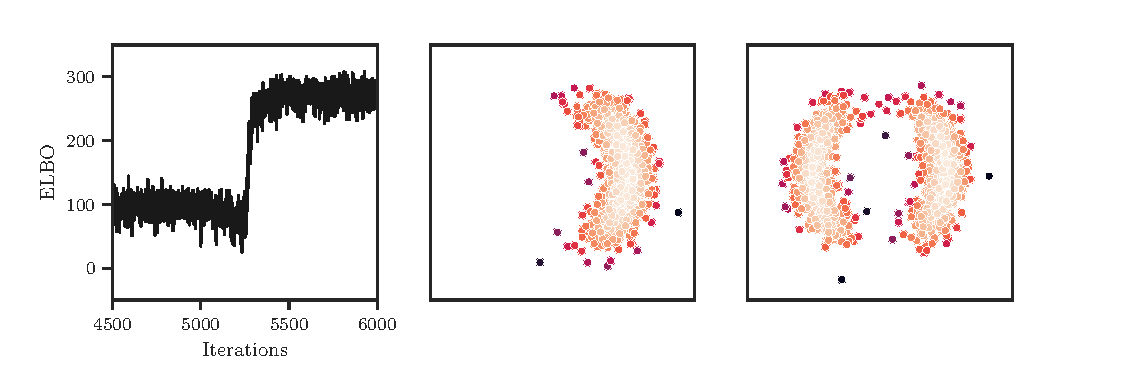
\includegraphics{figures/elbow_example/elbow.pdf}
    \caption{Training curve for a normalizing flow with 4 planar flows. When variational inference is performed on this bi-modal target distribution, an `elbow' forms in the ELBO as the variational approximation changes shape to `snap' to the new mode\cite{blei2017variational}.}
    \label{fig:training_curve_elbow_example}    
    \end{adjustwidth}
\end{figure}

\begin{figure}
    \begin{adjustwidth}{-2.5cm}{-2.5cm}
    \centering
     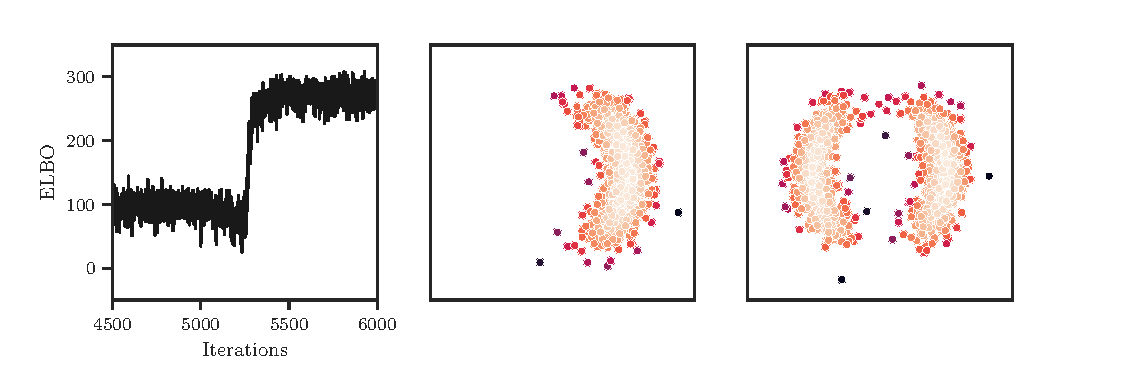
\includegraphics{figures/elbow_example/elbow.pdf}
    \caption{Training curve for a normalizing flow with 4 planar flows. When variational inference is performed on this bi-modal target distribution, an `elbow' forms in the ELBO as the variational approximation changes shape to `snap' to the new mode\cite{blei2017variational}.}
    % \label{fig:training_curve_elbow_example}   
    \end{adjustwidth}
\end{figure}

From the log term in \cref{eq:kl_divergence} it is clear that minimizing the KL-divergence heavily penalizes candidate distributions $q$ for which the probability at $z$, $q(z)$, is high and $p(z|x)$ is low.
This is why it takes some time for the second mode to be fitted --- the space between the two modes has a low $p(z)$, leading to a penalization on the ELBO for approximations which traverse this space.
Indeed, it can be seen in \cref{fig:elbow_example_10000} that in iteration 10000, the variational approximation deviates from a uni-modal approximation, and this iteration corresponds to the area in the training curve in \cref{fig:training_curve_elbow_example} where the ELBO drops, before in the second mode is captured and the ELBO rises again in iteration 11000.

\subsection{Poisson regression}

\begin{figure}
    \centering
    % \tikz{
    % nodes
    \node[obs] (y) {$y$};
    \node[obs,above=of y] (x) {$\vec x$};
    \node[latent,left=of y] (w) {$\vec{w}$};
    \node[latent,above=of w,fill] (kappa2) {$\kappa^2$};
    % plate
    \plate [inner sep=.25cm,yshift=.2cm] {P} {(w)} {$P$};
    \plate [inner sep=.25cm,yshift=.2cm] {N} {(y)(x)} {$N$};
    % edges
    \edge {kappa2} {w}
    \edge {x, w} {y}
    
    \node [right=of N, anchor=west] {
    $\begin{aligned}
        \kappa^2 & \sim \mathrm{LogNormal}(0, 1) \\
        \vec{w} & \sim \normal(0, \kappa^2) \\
         y & \sim \mathrm{Poisson}(\exp(\vec w\T \vec x))
    \end{aligned}$
    };  

}

% \tikz{
%     % nodes
%     \node[obs] (y) {$y$};
%     \node[latent,above=of y] (mu) {$\vec{\mu}$};
%     \node[latent,above=of mu] (lambda) {$\vec{\lambda}$};
%     \node[obs,above=of lambda] (x) {$\vec x$};
%     \node[latent,left=of lambda] (w) {$\vec{w}$};
%     \node[latent,above=of w,fill] (kappa2) {$\kappa^2$};
%     % plate
%     \plate [inner sep=.25cm,yshift=.2cm] {P} {(w)} {$P$};
%     \plate [inner sep=.25cm,yshift=.2cm] {N} {(y)(x)(lambda)(mu)} {$N$};
%     % edges
%     \edge {kappa2} {w}
%     \edge {x, w} {lambda}
%     \edge {lambda} {mu}
%     \edge {mu} {y}
    
%     \node [right=of N, anchor=west] {
%     $\begin{aligned}
%         \kappa^2 & \sim \mathrm{LogNormal}(0, 1) \\
%         \vec{w} & \sim \normal(0, \kappa^2) \\
%         \vec \lambda & = \vec w\T \vec x \\
%         \vec \mu & = \exp(\vec \lambda) \\
%          y & \sim \mathrm{Poisson}(\vec \mu)
%     \end{aligned}$
%     };  

% }
    \caption{Probabilistic graphical model for Poisson regression problem.}
    \label{fig:poisson-pgm}
\end{figure}

\begin{figure}
    \centering
    % %% Creator: Matplotlib, PGF backend
%%
%% To include the figure in your LaTeX document, write
%%   \input{<filename>.pgf}
%%
%% Make sure the required packages are loaded in your preamble
%%   \usepackage{pgf}
%%
%% Figures using additional raster images can only be included by \input if
%% they are in the same directory as the main LaTeX file. For loading figures
%% from other directories you can use the `import` package
%%   \usepackage{import}
%% and then include the figures with
%%   \import{<path to file>}{<filename>.pgf}
%%
%% Matplotlib used the following preamble
%%
\begingroup%
\makeatletter%
\begin{pgfpicture}%
\pgfpathrectangle{\pgfpointorigin}{\pgfqpoint{3.000000in}{2.500000in}}%
\pgfusepath{use as bounding box, clip}%
\begin{pgfscope}%
\pgfsetbuttcap%
\pgfsetmiterjoin%
\definecolor{currentfill}{rgb}{1.000000,1.000000,1.000000}%
\pgfsetfillcolor{currentfill}%
\pgfsetlinewidth{0.000000pt}%
\definecolor{currentstroke}{rgb}{1.000000,1.000000,1.000000}%
\pgfsetstrokecolor{currentstroke}%
\pgfsetdash{}{0pt}%
\pgfpathmoveto{\pgfqpoint{0.000000in}{0.000000in}}%
\pgfpathlineto{\pgfqpoint{3.000000in}{0.000000in}}%
\pgfpathlineto{\pgfqpoint{3.000000in}{2.500000in}}%
\pgfpathlineto{\pgfqpoint{0.000000in}{2.500000in}}%
\pgfpathclose%
\pgfusepath{fill}%
\end{pgfscope}%
\begin{pgfscope}%
\pgfsetbuttcap%
\pgfsetmiterjoin%
\definecolor{currentfill}{rgb}{1.000000,1.000000,1.000000}%
\pgfsetfillcolor{currentfill}%
\pgfsetlinewidth{0.000000pt}%
\definecolor{currentstroke}{rgb}{0.000000,0.000000,0.000000}%
\pgfsetstrokecolor{currentstroke}%
\pgfsetstrokeopacity{0.000000}%
\pgfsetdash{}{0pt}%
\pgfpathmoveto{\pgfqpoint{0.375000in}{0.275000in}}%
\pgfpathlineto{\pgfqpoint{2.700000in}{0.275000in}}%
\pgfpathlineto{\pgfqpoint{2.700000in}{2.200000in}}%
\pgfpathlineto{\pgfqpoint{0.375000in}{2.200000in}}%
\pgfpathclose%
\pgfusepath{fill}%
\end{pgfscope}%
\begin{pgfscope}%
\pgfsetbuttcap%
\pgfsetroundjoin%
\definecolor{currentfill}{rgb}{0.150000,0.150000,0.150000}%
\pgfsetfillcolor{currentfill}%
\pgfsetlinewidth{1.003750pt}%
\definecolor{currentstroke}{rgb}{0.150000,0.150000,0.150000}%
\pgfsetstrokecolor{currentstroke}%
\pgfsetdash{}{0pt}%
\pgfsys@defobject{currentmarker}{\pgfqpoint{0.000000in}{-0.066667in}}{\pgfqpoint{0.000000in}{0.000000in}}{%
\pgfpathmoveto{\pgfqpoint{0.000000in}{0.000000in}}%
\pgfpathlineto{\pgfqpoint{0.000000in}{-0.066667in}}%
\pgfusepath{stroke,fill}%
}%
\begin{pgfscope}%
\pgfsys@transformshift{0.860477in}{0.275000in}%
\pgfsys@useobject{currentmarker}{}%
\end{pgfscope}%
\end{pgfscope}%
\begin{pgfscope}%
\definecolor{textcolor}{rgb}{0.150000,0.150000,0.150000}%
\pgfsetstrokecolor{textcolor}%
\pgfsetfillcolor{textcolor}%
\pgftext[x=0.860477in,y=0.159722in,,top]{\color{textcolor}\rmfamily\fontsize{8.800000}{10.560000}\selectfont \(\displaystyle 40\)}%
\end{pgfscope}%
\begin{pgfscope}%
\pgfsetbuttcap%
\pgfsetroundjoin%
\definecolor{currentfill}{rgb}{0.150000,0.150000,0.150000}%
\pgfsetfillcolor{currentfill}%
\pgfsetlinewidth{1.003750pt}%
\definecolor{currentstroke}{rgb}{0.150000,0.150000,0.150000}%
\pgfsetstrokecolor{currentstroke}%
\pgfsetdash{}{0pt}%
\pgfsys@defobject{currentmarker}{\pgfqpoint{0.000000in}{-0.066667in}}{\pgfqpoint{0.000000in}{0.000000in}}{%
\pgfpathmoveto{\pgfqpoint{0.000000in}{0.000000in}}%
\pgfpathlineto{\pgfqpoint{0.000000in}{-0.066667in}}%
\pgfusepath{stroke,fill}%
}%
\begin{pgfscope}%
\pgfsys@transformshift{1.573133in}{0.275000in}%
\pgfsys@useobject{currentmarker}{}%
\end{pgfscope}%
\end{pgfscope}%
\begin{pgfscope}%
\definecolor{textcolor}{rgb}{0.150000,0.150000,0.150000}%
\pgfsetstrokecolor{textcolor}%
\pgfsetfillcolor{textcolor}%
\pgftext[x=1.573133in,y=0.159722in,,top]{\color{textcolor}\rmfamily\fontsize{8.800000}{10.560000}\selectfont \(\displaystyle 50\)}%
\end{pgfscope}%
\begin{pgfscope}%
\pgfsetbuttcap%
\pgfsetroundjoin%
\definecolor{currentfill}{rgb}{0.150000,0.150000,0.150000}%
\pgfsetfillcolor{currentfill}%
\pgfsetlinewidth{1.003750pt}%
\definecolor{currentstroke}{rgb}{0.150000,0.150000,0.150000}%
\pgfsetstrokecolor{currentstroke}%
\pgfsetdash{}{0pt}%
\pgfsys@defobject{currentmarker}{\pgfqpoint{0.000000in}{-0.066667in}}{\pgfqpoint{0.000000in}{0.000000in}}{%
\pgfpathmoveto{\pgfqpoint{0.000000in}{0.000000in}}%
\pgfpathlineto{\pgfqpoint{0.000000in}{-0.066667in}}%
\pgfusepath{stroke,fill}%
}%
\begin{pgfscope}%
\pgfsys@transformshift{2.285789in}{0.275000in}%
\pgfsys@useobject{currentmarker}{}%
\end{pgfscope}%
\end{pgfscope}%
\begin{pgfscope}%
\definecolor{textcolor}{rgb}{0.150000,0.150000,0.150000}%
\pgfsetstrokecolor{textcolor}%
\pgfsetfillcolor{textcolor}%
\pgftext[x=2.285789in,y=0.159722in,,top]{\color{textcolor}\rmfamily\fontsize{8.800000}{10.560000}\selectfont \(\displaystyle 60\)}%
\end{pgfscope}%
\begin{pgfscope}%
\definecolor{textcolor}{rgb}{0.150000,0.150000,0.150000}%
\pgfsetstrokecolor{textcolor}%
\pgfsetfillcolor{textcolor}%
\pgftext[x=1.537500in,y=-0.006944in,,top]{\color{textcolor}\rmfamily\fontsize{9.600000}{11.520000}\selectfont Age}%
\end{pgfscope}%
\begin{pgfscope}%
\pgfsetbuttcap%
\pgfsetroundjoin%
\definecolor{currentfill}{rgb}{0.150000,0.150000,0.150000}%
\pgfsetfillcolor{currentfill}%
\pgfsetlinewidth{1.003750pt}%
\definecolor{currentstroke}{rgb}{0.150000,0.150000,0.150000}%
\pgfsetstrokecolor{currentstroke}%
\pgfsetdash{}{0pt}%
\pgfsys@defobject{currentmarker}{\pgfqpoint{-0.066667in}{0.000000in}}{\pgfqpoint{0.000000in}{0.000000in}}{%
\pgfpathmoveto{\pgfqpoint{0.000000in}{0.000000in}}%
\pgfpathlineto{\pgfqpoint{-0.066667in}{0.000000in}}%
\pgfusepath{stroke,fill}%
}%
\begin{pgfscope}%
\pgfsys@transformshift{0.375000in}{0.362500in}%
\pgfsys@useobject{currentmarker}{}%
\end{pgfscope}%
\end{pgfscope}%
\begin{pgfscope}%
\definecolor{textcolor}{rgb}{0.150000,0.150000,0.150000}%
\pgfsetstrokecolor{textcolor}%
\pgfsetfillcolor{textcolor}%
\pgftext[x=0.195487in,y=0.319097in,left,base]{\color{textcolor}\rmfamily\fontsize{8.800000}{10.560000}\selectfont \(\displaystyle 0\)}%
\end{pgfscope}%
\begin{pgfscope}%
\pgfsetbuttcap%
\pgfsetroundjoin%
\definecolor{currentfill}{rgb}{0.150000,0.150000,0.150000}%
\pgfsetfillcolor{currentfill}%
\pgfsetlinewidth{1.003750pt}%
\definecolor{currentstroke}{rgb}{0.150000,0.150000,0.150000}%
\pgfsetstrokecolor{currentstroke}%
\pgfsetdash{}{0pt}%
\pgfsys@defobject{currentmarker}{\pgfqpoint{-0.066667in}{0.000000in}}{\pgfqpoint{0.000000in}{0.000000in}}{%
\pgfpathmoveto{\pgfqpoint{0.000000in}{0.000000in}}%
\pgfpathlineto{\pgfqpoint{-0.066667in}{0.000000in}}%
\pgfusepath{stroke,fill}%
}%
\begin{pgfscope}%
\pgfsys@transformshift{0.375000in}{0.664224in}%
\pgfsys@useobject{currentmarker}{}%
\end{pgfscope}%
\end{pgfscope}%
\begin{pgfscope}%
\definecolor{textcolor}{rgb}{0.150000,0.150000,0.150000}%
\pgfsetstrokecolor{textcolor}%
\pgfsetfillcolor{textcolor}%
\pgftext[x=0.195487in,y=0.620821in,left,base]{\color{textcolor}\rmfamily\fontsize{8.800000}{10.560000}\selectfont \(\displaystyle 5\)}%
\end{pgfscope}%
\begin{pgfscope}%
\pgfsetbuttcap%
\pgfsetroundjoin%
\definecolor{currentfill}{rgb}{0.150000,0.150000,0.150000}%
\pgfsetfillcolor{currentfill}%
\pgfsetlinewidth{1.003750pt}%
\definecolor{currentstroke}{rgb}{0.150000,0.150000,0.150000}%
\pgfsetstrokecolor{currentstroke}%
\pgfsetdash{}{0pt}%
\pgfsys@defobject{currentmarker}{\pgfqpoint{-0.066667in}{0.000000in}}{\pgfqpoint{0.000000in}{0.000000in}}{%
\pgfpathmoveto{\pgfqpoint{0.000000in}{0.000000in}}%
\pgfpathlineto{\pgfqpoint{-0.066667in}{0.000000in}}%
\pgfusepath{stroke,fill}%
}%
\begin{pgfscope}%
\pgfsys@transformshift{0.375000in}{0.965948in}%
\pgfsys@useobject{currentmarker}{}%
\end{pgfscope}%
\end{pgfscope}%
\begin{pgfscope}%
\definecolor{textcolor}{rgb}{0.150000,0.150000,0.150000}%
\pgfsetstrokecolor{textcolor}%
\pgfsetfillcolor{textcolor}%
\pgftext[x=0.131251in,y=0.922545in,left,base]{\color{textcolor}\rmfamily\fontsize{8.800000}{10.560000}\selectfont \(\displaystyle 10\)}%
\end{pgfscope}%
\begin{pgfscope}%
\pgfsetbuttcap%
\pgfsetroundjoin%
\definecolor{currentfill}{rgb}{0.150000,0.150000,0.150000}%
\pgfsetfillcolor{currentfill}%
\pgfsetlinewidth{1.003750pt}%
\definecolor{currentstroke}{rgb}{0.150000,0.150000,0.150000}%
\pgfsetstrokecolor{currentstroke}%
\pgfsetdash{}{0pt}%
\pgfsys@defobject{currentmarker}{\pgfqpoint{-0.066667in}{0.000000in}}{\pgfqpoint{0.000000in}{0.000000in}}{%
\pgfpathmoveto{\pgfqpoint{0.000000in}{0.000000in}}%
\pgfpathlineto{\pgfqpoint{-0.066667in}{0.000000in}}%
\pgfusepath{stroke,fill}%
}%
\begin{pgfscope}%
\pgfsys@transformshift{0.375000in}{1.267672in}%
\pgfsys@useobject{currentmarker}{}%
\end{pgfscope}%
\end{pgfscope}%
\begin{pgfscope}%
\definecolor{textcolor}{rgb}{0.150000,0.150000,0.150000}%
\pgfsetstrokecolor{textcolor}%
\pgfsetfillcolor{textcolor}%
\pgftext[x=0.131251in,y=1.224270in,left,base]{\color{textcolor}\rmfamily\fontsize{8.800000}{10.560000}\selectfont \(\displaystyle 15\)}%
\end{pgfscope}%
\begin{pgfscope}%
\pgfsetbuttcap%
\pgfsetroundjoin%
\definecolor{currentfill}{rgb}{0.150000,0.150000,0.150000}%
\pgfsetfillcolor{currentfill}%
\pgfsetlinewidth{1.003750pt}%
\definecolor{currentstroke}{rgb}{0.150000,0.150000,0.150000}%
\pgfsetstrokecolor{currentstroke}%
\pgfsetdash{}{0pt}%
\pgfsys@defobject{currentmarker}{\pgfqpoint{-0.066667in}{0.000000in}}{\pgfqpoint{0.000000in}{0.000000in}}{%
\pgfpathmoveto{\pgfqpoint{0.000000in}{0.000000in}}%
\pgfpathlineto{\pgfqpoint{-0.066667in}{0.000000in}}%
\pgfusepath{stroke,fill}%
}%
\begin{pgfscope}%
\pgfsys@transformshift{0.375000in}{1.569397in}%
\pgfsys@useobject{currentmarker}{}%
\end{pgfscope}%
\end{pgfscope}%
\begin{pgfscope}%
\definecolor{textcolor}{rgb}{0.150000,0.150000,0.150000}%
\pgfsetstrokecolor{textcolor}%
\pgfsetfillcolor{textcolor}%
\pgftext[x=0.131251in,y=1.525994in,left,base]{\color{textcolor}\rmfamily\fontsize{8.800000}{10.560000}\selectfont \(\displaystyle 20\)}%
\end{pgfscope}%
\begin{pgfscope}%
\pgfsetbuttcap%
\pgfsetroundjoin%
\definecolor{currentfill}{rgb}{0.150000,0.150000,0.150000}%
\pgfsetfillcolor{currentfill}%
\pgfsetlinewidth{1.003750pt}%
\definecolor{currentstroke}{rgb}{0.150000,0.150000,0.150000}%
\pgfsetstrokecolor{currentstroke}%
\pgfsetdash{}{0pt}%
\pgfsys@defobject{currentmarker}{\pgfqpoint{-0.066667in}{0.000000in}}{\pgfqpoint{0.000000in}{0.000000in}}{%
\pgfpathmoveto{\pgfqpoint{0.000000in}{0.000000in}}%
\pgfpathlineto{\pgfqpoint{-0.066667in}{0.000000in}}%
\pgfusepath{stroke,fill}%
}%
\begin{pgfscope}%
\pgfsys@transformshift{0.375000in}{1.871121in}%
\pgfsys@useobject{currentmarker}{}%
\end{pgfscope}%
\end{pgfscope}%
\begin{pgfscope}%
\definecolor{textcolor}{rgb}{0.150000,0.150000,0.150000}%
\pgfsetstrokecolor{textcolor}%
\pgfsetfillcolor{textcolor}%
\pgftext[x=0.131251in,y=1.827718in,left,base]{\color{textcolor}\rmfamily\fontsize{8.800000}{10.560000}\selectfont \(\displaystyle 25\)}%
\end{pgfscope}%
\begin{pgfscope}%
\pgfsetbuttcap%
\pgfsetroundjoin%
\definecolor{currentfill}{rgb}{0.150000,0.150000,0.150000}%
\pgfsetfillcolor{currentfill}%
\pgfsetlinewidth{1.003750pt}%
\definecolor{currentstroke}{rgb}{0.150000,0.150000,0.150000}%
\pgfsetstrokecolor{currentstroke}%
\pgfsetdash{}{0pt}%
\pgfsys@defobject{currentmarker}{\pgfqpoint{-0.066667in}{0.000000in}}{\pgfqpoint{0.000000in}{0.000000in}}{%
\pgfpathmoveto{\pgfqpoint{0.000000in}{0.000000in}}%
\pgfpathlineto{\pgfqpoint{-0.066667in}{0.000000in}}%
\pgfusepath{stroke,fill}%
}%
\begin{pgfscope}%
\pgfsys@transformshift{0.375000in}{2.172845in}%
\pgfsys@useobject{currentmarker}{}%
\end{pgfscope}%
\end{pgfscope}%
\begin{pgfscope}%
\definecolor{textcolor}{rgb}{0.150000,0.150000,0.150000}%
\pgfsetstrokecolor{textcolor}%
\pgfsetfillcolor{textcolor}%
\pgftext[x=0.131251in,y=2.129442in,left,base]{\color{textcolor}\rmfamily\fontsize{8.800000}{10.560000}\selectfont \(\displaystyle 30\)}%
\end{pgfscope}%
\begin{pgfscope}%
\definecolor{textcolor}{rgb}{0.150000,0.150000,0.150000}%
\pgfsetstrokecolor{textcolor}%
\pgfsetfillcolor{textcolor}%
\pgftext[x=0.075695in,y=1.237500in,,bottom,rotate=90.000000]{\color{textcolor}\rmfamily\fontsize{9.600000}{11.520000}\selectfont Number of deaths}%
\end{pgfscope}%
\begin{pgfscope}%
\pgfpathrectangle{\pgfqpoint{0.375000in}{0.275000in}}{\pgfqpoint{2.325000in}{1.925000in}}%
\pgfusepath{clip}%
\pgfsetbuttcap%
\pgfsetroundjoin%
\definecolor{currentfill}{rgb}{0.768627,0.305882,0.321569}%
\pgfsetfillcolor{currentfill}%
\pgfsetfillopacity{0.250000}%
\pgfsetlinewidth{0.803000pt}%
\definecolor{currentstroke}{rgb}{0.768627,0.305882,0.321569}%
\pgfsetstrokecolor{currentstroke}%
\pgfsetstrokeopacity{0.250000}%
\pgfsetdash{}{0pt}%
\pgfpathmoveto{\pgfqpoint{0.504149in}{0.905603in}}%
\pgfpathlineto{\pgfqpoint{0.504149in}{0.362500in}}%
\pgfpathlineto{\pgfqpoint{0.575414in}{0.362500in}}%
\pgfpathlineto{\pgfqpoint{0.646680in}{0.362500in}}%
\pgfpathlineto{\pgfqpoint{0.717946in}{0.362500in}}%
\pgfpathlineto{\pgfqpoint{0.789211in}{0.362500in}}%
\pgfpathlineto{\pgfqpoint{0.860477in}{0.362500in}}%
\pgfpathlineto{\pgfqpoint{0.931742in}{0.362500in}}%
\pgfpathlineto{\pgfqpoint{1.003008in}{0.362500in}}%
\pgfpathlineto{\pgfqpoint{1.074274in}{0.362500in}}%
\pgfpathlineto{\pgfqpoint{1.145539in}{0.362500in}}%
\pgfpathlineto{\pgfqpoint{1.216805in}{0.362500in}}%
\pgfpathlineto{\pgfqpoint{1.288070in}{0.362500in}}%
\pgfpathlineto{\pgfqpoint{1.359336in}{0.422845in}}%
\pgfpathlineto{\pgfqpoint{1.430602in}{0.422845in}}%
\pgfpathlineto{\pgfqpoint{1.501867in}{0.422845in}}%
\pgfpathlineto{\pgfqpoint{1.573133in}{0.422845in}}%
\pgfpathlineto{\pgfqpoint{1.644398in}{0.422845in}}%
\pgfpathlineto{\pgfqpoint{1.715664in}{0.422845in}}%
\pgfpathlineto{\pgfqpoint{1.786930in}{0.483190in}}%
\pgfpathlineto{\pgfqpoint{1.858195in}{0.483190in}}%
\pgfpathlineto{\pgfqpoint{1.929461in}{0.483190in}}%
\pgfpathlineto{\pgfqpoint{2.000726in}{0.483190in}}%
\pgfpathlineto{\pgfqpoint{2.071992in}{0.543534in}}%
\pgfpathlineto{\pgfqpoint{2.143258in}{0.543534in}}%
\pgfpathlineto{\pgfqpoint{2.214523in}{0.543534in}}%
\pgfpathlineto{\pgfqpoint{2.285789in}{0.603879in}}%
\pgfpathlineto{\pgfqpoint{2.357054in}{0.603879in}}%
\pgfpathlineto{\pgfqpoint{2.428320in}{0.603879in}}%
\pgfpathlineto{\pgfqpoint{2.499586in}{0.664224in}}%
\pgfpathlineto{\pgfqpoint{2.570851in}{0.664224in}}%
\pgfpathlineto{\pgfqpoint{2.570851in}{2.112500in}}%
\pgfpathlineto{\pgfqpoint{2.570851in}{2.112500in}}%
\pgfpathlineto{\pgfqpoint{2.499586in}{1.963147in}}%
\pgfpathlineto{\pgfqpoint{2.428320in}{1.931466in}}%
\pgfpathlineto{\pgfqpoint{2.357054in}{1.810776in}}%
\pgfpathlineto{\pgfqpoint{2.285789in}{1.750431in}}%
\pgfpathlineto{\pgfqpoint{2.214523in}{1.690086in}}%
\pgfpathlineto{\pgfqpoint{2.143258in}{1.629741in}}%
\pgfpathlineto{\pgfqpoint{2.071992in}{1.569397in}}%
\pgfpathlineto{\pgfqpoint{2.000726in}{1.509052in}}%
\pgfpathlineto{\pgfqpoint{1.929461in}{1.448707in}}%
\pgfpathlineto{\pgfqpoint{1.858195in}{1.388362in}}%
\pgfpathlineto{\pgfqpoint{1.786930in}{1.388362in}}%
\pgfpathlineto{\pgfqpoint{1.715664in}{1.328017in}}%
\pgfpathlineto{\pgfqpoint{1.644398in}{1.267672in}}%
\pgfpathlineto{\pgfqpoint{1.573133in}{1.299353in}}%
\pgfpathlineto{\pgfqpoint{1.501867in}{1.207328in}}%
\pgfpathlineto{\pgfqpoint{1.430602in}{1.178664in}}%
\pgfpathlineto{\pgfqpoint{1.359336in}{1.146983in}}%
\pgfpathlineto{\pgfqpoint{1.288070in}{1.146983in}}%
\pgfpathlineto{\pgfqpoint{1.216805in}{1.086638in}}%
\pgfpathlineto{\pgfqpoint{1.145539in}{1.086638in}}%
\pgfpathlineto{\pgfqpoint{1.074274in}{1.086638in}}%
\pgfpathlineto{\pgfqpoint{1.003008in}{1.026293in}}%
\pgfpathlineto{\pgfqpoint{0.931742in}{1.026293in}}%
\pgfpathlineto{\pgfqpoint{0.860477in}{1.026293in}}%
\pgfpathlineto{\pgfqpoint{0.789211in}{0.965948in}}%
\pgfpathlineto{\pgfqpoint{0.717946in}{0.965948in}}%
\pgfpathlineto{\pgfqpoint{0.646680in}{0.965948in}}%
\pgfpathlineto{\pgfqpoint{0.575414in}{0.905603in}}%
\pgfpathlineto{\pgfqpoint{0.504149in}{0.905603in}}%
\pgfpathclose%
\pgfusepath{stroke,fill}%
\end{pgfscope}%
\begin{pgfscope}%
\pgfpathrectangle{\pgfqpoint{0.375000in}{0.275000in}}{\pgfqpoint{2.325000in}{1.925000in}}%
\pgfusepath{clip}%
\pgfsetbuttcap%
\pgfsetroundjoin%
\definecolor{currentfill}{rgb}{0.768627,0.305882,0.321569}%
\pgfsetfillcolor{currentfill}%
\pgfsetfillopacity{0.350000}%
\pgfsetlinewidth{0.803000pt}%
\definecolor{currentstroke}{rgb}{0.768627,0.305882,0.321569}%
\pgfsetstrokecolor{currentstroke}%
\pgfsetstrokeopacity{0.350000}%
\pgfsetdash{}{0pt}%
\pgfpathmoveto{\pgfqpoint{0.504149in}{0.784914in}}%
\pgfpathlineto{\pgfqpoint{0.504149in}{0.362500in}}%
\pgfpathlineto{\pgfqpoint{0.575414in}{0.362500in}}%
\pgfpathlineto{\pgfqpoint{0.646680in}{0.362500in}}%
\pgfpathlineto{\pgfqpoint{0.717946in}{0.362500in}}%
\pgfpathlineto{\pgfqpoint{0.789211in}{0.362500in}}%
\pgfpathlineto{\pgfqpoint{0.860477in}{0.422845in}}%
\pgfpathlineto{\pgfqpoint{0.931742in}{0.422845in}}%
\pgfpathlineto{\pgfqpoint{1.003008in}{0.422845in}}%
\pgfpathlineto{\pgfqpoint{1.074274in}{0.422845in}}%
\pgfpathlineto{\pgfqpoint{1.145539in}{0.422845in}}%
\pgfpathlineto{\pgfqpoint{1.216805in}{0.422845in}}%
\pgfpathlineto{\pgfqpoint{1.288070in}{0.422845in}}%
\pgfpathlineto{\pgfqpoint{1.359336in}{0.422845in}}%
\pgfpathlineto{\pgfqpoint{1.430602in}{0.483190in}}%
\pgfpathlineto{\pgfqpoint{1.501867in}{0.483190in}}%
\pgfpathlineto{\pgfqpoint{1.573133in}{0.483190in}}%
\pgfpathlineto{\pgfqpoint{1.644398in}{0.483190in}}%
\pgfpathlineto{\pgfqpoint{1.715664in}{0.483190in}}%
\pgfpathlineto{\pgfqpoint{1.786930in}{0.543534in}}%
\pgfpathlineto{\pgfqpoint{1.858195in}{0.543534in}}%
\pgfpathlineto{\pgfqpoint{1.929461in}{0.603879in}}%
\pgfpathlineto{\pgfqpoint{2.000726in}{0.603879in}}%
\pgfpathlineto{\pgfqpoint{2.071992in}{0.603879in}}%
\pgfpathlineto{\pgfqpoint{2.143258in}{0.664224in}}%
\pgfpathlineto{\pgfqpoint{2.214523in}{0.664224in}}%
\pgfpathlineto{\pgfqpoint{2.285789in}{0.664224in}}%
\pgfpathlineto{\pgfqpoint{2.357054in}{0.724569in}}%
\pgfpathlineto{\pgfqpoint{2.428320in}{0.724569in}}%
\pgfpathlineto{\pgfqpoint{2.499586in}{0.784914in}}%
\pgfpathlineto{\pgfqpoint{2.570851in}{0.784914in}}%
\pgfpathlineto{\pgfqpoint{2.570851in}{1.871121in}}%
\pgfpathlineto{\pgfqpoint{2.570851in}{1.871121in}}%
\pgfpathlineto{\pgfqpoint{2.499586in}{1.810776in}}%
\pgfpathlineto{\pgfqpoint{2.428320in}{1.690086in}}%
\pgfpathlineto{\pgfqpoint{2.357054in}{1.629741in}}%
\pgfpathlineto{\pgfqpoint{2.285789in}{1.569397in}}%
\pgfpathlineto{\pgfqpoint{2.214523in}{1.509052in}}%
\pgfpathlineto{\pgfqpoint{2.143258in}{1.448707in}}%
\pgfpathlineto{\pgfqpoint{2.071992in}{1.448707in}}%
\pgfpathlineto{\pgfqpoint{2.000726in}{1.328017in}}%
\pgfpathlineto{\pgfqpoint{1.929461in}{1.328017in}}%
\pgfpathlineto{\pgfqpoint{1.858195in}{1.267672in}}%
\pgfpathlineto{\pgfqpoint{1.786930in}{1.207328in}}%
\pgfpathlineto{\pgfqpoint{1.715664in}{1.207328in}}%
\pgfpathlineto{\pgfqpoint{1.644398in}{1.146983in}}%
\pgfpathlineto{\pgfqpoint{1.573133in}{1.146983in}}%
\pgfpathlineto{\pgfqpoint{1.501867in}{1.086638in}}%
\pgfpathlineto{\pgfqpoint{1.430602in}{1.086638in}}%
\pgfpathlineto{\pgfqpoint{1.359336in}{1.026293in}}%
\pgfpathlineto{\pgfqpoint{1.288070in}{1.026293in}}%
\pgfpathlineto{\pgfqpoint{1.216805in}{0.965948in}}%
\pgfpathlineto{\pgfqpoint{1.145539in}{0.965948in}}%
\pgfpathlineto{\pgfqpoint{1.074274in}{0.965948in}}%
\pgfpathlineto{\pgfqpoint{1.003008in}{0.905603in}}%
\pgfpathlineto{\pgfqpoint{0.931742in}{0.905603in}}%
\pgfpathlineto{\pgfqpoint{0.860477in}{0.905603in}}%
\pgfpathlineto{\pgfqpoint{0.789211in}{0.845259in}}%
\pgfpathlineto{\pgfqpoint{0.717946in}{0.845259in}}%
\pgfpathlineto{\pgfqpoint{0.646680in}{0.845259in}}%
\pgfpathlineto{\pgfqpoint{0.575414in}{0.784914in}}%
\pgfpathlineto{\pgfqpoint{0.504149in}{0.784914in}}%
\pgfpathclose%
\pgfusepath{stroke,fill}%
\end{pgfscope}%
\begin{pgfscope}%
\pgfpathrectangle{\pgfqpoint{0.375000in}{0.275000in}}{\pgfqpoint{2.325000in}{1.925000in}}%
\pgfusepath{clip}%
\pgfsetbuttcap%
\pgfsetroundjoin%
\definecolor{currentfill}{rgb}{0.768627,0.305882,0.321569}%
\pgfsetfillcolor{currentfill}%
\pgfsetfillopacity{0.600000}%
\pgfsetlinewidth{0.803000pt}%
\definecolor{currentstroke}{rgb}{0.768627,0.305882,0.321569}%
\pgfsetstrokecolor{currentstroke}%
\pgfsetstrokeopacity{0.600000}%
\pgfsetdash{}{0pt}%
\pgfpathmoveto{\pgfqpoint{0.504149in}{0.664224in}}%
\pgfpathlineto{\pgfqpoint{0.504149in}{0.422845in}}%
\pgfpathlineto{\pgfqpoint{0.575414in}{0.422845in}}%
\pgfpathlineto{\pgfqpoint{0.646680in}{0.422845in}}%
\pgfpathlineto{\pgfqpoint{0.717946in}{0.422845in}}%
\pgfpathlineto{\pgfqpoint{0.789211in}{0.422845in}}%
\pgfpathlineto{\pgfqpoint{0.860477in}{0.483190in}}%
\pgfpathlineto{\pgfqpoint{0.931742in}{0.483190in}}%
\pgfpathlineto{\pgfqpoint{1.003008in}{0.483190in}}%
\pgfpathlineto{\pgfqpoint{1.074274in}{0.483190in}}%
\pgfpathlineto{\pgfqpoint{1.145539in}{0.483190in}}%
\pgfpathlineto{\pgfqpoint{1.216805in}{0.543534in}}%
\pgfpathlineto{\pgfqpoint{1.288070in}{0.543534in}}%
\pgfpathlineto{\pgfqpoint{1.359336in}{0.543534in}}%
\pgfpathlineto{\pgfqpoint{1.430602in}{0.543534in}}%
\pgfpathlineto{\pgfqpoint{1.501867in}{0.603879in}}%
\pgfpathlineto{\pgfqpoint{1.573133in}{0.603879in}}%
\pgfpathlineto{\pgfqpoint{1.644398in}{0.603879in}}%
\pgfpathlineto{\pgfqpoint{1.715664in}{0.603879in}}%
\pgfpathlineto{\pgfqpoint{1.786930in}{0.664224in}}%
\pgfpathlineto{\pgfqpoint{1.858195in}{0.664224in}}%
\pgfpathlineto{\pgfqpoint{1.929461in}{0.724569in}}%
\pgfpathlineto{\pgfqpoint{2.000726in}{0.724569in}}%
\pgfpathlineto{\pgfqpoint{2.071992in}{0.724569in}}%
\pgfpathlineto{\pgfqpoint{2.143258in}{0.784914in}}%
\pgfpathlineto{\pgfqpoint{2.214523in}{0.784914in}}%
\pgfpathlineto{\pgfqpoint{2.285789in}{0.845259in}}%
\pgfpathlineto{\pgfqpoint{2.357054in}{0.905603in}}%
\pgfpathlineto{\pgfqpoint{2.428320in}{0.905603in}}%
\pgfpathlineto{\pgfqpoint{2.499586in}{0.958405in}}%
\pgfpathlineto{\pgfqpoint{2.570851in}{0.965948in}}%
\pgfpathlineto{\pgfqpoint{2.570851in}{1.569397in}}%
\pgfpathlineto{\pgfqpoint{2.570851in}{1.569397in}}%
\pgfpathlineto{\pgfqpoint{2.499586in}{1.509052in}}%
\pgfpathlineto{\pgfqpoint{2.428320in}{1.448707in}}%
\pgfpathlineto{\pgfqpoint{2.357054in}{1.388362in}}%
\pgfpathlineto{\pgfqpoint{2.285789in}{1.328017in}}%
\pgfpathlineto{\pgfqpoint{2.214523in}{1.328017in}}%
\pgfpathlineto{\pgfqpoint{2.143258in}{1.267672in}}%
\pgfpathlineto{\pgfqpoint{2.071992in}{1.207328in}}%
\pgfpathlineto{\pgfqpoint{2.000726in}{1.146983in}}%
\pgfpathlineto{\pgfqpoint{1.929461in}{1.146983in}}%
\pgfpathlineto{\pgfqpoint{1.858195in}{1.086638in}}%
\pgfpathlineto{\pgfqpoint{1.786930in}{1.086638in}}%
\pgfpathlineto{\pgfqpoint{1.715664in}{1.026293in}}%
\pgfpathlineto{\pgfqpoint{1.644398in}{0.965948in}}%
\pgfpathlineto{\pgfqpoint{1.573133in}{0.965948in}}%
\pgfpathlineto{\pgfqpoint{1.501867in}{0.965948in}}%
\pgfpathlineto{\pgfqpoint{1.430602in}{0.905603in}}%
\pgfpathlineto{\pgfqpoint{1.359336in}{0.905603in}}%
\pgfpathlineto{\pgfqpoint{1.288070in}{0.845259in}}%
\pgfpathlineto{\pgfqpoint{1.216805in}{0.845259in}}%
\pgfpathlineto{\pgfqpoint{1.145539in}{0.845259in}}%
\pgfpathlineto{\pgfqpoint{1.074274in}{0.784914in}}%
\pgfpathlineto{\pgfqpoint{1.003008in}{0.784914in}}%
\pgfpathlineto{\pgfqpoint{0.931742in}{0.784914in}}%
\pgfpathlineto{\pgfqpoint{0.860477in}{0.724569in}}%
\pgfpathlineto{\pgfqpoint{0.789211in}{0.724569in}}%
\pgfpathlineto{\pgfqpoint{0.717946in}{0.724569in}}%
\pgfpathlineto{\pgfqpoint{0.646680in}{0.724569in}}%
\pgfpathlineto{\pgfqpoint{0.575414in}{0.664224in}}%
\pgfpathlineto{\pgfqpoint{0.504149in}{0.664224in}}%
\pgfpathclose%
\pgfusepath{stroke,fill}%
\end{pgfscope}%
\begin{pgfscope}%
\pgfpathrectangle{\pgfqpoint{0.375000in}{0.275000in}}{\pgfqpoint{2.325000in}{1.925000in}}%
\pgfusepath{clip}%
\pgfsetbuttcap%
\pgfsetroundjoin%
\definecolor{currentfill}{rgb}{0.100000,0.100000,0.100000}%
\pgfsetfillcolor{currentfill}%
\pgfsetlinewidth{0.385440pt}%
\definecolor{currentstroke}{rgb}{1.000000,1.000000,1.000000}%
\pgfsetstrokecolor{currentstroke}%
\pgfsetdash{}{0pt}%
\pgfpathmoveto{\pgfqpoint{0.504149in}{0.510201in}}%
\pgfpathcurveto{\pgfqpoint{0.512989in}{0.510201in}}{\pgfqpoint{0.521468in}{0.513713in}}{\pgfqpoint{0.527719in}{0.519964in}}%
\pgfpathcurveto{\pgfqpoint{0.533970in}{0.526215in}}{\pgfqpoint{0.537482in}{0.534694in}}{\pgfqpoint{0.537482in}{0.543534in}}%
\pgfpathcurveto{\pgfqpoint{0.537482in}{0.552375in}}{\pgfqpoint{0.533970in}{0.560854in}}{\pgfqpoint{0.527719in}{0.567105in}}%
\pgfpathcurveto{\pgfqpoint{0.521468in}{0.573356in}}{\pgfqpoint{0.512989in}{0.576868in}}{\pgfqpoint{0.504149in}{0.576868in}}%
\pgfpathcurveto{\pgfqpoint{0.495309in}{0.576868in}}{\pgfqpoint{0.486830in}{0.573356in}}{\pgfqpoint{0.480579in}{0.567105in}}%
\pgfpathcurveto{\pgfqpoint{0.474328in}{0.560854in}}{\pgfqpoint{0.470816in}{0.552375in}}{\pgfqpoint{0.470816in}{0.543534in}}%
\pgfpathcurveto{\pgfqpoint{0.470816in}{0.534694in}}{\pgfqpoint{0.474328in}{0.526215in}}{\pgfqpoint{0.480579in}{0.519964in}}%
\pgfpathcurveto{\pgfqpoint{0.486830in}{0.513713in}}{\pgfqpoint{0.495309in}{0.510201in}}{\pgfqpoint{0.504149in}{0.510201in}}%
\pgfpathclose%
\pgfusepath{stroke,fill}%
\end{pgfscope}%
\begin{pgfscope}%
\pgfpathrectangle{\pgfqpoint{0.375000in}{0.275000in}}{\pgfqpoint{2.325000in}{1.925000in}}%
\pgfusepath{clip}%
\pgfsetbuttcap%
\pgfsetroundjoin%
\definecolor{currentfill}{rgb}{0.100000,0.100000,0.100000}%
\pgfsetfillcolor{currentfill}%
\pgfsetlinewidth{0.385440pt}%
\definecolor{currentstroke}{rgb}{1.000000,1.000000,1.000000}%
\pgfsetstrokecolor{currentstroke}%
\pgfsetdash{}{0pt}%
\pgfpathmoveto{\pgfqpoint{0.575414in}{0.389511in}}%
\pgfpathcurveto{\pgfqpoint{0.584255in}{0.389511in}}{\pgfqpoint{0.592734in}{0.393024in}}{\pgfqpoint{0.598985in}{0.399275in}}%
\pgfpathcurveto{\pgfqpoint{0.605236in}{0.405525in}}{\pgfqpoint{0.608748in}{0.414005in}}{\pgfqpoint{0.608748in}{0.422845in}}%
\pgfpathcurveto{\pgfqpoint{0.608748in}{0.431685in}}{\pgfqpoint{0.605236in}{0.440164in}}{\pgfqpoint{0.598985in}{0.446415in}}%
\pgfpathcurveto{\pgfqpoint{0.592734in}{0.452666in}}{\pgfqpoint{0.584255in}{0.456178in}}{\pgfqpoint{0.575414in}{0.456178in}}%
\pgfpathcurveto{\pgfqpoint{0.566574in}{0.456178in}}{\pgfqpoint{0.558095in}{0.452666in}}{\pgfqpoint{0.551844in}{0.446415in}}%
\pgfpathcurveto{\pgfqpoint{0.545593in}{0.440164in}}{\pgfqpoint{0.542081in}{0.431685in}}{\pgfqpoint{0.542081in}{0.422845in}}%
\pgfpathcurveto{\pgfqpoint{0.542081in}{0.414005in}}{\pgfqpoint{0.545593in}{0.405525in}}{\pgfqpoint{0.551844in}{0.399275in}}%
\pgfpathcurveto{\pgfqpoint{0.558095in}{0.393024in}}{\pgfqpoint{0.566574in}{0.389511in}}{\pgfqpoint{0.575414in}{0.389511in}}%
\pgfpathclose%
\pgfusepath{stroke,fill}%
\end{pgfscope}%
\begin{pgfscope}%
\pgfpathrectangle{\pgfqpoint{0.375000in}{0.275000in}}{\pgfqpoint{2.325000in}{1.925000in}}%
\pgfusepath{clip}%
\pgfsetbuttcap%
\pgfsetroundjoin%
\definecolor{currentfill}{rgb}{0.100000,0.100000,0.100000}%
\pgfsetfillcolor{currentfill}%
\pgfsetlinewidth{0.385440pt}%
\definecolor{currentstroke}{rgb}{1.000000,1.000000,1.000000}%
\pgfsetstrokecolor{currentstroke}%
\pgfsetdash{}{0pt}%
\pgfpathmoveto{\pgfqpoint{0.646680in}{0.510201in}}%
\pgfpathcurveto{\pgfqpoint{0.655520in}{0.510201in}}{\pgfqpoint{0.663999in}{0.513713in}}{\pgfqpoint{0.670250in}{0.519964in}}%
\pgfpathcurveto{\pgfqpoint{0.676501in}{0.526215in}}{\pgfqpoint{0.680013in}{0.534694in}}{\pgfqpoint{0.680013in}{0.543534in}}%
\pgfpathcurveto{\pgfqpoint{0.680013in}{0.552375in}}{\pgfqpoint{0.676501in}{0.560854in}}{\pgfqpoint{0.670250in}{0.567105in}}%
\pgfpathcurveto{\pgfqpoint{0.663999in}{0.573356in}}{\pgfqpoint{0.655520in}{0.576868in}}{\pgfqpoint{0.646680in}{0.576868in}}%
\pgfpathcurveto{\pgfqpoint{0.637840in}{0.576868in}}{\pgfqpoint{0.629361in}{0.573356in}}{\pgfqpoint{0.623110in}{0.567105in}}%
\pgfpathcurveto{\pgfqpoint{0.616859in}{0.560854in}}{\pgfqpoint{0.613347in}{0.552375in}}{\pgfqpoint{0.613347in}{0.543534in}}%
\pgfpathcurveto{\pgfqpoint{0.613347in}{0.534694in}}{\pgfqpoint{0.616859in}{0.526215in}}{\pgfqpoint{0.623110in}{0.519964in}}%
\pgfpathcurveto{\pgfqpoint{0.629361in}{0.513713in}}{\pgfqpoint{0.637840in}{0.510201in}}{\pgfqpoint{0.646680in}{0.510201in}}%
\pgfpathclose%
\pgfusepath{stroke,fill}%
\end{pgfscope}%
\begin{pgfscope}%
\pgfpathrectangle{\pgfqpoint{0.375000in}{0.275000in}}{\pgfqpoint{2.325000in}{1.925000in}}%
\pgfusepath{clip}%
\pgfsetbuttcap%
\pgfsetroundjoin%
\definecolor{currentfill}{rgb}{0.100000,0.100000,0.100000}%
\pgfsetfillcolor{currentfill}%
\pgfsetlinewidth{0.385440pt}%
\definecolor{currentstroke}{rgb}{1.000000,1.000000,1.000000}%
\pgfsetstrokecolor{currentstroke}%
\pgfsetdash{}{0pt}%
\pgfpathmoveto{\pgfqpoint{0.717946in}{0.449856in}}%
\pgfpathcurveto{\pgfqpoint{0.726786in}{0.449856in}}{\pgfqpoint{0.735265in}{0.453369in}}{\pgfqpoint{0.741516in}{0.459619in}}%
\pgfpathcurveto{\pgfqpoint{0.747767in}{0.465870in}}{\pgfqpoint{0.751279in}{0.474350in}}{\pgfqpoint{0.751279in}{0.483190in}}%
\pgfpathcurveto{\pgfqpoint{0.751279in}{0.492030in}}{\pgfqpoint{0.747767in}{0.500509in}}{\pgfqpoint{0.741516in}{0.506760in}}%
\pgfpathcurveto{\pgfqpoint{0.735265in}{0.513011in}}{\pgfqpoint{0.726786in}{0.516523in}}{\pgfqpoint{0.717946in}{0.516523in}}%
\pgfpathcurveto{\pgfqpoint{0.709106in}{0.516523in}}{\pgfqpoint{0.700626in}{0.513011in}}{\pgfqpoint{0.694375in}{0.506760in}}%
\pgfpathcurveto{\pgfqpoint{0.688125in}{0.500509in}}{\pgfqpoint{0.684612in}{0.492030in}}{\pgfqpoint{0.684612in}{0.483190in}}%
\pgfpathcurveto{\pgfqpoint{0.684612in}{0.474350in}}{\pgfqpoint{0.688125in}{0.465870in}}{\pgfqpoint{0.694375in}{0.459619in}}%
\pgfpathcurveto{\pgfqpoint{0.700626in}{0.453369in}}{\pgfqpoint{0.709106in}{0.449856in}}{\pgfqpoint{0.717946in}{0.449856in}}%
\pgfpathclose%
\pgfusepath{stroke,fill}%
\end{pgfscope}%
\begin{pgfscope}%
\pgfpathrectangle{\pgfqpoint{0.375000in}{0.275000in}}{\pgfqpoint{2.325000in}{1.925000in}}%
\pgfusepath{clip}%
\pgfsetbuttcap%
\pgfsetroundjoin%
\definecolor{currentfill}{rgb}{0.100000,0.100000,0.100000}%
\pgfsetfillcolor{currentfill}%
\pgfsetlinewidth{0.385440pt}%
\definecolor{currentstroke}{rgb}{1.000000,1.000000,1.000000}%
\pgfsetstrokecolor{currentstroke}%
\pgfsetdash{}{0pt}%
\pgfpathmoveto{\pgfqpoint{0.789211in}{0.449856in}}%
\pgfpathcurveto{\pgfqpoint{0.798051in}{0.449856in}}{\pgfqpoint{0.806531in}{0.453369in}}{\pgfqpoint{0.812781in}{0.459619in}}%
\pgfpathcurveto{\pgfqpoint{0.819032in}{0.465870in}}{\pgfqpoint{0.822545in}{0.474350in}}{\pgfqpoint{0.822545in}{0.483190in}}%
\pgfpathcurveto{\pgfqpoint{0.822545in}{0.492030in}}{\pgfqpoint{0.819032in}{0.500509in}}{\pgfqpoint{0.812781in}{0.506760in}}%
\pgfpathcurveto{\pgfqpoint{0.806531in}{0.513011in}}{\pgfqpoint{0.798051in}{0.516523in}}{\pgfqpoint{0.789211in}{0.516523in}}%
\pgfpathcurveto{\pgfqpoint{0.780371in}{0.516523in}}{\pgfqpoint{0.771892in}{0.513011in}}{\pgfqpoint{0.765641in}{0.506760in}}%
\pgfpathcurveto{\pgfqpoint{0.759390in}{0.500509in}}{\pgfqpoint{0.755878in}{0.492030in}}{\pgfqpoint{0.755878in}{0.483190in}}%
\pgfpathcurveto{\pgfqpoint{0.755878in}{0.474350in}}{\pgfqpoint{0.759390in}{0.465870in}}{\pgfqpoint{0.765641in}{0.459619in}}%
\pgfpathcurveto{\pgfqpoint{0.771892in}{0.453369in}}{\pgfqpoint{0.780371in}{0.449856in}}{\pgfqpoint{0.789211in}{0.449856in}}%
\pgfpathclose%
\pgfusepath{stroke,fill}%
\end{pgfscope}%
\begin{pgfscope}%
\pgfpathrectangle{\pgfqpoint{0.375000in}{0.275000in}}{\pgfqpoint{2.325000in}{1.925000in}}%
\pgfusepath{clip}%
\pgfsetbuttcap%
\pgfsetroundjoin%
\definecolor{currentfill}{rgb}{0.100000,0.100000,0.100000}%
\pgfsetfillcolor{currentfill}%
\pgfsetlinewidth{0.385440pt}%
\definecolor{currentstroke}{rgb}{1.000000,1.000000,1.000000}%
\pgfsetstrokecolor{currentstroke}%
\pgfsetdash{}{0pt}%
\pgfpathmoveto{\pgfqpoint{0.860477in}{0.570546in}}%
\pgfpathcurveto{\pgfqpoint{0.869317in}{0.570546in}}{\pgfqpoint{0.877796in}{0.574058in}}{\pgfqpoint{0.884047in}{0.580309in}}%
\pgfpathcurveto{\pgfqpoint{0.890298in}{0.586560in}}{\pgfqpoint{0.893810in}{0.595039in}}{\pgfqpoint{0.893810in}{0.603879in}}%
\pgfpathcurveto{\pgfqpoint{0.893810in}{0.612719in}}{\pgfqpoint{0.890298in}{0.621199in}}{\pgfqpoint{0.884047in}{0.627450in}}%
\pgfpathcurveto{\pgfqpoint{0.877796in}{0.633700in}}{\pgfqpoint{0.869317in}{0.637213in}}{\pgfqpoint{0.860477in}{0.637213in}}%
\pgfpathcurveto{\pgfqpoint{0.851637in}{0.637213in}}{\pgfqpoint{0.843158in}{0.633700in}}{\pgfqpoint{0.836907in}{0.627450in}}%
\pgfpathcurveto{\pgfqpoint{0.830656in}{0.621199in}}{\pgfqpoint{0.827144in}{0.612719in}}{\pgfqpoint{0.827144in}{0.603879in}}%
\pgfpathcurveto{\pgfqpoint{0.827144in}{0.595039in}}{\pgfqpoint{0.830656in}{0.586560in}}{\pgfqpoint{0.836907in}{0.580309in}}%
\pgfpathcurveto{\pgfqpoint{0.843158in}{0.574058in}}{\pgfqpoint{0.851637in}{0.570546in}}{\pgfqpoint{0.860477in}{0.570546in}}%
\pgfpathclose%
\pgfusepath{stroke,fill}%
\end{pgfscope}%
\begin{pgfscope}%
\pgfpathrectangle{\pgfqpoint{0.375000in}{0.275000in}}{\pgfqpoint{2.325000in}{1.925000in}}%
\pgfusepath{clip}%
\pgfsetbuttcap%
\pgfsetroundjoin%
\definecolor{currentfill}{rgb}{0.100000,0.100000,0.100000}%
\pgfsetfillcolor{currentfill}%
\pgfsetlinewidth{0.385440pt}%
\definecolor{currentstroke}{rgb}{1.000000,1.000000,1.000000}%
\pgfsetstrokecolor{currentstroke}%
\pgfsetdash{}{0pt}%
\pgfpathmoveto{\pgfqpoint{0.931742in}{0.570546in}}%
\pgfpathcurveto{\pgfqpoint{0.940583in}{0.570546in}}{\pgfqpoint{0.949062in}{0.574058in}}{\pgfqpoint{0.955313in}{0.580309in}}%
\pgfpathcurveto{\pgfqpoint{0.961564in}{0.586560in}}{\pgfqpoint{0.965076in}{0.595039in}}{\pgfqpoint{0.965076in}{0.603879in}}%
\pgfpathcurveto{\pgfqpoint{0.965076in}{0.612719in}}{\pgfqpoint{0.961564in}{0.621199in}}{\pgfqpoint{0.955313in}{0.627450in}}%
\pgfpathcurveto{\pgfqpoint{0.949062in}{0.633700in}}{\pgfqpoint{0.940583in}{0.637213in}}{\pgfqpoint{0.931742in}{0.637213in}}%
\pgfpathcurveto{\pgfqpoint{0.922902in}{0.637213in}}{\pgfqpoint{0.914423in}{0.633700in}}{\pgfqpoint{0.908172in}{0.627450in}}%
\pgfpathcurveto{\pgfqpoint{0.901921in}{0.621199in}}{\pgfqpoint{0.898409in}{0.612719in}}{\pgfqpoint{0.898409in}{0.603879in}}%
\pgfpathcurveto{\pgfqpoint{0.898409in}{0.595039in}}{\pgfqpoint{0.901921in}{0.586560in}}{\pgfqpoint{0.908172in}{0.580309in}}%
\pgfpathcurveto{\pgfqpoint{0.914423in}{0.574058in}}{\pgfqpoint{0.922902in}{0.570546in}}{\pgfqpoint{0.931742in}{0.570546in}}%
\pgfpathclose%
\pgfusepath{stroke,fill}%
\end{pgfscope}%
\begin{pgfscope}%
\pgfpathrectangle{\pgfqpoint{0.375000in}{0.275000in}}{\pgfqpoint{2.325000in}{1.925000in}}%
\pgfusepath{clip}%
\pgfsetbuttcap%
\pgfsetroundjoin%
\definecolor{currentfill}{rgb}{0.100000,0.100000,0.100000}%
\pgfsetfillcolor{currentfill}%
\pgfsetlinewidth{0.385440pt}%
\definecolor{currentstroke}{rgb}{1.000000,1.000000,1.000000}%
\pgfsetstrokecolor{currentstroke}%
\pgfsetdash{}{0pt}%
\pgfpathmoveto{\pgfqpoint{1.003008in}{0.751580in}}%
\pgfpathcurveto{\pgfqpoint{1.011848in}{0.751580in}}{\pgfqpoint{1.020327in}{0.755093in}}{\pgfqpoint{1.026578in}{0.761344in}}%
\pgfpathcurveto{\pgfqpoint{1.032829in}{0.767594in}}{\pgfqpoint{1.036341in}{0.776074in}}{\pgfqpoint{1.036341in}{0.784914in}}%
\pgfpathcurveto{\pgfqpoint{1.036341in}{0.793754in}}{\pgfqpoint{1.032829in}{0.802233in}}{\pgfqpoint{1.026578in}{0.808484in}}%
\pgfpathcurveto{\pgfqpoint{1.020327in}{0.814735in}}{\pgfqpoint{1.011848in}{0.818247in}}{\pgfqpoint{1.003008in}{0.818247in}}%
\pgfpathcurveto{\pgfqpoint{0.994168in}{0.818247in}}{\pgfqpoint{0.985689in}{0.814735in}}{\pgfqpoint{0.979438in}{0.808484in}}%
\pgfpathcurveto{\pgfqpoint{0.973187in}{0.802233in}}{\pgfqpoint{0.969675in}{0.793754in}}{\pgfqpoint{0.969675in}{0.784914in}}%
\pgfpathcurveto{\pgfqpoint{0.969675in}{0.776074in}}{\pgfqpoint{0.973187in}{0.767594in}}{\pgfqpoint{0.979438in}{0.761344in}}%
\pgfpathcurveto{\pgfqpoint{0.985689in}{0.755093in}}{\pgfqpoint{0.994168in}{0.751580in}}{\pgfqpoint{1.003008in}{0.751580in}}%
\pgfpathclose%
\pgfusepath{stroke,fill}%
\end{pgfscope}%
\begin{pgfscope}%
\pgfpathrectangle{\pgfqpoint{0.375000in}{0.275000in}}{\pgfqpoint{2.325000in}{1.925000in}}%
\pgfusepath{clip}%
\pgfsetbuttcap%
\pgfsetroundjoin%
\definecolor{currentfill}{rgb}{0.100000,0.100000,0.100000}%
\pgfsetfillcolor{currentfill}%
\pgfsetlinewidth{0.385440pt}%
\definecolor{currentstroke}{rgb}{1.000000,1.000000,1.000000}%
\pgfsetstrokecolor{currentstroke}%
\pgfsetdash{}{0pt}%
\pgfpathmoveto{\pgfqpoint{1.074274in}{0.630891in}}%
\pgfpathcurveto{\pgfqpoint{1.083114in}{0.630891in}}{\pgfqpoint{1.091593in}{0.634403in}}{\pgfqpoint{1.097844in}{0.640654in}}%
\pgfpathcurveto{\pgfqpoint{1.104095in}{0.646905in}}{\pgfqpoint{1.107607in}{0.655384in}}{\pgfqpoint{1.107607in}{0.664224in}}%
\pgfpathcurveto{\pgfqpoint{1.107607in}{0.673064in}}{\pgfqpoint{1.104095in}{0.681543in}}{\pgfqpoint{1.097844in}{0.687794in}}%
\pgfpathcurveto{\pgfqpoint{1.091593in}{0.694045in}}{\pgfqpoint{1.083114in}{0.697557in}}{\pgfqpoint{1.074274in}{0.697557in}}%
\pgfpathcurveto{\pgfqpoint{1.065434in}{0.697557in}}{\pgfqpoint{1.056954in}{0.694045in}}{\pgfqpoint{1.050703in}{0.687794in}}%
\pgfpathcurveto{\pgfqpoint{1.044453in}{0.681543in}}{\pgfqpoint{1.040940in}{0.673064in}}{\pgfqpoint{1.040940in}{0.664224in}}%
\pgfpathcurveto{\pgfqpoint{1.040940in}{0.655384in}}{\pgfqpoint{1.044453in}{0.646905in}}{\pgfqpoint{1.050703in}{0.640654in}}%
\pgfpathcurveto{\pgfqpoint{1.056954in}{0.634403in}}{\pgfqpoint{1.065434in}{0.630891in}}{\pgfqpoint{1.074274in}{0.630891in}}%
\pgfpathclose%
\pgfusepath{stroke,fill}%
\end{pgfscope}%
\begin{pgfscope}%
\pgfpathrectangle{\pgfqpoint{0.375000in}{0.275000in}}{\pgfqpoint{2.325000in}{1.925000in}}%
\pgfusepath{clip}%
\pgfsetbuttcap%
\pgfsetroundjoin%
\definecolor{currentfill}{rgb}{0.100000,0.100000,0.100000}%
\pgfsetfillcolor{currentfill}%
\pgfsetlinewidth{0.385440pt}%
\definecolor{currentstroke}{rgb}{1.000000,1.000000,1.000000}%
\pgfsetstrokecolor{currentstroke}%
\pgfsetdash{}{0pt}%
\pgfpathmoveto{\pgfqpoint{1.145539in}{0.449856in}}%
\pgfpathcurveto{\pgfqpoint{1.154379in}{0.449856in}}{\pgfqpoint{1.162859in}{0.453369in}}{\pgfqpoint{1.169109in}{0.459619in}}%
\pgfpathcurveto{\pgfqpoint{1.175360in}{0.465870in}}{\pgfqpoint{1.178873in}{0.474350in}}{\pgfqpoint{1.178873in}{0.483190in}}%
\pgfpathcurveto{\pgfqpoint{1.178873in}{0.492030in}}{\pgfqpoint{1.175360in}{0.500509in}}{\pgfqpoint{1.169109in}{0.506760in}}%
\pgfpathcurveto{\pgfqpoint{1.162859in}{0.513011in}}{\pgfqpoint{1.154379in}{0.516523in}}{\pgfqpoint{1.145539in}{0.516523in}}%
\pgfpathcurveto{\pgfqpoint{1.136699in}{0.516523in}}{\pgfqpoint{1.128220in}{0.513011in}}{\pgfqpoint{1.121969in}{0.506760in}}%
\pgfpathcurveto{\pgfqpoint{1.115718in}{0.500509in}}{\pgfqpoint{1.112206in}{0.492030in}}{\pgfqpoint{1.112206in}{0.483190in}}%
\pgfpathcurveto{\pgfqpoint{1.112206in}{0.474350in}}{\pgfqpoint{1.115718in}{0.465870in}}{\pgfqpoint{1.121969in}{0.459619in}}%
\pgfpathcurveto{\pgfqpoint{1.128220in}{0.453369in}}{\pgfqpoint{1.136699in}{0.449856in}}{\pgfqpoint{1.145539in}{0.449856in}}%
\pgfpathclose%
\pgfusepath{stroke,fill}%
\end{pgfscope}%
\begin{pgfscope}%
\pgfpathrectangle{\pgfqpoint{0.375000in}{0.275000in}}{\pgfqpoint{2.325000in}{1.925000in}}%
\pgfusepath{clip}%
\pgfsetbuttcap%
\pgfsetroundjoin%
\definecolor{currentfill}{rgb}{0.100000,0.100000,0.100000}%
\pgfsetfillcolor{currentfill}%
\pgfsetlinewidth{0.385440pt}%
\definecolor{currentstroke}{rgb}{1.000000,1.000000,1.000000}%
\pgfsetstrokecolor{currentstroke}%
\pgfsetdash{}{0pt}%
\pgfpathmoveto{\pgfqpoint{1.216805in}{0.811925in}}%
\pgfpathcurveto{\pgfqpoint{1.225645in}{0.811925in}}{\pgfqpoint{1.234124in}{0.815437in}}{\pgfqpoint{1.240375in}{0.821688in}}%
\pgfpathcurveto{\pgfqpoint{1.246626in}{0.827939in}}{\pgfqpoint{1.250138in}{0.836419in}}{\pgfqpoint{1.250138in}{0.845259in}}%
\pgfpathcurveto{\pgfqpoint{1.250138in}{0.854099in}}{\pgfqpoint{1.246626in}{0.862578in}}{\pgfqpoint{1.240375in}{0.868829in}}%
\pgfpathcurveto{\pgfqpoint{1.234124in}{0.875080in}}{\pgfqpoint{1.225645in}{0.878592in}}{\pgfqpoint{1.216805in}{0.878592in}}%
\pgfpathcurveto{\pgfqpoint{1.207965in}{0.878592in}}{\pgfqpoint{1.199485in}{0.875080in}}{\pgfqpoint{1.193235in}{0.868829in}}%
\pgfpathcurveto{\pgfqpoint{1.186984in}{0.862578in}}{\pgfqpoint{1.183471in}{0.854099in}}{\pgfqpoint{1.183471in}{0.845259in}}%
\pgfpathcurveto{\pgfqpoint{1.183471in}{0.836419in}}{\pgfqpoint{1.186984in}{0.827939in}}{\pgfqpoint{1.193235in}{0.821688in}}%
\pgfpathcurveto{\pgfqpoint{1.199485in}{0.815437in}}{\pgfqpoint{1.207965in}{0.811925in}}{\pgfqpoint{1.216805in}{0.811925in}}%
\pgfpathclose%
\pgfusepath{stroke,fill}%
\end{pgfscope}%
\begin{pgfscope}%
\pgfpathrectangle{\pgfqpoint{0.375000in}{0.275000in}}{\pgfqpoint{2.325000in}{1.925000in}}%
\pgfusepath{clip}%
\pgfsetbuttcap%
\pgfsetroundjoin%
\definecolor{currentfill}{rgb}{0.100000,0.100000,0.100000}%
\pgfsetfillcolor{currentfill}%
\pgfsetlinewidth{0.385440pt}%
\definecolor{currentstroke}{rgb}{1.000000,1.000000,1.000000}%
\pgfsetstrokecolor{currentstroke}%
\pgfsetdash{}{0pt}%
\pgfpathmoveto{\pgfqpoint{1.288070in}{1.113649in}}%
\pgfpathcurveto{\pgfqpoint{1.296911in}{1.113649in}}{\pgfqpoint{1.305390in}{1.117162in}}{\pgfqpoint{1.311641in}{1.123413in}}%
\pgfpathcurveto{\pgfqpoint{1.317892in}{1.129663in}}{\pgfqpoint{1.321404in}{1.138143in}}{\pgfqpoint{1.321404in}{1.146983in}}%
\pgfpathcurveto{\pgfqpoint{1.321404in}{1.155823in}}{\pgfqpoint{1.317892in}{1.164302in}}{\pgfqpoint{1.311641in}{1.170553in}}%
\pgfpathcurveto{\pgfqpoint{1.305390in}{1.176804in}}{\pgfqpoint{1.296911in}{1.180316in}}{\pgfqpoint{1.288070in}{1.180316in}}%
\pgfpathcurveto{\pgfqpoint{1.279230in}{1.180316in}}{\pgfqpoint{1.270751in}{1.176804in}}{\pgfqpoint{1.264500in}{1.170553in}}%
\pgfpathcurveto{\pgfqpoint{1.258249in}{1.164302in}}{\pgfqpoint{1.254737in}{1.155823in}}{\pgfqpoint{1.254737in}{1.146983in}}%
\pgfpathcurveto{\pgfqpoint{1.254737in}{1.138143in}}{\pgfqpoint{1.258249in}{1.129663in}}{\pgfqpoint{1.264500in}{1.123413in}}%
\pgfpathcurveto{\pgfqpoint{1.270751in}{1.117162in}}{\pgfqpoint{1.279230in}{1.113649in}}{\pgfqpoint{1.288070in}{1.113649in}}%
\pgfpathclose%
\pgfusepath{stroke,fill}%
\end{pgfscope}%
\begin{pgfscope}%
\pgfpathrectangle{\pgfqpoint{0.375000in}{0.275000in}}{\pgfqpoint{2.325000in}{1.925000in}}%
\pgfusepath{clip}%
\pgfsetbuttcap%
\pgfsetroundjoin%
\definecolor{currentfill}{rgb}{0.100000,0.100000,0.100000}%
\pgfsetfillcolor{currentfill}%
\pgfsetlinewidth{0.385440pt}%
\definecolor{currentstroke}{rgb}{1.000000,1.000000,1.000000}%
\pgfsetstrokecolor{currentstroke}%
\pgfsetdash{}{0pt}%
\pgfpathmoveto{\pgfqpoint{1.359336in}{0.811925in}}%
\pgfpathcurveto{\pgfqpoint{1.368176in}{0.811925in}}{\pgfqpoint{1.376655in}{0.815437in}}{\pgfqpoint{1.382906in}{0.821688in}}%
\pgfpathcurveto{\pgfqpoint{1.389157in}{0.827939in}}{\pgfqpoint{1.392669in}{0.836419in}}{\pgfqpoint{1.392669in}{0.845259in}}%
\pgfpathcurveto{\pgfqpoint{1.392669in}{0.854099in}}{\pgfqpoint{1.389157in}{0.862578in}}{\pgfqpoint{1.382906in}{0.868829in}}%
\pgfpathcurveto{\pgfqpoint{1.376655in}{0.875080in}}{\pgfqpoint{1.368176in}{0.878592in}}{\pgfqpoint{1.359336in}{0.878592in}}%
\pgfpathcurveto{\pgfqpoint{1.350496in}{0.878592in}}{\pgfqpoint{1.342017in}{0.875080in}}{\pgfqpoint{1.335766in}{0.868829in}}%
\pgfpathcurveto{\pgfqpoint{1.329515in}{0.862578in}}{\pgfqpoint{1.326003in}{0.854099in}}{\pgfqpoint{1.326003in}{0.845259in}}%
\pgfpathcurveto{\pgfqpoint{1.326003in}{0.836419in}}{\pgfqpoint{1.329515in}{0.827939in}}{\pgfqpoint{1.335766in}{0.821688in}}%
\pgfpathcurveto{\pgfqpoint{1.342017in}{0.815437in}}{\pgfqpoint{1.350496in}{0.811925in}}{\pgfqpoint{1.359336in}{0.811925in}}%
\pgfpathclose%
\pgfusepath{stroke,fill}%
\end{pgfscope}%
\begin{pgfscope}%
\pgfpathrectangle{\pgfqpoint{0.375000in}{0.275000in}}{\pgfqpoint{2.325000in}{1.925000in}}%
\pgfusepath{clip}%
\pgfsetbuttcap%
\pgfsetroundjoin%
\definecolor{currentfill}{rgb}{0.100000,0.100000,0.100000}%
\pgfsetfillcolor{currentfill}%
\pgfsetlinewidth{0.385440pt}%
\definecolor{currentstroke}{rgb}{1.000000,1.000000,1.000000}%
\pgfsetstrokecolor{currentstroke}%
\pgfsetdash{}{0pt}%
\pgfpathmoveto{\pgfqpoint{1.430602in}{0.449856in}}%
\pgfpathcurveto{\pgfqpoint{1.439442in}{0.449856in}}{\pgfqpoint{1.447921in}{0.453369in}}{\pgfqpoint{1.454172in}{0.459619in}}%
\pgfpathcurveto{\pgfqpoint{1.460423in}{0.465870in}}{\pgfqpoint{1.463935in}{0.474350in}}{\pgfqpoint{1.463935in}{0.483190in}}%
\pgfpathcurveto{\pgfqpoint{1.463935in}{0.492030in}}{\pgfqpoint{1.460423in}{0.500509in}}{\pgfqpoint{1.454172in}{0.506760in}}%
\pgfpathcurveto{\pgfqpoint{1.447921in}{0.513011in}}{\pgfqpoint{1.439442in}{0.516523in}}{\pgfqpoint{1.430602in}{0.516523in}}%
\pgfpathcurveto{\pgfqpoint{1.421762in}{0.516523in}}{\pgfqpoint{1.413282in}{0.513011in}}{\pgfqpoint{1.407031in}{0.506760in}}%
\pgfpathcurveto{\pgfqpoint{1.400780in}{0.500509in}}{\pgfqpoint{1.397268in}{0.492030in}}{\pgfqpoint{1.397268in}{0.483190in}}%
\pgfpathcurveto{\pgfqpoint{1.397268in}{0.474350in}}{\pgfqpoint{1.400780in}{0.465870in}}{\pgfqpoint{1.407031in}{0.459619in}}%
\pgfpathcurveto{\pgfqpoint{1.413282in}{0.453369in}}{\pgfqpoint{1.421762in}{0.449856in}}{\pgfqpoint{1.430602in}{0.449856in}}%
\pgfpathclose%
\pgfusepath{stroke,fill}%
\end{pgfscope}%
\begin{pgfscope}%
\pgfpathrectangle{\pgfqpoint{0.375000in}{0.275000in}}{\pgfqpoint{2.325000in}{1.925000in}}%
\pgfusepath{clip}%
\pgfsetbuttcap%
\pgfsetroundjoin%
\definecolor{currentfill}{rgb}{0.100000,0.100000,0.100000}%
\pgfsetfillcolor{currentfill}%
\pgfsetlinewidth{0.385440pt}%
\definecolor{currentstroke}{rgb}{1.000000,1.000000,1.000000}%
\pgfsetstrokecolor{currentstroke}%
\pgfsetdash{}{0pt}%
\pgfpathmoveto{\pgfqpoint{1.501867in}{0.751580in}}%
\pgfpathcurveto{\pgfqpoint{1.510707in}{0.751580in}}{\pgfqpoint{1.519187in}{0.755093in}}{\pgfqpoint{1.525437in}{0.761344in}}%
\pgfpathcurveto{\pgfqpoint{1.531688in}{0.767594in}}{\pgfqpoint{1.535201in}{0.776074in}}{\pgfqpoint{1.535201in}{0.784914in}}%
\pgfpathcurveto{\pgfqpoint{1.535201in}{0.793754in}}{\pgfqpoint{1.531688in}{0.802233in}}{\pgfqpoint{1.525437in}{0.808484in}}%
\pgfpathcurveto{\pgfqpoint{1.519187in}{0.814735in}}{\pgfqpoint{1.510707in}{0.818247in}}{\pgfqpoint{1.501867in}{0.818247in}}%
\pgfpathcurveto{\pgfqpoint{1.493027in}{0.818247in}}{\pgfqpoint{1.484548in}{0.814735in}}{\pgfqpoint{1.478297in}{0.808484in}}%
\pgfpathcurveto{\pgfqpoint{1.472046in}{0.802233in}}{\pgfqpoint{1.468534in}{0.793754in}}{\pgfqpoint{1.468534in}{0.784914in}}%
\pgfpathcurveto{\pgfqpoint{1.468534in}{0.776074in}}{\pgfqpoint{1.472046in}{0.767594in}}{\pgfqpoint{1.478297in}{0.761344in}}%
\pgfpathcurveto{\pgfqpoint{1.484548in}{0.755093in}}{\pgfqpoint{1.493027in}{0.751580in}}{\pgfqpoint{1.501867in}{0.751580in}}%
\pgfpathclose%
\pgfusepath{stroke,fill}%
\end{pgfscope}%
\begin{pgfscope}%
\pgfpathrectangle{\pgfqpoint{0.375000in}{0.275000in}}{\pgfqpoint{2.325000in}{1.925000in}}%
\pgfusepath{clip}%
\pgfsetbuttcap%
\pgfsetroundjoin%
\definecolor{currentfill}{rgb}{0.100000,0.100000,0.100000}%
\pgfsetfillcolor{currentfill}%
\pgfsetlinewidth{0.385440pt}%
\definecolor{currentstroke}{rgb}{1.000000,1.000000,1.000000}%
\pgfsetstrokecolor{currentstroke}%
\pgfsetdash{}{0pt}%
\pgfpathmoveto{\pgfqpoint{1.573133in}{0.570546in}}%
\pgfpathcurveto{\pgfqpoint{1.581973in}{0.570546in}}{\pgfqpoint{1.590452in}{0.574058in}}{\pgfqpoint{1.596703in}{0.580309in}}%
\pgfpathcurveto{\pgfqpoint{1.602954in}{0.586560in}}{\pgfqpoint{1.606466in}{0.595039in}}{\pgfqpoint{1.606466in}{0.603879in}}%
\pgfpathcurveto{\pgfqpoint{1.606466in}{0.612719in}}{\pgfqpoint{1.602954in}{0.621199in}}{\pgfqpoint{1.596703in}{0.627450in}}%
\pgfpathcurveto{\pgfqpoint{1.590452in}{0.633700in}}{\pgfqpoint{1.581973in}{0.637213in}}{\pgfqpoint{1.573133in}{0.637213in}}%
\pgfpathcurveto{\pgfqpoint{1.564293in}{0.637213in}}{\pgfqpoint{1.555813in}{0.633700in}}{\pgfqpoint{1.549563in}{0.627450in}}%
\pgfpathcurveto{\pgfqpoint{1.543312in}{0.621199in}}{\pgfqpoint{1.539799in}{0.612719in}}{\pgfqpoint{1.539799in}{0.603879in}}%
\pgfpathcurveto{\pgfqpoint{1.539799in}{0.595039in}}{\pgfqpoint{1.543312in}{0.586560in}}{\pgfqpoint{1.549563in}{0.580309in}}%
\pgfpathcurveto{\pgfqpoint{1.555813in}{0.574058in}}{\pgfqpoint{1.564293in}{0.570546in}}{\pgfqpoint{1.573133in}{0.570546in}}%
\pgfpathclose%
\pgfusepath{stroke,fill}%
\end{pgfscope}%
\begin{pgfscope}%
\pgfpathrectangle{\pgfqpoint{0.375000in}{0.275000in}}{\pgfqpoint{2.325000in}{1.925000in}}%
\pgfusepath{clip}%
\pgfsetbuttcap%
\pgfsetroundjoin%
\definecolor{currentfill}{rgb}{0.100000,0.100000,0.100000}%
\pgfsetfillcolor{currentfill}%
\pgfsetlinewidth{0.385440pt}%
\definecolor{currentstroke}{rgb}{1.000000,1.000000,1.000000}%
\pgfsetstrokecolor{currentstroke}%
\pgfsetdash{}{0pt}%
\pgfpathmoveto{\pgfqpoint{1.644398in}{0.751580in}}%
\pgfpathcurveto{\pgfqpoint{1.653238in}{0.751580in}}{\pgfqpoint{1.661718in}{0.755093in}}{\pgfqpoint{1.667969in}{0.761344in}}%
\pgfpathcurveto{\pgfqpoint{1.674220in}{0.767594in}}{\pgfqpoint{1.677732in}{0.776074in}}{\pgfqpoint{1.677732in}{0.784914in}}%
\pgfpathcurveto{\pgfqpoint{1.677732in}{0.793754in}}{\pgfqpoint{1.674220in}{0.802233in}}{\pgfqpoint{1.667969in}{0.808484in}}%
\pgfpathcurveto{\pgfqpoint{1.661718in}{0.814735in}}{\pgfqpoint{1.653238in}{0.818247in}}{\pgfqpoint{1.644398in}{0.818247in}}%
\pgfpathcurveto{\pgfqpoint{1.635558in}{0.818247in}}{\pgfqpoint{1.627079in}{0.814735in}}{\pgfqpoint{1.620828in}{0.808484in}}%
\pgfpathcurveto{\pgfqpoint{1.614577in}{0.802233in}}{\pgfqpoint{1.611065in}{0.793754in}}{\pgfqpoint{1.611065in}{0.784914in}}%
\pgfpathcurveto{\pgfqpoint{1.611065in}{0.776074in}}{\pgfqpoint{1.614577in}{0.767594in}}{\pgfqpoint{1.620828in}{0.761344in}}%
\pgfpathcurveto{\pgfqpoint{1.627079in}{0.755093in}}{\pgfqpoint{1.635558in}{0.751580in}}{\pgfqpoint{1.644398in}{0.751580in}}%
\pgfpathclose%
\pgfusepath{stroke,fill}%
\end{pgfscope}%
\begin{pgfscope}%
\pgfpathrectangle{\pgfqpoint{0.375000in}{0.275000in}}{\pgfqpoint{2.325000in}{1.925000in}}%
\pgfusepath{clip}%
\pgfsetbuttcap%
\pgfsetroundjoin%
\definecolor{currentfill}{rgb}{0.100000,0.100000,0.100000}%
\pgfsetfillcolor{currentfill}%
\pgfsetlinewidth{0.385440pt}%
\definecolor{currentstroke}{rgb}{1.000000,1.000000,1.000000}%
\pgfsetstrokecolor{currentstroke}%
\pgfsetdash{}{0pt}%
\pgfpathmoveto{\pgfqpoint{1.715664in}{0.570546in}}%
\pgfpathcurveto{\pgfqpoint{1.724504in}{0.570546in}}{\pgfqpoint{1.732983in}{0.574058in}}{\pgfqpoint{1.739234in}{0.580309in}}%
\pgfpathcurveto{\pgfqpoint{1.745485in}{0.586560in}}{\pgfqpoint{1.748997in}{0.595039in}}{\pgfqpoint{1.748997in}{0.603879in}}%
\pgfpathcurveto{\pgfqpoint{1.748997in}{0.612719in}}{\pgfqpoint{1.745485in}{0.621199in}}{\pgfqpoint{1.739234in}{0.627450in}}%
\pgfpathcurveto{\pgfqpoint{1.732983in}{0.633700in}}{\pgfqpoint{1.724504in}{0.637213in}}{\pgfqpoint{1.715664in}{0.637213in}}%
\pgfpathcurveto{\pgfqpoint{1.706824in}{0.637213in}}{\pgfqpoint{1.698345in}{0.633700in}}{\pgfqpoint{1.692094in}{0.627450in}}%
\pgfpathcurveto{\pgfqpoint{1.685843in}{0.621199in}}{\pgfqpoint{1.682331in}{0.612719in}}{\pgfqpoint{1.682331in}{0.603879in}}%
\pgfpathcurveto{\pgfqpoint{1.682331in}{0.595039in}}{\pgfqpoint{1.685843in}{0.586560in}}{\pgfqpoint{1.692094in}{0.580309in}}%
\pgfpathcurveto{\pgfqpoint{1.698345in}{0.574058in}}{\pgfqpoint{1.706824in}{0.570546in}}{\pgfqpoint{1.715664in}{0.570546in}}%
\pgfpathclose%
\pgfusepath{stroke,fill}%
\end{pgfscope}%
\begin{pgfscope}%
\pgfpathrectangle{\pgfqpoint{0.375000in}{0.275000in}}{\pgfqpoint{2.325000in}{1.925000in}}%
\pgfusepath{clip}%
\pgfsetbuttcap%
\pgfsetroundjoin%
\definecolor{currentfill}{rgb}{0.100000,0.100000,0.100000}%
\pgfsetfillcolor{currentfill}%
\pgfsetlinewidth{0.385440pt}%
\definecolor{currentstroke}{rgb}{1.000000,1.000000,1.000000}%
\pgfsetstrokecolor{currentstroke}%
\pgfsetdash{}{0pt}%
\pgfpathmoveto{\pgfqpoint{1.786930in}{0.570546in}}%
\pgfpathcurveto{\pgfqpoint{1.795770in}{0.570546in}}{\pgfqpoint{1.804249in}{0.574058in}}{\pgfqpoint{1.810500in}{0.580309in}}%
\pgfpathcurveto{\pgfqpoint{1.816751in}{0.586560in}}{\pgfqpoint{1.820263in}{0.595039in}}{\pgfqpoint{1.820263in}{0.603879in}}%
\pgfpathcurveto{\pgfqpoint{1.820263in}{0.612719in}}{\pgfqpoint{1.816751in}{0.621199in}}{\pgfqpoint{1.810500in}{0.627450in}}%
\pgfpathcurveto{\pgfqpoint{1.804249in}{0.633700in}}{\pgfqpoint{1.795770in}{0.637213in}}{\pgfqpoint{1.786930in}{0.637213in}}%
\pgfpathcurveto{\pgfqpoint{1.778089in}{0.637213in}}{\pgfqpoint{1.769610in}{0.633700in}}{\pgfqpoint{1.763359in}{0.627450in}}%
\pgfpathcurveto{\pgfqpoint{1.757108in}{0.621199in}}{\pgfqpoint{1.753596in}{0.612719in}}{\pgfqpoint{1.753596in}{0.603879in}}%
\pgfpathcurveto{\pgfqpoint{1.753596in}{0.595039in}}{\pgfqpoint{1.757108in}{0.586560in}}{\pgfqpoint{1.763359in}{0.580309in}}%
\pgfpathcurveto{\pgfqpoint{1.769610in}{0.574058in}}{\pgfqpoint{1.778089in}{0.570546in}}{\pgfqpoint{1.786930in}{0.570546in}}%
\pgfpathclose%
\pgfusepath{stroke,fill}%
\end{pgfscope}%
\begin{pgfscope}%
\pgfpathrectangle{\pgfqpoint{0.375000in}{0.275000in}}{\pgfqpoint{2.325000in}{1.925000in}}%
\pgfusepath{clip}%
\pgfsetbuttcap%
\pgfsetroundjoin%
\definecolor{currentfill}{rgb}{0.100000,0.100000,0.100000}%
\pgfsetfillcolor{currentfill}%
\pgfsetlinewidth{0.385440pt}%
\definecolor{currentstroke}{rgb}{1.000000,1.000000,1.000000}%
\pgfsetstrokecolor{currentstroke}%
\pgfsetdash{}{0pt}%
\pgfpathmoveto{\pgfqpoint{1.858195in}{0.992960in}}%
\pgfpathcurveto{\pgfqpoint{1.867035in}{0.992960in}}{\pgfqpoint{1.875515in}{0.996472in}}{\pgfqpoint{1.881765in}{1.002723in}}%
\pgfpathcurveto{\pgfqpoint{1.888016in}{1.008974in}}{\pgfqpoint{1.891529in}{1.017453in}}{\pgfqpoint{1.891529in}{1.026293in}}%
\pgfpathcurveto{\pgfqpoint{1.891529in}{1.035133in}}{\pgfqpoint{1.888016in}{1.043612in}}{\pgfqpoint{1.881765in}{1.049863in}}%
\pgfpathcurveto{\pgfqpoint{1.875515in}{1.056114in}}{\pgfqpoint{1.867035in}{1.059626in}}{\pgfqpoint{1.858195in}{1.059626in}}%
\pgfpathcurveto{\pgfqpoint{1.849355in}{1.059626in}}{\pgfqpoint{1.840876in}{1.056114in}}{\pgfqpoint{1.834625in}{1.049863in}}%
\pgfpathcurveto{\pgfqpoint{1.828374in}{1.043612in}}{\pgfqpoint{1.824862in}{1.035133in}}{\pgfqpoint{1.824862in}{1.026293in}}%
\pgfpathcurveto{\pgfqpoint{1.824862in}{1.017453in}}{\pgfqpoint{1.828374in}{1.008974in}}{\pgfqpoint{1.834625in}{1.002723in}}%
\pgfpathcurveto{\pgfqpoint{1.840876in}{0.996472in}}{\pgfqpoint{1.849355in}{0.992960in}}{\pgfqpoint{1.858195in}{0.992960in}}%
\pgfpathclose%
\pgfusepath{stroke,fill}%
\end{pgfscope}%
\begin{pgfscope}%
\pgfpathrectangle{\pgfqpoint{0.375000in}{0.275000in}}{\pgfqpoint{2.325000in}{1.925000in}}%
\pgfusepath{clip}%
\pgfsetbuttcap%
\pgfsetroundjoin%
\definecolor{currentfill}{rgb}{0.100000,0.100000,0.100000}%
\pgfsetfillcolor{currentfill}%
\pgfsetlinewidth{0.385440pt}%
\definecolor{currentstroke}{rgb}{1.000000,1.000000,1.000000}%
\pgfsetstrokecolor{currentstroke}%
\pgfsetdash{}{0pt}%
\pgfpathmoveto{\pgfqpoint{1.929461in}{0.992960in}}%
\pgfpathcurveto{\pgfqpoint{1.938301in}{0.992960in}}{\pgfqpoint{1.946780in}{0.996472in}}{\pgfqpoint{1.953031in}{1.002723in}}%
\pgfpathcurveto{\pgfqpoint{1.959282in}{1.008974in}}{\pgfqpoint{1.962794in}{1.017453in}}{\pgfqpoint{1.962794in}{1.026293in}}%
\pgfpathcurveto{\pgfqpoint{1.962794in}{1.035133in}}{\pgfqpoint{1.959282in}{1.043612in}}{\pgfqpoint{1.953031in}{1.049863in}}%
\pgfpathcurveto{\pgfqpoint{1.946780in}{1.056114in}}{\pgfqpoint{1.938301in}{1.059626in}}{\pgfqpoint{1.929461in}{1.059626in}}%
\pgfpathcurveto{\pgfqpoint{1.920621in}{1.059626in}}{\pgfqpoint{1.912141in}{1.056114in}}{\pgfqpoint{1.905891in}{1.049863in}}%
\pgfpathcurveto{\pgfqpoint{1.899640in}{1.043612in}}{\pgfqpoint{1.896127in}{1.035133in}}{\pgfqpoint{1.896127in}{1.026293in}}%
\pgfpathcurveto{\pgfqpoint{1.896127in}{1.017453in}}{\pgfqpoint{1.899640in}{1.008974in}}{\pgfqpoint{1.905891in}{1.002723in}}%
\pgfpathcurveto{\pgfqpoint{1.912141in}{0.996472in}}{\pgfqpoint{1.920621in}{0.992960in}}{\pgfqpoint{1.929461in}{0.992960in}}%
\pgfpathclose%
\pgfusepath{stroke,fill}%
\end{pgfscope}%
\begin{pgfscope}%
\pgfpathrectangle{\pgfqpoint{0.375000in}{0.275000in}}{\pgfqpoint{2.325000in}{1.925000in}}%
\pgfusepath{clip}%
\pgfsetbuttcap%
\pgfsetroundjoin%
\definecolor{currentfill}{rgb}{0.100000,0.100000,0.100000}%
\pgfsetfillcolor{currentfill}%
\pgfsetlinewidth{0.385440pt}%
\definecolor{currentstroke}{rgb}{1.000000,1.000000,1.000000}%
\pgfsetstrokecolor{currentstroke}%
\pgfsetdash{}{0pt}%
\pgfpathmoveto{\pgfqpoint{2.000726in}{1.113649in}}%
\pgfpathcurveto{\pgfqpoint{2.009566in}{1.113649in}}{\pgfqpoint{2.018046in}{1.117162in}}{\pgfqpoint{2.024297in}{1.123413in}}%
\pgfpathcurveto{\pgfqpoint{2.030547in}{1.129663in}}{\pgfqpoint{2.034060in}{1.138143in}}{\pgfqpoint{2.034060in}{1.146983in}}%
\pgfpathcurveto{\pgfqpoint{2.034060in}{1.155823in}}{\pgfqpoint{2.030547in}{1.164302in}}{\pgfqpoint{2.024297in}{1.170553in}}%
\pgfpathcurveto{\pgfqpoint{2.018046in}{1.176804in}}{\pgfqpoint{2.009566in}{1.180316in}}{\pgfqpoint{2.000726in}{1.180316in}}%
\pgfpathcurveto{\pgfqpoint{1.991886in}{1.180316in}}{\pgfqpoint{1.983407in}{1.176804in}}{\pgfqpoint{1.977156in}{1.170553in}}%
\pgfpathcurveto{\pgfqpoint{1.970905in}{1.164302in}}{\pgfqpoint{1.967393in}{1.155823in}}{\pgfqpoint{1.967393in}{1.146983in}}%
\pgfpathcurveto{\pgfqpoint{1.967393in}{1.138143in}}{\pgfqpoint{1.970905in}{1.129663in}}{\pgfqpoint{1.977156in}{1.123413in}}%
\pgfpathcurveto{\pgfqpoint{1.983407in}{1.117162in}}{\pgfqpoint{1.991886in}{1.113649in}}{\pgfqpoint{2.000726in}{1.113649in}}%
\pgfpathclose%
\pgfusepath{stroke,fill}%
\end{pgfscope}%
\begin{pgfscope}%
\pgfpathrectangle{\pgfqpoint{0.375000in}{0.275000in}}{\pgfqpoint{2.325000in}{1.925000in}}%
\pgfusepath{clip}%
\pgfsetbuttcap%
\pgfsetroundjoin%
\definecolor{currentfill}{rgb}{0.100000,0.100000,0.100000}%
\pgfsetfillcolor{currentfill}%
\pgfsetlinewidth{0.385440pt}%
\definecolor{currentstroke}{rgb}{1.000000,1.000000,1.000000}%
\pgfsetstrokecolor{currentstroke}%
\pgfsetdash{}{0pt}%
\pgfpathmoveto{\pgfqpoint{2.071992in}{1.053305in}}%
\pgfpathcurveto{\pgfqpoint{2.080832in}{1.053305in}}{\pgfqpoint{2.089311in}{1.056817in}}{\pgfqpoint{2.095562in}{1.063068in}}%
\pgfpathcurveto{\pgfqpoint{2.101813in}{1.069319in}}{\pgfqpoint{2.105325in}{1.077798in}}{\pgfqpoint{2.105325in}{1.086638in}}%
\pgfpathcurveto{\pgfqpoint{2.105325in}{1.095478in}}{\pgfqpoint{2.101813in}{1.103957in}}{\pgfqpoint{2.095562in}{1.110208in}}%
\pgfpathcurveto{\pgfqpoint{2.089311in}{1.116459in}}{\pgfqpoint{2.080832in}{1.119971in}}{\pgfqpoint{2.071992in}{1.119971in}}%
\pgfpathcurveto{\pgfqpoint{2.063152in}{1.119971in}}{\pgfqpoint{2.054673in}{1.116459in}}{\pgfqpoint{2.048422in}{1.110208in}}%
\pgfpathcurveto{\pgfqpoint{2.042171in}{1.103957in}}{\pgfqpoint{2.038659in}{1.095478in}}{\pgfqpoint{2.038659in}{1.086638in}}%
\pgfpathcurveto{\pgfqpoint{2.038659in}{1.077798in}}{\pgfqpoint{2.042171in}{1.069319in}}{\pgfqpoint{2.048422in}{1.063068in}}%
\pgfpathcurveto{\pgfqpoint{2.054673in}{1.056817in}}{\pgfqpoint{2.063152in}{1.053305in}}{\pgfqpoint{2.071992in}{1.053305in}}%
\pgfpathclose%
\pgfusepath{stroke,fill}%
\end{pgfscope}%
\begin{pgfscope}%
\pgfpathrectangle{\pgfqpoint{0.375000in}{0.275000in}}{\pgfqpoint{2.325000in}{1.925000in}}%
\pgfusepath{clip}%
\pgfsetbuttcap%
\pgfsetroundjoin%
\definecolor{currentfill}{rgb}{0.100000,0.100000,0.100000}%
\pgfsetfillcolor{currentfill}%
\pgfsetlinewidth{0.385440pt}%
\definecolor{currentstroke}{rgb}{1.000000,1.000000,1.000000}%
\pgfsetstrokecolor{currentstroke}%
\pgfsetdash{}{0pt}%
\pgfpathmoveto{\pgfqpoint{2.143258in}{1.053305in}}%
\pgfpathcurveto{\pgfqpoint{2.152098in}{1.053305in}}{\pgfqpoint{2.160577in}{1.056817in}}{\pgfqpoint{2.166828in}{1.063068in}}%
\pgfpathcurveto{\pgfqpoint{2.173079in}{1.069319in}}{\pgfqpoint{2.176591in}{1.077798in}}{\pgfqpoint{2.176591in}{1.086638in}}%
\pgfpathcurveto{\pgfqpoint{2.176591in}{1.095478in}}{\pgfqpoint{2.173079in}{1.103957in}}{\pgfqpoint{2.166828in}{1.110208in}}%
\pgfpathcurveto{\pgfqpoint{2.160577in}{1.116459in}}{\pgfqpoint{2.152098in}{1.119971in}}{\pgfqpoint{2.143258in}{1.119971in}}%
\pgfpathcurveto{\pgfqpoint{2.134417in}{1.119971in}}{\pgfqpoint{2.125938in}{1.116459in}}{\pgfqpoint{2.119687in}{1.110208in}}%
\pgfpathcurveto{\pgfqpoint{2.113436in}{1.103957in}}{\pgfqpoint{2.109924in}{1.095478in}}{\pgfqpoint{2.109924in}{1.086638in}}%
\pgfpathcurveto{\pgfqpoint{2.109924in}{1.077798in}}{\pgfqpoint{2.113436in}{1.069319in}}{\pgfqpoint{2.119687in}{1.063068in}}%
\pgfpathcurveto{\pgfqpoint{2.125938in}{1.056817in}}{\pgfqpoint{2.134417in}{1.053305in}}{\pgfqpoint{2.143258in}{1.053305in}}%
\pgfpathclose%
\pgfusepath{stroke,fill}%
\end{pgfscope}%
\begin{pgfscope}%
\pgfpathrectangle{\pgfqpoint{0.375000in}{0.275000in}}{\pgfqpoint{2.325000in}{1.925000in}}%
\pgfusepath{clip}%
\pgfsetbuttcap%
\pgfsetroundjoin%
\definecolor{currentfill}{rgb}{0.100000,0.100000,0.100000}%
\pgfsetfillcolor{currentfill}%
\pgfsetlinewidth{0.385440pt}%
\definecolor{currentstroke}{rgb}{1.000000,1.000000,1.000000}%
\pgfsetstrokecolor{currentstroke}%
\pgfsetdash{}{0pt}%
\pgfpathmoveto{\pgfqpoint{2.214523in}{1.475718in}}%
\pgfpathcurveto{\pgfqpoint{2.223363in}{1.475718in}}{\pgfqpoint{2.231842in}{1.479231in}}{\pgfqpoint{2.238093in}{1.485481in}}%
\pgfpathcurveto{\pgfqpoint{2.244344in}{1.491732in}}{\pgfqpoint{2.247856in}{1.500212in}}{\pgfqpoint{2.247856in}{1.509052in}}%
\pgfpathcurveto{\pgfqpoint{2.247856in}{1.517892in}}{\pgfqpoint{2.244344in}{1.526371in}}{\pgfqpoint{2.238093in}{1.532622in}}%
\pgfpathcurveto{\pgfqpoint{2.231842in}{1.538873in}}{\pgfqpoint{2.223363in}{1.542385in}}{\pgfqpoint{2.214523in}{1.542385in}}%
\pgfpathcurveto{\pgfqpoint{2.205683in}{1.542385in}}{\pgfqpoint{2.197204in}{1.538873in}}{\pgfqpoint{2.190953in}{1.532622in}}%
\pgfpathcurveto{\pgfqpoint{2.184702in}{1.526371in}}{\pgfqpoint{2.181190in}{1.517892in}}{\pgfqpoint{2.181190in}{1.509052in}}%
\pgfpathcurveto{\pgfqpoint{2.181190in}{1.500212in}}{\pgfqpoint{2.184702in}{1.491732in}}{\pgfqpoint{2.190953in}{1.485481in}}%
\pgfpathcurveto{\pgfqpoint{2.197204in}{1.479231in}}{\pgfqpoint{2.205683in}{1.475718in}}{\pgfqpoint{2.214523in}{1.475718in}}%
\pgfpathclose%
\pgfusepath{stroke,fill}%
\end{pgfscope}%
\begin{pgfscope}%
\pgfpathrectangle{\pgfqpoint{0.375000in}{0.275000in}}{\pgfqpoint{2.325000in}{1.925000in}}%
\pgfusepath{clip}%
\pgfsetbuttcap%
\pgfsetroundjoin%
\definecolor{currentfill}{rgb}{0.100000,0.100000,0.100000}%
\pgfsetfillcolor{currentfill}%
\pgfsetlinewidth{0.385440pt}%
\definecolor{currentstroke}{rgb}{1.000000,1.000000,1.000000}%
\pgfsetstrokecolor{currentstroke}%
\pgfsetdash{}{0pt}%
\pgfpathmoveto{\pgfqpoint{2.285789in}{1.053305in}}%
\pgfpathcurveto{\pgfqpoint{2.294629in}{1.053305in}}{\pgfqpoint{2.303108in}{1.056817in}}{\pgfqpoint{2.309359in}{1.063068in}}%
\pgfpathcurveto{\pgfqpoint{2.315610in}{1.069319in}}{\pgfqpoint{2.319122in}{1.077798in}}{\pgfqpoint{2.319122in}{1.086638in}}%
\pgfpathcurveto{\pgfqpoint{2.319122in}{1.095478in}}{\pgfqpoint{2.315610in}{1.103957in}}{\pgfqpoint{2.309359in}{1.110208in}}%
\pgfpathcurveto{\pgfqpoint{2.303108in}{1.116459in}}{\pgfqpoint{2.294629in}{1.119971in}}{\pgfqpoint{2.285789in}{1.119971in}}%
\pgfpathcurveto{\pgfqpoint{2.276949in}{1.119971in}}{\pgfqpoint{2.268469in}{1.116459in}}{\pgfqpoint{2.262219in}{1.110208in}}%
\pgfpathcurveto{\pgfqpoint{2.255968in}{1.103957in}}{\pgfqpoint{2.252455in}{1.095478in}}{\pgfqpoint{2.252455in}{1.086638in}}%
\pgfpathcurveto{\pgfqpoint{2.252455in}{1.077798in}}{\pgfqpoint{2.255968in}{1.069319in}}{\pgfqpoint{2.262219in}{1.063068in}}%
\pgfpathcurveto{\pgfqpoint{2.268469in}{1.056817in}}{\pgfqpoint{2.276949in}{1.053305in}}{\pgfqpoint{2.285789in}{1.053305in}}%
\pgfpathclose%
\pgfusepath{stroke,fill}%
\end{pgfscope}%
\begin{pgfscope}%
\pgfpathrectangle{\pgfqpoint{0.375000in}{0.275000in}}{\pgfqpoint{2.325000in}{1.925000in}}%
\pgfusepath{clip}%
\pgfsetbuttcap%
\pgfsetroundjoin%
\definecolor{currentfill}{rgb}{0.100000,0.100000,0.100000}%
\pgfsetfillcolor{currentfill}%
\pgfsetlinewidth{0.385440pt}%
\definecolor{currentstroke}{rgb}{1.000000,1.000000,1.000000}%
\pgfsetstrokecolor{currentstroke}%
\pgfsetdash{}{0pt}%
\pgfpathmoveto{\pgfqpoint{2.357054in}{1.294684in}}%
\pgfpathcurveto{\pgfqpoint{2.365894in}{1.294684in}}{\pgfqpoint{2.374374in}{1.298196in}}{\pgfqpoint{2.380625in}{1.304447in}}%
\pgfpathcurveto{\pgfqpoint{2.386875in}{1.310698in}}{\pgfqpoint{2.390388in}{1.319177in}}{\pgfqpoint{2.390388in}{1.328017in}}%
\pgfpathcurveto{\pgfqpoint{2.390388in}{1.336857in}}{\pgfqpoint{2.386875in}{1.345337in}}{\pgfqpoint{2.380625in}{1.351587in}}%
\pgfpathcurveto{\pgfqpoint{2.374374in}{1.357838in}}{\pgfqpoint{2.365894in}{1.361351in}}{\pgfqpoint{2.357054in}{1.361351in}}%
\pgfpathcurveto{\pgfqpoint{2.348214in}{1.361351in}}{\pgfqpoint{2.339735in}{1.357838in}}{\pgfqpoint{2.333484in}{1.351587in}}%
\pgfpathcurveto{\pgfqpoint{2.327233in}{1.345337in}}{\pgfqpoint{2.323721in}{1.336857in}}{\pgfqpoint{2.323721in}{1.328017in}}%
\pgfpathcurveto{\pgfqpoint{2.323721in}{1.319177in}}{\pgfqpoint{2.327233in}{1.310698in}}{\pgfqpoint{2.333484in}{1.304447in}}%
\pgfpathcurveto{\pgfqpoint{2.339735in}{1.298196in}}{\pgfqpoint{2.348214in}{1.294684in}}{\pgfqpoint{2.357054in}{1.294684in}}%
\pgfpathclose%
\pgfusepath{stroke,fill}%
\end{pgfscope}%
\begin{pgfscope}%
\pgfpathrectangle{\pgfqpoint{0.375000in}{0.275000in}}{\pgfqpoint{2.325000in}{1.925000in}}%
\pgfusepath{clip}%
\pgfsetbuttcap%
\pgfsetroundjoin%
\definecolor{currentfill}{rgb}{0.100000,0.100000,0.100000}%
\pgfsetfillcolor{currentfill}%
\pgfsetlinewidth{0.385440pt}%
\definecolor{currentstroke}{rgb}{1.000000,1.000000,1.000000}%
\pgfsetstrokecolor{currentstroke}%
\pgfsetdash{}{0pt}%
\pgfpathmoveto{\pgfqpoint{2.428320in}{1.053305in}}%
\pgfpathcurveto{\pgfqpoint{2.437160in}{1.053305in}}{\pgfqpoint{2.445639in}{1.056817in}}{\pgfqpoint{2.451890in}{1.063068in}}%
\pgfpathcurveto{\pgfqpoint{2.458141in}{1.069319in}}{\pgfqpoint{2.461653in}{1.077798in}}{\pgfqpoint{2.461653in}{1.086638in}}%
\pgfpathcurveto{\pgfqpoint{2.461653in}{1.095478in}}{\pgfqpoint{2.458141in}{1.103957in}}{\pgfqpoint{2.451890in}{1.110208in}}%
\pgfpathcurveto{\pgfqpoint{2.445639in}{1.116459in}}{\pgfqpoint{2.437160in}{1.119971in}}{\pgfqpoint{2.428320in}{1.119971in}}%
\pgfpathcurveto{\pgfqpoint{2.419480in}{1.119971in}}{\pgfqpoint{2.411001in}{1.116459in}}{\pgfqpoint{2.404750in}{1.110208in}}%
\pgfpathcurveto{\pgfqpoint{2.398499in}{1.103957in}}{\pgfqpoint{2.394987in}{1.095478in}}{\pgfqpoint{2.394987in}{1.086638in}}%
\pgfpathcurveto{\pgfqpoint{2.394987in}{1.077798in}}{\pgfqpoint{2.398499in}{1.069319in}}{\pgfqpoint{2.404750in}{1.063068in}}%
\pgfpathcurveto{\pgfqpoint{2.411001in}{1.056817in}}{\pgfqpoint{2.419480in}{1.053305in}}{\pgfqpoint{2.428320in}{1.053305in}}%
\pgfpathclose%
\pgfusepath{stroke,fill}%
\end{pgfscope}%
\begin{pgfscope}%
\pgfpathrectangle{\pgfqpoint{0.375000in}{0.275000in}}{\pgfqpoint{2.325000in}{1.925000in}}%
\pgfusepath{clip}%
\pgfsetbuttcap%
\pgfsetroundjoin%
\definecolor{currentfill}{rgb}{0.100000,0.100000,0.100000}%
\pgfsetfillcolor{currentfill}%
\pgfsetlinewidth{0.385440pt}%
\definecolor{currentstroke}{rgb}{1.000000,1.000000,1.000000}%
\pgfsetstrokecolor{currentstroke}%
\pgfsetdash{}{0pt}%
\pgfpathmoveto{\pgfqpoint{2.499586in}{0.691236in}}%
\pgfpathcurveto{\pgfqpoint{2.508426in}{0.691236in}}{\pgfqpoint{2.516905in}{0.694748in}}{\pgfqpoint{2.523156in}{0.700999in}}%
\pgfpathcurveto{\pgfqpoint{2.529407in}{0.707250in}}{\pgfqpoint{2.532919in}{0.715729in}}{\pgfqpoint{2.532919in}{0.724569in}}%
\pgfpathcurveto{\pgfqpoint{2.532919in}{0.733409in}}{\pgfqpoint{2.529407in}{0.741888in}}{\pgfqpoint{2.523156in}{0.748139in}}%
\pgfpathcurveto{\pgfqpoint{2.516905in}{0.754390in}}{\pgfqpoint{2.508426in}{0.757902in}}{\pgfqpoint{2.499586in}{0.757902in}}%
\pgfpathcurveto{\pgfqpoint{2.490745in}{0.757902in}}{\pgfqpoint{2.482266in}{0.754390in}}{\pgfqpoint{2.476015in}{0.748139in}}%
\pgfpathcurveto{\pgfqpoint{2.469764in}{0.741888in}}{\pgfqpoint{2.466252in}{0.733409in}}{\pgfqpoint{2.466252in}{0.724569in}}%
\pgfpathcurveto{\pgfqpoint{2.466252in}{0.715729in}}{\pgfqpoint{2.469764in}{0.707250in}}{\pgfqpoint{2.476015in}{0.700999in}}%
\pgfpathcurveto{\pgfqpoint{2.482266in}{0.694748in}}{\pgfqpoint{2.490745in}{0.691236in}}{\pgfqpoint{2.499586in}{0.691236in}}%
\pgfpathclose%
\pgfusepath{stroke,fill}%
\end{pgfscope}%
\begin{pgfscope}%
\pgfpathrectangle{\pgfqpoint{0.375000in}{0.275000in}}{\pgfqpoint{2.325000in}{1.925000in}}%
\pgfusepath{clip}%
\pgfsetbuttcap%
\pgfsetroundjoin%
\definecolor{currentfill}{rgb}{0.100000,0.100000,0.100000}%
\pgfsetfillcolor{currentfill}%
\pgfsetlinewidth{0.385440pt}%
\definecolor{currentstroke}{rgb}{1.000000,1.000000,1.000000}%
\pgfsetstrokecolor{currentstroke}%
\pgfsetdash{}{0pt}%
\pgfpathmoveto{\pgfqpoint{2.570851in}{0.932615in}}%
\pgfpathcurveto{\pgfqpoint{2.579691in}{0.932615in}}{\pgfqpoint{2.588170in}{0.936127in}}{\pgfqpoint{2.594421in}{0.942378in}}%
\pgfpathcurveto{\pgfqpoint{2.600672in}{0.948629in}}{\pgfqpoint{2.604184in}{0.957108in}}{\pgfqpoint{2.604184in}{0.965948in}}%
\pgfpathcurveto{\pgfqpoint{2.604184in}{0.974788in}}{\pgfqpoint{2.600672in}{0.983268in}}{\pgfqpoint{2.594421in}{0.989519in}}%
\pgfpathcurveto{\pgfqpoint{2.588170in}{0.995769in}}{\pgfqpoint{2.579691in}{0.999282in}}{\pgfqpoint{2.570851in}{0.999282in}}%
\pgfpathcurveto{\pgfqpoint{2.562011in}{0.999282in}}{\pgfqpoint{2.553532in}{0.995769in}}{\pgfqpoint{2.547281in}{0.989519in}}%
\pgfpathcurveto{\pgfqpoint{2.541030in}{0.983268in}}{\pgfqpoint{2.537518in}{0.974788in}}{\pgfqpoint{2.537518in}{0.965948in}}%
\pgfpathcurveto{\pgfqpoint{2.537518in}{0.957108in}}{\pgfqpoint{2.541030in}{0.948629in}}{\pgfqpoint{2.547281in}{0.942378in}}%
\pgfpathcurveto{\pgfqpoint{2.553532in}{0.936127in}}{\pgfqpoint{2.562011in}{0.932615in}}{\pgfqpoint{2.570851in}{0.932615in}}%
\pgfpathclose%
\pgfusepath{stroke,fill}%
\end{pgfscope}%
\begin{pgfscope}%
\pgfpathrectangle{\pgfqpoint{0.375000in}{0.275000in}}{\pgfqpoint{2.325000in}{1.925000in}}%
\pgfusepath{clip}%
\pgfsetroundcap%
\pgfsetroundjoin%
\pgfsetlinewidth{4.015000pt}%
\definecolor{currentstroke}{rgb}{0.100000,0.100000,0.100000}%
\pgfsetstrokecolor{currentstroke}%
\pgfsetstrokeopacity{0.700000}%
\pgfsetdash{}{0pt}%
\pgfpathmoveto{\pgfqpoint{0.504149in}{0.543962in}}%
\pgfpathlineto{\pgfqpoint{0.575414in}{0.554319in}}%
\pgfpathlineto{\pgfqpoint{0.646680in}{0.563924in}}%
\pgfpathlineto{\pgfqpoint{0.717946in}{0.574738in}}%
\pgfpathlineto{\pgfqpoint{0.789211in}{0.587202in}}%
\pgfpathlineto{\pgfqpoint{0.860477in}{0.602362in}}%
\pgfpathlineto{\pgfqpoint{0.931742in}{0.614516in}}%
\pgfpathlineto{\pgfqpoint{1.003008in}{0.623827in}}%
\pgfpathlineto{\pgfqpoint{1.074274in}{0.644409in}}%
\pgfpathlineto{\pgfqpoint{1.145539in}{0.660320in}}%
\pgfpathlineto{\pgfqpoint{1.216805in}{0.675053in}}%
\pgfpathlineto{\pgfqpoint{1.288070in}{0.693734in}}%
\pgfpathlineto{\pgfqpoint{1.359336in}{0.708672in}}%
\pgfpathlineto{\pgfqpoint{1.430602in}{0.732790in}}%
\pgfpathlineto{\pgfqpoint{1.501867in}{0.755065in}}%
\pgfpathlineto{\pgfqpoint{1.573133in}{0.780568in}}%
\pgfpathlineto{\pgfqpoint{1.644398in}{0.802578in}}%
\pgfpathlineto{\pgfqpoint{1.715664in}{0.822526in}}%
\pgfpathlineto{\pgfqpoint{1.786930in}{0.851712in}}%
\pgfpathlineto{\pgfqpoint{1.858195in}{0.881309in}}%
\pgfpathlineto{\pgfqpoint{1.929461in}{0.917507in}}%
\pgfpathlineto{\pgfqpoint{2.000726in}{0.945573in}}%
\pgfpathlineto{\pgfqpoint{2.071992in}{0.977617in}}%
\pgfpathlineto{\pgfqpoint{2.143258in}{1.017645in}}%
\pgfpathlineto{\pgfqpoint{2.214523in}{1.057364in}}%
\pgfpathlineto{\pgfqpoint{2.285789in}{1.090675in}}%
\pgfpathlineto{\pgfqpoint{2.357054in}{1.134725in}}%
\pgfpathlineto{\pgfqpoint{2.428320in}{1.186319in}}%
\pgfpathlineto{\pgfqpoint{2.499586in}{1.229736in}}%
\pgfpathlineto{\pgfqpoint{2.570851in}{1.287399in}}%
\pgfusepath{stroke}%
\end{pgfscope}%
\begin{pgfscope}%
\pgfsetrectcap%
\pgfsetmiterjoin%
\pgfsetlinewidth{1.003750pt}%
\definecolor{currentstroke}{rgb}{0.150000,0.150000,0.150000}%
\pgfsetstrokecolor{currentstroke}%
\pgfsetdash{}{0pt}%
\pgfpathmoveto{\pgfqpoint{0.375000in}{0.275000in}}%
\pgfpathlineto{\pgfqpoint{0.375000in}{2.200000in}}%
\pgfusepath{stroke}%
\end{pgfscope}%
\begin{pgfscope}%
\pgfsetrectcap%
\pgfsetmiterjoin%
\pgfsetlinewidth{1.003750pt}%
\definecolor{currentstroke}{rgb}{0.150000,0.150000,0.150000}%
\pgfsetstrokecolor{currentstroke}%
\pgfsetdash{}{0pt}%
\pgfpathmoveto{\pgfqpoint{2.700000in}{0.275000in}}%
\pgfpathlineto{\pgfqpoint{2.700000in}{2.200000in}}%
\pgfusepath{stroke}%
\end{pgfscope}%
\begin{pgfscope}%
\pgfsetrectcap%
\pgfsetmiterjoin%
\pgfsetlinewidth{1.003750pt}%
\definecolor{currentstroke}{rgb}{0.150000,0.150000,0.150000}%
\pgfsetstrokecolor{currentstroke}%
\pgfsetdash{}{0pt}%
\pgfpathmoveto{\pgfqpoint{0.375000in}{0.275000in}}%
\pgfpathlineto{\pgfqpoint{2.700000in}{0.275000in}}%
\pgfusepath{stroke}%
\end{pgfscope}%
\begin{pgfscope}%
\pgfsetrectcap%
\pgfsetmiterjoin%
\pgfsetlinewidth{1.003750pt}%
\definecolor{currentstroke}{rgb}{0.150000,0.150000,0.150000}%
\pgfsetstrokecolor{currentstroke}%
\pgfsetdash{}{0pt}%
\pgfpathmoveto{\pgfqpoint{0.375000in}{2.200000in}}%
\pgfpathlineto{\pgfqpoint{2.700000in}{2.200000in}}%
\pgfusepath{stroke}%
\end{pgfscope}%
\begin{pgfscope}%
\pgfsetbuttcap%
\pgfsetmiterjoin%
\definecolor{currentfill}{rgb}{1.000000,1.000000,1.000000}%
\pgfsetfillcolor{currentfill}%
\pgfsetfillopacity{0.800000}%
\pgfsetlinewidth{0.803000pt}%
\definecolor{currentstroke}{rgb}{0.800000,0.800000,0.800000}%
\pgfsetstrokecolor{currentstroke}%
\pgfsetstrokeopacity{0.800000}%
\pgfsetdash{}{0pt}%
\pgfpathmoveto{\pgfqpoint{0.460556in}{1.241111in}}%
\pgfpathlineto{\pgfqpoint{1.577867in}{1.241111in}}%
\pgfpathquadraticcurveto{\pgfqpoint{1.602312in}{1.241111in}}{\pgfqpoint{1.602312in}{1.265556in}}%
\pgfpathlineto{\pgfqpoint{1.602312in}{2.114444in}}%
\pgfpathquadraticcurveto{\pgfqpoint{1.602312in}{2.138889in}}{\pgfqpoint{1.577867in}{2.138889in}}%
\pgfpathlineto{\pgfqpoint{0.460556in}{2.138889in}}%
\pgfpathquadraticcurveto{\pgfqpoint{0.436111in}{2.138889in}}{\pgfqpoint{0.436111in}{2.114444in}}%
\pgfpathlineto{\pgfqpoint{0.436111in}{1.265556in}}%
\pgfpathquadraticcurveto{\pgfqpoint{0.436111in}{1.241111in}}{\pgfqpoint{0.460556in}{1.241111in}}%
\pgfpathclose%
\pgfusepath{stroke,fill}%
\end{pgfscope}%
\begin{pgfscope}%
\pgfsetroundcap%
\pgfsetroundjoin%
\pgfsetlinewidth{4.015000pt}%
\definecolor{currentstroke}{rgb}{0.100000,0.100000,0.100000}%
\pgfsetstrokecolor{currentstroke}%
\pgfsetstrokeopacity{0.700000}%
\pgfsetdash{}{0pt}%
\pgfpathmoveto{\pgfqpoint{0.485000in}{2.045972in}}%
\pgfpathlineto{\pgfqpoint{0.729444in}{2.045972in}}%
\pgfusepath{stroke}%
\end{pgfscope}%
\begin{pgfscope}%
\definecolor{textcolor}{rgb}{0.150000,0.150000,0.150000}%
\pgfsetstrokecolor{textcolor}%
\pgfsetfillcolor{textcolor}%
\pgftext[x=0.827222in,y=2.003194in,left,base]{\color{textcolor}\rmfamily\fontsize{8.800000}{10.560000}\selectfont Mean}%
\end{pgfscope}%
\begin{pgfscope}%
\pgfsetbuttcap%
\pgfsetmiterjoin%
\definecolor{currentfill}{rgb}{0.768627,0.305882,0.321569}%
\pgfsetfillcolor{currentfill}%
\pgfsetfillopacity{0.250000}%
\pgfsetlinewidth{0.803000pt}%
\definecolor{currentstroke}{rgb}{0.768627,0.305882,0.321569}%
\pgfsetstrokecolor{currentstroke}%
\pgfsetstrokeopacity{0.250000}%
\pgfsetdash{}{0pt}%
\pgfpathmoveto{\pgfqpoint{0.485000in}{1.830972in}}%
\pgfpathlineto{\pgfqpoint{0.729444in}{1.830972in}}%
\pgfpathlineto{\pgfqpoint{0.729444in}{1.916528in}}%
\pgfpathlineto{\pgfqpoint{0.485000in}{1.916528in}}%
\pgfpathclose%
\pgfusepath{stroke,fill}%
\end{pgfscope}%
\begin{pgfscope}%
\definecolor{textcolor}{rgb}{0.150000,0.150000,0.150000}%
\pgfsetstrokecolor{textcolor}%
\pgfsetfillcolor{textcolor}%
\pgftext[x=0.827222in,y=1.830972in,left,base]{\color{textcolor}\rmfamily\fontsize{8.800000}{10.560000}\selectfont 99\% Interval}%
\end{pgfscope}%
\begin{pgfscope}%
\pgfsetbuttcap%
\pgfsetmiterjoin%
\definecolor{currentfill}{rgb}{0.768627,0.305882,0.321569}%
\pgfsetfillcolor{currentfill}%
\pgfsetfillopacity{0.350000}%
\pgfsetlinewidth{0.803000pt}%
\definecolor{currentstroke}{rgb}{0.768627,0.305882,0.321569}%
\pgfsetstrokecolor{currentstroke}%
\pgfsetstrokeopacity{0.350000}%
\pgfsetdash{}{0pt}%
\pgfpathmoveto{\pgfqpoint{0.485000in}{1.658750in}}%
\pgfpathlineto{\pgfqpoint{0.729444in}{1.658750in}}%
\pgfpathlineto{\pgfqpoint{0.729444in}{1.744306in}}%
\pgfpathlineto{\pgfqpoint{0.485000in}{1.744306in}}%
\pgfpathclose%
\pgfusepath{stroke,fill}%
\end{pgfscope}%
\begin{pgfscope}%
\definecolor{textcolor}{rgb}{0.150000,0.150000,0.150000}%
\pgfsetstrokecolor{textcolor}%
\pgfsetfillcolor{textcolor}%
\pgftext[x=0.827222in,y=1.658750in,left,base]{\color{textcolor}\rmfamily\fontsize{8.800000}{10.560000}\selectfont 95\% Interval}%
\end{pgfscope}%
\begin{pgfscope}%
\pgfsetbuttcap%
\pgfsetmiterjoin%
\definecolor{currentfill}{rgb}{0.768627,0.305882,0.321569}%
\pgfsetfillcolor{currentfill}%
\pgfsetfillopacity{0.600000}%
\pgfsetlinewidth{0.803000pt}%
\definecolor{currentstroke}{rgb}{0.768627,0.305882,0.321569}%
\pgfsetstrokecolor{currentstroke}%
\pgfsetstrokeopacity{0.600000}%
\pgfsetdash{}{0pt}%
\pgfpathmoveto{\pgfqpoint{0.485000in}{1.486528in}}%
\pgfpathlineto{\pgfqpoint{0.729444in}{1.486528in}}%
\pgfpathlineto{\pgfqpoint{0.729444in}{1.572083in}}%
\pgfpathlineto{\pgfqpoint{0.485000in}{1.572083in}}%
\pgfpathclose%
\pgfusepath{stroke,fill}%
\end{pgfscope}%
\begin{pgfscope}%
\definecolor{textcolor}{rgb}{0.150000,0.150000,0.150000}%
\pgfsetstrokecolor{textcolor}%
\pgfsetfillcolor{textcolor}%
\pgftext[x=0.827222in,y=1.486528in,left,base]{\color{textcolor}\rmfamily\fontsize{8.800000}{10.560000}\selectfont 75\% Interval}%
\end{pgfscope}%
\begin{pgfscope}%
\pgfsetbuttcap%
\pgfsetroundjoin%
\definecolor{currentfill}{rgb}{0.100000,0.100000,0.100000}%
\pgfsetfillcolor{currentfill}%
\pgfsetlinewidth{0.385440pt}%
\definecolor{currentstroke}{rgb}{1.000000,1.000000,1.000000}%
\pgfsetstrokecolor{currentstroke}%
\pgfsetdash{}{0pt}%
\pgfpathmoveto{\pgfqpoint{0.607222in}{1.313056in}}%
\pgfpathcurveto{\pgfqpoint{0.616062in}{1.313056in}}{\pgfqpoint{0.624542in}{1.316568in}}{\pgfqpoint{0.630792in}{1.322819in}}%
\pgfpathcurveto{\pgfqpoint{0.637043in}{1.329070in}}{\pgfqpoint{0.640556in}{1.337549in}}{\pgfqpoint{0.640556in}{1.346389in}}%
\pgfpathcurveto{\pgfqpoint{0.640556in}{1.355229in}}{\pgfqpoint{0.637043in}{1.363708in}}{\pgfqpoint{0.630792in}{1.369959in}}%
\pgfpathcurveto{\pgfqpoint{0.624542in}{1.376210in}}{\pgfqpoint{0.616062in}{1.379722in}}{\pgfqpoint{0.607222in}{1.379722in}}%
\pgfpathcurveto{\pgfqpoint{0.598382in}{1.379722in}}{\pgfqpoint{0.589903in}{1.376210in}}{\pgfqpoint{0.583652in}{1.369959in}}%
\pgfpathcurveto{\pgfqpoint{0.577401in}{1.363708in}}{\pgfqpoint{0.573889in}{1.355229in}}{\pgfqpoint{0.573889in}{1.346389in}}%
\pgfpathcurveto{\pgfqpoint{0.573889in}{1.337549in}}{\pgfqpoint{0.577401in}{1.329070in}}{\pgfqpoint{0.583652in}{1.322819in}}%
\pgfpathcurveto{\pgfqpoint{0.589903in}{1.316568in}}{\pgfqpoint{0.598382in}{1.313056in}}{\pgfqpoint{0.607222in}{1.313056in}}%
\pgfpathclose%
\pgfusepath{stroke,fill}%
\end{pgfscope}%
\begin{pgfscope}%
\definecolor{textcolor}{rgb}{0.150000,0.150000,0.150000}%
\pgfsetstrokecolor{textcolor}%
\pgfsetfillcolor{textcolor}%
\pgftext[x=0.827222in,y=1.314306in,left,base]{\color{textcolor}\rmfamily\fontsize{8.800000}{10.560000}\selectfont Observations}%
\end{pgfscope}%
\end{pgfpicture}%
\makeatother%
\endgroup%

    \caption{Posterior predictive distribution $t_{*}|\mathbf{t}$}
\end{figure}

\subsection{Eight schools}

The eight schools problem\cite{rubin1981estimation} is a classic test problem in Bayesian statistics\cite{gelman2013bayesian, carpenter2017stan}.

\begin{figure}
    \centering
    % \tikz{
    % nodes
    \node[obs] (y) {$y$};
    \node[obs,above=of y] (x) {$\vec x$};
    \node[latent,left=of y] (w) {$\vec{w}$};
    \node[latent,above=of w,fill] (kappa2) {$\kappa^2$};
    % plate
    \plate [inner sep=.25cm,yshift=.2cm] {P} {(w)} {$P$};
    \plate [inner sep=.25cm,yshift=.2cm] {N} {(y)(x)} {$N$};
    % edges
    \edge {kappa2} {w}
    \edge {x, w} {y}
    
    \node [right=of N, anchor=west] {
    $\begin{aligned}
        \kappa^2 & \sim \mathrm{LogNormal}(0, 1) \\
        \vec{w} & \sim \normal(0, \kappa^2) \\
         y & \sim \mathrm{Poisson}(\exp(\vec w\T \vec x))
    \end{aligned}$
    };  

}

% \tikz{
%     % nodes
%     \node[obs] (y) {$y$};
%     \node[latent,above=of y] (mu) {$\vec{\mu}$};
%     \node[latent,above=of mu] (lambda) {$\vec{\lambda}$};
%     \node[obs,above=of lambda] (x) {$\vec x$};
%     \node[latent,left=of lambda] (w) {$\vec{w}$};
%     \node[latent,above=of w,fill] (kappa2) {$\kappa^2$};
%     % plate
%     \plate [inner sep=.25cm,yshift=.2cm] {P} {(w)} {$P$};
%     \plate [inner sep=.25cm,yshift=.2cm] {N} {(y)(x)(lambda)(mu)} {$N$};
%     % edges
%     \edge {kappa2} {w}
%     \edge {x, w} {lambda}
%     \edge {lambda} {mu}
%     \edge {mu} {y}
    
%     \node [right=of N, anchor=west] {
%     $\begin{aligned}
%         \kappa^2 & \sim \mathrm{LogNormal}(0, 1) \\
%         \vec{w} & \sim \normal(0, \kappa^2) \\
%         \vec \lambda & = \vec w\T \vec x \\
%         \vec \mu & = \exp(\vec \lambda) \\
%          y & \sim \mathrm{Poisson}(\vec \mu)
%     \end{aligned}$
%     };  

% }
    \caption{Probabilistic graphical model for eight schools problem.}
    \label{fig:8s-pgm}
\end{figure}

The results in \cref{tab:poi} were generated for different variational approximations for 10k iterations, an \textsc{Adam} \cite{kingma2014adam} learning rate of $10^{-2}$, and 256 Monte Carlo ELBO gradient estimation samples.

\begin{table}
\centering
\caption{ELBO and $\hat{k}$-statistic\cite{yao2018yes} for different variational inference algorithms trained on the eight schools test problem. It can be seen that there is a loosely monotonic relationship between the ELBO and the $\hat{k}$-statistic.}
\label{tab:poi}
% \begin{tabular}{ccccccccccc} 
% \toprule
% \multirow{2}{*}{} & \multirow{2}{*}{Mean-field} & \multirow{2}{*}{Full-rank} & \multicolumn{4}{c}{Planar}            & \multicolumn{4}{c}{Radial}             \\
%                                                                               \cmidrule(lr){4-7}                      \cmidrule(lr){8-11}
%                   &                             &                            & 4       & 8       & 16      & 32      & 4       & 8       & 16      & 32       \\ 
% \midrule
% ELBO              & -33.406                     & -32.598                    & -33.297 & -32.728 & -32.412 & -31.791 & -37.756 & -37.683 & -35.904 & -33.292  \\
% $\hat{k}$         & 0.8710                      & 0.8226                     & 0.8329  & 0.8066  & 0.7700  & 0.6379  & 0.9209  & 0.8979  & 0.8760  & 0.8203   \\
% \bottomrule
% \end{tabular}


\begin{tabular}{lrrr} 
\toprule
      &                         & ELBO    & $\hat{k}$  \\
\midrule
\multicolumn{2}{l}{Mean-field}   & -33.406 & 0.8710                        \\\addlinespace
\multicolumn{2}{l}{Full-rank}    & -32.598 & 0.8226                        \\\addlinespace
Planar & 4                       & -33.297 & 0.8329                        \\
      & 8                       & -32.728 & 0.8066                        \\
      & 16                      & -32.412 & 0.7700                        \\
      & 32                      & -31.791 & 0.6379                        \\\addlinespace
Radial & 4                       & -37.756 & 0.9209                        \\
      & 8                       & -37.683 & 0.8979                        \\
      & 16                      & -35.904 & 0.8760                        \\
      & 32                      & -33.292 & 0.8203                        \\
\bottomrule
\end{tabular}
\end{table}

A normalizing flow variational approximation with 32 planar flows which was trained for 1000 iterations achieved a final ELBO of -32.746 and a $\hat{k}$-statistic of 0.7723, which means this approximation performs worse than a fully-converged full-rank family.
This suggests that a more complex model whose training is terminated before convergence generally performs worse than a simpler model which has been trained to convergence.

\subsection{Non-negative matrix factorization}

\begin{figure}
    \centering
    % \tikz{
    % nodes
    \node[obs] (y) {$y$};
    \node[obs,above=of y] (x) {$\vec x$};
    \node[latent,left=of y] (w) {$\vec{w}$};
    \node[latent,above=of w,fill] (kappa2) {$\kappa^2$};
    % plate
    \plate [inner sep=.25cm,yshift=.2cm] {P} {(w)} {$P$};
    \plate [inner sep=.25cm,yshift=.2cm] {N} {(y)(x)} {$N$};
    % edges
    \edge {kappa2} {w}
    \edge {x, w} {y}
    
    \node [right=of N, anchor=west] {
    $\begin{aligned}
        \kappa^2 & \sim \mathrm{LogNormal}(0, 1) \\
        \vec{w} & \sim \normal(0, \kappa^2) \\
         y & \sim \mathrm{Poisson}(\exp(\vec w\T \vec x))
    \end{aligned}$
    };  

}

% \tikz{
%     % nodes
%     \node[obs] (y) {$y$};
%     \node[latent,above=of y] (mu) {$\vec{\mu}$};
%     \node[latent,above=of mu] (lambda) {$\vec{\lambda}$};
%     \node[obs,above=of lambda] (x) {$\vec x$};
%     \node[latent,left=of lambda] (w) {$\vec{w}$};
%     \node[latent,above=of w,fill] (kappa2) {$\kappa^2$};
%     % plate
%     \plate [inner sep=.25cm,yshift=.2cm] {P} {(w)} {$P$};
%     \plate [inner sep=.25cm,yshift=.2cm] {N} {(y)(x)(lambda)(mu)} {$N$};
%     % edges
%     \edge {kappa2} {w}
%     \edge {x, w} {lambda}
%     \edge {lambda} {mu}
%     \edge {mu} {y}
    
%     \node [right=of N, anchor=west] {
%     $\begin{aligned}
%         \kappa^2 & \sim \mathrm{LogNormal}(0, 1) \\
%         \vec{w} & \sim \normal(0, \kappa^2) \\
%         \vec \lambda & = \vec w\T \vec x \\
%         \vec \mu & = \exp(\vec \lambda) \\
%          y & \sim \mathrm{Poisson}(\vec \mu)
%     \end{aligned}$
%     };  

% }
    \caption{Probabilistic graphical model for non-negative matrix factorization.}
    \label{fig:nnmf-pgm}
\end{figure}

\subsection{Radon}

\subsection{Bayesian neural network}



